\documentclass[twoside]{book}

% Packages required by doxygen
\usepackage{calc}
\usepackage{doxygen}
\usepackage{graphicx}
\usepackage[utf8]{inputenc}
\usepackage{makeidx}
\usepackage{multicol}
\usepackage{multirow}
\usepackage{textcomp}
\usepackage[table]{xcolor}

% Font selection
\usepackage[T1]{fontenc}
\usepackage{mathptmx}
\usepackage[scaled=.90]{helvet}
\usepackage{courier}
\usepackage{amssymb}
\usepackage{sectsty}
\renewcommand{\familydefault}{\sfdefault}
\allsectionsfont{%
  \fontseries{bc}\selectfont%
  \color{darkgray}%
}
\renewcommand{\DoxyLabelFont}{%
  \fontseries{bc}\selectfont%
  \color{darkgray}%
}

% Page & text layout
\usepackage{geometry}
\geometry{%
  a4paper,%
  top=2.5cm,%
  bottom=2.5cm,%
  left=2.5cm,%
  right=2.5cm%
}
\tolerance=750
\hfuzz=15pt
\hbadness=750
\setlength{\emergencystretch}{15pt}
\setlength{\parindent}{0cm}
\setlength{\parskip}{0.2cm}
\makeatletter
\renewcommand{\paragraph}{%
  \@startsection{paragraph}{4}{0ex}{-1.0ex}{1.0ex}{%
    \normalfont\normalsize\bfseries\SS@parafont%
  }%
}
\renewcommand{\subparagraph}{%
  \@startsection{subparagraph}{5}{0ex}{-1.0ex}{1.0ex}{%
    \normalfont\normalsize\bfseries\SS@subparafont%
  }%
}
\makeatother

% Headers & footers
\usepackage{fancyhdr}
\pagestyle{fancyplain}
\fancyhead[LE]{\fancyplain{}{\bfseries\thepage}}
\fancyhead[CE]{\fancyplain{}{}}
\fancyhead[RE]{\fancyplain{}{\bfseries\leftmark}}
\fancyhead[LO]{\fancyplain{}{\bfseries\rightmark}}
\fancyhead[CO]{\fancyplain{}{}}
\fancyhead[RO]{\fancyplain{}{\bfseries\thepage}}
\fancyfoot[LE]{\fancyplain{}{}}
\fancyfoot[CE]{\fancyplain{}{}}
\fancyfoot[RE]{\fancyplain{}{\bfseries\scriptsize Generated on Sun Sep 30 2018 19\-:49\-:15 for sketchbook by Doxygen }}
\fancyfoot[LO]{\fancyplain{}{\bfseries\scriptsize Generated on Sun Sep 30 2018 19\-:49\-:15 for sketchbook by Doxygen }}
\fancyfoot[CO]{\fancyplain{}{}}
\fancyfoot[RO]{\fancyplain{}{}}
\renewcommand{\footrulewidth}{0.4pt}
\renewcommand{\chaptermark}[1]{%
  \markboth{#1}{}%
}
\renewcommand{\sectionmark}[1]{%
  \markright{\thesection\ #1}%
}

% Indices & bibliography
\usepackage{natbib}
\usepackage[titles]{tocloft}
\setcounter{tocdepth}{3}
\setcounter{secnumdepth}{5}
\makeindex

% Hyperlinks (required, but should be loaded last)
\usepackage{ifpdf}
\ifpdf
  \usepackage[pdftex,pagebackref=true]{hyperref}
\else
  \usepackage[ps2pdf,pagebackref=true]{hyperref}
\fi
\hypersetup{%
  colorlinks=true,%
  linkcolor=blue,%
  citecolor=blue,%
  unicode%
}

% Custom commands
\newcommand{\clearemptydoublepage}{%
  \newpage{\pagestyle{empty}\cleardoublepage}%
}


%===== C O N T E N T S =====

\begin{document}

% Titlepage & ToC
\hypersetup{pageanchor=false}
\pagenumbering{roman}
\begin{titlepage}
\vspace*{7cm}
\begin{center}%
{\Large sketchbook }\\
\vspace*{1cm}
{\large Generated by Doxygen 1.8.6}\\
\vspace*{0.5cm}
{\small Sun Sep 30 2018 19:49:15}\\
\end{center}
\end{titlepage}
\clearemptydoublepage
\tableofcontents
\clearemptydoublepage
\pagenumbering{arabic}
\hypersetup{pageanchor=true}

%--- Begin generated contents ---
\chapter{Main Page}
\label{index}\hypertarget{index}{}docu\-: \href{https://rawgit.com/drtrigon/sketchbook/result/docu/doc/html/index.html}{\tt ...}

code\-: \href{https://travis-ci.org/drtrigon/sketchbook}{\tt ...}

P\-C\-B\-: \href{https://edrc.me/g/drtrigon/eagle}{\tt ...} \href{https://travis-ci.org/drtrigon/eagle}{\tt ...} \href{https://github.com/drtrigon/eagle}{\tt https\-://github.\-com/drtrigon/eagle}

\subsubsection*{Helvetiny\-\_\-\-Blink\-\_\-\-C\-D\-C}

code\-:
\begin{DoxyItemize}
\item \href{https://github.com/drtrigon/sketchbook/blob/result/docu/Helvetiny_Blink_CDC/Helvetiny_Blink_CDC.ino.compile}{\tt compile}, \href{https://github.com/drtrigon/sketchbook/blob/result/docu/Helvetiny_Blink_CDC/Helvetiny_Blink_CDC.ino.info}{\tt info}
\item \href{https://github.com/drtrigon/sketchbook/blob/result/docu/Helvetiny_Blink_CDC/Helvetiny_Blink_CDC.ino.style}{\tt style}
\end{DoxyItemize}

\subsubsection*{Drone\-\_\-\-Multi\-Wii -\/ Flight\-Controller}

(produced at J\-L\-C\-P\-C\-B -\/ 2 pieces on stock)

code\-: \href{https://travis-ci.org/drtrigon/docker-sketchbook}{\tt ...}
\begin{DoxyItemize}
\item \href{https://github.com/drtrigon/sketchbook/blob/result/docu/MultiWii_2_4/MultiWii/MultiWii.ino.compile}{\tt compile}, \href{https://github.com/drtrigon/sketchbook/blob/result/docu/MultiWii_2_4/MultiWii/MultiWii.ino.info}{\tt info}
\item \href{https://github.com/drtrigon/sketchbook/blob/result/docu/MultiWii_2_4/MultiWii/MultiWii.ino.style}{\tt style}
\end{DoxyItemize}

P\-C\-B\-:  \href{https://github.com/drtrigon/eagle/blob/result/pcb/projects/Drone_MultiWii/FlightController_sch.png}{\tt ...}

 \href{https://edrc.me/g/drtrigon/eagle}{\tt ...}  \href{https://github.com/drtrigon/eagle/blob/result/pcb/projects/Drone_MultiWii/FlightController_brd.png}{\tt ...}  \href{https://github.com/drtrigon/eagle/blob/result/pcb/projects/Drone_MultiWii/FlightController.png}{\tt ...}
\begin{DoxyItemize}
\item G\-E\-R\-B\-E\-R\-: \href{https://github.com/drtrigon/eagle/blob/result/pcb/projects/Drone_MultiWii/FlightController.zip}{\tt https\-://github.\-com/drtrigon/eagle/blob/result/pcb/projects/\-Drone\-\_\-\-Multi\-Wii/\-Flight\-Controller.\-zip}
\item partlist\-: \href{https://github.com/drtrigon/eagle/blob/result/pcb/projects/Drone_MultiWii/FlightController.txt}{\tt https\-://github.\-com/drtrigon/eagle/blob/result/pcb/projects/\-Drone\-\_\-\-Multi\-Wii/\-Flight\-Controller.\-txt}
\item Ki\-C\-A\-D project\-: \href{https://github.com/drtrigon/eagle/blob/result/pcb/projects/Drone_MultiWii/FlightController_kicad.zip}{\tt https\-://github.\-com/drtrigon/eagle/blob/result/pcb/projects/\-Drone\-\_\-\-Multi\-Wii/\-Flight\-Controller\-\_\-kicad.\-zip}
\end{DoxyItemize}

\href{https://github.com/drtrigon/eagle/tree/result/pcb/projects/Drone_MultiWii}{\tt https\-://github.\-com/drtrigon/eagle/tree/result/pcb/projects/\-Drone\-\_\-\-Multi\-Wii} logs\-:
\begin{DoxyItemize}
\item \href{https://github.com/drtrigon/eagle/blob/result/pcb/projects/Drone_MultiWii/FlightController.gpi}{\tt https\-://github.\-com/drtrigon/eagle/blob/result/pcb/projects/\-Drone\-\_\-\-Multi\-Wii/\-Flight\-Controller.\-gpi}
\item \href{https://github.com/drtrigon/eagle/blob/result/pcb/projects/Drone_MultiWii/FlightController.dri}{\tt https\-://github.\-com/drtrigon/eagle/blob/result/pcb/projects/\-Drone\-\_\-\-Multi\-Wii/\-Flight\-Controller.\-dri}
\end{DoxyItemize}

 \href{https://github.com/drtrigon/eagle/blob/result/pcb/projects/Drone_MultiWii/FlightController_auto.png}{\tt ...}

C\-A\-D\-:
\begin{DoxyItemize}
\item \href{https://github.com/drtrigon/sketchbook/blob/master/MultiWii_2_4/Drone-MultiWii_FlightController.stl}{\tt https\-://github.\-com/drtrigon/sketchbook/blob/master/\-Multi\-Wii\-\_\-2\-\_\-4/\-Drone-\/\-Multi\-Wii\-\_\-\-Flight\-Controller.\-stl}
\end{DoxyItemize}

\mbox{[}comment\mbox{]}\-: \# ()

production\-:
\begin{DoxyItemize}
\item \href{https://github.com/drtrigon/eagle/blob/master/projects/Drone_MultiWii/FlightController_v1.0-JLCPCB.zip}{\tt https\-://github.\-com/drtrigon/eagle/blob/master/projects/\-Drone\-\_\-\-Multi\-Wii/\-Flight\-Controller\-\_\-v1.\-0-\/\-J\-L\-C\-P\-C\-B.\-zip}
\item (v1.\-1 ... see changelog)
\end{DoxyItemize}

further info\-:
\begin{DoxyItemize}
\item \href{https://hobbyking.com/en_us/hobbyking-kk2-1-5-multi-rotor-lcd-flight-control-board-with-6050mpu-and-atmel-644pa.html}{\tt https\-://hobbyking.\-com/en\-\_\-us/hobbyking-\/kk2-\/1-\/5-\/multi-\/rotor-\/lcd-\/flight-\/control-\/board-\/with-\/6050mpu-\/and-\/atmel-\/644pa.\-html}
\item \href{https://hobbyking.com/en_us/hobbyking-kk2-1hc-multi-rotor-hard-case-flight-control-board-with-remote-programmer.html}{\tt https\-://hobbyking.\-com/en\-\_\-us/hobbyking-\/kk2-\/1hc-\/multi-\/rotor-\/hard-\/case-\/flight-\/control-\/board-\/with-\/remote-\/programmer.\-html} (\$26.\-51 -\/ F\-C w/o L\-C\-D $\sim$\$10)
\end{DoxyItemize}

\paragraph*{changelog pcb (eagle)}

todo 1.\-0 -\/$>$ 1.\-1


\begin{DoxyItemize}
\item more info to silk screen; G\-N\-D, 5\-V, P\-I\-N N\-U\-M\-B\-E\-R\-S (at least first/last in row),
\item name/value the connectors (insead of manually putting text on silk screen) -\/ improve schematic also
\item use milling??
\item ...
\end{DoxyItemize}

main changes 1.\-0 -\/$>$ 1.\-1


\begin{DoxyItemize}
\item silk screen; plugin board shapes
\item copper top plane; inverted font for info field
\item geometry; size and position of screw holes
\item geometry; milled hole to reduce weight
\end{DoxyItemize}

\subsubsection*{Tiny\-\_\-\-O\-W\-Slave\-\_\-\-O\-W\-H\-\_\-\-D\-S18\-B20\-\_\-thermo-\/hygrometer}

code\-:
\begin{DoxyItemize}
\item \href{https://github.com/drtrigon/sketchbook/blob/result/docu/Tiny_OWSlave_OWH_DS18B20_thermo-hygrometer/Tiny_OWSlave_OWH_DS18B20_thermo-hygrometer.ino.compile}{\tt compile}, \href{https://github.com/drtrigon/sketchbook/blob/result/docu/Tiny_OWSlave_OWH_DS18B20_thermo-hygrometer/Tiny_OWSlave_OWH_DS18B20_thermo-hygrometer.ino.info}{\tt info}
\item \href{https://github.com/drtrigon/sketchbook/blob/result/docu/Tiny_OWSlave_OWH_DS18B20_thermo-hygrometer/Tiny_OWSlave_OWH_DS18B20_thermo-hygrometer.ino.style}{\tt style}
\end{DoxyItemize}

\subsubsection*{Uno\-\_\-\-Edit\-F\-C28\-\_\-\-U\-S\-B}

...

\subsubsection*{Uno\-\_\-\-O\-W\-Slave/\-O\-W\-H\-\_\-\-D\-S18\-B20\-\_\-as\-Interface\-\_\-\-Sensor\-Station}

...

\subsubsection*{Uno\-\_\-\-O\-W\-Slave/\-O\-W\-H\-\_\-\-D\-S2433\-\_\-\-E\-E\-P\-R\-O\-M\-\_\-\-L\-C\-D\-\_\-\-Sensors (O\-L\-E\-D)}

...

\subsubsection*{O\-W\-P\-J\-O\-N}

Has the potential to replace commercial 1-\/wire bus (by its Software\-Bit\-Bang strategy).

\href{https://github.com/drtrigon/sketchbook/blob/master/OWPJON/README.md}{\tt https\-://github.\-com/drtrigon/sketchbook/blob/master/\-O\-W\-P\-J\-O\-N/\-R\-E\-A\-D\-M\-E.\-md}

Current bus topography for 2 isolated Software\-Bit\-Bang bus parts (A \& C)\-: ``` -\/-\/-\/-\/--- L\-U\-D\-P -\/-\/-\/-\/--- S\-W\-B\-B(\-A) -\/-\/-\/-\/--- T\-L -\/-\/-\/-\/--- S\-W\-B\-B(\-C) $\vert$\-I\-D 46$\vert$ ========= $\vert$\-Sw A $\vert$ -\/-\/-\/-\/-\/-\/--- $\vert$\-Sw B $\vert$ ......... $\vert$\-Sw C $\vert$ -\/-\/-\/-\/-\/-\/--- -\/-\/-\/-\/--- I -\/-\/-\/-\/--- I -\/-\/-\/-\/--- I -\/-\/-\/-\/--- I I I I I 

 $\vert$\-I\-D 45$\vert$ $\vert$\-I\-D 44$\vert$ $\vert$\-I\-D 43$\vert$ $\vert$\-I\-D 42$\vert$ 



=== multiple wires (e.\-g. ethernet) --- single wire ... \char`\"{}free space\char`\"{} (air, walls, etc.)


\begin{DoxyItemize}
\item productive system includes switch (Sw) A and I\-D 46 \& 44 (I\-D 46 is raspi server)
\item test system includes switch (Sw) B \& C (same software) and I\-D 45 \& 42..43 (I\-D 45 is desktop system)
\item all switches (Sw) and device I\-D 42..44 are atmega328 (Uno or Nano)
\item everything connected to T\-L part is (electrically) isolated
\item switch (Sw) C and everything behind it (I\-D 42, etc.) is solar powered
\item Lo\-Ra datarate 1.\-3671875 k\-B/s (S\-F=7, C\-R=1 (4/5), B\-W=250) and output power 10 d\-Bm (10 m\-W) for all devices (Sw B \& C and I\-D 43) -\/ lower should be possible -\/ for special cases (e.\-g. outdoors) higher might be needed
\item Sw A\-: \hyperlink{BlinkingSwitch_8ino}{O\-W\-P\-J\-O\-N/\-A\-R\-D\-U\-I\-N\-O/\-Local/\-Software\-Bit\-Bang/\-Tunneler/\-Blinking\-Switch/\-Blinking\-Switch.\-ino}
\item Sw B \& C\-: \hyperlink{BlinkingSwitch__SWBB-TL_8ino}{O\-W\-P\-J\-O\-N/\-A\-R\-D\-U\-I\-N\-O/\-Local/\-Software\-Bit\-Bang/\-Tunneler/\-Blinking\-Switch\-\_\-\-S\-W\-B\-B-\/\-T\-L/\-Blinking\-Switch\-\_\-\-S\-W\-B\-B-\/\-T\-L.\-ino}
\item I\-D 46\-: \hyperlink{LocalUDP_2RemoteWorker_2DeviceGeneric_2DeviceGeneric_8cpp}{O\-W\-P\-J\-O\-N/\-L\-I\-N\-U\-X/\-Local/\-Local\-U\-D\-P/\-Remote\-Worker/\-Device\-Generic/\-Device\-Generic.\-cpp} (make raspi)
\item I\-D 45\-: \hyperlink{LocalUDP_2RemoteWorker_2DeviceGeneric_2DeviceGeneric_8cpp}{O\-W\-P\-J\-O\-N/\-L\-I\-N\-U\-X/\-Local/\-Local\-U\-D\-P/\-Remote\-Worker/\-Device\-Generic/\-Device\-Generic.\-cpp} (make)
\item I\-D 44\-: \hyperlink{ARDUINO_2Local_2SoftwareBitBang_2DeviceGeneric_2DeviceGeneric_8ino}{O\-W\-P\-J\-O\-N/\-A\-R\-D\-U\-I\-N\-O/\-Local/\-Software\-Bit\-Bang/\-Device\-Generic/\-Device\-Generic.\-ino}
\item I\-D 43\-: \hyperlink{OWP__DG__GPS__WeatherStation_8ino}{O\-W\-P\-J\-O\-N/\-A\-R\-D\-U\-I\-N\-O/\-Local/\-Through\-Lo\-Ra/\-O\-W\-P\-\_\-\-D\-G\-\_\-\-G\-P\-S\-\_\-\-Weather\-Station/\-O\-W\-P\-\_\-\-D\-G\-\_\-\-G\-P\-S\-\_\-\-Weather\-Station.\-ino}
\item I\-D 42\-: \hyperlink{OWP__DG__1w-adaptor_8ino}{O\-W\-P\-J\-O\-N/\-A\-R\-D\-U\-I\-N\-O/\-Local/\-Software\-Bit\-Bang/\-O\-W\-P\-\_\-\-D\-G\-\_\-1w-\/adaptor/\-O\-W\-P\-\_\-\-D\-G\-\_\-1w-\/adaptor.\-ino} ```
\end{DoxyItemize}

Bus topography for local (desktop) developpment and device testing\-: ``` -\/-\/-\/-\/--- T\-S -\/-\/-\/-\/--- S\-W\-B\-B(\-Z) $\vert$\-I\-D 45$\vert$ ========= $\vert$\-Sw Z $\vert$ -\/-\/-\/-\/-\/-\/--- -\/-\/-\/-\/--- -\/-\/-\/-\/--- I \subsection*{I }

\subsection*{$\vert$\-I\-D \#?$\vert$ }


\begin{DoxyItemize}
\item the switch (Sw) Z is an Arduino Uno (has everything needed; U\-S\-Bserial port and Digital Pins)
\item I\-D 45 is desktop system (like before)
\item I\-D \#? is the device to test or develop
\item Sw Z\-: \hyperlink{BlinkingSwitch__SWBB-TS_8ino}{O\-W\-P\-J\-O\-N/\-A\-R\-D\-U\-I\-N\-O/\-Local/\-Software\-Bit\-Bang/\-Tunneler/\-Blinking\-Switch\-\_\-\-S\-W\-B\-B-\/\-T\-S/\-Blinking\-Switch\-\_\-\-S\-W\-B\-B-\/\-T\-S.\-ino}
\item I\-D 45\-: \hyperlink{ThroughSerial_2RemoteWorker_2DeviceGeneric_2DeviceGeneric_8cpp}{O\-W\-P\-J\-O\-N/\-L\-I\-N\-U\-X/\-Local/\-Through\-Serial/\-Remote\-Worker/\-Device\-Generic/\-Device\-Generic.\-cpp} (make)
\item I\-D \#?\-: any from O\-W\-P\-J\-O\-N/\-A\-R\-D\-U\-I\-N\-O/\-Local/\-Software\-Bit\-Bang/ or O\-W\-P\-J\-O\-N/\-A\-T\-T\-I\-N\-Y/\-Local/\-Software\-Bit\-Bang/ ```
\item How to use A\-T\-Tiny with crytal and P\-J\-O\-N\-: \href{https://github.com/gioblu/PJON/wiki/ATtiny-interfacing}{\tt https\-://github.\-com/gioblu/\-P\-J\-O\-N/wiki/\-A\-Ttiny-\/interfacing}
\item \href{https://hackaday.com/2016/03/31/pjon-fancy-one-wire-arduino-communications-protocol-for-home-automation/}{\tt https\-://hackaday.\-com/2016/03/31/pjon-\/fancy-\/one-\/wire-\/arduino-\/communications-\/protocol-\/for-\/home-\/automation/}
\item \href{https://www.pjon.org/how.php}{\tt https\-://www.\-pjon.\-org/how.\-php}
\item \href{https://github.com/Girgitt/PJON-python}{\tt https\-://github.\-com/\-Girgitt/\-P\-J\-O\-N-\/python} (\char`\"{}\-In a basic scenario P\-J\-O\-N + P\-J\-O\-N-\/python can be a viable alternative to more complex protocols like Firmata \mbox{[}...\mbox{]}\char`\"{})
\begin{DoxyItemize}
\item use py++ and boost.\-python to automatically generate c++ python wrapper\-: \href{http://www.flanusse.net/interfacing-c++-with-python.html}{\tt http\-://www.\-flanusse.\-net/interfacing-\/c++-\/with-\/python.\-html}
\end{DoxyItemize}
\item \href{https://github.com/gioblu/PJON/issues/211,}{\tt https\-://github.\-com/gioblu/\-P\-J\-O\-N/issues/211,} \href{https://github.com/gioblu/PJON/pull/213}{\tt https\-://github.\-com/gioblu/\-P\-J\-O\-N/pull/213}
\item command set needs to be lightweight due to attiny etc., e.\-g. \href{http://owfs.sourceforge.net/family.html}{\tt http\-://owfs.\-sourceforge.\-net/family.\-html}
\begin{DoxyItemize}
\item reset/preserve/search can be done with broadcast, see \href{https://github.com/gioblu/PJON/wiki/Transmit-data}{\tt https\-://github.\-com/gioblu/\-P\-J\-O\-N/wiki/\-Transmit-\/data}
\item need a compact data transfer format (e.\-g. for floats)
\begin{DoxyItemize}
\item human readable (big and slow!)\-: J\-S\-O\-N
\item binary\-: C++ structs, other like Module\-Interface, Message\-Pack, etc.
\begin{DoxyItemize}
\item C++ structs and pack/unpack for python (endianess, may be string issue)
\item Message\-Pack see \href{https://github.com/ludocode/mpack,}{\tt https\-://github.\-com/ludocode/mpack,} \href{https://github.com/HEADS-project/arduino_msgpack}{\tt https\-://github.\-com/\-H\-E\-A\-D\-S-\/project/arduino\-\_\-msgpack}
\item serialization of Module\-Interface\-: \href{https://github.com/fredilarsen/ModuleInterface/issues/5#issuecomment-397955920}{\tt https\-://github.\-com/fredilarsen/\-Module\-Interface/issues/5\#issuecomment-\/397955920}
\begin{DoxyItemize}
\item \href{https://github.com/fredilarsen/ModuleInterface/blob/master/examples/SensorMonitor/SensorMonitor.ino#L31}{\tt https\-://github.\-com/fredilarsen/\-Module\-Interface/blob/master/examples/\-Sensor\-Monitor/\-Sensor\-Monitor.\-ino\#\-L31}
\item \href{https://github.com/fredilarsen/ModuleInterface/blob/master/src/MI_PJON/PJONModuleInterface.h#L14}{\tt https\-://github.\-com/fredilarsen/\-Module\-Interface/blob/master/src/\-M\-I\-\_\-\-P\-J\-O\-N/\-P\-J\-O\-N\-Module\-Interface.\-h\#\-L14}
\item \href{https://github.com/fredilarsen/ModuleInterface/blob/master/src/MI/ModuleVariableSet.h#L450}{\tt https\-://github.\-com/fredilarsen/\-Module\-Interface/blob/master/src/\-M\-I/\-Module\-Variable\-Set.\-h\#\-L450}
\end{DoxyItemize}
\end{DoxyItemize}
\end{DoxyItemize}
\end{DoxyItemize}
\item \href{https://github.com/gioblu/PJON/issues/222#issuecomment-406080833}{\tt https\-://github.\-com/gioblu/\-P\-J\-O\-N/issues/222\#issuecomment-\/406080833}
\item T\-O\-D\-O\-: \href{https://github.com/gioblu/PJON/issues/211#issuecomment-397952478}{\tt https\-://github.\-com/gioblu/\-P\-J\-O\-N/issues/211\#issuecomment-\/397952478}
\begin{DoxyItemize}
\item as soon as there is free time\-: recomile and distribute all codes using latest P\-J\-O\-N to hardware
\item add reset broadcast command
\item think about S\-D\-L-\/12 command syntax
\item test setup and reliability especially for outdoor S\-W\-B\-B (tunneled via Through\-Lo\-Ra)
\begin{DoxyItemize}
\item \href{https://github.com/gioblu/PJON/tree/master/examples/ARDUINO/Local/Any/StrategyLinkNetworkAnalysis}{\tt https\-://github.\-com/gioblu/\-P\-J\-O\-N/tree/master/examples/\-A\-R\-D\-U\-I\-N\-O/\-Local/\-Any/\-Strategy\-Link\-Network\-Analysis}
\item \href{https://github.com/gioblu/PJON/tree/master/examples/ARDUINO/Local/SoftwareBitBang/NetworkAnalysis}{\tt https\-://github.\-com/gioblu/\-P\-J\-O\-N/tree/master/examples/\-A\-R\-D\-U\-I\-N\-O/\-Local/\-Software\-Bit\-Bang/\-Network\-Analysis}
\end{DoxyItemize}
\item improve outdoor bus (\href{https://github.com/gioblu/PJON/issues/222}{\tt https\-://github.\-com/gioblu/\-P\-J\-O\-N/issues/222})
\begin{DoxyItemize}
\item as soon as it works (good timing, freq, etc. -\/ may be S\-F6) optimize params like tx power, then test in productive and finally replace outside bus part
\begin{DoxyItemize}
\item may be change frequency back to 865.\-4 ...? gather some data ...
\end{DoxyItemize}
\item may be not related to lora switch only -\/ as the packets become delay (and thus get repeated often) when notebook (wifi) is on battery power!
\begin{DoxyItemize}
\item put all L\-U\-D\-P devices onto same E\-T\-H switch (router or switch but not both!)
\end{DoxyItemize}
\end{DoxyItemize}
\item hardware; build shield according to specs given in \href{https://github.com/gioblu/PJON/tree/master/src/strategies/SoftwareBitBang}{\tt https\-://github.\-com/gioblu/\-P\-J\-O\-N/tree/master/src/strategies/\-Software\-Bit\-Bang}
\item consider using power-\/saving strategies on the sensor devices
\begin{DoxyItemize}
\item \href{https://www.peterbeard.co/blog/post/arduino-power-saving/}{\tt https\-://www.\-peterbeard.\-co/blog/post/arduino-\/power-\/saving/}
\item \href{http://www.fiz-ix.com/2012/11/save-power-by-disabling-arduino-peripherals/}{\tt http\-://www.\-fiz-\/ix.\-com/2012/11/save-\/power-\/by-\/disabling-\/arduino-\/peripherals/}
\end{DoxyItemize}
\item setup, test and enjoy \href{https://github.com/fredilarsen/ModuleInterface/tree/master/examples/WebPage}{\tt https\-://github.\-com/fredilarsen/\-Module\-Interface/tree/master/examples/\-Web\-Page} (may be on a Raspi2)
\item test Yun/\-Dragino (as soon there is L\-U\-D\-P strategy support) and E\-S\-P8266 (not needing level shifting for 5\-V?!) for L\-U\-D\-P resp. G\-U\-D\-P
\begin{DoxyItemize}
\item \href{https://github.com/gioblu/PJON/tree/master/src/strategies/ThroughLoRa}{\tt https\-://github.\-com/gioblu/\-P\-J\-O\-N/tree/master/src/strategies/\-Through\-Lo\-Ra}
\item \href{https://forum.arduino.cc/index.php?topic=530659.0}{\tt https\-://forum.\-arduino.\-cc/index.\-php?topic=530659.\-0}
\end{DoxyItemize}
\item Local bus going through walls / outdoors \#222\-: \href{https://github.com/gioblu/PJON/issues/222}{\tt https\-://github.\-com/gioblu/\-P\-J\-O\-N/issues/222}
\item Interactive router acting as a switch or router but also as a device \#242\-: \href{https://github.com/gioblu/PJON/issues/242}{\tt https\-://github.\-com/gioblu/\-P\-J\-O\-N/issues/242}
\item Get list of connected devices \#241\-: \href{https://github.com/gioblu/PJON/issues/241}{\tt https\-://github.\-com/gioblu/\-P\-J\-O\-N/issues/241}
\item Add support for Arduino Yun (L\-U\-D\-P, etc.) \#211\-: \href{https://github.com/gioblu/PJON/issues/211}{\tt https\-://github.\-com/gioblu/\-P\-J\-O\-N/issues/211}
\end{DoxyItemize}
\end{DoxyItemize}

\subsubsection*{Uno\-\_\-\-Serial\-\_\-\-Lo\-Ra\-\_\-\-Sniffer}

Sniffer for general Lo\-Ra transmissions -\/ very helpful to diagnose O\-W\-P\-J\-O\-N T\-L issues.

See also \hyperlink{sniffer-txt_8py}{sniffer-\/txt.\-py} (or \hyperlink{sniffer-gui_8py}{sniffer-\/gui.\-py}) for general network sniffer -\/ very helpful to diagnose O\-W\-P\-J\-O\-N L\-U\-D\-P issues.

(O\-W\-P\-J\-O\-N S\-W\-B\-B sniffer is currently missing -\/ device that reacts to any id -\/ may be use P\-J\-O\-N\-\_\-\-N\-O\-T\-\_\-\-A\-S\-S\-I\-G\-N\-E\-D, P\-J\-O\-N\-\_\-\-B\-R\-O\-A\-D\-C\-A\-S\-T, or else)

...

\subsubsection*{Uno\-\_\-\-Dragino\-\_\-\-Lo\-Ra\-\_\-\-G\-P\-S\-\_\-\-Shield\-\_\-\-T\-T\-N}

Send G\-P\-S and Sensor Data from Arduino via Lo\-Ra as valid Lo\-Ra\-W\-A\-N packet to T\-T\-N (The\-Things\-Network).

This allows to setup sensors wherever a T\-T\-N Lo\-Ra(\-W\-A\-N) Gateway is available\-: \href{https://www.thethingsnetwork.org/community/}{\tt https\-://www.\-thethingsnetwork.\-org/community/}.

The data (payload) sent can be stored for 7 days and during this time accessed by R\-E\-S\-Tful A\-P\-I, see the python script supplied.

\subsubsection*{Uno\-\_\-\-Programmer}

...

\subsubsection*{Uno\-\_\-ppm\-U\-S\-Bjoy}

...

\subsubsection*{Uno\-\_\-\-N64\-\_\-\-Controller\-\_\-\-Pak\-\_\-\-Reader}

code\-:
\begin{DoxyItemize}
\item \href{https://github.com/drtrigon/sketchbook/blob/result/docu/Uno_N64_Controller_Pak_Reader/Uno_N64_Controller_Pak_Reader.ino.compile}{\tt compile}, \href{https://github.com/drtrigon/sketchbook/blob/result/docu/Uno_N64_Controller_Pak_Reader/Uno_N64_Controller_Pak_Reader.ino.info}{\tt info}
\item \href{https://github.com/drtrigon/sketchbook/blob/result/docu/Uno_N64_Controller_Pak_Reader/Uno_N64_Controller_Pak_Reader.ino.style}{\tt style}
\end{DoxyItemize}

\href{https://github.com/sanni/cartreader/issues/16}{\tt https\-://github.\-com/sanni/cartreader/issues/16}

For P\-S1 (and P\-S2?) see the Windows Virtual\-Box V\-M and look there for Memcard\-Rex and Mem\-C\-A\-R\-Duino -\/ look at the schematic also. They do work out of the box, for more info see\-:
\begin{DoxyItemize}
\item Mem\-C\-A\-R\-Duino\-: \href{https://github.com/ShendoXT/memcarduino}{\tt https\-://github.\-com/\-Shendo\-X\-T/memcarduino}
\item Memcard\-Rex 1.\-8\-: \href{http://shendosoft.blogspot.ch/2014/01/memcardrex-18-released.html}{\tt http\-://shendosoft.\-blogspot.\-ch/2014/01/memcardrex-\/18-\/released.\-html} In order to easily connect the memory card a card edge connector is perfect (e.\-g. E\-D\-A\-C 395-\/020-\/520-\/202). Use a 3.\-6\-V Zener with 220 Ohms to get the 3.\-6\-V needed -\/ or just use the 3.\-3\-V from Arduino Uno.
\end{DoxyItemize}

\subsubsection*{Uno\-\_\-\-O\-W\-Slave/\-O\-W\-H\-\_\-\-D\-S2433\-\_\-\-E\-E\-P\-R\-O\-M\-\_\-\-L\-C\-D\-\_\-\-Sensors}

code\-:
\begin{DoxyItemize}
\item \href{https://github.com/drtrigon/sketchbook/blob/result/docu/Uno_OWSlave/OWH_DS2433_EEPROM_LCD_Sensors/OWH_DS2433_EEPROM_LCD_Sensors.ino.compile}{\tt compile}, \href{https://github.com/drtrigon/sketchbook/blob/result/docu/Uno_OWSlave/OWH_DS2433_EEPROM_LCD_Sensors/OWH_DS2433_EEPROM_LCD_Sensors.ino.info}{\tt info}
\item \href{https://github.com/drtrigon/sketchbook/blob/result/docu/Uno_OWSlave/OWH_DS2433_EEPROM_LCD_Sensors/OWH_DS2433_EEPROM_LCD_Sensors.ino.style}{\tt style}
\end{DoxyItemize}

instructable\-: \href{https://www.instructables.com/id/Arduino-1-wire-Display-144-Chars/}{\tt https\-://www.\-instructables.\-com/id/\-Arduino-\/1-\/wire-\/\-Display-\/144-\/\-Chars/}
\begin{DoxyItemize}
\item \href{https://www.instructables.com/id/Arduino-1-wire-Generic-ClientSlave-Device-Sensor/}{\tt https\-://www.\-instructables.\-com/id/\-Arduino-\/1-\/wire-\/\-Generic-\/\-Client\-Slave-\/\-Device-\/\-Sensor/}
\end{DoxyItemize}

\subsubsection*{\hyperlink{namespaceUno__OWSniffer}{Uno\-\_\-\-O\-W\-Sniffer} -\/ arduino-\/papilio\-\_\-1-\/\-Wire\-Sniffer\-\_\-\-Rev1}

code\-:
\begin{DoxyItemize}
\item \href{https://github.com/drtrigon/sketchbook/blob/result/docu/Uno_OWSniffer/Uno_OWSniffer.py.compile}{\tt compile}
\item \href{https://github.com/drtrigon/sketchbook/blob/result/docu/Uno_OWSniffer/Uno_OWSniffer.py.style}{\tt style}
\end{DoxyItemize}

P\-C\-B\-:
\begin{DoxyItemize}
\item \href{https://github.com/drtrigon/sketchbook/blob/master/Uno_OWSniffer/Uno_OWSniffer_Schaltplan.pdf}{\tt https\-://github.\-com/drtrigon/sketchbook/blob/master/\-Uno\-\_\-\-O\-W\-Sniffer/\-Uno\-\_\-\-O\-W\-Sniffer\-\_\-\-Schaltplan.\-pdf}
\item \href{https://github.com/drtrigon/sketchbook/blob/master/Uno_OWSniffer/Uno_OWSniffer_Leiterplatte.pdf}{\tt https\-://github.\-com/drtrigon/sketchbook/blob/master/\-Uno\-\_\-\-O\-W\-Sniffer/\-Uno\-\_\-\-O\-W\-Sniffer\-\_\-\-Leiterplatte.\-pdf}
\end{DoxyItemize}

 \href{https://github.com/drtrigon/sketchbook/blob/master/Uno_OWSniffer/Uno_OWSniffer_Steckplatine.png}{\tt ...}

 \href{https://github.com/drtrigon/eagle/blob/result/pcb/projects/arduino-papilio_1-WireSniffer_Rev1/1-Wire_Sniffer_REV1_sch.png}{\tt ...}

 \href{https://edrc.me/g/drtrigon/eagle}{\tt ...}  \href{https://github.com/drtrigon/eagle/blob/result/pcb/projects/arduino-papilio_1-WireSniffer_Rev1/1-Wire_Sniffer_REV1_brd.png}{\tt ...}  \href{https://github.com/drtrigon/eagle/blob/result/pcb/projects/arduino-papilio_1-WireSniffer_Rev1/1-Wire_Sniffer_REV1.png}{\tt ...}
\begin{DoxyItemize}
\item G\-E\-R\-B\-E\-R\-: \href{https://github.com/drtrigon/eagle/blob/result/pcb/projects/arduino-papilio_1-WireSniffer_Rev1/1-Wire_Sniffer_REV1.zip}{\tt https\-://github.\-com/drtrigon/eagle/blob/result/pcb/projects/arduino-\/papilio\-\_\-1-\/\-Wire\-Sniffer\-\_\-\-Rev1/1-\/\-Wire\-\_\-\-Sniffer\-\_\-\-R\-E\-V1.\-zip}
\item partlist\-: \href{https://github.com/drtrigon/eagle/blob/result/pcb/projects/arduino-papilio_1-WireSniffer_Rev1/1-Wire_Sniffer_REV1.txt}{\tt https\-://github.\-com/drtrigon/eagle/blob/result/pcb/projects/arduino-\/papilio\-\_\-1-\/\-Wire\-Sniffer\-\_\-\-Rev1/1-\/\-Wire\-\_\-\-Sniffer\-\_\-\-R\-E\-V1.\-txt}
\end{DoxyItemize}

\href{https://github.com/drtrigon/eagle/tree/result/pcb/projects/arduino-papilio_1-WireSniffer_Rev1}{\tt https\-://github.\-com/drtrigon/eagle/tree/result/pcb/projects/arduino-\/papilio\-\_\-1-\/\-Wire\-Sniffer\-\_\-\-Rev1} logs\-:
\begin{DoxyItemize}
\item \href{https://github.com/drtrigon/eagle/blob/result/pcb/projects/arduino-papilio_1-WireSniffer_Rev1/1-Wire_Sniffer_REV1.gpi}{\tt https\-://github.\-com/drtrigon/eagle/blob/result/pcb/projects/arduino-\/papilio\-\_\-1-\/\-Wire\-Sniffer\-\_\-\-Rev1/1-\/\-Wire\-\_\-\-Sniffer\-\_\-\-R\-E\-V1.\-gpi}
\item \href{https://github.com/drtrigon/eagle/blob/result/pcb/projects/arduino-papilio_1-WireSniffer_Rev1/1-Wire_Sniffer_REV1.dri}{\tt https\-://github.\-com/drtrigon/eagle/blob/result/pcb/projects/arduino-\/papilio\-\_\-1-\/\-Wire\-Sniffer\-\_\-\-Rev1/1-\/\-Wire\-\_\-\-Sniffer\-\_\-\-R\-E\-V1.\-dri}
\end{DoxyItemize}

 \href{https://github.com/drtrigon/eagle/blob/result/pcb/projects/arduino-papilio_1-WireSniffer_Rev1/1-Wire_Sniffer_REV1_auto.png}{\tt ...}

instructable\-: \href{https://www.instructables.com/id/Arduino-1-wire-sniffer/}{\tt https\-://www.\-instructables.\-com/id/\-Arduino-\/1-\/wire-\/sniffer/}

\subsubsection*{cli/n64dual\-\_\-tiny45 -\/ N64\-Tiny\-U\-S\-B}

(produced at J\-L\-C\-P\-C\-B; 2mm Thickness, \char`\"{}\-Gold Fingers, 45deg\char`\"{} -\/ \href{https://www.tindie.com/products/13107/}{\tt check stock})

based on\-:
\begin{DoxyItemize}
\item code from attiny45 n64-\/usb (for attiny85)\-: \href{https://matthiaslinder.com/?view=attiny45+n64-usb}{\tt https\-://matthiaslinder.\-com/?view=attiny45+n64-\/usb}
\item P\-C\-B from Helve\-Tiny85 (modified)\-: \href{https://github.com/boxtec/helvetiny85}{\tt https\-://github.\-com/boxtec/helvetiny85}
\end{DoxyItemize}

code\-:
\begin{DoxyItemize}
\item \href{https://github.com/drtrigon/sketchbook/blob/result/docu/cli/n64dual_tiny45/main.hex.compile}{\tt compile}, \href{https://github.com/drtrigon/sketchbook/blob/result/docu/cli/n64dual_tiny45/main.hex.info}{\tt info}
\item style (I did not change or write anything -\/ so why test?)
\end{DoxyItemize}

P\-C\-B\-:  \href{https://github.com/drtrigon/eagle/blob/result/pcb/projects/N64TinyUSB/N64TinyUSB_HelveTiny_1.0_sch.png}{\tt ...}

 \href{https://edrc.me/g/drtrigon/eagle}{\tt ...}  \href{https://github.com/drtrigon/eagle/blob/result/pcb/projects/N64TinyUSB/N64TinyUSB_HelveTiny_1.0_brd.png}{\tt ...}  \href{https://github.com/drtrigon/eagle/blob/result/pcb/projects/N64TinyUSB/N64TinyUSB_HelveTiny_1.0.png}{\tt ...}
\begin{DoxyItemize}
\item G\-E\-R\-B\-E\-R\-: \href{https://github.com/drtrigon/eagle/blob/result/pcb/projects/N64TinyUSB/N64TinyUSB_HelveTiny_1.0.zip}{\tt https\-://github.\-com/drtrigon/eagle/blob/result/pcb/projects/\-N64\-Tiny\-U\-S\-B/\-N64\-Tiny\-U\-S\-B\-\_\-\-Helve\-Tiny\-\_\-1.\-0.\-zip}
\item partlist\-: \href{https://github.com/drtrigon/eagle/blob/result/pcb/projects/N64TinyUSB/N64TinyUSB_HelveTiny_1.0.txt}{\tt https\-://github.\-com/drtrigon/eagle/blob/result/pcb/projects/\-N64\-Tiny\-U\-S\-B/\-N64\-Tiny\-U\-S\-B\-\_\-\-Helve\-Tiny\-\_\-1.\-0.\-txt}
\end{DoxyItemize}

\href{https://github.com/drtrigon/eagle/tree/result/pcb/projects/N64TinyUSB}{\tt https\-://github.\-com/drtrigon/eagle/tree/result/pcb/projects/\-N64\-Tiny\-U\-S\-B} logs\-:
\begin{DoxyItemize}
\item \href{https://github.com/drtrigon/eagle/blob/result/pcb/projects/N64TinyUSB/N64TinyUSB_HelveTiny_1.0.gpi}{\tt https\-://github.\-com/drtrigon/eagle/blob/result/pcb/projects/\-N64\-Tiny\-U\-S\-B/\-N64\-Tiny\-U\-S\-B\-\_\-\-Helve\-Tiny\-\_\-1.\-0.\-gpi}
\item \href{https://github.com/drtrigon/eagle/blob/result/pcb/projects/N64TinyUSB/N64TinyUSB_HelveTiny_1.0.dri}{\tt https\-://github.\-com/drtrigon/eagle/blob/result/pcb/projects/\-N64\-Tiny\-U\-S\-B/\-N64\-Tiny\-U\-S\-B\-\_\-\-Helve\-Tiny\-\_\-1.\-0.\-dri}
\end{DoxyItemize}

 \href{https://github.com/drtrigon/eagle/blob/result/pcb/projects/N64TinyUSB/N64TinyUSB_HelveTiny_1.0_auto.png}{\tt ...}

C\-A\-D\-:
\begin{DoxyItemize}
\item casing\-: shrinking hose
\end{DoxyItemize}

production\-:
\begin{DoxyItemize}
\item \href{https://github.com/drtrigon/eagle/blob/master/projects/N64TinyUSB/N64TinyUSB_v1.0-JLCPCB.zip}{\tt https\-://github.\-com/drtrigon/eagle/blob/master/projects/\-N64\-Tiny\-U\-S\-B/\-N64\-Tiny\-U\-S\-B\-\_\-v1.\-0-\/\-J\-L\-C\-P\-C\-B.\-zip}
\end{DoxyItemize}

\subsubsection*{micpy/\-E\-S\-P8266\-\_\-\-S\-H\-T31\-\_\-\-Wi\-Fi\-\_\-pseudo\-R\-E\-S\-T}

code\-:
\begin{DoxyItemize}
\item \href{https://github.com/drtrigon/sketchbook/blob/result/docu/micpy/ESP8266_SHT31_WiFi_pseudoREST/*.py.compile}{\tt compile}
\item \href{https://github.com/drtrigon/sketchbook/blob/result/docu/micpy/ESP8266_SHT31_WiFi_pseudoREST/*.py.style}{\tt style}
\end{DoxyItemize}

\subsubsection*{tools}


\begin{DoxyItemize}
\item i2c\-\_\-scanner\-: \href{https://playground.arduino.cc/Main/I2cScanner}{\tt https\-://playground.\-arduino.\-cc/\-Main/\-I2c\-Scanner}
\item logic\-\_\-analyzer\-: \href{https://github.com/gillham/logic_analyzer,}{\tt https\-://github.\-com/gillham/logic\-\_\-analyzer,} \href{https://lxtreme.nl/projects/ols/}{\tt https\-://lxtreme.\-nl/projects/ols/}
\end{DoxyItemize}

\subsection*{Setup}

(might make sense to split projects off into separate repos/submodules)

I would like to use features like C\-I (continous integration) keep a copy/mirror on e.\-g. github and more.

Maintaining a copy/mirror (more precise\-: with 2 remotes overloaded origin) on Git\-Hub also allows to use Git\-Lab and Git\-Hub together and by that all the nice featurs on Git\-Hub. See also; \href{https://steveperkins.com/migrating-projects-from-github-to-gitlab/}{\tt https\-://steveperkins.\-com/migrating-\/projects-\/from-\/github-\/to-\/gitlab/}

\char`\"{}\-Option 2\-: Overload Origin with Both Remotes (needs one single pull/push only)\char`\"{}; in order to clone and set this repo up use\-: \begin{DoxyVerb}$ git clone file://///data/mount/gvfs/smb-share:server=.../01git/sketchbook.git
$ cd sketchbook
$ git remote set-url --add origin https://github.com/drtrigon/sketchbook.git
\end{DoxyVerb}


you can check the settings with\-: \begin{DoxyVerb}$ git remote -v
origin  /data/mount/gvfs/smb-share:server=.../01git/sketchbook.git/ (fetch)
origin  /data/mount/gvfs/smb-share:server=.../01git/sketchbook.git/ (push)
origin  https://github.com/drtrigon/sketchbook.git (push)
\end{DoxyVerb}


\subsubsection*{Enable Travis C\-I for a Repository (for Arduino)}

\href{https://learn.adafruit.com/continuous-integration-arduino-and-you/testing-your-project}{\tt https\-://learn.\-adafruit.\-com/continuous-\/integration-\/arduino-\/and-\/you/testing-\/your-\/project}

Login to Travis-\/\-C\-I using the Git\-Hub account and enable Travis-\/\-C\-I for the given repo.

Add a .travis.\-yml file to your project, commit, pull/push and enjoy.

A word of caution; the travis run will at the end -\/ if successfull -\/ try to push the results back to this repo.

May be split off some sub-\/directories like Multi\-Wii (for simpler testing), see also\-: \href{https://help.github.com/articles/splitting-a-subfolder-out-into-a-new-repository/}{\tt https\-://help.\-github.\-com/articles/splitting-\/a-\/subfolder-\/out-\/into-\/a-\/new-\/repository/}.

Consider creating a docker for testing and may be upload of the skechtes, using\-: \href{https://github.com/drtrigon/docker-arduino}{\tt https\-://github.\-com/drtrigon/docker-\/arduino} (see also\-: \href{https://github.com/tombenke/darduino}{\tt https\-://github.\-com/tombenke/darduino} and \href{https://github.com/suculent/arduino-docker-build}{\tt https\-://github.\-com/suculent/arduino-\/docker-\/build})

\subsubsection*{Enable E\-D\-R\-C.\-M\-E for a Repository (for Eagle)}

See \href{https://github.com/drtrigon/eagle}{\tt https\-://github.\-com/drtrigon/eagle}

\subsubsection*{Enable C\-A\-D View (for Catia)}


\begin{DoxyItemize}
\item \href{https://help.github.com/articles/3d-file-viewer/}{\tt https\-://help.\-github.\-com/articles/3d-\/file-\/viewer/}
\item \href{https://blog.github.com/2013-04-09-stl-file-viewing/}{\tt https\-://blog.\-github.\-com/2013-\/04-\/09-\/stl-\/file-\/viewing/}
\item \href{https://blog.github.com/2013-09-17-3d-file-diffs/}{\tt https\-://blog.\-github.\-com/2013-\/09-\/17-\/3d-\/file-\/diffs/}
\end{DoxyItemize}

\paragraph*{Create C\-A\-D (.stl) Designs online easily}

See \href{https://www.tinkercad.com/}{\tt https\-://www.\-tinkercad.\-com/}

\subsubsection*{Create P\-C\-B Designs online easily}

See \href{https://easyeda.com/}{\tt https\-://easyeda.\-com/}

Do not use upverter or else as it does not allow to export. Easy\-E\-D\-A supports at least netlist export. Locally use Ki\-C\-A\-D or eagle.

\subsubsection*{Further Info}


\begin{DoxyItemize}
\item convert S\-T\-E\-P file to .stl online\-: \href{https://www.makexyz.com/convert/step-to-stl}{\tt https\-://www.\-makexyz.\-com/convert/step-\/to-\/stl}
\item convert Catia file to .stl online\-: \href{https://www.convertcadfiles.com/de/konvertieren/}{\tt https\-://www.\-convertcadfiles.\-com/de/konvertieren/}
\item render C\-A\-D (.stl) files (alternative to github \char`\"{}\-C\-A\-D View\char`\"{})\-:
\begin{DoxyItemize}
\item povray\-: \href{https://github.com/robottrouble/STLRender}{\tt https\-://github.\-com/robottrouble/\-S\-T\-L\-Render}
\item blender\-: \href{https://github.com/nophead/Mendel90/blob/master/utils/viz.py}{\tt https\-://github.\-com/nophead/\-Mendel90/blob/master/utils/viz.\-py}
\end{DoxyItemize}
\item create .stl files from standard images\-: \href{https://hackaday.com/2013/10/09/stl-fun-converting-images-to-stl-geometry/}{\tt https\-://hackaday.\-com/2013/10/09/stl-\/fun-\/converting-\/images-\/to-\/stl-\/geometry/}
\item add doxygen to repository
\begin{DoxyItemize}
\item The Well-\/\-Automated Arduino Library -\/ Adafruit Learning System\-: \href{https://learn.adafruit.com/the-well-automated-arduino-library/doxygen}{\tt https\-://learn.\-adafruit.\-com/the-\/well-\/automated-\/arduino-\/library/doxygen}
\item \href{https://stackoverflow.com/questions/35500277/doxygen-for-ino-files-arduino}{\tt https\-://stackoverflow.\-com/questions/35500277/doxygen-\/for-\/ino-\/files-\/arduino}
\end{DoxyItemize}
\item Ki\-C\-A\-D 5 supports import of eagle projects through plugin\-: \href{http://kicad-pcb.org/post/eagle-import/}{\tt http\-://kicad-\/pcb.\-org/post/eagle-\/import/}
\begin{DoxyItemize}
\item also supports export of V\-R\-M\-L for 3\-D model rendering of P\-C\-Bs
\item also supports scripting by python
\end{DoxyItemize}
\item (Sydney startup S\-T\-E\-M\-N is the Git\-Hub for rocket scientists\-: \href{https://stemn.com/}{\tt https\-://stemn.\-com/} -\/ usable? how to download/get data?)
\end{DoxyItemize}

( code coverage for arduino\-: \href{https://gronlier.fr/blog/2015/01/adding-code-coverage-to-your-c-project/}{\tt https\-://gronlier.\-fr/blog/2015/01/adding-\/code-\/coverage-\/to-\/your-\/c-\/project/} )

\subsection*{License}

The content of this project itself is licensed under the \href{http://creativecommons.org/licenses/by/3.0/us/deed.en_US}{\tt Creative Commons Attribution 3.\-0 license}, and the underlying source code used to format and display that content is licensed under the \href{http://opensource.org/licenses/mit-license.php}{\tt M\-I\-T license}, see the \hyperlink{md_LICENSE}{L\-I\-C\-E\-N\-S\-E} file for license rights and limitations (M\-I\-T). 
\chapter{N64 Controller H\-I\-D Joystick based on A\-T\-Tiny (N64\-Tiny\-U\-S\-B)}
\label{md_cli_n64dual_tiny45_README}
\hypertarget{md_cli_n64dual_tiny45_README}{}
\hyperlink{dir_70ab0fae7e5055fbfca9f7577f8ee654}{Uno\-\_\-ppm\-U\-S\-Bjoy} shows how to implement a H\-I\-D Joystick (no need for driver on most O\-Ses) on A\-V\-R platform using V\-U\-S\-B. That project uses an A\-T\-Mega328 (Arduino Uno) to connect a P\-P\-M source (R/\-C Transmitter) to a P\-C.

This project should do the same using a N64 Controller on the input. As we want to improve we aim at using minimal hardware and ressources and thus want to replace the Arduino Uno by an A\-T\-Tiny (\href{https://github.com/boxtec/helvetiny85}{\tt Helvetiny}).

As it turns out somebody was faster\-:
\begin{DoxyItemize}
\item attiny45 n64-\/usb (new version)\-: \href{https://matthiaslinder.com/?view=attiny45+n64-usb}{\tt https\-://matthiaslinder.\-com/?view=attiny45+n64-\/usb}
\item n64, gc to usb (old version)\-: \href{https://matthiaslinder.com/?view=n64%2C+gc+to+usb}{\tt https\-://matthiaslinder.\-com/?view=n64\%2\-C+gc+to+usb}
\end{DoxyItemize}

By the way it exists for (S)N\-E\-S also\-:
\begin{DoxyItemize}
\item tinyntendo\-: \href{https://github.com/kunaakos/tinyntendo}{\tt https\-://github.\-com/kunaakos/tinyntendo}
\end{DoxyItemize}

\subsection*{attiny45 n64-\/usb (works on 85 as it has 8k mem)}

First need to change some settings in the Makefile\-: \begin{DoxyVerb}#DEVICE  = attiny45
DEVICE  = attiny85
...
#PROGRAMMER = usbasp
PROGRAMMER = avrisp -b 19200 -P /dev/ttyACM0
\end{DoxyVerb}


This will compile and upload the code to an A\-T\-Tiny85 using an Arduino Uno as I\-S\-P (avrisp).

delete objects and hex file (the ones in the repo are for attiny45, we need attiny85) \begin{DoxyVerb}$ make clean
\end{DoxyVerb}


compile and flash \begin{DoxyVerb}$ make all
\end{DoxyVerb}


Compilling and programming worked like a charm.

\subsection*{P\-C\-B (design based on Helvetiny 1.\-0)}

Built using the Helvetiny85 eagle source files. Now ready to verify and compare with original (parts size/placing etc.) and finally production (at jlcpcb).

n64dual\-\_\-schematic.\-png

\href{https://github.com/drtrigon/eagle/blob/master/projects/N64TinyUSB/}{\tt https\-://github.\-com/drtrigon/eagle/blob/master/projects/\-N64\-Tiny\-U\-S\-B/} 
\chapter{\-\_\-howto\-\_\-build-\/burn\-\_\-ds2423}
\label{md_cli_owslave__howto_build-burn_ds2423}
\hypertarget{md_cli_owslave__howto_build-burn_ds2423}{}
( osboxes\-:$\sim$/sketchbook/cli/owslave\$ sudo apt-\/get install gcc-\/avr\-\_\-4.\-5.\-3 )

--- using A\-Ttiny84 (attiny84) ---

-\/--- programmer -\/---

Use Arduino Uno and my \char`\"{}\-Programmer Shield\char`\"{}.

Open Arduino I\-D\-E (e.\-g. 1.\-6.\-5) and open File $>$ Examples $>$ Ardino\-I\-S\-P

Upload the sketch to an Arduino Uno board.

Adopt \char`\"{}\-Programmer Shield\char`\"{} to be wired for a tiny84, see sketch and\-: \href{http://ww1.microchip.com/downloads/en/DeviceDoc/8006S.pdf}{\tt http\-://ww1.\-microchip.\-com/downloads/en/\-Device\-Doc/8006\-S.\-pdf} \href{http://www.3bm.de/2013/09/17/attiny84-mit-arduino-uno-programmieren/}{\tt http\-://www.\-3bm.\-de/2013/09/17/attiny84-\/mit-\/arduino-\/uno-\/programmieren/}


\begin{DoxyItemize}
\item Arduino 5\-V an A\-Ttiny84 Pin 1 (V\-C\-C +)
\item Arduino G\-N\-D an A\-T\-Tiny84 Pin 14 (G\-N\-D -\/)
\item Arduino Pin 10 an A\-Ttiny84 Pin 4 (Reset)
\item Arduino Pin 11 an A\-T\-Tiny84 Pin 7 (Pin 6, P\-W\-M, Analog Input 7)
\item Arduino Pin 12 an A\-T\-Tiny84 Pin 8 (Pin 5, Analog Input 5, P\-W\-M, M\-I\-S\-O)
\item Arduino Pin 13 an A\-T\-Tiny84 Pin 9 (Pin 4, Analog Input 4, S\-C\-K)
\end{DoxyItemize}

-\/--- chip -\/---

create or add you project.\-cfg (project.\-cfg.\-tiny84) to the folder

osboxes\-:$\sim$/sketchbook/cli/owslave\$ nano Makefile

change the line  -\/c  -\/p  -\/\-C +\$\$\-T\-F\textbackslash{} into  -\/c  -\/p t84 -\/b 19200 -\/\-P /dev/tty\-A\-C\-M0 -\/\-C +\$\$\-T\-F\textbackslash{} save and quit

osboxes\-:$\sim$/sketchbook/cli/owslave\$ chmod +x cfg \hyperlink{Cfg_8py}{Cfg.\-py} cfg\-\_\-write gen\-\_\-eeprom \hyperlink{ordered__yaml_8py}{ordered\-\_\-yaml.\-py}

osboxes\-:$\sim$/sketchbook/cli/owslave\$ make C\-F\-G=project.\-cfg try1 make\mbox{[}1\mbox{]}\-: Entering directory `/home/osboxes/sketchbook/cli/owslave' mkdir -\/p device/try1 M\-C\-U\-:atmega88 M\-C\-U\-\_\-\-P\-R\-O\-G\-:m88 P\-R\-O\-G\-:avrisp A\-V\-R\-D\-U\-D\-E\-:sudo avrdude C\-F\-I\-L\-E\-S\-:\hyperlink{moat__backend_8c}{moat\-\_\-backend.\-c} main.\-c jmp.\-S \hyperlink{dev__data_8c}{dev\-\_\-data.\-c} config.\-o \hyperlink{timer_8c}{timer.\-c} \hyperlink{ds2423_8c}{ds2423.\-c} \hyperlink{onewire_8c}{onewire.\-c} \hyperlink{crc_8c}{crc.\-c} T\-Y\-P\-E\-:alert -\/1 count 0 config -\/1 port 0 humid 0 pid 0 temp 0 console 0 smoke 0 pwm 0 adc 0 mkdir -\/p device/try1 ./cfg project.\-cfg .hdr try1 avr-\/gcc -\/g -\/mmcu=atmega88 -\/\-Wall -\/\-Wstrict-\/prototypes -\/\-Os -\/mcall-\/prologues -\/fshort-\/enums -\/\-Idevice/try1 -\/c -\/o device/try1/moat\-\_\-backend.\-o \hyperlink{moat__backend_8c}{moat\-\_\-backend.\-c} avr-\/gcc -\/g -\/mmcu=atmega88 -\/\-Wall -\/\-Wstrict-\/prototypes -\/\-Os -\/mcall-\/prologues -\/fshort-\/enums -\/\-Idevice/try1 -\/c -\/o device/try1/main.\-o main.\-c main.\-c\-:120\-:17\-: warning\-: ‘bootseq’ defined but not used \mbox{[}-\/\-Wunused-\/variable\mbox{]} static uint16\-\_\-t bootseq {\bfseries attribute}((section(\char`\"{}.\-noinit\char`\"{}))); $^\wedge$ avr-\/gcc -\/g -\/mmcu=atmega88 -\/\-Wall -\/\-Wstrict-\/prototypes -\/\-Os -\/mcall-\/prologues -\/fshort-\/enums -\/\-Idevice/try1 -\/c -\/o device/try1/jmp.\-o jmp.\-S avr-\/gcc -\/g -\/mmcu=atmega88 -\/\-Wall -\/\-Wstrict-\/prototypes -\/\-Os -\/mcall-\/prologues -\/fshort-\/enums -\/\-Idevice/try1 -\/c -\/o device/try1/dev\-\_\-data.\-o \hyperlink{dev__data_8c}{dev\-\_\-data.\-c} set -\/e; \textbackslash{} ./gen\-\_\-eeprom device/try1/eprom.\-bin type \$(./cfg project.\-cfg .type try1); \textbackslash{} if ./gen\-\_\-eeprom device/try1/eprom.\-bin name $>$/dev/null 2$>$\&1 ; then \-: ; else \textbackslash{} ./gen\-\_\-eeprom device/try1/eprom.\-bin name try1 ; fi ; \textbackslash{} if \mbox{[} ds2423 != 0 \mbox{]} ; then \textbackslash{} if ./gen\-\_\-eeprom device/try1/eprom.\-bin owid serial $>$/dev/null 2$>$\&1 ; then \textbackslash{} S\-E\-R=\$(./gen\-\_\-eeprom device/try1/eprom.\-bin owid serial); \textbackslash{} if ./cfg project.\-cfg devices.\-try1.\-onewire\-\_\-id $>$/dev/null 2$>$\&1 ; then \textbackslash{} test \char`\"{}\$(./cfg project.\-cfg devices.\-try1.\-onewire\-\_\-id)\char`\"{} = \char`\"{}\$\-S\-E\-R\char`\"{} ; \textbackslash{} else \textbackslash{} ./cfg\-\_\-write project.\-cfg devices.\-try1.\-onewire\-\_\-id x\$\-S\-E\-R; \textbackslash{} fi; \textbackslash{} elif ./cfg project.\-cfg .nofollow devices.\-try1.\-onewire\-\_\-id $>$/dev/null 2$>$\&1 ; then \textbackslash{} S\-E\-R=\$(./cfg project.\-cfg devices.\-try1.\-onewire\-\_\-id); \textbackslash{} ./gen\-\_\-eeprom device/try1/eprom.\-bin owid type 0x\$(./cfg project.\-cfg codes.\-onewire.\-ds2423) serial \$\-S\-E\-R; \textbackslash{} else \textbackslash{} ./gen\-\_\-eeprom device/try1/eprom.\-bin owid type 0x\$(./cfg project.\-cfg codes.\-onewire.\-ds2423) serial random; \textbackslash{} ./cfg\-\_\-write project.\-cfg devices.\-try1.\-onewire\-\_\-id x\$(./gen\-\_\-eeprom device/try1/eprom.\-bin owid serial); \textbackslash{} fi; \textbackslash{} fi avr-\/objcopy -\/\-I binary -\/\-O elf32-\/avr --prefix-\/sections=.eeprom \textbackslash{} --redefine-\/sym \char`\"{}\-\_\-binary\-\_\-device\-\_\-try1\-\_\-eprom\-\_\-bin\-\_\-start=\-\_\-econfig\-\_\-start\char`\"{} \textbackslash{} --redefine-\/sym \char`\"{}\-\_\-binary\-\_\-device\-\_\-try1\-\_\-eprom\-\_\-bin\-\_\-size=\-\_\-econfig\-\_\-size\char`\"{} \textbackslash{} --redefine-\/sym \char`\"{}\-\_\-binary\-\_\-device\-\_\-try1\-\_\-eprom\-\_\-bin\-\_\-end=\-\_\-econfig\-\_\-end\char`\"{} \textbackslash{} device/try1/eprom.\-bin device/try1/config.\-o avr-\/gcc -\/g -\/mmcu=atmega88 -\/\-Wall -\/\-Wstrict-\/prototypes -\/\-Os -\/mcall-\/prologues -\/fshort-\/enums -\/\-Idevice/try1 -\/c -\/o device/try1/timer.\-o \hyperlink{timer_8c}{timer.\-c} avr-\/gcc -\/g -\/mmcu=atmega88 -\/\-Wall -\/\-Wstrict-\/prototypes -\/\-Os -\/mcall-\/prologues -\/fshort-\/enums -\/\-Idevice/try1 -\/c -\/o device/try1/ds2423.\-o \hyperlink{ds2423_8c}{ds2423.\-c} avr-\/gcc -\/g -\/mmcu=atmega88 -\/\-Wall -\/\-Wstrict-\/prototypes -\/\-Os -\/mcall-\/prologues -\/fshort-\/enums -\/\-Idevice/try1 -\/c -\/o device/try1/onewire.\-o \hyperlink{onewire_8c}{onewire.\-c} \hyperlink{onewire_8c}{onewire.\-c}\-:553\-:2\-: warning\-: \#warning \char`\"{}\-Ignore the 'appears to be a misspelled signal handler' warning\char`\"{} \mbox{[}-\/\-Wcpp\mbox{]} \#warning \char`\"{}\-Ignore the 'appears to be a misspelled signal handler' warning\char`\"{} $^\wedge$ \hyperlink{onewire_8c}{onewire.\-c}\-: In function ‘real\-\_\-\-P\-I\-N\-\_\-\-I\-N\-T’\-: \hyperlink{onewire_8c}{onewire.\-c}\-:554\-:6\-: warning\-: ‘real\-\_\-\-P\-I\-N\-\_\-\-I\-N\-T’ appears to be a misspelled signal handler \mbox{[}enabled by default\mbox{]} void \hyperlink{onewire_8c_ad685ebd23c8e96348e9924394dc696a8}{real\-\_\-\-P\-I\-N\-\_\-\-I\-N\-T(void)} \{ $^\wedge$ avr-\/gcc -\/g -\/mmcu=atmega88 -\/\-Wall -\/\-Wstrict-\/prototypes -\/\-Os -\/mcall-\/prologues -\/fshort-\/enums -\/\-Idevice/try1 -\/c -\/o device/try1/crc.\-o \hyperlink{crc_8c}{crc.\-c} avr-\/gcc -\/g -\/mmcu=atmega88 -\/\-Wall -\/\-Wstrict-\/prototypes -\/\-Os -\/mcall-\/prologues -\/fshort-\/enums -\/\-Idevice/try1 -\/o device/try1/image.\-elf -\/\-Wl,-\/\-Map,device/try1/image.\-map,--cref device/try1/moat\-\_\-backend.\-o device/try1/main.\-o device/try1/jmp.\-o device/try1/dev\-\_\-data.\-o device/try1/config.\-o device/try1/timer.\-o device/try1/ds2423.\-o device/try1/onewire.\-o device/try1/crc.\-o avr-\/objcopy -\/\-R .eeprom -\/\-O ihex device/try1/image.\-elf device/try1/image.\-hex avr-\/objcopy -\/j .eeprom --change-\/section-\/address .eeprom=0 -\/\-O ihex device/try1/image.\-elf device/try1/eprom.\-hex avr-\/objdump -\/h -\/\-S device/try1/image.\-elf $>$ device/try1/image.\-lss make\mbox{[}1\mbox{]}\-: Leaving directory `/home/osboxes/sketchbook/cli/owslave'

Press R\-E\-S\-E\-T button on \char`\"{}\-Programmer Shield\char`\"{}.

Insert tiny84 into \char`\"{}\-Programmer Shield\char`\"{} socket (connect I\-S\-P).

Press R\-E\-S\-E\-T button on \char`\"{}\-Programmer Shield\char`\"{}. L\-E\-D (Pin 8) should be off.

osboxes\-:$\sim$/sketchbook/cli/owslave\$ make C\-F\-G=project.\-cfg burn\-\_\-try1 B\-U\-R\-N try1 make\mbox{[}1\mbox{]}\-: Entering directory `/home/osboxes/sketchbook/cli/owslave' L\-F\-U\-S\-E\-:E2 H\-F\-U\-S\-E\-:D\-C E\-F\-U\-S\-E\-:00 E\-E\-P\-R\-O\-M\-:1 M\-C\-U\-:atmega88 M\-C\-U\-\_\-\-P\-R\-O\-G\-:m88 P\-R\-O\-G\-:avrisp A\-V\-R\-D\-U\-D\-E\-:sudo avrdude C\-F\-I\-L\-E\-S\-:\hyperlink{moat__backend_8c}{moat\-\_\-backend.\-c} main.\-c jmp.\-S \hyperlink{dev__data_8c}{dev\-\_\-data.\-c} config.\-o \hyperlink{timer_8c}{timer.\-c} \hyperlink{ds2423_8c}{ds2423.\-c} \hyperlink{onewire_8c}{onewire.\-c} \hyperlink{crc_8c}{crc.\-c} T\-Y\-P\-E\-:alert -\/1 humid 0 temp 0 pid 0 smoke 0 adc 0 port 0 config -\/1 pwm 0 console 0 count 0 set -\/e; \textbackslash{} ./gen\-\_\-eeprom device/try1/eprom.\-bin type \$(./cfg project.\-cfg .type try1); \textbackslash{} if ./gen\-\_\-eeprom device/try1/eprom.\-bin name $>$/dev/null 2$>$\&1 ; then \-: ; else \textbackslash{} ./gen\-\_\-eeprom device/try1/eprom.\-bin name try1 ; fi ; \textbackslash{} if \mbox{[} ds2423 != 0 \mbox{]} ; then \textbackslash{} if ./gen\-\_\-eeprom device/try1/eprom.\-bin owid serial $>$/dev/null 2$>$\&1 ; then \textbackslash{} S\-E\-R=\$(./gen\-\_\-eeprom device/try1/eprom.\-bin owid serial); \textbackslash{} if ./cfg project.\-cfg devices.\-try1.\-onewire\-\_\-id $>$/dev/null 2$>$\&1 ; then \textbackslash{} test \char`\"{}\$(./cfg project.\-cfg devices.\-try1.\-onewire\-\_\-id)\char`\"{} = \char`\"{}\$\-S\-E\-R\char`\"{} ; \textbackslash{} else \textbackslash{} ./cfg\-\_\-write project.\-cfg devices.\-try1.\-onewire\-\_\-id x\$\-S\-E\-R; \textbackslash{} fi; \textbackslash{} elif ./cfg project.\-cfg .nofollow devices.\-try1.\-onewire\-\_\-id $>$/dev/null 2$>$\&1 ; then \textbackslash{} S\-E\-R=\$(./cfg project.\-cfg devices.\-try1.\-onewire\-\_\-id); \textbackslash{} ./gen\-\_\-eeprom device/try1/eprom.\-bin owid type 0x\$(./cfg project.\-cfg codes.\-onewire.\-ds2423) serial \$\-S\-E\-R; \textbackslash{} else \textbackslash{} ./gen\-\_\-eeprom device/try1/eprom.\-bin owid type 0x\$(./cfg project.\-cfg codes.\-onewire.\-ds2423) serial random; \textbackslash{} ./cfg\-\_\-write project.\-cfg devices.\-try1.\-onewire\-\_\-id x\$(./gen\-\_\-eeprom device/try1/eprom.\-bin owid serial); \textbackslash{} fi; \textbackslash{} fi avr-\/objcopy -\/\-I binary -\/\-O elf32-\/avr --prefix-\/sections=.eeprom \textbackslash{} --redefine-\/sym \char`\"{}\-\_\-binary\-\_\-device\-\_\-try1\-\_\-eprom\-\_\-bin\-\_\-start=\-\_\-econfig\-\_\-start\char`\"{} \textbackslash{} --redefine-\/sym \char`\"{}\-\_\-binary\-\_\-device\-\_\-try1\-\_\-eprom\-\_\-bin\-\_\-size=\-\_\-econfig\-\_\-size\char`\"{} \textbackslash{} --redefine-\/sym \char`\"{}\-\_\-binary\-\_\-device\-\_\-try1\-\_\-eprom\-\_\-bin\-\_\-end=\-\_\-econfig\-\_\-end\char`\"{} \textbackslash{} device/try1/eprom.\-bin device/try1/config.\-o avr-\/gcc -\/g -\/mmcu=atmega88 -\/\-Wall -\/\-Wstrict-\/prototypes -\/\-Os -\/mcall-\/prologues -\/fshort-\/enums -\/\-Idevice/try1 -\/o device/try1/image.\-elf -\/\-Wl,-\/\-Map,device/try1/image.\-map,--cref device/try1/moat\-\_\-backend.\-o device/try1/main.\-o device/try1/jmp.\-o device/try1/dev\-\_\-data.\-o device/try1/config.\-o device/try1/timer.\-o device/try1/ds2423.\-o device/try1/onewire.\-o device/try1/crc.\-o avr-\/objcopy -\/\-R .eeprom -\/\-O ihex device/try1/image.\-elf device/try1/image.\-hex avr-\/objcopy -\/j .eeprom --change-\/section-\/address .eeprom=0 -\/\-O ihex device/try1/image.\-elf device/try1/eprom.\-hex avr-\/objdump -\/h -\/\-S device/try1/image.\-elf $>$ device/try1/image.\-lss T\-F=\$(mktemp avrdude-\/cfg.\-X\-X\-X\-X\-X); echo \char`\"{}default\-\_\-safemode = no;\char`\"{} $>$\$\-T\-F; \textbackslash{} E\-F\-U\-S\-E=00; \textbackslash{} \mbox{[} \char`\"{}\char`\"{} != \char`\"{}\char`\"{} \mbox{]} \&\& S\-E\-T\-\_\-\-E\-F\-U\-S\-E=\char`\"{}-\/\-U efuse\-:w\-:0x00\-:m\char`\"{}; \textbackslash{} sudo avrdude -\/c avrisp -\/p t84 -\/b 19200 -\/\-P /dev/tty\-A\-C\-M0 -\/\-C +\$\-T\-F\textbackslash{} -\/\-U flash\-:w\-:device/try1/image.\-hex\-:i -\/\-U eeprom\-:w\-:device/try1/eprom.\-hex\-:i \textbackslash{} -\/\-U lfuse\-:w\-:0x\-E2\-:m \textbackslash{} -\/\-U hfuse\-:w\-:0x\-D\-C\-:m \textbackslash{} \textbackslash{} ; X=\$?; rm \$\-T\-F; exit \$\-X

avrdude\-: A\-V\-R device initialized and ready to accept instructions

Reading $\vert$ \#\#\#\#\#\#\#\#\#\#\#\#\#\#\#\#\#\#\#\#\#\#\#\#\#\#\#\#\#\#\#\#\#\#\#\#\#\#\#\#\#\#\#\#\#\#\#\#\#\# $\vert$ 100\% 0.\-05s

avrdude\-: Device signature = 0x1e930c avrdude\-: N\-O\-T\-E\-: \char`\"{}flash\char`\"{} memory has been specified, an erase cycle will be performed To disable this feature, specify the -\/\-D option. avrdude\-: erasing chip avrdude\-: reading input file \char`\"{}device/try1/image.\-hex\char`\"{} avrdude\-: writing flash (3338 bytes)\-:

Writing $\vert$ \#\#\#\#\#\#\#\#\#\#\#\#\#\#\#\#\#\#\#\#\#\#\#\#\#\#\#\#\#\#\#\#\#\#\#\#\#\#\#\#\#\#\#\#\#\#\#\#\#\# $\vert$ 100\% 5.\-65s

avrdude\-: 3338 bytes of flash written avrdude\-: verifying flash memory against device/try1/image.\-hex\-: avrdude\-: load data flash data from input file device/try1/image.\-hex\-: avrdude\-: input file device/try1/image.\-hex contains 3338 bytes avrdude\-: reading on-\/chip flash data\-:

Reading $\vert$ \#\#\#\#\#\#\#\#\#\#\#\#\#\#\#\#\#\#\#\#\#\#\#\#\#\#\#\#\#\#\#\#\#\#\#\#\#\#\#\#\#\#\#\#\#\#\#\#\#\# $\vert$ 100\% 3.\-90s

avrdude\-: verifying ... avrdude\-: 3338 bytes of flash verified avrdude\-: reading input file \char`\"{}device/try1/eprom.\-hex\char`\"{} avrdude\-: writing eeprom (26 bytes)\-:

Writing $\vert$ \#\#\#\#\#\#\#\#\#\#\#\#\#\#\#\#\#\#\#\#\#\#\#\#\#\#\#\#\#\#\#\#\#\#\#\#\#\#\#\#\#\#\#\#\#\#\#\#\#\# $\vert$ 100\% 1.\-55s

avrdude\-: 26 bytes of eeprom written avrdude\-: verifying eeprom memory against device/try1/eprom.\-hex\-: avrdude\-: load data eeprom data from input file device/try1/eprom.\-hex\-: avrdude\-: input file device/try1/eprom.\-hex contains 26 bytes avrdude\-: reading on-\/chip eeprom data\-:

Reading $\vert$ \#\#\#\#\#\#\#\#\#\#\#\#\#\#\#\#\#\#\#\#\#\#\#\#\#\#\#\#\#\#\#\#\#\#\#\#\#\#\#\#\#\#\#\#\#\#\#\#\#\# $\vert$ 100\% 0.\-29s

avrdude\-: verifying ... avrdude\-: 26 bytes of eeprom verified avrdude\-: reading input file \char`\"{}0x\-E2\char`\"{} avrdude\-: writing lfuse (1 bytes)\-:

Writing $\vert$ \#\#\#\#\#\#\#\#\#\#\#\#\#\#\#\#\#\#\#\#\#\#\#\#\#\#\#\#\#\#\#\#\#\#\#\#\#\#\#\#\#\#\#\#\#\#\#\#\#\# $\vert$ 100\% 0.\-02s

avrdude\-: 1 bytes of lfuse written avrdude\-: verifying lfuse memory against 0x\-E2\-: avrdude\-: load data lfuse data from input file 0x\-E2\-: avrdude\-: input file 0x\-E2 contains 1 bytes avrdude\-: reading on-\/chip lfuse data\-:

Reading $\vert$ \#\#\#\#\#\#\#\#\#\#\#\#\#\#\#\#\#\#\#\#\#\#\#\#\#\#\#\#\#\#\#\#\#\#\#\#\#\#\#\#\#\#\#\#\#\#\#\#\#\# $\vert$ 100\% 0.\-02s

avrdude\-: verifying ... avrdude\-: 1 bytes of lfuse verified avrdude\-: reading input file \char`\"{}0x\-D\-C\char`\"{} avrdude\-: writing hfuse (1 bytes)\-:

Writing $\vert$ \#\#\#\#\#\#\#\#\#\#\#\#\#\#\#\#\#\#\#\#\#\#\#\#\#\#\#\#\#\#\#\#\#\#\#\#\#\#\#\#\#\#\#\#\#\#\#\#\#\# $\vert$ 100\% 0.\-02s

avrdude\-: 1 bytes of hfuse written avrdude\-: verifying hfuse memory against 0x\-D\-C\-: avrdude\-: load data hfuse data from input file 0x\-D\-C\-: avrdude\-: input file 0x\-D\-C contains 1 bytes avrdude\-: reading on-\/chip hfuse data\-:

Reading $\vert$ \#\#\#\#\#\#\#\#\#\#\#\#\#\#\#\#\#\#\#\#\#\#\#\#\#\#\#\#\#\#\#\#\#\#\#\#\#\#\#\#\#\#\#\#\#\#\#\#\#\# $\vert$ 100\% 0.\-02s

avrdude\-: verifying ... avrdude\-: 1 bytes of hfuse verified

avrdude done. Thank you.

make\mbox{[}1\mbox{]}\-: Leaving directory `/home/osboxes/sketchbook/cli/owslave' osboxes\-:$\sim$/sketchbook/cli/owslave\$

B\-I\-N\-G\-O! It works! \-:))

test now... (\href{https://github.com/M-o-a-T/owslave/blob/master/HOWTO.md}{\tt https\-://github.\-com/\-M-\/o-\/a-\/\-T/owslave/blob/master/\-H\-O\-W\-T\-O.\-md}) onewire\-\_\-io Choose which pin to connect your 1wire bus to. For now, only pins with dedicated interrupts (I\-N\-Tx) can be used. On an A\-Tmega168, these are pins D2 and D3. The default is I\-N\-T0. \href{http://ww1.microchip.com/downloads/en/DeviceDoc/8006S.pdf}{\tt http\-://ww1.\-microchip.\-com/downloads/en/\-Device\-Doc/8006\-S.\-pdf} I\-N\-T0 -\/$>$ Pin 5 P\-C\-I\-N\-T0 -\/$>$ Pin 13 V\-C\-C -\/$>$ Pin 1 G\-N\-D -\/$>$ Pin 14

D\-O\-E\-S N\-O\-T W\-O\-R\-K O\-N T\-H\-E B\-U\-S -\/ M\-A\-Y B\-E D\-U\-E T\-O T\-H\-E F\-A\-C\-T T\-H\-A\-T 't84' I\-S N\-O\-T R\-E\-C\-O\-G\-N\-I\-Z\-E\-D A\-N\-D I\-T C\-O\-M\-P\-I\-L\-E\-S A\-S 'm88'.

See also\-: \href{https://electronics.stackexchange.com/questions/205055/using-avrdude-to-program-attiny-via-arduino-as-isp}{\tt https\-://electronics.\-stackexchange.\-com/questions/205055/using-\/avrdude-\/to-\/program-\/attiny-\/via-\/arduino-\/as-\/isp} \href{https://forum.arduino.cc/index.php?topic=349912.0}{\tt https\-://forum.\-arduino.\-cc/index.\-php?topic=349912.\-0}

--- Issues ---

In project.\-cfg \char`\"{}defaults.\-target.\-t85\char`\"{} is recognized as attiny85 but does N\-O\-T compile.

In project.\-cfg \char`\"{}defaults.\-target.\-t84\char`\"{} is N\-O\-T recognized as attiny84 but does compile as m88 (atmega88).

--- using A\-Tmega88 (mega88) ---

\href{https://www.avrprogrammers.com/articles/atmega8-vs-atmega328}{\tt https\-://www.\-avrprogrammers.\-com/articles/atmega8-\/vs-\/atmega328}

-\/--- programmer -\/---

Use Arduino Uno and my \char`\"{}\-Programmer Shield\char`\"{}.

Open Arduino I\-D\-E (e.\-g. 1.\-6.\-5) and open File $>$ Examples $>$ Ardino\-I\-S\-P

Upload the sketch to an Arduino Uno board.

Adopt \char`\"{}\-Programmer Shield\char`\"{} to be wired for a mega88, see sketch and\-: \href{http://ww1.microchip.com/downloads/en/DeviceDoc/Atmel-2545-8-bit-AVR-Microcontroller-ATmega48-88-168_Summary.pdf}{\tt http\-://ww1.\-microchip.\-com/downloads/en/\-Device\-Doc/\-Atmel-\/2545-\/8-\/bit-\/\-A\-V\-R-\/\-Microcontroller-\/\-A\-Tmega48-\/88-\/168\-\_\-\-Summary.\-pdf}


\begin{DoxyItemize}
\item Arduino 5\-V an A\-Tmega88 Pin 7 (V\-C\-C +) und A\-Tmega88 Pin 20 A\-V\-C\-C
\item Arduino G\-N\-D an A\-Tmega88 Pin 8 (G\-N\-D -\/)
\item Arduino Pin 10 an A\-Tmega88 Pin 1 P\-C6 (P\-C\-I\-N\-T14/\-R\-E\-S\-E\-T)
\item Arduino Pin 11 an A\-Tmega88 Pin 17 P\-B3 (M\-O\-S\-I/\-O\-C2\-A/\-P\-C\-I\-N\-T3)
\item Arduino Pin 12 an A\-Tmega88 Pin 18 P\-B4 (M\-I\-S\-O/\-P\-C\-I\-N\-T4)
\item Arduino Pin 13 an A\-Tmega88 Pin 19 P\-B5 (S\-C\-K/\-P\-C\-I\-N\-T5)
\end{DoxyItemize}

-\/--- chip -\/---

create or add you project.\-cfg (project.\-cfg.\-mega88) to the folder

osboxes\-:$\sim$/sketchbook/cli/owslave\$ nano Makefile

change the line  -\/c  -\/p  -\/\-C +\$\$\-T\-F\textbackslash{} into  -\/c  -\/p  -\/b 19200 -\/\-P /dev/tty\-A\-C\-M0 -\/\-C +\$\$\-T\-F\textbackslash{} save and quit

( osboxes\-:$\sim$/sketchbook/cli/owslave\$ chmod +x cfg \hyperlink{Cfg_8py}{Cfg.\-py} cfg\-\_\-write gen\-\_\-eeprom \hyperlink{ordered__yaml_8py}{ordered\-\_\-yaml.\-py} )

osboxes\-:$\sim$/sketchbook/cli/owslave\$ make C\-F\-G=project.\-cfg try1 make\mbox{[}1\mbox{]}\-: Entering directory `/home/osboxes/sketchbook/cli/owslave' mkdir -\/p device/try1 M\-C\-U\-:atmega88 M\-C\-U\-\_\-\-P\-R\-O\-G\-:m88 P\-R\-O\-G\-:avrisp A\-V\-R\-D\-U\-D\-E\-:sudo avrdude C\-F\-I\-L\-E\-S\-:\hyperlink{moat__backend_8c}{moat\-\_\-backend.\-c} main.\-c jmp.\-S \hyperlink{dev__data_8c}{dev\-\_\-data.\-c} config.\-o \hyperlink{timer_8c}{timer.\-c} \hyperlink{ds2423_8c}{ds2423.\-c} \hyperlink{onewire_8c}{onewire.\-c} \hyperlink{crc_8c}{crc.\-c} T\-Y\-P\-E\-:port 0 temp 0 pwm 0 alert -\/1 adc 0 console 0 pid 0 config -\/1 humid 0 count 0 smoke 0 mkdir -\/p device/try1 ./cfg project.\-cfg .hdr try1 avr-\/gcc -\/g -\/mmcu=atmega88 -\/\-Wall -\/\-Wstrict-\/prototypes -\/\-Os -\/mcall-\/prologues -\/fshort-\/enums -\/\-Idevice/try1 -\/c -\/o device/try1/moat\-\_\-backend.\-o \hyperlink{moat__backend_8c}{moat\-\_\-backend.\-c} avr-\/gcc -\/g -\/mmcu=atmega88 -\/\-Wall -\/\-Wstrict-\/prototypes -\/\-Os -\/mcall-\/prologues -\/fshort-\/enums -\/\-Idevice/try1 -\/c -\/o device/try1/main.\-o main.\-c main.\-c\-:120\-:17\-: warning\-: ‘bootseq’ defined but not used \mbox{[}-\/\-Wunused-\/variable\mbox{]} static uint16\-\_\-t bootseq {\bfseries attribute}((section(\char`\"{}.\-noinit\char`\"{}))); $^\wedge$ avr-\/gcc -\/g -\/mmcu=atmega88 -\/\-Wall -\/\-Wstrict-\/prototypes -\/\-Os -\/mcall-\/prologues -\/fshort-\/enums -\/\-Idevice/try1 -\/c -\/o device/try1/jmp.\-o jmp.\-S avr-\/gcc -\/g -\/mmcu=atmega88 -\/\-Wall -\/\-Wstrict-\/prototypes -\/\-Os -\/mcall-\/prologues -\/fshort-\/enums -\/\-Idevice/try1 -\/c -\/o device/try1/dev\-\_\-data.\-o \hyperlink{dev__data_8c}{dev\-\_\-data.\-c} set -\/e; \textbackslash{} ./gen\-\_\-eeprom device/try1/eprom.\-bin type \$(./cfg project.\-cfg .type try1); \textbackslash{} if ./gen\-\_\-eeprom device/try1/eprom.\-bin name $>$/dev/null 2$>$\&1 ; then \-: ; else \textbackslash{} ./gen\-\_\-eeprom device/try1/eprom.\-bin name try1 ; fi ; \textbackslash{} if \mbox{[} ds2423 != 0 \mbox{]} ; then \textbackslash{} if ./gen\-\_\-eeprom device/try1/eprom.\-bin owid serial $>$/dev/null 2$>$\&1 ; then \textbackslash{} S\-E\-R=\$(./gen\-\_\-eeprom device/try1/eprom.\-bin owid serial); \textbackslash{} if ./cfg project.\-cfg devices.\-try1.\-onewire\-\_\-id $>$/dev/null 2$>$\&1 ; then \textbackslash{} test \char`\"{}\$(./cfg project.\-cfg devices.\-try1.\-onewire\-\_\-id)\char`\"{} = \char`\"{}\$\-S\-E\-R\char`\"{} ; \textbackslash{} else \textbackslash{} ./cfg\-\_\-write project.\-cfg devices.\-try1.\-onewire\-\_\-id x\$\-S\-E\-R; \textbackslash{} fi; \textbackslash{} elif ./cfg project.\-cfg .nofollow devices.\-try1.\-onewire\-\_\-id $>$/dev/null 2$>$\&1 ; then \textbackslash{} S\-E\-R=\$(./cfg project.\-cfg devices.\-try1.\-onewire\-\_\-id); \textbackslash{} ./gen\-\_\-eeprom device/try1/eprom.\-bin owid type 0x\$(./cfg project.\-cfg codes.\-onewire.\-ds2423) serial \$\-S\-E\-R; \textbackslash{} else \textbackslash{} ./gen\-\_\-eeprom device/try1/eprom.\-bin owid type 0x\$(./cfg project.\-cfg codes.\-onewire.\-ds2423) serial random; \textbackslash{} ./cfg\-\_\-write project.\-cfg devices.\-try1.\-onewire\-\_\-id x\$(./gen\-\_\-eeprom device/try1/eprom.\-bin owid serial); \textbackslash{} fi; \textbackslash{} fi avr-\/objcopy -\/\-I binary -\/\-O elf32-\/avr --prefix-\/sections=.eeprom \textbackslash{} --redefine-\/sym \char`\"{}\-\_\-binary\-\_\-device\-\_\-try1\-\_\-eprom\-\_\-bin\-\_\-start=\-\_\-econfig\-\_\-start\char`\"{} \textbackslash{} --redefine-\/sym \char`\"{}\-\_\-binary\-\_\-device\-\_\-try1\-\_\-eprom\-\_\-bin\-\_\-size=\-\_\-econfig\-\_\-size\char`\"{} \textbackslash{} --redefine-\/sym \char`\"{}\-\_\-binary\-\_\-device\-\_\-try1\-\_\-eprom\-\_\-bin\-\_\-end=\-\_\-econfig\-\_\-end\char`\"{} \textbackslash{} device/try1/eprom.\-bin device/try1/config.\-o avr-\/gcc -\/g -\/mmcu=atmega88 -\/\-Wall -\/\-Wstrict-\/prototypes -\/\-Os -\/mcall-\/prologues -\/fshort-\/enums -\/\-Idevice/try1 -\/c -\/o device/try1/timer.\-o \hyperlink{timer_8c}{timer.\-c} avr-\/gcc -\/g -\/mmcu=atmega88 -\/\-Wall -\/\-Wstrict-\/prototypes -\/\-Os -\/mcall-\/prologues -\/fshort-\/enums -\/\-Idevice/try1 -\/c -\/o device/try1/ds2423.\-o \hyperlink{ds2423_8c}{ds2423.\-c} avr-\/gcc -\/g -\/mmcu=atmega88 -\/\-Wall -\/\-Wstrict-\/prototypes -\/\-Os -\/mcall-\/prologues -\/fshort-\/enums -\/\-Idevice/try1 -\/c -\/o device/try1/onewire.\-o \hyperlink{onewire_8c}{onewire.\-c} \hyperlink{onewire_8c}{onewire.\-c}\-:553\-:2\-: warning\-: \#warning \char`\"{}\-Ignore the 'appears to be a misspelled signal handler' warning\char`\"{} \mbox{[}-\/\-Wcpp\mbox{]} \#warning \char`\"{}\-Ignore the 'appears to be a misspelled signal handler' warning\char`\"{} $^\wedge$ \hyperlink{onewire_8c}{onewire.\-c}\-: In function ‘real\-\_\-\-P\-I\-N\-\_\-\-I\-N\-T’\-: \hyperlink{onewire_8c}{onewire.\-c}\-:554\-:6\-: warning\-: ‘real\-\_\-\-P\-I\-N\-\_\-\-I\-N\-T’ appears to be a misspelled signal handler \mbox{[}enabled by default\mbox{]} void \hyperlink{onewire_8c_ad685ebd23c8e96348e9924394dc696a8}{real\-\_\-\-P\-I\-N\-\_\-\-I\-N\-T(void)} \{ $^\wedge$ avr-\/gcc -\/g -\/mmcu=atmega88 -\/\-Wall -\/\-Wstrict-\/prototypes -\/\-Os -\/mcall-\/prologues -\/fshort-\/enums -\/\-Idevice/try1 -\/c -\/o device/try1/crc.\-o \hyperlink{crc_8c}{crc.\-c} avr-\/gcc -\/g -\/mmcu=atmega88 -\/\-Wall -\/\-Wstrict-\/prototypes -\/\-Os -\/mcall-\/prologues -\/fshort-\/enums -\/\-Idevice/try1 -\/o device/try1/image.\-elf -\/\-Wl,-\/\-Map,device/try1/image.\-map,--cref device/try1/moat\-\_\-backend.\-o device/try1/main.\-o device/try1/jmp.\-o device/try1/dev\-\_\-data.\-o device/try1/config.\-o device/try1/timer.\-o device/try1/ds2423.\-o device/try1/onewire.\-o device/try1/crc.\-o avr-\/objcopy -\/\-R .eeprom -\/\-O ihex device/try1/image.\-elf device/try1/image.\-hex avr-\/objcopy -\/j .eeprom --change-\/section-\/address .eeprom=0 -\/\-O ihex device/try1/image.\-elf device/try1/eprom.\-hex avr-\/objdump -\/h -\/\-S device/try1/image.\-elf $>$ device/try1/image.\-lss make\mbox{[}1\mbox{]}\-: Leaving directory `/home/osboxes/sketchbook/cli/owslave'

Press R\-E\-S\-E\-T button on \char`\"{}\-Programmer Shield\char`\"{} if L\-E\-D (Pin 8) is on (should be off).

osboxes\-:$\sim$/sketchbook/cli/owslave\$ make C\-F\-G=project.\-cfg burn\-\_\-try1 B\-U\-R\-N try1 make\mbox{[}1\mbox{]}\-: Entering directory `/home/osboxes/sketchbook/cli/owslave' L\-F\-U\-S\-E\-:E2 H\-F\-U\-S\-E\-:D\-C E\-F\-U\-S\-E\-:00 E\-E\-P\-R\-O\-M\-:1 M\-C\-U\-:atmega88 M\-C\-U\-\_\-\-P\-R\-O\-G\-:m88 P\-R\-O\-G\-:avrisp A\-V\-R\-D\-U\-D\-E\-:sudo avrdude C\-F\-I\-L\-E\-S\-:\hyperlink{moat__backend_8c}{moat\-\_\-backend.\-c} main.\-c jmp.\-S \hyperlink{dev__data_8c}{dev\-\_\-data.\-c} config.\-o \hyperlink{timer_8c}{timer.\-c} \hyperlink{ds2423_8c}{ds2423.\-c} \hyperlink{onewire_8c}{onewire.\-c} \hyperlink{crc_8c}{crc.\-c} T\-Y\-P\-E\-:smoke 0 humid 0 temp 0 pwm 0 adc 0 port 0 config -\/1 alert -\/1 console 0 count 0 pid 0 set -\/e; \textbackslash{} ./gen\-\_\-eeprom device/try1/eprom.\-bin type \$(./cfg project.\-cfg .type try1); \textbackslash{} if ./gen\-\_\-eeprom device/try1/eprom.\-bin name $>$/dev/null 2$>$\&1 ; then \-: ; else \textbackslash{} ./gen\-\_\-eeprom device/try1/eprom.\-bin name try1 ; fi ; \textbackslash{} if \mbox{[} ds2423 != 0 \mbox{]} ; then \textbackslash{} if ./gen\-\_\-eeprom device/try1/eprom.\-bin owid serial $>$/dev/null 2$>$\&1 ; then \textbackslash{} S\-E\-R=\$(./gen\-\_\-eeprom device/try1/eprom.\-bin owid serial); \textbackslash{} if ./cfg project.\-cfg devices.\-try1.\-onewire\-\_\-id $>$/dev/null 2$>$\&1 ; then \textbackslash{} test \char`\"{}\$(./cfg project.\-cfg devices.\-try1.\-onewire\-\_\-id)\char`\"{} = \char`\"{}\$\-S\-E\-R\char`\"{} ; \textbackslash{} else \textbackslash{} ./cfg\-\_\-write project.\-cfg devices.\-try1.\-onewire\-\_\-id x\$\-S\-E\-R; \textbackslash{} fi; \textbackslash{} elif ./cfg project.\-cfg .nofollow devices.\-try1.\-onewire\-\_\-id $>$/dev/null 2$>$\&1 ; then \textbackslash{} S\-E\-R=\$(./cfg project.\-cfg devices.\-try1.\-onewire\-\_\-id); \textbackslash{} ./gen\-\_\-eeprom device/try1/eprom.\-bin owid type 0x\$(./cfg project.\-cfg codes.\-onewire.\-ds2423) serial \$\-S\-E\-R; \textbackslash{} else \textbackslash{} ./gen\-\_\-eeprom device/try1/eprom.\-bin owid type 0x\$(./cfg project.\-cfg codes.\-onewire.\-ds2423) serial random; \textbackslash{} ./cfg\-\_\-write project.\-cfg devices.\-try1.\-onewire\-\_\-id x\$(./gen\-\_\-eeprom device/try1/eprom.\-bin owid serial); \textbackslash{} fi; \textbackslash{} fi avr-\/objcopy -\/\-I binary -\/\-O elf32-\/avr --prefix-\/sections=.eeprom \textbackslash{} --redefine-\/sym \char`\"{}\-\_\-binary\-\_\-device\-\_\-try1\-\_\-eprom\-\_\-bin\-\_\-start=\-\_\-econfig\-\_\-start\char`\"{} \textbackslash{} --redefine-\/sym \char`\"{}\-\_\-binary\-\_\-device\-\_\-try1\-\_\-eprom\-\_\-bin\-\_\-size=\-\_\-econfig\-\_\-size\char`\"{} \textbackslash{} --redefine-\/sym \char`\"{}\-\_\-binary\-\_\-device\-\_\-try1\-\_\-eprom\-\_\-bin\-\_\-end=\-\_\-econfig\-\_\-end\char`\"{} \textbackslash{} device/try1/eprom.\-bin device/try1/config.\-o avr-\/gcc -\/g -\/mmcu=atmega88 -\/\-Wall -\/\-Wstrict-\/prototypes -\/\-Os -\/mcall-\/prologues -\/fshort-\/enums -\/\-Idevice/try1 -\/o device/try1/image.\-elf -\/\-Wl,-\/\-Map,device/try1/image.\-map,--cref device/try1/moat\-\_\-backend.\-o device/try1/main.\-o device/try1/jmp.\-o device/try1/dev\-\_\-data.\-o device/try1/config.\-o device/try1/timer.\-o device/try1/ds2423.\-o device/try1/onewire.\-o device/try1/crc.\-o avr-\/objcopy -\/\-R .eeprom -\/\-O ihex device/try1/image.\-elf device/try1/image.\-hex avr-\/objcopy -\/j .eeprom --change-\/section-\/address .eeprom=0 -\/\-O ihex device/try1/image.\-elf device/try1/eprom.\-hex avr-\/objdump -\/h -\/\-S device/try1/image.\-elf $>$ device/try1/image.\-lss T\-F=\$(mktemp avrdude-\/cfg.\-X\-X\-X\-X\-X); echo \char`\"{}default\-\_\-safemode = no;\char`\"{} $>$\$\-T\-F; \textbackslash{} E\-F\-U\-S\-E=00; \textbackslash{} \mbox{[} \char`\"{}\char`\"{} != \char`\"{}\char`\"{} \mbox{]} \&\& S\-E\-T\-\_\-\-E\-F\-U\-S\-E=\char`\"{}-\/\-U efuse\-:w\-:0x00\-:m\char`\"{}; \textbackslash{} sudo avrdude -\/c avrisp -\/p m88 -\/b 19200 -\/\-P /dev/tty\-A\-C\-M0 -\/\-C +\$\-T\-F\textbackslash{} -\/\-U flash\-:w\-:device/try1/image.\-hex\-:i -\/\-U eeprom\-:w\-:device/try1/eprom.\-hex\-:i \textbackslash{} -\/\-U lfuse\-:w\-:0x\-E2\-:m \textbackslash{} -\/\-U hfuse\-:w\-:0x\-D\-C\-:m \textbackslash{} \textbackslash{} ; X=\$?; rm \$\-T\-F; exit \$\-X \mbox{[}sudo\mbox{]} password for osboxes\-:

avrdude\-: A\-V\-R device initialized and ready to accept instructions

Reading $\vert$ \#\#\#\#\#\#\#\#\#\#\#\#\#\#\#\#\#\#\#\#\#\#\#\#\#\#\#\#\#\#\#\#\#\#\#\#\#\#\#\#\#\#\#\#\#\#\#\#\#\# $\vert$ 100\% 0.\-02s

avrdude\-: Device signature = 0x1e930a avrdude\-: N\-O\-T\-E\-: \char`\"{}flash\char`\"{} memory has been specified, an erase cycle will be performed To disable this feature, specify the -\/\-D option. avrdude\-: erasing chip avrdude\-: reading input file \char`\"{}device/try1/image.\-hex\char`\"{} avrdude\-: writing flash (3338 bytes)\-:

Writing $\vert$ \#\#\#\#\#\#\#\#\#\#\#\#\#\#\#\#\#\#\#\#\#\#\#\#\#\#\#\#\#\#\#\#\#\#\#\#\#\#\#\#\#\#\#\#\#\#\#\#\#\# $\vert$ 100\% 4.\-99s

avrdude\-: 3338 bytes of flash written avrdude\-: verifying flash memory against device/try1/image.\-hex\-: avrdude\-: load data flash data from input file device/try1/image.\-hex\-: avrdude\-: input file device/try1/image.\-hex contains 3338 bytes avrdude\-: reading on-\/chip flash data\-:

Reading $\vert$ \#\#\#\#\#\#\#\#\#\#\#\#\#\#\#\#\#\#\#\#\#\#\#\#\#\#\#\#\#\#\#\#\#\#\#\#\#\#\#\#\#\#\#\#\#\#\#\#\#\# $\vert$ 100\% 2.\-60s

avrdude\-: verifying ... avrdude\-: 3338 bytes of flash verified avrdude\-: reading input file \char`\"{}device/try1/eprom.\-hex\char`\"{} avrdude\-: writing eeprom (26 bytes)\-:

Writing $\vert$ \#\#\#\#\#\#\#\#\#\#\#\#\#\#\#\#\#\#\#\#\#\#\#\#\#\#\#\#\#\#\#\#\#\#\#\#\#\#\#\#\#\#\#\#\#\#\#\#\#\# $\vert$ 100\% 1.\-37s

avrdude\-: 26 bytes of eeprom written avrdude\-: verifying eeprom memory against device/try1/eprom.\-hex\-: avrdude\-: load data eeprom data from input file device/try1/eprom.\-hex\-: avrdude\-: input file device/try1/eprom.\-hex contains 26 bytes avrdude\-: reading on-\/chip eeprom data\-:

Reading $\vert$ \#\#\#\#\#\#\#\#\#\#\#\#\#\#\#\#\#\#\#\#\#\#\#\#\#\#\#\#\#\#\#\#\#\#\#\#\#\#\#\#\#\#\#\#\#\#\#\#\#\# $\vert$ 100\% 0.\-11s

avrdude\-: verifying ... avrdude\-: 26 bytes of eeprom verified avrdude\-: reading input file \char`\"{}0x\-E2\char`\"{} avrdude\-: writing lfuse (1 bytes)\-:

Writing $\vert$ \#\#\#\#\#\#\#\#\#\#\#\#\#\#\#\#\#\#\#\#\#\#\#\#\#\#\#\#\#\#\#\#\#\#\#\#\#\#\#\#\#\#\#\#\#\#\#\#\#\# $\vert$ 100\% 0.\-02s

avrdude\-: 1 bytes of lfuse written avrdude\-: verifying lfuse memory against 0x\-E2\-: avrdude\-: load data lfuse data from input file 0x\-E2\-: avrdude\-: input file 0x\-E2 contains 1 bytes avrdude\-: reading on-\/chip lfuse data\-:

Reading $\vert$ \#\#\#\#\#\#\#\#\#\#\#\#\#\#\#\#\#\#\#\#\#\#\#\#\#\#\#\#\#\#\#\#\#\#\#\#\#\#\#\#\#\#\#\#\#\#\#\#\#\# $\vert$ 100\% 0.\-01s

avrdude\-: verifying ... avrdude\-: 1 bytes of lfuse verified avrdude\-: reading input file \char`\"{}0x\-D\-C\char`\"{} avrdude\-: writing hfuse (1 bytes)\-:

Writing $\vert$ \#\#\#\#\#\#\#\#\#\#\#\#\#\#\#\#\#\#\#\#\#\#\#\#\#\#\#\#\#\#\#\#\#\#\#\#\#\#\#\#\#\#\#\#\#\#\#\#\#\# $\vert$ 100\% 0.\-02s

avrdude\-: 1 bytes of hfuse written avrdude\-: verifying hfuse memory against 0x\-D\-C\-: avrdude\-: load data hfuse data from input file 0x\-D\-C\-: avrdude\-: input file 0x\-D\-C contains 1 bytes avrdude\-: reading on-\/chip hfuse data\-:

Reading $\vert$ \#\#\#\#\#\#\#\#\#\#\#\#\#\#\#\#\#\#\#\#\#\#\#\#\#\#\#\#\#\#\#\#\#\#\#\#\#\#\#\#\#\#\#\#\#\#\#\#\#\# $\vert$ 100\% 0.\-01s

avrdude\-: verifying ... avrdude\-: 1 bytes of hfuse verified

avrdude done. Thank you.

make\mbox{[}1\mbox{]}\-: Leaving directory `/home/osboxes/sketchbook/cli/owslave' osboxes\-:$\sim$/sketchbook/cli/owslave\$

Test the device by connecting it to a 1-\/wire bus and check for the presence of a new D\-S2423.

(\href{https://github.com/M-o-a-T/owslave/blob/master/HOWTO.md}{\tt https\-://github.\-com/\-M-\/o-\/a-\/\-T/owslave/blob/master/\-H\-O\-W\-T\-O.\-md}) onewire\-\_\-io Choose which pin to connect your 1wire bus to. For now, only pins with dedicated interrupts (I\-N\-Tx) can be used. On an A\-Tmega168, these are pins D2 and D3. The default is I\-N\-T0.


\begin{DoxyItemize}
\item D\-A\-T\-A to A\-Tmega88 Pin 4 P\-D2 (P\-C\-I\-N\-T18/\-I\-N\-T0)
\item 5\-V to A\-Tmega88 Pin 7 (V\-C\-C +)
\item G\-N\-D to A\-Tmega88 Pin 8 (G\-N\-D -\/)
\item 5\-V to A\-Tmega88 Pin 20 A\-V\-C\-C
\item I\-N\-\_\-\-A to A\-Tmega88 Pin 23 P\-C0 (A\-D\-C0/\-P\-C\-I\-N\-T8)
\item I\-N\-\_\-\-B to A\-Tmega88 Pin 24 P\-C1 (A\-D\-C1/\-P\-C\-I\-N\-T9)
\end{DoxyItemize}

B\-I\-N\-G\-O! It works! \-:))

--- using Tiny (not working yet) ---

Issues with A\-Ttiny85\-: \href{https://github.com/M-o-a-T/owslave/issues/16}{\tt https\-://github.\-com/\-M-\/o-\/a-\/\-T/owslave/issues/16} Support for A\-Ttiny84\-: \href{https://github.com/M-o-a-T/owslave/issues/17}{\tt https\-://github.\-com/\-M-\/o-\/a-\/\-T/owslave/issues/17}

--- using Arduino Uno or Nano Board (not recommened) ---

You need to bypass the bootloader and program the raw/whole chip by connecting another Arduino Board to the I\-S\-P header of the first (the one to be programmed). See \href{https://www.arduino.cc/en/Tutorial/ArduinoISP}{\tt https\-://www.\-arduino.\-cc/en/\-Tutorial/\-Arduino\-I\-S\-P}

During this process the bootloader get bypassed and overwritten, so to use the Board as usual again you have to load the bootloader by I\-S\-P header again.

You should also check first whether the pins wirde on the Board are the ones you need and that they are wired properly.

The Makefile should then may be contain something like\-:  -\/c arduino -\/p atmega328p -\/b 57600 -\/\-P /dev/tty\-U\-S\-B0 -\/\-C +\$\$\-T\-F\textbackslash{} 
\chapter{H\-O\-W\-T\-O create a new Moa\-T 1wire device}
\label{md_cli_owslave_HOWTO}
\hypertarget{md_cli_owslave_HOWTO}{}
\subsection*{Quick intro}

First, look at {\ttfamily world.\-cfg}. This is a Y\-A\-M\-L-\/formatted file. Its structure is reasonably obvious. Hopefully.

Now copy {\ttfamily sample.\-cfg}. We'll use {\ttfamily project.\-cfg} subsequently; you should probably use the actual name of your project.

Edit the {\ttfamily env} section to tell it which programmer you use.

Then, add your slaves to the {\ttfamily devices} section.

Let's say you want to use three ports of an A\-Tmega88\-: a P\-W\-M output on pin B0, a counter input on B1, and an alarm input on B2. Let's call your slave \char`\"{}try1\char`\"{}. So you'd do this\-: \begin{DoxyVerb}devices:
  try1:
    _doc: my first test slave
    _ref: defaults.target.m88
    defs:
      is_onewire: moat
    types:
      port: 3
      pwm: 1
      count: 1
    port:
      1: B0_
      2: B1~
      3: B2~*
    pwm:
      1: 1
    count:
      1: 2
\end{DoxyVerb}


Now {\ttfamily make C\-F\-G=project.\-cfg try1}. Your slave will get a random 1wire I\-D assigned, which will be auto-\/added to {\ttfamily project.\-cfg}.

Now use {\ttfamily make C\-F\-G=project.\-cfg burn\-\_\-try1} to flash your device. There's no need for {\ttfamily sudo} here, as the Makefile already contains that.

\subsection*{Definitions}

The {\ttfamily Moa\-T} code is pretty modular because basic features should fit in 4k\-Bytes of Flash storage. Therefore you can turn various features on. Or not.

\subsubsection*{{\ttfamily have\-\_\-uart}}

This adds basic code to use the serial port.

\subsubsection*{{\ttfamily have\-\_\-uart\-\_\-irq}}

Use this to have the U\-A\-R\-T be interrupt-\/based. If this is off, the code will use polling. Note that U\-A\-R\-T interrupts may disrupt 1wire communication.

\subsubsection*{{\ttfamily have\-\_\-uart\-\_\-sync}}

If this is on, the U\-A\-R\-T will use neither interrupts nor polling; instead it'll simply wait until the A\-Tmega's send buffer is empty.

Use this for hard-\/to-\/find crashes; however, any serial output will disrupt 1wire communication.

\subsubsection*{{\ttfamily have\-\_\-timer}}

Set this if your code uses the timer interrupt, i.\-e. functions from {\ttfamily \hyperlink{timer_8h}{timer.\-h}}.

\subsubsection*{{\ttfamily have\-\_\-watchdog}}

Turns on the watchdog timer at the start of the program. Uses the longest-\/possible timeout.

If you're using Moa\-T, this means that you have to poll the bus, using C\-O\-N\-D\-I\-T\-I\-O\-N\-A\-L S\-E\-A\-R\-C\-H, every eight seconds; to be safe, you should poll at least every five seconds). This should be sufficient to restart a polling server.

\subsubsection*{{\ttfamily debug\-\_\-uart}}

If you need to debug the low-\/level U\-A\-R\-T code itself, set this. Should not be necessary.

\subsubsection*{{\ttfamily debug\-\_\-onewire}}

If you need to debug the low-\/level 1wire code itself, set this. Should not be necessary.

\subsubsection*{{\ttfamily uart\-\_\-debug}}

The debugger macros from {\ttfamily \hyperlink{debug_8h}{debug.\-h}} will send their data to the U\-A\-R\-T. Only do this if you connect a serial terminal to your A\-Tmega. Do not use this when debugging U\-A\-R\-T itself.

\subsubsection*{{\ttfamily console\-\_\-debug}}

The debugger macros from {\ttfamily \hyperlink{debug_8h}{debug.\-h}} will send their data to the 1wire console buffer. Do not use this when debugging 1wire itself.

\subsubsection*{{\ttfamily console\-\_\-write}}

You can write to the console via 1wire. This is not yet useful, except for echo testing.

\subsubsection*{{\ttfamily console\-\_\-ping}}

Write a '!' every N tenths-\/of-\/a-\/second, as a keepalive test. Needs the timer.

\subsubsection*{{\ttfamily have\-\_\-dbg\-\_\-port}}

Use a port for diagnostic code output. Which port to use is defined in {\ttfamily \hyperlink{features_8h}{features.\-h}}. The \hyperlink{debug_8h_a32adf79142f0a426b5e782fb7cd4cad3}{D\-B\-G(x)} macro will then take the binary value of X and display it on the port in question. Useful for low-\/level timing analysis using a 'scope with digital inputs, or to discover where your slave code crashes.

\subsubsection*{{\ttfamily have\-\_\-dbg\-\_\-pin}}

Use a pin for diagnostic signalling. Which pin to use is defined in {\ttfamily \hyperlink{features_8h}{features.\-h}}. The {\ttfamily \hyperlink{onewire_8c_a93e505e4e4e1119ed32afcb615b385f6}{D\-B\-G\-\_\-\-O\-N()}}/{\ttfamily \hyperlink{onewire_8c_ac037b21720571ebb0110174b826ccaac}{D\-B\-G\-\_\-\-O\-F\-F()}} macros will turn this pin on or off. Useful for low-\/level timing analysis using a 'scope with a trigger input.

\subsubsection*{{\ttfamily is\-\_\-onewire}}

The 1wire device type (moat, ds2408, ds2423). {\ttfamily moat} is tested, everything else has not been, lately.

\subsubsection*{{\ttfamily need\-\_\-bits}}

Include code required to send or receive single bits on 1wire.

\subsubsection*{{\ttfamily use\-\_\-eeprom}}

Store configuration data in E\-E\-P\-R\-O\-M. This may or may not make config data actually writeable.

\subsubsection*{{\ttfamily conditional\-\_\-search}}

Make your 1wire slave discoverable conditionally. You can configure which conditions may cause an alarm.

\subsubsection*{{\ttfamily single\-\_\-device}}

Add 1wire code for {\ttfamily S\-K\-I\-P\-\_\-\-R\-O\-M} and {\ttfamily R\-E\-A\-D\-\_\-\-R\-O\-M}. You probably do not need this.

\subsubsection*{{\ttfamily onewire\-\_\-io}}

Choose which pin to connect your 1wire bus to. For now, only pins with dedicated interrupts (I\-N\-Tx) can be used. On an A\-Tmega168, these are pins D2 and D3.

The default is I\-N\-T0.

\subsection*{Features}

The Moa\-T slave code can do a lot of things. You can use the device's {\ttfamily types} section to control what gets included (and, for some features, how many).

\subsubsection*{port}

Your basic digital input/output pin. Your A\-Tmega device's data sheet names them \char`\"{}\-B0\char`\"{} or \char`\"{}\-D7\char`\"{} or whatever. On the 1wire side, pins are numbered 1 to N. Use the {\ttfamily port} section to tell Moa\-T which pin numbers correspond to which hardware output.

Pins can have one of four states\-:


\begin{DoxyItemize}
\item {\ttfamily $^\wedge$}\-: One or High, i.\-e. tied to +5\-V (or whatever voltage you use).
\item {\ttfamily \-\_\-}\-: Zero or Low, i.\-e. tied to ground.
\item {\ttfamily +}\-: Pull-\/\-Up, i.\-e. tied to +5\-V (or whatever) via an internal resistor, so that an external input can still ground it (\char`\"{}wired-\/\-A\-N\-D\char`\"{}).
\item {\ttfamily $\sim$}\-: High impedance, i.\-e. sensing whether the input is 1 or 0 passively.
\end{DoxyItemize}

Reading the pin will return whatever signal is physically present. Writing to the pin may or may not change its state. Typically, an output will switch between 0 and 1. If you write to an input, you can turn the pull-\/up resistor on and off.

This is not always what you want\-: if you have a wired-\/\-A\-N\-D pin, you'd want to switch between \char`\"{}pull-\/up is on\char`\"{} and \char`\"{}pull-\/down to zero\char`\"{}. You can do that by adding a {\ttfamily /} to the port description. Alternately, if you have an external pull-\/up resistor, you can add {\ttfamily !}, which switches between \char`\"{}high
impedance\char`\"{} and \char`\"{}pull-\/down to zero\char`\"{}, instead. These modifiers also apply to the other two states (i.\-e. a port marked with {\ttfamily +!} will switch between Pull-\/\-Up and One), but that's usually not useful.

Please do not bother this author with Arduino-\/based port numbers.

Thus, if you want to write B0 (initially low) and read/write B1 (with pull-\/up)\-: \begin{DoxyVerb}types:
  port: 2
port:
  1: B0_
  2: B1+/
\end{DoxyVerb}


\subsubsection*{pwm}

You can tell Moa\-T to switch a port on and off periodically. Let's say you want to toggle B1 every second, you'd extend the above example thus\-: \begin{DoxyVerb}types:
  port: 2
  pwm: 1
port:
  1: B0_
  2: B1+/
pwm:
  1: 2
\end{DoxyVerb}


and then \char`\"{}owwrite /\-F0.\-123456789\-A\-B\-C.\-D\-E/pwm.\-1 10,10\char`\"{}

This is (almost) as accurate as the clock of your A\-Tmega, and a lot more efficient than sending a command every second.

\subsubsection*{count}

If you're more interested in how often an input pin changes state than in its actual state, you should use a counter.

Let's add the counted input pin D5 to our example\-: \begin{DoxyVerb}types:
  port: 2
  pwm: 1
  count: 1
port:
  1: B0_
  2: B1+/
  3: D5~
count:
  1: 3
\end{DoxyVerb}


You can now {\ttfamily owread /\-F0.123456789\-A\-B\-C.\-D\-E/count.1}.

You can choose which transition to count (low/high, high/low, or both) and whether to raise an alarm when the counter increases.

\subsubsection*{temp}

Read a thermometer (or two). The only driver that's implemented right now is a test driver that returns slowly-\/varying dummy values. \begin{DoxyVerb}types:
  temp: 1
temp:
  - dummy=1
\end{DoxyVerb}


T\-O\-D\-O\-: read \char`\"{}real\char`\"{} temperature

\subsubsection*{adc}

You can read voltages from the A/\-D converters. In addition to the A\-Tmega's external A\-D\-C ports, yo can read the bandgap voltage (roughly 1.\-1\-V) and the temperature sensor (which is not very accurate).

All voltages are returned as an integer\-: 65535 times the fraction of the supply voltage. You can use the bandgap voltage if you add a {\ttfamily -\/} to the config statement.

As an example, with this statement \begin{DoxyVerb}types:
  adc: 5
adc:
  - 0
  - 2-
  - R
  - T
  - G
\end{DoxyVerb}


{\ttfamily owread /\-F0.123456789\-A\-B\-C.\-D\-E/adc.1} will measure A\-D\-C0 as a fraction of +5\-V (or whatever). Reading {\ttfamily adc.\-2} will measure A\-D\-C2 as a fraction of 1.\-1\-V, thus being somewhat more accurate if you need to read small voltages. {\ttfamily adc.\-3} will return something close to 14419, i.\-e. 65535$\ast$(Vdd/\-Vbg), assuming your supply voltage is +5\-V. {\ttfamily adc.\-4} will read the voltage of the A\-Tmega's temperature sensor. {\ttfamily adc.\-5}, finally, returns the voltage of the ground pin, which should obviously be zero; usually it's offset by one or two bits, which gives you a rough estimate of the accuracy of the A\-D\-C converter.

Note that accurate A\-D\-C readings depend on (a) the quality of the A\-D\-C's power supply, (b) on the A\-Tmega doing as little as possible during conversion. (a) is your responsibility; check the data sheet. (b) is more of a problem.

Note that Moa\-T continuously polls all configured A\-D\-C ports. Reading 1wire does not actually start the A\-D\-C, it just returns the latest value. I decided against adding an explicit \char`\"{}start conversion\char`\"{} command because the most common usage is not to poll the Moa\-T slave. Instead, you'd read once and then write trigger values which cause an alert when crossed. Thus, the Moa\-T slave needs to poll the A\-D\-C anyway.

\subsubsection*{serial}

T\-O\-D\-O\-: connect one of the console channels to the serial port.

\subsubsection*{fire}

T\-O\-D\-O\-: implement the Gira Dual smoke detector's serial protocol on the slave.

\subsubsection*{Loader}

T\-O\-D\-O\-: firmware update over 1wire. 
\chapter{Moa\-T}
\label{md_cli_owslave_README}
\hypertarget{md_cli_owslave_README}{}
or \char`\"{}\-Master of all Things\char`\"{} is a project to control various interesting little things using 1wire, via a common interface.

The master copy of this code is located at \href{https://github.com/M-o-a-T/owslave}{\tt https\-://github.\-com/\-M-\/o-\/a-\/\-T/owslave} -- please come and contribute! (Bug reports welcome.)

\subsection*{Goals}

1wire is a nice protocol for wire-\/based home automation. It's reasonably fast, stock hardware like basic I/\-O or temperature sensors are dirt cheap, and you can attach tiny A\-V\-R controllers (think Arduino) without any additional hardware.

It also has drawbacks. There's only one master, so you need to poll. The available I/\-O solutions are limited. Most slaves can't be parameterized in any meaningful way, can't work autonomously if the bus is wedged, and don't use C\-O\-N\-D\-I\-T\-I\-O\-N\-A\-L S\-E\-A\-R\-C\-H (required for any non-\/trivial network).

Moa\-T slaves are different. A common configuration file lists the features for each device you program. The parameters are added to the flash code (or, in the hopefully-\/not-\/too-\/far future, to the device's E\-E\-P\-R\-O\-M) and can be interrogated via 1wire. O\-W\-F\-S then exports exactly those featurs which your device actually uses.

\subsection*{License}

This is 1wire slave code for A\-V\-R microcontrollers. Copyright (C) 2010-\/2015 Matthias Urlichs \href{mailto:matthias@urlichs.de}{\tt matthias@urlichs.\-de}.

\begin{DoxyVerb}This program is free software: you can redistribute it and/or modify
it under the terms of the GNU General Public License as published by
the Free Software Foundation, either version 3 of the License, or
(at your option) any later version.

This program is distributed in the hope that it will be useful,
but WITHOUT ANY WARRANTY; without even the implied warranty of
MERCHANTABILITY or FITNESS FOR A PARTICULAR PURPOSE.  See the
GNU General Public License for more details.

You should have received a copy of the GNU General Public License
along with this program.  If not, see <http://www.gnu.org/licenses/>.
\end{DoxyVerb}


\subsection*{Implementation}

The core code implements the basic 1wire discovery methods, including single-\/device mode and conditional discovery. Basic Code for e.\-g. the D\-S2423 fits in 2k on an A\-Ttiny. Barely, but it fits. ;-\/)

Overdrive speed is not implemented, and probably never will be, because the timing constraints are too tight.

You can enable a debug pin which is a great help if you have timing problems; just add a 2-\/channel oscilloscope.

The 64-\/bit I\-D is optionally read from E\-E\-P\-R\-O\-M. A tool to generate the 8-\/bit C\-R\-C is included.

The 1wire bus must be connected to the I\-N\-T0 pin. See {\ttfamily \hyperlink{features_8h}{features.\-h}} or your microcontroller's data sheet which hardware pin that is. For example, on an A\-Tmega168 it's P\-D2 (pin 4 if your A\-Tmega lives in a 28-\/pin P\-D\-I\-P package). Add a power supply (leeching parasite power from the bus is not a good idea) and a capacitor, and your 1wire slave is ready to go (of course, you do need to program it).

\subsubsection*{History}

Originally, this project consisted of an effort to convert convoluted code from the net, history unknown but apparently licensed G\-P\-L2, to something equally convoluted but more generic. And large. The work then languished for a couple of years.

At the beginning of 2015, Matthias Urlichs used code from Tobias Mueller \href{mailto:mail@tobynet.de}{\tt mail@tobynet.\-de} to shrink down and rewrite the whole thing.

The Makefile was trimmed, build and device configuration was moved to a separate config file, and the project goal became a whole lot more ambitious.

\subsubsection*{1wire slaves}

It appears that Dallas Semiconductor doesn't like people who implement 1wire slaves in software.

On the other hand, they do discontinue I\-Cs like the D\-S2423 counter for which no known substitute exists.

Therefore, code to emulate specific 1wire slave I\-Cs will only be added to this project's repository if the I\-Cs are no longer available or \char`\"{}not
recommended for new design\char`\"{}.

Of course, code that does things which doesn't have a silicon equivalent is always welcome.

\subsubsection*{O\-W\-F\-S}

A nice and shiny 1wire client does not help if there's no server. Therefore, if you add your own code, please also submit appropriate changes to the owfs project so that other people can actually talk to your stuff.

The O\-W\-F\-S code for Moa\-T devices is located at \href{mailto:git@github.com}{\tt git@github.\-com}\-:M-\/o-\/a-\/\-T/owfs.\-git .

N\-B\-: O\-W\-F\-S supports conditional search even if the \char`\"{}alarm\char`\"{} directory is missing. You can still access it.

\subsection*{H\-O\-W\-T\-O}

For build instructions, see \hyperlink{HOWTO_8md}{H\-O\-W\-T\-O.\-md}

\subsubsection*{Rationale}

This project uses its own build system, based on a configuration file and {\ttfamily make}.

The reason is simple enough\-: suppose you want to prepare or update 100 devices for installation in a new house.

You do {\itshape not} want to click your way through a G\-U\-I to do this.

The first time through, you want to issue one command and then plug each device into the programmer. Wait, unplug, repeat.

After it's all installed, you want to run \char`\"{}make update-\/all\char`\"{} and have the build system handle everything. Yes, this includes firmware uploads via 1wire.

Moa\-T doesn't yet support online firmware updates. But it will.

\subsection*{T\-O\-D\-O}

\subsubsection*{bugs}


\begin{DoxyItemize}
\item make sure that an idle 1wire never results in a hung device
\end{DoxyItemize}

\subsubsection*{optimizations}


\begin{DoxyItemize}
\item interrupt-\/based port monitoring
\item hardware-\/based P\-W\-M
\end{DoxyItemize}

\subsubsection*{implementations}


\begin{DoxyItemize}
\item secondary 1wire bus?
\item I²\-C bus?
\item R\-F12/\-R\-F69?
\item more over-\/the-\/wire config changes
\item over-\/the-\/wire firmware update
\item some (esp. 1wire) statistics
\item P\-I\-D
\item S\-M\-O\-K\-E
\item I2\-C interface
\item T\-H\-E\-R\-M\-O via I2\-C
\item H\-Y\-G\-R\-O via I2\-C
\item serial bridge
\item named ports 
\end{DoxyItemize}
\chapter{L\-I\-C\-E\-N\-S\-E}
\label{md_LICENSE}
\hypertarget{md_LICENSE}{}
M\-I\-T License

Copyright (c) 2018 Dr. Trigon

Permission is hereby granted, free of charge, to any person obtaining a copy of this software and associated documentation files (the \char`\"{}\-Software\char`\"{}), to deal in the Software without restriction, including without limitation the rights to use, copy, modify, merge, publish, distribute, sublicense, and/or sell copies of the Software, and to permit persons to whom the Software is furnished to do so, subject to the following conditions\-:

The above copyright notice and this permission notice shall be included in all copies or substantial portions of the Software.

T\-H\-E S\-O\-F\-T\-W\-A\-R\-E I\-S P\-R\-O\-V\-I\-D\-E\-D \char`\"{}\-A\-S I\-S\char`\"{}, W\-I\-T\-H\-O\-U\-T W\-A\-R\-R\-A\-N\-T\-Y O\-F A\-N\-Y K\-I\-N\-D, E\-X\-P\-R\-E\-S\-S O\-R I\-M\-P\-L\-I\-E\-D, I\-N\-C\-L\-U\-D\-I\-N\-G B\-U\-T N\-O\-T L\-I\-M\-I\-T\-E\-D T\-O T\-H\-E W\-A\-R\-R\-A\-N\-T\-I\-E\-S O\-F M\-E\-R\-C\-H\-A\-N\-T\-A\-B\-I\-L\-I\-T\-Y, F\-I\-T\-N\-E\-S\-S F\-O\-R A P\-A\-R\-T\-I\-C\-U\-L\-A\-R P\-U\-R\-P\-O\-S\-E A\-N\-D N\-O\-N\-I\-N\-F\-R\-I\-N\-G\-E\-M\-E\-N\-T. I\-N N\-O E\-V\-E\-N\-T S\-H\-A\-L\-L T\-H\-E A\-U\-T\-H\-O\-R\-S O\-R C\-O\-P\-Y\-R\-I\-G\-H\-T H\-O\-L\-D\-E\-R\-S B\-E L\-I\-A\-B\-L\-E F\-O\-R A\-N\-Y C\-L\-A\-I\-M, D\-A\-M\-A\-G\-E\-S O\-R O\-T\-H\-E\-R L\-I\-A\-B\-I\-L\-I\-T\-Y, W\-H\-E\-T\-H\-E\-R I\-N A\-N A\-C\-T\-I\-O\-N O\-F C\-O\-N\-T\-R\-A\-C\-T, T\-O\-R\-T O\-R O\-T\-H\-E\-R\-W\-I\-S\-E, A\-R\-I\-S\-I\-N\-G F\-R\-O\-M, O\-U\-T O\-F O\-R I\-N C\-O\-N\-N\-E\-C\-T\-I\-O\-N W\-I\-T\-H T\-H\-E S\-O\-F\-T\-W\-A\-R\-E O\-R T\-H\-E U\-S\-E O\-R O\-T\-H\-E\-R D\-E\-A\-L\-I\-N\-G\-S I\-N T\-H\-E S\-O\-F\-T\-W\-A\-R\-E. 
\chapter{Web\-R\-E\-P\-L client for Micro\-Python}
\label{md_micpy_webrepl-master_README}
\hypertarget{md_micpy_webrepl-master_README}{}
This repository contains the Web\-R\-E\-P\-L client and related tools, for accessing a Micro\-Python R\-E\-P\-L (interactive prompt) over Web\-Sockets.

To start Web\-R\-E\-P\-L terminal client, clone or download this repository (in full) and open webrepl.\-html in a browser. Recent versions of Firefox and Chrome (or Chromium) are supported.

The latest version of the client is also hosted online at \href{http://micropython.org/webrepl}{\tt http\-://micropython.\-org/webrepl} (note\-: while it's hosted online, all interaction with your boards still happen locally in your own network).

At this time, Web\-R\-E\-P\-L client cannot be accessed over H\-T\-T\-P\-S connections. This is due to not widely published policy that H\-T\-T\-P\-S pages may access only W\-S\-S (Web\-Socket Secure) protocol. This is somewhat similar to warnings issued when e.\-g. an H\-T\-T\-P\-S page loads an image over plain H\-T\-T\-P. However, in case of Web\-Sockets, some browsers don't even issue a user-\/visible warning, and others may word it confusingly, so it's hard to understand that it applies to Web\-Socket connections. As Web\-R\-E\-P\-L is intended to be used only within a user's local network, H\-T\-T\-P\-S isn't strictly required, and not accessing webrepl.\-html over H\-T\-T\-P\-S is a suggested workaround.

\subsection*{Web\-R\-E\-P\-L file transfer }

Web\-R\-E\-P\-L protocol includes experimental support for file transfer. This feature is currently in alpha and has known issues on systems which have it enabled (E\-S\-P8266).

To use Web\-R\-E\-P\-L file transfer capabilities, a separate command line utility is provided, \hyperlink{webrepl__cli_8py}{webrepl\-\_\-cli.\-py} (file transfer is not supported via webrepl.\-html client). Run \begin{DoxyVerb}webrepl_cli.py --help
\end{DoxyVerb}


to see usage information. Note that there can be only one active Web\-R\-E\-P\-L connection, so while webrepl.\-html is connected to device, \hyperlink{webrepl__cli_8py}{webrepl\-\_\-cli.\-py} can't transfer files, and vice versa.

\subsection*{Technical details }

Web\-R\-E\-P\-L is the latest standard (in the sense of an Internet R\-F\-C) for communicating with and controlling a Micro\-Python-\/based board. Following were the requirements for the protocol design\-:


\begin{DoxyEnumerate}
\item Single connection/channel, multiplexing terminal access, filesystem access, and board control.
\item Network ready and Web technologies ready (allowing access directly from a browser with an H\-T\-M\-L-\/based client).
\end{DoxyEnumerate}

Based on these requirements, Web\-R\-E\-P\-L uses a single connection over \href{https://en.wikipedia.org/wiki/WebSocket}{\tt Web\-Socket} as a transport protocol. Note that while Web\-R\-E\-P\-L is primarily intended for network (usually, wireless) connection, due to its single-\/connection, multiplexed nature, the same protocol can be used over a lower-\/level, wired connection like U\-A\-R\-T, S\-P\-I, I2\-C, etc.

Few other traits of Web\-R\-E\-P\-L\-:


\begin{DoxyEnumerate}
\item It is intended (whenever possible) to work in background, i.\-e. while Web\-R\-E\-P\-L operations are executed (like a file transfer), normal R\-E\-P\-L/user application should continue to run and be responsive (though perhaps with higher latency, as Web\-R\-E\-P\-L operations may take its share of C\-P\-U time and other system resources). (Some systems may not allow such background operation, and then Web\-R\-E\-P\-L access/operations will be blocking).
\item While it's intended to run in background, like a Unix daemon, it's not intended to support multiple, per-\/connection sessions. There's a single R\-E\-P\-L session, and this same session is accessible via different media, like U\-A\-R\-T or Web\-R\-E\-P\-L. This also means that there's usually no point in having more than one Web\-R\-E\-P\-L connection (multiple connections would access the same session), and a particular system may actually limit number of concurrent connections to ease implementation and save system resources.
\end{DoxyEnumerate}

Web\-R\-E\-P\-L protocol consists of 2 sub-\/protocols\-:


\begin{DoxyItemize}
\item Terminal protocol
\end{DoxyItemize}

This protocol is finalized and is very simple in its nature, akin to Telnet protocol. Web\-Socket \char`\"{}text\char`\"{}-\/flagged messages are used to communicate terminal input and output between a client and a Web\-R\-E\-P\-L-\/ enabled device (server). There's a guaranteed password prompt, which can be detected by the appearance of characters '\-:', ' ' (at this point, server expected a password ending with '\par
' from client). If you're interested in developing a 3rd-\/party application to communicate using Web\-R\-E\-P\-L terminal protocol, the information above should be enough to implement it (or feel free to study implementation of the official clients in this repository).


\begin{DoxyItemize}
\item File transfer/board control protocol
\end{DoxyItemize}

This protocol uses Web\-Socket \char`\"{}binary\char`\"{}-\/flagged messages. At this point, this protocol is in early research/design/proof-\/of-\/concept phase. The only available specification of it is the reference code implementation, and the protocol is subject to frequent and incompatible changes. The {\ttfamily \hyperlink{webrepl__cli_8py}{webrepl\-\_\-cli.\-py}} module mentioned above intended to be both a command-\/line tool and a library for 3rd-\/party projects to use, though it may not be there yet. If you're interested in integrating Web\-R\-E\-P\-L transfer/control capabilities into your application, please submit a ticket to Git\-Hub with information about your project and how it is useful to Micro\-Python community, to help us prioritize this work.

While the protocol is (eventually) intended to provide full-\/fledged filesystem access and means to control a board (all subject to resource constraints of a deeply embedded boards it's intended to run on), currently, only \char`\"{}get file\char`\"{} and \char`\"{}put file\char`\"{} operations are supported. As above, sharing information with us on features you miss and how they can be helpful to the general Micro\-Python community will help us prioritize our plans. If you're interested in reducing wait time for new features, you're also welcome to contribute to their implementation. Please start with discussing the design first, and with small changes and improvements. Please keep in mind that Web\-R\-E\-P\-L is just one of the many features on which Micro\-Python developers work, so having sustainable (vs revolutionary) development process is a must to have long-\/term success. 
\chapter{P\-J\-O\-N-\/cython}
\label{md_OWPJON_PJON-cython_README}
\hypertarget{md_OWPJON_PJON-cython_README}{}
Call the P\-J\-O\-N C++ library directly from Python 2 or Python 3 (via \href{http://cython.org/}{\tt Cython})

P\-J\-O\-N (Github\-: \href{https://github.com/gioblu/PJON/}{\tt P\-J\-O\-N} ) is an open-\/source, multi-\/master, multi-\/media (one-\/wire, two-\/wires, radio) communication protocol available for various platforms (Arduino/\-A\-V\-R, E\-S\-P8266, Teensy).

P\-J\-O\-N is one of very few open-\/source implementations of multi-\/master communication protocols for microcontrollers.

\subsection*{P\-J\-O\-N-\/cython vs P\-J\-O\-N-\/python}

{\bfseries P\-J\-O\-N-\/cython} allows you to use the C++ P\-J\-O\-N library from Python via Cython (C++ wrappers for Python) while {\bfseries P\-J\-O\-N-\/python} is a re-\/implementation of the P\-J\-O\-N protocol in Python

\subsection*{Current status\-:}

Support for P\-J\-O\-N 11.\-1 {\itshape only} and the following strategies \-:-\/
\begin{DoxyItemize}
\item Local\-U\-D\-P
\item Global\-U\-D\-P
\item Through\-Serial
\item Through\-Serial\-Async {\itshape new}
\end{DoxyItemize}

Note


\begin{DoxyItemize}
\item P\-J\-O\-N-\/cython versions are aligned with P\-J\-O\-N versions to indicate compatibility with C implementation for u\-C platforms.
\end{DoxyItemize}

\paragraph*{Python support}

Python 2.\-7, 3.\-4, 3.\-5 and 3.\-6 are tested and considered supported

\paragraph*{Platform support}

Linux and Mac O\-S X are considered supported. Windows is not supported (sorry!).

\subsection*{Install from pip}

Current version is 11.\-1.\-5-\/1

```bash pip install pjon-\/cython ```

\subsection*{Testing}

```bash \$(which python) \hyperlink{setup_8py}{setup.\-py} nosetests --with-\/doctest --doctest-\/extension=md ```

\subsection*{Global\-U\-D\-P example}

```python \begin{quotation}
\begin{quotation}
\begin{quotation}
import \hyperlink{namespacepjon__cython}{pjon\-\_\-cython} as P\-J\-O\-N class Global\-U\-D\-P(P\-J\-O\-N.\-Global\-U\-D\-P)\-:

\end{quotation}


\end{quotation}


\end{quotation}
... \# you can overload {\bfseries init} if you want ... def {\bfseries init}(self, device\-\_\-id)\-: ... P\-J\-O\-N.\-Global\-U\-D\-P.\-\_\-\-\_\-init\-\_\-\-\_\-(self, device\-\_\-id) ... self.\-packets\-\_\-received = 0 ... def receive(self, data, length, packet\-\_\-info)\-: ... print (\char`\"{}\-Recv (\{\})\-: \{\}\char`\"{}.format(length, data)) ... print (packet\-\_\-info) ... self.\-packets\-\_\-received += 1 ... self.\-reply(b'P')

\begin{quotation}
\begin{quotation}
\begin{quotation}
g = Global\-U\-D\-P(44) idx = g.\-send(123, b'H\-E\-L\-O') \section*{calling loop calls the P\-J\-O\-N bus.\-update() and bus.\-receive()}

\section*{and the return is the results of those functions -\/}

packets\-\_\-to\-\_\-send, receive\-\_\-status = g.\-loop() \section*{packets\-\_\-to\-\_\-send is the Number of packets in the P\-J\-O\-N buffer}

packets\-\_\-to\-\_\-send

\end{quotation}


\end{quotation}


\end{quotation}
1 \begin{quotation}
\begin{quotation}
\begin{quotation}
\#\-P\-J\-O\-N constants are available too receive\-\_\-status == P\-J\-O\-N.\-P\-J\-O\-N\-\_\-\-F\-A\-I\-L

\end{quotation}


\end{quotation}


\end{quotation}
True \begin{quotation}
\begin{quotation}
\begin{quotation}
\section*{When you're done with your P\-J\-O\-N interface, you can cleanup the connection by deleting it}

del g

\end{quotation}


\end{quotation}


\end{quotation}


```

\subsection*{Through Serial example}

```python \begin{quotation}
\begin{quotation}
\begin{quotation}
import \hyperlink{namespacepjon__cython}{pjon\-\_\-cython} as P\-J\-O\-N \#\-Through\-Serial Example \section*{Make sure you set self.\-bus.\-set\-\_\-synchronous\-\_\-acknowledge(false) on the other side}



class Through\-Serial(P\-J\-O\-N.\-Through\-Serial)\-:

\end{quotation}


\end{quotation}


\end{quotation}
... ... def receive(self, data, length, packet\-\_\-info)\-: ... if data.\-startswith(b'H')\-: ... print (\char`\"{}\-Recv (\{\})\-: \{\} -\/ R\-E\-P\-L\-Y\-I\-N\-G\char`\"{}.format(length, data)) ... self.\-reply(b'B\-O\-N\-Z\-A') ... else\-: ... print (\char`\"{}\-Recv (\{\})\-: \{\}\char`\"{}.format(length, data)) ... print ('') ... \begin{quotation}
\begin{quotation}
\begin{quotation}
\section*{Put your actual serial device in here...}

ts = Through\-Serial(44, b\char`\"{}/dev/null\char`\"{}, 115200) \section*{Send returns the packet's index in the packet buffer}

ts.\-send(100, b'P\-I\-N\-G 1')

\end{quotation}


\end{quotation}


\end{quotation}
0 \begin{quotation}
\begin{quotation}
\begin{quotation}
ts.\-send(100, b'P\-I\-N\-G 2')

\end{quotation}


\end{quotation}


\end{quotation}
1 \begin{quotation}
\begin{quotation}
\begin{quotation}
\section*{Error handling happens through exceptions such as P\-J\-O\-N.\-P\-J\-O\-N\-\_\-\-Connection\-\_\-\-Lost}

while True\-:

\end{quotation}


\end{quotation}


\end{quotation}
... packets\-\_\-to\-\_\-send, receive\-\_\-status = ts.\-loop() Traceback (most recent call last)\-: ... P\-J\-O\-N\-\_\-\-Connection\-\_\-\-Lost

```

\subsection*{Setting configurable properties}

```python \begin{quotation}
\begin{quotation}
\begin{quotation}
import \hyperlink{namespacepjon__cython}{pjon\-\_\-cython} as P\-J\-O\-N class Global\-U\-D\-P(P\-J\-O\-N.\-Global\-U\-D\-P)\-:

\end{quotation}


\end{quotation}


\end{quotation}
... def receive(self, data, length, packet\-\_\-info)\-: ... print (\char`\"{}\-Recv (\{\})\-: \{\}\char`\"{}.format(length, data))

\begin{quotation}
\begin{quotation}
\begin{quotation}
\section*{Global\-U\-D\-P and Local\-U\-D\-P both support set\-\_\-port to configure their U\-D\-P listening port}

g = Global\-U\-D\-P(99, 8821) del g \#\-They return the class object, so you can \char`\"{}chain them\char`\"{} pjon = Global\-U\-D\-P(100,8821).set\-\_\-autoregistration(\-False) pjon \# doctest\-: +\-E\-L\-L\-I\-P\-S\-I\-S

\end{quotation}


\end{quotation}


\end{quotation}
$<${\bfseries main}.Global\-U\-D\-P object at 0x...$>$ \begin{quotation}
\begin{quotation}
\begin{quotation}


\section*{These options affect packet overhead (in bytes)}

pjon.\-packet\-\_\-overhead()

\end{quotation}


\end{quotation}


\end{quotation}
6 \begin{quotation}
\begin{quotation}
\begin{quotation}
pjon.\-set\-\_\-crc\-\_\-32(\-True).packet\-\_\-overhead()

\end{quotation}


\end{quotation}


\end{quotation}
9 \begin{quotation}
\begin{quotation}
\begin{quotation}
pjon.\-set\-\_\-packet\-\_\-id(\-True).packet\-\_\-overhead()

\end{quotation}


\end{quotation}


\end{quotation}
11 \begin{quotation}
\begin{quotation}
\begin{quotation}
pjon.\-set\-\_\-synchronous\-\_\-acknowledge(\-True).packet\-\_\-overhead()

\end{quotation}


\end{quotation}


\end{quotation}
11 \begin{quotation}
\begin{quotation}
\begin{quotation}
pjon.\-set\-\_\-packet\-\_\-id(\-False).set\-\_\-asynchronous\-\_\-acknowledge(\-False).packet\-\_\-overhead()

\end{quotation}


\end{quotation}


\end{quotation}
9 \begin{quotation}
\begin{quotation}
\begin{quotation}
pjon.\-set\-\_\-crc\-\_\-32(\-False).include\-\_\-sender\-\_\-info(\-False).packet\-\_\-overhead()

\end{quotation}


\end{quotation}


\end{quotation}
5

``` 
\chapter{P\-J\-O\-N 1-\/wire bus/network (O\-W\-P\-J\-O\-N or 1w\-P\-J\-O\-N)}
\label{md_OWPJON_README}
\hypertarget{md_OWPJON_README}{}
Meant to replace all 1wire stuff (Dallas/\-Maxim commercial) some day. Meantwhile both busses/systems can be used together. The Software\-Bit\-Bang (S\-W\-B\-B) part is the O\-W\-P\-J\-O\-N or 1w\-P\-J\-O\-N bus.

``` 

 $\vert$ kubuntu 14.\-04 $\vert$ $\vert$ Arduino Uno $\vert$ $\vert$ Arduino Yun $\vert$ $\vert$ Through\-Serial $\vert$ $<$---$>$ $\vert$ Through\-Serial $\vert$ $\vert$ $\vert$ $\vert$ $\vert$ $\vert$ S\-W\-B\-B pin 7 $\vert$ $<$---$>$ $\vert$ S\-W\-B\-B pin 12 $\vert$ $\vert$ Server $\vert$ $\vert$ Master $\vert$ $\vert$ Slaves $\vert$ 



Server\-: L\-I\-N\-U\-X/\-Local/\-Through\-Serial/\-Remote\-Worker/\-Transmitter/ (kubuntu 14.\-04, T\-S) Master\-: A\-R\-D\-U\-I\-N\-O/\-Local/\-Through\-Serial/\-Software\-Bit\-Bang\-Surrogate/\-Surrogate/ (Uno, T\-S, S\-W\-B\-B pin 7) Slaves\-: A\-R\-D\-U\-I\-N\-O/\-Local/\-Software\-Bit\-Bang/\-Blink\-With\-Response/\-Receiver/ (Yun, S\-W\-B\-B pin12) ```

Notes\-:
\begin{DoxyItemize}
\item putting {\ttfamily bus.\-set\-\_\-synchronous\-\_\-acknowledge(false);} before {\ttfamily bus.\-begin();} in both, the Receiver and the Transmitter makes T\-S run stable
\item the terms \char`\"{}\-Master\char`\"{} and \char`\"{}\-Slave\char`\"{} might be missleading, as basically communication between all devices in any direction is possible
\item \href{https://github.com/gioblu/PJON/tree/master/src/strategies/SoftwareBitBang}{\tt https\-://github.\-com/gioblu/\-P\-J\-O\-N/tree/master/src/strategies/\-Software\-Bit\-Bang} (pull-\/down resistor etc.)
\end{DoxyItemize}

Arduino Uno and Yun can basically be any kind of A\-V\-R/\-Arduino (as supported by P\-J\-O\-N), no special needs except for a serial-\/usb port on one of them.

Linux parts (server) are derived from Raspi (R\-P\-I) and therefore need wiring\-Pi in order to compile succesfully\-: \begin{DoxyVerb}$ git clone git://git.drogon.net/wiringPi
$ cd wiringPi
$ ./build

$ make
$ sudo ./Transmitter
\end{DoxyVerb}


This setup can be used for developping, testing and also as a first productive system.

There are already solutions around like P\-J\-O\-N-\/g\-R\-P\-C or Module\-Interface\-: \href{https://github.com/fredilarsen/ModuleInterface/tree/master/examples/WebPage}{\tt https\-://github.\-com/fredilarsen/\-Module\-Interface/tree/master/examples/\-Web\-Page} Currently both are hard to compile and understand, but that will change (P\-J\-O\-N-\/g\-R\-P\-C is easier to compile in ubuntu 16.\-10, docu of Module\-Interface is up to be improved).

``` 

 $\vert$ kubuntu 14.\-04 $\vert$ $\vert$ Arduino Uno $\vert$ $\vert$ Arduino Yun $\vert$ $\vert$ Through\-Serial $\vert$ $<$---$>$ $\vert$ Through\-Serial $\vert$ $\vert$ $\vert$ $\vert$ $\vert$ $\vert$ S\-W\-B\-B pin 7 $\vert$ $<$---$>$ $\vert$ S\-W\-B\-B pin 12 $\vert$ $\vert$ Server $\vert$ $\vert$ Master $\vert$ $\vert$ Slaves $\vert$ 



Server\-: L\-I\-N\-U\-X/\-Local/\-Through\-Serial/\-Remote\-Worker/\-Device\-Generic/ (kubuntu 14.\-04, T\-S) Master\-: A\-R\-D\-U\-I\-N\-O/\-Local/\-Through\-Serial/\-Software\-Bit\-Bang\-Surrogate/\-Surrogate/ (Uno, T\-S, S\-W\-B\-B pin 7) Slaves\-: A\-R\-D\-U\-I\-N\-O/\-Local/\-Software\-Bit\-Bang/\-Device\-Generic/ A\-R\-D\-U\-I\-N\-O/\-Local/\-Software\-Bit\-Bang/\-O\-W\-P\-\_\-\-D\-G\-\_\-\-L\-C\-D\-\_\-\-Sensors/ A\-T\-T\-I\-N\-Y/\-Local/\-Software\-Bit\-Bang/\-Device\-Generic/ (Yun, S\-W\-B\-B pin12) ```

Notes\-:
\begin{DoxyItemize}
\item the attiny code uses 5554 bytes (67\%) compiled (may be less with L\-T\-O), see \href{https://github.com/drtrigon/sketchbook/blob/result/docu/OWPJON/ATTINY/Local/SoftwareBitBang/DeviceGeneric/DeviceGeneric.ino.compile#L55}{\tt https\-://github.\-com/drtrigon/sketchbook/blob/result/docu/\-O\-W\-P\-J\-O\-N/\-A\-T\-T\-I\-N\-Y/\-Local/\-Software\-Bit\-Bang/\-Device\-Generic/\-Device\-Generic.\-ino.\-compile\#\-L55}
\end{DoxyItemize}

The program {\ttfamily owpshell} (\hyperlink{namespaceDeviceGeneric}{Device\-Generic}) allows e.\-g. shell/command line access to the bus (similar to owshell read and write funcs). That can also be used from collectd e.\-g. It supports passing of data as command line parameter and via stdin (pipe). Later supports all posible chars.

Read device info\-: \begin{DoxyVerb}$ printf "\x01" | sudo ./owpshell /dev/ttyACM0 9600 44
\end{DoxyVerb}


Write to device memory and read for verification\-: \begin{DoxyVerb}$ printf "\x22ABC" | sudo ./owpshell /dev/ttyACM0 9600 44 | python unpack.py B
$ printf "\x21" | sudo ./owpshell /dev/ttyACM0 9600 44
\end{DoxyVerb}


Write a float e.\-g. for calibration/configuration of device\-: \begin{DoxyVerb}$ printf "\x32`python pack.py f 7.1`" | sudo ./owpshell /dev/ttyACM0 9600 44 | python unpack.py f
\end{DoxyVerb}


As can be seen the un-\//packing of values (casting from/to binary representation) is done by two python script {\ttfamily \hyperlink{unpack_8py}{unpack.\-py}} and {\ttfamily \hyperlink{pack_8py}{pack.\-py}}. Furthermore there is also a unittest python script called {\ttfamily test.\-py}.

Automatically detect the device type and test it\-: \begin{DoxyVerb}$ sudo python test.py
\end{DoxyVerb}


Force to test against a specific device type\-: \begin{DoxyVerb}$ sudo python test.py owp:dg:v1
\end{DoxyVerb}


Now the Through\-Serial (T\-S) part can be replaced by Local\-U\-D\-P (L\-U\-D\-P may be over wifi?) according to\-:

The setup can also be modified by replacing the Through\-Serial (T\-S) part by Local\-U\-D\-P (L\-U\-D\-P may be over wifi?). This needs an Ethernet\-Shield for the Arduino Uno used as Master.

``` 

 $\vert$ kubuntu 14.\-04 $\vert$ $\vert$ Arduino Uno $\vert$ $\vert$ Arduino Yun $\vert$ $\vert$ Local\-U\-D\-P $\vert$ $<$---$>$ $\vert$ Local\-U\-D\-P $\vert$ $\vert$ $\vert$ $\vert$ $\vert$ $\vert$ S\-W\-B\-B pin 7 $\vert$ $<$---$>$ $\vert$ S\-W\-B\-B pin 12 $\vert$ $\vert$ Server $\vert$ $\vert$ Master $\vert$ $\vert$ Slaves $\vert$ 



Server\-: L\-I\-N\-U\-X/\-Local/\-Local\-U\-D\-P/\-Remote\-Worker/\-Device\-Generic/ (kubuntu 14.\-04, L\-U\-D\-P) Master\-: A\-R\-D\-U\-I\-N\-O/\-Local/\-Software\-Bit\-Bang/\-Tunneler/\-Blinking\-Switch/ (Uno+\-Ethernet\-Shield W5100 based, L\-U\-D\-P, S\-W\-B\-B pin 7) Slaves\-: (all as mentioned before) ```

In this case the {\ttfamily owpshell} program works exactly the same except for the fact that it does not need any serial port info (and thus no sudo either)\-: \begin{DoxyVerb}$ printf "\x01" | ./owpshell - - 44
\end{DoxyVerb}


R\-A\-S\-P\-B\-E\-R\-R\-Y P\-I (1) S\-E\-T\-U\-P

We now want to setup this schemes (productive system)\-:

``` 

 $\vert$ linuxpc/raspi $\vert$ $\vert$ Arduino+\-E\-T\-H $\vert$ $\vert$ Arduino/\-A\-V\-R $\vert$ $\vert$ Local\-U\-D\-P $\vert$ $<$---$>$ $\vert$ Local\-U\-D\-P $\vert$ $\vert$ $\vert$ $\vert$ $\vert$ $\vert$ S\-W\-B\-B $\vert$ $<$---$>$ $\vert$ S\-W\-B\-B $\vert$ $\vert$ Server $\vert$ $\vert$ Master $\vert$ $\vert$ Slaves $\vert$ 

 ```

Installation of g++ 4.\-8 is needed if missing due to '-\/std=c++11' on Wheezy follow these steps\-:

``` pi $\sim$ \$ cat /etc/os-\/release ``` gives \char`\"{}wheezy\char`\"{}, see output\-: ``` P\-R\-E\-T\-T\-Y\-\_\-\-N\-A\-M\-E=\char`\"{}\-Raspbian G\-N\-U/\-Linux 7 (wheezy)\char`\"{} ... V\-E\-R\-S\-I\-O\-N=\char`\"{}7 (wheezy)\char`\"{} ``` so we can install g++ 4.\-8 in order to be able to compile P\-J\-O\-N 11.\-0 (adds $\sim$30-\/50\-M\-B) ``` pi $\sim$ \$ sudo apt-\/get install g++-\/4.8 pi $\sim$ \$ g++ ``` auto tab completition gives\-: g++ g++-\/4.6 g++-\/4.8

Next step is to get and compile (O\-W)P\-J\-O\-N 11\-:

``` pi $\sim$ \$ mkdir O\-W\-P\-J\-O\-N pi $\sim$ \$ cd O\-W\-P\-J\-O\-N/ pi $\sim$/\-O\-W\-P\-J\-O\-N \$ wget \href{https://github.com/gioblu/PJON/archive/11.0.tar.gz}{\tt https\-://github.\-com/gioblu/\-P\-J\-O\-N/archive/11.\-0.\-tar.\-gz} pi $\sim$/\-O\-W\-P\-J\-O\-N \$ tar -\/xvzf 11.\-0.\-tar.\-gz pi $\sim$/\-O\-W\-P\-J\-O\-N \$ cd P\-J\-O\-N-\/11.\-0/examples/\-L\-I\-N\-U\-X/\-Local/\-Local\-U\-D\-P/ pi $\sim$/\-O\-W\-P\-J\-O\-N/\-P\-J\-O\-N-\/11.0/examples/\-L\-I\-N\-U\-X/\-Local/\-Local\-U\-D\-P \$ mkdir -\/p Remote\-Worker/\-Device\-Generic/ pi $\sim$/\-O\-W\-P\-J\-O\-N/\-P\-J\-O\-N-\/11.0/examples/\-L\-I\-N\-U\-X/\-Local/\-Local\-U\-D\-P \$ cd Remote\-Worker/\-Device\-Generic/ ``` copy files, e.\-g. by copy-\/paste from kate to nano window\-: ``` pi $\sim$/\-O\-W\-P\-J\-O\-N/\-P\-J\-O\-N-\/11.0/examples/\-L\-I\-N\-U\-X/\-Local/\-Local\-U\-D\-P/\-Remote\-Worker/\-Device\-Generic \$ nano Makefile pi $\sim$/\-O\-W\-P\-J\-O\-N/\-P\-J\-O\-N-\/11.0/examples/\-L\-I\-N\-U\-X/\-Local/\-Local\-U\-D\-P/\-Remote\-Worker/\-Device\-Generic \$ nano Device\-Generic.\-cpp pi $\sim$/\-O\-W\-P\-J\-O\-N/\-P\-J\-O\-N-\/11.0/examples/\-L\-I\-N\-U\-X/\-Local/\-Local\-U\-D\-P/\-Remote\-Worker/\-Device\-Generic \$ nano \hyperlink{pack_8py}{pack.\-py} pi $\sim$/\-O\-W\-P\-J\-O\-N/\-P\-J\-O\-N-\/11.0/examples/\-L\-I\-N\-U\-X/\-Local/\-Local\-U\-D\-P/\-Remote\-Worker/\-Device\-Generic \$ nano \hyperlink{unpack_8py}{unpack.\-py} pi $\sim$/\-O\-W\-P\-J\-O\-N/\-P\-J\-O\-N-\/11.0/examples/\-L\-I\-N\-U\-X/\-Local/\-Local\-U\-D\-P/\-Remote\-Worker/\-Device\-Generic \$ chmod +x \hyperlink{pack_8py}{pack.\-py} \hyperlink{unpack_8py}{unpack.\-py} pi $\sim$/\-O\-W\-P\-J\-O\-N/\-P\-J\-O\-N-\/11.0/examples/\-L\-I\-N\-U\-X/\-Local/\-Local\-U\-D\-P/\-Remote\-Worker/\-Device\-Generic \$ ls -\/la total 72 drwxr-\/xr-\/x 2 pi pi 4096 Jul 7 15\-:06 . drwxr-\/xr-\/x 3 pi pi 4096 Jul 7 09\-:53 .. -\/rw-\/r--r-- 1 pi pi 4422 Jul 7 15\-:01 Device\-Generic.\-cpp -\/rw-\/r--r-- 1 pi pi 305 Jul 7 15\-:03 Makefile -\/rwxr-\/xr-\/x 1 pi pi 41259 Jul 7 15\-:04 owpshell -\/rwxr-\/xr-\/x 1 pi pi 162 Jul 7 15\-:06 \hyperlink{pack_8py}{pack.\-py} -\/rwxr-\/xr-\/x 1 pi pi 325 Jul 7 15\-:06 \hyperlink{unpack_8py}{unpack.\-py} pi $\sim$/\-O\-W\-P\-J\-O\-N/\-P\-J\-O\-N-\/11.0/examples/\-L\-I\-N\-U\-X/\-Local/\-Local\-U\-D\-P/\-Remote\-Worker/\-Device\-Generic \$ make raspi pi $\sim$/\-O\-W\-P\-J\-O\-N/\-P\-J\-O\-N-\/11.0/examples/\-L\-I\-N\-U\-X/\-Local/\-Local\-U\-D\-P/\-Remote\-Worker/\-Device\-Generic \$ printf \char`\"{}\textbackslash{}x01\char`\"{} $\vert$ ./owpshell -\/ -\/ 44 owp\-:dg\-:v1 pi $\sim$/\-O\-W\-P\-J\-O\-N/\-P\-J\-O\-N-\/11.0/examples/\-L\-I\-N\-U\-X/\-Local/\-Local\-U\-D\-P/\-Remote\-Worker/\-Device\-Generic \$ printf \char`\"{}\textbackslash{}x11\char`\"{} $\vert$ ./owpshell -\/ -\/ 44 $\vert$ ./unpack.py f 4.\-751999855041504, pi $\sim$/\-O\-W\-P\-J\-O\-N/\-P\-J\-O\-N-\/11.0/examples/\-L\-I\-N\-U\-X/\-Local/\-Local\-U\-D\-P/\-Remote\-Worker/\-Device\-Generic \$ printf \char`\"{}\textbackslash{}x12\char`\"{} $\vert$ ./owpshell -\/ -\/ 44 $\vert$ ./unpack.py f 28.\-02459144592285, ``` and finally add the sensors/devices to your logging system e.\-g. collectd\-: ``` \$ python owpjon\-\_\-sensor.\-py \$ collectd -\/\-C /etc/collectd/collectd.conf -\/\-T \$ cat /var/log/syslog \$ sudo /etc/init.d/collectd restart ```

Possible wireless solutions going through wall e.\-g. (galvanic isolated)\-: (would allow to turn wifi -\/ used for 1wire -\/ off during night again)

``` 

 $\vert$ Dragino\-L\-G01-\/\-S $\vert$ $\vert$ Arduino+\-Lo\-Ra $\vert$ $\vert$ Arduino/\-A\-V\-R $\vert$ $\vert$ Lo\-Ra $\vert$ $<$---$>$ $\vert$ Lo\-Ra $\vert$ $\vert$ $\vert$ $\vert$ S\-W\-B\-B $\vert$ $\vert$ S\-W\-B\-B $\vert$ $<$---$>$ $\vert$ S\-W\-B\-B $\vert$ $\vert$ Slaves/\-Tunnel $\vert$ $\vert$ Master/\-Tunnel $\vert$ $\vert$ Slaves $\vert$ 

 S\-W\-B\-B bus indoors S\-W\-B\-B bus outdoors ```

Dragino is 3v3 and needs a level shifter -\/ I used this circuit (somehow inspired by V-\/\-U\-S\-B but is not the same)\-: ``` 3v3 I\-O ---o---\textbackslash{}/\textbackslash{}/\textbackslash{}/-\/-- 5v I\-O \subsection*{$\vert$ resistor (68 better 150...4k7) }

\subsection*{$\vert$ $\vert$ 3v6 Zener (protect 3v3) }

$\vert$ G\-N\-D ``` see also \href{http://www.partsim.com/simulator/#148247}{\tt http\-://www.\-partsim.\-com/simulator/\#148247}.

It works but has at least these disadvantages\-:
\begin{DoxyItemize}
\item knee of zener known not to be very sharp, so 3v6 are not precise
\item using 150 ohms as minimum is recommended in order to be protected against shorts
\begin{DoxyItemize}
\item a device on the 5v bus needs to be able to drive (5v -\/ 3.\-6v) / R $\sim$ 0.\-4..20m\-A for a high
\item currently 4k7 is used
\item current through zener might peak if 3.\-3\-V supply is higher (simulation above shows about 3.\-6\-V@20m\-A -\/ so using 3.\-6\-V zener might be the safe choice)
\end{DoxyItemize}
\item (cut-\/off frequency might be low due to big capacity and big resistor)
\end{DoxyItemize}

Further improvements might include; setup a \char`\"{}3 way\char`\"{} tunneler (L\-U\-D\-P, S\-W\-B\-B, S\-W\-B\-B) that gives 2 S\-W\-B\-B pins (on same bus; a 5v and a 3v3 bus).

An alternative proposal using a schottky diode is shown in \href{http://www.partsim.com/simulator/#148244}{\tt http\-://www.\-partsim.\-com/simulator/\#148244}.

Notes\-:
\begin{DoxyItemize}
\item O\-W\-P\-\_\-\-D\-G\-\_\-1w-\/adaptor for mega328 could may be modified to fit in an attiny (mega88); O\-W\-P\-J\-O\-N-\/1wire (master) converter for refurbishing of old 1wire devices
\begin{DoxyItemize}
\item \href{https://github.com/mikaelpatel/Arduino-OWI,}{\tt https\-://github.\-com/mikaelpatel/\-Arduino-\/\-O\-W\-I,} \href{https://github.com/mikaelpatel/Arduino-OWI/tree/master/examples/ATtiny}{\tt https\-://github.\-com/mikaelpatel/\-Arduino-\/\-O\-W\-I/tree/master/examples/\-A\-Ttiny}
\end{DoxyItemize}
\item Outdoor/\-Isolated bus branch; \href{https://github.com/gioblu/PJON/issues/222}{\tt https\-://github.\-com/gioblu/\-P\-J\-O\-N/issues/222}
\begin{DoxyItemize}
\item Lo\-Ra-\/\-S\-W\-B\-B switch/tunnel; Dargino/\-Yun for Lo\-Ra indoors, Uno+\-Lo\-Ra outdoors -\/ outdoor low-\/power possible
\item alternative solutions;
\begin{DoxyItemize}
\item Analog\-Sampling-\/\-S\-W\-B\-B\-: Single L\-E\-D or Laser Diode bidirectional through window -\/ low-\/power posible -\/ needs testing and safety measure, e.\-g. cats remove sender and look into laser diode ...
\item Over\-Sampling-\/\-S\-W\-B\-B\-: 315/433\-M\-Hz or H\-C-\/12 radio -\/ low-\/power possible? where to order from?
\item L\-U\-D\-P-\/\-S\-W\-B\-B (L\-U\-D\-P via wifi); Yun, E\-S\-P8266 (G\-U\-P\-D, 3.\-3v), raspi zero (3.\-3v using wifi stick or zero w), uno+eth+lan2wifi (like now), maybe use yun as \char`\"{}router\char`\"{}/lan2wifi (\href{https://hackingmajenkoblog.wordpress.com/2017/06/02/configuring-yun-wifi/}{\tt https\-://hackingmajenkoblog.\-wordpress.\-com/2017/06/02/configuring-\/yun-\/wifi/}) -\/ wifi thus high-\/power
\end{DoxyItemize}
\item for testing and specifing network stability use; \href{https://github.com/gioblu/PJON/tree/master/examples/ARDUINO/Local/Any/StrategyLinkNetworkAnalysis}{\tt https\-://github.\-com/gioblu/\-P\-J\-O\-N/tree/master/examples/\-A\-R\-D\-U\-I\-N\-O/\-Local/\-Any/\-Strategy\-Link\-Network\-Analysis} (same for Software\-Bit\-Bang, Analog\-Sampling)
\end{DoxyItemize}
\item Setup, test and enjoy \href{https://github.com/fredilarsen/ModuleInterface/tree/master/examples/WebPage}{\tt https\-://github.\-com/fredilarsen/\-Module\-Interface/tree/master/examples/\-Web\-Page} (may be on a Raspi2)
\item Arduino+\-E\-T\-H can be replaced by E\-S\-P8266 (3.\-3$<$-\/$>$5.\-0v shifting might be needed, may be not) but needs Global\-U\-D\-P (L\-U\-D\-P would be nice)
\item Arduino+\-E\-T\-H could be replaced by Arduino Yun or even Dragino, if P\-J\-O\-N L\-U\-D\-P would support Yun (needs Yun to support U\-D\-P)
\item Server and Master might be joined (linuxpc/raspi + Arduino+\-E\-T\-H) into a Raspi(\-Zero) with wifi (3.\-3$<$-\/$>$5.\-0v shifting?)
\item Local\-U\-D\-P could also be replaced by Ethernet\-T\-C\-P but like Global\-U\-D\-P not so convenient 
\end{DoxyItemize}
\chapter{Module Index}
\section{Modules}
Here is a list of all modules\-:\begin{DoxyCompactList}
\item \contentsline{section}{U\-A\-R\-T Library}{\pageref{group__pfleury__uart}}{}
\end{DoxyCompactList}

\chapter{Namespace Index}
\section{Namespace List}
Here is a list of all namespaces with brief descriptions\-:\begin{DoxyCompactList}
\item\contentsline{section}{\hyperlink{namespaceboot}{boot} }{\pageref{namespaceboot}}{}
\item\contentsline{section}{\hyperlink{namespaceCfg}{Cfg} }{\pageref{namespaceCfg}}{}
\item\contentsline{section}{\hyperlink{namespaceDeviceGeneric}{Device\-Generic} }{\pageref{namespaceDeviceGeneric}}{}
\item\contentsline{section}{\hyperlink{namespacemain}{main} }{\pageref{namespacemain}}{}
\item\contentsline{section}{\hyperlink{namespaceordered__yaml}{ordered\-\_\-yaml} }{\pageref{namespaceordered__yaml}}{}
\item\contentsline{section}{\hyperlink{namespaceow-slave-test}{ow-\/slave-\/test} }{\pageref{namespaceow-slave-test}}{}
\item\contentsline{section}{\hyperlink{namespaceowgeneric__arduino}{owgeneric\-\_\-arduino} }{\pageref{namespaceowgeneric__arduino}}{}
\item\contentsline{section}{\hyperlink{namespacepack}{pack} }{\pageref{namespacepack}}{}
\item\contentsline{section}{\hyperlink{namespacepjon__cython}{pjon\-\_\-cython} }{\pageref{namespacepjon__cython}}{}
\item\contentsline{section}{\hyperlink{namespacerequest-data-ttn-restful}{request-\/data-\/ttn-\/restful} }{\pageref{namespacerequest-data-ttn-restful}}{}
\item\contentsline{section}{\hyperlink{namespacerf-id-control}{rf-\/id-\/control} }{\pageref{namespacerf-id-control}}{}
\item\contentsline{section}{\hyperlink{namespaceser-log}{ser-\/log} }{\pageref{namespaceser-log}}{}
\item\contentsline{section}{\hyperlink{namespaceser-mon}{ser-\/mon} }{\pageref{namespaceser-mon}}{}
\item\contentsline{section}{\hyperlink{namespaceser-mon-adns-3050}{ser-\/mon-\/adns-\/3050} }{\pageref{namespaceser-mon-adns-3050}}{}
\item\contentsline{section}{\hyperlink{namespacesetup}{setup} }{\pageref{namespacesetup}}{}
\item\contentsline{section}{\hyperlink{namespacesht31}{sht31} }{\pageref{namespacesht31}}{}
\item\contentsline{section}{\hyperlink{namespacesniffer-gui}{sniffer-\/gui} }{\pageref{namespacesniffer-gui}}{}
\item\contentsline{section}{\hyperlink{namespacesniffer-txt}{sniffer-\/txt} }{\pageref{namespacesniffer-txt}}{}
\item\contentsline{section}{\hyperlink{namespacetest}{test} }{\pageref{namespacetest}}{}
\item\contentsline{section}{\hyperlink{namespacetest_1_1blink__transmitter}{test.\-blink\-\_\-transmitter} }{\pageref{namespacetest_1_1blink__transmitter}}{}
\item\contentsline{section}{\hyperlink{namespacetest_1_1test}{test.\-test} }{\pageref{namespacetest_1_1test}}{}
\item\contentsline{section}{\hyperlink{namespaceUno__OWSniffer}{Uno\-\_\-\-O\-W\-Sniffer} }{\pageref{namespaceUno__OWSniffer}}{}
\item\contentsline{section}{\hyperlink{namespaceunpack}{unpack} }{\pageref{namespaceunpack}}{}
\item\contentsline{section}{\hyperlink{namespaceunpack-test}{unpack-\/test} }{\pageref{namespaceunpack-test}}{}
\item\contentsline{section}{\hyperlink{namespacewebrepl__cfg}{webrepl\-\_\-cfg} }{\pageref{namespacewebrepl__cfg}}{}
\item\contentsline{section}{\hyperlink{namespacewebrepl__cli}{webrepl\-\_\-cli} }{\pageref{namespacewebrepl__cli}}{}
\item\contentsline{section}{\hyperlink{namespacewebsocket__helper}{websocket\-\_\-helper} }{\pageref{namespacewebsocket__helper}}{}
\item\contentsline{section}{\hyperlink{namespaceYun__ESP8266__SHT31__WiFi__REST}{Yun\-\_\-\-E\-S\-P8266\-\_\-\-S\-H\-T31\-\_\-\-Wi\-Fi\-\_\-\-R\-E\-S\-T} }{\pageref{namespaceYun__ESP8266__SHT31__WiFi__REST}}{}
\item\contentsline{section}{\hyperlink{namespaceYun__Log__BatteryDisCharging}{Yun\-\_\-\-Log\-\_\-\-Battery\-Dis\-Charging} }{\pageref{namespaceYun__Log__BatteryDisCharging}}{}
\item\contentsline{section}{\hyperlink{namespaceYun__SHT31__WiFi__REST__Logger}{Yun\-\_\-\-S\-H\-T31\-\_\-\-Wi\-Fi\-\_\-\-R\-E\-S\-T\-\_\-\-Logger} }{\pageref{namespaceYun__SHT31__WiFi__REST__Logger}}{}
\end{DoxyCompactList}

\chapter{Hierarchical Index}
\section{Class Hierarchy}
This inheritance list is sorted roughly, but not completely, alphabetically\-:\begin{DoxyCompactList}
\item \contentsline{section}{\-\_\-\-\_\-cuda\-\_\-builtin\-\_\-block\-Dim\-\_\-t}{\pageref{struct____cuda__builtin__blockDim__t}}{}
\item \contentsline{section}{\-\_\-\-\_\-cuda\-\_\-builtin\-\_\-block\-Idx\-\_\-t}{\pageref{struct____cuda__builtin__blockIdx__t}}{}
\item \contentsline{section}{\-\_\-\-\_\-cuda\-\_\-builtin\-\_\-grid\-Dim\-\_\-t}{\pageref{struct____cuda__builtin__gridDim__t}}{}
\item \contentsline{section}{\-\_\-\-\_\-cuda\-\_\-builtin\-\_\-thread\-Idx\-\_\-t}{\pageref{struct____cuda__builtin__threadIdx__t}}{}
\item \contentsline{section}{\-\_\-\-\_\-sanitizer\-\_\-sandbox\-\_\-arguments}{\pageref{struct____sanitizer__sandbox__arguments}}{}
\item \contentsline{section}{\-\_\-q\-\_\-jmp\-\_\-buf}{\pageref{struct__q__jmp__buf}}{}
\item \contentsline{section}{\-\_\-\-Unwind\-\_\-\-Exception}{\pageref{struct__Unwind__Exception}}{}
\item \contentsline{section}{alt\-\_\-t}{\pageref{structalt__t}}{}
\item \contentsline{section}{analog\-\_\-t}{\pageref{structanalog__t}}{}
\item \contentsline{section}{atomic\-\_\-flag}{\pageref{structatomic__flag}}{}
\item \contentsline{section}{att\-\_\-t}{\pageref{structatt__t}}{}
\item \contentsline{section}{conf\-\_\-t}{\pageref{structconf__t}}{}
\item \contentsline{section}{config\-\_\-crypto}{\pageref{structconfig__crypto}}{}
\item \contentsline{section}{config\-\_\-euid}{\pageref{structconfig__euid}}{}
\item \contentsline{section}{config\-\_\-loader}{\pageref{structconfig__loader}}{}
\item \contentsline{section}{config\-\_\-owid}{\pageref{structconfig__owid}}{}
\item \contentsline{section}{config\-\_\-rf12}{\pageref{structconfig__rf12}}{}
\item \contentsline{section}{dfsan\-\_\-label\-\_\-info}{\pageref{structdfsan__label__info}}{}
\item \contentsline{section}{drc\-Net\-Com\-Struct}{\pageref{structdrcNetComStruct}}{}
\item \contentsline{section}{extension\-Function\-Struct}{\pageref{structextensionFunctionStruct}}{}
\item \contentsline{section}{flags\-\_\-struct\-\_\-t}{\pageref{structflags__struct__t}}{}
\item \contentsline{section}{float16x4x2\-\_\-t}{\pageref{structfloat16x4x2__t}}{}
\item \contentsline{section}{float16x4x3\-\_\-t}{\pageref{structfloat16x4x3__t}}{}
\item \contentsline{section}{float16x4x4\-\_\-t}{\pageref{structfloat16x4x4__t}}{}
\item \contentsline{section}{float16x8x2\-\_\-t}{\pageref{structfloat16x8x2__t}}{}
\item \contentsline{section}{float16x8x3\-\_\-t}{\pageref{structfloat16x8x3__t}}{}
\item \contentsline{section}{float16x8x4\-\_\-t}{\pageref{structfloat16x8x4__t}}{}
\item \contentsline{section}{float32x2x2\-\_\-t}{\pageref{structfloat32x2x2__t}}{}
\item \contentsline{section}{float32x2x3\-\_\-t}{\pageref{structfloat32x2x3__t}}{}
\item \contentsline{section}{float32x2x4\-\_\-t}{\pageref{structfloat32x2x4__t}}{}
\item \contentsline{section}{float32x4x2\-\_\-t}{\pageref{structfloat32x4x2__t}}{}
\item \contentsline{section}{float32x4x3\-\_\-t}{\pageref{structfloat32x4x3__t}}{}
\item \contentsline{section}{float32x4x4\-\_\-t}{\pageref{structfloat32x4x4__t}}{}
\item \contentsline{section}{Gamepad}{\pageref{structGamepad}}{}
\item \contentsline{section}{global\-\_\-conf\-\_\-t}{\pageref{structglobal__conf__t}}{}
\item Global\-U\-D\-P\begin{DoxyCompactList}
\item \contentsline{section}{test.\-test.\-Global\-U\-D\-P}{\pageref{classtest_1_1test_1_1GlobalUDP}}{}
\end{DoxyCompactList}
\item \contentsline{section}{i2c\-\_\-smbus\-\_\-data}{\pageref{unioni2c__smbus__data}}{}
\item \contentsline{section}{i2c\-\_\-smbus\-\_\-ioctl\-\_\-data}{\pageref{structi2c__smbus__ioctl__data}}{}
\item \contentsline{section}{imu\-\_\-t}{\pageref{structimu__t}}{}
\item \contentsline{section}{int16x4x2\-\_\-t}{\pageref{structint16x4x2__t}}{}
\item \contentsline{section}{int16x4x3\-\_\-t}{\pageref{structint16x4x3__t}}{}
\item \contentsline{section}{int16x4x4\-\_\-t}{\pageref{structint16x4x4__t}}{}
\item \contentsline{section}{int16x8x2\-\_\-t}{\pageref{structint16x8x2__t}}{}
\item \contentsline{section}{int16x8x3\-\_\-t}{\pageref{structint16x8x3__t}}{}
\item \contentsline{section}{int16x8x4\-\_\-t}{\pageref{structint16x8x4__t}}{}
\item \contentsline{section}{int32x2x2\-\_\-t}{\pageref{structint32x2x2__t}}{}
\item \contentsline{section}{int32x2x3\-\_\-t}{\pageref{structint32x2x3__t}}{}
\item \contentsline{section}{int32x2x4\-\_\-t}{\pageref{structint32x2x4__t}}{}
\item \contentsline{section}{int32x4x2\-\_\-t}{\pageref{structint32x4x2__t}}{}
\item \contentsline{section}{int32x4x3\-\_\-t}{\pageref{structint32x4x3__t}}{}
\item \contentsline{section}{int32x4x4\-\_\-t}{\pageref{structint32x4x4__t}}{}
\item \contentsline{section}{int64x1x2\-\_\-t}{\pageref{structint64x1x2__t}}{}
\item \contentsline{section}{int64x1x3\-\_\-t}{\pageref{structint64x1x3__t}}{}
\item \contentsline{section}{int64x1x4\-\_\-t}{\pageref{structint64x1x4__t}}{}
\item \contentsline{section}{int64x2x2\-\_\-t}{\pageref{structint64x2x2__t}}{}
\item \contentsline{section}{int64x2x3\-\_\-t}{\pageref{structint64x2x3__t}}{}
\item \contentsline{section}{int64x2x4\-\_\-t}{\pageref{structint64x2x4__t}}{}
\item \contentsline{section}{int8x16x2\-\_\-t}{\pageref{structint8x16x2__t}}{}
\item \contentsline{section}{int8x16x3\-\_\-t}{\pageref{structint8x16x3__t}}{}
\item \contentsline{section}{int8x16x4\-\_\-t}{\pageref{structint8x16x4__t}}{}
\item \contentsline{section}{int8x8x2\-\_\-t}{\pageref{structint8x8x2__t}}{}
\item \contentsline{section}{int8x8x3\-\_\-t}{\pageref{structint8x8x3__t}}{}
\item \contentsline{section}{int8x8x4\-\_\-t}{\pageref{structint8x8x4__t}}{}
\item \contentsline{section}{lcd\-Data\-Struct}{\pageref{structlcdDataStruct}}{}
\item Local\-U\-D\-P\begin{DoxyCompactList}
\item \contentsline{section}{Device\-Generic.\-Local\-U\-D\-P}{\pageref{classDeviceGeneric_1_1LocalUDP}}{}
\item \contentsline{section}{test.\-test.\-Local\-U\-D\-P}{\pageref{classtest_1_1test_1_1LocalUDP}}{}
\end{DoxyCompactList}
\item \contentsline{section}{max\-\_\-align\-\_\-t}{\pageref{structmax__align__t}}{}
\item \contentsline{section}{moat\-\_\-call\-\_\-t}{\pageref{structmoat__call__t}}{}
\item \contentsline{section}{nes\-Pins\-Struct}{\pageref{structnesPinsStruct}}{}
\item object\begin{DoxyCompactList}
\item \contentsline{section}{Cfg.\-Cfg}{\pageref{classCfg_1_1Cfg}}{}
\item \contentsline{section}{sht31.\-S\-H\-T31}{\pageref{classsht31_1_1SHT31}}{}
\item \contentsline{section}{test.\-Test\-Device}{\pageref{classtest_1_1TestDevice}}{}
\begin{DoxyCompactList}
\item \contentsline{section}{test.\-Test\-Device\-Generic}{\pageref{classtest_1_1TestDeviceGeneric}}{}
\item \contentsline{section}{test.\-Test\-Device\-Generic}{\pageref{classtest_1_1TestDeviceGeneric}}{}
\item \contentsline{section}{test.\-Test\-Device\-L\-C\-D}{\pageref{classtest_1_1TestDeviceLCD}}{}
\item \contentsline{section}{test.\-Test\-Device\-L\-C\-D}{\pageref{classtest_1_1TestDeviceLCD}}{}
\item \contentsline{section}{test.\-Test\-Device\-Tiny}{\pageref{classtest_1_1TestDeviceTiny}}{}
\item \contentsline{section}{test.\-Test\-Device\-Tiny}{\pageref{classtest_1_1TestDeviceTiny}}{}
\end{DoxyCompactList}
\item \contentsline{section}{test.\-Test\-Device}{\pageref{classtest_1_1TestDevice}}{}
\end{DoxyCompactList}
\item \contentsline{section}{ow\-\_\-addr\-\_\-t}{\pageref{unionow__addr__t}}{}
\item P\-Applet\begin{DoxyCompactList}
\item \contentsline{section}{Multi\-Wii\-Conf}{\pageref{classMultiWiiConf}}{}
\end{DoxyCompactList}
\item \contentsline{section}{pid\-\_\-}{\pageref{structpid__}}{}
\item \contentsline{section}{poly16x4x2\-\_\-t}{\pageref{structpoly16x4x2__t}}{}
\item \contentsline{section}{poly16x4x3\-\_\-t}{\pageref{structpoly16x4x3__t}}{}
\item \contentsline{section}{poly16x4x4\-\_\-t}{\pageref{structpoly16x4x4__t}}{}
\item \contentsline{section}{poly16x8x2\-\_\-t}{\pageref{structpoly16x8x2__t}}{}
\item \contentsline{section}{poly16x8x3\-\_\-t}{\pageref{structpoly16x8x3__t}}{}
\item \contentsline{section}{poly16x8x4\-\_\-t}{\pageref{structpoly16x8x4__t}}{}
\item \contentsline{section}{poly8x16x2\-\_\-t}{\pageref{structpoly8x16x2__t}}{}
\item \contentsline{section}{poly8x16x3\-\_\-t}{\pageref{structpoly8x16x3__t}}{}
\item \contentsline{section}{poly8x16x4\-\_\-t}{\pageref{structpoly8x16x4__t}}{}
\item \contentsline{section}{poly8x8x2\-\_\-t}{\pageref{structpoly8x8x2__t}}{}
\item \contentsline{section}{poly8x8x3\-\_\-t}{\pageref{structpoly8x8x3__t}}{}
\item \contentsline{section}{poly8x8x4\-\_\-t}{\pageref{structpoly8x8x4__t}}{}
\item Q\-Thread\begin{DoxyCompactList}
\item \contentsline{section}{sniffer-\/gui.Sniff\-Thread}{\pageref{classsniffer-gui_1_1SniffThread}}{}
\end{DoxyCompactList}
\item Q\-Widget\begin{DoxyCompactList}
\item \contentsline{section}{sniffer-\/gui.Gui}{\pageref{classsniffer-gui_1_1Gui}}{}
\end{DoxyCompactList}
\item \contentsline{section}{servo\-\_\-conf\-\_\-}{\pageref{structservo__conf__}}{}
\item \contentsline{section}{t\-\_\-int16\-\_\-t\-\_\-vector\-\_\-def}{\pageref{structt__int16__t__vector__def}}{}
\item \contentsline{section}{t\-\_\-int32\-\_\-t\-\_\-vector}{\pageref{uniont__int32__t__vector}}{}
\item \contentsline{section}{t\-\_\-int32\-\_\-t\-\_\-vector\-\_\-def}{\pageref{structt__int32__t__vector__def}}{}
\item Test\-Case\begin{DoxyCompactList}
\item \contentsline{section}{test.\-Test\-Device\-Generic}{\pageref{classtest_1_1TestDeviceGeneric}}{}
\item \contentsline{section}{test.\-Test\-Device\-Generic}{\pageref{classtest_1_1TestDeviceGeneric}}{}
\item \contentsline{section}{test.\-Test\-Device\-L\-C\-D}{\pageref{classtest_1_1TestDeviceLCD}}{}
\item \contentsline{section}{test.\-Test\-Device\-L\-C\-D}{\pageref{classtest_1_1TestDeviceLCD}}{}
\item \contentsline{section}{test.\-Test\-Device\-Tiny}{\pageref{classtest_1_1TestDeviceTiny}}{}
\item \contentsline{section}{test.\-Test\-Device\-Tiny}{\pageref{classtest_1_1TestDeviceTiny}}{}
\end{DoxyCompactList}
\item Through\-Serial\begin{DoxyCompactList}
\item \contentsline{section}{test.\-blink\-\_\-transmitter.\-Through\-Serial}{\pageref{classtest_1_1blink__transmitter_1_1ThroughSerial}}{}
\item \contentsline{section}{test.\-test.\-Through\-Serial}{\pageref{classtest_1_1test_1_1ThroughSerial}}{}
\end{DoxyCompactList}
\item \contentsline{section}{uint16x4x2\-\_\-t}{\pageref{structuint16x4x2__t}}{}
\item \contentsline{section}{uint16x4x3\-\_\-t}{\pageref{structuint16x4x3__t}}{}
\item \contentsline{section}{uint16x4x4\-\_\-t}{\pageref{structuint16x4x4__t}}{}
\item \contentsline{section}{uint16x8x2\-\_\-t}{\pageref{structuint16x8x2__t}}{}
\item \contentsline{section}{uint16x8x3\-\_\-t}{\pageref{structuint16x8x3__t}}{}
\item \contentsline{section}{uint16x8x4\-\_\-t}{\pageref{structuint16x8x4__t}}{}
\item \contentsline{section}{uint32x2x2\-\_\-t}{\pageref{structuint32x2x2__t}}{}
\item \contentsline{section}{uint32x2x3\-\_\-t}{\pageref{structuint32x2x3__t}}{}
\item \contentsline{section}{uint32x2x4\-\_\-t}{\pageref{structuint32x2x4__t}}{}
\item \contentsline{section}{uint32x4x2\-\_\-t}{\pageref{structuint32x4x2__t}}{}
\item \contentsline{section}{uint32x4x3\-\_\-t}{\pageref{structuint32x4x3__t}}{}
\item \contentsline{section}{uint32x4x4\-\_\-t}{\pageref{structuint32x4x4__t}}{}
\item \contentsline{section}{uint64x1x2\-\_\-t}{\pageref{structuint64x1x2__t}}{}
\item \contentsline{section}{uint64x1x3\-\_\-t}{\pageref{structuint64x1x3__t}}{}
\item \contentsline{section}{uint64x1x4\-\_\-t}{\pageref{structuint64x1x4__t}}{}
\item \contentsline{section}{uint64x2x2\-\_\-t}{\pageref{structuint64x2x2__t}}{}
\item \contentsline{section}{uint64x2x3\-\_\-t}{\pageref{structuint64x2x3__t}}{}
\item \contentsline{section}{uint64x2x4\-\_\-t}{\pageref{structuint64x2x4__t}}{}
\item \contentsline{section}{uint8x16x2\-\_\-t}{\pageref{structuint8x16x2__t}}{}
\item \contentsline{section}{uint8x16x3\-\_\-t}{\pageref{structuint8x16x3__t}}{}
\item \contentsline{section}{uint8x16x4\-\_\-t}{\pageref{structuint8x16x4__t}}{}
\item \contentsline{section}{uint8x8x2\-\_\-t}{\pageref{structuint8x8x2__t}}{}
\item \contentsline{section}{uint8x8x3\-\_\-t}{\pageref{structuint8x8x3__t}}{}
\item \contentsline{section}{uint8x8x4\-\_\-t}{\pageref{structuint8x8x4__t}}{}
\item \contentsline{section}{usb\-Request}{\pageref{structusbRequest}}{}
\item \contentsline{section}{usb\-Tx\-Status}{\pageref{structusbTxStatus}}{}
\item \contentsline{section}{usb\-Word}{\pageref{unionusbWord}}{}
\item \contentsline{section}{webrepl\-\_\-cli.\-websocket}{\pageref{classwebrepl__cli_1_1websocket}}{}
\item \contentsline{section}{wiring\-Pi\-Node\-Struct}{\pageref{structwiringPiNodeStruct}}{}
\item File\-Filter\begin{DoxyCompactList}
\item \contentsline{section}{Multi\-Wii\-Conf.\-Mwi\-File\-Filter}{\pageref{classMultiWiiConf_1_1MwiFileFilter}}{}
\end{DoxyCompactList}
\end{DoxyCompactList}

\chapter{Class Index}
\section{Class List}
Here are the classes, structs, unions and interfaces with brief descriptions\-:\begin{DoxyCompactList}
\item\contentsline{section}{\hyperlink{struct____cuda__builtin__blockDim__t}{\-\_\-\-\_\-cuda\-\_\-builtin\-\_\-block\-Dim\-\_\-t} }{\pageref{struct____cuda__builtin__blockDim__t}}{}
\item\contentsline{section}{\hyperlink{struct____cuda__builtin__blockIdx__t}{\-\_\-\-\_\-cuda\-\_\-builtin\-\_\-block\-Idx\-\_\-t} }{\pageref{struct____cuda__builtin__blockIdx__t}}{}
\item\contentsline{section}{\hyperlink{struct____cuda__builtin__gridDim__t}{\-\_\-\-\_\-cuda\-\_\-builtin\-\_\-grid\-Dim\-\_\-t} }{\pageref{struct____cuda__builtin__gridDim__t}}{}
\item\contentsline{section}{\hyperlink{struct____cuda__builtin__threadIdx__t}{\-\_\-\-\_\-cuda\-\_\-builtin\-\_\-thread\-Idx\-\_\-t} }{\pageref{struct____cuda__builtin__threadIdx__t}}{}
\item\contentsline{section}{\hyperlink{struct____sanitizer__sandbox__arguments}{\-\_\-\-\_\-sanitizer\-\_\-sandbox\-\_\-arguments} }{\pageref{struct____sanitizer__sandbox__arguments}}{}
\item\contentsline{section}{\hyperlink{struct__q__jmp__buf}{\-\_\-q\-\_\-jmp\-\_\-buf} }{\pageref{struct__q__jmp__buf}}{}
\item\contentsline{section}{\hyperlink{struct__Unwind__Exception}{\-\_\-\-Unwind\-\_\-\-Exception} }{\pageref{struct__Unwind__Exception}}{}
\item\contentsline{section}{\hyperlink{structalt__t}{alt\-\_\-t} }{\pageref{structalt__t}}{}
\item\contentsline{section}{\hyperlink{structanalog__t}{analog\-\_\-t} }{\pageref{structanalog__t}}{}
\item\contentsline{section}{\hyperlink{structatomic__flag}{atomic\-\_\-flag} }{\pageref{structatomic__flag}}{}
\item\contentsline{section}{\hyperlink{structatt__t}{att\-\_\-t} }{\pageref{structatt__t}}{}
\item\contentsline{section}{\hyperlink{classCfg_1_1Cfg}{Cfg.\-Cfg} }{\pageref{classCfg_1_1Cfg}}{}
\item\contentsline{section}{\hyperlink{structconf__t}{conf\-\_\-t} }{\pageref{structconf__t}}{}
\item\contentsline{section}{\hyperlink{structconfig__crypto}{config\-\_\-crypto} }{\pageref{structconfig__crypto}}{}
\item\contentsline{section}{\hyperlink{structconfig__euid}{config\-\_\-euid} }{\pageref{structconfig__euid}}{}
\item\contentsline{section}{\hyperlink{structconfig__loader}{config\-\_\-loader} }{\pageref{structconfig__loader}}{}
\item\contentsline{section}{\hyperlink{structconfig__owid}{config\-\_\-owid} }{\pageref{structconfig__owid}}{}
\item\contentsline{section}{\hyperlink{structconfig__rf12}{config\-\_\-rf12} }{\pageref{structconfig__rf12}}{}
\item\contentsline{section}{\hyperlink{structdfsan__label__info}{dfsan\-\_\-label\-\_\-info} }{\pageref{structdfsan__label__info}}{}
\item\contentsline{section}{\hyperlink{structdrcNetComStruct}{drc\-Net\-Com\-Struct} }{\pageref{structdrcNetComStruct}}{}
\item\contentsline{section}{\hyperlink{structextensionFunctionStruct}{extension\-Function\-Struct} }{\pageref{structextensionFunctionStruct}}{}
\item\contentsline{section}{\hyperlink{structflags__struct__t}{flags\-\_\-struct\-\_\-t} }{\pageref{structflags__struct__t}}{}
\item\contentsline{section}{\hyperlink{structfloat16x4x2__t}{float16x4x2\-\_\-t} }{\pageref{structfloat16x4x2__t}}{}
\item\contentsline{section}{\hyperlink{structfloat16x4x3__t}{float16x4x3\-\_\-t} }{\pageref{structfloat16x4x3__t}}{}
\item\contentsline{section}{\hyperlink{structfloat16x4x4__t}{float16x4x4\-\_\-t} }{\pageref{structfloat16x4x4__t}}{}
\item\contentsline{section}{\hyperlink{structfloat16x8x2__t}{float16x8x2\-\_\-t} }{\pageref{structfloat16x8x2__t}}{}
\item\contentsline{section}{\hyperlink{structfloat16x8x3__t}{float16x8x3\-\_\-t} }{\pageref{structfloat16x8x3__t}}{}
\item\contentsline{section}{\hyperlink{structfloat16x8x4__t}{float16x8x4\-\_\-t} }{\pageref{structfloat16x8x4__t}}{}
\item\contentsline{section}{\hyperlink{structfloat32x2x2__t}{float32x2x2\-\_\-t} }{\pageref{structfloat32x2x2__t}}{}
\item\contentsline{section}{\hyperlink{structfloat32x2x3__t}{float32x2x3\-\_\-t} }{\pageref{structfloat32x2x3__t}}{}
\item\contentsline{section}{\hyperlink{structfloat32x2x4__t}{float32x2x4\-\_\-t} }{\pageref{structfloat32x2x4__t}}{}
\item\contentsline{section}{\hyperlink{structfloat32x4x2__t}{float32x4x2\-\_\-t} }{\pageref{structfloat32x4x2__t}}{}
\item\contentsline{section}{\hyperlink{structfloat32x4x3__t}{float32x4x3\-\_\-t} }{\pageref{structfloat32x4x3__t}}{}
\item\contentsline{section}{\hyperlink{structfloat32x4x4__t}{float32x4x4\-\_\-t} }{\pageref{structfloat32x4x4__t}}{}
\item\contentsline{section}{\hyperlink{structGamepad}{Gamepad} }{\pageref{structGamepad}}{}
\item\contentsline{section}{\hyperlink{structglobal__conf__t}{global\-\_\-conf\-\_\-t} }{\pageref{structglobal__conf__t}}{}
\item\contentsline{section}{\hyperlink{classtest_1_1test_1_1GlobalUDP}{test.\-test.\-Global\-U\-D\-P} }{\pageref{classtest_1_1test_1_1GlobalUDP}}{}
\item\contentsline{section}{\hyperlink{classsniffer-gui_1_1Gui}{sniffer-\/gui.\-Gui} }{\pageref{classsniffer-gui_1_1Gui}}{}
\item\contentsline{section}{\hyperlink{unioni2c__smbus__data}{i2c\-\_\-smbus\-\_\-data} }{\pageref{unioni2c__smbus__data}}{}
\item\contentsline{section}{\hyperlink{structi2c__smbus__ioctl__data}{i2c\-\_\-smbus\-\_\-ioctl\-\_\-data} }{\pageref{structi2c__smbus__ioctl__data}}{}
\item\contentsline{section}{\hyperlink{structimu__t}{imu\-\_\-t} }{\pageref{structimu__t}}{}
\item\contentsline{section}{\hyperlink{structint16x4x2__t}{int16x4x2\-\_\-t} }{\pageref{structint16x4x2__t}}{}
\item\contentsline{section}{\hyperlink{structint16x4x3__t}{int16x4x3\-\_\-t} }{\pageref{structint16x4x3__t}}{}
\item\contentsline{section}{\hyperlink{structint16x4x4__t}{int16x4x4\-\_\-t} }{\pageref{structint16x4x4__t}}{}
\item\contentsline{section}{\hyperlink{structint16x8x2__t}{int16x8x2\-\_\-t} }{\pageref{structint16x8x2__t}}{}
\item\contentsline{section}{\hyperlink{structint16x8x3__t}{int16x8x3\-\_\-t} }{\pageref{structint16x8x3__t}}{}
\item\contentsline{section}{\hyperlink{structint16x8x4__t}{int16x8x4\-\_\-t} }{\pageref{structint16x8x4__t}}{}
\item\contentsline{section}{\hyperlink{structint32x2x2__t}{int32x2x2\-\_\-t} }{\pageref{structint32x2x2__t}}{}
\item\contentsline{section}{\hyperlink{structint32x2x3__t}{int32x2x3\-\_\-t} }{\pageref{structint32x2x3__t}}{}
\item\contentsline{section}{\hyperlink{structint32x2x4__t}{int32x2x4\-\_\-t} }{\pageref{structint32x2x4__t}}{}
\item\contentsline{section}{\hyperlink{structint32x4x2__t}{int32x4x2\-\_\-t} }{\pageref{structint32x4x2__t}}{}
\item\contentsline{section}{\hyperlink{structint32x4x3__t}{int32x4x3\-\_\-t} }{\pageref{structint32x4x3__t}}{}
\item\contentsline{section}{\hyperlink{structint32x4x4__t}{int32x4x4\-\_\-t} }{\pageref{structint32x4x4__t}}{}
\item\contentsline{section}{\hyperlink{structint64x1x2__t}{int64x1x2\-\_\-t} }{\pageref{structint64x1x2__t}}{}
\item\contentsline{section}{\hyperlink{structint64x1x3__t}{int64x1x3\-\_\-t} }{\pageref{structint64x1x3__t}}{}
\item\contentsline{section}{\hyperlink{structint64x1x4__t}{int64x1x4\-\_\-t} }{\pageref{structint64x1x4__t}}{}
\item\contentsline{section}{\hyperlink{structint64x2x2__t}{int64x2x2\-\_\-t} }{\pageref{structint64x2x2__t}}{}
\item\contentsline{section}{\hyperlink{structint64x2x3__t}{int64x2x3\-\_\-t} }{\pageref{structint64x2x3__t}}{}
\item\contentsline{section}{\hyperlink{structint64x2x4__t}{int64x2x4\-\_\-t} }{\pageref{structint64x2x4__t}}{}
\item\contentsline{section}{\hyperlink{structint8x16x2__t}{int8x16x2\-\_\-t} }{\pageref{structint8x16x2__t}}{}
\item\contentsline{section}{\hyperlink{structint8x16x3__t}{int8x16x3\-\_\-t} }{\pageref{structint8x16x3__t}}{}
\item\contentsline{section}{\hyperlink{structint8x16x4__t}{int8x16x4\-\_\-t} }{\pageref{structint8x16x4__t}}{}
\item\contentsline{section}{\hyperlink{structint8x8x2__t}{int8x8x2\-\_\-t} }{\pageref{structint8x8x2__t}}{}
\item\contentsline{section}{\hyperlink{structint8x8x3__t}{int8x8x3\-\_\-t} }{\pageref{structint8x8x3__t}}{}
\item\contentsline{section}{\hyperlink{structint8x8x4__t}{int8x8x4\-\_\-t} }{\pageref{structint8x8x4__t}}{}
\item\contentsline{section}{\hyperlink{structlcdDataStruct}{lcd\-Data\-Struct} }{\pageref{structlcdDataStruct}}{}
\item\contentsline{section}{\hyperlink{classDeviceGeneric_1_1LocalUDP}{Device\-Generic.\-Local\-U\-D\-P} }{\pageref{classDeviceGeneric_1_1LocalUDP}}{}
\item\contentsline{section}{\hyperlink{classtest_1_1test_1_1LocalUDP}{test.\-test.\-Local\-U\-D\-P} }{\pageref{classtest_1_1test_1_1LocalUDP}}{}
\item\contentsline{section}{\hyperlink{structmax__align__t}{max\-\_\-align\-\_\-t} }{\pageref{structmax__align__t}}{}
\item\contentsline{section}{\hyperlink{structmoat__call__t}{moat\-\_\-call\-\_\-t} }{\pageref{structmoat__call__t}}{}
\item\contentsline{section}{\hyperlink{classMultiWiiConf}{Multi\-Wii\-Conf} }{\pageref{classMultiWiiConf}}{}
\item\contentsline{section}{\hyperlink{classMultiWiiConf_1_1MwiFileFilter}{Multi\-Wii\-Conf.\-Mwi\-File\-Filter} }{\pageref{classMultiWiiConf_1_1MwiFileFilter}}{}
\item\contentsline{section}{\hyperlink{structnesPinsStruct}{nes\-Pins\-Struct} }{\pageref{structnesPinsStruct}}{}
\item\contentsline{section}{\hyperlink{unionow__addr__t}{ow\-\_\-addr\-\_\-t} }{\pageref{unionow__addr__t}}{}
\item\contentsline{section}{\hyperlink{structpid__}{pid\-\_\-} }{\pageref{structpid__}}{}
\item\contentsline{section}{\hyperlink{structpoly16x4x2__t}{poly16x4x2\-\_\-t} }{\pageref{structpoly16x4x2__t}}{}
\item\contentsline{section}{\hyperlink{structpoly16x4x3__t}{poly16x4x3\-\_\-t} }{\pageref{structpoly16x4x3__t}}{}
\item\contentsline{section}{\hyperlink{structpoly16x4x4__t}{poly16x4x4\-\_\-t} }{\pageref{structpoly16x4x4__t}}{}
\item\contentsline{section}{\hyperlink{structpoly16x8x2__t}{poly16x8x2\-\_\-t} }{\pageref{structpoly16x8x2__t}}{}
\item\contentsline{section}{\hyperlink{structpoly16x8x3__t}{poly16x8x3\-\_\-t} }{\pageref{structpoly16x8x3__t}}{}
\item\contentsline{section}{\hyperlink{structpoly16x8x4__t}{poly16x8x4\-\_\-t} }{\pageref{structpoly16x8x4__t}}{}
\item\contentsline{section}{\hyperlink{structpoly8x16x2__t}{poly8x16x2\-\_\-t} }{\pageref{structpoly8x16x2__t}}{}
\item\contentsline{section}{\hyperlink{structpoly8x16x3__t}{poly8x16x3\-\_\-t} }{\pageref{structpoly8x16x3__t}}{}
\item\contentsline{section}{\hyperlink{structpoly8x16x4__t}{poly8x16x4\-\_\-t} }{\pageref{structpoly8x16x4__t}}{}
\item\contentsline{section}{\hyperlink{structpoly8x8x2__t}{poly8x8x2\-\_\-t} }{\pageref{structpoly8x8x2__t}}{}
\item\contentsline{section}{\hyperlink{structpoly8x8x3__t}{poly8x8x3\-\_\-t} }{\pageref{structpoly8x8x3__t}}{}
\item\contentsline{section}{\hyperlink{structpoly8x8x4__t}{poly8x8x4\-\_\-t} }{\pageref{structpoly8x8x4__t}}{}
\item\contentsline{section}{\hyperlink{structservo__conf__}{servo\-\_\-conf\-\_\-} }{\pageref{structservo__conf__}}{}
\item\contentsline{section}{\hyperlink{classsht31_1_1SHT31}{sht31.\-S\-H\-T31} }{\pageref{classsht31_1_1SHT31}}{}
\item\contentsline{section}{\hyperlink{classsniffer-gui_1_1SniffThread}{sniffer-\/gui.\-Sniff\-Thread} }{\pageref{classsniffer-gui_1_1SniffThread}}{}
\item\contentsline{section}{\hyperlink{structt__int16__t__vector__def}{t\-\_\-int16\-\_\-t\-\_\-vector\-\_\-def} }{\pageref{structt__int16__t__vector__def}}{}
\item\contentsline{section}{\hyperlink{uniont__int32__t__vector}{t\-\_\-int32\-\_\-t\-\_\-vector} }{\pageref{uniont__int32__t__vector}}{}
\item\contentsline{section}{\hyperlink{structt__int32__t__vector__def}{t\-\_\-int32\-\_\-t\-\_\-vector\-\_\-def} }{\pageref{structt__int32__t__vector__def}}{}
\item\contentsline{section}{\hyperlink{classtest_1_1TestDevice}{test.\-Test\-Device} }{\pageref{classtest_1_1TestDevice}}{}
\item\contentsline{section}{\hyperlink{classtest_1_1TestDeviceGeneric}{test.\-Test\-Device\-Generic} }{\pageref{classtest_1_1TestDeviceGeneric}}{}
\item\contentsline{section}{\hyperlink{classtest_1_1TestDeviceLCD}{test.\-Test\-Device\-L\-C\-D} }{\pageref{classtest_1_1TestDeviceLCD}}{}
\item\contentsline{section}{\hyperlink{classtest_1_1TestDeviceTiny}{test.\-Test\-Device\-Tiny} }{\pageref{classtest_1_1TestDeviceTiny}}{}
\item\contentsline{section}{\hyperlink{classtest_1_1blink__transmitter_1_1ThroughSerial}{test.\-blink\-\_\-transmitter.\-Through\-Serial} }{\pageref{classtest_1_1blink__transmitter_1_1ThroughSerial}}{}
\item\contentsline{section}{\hyperlink{classtest_1_1test_1_1ThroughSerial}{test.\-test.\-Through\-Serial} }{\pageref{classtest_1_1test_1_1ThroughSerial}}{}
\item\contentsline{section}{\hyperlink{structuint16x4x2__t}{uint16x4x2\-\_\-t} }{\pageref{structuint16x4x2__t}}{}
\item\contentsline{section}{\hyperlink{structuint16x4x3__t}{uint16x4x3\-\_\-t} }{\pageref{structuint16x4x3__t}}{}
\item\contentsline{section}{\hyperlink{structuint16x4x4__t}{uint16x4x4\-\_\-t} }{\pageref{structuint16x4x4__t}}{}
\item\contentsline{section}{\hyperlink{structuint16x8x2__t}{uint16x8x2\-\_\-t} }{\pageref{structuint16x8x2__t}}{}
\item\contentsline{section}{\hyperlink{structuint16x8x3__t}{uint16x8x3\-\_\-t} }{\pageref{structuint16x8x3__t}}{}
\item\contentsline{section}{\hyperlink{structuint16x8x4__t}{uint16x8x4\-\_\-t} }{\pageref{structuint16x8x4__t}}{}
\item\contentsline{section}{\hyperlink{structuint32x2x2__t}{uint32x2x2\-\_\-t} }{\pageref{structuint32x2x2__t}}{}
\item\contentsline{section}{\hyperlink{structuint32x2x3__t}{uint32x2x3\-\_\-t} }{\pageref{structuint32x2x3__t}}{}
\item\contentsline{section}{\hyperlink{structuint32x2x4__t}{uint32x2x4\-\_\-t} }{\pageref{structuint32x2x4__t}}{}
\item\contentsline{section}{\hyperlink{structuint32x4x2__t}{uint32x4x2\-\_\-t} }{\pageref{structuint32x4x2__t}}{}
\item\contentsline{section}{\hyperlink{structuint32x4x3__t}{uint32x4x3\-\_\-t} }{\pageref{structuint32x4x3__t}}{}
\item\contentsline{section}{\hyperlink{structuint32x4x4__t}{uint32x4x4\-\_\-t} }{\pageref{structuint32x4x4__t}}{}
\item\contentsline{section}{\hyperlink{structuint64x1x2__t}{uint64x1x2\-\_\-t} }{\pageref{structuint64x1x2__t}}{}
\item\contentsline{section}{\hyperlink{structuint64x1x3__t}{uint64x1x3\-\_\-t} }{\pageref{structuint64x1x3__t}}{}
\item\contentsline{section}{\hyperlink{structuint64x1x4__t}{uint64x1x4\-\_\-t} }{\pageref{structuint64x1x4__t}}{}
\item\contentsline{section}{\hyperlink{structuint64x2x2__t}{uint64x2x2\-\_\-t} }{\pageref{structuint64x2x2__t}}{}
\item\contentsline{section}{\hyperlink{structuint64x2x3__t}{uint64x2x3\-\_\-t} }{\pageref{structuint64x2x3__t}}{}
\item\contentsline{section}{\hyperlink{structuint64x2x4__t}{uint64x2x4\-\_\-t} }{\pageref{structuint64x2x4__t}}{}
\item\contentsline{section}{\hyperlink{structuint8x16x2__t}{uint8x16x2\-\_\-t} }{\pageref{structuint8x16x2__t}}{}
\item\contentsline{section}{\hyperlink{structuint8x16x3__t}{uint8x16x3\-\_\-t} }{\pageref{structuint8x16x3__t}}{}
\item\contentsline{section}{\hyperlink{structuint8x16x4__t}{uint8x16x4\-\_\-t} }{\pageref{structuint8x16x4__t}}{}
\item\contentsline{section}{\hyperlink{structuint8x8x2__t}{uint8x8x2\-\_\-t} }{\pageref{structuint8x8x2__t}}{}
\item\contentsline{section}{\hyperlink{structuint8x8x3__t}{uint8x8x3\-\_\-t} }{\pageref{structuint8x8x3__t}}{}
\item\contentsline{section}{\hyperlink{structuint8x8x4__t}{uint8x8x4\-\_\-t} }{\pageref{structuint8x8x4__t}}{}
\item\contentsline{section}{\hyperlink{structusbRequest}{usb\-Request} }{\pageref{structusbRequest}}{}
\item\contentsline{section}{\hyperlink{structusbTxStatus}{usb\-Tx\-Status} }{\pageref{structusbTxStatus}}{}
\item\contentsline{section}{\hyperlink{unionusbWord}{usb\-Word} }{\pageref{unionusbWord}}{}
\item\contentsline{section}{\hyperlink{classwebrepl__cli_1_1websocket}{webrepl\-\_\-cli.\-websocket} }{\pageref{classwebrepl__cli_1_1websocket}}{}
\item\contentsline{section}{\hyperlink{structwiringPiNodeStruct}{wiring\-Pi\-Node\-Struct} }{\pageref{structwiringPiNodeStruct}}{}
\end{DoxyCompactList}

\chapter{File Index}
\section{File List}
Here is a list of all files with brief descriptions\-:\begin{DoxyCompactList}
\item\contentsline{section}{\hyperlink{ser-log_8py}{ser-\/log.\-py} }{\pageref{ser-log_8py}}{}
\item\contentsline{section}{\hyperlink{ser-mon_8py}{ser-\/mon.\-py} }{\pageref{ser-mon_8py}}{}
\item\contentsline{section}{\hyperlink{sniffer-gui_8py}{sniffer-\/gui.\-py} }{\pageref{sniffer-gui_8py}}{}
\item\contentsline{section}{\hyperlink{sniffer-txt_8py}{sniffer-\/txt.\-py} }{\pageref{sniffer-txt_8py}}{}
\item\contentsline{section}{archive/\hyperlink{rf-id-control_8py}{rf-\/id-\/control.\-py} }{\pageref{rf-id-control_8py}}{}
\item\contentsline{section}{cli/n64dual\-\_\-tiny45/\hyperlink{gamepad_8h}{gamepad.\-h} }{\pageref{gamepad_8h}}{}
\item\contentsline{section}{cli/n64dual\-\_\-tiny45/\hyperlink{n64dual__tiny45_2main_8c}{main.\-c} }{\pageref{n64dual__tiny45_2main_8c}}{}
\item\contentsline{section}{cli/n64dual\-\_\-tiny45/\hyperlink{n64_8c}{n64.\-c} }{\pageref{n64_8c}}{}
\item\contentsline{section}{cli/n64dual\-\_\-tiny45/\hyperlink{n64_8h}{n64.\-h} }{\pageref{n64_8h}}{}
\item\contentsline{section}{cli/n64dual\-\_\-tiny45/\hyperlink{usbconfig_8h}{usbconfig.\-h} }{\pageref{usbconfig_8h}}{}
\item\contentsline{section}{cli/n64dual\-\_\-tiny45/usbdrv/\hyperlink{asmcommon_8inc}{asmcommon.\-inc} }{\pageref{asmcommon_8inc}}{}
\item\contentsline{section}{cli/n64dual\-\_\-tiny45/usbdrv/\hyperlink{oddebug_8c}{oddebug.\-c} }{\pageref{oddebug_8c}}{}
\item\contentsline{section}{cli/n64dual\-\_\-tiny45/usbdrv/\hyperlink{oddebug_8h}{oddebug.\-h} }{\pageref{oddebug_8h}}{}
\item\contentsline{section}{cli/n64dual\-\_\-tiny45/usbdrv/\hyperlink{osccal_8c}{osccal.\-c} }{\pageref{osccal_8c}}{}
\item\contentsline{section}{cli/n64dual\-\_\-tiny45/usbdrv/\hyperlink{osccal_8h}{osccal.\-h} }{\pageref{osccal_8h}}{}
\item\contentsline{section}{cli/n64dual\-\_\-tiny45/usbdrv/\hyperlink{osctune_8h}{osctune.\-h} }{\pageref{osctune_8h}}{}
\item\contentsline{section}{cli/n64dual\-\_\-tiny45/usbdrv/\hyperlink{usbconfig-prototype_8h}{usbconfig-\/prototype.\-h} }{\pageref{usbconfig-prototype_8h}}{}
\item\contentsline{section}{cli/n64dual\-\_\-tiny45/usbdrv/\hyperlink{usbdrv_8c}{usbdrv.\-c} }{\pageref{usbdrv_8c}}{}
\item\contentsline{section}{cli/n64dual\-\_\-tiny45/usbdrv/\hyperlink{usbdrv_8h}{usbdrv.\-h} }{\pageref{usbdrv_8h}}{}
\item\contentsline{section}{cli/n64dual\-\_\-tiny45/usbdrv/\hyperlink{usbdrvasm12_8inc}{usbdrvasm12.\-inc} }{\pageref{usbdrvasm12_8inc}}{}
\item\contentsline{section}{cli/n64dual\-\_\-tiny45/usbdrv/\hyperlink{usbdrvasm128_8inc}{usbdrvasm128.\-inc} }{\pageref{usbdrvasm128_8inc}}{}
\item\contentsline{section}{cli/n64dual\-\_\-tiny45/usbdrv/\hyperlink{usbdrvasm15_8inc}{usbdrvasm15.\-inc} }{\pageref{usbdrvasm15_8inc}}{}
\item\contentsline{section}{cli/n64dual\-\_\-tiny45/usbdrv/\hyperlink{usbdrvasm16_8inc}{usbdrvasm16.\-inc} }{\pageref{usbdrvasm16_8inc}}{}
\item\contentsline{section}{cli/n64dual\-\_\-tiny45/usbdrv/\hyperlink{usbdrvasm165_8inc}{usbdrvasm165.\-inc} }{\pageref{usbdrvasm165_8inc}}{}
\item\contentsline{section}{cli/n64dual\-\_\-tiny45/usbdrv/\hyperlink{usbdrvasm18-crc_8inc}{usbdrvasm18-\/crc.\-inc} }{\pageref{usbdrvasm18-crc_8inc}}{}
\item\contentsline{section}{cli/n64dual\-\_\-tiny45/usbdrv/\hyperlink{usbdrvasm20_8inc}{usbdrvasm20.\-inc} }{\pageref{usbdrvasm20_8inc}}{}
\item\contentsline{section}{cli/n64dual\-\_\-tiny45/usbdrv/\hyperlink{usbportability_8h}{usbportability.\-h} }{\pageref{usbportability_8h}}{}
\item\contentsline{section}{cli/owslave/\hyperlink{adc_8c}{adc.\-c} }{\pageref{adc_8c}}{}
\item\contentsline{section}{cli/owslave/\hyperlink{adc_8h}{adc.\-h} }{\pageref{adc_8h}}{}
\item\contentsline{section}{cli/owslave/\hyperlink{boot_8c}{boot.\-c} }{\pageref{boot_8c}}{}
\item\contentsline{section}{cli/owslave/\hyperlink{bug_8c}{bug.\-c} }{\pageref{bug_8c}}{}
\item\contentsline{section}{cli/owslave/\hyperlink{bug_8h}{bug.\-h} }{\pageref{bug_8h}}{}
\item\contentsline{section}{cli/owslave/\hyperlink{Cfg_8py}{Cfg.\-py} }{\pageref{Cfg_8py}}{}
\item\contentsline{section}{cli/owslave/\hyperlink{console_8c}{console.\-c} }{\pageref{console_8c}}{}
\item\contentsline{section}{cli/owslave/\hyperlink{console_8h}{console.\-h} }{\pageref{console_8h}}{}
\item\contentsline{section}{cli/owslave/\hyperlink{count_8c}{count.\-c} }{\pageref{count_8c}}{}
\item\contentsline{section}{cli/owslave/\hyperlink{count_8h}{count.\-h} }{\pageref{count_8h}}{}
\item\contentsline{section}{cli/owslave/\hyperlink{crc_8c}{crc.\-c} }{\pageref{crc_8c}}{}
\item\contentsline{section}{cli/owslave/\hyperlink{crc_8h}{crc.\-h} }{\pageref{crc_8h}}{}
\item\contentsline{section}{cli/owslave/\hyperlink{debug_8h}{debug.\-h} }{\pageref{debug_8h}}{}
\item\contentsline{section}{cli/owslave/\hyperlink{dev__data_8c}{dev\-\_\-data.\-c} }{\pageref{dev__data_8c}}{}
\item\contentsline{section}{cli/owslave/\hyperlink{dev__data_8h}{dev\-\_\-data.\-h} }{\pageref{dev__data_8h}}{}
\item\contentsline{section}{cli/owslave/\hyperlink{ds2408_8c}{ds2408.\-c} }{\pageref{ds2408_8c}}{}
\item\contentsline{section}{cli/owslave/\hyperlink{ds2423_8c}{ds2423.\-c} }{\pageref{ds2423_8c}}{}
\item\contentsline{section}{cli/owslave/\hyperlink{features_8h}{features.\-h} }{\pageref{features_8h}}{}
\item\contentsline{section}{cli/owslave/\hyperlink{io__regs_8h}{io\-\_\-regs.\-h} }{\pageref{io__regs_8h}}{}
\item\contentsline{section}{cli/owslave/\hyperlink{irq__catcher_8c}{irq\-\_\-catcher.\-c} }{\pageref{irq__catcher_8c}}{}
\item\contentsline{section}{cli/owslave/\hyperlink{jmp_8h}{jmp.\-h} }{\pageref{jmp_8h}}{}
\item\contentsline{section}{cli/owslave/\hyperlink{owslave_2main_8c}{main.\-c} }{\pageref{owslave_2main_8c}}{}
\item\contentsline{section}{cli/owslave/\hyperlink{moat_8c}{moat.\-c} }{\pageref{moat_8c}}{}
\item\contentsline{section}{cli/owslave/\hyperlink{moat_8h}{moat.\-h} }{\pageref{moat_8h}}{}
\item\contentsline{section}{cli/owslave/\hyperlink{moat__adc_8c}{moat\-\_\-adc.\-c} }{\pageref{moat__adc_8c}}{}
\item\contentsline{section}{cli/owslave/\hyperlink{moat__alert_8c}{moat\-\_\-alert.\-c} }{\pageref{moat__alert_8c}}{}
\item\contentsline{section}{cli/owslave/\hyperlink{moat__backend_8c}{moat\-\_\-backend.\-c} }{\pageref{moat__backend_8c}}{}
\item\contentsline{section}{cli/owslave/\hyperlink{moat__config_8c}{moat\-\_\-config.\-c} }{\pageref{moat__config_8c}}{}
\item\contentsline{section}{cli/owslave/\hyperlink{moat__console_8c}{moat\-\_\-console.\-c} }{\pageref{moat__console_8c}}{}
\item\contentsline{section}{cli/owslave/\hyperlink{moat__count_8c}{moat\-\_\-count.\-c} }{\pageref{moat__count_8c}}{}
\item\contentsline{section}{cli/owslave/\hyperlink{moat__dummy_8c}{moat\-\_\-dummy.\-c} }{\pageref{moat__dummy_8c}}{}
\item\contentsline{section}{cli/owslave/\hyperlink{moat__internal_8h}{moat\-\_\-internal.\-h} }{\pageref{moat__internal_8h}}{}
\item\contentsline{section}{cli/owslave/\hyperlink{moat__loader_8c}{moat\-\_\-loader.\-c} }{\pageref{moat__loader_8c}}{}
\item\contentsline{section}{cli/owslave/\hyperlink{moat__port_8c}{moat\-\_\-port.\-c} }{\pageref{moat__port_8c}}{}
\item\contentsline{section}{cli/owslave/\hyperlink{moat__pwm_8c}{moat\-\_\-pwm.\-c} }{\pageref{moat__pwm_8c}}{}
\item\contentsline{section}{cli/owslave/\hyperlink{moat__status_8c}{moat\-\_\-status.\-c} }{\pageref{moat__status_8c}}{}
\item\contentsline{section}{cli/owslave/\hyperlink{moat__temp_8c}{moat\-\_\-temp.\-c} }{\pageref{moat__temp_8c}}{}
\item\contentsline{section}{cli/owslave/\hyperlink{onewire_8c}{onewire.\-c} }{\pageref{onewire_8c}}{}
\item\contentsline{section}{cli/owslave/\hyperlink{onewire_8h}{onewire.\-h} }{\pageref{onewire_8h}}{}
\item\contentsline{section}{cli/owslave/\hyperlink{onewire__internal_8h}{onewire\-\_\-internal.\-h} }{\pageref{onewire__internal_8h}}{}
\item\contentsline{section}{cli/owslave/\hyperlink{ordered__yaml_8py}{ordered\-\_\-yaml.\-py} }{\pageref{ordered__yaml_8py}}{}
\item\contentsline{section}{cli/owslave/\hyperlink{pgm_8h}{pgm.\-h} }{\pageref{pgm_8h}}{}
\item\contentsline{section}{cli/owslave/\hyperlink{port_8c}{port.\-c} }{\pageref{port_8c}}{}
\item\contentsline{section}{cli/owslave/\hyperlink{port_8h}{port.\-h} }{\pageref{port_8h}}{}
\item\contentsline{section}{cli/owslave/\hyperlink{cli_2owslave_2pwm_8c}{pwm.\-c} }{\pageref{cli_2owslave_2pwm_8c}}{}
\item\contentsline{section}{cli/owslave/\hyperlink{pwm_8h}{pwm.\-h} }{\pageref{pwm_8h}}{}
\item\contentsline{section}{cli/owslave/\hyperlink{status_8c}{status.\-c} }{\pageref{status_8c}}{}
\item\contentsline{section}{cli/owslave/\hyperlink{status_8h}{status.\-h} }{\pageref{status_8h}}{}
\item\contentsline{section}{cli/owslave/\hyperlink{temp_8c}{temp.\-c} }{\pageref{temp_8c}}{}
\item\contentsline{section}{cli/owslave/\hyperlink{temp_8h}{temp.\-h} }{\pageref{temp_8h}}{}
\item\contentsline{section}{cli/owslave/\hyperlink{temp__dummy_8c}{temp\-\_\-dummy.\-c} }{\pageref{temp__dummy_8c}}{}
\item\contentsline{section}{cli/owslave/\hyperlink{cli_2owslave_2test_8c}{test.\-c} }{\pageref{cli_2owslave_2test_8c}}{}
\item\contentsline{section}{cli/owslave/\hyperlink{timer_8c}{timer.\-c} }{\pageref{timer_8c}}{}
\item\contentsline{section}{cli/owslave/\hyperlink{timer_8h}{timer.\-h} }{\pageref{timer_8h}}{}
\item\contentsline{section}{cli/owslave/\hyperlink{uart_8c}{uart.\-c} }{\pageref{uart_8c}}{}
\item\contentsline{section}{cli/owslave/\hyperlink{uart_8h}{uart.\-h} }{\pageref{uart_8h}}{}
\item\contentsline{section}{cli/owslave/\hyperlink{unused_8c}{unused.\-c} }{\pageref{unused_8c}}{}
\item\contentsline{section}{cli/owslave/\hyperlink{unused_8h}{unused.\-h} }{\pageref{unused_8h}}{}
\item\contentsline{section}{E\-S\-P8266\-\_\-\-S\-H\-T31\-\_\-\-Wi\-Fi\-\_\-\-R\-E\-S\-T/\hyperlink{ESP8266__SHT31__WiFi__REST_8ino}{E\-S\-P8266\-\_\-\-S\-H\-T31\-\_\-\-Wi\-Fi\-\_\-\-R\-E\-S\-T.\-ino} }{\pageref{ESP8266__SHT31__WiFi__REST_8ino}}{}
\item\contentsline{section}{E\-S\-P8266\-\_\-\-S\-H\-T31\-\_\-\-Wi\-Fi\-\_\-\-R\-E\-S\-T/\-S\-H\-T31/\hyperlink{SHT31_8ino}{S\-H\-T31.\-ino} }{\pageref{SHT31_8ino}}{}
\item\contentsline{section}{Helvetiny\-\_\-\-Blink/\hyperlink{Helvetiny__Blink_8ino}{Helvetiny\-\_\-\-Blink.\-ino} }{\pageref{Helvetiny__Blink_8ino}}{}
\item\contentsline{section}{Helvetiny\-\_\-\-Blink\-\_\-\-C\-D\-C/\hyperlink{Helvetiny__Blink__CDC_8ino}{Helvetiny\-\_\-\-Blink\-\_\-\-C\-D\-C.\-ino} }{\pageref{Helvetiny__Blink__CDC_8ino}}{}
\item\contentsline{section}{micpy/\-E\-S\-P8266\-\_\-\-S\-H\-T31\-\_\-\-Wi\-Fi\-\_\-pseudo\-R\-E\-S\-T/\hyperlink{main_8py}{main.\-py} }{\pageref{main_8py}}{}
\item\contentsline{section}{micpy/\-E\-S\-P8266\-\_\-\-S\-H\-T31\-\_\-\-Wi\-Fi\-\_\-pseudo\-R\-E\-S\-T/\hyperlink{sht31_8py}{sht31.\-py} }{\pageref{sht31_8py}}{}
\item\contentsline{section}{micpy/\-E\-S\-P8266\-\_\-\-S\-H\-T31\-\_\-\-Wi\-Fi\-\_\-pseudo\-R\-E\-S\-T/preconf/\hyperlink{boot_8py}{boot.\-py} }{\pageref{boot_8py}}{}
\item\contentsline{section}{micpy/\-E\-S\-P8266\-\_\-\-S\-H\-T31\-\_\-\-Wi\-Fi\-\_\-pseudo\-R\-E\-S\-T/preconf/\hyperlink{webrepl__cfg_8py}{webrepl\-\_\-cfg.\-py} }{\pageref{webrepl__cfg_8py}}{}
\item\contentsline{section}{micpy/webrepl-\/master/\hyperlink{FileSaver_8js}{File\-Saver.\-js} }{\pageref{FileSaver_8js}}{}
\item\contentsline{section}{micpy/webrepl-\/master/\hyperlink{term_8js}{term.\-js} }{\pageref{term_8js}}{}
\item\contentsline{section}{micpy/webrepl-\/master/\hyperlink{webrepl__cli_8py}{webrepl\-\_\-cli.\-py} }{\pageref{webrepl__cli_8py}}{}
\item\contentsline{section}{micpy/webrepl-\/master/\hyperlink{websocket__helper_8py}{websocket\-\_\-helper.\-py} }{\pageref{websocket__helper_8py}}{}
\item\contentsline{section}{Multi\-Wii\-\_\-2\-\_\-4/\-Multi\-Wii/\hyperlink{Alarms_8cpp}{Alarms.\-cpp} }{\pageref{Alarms_8cpp}}{}
\item\contentsline{section}{Multi\-Wii\-\_\-2\-\_\-4/\-Multi\-Wii/\hyperlink{MultiWii__2__4_2MultiWii_2Alarms_8h}{Alarms.\-h} }{\pageref{MultiWii__2__4_2MultiWii_2Alarms_8h}}{}
\item\contentsline{section}{Multi\-Wii\-\_\-2\-\_\-4/\-Multi\-Wii/\hyperlink{MultiWii__2__4_2MultiWii_2config_8h}{config.\-h} }{\pageref{MultiWii__2__4_2MultiWii_2config_8h}}{}
\item\contentsline{section}{Multi\-Wii\-\_\-2\-\_\-4/\-Multi\-Wii/\hyperlink{MultiWii__2__4_2MultiWii_2def_8h}{def.\-h} }{\pageref{MultiWii__2__4_2MultiWii_2def_8h}}{}
\item\contentsline{section}{Multi\-Wii\-\_\-2\-\_\-4/\-Multi\-Wii/\hyperlink{EEPROM_8cpp}{E\-E\-P\-R\-O\-M.\-cpp} }{\pageref{EEPROM_8cpp}}{}
\item\contentsline{section}{Multi\-Wii\-\_\-2\-\_\-4/\-Multi\-Wii/\hyperlink{MultiWii__2__4_2MultiWii_2EEPROM_8h}{E\-E\-P\-R\-O\-M.\-h} }{\pageref{MultiWii__2__4_2MultiWii_2EEPROM_8h}}{}
\item\contentsline{section}{Multi\-Wii\-\_\-2\-\_\-4/\-Multi\-Wii/\hyperlink{GPS_8cpp}{G\-P\-S.\-cpp} }{\pageref{GPS_8cpp}}{}
\item\contentsline{section}{Multi\-Wii\-\_\-2\-\_\-4/\-Multi\-Wii/\hyperlink{GPS_8h}{G\-P\-S.\-h} }{\pageref{GPS_8h}}{}
\item\contentsline{section}{Multi\-Wii\-\_\-2\-\_\-4/\-Multi\-Wii/\hyperlink{IMU_8cpp}{I\-M\-U.\-cpp} }{\pageref{IMU_8cpp}}{}
\item\contentsline{section}{Multi\-Wii\-\_\-2\-\_\-4/\-Multi\-Wii/\hyperlink{MultiWii__2__4_2MultiWii_2IMU_8h}{I\-M\-U.\-h} }{\pageref{MultiWii__2__4_2MultiWii_2IMU_8h}}{}
\item\contentsline{section}{Multi\-Wii\-\_\-2\-\_\-4/\-Multi\-Wii/\hyperlink{LCD_8cpp}{L\-C\-D.\-cpp} }{\pageref{LCD_8cpp}}{}
\item\contentsline{section}{Multi\-Wii\-\_\-2\-\_\-4/\-Multi\-Wii/\hyperlink{MultiWii__2__4_2MultiWii_2LCD_8h}{L\-C\-D.\-h} }{\pageref{MultiWii__2__4_2MultiWii_2LCD_8h}}{}
\item\contentsline{section}{Multi\-Wii\-\_\-2\-\_\-4/\-Multi\-Wii/\hyperlink{MultiWii_8cpp}{Multi\-Wii.\-cpp} }{\pageref{MultiWii_8cpp}}{}
\item\contentsline{section}{Multi\-Wii\-\_\-2\-\_\-4/\-Multi\-Wii/\hyperlink{MultiWii__2__4_2MultiWii_2MultiWii_8h}{Multi\-Wii.\-h} }{\pageref{MultiWii__2__4_2MultiWii_2MultiWii_8h}}{}
\item\contentsline{section}{Multi\-Wii\-\_\-2\-\_\-4/\-Multi\-Wii/\hyperlink{MultiWii_8ino}{Multi\-Wii.\-ino} }{\pageref{MultiWii_8ino}}{}
\item\contentsline{section}{Multi\-Wii\-\_\-2\-\_\-4/\-Multi\-Wii/\hyperlink{Output_8cpp}{Output.\-cpp} }{\pageref{Output_8cpp}}{}
\item\contentsline{section}{Multi\-Wii\-\_\-2\-\_\-4/\-Multi\-Wii/\hyperlink{Output_8h}{Output.\-h} }{\pageref{Output_8h}}{}
\item\contentsline{section}{Multi\-Wii\-\_\-2\-\_\-4/\-Multi\-Wii/\hyperlink{Protocol_8cpp}{Protocol.\-cpp} }{\pageref{Protocol_8cpp}}{}
\item\contentsline{section}{Multi\-Wii\-\_\-2\-\_\-4/\-Multi\-Wii/\hyperlink{Protocol_8h}{Protocol.\-h} }{\pageref{Protocol_8h}}{}
\item\contentsline{section}{Multi\-Wii\-\_\-2\-\_\-4/\-Multi\-Wii/\hyperlink{RX_8cpp}{R\-X.\-cpp} }{\pageref{RX_8cpp}}{}
\item\contentsline{section}{Multi\-Wii\-\_\-2\-\_\-4/\-Multi\-Wii/\hyperlink{RX_8h}{R\-X.\-h} }{\pageref{RX_8h}}{}
\item\contentsline{section}{Multi\-Wii\-\_\-2\-\_\-4/\-Multi\-Wii/\hyperlink{MultiWii__2__4_2MultiWii_2Sensors_8cpp}{Sensors.\-cpp} }{\pageref{MultiWii__2__4_2MultiWii_2Sensors_8cpp}}{}
\item\contentsline{section}{Multi\-Wii\-\_\-2\-\_\-4/\-Multi\-Wii/\hyperlink{MultiWii__2__4_2MultiWii_2Sensors_8h}{Sensors.\-h} }{\pageref{MultiWii__2__4_2MultiWii_2Sensors_8h}}{}
\item\contentsline{section}{Multi\-Wii\-\_\-2\-\_\-4/\-Multi\-Wii/\hyperlink{Serial_8cpp}{Serial.\-cpp} }{\pageref{Serial_8cpp}}{}
\item\contentsline{section}{Multi\-Wii\-\_\-2\-\_\-4/\-Multi\-Wii/\hyperlink{Serial_8h}{Serial.\-h} }{\pageref{Serial_8h}}{}
\item\contentsline{section}{Multi\-Wii\-\_\-2\-\_\-4/\-Multi\-Wii/\hyperlink{MultiWii__2__4_2MultiWii_2types_8h}{types.\-h} }{\pageref{MultiWii__2__4_2MultiWii_2types_8h}}{}
\item\contentsline{section}{Multi\-Wii\-\_\-2\-\_\-4/\-Multi\-Wii\-Conf/application.\-windows32/source/\hyperlink{MultiWiiConf_8java}{Multi\-Wii\-Conf.\-java} }{\pageref{MultiWiiConf_8java}}{}
\item\contentsline{section}{oclint-\/0.\-10.\-3/lib/clang/3.\-8.\-0/include/\hyperlink{____clang__cuda__runtime__wrapper_8h}{\-\_\-\-\_\-clang\-\_\-cuda\-\_\-runtime\-\_\-wrapper.\-h} }{\pageref{____clang__cuda__runtime__wrapper_8h}}{}
\item\contentsline{section}{oclint-\/0.\-10.\-3/lib/clang/3.\-8.\-0/include/\hyperlink{____stddef__max__align__t_8h}{\-\_\-\-\_\-stddef\-\_\-max\-\_\-align\-\_\-t.\-h} }{\pageref{____stddef__max__align__t_8h}}{}
\item\contentsline{section}{oclint-\/0.\-10.\-3/lib/clang/3.\-8.\-0/include/\hyperlink{____wmmintrin__aes_8h}{\-\_\-\-\_\-wmmintrin\-\_\-aes.\-h} }{\pageref{____wmmintrin__aes_8h}}{}
\item\contentsline{section}{oclint-\/0.\-10.\-3/lib/clang/3.\-8.\-0/include/\hyperlink{____wmmintrin__pclmul_8h}{\-\_\-\-\_\-wmmintrin\-\_\-pclmul.\-h} }{\pageref{____wmmintrin__pclmul_8h}}{}
\item\contentsline{section}{oclint-\/0.\-10.\-3/lib/clang/3.\-8.\-0/include/\hyperlink{adxintrin_8h}{adxintrin.\-h} }{\pageref{adxintrin_8h}}{}
\item\contentsline{section}{oclint-\/0.\-10.\-3/lib/clang/3.\-8.\-0/include/\hyperlink{altivec_8h}{altivec.\-h} }{\pageref{altivec_8h}}{}
\item\contentsline{section}{oclint-\/0.\-10.\-3/lib/clang/3.\-8.\-0/include/\hyperlink{ammintrin_8h}{ammintrin.\-h} }{\pageref{ammintrin_8h}}{}
\item\contentsline{section}{oclint-\/0.\-10.\-3/lib/clang/3.\-8.\-0/include/\hyperlink{arm__acle_8h}{arm\-\_\-acle.\-h} }{\pageref{arm__acle_8h}}{}
\item\contentsline{section}{oclint-\/0.\-10.\-3/lib/clang/3.\-8.\-0/include/\hyperlink{arm__neon_8h}{arm\-\_\-neon.\-h} }{\pageref{arm__neon_8h}}{}
\item\contentsline{section}{oclint-\/0.\-10.\-3/lib/clang/3.\-8.\-0/include/\hyperlink{avx2intrin_8h}{avx2intrin.\-h} }{\pageref{avx2intrin_8h}}{}
\item\contentsline{section}{oclint-\/0.\-10.\-3/lib/clang/3.\-8.\-0/include/\hyperlink{avx512bwintrin_8h}{avx512bwintrin.\-h} }{\pageref{avx512bwintrin_8h}}{}
\item\contentsline{section}{oclint-\/0.\-10.\-3/lib/clang/3.\-8.\-0/include/\hyperlink{avx512cdintrin_8h}{avx512cdintrin.\-h} }{\pageref{avx512cdintrin_8h}}{}
\item\contentsline{section}{oclint-\/0.\-10.\-3/lib/clang/3.\-8.\-0/include/\hyperlink{avx512dqintrin_8h}{avx512dqintrin.\-h} }{\pageref{avx512dqintrin_8h}}{}
\item\contentsline{section}{oclint-\/0.\-10.\-3/lib/clang/3.\-8.\-0/include/\hyperlink{avx512erintrin_8h}{avx512erintrin.\-h} }{\pageref{avx512erintrin_8h}}{}
\item\contentsline{section}{oclint-\/0.\-10.\-3/lib/clang/3.\-8.\-0/include/\hyperlink{avx512fintrin_8h}{avx512fintrin.\-h} }{\pageref{avx512fintrin_8h}}{}
\item\contentsline{section}{oclint-\/0.\-10.\-3/lib/clang/3.\-8.\-0/include/\hyperlink{avx512vlbwintrin_8h}{avx512vlbwintrin.\-h} }{\pageref{avx512vlbwintrin_8h}}{}
\item\contentsline{section}{oclint-\/0.\-10.\-3/lib/clang/3.\-8.\-0/include/\hyperlink{avx512vldqintrin_8h}{avx512vldqintrin.\-h} }{\pageref{avx512vldqintrin_8h}}{}
\item\contentsline{section}{oclint-\/0.\-10.\-3/lib/clang/3.\-8.\-0/include/\hyperlink{avx512vlintrin_8h}{avx512vlintrin.\-h} }{\pageref{avx512vlintrin_8h}}{}
\item\contentsline{section}{oclint-\/0.\-10.\-3/lib/clang/3.\-8.\-0/include/\hyperlink{avxintrin_8h}{avxintrin.\-h} }{\pageref{avxintrin_8h}}{}
\item\contentsline{section}{oclint-\/0.\-10.\-3/lib/clang/3.\-8.\-0/include/\hyperlink{bmi2intrin_8h}{bmi2intrin.\-h} }{\pageref{bmi2intrin_8h}}{}
\item\contentsline{section}{oclint-\/0.\-10.\-3/lib/clang/3.\-8.\-0/include/\hyperlink{bmiintrin_8h}{bmiintrin.\-h} }{\pageref{bmiintrin_8h}}{}
\item\contentsline{section}{oclint-\/0.\-10.\-3/lib/clang/3.\-8.\-0/include/\hyperlink{cpuid_8h}{cpuid.\-h} }{\pageref{cpuid_8h}}{}
\item\contentsline{section}{oclint-\/0.\-10.\-3/lib/clang/3.\-8.\-0/include/\hyperlink{cuda__builtin__vars_8h}{cuda\-\_\-builtin\-\_\-vars.\-h} }{\pageref{cuda__builtin__vars_8h}}{}
\item\contentsline{section}{oclint-\/0.\-10.\-3/lib/clang/3.\-8.\-0/include/\hyperlink{emmintrin_8h}{emmintrin.\-h} }{\pageref{emmintrin_8h}}{}
\item\contentsline{section}{oclint-\/0.\-10.\-3/lib/clang/3.\-8.\-0/include/\hyperlink{f16cintrin_8h}{f16cintrin.\-h} }{\pageref{f16cintrin_8h}}{}
\item\contentsline{section}{oclint-\/0.\-10.\-3/lib/clang/3.\-8.\-0/include/\hyperlink{float_8h}{float.\-h} }{\pageref{float_8h}}{}
\item\contentsline{section}{oclint-\/0.\-10.\-3/lib/clang/3.\-8.\-0/include/\hyperlink{fma4intrin_8h}{fma4intrin.\-h} }{\pageref{fma4intrin_8h}}{}
\item\contentsline{section}{oclint-\/0.\-10.\-3/lib/clang/3.\-8.\-0/include/\hyperlink{fmaintrin_8h}{fmaintrin.\-h} }{\pageref{fmaintrin_8h}}{}
\item\contentsline{section}{oclint-\/0.\-10.\-3/lib/clang/3.\-8.\-0/include/\hyperlink{fxsrintrin_8h}{fxsrintrin.\-h} }{\pageref{fxsrintrin_8h}}{}
\item\contentsline{section}{oclint-\/0.\-10.\-3/lib/clang/3.\-8.\-0/include/\hyperlink{htmintrin_8h}{htmintrin.\-h} }{\pageref{htmintrin_8h}}{}
\item\contentsline{section}{oclint-\/0.\-10.\-3/lib/clang/3.\-8.\-0/include/\hyperlink{htmxlintrin_8h}{htmxlintrin.\-h} }{\pageref{htmxlintrin_8h}}{}
\item\contentsline{section}{oclint-\/0.\-10.\-3/lib/clang/3.\-8.\-0/include/\hyperlink{ia32intrin_8h}{ia32intrin.\-h} }{\pageref{ia32intrin_8h}}{}
\item\contentsline{section}{oclint-\/0.\-10.\-3/lib/clang/3.\-8.\-0/include/\hyperlink{immintrin_8h}{immintrin.\-h} }{\pageref{immintrin_8h}}{}
\item\contentsline{section}{oclint-\/0.\-10.\-3/lib/clang/3.\-8.\-0/include/\hyperlink{Intrin_8h}{Intrin.\-h} }{\pageref{Intrin_8h}}{}
\item\contentsline{section}{oclint-\/0.\-10.\-3/lib/clang/3.\-8.\-0/include/\hyperlink{inttypes_8h}{inttypes.\-h} }{\pageref{inttypes_8h}}{}
\item\contentsline{section}{oclint-\/0.\-10.\-3/lib/clang/3.\-8.\-0/include/\hyperlink{iso646_8h}{iso646.\-h} }{\pageref{iso646_8h}}{}
\item\contentsline{section}{oclint-\/0.\-10.\-3/lib/clang/3.\-8.\-0/include/\hyperlink{limits_8h}{limits.\-h} }{\pageref{limits_8h}}{}
\item\contentsline{section}{oclint-\/0.\-10.\-3/lib/clang/3.\-8.\-0/include/\hyperlink{lzcntintrin_8h}{lzcntintrin.\-h} }{\pageref{lzcntintrin_8h}}{}
\item\contentsline{section}{oclint-\/0.\-10.\-3/lib/clang/3.\-8.\-0/include/\hyperlink{mm3dnow_8h}{mm3dnow.\-h} }{\pageref{mm3dnow_8h}}{}
\item\contentsline{section}{oclint-\/0.\-10.\-3/lib/clang/3.\-8.\-0/include/\hyperlink{mm__malloc_8h}{mm\-\_\-malloc.\-h} }{\pageref{mm__malloc_8h}}{}
\item\contentsline{section}{oclint-\/0.\-10.\-3/lib/clang/3.\-8.\-0/include/\hyperlink{mmintrin_8h}{mmintrin.\-h} }{\pageref{mmintrin_8h}}{}
\item\contentsline{section}{oclint-\/0.\-10.\-3/lib/clang/3.\-8.\-0/include/\hyperlink{nmmintrin_8h}{nmmintrin.\-h} }{\pageref{nmmintrin_8h}}{}
\item\contentsline{section}{oclint-\/0.\-10.\-3/lib/clang/3.\-8.\-0/include/\hyperlink{pkuintrin_8h}{pkuintrin.\-h} }{\pageref{pkuintrin_8h}}{}
\item\contentsline{section}{oclint-\/0.\-10.\-3/lib/clang/3.\-8.\-0/include/\hyperlink{pmmintrin_8h}{pmmintrin.\-h} }{\pageref{pmmintrin_8h}}{}
\item\contentsline{section}{oclint-\/0.\-10.\-3/lib/clang/3.\-8.\-0/include/\hyperlink{popcntintrin_8h}{popcntintrin.\-h} }{\pageref{popcntintrin_8h}}{}
\item\contentsline{section}{oclint-\/0.\-10.\-3/lib/clang/3.\-8.\-0/include/\hyperlink{prfchwintrin_8h}{prfchwintrin.\-h} }{\pageref{prfchwintrin_8h}}{}
\item\contentsline{section}{oclint-\/0.\-10.\-3/lib/clang/3.\-8.\-0/include/\hyperlink{rdseedintrin_8h}{rdseedintrin.\-h} }{\pageref{rdseedintrin_8h}}{}
\item\contentsline{section}{oclint-\/0.\-10.\-3/lib/clang/3.\-8.\-0/include/\hyperlink{rtmintrin_8h}{rtmintrin.\-h} }{\pageref{rtmintrin_8h}}{}
\item\contentsline{section}{oclint-\/0.\-10.\-3/lib/clang/3.\-8.\-0/include/\hyperlink{s390intrin_8h}{s390intrin.\-h} }{\pageref{s390intrin_8h}}{}
\item\contentsline{section}{oclint-\/0.\-10.\-3/lib/clang/3.\-8.\-0/include/\hyperlink{shaintrin_8h}{shaintrin.\-h} }{\pageref{shaintrin_8h}}{}
\item\contentsline{section}{oclint-\/0.\-10.\-3/lib/clang/3.\-8.\-0/include/\hyperlink{smmintrin_8h}{smmintrin.\-h} }{\pageref{smmintrin_8h}}{}
\item\contentsline{section}{oclint-\/0.\-10.\-3/lib/clang/3.\-8.\-0/include/\hyperlink{stdalign_8h}{stdalign.\-h} }{\pageref{stdalign_8h}}{}
\item\contentsline{section}{oclint-\/0.\-10.\-3/lib/clang/3.\-8.\-0/include/\hyperlink{stdarg_8h}{stdarg.\-h} }{\pageref{stdarg_8h}}{}
\item\contentsline{section}{oclint-\/0.\-10.\-3/lib/clang/3.\-8.\-0/include/\hyperlink{stdatomic_8h}{stdatomic.\-h} }{\pageref{stdatomic_8h}}{}
\item\contentsline{section}{oclint-\/0.\-10.\-3/lib/clang/3.\-8.\-0/include/\hyperlink{stdbool_8h}{stdbool.\-h} }{\pageref{stdbool_8h}}{}
\item\contentsline{section}{oclint-\/0.\-10.\-3/lib/clang/3.\-8.\-0/include/\hyperlink{stddef_8h}{stddef.\-h} }{\pageref{stddef_8h}}{}
\item\contentsline{section}{oclint-\/0.\-10.\-3/lib/clang/3.\-8.\-0/include/\hyperlink{stdint_8h}{stdint.\-h} }{\pageref{stdint_8h}}{}
\item\contentsline{section}{oclint-\/0.\-10.\-3/lib/clang/3.\-8.\-0/include/\hyperlink{stdnoreturn_8h}{stdnoreturn.\-h} }{\pageref{stdnoreturn_8h}}{}
\item\contentsline{section}{oclint-\/0.\-10.\-3/lib/clang/3.\-8.\-0/include/\hyperlink{tbmintrin_8h}{tbmintrin.\-h} }{\pageref{tbmintrin_8h}}{}
\item\contentsline{section}{oclint-\/0.\-10.\-3/lib/clang/3.\-8.\-0/include/\hyperlink{tgmath_8h}{tgmath.\-h} }{\pageref{tgmath_8h}}{}
\item\contentsline{section}{oclint-\/0.\-10.\-3/lib/clang/3.\-8.\-0/include/\hyperlink{tmmintrin_8h}{tmmintrin.\-h} }{\pageref{tmmintrin_8h}}{}
\item\contentsline{section}{oclint-\/0.\-10.\-3/lib/clang/3.\-8.\-0/include/\hyperlink{unwind_8h}{unwind.\-h} }{\pageref{unwind_8h}}{}
\item\contentsline{section}{oclint-\/0.\-10.\-3/lib/clang/3.\-8.\-0/include/\hyperlink{vadefs_8h}{vadefs.\-h} }{\pageref{vadefs_8h}}{}
\item\contentsline{section}{oclint-\/0.\-10.\-3/lib/clang/3.\-8.\-0/include/\hyperlink{varargs_8h}{varargs.\-h} }{\pageref{varargs_8h}}{}
\item\contentsline{section}{oclint-\/0.\-10.\-3/lib/clang/3.\-8.\-0/include/\hyperlink{vecintrin_8h}{vecintrin.\-h} }{\pageref{vecintrin_8h}}{}
\item\contentsline{section}{oclint-\/0.\-10.\-3/lib/clang/3.\-8.\-0/include/\hyperlink{wmmintrin_8h}{wmmintrin.\-h} }{\pageref{wmmintrin_8h}}{}
\item\contentsline{section}{oclint-\/0.\-10.\-3/lib/clang/3.\-8.\-0/include/\hyperlink{x86intrin_8h}{x86intrin.\-h} }{\pageref{x86intrin_8h}}{}
\item\contentsline{section}{oclint-\/0.\-10.\-3/lib/clang/3.\-8.\-0/include/\hyperlink{xmmintrin_8h}{xmmintrin.\-h} }{\pageref{xmmintrin_8h}}{}
\item\contentsline{section}{oclint-\/0.\-10.\-3/lib/clang/3.\-8.\-0/include/\hyperlink{xopintrin_8h}{xopintrin.\-h} }{\pageref{xopintrin_8h}}{}
\item\contentsline{section}{oclint-\/0.\-10.\-3/lib/clang/3.\-8.\-0/include/\hyperlink{xsavecintrin_8h}{xsavecintrin.\-h} }{\pageref{xsavecintrin_8h}}{}
\item\contentsline{section}{oclint-\/0.\-10.\-3/lib/clang/3.\-8.\-0/include/\hyperlink{xsaveintrin_8h}{xsaveintrin.\-h} }{\pageref{xsaveintrin_8h}}{}
\item\contentsline{section}{oclint-\/0.\-10.\-3/lib/clang/3.\-8.\-0/include/\hyperlink{xsaveoptintrin_8h}{xsaveoptintrin.\-h} }{\pageref{xsaveoptintrin_8h}}{}
\item\contentsline{section}{oclint-\/0.\-10.\-3/lib/clang/3.\-8.\-0/include/\hyperlink{xsavesintrin_8h}{xsavesintrin.\-h} }{\pageref{xsavesintrin_8h}}{}
\item\contentsline{section}{oclint-\/0.\-10.\-3/lib/clang/3.\-8.\-0/include/\hyperlink{xtestintrin_8h}{xtestintrin.\-h} }{\pageref{xtestintrin_8h}}{}
\item\contentsline{section}{oclint-\/0.\-10.\-3/lib/clang/3.\-8.\-0/include/sanitizer/\hyperlink{allocator__interface_8h}{allocator\-\_\-interface.\-h} }{\pageref{allocator__interface_8h}}{}
\item\contentsline{section}{oclint-\/0.\-10.\-3/lib/clang/3.\-8.\-0/include/sanitizer/\hyperlink{asan__interface_8h}{asan\-\_\-interface.\-h} }{\pageref{asan__interface_8h}}{}
\item\contentsline{section}{oclint-\/0.\-10.\-3/lib/clang/3.\-8.\-0/include/sanitizer/\hyperlink{common__interface__defs_8h}{common\-\_\-interface\-\_\-defs.\-h} }{\pageref{common__interface__defs_8h}}{}
\item\contentsline{section}{oclint-\/0.\-10.\-3/lib/clang/3.\-8.\-0/include/sanitizer/\hyperlink{coverage__interface_8h}{coverage\-\_\-interface.\-h} }{\pageref{coverage__interface_8h}}{}
\item\contentsline{section}{oclint-\/0.\-10.\-3/lib/clang/3.\-8.\-0/include/sanitizer/\hyperlink{dfsan__interface_8h}{dfsan\-\_\-interface.\-h} }{\pageref{dfsan__interface_8h}}{}
\item\contentsline{section}{oclint-\/0.\-10.\-3/lib/clang/3.\-8.\-0/include/sanitizer/\hyperlink{linux__syscall__hooks_8h}{linux\-\_\-syscall\-\_\-hooks.\-h} }{\pageref{linux__syscall__hooks_8h}}{}
\item\contentsline{section}{oclint-\/0.\-10.\-3/lib/clang/3.\-8.\-0/include/sanitizer/\hyperlink{lsan__interface_8h}{lsan\-\_\-interface.\-h} }{\pageref{lsan__interface_8h}}{}
\item\contentsline{section}{oclint-\/0.\-10.\-3/lib/clang/3.\-8.\-0/include/sanitizer/\hyperlink{msan__interface_8h}{msan\-\_\-interface.\-h} }{\pageref{msan__interface_8h}}{}
\item\contentsline{section}{oclint-\/0.\-10.\-3/lib/clang/3.\-8.\-0/include/sanitizer/\hyperlink{tsan__interface__atomic_8h}{tsan\-\_\-interface\-\_\-atomic.\-h} }{\pageref{tsan__interface__atomic_8h}}{}
\item\contentsline{section}{O\-W\-P\-J\-O\-N/\-A\-R\-D\-U\-I\-N\-O/\-Local/\-Analog\-Sampling/\-Blink\-Test/\-Receiver/\hyperlink{AnalogSampling_2BlinkTest_2Receiver_2Receiver_8ino}{Receiver.\-ino} }{\pageref{AnalogSampling_2BlinkTest_2Receiver_2Receiver_8ino}}{}
\item\contentsline{section}{O\-W\-P\-J\-O\-N/\-A\-R\-D\-U\-I\-N\-O/\-Local/\-Analog\-Sampling/\-Blink\-Test/\-Transmitter/\hyperlink{Transmitter_8ino}{Transmitter.\-ino} }{\pageref{Transmitter_8ino}}{}
\item\contentsline{section}{O\-W\-P\-J\-O\-N/\-A\-R\-D\-U\-I\-N\-O/\-Local/\-Software\-Bit\-Bang/\-Blink\-With\-Response/\-Receiver/\hyperlink{SoftwareBitBang_2BlinkWithResponse_2Receiver_2Receiver_8ino}{Receiver.\-ino} }{\pageref{SoftwareBitBang_2BlinkWithResponse_2Receiver_2Receiver_8ino}}{}
\item\contentsline{section}{O\-W\-P\-J\-O\-N/\-A\-R\-D\-U\-I\-N\-O/\-Local/\-Software\-Bit\-Bang/\-Device\-Generic/\hyperlink{ARDUINO_2Local_2SoftwareBitBang_2DeviceGeneric_2DeviceGeneric_8ino}{Device\-Generic.\-ino} \\*Example-\/\-Code for a generic Device (e.\-g. Sensor, Display) }{\pageref{ARDUINO_2Local_2SoftwareBitBang_2DeviceGeneric_2DeviceGeneric_8ino}}{}
\item\contentsline{section}{O\-W\-P\-J\-O\-N/\-A\-R\-D\-U\-I\-N\-O/\-Local/\-Software\-Bit\-Bang/\-O\-W\-P\-\_\-\-D\-G\-\_\-1w-\/adaptor/\hyperlink{OWP__DG__1w-adaptor_8ino}{O\-W\-P\-\_\-\-D\-G\-\_\-1w-\/adaptor.\-ino} \\*Example-\/\-Code for Adaptor Device to connect Dallas/\-Maxim D\-S2438 and D\-S18x20 1wire Slaves }{\pageref{OWP__DG__1w-adaptor_8ino}}{}
\item\contentsline{section}{O\-W\-P\-J\-O\-N/\-A\-R\-D\-U\-I\-N\-O/\-Local/\-Software\-Bit\-Bang/\-O\-W\-P\-\_\-\-D\-G\-\_\-\-Dragino\-\_\-\-Sensors/\hyperlink{OWP__DG__Dragino__Sensors_8ino}{O\-W\-P\-\_\-\-D\-G\-\_\-\-Dragino\-\_\-\-Sensors.\-ino} }{\pageref{OWP__DG__Dragino__Sensors_8ino}}{}
\item\contentsline{section}{O\-W\-P\-J\-O\-N/\-A\-R\-D\-U\-I\-N\-O/\-Local/\-Software\-Bit\-Bang/\-O\-W\-P\-\_\-\-D\-G\-\_\-\-L\-C\-D\-\_\-\-Sensors/\hyperlink{OWP__DG__LCD__Sensors_8ino}{O\-W\-P\-\_\-\-D\-G\-\_\-\-L\-C\-D\-\_\-\-Sensors.\-ino} \\*Example-\/\-Code for a generic Display Device (e.\-g. Sensor, Display) }{\pageref{OWP__DG__LCD__Sensors_8ino}}{}
\item\contentsline{section}{O\-W\-P\-J\-O\-N/\-A\-R\-D\-U\-I\-N\-O/\-Local/\-Software\-Bit\-Bang/\-Tunneler/\-Blinking\-Switch/\hyperlink{BlinkingSwitch_8ino}{Blinking\-Switch.\-ino} \\*Switch/\-Tunnel for Local\-U\-D\-P-\/\-Software\-Bit\-Bang }{\pageref{BlinkingSwitch_8ino}}{}
\item\contentsline{section}{O\-W\-P\-J\-O\-N/\-A\-R\-D\-U\-I\-N\-O/\-Local/\-Software\-Bit\-Bang/\-Tunneler/\-Blinking\-Switch\-\_\-3way/\hyperlink{BlinkingSwitch__3way_8ino}{Blinking\-Switch\-\_\-3way.\-ino} }{\pageref{BlinkingSwitch__3way_8ino}}{}
\item\contentsline{section}{O\-W\-P\-J\-O\-N/\-A\-R\-D\-U\-I\-N\-O/\-Local/\-Software\-Bit\-Bang/\-Tunneler/\-Blinking\-Switch\-\_\-\-S\-W\-B\-B-\/\-A\-S/\hyperlink{BlinkingSwitch__SWBB-AS_8ino}{Blinking\-Switch\-\_\-\-S\-W\-B\-B-\/\-A\-S.\-ino} }{\pageref{BlinkingSwitch__SWBB-AS_8ino}}{}
\item\contentsline{section}{O\-W\-P\-J\-O\-N/\-A\-R\-D\-U\-I\-N\-O/\-Local/\-Software\-Bit\-Bang/\-Tunneler/\-Blinking\-Switch\-\_\-\-S\-W\-B\-B-\/\-T\-L/\hyperlink{BlinkingSwitch__SWBB-TL_8ino}{Blinking\-Switch\-\_\-\-S\-W\-B\-B-\/\-T\-L.\-ino} \\*Switch/\-Tunnel for Through\-Lo\-Ra-\/\-Software\-Bit\-Bang }{\pageref{BlinkingSwitch__SWBB-TL_8ino}}{}
\item\contentsline{section}{O\-W\-P\-J\-O\-N/\-A\-R\-D\-U\-I\-N\-O/\-Local/\-Software\-Bit\-Bang/\-Tunneler/\-Blinking\-Switch\-\_\-\-S\-W\-B\-B-\/\-T\-L\-\_\-semitransparent/\hyperlink{BlinkingSwitch__SWBB-TL__semitransparent_8ino}{Blinking\-Switch\-\_\-\-S\-W\-B\-B-\/\-T\-L\-\_\-semitransparent.\-ino} }{\pageref{BlinkingSwitch__SWBB-TL__semitransparent_8ino}}{}
\item\contentsline{section}{O\-W\-P\-J\-O\-N/\-A\-R\-D\-U\-I\-N\-O/\-Local/\-Software\-Bit\-Bang/\-Tunneler/\-Blinking\-Switch\-\_\-\-S\-W\-B\-B-\/\-T\-S/\hyperlink{BlinkingSwitch__SWBB-TS_8ino}{Blinking\-Switch\-\_\-\-S\-W\-B\-B-\/\-T\-S.\-ino} \\*Switch/\-Tunnel for Through\-Serial-\/\-Software\-Bit\-Bang }{\pageref{BlinkingSwitch__SWBB-TS_8ino}}{}
\item\contentsline{section}{O\-W\-P\-J\-O\-N/\-A\-R\-D\-U\-I\-N\-O/\-Local/\-Through\-Lo\-Ra/\-Device\-Generic/\hyperlink{ARDUINO_2Local_2ThroughLoRa_2DeviceGeneric_2DeviceGeneric_8ino}{Device\-Generic.\-ino} }{\pageref{ARDUINO_2Local_2ThroughLoRa_2DeviceGeneric_2DeviceGeneric_8ino}}{}
\item\contentsline{section}{O\-W\-P\-J\-O\-N/\-A\-R\-D\-U\-I\-N\-O/\-Local/\-Through\-Lo\-Ra/\-O\-W\-P\-\_\-\-D\-G\-\_\-\-G\-P\-S\-\_\-\-Weather\-Station/\hyperlink{OWP__DG__GPS__WeatherStation_8ino}{O\-W\-P\-\_\-\-D\-G\-\_\-\-G\-P\-S\-\_\-\-Weather\-Station.\-ino} }{\pageref{OWP__DG__GPS__WeatherStation_8ino}}{}
\item\contentsline{section}{O\-W\-P\-J\-O\-N/\-A\-R\-D\-U\-I\-N\-O/\-Local/\-Through\-Serial/\-Software\-Bit\-Bang\-Surrogate/\-Surrogate/\hyperlink{Surrogate_8ino}{Surrogate.\-ino} }{\pageref{Surrogate_8ino}}{}
\item\contentsline{section}{O\-W\-P\-J\-O\-N/\-A\-T\-T\-I\-N\-Y/\-Local/\-Software\-Bit\-Bang/\-Device\-Generic/\hyperlink{ATTINY_2Local_2SoftwareBitBang_2DeviceGeneric_2DeviceGeneric_8ino}{Device\-Generic.\-ino} \\*Example-\/\-Code for a generic A\-T\-Tiny85 Device (e.\-g. Sensor, Display) }{\pageref{ATTINY_2Local_2SoftwareBitBang_2DeviceGeneric_2DeviceGeneric_8ino}}{}
\item\contentsline{section}{O\-W\-P\-J\-O\-N/\-L\-I\-N\-U\-X/\-Local/\-Local\-U\-D\-P/\-Remote\-Worker/\-Device\-Generic/\hyperlink{LocalUDP_2RemoteWorker_2DeviceGeneric_2DeviceGeneric_8cpp}{Device\-Generic.\-cpp} \\*Example-\/\-Code for a generic Server (e.\-g. Sensor, Display) }{\pageref{LocalUDP_2RemoteWorker_2DeviceGeneric_2DeviceGeneric_8cpp}}{}
\item\contentsline{section}{O\-W\-P\-J\-O\-N/\-L\-I\-N\-U\-X/\-Local/\-Local\-U\-D\-P/\-Remote\-Worker/\-Device\-Generic/\hyperlink{LINUX_2Local_2LocalUDP_2RemoteWorker_2DeviceGeneric_2test_8py}{test.\-py} }{\pageref{LINUX_2Local_2LocalUDP_2RemoteWorker_2DeviceGeneric_2test_8py}}{}
\item\contentsline{section}{O\-W\-P\-J\-O\-N/\-L\-I\-N\-U\-X/\-Local/\-Local\-U\-D\-P/\-Remote\-Worker/\-Device\-Generic/\hyperlink{unpack-test_8py}{unpack-\/test.\-py} }{\pageref{unpack-test_8py}}{}
\item\contentsline{section}{O\-W\-P\-J\-O\-N/\-L\-I\-N\-U\-X/\-Local/\-Through\-Serial/\-Remote\-Worker/\-Device\-Generic/\hyperlink{ThroughSerial_2RemoteWorker_2DeviceGeneric_2DeviceGeneric_8cpp}{Device\-Generic.\-cpp} \\*Example-\/\-Code for a generic Server (e.\-g. Sensor, Display) }{\pageref{ThroughSerial_2RemoteWorker_2DeviceGeneric_2DeviceGeneric_8cpp}}{}
\item\contentsline{section}{O\-W\-P\-J\-O\-N/\-L\-I\-N\-U\-X/\-Local/\-Through\-Serial/\-Remote\-Worker/\-Device\-Generic/\hyperlink{pack_8py}{pack.\-py} }{\pageref{pack_8py}}{}
\item\contentsline{section}{O\-W\-P\-J\-O\-N/\-L\-I\-N\-U\-X/\-Local/\-Through\-Serial/\-Remote\-Worker/\-Device\-Generic/\hyperlink{LINUX_2Local_2ThroughSerial_2RemoteWorker_2DeviceGeneric_2test_8py}{test.\-py} }{\pageref{LINUX_2Local_2ThroughSerial_2RemoteWorker_2DeviceGeneric_2test_8py}}{}
\item\contentsline{section}{O\-W\-P\-J\-O\-N/\-L\-I\-N\-U\-X/\-Local/\-Through\-Serial/\-Remote\-Worker/\-Device\-Generic/\hyperlink{unpack_8py}{unpack.\-py} }{\pageref{unpack_8py}}{}
\item\contentsline{section}{O\-W\-P\-J\-O\-N/\-L\-I\-N\-U\-X/\-Local/\-Through\-Serial/\-Remote\-Worker/\-Transmitter/\hyperlink{Transmitter_8cpp}{Transmitter.\-cpp} }{\pageref{Transmitter_8cpp}}{}
\item\contentsline{section}{O\-W\-P\-J\-O\-N/\-P\-J\-O\-N-\/cython/\hyperlink{DeviceGeneric_8py}{Device\-Generic.\-py} }{\pageref{DeviceGeneric_8py}}{}
\item\contentsline{section}{O\-W\-P\-J\-O\-N/\-P\-J\-O\-N-\/cython/\hyperlink{setup_8py}{setup.\-py} }{\pageref{setup_8py}}{}
\item\contentsline{section}{O\-W\-P\-J\-O\-N/\-P\-J\-O\-N-\/cython/pjon\-\_\-cython/\hyperlink{pjon__cython_2____init_____8py}{\-\_\-\-\_\-init\-\_\-\-\_\-.\-py} }{\pageref{pjon__cython_2____init_____8py}}{}
\item\contentsline{section}{O\-W\-P\-J\-O\-N/\-P\-J\-O\-N-\/cython/pjon\-\_\-cython/\hyperlink{__pjon__cython_8cpp}{\-\_\-pjon\-\_\-cython.\-cpp} }{\pageref{__pjon__cython_8cpp}}{}
\item\contentsline{section}{O\-W\-P\-J\-O\-N/\-P\-J\-O\-N-\/cython/test/\hyperlink{test_2____init_____8py}{\-\_\-\-\_\-init\-\_\-\-\_\-.\-py} }{\pageref{test_2____init_____8py}}{}
\item\contentsline{section}{O\-W\-P\-J\-O\-N/\-P\-J\-O\-N-\/cython/test/\hyperlink{blink__transmitter_8py}{blink\-\_\-transmitter.\-py} }{\pageref{blink__transmitter_8py}}{}
\item\contentsline{section}{O\-W\-P\-J\-O\-N/\-P\-J\-O\-N-\/cython/test/\hyperlink{PJON-cython_2test_2test_8py}{test.\-py} }{\pageref{PJON-cython_2test_2test_8py}}{}
\item\contentsline{section}{Tiny\-\_\-\-H\-P\-\_\-\-C4280\-\_\-\-Enabler/\hyperlink{Tiny__HP__C4280__Enabler_8ino}{Tiny\-\_\-\-H\-P\-\_\-\-C4280\-\_\-\-Enabler.\-ino} }{\pageref{Tiny__HP__C4280__Enabler_8ino}}{}
\item\contentsline{section}{Tiny\-\_\-\-O\-W\-Slave\-\_\-\-O\-W\-H\-\_\-\-D\-S18\-B20\-\_\-thermo-\/hygrometer/\hyperlink{Tiny__OWSlave__OWH__DS18B20__thermo-hygrometer_8ino}{Tiny\-\_\-\-O\-W\-Slave\-\_\-\-O\-W\-H\-\_\-\-D\-S18\-B20\-\_\-thermo-\/hygrometer.\-ino} }{\pageref{Tiny__OWSlave__OWH__DS18B20__thermo-hygrometer_8ino}}{}
\item\contentsline{section}{Tiny\-\_\-\-O\-W\-Slave\-\_\-\-O\-W\-H\-\_\-\-D\-S18\-B20\-\_\-thermo-\/hygrometer/backup/\hyperlink{Tiny__OWSlave__OWH__DS18B20__thermometer_8ino}{Tiny\-\_\-\-O\-W\-Slave\-\_\-\-O\-W\-H\-\_\-\-D\-S18\-B20\-\_\-thermometer.\-ino} }{\pageref{Tiny__OWSlave__OWH__DS18B20__thermometer_8ino}}{}
\item\contentsline{section}{tools/i2c\-\_\-scanner/\hyperlink{i2c__scanner_8ino}{i2c\-\_\-scanner.\-ino} }{\pageref{i2c__scanner_8ino}}{}
\item\contentsline{section}{tools/logic\-\_\-analyzer/\hyperlink{logic__analyzer_8ino}{logic\-\_\-analyzer.\-ino} }{\pageref{logic__analyzer_8ino}}{}
\item\contentsline{section}{tools/logic\-\_\-analyzer/\hyperlink{logic__analyzer__inline__2mhz_8ino}{logic\-\_\-analyzer\-\_\-inline\-\_\-2mhz.\-ino} }{\pageref{logic__analyzer__inline__2mhz_8ino}}{}
\item\contentsline{section}{tools/logic\-\_\-analyzer/\hyperlink{logic__analyzer__inline__4mhz_8ino}{logic\-\_\-analyzer\-\_\-inline\-\_\-4mhz.\-ino} }{\pageref{logic__analyzer__inline__4mhz_8ino}}{}
\item\contentsline{section}{Uno\-\_\-\-A\-D\-N\-S\-\_\-3050\-\_\-\-Test/\hyperlink{ADNS3050_8h}{A\-D\-N\-S3050.\-h} }{\pageref{ADNS3050_8h}}{}
\item\contentsline{section}{Uno\-\_\-\-A\-D\-N\-S\-\_\-3050\-\_\-\-Test/\hyperlink{ser-mon-adns-3050_8py}{ser-\/mon-\/adns-\/3050.\-py} }{\pageref{ser-mon-adns-3050_8py}}{}
\item\contentsline{section}{Uno\-\_\-\-A\-D\-N\-S\-\_\-3050\-\_\-\-Test/\hyperlink{Uno__ADNS__3050__Test_8ino}{Uno\-\_\-\-A\-D\-N\-S\-\_\-3050\-\_\-\-Test.\-ino} }{\pageref{Uno__ADNS__3050__Test_8ino}}{}
\item\contentsline{section}{Uno\-\_\-\-Bidirectional\-\_\-\-L\-E\-D\-\_\-\-Interface/\hyperlink{Uno__Bidirectional__LED__Interface_8ino}{Uno\-\_\-\-Bidirectional\-\_\-\-L\-E\-D\-\_\-\-Interface.\-ino} }{\pageref{Uno__Bidirectional__LED__Interface_8ino}}{}
\item\contentsline{section}{Uno\-\_\-\-Builtin\-\_\-\-L\-E\-D\-\_\-\-Interface/\hyperlink{Uno__Builtin__LED__Interface_8ino}{Uno\-\_\-\-Builtin\-\_\-\-L\-E\-D\-\_\-\-Interface.\-ino} }{\pageref{Uno__Builtin__LED__Interface_8ino}}{}
\item\contentsline{section}{Uno\-\_\-\-Charge\-Pump\-\_\-\-Analog\-Out/\hyperlink{Uno__ChargePump__AnalogOut_8ino}{Uno\-\_\-\-Charge\-Pump\-\_\-\-Analog\-Out.\-ino} }{\pageref{Uno__ChargePump__AnalogOut_8ino}}{}
\item\contentsline{section}{Uno\-\_\-\-Dragino\-\_\-\-Client\-\_\-\-Lo\-Ra/\hyperlink{Uno__Dragino__Client__LoRa_8ino}{Uno\-\_\-\-Dragino\-\_\-\-Client\-\_\-\-Lo\-Ra.\-ino} }{\pageref{Uno__Dragino__Client__LoRa_8ino}}{}
\item\contentsline{section}{Uno\-\_\-\-Dragino\-\_\-\-Lo\-Ra\-\_\-\-G\-P\-S\-\_\-\-Shield\-\_\-\-T\-T\-N/\hyperlink{request-data-ttn-restful_8py}{request-\/data-\/ttn-\/restful.\-py} }{\pageref{request-data-ttn-restful_8py}}{}
\item\contentsline{section}{Uno\-\_\-\-Dragino\-\_\-\-Lo\-Ra\-\_\-\-G\-P\-S\-\_\-\-Shield\-\_\-\-T\-T\-N/\hyperlink{Uno__Dragino__LoRa__GPS__Shield__TTN_8ino}{Uno\-\_\-\-Dragino\-\_\-\-Lo\-Ra\-\_\-\-G\-P\-S\-\_\-\-Shield\-\_\-\-T\-T\-N.\-ino} \\*Send G\-P\-S and Sensor Data as valid Lo\-Ra\-W\-A\-N packet to T\-T\-N }{\pageref{Uno__Dragino__LoRa__GPS__Shield__TTN_8ino}}{}
\item\contentsline{section}{Uno\-\_\-\-D\-S2408\-\_\-\-L\-C\-D163/\hyperlink{Uno__DS2408__LCD163_8ino}{Uno\-\_\-\-D\-S2408\-\_\-\-L\-C\-D163.\-ino} }{\pageref{Uno__DS2408__LCD163_8ino}}{}
\item\contentsline{section}{Uno\-\_\-\-D\-S2408\-\_\-\-L\-C\-D163/backup/v1/\hyperlink{backup_2v1_2Uno__DS2408__LCD163_8ino}{Uno\-\_\-\-D\-S2408\-\_\-\-L\-C\-D163.\-ino} }{\pageref{backup_2v1_2Uno__DS2408__LCD163_8ino}}{}
\item\contentsline{section}{Uno\-\_\-\-Free\-R\-T\-O\-S\-\_\-\-Blink\-\_\-\-Analog\-Read/\hyperlink{Uno__FreeRTOS__Blink__AnalogRead_8ino}{Uno\-\_\-\-Free\-R\-T\-O\-S\-\_\-\-Blink\-\_\-\-Analog\-Read.\-ino} }{\pageref{Uno__FreeRTOS__Blink__AnalogRead_8ino}}{}
\item\contentsline{section}{Uno\-\_\-\-Multi\-Wii\-\_\-\-Hardware\-Platform\-\_\-\-Test/\hyperlink{Uno__MultiWii__HardwarePlatform__Test_2Alarms_8h}{Alarms.\-h} }{\pageref{Uno__MultiWii__HardwarePlatform__Test_2Alarms_8h}}{}
\item\contentsline{section}{Uno\-\_\-\-Multi\-Wii\-\_\-\-Hardware\-Platform\-\_\-\-Test/\hyperlink{Uno__MultiWii__HardwarePlatform__Test_2config_8h}{config.\-h} }{\pageref{Uno__MultiWii__HardwarePlatform__Test_2config_8h}}{}
\item\contentsline{section}{Uno\-\_\-\-Multi\-Wii\-\_\-\-Hardware\-Platform\-\_\-\-Test/\hyperlink{Uno__MultiWii__HardwarePlatform__Test_2def_8h}{def.\-h} }{\pageref{Uno__MultiWii__HardwarePlatform__Test_2def_8h}}{}
\item\contentsline{section}{Uno\-\_\-\-Multi\-Wii\-\_\-\-Hardware\-Platform\-\_\-\-Test/\hyperlink{Uno__MultiWii__HardwarePlatform__Test_2EEPROM_8h}{E\-E\-P\-R\-O\-M.\-h} }{\pageref{Uno__MultiWii__HardwarePlatform__Test_2EEPROM_8h}}{}
\item\contentsline{section}{Uno\-\_\-\-Multi\-Wii\-\_\-\-Hardware\-Platform\-\_\-\-Test/\hyperlink{Uno__MultiWii__HardwarePlatform__Test_2IMU_8h}{I\-M\-U.\-h} }{\pageref{Uno__MultiWii__HardwarePlatform__Test_2IMU_8h}}{}
\item\contentsline{section}{Uno\-\_\-\-Multi\-Wii\-\_\-\-Hardware\-Platform\-\_\-\-Test/\hyperlink{Uno__MultiWii__HardwarePlatform__Test_2LCD_8h}{L\-C\-D.\-h} }{\pageref{Uno__MultiWii__HardwarePlatform__Test_2LCD_8h}}{}
\item\contentsline{section}{Uno\-\_\-\-Multi\-Wii\-\_\-\-Hardware\-Platform\-\_\-\-Test/\hyperlink{Uno__MultiWii__HardwarePlatform__Test_2MultiWii_8h}{Multi\-Wii.\-h} }{\pageref{Uno__MultiWii__HardwarePlatform__Test_2MultiWii_8h}}{}
\item\contentsline{section}{Uno\-\_\-\-Multi\-Wii\-\_\-\-Hardware\-Platform\-\_\-\-Test/\hyperlink{Uno__MultiWii__HardwarePlatform__Test_2Sensors_8cpp}{Sensors.\-cpp} }{\pageref{Uno__MultiWii__HardwarePlatform__Test_2Sensors_8cpp}}{}
\item\contentsline{section}{Uno\-\_\-\-Multi\-Wii\-\_\-\-Hardware\-Platform\-\_\-\-Test/\hyperlink{Uno__MultiWii__HardwarePlatform__Test_2Sensors_8h}{Sensors.\-h} }{\pageref{Uno__MultiWii__HardwarePlatform__Test_2Sensors_8h}}{}
\item\contentsline{section}{Uno\-\_\-\-Multi\-Wii\-\_\-\-Hardware\-Platform\-\_\-\-Test/\hyperlink{Uno__MultiWii__HardwarePlatform__Test_2types_8h}{types.\-h} }{\pageref{Uno__MultiWii__HardwarePlatform__Test_2types_8h}}{}
\item\contentsline{section}{Uno\-\_\-\-Multi\-Wii\-\_\-\-Hardware\-Platform\-\_\-\-Test/\hyperlink{Uno__MultiWii__HardwarePlatform__Test_8ino}{Uno\-\_\-\-Multi\-Wii\-\_\-\-Hardware\-Platform\-\_\-\-Test.\-ino} }{\pageref{Uno__MultiWii__HardwarePlatform__Test_8ino}}{}
\item\contentsline{section}{Uno\-\_\-\-N64\-\_\-\-Controller\-\_\-\-Pak\-\_\-\-Reader/\hyperlink{EEPROMAnything_8h}{E\-E\-P\-R\-O\-M\-Anything.\-h} }{\pageref{EEPROMAnything_8h}}{}
\item\contentsline{section}{Uno\-\_\-\-N64\-\_\-\-Controller\-\_\-\-Pak\-\_\-\-Reader/\hyperlink{Uno__N64__Controller__Pak__Reader_8ino}{Uno\-\_\-\-N64\-\_\-\-Controller\-\_\-\-Pak\-\_\-\-Reader.\-ino} \\*Nintendo 64 Controller Pak Reader for Arduino (Uno+\-S\-D Card) }{\pageref{Uno__N64__Controller__Pak__Reader_8ino}}{}
\item\contentsline{section}{Uno\-\_\-\-O\-W\-Master/\-O\-W\-Read\-Generic/\hyperlink{OWReadGeneric_8ino}{O\-W\-Read\-Generic.\-ino} }{\pageref{OWReadGeneric_8ino}}{}
\item\contentsline{section}{Uno\-\_\-\-O\-W\-Master/\-O\-W\-Read\-R\-T\-C/\hyperlink{OWReadRTC_8ino}{O\-W\-Read\-R\-T\-C.\-ino} }{\pageref{OWReadRTC_8ino}}{}
\item\contentsline{section}{Uno\-\_\-\-O\-W\-Master/\-O\-W\-Search/\hyperlink{OWSearch_8ino}{O\-W\-Search.\-ino} }{\pageref{OWSearch_8ino}}{}
\item\contentsline{section}{Uno\-\_\-\-O\-W\-Slave/\hyperlink{ow-slave-test_8py}{ow-\/slave-\/test.\-py} }{\pageref{ow-slave-test_8py}}{}
\item\contentsline{section}{Uno\-\_\-\-O\-W\-Slave/\hyperlink{owgeneric__arduino_8py}{owgeneric\-\_\-arduino.\-py} }{\pageref{owgeneric__arduino_8py}}{}
\item\contentsline{section}{Uno\-\_\-\-O\-W\-Slave/\-One\-Wire\-Example/\hyperlink{OneWireExample_8ino}{One\-Wire\-Example.\-ino} }{\pageref{OneWireExample_8ino}}{}
\item\contentsline{section}{Uno\-\_\-\-O\-W\-Slave/\-O\-W\-Generic/\hyperlink{OWGeneric_8ino}{O\-W\-Generic.\-ino} }{\pageref{OWGeneric_8ino}}{}
\item\contentsline{section}{Uno\-\_\-\-O\-W\-Slave/\-O\-W\-Generic\-\_\-\-Danger\-Shield/\hyperlink{OWGeneric__DangerShield_8ino}{O\-W\-Generic\-\_\-\-Danger\-Shield.\-ino} }{\pageref{OWGeneric__DangerShield_8ino}}{}
\item\contentsline{section}{Uno\-\_\-\-O\-W\-Slave/\-O\-W\-Generic\-\_\-\-Sensor\-Station/\hyperlink{OWGeneric__SensorStation_8ino}{O\-W\-Generic\-\_\-\-Sensor\-Station.\-ino} }{\pageref{OWGeneric__SensorStation_8ino}}{}
\item\contentsline{section}{Uno\-\_\-\-O\-W\-Slave/\-O\-W\-H\-\_\-\-D\-S18\-B20\-\_\-as\-Interface\-\_\-\-Sensor\-Station/\hyperlink{OWH__DS18B20__asInterface__SensorStation_8ino}{O\-W\-H\-\_\-\-D\-S18\-B20\-\_\-as\-Interface\-\_\-\-Sensor\-Station.\-ino} }{\pageref{OWH__DS18B20__asInterface__SensorStation_8ino}}{}
\item\contentsline{section}{Uno\-\_\-\-O\-W\-Slave/\-O\-W\-H\-\_\-\-D\-S18\-B20\-\_\-as\-Interface\-\_\-\-Test/\hyperlink{OWH__DS18B20__asInterface__Test_8ino}{O\-W\-H\-\_\-\-D\-S18\-B20\-\_\-as\-Interface\-\_\-\-Test.\-ino} }{\pageref{OWH__DS18B20__asInterface__Test_8ino}}{}
\item\contentsline{section}{Uno\-\_\-\-O\-W\-Slave/\-O\-W\-H\-\_\-\-D\-S2433\-\_\-\-E\-E\-P\-R\-O\-M\-\_\-\-L\-C\-D/\hyperlink{OWH__DS2433__EEPROM__LCD_8ino}{O\-W\-H\-\_\-\-D\-S2433\-\_\-\-E\-E\-P\-R\-O\-M\-\_\-\-L\-C\-D.\-ino} }{\pageref{OWH__DS2433__EEPROM__LCD_8ino}}{}
\item\contentsline{section}{Uno\-\_\-\-O\-W\-Slave/\-O\-W\-H\-\_\-\-D\-S2433\-\_\-\-E\-E\-P\-R\-O\-M\-\_\-\-L\-C\-D\-\_\-\-Sensors/\hyperlink{OWH__DS2433__EEPROM__LCD__Sensors_8ino}{O\-W\-H\-\_\-\-D\-S2433\-\_\-\-E\-E\-P\-R\-O\-M\-\_\-\-L\-C\-D\-\_\-\-Sensors.\-ino} \\*Code that emulates a 1wire L\-C\-D/\-O\-L\-E\-D Display (D\-S2433 4096 bits E\-E\-P\-R\-O\-M) }{\pageref{OWH__DS2433__EEPROM__LCD__Sensors_8ino}}{}
\item\contentsline{section}{Uno\-\_\-\-O\-W\-Slave/\-O\-W\-H\-\_\-\-D\-S2438\-\_\-batt\-Mon\-\_\-\-Test/\hyperlink{OWH__DS2438__battMon__Test_8ino}{O\-W\-H\-\_\-\-D\-S2438\-\_\-batt\-Mon\-\_\-\-Test.\-ino} }{\pageref{OWH__DS2438__battMon__Test_8ino}}{}
\item\contentsline{section}{Uno\-\_\-\-O\-W\-Slave/\-O\-W\-Humidity2/\hyperlink{OWHumidity2_8ino}{O\-W\-Humidity2.\-ino} }{\pageref{OWHumidity2_8ino}}{}
\item\contentsline{section}{Uno\-\_\-\-O\-W\-Slave/\-O\-W\-Rain1/\hyperlink{OWRain1_8ino}{O\-W\-Rain1.\-ino} }{\pageref{OWRain1_8ino}}{}
\item\contentsline{section}{Uno\-\_\-\-O\-W\-Sniffer/\hyperlink{Uno__OWSniffer_8py}{Uno\-\_\-\-O\-W\-Sniffer.\-py} }{\pageref{Uno__OWSniffer_8py}}{}
\item\contentsline{section}{Uno\-\_\-ppm\-U\-S\-Bjoy/\-U\-S\-Btx/\hyperlink{USBtx_8ino}{U\-S\-Btx.\-ino} }{\pageref{USBtx_8ino}}{}
\item\contentsline{section}{Uno\-\_\-ppm\-U\-S\-Bjoy/\-U\-S\-Btx\-Ex/\hyperlink{USBtxEx_8ino}{U\-S\-Btx\-Ex.\-ino} }{\pageref{USBtxEx_8ino}}{}
\item\contentsline{section}{Uno\-\_\-\-P\-So\-C\-\_\-\-D\-A\-C\-\_\-\-I2\-C/\hyperlink{Uno__PSoC__DAC__I2C_8ino}{Uno\-\_\-\-P\-So\-C\-\_\-\-D\-A\-C\-\_\-\-I2\-C.\-ino} }{\pageref{Uno__PSoC__DAC__I2C_8ino}}{}
\item\contentsline{section}{Uno\-\_\-\-Read\-\_\-\-Current\-Transformer\-\_\-\-S\-C\-T\-\_\-013\-\_\-030/\hyperlink{Uno__Read__CurrentTransformer__SCT__013__030_8ino}{Uno\-\_\-\-Read\-\_\-\-Current\-Transformer\-\_\-\-S\-C\-T\-\_\-013\-\_\-030.\-ino} }{\pageref{Uno__Read__CurrentTransformer__SCT__013__030_8ino}}{}
\item\contentsline{section}{Uno\-\_\-\-Read\-\_\-\-Humidity\-Capacitor\-\_\-\-K\-F\-S140-\/\-D/\hyperlink{Uno__Read__HumidityCapacitor__KFS140-D_8ino}{Uno\-\_\-\-Read\-\_\-\-Humidity\-Capacitor\-\_\-\-K\-F\-S140-\/\-D.\-ino} }{\pageref{Uno__Read__HumidityCapacitor__KFS140-D_8ino}}{}
\item\contentsline{section}{Uno\-\_\-\-Serial\-\_\-\-Lo\-Ra\-\_\-\-Sniffer/\hyperlink{Uno__Serial__LoRa__Sniffer_8ino}{Uno\-\_\-\-Serial\-\_\-\-Lo\-Ra\-\_\-\-Sniffer.\-ino} }{\pageref{Uno__Serial__LoRa__Sniffer_8ino}}{}
\item\contentsline{section}{wiring\-Pi/\hyperlink{version_8h}{version.\-h} }{\pageref{version_8h}}{}
\item\contentsline{section}{wiring\-Pi/dev\-Lib/\hyperlink{devLib_2ds1302_8c}{ds1302.\-c} }{\pageref{devLib_2ds1302_8c}}{}
\item\contentsline{section}{wiring\-Pi/dev\-Lib/\hyperlink{ds1302_8h}{ds1302.\-h} }{\pageref{ds1302_8h}}{}
\item\contentsline{section}{wiring\-Pi/dev\-Lib/\hyperlink{font_8h}{font.\-h} }{\pageref{font_8h}}{}
\item\contentsline{section}{wiring\-Pi/dev\-Lib/\hyperlink{devLib_2gertboard_8c}{gertboard.\-c} }{\pageref{devLib_2gertboard_8c}}{}
\item\contentsline{section}{wiring\-Pi/dev\-Lib/\hyperlink{gertboard_8h}{gertboard.\-h} }{\pageref{gertboard_8h}}{}
\item\contentsline{section}{wiring\-Pi/dev\-Lib/\hyperlink{devLib_2lcd_8c}{lcd.\-c} }{\pageref{devLib_2lcd_8c}}{}
\item\contentsline{section}{wiring\-Pi/dev\-Lib/\hyperlink{lcd_8h}{lcd.\-h} }{\pageref{lcd_8h}}{}
\item\contentsline{section}{wiring\-Pi/dev\-Lib/\hyperlink{lcd128x64_8c}{lcd128x64.\-c} }{\pageref{lcd128x64_8c}}{}
\item\contentsline{section}{wiring\-Pi/dev\-Lib/\hyperlink{lcd128x64_8h}{lcd128x64.\-h} }{\pageref{lcd128x64_8h}}{}
\item\contentsline{section}{wiring\-Pi/dev\-Lib/\hyperlink{maxdetect_8c}{maxdetect.\-c} }{\pageref{maxdetect_8c}}{}
\item\contentsline{section}{wiring\-Pi/dev\-Lib/\hyperlink{maxdetect_8h}{maxdetect.\-h} }{\pageref{maxdetect_8h}}{}
\item\contentsline{section}{wiring\-Pi/dev\-Lib/\hyperlink{piFace_8c}{pi\-Face.\-c} }{\pageref{piFace_8c}}{}
\item\contentsline{section}{wiring\-Pi/dev\-Lib/\hyperlink{piFace_8h}{pi\-Face.\-h} }{\pageref{piFace_8h}}{}
\item\contentsline{section}{wiring\-Pi/dev\-Lib/\hyperlink{piFaceOld_8c}{pi\-Face\-Old.\-c} }{\pageref{piFaceOld_8c}}{}
\item\contentsline{section}{wiring\-Pi/dev\-Lib/\hyperlink{piGlow_8c}{pi\-Glow.\-c} }{\pageref{piGlow_8c}}{}
\item\contentsline{section}{wiring\-Pi/dev\-Lib/\hyperlink{piGlow_8h}{pi\-Glow.\-h} }{\pageref{piGlow_8h}}{}
\item\contentsline{section}{wiring\-Pi/dev\-Lib/\hyperlink{piNes_8c}{pi\-Nes.\-c} }{\pageref{piNes_8c}}{}
\item\contentsline{section}{wiring\-Pi/dev\-Lib/\hyperlink{piNes_8h}{pi\-Nes.\-h} }{\pageref{piNes_8h}}{}
\item\contentsline{section}{wiring\-Pi/dev\-Lib/\hyperlink{scrollPhat_8c}{scroll\-Phat.\-c} }{\pageref{scrollPhat_8c}}{}
\item\contentsline{section}{wiring\-Pi/dev\-Lib/\hyperlink{scrollPhat_8h}{scroll\-Phat.\-h} }{\pageref{scrollPhat_8h}}{}
\item\contentsline{section}{wiring\-Pi/dev\-Lib/\hyperlink{scrollPhatFont_8h}{scroll\-Phat\-Font.\-h} }{\pageref{scrollPhatFont_8h}}{}
\item\contentsline{section}{wiring\-Pi/examples/\hyperlink{blink-thread_8c}{blink-\/thread.\-c} }{\pageref{blink-thread_8c}}{}
\item\contentsline{section}{wiring\-Pi/examples/\hyperlink{blink_8c}{blink.\-c} }{\pageref{blink_8c}}{}
\item\contentsline{section}{wiring\-Pi/examples/\hyperlink{blink12_8c}{blink12.\-c} }{\pageref{blink12_8c}}{}
\item\contentsline{section}{wiring\-Pi/examples/\hyperlink{blink12drcs_8c}{blink12drcs.\-c} }{\pageref{blink12drcs_8c}}{}
\item\contentsline{section}{wiring\-Pi/examples/\hyperlink{blink6drcs_8c}{blink6drcs.\-c} }{\pageref{blink6drcs_8c}}{}
\item\contentsline{section}{wiring\-Pi/examples/\hyperlink{blink8-drcn_8c}{blink8-\/drcn.\-c} }{\pageref{blink8-drcn_8c}}{}
\item\contentsline{section}{wiring\-Pi/examples/\hyperlink{blink8_8c}{blink8.\-c} }{\pageref{blink8_8c}}{}
\item\contentsline{section}{wiring\-Pi/examples/\hyperlink{clock_8c}{clock.\-c} }{\pageref{clock_8c}}{}
\item\contentsline{section}{wiring\-Pi/examples/\hyperlink{delayTest_8c}{delay\-Test.\-c} }{\pageref{delayTest_8c}}{}
\item\contentsline{section}{wiring\-Pi/examples/\hyperlink{examples_2ds1302_8c}{ds1302.\-c} }{\pageref{examples_2ds1302_8c}}{}
\item\contentsline{section}{wiring\-Pi/examples/\hyperlink{header_8h}{header.\-h} }{\pageref{header_8h}}{}
\item\contentsline{section}{wiring\-Pi/examples/\hyperlink{isr-osc_8c}{isr-\/osc.\-c} }{\pageref{isr-osc_8c}}{}
\item\contentsline{section}{wiring\-Pi/examples/\hyperlink{isr_8c}{isr.\-c} }{\pageref{isr_8c}}{}
\item\contentsline{section}{wiring\-Pi/examples/\hyperlink{lcd-adafruit_8c}{lcd-\/adafruit.\-c} }{\pageref{lcd-adafruit_8c}}{}
\item\contentsline{section}{wiring\-Pi/examples/\hyperlink{examples_2lcd_8c}{lcd.\-c} }{\pageref{examples_2lcd_8c}}{}
\item\contentsline{section}{wiring\-Pi/examples/\hyperlink{lowPower_8c}{low\-Power.\-c} }{\pageref{lowPower_8c}}{}
\item\contentsline{section}{wiring\-Pi/examples/\hyperlink{examples_2max31855_8c}{max31855.\-c} }{\pageref{examples_2max31855_8c}}{}
\item\contentsline{section}{wiring\-Pi/examples/\hyperlink{nes_8c}{nes.\-c} }{\pageref{nes_8c}}{}
\item\contentsline{section}{wiring\-Pi/examples/\hyperlink{okLed_8c}{ok\-Led.\-c} }{\pageref{okLed_8c}}{}
\item\contentsline{section}{wiring\-Pi/examples/\hyperlink{wiringPi_2examples_2pwm_8c}{pwm.\-c} }{\pageref{wiringPi_2examples_2pwm_8c}}{}
\item\contentsline{section}{wiring\-Pi/examples/\hyperlink{examples_2rht03_8c}{rht03.\-c} }{\pageref{examples_2rht03_8c}}{}
\item\contentsline{section}{wiring\-Pi/examples/\hyperlink{serialRead_8c}{serial\-Read.\-c} }{\pageref{serialRead_8c}}{}
\item\contentsline{section}{wiring\-Pi/examples/\hyperlink{serialTest_8c}{serial\-Test.\-c} }{\pageref{serialTest_8c}}{}
\item\contentsline{section}{wiring\-Pi/examples/\hyperlink{servo_8c}{servo.\-c} }{\pageref{servo_8c}}{}
\item\contentsline{section}{wiring\-Pi/examples/\hyperlink{examples_2softPwm_8c}{soft\-Pwm.\-c} }{\pageref{examples_2softPwm_8c}}{}
\item\contentsline{section}{wiring\-Pi/examples/\hyperlink{examples_2softTone_8c}{soft\-Tone.\-c} }{\pageref{examples_2softTone_8c}}{}
\item\contentsline{section}{wiring\-Pi/examples/\hyperlink{speed_8c}{speed.\-c} }{\pageref{speed_8c}}{}
\item\contentsline{section}{wiring\-Pi/examples/\hyperlink{spiSpeed_8c}{spi\-Speed.\-c} }{\pageref{spiSpeed_8c}}{}
\item\contentsline{section}{wiring\-Pi/examples/\hyperlink{wfi_8c}{wfi.\-c} }{\pageref{wfi_8c}}{}
\item\contentsline{section}{wiring\-Pi/examples/\-Gertboard/\hyperlink{7segments_8c}{7segments.\-c} }{\pageref{7segments_8c}}{}
\item\contentsline{section}{wiring\-Pi/examples/\-Gertboard/\hyperlink{Gertboard_2buttons_8c}{buttons.\-c} }{\pageref{Gertboard_2buttons_8c}}{}
\item\contentsline{section}{wiring\-Pi/examples/\-Gertboard/\hyperlink{examples_2Gertboard_2gertboard_8c}{gertboard.\-c} }{\pageref{examples_2Gertboard_2gertboard_8c}}{}
\item\contentsline{section}{wiring\-Pi/examples/\-Gertboard/\hyperlink{record_8c}{record.\-c} }{\pageref{record_8c}}{}
\item\contentsline{section}{wiring\-Pi/examples/\-Gertboard/\hyperlink{temperature_8c}{temperature.\-c} }{\pageref{temperature_8c}}{}
\item\contentsline{section}{wiring\-Pi/examples/\-Gertboard/\hyperlink{voltmeter_8c}{voltmeter.\-c} }{\pageref{voltmeter_8c}}{}
\item\contentsline{section}{wiring\-Pi/examples/\-Gertboard/\hyperlink{vumeter_8c}{vumeter.\-c} }{\pageref{vumeter_8c}}{}
\item\contentsline{section}{wiring\-Pi/examples/\-Pi\-Face/\hyperlink{PiFace_2blink_8c}{blink.\-c} }{\pageref{PiFace_2blink_8c}}{}
\item\contentsline{section}{wiring\-Pi/examples/\-Pi\-Face/\hyperlink{PiFace_2buttons_8c}{buttons.\-c} }{\pageref{PiFace_2buttons_8c}}{}
\item\contentsline{section}{wiring\-Pi/examples/\-Pi\-Face/\hyperlink{ladder_8c}{ladder.\-c} }{\pageref{ladder_8c}}{}
\item\contentsline{section}{wiring\-Pi/examples/\-Pi\-Face/\hyperlink{metro_8c}{metro.\-c} }{\pageref{metro_8c}}{}
\item\contentsline{section}{wiring\-Pi/examples/\-Pi\-Face/\hyperlink{motor_8c}{motor.\-c} }{\pageref{motor_8c}}{}
\item\contentsline{section}{wiring\-Pi/examples/\-Pi\-Face/\hyperlink{reaction_8c}{reaction.\-c} }{\pageref{reaction_8c}}{}
\item\contentsline{section}{wiring\-Pi/examples/\-Pi\-Glow/\hyperlink{piglow_8c}{piglow.\-c} }{\pageref{piglow_8c}}{}
\item\contentsline{section}{wiring\-Pi/examples/\-Pi\-Glow/\hyperlink{piGlow0_8c}{pi\-Glow0.\-c} }{\pageref{piGlow0_8c}}{}
\item\contentsline{section}{wiring\-Pi/examples/\-Pi\-Glow/\hyperlink{piGlow1_8c}{pi\-Glow1.\-c} }{\pageref{piGlow1_8c}}{}
\item\contentsline{section}{wiring\-Pi/examples/q2w/\hyperlink{binary_8c}{binary.\-c} }{\pageref{binary_8c}}{}
\item\contentsline{section}{wiring\-Pi/examples/q2w/\hyperlink{blink-io_8c}{blink-\/io.\-c} }{\pageref{blink-io_8c}}{}
\item\contentsline{section}{wiring\-Pi/examples/q2w/\hyperlink{q2w_2blink_8c}{blink.\-c} }{\pageref{q2w_2blink_8c}}{}
\item\contentsline{section}{wiring\-Pi/examples/q2w/\hyperlink{bright_8c}{bright.\-c} }{\pageref{bright_8c}}{}
\item\contentsline{section}{wiring\-Pi/examples/q2w/\hyperlink{button_8c}{button.\-c} }{\pageref{button_8c}}{}
\item\contentsline{section}{wiring\-Pi/examples/q2w/\hyperlink{volts_8c}{volts.\-c} }{\pageref{volts_8c}}{}
\item\contentsline{section}{wiring\-Pi/examples/scroll\-Phat/\hyperlink{scphat_8c}{scphat.\-c} }{\pageref{scphat_8c}}{}
\item\contentsline{section}{wiring\-Pi/examples/scroll\-Phat/\hyperlink{wiringPi_2examples_2scrollPhat_2test_8c}{test.\-c} }{\pageref{wiringPi_2examples_2scrollPhat_2test_8c}}{}
\item\contentsline{section}{wiring\-Pi/gpio/\hyperlink{gpio_8c}{gpio.\-c} }{\pageref{gpio_8c}}{}
\item\contentsline{section}{wiring\-Pi/gpio/\hyperlink{readall_8c}{readall.\-c} }{\pageref{readall_8c}}{}
\item\contentsline{section}{wiring\-Pi/wiring\-Pi/\hyperlink{ads1115_8c}{ads1115.\-c} }{\pageref{ads1115_8c}}{}
\item\contentsline{section}{wiring\-Pi/wiring\-Pi/\hyperlink{ads1115_8h}{ads1115.\-h} }{\pageref{ads1115_8h}}{}
\item\contentsline{section}{wiring\-Pi/wiring\-Pi/\hyperlink{bmp180_8c}{bmp180.\-c} }{\pageref{bmp180_8c}}{}
\item\contentsline{section}{wiring\-Pi/wiring\-Pi/\hyperlink{bmp180_8h}{bmp180.\-h} }{\pageref{bmp180_8h}}{}
\item\contentsline{section}{wiring\-Pi/wiring\-Pi/\hyperlink{drcNet_8c}{drc\-Net.\-c} }{\pageref{drcNet_8c}}{}
\item\contentsline{section}{wiring\-Pi/wiring\-Pi/\hyperlink{drcNet_8h}{drc\-Net.\-h} }{\pageref{drcNet_8h}}{}
\item\contentsline{section}{wiring\-Pi/wiring\-Pi/\hyperlink{drcSerial_8c}{drc\-Serial.\-c} }{\pageref{drcSerial_8c}}{}
\item\contentsline{section}{wiring\-Pi/wiring\-Pi/\hyperlink{drcSerial_8h}{drc\-Serial.\-h} }{\pageref{drcSerial_8h}}{}
\item\contentsline{section}{wiring\-Pi/wiring\-Pi/\hyperlink{ds18b20_8c}{ds18b20.\-c} }{\pageref{ds18b20_8c}}{}
\item\contentsline{section}{wiring\-Pi/wiring\-Pi/\hyperlink{ds18b20_8h}{ds18b20.\-h} }{\pageref{ds18b20_8h}}{}
\item\contentsline{section}{wiring\-Pi/wiring\-Pi/\hyperlink{htu21d_8c}{htu21d.\-c} }{\pageref{htu21d_8c}}{}
\item\contentsline{section}{wiring\-Pi/wiring\-Pi/\hyperlink{htu21d_8h}{htu21d.\-h} }{\pageref{htu21d_8h}}{}
\item\contentsline{section}{wiring\-Pi/wiring\-Pi/\hyperlink{wiringPi_2max31855_8c}{max31855.\-c} }{\pageref{wiringPi_2max31855_8c}}{}
\item\contentsline{section}{wiring\-Pi/wiring\-Pi/\hyperlink{max31855_8h}{max31855.\-h} }{\pageref{max31855_8h}}{}
\item\contentsline{section}{wiring\-Pi/wiring\-Pi/\hyperlink{max5322_8c}{max5322.\-c} }{\pageref{max5322_8c}}{}
\item\contentsline{section}{wiring\-Pi/wiring\-Pi/\hyperlink{max5322_8h}{max5322.\-h} }{\pageref{max5322_8h}}{}
\item\contentsline{section}{wiring\-Pi/wiring\-Pi/\hyperlink{mcp23008_8c}{mcp23008.\-c} }{\pageref{mcp23008_8c}}{}
\item\contentsline{section}{wiring\-Pi/wiring\-Pi/\hyperlink{mcp23008_8h}{mcp23008.\-h} }{\pageref{mcp23008_8h}}{}
\item\contentsline{section}{wiring\-Pi/wiring\-Pi/\hyperlink{mcp23016_8c}{mcp23016.\-c} }{\pageref{mcp23016_8c}}{}
\item\contentsline{section}{wiring\-Pi/wiring\-Pi/\hyperlink{mcp23016_8h}{mcp23016.\-h} }{\pageref{mcp23016_8h}}{}
\item\contentsline{section}{wiring\-Pi/wiring\-Pi/\hyperlink{mcp23016reg_8h}{mcp23016reg.\-h} }{\pageref{mcp23016reg_8h}}{}
\item\contentsline{section}{wiring\-Pi/wiring\-Pi/\hyperlink{mcp23017_8c}{mcp23017.\-c} }{\pageref{mcp23017_8c}}{}
\item\contentsline{section}{wiring\-Pi/wiring\-Pi/\hyperlink{mcp23017_8h}{mcp23017.\-h} }{\pageref{mcp23017_8h}}{}
\item\contentsline{section}{wiring\-Pi/wiring\-Pi/\hyperlink{mcp23s08_8c}{mcp23s08.\-c} }{\pageref{mcp23s08_8c}}{}
\item\contentsline{section}{wiring\-Pi/wiring\-Pi/\hyperlink{mcp23s08_8h}{mcp23s08.\-h} }{\pageref{mcp23s08_8h}}{}
\item\contentsline{section}{wiring\-Pi/wiring\-Pi/\hyperlink{mcp23s17_8c}{mcp23s17.\-c} }{\pageref{mcp23s17_8c}}{}
\item\contentsline{section}{wiring\-Pi/wiring\-Pi/\hyperlink{mcp23s17_8h}{mcp23s17.\-h} }{\pageref{mcp23s17_8h}}{}
\item\contentsline{section}{wiring\-Pi/wiring\-Pi/\hyperlink{mcp23x08_8h}{mcp23x08.\-h} }{\pageref{mcp23x08_8h}}{}
\item\contentsline{section}{wiring\-Pi/wiring\-Pi/\hyperlink{mcp23x0817_8h}{mcp23x0817.\-h} }{\pageref{mcp23x0817_8h}}{}
\item\contentsline{section}{wiring\-Pi/wiring\-Pi/\hyperlink{mcp3002_8c}{mcp3002.\-c} }{\pageref{mcp3002_8c}}{}
\item\contentsline{section}{wiring\-Pi/wiring\-Pi/\hyperlink{mcp3002_8h}{mcp3002.\-h} }{\pageref{mcp3002_8h}}{}
\item\contentsline{section}{wiring\-Pi/wiring\-Pi/\hyperlink{mcp3004_8c}{mcp3004.\-c} }{\pageref{mcp3004_8c}}{}
\item\contentsline{section}{wiring\-Pi/wiring\-Pi/\hyperlink{mcp3004_8h}{mcp3004.\-h} }{\pageref{mcp3004_8h}}{}
\item\contentsline{section}{wiring\-Pi/wiring\-Pi/\hyperlink{mcp3422_8c}{mcp3422.\-c} }{\pageref{mcp3422_8c}}{}
\item\contentsline{section}{wiring\-Pi/wiring\-Pi/\hyperlink{mcp3422_8h}{mcp3422.\-h} }{\pageref{mcp3422_8h}}{}
\item\contentsline{section}{wiring\-Pi/wiring\-Pi/\hyperlink{mcp4802_8c}{mcp4802.\-c} }{\pageref{mcp4802_8c}}{}
\item\contentsline{section}{wiring\-Pi/wiring\-Pi/\hyperlink{mcp4802_8h}{mcp4802.\-h} }{\pageref{mcp4802_8h}}{}
\item\contentsline{section}{wiring\-Pi/wiring\-Pi/\hyperlink{pcf8574_8c}{pcf8574.\-c} }{\pageref{pcf8574_8c}}{}
\item\contentsline{section}{wiring\-Pi/wiring\-Pi/\hyperlink{pcf8574_8h}{pcf8574.\-h} }{\pageref{pcf8574_8h}}{}
\item\contentsline{section}{wiring\-Pi/wiring\-Pi/\hyperlink{pcf8591_8c}{pcf8591.\-c} }{\pageref{pcf8591_8c}}{}
\item\contentsline{section}{wiring\-Pi/wiring\-Pi/\hyperlink{pcf8591_8h}{pcf8591.\-h} }{\pageref{pcf8591_8h}}{}
\item\contentsline{section}{wiring\-Pi/wiring\-Pi/\hyperlink{piHiPri_8c}{pi\-Hi\-Pri.\-c} }{\pageref{piHiPri_8c}}{}
\item\contentsline{section}{wiring\-Pi/wiring\-Pi/\hyperlink{piThread_8c}{pi\-Thread.\-c} }{\pageref{piThread_8c}}{}
\item\contentsline{section}{wiring\-Pi/wiring\-Pi/\hyperlink{pseudoPins_8c}{pseudo\-Pins.\-c} }{\pageref{pseudoPins_8c}}{}
\item\contentsline{section}{wiring\-Pi/wiring\-Pi/\hyperlink{pseudoPins_8h}{pseudo\-Pins.\-h} }{\pageref{pseudoPins_8h}}{}
\item\contentsline{section}{wiring\-Pi/wiring\-Pi/\hyperlink{wiringPi_2rht03_8c}{rht03.\-c} }{\pageref{wiringPi_2rht03_8c}}{}
\item\contentsline{section}{wiring\-Pi/wiring\-Pi/\hyperlink{rht03_8h}{rht03.\-h} }{\pageref{rht03_8h}}{}
\item\contentsline{section}{wiring\-Pi/wiring\-Pi/\hyperlink{sn3218_8c}{sn3218.\-c} }{\pageref{sn3218_8c}}{}
\item\contentsline{section}{wiring\-Pi/wiring\-Pi/\hyperlink{sn3218_8h}{sn3218.\-h} }{\pageref{sn3218_8h}}{}
\item\contentsline{section}{wiring\-Pi/wiring\-Pi/\hyperlink{wiringPi_2softPwm_8c}{soft\-Pwm.\-c} }{\pageref{wiringPi_2softPwm_8c}}{}
\item\contentsline{section}{wiring\-Pi/wiring\-Pi/\hyperlink{softPwm_8h}{soft\-Pwm.\-h} }{\pageref{softPwm_8h}}{}
\item\contentsline{section}{wiring\-Pi/wiring\-Pi/\hyperlink{softServo_8c}{soft\-Servo.\-c} }{\pageref{softServo_8c}}{}
\item\contentsline{section}{wiring\-Pi/wiring\-Pi/\hyperlink{softServo_8h}{soft\-Servo.\-h} }{\pageref{softServo_8h}}{}
\item\contentsline{section}{wiring\-Pi/wiring\-Pi/\hyperlink{wiringPi_2softTone_8c}{soft\-Tone.\-c} }{\pageref{wiringPi_2softTone_8c}}{}
\item\contentsline{section}{wiring\-Pi/wiring\-Pi/\hyperlink{softTone_8h}{soft\-Tone.\-h} }{\pageref{softTone_8h}}{}
\item\contentsline{section}{wiring\-Pi/wiring\-Pi/\hyperlink{sr595_8c}{sr595.\-c} }{\pageref{sr595_8c}}{}
\item\contentsline{section}{wiring\-Pi/wiring\-Pi/\hyperlink{sr595_8h}{sr595.\-h} }{\pageref{sr595_8h}}{}
\item\contentsline{section}{wiring\-Pi/wiring\-Pi/\hyperlink{wiringPi_8c}{wiring\-Pi.\-c} }{\pageref{wiringPi_8c}}{}
\item\contentsline{section}{wiring\-Pi/wiring\-Pi/\hyperlink{wiringPi_8h}{wiring\-Pi.\-h} }{\pageref{wiringPi_8h}}{}
\item\contentsline{section}{wiring\-Pi/wiring\-Pi/\hyperlink{wiringPiI2C_8c}{wiring\-Pi\-I2\-C.\-c} }{\pageref{wiringPiI2C_8c}}{}
\item\contentsline{section}{wiring\-Pi/wiring\-Pi/\hyperlink{wiringPiI2C_8h}{wiring\-Pi\-I2\-C.\-h} }{\pageref{wiringPiI2C_8h}}{}
\item\contentsline{section}{wiring\-Pi/wiring\-Pi/\hyperlink{wiringPiSPI_8c}{wiring\-Pi\-S\-P\-I.\-c} }{\pageref{wiringPiSPI_8c}}{}
\item\contentsline{section}{wiring\-Pi/wiring\-Pi/\hyperlink{wiringPiSPI_8h}{wiring\-Pi\-S\-P\-I.\-h} }{\pageref{wiringPiSPI_8h}}{}
\item\contentsline{section}{wiring\-Pi/wiring\-Pi/\hyperlink{wiringSerial_8c}{wiring\-Serial.\-c} }{\pageref{wiringSerial_8c}}{}
\item\contentsline{section}{wiring\-Pi/wiring\-Pi/\hyperlink{wiringSerial_8h}{wiring\-Serial.\-h} }{\pageref{wiringSerial_8h}}{}
\item\contentsline{section}{wiring\-Pi/wiring\-Pi/\hyperlink{wiringShift_8c}{wiring\-Shift.\-c} }{\pageref{wiringShift_8c}}{}
\item\contentsline{section}{wiring\-Pi/wiring\-Pi/\hyperlink{wiringShift_8h}{wiring\-Shift.\-h} }{\pageref{wiringShift_8h}}{}
\item\contentsline{section}{wiring\-Pi/wiring\-Pi/\hyperlink{wpiExtensions_8c}{wpi\-Extensions.\-c} }{\pageref{wpiExtensions_8c}}{}
\item\contentsline{section}{wiring\-Pi/wiring\-Pi/\hyperlink{wpiExtensions_8h}{wpi\-Extensions.\-h} }{\pageref{wpiExtensions_8h}}{}
\item\contentsline{section}{wiring\-Pi/wiring\-Pi\-D/\hyperlink{daemonise_8c}{daemonise.\-c} }{\pageref{daemonise_8c}}{}
\item\contentsline{section}{wiring\-Pi/wiring\-Pi\-D/\hyperlink{daemonise_8h}{daemonise.\-h} }{\pageref{daemonise_8h}}{}
\item\contentsline{section}{wiring\-Pi/wiring\-Pi\-D/\hyperlink{drcNetCmd_8h}{drc\-Net\-Cmd.\-h} }{\pageref{drcNetCmd_8h}}{}
\item\contentsline{section}{wiring\-Pi/wiring\-Pi\-D/\hyperlink{network_8c}{network.\-c} }{\pageref{network_8c}}{}
\item\contentsline{section}{wiring\-Pi/wiring\-Pi\-D/\hyperlink{network_8h}{network.\-h} }{\pageref{network_8h}}{}
\item\contentsline{section}{wiring\-Pi/wiring\-Pi\-D/\hyperlink{runRemote_8c}{run\-Remote.\-c} }{\pageref{runRemote_8c}}{}
\item\contentsline{section}{wiring\-Pi/wiring\-Pi\-D/\hyperlink{runRemote_8h}{run\-Remote.\-h} }{\pageref{runRemote_8h}}{}
\item\contentsline{section}{wiring\-Pi/wiring\-Pi\-D/\hyperlink{wiringpid_8c}{wiringpid.\-c} }{\pageref{wiringpid_8c}}{}
\item\contentsline{section}{Yun\-\_\-\-Charge\-Pump\-\_\-\-Analog\-Out/\hyperlink{Yun__ChargePump__AnalogOut_8ino}{Yun\-\_\-\-Charge\-Pump\-\_\-\-Analog\-Out.\-ino} }{\pageref{Yun__ChargePump__AnalogOut_8ino}}{}
\item\contentsline{section}{Yun\-\_\-\-Charge\-Pump\-\_\-\-Analog\-Out/backup/\hyperlink{Yun__ChargePump__AnalogOut__Simple_8ino}{Yun\-\_\-\-Charge\-Pump\-\_\-\-Analog\-Out\-\_\-\-Simple.\-ino} }{\pageref{Yun__ChargePump__AnalogOut__Simple_8ino}}{}
\item\contentsline{section}{Yun\-\_\-\-Dragino\-\_\-\-Server\-\_\-\-Lo\-Ra\-\_\-\-W\-A\-N/\hyperlink{Yun__Dragino__Server__LoRa__WAN_8ino}{Yun\-\_\-\-Dragino\-\_\-\-Server\-\_\-\-Lo\-Ra\-\_\-\-W\-A\-N.\-ino} }{\pageref{Yun__Dragino__Server__LoRa__WAN_8ino}}{}
\item\contentsline{section}{Yun\-\_\-\-Dragino\-\_\-\-Server\-\_\-\-Lo\-Ra\-\_\-\-W\-A\-N/\-Yun\-\_\-\-Dragino\-\_\-\-Server\-\_\-\-Lo\-Ra\-\_\-\-W\-A\-N\-\_\-\-R\-T\-O\-S/\hyperlink{Yun__Dragino__Server__LoRa__WAN__RTOS_8ino}{Yun\-\_\-\-Dragino\-\_\-\-Server\-\_\-\-Lo\-Ra\-\_\-\-W\-A\-N\-\_\-\-R\-T\-O\-S.\-ino} }{\pageref{Yun__Dragino__Server__LoRa__WAN__RTOS_8ino}}{}
\item\contentsline{section}{Yun\-\_\-\-Log\-\_\-\-Battery\-Dis\-Charging/\hyperlink{Yun__Log__BatteryDisCharging_8ino}{Yun\-\_\-\-Log\-\_\-\-Battery\-Dis\-Charging.\-ino} }{\pageref{Yun__Log__BatteryDisCharging_8ino}}{}
\item\contentsline{section}{Yun\-\_\-\-Log\-\_\-\-Battery\-Dis\-Charging/\hyperlink{Yun__Log__BatteryDisCharging_8py}{Yun\-\_\-\-Log\-\_\-\-Battery\-Dis\-Charging.\-py} }{\pageref{Yun__Log__BatteryDisCharging_8py}}{}
\item\contentsline{section}{Yun\-\_\-\-S\-H\-T31\-\_\-\-Wi\-Fi\-\_\-\-R\-E\-S\-T/\hyperlink{Yun__ESP8266__SHT31__WiFi__REST_8py}{Yun\-\_\-\-E\-S\-P8266\-\_\-\-S\-H\-T31\-\_\-\-Wi\-Fi\-\_\-\-R\-E\-S\-T.\-py} }{\pageref{Yun__ESP8266__SHT31__WiFi__REST_8py}}{}
\item\contentsline{section}{Yun\-\_\-\-S\-H\-T31\-\_\-\-Wi\-Fi\-\_\-\-R\-E\-S\-T/\hyperlink{Yun__SHT31__WiFi__REST_8ino}{Yun\-\_\-\-S\-H\-T31\-\_\-\-Wi\-Fi\-\_\-\-R\-E\-S\-T.\-ino} }{\pageref{Yun__SHT31__WiFi__REST_8ino}}{}
\item\contentsline{section}{Yun\-\_\-\-S\-H\-T31\-\_\-\-Wi\-Fi\-\_\-\-R\-E\-S\-T/\hyperlink{Yun__SHT31__WiFi__REST__Logger_8py}{Yun\-\_\-\-S\-H\-T31\-\_\-\-Wi\-Fi\-\_\-\-R\-E\-S\-T\-\_\-\-Logger.\-py} }{\pageref{Yun__SHT31__WiFi__REST__Logger_8py}}{}
\item\contentsline{section}{Yun\-\_\-\-S\-H\-T31\-\_\-\-Wi\-Fi\-\_\-\-R\-E\-S\-T/ssd1306\-\_\-128x64\-\_\-i2c/\hyperlink{ssd1306__128x64__i2c_8ino}{ssd1306\-\_\-128x64\-\_\-i2c.\-ino} }{\pageref{ssd1306__128x64__i2c_8ino}}{}
\item\contentsline{section}{Yun\-\_\-\-S\-H\-T31\-\_\-\-Wi\-Fi\-\_\-\-R\-E\-S\-T/\-Yun\-\_\-\-S\-H\-T31\-\_\-\-O\-L\-E\-D\-\_\-\-Graph/\hyperlink{Yun__SHT31__OLED__Graph_8ino}{Yun\-\_\-\-S\-H\-T31\-\_\-\-O\-L\-E\-D\-\_\-\-Graph.\-ino} }{\pageref{Yun__SHT31__OLED__Graph_8ino}}{}
\end{DoxyCompactList}

\chapter{Module Documentation}
\hypertarget{group__pfleury__uart}{\section{U\-A\-R\-T Library}
\label{group__pfleury__uart}\index{U\-A\-R\-T Library@{U\-A\-R\-T Library}}
}


Interrupt U\-A\-R\-T library using the built-\/in U\-A\-R\-T with transmit and receive circular buffers.  


\subsection*{Macros}
\begin{DoxyCompactItemize}
\item 
\#define \hyperlink{group__pfleury__uart_ga367ff7b5de225ed936a63239ad4adb0b}{U\-A\-R\-T\-\_\-\-B\-A\-U\-D\-\_\-\-S\-E\-L\-E\-C\-T}(baud\-Rate, xtal\-Cpu)~((xtal\-Cpu + baud\-Rate $\ast$ 8\-L) / (baud\-Rate $\ast$ 16\-L) -\/ 1)
\begin{DoxyCompactList}\small\item\em U\-A\-R\-T Baudrate Expression. \end{DoxyCompactList}\item 
\#define \hyperlink{group__pfleury__uart_ga1bb183938acb879d5c2795cf007f8ffa}{P}(s)~(\{static const char c\mbox{[}$\,$\mbox{]} \hyperlink{OWH__DS2433__EEPROM__LCD__Sensors_8ino_a96573b623ef42a0a72e78b7cc249169a}{\-\_\-\-\_\-attribute\-\_\-\-\_\-} ((progmem)) = s;c;\})
\item 
\#define \hyperlink{group__pfleury__uart_gabcdb1041d763560cd8f8e722370dfd37}{U\-A\-R\-T\-\_\-\-F\-R\-A\-M\-E\-\_\-\-E\-R\-R\-O\-R}~0x0800              /$\ast$ Framing Error by U\-A\-R\-T       $\ast$/
\item 
\#define \hyperlink{group__pfleury__uart_ga3183177e3613d8785d8cc8516931beb6}{U\-A\-R\-T\-\_\-\-O\-V\-E\-R\-R\-U\-N\-\_\-\-E\-R\-R\-O\-R}~0x0400              /$\ast$ Overrun condition by U\-A\-R\-T   $\ast$/
\item 
\#define \hyperlink{group__pfleury__uart_ga94758f3dad6864703b7417d3e40f11df}{U\-A\-R\-T\-\_\-\-B\-U\-F\-F\-E\-R\-\_\-\-O\-V\-E\-R\-F\-L\-O\-W}~0x0200              /$\ast$ receive ringbuffer overflow $\ast$/
\item 
\#define \hyperlink{group__pfleury__uart_ga77ba544d423ff42d400220a05303f268}{U\-A\-R\-T\-\_\-\-N\-O\-\_\-\-D\-A\-T\-A}~0x0100              /$\ast$ no receive data available   $\ast$/
\item 
\#define \hyperlink{group__pfleury__uart_ga991f248e09d11f90ba4625c3d82b2db8}{uart\-\_\-init}(baud)~do \{\} \hyperlink{arm__acle_8h_ac7c3d8fa3689206398783748da75f97f}{while}(0)
\item 
\#define \hyperlink{group__pfleury__uart_gae638023351c0e335c47ec54419b18739}{uart\-\_\-getc}()~\hyperlink{group__pfleury__uart_ga77ba544d423ff42d400220a05303f268}{U\-A\-R\-T\-\_\-\-N\-O\-\_\-\-D\-A\-T\-A}
\item 
\#define \hyperlink{group__pfleury__uart_gaebc73eda7cd28a37ab8a8d0a5474690d}{uart\-\_\-putc}(\hyperlink{blink6drcs_8c_abe49a82806b5db2e012bc33839af03e6}{data})~do \{\} \hyperlink{arm__acle_8h_ac7c3d8fa3689206398783748da75f97f}{while}(0)
\item 
\#define \hyperlink{group__pfleury__uart_ga44f268658947d1ec913d73dc2cf814f1}{uart\-\_\-puts}(s)~do \{\} \hyperlink{arm__acle_8h_ac7c3d8fa3689206398783748da75f97f}{while}(0)
\item 
\#define \hyperlink{group__pfleury__uart_ga790bb127770461c25306d0a9d9ac2d19}{uart\-\_\-puts\-\_\-p}(s)~do \{\} \hyperlink{arm__acle_8h_ac7c3d8fa3689206398783748da75f97f}{while}(0)
\item 
\#define \hyperlink{group__pfleury__uart_ga92989877d0eeb2f35cb1da82687b4751}{uart\-\_\-puts\-\_\-\-P}(s)~do \{\} \hyperlink{arm__acle_8h_ac7c3d8fa3689206398783748da75f97f}{while}(0)
\item 
\#define \hyperlink{group__pfleury__uart_gad69c1f0250681f288e73234f09a1d5dc}{uart\-\_\-puti}(i)~do \{\} \hyperlink{arm__acle_8h_ac7c3d8fa3689206398783748da75f97f}{while}(0)
\item 
\#define \hyperlink{group__pfleury__uart_ga8184cbf042e396d9ea434a2f231570fb}{uart\-\_\-putl}(i)~do \{\} \hyperlink{arm__acle_8h_ac7c3d8fa3689206398783748da75f97f}{while}(0)
\item 
\#define \hyperlink{group__pfleury__uart_ga6b776a3573f48578ed873b368a3d9386}{uart\-\_\-puthex\-\_\-nibble}(\hyperlink{IMU_8cpp_a20f3a6e8a2ba2537edf801801628417b}{b})~do \{\} \hyperlink{arm__acle_8h_ac7c3d8fa3689206398783748da75f97f}{while}(0)
\item 
\#define \hyperlink{group__pfleury__uart_gace1c2bfe0a3fd0f2c2c42d40b3a01e42}{uart\-\_\-puthex\-\_\-byte}(\hyperlink{IMU_8cpp_a20f3a6e8a2ba2537edf801801628417b}{b})~do \{\} \hyperlink{arm__acle_8h_ac7c3d8fa3689206398783748da75f97f}{while}(0)
\item 
\#define \hyperlink{group__pfleury__uart_gab4d641036a6c2280ba3282e1cdaf50c1}{uart\-\_\-puthex\-\_\-byte\-\_\-}(\hyperlink{IMU_8cpp_a20f3a6e8a2ba2537edf801801628417b}{b})~do \{\} \hyperlink{arm__acle_8h_ac7c3d8fa3689206398783748da75f97f}{while}(0)
\item 
\#define \hyperlink{group__pfleury__uart_ga09e3bc89847b17004654b4302c53b977}{uart\-\_\-puthex\-\_\-word}(\hyperlink{IMU_8cpp_a20f3a6e8a2ba2537edf801801628417b}{b})~do \{\} \hyperlink{arm__acle_8h_ac7c3d8fa3689206398783748da75f97f}{while}(0)
\item 
\#define \hyperlink{group__pfleury__uart_ga1a006bd6350dc628214a2686cb5ce27d}{uart\-\_\-poll}()~do \{\} \hyperlink{arm__acle_8h_ac7c3d8fa3689206398783748da75f97f}{while}(0)
\end{DoxyCompactItemize}


\subsection{Detailed Description}
Interrupt U\-A\-R\-T library using the built-\/in U\-A\-R\-T with transmit and receive circular buffers. 
\begin{DoxyCode}
\textcolor{preprocessor}{#include <\hyperlink{uart_8h}{uart.h}>} 
\end{DoxyCode}


This library can be used to transmit and receive data through the built in U\-A\-R\-T.

An interrupt is generated when the U\-A\-R\-T has finished transmitting or receiving a byte. The interrupt handling routines use circular buffers for buffering received and transmitted data.

The U\-A\-R\-T\-\_\-\-R\-X\-\_\-\-B\-U\-F\-F\-E\-R\-\_\-\-S\-I\-Z\-E and U\-A\-R\-T\-\_\-\-T\-X\-\_\-\-B\-U\-F\-F\-E\-R\-\_\-\-S\-I\-Z\-E constants define the size of the circular buffers in bytes. Note that these constants must be a power of 2. You may need to adapt this size to your target and your application.

\begin{DoxyNote}{Note}
Based on Atmel Application Note A\-V\-R306 
\end{DoxyNote}
\begin{DoxyAuthor}{Author}
Peter Fleury \href{mailto:pfleury@gmx.ch}{\tt pfleury@gmx.\-ch} \href{http://jump.to/fleury}{\tt http\-://jump.\-to/fleury} 
\end{DoxyAuthor}


\subsection{Macro Definition Documentation}
\hypertarget{group__pfleury__uart_ga1bb183938acb879d5c2795cf007f8ffa}{\index{U\-A\-R\-T Library@{U\-A\-R\-T Library}!P@{P}}
\index{P@{P}!UART Library@{U\-A\-R\-T Library}}
\subsubsection[{P}]{\setlength{\rightskip}{0pt plus 5cm}\#define P(
\begin{DoxyParamCaption}
\item[{}]{s}
\end{DoxyParamCaption}
)~(\{static const char c\mbox{[}$\,$\mbox{]} {\bf \-\_\-\-\_\-attribute\-\_\-\-\_\-} ((progmem)) = s;c;\})}}\label{group__pfleury__uart_ga1bb183938acb879d5c2795cf007f8ffa}
\hypertarget{group__pfleury__uart_ga367ff7b5de225ed936a63239ad4adb0b}{\index{U\-A\-R\-T Library@{U\-A\-R\-T Library}!U\-A\-R\-T\-\_\-\-B\-A\-U\-D\-\_\-\-S\-E\-L\-E\-C\-T@{U\-A\-R\-T\-\_\-\-B\-A\-U\-D\-\_\-\-S\-E\-L\-E\-C\-T}}
\index{U\-A\-R\-T\-\_\-\-B\-A\-U\-D\-\_\-\-S\-E\-L\-E\-C\-T@{U\-A\-R\-T\-\_\-\-B\-A\-U\-D\-\_\-\-S\-E\-L\-E\-C\-T}!UART Library@{U\-A\-R\-T Library}}
\subsubsection[{U\-A\-R\-T\-\_\-\-B\-A\-U\-D\-\_\-\-S\-E\-L\-E\-C\-T}]{\setlength{\rightskip}{0pt plus 5cm}\#define U\-A\-R\-T\-\_\-\-B\-A\-U\-D\-\_\-\-S\-E\-L\-E\-C\-T(
\begin{DoxyParamCaption}
\item[{}]{baud\-Rate, }
\item[{}]{xtal\-Cpu}
\end{DoxyParamCaption}
)~((xtal\-Cpu + baud\-Rate $\ast$ 8\-L) / (baud\-Rate $\ast$ 16\-L) -\/ 1)}}\label{group__pfleury__uart_ga367ff7b5de225ed936a63239ad4adb0b}


U\-A\-R\-T Baudrate Expression. 


\begin{DoxyParams}{Parameters}
{\em xtalcpu} & system clock in Mhz \\
\hline
{\em baudrate} & baudrate in bps, e.\-g. 1200, 2400, 9600 \\
\hline
\end{DoxyParams}
\hypertarget{group__pfleury__uart_ga94758f3dad6864703b7417d3e40f11df}{\index{U\-A\-R\-T Library@{U\-A\-R\-T Library}!U\-A\-R\-T\-\_\-\-B\-U\-F\-F\-E\-R\-\_\-\-O\-V\-E\-R\-F\-L\-O\-W@{U\-A\-R\-T\-\_\-\-B\-U\-F\-F\-E\-R\-\_\-\-O\-V\-E\-R\-F\-L\-O\-W}}
\index{U\-A\-R\-T\-\_\-\-B\-U\-F\-F\-E\-R\-\_\-\-O\-V\-E\-R\-F\-L\-O\-W@{U\-A\-R\-T\-\_\-\-B\-U\-F\-F\-E\-R\-\_\-\-O\-V\-E\-R\-F\-L\-O\-W}!UART Library@{U\-A\-R\-T Library}}
\subsubsection[{U\-A\-R\-T\-\_\-\-B\-U\-F\-F\-E\-R\-\_\-\-O\-V\-E\-R\-F\-L\-O\-W}]{\setlength{\rightskip}{0pt plus 5cm}\#define U\-A\-R\-T\-\_\-\-B\-U\-F\-F\-E\-R\-\_\-\-O\-V\-E\-R\-F\-L\-O\-W~0x0200              /$\ast$ receive ringbuffer overflow $\ast$/}}\label{group__pfleury__uart_ga94758f3dad6864703b7417d3e40f11df}
\hypertarget{group__pfleury__uart_gabcdb1041d763560cd8f8e722370dfd37}{\index{U\-A\-R\-T Library@{U\-A\-R\-T Library}!U\-A\-R\-T\-\_\-\-F\-R\-A\-M\-E\-\_\-\-E\-R\-R\-O\-R@{U\-A\-R\-T\-\_\-\-F\-R\-A\-M\-E\-\_\-\-E\-R\-R\-O\-R}}
\index{U\-A\-R\-T\-\_\-\-F\-R\-A\-M\-E\-\_\-\-E\-R\-R\-O\-R@{U\-A\-R\-T\-\_\-\-F\-R\-A\-M\-E\-\_\-\-E\-R\-R\-O\-R}!UART Library@{U\-A\-R\-T Library}}
\subsubsection[{U\-A\-R\-T\-\_\-\-F\-R\-A\-M\-E\-\_\-\-E\-R\-R\-O\-R}]{\setlength{\rightskip}{0pt plus 5cm}\#define U\-A\-R\-T\-\_\-\-F\-R\-A\-M\-E\-\_\-\-E\-R\-R\-O\-R~0x0800              /$\ast$ Framing Error by U\-A\-R\-T       $\ast$/}}\label{group__pfleury__uart_gabcdb1041d763560cd8f8e722370dfd37}
\hypertarget{group__pfleury__uart_gae638023351c0e335c47ec54419b18739}{\index{U\-A\-R\-T Library@{U\-A\-R\-T Library}!uart\-\_\-getc@{uart\-\_\-getc}}
\index{uart\-\_\-getc@{uart\-\_\-getc}!UART Library@{U\-A\-R\-T Library}}
\subsubsection[{uart\-\_\-getc}]{\setlength{\rightskip}{0pt plus 5cm}\#define uart\-\_\-getc(
\begin{DoxyParamCaption}
{}
\end{DoxyParamCaption}
)~{\bf U\-A\-R\-T\-\_\-\-N\-O\-\_\-\-D\-A\-T\-A}}}\label{group__pfleury__uart_gae638023351c0e335c47ec54419b18739}
\hypertarget{group__pfleury__uart_ga991f248e09d11f90ba4625c3d82b2db8}{\index{U\-A\-R\-T Library@{U\-A\-R\-T Library}!uart\-\_\-init@{uart\-\_\-init}}
\index{uart\-\_\-init@{uart\-\_\-init}!UART Library@{U\-A\-R\-T Library}}
\subsubsection[{uart\-\_\-init}]{\setlength{\rightskip}{0pt plus 5cm}\#define uart\-\_\-init(
\begin{DoxyParamCaption}
\item[{}]{baud}
\end{DoxyParamCaption}
)~do \{\} {\bf while}(0)}}\label{group__pfleury__uart_ga991f248e09d11f90ba4625c3d82b2db8}
\hypertarget{group__pfleury__uart_ga77ba544d423ff42d400220a05303f268}{\index{U\-A\-R\-T Library@{U\-A\-R\-T Library}!U\-A\-R\-T\-\_\-\-N\-O\-\_\-\-D\-A\-T\-A@{U\-A\-R\-T\-\_\-\-N\-O\-\_\-\-D\-A\-T\-A}}
\index{U\-A\-R\-T\-\_\-\-N\-O\-\_\-\-D\-A\-T\-A@{U\-A\-R\-T\-\_\-\-N\-O\-\_\-\-D\-A\-T\-A}!UART Library@{U\-A\-R\-T Library}}
\subsubsection[{U\-A\-R\-T\-\_\-\-N\-O\-\_\-\-D\-A\-T\-A}]{\setlength{\rightskip}{0pt plus 5cm}\#define U\-A\-R\-T\-\_\-\-N\-O\-\_\-\-D\-A\-T\-A~0x0100              /$\ast$ no receive data available   $\ast$/}}\label{group__pfleury__uart_ga77ba544d423ff42d400220a05303f268}
\hypertarget{group__pfleury__uart_ga3183177e3613d8785d8cc8516931beb6}{\index{U\-A\-R\-T Library@{U\-A\-R\-T Library}!U\-A\-R\-T\-\_\-\-O\-V\-E\-R\-R\-U\-N\-\_\-\-E\-R\-R\-O\-R@{U\-A\-R\-T\-\_\-\-O\-V\-E\-R\-R\-U\-N\-\_\-\-E\-R\-R\-O\-R}}
\index{U\-A\-R\-T\-\_\-\-O\-V\-E\-R\-R\-U\-N\-\_\-\-E\-R\-R\-O\-R@{U\-A\-R\-T\-\_\-\-O\-V\-E\-R\-R\-U\-N\-\_\-\-E\-R\-R\-O\-R}!UART Library@{U\-A\-R\-T Library}}
\subsubsection[{U\-A\-R\-T\-\_\-\-O\-V\-E\-R\-R\-U\-N\-\_\-\-E\-R\-R\-O\-R}]{\setlength{\rightskip}{0pt plus 5cm}\#define U\-A\-R\-T\-\_\-\-O\-V\-E\-R\-R\-U\-N\-\_\-\-E\-R\-R\-O\-R~0x0400              /$\ast$ Overrun condition by U\-A\-R\-T   $\ast$/}}\label{group__pfleury__uart_ga3183177e3613d8785d8cc8516931beb6}
\hypertarget{group__pfleury__uart_ga1a006bd6350dc628214a2686cb5ce27d}{\index{U\-A\-R\-T Library@{U\-A\-R\-T Library}!uart\-\_\-poll@{uart\-\_\-poll}}
\index{uart\-\_\-poll@{uart\-\_\-poll}!UART Library@{U\-A\-R\-T Library}}
\subsubsection[{uart\-\_\-poll}]{\setlength{\rightskip}{0pt plus 5cm}\#define uart\-\_\-poll(
\begin{DoxyParamCaption}
{}
\end{DoxyParamCaption}
)~do \{\} {\bf while}(0)}}\label{group__pfleury__uart_ga1a006bd6350dc628214a2686cb5ce27d}
\hypertarget{group__pfleury__uart_gaebc73eda7cd28a37ab8a8d0a5474690d}{\index{U\-A\-R\-T Library@{U\-A\-R\-T Library}!uart\-\_\-putc@{uart\-\_\-putc}}
\index{uart\-\_\-putc@{uart\-\_\-putc}!UART Library@{U\-A\-R\-T Library}}
\subsubsection[{uart\-\_\-putc}]{\setlength{\rightskip}{0pt plus 5cm}\#define uart\-\_\-putc(
\begin{DoxyParamCaption}
\item[{}]{{\bf data}}
\end{DoxyParamCaption}
)~do \{\} {\bf while}(0)}}\label{group__pfleury__uart_gaebc73eda7cd28a37ab8a8d0a5474690d}
\hypertarget{group__pfleury__uart_gace1c2bfe0a3fd0f2c2c42d40b3a01e42}{\index{U\-A\-R\-T Library@{U\-A\-R\-T Library}!uart\-\_\-puthex\-\_\-byte@{uart\-\_\-puthex\-\_\-byte}}
\index{uart\-\_\-puthex\-\_\-byte@{uart\-\_\-puthex\-\_\-byte}!UART Library@{U\-A\-R\-T Library}}
\subsubsection[{uart\-\_\-puthex\-\_\-byte}]{\setlength{\rightskip}{0pt plus 5cm}\#define uart\-\_\-puthex\-\_\-byte(
\begin{DoxyParamCaption}
\item[{}]{{\bf b}}
\end{DoxyParamCaption}
)~do \{\} {\bf while}(0)}}\label{group__pfleury__uart_gace1c2bfe0a3fd0f2c2c42d40b3a01e42}
\hypertarget{group__pfleury__uart_gab4d641036a6c2280ba3282e1cdaf50c1}{\index{U\-A\-R\-T Library@{U\-A\-R\-T Library}!uart\-\_\-puthex\-\_\-byte\-\_\-@{uart\-\_\-puthex\-\_\-byte\-\_\-}}
\index{uart\-\_\-puthex\-\_\-byte\-\_\-@{uart\-\_\-puthex\-\_\-byte\-\_\-}!UART Library@{U\-A\-R\-T Library}}
\subsubsection[{uart\-\_\-puthex\-\_\-byte\-\_\-}]{\setlength{\rightskip}{0pt plus 5cm}\#define uart\-\_\-puthex\-\_\-byte\-\_\-(
\begin{DoxyParamCaption}
\item[{}]{{\bf b}}
\end{DoxyParamCaption}
)~do \{\} {\bf while}(0)}}\label{group__pfleury__uart_gab4d641036a6c2280ba3282e1cdaf50c1}
\hypertarget{group__pfleury__uart_ga6b776a3573f48578ed873b368a3d9386}{\index{U\-A\-R\-T Library@{U\-A\-R\-T Library}!uart\-\_\-puthex\-\_\-nibble@{uart\-\_\-puthex\-\_\-nibble}}
\index{uart\-\_\-puthex\-\_\-nibble@{uart\-\_\-puthex\-\_\-nibble}!UART Library@{U\-A\-R\-T Library}}
\subsubsection[{uart\-\_\-puthex\-\_\-nibble}]{\setlength{\rightskip}{0pt plus 5cm}\#define uart\-\_\-puthex\-\_\-nibble(
\begin{DoxyParamCaption}
\item[{}]{{\bf b}}
\end{DoxyParamCaption}
)~do \{\} {\bf while}(0)}}\label{group__pfleury__uart_ga6b776a3573f48578ed873b368a3d9386}
\hypertarget{group__pfleury__uart_ga09e3bc89847b17004654b4302c53b977}{\index{U\-A\-R\-T Library@{U\-A\-R\-T Library}!uart\-\_\-puthex\-\_\-word@{uart\-\_\-puthex\-\_\-word}}
\index{uart\-\_\-puthex\-\_\-word@{uart\-\_\-puthex\-\_\-word}!UART Library@{U\-A\-R\-T Library}}
\subsubsection[{uart\-\_\-puthex\-\_\-word}]{\setlength{\rightskip}{0pt plus 5cm}\#define uart\-\_\-puthex\-\_\-word(
\begin{DoxyParamCaption}
\item[{}]{{\bf b}}
\end{DoxyParamCaption}
)~do \{\} {\bf while}(0)}}\label{group__pfleury__uart_ga09e3bc89847b17004654b4302c53b977}
\hypertarget{group__pfleury__uart_gad69c1f0250681f288e73234f09a1d5dc}{\index{U\-A\-R\-T Library@{U\-A\-R\-T Library}!uart\-\_\-puti@{uart\-\_\-puti}}
\index{uart\-\_\-puti@{uart\-\_\-puti}!UART Library@{U\-A\-R\-T Library}}
\subsubsection[{uart\-\_\-puti}]{\setlength{\rightskip}{0pt plus 5cm}\#define uart\-\_\-puti(
\begin{DoxyParamCaption}
\item[{}]{i}
\end{DoxyParamCaption}
)~do \{\} {\bf while}(0)}}\label{group__pfleury__uart_gad69c1f0250681f288e73234f09a1d5dc}
\hypertarget{group__pfleury__uart_ga8184cbf042e396d9ea434a2f231570fb}{\index{U\-A\-R\-T Library@{U\-A\-R\-T Library}!uart\-\_\-putl@{uart\-\_\-putl}}
\index{uart\-\_\-putl@{uart\-\_\-putl}!UART Library@{U\-A\-R\-T Library}}
\subsubsection[{uart\-\_\-putl}]{\setlength{\rightskip}{0pt plus 5cm}\#define uart\-\_\-putl(
\begin{DoxyParamCaption}
\item[{}]{i}
\end{DoxyParamCaption}
)~do \{\} {\bf while}(0)}}\label{group__pfleury__uart_ga8184cbf042e396d9ea434a2f231570fb}
\hypertarget{group__pfleury__uart_ga44f268658947d1ec913d73dc2cf814f1}{\index{U\-A\-R\-T Library@{U\-A\-R\-T Library}!uart\-\_\-puts@{uart\-\_\-puts}}
\index{uart\-\_\-puts@{uart\-\_\-puts}!UART Library@{U\-A\-R\-T Library}}
\subsubsection[{uart\-\_\-puts}]{\setlength{\rightskip}{0pt plus 5cm}\#define uart\-\_\-puts(
\begin{DoxyParamCaption}
\item[{}]{s}
\end{DoxyParamCaption}
)~do \{\} {\bf while}(0)}}\label{group__pfleury__uart_ga44f268658947d1ec913d73dc2cf814f1}
\hypertarget{group__pfleury__uart_ga790bb127770461c25306d0a9d9ac2d19}{\index{U\-A\-R\-T Library@{U\-A\-R\-T Library}!uart\-\_\-puts\-\_\-p@{uart\-\_\-puts\-\_\-p}}
\index{uart\-\_\-puts\-\_\-p@{uart\-\_\-puts\-\_\-p}!UART Library@{U\-A\-R\-T Library}}
\subsubsection[{uart\-\_\-puts\-\_\-p}]{\setlength{\rightskip}{0pt plus 5cm}\#define uart\-\_\-puts\-\_\-p(
\begin{DoxyParamCaption}
\item[{}]{s}
\end{DoxyParamCaption}
)~do \{\} {\bf while}(0)}}\label{group__pfleury__uart_ga790bb127770461c25306d0a9d9ac2d19}
\hypertarget{group__pfleury__uart_ga92989877d0eeb2f35cb1da82687b4751}{\index{U\-A\-R\-T Library@{U\-A\-R\-T Library}!uart\-\_\-puts\-\_\-\-P@{uart\-\_\-puts\-\_\-\-P}}
\index{uart\-\_\-puts\-\_\-\-P@{uart\-\_\-puts\-\_\-\-P}!UART Library@{U\-A\-R\-T Library}}
\subsubsection[{uart\-\_\-puts\-\_\-\-P}]{\setlength{\rightskip}{0pt plus 5cm}\#define uart\-\_\-puts\-\_\-\-P(
\begin{DoxyParamCaption}
\item[{}]{s}
\end{DoxyParamCaption}
)~do \{\} {\bf while}(0)}}\label{group__pfleury__uart_ga92989877d0eeb2f35cb1da82687b4751}

\chapter{Namespace Documentation}
\hypertarget{namespaceboot}{\section{boot Namespace Reference}
\label{namespaceboot}\index{boot@{boot}}
}

\hypertarget{namespaceCfg}{\section{Cfg Namespace Reference}
\label{namespaceCfg}\index{Cfg@{Cfg}}
}
\subsection*{Classes}
\begin{DoxyCompactItemize}
\item 
class \hyperlink{classCfg_1_1Cfg}{Cfg}
\end{DoxyCompactItemize}
\subsection*{Functions}
\begin{DoxyCompactItemize}
\item 
def \hyperlink{namespaceCfg_a02414004ffed17caaf6b2ed9831dec3c}{get1}
\end{DoxyCompactItemize}


\subsection{Function Documentation}
\hypertarget{namespaceCfg_a02414004ffed17caaf6b2ed9831dec3c}{\index{Cfg@{Cfg}!get1@{get1}}
\index{get1@{get1}!Cfg@{Cfg}}
\subsubsection[{get1}]{\setlength{\rightskip}{0pt plus 5cm}def Cfg.\-get1 (
\begin{DoxyParamCaption}
\item[{}]{ak, }
\item[{}]{k, }
\item[{}]{loc}
\end{DoxyParamCaption}
)}}\label{namespaceCfg_a02414004ffed17caaf6b2ed9831dec3c}

\hypertarget{namespaceDeviceGeneric}{\section{Device\-Generic Namespace Reference}
\label{namespaceDeviceGeneric}\index{Device\-Generic@{Device\-Generic}}
}
\subsection*{Classes}
\begin{DoxyCompactItemize}
\item 
class \hyperlink{classDeviceGeneric_1_1LocalUDP}{Local\-U\-D\-P}
\end{DoxyCompactItemize}
\subsection*{Functions}
\begin{DoxyCompactItemize}
\item 
def \hyperlink{namespaceDeviceGeneric_a740180b8e7ba2291a07d9624fa8ec3c7}{receive\-\_\-func}
\item 
def \hyperlink{namespaceDeviceGeneric_a96f1d3b4a85bc641b50c041a12efa461}{error\-\_\-func}
\end{DoxyCompactItemize}
\subsection*{Variables}
\begin{DoxyCompactItemize}
\item 
int \hyperlink{namespaceDeviceGeneric_a40607bde9a8451d26d9e95c719722c14}{I\-D} = 45
\item 
tuple \hyperlink{namespaceDeviceGeneric_a010654b8344442fdb38cdad434bb91b6}{bus} = \hyperlink{classDeviceGeneric_1_1LocalUDP}{Local\-U\-D\-P}(\hyperlink{namespaceDeviceGeneric_a40607bde9a8451d26d9e95c719722c14}{I\-D})
\item 
tuple \hyperlink{namespaceDeviceGeneric_a71165b95b92225bdd6d08b826c521c8b}{buf} = sys.\-stdin.\-read()
\item 
tuple \hyperlink{namespaceDeviceGeneric_abd02f36eb5b20b6fcd71492463785563}{timer0} = time.\-time()
\item 
tuple \hyperlink{namespaceDeviceGeneric_a8d2a2f778d4e748f1bd1b6c3d91d8a46}{timer1} = time.\-time()
\item 
int \hyperlink{namespaceDeviceGeneric_a8c6074f36f68d72fd1c72fcb62cca169}{ret} = -\/1
\end{DoxyCompactItemize}


\subsection{Function Documentation}
\hypertarget{namespaceDeviceGeneric_a96f1d3b4a85bc641b50c041a12efa461}{\index{Device\-Generic@{Device\-Generic}!error\-\_\-func@{error\-\_\-func}}
\index{error\-\_\-func@{error\-\_\-func}!DeviceGeneric@{Device\-Generic}}
\subsubsection[{error\-\_\-func}]{\setlength{\rightskip}{0pt plus 5cm}def Device\-Generic.\-error\-\_\-func (
\begin{DoxyParamCaption}
{}
\end{DoxyParamCaption}
)}}\label{namespaceDeviceGeneric_a96f1d3b4a85bc641b50c041a12efa461}
\begin{DoxyVerb}...\end{DoxyVerb}
 \hypertarget{namespaceDeviceGeneric_a740180b8e7ba2291a07d9624fa8ec3c7}{\index{Device\-Generic@{Device\-Generic}!receive\-\_\-func@{receive\-\_\-func}}
\index{receive\-\_\-func@{receive\-\_\-func}!DeviceGeneric@{Device\-Generic}}
\subsubsection[{receive\-\_\-func}]{\setlength{\rightskip}{0pt plus 5cm}def Device\-Generic.\-receive\-\_\-func (
\begin{DoxyParamCaption}
\item[{}]{self, }
\item[{}]{data, }
\item[{}]{length, }
\item[{}]{packet\-\_\-info}
\end{DoxyParamCaption}
)}}\label{namespaceDeviceGeneric_a740180b8e7ba2291a07d9624fa8ec3c7}
\begin{DoxyVerb}...\end{DoxyVerb}
 

\subsection{Variable Documentation}
\hypertarget{namespaceDeviceGeneric_a71165b95b92225bdd6d08b826c521c8b}{\index{Device\-Generic@{Device\-Generic}!buf@{buf}}
\index{buf@{buf}!DeviceGeneric@{Device\-Generic}}
\subsubsection[{buf}]{\setlength{\rightskip}{0pt plus 5cm}list Device\-Generic.\-buf = sys.\-stdin.\-read()}}\label{namespaceDeviceGeneric_a71165b95b92225bdd6d08b826c521c8b}
\hypertarget{namespaceDeviceGeneric_a010654b8344442fdb38cdad434bb91b6}{\index{Device\-Generic@{Device\-Generic}!bus@{bus}}
\index{bus@{bus}!DeviceGeneric@{Device\-Generic}}
\subsubsection[{bus}]{\setlength{\rightskip}{0pt plus 5cm}tuple Device\-Generic.\-bus = {\bf Local\-U\-D\-P}({\bf I\-D})}}\label{namespaceDeviceGeneric_a010654b8344442fdb38cdad434bb91b6}
\hypertarget{namespaceDeviceGeneric_a40607bde9a8451d26d9e95c719722c14}{\index{Device\-Generic@{Device\-Generic}!I\-D@{I\-D}}
\index{I\-D@{I\-D}!DeviceGeneric@{Device\-Generic}}
\subsubsection[{I\-D}]{\setlength{\rightskip}{0pt plus 5cm}int Device\-Generic.\-I\-D = 45}}\label{namespaceDeviceGeneric_a40607bde9a8451d26d9e95c719722c14}
\hypertarget{namespaceDeviceGeneric_a8c6074f36f68d72fd1c72fcb62cca169}{\index{Device\-Generic@{Device\-Generic}!ret@{ret}}
\index{ret@{ret}!DeviceGeneric@{Device\-Generic}}
\subsubsection[{ret}]{\setlength{\rightskip}{0pt plus 5cm}int Device\-Generic.\-ret = -\/1}}\label{namespaceDeviceGeneric_a8c6074f36f68d72fd1c72fcb62cca169}
\hypertarget{namespaceDeviceGeneric_abd02f36eb5b20b6fcd71492463785563}{\index{Device\-Generic@{Device\-Generic}!timer0@{timer0}}
\index{timer0@{timer0}!DeviceGeneric@{Device\-Generic}}
\subsubsection[{timer0}]{\setlength{\rightskip}{0pt plus 5cm}tuple Device\-Generic.\-timer0 = time.\-time()}}\label{namespaceDeviceGeneric_abd02f36eb5b20b6fcd71492463785563}
\hypertarget{namespaceDeviceGeneric_a8d2a2f778d4e748f1bd1b6c3d91d8a46}{\index{Device\-Generic@{Device\-Generic}!timer1@{timer1}}
\index{timer1@{timer1}!DeviceGeneric@{Device\-Generic}}
\subsubsection[{timer1}]{\setlength{\rightskip}{0pt plus 5cm}tuple Device\-Generic.\-timer1 = time.\-time()}}\label{namespaceDeviceGeneric_a8d2a2f778d4e748f1bd1b6c3d91d8a46}

\hypertarget{namespacemain}{\section{main Namespace Reference}
\label{namespacemain}\index{main@{main}}
}
\subsection*{Functions}
\begin{DoxyCompactItemize}
\item 
def \hyperlink{namespacemain_a2e6e30c9b148bab9fb79fb3799f018a7}{do\-\_\-connect}
\item 
def \hyperlink{namespacemain_a651355e6cdbb5a16e79b1a17942f37e1}{info}
\item 
def \hyperlink{namespacemain_a2307350d5662c2f9f8b6d9a4ba0493ac}{read\-\_\-sensor}
\item 
def \hyperlink{namespacemain_aa2fc3cdf22f88432652df4fd6de69302}{run\-\_\-server}
\end{DoxyCompactItemize}
\subsection*{Variables}
\begin{DoxyCompactItemize}
\item 
string \hyperlink{namespacemain_a9f1b66682ed213ee4114be73ecccc969}{C\-O\-N\-T\-E\-N\-T}
\item 
dictionary \hyperlink{namespacemain_ae45e77e713b3c943659056426e077b4c}{a\-R\-E\-S\-T}
\item 
tuple \hyperlink{namespacemain_afa42c8222ef34c64505913e2c20ca278}{led} = machine.\-Pin(1, machine.\-Pin.\-O\-U\-T)
\end{DoxyCompactItemize}


\subsection{Function Documentation}
\hypertarget{namespacemain_a2e6e30c9b148bab9fb79fb3799f018a7}{\index{main@{main}!do\-\_\-connect@{do\-\_\-connect}}
\index{do\-\_\-connect@{do\-\_\-connect}!main@{main}}
\subsubsection[{do\-\_\-connect}]{\setlength{\rightskip}{0pt plus 5cm}def main.\-do\-\_\-connect (
\begin{DoxyParamCaption}
{}
\end{DoxyParamCaption}
)}}\label{namespacemain_a2e6e30c9b148bab9fb79fb3799f018a7}
\hypertarget{namespacemain_a651355e6cdbb5a16e79b1a17942f37e1}{\index{main@{main}!info@{info}}
\index{info@{info}!main@{main}}
\subsubsection[{info}]{\setlength{\rightskip}{0pt plus 5cm}def main.\-info (
\begin{DoxyParamCaption}
{}
\end{DoxyParamCaption}
)}}\label{namespacemain_a651355e6cdbb5a16e79b1a17942f37e1}
\hypertarget{namespacemain_a2307350d5662c2f9f8b6d9a4ba0493ac}{\index{main@{main}!read\-\_\-sensor@{read\-\_\-sensor}}
\index{read\-\_\-sensor@{read\-\_\-sensor}!main@{main}}
\subsubsection[{read\-\_\-sensor}]{\setlength{\rightskip}{0pt plus 5cm}def main.\-read\-\_\-sensor (
\begin{DoxyParamCaption}
{}
\end{DoxyParamCaption}
)}}\label{namespacemain_a2307350d5662c2f9f8b6d9a4ba0493ac}
\hypertarget{namespacemain_aa2fc3cdf22f88432652df4fd6de69302}{\index{main@{main}!run\-\_\-server@{run\-\_\-server}}
\index{run\-\_\-server@{run\-\_\-server}!main@{main}}
\subsubsection[{run\-\_\-server}]{\setlength{\rightskip}{0pt plus 5cm}def main.\-run\-\_\-server (
\begin{DoxyParamCaption}
{}
\end{DoxyParamCaption}
)}}\label{namespacemain_aa2fc3cdf22f88432652df4fd6de69302}


\subsection{Variable Documentation}
\hypertarget{namespacemain_ae45e77e713b3c943659056426e077b4c}{\index{main@{main}!a\-R\-E\-S\-T@{a\-R\-E\-S\-T}}
\index{a\-R\-E\-S\-T@{a\-R\-E\-S\-T}!main@{main}}
\subsubsection[{a\-R\-E\-S\-T}]{\setlength{\rightskip}{0pt plus 5cm}dictionary main.\-a\-R\-E\-S\-T}}\label{namespacemain_ae45e77e713b3c943659056426e077b4c}
{\bfseries Initial value\-:}
\begin{DoxyCode}
1 = \{\textcolor{stringliteral}{"DESC"}: \textcolor{stringliteral}{"SHT31 Sensor I2C MicroPython Module"},
2          \textcolor{comment}{#"DESC": os.uname().machine,}
3          \textcolor{comment}{#"DATE": os.path.getmtime("main.py"),}
4          \textcolor{stringliteral}{"DATE"}: str(machine.RTC().datetime()[:3]),   \textcolor{comment}{# alternatively use time.localtime()}
5          \textcolor{stringliteral}{"TIME"}: str(machine.RTC().datetime()[3:6]),  \textcolor{comment}{#}
6          \textcolor{stringliteral}{"IDE"}: \textcolor{stringliteral}{""},
7          \textcolor{stringliteral}{"VERSION"}: os.uname().version,
8          \textcolor{stringliteral}{"RELEASE"}: os.uname().release,               \textcolor{comment}{# new}
9          \textcolor{stringliteral}{"FILE"}: \textcolor{stringliteral}{""},
10          \textcolor{stringliteral}{"ID"}: machine.unique\_id(),
11          \textcolor{stringliteral}{"NAME"}: os.uname().nodename,
12          \textcolor{comment}{#"NAME": os.uname().sysname,}
13          \textcolor{stringliteral}{"variables"}: \{\}\}
\end{DoxyCode}
\hypertarget{namespacemain_a9f1b66682ed213ee4114be73ecccc969}{\index{main@{main}!C\-O\-N\-T\-E\-N\-T@{C\-O\-N\-T\-E\-N\-T}}
\index{C\-O\-N\-T\-E\-N\-T@{C\-O\-N\-T\-E\-N\-T}!main@{main}}
\subsubsection[{C\-O\-N\-T\-E\-N\-T}]{\setlength{\rightskip}{0pt plus 5cm}string main.\-C\-O\-N\-T\-E\-N\-T}}\label{namespacemain_a9f1b66682ed213ee4114be73ecccc969}
{\bfseries Initial value\-:}
\begin{DoxyCode}
1 = \textcolor{stringliteral}{"""\(\backslash\)}
2 \textcolor{stringliteral}{HTTP/1.0 200 OK}
3 \textcolor{stringliteral}{Content-Type: text/plain}
4 \textcolor{stringliteral}{}
5 \textcolor{stringliteral}{\{\}}
6 \textcolor{stringliteral}{"""}
\end{DoxyCode}
\hypertarget{namespacemain_afa42c8222ef34c64505913e2c20ca278}{\index{main@{main}!led@{led}}
\index{led@{led}!main@{main}}
\subsubsection[{led}]{\setlength{\rightskip}{0pt plus 5cm}tuple main.\-led = machine.\-Pin(1, machine.\-Pin.\-O\-U\-T)}}\label{namespacemain_afa42c8222ef34c64505913e2c20ca278}

\hypertarget{namespaceordered__yaml}{\section{ordered\-\_\-yaml Namespace Reference}
\label{namespaceordered__yaml}\index{ordered\-\_\-yaml@{ordered\-\_\-yaml}}
}
\subsection*{Functions}
\begin{DoxyCompactItemize}
\item 
def \hyperlink{namespaceordered__yaml_aae2a020245f57f0025ae2807e41a315f}{load}
\item 
def \hyperlink{namespaceordered__yaml_a990d8fe460cdd0bcb3ef6ef2d528f59e}{dump}
\end{DoxyCompactItemize}


\subsection{Function Documentation}
\hypertarget{namespaceordered__yaml_a990d8fe460cdd0bcb3ef6ef2d528f59e}{\index{ordered\-\_\-yaml@{ordered\-\_\-yaml}!dump@{dump}}
\index{dump@{dump}!ordered_yaml@{ordered\-\_\-yaml}}
\subsubsection[{dump}]{\setlength{\rightskip}{0pt plus 5cm}def ordered\-\_\-yaml.\-dump (
\begin{DoxyParamCaption}
\item[{}]{data, }
\item[{}]{stream = {\ttfamily None}, }
\item[{}]{Dumper = {\ttfamily yaml.Dumper}, }
\item[{}]{kwds}
\end{DoxyParamCaption}
)}}\label{namespaceordered__yaml_a990d8fe460cdd0bcb3ef6ef2d528f59e}
\hypertarget{namespaceordered__yaml_aae2a020245f57f0025ae2807e41a315f}{\index{ordered\-\_\-yaml@{ordered\-\_\-yaml}!load@{load}}
\index{load@{load}!ordered_yaml@{ordered\-\_\-yaml}}
\subsubsection[{load}]{\setlength{\rightskip}{0pt plus 5cm}def ordered\-\_\-yaml.\-load (
\begin{DoxyParamCaption}
\item[{}]{stream, }
\item[{}]{Loader = {\ttfamily yaml.Loader}, }
\item[{}]{object\-\_\-pairs\-\_\-hook = {\ttfamily OrderedDict}}
\end{DoxyParamCaption}
)}}\label{namespaceordered__yaml_aae2a020245f57f0025ae2807e41a315f}

\hypertarget{namespaceow-slave-test}{\section{ow-\/slave-\/test Namespace Reference}
\label{namespaceow-slave-test}\index{ow-\/slave-\/test@{ow-\/slave-\/test}}
}
\subsection*{Functions}
\begin{DoxyCompactItemize}
\item 
def \hyperlink{namespaceow-slave-test_ab091aabaec0d431fbd8f2966c4ad2b34}{init}
\item 
def \hyperlink{namespaceow-slave-test_a6208e9fac4a2985c7004148f0c6f3a0b}{write}
\item 
def \hyperlink{namespaceow-slave-test_a91854caa9cb46af512a1868311c2eb26}{read}
\item 
def \hyperlink{namespaceow-slave-test_a64b1d041927699889619c1d9164a23b4}{pack\-\_\-val}
\item 
def \hyperlink{namespaceow-slave-test_ac894ce4758d4c4841f29c609063bf5a2}{unpack\-\_\-val}
\item 
def \hyperlink{namespaceow-slave-test_a84f5a1017b72cca872e223e58758e94f}{readall}
\item 
def \hyperlink{namespaceow-slave-test_a7c6f6e730ee5db6816886742e49355b5}{readall2}
\end{DoxyCompactItemize}
\subsection*{Variables}
\begin{DoxyCompactItemize}
\item 
tuple \hyperlink{namespaceow-slave-test_aabcf0d09fb3ab10a273d0b662db302c3}{offset} = int(time.\-mktime(time.\-strptime(\char`\"{}Thu Jan 1 00\-:00\-:00 1970\char`\"{}, \char`\"{}\%a \%\hyperlink{IMU_8cpp_a20f3a6e8a2ba2537edf801801628417b}{b} \%\hyperlink{OWGeneric__DangerShield_8ino_a22871ee78191bcd7676a38358795104e}{d} \%H\-:\%M\-:\%S \%\hyperlink{OWGeneric__SensorStation_8ino_ac915220fb659eb2c5958a1ccd81b80d4}{Y}\char`\"{})))
\end{DoxyCompactItemize}


\subsection{Function Documentation}
\hypertarget{namespaceow-slave-test_ab091aabaec0d431fbd8f2966c4ad2b34}{\index{ow-\/slave-\/test@{ow-\/slave-\/test}!init@{init}}
\index{init@{init}!ow-slave-test@{ow-\/slave-\/test}}
\subsubsection[{init}]{\setlength{\rightskip}{0pt plus 5cm}def {\bf ow}-\/slave-\/test.\-init (
\begin{DoxyParamCaption}
{}
\end{DoxyParamCaption}
)}}\label{namespaceow-slave-test_ab091aabaec0d431fbd8f2966c4ad2b34}
\hypertarget{namespaceow-slave-test_a64b1d041927699889619c1d9164a23b4}{\index{ow-\/slave-\/test@{ow-\/slave-\/test}!pack\-\_\-val@{pack\-\_\-val}}
\index{pack\-\_\-val@{pack\-\_\-val}!ow-slave-test@{ow-\/slave-\/test}}
\subsubsection[{pack\-\_\-val}]{\setlength{\rightskip}{0pt plus 5cm}def {\bf ow}-\/slave-\/test.\-pack\-\_\-val (
\begin{DoxyParamCaption}
\item[{}]{val}
\end{DoxyParamCaption}
)}}\label{namespaceow-slave-test_a64b1d041927699889619c1d9164a23b4}
\hypertarget{namespaceow-slave-test_a91854caa9cb46af512a1868311c2eb26}{\index{ow-\/slave-\/test@{ow-\/slave-\/test}!read@{read}}
\index{read@{read}!ow-slave-test@{ow-\/slave-\/test}}
\subsubsection[{read}]{\setlength{\rightskip}{0pt plus 5cm}def {\bf ow}-\/slave-\/test.\-read (
\begin{DoxyParamCaption}
{}
\end{DoxyParamCaption}
)}}\label{namespaceow-slave-test_a91854caa9cb46af512a1868311c2eb26}
\hypertarget{namespaceow-slave-test_a84f5a1017b72cca872e223e58758e94f}{\index{ow-\/slave-\/test@{ow-\/slave-\/test}!readall@{readall}}
\index{readall@{readall}!ow-slave-test@{ow-\/slave-\/test}}
\subsubsection[{readall}]{\setlength{\rightskip}{0pt plus 5cm}def {\bf ow}-\/slave-\/test.\-readall (
\begin{DoxyParamCaption}
{}
\end{DoxyParamCaption}
)}}\label{namespaceow-slave-test_a84f5a1017b72cca872e223e58758e94f}
\hypertarget{namespaceow-slave-test_a7c6f6e730ee5db6816886742e49355b5}{\index{ow-\/slave-\/test@{ow-\/slave-\/test}!readall2@{readall2}}
\index{readall2@{readall2}!ow-slave-test@{ow-\/slave-\/test}}
\subsubsection[{readall2}]{\setlength{\rightskip}{0pt plus 5cm}def {\bf ow}-\/slave-\/test.\-readall2 (
\begin{DoxyParamCaption}
{}
\end{DoxyParamCaption}
)}}\label{namespaceow-slave-test_a7c6f6e730ee5db6816886742e49355b5}
\hypertarget{namespaceow-slave-test_ac894ce4758d4c4841f29c609063bf5a2}{\index{ow-\/slave-\/test@{ow-\/slave-\/test}!unpack\-\_\-val@{unpack\-\_\-val}}
\index{unpack\-\_\-val@{unpack\-\_\-val}!ow-slave-test@{ow-\/slave-\/test}}
\subsubsection[{unpack\-\_\-val}]{\setlength{\rightskip}{0pt plus 5cm}def {\bf ow}-\/slave-\/test.\-unpack\-\_\-val (
\begin{DoxyParamCaption}
\item[{}]{val}
\end{DoxyParamCaption}
)}}\label{namespaceow-slave-test_ac894ce4758d4c4841f29c609063bf5a2}
\hypertarget{namespaceow-slave-test_a6208e9fac4a2985c7004148f0c6f3a0b}{\index{ow-\/slave-\/test@{ow-\/slave-\/test}!write@{write}}
\index{write@{write}!ow-slave-test@{ow-\/slave-\/test}}
\subsubsection[{write}]{\setlength{\rightskip}{0pt plus 5cm}def {\bf ow}-\/slave-\/test.\-write (
\begin{DoxyParamCaption}
\item[{}]{val}
\end{DoxyParamCaption}
)}}\label{namespaceow-slave-test_a6208e9fac4a2985c7004148f0c6f3a0b}


\subsection{Variable Documentation}
\hypertarget{namespaceow-slave-test_aabcf0d09fb3ab10a273d0b662db302c3}{\index{ow-\/slave-\/test@{ow-\/slave-\/test}!offset@{offset}}
\index{offset@{offset}!ow-slave-test@{ow-\/slave-\/test}}
\subsubsection[{offset}]{\setlength{\rightskip}{0pt plus 5cm}tuple {\bf ow}-\/slave-\/test.\-offset = int(time.\-mktime(time.\-strptime(\char`\"{}Thu Jan 1 00\-:00\-:00 1970\char`\"{}, \char`\"{}\%a \%{\bf b} \%{\bf d} \%H\-:\%M\-:\%S \%{\bf Y}\char`\"{})))}}\label{namespaceow-slave-test_aabcf0d09fb3ab10a273d0b662db302c3}

\hypertarget{namespaceowgeneric__arduino}{\section{owgeneric\-\_\-arduino Namespace Reference}
\label{namespaceowgeneric__arduino}\index{owgeneric\-\_\-arduino@{owgeneric\-\_\-arduino}}
}
\subsection*{Functions}
\begin{DoxyCompactItemize}
\item 
def \hyperlink{namespaceowgeneric__arduino_ae497352a3cdb1c9f1ea7d074f91dcc4d}{debug}
\item 
def \hyperlink{namespaceowgeneric__arduino_a458d0d97eb930f83d4c268f8fcbebfe3}{init}
\item 
def \hyperlink{namespaceowgeneric__arduino_a260f6453ccb4f90de58cb589490b5a0d}{write}
\item 
def \hyperlink{namespaceowgeneric__arduino_ac4a169bf70be7476d95bea5e5cb11683}{read}
\item 
def \hyperlink{namespaceowgeneric__arduino_a90db891c446b758d69e5a951a20e1701}{pack\-\_\-val}
\item 
def \hyperlink{namespaceowgeneric__arduino_a15035620861d072da5015dcf7c9da4f8}{unpack\-\_\-val}
\item 
def \hyperlink{namespaceowgeneric__arduino_aa3922858daba4732938e40797f08f5f3}{receive\-\_\-data}
\item 
def \hyperlink{namespaceowgeneric__arduino_a45bddba7d6de252bb4870acc38eea491}{read\-\_\-slave\-\_\-sensors}
\item 
def \hyperlink{namespaceowgeneric__arduino_a5d4c78f6f1b5ce9b61e660001a91a033}{get\-\_\-slaves}
\end{DoxyCompactItemize}
\subsection*{Variables}
\begin{DoxyCompactItemize}
\item 
string \hyperlink{namespaceowgeneric__arduino_acf1b83c6bfca7dce8e079086078b19b9}{ow\-\_\-root} = \char`\"{}/mnt/1wire/\char`\"{}
\item 
string \hyperlink{namespaceowgeneric__arduino_a55174673236c57dac9b691a2f5b49b69}{owgeneric\-\_\-root} = \char`\"{}/mnt/1wire-\/generic/\char`\"{}
\item 
tuple \hyperlink{namespaceowgeneric__arduino_a30145d36e9de440b44c360e2c295e4aa}{offset} = int(time.\-mktime(time.\-strptime(\char`\"{}Thu Jan 1 00\-:00\-:00 1970\char`\"{}, \char`\"{}\%a \%\hyperlink{IMU_8cpp_a20f3a6e8a2ba2537edf801801628417b}{b} \%\hyperlink{OWGeneric__DangerShield_8ino_a22871ee78191bcd7676a38358795104e}{d} \%H\-:\%M\-:\%S \%\hyperlink{OWGeneric__SensorStation_8ino_ac915220fb659eb2c5958a1ccd81b80d4}{Y}\char`\"{})))
\item 
\hyperlink{namespaceowgeneric__arduino_abdc14696f564f9b8ed10fa1816940639}{\-\_\-\-\_\-debug} = False
\item 
list \hyperlink{namespaceowgeneric__arduino_a2c230abaed3d21deb7b84292cf219ed6}{slaves} = \mbox{[}$\,$\mbox{]}
\item 
tuple \hyperlink{namespaceowgeneric__arduino_a8185d7d521265a9dfca0cc8a8b75c718}{slaves\-\_\-old} = os.\-listdir(\hyperlink{namespaceowgeneric__arduino_a55174673236c57dac9b691a2f5b49b69}{owgeneric\-\_\-root})
\item 
tuple \hyperlink{namespaceowgeneric__arduino_ae35375aa69efe1f0333b7a86c6d4e8dd}{min\-\_\-mtime} = time.\-time()
\item 
list \hyperlink{namespaceowgeneric__arduino_a88e87453974fbe548a91bf0884be4ad3}{process\-\_\-slaves} = \mbox{[}$\,$\mbox{]}
\item 
tuple \hyperlink{namespaceowgeneric__arduino_a49246b75ead314904c32e0e686bb8248}{dev} = os.\-path.\-join(\hyperlink{namespaceowgeneric__arduino_a55174673236c57dac9b691a2f5b49b69}{owgeneric\-\_\-root}, slave)
\item 
tuple \hyperlink{namespaceowgeneric__arduino_a46bffb5615da79637d8d6cbebd45dcdc}{fn} = os.\-path.\-join(\hyperlink{namespaceowgeneric__arduino_a49246b75ead314904c32e0e686bb8248}{dev}, \char`\"{}all\char`\"{})
\item 
tuple \hyperlink{namespaceowgeneric__arduino_a56ab65883376573ac79e173c4be17f36}{f} = \hyperlink{term_8js_a1a542444e56cda6325863b2dde2a2f6e}{open}(\hyperlink{namespaceowgeneric__arduino_a46bffb5615da79637d8d6cbebd45dcdc}{fn}, \char`\"{}w\char`\"{})
\item 
tuple \hyperlink{namespaceowgeneric__arduino_af9fe4677ae3d881c6a2589ce662d5782}{tic} = time.\-time()
\item 
tuple \hyperlink{namespaceowgeneric__arduino_abf22560e7555e8c37b96712dc2037fbc}{toc} = time.\-time()
\item 
tuple \hyperlink{namespaceowgeneric__arduino_ac7b4cb90fd0abd72b048343f5e4aa6cb}{err\-\_\-count} = int(f.\-read())
\item 
list \hyperlink{namespaceowgeneric__arduino_a2c02ae899bda249e2d982cd8d8ea14b7}{data} = \mbox{[} (\hyperlink{namespaceowgeneric__arduino_ac7b4cb90fd0abd72b048343f5e4aa6cb}{err\-\_\-count}+1,) \mbox{]}
\item 
string \hyperlink{namespaceowgeneric__arduino_afba0c0cd23f6949ce08a1f14d529f245}{fn\-\_\-temp} = \hyperlink{namespaceowgeneric__arduino_a46bffb5615da79637d8d6cbebd45dcdc}{fn}+\char`\"{}-\/\char`\"{}
\end{DoxyCompactItemize}


\subsection{Function Documentation}
\hypertarget{namespaceowgeneric__arduino_ae497352a3cdb1c9f1ea7d074f91dcc4d}{\index{owgeneric\-\_\-arduino@{owgeneric\-\_\-arduino}!debug@{debug}}
\index{debug@{debug}!owgeneric_arduino@{owgeneric\-\_\-arduino}}
\subsubsection[{debug}]{\setlength{\rightskip}{0pt plus 5cm}def owgeneric\-\_\-arduino.\-debug (
\begin{DoxyParamCaption}
\item[{}]{switch}
\end{DoxyParamCaption}
)}}\label{namespaceowgeneric__arduino_ae497352a3cdb1c9f1ea7d074f91dcc4d}
\hypertarget{namespaceowgeneric__arduino_a5d4c78f6f1b5ce9b61e660001a91a033}{\index{owgeneric\-\_\-arduino@{owgeneric\-\_\-arduino}!get\-\_\-slaves@{get\-\_\-slaves}}
\index{get\-\_\-slaves@{get\-\_\-slaves}!owgeneric_arduino@{owgeneric\-\_\-arduino}}
\subsubsection[{get\-\_\-slaves}]{\setlength{\rightskip}{0pt plus 5cm}def owgeneric\-\_\-arduino.\-get\-\_\-slaves (
\begin{DoxyParamCaption}
{}
\end{DoxyParamCaption}
)}}\label{namespaceowgeneric__arduino_a5d4c78f6f1b5ce9b61e660001a91a033}
\hypertarget{namespaceowgeneric__arduino_a458d0d97eb930f83d4c268f8fcbebfe3}{\index{owgeneric\-\_\-arduino@{owgeneric\-\_\-arduino}!init@{init}}
\index{init@{init}!owgeneric_arduino@{owgeneric\-\_\-arduino}}
\subsubsection[{init}]{\setlength{\rightskip}{0pt plus 5cm}def owgeneric\-\_\-arduino.\-init (
\begin{DoxyParamCaption}
\item[{}]{slave}
\end{DoxyParamCaption}
)}}\label{namespaceowgeneric__arduino_a458d0d97eb930f83d4c268f8fcbebfe3}
\hypertarget{namespaceowgeneric__arduino_a90db891c446b758d69e5a951a20e1701}{\index{owgeneric\-\_\-arduino@{owgeneric\-\_\-arduino}!pack\-\_\-val@{pack\-\_\-val}}
\index{pack\-\_\-val@{pack\-\_\-val}!owgeneric_arduino@{owgeneric\-\_\-arduino}}
\subsubsection[{pack\-\_\-val}]{\setlength{\rightskip}{0pt plus 5cm}def owgeneric\-\_\-arduino.\-pack\-\_\-val (
\begin{DoxyParamCaption}
\item[{}]{val}
\end{DoxyParamCaption}
)}}\label{namespaceowgeneric__arduino_a90db891c446b758d69e5a951a20e1701}
\hypertarget{namespaceowgeneric__arduino_ac4a169bf70be7476d95bea5e5cb11683}{\index{owgeneric\-\_\-arduino@{owgeneric\-\_\-arduino}!read@{read}}
\index{read@{read}!owgeneric_arduino@{owgeneric\-\_\-arduino}}
\subsubsection[{read}]{\setlength{\rightskip}{0pt plus 5cm}def owgeneric\-\_\-arduino.\-read (
\begin{DoxyParamCaption}
\item[{}]{slave}
\end{DoxyParamCaption}
)}}\label{namespaceowgeneric__arduino_ac4a169bf70be7476d95bea5e5cb11683}
\hypertarget{namespaceowgeneric__arduino_a45bddba7d6de252bb4870acc38eea491}{\index{owgeneric\-\_\-arduino@{owgeneric\-\_\-arduino}!read\-\_\-slave\-\_\-sensors@{read\-\_\-slave\-\_\-sensors}}
\index{read\-\_\-slave\-\_\-sensors@{read\-\_\-slave\-\_\-sensors}!owgeneric_arduino@{owgeneric\-\_\-arduino}}
\subsubsection[{read\-\_\-slave\-\_\-sensors}]{\setlength{\rightskip}{0pt plus 5cm}def owgeneric\-\_\-arduino.\-read\-\_\-slave\-\_\-sensors (
\begin{DoxyParamCaption}
\item[{}]{slave}
\end{DoxyParamCaption}
)}}\label{namespaceowgeneric__arduino_a45bddba7d6de252bb4870acc38eea491}
\hypertarget{namespaceowgeneric__arduino_aa3922858daba4732938e40797f08f5f3}{\index{owgeneric\-\_\-arduino@{owgeneric\-\_\-arduino}!receive\-\_\-data@{receive\-\_\-data}}
\index{receive\-\_\-data@{receive\-\_\-data}!owgeneric_arduino@{owgeneric\-\_\-arduino}}
\subsubsection[{receive\-\_\-data}]{\setlength{\rightskip}{0pt plus 5cm}def owgeneric\-\_\-arduino.\-receive\-\_\-data (
\begin{DoxyParamCaption}
\item[{}]{address}
\end{DoxyParamCaption}
)}}\label{namespaceowgeneric__arduino_aa3922858daba4732938e40797f08f5f3}
\hypertarget{namespaceowgeneric__arduino_a15035620861d072da5015dcf7c9da4f8}{\index{owgeneric\-\_\-arduino@{owgeneric\-\_\-arduino}!unpack\-\_\-val@{unpack\-\_\-val}}
\index{unpack\-\_\-val@{unpack\-\_\-val}!owgeneric_arduino@{owgeneric\-\_\-arduino}}
\subsubsection[{unpack\-\_\-val}]{\setlength{\rightskip}{0pt plus 5cm}def owgeneric\-\_\-arduino.\-unpack\-\_\-val (
\begin{DoxyParamCaption}
\item[{}]{val}
\end{DoxyParamCaption}
)}}\label{namespaceowgeneric__arduino_a15035620861d072da5015dcf7c9da4f8}
\hypertarget{namespaceowgeneric__arduino_a260f6453ccb4f90de58cb589490b5a0d}{\index{owgeneric\-\_\-arduino@{owgeneric\-\_\-arduino}!write@{write}}
\index{write@{write}!owgeneric_arduino@{owgeneric\-\_\-arduino}}
\subsubsection[{write}]{\setlength{\rightskip}{0pt plus 5cm}def owgeneric\-\_\-arduino.\-write (
\begin{DoxyParamCaption}
\item[{}]{slave, }
\item[{}]{val}
\end{DoxyParamCaption}
)}}\label{namespaceowgeneric__arduino_a260f6453ccb4f90de58cb589490b5a0d}


\subsection{Variable Documentation}
\hypertarget{namespaceowgeneric__arduino_abdc14696f564f9b8ed10fa1816940639}{\index{owgeneric\-\_\-arduino@{owgeneric\-\_\-arduino}!\-\_\-\-\_\-debug@{\-\_\-\-\_\-debug}}
\index{\-\_\-\-\_\-debug@{\-\_\-\-\_\-debug}!owgeneric_arduino@{owgeneric\-\_\-arduino}}
\subsubsection[{\-\_\-\-\_\-debug}]{\setlength{\rightskip}{0pt plus 5cm}owgeneric\-\_\-arduino.\-\_\-\-\_\-debug = False}}\label{namespaceowgeneric__arduino_abdc14696f564f9b8ed10fa1816940639}
\hypertarget{namespaceowgeneric__arduino_a2c02ae899bda249e2d982cd8d8ea14b7}{\index{owgeneric\-\_\-arduino@{owgeneric\-\_\-arduino}!data@{data}}
\index{data@{data}!owgeneric_arduino@{owgeneric\-\_\-arduino}}
\subsubsection[{data}]{\setlength{\rightskip}{0pt plus 5cm}list owgeneric\-\_\-arduino.\-data = \mbox{[} ({\bf err\-\_\-count}+1,) \mbox{]}}}\label{namespaceowgeneric__arduino_a2c02ae899bda249e2d982cd8d8ea14b7}
\hypertarget{namespaceowgeneric__arduino_a49246b75ead314904c32e0e686bb8248}{\index{owgeneric\-\_\-arduino@{owgeneric\-\_\-arduino}!dev@{dev}}
\index{dev@{dev}!owgeneric_arduino@{owgeneric\-\_\-arduino}}
\subsubsection[{dev}]{\setlength{\rightskip}{0pt plus 5cm}tuple owgeneric\-\_\-arduino.\-dev = os.\-path.\-join({\bf owgeneric\-\_\-root}, slave)}}\label{namespaceowgeneric__arduino_a49246b75ead314904c32e0e686bb8248}
\hypertarget{namespaceowgeneric__arduino_ac7b4cb90fd0abd72b048343f5e4aa6cb}{\index{owgeneric\-\_\-arduino@{owgeneric\-\_\-arduino}!err\-\_\-count@{err\-\_\-count}}
\index{err\-\_\-count@{err\-\_\-count}!owgeneric_arduino@{owgeneric\-\_\-arduino}}
\subsubsection[{err\-\_\-count}]{\setlength{\rightskip}{0pt plus 5cm}tuple owgeneric\-\_\-arduino.\-err\-\_\-count = int(f.\-read())}}\label{namespaceowgeneric__arduino_ac7b4cb90fd0abd72b048343f5e4aa6cb}
\hypertarget{namespaceowgeneric__arduino_a56ab65883376573ac79e173c4be17f36}{\index{owgeneric\-\_\-arduino@{owgeneric\-\_\-arduino}!f@{f}}
\index{f@{f}!owgeneric_arduino@{owgeneric\-\_\-arduino}}
\subsubsection[{f}]{\setlength{\rightskip}{0pt plus 5cm}tuple owgeneric\-\_\-arduino.\-f = {\bf open}({\bf fn}, \char`\"{}w\char`\"{})}}\label{namespaceowgeneric__arduino_a56ab65883376573ac79e173c4be17f36}
\hypertarget{namespaceowgeneric__arduino_a46bffb5615da79637d8d6cbebd45dcdc}{\index{owgeneric\-\_\-arduino@{owgeneric\-\_\-arduino}!fn@{fn}}
\index{fn@{fn}!owgeneric_arduino@{owgeneric\-\_\-arduino}}
\subsubsection[{fn}]{\setlength{\rightskip}{0pt plus 5cm}tuple owgeneric\-\_\-arduino.\-fn = os.\-path.\-join({\bf dev}, \char`\"{}all\char`\"{})}}\label{namespaceowgeneric__arduino_a46bffb5615da79637d8d6cbebd45dcdc}
\hypertarget{namespaceowgeneric__arduino_afba0c0cd23f6949ce08a1f14d529f245}{\index{owgeneric\-\_\-arduino@{owgeneric\-\_\-arduino}!fn\-\_\-temp@{fn\-\_\-temp}}
\index{fn\-\_\-temp@{fn\-\_\-temp}!owgeneric_arduino@{owgeneric\-\_\-arduino}}
\subsubsection[{fn\-\_\-temp}]{\setlength{\rightskip}{0pt plus 5cm}string owgeneric\-\_\-arduino.\-fn\-\_\-temp = {\bf fn}+\char`\"{}-\/\char`\"{}}}\label{namespaceowgeneric__arduino_afba0c0cd23f6949ce08a1f14d529f245}
\hypertarget{namespaceowgeneric__arduino_ae35375aa69efe1f0333b7a86c6d4e8dd}{\index{owgeneric\-\_\-arduino@{owgeneric\-\_\-arduino}!min\-\_\-mtime@{min\-\_\-mtime}}
\index{min\-\_\-mtime@{min\-\_\-mtime}!owgeneric_arduino@{owgeneric\-\_\-arduino}}
\subsubsection[{min\-\_\-mtime}]{\setlength{\rightskip}{0pt plus 5cm}owgeneric\-\_\-arduino.\-min\-\_\-mtime = time.\-time()}}\label{namespaceowgeneric__arduino_ae35375aa69efe1f0333b7a86c6d4e8dd}
\hypertarget{namespaceowgeneric__arduino_a30145d36e9de440b44c360e2c295e4aa}{\index{owgeneric\-\_\-arduino@{owgeneric\-\_\-arduino}!offset@{offset}}
\index{offset@{offset}!owgeneric_arduino@{owgeneric\-\_\-arduino}}
\subsubsection[{offset}]{\setlength{\rightskip}{0pt plus 5cm}tuple owgeneric\-\_\-arduino.\-offset = int(time.\-mktime(time.\-strptime(\char`\"{}Thu Jan 1 00\-:00\-:00 1970\char`\"{}, \char`\"{}\%a \%{\bf b} \%{\bf d} \%H\-:\%M\-:\%S \%{\bf Y}\char`\"{})))}}\label{namespaceowgeneric__arduino_a30145d36e9de440b44c360e2c295e4aa}
\hypertarget{namespaceowgeneric__arduino_acf1b83c6bfca7dce8e079086078b19b9}{\index{owgeneric\-\_\-arduino@{owgeneric\-\_\-arduino}!ow\-\_\-root@{ow\-\_\-root}}
\index{ow\-\_\-root@{ow\-\_\-root}!owgeneric_arduino@{owgeneric\-\_\-arduino}}
\subsubsection[{ow\-\_\-root}]{\setlength{\rightskip}{0pt plus 5cm}string owgeneric\-\_\-arduino.\-ow\-\_\-root = \char`\"{}/mnt/1wire/\char`\"{}}}\label{namespaceowgeneric__arduino_acf1b83c6bfca7dce8e079086078b19b9}
\hypertarget{namespaceowgeneric__arduino_a55174673236c57dac9b691a2f5b49b69}{\index{owgeneric\-\_\-arduino@{owgeneric\-\_\-arduino}!owgeneric\-\_\-root@{owgeneric\-\_\-root}}
\index{owgeneric\-\_\-root@{owgeneric\-\_\-root}!owgeneric_arduino@{owgeneric\-\_\-arduino}}
\subsubsection[{owgeneric\-\_\-root}]{\setlength{\rightskip}{0pt plus 5cm}string owgeneric\-\_\-arduino.\-owgeneric\-\_\-root = \char`\"{}/mnt/1wire-\/generic/\char`\"{}}}\label{namespaceowgeneric__arduino_a55174673236c57dac9b691a2f5b49b69}
\hypertarget{namespaceowgeneric__arduino_a88e87453974fbe548a91bf0884be4ad3}{\index{owgeneric\-\_\-arduino@{owgeneric\-\_\-arduino}!process\-\_\-slaves@{process\-\_\-slaves}}
\index{process\-\_\-slaves@{process\-\_\-slaves}!owgeneric_arduino@{owgeneric\-\_\-arduino}}
\subsubsection[{process\-\_\-slaves}]{\setlength{\rightskip}{0pt plus 5cm}list owgeneric\-\_\-arduino.\-process\-\_\-slaves = \mbox{[}$\,$\mbox{]}}}\label{namespaceowgeneric__arduino_a88e87453974fbe548a91bf0884be4ad3}
\hypertarget{namespaceowgeneric__arduino_a2c230abaed3d21deb7b84292cf219ed6}{\index{owgeneric\-\_\-arduino@{owgeneric\-\_\-arduino}!slaves@{slaves}}
\index{slaves@{slaves}!owgeneric_arduino@{owgeneric\-\_\-arduino}}
\subsubsection[{slaves}]{\setlength{\rightskip}{0pt plus 5cm}tuple owgeneric\-\_\-arduino.\-slaves = \mbox{[}$\,$\mbox{]}}}\label{namespaceowgeneric__arduino_a2c230abaed3d21deb7b84292cf219ed6}
\hypertarget{namespaceowgeneric__arduino_a8185d7d521265a9dfca0cc8a8b75c718}{\index{owgeneric\-\_\-arduino@{owgeneric\-\_\-arduino}!slaves\-\_\-old@{slaves\-\_\-old}}
\index{slaves\-\_\-old@{slaves\-\_\-old}!owgeneric_arduino@{owgeneric\-\_\-arduino}}
\subsubsection[{slaves\-\_\-old}]{\setlength{\rightskip}{0pt plus 5cm}tuple owgeneric\-\_\-arduino.\-slaves\-\_\-old = os.\-listdir({\bf owgeneric\-\_\-root})}}\label{namespaceowgeneric__arduino_a8185d7d521265a9dfca0cc8a8b75c718}
\hypertarget{namespaceowgeneric__arduino_af9fe4677ae3d881c6a2589ce662d5782}{\index{owgeneric\-\_\-arduino@{owgeneric\-\_\-arduino}!tic@{tic}}
\index{tic@{tic}!owgeneric_arduino@{owgeneric\-\_\-arduino}}
\subsubsection[{tic}]{\setlength{\rightskip}{0pt plus 5cm}tuple owgeneric\-\_\-arduino.\-tic = time.\-time()}}\label{namespaceowgeneric__arduino_af9fe4677ae3d881c6a2589ce662d5782}
\hypertarget{namespaceowgeneric__arduino_abf22560e7555e8c37b96712dc2037fbc}{\index{owgeneric\-\_\-arduino@{owgeneric\-\_\-arduino}!toc@{toc}}
\index{toc@{toc}!owgeneric_arduino@{owgeneric\-\_\-arduino}}
\subsubsection[{toc}]{\setlength{\rightskip}{0pt plus 5cm}tuple owgeneric\-\_\-arduino.\-toc = time.\-time()}}\label{namespaceowgeneric__arduino_abf22560e7555e8c37b96712dc2037fbc}

\hypertarget{namespacepack}{\section{pack Namespace Reference}
\label{namespacepack}\index{pack@{pack}}
}

\hypertarget{namespacepjon__cython}{\section{pjon\-\_\-cython Namespace Reference}
\label{namespacepjon__cython}\index{pjon\-\_\-cython@{pjon\-\_\-cython}}
}
\subsection*{Variables}
\begin{DoxyCompactItemize}
\item 
list \hyperlink{namespacepjon__cython_a873dbba9ca3e11882ac10115291eed07}{\-\_\-\-\_\-all\-\_\-\-\_\-} = \mbox{[} 'Global\-U\-D\-P', 'Local\-U\-D\-P', 'Through\-Serial' \mbox{]}
\end{DoxyCompactItemize}


\subsection{Variable Documentation}
\hypertarget{namespacepjon__cython_a873dbba9ca3e11882ac10115291eed07}{\index{pjon\-\_\-cython@{pjon\-\_\-cython}!\-\_\-\-\_\-all\-\_\-\-\_\-@{\-\_\-\-\_\-all\-\_\-\-\_\-}}
\index{\-\_\-\-\_\-all\-\_\-\-\_\-@{\-\_\-\-\_\-all\-\_\-\-\_\-}!pjon_cython@{pjon\-\_\-cython}}
\subsubsection[{\-\_\-\-\_\-all\-\_\-\-\_\-}]{\setlength{\rightskip}{0pt plus 5cm}list pjon\-\_\-cython.\-\_\-\-\_\-all\-\_\-\-\_\- = \mbox{[} 'Global\-U\-D\-P', 'Local\-U\-D\-P', 'Through\-Serial' \mbox{]}}}\label{namespacepjon__cython_a873dbba9ca3e11882ac10115291eed07}

\hypertarget{namespacerequest-data-ttn-restful}{\section{request-\/data-\/ttn-\/restful Namespace Reference}
\label{namespacerequest-data-ttn-restful}\index{request-\/data-\/ttn-\/restful@{request-\/data-\/ttn-\/restful}}
}
\subsection*{Functions}
\begin{DoxyCompactItemize}
\item 
def \hyperlink{namespacerequest-data-ttn-restful_aaddceb415bfcc0aacaeb1b2233fc87ac}{request\-R\-E\-S\-T\-A\-P\-I}
\end{DoxyCompactItemize}
\subsection*{Variables}
\begin{DoxyCompactItemize}
\item 
string \hyperlink{namespacerequest-data-ttn-restful_ab52fb0a29d93ecf0ce90ac2a1ce186ca}{D\-E\-V\-I\-C\-E} = 'test\-\_\-01'
\item 
string \hyperlink{namespacerequest-data-ttn-restful_ae8d40a33afa99acaa57ddcb9e61bcbbe}{U\-R\-L} = 'https\-://vitudurum-\/drtrigon.\-data.\-thethingsnetwork.\-org'
\item 
dictionary \hyperlink{namespacerequest-data-ttn-restful_a48d677de6ac441bcb5410b1ac8bde6bc}{A\-C\-C\-E\-S\-S\-\_\-\-K\-E\-Y\-S}
\item 
list \hyperlink{namespacerequest-data-ttn-restful_a10b3d06e39c1dd442f2f80a74fc635c1}{timestamp} = data\-\_\-point\mbox{[}'time'\mbox{]}
\begin{DoxyCompactList}\small\item\em Query data (status\-\_\-code, data) = request\-R\-E\-S\-T\-A\-P\-I('/api/v2/query') print status\-\_\-code print data. \end{DoxyCompactList}\item 
tuple \hyperlink{namespacerequest-data-ttn-restful_a2fb886d92f7defc758a7e48c36217f26}{payload} = base64.\-b64decode(data\-\_\-point\mbox{[}'\hyperlink{Uno__MultiWii__HardwarePlatform__Test_2Sensors_8cpp_a2ac761123eb9aa3dacd85dc88d857939}{raw}'\mbox{]})
\end{DoxyCompactItemize}


\subsection{Function Documentation}
\hypertarget{namespacerequest-data-ttn-restful_aaddceb415bfcc0aacaeb1b2233fc87ac}{\index{request-\/data-\/ttn-\/restful@{request-\/data-\/ttn-\/restful}!request\-R\-E\-S\-T\-A\-P\-I@{request\-R\-E\-S\-T\-A\-P\-I}}
\index{request\-R\-E\-S\-T\-A\-P\-I@{request\-R\-E\-S\-T\-A\-P\-I}!request-data-ttn-restful@{request-\/data-\/ttn-\/restful}}
\subsubsection[{request\-R\-E\-S\-T\-A\-P\-I}]{\setlength{\rightskip}{0pt plus 5cm}def request-\/{\bf data}-\/ttn-\/restful.\-request\-R\-E\-S\-T\-A\-P\-I (
\begin{DoxyParamCaption}
\item[{}]{query}
\end{DoxyParamCaption}
)}}\label{namespacerequest-data-ttn-restful_aaddceb415bfcc0aacaeb1b2233fc87ac}


\subsection{Variable Documentation}
\hypertarget{namespacerequest-data-ttn-restful_a48d677de6ac441bcb5410b1ac8bde6bc}{\index{request-\/data-\/ttn-\/restful@{request-\/data-\/ttn-\/restful}!A\-C\-C\-E\-S\-S\-\_\-\-K\-E\-Y\-S@{A\-C\-C\-E\-S\-S\-\_\-\-K\-E\-Y\-S}}
\index{A\-C\-C\-E\-S\-S\-\_\-\-K\-E\-Y\-S@{A\-C\-C\-E\-S\-S\-\_\-\-K\-E\-Y\-S}!request-data-ttn-restful@{request-\/data-\/ttn-\/restful}}
\subsubsection[{A\-C\-C\-E\-S\-S\-\_\-\-K\-E\-Y\-S}]{\setlength{\rightskip}{0pt plus 5cm}dictionary request-\/{\bf data}-\/ttn-\/restful.\-A\-C\-C\-E\-S\-S\-\_\-\-K\-E\-Y\-S}}\label{namespacerequest-data-ttn-restful_a48d677de6ac441bcb5410b1ac8bde6bc}
{\bfseries Initial value\-:}
\begin{DoxyCode}
1 = \{
2     \textcolor{stringliteral}{'default key'}: \textcolor{stringliteral}{'ttn-account-v2.cEu7sTqE1zCp2vKNcKiJY5salOzXk62GaSbnjSl1KBs'},
3 \}
\end{DoxyCode}
\hypertarget{namespacerequest-data-ttn-restful_ab52fb0a29d93ecf0ce90ac2a1ce186ca}{\index{request-\/data-\/ttn-\/restful@{request-\/data-\/ttn-\/restful}!D\-E\-V\-I\-C\-E@{D\-E\-V\-I\-C\-E}}
\index{D\-E\-V\-I\-C\-E@{D\-E\-V\-I\-C\-E}!request-data-ttn-restful@{request-\/data-\/ttn-\/restful}}
\subsubsection[{D\-E\-V\-I\-C\-E}]{\setlength{\rightskip}{0pt plus 5cm}string request-\/{\bf data}-\/ttn-\/restful.\-D\-E\-V\-I\-C\-E = 'test\-\_\-01'}}\label{namespacerequest-data-ttn-restful_ab52fb0a29d93ecf0ce90ac2a1ce186ca}
\hypertarget{namespacerequest-data-ttn-restful_a2fb886d92f7defc758a7e48c36217f26}{\index{request-\/data-\/ttn-\/restful@{request-\/data-\/ttn-\/restful}!payload@{payload}}
\index{payload@{payload}!request-data-ttn-restful@{request-\/data-\/ttn-\/restful}}
\subsubsection[{payload}]{\setlength{\rightskip}{0pt plus 5cm}tuple request-\/{\bf data}-\/ttn-\/restful.\-payload = base64.\-b64decode(data\-\_\-point\mbox{[}'{\bf raw}'\mbox{]})}}\label{namespacerequest-data-ttn-restful_a2fb886d92f7defc758a7e48c36217f26}
\hypertarget{namespacerequest-data-ttn-restful_a10b3d06e39c1dd442f2f80a74fc635c1}{\index{request-\/data-\/ttn-\/restful@{request-\/data-\/ttn-\/restful}!timestamp@{timestamp}}
\index{timestamp@{timestamp}!request-data-ttn-restful@{request-\/data-\/ttn-\/restful}}
\subsubsection[{timestamp}]{\setlength{\rightskip}{0pt plus 5cm}list request-\/{\bf data}-\/ttn-\/restful.\-timestamp = data\-\_\-point\mbox{[}'time'\mbox{]}}}\label{namespacerequest-data-ttn-restful_a10b3d06e39c1dd442f2f80a74fc635c1}


Query data (status\-\_\-code, data) = request\-R\-E\-S\-T\-A\-P\-I('/api/v2/query') print status\-\_\-code print data. 

\hypertarget{namespacerequest-data-ttn-restful_ae8d40a33afa99acaa57ddcb9e61bcbbe}{\index{request-\/data-\/ttn-\/restful@{request-\/data-\/ttn-\/restful}!U\-R\-L@{U\-R\-L}}
\index{U\-R\-L@{U\-R\-L}!request-data-ttn-restful@{request-\/data-\/ttn-\/restful}}
\subsubsection[{U\-R\-L}]{\setlength{\rightskip}{0pt plus 5cm}string request-\/{\bf data}-\/ttn-\/restful.\-U\-R\-L = 'https\-://vitudurum-\/drtrigon.\-data.\-thethingsnetwork.\-org'}}\label{namespacerequest-data-ttn-restful_ae8d40a33afa99acaa57ddcb9e61bcbbe}

\hypertarget{namespacerf-id-control}{\section{rf-\/id-\/control Namespace Reference}
\label{namespacerf-id-control}\index{rf-\/id-\/control@{rf-\/id-\/control}}
}
\subsection*{Variables}
\begin{DoxyCompactItemize}
\item 
dictionary \hyperlink{namespacerf-id-control_a44ce566fe9439db91445bbacc055dfba}{actions}
\item 
tuple \hyperlink{namespacerf-id-control_ad75e60402f9b3cb86ddbce12f4c99256}{ser}
\item 
string \hyperlink{namespacerf-id-control_a340302d5b6d011871e45b3b847dab3a6}{out} = ''
\item 
list \hyperlink{namespacerf-id-control_a10a094d39156477476efd89f406dae97}{tag} = \hyperlink{namespacerf-id-control_a340302d5b6d011871e45b3b847dab3a6}{out}\mbox{[}1\-:-\/3\mbox{]}
\end{DoxyCompactItemize}


\subsection{Variable Documentation}
\hypertarget{namespacerf-id-control_a44ce566fe9439db91445bbacc055dfba}{\index{rf-\/id-\/control@{rf-\/id-\/control}!actions@{actions}}
\index{actions@{actions}!rf-id-control@{rf-\/id-\/control}}
\subsubsection[{actions}]{\setlength{\rightskip}{0pt plus 5cm}dictionary rf-\/id-\/control.\-actions}}\label{namespacerf-id-control_a44ce566fe9439db91445bbacc055dfba}
{\bfseries Initial value\-:}
\begin{DoxyCode}
1 = \{
2     \textcolor{stringliteral}{"7C00568674D8"}: (\textcolor{stringliteral}{'shutdown'}, \textcolor{stringliteral}{"echo -shutdown-"}),
3     \textcolor{comment}{#"7C00568674D8": ('shutdown', "sudo shutdown -h now"),}
4     \textcolor{stringliteral}{"7C00564A7212"}: (\textcolor{stringliteral}{'restart'}, \textcolor{stringliteral}{"echo -restart-"}),
5     \textcolor{comment}{#"7C00564A7212": ('restart', "sudo shutdown -r now"),}
6 \}
\end{DoxyCode}
\hypertarget{namespacerf-id-control_a340302d5b6d011871e45b3b847dab3a6}{\index{rf-\/id-\/control@{rf-\/id-\/control}!out@{out}}
\index{out@{out}!rf-id-control@{rf-\/id-\/control}}
\subsubsection[{out}]{\setlength{\rightskip}{0pt plus 5cm}string rf-\/id-\/control.\-out = ''}}\label{namespacerf-id-control_a340302d5b6d011871e45b3b847dab3a6}
\hypertarget{namespacerf-id-control_ad75e60402f9b3cb86ddbce12f4c99256}{\index{rf-\/id-\/control@{rf-\/id-\/control}!ser@{ser}}
\index{ser@{ser}!rf-id-control@{rf-\/id-\/control}}
\subsubsection[{ser}]{\setlength{\rightskip}{0pt plus 5cm}tuple rf-\/id-\/control.\-ser}}\label{namespacerf-id-control_ad75e60402f9b3cb86ddbce12f4c99256}
{\bfseries Initial value\-:}
\begin{DoxyCode}
1 = serial.Serial(
2     port=\textcolor{stringliteral}{'/dev/ttyUSB0'},
3     baudrate=9600,
4     parity=serial.PARITY\_ODD,
5     stopbits=serial.STOPBITS\_TWO,
6     bytesize=serial.SEVENBITS
7 )
\end{DoxyCode}
\hypertarget{namespacerf-id-control_a10a094d39156477476efd89f406dae97}{\index{rf-\/id-\/control@{rf-\/id-\/control}!tag@{tag}}
\index{tag@{tag}!rf-id-control@{rf-\/id-\/control}}
\subsubsection[{tag}]{\setlength{\rightskip}{0pt plus 5cm}list rf-\/id-\/control.\-tag = {\bf out}\mbox{[}1\-:-\/3\mbox{]}}}\label{namespacerf-id-control_a10a094d39156477476efd89f406dae97}

\hypertarget{namespaceser-log}{\section{ser-\/log Namespace Reference}
\label{namespaceser-log}\index{ser-\/log@{ser-\/log}}
}
\subsection*{Variables}
\begin{DoxyCompactItemize}
\item 
tuple \hyperlink{namespaceser-log_ae5e2c2855fe8c235874474c5277745ac}{ser} = serial.\-Serial('/dev/tty\-A\-C\-M0')
\item 
int \hyperlink{namespaceser-log_a07a12eb5896dee0953b2f34bf4e3e0d8}{i} = 0
\item 
tuple \hyperlink{namespaceser-log_ad4c918427408ee85c0def9ccf3a8cdaa}{x} = list()
\item 
tuple \hyperlink{namespaceser-log_a6381ab980f595f0e94c91312cc3020c5}{y} = list()
\item 
tuple \hyperlink{namespaceser-log_af746ba3a68039d15d0a46e905dc990d2}{temp\-\_\-y} = ser.\-readline()
\end{DoxyCompactItemize}


\subsection{Variable Documentation}
\hypertarget{namespaceser-log_a07a12eb5896dee0953b2f34bf4e3e0d8}{\index{ser-\/log@{ser-\/log}!i@{i}}
\index{i@{i}!ser-log@{ser-\/log}}
\subsubsection[{i}]{\setlength{\rightskip}{0pt plus 5cm}int {\bf ser}-\/log.\-i = 0}}\label{namespaceser-log_a07a12eb5896dee0953b2f34bf4e3e0d8}
\hypertarget{namespaceser-log_ae5e2c2855fe8c235874474c5277745ac}{\index{ser-\/log@{ser-\/log}!ser@{ser}}
\index{ser@{ser}!ser-log@{ser-\/log}}
\subsubsection[{ser}]{\setlength{\rightskip}{0pt plus 5cm}tuple ser-\/log.\-ser = serial.\-Serial('/dev/tty\-A\-C\-M0')}}\label{namespaceser-log_ae5e2c2855fe8c235874474c5277745ac}
\hypertarget{namespaceser-log_af746ba3a68039d15d0a46e905dc990d2}{\index{ser-\/log@{ser-\/log}!temp\-\_\-y@{temp\-\_\-y}}
\index{temp\-\_\-y@{temp\-\_\-y}!ser-log@{ser-\/log}}
\subsubsection[{temp\-\_\-y}]{\setlength{\rightskip}{0pt plus 5cm}tuple {\bf ser}-\/log.\-temp\-\_\-y = ser.\-readline()}}\label{namespaceser-log_af746ba3a68039d15d0a46e905dc990d2}
\hypertarget{namespaceser-log_ad4c918427408ee85c0def9ccf3a8cdaa}{\index{ser-\/log@{ser-\/log}!x@{x}}
\index{x@{x}!ser-log@{ser-\/log}}
\subsubsection[{x}]{\setlength{\rightskip}{0pt plus 5cm}tuple {\bf ser}-\/log.\-x = list()}}\label{namespaceser-log_ad4c918427408ee85c0def9ccf3a8cdaa}
\hypertarget{namespaceser-log_a6381ab980f595f0e94c91312cc3020c5}{\index{ser-\/log@{ser-\/log}!y@{y}}
\index{y@{y}!ser-log@{ser-\/log}}
\subsubsection[{y}]{\setlength{\rightskip}{0pt plus 5cm}tuple {\bf ser}-\/log.\-y = list()}}\label{namespaceser-log_a6381ab980f595f0e94c91312cc3020c5}

\hypertarget{namespaceser-mon}{\section{ser-\/mon Namespace Reference}
\label{namespaceser-mon}\index{ser-\/mon@{ser-\/mon}}
}
\subsection*{Variables}
\begin{DoxyCompactItemize}
\item 
tuple \hyperlink{namespaceser-mon_a172fe4d911910417504386161b9d1891}{ser} = serial.\-Serial('/dev/tty\-A\-C\-M0')
\item 
tuple \hyperlink{namespaceser-mon_a37e0cdc510e97e5ed77ef9606c5659f0}{s} = ser.\-readline()
\end{DoxyCompactItemize}


\subsection{Variable Documentation}
\hypertarget{namespaceser-mon_a37e0cdc510e97e5ed77ef9606c5659f0}{\index{ser-\/mon@{ser-\/mon}!s@{s}}
\index{s@{s}!ser-mon@{ser-\/mon}}
\subsubsection[{s}]{\setlength{\rightskip}{0pt plus 5cm}tuple {\bf ser}-\/mon.\-s = ser.\-readline()}}\label{namespaceser-mon_a37e0cdc510e97e5ed77ef9606c5659f0}
\hypertarget{namespaceser-mon_a172fe4d911910417504386161b9d1891}{\index{ser-\/mon@{ser-\/mon}!ser@{ser}}
\index{ser@{ser}!ser-mon@{ser-\/mon}}
\subsubsection[{ser}]{\setlength{\rightskip}{0pt plus 5cm}tuple ser-\/mon.\-ser = serial.\-Serial('/dev/tty\-A\-C\-M0')}}\label{namespaceser-mon_a172fe4d911910417504386161b9d1891}

\hypertarget{namespaceser-mon-adns-3050}{\section{ser-\/mon-\/adns-\/3050 Namespace Reference}
\label{namespaceser-mon-adns-3050}\index{ser-\/mon-\/adns-\/3050@{ser-\/mon-\/adns-\/3050}}
}
\subsection*{Variables}
\begin{DoxyCompactItemize}
\item 
tuple \hyperlink{namespaceser-mon-adns-3050_aeb75b8d2274f52835b8a3c670650abc1}{ser} = serial.\-Serial('/dev/tty\-A\-C\-M0')
\item 
tuple \hyperlink{namespaceser-mon-adns-3050_a292f31fb2fd0e796b495e18bddd6371c}{s} = ser.\-readline()
\item 
tuple \hyperlink{namespaceser-mon-adns-3050_a0e229bbf6215af5bfc987333a7c5d3ab}{ba} = np.\-array(bytearray(\hyperlink{namespaceser-mon-adns-3050_a292f31fb2fd0e796b495e18bddd6371c}{s}\mbox{[}\-:-\/2\mbox{]}), dtype='uint8')
\end{DoxyCompactItemize}


\subsection{Variable Documentation}
\hypertarget{namespaceser-mon-adns-3050_a0e229bbf6215af5bfc987333a7c5d3ab}{\index{ser-\/mon-\/adns-\/3050@{ser-\/mon-\/adns-\/3050}!ba@{ba}}
\index{ba@{ba}!ser-mon-adns-3050@{ser-\/mon-\/adns-\/3050}}
\subsubsection[{ba}]{\setlength{\rightskip}{0pt plus 5cm}tuple {\bf ser}-\/mon-\/adns-\/3050.ba = np.\-array(bytearray({\bf s}\mbox{[}\-:-\/2\mbox{]}), dtype='uint8')}}\label{namespaceser-mon-adns-3050_a0e229bbf6215af5bfc987333a7c5d3ab}
\hypertarget{namespaceser-mon-adns-3050_a292f31fb2fd0e796b495e18bddd6371c}{\index{ser-\/mon-\/adns-\/3050@{ser-\/mon-\/adns-\/3050}!s@{s}}
\index{s@{s}!ser-mon-adns-3050@{ser-\/mon-\/adns-\/3050}}
\subsubsection[{s}]{\setlength{\rightskip}{0pt plus 5cm}tuple {\bf ser}-\/mon-\/adns-\/3050.s = ser.\-readline()}}\label{namespaceser-mon-adns-3050_a292f31fb2fd0e796b495e18bddd6371c}
\hypertarget{namespaceser-mon-adns-3050_aeb75b8d2274f52835b8a3c670650abc1}{\index{ser-\/mon-\/adns-\/3050@{ser-\/mon-\/adns-\/3050}!ser@{ser}}
\index{ser@{ser}!ser-mon-adns-3050@{ser-\/mon-\/adns-\/3050}}
\subsubsection[{ser}]{\setlength{\rightskip}{0pt plus 5cm}tuple ser-\/mon-\/adns-\/3050.ser = serial.\-Serial('/dev/tty\-A\-C\-M0')}}\label{namespaceser-mon-adns-3050_aeb75b8d2274f52835b8a3c670650abc1}

\hypertarget{namespacesetup}{\section{setup Namespace Reference}
\label{namespacesetup}\index{setup@{setup}}
}
\subsection*{Variables}
\begin{DoxyCompactItemize}
\item 
\hyperlink{namespacesetup_aa07dc63c1159effcf0fa37c51661f588}{U\-S\-E\-\_\-\-C\-Y\-T\-H\-O\-N} = True
\item 
list \hyperlink{namespacesetup_a2367b2951475f615fb78d9b5d9d07e50}{setup\-\_\-requires} = \mbox{[}'nose$>$=1.\-0'\mbox{]}
\item 
dictionary \hyperlink{namespacesetup_aa128e9ba397a7b5b03bb964c4d14268d}{cmdclass} = \{\}
\item 
string \hyperlink{namespacesetup_a64ef73cb876c3cf5d8347c1b19706a94}{source} = 'pyx'
\item 
tuple \hyperlink{namespacesetup_a4cda9dbfb952875376a0749fe08a5bde}{long\-\_\-description} = fh.\-read()
\item 
list \hyperlink{namespacesetup_abddc983647e6cd39a723494905437b5f}{strategies} = \mbox{[}$\,$\mbox{]}
\item 
string \hyperlink{namespacesetup_a61de3710bf6c9d78c0afa352263f8b09}{name} = 'pjon\-\_\-cython'
\item 
string \hyperlink{namespacesetup_ab177531e7a80674a3db3de2d79eb8be7}{version} = '11.\-1.\-5-\/1'
\item 
list \hyperlink{namespacesetup_aada4406eeab94f62c5f72fee617f0b82}{packages} = \mbox{[}'pjon\-\_\-cython'\mbox{]}
\item 
string \hyperlink{namespacesetup_a3376e8b9735800b5b9e455914cee908d}{url} = 'https\-://github.\-com/xlfe/P\-J\-O\-N-\/cython'
\item 
string \hyperlink{namespacesetup_aae5aa7c9d1cf462778a54e8f6a874c6f}{license} = 'Apache 2.\-0'
\item 
string \hyperlink{namespacesetup_ac83393287a89728d636e4ae9f4ac914f}{author} = 'xlfe'
\item 
string \hyperlink{namespacesetup_ade8aa54df2083113a10326ea2fe7934b}{description} = 'Call the P\-J\-O\-N \hyperlink{Yun__Log__BatteryDisCharging_8ino_ad12b105c602c51bd04d7763f600688cc}{C}++ library directly from Python'
\item 
string \hyperlink{namespacesetup_ab8573970d095ad95021130f3f717825b}{long\-\_\-description\-\_\-content\-\_\-type} = \char`\"{}text/markdown\char`\"{}
\item 
string \hyperlink{namespacesetup_aaedcd7e0bf209e42aef838657a6bba4a}{test\-\_\-suite} = 'nose.\-collector'
\item 
list \hyperlink{namespacesetup_a2d96dddd66b7833bbb2db38dbbe55a02}{classifiers}
\item 
list \hyperlink{namespacesetup_a657516be9ed3c70ce05f5f6918206934}{ext\-\_\-modules}
\end{DoxyCompactItemize}


\subsection{Variable Documentation}
\hypertarget{namespacesetup_ac83393287a89728d636e4ae9f4ac914f}{\index{setup@{setup}!author@{author}}
\index{author@{author}!setup@{setup}}
\subsubsection[{author}]{\setlength{\rightskip}{0pt plus 5cm}string setup.\-author = 'xlfe'}}\label{namespacesetup_ac83393287a89728d636e4ae9f4ac914f}
\hypertarget{namespacesetup_a2d96dddd66b7833bbb2db38dbbe55a02}{\index{setup@{setup}!classifiers@{classifiers}}
\index{classifiers@{classifiers}!setup@{setup}}
\subsubsection[{classifiers}]{\setlength{\rightskip}{0pt plus 5cm}list setup.\-classifiers}}\label{namespacesetup_a2d96dddd66b7833bbb2db38dbbe55a02}
{\bfseries Initial value\-:}
\begin{DoxyCode}
1 = [
2         \textcolor{stringliteral}{'Programming Language :: Python :: 2.7'},
3         \textcolor{stringliteral}{'Programming Language :: Python :: 3.4'},
4         \textcolor{stringliteral}{'Programming Language :: Python :: 3.5'},
5         \textcolor{stringliteral}{'Programming Language :: Python :: 3.6'}
6     ]
\end{DoxyCode}
\hypertarget{namespacesetup_aa128e9ba397a7b5b03bb964c4d14268d}{\index{setup@{setup}!cmdclass@{cmdclass}}
\index{cmdclass@{cmdclass}!setup@{setup}}
\subsubsection[{cmdclass}]{\setlength{\rightskip}{0pt plus 5cm}setup.\-cmdclass = \{\}}}\label{namespacesetup_aa128e9ba397a7b5b03bb964c4d14268d}
\hypertarget{namespacesetup_ade8aa54df2083113a10326ea2fe7934b}{\index{setup@{setup}!description@{description}}
\index{description@{description}!setup@{setup}}
\subsubsection[{description}]{\setlength{\rightskip}{0pt plus 5cm}string setup.\-description = 'Call the P\-J\-O\-N {\bf C}++ library directly from Python'}}\label{namespacesetup_ade8aa54df2083113a10326ea2fe7934b}
\hypertarget{namespacesetup_a657516be9ed3c70ce05f5f6918206934}{\index{setup@{setup}!ext\-\_\-modules@{ext\-\_\-modules}}
\index{ext\-\_\-modules@{ext\-\_\-modules}!setup@{setup}}
\subsubsection[{ext\-\_\-modules}]{\setlength{\rightskip}{0pt plus 5cm}list setup.\-ext\-\_\-modules}}\label{namespacesetup_a657516be9ed3c70ce05f5f6918206934}
{\bfseries Initial value\-:}
\begin{DoxyCode}
1 = [
2         Extension(
3             \textcolor{stringliteral}{"pjon\_cython.\_pjon\_cython"},
4             sources=[\textcolor{stringliteral}{"pjon\_cython/\_pjon\_cython.\{\}"}.format(source)],
5             language=\textcolor{stringliteral}{"c++"},
6             extra\_compile\_args=strategies + [
7                 \textcolor{stringliteral}{'-std=c++11'},
8                 \textcolor{stringliteral}{'-DPJON\_INCLUDE\_ANY'},
9                 \textcolor{stringliteral}{'-DPJON\_INCLUDE\_PACKET\_ID=true'},
10                 \textcolor{stringliteral}{'-DPJON\_INCLUDE\_ASYNC\_ACK=true'},
11                 \textcolor{stringliteral}{'-DPJON\_MAX\_PACKETS=100'},
12                 \textcolor{stringliteral}{'-DPJON\_PACKET\_MAX\_LENGTH=246'},
13                 \textcolor{stringliteral}{'-DLINUX'},
14                 \textcolor{stringliteral}{'-Wno-unneeded-internal-declaration'},
15                 \textcolor{stringliteral}{'-Wno-logical-op-parentheses'},
16                 \textcolor{stringliteral}{'-Wno-unused-variable'}],
17             include\_dirs=[\textcolor{stringliteral}{'PJON/src'}],
18         compiler\_directives=\{
19             \textcolor{stringliteral}{'binding'}:\textcolor{keyword}{True},
20             \textcolor{stringliteral}{'embedsignature'}: \textcolor{keyword}{True}
21         \}
22         )
23     ]
\end{DoxyCode}
\hypertarget{namespacesetup_aae5aa7c9d1cf462778a54e8f6a874c6f}{\index{setup@{setup}!license@{license}}
\index{license@{license}!setup@{setup}}
\subsubsection[{license}]{\setlength{\rightskip}{0pt plus 5cm}string setup.\-license = 'Apache 2.\-0'}}\label{namespacesetup_aae5aa7c9d1cf462778a54e8f6a874c6f}
\hypertarget{namespacesetup_a4cda9dbfb952875376a0749fe08a5bde}{\index{setup@{setup}!long\-\_\-description@{long\-\_\-description}}
\index{long\-\_\-description@{long\-\_\-description}!setup@{setup}}
\subsubsection[{long\-\_\-description}]{\setlength{\rightskip}{0pt plus 5cm}setup.\-long\-\_\-description = fh.\-read()}}\label{namespacesetup_a4cda9dbfb952875376a0749fe08a5bde}
\hypertarget{namespacesetup_ab8573970d095ad95021130f3f717825b}{\index{setup@{setup}!long\-\_\-description\-\_\-content\-\_\-type@{long\-\_\-description\-\_\-content\-\_\-type}}
\index{long\-\_\-description\-\_\-content\-\_\-type@{long\-\_\-description\-\_\-content\-\_\-type}!setup@{setup}}
\subsubsection[{long\-\_\-description\-\_\-content\-\_\-type}]{\setlength{\rightskip}{0pt plus 5cm}string setup.\-long\-\_\-description\-\_\-content\-\_\-type = \char`\"{}text/markdown\char`\"{}}}\label{namespacesetup_ab8573970d095ad95021130f3f717825b}
\hypertarget{namespacesetup_a61de3710bf6c9d78c0afa352263f8b09}{\index{setup@{setup}!name@{name}}
\index{name@{name}!setup@{setup}}
\subsubsection[{name}]{\setlength{\rightskip}{0pt plus 5cm}string setup.\-name = 'pjon\-\_\-cython'}}\label{namespacesetup_a61de3710bf6c9d78c0afa352263f8b09}
\hypertarget{namespacesetup_aada4406eeab94f62c5f72fee617f0b82}{\index{setup@{setup}!packages@{packages}}
\index{packages@{packages}!setup@{setup}}
\subsubsection[{packages}]{\setlength{\rightskip}{0pt plus 5cm}list setup.\-packages = \mbox{[}'pjon\-\_\-cython'\mbox{]}}}\label{namespacesetup_aada4406eeab94f62c5f72fee617f0b82}
\hypertarget{namespacesetup_a2367b2951475f615fb78d9b5d9d07e50}{\index{setup@{setup}!setup\-\_\-requires@{setup\-\_\-requires}}
\index{setup\-\_\-requires@{setup\-\_\-requires}!setup@{setup}}
\subsubsection[{setup\-\_\-requires}]{\setlength{\rightskip}{0pt plus 5cm}setup.\-setup\-\_\-requires = \mbox{[}'nose$>$=1.\-0'\mbox{]}}}\label{namespacesetup_a2367b2951475f615fb78d9b5d9d07e50}
\hypertarget{namespacesetup_a64ef73cb876c3cf5d8347c1b19706a94}{\index{setup@{setup}!source@{source}}
\index{source@{source}!setup@{setup}}
\subsubsection[{source}]{\setlength{\rightskip}{0pt plus 5cm}string setup.\-source = 'pyx'}}\label{namespacesetup_a64ef73cb876c3cf5d8347c1b19706a94}
\hypertarget{namespacesetup_abddc983647e6cd39a723494905437b5f}{\index{setup@{setup}!strategies@{strategies}}
\index{strategies@{strategies}!setup@{setup}}
\subsubsection[{strategies}]{\setlength{\rightskip}{0pt plus 5cm}list setup.\-strategies = \mbox{[}$\,$\mbox{]}}}\label{namespacesetup_abddc983647e6cd39a723494905437b5f}
\hypertarget{namespacesetup_aaedcd7e0bf209e42aef838657a6bba4a}{\index{setup@{setup}!test\-\_\-suite@{test\-\_\-suite}}
\index{test\-\_\-suite@{test\-\_\-suite}!setup@{setup}}
\subsubsection[{test\-\_\-suite}]{\setlength{\rightskip}{0pt plus 5cm}string setup.\-test\-\_\-suite = 'nose.\-collector'}}\label{namespacesetup_aaedcd7e0bf209e42aef838657a6bba4a}
\hypertarget{namespacesetup_a3376e8b9735800b5b9e455914cee908d}{\index{setup@{setup}!url@{url}}
\index{url@{url}!setup@{setup}}
\subsubsection[{url}]{\setlength{\rightskip}{0pt plus 5cm}string setup.\-url = 'https\-://github.\-com/xlfe/P\-J\-O\-N-\/cython'}}\label{namespacesetup_a3376e8b9735800b5b9e455914cee908d}
\hypertarget{namespacesetup_aa07dc63c1159effcf0fa37c51661f588}{\index{setup@{setup}!U\-S\-E\-\_\-\-C\-Y\-T\-H\-O\-N@{U\-S\-E\-\_\-\-C\-Y\-T\-H\-O\-N}}
\index{U\-S\-E\-\_\-\-C\-Y\-T\-H\-O\-N@{U\-S\-E\-\_\-\-C\-Y\-T\-H\-O\-N}!setup@{setup}}
\subsubsection[{U\-S\-E\-\_\-\-C\-Y\-T\-H\-O\-N}]{\setlength{\rightskip}{0pt plus 5cm}string setup.\-U\-S\-E\-\_\-\-C\-Y\-T\-H\-O\-N = True}}\label{namespacesetup_aa07dc63c1159effcf0fa37c51661f588}
\hypertarget{namespacesetup_ab177531e7a80674a3db3de2d79eb8be7}{\index{setup@{setup}!version@{version}}
\index{version@{version}!setup@{setup}}
\subsubsection[{version}]{\setlength{\rightskip}{0pt plus 5cm}string setup.\-version = '11.\-1.\-5-\/1'}}\label{namespacesetup_ab177531e7a80674a3db3de2d79eb8be7}

\hypertarget{namespacesht31}{\section{sht31 Namespace Reference}
\label{namespacesht31}\index{sht31@{sht31}}
}
\subsection*{Classes}
\begin{DoxyCompactItemize}
\item 
class \hyperlink{classsht31_1_1SHT31}{S\-H\-T31}
\end{DoxyCompactItemize}
\subsection*{Variables}
\begin{DoxyCompactItemize}
\item 
tuple \hyperlink{namespacesht31_a5f79cfb96d1107f4c885e4451a085307}{R\-\_\-\-H\-I\-G\-H} = const(1)
\item 
tuple \hyperlink{namespacesht31_a39ca7a0c9f2df3e08517f604b719b93e}{R\-\_\-\-M\-E\-D\-I\-U\-M} = const(2)
\item 
tuple \hyperlink{namespacesht31_a2cc4a4c81c072b041ac5a7fdf1a674c9}{R\-\_\-\-L\-O\-W} = const(3)
\end{DoxyCompactItemize}


\subsection{Variable Documentation}
\hypertarget{namespacesht31_a5f79cfb96d1107f4c885e4451a085307}{\index{sht31@{sht31}!R\-\_\-\-H\-I\-G\-H@{R\-\_\-\-H\-I\-G\-H}}
\index{R\-\_\-\-H\-I\-G\-H@{R\-\_\-\-H\-I\-G\-H}!sht31@{sht31}}
\subsubsection[{R\-\_\-\-H\-I\-G\-H}]{\setlength{\rightskip}{0pt plus 5cm}tuple sht31.\-R\-\_\-\-H\-I\-G\-H = const(1)}}\label{namespacesht31_a5f79cfb96d1107f4c885e4451a085307}
\hypertarget{namespacesht31_a2cc4a4c81c072b041ac5a7fdf1a674c9}{\index{sht31@{sht31}!R\-\_\-\-L\-O\-W@{R\-\_\-\-L\-O\-W}}
\index{R\-\_\-\-L\-O\-W@{R\-\_\-\-L\-O\-W}!sht31@{sht31}}
\subsubsection[{R\-\_\-\-L\-O\-W}]{\setlength{\rightskip}{0pt plus 5cm}tuple sht31.\-R\-\_\-\-L\-O\-W = const(3)}}\label{namespacesht31_a2cc4a4c81c072b041ac5a7fdf1a674c9}
\hypertarget{namespacesht31_a39ca7a0c9f2df3e08517f604b719b93e}{\index{sht31@{sht31}!R\-\_\-\-M\-E\-D\-I\-U\-M@{R\-\_\-\-M\-E\-D\-I\-U\-M}}
\index{R\-\_\-\-M\-E\-D\-I\-U\-M@{R\-\_\-\-M\-E\-D\-I\-U\-M}!sht31@{sht31}}
\subsubsection[{R\-\_\-\-M\-E\-D\-I\-U\-M}]{\setlength{\rightskip}{0pt plus 5cm}tuple sht31.\-R\-\_\-\-M\-E\-D\-I\-U\-M = const(2)}}\label{namespacesht31_a39ca7a0c9f2df3e08517f604b719b93e}

\hypertarget{namespacesniffer-gui}{\section{sniffer-\/gui Namespace Reference}
\label{namespacesniffer-gui}\index{sniffer-\/gui@{sniffer-\/gui}}
}
\subsection*{Classes}
\begin{DoxyCompactItemize}
\item 
class \hyperlink{classsniffer-gui_1_1SniffThread}{Sniff\-Thread}
\item 
class \hyperlink{classsniffer-gui_1_1Gui}{Gui}
\end{DoxyCompactItemize}
\subsection*{Functions}
\begin{DoxyCompactItemize}
\item 
def \hyperlink{namespacesniffer-gui_a2d3837d4b7f42dbdeefbeacde215b6fb}{main}
\end{DoxyCompactItemize}


\subsection{Function Documentation}
\hypertarget{namespacesniffer-gui_a2d3837d4b7f42dbdeefbeacde215b6fb}{\index{sniffer-\/gui@{sniffer-\/gui}!main@{main}}
\index{main@{main}!sniffer-gui@{sniffer-\/gui}}
\subsubsection[{main}]{\setlength{\rightskip}{0pt plus 5cm}def sniffer-\/gui.\-main (
\begin{DoxyParamCaption}
\item[{void}]{}
\end{DoxyParamCaption}
)}}\label{namespacesniffer-gui_a2d3837d4b7f42dbdeefbeacde215b6fb}

\hypertarget{namespacesniffer-txt}{\section{sniffer-\/txt Namespace Reference}
\label{namespacesniffer-txt}\index{sniffer-\/txt@{sniffer-\/txt}}
}
\subsection*{Functions}
\begin{DoxyCompactItemize}
\item 
def \hyperlink{namespacesniffer-txt_a061fe1f57af0a7458d9e38b6bf1b2a88}{eth}
\item 
def \hyperlink{namespacesniffer-txt_abc65eaac289d33105c95307d68f24769}{arp}
\item 
def \hyperlink{namespacesniffer-txt_abb5456e3f8d74d0e85eb2fc068d42cc4}{ip}
\item 
def \hyperlink{namespacesniffer-txt_afca619ca4d1891b0c7899e4721427c5b}{icmp}
\item 
def \hyperlink{namespacesniffer-txt_a9ad1e72b19f523891ac14d171b8f2b0b}{tcp}
\item 
def \hyperlink{namespacesniffer-txt_a509b189f514c4238d9c28c2bd715f6d0}{udp}
\item 
def \hyperlink{namespacesniffer-txt_a240089abd5c152fb82ce7289fc75d5e1}{find\-Protocol}
\item 
def \hyperlink{namespacesniffer-txt_ae22e9ecb478ea603d637fe90c3fe61a1}{extract\-All\-Att}
\item 
def \hyperlink{namespacesniffer-txt_a6b49db8e892d65b76b00bb9fa0a2ba76}{filter\-And\-Extract}
\item 
def \hyperlink{namespacesniffer-txt_a5a8bc5adccebbb4ddfbed74f77bc5d9a}{find\-Max\-Diameter}
\item 
def \hyperlink{namespacesniffer-txt_a973d635e5691fe63f56aaafe8f862c88}{find\-Max\-Packet\-Length}
\item 
def \hyperlink{namespacesniffer-txt_a44ea72bf1be691bb014367d7ef72f586}{find\-Avg\-Diameter}
\item 
def \hyperlink{namespacesniffer-txt_a3ae8ab6aeb782958f195c93f11f54dd2}{find\-Avg\-Packet\-Length}
\item 
def \hyperlink{namespacesniffer-txt_ae8b20fad336053239242cb921a4ba329}{start\-Sniff}
\item 
def \hyperlink{namespacesniffer-txt_a5ad104bdd8be25d3ab524fabc3e83875}{start\-Filter}
\item 
def \hyperlink{namespacesniffer-txt_ac9ff90e46b3170d01c19e5108b4e7662}{start\-Extract}
\item 
def \hyperlink{namespacesniffer-txt_a48b4b2e8eaec0dd5d241c185b72c8b25}{start\-Calculations}
\item 
def \hyperlink{namespacesniffer-txt_a754a77b8d2212971bf2212b2a68d09a7}{filter\-Options}
\item 
def \hyperlink{namespacesniffer-txt_ab055d964bd7b072f723e37f8640ede67}{extract\-Options}
\item 
def \hyperlink{namespacesniffer-txt_ab5ee7a0f51c57d0a61d81f19150500b4}{prepare\-Calculation\-Data}
\item 
def \hyperlink{namespacesniffer-txt_ab0710996df2779d7bd89d74f012fbf3e}{calculate\-Data}
\item 
def \hyperlink{namespacesniffer-txt_a319a12cf872c33386afaa841104b95a5}{close}
\item 
def \hyperlink{namespacesniffer-txt_abde57596973903c0f1d1d1eb4ae3702f}{sniff}
\item 
def \hyperlink{namespacesniffer-txt_af1d54736a91422620b1d875de09e1e40}{main}
\end{DoxyCompactItemize}
\subsection*{Variables}
\begin{DoxyCompactItemize}
\item 
list \hyperlink{namespacesniffer-txt_af2801b4a4b86144b8120299fce8780e2}{length\-List} = \mbox{[}$\,$\mbox{]}
\item 
list \hyperlink{namespacesniffer-txt_ae65c5aad5af62d9d9a2a1c5a58ec3a9a}{diameter\-List} = \mbox{[}$\,$\mbox{]}
\item 
list \hyperlink{namespacesniffer-txt_a84149e7306f19b4944485099936a239f}{unpacked\-Info} = \mbox{[}$\,$\mbox{]}
\item 
list \hyperlink{namespacesniffer-txt_ab67272f005323340d63822df02ccd4ee}{calculation\-List} = \mbox{[}$\,$\mbox{]}
\item 
tuple \hyperlink{namespacesniffer-txt_a5db6a4e5a19872fc540ccb12df84454b}{os} = platform.\-system()
\item 
string \hyperlink{namespacesniffer-txt_acbec0cd98fae6d51a9a78d453d6ba6ca}{linux} = 'Linux'
\item 
string \hyperlink{namespacesniffer-txt_a82b6fe97a9763e8f2fc014cd51e5aaee}{windows} = 'Windows'
\end{DoxyCompactItemize}


\subsection{Function Documentation}
\hypertarget{namespacesniffer-txt_abc65eaac289d33105c95307d68f24769}{\index{sniffer-\/txt@{sniffer-\/txt}!arp@{arp}}
\index{arp@{arp}!sniffer-txt@{sniffer-\/txt}}
\subsubsection[{arp}]{\setlength{\rightskip}{0pt plus 5cm}def sniffer-\/txt.\-arp (
\begin{DoxyParamCaption}
\item[{}]{packet, }
\item[{}]{extracted\-Att\-Index, }
\item[{}]{print\-Key}
\end{DoxyParamCaption}
)}}\label{namespacesniffer-txt_abc65eaac289d33105c95307d68f24769}
\hypertarget{namespacesniffer-txt_ab0710996df2779d7bd89d74f012fbf3e}{\index{sniffer-\/txt@{sniffer-\/txt}!calculate\-Data@{calculate\-Data}}
\index{calculate\-Data@{calculate\-Data}!sniffer-txt@{sniffer-\/txt}}
\subsubsection[{calculate\-Data}]{\setlength{\rightskip}{0pt plus 5cm}def sniffer-\/txt.\-calculate\-Data (
\begin{DoxyParamCaption}
{}
\end{DoxyParamCaption}
)}}\label{namespacesniffer-txt_ab0710996df2779d7bd89d74f012fbf3e}
\hypertarget{namespacesniffer-txt_a319a12cf872c33386afaa841104b95a5}{\index{sniffer-\/txt@{sniffer-\/txt}!close@{close}}
\index{close@{close}!sniffer-txt@{sniffer-\/txt}}
\subsubsection[{close}]{\setlength{\rightskip}{0pt plus 5cm}def sniffer-\/txt.\-close (
\begin{DoxyParamCaption}
{}
\end{DoxyParamCaption}
)}}\label{namespacesniffer-txt_a319a12cf872c33386afaa841104b95a5}
\hypertarget{namespacesniffer-txt_a061fe1f57af0a7458d9e38b6bf1b2a88}{\index{sniffer-\/txt@{sniffer-\/txt}!eth@{eth}}
\index{eth@{eth}!sniffer-txt@{sniffer-\/txt}}
\subsubsection[{eth}]{\setlength{\rightskip}{0pt plus 5cm}def sniffer-\/txt.\-eth (
\begin{DoxyParamCaption}
\item[{}]{packet, }
\item[{}]{extracted\-Att\-Index, }
\item[{}]{print\-Key}
\end{DoxyParamCaption}
)}}\label{namespacesniffer-txt_a061fe1f57af0a7458d9e38b6bf1b2a88}
\hypertarget{namespacesniffer-txt_ae22e9ecb478ea603d637fe90c3fe61a1}{\index{sniffer-\/txt@{sniffer-\/txt}!extract\-All\-Att@{extract\-All\-Att}}
\index{extract\-All\-Att@{extract\-All\-Att}!sniffer-txt@{sniffer-\/txt}}
\subsubsection[{extract\-All\-Att}]{\setlength{\rightskip}{0pt plus 5cm}def sniffer-\/txt.\-extract\-All\-Att (
\begin{DoxyParamCaption}
\item[{}]{packet}
\end{DoxyParamCaption}
)}}\label{namespacesniffer-txt_ae22e9ecb478ea603d637fe90c3fe61a1}
\hypertarget{namespacesniffer-txt_ab055d964bd7b072f723e37f8640ede67}{\index{sniffer-\/txt@{sniffer-\/txt}!extract\-Options@{extract\-Options}}
\index{extract\-Options@{extract\-Options}!sniffer-txt@{sniffer-\/txt}}
\subsubsection[{extract\-Options}]{\setlength{\rightskip}{0pt plus 5cm}def sniffer-\/txt.\-extract\-Options (
\begin{DoxyParamCaption}
\item[{}]{filtered\-Protocol\-Index}
\end{DoxyParamCaption}
)}}\label{namespacesniffer-txt_ab055d964bd7b072f723e37f8640ede67}
\hypertarget{namespacesniffer-txt_a6b49db8e892d65b76b00bb9fa0a2ba76}{\index{sniffer-\/txt@{sniffer-\/txt}!filter\-And\-Extract@{filter\-And\-Extract}}
\index{filter\-And\-Extract@{filter\-And\-Extract}!sniffer-txt@{sniffer-\/txt}}
\subsubsection[{filter\-And\-Extract}]{\setlength{\rightskip}{0pt plus 5cm}def sniffer-\/txt.\-filter\-And\-Extract (
\begin{DoxyParamCaption}
\item[{}]{packet, }
\item[{}]{filtered\-Protocol\-Index, }
\item[{}]{extracted\-Att\-Index}
\end{DoxyParamCaption}
)}}\label{namespacesniffer-txt_a6b49db8e892d65b76b00bb9fa0a2ba76}
\hypertarget{namespacesniffer-txt_a754a77b8d2212971bf2212b2a68d09a7}{\index{sniffer-\/txt@{sniffer-\/txt}!filter\-Options@{filter\-Options}}
\index{filter\-Options@{filter\-Options}!sniffer-txt@{sniffer-\/txt}}
\subsubsection[{filter\-Options}]{\setlength{\rightskip}{0pt plus 5cm}def sniffer-\/txt.\-filter\-Options (
\begin{DoxyParamCaption}
{}
\end{DoxyParamCaption}
)}}\label{namespacesniffer-txt_a754a77b8d2212971bf2212b2a68d09a7}
\hypertarget{namespacesniffer-txt_a44ea72bf1be691bb014367d7ef72f586}{\index{sniffer-\/txt@{sniffer-\/txt}!find\-Avg\-Diameter@{find\-Avg\-Diameter}}
\index{find\-Avg\-Diameter@{find\-Avg\-Diameter}!sniffer-txt@{sniffer-\/txt}}
\subsubsection[{find\-Avg\-Diameter}]{\setlength{\rightskip}{0pt plus 5cm}def sniffer-\/txt.\-find\-Avg\-Diameter (
\begin{DoxyParamCaption}
{}
\end{DoxyParamCaption}
)}}\label{namespacesniffer-txt_a44ea72bf1be691bb014367d7ef72f586}
\hypertarget{namespacesniffer-txt_a3ae8ab6aeb782958f195c93f11f54dd2}{\index{sniffer-\/txt@{sniffer-\/txt}!find\-Avg\-Packet\-Length@{find\-Avg\-Packet\-Length}}
\index{find\-Avg\-Packet\-Length@{find\-Avg\-Packet\-Length}!sniffer-txt@{sniffer-\/txt}}
\subsubsection[{find\-Avg\-Packet\-Length}]{\setlength{\rightskip}{0pt plus 5cm}def sniffer-\/txt.\-find\-Avg\-Packet\-Length (
\begin{DoxyParamCaption}
{}
\end{DoxyParamCaption}
)}}\label{namespacesniffer-txt_a3ae8ab6aeb782958f195c93f11f54dd2}
\hypertarget{namespacesniffer-txt_a5a8bc5adccebbb4ddfbed74f77bc5d9a}{\index{sniffer-\/txt@{sniffer-\/txt}!find\-Max\-Diameter@{find\-Max\-Diameter}}
\index{find\-Max\-Diameter@{find\-Max\-Diameter}!sniffer-txt@{sniffer-\/txt}}
\subsubsection[{find\-Max\-Diameter}]{\setlength{\rightskip}{0pt plus 5cm}def sniffer-\/txt.\-find\-Max\-Diameter (
\begin{DoxyParamCaption}
{}
\end{DoxyParamCaption}
)}}\label{namespacesniffer-txt_a5a8bc5adccebbb4ddfbed74f77bc5d9a}
\hypertarget{namespacesniffer-txt_a973d635e5691fe63f56aaafe8f862c88}{\index{sniffer-\/txt@{sniffer-\/txt}!find\-Max\-Packet\-Length@{find\-Max\-Packet\-Length}}
\index{find\-Max\-Packet\-Length@{find\-Max\-Packet\-Length}!sniffer-txt@{sniffer-\/txt}}
\subsubsection[{find\-Max\-Packet\-Length}]{\setlength{\rightskip}{0pt plus 5cm}def sniffer-\/txt.\-find\-Max\-Packet\-Length (
\begin{DoxyParamCaption}
{}
\end{DoxyParamCaption}
)}}\label{namespacesniffer-txt_a973d635e5691fe63f56aaafe8f862c88}
\hypertarget{namespacesniffer-txt_a240089abd5c152fb82ce7289fc75d5e1}{\index{sniffer-\/txt@{sniffer-\/txt}!find\-Protocol@{find\-Protocol}}
\index{find\-Protocol@{find\-Protocol}!sniffer-txt@{sniffer-\/txt}}
\subsubsection[{find\-Protocol}]{\setlength{\rightskip}{0pt plus 5cm}def sniffer-\/txt.\-find\-Protocol (
\begin{DoxyParamCaption}
\item[{}]{packet}
\end{DoxyParamCaption}
)}}\label{namespacesniffer-txt_a240089abd5c152fb82ce7289fc75d5e1}
\hypertarget{namespacesniffer-txt_afca619ca4d1891b0c7899e4721427c5b}{\index{sniffer-\/txt@{sniffer-\/txt}!icmp@{icmp}}
\index{icmp@{icmp}!sniffer-txt@{sniffer-\/txt}}
\subsubsection[{icmp}]{\setlength{\rightskip}{0pt plus 5cm}def sniffer-\/txt.\-icmp (
\begin{DoxyParamCaption}
\item[{}]{packet, }
\item[{}]{extracted\-Att\-Index, }
\item[{}]{print\-Key}
\end{DoxyParamCaption}
)}}\label{namespacesniffer-txt_afca619ca4d1891b0c7899e4721427c5b}
\hypertarget{namespacesniffer-txt_abb5456e3f8d74d0e85eb2fc068d42cc4}{\index{sniffer-\/txt@{sniffer-\/txt}!ip@{ip}}
\index{ip@{ip}!sniffer-txt@{sniffer-\/txt}}
\subsubsection[{ip}]{\setlength{\rightskip}{0pt plus 5cm}def sniffer-\/txt.\-ip (
\begin{DoxyParamCaption}
\item[{}]{packet, }
\item[{}]{extracted\-Att\-Index, }
\item[{}]{print\-Key}
\end{DoxyParamCaption}
)}}\label{namespacesniffer-txt_abb5456e3f8d74d0e85eb2fc068d42cc4}
\hypertarget{namespacesniffer-txt_af1d54736a91422620b1d875de09e1e40}{\index{sniffer-\/txt@{sniffer-\/txt}!main@{main}}
\index{main@{main}!sniffer-txt@{sniffer-\/txt}}
\subsubsection[{main}]{\setlength{\rightskip}{0pt plus 5cm}def sniffer-\/txt.\-main (
\begin{DoxyParamCaption}
\item[{void}]{}
\end{DoxyParamCaption}
)}}\label{namespacesniffer-txt_af1d54736a91422620b1d875de09e1e40}
\hypertarget{namespacesniffer-txt_ab5ee7a0f51c57d0a61d81f19150500b4}{\index{sniffer-\/txt@{sniffer-\/txt}!prepare\-Calculation\-Data@{prepare\-Calculation\-Data}}
\index{prepare\-Calculation\-Data@{prepare\-Calculation\-Data}!sniffer-txt@{sniffer-\/txt}}
\subsubsection[{prepare\-Calculation\-Data}]{\setlength{\rightskip}{0pt plus 5cm}def sniffer-\/txt.\-prepare\-Calculation\-Data (
\begin{DoxyParamCaption}
\item[{}]{packet}
\end{DoxyParamCaption}
)}}\label{namespacesniffer-txt_ab5ee7a0f51c57d0a61d81f19150500b4}
\hypertarget{namespacesniffer-txt_abde57596973903c0f1d1d1eb4ae3702f}{\index{sniffer-\/txt@{sniffer-\/txt}!sniff@{sniff}}
\index{sniff@{sniff}!sniffer-txt@{sniffer-\/txt}}
\subsubsection[{sniff}]{\setlength{\rightskip}{0pt plus 5cm}def sniffer-\/txt.\-sniff (
\begin{DoxyParamCaption}
{}
\end{DoxyParamCaption}
)}}\label{namespacesniffer-txt_abde57596973903c0f1d1d1eb4ae3702f}
\hypertarget{namespacesniffer-txt_a48b4b2e8eaec0dd5d241c185b72c8b25}{\index{sniffer-\/txt@{sniffer-\/txt}!start\-Calculations@{start\-Calculations}}
\index{start\-Calculations@{start\-Calculations}!sniffer-txt@{sniffer-\/txt}}
\subsubsection[{start\-Calculations}]{\setlength{\rightskip}{0pt plus 5cm}def sniffer-\/txt.\-start\-Calculations (
\begin{DoxyParamCaption}
{}
\end{DoxyParamCaption}
)}}\label{namespacesniffer-txt_a48b4b2e8eaec0dd5d241c185b72c8b25}
\hypertarget{namespacesniffer-txt_ac9ff90e46b3170d01c19e5108b4e7662}{\index{sniffer-\/txt@{sniffer-\/txt}!start\-Extract@{start\-Extract}}
\index{start\-Extract@{start\-Extract}!sniffer-txt@{sniffer-\/txt}}
\subsubsection[{start\-Extract}]{\setlength{\rightskip}{0pt plus 5cm}def sniffer-\/txt.\-start\-Extract (
\begin{DoxyParamCaption}
{}
\end{DoxyParamCaption}
)}}\label{namespacesniffer-txt_ac9ff90e46b3170d01c19e5108b4e7662}
\hypertarget{namespacesniffer-txt_a5ad104bdd8be25d3ab524fabc3e83875}{\index{sniffer-\/txt@{sniffer-\/txt}!start\-Filter@{start\-Filter}}
\index{start\-Filter@{start\-Filter}!sniffer-txt@{sniffer-\/txt}}
\subsubsection[{start\-Filter}]{\setlength{\rightskip}{0pt plus 5cm}def sniffer-\/txt.\-start\-Filter (
\begin{DoxyParamCaption}
{}
\end{DoxyParamCaption}
)}}\label{namespacesniffer-txt_a5ad104bdd8be25d3ab524fabc3e83875}
\hypertarget{namespacesniffer-txt_ae8b20fad336053239242cb921a4ba329}{\index{sniffer-\/txt@{sniffer-\/txt}!start\-Sniff@{start\-Sniff}}
\index{start\-Sniff@{start\-Sniff}!sniffer-txt@{sniffer-\/txt}}
\subsubsection[{start\-Sniff}]{\setlength{\rightskip}{0pt plus 5cm}def sniffer-\/txt.\-start\-Sniff (
\begin{DoxyParamCaption}
{}
\end{DoxyParamCaption}
)}}\label{namespacesniffer-txt_ae8b20fad336053239242cb921a4ba329}
\hypertarget{namespacesniffer-txt_a9ad1e72b19f523891ac14d171b8f2b0b}{\index{sniffer-\/txt@{sniffer-\/txt}!tcp@{tcp}}
\index{tcp@{tcp}!sniffer-txt@{sniffer-\/txt}}
\subsubsection[{tcp}]{\setlength{\rightskip}{0pt plus 5cm}def sniffer-\/txt.\-tcp (
\begin{DoxyParamCaption}
\item[{}]{packet, }
\item[{}]{extracted\-Att\-Index, }
\item[{}]{print\-Key}
\end{DoxyParamCaption}
)}}\label{namespacesniffer-txt_a9ad1e72b19f523891ac14d171b8f2b0b}
\hypertarget{namespacesniffer-txt_a509b189f514c4238d9c28c2bd715f6d0}{\index{sniffer-\/txt@{sniffer-\/txt}!udp@{udp}}
\index{udp@{udp}!sniffer-txt@{sniffer-\/txt}}
\subsubsection[{udp}]{\setlength{\rightskip}{0pt plus 5cm}def sniffer-\/txt.\-udp (
\begin{DoxyParamCaption}
\item[{}]{packet, }
\item[{}]{extracted\-Att\-Index, }
\item[{}]{print\-Key}
\end{DoxyParamCaption}
)}}\label{namespacesniffer-txt_a509b189f514c4238d9c28c2bd715f6d0}


\subsection{Variable Documentation}
\hypertarget{namespacesniffer-txt_ab67272f005323340d63822df02ccd4ee}{\index{sniffer-\/txt@{sniffer-\/txt}!calculation\-List@{calculation\-List}}
\index{calculation\-List@{calculation\-List}!sniffer-txt@{sniffer-\/txt}}
\subsubsection[{calculation\-List}]{\setlength{\rightskip}{0pt plus 5cm}list sniffer-\/txt.\-calculation\-List = \mbox{[}$\,$\mbox{]}}}\label{namespacesniffer-txt_ab67272f005323340d63822df02ccd4ee}
\hypertarget{namespacesniffer-txt_ae65c5aad5af62d9d9a2a1c5a58ec3a9a}{\index{sniffer-\/txt@{sniffer-\/txt}!diameter\-List@{diameter\-List}}
\index{diameter\-List@{diameter\-List}!sniffer-txt@{sniffer-\/txt}}
\subsubsection[{diameter\-List}]{\setlength{\rightskip}{0pt plus 5cm}list sniffer-\/txt.\-diameter\-List = \mbox{[}$\,$\mbox{]}}}\label{namespacesniffer-txt_ae65c5aad5af62d9d9a2a1c5a58ec3a9a}
\hypertarget{namespacesniffer-txt_af2801b4a4b86144b8120299fce8780e2}{\index{sniffer-\/txt@{sniffer-\/txt}!length\-List@{length\-List}}
\index{length\-List@{length\-List}!sniffer-txt@{sniffer-\/txt}}
\subsubsection[{length\-List}]{\setlength{\rightskip}{0pt plus 5cm}list sniffer-\/txt.\-length\-List = \mbox{[}$\,$\mbox{]}}}\label{namespacesniffer-txt_af2801b4a4b86144b8120299fce8780e2}
\hypertarget{namespacesniffer-txt_acbec0cd98fae6d51a9a78d453d6ba6ca}{\index{sniffer-\/txt@{sniffer-\/txt}!linux@{linux}}
\index{linux@{linux}!sniffer-txt@{sniffer-\/txt}}
\subsubsection[{linux}]{\setlength{\rightskip}{0pt plus 5cm}string sniffer-\/txt.\-linux = 'Linux'}}\label{namespacesniffer-txt_acbec0cd98fae6d51a9a78d453d6ba6ca}
\hypertarget{namespacesniffer-txt_a5db6a4e5a19872fc540ccb12df84454b}{\index{sniffer-\/txt@{sniffer-\/txt}!os@{os}}
\index{os@{os}!sniffer-txt@{sniffer-\/txt}}
\subsubsection[{os}]{\setlength{\rightskip}{0pt plus 5cm}tuple sniffer-\/txt.\-os = platform.\-system()}}\label{namespacesniffer-txt_a5db6a4e5a19872fc540ccb12df84454b}
\hypertarget{namespacesniffer-txt_a84149e7306f19b4944485099936a239f}{\index{sniffer-\/txt@{sniffer-\/txt}!unpacked\-Info@{unpacked\-Info}}
\index{unpacked\-Info@{unpacked\-Info}!sniffer-txt@{sniffer-\/txt}}
\subsubsection[{unpacked\-Info}]{\setlength{\rightskip}{0pt plus 5cm}list sniffer-\/txt.\-unpacked\-Info = \mbox{[}$\,$\mbox{]}}}\label{namespacesniffer-txt_a84149e7306f19b4944485099936a239f}
\hypertarget{namespacesniffer-txt_a82b6fe97a9763e8f2fc014cd51e5aaee}{\index{sniffer-\/txt@{sniffer-\/txt}!windows@{windows}}
\index{windows@{windows}!sniffer-txt@{sniffer-\/txt}}
\subsubsection[{windows}]{\setlength{\rightskip}{0pt plus 5cm}string sniffer-\/txt.\-windows = 'Windows'}}\label{namespacesniffer-txt_a82b6fe97a9763e8f2fc014cd51e5aaee}

\hypertarget{namespacetest}{\section{test Namespace Reference}
\label{namespacetest}\index{test@{test}}
}
\subsection*{Namespaces}
\begin{DoxyCompactItemize}
\item 
\hyperlink{namespacetest_1_1blink__transmitter}{blink\-\_\-transmitter}
\item 
\hyperlink{namespacetest_1_1test}{test}
\end{DoxyCompactItemize}
\subsection*{Classes}
\begin{DoxyCompactItemize}
\item 
class \hyperlink{classtest_1_1TestDevice}{Test\-Device}
\item 
class \hyperlink{classtest_1_1TestDeviceGeneric}{Test\-Device\-Generic}
\item 
class \hyperlink{classtest_1_1TestDeviceLCD}{Test\-Device\-L\-C\-D}
\item 
class \hyperlink{classtest_1_1TestDeviceTiny}{Test\-Device\-Tiny}
\end{DoxyCompactItemize}
\subsection*{Functions}
\begin{DoxyCompactItemize}
\item 
def \hyperlink{namespacetest_ab4d49aff0f528d5af5e22c8fcdbf12df}{set\-Up}
\item 
def \hyperlink{namespacetest_a5ed64defd9aba0e1f1609e24ee2c52bf}{test\-\_\-param\-\_\-\-R\-E\-A\-D\-\_\-\-I\-N\-F\-O}
\item 
def \hyperlink{namespacetest_af586e1f084e70d40b083d474abdd02ed}{test\-\_\-param\-\_\-\-R\-E\-A\-D\-\_\-\-V\-C\-C}
\item 
def \hyperlink{namespacetest_a3d23a6c3034532a5d3dba851ff48c7d9}{test\-\_\-pipe\-\_\-\-R\-E\-A\-D\-\_\-\-I\-N\-F\-O}
\item 
def \hyperlink{namespacetest_a78b90a6b2aee85e91e4b604dec619ad0}{test\-\_\-pipe\-\_\-\-R\-E\-A\-D\-\_\-\-V\-C\-C}
\item 
def \hyperlink{namespacetest_aeed0f3e6739cf2d5f43519442ba49fa1}{test\-\_\-pipe\-\_\-\-R\-E\-A\-D\-\_\-\-T\-E\-M\-P}
\item 
def \hyperlink{namespacetest_a6914c11d0992466640f9f1efeeb474dd}{test\-\_\-pipe\-\_\-\-R\-E\-A\-D}
\item 
def \hyperlink{namespacetest_ae92dfa92b013577a1f3cde7ed5becf71}{test\-\_\-pipe\-\_\-\-W\-R\-I\-T\-E}
\item 
def \hyperlink{namespacetest_a7803997ab7cd73274fbd69f3df3da653}{test\-\_\-pipe\-\_\-\-R\-E\-A\-Dafter\-W\-R\-I\-T\-E}
\item 
def \hyperlink{namespacetest_abb66dbb476751615efddf34a9a765af9}{test\-\_\-pipe\-\_\-\-W\-R\-I\-T\-E\-\_\-\-C\-A\-L}
\item 
def \hyperlink{namespacetest_a723a5231a237d79a789f4ad357e7d6e0}{get\-\_\-sensor\-\_\-type}
\end{DoxyCompactItemize}
\subsection*{Variables}
\begin{DoxyCompactItemize}
\item 
int \hyperlink{namespacetest_ae3d92ee5a9adc4f30b4dbe11ddb40a21}{R\-E\-A\-D\-\_\-\-I\-N\-F\-O} = 0x01
\item 
int \hyperlink{namespacetest_a44e5ad39f0c147a2e71624be56e99d95}{R\-E\-A\-D\-\_\-\-V\-C\-C} = 0x11
\item 
int \hyperlink{namespacetest_a79f4ea0acd6b49713be24560c2a71f6a}{R\-E\-A\-D\-\_\-\-T\-E\-M\-P} = 0x12
\item 
int \hyperlink{namespacetest_a2ce8a5c40c782312e4064330f10e3703}{R\-E\-A\-D} = 0x21
\item 
int \hyperlink{namespacetest_ac2d4de6ac2d32927ec95407a12368ea4}{W\-R\-I\-T\-E} = 0x22
\item 
int \hyperlink{namespacetest_ad426fa2987715f1e3e91b16989000b52}{W\-R\-I\-T\-E\-\_\-\-C\-A\-L} = 0x32
\item 
\hyperlink{namespacetest_a2391ebb4e984e0aa09635f75c5d04c0c}{S\-E\-N\-S\-O\-R} = None
\item 
string \hyperlink{namespacetest_a8f2c78b1eb0ea3d8311cb713bed20e23}{W\-R\-I\-T\-E\-\_\-\-D\-A\-T\-A} = \char`\"{}A\-B\-C\char`\"{}
\item 
int \hyperlink{namespacetest_a6add39dbd057796c95a558ef27df7f91}{W\-R\-I\-T\-E\-\_\-\-S\-I\-Z\-E} = 36
\item 
tuple \hyperlink{namespacetest_a91abf77ee3cdf450b2ff3282338cadff}{sensor\-\_\-type} = \hyperlink{namespacetest_a723a5231a237d79a789f4ad357e7d6e0}{get\-\_\-sensor\-\_\-type}()
\end{DoxyCompactItemize}


\subsection{Function Documentation}
\hypertarget{namespacetest_a723a5231a237d79a789f4ad357e7d6e0}{\index{test@{test}!get\-\_\-sensor\-\_\-type@{get\-\_\-sensor\-\_\-type}}
\index{get\-\_\-sensor\-\_\-type@{get\-\_\-sensor\-\_\-type}!test@{test}}
\subsubsection[{get\-\_\-sensor\-\_\-type}]{\setlength{\rightskip}{0pt plus 5cm}def test.\-get\-\_\-sensor\-\_\-type (
\begin{DoxyParamCaption}
{}
\end{DoxyParamCaption}
)}}\label{namespacetest_a723a5231a237d79a789f4ad357e7d6e0}
\hypertarget{namespacetest_ab4d49aff0f528d5af5e22c8fcdbf12df}{\index{test@{test}!set\-Up@{set\-Up}}
\index{set\-Up@{set\-Up}!test@{test}}
\subsubsection[{set\-Up}]{\setlength{\rightskip}{0pt plus 5cm}def test.\-set\-Up (
\begin{DoxyParamCaption}
\item[{}]{self}
\end{DoxyParamCaption}
)}}\label{namespacetest_ab4d49aff0f528d5af5e22c8fcdbf12df}
\hypertarget{namespacetest_a5ed64defd9aba0e1f1609e24ee2c52bf}{\index{test@{test}!test\-\_\-param\-\_\-\-R\-E\-A\-D\-\_\-\-I\-N\-F\-O@{test\-\_\-param\-\_\-\-R\-E\-A\-D\-\_\-\-I\-N\-F\-O}}
\index{test\-\_\-param\-\_\-\-R\-E\-A\-D\-\_\-\-I\-N\-F\-O@{test\-\_\-param\-\_\-\-R\-E\-A\-D\-\_\-\-I\-N\-F\-O}!test@{test}}
\subsubsection[{test\-\_\-param\-\_\-\-R\-E\-A\-D\-\_\-\-I\-N\-F\-O}]{\setlength{\rightskip}{0pt plus 5cm}def test.\-test\-\_\-param\-\_\-\-R\-E\-A\-D\-\_\-\-I\-N\-F\-O (
\begin{DoxyParamCaption}
\item[{}]{self}
\end{DoxyParamCaption}
)}}\label{namespacetest_a5ed64defd9aba0e1f1609e24ee2c52bf}
\hypertarget{namespacetest_af586e1f084e70d40b083d474abdd02ed}{\index{test@{test}!test\-\_\-param\-\_\-\-R\-E\-A\-D\-\_\-\-V\-C\-C@{test\-\_\-param\-\_\-\-R\-E\-A\-D\-\_\-\-V\-C\-C}}
\index{test\-\_\-param\-\_\-\-R\-E\-A\-D\-\_\-\-V\-C\-C@{test\-\_\-param\-\_\-\-R\-E\-A\-D\-\_\-\-V\-C\-C}!test@{test}}
\subsubsection[{test\-\_\-param\-\_\-\-R\-E\-A\-D\-\_\-\-V\-C\-C}]{\setlength{\rightskip}{0pt plus 5cm}def test.\-test\-\_\-param\-\_\-\-R\-E\-A\-D\-\_\-\-V\-C\-C (
\begin{DoxyParamCaption}
\item[{}]{self}
\end{DoxyParamCaption}
)}}\label{namespacetest_af586e1f084e70d40b083d474abdd02ed}
\hypertarget{namespacetest_a6914c11d0992466640f9f1efeeb474dd}{\index{test@{test}!test\-\_\-pipe\-\_\-\-R\-E\-A\-D@{test\-\_\-pipe\-\_\-\-R\-E\-A\-D}}
\index{test\-\_\-pipe\-\_\-\-R\-E\-A\-D@{test\-\_\-pipe\-\_\-\-R\-E\-A\-D}!test@{test}}
\subsubsection[{test\-\_\-pipe\-\_\-\-R\-E\-A\-D}]{\setlength{\rightskip}{0pt plus 5cm}def test.\-test\-\_\-pipe\-\_\-\-R\-E\-A\-D (
\begin{DoxyParamCaption}
\item[{}]{self}
\end{DoxyParamCaption}
)}}\label{namespacetest_a6914c11d0992466640f9f1efeeb474dd}
\hypertarget{namespacetest_a3d23a6c3034532a5d3dba851ff48c7d9}{\index{test@{test}!test\-\_\-pipe\-\_\-\-R\-E\-A\-D\-\_\-\-I\-N\-F\-O@{test\-\_\-pipe\-\_\-\-R\-E\-A\-D\-\_\-\-I\-N\-F\-O}}
\index{test\-\_\-pipe\-\_\-\-R\-E\-A\-D\-\_\-\-I\-N\-F\-O@{test\-\_\-pipe\-\_\-\-R\-E\-A\-D\-\_\-\-I\-N\-F\-O}!test@{test}}
\subsubsection[{test\-\_\-pipe\-\_\-\-R\-E\-A\-D\-\_\-\-I\-N\-F\-O}]{\setlength{\rightskip}{0pt plus 5cm}def test.\-test\-\_\-pipe\-\_\-\-R\-E\-A\-D\-\_\-\-I\-N\-F\-O (
\begin{DoxyParamCaption}
\item[{}]{self}
\end{DoxyParamCaption}
)}}\label{namespacetest_a3d23a6c3034532a5d3dba851ff48c7d9}
\hypertarget{namespacetest_aeed0f3e6739cf2d5f43519442ba49fa1}{\index{test@{test}!test\-\_\-pipe\-\_\-\-R\-E\-A\-D\-\_\-\-T\-E\-M\-P@{test\-\_\-pipe\-\_\-\-R\-E\-A\-D\-\_\-\-T\-E\-M\-P}}
\index{test\-\_\-pipe\-\_\-\-R\-E\-A\-D\-\_\-\-T\-E\-M\-P@{test\-\_\-pipe\-\_\-\-R\-E\-A\-D\-\_\-\-T\-E\-M\-P}!test@{test}}
\subsubsection[{test\-\_\-pipe\-\_\-\-R\-E\-A\-D\-\_\-\-T\-E\-M\-P}]{\setlength{\rightskip}{0pt plus 5cm}def test.\-test\-\_\-pipe\-\_\-\-R\-E\-A\-D\-\_\-\-T\-E\-M\-P (
\begin{DoxyParamCaption}
\item[{}]{self}
\end{DoxyParamCaption}
)}}\label{namespacetest_aeed0f3e6739cf2d5f43519442ba49fa1}
\hypertarget{namespacetest_a78b90a6b2aee85e91e4b604dec619ad0}{\index{test@{test}!test\-\_\-pipe\-\_\-\-R\-E\-A\-D\-\_\-\-V\-C\-C@{test\-\_\-pipe\-\_\-\-R\-E\-A\-D\-\_\-\-V\-C\-C}}
\index{test\-\_\-pipe\-\_\-\-R\-E\-A\-D\-\_\-\-V\-C\-C@{test\-\_\-pipe\-\_\-\-R\-E\-A\-D\-\_\-\-V\-C\-C}!test@{test}}
\subsubsection[{test\-\_\-pipe\-\_\-\-R\-E\-A\-D\-\_\-\-V\-C\-C}]{\setlength{\rightskip}{0pt plus 5cm}def test.\-test\-\_\-pipe\-\_\-\-R\-E\-A\-D\-\_\-\-V\-C\-C (
\begin{DoxyParamCaption}
\item[{}]{self}
\end{DoxyParamCaption}
)}}\label{namespacetest_a78b90a6b2aee85e91e4b604dec619ad0}
\hypertarget{namespacetest_a7803997ab7cd73274fbd69f3df3da653}{\index{test@{test}!test\-\_\-pipe\-\_\-\-R\-E\-A\-Dafter\-W\-R\-I\-T\-E@{test\-\_\-pipe\-\_\-\-R\-E\-A\-Dafter\-W\-R\-I\-T\-E}}
\index{test\-\_\-pipe\-\_\-\-R\-E\-A\-Dafter\-W\-R\-I\-T\-E@{test\-\_\-pipe\-\_\-\-R\-E\-A\-Dafter\-W\-R\-I\-T\-E}!test@{test}}
\subsubsection[{test\-\_\-pipe\-\_\-\-R\-E\-A\-Dafter\-W\-R\-I\-T\-E}]{\setlength{\rightskip}{0pt plus 5cm}def test.\-test\-\_\-pipe\-\_\-\-R\-E\-A\-Dafter\-W\-R\-I\-T\-E (
\begin{DoxyParamCaption}
\item[{}]{self}
\end{DoxyParamCaption}
)}}\label{namespacetest_a7803997ab7cd73274fbd69f3df3da653}
\hypertarget{namespacetest_ae92dfa92b013577a1f3cde7ed5becf71}{\index{test@{test}!test\-\_\-pipe\-\_\-\-W\-R\-I\-T\-E@{test\-\_\-pipe\-\_\-\-W\-R\-I\-T\-E}}
\index{test\-\_\-pipe\-\_\-\-W\-R\-I\-T\-E@{test\-\_\-pipe\-\_\-\-W\-R\-I\-T\-E}!test@{test}}
\subsubsection[{test\-\_\-pipe\-\_\-\-W\-R\-I\-T\-E}]{\setlength{\rightskip}{0pt plus 5cm}def test.\-test\-\_\-pipe\-\_\-\-W\-R\-I\-T\-E (
\begin{DoxyParamCaption}
\item[{}]{self}
\end{DoxyParamCaption}
)}}\label{namespacetest_ae92dfa92b013577a1f3cde7ed5becf71}
\hypertarget{namespacetest_abb66dbb476751615efddf34a9a765af9}{\index{test@{test}!test\-\_\-pipe\-\_\-\-W\-R\-I\-T\-E\-\_\-\-C\-A\-L@{test\-\_\-pipe\-\_\-\-W\-R\-I\-T\-E\-\_\-\-C\-A\-L}}
\index{test\-\_\-pipe\-\_\-\-W\-R\-I\-T\-E\-\_\-\-C\-A\-L@{test\-\_\-pipe\-\_\-\-W\-R\-I\-T\-E\-\_\-\-C\-A\-L}!test@{test}}
\subsubsection[{test\-\_\-pipe\-\_\-\-W\-R\-I\-T\-E\-\_\-\-C\-A\-L}]{\setlength{\rightskip}{0pt plus 5cm}def test.\-test\-\_\-pipe\-\_\-\-W\-R\-I\-T\-E\-\_\-\-C\-A\-L (
\begin{DoxyParamCaption}
\item[{}]{self}
\end{DoxyParamCaption}
)}}\label{namespacetest_abb66dbb476751615efddf34a9a765af9}


\subsection{Variable Documentation}
\hypertarget{namespacetest_a2ce8a5c40c782312e4064330f10e3703}{\index{test@{test}!R\-E\-A\-D@{R\-E\-A\-D}}
\index{R\-E\-A\-D@{R\-E\-A\-D}!test@{test}}
\subsubsection[{R\-E\-A\-D}]{\setlength{\rightskip}{0pt plus 5cm}int test.\-R\-E\-A\-D = 0x21}}\label{namespacetest_a2ce8a5c40c782312e4064330f10e3703}
\hypertarget{namespacetest_ae3d92ee5a9adc4f30b4dbe11ddb40a21}{\index{test@{test}!R\-E\-A\-D\-\_\-\-I\-N\-F\-O@{R\-E\-A\-D\-\_\-\-I\-N\-F\-O}}
\index{R\-E\-A\-D\-\_\-\-I\-N\-F\-O@{R\-E\-A\-D\-\_\-\-I\-N\-F\-O}!test@{test}}
\subsubsection[{R\-E\-A\-D\-\_\-\-I\-N\-F\-O}]{\setlength{\rightskip}{0pt plus 5cm}int test.\-R\-E\-A\-D\-\_\-\-I\-N\-F\-O = 0x01}}\label{namespacetest_ae3d92ee5a9adc4f30b4dbe11ddb40a21}
\hypertarget{namespacetest_a79f4ea0acd6b49713be24560c2a71f6a}{\index{test@{test}!R\-E\-A\-D\-\_\-\-T\-E\-M\-P@{R\-E\-A\-D\-\_\-\-T\-E\-M\-P}}
\index{R\-E\-A\-D\-\_\-\-T\-E\-M\-P@{R\-E\-A\-D\-\_\-\-T\-E\-M\-P}!test@{test}}
\subsubsection[{R\-E\-A\-D\-\_\-\-T\-E\-M\-P}]{\setlength{\rightskip}{0pt plus 5cm}int test.\-R\-E\-A\-D\-\_\-\-T\-E\-M\-P = 0x12}}\label{namespacetest_a79f4ea0acd6b49713be24560c2a71f6a}
\hypertarget{namespacetest_a44e5ad39f0c147a2e71624be56e99d95}{\index{test@{test}!R\-E\-A\-D\-\_\-\-V\-C\-C@{R\-E\-A\-D\-\_\-\-V\-C\-C}}
\index{R\-E\-A\-D\-\_\-\-V\-C\-C@{R\-E\-A\-D\-\_\-\-V\-C\-C}!test@{test}}
\subsubsection[{R\-E\-A\-D\-\_\-\-V\-C\-C}]{\setlength{\rightskip}{0pt plus 5cm}int test.\-R\-E\-A\-D\-\_\-\-V\-C\-C = 0x11}}\label{namespacetest_a44e5ad39f0c147a2e71624be56e99d95}
\hypertarget{namespacetest_a2391ebb4e984e0aa09635f75c5d04c0c}{\index{test@{test}!S\-E\-N\-S\-O\-R@{S\-E\-N\-S\-O\-R}}
\index{S\-E\-N\-S\-O\-R@{S\-E\-N\-S\-O\-R}!test@{test}}
\subsubsection[{S\-E\-N\-S\-O\-R}]{\setlength{\rightskip}{0pt plus 5cm}string test.\-S\-E\-N\-S\-O\-R = None}}\label{namespacetest_a2391ebb4e984e0aa09635f75c5d04c0c}
\hypertarget{namespacetest_a91abf77ee3cdf450b2ff3282338cadff}{\index{test@{test}!sensor\-\_\-type@{sensor\-\_\-type}}
\index{sensor\-\_\-type@{sensor\-\_\-type}!test@{test}}
\subsubsection[{sensor\-\_\-type}]{\setlength{\rightskip}{0pt plus 5cm}list test.\-sensor\-\_\-type = {\bf get\-\_\-sensor\-\_\-type}()}}\label{namespacetest_a91abf77ee3cdf450b2ff3282338cadff}
\hypertarget{namespacetest_ac2d4de6ac2d32927ec95407a12368ea4}{\index{test@{test}!W\-R\-I\-T\-E@{W\-R\-I\-T\-E}}
\index{W\-R\-I\-T\-E@{W\-R\-I\-T\-E}!test@{test}}
\subsubsection[{W\-R\-I\-T\-E}]{\setlength{\rightskip}{0pt plus 5cm}int test.\-W\-R\-I\-T\-E = 0x22}}\label{namespacetest_ac2d4de6ac2d32927ec95407a12368ea4}
\hypertarget{namespacetest_ad426fa2987715f1e3e91b16989000b52}{\index{test@{test}!W\-R\-I\-T\-E\-\_\-\-C\-A\-L@{W\-R\-I\-T\-E\-\_\-\-C\-A\-L}}
\index{W\-R\-I\-T\-E\-\_\-\-C\-A\-L@{W\-R\-I\-T\-E\-\_\-\-C\-A\-L}!test@{test}}
\subsubsection[{W\-R\-I\-T\-E\-\_\-\-C\-A\-L}]{\setlength{\rightskip}{0pt plus 5cm}int test.\-W\-R\-I\-T\-E\-\_\-\-C\-A\-L = 0x32}}\label{namespacetest_ad426fa2987715f1e3e91b16989000b52}
\hypertarget{namespacetest_a8f2c78b1eb0ea3d8311cb713bed20e23}{\index{test@{test}!W\-R\-I\-T\-E\-\_\-\-D\-A\-T\-A@{W\-R\-I\-T\-E\-\_\-\-D\-A\-T\-A}}
\index{W\-R\-I\-T\-E\-\_\-\-D\-A\-T\-A@{W\-R\-I\-T\-E\-\_\-\-D\-A\-T\-A}!test@{test}}
\subsubsection[{W\-R\-I\-T\-E\-\_\-\-D\-A\-T\-A}]{\setlength{\rightskip}{0pt plus 5cm}string test.\-W\-R\-I\-T\-E\-\_\-\-D\-A\-T\-A = \char`\"{}A\-B\-C\char`\"{}}}\label{namespacetest_a8f2c78b1eb0ea3d8311cb713bed20e23}
\hypertarget{namespacetest_a6add39dbd057796c95a558ef27df7f91}{\index{test@{test}!W\-R\-I\-T\-E\-\_\-\-S\-I\-Z\-E@{W\-R\-I\-T\-E\-\_\-\-S\-I\-Z\-E}}
\index{W\-R\-I\-T\-E\-\_\-\-S\-I\-Z\-E@{W\-R\-I\-T\-E\-\_\-\-S\-I\-Z\-E}!test@{test}}
\subsubsection[{W\-R\-I\-T\-E\-\_\-\-S\-I\-Z\-E}]{\setlength{\rightskip}{0pt plus 5cm}int test.\-W\-R\-I\-T\-E\-\_\-\-S\-I\-Z\-E = 36}}\label{namespacetest_a6add39dbd057796c95a558ef27df7f91}

\hypertarget{namespacetest_1_1blink__transmitter}{\section{test.\-blink\-\_\-transmitter Namespace Reference}
\label{namespacetest_1_1blink__transmitter}\index{test.\-blink\-\_\-transmitter@{test.\-blink\-\_\-transmitter}}
}
\subsection*{Classes}
\begin{DoxyCompactItemize}
\item 
class \hyperlink{classtest_1_1blink__transmitter_1_1ThroughSerial}{Through\-Serial}
\end{DoxyCompactItemize}
\subsection*{Variables}
\begin{DoxyCompactItemize}
\item 
tuple \hyperlink{namespacetest_1_1blink__transmitter_a2a0ee5fa57549120daa438a1f3052082}{ts} = \hyperlink{classtest_1_1blink__transmitter_1_1ThroughSerial}{Through\-Serial}(45, '/dev/cu.\-usbmodem1411', 9600)
\end{DoxyCompactItemize}


\subsection{Variable Documentation}
\hypertarget{namespacetest_1_1blink__transmitter_a2a0ee5fa57549120daa438a1f3052082}{\index{test\-::blink\-\_\-transmitter@{test\-::blink\-\_\-transmitter}!ts@{ts}}
\index{ts@{ts}!test::blink_transmitter@{test\-::blink\-\_\-transmitter}}
\subsubsection[{ts}]{\setlength{\rightskip}{0pt plus 5cm}tuple test.\-blink\-\_\-transmitter.\-ts = {\bf Through\-Serial}(45, '/dev/cu.\-usbmodem1411', 9600)}}\label{namespacetest_1_1blink__transmitter_a2a0ee5fa57549120daa438a1f3052082}

\hypertarget{namespacetest_1_1test}{\section{test.\-test Namespace Reference}
\label{namespacetest_1_1test}\index{test.\-test@{test.\-test}}
}
\subsection*{Classes}
\begin{DoxyCompactItemize}
\item 
class \hyperlink{classtest_1_1test_1_1LocalUDP}{Local\-U\-D\-P}
\item 
class \hyperlink{classtest_1_1test_1_1GlobalUDP}{Global\-U\-D\-P}
\item 
class \hyperlink{classtest_1_1test_1_1ThroughSerial}{Through\-Serial}
\end{DoxyCompactItemize}
\subsection*{Functions}
\begin{DoxyCompactItemize}
\item 
def \hyperlink{namespacetest_1_1test_affc6581508551ad868ceda18f3ab2fbf}{test\-\_\-gudp}
\item 
def \hyperlink{namespacetest_1_1test_a94842839efe3b21022d22c6d47431d67}{test\-\_\-ludp}
\item 
def \hyperlink{namespacetest_1_1test_ae570fd9dc22c325678df9950f727ded1}{test\-\_\-throughserial}
\item 
def \hyperlink{namespacetest_1_1test_a222a5aa76c6b269e6823e72363a9e69d}{test\-\_\-constants}
\item 
def \hyperlink{namespacetest_1_1test_a3e5587e440ee60bd9e9f026957ef53ac}{connection\-\_\-lost}
\item 
def \hyperlink{namespacetest_1_1test_a9cb9923443838439fa3c1edaf2e41d7a}{test\-\_\-ludp\-\_\-raises\-\_\-packet\-\_\-buffer\-\_\-full}
\item 
def \hyperlink{namespacetest_1_1test_a8d40e34845a7b08c61a750347b865f9c}{test\-\_\-gudp\-\_\-raises\-\_\-packet\-\_\-buffer\-\_\-full}
\item 
def \hyperlink{namespacetest_1_1test_aa397c85b079a5f08e9b1a09039f40faa}{test\-\_\-ts\-\_\-raises\-\_\-packet\-\_\-buffer\-\_\-full}
\item 
def \hyperlink{namespacetest_1_1test_aed702642c8e3b1885dac071ce468d5a6}{test\-\_\-raises\-\_\-connection\-\_\-lost}
\item 
def \hyperlink{namespacetest_1_1test_a441032bdc393a2f97e8fbb3d07134c38}{test\-\_\-doesnt\-\_\-raise\-\_\-conn\-\_\-lost}
\item 
def \hyperlink{namespacetest_1_1test_af224357bfb87689b347e0c327003f57c}{test\-\_\-raises\-\_\-content\-\_\-too\-\_\-long}
\item 
def \hyperlink{namespacetest_1_1test_a88e12fed24f36a84259697070da90175}{test\-\_\-doesnt\-\_\-raise\-\_\-content\-\_\-too\-\_\-long}
\item 
def \hyperlink{namespacetest_1_1test_a54f6072931b2dba1033e696e968b03d4}{test\-\_\-set\-\_\-port}
\item 
def \hyperlink{namespacetest_1_1test_a5add99ae69fd7c723730a548a73b61d9}{test\-\_\-other\-\_\-options}
\item 
def \hyperlink{namespacetest_1_1test_a4fa3f5c332f904314864dda770454707}{test\-\_\-fd\-\_\-open}
\item 
def \hyperlink{namespacetest_1_1test_a4a4058794c9eb1c211ed193251e286a8}{test\-\_\-fd\-\_\-close}
\item 
def \hyperlink{namespacetest_1_1test_a450c4f8f71bf5160a2c47ea69105fe55}{test\-\_\-multi\-\_\-conflict}
\item 
def \hyperlink{namespacetest_1_1test_a93122ebd19eef0c3e0cf563a5ff7d95a}{test\-\_\-multi\-\_\-no\-\_\-conflict}
\item 
def \hyperlink{namespacetest_1_1test_aed1bb8fba600acad2dace04dc456c409}{test\-\_\-base\-\_\-functions}
\end{DoxyCompactItemize}
\subsection*{Variables}
\begin{DoxyCompactItemize}
\item 
list \hyperlink{namespacetest_1_1test_a18514d16ae4f089a7629bd5805ef6123}{cython\-\_\-class\-\_\-methods} = lambda\-\_\-\-:\mbox{[}func for func in dir(\-\_\-) \hyperlink{mm__malloc_8h_a682140772a1d7d2744289e6abb2ad2ff}{if} callable(getattr(\-\_\-, func)) \hyperlink{iso646_8h_aa3d7d535cf450b91b9cb6d9cee2edbb9}{and} \hyperlink{iso646_8h_a31739c27bdcfdac9faae7bf7a5df49e4}{not} func.\-startswith(\char`\"{}\-\_\-\-\_\-\char`\"{})\mbox{]}
\end{DoxyCompactItemize}


\subsection{Function Documentation}
\hypertarget{namespacetest_1_1test_a3e5587e440ee60bd9e9f026957ef53ac}{\index{test\-::test@{test\-::test}!connection\-\_\-lost@{connection\-\_\-lost}}
\index{connection\-\_\-lost@{connection\-\_\-lost}!test::test@{test\-::test}}
\subsubsection[{connection\-\_\-lost}]{\setlength{\rightskip}{0pt plus 5cm}def test.\-test.\-connection\-\_\-lost (
\begin{DoxyParamCaption}
\item[{}]{add\-\_\-to\-\_\-max\-\_\-attempts = {\ttfamily 0}}
\end{DoxyParamCaption}
)}}\label{namespacetest_1_1test_a3e5587e440ee60bd9e9f026957ef53ac}
\hypertarget{namespacetest_1_1test_aed1bb8fba600acad2dace04dc456c409}{\index{test\-::test@{test\-::test}!test\-\_\-base\-\_\-functions@{test\-\_\-base\-\_\-functions}}
\index{test\-\_\-base\-\_\-functions@{test\-\_\-base\-\_\-functions}!test::test@{test\-::test}}
\subsubsection[{test\-\_\-base\-\_\-functions}]{\setlength{\rightskip}{0pt plus 5cm}def test.\-test.\-test\-\_\-base\-\_\-functions (
\begin{DoxyParamCaption}
{}
\end{DoxyParamCaption}
)}}\label{namespacetest_1_1test_aed1bb8fba600acad2dace04dc456c409}
\begin{DoxyVerb}test that all classes share the same set of base functions
\end{DoxyVerb}
 \hypertarget{namespacetest_1_1test_a222a5aa76c6b269e6823e72363a9e69d}{\index{test\-::test@{test\-::test}!test\-\_\-constants@{test\-\_\-constants}}
\index{test\-\_\-constants@{test\-\_\-constants}!test::test@{test\-::test}}
\subsubsection[{test\-\_\-constants}]{\setlength{\rightskip}{0pt plus 5cm}def test.\-test.\-test\-\_\-constants (
\begin{DoxyParamCaption}
{}
\end{DoxyParamCaption}
)}}\label{namespacetest_1_1test_a222a5aa76c6b269e6823e72363a9e69d}
\hypertarget{namespacetest_1_1test_a441032bdc393a2f97e8fbb3d07134c38}{\index{test\-::test@{test\-::test}!test\-\_\-doesnt\-\_\-raise\-\_\-conn\-\_\-lost@{test\-\_\-doesnt\-\_\-raise\-\_\-conn\-\_\-lost}}
\index{test\-\_\-doesnt\-\_\-raise\-\_\-conn\-\_\-lost@{test\-\_\-doesnt\-\_\-raise\-\_\-conn\-\_\-lost}!test::test@{test\-::test}}
\subsubsection[{test\-\_\-doesnt\-\_\-raise\-\_\-conn\-\_\-lost}]{\setlength{\rightskip}{0pt plus 5cm}def test.\-test.\-test\-\_\-doesnt\-\_\-raise\-\_\-conn\-\_\-lost (
\begin{DoxyParamCaption}
{}
\end{DoxyParamCaption}
)}}\label{namespacetest_1_1test_a441032bdc393a2f97e8fbb3d07134c38}
\hypertarget{namespacetest_1_1test_a88e12fed24f36a84259697070da90175}{\index{test\-::test@{test\-::test}!test\-\_\-doesnt\-\_\-raise\-\_\-content\-\_\-too\-\_\-long@{test\-\_\-doesnt\-\_\-raise\-\_\-content\-\_\-too\-\_\-long}}
\index{test\-\_\-doesnt\-\_\-raise\-\_\-content\-\_\-too\-\_\-long@{test\-\_\-doesnt\-\_\-raise\-\_\-content\-\_\-too\-\_\-long}!test::test@{test\-::test}}
\subsubsection[{test\-\_\-doesnt\-\_\-raise\-\_\-content\-\_\-too\-\_\-long}]{\setlength{\rightskip}{0pt plus 5cm}def test.\-test.\-test\-\_\-doesnt\-\_\-raise\-\_\-content\-\_\-too\-\_\-long (
\begin{DoxyParamCaption}
{}
\end{DoxyParamCaption}
)}}\label{namespacetest_1_1test_a88e12fed24f36a84259697070da90175}
\hypertarget{namespacetest_1_1test_a4a4058794c9eb1c211ed193251e286a8}{\index{test\-::test@{test\-::test}!test\-\_\-fd\-\_\-close@{test\-\_\-fd\-\_\-close}}
\index{test\-\_\-fd\-\_\-close@{test\-\_\-fd\-\_\-close}!test::test@{test\-::test}}
\subsubsection[{test\-\_\-fd\-\_\-close}]{\setlength{\rightskip}{0pt plus 5cm}def test.\-test.\-test\-\_\-fd\-\_\-close (
\begin{DoxyParamCaption}
{}
\end{DoxyParamCaption}
)}}\label{namespacetest_1_1test_a4a4058794c9eb1c211ed193251e286a8}
\hypertarget{namespacetest_1_1test_a4fa3f5c332f904314864dda770454707}{\index{test\-::test@{test\-::test}!test\-\_\-fd\-\_\-open@{test\-\_\-fd\-\_\-open}}
\index{test\-\_\-fd\-\_\-open@{test\-\_\-fd\-\_\-open}!test::test@{test\-::test}}
\subsubsection[{test\-\_\-fd\-\_\-open}]{\setlength{\rightskip}{0pt plus 5cm}def test.\-test.\-test\-\_\-fd\-\_\-open (
\begin{DoxyParamCaption}
{}
\end{DoxyParamCaption}
)}}\label{namespacetest_1_1test_a4fa3f5c332f904314864dda770454707}
\hypertarget{namespacetest_1_1test_affc6581508551ad868ceda18f3ab2fbf}{\index{test\-::test@{test\-::test}!test\-\_\-gudp@{test\-\_\-gudp}}
\index{test\-\_\-gudp@{test\-\_\-gudp}!test::test@{test\-::test}}
\subsubsection[{test\-\_\-gudp}]{\setlength{\rightskip}{0pt plus 5cm}def test.\-test.\-test\-\_\-gudp (
\begin{DoxyParamCaption}
{}
\end{DoxyParamCaption}
)}}\label{namespacetest_1_1test_affc6581508551ad868ceda18f3ab2fbf}
\hypertarget{namespacetest_1_1test_a8d40e34845a7b08c61a750347b865f9c}{\index{test\-::test@{test\-::test}!test\-\_\-gudp\-\_\-raises\-\_\-packet\-\_\-buffer\-\_\-full@{test\-\_\-gudp\-\_\-raises\-\_\-packet\-\_\-buffer\-\_\-full}}
\index{test\-\_\-gudp\-\_\-raises\-\_\-packet\-\_\-buffer\-\_\-full@{test\-\_\-gudp\-\_\-raises\-\_\-packet\-\_\-buffer\-\_\-full}!test::test@{test\-::test}}
\subsubsection[{test\-\_\-gudp\-\_\-raises\-\_\-packet\-\_\-buffer\-\_\-full}]{\setlength{\rightskip}{0pt plus 5cm}def test.\-test.\-test\-\_\-gudp\-\_\-raises\-\_\-packet\-\_\-buffer\-\_\-full (
\begin{DoxyParamCaption}
{}
\end{DoxyParamCaption}
)}}\label{namespacetest_1_1test_a8d40e34845a7b08c61a750347b865f9c}
\hypertarget{namespacetest_1_1test_a94842839efe3b21022d22c6d47431d67}{\index{test\-::test@{test\-::test}!test\-\_\-ludp@{test\-\_\-ludp}}
\index{test\-\_\-ludp@{test\-\_\-ludp}!test::test@{test\-::test}}
\subsubsection[{test\-\_\-ludp}]{\setlength{\rightskip}{0pt plus 5cm}def test.\-test.\-test\-\_\-ludp (
\begin{DoxyParamCaption}
{}
\end{DoxyParamCaption}
)}}\label{namespacetest_1_1test_a94842839efe3b21022d22c6d47431d67}
\hypertarget{namespacetest_1_1test_a9cb9923443838439fa3c1edaf2e41d7a}{\index{test\-::test@{test\-::test}!test\-\_\-ludp\-\_\-raises\-\_\-packet\-\_\-buffer\-\_\-full@{test\-\_\-ludp\-\_\-raises\-\_\-packet\-\_\-buffer\-\_\-full}}
\index{test\-\_\-ludp\-\_\-raises\-\_\-packet\-\_\-buffer\-\_\-full@{test\-\_\-ludp\-\_\-raises\-\_\-packet\-\_\-buffer\-\_\-full}!test::test@{test\-::test}}
\subsubsection[{test\-\_\-ludp\-\_\-raises\-\_\-packet\-\_\-buffer\-\_\-full}]{\setlength{\rightskip}{0pt plus 5cm}def test.\-test.\-test\-\_\-ludp\-\_\-raises\-\_\-packet\-\_\-buffer\-\_\-full (
\begin{DoxyParamCaption}
{}
\end{DoxyParamCaption}
)}}\label{namespacetest_1_1test_a9cb9923443838439fa3c1edaf2e41d7a}
\hypertarget{namespacetest_1_1test_a450c4f8f71bf5160a2c47ea69105fe55}{\index{test\-::test@{test\-::test}!test\-\_\-multi\-\_\-conflict@{test\-\_\-multi\-\_\-conflict}}
\index{test\-\_\-multi\-\_\-conflict@{test\-\_\-multi\-\_\-conflict}!test::test@{test\-::test}}
\subsubsection[{test\-\_\-multi\-\_\-conflict}]{\setlength{\rightskip}{0pt plus 5cm}def test.\-test.\-test\-\_\-multi\-\_\-conflict (
\begin{DoxyParamCaption}
{}
\end{DoxyParamCaption}
)}}\label{namespacetest_1_1test_a450c4f8f71bf5160a2c47ea69105fe55}
\hypertarget{namespacetest_1_1test_a93122ebd19eef0c3e0cf563a5ff7d95a}{\index{test\-::test@{test\-::test}!test\-\_\-multi\-\_\-no\-\_\-conflict@{test\-\_\-multi\-\_\-no\-\_\-conflict}}
\index{test\-\_\-multi\-\_\-no\-\_\-conflict@{test\-\_\-multi\-\_\-no\-\_\-conflict}!test::test@{test\-::test}}
\subsubsection[{test\-\_\-multi\-\_\-no\-\_\-conflict}]{\setlength{\rightskip}{0pt plus 5cm}def test.\-test.\-test\-\_\-multi\-\_\-no\-\_\-conflict (
\begin{DoxyParamCaption}
{}
\end{DoxyParamCaption}
)}}\label{namespacetest_1_1test_a93122ebd19eef0c3e0cf563a5ff7d95a}
\hypertarget{namespacetest_1_1test_a5add99ae69fd7c723730a548a73b61d9}{\index{test\-::test@{test\-::test}!test\-\_\-other\-\_\-options@{test\-\_\-other\-\_\-options}}
\index{test\-\_\-other\-\_\-options@{test\-\_\-other\-\_\-options}!test::test@{test\-::test}}
\subsubsection[{test\-\_\-other\-\_\-options}]{\setlength{\rightskip}{0pt plus 5cm}def test.\-test.\-test\-\_\-other\-\_\-options (
\begin{DoxyParamCaption}
{}
\end{DoxyParamCaption}
)}}\label{namespacetest_1_1test_a5add99ae69fd7c723730a548a73b61d9}
\hypertarget{namespacetest_1_1test_aed702642c8e3b1885dac071ce468d5a6}{\index{test\-::test@{test\-::test}!test\-\_\-raises\-\_\-connection\-\_\-lost@{test\-\_\-raises\-\_\-connection\-\_\-lost}}
\index{test\-\_\-raises\-\_\-connection\-\_\-lost@{test\-\_\-raises\-\_\-connection\-\_\-lost}!test::test@{test\-::test}}
\subsubsection[{test\-\_\-raises\-\_\-connection\-\_\-lost}]{\setlength{\rightskip}{0pt plus 5cm}def test.\-test.\-test\-\_\-raises\-\_\-connection\-\_\-lost (
\begin{DoxyParamCaption}
{}
\end{DoxyParamCaption}
)}}\label{namespacetest_1_1test_aed702642c8e3b1885dac071ce468d5a6}
\hypertarget{namespacetest_1_1test_af224357bfb87689b347e0c327003f57c}{\index{test\-::test@{test\-::test}!test\-\_\-raises\-\_\-content\-\_\-too\-\_\-long@{test\-\_\-raises\-\_\-content\-\_\-too\-\_\-long}}
\index{test\-\_\-raises\-\_\-content\-\_\-too\-\_\-long@{test\-\_\-raises\-\_\-content\-\_\-too\-\_\-long}!test::test@{test\-::test}}
\subsubsection[{test\-\_\-raises\-\_\-content\-\_\-too\-\_\-long}]{\setlength{\rightskip}{0pt plus 5cm}def test.\-test.\-test\-\_\-raises\-\_\-content\-\_\-too\-\_\-long (
\begin{DoxyParamCaption}
{}
\end{DoxyParamCaption}
)}}\label{namespacetest_1_1test_af224357bfb87689b347e0c327003f57c}
\hypertarget{namespacetest_1_1test_a54f6072931b2dba1033e696e968b03d4}{\index{test\-::test@{test\-::test}!test\-\_\-set\-\_\-port@{test\-\_\-set\-\_\-port}}
\index{test\-\_\-set\-\_\-port@{test\-\_\-set\-\_\-port}!test::test@{test\-::test}}
\subsubsection[{test\-\_\-set\-\_\-port}]{\setlength{\rightskip}{0pt plus 5cm}def test.\-test.\-test\-\_\-set\-\_\-port (
\begin{DoxyParamCaption}
{}
\end{DoxyParamCaption}
)}}\label{namespacetest_1_1test_a54f6072931b2dba1033e696e968b03d4}
\hypertarget{namespacetest_1_1test_ae570fd9dc22c325678df9950f727ded1}{\index{test\-::test@{test\-::test}!test\-\_\-throughserial@{test\-\_\-throughserial}}
\index{test\-\_\-throughserial@{test\-\_\-throughserial}!test::test@{test\-::test}}
\subsubsection[{test\-\_\-throughserial}]{\setlength{\rightskip}{0pt plus 5cm}def test.\-test.\-test\-\_\-throughserial (
\begin{DoxyParamCaption}
{}
\end{DoxyParamCaption}
)}}\label{namespacetest_1_1test_ae570fd9dc22c325678df9950f727ded1}
\hypertarget{namespacetest_1_1test_aa397c85b079a5f08e9b1a09039f40faa}{\index{test\-::test@{test\-::test}!test\-\_\-ts\-\_\-raises\-\_\-packet\-\_\-buffer\-\_\-full@{test\-\_\-ts\-\_\-raises\-\_\-packet\-\_\-buffer\-\_\-full}}
\index{test\-\_\-ts\-\_\-raises\-\_\-packet\-\_\-buffer\-\_\-full@{test\-\_\-ts\-\_\-raises\-\_\-packet\-\_\-buffer\-\_\-full}!test::test@{test\-::test}}
\subsubsection[{test\-\_\-ts\-\_\-raises\-\_\-packet\-\_\-buffer\-\_\-full}]{\setlength{\rightskip}{0pt plus 5cm}def test.\-test.\-test\-\_\-ts\-\_\-raises\-\_\-packet\-\_\-buffer\-\_\-full (
\begin{DoxyParamCaption}
{}
\end{DoxyParamCaption}
)}}\label{namespacetest_1_1test_aa397c85b079a5f08e9b1a09039f40faa}


\subsection{Variable Documentation}
\hypertarget{namespacetest_1_1test_a18514d16ae4f089a7629bd5805ef6123}{\index{test\-::test@{test\-::test}!cython\-\_\-class\-\_\-methods@{cython\-\_\-class\-\_\-methods}}
\index{cython\-\_\-class\-\_\-methods@{cython\-\_\-class\-\_\-methods}!test::test@{test\-::test}}
\subsubsection[{cython\-\_\-class\-\_\-methods}]{\setlength{\rightskip}{0pt plus 5cm}list test.\-test.\-cython\-\_\-class\-\_\-methods = lambda\-\_\-\-:\mbox{[}func for func in dir(\-\_\-) {\bf if} callable(getattr(\-\_\-, func)) {\bf and} {\bf not} func.\-startswith(\char`\"{}\-\_\-\-\_\-\char`\"{})\mbox{]}}}\label{namespacetest_1_1test_a18514d16ae4f089a7629bd5805ef6123}

\hypertarget{namespaceUno__OWSniffer}{\section{Uno\-\_\-\-O\-W\-Sniffer Namespace Reference}
\label{namespaceUno__OWSniffer}\index{Uno\-\_\-\-O\-W\-Sniffer@{Uno\-\_\-\-O\-W\-Sniffer}}
}
\subsection*{Functions}
\begin{DoxyCompactItemize}
\item 
def \hyperlink{namespaceUno__OWSniffer_ab9b7dbfd72b7d37ee84523977c52fc53}{sniff\-\_\-\-T\-U\-T214}
\item 
def \hyperlink{namespaceUno__OWSniffer_adafc8a4e9025e3c731c0d0c50e475350}{sniff\-\_\-115200}
\end{DoxyCompactItemize}
\subsection*{Variables}
\begin{DoxyCompactItemize}
\item 
list \hyperlink{namespaceUno__OWSniffer_a0c1cd33218ffd203a838f4c363260b49}{R\-E\-S\-E\-T} = \mbox{[}'\textbackslash{}x\-F0', '\textbackslash{}x\-E0', '\textbackslash{}x90', \mbox{]}
\item 
list \hyperlink{namespaceUno__OWSniffer_a81c5acf2bd7c14bbe7f42d298aecdbb2}{R\-E\-S\-E\-T115200} = \mbox{[}'\textbackslash{}x00\textbackslash{}x00', \mbox{]}
\item 
dictionary \hyperlink{namespaceUno__OWSniffer_acad62719eb322f74fd0ad2b3189cef0a}{commands}
\item 
tuple \hyperlink{namespaceUno__OWSniffer_a89deaca78d0f86d69cd8825306cf0ac2}{ser} = serial.\-Serial('/dev/tty\-A\-C\-M0')
\end{DoxyCompactItemize}


\subsection{Function Documentation}
\hypertarget{namespaceUno__OWSniffer_adafc8a4e9025e3c731c0d0c50e475350}{\index{Uno\-\_\-\-O\-W\-Sniffer@{Uno\-\_\-\-O\-W\-Sniffer}!sniff\-\_\-115200@{sniff\-\_\-115200}}
\index{sniff\-\_\-115200@{sniff\-\_\-115200}!Uno_OWSniffer@{Uno\-\_\-\-O\-W\-Sniffer}}
\subsubsection[{sniff\-\_\-115200}]{\setlength{\rightskip}{0pt plus 5cm}def Uno\-\_\-\-O\-W\-Sniffer.\-sniff\-\_\-115200 (
\begin{DoxyParamCaption}
{}
\end{DoxyParamCaption}
)}}\label{namespaceUno__OWSniffer_adafc8a4e9025e3c731c0d0c50e475350}
\begin{DoxyVerb}Sniffer always @115200.

Not according to official Standards/Specs but possible to implement
RESET and PRESENCE, READ and WRITE: 115200 Baud, 8 bits, no parity, 1 stop

(no switching of baud rates needed, thus we can control
the possition in the input buffer and it's not lossy)
\end{DoxyVerb}
 \hypertarget{namespaceUno__OWSniffer_ab9b7dbfd72b7d37ee84523977c52fc53}{\index{Uno\-\_\-\-O\-W\-Sniffer@{Uno\-\_\-\-O\-W\-Sniffer}!sniff\-\_\-\-T\-U\-T214@{sniff\-\_\-\-T\-U\-T214}}
\index{sniff\-\_\-\-T\-U\-T214@{sniff\-\_\-\-T\-U\-T214}!Uno_OWSniffer@{Uno\-\_\-\-O\-W\-Sniffer}}
\subsubsection[{sniff\-\_\-\-T\-U\-T214}]{\setlength{\rightskip}{0pt plus 5cm}def Uno\-\_\-\-O\-W\-Sniffer.\-sniff\-\_\-\-T\-U\-T214 (
\begin{DoxyParamCaption}
{}
\end{DoxyParamCaption}
)}}\label{namespaceUno__OWSniffer_ab9b7dbfd72b7d37ee84523977c52fc53}
\begin{DoxyVerb}Sniffer according to official Standards/Specs.

TUTORIAL 214: Using a UART to Implement a 1-Wire Bus Master
RESET and PRESENCE: 9600 Baud, 8 bits, no parity, 1 stop
READ and WRITE: 115200 Baud, 8 bits, no parity, 1 stop

(fast switching of baud rates is possible, but we cannot
control the possition in the input buffer, thus it's lossy)
\end{DoxyVerb}
 

\subsection{Variable Documentation}
\hypertarget{namespaceUno__OWSniffer_acad62719eb322f74fd0ad2b3189cef0a}{\index{Uno\-\_\-\-O\-W\-Sniffer@{Uno\-\_\-\-O\-W\-Sniffer}!commands@{commands}}
\index{commands@{commands}!Uno_OWSniffer@{Uno\-\_\-\-O\-W\-Sniffer}}
\subsubsection[{commands}]{\setlength{\rightskip}{0pt plus 5cm}dictionary Uno\-\_\-\-O\-W\-Sniffer.\-commands}}\label{namespaceUno__OWSniffer_acad62719eb322f74fd0ad2b3189cef0a}
{\bfseries Initial value\-:}
\begin{DoxyCode}
1 = \{
2     0x55: (\textcolor{stringliteral}{"MATCH\_ROM"}, 7),    \textcolor{comment}{# (command, # of data bytes)}
3     0xF0: (\textcolor{stringliteral}{"SEARCH\_ROM"}, 0),
4 \}
\end{DoxyCode}
\hypertarget{namespaceUno__OWSniffer_a0c1cd33218ffd203a838f4c363260b49}{\index{Uno\-\_\-\-O\-W\-Sniffer@{Uno\-\_\-\-O\-W\-Sniffer}!R\-E\-S\-E\-T@{R\-E\-S\-E\-T}}
\index{R\-E\-S\-E\-T@{R\-E\-S\-E\-T}!Uno_OWSniffer@{Uno\-\_\-\-O\-W\-Sniffer}}
\subsubsection[{R\-E\-S\-E\-T}]{\setlength{\rightskip}{0pt plus 5cm}list Uno\-\_\-\-O\-W\-Sniffer.\-R\-E\-S\-E\-T = \mbox{[}'\textbackslash{}x\-F0', '\textbackslash{}x\-E0', '\textbackslash{}x90', \mbox{]}}}\label{namespaceUno__OWSniffer_a0c1cd33218ffd203a838f4c363260b49}
\hypertarget{namespaceUno__OWSniffer_a81c5acf2bd7c14bbe7f42d298aecdbb2}{\index{Uno\-\_\-\-O\-W\-Sniffer@{Uno\-\_\-\-O\-W\-Sniffer}!R\-E\-S\-E\-T115200@{R\-E\-S\-E\-T115200}}
\index{R\-E\-S\-E\-T115200@{R\-E\-S\-E\-T115200}!Uno_OWSniffer@{Uno\-\_\-\-O\-W\-Sniffer}}
\subsubsection[{R\-E\-S\-E\-T115200}]{\setlength{\rightskip}{0pt plus 5cm}list Uno\-\_\-\-O\-W\-Sniffer.\-R\-E\-S\-E\-T115200 = \mbox{[}'\textbackslash{}x00\textbackslash{}x00', \mbox{]}}}\label{namespaceUno__OWSniffer_a81c5acf2bd7c14bbe7f42d298aecdbb2}
\hypertarget{namespaceUno__OWSniffer_a89deaca78d0f86d69cd8825306cf0ac2}{\index{Uno\-\_\-\-O\-W\-Sniffer@{Uno\-\_\-\-O\-W\-Sniffer}!ser@{ser}}
\index{ser@{ser}!Uno_OWSniffer@{Uno\-\_\-\-O\-W\-Sniffer}}
\subsubsection[{ser}]{\setlength{\rightskip}{0pt plus 5cm}tuple Uno\-\_\-\-O\-W\-Sniffer.\-ser = serial.\-Serial('/dev/tty\-A\-C\-M0')}}\label{namespaceUno__OWSniffer_a89deaca78d0f86d69cd8825306cf0ac2}

\hypertarget{namespaceunpack}{\section{unpack Namespace Reference}
\label{namespaceunpack}\index{unpack@{unpack}}
}
\subsection*{Variables}
\begin{DoxyCompactItemize}
\item 
tuple \hyperlink{namespaceunpack_a784acbad20f17d1f6ba7d74c899a3fea}{v} = struct.\-unpack(sys.\-argv\mbox{[}1\mbox{]}, sys.\-stdin.\-read()\mbox{[}\-:-\/1\mbox{]})
\end{DoxyCompactItemize}


\subsection{Variable Documentation}
\hypertarget{namespaceunpack_a784acbad20f17d1f6ba7d74c899a3fea}{\index{unpack@{unpack}!v@{v}}
\index{v@{v}!unpack@{unpack}}
\subsubsection[{v}]{\setlength{\rightskip}{0pt plus 5cm}list unpack.\-v = struct.\-unpack(sys.\-argv\mbox{[}1\mbox{]}, sys.\-stdin.\-read()\mbox{[}\-:-\/1\mbox{]})}}\label{namespaceunpack_a784acbad20f17d1f6ba7d74c899a3fea}

\hypertarget{namespaceunpack-test}{\section{unpack-\/test Namespace Reference}
\label{namespaceunpack-test}\index{unpack-\/test@{unpack-\/test}}
}
\subsection*{Variables}
\begin{DoxyCompactItemize}
\item 
tuple \hyperlink{namespaceunpack-test_a3658f239ff3dd1c4b74ee01aa28503ae}{data} = sys.\-stdin.\-read()
\item 
tuple \hyperlink{namespaceunpack-test_a0b46ee9f8c169bb06c3f38266388decd}{v} = struct.\-unpack(sys.\-argv\mbox{[}1\mbox{]}, \hyperlink{namespaceunpack-test_a3658f239ff3dd1c4b74ee01aa28503ae}{data}\mbox{[}\-:-\/1\mbox{]})
\item 
tuple \hyperlink{namespaceunpack-test_a2bd26e3ecd1f57e05d13af8753da003c}{size} = len(\hyperlink{namespaceunpack-test_a3658f239ff3dd1c4b74ee01aa28503ae}{data}\mbox{[}\-:-\/1\mbox{]})
\item 
tuple \hyperlink{namespaceunpack-test_a055c4497265d0014aa3db51153f7bce7}{byte} = struct.\-unpack(\char`\"{}B\char`\"{} $\ast$ size, \hyperlink{namespaceunpack-test_a3658f239ff3dd1c4b74ee01aa28503ae}{data}\mbox{[}\-:-\/1\mbox{]})
\end{DoxyCompactItemize}


\subsection{Variable Documentation}
\hypertarget{namespaceunpack-test_a055c4497265d0014aa3db51153f7bce7}{\index{unpack-\/test@{unpack-\/test}!byte@{byte}}
\index{byte@{byte}!unpack-test@{unpack-\/test}}
\subsubsection[{byte}]{\setlength{\rightskip}{0pt plus 5cm}tuple unpack-\/test.\-byte = struct.\-unpack(\char`\"{}B\char`\"{} $\ast$ size, {\bf data}\mbox{[}\-:-\/1\mbox{]})}}\label{namespaceunpack-test_a055c4497265d0014aa3db51153f7bce7}
\hypertarget{namespaceunpack-test_a3658f239ff3dd1c4b74ee01aa28503ae}{\index{unpack-\/test@{unpack-\/test}!data@{data}}
\index{data@{data}!unpack-test@{unpack-\/test}}
\subsubsection[{data}]{\setlength{\rightskip}{0pt plus 5cm}tuple unpack-\/test.\-data = sys.\-stdin.\-read()}}\label{namespaceunpack-test_a3658f239ff3dd1c4b74ee01aa28503ae}
\hypertarget{namespaceunpack-test_a2bd26e3ecd1f57e05d13af8753da003c}{\index{unpack-\/test@{unpack-\/test}!size@{size}}
\index{size@{size}!unpack-test@{unpack-\/test}}
\subsubsection[{size}]{\setlength{\rightskip}{0pt plus 5cm}tuple unpack-\/test.\-size = len({\bf data}\mbox{[}\-:-\/1\mbox{]})}}\label{namespaceunpack-test_a2bd26e3ecd1f57e05d13af8753da003c}
\hypertarget{namespaceunpack-test_a0b46ee9f8c169bb06c3f38266388decd}{\index{unpack-\/test@{unpack-\/test}!v@{v}}
\index{v@{v}!unpack-test@{unpack-\/test}}
\subsubsection[{v}]{\setlength{\rightskip}{0pt plus 5cm}list unpack-\/test.\-v = struct.\-unpack(sys.\-argv\mbox{[}1\mbox{]}, {\bf data}\mbox{[}\-:-\/1\mbox{]})}}\label{namespaceunpack-test_a0b46ee9f8c169bb06c3f38266388decd}

\hypertarget{namespacewebrepl__cfg}{\section{webrepl\-\_\-cfg Namespace Reference}
\label{namespacewebrepl__cfg}\index{webrepl\-\_\-cfg@{webrepl\-\_\-cfg}}
}
\subsection*{Variables}
\begin{DoxyCompactItemize}
\item 
string \hyperlink{namespacewebrepl__cfg_a333729090b320615decfcce5a4d5b305}{P\-A\-S\-S} = 'esp8266'
\end{DoxyCompactItemize}


\subsection{Variable Documentation}
\hypertarget{namespacewebrepl__cfg_a333729090b320615decfcce5a4d5b305}{\index{webrepl\-\_\-cfg@{webrepl\-\_\-cfg}!P\-A\-S\-S@{P\-A\-S\-S}}
\index{P\-A\-S\-S@{P\-A\-S\-S}!webrepl_cfg@{webrepl\-\_\-cfg}}
\subsubsection[{P\-A\-S\-S}]{\setlength{\rightskip}{0pt plus 5cm}string webrepl\-\_\-cfg.\-P\-A\-S\-S = 'esp8266'}}\label{namespacewebrepl__cfg_a333729090b320615decfcce5a4d5b305}

\hypertarget{namespacewebrepl__cli}{\section{webrepl\-\_\-cli Namespace Reference}
\label{namespacewebrepl__cli}\index{webrepl\-\_\-cli@{webrepl\-\_\-cli}}
}
\subsection*{Classes}
\begin{DoxyCompactItemize}
\item 
class \hyperlink{classwebrepl__cli_1_1websocket}{websocket}
\end{DoxyCompactItemize}
\subsection*{Functions}
\begin{DoxyCompactItemize}
\item 
def \hyperlink{namespacewebrepl__cli_a020d1665a39f50bc8d10e14b2f198e28}{debugmsg}
\item 
def \hyperlink{namespacewebrepl__cli_a9aa0075f67d146fd85df3451dabbd90c}{login}
\item 
def \hyperlink{namespacewebrepl__cli_a3bbf9b1231428c8a685d3e5b409eceb3}{read\-\_\-resp}
\item 
def \hyperlink{namespacewebrepl__cli_a1085ccbb352f2cb56a3b19b7f69ca313}{send\-\_\-req}
\item 
def \hyperlink{namespacewebrepl__cli_add3f9367413335069ab9940fec88438e}{get\-\_\-ver}
\item 
def \hyperlink{namespacewebrepl__cli_a1f013fe2d584eff911b0bb16e414bc3d}{put\-\_\-file}
\item 
def \hyperlink{namespacewebrepl__cli_a497a141c77d94cb53d9939b8cb546365}{get\-\_\-file}
\item 
def \hyperlink{namespacewebrepl__cli_ac95bdd0f143f0b55b75f66c261b6083c}{help}
\item 
def \hyperlink{namespacewebrepl__cli_a1815136b236f0b612699a50491ba3a01}{error}
\item 
def \hyperlink{namespacewebrepl__cli_ace844f2e2fc5b64c134887d7981c9718}{parse\-\_\-remote}
\item 
def \hyperlink{namespacewebrepl__cli_abbf6f43f94666fbba1a31155719aedbf}{main}
\end{DoxyCompactItemize}
\subsection*{Variables}
\begin{DoxyCompactItemize}
\item 
int \hyperlink{namespacewebrepl__cli_a5c13a602302a0aeb02d077f1b44ec640}{U\-S\-E\-\_\-\-B\-U\-I\-L\-T\-I\-N\-\_\-\-W\-E\-B\-S\-O\-C\-K\-E\-T} = 0
\item 
string \hyperlink{namespacewebrepl__cli_a16a43339b2b5fa32846d0685b5fc0ad1}{S\-A\-N\-D\-B\-O\-X} = \char`\"{}\char`\"{}
\item 
int \hyperlink{namespacewebrepl__cli_afd563c6dda8207ca3ac6cd56736f48c0}{D\-E\-B\-U\-G} = 0
\item 
string \hyperlink{namespacewebrepl__cli_a644284580e8ecbd4fd92e8311175b357}{W\-E\-B\-R\-E\-P\-L\-\_\-\-R\-E\-Q\-\_\-\-S} = \char`\"{}$<$2s\-B\-B\-Q\-L\-H64s\char`\"{}
\item 
int \hyperlink{namespacewebrepl__cli_a97bc67db549935463b4038f542a50439}{W\-E\-B\-R\-E\-P\-L\-\_\-\-P\-U\-T\-\_\-\-F\-I\-L\-E} = 1
\item 
int \hyperlink{namespacewebrepl__cli_a86a64935ffd35d145a81b502cdfc91b8}{W\-E\-B\-R\-E\-P\-L\-\_\-\-G\-E\-T\-\_\-\-F\-I\-L\-E} = 2
\item 
int \hyperlink{namespacewebrepl__cli_adb2fe0f21e14b1133168e8663088e627}{W\-E\-B\-R\-E\-P\-L\-\_\-\-G\-E\-T\-\_\-\-V\-E\-R} = 3
\end{DoxyCompactItemize}


\subsection{Function Documentation}
\hypertarget{namespacewebrepl__cli_a020d1665a39f50bc8d10e14b2f198e28}{\index{webrepl\-\_\-cli@{webrepl\-\_\-cli}!debugmsg@{debugmsg}}
\index{debugmsg@{debugmsg}!webrepl_cli@{webrepl\-\_\-cli}}
\subsubsection[{debugmsg}]{\setlength{\rightskip}{0pt plus 5cm}def webrepl\-\_\-cli.\-debugmsg (
\begin{DoxyParamCaption}
\item[{}]{msg}
\end{DoxyParamCaption}
)}}\label{namespacewebrepl__cli_a020d1665a39f50bc8d10e14b2f198e28}
\hypertarget{namespacewebrepl__cli_a1815136b236f0b612699a50491ba3a01}{\index{webrepl\-\_\-cli@{webrepl\-\_\-cli}!error@{error}}
\index{error@{error}!webrepl_cli@{webrepl\-\_\-cli}}
\subsubsection[{error}]{\setlength{\rightskip}{0pt plus 5cm}def webrepl\-\_\-cli.\-error (
\begin{DoxyParamCaption}
\item[{}]{msg}
\end{DoxyParamCaption}
)}}\label{namespacewebrepl__cli_a1815136b236f0b612699a50491ba3a01}
\hypertarget{namespacewebrepl__cli_a497a141c77d94cb53d9939b8cb546365}{\index{webrepl\-\_\-cli@{webrepl\-\_\-cli}!get\-\_\-file@{get\-\_\-file}}
\index{get\-\_\-file@{get\-\_\-file}!webrepl_cli@{webrepl\-\_\-cli}}
\subsubsection[{get\-\_\-file}]{\setlength{\rightskip}{0pt plus 5cm}def webrepl\-\_\-cli.\-get\-\_\-file (
\begin{DoxyParamCaption}
\item[{}]{ws, }
\item[{}]{local\-\_\-file, }
\item[{}]{remote\-\_\-file}
\end{DoxyParamCaption}
)}}\label{namespacewebrepl__cli_a497a141c77d94cb53d9939b8cb546365}
\hypertarget{namespacewebrepl__cli_add3f9367413335069ab9940fec88438e}{\index{webrepl\-\_\-cli@{webrepl\-\_\-cli}!get\-\_\-ver@{get\-\_\-ver}}
\index{get\-\_\-ver@{get\-\_\-ver}!webrepl_cli@{webrepl\-\_\-cli}}
\subsubsection[{get\-\_\-ver}]{\setlength{\rightskip}{0pt plus 5cm}def webrepl\-\_\-cli.\-get\-\_\-ver (
\begin{DoxyParamCaption}
\item[{}]{ws}
\end{DoxyParamCaption}
)}}\label{namespacewebrepl__cli_add3f9367413335069ab9940fec88438e}
\hypertarget{namespacewebrepl__cli_ac95bdd0f143f0b55b75f66c261b6083c}{\index{webrepl\-\_\-cli@{webrepl\-\_\-cli}!help@{help}}
\index{help@{help}!webrepl_cli@{webrepl\-\_\-cli}}
\subsubsection[{help}]{\setlength{\rightskip}{0pt plus 5cm}def webrepl\-\_\-cli.\-help (
\begin{DoxyParamCaption}
\item[{}]{rc = {\ttfamily 0}}
\end{DoxyParamCaption}
)}}\label{namespacewebrepl__cli_ac95bdd0f143f0b55b75f66c261b6083c}
\hypertarget{namespacewebrepl__cli_a9aa0075f67d146fd85df3451dabbd90c}{\index{webrepl\-\_\-cli@{webrepl\-\_\-cli}!login@{login}}
\index{login@{login}!webrepl_cli@{webrepl\-\_\-cli}}
\subsubsection[{login}]{\setlength{\rightskip}{0pt plus 5cm}def webrepl\-\_\-cli.\-login (
\begin{DoxyParamCaption}
\item[{}]{ws, }
\item[{}]{passwd}
\end{DoxyParamCaption}
)}}\label{namespacewebrepl__cli_a9aa0075f67d146fd85df3451dabbd90c}
\hypertarget{namespacewebrepl__cli_abbf6f43f94666fbba1a31155719aedbf}{\index{webrepl\-\_\-cli@{webrepl\-\_\-cli}!main@{main}}
\index{main@{main}!webrepl_cli@{webrepl\-\_\-cli}}
\subsubsection[{main}]{\setlength{\rightskip}{0pt plus 5cm}def webrepl\-\_\-cli.\-main (
\begin{DoxyParamCaption}
\item[{void}]{}
\end{DoxyParamCaption}
)}}\label{namespacewebrepl__cli_abbf6f43f94666fbba1a31155719aedbf}
\hypertarget{namespacewebrepl__cli_ace844f2e2fc5b64c134887d7981c9718}{\index{webrepl\-\_\-cli@{webrepl\-\_\-cli}!parse\-\_\-remote@{parse\-\_\-remote}}
\index{parse\-\_\-remote@{parse\-\_\-remote}!webrepl_cli@{webrepl\-\_\-cli}}
\subsubsection[{parse\-\_\-remote}]{\setlength{\rightskip}{0pt plus 5cm}def webrepl\-\_\-cli.\-parse\-\_\-remote (
\begin{DoxyParamCaption}
\item[{}]{remote}
\end{DoxyParamCaption}
)}}\label{namespacewebrepl__cli_ace844f2e2fc5b64c134887d7981c9718}
\hypertarget{namespacewebrepl__cli_a1f013fe2d584eff911b0bb16e414bc3d}{\index{webrepl\-\_\-cli@{webrepl\-\_\-cli}!put\-\_\-file@{put\-\_\-file}}
\index{put\-\_\-file@{put\-\_\-file}!webrepl_cli@{webrepl\-\_\-cli}}
\subsubsection[{put\-\_\-file}]{\setlength{\rightskip}{0pt plus 5cm}def webrepl\-\_\-cli.\-put\-\_\-file (
\begin{DoxyParamCaption}
\item[{}]{ws, }
\item[{}]{local\-\_\-file, }
\item[{}]{remote\-\_\-file}
\end{DoxyParamCaption}
)}}\label{namespacewebrepl__cli_a1f013fe2d584eff911b0bb16e414bc3d}
\hypertarget{namespacewebrepl__cli_a3bbf9b1231428c8a685d3e5b409eceb3}{\index{webrepl\-\_\-cli@{webrepl\-\_\-cli}!read\-\_\-resp@{read\-\_\-resp}}
\index{read\-\_\-resp@{read\-\_\-resp}!webrepl_cli@{webrepl\-\_\-cli}}
\subsubsection[{read\-\_\-resp}]{\setlength{\rightskip}{0pt plus 5cm}def webrepl\-\_\-cli.\-read\-\_\-resp (
\begin{DoxyParamCaption}
\item[{}]{ws}
\end{DoxyParamCaption}
)}}\label{namespacewebrepl__cli_a3bbf9b1231428c8a685d3e5b409eceb3}
\hypertarget{namespacewebrepl__cli_a1085ccbb352f2cb56a3b19b7f69ca313}{\index{webrepl\-\_\-cli@{webrepl\-\_\-cli}!send\-\_\-req@{send\-\_\-req}}
\index{send\-\_\-req@{send\-\_\-req}!webrepl_cli@{webrepl\-\_\-cli}}
\subsubsection[{send\-\_\-req}]{\setlength{\rightskip}{0pt plus 5cm}def webrepl\-\_\-cli.\-send\-\_\-req (
\begin{DoxyParamCaption}
\item[{}]{ws, }
\item[{}]{op, }
\item[{}]{sz = {\ttfamily 0}, }
\item[{}]{fname = {\ttfamily {\bf b}\char`\"{}\char`\"{}}}
\end{DoxyParamCaption}
)}}\label{namespacewebrepl__cli_a1085ccbb352f2cb56a3b19b7f69ca313}


\subsection{Variable Documentation}
\hypertarget{namespacewebrepl__cli_afd563c6dda8207ca3ac6cd56736f48c0}{\index{webrepl\-\_\-cli@{webrepl\-\_\-cli}!D\-E\-B\-U\-G@{D\-E\-B\-U\-G}}
\index{D\-E\-B\-U\-G@{D\-E\-B\-U\-G}!webrepl_cli@{webrepl\-\_\-cli}}
\subsubsection[{D\-E\-B\-U\-G}]{\setlength{\rightskip}{0pt plus 5cm}int webrepl\-\_\-cli.\-D\-E\-B\-U\-G = 0}}\label{namespacewebrepl__cli_afd563c6dda8207ca3ac6cd56736f48c0}
\hypertarget{namespacewebrepl__cli_a16a43339b2b5fa32846d0685b5fc0ad1}{\index{webrepl\-\_\-cli@{webrepl\-\_\-cli}!S\-A\-N\-D\-B\-O\-X@{S\-A\-N\-D\-B\-O\-X}}
\index{S\-A\-N\-D\-B\-O\-X@{S\-A\-N\-D\-B\-O\-X}!webrepl_cli@{webrepl\-\_\-cli}}
\subsubsection[{S\-A\-N\-D\-B\-O\-X}]{\setlength{\rightskip}{0pt plus 5cm}string webrepl\-\_\-cli.\-S\-A\-N\-D\-B\-O\-X = \char`\"{}\char`\"{}}}\label{namespacewebrepl__cli_a16a43339b2b5fa32846d0685b5fc0ad1}
\hypertarget{namespacewebrepl__cli_a5c13a602302a0aeb02d077f1b44ec640}{\index{webrepl\-\_\-cli@{webrepl\-\_\-cli}!U\-S\-E\-\_\-\-B\-U\-I\-L\-T\-I\-N\-\_\-\-W\-E\-B\-S\-O\-C\-K\-E\-T@{U\-S\-E\-\_\-\-B\-U\-I\-L\-T\-I\-N\-\_\-\-W\-E\-B\-S\-O\-C\-K\-E\-T}}
\index{U\-S\-E\-\_\-\-B\-U\-I\-L\-T\-I\-N\-\_\-\-W\-E\-B\-S\-O\-C\-K\-E\-T@{U\-S\-E\-\_\-\-B\-U\-I\-L\-T\-I\-N\-\_\-\-W\-E\-B\-S\-O\-C\-K\-E\-T}!webrepl_cli@{webrepl\-\_\-cli}}
\subsubsection[{U\-S\-E\-\_\-\-B\-U\-I\-L\-T\-I\-N\-\_\-\-W\-E\-B\-S\-O\-C\-K\-E\-T}]{\setlength{\rightskip}{0pt plus 5cm}int webrepl\-\_\-cli.\-U\-S\-E\-\_\-\-B\-U\-I\-L\-T\-I\-N\-\_\-\-W\-E\-B\-S\-O\-C\-K\-E\-T = 0}}\label{namespacewebrepl__cli_a5c13a602302a0aeb02d077f1b44ec640}
\hypertarget{namespacewebrepl__cli_a86a64935ffd35d145a81b502cdfc91b8}{\index{webrepl\-\_\-cli@{webrepl\-\_\-cli}!W\-E\-B\-R\-E\-P\-L\-\_\-\-G\-E\-T\-\_\-\-F\-I\-L\-E@{W\-E\-B\-R\-E\-P\-L\-\_\-\-G\-E\-T\-\_\-\-F\-I\-L\-E}}
\index{W\-E\-B\-R\-E\-P\-L\-\_\-\-G\-E\-T\-\_\-\-F\-I\-L\-E@{W\-E\-B\-R\-E\-P\-L\-\_\-\-G\-E\-T\-\_\-\-F\-I\-L\-E}!webrepl_cli@{webrepl\-\_\-cli}}
\subsubsection[{W\-E\-B\-R\-E\-P\-L\-\_\-\-G\-E\-T\-\_\-\-F\-I\-L\-E}]{\setlength{\rightskip}{0pt plus 5cm}int webrepl\-\_\-cli.\-W\-E\-B\-R\-E\-P\-L\-\_\-\-G\-E\-T\-\_\-\-F\-I\-L\-E = 2}}\label{namespacewebrepl__cli_a86a64935ffd35d145a81b502cdfc91b8}
\hypertarget{namespacewebrepl__cli_adb2fe0f21e14b1133168e8663088e627}{\index{webrepl\-\_\-cli@{webrepl\-\_\-cli}!W\-E\-B\-R\-E\-P\-L\-\_\-\-G\-E\-T\-\_\-\-V\-E\-R@{W\-E\-B\-R\-E\-P\-L\-\_\-\-G\-E\-T\-\_\-\-V\-E\-R}}
\index{W\-E\-B\-R\-E\-P\-L\-\_\-\-G\-E\-T\-\_\-\-V\-E\-R@{W\-E\-B\-R\-E\-P\-L\-\_\-\-G\-E\-T\-\_\-\-V\-E\-R}!webrepl_cli@{webrepl\-\_\-cli}}
\subsubsection[{W\-E\-B\-R\-E\-P\-L\-\_\-\-G\-E\-T\-\_\-\-V\-E\-R}]{\setlength{\rightskip}{0pt plus 5cm}int webrepl\-\_\-cli.\-W\-E\-B\-R\-E\-P\-L\-\_\-\-G\-E\-T\-\_\-\-V\-E\-R = 3}}\label{namespacewebrepl__cli_adb2fe0f21e14b1133168e8663088e627}
\hypertarget{namespacewebrepl__cli_a97bc67db549935463b4038f542a50439}{\index{webrepl\-\_\-cli@{webrepl\-\_\-cli}!W\-E\-B\-R\-E\-P\-L\-\_\-\-P\-U\-T\-\_\-\-F\-I\-L\-E@{W\-E\-B\-R\-E\-P\-L\-\_\-\-P\-U\-T\-\_\-\-F\-I\-L\-E}}
\index{W\-E\-B\-R\-E\-P\-L\-\_\-\-P\-U\-T\-\_\-\-F\-I\-L\-E@{W\-E\-B\-R\-E\-P\-L\-\_\-\-P\-U\-T\-\_\-\-F\-I\-L\-E}!webrepl_cli@{webrepl\-\_\-cli}}
\subsubsection[{W\-E\-B\-R\-E\-P\-L\-\_\-\-P\-U\-T\-\_\-\-F\-I\-L\-E}]{\setlength{\rightskip}{0pt plus 5cm}int webrepl\-\_\-cli.\-W\-E\-B\-R\-E\-P\-L\-\_\-\-P\-U\-T\-\_\-\-F\-I\-L\-E = 1}}\label{namespacewebrepl__cli_a97bc67db549935463b4038f542a50439}
\hypertarget{namespacewebrepl__cli_a644284580e8ecbd4fd92e8311175b357}{\index{webrepl\-\_\-cli@{webrepl\-\_\-cli}!W\-E\-B\-R\-E\-P\-L\-\_\-\-R\-E\-Q\-\_\-\-S@{W\-E\-B\-R\-E\-P\-L\-\_\-\-R\-E\-Q\-\_\-\-S}}
\index{W\-E\-B\-R\-E\-P\-L\-\_\-\-R\-E\-Q\-\_\-\-S@{W\-E\-B\-R\-E\-P\-L\-\_\-\-R\-E\-Q\-\_\-\-S}!webrepl_cli@{webrepl\-\_\-cli}}
\subsubsection[{W\-E\-B\-R\-E\-P\-L\-\_\-\-R\-E\-Q\-\_\-\-S}]{\setlength{\rightskip}{0pt plus 5cm}string webrepl\-\_\-cli.\-W\-E\-B\-R\-E\-P\-L\-\_\-\-R\-E\-Q\-\_\-\-S = \char`\"{}$<$2s\-B\-B\-Q\-L\-H64s\char`\"{}}}\label{namespacewebrepl__cli_a644284580e8ecbd4fd92e8311175b357}

\hypertarget{namespacewebsocket__helper}{\section{websocket\-\_\-helper Namespace Reference}
\label{namespacewebsocket__helper}\index{websocket\-\_\-helper@{websocket\-\_\-helper}}
}
\subsection*{Functions}
\begin{DoxyCompactItemize}
\item 
def \hyperlink{namespacewebsocket__helper_a1802a3cf95ba4b6a0f594978d0c806ae}{server\-\_\-handshake}
\item 
def \hyperlink{namespacewebsocket__helper_a4b7b1cfda5bab856ae6761daee21d46f}{client\-\_\-handshake}
\end{DoxyCompactItemize}
\subsection*{Variables}
\begin{DoxyCompactItemize}
\item 
int \hyperlink{namespacewebsocket__helper_a25d3867ad49b6653bf93c082f389f11a}{D\-E\-B\-U\-G} = 0
\end{DoxyCompactItemize}


\subsection{Function Documentation}
\hypertarget{namespacewebsocket__helper_a4b7b1cfda5bab856ae6761daee21d46f}{\index{websocket\-\_\-helper@{websocket\-\_\-helper}!client\-\_\-handshake@{client\-\_\-handshake}}
\index{client\-\_\-handshake@{client\-\_\-handshake}!websocket_helper@{websocket\-\_\-helper}}
\subsubsection[{client\-\_\-handshake}]{\setlength{\rightskip}{0pt plus 5cm}def websocket\-\_\-helper.\-client\-\_\-handshake (
\begin{DoxyParamCaption}
\item[{}]{sock}
\end{DoxyParamCaption}
)}}\label{namespacewebsocket__helper_a4b7b1cfda5bab856ae6761daee21d46f}
\hypertarget{namespacewebsocket__helper_a1802a3cf95ba4b6a0f594978d0c806ae}{\index{websocket\-\_\-helper@{websocket\-\_\-helper}!server\-\_\-handshake@{server\-\_\-handshake}}
\index{server\-\_\-handshake@{server\-\_\-handshake}!websocket_helper@{websocket\-\_\-helper}}
\subsubsection[{server\-\_\-handshake}]{\setlength{\rightskip}{0pt plus 5cm}def websocket\-\_\-helper.\-server\-\_\-handshake (
\begin{DoxyParamCaption}
\item[{}]{sock}
\end{DoxyParamCaption}
)}}\label{namespacewebsocket__helper_a1802a3cf95ba4b6a0f594978d0c806ae}


\subsection{Variable Documentation}
\hypertarget{namespacewebsocket__helper_a25d3867ad49b6653bf93c082f389f11a}{\index{websocket\-\_\-helper@{websocket\-\_\-helper}!D\-E\-B\-U\-G@{D\-E\-B\-U\-G}}
\index{D\-E\-B\-U\-G@{D\-E\-B\-U\-G}!websocket_helper@{websocket\-\_\-helper}}
\subsubsection[{D\-E\-B\-U\-G}]{\setlength{\rightskip}{0pt plus 5cm}int websocket\-\_\-helper.\-D\-E\-B\-U\-G = 0}}\label{namespacewebsocket__helper_a25d3867ad49b6653bf93c082f389f11a}

\hypertarget{namespaceYun__ESP8266__SHT31__WiFi__REST}{\section{Yun\-\_\-\-E\-S\-P8266\-\_\-\-S\-H\-T31\-\_\-\-Wi\-Fi\-\_\-\-R\-E\-S\-T Namespace Reference}
\label{namespaceYun__ESP8266__SHT31__WiFi__REST}\index{Yun\-\_\-\-E\-S\-P8266\-\_\-\-S\-H\-T31\-\_\-\-Wi\-Fi\-\_\-\-R\-E\-S\-T@{Yun\-\_\-\-E\-S\-P8266\-\_\-\-S\-H\-T31\-\_\-\-Wi\-Fi\-\_\-\-R\-E\-S\-T}}
}
\subsection*{Functions}
\begin{DoxyCompactItemize}
\item 
def \hyperlink{namespaceYun__ESP8266__SHT31__WiFi__REST_a8847b2476110503adebd4cea70d12f5d}{read\-\_\-mon\-\_\-values}
\item 
def \hyperlink{namespaceYun__ESP8266__SHT31__WiFi__REST_afe6d2e7a279452543e18afc34d1e3114}{blink}
\end{DoxyCompactItemize}
\subsection*{Variables}
\begin{DoxyCompactItemize}
\item 
dictionary \hyperlink{namespaceYun__ESP8266__SHT31__WiFi__REST_a8d61ec095672a28e3d0baecb0c409e29}{C\-O\-N\-F}
\item 
tuple \hyperlink{namespaceYun__ESP8266__SHT31__WiFi__REST_a0e6142681b435132cacefd1f0c8e32bf}{ax} = plt.\-gca()
\item 
tuple \hyperlink{namespaceYun__ESP8266__SHT31__WiFi__REST_a46b22ae14dfeb87a7f7a7d7a2bbe79ab}{parsed} = json.\-loads(unicode(urllib2.\-urlopen(\char`\"{}http\-://\%s/\char`\"{} \% C\-O\-N\-F\mbox{[}'\hyperlink{Tiny__OWSlave__OWH__DS18B20__thermo-hygrometer_8ino_abdb2aa4e7ca4f99842081342ca9d8830}{sensor}'\mbox{]}).read(), errors='replace'))
\item 
tuple \hyperlink{namespaceYun__ESP8266__SHT31__WiFi__REST_a7770630e75551836c5d8dc48c3321a6a}{ts} = (time.\-asctime(), time.\-time())
\item 
list \hyperlink{namespaceYun__ESP8266__SHT31__WiFi__REST_acb18c36bfe11f9d6ae35ec9914ff386f}{output} = \hyperlink{namespaceYun__ESP8266__SHT31__WiFi__REST_a8d61ec095672a28e3d0baecb0c409e29}{C\-O\-N\-F}\mbox{[}'fmt\-\_\-print'\mbox{]}
\end{DoxyCompactItemize}


\subsection{Function Documentation}
\hypertarget{namespaceYun__ESP8266__SHT31__WiFi__REST_afe6d2e7a279452543e18afc34d1e3114}{\index{Yun\-\_\-\-E\-S\-P8266\-\_\-\-S\-H\-T31\-\_\-\-Wi\-Fi\-\_\-\-R\-E\-S\-T@{Yun\-\_\-\-E\-S\-P8266\-\_\-\-S\-H\-T31\-\_\-\-Wi\-Fi\-\_\-\-R\-E\-S\-T}!blink@{blink}}
\index{blink@{blink}!Yun_ESP8266_SHT31_WiFi_REST@{Yun\-\_\-\-E\-S\-P8266\-\_\-\-S\-H\-T31\-\_\-\-Wi\-Fi\-\_\-\-R\-E\-S\-T}}
\subsubsection[{blink}]{\setlength{\rightskip}{0pt plus 5cm}def Yun\-\_\-\-E\-S\-P8266\-\_\-\-S\-H\-T31\-\_\-\-Wi\-Fi\-\_\-\-R\-E\-S\-T.\-blink (
\begin{DoxyParamCaption}
{}
\end{DoxyParamCaption}
)}}\label{namespaceYun__ESP8266__SHT31__WiFi__REST_afe6d2e7a279452543e18afc34d1e3114}
\hypertarget{namespaceYun__ESP8266__SHT31__WiFi__REST_a8847b2476110503adebd4cea70d12f5d}{\index{Yun\-\_\-\-E\-S\-P8266\-\_\-\-S\-H\-T31\-\_\-\-Wi\-Fi\-\_\-\-R\-E\-S\-T@{Yun\-\_\-\-E\-S\-P8266\-\_\-\-S\-H\-T31\-\_\-\-Wi\-Fi\-\_\-\-R\-E\-S\-T}!read\-\_\-mon\-\_\-values@{read\-\_\-mon\-\_\-values}}
\index{read\-\_\-mon\-\_\-values@{read\-\_\-mon\-\_\-values}!Yun_ESP8266_SHT31_WiFi_REST@{Yun\-\_\-\-E\-S\-P8266\-\_\-\-S\-H\-T31\-\_\-\-Wi\-Fi\-\_\-\-R\-E\-S\-T}}
\subsubsection[{read\-\_\-mon\-\_\-values}]{\setlength{\rightskip}{0pt plus 5cm}def Yun\-\_\-\-E\-S\-P8266\-\_\-\-S\-H\-T31\-\_\-\-Wi\-Fi\-\_\-\-R\-E\-S\-T.\-read\-\_\-mon\-\_\-values (
\begin{DoxyParamCaption}
{}
\end{DoxyParamCaption}
)}}\label{namespaceYun__ESP8266__SHT31__WiFi__REST_a8847b2476110503adebd4cea70d12f5d}


\subsection{Variable Documentation}
\hypertarget{namespaceYun__ESP8266__SHT31__WiFi__REST_a0e6142681b435132cacefd1f0c8e32bf}{\index{Yun\-\_\-\-E\-S\-P8266\-\_\-\-S\-H\-T31\-\_\-\-Wi\-Fi\-\_\-\-R\-E\-S\-T@{Yun\-\_\-\-E\-S\-P8266\-\_\-\-S\-H\-T31\-\_\-\-Wi\-Fi\-\_\-\-R\-E\-S\-T}!ax@{ax}}
\index{ax@{ax}!Yun_ESP8266_SHT31_WiFi_REST@{Yun\-\_\-\-E\-S\-P8266\-\_\-\-S\-H\-T31\-\_\-\-Wi\-Fi\-\_\-\-R\-E\-S\-T}}
\subsubsection[{ax}]{\setlength{\rightskip}{0pt plus 5cm}tuple Yun\-\_\-\-E\-S\-P8266\-\_\-\-S\-H\-T31\-\_\-\-Wi\-Fi\-\_\-\-R\-E\-S\-T.\-ax = plt.\-gca()}}\label{namespaceYun__ESP8266__SHT31__WiFi__REST_a0e6142681b435132cacefd1f0c8e32bf}
\hypertarget{namespaceYun__ESP8266__SHT31__WiFi__REST_a8d61ec095672a28e3d0baecb0c409e29}{\index{Yun\-\_\-\-E\-S\-P8266\-\_\-\-S\-H\-T31\-\_\-\-Wi\-Fi\-\_\-\-R\-E\-S\-T@{Yun\-\_\-\-E\-S\-P8266\-\_\-\-S\-H\-T31\-\_\-\-Wi\-Fi\-\_\-\-R\-E\-S\-T}!C\-O\-N\-F@{C\-O\-N\-F}}
\index{C\-O\-N\-F@{C\-O\-N\-F}!Yun_ESP8266_SHT31_WiFi_REST@{Yun\-\_\-\-E\-S\-P8266\-\_\-\-S\-H\-T31\-\_\-\-Wi\-Fi\-\_\-\-R\-E\-S\-T}}
\subsubsection[{C\-O\-N\-F}]{\setlength{\rightskip}{0pt plus 5cm}dictionary Yun\-\_\-\-E\-S\-P8266\-\_\-\-S\-H\-T31\-\_\-\-Wi\-Fi\-\_\-\-R\-E\-S\-T.\-C\-O\-N\-F}}\label{namespaceYun__ESP8266__SHT31__WiFi__REST_a8d61ec095672a28e3d0baecb0c409e29}
{\bfseries Initial value\-:}
\begin{DoxyCode}
1 = \{
2   \textcolor{stringliteral}{'sensor'}: \textcolor{stringliteral}{"192.168.11.7:8080"},  \textcolor{comment}{# ESP8266 (IP fixed/static assigned on DHCP server/router)}
3 \textcolor{comment}{#  'sensor': "192.168.11.13:80",   # Arduino Yun (IP not fixed...)}
4 
5   \textcolor{stringliteral}{'interval\_update'}: 20.,
6   \textcolor{stringliteral}{'interval\_timeout'}: 3.,
7 
8   \textcolor{stringliteral}{'log\_file'}: \textcolor{stringliteral}{"Yun\_ESP8266\_SHT31\_WiFi\_REST.log"},
9   \textcolor{stringliteral}{'fmt\_print'}: \textcolor{stringliteral}{"%s, %14.3f, %9.3f °C, %9.3f %%rf, %9.3f V"},
10   \textcolor{stringliteral}{'fmt\_write'}: \textcolor{stringliteral}{"%s, %14.3f, %9.3f, %9.3f, %9.3f"},
11 \}
\end{DoxyCode}
\hypertarget{namespaceYun__ESP8266__SHT31__WiFi__REST_acb18c36bfe11f9d6ae35ec9914ff386f}{\index{Yun\-\_\-\-E\-S\-P8266\-\_\-\-S\-H\-T31\-\_\-\-Wi\-Fi\-\_\-\-R\-E\-S\-T@{Yun\-\_\-\-E\-S\-P8266\-\_\-\-S\-H\-T31\-\_\-\-Wi\-Fi\-\_\-\-R\-E\-S\-T}!output@{output}}
\index{output@{output}!Yun_ESP8266_SHT31_WiFi_REST@{Yun\-\_\-\-E\-S\-P8266\-\_\-\-S\-H\-T31\-\_\-\-Wi\-Fi\-\_\-\-R\-E\-S\-T}}
\subsubsection[{output}]{\setlength{\rightskip}{0pt plus 5cm}list Yun\-\_\-\-E\-S\-P8266\-\_\-\-S\-H\-T31\-\_\-\-Wi\-Fi\-\_\-\-R\-E\-S\-T.\-output = {\bf C\-O\-N\-F}\mbox{[}'fmt\-\_\-print'\mbox{]}}}\label{namespaceYun__ESP8266__SHT31__WiFi__REST_acb18c36bfe11f9d6ae35ec9914ff386f}
\hypertarget{namespaceYun__ESP8266__SHT31__WiFi__REST_a46b22ae14dfeb87a7f7a7d7a2bbe79ab}{\index{Yun\-\_\-\-E\-S\-P8266\-\_\-\-S\-H\-T31\-\_\-\-Wi\-Fi\-\_\-\-R\-E\-S\-T@{Yun\-\_\-\-E\-S\-P8266\-\_\-\-S\-H\-T31\-\_\-\-Wi\-Fi\-\_\-\-R\-E\-S\-T}!parsed@{parsed}}
\index{parsed@{parsed}!Yun_ESP8266_SHT31_WiFi_REST@{Yun\-\_\-\-E\-S\-P8266\-\_\-\-S\-H\-T31\-\_\-\-Wi\-Fi\-\_\-\-R\-E\-S\-T}}
\subsubsection[{parsed}]{\setlength{\rightskip}{0pt plus 5cm}tuple Yun\-\_\-\-E\-S\-P8266\-\_\-\-S\-H\-T31\-\_\-\-Wi\-Fi\-\_\-\-R\-E\-S\-T.\-parsed = json.\-loads(unicode(urllib2.\-urlopen(\char`\"{}http\-://\%s/\char`\"{} \% C\-O\-N\-F\mbox{[}'{\bf sensor}'\mbox{]}).read(), errors='replace'))}}\label{namespaceYun__ESP8266__SHT31__WiFi__REST_a46b22ae14dfeb87a7f7a7d7a2bbe79ab}
\hypertarget{namespaceYun__ESP8266__SHT31__WiFi__REST_a7770630e75551836c5d8dc48c3321a6a}{\index{Yun\-\_\-\-E\-S\-P8266\-\_\-\-S\-H\-T31\-\_\-\-Wi\-Fi\-\_\-\-R\-E\-S\-T@{Yun\-\_\-\-E\-S\-P8266\-\_\-\-S\-H\-T31\-\_\-\-Wi\-Fi\-\_\-\-R\-E\-S\-T}!ts@{ts}}
\index{ts@{ts}!Yun_ESP8266_SHT31_WiFi_REST@{Yun\-\_\-\-E\-S\-P8266\-\_\-\-S\-H\-T31\-\_\-\-Wi\-Fi\-\_\-\-R\-E\-S\-T}}
\subsubsection[{ts}]{\setlength{\rightskip}{0pt plus 5cm}tuple Yun\-\_\-\-E\-S\-P8266\-\_\-\-S\-H\-T31\-\_\-\-Wi\-Fi\-\_\-\-R\-E\-S\-T.\-ts = (time.\-asctime(), time.\-time())}}\label{namespaceYun__ESP8266__SHT31__WiFi__REST_a7770630e75551836c5d8dc48c3321a6a}

\hypertarget{namespaceYun__Log__BatteryDisCharging}{\section{Yun\-\_\-\-Log\-\_\-\-Battery\-Dis\-Charging Namespace Reference}
\label{namespaceYun__Log__BatteryDisCharging}\index{Yun\-\_\-\-Log\-\_\-\-Battery\-Dis\-Charging@{Yun\-\_\-\-Log\-\_\-\-Battery\-Dis\-Charging}}
}
\subsection*{Functions}
\begin{DoxyCompactItemize}
\item 
def \hyperlink{namespaceYun__Log__BatteryDisCharging_aabec52f6afb110e9030c41c37b5936a3}{read\-\_\-adc\-\_\-value}
\item 
def \hyperlink{namespaceYun__Log__BatteryDisCharging_a3a6547d581b469aa63fade6254839685}{read\-\_\-mon\-\_\-values}
\item 
def \hyperlink{namespaceYun__Log__BatteryDisCharging_a59735a004f2f37075365175ecf03ef5c}{read\-\_\-mon\-\_\-log}
\end{DoxyCompactItemize}
\subsection*{Variables}
\begin{DoxyCompactItemize}
\item 
string \hyperlink{namespaceYun__Log__BatteryDisCharging_ae9fb446099ac1137500398f8012e4c78}{log\-\_\-file} = \char`\"{}Yun\-\_\-\-Log\-\_\-\-Battery\-Dis\-Charging.\-log\char`\"{}
\item 
string \hyperlink{namespaceYun__Log__BatteryDisCharging_a9494efc17bebd5108d694922d40b4a31}{fmt\-\_\-print} = \char`\"{}\%s, \%14.\-3f, \%9.\-3f s, \%9.\-3f s, \%9.\-3f V, \%9.\-3f A, \%9.\-3f Ohm, \%9.\-3f W, \%9.\-3f m\-Ah, \%9.\-3f J\char`\"{}
\item 
string \hyperlink{namespaceYun__Log__BatteryDisCharging_a19bfe285d1481a648dd2a31df1ab7db6}{fmt\-\_\-write} = \char`\"{}\%s, \%14.\-3f, \%9.\-3f, \%9.\-3f, \%9.\-3f, \%9.\-3f, \%9.\-3f, \%9.\-3f, \%9.\-3f, \%9.\-3f\char`\"{}
\item 
tuple \hyperlink{namespaceYun__Log__BatteryDisCharging_a1fc7e423503335a66f4fd41bbde26dad}{spamreader} = csv.\-reader(csvfile, quotechar='$\vert$')
\item 
tuple \hyperlink{namespaceYun__Log__BatteryDisCharging_a93560f3e3069eb2b837c46f1472b67d2}{delay} = time.\-time()
\item 
tuple \hyperlink{namespaceYun__Log__BatteryDisCharging_a1c9d6cfdb58049e1f92a6211fbbdee35}{getlog} = (\hyperlink{namespaceYun__Log__BatteryDisCharging_a93560f3e3069eb2b837c46f1472b67d2}{delay} $>$ 300.)
\item 
tuple \hyperlink{namespaceYun__Log__BatteryDisCharging_af49a254e15f4c7271a3b0e9fc5abb852}{W} = \hyperlink{namespaceYun__Log__BatteryDisCharging_a3a6547d581b469aa63fade6254839685}{read\-\_\-mon\-\_\-values}()
\item 
tuple \hyperlink{namespaceYun__Log__BatteryDisCharging_afe66ed561e996e3621e1c0bccd34db56}{l\-W} = float(row\mbox{[}2\mbox{]})
\item 
tuple \hyperlink{namespaceYun__Log__BatteryDisCharging_a7b85c87d0afd81ec33b920d0365b20a0}{ts} = (time.\-asctime(), time.\-time())
\item 
int \hyperlink{namespaceYun__Log__BatteryDisCharging_a654150a60ddad75d24477880074dc41b}{i} = 0
\item 
tuple \hyperlink{namespaceYun__Log__BatteryDisCharging_a8b945e1cfc118372730aa3ab025d90c5}{output} = \hyperlink{namespaceYun__Log__BatteryDisCharging_a9494efc17bebd5108d694922d40b4a31}{fmt\-\_\-print}\%(\hyperlink{namespaceYun__Log__BatteryDisCharging_a7b85c87d0afd81ec33b920d0365b20a0}{ts} + tuple(item))
\item 
tuple \hyperlink{namespaceYun__Log__BatteryDisCharging_a19af7a3497f83959d28f31bb4432606b}{resistance} = np.\-float64(\hyperlink{Uno__Read__HumidityCapacitor__KFS140-D_8ino_a003bbb537dac1547ff44bac4bf180a73}{voltage})
\item 
\hyperlink{namespaceYun__Log__BatteryDisCharging_a7c9819144fe5b77a4121c5c2b6b72db9}{power} = \hyperlink{Uno__Read__HumidityCapacitor__KFS140-D_8ino_a003bbb537dac1547ff44bac4bf180a73}{voltage}$\ast$current
\end{DoxyCompactItemize}


\subsection{Function Documentation}
\hypertarget{namespaceYun__Log__BatteryDisCharging_aabec52f6afb110e9030c41c37b5936a3}{\index{Yun\-\_\-\-Log\-\_\-\-Battery\-Dis\-Charging@{Yun\-\_\-\-Log\-\_\-\-Battery\-Dis\-Charging}!read\-\_\-adc\-\_\-value@{read\-\_\-adc\-\_\-value}}
\index{read\-\_\-adc\-\_\-value@{read\-\_\-adc\-\_\-value}!Yun_Log_BatteryDisCharging@{Yun\-\_\-\-Log\-\_\-\-Battery\-Dis\-Charging}}
\subsubsection[{read\-\_\-adc\-\_\-value}]{\setlength{\rightskip}{0pt plus 5cm}def Yun\-\_\-\-Log\-\_\-\-Battery\-Dis\-Charging.\-read\-\_\-adc\-\_\-value (
\begin{DoxyParamCaption}
\item[{}]{adc}
\end{DoxyParamCaption}
)}}\label{namespaceYun__Log__BatteryDisCharging_aabec52f6afb110e9030c41c37b5936a3}
\hypertarget{namespaceYun__Log__BatteryDisCharging_a59735a004f2f37075365175ecf03ef5c}{\index{Yun\-\_\-\-Log\-\_\-\-Battery\-Dis\-Charging@{Yun\-\_\-\-Log\-\_\-\-Battery\-Dis\-Charging}!read\-\_\-mon\-\_\-log@{read\-\_\-mon\-\_\-log}}
\index{read\-\_\-mon\-\_\-log@{read\-\_\-mon\-\_\-log}!Yun_Log_BatteryDisCharging@{Yun\-\_\-\-Log\-\_\-\-Battery\-Dis\-Charging}}
\subsubsection[{read\-\_\-mon\-\_\-log}]{\setlength{\rightskip}{0pt plus 5cm}def Yun\-\_\-\-Log\-\_\-\-Battery\-Dis\-Charging.\-read\-\_\-mon\-\_\-log (
\begin{DoxyParamCaption}
{}
\end{DoxyParamCaption}
)}}\label{namespaceYun__Log__BatteryDisCharging_a59735a004f2f37075365175ecf03ef5c}
\hypertarget{namespaceYun__Log__BatteryDisCharging_a3a6547d581b469aa63fade6254839685}{\index{Yun\-\_\-\-Log\-\_\-\-Battery\-Dis\-Charging@{Yun\-\_\-\-Log\-\_\-\-Battery\-Dis\-Charging}!read\-\_\-mon\-\_\-values@{read\-\_\-mon\-\_\-values}}
\index{read\-\_\-mon\-\_\-values@{read\-\_\-mon\-\_\-values}!Yun_Log_BatteryDisCharging@{Yun\-\_\-\-Log\-\_\-\-Battery\-Dis\-Charging}}
\subsubsection[{read\-\_\-mon\-\_\-values}]{\setlength{\rightskip}{0pt plus 5cm}def Yun\-\_\-\-Log\-\_\-\-Battery\-Dis\-Charging.\-read\-\_\-mon\-\_\-values (
\begin{DoxyParamCaption}
{}
\end{DoxyParamCaption}
)}}\label{namespaceYun__Log__BatteryDisCharging_a3a6547d581b469aa63fade6254839685}


\subsection{Variable Documentation}
\hypertarget{namespaceYun__Log__BatteryDisCharging_a93560f3e3069eb2b837c46f1472b67d2}{\index{Yun\-\_\-\-Log\-\_\-\-Battery\-Dis\-Charging@{Yun\-\_\-\-Log\-\_\-\-Battery\-Dis\-Charging}!delay@{delay}}
\index{delay@{delay}!Yun_Log_BatteryDisCharging@{Yun\-\_\-\-Log\-\_\-\-Battery\-Dis\-Charging}}
\subsubsection[{delay}]{\setlength{\rightskip}{0pt plus 5cm}tuple Yun\-\_\-\-Log\-\_\-\-Battery\-Dis\-Charging.\-delay = time.\-time()}}\label{namespaceYun__Log__BatteryDisCharging_a93560f3e3069eb2b837c46f1472b67d2}
\hypertarget{namespaceYun__Log__BatteryDisCharging_a9494efc17bebd5108d694922d40b4a31}{\index{Yun\-\_\-\-Log\-\_\-\-Battery\-Dis\-Charging@{Yun\-\_\-\-Log\-\_\-\-Battery\-Dis\-Charging}!fmt\-\_\-print@{fmt\-\_\-print}}
\index{fmt\-\_\-print@{fmt\-\_\-print}!Yun_Log_BatteryDisCharging@{Yun\-\_\-\-Log\-\_\-\-Battery\-Dis\-Charging}}
\subsubsection[{fmt\-\_\-print}]{\setlength{\rightskip}{0pt plus 5cm}string Yun\-\_\-\-Log\-\_\-\-Battery\-Dis\-Charging.\-fmt\-\_\-print = \char`\"{}\%s, \%14.\-3f, \%9.\-3f s, \%9.\-3f s, \%9.\-3f V, \%9.\-3f A, \%9.\-3f Ohm, \%9.\-3f W, \%9.\-3f m\-Ah, \%9.\-3f J\char`\"{}}}\label{namespaceYun__Log__BatteryDisCharging_a9494efc17bebd5108d694922d40b4a31}
\hypertarget{namespaceYun__Log__BatteryDisCharging_a19bfe285d1481a648dd2a31df1ab7db6}{\index{Yun\-\_\-\-Log\-\_\-\-Battery\-Dis\-Charging@{Yun\-\_\-\-Log\-\_\-\-Battery\-Dis\-Charging}!fmt\-\_\-write@{fmt\-\_\-write}}
\index{fmt\-\_\-write@{fmt\-\_\-write}!Yun_Log_BatteryDisCharging@{Yun\-\_\-\-Log\-\_\-\-Battery\-Dis\-Charging}}
\subsubsection[{fmt\-\_\-write}]{\setlength{\rightskip}{0pt plus 5cm}string Yun\-\_\-\-Log\-\_\-\-Battery\-Dis\-Charging.\-fmt\-\_\-write = \char`\"{}\%s, \%14.\-3f, \%9.\-3f, \%9.\-3f, \%9.\-3f, \%9.\-3f, \%9.\-3f, \%9.\-3f, \%9.\-3f, \%9.\-3f\char`\"{}}}\label{namespaceYun__Log__BatteryDisCharging_a19bfe285d1481a648dd2a31df1ab7db6}
\hypertarget{namespaceYun__Log__BatteryDisCharging_a1c9d6cfdb58049e1f92a6211fbbdee35}{\index{Yun\-\_\-\-Log\-\_\-\-Battery\-Dis\-Charging@{Yun\-\_\-\-Log\-\_\-\-Battery\-Dis\-Charging}!getlog@{getlog}}
\index{getlog@{getlog}!Yun_Log_BatteryDisCharging@{Yun\-\_\-\-Log\-\_\-\-Battery\-Dis\-Charging}}
\subsubsection[{getlog}]{\setlength{\rightskip}{0pt plus 5cm}tuple Yun\-\_\-\-Log\-\_\-\-Battery\-Dis\-Charging.\-getlog = ({\bf delay} $>$ 300.)}}\label{namespaceYun__Log__BatteryDisCharging_a1c9d6cfdb58049e1f92a6211fbbdee35}
\hypertarget{namespaceYun__Log__BatteryDisCharging_a654150a60ddad75d24477880074dc41b}{\index{Yun\-\_\-\-Log\-\_\-\-Battery\-Dis\-Charging@{Yun\-\_\-\-Log\-\_\-\-Battery\-Dis\-Charging}!i@{i}}
\index{i@{i}!Yun_Log_BatteryDisCharging@{Yun\-\_\-\-Log\-\_\-\-Battery\-Dis\-Charging}}
\subsubsection[{i}]{\setlength{\rightskip}{0pt plus 5cm}int Yun\-\_\-\-Log\-\_\-\-Battery\-Dis\-Charging.\-i = 0}}\label{namespaceYun__Log__BatteryDisCharging_a654150a60ddad75d24477880074dc41b}
\hypertarget{namespaceYun__Log__BatteryDisCharging_ae9fb446099ac1137500398f8012e4c78}{\index{Yun\-\_\-\-Log\-\_\-\-Battery\-Dis\-Charging@{Yun\-\_\-\-Log\-\_\-\-Battery\-Dis\-Charging}!log\-\_\-file@{log\-\_\-file}}
\index{log\-\_\-file@{log\-\_\-file}!Yun_Log_BatteryDisCharging@{Yun\-\_\-\-Log\-\_\-\-Battery\-Dis\-Charging}}
\subsubsection[{log\-\_\-file}]{\setlength{\rightskip}{0pt plus 5cm}string Yun\-\_\-\-Log\-\_\-\-Battery\-Dis\-Charging.\-log\-\_\-file = \char`\"{}Yun\-\_\-\-Log\-\_\-\-Battery\-Dis\-Charging.\-log\char`\"{}}}\label{namespaceYun__Log__BatteryDisCharging_ae9fb446099ac1137500398f8012e4c78}
\hypertarget{namespaceYun__Log__BatteryDisCharging_afe66ed561e996e3621e1c0bccd34db56}{\index{Yun\-\_\-\-Log\-\_\-\-Battery\-Dis\-Charging@{Yun\-\_\-\-Log\-\_\-\-Battery\-Dis\-Charging}!l\-W@{l\-W}}
\index{l\-W@{l\-W}!Yun_Log_BatteryDisCharging@{Yun\-\_\-\-Log\-\_\-\-Battery\-Dis\-Charging}}
\subsubsection[{l\-W}]{\setlength{\rightskip}{0pt plus 5cm}tuple Yun\-\_\-\-Log\-\_\-\-Battery\-Dis\-Charging.\-l\-W = float(row\mbox{[}2\mbox{]})}}\label{namespaceYun__Log__BatteryDisCharging_afe66ed561e996e3621e1c0bccd34db56}
\hypertarget{namespaceYun__Log__BatteryDisCharging_a8b945e1cfc118372730aa3ab025d90c5}{\index{Yun\-\_\-\-Log\-\_\-\-Battery\-Dis\-Charging@{Yun\-\_\-\-Log\-\_\-\-Battery\-Dis\-Charging}!output@{output}}
\index{output@{output}!Yun_Log_BatteryDisCharging@{Yun\-\_\-\-Log\-\_\-\-Battery\-Dis\-Charging}}
\subsubsection[{output}]{\setlength{\rightskip}{0pt plus 5cm}tuple Yun\-\_\-\-Log\-\_\-\-Battery\-Dis\-Charging.\-output = {\bf fmt\-\_\-print}\%({\bf ts} + tuple(item))}}\label{namespaceYun__Log__BatteryDisCharging_a8b945e1cfc118372730aa3ab025d90c5}
\hypertarget{namespaceYun__Log__BatteryDisCharging_a7c9819144fe5b77a4121c5c2b6b72db9}{\index{Yun\-\_\-\-Log\-\_\-\-Battery\-Dis\-Charging@{Yun\-\_\-\-Log\-\_\-\-Battery\-Dis\-Charging}!power@{power}}
\index{power@{power}!Yun_Log_BatteryDisCharging@{Yun\-\_\-\-Log\-\_\-\-Battery\-Dis\-Charging}}
\subsubsection[{power}]{\setlength{\rightskip}{0pt plus 5cm}Yun\-\_\-\-Log\-\_\-\-Battery\-Dis\-Charging.\-power = {\bf voltage}$\ast$current}}\label{namespaceYun__Log__BatteryDisCharging_a7c9819144fe5b77a4121c5c2b6b72db9}
\hypertarget{namespaceYun__Log__BatteryDisCharging_a19af7a3497f83959d28f31bb4432606b}{\index{Yun\-\_\-\-Log\-\_\-\-Battery\-Dis\-Charging@{Yun\-\_\-\-Log\-\_\-\-Battery\-Dis\-Charging}!resistance@{resistance}}
\index{resistance@{resistance}!Yun_Log_BatteryDisCharging@{Yun\-\_\-\-Log\-\_\-\-Battery\-Dis\-Charging}}
\subsubsection[{resistance}]{\setlength{\rightskip}{0pt plus 5cm}tuple Yun\-\_\-\-Log\-\_\-\-Battery\-Dis\-Charging.\-resistance = np.\-float64({\bf voltage})}}\label{namespaceYun__Log__BatteryDisCharging_a19af7a3497f83959d28f31bb4432606b}
\hypertarget{namespaceYun__Log__BatteryDisCharging_a1fc7e423503335a66f4fd41bbde26dad}{\index{Yun\-\_\-\-Log\-\_\-\-Battery\-Dis\-Charging@{Yun\-\_\-\-Log\-\_\-\-Battery\-Dis\-Charging}!spamreader@{spamreader}}
\index{spamreader@{spamreader}!Yun_Log_BatteryDisCharging@{Yun\-\_\-\-Log\-\_\-\-Battery\-Dis\-Charging}}
\subsubsection[{spamreader}]{\setlength{\rightskip}{0pt plus 5cm}tuple Yun\-\_\-\-Log\-\_\-\-Battery\-Dis\-Charging.\-spamreader = csv.\-reader(csvfile, quotechar='$\vert$')}}\label{namespaceYun__Log__BatteryDisCharging_a1fc7e423503335a66f4fd41bbde26dad}
\hypertarget{namespaceYun__Log__BatteryDisCharging_a7b85c87d0afd81ec33b920d0365b20a0}{\index{Yun\-\_\-\-Log\-\_\-\-Battery\-Dis\-Charging@{Yun\-\_\-\-Log\-\_\-\-Battery\-Dis\-Charging}!ts@{ts}}
\index{ts@{ts}!Yun_Log_BatteryDisCharging@{Yun\-\_\-\-Log\-\_\-\-Battery\-Dis\-Charging}}
\subsubsection[{ts}]{\setlength{\rightskip}{0pt plus 5cm}tuple Yun\-\_\-\-Log\-\_\-\-Battery\-Dis\-Charging.\-ts = (time.\-asctime(), time.\-time())}}\label{namespaceYun__Log__BatteryDisCharging_a7b85c87d0afd81ec33b920d0365b20a0}
\hypertarget{namespaceYun__Log__BatteryDisCharging_af49a254e15f4c7271a3b0e9fc5abb852}{\index{Yun\-\_\-\-Log\-\_\-\-Battery\-Dis\-Charging@{Yun\-\_\-\-Log\-\_\-\-Battery\-Dis\-Charging}!W@{W}}
\index{W@{W}!Yun_Log_BatteryDisCharging@{Yun\-\_\-\-Log\-\_\-\-Battery\-Dis\-Charging}}
\subsubsection[{W}]{\setlength{\rightskip}{0pt plus 5cm}tuple Yun\-\_\-\-Log\-\_\-\-Battery\-Dis\-Charging.\-W = {\bf read\-\_\-mon\-\_\-values}()}}\label{namespaceYun__Log__BatteryDisCharging_af49a254e15f4c7271a3b0e9fc5abb852}

\hypertarget{namespaceYun__SHT31__WiFi__REST__Logger}{\section{Yun\-\_\-\-S\-H\-T31\-\_\-\-Wi\-Fi\-\_\-\-R\-E\-S\-T\-\_\-\-Logger Namespace Reference}
\label{namespaceYun__SHT31__WiFi__REST__Logger}\index{Yun\-\_\-\-S\-H\-T31\-\_\-\-Wi\-Fi\-\_\-\-R\-E\-S\-T\-\_\-\-Logger@{Yun\-\_\-\-S\-H\-T31\-\_\-\-Wi\-Fi\-\_\-\-R\-E\-S\-T\-\_\-\-Logger}}
}
\subsection*{Variables}
\begin{DoxyCompactItemize}
\item 
dictionary \hyperlink{namespaceYun__SHT31__WiFi__REST__Logger_a5091bede7a4a75e0a5c6446ceaa65f5e}{C\-O\-N\-F}
\item 
tuple \hyperlink{namespaceYun__SHT31__WiFi__REST__Logger_a80a836a108184fb61377ed6a60dbbe06}{ax} = plt.\-gca()
\item 
tuple \hyperlink{namespaceYun__SHT31__WiFi__REST__Logger_a8f92e4f4418b5be2b5415431929989be}{path} = subprocess.\-check\-\_\-output(\hyperlink{namespaceYun__SHT31__WiFi__REST__Logger_a5091bede7a4a75e0a5c6446ceaa65f5e}{C\-O\-N\-F}\mbox{[}'mount'\mbox{]}, shell=True)
\item 
tuple \hyperlink{namespaceYun__SHT31__WiFi__REST__Logger_a9c232b263a08fcf2b76be10967951c4b}{spamreader} = csv.\-reader(csvfile)
\item 
list \hyperlink{namespaceYun__SHT31__WiFi__REST__Logger_a0aae5764084004c5362d48b5fe3cc991}{data} = \mbox{[}row for row in \hyperlink{namespaceYun__SHT31__WiFi__REST__Logger_a9c232b263a08fcf2b76be10967951c4b}{spamreader}\mbox{]}
\item 
list \hyperlink{namespaceYun__SHT31__WiFi__REST__Logger_a4ef8fe44943a727c006ec1a4aa9ca85d}{p} = \mbox{[}$\,$\mbox{]}
\begin{DoxyCompactList}\small\item\em time.\-sleep(C\-O\-N\-F\mbox{[}'interval\-\_\-update'\mbox{]}) plt.\-pause(C\-O\-N\-F\mbox{[}'interval\-\_\-update'\mbox{]}) \end{DoxyCompactList}\item 
tuple \hyperlink{namespaceYun__SHT31__WiFi__REST__Logger_a8bf98582a5c24eb1e5be5a521b717256}{t} = time.\-strptime(line\mbox{[}0\mbox{]}, \hyperlink{namespaceYun__SHT31__WiFi__REST__Logger_a5091bede7a4a75e0a5c6446ceaa65f5e}{C\-O\-N\-F}\mbox{[}\char`\"{}fmt\-\_\-time\char`\"{}\mbox{]})
\item 
tuple \hyperlink{namespaceYun__SHT31__WiFi__REST__Logger_afcdae84a5401eb4cc3a8b3a31fd07537}{ts} = (time.\-asctime(\hyperlink{namespaceYun__SHT31__WiFi__REST__Logger_a8bf98582a5c24eb1e5be5a521b717256}{t}), time.\-mktime(\hyperlink{namespaceYun__SHT31__WiFi__REST__Logger_a8bf98582a5c24eb1e5be5a521b717256}{t}))
\item 
list \hyperlink{namespaceYun__SHT31__WiFi__REST__Logger_ad449e0bc29b40e813c66bfd22caee772}{output} = \hyperlink{namespaceYun__SHT31__WiFi__REST__Logger_a5091bede7a4a75e0a5c6446ceaa65f5e}{C\-O\-N\-F}\mbox{[}'fmt\-\_\-print'\mbox{]}
\end{DoxyCompactItemize}


\subsection{Variable Documentation}
\hypertarget{namespaceYun__SHT31__WiFi__REST__Logger_a80a836a108184fb61377ed6a60dbbe06}{\index{Yun\-\_\-\-S\-H\-T31\-\_\-\-Wi\-Fi\-\_\-\-R\-E\-S\-T\-\_\-\-Logger@{Yun\-\_\-\-S\-H\-T31\-\_\-\-Wi\-Fi\-\_\-\-R\-E\-S\-T\-\_\-\-Logger}!ax@{ax}}
\index{ax@{ax}!Yun_SHT31_WiFi_REST_Logger@{Yun\-\_\-\-S\-H\-T31\-\_\-\-Wi\-Fi\-\_\-\-R\-E\-S\-T\-\_\-\-Logger}}
\subsubsection[{ax}]{\setlength{\rightskip}{0pt plus 5cm}tuple Yun\-\_\-\-S\-H\-T31\-\_\-\-Wi\-Fi\-\_\-\-R\-E\-S\-T\-\_\-\-Logger.\-ax = plt.\-gca()}}\label{namespaceYun__SHT31__WiFi__REST__Logger_a80a836a108184fb61377ed6a60dbbe06}
\hypertarget{namespaceYun__SHT31__WiFi__REST__Logger_a5091bede7a4a75e0a5c6446ceaa65f5e}{\index{Yun\-\_\-\-S\-H\-T31\-\_\-\-Wi\-Fi\-\_\-\-R\-E\-S\-T\-\_\-\-Logger@{Yun\-\_\-\-S\-H\-T31\-\_\-\-Wi\-Fi\-\_\-\-R\-E\-S\-T\-\_\-\-Logger}!C\-O\-N\-F@{C\-O\-N\-F}}
\index{C\-O\-N\-F@{C\-O\-N\-F}!Yun_SHT31_WiFi_REST_Logger@{Yun\-\_\-\-S\-H\-T31\-\_\-\-Wi\-Fi\-\_\-\-R\-E\-S\-T\-\_\-\-Logger}}
\subsubsection[{C\-O\-N\-F}]{\setlength{\rightskip}{0pt plus 5cm}dictionary Yun\-\_\-\-S\-H\-T31\-\_\-\-Wi\-Fi\-\_\-\-R\-E\-S\-T\-\_\-\-Logger.\-C\-O\-N\-F}}\label{namespaceYun__SHT31__WiFi__REST__Logger_a5091bede7a4a75e0a5c6446ceaa65f5e}
{\bfseries Initial value\-:}
\begin{DoxyCode}
1 = \{
2   \textcolor{stringliteral}{'sensor'}: \textcolor{stringliteral}{"datalog.txt"},
3   \textcolor{stringliteral}{'mount'}: [\textcolor{stringliteral}{"lsblk | grep 'sdb1'"}],
4 
5   \textcolor{stringliteral}{'log\_file'}: \textcolor{stringliteral}{"Yun\_ESP8266\_SHT31\_WiFi\_REST.log"},
6   \textcolor{stringliteral}{'fmt\_print'}: \textcolor{stringliteral}{"%s, %14.3f, %9.3f °C, %9.3f %%rf, %9.3f V"},
7   \textcolor{stringliteral}{'fmt\_write'}: \textcolor{stringliteral}{"%s, %14.3f, %9.3f, %9.3f, %9.3f"},
8 
9   \textcolor{stringliteral}{'fmt\_time'}: \textcolor{stringliteral}{"%Y-%m-%d %H:%M:%S"},
10 \}
\end{DoxyCode}
\hypertarget{namespaceYun__SHT31__WiFi__REST__Logger_a0aae5764084004c5362d48b5fe3cc991}{\index{Yun\-\_\-\-S\-H\-T31\-\_\-\-Wi\-Fi\-\_\-\-R\-E\-S\-T\-\_\-\-Logger@{Yun\-\_\-\-S\-H\-T31\-\_\-\-Wi\-Fi\-\_\-\-R\-E\-S\-T\-\_\-\-Logger}!data@{data}}
\index{data@{data}!Yun_SHT31_WiFi_REST_Logger@{Yun\-\_\-\-S\-H\-T31\-\_\-\-Wi\-Fi\-\_\-\-R\-E\-S\-T\-\_\-\-Logger}}
\subsubsection[{data}]{\setlength{\rightskip}{0pt plus 5cm}list Yun\-\_\-\-S\-H\-T31\-\_\-\-Wi\-Fi\-\_\-\-R\-E\-S\-T\-\_\-\-Logger.\-data = \mbox{[}row for row in {\bf spamreader}\mbox{]}}}\label{namespaceYun__SHT31__WiFi__REST__Logger_a0aae5764084004c5362d48b5fe3cc991}
\hypertarget{namespaceYun__SHT31__WiFi__REST__Logger_ad449e0bc29b40e813c66bfd22caee772}{\index{Yun\-\_\-\-S\-H\-T31\-\_\-\-Wi\-Fi\-\_\-\-R\-E\-S\-T\-\_\-\-Logger@{Yun\-\_\-\-S\-H\-T31\-\_\-\-Wi\-Fi\-\_\-\-R\-E\-S\-T\-\_\-\-Logger}!output@{output}}
\index{output@{output}!Yun_SHT31_WiFi_REST_Logger@{Yun\-\_\-\-S\-H\-T31\-\_\-\-Wi\-Fi\-\_\-\-R\-E\-S\-T\-\_\-\-Logger}}
\subsubsection[{output}]{\setlength{\rightskip}{0pt plus 5cm}list Yun\-\_\-\-S\-H\-T31\-\_\-\-Wi\-Fi\-\_\-\-R\-E\-S\-T\-\_\-\-Logger.\-output = {\bf C\-O\-N\-F}\mbox{[}'fmt\-\_\-print'\mbox{]}}}\label{namespaceYun__SHT31__WiFi__REST__Logger_ad449e0bc29b40e813c66bfd22caee772}
\hypertarget{namespaceYun__SHT31__WiFi__REST__Logger_a4ef8fe44943a727c006ec1a4aa9ca85d}{\index{Yun\-\_\-\-S\-H\-T31\-\_\-\-Wi\-Fi\-\_\-\-R\-E\-S\-T\-\_\-\-Logger@{Yun\-\_\-\-S\-H\-T31\-\_\-\-Wi\-Fi\-\_\-\-R\-E\-S\-T\-\_\-\-Logger}!p@{p}}
\index{p@{p}!Yun_SHT31_WiFi_REST_Logger@{Yun\-\_\-\-S\-H\-T31\-\_\-\-Wi\-Fi\-\_\-\-R\-E\-S\-T\-\_\-\-Logger}}
\subsubsection[{p}]{\setlength{\rightskip}{0pt plus 5cm}tuple Yun\-\_\-\-S\-H\-T31\-\_\-\-Wi\-Fi\-\_\-\-R\-E\-S\-T\-\_\-\-Logger.\-p = \mbox{[}$\,$\mbox{]}}}\label{namespaceYun__SHT31__WiFi__REST__Logger_a4ef8fe44943a727c006ec1a4aa9ca85d}


time.\-sleep(C\-O\-N\-F\mbox{[}'interval\-\_\-update'\mbox{]}) plt.\-pause(C\-O\-N\-F\mbox{[}'interval\-\_\-update'\mbox{]}) 

\hypertarget{namespaceYun__SHT31__WiFi__REST__Logger_a8f92e4f4418b5be2b5415431929989be}{\index{Yun\-\_\-\-S\-H\-T31\-\_\-\-Wi\-Fi\-\_\-\-R\-E\-S\-T\-\_\-\-Logger@{Yun\-\_\-\-S\-H\-T31\-\_\-\-Wi\-Fi\-\_\-\-R\-E\-S\-T\-\_\-\-Logger}!path@{path}}
\index{path@{path}!Yun_SHT31_WiFi_REST_Logger@{Yun\-\_\-\-S\-H\-T31\-\_\-\-Wi\-Fi\-\_\-\-R\-E\-S\-T\-\_\-\-Logger}}
\subsubsection[{path}]{\setlength{\rightskip}{0pt plus 5cm}tuple Yun\-\_\-\-S\-H\-T31\-\_\-\-Wi\-Fi\-\_\-\-R\-E\-S\-T\-\_\-\-Logger.\-path = subprocess.\-check\-\_\-output({\bf C\-O\-N\-F}\mbox{[}'mount'\mbox{]}, shell=True)}}\label{namespaceYun__SHT31__WiFi__REST__Logger_a8f92e4f4418b5be2b5415431929989be}
\hypertarget{namespaceYun__SHT31__WiFi__REST__Logger_a9c232b263a08fcf2b76be10967951c4b}{\index{Yun\-\_\-\-S\-H\-T31\-\_\-\-Wi\-Fi\-\_\-\-R\-E\-S\-T\-\_\-\-Logger@{Yun\-\_\-\-S\-H\-T31\-\_\-\-Wi\-Fi\-\_\-\-R\-E\-S\-T\-\_\-\-Logger}!spamreader@{spamreader}}
\index{spamreader@{spamreader}!Yun_SHT31_WiFi_REST_Logger@{Yun\-\_\-\-S\-H\-T31\-\_\-\-Wi\-Fi\-\_\-\-R\-E\-S\-T\-\_\-\-Logger}}
\subsubsection[{spamreader}]{\setlength{\rightskip}{0pt plus 5cm}tuple Yun\-\_\-\-S\-H\-T31\-\_\-\-Wi\-Fi\-\_\-\-R\-E\-S\-T\-\_\-\-Logger.\-spamreader = csv.\-reader(csvfile)}}\label{namespaceYun__SHT31__WiFi__REST__Logger_a9c232b263a08fcf2b76be10967951c4b}
\hypertarget{namespaceYun__SHT31__WiFi__REST__Logger_a8bf98582a5c24eb1e5be5a521b717256}{\index{Yun\-\_\-\-S\-H\-T31\-\_\-\-Wi\-Fi\-\_\-\-R\-E\-S\-T\-\_\-\-Logger@{Yun\-\_\-\-S\-H\-T31\-\_\-\-Wi\-Fi\-\_\-\-R\-E\-S\-T\-\_\-\-Logger}!t@{t}}
\index{t@{t}!Yun_SHT31_WiFi_REST_Logger@{Yun\-\_\-\-S\-H\-T31\-\_\-\-Wi\-Fi\-\_\-\-R\-E\-S\-T\-\_\-\-Logger}}
\subsubsection[{t}]{\setlength{\rightskip}{0pt plus 5cm}list Yun\-\_\-\-S\-H\-T31\-\_\-\-Wi\-Fi\-\_\-\-R\-E\-S\-T\-\_\-\-Logger.\-t = time.\-strptime(line\mbox{[}0\mbox{]}, {\bf C\-O\-N\-F}\mbox{[}\char`\"{}fmt\-\_\-time\char`\"{}\mbox{]})}}\label{namespaceYun__SHT31__WiFi__REST__Logger_a8bf98582a5c24eb1e5be5a521b717256}
\hypertarget{namespaceYun__SHT31__WiFi__REST__Logger_afcdae84a5401eb4cc3a8b3a31fd07537}{\index{Yun\-\_\-\-S\-H\-T31\-\_\-\-Wi\-Fi\-\_\-\-R\-E\-S\-T\-\_\-\-Logger@{Yun\-\_\-\-S\-H\-T31\-\_\-\-Wi\-Fi\-\_\-\-R\-E\-S\-T\-\_\-\-Logger}!ts@{ts}}
\index{ts@{ts}!Yun_SHT31_WiFi_REST_Logger@{Yun\-\_\-\-S\-H\-T31\-\_\-\-Wi\-Fi\-\_\-\-R\-E\-S\-T\-\_\-\-Logger}}
\subsubsection[{ts}]{\setlength{\rightskip}{0pt plus 5cm}tuple Yun\-\_\-\-S\-H\-T31\-\_\-\-Wi\-Fi\-\_\-\-R\-E\-S\-T\-\_\-\-Logger.\-ts = (time.\-asctime({\bf t}), time.\-mktime({\bf t}))}}\label{namespaceYun__SHT31__WiFi__REST__Logger_afcdae84a5401eb4cc3a8b3a31fd07537}

\chapter{Class Documentation}
\hypertarget{struct____cuda__builtin__blockDim__t}{\section{\-\_\-\-\_\-cuda\-\_\-builtin\-\_\-block\-Dim\-\_\-t Struct Reference}
\label{struct____cuda__builtin__blockDim__t}\index{\-\_\-\-\_\-cuda\-\_\-builtin\-\_\-block\-Dim\-\_\-t@{\-\_\-\-\_\-cuda\-\_\-builtin\-\_\-block\-Dim\-\_\-t}}
}


{\ttfamily \#include $<$cuda\-\_\-builtin\-\_\-vars.\-h$>$}

\subsection*{Public Member Functions}
\begin{DoxyCompactItemize}
\item 
\hyperlink{struct____cuda__builtin__blockDim__t_a695f29b5738479ec4127cbd8103f9d0a}{\-\_\-\-\_\-\-C\-U\-D\-A\-\_\-\-D\-E\-V\-I\-C\-E\-\_\-\-B\-U\-I\-L\-T\-I\-N} (\hyperlink{OWGeneric__SensorStation_8ino_ad0da36b2558901e21e7a30f6c227a45e}{x}, \-\_\-\-\_\-builtin\-\_\-ptx\-\_\-read\-\_\-ntid\-\_\-x())
\item 
\hyperlink{struct____cuda__builtin__blockDim__t_a5c60372a107737979ade4ae111473ee7}{\-\_\-\-\_\-\-C\-U\-D\-A\-\_\-\-D\-E\-V\-I\-C\-E\-\_\-\-B\-U\-I\-L\-T\-I\-N} (\hyperlink{OWGeneric__SensorStation_8ino_aa4f0d3eebc3c443f9be81bf48561a217}{y}, \-\_\-\-\_\-builtin\-\_\-ptx\-\_\-read\-\_\-ntid\-\_\-y())
\item 
\hyperlink{struct____cuda__builtin__blockDim__t_a97652ade4a899687fbad2a8099e774ad}{\-\_\-\-\_\-\-C\-U\-D\-A\-\_\-\-D\-E\-V\-I\-C\-E\-\_\-\-B\-U\-I\-L\-T\-I\-N} (z, \-\_\-\-\_\-builtin\-\_\-ptx\-\_\-read\-\_\-ntid\-\_\-z())
\end{DoxyCompactItemize}


\subsection{Member Function Documentation}
\hypertarget{struct____cuda__builtin__blockDim__t_a695f29b5738479ec4127cbd8103f9d0a}{\index{\-\_\-\-\_\-cuda\-\_\-builtin\-\_\-block\-Dim\-\_\-t@{\-\_\-\-\_\-cuda\-\_\-builtin\-\_\-block\-Dim\-\_\-t}!\-\_\-\-\_\-\-C\-U\-D\-A\-\_\-\-D\-E\-V\-I\-C\-E\-\_\-\-B\-U\-I\-L\-T\-I\-N@{\-\_\-\-\_\-\-C\-U\-D\-A\-\_\-\-D\-E\-V\-I\-C\-E\-\_\-\-B\-U\-I\-L\-T\-I\-N}}
\index{\-\_\-\-\_\-\-C\-U\-D\-A\-\_\-\-D\-E\-V\-I\-C\-E\-\_\-\-B\-U\-I\-L\-T\-I\-N@{\-\_\-\-\_\-\-C\-U\-D\-A\-\_\-\-D\-E\-V\-I\-C\-E\-\_\-\-B\-U\-I\-L\-T\-I\-N}!__cuda_builtin_blockDim_t@{\-\_\-\-\_\-cuda\-\_\-builtin\-\_\-block\-Dim\-\_\-t}}
\subsubsection[{\-\_\-\-\_\-\-C\-U\-D\-A\-\_\-\-D\-E\-V\-I\-C\-E\-\_\-\-B\-U\-I\-L\-T\-I\-N}]{\setlength{\rightskip}{0pt plus 5cm}\-\_\-\-\_\-cuda\-\_\-builtin\-\_\-block\-Dim\-\_\-t\-::\-\_\-\-\_\-\-C\-U\-D\-A\-\_\-\-D\-E\-V\-I\-C\-E\-\_\-\-B\-U\-I\-L\-T\-I\-N (
\begin{DoxyParamCaption}
\item[{{\bf x}}]{, }
\item[{\-\_\-\-\_\-builtin\-\_\-ptx\-\_\-read\-\_\-ntid\-\_\-x()}]{}
\end{DoxyParamCaption}
)}}\label{struct____cuda__builtin__blockDim__t_a695f29b5738479ec4127cbd8103f9d0a}
\hypertarget{struct____cuda__builtin__blockDim__t_a5c60372a107737979ade4ae111473ee7}{\index{\-\_\-\-\_\-cuda\-\_\-builtin\-\_\-block\-Dim\-\_\-t@{\-\_\-\-\_\-cuda\-\_\-builtin\-\_\-block\-Dim\-\_\-t}!\-\_\-\-\_\-\-C\-U\-D\-A\-\_\-\-D\-E\-V\-I\-C\-E\-\_\-\-B\-U\-I\-L\-T\-I\-N@{\-\_\-\-\_\-\-C\-U\-D\-A\-\_\-\-D\-E\-V\-I\-C\-E\-\_\-\-B\-U\-I\-L\-T\-I\-N}}
\index{\-\_\-\-\_\-\-C\-U\-D\-A\-\_\-\-D\-E\-V\-I\-C\-E\-\_\-\-B\-U\-I\-L\-T\-I\-N@{\-\_\-\-\_\-\-C\-U\-D\-A\-\_\-\-D\-E\-V\-I\-C\-E\-\_\-\-B\-U\-I\-L\-T\-I\-N}!__cuda_builtin_blockDim_t@{\-\_\-\-\_\-cuda\-\_\-builtin\-\_\-block\-Dim\-\_\-t}}
\subsubsection[{\-\_\-\-\_\-\-C\-U\-D\-A\-\_\-\-D\-E\-V\-I\-C\-E\-\_\-\-B\-U\-I\-L\-T\-I\-N}]{\setlength{\rightskip}{0pt plus 5cm}\-\_\-\-\_\-cuda\-\_\-builtin\-\_\-block\-Dim\-\_\-t\-::\-\_\-\-\_\-\-C\-U\-D\-A\-\_\-\-D\-E\-V\-I\-C\-E\-\_\-\-B\-U\-I\-L\-T\-I\-N (
\begin{DoxyParamCaption}
\item[{{\bf y}}]{, }
\item[{\-\_\-\-\_\-builtin\-\_\-ptx\-\_\-read\-\_\-ntid\-\_\-y()}]{}
\end{DoxyParamCaption}
)}}\label{struct____cuda__builtin__blockDim__t_a5c60372a107737979ade4ae111473ee7}
\hypertarget{struct____cuda__builtin__blockDim__t_a97652ade4a899687fbad2a8099e774ad}{\index{\-\_\-\-\_\-cuda\-\_\-builtin\-\_\-block\-Dim\-\_\-t@{\-\_\-\-\_\-cuda\-\_\-builtin\-\_\-block\-Dim\-\_\-t}!\-\_\-\-\_\-\-C\-U\-D\-A\-\_\-\-D\-E\-V\-I\-C\-E\-\_\-\-B\-U\-I\-L\-T\-I\-N@{\-\_\-\-\_\-\-C\-U\-D\-A\-\_\-\-D\-E\-V\-I\-C\-E\-\_\-\-B\-U\-I\-L\-T\-I\-N}}
\index{\-\_\-\-\_\-\-C\-U\-D\-A\-\_\-\-D\-E\-V\-I\-C\-E\-\_\-\-B\-U\-I\-L\-T\-I\-N@{\-\_\-\-\_\-\-C\-U\-D\-A\-\_\-\-D\-E\-V\-I\-C\-E\-\_\-\-B\-U\-I\-L\-T\-I\-N}!__cuda_builtin_blockDim_t@{\-\_\-\-\_\-cuda\-\_\-builtin\-\_\-block\-Dim\-\_\-t}}
\subsubsection[{\-\_\-\-\_\-\-C\-U\-D\-A\-\_\-\-D\-E\-V\-I\-C\-E\-\_\-\-B\-U\-I\-L\-T\-I\-N}]{\setlength{\rightskip}{0pt plus 5cm}\-\_\-\-\_\-cuda\-\_\-builtin\-\_\-block\-Dim\-\_\-t\-::\-\_\-\-\_\-\-C\-U\-D\-A\-\_\-\-D\-E\-V\-I\-C\-E\-\_\-\-B\-U\-I\-L\-T\-I\-N (
\begin{DoxyParamCaption}
\item[{z}]{, }
\item[{\-\_\-\-\_\-builtin\-\_\-ptx\-\_\-read\-\_\-ntid\-\_\-z()}]{}
\end{DoxyParamCaption}
)}}\label{struct____cuda__builtin__blockDim__t_a97652ade4a899687fbad2a8099e774ad}


The documentation for this struct was generated from the following file\-:\begin{DoxyCompactItemize}
\item 
oclint-\/0.\-10.\-3/lib/clang/3.\-8.\-0/include/\hyperlink{cuda__builtin__vars_8h}{cuda\-\_\-builtin\-\_\-vars.\-h}\end{DoxyCompactItemize}

\hypertarget{struct____cuda__builtin__blockIdx__t}{\section{\-\_\-\-\_\-cuda\-\_\-builtin\-\_\-block\-Idx\-\_\-t Struct Reference}
\label{struct____cuda__builtin__blockIdx__t}\index{\-\_\-\-\_\-cuda\-\_\-builtin\-\_\-block\-Idx\-\_\-t@{\-\_\-\-\_\-cuda\-\_\-builtin\-\_\-block\-Idx\-\_\-t}}
}


{\ttfamily \#include $<$cuda\-\_\-builtin\-\_\-vars.\-h$>$}

\subsection*{Public Member Functions}
\begin{DoxyCompactItemize}
\item 
\hyperlink{struct____cuda__builtin__blockIdx__t_a76b4108e97c9a3bc928635cdbbbc07ec}{\-\_\-\-\_\-\-C\-U\-D\-A\-\_\-\-D\-E\-V\-I\-C\-E\-\_\-\-B\-U\-I\-L\-T\-I\-N} (\hyperlink{OWGeneric__SensorStation_8ino_ad0da36b2558901e21e7a30f6c227a45e}{x}, \-\_\-\-\_\-builtin\-\_\-ptx\-\_\-read\-\_\-ctaid\-\_\-x())
\item 
\hyperlink{struct____cuda__builtin__blockIdx__t_a05e47875502d15df85b5c6a4fe100370}{\-\_\-\-\_\-\-C\-U\-D\-A\-\_\-\-D\-E\-V\-I\-C\-E\-\_\-\-B\-U\-I\-L\-T\-I\-N} (\hyperlink{OWGeneric__SensorStation_8ino_aa4f0d3eebc3c443f9be81bf48561a217}{y}, \-\_\-\-\_\-builtin\-\_\-ptx\-\_\-read\-\_\-ctaid\-\_\-y())
\item 
\hyperlink{struct____cuda__builtin__blockIdx__t_a7bdf9941b72bf61ac4a75c4233cbef85}{\-\_\-\-\_\-\-C\-U\-D\-A\-\_\-\-D\-E\-V\-I\-C\-E\-\_\-\-B\-U\-I\-L\-T\-I\-N} (z, \-\_\-\-\_\-builtin\-\_\-ptx\-\_\-read\-\_\-ctaid\-\_\-z())
\end{DoxyCompactItemize}


\subsection{Member Function Documentation}
\hypertarget{struct____cuda__builtin__blockIdx__t_a76b4108e97c9a3bc928635cdbbbc07ec}{\index{\-\_\-\-\_\-cuda\-\_\-builtin\-\_\-block\-Idx\-\_\-t@{\-\_\-\-\_\-cuda\-\_\-builtin\-\_\-block\-Idx\-\_\-t}!\-\_\-\-\_\-\-C\-U\-D\-A\-\_\-\-D\-E\-V\-I\-C\-E\-\_\-\-B\-U\-I\-L\-T\-I\-N@{\-\_\-\-\_\-\-C\-U\-D\-A\-\_\-\-D\-E\-V\-I\-C\-E\-\_\-\-B\-U\-I\-L\-T\-I\-N}}
\index{\-\_\-\-\_\-\-C\-U\-D\-A\-\_\-\-D\-E\-V\-I\-C\-E\-\_\-\-B\-U\-I\-L\-T\-I\-N@{\-\_\-\-\_\-\-C\-U\-D\-A\-\_\-\-D\-E\-V\-I\-C\-E\-\_\-\-B\-U\-I\-L\-T\-I\-N}!__cuda_builtin_blockIdx_t@{\-\_\-\-\_\-cuda\-\_\-builtin\-\_\-block\-Idx\-\_\-t}}
\subsubsection[{\-\_\-\-\_\-\-C\-U\-D\-A\-\_\-\-D\-E\-V\-I\-C\-E\-\_\-\-B\-U\-I\-L\-T\-I\-N}]{\setlength{\rightskip}{0pt plus 5cm}\-\_\-\-\_\-cuda\-\_\-builtin\-\_\-block\-Idx\-\_\-t\-::\-\_\-\-\_\-\-C\-U\-D\-A\-\_\-\-D\-E\-V\-I\-C\-E\-\_\-\-B\-U\-I\-L\-T\-I\-N (
\begin{DoxyParamCaption}
\item[{{\bf x}}]{, }
\item[{\-\_\-\-\_\-builtin\-\_\-ptx\-\_\-read\-\_\-ctaid\-\_\-x()}]{}
\end{DoxyParamCaption}
)}}\label{struct____cuda__builtin__blockIdx__t_a76b4108e97c9a3bc928635cdbbbc07ec}
\hypertarget{struct____cuda__builtin__blockIdx__t_a05e47875502d15df85b5c6a4fe100370}{\index{\-\_\-\-\_\-cuda\-\_\-builtin\-\_\-block\-Idx\-\_\-t@{\-\_\-\-\_\-cuda\-\_\-builtin\-\_\-block\-Idx\-\_\-t}!\-\_\-\-\_\-\-C\-U\-D\-A\-\_\-\-D\-E\-V\-I\-C\-E\-\_\-\-B\-U\-I\-L\-T\-I\-N@{\-\_\-\-\_\-\-C\-U\-D\-A\-\_\-\-D\-E\-V\-I\-C\-E\-\_\-\-B\-U\-I\-L\-T\-I\-N}}
\index{\-\_\-\-\_\-\-C\-U\-D\-A\-\_\-\-D\-E\-V\-I\-C\-E\-\_\-\-B\-U\-I\-L\-T\-I\-N@{\-\_\-\-\_\-\-C\-U\-D\-A\-\_\-\-D\-E\-V\-I\-C\-E\-\_\-\-B\-U\-I\-L\-T\-I\-N}!__cuda_builtin_blockIdx_t@{\-\_\-\-\_\-cuda\-\_\-builtin\-\_\-block\-Idx\-\_\-t}}
\subsubsection[{\-\_\-\-\_\-\-C\-U\-D\-A\-\_\-\-D\-E\-V\-I\-C\-E\-\_\-\-B\-U\-I\-L\-T\-I\-N}]{\setlength{\rightskip}{0pt plus 5cm}\-\_\-\-\_\-cuda\-\_\-builtin\-\_\-block\-Idx\-\_\-t\-::\-\_\-\-\_\-\-C\-U\-D\-A\-\_\-\-D\-E\-V\-I\-C\-E\-\_\-\-B\-U\-I\-L\-T\-I\-N (
\begin{DoxyParamCaption}
\item[{{\bf y}}]{, }
\item[{\-\_\-\-\_\-builtin\-\_\-ptx\-\_\-read\-\_\-ctaid\-\_\-y()}]{}
\end{DoxyParamCaption}
)}}\label{struct____cuda__builtin__blockIdx__t_a05e47875502d15df85b5c6a4fe100370}
\hypertarget{struct____cuda__builtin__blockIdx__t_a7bdf9941b72bf61ac4a75c4233cbef85}{\index{\-\_\-\-\_\-cuda\-\_\-builtin\-\_\-block\-Idx\-\_\-t@{\-\_\-\-\_\-cuda\-\_\-builtin\-\_\-block\-Idx\-\_\-t}!\-\_\-\-\_\-\-C\-U\-D\-A\-\_\-\-D\-E\-V\-I\-C\-E\-\_\-\-B\-U\-I\-L\-T\-I\-N@{\-\_\-\-\_\-\-C\-U\-D\-A\-\_\-\-D\-E\-V\-I\-C\-E\-\_\-\-B\-U\-I\-L\-T\-I\-N}}
\index{\-\_\-\-\_\-\-C\-U\-D\-A\-\_\-\-D\-E\-V\-I\-C\-E\-\_\-\-B\-U\-I\-L\-T\-I\-N@{\-\_\-\-\_\-\-C\-U\-D\-A\-\_\-\-D\-E\-V\-I\-C\-E\-\_\-\-B\-U\-I\-L\-T\-I\-N}!__cuda_builtin_blockIdx_t@{\-\_\-\-\_\-cuda\-\_\-builtin\-\_\-block\-Idx\-\_\-t}}
\subsubsection[{\-\_\-\-\_\-\-C\-U\-D\-A\-\_\-\-D\-E\-V\-I\-C\-E\-\_\-\-B\-U\-I\-L\-T\-I\-N}]{\setlength{\rightskip}{0pt plus 5cm}\-\_\-\-\_\-cuda\-\_\-builtin\-\_\-block\-Idx\-\_\-t\-::\-\_\-\-\_\-\-C\-U\-D\-A\-\_\-\-D\-E\-V\-I\-C\-E\-\_\-\-B\-U\-I\-L\-T\-I\-N (
\begin{DoxyParamCaption}
\item[{z}]{, }
\item[{\-\_\-\-\_\-builtin\-\_\-ptx\-\_\-read\-\_\-ctaid\-\_\-z()}]{}
\end{DoxyParamCaption}
)}}\label{struct____cuda__builtin__blockIdx__t_a7bdf9941b72bf61ac4a75c4233cbef85}


The documentation for this struct was generated from the following file\-:\begin{DoxyCompactItemize}
\item 
oclint-\/0.\-10.\-3/lib/clang/3.\-8.\-0/include/\hyperlink{cuda__builtin__vars_8h}{cuda\-\_\-builtin\-\_\-vars.\-h}\end{DoxyCompactItemize}

\hypertarget{struct____cuda__builtin__gridDim__t}{\section{\-\_\-\-\_\-cuda\-\_\-builtin\-\_\-grid\-Dim\-\_\-t Struct Reference}
\label{struct____cuda__builtin__gridDim__t}\index{\-\_\-\-\_\-cuda\-\_\-builtin\-\_\-grid\-Dim\-\_\-t@{\-\_\-\-\_\-cuda\-\_\-builtin\-\_\-grid\-Dim\-\_\-t}}
}


{\ttfamily \#include $<$cuda\-\_\-builtin\-\_\-vars.\-h$>$}

\subsection*{Public Member Functions}
\begin{DoxyCompactItemize}
\item 
\hyperlink{struct____cuda__builtin__gridDim__t_a654db8f661843d4eede458022c346495}{\-\_\-\-\_\-\-C\-U\-D\-A\-\_\-\-D\-E\-V\-I\-C\-E\-\_\-\-B\-U\-I\-L\-T\-I\-N} (\hyperlink{OWGeneric__SensorStation_8ino_ad0da36b2558901e21e7a30f6c227a45e}{x}, \-\_\-\-\_\-builtin\-\_\-ptx\-\_\-read\-\_\-nctaid\-\_\-x())
\item 
\hyperlink{struct____cuda__builtin__gridDim__t_a77f2296f5c8266282d715ac9badbc47a}{\-\_\-\-\_\-\-C\-U\-D\-A\-\_\-\-D\-E\-V\-I\-C\-E\-\_\-\-B\-U\-I\-L\-T\-I\-N} (\hyperlink{OWGeneric__SensorStation_8ino_aa4f0d3eebc3c443f9be81bf48561a217}{y}, \-\_\-\-\_\-builtin\-\_\-ptx\-\_\-read\-\_\-nctaid\-\_\-y())
\item 
\hyperlink{struct____cuda__builtin__gridDim__t_a9fbd8b2ab4b22e464608275e9acd340e}{\-\_\-\-\_\-\-C\-U\-D\-A\-\_\-\-D\-E\-V\-I\-C\-E\-\_\-\-B\-U\-I\-L\-T\-I\-N} (z, \-\_\-\-\_\-builtin\-\_\-ptx\-\_\-read\-\_\-nctaid\-\_\-z())
\end{DoxyCompactItemize}


\subsection{Member Function Documentation}
\hypertarget{struct____cuda__builtin__gridDim__t_a654db8f661843d4eede458022c346495}{\index{\-\_\-\-\_\-cuda\-\_\-builtin\-\_\-grid\-Dim\-\_\-t@{\-\_\-\-\_\-cuda\-\_\-builtin\-\_\-grid\-Dim\-\_\-t}!\-\_\-\-\_\-\-C\-U\-D\-A\-\_\-\-D\-E\-V\-I\-C\-E\-\_\-\-B\-U\-I\-L\-T\-I\-N@{\-\_\-\-\_\-\-C\-U\-D\-A\-\_\-\-D\-E\-V\-I\-C\-E\-\_\-\-B\-U\-I\-L\-T\-I\-N}}
\index{\-\_\-\-\_\-\-C\-U\-D\-A\-\_\-\-D\-E\-V\-I\-C\-E\-\_\-\-B\-U\-I\-L\-T\-I\-N@{\-\_\-\-\_\-\-C\-U\-D\-A\-\_\-\-D\-E\-V\-I\-C\-E\-\_\-\-B\-U\-I\-L\-T\-I\-N}!__cuda_builtin_gridDim_t@{\-\_\-\-\_\-cuda\-\_\-builtin\-\_\-grid\-Dim\-\_\-t}}
\subsubsection[{\-\_\-\-\_\-\-C\-U\-D\-A\-\_\-\-D\-E\-V\-I\-C\-E\-\_\-\-B\-U\-I\-L\-T\-I\-N}]{\setlength{\rightskip}{0pt plus 5cm}\-\_\-\-\_\-cuda\-\_\-builtin\-\_\-grid\-Dim\-\_\-t\-::\-\_\-\-\_\-\-C\-U\-D\-A\-\_\-\-D\-E\-V\-I\-C\-E\-\_\-\-B\-U\-I\-L\-T\-I\-N (
\begin{DoxyParamCaption}
\item[{{\bf x}}]{, }
\item[{\-\_\-\-\_\-builtin\-\_\-ptx\-\_\-read\-\_\-nctaid\-\_\-x()}]{}
\end{DoxyParamCaption}
)}}\label{struct____cuda__builtin__gridDim__t_a654db8f661843d4eede458022c346495}
\hypertarget{struct____cuda__builtin__gridDim__t_a77f2296f5c8266282d715ac9badbc47a}{\index{\-\_\-\-\_\-cuda\-\_\-builtin\-\_\-grid\-Dim\-\_\-t@{\-\_\-\-\_\-cuda\-\_\-builtin\-\_\-grid\-Dim\-\_\-t}!\-\_\-\-\_\-\-C\-U\-D\-A\-\_\-\-D\-E\-V\-I\-C\-E\-\_\-\-B\-U\-I\-L\-T\-I\-N@{\-\_\-\-\_\-\-C\-U\-D\-A\-\_\-\-D\-E\-V\-I\-C\-E\-\_\-\-B\-U\-I\-L\-T\-I\-N}}
\index{\-\_\-\-\_\-\-C\-U\-D\-A\-\_\-\-D\-E\-V\-I\-C\-E\-\_\-\-B\-U\-I\-L\-T\-I\-N@{\-\_\-\-\_\-\-C\-U\-D\-A\-\_\-\-D\-E\-V\-I\-C\-E\-\_\-\-B\-U\-I\-L\-T\-I\-N}!__cuda_builtin_gridDim_t@{\-\_\-\-\_\-cuda\-\_\-builtin\-\_\-grid\-Dim\-\_\-t}}
\subsubsection[{\-\_\-\-\_\-\-C\-U\-D\-A\-\_\-\-D\-E\-V\-I\-C\-E\-\_\-\-B\-U\-I\-L\-T\-I\-N}]{\setlength{\rightskip}{0pt plus 5cm}\-\_\-\-\_\-cuda\-\_\-builtin\-\_\-grid\-Dim\-\_\-t\-::\-\_\-\-\_\-\-C\-U\-D\-A\-\_\-\-D\-E\-V\-I\-C\-E\-\_\-\-B\-U\-I\-L\-T\-I\-N (
\begin{DoxyParamCaption}
\item[{{\bf y}}]{, }
\item[{\-\_\-\-\_\-builtin\-\_\-ptx\-\_\-read\-\_\-nctaid\-\_\-y()}]{}
\end{DoxyParamCaption}
)}}\label{struct____cuda__builtin__gridDim__t_a77f2296f5c8266282d715ac9badbc47a}
\hypertarget{struct____cuda__builtin__gridDim__t_a9fbd8b2ab4b22e464608275e9acd340e}{\index{\-\_\-\-\_\-cuda\-\_\-builtin\-\_\-grid\-Dim\-\_\-t@{\-\_\-\-\_\-cuda\-\_\-builtin\-\_\-grid\-Dim\-\_\-t}!\-\_\-\-\_\-\-C\-U\-D\-A\-\_\-\-D\-E\-V\-I\-C\-E\-\_\-\-B\-U\-I\-L\-T\-I\-N@{\-\_\-\-\_\-\-C\-U\-D\-A\-\_\-\-D\-E\-V\-I\-C\-E\-\_\-\-B\-U\-I\-L\-T\-I\-N}}
\index{\-\_\-\-\_\-\-C\-U\-D\-A\-\_\-\-D\-E\-V\-I\-C\-E\-\_\-\-B\-U\-I\-L\-T\-I\-N@{\-\_\-\-\_\-\-C\-U\-D\-A\-\_\-\-D\-E\-V\-I\-C\-E\-\_\-\-B\-U\-I\-L\-T\-I\-N}!__cuda_builtin_gridDim_t@{\-\_\-\-\_\-cuda\-\_\-builtin\-\_\-grid\-Dim\-\_\-t}}
\subsubsection[{\-\_\-\-\_\-\-C\-U\-D\-A\-\_\-\-D\-E\-V\-I\-C\-E\-\_\-\-B\-U\-I\-L\-T\-I\-N}]{\setlength{\rightskip}{0pt plus 5cm}\-\_\-\-\_\-cuda\-\_\-builtin\-\_\-grid\-Dim\-\_\-t\-::\-\_\-\-\_\-\-C\-U\-D\-A\-\_\-\-D\-E\-V\-I\-C\-E\-\_\-\-B\-U\-I\-L\-T\-I\-N (
\begin{DoxyParamCaption}
\item[{z}]{, }
\item[{\-\_\-\-\_\-builtin\-\_\-ptx\-\_\-read\-\_\-nctaid\-\_\-z()}]{}
\end{DoxyParamCaption}
)}}\label{struct____cuda__builtin__gridDim__t_a9fbd8b2ab4b22e464608275e9acd340e}


The documentation for this struct was generated from the following file\-:\begin{DoxyCompactItemize}
\item 
oclint-\/0.\-10.\-3/lib/clang/3.\-8.\-0/include/\hyperlink{cuda__builtin__vars_8h}{cuda\-\_\-builtin\-\_\-vars.\-h}\end{DoxyCompactItemize}

\hypertarget{struct____cuda__builtin__threadIdx__t}{\section{\-\_\-\-\_\-cuda\-\_\-builtin\-\_\-thread\-Idx\-\_\-t Struct Reference}
\label{struct____cuda__builtin__threadIdx__t}\index{\-\_\-\-\_\-cuda\-\_\-builtin\-\_\-thread\-Idx\-\_\-t@{\-\_\-\-\_\-cuda\-\_\-builtin\-\_\-thread\-Idx\-\_\-t}}
}


{\ttfamily \#include $<$cuda\-\_\-builtin\-\_\-vars.\-h$>$}

\subsection*{Public Member Functions}
\begin{DoxyCompactItemize}
\item 
\hyperlink{struct____cuda__builtin__threadIdx__t_ac8e081ae3edb5931021b50d6390d1fa8}{\-\_\-\-\_\-\-C\-U\-D\-A\-\_\-\-D\-E\-V\-I\-C\-E\-\_\-\-B\-U\-I\-L\-T\-I\-N} (\hyperlink{OWGeneric__SensorStation_8ino_ad0da36b2558901e21e7a30f6c227a45e}{x}, \-\_\-\-\_\-builtin\-\_\-ptx\-\_\-read\-\_\-tid\-\_\-x())
\item 
\hyperlink{struct____cuda__builtin__threadIdx__t_aef792d9cd2743ed2fd1a554c1275b195}{\-\_\-\-\_\-\-C\-U\-D\-A\-\_\-\-D\-E\-V\-I\-C\-E\-\_\-\-B\-U\-I\-L\-T\-I\-N} (\hyperlink{OWGeneric__SensorStation_8ino_aa4f0d3eebc3c443f9be81bf48561a217}{y}, \-\_\-\-\_\-builtin\-\_\-ptx\-\_\-read\-\_\-tid\-\_\-y())
\item 
\hyperlink{struct____cuda__builtin__threadIdx__t_a920ea45245d27c03c990738911781373}{\-\_\-\-\_\-\-C\-U\-D\-A\-\_\-\-D\-E\-V\-I\-C\-E\-\_\-\-B\-U\-I\-L\-T\-I\-N} (z, \-\_\-\-\_\-builtin\-\_\-ptx\-\_\-read\-\_\-tid\-\_\-z())
\end{DoxyCompactItemize}


\subsection{Member Function Documentation}
\hypertarget{struct____cuda__builtin__threadIdx__t_ac8e081ae3edb5931021b50d6390d1fa8}{\index{\-\_\-\-\_\-cuda\-\_\-builtin\-\_\-thread\-Idx\-\_\-t@{\-\_\-\-\_\-cuda\-\_\-builtin\-\_\-thread\-Idx\-\_\-t}!\-\_\-\-\_\-\-C\-U\-D\-A\-\_\-\-D\-E\-V\-I\-C\-E\-\_\-\-B\-U\-I\-L\-T\-I\-N@{\-\_\-\-\_\-\-C\-U\-D\-A\-\_\-\-D\-E\-V\-I\-C\-E\-\_\-\-B\-U\-I\-L\-T\-I\-N}}
\index{\-\_\-\-\_\-\-C\-U\-D\-A\-\_\-\-D\-E\-V\-I\-C\-E\-\_\-\-B\-U\-I\-L\-T\-I\-N@{\-\_\-\-\_\-\-C\-U\-D\-A\-\_\-\-D\-E\-V\-I\-C\-E\-\_\-\-B\-U\-I\-L\-T\-I\-N}!__cuda_builtin_threadIdx_t@{\-\_\-\-\_\-cuda\-\_\-builtin\-\_\-thread\-Idx\-\_\-t}}
\subsubsection[{\-\_\-\-\_\-\-C\-U\-D\-A\-\_\-\-D\-E\-V\-I\-C\-E\-\_\-\-B\-U\-I\-L\-T\-I\-N}]{\setlength{\rightskip}{0pt plus 5cm}\-\_\-\-\_\-cuda\-\_\-builtin\-\_\-thread\-Idx\-\_\-t\-::\-\_\-\-\_\-\-C\-U\-D\-A\-\_\-\-D\-E\-V\-I\-C\-E\-\_\-\-B\-U\-I\-L\-T\-I\-N (
\begin{DoxyParamCaption}
\item[{{\bf x}}]{, }
\item[{\-\_\-\-\_\-builtin\-\_\-ptx\-\_\-read\-\_\-tid\-\_\-x()}]{}
\end{DoxyParamCaption}
)}}\label{struct____cuda__builtin__threadIdx__t_ac8e081ae3edb5931021b50d6390d1fa8}
\hypertarget{struct____cuda__builtin__threadIdx__t_aef792d9cd2743ed2fd1a554c1275b195}{\index{\-\_\-\-\_\-cuda\-\_\-builtin\-\_\-thread\-Idx\-\_\-t@{\-\_\-\-\_\-cuda\-\_\-builtin\-\_\-thread\-Idx\-\_\-t}!\-\_\-\-\_\-\-C\-U\-D\-A\-\_\-\-D\-E\-V\-I\-C\-E\-\_\-\-B\-U\-I\-L\-T\-I\-N@{\-\_\-\-\_\-\-C\-U\-D\-A\-\_\-\-D\-E\-V\-I\-C\-E\-\_\-\-B\-U\-I\-L\-T\-I\-N}}
\index{\-\_\-\-\_\-\-C\-U\-D\-A\-\_\-\-D\-E\-V\-I\-C\-E\-\_\-\-B\-U\-I\-L\-T\-I\-N@{\-\_\-\-\_\-\-C\-U\-D\-A\-\_\-\-D\-E\-V\-I\-C\-E\-\_\-\-B\-U\-I\-L\-T\-I\-N}!__cuda_builtin_threadIdx_t@{\-\_\-\-\_\-cuda\-\_\-builtin\-\_\-thread\-Idx\-\_\-t}}
\subsubsection[{\-\_\-\-\_\-\-C\-U\-D\-A\-\_\-\-D\-E\-V\-I\-C\-E\-\_\-\-B\-U\-I\-L\-T\-I\-N}]{\setlength{\rightskip}{0pt plus 5cm}\-\_\-\-\_\-cuda\-\_\-builtin\-\_\-thread\-Idx\-\_\-t\-::\-\_\-\-\_\-\-C\-U\-D\-A\-\_\-\-D\-E\-V\-I\-C\-E\-\_\-\-B\-U\-I\-L\-T\-I\-N (
\begin{DoxyParamCaption}
\item[{{\bf y}}]{, }
\item[{\-\_\-\-\_\-builtin\-\_\-ptx\-\_\-read\-\_\-tid\-\_\-y()}]{}
\end{DoxyParamCaption}
)}}\label{struct____cuda__builtin__threadIdx__t_aef792d9cd2743ed2fd1a554c1275b195}
\hypertarget{struct____cuda__builtin__threadIdx__t_a920ea45245d27c03c990738911781373}{\index{\-\_\-\-\_\-cuda\-\_\-builtin\-\_\-thread\-Idx\-\_\-t@{\-\_\-\-\_\-cuda\-\_\-builtin\-\_\-thread\-Idx\-\_\-t}!\-\_\-\-\_\-\-C\-U\-D\-A\-\_\-\-D\-E\-V\-I\-C\-E\-\_\-\-B\-U\-I\-L\-T\-I\-N@{\-\_\-\-\_\-\-C\-U\-D\-A\-\_\-\-D\-E\-V\-I\-C\-E\-\_\-\-B\-U\-I\-L\-T\-I\-N}}
\index{\-\_\-\-\_\-\-C\-U\-D\-A\-\_\-\-D\-E\-V\-I\-C\-E\-\_\-\-B\-U\-I\-L\-T\-I\-N@{\-\_\-\-\_\-\-C\-U\-D\-A\-\_\-\-D\-E\-V\-I\-C\-E\-\_\-\-B\-U\-I\-L\-T\-I\-N}!__cuda_builtin_threadIdx_t@{\-\_\-\-\_\-cuda\-\_\-builtin\-\_\-thread\-Idx\-\_\-t}}
\subsubsection[{\-\_\-\-\_\-\-C\-U\-D\-A\-\_\-\-D\-E\-V\-I\-C\-E\-\_\-\-B\-U\-I\-L\-T\-I\-N}]{\setlength{\rightskip}{0pt plus 5cm}\-\_\-\-\_\-cuda\-\_\-builtin\-\_\-thread\-Idx\-\_\-t\-::\-\_\-\-\_\-\-C\-U\-D\-A\-\_\-\-D\-E\-V\-I\-C\-E\-\_\-\-B\-U\-I\-L\-T\-I\-N (
\begin{DoxyParamCaption}
\item[{z}]{, }
\item[{\-\_\-\-\_\-builtin\-\_\-ptx\-\_\-read\-\_\-tid\-\_\-z()}]{}
\end{DoxyParamCaption}
)}}\label{struct____cuda__builtin__threadIdx__t_a920ea45245d27c03c990738911781373}


The documentation for this struct was generated from the following file\-:\begin{DoxyCompactItemize}
\item 
oclint-\/0.\-10.\-3/lib/clang/3.\-8.\-0/include/\hyperlink{cuda__builtin__vars_8h}{cuda\-\_\-builtin\-\_\-vars.\-h}\end{DoxyCompactItemize}

\hypertarget{struct____sanitizer__sandbox__arguments}{\section{\-\_\-\-\_\-sanitizer\-\_\-sandbox\-\_\-arguments Struct Reference}
\label{struct____sanitizer__sandbox__arguments}\index{\-\_\-\-\_\-sanitizer\-\_\-sandbox\-\_\-arguments@{\-\_\-\-\_\-sanitizer\-\_\-sandbox\-\_\-arguments}}
}


{\ttfamily \#include $<$common\-\_\-interface\-\_\-defs.\-h$>$}

\subsection*{Public Attributes}
\begin{DoxyCompactItemize}
\item 
int \hyperlink{struct____sanitizer__sandbox__arguments_a4244658f10a2c2f8b6cb14d1cc6fd770}{coverage\-\_\-sandboxed}
\item 
intptr\-\_\-t \hyperlink{struct____sanitizer__sandbox__arguments_ac8fc828482e930fa5e629eef7690081c}{coverage\-\_\-fd}
\item 
unsigned int \hyperlink{struct____sanitizer__sandbox__arguments_aa21dbbb141699e131a0eca74a4a9f199}{coverage\-\_\-max\-\_\-block\-\_\-size}
\end{DoxyCompactItemize}


\subsection{Member Data Documentation}
\hypertarget{struct____sanitizer__sandbox__arguments_ac8fc828482e930fa5e629eef7690081c}{\index{\-\_\-\-\_\-sanitizer\-\_\-sandbox\-\_\-arguments@{\-\_\-\-\_\-sanitizer\-\_\-sandbox\-\_\-arguments}!coverage\-\_\-fd@{coverage\-\_\-fd}}
\index{coverage\-\_\-fd@{coverage\-\_\-fd}!__sanitizer_sandbox_arguments@{\-\_\-\-\_\-sanitizer\-\_\-sandbox\-\_\-arguments}}
\subsubsection[{coverage\-\_\-fd}]{\setlength{\rightskip}{0pt plus 5cm}intptr\-\_\-t \-\_\-\-\_\-sanitizer\-\_\-sandbox\-\_\-arguments\-::coverage\-\_\-fd}}\label{struct____sanitizer__sandbox__arguments_ac8fc828482e930fa5e629eef7690081c}
\hypertarget{struct____sanitizer__sandbox__arguments_aa21dbbb141699e131a0eca74a4a9f199}{\index{\-\_\-\-\_\-sanitizer\-\_\-sandbox\-\_\-arguments@{\-\_\-\-\_\-sanitizer\-\_\-sandbox\-\_\-arguments}!coverage\-\_\-max\-\_\-block\-\_\-size@{coverage\-\_\-max\-\_\-block\-\_\-size}}
\index{coverage\-\_\-max\-\_\-block\-\_\-size@{coverage\-\_\-max\-\_\-block\-\_\-size}!__sanitizer_sandbox_arguments@{\-\_\-\-\_\-sanitizer\-\_\-sandbox\-\_\-arguments}}
\subsubsection[{coverage\-\_\-max\-\_\-block\-\_\-size}]{\setlength{\rightskip}{0pt plus 5cm}unsigned int \-\_\-\-\_\-sanitizer\-\_\-sandbox\-\_\-arguments\-::coverage\-\_\-max\-\_\-block\-\_\-size}}\label{struct____sanitizer__sandbox__arguments_aa21dbbb141699e131a0eca74a4a9f199}
\hypertarget{struct____sanitizer__sandbox__arguments_a4244658f10a2c2f8b6cb14d1cc6fd770}{\index{\-\_\-\-\_\-sanitizer\-\_\-sandbox\-\_\-arguments@{\-\_\-\-\_\-sanitizer\-\_\-sandbox\-\_\-arguments}!coverage\-\_\-sandboxed@{coverage\-\_\-sandboxed}}
\index{coverage\-\_\-sandboxed@{coverage\-\_\-sandboxed}!__sanitizer_sandbox_arguments@{\-\_\-\-\_\-sanitizer\-\_\-sandbox\-\_\-arguments}}
\subsubsection[{coverage\-\_\-sandboxed}]{\setlength{\rightskip}{0pt plus 5cm}int \-\_\-\-\_\-sanitizer\-\_\-sandbox\-\_\-arguments\-::coverage\-\_\-sandboxed}}\label{struct____sanitizer__sandbox__arguments_a4244658f10a2c2f8b6cb14d1cc6fd770}


The documentation for this struct was generated from the following file\-:\begin{DoxyCompactItemize}
\item 
oclint-\/0.\-10.\-3/lib/clang/3.\-8.\-0/include/sanitizer/\hyperlink{common__interface__defs_8h}{common\-\_\-interface\-\_\-defs.\-h}\end{DoxyCompactItemize}

\hypertarget{struct__q__jmp__buf}{\section{\-\_\-q\-\_\-jmp\-\_\-buf Struct Reference}
\label{struct__q__jmp__buf}\index{\-\_\-q\-\_\-jmp\-\_\-buf@{\-\_\-q\-\_\-jmp\-\_\-buf}}
}


{\ttfamily \#include $<$jmp.\-h$>$}

\subsection*{Public Attributes}
\begin{DoxyCompactItemize}
\item 
unsigned char \hyperlink{struct__q__jmp__buf_ac12c0ce775b0996ba6f2f077aae94fdf}{\-\_\-buf} \mbox{[}\hyperlink{jmp_8h_ad1c44cd877b4930ca38854e520c611b6}{\-\_\-\-Q\-J\-B\-\_\-\-L\-E\-N}\mbox{]}
\end{DoxyCompactItemize}


\subsection{Member Data Documentation}
\hypertarget{struct__q__jmp__buf_ac12c0ce775b0996ba6f2f077aae94fdf}{\index{\-\_\-q\-\_\-jmp\-\_\-buf@{\-\_\-q\-\_\-jmp\-\_\-buf}!\-\_\-buf@{\-\_\-buf}}
\index{\-\_\-buf@{\-\_\-buf}!_q_jmp_buf@{\-\_\-q\-\_\-jmp\-\_\-buf}}
\subsubsection[{\-\_\-buf}]{\setlength{\rightskip}{0pt plus 5cm}unsigned char \-\_\-q\-\_\-jmp\-\_\-buf\-::\-\_\-buf\mbox{[}{\bf \-\_\-\-Q\-J\-B\-\_\-\-L\-E\-N}\mbox{]}}}\label{struct__q__jmp__buf_ac12c0ce775b0996ba6f2f077aae94fdf}


The documentation for this struct was generated from the following file\-:\begin{DoxyCompactItemize}
\item 
cli/owslave/\hyperlink{jmp_8h}{jmp.\-h}\end{DoxyCompactItemize}

\hypertarget{struct__Unwind__Exception}{\section{\-\_\-\-Unwind\-\_\-\-Exception Struct Reference}
\label{struct__Unwind__Exception}\index{\-\_\-\-Unwind\-\_\-\-Exception@{\-\_\-\-Unwind\-\_\-\-Exception}}
}


{\ttfamily \#include $<$unwind.\-h$>$}

\subsection*{Public Attributes}
\begin{DoxyCompactItemize}
\item 
\hyperlink{unwind_8h_a27224c155dddee626baa8193e2443bcc}{\-\_\-\-Unwind\-\_\-\-Exception\-\_\-\-Class} \hyperlink{struct__Unwind__Exception_ade34d40df51766d7ff384a01237209ae}{exception\-\_\-class}
\item 
\hyperlink{unwind_8h_a780c72fc3c6627bedde5dd528e8f2813}{\-\_\-\-Unwind\-\_\-\-Exception\-\_\-\-Cleanup\-\_\-\-Fn} \hyperlink{struct__Unwind__Exception_a44d69c695cdcc6fcde54ae458a69a4c8}{exception\-\_\-cleanup}
\item 
\hyperlink{unwind_8h_ae926c7eabbc191bea2e4acb77adf1138}{\-\_\-\-Unwind\-\_\-\-Word} \hyperlink{struct__Unwind__Exception_a90fbbe59c5adade160b6bb21b5f71d3d}{private\-\_\-1}
\item 
\hyperlink{unwind_8h_ae926c7eabbc191bea2e4acb77adf1138}{\-\_\-\-Unwind\-\_\-\-Word} \hyperlink{struct__Unwind__Exception_a5baef90b9b72c2b612cf44326674ef24}{private\-\_\-2}
\end{DoxyCompactItemize}


\subsection{Member Data Documentation}
\hypertarget{struct__Unwind__Exception_ade34d40df51766d7ff384a01237209ae}{\index{\-\_\-\-Unwind\-\_\-\-Exception@{\-\_\-\-Unwind\-\_\-\-Exception}!exception\-\_\-class@{exception\-\_\-class}}
\index{exception\-\_\-class@{exception\-\_\-class}!_Unwind_Exception@{\-\_\-\-Unwind\-\_\-\-Exception}}
\subsubsection[{exception\-\_\-class}]{\setlength{\rightskip}{0pt plus 5cm}{\bf \-\_\-\-Unwind\-\_\-\-Exception\-\_\-\-Class} \-\_\-\-Unwind\-\_\-\-Exception\-::exception\-\_\-class}}\label{struct__Unwind__Exception_ade34d40df51766d7ff384a01237209ae}
\hypertarget{struct__Unwind__Exception_a44d69c695cdcc6fcde54ae458a69a4c8}{\index{\-\_\-\-Unwind\-\_\-\-Exception@{\-\_\-\-Unwind\-\_\-\-Exception}!exception\-\_\-cleanup@{exception\-\_\-cleanup}}
\index{exception\-\_\-cleanup@{exception\-\_\-cleanup}!_Unwind_Exception@{\-\_\-\-Unwind\-\_\-\-Exception}}
\subsubsection[{exception\-\_\-cleanup}]{\setlength{\rightskip}{0pt plus 5cm}{\bf \-\_\-\-Unwind\-\_\-\-Exception\-\_\-\-Cleanup\-\_\-\-Fn} \-\_\-\-Unwind\-\_\-\-Exception\-::exception\-\_\-cleanup}}\label{struct__Unwind__Exception_a44d69c695cdcc6fcde54ae458a69a4c8}
\hypertarget{struct__Unwind__Exception_a90fbbe59c5adade160b6bb21b5f71d3d}{\index{\-\_\-\-Unwind\-\_\-\-Exception@{\-\_\-\-Unwind\-\_\-\-Exception}!private\-\_\-1@{private\-\_\-1}}
\index{private\-\_\-1@{private\-\_\-1}!_Unwind_Exception@{\-\_\-\-Unwind\-\_\-\-Exception}}
\subsubsection[{private\-\_\-1}]{\setlength{\rightskip}{0pt plus 5cm}{\bf \-\_\-\-Unwind\-\_\-\-Word} \-\_\-\-Unwind\-\_\-\-Exception\-::private\-\_\-1}}\label{struct__Unwind__Exception_a90fbbe59c5adade160b6bb21b5f71d3d}
\hypertarget{struct__Unwind__Exception_a5baef90b9b72c2b612cf44326674ef24}{\index{\-\_\-\-Unwind\-\_\-\-Exception@{\-\_\-\-Unwind\-\_\-\-Exception}!private\-\_\-2@{private\-\_\-2}}
\index{private\-\_\-2@{private\-\_\-2}!_Unwind_Exception@{\-\_\-\-Unwind\-\_\-\-Exception}}
\subsubsection[{private\-\_\-2}]{\setlength{\rightskip}{0pt plus 5cm}{\bf \-\_\-\-Unwind\-\_\-\-Word} \-\_\-\-Unwind\-\_\-\-Exception\-::private\-\_\-2}}\label{struct__Unwind__Exception_a5baef90b9b72c2b612cf44326674ef24}


The documentation for this struct was generated from the following file\-:\begin{DoxyCompactItemize}
\item 
oclint-\/0.\-10.\-3/lib/clang/3.\-8.\-0/include/\hyperlink{unwind_8h}{unwind.\-h}\end{DoxyCompactItemize}

\hypertarget{structalt__t}{\section{alt\-\_\-t Struct Reference}
\label{structalt__t}\index{alt\-\_\-t@{alt\-\_\-t}}
}


{\ttfamily \#include $<$types.\-h$>$}

\subsection*{Public Attributes}
\begin{DoxyCompactItemize}
\item 
int32\-\_\-t \hyperlink{structalt__t_ab5a375536e151cac555d0309c0a9bc56}{Est\-Alt}
\item 
int16\-\_\-t \hyperlink{structalt__t_a5ce7bff3cae66763f0b19784893fd2ed}{vario}
\end{DoxyCompactItemize}


\subsection{Member Data Documentation}
\hypertarget{structalt__t_ab5a375536e151cac555d0309c0a9bc56}{\index{alt\-\_\-t@{alt\-\_\-t}!Est\-Alt@{Est\-Alt}}
\index{Est\-Alt@{Est\-Alt}!alt_t@{alt\-\_\-t}}
\subsubsection[{Est\-Alt}]{\setlength{\rightskip}{0pt plus 5cm}int32\-\_\-t alt\-\_\-t\-::\-Est\-Alt}}\label{structalt__t_ab5a375536e151cac555d0309c0a9bc56}
\hypertarget{structalt__t_a5ce7bff3cae66763f0b19784893fd2ed}{\index{alt\-\_\-t@{alt\-\_\-t}!vario@{vario}}
\index{vario@{vario}!alt_t@{alt\-\_\-t}}
\subsubsection[{vario}]{\setlength{\rightskip}{0pt plus 5cm}int16\-\_\-t alt\-\_\-t\-::vario}}\label{structalt__t_a5ce7bff3cae66763f0b19784893fd2ed}


The documentation for this struct was generated from the following file\-:\begin{DoxyCompactItemize}
\item 
Multi\-Wii\-\_\-2\-\_\-4/\-Multi\-Wii/\hyperlink{MultiWii__2__4_2MultiWii_2types_8h}{types.\-h}\end{DoxyCompactItemize}

\hypertarget{structanalog__t}{\section{analog\-\_\-t Struct Reference}
\label{structanalog__t}\index{analog\-\_\-t@{analog\-\_\-t}}
}


{\ttfamily \#include $<$types.\-h$>$}

\subsection*{Public Attributes}
\begin{DoxyCompactItemize}
\item 
uint8\-\_\-t \hyperlink{structanalog__t_a22cecf19aae154eaf1dd1830db749739}{vbat}
\item 
uint16\-\_\-t \hyperlink{structanalog__t_ab3c586d0ea00744a3a2d0dd8f728a859}{int\-Power\-Meter\-Sum}
\item 
uint16\-\_\-t \hyperlink{structanalog__t_a4e9074c00d8a5ab787ca9957163cef69}{rssi}
\item 
uint16\-\_\-t \hyperlink{structanalog__t_ae71f1d51a99a36ca2d5d85a492d13e8c}{amperage}
\item 
uint16\-\_\-t \hyperlink{structanalog__t_a65857b84b3f0ca6fb9bccdc6ed605a68}{watts}
\item 
uint16\-\_\-t \hyperlink{structanalog__t_a007631968079c7805e329c9d4356ac35}{vbatcells} \mbox{[}\hyperlink{Uno__MultiWii__HardwarePlatform__Test_2config_8h_a015b5ca68293dd38e63261af0d87df19}{V\-B\-A\-T\-\_\-\-C\-E\-L\-L\-S\-\_\-\-N\-U\-M}\mbox{]}
\end{DoxyCompactItemize}


\subsection{Member Data Documentation}
\hypertarget{structanalog__t_ae71f1d51a99a36ca2d5d85a492d13e8c}{\index{analog\-\_\-t@{analog\-\_\-t}!amperage@{amperage}}
\index{amperage@{amperage}!analog_t@{analog\-\_\-t}}
\subsubsection[{amperage}]{\setlength{\rightskip}{0pt plus 5cm}uint16\-\_\-t analog\-\_\-t\-::amperage}}\label{structanalog__t_ae71f1d51a99a36ca2d5d85a492d13e8c}
\hypertarget{structanalog__t_ab3c586d0ea00744a3a2d0dd8f728a859}{\index{analog\-\_\-t@{analog\-\_\-t}!int\-Power\-Meter\-Sum@{int\-Power\-Meter\-Sum}}
\index{int\-Power\-Meter\-Sum@{int\-Power\-Meter\-Sum}!analog_t@{analog\-\_\-t}}
\subsubsection[{int\-Power\-Meter\-Sum}]{\setlength{\rightskip}{0pt plus 5cm}uint16\-\_\-t analog\-\_\-t\-::int\-Power\-Meter\-Sum}}\label{structanalog__t_ab3c586d0ea00744a3a2d0dd8f728a859}
\hypertarget{structanalog__t_a4e9074c00d8a5ab787ca9957163cef69}{\index{analog\-\_\-t@{analog\-\_\-t}!rssi@{rssi}}
\index{rssi@{rssi}!analog_t@{analog\-\_\-t}}
\subsubsection[{rssi}]{\setlength{\rightskip}{0pt plus 5cm}uint16\-\_\-t analog\-\_\-t\-::rssi}}\label{structanalog__t_a4e9074c00d8a5ab787ca9957163cef69}
\hypertarget{structanalog__t_a22cecf19aae154eaf1dd1830db749739}{\index{analog\-\_\-t@{analog\-\_\-t}!vbat@{vbat}}
\index{vbat@{vbat}!analog_t@{analog\-\_\-t}}
\subsubsection[{vbat}]{\setlength{\rightskip}{0pt plus 5cm}uint8\-\_\-t analog\-\_\-t\-::vbat}}\label{structanalog__t_a22cecf19aae154eaf1dd1830db749739}
\hypertarget{structanalog__t_a007631968079c7805e329c9d4356ac35}{\index{analog\-\_\-t@{analog\-\_\-t}!vbatcells@{vbatcells}}
\index{vbatcells@{vbatcells}!analog_t@{analog\-\_\-t}}
\subsubsection[{vbatcells}]{\setlength{\rightskip}{0pt plus 5cm}uint16\-\_\-t analog\-\_\-t\-::vbatcells}}\label{structanalog__t_a007631968079c7805e329c9d4356ac35}
\hypertarget{structanalog__t_a65857b84b3f0ca6fb9bccdc6ed605a68}{\index{analog\-\_\-t@{analog\-\_\-t}!watts@{watts}}
\index{watts@{watts}!analog_t@{analog\-\_\-t}}
\subsubsection[{watts}]{\setlength{\rightskip}{0pt plus 5cm}uint16\-\_\-t analog\-\_\-t\-::watts}}\label{structanalog__t_a65857b84b3f0ca6fb9bccdc6ed605a68}


The documentation for this struct was generated from the following file\-:\begin{DoxyCompactItemize}
\item 
Multi\-Wii\-\_\-2\-\_\-4/\-Multi\-Wii/\hyperlink{MultiWii__2__4_2MultiWii_2types_8h}{types.\-h}\end{DoxyCompactItemize}

\hypertarget{structatomic__flag}{\section{atomic\-\_\-flag Struct Reference}
\label{structatomic__flag}\index{atomic\-\_\-flag@{atomic\-\_\-flag}}
}


{\ttfamily \#include $<$stdatomic.\-h$>$}

\subsection*{Public Attributes}
\begin{DoxyCompactItemize}
\item 
atomic\-\_\-bool \hyperlink{structatomic__flag_a1d4d97877856c5c78f85ae60687c1a0a}{\-\_\-\-Value}
\end{DoxyCompactItemize}


\subsection{Member Data Documentation}
\hypertarget{structatomic__flag_a1d4d97877856c5c78f85ae60687c1a0a}{\index{atomic\-\_\-flag@{atomic\-\_\-flag}!\-\_\-\-Value@{\-\_\-\-Value}}
\index{\-\_\-\-Value@{\-\_\-\-Value}!atomic_flag@{atomic\-\_\-flag}}
\subsubsection[{\-\_\-\-Value}]{\setlength{\rightskip}{0pt plus 5cm}atomic\-\_\-bool atomic\-\_\-flag\-::\-\_\-\-Value}}\label{structatomic__flag_a1d4d97877856c5c78f85ae60687c1a0a}


The documentation for this struct was generated from the following file\-:\begin{DoxyCompactItemize}
\item 
oclint-\/0.\-10.\-3/lib/clang/3.\-8.\-0/include/\hyperlink{stdatomic_8h}{stdatomic.\-h}\end{DoxyCompactItemize}

\hypertarget{structatt__t}{\section{att\-\_\-t Struct Reference}
\label{structatt__t}\index{att\-\_\-t@{att\-\_\-t}}
}


{\ttfamily \#include $<$types.\-h$>$}

\subsection*{Public Attributes}
\begin{DoxyCompactItemize}
\item 
int16\-\_\-t \hyperlink{structatt__t_ae2ba896868bb22c843564aa8f2cc0cde}{angle} \mbox{[}2\mbox{]}
\item 
int16\-\_\-t \hyperlink{structatt__t_a0ca28f5519397aaa62a14c3896e7b04d}{heading}
\end{DoxyCompactItemize}


\subsection{Member Data Documentation}
\hypertarget{structatt__t_ae2ba896868bb22c843564aa8f2cc0cde}{\index{att\-\_\-t@{att\-\_\-t}!angle@{angle}}
\index{angle@{angle}!att_t@{att\-\_\-t}}
\subsubsection[{angle}]{\setlength{\rightskip}{0pt plus 5cm}int16\-\_\-t att\-\_\-t\-::angle}}\label{structatt__t_ae2ba896868bb22c843564aa8f2cc0cde}
\hypertarget{structatt__t_a0ca28f5519397aaa62a14c3896e7b04d}{\index{att\-\_\-t@{att\-\_\-t}!heading@{heading}}
\index{heading@{heading}!att_t@{att\-\_\-t}}
\subsubsection[{heading}]{\setlength{\rightskip}{0pt plus 5cm}int16\-\_\-t att\-\_\-t\-::heading}}\label{structatt__t_a0ca28f5519397aaa62a14c3896e7b04d}


The documentation for this struct was generated from the following file\-:\begin{DoxyCompactItemize}
\item 
Multi\-Wii\-\_\-2\-\_\-4/\-Multi\-Wii/\hyperlink{MultiWii__2__4_2MultiWii_2types_8h}{types.\-h}\end{DoxyCompactItemize}

\hypertarget{classCfg_1_1Cfg}{\section{Cfg.\-Cfg Class Reference}
\label{classCfg_1_1Cfg}\index{Cfg.\-Cfg@{Cfg.\-Cfg}}
}
Inheritance diagram for Cfg.\-Cfg\-:\begin{figure}[H]
\begin{center}
\leavevmode
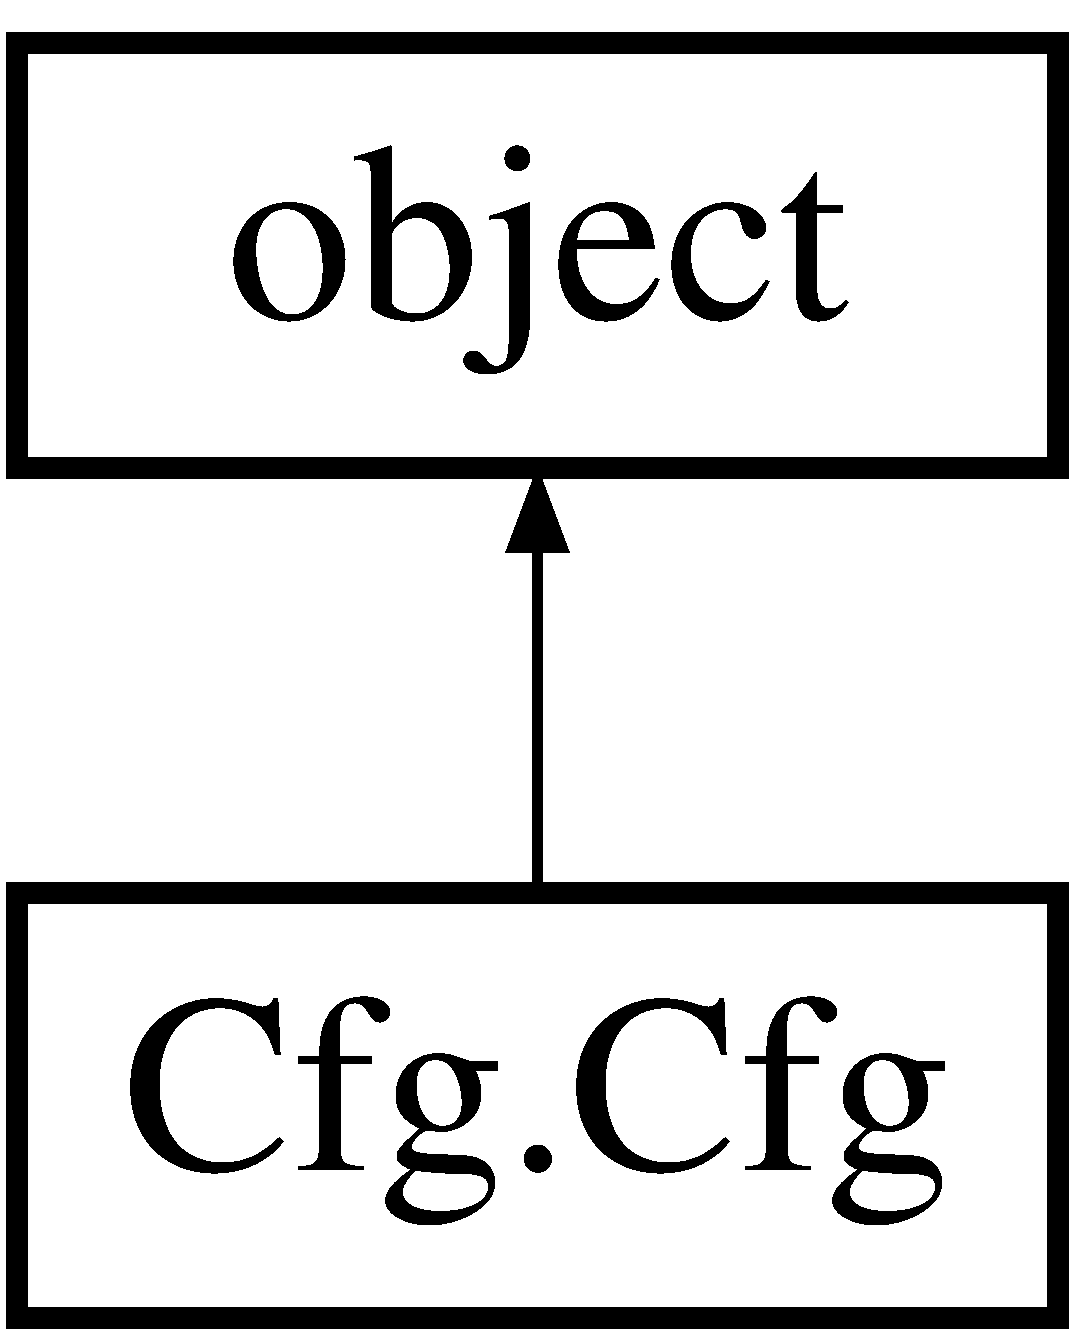
\includegraphics[height=2.000000cm]{classCfg_1_1Cfg}
\end{center}
\end{figure}
\subsection*{Public Member Functions}
\begin{DoxyCompactItemize}
\item 
def \hyperlink{classCfg_1_1Cfg_a2acaa0255752cdb04e3f69eff00f1381}{\-\_\-\-\_\-init\-\_\-\-\_\-}
\item 
def \hyperlink{classCfg_1_1Cfg_af9a1969ce93bfe8aa543a4b2a8626df1}{inc1}
\item 
def \hyperlink{classCfg_1_1Cfg_a043ba68c543f919f60beb34d752b7751}{inc}
\item 
def \hyperlink{classCfg_1_1Cfg_abb2fc147041866023b7f622196c16097}{getpath}
\item 
def \hyperlink{classCfg_1_1Cfg_afd2584b0327befb9f2988beecdb0726a}{getkeys}
\item 
def \hyperlink{classCfg_1_1Cfg_a5363b11ef74508fdbe33af91b70f128f}{subtree}
\item 
def \hyperlink{classCfg_1_1Cfg_a3c3e8b599dcc3db2424996cb5ab38216}{keyval}
\end{DoxyCompactItemize}
\subsection*{Public Attributes}
\begin{DoxyCompactItemize}
\item 
\hyperlink{classCfg_1_1Cfg_a150a4ddf8a1f91351f7600142fa71a28}{data}
\item 
\hyperlink{classCfg_1_1Cfg_a8f506e4846d887e584fffb80a3f12e11}{ipath}
\end{DoxyCompactItemize}
\subsection*{Static Public Attributes}
\begin{DoxyCompactItemize}
\item 
\hyperlink{classCfg_1_1Cfg_ac3e9afe1ab5766e019aae9bdbe3ce765}{follow} = True
\item 
int \hyperlink{classCfg_1_1Cfg_ab27ccaec7ea2ee59d0f233351389f250}{iseq} = 1
\end{DoxyCompactItemize}


\subsection{Detailed Description}
\begin{DoxyVerb}\
    Encapsultates looking up items in a config tree.\end{DoxyVerb}
 

\subsection{Constructor \& Destructor Documentation}
\hypertarget{classCfg_1_1Cfg_a2acaa0255752cdb04e3f69eff00f1381}{\index{Cfg\-::\-Cfg@{Cfg\-::\-Cfg}!\-\_\-\-\_\-init\-\_\-\-\_\-@{\-\_\-\-\_\-init\-\_\-\-\_\-}}
\index{\-\_\-\-\_\-init\-\_\-\-\_\-@{\-\_\-\-\_\-init\-\_\-\-\_\-}!Cfg::Cfg@{Cfg\-::\-Cfg}}
\subsubsection[{\-\_\-\-\_\-init\-\_\-\-\_\-}]{\setlength{\rightskip}{0pt plus 5cm}def Cfg.\-Cfg.\-\_\-\-\_\-init\-\_\-\-\_\- (
\begin{DoxyParamCaption}
\item[{}]{self, }
\item[{}]{f}
\end{DoxyParamCaption}
)}}\label{classCfg_1_1Cfg_a2acaa0255752cdb04e3f69eff00f1381}


\subsection{Member Function Documentation}
\hypertarget{classCfg_1_1Cfg_afd2584b0327befb9f2988beecdb0726a}{\index{Cfg\-::\-Cfg@{Cfg\-::\-Cfg}!getkeys@{getkeys}}
\index{getkeys@{getkeys}!Cfg::Cfg@{Cfg\-::\-Cfg}}
\subsubsection[{getkeys}]{\setlength{\rightskip}{0pt plus 5cm}def Cfg.\-Cfg.\-getkeys (
\begin{DoxyParamCaption}
\item[{}]{self, }
\item[{}]{lk, }
\item[{}]{ak, }
\item[{}]{rest}
\end{DoxyParamCaption}
)}}\label{classCfg_1_1Cfg_afd2584b0327befb9f2988beecdb0726a}
\hypertarget{classCfg_1_1Cfg_abb2fc147041866023b7f622196c16097}{\index{Cfg\-::\-Cfg@{Cfg\-::\-Cfg}!getpath@{getpath}}
\index{getpath@{getpath}!Cfg::Cfg@{Cfg\-::\-Cfg}}
\subsubsection[{getpath}]{\setlength{\rightskip}{0pt plus 5cm}def Cfg.\-Cfg.\-getpath (
\begin{DoxyParamCaption}
\item[{}]{self, }
\item[{}]{loc, }
\item[{}]{ak, }
\item[{}]{k1, }
\item[{}]{rest}
\end{DoxyParamCaption}
)}}\label{classCfg_1_1Cfg_abb2fc147041866023b7f622196c16097}
\hypertarget{classCfg_1_1Cfg_a043ba68c543f919f60beb34d752b7751}{\index{Cfg\-::\-Cfg@{Cfg\-::\-Cfg}!inc@{inc}}
\index{inc@{inc}!Cfg::Cfg@{Cfg\-::\-Cfg}}
\subsubsection[{inc}]{\setlength{\rightskip}{0pt plus 5cm}def Cfg.\-Cfg.\-inc (
\begin{DoxyParamCaption}
\item[{}]{self, }
\item[{}]{ak}
\end{DoxyParamCaption}
)}}\label{classCfg_1_1Cfg_a043ba68c543f919f60beb34d752b7751}
\hypertarget{classCfg_1_1Cfg_af9a1969ce93bfe8aa543a4b2a8626df1}{\index{Cfg\-::\-Cfg@{Cfg\-::\-Cfg}!inc1@{inc1}}
\index{inc1@{inc1}!Cfg::Cfg@{Cfg\-::\-Cfg}}
\subsubsection[{inc1}]{\setlength{\rightskip}{0pt plus 5cm}def Cfg.\-Cfg.\-inc1 (
\begin{DoxyParamCaption}
\item[{}]{self, }
\item[{}]{f}
\end{DoxyParamCaption}
)}}\label{classCfg_1_1Cfg_af9a1969ce93bfe8aa543a4b2a8626df1}
\hypertarget{classCfg_1_1Cfg_a3c3e8b599dcc3db2424996cb5ab38216}{\index{Cfg\-::\-Cfg@{Cfg\-::\-Cfg}!keyval@{keyval}}
\index{keyval@{keyval}!Cfg::Cfg@{Cfg\-::\-Cfg}}
\subsubsection[{keyval}]{\setlength{\rightskip}{0pt plus 5cm}def Cfg.\-Cfg.\-keyval (
\begin{DoxyParamCaption}
\item[{}]{self, }
\item[{}]{key}
\end{DoxyParamCaption}
)}}\label{classCfg_1_1Cfg_a3c3e8b599dcc3db2424996cb5ab38216}
\hypertarget{classCfg_1_1Cfg_a5363b11ef74508fdbe33af91b70f128f}{\index{Cfg\-::\-Cfg@{Cfg\-::\-Cfg}!subtree@{subtree}}
\index{subtree@{subtree}!Cfg::Cfg@{Cfg\-::\-Cfg}}
\subsubsection[{subtree}]{\setlength{\rightskip}{0pt plus 5cm}def Cfg.\-Cfg.\-subtree (
\begin{DoxyParamCaption}
\item[{}]{self, }
\item[{}]{key}
\end{DoxyParamCaption}
)}}\label{classCfg_1_1Cfg_a5363b11ef74508fdbe33af91b70f128f}


\subsection{Member Data Documentation}
\hypertarget{classCfg_1_1Cfg_a150a4ddf8a1f91351f7600142fa71a28}{\index{Cfg\-::\-Cfg@{Cfg\-::\-Cfg}!data@{data}}
\index{data@{data}!Cfg::Cfg@{Cfg\-::\-Cfg}}
\subsubsection[{data}]{\setlength{\rightskip}{0pt plus 5cm}Cfg.\-Cfg.\-data}}\label{classCfg_1_1Cfg_a150a4ddf8a1f91351f7600142fa71a28}
\hypertarget{classCfg_1_1Cfg_ac3e9afe1ab5766e019aae9bdbe3ce765}{\index{Cfg\-::\-Cfg@{Cfg\-::\-Cfg}!follow@{follow}}
\index{follow@{follow}!Cfg::Cfg@{Cfg\-::\-Cfg}}
\subsubsection[{follow}]{\setlength{\rightskip}{0pt plus 5cm}Cfg.\-Cfg.\-follow = True\hspace{0.3cm}{\ttfamily [static]}}}\label{classCfg_1_1Cfg_ac3e9afe1ab5766e019aae9bdbe3ce765}
\hypertarget{classCfg_1_1Cfg_a8f506e4846d887e584fffb80a3f12e11}{\index{Cfg\-::\-Cfg@{Cfg\-::\-Cfg}!ipath@{ipath}}
\index{ipath@{ipath}!Cfg::Cfg@{Cfg\-::\-Cfg}}
\subsubsection[{ipath}]{\setlength{\rightskip}{0pt plus 5cm}Cfg.\-Cfg.\-ipath}}\label{classCfg_1_1Cfg_a8f506e4846d887e584fffb80a3f12e11}
\hypertarget{classCfg_1_1Cfg_ab27ccaec7ea2ee59d0f233351389f250}{\index{Cfg\-::\-Cfg@{Cfg\-::\-Cfg}!iseq@{iseq}}
\index{iseq@{iseq}!Cfg::Cfg@{Cfg\-::\-Cfg}}
\subsubsection[{iseq}]{\setlength{\rightskip}{0pt plus 5cm}int Cfg.\-Cfg.\-iseq = 1\hspace{0.3cm}{\ttfamily [static]}}}\label{classCfg_1_1Cfg_ab27ccaec7ea2ee59d0f233351389f250}


The documentation for this class was generated from the following file\-:\begin{DoxyCompactItemize}
\item 
cli/owslave/\hyperlink{Cfg_8py}{Cfg.\-py}\end{DoxyCompactItemize}

\hypertarget{structconf__t}{\section{conf\-\_\-t Struct Reference}
\label{structconf__t}\index{conf\-\_\-t@{conf\-\_\-t}}
}


{\ttfamily \#include $<$types.\-h$>$}

\subsection*{Public Attributes}
\begin{DoxyCompactItemize}
\item 
\hyperlink{structpid__}{pid\-\_\-} \hyperlink{structconf__t_a5b8b9ea37a24902ea3d14c568b87b697}{pid} \mbox{[}\hyperlink{Uno__MultiWii__HardwarePlatform__Test_2types_8h_ac47ca0713353d3fc9435a4f208f6b9a3a5b01cce209659cf60a5b3464c9f2c3f6}{P\-I\-D\-I\-T\-E\-M\-S}\mbox{]}
\item 
uint8\-\_\-t \hyperlink{structconf__t_a729d503f293f1c992f48af2cff496201}{rc\-Rate8}
\item 
uint8\-\_\-t \hyperlink{structconf__t_a382b8e01b181ab2758fad613c4b7fbf8}{rc\-Expo8}
\item 
uint8\-\_\-t \hyperlink{structconf__t_a1b30852fb8b64e453bd1014196272e41}{roll\-Pitch\-Rate}
\item 
uint8\-\_\-t \hyperlink{structconf__t_ad1f6c9b09743466429c50f9fe37ca94c}{yaw\-Rate}
\item 
uint8\-\_\-t \hyperlink{structconf__t_a47cb9553b60e167b09e7665b146c28db}{dyn\-Thr\-P\-I\-D}
\item 
uint8\-\_\-t \hyperlink{structconf__t_a169d65d8c1acd6c71f0da3491199a046}{thr\-Mid8}
\item 
uint8\-\_\-t \hyperlink{structconf__t_ab7eb566eb3ac052eddb47db1327d4359}{thr\-Expo8}
\item 
int16\-\_\-t \hyperlink{structconf__t_ab122cdccc1b9b801849f925be1680054}{angle\-Trim} \mbox{[}2\mbox{]}
\item 
uint16\-\_\-t \hyperlink{structconf__t_a1442ab81807251b8fe263a6facf11ddb}{activate} \mbox{[}\hyperlink{Uno__MultiWii__HardwarePlatform__Test_2types_8h_a4485d04ca451246b6a81dd2799f83906ac581ba11d0375e47447fa2bbf22f570f}{C\-H\-E\-C\-K\-B\-O\-X\-I\-T\-E\-M\-S}\mbox{]}
\item 
uint8\-\_\-t \hyperlink{structconf__t_aa09f9c422c9a09d30dda6fe642f52918}{power\-Trigger1}
\item 
\hyperlink{structservo__conf__}{servo\-\_\-conf\-\_\-} \hyperlink{structconf__t_a34f0731ed86e0e324a4f8fa7459f9008}{servo\-Conf} \mbox{[}8\mbox{]}
\item 
int16\-\_\-t \hyperlink{structconf__t_a38afc04bc65eb117eb45c9bc0c46d3c5}{minthrottle}
\item 
uint8\-\_\-t \hyperlink{structconf__t_a9d2871d7decd958de75b19a372955045}{checksum}
\end{DoxyCompactItemize}


\subsection{Member Data Documentation}
\hypertarget{structconf__t_a1442ab81807251b8fe263a6facf11ddb}{\index{conf\-\_\-t@{conf\-\_\-t}!activate@{activate}}
\index{activate@{activate}!conf_t@{conf\-\_\-t}}
\subsubsection[{activate}]{\setlength{\rightskip}{0pt plus 5cm}uint16\-\_\-t conf\-\_\-t\-::activate}}\label{structconf__t_a1442ab81807251b8fe263a6facf11ddb}
\hypertarget{structconf__t_ab122cdccc1b9b801849f925be1680054}{\index{conf\-\_\-t@{conf\-\_\-t}!angle\-Trim@{angle\-Trim}}
\index{angle\-Trim@{angle\-Trim}!conf_t@{conf\-\_\-t}}
\subsubsection[{angle\-Trim}]{\setlength{\rightskip}{0pt plus 5cm}int16\-\_\-t conf\-\_\-t\-::angle\-Trim}}\label{structconf__t_ab122cdccc1b9b801849f925be1680054}
\hypertarget{structconf__t_a9d2871d7decd958de75b19a372955045}{\index{conf\-\_\-t@{conf\-\_\-t}!checksum@{checksum}}
\index{checksum@{checksum}!conf_t@{conf\-\_\-t}}
\subsubsection[{checksum}]{\setlength{\rightskip}{0pt plus 5cm}uint8\-\_\-t conf\-\_\-t\-::checksum}}\label{structconf__t_a9d2871d7decd958de75b19a372955045}
\hypertarget{structconf__t_a47cb9553b60e167b09e7665b146c28db}{\index{conf\-\_\-t@{conf\-\_\-t}!dyn\-Thr\-P\-I\-D@{dyn\-Thr\-P\-I\-D}}
\index{dyn\-Thr\-P\-I\-D@{dyn\-Thr\-P\-I\-D}!conf_t@{conf\-\_\-t}}
\subsubsection[{dyn\-Thr\-P\-I\-D}]{\setlength{\rightskip}{0pt plus 5cm}uint8\-\_\-t conf\-\_\-t\-::dyn\-Thr\-P\-I\-D}}\label{structconf__t_a47cb9553b60e167b09e7665b146c28db}
\hypertarget{structconf__t_a38afc04bc65eb117eb45c9bc0c46d3c5}{\index{conf\-\_\-t@{conf\-\_\-t}!minthrottle@{minthrottle}}
\index{minthrottle@{minthrottle}!conf_t@{conf\-\_\-t}}
\subsubsection[{minthrottle}]{\setlength{\rightskip}{0pt plus 5cm}int16\-\_\-t conf\-\_\-t\-::minthrottle}}\label{structconf__t_a38afc04bc65eb117eb45c9bc0c46d3c5}
\hypertarget{structconf__t_a5b8b9ea37a24902ea3d14c568b87b697}{\index{conf\-\_\-t@{conf\-\_\-t}!pid@{pid}}
\index{pid@{pid}!conf_t@{conf\-\_\-t}}
\subsubsection[{pid}]{\setlength{\rightskip}{0pt plus 5cm}{\bf pid\-\_\-} conf\-\_\-t\-::pid}}\label{structconf__t_a5b8b9ea37a24902ea3d14c568b87b697}
\hypertarget{structconf__t_aa09f9c422c9a09d30dda6fe642f52918}{\index{conf\-\_\-t@{conf\-\_\-t}!power\-Trigger1@{power\-Trigger1}}
\index{power\-Trigger1@{power\-Trigger1}!conf_t@{conf\-\_\-t}}
\subsubsection[{power\-Trigger1}]{\setlength{\rightskip}{0pt plus 5cm}uint8\-\_\-t conf\-\_\-t\-::power\-Trigger1}}\label{structconf__t_aa09f9c422c9a09d30dda6fe642f52918}
\hypertarget{structconf__t_a382b8e01b181ab2758fad613c4b7fbf8}{\index{conf\-\_\-t@{conf\-\_\-t}!rc\-Expo8@{rc\-Expo8}}
\index{rc\-Expo8@{rc\-Expo8}!conf_t@{conf\-\_\-t}}
\subsubsection[{rc\-Expo8}]{\setlength{\rightskip}{0pt plus 5cm}uint8\-\_\-t conf\-\_\-t\-::rc\-Expo8}}\label{structconf__t_a382b8e01b181ab2758fad613c4b7fbf8}
\hypertarget{structconf__t_a729d503f293f1c992f48af2cff496201}{\index{conf\-\_\-t@{conf\-\_\-t}!rc\-Rate8@{rc\-Rate8}}
\index{rc\-Rate8@{rc\-Rate8}!conf_t@{conf\-\_\-t}}
\subsubsection[{rc\-Rate8}]{\setlength{\rightskip}{0pt plus 5cm}uint8\-\_\-t conf\-\_\-t\-::rc\-Rate8}}\label{structconf__t_a729d503f293f1c992f48af2cff496201}
\hypertarget{structconf__t_a1b30852fb8b64e453bd1014196272e41}{\index{conf\-\_\-t@{conf\-\_\-t}!roll\-Pitch\-Rate@{roll\-Pitch\-Rate}}
\index{roll\-Pitch\-Rate@{roll\-Pitch\-Rate}!conf_t@{conf\-\_\-t}}
\subsubsection[{roll\-Pitch\-Rate}]{\setlength{\rightskip}{0pt plus 5cm}uint8\-\_\-t conf\-\_\-t\-::roll\-Pitch\-Rate}}\label{structconf__t_a1b30852fb8b64e453bd1014196272e41}
\hypertarget{structconf__t_a34f0731ed86e0e324a4f8fa7459f9008}{\index{conf\-\_\-t@{conf\-\_\-t}!servo\-Conf@{servo\-Conf}}
\index{servo\-Conf@{servo\-Conf}!conf_t@{conf\-\_\-t}}
\subsubsection[{servo\-Conf}]{\setlength{\rightskip}{0pt plus 5cm}{\bf servo\-\_\-conf\-\_\-} conf\-\_\-t\-::servo\-Conf}}\label{structconf__t_a34f0731ed86e0e324a4f8fa7459f9008}
\hypertarget{structconf__t_ab7eb566eb3ac052eddb47db1327d4359}{\index{conf\-\_\-t@{conf\-\_\-t}!thr\-Expo8@{thr\-Expo8}}
\index{thr\-Expo8@{thr\-Expo8}!conf_t@{conf\-\_\-t}}
\subsubsection[{thr\-Expo8}]{\setlength{\rightskip}{0pt plus 5cm}uint8\-\_\-t conf\-\_\-t\-::thr\-Expo8}}\label{structconf__t_ab7eb566eb3ac052eddb47db1327d4359}
\hypertarget{structconf__t_a169d65d8c1acd6c71f0da3491199a046}{\index{conf\-\_\-t@{conf\-\_\-t}!thr\-Mid8@{thr\-Mid8}}
\index{thr\-Mid8@{thr\-Mid8}!conf_t@{conf\-\_\-t}}
\subsubsection[{thr\-Mid8}]{\setlength{\rightskip}{0pt plus 5cm}uint8\-\_\-t conf\-\_\-t\-::thr\-Mid8}}\label{structconf__t_a169d65d8c1acd6c71f0da3491199a046}
\hypertarget{structconf__t_ad1f6c9b09743466429c50f9fe37ca94c}{\index{conf\-\_\-t@{conf\-\_\-t}!yaw\-Rate@{yaw\-Rate}}
\index{yaw\-Rate@{yaw\-Rate}!conf_t@{conf\-\_\-t}}
\subsubsection[{yaw\-Rate}]{\setlength{\rightskip}{0pt plus 5cm}uint8\-\_\-t conf\-\_\-t\-::yaw\-Rate}}\label{structconf__t_ad1f6c9b09743466429c50f9fe37ca94c}


The documentation for this struct was generated from the following file\-:\begin{DoxyCompactItemize}
\item 
Multi\-Wii\-\_\-2\-\_\-4/\-Multi\-Wii/\hyperlink{MultiWii__2__4_2MultiWii_2types_8h}{types.\-h}\end{DoxyCompactItemize}

\hypertarget{structconfig__crypto}{\section{config\-\_\-crypto Struct Reference}
\label{structconfig__crypto}\index{config\-\_\-crypto@{config\-\_\-crypto}}
}


{\ttfamily \#include $<$dev\-\_\-data.\-h$>$}

\subsection*{Public Attributes}
\begin{DoxyCompactItemize}
\item 
uint32\-\_\-t \hyperlink{structconfig__crypto_aab0644bb16c2a693422840da497ec2d4}{key} \mbox{[}4\mbox{]}
\end{DoxyCompactItemize}


\subsection{Member Data Documentation}
\hypertarget{structconfig__crypto_aab0644bb16c2a693422840da497ec2d4}{\index{config\-\_\-crypto@{config\-\_\-crypto}!key@{key}}
\index{key@{key}!config_crypto@{config\-\_\-crypto}}
\subsubsection[{key}]{\setlength{\rightskip}{0pt plus 5cm}uint32\-\_\-t config\-\_\-crypto\-::key\mbox{[}4\mbox{]}}}\label{structconfig__crypto_aab0644bb16c2a693422840da497ec2d4}


The documentation for this struct was generated from the following file\-:\begin{DoxyCompactItemize}
\item 
cli/owslave/\hyperlink{dev__data_8h}{dev\-\_\-data.\-h}\end{DoxyCompactItemize}

\hypertarget{structconfig__euid}{\section{config\-\_\-euid Struct Reference}
\label{structconfig__euid}\index{config\-\_\-euid@{config\-\_\-euid}}
}


{\ttfamily \#include $<$dev\-\_\-data.\-h$>$}

\subsection*{Public Attributes}
\begin{DoxyCompactItemize}
\item 
uint8\-\_\-t \hyperlink{structconfig__euid_a67bc2965559458837b905fb32ca769b6}{id} \mbox{[}\hyperlink{dev__data_8h_af380621fde5834c453e4b42ec0f813fb}{E\-U\-I\-D\-\_\-\-L\-E\-N}\mbox{]}
\end{DoxyCompactItemize}


\subsection{Member Data Documentation}
\hypertarget{structconfig__euid_a67bc2965559458837b905fb32ca769b6}{\index{config\-\_\-euid@{config\-\_\-euid}!id@{id}}
\index{id@{id}!config_euid@{config\-\_\-euid}}
\subsubsection[{id}]{\setlength{\rightskip}{0pt plus 5cm}uint8\-\_\-t config\-\_\-euid\-::id\mbox{[}{\bf E\-U\-I\-D\-\_\-\-L\-E\-N}\mbox{]}}}\label{structconfig__euid_a67bc2965559458837b905fb32ca769b6}


The documentation for this struct was generated from the following file\-:\begin{DoxyCompactItemize}
\item 
cli/owslave/\hyperlink{dev__data_8h}{dev\-\_\-data.\-h}\end{DoxyCompactItemize}

\hypertarget{structconfig__loader}{\section{config\-\_\-loader Struct Reference}
\label{structconfig__loader}\index{config\-\_\-loader@{config\-\_\-loader}}
}


{\ttfamily \#include $<$dev\-\_\-data.\-h$>$}

\subsection*{Public Attributes}
\begin{DoxyCompactItemize}
\item 
uint16\-\_\-t \hyperlink{structconfig__loader_af965038b455ac61d82f074b422e04d81}{loader}
\item 
uint16\-\_\-t \hyperlink{structconfig__loader_a2061ae71465754796a2fb37c0aca18a6}{endp}
\item 
uint16\-\_\-t \hyperlink{structconfig__loader_a02a14b09e5390cc08f2727f2a6b270b6}{crc}
\end{DoxyCompactItemize}


\subsection{Member Data Documentation}
\hypertarget{structconfig__loader_a02a14b09e5390cc08f2727f2a6b270b6}{\index{config\-\_\-loader@{config\-\_\-loader}!crc@{crc}}
\index{crc@{crc}!config_loader@{config\-\_\-loader}}
\subsubsection[{crc}]{\setlength{\rightskip}{0pt plus 5cm}uint16\-\_\-t config\-\_\-loader\-::crc}}\label{structconfig__loader_a02a14b09e5390cc08f2727f2a6b270b6}
\hypertarget{structconfig__loader_a2061ae71465754796a2fb37c0aca18a6}{\index{config\-\_\-loader@{config\-\_\-loader}!endp@{endp}}
\index{endp@{endp}!config_loader@{config\-\_\-loader}}
\subsubsection[{endp}]{\setlength{\rightskip}{0pt plus 5cm}uint16\-\_\-t config\-\_\-loader\-::endp}}\label{structconfig__loader_a2061ae71465754796a2fb37c0aca18a6}
\hypertarget{structconfig__loader_af965038b455ac61d82f074b422e04d81}{\index{config\-\_\-loader@{config\-\_\-loader}!loader@{loader}}
\index{loader@{loader}!config_loader@{config\-\_\-loader}}
\subsubsection[{loader}]{\setlength{\rightskip}{0pt plus 5cm}uint16\-\_\-t config\-\_\-loader\-::loader}}\label{structconfig__loader_af965038b455ac61d82f074b422e04d81}


The documentation for this struct was generated from the following file\-:\begin{DoxyCompactItemize}
\item 
cli/owslave/\hyperlink{dev__data_8h}{dev\-\_\-data.\-h}\end{DoxyCompactItemize}

\hypertarget{structconfig__owid}{\section{config\-\_\-owid Struct Reference}
\label{structconfig__owid}\index{config\-\_\-owid@{config\-\_\-owid}}
}


{\ttfamily \#include $<$dev\-\_\-data.\-h$>$}

\subsection*{Public Attributes}
\begin{DoxyCompactItemize}
\item 
uint8\-\_\-t \hyperlink{structconfig__owid_a923d52b3e8b0ddd213df86cd5a6fc760}{type}
\item 
uint8\-\_\-t \hyperlink{structconfig__owid_abfab5874606cb60963c2d5817fe444e8}{serial} \mbox{[}6\mbox{]}
\item 
uint8\-\_\-t \hyperlink{structconfig__owid_af628a17297757d5927b23e4e9993261a}{crc}
\end{DoxyCompactItemize}


\subsection{Member Data Documentation}
\hypertarget{structconfig__owid_af628a17297757d5927b23e4e9993261a}{\index{config\-\_\-owid@{config\-\_\-owid}!crc@{crc}}
\index{crc@{crc}!config_owid@{config\-\_\-owid}}
\subsubsection[{crc}]{\setlength{\rightskip}{0pt plus 5cm}uint8\-\_\-t config\-\_\-owid\-::crc}}\label{structconfig__owid_af628a17297757d5927b23e4e9993261a}
\hypertarget{structconfig__owid_abfab5874606cb60963c2d5817fe444e8}{\index{config\-\_\-owid@{config\-\_\-owid}!serial@{serial}}
\index{serial@{serial}!config_owid@{config\-\_\-owid}}
\subsubsection[{serial}]{\setlength{\rightskip}{0pt plus 5cm}uint8\-\_\-t config\-\_\-owid\-::serial\mbox{[}6\mbox{]}}}\label{structconfig__owid_abfab5874606cb60963c2d5817fe444e8}
\hypertarget{structconfig__owid_a923d52b3e8b0ddd213df86cd5a6fc760}{\index{config\-\_\-owid@{config\-\_\-owid}!type@{type}}
\index{type@{type}!config_owid@{config\-\_\-owid}}
\subsubsection[{type}]{\setlength{\rightskip}{0pt plus 5cm}uint8\-\_\-t config\-\_\-owid\-::type}}\label{structconfig__owid_a923d52b3e8b0ddd213df86cd5a6fc760}


The documentation for this struct was generated from the following file\-:\begin{DoxyCompactItemize}
\item 
cli/owslave/\hyperlink{dev__data_8h}{dev\-\_\-data.\-h}\end{DoxyCompactItemize}

\hypertarget{structconfig__rf12}{\section{config\-\_\-rf12 Struct Reference}
\label{structconfig__rf12}\index{config\-\_\-rf12@{config\-\_\-rf12}}
}


{\ttfamily \#include $<$dev\-\_\-data.\-h$>$}

\subsection*{Public Attributes}
\begin{DoxyCompactItemize}
\item 
unsigned int \hyperlink{structconfig__rf12_abb4aae82e8879f73368fa8d94145b715}{band}\-:2
\item 
unsigned int \hyperlink{structconfig__rf12_a217f695af8276c1da733e13bbdeab5a5}{collect}\-:1
\item 
unsigned int \hyperlink{structconfig__rf12_a9389bb8256b99c8743c6ab0d0b9d84f0}{node}\-:5
\item 
uint8\-\_\-t \hyperlink{structconfig__rf12_a6993b16dd675ec59f3747ed5f9510de8}{group}
\item 
uint8\-\_\-t \hyperlink{structconfig__rf12_a43fcf6110e6a133c6982081885f27de9}{speed}
\end{DoxyCompactItemize}


\subsection{Member Data Documentation}
\hypertarget{structconfig__rf12_abb4aae82e8879f73368fa8d94145b715}{\index{config\-\_\-rf12@{config\-\_\-rf12}!band@{band}}
\index{band@{band}!config_rf12@{config\-\_\-rf12}}
\subsubsection[{band}]{\setlength{\rightskip}{0pt plus 5cm}unsigned int config\-\_\-rf12\-::band}}\label{structconfig__rf12_abb4aae82e8879f73368fa8d94145b715}
\hypertarget{structconfig__rf12_a217f695af8276c1da733e13bbdeab5a5}{\index{config\-\_\-rf12@{config\-\_\-rf12}!collect@{collect}}
\index{collect@{collect}!config_rf12@{config\-\_\-rf12}}
\subsubsection[{collect}]{\setlength{\rightskip}{0pt plus 5cm}unsigned int config\-\_\-rf12\-::collect}}\label{structconfig__rf12_a217f695af8276c1da733e13bbdeab5a5}
\hypertarget{structconfig__rf12_a6993b16dd675ec59f3747ed5f9510de8}{\index{config\-\_\-rf12@{config\-\_\-rf12}!group@{group}}
\index{group@{group}!config_rf12@{config\-\_\-rf12}}
\subsubsection[{group}]{\setlength{\rightskip}{0pt plus 5cm}uint8\-\_\-t config\-\_\-rf12\-::group}}\label{structconfig__rf12_a6993b16dd675ec59f3747ed5f9510de8}
\hypertarget{structconfig__rf12_a9389bb8256b99c8743c6ab0d0b9d84f0}{\index{config\-\_\-rf12@{config\-\_\-rf12}!node@{node}}
\index{node@{node}!config_rf12@{config\-\_\-rf12}}
\subsubsection[{node}]{\setlength{\rightskip}{0pt plus 5cm}unsigned int config\-\_\-rf12\-::node}}\label{structconfig__rf12_a9389bb8256b99c8743c6ab0d0b9d84f0}
\hypertarget{structconfig__rf12_a43fcf6110e6a133c6982081885f27de9}{\index{config\-\_\-rf12@{config\-\_\-rf12}!speed@{speed}}
\index{speed@{speed}!config_rf12@{config\-\_\-rf12}}
\subsubsection[{speed}]{\setlength{\rightskip}{0pt plus 5cm}uint8\-\_\-t config\-\_\-rf12\-::speed}}\label{structconfig__rf12_a43fcf6110e6a133c6982081885f27de9}


The documentation for this struct was generated from the following file\-:\begin{DoxyCompactItemize}
\item 
cli/owslave/\hyperlink{dev__data_8h}{dev\-\_\-data.\-h}\end{DoxyCompactItemize}

\hypertarget{structdfsan__label__info}{\section{dfsan\-\_\-label\-\_\-info Struct Reference}
\label{structdfsan__label__info}\index{dfsan\-\_\-label\-\_\-info@{dfsan\-\_\-label\-\_\-info}}
}


{\ttfamily \#include $<$dfsan\-\_\-interface.\-h$>$}

\subsection*{Public Attributes}
\begin{DoxyCompactItemize}
\item 
\hyperlink{dfsan__interface_8h_a687a0bc144baaef2e10771b604c1ac75}{dfsan\-\_\-label} \hyperlink{structdfsan__label__info_a82901a96164283d57c24275e2d3a7ead}{l1}
\item 
\hyperlink{dfsan__interface_8h_a687a0bc144baaef2e10771b604c1ac75}{dfsan\-\_\-label} \hyperlink{structdfsan__label__info_a6b9bf4180217f8f3d3fd62ebfbe3e3fd}{l2}
\item 
const char $\ast$ \hyperlink{structdfsan__label__info_a8633e0763c04793542a3c2d4875a84c8}{desc}
\item 
void $\ast$ \hyperlink{structdfsan__label__info_a66abef76ed966704b1b87bb07ad205a6}{userdata}
\end{DoxyCompactItemize}


\subsection{Detailed Description}
Stores information associated with a specific label identifier. A label may be a base label created using dfsan\-\_\-create\-\_\-label, with associated text description and user data, or an automatically created union label, which represents the union of two label identifiers (which may themselves be base or union labels). 

\subsection{Member Data Documentation}
\hypertarget{structdfsan__label__info_a8633e0763c04793542a3c2d4875a84c8}{\index{dfsan\-\_\-label\-\_\-info@{dfsan\-\_\-label\-\_\-info}!desc@{desc}}
\index{desc@{desc}!dfsan_label_info@{dfsan\-\_\-label\-\_\-info}}
\subsubsection[{desc}]{\setlength{\rightskip}{0pt plus 5cm}const char$\ast$ dfsan\-\_\-label\-\_\-info\-::desc}}\label{structdfsan__label__info_a8633e0763c04793542a3c2d4875a84c8}
\hypertarget{structdfsan__label__info_a82901a96164283d57c24275e2d3a7ead}{\index{dfsan\-\_\-label\-\_\-info@{dfsan\-\_\-label\-\_\-info}!l1@{l1}}
\index{l1@{l1}!dfsan_label_info@{dfsan\-\_\-label\-\_\-info}}
\subsubsection[{l1}]{\setlength{\rightskip}{0pt plus 5cm}{\bf dfsan\-\_\-label} dfsan\-\_\-label\-\_\-info\-::l1}}\label{structdfsan__label__info_a82901a96164283d57c24275e2d3a7ead}
\hypertarget{structdfsan__label__info_a6b9bf4180217f8f3d3fd62ebfbe3e3fd}{\index{dfsan\-\_\-label\-\_\-info@{dfsan\-\_\-label\-\_\-info}!l2@{l2}}
\index{l2@{l2}!dfsan_label_info@{dfsan\-\_\-label\-\_\-info}}
\subsubsection[{l2}]{\setlength{\rightskip}{0pt plus 5cm}{\bf dfsan\-\_\-label} dfsan\-\_\-label\-\_\-info\-::l2}}\label{structdfsan__label__info_a6b9bf4180217f8f3d3fd62ebfbe3e3fd}
\hypertarget{structdfsan__label__info_a66abef76ed966704b1b87bb07ad205a6}{\index{dfsan\-\_\-label\-\_\-info@{dfsan\-\_\-label\-\_\-info}!userdata@{userdata}}
\index{userdata@{userdata}!dfsan_label_info@{dfsan\-\_\-label\-\_\-info}}
\subsubsection[{userdata}]{\setlength{\rightskip}{0pt plus 5cm}void$\ast$ dfsan\-\_\-label\-\_\-info\-::userdata}}\label{structdfsan__label__info_a66abef76ed966704b1b87bb07ad205a6}


The documentation for this struct was generated from the following file\-:\begin{DoxyCompactItemize}
\item 
oclint-\/0.\-10.\-3/lib/clang/3.\-8.\-0/include/sanitizer/\hyperlink{dfsan__interface_8h}{dfsan\-\_\-interface.\-h}\end{DoxyCompactItemize}

\hypertarget{structdrcNetComStruct}{\section{drc\-Net\-Com\-Struct Struct Reference}
\label{structdrcNetComStruct}\index{drc\-Net\-Com\-Struct@{drc\-Net\-Com\-Struct}}
}


{\ttfamily \#include $<$drc\-Net\-Cmd.\-h$>$}

\subsection*{Public Attributes}
\begin{DoxyCompactItemize}
\item 
uint32\-\_\-t \hyperlink{structdrcNetComStruct_a71861aef3f288842ffaad1f4ad3830d8}{pin}
\item 
uint32\-\_\-t \hyperlink{structdrcNetComStruct_abffbc20e01219a8f2850a53d2ba4d4ce}{cmd}
\item 
uint32\-\_\-t \hyperlink{structdrcNetComStruct_a728fa1681488d72c89e49c1b019e582e}{data}
\end{DoxyCompactItemize}


\subsection{Member Data Documentation}
\hypertarget{structdrcNetComStruct_abffbc20e01219a8f2850a53d2ba4d4ce}{\index{drc\-Net\-Com\-Struct@{drc\-Net\-Com\-Struct}!cmd@{cmd}}
\index{cmd@{cmd}!drcNetComStruct@{drc\-Net\-Com\-Struct}}
\subsubsection[{cmd}]{\setlength{\rightskip}{0pt plus 5cm}uint32\-\_\-t drc\-Net\-Com\-Struct\-::cmd}}\label{structdrcNetComStruct_abffbc20e01219a8f2850a53d2ba4d4ce}
\hypertarget{structdrcNetComStruct_a728fa1681488d72c89e49c1b019e582e}{\index{drc\-Net\-Com\-Struct@{drc\-Net\-Com\-Struct}!data@{data}}
\index{data@{data}!drcNetComStruct@{drc\-Net\-Com\-Struct}}
\subsubsection[{data}]{\setlength{\rightskip}{0pt plus 5cm}uint32\-\_\-t drc\-Net\-Com\-Struct\-::data}}\label{structdrcNetComStruct_a728fa1681488d72c89e49c1b019e582e}
\hypertarget{structdrcNetComStruct_a71861aef3f288842ffaad1f4ad3830d8}{\index{drc\-Net\-Com\-Struct@{drc\-Net\-Com\-Struct}!pin@{pin}}
\index{pin@{pin}!drcNetComStruct@{drc\-Net\-Com\-Struct}}
\subsubsection[{pin}]{\setlength{\rightskip}{0pt plus 5cm}uint32\-\_\-t drc\-Net\-Com\-Struct\-::pin}}\label{structdrcNetComStruct_a71861aef3f288842ffaad1f4ad3830d8}


The documentation for this struct was generated from the following file\-:\begin{DoxyCompactItemize}
\item 
wiring\-Pi/wiring\-Pi\-D/\hyperlink{drcNetCmd_8h}{drc\-Net\-Cmd.\-h}\end{DoxyCompactItemize}

\hypertarget{structextensionFunctionStruct}{\section{extension\-Function\-Struct Struct Reference}
\label{structextensionFunctionStruct}\index{extension\-Function\-Struct@{extension\-Function\-Struct}}
}
\subsection*{Public Attributes}
\begin{DoxyCompactItemize}
\item 
const char $\ast$ \hyperlink{structextensionFunctionStruct_a39d212429eefaa68d2680b50cb538b95}{name}
\item 
int($\ast$ \hyperlink{structextensionFunctionStruct_aa562f2602daa10ee7edc6b43ee8e9d71}{function} )(char $\ast$prog\-Name, int pin\-Base, char $\ast$params)
\end{DoxyCompactItemize}


\subsection{Member Data Documentation}
\hypertarget{structextensionFunctionStruct_aa562f2602daa10ee7edc6b43ee8e9d71}{\index{extension\-Function\-Struct@{extension\-Function\-Struct}!function@{function}}
\index{function@{function}!extensionFunctionStruct@{extension\-Function\-Struct}}
\subsubsection[{function}]{\setlength{\rightskip}{0pt plus 5cm}int($\ast$ extension\-Function\-Struct\-::function)(char $\ast$prog\-Name, int pin\-Base, char $\ast$params)}}\label{structextensionFunctionStruct_aa562f2602daa10ee7edc6b43ee8e9d71}
\hypertarget{structextensionFunctionStruct_a39d212429eefaa68d2680b50cb538b95}{\index{extension\-Function\-Struct@{extension\-Function\-Struct}!name@{name}}
\index{name@{name}!extensionFunctionStruct@{extension\-Function\-Struct}}
\subsubsection[{name}]{\setlength{\rightskip}{0pt plus 5cm}const char$\ast$ extension\-Function\-Struct\-::name}}\label{structextensionFunctionStruct_a39d212429eefaa68d2680b50cb538b95}


The documentation for this struct was generated from the following file\-:\begin{DoxyCompactItemize}
\item 
wiring\-Pi/wiring\-Pi/\hyperlink{wpiExtensions_8c}{wpi\-Extensions.\-c}\end{DoxyCompactItemize}

\hypertarget{structflags__struct__t}{\section{flags\-\_\-struct\-\_\-t Struct Reference}
\label{structflags__struct__t}\index{flags\-\_\-struct\-\_\-t@{flags\-\_\-struct\-\_\-t}}
}


{\ttfamily \#include $<$types.\-h$>$}

\subsection*{Public Attributes}
\begin{DoxyCompactItemize}
\item 
uint8\-\_\-t \hyperlink{structflags__struct__t_ab9097ddf6e1c1f3b12c17d903fe79437}{O\-K\-\_\-\-T\-O\-\_\-\-A\-R\-M}\-:1
\item 
uint8\-\_\-t \hyperlink{structflags__struct__t_ab012bd0f8430dadf5a9fdb124d752ace}{A\-R\-M\-E\-D}\-:1
\item 
uint8\-\_\-t \hyperlink{structflags__struct__t_af63430c14fd3b8cc45528fbce15bdaaa}{A\-C\-C\-\_\-\-C\-A\-L\-I\-B\-R\-A\-T\-E\-D}\-:1
\item 
uint8\-\_\-t \hyperlink{structflags__struct__t_a9dbf1f95e665583008f461414c353906}{A\-N\-G\-L\-E\-\_\-\-M\-O\-D\-E}\-:1
\item 
uint8\-\_\-t \hyperlink{structflags__struct__t_a4cb9cf704a153b21bab1a529ada99da3}{H\-O\-R\-I\-Z\-O\-N\-\_\-\-M\-O\-D\-E}\-:1
\item 
uint8\-\_\-t \hyperlink{structflags__struct__t_ae6f20ef363a74e51f6b092f48727660a}{M\-A\-G\-\_\-\-M\-O\-D\-E}\-:1
\item 
uint8\-\_\-t \hyperlink{structflags__struct__t_a8d457097d5a1d3fa9bf1f56ef48c6acc}{B\-A\-R\-O\-\_\-\-M\-O\-D\-E}\-:1
\item 
uint8\-\_\-t \hyperlink{structflags__struct__t_a897b15ddbc69e00652f3444f7f1f4217}{S\-M\-A\-L\-L\-\_\-\-A\-N\-G\-L\-E\-S\-\_\-25}\-:1
\item 
uint8\-\_\-t \hyperlink{structflags__struct__t_a26b787cfd58cba6d8851d9f63d07a007}{G\-P\-S\-\_\-mode}\-: 2
\end{DoxyCompactItemize}


\subsection{Member Data Documentation}
\hypertarget{structflags__struct__t_af63430c14fd3b8cc45528fbce15bdaaa}{\index{flags\-\_\-struct\-\_\-t@{flags\-\_\-struct\-\_\-t}!A\-C\-C\-\_\-\-C\-A\-L\-I\-B\-R\-A\-T\-E\-D@{A\-C\-C\-\_\-\-C\-A\-L\-I\-B\-R\-A\-T\-E\-D}}
\index{A\-C\-C\-\_\-\-C\-A\-L\-I\-B\-R\-A\-T\-E\-D@{A\-C\-C\-\_\-\-C\-A\-L\-I\-B\-R\-A\-T\-E\-D}!flags_struct_t@{flags\-\_\-struct\-\_\-t}}
\subsubsection[{A\-C\-C\-\_\-\-C\-A\-L\-I\-B\-R\-A\-T\-E\-D}]{\setlength{\rightskip}{0pt plus 5cm}uint8\-\_\-t flags\-\_\-struct\-\_\-t\-::\-A\-C\-C\-\_\-\-C\-A\-L\-I\-B\-R\-A\-T\-E\-D}}\label{structflags__struct__t_af63430c14fd3b8cc45528fbce15bdaaa}
\hypertarget{structflags__struct__t_a9dbf1f95e665583008f461414c353906}{\index{flags\-\_\-struct\-\_\-t@{flags\-\_\-struct\-\_\-t}!A\-N\-G\-L\-E\-\_\-\-M\-O\-D\-E@{A\-N\-G\-L\-E\-\_\-\-M\-O\-D\-E}}
\index{A\-N\-G\-L\-E\-\_\-\-M\-O\-D\-E@{A\-N\-G\-L\-E\-\_\-\-M\-O\-D\-E}!flags_struct_t@{flags\-\_\-struct\-\_\-t}}
\subsubsection[{A\-N\-G\-L\-E\-\_\-\-M\-O\-D\-E}]{\setlength{\rightskip}{0pt plus 5cm}uint8\-\_\-t flags\-\_\-struct\-\_\-t\-::\-A\-N\-G\-L\-E\-\_\-\-M\-O\-D\-E}}\label{structflags__struct__t_a9dbf1f95e665583008f461414c353906}
\hypertarget{structflags__struct__t_ab012bd0f8430dadf5a9fdb124d752ace}{\index{flags\-\_\-struct\-\_\-t@{flags\-\_\-struct\-\_\-t}!A\-R\-M\-E\-D@{A\-R\-M\-E\-D}}
\index{A\-R\-M\-E\-D@{A\-R\-M\-E\-D}!flags_struct_t@{flags\-\_\-struct\-\_\-t}}
\subsubsection[{A\-R\-M\-E\-D}]{\setlength{\rightskip}{0pt plus 5cm}uint8\-\_\-t flags\-\_\-struct\-\_\-t\-::\-A\-R\-M\-E\-D}}\label{structflags__struct__t_ab012bd0f8430dadf5a9fdb124d752ace}
\hypertarget{structflags__struct__t_a8d457097d5a1d3fa9bf1f56ef48c6acc}{\index{flags\-\_\-struct\-\_\-t@{flags\-\_\-struct\-\_\-t}!B\-A\-R\-O\-\_\-\-M\-O\-D\-E@{B\-A\-R\-O\-\_\-\-M\-O\-D\-E}}
\index{B\-A\-R\-O\-\_\-\-M\-O\-D\-E@{B\-A\-R\-O\-\_\-\-M\-O\-D\-E}!flags_struct_t@{flags\-\_\-struct\-\_\-t}}
\subsubsection[{B\-A\-R\-O\-\_\-\-M\-O\-D\-E}]{\setlength{\rightskip}{0pt plus 5cm}uint8\-\_\-t flags\-\_\-struct\-\_\-t\-::\-B\-A\-R\-O\-\_\-\-M\-O\-D\-E}}\label{structflags__struct__t_a8d457097d5a1d3fa9bf1f56ef48c6acc}
\hypertarget{structflags__struct__t_a26b787cfd58cba6d8851d9f63d07a007}{\index{flags\-\_\-struct\-\_\-t@{flags\-\_\-struct\-\_\-t}!G\-P\-S\-\_\-mode@{G\-P\-S\-\_\-mode}}
\index{G\-P\-S\-\_\-mode@{G\-P\-S\-\_\-mode}!flags_struct_t@{flags\-\_\-struct\-\_\-t}}
\subsubsection[{G\-P\-S\-\_\-mode}]{\setlength{\rightskip}{0pt plus 5cm}uint8\-\_\-t flags\-\_\-struct\-\_\-t\-::\-G\-P\-S\-\_\-mode}}\label{structflags__struct__t_a26b787cfd58cba6d8851d9f63d07a007}
\hypertarget{structflags__struct__t_a4cb9cf704a153b21bab1a529ada99da3}{\index{flags\-\_\-struct\-\_\-t@{flags\-\_\-struct\-\_\-t}!H\-O\-R\-I\-Z\-O\-N\-\_\-\-M\-O\-D\-E@{H\-O\-R\-I\-Z\-O\-N\-\_\-\-M\-O\-D\-E}}
\index{H\-O\-R\-I\-Z\-O\-N\-\_\-\-M\-O\-D\-E@{H\-O\-R\-I\-Z\-O\-N\-\_\-\-M\-O\-D\-E}!flags_struct_t@{flags\-\_\-struct\-\_\-t}}
\subsubsection[{H\-O\-R\-I\-Z\-O\-N\-\_\-\-M\-O\-D\-E}]{\setlength{\rightskip}{0pt plus 5cm}uint8\-\_\-t flags\-\_\-struct\-\_\-t\-::\-H\-O\-R\-I\-Z\-O\-N\-\_\-\-M\-O\-D\-E}}\label{structflags__struct__t_a4cb9cf704a153b21bab1a529ada99da3}
\hypertarget{structflags__struct__t_ae6f20ef363a74e51f6b092f48727660a}{\index{flags\-\_\-struct\-\_\-t@{flags\-\_\-struct\-\_\-t}!M\-A\-G\-\_\-\-M\-O\-D\-E@{M\-A\-G\-\_\-\-M\-O\-D\-E}}
\index{M\-A\-G\-\_\-\-M\-O\-D\-E@{M\-A\-G\-\_\-\-M\-O\-D\-E}!flags_struct_t@{flags\-\_\-struct\-\_\-t}}
\subsubsection[{M\-A\-G\-\_\-\-M\-O\-D\-E}]{\setlength{\rightskip}{0pt plus 5cm}uint8\-\_\-t flags\-\_\-struct\-\_\-t\-::\-M\-A\-G\-\_\-\-M\-O\-D\-E}}\label{structflags__struct__t_ae6f20ef363a74e51f6b092f48727660a}
\hypertarget{structflags__struct__t_ab9097ddf6e1c1f3b12c17d903fe79437}{\index{flags\-\_\-struct\-\_\-t@{flags\-\_\-struct\-\_\-t}!O\-K\-\_\-\-T\-O\-\_\-\-A\-R\-M@{O\-K\-\_\-\-T\-O\-\_\-\-A\-R\-M}}
\index{O\-K\-\_\-\-T\-O\-\_\-\-A\-R\-M@{O\-K\-\_\-\-T\-O\-\_\-\-A\-R\-M}!flags_struct_t@{flags\-\_\-struct\-\_\-t}}
\subsubsection[{O\-K\-\_\-\-T\-O\-\_\-\-A\-R\-M}]{\setlength{\rightskip}{0pt plus 5cm}uint8\-\_\-t flags\-\_\-struct\-\_\-t\-::\-O\-K\-\_\-\-T\-O\-\_\-\-A\-R\-M}}\label{structflags__struct__t_ab9097ddf6e1c1f3b12c17d903fe79437}
\hypertarget{structflags__struct__t_a897b15ddbc69e00652f3444f7f1f4217}{\index{flags\-\_\-struct\-\_\-t@{flags\-\_\-struct\-\_\-t}!S\-M\-A\-L\-L\-\_\-\-A\-N\-G\-L\-E\-S\-\_\-25@{S\-M\-A\-L\-L\-\_\-\-A\-N\-G\-L\-E\-S\-\_\-25}}
\index{S\-M\-A\-L\-L\-\_\-\-A\-N\-G\-L\-E\-S\-\_\-25@{S\-M\-A\-L\-L\-\_\-\-A\-N\-G\-L\-E\-S\-\_\-25}!flags_struct_t@{flags\-\_\-struct\-\_\-t}}
\subsubsection[{S\-M\-A\-L\-L\-\_\-\-A\-N\-G\-L\-E\-S\-\_\-25}]{\setlength{\rightskip}{0pt plus 5cm}uint8\-\_\-t flags\-\_\-struct\-\_\-t\-::\-S\-M\-A\-L\-L\-\_\-\-A\-N\-G\-L\-E\-S\-\_\-25}}\label{structflags__struct__t_a897b15ddbc69e00652f3444f7f1f4217}


The documentation for this struct was generated from the following file\-:\begin{DoxyCompactItemize}
\item 
Multi\-Wii\-\_\-2\-\_\-4/\-Multi\-Wii/\hyperlink{MultiWii__2__4_2MultiWii_2types_8h}{types.\-h}\end{DoxyCompactItemize}

\hypertarget{structfloat16x4x2__t}{\section{float16x4x2\-\_\-t Struct Reference}
\label{structfloat16x4x2__t}\index{float16x4x2\-\_\-t@{float16x4x2\-\_\-t}}
}


{\ttfamily \#include $<$arm\-\_\-neon.\-h$>$}

\subsection*{Public Attributes}
\begin{DoxyCompactItemize}
\item 
float16x4\-\_\-t \hyperlink{structfloat16x4x2__t_aed05f60c7b620afd2834ecde893cf1ec}{val} \mbox{[}2\mbox{]}
\end{DoxyCompactItemize}


\subsection{Member Data Documentation}
\hypertarget{structfloat16x4x2__t_aed05f60c7b620afd2834ecde893cf1ec}{\index{float16x4x2\-\_\-t@{float16x4x2\-\_\-t}!val@{val}}
\index{val@{val}!float16x4x2_t@{float16x4x2\-\_\-t}}
\subsubsection[{val}]{\setlength{\rightskip}{0pt plus 5cm}float16x4\-\_\-t float16x4x2\-\_\-t\-::val\mbox{[}2\mbox{]}}}\label{structfloat16x4x2__t_aed05f60c7b620afd2834ecde893cf1ec}


The documentation for this struct was generated from the following file\-:\begin{DoxyCompactItemize}
\item 
oclint-\/0.\-10.\-3/lib/clang/3.\-8.\-0/include/\hyperlink{arm__neon_8h}{arm\-\_\-neon.\-h}\end{DoxyCompactItemize}

\hypertarget{structfloat16x4x3__t}{\section{float16x4x3\-\_\-t Struct Reference}
\label{structfloat16x4x3__t}\index{float16x4x3\-\_\-t@{float16x4x3\-\_\-t}}
}


{\ttfamily \#include $<$arm\-\_\-neon.\-h$>$}

\subsection*{Public Attributes}
\begin{DoxyCompactItemize}
\item 
float16x4\-\_\-t \hyperlink{structfloat16x4x3__t_a3cd43ea30e6c6079f4b135532a9c31b2}{val} \mbox{[}3\mbox{]}
\end{DoxyCompactItemize}


\subsection{Member Data Documentation}
\hypertarget{structfloat16x4x3__t_a3cd43ea30e6c6079f4b135532a9c31b2}{\index{float16x4x3\-\_\-t@{float16x4x3\-\_\-t}!val@{val}}
\index{val@{val}!float16x4x3_t@{float16x4x3\-\_\-t}}
\subsubsection[{val}]{\setlength{\rightskip}{0pt plus 5cm}float16x4\-\_\-t float16x4x3\-\_\-t\-::val\mbox{[}3\mbox{]}}}\label{structfloat16x4x3__t_a3cd43ea30e6c6079f4b135532a9c31b2}


The documentation for this struct was generated from the following file\-:\begin{DoxyCompactItemize}
\item 
oclint-\/0.\-10.\-3/lib/clang/3.\-8.\-0/include/\hyperlink{arm__neon_8h}{arm\-\_\-neon.\-h}\end{DoxyCompactItemize}

\hypertarget{structfloat16x4x4__t}{\section{float16x4x4\-\_\-t Struct Reference}
\label{structfloat16x4x4__t}\index{float16x4x4\-\_\-t@{float16x4x4\-\_\-t}}
}


{\ttfamily \#include $<$arm\-\_\-neon.\-h$>$}

\subsection*{Public Attributes}
\begin{DoxyCompactItemize}
\item 
float16x4\-\_\-t \hyperlink{structfloat16x4x4__t_a31689b3828f6e834d49f8134bf1b09f6}{val} \mbox{[}4\mbox{]}
\end{DoxyCompactItemize}


\subsection{Member Data Documentation}
\hypertarget{structfloat16x4x4__t_a31689b3828f6e834d49f8134bf1b09f6}{\index{float16x4x4\-\_\-t@{float16x4x4\-\_\-t}!val@{val}}
\index{val@{val}!float16x4x4_t@{float16x4x4\-\_\-t}}
\subsubsection[{val}]{\setlength{\rightskip}{0pt plus 5cm}float16x4\-\_\-t float16x4x4\-\_\-t\-::val\mbox{[}4\mbox{]}}}\label{structfloat16x4x4__t_a31689b3828f6e834d49f8134bf1b09f6}


The documentation for this struct was generated from the following file\-:\begin{DoxyCompactItemize}
\item 
oclint-\/0.\-10.\-3/lib/clang/3.\-8.\-0/include/\hyperlink{arm__neon_8h}{arm\-\_\-neon.\-h}\end{DoxyCompactItemize}

\hypertarget{structfloat16x8x2__t}{\section{float16x8x2\-\_\-t Struct Reference}
\label{structfloat16x8x2__t}\index{float16x8x2\-\_\-t@{float16x8x2\-\_\-t}}
}


{\ttfamily \#include $<$arm\-\_\-neon.\-h$>$}

\subsection*{Public Attributes}
\begin{DoxyCompactItemize}
\item 
float16x8\-\_\-t \hyperlink{structfloat16x8x2__t_a0582aad3a890f024268bf9c8f075fa26}{val} \mbox{[}2\mbox{]}
\end{DoxyCompactItemize}


\subsection{Member Data Documentation}
\hypertarget{structfloat16x8x2__t_a0582aad3a890f024268bf9c8f075fa26}{\index{float16x8x2\-\_\-t@{float16x8x2\-\_\-t}!val@{val}}
\index{val@{val}!float16x8x2_t@{float16x8x2\-\_\-t}}
\subsubsection[{val}]{\setlength{\rightskip}{0pt plus 5cm}float16x8\-\_\-t float16x8x2\-\_\-t\-::val\mbox{[}2\mbox{]}}}\label{structfloat16x8x2__t_a0582aad3a890f024268bf9c8f075fa26}


The documentation for this struct was generated from the following file\-:\begin{DoxyCompactItemize}
\item 
oclint-\/0.\-10.\-3/lib/clang/3.\-8.\-0/include/\hyperlink{arm__neon_8h}{arm\-\_\-neon.\-h}\end{DoxyCompactItemize}

\hypertarget{structfloat16x8x3__t}{\section{float16x8x3\-\_\-t Struct Reference}
\label{structfloat16x8x3__t}\index{float16x8x3\-\_\-t@{float16x8x3\-\_\-t}}
}


{\ttfamily \#include $<$arm\-\_\-neon.\-h$>$}

\subsection*{Public Attributes}
\begin{DoxyCompactItemize}
\item 
float16x8\-\_\-t \hyperlink{structfloat16x8x3__t_afb185d3e5c5f5cbb55273e21b40eca25}{val} \mbox{[}3\mbox{]}
\end{DoxyCompactItemize}


\subsection{Member Data Documentation}
\hypertarget{structfloat16x8x3__t_afb185d3e5c5f5cbb55273e21b40eca25}{\index{float16x8x3\-\_\-t@{float16x8x3\-\_\-t}!val@{val}}
\index{val@{val}!float16x8x3_t@{float16x8x3\-\_\-t}}
\subsubsection[{val}]{\setlength{\rightskip}{0pt plus 5cm}float16x8\-\_\-t float16x8x3\-\_\-t\-::val\mbox{[}3\mbox{]}}}\label{structfloat16x8x3__t_afb185d3e5c5f5cbb55273e21b40eca25}


The documentation for this struct was generated from the following file\-:\begin{DoxyCompactItemize}
\item 
oclint-\/0.\-10.\-3/lib/clang/3.\-8.\-0/include/\hyperlink{arm__neon_8h}{arm\-\_\-neon.\-h}\end{DoxyCompactItemize}

\hypertarget{structfloat16x8x4__t}{\section{float16x8x4\-\_\-t Struct Reference}
\label{structfloat16x8x4__t}\index{float16x8x4\-\_\-t@{float16x8x4\-\_\-t}}
}


{\ttfamily \#include $<$arm\-\_\-neon.\-h$>$}

\subsection*{Public Attributes}
\begin{DoxyCompactItemize}
\item 
float16x8\-\_\-t \hyperlink{structfloat16x8x4__t_a480fa7cd668155702a6df360325d554b}{val} \mbox{[}4\mbox{]}
\end{DoxyCompactItemize}


\subsection{Member Data Documentation}
\hypertarget{structfloat16x8x4__t_a480fa7cd668155702a6df360325d554b}{\index{float16x8x4\-\_\-t@{float16x8x4\-\_\-t}!val@{val}}
\index{val@{val}!float16x8x4_t@{float16x8x4\-\_\-t}}
\subsubsection[{val}]{\setlength{\rightskip}{0pt plus 5cm}float16x8\-\_\-t float16x8x4\-\_\-t\-::val\mbox{[}4\mbox{]}}}\label{structfloat16x8x4__t_a480fa7cd668155702a6df360325d554b}


The documentation for this struct was generated from the following file\-:\begin{DoxyCompactItemize}
\item 
oclint-\/0.\-10.\-3/lib/clang/3.\-8.\-0/include/\hyperlink{arm__neon_8h}{arm\-\_\-neon.\-h}\end{DoxyCompactItemize}

\hypertarget{structfloat32x2x2__t}{\section{float32x2x2\-\_\-t Struct Reference}
\label{structfloat32x2x2__t}\index{float32x2x2\-\_\-t@{float32x2x2\-\_\-t}}
}


{\ttfamily \#include $<$arm\-\_\-neon.\-h$>$}

\subsection*{Public Attributes}
\begin{DoxyCompactItemize}
\item 
float32x2\-\_\-t \hyperlink{structfloat32x2x2__t_aa70e912208d7ba33f515947dbbf5d19d}{val} \mbox{[}2\mbox{]}
\end{DoxyCompactItemize}


\subsection{Member Data Documentation}
\hypertarget{structfloat32x2x2__t_aa70e912208d7ba33f515947dbbf5d19d}{\index{float32x2x2\-\_\-t@{float32x2x2\-\_\-t}!val@{val}}
\index{val@{val}!float32x2x2_t@{float32x2x2\-\_\-t}}
\subsubsection[{val}]{\setlength{\rightskip}{0pt plus 5cm}float32x2\-\_\-t float32x2x2\-\_\-t\-::val\mbox{[}2\mbox{]}}}\label{structfloat32x2x2__t_aa70e912208d7ba33f515947dbbf5d19d}


The documentation for this struct was generated from the following file\-:\begin{DoxyCompactItemize}
\item 
oclint-\/0.\-10.\-3/lib/clang/3.\-8.\-0/include/\hyperlink{arm__neon_8h}{arm\-\_\-neon.\-h}\end{DoxyCompactItemize}

\hypertarget{structfloat32x2x3__t}{\section{float32x2x3\-\_\-t Struct Reference}
\label{structfloat32x2x3__t}\index{float32x2x3\-\_\-t@{float32x2x3\-\_\-t}}
}


{\ttfamily \#include $<$arm\-\_\-neon.\-h$>$}

\subsection*{Public Attributes}
\begin{DoxyCompactItemize}
\item 
float32x2\-\_\-t \hyperlink{structfloat32x2x3__t_af65473d556a44df34a9f157b224271a9}{val} \mbox{[}3\mbox{]}
\end{DoxyCompactItemize}


\subsection{Member Data Documentation}
\hypertarget{structfloat32x2x3__t_af65473d556a44df34a9f157b224271a9}{\index{float32x2x3\-\_\-t@{float32x2x3\-\_\-t}!val@{val}}
\index{val@{val}!float32x2x3_t@{float32x2x3\-\_\-t}}
\subsubsection[{val}]{\setlength{\rightskip}{0pt plus 5cm}float32x2\-\_\-t float32x2x3\-\_\-t\-::val\mbox{[}3\mbox{]}}}\label{structfloat32x2x3__t_af65473d556a44df34a9f157b224271a9}


The documentation for this struct was generated from the following file\-:\begin{DoxyCompactItemize}
\item 
oclint-\/0.\-10.\-3/lib/clang/3.\-8.\-0/include/\hyperlink{arm__neon_8h}{arm\-\_\-neon.\-h}\end{DoxyCompactItemize}

\hypertarget{structfloat32x2x4__t}{\section{float32x2x4\-\_\-t Struct Reference}
\label{structfloat32x2x4__t}\index{float32x2x4\-\_\-t@{float32x2x4\-\_\-t}}
}


{\ttfamily \#include $<$arm\-\_\-neon.\-h$>$}

\subsection*{Public Attributes}
\begin{DoxyCompactItemize}
\item 
float32x2\-\_\-t \hyperlink{structfloat32x2x4__t_a86cc37704240e5f888017684e8b59cd3}{val} \mbox{[}4\mbox{]}
\end{DoxyCompactItemize}


\subsection{Member Data Documentation}
\hypertarget{structfloat32x2x4__t_a86cc37704240e5f888017684e8b59cd3}{\index{float32x2x4\-\_\-t@{float32x2x4\-\_\-t}!val@{val}}
\index{val@{val}!float32x2x4_t@{float32x2x4\-\_\-t}}
\subsubsection[{val}]{\setlength{\rightskip}{0pt plus 5cm}float32x2\-\_\-t float32x2x4\-\_\-t\-::val\mbox{[}4\mbox{]}}}\label{structfloat32x2x4__t_a86cc37704240e5f888017684e8b59cd3}


The documentation for this struct was generated from the following file\-:\begin{DoxyCompactItemize}
\item 
oclint-\/0.\-10.\-3/lib/clang/3.\-8.\-0/include/\hyperlink{arm__neon_8h}{arm\-\_\-neon.\-h}\end{DoxyCompactItemize}

\hypertarget{structfloat32x4x2__t}{\section{float32x4x2\-\_\-t Struct Reference}
\label{structfloat32x4x2__t}\index{float32x4x2\-\_\-t@{float32x4x2\-\_\-t}}
}


{\ttfamily \#include $<$arm\-\_\-neon.\-h$>$}

\subsection*{Public Attributes}
\begin{DoxyCompactItemize}
\item 
float32x4\-\_\-t \hyperlink{structfloat32x4x2__t_a468767025e7b5f8807b6c70de84a34c5}{val} \mbox{[}2\mbox{]}
\end{DoxyCompactItemize}


\subsection{Member Data Documentation}
\hypertarget{structfloat32x4x2__t_a468767025e7b5f8807b6c70de84a34c5}{\index{float32x4x2\-\_\-t@{float32x4x2\-\_\-t}!val@{val}}
\index{val@{val}!float32x4x2_t@{float32x4x2\-\_\-t}}
\subsubsection[{val}]{\setlength{\rightskip}{0pt plus 5cm}float32x4\-\_\-t float32x4x2\-\_\-t\-::val\mbox{[}2\mbox{]}}}\label{structfloat32x4x2__t_a468767025e7b5f8807b6c70de84a34c5}


The documentation for this struct was generated from the following file\-:\begin{DoxyCompactItemize}
\item 
oclint-\/0.\-10.\-3/lib/clang/3.\-8.\-0/include/\hyperlink{arm__neon_8h}{arm\-\_\-neon.\-h}\end{DoxyCompactItemize}

\hypertarget{structfloat32x4x3__t}{\section{float32x4x3\-\_\-t Struct Reference}
\label{structfloat32x4x3__t}\index{float32x4x3\-\_\-t@{float32x4x3\-\_\-t}}
}


{\ttfamily \#include $<$arm\-\_\-neon.\-h$>$}

\subsection*{Public Attributes}
\begin{DoxyCompactItemize}
\item 
float32x4\-\_\-t \hyperlink{structfloat32x4x3__t_a6a95ef03f0fe069f3200520547c0ca68}{val} \mbox{[}3\mbox{]}
\end{DoxyCompactItemize}


\subsection{Member Data Documentation}
\hypertarget{structfloat32x4x3__t_a6a95ef03f0fe069f3200520547c0ca68}{\index{float32x4x3\-\_\-t@{float32x4x3\-\_\-t}!val@{val}}
\index{val@{val}!float32x4x3_t@{float32x4x3\-\_\-t}}
\subsubsection[{val}]{\setlength{\rightskip}{0pt plus 5cm}float32x4\-\_\-t float32x4x3\-\_\-t\-::val\mbox{[}3\mbox{]}}}\label{structfloat32x4x3__t_a6a95ef03f0fe069f3200520547c0ca68}


The documentation for this struct was generated from the following file\-:\begin{DoxyCompactItemize}
\item 
oclint-\/0.\-10.\-3/lib/clang/3.\-8.\-0/include/\hyperlink{arm__neon_8h}{arm\-\_\-neon.\-h}\end{DoxyCompactItemize}

\hypertarget{structfloat32x4x4__t}{\section{float32x4x4\-\_\-t Struct Reference}
\label{structfloat32x4x4__t}\index{float32x4x4\-\_\-t@{float32x4x4\-\_\-t}}
}


{\ttfamily \#include $<$arm\-\_\-neon.\-h$>$}

\subsection*{Public Attributes}
\begin{DoxyCompactItemize}
\item 
float32x4\-\_\-t \hyperlink{structfloat32x4x4__t_a97441604fc6524c3d974b4042aace3de}{val} \mbox{[}4\mbox{]}
\end{DoxyCompactItemize}


\subsection{Member Data Documentation}
\hypertarget{structfloat32x4x4__t_a97441604fc6524c3d974b4042aace3de}{\index{float32x4x4\-\_\-t@{float32x4x4\-\_\-t}!val@{val}}
\index{val@{val}!float32x4x4_t@{float32x4x4\-\_\-t}}
\subsubsection[{val}]{\setlength{\rightskip}{0pt plus 5cm}float32x4\-\_\-t float32x4x4\-\_\-t\-::val\mbox{[}4\mbox{]}}}\label{structfloat32x4x4__t_a97441604fc6524c3d974b4042aace3de}


The documentation for this struct was generated from the following file\-:\begin{DoxyCompactItemize}
\item 
oclint-\/0.\-10.\-3/lib/clang/3.\-8.\-0/include/\hyperlink{arm__neon_8h}{arm\-\_\-neon.\-h}\end{DoxyCompactItemize}

\hypertarget{structGamepad}{\section{Gamepad Struct Reference}
\label{structGamepad}\index{Gamepad@{Gamepad}}
}


{\ttfamily \#include $<$gamepad.\-h$>$}

\subsection*{Public Attributes}
\begin{DoxyCompactItemize}
\item 
int \hyperlink{structGamepad_ac3bd57ce0da59a790922a091b5d71462}{report\-\_\-size}
\item 
void($\ast$ \hyperlink{structGamepad_ae77fcd29997e6b061793c5366d86e13d}{init} )(void)
\item 
void($\ast$ \hyperlink{structGamepad_a0efbe7e746fb47724e72ab89f442114b}{update} )(void)
\item 
char($\ast$ \hyperlink{structGamepad_a7fe2b8af15ce80e066d6aff5b6d8ff76}{changed} )(void)
\item 
void($\ast$ \hyperlink{structGamepad_a04602b8c82f9c76dd8c11702b7b005e0}{build\-Report} )(unsigned char $\ast$buf)
\item 
char($\ast$ \hyperlink{structGamepad_ae480cefcc3b44ce77354c784ed57e94e}{probe} )(void)
\end{DoxyCompactItemize}


\subsection{Member Data Documentation}
\hypertarget{structGamepad_a04602b8c82f9c76dd8c11702b7b005e0}{\index{Gamepad@{Gamepad}!build\-Report@{build\-Report}}
\index{build\-Report@{build\-Report}!Gamepad@{Gamepad}}
\subsubsection[{build\-Report}]{\setlength{\rightskip}{0pt plus 5cm}void($\ast$ Gamepad\-::build\-Report)(unsigned char $\ast$buf)}}\label{structGamepad_a04602b8c82f9c76dd8c11702b7b005e0}
\hypertarget{structGamepad_a7fe2b8af15ce80e066d6aff5b6d8ff76}{\index{Gamepad@{Gamepad}!changed@{changed}}
\index{changed@{changed}!Gamepad@{Gamepad}}
\subsubsection[{changed}]{\setlength{\rightskip}{0pt plus 5cm}char($\ast$ Gamepad\-::changed)(void)}}\label{structGamepad_a7fe2b8af15ce80e066d6aff5b6d8ff76}
\hypertarget{structGamepad_ae77fcd29997e6b061793c5366d86e13d}{\index{Gamepad@{Gamepad}!init@{init}}
\index{init@{init}!Gamepad@{Gamepad}}
\subsubsection[{init}]{\setlength{\rightskip}{0pt plus 5cm}void($\ast$ Gamepad\-::init)(void)}}\label{structGamepad_ae77fcd29997e6b061793c5366d86e13d}
\hypertarget{structGamepad_ae480cefcc3b44ce77354c784ed57e94e}{\index{Gamepad@{Gamepad}!probe@{probe}}
\index{probe@{probe}!Gamepad@{Gamepad}}
\subsubsection[{probe}]{\setlength{\rightskip}{0pt plus 5cm}char($\ast$ Gamepad\-::probe)(void)}}\label{structGamepad_ae480cefcc3b44ce77354c784ed57e94e}
\hypertarget{structGamepad_ac3bd57ce0da59a790922a091b5d71462}{\index{Gamepad@{Gamepad}!report\-\_\-size@{report\-\_\-size}}
\index{report\-\_\-size@{report\-\_\-size}!Gamepad@{Gamepad}}
\subsubsection[{report\-\_\-size}]{\setlength{\rightskip}{0pt plus 5cm}int Gamepad\-::report\-\_\-size}}\label{structGamepad_ac3bd57ce0da59a790922a091b5d71462}
\hypertarget{structGamepad_a0efbe7e746fb47724e72ab89f442114b}{\index{Gamepad@{Gamepad}!update@{update}}
\index{update@{update}!Gamepad@{Gamepad}}
\subsubsection[{update}]{\setlength{\rightskip}{0pt plus 5cm}void($\ast$ Gamepad\-::update)(void)}}\label{structGamepad_a0efbe7e746fb47724e72ab89f442114b}


The documentation for this struct was generated from the following file\-:\begin{DoxyCompactItemize}
\item 
cli/n64dual\-\_\-tiny45/\hyperlink{gamepad_8h}{gamepad.\-h}\end{DoxyCompactItemize}

\hypertarget{structglobal__conf__t}{\section{global\-\_\-conf\-\_\-t Struct Reference}
\label{structglobal__conf__t}\index{global\-\_\-conf\-\_\-t@{global\-\_\-conf\-\_\-t}}
}


{\ttfamily \#include $<$types.\-h$>$}

\subsection*{Public Attributes}
\begin{DoxyCompactItemize}
\item 
uint8\-\_\-t \hyperlink{structglobal__conf__t_ac46db6f8408cc97788e37669d8c7ae94}{current\-Set}
\item 
int16\-\_\-t \hyperlink{structglobal__conf__t_abb838b060d217283eb6c1a722eb0a239}{acc\-Zero} \mbox{[}3\mbox{]}
\item 
int16\-\_\-t \hyperlink{structglobal__conf__t_a5867dd42f729dd56b83914f38192a627}{mag\-Zero} \mbox{[}3\mbox{]}
\item 
uint16\-\_\-t \hyperlink{structglobal__conf__t_a1d3fb9a6a90e8c3991e12d4e657c144c}{flashsum}
\item 
uint8\-\_\-t \hyperlink{structglobal__conf__t_a1cc054737dfa05625197ca539b112f6f}{checksum}
\end{DoxyCompactItemize}


\subsection{Member Data Documentation}
\hypertarget{structglobal__conf__t_abb838b060d217283eb6c1a722eb0a239}{\index{global\-\_\-conf\-\_\-t@{global\-\_\-conf\-\_\-t}!acc\-Zero@{acc\-Zero}}
\index{acc\-Zero@{acc\-Zero}!global_conf_t@{global\-\_\-conf\-\_\-t}}
\subsubsection[{acc\-Zero}]{\setlength{\rightskip}{0pt plus 5cm}int16\-\_\-t global\-\_\-conf\-\_\-t\-::acc\-Zero}}\label{structglobal__conf__t_abb838b060d217283eb6c1a722eb0a239}
\hypertarget{structglobal__conf__t_a1cc054737dfa05625197ca539b112f6f}{\index{global\-\_\-conf\-\_\-t@{global\-\_\-conf\-\_\-t}!checksum@{checksum}}
\index{checksum@{checksum}!global_conf_t@{global\-\_\-conf\-\_\-t}}
\subsubsection[{checksum}]{\setlength{\rightskip}{0pt plus 5cm}uint8\-\_\-t global\-\_\-conf\-\_\-t\-::checksum}}\label{structglobal__conf__t_a1cc054737dfa05625197ca539b112f6f}
\hypertarget{structglobal__conf__t_ac46db6f8408cc97788e37669d8c7ae94}{\index{global\-\_\-conf\-\_\-t@{global\-\_\-conf\-\_\-t}!current\-Set@{current\-Set}}
\index{current\-Set@{current\-Set}!global_conf_t@{global\-\_\-conf\-\_\-t}}
\subsubsection[{current\-Set}]{\setlength{\rightskip}{0pt plus 5cm}uint8\-\_\-t global\-\_\-conf\-\_\-t\-::current\-Set}}\label{structglobal__conf__t_ac46db6f8408cc97788e37669d8c7ae94}
\hypertarget{structglobal__conf__t_a1d3fb9a6a90e8c3991e12d4e657c144c}{\index{global\-\_\-conf\-\_\-t@{global\-\_\-conf\-\_\-t}!flashsum@{flashsum}}
\index{flashsum@{flashsum}!global_conf_t@{global\-\_\-conf\-\_\-t}}
\subsubsection[{flashsum}]{\setlength{\rightskip}{0pt plus 5cm}uint16\-\_\-t global\-\_\-conf\-\_\-t\-::flashsum}}\label{structglobal__conf__t_a1d3fb9a6a90e8c3991e12d4e657c144c}
\hypertarget{structglobal__conf__t_a5867dd42f729dd56b83914f38192a627}{\index{global\-\_\-conf\-\_\-t@{global\-\_\-conf\-\_\-t}!mag\-Zero@{mag\-Zero}}
\index{mag\-Zero@{mag\-Zero}!global_conf_t@{global\-\_\-conf\-\_\-t}}
\subsubsection[{mag\-Zero}]{\setlength{\rightskip}{0pt plus 5cm}int16\-\_\-t global\-\_\-conf\-\_\-t\-::mag\-Zero}}\label{structglobal__conf__t_a5867dd42f729dd56b83914f38192a627}


The documentation for this struct was generated from the following file\-:\begin{DoxyCompactItemize}
\item 
Multi\-Wii\-\_\-2\-\_\-4/\-Multi\-Wii/\hyperlink{MultiWii__2__4_2MultiWii_2types_8h}{types.\-h}\end{DoxyCompactItemize}

\hypertarget{classtest_1_1test_1_1GlobalUDP}{\section{test.\-test.\-Global\-U\-D\-P Class Reference}
\label{classtest_1_1test_1_1GlobalUDP}\index{test.\-test.\-Global\-U\-D\-P@{test.\-test.\-Global\-U\-D\-P}}
}
Inheritance diagram for test.\-test.\-Global\-U\-D\-P\-:\begin{figure}[H]
\begin{center}
\leavevmode
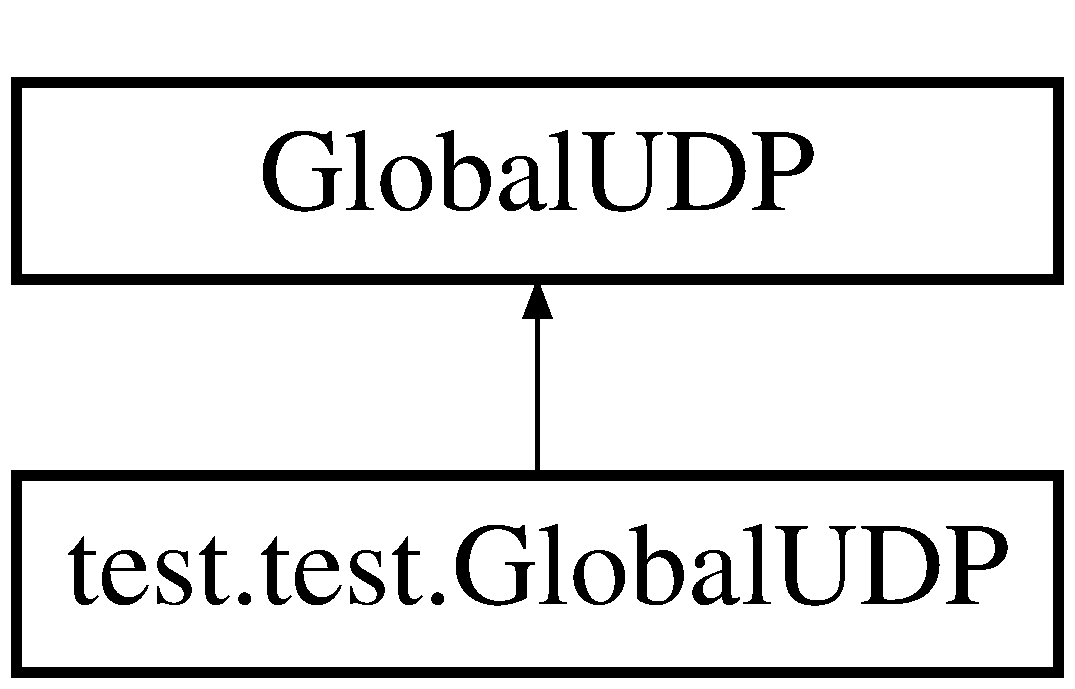
\includegraphics[height=2.000000cm]{classtest_1_1test_1_1GlobalUDP}
\end{center}
\end{figure}
\subsection*{Public Member Functions}
\begin{DoxyCompactItemize}
\item 
def \hyperlink{classtest_1_1test_1_1GlobalUDP_accb59be9286ae069796dc2cfa2a953e0}{receive}
\end{DoxyCompactItemize}


\subsection{Member Function Documentation}
\hypertarget{classtest_1_1test_1_1GlobalUDP_accb59be9286ae069796dc2cfa2a953e0}{\index{test\-::test\-::\-Global\-U\-D\-P@{test\-::test\-::\-Global\-U\-D\-P}!receive@{receive}}
\index{receive@{receive}!test::test::GlobalUDP@{test\-::test\-::\-Global\-U\-D\-P}}
\subsubsection[{receive}]{\setlength{\rightskip}{0pt plus 5cm}def test.\-test.\-Global\-U\-D\-P.\-receive (
\begin{DoxyParamCaption}
\item[{}]{self, }
\item[{}]{data, }
\item[{}]{length, }
\item[{}]{packet\-\_\-info}
\end{DoxyParamCaption}
)}}\label{classtest_1_1test_1_1GlobalUDP_accb59be9286ae069796dc2cfa2a953e0}


The documentation for this class was generated from the following file\-:\begin{DoxyCompactItemize}
\item 
O\-W\-P\-J\-O\-N/\-P\-J\-O\-N-\/cython/test/\hyperlink{PJON-cython_2test_2test_8py}{test.\-py}\end{DoxyCompactItemize}

\hypertarget{classsniffer-gui_1_1Gui}{\section{sniffer-\/gui.Gui Class Reference}
\label{classsniffer-gui_1_1Gui}\index{sniffer-\/gui.\-Gui@{sniffer-\/gui.\-Gui}}
}
Inheritance diagram for sniffer-\/gui.Gui\-:\begin{figure}[H]
\begin{center}
\leavevmode
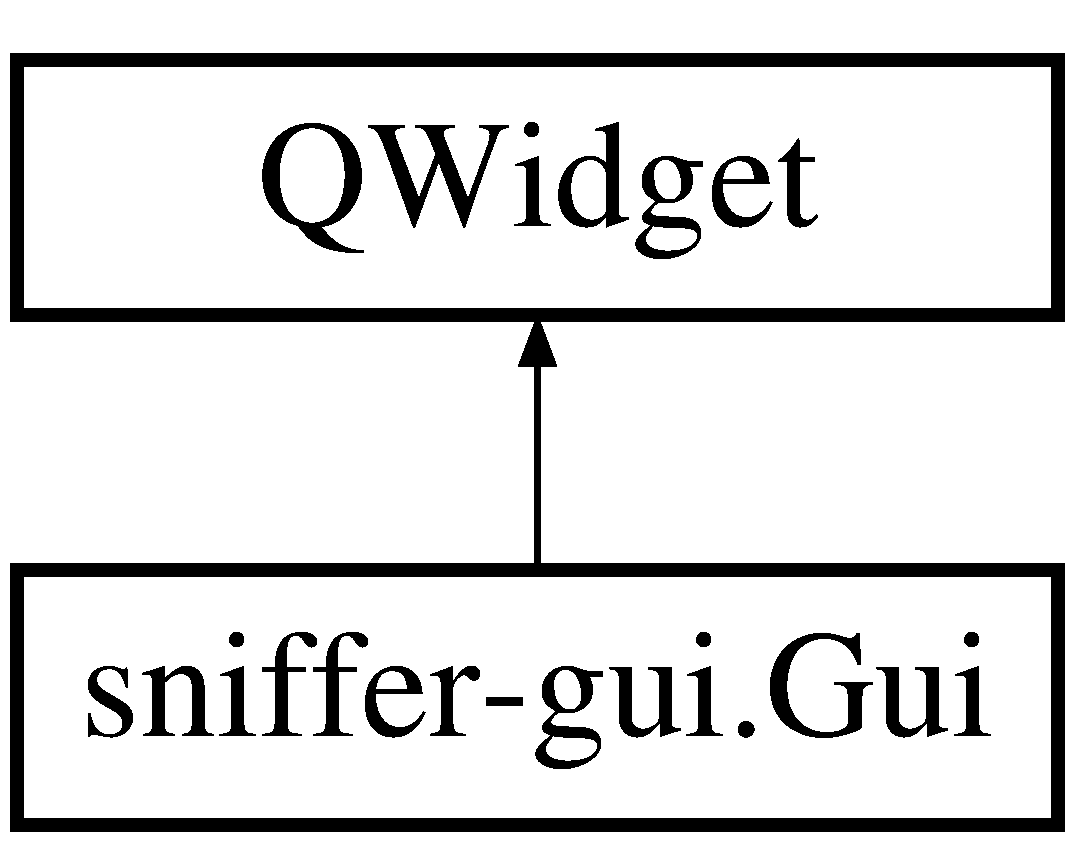
\includegraphics[height=2.000000cm]{classsniffer-gui_1_1Gui}
\end{center}
\end{figure}
\subsection*{Public Member Functions}
\begin{DoxyCompactItemize}
\item 
def \hyperlink{classsniffer-gui_1_1Gui_a2c7490c4f10068fa19515cc5c43c88a4}{start\-Sniff}
\item 
def \hyperlink{classsniffer-gui_1_1Gui_a70d3968b06a700a4736504858fb6b07c}{stop\-Sniff}
\item 
def \hyperlink{classsniffer-gui_1_1Gui_a5d3cfac3eb315e660ac2020ba8d1acea}{update\-Packets}
\item 
def \hyperlink{classsniffer-gui_1_1Gui_ad14ede47ebc1a2ff80840f2666c23e5b}{update\-Max\-Diameter}
\item 
def \hyperlink{classsniffer-gui_1_1Gui_a644cf3bc5282688d0c5cca10e180ef1a}{update\-Max\-Packet\-Length}
\item 
def \hyperlink{classsniffer-gui_1_1Gui_a48406519cf9ac933f9fe41f8f6bbcb5b}{update\-Avg\-Diameter}
\item 
def \hyperlink{classsniffer-gui_1_1Gui_a145c353f3891a41451d16055714a0bed}{update\-Avg\-Packet\-Length}
\item 
def \hyperlink{classsniffer-gui_1_1Gui_ab304fbf63f42d37ac20bdd8463e5135f}{update\-Atts}
\item 
def \hyperlink{classsniffer-gui_1_1Gui_a6b8d94881aa398b0debaefd4829b1375}{init\-G\-U\-I}
\item 
def \hyperlink{classsniffer-gui_1_1Gui_ae96f28df9f3fcd6a2174b7c6c4b3d409}{\-\_\-\-\_\-init\-\_\-\-\_\-}
\end{DoxyCompactItemize}
\subsection*{Public Attributes}
\begin{DoxyCompactItemize}
\item 
\hyperlink{classsniffer-gui_1_1Gui_a02d82ddd2bd64b83f833b7a006e39fea}{sniff\-Key}
\item 
\hyperlink{classsniffer-gui_1_1Gui_a91a2407e461004ac2c2d35e6fc7fb2a9}{sniff\-Thread}
\item 
\hyperlink{classsniffer-gui_1_1Gui_a0e2fcdc7b2bf9a2f8b4e426f69015cb1}{os}
\item 
\hyperlink{classsniffer-gui_1_1Gui_aacefa63693f1cc0b197acc6c85ff0022}{protocol\-Combo\-Box}
\item 
\hyperlink{classsniffer-gui_1_1Gui_a0844bd6fc79598adbea2eee70a1bcd1b}{att\-Combo\-Box}
\item 
\hyperlink{classsniffer-gui_1_1Gui_aadf7db1331852aed2e2443d4edaf6df0}{packet\-Edit\-Text}
\item 
\hyperlink{classsniffer-gui_1_1Gui_abaac68ea066f3bf1d22012779286bb27}{max\-Diameter\-Label}
\item 
\hyperlink{classsniffer-gui_1_1Gui_a9b25b3e7158be574edc4910f7a82503f}{max\-Length\-Label}
\item 
\hyperlink{classsniffer-gui_1_1Gui_aa758f0a5b80fd6ca816b0e749f4c6c8c}{avg\-Diameter\-Label}
\item 
\hyperlink{classsniffer-gui_1_1Gui_a86e7462fb708fbfea49dc57a7947cb50}{avg\-Length\-Label}
\item 
\hyperlink{classsniffer-gui_1_1Gui_a8b4d873bc6324bc29d7d93218043a370}{sniffing\-Label}
\item 
\hyperlink{classsniffer-gui_1_1Gui_a203644051a38143e4021bcb26861174a}{linux}
\item 
\hyperlink{classsniffer-gui_1_1Gui_a2846e2b9d520f6b0a3e988d713032d6f}{windows}
\end{DoxyCompactItemize}


\subsection{Constructor \& Destructor Documentation}
\hypertarget{classsniffer-gui_1_1Gui_ae96f28df9f3fcd6a2174b7c6c4b3d409}{\index{sniffer-\/gui\-::\-Gui@{sniffer-\/gui\-::\-Gui}!\-\_\-\-\_\-init\-\_\-\-\_\-@{\-\_\-\-\_\-init\-\_\-\-\_\-}}
\index{\-\_\-\-\_\-init\-\_\-\-\_\-@{\-\_\-\-\_\-init\-\_\-\-\_\-}!sniffer-gui::Gui@{sniffer-\/gui\-::\-Gui}}
\subsubsection[{\-\_\-\-\_\-init\-\_\-\-\_\-}]{\setlength{\rightskip}{0pt plus 5cm}def sniffer-\/gui.\-Gui.\-\_\-\-\_\-init\-\_\-\-\_\- (
\begin{DoxyParamCaption}
\item[{}]{self}
\end{DoxyParamCaption}
)}}\label{classsniffer-gui_1_1Gui_ae96f28df9f3fcd6a2174b7c6c4b3d409}


\subsection{Member Function Documentation}
\hypertarget{classsniffer-gui_1_1Gui_a6b8d94881aa398b0debaefd4829b1375}{\index{sniffer-\/gui\-::\-Gui@{sniffer-\/gui\-::\-Gui}!init\-G\-U\-I@{init\-G\-U\-I}}
\index{init\-G\-U\-I@{init\-G\-U\-I}!sniffer-gui::Gui@{sniffer-\/gui\-::\-Gui}}
\subsubsection[{init\-G\-U\-I}]{\setlength{\rightskip}{0pt plus 5cm}def sniffer-\/gui.\-Gui.\-init\-G\-U\-I (
\begin{DoxyParamCaption}
\item[{}]{self}
\end{DoxyParamCaption}
)}}\label{classsniffer-gui_1_1Gui_a6b8d94881aa398b0debaefd4829b1375}
\hypertarget{classsniffer-gui_1_1Gui_a2c7490c4f10068fa19515cc5c43c88a4}{\index{sniffer-\/gui\-::\-Gui@{sniffer-\/gui\-::\-Gui}!start\-Sniff@{start\-Sniff}}
\index{start\-Sniff@{start\-Sniff}!sniffer-gui::Gui@{sniffer-\/gui\-::\-Gui}}
\subsubsection[{start\-Sniff}]{\setlength{\rightskip}{0pt plus 5cm}def sniffer-\/gui.\-Gui.\-start\-Sniff (
\begin{DoxyParamCaption}
\item[{}]{self}
\end{DoxyParamCaption}
)}}\label{classsniffer-gui_1_1Gui_a2c7490c4f10068fa19515cc5c43c88a4}
\hypertarget{classsniffer-gui_1_1Gui_a70d3968b06a700a4736504858fb6b07c}{\index{sniffer-\/gui\-::\-Gui@{sniffer-\/gui\-::\-Gui}!stop\-Sniff@{stop\-Sniff}}
\index{stop\-Sniff@{stop\-Sniff}!sniffer-gui::Gui@{sniffer-\/gui\-::\-Gui}}
\subsubsection[{stop\-Sniff}]{\setlength{\rightskip}{0pt plus 5cm}def sniffer-\/gui.\-Gui.\-stop\-Sniff (
\begin{DoxyParamCaption}
\item[{}]{self}
\end{DoxyParamCaption}
)}}\label{classsniffer-gui_1_1Gui_a70d3968b06a700a4736504858fb6b07c}
\hypertarget{classsniffer-gui_1_1Gui_ab304fbf63f42d37ac20bdd8463e5135f}{\index{sniffer-\/gui\-::\-Gui@{sniffer-\/gui\-::\-Gui}!update\-Atts@{update\-Atts}}
\index{update\-Atts@{update\-Atts}!sniffer-gui::Gui@{sniffer-\/gui\-::\-Gui}}
\subsubsection[{update\-Atts}]{\setlength{\rightskip}{0pt plus 5cm}def sniffer-\/gui.\-Gui.\-update\-Atts (
\begin{DoxyParamCaption}
\item[{}]{self, }
\item[{}]{protocol}
\end{DoxyParamCaption}
)}}\label{classsniffer-gui_1_1Gui_ab304fbf63f42d37ac20bdd8463e5135f}
\hypertarget{classsniffer-gui_1_1Gui_a48406519cf9ac933f9fe41f8f6bbcb5b}{\index{sniffer-\/gui\-::\-Gui@{sniffer-\/gui\-::\-Gui}!update\-Avg\-Diameter@{update\-Avg\-Diameter}}
\index{update\-Avg\-Diameter@{update\-Avg\-Diameter}!sniffer-gui::Gui@{sniffer-\/gui\-::\-Gui}}
\subsubsection[{update\-Avg\-Diameter}]{\setlength{\rightskip}{0pt plus 5cm}def sniffer-\/gui.\-Gui.\-update\-Avg\-Diameter (
\begin{DoxyParamCaption}
\item[{}]{self, }
\item[{}]{avg\-Diameter}
\end{DoxyParamCaption}
)}}\label{classsniffer-gui_1_1Gui_a48406519cf9ac933f9fe41f8f6bbcb5b}
\hypertarget{classsniffer-gui_1_1Gui_a145c353f3891a41451d16055714a0bed}{\index{sniffer-\/gui\-::\-Gui@{sniffer-\/gui\-::\-Gui}!update\-Avg\-Packet\-Length@{update\-Avg\-Packet\-Length}}
\index{update\-Avg\-Packet\-Length@{update\-Avg\-Packet\-Length}!sniffer-gui::Gui@{sniffer-\/gui\-::\-Gui}}
\subsubsection[{update\-Avg\-Packet\-Length}]{\setlength{\rightskip}{0pt plus 5cm}def sniffer-\/gui.\-Gui.\-update\-Avg\-Packet\-Length (
\begin{DoxyParamCaption}
\item[{}]{self, }
\item[{}]{avg\-Length}
\end{DoxyParamCaption}
)}}\label{classsniffer-gui_1_1Gui_a145c353f3891a41451d16055714a0bed}
\hypertarget{classsniffer-gui_1_1Gui_ad14ede47ebc1a2ff80840f2666c23e5b}{\index{sniffer-\/gui\-::\-Gui@{sniffer-\/gui\-::\-Gui}!update\-Max\-Diameter@{update\-Max\-Diameter}}
\index{update\-Max\-Diameter@{update\-Max\-Diameter}!sniffer-gui::Gui@{sniffer-\/gui\-::\-Gui}}
\subsubsection[{update\-Max\-Diameter}]{\setlength{\rightskip}{0pt plus 5cm}def sniffer-\/gui.\-Gui.\-update\-Max\-Diameter (
\begin{DoxyParamCaption}
\item[{}]{self, }
\item[{}]{max\-Diameter}
\end{DoxyParamCaption}
)}}\label{classsniffer-gui_1_1Gui_ad14ede47ebc1a2ff80840f2666c23e5b}
\hypertarget{classsniffer-gui_1_1Gui_a644cf3bc5282688d0c5cca10e180ef1a}{\index{sniffer-\/gui\-::\-Gui@{sniffer-\/gui\-::\-Gui}!update\-Max\-Packet\-Length@{update\-Max\-Packet\-Length}}
\index{update\-Max\-Packet\-Length@{update\-Max\-Packet\-Length}!sniffer-gui::Gui@{sniffer-\/gui\-::\-Gui}}
\subsubsection[{update\-Max\-Packet\-Length}]{\setlength{\rightskip}{0pt plus 5cm}def sniffer-\/gui.\-Gui.\-update\-Max\-Packet\-Length (
\begin{DoxyParamCaption}
\item[{}]{self, }
\item[{}]{max\-Length}
\end{DoxyParamCaption}
)}}\label{classsniffer-gui_1_1Gui_a644cf3bc5282688d0c5cca10e180ef1a}
\hypertarget{classsniffer-gui_1_1Gui_a5d3cfac3eb315e660ac2020ba8d1acea}{\index{sniffer-\/gui\-::\-Gui@{sniffer-\/gui\-::\-Gui}!update\-Packets@{update\-Packets}}
\index{update\-Packets@{update\-Packets}!sniffer-gui::Gui@{sniffer-\/gui\-::\-Gui}}
\subsubsection[{update\-Packets}]{\setlength{\rightskip}{0pt plus 5cm}def sniffer-\/gui.\-Gui.\-update\-Packets (
\begin{DoxyParamCaption}
\item[{}]{self, }
\item[{}]{unpacked\-Info}
\end{DoxyParamCaption}
)}}\label{classsniffer-gui_1_1Gui_a5d3cfac3eb315e660ac2020ba8d1acea}


\subsection{Member Data Documentation}
\hypertarget{classsniffer-gui_1_1Gui_a0844bd6fc79598adbea2eee70a1bcd1b}{\index{sniffer-\/gui\-::\-Gui@{sniffer-\/gui\-::\-Gui}!att\-Combo\-Box@{att\-Combo\-Box}}
\index{att\-Combo\-Box@{att\-Combo\-Box}!sniffer-gui::Gui@{sniffer-\/gui\-::\-Gui}}
\subsubsection[{att\-Combo\-Box}]{\setlength{\rightskip}{0pt plus 5cm}sniffer-\/gui.\-Gui.\-att\-Combo\-Box}}\label{classsniffer-gui_1_1Gui_a0844bd6fc79598adbea2eee70a1bcd1b}
\hypertarget{classsniffer-gui_1_1Gui_aa758f0a5b80fd6ca816b0e749f4c6c8c}{\index{sniffer-\/gui\-::\-Gui@{sniffer-\/gui\-::\-Gui}!avg\-Diameter\-Label@{avg\-Diameter\-Label}}
\index{avg\-Diameter\-Label@{avg\-Diameter\-Label}!sniffer-gui::Gui@{sniffer-\/gui\-::\-Gui}}
\subsubsection[{avg\-Diameter\-Label}]{\setlength{\rightskip}{0pt plus 5cm}sniffer-\/gui.\-Gui.\-avg\-Diameter\-Label}}\label{classsniffer-gui_1_1Gui_aa758f0a5b80fd6ca816b0e749f4c6c8c}
\hypertarget{classsniffer-gui_1_1Gui_a86e7462fb708fbfea49dc57a7947cb50}{\index{sniffer-\/gui\-::\-Gui@{sniffer-\/gui\-::\-Gui}!avg\-Length\-Label@{avg\-Length\-Label}}
\index{avg\-Length\-Label@{avg\-Length\-Label}!sniffer-gui::Gui@{sniffer-\/gui\-::\-Gui}}
\subsubsection[{avg\-Length\-Label}]{\setlength{\rightskip}{0pt plus 5cm}sniffer-\/gui.\-Gui.\-avg\-Length\-Label}}\label{classsniffer-gui_1_1Gui_a86e7462fb708fbfea49dc57a7947cb50}
\hypertarget{classsniffer-gui_1_1Gui_a203644051a38143e4021bcb26861174a}{\index{sniffer-\/gui\-::\-Gui@{sniffer-\/gui\-::\-Gui}!linux@{linux}}
\index{linux@{linux}!sniffer-gui::Gui@{sniffer-\/gui\-::\-Gui}}
\subsubsection[{linux}]{\setlength{\rightskip}{0pt plus 5cm}sniffer-\/gui.\-Gui.\-linux}}\label{classsniffer-gui_1_1Gui_a203644051a38143e4021bcb26861174a}
\hypertarget{classsniffer-gui_1_1Gui_abaac68ea066f3bf1d22012779286bb27}{\index{sniffer-\/gui\-::\-Gui@{sniffer-\/gui\-::\-Gui}!max\-Diameter\-Label@{max\-Diameter\-Label}}
\index{max\-Diameter\-Label@{max\-Diameter\-Label}!sniffer-gui::Gui@{sniffer-\/gui\-::\-Gui}}
\subsubsection[{max\-Diameter\-Label}]{\setlength{\rightskip}{0pt plus 5cm}sniffer-\/gui.\-Gui.\-max\-Diameter\-Label}}\label{classsniffer-gui_1_1Gui_abaac68ea066f3bf1d22012779286bb27}
\hypertarget{classsniffer-gui_1_1Gui_a9b25b3e7158be574edc4910f7a82503f}{\index{sniffer-\/gui\-::\-Gui@{sniffer-\/gui\-::\-Gui}!max\-Length\-Label@{max\-Length\-Label}}
\index{max\-Length\-Label@{max\-Length\-Label}!sniffer-gui::Gui@{sniffer-\/gui\-::\-Gui}}
\subsubsection[{max\-Length\-Label}]{\setlength{\rightskip}{0pt plus 5cm}sniffer-\/gui.\-Gui.\-max\-Length\-Label}}\label{classsniffer-gui_1_1Gui_a9b25b3e7158be574edc4910f7a82503f}
\hypertarget{classsniffer-gui_1_1Gui_a0e2fcdc7b2bf9a2f8b4e426f69015cb1}{\index{sniffer-\/gui\-::\-Gui@{sniffer-\/gui\-::\-Gui}!os@{os}}
\index{os@{os}!sniffer-gui::Gui@{sniffer-\/gui\-::\-Gui}}
\subsubsection[{os}]{\setlength{\rightskip}{0pt plus 5cm}sniffer-\/gui.\-Gui.\-os}}\label{classsniffer-gui_1_1Gui_a0e2fcdc7b2bf9a2f8b4e426f69015cb1}
\hypertarget{classsniffer-gui_1_1Gui_aadf7db1331852aed2e2443d4edaf6df0}{\index{sniffer-\/gui\-::\-Gui@{sniffer-\/gui\-::\-Gui}!packet\-Edit\-Text@{packet\-Edit\-Text}}
\index{packet\-Edit\-Text@{packet\-Edit\-Text}!sniffer-gui::Gui@{sniffer-\/gui\-::\-Gui}}
\subsubsection[{packet\-Edit\-Text}]{\setlength{\rightskip}{0pt plus 5cm}sniffer-\/gui.\-Gui.\-packet\-Edit\-Text}}\label{classsniffer-gui_1_1Gui_aadf7db1331852aed2e2443d4edaf6df0}
\hypertarget{classsniffer-gui_1_1Gui_aacefa63693f1cc0b197acc6c85ff0022}{\index{sniffer-\/gui\-::\-Gui@{sniffer-\/gui\-::\-Gui}!protocol\-Combo\-Box@{protocol\-Combo\-Box}}
\index{protocol\-Combo\-Box@{protocol\-Combo\-Box}!sniffer-gui::Gui@{sniffer-\/gui\-::\-Gui}}
\subsubsection[{protocol\-Combo\-Box}]{\setlength{\rightskip}{0pt plus 5cm}sniffer-\/gui.\-Gui.\-protocol\-Combo\-Box}}\label{classsniffer-gui_1_1Gui_aacefa63693f1cc0b197acc6c85ff0022}
\hypertarget{classsniffer-gui_1_1Gui_a8b4d873bc6324bc29d7d93218043a370}{\index{sniffer-\/gui\-::\-Gui@{sniffer-\/gui\-::\-Gui}!sniffing\-Label@{sniffing\-Label}}
\index{sniffing\-Label@{sniffing\-Label}!sniffer-gui::Gui@{sniffer-\/gui\-::\-Gui}}
\subsubsection[{sniffing\-Label}]{\setlength{\rightskip}{0pt plus 5cm}sniffer-\/gui.\-Gui.\-sniffing\-Label}}\label{classsniffer-gui_1_1Gui_a8b4d873bc6324bc29d7d93218043a370}
\hypertarget{classsniffer-gui_1_1Gui_a02d82ddd2bd64b83f833b7a006e39fea}{\index{sniffer-\/gui\-::\-Gui@{sniffer-\/gui\-::\-Gui}!sniff\-Key@{sniff\-Key}}
\index{sniff\-Key@{sniff\-Key}!sniffer-gui::Gui@{sniffer-\/gui\-::\-Gui}}
\subsubsection[{sniff\-Key}]{\setlength{\rightskip}{0pt plus 5cm}sniffer-\/gui.\-Gui.\-sniff\-Key}}\label{classsniffer-gui_1_1Gui_a02d82ddd2bd64b83f833b7a006e39fea}
\hypertarget{classsniffer-gui_1_1Gui_a91a2407e461004ac2c2d35e6fc7fb2a9}{\index{sniffer-\/gui\-::\-Gui@{sniffer-\/gui\-::\-Gui}!sniff\-Thread@{sniff\-Thread}}
\index{sniff\-Thread@{sniff\-Thread}!sniffer-gui::Gui@{sniffer-\/gui\-::\-Gui}}
\subsubsection[{sniff\-Thread}]{\setlength{\rightskip}{0pt plus 5cm}sniffer-\/gui.\-Gui.\-sniff\-Thread}}\label{classsniffer-gui_1_1Gui_a91a2407e461004ac2c2d35e6fc7fb2a9}
\hypertarget{classsniffer-gui_1_1Gui_a2846e2b9d520f6b0a3e988d713032d6f}{\index{sniffer-\/gui\-::\-Gui@{sniffer-\/gui\-::\-Gui}!windows@{windows}}
\index{windows@{windows}!sniffer-gui::Gui@{sniffer-\/gui\-::\-Gui}}
\subsubsection[{windows}]{\setlength{\rightskip}{0pt plus 5cm}sniffer-\/gui.\-Gui.\-windows}}\label{classsniffer-gui_1_1Gui_a2846e2b9d520f6b0a3e988d713032d6f}


The documentation for this class was generated from the following file\-:\begin{DoxyCompactItemize}
\item 
\hyperlink{sniffer-gui_8py}{sniffer-\/gui.\-py}\end{DoxyCompactItemize}

\hypertarget{unioni2c__smbus__data}{\section{i2c\-\_\-smbus\-\_\-data Union Reference}
\label{unioni2c__smbus__data}\index{i2c\-\_\-smbus\-\_\-data@{i2c\-\_\-smbus\-\_\-data}}
}
\subsection*{Public Attributes}
\begin{DoxyCompactItemize}
\item 
uint8\-\_\-t \hyperlink{unioni2c__smbus__data_a7145699abf962d118aa1c78ff864e892}{byte}
\item 
uint16\-\_\-t \hyperlink{unioni2c__smbus__data_ae8621bf131cbdfff90b21499a2c11a26}{word}
\item 
uint8\-\_\-t \hyperlink{unioni2c__smbus__data_a56729c242baa246a3105fd7c64b86f48}{block} \mbox{[}\hyperlink{wiringPiI2C_8c_ac2dd8b77e329bba4a3ca9cd275f9bf50}{I2\-C\-\_\-\-S\-M\-B\-U\-S\-\_\-\-B\-L\-O\-C\-K\-\_\-\-M\-A\-X}+2\mbox{]}
\end{DoxyCompactItemize}


\subsection{Member Data Documentation}
\hypertarget{unioni2c__smbus__data_a56729c242baa246a3105fd7c64b86f48}{\index{i2c\-\_\-smbus\-\_\-data@{i2c\-\_\-smbus\-\_\-data}!block@{block}}
\index{block@{block}!i2c_smbus_data@{i2c\-\_\-smbus\-\_\-data}}
\subsubsection[{block}]{\setlength{\rightskip}{0pt plus 5cm}uint8\-\_\-t i2c\-\_\-smbus\-\_\-data\-::block\mbox{[}{\bf I2\-C\-\_\-\-S\-M\-B\-U\-S\-\_\-\-B\-L\-O\-C\-K\-\_\-\-M\-A\-X}+2\mbox{]}}}\label{unioni2c__smbus__data_a56729c242baa246a3105fd7c64b86f48}
\hypertarget{unioni2c__smbus__data_a7145699abf962d118aa1c78ff864e892}{\index{i2c\-\_\-smbus\-\_\-data@{i2c\-\_\-smbus\-\_\-data}!byte@{byte}}
\index{byte@{byte}!i2c_smbus_data@{i2c\-\_\-smbus\-\_\-data}}
\subsubsection[{byte}]{\setlength{\rightskip}{0pt plus 5cm}uint8\-\_\-t i2c\-\_\-smbus\-\_\-data\-::byte}}\label{unioni2c__smbus__data_a7145699abf962d118aa1c78ff864e892}
\hypertarget{unioni2c__smbus__data_ae8621bf131cbdfff90b21499a2c11a26}{\index{i2c\-\_\-smbus\-\_\-data@{i2c\-\_\-smbus\-\_\-data}!word@{word}}
\index{word@{word}!i2c_smbus_data@{i2c\-\_\-smbus\-\_\-data}}
\subsubsection[{word}]{\setlength{\rightskip}{0pt plus 5cm}uint16\-\_\-t i2c\-\_\-smbus\-\_\-data\-::word}}\label{unioni2c__smbus__data_ae8621bf131cbdfff90b21499a2c11a26}


The documentation for this union was generated from the following file\-:\begin{DoxyCompactItemize}
\item 
wiring\-Pi/wiring\-Pi/\hyperlink{wiringPiI2C_8c}{wiring\-Pi\-I2\-C.\-c}\end{DoxyCompactItemize}

\hypertarget{structi2c__smbus__ioctl__data}{\section{i2c\-\_\-smbus\-\_\-ioctl\-\_\-data Struct Reference}
\label{structi2c__smbus__ioctl__data}\index{i2c\-\_\-smbus\-\_\-ioctl\-\_\-data@{i2c\-\_\-smbus\-\_\-ioctl\-\_\-data}}
}
\subsection*{Public Attributes}
\begin{DoxyCompactItemize}
\item 
char \hyperlink{structi2c__smbus__ioctl__data_add449c765b690f883e5771132d16a4f8}{read\-\_\-write}
\item 
uint8\-\_\-t \hyperlink{structi2c__smbus__ioctl__data_adaacbd70d47e01e8bca1457b721089e7}{command}
\item 
int \hyperlink{structi2c__smbus__ioctl__data_a777bacfabf66ba077b40d1c835c7879f}{size}
\item 
union \hyperlink{unioni2c__smbus__data}{i2c\-\_\-smbus\-\_\-data} $\ast$ \hyperlink{structi2c__smbus__ioctl__data_af5a53e4ed38f278bd5fb62a65b67432d}{data}
\end{DoxyCompactItemize}


\subsection{Member Data Documentation}
\hypertarget{structi2c__smbus__ioctl__data_adaacbd70d47e01e8bca1457b721089e7}{\index{i2c\-\_\-smbus\-\_\-ioctl\-\_\-data@{i2c\-\_\-smbus\-\_\-ioctl\-\_\-data}!command@{command}}
\index{command@{command}!i2c_smbus_ioctl_data@{i2c\-\_\-smbus\-\_\-ioctl\-\_\-data}}
\subsubsection[{command}]{\setlength{\rightskip}{0pt plus 5cm}uint8\-\_\-t i2c\-\_\-smbus\-\_\-ioctl\-\_\-data\-::command}}\label{structi2c__smbus__ioctl__data_adaacbd70d47e01e8bca1457b721089e7}
\hypertarget{structi2c__smbus__ioctl__data_af5a53e4ed38f278bd5fb62a65b67432d}{\index{i2c\-\_\-smbus\-\_\-ioctl\-\_\-data@{i2c\-\_\-smbus\-\_\-ioctl\-\_\-data}!data@{data}}
\index{data@{data}!i2c_smbus_ioctl_data@{i2c\-\_\-smbus\-\_\-ioctl\-\_\-data}}
\subsubsection[{data}]{\setlength{\rightskip}{0pt plus 5cm}union {\bf i2c\-\_\-smbus\-\_\-data}$\ast$ i2c\-\_\-smbus\-\_\-ioctl\-\_\-data\-::data}}\label{structi2c__smbus__ioctl__data_af5a53e4ed38f278bd5fb62a65b67432d}
\hypertarget{structi2c__smbus__ioctl__data_add449c765b690f883e5771132d16a4f8}{\index{i2c\-\_\-smbus\-\_\-ioctl\-\_\-data@{i2c\-\_\-smbus\-\_\-ioctl\-\_\-data}!read\-\_\-write@{read\-\_\-write}}
\index{read\-\_\-write@{read\-\_\-write}!i2c_smbus_ioctl_data@{i2c\-\_\-smbus\-\_\-ioctl\-\_\-data}}
\subsubsection[{read\-\_\-write}]{\setlength{\rightskip}{0pt plus 5cm}char i2c\-\_\-smbus\-\_\-ioctl\-\_\-data\-::read\-\_\-write}}\label{structi2c__smbus__ioctl__data_add449c765b690f883e5771132d16a4f8}
\hypertarget{structi2c__smbus__ioctl__data_a777bacfabf66ba077b40d1c835c7879f}{\index{i2c\-\_\-smbus\-\_\-ioctl\-\_\-data@{i2c\-\_\-smbus\-\_\-ioctl\-\_\-data}!size@{size}}
\index{size@{size}!i2c_smbus_ioctl_data@{i2c\-\_\-smbus\-\_\-ioctl\-\_\-data}}
\subsubsection[{size}]{\setlength{\rightskip}{0pt plus 5cm}int i2c\-\_\-smbus\-\_\-ioctl\-\_\-data\-::size}}\label{structi2c__smbus__ioctl__data_a777bacfabf66ba077b40d1c835c7879f}


The documentation for this struct was generated from the following file\-:\begin{DoxyCompactItemize}
\item 
wiring\-Pi/wiring\-Pi/\hyperlink{wiringPiI2C_8c}{wiring\-Pi\-I2\-C.\-c}\end{DoxyCompactItemize}

\hypertarget{structimu__t}{\section{imu\-\_\-t Struct Reference}
\label{structimu__t}\index{imu\-\_\-t@{imu\-\_\-t}}
}


{\ttfamily \#include $<$types.\-h$>$}

\subsection*{Public Attributes}
\begin{DoxyCompactItemize}
\item 
int16\-\_\-t \hyperlink{structimu__t_ac926eb70490448bbff42b96b836494cc}{acc\-Smooth} \mbox{[}3\mbox{]}
\item 
int16\-\_\-t \hyperlink{structimu__t_adf0174759aab3cd8fa9e83ea2abc56ad}{gyro\-Data} \mbox{[}3\mbox{]}
\item 
int16\-\_\-t \hyperlink{structimu__t_a5508ca86335bde92d3c2ee9168c7c059}{mag\-A\-D\-C} \mbox{[}3\mbox{]}
\item 
int16\-\_\-t \hyperlink{structimu__t_af05a81dcab2ed384ac6890591db08f0c}{gyro\-A\-D\-C} \mbox{[}3\mbox{]}
\item 
int16\-\_\-t \hyperlink{structimu__t_acaa9d196f82fbbc2670209d19f0c19c4}{acc\-A\-D\-C} \mbox{[}3\mbox{]}
\end{DoxyCompactItemize}


\subsection{Member Data Documentation}
\hypertarget{structimu__t_acaa9d196f82fbbc2670209d19f0c19c4}{\index{imu\-\_\-t@{imu\-\_\-t}!acc\-A\-D\-C@{acc\-A\-D\-C}}
\index{acc\-A\-D\-C@{acc\-A\-D\-C}!imu_t@{imu\-\_\-t}}
\subsubsection[{acc\-A\-D\-C}]{\setlength{\rightskip}{0pt plus 5cm}int16\-\_\-t imu\-\_\-t\-::acc\-A\-D\-C}}\label{structimu__t_acaa9d196f82fbbc2670209d19f0c19c4}
\hypertarget{structimu__t_ac926eb70490448bbff42b96b836494cc}{\index{imu\-\_\-t@{imu\-\_\-t}!acc\-Smooth@{acc\-Smooth}}
\index{acc\-Smooth@{acc\-Smooth}!imu_t@{imu\-\_\-t}}
\subsubsection[{acc\-Smooth}]{\setlength{\rightskip}{0pt plus 5cm}int16\-\_\-t imu\-\_\-t\-::acc\-Smooth}}\label{structimu__t_ac926eb70490448bbff42b96b836494cc}
\hypertarget{structimu__t_af05a81dcab2ed384ac6890591db08f0c}{\index{imu\-\_\-t@{imu\-\_\-t}!gyro\-A\-D\-C@{gyro\-A\-D\-C}}
\index{gyro\-A\-D\-C@{gyro\-A\-D\-C}!imu_t@{imu\-\_\-t}}
\subsubsection[{gyro\-A\-D\-C}]{\setlength{\rightskip}{0pt plus 5cm}int16\-\_\-t imu\-\_\-t\-::gyro\-A\-D\-C}}\label{structimu__t_af05a81dcab2ed384ac6890591db08f0c}
\hypertarget{structimu__t_adf0174759aab3cd8fa9e83ea2abc56ad}{\index{imu\-\_\-t@{imu\-\_\-t}!gyro\-Data@{gyro\-Data}}
\index{gyro\-Data@{gyro\-Data}!imu_t@{imu\-\_\-t}}
\subsubsection[{gyro\-Data}]{\setlength{\rightskip}{0pt plus 5cm}int16\-\_\-t imu\-\_\-t\-::gyro\-Data}}\label{structimu__t_adf0174759aab3cd8fa9e83ea2abc56ad}
\hypertarget{structimu__t_a5508ca86335bde92d3c2ee9168c7c059}{\index{imu\-\_\-t@{imu\-\_\-t}!mag\-A\-D\-C@{mag\-A\-D\-C}}
\index{mag\-A\-D\-C@{mag\-A\-D\-C}!imu_t@{imu\-\_\-t}}
\subsubsection[{mag\-A\-D\-C}]{\setlength{\rightskip}{0pt plus 5cm}int16\-\_\-t imu\-\_\-t\-::mag\-A\-D\-C}}\label{structimu__t_a5508ca86335bde92d3c2ee9168c7c059}


The documentation for this struct was generated from the following file\-:\begin{DoxyCompactItemize}
\item 
Multi\-Wii\-\_\-2\-\_\-4/\-Multi\-Wii/\hyperlink{MultiWii__2__4_2MultiWii_2types_8h}{types.\-h}\end{DoxyCompactItemize}

\hypertarget{structint16x4x2__t}{\section{int16x4x2\-\_\-t Struct Reference}
\label{structint16x4x2__t}\index{int16x4x2\-\_\-t@{int16x4x2\-\_\-t}}
}


{\ttfamily \#include $<$arm\-\_\-neon.\-h$>$}

\subsection*{Public Attributes}
\begin{DoxyCompactItemize}
\item 
int16x4\-\_\-t \hyperlink{structint16x4x2__t_a364d92d220766b0495e9bdbcd85d56f7}{val} \mbox{[}2\mbox{]}
\end{DoxyCompactItemize}


\subsection{Member Data Documentation}
\hypertarget{structint16x4x2__t_a364d92d220766b0495e9bdbcd85d56f7}{\index{int16x4x2\-\_\-t@{int16x4x2\-\_\-t}!val@{val}}
\index{val@{val}!int16x4x2_t@{int16x4x2\-\_\-t}}
\subsubsection[{val}]{\setlength{\rightskip}{0pt plus 5cm}int16x4\-\_\-t int16x4x2\-\_\-t\-::val\mbox{[}2\mbox{]}}}\label{structint16x4x2__t_a364d92d220766b0495e9bdbcd85d56f7}


The documentation for this struct was generated from the following file\-:\begin{DoxyCompactItemize}
\item 
oclint-\/0.\-10.\-3/lib/clang/3.\-8.\-0/include/\hyperlink{arm__neon_8h}{arm\-\_\-neon.\-h}\end{DoxyCompactItemize}

\hypertarget{structint16x4x3__t}{\section{int16x4x3\-\_\-t Struct Reference}
\label{structint16x4x3__t}\index{int16x4x3\-\_\-t@{int16x4x3\-\_\-t}}
}


{\ttfamily \#include $<$arm\-\_\-neon.\-h$>$}

\subsection*{Public Attributes}
\begin{DoxyCompactItemize}
\item 
int16x4\-\_\-t \hyperlink{structint16x4x3__t_ac08ece8a66fa793e79cd30252e1d86e4}{val} \mbox{[}3\mbox{]}
\end{DoxyCompactItemize}


\subsection{Member Data Documentation}
\hypertarget{structint16x4x3__t_ac08ece8a66fa793e79cd30252e1d86e4}{\index{int16x4x3\-\_\-t@{int16x4x3\-\_\-t}!val@{val}}
\index{val@{val}!int16x4x3_t@{int16x4x3\-\_\-t}}
\subsubsection[{val}]{\setlength{\rightskip}{0pt plus 5cm}int16x4\-\_\-t int16x4x3\-\_\-t\-::val\mbox{[}3\mbox{]}}}\label{structint16x4x3__t_ac08ece8a66fa793e79cd30252e1d86e4}


The documentation for this struct was generated from the following file\-:\begin{DoxyCompactItemize}
\item 
oclint-\/0.\-10.\-3/lib/clang/3.\-8.\-0/include/\hyperlink{arm__neon_8h}{arm\-\_\-neon.\-h}\end{DoxyCompactItemize}

\hypertarget{structint16x4x4__t}{\section{int16x4x4\-\_\-t Struct Reference}
\label{structint16x4x4__t}\index{int16x4x4\-\_\-t@{int16x4x4\-\_\-t}}
}


{\ttfamily \#include $<$arm\-\_\-neon.\-h$>$}

\subsection*{Public Attributes}
\begin{DoxyCompactItemize}
\item 
int16x4\-\_\-t \hyperlink{structint16x4x4__t_a8de5a8a73863b7e18e34273b26902bc1}{val} \mbox{[}4\mbox{]}
\end{DoxyCompactItemize}


\subsection{Member Data Documentation}
\hypertarget{structint16x4x4__t_a8de5a8a73863b7e18e34273b26902bc1}{\index{int16x4x4\-\_\-t@{int16x4x4\-\_\-t}!val@{val}}
\index{val@{val}!int16x4x4_t@{int16x4x4\-\_\-t}}
\subsubsection[{val}]{\setlength{\rightskip}{0pt plus 5cm}int16x4\-\_\-t int16x4x4\-\_\-t\-::val\mbox{[}4\mbox{]}}}\label{structint16x4x4__t_a8de5a8a73863b7e18e34273b26902bc1}


The documentation for this struct was generated from the following file\-:\begin{DoxyCompactItemize}
\item 
oclint-\/0.\-10.\-3/lib/clang/3.\-8.\-0/include/\hyperlink{arm__neon_8h}{arm\-\_\-neon.\-h}\end{DoxyCompactItemize}

\hypertarget{structint16x8x2__t}{\section{int16x8x2\-\_\-t Struct Reference}
\label{structint16x8x2__t}\index{int16x8x2\-\_\-t@{int16x8x2\-\_\-t}}
}


{\ttfamily \#include $<$arm\-\_\-neon.\-h$>$}

\subsection*{Public Attributes}
\begin{DoxyCompactItemize}
\item 
int16x8\-\_\-t \hyperlink{structint16x8x2__t_a4ee5fbe2d6314afb498a56c62c7663a1}{val} \mbox{[}2\mbox{]}
\end{DoxyCompactItemize}


\subsection{Member Data Documentation}
\hypertarget{structint16x8x2__t_a4ee5fbe2d6314afb498a56c62c7663a1}{\index{int16x8x2\-\_\-t@{int16x8x2\-\_\-t}!val@{val}}
\index{val@{val}!int16x8x2_t@{int16x8x2\-\_\-t}}
\subsubsection[{val}]{\setlength{\rightskip}{0pt plus 5cm}int16x8\-\_\-t int16x8x2\-\_\-t\-::val\mbox{[}2\mbox{]}}}\label{structint16x8x2__t_a4ee5fbe2d6314afb498a56c62c7663a1}


The documentation for this struct was generated from the following file\-:\begin{DoxyCompactItemize}
\item 
oclint-\/0.\-10.\-3/lib/clang/3.\-8.\-0/include/\hyperlink{arm__neon_8h}{arm\-\_\-neon.\-h}\end{DoxyCompactItemize}

\hypertarget{structint16x8x3__t}{\section{int16x8x3\-\_\-t Struct Reference}
\label{structint16x8x3__t}\index{int16x8x3\-\_\-t@{int16x8x3\-\_\-t}}
}


{\ttfamily \#include $<$arm\-\_\-neon.\-h$>$}

\subsection*{Public Attributes}
\begin{DoxyCompactItemize}
\item 
int16x8\-\_\-t \hyperlink{structint16x8x3__t_a047b6615d0ac1ce12310df3237642297}{val} \mbox{[}3\mbox{]}
\end{DoxyCompactItemize}


\subsection{Member Data Documentation}
\hypertarget{structint16x8x3__t_a047b6615d0ac1ce12310df3237642297}{\index{int16x8x3\-\_\-t@{int16x8x3\-\_\-t}!val@{val}}
\index{val@{val}!int16x8x3_t@{int16x8x3\-\_\-t}}
\subsubsection[{val}]{\setlength{\rightskip}{0pt plus 5cm}int16x8\-\_\-t int16x8x3\-\_\-t\-::val\mbox{[}3\mbox{]}}}\label{structint16x8x3__t_a047b6615d0ac1ce12310df3237642297}


The documentation for this struct was generated from the following file\-:\begin{DoxyCompactItemize}
\item 
oclint-\/0.\-10.\-3/lib/clang/3.\-8.\-0/include/\hyperlink{arm__neon_8h}{arm\-\_\-neon.\-h}\end{DoxyCompactItemize}

\hypertarget{structint16x8x4__t}{\section{int16x8x4\-\_\-t Struct Reference}
\label{structint16x8x4__t}\index{int16x8x4\-\_\-t@{int16x8x4\-\_\-t}}
}


{\ttfamily \#include $<$arm\-\_\-neon.\-h$>$}

\subsection*{Public Attributes}
\begin{DoxyCompactItemize}
\item 
int16x8\-\_\-t \hyperlink{structint16x8x4__t_a279e0661e450131bf3ad881e3d770f4b}{val} \mbox{[}4\mbox{]}
\end{DoxyCompactItemize}


\subsection{Member Data Documentation}
\hypertarget{structint16x8x4__t_a279e0661e450131bf3ad881e3d770f4b}{\index{int16x8x4\-\_\-t@{int16x8x4\-\_\-t}!val@{val}}
\index{val@{val}!int16x8x4_t@{int16x8x4\-\_\-t}}
\subsubsection[{val}]{\setlength{\rightskip}{0pt plus 5cm}int16x8\-\_\-t int16x8x4\-\_\-t\-::val\mbox{[}4\mbox{]}}}\label{structint16x8x4__t_a279e0661e450131bf3ad881e3d770f4b}


The documentation for this struct was generated from the following file\-:\begin{DoxyCompactItemize}
\item 
oclint-\/0.\-10.\-3/lib/clang/3.\-8.\-0/include/\hyperlink{arm__neon_8h}{arm\-\_\-neon.\-h}\end{DoxyCompactItemize}

\hypertarget{structint32x2x2__t}{\section{int32x2x2\-\_\-t Struct Reference}
\label{structint32x2x2__t}\index{int32x2x2\-\_\-t@{int32x2x2\-\_\-t}}
}


{\ttfamily \#include $<$arm\-\_\-neon.\-h$>$}

\subsection*{Public Attributes}
\begin{DoxyCompactItemize}
\item 
int32x2\-\_\-t \hyperlink{structint32x2x2__t_a002c57928aea4c45d0dc4db4f74f7d1a}{val} \mbox{[}2\mbox{]}
\end{DoxyCompactItemize}


\subsection{Member Data Documentation}
\hypertarget{structint32x2x2__t_a002c57928aea4c45d0dc4db4f74f7d1a}{\index{int32x2x2\-\_\-t@{int32x2x2\-\_\-t}!val@{val}}
\index{val@{val}!int32x2x2_t@{int32x2x2\-\_\-t}}
\subsubsection[{val}]{\setlength{\rightskip}{0pt plus 5cm}int32x2\-\_\-t int32x2x2\-\_\-t\-::val\mbox{[}2\mbox{]}}}\label{structint32x2x2__t_a002c57928aea4c45d0dc4db4f74f7d1a}


The documentation for this struct was generated from the following file\-:\begin{DoxyCompactItemize}
\item 
oclint-\/0.\-10.\-3/lib/clang/3.\-8.\-0/include/\hyperlink{arm__neon_8h}{arm\-\_\-neon.\-h}\end{DoxyCompactItemize}

\hypertarget{structint32x2x3__t}{\section{int32x2x3\-\_\-t Struct Reference}
\label{structint32x2x3__t}\index{int32x2x3\-\_\-t@{int32x2x3\-\_\-t}}
}


{\ttfamily \#include $<$arm\-\_\-neon.\-h$>$}

\subsection*{Public Attributes}
\begin{DoxyCompactItemize}
\item 
int32x2\-\_\-t \hyperlink{structint32x2x3__t_a214e130c7ab80efa64569a494d01f087}{val} \mbox{[}3\mbox{]}
\end{DoxyCompactItemize}


\subsection{Member Data Documentation}
\hypertarget{structint32x2x3__t_a214e130c7ab80efa64569a494d01f087}{\index{int32x2x3\-\_\-t@{int32x2x3\-\_\-t}!val@{val}}
\index{val@{val}!int32x2x3_t@{int32x2x3\-\_\-t}}
\subsubsection[{val}]{\setlength{\rightskip}{0pt plus 5cm}int32x2\-\_\-t int32x2x3\-\_\-t\-::val\mbox{[}3\mbox{]}}}\label{structint32x2x3__t_a214e130c7ab80efa64569a494d01f087}


The documentation for this struct was generated from the following file\-:\begin{DoxyCompactItemize}
\item 
oclint-\/0.\-10.\-3/lib/clang/3.\-8.\-0/include/\hyperlink{arm__neon_8h}{arm\-\_\-neon.\-h}\end{DoxyCompactItemize}

\hypertarget{structint32x2x4__t}{\section{int32x2x4\-\_\-t Struct Reference}
\label{structint32x2x4__t}\index{int32x2x4\-\_\-t@{int32x2x4\-\_\-t}}
}


{\ttfamily \#include $<$arm\-\_\-neon.\-h$>$}

\subsection*{Public Attributes}
\begin{DoxyCompactItemize}
\item 
int32x2\-\_\-t \hyperlink{structint32x2x4__t_a4e0544aa05cf2822a8d4b83b84df56ca}{val} \mbox{[}4\mbox{]}
\end{DoxyCompactItemize}


\subsection{Member Data Documentation}
\hypertarget{structint32x2x4__t_a4e0544aa05cf2822a8d4b83b84df56ca}{\index{int32x2x4\-\_\-t@{int32x2x4\-\_\-t}!val@{val}}
\index{val@{val}!int32x2x4_t@{int32x2x4\-\_\-t}}
\subsubsection[{val}]{\setlength{\rightskip}{0pt plus 5cm}int32x2\-\_\-t int32x2x4\-\_\-t\-::val\mbox{[}4\mbox{]}}}\label{structint32x2x4__t_a4e0544aa05cf2822a8d4b83b84df56ca}


The documentation for this struct was generated from the following file\-:\begin{DoxyCompactItemize}
\item 
oclint-\/0.\-10.\-3/lib/clang/3.\-8.\-0/include/\hyperlink{arm__neon_8h}{arm\-\_\-neon.\-h}\end{DoxyCompactItemize}

\hypertarget{structint32x4x2__t}{\section{int32x4x2\-\_\-t Struct Reference}
\label{structint32x4x2__t}\index{int32x4x2\-\_\-t@{int32x4x2\-\_\-t}}
}


{\ttfamily \#include $<$arm\-\_\-neon.\-h$>$}

\subsection*{Public Attributes}
\begin{DoxyCompactItemize}
\item 
int32x4\-\_\-t \hyperlink{structint32x4x2__t_a2dde21a3c94e94d2e56ab04a0a05f105}{val} \mbox{[}2\mbox{]}
\end{DoxyCompactItemize}


\subsection{Member Data Documentation}
\hypertarget{structint32x4x2__t_a2dde21a3c94e94d2e56ab04a0a05f105}{\index{int32x4x2\-\_\-t@{int32x4x2\-\_\-t}!val@{val}}
\index{val@{val}!int32x4x2_t@{int32x4x2\-\_\-t}}
\subsubsection[{val}]{\setlength{\rightskip}{0pt plus 5cm}int32x4\-\_\-t int32x4x2\-\_\-t\-::val\mbox{[}2\mbox{]}}}\label{structint32x4x2__t_a2dde21a3c94e94d2e56ab04a0a05f105}


The documentation for this struct was generated from the following file\-:\begin{DoxyCompactItemize}
\item 
oclint-\/0.\-10.\-3/lib/clang/3.\-8.\-0/include/\hyperlink{arm__neon_8h}{arm\-\_\-neon.\-h}\end{DoxyCompactItemize}

\hypertarget{structint32x4x3__t}{\section{int32x4x3\-\_\-t Struct Reference}
\label{structint32x4x3__t}\index{int32x4x3\-\_\-t@{int32x4x3\-\_\-t}}
}


{\ttfamily \#include $<$arm\-\_\-neon.\-h$>$}

\subsection*{Public Attributes}
\begin{DoxyCompactItemize}
\item 
int32x4\-\_\-t \hyperlink{structint32x4x3__t_a0daa889484f69e0a3fa05703ad17a9ed}{val} \mbox{[}3\mbox{]}
\end{DoxyCompactItemize}


\subsection{Member Data Documentation}
\hypertarget{structint32x4x3__t_a0daa889484f69e0a3fa05703ad17a9ed}{\index{int32x4x3\-\_\-t@{int32x4x3\-\_\-t}!val@{val}}
\index{val@{val}!int32x4x3_t@{int32x4x3\-\_\-t}}
\subsubsection[{val}]{\setlength{\rightskip}{0pt plus 5cm}int32x4\-\_\-t int32x4x3\-\_\-t\-::val\mbox{[}3\mbox{]}}}\label{structint32x4x3__t_a0daa889484f69e0a3fa05703ad17a9ed}


The documentation for this struct was generated from the following file\-:\begin{DoxyCompactItemize}
\item 
oclint-\/0.\-10.\-3/lib/clang/3.\-8.\-0/include/\hyperlink{arm__neon_8h}{arm\-\_\-neon.\-h}\end{DoxyCompactItemize}

\hypertarget{structint32x4x4__t}{\section{int32x4x4\-\_\-t Struct Reference}
\label{structint32x4x4__t}\index{int32x4x4\-\_\-t@{int32x4x4\-\_\-t}}
}


{\ttfamily \#include $<$arm\-\_\-neon.\-h$>$}

\subsection*{Public Attributes}
\begin{DoxyCompactItemize}
\item 
int32x4\-\_\-t \hyperlink{structint32x4x4__t_acdbbd8c936b670e94870a1c912b9d264}{val} \mbox{[}4\mbox{]}
\end{DoxyCompactItemize}


\subsection{Member Data Documentation}
\hypertarget{structint32x4x4__t_acdbbd8c936b670e94870a1c912b9d264}{\index{int32x4x4\-\_\-t@{int32x4x4\-\_\-t}!val@{val}}
\index{val@{val}!int32x4x4_t@{int32x4x4\-\_\-t}}
\subsubsection[{val}]{\setlength{\rightskip}{0pt plus 5cm}int32x4\-\_\-t int32x4x4\-\_\-t\-::val\mbox{[}4\mbox{]}}}\label{structint32x4x4__t_acdbbd8c936b670e94870a1c912b9d264}


The documentation for this struct was generated from the following file\-:\begin{DoxyCompactItemize}
\item 
oclint-\/0.\-10.\-3/lib/clang/3.\-8.\-0/include/\hyperlink{arm__neon_8h}{arm\-\_\-neon.\-h}\end{DoxyCompactItemize}

\hypertarget{structint64x1x2__t}{\section{int64x1x2\-\_\-t Struct Reference}
\label{structint64x1x2__t}\index{int64x1x2\-\_\-t@{int64x1x2\-\_\-t}}
}


{\ttfamily \#include $<$arm\-\_\-neon.\-h$>$}

\subsection*{Public Attributes}
\begin{DoxyCompactItemize}
\item 
int64x1\-\_\-t \hyperlink{structint64x1x2__t_a3fd848a151c8d387380dfc4e02e445e1}{val} \mbox{[}2\mbox{]}
\end{DoxyCompactItemize}


\subsection{Member Data Documentation}
\hypertarget{structint64x1x2__t_a3fd848a151c8d387380dfc4e02e445e1}{\index{int64x1x2\-\_\-t@{int64x1x2\-\_\-t}!val@{val}}
\index{val@{val}!int64x1x2_t@{int64x1x2\-\_\-t}}
\subsubsection[{val}]{\setlength{\rightskip}{0pt plus 5cm}int64x1\-\_\-t int64x1x2\-\_\-t\-::val\mbox{[}2\mbox{]}}}\label{structint64x1x2__t_a3fd848a151c8d387380dfc4e02e445e1}


The documentation for this struct was generated from the following file\-:\begin{DoxyCompactItemize}
\item 
oclint-\/0.\-10.\-3/lib/clang/3.\-8.\-0/include/\hyperlink{arm__neon_8h}{arm\-\_\-neon.\-h}\end{DoxyCompactItemize}

\hypertarget{structint64x1x3__t}{\section{int64x1x3\-\_\-t Struct Reference}
\label{structint64x1x3__t}\index{int64x1x3\-\_\-t@{int64x1x3\-\_\-t}}
}


{\ttfamily \#include $<$arm\-\_\-neon.\-h$>$}

\subsection*{Public Attributes}
\begin{DoxyCompactItemize}
\item 
int64x1\-\_\-t \hyperlink{structint64x1x3__t_a47b2e53efc1324b30a817dba419ad824}{val} \mbox{[}3\mbox{]}
\end{DoxyCompactItemize}


\subsection{Member Data Documentation}
\hypertarget{structint64x1x3__t_a47b2e53efc1324b30a817dba419ad824}{\index{int64x1x3\-\_\-t@{int64x1x3\-\_\-t}!val@{val}}
\index{val@{val}!int64x1x3_t@{int64x1x3\-\_\-t}}
\subsubsection[{val}]{\setlength{\rightskip}{0pt plus 5cm}int64x1\-\_\-t int64x1x3\-\_\-t\-::val\mbox{[}3\mbox{]}}}\label{structint64x1x3__t_a47b2e53efc1324b30a817dba419ad824}


The documentation for this struct was generated from the following file\-:\begin{DoxyCompactItemize}
\item 
oclint-\/0.\-10.\-3/lib/clang/3.\-8.\-0/include/\hyperlink{arm__neon_8h}{arm\-\_\-neon.\-h}\end{DoxyCompactItemize}

\hypertarget{structint64x1x4__t}{\section{int64x1x4\-\_\-t Struct Reference}
\label{structint64x1x4__t}\index{int64x1x4\-\_\-t@{int64x1x4\-\_\-t}}
}


{\ttfamily \#include $<$arm\-\_\-neon.\-h$>$}

\subsection*{Public Attributes}
\begin{DoxyCompactItemize}
\item 
int64x1\-\_\-t \hyperlink{structint64x1x4__t_a93d034c9d503092ccc22486a7ad099ec}{val} \mbox{[}4\mbox{]}
\end{DoxyCompactItemize}


\subsection{Member Data Documentation}
\hypertarget{structint64x1x4__t_a93d034c9d503092ccc22486a7ad099ec}{\index{int64x1x4\-\_\-t@{int64x1x4\-\_\-t}!val@{val}}
\index{val@{val}!int64x1x4_t@{int64x1x4\-\_\-t}}
\subsubsection[{val}]{\setlength{\rightskip}{0pt plus 5cm}int64x1\-\_\-t int64x1x4\-\_\-t\-::val\mbox{[}4\mbox{]}}}\label{structint64x1x4__t_a93d034c9d503092ccc22486a7ad099ec}


The documentation for this struct was generated from the following file\-:\begin{DoxyCompactItemize}
\item 
oclint-\/0.\-10.\-3/lib/clang/3.\-8.\-0/include/\hyperlink{arm__neon_8h}{arm\-\_\-neon.\-h}\end{DoxyCompactItemize}

\hypertarget{structint64x2x2__t}{\section{int64x2x2\-\_\-t Struct Reference}
\label{structint64x2x2__t}\index{int64x2x2\-\_\-t@{int64x2x2\-\_\-t}}
}


{\ttfamily \#include $<$arm\-\_\-neon.\-h$>$}

\subsection*{Public Attributes}
\begin{DoxyCompactItemize}
\item 
int64x2\-\_\-t \hyperlink{structint64x2x2__t_a27a80511f7775975ca7415ff07048d2a}{val} \mbox{[}2\mbox{]}
\end{DoxyCompactItemize}


\subsection{Member Data Documentation}
\hypertarget{structint64x2x2__t_a27a80511f7775975ca7415ff07048d2a}{\index{int64x2x2\-\_\-t@{int64x2x2\-\_\-t}!val@{val}}
\index{val@{val}!int64x2x2_t@{int64x2x2\-\_\-t}}
\subsubsection[{val}]{\setlength{\rightskip}{0pt plus 5cm}int64x2\-\_\-t int64x2x2\-\_\-t\-::val\mbox{[}2\mbox{]}}}\label{structint64x2x2__t_a27a80511f7775975ca7415ff07048d2a}


The documentation for this struct was generated from the following file\-:\begin{DoxyCompactItemize}
\item 
oclint-\/0.\-10.\-3/lib/clang/3.\-8.\-0/include/\hyperlink{arm__neon_8h}{arm\-\_\-neon.\-h}\end{DoxyCompactItemize}

\hypertarget{structint64x2x3__t}{\section{int64x2x3\-\_\-t Struct Reference}
\label{structint64x2x3__t}\index{int64x2x3\-\_\-t@{int64x2x3\-\_\-t}}
}


{\ttfamily \#include $<$arm\-\_\-neon.\-h$>$}

\subsection*{Public Attributes}
\begin{DoxyCompactItemize}
\item 
int64x2\-\_\-t \hyperlink{structint64x2x3__t_abc6185fdfb4ff4b548b1aa9e68d506fc}{val} \mbox{[}3\mbox{]}
\end{DoxyCompactItemize}


\subsection{Member Data Documentation}
\hypertarget{structint64x2x3__t_abc6185fdfb4ff4b548b1aa9e68d506fc}{\index{int64x2x3\-\_\-t@{int64x2x3\-\_\-t}!val@{val}}
\index{val@{val}!int64x2x3_t@{int64x2x3\-\_\-t}}
\subsubsection[{val}]{\setlength{\rightskip}{0pt plus 5cm}int64x2\-\_\-t int64x2x3\-\_\-t\-::val\mbox{[}3\mbox{]}}}\label{structint64x2x3__t_abc6185fdfb4ff4b548b1aa9e68d506fc}


The documentation for this struct was generated from the following file\-:\begin{DoxyCompactItemize}
\item 
oclint-\/0.\-10.\-3/lib/clang/3.\-8.\-0/include/\hyperlink{arm__neon_8h}{arm\-\_\-neon.\-h}\end{DoxyCompactItemize}

\hypertarget{structint64x2x4__t}{\section{int64x2x4\-\_\-t Struct Reference}
\label{structint64x2x4__t}\index{int64x2x4\-\_\-t@{int64x2x4\-\_\-t}}
}


{\ttfamily \#include $<$arm\-\_\-neon.\-h$>$}

\subsection*{Public Attributes}
\begin{DoxyCompactItemize}
\item 
int64x2\-\_\-t \hyperlink{structint64x2x4__t_a12bccff31bd70b0e000d643fb7ac8948}{val} \mbox{[}4\mbox{]}
\end{DoxyCompactItemize}


\subsection{Member Data Documentation}
\hypertarget{structint64x2x4__t_a12bccff31bd70b0e000d643fb7ac8948}{\index{int64x2x4\-\_\-t@{int64x2x4\-\_\-t}!val@{val}}
\index{val@{val}!int64x2x4_t@{int64x2x4\-\_\-t}}
\subsubsection[{val}]{\setlength{\rightskip}{0pt plus 5cm}int64x2\-\_\-t int64x2x4\-\_\-t\-::val\mbox{[}4\mbox{]}}}\label{structint64x2x4__t_a12bccff31bd70b0e000d643fb7ac8948}


The documentation for this struct was generated from the following file\-:\begin{DoxyCompactItemize}
\item 
oclint-\/0.\-10.\-3/lib/clang/3.\-8.\-0/include/\hyperlink{arm__neon_8h}{arm\-\_\-neon.\-h}\end{DoxyCompactItemize}

\hypertarget{structint8x16x2__t}{\section{int8x16x2\-\_\-t Struct Reference}
\label{structint8x16x2__t}\index{int8x16x2\-\_\-t@{int8x16x2\-\_\-t}}
}


{\ttfamily \#include $<$arm\-\_\-neon.\-h$>$}

\subsection*{Public Attributes}
\begin{DoxyCompactItemize}
\item 
int8x16\-\_\-t \hyperlink{structint8x16x2__t_a835a7037621369cf3d4091a316d1c7b9}{val} \mbox{[}2\mbox{]}
\end{DoxyCompactItemize}


\subsection{Member Data Documentation}
\hypertarget{structint8x16x2__t_a835a7037621369cf3d4091a316d1c7b9}{\index{int8x16x2\-\_\-t@{int8x16x2\-\_\-t}!val@{val}}
\index{val@{val}!int8x16x2_t@{int8x16x2\-\_\-t}}
\subsubsection[{val}]{\setlength{\rightskip}{0pt plus 5cm}int8x16\-\_\-t int8x16x2\-\_\-t\-::val\mbox{[}2\mbox{]}}}\label{structint8x16x2__t_a835a7037621369cf3d4091a316d1c7b9}


The documentation for this struct was generated from the following file\-:\begin{DoxyCompactItemize}
\item 
oclint-\/0.\-10.\-3/lib/clang/3.\-8.\-0/include/\hyperlink{arm__neon_8h}{arm\-\_\-neon.\-h}\end{DoxyCompactItemize}

\hypertarget{structint8x16x3__t}{\section{int8x16x3\-\_\-t Struct Reference}
\label{structint8x16x3__t}\index{int8x16x3\-\_\-t@{int8x16x3\-\_\-t}}
}


{\ttfamily \#include $<$arm\-\_\-neon.\-h$>$}

\subsection*{Public Attributes}
\begin{DoxyCompactItemize}
\item 
int8x16\-\_\-t \hyperlink{structint8x16x3__t_ae258e50342dc66d2c3e1996167a07a28}{val} \mbox{[}3\mbox{]}
\end{DoxyCompactItemize}


\subsection{Member Data Documentation}
\hypertarget{structint8x16x3__t_ae258e50342dc66d2c3e1996167a07a28}{\index{int8x16x3\-\_\-t@{int8x16x3\-\_\-t}!val@{val}}
\index{val@{val}!int8x16x3_t@{int8x16x3\-\_\-t}}
\subsubsection[{val}]{\setlength{\rightskip}{0pt plus 5cm}int8x16\-\_\-t int8x16x3\-\_\-t\-::val\mbox{[}3\mbox{]}}}\label{structint8x16x3__t_ae258e50342dc66d2c3e1996167a07a28}


The documentation for this struct was generated from the following file\-:\begin{DoxyCompactItemize}
\item 
oclint-\/0.\-10.\-3/lib/clang/3.\-8.\-0/include/\hyperlink{arm__neon_8h}{arm\-\_\-neon.\-h}\end{DoxyCompactItemize}

\hypertarget{structint8x16x4__t}{\section{int8x16x4\-\_\-t Struct Reference}
\label{structint8x16x4__t}\index{int8x16x4\-\_\-t@{int8x16x4\-\_\-t}}
}


{\ttfamily \#include $<$arm\-\_\-neon.\-h$>$}

\subsection*{Public Attributes}
\begin{DoxyCompactItemize}
\item 
int8x16\-\_\-t \hyperlink{structint8x16x4__t_aa064100a392b54c3001a5e4713ee5eb9}{val} \mbox{[}4\mbox{]}
\end{DoxyCompactItemize}


\subsection{Member Data Documentation}
\hypertarget{structint8x16x4__t_aa064100a392b54c3001a5e4713ee5eb9}{\index{int8x16x4\-\_\-t@{int8x16x4\-\_\-t}!val@{val}}
\index{val@{val}!int8x16x4_t@{int8x16x4\-\_\-t}}
\subsubsection[{val}]{\setlength{\rightskip}{0pt plus 5cm}int8x16\-\_\-t int8x16x4\-\_\-t\-::val\mbox{[}4\mbox{]}}}\label{structint8x16x4__t_aa064100a392b54c3001a5e4713ee5eb9}


The documentation for this struct was generated from the following file\-:\begin{DoxyCompactItemize}
\item 
oclint-\/0.\-10.\-3/lib/clang/3.\-8.\-0/include/\hyperlink{arm__neon_8h}{arm\-\_\-neon.\-h}\end{DoxyCompactItemize}

\hypertarget{structint8x8x2__t}{\section{int8x8x2\-\_\-t Struct Reference}
\label{structint8x8x2__t}\index{int8x8x2\-\_\-t@{int8x8x2\-\_\-t}}
}


{\ttfamily \#include $<$arm\-\_\-neon.\-h$>$}

\subsection*{Public Attributes}
\begin{DoxyCompactItemize}
\item 
int8x8\-\_\-t \hyperlink{structint8x8x2__t_adb90f69f4f95027e2e84243081315331}{val} \mbox{[}2\mbox{]}
\end{DoxyCompactItemize}


\subsection{Member Data Documentation}
\hypertarget{structint8x8x2__t_adb90f69f4f95027e2e84243081315331}{\index{int8x8x2\-\_\-t@{int8x8x2\-\_\-t}!val@{val}}
\index{val@{val}!int8x8x2_t@{int8x8x2\-\_\-t}}
\subsubsection[{val}]{\setlength{\rightskip}{0pt plus 5cm}int8x8\-\_\-t int8x8x2\-\_\-t\-::val\mbox{[}2\mbox{]}}}\label{structint8x8x2__t_adb90f69f4f95027e2e84243081315331}


The documentation for this struct was generated from the following file\-:\begin{DoxyCompactItemize}
\item 
oclint-\/0.\-10.\-3/lib/clang/3.\-8.\-0/include/\hyperlink{arm__neon_8h}{arm\-\_\-neon.\-h}\end{DoxyCompactItemize}

\hypertarget{structint8x8x3__t}{\section{int8x8x3\-\_\-t Struct Reference}
\label{structint8x8x3__t}\index{int8x8x3\-\_\-t@{int8x8x3\-\_\-t}}
}


{\ttfamily \#include $<$arm\-\_\-neon.\-h$>$}

\subsection*{Public Attributes}
\begin{DoxyCompactItemize}
\item 
int8x8\-\_\-t \hyperlink{structint8x8x3__t_a2e12fbe1fcce5be53f63bea806757ff9}{val} \mbox{[}3\mbox{]}
\end{DoxyCompactItemize}


\subsection{Member Data Documentation}
\hypertarget{structint8x8x3__t_a2e12fbe1fcce5be53f63bea806757ff9}{\index{int8x8x3\-\_\-t@{int8x8x3\-\_\-t}!val@{val}}
\index{val@{val}!int8x8x3_t@{int8x8x3\-\_\-t}}
\subsubsection[{val}]{\setlength{\rightskip}{0pt plus 5cm}int8x8\-\_\-t int8x8x3\-\_\-t\-::val\mbox{[}3\mbox{]}}}\label{structint8x8x3__t_a2e12fbe1fcce5be53f63bea806757ff9}


The documentation for this struct was generated from the following file\-:\begin{DoxyCompactItemize}
\item 
oclint-\/0.\-10.\-3/lib/clang/3.\-8.\-0/include/\hyperlink{arm__neon_8h}{arm\-\_\-neon.\-h}\end{DoxyCompactItemize}

\hypertarget{structint8x8x4__t}{\section{int8x8x4\-\_\-t Struct Reference}
\label{structint8x8x4__t}\index{int8x8x4\-\_\-t@{int8x8x4\-\_\-t}}
}


{\ttfamily \#include $<$arm\-\_\-neon.\-h$>$}

\subsection*{Public Attributes}
\begin{DoxyCompactItemize}
\item 
int8x8\-\_\-t \hyperlink{structint8x8x4__t_ad93cef6514eed1af5bb4662303eb7129}{val} \mbox{[}4\mbox{]}
\end{DoxyCompactItemize}


\subsection{Member Data Documentation}
\hypertarget{structint8x8x4__t_ad93cef6514eed1af5bb4662303eb7129}{\index{int8x8x4\-\_\-t@{int8x8x4\-\_\-t}!val@{val}}
\index{val@{val}!int8x8x4_t@{int8x8x4\-\_\-t}}
\subsubsection[{val}]{\setlength{\rightskip}{0pt plus 5cm}int8x8\-\_\-t int8x8x4\-\_\-t\-::val\mbox{[}4\mbox{]}}}\label{structint8x8x4__t_ad93cef6514eed1af5bb4662303eb7129}


The documentation for this struct was generated from the following file\-:\begin{DoxyCompactItemize}
\item 
oclint-\/0.\-10.\-3/lib/clang/3.\-8.\-0/include/\hyperlink{arm__neon_8h}{arm\-\_\-neon.\-h}\end{DoxyCompactItemize}

\hypertarget{structlcdDataStruct}{\section{lcd\-Data\-Struct Struct Reference}
\label{structlcdDataStruct}\index{lcd\-Data\-Struct@{lcd\-Data\-Struct}}
}
\subsection*{Public Attributes}
\begin{DoxyCompactItemize}
\item 
int \hyperlink{structlcdDataStruct_aa3cd6661697d7f9d75732c819ee773bb}{bits}
\item 
int \hyperlink{structlcdDataStruct_a204af6f15bf0744d00dd5009abf68f92}{rows}
\item 
int \hyperlink{structlcdDataStruct_a986c0457ecdfb118a9f39c006c818f3a}{cols}
\item 
int \hyperlink{structlcdDataStruct_a7445e6beca769bef1b6f7bf1ce3e1894}{rs\-Pin}
\item 
int \hyperlink{structlcdDataStruct_aec4a4388a2618850fa15603000a4a186}{strb\-Pin}
\item 
int \hyperlink{structlcdDataStruct_a7e2343472b0b4d6449fef5adbeecad08}{data\-Pins} \mbox{[}8\mbox{]}
\item 
int \hyperlink{structlcdDataStruct_a00ba0d615907c96f0bd148c5779d392f}{cx}
\item 
int \hyperlink{structlcdDataStruct_a2c6cca066a0a437b01ec898c5e27be04}{cy}
\end{DoxyCompactItemize}


\subsection{Member Data Documentation}
\hypertarget{structlcdDataStruct_aa3cd6661697d7f9d75732c819ee773bb}{\index{lcd\-Data\-Struct@{lcd\-Data\-Struct}!bits@{bits}}
\index{bits@{bits}!lcdDataStruct@{lcd\-Data\-Struct}}
\subsubsection[{bits}]{\setlength{\rightskip}{0pt plus 5cm}int lcd\-Data\-Struct\-::bits}}\label{structlcdDataStruct_aa3cd6661697d7f9d75732c819ee773bb}
\hypertarget{structlcdDataStruct_a986c0457ecdfb118a9f39c006c818f3a}{\index{lcd\-Data\-Struct@{lcd\-Data\-Struct}!cols@{cols}}
\index{cols@{cols}!lcdDataStruct@{lcd\-Data\-Struct}}
\subsubsection[{cols}]{\setlength{\rightskip}{0pt plus 5cm}int lcd\-Data\-Struct\-::cols}}\label{structlcdDataStruct_a986c0457ecdfb118a9f39c006c818f3a}
\hypertarget{structlcdDataStruct_a00ba0d615907c96f0bd148c5779d392f}{\index{lcd\-Data\-Struct@{lcd\-Data\-Struct}!cx@{cx}}
\index{cx@{cx}!lcdDataStruct@{lcd\-Data\-Struct}}
\subsubsection[{cx}]{\setlength{\rightskip}{0pt plus 5cm}int lcd\-Data\-Struct\-::cx}}\label{structlcdDataStruct_a00ba0d615907c96f0bd148c5779d392f}
\hypertarget{structlcdDataStruct_a2c6cca066a0a437b01ec898c5e27be04}{\index{lcd\-Data\-Struct@{lcd\-Data\-Struct}!cy@{cy}}
\index{cy@{cy}!lcdDataStruct@{lcd\-Data\-Struct}}
\subsubsection[{cy}]{\setlength{\rightskip}{0pt plus 5cm}int lcd\-Data\-Struct\-::cy}}\label{structlcdDataStruct_a2c6cca066a0a437b01ec898c5e27be04}
\hypertarget{structlcdDataStruct_a7e2343472b0b4d6449fef5adbeecad08}{\index{lcd\-Data\-Struct@{lcd\-Data\-Struct}!data\-Pins@{data\-Pins}}
\index{data\-Pins@{data\-Pins}!lcdDataStruct@{lcd\-Data\-Struct}}
\subsubsection[{data\-Pins}]{\setlength{\rightskip}{0pt plus 5cm}int lcd\-Data\-Struct\-::data\-Pins\mbox{[}8\mbox{]}}}\label{structlcdDataStruct_a7e2343472b0b4d6449fef5adbeecad08}
\hypertarget{structlcdDataStruct_a204af6f15bf0744d00dd5009abf68f92}{\index{lcd\-Data\-Struct@{lcd\-Data\-Struct}!rows@{rows}}
\index{rows@{rows}!lcdDataStruct@{lcd\-Data\-Struct}}
\subsubsection[{rows}]{\setlength{\rightskip}{0pt plus 5cm}int lcd\-Data\-Struct\-::rows}}\label{structlcdDataStruct_a204af6f15bf0744d00dd5009abf68f92}
\hypertarget{structlcdDataStruct_a7445e6beca769bef1b6f7bf1ce3e1894}{\index{lcd\-Data\-Struct@{lcd\-Data\-Struct}!rs\-Pin@{rs\-Pin}}
\index{rs\-Pin@{rs\-Pin}!lcdDataStruct@{lcd\-Data\-Struct}}
\subsubsection[{rs\-Pin}]{\setlength{\rightskip}{0pt plus 5cm}int lcd\-Data\-Struct\-::rs\-Pin}}\label{structlcdDataStruct_a7445e6beca769bef1b6f7bf1ce3e1894}
\hypertarget{structlcdDataStruct_aec4a4388a2618850fa15603000a4a186}{\index{lcd\-Data\-Struct@{lcd\-Data\-Struct}!strb\-Pin@{strb\-Pin}}
\index{strb\-Pin@{strb\-Pin}!lcdDataStruct@{lcd\-Data\-Struct}}
\subsubsection[{strb\-Pin}]{\setlength{\rightskip}{0pt plus 5cm}int lcd\-Data\-Struct\-::strb\-Pin}}\label{structlcdDataStruct_aec4a4388a2618850fa15603000a4a186}


The documentation for this struct was generated from the following file\-:\begin{DoxyCompactItemize}
\item 
wiring\-Pi/dev\-Lib/\hyperlink{devLib_2lcd_8c}{lcd.\-c}\end{DoxyCompactItemize}

\hypertarget{classDeviceGeneric_1_1LocalUDP}{\section{Device\-Generic.\-Local\-U\-D\-P Class Reference}
\label{classDeviceGeneric_1_1LocalUDP}\index{Device\-Generic.\-Local\-U\-D\-P@{Device\-Generic.\-Local\-U\-D\-P}}
}
Inheritance diagram for Device\-Generic.\-Local\-U\-D\-P\-:\begin{figure}[H]
\begin{center}
\leavevmode
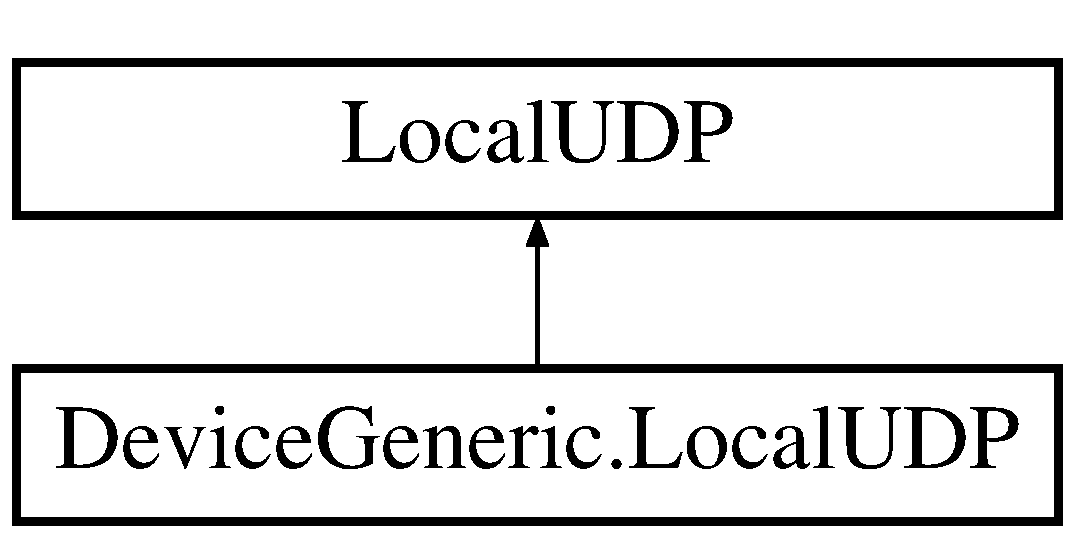
\includegraphics[height=2.000000cm]{classDeviceGeneric_1_1LocalUDP}
\end{center}
\end{figure}
\subsection*{Public Member Functions}
\begin{DoxyCompactItemize}
\item 
def \hyperlink{classDeviceGeneric_1_1LocalUDP_a3532595b6e51771b66383f702855b089}{receive}
\end{DoxyCompactItemize}


\subsection{Detailed Description}
\begin{DoxyVerb}...\end{DoxyVerb}
 

\subsection{Member Function Documentation}
\hypertarget{classDeviceGeneric_1_1LocalUDP_a3532595b6e51771b66383f702855b089}{\index{Device\-Generic\-::\-Local\-U\-D\-P@{Device\-Generic\-::\-Local\-U\-D\-P}!receive@{receive}}
\index{receive@{receive}!DeviceGeneric::LocalUDP@{Device\-Generic\-::\-Local\-U\-D\-P}}
\subsubsection[{receive}]{\setlength{\rightskip}{0pt plus 5cm}def Device\-Generic.\-Local\-U\-D\-P.\-receive (
\begin{DoxyParamCaption}
\item[{}]{self, }
\item[{}]{data, }
\item[{}]{length, }
\item[{}]{packet\-\_\-info}
\end{DoxyParamCaption}
)}}\label{classDeviceGeneric_1_1LocalUDP_a3532595b6e51771b66383f702855b089}
\begin{DoxyVerb}Receive function dummy to disable NotImplementedError.\end{DoxyVerb}
 

The documentation for this class was generated from the following file\-:\begin{DoxyCompactItemize}
\item 
O\-W\-P\-J\-O\-N/\-P\-J\-O\-N-\/cython/\hyperlink{DeviceGeneric_8py}{Device\-Generic.\-py}\end{DoxyCompactItemize}

\hypertarget{classtest_1_1test_1_1LocalUDP}{\section{test.\-test.\-Local\-U\-D\-P Class Reference}
\label{classtest_1_1test_1_1LocalUDP}\index{test.\-test.\-Local\-U\-D\-P@{test.\-test.\-Local\-U\-D\-P}}
}
Inheritance diagram for test.\-test.\-Local\-U\-D\-P\-:\begin{figure}[H]
\begin{center}
\leavevmode
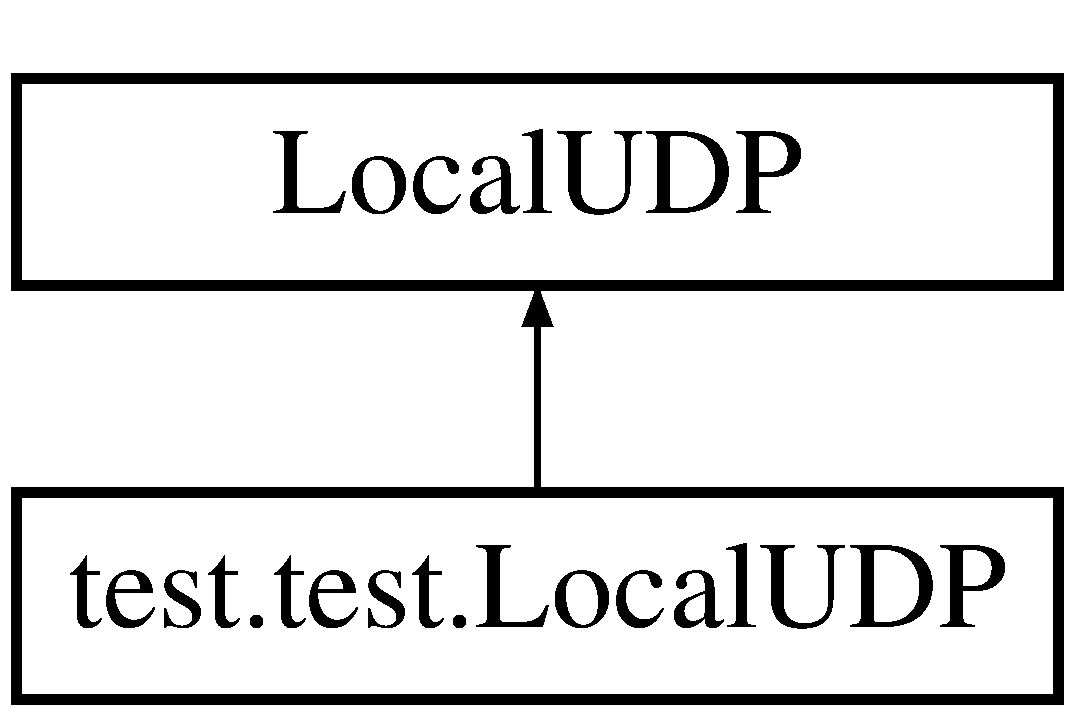
\includegraphics[height=2.000000cm]{classtest_1_1test_1_1LocalUDP}
\end{center}
\end{figure}
\subsection*{Public Member Functions}
\begin{DoxyCompactItemize}
\item 
def \hyperlink{classtest_1_1test_1_1LocalUDP_a89c98066425b2b72a665817690c870ec}{receive}
\item 
def \hyperlink{classtest_1_1test_1_1LocalUDP_ae514fd2c4056de70ffa044446167b08d}{\-\_\-\-\_\-init\-\_\-\-\_\-}
\end{DoxyCompactItemize}


\subsection{Constructor \& Destructor Documentation}
\hypertarget{classtest_1_1test_1_1LocalUDP_ae514fd2c4056de70ffa044446167b08d}{\index{test\-::test\-::\-Local\-U\-D\-P@{test\-::test\-::\-Local\-U\-D\-P}!\-\_\-\-\_\-init\-\_\-\-\_\-@{\-\_\-\-\_\-init\-\_\-\-\_\-}}
\index{\-\_\-\-\_\-init\-\_\-\-\_\-@{\-\_\-\-\_\-init\-\_\-\-\_\-}!test::test::LocalUDP@{test\-::test\-::\-Local\-U\-D\-P}}
\subsubsection[{\-\_\-\-\_\-init\-\_\-\-\_\-}]{\setlength{\rightskip}{0pt plus 5cm}def test.\-test.\-Local\-U\-D\-P.\-\_\-\-\_\-init\-\_\-\-\_\- (
\begin{DoxyParamCaption}
\item[{}]{self, }
\item[{}]{device\-\_\-id, }
\item[{}]{port = {\ttfamily None}}
\end{DoxyParamCaption}
)}}\label{classtest_1_1test_1_1LocalUDP_ae514fd2c4056de70ffa044446167b08d}


\subsection{Member Function Documentation}
\hypertarget{classtest_1_1test_1_1LocalUDP_a89c98066425b2b72a665817690c870ec}{\index{test\-::test\-::\-Local\-U\-D\-P@{test\-::test\-::\-Local\-U\-D\-P}!receive@{receive}}
\index{receive@{receive}!test::test::LocalUDP@{test\-::test\-::\-Local\-U\-D\-P}}
\subsubsection[{receive}]{\setlength{\rightskip}{0pt plus 5cm}def test.\-test.\-Local\-U\-D\-P.\-receive (
\begin{DoxyParamCaption}
\item[{}]{self, }
\item[{}]{data, }
\item[{}]{length, }
\item[{}]{packet\-\_\-info}
\end{DoxyParamCaption}
)}}\label{classtest_1_1test_1_1LocalUDP_a89c98066425b2b72a665817690c870ec}


The documentation for this class was generated from the following file\-:\begin{DoxyCompactItemize}
\item 
O\-W\-P\-J\-O\-N/\-P\-J\-O\-N-\/cython/test/\hyperlink{PJON-cython_2test_2test_8py}{test.\-py}\end{DoxyCompactItemize}

\hypertarget{structmax__align__t}{\section{max\-\_\-align\-\_\-t Struct Reference}
\label{structmax__align__t}\index{max\-\_\-align\-\_\-t@{max\-\_\-align\-\_\-t}}
}


{\ttfamily \#include $<$\-\_\-\-\_\-stddef\-\_\-max\-\_\-align\-\_\-t.\-h$>$}

\subsection*{Public Member Functions}
\begin{DoxyCompactItemize}
\item 
long long \-\_\-\-\_\-clang\-\_\-max\-\_\-align\-\_\-nonce1 \hyperlink{structmax__align__t_a4962b3f5174cd6d1d26f0e7c27b29c0d}{\-\_\-\-\_\-attribute\-\_\-\-\_\-} ((\-\_\-\-\_\-aligned\-\_\-\-\_\-(\-\_\-\-\_\-alignof\-\_\-\-\_\-(long long))))
\item 
long double \\*
\-\_\-\-\_\-clang\-\_\-max\-\_\-align\-\_\-nonce2 \hyperlink{structmax__align__t_af671ad5ae88de294ebf76b8803677991}{\-\_\-\-\_\-attribute\-\_\-\-\_\-} ((\-\_\-\-\_\-aligned\-\_\-\-\_\-(\-\_\-\-\_\-alignof\-\_\-\-\_\-(long double))))
\end{DoxyCompactItemize}


\subsection{Member Function Documentation}
\hypertarget{structmax__align__t_a4962b3f5174cd6d1d26f0e7c27b29c0d}{\index{max\-\_\-align\-\_\-t@{max\-\_\-align\-\_\-t}!\-\_\-\-\_\-attribute\-\_\-\-\_\-@{\-\_\-\-\_\-attribute\-\_\-\-\_\-}}
\index{\-\_\-\-\_\-attribute\-\_\-\-\_\-@{\-\_\-\-\_\-attribute\-\_\-\-\_\-}!max_align_t@{max\-\_\-align\-\_\-t}}
\subsubsection[{\-\_\-\-\_\-attribute\-\_\-\-\_\-}]{\setlength{\rightskip}{0pt plus 5cm}long long \-\_\-\-\_\-clang\-\_\-max\-\_\-align\-\_\-nonce1 max\-\_\-align\-\_\-t\-::\-\_\-\-\_\-attribute\-\_\-\-\_\- (
\begin{DoxyParamCaption}
\item[{(\-\_\-\-\_\-aligned\-\_\-\-\_\-(\-\_\-\-\_\-alignof\-\_\-\-\_\-(long long)))}]{}
\end{DoxyParamCaption}
)}}\label{structmax__align__t_a4962b3f5174cd6d1d26f0e7c27b29c0d}
\hypertarget{structmax__align__t_af671ad5ae88de294ebf76b8803677991}{\index{max\-\_\-align\-\_\-t@{max\-\_\-align\-\_\-t}!\-\_\-\-\_\-attribute\-\_\-\-\_\-@{\-\_\-\-\_\-attribute\-\_\-\-\_\-}}
\index{\-\_\-\-\_\-attribute\-\_\-\-\_\-@{\-\_\-\-\_\-attribute\-\_\-\-\_\-}!max_align_t@{max\-\_\-align\-\_\-t}}
\subsubsection[{\-\_\-\-\_\-attribute\-\_\-\-\_\-}]{\setlength{\rightskip}{0pt plus 5cm}long double \-\_\-\-\_\-clang\-\_\-max\-\_\-align\-\_\-nonce2 max\-\_\-align\-\_\-t\-::\-\_\-\-\_\-attribute\-\_\-\-\_\- (
\begin{DoxyParamCaption}
\item[{(\-\_\-\-\_\-aligned\-\_\-\-\_\-(\-\_\-\-\_\-alignof\-\_\-\-\_\-(long double)))}]{}
\end{DoxyParamCaption}
)}}\label{structmax__align__t_af671ad5ae88de294ebf76b8803677991}


The documentation for this struct was generated from the following file\-:\begin{DoxyCompactItemize}
\item 
oclint-\/0.\-10.\-3/lib/clang/3.\-8.\-0/include/\hyperlink{____stddef__max__align__t_8h}{\-\_\-\-\_\-stddef\-\_\-max\-\_\-align\-\_\-t.\-h}\end{DoxyCompactItemize}

\hypertarget{structmoat__call__t}{\section{moat\-\_\-call\-\_\-t Struct Reference}
\label{structmoat__call__t}\index{moat\-\_\-call\-\_\-t@{moat\-\_\-call\-\_\-t}}
}


{\ttfamily \#include $<$moat\-\_\-internal.\-h$>$}

\subsection*{Public Attributes}
\begin{DoxyCompactItemize}
\item 
\hyperlink{moat__internal_8h_a07d18b438c0a724a0cc8ebacac66b7f8}{init\-\_\-fn} $\ast$ \hyperlink{structmoat__call__t_a883c0fc11905fceaf1a8e720acfabef6}{init}
\item 
\hyperlink{moat__internal_8h_a922b8d86a9d68ff8833add121abbf297}{poll\-\_\-fn} $\ast$ \hyperlink{structmoat__call__t_a5ddda0c0889ec1f54c869ce3770258b4}{poll}
\item 
\hyperlink{moat__internal_8h_af1c576e31c7613f87e0fbc6d557d3967}{read\-\_\-len\-\_\-fn} $\ast$ \hyperlink{structmoat__call__t_a3092921758d95baf09cf3d489574ac3a}{read\-\_\-len}
\item 
\hyperlink{moat__internal_8h_aa1c9f75bd93d742fc465caab8790c57e}{read\-\_\-fn} $\ast$ \hyperlink{structmoat__call__t_a3bc9153322aa3df0bb573d04ce425db9}{read}
\item 
\hyperlink{moat__internal_8h_ad343b7b3aa64942922d1be815fd92056}{read\-\_\-done\-\_\-fn} $\ast$ \hyperlink{structmoat__call__t_a521a394e58d41f5f171402674107d054}{read\-\_\-done}
\item 
\hyperlink{moat__internal_8h_a507dde93db9c2398c1f69dbd6ccd0e93}{write\-\_\-check\-\_\-fn} $\ast$ \hyperlink{structmoat__call__t_ae99579d7f92a1edcb167dfe47fd9e283}{write\-\_\-check}
\item 
\hyperlink{moat__internal_8h_a487b499b005966352670a06e954ab5c3}{write\-\_\-fn} $\ast$ \hyperlink{structmoat__call__t_a2939e23081a18f1cb41df7f55e8c2c6a}{write}
\end{DoxyCompactItemize}


\subsection{Member Data Documentation}
\hypertarget{structmoat__call__t_a883c0fc11905fceaf1a8e720acfabef6}{\index{moat\-\_\-call\-\_\-t@{moat\-\_\-call\-\_\-t}!init@{init}}
\index{init@{init}!moat_call_t@{moat\-\_\-call\-\_\-t}}
\subsubsection[{init}]{\setlength{\rightskip}{0pt plus 5cm}{\bf init\-\_\-fn}$\ast$ moat\-\_\-call\-\_\-t\-::init}}\label{structmoat__call__t_a883c0fc11905fceaf1a8e720acfabef6}
\hypertarget{structmoat__call__t_a5ddda0c0889ec1f54c869ce3770258b4}{\index{moat\-\_\-call\-\_\-t@{moat\-\_\-call\-\_\-t}!poll@{poll}}
\index{poll@{poll}!moat_call_t@{moat\-\_\-call\-\_\-t}}
\subsubsection[{poll}]{\setlength{\rightskip}{0pt plus 5cm}{\bf poll\-\_\-fn}$\ast$ moat\-\_\-call\-\_\-t\-::poll}}\label{structmoat__call__t_a5ddda0c0889ec1f54c869ce3770258b4}
\hypertarget{structmoat__call__t_a3bc9153322aa3df0bb573d04ce425db9}{\index{moat\-\_\-call\-\_\-t@{moat\-\_\-call\-\_\-t}!read@{read}}
\index{read@{read}!moat_call_t@{moat\-\_\-call\-\_\-t}}
\subsubsection[{read}]{\setlength{\rightskip}{0pt plus 5cm}{\bf read\-\_\-fn}$\ast$ moat\-\_\-call\-\_\-t\-::read}}\label{structmoat__call__t_a3bc9153322aa3df0bb573d04ce425db9}
\hypertarget{structmoat__call__t_a521a394e58d41f5f171402674107d054}{\index{moat\-\_\-call\-\_\-t@{moat\-\_\-call\-\_\-t}!read\-\_\-done@{read\-\_\-done}}
\index{read\-\_\-done@{read\-\_\-done}!moat_call_t@{moat\-\_\-call\-\_\-t}}
\subsubsection[{read\-\_\-done}]{\setlength{\rightskip}{0pt plus 5cm}{\bf read\-\_\-done\-\_\-fn}$\ast$ moat\-\_\-call\-\_\-t\-::read\-\_\-done}}\label{structmoat__call__t_a521a394e58d41f5f171402674107d054}
\hypertarget{structmoat__call__t_a3092921758d95baf09cf3d489574ac3a}{\index{moat\-\_\-call\-\_\-t@{moat\-\_\-call\-\_\-t}!read\-\_\-len@{read\-\_\-len}}
\index{read\-\_\-len@{read\-\_\-len}!moat_call_t@{moat\-\_\-call\-\_\-t}}
\subsubsection[{read\-\_\-len}]{\setlength{\rightskip}{0pt plus 5cm}{\bf read\-\_\-len\-\_\-fn}$\ast$ moat\-\_\-call\-\_\-t\-::read\-\_\-len}}\label{structmoat__call__t_a3092921758d95baf09cf3d489574ac3a}
\hypertarget{structmoat__call__t_a2939e23081a18f1cb41df7f55e8c2c6a}{\index{moat\-\_\-call\-\_\-t@{moat\-\_\-call\-\_\-t}!write@{write}}
\index{write@{write}!moat_call_t@{moat\-\_\-call\-\_\-t}}
\subsubsection[{write}]{\setlength{\rightskip}{0pt plus 5cm}{\bf write\-\_\-fn}$\ast$ moat\-\_\-call\-\_\-t\-::write}}\label{structmoat__call__t_a2939e23081a18f1cb41df7f55e8c2c6a}
\hypertarget{structmoat__call__t_ae99579d7f92a1edcb167dfe47fd9e283}{\index{moat\-\_\-call\-\_\-t@{moat\-\_\-call\-\_\-t}!write\-\_\-check@{write\-\_\-check}}
\index{write\-\_\-check@{write\-\_\-check}!moat_call_t@{moat\-\_\-call\-\_\-t}}
\subsubsection[{write\-\_\-check}]{\setlength{\rightskip}{0pt plus 5cm}{\bf write\-\_\-check\-\_\-fn}$\ast$ moat\-\_\-call\-\_\-t\-::write\-\_\-check}}\label{structmoat__call__t_ae99579d7f92a1edcb167dfe47fd9e283}


The documentation for this struct was generated from the following file\-:\begin{DoxyCompactItemize}
\item 
cli/owslave/\hyperlink{moat__internal_8h}{moat\-\_\-internal.\-h}\end{DoxyCompactItemize}

\hypertarget{classMultiWiiConf}{\section{Multi\-Wii\-Conf Class Reference}
\label{classMultiWiiConf}\index{Multi\-Wii\-Conf@{Multi\-Wii\-Conf}}
}
Inheritance diagram for Multi\-Wii\-Conf\-:\begin{figure}[H]
\begin{center}
\leavevmode
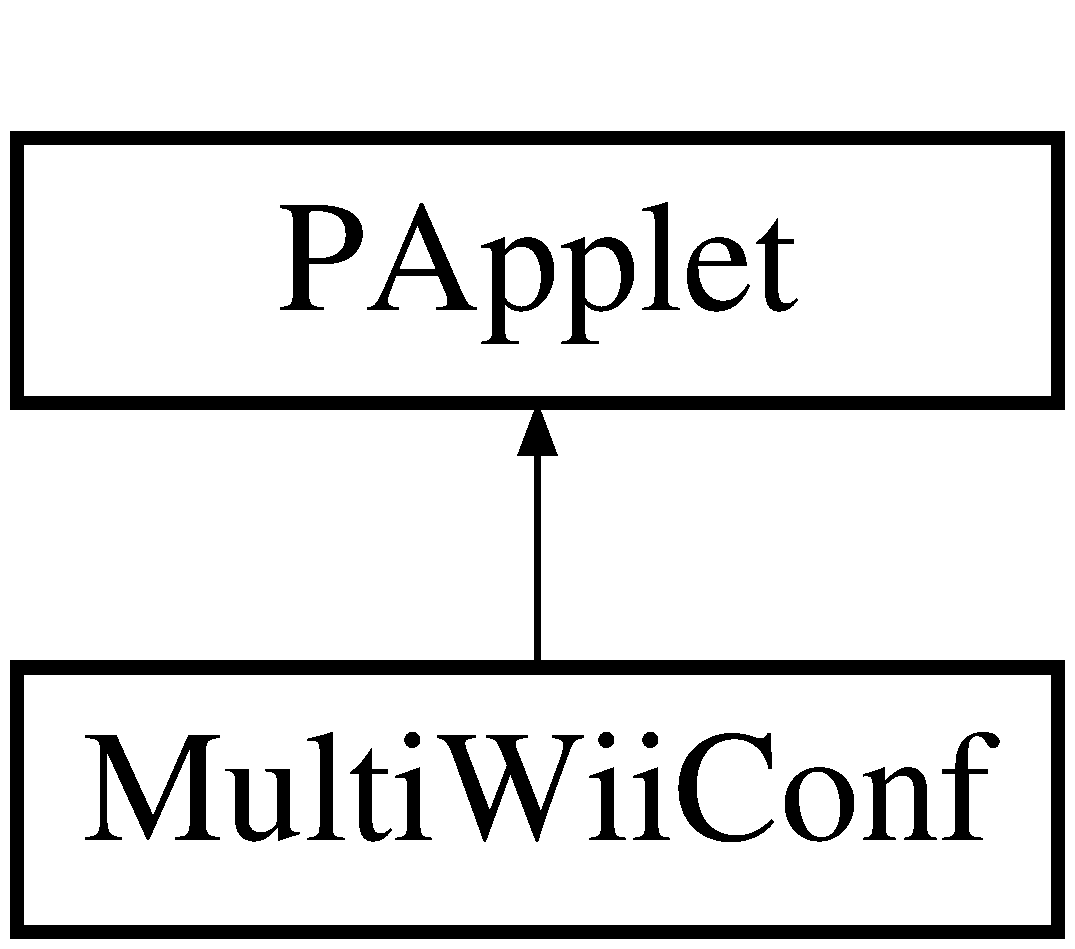
\includegraphics[height=2.000000cm]{classMultiWiiConf}
\end{center}
\end{figure}
\subsection*{Classes}
\begin{DoxyCompactItemize}
\item 
class {\bfseries c\-Data\-Array}
\item 
class {\bfseries c\-Graph}
\item 
class {\bfseries M\-W\-I}
\item 
class \hyperlink{classMultiWiiConf_1_1MwiFileFilter}{Mwi\-File\-Filter}
\end{DoxyCompactItemize}
\subsection*{Public Member Functions}
\begin{DoxyCompactItemize}
\item 
void \hyperlink{classMultiWiiConf_a258e9697d588ea99af87ec28247e4e16}{create\-\_\-\-Gimbal\-Graphics} ()
\item 
void \hyperlink{classMultiWiiConf_a588a52b9b9194d6b7f62662474d57c55}{create\-\_\-\-Servo\-Graphics} ()
\item 
void \hyperlink{classMultiWiiConf_a926ade417ce21f3326c93f8bd1348c77}{create\-\_\-checkboxes} (String\mbox{[}$\,$\mbox{]} names)
\item 
String \hyperlink{classMultiWiiConf_a1c2dc8d157b78a114b18efce73a082c3}{shortify\-Port\-Name} (String port\-Name, int maxlen)
\item 
control\-P5.\-Controller \hyperlink{classMultiWiiConf_a035c449396cb5812f5af4bf9e9c88cfc}{hide\-Label} (control\-P5.\-Controller c)
\item 
void \hyperlink{classMultiWiiConf_a8b52584570b1367ee4ce93e112fbd0ca}{setup} ()
\item 
int \hyperlink{classMultiWiiConf_aab7fc403f177393a58e0006fd38882cb}{read32} ()
\item 
int \hyperlink{classMultiWiiConf_a013c041b164d4a46b4c3444a8ba21cc1}{read16} ()
\item 
int \hyperlink{classMultiWiiConf_aeefc4968d2588d9158941d340486e993}{read8} ()
\item 
void \hyperlink{classMultiWiiConf_aa113c0a77055b4b010b2c4033e510f8e}{send\-Request\-M\-S\-P} (List$<$ Byte $>$ msp)
\item 
void \hyperlink{classMultiWiiConf_ad8ccf8a1d553340481337ca747754a13}{evaluate\-Command} (byte cmd, int data\-Size)
\item 
void \hyperlink{classMultiWiiConf_a94c00cd9bbdb03acbe78a3bde4141cea}{draw} ()
\item 
void \hyperlink{classMultiWiiConf_a2fc869dfda4cb57606fee25d1e3c8c78}{draw\-Motor} (float x1, float y1, int mot\-\_\-num, char dir)
\item 
void \hyperlink{classMultiWiiConf_adbfd907cb05cd32e61f5ac383baddbcd}{A\-C\-C\-\_\-\-R\-O\-L\-L} (boolean the\-Flag)
\item 
void \hyperlink{classMultiWiiConf_aa7c58b0a234c718599c60146e11aeaa2}{A\-C\-C\-\_\-\-P\-I\-T\-C\-H} (boolean the\-Flag)
\item 
void \hyperlink{classMultiWiiConf_afdc8f5a7f9dc70e2c23aa04418a2b80d}{A\-C\-C\-\_\-\-Z} (boolean the\-Flag)
\item 
void \hyperlink{classMultiWiiConf_ad2bba48b0cd3fcb136bb9a09ecf0cb97}{G\-Y\-R\-O\-\_\-\-R\-O\-L\-L} (boolean the\-Flag)
\item 
void \hyperlink{classMultiWiiConf_a5ce8a311ad06521d726afa6df0fb1ee1}{G\-Y\-R\-O\-\_\-\-P\-I\-T\-C\-H} (boolean the\-Flag)
\item 
void \hyperlink{classMultiWiiConf_a8de2c98857b1124230c10e3ae343accd}{G\-Y\-R\-O\-\_\-\-Y\-A\-W} (boolean the\-Flag)
\item 
void \hyperlink{classMultiWiiConf_ab2b544742052cc0f398e6d254dbf7208}{B\-A\-R\-O} (boolean the\-Flag)
\item 
void \hyperlink{classMultiWiiConf_a60b6a9d19c3a12f0a651e4a5fc4d2041}{H\-E\-A\-D} (boolean the\-Flag)
\item 
void \hyperlink{classMultiWiiConf_aa99d38abfa52b1977943450ab0b913ee}{M\-A\-G\-X} (boolean the\-Flag)
\item 
void \hyperlink{classMultiWiiConf_a255680567522dc391e65783f7dab433a}{M\-A\-G\-Y} (boolean the\-Flag)
\item 
void \hyperlink{classMultiWiiConf_aee488258d4ab0d58342d8be981773d49}{M\-A\-G\-Z} (boolean the\-Flag)
\item 
void \hyperlink{classMultiWiiConf_ace07c9638854159fd9648817459846de}{D\-E\-B\-U\-G1} (boolean the\-Flag)
\item 
void \hyperlink{classMultiWiiConf_a25f6849faf310fc390b3a509a1308edd}{D\-E\-B\-U\-G2} (boolean the\-Flag)
\item 
void \hyperlink{classMultiWiiConf_a4ee09f16beb6d49cc21b202a163af55d}{D\-E\-B\-U\-G3} (boolean the\-Flag)
\item 
void \hyperlink{classMultiWiiConf_a361d6de42848acf39896f4e1201028c2}{D\-E\-B\-U\-G4} (boolean the\-Flag)
\item 
void \hyperlink{classMultiWiiConf_a9b359c242f40d6dc074f45fbb79dee15}{control\-Event} (Control\-Event the\-Event)
\item 
void \hyperlink{classMultiWiiConf_a5d3204c23c47ac82aa08c5043022a504}{b\-S\-T\-A\-R\-T} ()
\item 
void \hyperlink{classMultiWiiConf_a3e0767e03653e3486978e2ba9a7463ea}{b\-S\-T\-O\-P} ()
\item 
void \hyperlink{classMultiWiiConf_a912ca48c44dc4cd130f75ecdccf7da84}{S\-E\-T\-T\-I\-N\-G} ()
\item 
void \hyperlink{classMultiWiiConf_a5157e3fae162d740189e25adca5dad1e}{G\-I\-M\-B\-A\-L} ()
\item 
void \hyperlink{classMultiWiiConf_a7707921bbef91c191fcf7b9b57707c7b}{T\-R\-I\-G\-G\-E\-R} ()
\item 
void \hyperlink{classMultiWiiConf_a2c5626b2259e329d5501da2609875c19}{R\-E\-A\-D} ()
\item 
void \hyperlink{classMultiWiiConf_a51b5f517a679dd129e8226cdfbd1d052}{R\-E\-S\-E\-T} ()
\item 
void \hyperlink{classMultiWiiConf_a3de7c01db79331e4ae6d75ddab9eedcc}{W\-R\-I\-T\-E} ()
\item 
void \hyperlink{classMultiWiiConf_aea8b2d0db9fb1ba3c1f83bf339e13573}{L\-I\-V\-E\-\_\-\-S\-E\-R\-V\-O} ()
\item 
void \hyperlink{classMultiWiiConf_acc41b4d048f1bafd56534ed2b69ff790}{S\-A\-V\-E\-\_\-\-W\-I\-N\-G} ()
\item 
void \hyperlink{classMultiWiiConf_aff39ce24b10a21b47f19007bc1548463}{S\-A\-V\-E\-\_\-\-Servo} ()
\item 
void \hyperlink{classMultiWiiConf_a56dbe3488934b1cd45fe8d85f810383a}{W\-I\-N\-G} ()
\item 
void \hyperlink{classMultiWiiConf_a86f14ce1d6f3832a8566674b79439a29}{S\-E\-R\-V\-O} ()
\item 
void \hyperlink{classMultiWiiConf_afcaa86ab6487c949b55d21a09233cd6d}{C\-A\-L\-I\-B\-\_\-\-A\-C\-C} ()
\item 
void \hyperlink{classMultiWiiConf_a53f8586a159a0771380e69bf2fe4a03d}{C\-A\-L\-I\-B\-\_\-\-M\-A\-G} ()
\item 
void \hyperlink{classMultiWiiConf_ad3b31ce5a10521c304a47aee0b63035f}{Init\-Serial} (float port\-Value)
\item 
void \hyperlink{classMultiWiiConf_ad0685ad60f2ab83d769fee5aaa597950}{Save\-Serial\-Port} (String port)
\item 
void \hyperlink{classMultiWiiConf_a42a4b3766358fb85ef2da8be3cff0b85}{Eport\-\_\-\-Servo} ()
\item 
void \hyperlink{classMultiWiiConf_accbc975f7d37014059827e3cd9e8f787}{S\-A\-V\-E\-\_\-\-S\-E\-R\-V\-O\-\_\-\-C\-O\-N\-F\-I\-G} ()
\item 
void \hyperlink{classMultiWiiConf_ac97009142868c50faca724fb1e138ea1}{b\-Q\-C\-O\-N\-N} ()
\item 
void \hyperlink{classMultiWiiConf_af7c440cc4348b741e7c0129912ab02b6}{Cau0} ()
\item 
void \hyperlink{classMultiWiiConf_aed32c4524c48488a9cb7996bf18f87c2}{Cau1} ()
\item 
void \hyperlink{classMultiWiiConf_ac0581f16afefe73eda1d9fd3c49619e9}{Cau2} ()
\item 
void \hyperlink{classMultiWiiConf_a390839149da4f3010a44ae9198224d82}{Cau3} ()
\item 
void \hyperlink{classMultiWiiConf_a52188c481473e6840c32819a1bb59b87}{Cau4} ()
\item 
void \hyperlink{classMultiWiiConf_a4f7d659bc40a7a1d3ea1578302f85897}{Cau\-Clear} ()
\item 
void \hyperlink{classMultiWiiConf_acdf30272639726614b0b6c817a61d791}{Read\-Serial\-Port} ()
\item 
void \hyperlink{classMultiWiiConf_a1fce4aba9f4303d1859ed3122f6d6cf5}{b\-S\-A\-V\-E} ()
\item 
void \hyperlink{classMultiWiiConf_a6cdbed88e5d94db4ee58b70f299f5dc0}{b\-I\-M\-P\-O\-R\-T} ()
\item 
void \hyperlink{classMultiWiiConf_ae152c1f5d8b20485ff92a20b8d15f9fb}{update\-Model} ()
\item 
void \hyperlink{classMultiWiiConf_a02f7cd92c516edf9ba014433209c5e66}{update\-Model\-M\-S\-P\-\_\-\-S\-E\-T\-\_\-\-R\-C\-\_\-\-T\-U\-N\-I\-N\-G} ()
\item 
void \hyperlink{classMultiWiiConf_a757bd807090b63a8142667d090b41542}{update\-Model\-M\-S\-P\-\_\-\-S\-E\-T\-\_\-\-P\-I\-D} ()
\item 
void \hyperlink{classMultiWiiConf_a57633ac74ed66b9f52afe79aec9d6f56}{update\-Model\-M\-S\-P\-\_\-\-S\-E\-T\-\_\-\-M\-I\-S\-C} ()
\item 
void \hyperlink{classMultiWiiConf_ac88fe7ed959b47cf8519b35ef8c77c05}{update\-View} ()
\item 
void \hyperlink{classMultiWiiConf_a6325b24efa261211d04156d1c05cfcca}{b\-R\-Xbind} ()
\item 
void \hyperlink{classMultiWiiConf_a5eb513429b08b77f4cb2f656bcaced6f}{add\-Tabs} ()
\item 
void \hyperlink{classMultiWiiConf_a6bc6be0898feb09f6693b7e3b7d3f6fe}{Mag\-Decl} ()
\item 
void \hyperlink{classMultiWiiConf_a9c993ed28846ae789acdbdb93f8f17d7}{M\-Wii\-Home} ()
\item 
void \hyperlink{classMultiWiiConf_a6523326eff761ad689372a4373065e2b}{M\-Wii\-Get} ()
\item 
void \hyperlink{classMultiWiiConf_ace168f10f8c5bf01bc3739f5f218b6e9}{Tooltips} ()
\end{DoxyCompactItemize}
\subsection*{Static Public Member Functions}
\begin{DoxyCompactItemize}
\item 
static void \hyperlink{classMultiWiiConf_a844c042472c9c11dbd805cf36ccebafd}{main} (String args\mbox{[}$\,$\mbox{]})
\end{DoxyCompactItemize}
\subsection*{Static Public Attributes}
\begin{DoxyCompactItemize}
\item 
static final int \hyperlink{classMultiWiiConf_a2c1552d736cd36dd9a0bdac6bb1c48ea}{I\-D\-L\-E} = 0
\end{DoxyCompactItemize}


\subsection{Member Function Documentation}
\hypertarget{classMultiWiiConf_aa7c58b0a234c718599c60146e11aeaa2}{\index{Multi\-Wii\-Conf@{Multi\-Wii\-Conf}!A\-C\-C\-\_\-\-P\-I\-T\-C\-H@{A\-C\-C\-\_\-\-P\-I\-T\-C\-H}}
\index{A\-C\-C\-\_\-\-P\-I\-T\-C\-H@{A\-C\-C\-\_\-\-P\-I\-T\-C\-H}!MultiWiiConf@{Multi\-Wii\-Conf}}
\subsubsection[{A\-C\-C\-\_\-\-P\-I\-T\-C\-H}]{\setlength{\rightskip}{0pt plus 5cm}void Multi\-Wii\-Conf.\-A\-C\-C\-\_\-\-P\-I\-T\-C\-H (
\begin{DoxyParamCaption}
\item[{boolean}]{the\-Flag}
\end{DoxyParamCaption}
)\hspace{0.3cm}{\ttfamily [inline]}}}\label{classMultiWiiConf_aa7c58b0a234c718599c60146e11aeaa2}
\hypertarget{classMultiWiiConf_adbfd907cb05cd32e61f5ac383baddbcd}{\index{Multi\-Wii\-Conf@{Multi\-Wii\-Conf}!A\-C\-C\-\_\-\-R\-O\-L\-L@{A\-C\-C\-\_\-\-R\-O\-L\-L}}
\index{A\-C\-C\-\_\-\-R\-O\-L\-L@{A\-C\-C\-\_\-\-R\-O\-L\-L}!MultiWiiConf@{Multi\-Wii\-Conf}}
\subsubsection[{A\-C\-C\-\_\-\-R\-O\-L\-L}]{\setlength{\rightskip}{0pt plus 5cm}void Multi\-Wii\-Conf.\-A\-C\-C\-\_\-\-R\-O\-L\-L (
\begin{DoxyParamCaption}
\item[{boolean}]{the\-Flag}
\end{DoxyParamCaption}
)\hspace{0.3cm}{\ttfamily [inline]}}}\label{classMultiWiiConf_adbfd907cb05cd32e61f5ac383baddbcd}
\hypertarget{classMultiWiiConf_afdc8f5a7f9dc70e2c23aa04418a2b80d}{\index{Multi\-Wii\-Conf@{Multi\-Wii\-Conf}!A\-C\-C\-\_\-\-Z@{A\-C\-C\-\_\-\-Z}}
\index{A\-C\-C\-\_\-\-Z@{A\-C\-C\-\_\-\-Z}!MultiWiiConf@{Multi\-Wii\-Conf}}
\subsubsection[{A\-C\-C\-\_\-\-Z}]{\setlength{\rightskip}{0pt plus 5cm}void Multi\-Wii\-Conf.\-A\-C\-C\-\_\-\-Z (
\begin{DoxyParamCaption}
\item[{boolean}]{the\-Flag}
\end{DoxyParamCaption}
)\hspace{0.3cm}{\ttfamily [inline]}}}\label{classMultiWiiConf_afdc8f5a7f9dc70e2c23aa04418a2b80d}
\hypertarget{classMultiWiiConf_a5eb513429b08b77f4cb2f656bcaced6f}{\index{Multi\-Wii\-Conf@{Multi\-Wii\-Conf}!add\-Tabs@{add\-Tabs}}
\index{add\-Tabs@{add\-Tabs}!MultiWiiConf@{Multi\-Wii\-Conf}}
\subsubsection[{add\-Tabs}]{\setlength{\rightskip}{0pt plus 5cm}void Multi\-Wii\-Conf.\-add\-Tabs (
\begin{DoxyParamCaption}
{}
\end{DoxyParamCaption}
)\hspace{0.3cm}{\ttfamily [inline]}}}\label{classMultiWiiConf_a5eb513429b08b77f4cb2f656bcaced6f}
\hypertarget{classMultiWiiConf_ab2b544742052cc0f398e6d254dbf7208}{\index{Multi\-Wii\-Conf@{Multi\-Wii\-Conf}!B\-A\-R\-O@{B\-A\-R\-O}}
\index{B\-A\-R\-O@{B\-A\-R\-O}!MultiWiiConf@{Multi\-Wii\-Conf}}
\subsubsection[{B\-A\-R\-O}]{\setlength{\rightskip}{0pt plus 5cm}void Multi\-Wii\-Conf.\-B\-A\-R\-O (
\begin{DoxyParamCaption}
\item[{boolean}]{the\-Flag}
\end{DoxyParamCaption}
)\hspace{0.3cm}{\ttfamily [inline]}}}\label{classMultiWiiConf_ab2b544742052cc0f398e6d254dbf7208}
\hypertarget{classMultiWiiConf_a6cdbed88e5d94db4ee58b70f299f5dc0}{\index{Multi\-Wii\-Conf@{Multi\-Wii\-Conf}!b\-I\-M\-P\-O\-R\-T@{b\-I\-M\-P\-O\-R\-T}}
\index{b\-I\-M\-P\-O\-R\-T@{b\-I\-M\-P\-O\-R\-T}!MultiWiiConf@{Multi\-Wii\-Conf}}
\subsubsection[{b\-I\-M\-P\-O\-R\-T}]{\setlength{\rightskip}{0pt plus 5cm}void Multi\-Wii\-Conf.\-b\-I\-M\-P\-O\-R\-T (
\begin{DoxyParamCaption}
{}
\end{DoxyParamCaption}
)\hspace{0.3cm}{\ttfamily [inline]}}}\label{classMultiWiiConf_a6cdbed88e5d94db4ee58b70f299f5dc0}
\hypertarget{classMultiWiiConf_ac97009142868c50faca724fb1e138ea1}{\index{Multi\-Wii\-Conf@{Multi\-Wii\-Conf}!b\-Q\-C\-O\-N\-N@{b\-Q\-C\-O\-N\-N}}
\index{b\-Q\-C\-O\-N\-N@{b\-Q\-C\-O\-N\-N}!MultiWiiConf@{Multi\-Wii\-Conf}}
\subsubsection[{b\-Q\-C\-O\-N\-N}]{\setlength{\rightskip}{0pt plus 5cm}void Multi\-Wii\-Conf.\-b\-Q\-C\-O\-N\-N (
\begin{DoxyParamCaption}
{}
\end{DoxyParamCaption}
)\hspace{0.3cm}{\ttfamily [inline]}}}\label{classMultiWiiConf_ac97009142868c50faca724fb1e138ea1}
\hypertarget{classMultiWiiConf_a6325b24efa261211d04156d1c05cfcca}{\index{Multi\-Wii\-Conf@{Multi\-Wii\-Conf}!b\-R\-Xbind@{b\-R\-Xbind}}
\index{b\-R\-Xbind@{b\-R\-Xbind}!MultiWiiConf@{Multi\-Wii\-Conf}}
\subsubsection[{b\-R\-Xbind}]{\setlength{\rightskip}{0pt plus 5cm}void Multi\-Wii\-Conf.\-b\-R\-Xbind (
\begin{DoxyParamCaption}
{}
\end{DoxyParamCaption}
)\hspace{0.3cm}{\ttfamily [inline]}}}\label{classMultiWiiConf_a6325b24efa261211d04156d1c05cfcca}
\hypertarget{classMultiWiiConf_a1fce4aba9f4303d1859ed3122f6d6cf5}{\index{Multi\-Wii\-Conf@{Multi\-Wii\-Conf}!b\-S\-A\-V\-E@{b\-S\-A\-V\-E}}
\index{b\-S\-A\-V\-E@{b\-S\-A\-V\-E}!MultiWiiConf@{Multi\-Wii\-Conf}}
\subsubsection[{b\-S\-A\-V\-E}]{\setlength{\rightskip}{0pt plus 5cm}void Multi\-Wii\-Conf.\-b\-S\-A\-V\-E (
\begin{DoxyParamCaption}
{}
\end{DoxyParamCaption}
)\hspace{0.3cm}{\ttfamily [inline]}}}\label{classMultiWiiConf_a1fce4aba9f4303d1859ed3122f6d6cf5}
\hypertarget{classMultiWiiConf_a5d3204c23c47ac82aa08c5043022a504}{\index{Multi\-Wii\-Conf@{Multi\-Wii\-Conf}!b\-S\-T\-A\-R\-T@{b\-S\-T\-A\-R\-T}}
\index{b\-S\-T\-A\-R\-T@{b\-S\-T\-A\-R\-T}!MultiWiiConf@{Multi\-Wii\-Conf}}
\subsubsection[{b\-S\-T\-A\-R\-T}]{\setlength{\rightskip}{0pt plus 5cm}void Multi\-Wii\-Conf.\-b\-S\-T\-A\-R\-T (
\begin{DoxyParamCaption}
{}
\end{DoxyParamCaption}
)\hspace{0.3cm}{\ttfamily [inline]}}}\label{classMultiWiiConf_a5d3204c23c47ac82aa08c5043022a504}
\hypertarget{classMultiWiiConf_a3e0767e03653e3486978e2ba9a7463ea}{\index{Multi\-Wii\-Conf@{Multi\-Wii\-Conf}!b\-S\-T\-O\-P@{b\-S\-T\-O\-P}}
\index{b\-S\-T\-O\-P@{b\-S\-T\-O\-P}!MultiWiiConf@{Multi\-Wii\-Conf}}
\subsubsection[{b\-S\-T\-O\-P}]{\setlength{\rightskip}{0pt plus 5cm}void Multi\-Wii\-Conf.\-b\-S\-T\-O\-P (
\begin{DoxyParamCaption}
{}
\end{DoxyParamCaption}
)\hspace{0.3cm}{\ttfamily [inline]}}}\label{classMultiWiiConf_a3e0767e03653e3486978e2ba9a7463ea}
\hypertarget{classMultiWiiConf_afcaa86ab6487c949b55d21a09233cd6d}{\index{Multi\-Wii\-Conf@{Multi\-Wii\-Conf}!C\-A\-L\-I\-B\-\_\-\-A\-C\-C@{C\-A\-L\-I\-B\-\_\-\-A\-C\-C}}
\index{C\-A\-L\-I\-B\-\_\-\-A\-C\-C@{C\-A\-L\-I\-B\-\_\-\-A\-C\-C}!MultiWiiConf@{Multi\-Wii\-Conf}}
\subsubsection[{C\-A\-L\-I\-B\-\_\-\-A\-C\-C}]{\setlength{\rightskip}{0pt plus 5cm}void Multi\-Wii\-Conf.\-C\-A\-L\-I\-B\-\_\-\-A\-C\-C (
\begin{DoxyParamCaption}
{}
\end{DoxyParamCaption}
)\hspace{0.3cm}{\ttfamily [inline]}}}\label{classMultiWiiConf_afcaa86ab6487c949b55d21a09233cd6d}
\hypertarget{classMultiWiiConf_a53f8586a159a0771380e69bf2fe4a03d}{\index{Multi\-Wii\-Conf@{Multi\-Wii\-Conf}!C\-A\-L\-I\-B\-\_\-\-M\-A\-G@{C\-A\-L\-I\-B\-\_\-\-M\-A\-G}}
\index{C\-A\-L\-I\-B\-\_\-\-M\-A\-G@{C\-A\-L\-I\-B\-\_\-\-M\-A\-G}!MultiWiiConf@{Multi\-Wii\-Conf}}
\subsubsection[{C\-A\-L\-I\-B\-\_\-\-M\-A\-G}]{\setlength{\rightskip}{0pt plus 5cm}void Multi\-Wii\-Conf.\-C\-A\-L\-I\-B\-\_\-\-M\-A\-G (
\begin{DoxyParamCaption}
{}
\end{DoxyParamCaption}
)\hspace{0.3cm}{\ttfamily [inline]}}}\label{classMultiWiiConf_a53f8586a159a0771380e69bf2fe4a03d}
\hypertarget{classMultiWiiConf_af7c440cc4348b741e7c0129912ab02b6}{\index{Multi\-Wii\-Conf@{Multi\-Wii\-Conf}!Cau0@{Cau0}}
\index{Cau0@{Cau0}!MultiWiiConf@{Multi\-Wii\-Conf}}
\subsubsection[{Cau0}]{\setlength{\rightskip}{0pt plus 5cm}void Multi\-Wii\-Conf.\-Cau0 (
\begin{DoxyParamCaption}
{}
\end{DoxyParamCaption}
)\hspace{0.3cm}{\ttfamily [inline]}}}\label{classMultiWiiConf_af7c440cc4348b741e7c0129912ab02b6}
\hypertarget{classMultiWiiConf_aed32c4524c48488a9cb7996bf18f87c2}{\index{Multi\-Wii\-Conf@{Multi\-Wii\-Conf}!Cau1@{Cau1}}
\index{Cau1@{Cau1}!MultiWiiConf@{Multi\-Wii\-Conf}}
\subsubsection[{Cau1}]{\setlength{\rightskip}{0pt plus 5cm}void Multi\-Wii\-Conf.\-Cau1 (
\begin{DoxyParamCaption}
{}
\end{DoxyParamCaption}
)\hspace{0.3cm}{\ttfamily [inline]}}}\label{classMultiWiiConf_aed32c4524c48488a9cb7996bf18f87c2}
\hypertarget{classMultiWiiConf_ac0581f16afefe73eda1d9fd3c49619e9}{\index{Multi\-Wii\-Conf@{Multi\-Wii\-Conf}!Cau2@{Cau2}}
\index{Cau2@{Cau2}!MultiWiiConf@{Multi\-Wii\-Conf}}
\subsubsection[{Cau2}]{\setlength{\rightskip}{0pt plus 5cm}void Multi\-Wii\-Conf.\-Cau2 (
\begin{DoxyParamCaption}
{}
\end{DoxyParamCaption}
)\hspace{0.3cm}{\ttfamily [inline]}}}\label{classMultiWiiConf_ac0581f16afefe73eda1d9fd3c49619e9}
\hypertarget{classMultiWiiConf_a390839149da4f3010a44ae9198224d82}{\index{Multi\-Wii\-Conf@{Multi\-Wii\-Conf}!Cau3@{Cau3}}
\index{Cau3@{Cau3}!MultiWiiConf@{Multi\-Wii\-Conf}}
\subsubsection[{Cau3}]{\setlength{\rightskip}{0pt plus 5cm}void Multi\-Wii\-Conf.\-Cau3 (
\begin{DoxyParamCaption}
{}
\end{DoxyParamCaption}
)\hspace{0.3cm}{\ttfamily [inline]}}}\label{classMultiWiiConf_a390839149da4f3010a44ae9198224d82}
\hypertarget{classMultiWiiConf_a52188c481473e6840c32819a1bb59b87}{\index{Multi\-Wii\-Conf@{Multi\-Wii\-Conf}!Cau4@{Cau4}}
\index{Cau4@{Cau4}!MultiWiiConf@{Multi\-Wii\-Conf}}
\subsubsection[{Cau4}]{\setlength{\rightskip}{0pt plus 5cm}void Multi\-Wii\-Conf.\-Cau4 (
\begin{DoxyParamCaption}
{}
\end{DoxyParamCaption}
)\hspace{0.3cm}{\ttfamily [inline]}}}\label{classMultiWiiConf_a52188c481473e6840c32819a1bb59b87}
\hypertarget{classMultiWiiConf_a4f7d659bc40a7a1d3ea1578302f85897}{\index{Multi\-Wii\-Conf@{Multi\-Wii\-Conf}!Cau\-Clear@{Cau\-Clear}}
\index{Cau\-Clear@{Cau\-Clear}!MultiWiiConf@{Multi\-Wii\-Conf}}
\subsubsection[{Cau\-Clear}]{\setlength{\rightskip}{0pt plus 5cm}void Multi\-Wii\-Conf.\-Cau\-Clear (
\begin{DoxyParamCaption}
{}
\end{DoxyParamCaption}
)\hspace{0.3cm}{\ttfamily [inline]}}}\label{classMultiWiiConf_a4f7d659bc40a7a1d3ea1578302f85897}
\hypertarget{classMultiWiiConf_a9b359c242f40d6dc074f45fbb79dee15}{\index{Multi\-Wii\-Conf@{Multi\-Wii\-Conf}!control\-Event@{control\-Event}}
\index{control\-Event@{control\-Event}!MultiWiiConf@{Multi\-Wii\-Conf}}
\subsubsection[{control\-Event}]{\setlength{\rightskip}{0pt plus 5cm}void Multi\-Wii\-Conf.\-control\-Event (
\begin{DoxyParamCaption}
\item[{Control\-Event}]{the\-Event}
\end{DoxyParamCaption}
)\hspace{0.3cm}{\ttfamily [inline]}}}\label{classMultiWiiConf_a9b359c242f40d6dc074f45fbb79dee15}
\hypertarget{classMultiWiiConf_a926ade417ce21f3326c93f8bd1348c77}{\index{Multi\-Wii\-Conf@{Multi\-Wii\-Conf}!create\-\_\-checkboxes@{create\-\_\-checkboxes}}
\index{create\-\_\-checkboxes@{create\-\_\-checkboxes}!MultiWiiConf@{Multi\-Wii\-Conf}}
\subsubsection[{create\-\_\-checkboxes}]{\setlength{\rightskip}{0pt plus 5cm}void Multi\-Wii\-Conf.\-create\-\_\-checkboxes (
\begin{DoxyParamCaption}
\item[{String\mbox{[}$\,$\mbox{]}}]{names}
\end{DoxyParamCaption}
)\hspace{0.3cm}{\ttfamily [inline]}}}\label{classMultiWiiConf_a926ade417ce21f3326c93f8bd1348c77}
\hypertarget{classMultiWiiConf_a258e9697d588ea99af87ec28247e4e16}{\index{Multi\-Wii\-Conf@{Multi\-Wii\-Conf}!create\-\_\-\-Gimbal\-Graphics@{create\-\_\-\-Gimbal\-Graphics}}
\index{create\-\_\-\-Gimbal\-Graphics@{create\-\_\-\-Gimbal\-Graphics}!MultiWiiConf@{Multi\-Wii\-Conf}}
\subsubsection[{create\-\_\-\-Gimbal\-Graphics}]{\setlength{\rightskip}{0pt plus 5cm}void Multi\-Wii\-Conf.\-create\-\_\-\-Gimbal\-Graphics (
\begin{DoxyParamCaption}
{}
\end{DoxyParamCaption}
)\hspace{0.3cm}{\ttfamily [inline]}}}\label{classMultiWiiConf_a258e9697d588ea99af87ec28247e4e16}
\hypertarget{classMultiWiiConf_a588a52b9b9194d6b7f62662474d57c55}{\index{Multi\-Wii\-Conf@{Multi\-Wii\-Conf}!create\-\_\-\-Servo\-Graphics@{create\-\_\-\-Servo\-Graphics}}
\index{create\-\_\-\-Servo\-Graphics@{create\-\_\-\-Servo\-Graphics}!MultiWiiConf@{Multi\-Wii\-Conf}}
\subsubsection[{create\-\_\-\-Servo\-Graphics}]{\setlength{\rightskip}{0pt plus 5cm}void Multi\-Wii\-Conf.\-create\-\_\-\-Servo\-Graphics (
\begin{DoxyParamCaption}
{}
\end{DoxyParamCaption}
)\hspace{0.3cm}{\ttfamily [inline]}}}\label{classMultiWiiConf_a588a52b9b9194d6b7f62662474d57c55}
\hypertarget{classMultiWiiConf_ace07c9638854159fd9648817459846de}{\index{Multi\-Wii\-Conf@{Multi\-Wii\-Conf}!D\-E\-B\-U\-G1@{D\-E\-B\-U\-G1}}
\index{D\-E\-B\-U\-G1@{D\-E\-B\-U\-G1}!MultiWiiConf@{Multi\-Wii\-Conf}}
\subsubsection[{D\-E\-B\-U\-G1}]{\setlength{\rightskip}{0pt plus 5cm}void Multi\-Wii\-Conf.\-D\-E\-B\-U\-G1 (
\begin{DoxyParamCaption}
\item[{boolean}]{the\-Flag}
\end{DoxyParamCaption}
)\hspace{0.3cm}{\ttfamily [inline]}}}\label{classMultiWiiConf_ace07c9638854159fd9648817459846de}
\hypertarget{classMultiWiiConf_a25f6849faf310fc390b3a509a1308edd}{\index{Multi\-Wii\-Conf@{Multi\-Wii\-Conf}!D\-E\-B\-U\-G2@{D\-E\-B\-U\-G2}}
\index{D\-E\-B\-U\-G2@{D\-E\-B\-U\-G2}!MultiWiiConf@{Multi\-Wii\-Conf}}
\subsubsection[{D\-E\-B\-U\-G2}]{\setlength{\rightskip}{0pt plus 5cm}void Multi\-Wii\-Conf.\-D\-E\-B\-U\-G2 (
\begin{DoxyParamCaption}
\item[{boolean}]{the\-Flag}
\end{DoxyParamCaption}
)\hspace{0.3cm}{\ttfamily [inline]}}}\label{classMultiWiiConf_a25f6849faf310fc390b3a509a1308edd}
\hypertarget{classMultiWiiConf_a4ee09f16beb6d49cc21b202a163af55d}{\index{Multi\-Wii\-Conf@{Multi\-Wii\-Conf}!D\-E\-B\-U\-G3@{D\-E\-B\-U\-G3}}
\index{D\-E\-B\-U\-G3@{D\-E\-B\-U\-G3}!MultiWiiConf@{Multi\-Wii\-Conf}}
\subsubsection[{D\-E\-B\-U\-G3}]{\setlength{\rightskip}{0pt plus 5cm}void Multi\-Wii\-Conf.\-D\-E\-B\-U\-G3 (
\begin{DoxyParamCaption}
\item[{boolean}]{the\-Flag}
\end{DoxyParamCaption}
)\hspace{0.3cm}{\ttfamily [inline]}}}\label{classMultiWiiConf_a4ee09f16beb6d49cc21b202a163af55d}
\hypertarget{classMultiWiiConf_a361d6de42848acf39896f4e1201028c2}{\index{Multi\-Wii\-Conf@{Multi\-Wii\-Conf}!D\-E\-B\-U\-G4@{D\-E\-B\-U\-G4}}
\index{D\-E\-B\-U\-G4@{D\-E\-B\-U\-G4}!MultiWiiConf@{Multi\-Wii\-Conf}}
\subsubsection[{D\-E\-B\-U\-G4}]{\setlength{\rightskip}{0pt plus 5cm}void Multi\-Wii\-Conf.\-D\-E\-B\-U\-G4 (
\begin{DoxyParamCaption}
\item[{boolean}]{the\-Flag}
\end{DoxyParamCaption}
)\hspace{0.3cm}{\ttfamily [inline]}}}\label{classMultiWiiConf_a361d6de42848acf39896f4e1201028c2}
\hypertarget{classMultiWiiConf_a94c00cd9bbdb03acbe78a3bde4141cea}{\index{Multi\-Wii\-Conf@{Multi\-Wii\-Conf}!draw@{draw}}
\index{draw@{draw}!MultiWiiConf@{Multi\-Wii\-Conf}}
\subsubsection[{draw}]{\setlength{\rightskip}{0pt plus 5cm}void Multi\-Wii\-Conf.\-draw (
\begin{DoxyParamCaption}
{}
\end{DoxyParamCaption}
)\hspace{0.3cm}{\ttfamily [inline]}}}\label{classMultiWiiConf_a94c00cd9bbdb03acbe78a3bde4141cea}
flapperons \&\& \hypertarget{classMultiWiiConf_a2fc869dfda4cb57606fee25d1e3c8c78}{\index{Multi\-Wii\-Conf@{Multi\-Wii\-Conf}!draw\-Motor@{draw\-Motor}}
\index{draw\-Motor@{draw\-Motor}!MultiWiiConf@{Multi\-Wii\-Conf}}
\subsubsection[{draw\-Motor}]{\setlength{\rightskip}{0pt plus 5cm}void Multi\-Wii\-Conf.\-draw\-Motor (
\begin{DoxyParamCaption}
\item[{float}]{x1, }
\item[{float}]{y1, }
\item[{int}]{mot\-\_\-num, }
\item[{char}]{dir}
\end{DoxyParamCaption}
)\hspace{0.3cm}{\ttfamily [inline]}}}\label{classMultiWiiConf_a2fc869dfda4cb57606fee25d1e3c8c78}
\hypertarget{classMultiWiiConf_a42a4b3766358fb85ef2da8be3cff0b85}{\index{Multi\-Wii\-Conf@{Multi\-Wii\-Conf}!Eport\-\_\-\-Servo@{Eport\-\_\-\-Servo}}
\index{Eport\-\_\-\-Servo@{Eport\-\_\-\-Servo}!MultiWiiConf@{Multi\-Wii\-Conf}}
\subsubsection[{Eport\-\_\-\-Servo}]{\setlength{\rightskip}{0pt plus 5cm}void Multi\-Wii\-Conf.\-Eport\-\_\-\-Servo (
\begin{DoxyParamCaption}
{}
\end{DoxyParamCaption}
)\hspace{0.3cm}{\ttfamily [inline]}}}\label{classMultiWiiConf_a42a4b3766358fb85ef2da8be3cff0b85}
\hypertarget{classMultiWiiConf_ad8ccf8a1d553340481337ca747754a13}{\index{Multi\-Wii\-Conf@{Multi\-Wii\-Conf}!evaluate\-Command@{evaluate\-Command}}
\index{evaluate\-Command@{evaluate\-Command}!MultiWiiConf@{Multi\-Wii\-Conf}}
\subsubsection[{evaluate\-Command}]{\setlength{\rightskip}{0pt plus 5cm}void Multi\-Wii\-Conf.\-evaluate\-Command (
\begin{DoxyParamCaption}
\item[{byte}]{cmd, }
\item[{int}]{data\-Size}
\end{DoxyParamCaption}
)\hspace{0.3cm}{\ttfamily [inline]}}}\label{classMultiWiiConf_ad8ccf8a1d553340481337ca747754a13}
\hypertarget{classMultiWiiConf_a5157e3fae162d740189e25adca5dad1e}{\index{Multi\-Wii\-Conf@{Multi\-Wii\-Conf}!G\-I\-M\-B\-A\-L@{G\-I\-M\-B\-A\-L}}
\index{G\-I\-M\-B\-A\-L@{G\-I\-M\-B\-A\-L}!MultiWiiConf@{Multi\-Wii\-Conf}}
\subsubsection[{G\-I\-M\-B\-A\-L}]{\setlength{\rightskip}{0pt plus 5cm}void Multi\-Wii\-Conf.\-G\-I\-M\-B\-A\-L (
\begin{DoxyParamCaption}
{}
\end{DoxyParamCaption}
)\hspace{0.3cm}{\ttfamily [inline]}}}\label{classMultiWiiConf_a5157e3fae162d740189e25adca5dad1e}
\hypertarget{classMultiWiiConf_a5ce8a311ad06521d726afa6df0fb1ee1}{\index{Multi\-Wii\-Conf@{Multi\-Wii\-Conf}!G\-Y\-R\-O\-\_\-\-P\-I\-T\-C\-H@{G\-Y\-R\-O\-\_\-\-P\-I\-T\-C\-H}}
\index{G\-Y\-R\-O\-\_\-\-P\-I\-T\-C\-H@{G\-Y\-R\-O\-\_\-\-P\-I\-T\-C\-H}!MultiWiiConf@{Multi\-Wii\-Conf}}
\subsubsection[{G\-Y\-R\-O\-\_\-\-P\-I\-T\-C\-H}]{\setlength{\rightskip}{0pt plus 5cm}void Multi\-Wii\-Conf.\-G\-Y\-R\-O\-\_\-\-P\-I\-T\-C\-H (
\begin{DoxyParamCaption}
\item[{boolean}]{the\-Flag}
\end{DoxyParamCaption}
)\hspace{0.3cm}{\ttfamily [inline]}}}\label{classMultiWiiConf_a5ce8a311ad06521d726afa6df0fb1ee1}
\hypertarget{classMultiWiiConf_ad2bba48b0cd3fcb136bb9a09ecf0cb97}{\index{Multi\-Wii\-Conf@{Multi\-Wii\-Conf}!G\-Y\-R\-O\-\_\-\-R\-O\-L\-L@{G\-Y\-R\-O\-\_\-\-R\-O\-L\-L}}
\index{G\-Y\-R\-O\-\_\-\-R\-O\-L\-L@{G\-Y\-R\-O\-\_\-\-R\-O\-L\-L}!MultiWiiConf@{Multi\-Wii\-Conf}}
\subsubsection[{G\-Y\-R\-O\-\_\-\-R\-O\-L\-L}]{\setlength{\rightskip}{0pt plus 5cm}void Multi\-Wii\-Conf.\-G\-Y\-R\-O\-\_\-\-R\-O\-L\-L (
\begin{DoxyParamCaption}
\item[{boolean}]{the\-Flag}
\end{DoxyParamCaption}
)\hspace{0.3cm}{\ttfamily [inline]}}}\label{classMultiWiiConf_ad2bba48b0cd3fcb136bb9a09ecf0cb97}
\hypertarget{classMultiWiiConf_a8de2c98857b1124230c10e3ae343accd}{\index{Multi\-Wii\-Conf@{Multi\-Wii\-Conf}!G\-Y\-R\-O\-\_\-\-Y\-A\-W@{G\-Y\-R\-O\-\_\-\-Y\-A\-W}}
\index{G\-Y\-R\-O\-\_\-\-Y\-A\-W@{G\-Y\-R\-O\-\_\-\-Y\-A\-W}!MultiWiiConf@{Multi\-Wii\-Conf}}
\subsubsection[{G\-Y\-R\-O\-\_\-\-Y\-A\-W}]{\setlength{\rightskip}{0pt plus 5cm}void Multi\-Wii\-Conf.\-G\-Y\-R\-O\-\_\-\-Y\-A\-W (
\begin{DoxyParamCaption}
\item[{boolean}]{the\-Flag}
\end{DoxyParamCaption}
)\hspace{0.3cm}{\ttfamily [inline]}}}\label{classMultiWiiConf_a8de2c98857b1124230c10e3ae343accd}
\hypertarget{classMultiWiiConf_a60b6a9d19c3a12f0a651e4a5fc4d2041}{\index{Multi\-Wii\-Conf@{Multi\-Wii\-Conf}!H\-E\-A\-D@{H\-E\-A\-D}}
\index{H\-E\-A\-D@{H\-E\-A\-D}!MultiWiiConf@{Multi\-Wii\-Conf}}
\subsubsection[{H\-E\-A\-D}]{\setlength{\rightskip}{0pt plus 5cm}void Multi\-Wii\-Conf.\-H\-E\-A\-D (
\begin{DoxyParamCaption}
\item[{boolean}]{the\-Flag}
\end{DoxyParamCaption}
)\hspace{0.3cm}{\ttfamily [inline]}}}\label{classMultiWiiConf_a60b6a9d19c3a12f0a651e4a5fc4d2041}
\hypertarget{classMultiWiiConf_a035c449396cb5812f5af4bf9e9c88cfc}{\index{Multi\-Wii\-Conf@{Multi\-Wii\-Conf}!hide\-Label@{hide\-Label}}
\index{hide\-Label@{hide\-Label}!MultiWiiConf@{Multi\-Wii\-Conf}}
\subsubsection[{hide\-Label}]{\setlength{\rightskip}{0pt plus 5cm}control\-P5.\-Controller Multi\-Wii\-Conf.\-hide\-Label (
\begin{DoxyParamCaption}
\item[{control\-P5.\-Controller}]{c}
\end{DoxyParamCaption}
)\hspace{0.3cm}{\ttfamily [inline]}}}\label{classMultiWiiConf_a035c449396cb5812f5af4bf9e9c88cfc}
\hypertarget{classMultiWiiConf_ad3b31ce5a10521c304a47aee0b63035f}{\index{Multi\-Wii\-Conf@{Multi\-Wii\-Conf}!Init\-Serial@{Init\-Serial}}
\index{Init\-Serial@{Init\-Serial}!MultiWiiConf@{Multi\-Wii\-Conf}}
\subsubsection[{Init\-Serial}]{\setlength{\rightskip}{0pt plus 5cm}void Multi\-Wii\-Conf.\-Init\-Serial (
\begin{DoxyParamCaption}
\item[{float}]{port\-Value}
\end{DoxyParamCaption}
)\hspace{0.3cm}{\ttfamily [inline]}}}\label{classMultiWiiConf_ad3b31ce5a10521c304a47aee0b63035f}
\hypertarget{classMultiWiiConf_aea8b2d0db9fb1ba3c1f83bf339e13573}{\index{Multi\-Wii\-Conf@{Multi\-Wii\-Conf}!L\-I\-V\-E\-\_\-\-S\-E\-R\-V\-O@{L\-I\-V\-E\-\_\-\-S\-E\-R\-V\-O}}
\index{L\-I\-V\-E\-\_\-\-S\-E\-R\-V\-O@{L\-I\-V\-E\-\_\-\-S\-E\-R\-V\-O}!MultiWiiConf@{Multi\-Wii\-Conf}}
\subsubsection[{L\-I\-V\-E\-\_\-\-S\-E\-R\-V\-O}]{\setlength{\rightskip}{0pt plus 5cm}void Multi\-Wii\-Conf.\-L\-I\-V\-E\-\_\-\-S\-E\-R\-V\-O (
\begin{DoxyParamCaption}
{}
\end{DoxyParamCaption}
)\hspace{0.3cm}{\ttfamily [inline]}}}\label{classMultiWiiConf_aea8b2d0db9fb1ba3c1f83bf339e13573}
\hypertarget{classMultiWiiConf_a6bc6be0898feb09f6693b7e3b7d3f6fe}{\index{Multi\-Wii\-Conf@{Multi\-Wii\-Conf}!Mag\-Decl@{Mag\-Decl}}
\index{Mag\-Decl@{Mag\-Decl}!MultiWiiConf@{Multi\-Wii\-Conf}}
\subsubsection[{Mag\-Decl}]{\setlength{\rightskip}{0pt plus 5cm}void Multi\-Wii\-Conf.\-Mag\-Decl (
\begin{DoxyParamCaption}
{}
\end{DoxyParamCaption}
)\hspace{0.3cm}{\ttfamily [inline]}}}\label{classMultiWiiConf_a6bc6be0898feb09f6693b7e3b7d3f6fe}
\hypertarget{classMultiWiiConf_aa99d38abfa52b1977943450ab0b913ee}{\index{Multi\-Wii\-Conf@{Multi\-Wii\-Conf}!M\-A\-G\-X@{M\-A\-G\-X}}
\index{M\-A\-G\-X@{M\-A\-G\-X}!MultiWiiConf@{Multi\-Wii\-Conf}}
\subsubsection[{M\-A\-G\-X}]{\setlength{\rightskip}{0pt plus 5cm}void Multi\-Wii\-Conf.\-M\-A\-G\-X (
\begin{DoxyParamCaption}
\item[{boolean}]{the\-Flag}
\end{DoxyParamCaption}
)\hspace{0.3cm}{\ttfamily [inline]}}}\label{classMultiWiiConf_aa99d38abfa52b1977943450ab0b913ee}
\hypertarget{classMultiWiiConf_a255680567522dc391e65783f7dab433a}{\index{Multi\-Wii\-Conf@{Multi\-Wii\-Conf}!M\-A\-G\-Y@{M\-A\-G\-Y}}
\index{M\-A\-G\-Y@{M\-A\-G\-Y}!MultiWiiConf@{Multi\-Wii\-Conf}}
\subsubsection[{M\-A\-G\-Y}]{\setlength{\rightskip}{0pt plus 5cm}void Multi\-Wii\-Conf.\-M\-A\-G\-Y (
\begin{DoxyParamCaption}
\item[{boolean}]{the\-Flag}
\end{DoxyParamCaption}
)\hspace{0.3cm}{\ttfamily [inline]}}}\label{classMultiWiiConf_a255680567522dc391e65783f7dab433a}
\hypertarget{classMultiWiiConf_aee488258d4ab0d58342d8be981773d49}{\index{Multi\-Wii\-Conf@{Multi\-Wii\-Conf}!M\-A\-G\-Z@{M\-A\-G\-Z}}
\index{M\-A\-G\-Z@{M\-A\-G\-Z}!MultiWiiConf@{Multi\-Wii\-Conf}}
\subsubsection[{M\-A\-G\-Z}]{\setlength{\rightskip}{0pt plus 5cm}void Multi\-Wii\-Conf.\-M\-A\-G\-Z (
\begin{DoxyParamCaption}
\item[{boolean}]{the\-Flag}
\end{DoxyParamCaption}
)\hspace{0.3cm}{\ttfamily [inline]}}}\label{classMultiWiiConf_aee488258d4ab0d58342d8be981773d49}
\hypertarget{classMultiWiiConf_a844c042472c9c11dbd805cf36ccebafd}{\index{Multi\-Wii\-Conf@{Multi\-Wii\-Conf}!main@{main}}
\index{main@{main}!MultiWiiConf@{Multi\-Wii\-Conf}}
\subsubsection[{main}]{\setlength{\rightskip}{0pt plus 5cm}static void Multi\-Wii\-Conf.\-main (
\begin{DoxyParamCaption}
\item[{String}]{args\mbox{[}$\,$\mbox{]}}
\end{DoxyParamCaption}
)\hspace{0.3cm}{\ttfamily [inline]}, {\ttfamily [static]}}}\label{classMultiWiiConf_a844c042472c9c11dbd805cf36ccebafd}
\hypertarget{classMultiWiiConf_a6523326eff761ad689372a4373065e2b}{\index{Multi\-Wii\-Conf@{Multi\-Wii\-Conf}!M\-Wii\-Get@{M\-Wii\-Get}}
\index{M\-Wii\-Get@{M\-Wii\-Get}!MultiWiiConf@{Multi\-Wii\-Conf}}
\subsubsection[{M\-Wii\-Get}]{\setlength{\rightskip}{0pt plus 5cm}void Multi\-Wii\-Conf.\-M\-Wii\-Get (
\begin{DoxyParamCaption}
{}
\end{DoxyParamCaption}
)\hspace{0.3cm}{\ttfamily [inline]}}}\label{classMultiWiiConf_a6523326eff761ad689372a4373065e2b}
\hypertarget{classMultiWiiConf_a9c993ed28846ae789acdbdb93f8f17d7}{\index{Multi\-Wii\-Conf@{Multi\-Wii\-Conf}!M\-Wii\-Home@{M\-Wii\-Home}}
\index{M\-Wii\-Home@{M\-Wii\-Home}!MultiWiiConf@{Multi\-Wii\-Conf}}
\subsubsection[{M\-Wii\-Home}]{\setlength{\rightskip}{0pt plus 5cm}void Multi\-Wii\-Conf.\-M\-Wii\-Home (
\begin{DoxyParamCaption}
{}
\end{DoxyParamCaption}
)\hspace{0.3cm}{\ttfamily [inline]}}}\label{classMultiWiiConf_a9c993ed28846ae789acdbdb93f8f17d7}
\hypertarget{classMultiWiiConf_a2c5626b2259e329d5501da2609875c19}{\index{Multi\-Wii\-Conf@{Multi\-Wii\-Conf}!R\-E\-A\-D@{R\-E\-A\-D}}
\index{R\-E\-A\-D@{R\-E\-A\-D}!MultiWiiConf@{Multi\-Wii\-Conf}}
\subsubsection[{R\-E\-A\-D}]{\setlength{\rightskip}{0pt plus 5cm}void Multi\-Wii\-Conf.\-R\-E\-A\-D (
\begin{DoxyParamCaption}
{}
\end{DoxyParamCaption}
)\hspace{0.3cm}{\ttfamily [inline]}}}\label{classMultiWiiConf_a2c5626b2259e329d5501da2609875c19}
\hypertarget{classMultiWiiConf_a013c041b164d4a46b4c3444a8ba21cc1}{\index{Multi\-Wii\-Conf@{Multi\-Wii\-Conf}!read16@{read16}}
\index{read16@{read16}!MultiWiiConf@{Multi\-Wii\-Conf}}
\subsubsection[{read16}]{\setlength{\rightskip}{0pt plus 5cm}int Multi\-Wii\-Conf.\-read16 (
\begin{DoxyParamCaption}
{}
\end{DoxyParamCaption}
)\hspace{0.3cm}{\ttfamily [inline]}}}\label{classMultiWiiConf_a013c041b164d4a46b4c3444a8ba21cc1}
\hypertarget{classMultiWiiConf_aab7fc403f177393a58e0006fd38882cb}{\index{Multi\-Wii\-Conf@{Multi\-Wii\-Conf}!read32@{read32}}
\index{read32@{read32}!MultiWiiConf@{Multi\-Wii\-Conf}}
\subsubsection[{read32}]{\setlength{\rightskip}{0pt plus 5cm}int Multi\-Wii\-Conf.\-read32 (
\begin{DoxyParamCaption}
{}
\end{DoxyParamCaption}
)\hspace{0.3cm}{\ttfamily [inline]}}}\label{classMultiWiiConf_aab7fc403f177393a58e0006fd38882cb}
\hypertarget{classMultiWiiConf_aeefc4968d2588d9158941d340486e993}{\index{Multi\-Wii\-Conf@{Multi\-Wii\-Conf}!read8@{read8}}
\index{read8@{read8}!MultiWiiConf@{Multi\-Wii\-Conf}}
\subsubsection[{read8}]{\setlength{\rightskip}{0pt plus 5cm}int Multi\-Wii\-Conf.\-read8 (
\begin{DoxyParamCaption}
{}
\end{DoxyParamCaption}
)\hspace{0.3cm}{\ttfamily [inline]}}}\label{classMultiWiiConf_aeefc4968d2588d9158941d340486e993}
\hypertarget{classMultiWiiConf_acdf30272639726614b0b6c817a61d791}{\index{Multi\-Wii\-Conf@{Multi\-Wii\-Conf}!Read\-Serial\-Port@{Read\-Serial\-Port}}
\index{Read\-Serial\-Port@{Read\-Serial\-Port}!MultiWiiConf@{Multi\-Wii\-Conf}}
\subsubsection[{Read\-Serial\-Port}]{\setlength{\rightskip}{0pt plus 5cm}void Multi\-Wii\-Conf.\-Read\-Serial\-Port (
\begin{DoxyParamCaption}
{}
\end{DoxyParamCaption}
)\hspace{0.3cm}{\ttfamily [inline]}}}\label{classMultiWiiConf_acdf30272639726614b0b6c817a61d791}
\hypertarget{classMultiWiiConf_a51b5f517a679dd129e8226cdfbd1d052}{\index{Multi\-Wii\-Conf@{Multi\-Wii\-Conf}!R\-E\-S\-E\-T@{R\-E\-S\-E\-T}}
\index{R\-E\-S\-E\-T@{R\-E\-S\-E\-T}!MultiWiiConf@{Multi\-Wii\-Conf}}
\subsubsection[{R\-E\-S\-E\-T}]{\setlength{\rightskip}{0pt plus 5cm}void Multi\-Wii\-Conf.\-R\-E\-S\-E\-T (
\begin{DoxyParamCaption}
{}
\end{DoxyParamCaption}
)\hspace{0.3cm}{\ttfamily [inline]}}}\label{classMultiWiiConf_a51b5f517a679dd129e8226cdfbd1d052}
\hypertarget{classMultiWiiConf_aff39ce24b10a21b47f19007bc1548463}{\index{Multi\-Wii\-Conf@{Multi\-Wii\-Conf}!S\-A\-V\-E\-\_\-\-Servo@{S\-A\-V\-E\-\_\-\-Servo}}
\index{S\-A\-V\-E\-\_\-\-Servo@{S\-A\-V\-E\-\_\-\-Servo}!MultiWiiConf@{Multi\-Wii\-Conf}}
\subsubsection[{S\-A\-V\-E\-\_\-\-Servo}]{\setlength{\rightskip}{0pt plus 5cm}void Multi\-Wii\-Conf.\-S\-A\-V\-E\-\_\-\-Servo (
\begin{DoxyParamCaption}
{}
\end{DoxyParamCaption}
)\hspace{0.3cm}{\ttfamily [inline]}}}\label{classMultiWiiConf_aff39ce24b10a21b47f19007bc1548463}
\hypertarget{classMultiWiiConf_accbc975f7d37014059827e3cd9e8f787}{\index{Multi\-Wii\-Conf@{Multi\-Wii\-Conf}!S\-A\-V\-E\-\_\-\-S\-E\-R\-V\-O\-\_\-\-C\-O\-N\-F\-I\-G@{S\-A\-V\-E\-\_\-\-S\-E\-R\-V\-O\-\_\-\-C\-O\-N\-F\-I\-G}}
\index{S\-A\-V\-E\-\_\-\-S\-E\-R\-V\-O\-\_\-\-C\-O\-N\-F\-I\-G@{S\-A\-V\-E\-\_\-\-S\-E\-R\-V\-O\-\_\-\-C\-O\-N\-F\-I\-G}!MultiWiiConf@{Multi\-Wii\-Conf}}
\subsubsection[{S\-A\-V\-E\-\_\-\-S\-E\-R\-V\-O\-\_\-\-C\-O\-N\-F\-I\-G}]{\setlength{\rightskip}{0pt plus 5cm}void Multi\-Wii\-Conf.\-S\-A\-V\-E\-\_\-\-S\-E\-R\-V\-O\-\_\-\-C\-O\-N\-F\-I\-G (
\begin{DoxyParamCaption}
{}
\end{DoxyParamCaption}
)\hspace{0.3cm}{\ttfamily [inline]}}}\label{classMultiWiiConf_accbc975f7d37014059827e3cd9e8f787}
\hypertarget{classMultiWiiConf_acc41b4d048f1bafd56534ed2b69ff790}{\index{Multi\-Wii\-Conf@{Multi\-Wii\-Conf}!S\-A\-V\-E\-\_\-\-W\-I\-N\-G@{S\-A\-V\-E\-\_\-\-W\-I\-N\-G}}
\index{S\-A\-V\-E\-\_\-\-W\-I\-N\-G@{S\-A\-V\-E\-\_\-\-W\-I\-N\-G}!MultiWiiConf@{Multi\-Wii\-Conf}}
\subsubsection[{S\-A\-V\-E\-\_\-\-W\-I\-N\-G}]{\setlength{\rightskip}{0pt plus 5cm}void Multi\-Wii\-Conf.\-S\-A\-V\-E\-\_\-\-W\-I\-N\-G (
\begin{DoxyParamCaption}
{}
\end{DoxyParamCaption}
)\hspace{0.3cm}{\ttfamily [inline]}}}\label{classMultiWiiConf_acc41b4d048f1bafd56534ed2b69ff790}
\hypertarget{classMultiWiiConf_ad0685ad60f2ab83d769fee5aaa597950}{\index{Multi\-Wii\-Conf@{Multi\-Wii\-Conf}!Save\-Serial\-Port@{Save\-Serial\-Port}}
\index{Save\-Serial\-Port@{Save\-Serial\-Port}!MultiWiiConf@{Multi\-Wii\-Conf}}
\subsubsection[{Save\-Serial\-Port}]{\setlength{\rightskip}{0pt plus 5cm}void Multi\-Wii\-Conf.\-Save\-Serial\-Port (
\begin{DoxyParamCaption}
\item[{String}]{port}
\end{DoxyParamCaption}
)\hspace{0.3cm}{\ttfamily [inline]}}}\label{classMultiWiiConf_ad0685ad60f2ab83d769fee5aaa597950}
\hypertarget{classMultiWiiConf_aa113c0a77055b4b010b2c4033e510f8e}{\index{Multi\-Wii\-Conf@{Multi\-Wii\-Conf}!send\-Request\-M\-S\-P@{send\-Request\-M\-S\-P}}
\index{send\-Request\-M\-S\-P@{send\-Request\-M\-S\-P}!MultiWiiConf@{Multi\-Wii\-Conf}}
\subsubsection[{send\-Request\-M\-S\-P}]{\setlength{\rightskip}{0pt plus 5cm}void Multi\-Wii\-Conf.\-send\-Request\-M\-S\-P (
\begin{DoxyParamCaption}
\item[{List$<$ Byte $>$}]{msp}
\end{DoxyParamCaption}
)\hspace{0.3cm}{\ttfamily [inline]}}}\label{classMultiWiiConf_aa113c0a77055b4b010b2c4033e510f8e}
\hypertarget{classMultiWiiConf_a86f14ce1d6f3832a8566674b79439a29}{\index{Multi\-Wii\-Conf@{Multi\-Wii\-Conf}!S\-E\-R\-V\-O@{S\-E\-R\-V\-O}}
\index{S\-E\-R\-V\-O@{S\-E\-R\-V\-O}!MultiWiiConf@{Multi\-Wii\-Conf}}
\subsubsection[{S\-E\-R\-V\-O}]{\setlength{\rightskip}{0pt plus 5cm}void Multi\-Wii\-Conf.\-S\-E\-R\-V\-O (
\begin{DoxyParamCaption}
{}
\end{DoxyParamCaption}
)\hspace{0.3cm}{\ttfamily [inline]}}}\label{classMultiWiiConf_a86f14ce1d6f3832a8566674b79439a29}
\hypertarget{classMultiWiiConf_a912ca48c44dc4cd130f75ecdccf7da84}{\index{Multi\-Wii\-Conf@{Multi\-Wii\-Conf}!S\-E\-T\-T\-I\-N\-G@{S\-E\-T\-T\-I\-N\-G}}
\index{S\-E\-T\-T\-I\-N\-G@{S\-E\-T\-T\-I\-N\-G}!MultiWiiConf@{Multi\-Wii\-Conf}}
\subsubsection[{S\-E\-T\-T\-I\-N\-G}]{\setlength{\rightskip}{0pt plus 5cm}void Multi\-Wii\-Conf.\-S\-E\-T\-T\-I\-N\-G (
\begin{DoxyParamCaption}
{}
\end{DoxyParamCaption}
)\hspace{0.3cm}{\ttfamily [inline]}}}\label{classMultiWiiConf_a912ca48c44dc4cd130f75ecdccf7da84}
\hypertarget{classMultiWiiConf_a8b52584570b1367ee4ce93e112fbd0ca}{\index{Multi\-Wii\-Conf@{Multi\-Wii\-Conf}!setup@{setup}}
\index{setup@{setup}!MultiWiiConf@{Multi\-Wii\-Conf}}
\subsubsection[{setup}]{\setlength{\rightskip}{0pt plus 5cm}void Multi\-Wii\-Conf.\-setup (
\begin{DoxyParamCaption}
{}
\end{DoxyParamCaption}
)\hspace{0.3cm}{\ttfamily [inline]}}}\label{classMultiWiiConf_a8b52584570b1367ee4ce93e112fbd0ca}
\hypertarget{classMultiWiiConf_a1c2dc8d157b78a114b18efce73a082c3}{\index{Multi\-Wii\-Conf@{Multi\-Wii\-Conf}!shortify\-Port\-Name@{shortify\-Port\-Name}}
\index{shortify\-Port\-Name@{shortify\-Port\-Name}!MultiWiiConf@{Multi\-Wii\-Conf}}
\subsubsection[{shortify\-Port\-Name}]{\setlength{\rightskip}{0pt plus 5cm}String Multi\-Wii\-Conf.\-shortify\-Port\-Name (
\begin{DoxyParamCaption}
\item[{String}]{port\-Name, }
\item[{int}]{maxlen}
\end{DoxyParamCaption}
)\hspace{0.3cm}{\ttfamily [inline]}}}\label{classMultiWiiConf_a1c2dc8d157b78a114b18efce73a082c3}
\hypertarget{classMultiWiiConf_ace168f10f8c5bf01bc3739f5f218b6e9}{\index{Multi\-Wii\-Conf@{Multi\-Wii\-Conf}!Tooltips@{Tooltips}}
\index{Tooltips@{Tooltips}!MultiWiiConf@{Multi\-Wii\-Conf}}
\subsubsection[{Tooltips}]{\setlength{\rightskip}{0pt plus 5cm}void Multi\-Wii\-Conf.\-Tooltips (
\begin{DoxyParamCaption}
{}
\end{DoxyParamCaption}
)\hspace{0.3cm}{\ttfamily [inline]}}}\label{classMultiWiiConf_ace168f10f8c5bf01bc3739f5f218b6e9}
\hypertarget{classMultiWiiConf_a7707921bbef91c191fcf7b9b57707c7b}{\index{Multi\-Wii\-Conf@{Multi\-Wii\-Conf}!T\-R\-I\-G\-G\-E\-R@{T\-R\-I\-G\-G\-E\-R}}
\index{T\-R\-I\-G\-G\-E\-R@{T\-R\-I\-G\-G\-E\-R}!MultiWiiConf@{Multi\-Wii\-Conf}}
\subsubsection[{T\-R\-I\-G\-G\-E\-R}]{\setlength{\rightskip}{0pt plus 5cm}void Multi\-Wii\-Conf.\-T\-R\-I\-G\-G\-E\-R (
\begin{DoxyParamCaption}
{}
\end{DoxyParamCaption}
)\hspace{0.3cm}{\ttfamily [inline]}}}\label{classMultiWiiConf_a7707921bbef91c191fcf7b9b57707c7b}
\hypertarget{classMultiWiiConf_ae152c1f5d8b20485ff92a20b8d15f9fb}{\index{Multi\-Wii\-Conf@{Multi\-Wii\-Conf}!update\-Model@{update\-Model}}
\index{update\-Model@{update\-Model}!MultiWiiConf@{Multi\-Wii\-Conf}}
\subsubsection[{update\-Model}]{\setlength{\rightskip}{0pt plus 5cm}void Multi\-Wii\-Conf.\-update\-Model (
\begin{DoxyParamCaption}
{}
\end{DoxyParamCaption}
)\hspace{0.3cm}{\ttfamily [inline]}}}\label{classMultiWiiConf_ae152c1f5d8b20485ff92a20b8d15f9fb}
\hypertarget{classMultiWiiConf_a57633ac74ed66b9f52afe79aec9d6f56}{\index{Multi\-Wii\-Conf@{Multi\-Wii\-Conf}!update\-Model\-M\-S\-P\-\_\-\-S\-E\-T\-\_\-\-M\-I\-S\-C@{update\-Model\-M\-S\-P\-\_\-\-S\-E\-T\-\_\-\-M\-I\-S\-C}}
\index{update\-Model\-M\-S\-P\-\_\-\-S\-E\-T\-\_\-\-M\-I\-S\-C@{update\-Model\-M\-S\-P\-\_\-\-S\-E\-T\-\_\-\-M\-I\-S\-C}!MultiWiiConf@{Multi\-Wii\-Conf}}
\subsubsection[{update\-Model\-M\-S\-P\-\_\-\-S\-E\-T\-\_\-\-M\-I\-S\-C}]{\setlength{\rightskip}{0pt plus 5cm}void Multi\-Wii\-Conf.\-update\-Model\-M\-S\-P\-\_\-\-S\-E\-T\-\_\-\-M\-I\-S\-C (
\begin{DoxyParamCaption}
{}
\end{DoxyParamCaption}
)\hspace{0.3cm}{\ttfamily [inline]}}}\label{classMultiWiiConf_a57633ac74ed66b9f52afe79aec9d6f56}
\hypertarget{classMultiWiiConf_a757bd807090b63a8142667d090b41542}{\index{Multi\-Wii\-Conf@{Multi\-Wii\-Conf}!update\-Model\-M\-S\-P\-\_\-\-S\-E\-T\-\_\-\-P\-I\-D@{update\-Model\-M\-S\-P\-\_\-\-S\-E\-T\-\_\-\-P\-I\-D}}
\index{update\-Model\-M\-S\-P\-\_\-\-S\-E\-T\-\_\-\-P\-I\-D@{update\-Model\-M\-S\-P\-\_\-\-S\-E\-T\-\_\-\-P\-I\-D}!MultiWiiConf@{Multi\-Wii\-Conf}}
\subsubsection[{update\-Model\-M\-S\-P\-\_\-\-S\-E\-T\-\_\-\-P\-I\-D}]{\setlength{\rightskip}{0pt plus 5cm}void Multi\-Wii\-Conf.\-update\-Model\-M\-S\-P\-\_\-\-S\-E\-T\-\_\-\-P\-I\-D (
\begin{DoxyParamCaption}
{}
\end{DoxyParamCaption}
)\hspace{0.3cm}{\ttfamily [inline]}}}\label{classMultiWiiConf_a757bd807090b63a8142667d090b41542}
\hypertarget{classMultiWiiConf_a02f7cd92c516edf9ba014433209c5e66}{\index{Multi\-Wii\-Conf@{Multi\-Wii\-Conf}!update\-Model\-M\-S\-P\-\_\-\-S\-E\-T\-\_\-\-R\-C\-\_\-\-T\-U\-N\-I\-N\-G@{update\-Model\-M\-S\-P\-\_\-\-S\-E\-T\-\_\-\-R\-C\-\_\-\-T\-U\-N\-I\-N\-G}}
\index{update\-Model\-M\-S\-P\-\_\-\-S\-E\-T\-\_\-\-R\-C\-\_\-\-T\-U\-N\-I\-N\-G@{update\-Model\-M\-S\-P\-\_\-\-S\-E\-T\-\_\-\-R\-C\-\_\-\-T\-U\-N\-I\-N\-G}!MultiWiiConf@{Multi\-Wii\-Conf}}
\subsubsection[{update\-Model\-M\-S\-P\-\_\-\-S\-E\-T\-\_\-\-R\-C\-\_\-\-T\-U\-N\-I\-N\-G}]{\setlength{\rightskip}{0pt plus 5cm}void Multi\-Wii\-Conf.\-update\-Model\-M\-S\-P\-\_\-\-S\-E\-T\-\_\-\-R\-C\-\_\-\-T\-U\-N\-I\-N\-G (
\begin{DoxyParamCaption}
{}
\end{DoxyParamCaption}
)\hspace{0.3cm}{\ttfamily [inline]}}}\label{classMultiWiiConf_a02f7cd92c516edf9ba014433209c5e66}
\hypertarget{classMultiWiiConf_ac88fe7ed959b47cf8519b35ef8c77c05}{\index{Multi\-Wii\-Conf@{Multi\-Wii\-Conf}!update\-View@{update\-View}}
\index{update\-View@{update\-View}!MultiWiiConf@{Multi\-Wii\-Conf}}
\subsubsection[{update\-View}]{\setlength{\rightskip}{0pt plus 5cm}void Multi\-Wii\-Conf.\-update\-View (
\begin{DoxyParamCaption}
{}
\end{DoxyParamCaption}
)\hspace{0.3cm}{\ttfamily [inline]}}}\label{classMultiWiiConf_ac88fe7ed959b47cf8519b35ef8c77c05}
\hypertarget{classMultiWiiConf_a56dbe3488934b1cd45fe8d85f810383a}{\index{Multi\-Wii\-Conf@{Multi\-Wii\-Conf}!W\-I\-N\-G@{W\-I\-N\-G}}
\index{W\-I\-N\-G@{W\-I\-N\-G}!MultiWiiConf@{Multi\-Wii\-Conf}}
\subsubsection[{W\-I\-N\-G}]{\setlength{\rightskip}{0pt plus 5cm}void Multi\-Wii\-Conf.\-W\-I\-N\-G (
\begin{DoxyParamCaption}
{}
\end{DoxyParamCaption}
)\hspace{0.3cm}{\ttfamily [inline]}}}\label{classMultiWiiConf_a56dbe3488934b1cd45fe8d85f810383a}
\hypertarget{classMultiWiiConf_a3de7c01db79331e4ae6d75ddab9eedcc}{\index{Multi\-Wii\-Conf@{Multi\-Wii\-Conf}!W\-R\-I\-T\-E@{W\-R\-I\-T\-E}}
\index{W\-R\-I\-T\-E@{W\-R\-I\-T\-E}!MultiWiiConf@{Multi\-Wii\-Conf}}
\subsubsection[{W\-R\-I\-T\-E}]{\setlength{\rightskip}{0pt plus 5cm}void Multi\-Wii\-Conf.\-W\-R\-I\-T\-E (
\begin{DoxyParamCaption}
{}
\end{DoxyParamCaption}
)\hspace{0.3cm}{\ttfamily [inline]}}}\label{classMultiWiiConf_a3de7c01db79331e4ae6d75ddab9eedcc}


\subsection{Member Data Documentation}
\hypertarget{classMultiWiiConf_a2c1552d736cd36dd9a0bdac6bb1c48ea}{\index{Multi\-Wii\-Conf@{Multi\-Wii\-Conf}!I\-D\-L\-E@{I\-D\-L\-E}}
\index{I\-D\-L\-E@{I\-D\-L\-E}!MultiWiiConf@{Multi\-Wii\-Conf}}
\subsubsection[{I\-D\-L\-E}]{\setlength{\rightskip}{0pt plus 5cm}final int Multi\-Wii\-Conf.\-I\-D\-L\-E = 0\hspace{0.3cm}{\ttfamily [static]}}}\label{classMultiWiiConf_a2c1552d736cd36dd9a0bdac6bb1c48ea}


The documentation for this class was generated from the following file\-:\begin{DoxyCompactItemize}
\item 
Multi\-Wii\-\_\-2\-\_\-4/\-Multi\-Wii\-Conf/application.\-windows32/source/\hyperlink{MultiWiiConf_8java}{Multi\-Wii\-Conf.\-java}\end{DoxyCompactItemize}

\hypertarget{classMultiWiiConf_1_1MwiFileFilter}{\section{Multi\-Wii\-Conf.\-Mwi\-File\-Filter Class Reference}
\label{classMultiWiiConf_1_1MwiFileFilter}\index{Multi\-Wii\-Conf.\-Mwi\-File\-Filter@{Multi\-Wii\-Conf.\-Mwi\-File\-Filter}}
}
Inheritance diagram for Multi\-Wii\-Conf.\-Mwi\-File\-Filter\-:\begin{figure}[H]
\begin{center}
\leavevmode
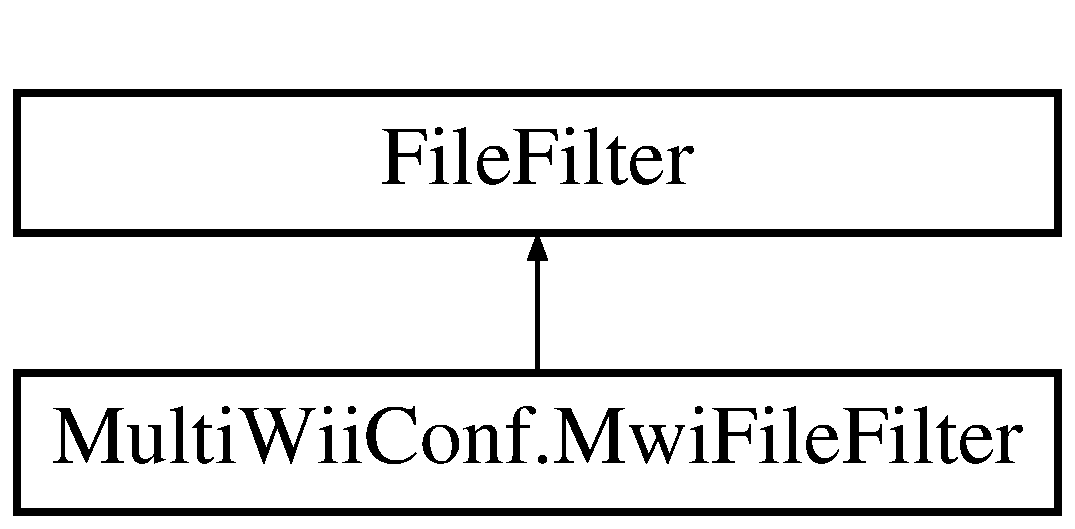
\includegraphics[height=2.000000cm]{classMultiWiiConf_1_1MwiFileFilter}
\end{center}
\end{figure}
\subsection*{Public Member Functions}
\begin{DoxyCompactItemize}
\item 
boolean \hyperlink{classMultiWiiConf_1_1MwiFileFilter_a2fc98af73a2bd1a449059b03d17fd6e0}{accept} (File \hyperlink{Uno__MultiWii__HardwarePlatform__Test_8ino_aa27fc5a637b915f1bff5f1f75a0455ab}{f})
\item 
String \hyperlink{classMultiWiiConf_1_1MwiFileFilter_a11e3fa3c2c9abd0717eee9c93181eb6a}{get\-Extension} (File \hyperlink{Uno__MultiWii__HardwarePlatform__Test_8ino_aa27fc5a637b915f1bff5f1f75a0455ab}{f})
\item 
String \hyperlink{classMultiWiiConf_1_1MwiFileFilter_ac4f941770bf069fe42ce19a0a4ba92f9}{get\-Description} ()
\end{DoxyCompactItemize}


\subsection{Member Function Documentation}
\hypertarget{classMultiWiiConf_1_1MwiFileFilter_a2fc98af73a2bd1a449059b03d17fd6e0}{\index{Multi\-Wii\-Conf\-::\-Mwi\-File\-Filter@{Multi\-Wii\-Conf\-::\-Mwi\-File\-Filter}!accept@{accept}}
\index{accept@{accept}!MultiWiiConf::MwiFileFilter@{Multi\-Wii\-Conf\-::\-Mwi\-File\-Filter}}
\subsubsection[{accept}]{\setlength{\rightskip}{0pt plus 5cm}boolean Multi\-Wii\-Conf.\-Mwi\-File\-Filter.\-accept (
\begin{DoxyParamCaption}
\item[{File}]{f}
\end{DoxyParamCaption}
)\hspace{0.3cm}{\ttfamily [inline]}}}\label{classMultiWiiConf_1_1MwiFileFilter_a2fc98af73a2bd1a449059b03d17fd6e0}
\hypertarget{classMultiWiiConf_1_1MwiFileFilter_ac4f941770bf069fe42ce19a0a4ba92f9}{\index{Multi\-Wii\-Conf\-::\-Mwi\-File\-Filter@{Multi\-Wii\-Conf\-::\-Mwi\-File\-Filter}!get\-Description@{get\-Description}}
\index{get\-Description@{get\-Description}!MultiWiiConf::MwiFileFilter@{Multi\-Wii\-Conf\-::\-Mwi\-File\-Filter}}
\subsubsection[{get\-Description}]{\setlength{\rightskip}{0pt plus 5cm}String Multi\-Wii\-Conf.\-Mwi\-File\-Filter.\-get\-Description (
\begin{DoxyParamCaption}
{}
\end{DoxyParamCaption}
)\hspace{0.3cm}{\ttfamily [inline]}}}\label{classMultiWiiConf_1_1MwiFileFilter_ac4f941770bf069fe42ce19a0a4ba92f9}
\hypertarget{classMultiWiiConf_1_1MwiFileFilter_a11e3fa3c2c9abd0717eee9c93181eb6a}{\index{Multi\-Wii\-Conf\-::\-Mwi\-File\-Filter@{Multi\-Wii\-Conf\-::\-Mwi\-File\-Filter}!get\-Extension@{get\-Extension}}
\index{get\-Extension@{get\-Extension}!MultiWiiConf::MwiFileFilter@{Multi\-Wii\-Conf\-::\-Mwi\-File\-Filter}}
\subsubsection[{get\-Extension}]{\setlength{\rightskip}{0pt plus 5cm}String Multi\-Wii\-Conf.\-Mwi\-File\-Filter.\-get\-Extension (
\begin{DoxyParamCaption}
\item[{File}]{f}
\end{DoxyParamCaption}
)\hspace{0.3cm}{\ttfamily [inline]}}}\label{classMultiWiiConf_1_1MwiFileFilter_a11e3fa3c2c9abd0717eee9c93181eb6a}


The documentation for this class was generated from the following file\-:\begin{DoxyCompactItemize}
\item 
Multi\-Wii\-\_\-2\-\_\-4/\-Multi\-Wii\-Conf/application.\-windows32/source/\hyperlink{MultiWiiConf_8java}{Multi\-Wii\-Conf.\-java}\end{DoxyCompactItemize}

\hypertarget{structnesPinsStruct}{\section{nes\-Pins\-Struct Struct Reference}
\label{structnesPinsStruct}\index{nes\-Pins\-Struct@{nes\-Pins\-Struct}}
}
\subsection*{Public Attributes}
\begin{DoxyCompactItemize}
\item 
unsigned int \hyperlink{structnesPinsStruct_a0dcbcf5c9f17bb59ac27051ad496e72d}{c\-Pin}
\item 
unsigned int \hyperlink{structnesPinsStruct_a9392256befea9921ac89972e88515aed}{d\-Pin}
\item 
unsigned int \hyperlink{structnesPinsStruct_a42f8acf56f88e7ba9d4a9fb2dc808147}{l\-Pin}
\end{DoxyCompactItemize}


\subsection{Member Data Documentation}
\hypertarget{structnesPinsStruct_a0dcbcf5c9f17bb59ac27051ad496e72d}{\index{nes\-Pins\-Struct@{nes\-Pins\-Struct}!c\-Pin@{c\-Pin}}
\index{c\-Pin@{c\-Pin}!nesPinsStruct@{nes\-Pins\-Struct}}
\subsubsection[{c\-Pin}]{\setlength{\rightskip}{0pt plus 5cm}unsigned int nes\-Pins\-Struct\-::c\-Pin}}\label{structnesPinsStruct_a0dcbcf5c9f17bb59ac27051ad496e72d}
\hypertarget{structnesPinsStruct_a9392256befea9921ac89972e88515aed}{\index{nes\-Pins\-Struct@{nes\-Pins\-Struct}!d\-Pin@{d\-Pin}}
\index{d\-Pin@{d\-Pin}!nesPinsStruct@{nes\-Pins\-Struct}}
\subsubsection[{d\-Pin}]{\setlength{\rightskip}{0pt plus 5cm}unsigned int nes\-Pins\-Struct\-::d\-Pin}}\label{structnesPinsStruct_a9392256befea9921ac89972e88515aed}
\hypertarget{structnesPinsStruct_a42f8acf56f88e7ba9d4a9fb2dc808147}{\index{nes\-Pins\-Struct@{nes\-Pins\-Struct}!l\-Pin@{l\-Pin}}
\index{l\-Pin@{l\-Pin}!nesPinsStruct@{nes\-Pins\-Struct}}
\subsubsection[{l\-Pin}]{\setlength{\rightskip}{0pt plus 5cm}unsigned int nes\-Pins\-Struct\-::l\-Pin}}\label{structnesPinsStruct_a42f8acf56f88e7ba9d4a9fb2dc808147}


The documentation for this struct was generated from the following file\-:\begin{DoxyCompactItemize}
\item 
wiring\-Pi/dev\-Lib/\hyperlink{piNes_8c}{pi\-Nes.\-c}\end{DoxyCompactItemize}

\hypertarget{unionow__addr__t}{\section{ow\-\_\-addr\-\_\-t Union Reference}
\label{unionow__addr__t}\index{ow\-\_\-addr\-\_\-t@{ow\-\_\-addr\-\_\-t}}
}


{\ttfamily \#include $<$onewire\-\_\-internal.\-h$>$}

\subsection*{Public Member Functions}
\begin{DoxyCompactItemize}
\item 
\hyperlink{unionow__addr__t_af5b6027121c795cb804599bb5d89e02d}{C\-F\-G\-\_\-\-D\-A\-T\-A} (owid) \hyperlink{onewire__internal_8h_a9aa2f90f66e13565282cbb55468b998e}{ow\-\_\-addr}
\end{DoxyCompactItemize}
\subsection*{Public Attributes}
\begin{DoxyCompactItemize}
\item 
uint8\-\_\-t \hyperlink{unionow__addr__t_ad1523b0a1d18a629d0e6fd5e2563dd45}{addr} \mbox{[}8\mbox{]}
\end{DoxyCompactItemize}


\subsection{Member Function Documentation}
\hypertarget{unionow__addr__t_af5b6027121c795cb804599bb5d89e02d}{\index{ow\-\_\-addr\-\_\-t@{ow\-\_\-addr\-\_\-t}!C\-F\-G\-\_\-\-D\-A\-T\-A@{C\-F\-G\-\_\-\-D\-A\-T\-A}}
\index{C\-F\-G\-\_\-\-D\-A\-T\-A@{C\-F\-G\-\_\-\-D\-A\-T\-A}!ow_addr_t@{ow\-\_\-addr\-\_\-t}}
\subsubsection[{C\-F\-G\-\_\-\-D\-A\-T\-A}]{\setlength{\rightskip}{0pt plus 5cm}ow\-\_\-addr\-\_\-t\-::\-C\-F\-G\-\_\-\-D\-A\-T\-A (
\begin{DoxyParamCaption}
\item[{owid}]{}
\end{DoxyParamCaption}
)}}\label{unionow__addr__t_af5b6027121c795cb804599bb5d89e02d}


\subsection{Member Data Documentation}
\hypertarget{unionow__addr__t_ad1523b0a1d18a629d0e6fd5e2563dd45}{\index{ow\-\_\-addr\-\_\-t@{ow\-\_\-addr\-\_\-t}!addr@{addr}}
\index{addr@{addr}!ow_addr_t@{ow\-\_\-addr\-\_\-t}}
\subsubsection[{addr}]{\setlength{\rightskip}{0pt plus 5cm}uint8\-\_\-t ow\-\_\-addr\-\_\-t\-::addr\mbox{[}8\mbox{]}}}\label{unionow__addr__t_ad1523b0a1d18a629d0e6fd5e2563dd45}


The documentation for this union was generated from the following file\-:\begin{DoxyCompactItemize}
\item 
cli/owslave/\hyperlink{onewire__internal_8h}{onewire\-\_\-internal.\-h}\end{DoxyCompactItemize}

\hypertarget{structpid__}{\section{pid\-\_\- Struct Reference}
\label{structpid__}\index{pid\-\_\-@{pid\-\_\-}}
}


{\ttfamily \#include $<$types.\-h$>$}

\subsection*{Public Attributes}
\begin{DoxyCompactItemize}
\item 
uint8\-\_\-t \hyperlink{structpid___ae0911f3b82c377d9a4994dbc834e1ee4}{P8}
\item 
uint8\-\_\-t \hyperlink{structpid___a25caf1096a0e8531ce94eafd842a14b6}{I8}
\item 
uint8\-\_\-t \hyperlink{structpid___a2cc4f84c854e2299c74b6eaea0223a69}{D8}
\end{DoxyCompactItemize}


\subsection{Member Data Documentation}
\hypertarget{structpid___a2cc4f84c854e2299c74b6eaea0223a69}{\index{pid\-\_\-@{pid\-\_\-}!D8@{D8}}
\index{D8@{D8}!pid_@{pid\-\_\-}}
\subsubsection[{D8}]{\setlength{\rightskip}{0pt plus 5cm}uint8\-\_\-t pid\-\_\-\-::\-D8}}\label{structpid___a2cc4f84c854e2299c74b6eaea0223a69}
\hypertarget{structpid___a25caf1096a0e8531ce94eafd842a14b6}{\index{pid\-\_\-@{pid\-\_\-}!I8@{I8}}
\index{I8@{I8}!pid_@{pid\-\_\-}}
\subsubsection[{I8}]{\setlength{\rightskip}{0pt plus 5cm}uint8\-\_\-t pid\-\_\-\-::\-I8}}\label{structpid___a25caf1096a0e8531ce94eafd842a14b6}
\hypertarget{structpid___ae0911f3b82c377d9a4994dbc834e1ee4}{\index{pid\-\_\-@{pid\-\_\-}!P8@{P8}}
\index{P8@{P8}!pid_@{pid\-\_\-}}
\subsubsection[{P8}]{\setlength{\rightskip}{0pt plus 5cm}uint8\-\_\-t pid\-\_\-\-::\-P8}}\label{structpid___ae0911f3b82c377d9a4994dbc834e1ee4}


The documentation for this struct was generated from the following file\-:\begin{DoxyCompactItemize}
\item 
Multi\-Wii\-\_\-2\-\_\-4/\-Multi\-Wii/\hyperlink{MultiWii__2__4_2MultiWii_2types_8h}{types.\-h}\end{DoxyCompactItemize}

\hypertarget{structpoly16x4x2__t}{\section{poly16x4x2\-\_\-t Struct Reference}
\label{structpoly16x4x2__t}\index{poly16x4x2\-\_\-t@{poly16x4x2\-\_\-t}}
}


{\ttfamily \#include $<$arm\-\_\-neon.\-h$>$}

\subsection*{Public Attributes}
\begin{DoxyCompactItemize}
\item 
poly16x4\-\_\-t \hyperlink{structpoly16x4x2__t_ab02ff90ba945f5040ed9973a0461a750}{val} \mbox{[}2\mbox{]}
\end{DoxyCompactItemize}


\subsection{Member Data Documentation}
\hypertarget{structpoly16x4x2__t_ab02ff90ba945f5040ed9973a0461a750}{\index{poly16x4x2\-\_\-t@{poly16x4x2\-\_\-t}!val@{val}}
\index{val@{val}!poly16x4x2_t@{poly16x4x2\-\_\-t}}
\subsubsection[{val}]{\setlength{\rightskip}{0pt plus 5cm}poly16x4\-\_\-t poly16x4x2\-\_\-t\-::val\mbox{[}2\mbox{]}}}\label{structpoly16x4x2__t_ab02ff90ba945f5040ed9973a0461a750}


The documentation for this struct was generated from the following file\-:\begin{DoxyCompactItemize}
\item 
oclint-\/0.\-10.\-3/lib/clang/3.\-8.\-0/include/\hyperlink{arm__neon_8h}{arm\-\_\-neon.\-h}\end{DoxyCompactItemize}

\hypertarget{structpoly16x4x3__t}{\section{poly16x4x3\-\_\-t Struct Reference}
\label{structpoly16x4x3__t}\index{poly16x4x3\-\_\-t@{poly16x4x3\-\_\-t}}
}


{\ttfamily \#include $<$arm\-\_\-neon.\-h$>$}

\subsection*{Public Attributes}
\begin{DoxyCompactItemize}
\item 
poly16x4\-\_\-t \hyperlink{structpoly16x4x3__t_aab74a391c79c5a34686fa8761b43126a}{val} \mbox{[}3\mbox{]}
\end{DoxyCompactItemize}


\subsection{Member Data Documentation}
\hypertarget{structpoly16x4x3__t_aab74a391c79c5a34686fa8761b43126a}{\index{poly16x4x3\-\_\-t@{poly16x4x3\-\_\-t}!val@{val}}
\index{val@{val}!poly16x4x3_t@{poly16x4x3\-\_\-t}}
\subsubsection[{val}]{\setlength{\rightskip}{0pt plus 5cm}poly16x4\-\_\-t poly16x4x3\-\_\-t\-::val\mbox{[}3\mbox{]}}}\label{structpoly16x4x3__t_aab74a391c79c5a34686fa8761b43126a}


The documentation for this struct was generated from the following file\-:\begin{DoxyCompactItemize}
\item 
oclint-\/0.\-10.\-3/lib/clang/3.\-8.\-0/include/\hyperlink{arm__neon_8h}{arm\-\_\-neon.\-h}\end{DoxyCompactItemize}

\hypertarget{structpoly16x4x4__t}{\section{poly16x4x4\-\_\-t Struct Reference}
\label{structpoly16x4x4__t}\index{poly16x4x4\-\_\-t@{poly16x4x4\-\_\-t}}
}


{\ttfamily \#include $<$arm\-\_\-neon.\-h$>$}

\subsection*{Public Attributes}
\begin{DoxyCompactItemize}
\item 
poly16x4\-\_\-t \hyperlink{structpoly16x4x4__t_a7380b4f99a00dc7754d121da527832ad}{val} \mbox{[}4\mbox{]}
\end{DoxyCompactItemize}


\subsection{Member Data Documentation}
\hypertarget{structpoly16x4x4__t_a7380b4f99a00dc7754d121da527832ad}{\index{poly16x4x4\-\_\-t@{poly16x4x4\-\_\-t}!val@{val}}
\index{val@{val}!poly16x4x4_t@{poly16x4x4\-\_\-t}}
\subsubsection[{val}]{\setlength{\rightskip}{0pt plus 5cm}poly16x4\-\_\-t poly16x4x4\-\_\-t\-::val\mbox{[}4\mbox{]}}}\label{structpoly16x4x4__t_a7380b4f99a00dc7754d121da527832ad}


The documentation for this struct was generated from the following file\-:\begin{DoxyCompactItemize}
\item 
oclint-\/0.\-10.\-3/lib/clang/3.\-8.\-0/include/\hyperlink{arm__neon_8h}{arm\-\_\-neon.\-h}\end{DoxyCompactItemize}

\hypertarget{structpoly16x8x2__t}{\section{poly16x8x2\-\_\-t Struct Reference}
\label{structpoly16x8x2__t}\index{poly16x8x2\-\_\-t@{poly16x8x2\-\_\-t}}
}


{\ttfamily \#include $<$arm\-\_\-neon.\-h$>$}

\subsection*{Public Attributes}
\begin{DoxyCompactItemize}
\item 
poly16x8\-\_\-t \hyperlink{structpoly16x8x2__t_aedcf0d4e750cb257c747ee591fc40992}{val} \mbox{[}2\mbox{]}
\end{DoxyCompactItemize}


\subsection{Member Data Documentation}
\hypertarget{structpoly16x8x2__t_aedcf0d4e750cb257c747ee591fc40992}{\index{poly16x8x2\-\_\-t@{poly16x8x2\-\_\-t}!val@{val}}
\index{val@{val}!poly16x8x2_t@{poly16x8x2\-\_\-t}}
\subsubsection[{val}]{\setlength{\rightskip}{0pt plus 5cm}poly16x8\-\_\-t poly16x8x2\-\_\-t\-::val\mbox{[}2\mbox{]}}}\label{structpoly16x8x2__t_aedcf0d4e750cb257c747ee591fc40992}


The documentation for this struct was generated from the following file\-:\begin{DoxyCompactItemize}
\item 
oclint-\/0.\-10.\-3/lib/clang/3.\-8.\-0/include/\hyperlink{arm__neon_8h}{arm\-\_\-neon.\-h}\end{DoxyCompactItemize}

\hypertarget{structpoly16x8x3__t}{\section{poly16x8x3\-\_\-t Struct Reference}
\label{structpoly16x8x3__t}\index{poly16x8x3\-\_\-t@{poly16x8x3\-\_\-t}}
}


{\ttfamily \#include $<$arm\-\_\-neon.\-h$>$}

\subsection*{Public Attributes}
\begin{DoxyCompactItemize}
\item 
poly16x8\-\_\-t \hyperlink{structpoly16x8x3__t_a26d9e78d02db1c4d3a82f2e8f7976057}{val} \mbox{[}3\mbox{]}
\end{DoxyCompactItemize}


\subsection{Member Data Documentation}
\hypertarget{structpoly16x8x3__t_a26d9e78d02db1c4d3a82f2e8f7976057}{\index{poly16x8x3\-\_\-t@{poly16x8x3\-\_\-t}!val@{val}}
\index{val@{val}!poly16x8x3_t@{poly16x8x3\-\_\-t}}
\subsubsection[{val}]{\setlength{\rightskip}{0pt plus 5cm}poly16x8\-\_\-t poly16x8x3\-\_\-t\-::val\mbox{[}3\mbox{]}}}\label{structpoly16x8x3__t_a26d9e78d02db1c4d3a82f2e8f7976057}


The documentation for this struct was generated from the following file\-:\begin{DoxyCompactItemize}
\item 
oclint-\/0.\-10.\-3/lib/clang/3.\-8.\-0/include/\hyperlink{arm__neon_8h}{arm\-\_\-neon.\-h}\end{DoxyCompactItemize}

\hypertarget{structpoly16x8x4__t}{\section{poly16x8x4\-\_\-t Struct Reference}
\label{structpoly16x8x4__t}\index{poly16x8x4\-\_\-t@{poly16x8x4\-\_\-t}}
}


{\ttfamily \#include $<$arm\-\_\-neon.\-h$>$}

\subsection*{Public Attributes}
\begin{DoxyCompactItemize}
\item 
poly16x8\-\_\-t \hyperlink{structpoly16x8x4__t_aa60670d2daf6e8a21fb5c54482ecb720}{val} \mbox{[}4\mbox{]}
\end{DoxyCompactItemize}


\subsection{Member Data Documentation}
\hypertarget{structpoly16x8x4__t_aa60670d2daf6e8a21fb5c54482ecb720}{\index{poly16x8x4\-\_\-t@{poly16x8x4\-\_\-t}!val@{val}}
\index{val@{val}!poly16x8x4_t@{poly16x8x4\-\_\-t}}
\subsubsection[{val}]{\setlength{\rightskip}{0pt plus 5cm}poly16x8\-\_\-t poly16x8x4\-\_\-t\-::val\mbox{[}4\mbox{]}}}\label{structpoly16x8x4__t_aa60670d2daf6e8a21fb5c54482ecb720}


The documentation for this struct was generated from the following file\-:\begin{DoxyCompactItemize}
\item 
oclint-\/0.\-10.\-3/lib/clang/3.\-8.\-0/include/\hyperlink{arm__neon_8h}{arm\-\_\-neon.\-h}\end{DoxyCompactItemize}

\hypertarget{structpoly8x16x2__t}{\section{poly8x16x2\-\_\-t Struct Reference}
\label{structpoly8x16x2__t}\index{poly8x16x2\-\_\-t@{poly8x16x2\-\_\-t}}
}


{\ttfamily \#include $<$arm\-\_\-neon.\-h$>$}

\subsection*{Public Attributes}
\begin{DoxyCompactItemize}
\item 
poly8x16\-\_\-t \hyperlink{structpoly8x16x2__t_a5447f354dc39ca472ea992649423bd12}{val} \mbox{[}2\mbox{]}
\end{DoxyCompactItemize}


\subsection{Member Data Documentation}
\hypertarget{structpoly8x16x2__t_a5447f354dc39ca472ea992649423bd12}{\index{poly8x16x2\-\_\-t@{poly8x16x2\-\_\-t}!val@{val}}
\index{val@{val}!poly8x16x2_t@{poly8x16x2\-\_\-t}}
\subsubsection[{val}]{\setlength{\rightskip}{0pt plus 5cm}poly8x16\-\_\-t poly8x16x2\-\_\-t\-::val\mbox{[}2\mbox{]}}}\label{structpoly8x16x2__t_a5447f354dc39ca472ea992649423bd12}


The documentation for this struct was generated from the following file\-:\begin{DoxyCompactItemize}
\item 
oclint-\/0.\-10.\-3/lib/clang/3.\-8.\-0/include/\hyperlink{arm__neon_8h}{arm\-\_\-neon.\-h}\end{DoxyCompactItemize}

\hypertarget{structpoly8x16x3__t}{\section{poly8x16x3\-\_\-t Struct Reference}
\label{structpoly8x16x3__t}\index{poly8x16x3\-\_\-t@{poly8x16x3\-\_\-t}}
}


{\ttfamily \#include $<$arm\-\_\-neon.\-h$>$}

\subsection*{Public Attributes}
\begin{DoxyCompactItemize}
\item 
poly8x16\-\_\-t \hyperlink{structpoly8x16x3__t_a8a6845b8ab48eff4f9ee247448264efe}{val} \mbox{[}3\mbox{]}
\end{DoxyCompactItemize}


\subsection{Member Data Documentation}
\hypertarget{structpoly8x16x3__t_a8a6845b8ab48eff4f9ee247448264efe}{\index{poly8x16x3\-\_\-t@{poly8x16x3\-\_\-t}!val@{val}}
\index{val@{val}!poly8x16x3_t@{poly8x16x3\-\_\-t}}
\subsubsection[{val}]{\setlength{\rightskip}{0pt plus 5cm}poly8x16\-\_\-t poly8x16x3\-\_\-t\-::val\mbox{[}3\mbox{]}}}\label{structpoly8x16x3__t_a8a6845b8ab48eff4f9ee247448264efe}


The documentation for this struct was generated from the following file\-:\begin{DoxyCompactItemize}
\item 
oclint-\/0.\-10.\-3/lib/clang/3.\-8.\-0/include/\hyperlink{arm__neon_8h}{arm\-\_\-neon.\-h}\end{DoxyCompactItemize}

\hypertarget{structpoly8x16x4__t}{\section{poly8x16x4\-\_\-t Struct Reference}
\label{structpoly8x16x4__t}\index{poly8x16x4\-\_\-t@{poly8x16x4\-\_\-t}}
}


{\ttfamily \#include $<$arm\-\_\-neon.\-h$>$}

\subsection*{Public Attributes}
\begin{DoxyCompactItemize}
\item 
poly8x16\-\_\-t \hyperlink{structpoly8x16x4__t_a2d90838b70bc3beea56561bcb305c752}{val} \mbox{[}4\mbox{]}
\end{DoxyCompactItemize}


\subsection{Member Data Documentation}
\hypertarget{structpoly8x16x4__t_a2d90838b70bc3beea56561bcb305c752}{\index{poly8x16x4\-\_\-t@{poly8x16x4\-\_\-t}!val@{val}}
\index{val@{val}!poly8x16x4_t@{poly8x16x4\-\_\-t}}
\subsubsection[{val}]{\setlength{\rightskip}{0pt plus 5cm}poly8x16\-\_\-t poly8x16x4\-\_\-t\-::val\mbox{[}4\mbox{]}}}\label{structpoly8x16x4__t_a2d90838b70bc3beea56561bcb305c752}


The documentation for this struct was generated from the following file\-:\begin{DoxyCompactItemize}
\item 
oclint-\/0.\-10.\-3/lib/clang/3.\-8.\-0/include/\hyperlink{arm__neon_8h}{arm\-\_\-neon.\-h}\end{DoxyCompactItemize}

\hypertarget{structpoly8x8x2__t}{\section{poly8x8x2\-\_\-t Struct Reference}
\label{structpoly8x8x2__t}\index{poly8x8x2\-\_\-t@{poly8x8x2\-\_\-t}}
}


{\ttfamily \#include $<$arm\-\_\-neon.\-h$>$}

\subsection*{Public Attributes}
\begin{DoxyCompactItemize}
\item 
poly8x8\-\_\-t \hyperlink{structpoly8x8x2__t_afb00c4ee129d10fe30a71e589452ae73}{val} \mbox{[}2\mbox{]}
\end{DoxyCompactItemize}


\subsection{Member Data Documentation}
\hypertarget{structpoly8x8x2__t_afb00c4ee129d10fe30a71e589452ae73}{\index{poly8x8x2\-\_\-t@{poly8x8x2\-\_\-t}!val@{val}}
\index{val@{val}!poly8x8x2_t@{poly8x8x2\-\_\-t}}
\subsubsection[{val}]{\setlength{\rightskip}{0pt plus 5cm}poly8x8\-\_\-t poly8x8x2\-\_\-t\-::val\mbox{[}2\mbox{]}}}\label{structpoly8x8x2__t_afb00c4ee129d10fe30a71e589452ae73}


The documentation for this struct was generated from the following file\-:\begin{DoxyCompactItemize}
\item 
oclint-\/0.\-10.\-3/lib/clang/3.\-8.\-0/include/\hyperlink{arm__neon_8h}{arm\-\_\-neon.\-h}\end{DoxyCompactItemize}

\hypertarget{structpoly8x8x3__t}{\section{poly8x8x3\-\_\-t Struct Reference}
\label{structpoly8x8x3__t}\index{poly8x8x3\-\_\-t@{poly8x8x3\-\_\-t}}
}


{\ttfamily \#include $<$arm\-\_\-neon.\-h$>$}

\subsection*{Public Attributes}
\begin{DoxyCompactItemize}
\item 
poly8x8\-\_\-t \hyperlink{structpoly8x8x3__t_a508903926a827e8e3f85377d53a1a953}{val} \mbox{[}3\mbox{]}
\end{DoxyCompactItemize}


\subsection{Member Data Documentation}
\hypertarget{structpoly8x8x3__t_a508903926a827e8e3f85377d53a1a953}{\index{poly8x8x3\-\_\-t@{poly8x8x3\-\_\-t}!val@{val}}
\index{val@{val}!poly8x8x3_t@{poly8x8x3\-\_\-t}}
\subsubsection[{val}]{\setlength{\rightskip}{0pt plus 5cm}poly8x8\-\_\-t poly8x8x3\-\_\-t\-::val\mbox{[}3\mbox{]}}}\label{structpoly8x8x3__t_a508903926a827e8e3f85377d53a1a953}


The documentation for this struct was generated from the following file\-:\begin{DoxyCompactItemize}
\item 
oclint-\/0.\-10.\-3/lib/clang/3.\-8.\-0/include/\hyperlink{arm__neon_8h}{arm\-\_\-neon.\-h}\end{DoxyCompactItemize}

\hypertarget{structpoly8x8x4__t}{\section{poly8x8x4\-\_\-t Struct Reference}
\label{structpoly8x8x4__t}\index{poly8x8x4\-\_\-t@{poly8x8x4\-\_\-t}}
}


{\ttfamily \#include $<$arm\-\_\-neon.\-h$>$}

\subsection*{Public Attributes}
\begin{DoxyCompactItemize}
\item 
poly8x8\-\_\-t \hyperlink{structpoly8x8x4__t_aa046d168ccd16096777ab61d2f936ccb}{val} \mbox{[}4\mbox{]}
\end{DoxyCompactItemize}


\subsection{Member Data Documentation}
\hypertarget{structpoly8x8x4__t_aa046d168ccd16096777ab61d2f936ccb}{\index{poly8x8x4\-\_\-t@{poly8x8x4\-\_\-t}!val@{val}}
\index{val@{val}!poly8x8x4_t@{poly8x8x4\-\_\-t}}
\subsubsection[{val}]{\setlength{\rightskip}{0pt plus 5cm}poly8x8\-\_\-t poly8x8x4\-\_\-t\-::val\mbox{[}4\mbox{]}}}\label{structpoly8x8x4__t_aa046d168ccd16096777ab61d2f936ccb}


The documentation for this struct was generated from the following file\-:\begin{DoxyCompactItemize}
\item 
oclint-\/0.\-10.\-3/lib/clang/3.\-8.\-0/include/\hyperlink{arm__neon_8h}{arm\-\_\-neon.\-h}\end{DoxyCompactItemize}

\hypertarget{structservo__conf__}{\section{servo\-\_\-conf\-\_\- Struct Reference}
\label{structservo__conf__}\index{servo\-\_\-conf\-\_\-@{servo\-\_\-conf\-\_\-}}
}


{\ttfamily \#include $<$types.\-h$>$}

\subsection*{Public Attributes}
\begin{DoxyCompactItemize}
\item 
int16\-\_\-t \hyperlink{structservo__conf___a61bf60f37499f4d6b2ca3a38564eb8a1}{min}
\item 
int16\-\_\-t \hyperlink{structservo__conf___ae9cc648469a2047112b7f8c1d5aa48de}{max}
\item 
int16\-\_\-t \hyperlink{structservo__conf___a59045c524c87263a1b4530015dd84b54}{middle}
\item 
int8\-\_\-t \hyperlink{structservo__conf___ab2c11761622958a841cd6a4148e133e8}{rate}
\end{DoxyCompactItemize}


\subsection{Member Data Documentation}
\hypertarget{structservo__conf___ae9cc648469a2047112b7f8c1d5aa48de}{\index{servo\-\_\-conf\-\_\-@{servo\-\_\-conf\-\_\-}!max@{max}}
\index{max@{max}!servo_conf_@{servo\-\_\-conf\-\_\-}}
\subsubsection[{max}]{\setlength{\rightskip}{0pt plus 5cm}int16\-\_\-t servo\-\_\-conf\-\_\-\-::max}}\label{structservo__conf___ae9cc648469a2047112b7f8c1d5aa48de}
\hypertarget{structservo__conf___a59045c524c87263a1b4530015dd84b54}{\index{servo\-\_\-conf\-\_\-@{servo\-\_\-conf\-\_\-}!middle@{middle}}
\index{middle@{middle}!servo_conf_@{servo\-\_\-conf\-\_\-}}
\subsubsection[{middle}]{\setlength{\rightskip}{0pt plus 5cm}int16\-\_\-t servo\-\_\-conf\-\_\-\-::middle}}\label{structservo__conf___a59045c524c87263a1b4530015dd84b54}
\hypertarget{structservo__conf___a61bf60f37499f4d6b2ca3a38564eb8a1}{\index{servo\-\_\-conf\-\_\-@{servo\-\_\-conf\-\_\-}!min@{min}}
\index{min@{min}!servo_conf_@{servo\-\_\-conf\-\_\-}}
\subsubsection[{min}]{\setlength{\rightskip}{0pt plus 5cm}int16\-\_\-t servo\-\_\-conf\-\_\-\-::min}}\label{structservo__conf___a61bf60f37499f4d6b2ca3a38564eb8a1}
\hypertarget{structservo__conf___ab2c11761622958a841cd6a4148e133e8}{\index{servo\-\_\-conf\-\_\-@{servo\-\_\-conf\-\_\-}!rate@{rate}}
\index{rate@{rate}!servo_conf_@{servo\-\_\-conf\-\_\-}}
\subsubsection[{rate}]{\setlength{\rightskip}{0pt plus 5cm}int8\-\_\-t servo\-\_\-conf\-\_\-\-::rate}}\label{structservo__conf___ab2c11761622958a841cd6a4148e133e8}


The documentation for this struct was generated from the following file\-:\begin{DoxyCompactItemize}
\item 
Multi\-Wii\-\_\-2\-\_\-4/\-Multi\-Wii/\hyperlink{MultiWii__2__4_2MultiWii_2types_8h}{types.\-h}\end{DoxyCompactItemize}

\hypertarget{classsht31_1_1SHT31}{\section{sht31.\-S\-H\-T31 Class Reference}
\label{classsht31_1_1SHT31}\index{sht31.\-S\-H\-T31@{sht31.\-S\-H\-T31}}
}
Inheritance diagram for sht31.\-S\-H\-T31\-:\begin{figure}[H]
\begin{center}
\leavevmode
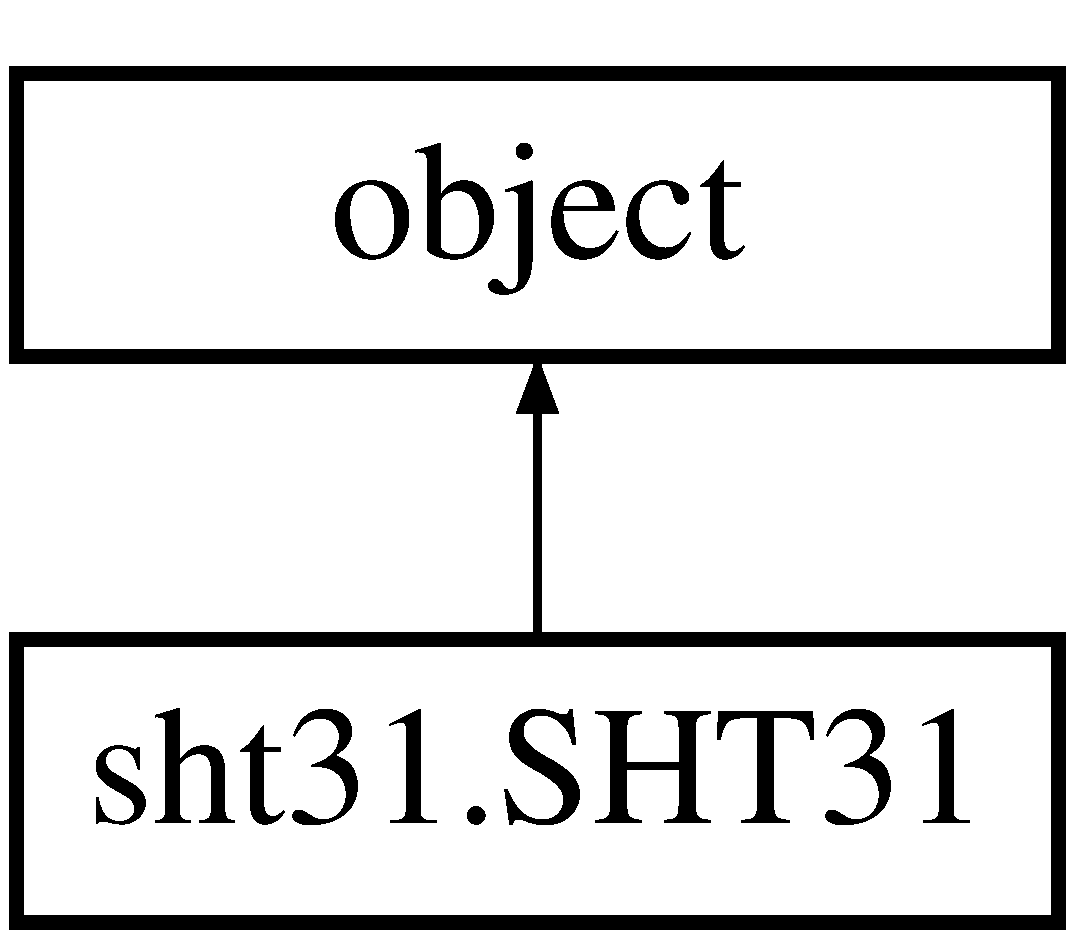
\includegraphics[height=2.000000cm]{classsht31_1_1SHT31}
\end{center}
\end{figure}
\subsection*{Public Member Functions}
\begin{DoxyCompactItemize}
\item 
def \hyperlink{classsht31_1_1SHT31_aacdcc1b25d1d7eb5a9ccf25749097504}{\-\_\-\-\_\-init\-\_\-\-\_\-}
\item 
def \hyperlink{classsht31_1_1SHT31_a9b19106b467aacd82d68451db4f01d9b}{get\-\_\-temp\-\_\-humi}
\end{DoxyCompactItemize}


\subsection{Detailed Description}
\begin{DoxyVerb}This class implements an interface to the SHT31 temprature and humidity
sensor from Sensirion.
\end{DoxyVerb}
 

\subsection{Constructor \& Destructor Documentation}
\hypertarget{classsht31_1_1SHT31_aacdcc1b25d1d7eb5a9ccf25749097504}{\index{sht31\-::\-S\-H\-T31@{sht31\-::\-S\-H\-T31}!\-\_\-\-\_\-init\-\_\-\-\_\-@{\-\_\-\-\_\-init\-\_\-\-\_\-}}
\index{\-\_\-\-\_\-init\-\_\-\-\_\-@{\-\_\-\-\_\-init\-\_\-\-\_\-}!sht31::SHT31@{sht31\-::\-S\-H\-T31}}
\subsubsection[{\-\_\-\-\_\-init\-\_\-\-\_\-}]{\setlength{\rightskip}{0pt plus 5cm}def sht31.\-S\-H\-T31.\-\_\-\-\_\-init\-\_\-\-\_\- (
\begin{DoxyParamCaption}
\item[{}]{self, }
\item[{}]{i2c, }
\item[{}]{addr = {\ttfamily 0x44}}
\end{DoxyParamCaption}
)}}\label{classsht31_1_1SHT31_aacdcc1b25d1d7eb5a9ccf25749097504}
\begin{DoxyVerb}Initialize a sensor object on the given I2C bus and accessed by the
given address.
\end{DoxyVerb}
 

\subsection{Member Function Documentation}
\hypertarget{classsht31_1_1SHT31_a9b19106b467aacd82d68451db4f01d9b}{\index{sht31\-::\-S\-H\-T31@{sht31\-::\-S\-H\-T31}!get\-\_\-temp\-\_\-humi@{get\-\_\-temp\-\_\-humi}}
\index{get\-\_\-temp\-\_\-humi@{get\-\_\-temp\-\_\-humi}!sht31::SHT31@{sht31\-::\-S\-H\-T31}}
\subsubsection[{get\-\_\-temp\-\_\-humi}]{\setlength{\rightskip}{0pt plus 5cm}def sht31.\-S\-H\-T31.\-get\-\_\-temp\-\_\-humi (
\begin{DoxyParamCaption}
\item[{}]{self, }
\item[{}]{resolution = {\ttfamily {\bf R\-\_\-\-H\-I\-G\-H}}, }
\item[{}]{clock\-\_\-stretch = {\ttfamily True}, }
\item[{}]{celsius = {\ttfamily True}}
\end{DoxyParamCaption}
)}}\label{classsht31_1_1SHT31_a9b19106b467aacd82d68451db4f01d9b}
\begin{DoxyVerb}Read the temperature in degree celsius or fahrenheit and relative
humidity. Resolution and clock stretching can be specified.
Returns a tuple for both values in that order.
\end{DoxyVerb}
 

The documentation for this class was generated from the following file\-:\begin{DoxyCompactItemize}
\item 
micpy/\-E\-S\-P8266\-\_\-\-S\-H\-T31\-\_\-\-Wi\-Fi\-\_\-pseudo\-R\-E\-S\-T/\hyperlink{sht31_8py}{sht31.\-py}\end{DoxyCompactItemize}

\hypertarget{classsniffer-gui_1_1SniffThread}{\section{sniffer-\/gui.Sniff\-Thread Class Reference}
\label{classsniffer-gui_1_1SniffThread}\index{sniffer-\/gui.\-Sniff\-Thread@{sniffer-\/gui.\-Sniff\-Thread}}
}
Inheritance diagram for sniffer-\/gui.Sniff\-Thread\-:\begin{figure}[H]
\begin{center}
\leavevmode
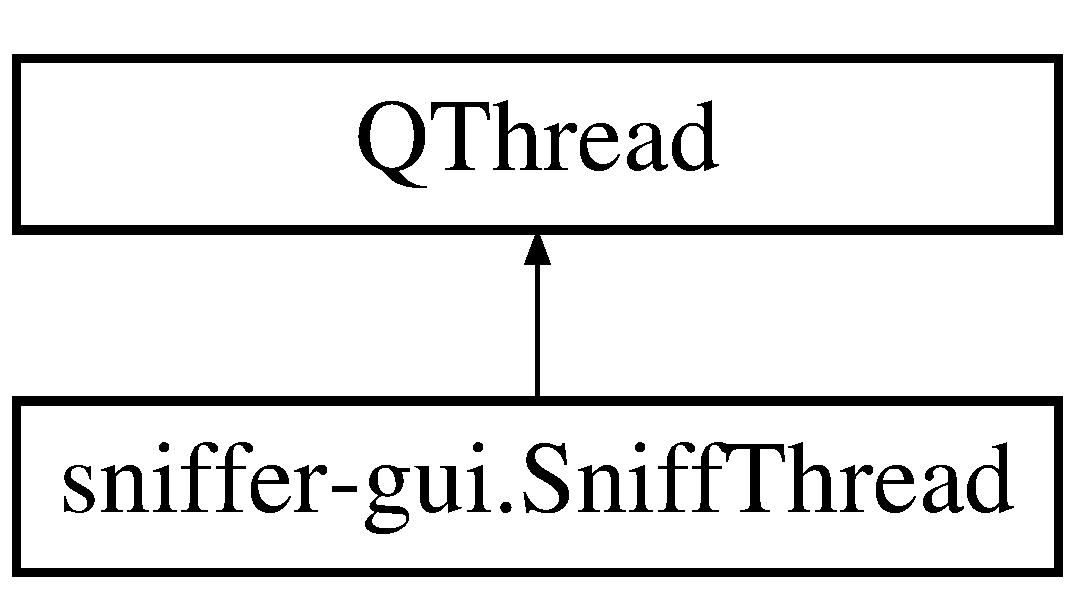
\includegraphics[height=2.000000cm]{classsniffer-gui_1_1SniffThread}
\end{center}
\end{figure}
\subsection*{Public Member Functions}
\begin{DoxyCompactItemize}
\item 
def \hyperlink{classsniffer-gui_1_1SniffThread_a6bac377ccd366abee365fb4925e0100c}{eth}
\item 
def \hyperlink{classsniffer-gui_1_1SniffThread_a6dad7abc00ccfecf5398c3df6d06b22b}{arp}
\item 
def \hyperlink{classsniffer-gui_1_1SniffThread_ad37b2c4be890b8bbec53e47b3904fc14}{ip}
\item 
def \hyperlink{classsniffer-gui_1_1SniffThread_a2f4b6474ac8e5bbf0ed3a5243f3277e4}{icmp}
\item 
def \hyperlink{classsniffer-gui_1_1SniffThread_af1c921c60dba1cfa9169c08b9f118a73}{tcp}
\item 
def \hyperlink{classsniffer-gui_1_1SniffThread_a0909f815e3c0d5d19d8324b4229b928c}{udp}
\item 
def \hyperlink{classsniffer-gui_1_1SniffThread_a38b3cc3c10314c6cfbc5a095fa071be4}{find\-Protocol}
\item 
def \hyperlink{classsniffer-gui_1_1SniffThread_a6a34d547fe9f264f06168bce287513ee}{extract\-All\-Att}
\item 
def \hyperlink{classsniffer-gui_1_1SniffThread_ab953c7fb3236a1b68a2db95e19394d0d}{filter\-And\-Extract}
\item 
def \hyperlink{classsniffer-gui_1_1SniffThread_ac02d295683d24d4b27b8686708a6c08c}{find\-Max\-Diameter}
\item 
def \hyperlink{classsniffer-gui_1_1SniffThread_aadae7ed35154631a921b2bb81c828964}{find\-Max\-Packet\-Length}
\item 
def \hyperlink{classsniffer-gui_1_1SniffThread_a3a34eb5f98a1206dc681290a3d1c53a5}{find\-Avg\-Diameter}
\item 
def \hyperlink{classsniffer-gui_1_1SniffThread_a298a4189098e9e51e40610d76a662f0a}{find\-Avg\-Packet\-Length}
\item 
def \hyperlink{classsniffer-gui_1_1SniffThread_ac11dc8c22cdc97fbb5e1b34e6eb244ec}{prepare\-Calculation\-Data}
\item 
def \hyperlink{classsniffer-gui_1_1SniffThread_a3896ce63a4578543dc8ac944154ed33b}{calculate\-Data}
\item 
def \hyperlink{classsniffer-gui_1_1SniffThread_ae0e09256ca1bab3e5198619c7be0d817}{stop}
\item 
def \hyperlink{classsniffer-gui_1_1SniffThread_a6eb91a58e9b29b3d522d34c3a5b5d750}{close}
\item 
def \hyperlink{classsniffer-gui_1_1SniffThread_a6d57f1e9fe47335fcd4e4ba2b44fd983}{sniff}
\item 
def \hyperlink{classsniffer-gui_1_1SniffThread_a292288fb4426e7dd3c472eae2633f9d2}{\-\_\-\-\_\-init\-\_\-\-\_\-}
\item 
def \hyperlink{classsniffer-gui_1_1SniffThread_ab030ccecdb9c515e9dc481a0b025c5e9}{\-\_\-\-\_\-del\-\_\-\-\_\-}
\item 
def \hyperlink{classsniffer-gui_1_1SniffThread_a6299b82d1da5a95db4ce5492f4bc3132}{run}
\end{DoxyCompactItemize}
\subsection*{Public Attributes}
\begin{DoxyCompactItemize}
\item 
\hyperlink{classsniffer-gui_1_1SniffThread_aae4e9a975c0424c0c193295782086432}{os}
\item 
\hyperlink{classsniffer-gui_1_1SniffThread_a5c56a7fa0d5f651aa6a0faa833d4a4f6}{filtered\-Protocol\-Index}
\item 
\hyperlink{classsniffer-gui_1_1SniffThread_a3b99343f0c1fd99f130b865d84673d66}{extracted\-Att\-Index}
\item 
\hyperlink{classsniffer-gui_1_1SniffThread_a6947f79d8ead40165ec97a649849a1c1}{length\-List}
\item 
\hyperlink{classsniffer-gui_1_1SniffThread_aca1321aa815fb8b0136d04b66ac81320}{diameter\-List}
\item 
\hyperlink{classsniffer-gui_1_1SniffThread_a6f0e80f7d8f64147f4b211012186ed99}{unpacked\-Info}
\item 
\hyperlink{classsniffer-gui_1_1SniffThread_a5e1b9ab66d028b682d2c639dbb29d32c}{calculation\-List}
\item 
\hyperlink{classsniffer-gui_1_1SniffThread_a4bb10f73021791d8addb5236a27cd56c}{linux}
\item 
\hyperlink{classsniffer-gui_1_1SniffThread_a60dcff7a710f4b3e0ba43da9d68d1afd}{windows}
\item 
\hyperlink{classsniffer-gui_1_1SniffThread_a9e37ad659560967089ee4710b9c1be26}{sock}
\end{DoxyCompactItemize}


\subsection{Constructor \& Destructor Documentation}
\hypertarget{classsniffer-gui_1_1SniffThread_a292288fb4426e7dd3c472eae2633f9d2}{\index{sniffer-\/gui\-::\-Sniff\-Thread@{sniffer-\/gui\-::\-Sniff\-Thread}!\-\_\-\-\_\-init\-\_\-\-\_\-@{\-\_\-\-\_\-init\-\_\-\-\_\-}}
\index{\-\_\-\-\_\-init\-\_\-\-\_\-@{\-\_\-\-\_\-init\-\_\-\-\_\-}!sniffer-gui::SniffThread@{sniffer-\/gui\-::\-Sniff\-Thread}}
\subsubsection[{\-\_\-\-\_\-init\-\_\-\-\_\-}]{\setlength{\rightskip}{0pt plus 5cm}def sniffer-\/gui.\-Sniff\-Thread.\-\_\-\-\_\-init\-\_\-\-\_\- (
\begin{DoxyParamCaption}
\item[{}]{self, }
\item[{}]{filtered\-Protocol\-Index, }
\item[{}]{extracted\-Att\-Index}
\end{DoxyParamCaption}
)}}\label{classsniffer-gui_1_1SniffThread_a292288fb4426e7dd3c472eae2633f9d2}
\hypertarget{classsniffer-gui_1_1SniffThread_ab030ccecdb9c515e9dc481a0b025c5e9}{\index{sniffer-\/gui\-::\-Sniff\-Thread@{sniffer-\/gui\-::\-Sniff\-Thread}!\-\_\-\-\_\-del\-\_\-\-\_\-@{\-\_\-\-\_\-del\-\_\-\-\_\-}}
\index{\-\_\-\-\_\-del\-\_\-\-\_\-@{\-\_\-\-\_\-del\-\_\-\-\_\-}!sniffer-gui::SniffThread@{sniffer-\/gui\-::\-Sniff\-Thread}}
\subsubsection[{\-\_\-\-\_\-del\-\_\-\-\_\-}]{\setlength{\rightskip}{0pt plus 5cm}def sniffer-\/gui.\-Sniff\-Thread.\-\_\-\-\_\-del\-\_\-\-\_\- (
\begin{DoxyParamCaption}
\item[{}]{self}
\end{DoxyParamCaption}
)}}\label{classsniffer-gui_1_1SniffThread_ab030ccecdb9c515e9dc481a0b025c5e9}


\subsection{Member Function Documentation}
\hypertarget{classsniffer-gui_1_1SniffThread_a6dad7abc00ccfecf5398c3df6d06b22b}{\index{sniffer-\/gui\-::\-Sniff\-Thread@{sniffer-\/gui\-::\-Sniff\-Thread}!arp@{arp}}
\index{arp@{arp}!sniffer-gui::SniffThread@{sniffer-\/gui\-::\-Sniff\-Thread}}
\subsubsection[{arp}]{\setlength{\rightskip}{0pt plus 5cm}def sniffer-\/gui.\-Sniff\-Thread.\-arp (
\begin{DoxyParamCaption}
\item[{}]{self, }
\item[{}]{packet, }
\item[{}]{extracted\-Att\-Index, }
\item[{}]{print\-Key}
\end{DoxyParamCaption}
)}}\label{classsniffer-gui_1_1SniffThread_a6dad7abc00ccfecf5398c3df6d06b22b}
\hypertarget{classsniffer-gui_1_1SniffThread_a3896ce63a4578543dc8ac944154ed33b}{\index{sniffer-\/gui\-::\-Sniff\-Thread@{sniffer-\/gui\-::\-Sniff\-Thread}!calculate\-Data@{calculate\-Data}}
\index{calculate\-Data@{calculate\-Data}!sniffer-gui::SniffThread@{sniffer-\/gui\-::\-Sniff\-Thread}}
\subsubsection[{calculate\-Data}]{\setlength{\rightskip}{0pt plus 5cm}def sniffer-\/gui.\-Sniff\-Thread.\-calculate\-Data (
\begin{DoxyParamCaption}
\item[{}]{self}
\end{DoxyParamCaption}
)}}\label{classsniffer-gui_1_1SniffThread_a3896ce63a4578543dc8ac944154ed33b}
\hypertarget{classsniffer-gui_1_1SniffThread_a6eb91a58e9b29b3d522d34c3a5b5d750}{\index{sniffer-\/gui\-::\-Sniff\-Thread@{sniffer-\/gui\-::\-Sniff\-Thread}!close@{close}}
\index{close@{close}!sniffer-gui::SniffThread@{sniffer-\/gui\-::\-Sniff\-Thread}}
\subsubsection[{close}]{\setlength{\rightskip}{0pt plus 5cm}def sniffer-\/gui.\-Sniff\-Thread.\-close (
\begin{DoxyParamCaption}
{}
\end{DoxyParamCaption}
)}}\label{classsniffer-gui_1_1SniffThread_a6eb91a58e9b29b3d522d34c3a5b5d750}
\hypertarget{classsniffer-gui_1_1SniffThread_a6bac377ccd366abee365fb4925e0100c}{\index{sniffer-\/gui\-::\-Sniff\-Thread@{sniffer-\/gui\-::\-Sniff\-Thread}!eth@{eth}}
\index{eth@{eth}!sniffer-gui::SniffThread@{sniffer-\/gui\-::\-Sniff\-Thread}}
\subsubsection[{eth}]{\setlength{\rightskip}{0pt plus 5cm}def sniffer-\/gui.\-Sniff\-Thread.\-eth (
\begin{DoxyParamCaption}
\item[{}]{self, }
\item[{}]{packet, }
\item[{}]{extracted\-Att\-Index, }
\item[{}]{print\-Key}
\end{DoxyParamCaption}
)}}\label{classsniffer-gui_1_1SniffThread_a6bac377ccd366abee365fb4925e0100c}
\hypertarget{classsniffer-gui_1_1SniffThread_a6a34d547fe9f264f06168bce287513ee}{\index{sniffer-\/gui\-::\-Sniff\-Thread@{sniffer-\/gui\-::\-Sniff\-Thread}!extract\-All\-Att@{extract\-All\-Att}}
\index{extract\-All\-Att@{extract\-All\-Att}!sniffer-gui::SniffThread@{sniffer-\/gui\-::\-Sniff\-Thread}}
\subsubsection[{extract\-All\-Att}]{\setlength{\rightskip}{0pt plus 5cm}def sniffer-\/gui.\-Sniff\-Thread.\-extract\-All\-Att (
\begin{DoxyParamCaption}
\item[{}]{self, }
\item[{}]{packet}
\end{DoxyParamCaption}
)}}\label{classsniffer-gui_1_1SniffThread_a6a34d547fe9f264f06168bce287513ee}
\hypertarget{classsniffer-gui_1_1SniffThread_ab953c7fb3236a1b68a2db95e19394d0d}{\index{sniffer-\/gui\-::\-Sniff\-Thread@{sniffer-\/gui\-::\-Sniff\-Thread}!filter\-And\-Extract@{filter\-And\-Extract}}
\index{filter\-And\-Extract@{filter\-And\-Extract}!sniffer-gui::SniffThread@{sniffer-\/gui\-::\-Sniff\-Thread}}
\subsubsection[{filter\-And\-Extract}]{\setlength{\rightskip}{0pt plus 5cm}def sniffer-\/gui.\-Sniff\-Thread.\-filter\-And\-Extract (
\begin{DoxyParamCaption}
\item[{}]{self, }
\item[{}]{packet, }
\item[{}]{filtered\-Protocol\-Index, }
\item[{}]{extracted\-Att\-Index}
\end{DoxyParamCaption}
)}}\label{classsniffer-gui_1_1SniffThread_ab953c7fb3236a1b68a2db95e19394d0d}
\hypertarget{classsniffer-gui_1_1SniffThread_a3a34eb5f98a1206dc681290a3d1c53a5}{\index{sniffer-\/gui\-::\-Sniff\-Thread@{sniffer-\/gui\-::\-Sniff\-Thread}!find\-Avg\-Diameter@{find\-Avg\-Diameter}}
\index{find\-Avg\-Diameter@{find\-Avg\-Diameter}!sniffer-gui::SniffThread@{sniffer-\/gui\-::\-Sniff\-Thread}}
\subsubsection[{find\-Avg\-Diameter}]{\setlength{\rightskip}{0pt plus 5cm}def sniffer-\/gui.\-Sniff\-Thread.\-find\-Avg\-Diameter (
\begin{DoxyParamCaption}
\item[{}]{self}
\end{DoxyParamCaption}
)}}\label{classsniffer-gui_1_1SniffThread_a3a34eb5f98a1206dc681290a3d1c53a5}
\hypertarget{classsniffer-gui_1_1SniffThread_a298a4189098e9e51e40610d76a662f0a}{\index{sniffer-\/gui\-::\-Sniff\-Thread@{sniffer-\/gui\-::\-Sniff\-Thread}!find\-Avg\-Packet\-Length@{find\-Avg\-Packet\-Length}}
\index{find\-Avg\-Packet\-Length@{find\-Avg\-Packet\-Length}!sniffer-gui::SniffThread@{sniffer-\/gui\-::\-Sniff\-Thread}}
\subsubsection[{find\-Avg\-Packet\-Length}]{\setlength{\rightskip}{0pt plus 5cm}def sniffer-\/gui.\-Sniff\-Thread.\-find\-Avg\-Packet\-Length (
\begin{DoxyParamCaption}
\item[{}]{self}
\end{DoxyParamCaption}
)}}\label{classsniffer-gui_1_1SniffThread_a298a4189098e9e51e40610d76a662f0a}
\hypertarget{classsniffer-gui_1_1SniffThread_ac02d295683d24d4b27b8686708a6c08c}{\index{sniffer-\/gui\-::\-Sniff\-Thread@{sniffer-\/gui\-::\-Sniff\-Thread}!find\-Max\-Diameter@{find\-Max\-Diameter}}
\index{find\-Max\-Diameter@{find\-Max\-Diameter}!sniffer-gui::SniffThread@{sniffer-\/gui\-::\-Sniff\-Thread}}
\subsubsection[{find\-Max\-Diameter}]{\setlength{\rightskip}{0pt plus 5cm}def sniffer-\/gui.\-Sniff\-Thread.\-find\-Max\-Diameter (
\begin{DoxyParamCaption}
\item[{}]{self}
\end{DoxyParamCaption}
)}}\label{classsniffer-gui_1_1SniffThread_ac02d295683d24d4b27b8686708a6c08c}
\hypertarget{classsniffer-gui_1_1SniffThread_aadae7ed35154631a921b2bb81c828964}{\index{sniffer-\/gui\-::\-Sniff\-Thread@{sniffer-\/gui\-::\-Sniff\-Thread}!find\-Max\-Packet\-Length@{find\-Max\-Packet\-Length}}
\index{find\-Max\-Packet\-Length@{find\-Max\-Packet\-Length}!sniffer-gui::SniffThread@{sniffer-\/gui\-::\-Sniff\-Thread}}
\subsubsection[{find\-Max\-Packet\-Length}]{\setlength{\rightskip}{0pt plus 5cm}def sniffer-\/gui.\-Sniff\-Thread.\-find\-Max\-Packet\-Length (
\begin{DoxyParamCaption}
\item[{}]{self}
\end{DoxyParamCaption}
)}}\label{classsniffer-gui_1_1SniffThread_aadae7ed35154631a921b2bb81c828964}
\hypertarget{classsniffer-gui_1_1SniffThread_a38b3cc3c10314c6cfbc5a095fa071be4}{\index{sniffer-\/gui\-::\-Sniff\-Thread@{sniffer-\/gui\-::\-Sniff\-Thread}!find\-Protocol@{find\-Protocol}}
\index{find\-Protocol@{find\-Protocol}!sniffer-gui::SniffThread@{sniffer-\/gui\-::\-Sniff\-Thread}}
\subsubsection[{find\-Protocol}]{\setlength{\rightskip}{0pt plus 5cm}def sniffer-\/gui.\-Sniff\-Thread.\-find\-Protocol (
\begin{DoxyParamCaption}
\item[{}]{self, }
\item[{}]{packet}
\end{DoxyParamCaption}
)}}\label{classsniffer-gui_1_1SniffThread_a38b3cc3c10314c6cfbc5a095fa071be4}
\hypertarget{classsniffer-gui_1_1SniffThread_a2f4b6474ac8e5bbf0ed3a5243f3277e4}{\index{sniffer-\/gui\-::\-Sniff\-Thread@{sniffer-\/gui\-::\-Sniff\-Thread}!icmp@{icmp}}
\index{icmp@{icmp}!sniffer-gui::SniffThread@{sniffer-\/gui\-::\-Sniff\-Thread}}
\subsubsection[{icmp}]{\setlength{\rightskip}{0pt plus 5cm}def sniffer-\/gui.\-Sniff\-Thread.\-icmp (
\begin{DoxyParamCaption}
\item[{}]{self, }
\item[{}]{packet, }
\item[{}]{extracted\-Att\-Index, }
\item[{}]{print\-Key}
\end{DoxyParamCaption}
)}}\label{classsniffer-gui_1_1SniffThread_a2f4b6474ac8e5bbf0ed3a5243f3277e4}
\hypertarget{classsniffer-gui_1_1SniffThread_ad37b2c4be890b8bbec53e47b3904fc14}{\index{sniffer-\/gui\-::\-Sniff\-Thread@{sniffer-\/gui\-::\-Sniff\-Thread}!ip@{ip}}
\index{ip@{ip}!sniffer-gui::SniffThread@{sniffer-\/gui\-::\-Sniff\-Thread}}
\subsubsection[{ip}]{\setlength{\rightskip}{0pt plus 5cm}def sniffer-\/gui.\-Sniff\-Thread.\-ip (
\begin{DoxyParamCaption}
\item[{}]{self, }
\item[{}]{packet, }
\item[{}]{extracted\-Att\-Index, }
\item[{}]{print\-Key}
\end{DoxyParamCaption}
)}}\label{classsniffer-gui_1_1SniffThread_ad37b2c4be890b8bbec53e47b3904fc14}
\hypertarget{classsniffer-gui_1_1SniffThread_ac11dc8c22cdc97fbb5e1b34e6eb244ec}{\index{sniffer-\/gui\-::\-Sniff\-Thread@{sniffer-\/gui\-::\-Sniff\-Thread}!prepare\-Calculation\-Data@{prepare\-Calculation\-Data}}
\index{prepare\-Calculation\-Data@{prepare\-Calculation\-Data}!sniffer-gui::SniffThread@{sniffer-\/gui\-::\-Sniff\-Thread}}
\subsubsection[{prepare\-Calculation\-Data}]{\setlength{\rightskip}{0pt plus 5cm}def sniffer-\/gui.\-Sniff\-Thread.\-prepare\-Calculation\-Data (
\begin{DoxyParamCaption}
\item[{}]{self, }
\item[{}]{packet}
\end{DoxyParamCaption}
)}}\label{classsniffer-gui_1_1SniffThread_ac11dc8c22cdc97fbb5e1b34e6eb244ec}
\hypertarget{classsniffer-gui_1_1SniffThread_a6299b82d1da5a95db4ce5492f4bc3132}{\index{sniffer-\/gui\-::\-Sniff\-Thread@{sniffer-\/gui\-::\-Sniff\-Thread}!run@{run}}
\index{run@{run}!sniffer-gui::SniffThread@{sniffer-\/gui\-::\-Sniff\-Thread}}
\subsubsection[{run}]{\setlength{\rightskip}{0pt plus 5cm}def sniffer-\/gui.\-Sniff\-Thread.\-run (
\begin{DoxyParamCaption}
\item[{}]{self}
\end{DoxyParamCaption}
)}}\label{classsniffer-gui_1_1SniffThread_a6299b82d1da5a95db4ce5492f4bc3132}
\hypertarget{classsniffer-gui_1_1SniffThread_a6d57f1e9fe47335fcd4e4ba2b44fd983}{\index{sniffer-\/gui\-::\-Sniff\-Thread@{sniffer-\/gui\-::\-Sniff\-Thread}!sniff@{sniff}}
\index{sniff@{sniff}!sniffer-gui::SniffThread@{sniffer-\/gui\-::\-Sniff\-Thread}}
\subsubsection[{sniff}]{\setlength{\rightskip}{0pt plus 5cm}def sniffer-\/gui.\-Sniff\-Thread.\-sniff (
\begin{DoxyParamCaption}
\item[{}]{self, }
\item[{}]{filtered\-Protocol\-Index, }
\item[{}]{extracted\-Att\-Index}
\end{DoxyParamCaption}
)}}\label{classsniffer-gui_1_1SniffThread_a6d57f1e9fe47335fcd4e4ba2b44fd983}
\hypertarget{classsniffer-gui_1_1SniffThread_ae0e09256ca1bab3e5198619c7be0d817}{\index{sniffer-\/gui\-::\-Sniff\-Thread@{sniffer-\/gui\-::\-Sniff\-Thread}!stop@{stop}}
\index{stop@{stop}!sniffer-gui::SniffThread@{sniffer-\/gui\-::\-Sniff\-Thread}}
\subsubsection[{stop}]{\setlength{\rightskip}{0pt plus 5cm}def sniffer-\/gui.\-Sniff\-Thread.\-stop (
\begin{DoxyParamCaption}
\item[{}]{self}
\end{DoxyParamCaption}
)}}\label{classsniffer-gui_1_1SniffThread_ae0e09256ca1bab3e5198619c7be0d817}
\hypertarget{classsniffer-gui_1_1SniffThread_af1c921c60dba1cfa9169c08b9f118a73}{\index{sniffer-\/gui\-::\-Sniff\-Thread@{sniffer-\/gui\-::\-Sniff\-Thread}!tcp@{tcp}}
\index{tcp@{tcp}!sniffer-gui::SniffThread@{sniffer-\/gui\-::\-Sniff\-Thread}}
\subsubsection[{tcp}]{\setlength{\rightskip}{0pt plus 5cm}def sniffer-\/gui.\-Sniff\-Thread.\-tcp (
\begin{DoxyParamCaption}
\item[{}]{self, }
\item[{}]{packet, }
\item[{}]{extracted\-Att\-Index, }
\item[{}]{print\-Key}
\end{DoxyParamCaption}
)}}\label{classsniffer-gui_1_1SniffThread_af1c921c60dba1cfa9169c08b9f118a73}
\hypertarget{classsniffer-gui_1_1SniffThread_a0909f815e3c0d5d19d8324b4229b928c}{\index{sniffer-\/gui\-::\-Sniff\-Thread@{sniffer-\/gui\-::\-Sniff\-Thread}!udp@{udp}}
\index{udp@{udp}!sniffer-gui::SniffThread@{sniffer-\/gui\-::\-Sniff\-Thread}}
\subsubsection[{udp}]{\setlength{\rightskip}{0pt plus 5cm}def sniffer-\/gui.\-Sniff\-Thread.\-udp (
\begin{DoxyParamCaption}
\item[{}]{self, }
\item[{}]{packet, }
\item[{}]{extracted\-Att\-Index, }
\item[{}]{print\-Key}
\end{DoxyParamCaption}
)}}\label{classsniffer-gui_1_1SniffThread_a0909f815e3c0d5d19d8324b4229b928c}


\subsection{Member Data Documentation}
\hypertarget{classsniffer-gui_1_1SniffThread_a5e1b9ab66d028b682d2c639dbb29d32c}{\index{sniffer-\/gui\-::\-Sniff\-Thread@{sniffer-\/gui\-::\-Sniff\-Thread}!calculation\-List@{calculation\-List}}
\index{calculation\-List@{calculation\-List}!sniffer-gui::SniffThread@{sniffer-\/gui\-::\-Sniff\-Thread}}
\subsubsection[{calculation\-List}]{\setlength{\rightskip}{0pt plus 5cm}sniffer-\/gui.\-Sniff\-Thread.\-calculation\-List}}\label{classsniffer-gui_1_1SniffThread_a5e1b9ab66d028b682d2c639dbb29d32c}
\hypertarget{classsniffer-gui_1_1SniffThread_aca1321aa815fb8b0136d04b66ac81320}{\index{sniffer-\/gui\-::\-Sniff\-Thread@{sniffer-\/gui\-::\-Sniff\-Thread}!diameter\-List@{diameter\-List}}
\index{diameter\-List@{diameter\-List}!sniffer-gui::SniffThread@{sniffer-\/gui\-::\-Sniff\-Thread}}
\subsubsection[{diameter\-List}]{\setlength{\rightskip}{0pt plus 5cm}sniffer-\/gui.\-Sniff\-Thread.\-diameter\-List}}\label{classsniffer-gui_1_1SniffThread_aca1321aa815fb8b0136d04b66ac81320}
\hypertarget{classsniffer-gui_1_1SniffThread_a3b99343f0c1fd99f130b865d84673d66}{\index{sniffer-\/gui\-::\-Sniff\-Thread@{sniffer-\/gui\-::\-Sniff\-Thread}!extracted\-Att\-Index@{extracted\-Att\-Index}}
\index{extracted\-Att\-Index@{extracted\-Att\-Index}!sniffer-gui::SniffThread@{sniffer-\/gui\-::\-Sniff\-Thread}}
\subsubsection[{extracted\-Att\-Index}]{\setlength{\rightskip}{0pt plus 5cm}sniffer-\/gui.\-Sniff\-Thread.\-extracted\-Att\-Index}}\label{classsniffer-gui_1_1SniffThread_a3b99343f0c1fd99f130b865d84673d66}
\hypertarget{classsniffer-gui_1_1SniffThread_a5c56a7fa0d5f651aa6a0faa833d4a4f6}{\index{sniffer-\/gui\-::\-Sniff\-Thread@{sniffer-\/gui\-::\-Sniff\-Thread}!filtered\-Protocol\-Index@{filtered\-Protocol\-Index}}
\index{filtered\-Protocol\-Index@{filtered\-Protocol\-Index}!sniffer-gui::SniffThread@{sniffer-\/gui\-::\-Sniff\-Thread}}
\subsubsection[{filtered\-Protocol\-Index}]{\setlength{\rightskip}{0pt plus 5cm}sniffer-\/gui.\-Sniff\-Thread.\-filtered\-Protocol\-Index}}\label{classsniffer-gui_1_1SniffThread_a5c56a7fa0d5f651aa6a0faa833d4a4f6}
\hypertarget{classsniffer-gui_1_1SniffThread_a6947f79d8ead40165ec97a649849a1c1}{\index{sniffer-\/gui\-::\-Sniff\-Thread@{sniffer-\/gui\-::\-Sniff\-Thread}!length\-List@{length\-List}}
\index{length\-List@{length\-List}!sniffer-gui::SniffThread@{sniffer-\/gui\-::\-Sniff\-Thread}}
\subsubsection[{length\-List}]{\setlength{\rightskip}{0pt plus 5cm}sniffer-\/gui.\-Sniff\-Thread.\-length\-List}}\label{classsniffer-gui_1_1SniffThread_a6947f79d8ead40165ec97a649849a1c1}
\hypertarget{classsniffer-gui_1_1SniffThread_a4bb10f73021791d8addb5236a27cd56c}{\index{sniffer-\/gui\-::\-Sniff\-Thread@{sniffer-\/gui\-::\-Sniff\-Thread}!linux@{linux}}
\index{linux@{linux}!sniffer-gui::SniffThread@{sniffer-\/gui\-::\-Sniff\-Thread}}
\subsubsection[{linux}]{\setlength{\rightskip}{0pt plus 5cm}sniffer-\/gui.\-Sniff\-Thread.\-linux}}\label{classsniffer-gui_1_1SniffThread_a4bb10f73021791d8addb5236a27cd56c}
\hypertarget{classsniffer-gui_1_1SniffThread_aae4e9a975c0424c0c193295782086432}{\index{sniffer-\/gui\-::\-Sniff\-Thread@{sniffer-\/gui\-::\-Sniff\-Thread}!os@{os}}
\index{os@{os}!sniffer-gui::SniffThread@{sniffer-\/gui\-::\-Sniff\-Thread}}
\subsubsection[{os}]{\setlength{\rightskip}{0pt plus 5cm}sniffer-\/gui.\-Sniff\-Thread.\-os}}\label{classsniffer-gui_1_1SniffThread_aae4e9a975c0424c0c193295782086432}
\hypertarget{classsniffer-gui_1_1SniffThread_a9e37ad659560967089ee4710b9c1be26}{\index{sniffer-\/gui\-::\-Sniff\-Thread@{sniffer-\/gui\-::\-Sniff\-Thread}!sock@{sock}}
\index{sock@{sock}!sniffer-gui::SniffThread@{sniffer-\/gui\-::\-Sniff\-Thread}}
\subsubsection[{sock}]{\setlength{\rightskip}{0pt plus 5cm}sniffer-\/gui.\-Sniff\-Thread.\-sock}}\label{classsniffer-gui_1_1SniffThread_a9e37ad659560967089ee4710b9c1be26}
\hypertarget{classsniffer-gui_1_1SniffThread_a6f0e80f7d8f64147f4b211012186ed99}{\index{sniffer-\/gui\-::\-Sniff\-Thread@{sniffer-\/gui\-::\-Sniff\-Thread}!unpacked\-Info@{unpacked\-Info}}
\index{unpacked\-Info@{unpacked\-Info}!sniffer-gui::SniffThread@{sniffer-\/gui\-::\-Sniff\-Thread}}
\subsubsection[{unpacked\-Info}]{\setlength{\rightskip}{0pt plus 5cm}sniffer-\/gui.\-Sniff\-Thread.\-unpacked\-Info}}\label{classsniffer-gui_1_1SniffThread_a6f0e80f7d8f64147f4b211012186ed99}
\hypertarget{classsniffer-gui_1_1SniffThread_a60dcff7a710f4b3e0ba43da9d68d1afd}{\index{sniffer-\/gui\-::\-Sniff\-Thread@{sniffer-\/gui\-::\-Sniff\-Thread}!windows@{windows}}
\index{windows@{windows}!sniffer-gui::SniffThread@{sniffer-\/gui\-::\-Sniff\-Thread}}
\subsubsection[{windows}]{\setlength{\rightskip}{0pt plus 5cm}sniffer-\/gui.\-Sniff\-Thread.\-windows}}\label{classsniffer-gui_1_1SniffThread_a60dcff7a710f4b3e0ba43da9d68d1afd}


The documentation for this class was generated from the following file\-:\begin{DoxyCompactItemize}
\item 
\hyperlink{sniffer-gui_8py}{sniffer-\/gui.\-py}\end{DoxyCompactItemize}

\hypertarget{structt__int16__t__vector__def}{\section{t\-\_\-int16\-\_\-t\-\_\-vector\-\_\-def Struct Reference}
\label{structt__int16__t__vector__def}\index{t\-\_\-int16\-\_\-t\-\_\-vector\-\_\-def@{t\-\_\-int16\-\_\-t\-\_\-vector\-\_\-def}}
}
\subsection*{Public Attributes}
\begin{DoxyCompactItemize}
\item 
uint16\-\_\-t \hyperlink{structt__int16__t__vector__def_a2c120ad0383e122823efe213b13ab5cc}{X\-L}
\item 
int16\-\_\-t \hyperlink{structt__int16__t__vector__def_a61cf2a446e1ae08aeb0c7ace824a82ec}{X}
\item 
uint16\-\_\-t \hyperlink{structt__int16__t__vector__def_a66854ffc75797f58f7d5d4e0d763de23}{Y\-L}
\item 
int16\-\_\-t \hyperlink{structt__int16__t__vector__def_af2ec520f8476926d16668492e6a040e7}{Y}
\item 
uint16\-\_\-t \hyperlink{structt__int16__t__vector__def_a5030c7e874783efe3111fba34a4ed9a1}{Z\-L}
\item 
int16\-\_\-t \hyperlink{structt__int16__t__vector__def_a02931cf5b5f1e894121140a3f8841e3c}{Z}
\end{DoxyCompactItemize}


\subsection{Member Data Documentation}
\hypertarget{structt__int16__t__vector__def_a61cf2a446e1ae08aeb0c7ace824a82ec}{\index{t\-\_\-int16\-\_\-t\-\_\-vector\-\_\-def@{t\-\_\-int16\-\_\-t\-\_\-vector\-\_\-def}!X@{X}}
\index{X@{X}!t_int16_t_vector_def@{t\-\_\-int16\-\_\-t\-\_\-vector\-\_\-def}}
\subsubsection[{X}]{\setlength{\rightskip}{0pt plus 5cm}int16\-\_\-t t\-\_\-int16\-\_\-t\-\_\-vector\-\_\-def\-::\-X}}\label{structt__int16__t__vector__def_a61cf2a446e1ae08aeb0c7ace824a82ec}
\hypertarget{structt__int16__t__vector__def_a2c120ad0383e122823efe213b13ab5cc}{\index{t\-\_\-int16\-\_\-t\-\_\-vector\-\_\-def@{t\-\_\-int16\-\_\-t\-\_\-vector\-\_\-def}!X\-L@{X\-L}}
\index{X\-L@{X\-L}!t_int16_t_vector_def@{t\-\_\-int16\-\_\-t\-\_\-vector\-\_\-def}}
\subsubsection[{X\-L}]{\setlength{\rightskip}{0pt plus 5cm}uint16\-\_\-t t\-\_\-int16\-\_\-t\-\_\-vector\-\_\-def\-::\-X\-L}}\label{structt__int16__t__vector__def_a2c120ad0383e122823efe213b13ab5cc}
\hypertarget{structt__int16__t__vector__def_af2ec520f8476926d16668492e6a040e7}{\index{t\-\_\-int16\-\_\-t\-\_\-vector\-\_\-def@{t\-\_\-int16\-\_\-t\-\_\-vector\-\_\-def}!Y@{Y}}
\index{Y@{Y}!t_int16_t_vector_def@{t\-\_\-int16\-\_\-t\-\_\-vector\-\_\-def}}
\subsubsection[{Y}]{\setlength{\rightskip}{0pt plus 5cm}int16\-\_\-t t\-\_\-int16\-\_\-t\-\_\-vector\-\_\-def\-::\-Y}}\label{structt__int16__t__vector__def_af2ec520f8476926d16668492e6a040e7}
\hypertarget{structt__int16__t__vector__def_a66854ffc75797f58f7d5d4e0d763de23}{\index{t\-\_\-int16\-\_\-t\-\_\-vector\-\_\-def@{t\-\_\-int16\-\_\-t\-\_\-vector\-\_\-def}!Y\-L@{Y\-L}}
\index{Y\-L@{Y\-L}!t_int16_t_vector_def@{t\-\_\-int16\-\_\-t\-\_\-vector\-\_\-def}}
\subsubsection[{Y\-L}]{\setlength{\rightskip}{0pt plus 5cm}uint16\-\_\-t t\-\_\-int16\-\_\-t\-\_\-vector\-\_\-def\-::\-Y\-L}}\label{structt__int16__t__vector__def_a66854ffc75797f58f7d5d4e0d763de23}
\hypertarget{structt__int16__t__vector__def_a02931cf5b5f1e894121140a3f8841e3c}{\index{t\-\_\-int16\-\_\-t\-\_\-vector\-\_\-def@{t\-\_\-int16\-\_\-t\-\_\-vector\-\_\-def}!Z@{Z}}
\index{Z@{Z}!t_int16_t_vector_def@{t\-\_\-int16\-\_\-t\-\_\-vector\-\_\-def}}
\subsubsection[{Z}]{\setlength{\rightskip}{0pt plus 5cm}int16\-\_\-t t\-\_\-int16\-\_\-t\-\_\-vector\-\_\-def\-::\-Z}}\label{structt__int16__t__vector__def_a02931cf5b5f1e894121140a3f8841e3c}
\hypertarget{structt__int16__t__vector__def_a5030c7e874783efe3111fba34a4ed9a1}{\index{t\-\_\-int16\-\_\-t\-\_\-vector\-\_\-def@{t\-\_\-int16\-\_\-t\-\_\-vector\-\_\-def}!Z\-L@{Z\-L}}
\index{Z\-L@{Z\-L}!t_int16_t_vector_def@{t\-\_\-int16\-\_\-t\-\_\-vector\-\_\-def}}
\subsubsection[{Z\-L}]{\setlength{\rightskip}{0pt plus 5cm}uint16\-\_\-t t\-\_\-int16\-\_\-t\-\_\-vector\-\_\-def\-::\-Z\-L}}\label{structt__int16__t__vector__def_a5030c7e874783efe3111fba34a4ed9a1}


The documentation for this struct was generated from the following file\-:\begin{DoxyCompactItemize}
\item 
Multi\-Wii\-\_\-2\-\_\-4/\-Multi\-Wii/\hyperlink{IMU_8cpp}{I\-M\-U.\-cpp}\end{DoxyCompactItemize}

\hypertarget{uniont__int32__t__vector}{\section{t\-\_\-int32\-\_\-t\-\_\-vector Union Reference}
\label{uniont__int32__t__vector}\index{t\-\_\-int32\-\_\-t\-\_\-vector@{t\-\_\-int32\-\_\-t\-\_\-vector}}
}
\subsection*{Public Attributes}
\begin{DoxyCompactItemize}
\item 
int32\-\_\-t \hyperlink{uniont__int32__t__vector_a8abb634c0688eea7ed99fed47a0d602b}{A32} \mbox{[}3\mbox{]}
\item 
\hyperlink{structt__int32__t__vector__def}{t\-\_\-int32\-\_\-t\-\_\-vector\-\_\-def} \hyperlink{uniont__int32__t__vector_a7b266851a313a5836f7a4724523bef60}{V32}
\item 
int16\-\_\-t \hyperlink{uniont__int32__t__vector_af868e3eb6d6d95b59f6eed8fd5ccf4b7}{A16} \mbox{[}6\mbox{]}
\item 
\hyperlink{structt__int16__t__vector__def}{t\-\_\-int16\-\_\-t\-\_\-vector\-\_\-def} \hyperlink{uniont__int32__t__vector_a2a3cdb59dbae64449de64254d0fc122a}{V16}
\end{DoxyCompactItemize}


\subsection{Member Data Documentation}
\hypertarget{uniont__int32__t__vector_af868e3eb6d6d95b59f6eed8fd5ccf4b7}{\index{t\-\_\-int32\-\_\-t\-\_\-vector@{t\-\_\-int32\-\_\-t\-\_\-vector}!A16@{A16}}
\index{A16@{A16}!t_int32_t_vector@{t\-\_\-int32\-\_\-t\-\_\-vector}}
\subsubsection[{A16}]{\setlength{\rightskip}{0pt plus 5cm}int16\-\_\-t t\-\_\-int32\-\_\-t\-\_\-vector\-::\-A16\mbox{[}6\mbox{]}}}\label{uniont__int32__t__vector_af868e3eb6d6d95b59f6eed8fd5ccf4b7}
\hypertarget{uniont__int32__t__vector_a8abb634c0688eea7ed99fed47a0d602b}{\index{t\-\_\-int32\-\_\-t\-\_\-vector@{t\-\_\-int32\-\_\-t\-\_\-vector}!A32@{A32}}
\index{A32@{A32}!t_int32_t_vector@{t\-\_\-int32\-\_\-t\-\_\-vector}}
\subsubsection[{A32}]{\setlength{\rightskip}{0pt plus 5cm}int32\-\_\-t t\-\_\-int32\-\_\-t\-\_\-vector\-::\-A32\mbox{[}3\mbox{]}}}\label{uniont__int32__t__vector_a8abb634c0688eea7ed99fed47a0d602b}
\hypertarget{uniont__int32__t__vector_a2a3cdb59dbae64449de64254d0fc122a}{\index{t\-\_\-int32\-\_\-t\-\_\-vector@{t\-\_\-int32\-\_\-t\-\_\-vector}!V16@{V16}}
\index{V16@{V16}!t_int32_t_vector@{t\-\_\-int32\-\_\-t\-\_\-vector}}
\subsubsection[{V16}]{\setlength{\rightskip}{0pt plus 5cm}{\bf t\-\_\-int16\-\_\-t\-\_\-vector\-\_\-def} t\-\_\-int32\-\_\-t\-\_\-vector\-::\-V16}}\label{uniont__int32__t__vector_a2a3cdb59dbae64449de64254d0fc122a}
\hypertarget{uniont__int32__t__vector_a7b266851a313a5836f7a4724523bef60}{\index{t\-\_\-int32\-\_\-t\-\_\-vector@{t\-\_\-int32\-\_\-t\-\_\-vector}!V32@{V32}}
\index{V32@{V32}!t_int32_t_vector@{t\-\_\-int32\-\_\-t\-\_\-vector}}
\subsubsection[{V32}]{\setlength{\rightskip}{0pt plus 5cm}{\bf t\-\_\-int32\-\_\-t\-\_\-vector\-\_\-def} t\-\_\-int32\-\_\-t\-\_\-vector\-::\-V32}}\label{uniont__int32__t__vector_a7b266851a313a5836f7a4724523bef60}


The documentation for this union was generated from the following file\-:\begin{DoxyCompactItemize}
\item 
Multi\-Wii\-\_\-2\-\_\-4/\-Multi\-Wii/\hyperlink{IMU_8cpp}{I\-M\-U.\-cpp}\end{DoxyCompactItemize}

\hypertarget{structt__int32__t__vector__def}{\section{t\-\_\-int32\-\_\-t\-\_\-vector\-\_\-def Struct Reference}
\label{structt__int32__t__vector__def}\index{t\-\_\-int32\-\_\-t\-\_\-vector\-\_\-def@{t\-\_\-int32\-\_\-t\-\_\-vector\-\_\-def}}
}
\subsection*{Public Attributes}
\begin{DoxyCompactItemize}
\item 
int32\-\_\-t \hyperlink{structt__int32__t__vector__def_a0120584fd5ae705e11c98dceb33070c1}{X}
\item 
int32\-\_\-t \hyperlink{structt__int32__t__vector__def_a754ea2343c885431be1b74b6fe14bb7c}{Y}
\item 
int32\-\_\-t \hyperlink{structt__int32__t__vector__def_a6e4a7c7ece77a08e1c6aa83b3ec2b1ce}{Z}
\end{DoxyCompactItemize}


\subsection{Member Data Documentation}
\hypertarget{structt__int32__t__vector__def_a0120584fd5ae705e11c98dceb33070c1}{\index{t\-\_\-int32\-\_\-t\-\_\-vector\-\_\-def@{t\-\_\-int32\-\_\-t\-\_\-vector\-\_\-def}!X@{X}}
\index{X@{X}!t_int32_t_vector_def@{t\-\_\-int32\-\_\-t\-\_\-vector\-\_\-def}}
\subsubsection[{X}]{\setlength{\rightskip}{0pt plus 5cm}int32\-\_\-t t\-\_\-int32\-\_\-t\-\_\-vector\-\_\-def\-::\-X}}\label{structt__int32__t__vector__def_a0120584fd5ae705e11c98dceb33070c1}
\hypertarget{structt__int32__t__vector__def_a754ea2343c885431be1b74b6fe14bb7c}{\index{t\-\_\-int32\-\_\-t\-\_\-vector\-\_\-def@{t\-\_\-int32\-\_\-t\-\_\-vector\-\_\-def}!Y@{Y}}
\index{Y@{Y}!t_int32_t_vector_def@{t\-\_\-int32\-\_\-t\-\_\-vector\-\_\-def}}
\subsubsection[{Y}]{\setlength{\rightskip}{0pt plus 5cm}int32\-\_\-t t\-\_\-int32\-\_\-t\-\_\-vector\-\_\-def\-::\-Y}}\label{structt__int32__t__vector__def_a754ea2343c885431be1b74b6fe14bb7c}
\hypertarget{structt__int32__t__vector__def_a6e4a7c7ece77a08e1c6aa83b3ec2b1ce}{\index{t\-\_\-int32\-\_\-t\-\_\-vector\-\_\-def@{t\-\_\-int32\-\_\-t\-\_\-vector\-\_\-def}!Z@{Z}}
\index{Z@{Z}!t_int32_t_vector_def@{t\-\_\-int32\-\_\-t\-\_\-vector\-\_\-def}}
\subsubsection[{Z}]{\setlength{\rightskip}{0pt plus 5cm}int32\-\_\-t t\-\_\-int32\-\_\-t\-\_\-vector\-\_\-def\-::\-Z}}\label{structt__int32__t__vector__def_a6e4a7c7ece77a08e1c6aa83b3ec2b1ce}


The documentation for this struct was generated from the following file\-:\begin{DoxyCompactItemize}
\item 
Multi\-Wii\-\_\-2\-\_\-4/\-Multi\-Wii/\hyperlink{IMU_8cpp}{I\-M\-U.\-cpp}\end{DoxyCompactItemize}

\hypertarget{classtest_1_1TestDevice}{\section{test.\-Test\-Device Class Reference}
\label{classtest_1_1TestDevice}\index{test.\-Test\-Device@{test.\-Test\-Device}}
}
Inheritance diagram for test.\-Test\-Device\-:\begin{figure}[H]
\begin{center}
\leavevmode
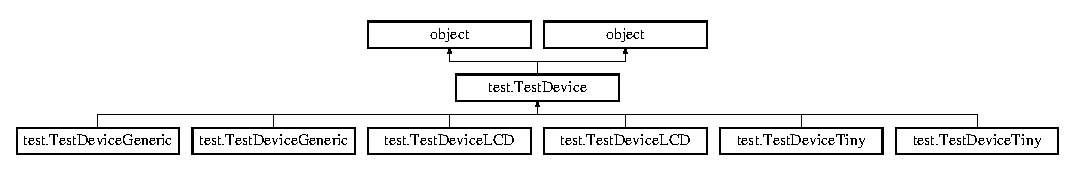
\includegraphics[height=1.854305cm]{classtest_1_1TestDevice}
\end{center}
\end{figure}


The documentation for this class was generated from the following file\-:\begin{DoxyCompactItemize}
\item 
O\-W\-P\-J\-O\-N/\-L\-I\-N\-U\-X/\-Local/\-Local\-U\-D\-P/\-Remote\-Worker/\-Device\-Generic/\hyperlink{LINUX_2Local_2LocalUDP_2RemoteWorker_2DeviceGeneric_2test_8py}{test.\-py}\end{DoxyCompactItemize}

\hypertarget{classtest_1_1TestDeviceGeneric}{\section{test.\-Test\-Device\-Generic Class Reference}
\label{classtest_1_1TestDeviceGeneric}\index{test.\-Test\-Device\-Generic@{test.\-Test\-Device\-Generic}}
}
Inheritance diagram for test.\-Test\-Device\-Generic\-:\begin{figure}[H]
\begin{center}
\leavevmode
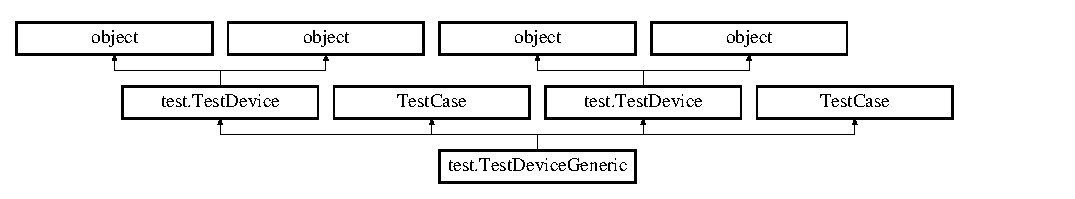
\includegraphics[height=2.225166cm]{classtest_1_1TestDeviceGeneric}
\end{center}
\end{figure}


The documentation for this class was generated from the following file\-:\begin{DoxyCompactItemize}
\item 
O\-W\-P\-J\-O\-N/\-L\-I\-N\-U\-X/\-Local/\-Local\-U\-D\-P/\-Remote\-Worker/\-Device\-Generic/\hyperlink{LINUX_2Local_2LocalUDP_2RemoteWorker_2DeviceGeneric_2test_8py}{test.\-py}\end{DoxyCompactItemize}

\hypertarget{classtest_1_1TestDeviceLCD}{\section{test.\-Test\-Device\-L\-C\-D Class Reference}
\label{classtest_1_1TestDeviceLCD}\index{test.\-Test\-Device\-L\-C\-D@{test.\-Test\-Device\-L\-C\-D}}
}
Inheritance diagram for test.\-Test\-Device\-L\-C\-D\-:\begin{figure}[H]
\begin{center}
\leavevmode
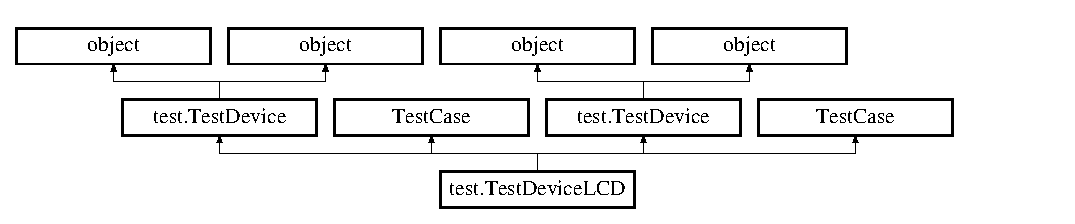
\includegraphics[height=2.564885cm]{classtest_1_1TestDeviceLCD}
\end{center}
\end{figure}


The documentation for this class was generated from the following file\-:\begin{DoxyCompactItemize}
\item 
O\-W\-P\-J\-O\-N/\-L\-I\-N\-U\-X/\-Local/\-Local\-U\-D\-P/\-Remote\-Worker/\-Device\-Generic/\hyperlink{LINUX_2Local_2LocalUDP_2RemoteWorker_2DeviceGeneric_2test_8py}{test.\-py}\end{DoxyCompactItemize}

\hypertarget{classtest_1_1TestDeviceTiny}{\section{test.\-Test\-Device\-Tiny Class Reference}
\label{classtest_1_1TestDeviceTiny}\index{test.\-Test\-Device\-Tiny@{test.\-Test\-Device\-Tiny}}
}
Inheritance diagram for test.\-Test\-Device\-Tiny\-:\begin{figure}[H]
\begin{center}
\leavevmode
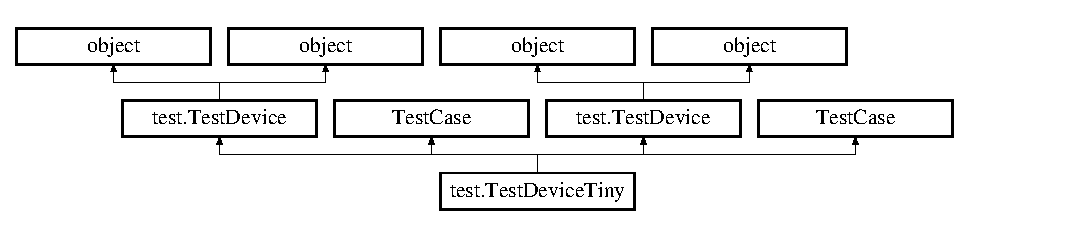
\includegraphics[height=2.584615cm]{classtest_1_1TestDeviceTiny}
\end{center}
\end{figure}


The documentation for this class was generated from the following file\-:\begin{DoxyCompactItemize}
\item 
O\-W\-P\-J\-O\-N/\-L\-I\-N\-U\-X/\-Local/\-Local\-U\-D\-P/\-Remote\-Worker/\-Device\-Generic/\hyperlink{LINUX_2Local_2LocalUDP_2RemoteWorker_2DeviceGeneric_2test_8py}{test.\-py}\end{DoxyCompactItemize}

\hypertarget{classtest_1_1blink__transmitter_1_1ThroughSerial}{\section{test.\-blink\-\_\-transmitter.\-Through\-Serial Class Reference}
\label{classtest_1_1blink__transmitter_1_1ThroughSerial}\index{test.\-blink\-\_\-transmitter.\-Through\-Serial@{test.\-blink\-\_\-transmitter.\-Through\-Serial}}
}
Inheritance diagram for test.\-blink\-\_\-transmitter.\-Through\-Serial\-:\begin{figure}[H]
\begin{center}
\leavevmode
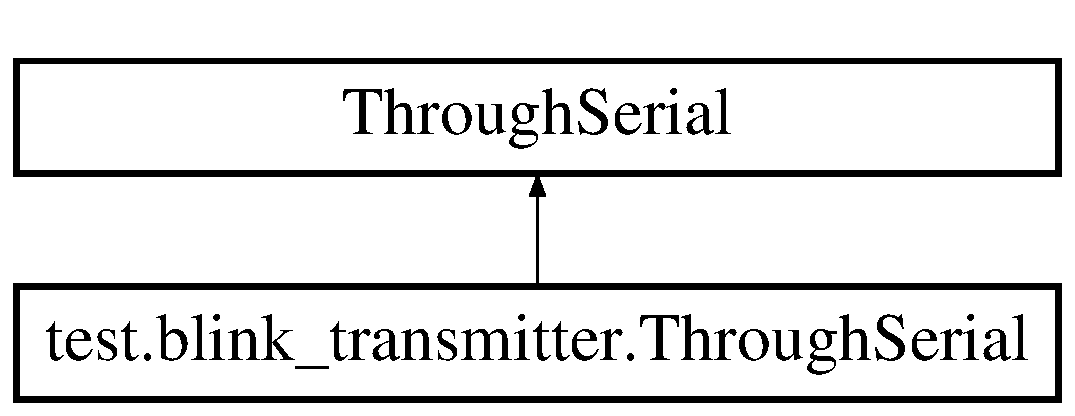
\includegraphics[height=2.000000cm]{classtest_1_1blink__transmitter_1_1ThroughSerial}
\end{center}
\end{figure}
\subsection*{Public Member Functions}
\begin{DoxyCompactItemize}
\item 
def \hyperlink{classtest_1_1blink__transmitter_1_1ThroughSerial_a14abbe983a951e32c6feb23cef743be8}{receive}
\end{DoxyCompactItemize}


\subsection{Member Function Documentation}
\hypertarget{classtest_1_1blink__transmitter_1_1ThroughSerial_a14abbe983a951e32c6feb23cef743be8}{\index{test\-::blink\-\_\-transmitter\-::\-Through\-Serial@{test\-::blink\-\_\-transmitter\-::\-Through\-Serial}!receive@{receive}}
\index{receive@{receive}!test::blink_transmitter::ThroughSerial@{test\-::blink\-\_\-transmitter\-::\-Through\-Serial}}
\subsubsection[{receive}]{\setlength{\rightskip}{0pt plus 5cm}def test.\-blink\-\_\-transmitter.\-Through\-Serial.\-receive (
\begin{DoxyParamCaption}
\item[{}]{self, }
\item[{}]{data, }
\item[{}]{length, }
\item[{}]{packet\-\_\-info}
\end{DoxyParamCaption}
)}}\label{classtest_1_1blink__transmitter_1_1ThroughSerial_a14abbe983a951e32c6feb23cef743be8}


The documentation for this class was generated from the following file\-:\begin{DoxyCompactItemize}
\item 
O\-W\-P\-J\-O\-N/\-P\-J\-O\-N-\/cython/test/\hyperlink{blink__transmitter_8py}{blink\-\_\-transmitter.\-py}\end{DoxyCompactItemize}

\hypertarget{classtest_1_1test_1_1ThroughSerial}{\section{test.\-test.\-Through\-Serial Class Reference}
\label{classtest_1_1test_1_1ThroughSerial}\index{test.\-test.\-Through\-Serial@{test.\-test.\-Through\-Serial}}
}
Inheritance diagram for test.\-test.\-Through\-Serial\-:\begin{figure}[H]
\begin{center}
\leavevmode
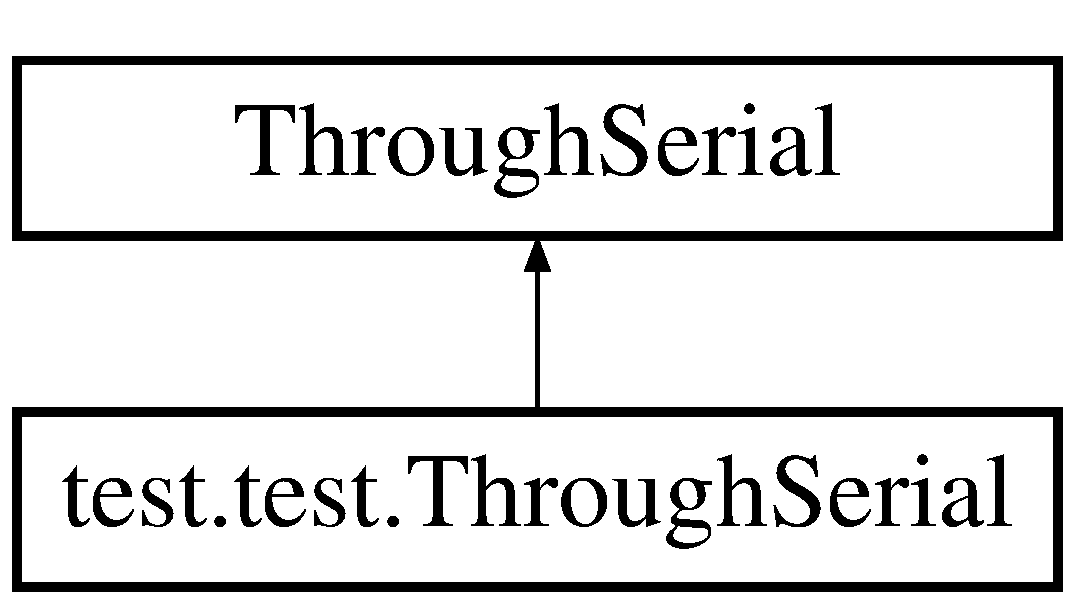
\includegraphics[height=2.000000cm]{classtest_1_1test_1_1ThroughSerial}
\end{center}
\end{figure}
\subsection*{Public Member Functions}
\begin{DoxyCompactItemize}
\item 
def \hyperlink{classtest_1_1test_1_1ThroughSerial_ada82402a237e6f8f424d7f8c1a358a35}{receive}
\end{DoxyCompactItemize}


\subsection{Member Function Documentation}
\hypertarget{classtest_1_1test_1_1ThroughSerial_ada82402a237e6f8f424d7f8c1a358a35}{\index{test\-::test\-::\-Through\-Serial@{test\-::test\-::\-Through\-Serial}!receive@{receive}}
\index{receive@{receive}!test::test::ThroughSerial@{test\-::test\-::\-Through\-Serial}}
\subsubsection[{receive}]{\setlength{\rightskip}{0pt plus 5cm}def test.\-test.\-Through\-Serial.\-receive (
\begin{DoxyParamCaption}
\item[{}]{self, }
\item[{}]{data, }
\item[{}]{length, }
\item[{}]{packet\-\_\-info}
\end{DoxyParamCaption}
)}}\label{classtest_1_1test_1_1ThroughSerial_ada82402a237e6f8f424d7f8c1a358a35}


The documentation for this class was generated from the following file\-:\begin{DoxyCompactItemize}
\item 
O\-W\-P\-J\-O\-N/\-P\-J\-O\-N-\/cython/test/\hyperlink{PJON-cython_2test_2test_8py}{test.\-py}\end{DoxyCompactItemize}

\hypertarget{structuint16x4x2__t}{\section{uint16x4x2\-\_\-t Struct Reference}
\label{structuint16x4x2__t}\index{uint16x4x2\-\_\-t@{uint16x4x2\-\_\-t}}
}


{\ttfamily \#include $<$arm\-\_\-neon.\-h$>$}

\subsection*{Public Attributes}
\begin{DoxyCompactItemize}
\item 
uint16x4\-\_\-t \hyperlink{structuint16x4x2__t_a79a3ee2d9f9bbb3fc7a917faa38faa1a}{val} \mbox{[}2\mbox{]}
\end{DoxyCompactItemize}


\subsection{Member Data Documentation}
\hypertarget{structuint16x4x2__t_a79a3ee2d9f9bbb3fc7a917faa38faa1a}{\index{uint16x4x2\-\_\-t@{uint16x4x2\-\_\-t}!val@{val}}
\index{val@{val}!uint16x4x2_t@{uint16x4x2\-\_\-t}}
\subsubsection[{val}]{\setlength{\rightskip}{0pt plus 5cm}uint16x4\-\_\-t uint16x4x2\-\_\-t\-::val\mbox{[}2\mbox{]}}}\label{structuint16x4x2__t_a79a3ee2d9f9bbb3fc7a917faa38faa1a}


The documentation for this struct was generated from the following file\-:\begin{DoxyCompactItemize}
\item 
oclint-\/0.\-10.\-3/lib/clang/3.\-8.\-0/include/\hyperlink{arm__neon_8h}{arm\-\_\-neon.\-h}\end{DoxyCompactItemize}

\hypertarget{structuint16x4x3__t}{\section{uint16x4x3\-\_\-t Struct Reference}
\label{structuint16x4x3__t}\index{uint16x4x3\-\_\-t@{uint16x4x3\-\_\-t}}
}


{\ttfamily \#include $<$arm\-\_\-neon.\-h$>$}

\subsection*{Public Attributes}
\begin{DoxyCompactItemize}
\item 
uint16x4\-\_\-t \hyperlink{structuint16x4x3__t_a8c54405dc456c34462ef61e2adf32dd5}{val} \mbox{[}3\mbox{]}
\end{DoxyCompactItemize}


\subsection{Member Data Documentation}
\hypertarget{structuint16x4x3__t_a8c54405dc456c34462ef61e2adf32dd5}{\index{uint16x4x3\-\_\-t@{uint16x4x3\-\_\-t}!val@{val}}
\index{val@{val}!uint16x4x3_t@{uint16x4x3\-\_\-t}}
\subsubsection[{val}]{\setlength{\rightskip}{0pt plus 5cm}uint16x4\-\_\-t uint16x4x3\-\_\-t\-::val\mbox{[}3\mbox{]}}}\label{structuint16x4x3__t_a8c54405dc456c34462ef61e2adf32dd5}


The documentation for this struct was generated from the following file\-:\begin{DoxyCompactItemize}
\item 
oclint-\/0.\-10.\-3/lib/clang/3.\-8.\-0/include/\hyperlink{arm__neon_8h}{arm\-\_\-neon.\-h}\end{DoxyCompactItemize}

\hypertarget{structuint16x4x4__t}{\section{uint16x4x4\-\_\-t Struct Reference}
\label{structuint16x4x4__t}\index{uint16x4x4\-\_\-t@{uint16x4x4\-\_\-t}}
}


{\ttfamily \#include $<$arm\-\_\-neon.\-h$>$}

\subsection*{Public Attributes}
\begin{DoxyCompactItemize}
\item 
uint16x4\-\_\-t \hyperlink{structuint16x4x4__t_a146bb08879ecada88cf81dc0d5c2d8bd}{val} \mbox{[}4\mbox{]}
\end{DoxyCompactItemize}


\subsection{Member Data Documentation}
\hypertarget{structuint16x4x4__t_a146bb08879ecada88cf81dc0d5c2d8bd}{\index{uint16x4x4\-\_\-t@{uint16x4x4\-\_\-t}!val@{val}}
\index{val@{val}!uint16x4x4_t@{uint16x4x4\-\_\-t}}
\subsubsection[{val}]{\setlength{\rightskip}{0pt plus 5cm}uint16x4\-\_\-t uint16x4x4\-\_\-t\-::val\mbox{[}4\mbox{]}}}\label{structuint16x4x4__t_a146bb08879ecada88cf81dc0d5c2d8bd}


The documentation for this struct was generated from the following file\-:\begin{DoxyCompactItemize}
\item 
oclint-\/0.\-10.\-3/lib/clang/3.\-8.\-0/include/\hyperlink{arm__neon_8h}{arm\-\_\-neon.\-h}\end{DoxyCompactItemize}

\hypertarget{structuint16x8x2__t}{\section{uint16x8x2\-\_\-t Struct Reference}
\label{structuint16x8x2__t}\index{uint16x8x2\-\_\-t@{uint16x8x2\-\_\-t}}
}


{\ttfamily \#include $<$arm\-\_\-neon.\-h$>$}

\subsection*{Public Attributes}
\begin{DoxyCompactItemize}
\item 
uint16x8\-\_\-t \hyperlink{structuint16x8x2__t_aefbebf4d19c86b12c892fa35fce3c365}{val} \mbox{[}2\mbox{]}
\end{DoxyCompactItemize}


\subsection{Member Data Documentation}
\hypertarget{structuint16x8x2__t_aefbebf4d19c86b12c892fa35fce3c365}{\index{uint16x8x2\-\_\-t@{uint16x8x2\-\_\-t}!val@{val}}
\index{val@{val}!uint16x8x2_t@{uint16x8x2\-\_\-t}}
\subsubsection[{val}]{\setlength{\rightskip}{0pt plus 5cm}uint16x8\-\_\-t uint16x8x2\-\_\-t\-::val\mbox{[}2\mbox{]}}}\label{structuint16x8x2__t_aefbebf4d19c86b12c892fa35fce3c365}


The documentation for this struct was generated from the following file\-:\begin{DoxyCompactItemize}
\item 
oclint-\/0.\-10.\-3/lib/clang/3.\-8.\-0/include/\hyperlink{arm__neon_8h}{arm\-\_\-neon.\-h}\end{DoxyCompactItemize}

\hypertarget{structuint16x8x3__t}{\section{uint16x8x3\-\_\-t Struct Reference}
\label{structuint16x8x3__t}\index{uint16x8x3\-\_\-t@{uint16x8x3\-\_\-t}}
}


{\ttfamily \#include $<$arm\-\_\-neon.\-h$>$}

\subsection*{Public Attributes}
\begin{DoxyCompactItemize}
\item 
uint16x8\-\_\-t \hyperlink{structuint16x8x3__t_abe1e664c587d316efb810cefa4290b4b}{val} \mbox{[}3\mbox{]}
\end{DoxyCompactItemize}


\subsection{Member Data Documentation}
\hypertarget{structuint16x8x3__t_abe1e664c587d316efb810cefa4290b4b}{\index{uint16x8x3\-\_\-t@{uint16x8x3\-\_\-t}!val@{val}}
\index{val@{val}!uint16x8x3_t@{uint16x8x3\-\_\-t}}
\subsubsection[{val}]{\setlength{\rightskip}{0pt plus 5cm}uint16x8\-\_\-t uint16x8x3\-\_\-t\-::val\mbox{[}3\mbox{]}}}\label{structuint16x8x3__t_abe1e664c587d316efb810cefa4290b4b}


The documentation for this struct was generated from the following file\-:\begin{DoxyCompactItemize}
\item 
oclint-\/0.\-10.\-3/lib/clang/3.\-8.\-0/include/\hyperlink{arm__neon_8h}{arm\-\_\-neon.\-h}\end{DoxyCompactItemize}

\hypertarget{structuint16x8x4__t}{\section{uint16x8x4\-\_\-t Struct Reference}
\label{structuint16x8x4__t}\index{uint16x8x4\-\_\-t@{uint16x8x4\-\_\-t}}
}


{\ttfamily \#include $<$arm\-\_\-neon.\-h$>$}

\subsection*{Public Attributes}
\begin{DoxyCompactItemize}
\item 
uint16x8\-\_\-t \hyperlink{structuint16x8x4__t_ad85378b41567a3fabbb10ef1e9eccd32}{val} \mbox{[}4\mbox{]}
\end{DoxyCompactItemize}


\subsection{Member Data Documentation}
\hypertarget{structuint16x8x4__t_ad85378b41567a3fabbb10ef1e9eccd32}{\index{uint16x8x4\-\_\-t@{uint16x8x4\-\_\-t}!val@{val}}
\index{val@{val}!uint16x8x4_t@{uint16x8x4\-\_\-t}}
\subsubsection[{val}]{\setlength{\rightskip}{0pt plus 5cm}uint16x8\-\_\-t uint16x8x4\-\_\-t\-::val\mbox{[}4\mbox{]}}}\label{structuint16x8x4__t_ad85378b41567a3fabbb10ef1e9eccd32}


The documentation for this struct was generated from the following file\-:\begin{DoxyCompactItemize}
\item 
oclint-\/0.\-10.\-3/lib/clang/3.\-8.\-0/include/\hyperlink{arm__neon_8h}{arm\-\_\-neon.\-h}\end{DoxyCompactItemize}

\hypertarget{structuint32x2x2__t}{\section{uint32x2x2\-\_\-t Struct Reference}
\label{structuint32x2x2__t}\index{uint32x2x2\-\_\-t@{uint32x2x2\-\_\-t}}
}


{\ttfamily \#include $<$arm\-\_\-neon.\-h$>$}

\subsection*{Public Attributes}
\begin{DoxyCompactItemize}
\item 
uint32x2\-\_\-t \hyperlink{structuint32x2x2__t_af1d57ad944319515fe7e3aa820396774}{val} \mbox{[}2\mbox{]}
\end{DoxyCompactItemize}


\subsection{Member Data Documentation}
\hypertarget{structuint32x2x2__t_af1d57ad944319515fe7e3aa820396774}{\index{uint32x2x2\-\_\-t@{uint32x2x2\-\_\-t}!val@{val}}
\index{val@{val}!uint32x2x2_t@{uint32x2x2\-\_\-t}}
\subsubsection[{val}]{\setlength{\rightskip}{0pt plus 5cm}uint32x2\-\_\-t uint32x2x2\-\_\-t\-::val\mbox{[}2\mbox{]}}}\label{structuint32x2x2__t_af1d57ad944319515fe7e3aa820396774}


The documentation for this struct was generated from the following file\-:\begin{DoxyCompactItemize}
\item 
oclint-\/0.\-10.\-3/lib/clang/3.\-8.\-0/include/\hyperlink{arm__neon_8h}{arm\-\_\-neon.\-h}\end{DoxyCompactItemize}

\hypertarget{structuint32x2x3__t}{\section{uint32x2x3\-\_\-t Struct Reference}
\label{structuint32x2x3__t}\index{uint32x2x3\-\_\-t@{uint32x2x3\-\_\-t}}
}


{\ttfamily \#include $<$arm\-\_\-neon.\-h$>$}

\subsection*{Public Attributes}
\begin{DoxyCompactItemize}
\item 
uint32x2\-\_\-t \hyperlink{structuint32x2x3__t_a83ac1a1428dcf13108e829da17b8d202}{val} \mbox{[}3\mbox{]}
\end{DoxyCompactItemize}


\subsection{Member Data Documentation}
\hypertarget{structuint32x2x3__t_a83ac1a1428dcf13108e829da17b8d202}{\index{uint32x2x3\-\_\-t@{uint32x2x3\-\_\-t}!val@{val}}
\index{val@{val}!uint32x2x3_t@{uint32x2x3\-\_\-t}}
\subsubsection[{val}]{\setlength{\rightskip}{0pt plus 5cm}uint32x2\-\_\-t uint32x2x3\-\_\-t\-::val\mbox{[}3\mbox{]}}}\label{structuint32x2x3__t_a83ac1a1428dcf13108e829da17b8d202}


The documentation for this struct was generated from the following file\-:\begin{DoxyCompactItemize}
\item 
oclint-\/0.\-10.\-3/lib/clang/3.\-8.\-0/include/\hyperlink{arm__neon_8h}{arm\-\_\-neon.\-h}\end{DoxyCompactItemize}

\hypertarget{structuint32x2x4__t}{\section{uint32x2x4\-\_\-t Struct Reference}
\label{structuint32x2x4__t}\index{uint32x2x4\-\_\-t@{uint32x2x4\-\_\-t}}
}


{\ttfamily \#include $<$arm\-\_\-neon.\-h$>$}

\subsection*{Public Attributes}
\begin{DoxyCompactItemize}
\item 
uint32x2\-\_\-t \hyperlink{structuint32x2x4__t_a5252c3580c663ffd1ecce6e53a943471}{val} \mbox{[}4\mbox{]}
\end{DoxyCompactItemize}


\subsection{Member Data Documentation}
\hypertarget{structuint32x2x4__t_a5252c3580c663ffd1ecce6e53a943471}{\index{uint32x2x4\-\_\-t@{uint32x2x4\-\_\-t}!val@{val}}
\index{val@{val}!uint32x2x4_t@{uint32x2x4\-\_\-t}}
\subsubsection[{val}]{\setlength{\rightskip}{0pt plus 5cm}uint32x2\-\_\-t uint32x2x4\-\_\-t\-::val\mbox{[}4\mbox{]}}}\label{structuint32x2x4__t_a5252c3580c663ffd1ecce6e53a943471}


The documentation for this struct was generated from the following file\-:\begin{DoxyCompactItemize}
\item 
oclint-\/0.\-10.\-3/lib/clang/3.\-8.\-0/include/\hyperlink{arm__neon_8h}{arm\-\_\-neon.\-h}\end{DoxyCompactItemize}

\hypertarget{structuint32x4x2__t}{\section{uint32x4x2\-\_\-t Struct Reference}
\label{structuint32x4x2__t}\index{uint32x4x2\-\_\-t@{uint32x4x2\-\_\-t}}
}


{\ttfamily \#include $<$arm\-\_\-neon.\-h$>$}

\subsection*{Public Attributes}
\begin{DoxyCompactItemize}
\item 
uint32x4\-\_\-t \hyperlink{structuint32x4x2__t_a9a2d00c2937756a6a467011e6282b63b}{val} \mbox{[}2\mbox{]}
\end{DoxyCompactItemize}


\subsection{Member Data Documentation}
\hypertarget{structuint32x4x2__t_a9a2d00c2937756a6a467011e6282b63b}{\index{uint32x4x2\-\_\-t@{uint32x4x2\-\_\-t}!val@{val}}
\index{val@{val}!uint32x4x2_t@{uint32x4x2\-\_\-t}}
\subsubsection[{val}]{\setlength{\rightskip}{0pt plus 5cm}uint32x4\-\_\-t uint32x4x2\-\_\-t\-::val\mbox{[}2\mbox{]}}}\label{structuint32x4x2__t_a9a2d00c2937756a6a467011e6282b63b}


The documentation for this struct was generated from the following file\-:\begin{DoxyCompactItemize}
\item 
oclint-\/0.\-10.\-3/lib/clang/3.\-8.\-0/include/\hyperlink{arm__neon_8h}{arm\-\_\-neon.\-h}\end{DoxyCompactItemize}

\hypertarget{structuint32x4x3__t}{\section{uint32x4x3\-\_\-t Struct Reference}
\label{structuint32x4x3__t}\index{uint32x4x3\-\_\-t@{uint32x4x3\-\_\-t}}
}


{\ttfamily \#include $<$arm\-\_\-neon.\-h$>$}

\subsection*{Public Attributes}
\begin{DoxyCompactItemize}
\item 
uint32x4\-\_\-t \hyperlink{structuint32x4x3__t_af3bdefffaa3d53304c061377f6693cd6}{val} \mbox{[}3\mbox{]}
\end{DoxyCompactItemize}


\subsection{Member Data Documentation}
\hypertarget{structuint32x4x3__t_af3bdefffaa3d53304c061377f6693cd6}{\index{uint32x4x3\-\_\-t@{uint32x4x3\-\_\-t}!val@{val}}
\index{val@{val}!uint32x4x3_t@{uint32x4x3\-\_\-t}}
\subsubsection[{val}]{\setlength{\rightskip}{0pt plus 5cm}uint32x4\-\_\-t uint32x4x3\-\_\-t\-::val\mbox{[}3\mbox{]}}}\label{structuint32x4x3__t_af3bdefffaa3d53304c061377f6693cd6}


The documentation for this struct was generated from the following file\-:\begin{DoxyCompactItemize}
\item 
oclint-\/0.\-10.\-3/lib/clang/3.\-8.\-0/include/\hyperlink{arm__neon_8h}{arm\-\_\-neon.\-h}\end{DoxyCompactItemize}

\hypertarget{structuint32x4x4__t}{\section{uint32x4x4\-\_\-t Struct Reference}
\label{structuint32x4x4__t}\index{uint32x4x4\-\_\-t@{uint32x4x4\-\_\-t}}
}


{\ttfamily \#include $<$arm\-\_\-neon.\-h$>$}

\subsection*{Public Attributes}
\begin{DoxyCompactItemize}
\item 
uint32x4\-\_\-t \hyperlink{structuint32x4x4__t_a2aacabec36073a60e874900139cc050a}{val} \mbox{[}4\mbox{]}
\end{DoxyCompactItemize}


\subsection{Member Data Documentation}
\hypertarget{structuint32x4x4__t_a2aacabec36073a60e874900139cc050a}{\index{uint32x4x4\-\_\-t@{uint32x4x4\-\_\-t}!val@{val}}
\index{val@{val}!uint32x4x4_t@{uint32x4x4\-\_\-t}}
\subsubsection[{val}]{\setlength{\rightskip}{0pt plus 5cm}uint32x4\-\_\-t uint32x4x4\-\_\-t\-::val\mbox{[}4\mbox{]}}}\label{structuint32x4x4__t_a2aacabec36073a60e874900139cc050a}


The documentation for this struct was generated from the following file\-:\begin{DoxyCompactItemize}
\item 
oclint-\/0.\-10.\-3/lib/clang/3.\-8.\-0/include/\hyperlink{arm__neon_8h}{arm\-\_\-neon.\-h}\end{DoxyCompactItemize}

\hypertarget{structuint64x1x2__t}{\section{uint64x1x2\-\_\-t Struct Reference}
\label{structuint64x1x2__t}\index{uint64x1x2\-\_\-t@{uint64x1x2\-\_\-t}}
}


{\ttfamily \#include $<$arm\-\_\-neon.\-h$>$}

\subsection*{Public Attributes}
\begin{DoxyCompactItemize}
\item 
uint64x1\-\_\-t \hyperlink{structuint64x1x2__t_a8d401e43d7245dfe87578685aa97c8d1}{val} \mbox{[}2\mbox{]}
\end{DoxyCompactItemize}


\subsection{Member Data Documentation}
\hypertarget{structuint64x1x2__t_a8d401e43d7245dfe87578685aa97c8d1}{\index{uint64x1x2\-\_\-t@{uint64x1x2\-\_\-t}!val@{val}}
\index{val@{val}!uint64x1x2_t@{uint64x1x2\-\_\-t}}
\subsubsection[{val}]{\setlength{\rightskip}{0pt plus 5cm}uint64x1\-\_\-t uint64x1x2\-\_\-t\-::val\mbox{[}2\mbox{]}}}\label{structuint64x1x2__t_a8d401e43d7245dfe87578685aa97c8d1}


The documentation for this struct was generated from the following file\-:\begin{DoxyCompactItemize}
\item 
oclint-\/0.\-10.\-3/lib/clang/3.\-8.\-0/include/\hyperlink{arm__neon_8h}{arm\-\_\-neon.\-h}\end{DoxyCompactItemize}

\hypertarget{structuint64x1x3__t}{\section{uint64x1x3\-\_\-t Struct Reference}
\label{structuint64x1x3__t}\index{uint64x1x3\-\_\-t@{uint64x1x3\-\_\-t}}
}


{\ttfamily \#include $<$arm\-\_\-neon.\-h$>$}

\subsection*{Public Attributes}
\begin{DoxyCompactItemize}
\item 
uint64x1\-\_\-t \hyperlink{structuint64x1x3__t_a6146ce8fbfccdf8f0f93233c83cb7959}{val} \mbox{[}3\mbox{]}
\end{DoxyCompactItemize}


\subsection{Member Data Documentation}
\hypertarget{structuint64x1x3__t_a6146ce8fbfccdf8f0f93233c83cb7959}{\index{uint64x1x3\-\_\-t@{uint64x1x3\-\_\-t}!val@{val}}
\index{val@{val}!uint64x1x3_t@{uint64x1x3\-\_\-t}}
\subsubsection[{val}]{\setlength{\rightskip}{0pt plus 5cm}uint64x1\-\_\-t uint64x1x3\-\_\-t\-::val\mbox{[}3\mbox{]}}}\label{structuint64x1x3__t_a6146ce8fbfccdf8f0f93233c83cb7959}


The documentation for this struct was generated from the following file\-:\begin{DoxyCompactItemize}
\item 
oclint-\/0.\-10.\-3/lib/clang/3.\-8.\-0/include/\hyperlink{arm__neon_8h}{arm\-\_\-neon.\-h}\end{DoxyCompactItemize}

\hypertarget{structuint64x1x4__t}{\section{uint64x1x4\-\_\-t Struct Reference}
\label{structuint64x1x4__t}\index{uint64x1x4\-\_\-t@{uint64x1x4\-\_\-t}}
}


{\ttfamily \#include $<$arm\-\_\-neon.\-h$>$}

\subsection*{Public Attributes}
\begin{DoxyCompactItemize}
\item 
uint64x1\-\_\-t \hyperlink{structuint64x1x4__t_aa6dc44b1d6189823f391dfcd157bdf8b}{val} \mbox{[}4\mbox{]}
\end{DoxyCompactItemize}


\subsection{Member Data Documentation}
\hypertarget{structuint64x1x4__t_aa6dc44b1d6189823f391dfcd157bdf8b}{\index{uint64x1x4\-\_\-t@{uint64x1x4\-\_\-t}!val@{val}}
\index{val@{val}!uint64x1x4_t@{uint64x1x4\-\_\-t}}
\subsubsection[{val}]{\setlength{\rightskip}{0pt plus 5cm}uint64x1\-\_\-t uint64x1x4\-\_\-t\-::val\mbox{[}4\mbox{]}}}\label{structuint64x1x4__t_aa6dc44b1d6189823f391dfcd157bdf8b}


The documentation for this struct was generated from the following file\-:\begin{DoxyCompactItemize}
\item 
oclint-\/0.\-10.\-3/lib/clang/3.\-8.\-0/include/\hyperlink{arm__neon_8h}{arm\-\_\-neon.\-h}\end{DoxyCompactItemize}

\hypertarget{structuint64x2x2__t}{\section{uint64x2x2\-\_\-t Struct Reference}
\label{structuint64x2x2__t}\index{uint64x2x2\-\_\-t@{uint64x2x2\-\_\-t}}
}


{\ttfamily \#include $<$arm\-\_\-neon.\-h$>$}

\subsection*{Public Attributes}
\begin{DoxyCompactItemize}
\item 
uint64x2\-\_\-t \hyperlink{structuint64x2x2__t_a4fa4c56badeeefd397eb1eb945557903}{val} \mbox{[}2\mbox{]}
\end{DoxyCompactItemize}


\subsection{Member Data Documentation}
\hypertarget{structuint64x2x2__t_a4fa4c56badeeefd397eb1eb945557903}{\index{uint64x2x2\-\_\-t@{uint64x2x2\-\_\-t}!val@{val}}
\index{val@{val}!uint64x2x2_t@{uint64x2x2\-\_\-t}}
\subsubsection[{val}]{\setlength{\rightskip}{0pt plus 5cm}uint64x2\-\_\-t uint64x2x2\-\_\-t\-::val\mbox{[}2\mbox{]}}}\label{structuint64x2x2__t_a4fa4c56badeeefd397eb1eb945557903}


The documentation for this struct was generated from the following file\-:\begin{DoxyCompactItemize}
\item 
oclint-\/0.\-10.\-3/lib/clang/3.\-8.\-0/include/\hyperlink{arm__neon_8h}{arm\-\_\-neon.\-h}\end{DoxyCompactItemize}

\hypertarget{structuint64x2x3__t}{\section{uint64x2x3\-\_\-t Struct Reference}
\label{structuint64x2x3__t}\index{uint64x2x3\-\_\-t@{uint64x2x3\-\_\-t}}
}


{\ttfamily \#include $<$arm\-\_\-neon.\-h$>$}

\subsection*{Public Attributes}
\begin{DoxyCompactItemize}
\item 
uint64x2\-\_\-t \hyperlink{structuint64x2x3__t_ab934b42c25831e3a99b6178c2c8c4b55}{val} \mbox{[}3\mbox{]}
\end{DoxyCompactItemize}


\subsection{Member Data Documentation}
\hypertarget{structuint64x2x3__t_ab934b42c25831e3a99b6178c2c8c4b55}{\index{uint64x2x3\-\_\-t@{uint64x2x3\-\_\-t}!val@{val}}
\index{val@{val}!uint64x2x3_t@{uint64x2x3\-\_\-t}}
\subsubsection[{val}]{\setlength{\rightskip}{0pt plus 5cm}uint64x2\-\_\-t uint64x2x3\-\_\-t\-::val\mbox{[}3\mbox{]}}}\label{structuint64x2x3__t_ab934b42c25831e3a99b6178c2c8c4b55}


The documentation for this struct was generated from the following file\-:\begin{DoxyCompactItemize}
\item 
oclint-\/0.\-10.\-3/lib/clang/3.\-8.\-0/include/\hyperlink{arm__neon_8h}{arm\-\_\-neon.\-h}\end{DoxyCompactItemize}

\hypertarget{structuint64x2x4__t}{\section{uint64x2x4\-\_\-t Struct Reference}
\label{structuint64x2x4__t}\index{uint64x2x4\-\_\-t@{uint64x2x4\-\_\-t}}
}


{\ttfamily \#include $<$arm\-\_\-neon.\-h$>$}

\subsection*{Public Attributes}
\begin{DoxyCompactItemize}
\item 
uint64x2\-\_\-t \hyperlink{structuint64x2x4__t_a6d4af1f655a9f35a340b0eb46f787812}{val} \mbox{[}4\mbox{]}
\end{DoxyCompactItemize}


\subsection{Member Data Documentation}
\hypertarget{structuint64x2x4__t_a6d4af1f655a9f35a340b0eb46f787812}{\index{uint64x2x4\-\_\-t@{uint64x2x4\-\_\-t}!val@{val}}
\index{val@{val}!uint64x2x4_t@{uint64x2x4\-\_\-t}}
\subsubsection[{val}]{\setlength{\rightskip}{0pt plus 5cm}uint64x2\-\_\-t uint64x2x4\-\_\-t\-::val\mbox{[}4\mbox{]}}}\label{structuint64x2x4__t_a6d4af1f655a9f35a340b0eb46f787812}


The documentation for this struct was generated from the following file\-:\begin{DoxyCompactItemize}
\item 
oclint-\/0.\-10.\-3/lib/clang/3.\-8.\-0/include/\hyperlink{arm__neon_8h}{arm\-\_\-neon.\-h}\end{DoxyCompactItemize}

\hypertarget{structuint8x16x2__t}{\section{uint8x16x2\-\_\-t Struct Reference}
\label{structuint8x16x2__t}\index{uint8x16x2\-\_\-t@{uint8x16x2\-\_\-t}}
}


{\ttfamily \#include $<$arm\-\_\-neon.\-h$>$}

\subsection*{Public Attributes}
\begin{DoxyCompactItemize}
\item 
uint8x16\-\_\-t \hyperlink{structuint8x16x2__t_a94ba576d8133698da63185222062503a}{val} \mbox{[}2\mbox{]}
\end{DoxyCompactItemize}


\subsection{Member Data Documentation}
\hypertarget{structuint8x16x2__t_a94ba576d8133698da63185222062503a}{\index{uint8x16x2\-\_\-t@{uint8x16x2\-\_\-t}!val@{val}}
\index{val@{val}!uint8x16x2_t@{uint8x16x2\-\_\-t}}
\subsubsection[{val}]{\setlength{\rightskip}{0pt plus 5cm}uint8x16\-\_\-t uint8x16x2\-\_\-t\-::val\mbox{[}2\mbox{]}}}\label{structuint8x16x2__t_a94ba576d8133698da63185222062503a}


The documentation for this struct was generated from the following file\-:\begin{DoxyCompactItemize}
\item 
oclint-\/0.\-10.\-3/lib/clang/3.\-8.\-0/include/\hyperlink{arm__neon_8h}{arm\-\_\-neon.\-h}\end{DoxyCompactItemize}

\hypertarget{structuint8x16x3__t}{\section{uint8x16x3\-\_\-t Struct Reference}
\label{structuint8x16x3__t}\index{uint8x16x3\-\_\-t@{uint8x16x3\-\_\-t}}
}


{\ttfamily \#include $<$arm\-\_\-neon.\-h$>$}

\subsection*{Public Attributes}
\begin{DoxyCompactItemize}
\item 
uint8x16\-\_\-t \hyperlink{structuint8x16x3__t_a81ffa44558b7664cc736f9d49b820664}{val} \mbox{[}3\mbox{]}
\end{DoxyCompactItemize}


\subsection{Member Data Documentation}
\hypertarget{structuint8x16x3__t_a81ffa44558b7664cc736f9d49b820664}{\index{uint8x16x3\-\_\-t@{uint8x16x3\-\_\-t}!val@{val}}
\index{val@{val}!uint8x16x3_t@{uint8x16x3\-\_\-t}}
\subsubsection[{val}]{\setlength{\rightskip}{0pt plus 5cm}uint8x16\-\_\-t uint8x16x3\-\_\-t\-::val\mbox{[}3\mbox{]}}}\label{structuint8x16x3__t_a81ffa44558b7664cc736f9d49b820664}


The documentation for this struct was generated from the following file\-:\begin{DoxyCompactItemize}
\item 
oclint-\/0.\-10.\-3/lib/clang/3.\-8.\-0/include/\hyperlink{arm__neon_8h}{arm\-\_\-neon.\-h}\end{DoxyCompactItemize}

\hypertarget{structuint8x16x4__t}{\section{uint8x16x4\-\_\-t Struct Reference}
\label{structuint8x16x4__t}\index{uint8x16x4\-\_\-t@{uint8x16x4\-\_\-t}}
}


{\ttfamily \#include $<$arm\-\_\-neon.\-h$>$}

\subsection*{Public Attributes}
\begin{DoxyCompactItemize}
\item 
uint8x16\-\_\-t \hyperlink{structuint8x16x4__t_a63561bf71d2c03945ee130aa99e4599e}{val} \mbox{[}4\mbox{]}
\end{DoxyCompactItemize}


\subsection{Member Data Documentation}
\hypertarget{structuint8x16x4__t_a63561bf71d2c03945ee130aa99e4599e}{\index{uint8x16x4\-\_\-t@{uint8x16x4\-\_\-t}!val@{val}}
\index{val@{val}!uint8x16x4_t@{uint8x16x4\-\_\-t}}
\subsubsection[{val}]{\setlength{\rightskip}{0pt plus 5cm}uint8x16\-\_\-t uint8x16x4\-\_\-t\-::val\mbox{[}4\mbox{]}}}\label{structuint8x16x4__t_a63561bf71d2c03945ee130aa99e4599e}


The documentation for this struct was generated from the following file\-:\begin{DoxyCompactItemize}
\item 
oclint-\/0.\-10.\-3/lib/clang/3.\-8.\-0/include/\hyperlink{arm__neon_8h}{arm\-\_\-neon.\-h}\end{DoxyCompactItemize}

\hypertarget{structuint8x8x2__t}{\section{uint8x8x2\-\_\-t Struct Reference}
\label{structuint8x8x2__t}\index{uint8x8x2\-\_\-t@{uint8x8x2\-\_\-t}}
}


{\ttfamily \#include $<$arm\-\_\-neon.\-h$>$}

\subsection*{Public Attributes}
\begin{DoxyCompactItemize}
\item 
uint8x8\-\_\-t \hyperlink{structuint8x8x2__t_a6686ee0ab46c3a82908796baee91cbd6}{val} \mbox{[}2\mbox{]}
\end{DoxyCompactItemize}


\subsection{Member Data Documentation}
\hypertarget{structuint8x8x2__t_a6686ee0ab46c3a82908796baee91cbd6}{\index{uint8x8x2\-\_\-t@{uint8x8x2\-\_\-t}!val@{val}}
\index{val@{val}!uint8x8x2_t@{uint8x8x2\-\_\-t}}
\subsubsection[{val}]{\setlength{\rightskip}{0pt plus 5cm}uint8x8\-\_\-t uint8x8x2\-\_\-t\-::val\mbox{[}2\mbox{]}}}\label{structuint8x8x2__t_a6686ee0ab46c3a82908796baee91cbd6}


The documentation for this struct was generated from the following file\-:\begin{DoxyCompactItemize}
\item 
oclint-\/0.\-10.\-3/lib/clang/3.\-8.\-0/include/\hyperlink{arm__neon_8h}{arm\-\_\-neon.\-h}\end{DoxyCompactItemize}

\hypertarget{structuint8x8x3__t}{\section{uint8x8x3\-\_\-t Struct Reference}
\label{structuint8x8x3__t}\index{uint8x8x3\-\_\-t@{uint8x8x3\-\_\-t}}
}


{\ttfamily \#include $<$arm\-\_\-neon.\-h$>$}

\subsection*{Public Attributes}
\begin{DoxyCompactItemize}
\item 
uint8x8\-\_\-t \hyperlink{structuint8x8x3__t_aacba6e6a70f36f292dcf2a88bff9d632}{val} \mbox{[}3\mbox{]}
\end{DoxyCompactItemize}


\subsection{Member Data Documentation}
\hypertarget{structuint8x8x3__t_aacba6e6a70f36f292dcf2a88bff9d632}{\index{uint8x8x3\-\_\-t@{uint8x8x3\-\_\-t}!val@{val}}
\index{val@{val}!uint8x8x3_t@{uint8x8x3\-\_\-t}}
\subsubsection[{val}]{\setlength{\rightskip}{0pt plus 5cm}uint8x8\-\_\-t uint8x8x3\-\_\-t\-::val\mbox{[}3\mbox{]}}}\label{structuint8x8x3__t_aacba6e6a70f36f292dcf2a88bff9d632}


The documentation for this struct was generated from the following file\-:\begin{DoxyCompactItemize}
\item 
oclint-\/0.\-10.\-3/lib/clang/3.\-8.\-0/include/\hyperlink{arm__neon_8h}{arm\-\_\-neon.\-h}\end{DoxyCompactItemize}

\hypertarget{structuint8x8x4__t}{\section{uint8x8x4\-\_\-t Struct Reference}
\label{structuint8x8x4__t}\index{uint8x8x4\-\_\-t@{uint8x8x4\-\_\-t}}
}


{\ttfamily \#include $<$arm\-\_\-neon.\-h$>$}

\subsection*{Public Attributes}
\begin{DoxyCompactItemize}
\item 
uint8x8\-\_\-t \hyperlink{structuint8x8x4__t_a59d59f8ccc3518b30b8d260e28a4b38e}{val} \mbox{[}4\mbox{]}
\end{DoxyCompactItemize}


\subsection{Member Data Documentation}
\hypertarget{structuint8x8x4__t_a59d59f8ccc3518b30b8d260e28a4b38e}{\index{uint8x8x4\-\_\-t@{uint8x8x4\-\_\-t}!val@{val}}
\index{val@{val}!uint8x8x4_t@{uint8x8x4\-\_\-t}}
\subsubsection[{val}]{\setlength{\rightskip}{0pt plus 5cm}uint8x8\-\_\-t uint8x8x4\-\_\-t\-::val\mbox{[}4\mbox{]}}}\label{structuint8x8x4__t_a59d59f8ccc3518b30b8d260e28a4b38e}


The documentation for this struct was generated from the following file\-:\begin{DoxyCompactItemize}
\item 
oclint-\/0.\-10.\-3/lib/clang/3.\-8.\-0/include/\hyperlink{arm__neon_8h}{arm\-\_\-neon.\-h}\end{DoxyCompactItemize}

\hypertarget{structusbRequest}{\section{usb\-Request Struct Reference}
\label{structusbRequest}\index{usb\-Request@{usb\-Request}}
}


{\ttfamily \#include $<$usbdrv.\-h$>$}

\subsection*{Public Attributes}
\begin{DoxyCompactItemize}
\item 
\hyperlink{usbdrv_8h_aa8ddf20cdd716b652e76e23e5e700893}{uchar} \hyperlink{structusbRequest_a05c2e0d9ac30dce558bcd69a692314c0}{bm\-Request\-Type}
\item 
\hyperlink{usbdrv_8h_aa8ddf20cdd716b652e76e23e5e700893}{uchar} \hyperlink{structusbRequest_a34c18b1dd0af60774cac48b176220c2c}{b\-Request}
\item 
\hyperlink{usbdrv_8h_a992d37ca7c2980c180e963d4f78a30ea}{usb\-Word\-\_\-t} \hyperlink{structusbRequest_ab3f8687bb757c53ed03c3ce4310dc5c5}{w\-Value}
\item 
\hyperlink{usbdrv_8h_a992d37ca7c2980c180e963d4f78a30ea}{usb\-Word\-\_\-t} \hyperlink{structusbRequest_aefa059246bf079d5b42af148a2ad6a95}{w\-Index}
\item 
\hyperlink{usbdrv_8h_a992d37ca7c2980c180e963d4f78a30ea}{usb\-Word\-\_\-t} \hyperlink{structusbRequest_a770437881c2e37d1384982fe26d87e7f}{w\-Length}
\end{DoxyCompactItemize}


\subsection{Member Data Documentation}
\hypertarget{structusbRequest_a05c2e0d9ac30dce558bcd69a692314c0}{\index{usb\-Request@{usb\-Request}!bm\-Request\-Type@{bm\-Request\-Type}}
\index{bm\-Request\-Type@{bm\-Request\-Type}!usbRequest@{usb\-Request}}
\subsubsection[{bm\-Request\-Type}]{\setlength{\rightskip}{0pt plus 5cm}{\bf uchar} usb\-Request\-::bm\-Request\-Type}}\label{structusbRequest_a05c2e0d9ac30dce558bcd69a692314c0}
\hypertarget{structusbRequest_a34c18b1dd0af60774cac48b176220c2c}{\index{usb\-Request@{usb\-Request}!b\-Request@{b\-Request}}
\index{b\-Request@{b\-Request}!usbRequest@{usb\-Request}}
\subsubsection[{b\-Request}]{\setlength{\rightskip}{0pt plus 5cm}{\bf uchar} usb\-Request\-::b\-Request}}\label{structusbRequest_a34c18b1dd0af60774cac48b176220c2c}
\hypertarget{structusbRequest_aefa059246bf079d5b42af148a2ad6a95}{\index{usb\-Request@{usb\-Request}!w\-Index@{w\-Index}}
\index{w\-Index@{w\-Index}!usbRequest@{usb\-Request}}
\subsubsection[{w\-Index}]{\setlength{\rightskip}{0pt plus 5cm}{\bf usb\-Word\-\_\-t} usb\-Request\-::w\-Index}}\label{structusbRequest_aefa059246bf079d5b42af148a2ad6a95}
\hypertarget{structusbRequest_a770437881c2e37d1384982fe26d87e7f}{\index{usb\-Request@{usb\-Request}!w\-Length@{w\-Length}}
\index{w\-Length@{w\-Length}!usbRequest@{usb\-Request}}
\subsubsection[{w\-Length}]{\setlength{\rightskip}{0pt plus 5cm}{\bf usb\-Word\-\_\-t} usb\-Request\-::w\-Length}}\label{structusbRequest_a770437881c2e37d1384982fe26d87e7f}
\hypertarget{structusbRequest_ab3f8687bb757c53ed03c3ce4310dc5c5}{\index{usb\-Request@{usb\-Request}!w\-Value@{w\-Value}}
\index{w\-Value@{w\-Value}!usbRequest@{usb\-Request}}
\subsubsection[{w\-Value}]{\setlength{\rightskip}{0pt plus 5cm}{\bf usb\-Word\-\_\-t} usb\-Request\-::w\-Value}}\label{structusbRequest_ab3f8687bb757c53ed03c3ce4310dc5c5}


The documentation for this struct was generated from the following file\-:\begin{DoxyCompactItemize}
\item 
cli/n64dual\-\_\-tiny45/usbdrv/\hyperlink{usbdrv_8h}{usbdrv.\-h}\end{DoxyCompactItemize}

\hypertarget{structusbTxStatus}{\section{usb\-Tx\-Status Struct Reference}
\label{structusbTxStatus}\index{usb\-Tx\-Status@{usb\-Tx\-Status}}
}


{\ttfamily \#include $<$usbdrv.\-h$>$}

\subsection*{Public Attributes}
\begin{DoxyCompactItemize}
\item 
volatile \hyperlink{usbdrv_8h_aa8ddf20cdd716b652e76e23e5e700893}{uchar} \hyperlink{structusbTxStatus_a3ee6d00644cd8bb758bffffed53022b6}{len}
\item 
\hyperlink{usbdrv_8h_aa8ddf20cdd716b652e76e23e5e700893}{uchar} \hyperlink{structusbTxStatus_ac0cd1cbb98d720cd1f6b458e5dca8b74}{buffer} \mbox{[}\hyperlink{usbdrv_8h_a1c541dbab181ea7bd3da61b892430988}{U\-S\-B\-\_\-\-B\-U\-F\-S\-I\-Z\-E}\mbox{]}
\end{DoxyCompactItemize}


\subsection{Member Data Documentation}
\hypertarget{structusbTxStatus_ac0cd1cbb98d720cd1f6b458e5dca8b74}{\index{usb\-Tx\-Status@{usb\-Tx\-Status}!buffer@{buffer}}
\index{buffer@{buffer}!usbTxStatus@{usb\-Tx\-Status}}
\subsubsection[{buffer}]{\setlength{\rightskip}{0pt plus 5cm}{\bf uchar} usb\-Tx\-Status\-::buffer\mbox{[}{\bf U\-S\-B\-\_\-\-B\-U\-F\-S\-I\-Z\-E}\mbox{]}}}\label{structusbTxStatus_ac0cd1cbb98d720cd1f6b458e5dca8b74}
\hypertarget{structusbTxStatus_a3ee6d00644cd8bb758bffffed53022b6}{\index{usb\-Tx\-Status@{usb\-Tx\-Status}!len@{len}}
\index{len@{len}!usbTxStatus@{usb\-Tx\-Status}}
\subsubsection[{len}]{\setlength{\rightskip}{0pt plus 5cm}volatile {\bf uchar} usb\-Tx\-Status\-::len}}\label{structusbTxStatus_a3ee6d00644cd8bb758bffffed53022b6}


The documentation for this struct was generated from the following file\-:\begin{DoxyCompactItemize}
\item 
cli/n64dual\-\_\-tiny45/usbdrv/\hyperlink{usbdrv_8h}{usbdrv.\-h}\end{DoxyCompactItemize}

\hypertarget{unionusbWord}{\section{usb\-Word Union Reference}
\label{unionusbWord}\index{usb\-Word@{usb\-Word}}
}


{\ttfamily \#include $<$usbdrv.\-h$>$}

\subsection*{Public Attributes}
\begin{DoxyCompactItemize}
\item 
unsigned \hyperlink{unionusbWord_a5c18356318175be1ad83c8acab90bf66}{word}
\item 
\hyperlink{usbdrv_8h_aa8ddf20cdd716b652e76e23e5e700893}{uchar} \hyperlink{unionusbWord_a3efd0ec82e53de09193e9de269434334}{bytes} \mbox{[}2\mbox{]}
\end{DoxyCompactItemize}


\subsection{Member Data Documentation}
\hypertarget{unionusbWord_a3efd0ec82e53de09193e9de269434334}{\index{usb\-Word@{usb\-Word}!bytes@{bytes}}
\index{bytes@{bytes}!usbWord@{usb\-Word}}
\subsubsection[{bytes}]{\setlength{\rightskip}{0pt plus 5cm}{\bf uchar} usb\-Word\-::bytes\mbox{[}2\mbox{]}}}\label{unionusbWord_a3efd0ec82e53de09193e9de269434334}
\hypertarget{unionusbWord_a5c18356318175be1ad83c8acab90bf66}{\index{usb\-Word@{usb\-Word}!word@{word}}
\index{word@{word}!usbWord@{usb\-Word}}
\subsubsection[{word}]{\setlength{\rightskip}{0pt plus 5cm}unsigned usb\-Word\-::word}}\label{unionusbWord_a5c18356318175be1ad83c8acab90bf66}


The documentation for this union was generated from the following file\-:\begin{DoxyCompactItemize}
\item 
cli/n64dual\-\_\-tiny45/usbdrv/\hyperlink{usbdrv_8h}{usbdrv.\-h}\end{DoxyCompactItemize}

\hypertarget{classwebrepl__cli_1_1websocket}{\section{webrepl\-\_\-cli.\-websocket Class Reference}
\label{classwebrepl__cli_1_1websocket}\index{webrepl\-\_\-cli.\-websocket@{webrepl\-\_\-cli.\-websocket}}
}
\subsection*{Public Member Functions}
\begin{DoxyCompactItemize}
\item 
def \hyperlink{classwebrepl__cli_1_1websocket_a8a5e26e93facfcac7b52bb6b5d53efd6}{\-\_\-\-\_\-init\-\_\-\-\_\-}
\item 
def \hyperlink{classwebrepl__cli_1_1websocket_a8bd100a14fb420d63a721bebb8f1039b}{write}
\item 
def \hyperlink{classwebrepl__cli_1_1websocket_acb727be1b21ac284f334657d730d5f10}{recvexactly}
\item 
def \hyperlink{classwebrepl__cli_1_1websocket_ac531619339c41821ec1a1b4a5a2d47a2}{read}
\item 
def \hyperlink{classwebrepl__cli_1_1websocket_aeb3f3b50d872cf0400e4ea9e453bae70}{ioctl}
\end{DoxyCompactItemize}
\subsection*{Public Attributes}
\begin{DoxyCompactItemize}
\item 
\hyperlink{classwebrepl__cli_1_1websocket_ad65c39a9c5b55a4ac548ae02d14517dc}{s}
\item 
\hyperlink{classwebrepl__cli_1_1websocket_a4179af7a3eb1b977978b4b9ee89867ce}{buf}
\end{DoxyCompactItemize}


\subsection{Constructor \& Destructor Documentation}
\hypertarget{classwebrepl__cli_1_1websocket_a8a5e26e93facfcac7b52bb6b5d53efd6}{\index{webrepl\-\_\-cli\-::websocket@{webrepl\-\_\-cli\-::websocket}!\-\_\-\-\_\-init\-\_\-\-\_\-@{\-\_\-\-\_\-init\-\_\-\-\_\-}}
\index{\-\_\-\-\_\-init\-\_\-\-\_\-@{\-\_\-\-\_\-init\-\_\-\-\_\-}!webrepl_cli::websocket@{webrepl\-\_\-cli\-::websocket}}
\subsubsection[{\-\_\-\-\_\-init\-\_\-\-\_\-}]{\setlength{\rightskip}{0pt plus 5cm}def webrepl\-\_\-cli.\-websocket.\-\_\-\-\_\-init\-\_\-\-\_\- (
\begin{DoxyParamCaption}
\item[{}]{self, }
\item[{}]{s}
\end{DoxyParamCaption}
)}}\label{classwebrepl__cli_1_1websocket_a8a5e26e93facfcac7b52bb6b5d53efd6}


\subsection{Member Function Documentation}
\hypertarget{classwebrepl__cli_1_1websocket_aeb3f3b50d872cf0400e4ea9e453bae70}{\index{webrepl\-\_\-cli\-::websocket@{webrepl\-\_\-cli\-::websocket}!ioctl@{ioctl}}
\index{ioctl@{ioctl}!webrepl_cli::websocket@{webrepl\-\_\-cli\-::websocket}}
\subsubsection[{ioctl}]{\setlength{\rightskip}{0pt plus 5cm}def webrepl\-\_\-cli.\-websocket.\-ioctl (
\begin{DoxyParamCaption}
\item[{}]{self, }
\item[{}]{req, }
\item[{}]{val}
\end{DoxyParamCaption}
)}}\label{classwebrepl__cli_1_1websocket_aeb3f3b50d872cf0400e4ea9e453bae70}
\hypertarget{classwebrepl__cli_1_1websocket_ac531619339c41821ec1a1b4a5a2d47a2}{\index{webrepl\-\_\-cli\-::websocket@{webrepl\-\_\-cli\-::websocket}!read@{read}}
\index{read@{read}!webrepl_cli::websocket@{webrepl\-\_\-cli\-::websocket}}
\subsubsection[{read}]{\setlength{\rightskip}{0pt plus 5cm}def webrepl\-\_\-cli.\-websocket.\-read (
\begin{DoxyParamCaption}
\item[{}]{self, }
\item[{}]{size, }
\item[{}]{text\-\_\-ok = {\ttfamily False}}
\end{DoxyParamCaption}
)}}\label{classwebrepl__cli_1_1websocket_ac531619339c41821ec1a1b4a5a2d47a2}
\hypertarget{classwebrepl__cli_1_1websocket_acb727be1b21ac284f334657d730d5f10}{\index{webrepl\-\_\-cli\-::websocket@{webrepl\-\_\-cli\-::websocket}!recvexactly@{recvexactly}}
\index{recvexactly@{recvexactly}!webrepl_cli::websocket@{webrepl\-\_\-cli\-::websocket}}
\subsubsection[{recvexactly}]{\setlength{\rightskip}{0pt plus 5cm}def webrepl\-\_\-cli.\-websocket.\-recvexactly (
\begin{DoxyParamCaption}
\item[{}]{self, }
\item[{}]{sz}
\end{DoxyParamCaption}
)}}\label{classwebrepl__cli_1_1websocket_acb727be1b21ac284f334657d730d5f10}
\hypertarget{classwebrepl__cli_1_1websocket_a8bd100a14fb420d63a721bebb8f1039b}{\index{webrepl\-\_\-cli\-::websocket@{webrepl\-\_\-cli\-::websocket}!write@{write}}
\index{write@{write}!webrepl_cli::websocket@{webrepl\-\_\-cli\-::websocket}}
\subsubsection[{write}]{\setlength{\rightskip}{0pt plus 5cm}def webrepl\-\_\-cli.\-websocket.\-write (
\begin{DoxyParamCaption}
\item[{}]{self, }
\item[{}]{data}
\end{DoxyParamCaption}
)}}\label{classwebrepl__cli_1_1websocket_a8bd100a14fb420d63a721bebb8f1039b}


\subsection{Member Data Documentation}
\hypertarget{classwebrepl__cli_1_1websocket_a4179af7a3eb1b977978b4b9ee89867ce}{\index{webrepl\-\_\-cli\-::websocket@{webrepl\-\_\-cli\-::websocket}!buf@{buf}}
\index{buf@{buf}!webrepl_cli::websocket@{webrepl\-\_\-cli\-::websocket}}
\subsubsection[{buf}]{\setlength{\rightskip}{0pt plus 5cm}webrepl\-\_\-cli.\-websocket.\-buf}}\label{classwebrepl__cli_1_1websocket_a4179af7a3eb1b977978b4b9ee89867ce}
\hypertarget{classwebrepl__cli_1_1websocket_ad65c39a9c5b55a4ac548ae02d14517dc}{\index{webrepl\-\_\-cli\-::websocket@{webrepl\-\_\-cli\-::websocket}!s@{s}}
\index{s@{s}!webrepl_cli::websocket@{webrepl\-\_\-cli\-::websocket}}
\subsubsection[{s}]{\setlength{\rightskip}{0pt plus 5cm}webrepl\-\_\-cli.\-websocket.\-s}}\label{classwebrepl__cli_1_1websocket_ad65c39a9c5b55a4ac548ae02d14517dc}


The documentation for this class was generated from the following file\-:\begin{DoxyCompactItemize}
\item 
micpy/webrepl-\/master/\hyperlink{webrepl__cli_8py}{webrepl\-\_\-cli.\-py}\end{DoxyCompactItemize}

\hypertarget{structwiringPiNodeStruct}{\section{wiring\-Pi\-Node\-Struct Struct Reference}
\label{structwiringPiNodeStruct}\index{wiring\-Pi\-Node\-Struct@{wiring\-Pi\-Node\-Struct}}
}


{\ttfamily \#include $<$wiring\-Pi.\-h$>$}

\subsection*{Public Attributes}
\begin{DoxyCompactItemize}
\item 
int \hyperlink{structwiringPiNodeStruct_a46172e5221f43279c33fe1501bb82464}{pin\-Base}
\item 
int \hyperlink{structwiringPiNodeStruct_aa3ca7fa9e518341e54d891a5ba4cd1db}{pin\-Max}
\item 
int \hyperlink{structwiringPiNodeStruct_a0f899d3236fdd2d3d152424a23756c0c}{fd}
\item 
unsigned int \hyperlink{structwiringPiNodeStruct_a952b9e382a7031f1233a34ddb4d2e36b}{data0}
\item 
unsigned int \hyperlink{structwiringPiNodeStruct_abde80f77b7c6c1178904c8748df379ad}{data1}
\item 
unsigned int \hyperlink{structwiringPiNodeStruct_a36c1511632f3ac1bf12f55c0449662a7}{data2}
\item 
unsigned int \hyperlink{structwiringPiNodeStruct_af6759d08711ba10aa16361ea81cd9e1a}{data3}
\item 
void($\ast$ \hyperlink{structwiringPiNodeStruct_a7aa4cd39c2aa600e88897712f1ec710f}{pin\-Mode} )(struct \hyperlink{structwiringPiNodeStruct}{wiring\-Pi\-Node\-Struct} $\ast$node, int pin, int \hyperlink{USBtxEx_8ino_a1ea5d0cb93f22f7d0fdf804bd68c3326}{mode})
\item 
void($\ast$ \hyperlink{structwiringPiNodeStruct_a23c17c9318ce3169990ed0c043b99dbc}{pull\-Up\-Dn\-Control} )(struct \hyperlink{structwiringPiNodeStruct}{wiring\-Pi\-Node\-Struct} $\ast$node, int pin, int \hyperlink{USBtxEx_8ino_a1ea5d0cb93f22f7d0fdf804bd68c3326}{mode})
\item 
int($\ast$ \hyperlink{structwiringPiNodeStruct_adac881fe2056b0e5b2bf1f9a866314fc}{digital\-Read} )(struct \hyperlink{structwiringPiNodeStruct}{wiring\-Pi\-Node\-Struct} $\ast$node, int pin)
\item 
void($\ast$ \hyperlink{structwiringPiNodeStruct_a73f8506846d80ea5e96f98cb14d3d9ef}{digital\-Write} )(struct \hyperlink{structwiringPiNodeStruct}{wiring\-Pi\-Node\-Struct} $\ast$node, int pin, int value)
\item 
void($\ast$ \hyperlink{structwiringPiNodeStruct_af8e3c325938bb0d691a9751b4c410d8c}{pwm\-Write} )(struct \hyperlink{structwiringPiNodeStruct}{wiring\-Pi\-Node\-Struct} $\ast$node, int pin, int value)
\item 
int($\ast$ \hyperlink{structwiringPiNodeStruct_a9755fcb91cbac43810cf1fa1efd41f95}{analog\-Read} )(struct \hyperlink{structwiringPiNodeStruct}{wiring\-Pi\-Node\-Struct} $\ast$node, int pin)
\item 
void($\ast$ \hyperlink{structwiringPiNodeStruct_a4c62d270ac83831a01974c15db0df2e4}{analog\-Write} )(struct \hyperlink{structwiringPiNodeStruct}{wiring\-Pi\-Node\-Struct} $\ast$node, int pin, int value)
\item 
struct \hyperlink{structwiringPiNodeStruct}{wiring\-Pi\-Node\-Struct} $\ast$ \hyperlink{structwiringPiNodeStruct_aea1a1994ed51b0dca743cc5a5a796adf}{next}
\end{DoxyCompactItemize}


\subsection{Member Data Documentation}
\hypertarget{structwiringPiNodeStruct_a9755fcb91cbac43810cf1fa1efd41f95}{\index{wiring\-Pi\-Node\-Struct@{wiring\-Pi\-Node\-Struct}!analog\-Read@{analog\-Read}}
\index{analog\-Read@{analog\-Read}!wiringPiNodeStruct@{wiring\-Pi\-Node\-Struct}}
\subsubsection[{analog\-Read}]{\setlength{\rightskip}{0pt plus 5cm}int($\ast$ wiring\-Pi\-Node\-Struct\-::analog\-Read)(struct {\bf wiring\-Pi\-Node\-Struct} $\ast$node, int pin)}}\label{structwiringPiNodeStruct_a9755fcb91cbac43810cf1fa1efd41f95}
\hypertarget{structwiringPiNodeStruct_a4c62d270ac83831a01974c15db0df2e4}{\index{wiring\-Pi\-Node\-Struct@{wiring\-Pi\-Node\-Struct}!analog\-Write@{analog\-Write}}
\index{analog\-Write@{analog\-Write}!wiringPiNodeStruct@{wiring\-Pi\-Node\-Struct}}
\subsubsection[{analog\-Write}]{\setlength{\rightskip}{0pt plus 5cm}void($\ast$ wiring\-Pi\-Node\-Struct\-::analog\-Write)(struct {\bf wiring\-Pi\-Node\-Struct} $\ast$node, int pin, int value)}}\label{structwiringPiNodeStruct_a4c62d270ac83831a01974c15db0df2e4}
\hypertarget{structwiringPiNodeStruct_a952b9e382a7031f1233a34ddb4d2e36b}{\index{wiring\-Pi\-Node\-Struct@{wiring\-Pi\-Node\-Struct}!data0@{data0}}
\index{data0@{data0}!wiringPiNodeStruct@{wiring\-Pi\-Node\-Struct}}
\subsubsection[{data0}]{\setlength{\rightskip}{0pt plus 5cm}unsigned int wiring\-Pi\-Node\-Struct\-::data0}}\label{structwiringPiNodeStruct_a952b9e382a7031f1233a34ddb4d2e36b}
\hypertarget{structwiringPiNodeStruct_abde80f77b7c6c1178904c8748df379ad}{\index{wiring\-Pi\-Node\-Struct@{wiring\-Pi\-Node\-Struct}!data1@{data1}}
\index{data1@{data1}!wiringPiNodeStruct@{wiring\-Pi\-Node\-Struct}}
\subsubsection[{data1}]{\setlength{\rightskip}{0pt plus 5cm}unsigned int wiring\-Pi\-Node\-Struct\-::data1}}\label{structwiringPiNodeStruct_abde80f77b7c6c1178904c8748df379ad}
\hypertarget{structwiringPiNodeStruct_a36c1511632f3ac1bf12f55c0449662a7}{\index{wiring\-Pi\-Node\-Struct@{wiring\-Pi\-Node\-Struct}!data2@{data2}}
\index{data2@{data2}!wiringPiNodeStruct@{wiring\-Pi\-Node\-Struct}}
\subsubsection[{data2}]{\setlength{\rightskip}{0pt plus 5cm}unsigned int wiring\-Pi\-Node\-Struct\-::data2}}\label{structwiringPiNodeStruct_a36c1511632f3ac1bf12f55c0449662a7}
\hypertarget{structwiringPiNodeStruct_af6759d08711ba10aa16361ea81cd9e1a}{\index{wiring\-Pi\-Node\-Struct@{wiring\-Pi\-Node\-Struct}!data3@{data3}}
\index{data3@{data3}!wiringPiNodeStruct@{wiring\-Pi\-Node\-Struct}}
\subsubsection[{data3}]{\setlength{\rightskip}{0pt plus 5cm}unsigned int wiring\-Pi\-Node\-Struct\-::data3}}\label{structwiringPiNodeStruct_af6759d08711ba10aa16361ea81cd9e1a}
\hypertarget{structwiringPiNodeStruct_adac881fe2056b0e5b2bf1f9a866314fc}{\index{wiring\-Pi\-Node\-Struct@{wiring\-Pi\-Node\-Struct}!digital\-Read@{digital\-Read}}
\index{digital\-Read@{digital\-Read}!wiringPiNodeStruct@{wiring\-Pi\-Node\-Struct}}
\subsubsection[{digital\-Read}]{\setlength{\rightskip}{0pt plus 5cm}int($\ast$ wiring\-Pi\-Node\-Struct\-::digital\-Read)(struct {\bf wiring\-Pi\-Node\-Struct} $\ast$node, int pin)}}\label{structwiringPiNodeStruct_adac881fe2056b0e5b2bf1f9a866314fc}
\hypertarget{structwiringPiNodeStruct_a73f8506846d80ea5e96f98cb14d3d9ef}{\index{wiring\-Pi\-Node\-Struct@{wiring\-Pi\-Node\-Struct}!digital\-Write@{digital\-Write}}
\index{digital\-Write@{digital\-Write}!wiringPiNodeStruct@{wiring\-Pi\-Node\-Struct}}
\subsubsection[{digital\-Write}]{\setlength{\rightskip}{0pt plus 5cm}void($\ast$ wiring\-Pi\-Node\-Struct\-::digital\-Write)(struct {\bf wiring\-Pi\-Node\-Struct} $\ast$node, int pin, int value)}}\label{structwiringPiNodeStruct_a73f8506846d80ea5e96f98cb14d3d9ef}
\hypertarget{structwiringPiNodeStruct_a0f899d3236fdd2d3d152424a23756c0c}{\index{wiring\-Pi\-Node\-Struct@{wiring\-Pi\-Node\-Struct}!fd@{fd}}
\index{fd@{fd}!wiringPiNodeStruct@{wiring\-Pi\-Node\-Struct}}
\subsubsection[{fd}]{\setlength{\rightskip}{0pt plus 5cm}int wiring\-Pi\-Node\-Struct\-::fd}}\label{structwiringPiNodeStruct_a0f899d3236fdd2d3d152424a23756c0c}
\hypertarget{structwiringPiNodeStruct_aea1a1994ed51b0dca743cc5a5a796adf}{\index{wiring\-Pi\-Node\-Struct@{wiring\-Pi\-Node\-Struct}!next@{next}}
\index{next@{next}!wiringPiNodeStruct@{wiring\-Pi\-Node\-Struct}}
\subsubsection[{next}]{\setlength{\rightskip}{0pt plus 5cm}struct {\bf wiring\-Pi\-Node\-Struct}$\ast$ wiring\-Pi\-Node\-Struct\-::next}}\label{structwiringPiNodeStruct_aea1a1994ed51b0dca743cc5a5a796adf}
\hypertarget{structwiringPiNodeStruct_a46172e5221f43279c33fe1501bb82464}{\index{wiring\-Pi\-Node\-Struct@{wiring\-Pi\-Node\-Struct}!pin\-Base@{pin\-Base}}
\index{pin\-Base@{pin\-Base}!wiringPiNodeStruct@{wiring\-Pi\-Node\-Struct}}
\subsubsection[{pin\-Base}]{\setlength{\rightskip}{0pt plus 5cm}int wiring\-Pi\-Node\-Struct\-::pin\-Base}}\label{structwiringPiNodeStruct_a46172e5221f43279c33fe1501bb82464}
\hypertarget{structwiringPiNodeStruct_aa3ca7fa9e518341e54d891a5ba4cd1db}{\index{wiring\-Pi\-Node\-Struct@{wiring\-Pi\-Node\-Struct}!pin\-Max@{pin\-Max}}
\index{pin\-Max@{pin\-Max}!wiringPiNodeStruct@{wiring\-Pi\-Node\-Struct}}
\subsubsection[{pin\-Max}]{\setlength{\rightskip}{0pt plus 5cm}int wiring\-Pi\-Node\-Struct\-::pin\-Max}}\label{structwiringPiNodeStruct_aa3ca7fa9e518341e54d891a5ba4cd1db}
\hypertarget{structwiringPiNodeStruct_a7aa4cd39c2aa600e88897712f1ec710f}{\index{wiring\-Pi\-Node\-Struct@{wiring\-Pi\-Node\-Struct}!pin\-Mode@{pin\-Mode}}
\index{pin\-Mode@{pin\-Mode}!wiringPiNodeStruct@{wiring\-Pi\-Node\-Struct}}
\subsubsection[{pin\-Mode}]{\setlength{\rightskip}{0pt plus 5cm}void($\ast$ wiring\-Pi\-Node\-Struct\-::pin\-Mode)(struct {\bf wiring\-Pi\-Node\-Struct} $\ast$node, int pin, int {\bf mode})}}\label{structwiringPiNodeStruct_a7aa4cd39c2aa600e88897712f1ec710f}
\hypertarget{structwiringPiNodeStruct_a23c17c9318ce3169990ed0c043b99dbc}{\index{wiring\-Pi\-Node\-Struct@{wiring\-Pi\-Node\-Struct}!pull\-Up\-Dn\-Control@{pull\-Up\-Dn\-Control}}
\index{pull\-Up\-Dn\-Control@{pull\-Up\-Dn\-Control}!wiringPiNodeStruct@{wiring\-Pi\-Node\-Struct}}
\subsubsection[{pull\-Up\-Dn\-Control}]{\setlength{\rightskip}{0pt plus 5cm}void($\ast$ wiring\-Pi\-Node\-Struct\-::pull\-Up\-Dn\-Control)(struct {\bf wiring\-Pi\-Node\-Struct} $\ast$node, int pin, int {\bf mode})}}\label{structwiringPiNodeStruct_a23c17c9318ce3169990ed0c043b99dbc}
\hypertarget{structwiringPiNodeStruct_af8e3c325938bb0d691a9751b4c410d8c}{\index{wiring\-Pi\-Node\-Struct@{wiring\-Pi\-Node\-Struct}!pwm\-Write@{pwm\-Write}}
\index{pwm\-Write@{pwm\-Write}!wiringPiNodeStruct@{wiring\-Pi\-Node\-Struct}}
\subsubsection[{pwm\-Write}]{\setlength{\rightskip}{0pt plus 5cm}void($\ast$ wiring\-Pi\-Node\-Struct\-::pwm\-Write)(struct {\bf wiring\-Pi\-Node\-Struct} $\ast$node, int pin, int value)}}\label{structwiringPiNodeStruct_af8e3c325938bb0d691a9751b4c410d8c}


The documentation for this struct was generated from the following file\-:\begin{DoxyCompactItemize}
\item 
wiring\-Pi/wiring\-Pi/\hyperlink{wiringPi_8h}{wiring\-Pi.\-h}\end{DoxyCompactItemize}

\chapter{File Documentation}
\hypertarget{rf-id-control_8py}{\section{archive/rf-\/id-\/control.py File Reference}
\label{rf-id-control_8py}\index{archive/rf-\/id-\/control.\-py@{archive/rf-\/id-\/control.\-py}}
}
\subsection*{Namespaces}
\begin{DoxyCompactItemize}
\item 
\hyperlink{namespacerf-id-control}{rf-\/id-\/control}
\end{DoxyCompactItemize}
\subsection*{Variables}
\begin{DoxyCompactItemize}
\item 
dictionary \hyperlink{namespacerf-id-control_a44ce566fe9439db91445bbacc055dfba}{rf-\/id-\/control.\-actions}
\item 
tuple \hyperlink{namespacerf-id-control_ad75e60402f9b3cb86ddbce12f4c99256}{rf-\/id-\/control.\-ser}
\item 
string \hyperlink{namespacerf-id-control_a340302d5b6d011871e45b3b847dab3a6}{rf-\/id-\/control.\-out} = ''
\item 
list \hyperlink{namespacerf-id-control_a10a094d39156477476efd89f406dae97}{rf-\/id-\/control.\-tag} = out\mbox{[}1\-:-\/3\mbox{]}
\end{DoxyCompactItemize}

\hypertarget{gamepad_8h}{\section{cli/n64dual\-\_\-tiny45/gamepad.h File Reference}
\label{gamepad_8h}\index{cli/n64dual\-\_\-tiny45/gamepad.\-h@{cli/n64dual\-\_\-tiny45/gamepad.\-h}}
}
\subsection*{Classes}
\begin{DoxyCompactItemize}
\item 
struct \hyperlink{structGamepad}{Gamepad}
\end{DoxyCompactItemize}

\hypertarget{n64dual__tiny45_2main_8c}{\section{cli/n64dual\-\_\-tiny45/main.c File Reference}
\label{n64dual__tiny45_2main_8c}\index{cli/n64dual\-\_\-tiny45/main.\-c@{cli/n64dual\-\_\-tiny45/main.\-c}}
}
{\ttfamily \#include $<$avr/io.\-h$>$}\\*
{\ttfamily \#include $<$avr/interrupt.\-h$>$}\\*
{\ttfamily \#include $<$avr/pgmspace.\-h$>$}\\*
{\ttfamily \#include $<$avr/wdt.\-h$>$}\\*
{\ttfamily \#include $<$avr/sleep.\-h$>$}\\*
{\ttfamily \#include $<$util/delay.\-h$>$}\\*
{\ttfamily \#include $<$string.\-h$>$}\\*
{\ttfamily \#include $<$usbdrv.\-h$>$}\\*
{\ttfamily \#include \char`\"{}gamepad.\-h\char`\"{}}\\*
{\ttfamily \#include \char`\"{}n64.\-h\char`\"{}}\\*
\subsection*{Macros}
\begin{DoxyCompactItemize}
\item 
\#define \hyperlink{n64dual__tiny45_2main_8c_aeb7a7ba1ab7e0406f1b5ab36d579f585}{L\-E\-D}~(1 $<$$<$ P\-B0)
\end{DoxyCompactItemize}
\subsection*{Functions}
\begin{DoxyCompactItemize}
\item 
\hyperlink{usbdrv_8h_a57df3bf9fc8ec8cd9b29ba8dfc361059}{usb\-Msg\-Len\-\_\-t} \hyperlink{n64dual__tiny45_2main_8c_a1e2335a17df1f36055cc056dd84dc948}{usb\-Function\-Setup} (\hyperlink{usbdrv_8h_aa8ddf20cdd716b652e76e23e5e700893}{uchar} \hyperlink{blink6drcs_8c_abe49a82806b5db2e012bc33839af03e6}{data}\mbox{[}8\mbox{]})
\item 
int \hyperlink{n64dual__tiny45_2main_8c_a840291bc02cba5474a4cb46a9b9566fe}{main} (void)
\end{DoxyCompactItemize}
\subsection*{Variables}
\begin{DoxyCompactItemize}
\item 
P\-R\-O\-G\-M\-E\-M const char \\*
usb\-Hid\-Report\-Descriptor\mbox{[}94\mbox{]} \hyperlink{n64dual__tiny45_2main_8c_a8b66b95041c22fa8b8312af6e8e84b06}{P\-R\-O\-G\-M\-E\-M}
\end{DoxyCompactItemize}


\subsection{Macro Definition Documentation}
\hypertarget{n64dual__tiny45_2main_8c_aeb7a7ba1ab7e0406f1b5ab36d579f585}{\index{n64dual\-\_\-tiny45/main.\-c@{n64dual\-\_\-tiny45/main.\-c}!L\-E\-D@{L\-E\-D}}
\index{L\-E\-D@{L\-E\-D}!n64dual_tiny45/main.c@{n64dual\-\_\-tiny45/main.\-c}}
\subsubsection[{L\-E\-D}]{\setlength{\rightskip}{0pt plus 5cm}\#define L\-E\-D~(1 $<$$<$ P\-B0)}}\label{n64dual__tiny45_2main_8c_aeb7a7ba1ab7e0406f1b5ab36d579f585}


\subsection{Function Documentation}
\hypertarget{n64dual__tiny45_2main_8c_a840291bc02cba5474a4cb46a9b9566fe}{\index{n64dual\-\_\-tiny45/main.\-c@{n64dual\-\_\-tiny45/main.\-c}!main@{main}}
\index{main@{main}!n64dual_tiny45/main.c@{n64dual\-\_\-tiny45/main.\-c}}
\subsubsection[{main}]{\setlength{\rightskip}{0pt plus 5cm}int main (
\begin{DoxyParamCaption}
\item[{void}]{}
\end{DoxyParamCaption}
)}}\label{n64dual__tiny45_2main_8c_a840291bc02cba5474a4cb46a9b9566fe}
\hypertarget{n64dual__tiny45_2main_8c_a1e2335a17df1f36055cc056dd84dc948}{\index{n64dual\-\_\-tiny45/main.\-c@{n64dual\-\_\-tiny45/main.\-c}!usb\-Function\-Setup@{usb\-Function\-Setup}}
\index{usb\-Function\-Setup@{usb\-Function\-Setup}!n64dual_tiny45/main.c@{n64dual\-\_\-tiny45/main.\-c}}
\subsubsection[{usb\-Function\-Setup}]{\setlength{\rightskip}{0pt plus 5cm}{\bf usb\-Msg\-Len\-\_\-t} usb\-Function\-Setup (
\begin{DoxyParamCaption}
\item[{{\bf uchar}}]{data\mbox{[}8\mbox{]}}
\end{DoxyParamCaption}
)}}\label{n64dual__tiny45_2main_8c_a1e2335a17df1f36055cc056dd84dc948}


\subsection{Variable Documentation}
\hypertarget{n64dual__tiny45_2main_8c_a8b66b95041c22fa8b8312af6e8e84b06}{\index{n64dual\-\_\-tiny45/main.\-c@{n64dual\-\_\-tiny45/main.\-c}!P\-R\-O\-G\-M\-E\-M@{P\-R\-O\-G\-M\-E\-M}}
\index{P\-R\-O\-G\-M\-E\-M@{P\-R\-O\-G\-M\-E\-M}!n64dual_tiny45/main.c@{n64dual\-\_\-tiny45/main.\-c}}
\subsubsection[{P\-R\-O\-G\-M\-E\-M}]{\setlength{\rightskip}{0pt plus 5cm}P\-R\-O\-G\-M\-E\-M const char usb\-Hid\-Report\-Descriptor \mbox{[}94\mbox{]} P\-R\-O\-G\-M\-E\-M}}\label{n64dual__tiny45_2main_8c_a8b66b95041c22fa8b8312af6e8e84b06}

\hypertarget{owslave_2main_8c}{\section{cli/owslave/main.c File Reference}
\label{owslave_2main_8c}\index{cli/owslave/main.\-c@{cli/owslave/main.\-c}}
}
{\ttfamily \#include $<$avr/io.\-h$>$}\\*
{\ttfamily \#include $<$avr/interrupt.\-h$>$}\\*
{\ttfamily \#include $<$avr/wdt.\-h$>$}\\*
{\ttfamily \#include \char`\"{}features.\-h\char`\"{}}\\*
{\ttfamily \#include \char`\"{}onewire.\-h\char`\"{}}\\*
{\ttfamily \#include \char`\"{}uart.\-h\char`\"{}}\\*
{\ttfamily \#include \char`\"{}console.\-h\char`\"{}}\\*
{\ttfamily \#include \char`\"{}timer.\-h\char`\"{}}\\*
{\ttfamily \#include \char`\"{}dev\-\_\-data.\-h\char`\"{}}\\*
{\ttfamily \#include \char`\"{}debug.\-h\char`\"{}}\\*
{\ttfamily \#include \char`\"{}moat.\-h\char`\"{}}\\*
{\ttfamily \#include \char`\"{}jmp.\-h\char`\"{}}\\*
{\ttfamily \#include \char`\"{}status.\-h\char`\"{}}\\*
{\ttfamily \#include \char`\"{}unused.\-h\char`\"{}}\\*
\subsection*{Macros}
\begin{DoxyCompactItemize}
\item 
\#define \hyperlink{owslave_2main_8c_a34b04bd23b07b485921a728ad0805ac4}{M\-A\-I\-N}
\end{DoxyCompactItemize}
\subsection*{Functions}
\begin{DoxyCompactItemize}
\item 
uint8\-\_\-t mcusr \hyperlink{owslave_2main_8c_a3b9a4207d68f9debcab2baf7f6c10b5d}{\-\_\-\-\_\-attribute\-\_\-\-\_\-} ((section(\char`\"{}.noinit\char`\"{})))
\item 
void \hyperlink{owslave_2main_8c_aba8ce2757045fc4f10ff965db900e986}{setup\-\_\-watchdog} (void)
\item 
void \hyperlink{owslave_2main_8c_a8d5260f5764f8b1a331f8a243cd6c0b9}{poll\-\_\-all} (void)
\item 
int \hyperlink{owslave_2main_8c_a840291bc02cba5474a4cb46a9b9566fe}{main} (void)
\end{DoxyCompactItemize}


\subsection{Macro Definition Documentation}
\hypertarget{owslave_2main_8c_a34b04bd23b07b485921a728ad0805ac4}{\index{owslave/main.\-c@{owslave/main.\-c}!M\-A\-I\-N@{M\-A\-I\-N}}
\index{M\-A\-I\-N@{M\-A\-I\-N}!owslave/main.c@{owslave/main.\-c}}
\subsubsection[{M\-A\-I\-N}]{\setlength{\rightskip}{0pt plus 5cm}\#define M\-A\-I\-N}}\label{owslave_2main_8c_a34b04bd23b07b485921a728ad0805ac4}


\subsection{Function Documentation}
\hypertarget{owslave_2main_8c_a3b9a4207d68f9debcab2baf7f6c10b5d}{\index{owslave/main.\-c@{owslave/main.\-c}!\-\_\-\-\_\-attribute\-\_\-\-\_\-@{\-\_\-\-\_\-attribute\-\_\-\-\_\-}}
\index{\-\_\-\-\_\-attribute\-\_\-\-\_\-@{\-\_\-\-\_\-attribute\-\_\-\-\_\-}!owslave/main.c@{owslave/main.\-c}}
\subsubsection[{\-\_\-\-\_\-attribute\-\_\-\-\_\-}]{\setlength{\rightskip}{0pt plus 5cm}uint8\-\_\-t mcusr \-\_\-\-\_\-attribute\-\_\-\-\_\- (
\begin{DoxyParamCaption}
\item[{(section(\char`\"{}.noinit\char`\"{}))}]{}
\end{DoxyParamCaption}
)}}\label{owslave_2main_8c_a3b9a4207d68f9debcab2baf7f6c10b5d}
\hypertarget{owslave_2main_8c_a840291bc02cba5474a4cb46a9b9566fe}{\index{owslave/main.\-c@{owslave/main.\-c}!main@{main}}
\index{main@{main}!owslave/main.c@{owslave/main.\-c}}
\subsubsection[{main}]{\setlength{\rightskip}{0pt plus 5cm}int main (
\begin{DoxyParamCaption}
\item[{void}]{}
\end{DoxyParamCaption}
)}}\label{owslave_2main_8c_a840291bc02cba5474a4cb46a9b9566fe}
\hypertarget{owslave_2main_8c_a8d5260f5764f8b1a331f8a243cd6c0b9}{\index{owslave/main.\-c@{owslave/main.\-c}!poll\-\_\-all@{poll\-\_\-all}}
\index{poll\-\_\-all@{poll\-\_\-all}!owslave/main.c@{owslave/main.\-c}}
\subsubsection[{poll\-\_\-all}]{\setlength{\rightskip}{0pt plus 5cm}void poll\-\_\-all (
\begin{DoxyParamCaption}
\item[{void}]{}
\end{DoxyParamCaption}
)\hspace{0.3cm}{\ttfamily [inline]}}}\label{owslave_2main_8c_a8d5260f5764f8b1a331f8a243cd6c0b9}
\hypertarget{owslave_2main_8c_aba8ce2757045fc4f10ff965db900e986}{\index{owslave/main.\-c@{owslave/main.\-c}!setup\-\_\-watchdog@{setup\-\_\-watchdog}}
\index{setup\-\_\-watchdog@{setup\-\_\-watchdog}!owslave/main.c@{owslave/main.\-c}}
\subsubsection[{setup\-\_\-watchdog}]{\setlength{\rightskip}{0pt plus 5cm}void setup\-\_\-watchdog (
\begin{DoxyParamCaption}
\item[{void}]{}
\end{DoxyParamCaption}
)}}\label{owslave_2main_8c_aba8ce2757045fc4f10ff965db900e986}

\hypertarget{n64_8c}{\section{cli/n64dual\-\_\-tiny45/n64.c File Reference}
\label{n64_8c}\index{cli/n64dual\-\_\-tiny45/n64.\-c@{cli/n64dual\-\_\-tiny45/n64.\-c}}
}
{\ttfamily \#include $<$avr/io.\-h$>$}\\*
{\ttfamily \#include $<$avr/interrupt.\-h$>$}\\*
{\ttfamily \#include $<$util/delay.\-h$>$}\\*
{\ttfamily \#include $<$string.\-h$>$}\\*
{\ttfamily \#include \char`\"{}gamepad.\-h\char`\"{}}\\*
{\ttfamily \#include \char`\"{}n64.\-h\char`\"{}}\\*
{\ttfamily \#include $<$usbdrv.\-h$>$}\\*
\subsection*{Macros}
\begin{DoxyCompactItemize}
\item 
\#define \hyperlink{n64_8c_a4edf268793b93158db7c8072024d6b2e}{N64\-\_\-\-D\-A\-T\-A\-\_\-\-P\-O\-R\-T}~P\-O\-R\-T\-B
\item 
\#define \hyperlink{n64_8c_ae4da5d9cd69dd4e1617aa8216e8a5996}{N64\-\_\-\-D\-A\-T\-A\-\_\-\-D\-D\-R}~D\-D\-R\-B
\item 
\#define \hyperlink{n64_8c_a94da187ca881cda73ce43c570e687ef9}{N64\-\_\-\-D\-A\-T\-A\-\_\-\-P\-I\-N}~P\-I\-N\-B
\item 
\#define \hyperlink{n64_8c_a92b9aadea8903737cea7e5d7c4a2f386}{N64\-\_\-\-D\-A\-T\-A\-\_\-\-B\-I\-T\-\_\-\-A}~(1$<$$<$3)
\item 
\#define \hyperlink{n64_8c_a9ffabfb885e6e5eeaf5cf35a9b5f2625}{N64\-\_\-\-D\-A\-T\-A\-\_\-\-B\-I\-T\-\_\-\-B}~(1$<$$<$4)
\item 
\#define \hyperlink{n64_8c_a9a65f8b1e1a477bc3c4c77a93a170faf}{N64\-\_\-\-C\-A\-L}~95
\item 
\#define \hyperlink{n64_8c_a39717d0f902b242023638cc093f80062}{G\-C\-N64\-\_\-\-R\-E\-P\-O\-R\-T\-\_\-\-S\-I\-Z\-E}~5
\end{DoxyCompactItemize}
\subsection*{Functions}
\begin{DoxyCompactItemize}
\item 
void \hyperlink{n64_8c_af1e2f046da953804d22b2f38791154e5}{\-\_\-tmpdata2report} (unsigned volatile char results\mbox{[}65\mbox{]}, uint8\-\_\-t report\-I\-D)
\item 
void \hyperlink{n64_8c_ac9bfb759549526317b152083431c12c7}{\-\_\-n64\-Update\-A} (unsigned char tmp)
\item 
void \hyperlink{n64_8c_a95d2794ed87af96424a5a91b4d93cef3}{\-\_\-n64\-Update\-B} (unsigned char tmp)
\item 
\hyperlink{structGamepad}{Gamepad} $\ast$ \hyperlink{n64_8c_aad87fb78c6109a2cbeeef9d6a85b3238}{n64\-Get\-Gamepad} (void)
\end{DoxyCompactItemize}
\subsection*{Variables}
\begin{DoxyCompactItemize}
\item 
\hyperlink{structGamepad}{Gamepad} \hyperlink{n64_8c_a8d5fa4f8bff99e7a051a415eafd72f24}{N64\-Gamepad}
\end{DoxyCompactItemize}


\subsection{Macro Definition Documentation}
\hypertarget{n64_8c_a39717d0f902b242023638cc093f80062}{\index{n64.\-c@{n64.\-c}!G\-C\-N64\-\_\-\-R\-E\-P\-O\-R\-T\-\_\-\-S\-I\-Z\-E@{G\-C\-N64\-\_\-\-R\-E\-P\-O\-R\-T\-\_\-\-S\-I\-Z\-E}}
\index{G\-C\-N64\-\_\-\-R\-E\-P\-O\-R\-T\-\_\-\-S\-I\-Z\-E@{G\-C\-N64\-\_\-\-R\-E\-P\-O\-R\-T\-\_\-\-S\-I\-Z\-E}!n64.c@{n64.\-c}}
\subsubsection[{G\-C\-N64\-\_\-\-R\-E\-P\-O\-R\-T\-\_\-\-S\-I\-Z\-E}]{\setlength{\rightskip}{0pt plus 5cm}\#define G\-C\-N64\-\_\-\-R\-E\-P\-O\-R\-T\-\_\-\-S\-I\-Z\-E~5}}\label{n64_8c_a39717d0f902b242023638cc093f80062}
\hypertarget{n64_8c_a9a65f8b1e1a477bc3c4c77a93a170faf}{\index{n64.\-c@{n64.\-c}!N64\-\_\-\-C\-A\-L@{N64\-\_\-\-C\-A\-L}}
\index{N64\-\_\-\-C\-A\-L@{N64\-\_\-\-C\-A\-L}!n64.c@{n64.\-c}}
\subsubsection[{N64\-\_\-\-C\-A\-L}]{\setlength{\rightskip}{0pt plus 5cm}\#define N64\-\_\-\-C\-A\-L~95}}\label{n64_8c_a9a65f8b1e1a477bc3c4c77a93a170faf}
\hypertarget{n64_8c_a92b9aadea8903737cea7e5d7c4a2f386}{\index{n64.\-c@{n64.\-c}!N64\-\_\-\-D\-A\-T\-A\-\_\-\-B\-I\-T\-\_\-\-A@{N64\-\_\-\-D\-A\-T\-A\-\_\-\-B\-I\-T\-\_\-\-A}}
\index{N64\-\_\-\-D\-A\-T\-A\-\_\-\-B\-I\-T\-\_\-\-A@{N64\-\_\-\-D\-A\-T\-A\-\_\-\-B\-I\-T\-\_\-\-A}!n64.c@{n64.\-c}}
\subsubsection[{N64\-\_\-\-D\-A\-T\-A\-\_\-\-B\-I\-T\-\_\-\-A}]{\setlength{\rightskip}{0pt plus 5cm}\#define N64\-\_\-\-D\-A\-T\-A\-\_\-\-B\-I\-T\-\_\-\-A~(1$<$$<$3)}}\label{n64_8c_a92b9aadea8903737cea7e5d7c4a2f386}
\hypertarget{n64_8c_a9ffabfb885e6e5eeaf5cf35a9b5f2625}{\index{n64.\-c@{n64.\-c}!N64\-\_\-\-D\-A\-T\-A\-\_\-\-B\-I\-T\-\_\-\-B@{N64\-\_\-\-D\-A\-T\-A\-\_\-\-B\-I\-T\-\_\-\-B}}
\index{N64\-\_\-\-D\-A\-T\-A\-\_\-\-B\-I\-T\-\_\-\-B@{N64\-\_\-\-D\-A\-T\-A\-\_\-\-B\-I\-T\-\_\-\-B}!n64.c@{n64.\-c}}
\subsubsection[{N64\-\_\-\-D\-A\-T\-A\-\_\-\-B\-I\-T\-\_\-\-B}]{\setlength{\rightskip}{0pt plus 5cm}\#define N64\-\_\-\-D\-A\-T\-A\-\_\-\-B\-I\-T\-\_\-\-B~(1$<$$<$4)}}\label{n64_8c_a9ffabfb885e6e5eeaf5cf35a9b5f2625}
\hypertarget{n64_8c_ae4da5d9cd69dd4e1617aa8216e8a5996}{\index{n64.\-c@{n64.\-c}!N64\-\_\-\-D\-A\-T\-A\-\_\-\-D\-D\-R@{N64\-\_\-\-D\-A\-T\-A\-\_\-\-D\-D\-R}}
\index{N64\-\_\-\-D\-A\-T\-A\-\_\-\-D\-D\-R@{N64\-\_\-\-D\-A\-T\-A\-\_\-\-D\-D\-R}!n64.c@{n64.\-c}}
\subsubsection[{N64\-\_\-\-D\-A\-T\-A\-\_\-\-D\-D\-R}]{\setlength{\rightskip}{0pt plus 5cm}\#define N64\-\_\-\-D\-A\-T\-A\-\_\-\-D\-D\-R~D\-D\-R\-B}}\label{n64_8c_ae4da5d9cd69dd4e1617aa8216e8a5996}
\hypertarget{n64_8c_a94da187ca881cda73ce43c570e687ef9}{\index{n64.\-c@{n64.\-c}!N64\-\_\-\-D\-A\-T\-A\-\_\-\-P\-I\-N@{N64\-\_\-\-D\-A\-T\-A\-\_\-\-P\-I\-N}}
\index{N64\-\_\-\-D\-A\-T\-A\-\_\-\-P\-I\-N@{N64\-\_\-\-D\-A\-T\-A\-\_\-\-P\-I\-N}!n64.c@{n64.\-c}}
\subsubsection[{N64\-\_\-\-D\-A\-T\-A\-\_\-\-P\-I\-N}]{\setlength{\rightskip}{0pt plus 5cm}\#define N64\-\_\-\-D\-A\-T\-A\-\_\-\-P\-I\-N~P\-I\-N\-B}}\label{n64_8c_a94da187ca881cda73ce43c570e687ef9}
\hypertarget{n64_8c_a4edf268793b93158db7c8072024d6b2e}{\index{n64.\-c@{n64.\-c}!N64\-\_\-\-D\-A\-T\-A\-\_\-\-P\-O\-R\-T@{N64\-\_\-\-D\-A\-T\-A\-\_\-\-P\-O\-R\-T}}
\index{N64\-\_\-\-D\-A\-T\-A\-\_\-\-P\-O\-R\-T@{N64\-\_\-\-D\-A\-T\-A\-\_\-\-P\-O\-R\-T}!n64.c@{n64.\-c}}
\subsubsection[{N64\-\_\-\-D\-A\-T\-A\-\_\-\-P\-O\-R\-T}]{\setlength{\rightskip}{0pt plus 5cm}\#define N64\-\_\-\-D\-A\-T\-A\-\_\-\-P\-O\-R\-T~P\-O\-R\-T\-B}}\label{n64_8c_a4edf268793b93158db7c8072024d6b2e}


\subsection{Function Documentation}
\hypertarget{n64_8c_ac9bfb759549526317b152083431c12c7}{\index{n64.\-c@{n64.\-c}!\-\_\-n64\-Update\-A@{\-\_\-n64\-Update\-A}}
\index{\-\_\-n64\-Update\-A@{\-\_\-n64\-Update\-A}!n64.c@{n64.\-c}}
\subsubsection[{\-\_\-n64\-Update\-A}]{\setlength{\rightskip}{0pt plus 5cm}void \-\_\-n64\-Update\-A (
\begin{DoxyParamCaption}
\item[{unsigned char}]{tmp}
\end{DoxyParamCaption}
)}}\label{n64_8c_ac9bfb759549526317b152083431c12c7}
\hypertarget{n64_8c_a95d2794ed87af96424a5a91b4d93cef3}{\index{n64.\-c@{n64.\-c}!\-\_\-n64\-Update\-B@{\-\_\-n64\-Update\-B}}
\index{\-\_\-n64\-Update\-B@{\-\_\-n64\-Update\-B}!n64.c@{n64.\-c}}
\subsubsection[{\-\_\-n64\-Update\-B}]{\setlength{\rightskip}{0pt plus 5cm}void \-\_\-n64\-Update\-B (
\begin{DoxyParamCaption}
\item[{unsigned char}]{tmp}
\end{DoxyParamCaption}
)}}\label{n64_8c_a95d2794ed87af96424a5a91b4d93cef3}
\hypertarget{n64_8c_af1e2f046da953804d22b2f38791154e5}{\index{n64.\-c@{n64.\-c}!\-\_\-tmpdata2report@{\-\_\-tmpdata2report}}
\index{\-\_\-tmpdata2report@{\-\_\-tmpdata2report}!n64.c@{n64.\-c}}
\subsubsection[{\-\_\-tmpdata2report}]{\setlength{\rightskip}{0pt plus 5cm}void \-\_\-tmpdata2report (
\begin{DoxyParamCaption}
\item[{unsigned volatile char}]{results\mbox{[}65\mbox{]}, }
\item[{uint8\-\_\-t}]{report\-I\-D}
\end{DoxyParamCaption}
)}}\label{n64_8c_af1e2f046da953804d22b2f38791154e5}
\hypertarget{n64_8c_aad87fb78c6109a2cbeeef9d6a85b3238}{\index{n64.\-c@{n64.\-c}!n64\-Get\-Gamepad@{n64\-Get\-Gamepad}}
\index{n64\-Get\-Gamepad@{n64\-Get\-Gamepad}!n64.c@{n64.\-c}}
\subsubsection[{n64\-Get\-Gamepad}]{\setlength{\rightskip}{0pt plus 5cm}{\bf Gamepad}$\ast$ n64\-Get\-Gamepad (
\begin{DoxyParamCaption}
\item[{void}]{}
\end{DoxyParamCaption}
)}}\label{n64_8c_aad87fb78c6109a2cbeeef9d6a85b3238}


\subsection{Variable Documentation}
\hypertarget{n64_8c_a8d5fa4f8bff99e7a051a415eafd72f24}{\index{n64.\-c@{n64.\-c}!N64\-Gamepad@{N64\-Gamepad}}
\index{N64\-Gamepad@{N64\-Gamepad}!n64.c@{n64.\-c}}
\subsubsection[{N64\-Gamepad}]{\setlength{\rightskip}{0pt plus 5cm}{\bf Gamepad} N64\-Gamepad}}\label{n64_8c_a8d5fa4f8bff99e7a051a415eafd72f24}
{\bfseries Initial value\-:}
\begin{DoxyCode}
= \{
    .report\_size            = \hyperlink{n64_8c_a39717d0f902b242023638cc093f80062}{GCN64\_REPORT\_SIZE},
    .init                   = n64Init,
    .update                 = n64Update,
    .changed                = n64Changed,
    .buildReport            = n64BuildReport,
    .probe                  = n64Probe,
\}
\end{DoxyCode}

\hypertarget{n64_8h}{\section{cli/n64dual\-\_\-tiny45/n64.h File Reference}
\label{n64_8h}\index{cli/n64dual\-\_\-tiny45/n64.\-h@{cli/n64dual\-\_\-tiny45/n64.\-h}}
}
{\ttfamily \#include \char`\"{}gamepad.\-h\char`\"{}}\\*
\subsection*{Functions}
\begin{DoxyCompactItemize}
\item 
\hyperlink{structGamepad}{Gamepad} $\ast$ \hyperlink{n64_8h_aad87fb78c6109a2cbeeef9d6a85b3238}{n64\-Get\-Gamepad} (void)
\end{DoxyCompactItemize}


\subsection{Function Documentation}
\hypertarget{n64_8h_aad87fb78c6109a2cbeeef9d6a85b3238}{\index{n64.\-h@{n64.\-h}!n64\-Get\-Gamepad@{n64\-Get\-Gamepad}}
\index{n64\-Get\-Gamepad@{n64\-Get\-Gamepad}!n64.h@{n64.\-h}}
\subsubsection[{n64\-Get\-Gamepad}]{\setlength{\rightskip}{0pt plus 5cm}{\bf Gamepad}$\ast$ n64\-Get\-Gamepad (
\begin{DoxyParamCaption}
\item[{void}]{}
\end{DoxyParamCaption}
)}}\label{n64_8h_aad87fb78c6109a2cbeeef9d6a85b3238}

\hypertarget{cli_2n64dual__tiny45_2README_8md}{\section{cli/n64dual\-\_\-tiny45/\-R\-E\-A\-D\-M\-E.md File Reference}
\label{cli_2n64dual__tiny45_2README_8md}\index{cli/n64dual\-\_\-tiny45/\-R\-E\-A\-D\-M\-E.\-md@{cli/n64dual\-\_\-tiny45/\-R\-E\-A\-D\-M\-E.\-md}}
}

\hypertarget{cli_2owslave_2README_8md}{\section{cli/owslave/\-R\-E\-A\-D\-M\-E.md File Reference}
\label{cli_2owslave_2README_8md}\index{cli/owslave/\-R\-E\-A\-D\-M\-E.\-md@{cli/owslave/\-R\-E\-A\-D\-M\-E.\-md}}
}

\hypertarget{micpy_2webrepl-master_2README_8md}{\section{micpy/webrepl-\/master/\-R\-E\-A\-D\-M\-E.md File Reference}
\label{micpy_2webrepl-master_2README_8md}\index{micpy/webrepl-\/master/\-R\-E\-A\-D\-M\-E.\-md@{micpy/webrepl-\/master/\-R\-E\-A\-D\-M\-E.\-md}}
}

\hypertarget{OWPJON_2PJON-cython_2README_8md}{\section{O\-W\-P\-J\-O\-N/\-P\-J\-O\-N-\/cython/\-R\-E\-A\-D\-M\-E.md File Reference}
\label{OWPJON_2PJON-cython_2README_8md}\index{O\-W\-P\-J\-O\-N/\-P\-J\-O\-N-\/cython/\-R\-E\-A\-D\-M\-E.\-md@{O\-W\-P\-J\-O\-N/\-P\-J\-O\-N-\/cython/\-R\-E\-A\-D\-M\-E.\-md}}
}

\hypertarget{OWPJON_2README_8md}{\section{O\-W\-P\-J\-O\-N/\-R\-E\-A\-D\-M\-E.md File Reference}
\label{OWPJON_2README_8md}\index{O\-W\-P\-J\-O\-N/\-R\-E\-A\-D\-M\-E.\-md@{O\-W\-P\-J\-O\-N/\-R\-E\-A\-D\-M\-E.\-md}}
}

\hypertarget{README_8md}{\section{R\-E\-A\-D\-M\-E.\-md File Reference}
\label{README_8md}\index{R\-E\-A\-D\-M\-E.\-md@{R\-E\-A\-D\-M\-E.\-md}}
}

\hypertarget{usbconfig_8h}{\section{cli/n64dual\-\_\-tiny45/usbconfig.h File Reference}
\label{usbconfig_8h}\index{cli/n64dual\-\_\-tiny45/usbconfig.\-h@{cli/n64dual\-\_\-tiny45/usbconfig.\-h}}
}
{\ttfamily \#include $<$avr/interrupt.\-h$>$}\\*
\subsection*{Macros}
\begin{DoxyCompactItemize}
\item 
\#define \hyperlink{usbconfig_8h_a98ed17962b55543b35e10ae1f8ebe09b}{U\-S\-B\-\_\-\-C\-F\-G\-\_\-\-I\-O\-P\-O\-R\-T\-N\-A\-M\-E}~\hyperlink{OWGeneric__SensorStation_8ino_a8188fea1f6709096fe21a3ee084d00d0}{B}
\item 
\#define \hyperlink{usbconfig_8h_a3a8bf6679cd70d1ddcc05024ffef9922}{U\-S\-B\-\_\-\-C\-F\-G\-\_\-\-D\-M\-I\-N\-U\-S\-\_\-\-B\-I\-T}~1
\item 
\#define \hyperlink{usbconfig_8h_a3005cdbb03c707af8007363632d7d02d}{U\-S\-B\-\_\-\-C\-F\-G\-\_\-\-D\-P\-L\-U\-S\-\_\-\-B\-I\-T}~2
\item 
\#define \hyperlink{usbconfig_8h_a9bf12dabd0e5186299ed0f13cd00dfeb}{U\-S\-B\-\_\-\-C\-F\-G\-\_\-\-C\-L\-O\-C\-K\-\_\-\-K\-H\-Z}~(\hyperlink{features_8h_a43bafb28b29491ec7f871319b5a3b2f8}{F\-\_\-\-C\-P\-U}/1000)
\item 
\#define \hyperlink{usbconfig_8h_a57122aa75d9b598adcd238aee5f2b4b7}{U\-S\-B\-\_\-\-C\-F\-G\-\_\-\-C\-H\-E\-C\-K\-\_\-\-C\-R\-C}~0
\item 
\#define \hyperlink{usbconfig_8h_afe176bba6f05a034a5eec11f7ed6302b}{U\-S\-B\-\_\-\-C\-F\-G\-\_\-\-H\-A\-V\-E\-\_\-\-I\-N\-T\-R\-I\-N\-\_\-\-E\-N\-D\-P\-O\-I\-N\-T}~1
\item 
\#define \hyperlink{usbconfig_8h_a973c0b60531876ba52c4447e0fd0a150}{U\-S\-B\-\_\-\-C\-F\-G\-\_\-\-H\-A\-V\-E\-\_\-\-I\-N\-T\-R\-I\-N\-\_\-\-E\-N\-D\-P\-O\-I\-N\-T3}~0
\item 
\#define \hyperlink{usbconfig_8h_a6ba1def233ee0e102febe80e53af53a7}{U\-S\-B\-\_\-\-C\-F\-G\-\_\-\-E\-P3\-\_\-\-N\-U\-M\-B\-E\-R}~3
\item 
\#define \hyperlink{usbconfig_8h_af2a9b3ecff1707f1b6554a881a87b954}{U\-S\-B\-\_\-\-C\-F\-G\-\_\-\-I\-M\-P\-L\-E\-M\-E\-N\-T\-\_\-\-H\-A\-L\-T}~0
\item 
\#define \hyperlink{usbconfig_8h_a51ab4fa0f312f536ec6d4bc99a75c1b6}{U\-S\-B\-\_\-\-C\-F\-G\-\_\-\-S\-U\-P\-P\-R\-E\-S\-S\-\_\-\-I\-N\-T\-R\-\_\-\-C\-O\-D\-E}~0
\item 
\#define \hyperlink{usbconfig_8h_a9cccddfefa62f926a0d7bba9f183a4d3}{U\-S\-B\-\_\-\-C\-F\-G\-\_\-\-I\-N\-T\-R\-\_\-\-P\-O\-L\-L\-\_\-\-I\-N\-T\-E\-R\-V\-A\-L}~10
\item 
\#define \hyperlink{usbconfig_8h_ad5fd70b5fabd8abd34d5b9ef7100b709}{U\-S\-B\-\_\-\-C\-F\-G\-\_\-\-I\-S\-\_\-\-S\-E\-L\-F\-\_\-\-P\-O\-W\-E\-R\-E\-D}~0
\item 
\#define \hyperlink{usbconfig_8h_abe324d9b00dc186bcbac65ed0f94811c}{U\-S\-B\-\_\-\-C\-F\-G\-\_\-\-M\-A\-X\-\_\-\-B\-U\-S\-\_\-\-P\-O\-W\-E\-R}~40
\item 
\#define \hyperlink{usbconfig_8h_a7f117e204e14ff1028ada59f622173f2}{U\-S\-B\-\_\-\-C\-F\-G\-\_\-\-I\-M\-P\-L\-E\-M\-E\-N\-T\-\_\-\-F\-N\-\_\-\-W\-R\-I\-T\-E}~0
\item 
\#define \hyperlink{usbconfig_8h_a6be8d20f2d0eb0e87460b26681e60611}{U\-S\-B\-\_\-\-C\-F\-G\-\_\-\-I\-M\-P\-L\-E\-M\-E\-N\-T\-\_\-\-F\-N\-\_\-\-R\-E\-A\-D}~0
\item 
\#define \hyperlink{usbconfig_8h_afebecafb2986c559a5d346d601be9de3}{U\-S\-B\-\_\-\-C\-F\-G\-\_\-\-I\-M\-P\-L\-E\-M\-E\-N\-T\-\_\-\-F\-N\-\_\-\-W\-R\-I\-T\-E\-O\-U\-T}~0
\item 
\#define \hyperlink{usbconfig_8h_a5495a12e572cdaa8e11358f92d1b324f}{U\-S\-B\-\_\-\-C\-F\-G\-\_\-\-H\-A\-V\-E\-\_\-\-F\-L\-O\-W\-C\-O\-N\-T\-R\-O\-L}~0
\item 
\#define \hyperlink{usbconfig_8h_a7a4d92baced8a64f4c150b9b59d20844}{U\-S\-B\-\_\-\-C\-F\-G\-\_\-\-L\-O\-N\-G\-\_\-\-T\-R\-A\-N\-S\-F\-E\-R\-S}~0
\item 
\#define \hyperlink{usbconfig_8h_afc4a37513f563d89171536bb78a8d90d}{U\-S\-B\-\_\-\-R\-E\-S\-E\-T\-\_\-\-H\-O\-O\-K}(reset\-Starts)~\hyperlink{mm__malloc_8h_a682140772a1d7d2744289e6abb2ad2ff}{if}(!reset\-Starts)\{cli(); \hyperlink{osccal_8h_a5cc2fa369819c9600f5a166ef08fef1d}{calibrate\-Oscillator}(); sei();\}
\item 
\#define \hyperlink{usbconfig_8h_a93e719c32f721d3e4b2dd5ba776da40b}{U\-S\-B\-\_\-\-C\-O\-U\-N\-T\-\_\-\-S\-O\-F}~1
\item 
\#define \hyperlink{usbconfig_8h_a343f7b4bd7f8ba0348e106ef0f434215}{U\-S\-B\-\_\-\-C\-F\-G\-\_\-\-C\-H\-E\-C\-K\-\_\-\-D\-A\-T\-A\-\_\-\-T\-O\-G\-G\-L\-I\-N\-G}~0
\item 
\#define \hyperlink{usbconfig_8h_a64864300fd8efb3c8d636b5c52f46fe7}{U\-S\-B\-\_\-\-C\-F\-G\-\_\-\-H\-A\-V\-E\-\_\-\-M\-E\-A\-S\-U\-R\-E\-\_\-\-F\-R\-A\-M\-E\-\_\-\-L\-E\-N\-G\-T\-H}~1
\item 
\#define \hyperlink{usbconfig_8h_a056ce5afad0b0620c90bab5bd81e4166}{U\-S\-B\-\_\-\-U\-S\-E\-\_\-\-F\-A\-S\-T\-\_\-\-C\-R\-C}~1
\item 
\#define \hyperlink{usbconfig_8h_a9326b8ec9f809ce66d54349691646930}{U\-S\-B\-\_\-\-C\-F\-G\-\_\-\-V\-E\-N\-D\-O\-R\-\_\-\-I\-D}~0xc0, 0x16 /$\ast$ = 0x16c0 = 5824 = voti.\-nl $\ast$/
\item 
\#define \hyperlink{usbconfig_8h_abc740455309399430b0f49bf7931d1d7}{U\-S\-B\-\_\-\-C\-F\-G\-\_\-\-D\-E\-V\-I\-C\-E\-\_\-\-I\-D}~0xdc, 0x27 /$\ast$ = 0x05dc = 1500 $\ast$/
\item 
\#define \hyperlink{usbconfig_8h_aba3c7c0cd4055ba3bbf5df38e57b6d27}{U\-S\-B\-\_\-\-C\-F\-G\-\_\-\-D\-E\-V\-I\-C\-E\-\_\-\-V\-E\-R\-S\-I\-O\-N}~0x00, 0x01
\item 
\#define \hyperlink{usbconfig_8h_a25a2baf5c8feb0982a47050423add0ec}{U\-S\-B\-\_\-\-C\-F\-G\-\_\-\-V\-E\-N\-D\-O\-R\-\_\-\-N\-A\-M\-E}~'M','.','L','i','\hyperlink{OWGeneric__SensorStation_8ino_a7f72c6c4ce2ae87fa6fe5f6f22cd9d67}{n}','\hyperlink{OWGeneric__DangerShield_8ino_a22871ee78191bcd7676a38358795104e}{d}','e','\hyperlink{IMU_8cpp_abebbd563889e01487720e640c3568788}{r}'
\item 
\#define \hyperlink{usbconfig_8h_a3085d820d9dc6e939737a3f1b9a457d7}{U\-S\-B\-\_\-\-C\-F\-G\-\_\-\-V\-E\-N\-D\-O\-R\-\_\-\-N\-A\-M\-E\-\_\-\-L\-E\-N}~8
\item 
\#define \hyperlink{usbconfig_8h_a9b482a2b2740652ffe7dcb6695ca0c91}{U\-S\-B\-\_\-\-C\-F\-G\-\_\-\-D\-E\-V\-I\-C\-E\-\_\-\-N\-A\-M\-E}~'2', '\hyperlink{OWGeneric__SensorStation_8ino_ad0da36b2558901e21e7a30f6c227a45e}{x}', ' ', 'N', '6', '4', ' ', '-\/', '$>$', ' ','\hyperlink{Yun__Log__BatteryDisCharging_8ino_a0960ce8ee4607f26fa67f51c52f1877c}{U}','S','\hyperlink{OWGeneric__SensorStation_8ino_a8188fea1f6709096fe21a3ee084d00d0}{B}'
\item 
\#define \hyperlink{usbconfig_8h_ae68f17e6baf13805abc56e74beadeb57}{U\-S\-B\-\_\-\-C\-F\-G\-\_\-\-D\-E\-V\-I\-C\-E\-\_\-\-N\-A\-M\-E\-\_\-\-L\-E\-N}~13
\item 
\#define \hyperlink{usbconfig_8h_a854f9931a43692546ac669ad8b7c4a98}{U\-S\-B\-\_\-\-C\-F\-G\-\_\-\-S\-E\-R\-I\-A\-L\-\_\-\-N\-U\-M\-B\-E\-R}~'m', 'a', '\hyperlink{Yun__Log__BatteryDisCharging_8ino_a1ffe6f4d89de83b8119fa91af85fcacc}{t}', '\hyperlink{Yun__Log__BatteryDisCharging_8ino_a1ffe6f4d89de83b8119fa91af85fcacc}{t}', 'h', 'i', 'a', 's', 'l', 'i', '\hyperlink{OWGeneric__SensorStation_8ino_a7f72c6c4ce2ae87fa6fe5f6f22cd9d67}{n}', '\hyperlink{OWGeneric__DangerShield_8ino_a22871ee78191bcd7676a38358795104e}{d}', 'e', '\hyperlink{IMU_8cpp_abebbd563889e01487720e640c3568788}{r}', '.', 'c', 'o', 'm', '\-:', '\hyperlink{OWGeneric__SensorStation_8ino_a7f72c6c4ce2ae87fa6fe5f6f22cd9d67}{n}', '6', '4', '-\/', '1'
\item 
\#define \hyperlink{usbconfig_8h_a641423b56d832e5d8aff852390591aa0}{U\-S\-B\-\_\-\-C\-F\-G\-\_\-\-S\-E\-R\-I\-A\-L\-\_\-\-N\-U\-M\-B\-E\-R\-\_\-\-L\-E\-N}~24
\item 
\#define \hyperlink{usbconfig_8h_a9ce4f96ad98b3db8205691e8bc723e55}{U\-S\-B\-\_\-\-C\-F\-G\-\_\-\-D\-E\-V\-I\-C\-E\-\_\-\-C\-L\-A\-S\-S}~0    /$\ast$ set to 0 \hyperlink{mm__malloc_8h_a682140772a1d7d2744289e6abb2ad2ff}{if} deferred to interface $\ast$/
\item 
\#define \hyperlink{usbconfig_8h_a89e5ad66f8b835866e7d836c73bfd30d}{U\-S\-B\-\_\-\-C\-F\-G\-\_\-\-D\-E\-V\-I\-C\-E\-\_\-\-S\-U\-B\-C\-L\-A\-S\-S}~0
\item 
\#define \hyperlink{usbconfig_8h_a34f6fe9486b66e8220a82a0eb87a7447}{U\-S\-B\-\_\-\-C\-F\-G\-\_\-\-I\-N\-T\-E\-R\-F\-A\-C\-E\-\_\-\-C\-L\-A\-S\-S}~0x03   /$\ast$ define class here if not at device level $\ast$/
\item 
\#define \hyperlink{usbconfig_8h_ac643f27afa43062c19b8f0674b6be1b5}{U\-S\-B\-\_\-\-C\-F\-G\-\_\-\-I\-N\-T\-E\-R\-F\-A\-C\-E\-\_\-\-S\-U\-B\-C\-L\-A\-S\-S}~0
\item 
\#define \hyperlink{usbconfig_8h_a8ddab89b764bfd88d024c7d9c9931de3}{U\-S\-B\-\_\-\-C\-F\-G\-\_\-\-I\-N\-T\-E\-R\-F\-A\-C\-E\-\_\-\-P\-R\-O\-T\-O\-C\-O\-L}~0
\item 
\#define \hyperlink{usbconfig_8h_a47d9bef5c10a1b9ba917eca583d2abc9}{U\-S\-B\-\_\-\-C\-F\-G\-\_\-\-H\-I\-D\-\_\-\-R\-E\-P\-O\-R\-T\-\_\-\-D\-E\-S\-C\-R\-I\-P\-T\-O\-R\-\_\-\-L\-E\-N\-G\-T\-H}~94
\item 
\#define \hyperlink{usbconfig_8h_aa916bf33f6f8f481a219d0a81b5b225e}{U\-S\-B\-\_\-\-C\-F\-G\-\_\-\-D\-E\-S\-C\-R\-\_\-\-P\-R\-O\-P\-S\-\_\-\-D\-E\-V\-I\-C\-E}~0
\item 
\#define \hyperlink{usbconfig_8h_a8aae9f682ca9f91faae0453e4351a50b}{U\-S\-B\-\_\-\-C\-F\-G\-\_\-\-D\-E\-S\-C\-R\-\_\-\-P\-R\-O\-P\-S\-\_\-\-C\-O\-N\-F\-I\-G\-U\-R\-A\-T\-I\-O\-N}~0
\item 
\#define \hyperlink{usbconfig_8h_a750fb6cc3e8eafaddae659af97f6f737}{U\-S\-B\-\_\-\-C\-F\-G\-\_\-\-D\-E\-S\-C\-R\-\_\-\-P\-R\-O\-P\-S\-\_\-\-S\-T\-R\-I\-N\-G\-S}~0
\item 
\#define \hyperlink{usbconfig_8h_a9c0556a4c6c5a1ab8f6598aee8e5bf6a}{U\-S\-B\-\_\-\-C\-F\-G\-\_\-\-D\-E\-S\-C\-R\-\_\-\-P\-R\-O\-P\-S\-\_\-\-S\-T\-R\-I\-N\-G\-\_\-0}~0
\item 
\#define \hyperlink{usbconfig_8h_a55edf2117128387162339d98ba2af0f4}{U\-S\-B\-\_\-\-C\-F\-G\-\_\-\-D\-E\-S\-C\-R\-\_\-\-P\-R\-O\-P\-S\-\_\-\-S\-T\-R\-I\-N\-G\-\_\-\-V\-E\-N\-D\-O\-R}~0
\item 
\#define \hyperlink{usbconfig_8h_aa08084f9755a643e02d469b66b129ef6}{U\-S\-B\-\_\-\-C\-F\-G\-\_\-\-D\-E\-S\-C\-R\-\_\-\-P\-R\-O\-P\-S\-\_\-\-S\-T\-R\-I\-N\-G\-\_\-\-P\-R\-O\-D\-U\-C\-T}~0
\item 
\#define \hyperlink{usbconfig_8h_a82224c07d3a1f9fcccbff70b71c8ea51}{U\-S\-B\-\_\-\-C\-F\-G\-\_\-\-D\-E\-S\-C\-R\-\_\-\-P\-R\-O\-P\-S\-\_\-\-S\-T\-R\-I\-N\-G\-\_\-\-S\-E\-R\-I\-A\-L\-\_\-\-N\-U\-M\-B\-E\-R}~0
\item 
\#define \hyperlink{usbconfig_8h_adfbd53b5310c36b1e4b06d6a3b992e8a}{U\-S\-B\-\_\-\-C\-F\-G\-\_\-\-D\-E\-S\-C\-R\-\_\-\-P\-R\-O\-P\-S\-\_\-\-H\-I\-D}~0
\item 
\#define \hyperlink{usbconfig_8h_a248eae427d6cea0046661eb8438b7198}{U\-S\-B\-\_\-\-C\-F\-G\-\_\-\-D\-E\-S\-C\-R\-\_\-\-P\-R\-O\-P\-S\-\_\-\-H\-I\-D\-\_\-\-R\-E\-P\-O\-R\-T}~0
\item 
\#define \hyperlink{usbconfig_8h_a3c9ed2d932cf0f5fc9788a91028a8b4b}{U\-S\-B\-\_\-\-C\-F\-G\-\_\-\-D\-E\-S\-C\-R\-\_\-\-P\-R\-O\-P\-S\-\_\-\-U\-N\-K\-N\-O\-W\-N}~0
\end{DoxyCompactItemize}
\subsection*{Functions}
\begin{DoxyCompactItemize}
\item 
void \hyperlink{usbconfig_8h_a5cc2fa369819c9600f5a166ef08fef1d}{calibrate\-Oscillator} (void)
\end{DoxyCompactItemize}


\subsection{Macro Definition Documentation}
\hypertarget{usbconfig_8h_a57122aa75d9b598adcd238aee5f2b4b7}{\index{usbconfig.\-h@{usbconfig.\-h}!U\-S\-B\-\_\-\-C\-F\-G\-\_\-\-C\-H\-E\-C\-K\-\_\-\-C\-R\-C@{U\-S\-B\-\_\-\-C\-F\-G\-\_\-\-C\-H\-E\-C\-K\-\_\-\-C\-R\-C}}
\index{U\-S\-B\-\_\-\-C\-F\-G\-\_\-\-C\-H\-E\-C\-K\-\_\-\-C\-R\-C@{U\-S\-B\-\_\-\-C\-F\-G\-\_\-\-C\-H\-E\-C\-K\-\_\-\-C\-R\-C}!usbconfig.h@{usbconfig.\-h}}
\subsubsection[{U\-S\-B\-\_\-\-C\-F\-G\-\_\-\-C\-H\-E\-C\-K\-\_\-\-C\-R\-C}]{\setlength{\rightskip}{0pt plus 5cm}\#define U\-S\-B\-\_\-\-C\-F\-G\-\_\-\-C\-H\-E\-C\-K\-\_\-\-C\-R\-C~0}}\label{usbconfig_8h_a57122aa75d9b598adcd238aee5f2b4b7}
\hypertarget{usbconfig_8h_a343f7b4bd7f8ba0348e106ef0f434215}{\index{usbconfig.\-h@{usbconfig.\-h}!U\-S\-B\-\_\-\-C\-F\-G\-\_\-\-C\-H\-E\-C\-K\-\_\-\-D\-A\-T\-A\-\_\-\-T\-O\-G\-G\-L\-I\-N\-G@{U\-S\-B\-\_\-\-C\-F\-G\-\_\-\-C\-H\-E\-C\-K\-\_\-\-D\-A\-T\-A\-\_\-\-T\-O\-G\-G\-L\-I\-N\-G}}
\index{U\-S\-B\-\_\-\-C\-F\-G\-\_\-\-C\-H\-E\-C\-K\-\_\-\-D\-A\-T\-A\-\_\-\-T\-O\-G\-G\-L\-I\-N\-G@{U\-S\-B\-\_\-\-C\-F\-G\-\_\-\-C\-H\-E\-C\-K\-\_\-\-D\-A\-T\-A\-\_\-\-T\-O\-G\-G\-L\-I\-N\-G}!usbconfig.h@{usbconfig.\-h}}
\subsubsection[{U\-S\-B\-\_\-\-C\-F\-G\-\_\-\-C\-H\-E\-C\-K\-\_\-\-D\-A\-T\-A\-\_\-\-T\-O\-G\-G\-L\-I\-N\-G}]{\setlength{\rightskip}{0pt plus 5cm}\#define U\-S\-B\-\_\-\-C\-F\-G\-\_\-\-C\-H\-E\-C\-K\-\_\-\-D\-A\-T\-A\-\_\-\-T\-O\-G\-G\-L\-I\-N\-G~0}}\label{usbconfig_8h_a343f7b4bd7f8ba0348e106ef0f434215}
\hypertarget{usbconfig_8h_a9bf12dabd0e5186299ed0f13cd00dfeb}{\index{usbconfig.\-h@{usbconfig.\-h}!U\-S\-B\-\_\-\-C\-F\-G\-\_\-\-C\-L\-O\-C\-K\-\_\-\-K\-H\-Z@{U\-S\-B\-\_\-\-C\-F\-G\-\_\-\-C\-L\-O\-C\-K\-\_\-\-K\-H\-Z}}
\index{U\-S\-B\-\_\-\-C\-F\-G\-\_\-\-C\-L\-O\-C\-K\-\_\-\-K\-H\-Z@{U\-S\-B\-\_\-\-C\-F\-G\-\_\-\-C\-L\-O\-C\-K\-\_\-\-K\-H\-Z}!usbconfig.h@{usbconfig.\-h}}
\subsubsection[{U\-S\-B\-\_\-\-C\-F\-G\-\_\-\-C\-L\-O\-C\-K\-\_\-\-K\-H\-Z}]{\setlength{\rightskip}{0pt plus 5cm}\#define U\-S\-B\-\_\-\-C\-F\-G\-\_\-\-C\-L\-O\-C\-K\-\_\-\-K\-H\-Z~({\bf F\-\_\-\-C\-P\-U}/1000)}}\label{usbconfig_8h_a9bf12dabd0e5186299ed0f13cd00dfeb}
\hypertarget{usbconfig_8h_a8aae9f682ca9f91faae0453e4351a50b}{\index{usbconfig.\-h@{usbconfig.\-h}!U\-S\-B\-\_\-\-C\-F\-G\-\_\-\-D\-E\-S\-C\-R\-\_\-\-P\-R\-O\-P\-S\-\_\-\-C\-O\-N\-F\-I\-G\-U\-R\-A\-T\-I\-O\-N@{U\-S\-B\-\_\-\-C\-F\-G\-\_\-\-D\-E\-S\-C\-R\-\_\-\-P\-R\-O\-P\-S\-\_\-\-C\-O\-N\-F\-I\-G\-U\-R\-A\-T\-I\-O\-N}}
\index{U\-S\-B\-\_\-\-C\-F\-G\-\_\-\-D\-E\-S\-C\-R\-\_\-\-P\-R\-O\-P\-S\-\_\-\-C\-O\-N\-F\-I\-G\-U\-R\-A\-T\-I\-O\-N@{U\-S\-B\-\_\-\-C\-F\-G\-\_\-\-D\-E\-S\-C\-R\-\_\-\-P\-R\-O\-P\-S\-\_\-\-C\-O\-N\-F\-I\-G\-U\-R\-A\-T\-I\-O\-N}!usbconfig.h@{usbconfig.\-h}}
\subsubsection[{U\-S\-B\-\_\-\-C\-F\-G\-\_\-\-D\-E\-S\-C\-R\-\_\-\-P\-R\-O\-P\-S\-\_\-\-C\-O\-N\-F\-I\-G\-U\-R\-A\-T\-I\-O\-N}]{\setlength{\rightskip}{0pt plus 5cm}\#define U\-S\-B\-\_\-\-C\-F\-G\-\_\-\-D\-E\-S\-C\-R\-\_\-\-P\-R\-O\-P\-S\-\_\-\-C\-O\-N\-F\-I\-G\-U\-R\-A\-T\-I\-O\-N~0}}\label{usbconfig_8h_a8aae9f682ca9f91faae0453e4351a50b}
\hypertarget{usbconfig_8h_aa916bf33f6f8f481a219d0a81b5b225e}{\index{usbconfig.\-h@{usbconfig.\-h}!U\-S\-B\-\_\-\-C\-F\-G\-\_\-\-D\-E\-S\-C\-R\-\_\-\-P\-R\-O\-P\-S\-\_\-\-D\-E\-V\-I\-C\-E@{U\-S\-B\-\_\-\-C\-F\-G\-\_\-\-D\-E\-S\-C\-R\-\_\-\-P\-R\-O\-P\-S\-\_\-\-D\-E\-V\-I\-C\-E}}
\index{U\-S\-B\-\_\-\-C\-F\-G\-\_\-\-D\-E\-S\-C\-R\-\_\-\-P\-R\-O\-P\-S\-\_\-\-D\-E\-V\-I\-C\-E@{U\-S\-B\-\_\-\-C\-F\-G\-\_\-\-D\-E\-S\-C\-R\-\_\-\-P\-R\-O\-P\-S\-\_\-\-D\-E\-V\-I\-C\-E}!usbconfig.h@{usbconfig.\-h}}
\subsubsection[{U\-S\-B\-\_\-\-C\-F\-G\-\_\-\-D\-E\-S\-C\-R\-\_\-\-P\-R\-O\-P\-S\-\_\-\-D\-E\-V\-I\-C\-E}]{\setlength{\rightskip}{0pt plus 5cm}\#define U\-S\-B\-\_\-\-C\-F\-G\-\_\-\-D\-E\-S\-C\-R\-\_\-\-P\-R\-O\-P\-S\-\_\-\-D\-E\-V\-I\-C\-E~0}}\label{usbconfig_8h_aa916bf33f6f8f481a219d0a81b5b225e}
\hypertarget{usbconfig_8h_adfbd53b5310c36b1e4b06d6a3b992e8a}{\index{usbconfig.\-h@{usbconfig.\-h}!U\-S\-B\-\_\-\-C\-F\-G\-\_\-\-D\-E\-S\-C\-R\-\_\-\-P\-R\-O\-P\-S\-\_\-\-H\-I\-D@{U\-S\-B\-\_\-\-C\-F\-G\-\_\-\-D\-E\-S\-C\-R\-\_\-\-P\-R\-O\-P\-S\-\_\-\-H\-I\-D}}
\index{U\-S\-B\-\_\-\-C\-F\-G\-\_\-\-D\-E\-S\-C\-R\-\_\-\-P\-R\-O\-P\-S\-\_\-\-H\-I\-D@{U\-S\-B\-\_\-\-C\-F\-G\-\_\-\-D\-E\-S\-C\-R\-\_\-\-P\-R\-O\-P\-S\-\_\-\-H\-I\-D}!usbconfig.h@{usbconfig.\-h}}
\subsubsection[{U\-S\-B\-\_\-\-C\-F\-G\-\_\-\-D\-E\-S\-C\-R\-\_\-\-P\-R\-O\-P\-S\-\_\-\-H\-I\-D}]{\setlength{\rightskip}{0pt plus 5cm}\#define U\-S\-B\-\_\-\-C\-F\-G\-\_\-\-D\-E\-S\-C\-R\-\_\-\-P\-R\-O\-P\-S\-\_\-\-H\-I\-D~0}}\label{usbconfig_8h_adfbd53b5310c36b1e4b06d6a3b992e8a}
\hypertarget{usbconfig_8h_a248eae427d6cea0046661eb8438b7198}{\index{usbconfig.\-h@{usbconfig.\-h}!U\-S\-B\-\_\-\-C\-F\-G\-\_\-\-D\-E\-S\-C\-R\-\_\-\-P\-R\-O\-P\-S\-\_\-\-H\-I\-D\-\_\-\-R\-E\-P\-O\-R\-T@{U\-S\-B\-\_\-\-C\-F\-G\-\_\-\-D\-E\-S\-C\-R\-\_\-\-P\-R\-O\-P\-S\-\_\-\-H\-I\-D\-\_\-\-R\-E\-P\-O\-R\-T}}
\index{U\-S\-B\-\_\-\-C\-F\-G\-\_\-\-D\-E\-S\-C\-R\-\_\-\-P\-R\-O\-P\-S\-\_\-\-H\-I\-D\-\_\-\-R\-E\-P\-O\-R\-T@{U\-S\-B\-\_\-\-C\-F\-G\-\_\-\-D\-E\-S\-C\-R\-\_\-\-P\-R\-O\-P\-S\-\_\-\-H\-I\-D\-\_\-\-R\-E\-P\-O\-R\-T}!usbconfig.h@{usbconfig.\-h}}
\subsubsection[{U\-S\-B\-\_\-\-C\-F\-G\-\_\-\-D\-E\-S\-C\-R\-\_\-\-P\-R\-O\-P\-S\-\_\-\-H\-I\-D\-\_\-\-R\-E\-P\-O\-R\-T}]{\setlength{\rightskip}{0pt plus 5cm}\#define U\-S\-B\-\_\-\-C\-F\-G\-\_\-\-D\-E\-S\-C\-R\-\_\-\-P\-R\-O\-P\-S\-\_\-\-H\-I\-D\-\_\-\-R\-E\-P\-O\-R\-T~0}}\label{usbconfig_8h_a248eae427d6cea0046661eb8438b7198}
\hypertarget{usbconfig_8h_a9c0556a4c6c5a1ab8f6598aee8e5bf6a}{\index{usbconfig.\-h@{usbconfig.\-h}!U\-S\-B\-\_\-\-C\-F\-G\-\_\-\-D\-E\-S\-C\-R\-\_\-\-P\-R\-O\-P\-S\-\_\-\-S\-T\-R\-I\-N\-G\-\_\-0@{U\-S\-B\-\_\-\-C\-F\-G\-\_\-\-D\-E\-S\-C\-R\-\_\-\-P\-R\-O\-P\-S\-\_\-\-S\-T\-R\-I\-N\-G\-\_\-0}}
\index{U\-S\-B\-\_\-\-C\-F\-G\-\_\-\-D\-E\-S\-C\-R\-\_\-\-P\-R\-O\-P\-S\-\_\-\-S\-T\-R\-I\-N\-G\-\_\-0@{U\-S\-B\-\_\-\-C\-F\-G\-\_\-\-D\-E\-S\-C\-R\-\_\-\-P\-R\-O\-P\-S\-\_\-\-S\-T\-R\-I\-N\-G\-\_\-0}!usbconfig.h@{usbconfig.\-h}}
\subsubsection[{U\-S\-B\-\_\-\-C\-F\-G\-\_\-\-D\-E\-S\-C\-R\-\_\-\-P\-R\-O\-P\-S\-\_\-\-S\-T\-R\-I\-N\-G\-\_\-0}]{\setlength{\rightskip}{0pt plus 5cm}\#define U\-S\-B\-\_\-\-C\-F\-G\-\_\-\-D\-E\-S\-C\-R\-\_\-\-P\-R\-O\-P\-S\-\_\-\-S\-T\-R\-I\-N\-G\-\_\-0~0}}\label{usbconfig_8h_a9c0556a4c6c5a1ab8f6598aee8e5bf6a}
\hypertarget{usbconfig_8h_aa08084f9755a643e02d469b66b129ef6}{\index{usbconfig.\-h@{usbconfig.\-h}!U\-S\-B\-\_\-\-C\-F\-G\-\_\-\-D\-E\-S\-C\-R\-\_\-\-P\-R\-O\-P\-S\-\_\-\-S\-T\-R\-I\-N\-G\-\_\-\-P\-R\-O\-D\-U\-C\-T@{U\-S\-B\-\_\-\-C\-F\-G\-\_\-\-D\-E\-S\-C\-R\-\_\-\-P\-R\-O\-P\-S\-\_\-\-S\-T\-R\-I\-N\-G\-\_\-\-P\-R\-O\-D\-U\-C\-T}}
\index{U\-S\-B\-\_\-\-C\-F\-G\-\_\-\-D\-E\-S\-C\-R\-\_\-\-P\-R\-O\-P\-S\-\_\-\-S\-T\-R\-I\-N\-G\-\_\-\-P\-R\-O\-D\-U\-C\-T@{U\-S\-B\-\_\-\-C\-F\-G\-\_\-\-D\-E\-S\-C\-R\-\_\-\-P\-R\-O\-P\-S\-\_\-\-S\-T\-R\-I\-N\-G\-\_\-\-P\-R\-O\-D\-U\-C\-T}!usbconfig.h@{usbconfig.\-h}}
\subsubsection[{U\-S\-B\-\_\-\-C\-F\-G\-\_\-\-D\-E\-S\-C\-R\-\_\-\-P\-R\-O\-P\-S\-\_\-\-S\-T\-R\-I\-N\-G\-\_\-\-P\-R\-O\-D\-U\-C\-T}]{\setlength{\rightskip}{0pt plus 5cm}\#define U\-S\-B\-\_\-\-C\-F\-G\-\_\-\-D\-E\-S\-C\-R\-\_\-\-P\-R\-O\-P\-S\-\_\-\-S\-T\-R\-I\-N\-G\-\_\-\-P\-R\-O\-D\-U\-C\-T~0}}\label{usbconfig_8h_aa08084f9755a643e02d469b66b129ef6}
\hypertarget{usbconfig_8h_a82224c07d3a1f9fcccbff70b71c8ea51}{\index{usbconfig.\-h@{usbconfig.\-h}!U\-S\-B\-\_\-\-C\-F\-G\-\_\-\-D\-E\-S\-C\-R\-\_\-\-P\-R\-O\-P\-S\-\_\-\-S\-T\-R\-I\-N\-G\-\_\-\-S\-E\-R\-I\-A\-L\-\_\-\-N\-U\-M\-B\-E\-R@{U\-S\-B\-\_\-\-C\-F\-G\-\_\-\-D\-E\-S\-C\-R\-\_\-\-P\-R\-O\-P\-S\-\_\-\-S\-T\-R\-I\-N\-G\-\_\-\-S\-E\-R\-I\-A\-L\-\_\-\-N\-U\-M\-B\-E\-R}}
\index{U\-S\-B\-\_\-\-C\-F\-G\-\_\-\-D\-E\-S\-C\-R\-\_\-\-P\-R\-O\-P\-S\-\_\-\-S\-T\-R\-I\-N\-G\-\_\-\-S\-E\-R\-I\-A\-L\-\_\-\-N\-U\-M\-B\-E\-R@{U\-S\-B\-\_\-\-C\-F\-G\-\_\-\-D\-E\-S\-C\-R\-\_\-\-P\-R\-O\-P\-S\-\_\-\-S\-T\-R\-I\-N\-G\-\_\-\-S\-E\-R\-I\-A\-L\-\_\-\-N\-U\-M\-B\-E\-R}!usbconfig.h@{usbconfig.\-h}}
\subsubsection[{U\-S\-B\-\_\-\-C\-F\-G\-\_\-\-D\-E\-S\-C\-R\-\_\-\-P\-R\-O\-P\-S\-\_\-\-S\-T\-R\-I\-N\-G\-\_\-\-S\-E\-R\-I\-A\-L\-\_\-\-N\-U\-M\-B\-E\-R}]{\setlength{\rightskip}{0pt plus 5cm}\#define U\-S\-B\-\_\-\-C\-F\-G\-\_\-\-D\-E\-S\-C\-R\-\_\-\-P\-R\-O\-P\-S\-\_\-\-S\-T\-R\-I\-N\-G\-\_\-\-S\-E\-R\-I\-A\-L\-\_\-\-N\-U\-M\-B\-E\-R~0}}\label{usbconfig_8h_a82224c07d3a1f9fcccbff70b71c8ea51}
\hypertarget{usbconfig_8h_a55edf2117128387162339d98ba2af0f4}{\index{usbconfig.\-h@{usbconfig.\-h}!U\-S\-B\-\_\-\-C\-F\-G\-\_\-\-D\-E\-S\-C\-R\-\_\-\-P\-R\-O\-P\-S\-\_\-\-S\-T\-R\-I\-N\-G\-\_\-\-V\-E\-N\-D\-O\-R@{U\-S\-B\-\_\-\-C\-F\-G\-\_\-\-D\-E\-S\-C\-R\-\_\-\-P\-R\-O\-P\-S\-\_\-\-S\-T\-R\-I\-N\-G\-\_\-\-V\-E\-N\-D\-O\-R}}
\index{U\-S\-B\-\_\-\-C\-F\-G\-\_\-\-D\-E\-S\-C\-R\-\_\-\-P\-R\-O\-P\-S\-\_\-\-S\-T\-R\-I\-N\-G\-\_\-\-V\-E\-N\-D\-O\-R@{U\-S\-B\-\_\-\-C\-F\-G\-\_\-\-D\-E\-S\-C\-R\-\_\-\-P\-R\-O\-P\-S\-\_\-\-S\-T\-R\-I\-N\-G\-\_\-\-V\-E\-N\-D\-O\-R}!usbconfig.h@{usbconfig.\-h}}
\subsubsection[{U\-S\-B\-\_\-\-C\-F\-G\-\_\-\-D\-E\-S\-C\-R\-\_\-\-P\-R\-O\-P\-S\-\_\-\-S\-T\-R\-I\-N\-G\-\_\-\-V\-E\-N\-D\-O\-R}]{\setlength{\rightskip}{0pt plus 5cm}\#define U\-S\-B\-\_\-\-C\-F\-G\-\_\-\-D\-E\-S\-C\-R\-\_\-\-P\-R\-O\-P\-S\-\_\-\-S\-T\-R\-I\-N\-G\-\_\-\-V\-E\-N\-D\-O\-R~0}}\label{usbconfig_8h_a55edf2117128387162339d98ba2af0f4}
\hypertarget{usbconfig_8h_a750fb6cc3e8eafaddae659af97f6f737}{\index{usbconfig.\-h@{usbconfig.\-h}!U\-S\-B\-\_\-\-C\-F\-G\-\_\-\-D\-E\-S\-C\-R\-\_\-\-P\-R\-O\-P\-S\-\_\-\-S\-T\-R\-I\-N\-G\-S@{U\-S\-B\-\_\-\-C\-F\-G\-\_\-\-D\-E\-S\-C\-R\-\_\-\-P\-R\-O\-P\-S\-\_\-\-S\-T\-R\-I\-N\-G\-S}}
\index{U\-S\-B\-\_\-\-C\-F\-G\-\_\-\-D\-E\-S\-C\-R\-\_\-\-P\-R\-O\-P\-S\-\_\-\-S\-T\-R\-I\-N\-G\-S@{U\-S\-B\-\_\-\-C\-F\-G\-\_\-\-D\-E\-S\-C\-R\-\_\-\-P\-R\-O\-P\-S\-\_\-\-S\-T\-R\-I\-N\-G\-S}!usbconfig.h@{usbconfig.\-h}}
\subsubsection[{U\-S\-B\-\_\-\-C\-F\-G\-\_\-\-D\-E\-S\-C\-R\-\_\-\-P\-R\-O\-P\-S\-\_\-\-S\-T\-R\-I\-N\-G\-S}]{\setlength{\rightskip}{0pt plus 5cm}\#define U\-S\-B\-\_\-\-C\-F\-G\-\_\-\-D\-E\-S\-C\-R\-\_\-\-P\-R\-O\-P\-S\-\_\-\-S\-T\-R\-I\-N\-G\-S~0}}\label{usbconfig_8h_a750fb6cc3e8eafaddae659af97f6f737}
\hypertarget{usbconfig_8h_a3c9ed2d932cf0f5fc9788a91028a8b4b}{\index{usbconfig.\-h@{usbconfig.\-h}!U\-S\-B\-\_\-\-C\-F\-G\-\_\-\-D\-E\-S\-C\-R\-\_\-\-P\-R\-O\-P\-S\-\_\-\-U\-N\-K\-N\-O\-W\-N@{U\-S\-B\-\_\-\-C\-F\-G\-\_\-\-D\-E\-S\-C\-R\-\_\-\-P\-R\-O\-P\-S\-\_\-\-U\-N\-K\-N\-O\-W\-N}}
\index{U\-S\-B\-\_\-\-C\-F\-G\-\_\-\-D\-E\-S\-C\-R\-\_\-\-P\-R\-O\-P\-S\-\_\-\-U\-N\-K\-N\-O\-W\-N@{U\-S\-B\-\_\-\-C\-F\-G\-\_\-\-D\-E\-S\-C\-R\-\_\-\-P\-R\-O\-P\-S\-\_\-\-U\-N\-K\-N\-O\-W\-N}!usbconfig.h@{usbconfig.\-h}}
\subsubsection[{U\-S\-B\-\_\-\-C\-F\-G\-\_\-\-D\-E\-S\-C\-R\-\_\-\-P\-R\-O\-P\-S\-\_\-\-U\-N\-K\-N\-O\-W\-N}]{\setlength{\rightskip}{0pt plus 5cm}\#define U\-S\-B\-\_\-\-C\-F\-G\-\_\-\-D\-E\-S\-C\-R\-\_\-\-P\-R\-O\-P\-S\-\_\-\-U\-N\-K\-N\-O\-W\-N~0}}\label{usbconfig_8h_a3c9ed2d932cf0f5fc9788a91028a8b4b}
\hypertarget{usbconfig_8h_a9ce4f96ad98b3db8205691e8bc723e55}{\index{usbconfig.\-h@{usbconfig.\-h}!U\-S\-B\-\_\-\-C\-F\-G\-\_\-\-D\-E\-V\-I\-C\-E\-\_\-\-C\-L\-A\-S\-S@{U\-S\-B\-\_\-\-C\-F\-G\-\_\-\-D\-E\-V\-I\-C\-E\-\_\-\-C\-L\-A\-S\-S}}
\index{U\-S\-B\-\_\-\-C\-F\-G\-\_\-\-D\-E\-V\-I\-C\-E\-\_\-\-C\-L\-A\-S\-S@{U\-S\-B\-\_\-\-C\-F\-G\-\_\-\-D\-E\-V\-I\-C\-E\-\_\-\-C\-L\-A\-S\-S}!usbconfig.h@{usbconfig.\-h}}
\subsubsection[{U\-S\-B\-\_\-\-C\-F\-G\-\_\-\-D\-E\-V\-I\-C\-E\-\_\-\-C\-L\-A\-S\-S}]{\setlength{\rightskip}{0pt plus 5cm}\#define U\-S\-B\-\_\-\-C\-F\-G\-\_\-\-D\-E\-V\-I\-C\-E\-\_\-\-C\-L\-A\-S\-S~0    /$\ast$ set to 0 {\bf if} deferred to interface $\ast$/}}\label{usbconfig_8h_a9ce4f96ad98b3db8205691e8bc723e55}
\hypertarget{usbconfig_8h_abc740455309399430b0f49bf7931d1d7}{\index{usbconfig.\-h@{usbconfig.\-h}!U\-S\-B\-\_\-\-C\-F\-G\-\_\-\-D\-E\-V\-I\-C\-E\-\_\-\-I\-D@{U\-S\-B\-\_\-\-C\-F\-G\-\_\-\-D\-E\-V\-I\-C\-E\-\_\-\-I\-D}}
\index{U\-S\-B\-\_\-\-C\-F\-G\-\_\-\-D\-E\-V\-I\-C\-E\-\_\-\-I\-D@{U\-S\-B\-\_\-\-C\-F\-G\-\_\-\-D\-E\-V\-I\-C\-E\-\_\-\-I\-D}!usbconfig.h@{usbconfig.\-h}}
\subsubsection[{U\-S\-B\-\_\-\-C\-F\-G\-\_\-\-D\-E\-V\-I\-C\-E\-\_\-\-I\-D}]{\setlength{\rightskip}{0pt plus 5cm}\#define U\-S\-B\-\_\-\-C\-F\-G\-\_\-\-D\-E\-V\-I\-C\-E\-\_\-\-I\-D~0xdc, 0x27 /$\ast$ = 0x05dc = 1500 $\ast$/}}\label{usbconfig_8h_abc740455309399430b0f49bf7931d1d7}
\hypertarget{usbconfig_8h_a9b482a2b2740652ffe7dcb6695ca0c91}{\index{usbconfig.\-h@{usbconfig.\-h}!U\-S\-B\-\_\-\-C\-F\-G\-\_\-\-D\-E\-V\-I\-C\-E\-\_\-\-N\-A\-M\-E@{U\-S\-B\-\_\-\-C\-F\-G\-\_\-\-D\-E\-V\-I\-C\-E\-\_\-\-N\-A\-M\-E}}
\index{U\-S\-B\-\_\-\-C\-F\-G\-\_\-\-D\-E\-V\-I\-C\-E\-\_\-\-N\-A\-M\-E@{U\-S\-B\-\_\-\-C\-F\-G\-\_\-\-D\-E\-V\-I\-C\-E\-\_\-\-N\-A\-M\-E}!usbconfig.h@{usbconfig.\-h}}
\subsubsection[{U\-S\-B\-\_\-\-C\-F\-G\-\_\-\-D\-E\-V\-I\-C\-E\-\_\-\-N\-A\-M\-E}]{\setlength{\rightskip}{0pt plus 5cm}\#define U\-S\-B\-\_\-\-C\-F\-G\-\_\-\-D\-E\-V\-I\-C\-E\-\_\-\-N\-A\-M\-E~'2', '{\bf x}', ' ', 'N', '6', '4', ' ', '-\/', '$>$', ' ','{\bf U}','S','{\bf B}'}}\label{usbconfig_8h_a9b482a2b2740652ffe7dcb6695ca0c91}
\hypertarget{usbconfig_8h_ae68f17e6baf13805abc56e74beadeb57}{\index{usbconfig.\-h@{usbconfig.\-h}!U\-S\-B\-\_\-\-C\-F\-G\-\_\-\-D\-E\-V\-I\-C\-E\-\_\-\-N\-A\-M\-E\-\_\-\-L\-E\-N@{U\-S\-B\-\_\-\-C\-F\-G\-\_\-\-D\-E\-V\-I\-C\-E\-\_\-\-N\-A\-M\-E\-\_\-\-L\-E\-N}}
\index{U\-S\-B\-\_\-\-C\-F\-G\-\_\-\-D\-E\-V\-I\-C\-E\-\_\-\-N\-A\-M\-E\-\_\-\-L\-E\-N@{U\-S\-B\-\_\-\-C\-F\-G\-\_\-\-D\-E\-V\-I\-C\-E\-\_\-\-N\-A\-M\-E\-\_\-\-L\-E\-N}!usbconfig.h@{usbconfig.\-h}}
\subsubsection[{U\-S\-B\-\_\-\-C\-F\-G\-\_\-\-D\-E\-V\-I\-C\-E\-\_\-\-N\-A\-M\-E\-\_\-\-L\-E\-N}]{\setlength{\rightskip}{0pt plus 5cm}\#define U\-S\-B\-\_\-\-C\-F\-G\-\_\-\-D\-E\-V\-I\-C\-E\-\_\-\-N\-A\-M\-E\-\_\-\-L\-E\-N~13}}\label{usbconfig_8h_ae68f17e6baf13805abc56e74beadeb57}
\hypertarget{usbconfig_8h_a89e5ad66f8b835866e7d836c73bfd30d}{\index{usbconfig.\-h@{usbconfig.\-h}!U\-S\-B\-\_\-\-C\-F\-G\-\_\-\-D\-E\-V\-I\-C\-E\-\_\-\-S\-U\-B\-C\-L\-A\-S\-S@{U\-S\-B\-\_\-\-C\-F\-G\-\_\-\-D\-E\-V\-I\-C\-E\-\_\-\-S\-U\-B\-C\-L\-A\-S\-S}}
\index{U\-S\-B\-\_\-\-C\-F\-G\-\_\-\-D\-E\-V\-I\-C\-E\-\_\-\-S\-U\-B\-C\-L\-A\-S\-S@{U\-S\-B\-\_\-\-C\-F\-G\-\_\-\-D\-E\-V\-I\-C\-E\-\_\-\-S\-U\-B\-C\-L\-A\-S\-S}!usbconfig.h@{usbconfig.\-h}}
\subsubsection[{U\-S\-B\-\_\-\-C\-F\-G\-\_\-\-D\-E\-V\-I\-C\-E\-\_\-\-S\-U\-B\-C\-L\-A\-S\-S}]{\setlength{\rightskip}{0pt plus 5cm}\#define U\-S\-B\-\_\-\-C\-F\-G\-\_\-\-D\-E\-V\-I\-C\-E\-\_\-\-S\-U\-B\-C\-L\-A\-S\-S~0}}\label{usbconfig_8h_a89e5ad66f8b835866e7d836c73bfd30d}
\hypertarget{usbconfig_8h_aba3c7c0cd4055ba3bbf5df38e57b6d27}{\index{usbconfig.\-h@{usbconfig.\-h}!U\-S\-B\-\_\-\-C\-F\-G\-\_\-\-D\-E\-V\-I\-C\-E\-\_\-\-V\-E\-R\-S\-I\-O\-N@{U\-S\-B\-\_\-\-C\-F\-G\-\_\-\-D\-E\-V\-I\-C\-E\-\_\-\-V\-E\-R\-S\-I\-O\-N}}
\index{U\-S\-B\-\_\-\-C\-F\-G\-\_\-\-D\-E\-V\-I\-C\-E\-\_\-\-V\-E\-R\-S\-I\-O\-N@{U\-S\-B\-\_\-\-C\-F\-G\-\_\-\-D\-E\-V\-I\-C\-E\-\_\-\-V\-E\-R\-S\-I\-O\-N}!usbconfig.h@{usbconfig.\-h}}
\subsubsection[{U\-S\-B\-\_\-\-C\-F\-G\-\_\-\-D\-E\-V\-I\-C\-E\-\_\-\-V\-E\-R\-S\-I\-O\-N}]{\setlength{\rightskip}{0pt plus 5cm}\#define U\-S\-B\-\_\-\-C\-F\-G\-\_\-\-D\-E\-V\-I\-C\-E\-\_\-\-V\-E\-R\-S\-I\-O\-N~0x00, 0x01}}\label{usbconfig_8h_aba3c7c0cd4055ba3bbf5df38e57b6d27}
\hypertarget{usbconfig_8h_a3a8bf6679cd70d1ddcc05024ffef9922}{\index{usbconfig.\-h@{usbconfig.\-h}!U\-S\-B\-\_\-\-C\-F\-G\-\_\-\-D\-M\-I\-N\-U\-S\-\_\-\-B\-I\-T@{U\-S\-B\-\_\-\-C\-F\-G\-\_\-\-D\-M\-I\-N\-U\-S\-\_\-\-B\-I\-T}}
\index{U\-S\-B\-\_\-\-C\-F\-G\-\_\-\-D\-M\-I\-N\-U\-S\-\_\-\-B\-I\-T@{U\-S\-B\-\_\-\-C\-F\-G\-\_\-\-D\-M\-I\-N\-U\-S\-\_\-\-B\-I\-T}!usbconfig.h@{usbconfig.\-h}}
\subsubsection[{U\-S\-B\-\_\-\-C\-F\-G\-\_\-\-D\-M\-I\-N\-U\-S\-\_\-\-B\-I\-T}]{\setlength{\rightskip}{0pt plus 5cm}\#define U\-S\-B\-\_\-\-C\-F\-G\-\_\-\-D\-M\-I\-N\-U\-S\-\_\-\-B\-I\-T~1}}\label{usbconfig_8h_a3a8bf6679cd70d1ddcc05024ffef9922}
\hypertarget{usbconfig_8h_a3005cdbb03c707af8007363632d7d02d}{\index{usbconfig.\-h@{usbconfig.\-h}!U\-S\-B\-\_\-\-C\-F\-G\-\_\-\-D\-P\-L\-U\-S\-\_\-\-B\-I\-T@{U\-S\-B\-\_\-\-C\-F\-G\-\_\-\-D\-P\-L\-U\-S\-\_\-\-B\-I\-T}}
\index{U\-S\-B\-\_\-\-C\-F\-G\-\_\-\-D\-P\-L\-U\-S\-\_\-\-B\-I\-T@{U\-S\-B\-\_\-\-C\-F\-G\-\_\-\-D\-P\-L\-U\-S\-\_\-\-B\-I\-T}!usbconfig.h@{usbconfig.\-h}}
\subsubsection[{U\-S\-B\-\_\-\-C\-F\-G\-\_\-\-D\-P\-L\-U\-S\-\_\-\-B\-I\-T}]{\setlength{\rightskip}{0pt plus 5cm}\#define U\-S\-B\-\_\-\-C\-F\-G\-\_\-\-D\-P\-L\-U\-S\-\_\-\-B\-I\-T~2}}\label{usbconfig_8h_a3005cdbb03c707af8007363632d7d02d}
\hypertarget{usbconfig_8h_a6ba1def233ee0e102febe80e53af53a7}{\index{usbconfig.\-h@{usbconfig.\-h}!U\-S\-B\-\_\-\-C\-F\-G\-\_\-\-E\-P3\-\_\-\-N\-U\-M\-B\-E\-R@{U\-S\-B\-\_\-\-C\-F\-G\-\_\-\-E\-P3\-\_\-\-N\-U\-M\-B\-E\-R}}
\index{U\-S\-B\-\_\-\-C\-F\-G\-\_\-\-E\-P3\-\_\-\-N\-U\-M\-B\-E\-R@{U\-S\-B\-\_\-\-C\-F\-G\-\_\-\-E\-P3\-\_\-\-N\-U\-M\-B\-E\-R}!usbconfig.h@{usbconfig.\-h}}
\subsubsection[{U\-S\-B\-\_\-\-C\-F\-G\-\_\-\-E\-P3\-\_\-\-N\-U\-M\-B\-E\-R}]{\setlength{\rightskip}{0pt plus 5cm}\#define U\-S\-B\-\_\-\-C\-F\-G\-\_\-\-E\-P3\-\_\-\-N\-U\-M\-B\-E\-R~3}}\label{usbconfig_8h_a6ba1def233ee0e102febe80e53af53a7}
\hypertarget{usbconfig_8h_a5495a12e572cdaa8e11358f92d1b324f}{\index{usbconfig.\-h@{usbconfig.\-h}!U\-S\-B\-\_\-\-C\-F\-G\-\_\-\-H\-A\-V\-E\-\_\-\-F\-L\-O\-W\-C\-O\-N\-T\-R\-O\-L@{U\-S\-B\-\_\-\-C\-F\-G\-\_\-\-H\-A\-V\-E\-\_\-\-F\-L\-O\-W\-C\-O\-N\-T\-R\-O\-L}}
\index{U\-S\-B\-\_\-\-C\-F\-G\-\_\-\-H\-A\-V\-E\-\_\-\-F\-L\-O\-W\-C\-O\-N\-T\-R\-O\-L@{U\-S\-B\-\_\-\-C\-F\-G\-\_\-\-H\-A\-V\-E\-\_\-\-F\-L\-O\-W\-C\-O\-N\-T\-R\-O\-L}!usbconfig.h@{usbconfig.\-h}}
\subsubsection[{U\-S\-B\-\_\-\-C\-F\-G\-\_\-\-H\-A\-V\-E\-\_\-\-F\-L\-O\-W\-C\-O\-N\-T\-R\-O\-L}]{\setlength{\rightskip}{0pt plus 5cm}\#define U\-S\-B\-\_\-\-C\-F\-G\-\_\-\-H\-A\-V\-E\-\_\-\-F\-L\-O\-W\-C\-O\-N\-T\-R\-O\-L~0}}\label{usbconfig_8h_a5495a12e572cdaa8e11358f92d1b324f}
\hypertarget{usbconfig_8h_afe176bba6f05a034a5eec11f7ed6302b}{\index{usbconfig.\-h@{usbconfig.\-h}!U\-S\-B\-\_\-\-C\-F\-G\-\_\-\-H\-A\-V\-E\-\_\-\-I\-N\-T\-R\-I\-N\-\_\-\-E\-N\-D\-P\-O\-I\-N\-T@{U\-S\-B\-\_\-\-C\-F\-G\-\_\-\-H\-A\-V\-E\-\_\-\-I\-N\-T\-R\-I\-N\-\_\-\-E\-N\-D\-P\-O\-I\-N\-T}}
\index{U\-S\-B\-\_\-\-C\-F\-G\-\_\-\-H\-A\-V\-E\-\_\-\-I\-N\-T\-R\-I\-N\-\_\-\-E\-N\-D\-P\-O\-I\-N\-T@{U\-S\-B\-\_\-\-C\-F\-G\-\_\-\-H\-A\-V\-E\-\_\-\-I\-N\-T\-R\-I\-N\-\_\-\-E\-N\-D\-P\-O\-I\-N\-T}!usbconfig.h@{usbconfig.\-h}}
\subsubsection[{U\-S\-B\-\_\-\-C\-F\-G\-\_\-\-H\-A\-V\-E\-\_\-\-I\-N\-T\-R\-I\-N\-\_\-\-E\-N\-D\-P\-O\-I\-N\-T}]{\setlength{\rightskip}{0pt plus 5cm}\#define U\-S\-B\-\_\-\-C\-F\-G\-\_\-\-H\-A\-V\-E\-\_\-\-I\-N\-T\-R\-I\-N\-\_\-\-E\-N\-D\-P\-O\-I\-N\-T~1}}\label{usbconfig_8h_afe176bba6f05a034a5eec11f7ed6302b}
\hypertarget{usbconfig_8h_a973c0b60531876ba52c4447e0fd0a150}{\index{usbconfig.\-h@{usbconfig.\-h}!U\-S\-B\-\_\-\-C\-F\-G\-\_\-\-H\-A\-V\-E\-\_\-\-I\-N\-T\-R\-I\-N\-\_\-\-E\-N\-D\-P\-O\-I\-N\-T3@{U\-S\-B\-\_\-\-C\-F\-G\-\_\-\-H\-A\-V\-E\-\_\-\-I\-N\-T\-R\-I\-N\-\_\-\-E\-N\-D\-P\-O\-I\-N\-T3}}
\index{U\-S\-B\-\_\-\-C\-F\-G\-\_\-\-H\-A\-V\-E\-\_\-\-I\-N\-T\-R\-I\-N\-\_\-\-E\-N\-D\-P\-O\-I\-N\-T3@{U\-S\-B\-\_\-\-C\-F\-G\-\_\-\-H\-A\-V\-E\-\_\-\-I\-N\-T\-R\-I\-N\-\_\-\-E\-N\-D\-P\-O\-I\-N\-T3}!usbconfig.h@{usbconfig.\-h}}
\subsubsection[{U\-S\-B\-\_\-\-C\-F\-G\-\_\-\-H\-A\-V\-E\-\_\-\-I\-N\-T\-R\-I\-N\-\_\-\-E\-N\-D\-P\-O\-I\-N\-T3}]{\setlength{\rightskip}{0pt plus 5cm}\#define U\-S\-B\-\_\-\-C\-F\-G\-\_\-\-H\-A\-V\-E\-\_\-\-I\-N\-T\-R\-I\-N\-\_\-\-E\-N\-D\-P\-O\-I\-N\-T3~0}}\label{usbconfig_8h_a973c0b60531876ba52c4447e0fd0a150}
\hypertarget{usbconfig_8h_a64864300fd8efb3c8d636b5c52f46fe7}{\index{usbconfig.\-h@{usbconfig.\-h}!U\-S\-B\-\_\-\-C\-F\-G\-\_\-\-H\-A\-V\-E\-\_\-\-M\-E\-A\-S\-U\-R\-E\-\_\-\-F\-R\-A\-M\-E\-\_\-\-L\-E\-N\-G\-T\-H@{U\-S\-B\-\_\-\-C\-F\-G\-\_\-\-H\-A\-V\-E\-\_\-\-M\-E\-A\-S\-U\-R\-E\-\_\-\-F\-R\-A\-M\-E\-\_\-\-L\-E\-N\-G\-T\-H}}
\index{U\-S\-B\-\_\-\-C\-F\-G\-\_\-\-H\-A\-V\-E\-\_\-\-M\-E\-A\-S\-U\-R\-E\-\_\-\-F\-R\-A\-M\-E\-\_\-\-L\-E\-N\-G\-T\-H@{U\-S\-B\-\_\-\-C\-F\-G\-\_\-\-H\-A\-V\-E\-\_\-\-M\-E\-A\-S\-U\-R\-E\-\_\-\-F\-R\-A\-M\-E\-\_\-\-L\-E\-N\-G\-T\-H}!usbconfig.h@{usbconfig.\-h}}
\subsubsection[{U\-S\-B\-\_\-\-C\-F\-G\-\_\-\-H\-A\-V\-E\-\_\-\-M\-E\-A\-S\-U\-R\-E\-\_\-\-F\-R\-A\-M\-E\-\_\-\-L\-E\-N\-G\-T\-H}]{\setlength{\rightskip}{0pt plus 5cm}\#define U\-S\-B\-\_\-\-C\-F\-G\-\_\-\-H\-A\-V\-E\-\_\-\-M\-E\-A\-S\-U\-R\-E\-\_\-\-F\-R\-A\-M\-E\-\_\-\-L\-E\-N\-G\-T\-H~1}}\label{usbconfig_8h_a64864300fd8efb3c8d636b5c52f46fe7}
\hypertarget{usbconfig_8h_a47d9bef5c10a1b9ba917eca583d2abc9}{\index{usbconfig.\-h@{usbconfig.\-h}!U\-S\-B\-\_\-\-C\-F\-G\-\_\-\-H\-I\-D\-\_\-\-R\-E\-P\-O\-R\-T\-\_\-\-D\-E\-S\-C\-R\-I\-P\-T\-O\-R\-\_\-\-L\-E\-N\-G\-T\-H@{U\-S\-B\-\_\-\-C\-F\-G\-\_\-\-H\-I\-D\-\_\-\-R\-E\-P\-O\-R\-T\-\_\-\-D\-E\-S\-C\-R\-I\-P\-T\-O\-R\-\_\-\-L\-E\-N\-G\-T\-H}}
\index{U\-S\-B\-\_\-\-C\-F\-G\-\_\-\-H\-I\-D\-\_\-\-R\-E\-P\-O\-R\-T\-\_\-\-D\-E\-S\-C\-R\-I\-P\-T\-O\-R\-\_\-\-L\-E\-N\-G\-T\-H@{U\-S\-B\-\_\-\-C\-F\-G\-\_\-\-H\-I\-D\-\_\-\-R\-E\-P\-O\-R\-T\-\_\-\-D\-E\-S\-C\-R\-I\-P\-T\-O\-R\-\_\-\-L\-E\-N\-G\-T\-H}!usbconfig.h@{usbconfig.\-h}}
\subsubsection[{U\-S\-B\-\_\-\-C\-F\-G\-\_\-\-H\-I\-D\-\_\-\-R\-E\-P\-O\-R\-T\-\_\-\-D\-E\-S\-C\-R\-I\-P\-T\-O\-R\-\_\-\-L\-E\-N\-G\-T\-H}]{\setlength{\rightskip}{0pt plus 5cm}\#define U\-S\-B\-\_\-\-C\-F\-G\-\_\-\-H\-I\-D\-\_\-\-R\-E\-P\-O\-R\-T\-\_\-\-D\-E\-S\-C\-R\-I\-P\-T\-O\-R\-\_\-\-L\-E\-N\-G\-T\-H~94}}\label{usbconfig_8h_a47d9bef5c10a1b9ba917eca583d2abc9}
\hypertarget{usbconfig_8h_a6be8d20f2d0eb0e87460b26681e60611}{\index{usbconfig.\-h@{usbconfig.\-h}!U\-S\-B\-\_\-\-C\-F\-G\-\_\-\-I\-M\-P\-L\-E\-M\-E\-N\-T\-\_\-\-F\-N\-\_\-\-R\-E\-A\-D@{U\-S\-B\-\_\-\-C\-F\-G\-\_\-\-I\-M\-P\-L\-E\-M\-E\-N\-T\-\_\-\-F\-N\-\_\-\-R\-E\-A\-D}}
\index{U\-S\-B\-\_\-\-C\-F\-G\-\_\-\-I\-M\-P\-L\-E\-M\-E\-N\-T\-\_\-\-F\-N\-\_\-\-R\-E\-A\-D@{U\-S\-B\-\_\-\-C\-F\-G\-\_\-\-I\-M\-P\-L\-E\-M\-E\-N\-T\-\_\-\-F\-N\-\_\-\-R\-E\-A\-D}!usbconfig.h@{usbconfig.\-h}}
\subsubsection[{U\-S\-B\-\_\-\-C\-F\-G\-\_\-\-I\-M\-P\-L\-E\-M\-E\-N\-T\-\_\-\-F\-N\-\_\-\-R\-E\-A\-D}]{\setlength{\rightskip}{0pt plus 5cm}\#define U\-S\-B\-\_\-\-C\-F\-G\-\_\-\-I\-M\-P\-L\-E\-M\-E\-N\-T\-\_\-\-F\-N\-\_\-\-R\-E\-A\-D~0}}\label{usbconfig_8h_a6be8d20f2d0eb0e87460b26681e60611}
\hypertarget{usbconfig_8h_a7f117e204e14ff1028ada59f622173f2}{\index{usbconfig.\-h@{usbconfig.\-h}!U\-S\-B\-\_\-\-C\-F\-G\-\_\-\-I\-M\-P\-L\-E\-M\-E\-N\-T\-\_\-\-F\-N\-\_\-\-W\-R\-I\-T\-E@{U\-S\-B\-\_\-\-C\-F\-G\-\_\-\-I\-M\-P\-L\-E\-M\-E\-N\-T\-\_\-\-F\-N\-\_\-\-W\-R\-I\-T\-E}}
\index{U\-S\-B\-\_\-\-C\-F\-G\-\_\-\-I\-M\-P\-L\-E\-M\-E\-N\-T\-\_\-\-F\-N\-\_\-\-W\-R\-I\-T\-E@{U\-S\-B\-\_\-\-C\-F\-G\-\_\-\-I\-M\-P\-L\-E\-M\-E\-N\-T\-\_\-\-F\-N\-\_\-\-W\-R\-I\-T\-E}!usbconfig.h@{usbconfig.\-h}}
\subsubsection[{U\-S\-B\-\_\-\-C\-F\-G\-\_\-\-I\-M\-P\-L\-E\-M\-E\-N\-T\-\_\-\-F\-N\-\_\-\-W\-R\-I\-T\-E}]{\setlength{\rightskip}{0pt plus 5cm}\#define U\-S\-B\-\_\-\-C\-F\-G\-\_\-\-I\-M\-P\-L\-E\-M\-E\-N\-T\-\_\-\-F\-N\-\_\-\-W\-R\-I\-T\-E~0}}\label{usbconfig_8h_a7f117e204e14ff1028ada59f622173f2}
\hypertarget{usbconfig_8h_afebecafb2986c559a5d346d601be9de3}{\index{usbconfig.\-h@{usbconfig.\-h}!U\-S\-B\-\_\-\-C\-F\-G\-\_\-\-I\-M\-P\-L\-E\-M\-E\-N\-T\-\_\-\-F\-N\-\_\-\-W\-R\-I\-T\-E\-O\-U\-T@{U\-S\-B\-\_\-\-C\-F\-G\-\_\-\-I\-M\-P\-L\-E\-M\-E\-N\-T\-\_\-\-F\-N\-\_\-\-W\-R\-I\-T\-E\-O\-U\-T}}
\index{U\-S\-B\-\_\-\-C\-F\-G\-\_\-\-I\-M\-P\-L\-E\-M\-E\-N\-T\-\_\-\-F\-N\-\_\-\-W\-R\-I\-T\-E\-O\-U\-T@{U\-S\-B\-\_\-\-C\-F\-G\-\_\-\-I\-M\-P\-L\-E\-M\-E\-N\-T\-\_\-\-F\-N\-\_\-\-W\-R\-I\-T\-E\-O\-U\-T}!usbconfig.h@{usbconfig.\-h}}
\subsubsection[{U\-S\-B\-\_\-\-C\-F\-G\-\_\-\-I\-M\-P\-L\-E\-M\-E\-N\-T\-\_\-\-F\-N\-\_\-\-W\-R\-I\-T\-E\-O\-U\-T}]{\setlength{\rightskip}{0pt plus 5cm}\#define U\-S\-B\-\_\-\-C\-F\-G\-\_\-\-I\-M\-P\-L\-E\-M\-E\-N\-T\-\_\-\-F\-N\-\_\-\-W\-R\-I\-T\-E\-O\-U\-T~0}}\label{usbconfig_8h_afebecafb2986c559a5d346d601be9de3}
\hypertarget{usbconfig_8h_af2a9b3ecff1707f1b6554a881a87b954}{\index{usbconfig.\-h@{usbconfig.\-h}!U\-S\-B\-\_\-\-C\-F\-G\-\_\-\-I\-M\-P\-L\-E\-M\-E\-N\-T\-\_\-\-H\-A\-L\-T@{U\-S\-B\-\_\-\-C\-F\-G\-\_\-\-I\-M\-P\-L\-E\-M\-E\-N\-T\-\_\-\-H\-A\-L\-T}}
\index{U\-S\-B\-\_\-\-C\-F\-G\-\_\-\-I\-M\-P\-L\-E\-M\-E\-N\-T\-\_\-\-H\-A\-L\-T@{U\-S\-B\-\_\-\-C\-F\-G\-\_\-\-I\-M\-P\-L\-E\-M\-E\-N\-T\-\_\-\-H\-A\-L\-T}!usbconfig.h@{usbconfig.\-h}}
\subsubsection[{U\-S\-B\-\_\-\-C\-F\-G\-\_\-\-I\-M\-P\-L\-E\-M\-E\-N\-T\-\_\-\-H\-A\-L\-T}]{\setlength{\rightskip}{0pt plus 5cm}\#define U\-S\-B\-\_\-\-C\-F\-G\-\_\-\-I\-M\-P\-L\-E\-M\-E\-N\-T\-\_\-\-H\-A\-L\-T~0}}\label{usbconfig_8h_af2a9b3ecff1707f1b6554a881a87b954}
\hypertarget{usbconfig_8h_a34f6fe9486b66e8220a82a0eb87a7447}{\index{usbconfig.\-h@{usbconfig.\-h}!U\-S\-B\-\_\-\-C\-F\-G\-\_\-\-I\-N\-T\-E\-R\-F\-A\-C\-E\-\_\-\-C\-L\-A\-S\-S@{U\-S\-B\-\_\-\-C\-F\-G\-\_\-\-I\-N\-T\-E\-R\-F\-A\-C\-E\-\_\-\-C\-L\-A\-S\-S}}
\index{U\-S\-B\-\_\-\-C\-F\-G\-\_\-\-I\-N\-T\-E\-R\-F\-A\-C\-E\-\_\-\-C\-L\-A\-S\-S@{U\-S\-B\-\_\-\-C\-F\-G\-\_\-\-I\-N\-T\-E\-R\-F\-A\-C\-E\-\_\-\-C\-L\-A\-S\-S}!usbconfig.h@{usbconfig.\-h}}
\subsubsection[{U\-S\-B\-\_\-\-C\-F\-G\-\_\-\-I\-N\-T\-E\-R\-F\-A\-C\-E\-\_\-\-C\-L\-A\-S\-S}]{\setlength{\rightskip}{0pt plus 5cm}\#define U\-S\-B\-\_\-\-C\-F\-G\-\_\-\-I\-N\-T\-E\-R\-F\-A\-C\-E\-\_\-\-C\-L\-A\-S\-S~0x03   /$\ast$ define class here if not at device level $\ast$/}}\label{usbconfig_8h_a34f6fe9486b66e8220a82a0eb87a7447}
\hypertarget{usbconfig_8h_a8ddab89b764bfd88d024c7d9c9931de3}{\index{usbconfig.\-h@{usbconfig.\-h}!U\-S\-B\-\_\-\-C\-F\-G\-\_\-\-I\-N\-T\-E\-R\-F\-A\-C\-E\-\_\-\-P\-R\-O\-T\-O\-C\-O\-L@{U\-S\-B\-\_\-\-C\-F\-G\-\_\-\-I\-N\-T\-E\-R\-F\-A\-C\-E\-\_\-\-P\-R\-O\-T\-O\-C\-O\-L}}
\index{U\-S\-B\-\_\-\-C\-F\-G\-\_\-\-I\-N\-T\-E\-R\-F\-A\-C\-E\-\_\-\-P\-R\-O\-T\-O\-C\-O\-L@{U\-S\-B\-\_\-\-C\-F\-G\-\_\-\-I\-N\-T\-E\-R\-F\-A\-C\-E\-\_\-\-P\-R\-O\-T\-O\-C\-O\-L}!usbconfig.h@{usbconfig.\-h}}
\subsubsection[{U\-S\-B\-\_\-\-C\-F\-G\-\_\-\-I\-N\-T\-E\-R\-F\-A\-C\-E\-\_\-\-P\-R\-O\-T\-O\-C\-O\-L}]{\setlength{\rightskip}{0pt plus 5cm}\#define U\-S\-B\-\_\-\-C\-F\-G\-\_\-\-I\-N\-T\-E\-R\-F\-A\-C\-E\-\_\-\-P\-R\-O\-T\-O\-C\-O\-L~0}}\label{usbconfig_8h_a8ddab89b764bfd88d024c7d9c9931de3}
\hypertarget{usbconfig_8h_ac643f27afa43062c19b8f0674b6be1b5}{\index{usbconfig.\-h@{usbconfig.\-h}!U\-S\-B\-\_\-\-C\-F\-G\-\_\-\-I\-N\-T\-E\-R\-F\-A\-C\-E\-\_\-\-S\-U\-B\-C\-L\-A\-S\-S@{U\-S\-B\-\_\-\-C\-F\-G\-\_\-\-I\-N\-T\-E\-R\-F\-A\-C\-E\-\_\-\-S\-U\-B\-C\-L\-A\-S\-S}}
\index{U\-S\-B\-\_\-\-C\-F\-G\-\_\-\-I\-N\-T\-E\-R\-F\-A\-C\-E\-\_\-\-S\-U\-B\-C\-L\-A\-S\-S@{U\-S\-B\-\_\-\-C\-F\-G\-\_\-\-I\-N\-T\-E\-R\-F\-A\-C\-E\-\_\-\-S\-U\-B\-C\-L\-A\-S\-S}!usbconfig.h@{usbconfig.\-h}}
\subsubsection[{U\-S\-B\-\_\-\-C\-F\-G\-\_\-\-I\-N\-T\-E\-R\-F\-A\-C\-E\-\_\-\-S\-U\-B\-C\-L\-A\-S\-S}]{\setlength{\rightskip}{0pt plus 5cm}\#define U\-S\-B\-\_\-\-C\-F\-G\-\_\-\-I\-N\-T\-E\-R\-F\-A\-C\-E\-\_\-\-S\-U\-B\-C\-L\-A\-S\-S~0}}\label{usbconfig_8h_ac643f27afa43062c19b8f0674b6be1b5}
\hypertarget{usbconfig_8h_a9cccddfefa62f926a0d7bba9f183a4d3}{\index{usbconfig.\-h@{usbconfig.\-h}!U\-S\-B\-\_\-\-C\-F\-G\-\_\-\-I\-N\-T\-R\-\_\-\-P\-O\-L\-L\-\_\-\-I\-N\-T\-E\-R\-V\-A\-L@{U\-S\-B\-\_\-\-C\-F\-G\-\_\-\-I\-N\-T\-R\-\_\-\-P\-O\-L\-L\-\_\-\-I\-N\-T\-E\-R\-V\-A\-L}}
\index{U\-S\-B\-\_\-\-C\-F\-G\-\_\-\-I\-N\-T\-R\-\_\-\-P\-O\-L\-L\-\_\-\-I\-N\-T\-E\-R\-V\-A\-L@{U\-S\-B\-\_\-\-C\-F\-G\-\_\-\-I\-N\-T\-R\-\_\-\-P\-O\-L\-L\-\_\-\-I\-N\-T\-E\-R\-V\-A\-L}!usbconfig.h@{usbconfig.\-h}}
\subsubsection[{U\-S\-B\-\_\-\-C\-F\-G\-\_\-\-I\-N\-T\-R\-\_\-\-P\-O\-L\-L\-\_\-\-I\-N\-T\-E\-R\-V\-A\-L}]{\setlength{\rightskip}{0pt plus 5cm}\#define U\-S\-B\-\_\-\-C\-F\-G\-\_\-\-I\-N\-T\-R\-\_\-\-P\-O\-L\-L\-\_\-\-I\-N\-T\-E\-R\-V\-A\-L~10}}\label{usbconfig_8h_a9cccddfefa62f926a0d7bba9f183a4d3}
\hypertarget{usbconfig_8h_a98ed17962b55543b35e10ae1f8ebe09b}{\index{usbconfig.\-h@{usbconfig.\-h}!U\-S\-B\-\_\-\-C\-F\-G\-\_\-\-I\-O\-P\-O\-R\-T\-N\-A\-M\-E@{U\-S\-B\-\_\-\-C\-F\-G\-\_\-\-I\-O\-P\-O\-R\-T\-N\-A\-M\-E}}
\index{U\-S\-B\-\_\-\-C\-F\-G\-\_\-\-I\-O\-P\-O\-R\-T\-N\-A\-M\-E@{U\-S\-B\-\_\-\-C\-F\-G\-\_\-\-I\-O\-P\-O\-R\-T\-N\-A\-M\-E}!usbconfig.h@{usbconfig.\-h}}
\subsubsection[{U\-S\-B\-\_\-\-C\-F\-G\-\_\-\-I\-O\-P\-O\-R\-T\-N\-A\-M\-E}]{\setlength{\rightskip}{0pt plus 5cm}\#define U\-S\-B\-\_\-\-C\-F\-G\-\_\-\-I\-O\-P\-O\-R\-T\-N\-A\-M\-E~{\bf B}}}\label{usbconfig_8h_a98ed17962b55543b35e10ae1f8ebe09b}
\hypertarget{usbconfig_8h_ad5fd70b5fabd8abd34d5b9ef7100b709}{\index{usbconfig.\-h@{usbconfig.\-h}!U\-S\-B\-\_\-\-C\-F\-G\-\_\-\-I\-S\-\_\-\-S\-E\-L\-F\-\_\-\-P\-O\-W\-E\-R\-E\-D@{U\-S\-B\-\_\-\-C\-F\-G\-\_\-\-I\-S\-\_\-\-S\-E\-L\-F\-\_\-\-P\-O\-W\-E\-R\-E\-D}}
\index{U\-S\-B\-\_\-\-C\-F\-G\-\_\-\-I\-S\-\_\-\-S\-E\-L\-F\-\_\-\-P\-O\-W\-E\-R\-E\-D@{U\-S\-B\-\_\-\-C\-F\-G\-\_\-\-I\-S\-\_\-\-S\-E\-L\-F\-\_\-\-P\-O\-W\-E\-R\-E\-D}!usbconfig.h@{usbconfig.\-h}}
\subsubsection[{U\-S\-B\-\_\-\-C\-F\-G\-\_\-\-I\-S\-\_\-\-S\-E\-L\-F\-\_\-\-P\-O\-W\-E\-R\-E\-D}]{\setlength{\rightskip}{0pt plus 5cm}\#define U\-S\-B\-\_\-\-C\-F\-G\-\_\-\-I\-S\-\_\-\-S\-E\-L\-F\-\_\-\-P\-O\-W\-E\-R\-E\-D~0}}\label{usbconfig_8h_ad5fd70b5fabd8abd34d5b9ef7100b709}
\hypertarget{usbconfig_8h_a7a4d92baced8a64f4c150b9b59d20844}{\index{usbconfig.\-h@{usbconfig.\-h}!U\-S\-B\-\_\-\-C\-F\-G\-\_\-\-L\-O\-N\-G\-\_\-\-T\-R\-A\-N\-S\-F\-E\-R\-S@{U\-S\-B\-\_\-\-C\-F\-G\-\_\-\-L\-O\-N\-G\-\_\-\-T\-R\-A\-N\-S\-F\-E\-R\-S}}
\index{U\-S\-B\-\_\-\-C\-F\-G\-\_\-\-L\-O\-N\-G\-\_\-\-T\-R\-A\-N\-S\-F\-E\-R\-S@{U\-S\-B\-\_\-\-C\-F\-G\-\_\-\-L\-O\-N\-G\-\_\-\-T\-R\-A\-N\-S\-F\-E\-R\-S}!usbconfig.h@{usbconfig.\-h}}
\subsubsection[{U\-S\-B\-\_\-\-C\-F\-G\-\_\-\-L\-O\-N\-G\-\_\-\-T\-R\-A\-N\-S\-F\-E\-R\-S}]{\setlength{\rightskip}{0pt plus 5cm}\#define U\-S\-B\-\_\-\-C\-F\-G\-\_\-\-L\-O\-N\-G\-\_\-\-T\-R\-A\-N\-S\-F\-E\-R\-S~0}}\label{usbconfig_8h_a7a4d92baced8a64f4c150b9b59d20844}
\hypertarget{usbconfig_8h_abe324d9b00dc186bcbac65ed0f94811c}{\index{usbconfig.\-h@{usbconfig.\-h}!U\-S\-B\-\_\-\-C\-F\-G\-\_\-\-M\-A\-X\-\_\-\-B\-U\-S\-\_\-\-P\-O\-W\-E\-R@{U\-S\-B\-\_\-\-C\-F\-G\-\_\-\-M\-A\-X\-\_\-\-B\-U\-S\-\_\-\-P\-O\-W\-E\-R}}
\index{U\-S\-B\-\_\-\-C\-F\-G\-\_\-\-M\-A\-X\-\_\-\-B\-U\-S\-\_\-\-P\-O\-W\-E\-R@{U\-S\-B\-\_\-\-C\-F\-G\-\_\-\-M\-A\-X\-\_\-\-B\-U\-S\-\_\-\-P\-O\-W\-E\-R}!usbconfig.h@{usbconfig.\-h}}
\subsubsection[{U\-S\-B\-\_\-\-C\-F\-G\-\_\-\-M\-A\-X\-\_\-\-B\-U\-S\-\_\-\-P\-O\-W\-E\-R}]{\setlength{\rightskip}{0pt plus 5cm}\#define U\-S\-B\-\_\-\-C\-F\-G\-\_\-\-M\-A\-X\-\_\-\-B\-U\-S\-\_\-\-P\-O\-W\-E\-R~40}}\label{usbconfig_8h_abe324d9b00dc186bcbac65ed0f94811c}
\hypertarget{usbconfig_8h_a854f9931a43692546ac669ad8b7c4a98}{\index{usbconfig.\-h@{usbconfig.\-h}!U\-S\-B\-\_\-\-C\-F\-G\-\_\-\-S\-E\-R\-I\-A\-L\-\_\-\-N\-U\-M\-B\-E\-R@{U\-S\-B\-\_\-\-C\-F\-G\-\_\-\-S\-E\-R\-I\-A\-L\-\_\-\-N\-U\-M\-B\-E\-R}}
\index{U\-S\-B\-\_\-\-C\-F\-G\-\_\-\-S\-E\-R\-I\-A\-L\-\_\-\-N\-U\-M\-B\-E\-R@{U\-S\-B\-\_\-\-C\-F\-G\-\_\-\-S\-E\-R\-I\-A\-L\-\_\-\-N\-U\-M\-B\-E\-R}!usbconfig.h@{usbconfig.\-h}}
\subsubsection[{U\-S\-B\-\_\-\-C\-F\-G\-\_\-\-S\-E\-R\-I\-A\-L\-\_\-\-N\-U\-M\-B\-E\-R}]{\setlength{\rightskip}{0pt plus 5cm}\#define U\-S\-B\-\_\-\-C\-F\-G\-\_\-\-S\-E\-R\-I\-A\-L\-\_\-\-N\-U\-M\-B\-E\-R~'m', 'a', '{\bf t}', '{\bf t}', 'h', 'i', 'a', 's', 'l', 'i', '{\bf n}', '{\bf d}', 'e', '{\bf r}', '.', 'c', 'o', 'm', '\-:', '{\bf n}', '6', '4', '-\/', '1'}}\label{usbconfig_8h_a854f9931a43692546ac669ad8b7c4a98}
\hypertarget{usbconfig_8h_a641423b56d832e5d8aff852390591aa0}{\index{usbconfig.\-h@{usbconfig.\-h}!U\-S\-B\-\_\-\-C\-F\-G\-\_\-\-S\-E\-R\-I\-A\-L\-\_\-\-N\-U\-M\-B\-E\-R\-\_\-\-L\-E\-N@{U\-S\-B\-\_\-\-C\-F\-G\-\_\-\-S\-E\-R\-I\-A\-L\-\_\-\-N\-U\-M\-B\-E\-R\-\_\-\-L\-E\-N}}
\index{U\-S\-B\-\_\-\-C\-F\-G\-\_\-\-S\-E\-R\-I\-A\-L\-\_\-\-N\-U\-M\-B\-E\-R\-\_\-\-L\-E\-N@{U\-S\-B\-\_\-\-C\-F\-G\-\_\-\-S\-E\-R\-I\-A\-L\-\_\-\-N\-U\-M\-B\-E\-R\-\_\-\-L\-E\-N}!usbconfig.h@{usbconfig.\-h}}
\subsubsection[{U\-S\-B\-\_\-\-C\-F\-G\-\_\-\-S\-E\-R\-I\-A\-L\-\_\-\-N\-U\-M\-B\-E\-R\-\_\-\-L\-E\-N}]{\setlength{\rightskip}{0pt plus 5cm}\#define U\-S\-B\-\_\-\-C\-F\-G\-\_\-\-S\-E\-R\-I\-A\-L\-\_\-\-N\-U\-M\-B\-E\-R\-\_\-\-L\-E\-N~24}}\label{usbconfig_8h_a641423b56d832e5d8aff852390591aa0}
\hypertarget{usbconfig_8h_a51ab4fa0f312f536ec6d4bc99a75c1b6}{\index{usbconfig.\-h@{usbconfig.\-h}!U\-S\-B\-\_\-\-C\-F\-G\-\_\-\-S\-U\-P\-P\-R\-E\-S\-S\-\_\-\-I\-N\-T\-R\-\_\-\-C\-O\-D\-E@{U\-S\-B\-\_\-\-C\-F\-G\-\_\-\-S\-U\-P\-P\-R\-E\-S\-S\-\_\-\-I\-N\-T\-R\-\_\-\-C\-O\-D\-E}}
\index{U\-S\-B\-\_\-\-C\-F\-G\-\_\-\-S\-U\-P\-P\-R\-E\-S\-S\-\_\-\-I\-N\-T\-R\-\_\-\-C\-O\-D\-E@{U\-S\-B\-\_\-\-C\-F\-G\-\_\-\-S\-U\-P\-P\-R\-E\-S\-S\-\_\-\-I\-N\-T\-R\-\_\-\-C\-O\-D\-E}!usbconfig.h@{usbconfig.\-h}}
\subsubsection[{U\-S\-B\-\_\-\-C\-F\-G\-\_\-\-S\-U\-P\-P\-R\-E\-S\-S\-\_\-\-I\-N\-T\-R\-\_\-\-C\-O\-D\-E}]{\setlength{\rightskip}{0pt plus 5cm}\#define U\-S\-B\-\_\-\-C\-F\-G\-\_\-\-S\-U\-P\-P\-R\-E\-S\-S\-\_\-\-I\-N\-T\-R\-\_\-\-C\-O\-D\-E~0}}\label{usbconfig_8h_a51ab4fa0f312f536ec6d4bc99a75c1b6}
\hypertarget{usbconfig_8h_a9326b8ec9f809ce66d54349691646930}{\index{usbconfig.\-h@{usbconfig.\-h}!U\-S\-B\-\_\-\-C\-F\-G\-\_\-\-V\-E\-N\-D\-O\-R\-\_\-\-I\-D@{U\-S\-B\-\_\-\-C\-F\-G\-\_\-\-V\-E\-N\-D\-O\-R\-\_\-\-I\-D}}
\index{U\-S\-B\-\_\-\-C\-F\-G\-\_\-\-V\-E\-N\-D\-O\-R\-\_\-\-I\-D@{U\-S\-B\-\_\-\-C\-F\-G\-\_\-\-V\-E\-N\-D\-O\-R\-\_\-\-I\-D}!usbconfig.h@{usbconfig.\-h}}
\subsubsection[{U\-S\-B\-\_\-\-C\-F\-G\-\_\-\-V\-E\-N\-D\-O\-R\-\_\-\-I\-D}]{\setlength{\rightskip}{0pt plus 5cm}\#define U\-S\-B\-\_\-\-C\-F\-G\-\_\-\-V\-E\-N\-D\-O\-R\-\_\-\-I\-D~0xc0, 0x16 /$\ast$ = 0x16c0 = 5824 = voti.\-nl $\ast$/}}\label{usbconfig_8h_a9326b8ec9f809ce66d54349691646930}
\hypertarget{usbconfig_8h_a25a2baf5c8feb0982a47050423add0ec}{\index{usbconfig.\-h@{usbconfig.\-h}!U\-S\-B\-\_\-\-C\-F\-G\-\_\-\-V\-E\-N\-D\-O\-R\-\_\-\-N\-A\-M\-E@{U\-S\-B\-\_\-\-C\-F\-G\-\_\-\-V\-E\-N\-D\-O\-R\-\_\-\-N\-A\-M\-E}}
\index{U\-S\-B\-\_\-\-C\-F\-G\-\_\-\-V\-E\-N\-D\-O\-R\-\_\-\-N\-A\-M\-E@{U\-S\-B\-\_\-\-C\-F\-G\-\_\-\-V\-E\-N\-D\-O\-R\-\_\-\-N\-A\-M\-E}!usbconfig.h@{usbconfig.\-h}}
\subsubsection[{U\-S\-B\-\_\-\-C\-F\-G\-\_\-\-V\-E\-N\-D\-O\-R\-\_\-\-N\-A\-M\-E}]{\setlength{\rightskip}{0pt plus 5cm}\#define U\-S\-B\-\_\-\-C\-F\-G\-\_\-\-V\-E\-N\-D\-O\-R\-\_\-\-N\-A\-M\-E~'M','.','L','i','{\bf n}','{\bf d}','e','{\bf r}'}}\label{usbconfig_8h_a25a2baf5c8feb0982a47050423add0ec}
\hypertarget{usbconfig_8h_a3085d820d9dc6e939737a3f1b9a457d7}{\index{usbconfig.\-h@{usbconfig.\-h}!U\-S\-B\-\_\-\-C\-F\-G\-\_\-\-V\-E\-N\-D\-O\-R\-\_\-\-N\-A\-M\-E\-\_\-\-L\-E\-N@{U\-S\-B\-\_\-\-C\-F\-G\-\_\-\-V\-E\-N\-D\-O\-R\-\_\-\-N\-A\-M\-E\-\_\-\-L\-E\-N}}
\index{U\-S\-B\-\_\-\-C\-F\-G\-\_\-\-V\-E\-N\-D\-O\-R\-\_\-\-N\-A\-M\-E\-\_\-\-L\-E\-N@{U\-S\-B\-\_\-\-C\-F\-G\-\_\-\-V\-E\-N\-D\-O\-R\-\_\-\-N\-A\-M\-E\-\_\-\-L\-E\-N}!usbconfig.h@{usbconfig.\-h}}
\subsubsection[{U\-S\-B\-\_\-\-C\-F\-G\-\_\-\-V\-E\-N\-D\-O\-R\-\_\-\-N\-A\-M\-E\-\_\-\-L\-E\-N}]{\setlength{\rightskip}{0pt plus 5cm}\#define U\-S\-B\-\_\-\-C\-F\-G\-\_\-\-V\-E\-N\-D\-O\-R\-\_\-\-N\-A\-M\-E\-\_\-\-L\-E\-N~8}}\label{usbconfig_8h_a3085d820d9dc6e939737a3f1b9a457d7}
\hypertarget{usbconfig_8h_a93e719c32f721d3e4b2dd5ba776da40b}{\index{usbconfig.\-h@{usbconfig.\-h}!U\-S\-B\-\_\-\-C\-O\-U\-N\-T\-\_\-\-S\-O\-F@{U\-S\-B\-\_\-\-C\-O\-U\-N\-T\-\_\-\-S\-O\-F}}
\index{U\-S\-B\-\_\-\-C\-O\-U\-N\-T\-\_\-\-S\-O\-F@{U\-S\-B\-\_\-\-C\-O\-U\-N\-T\-\_\-\-S\-O\-F}!usbconfig.h@{usbconfig.\-h}}
\subsubsection[{U\-S\-B\-\_\-\-C\-O\-U\-N\-T\-\_\-\-S\-O\-F}]{\setlength{\rightskip}{0pt plus 5cm}\#define U\-S\-B\-\_\-\-C\-O\-U\-N\-T\-\_\-\-S\-O\-F~1}}\label{usbconfig_8h_a93e719c32f721d3e4b2dd5ba776da40b}
\hypertarget{usbconfig_8h_afc4a37513f563d89171536bb78a8d90d}{\index{usbconfig.\-h@{usbconfig.\-h}!U\-S\-B\-\_\-\-R\-E\-S\-E\-T\-\_\-\-H\-O\-O\-K@{U\-S\-B\-\_\-\-R\-E\-S\-E\-T\-\_\-\-H\-O\-O\-K}}
\index{U\-S\-B\-\_\-\-R\-E\-S\-E\-T\-\_\-\-H\-O\-O\-K@{U\-S\-B\-\_\-\-R\-E\-S\-E\-T\-\_\-\-H\-O\-O\-K}!usbconfig.h@{usbconfig.\-h}}
\subsubsection[{U\-S\-B\-\_\-\-R\-E\-S\-E\-T\-\_\-\-H\-O\-O\-K}]{\setlength{\rightskip}{0pt plus 5cm}\#define U\-S\-B\-\_\-\-R\-E\-S\-E\-T\-\_\-\-H\-O\-O\-K(
\begin{DoxyParamCaption}
\item[{}]{reset\-Starts}
\end{DoxyParamCaption}
)~{\bf if}(!reset\-Starts)\{cli(); {\bf calibrate\-Oscillator}(); sei();\}}}\label{usbconfig_8h_afc4a37513f563d89171536bb78a8d90d}
\hypertarget{usbconfig_8h_a056ce5afad0b0620c90bab5bd81e4166}{\index{usbconfig.\-h@{usbconfig.\-h}!U\-S\-B\-\_\-\-U\-S\-E\-\_\-\-F\-A\-S\-T\-\_\-\-C\-R\-C@{U\-S\-B\-\_\-\-U\-S\-E\-\_\-\-F\-A\-S\-T\-\_\-\-C\-R\-C}}
\index{U\-S\-B\-\_\-\-U\-S\-E\-\_\-\-F\-A\-S\-T\-\_\-\-C\-R\-C@{U\-S\-B\-\_\-\-U\-S\-E\-\_\-\-F\-A\-S\-T\-\_\-\-C\-R\-C}!usbconfig.h@{usbconfig.\-h}}
\subsubsection[{U\-S\-B\-\_\-\-U\-S\-E\-\_\-\-F\-A\-S\-T\-\_\-\-C\-R\-C}]{\setlength{\rightskip}{0pt plus 5cm}\#define U\-S\-B\-\_\-\-U\-S\-E\-\_\-\-F\-A\-S\-T\-\_\-\-C\-R\-C~1}}\label{usbconfig_8h_a056ce5afad0b0620c90bab5bd81e4166}


\subsection{Function Documentation}
\hypertarget{usbconfig_8h_a5cc2fa369819c9600f5a166ef08fef1d}{\index{usbconfig.\-h@{usbconfig.\-h}!calibrate\-Oscillator@{calibrate\-Oscillator}}
\index{calibrate\-Oscillator@{calibrate\-Oscillator}!usbconfig.h@{usbconfig.\-h}}
\subsubsection[{calibrate\-Oscillator}]{\setlength{\rightskip}{0pt plus 5cm}void calibrate\-Oscillator (
\begin{DoxyParamCaption}
\item[{void}]{}
\end{DoxyParamCaption}
)}}\label{usbconfig_8h_a5cc2fa369819c9600f5a166ef08fef1d}

\hypertarget{asmcommon_8inc}{\section{cli/n64dual\-\_\-tiny45/usbdrv/asmcommon.inc File Reference}
\label{asmcommon_8inc}\index{cli/n64dual\-\_\-tiny45/usbdrv/asmcommon.\-inc@{cli/n64dual\-\_\-tiny45/usbdrv/asmcommon.\-inc}}
}

\hypertarget{oddebug_8c}{\section{cli/n64dual\-\_\-tiny45/usbdrv/oddebug.c File Reference}
\label{oddebug_8c}\index{cli/n64dual\-\_\-tiny45/usbdrv/oddebug.\-c@{cli/n64dual\-\_\-tiny45/usbdrv/oddebug.\-c}}
}
{\ttfamily \#include \char`\"{}oddebug.\-h\char`\"{}}\\*

\hypertarget{oddebug_8h}{\section{cli/n64dual\-\_\-tiny45/usbdrv/oddebug.h File Reference}
\label{oddebug_8h}\index{cli/n64dual\-\_\-tiny45/usbdrv/oddebug.\-h@{cli/n64dual\-\_\-tiny45/usbdrv/oddebug.\-h}}
}
{\ttfamily \#include \char`\"{}usbportability.\-h\char`\"{}}\\*
\subsection*{Macros}
\begin{DoxyCompactItemize}
\item 
\#define \hyperlink{oddebug_8h_a43bafb28b29491ec7f871319b5a3b2f8}{F\-\_\-\-C\-P\-U}~12000000    /$\ast$ 12 M\-Hz $\ast$/
\item 
\#define \hyperlink{oddebug_8h_aa8ddf20cdd716b652e76e23e5e700893}{uchar}~unsigned char
\item 
\#define \hyperlink{oddebug_8h_ac2d33ccaf63f5d5b66552b95426c0137}{D\-E\-B\-U\-G\-\_\-\-L\-E\-V\-E\-L}~0
\item 
\#define \hyperlink{oddebug_8h_a1b3ae5f24b3863d451c3648fa2ff57be}{D\-B\-G1}(prefix, \hyperlink{blink6drcs_8c_abe49a82806b5db2e012bc33839af03e6}{data}, len)
\item 
\#define \hyperlink{oddebug_8h_a6c91367860ab33a44869e241022d5b0f}{D\-B\-G2}(prefix, \hyperlink{blink6drcs_8c_abe49a82806b5db2e012bc33839af03e6}{data}, len)
\item 
\#define \hyperlink{oddebug_8h_a76be8d89e4e969ce40a7441dd4d99e80}{od\-Debug\-Init}()
\end{DoxyCompactItemize}


\subsection{Macro Definition Documentation}
\hypertarget{oddebug_8h_a1b3ae5f24b3863d451c3648fa2ff57be}{\index{oddebug.\-h@{oddebug.\-h}!D\-B\-G1@{D\-B\-G1}}
\index{D\-B\-G1@{D\-B\-G1}!oddebug.h@{oddebug.\-h}}
\subsubsection[{D\-B\-G1}]{\setlength{\rightskip}{0pt plus 5cm}\#define D\-B\-G1(
\begin{DoxyParamCaption}
\item[{}]{prefix, }
\item[{}]{{\bf data}, }
\item[{}]{len}
\end{DoxyParamCaption}
)}}\label{oddebug_8h_a1b3ae5f24b3863d451c3648fa2ff57be}
\hypertarget{oddebug_8h_a6c91367860ab33a44869e241022d5b0f}{\index{oddebug.\-h@{oddebug.\-h}!D\-B\-G2@{D\-B\-G2}}
\index{D\-B\-G2@{D\-B\-G2}!oddebug.h@{oddebug.\-h}}
\subsubsection[{D\-B\-G2}]{\setlength{\rightskip}{0pt plus 5cm}\#define D\-B\-G2(
\begin{DoxyParamCaption}
\item[{}]{prefix, }
\item[{}]{{\bf data}, }
\item[{}]{len}
\end{DoxyParamCaption}
)}}\label{oddebug_8h_a6c91367860ab33a44869e241022d5b0f}
\hypertarget{oddebug_8h_ac2d33ccaf63f5d5b66552b95426c0137}{\index{oddebug.\-h@{oddebug.\-h}!D\-E\-B\-U\-G\-\_\-\-L\-E\-V\-E\-L@{D\-E\-B\-U\-G\-\_\-\-L\-E\-V\-E\-L}}
\index{D\-E\-B\-U\-G\-\_\-\-L\-E\-V\-E\-L@{D\-E\-B\-U\-G\-\_\-\-L\-E\-V\-E\-L}!oddebug.h@{oddebug.\-h}}
\subsubsection[{D\-E\-B\-U\-G\-\_\-\-L\-E\-V\-E\-L}]{\setlength{\rightskip}{0pt plus 5cm}\#define D\-E\-B\-U\-G\-\_\-\-L\-E\-V\-E\-L~0}}\label{oddebug_8h_ac2d33ccaf63f5d5b66552b95426c0137}
\hypertarget{oddebug_8h_a43bafb28b29491ec7f871319b5a3b2f8}{\index{oddebug.\-h@{oddebug.\-h}!F\-\_\-\-C\-P\-U@{F\-\_\-\-C\-P\-U}}
\index{F\-\_\-\-C\-P\-U@{F\-\_\-\-C\-P\-U}!oddebug.h@{oddebug.\-h}}
\subsubsection[{F\-\_\-\-C\-P\-U}]{\setlength{\rightskip}{0pt plus 5cm}\#define F\-\_\-\-C\-P\-U~12000000    /$\ast$ 12 M\-Hz $\ast$/}}\label{oddebug_8h_a43bafb28b29491ec7f871319b5a3b2f8}
\hypertarget{oddebug_8h_a76be8d89e4e969ce40a7441dd4d99e80}{\index{oddebug.\-h@{oddebug.\-h}!od\-Debug\-Init@{od\-Debug\-Init}}
\index{od\-Debug\-Init@{od\-Debug\-Init}!oddebug.h@{oddebug.\-h}}
\subsubsection[{od\-Debug\-Init}]{\setlength{\rightskip}{0pt plus 5cm}\#define od\-Debug\-Init(
\begin{DoxyParamCaption}
{}
\end{DoxyParamCaption}
)}}\label{oddebug_8h_a76be8d89e4e969ce40a7441dd4d99e80}
\hypertarget{oddebug_8h_aa8ddf20cdd716b652e76e23e5e700893}{\index{oddebug.\-h@{oddebug.\-h}!uchar@{uchar}}
\index{uchar@{uchar}!oddebug.h@{oddebug.\-h}}
\subsubsection[{uchar}]{\setlength{\rightskip}{0pt plus 5cm}\#define uchar~unsigned char}}\label{oddebug_8h_aa8ddf20cdd716b652e76e23e5e700893}

\hypertarget{osccal_8c}{\section{cli/n64dual\-\_\-tiny45/usbdrv/osccal.c File Reference}
\label{osccal_8c}\index{cli/n64dual\-\_\-tiny45/usbdrv/osccal.\-c@{cli/n64dual\-\_\-tiny45/usbdrv/osccal.\-c}}
}
{\ttfamily \#include $<$avr/io.\-h$>$}\\*
\subsection*{Macros}
\begin{DoxyCompactItemize}
\item 
\#define \hyperlink{osccal_8c_aa8ddf20cdd716b652e76e23e5e700893}{uchar}~unsigned char
\end{DoxyCompactItemize}
\subsection*{Functions}
\begin{DoxyCompactItemize}
\item 
void \hyperlink{osccal_8c_a5cc2fa369819c9600f5a166ef08fef1d}{calibrate\-Oscillator} (void)
\end{DoxyCompactItemize}


\subsection{Macro Definition Documentation}
\hypertarget{osccal_8c_aa8ddf20cdd716b652e76e23e5e700893}{\index{osccal.\-c@{osccal.\-c}!uchar@{uchar}}
\index{uchar@{uchar}!osccal.c@{osccal.\-c}}
\subsubsection[{uchar}]{\setlength{\rightskip}{0pt plus 5cm}\#define uchar~unsigned char}}\label{osccal_8c_aa8ddf20cdd716b652e76e23e5e700893}


\subsection{Function Documentation}
\hypertarget{osccal_8c_a5cc2fa369819c9600f5a166ef08fef1d}{\index{osccal.\-c@{osccal.\-c}!calibrate\-Oscillator@{calibrate\-Oscillator}}
\index{calibrate\-Oscillator@{calibrate\-Oscillator}!osccal.c@{osccal.\-c}}
\subsubsection[{calibrate\-Oscillator}]{\setlength{\rightskip}{0pt plus 5cm}void calibrate\-Oscillator (
\begin{DoxyParamCaption}
\item[{void}]{}
\end{DoxyParamCaption}
)}}\label{osccal_8c_a5cc2fa369819c9600f5a166ef08fef1d}

\hypertarget{osccal_8h}{\section{cli/n64dual\-\_\-tiny45/usbdrv/osccal.h File Reference}
\label{osccal_8h}\index{cli/n64dual\-\_\-tiny45/usbdrv/osccal.\-h@{cli/n64dual\-\_\-tiny45/usbdrv/osccal.\-h}}
}
\subsection*{Functions}
\begin{DoxyCompactItemize}
\item 
void \hyperlink{osccal_8h_a5cc2fa369819c9600f5a166ef08fef1d}{calibrate\-Oscillator} (void)
\end{DoxyCompactItemize}


\subsection{Function Documentation}
\hypertarget{osccal_8h_a5cc2fa369819c9600f5a166ef08fef1d}{\index{osccal.\-h@{osccal.\-h}!calibrate\-Oscillator@{calibrate\-Oscillator}}
\index{calibrate\-Oscillator@{calibrate\-Oscillator}!osccal.h@{osccal.\-h}}
\subsubsection[{calibrate\-Oscillator}]{\setlength{\rightskip}{0pt plus 5cm}void calibrate\-Oscillator (
\begin{DoxyParamCaption}
\item[{void}]{}
\end{DoxyParamCaption}
)}}\label{osccal_8h_a5cc2fa369819c9600f5a166ef08fef1d}

\hypertarget{osctune_8h}{\section{cli/n64dual\-\_\-tiny45/usbdrv/osctune.h File Reference}
\label{osctune_8h}\index{cli/n64dual\-\_\-tiny45/usbdrv/osctune.\-h@{cli/n64dual\-\_\-tiny45/usbdrv/osctune.\-h}}
}
\subsection*{Macros}
\begin{DoxyCompactItemize}
\item 
\#define \hyperlink{osctune_8h_a4c16d0cd9cff5d782fdede0338f4af03}{T\-I\-M\-E\-R0\-\_\-\-P\-R\-E\-S\-C\-A\-L\-I\-N\-G}~64 /$\ast$ must match the configuration for T\-I\-M\-E\-R0 in \hyperlink{wiringpid_8c_a0ddf1224851353fc92bfbff6f499fa97}{main} $\ast$/
\item 
\#define \hyperlink{osctune_8h_ac6d67693a663f92b06040d7b47ee5258}{T\-O\-L\-E\-R\-A\-T\-E\-D\-\_\-\-D\-E\-V\-I\-A\-T\-I\-O\-N\-\_\-\-P\-P\-T}~5  /$\ast$ max clock deviation before we tune in 1/10 \% $\ast$/
\item 
\#define \hyperlink{osctune_8h_a4086b1d7b5c69bdf61b8429d8908e381}{E\-X\-P\-E\-C\-T\-E\-D\-\_\-\-T\-I\-M\-E\-R0\-\_\-\-I\-N\-C\-R\-E\-M\-E\-N\-T}~((\hyperlink{features_8h_a43bafb28b29491ec7f871319b5a3b2f8}{F\-\_\-\-C\-P\-U} / (1000 $\ast$ \hyperlink{osctune_8h_a4c16d0cd9cff5d782fdede0338f4af03}{T\-I\-M\-E\-R0\-\_\-\-P\-R\-E\-S\-C\-A\-L\-I\-N\-G})) \& 0xff)
\item 
\#define \hyperlink{osctune_8h_a0522b7f371916e19cd7fcf788e6e6795}{T\-O\-L\-E\-R\-A\-T\-E\-D\-\_\-\-D\-E\-V\-I\-A\-T\-I\-O\-N}~(\hyperlink{osctune_8h_ac6d67693a663f92b06040d7b47ee5258}{T\-O\-L\-E\-R\-A\-T\-E\-D\-\_\-\-D\-E\-V\-I\-A\-T\-I\-O\-N\-\_\-\-P\-P\-T} $\ast$ \hyperlink{features_8h_a43bafb28b29491ec7f871319b5a3b2f8}{F\-\_\-\-C\-P\-U} / (1000000 $\ast$ \hyperlink{osctune_8h_a4c16d0cd9cff5d782fdede0338f4af03}{T\-I\-M\-E\-R0\-\_\-\-P\-R\-E\-S\-C\-A\-L\-I\-N\-G}))
\item 
\#define \hyperlink{osctune_8h_a1f1cfe119ec5dc2bd9d75335e6215bed}{U\-S\-B\-\_\-\-S\-O\-F\-\_\-\-H\-O\-O\-K}~tune\-Osccal
\end{DoxyCompactItemize}


\subsection{Macro Definition Documentation}
\hypertarget{osctune_8h_a4086b1d7b5c69bdf61b8429d8908e381}{\index{osctune.\-h@{osctune.\-h}!E\-X\-P\-E\-C\-T\-E\-D\-\_\-\-T\-I\-M\-E\-R0\-\_\-\-I\-N\-C\-R\-E\-M\-E\-N\-T@{E\-X\-P\-E\-C\-T\-E\-D\-\_\-\-T\-I\-M\-E\-R0\-\_\-\-I\-N\-C\-R\-E\-M\-E\-N\-T}}
\index{E\-X\-P\-E\-C\-T\-E\-D\-\_\-\-T\-I\-M\-E\-R0\-\_\-\-I\-N\-C\-R\-E\-M\-E\-N\-T@{E\-X\-P\-E\-C\-T\-E\-D\-\_\-\-T\-I\-M\-E\-R0\-\_\-\-I\-N\-C\-R\-E\-M\-E\-N\-T}!osctune.h@{osctune.\-h}}
\subsubsection[{E\-X\-P\-E\-C\-T\-E\-D\-\_\-\-T\-I\-M\-E\-R0\-\_\-\-I\-N\-C\-R\-E\-M\-E\-N\-T}]{\setlength{\rightskip}{0pt plus 5cm}\#define E\-X\-P\-E\-C\-T\-E\-D\-\_\-\-T\-I\-M\-E\-R0\-\_\-\-I\-N\-C\-R\-E\-M\-E\-N\-T~(({\bf F\-\_\-\-C\-P\-U} / (1000 $\ast$ {\bf T\-I\-M\-E\-R0\-\_\-\-P\-R\-E\-S\-C\-A\-L\-I\-N\-G})) \& 0xff)}}\label{osctune_8h_a4086b1d7b5c69bdf61b8429d8908e381}
\hypertarget{osctune_8h_a4c16d0cd9cff5d782fdede0338f4af03}{\index{osctune.\-h@{osctune.\-h}!T\-I\-M\-E\-R0\-\_\-\-P\-R\-E\-S\-C\-A\-L\-I\-N\-G@{T\-I\-M\-E\-R0\-\_\-\-P\-R\-E\-S\-C\-A\-L\-I\-N\-G}}
\index{T\-I\-M\-E\-R0\-\_\-\-P\-R\-E\-S\-C\-A\-L\-I\-N\-G@{T\-I\-M\-E\-R0\-\_\-\-P\-R\-E\-S\-C\-A\-L\-I\-N\-G}!osctune.h@{osctune.\-h}}
\subsubsection[{T\-I\-M\-E\-R0\-\_\-\-P\-R\-E\-S\-C\-A\-L\-I\-N\-G}]{\setlength{\rightskip}{0pt plus 5cm}\#define T\-I\-M\-E\-R0\-\_\-\-P\-R\-E\-S\-C\-A\-L\-I\-N\-G~64 /$\ast$ must match the configuration for T\-I\-M\-E\-R0 in {\bf main} $\ast$/}}\label{osctune_8h_a4c16d0cd9cff5d782fdede0338f4af03}
\hypertarget{osctune_8h_a0522b7f371916e19cd7fcf788e6e6795}{\index{osctune.\-h@{osctune.\-h}!T\-O\-L\-E\-R\-A\-T\-E\-D\-\_\-\-D\-E\-V\-I\-A\-T\-I\-O\-N@{T\-O\-L\-E\-R\-A\-T\-E\-D\-\_\-\-D\-E\-V\-I\-A\-T\-I\-O\-N}}
\index{T\-O\-L\-E\-R\-A\-T\-E\-D\-\_\-\-D\-E\-V\-I\-A\-T\-I\-O\-N@{T\-O\-L\-E\-R\-A\-T\-E\-D\-\_\-\-D\-E\-V\-I\-A\-T\-I\-O\-N}!osctune.h@{osctune.\-h}}
\subsubsection[{T\-O\-L\-E\-R\-A\-T\-E\-D\-\_\-\-D\-E\-V\-I\-A\-T\-I\-O\-N}]{\setlength{\rightskip}{0pt plus 5cm}\#define T\-O\-L\-E\-R\-A\-T\-E\-D\-\_\-\-D\-E\-V\-I\-A\-T\-I\-O\-N~({\bf T\-O\-L\-E\-R\-A\-T\-E\-D\-\_\-\-D\-E\-V\-I\-A\-T\-I\-O\-N\-\_\-\-P\-P\-T} $\ast$ {\bf F\-\_\-\-C\-P\-U} / (1000000 $\ast$ {\bf T\-I\-M\-E\-R0\-\_\-\-P\-R\-E\-S\-C\-A\-L\-I\-N\-G}))}}\label{osctune_8h_a0522b7f371916e19cd7fcf788e6e6795}
\hypertarget{osctune_8h_ac6d67693a663f92b06040d7b47ee5258}{\index{osctune.\-h@{osctune.\-h}!T\-O\-L\-E\-R\-A\-T\-E\-D\-\_\-\-D\-E\-V\-I\-A\-T\-I\-O\-N\-\_\-\-P\-P\-T@{T\-O\-L\-E\-R\-A\-T\-E\-D\-\_\-\-D\-E\-V\-I\-A\-T\-I\-O\-N\-\_\-\-P\-P\-T}}
\index{T\-O\-L\-E\-R\-A\-T\-E\-D\-\_\-\-D\-E\-V\-I\-A\-T\-I\-O\-N\-\_\-\-P\-P\-T@{T\-O\-L\-E\-R\-A\-T\-E\-D\-\_\-\-D\-E\-V\-I\-A\-T\-I\-O\-N\-\_\-\-P\-P\-T}!osctune.h@{osctune.\-h}}
\subsubsection[{T\-O\-L\-E\-R\-A\-T\-E\-D\-\_\-\-D\-E\-V\-I\-A\-T\-I\-O\-N\-\_\-\-P\-P\-T}]{\setlength{\rightskip}{0pt plus 5cm}\#define T\-O\-L\-E\-R\-A\-T\-E\-D\-\_\-\-D\-E\-V\-I\-A\-T\-I\-O\-N\-\_\-\-P\-P\-T~5  /$\ast$ max clock deviation before we tune in 1/10 \% $\ast$/}}\label{osctune_8h_ac6d67693a663f92b06040d7b47ee5258}
\hypertarget{osctune_8h_a1f1cfe119ec5dc2bd9d75335e6215bed}{\index{osctune.\-h@{osctune.\-h}!U\-S\-B\-\_\-\-S\-O\-F\-\_\-\-H\-O\-O\-K@{U\-S\-B\-\_\-\-S\-O\-F\-\_\-\-H\-O\-O\-K}}
\index{U\-S\-B\-\_\-\-S\-O\-F\-\_\-\-H\-O\-O\-K@{U\-S\-B\-\_\-\-S\-O\-F\-\_\-\-H\-O\-O\-K}!osctune.h@{osctune.\-h}}
\subsubsection[{U\-S\-B\-\_\-\-S\-O\-F\-\_\-\-H\-O\-O\-K}]{\setlength{\rightskip}{0pt plus 5cm}\#define U\-S\-B\-\_\-\-S\-O\-F\-\_\-\-H\-O\-O\-K~tune\-Osccal}}\label{osctune_8h_a1f1cfe119ec5dc2bd9d75335e6215bed}

\hypertarget{usbconfig-prototype_8h}{\section{cli/n64dual\-\_\-tiny45/usbdrv/usbconfig-\/prototype.h File Reference}
\label{usbconfig-prototype_8h}\index{cli/n64dual\-\_\-tiny45/usbdrv/usbconfig-\/prototype.\-h@{cli/n64dual\-\_\-tiny45/usbdrv/usbconfig-\/prototype.\-h}}
}
\subsection*{Macros}
\begin{DoxyCompactItemize}
\item 
\#define \hyperlink{usbconfig-prototype_8h_a98ed17962b55543b35e10ae1f8ebe09b}{U\-S\-B\-\_\-\-C\-F\-G\-\_\-\-I\-O\-P\-O\-R\-T\-N\-A\-M\-E}~D
\item 
\#define \hyperlink{usbconfig-prototype_8h_a3a8bf6679cd70d1ddcc05024ffef9922}{U\-S\-B\-\_\-\-C\-F\-G\-\_\-\-D\-M\-I\-N\-U\-S\-\_\-\-B\-I\-T}~4
\item 
\#define \hyperlink{usbconfig-prototype_8h_a3005cdbb03c707af8007363632d7d02d}{U\-S\-B\-\_\-\-C\-F\-G\-\_\-\-D\-P\-L\-U\-S\-\_\-\-B\-I\-T}~2
\item 
\#define \hyperlink{usbconfig-prototype_8h_a9bf12dabd0e5186299ed0f13cd00dfeb}{U\-S\-B\-\_\-\-C\-F\-G\-\_\-\-C\-L\-O\-C\-K\-\_\-\-K\-H\-Z}~(\hyperlink{features_8h_a43bafb28b29491ec7f871319b5a3b2f8}{F\-\_\-\-C\-P\-U}/1000)
\item 
\#define \hyperlink{usbconfig-prototype_8h_a57122aa75d9b598adcd238aee5f2b4b7}{U\-S\-B\-\_\-\-C\-F\-G\-\_\-\-C\-H\-E\-C\-K\-\_\-\-C\-R\-C}~0
\item 
\#define \hyperlink{usbconfig-prototype_8h_afe176bba6f05a034a5eec11f7ed6302b}{U\-S\-B\-\_\-\-C\-F\-G\-\_\-\-H\-A\-V\-E\-\_\-\-I\-N\-T\-R\-I\-N\-\_\-\-E\-N\-D\-P\-O\-I\-N\-T}~0
\item 
\#define \hyperlink{usbconfig-prototype_8h_a973c0b60531876ba52c4447e0fd0a150}{U\-S\-B\-\_\-\-C\-F\-G\-\_\-\-H\-A\-V\-E\-\_\-\-I\-N\-T\-R\-I\-N\-\_\-\-E\-N\-D\-P\-O\-I\-N\-T3}~0
\item 
\#define \hyperlink{usbconfig-prototype_8h_a6ba1def233ee0e102febe80e53af53a7}{U\-S\-B\-\_\-\-C\-F\-G\-\_\-\-E\-P3\-\_\-\-N\-U\-M\-B\-E\-R}~3
\item 
\#define \hyperlink{usbconfig-prototype_8h_af2a9b3ecff1707f1b6554a881a87b954}{U\-S\-B\-\_\-\-C\-F\-G\-\_\-\-I\-M\-P\-L\-E\-M\-E\-N\-T\-\_\-\-H\-A\-L\-T}~0
\item 
\#define \hyperlink{usbconfig-prototype_8h_a51ab4fa0f312f536ec6d4bc99a75c1b6}{U\-S\-B\-\_\-\-C\-F\-G\-\_\-\-S\-U\-P\-P\-R\-E\-S\-S\-\_\-\-I\-N\-T\-R\-\_\-\-C\-O\-D\-E}~0
\item 
\#define \hyperlink{usbconfig-prototype_8h_a9cccddfefa62f926a0d7bba9f183a4d3}{U\-S\-B\-\_\-\-C\-F\-G\-\_\-\-I\-N\-T\-R\-\_\-\-P\-O\-L\-L\-\_\-\-I\-N\-T\-E\-R\-V\-A\-L}~10
\item 
\#define \hyperlink{usbconfig-prototype_8h_ad5fd70b5fabd8abd34d5b9ef7100b709}{U\-S\-B\-\_\-\-C\-F\-G\-\_\-\-I\-S\-\_\-\-S\-E\-L\-F\-\_\-\-P\-O\-W\-E\-R\-E\-D}~0
\item 
\#define \hyperlink{usbconfig-prototype_8h_abe324d9b00dc186bcbac65ed0f94811c}{U\-S\-B\-\_\-\-C\-F\-G\-\_\-\-M\-A\-X\-\_\-\-B\-U\-S\-\_\-\-P\-O\-W\-E\-R}~100
\item 
\#define \hyperlink{usbconfig-prototype_8h_a7f117e204e14ff1028ada59f622173f2}{U\-S\-B\-\_\-\-C\-F\-G\-\_\-\-I\-M\-P\-L\-E\-M\-E\-N\-T\-\_\-\-F\-N\-\_\-\-W\-R\-I\-T\-E}~0
\item 
\#define \hyperlink{usbconfig-prototype_8h_a6be8d20f2d0eb0e87460b26681e60611}{U\-S\-B\-\_\-\-C\-F\-G\-\_\-\-I\-M\-P\-L\-E\-M\-E\-N\-T\-\_\-\-F\-N\-\_\-\-R\-E\-A\-D}~0
\item 
\#define \hyperlink{usbconfig-prototype_8h_afebecafb2986c559a5d346d601be9de3}{U\-S\-B\-\_\-\-C\-F\-G\-\_\-\-I\-M\-P\-L\-E\-M\-E\-N\-T\-\_\-\-F\-N\-\_\-\-W\-R\-I\-T\-E\-O\-U\-T}~0
\item 
\#define \hyperlink{usbconfig-prototype_8h_a5495a12e572cdaa8e11358f92d1b324f}{U\-S\-B\-\_\-\-C\-F\-G\-\_\-\-H\-A\-V\-E\-\_\-\-F\-L\-O\-W\-C\-O\-N\-T\-R\-O\-L}~0
\item 
\#define \hyperlink{usbconfig-prototype_8h_ac0335c6066303683807fc117e336e7c4}{U\-S\-B\-\_\-\-C\-F\-G\-\_\-\-D\-R\-I\-V\-E\-R\-\_\-\-F\-L\-A\-S\-H\-\_\-\-P\-A\-G\-E}~0
\item 
\#define \hyperlink{usbconfig-prototype_8h_a7a4d92baced8a64f4c150b9b59d20844}{U\-S\-B\-\_\-\-C\-F\-G\-\_\-\-L\-O\-N\-G\-\_\-\-T\-R\-A\-N\-S\-F\-E\-R\-S}~0
\item 
\#define \hyperlink{usbconfig-prototype_8h_a93e719c32f721d3e4b2dd5ba776da40b}{U\-S\-B\-\_\-\-C\-O\-U\-N\-T\-\_\-\-S\-O\-F}~0
\item 
\#define \hyperlink{usbconfig-prototype_8h_a343f7b4bd7f8ba0348e106ef0f434215}{U\-S\-B\-\_\-\-C\-F\-G\-\_\-\-C\-H\-E\-C\-K\-\_\-\-D\-A\-T\-A\-\_\-\-T\-O\-G\-G\-L\-I\-N\-G}~0
\item 
\#define \hyperlink{usbconfig-prototype_8h_a64864300fd8efb3c8d636b5c52f46fe7}{U\-S\-B\-\_\-\-C\-F\-G\-\_\-\-H\-A\-V\-E\-\_\-\-M\-E\-A\-S\-U\-R\-E\-\_\-\-F\-R\-A\-M\-E\-\_\-\-L\-E\-N\-G\-T\-H}~0
\item 
\#define \hyperlink{usbconfig-prototype_8h_a056ce5afad0b0620c90bab5bd81e4166}{U\-S\-B\-\_\-\-U\-S\-E\-\_\-\-F\-A\-S\-T\-\_\-\-C\-R\-C}~0
\item 
\#define \hyperlink{usbconfig-prototype_8h_a9326b8ec9f809ce66d54349691646930}{U\-S\-B\-\_\-\-C\-F\-G\-\_\-\-V\-E\-N\-D\-O\-R\-\_\-\-I\-D}~0xc0, 0x16 /$\ast$ = 0x16c0 = 5824 = voti.\-nl $\ast$/
\item 
\#define \hyperlink{usbconfig-prototype_8h_abc740455309399430b0f49bf7931d1d7}{U\-S\-B\-\_\-\-C\-F\-G\-\_\-\-D\-E\-V\-I\-C\-E\-\_\-\-I\-D}~0xdc, 0x05 /$\ast$ = 0x05dc = 1500 $\ast$/
\item 
\#define \hyperlink{usbconfig-prototype_8h_aba3c7c0cd4055ba3bbf5df38e57b6d27}{U\-S\-B\-\_\-\-C\-F\-G\-\_\-\-D\-E\-V\-I\-C\-E\-\_\-\-V\-E\-R\-S\-I\-O\-N}~0x00, 0x01
\item 
\#define \hyperlink{usbconfig-prototype_8h_a25a2baf5c8feb0982a47050423add0ec}{U\-S\-B\-\_\-\-C\-F\-G\-\_\-\-V\-E\-N\-D\-O\-R\-\_\-\-N\-A\-M\-E}~'o', '\hyperlink{IMU_8cpp_a20f3a6e8a2ba2537edf801801628417b}{b}', '\hyperlink{OWGeneric__DangerShield_8ino_a22871ee78191bcd7676a38358795104e}{d}', 'e', '\hyperlink{arm__acle_8h_a8603782009ff58be0587ea58013b3e52}{v}', '.', 'a', '\hyperlink{Yun__Log__BatteryDisCharging_8ino_a1ffe6f4d89de83b8119fa91af85fcacc}{t}'
\item 
\#define \hyperlink{usbconfig-prototype_8h_a3085d820d9dc6e939737a3f1b9a457d7}{U\-S\-B\-\_\-\-C\-F\-G\-\_\-\-V\-E\-N\-D\-O\-R\-\_\-\-N\-A\-M\-E\-\_\-\-L\-E\-N}~8
\item 
\#define \hyperlink{usbconfig-prototype_8h_a9b482a2b2740652ffe7dcb6695ca0c91}{U\-S\-B\-\_\-\-C\-F\-G\-\_\-\-D\-E\-V\-I\-C\-E\-\_\-\-N\-A\-M\-E}~'\hyperlink{Yun__Log__BatteryDisCharging_8ino_a1e59dd36aafb310776e617456b9415b5}{T}', 'e', 'm', '\hyperlink{arm__acle_8h_a17729ed10bd08e58e27292b8429a1a76}{p}', 'l', 'a', '\hyperlink{Yun__Log__BatteryDisCharging_8ino_a1ffe6f4d89de83b8119fa91af85fcacc}{t}', 'e'
\item 
\#define \hyperlink{usbconfig-prototype_8h_ae68f17e6baf13805abc56e74beadeb57}{U\-S\-B\-\_\-\-C\-F\-G\-\_\-\-D\-E\-V\-I\-C\-E\-\_\-\-N\-A\-M\-E\-\_\-\-L\-E\-N}~8
\item 
\#define \hyperlink{usbconfig-prototype_8h_a9ce4f96ad98b3db8205691e8bc723e55}{U\-S\-B\-\_\-\-C\-F\-G\-\_\-\-D\-E\-V\-I\-C\-E\-\_\-\-C\-L\-A\-S\-S}~0xff    /$\ast$ set to 0 if deferred to interface $\ast$/
\item 
\#define \hyperlink{usbconfig-prototype_8h_a89e5ad66f8b835866e7d836c73bfd30d}{U\-S\-B\-\_\-\-C\-F\-G\-\_\-\-D\-E\-V\-I\-C\-E\-\_\-\-S\-U\-B\-C\-L\-A\-S\-S}~0
\item 
\#define \hyperlink{usbconfig-prototype_8h_a34f6fe9486b66e8220a82a0eb87a7447}{U\-S\-B\-\_\-\-C\-F\-G\-\_\-\-I\-N\-T\-E\-R\-F\-A\-C\-E\-\_\-\-C\-L\-A\-S\-S}~0   /$\ast$ define class here \hyperlink{mm__malloc_8h_a682140772a1d7d2744289e6abb2ad2ff}{if} \hyperlink{iso646_8h_a31739c27bdcfdac9faae7bf7a5df49e4}{not} at device level $\ast$/
\item 
\#define \hyperlink{usbconfig-prototype_8h_ac643f27afa43062c19b8f0674b6be1b5}{U\-S\-B\-\_\-\-C\-F\-G\-\_\-\-I\-N\-T\-E\-R\-F\-A\-C\-E\-\_\-\-S\-U\-B\-C\-L\-A\-S\-S}~0
\item 
\#define \hyperlink{usbconfig-prototype_8h_a8ddab89b764bfd88d024c7d9c9931de3}{U\-S\-B\-\_\-\-C\-F\-G\-\_\-\-I\-N\-T\-E\-R\-F\-A\-C\-E\-\_\-\-P\-R\-O\-T\-O\-C\-O\-L}~0
\item 
\#define \hyperlink{usbconfig-prototype_8h_aa916bf33f6f8f481a219d0a81b5b225e}{U\-S\-B\-\_\-\-C\-F\-G\-\_\-\-D\-E\-S\-C\-R\-\_\-\-P\-R\-O\-P\-S\-\_\-\-D\-E\-V\-I\-C\-E}~0
\item 
\#define \hyperlink{usbconfig-prototype_8h_a8aae9f682ca9f91faae0453e4351a50b}{U\-S\-B\-\_\-\-C\-F\-G\-\_\-\-D\-E\-S\-C\-R\-\_\-\-P\-R\-O\-P\-S\-\_\-\-C\-O\-N\-F\-I\-G\-U\-R\-A\-T\-I\-O\-N}~0
\item 
\#define \hyperlink{usbconfig-prototype_8h_a750fb6cc3e8eafaddae659af97f6f737}{U\-S\-B\-\_\-\-C\-F\-G\-\_\-\-D\-E\-S\-C\-R\-\_\-\-P\-R\-O\-P\-S\-\_\-\-S\-T\-R\-I\-N\-G\-S}~0
\item 
\#define \hyperlink{usbconfig-prototype_8h_a9c0556a4c6c5a1ab8f6598aee8e5bf6a}{U\-S\-B\-\_\-\-C\-F\-G\-\_\-\-D\-E\-S\-C\-R\-\_\-\-P\-R\-O\-P\-S\-\_\-\-S\-T\-R\-I\-N\-G\-\_\-0}~0
\item 
\#define \hyperlink{usbconfig-prototype_8h_a55edf2117128387162339d98ba2af0f4}{U\-S\-B\-\_\-\-C\-F\-G\-\_\-\-D\-E\-S\-C\-R\-\_\-\-P\-R\-O\-P\-S\-\_\-\-S\-T\-R\-I\-N\-G\-\_\-\-V\-E\-N\-D\-O\-R}~0
\item 
\#define \hyperlink{usbconfig-prototype_8h_aa08084f9755a643e02d469b66b129ef6}{U\-S\-B\-\_\-\-C\-F\-G\-\_\-\-D\-E\-S\-C\-R\-\_\-\-P\-R\-O\-P\-S\-\_\-\-S\-T\-R\-I\-N\-G\-\_\-\-P\-R\-O\-D\-U\-C\-T}~0
\item 
\#define \hyperlink{usbconfig-prototype_8h_a82224c07d3a1f9fcccbff70b71c8ea51}{U\-S\-B\-\_\-\-C\-F\-G\-\_\-\-D\-E\-S\-C\-R\-\_\-\-P\-R\-O\-P\-S\-\_\-\-S\-T\-R\-I\-N\-G\-\_\-\-S\-E\-R\-I\-A\-L\-\_\-\-N\-U\-M\-B\-E\-R}~0
\item 
\#define \hyperlink{usbconfig-prototype_8h_adfbd53b5310c36b1e4b06d6a3b992e8a}{U\-S\-B\-\_\-\-C\-F\-G\-\_\-\-D\-E\-S\-C\-R\-\_\-\-P\-R\-O\-P\-S\-\_\-\-H\-I\-D}~0
\item 
\#define \hyperlink{usbconfig-prototype_8h_a248eae427d6cea0046661eb8438b7198}{U\-S\-B\-\_\-\-C\-F\-G\-\_\-\-D\-E\-S\-C\-R\-\_\-\-P\-R\-O\-P\-S\-\_\-\-H\-I\-D\-\_\-\-R\-E\-P\-O\-R\-T}~0
\item 
\#define \hyperlink{usbconfig-prototype_8h_a3c9ed2d932cf0f5fc9788a91028a8b4b}{U\-S\-B\-\_\-\-C\-F\-G\-\_\-\-D\-E\-S\-C\-R\-\_\-\-P\-R\-O\-P\-S\-\_\-\-U\-N\-K\-N\-O\-W\-N}~0
\item 
\#define \hyperlink{usbconfig-prototype_8h_a3cf7590f40ccf343c258d7b1d1b3ebab}{usb\-Msg\-Ptr\-\_\-t}~unsigned short
\end{DoxyCompactItemize}


\subsection{Macro Definition Documentation}
\hypertarget{usbconfig-prototype_8h_a57122aa75d9b598adcd238aee5f2b4b7}{\index{usbconfig-\/prototype.\-h@{usbconfig-\/prototype.\-h}!U\-S\-B\-\_\-\-C\-F\-G\-\_\-\-C\-H\-E\-C\-K\-\_\-\-C\-R\-C@{U\-S\-B\-\_\-\-C\-F\-G\-\_\-\-C\-H\-E\-C\-K\-\_\-\-C\-R\-C}}
\index{U\-S\-B\-\_\-\-C\-F\-G\-\_\-\-C\-H\-E\-C\-K\-\_\-\-C\-R\-C@{U\-S\-B\-\_\-\-C\-F\-G\-\_\-\-C\-H\-E\-C\-K\-\_\-\-C\-R\-C}!usbconfig-prototype.h@{usbconfig-\/prototype.\-h}}
\subsubsection[{U\-S\-B\-\_\-\-C\-F\-G\-\_\-\-C\-H\-E\-C\-K\-\_\-\-C\-R\-C}]{\setlength{\rightskip}{0pt plus 5cm}\#define U\-S\-B\-\_\-\-C\-F\-G\-\_\-\-C\-H\-E\-C\-K\-\_\-\-C\-R\-C~0}}\label{usbconfig-prototype_8h_a57122aa75d9b598adcd238aee5f2b4b7}
\hypertarget{usbconfig-prototype_8h_a343f7b4bd7f8ba0348e106ef0f434215}{\index{usbconfig-\/prototype.\-h@{usbconfig-\/prototype.\-h}!U\-S\-B\-\_\-\-C\-F\-G\-\_\-\-C\-H\-E\-C\-K\-\_\-\-D\-A\-T\-A\-\_\-\-T\-O\-G\-G\-L\-I\-N\-G@{U\-S\-B\-\_\-\-C\-F\-G\-\_\-\-C\-H\-E\-C\-K\-\_\-\-D\-A\-T\-A\-\_\-\-T\-O\-G\-G\-L\-I\-N\-G}}
\index{U\-S\-B\-\_\-\-C\-F\-G\-\_\-\-C\-H\-E\-C\-K\-\_\-\-D\-A\-T\-A\-\_\-\-T\-O\-G\-G\-L\-I\-N\-G@{U\-S\-B\-\_\-\-C\-F\-G\-\_\-\-C\-H\-E\-C\-K\-\_\-\-D\-A\-T\-A\-\_\-\-T\-O\-G\-G\-L\-I\-N\-G}!usbconfig-prototype.h@{usbconfig-\/prototype.\-h}}
\subsubsection[{U\-S\-B\-\_\-\-C\-F\-G\-\_\-\-C\-H\-E\-C\-K\-\_\-\-D\-A\-T\-A\-\_\-\-T\-O\-G\-G\-L\-I\-N\-G}]{\setlength{\rightskip}{0pt plus 5cm}\#define U\-S\-B\-\_\-\-C\-F\-G\-\_\-\-C\-H\-E\-C\-K\-\_\-\-D\-A\-T\-A\-\_\-\-T\-O\-G\-G\-L\-I\-N\-G~0}}\label{usbconfig-prototype_8h_a343f7b4bd7f8ba0348e106ef0f434215}
\hypertarget{usbconfig-prototype_8h_a9bf12dabd0e5186299ed0f13cd00dfeb}{\index{usbconfig-\/prototype.\-h@{usbconfig-\/prototype.\-h}!U\-S\-B\-\_\-\-C\-F\-G\-\_\-\-C\-L\-O\-C\-K\-\_\-\-K\-H\-Z@{U\-S\-B\-\_\-\-C\-F\-G\-\_\-\-C\-L\-O\-C\-K\-\_\-\-K\-H\-Z}}
\index{U\-S\-B\-\_\-\-C\-F\-G\-\_\-\-C\-L\-O\-C\-K\-\_\-\-K\-H\-Z@{U\-S\-B\-\_\-\-C\-F\-G\-\_\-\-C\-L\-O\-C\-K\-\_\-\-K\-H\-Z}!usbconfig-prototype.h@{usbconfig-\/prototype.\-h}}
\subsubsection[{U\-S\-B\-\_\-\-C\-F\-G\-\_\-\-C\-L\-O\-C\-K\-\_\-\-K\-H\-Z}]{\setlength{\rightskip}{0pt plus 5cm}\#define U\-S\-B\-\_\-\-C\-F\-G\-\_\-\-C\-L\-O\-C\-K\-\_\-\-K\-H\-Z~({\bf F\-\_\-\-C\-P\-U}/1000)}}\label{usbconfig-prototype_8h_a9bf12dabd0e5186299ed0f13cd00dfeb}
\hypertarget{usbconfig-prototype_8h_a8aae9f682ca9f91faae0453e4351a50b}{\index{usbconfig-\/prototype.\-h@{usbconfig-\/prototype.\-h}!U\-S\-B\-\_\-\-C\-F\-G\-\_\-\-D\-E\-S\-C\-R\-\_\-\-P\-R\-O\-P\-S\-\_\-\-C\-O\-N\-F\-I\-G\-U\-R\-A\-T\-I\-O\-N@{U\-S\-B\-\_\-\-C\-F\-G\-\_\-\-D\-E\-S\-C\-R\-\_\-\-P\-R\-O\-P\-S\-\_\-\-C\-O\-N\-F\-I\-G\-U\-R\-A\-T\-I\-O\-N}}
\index{U\-S\-B\-\_\-\-C\-F\-G\-\_\-\-D\-E\-S\-C\-R\-\_\-\-P\-R\-O\-P\-S\-\_\-\-C\-O\-N\-F\-I\-G\-U\-R\-A\-T\-I\-O\-N@{U\-S\-B\-\_\-\-C\-F\-G\-\_\-\-D\-E\-S\-C\-R\-\_\-\-P\-R\-O\-P\-S\-\_\-\-C\-O\-N\-F\-I\-G\-U\-R\-A\-T\-I\-O\-N}!usbconfig-prototype.h@{usbconfig-\/prototype.\-h}}
\subsubsection[{U\-S\-B\-\_\-\-C\-F\-G\-\_\-\-D\-E\-S\-C\-R\-\_\-\-P\-R\-O\-P\-S\-\_\-\-C\-O\-N\-F\-I\-G\-U\-R\-A\-T\-I\-O\-N}]{\setlength{\rightskip}{0pt plus 5cm}\#define U\-S\-B\-\_\-\-C\-F\-G\-\_\-\-D\-E\-S\-C\-R\-\_\-\-P\-R\-O\-P\-S\-\_\-\-C\-O\-N\-F\-I\-G\-U\-R\-A\-T\-I\-O\-N~0}}\label{usbconfig-prototype_8h_a8aae9f682ca9f91faae0453e4351a50b}
\hypertarget{usbconfig-prototype_8h_aa916bf33f6f8f481a219d0a81b5b225e}{\index{usbconfig-\/prototype.\-h@{usbconfig-\/prototype.\-h}!U\-S\-B\-\_\-\-C\-F\-G\-\_\-\-D\-E\-S\-C\-R\-\_\-\-P\-R\-O\-P\-S\-\_\-\-D\-E\-V\-I\-C\-E@{U\-S\-B\-\_\-\-C\-F\-G\-\_\-\-D\-E\-S\-C\-R\-\_\-\-P\-R\-O\-P\-S\-\_\-\-D\-E\-V\-I\-C\-E}}
\index{U\-S\-B\-\_\-\-C\-F\-G\-\_\-\-D\-E\-S\-C\-R\-\_\-\-P\-R\-O\-P\-S\-\_\-\-D\-E\-V\-I\-C\-E@{U\-S\-B\-\_\-\-C\-F\-G\-\_\-\-D\-E\-S\-C\-R\-\_\-\-P\-R\-O\-P\-S\-\_\-\-D\-E\-V\-I\-C\-E}!usbconfig-prototype.h@{usbconfig-\/prototype.\-h}}
\subsubsection[{U\-S\-B\-\_\-\-C\-F\-G\-\_\-\-D\-E\-S\-C\-R\-\_\-\-P\-R\-O\-P\-S\-\_\-\-D\-E\-V\-I\-C\-E}]{\setlength{\rightskip}{0pt plus 5cm}\#define U\-S\-B\-\_\-\-C\-F\-G\-\_\-\-D\-E\-S\-C\-R\-\_\-\-P\-R\-O\-P\-S\-\_\-\-D\-E\-V\-I\-C\-E~0}}\label{usbconfig-prototype_8h_aa916bf33f6f8f481a219d0a81b5b225e}
\hypertarget{usbconfig-prototype_8h_adfbd53b5310c36b1e4b06d6a3b992e8a}{\index{usbconfig-\/prototype.\-h@{usbconfig-\/prototype.\-h}!U\-S\-B\-\_\-\-C\-F\-G\-\_\-\-D\-E\-S\-C\-R\-\_\-\-P\-R\-O\-P\-S\-\_\-\-H\-I\-D@{U\-S\-B\-\_\-\-C\-F\-G\-\_\-\-D\-E\-S\-C\-R\-\_\-\-P\-R\-O\-P\-S\-\_\-\-H\-I\-D}}
\index{U\-S\-B\-\_\-\-C\-F\-G\-\_\-\-D\-E\-S\-C\-R\-\_\-\-P\-R\-O\-P\-S\-\_\-\-H\-I\-D@{U\-S\-B\-\_\-\-C\-F\-G\-\_\-\-D\-E\-S\-C\-R\-\_\-\-P\-R\-O\-P\-S\-\_\-\-H\-I\-D}!usbconfig-prototype.h@{usbconfig-\/prototype.\-h}}
\subsubsection[{U\-S\-B\-\_\-\-C\-F\-G\-\_\-\-D\-E\-S\-C\-R\-\_\-\-P\-R\-O\-P\-S\-\_\-\-H\-I\-D}]{\setlength{\rightskip}{0pt plus 5cm}\#define U\-S\-B\-\_\-\-C\-F\-G\-\_\-\-D\-E\-S\-C\-R\-\_\-\-P\-R\-O\-P\-S\-\_\-\-H\-I\-D~0}}\label{usbconfig-prototype_8h_adfbd53b5310c36b1e4b06d6a3b992e8a}
\hypertarget{usbconfig-prototype_8h_a248eae427d6cea0046661eb8438b7198}{\index{usbconfig-\/prototype.\-h@{usbconfig-\/prototype.\-h}!U\-S\-B\-\_\-\-C\-F\-G\-\_\-\-D\-E\-S\-C\-R\-\_\-\-P\-R\-O\-P\-S\-\_\-\-H\-I\-D\-\_\-\-R\-E\-P\-O\-R\-T@{U\-S\-B\-\_\-\-C\-F\-G\-\_\-\-D\-E\-S\-C\-R\-\_\-\-P\-R\-O\-P\-S\-\_\-\-H\-I\-D\-\_\-\-R\-E\-P\-O\-R\-T}}
\index{U\-S\-B\-\_\-\-C\-F\-G\-\_\-\-D\-E\-S\-C\-R\-\_\-\-P\-R\-O\-P\-S\-\_\-\-H\-I\-D\-\_\-\-R\-E\-P\-O\-R\-T@{U\-S\-B\-\_\-\-C\-F\-G\-\_\-\-D\-E\-S\-C\-R\-\_\-\-P\-R\-O\-P\-S\-\_\-\-H\-I\-D\-\_\-\-R\-E\-P\-O\-R\-T}!usbconfig-prototype.h@{usbconfig-\/prototype.\-h}}
\subsubsection[{U\-S\-B\-\_\-\-C\-F\-G\-\_\-\-D\-E\-S\-C\-R\-\_\-\-P\-R\-O\-P\-S\-\_\-\-H\-I\-D\-\_\-\-R\-E\-P\-O\-R\-T}]{\setlength{\rightskip}{0pt plus 5cm}\#define U\-S\-B\-\_\-\-C\-F\-G\-\_\-\-D\-E\-S\-C\-R\-\_\-\-P\-R\-O\-P\-S\-\_\-\-H\-I\-D\-\_\-\-R\-E\-P\-O\-R\-T~0}}\label{usbconfig-prototype_8h_a248eae427d6cea0046661eb8438b7198}
\hypertarget{usbconfig-prototype_8h_a9c0556a4c6c5a1ab8f6598aee8e5bf6a}{\index{usbconfig-\/prototype.\-h@{usbconfig-\/prototype.\-h}!U\-S\-B\-\_\-\-C\-F\-G\-\_\-\-D\-E\-S\-C\-R\-\_\-\-P\-R\-O\-P\-S\-\_\-\-S\-T\-R\-I\-N\-G\-\_\-0@{U\-S\-B\-\_\-\-C\-F\-G\-\_\-\-D\-E\-S\-C\-R\-\_\-\-P\-R\-O\-P\-S\-\_\-\-S\-T\-R\-I\-N\-G\-\_\-0}}
\index{U\-S\-B\-\_\-\-C\-F\-G\-\_\-\-D\-E\-S\-C\-R\-\_\-\-P\-R\-O\-P\-S\-\_\-\-S\-T\-R\-I\-N\-G\-\_\-0@{U\-S\-B\-\_\-\-C\-F\-G\-\_\-\-D\-E\-S\-C\-R\-\_\-\-P\-R\-O\-P\-S\-\_\-\-S\-T\-R\-I\-N\-G\-\_\-0}!usbconfig-prototype.h@{usbconfig-\/prototype.\-h}}
\subsubsection[{U\-S\-B\-\_\-\-C\-F\-G\-\_\-\-D\-E\-S\-C\-R\-\_\-\-P\-R\-O\-P\-S\-\_\-\-S\-T\-R\-I\-N\-G\-\_\-0}]{\setlength{\rightskip}{0pt plus 5cm}\#define U\-S\-B\-\_\-\-C\-F\-G\-\_\-\-D\-E\-S\-C\-R\-\_\-\-P\-R\-O\-P\-S\-\_\-\-S\-T\-R\-I\-N\-G\-\_\-0~0}}\label{usbconfig-prototype_8h_a9c0556a4c6c5a1ab8f6598aee8e5bf6a}
\hypertarget{usbconfig-prototype_8h_aa08084f9755a643e02d469b66b129ef6}{\index{usbconfig-\/prototype.\-h@{usbconfig-\/prototype.\-h}!U\-S\-B\-\_\-\-C\-F\-G\-\_\-\-D\-E\-S\-C\-R\-\_\-\-P\-R\-O\-P\-S\-\_\-\-S\-T\-R\-I\-N\-G\-\_\-\-P\-R\-O\-D\-U\-C\-T@{U\-S\-B\-\_\-\-C\-F\-G\-\_\-\-D\-E\-S\-C\-R\-\_\-\-P\-R\-O\-P\-S\-\_\-\-S\-T\-R\-I\-N\-G\-\_\-\-P\-R\-O\-D\-U\-C\-T}}
\index{U\-S\-B\-\_\-\-C\-F\-G\-\_\-\-D\-E\-S\-C\-R\-\_\-\-P\-R\-O\-P\-S\-\_\-\-S\-T\-R\-I\-N\-G\-\_\-\-P\-R\-O\-D\-U\-C\-T@{U\-S\-B\-\_\-\-C\-F\-G\-\_\-\-D\-E\-S\-C\-R\-\_\-\-P\-R\-O\-P\-S\-\_\-\-S\-T\-R\-I\-N\-G\-\_\-\-P\-R\-O\-D\-U\-C\-T}!usbconfig-prototype.h@{usbconfig-\/prototype.\-h}}
\subsubsection[{U\-S\-B\-\_\-\-C\-F\-G\-\_\-\-D\-E\-S\-C\-R\-\_\-\-P\-R\-O\-P\-S\-\_\-\-S\-T\-R\-I\-N\-G\-\_\-\-P\-R\-O\-D\-U\-C\-T}]{\setlength{\rightskip}{0pt plus 5cm}\#define U\-S\-B\-\_\-\-C\-F\-G\-\_\-\-D\-E\-S\-C\-R\-\_\-\-P\-R\-O\-P\-S\-\_\-\-S\-T\-R\-I\-N\-G\-\_\-\-P\-R\-O\-D\-U\-C\-T~0}}\label{usbconfig-prototype_8h_aa08084f9755a643e02d469b66b129ef6}
\hypertarget{usbconfig-prototype_8h_a82224c07d3a1f9fcccbff70b71c8ea51}{\index{usbconfig-\/prototype.\-h@{usbconfig-\/prototype.\-h}!U\-S\-B\-\_\-\-C\-F\-G\-\_\-\-D\-E\-S\-C\-R\-\_\-\-P\-R\-O\-P\-S\-\_\-\-S\-T\-R\-I\-N\-G\-\_\-\-S\-E\-R\-I\-A\-L\-\_\-\-N\-U\-M\-B\-E\-R@{U\-S\-B\-\_\-\-C\-F\-G\-\_\-\-D\-E\-S\-C\-R\-\_\-\-P\-R\-O\-P\-S\-\_\-\-S\-T\-R\-I\-N\-G\-\_\-\-S\-E\-R\-I\-A\-L\-\_\-\-N\-U\-M\-B\-E\-R}}
\index{U\-S\-B\-\_\-\-C\-F\-G\-\_\-\-D\-E\-S\-C\-R\-\_\-\-P\-R\-O\-P\-S\-\_\-\-S\-T\-R\-I\-N\-G\-\_\-\-S\-E\-R\-I\-A\-L\-\_\-\-N\-U\-M\-B\-E\-R@{U\-S\-B\-\_\-\-C\-F\-G\-\_\-\-D\-E\-S\-C\-R\-\_\-\-P\-R\-O\-P\-S\-\_\-\-S\-T\-R\-I\-N\-G\-\_\-\-S\-E\-R\-I\-A\-L\-\_\-\-N\-U\-M\-B\-E\-R}!usbconfig-prototype.h@{usbconfig-\/prototype.\-h}}
\subsubsection[{U\-S\-B\-\_\-\-C\-F\-G\-\_\-\-D\-E\-S\-C\-R\-\_\-\-P\-R\-O\-P\-S\-\_\-\-S\-T\-R\-I\-N\-G\-\_\-\-S\-E\-R\-I\-A\-L\-\_\-\-N\-U\-M\-B\-E\-R}]{\setlength{\rightskip}{0pt plus 5cm}\#define U\-S\-B\-\_\-\-C\-F\-G\-\_\-\-D\-E\-S\-C\-R\-\_\-\-P\-R\-O\-P\-S\-\_\-\-S\-T\-R\-I\-N\-G\-\_\-\-S\-E\-R\-I\-A\-L\-\_\-\-N\-U\-M\-B\-E\-R~0}}\label{usbconfig-prototype_8h_a82224c07d3a1f9fcccbff70b71c8ea51}
\hypertarget{usbconfig-prototype_8h_a55edf2117128387162339d98ba2af0f4}{\index{usbconfig-\/prototype.\-h@{usbconfig-\/prototype.\-h}!U\-S\-B\-\_\-\-C\-F\-G\-\_\-\-D\-E\-S\-C\-R\-\_\-\-P\-R\-O\-P\-S\-\_\-\-S\-T\-R\-I\-N\-G\-\_\-\-V\-E\-N\-D\-O\-R@{U\-S\-B\-\_\-\-C\-F\-G\-\_\-\-D\-E\-S\-C\-R\-\_\-\-P\-R\-O\-P\-S\-\_\-\-S\-T\-R\-I\-N\-G\-\_\-\-V\-E\-N\-D\-O\-R}}
\index{U\-S\-B\-\_\-\-C\-F\-G\-\_\-\-D\-E\-S\-C\-R\-\_\-\-P\-R\-O\-P\-S\-\_\-\-S\-T\-R\-I\-N\-G\-\_\-\-V\-E\-N\-D\-O\-R@{U\-S\-B\-\_\-\-C\-F\-G\-\_\-\-D\-E\-S\-C\-R\-\_\-\-P\-R\-O\-P\-S\-\_\-\-S\-T\-R\-I\-N\-G\-\_\-\-V\-E\-N\-D\-O\-R}!usbconfig-prototype.h@{usbconfig-\/prototype.\-h}}
\subsubsection[{U\-S\-B\-\_\-\-C\-F\-G\-\_\-\-D\-E\-S\-C\-R\-\_\-\-P\-R\-O\-P\-S\-\_\-\-S\-T\-R\-I\-N\-G\-\_\-\-V\-E\-N\-D\-O\-R}]{\setlength{\rightskip}{0pt plus 5cm}\#define U\-S\-B\-\_\-\-C\-F\-G\-\_\-\-D\-E\-S\-C\-R\-\_\-\-P\-R\-O\-P\-S\-\_\-\-S\-T\-R\-I\-N\-G\-\_\-\-V\-E\-N\-D\-O\-R~0}}\label{usbconfig-prototype_8h_a55edf2117128387162339d98ba2af0f4}
\hypertarget{usbconfig-prototype_8h_a750fb6cc3e8eafaddae659af97f6f737}{\index{usbconfig-\/prototype.\-h@{usbconfig-\/prototype.\-h}!U\-S\-B\-\_\-\-C\-F\-G\-\_\-\-D\-E\-S\-C\-R\-\_\-\-P\-R\-O\-P\-S\-\_\-\-S\-T\-R\-I\-N\-G\-S@{U\-S\-B\-\_\-\-C\-F\-G\-\_\-\-D\-E\-S\-C\-R\-\_\-\-P\-R\-O\-P\-S\-\_\-\-S\-T\-R\-I\-N\-G\-S}}
\index{U\-S\-B\-\_\-\-C\-F\-G\-\_\-\-D\-E\-S\-C\-R\-\_\-\-P\-R\-O\-P\-S\-\_\-\-S\-T\-R\-I\-N\-G\-S@{U\-S\-B\-\_\-\-C\-F\-G\-\_\-\-D\-E\-S\-C\-R\-\_\-\-P\-R\-O\-P\-S\-\_\-\-S\-T\-R\-I\-N\-G\-S}!usbconfig-prototype.h@{usbconfig-\/prototype.\-h}}
\subsubsection[{U\-S\-B\-\_\-\-C\-F\-G\-\_\-\-D\-E\-S\-C\-R\-\_\-\-P\-R\-O\-P\-S\-\_\-\-S\-T\-R\-I\-N\-G\-S}]{\setlength{\rightskip}{0pt plus 5cm}\#define U\-S\-B\-\_\-\-C\-F\-G\-\_\-\-D\-E\-S\-C\-R\-\_\-\-P\-R\-O\-P\-S\-\_\-\-S\-T\-R\-I\-N\-G\-S~0}}\label{usbconfig-prototype_8h_a750fb6cc3e8eafaddae659af97f6f737}
\hypertarget{usbconfig-prototype_8h_a3c9ed2d932cf0f5fc9788a91028a8b4b}{\index{usbconfig-\/prototype.\-h@{usbconfig-\/prototype.\-h}!U\-S\-B\-\_\-\-C\-F\-G\-\_\-\-D\-E\-S\-C\-R\-\_\-\-P\-R\-O\-P\-S\-\_\-\-U\-N\-K\-N\-O\-W\-N@{U\-S\-B\-\_\-\-C\-F\-G\-\_\-\-D\-E\-S\-C\-R\-\_\-\-P\-R\-O\-P\-S\-\_\-\-U\-N\-K\-N\-O\-W\-N}}
\index{U\-S\-B\-\_\-\-C\-F\-G\-\_\-\-D\-E\-S\-C\-R\-\_\-\-P\-R\-O\-P\-S\-\_\-\-U\-N\-K\-N\-O\-W\-N@{U\-S\-B\-\_\-\-C\-F\-G\-\_\-\-D\-E\-S\-C\-R\-\_\-\-P\-R\-O\-P\-S\-\_\-\-U\-N\-K\-N\-O\-W\-N}!usbconfig-prototype.h@{usbconfig-\/prototype.\-h}}
\subsubsection[{U\-S\-B\-\_\-\-C\-F\-G\-\_\-\-D\-E\-S\-C\-R\-\_\-\-P\-R\-O\-P\-S\-\_\-\-U\-N\-K\-N\-O\-W\-N}]{\setlength{\rightskip}{0pt plus 5cm}\#define U\-S\-B\-\_\-\-C\-F\-G\-\_\-\-D\-E\-S\-C\-R\-\_\-\-P\-R\-O\-P\-S\-\_\-\-U\-N\-K\-N\-O\-W\-N~0}}\label{usbconfig-prototype_8h_a3c9ed2d932cf0f5fc9788a91028a8b4b}
\hypertarget{usbconfig-prototype_8h_a9ce4f96ad98b3db8205691e8bc723e55}{\index{usbconfig-\/prototype.\-h@{usbconfig-\/prototype.\-h}!U\-S\-B\-\_\-\-C\-F\-G\-\_\-\-D\-E\-V\-I\-C\-E\-\_\-\-C\-L\-A\-S\-S@{U\-S\-B\-\_\-\-C\-F\-G\-\_\-\-D\-E\-V\-I\-C\-E\-\_\-\-C\-L\-A\-S\-S}}
\index{U\-S\-B\-\_\-\-C\-F\-G\-\_\-\-D\-E\-V\-I\-C\-E\-\_\-\-C\-L\-A\-S\-S@{U\-S\-B\-\_\-\-C\-F\-G\-\_\-\-D\-E\-V\-I\-C\-E\-\_\-\-C\-L\-A\-S\-S}!usbconfig-prototype.h@{usbconfig-\/prototype.\-h}}
\subsubsection[{U\-S\-B\-\_\-\-C\-F\-G\-\_\-\-D\-E\-V\-I\-C\-E\-\_\-\-C\-L\-A\-S\-S}]{\setlength{\rightskip}{0pt plus 5cm}\#define U\-S\-B\-\_\-\-C\-F\-G\-\_\-\-D\-E\-V\-I\-C\-E\-\_\-\-C\-L\-A\-S\-S~0xff    /$\ast$ set to 0 if deferred to interface $\ast$/}}\label{usbconfig-prototype_8h_a9ce4f96ad98b3db8205691e8bc723e55}
\hypertarget{usbconfig-prototype_8h_abc740455309399430b0f49bf7931d1d7}{\index{usbconfig-\/prototype.\-h@{usbconfig-\/prototype.\-h}!U\-S\-B\-\_\-\-C\-F\-G\-\_\-\-D\-E\-V\-I\-C\-E\-\_\-\-I\-D@{U\-S\-B\-\_\-\-C\-F\-G\-\_\-\-D\-E\-V\-I\-C\-E\-\_\-\-I\-D}}
\index{U\-S\-B\-\_\-\-C\-F\-G\-\_\-\-D\-E\-V\-I\-C\-E\-\_\-\-I\-D@{U\-S\-B\-\_\-\-C\-F\-G\-\_\-\-D\-E\-V\-I\-C\-E\-\_\-\-I\-D}!usbconfig-prototype.h@{usbconfig-\/prototype.\-h}}
\subsubsection[{U\-S\-B\-\_\-\-C\-F\-G\-\_\-\-D\-E\-V\-I\-C\-E\-\_\-\-I\-D}]{\setlength{\rightskip}{0pt plus 5cm}\#define U\-S\-B\-\_\-\-C\-F\-G\-\_\-\-D\-E\-V\-I\-C\-E\-\_\-\-I\-D~0xdc, 0x05 /$\ast$ = 0x05dc = 1500 $\ast$/}}\label{usbconfig-prototype_8h_abc740455309399430b0f49bf7931d1d7}
\hypertarget{usbconfig-prototype_8h_a9b482a2b2740652ffe7dcb6695ca0c91}{\index{usbconfig-\/prototype.\-h@{usbconfig-\/prototype.\-h}!U\-S\-B\-\_\-\-C\-F\-G\-\_\-\-D\-E\-V\-I\-C\-E\-\_\-\-N\-A\-M\-E@{U\-S\-B\-\_\-\-C\-F\-G\-\_\-\-D\-E\-V\-I\-C\-E\-\_\-\-N\-A\-M\-E}}
\index{U\-S\-B\-\_\-\-C\-F\-G\-\_\-\-D\-E\-V\-I\-C\-E\-\_\-\-N\-A\-M\-E@{U\-S\-B\-\_\-\-C\-F\-G\-\_\-\-D\-E\-V\-I\-C\-E\-\_\-\-N\-A\-M\-E}!usbconfig-prototype.h@{usbconfig-\/prototype.\-h}}
\subsubsection[{U\-S\-B\-\_\-\-C\-F\-G\-\_\-\-D\-E\-V\-I\-C\-E\-\_\-\-N\-A\-M\-E}]{\setlength{\rightskip}{0pt plus 5cm}\#define U\-S\-B\-\_\-\-C\-F\-G\-\_\-\-D\-E\-V\-I\-C\-E\-\_\-\-N\-A\-M\-E~'{\bf T}', 'e', 'm', '{\bf p}', 'l', 'a', '{\bf t}', 'e'}}\label{usbconfig-prototype_8h_a9b482a2b2740652ffe7dcb6695ca0c91}
\hypertarget{usbconfig-prototype_8h_ae68f17e6baf13805abc56e74beadeb57}{\index{usbconfig-\/prototype.\-h@{usbconfig-\/prototype.\-h}!U\-S\-B\-\_\-\-C\-F\-G\-\_\-\-D\-E\-V\-I\-C\-E\-\_\-\-N\-A\-M\-E\-\_\-\-L\-E\-N@{U\-S\-B\-\_\-\-C\-F\-G\-\_\-\-D\-E\-V\-I\-C\-E\-\_\-\-N\-A\-M\-E\-\_\-\-L\-E\-N}}
\index{U\-S\-B\-\_\-\-C\-F\-G\-\_\-\-D\-E\-V\-I\-C\-E\-\_\-\-N\-A\-M\-E\-\_\-\-L\-E\-N@{U\-S\-B\-\_\-\-C\-F\-G\-\_\-\-D\-E\-V\-I\-C\-E\-\_\-\-N\-A\-M\-E\-\_\-\-L\-E\-N}!usbconfig-prototype.h@{usbconfig-\/prototype.\-h}}
\subsubsection[{U\-S\-B\-\_\-\-C\-F\-G\-\_\-\-D\-E\-V\-I\-C\-E\-\_\-\-N\-A\-M\-E\-\_\-\-L\-E\-N}]{\setlength{\rightskip}{0pt plus 5cm}\#define U\-S\-B\-\_\-\-C\-F\-G\-\_\-\-D\-E\-V\-I\-C\-E\-\_\-\-N\-A\-M\-E\-\_\-\-L\-E\-N~8}}\label{usbconfig-prototype_8h_ae68f17e6baf13805abc56e74beadeb57}
\hypertarget{usbconfig-prototype_8h_a89e5ad66f8b835866e7d836c73bfd30d}{\index{usbconfig-\/prototype.\-h@{usbconfig-\/prototype.\-h}!U\-S\-B\-\_\-\-C\-F\-G\-\_\-\-D\-E\-V\-I\-C\-E\-\_\-\-S\-U\-B\-C\-L\-A\-S\-S@{U\-S\-B\-\_\-\-C\-F\-G\-\_\-\-D\-E\-V\-I\-C\-E\-\_\-\-S\-U\-B\-C\-L\-A\-S\-S}}
\index{U\-S\-B\-\_\-\-C\-F\-G\-\_\-\-D\-E\-V\-I\-C\-E\-\_\-\-S\-U\-B\-C\-L\-A\-S\-S@{U\-S\-B\-\_\-\-C\-F\-G\-\_\-\-D\-E\-V\-I\-C\-E\-\_\-\-S\-U\-B\-C\-L\-A\-S\-S}!usbconfig-prototype.h@{usbconfig-\/prototype.\-h}}
\subsubsection[{U\-S\-B\-\_\-\-C\-F\-G\-\_\-\-D\-E\-V\-I\-C\-E\-\_\-\-S\-U\-B\-C\-L\-A\-S\-S}]{\setlength{\rightskip}{0pt plus 5cm}\#define U\-S\-B\-\_\-\-C\-F\-G\-\_\-\-D\-E\-V\-I\-C\-E\-\_\-\-S\-U\-B\-C\-L\-A\-S\-S~0}}\label{usbconfig-prototype_8h_a89e5ad66f8b835866e7d836c73bfd30d}
\hypertarget{usbconfig-prototype_8h_aba3c7c0cd4055ba3bbf5df38e57b6d27}{\index{usbconfig-\/prototype.\-h@{usbconfig-\/prototype.\-h}!U\-S\-B\-\_\-\-C\-F\-G\-\_\-\-D\-E\-V\-I\-C\-E\-\_\-\-V\-E\-R\-S\-I\-O\-N@{U\-S\-B\-\_\-\-C\-F\-G\-\_\-\-D\-E\-V\-I\-C\-E\-\_\-\-V\-E\-R\-S\-I\-O\-N}}
\index{U\-S\-B\-\_\-\-C\-F\-G\-\_\-\-D\-E\-V\-I\-C\-E\-\_\-\-V\-E\-R\-S\-I\-O\-N@{U\-S\-B\-\_\-\-C\-F\-G\-\_\-\-D\-E\-V\-I\-C\-E\-\_\-\-V\-E\-R\-S\-I\-O\-N}!usbconfig-prototype.h@{usbconfig-\/prototype.\-h}}
\subsubsection[{U\-S\-B\-\_\-\-C\-F\-G\-\_\-\-D\-E\-V\-I\-C\-E\-\_\-\-V\-E\-R\-S\-I\-O\-N}]{\setlength{\rightskip}{0pt plus 5cm}\#define U\-S\-B\-\_\-\-C\-F\-G\-\_\-\-D\-E\-V\-I\-C\-E\-\_\-\-V\-E\-R\-S\-I\-O\-N~0x00, 0x01}}\label{usbconfig-prototype_8h_aba3c7c0cd4055ba3bbf5df38e57b6d27}
\hypertarget{usbconfig-prototype_8h_a3a8bf6679cd70d1ddcc05024ffef9922}{\index{usbconfig-\/prototype.\-h@{usbconfig-\/prototype.\-h}!U\-S\-B\-\_\-\-C\-F\-G\-\_\-\-D\-M\-I\-N\-U\-S\-\_\-\-B\-I\-T@{U\-S\-B\-\_\-\-C\-F\-G\-\_\-\-D\-M\-I\-N\-U\-S\-\_\-\-B\-I\-T}}
\index{U\-S\-B\-\_\-\-C\-F\-G\-\_\-\-D\-M\-I\-N\-U\-S\-\_\-\-B\-I\-T@{U\-S\-B\-\_\-\-C\-F\-G\-\_\-\-D\-M\-I\-N\-U\-S\-\_\-\-B\-I\-T}!usbconfig-prototype.h@{usbconfig-\/prototype.\-h}}
\subsubsection[{U\-S\-B\-\_\-\-C\-F\-G\-\_\-\-D\-M\-I\-N\-U\-S\-\_\-\-B\-I\-T}]{\setlength{\rightskip}{0pt plus 5cm}\#define U\-S\-B\-\_\-\-C\-F\-G\-\_\-\-D\-M\-I\-N\-U\-S\-\_\-\-B\-I\-T~4}}\label{usbconfig-prototype_8h_a3a8bf6679cd70d1ddcc05024ffef9922}
\hypertarget{usbconfig-prototype_8h_a3005cdbb03c707af8007363632d7d02d}{\index{usbconfig-\/prototype.\-h@{usbconfig-\/prototype.\-h}!U\-S\-B\-\_\-\-C\-F\-G\-\_\-\-D\-P\-L\-U\-S\-\_\-\-B\-I\-T@{U\-S\-B\-\_\-\-C\-F\-G\-\_\-\-D\-P\-L\-U\-S\-\_\-\-B\-I\-T}}
\index{U\-S\-B\-\_\-\-C\-F\-G\-\_\-\-D\-P\-L\-U\-S\-\_\-\-B\-I\-T@{U\-S\-B\-\_\-\-C\-F\-G\-\_\-\-D\-P\-L\-U\-S\-\_\-\-B\-I\-T}!usbconfig-prototype.h@{usbconfig-\/prototype.\-h}}
\subsubsection[{U\-S\-B\-\_\-\-C\-F\-G\-\_\-\-D\-P\-L\-U\-S\-\_\-\-B\-I\-T}]{\setlength{\rightskip}{0pt plus 5cm}\#define U\-S\-B\-\_\-\-C\-F\-G\-\_\-\-D\-P\-L\-U\-S\-\_\-\-B\-I\-T~2}}\label{usbconfig-prototype_8h_a3005cdbb03c707af8007363632d7d02d}
\hypertarget{usbconfig-prototype_8h_ac0335c6066303683807fc117e336e7c4}{\index{usbconfig-\/prototype.\-h@{usbconfig-\/prototype.\-h}!U\-S\-B\-\_\-\-C\-F\-G\-\_\-\-D\-R\-I\-V\-E\-R\-\_\-\-F\-L\-A\-S\-H\-\_\-\-P\-A\-G\-E@{U\-S\-B\-\_\-\-C\-F\-G\-\_\-\-D\-R\-I\-V\-E\-R\-\_\-\-F\-L\-A\-S\-H\-\_\-\-P\-A\-G\-E}}
\index{U\-S\-B\-\_\-\-C\-F\-G\-\_\-\-D\-R\-I\-V\-E\-R\-\_\-\-F\-L\-A\-S\-H\-\_\-\-P\-A\-G\-E@{U\-S\-B\-\_\-\-C\-F\-G\-\_\-\-D\-R\-I\-V\-E\-R\-\_\-\-F\-L\-A\-S\-H\-\_\-\-P\-A\-G\-E}!usbconfig-prototype.h@{usbconfig-\/prototype.\-h}}
\subsubsection[{U\-S\-B\-\_\-\-C\-F\-G\-\_\-\-D\-R\-I\-V\-E\-R\-\_\-\-F\-L\-A\-S\-H\-\_\-\-P\-A\-G\-E}]{\setlength{\rightskip}{0pt plus 5cm}\#define U\-S\-B\-\_\-\-C\-F\-G\-\_\-\-D\-R\-I\-V\-E\-R\-\_\-\-F\-L\-A\-S\-H\-\_\-\-P\-A\-G\-E~0}}\label{usbconfig-prototype_8h_ac0335c6066303683807fc117e336e7c4}
\hypertarget{usbconfig-prototype_8h_a6ba1def233ee0e102febe80e53af53a7}{\index{usbconfig-\/prototype.\-h@{usbconfig-\/prototype.\-h}!U\-S\-B\-\_\-\-C\-F\-G\-\_\-\-E\-P3\-\_\-\-N\-U\-M\-B\-E\-R@{U\-S\-B\-\_\-\-C\-F\-G\-\_\-\-E\-P3\-\_\-\-N\-U\-M\-B\-E\-R}}
\index{U\-S\-B\-\_\-\-C\-F\-G\-\_\-\-E\-P3\-\_\-\-N\-U\-M\-B\-E\-R@{U\-S\-B\-\_\-\-C\-F\-G\-\_\-\-E\-P3\-\_\-\-N\-U\-M\-B\-E\-R}!usbconfig-prototype.h@{usbconfig-\/prototype.\-h}}
\subsubsection[{U\-S\-B\-\_\-\-C\-F\-G\-\_\-\-E\-P3\-\_\-\-N\-U\-M\-B\-E\-R}]{\setlength{\rightskip}{0pt plus 5cm}\#define U\-S\-B\-\_\-\-C\-F\-G\-\_\-\-E\-P3\-\_\-\-N\-U\-M\-B\-E\-R~3}}\label{usbconfig-prototype_8h_a6ba1def233ee0e102febe80e53af53a7}
\hypertarget{usbconfig-prototype_8h_a5495a12e572cdaa8e11358f92d1b324f}{\index{usbconfig-\/prototype.\-h@{usbconfig-\/prototype.\-h}!U\-S\-B\-\_\-\-C\-F\-G\-\_\-\-H\-A\-V\-E\-\_\-\-F\-L\-O\-W\-C\-O\-N\-T\-R\-O\-L@{U\-S\-B\-\_\-\-C\-F\-G\-\_\-\-H\-A\-V\-E\-\_\-\-F\-L\-O\-W\-C\-O\-N\-T\-R\-O\-L}}
\index{U\-S\-B\-\_\-\-C\-F\-G\-\_\-\-H\-A\-V\-E\-\_\-\-F\-L\-O\-W\-C\-O\-N\-T\-R\-O\-L@{U\-S\-B\-\_\-\-C\-F\-G\-\_\-\-H\-A\-V\-E\-\_\-\-F\-L\-O\-W\-C\-O\-N\-T\-R\-O\-L}!usbconfig-prototype.h@{usbconfig-\/prototype.\-h}}
\subsubsection[{U\-S\-B\-\_\-\-C\-F\-G\-\_\-\-H\-A\-V\-E\-\_\-\-F\-L\-O\-W\-C\-O\-N\-T\-R\-O\-L}]{\setlength{\rightskip}{0pt plus 5cm}\#define U\-S\-B\-\_\-\-C\-F\-G\-\_\-\-H\-A\-V\-E\-\_\-\-F\-L\-O\-W\-C\-O\-N\-T\-R\-O\-L~0}}\label{usbconfig-prototype_8h_a5495a12e572cdaa8e11358f92d1b324f}
\hypertarget{usbconfig-prototype_8h_afe176bba6f05a034a5eec11f7ed6302b}{\index{usbconfig-\/prototype.\-h@{usbconfig-\/prototype.\-h}!U\-S\-B\-\_\-\-C\-F\-G\-\_\-\-H\-A\-V\-E\-\_\-\-I\-N\-T\-R\-I\-N\-\_\-\-E\-N\-D\-P\-O\-I\-N\-T@{U\-S\-B\-\_\-\-C\-F\-G\-\_\-\-H\-A\-V\-E\-\_\-\-I\-N\-T\-R\-I\-N\-\_\-\-E\-N\-D\-P\-O\-I\-N\-T}}
\index{U\-S\-B\-\_\-\-C\-F\-G\-\_\-\-H\-A\-V\-E\-\_\-\-I\-N\-T\-R\-I\-N\-\_\-\-E\-N\-D\-P\-O\-I\-N\-T@{U\-S\-B\-\_\-\-C\-F\-G\-\_\-\-H\-A\-V\-E\-\_\-\-I\-N\-T\-R\-I\-N\-\_\-\-E\-N\-D\-P\-O\-I\-N\-T}!usbconfig-prototype.h@{usbconfig-\/prototype.\-h}}
\subsubsection[{U\-S\-B\-\_\-\-C\-F\-G\-\_\-\-H\-A\-V\-E\-\_\-\-I\-N\-T\-R\-I\-N\-\_\-\-E\-N\-D\-P\-O\-I\-N\-T}]{\setlength{\rightskip}{0pt plus 5cm}\#define U\-S\-B\-\_\-\-C\-F\-G\-\_\-\-H\-A\-V\-E\-\_\-\-I\-N\-T\-R\-I\-N\-\_\-\-E\-N\-D\-P\-O\-I\-N\-T~0}}\label{usbconfig-prototype_8h_afe176bba6f05a034a5eec11f7ed6302b}
\hypertarget{usbconfig-prototype_8h_a973c0b60531876ba52c4447e0fd0a150}{\index{usbconfig-\/prototype.\-h@{usbconfig-\/prototype.\-h}!U\-S\-B\-\_\-\-C\-F\-G\-\_\-\-H\-A\-V\-E\-\_\-\-I\-N\-T\-R\-I\-N\-\_\-\-E\-N\-D\-P\-O\-I\-N\-T3@{U\-S\-B\-\_\-\-C\-F\-G\-\_\-\-H\-A\-V\-E\-\_\-\-I\-N\-T\-R\-I\-N\-\_\-\-E\-N\-D\-P\-O\-I\-N\-T3}}
\index{U\-S\-B\-\_\-\-C\-F\-G\-\_\-\-H\-A\-V\-E\-\_\-\-I\-N\-T\-R\-I\-N\-\_\-\-E\-N\-D\-P\-O\-I\-N\-T3@{U\-S\-B\-\_\-\-C\-F\-G\-\_\-\-H\-A\-V\-E\-\_\-\-I\-N\-T\-R\-I\-N\-\_\-\-E\-N\-D\-P\-O\-I\-N\-T3}!usbconfig-prototype.h@{usbconfig-\/prototype.\-h}}
\subsubsection[{U\-S\-B\-\_\-\-C\-F\-G\-\_\-\-H\-A\-V\-E\-\_\-\-I\-N\-T\-R\-I\-N\-\_\-\-E\-N\-D\-P\-O\-I\-N\-T3}]{\setlength{\rightskip}{0pt plus 5cm}\#define U\-S\-B\-\_\-\-C\-F\-G\-\_\-\-H\-A\-V\-E\-\_\-\-I\-N\-T\-R\-I\-N\-\_\-\-E\-N\-D\-P\-O\-I\-N\-T3~0}}\label{usbconfig-prototype_8h_a973c0b60531876ba52c4447e0fd0a150}
\hypertarget{usbconfig-prototype_8h_a64864300fd8efb3c8d636b5c52f46fe7}{\index{usbconfig-\/prototype.\-h@{usbconfig-\/prototype.\-h}!U\-S\-B\-\_\-\-C\-F\-G\-\_\-\-H\-A\-V\-E\-\_\-\-M\-E\-A\-S\-U\-R\-E\-\_\-\-F\-R\-A\-M\-E\-\_\-\-L\-E\-N\-G\-T\-H@{U\-S\-B\-\_\-\-C\-F\-G\-\_\-\-H\-A\-V\-E\-\_\-\-M\-E\-A\-S\-U\-R\-E\-\_\-\-F\-R\-A\-M\-E\-\_\-\-L\-E\-N\-G\-T\-H}}
\index{U\-S\-B\-\_\-\-C\-F\-G\-\_\-\-H\-A\-V\-E\-\_\-\-M\-E\-A\-S\-U\-R\-E\-\_\-\-F\-R\-A\-M\-E\-\_\-\-L\-E\-N\-G\-T\-H@{U\-S\-B\-\_\-\-C\-F\-G\-\_\-\-H\-A\-V\-E\-\_\-\-M\-E\-A\-S\-U\-R\-E\-\_\-\-F\-R\-A\-M\-E\-\_\-\-L\-E\-N\-G\-T\-H}!usbconfig-prototype.h@{usbconfig-\/prototype.\-h}}
\subsubsection[{U\-S\-B\-\_\-\-C\-F\-G\-\_\-\-H\-A\-V\-E\-\_\-\-M\-E\-A\-S\-U\-R\-E\-\_\-\-F\-R\-A\-M\-E\-\_\-\-L\-E\-N\-G\-T\-H}]{\setlength{\rightskip}{0pt plus 5cm}\#define U\-S\-B\-\_\-\-C\-F\-G\-\_\-\-H\-A\-V\-E\-\_\-\-M\-E\-A\-S\-U\-R\-E\-\_\-\-F\-R\-A\-M\-E\-\_\-\-L\-E\-N\-G\-T\-H~0}}\label{usbconfig-prototype_8h_a64864300fd8efb3c8d636b5c52f46fe7}
\hypertarget{usbconfig-prototype_8h_a6be8d20f2d0eb0e87460b26681e60611}{\index{usbconfig-\/prototype.\-h@{usbconfig-\/prototype.\-h}!U\-S\-B\-\_\-\-C\-F\-G\-\_\-\-I\-M\-P\-L\-E\-M\-E\-N\-T\-\_\-\-F\-N\-\_\-\-R\-E\-A\-D@{U\-S\-B\-\_\-\-C\-F\-G\-\_\-\-I\-M\-P\-L\-E\-M\-E\-N\-T\-\_\-\-F\-N\-\_\-\-R\-E\-A\-D}}
\index{U\-S\-B\-\_\-\-C\-F\-G\-\_\-\-I\-M\-P\-L\-E\-M\-E\-N\-T\-\_\-\-F\-N\-\_\-\-R\-E\-A\-D@{U\-S\-B\-\_\-\-C\-F\-G\-\_\-\-I\-M\-P\-L\-E\-M\-E\-N\-T\-\_\-\-F\-N\-\_\-\-R\-E\-A\-D}!usbconfig-prototype.h@{usbconfig-\/prototype.\-h}}
\subsubsection[{U\-S\-B\-\_\-\-C\-F\-G\-\_\-\-I\-M\-P\-L\-E\-M\-E\-N\-T\-\_\-\-F\-N\-\_\-\-R\-E\-A\-D}]{\setlength{\rightskip}{0pt plus 5cm}\#define U\-S\-B\-\_\-\-C\-F\-G\-\_\-\-I\-M\-P\-L\-E\-M\-E\-N\-T\-\_\-\-F\-N\-\_\-\-R\-E\-A\-D~0}}\label{usbconfig-prototype_8h_a6be8d20f2d0eb0e87460b26681e60611}
\hypertarget{usbconfig-prototype_8h_a7f117e204e14ff1028ada59f622173f2}{\index{usbconfig-\/prototype.\-h@{usbconfig-\/prototype.\-h}!U\-S\-B\-\_\-\-C\-F\-G\-\_\-\-I\-M\-P\-L\-E\-M\-E\-N\-T\-\_\-\-F\-N\-\_\-\-W\-R\-I\-T\-E@{U\-S\-B\-\_\-\-C\-F\-G\-\_\-\-I\-M\-P\-L\-E\-M\-E\-N\-T\-\_\-\-F\-N\-\_\-\-W\-R\-I\-T\-E}}
\index{U\-S\-B\-\_\-\-C\-F\-G\-\_\-\-I\-M\-P\-L\-E\-M\-E\-N\-T\-\_\-\-F\-N\-\_\-\-W\-R\-I\-T\-E@{U\-S\-B\-\_\-\-C\-F\-G\-\_\-\-I\-M\-P\-L\-E\-M\-E\-N\-T\-\_\-\-F\-N\-\_\-\-W\-R\-I\-T\-E}!usbconfig-prototype.h@{usbconfig-\/prototype.\-h}}
\subsubsection[{U\-S\-B\-\_\-\-C\-F\-G\-\_\-\-I\-M\-P\-L\-E\-M\-E\-N\-T\-\_\-\-F\-N\-\_\-\-W\-R\-I\-T\-E}]{\setlength{\rightskip}{0pt plus 5cm}\#define U\-S\-B\-\_\-\-C\-F\-G\-\_\-\-I\-M\-P\-L\-E\-M\-E\-N\-T\-\_\-\-F\-N\-\_\-\-W\-R\-I\-T\-E~0}}\label{usbconfig-prototype_8h_a7f117e204e14ff1028ada59f622173f2}
\hypertarget{usbconfig-prototype_8h_afebecafb2986c559a5d346d601be9de3}{\index{usbconfig-\/prototype.\-h@{usbconfig-\/prototype.\-h}!U\-S\-B\-\_\-\-C\-F\-G\-\_\-\-I\-M\-P\-L\-E\-M\-E\-N\-T\-\_\-\-F\-N\-\_\-\-W\-R\-I\-T\-E\-O\-U\-T@{U\-S\-B\-\_\-\-C\-F\-G\-\_\-\-I\-M\-P\-L\-E\-M\-E\-N\-T\-\_\-\-F\-N\-\_\-\-W\-R\-I\-T\-E\-O\-U\-T}}
\index{U\-S\-B\-\_\-\-C\-F\-G\-\_\-\-I\-M\-P\-L\-E\-M\-E\-N\-T\-\_\-\-F\-N\-\_\-\-W\-R\-I\-T\-E\-O\-U\-T@{U\-S\-B\-\_\-\-C\-F\-G\-\_\-\-I\-M\-P\-L\-E\-M\-E\-N\-T\-\_\-\-F\-N\-\_\-\-W\-R\-I\-T\-E\-O\-U\-T}!usbconfig-prototype.h@{usbconfig-\/prototype.\-h}}
\subsubsection[{U\-S\-B\-\_\-\-C\-F\-G\-\_\-\-I\-M\-P\-L\-E\-M\-E\-N\-T\-\_\-\-F\-N\-\_\-\-W\-R\-I\-T\-E\-O\-U\-T}]{\setlength{\rightskip}{0pt plus 5cm}\#define U\-S\-B\-\_\-\-C\-F\-G\-\_\-\-I\-M\-P\-L\-E\-M\-E\-N\-T\-\_\-\-F\-N\-\_\-\-W\-R\-I\-T\-E\-O\-U\-T~0}}\label{usbconfig-prototype_8h_afebecafb2986c559a5d346d601be9de3}
\hypertarget{usbconfig-prototype_8h_af2a9b3ecff1707f1b6554a881a87b954}{\index{usbconfig-\/prototype.\-h@{usbconfig-\/prototype.\-h}!U\-S\-B\-\_\-\-C\-F\-G\-\_\-\-I\-M\-P\-L\-E\-M\-E\-N\-T\-\_\-\-H\-A\-L\-T@{U\-S\-B\-\_\-\-C\-F\-G\-\_\-\-I\-M\-P\-L\-E\-M\-E\-N\-T\-\_\-\-H\-A\-L\-T}}
\index{U\-S\-B\-\_\-\-C\-F\-G\-\_\-\-I\-M\-P\-L\-E\-M\-E\-N\-T\-\_\-\-H\-A\-L\-T@{U\-S\-B\-\_\-\-C\-F\-G\-\_\-\-I\-M\-P\-L\-E\-M\-E\-N\-T\-\_\-\-H\-A\-L\-T}!usbconfig-prototype.h@{usbconfig-\/prototype.\-h}}
\subsubsection[{U\-S\-B\-\_\-\-C\-F\-G\-\_\-\-I\-M\-P\-L\-E\-M\-E\-N\-T\-\_\-\-H\-A\-L\-T}]{\setlength{\rightskip}{0pt plus 5cm}\#define U\-S\-B\-\_\-\-C\-F\-G\-\_\-\-I\-M\-P\-L\-E\-M\-E\-N\-T\-\_\-\-H\-A\-L\-T~0}}\label{usbconfig-prototype_8h_af2a9b3ecff1707f1b6554a881a87b954}
\hypertarget{usbconfig-prototype_8h_a34f6fe9486b66e8220a82a0eb87a7447}{\index{usbconfig-\/prototype.\-h@{usbconfig-\/prototype.\-h}!U\-S\-B\-\_\-\-C\-F\-G\-\_\-\-I\-N\-T\-E\-R\-F\-A\-C\-E\-\_\-\-C\-L\-A\-S\-S@{U\-S\-B\-\_\-\-C\-F\-G\-\_\-\-I\-N\-T\-E\-R\-F\-A\-C\-E\-\_\-\-C\-L\-A\-S\-S}}
\index{U\-S\-B\-\_\-\-C\-F\-G\-\_\-\-I\-N\-T\-E\-R\-F\-A\-C\-E\-\_\-\-C\-L\-A\-S\-S@{U\-S\-B\-\_\-\-C\-F\-G\-\_\-\-I\-N\-T\-E\-R\-F\-A\-C\-E\-\_\-\-C\-L\-A\-S\-S}!usbconfig-prototype.h@{usbconfig-\/prototype.\-h}}
\subsubsection[{U\-S\-B\-\_\-\-C\-F\-G\-\_\-\-I\-N\-T\-E\-R\-F\-A\-C\-E\-\_\-\-C\-L\-A\-S\-S}]{\setlength{\rightskip}{0pt plus 5cm}\#define U\-S\-B\-\_\-\-C\-F\-G\-\_\-\-I\-N\-T\-E\-R\-F\-A\-C\-E\-\_\-\-C\-L\-A\-S\-S~0   /$\ast$ define class here {\bf if} {\bf not} at device level $\ast$/}}\label{usbconfig-prototype_8h_a34f6fe9486b66e8220a82a0eb87a7447}
\hypertarget{usbconfig-prototype_8h_a8ddab89b764bfd88d024c7d9c9931de3}{\index{usbconfig-\/prototype.\-h@{usbconfig-\/prototype.\-h}!U\-S\-B\-\_\-\-C\-F\-G\-\_\-\-I\-N\-T\-E\-R\-F\-A\-C\-E\-\_\-\-P\-R\-O\-T\-O\-C\-O\-L@{U\-S\-B\-\_\-\-C\-F\-G\-\_\-\-I\-N\-T\-E\-R\-F\-A\-C\-E\-\_\-\-P\-R\-O\-T\-O\-C\-O\-L}}
\index{U\-S\-B\-\_\-\-C\-F\-G\-\_\-\-I\-N\-T\-E\-R\-F\-A\-C\-E\-\_\-\-P\-R\-O\-T\-O\-C\-O\-L@{U\-S\-B\-\_\-\-C\-F\-G\-\_\-\-I\-N\-T\-E\-R\-F\-A\-C\-E\-\_\-\-P\-R\-O\-T\-O\-C\-O\-L}!usbconfig-prototype.h@{usbconfig-\/prototype.\-h}}
\subsubsection[{U\-S\-B\-\_\-\-C\-F\-G\-\_\-\-I\-N\-T\-E\-R\-F\-A\-C\-E\-\_\-\-P\-R\-O\-T\-O\-C\-O\-L}]{\setlength{\rightskip}{0pt plus 5cm}\#define U\-S\-B\-\_\-\-C\-F\-G\-\_\-\-I\-N\-T\-E\-R\-F\-A\-C\-E\-\_\-\-P\-R\-O\-T\-O\-C\-O\-L~0}}\label{usbconfig-prototype_8h_a8ddab89b764bfd88d024c7d9c9931de3}
\hypertarget{usbconfig-prototype_8h_ac643f27afa43062c19b8f0674b6be1b5}{\index{usbconfig-\/prototype.\-h@{usbconfig-\/prototype.\-h}!U\-S\-B\-\_\-\-C\-F\-G\-\_\-\-I\-N\-T\-E\-R\-F\-A\-C\-E\-\_\-\-S\-U\-B\-C\-L\-A\-S\-S@{U\-S\-B\-\_\-\-C\-F\-G\-\_\-\-I\-N\-T\-E\-R\-F\-A\-C\-E\-\_\-\-S\-U\-B\-C\-L\-A\-S\-S}}
\index{U\-S\-B\-\_\-\-C\-F\-G\-\_\-\-I\-N\-T\-E\-R\-F\-A\-C\-E\-\_\-\-S\-U\-B\-C\-L\-A\-S\-S@{U\-S\-B\-\_\-\-C\-F\-G\-\_\-\-I\-N\-T\-E\-R\-F\-A\-C\-E\-\_\-\-S\-U\-B\-C\-L\-A\-S\-S}!usbconfig-prototype.h@{usbconfig-\/prototype.\-h}}
\subsubsection[{U\-S\-B\-\_\-\-C\-F\-G\-\_\-\-I\-N\-T\-E\-R\-F\-A\-C\-E\-\_\-\-S\-U\-B\-C\-L\-A\-S\-S}]{\setlength{\rightskip}{0pt plus 5cm}\#define U\-S\-B\-\_\-\-C\-F\-G\-\_\-\-I\-N\-T\-E\-R\-F\-A\-C\-E\-\_\-\-S\-U\-B\-C\-L\-A\-S\-S~0}}\label{usbconfig-prototype_8h_ac643f27afa43062c19b8f0674b6be1b5}
\hypertarget{usbconfig-prototype_8h_a9cccddfefa62f926a0d7bba9f183a4d3}{\index{usbconfig-\/prototype.\-h@{usbconfig-\/prototype.\-h}!U\-S\-B\-\_\-\-C\-F\-G\-\_\-\-I\-N\-T\-R\-\_\-\-P\-O\-L\-L\-\_\-\-I\-N\-T\-E\-R\-V\-A\-L@{U\-S\-B\-\_\-\-C\-F\-G\-\_\-\-I\-N\-T\-R\-\_\-\-P\-O\-L\-L\-\_\-\-I\-N\-T\-E\-R\-V\-A\-L}}
\index{U\-S\-B\-\_\-\-C\-F\-G\-\_\-\-I\-N\-T\-R\-\_\-\-P\-O\-L\-L\-\_\-\-I\-N\-T\-E\-R\-V\-A\-L@{U\-S\-B\-\_\-\-C\-F\-G\-\_\-\-I\-N\-T\-R\-\_\-\-P\-O\-L\-L\-\_\-\-I\-N\-T\-E\-R\-V\-A\-L}!usbconfig-prototype.h@{usbconfig-\/prototype.\-h}}
\subsubsection[{U\-S\-B\-\_\-\-C\-F\-G\-\_\-\-I\-N\-T\-R\-\_\-\-P\-O\-L\-L\-\_\-\-I\-N\-T\-E\-R\-V\-A\-L}]{\setlength{\rightskip}{0pt plus 5cm}\#define U\-S\-B\-\_\-\-C\-F\-G\-\_\-\-I\-N\-T\-R\-\_\-\-P\-O\-L\-L\-\_\-\-I\-N\-T\-E\-R\-V\-A\-L~10}}\label{usbconfig-prototype_8h_a9cccddfefa62f926a0d7bba9f183a4d3}
\hypertarget{usbconfig-prototype_8h_a98ed17962b55543b35e10ae1f8ebe09b}{\index{usbconfig-\/prototype.\-h@{usbconfig-\/prototype.\-h}!U\-S\-B\-\_\-\-C\-F\-G\-\_\-\-I\-O\-P\-O\-R\-T\-N\-A\-M\-E@{U\-S\-B\-\_\-\-C\-F\-G\-\_\-\-I\-O\-P\-O\-R\-T\-N\-A\-M\-E}}
\index{U\-S\-B\-\_\-\-C\-F\-G\-\_\-\-I\-O\-P\-O\-R\-T\-N\-A\-M\-E@{U\-S\-B\-\_\-\-C\-F\-G\-\_\-\-I\-O\-P\-O\-R\-T\-N\-A\-M\-E}!usbconfig-prototype.h@{usbconfig-\/prototype.\-h}}
\subsubsection[{U\-S\-B\-\_\-\-C\-F\-G\-\_\-\-I\-O\-P\-O\-R\-T\-N\-A\-M\-E}]{\setlength{\rightskip}{0pt plus 5cm}\#define U\-S\-B\-\_\-\-C\-F\-G\-\_\-\-I\-O\-P\-O\-R\-T\-N\-A\-M\-E~D}}\label{usbconfig-prototype_8h_a98ed17962b55543b35e10ae1f8ebe09b}
\hypertarget{usbconfig-prototype_8h_ad5fd70b5fabd8abd34d5b9ef7100b709}{\index{usbconfig-\/prototype.\-h@{usbconfig-\/prototype.\-h}!U\-S\-B\-\_\-\-C\-F\-G\-\_\-\-I\-S\-\_\-\-S\-E\-L\-F\-\_\-\-P\-O\-W\-E\-R\-E\-D@{U\-S\-B\-\_\-\-C\-F\-G\-\_\-\-I\-S\-\_\-\-S\-E\-L\-F\-\_\-\-P\-O\-W\-E\-R\-E\-D}}
\index{U\-S\-B\-\_\-\-C\-F\-G\-\_\-\-I\-S\-\_\-\-S\-E\-L\-F\-\_\-\-P\-O\-W\-E\-R\-E\-D@{U\-S\-B\-\_\-\-C\-F\-G\-\_\-\-I\-S\-\_\-\-S\-E\-L\-F\-\_\-\-P\-O\-W\-E\-R\-E\-D}!usbconfig-prototype.h@{usbconfig-\/prototype.\-h}}
\subsubsection[{U\-S\-B\-\_\-\-C\-F\-G\-\_\-\-I\-S\-\_\-\-S\-E\-L\-F\-\_\-\-P\-O\-W\-E\-R\-E\-D}]{\setlength{\rightskip}{0pt plus 5cm}\#define U\-S\-B\-\_\-\-C\-F\-G\-\_\-\-I\-S\-\_\-\-S\-E\-L\-F\-\_\-\-P\-O\-W\-E\-R\-E\-D~0}}\label{usbconfig-prototype_8h_ad5fd70b5fabd8abd34d5b9ef7100b709}
\hypertarget{usbconfig-prototype_8h_a7a4d92baced8a64f4c150b9b59d20844}{\index{usbconfig-\/prototype.\-h@{usbconfig-\/prototype.\-h}!U\-S\-B\-\_\-\-C\-F\-G\-\_\-\-L\-O\-N\-G\-\_\-\-T\-R\-A\-N\-S\-F\-E\-R\-S@{U\-S\-B\-\_\-\-C\-F\-G\-\_\-\-L\-O\-N\-G\-\_\-\-T\-R\-A\-N\-S\-F\-E\-R\-S}}
\index{U\-S\-B\-\_\-\-C\-F\-G\-\_\-\-L\-O\-N\-G\-\_\-\-T\-R\-A\-N\-S\-F\-E\-R\-S@{U\-S\-B\-\_\-\-C\-F\-G\-\_\-\-L\-O\-N\-G\-\_\-\-T\-R\-A\-N\-S\-F\-E\-R\-S}!usbconfig-prototype.h@{usbconfig-\/prototype.\-h}}
\subsubsection[{U\-S\-B\-\_\-\-C\-F\-G\-\_\-\-L\-O\-N\-G\-\_\-\-T\-R\-A\-N\-S\-F\-E\-R\-S}]{\setlength{\rightskip}{0pt plus 5cm}\#define U\-S\-B\-\_\-\-C\-F\-G\-\_\-\-L\-O\-N\-G\-\_\-\-T\-R\-A\-N\-S\-F\-E\-R\-S~0}}\label{usbconfig-prototype_8h_a7a4d92baced8a64f4c150b9b59d20844}
\hypertarget{usbconfig-prototype_8h_abe324d9b00dc186bcbac65ed0f94811c}{\index{usbconfig-\/prototype.\-h@{usbconfig-\/prototype.\-h}!U\-S\-B\-\_\-\-C\-F\-G\-\_\-\-M\-A\-X\-\_\-\-B\-U\-S\-\_\-\-P\-O\-W\-E\-R@{U\-S\-B\-\_\-\-C\-F\-G\-\_\-\-M\-A\-X\-\_\-\-B\-U\-S\-\_\-\-P\-O\-W\-E\-R}}
\index{U\-S\-B\-\_\-\-C\-F\-G\-\_\-\-M\-A\-X\-\_\-\-B\-U\-S\-\_\-\-P\-O\-W\-E\-R@{U\-S\-B\-\_\-\-C\-F\-G\-\_\-\-M\-A\-X\-\_\-\-B\-U\-S\-\_\-\-P\-O\-W\-E\-R}!usbconfig-prototype.h@{usbconfig-\/prototype.\-h}}
\subsubsection[{U\-S\-B\-\_\-\-C\-F\-G\-\_\-\-M\-A\-X\-\_\-\-B\-U\-S\-\_\-\-P\-O\-W\-E\-R}]{\setlength{\rightskip}{0pt plus 5cm}\#define U\-S\-B\-\_\-\-C\-F\-G\-\_\-\-M\-A\-X\-\_\-\-B\-U\-S\-\_\-\-P\-O\-W\-E\-R~100}}\label{usbconfig-prototype_8h_abe324d9b00dc186bcbac65ed0f94811c}
\hypertarget{usbconfig-prototype_8h_a51ab4fa0f312f536ec6d4bc99a75c1b6}{\index{usbconfig-\/prototype.\-h@{usbconfig-\/prototype.\-h}!U\-S\-B\-\_\-\-C\-F\-G\-\_\-\-S\-U\-P\-P\-R\-E\-S\-S\-\_\-\-I\-N\-T\-R\-\_\-\-C\-O\-D\-E@{U\-S\-B\-\_\-\-C\-F\-G\-\_\-\-S\-U\-P\-P\-R\-E\-S\-S\-\_\-\-I\-N\-T\-R\-\_\-\-C\-O\-D\-E}}
\index{U\-S\-B\-\_\-\-C\-F\-G\-\_\-\-S\-U\-P\-P\-R\-E\-S\-S\-\_\-\-I\-N\-T\-R\-\_\-\-C\-O\-D\-E@{U\-S\-B\-\_\-\-C\-F\-G\-\_\-\-S\-U\-P\-P\-R\-E\-S\-S\-\_\-\-I\-N\-T\-R\-\_\-\-C\-O\-D\-E}!usbconfig-prototype.h@{usbconfig-\/prototype.\-h}}
\subsubsection[{U\-S\-B\-\_\-\-C\-F\-G\-\_\-\-S\-U\-P\-P\-R\-E\-S\-S\-\_\-\-I\-N\-T\-R\-\_\-\-C\-O\-D\-E}]{\setlength{\rightskip}{0pt plus 5cm}\#define U\-S\-B\-\_\-\-C\-F\-G\-\_\-\-S\-U\-P\-P\-R\-E\-S\-S\-\_\-\-I\-N\-T\-R\-\_\-\-C\-O\-D\-E~0}}\label{usbconfig-prototype_8h_a51ab4fa0f312f536ec6d4bc99a75c1b6}
\hypertarget{usbconfig-prototype_8h_a9326b8ec9f809ce66d54349691646930}{\index{usbconfig-\/prototype.\-h@{usbconfig-\/prototype.\-h}!U\-S\-B\-\_\-\-C\-F\-G\-\_\-\-V\-E\-N\-D\-O\-R\-\_\-\-I\-D@{U\-S\-B\-\_\-\-C\-F\-G\-\_\-\-V\-E\-N\-D\-O\-R\-\_\-\-I\-D}}
\index{U\-S\-B\-\_\-\-C\-F\-G\-\_\-\-V\-E\-N\-D\-O\-R\-\_\-\-I\-D@{U\-S\-B\-\_\-\-C\-F\-G\-\_\-\-V\-E\-N\-D\-O\-R\-\_\-\-I\-D}!usbconfig-prototype.h@{usbconfig-\/prototype.\-h}}
\subsubsection[{U\-S\-B\-\_\-\-C\-F\-G\-\_\-\-V\-E\-N\-D\-O\-R\-\_\-\-I\-D}]{\setlength{\rightskip}{0pt plus 5cm}\#define U\-S\-B\-\_\-\-C\-F\-G\-\_\-\-V\-E\-N\-D\-O\-R\-\_\-\-I\-D~0xc0, 0x16 /$\ast$ = 0x16c0 = 5824 = voti.\-nl $\ast$/}}\label{usbconfig-prototype_8h_a9326b8ec9f809ce66d54349691646930}
\hypertarget{usbconfig-prototype_8h_a25a2baf5c8feb0982a47050423add0ec}{\index{usbconfig-\/prototype.\-h@{usbconfig-\/prototype.\-h}!U\-S\-B\-\_\-\-C\-F\-G\-\_\-\-V\-E\-N\-D\-O\-R\-\_\-\-N\-A\-M\-E@{U\-S\-B\-\_\-\-C\-F\-G\-\_\-\-V\-E\-N\-D\-O\-R\-\_\-\-N\-A\-M\-E}}
\index{U\-S\-B\-\_\-\-C\-F\-G\-\_\-\-V\-E\-N\-D\-O\-R\-\_\-\-N\-A\-M\-E@{U\-S\-B\-\_\-\-C\-F\-G\-\_\-\-V\-E\-N\-D\-O\-R\-\_\-\-N\-A\-M\-E}!usbconfig-prototype.h@{usbconfig-\/prototype.\-h}}
\subsubsection[{U\-S\-B\-\_\-\-C\-F\-G\-\_\-\-V\-E\-N\-D\-O\-R\-\_\-\-N\-A\-M\-E}]{\setlength{\rightskip}{0pt plus 5cm}\#define U\-S\-B\-\_\-\-C\-F\-G\-\_\-\-V\-E\-N\-D\-O\-R\-\_\-\-N\-A\-M\-E~'o', '{\bf b}', '{\bf d}', 'e', '{\bf v}', '.', 'a', '{\bf t}'}}\label{usbconfig-prototype_8h_a25a2baf5c8feb0982a47050423add0ec}
\hypertarget{usbconfig-prototype_8h_a3085d820d9dc6e939737a3f1b9a457d7}{\index{usbconfig-\/prototype.\-h@{usbconfig-\/prototype.\-h}!U\-S\-B\-\_\-\-C\-F\-G\-\_\-\-V\-E\-N\-D\-O\-R\-\_\-\-N\-A\-M\-E\-\_\-\-L\-E\-N@{U\-S\-B\-\_\-\-C\-F\-G\-\_\-\-V\-E\-N\-D\-O\-R\-\_\-\-N\-A\-M\-E\-\_\-\-L\-E\-N}}
\index{U\-S\-B\-\_\-\-C\-F\-G\-\_\-\-V\-E\-N\-D\-O\-R\-\_\-\-N\-A\-M\-E\-\_\-\-L\-E\-N@{U\-S\-B\-\_\-\-C\-F\-G\-\_\-\-V\-E\-N\-D\-O\-R\-\_\-\-N\-A\-M\-E\-\_\-\-L\-E\-N}!usbconfig-prototype.h@{usbconfig-\/prototype.\-h}}
\subsubsection[{U\-S\-B\-\_\-\-C\-F\-G\-\_\-\-V\-E\-N\-D\-O\-R\-\_\-\-N\-A\-M\-E\-\_\-\-L\-E\-N}]{\setlength{\rightskip}{0pt plus 5cm}\#define U\-S\-B\-\_\-\-C\-F\-G\-\_\-\-V\-E\-N\-D\-O\-R\-\_\-\-N\-A\-M\-E\-\_\-\-L\-E\-N~8}}\label{usbconfig-prototype_8h_a3085d820d9dc6e939737a3f1b9a457d7}
\hypertarget{usbconfig-prototype_8h_a93e719c32f721d3e4b2dd5ba776da40b}{\index{usbconfig-\/prototype.\-h@{usbconfig-\/prototype.\-h}!U\-S\-B\-\_\-\-C\-O\-U\-N\-T\-\_\-\-S\-O\-F@{U\-S\-B\-\_\-\-C\-O\-U\-N\-T\-\_\-\-S\-O\-F}}
\index{U\-S\-B\-\_\-\-C\-O\-U\-N\-T\-\_\-\-S\-O\-F@{U\-S\-B\-\_\-\-C\-O\-U\-N\-T\-\_\-\-S\-O\-F}!usbconfig-prototype.h@{usbconfig-\/prototype.\-h}}
\subsubsection[{U\-S\-B\-\_\-\-C\-O\-U\-N\-T\-\_\-\-S\-O\-F}]{\setlength{\rightskip}{0pt plus 5cm}\#define U\-S\-B\-\_\-\-C\-O\-U\-N\-T\-\_\-\-S\-O\-F~0}}\label{usbconfig-prototype_8h_a93e719c32f721d3e4b2dd5ba776da40b}
\hypertarget{usbconfig-prototype_8h_a056ce5afad0b0620c90bab5bd81e4166}{\index{usbconfig-\/prototype.\-h@{usbconfig-\/prototype.\-h}!U\-S\-B\-\_\-\-U\-S\-E\-\_\-\-F\-A\-S\-T\-\_\-\-C\-R\-C@{U\-S\-B\-\_\-\-U\-S\-E\-\_\-\-F\-A\-S\-T\-\_\-\-C\-R\-C}}
\index{U\-S\-B\-\_\-\-U\-S\-E\-\_\-\-F\-A\-S\-T\-\_\-\-C\-R\-C@{U\-S\-B\-\_\-\-U\-S\-E\-\_\-\-F\-A\-S\-T\-\_\-\-C\-R\-C}!usbconfig-prototype.h@{usbconfig-\/prototype.\-h}}
\subsubsection[{U\-S\-B\-\_\-\-U\-S\-E\-\_\-\-F\-A\-S\-T\-\_\-\-C\-R\-C}]{\setlength{\rightskip}{0pt plus 5cm}\#define U\-S\-B\-\_\-\-U\-S\-E\-\_\-\-F\-A\-S\-T\-\_\-\-C\-R\-C~0}}\label{usbconfig-prototype_8h_a056ce5afad0b0620c90bab5bd81e4166}
\hypertarget{usbconfig-prototype_8h_a3cf7590f40ccf343c258d7b1d1b3ebab}{\index{usbconfig-\/prototype.\-h@{usbconfig-\/prototype.\-h}!usb\-Msg\-Ptr\-\_\-t@{usb\-Msg\-Ptr\-\_\-t}}
\index{usb\-Msg\-Ptr\-\_\-t@{usb\-Msg\-Ptr\-\_\-t}!usbconfig-prototype.h@{usbconfig-\/prototype.\-h}}
\subsubsection[{usb\-Msg\-Ptr\-\_\-t}]{\setlength{\rightskip}{0pt plus 5cm}\#define usb\-Msg\-Ptr\-\_\-t~unsigned short}}\label{usbconfig-prototype_8h_a3cf7590f40ccf343c258d7b1d1b3ebab}

\hypertarget{usbdrv_8c}{\section{cli/n64dual\-\_\-tiny45/usbdrv/usbdrv.c File Reference}
\label{usbdrv_8c}\index{cli/n64dual\-\_\-tiny45/usbdrv/usbdrv.\-c@{cli/n64dual\-\_\-tiny45/usbdrv/usbdrv.\-c}}
}
{\ttfamily \#include \char`\"{}usbdrv.\-h\char`\"{}}\\*
{\ttfamily \#include \char`\"{}oddebug.\-h\char`\"{}}\\*
\subsection*{Macros}
\begin{DoxyCompactItemize}
\item 
\#define \hyperlink{usbdrv_8c_a06db19dbad17d54fc6f3742ab0afba69}{U\-S\-B\-\_\-\-F\-L\-G\-\_\-\-M\-S\-G\-P\-T\-R\-\_\-\-I\-S\-\_\-\-R\-O\-M}~(1$<$$<$6)
\item 
\#define \hyperlink{usbdrv_8c_ad2fe7ee90d3349e1399f61eda81d48e9}{U\-S\-B\-\_\-\-F\-L\-G\-\_\-\-U\-S\-E\-\_\-\-U\-S\-E\-R\-\_\-\-R\-W}~(1$<$$<$7)
\item 
\#define \hyperlink{usbdrv_8c_a9c0556a4c6c5a1ab8f6598aee8e5bf6a}{U\-S\-B\-\_\-\-C\-F\-G\-\_\-\-D\-E\-S\-C\-R\-\_\-\-P\-R\-O\-P\-S\-\_\-\-S\-T\-R\-I\-N\-G\-\_\-0}~sizeof(\hyperlink{usbdrv_8h_a367afe22c903b4b58805cc451c22cb99}{usb\-Descriptor\-String0})
\item 
\#define \hyperlink{usbdrv_8c_aa916bf33f6f8f481a219d0a81b5b225e}{U\-S\-B\-\_\-\-C\-F\-G\-\_\-\-D\-E\-S\-C\-R\-\_\-\-P\-R\-O\-P\-S\-\_\-\-D\-E\-V\-I\-C\-E}~sizeof(\hyperlink{usbdrv_8h_a1b8593e30029ecfd59a89335a12db631}{usb\-Descriptor\-Device})
\item 
\#define \hyperlink{usbdrv_8c_a8aae9f682ca9f91faae0453e4351a50b}{U\-S\-B\-\_\-\-C\-F\-G\-\_\-\-D\-E\-S\-C\-R\-\_\-\-P\-R\-O\-P\-S\-\_\-\-C\-O\-N\-F\-I\-G\-U\-R\-A\-T\-I\-O\-N}~sizeof(\hyperlink{usbdrv_8h_a9a566690103d3a34df4893e7c0d3bf10}{usb\-Descriptor\-Configuration})
\item 
\#define \hyperlink{usbdrv_8c_ac56b9d981e3fec2bbfb3f15788f6bdb2}{S\-W\-I\-T\-C\-H\-\_\-\-S\-T\-A\-R\-T}(cmd)~\{\hyperlink{usbdrv_8h_aa8ddf20cdd716b652e76e23e5e700893}{uchar} \-\_\-cmd = cmd; \hyperlink{mm__malloc_8h_a682140772a1d7d2744289e6abb2ad2ff}{if}(0)\{
\item 
\#define \hyperlink{usbdrv_8c_aae1cadf9c1da7851d3bf26f6044c5963}{S\-W\-I\-T\-C\-H\-\_\-\-C\-A\-S\-E}(value)~\}else \hyperlink{mm__malloc_8h_a682140772a1d7d2744289e6abb2ad2ff}{if}(\-\_\-cmd == (value))\{
\item 
\#define \hyperlink{usbdrv_8c_aae356661dff6a8095d01d3e75dc3d733}{S\-W\-I\-T\-C\-H\-\_\-\-C\-A\-S\-E2}(v1, v2)~\}else \hyperlink{mm__malloc_8h_a682140772a1d7d2744289e6abb2ad2ff}{if}(\-\_\-cmd == (v1) $\vert$$\vert$ \-\_\-cmd == (v2))\{
\item 
\#define \hyperlink{usbdrv_8c_a4b5329c382b93afc16758e5d08589574}{S\-W\-I\-T\-C\-H\-\_\-\-C\-A\-S\-E3}(v1, v2, v3)~\}else \hyperlink{mm__malloc_8h_a682140772a1d7d2744289e6abb2ad2ff}{if}(\-\_\-cmd == (v1) $\vert$$\vert$ \-\_\-cmd == (v2) $\vert$$\vert$ (\-\_\-cmd == v3))\{
\item 
\#define \hyperlink{usbdrv_8c_a35f0e4ce76d1d63aeebacb74425798b8}{S\-W\-I\-T\-C\-H\-\_\-\-D\-E\-F\-A\-U\-L\-T}~\}else\{
\item 
\#define \hyperlink{usbdrv_8c_a886e28203c262455d99122704a9f0be9}{S\-W\-I\-T\-C\-H\-\_\-\-E\-N\-D}~\}\}
\item 
\#define \hyperlink{usbdrv_8c_a95ad02eb72be3e769e4acf0e98ae40bb}{U\-S\-B\-\_\-\-R\-X\-\_\-\-U\-S\-E\-R\-\_\-\-H\-O\-O\-K}(\hyperlink{blink6drcs_8c_abe49a82806b5db2e012bc33839af03e6}{data}, len)
\item 
\#define \hyperlink{usbdrv_8c_a6a78a51b114a555f4fcc13e78af243b0}{U\-S\-B\-\_\-\-S\-E\-T\-\_\-\-A\-D\-D\-R\-E\-S\-S\-\_\-\-H\-O\-O\-K}()
\item 
\#define \hyperlink{usbdrv_8c_a4f20ce9fae0dc2160ae0e8c3d8934f15}{G\-E\-T\-\_\-\-D\-E\-S\-C\-R\-I\-P\-T\-O\-R}(cfg\-Prop, static\-Name)
\end{DoxyCompactItemize}
\subsection*{Functions}
\begin{DoxyCompactItemize}
\item 
\hyperlink{usbdrv_8h_a5f6aa87267678dc37dd5d97a7b3df7c3}{U\-S\-B\-\_\-\-P\-U\-B\-L\-I\-C} void \hyperlink{usbdrv_8c_a188162c29eb62ffbd2d33763d20e12b4}{usb\-Poll} (void)
\item 
\hyperlink{usbdrv_8h_a5f6aa87267678dc37dd5d97a7b3df7c3}{U\-S\-B\-\_\-\-P\-U\-B\-L\-I\-C} void \hyperlink{usbdrv_8c_a5672a0c07f0f8e93bde4579d278e6307}{usb\-Init} (void)
\end{DoxyCompactItemize}
\subsection*{Variables}
\begin{DoxyCompactItemize}
\item 
\hyperlink{usbdrv_8h_aa8ddf20cdd716b652e76e23e5e700893}{uchar} \hyperlink{usbdrv_8c_a50d7f851abf281804143e797d0bfbf04}{usb\-Rx\-Buf} \mbox{[}2 $\ast$\hyperlink{usbdrv_8h_a1c541dbab181ea7bd3da61b892430988}{U\-S\-B\-\_\-\-B\-U\-F\-S\-I\-Z\-E}\mbox{]}
\item 
\hyperlink{usbdrv_8h_aa8ddf20cdd716b652e76e23e5e700893}{uchar} \hyperlink{usbdrv_8c_a6b0f7b83997deee705eb56462e3f1fce}{usb\-Input\-Buf\-Offset}
\item 
\hyperlink{usbdrv_8h_aa8ddf20cdd716b652e76e23e5e700893}{uchar} \hyperlink{usbdrv_8c_a3f91a04b325ad5232d270839891e5856}{usb\-Device\-Addr}
\item 
\hyperlink{usbdrv_8h_aa8ddf20cdd716b652e76e23e5e700893}{uchar} \hyperlink{usbdrv_8c_ab9c08d1850db1e4d9feea687bc129425}{usb\-New\-Device\-Addr}
\item 
\hyperlink{usbdrv_8h_aa8ddf20cdd716b652e76e23e5e700893}{uchar} \hyperlink{usbdrv_8c_aa43502fd98afab29fcd5115c1f2c4067}{usb\-Configuration}
\item 
volatile \hyperlink{usbdrv_8h_af2cbb84f982ea77dfbb738af3a027591}{schar} \hyperlink{usbdrv_8c_a3d8dd46333d7cf2258067c00428efc47}{usb\-Rx\-Len}
\item 
\hyperlink{usbdrv_8h_aa8ddf20cdd716b652e76e23e5e700893}{uchar} \hyperlink{usbdrv_8c_ae302a61abfeb0784f42a903dd44aad1e}{usb\-Current\-Tok}
\item 
\hyperlink{usbdrv_8h_aa8ddf20cdd716b652e76e23e5e700893}{uchar} \hyperlink{usbdrv_8c_ae2a9422baba7da8914129e0784ab2c05}{usb\-Rx\-Token}
\item 
volatile \hyperlink{usbdrv_8h_aa8ddf20cdd716b652e76e23e5e700893}{uchar} \hyperlink{usbdrv_8c_a6d1c6f67a95541d4f45d26dd80e07693}{usb\-Tx\-Len} = \hyperlink{usbdrv_8h_a481d1276a9efab04a3ab871b87771aac}{U\-S\-B\-P\-I\-D\-\_\-\-N\-A\-K}
\item 
\hyperlink{usbdrv_8h_aa8ddf20cdd716b652e76e23e5e700893}{uchar} \hyperlink{usbdrv_8c_a2e8d07fcad8aa462b6a1f51e7968f3cb}{usb\-Tx\-Buf} \mbox{[}\hyperlink{usbdrv_8h_a1c541dbab181ea7bd3da61b892430988}{U\-S\-B\-\_\-\-B\-U\-F\-S\-I\-Z\-E}\mbox{]}
\item 
\hyperlink{usbdrv_8h_a3cf7590f40ccf343c258d7b1d1b3ebab}{usb\-Msg\-Ptr\-\_\-t} \hyperlink{usbdrv_8c_a686e74feb967792ff657eafaf700f68a}{usb\-Msg\-Ptr}
\item 
\hyperlink{MultiWii_8cpp_a4a8428cbf85f3184d39d5832d99a3bca}{P\-R\-O\-G\-M\-E\-M} const char \hyperlink{usbdrv_8c_a367afe22c903b4b58805cc451c22cb99}{usb\-Descriptor\-String0} \mbox{[}$\,$\mbox{]}
\item 
\hyperlink{MultiWii_8cpp_a4a8428cbf85f3184d39d5832d99a3bca}{P\-R\-O\-G\-M\-E\-M} const char \hyperlink{usbdrv_8c_a1b8593e30029ecfd59a89335a12db631}{usb\-Descriptor\-Device} \mbox{[}$\,$\mbox{]}
\item 
\hyperlink{MultiWii_8cpp_a4a8428cbf85f3184d39d5832d99a3bca}{P\-R\-O\-G\-M\-E\-M} const char \hyperlink{usbdrv_8c_a9a566690103d3a34df4893e7c0d3bf10}{usb\-Descriptor\-Configuration} \mbox{[}$\,$\mbox{]}
\end{DoxyCompactItemize}


\subsection{Macro Definition Documentation}
\hypertarget{usbdrv_8c_a4f20ce9fae0dc2160ae0e8c3d8934f15}{\index{usbdrv.\-c@{usbdrv.\-c}!G\-E\-T\-\_\-\-D\-E\-S\-C\-R\-I\-P\-T\-O\-R@{G\-E\-T\-\_\-\-D\-E\-S\-C\-R\-I\-P\-T\-O\-R}}
\index{G\-E\-T\-\_\-\-D\-E\-S\-C\-R\-I\-P\-T\-O\-R@{G\-E\-T\-\_\-\-D\-E\-S\-C\-R\-I\-P\-T\-O\-R}!usbdrv.c@{usbdrv.\-c}}
\subsubsection[{G\-E\-T\-\_\-\-D\-E\-S\-C\-R\-I\-P\-T\-O\-R}]{\setlength{\rightskip}{0pt plus 5cm}\#define G\-E\-T\-\_\-\-D\-E\-S\-C\-R\-I\-P\-T\-O\-R(
\begin{DoxyParamCaption}
\item[{}]{cfg\-Prop, }
\item[{}]{static\-Name}
\end{DoxyParamCaption}
)}}\label{usbdrv_8c_a4f20ce9fae0dc2160ae0e8c3d8934f15}
{\bfseries Value\-:}
\begin{DoxyCode}
\textcolor{keywordflow}{if}(cfgProp)\{                                    \hyperlink{onewire_8c_a419aa918b6754a119e89d90a7c053500}{\(\backslash\)}
\hyperlink{onewire_8c_a419aa918b6754a119e89d90a7c053500}{        if}((cfgProp) & \hyperlink{usbdrv_8h_a316a7fbfdf2ffb5155980cb14f93d53d}{USB\_PROP\_IS\_RAM})             \(\backslash\)
            flags = 0;                              \hyperlink{onewire_8c_a419aa918b6754a119e89d90a7c053500}{\(\backslash\)}
\hyperlink{onewire_8c_a419aa918b6754a119e89d90a7c053500}{        if}((cfgProp) & \hyperlink{usbdrv_8h_a25fffb901b71f003f9d90c411f998b36}{USB\_PROP\_IS\_DYNAMIC})\{        \(\backslash\)
            len = \hyperlink{usbdrv_8h_a36e4115eff7bf97a7132f6308f923b2b}{usbFunctionDescriptor}(rq);        \(\backslash\)
        \}\textcolor{keywordflow}{else}\{                                      \(\backslash\)
            len = \hyperlink{usbdrv_8h_a2e2eca50d63fd44256a2d701f579f700}{USB\_PROP\_LENGTH}(cfgProp);         \hyperlink{usbdrv_8c_a686e74feb967792ff657eafaf700f68a}{\(\backslash\)}
\hyperlink{usbdrv_8c_a686e74feb967792ff657eafaf700f68a}{            usbMsgPtr} = (\hyperlink{usbconfig-prototype_8h_a3cf7590f40ccf343c258d7b1d1b3ebab}{usbMsgPtr\_t})(staticName);  \(\backslash\)
        \}                                           \(\backslash\)
    \}
\end{DoxyCode}
\hypertarget{usbdrv_8c_aae1cadf9c1da7851d3bf26f6044c5963}{\index{usbdrv.\-c@{usbdrv.\-c}!S\-W\-I\-T\-C\-H\-\_\-\-C\-A\-S\-E@{S\-W\-I\-T\-C\-H\-\_\-\-C\-A\-S\-E}}
\index{S\-W\-I\-T\-C\-H\-\_\-\-C\-A\-S\-E@{S\-W\-I\-T\-C\-H\-\_\-\-C\-A\-S\-E}!usbdrv.c@{usbdrv.\-c}}
\subsubsection[{S\-W\-I\-T\-C\-H\-\_\-\-C\-A\-S\-E}]{\setlength{\rightskip}{0pt plus 5cm}\#define S\-W\-I\-T\-C\-H\-\_\-\-C\-A\-S\-E(
\begin{DoxyParamCaption}
\item[{}]{value}
\end{DoxyParamCaption}
)~\}else {\bf if}(\-\_\-cmd == (value))\{}}\label{usbdrv_8c_aae1cadf9c1da7851d3bf26f6044c5963}
\hypertarget{usbdrv_8c_aae356661dff6a8095d01d3e75dc3d733}{\index{usbdrv.\-c@{usbdrv.\-c}!S\-W\-I\-T\-C\-H\-\_\-\-C\-A\-S\-E2@{S\-W\-I\-T\-C\-H\-\_\-\-C\-A\-S\-E2}}
\index{S\-W\-I\-T\-C\-H\-\_\-\-C\-A\-S\-E2@{S\-W\-I\-T\-C\-H\-\_\-\-C\-A\-S\-E2}!usbdrv.c@{usbdrv.\-c}}
\subsubsection[{S\-W\-I\-T\-C\-H\-\_\-\-C\-A\-S\-E2}]{\setlength{\rightskip}{0pt plus 5cm}\#define S\-W\-I\-T\-C\-H\-\_\-\-C\-A\-S\-E2(
\begin{DoxyParamCaption}
\item[{}]{v1, }
\item[{}]{v2}
\end{DoxyParamCaption}
)~\}else {\bf if}(\-\_\-cmd == (v1) $\vert$$\vert$ \-\_\-cmd == (v2))\{}}\label{usbdrv_8c_aae356661dff6a8095d01d3e75dc3d733}
\hypertarget{usbdrv_8c_a4b5329c382b93afc16758e5d08589574}{\index{usbdrv.\-c@{usbdrv.\-c}!S\-W\-I\-T\-C\-H\-\_\-\-C\-A\-S\-E3@{S\-W\-I\-T\-C\-H\-\_\-\-C\-A\-S\-E3}}
\index{S\-W\-I\-T\-C\-H\-\_\-\-C\-A\-S\-E3@{S\-W\-I\-T\-C\-H\-\_\-\-C\-A\-S\-E3}!usbdrv.c@{usbdrv.\-c}}
\subsubsection[{S\-W\-I\-T\-C\-H\-\_\-\-C\-A\-S\-E3}]{\setlength{\rightskip}{0pt plus 5cm}\#define S\-W\-I\-T\-C\-H\-\_\-\-C\-A\-S\-E3(
\begin{DoxyParamCaption}
\item[{}]{v1, }
\item[{}]{v2, }
\item[{}]{v3}
\end{DoxyParamCaption}
)~\}else {\bf if}(\-\_\-cmd == (v1) $\vert$$\vert$ \-\_\-cmd == (v2) $\vert$$\vert$ (\-\_\-cmd == v3))\{}}\label{usbdrv_8c_a4b5329c382b93afc16758e5d08589574}
\hypertarget{usbdrv_8c_a35f0e4ce76d1d63aeebacb74425798b8}{\index{usbdrv.\-c@{usbdrv.\-c}!S\-W\-I\-T\-C\-H\-\_\-\-D\-E\-F\-A\-U\-L\-T@{S\-W\-I\-T\-C\-H\-\_\-\-D\-E\-F\-A\-U\-L\-T}}
\index{S\-W\-I\-T\-C\-H\-\_\-\-D\-E\-F\-A\-U\-L\-T@{S\-W\-I\-T\-C\-H\-\_\-\-D\-E\-F\-A\-U\-L\-T}!usbdrv.c@{usbdrv.\-c}}
\subsubsection[{S\-W\-I\-T\-C\-H\-\_\-\-D\-E\-F\-A\-U\-L\-T}]{\setlength{\rightskip}{0pt plus 5cm}\#define S\-W\-I\-T\-C\-H\-\_\-\-D\-E\-F\-A\-U\-L\-T~\}else\{}}\label{usbdrv_8c_a35f0e4ce76d1d63aeebacb74425798b8}
\hypertarget{usbdrv_8c_a886e28203c262455d99122704a9f0be9}{\index{usbdrv.\-c@{usbdrv.\-c}!S\-W\-I\-T\-C\-H\-\_\-\-E\-N\-D@{S\-W\-I\-T\-C\-H\-\_\-\-E\-N\-D}}
\index{S\-W\-I\-T\-C\-H\-\_\-\-E\-N\-D@{S\-W\-I\-T\-C\-H\-\_\-\-E\-N\-D}!usbdrv.c@{usbdrv.\-c}}
\subsubsection[{S\-W\-I\-T\-C\-H\-\_\-\-E\-N\-D}]{\setlength{\rightskip}{0pt plus 5cm}\#define S\-W\-I\-T\-C\-H\-\_\-\-E\-N\-D~\}\}}}\label{usbdrv_8c_a886e28203c262455d99122704a9f0be9}
\hypertarget{usbdrv_8c_ac56b9d981e3fec2bbfb3f15788f6bdb2}{\index{usbdrv.\-c@{usbdrv.\-c}!S\-W\-I\-T\-C\-H\-\_\-\-S\-T\-A\-R\-T@{S\-W\-I\-T\-C\-H\-\_\-\-S\-T\-A\-R\-T}}
\index{S\-W\-I\-T\-C\-H\-\_\-\-S\-T\-A\-R\-T@{S\-W\-I\-T\-C\-H\-\_\-\-S\-T\-A\-R\-T}!usbdrv.c@{usbdrv.\-c}}
\subsubsection[{S\-W\-I\-T\-C\-H\-\_\-\-S\-T\-A\-R\-T}]{\setlength{\rightskip}{0pt plus 5cm}\#define S\-W\-I\-T\-C\-H\-\_\-\-S\-T\-A\-R\-T(
\begin{DoxyParamCaption}
\item[{}]{cmd}
\end{DoxyParamCaption}
)~\{{\bf uchar} \-\_\-cmd = cmd; {\bf if}(0)\{}}\label{usbdrv_8c_ac56b9d981e3fec2bbfb3f15788f6bdb2}
\hypertarget{usbdrv_8c_a8aae9f682ca9f91faae0453e4351a50b}{\index{usbdrv.\-c@{usbdrv.\-c}!U\-S\-B\-\_\-\-C\-F\-G\-\_\-\-D\-E\-S\-C\-R\-\_\-\-P\-R\-O\-P\-S\-\_\-\-C\-O\-N\-F\-I\-G\-U\-R\-A\-T\-I\-O\-N@{U\-S\-B\-\_\-\-C\-F\-G\-\_\-\-D\-E\-S\-C\-R\-\_\-\-P\-R\-O\-P\-S\-\_\-\-C\-O\-N\-F\-I\-G\-U\-R\-A\-T\-I\-O\-N}}
\index{U\-S\-B\-\_\-\-C\-F\-G\-\_\-\-D\-E\-S\-C\-R\-\_\-\-P\-R\-O\-P\-S\-\_\-\-C\-O\-N\-F\-I\-G\-U\-R\-A\-T\-I\-O\-N@{U\-S\-B\-\_\-\-C\-F\-G\-\_\-\-D\-E\-S\-C\-R\-\_\-\-P\-R\-O\-P\-S\-\_\-\-C\-O\-N\-F\-I\-G\-U\-R\-A\-T\-I\-O\-N}!usbdrv.c@{usbdrv.\-c}}
\subsubsection[{U\-S\-B\-\_\-\-C\-F\-G\-\_\-\-D\-E\-S\-C\-R\-\_\-\-P\-R\-O\-P\-S\-\_\-\-C\-O\-N\-F\-I\-G\-U\-R\-A\-T\-I\-O\-N}]{\setlength{\rightskip}{0pt plus 5cm}\#define U\-S\-B\-\_\-\-C\-F\-G\-\_\-\-D\-E\-S\-C\-R\-\_\-\-P\-R\-O\-P\-S\-\_\-\-C\-O\-N\-F\-I\-G\-U\-R\-A\-T\-I\-O\-N~sizeof({\bf usb\-Descriptor\-Configuration})}}\label{usbdrv_8c_a8aae9f682ca9f91faae0453e4351a50b}
\hypertarget{usbdrv_8c_aa916bf33f6f8f481a219d0a81b5b225e}{\index{usbdrv.\-c@{usbdrv.\-c}!U\-S\-B\-\_\-\-C\-F\-G\-\_\-\-D\-E\-S\-C\-R\-\_\-\-P\-R\-O\-P\-S\-\_\-\-D\-E\-V\-I\-C\-E@{U\-S\-B\-\_\-\-C\-F\-G\-\_\-\-D\-E\-S\-C\-R\-\_\-\-P\-R\-O\-P\-S\-\_\-\-D\-E\-V\-I\-C\-E}}
\index{U\-S\-B\-\_\-\-C\-F\-G\-\_\-\-D\-E\-S\-C\-R\-\_\-\-P\-R\-O\-P\-S\-\_\-\-D\-E\-V\-I\-C\-E@{U\-S\-B\-\_\-\-C\-F\-G\-\_\-\-D\-E\-S\-C\-R\-\_\-\-P\-R\-O\-P\-S\-\_\-\-D\-E\-V\-I\-C\-E}!usbdrv.c@{usbdrv.\-c}}
\subsubsection[{U\-S\-B\-\_\-\-C\-F\-G\-\_\-\-D\-E\-S\-C\-R\-\_\-\-P\-R\-O\-P\-S\-\_\-\-D\-E\-V\-I\-C\-E}]{\setlength{\rightskip}{0pt plus 5cm}\#define U\-S\-B\-\_\-\-C\-F\-G\-\_\-\-D\-E\-S\-C\-R\-\_\-\-P\-R\-O\-P\-S\-\_\-\-D\-E\-V\-I\-C\-E~sizeof({\bf usb\-Descriptor\-Device})}}\label{usbdrv_8c_aa916bf33f6f8f481a219d0a81b5b225e}
\hypertarget{usbdrv_8c_a9c0556a4c6c5a1ab8f6598aee8e5bf6a}{\index{usbdrv.\-c@{usbdrv.\-c}!U\-S\-B\-\_\-\-C\-F\-G\-\_\-\-D\-E\-S\-C\-R\-\_\-\-P\-R\-O\-P\-S\-\_\-\-S\-T\-R\-I\-N\-G\-\_\-0@{U\-S\-B\-\_\-\-C\-F\-G\-\_\-\-D\-E\-S\-C\-R\-\_\-\-P\-R\-O\-P\-S\-\_\-\-S\-T\-R\-I\-N\-G\-\_\-0}}
\index{U\-S\-B\-\_\-\-C\-F\-G\-\_\-\-D\-E\-S\-C\-R\-\_\-\-P\-R\-O\-P\-S\-\_\-\-S\-T\-R\-I\-N\-G\-\_\-0@{U\-S\-B\-\_\-\-C\-F\-G\-\_\-\-D\-E\-S\-C\-R\-\_\-\-P\-R\-O\-P\-S\-\_\-\-S\-T\-R\-I\-N\-G\-\_\-0}!usbdrv.c@{usbdrv.\-c}}
\subsubsection[{U\-S\-B\-\_\-\-C\-F\-G\-\_\-\-D\-E\-S\-C\-R\-\_\-\-P\-R\-O\-P\-S\-\_\-\-S\-T\-R\-I\-N\-G\-\_\-0}]{\setlength{\rightskip}{0pt plus 5cm}\#define U\-S\-B\-\_\-\-C\-F\-G\-\_\-\-D\-E\-S\-C\-R\-\_\-\-P\-R\-O\-P\-S\-\_\-\-S\-T\-R\-I\-N\-G\-\_\-0~sizeof({\bf usb\-Descriptor\-String0})}}\label{usbdrv_8c_a9c0556a4c6c5a1ab8f6598aee8e5bf6a}
\hypertarget{usbdrv_8c_a06db19dbad17d54fc6f3742ab0afba69}{\index{usbdrv.\-c@{usbdrv.\-c}!U\-S\-B\-\_\-\-F\-L\-G\-\_\-\-M\-S\-G\-P\-T\-R\-\_\-\-I\-S\-\_\-\-R\-O\-M@{U\-S\-B\-\_\-\-F\-L\-G\-\_\-\-M\-S\-G\-P\-T\-R\-\_\-\-I\-S\-\_\-\-R\-O\-M}}
\index{U\-S\-B\-\_\-\-F\-L\-G\-\_\-\-M\-S\-G\-P\-T\-R\-\_\-\-I\-S\-\_\-\-R\-O\-M@{U\-S\-B\-\_\-\-F\-L\-G\-\_\-\-M\-S\-G\-P\-T\-R\-\_\-\-I\-S\-\_\-\-R\-O\-M}!usbdrv.c@{usbdrv.\-c}}
\subsubsection[{U\-S\-B\-\_\-\-F\-L\-G\-\_\-\-M\-S\-G\-P\-T\-R\-\_\-\-I\-S\-\_\-\-R\-O\-M}]{\setlength{\rightskip}{0pt plus 5cm}\#define U\-S\-B\-\_\-\-F\-L\-G\-\_\-\-M\-S\-G\-P\-T\-R\-\_\-\-I\-S\-\_\-\-R\-O\-M~(1$<$$<$6)}}\label{usbdrv_8c_a06db19dbad17d54fc6f3742ab0afba69}
\hypertarget{usbdrv_8c_ad2fe7ee90d3349e1399f61eda81d48e9}{\index{usbdrv.\-c@{usbdrv.\-c}!U\-S\-B\-\_\-\-F\-L\-G\-\_\-\-U\-S\-E\-\_\-\-U\-S\-E\-R\-\_\-\-R\-W@{U\-S\-B\-\_\-\-F\-L\-G\-\_\-\-U\-S\-E\-\_\-\-U\-S\-E\-R\-\_\-\-R\-W}}
\index{U\-S\-B\-\_\-\-F\-L\-G\-\_\-\-U\-S\-E\-\_\-\-U\-S\-E\-R\-\_\-\-R\-W@{U\-S\-B\-\_\-\-F\-L\-G\-\_\-\-U\-S\-E\-\_\-\-U\-S\-E\-R\-\_\-\-R\-W}!usbdrv.c@{usbdrv.\-c}}
\subsubsection[{U\-S\-B\-\_\-\-F\-L\-G\-\_\-\-U\-S\-E\-\_\-\-U\-S\-E\-R\-\_\-\-R\-W}]{\setlength{\rightskip}{0pt plus 5cm}\#define U\-S\-B\-\_\-\-F\-L\-G\-\_\-\-U\-S\-E\-\_\-\-U\-S\-E\-R\-\_\-\-R\-W~(1$<$$<$7)}}\label{usbdrv_8c_ad2fe7ee90d3349e1399f61eda81d48e9}
\hypertarget{usbdrv_8c_a95ad02eb72be3e769e4acf0e98ae40bb}{\index{usbdrv.\-c@{usbdrv.\-c}!U\-S\-B\-\_\-\-R\-X\-\_\-\-U\-S\-E\-R\-\_\-\-H\-O\-O\-K@{U\-S\-B\-\_\-\-R\-X\-\_\-\-U\-S\-E\-R\-\_\-\-H\-O\-O\-K}}
\index{U\-S\-B\-\_\-\-R\-X\-\_\-\-U\-S\-E\-R\-\_\-\-H\-O\-O\-K@{U\-S\-B\-\_\-\-R\-X\-\_\-\-U\-S\-E\-R\-\_\-\-H\-O\-O\-K}!usbdrv.c@{usbdrv.\-c}}
\subsubsection[{U\-S\-B\-\_\-\-R\-X\-\_\-\-U\-S\-E\-R\-\_\-\-H\-O\-O\-K}]{\setlength{\rightskip}{0pt plus 5cm}\#define U\-S\-B\-\_\-\-R\-X\-\_\-\-U\-S\-E\-R\-\_\-\-H\-O\-O\-K(
\begin{DoxyParamCaption}
\item[{}]{{\bf data}, }
\item[{}]{len}
\end{DoxyParamCaption}
)}}\label{usbdrv_8c_a95ad02eb72be3e769e4acf0e98ae40bb}
\hypertarget{usbdrv_8c_a6a78a51b114a555f4fcc13e78af243b0}{\index{usbdrv.\-c@{usbdrv.\-c}!U\-S\-B\-\_\-\-S\-E\-T\-\_\-\-A\-D\-D\-R\-E\-S\-S\-\_\-\-H\-O\-O\-K@{U\-S\-B\-\_\-\-S\-E\-T\-\_\-\-A\-D\-D\-R\-E\-S\-S\-\_\-\-H\-O\-O\-K}}
\index{U\-S\-B\-\_\-\-S\-E\-T\-\_\-\-A\-D\-D\-R\-E\-S\-S\-\_\-\-H\-O\-O\-K@{U\-S\-B\-\_\-\-S\-E\-T\-\_\-\-A\-D\-D\-R\-E\-S\-S\-\_\-\-H\-O\-O\-K}!usbdrv.c@{usbdrv.\-c}}
\subsubsection[{U\-S\-B\-\_\-\-S\-E\-T\-\_\-\-A\-D\-D\-R\-E\-S\-S\-\_\-\-H\-O\-O\-K}]{\setlength{\rightskip}{0pt plus 5cm}\#define U\-S\-B\-\_\-\-S\-E\-T\-\_\-\-A\-D\-D\-R\-E\-S\-S\-\_\-\-H\-O\-O\-K(
\begin{DoxyParamCaption}
{}
\end{DoxyParamCaption}
)}}\label{usbdrv_8c_a6a78a51b114a555f4fcc13e78af243b0}


\subsection{Function Documentation}
\hypertarget{usbdrv_8c_a5672a0c07f0f8e93bde4579d278e6307}{\index{usbdrv.\-c@{usbdrv.\-c}!usb\-Init@{usb\-Init}}
\index{usb\-Init@{usb\-Init}!usbdrv.c@{usbdrv.\-c}}
\subsubsection[{usb\-Init}]{\setlength{\rightskip}{0pt plus 5cm}{\bf U\-S\-B\-\_\-\-P\-U\-B\-L\-I\-C} void usb\-Init (
\begin{DoxyParamCaption}
\item[{void}]{}
\end{DoxyParamCaption}
)}}\label{usbdrv_8c_a5672a0c07f0f8e93bde4579d278e6307}
\hypertarget{usbdrv_8c_a188162c29eb62ffbd2d33763d20e12b4}{\index{usbdrv.\-c@{usbdrv.\-c}!usb\-Poll@{usb\-Poll}}
\index{usb\-Poll@{usb\-Poll}!usbdrv.c@{usbdrv.\-c}}
\subsubsection[{usb\-Poll}]{\setlength{\rightskip}{0pt plus 5cm}{\bf U\-S\-B\-\_\-\-P\-U\-B\-L\-I\-C} void usb\-Poll (
\begin{DoxyParamCaption}
\item[{void}]{}
\end{DoxyParamCaption}
)}}\label{usbdrv_8c_a188162c29eb62ffbd2d33763d20e12b4}


\subsection{Variable Documentation}
\hypertarget{usbdrv_8c_aa43502fd98afab29fcd5115c1f2c4067}{\index{usbdrv.\-c@{usbdrv.\-c}!usb\-Configuration@{usb\-Configuration}}
\index{usb\-Configuration@{usb\-Configuration}!usbdrv.c@{usbdrv.\-c}}
\subsubsection[{usb\-Configuration}]{\setlength{\rightskip}{0pt plus 5cm}{\bf uchar} usb\-Configuration}}\label{usbdrv_8c_aa43502fd98afab29fcd5115c1f2c4067}
\hypertarget{usbdrv_8c_ae302a61abfeb0784f42a903dd44aad1e}{\index{usbdrv.\-c@{usbdrv.\-c}!usb\-Current\-Tok@{usb\-Current\-Tok}}
\index{usb\-Current\-Tok@{usb\-Current\-Tok}!usbdrv.c@{usbdrv.\-c}}
\subsubsection[{usb\-Current\-Tok}]{\setlength{\rightskip}{0pt plus 5cm}{\bf uchar} usb\-Current\-Tok}}\label{usbdrv_8c_ae302a61abfeb0784f42a903dd44aad1e}
\hypertarget{usbdrv_8c_a9a566690103d3a34df4893e7c0d3bf10}{\index{usbdrv.\-c@{usbdrv.\-c}!usb\-Descriptor\-Configuration@{usb\-Descriptor\-Configuration}}
\index{usb\-Descriptor\-Configuration@{usb\-Descriptor\-Configuration}!usbdrv.c@{usbdrv.\-c}}
\subsubsection[{usb\-Descriptor\-Configuration}]{\setlength{\rightskip}{0pt plus 5cm}{\bf P\-R\-O\-G\-M\-E\-M} const char usb\-Descriptor\-Configuration\mbox{[}$\,$\mbox{]}}}\label{usbdrv_8c_a9a566690103d3a34df4893e7c0d3bf10}
\hypertarget{usbdrv_8c_a1b8593e30029ecfd59a89335a12db631}{\index{usbdrv.\-c@{usbdrv.\-c}!usb\-Descriptor\-Device@{usb\-Descriptor\-Device}}
\index{usb\-Descriptor\-Device@{usb\-Descriptor\-Device}!usbdrv.c@{usbdrv.\-c}}
\subsubsection[{usb\-Descriptor\-Device}]{\setlength{\rightskip}{0pt plus 5cm}{\bf P\-R\-O\-G\-M\-E\-M} const char usb\-Descriptor\-Device\mbox{[}$\,$\mbox{]}}}\label{usbdrv_8c_a1b8593e30029ecfd59a89335a12db631}
{\bfseries Initial value\-:}
\begin{DoxyCode}
= \{    
    18,         
    \hyperlink{usbdrv_8h_a5b76593f7b6295a4a599aba4476ec258}{USBDESCR\_DEVICE},        
    0x10, 0x01,             
    \hyperlink{usbconfig_8h_a9ce4f96ad98b3db8205691e8bc723e55}{USB\_CFG\_DEVICE\_CLASS},
    \hyperlink{usbconfig_8h_a89e5ad66f8b835866e7d836c73bfd30d}{USB\_CFG\_DEVICE\_SUBCLASS},
    0,                      
    8,                      
    
    (char)\hyperlink{usbconfig_8h_a9326b8ec9f809ce66d54349691646930}{USB\_CFG\_VENDOR\_ID},
    (\textcolor{keywordtype}{char})\hyperlink{usbconfig_8h_abc740455309399430b0f49bf7931d1d7}{USB\_CFG\_DEVICE\_ID},
    \hyperlink{usbconfig_8h_aba3c7c0cd4055ba3bbf5df38e57b6d27}{USB\_CFG\_DEVICE\_VERSION}, 
    \hyperlink{usbconfig_8h_a55edf2117128387162339d98ba2af0f4}{USB\_CFG\_DESCR\_PROPS\_STRING\_VENDOR} != 0 ? 1 : 0,         
    \hyperlink{usbconfig_8h_aa08084f9755a643e02d469b66b129ef6}{USB\_CFG\_DESCR\_PROPS\_STRING\_PRODUCT} != 0 ? 2 : 0,        
    \hyperlink{usbconfig_8h_a82224c07d3a1f9fcccbff70b71c8ea51}{USB\_CFG\_DESCR\_PROPS\_STRING\_SERIAL\_NUMBER} != 0 ? 3 : 0,  
    1,          
\}
\end{DoxyCode}
\hypertarget{usbdrv_8c_a367afe22c903b4b58805cc451c22cb99}{\index{usbdrv.\-c@{usbdrv.\-c}!usb\-Descriptor\-String0@{usb\-Descriptor\-String0}}
\index{usb\-Descriptor\-String0@{usb\-Descriptor\-String0}!usbdrv.c@{usbdrv.\-c}}
\subsubsection[{usb\-Descriptor\-String0}]{\setlength{\rightskip}{0pt plus 5cm}{\bf P\-R\-O\-G\-M\-E\-M} const char usb\-Descriptor\-String0\mbox{[}$\,$\mbox{]}}}\label{usbdrv_8c_a367afe22c903b4b58805cc451c22cb99}
{\bfseries Initial value\-:}
\begin{DoxyCode}
= \{ 
    4,          
    3,          
    0x09, 0x04, 
\}
\end{DoxyCode}
\hypertarget{usbdrv_8c_a3f91a04b325ad5232d270839891e5856}{\index{usbdrv.\-c@{usbdrv.\-c}!usb\-Device\-Addr@{usb\-Device\-Addr}}
\index{usb\-Device\-Addr@{usb\-Device\-Addr}!usbdrv.c@{usbdrv.\-c}}
\subsubsection[{usb\-Device\-Addr}]{\setlength{\rightskip}{0pt plus 5cm}{\bf uchar} usb\-Device\-Addr}}\label{usbdrv_8c_a3f91a04b325ad5232d270839891e5856}
\hypertarget{usbdrv_8c_a6b0f7b83997deee705eb56462e3f1fce}{\index{usbdrv.\-c@{usbdrv.\-c}!usb\-Input\-Buf\-Offset@{usb\-Input\-Buf\-Offset}}
\index{usb\-Input\-Buf\-Offset@{usb\-Input\-Buf\-Offset}!usbdrv.c@{usbdrv.\-c}}
\subsubsection[{usb\-Input\-Buf\-Offset}]{\setlength{\rightskip}{0pt plus 5cm}{\bf uchar} usb\-Input\-Buf\-Offset}}\label{usbdrv_8c_a6b0f7b83997deee705eb56462e3f1fce}
\hypertarget{usbdrv_8c_a686e74feb967792ff657eafaf700f68a}{\index{usbdrv.\-c@{usbdrv.\-c}!usb\-Msg\-Ptr@{usb\-Msg\-Ptr}}
\index{usb\-Msg\-Ptr@{usb\-Msg\-Ptr}!usbdrv.c@{usbdrv.\-c}}
\subsubsection[{usb\-Msg\-Ptr}]{\setlength{\rightskip}{0pt plus 5cm}{\bf usb\-Msg\-Ptr\-\_\-t} usb\-Msg\-Ptr}}\label{usbdrv_8c_a686e74feb967792ff657eafaf700f68a}
\hypertarget{usbdrv_8c_ab9c08d1850db1e4d9feea687bc129425}{\index{usbdrv.\-c@{usbdrv.\-c}!usb\-New\-Device\-Addr@{usb\-New\-Device\-Addr}}
\index{usb\-New\-Device\-Addr@{usb\-New\-Device\-Addr}!usbdrv.c@{usbdrv.\-c}}
\subsubsection[{usb\-New\-Device\-Addr}]{\setlength{\rightskip}{0pt plus 5cm}{\bf uchar} usb\-New\-Device\-Addr}}\label{usbdrv_8c_ab9c08d1850db1e4d9feea687bc129425}
\hypertarget{usbdrv_8c_a50d7f851abf281804143e797d0bfbf04}{\index{usbdrv.\-c@{usbdrv.\-c}!usb\-Rx\-Buf@{usb\-Rx\-Buf}}
\index{usb\-Rx\-Buf@{usb\-Rx\-Buf}!usbdrv.c@{usbdrv.\-c}}
\subsubsection[{usb\-Rx\-Buf}]{\setlength{\rightskip}{0pt plus 5cm}{\bf uchar} usb\-Rx\-Buf\mbox{[}2 $\ast${\bf U\-S\-B\-\_\-\-B\-U\-F\-S\-I\-Z\-E}\mbox{]}}}\label{usbdrv_8c_a50d7f851abf281804143e797d0bfbf04}
\hypertarget{usbdrv_8c_a3d8dd46333d7cf2258067c00428efc47}{\index{usbdrv.\-c@{usbdrv.\-c}!usb\-Rx\-Len@{usb\-Rx\-Len}}
\index{usb\-Rx\-Len@{usb\-Rx\-Len}!usbdrv.c@{usbdrv.\-c}}
\subsubsection[{usb\-Rx\-Len}]{\setlength{\rightskip}{0pt plus 5cm}volatile {\bf schar} usb\-Rx\-Len}}\label{usbdrv_8c_a3d8dd46333d7cf2258067c00428efc47}
\hypertarget{usbdrv_8c_ae2a9422baba7da8914129e0784ab2c05}{\index{usbdrv.\-c@{usbdrv.\-c}!usb\-Rx\-Token@{usb\-Rx\-Token}}
\index{usb\-Rx\-Token@{usb\-Rx\-Token}!usbdrv.c@{usbdrv.\-c}}
\subsubsection[{usb\-Rx\-Token}]{\setlength{\rightskip}{0pt plus 5cm}{\bf uchar} usb\-Rx\-Token}}\label{usbdrv_8c_ae2a9422baba7da8914129e0784ab2c05}
\hypertarget{usbdrv_8c_a2e8d07fcad8aa462b6a1f51e7968f3cb}{\index{usbdrv.\-c@{usbdrv.\-c}!usb\-Tx\-Buf@{usb\-Tx\-Buf}}
\index{usb\-Tx\-Buf@{usb\-Tx\-Buf}!usbdrv.c@{usbdrv.\-c}}
\subsubsection[{usb\-Tx\-Buf}]{\setlength{\rightskip}{0pt plus 5cm}{\bf uchar} usb\-Tx\-Buf\mbox{[}{\bf U\-S\-B\-\_\-\-B\-U\-F\-S\-I\-Z\-E}\mbox{]}}}\label{usbdrv_8c_a2e8d07fcad8aa462b6a1f51e7968f3cb}
\hypertarget{usbdrv_8c_a6d1c6f67a95541d4f45d26dd80e07693}{\index{usbdrv.\-c@{usbdrv.\-c}!usb\-Tx\-Len@{usb\-Tx\-Len}}
\index{usb\-Tx\-Len@{usb\-Tx\-Len}!usbdrv.c@{usbdrv.\-c}}
\subsubsection[{usb\-Tx\-Len}]{\setlength{\rightskip}{0pt plus 5cm}volatile {\bf uchar} usb\-Tx\-Len = {\bf U\-S\-B\-P\-I\-D\-\_\-\-N\-A\-K}}}\label{usbdrv_8c_a6d1c6f67a95541d4f45d26dd80e07693}

\hypertarget{usbdrv_8h}{\section{cli/n64dual\-\_\-tiny45/usbdrv/usbdrv.h File Reference}
\label{usbdrv_8h}\index{cli/n64dual\-\_\-tiny45/usbdrv/usbdrv.\-h@{cli/n64dual\-\_\-tiny45/usbdrv/usbdrv.\-h}}
}
{\ttfamily \#include \char`\"{}usbconfig.\-h\char`\"{}}\\*
{\ttfamily \#include \char`\"{}usbportability.\-h\char`\"{}}\\*
\subsection*{Classes}
\begin{DoxyCompactItemize}
\item 
struct \hyperlink{structusbTxStatus}{usb\-Tx\-Status}
\item 
union \hyperlink{unionusbWord}{usb\-Word}
\item 
struct \hyperlink{structusbRequest}{usb\-Request}
\end{DoxyCompactItemize}
\subsection*{Macros}
\begin{DoxyCompactItemize}
\item 
\#define \hyperlink{usbdrv_8h_a938381382a94d1c945b7233fcfa78e0e}{U\-S\-B\-D\-R\-V\-\_\-\-V\-E\-R\-S\-I\-O\-N}~20121206
\item 
\#define \hyperlink{usbdrv_8h_a5f6aa87267678dc37dd5d97a7b3df7c3}{U\-S\-B\-\_\-\-P\-U\-B\-L\-I\-C}
\item 
\#define \hyperlink{usbdrv_8h_aa8ddf20cdd716b652e76e23e5e700893}{uchar}~unsigned char
\item 
\#define \hyperlink{usbdrv_8h_af2cbb84f982ea77dfbb738af3a027591}{schar}~signed char
\item 
\#define \hyperlink{usbdrv_8h_a57df3bf9fc8ec8cd9b29ba8dfc361059}{usb\-Msg\-Len\-\_\-t}~\hyperlink{usbdrv_8h_aa8ddf20cdd716b652e76e23e5e700893}{uchar}
\item 
\#define \hyperlink{usbdrv_8h_a0bf378ff9540265128eef4f085176dcc}{U\-S\-B\-\_\-\-N\-O\-\_\-\-M\-S\-G}~((\hyperlink{usbdrv_8h_a57df3bf9fc8ec8cd9b29ba8dfc361059}{usb\-Msg\-Len\-\_\-t})-\/1)   /$\ast$ constant meaning \char`\"{}no message\char`\"{} $\ast$/
\item 
\#define \hyperlink{usbdrv_8h_a3cf7590f40ccf343c258d7b1d1b3ebab}{usb\-Msg\-Ptr\-\_\-t}~\hyperlink{usbdrv_8h_aa8ddf20cdd716b652e76e23e5e700893}{uchar} $\ast$
\item 
\#define \hyperlink{usbdrv_8h_a475d8622b0e0b64b65312970940c600e}{usb\-Device\-Connect}()~(\hyperlink{usbdrv_8h_a3ffc8a49ee40206cfce717574a1ccfea}{U\-S\-B\-D\-D\-R} \&= $\sim$(1$<$$<$\hyperlink{usbdrv_8h_ad84a1c137f273772bcba266e0a671d33}{U\-S\-B\-M\-I\-N\-U\-S}))
\item 
\#define \hyperlink{usbdrv_8h_a82287e0a9f6403a674aae635f4c9ce37}{usb\-Device\-Disconnect}()~(\hyperlink{usbdrv_8h_a3ffc8a49ee40206cfce717574a1ccfea}{U\-S\-B\-D\-D\-R} $\vert$= (1$<$$<$\hyperlink{usbdrv_8h_ad84a1c137f273772bcba266e0a671d33}{U\-S\-B\-M\-I\-N\-U\-S}))
\item 
\#define \hyperlink{usbdrv_8h_a7111154086ae6bb74946b6c157f3ee83}{usb\-Crc16}(\hyperlink{blink6drcs_8c_abe49a82806b5db2e012bc33839af03e6}{data}, len)~usb\-Crc16((unsigned)(\hyperlink{blink6drcs_8c_abe49a82806b5db2e012bc33839af03e6}{data}), len)
\item 
\#define \hyperlink{usbdrv_8h_a96a513e4c0943ba6bd42aa1289874340}{usb\-Crc16\-Append}(\hyperlink{blink6drcs_8c_abe49a82806b5db2e012bc33839af03e6}{data}, len)~usb\-Crc16\-Append((unsigned)(\hyperlink{blink6drcs_8c_abe49a82806b5db2e012bc33839af03e6}{data}), len)
\item 
\#define \hyperlink{usbdrv_8h_ad94ebd3045d80d1e2ab32c22be4ff96e}{U\-S\-B\-\_\-\-S\-T\-R\-I\-N\-G\-\_\-\-D\-E\-S\-C\-R\-I\-P\-T\-O\-R\-\_\-\-H\-E\-A\-D\-E\-R}(string\-Length)~((2$\ast$(string\-Length)+2) $\vert$ (3$<$$<$8))
\item 
\#define \hyperlink{usbdrv_8h_aca823e3f6e7e9b50d59f00a1099fdcf5}{U\-S\-B\-\_\-\-S\-E\-T\-\_\-\-D\-A\-T\-A\-T\-O\-K\-E\-N1}(token)~\hyperlink{usbdrv_8h_a29d78d13efbbb79624fcdaf1d89d594f}{usb\-Tx\-Buf1}\mbox{[}0\mbox{]} = token
\item 
\#define \hyperlink{usbdrv_8h_a88a3c0e0377c62f13d123a536a112adf}{U\-S\-B\-\_\-\-S\-E\-T\-\_\-\-D\-A\-T\-A\-T\-O\-K\-E\-N3}(token)~\hyperlink{usbdrv_8h_aeb55009b68188072efc4b84e54a881bd}{usb\-Tx\-Buf3}\mbox{[}0\mbox{]} = token
\item 
\#define \hyperlink{usbdrv_8h_a25fffb901b71f003f9d90c411f998b36}{U\-S\-B\-\_\-\-P\-R\-O\-P\-\_\-\-I\-S\-\_\-\-D\-Y\-N\-A\-M\-I\-C}~(1u $<$$<$ 14)
\item 
\#define \hyperlink{usbdrv_8h_a316a7fbfdf2ffb5155980cb14f93d53d}{U\-S\-B\-\_\-\-P\-R\-O\-P\-\_\-\-I\-S\-\_\-\-R\-A\-M}~(1u $<$$<$ 15)
\item 
\#define \hyperlink{usbdrv_8h_a2e2eca50d63fd44256a2d701f579f700}{U\-S\-B\-\_\-\-P\-R\-O\-P\-\_\-\-L\-E\-N\-G\-T\-H}(len)~((len) \& 0x3fff)
\item 
\#define \hyperlink{usbdrv_8h_aa916bf33f6f8f481a219d0a81b5b225e}{U\-S\-B\-\_\-\-C\-F\-G\-\_\-\-D\-E\-S\-C\-R\-\_\-\-P\-R\-O\-P\-S\-\_\-\-D\-E\-V\-I\-C\-E}~0
\item 
\#define \hyperlink{usbdrv_8h_a8aae9f682ca9f91faae0453e4351a50b}{U\-S\-B\-\_\-\-C\-F\-G\-\_\-\-D\-E\-S\-C\-R\-\_\-\-P\-R\-O\-P\-S\-\_\-\-C\-O\-N\-F\-I\-G\-U\-R\-A\-T\-I\-O\-N}~0
\item 
\#define \hyperlink{usbdrv_8h_a750fb6cc3e8eafaddae659af97f6f737}{U\-S\-B\-\_\-\-C\-F\-G\-\_\-\-D\-E\-S\-C\-R\-\_\-\-P\-R\-O\-P\-S\-\_\-\-S\-T\-R\-I\-N\-G\-S}~0
\item 
\#define \hyperlink{usbdrv_8h_a9c0556a4c6c5a1ab8f6598aee8e5bf6a}{U\-S\-B\-\_\-\-C\-F\-G\-\_\-\-D\-E\-S\-C\-R\-\_\-\-P\-R\-O\-P\-S\-\_\-\-S\-T\-R\-I\-N\-G\-\_\-0}~0
\item 
\#define \hyperlink{usbdrv_8h_a55edf2117128387162339d98ba2af0f4}{U\-S\-B\-\_\-\-C\-F\-G\-\_\-\-D\-E\-S\-C\-R\-\_\-\-P\-R\-O\-P\-S\-\_\-\-S\-T\-R\-I\-N\-G\-\_\-\-V\-E\-N\-D\-O\-R}~0
\item 
\#define \hyperlink{usbdrv_8h_aa08084f9755a643e02d469b66b129ef6}{U\-S\-B\-\_\-\-C\-F\-G\-\_\-\-D\-E\-S\-C\-R\-\_\-\-P\-R\-O\-P\-S\-\_\-\-S\-T\-R\-I\-N\-G\-\_\-\-P\-R\-O\-D\-U\-C\-T}~0
\item 
\#define \hyperlink{usbdrv_8h_a82224c07d3a1f9fcccbff70b71c8ea51}{U\-S\-B\-\_\-\-C\-F\-G\-\_\-\-D\-E\-S\-C\-R\-\_\-\-P\-R\-O\-P\-S\-\_\-\-S\-T\-R\-I\-N\-G\-\_\-\-S\-E\-R\-I\-A\-L\-\_\-\-N\-U\-M\-B\-E\-R}~0
\item 
\#define \hyperlink{usbdrv_8h_adfbd53b5310c36b1e4b06d6a3b992e8a}{U\-S\-B\-\_\-\-C\-F\-G\-\_\-\-D\-E\-S\-C\-R\-\_\-\-P\-R\-O\-P\-S\-\_\-\-H\-I\-D}~0
\item 
\#define \hyperlink{usbdrv_8h_a248eae427d6cea0046661eb8438b7198}{U\-S\-B\-\_\-\-C\-F\-G\-\_\-\-D\-E\-S\-C\-R\-\_\-\-P\-R\-O\-P\-S\-\_\-\-H\-I\-D\-\_\-\-R\-E\-P\-O\-R\-T}~0
\item 
\#define \hyperlink{usbdrv_8h_a3c9ed2d932cf0f5fc9788a91028a8b4b}{U\-S\-B\-\_\-\-C\-F\-G\-\_\-\-D\-E\-S\-C\-R\-\_\-\-P\-R\-O\-P\-S\-\_\-\-U\-N\-K\-N\-O\-W\-N}~0
\item 
\#define \hyperlink{usbdrv_8h_a29b13b1979bf348e1abcaea5baf0e6a4}{U\-S\-B\-\_\-\-C\-O\-N\-C\-A\-T}(a, \hyperlink{IMU_8cpp_a20f3a6e8a2ba2537edf801801628417b}{b})~a \#\# \hyperlink{IMU_8cpp_a20f3a6e8a2ba2537edf801801628417b}{b}
\item 
\#define \hyperlink{usbdrv_8h_a1dbb59831873ddeb530740995641bf4d}{U\-S\-B\-\_\-\-C\-O\-N\-C\-A\-T\-\_\-\-E\-X\-P\-A\-N\-D\-E\-D}(a, \hyperlink{IMU_8cpp_a20f3a6e8a2ba2537edf801801628417b}{b})~\hyperlink{usbdrv_8h_a29b13b1979bf348e1abcaea5baf0e6a4}{U\-S\-B\-\_\-\-C\-O\-N\-C\-A\-T}(a, \hyperlink{IMU_8cpp_a20f3a6e8a2ba2537edf801801628417b}{b})
\item 
\#define \hyperlink{usbdrv_8h_a11dc4b4a221259ea8a112cf8b7a8dd5f}{U\-S\-B\-\_\-\-O\-U\-T\-P\-O\-R\-T}(name)~\hyperlink{usbdrv_8h_a29b13b1979bf348e1abcaea5baf0e6a4}{U\-S\-B\-\_\-\-C\-O\-N\-C\-A\-T}(P\-O\-R\-T, name)
\item 
\#define \hyperlink{usbdrv_8h_aac8fd7e0cd9d75984fd304b2ab7c77f0}{U\-S\-B\-\_\-\-I\-N\-P\-O\-R\-T}(name)~\hyperlink{usbdrv_8h_a29b13b1979bf348e1abcaea5baf0e6a4}{U\-S\-B\-\_\-\-C\-O\-N\-C\-A\-T}(\hyperlink{examples_2softTone_8c_ae1a27401b7fb01ccb9a82dbddbb54eea}{P\-I\-N}, name)
\item 
\#define \hyperlink{usbdrv_8h_a4835363e6e7e1d1bedaad86457859187}{U\-S\-B\-\_\-\-D\-D\-R\-P\-O\-R\-T}(name)~\hyperlink{usbdrv_8h_a29b13b1979bf348e1abcaea5baf0e6a4}{U\-S\-B\-\_\-\-C\-O\-N\-C\-A\-T}(D\-D\-R, name)
\item 
\#define \hyperlink{usbdrv_8h_a9326b8ec9f809ce66d54349691646930}{U\-S\-B\-\_\-\-C\-F\-G\-\_\-\-V\-E\-N\-D\-O\-R\-\_\-\-I\-D}~0xc0, 0x16  /$\ast$ = 0x16c0 = 5824 = voti.\-nl $\ast$/
\item 
\#define \hyperlink{usbdrv_8h_abc740455309399430b0f49bf7931d1d7}{U\-S\-B\-\_\-\-C\-F\-G\-\_\-\-D\-E\-V\-I\-C\-E\-\_\-\-I\-D}~0xdc, 0x05  /$\ast$ = 0x5dc = 1500, obdev's free P\-I\-D $\ast$/
\item 
\#define \hyperlink{usbdrv_8h_ad95fd90d841998e6b54cb99c49ee1247}{U\-S\-B\-O\-U\-T}~\hyperlink{usbdrv_8h_a11dc4b4a221259ea8a112cf8b7a8dd5f}{U\-S\-B\-\_\-\-O\-U\-T\-P\-O\-R\-T}(\hyperlink{usbconfig-prototype_8h_a98ed17962b55543b35e10ae1f8ebe09b}{U\-S\-B\-\_\-\-C\-F\-G\-\_\-\-I\-O\-P\-O\-R\-T\-N\-A\-M\-E})
\item 
\#define \hyperlink{usbdrv_8h_a9ccc1a2e3438323da07a7a784a0884c1}{U\-S\-B\-\_\-\-P\-U\-L\-L\-U\-P\-\_\-\-O\-U\-T}~\hyperlink{usbdrv_8h_a11dc4b4a221259ea8a112cf8b7a8dd5f}{U\-S\-B\-\_\-\-O\-U\-T\-P\-O\-R\-T}(U\-S\-B\-\_\-\-C\-F\-G\-\_\-\-P\-U\-L\-L\-U\-P\-\_\-\-I\-O\-P\-O\-R\-T\-N\-A\-M\-E)
\item 
\#define \hyperlink{usbdrv_8h_a85296740a603c928460d39ef9be869a4}{U\-S\-B\-I\-N}~\hyperlink{usbdrv_8h_aac8fd7e0cd9d75984fd304b2ab7c77f0}{U\-S\-B\-\_\-\-I\-N\-P\-O\-R\-T}(\hyperlink{usbconfig-prototype_8h_a98ed17962b55543b35e10ae1f8ebe09b}{U\-S\-B\-\_\-\-C\-F\-G\-\_\-\-I\-O\-P\-O\-R\-T\-N\-A\-M\-E})
\item 
\#define \hyperlink{usbdrv_8h_a3ffc8a49ee40206cfce717574a1ccfea}{U\-S\-B\-D\-D\-R}~\hyperlink{usbdrv_8h_a4835363e6e7e1d1bedaad86457859187}{U\-S\-B\-\_\-\-D\-D\-R\-P\-O\-R\-T}(\hyperlink{usbconfig-prototype_8h_a98ed17962b55543b35e10ae1f8ebe09b}{U\-S\-B\-\_\-\-C\-F\-G\-\_\-\-I\-O\-P\-O\-R\-T\-N\-A\-M\-E})
\item 
\#define \hyperlink{usbdrv_8h_a640f2f1d7da9563b9ba418128d539df9}{U\-S\-B\-\_\-\-P\-U\-L\-L\-U\-P\-\_\-\-D\-D\-R}~\hyperlink{usbdrv_8h_a4835363e6e7e1d1bedaad86457859187}{U\-S\-B\-\_\-\-D\-D\-R\-P\-O\-R\-T}(U\-S\-B\-\_\-\-C\-F\-G\-\_\-\-P\-U\-L\-L\-U\-P\-\_\-\-I\-O\-P\-O\-R\-T\-N\-A\-M\-E)
\item 
\#define \hyperlink{usbdrv_8h_ad84a1c137f273772bcba266e0a671d33}{U\-S\-B\-M\-I\-N\-U\-S}~\hyperlink{usbconfig-prototype_8h_a3a8bf6679cd70d1ddcc05024ffef9922}{U\-S\-B\-\_\-\-C\-F\-G\-\_\-\-D\-M\-I\-N\-U\-S\-\_\-\-B\-I\-T}
\item 
\#define \hyperlink{usbdrv_8h_aead1b3d815aa9612adc498d5a4b7d6d4}{U\-S\-B\-P\-L\-U\-S}~\hyperlink{usbconfig-prototype_8h_a3005cdbb03c707af8007363632d7d02d}{U\-S\-B\-\_\-\-C\-F\-G\-\_\-\-D\-P\-L\-U\-S\-\_\-\-B\-I\-T}
\item 
\#define \hyperlink{usbdrv_8h_ac25f08289ea025246d9682f4ea84ff17}{U\-S\-B\-I\-D\-L\-E}~(1$<$$<$\hyperlink{usbconfig-prototype_8h_a3a8bf6679cd70d1ddcc05024ffef9922}{U\-S\-B\-\_\-\-C\-F\-G\-\_\-\-D\-M\-I\-N\-U\-S\-\_\-\-B\-I\-T}) /$\ast$ value representing J \hyperlink{Uno__MultiWii__HardwarePlatform__Test_2Sensors_8cpp_a0b57aa10271a66f3dc936bba1d2f3830}{state} $\ast$/
\item 
\#define \hyperlink{usbdrv_8h_a0140266b6db5af6ba9167f04a91ca076}{U\-S\-B\-M\-A\-S\-K}~((1$<$$<$\hyperlink{usbconfig-prototype_8h_a3005cdbb03c707af8007363632d7d02d}{U\-S\-B\-\_\-\-C\-F\-G\-\_\-\-D\-P\-L\-U\-S\-\_\-\-B\-I\-T}) $\vert$ (1$<$$<$\hyperlink{usbconfig-prototype_8h_a3a8bf6679cd70d1ddcc05024ffef9922}{U\-S\-B\-\_\-\-C\-F\-G\-\_\-\-D\-M\-I\-N\-U\-S\-\_\-\-B\-I\-T}))  /$\ast$ mask for U\-S\-B \hyperlink{Yun__Log__BatteryDisCharging_8ino_a145f61de888f096c52a2945234a407b0}{I}/O bits $\ast$/
\item 
\#define \hyperlink{usbdrv_8h_a3ae6cdc1982572cbd12abd5ccc6b6b62}{U\-S\-B\-\_\-\-C\-F\-G\-\_\-\-I\-O\-P\-O\-R\-T}~\hyperlink{usbdrv_8h_a11dc4b4a221259ea8a112cf8b7a8dd5f}{U\-S\-B\-\_\-\-O\-U\-T\-P\-O\-R\-T}(\hyperlink{usbconfig-prototype_8h_a98ed17962b55543b35e10ae1f8ebe09b}{U\-S\-B\-\_\-\-C\-F\-G\-\_\-\-I\-O\-P\-O\-R\-T\-N\-A\-M\-E})
\item 
\#define \hyperlink{usbdrv_8h_a6ba1def233ee0e102febe80e53af53a7}{U\-S\-B\-\_\-\-C\-F\-G\-\_\-\-E\-P3\-\_\-\-N\-U\-M\-B\-E\-R}~3
\item 
\#define \hyperlink{usbdrv_8h_a973c0b60531876ba52c4447e0fd0a150}{U\-S\-B\-\_\-\-C\-F\-G\-\_\-\-H\-A\-V\-E\-\_\-\-I\-N\-T\-R\-I\-N\-\_\-\-E\-N\-D\-P\-O\-I\-N\-T3}~0
\item 
\#define \hyperlink{usbdrv_8h_a1c541dbab181ea7bd3da61b892430988}{U\-S\-B\-\_\-\-B\-U\-F\-S\-I\-Z\-E}~11  /$\ast$ P\-I\-D, 8 bytes \hyperlink{blink6drcs_8c_abe49a82806b5db2e012bc33839af03e6}{data}, 2 bytes C\-R\-C $\ast$/
\item 
\#define \hyperlink{usbdrv_8h_a34cb3bb685c3a6f9c8a63f3a948799b6}{U\-S\-B\-\_\-\-I\-N\-T\-R\-\_\-\-C\-F\-G}~M\-C\-U\-C\-R
\item 
\#define \hyperlink{usbdrv_8h_aab47b4721030fcf7b773ab33f8e0f1c9}{U\-S\-B\-\_\-\-I\-N\-T\-R\-\_\-\-C\-F\-G\-\_\-\-S\-E\-T}~((1 $<$$<$ I\-S\-C00) $\vert$ (1 $<$$<$ I\-S\-C01))   /$\ast$ cfg for rising edge $\ast$/
\item 
\#define \hyperlink{usbdrv_8h_aaaa3f824f11c2a5e75acb3841063120d}{U\-S\-B\-\_\-\-I\-N\-T\-R\-\_\-\-C\-F\-G\-\_\-\-C\-L\-R}~0    /$\ast$ no bits to clear $\ast$/
\item 
\#define \hyperlink{usbdrv_8h_a0259fea2ff25be5c0cd58cce07526f84}{U\-S\-B\-\_\-\-I\-N\-T\-R\-\_\-\-E\-N\-A\-B\-L\-E}~G\-I\-C\-R
\item 
\#define \hyperlink{usbdrv_8h_a3d028bbfd2e3e723bba54a4ac8fd584c}{U\-S\-B\-\_\-\-I\-N\-T\-R\-\_\-\-E\-N\-A\-B\-L\-E\-\_\-\-B\-I\-T}~I\-N\-T0
\item 
\#define \hyperlink{usbdrv_8h_a7011ecaa1385467e7f81909c356a1266}{U\-S\-B\-\_\-\-I\-N\-T\-R\-\_\-\-P\-E\-N\-D\-I\-N\-G}~G\-I\-F\-R
\item 
\#define \hyperlink{usbdrv_8h_abdde2e43a66667f867e3b9ad89a0a31a}{U\-S\-B\-\_\-\-I\-N\-T\-R\-\_\-\-P\-E\-N\-D\-I\-N\-G\-\_\-\-B\-I\-T}~I\-N\-T\-F0
\item 
\#define \hyperlink{usbdrv_8h_a3e2083acfa1300227dce323ca04db880}{U\-S\-B\-P\-I\-D\-\_\-\-S\-E\-T\-U\-P}~0x2d
\item 
\#define \hyperlink{usbdrv_8h_a9936cc61bf15c8005def560c71a49498}{U\-S\-B\-P\-I\-D\-\_\-\-O\-U\-T}~0xe1
\item 
\#define \hyperlink{usbdrv_8h_a52af2ebd3640f70b8a5200aea73b6eab}{U\-S\-B\-P\-I\-D\-\_\-\-I\-N}~0x69
\item 
\#define \hyperlink{usbdrv_8h_addf02692d5a80756e8edfa12f1fb50c6}{U\-S\-B\-P\-I\-D\-\_\-\-D\-A\-T\-A0}~0xc3
\item 
\#define \hyperlink{usbdrv_8h_a62e5930e01b6235dd17be080135f1546}{U\-S\-B\-P\-I\-D\-\_\-\-D\-A\-T\-A1}~0x4b
\item 
\#define \hyperlink{usbdrv_8h_a7f9994b8bc3a4864604aa8041ed90faf}{U\-S\-B\-P\-I\-D\-\_\-\-A\-C\-K}~0xd2
\item 
\#define \hyperlink{usbdrv_8h_a481d1276a9efab04a3ab871b87771aac}{U\-S\-B\-P\-I\-D\-\_\-\-N\-A\-K}~0x5a
\item 
\#define \hyperlink{usbdrv_8h_a1a3759da5a10e0fb525fbf619b3bdb53}{U\-S\-B\-P\-I\-D\-\_\-\-S\-T\-A\-L\-L}~0x1e
\item 
\#define \hyperlink{usbdrv_8h_a0890d166b64c89804154892c992bb8a9}{U\-S\-B\-\_\-\-I\-N\-I\-T\-I\-A\-L\-\_\-\-D\-A\-T\-A\-T\-O\-K\-E\-N}~\hyperlink{usbdrv_8h_a62e5930e01b6235dd17be080135f1546}{U\-S\-B\-P\-I\-D\-\_\-\-D\-A\-T\-A1}
\item 
\#define \hyperlink{usbdrv_8h_aac21ed24e5889d02bdecaefb2881dca9}{usb\-Tx\-Len1}~usb\-Tx\-Status1.\-len
\item 
\#define \hyperlink{usbdrv_8h_a29d78d13efbbb79624fcdaf1d89d594f}{usb\-Tx\-Buf1}~\hyperlink{ThroughSerial_2RemoteWorker_2DeviceGeneric_2DeviceGeneric_8cpp_ad1a11643f6815853e0558861103c9a60}{usb\-Tx\-Status1.\-buffer}
\item 
\#define \hyperlink{usbdrv_8h_aca93482629ab3ddcbceedd43f1dd976c}{usb\-Tx\-Len3}~usb\-Tx\-Status3.\-len
\item 
\#define \hyperlink{usbdrv_8h_aeb55009b68188072efc4b84e54a881bd}{usb\-Tx\-Buf3}~\hyperlink{ThroughSerial_2RemoteWorker_2DeviceGeneric_2DeviceGeneric_8cpp_ad1a11643f6815853e0558861103c9a60}{usb\-Tx\-Status3.\-buffer}
\item 
\#define \hyperlink{usbdrv_8h_a5ae0c6cdfa26c87300c3a01aa2b0c7e2}{U\-S\-B\-R\-Q\-\_\-\-R\-C\-P\-T\-\_\-\-M\-A\-S\-K}~0x1f
\item 
\#define \hyperlink{usbdrv_8h_aeb145a6378e20ee3aedaa81fffd08d5d}{U\-S\-B\-R\-Q\-\_\-\-R\-C\-P\-T\-\_\-\-D\-E\-V\-I\-C\-E}~0
\item 
\#define \hyperlink{usbdrv_8h_afc17e89d6963cc359d8f7de2f7a1e39d}{U\-S\-B\-R\-Q\-\_\-\-R\-C\-P\-T\-\_\-\-I\-N\-T\-E\-R\-F\-A\-C\-E}~1
\item 
\#define \hyperlink{usbdrv_8h_a6c25d62097af881d30af436c07773a26}{U\-S\-B\-R\-Q\-\_\-\-R\-C\-P\-T\-\_\-\-E\-N\-D\-P\-O\-I\-N\-T}~2
\item 
\#define \hyperlink{usbdrv_8h_aef7b9c4cc4266e79c677fd42e2abb40e}{U\-S\-B\-R\-Q\-\_\-\-T\-Y\-P\-E\-\_\-\-M\-A\-S\-K}~0x60
\item 
\#define \hyperlink{usbdrv_8h_aa2eaf9447ddfc30442e8b6bd13cfd969}{U\-S\-B\-R\-Q\-\_\-\-T\-Y\-P\-E\-\_\-\-S\-T\-A\-N\-D\-A\-R\-D}~(0$<$$<$5)
\item 
\#define \hyperlink{usbdrv_8h_a5c5f92099964ea08cc8cf0bccb8ca4ed}{U\-S\-B\-R\-Q\-\_\-\-T\-Y\-P\-E\-\_\-\-C\-L\-A\-S\-S}~(1$<$$<$5)
\item 
\#define \hyperlink{usbdrv_8h_ac4992ceee7d8bd052dedb4ac63599cdc}{U\-S\-B\-R\-Q\-\_\-\-T\-Y\-P\-E\-\_\-\-V\-E\-N\-D\-O\-R}~(2$<$$<$5)
\item 
\#define \hyperlink{usbdrv_8h_a7754f61bfa2e16800aa396896092f50a}{U\-S\-B\-R\-Q\-\_\-\-D\-I\-R\-\_\-\-M\-A\-S\-K}~0x80
\item 
\#define \hyperlink{usbdrv_8h_aa187b3efe1a0ef577e6f695a47608bef}{U\-S\-B\-R\-Q\-\_\-\-D\-I\-R\-\_\-\-H\-O\-S\-T\-\_\-\-T\-O\-\_\-\-D\-E\-V\-I\-C\-E}~(0$<$$<$7)
\item 
\#define \hyperlink{usbdrv_8h_a04a0c4970f7371115638586bc8a14325}{U\-S\-B\-R\-Q\-\_\-\-D\-I\-R\-\_\-\-D\-E\-V\-I\-C\-E\-\_\-\-T\-O\-\_\-\-H\-O\-S\-T}~(1$<$$<$7)
\item 
\#define \hyperlink{usbdrv_8h_a523252bd739d1b14018ec34e49466d72}{U\-S\-B\-R\-Q\-\_\-\-G\-E\-T\-\_\-\-S\-T\-A\-T\-U\-S}~0
\item 
\#define \hyperlink{usbdrv_8h_a82766d6fb4294e1cb5f7cb2086e81715}{U\-S\-B\-R\-Q\-\_\-\-C\-L\-E\-A\-R\-\_\-\-F\-E\-A\-T\-U\-R\-E}~1
\item 
\#define \hyperlink{usbdrv_8h_a1802461b0f91708022a66f407fadd1f1}{U\-S\-B\-R\-Q\-\_\-\-S\-E\-T\-\_\-\-F\-E\-A\-T\-U\-R\-E}~3
\item 
\#define \hyperlink{usbdrv_8h_a6837bf1e17c56a25b97db0be68b03519}{U\-S\-B\-R\-Q\-\_\-\-S\-E\-T\-\_\-\-A\-D\-D\-R\-E\-S\-S}~5
\item 
\#define \hyperlink{usbdrv_8h_a225b041572762941a96694d5498e853e}{U\-S\-B\-R\-Q\-\_\-\-G\-E\-T\-\_\-\-D\-E\-S\-C\-R\-I\-P\-T\-O\-R}~6
\item 
\#define \hyperlink{usbdrv_8h_a2fb2a12d1a7d37bce6bcf535f48ade9e}{U\-S\-B\-R\-Q\-\_\-\-S\-E\-T\-\_\-\-D\-E\-S\-C\-R\-I\-P\-T\-O\-R}~7
\item 
\#define \hyperlink{usbdrv_8h_a16d2228bcfa8944c18a39df43016cea5}{U\-S\-B\-R\-Q\-\_\-\-G\-E\-T\-\_\-\-C\-O\-N\-F\-I\-G\-U\-R\-A\-T\-I\-O\-N}~8
\item 
\#define \hyperlink{usbdrv_8h_afc6adbbfd47da950ccf50277a41bfe58}{U\-S\-B\-R\-Q\-\_\-\-S\-E\-T\-\_\-\-C\-O\-N\-F\-I\-G\-U\-R\-A\-T\-I\-O\-N}~9
\item 
\#define \hyperlink{usbdrv_8h_a44a94b5f45d9ffb957b9590eea8a73a4}{U\-S\-B\-R\-Q\-\_\-\-G\-E\-T\-\_\-\-I\-N\-T\-E\-R\-F\-A\-C\-E}~10
\item 
\#define \hyperlink{usbdrv_8h_a904cc1bbdd859501d590ce47099a49ec}{U\-S\-B\-R\-Q\-\_\-\-S\-E\-T\-\_\-\-I\-N\-T\-E\-R\-F\-A\-C\-E}~11
\item 
\#define \hyperlink{usbdrv_8h_ac4b47c9502650f6a74714f852825746c}{U\-S\-B\-R\-Q\-\_\-\-S\-Y\-N\-C\-H\-\_\-\-F\-R\-A\-M\-E}~12
\item 
\#define \hyperlink{usbdrv_8h_a5b76593f7b6295a4a599aba4476ec258}{U\-S\-B\-D\-E\-S\-C\-R\-\_\-\-D\-E\-V\-I\-C\-E}~1
\item 
\#define \hyperlink{usbdrv_8h_a6ff1081ad7212a0c7009ef5b79f3669f}{U\-S\-B\-D\-E\-S\-C\-R\-\_\-\-C\-O\-N\-F\-I\-G}~2
\item 
\#define \hyperlink{usbdrv_8h_aabd48b46ba597bd32ce5c64a7aad23c4}{U\-S\-B\-D\-E\-S\-C\-R\-\_\-\-S\-T\-R\-I\-N\-G}~3
\item 
\#define \hyperlink{usbdrv_8h_a1ce81e6fb124d8747018b4343faa65ba}{U\-S\-B\-D\-E\-S\-C\-R\-\_\-\-I\-N\-T\-E\-R\-F\-A\-C\-E}~4
\item 
\#define \hyperlink{usbdrv_8h_ab2c475dbe374ed8bc514893fb97a6083}{U\-S\-B\-D\-E\-S\-C\-R\-\_\-\-E\-N\-D\-P\-O\-I\-N\-T}~5
\item 
\#define \hyperlink{usbdrv_8h_ade4fe1fba6aca94a379fdbacbbcc6800}{U\-S\-B\-D\-E\-S\-C\-R\-\_\-\-H\-I\-D}~0x21
\item 
\#define \hyperlink{usbdrv_8h_af2ef6d7e2fe214a3d3a14f5419550bb0}{U\-S\-B\-D\-E\-S\-C\-R\-\_\-\-H\-I\-D\-\_\-\-R\-E\-P\-O\-R\-T}~0x22
\item 
\#define \hyperlink{usbdrv_8h_a046aff487dd2c149d8df8ebf01a1f05d}{U\-S\-B\-D\-E\-S\-C\-R\-\_\-\-H\-I\-D\-\_\-\-P\-H\-Y\-S}~0x23
\item 
\#define \hyperlink{usbdrv_8h_a9731bc516bc018f3b0f50a455d5a5681}{U\-S\-B\-A\-T\-T\-R\-\_\-\-B\-U\-S\-P\-O\-W\-E\-R}~0
\item 
\#define \hyperlink{usbdrv_8h_afa0dd9c06af4b033461ba3c755ca90bb}{U\-S\-B\-A\-T\-T\-R\-\_\-\-S\-E\-L\-F\-P\-O\-W\-E\-R}~0x40
\item 
\#define \hyperlink{usbdrv_8h_a4f6ede34dea10d728413690ac694a74b}{U\-S\-B\-A\-T\-T\-R\-\_\-\-R\-E\-M\-O\-T\-E\-W\-A\-K\-E}~0x20
\item 
\#define \hyperlink{usbdrv_8h_ab0c796905d6a7d0bfc605f8c3e252437}{U\-S\-B\-R\-Q\-\_\-\-H\-I\-D\-\_\-\-G\-E\-T\-\_\-\-R\-E\-P\-O\-R\-T}~0x01
\item 
\#define \hyperlink{usbdrv_8h_aebf7c3254b56413d7679b89bb99e144c}{U\-S\-B\-R\-Q\-\_\-\-H\-I\-D\-\_\-\-G\-E\-T\-\_\-\-I\-D\-L\-E}~0x02
\item 
\#define \hyperlink{usbdrv_8h_ac70990c038444434de16c30399e92640}{U\-S\-B\-R\-Q\-\_\-\-H\-I\-D\-\_\-\-G\-E\-T\-\_\-\-P\-R\-O\-T\-O\-C\-O\-L}~0x03
\item 
\#define \hyperlink{usbdrv_8h_af0b62de651c6d73af4cfb1cee123c312}{U\-S\-B\-R\-Q\-\_\-\-H\-I\-D\-\_\-\-S\-E\-T\-\_\-\-R\-E\-P\-O\-R\-T}~0x09
\item 
\#define \hyperlink{usbdrv_8h_a0d7b2ebb28c23a8bd2fb4a630b85ad71}{U\-S\-B\-R\-Q\-\_\-\-H\-I\-D\-\_\-\-S\-E\-T\-\_\-\-I\-D\-L\-E}~0x0a
\item 
\#define \hyperlink{usbdrv_8h_a831d5e0db9e559706e54acc2e7b5278c}{U\-S\-B\-R\-Q\-\_\-\-H\-I\-D\-\_\-\-S\-E\-T\-\_\-\-P\-R\-O\-T\-O\-C\-O\-L}~0x0b
\end{DoxyCompactItemize}
\subsection*{Typedefs}
\begin{DoxyCompactItemize}
\item 
typedef struct \hyperlink{structusbTxStatus}{usb\-Tx\-Status} \hyperlink{usbdrv_8h_ae6a25e02d49899e1862aa987a6c09ade}{usb\-Tx\-Status\-\_\-t}
\item 
typedef union \hyperlink{unionusbWord}{usb\-Word} \hyperlink{usbdrv_8h_a992d37ca7c2980c180e963d4f78a30ea}{usb\-Word\-\_\-t}
\item 
typedef struct \hyperlink{structusbRequest}{usb\-Request} \hyperlink{usbdrv_8h_afc46c8aeec21279368fa6147d3880564}{usb\-Request\-\_\-t}
\end{DoxyCompactItemize}
\subsection*{Functions}
\begin{DoxyCompactItemize}
\item 
\hyperlink{usbdrv_8h_a5f6aa87267678dc37dd5d97a7b3df7c3}{U\-S\-B\-\_\-\-P\-U\-B\-L\-I\-C} void \hyperlink{usbdrv_8h_a5672a0c07f0f8e93bde4579d278e6307}{usb\-Init} (void)
\item 
\hyperlink{usbdrv_8h_a5f6aa87267678dc37dd5d97a7b3df7c3}{U\-S\-B\-\_\-\-P\-U\-B\-L\-I\-C} void \hyperlink{usbdrv_8h_a188162c29eb62ffbd2d33763d20e12b4}{usb\-Poll} (void)
\item 
\hyperlink{usbdrv_8h_a5f6aa87267678dc37dd5d97a7b3df7c3}{U\-S\-B\-\_\-\-P\-U\-B\-L\-I\-C} \hyperlink{usbdrv_8h_a57df3bf9fc8ec8cd9b29ba8dfc361059}{usb\-Msg\-Len\-\_\-t} \hyperlink{usbdrv_8h_a990d35fe479b1ee8abd7c169626b51f6}{usb\-Function\-Setup} (\hyperlink{usbdrv_8h_aa8ddf20cdd716b652e76e23e5e700893}{uchar} \hyperlink{blink6drcs_8c_abe49a82806b5db2e012bc33839af03e6}{data}\mbox{[}8\mbox{]})
\item 
\hyperlink{usbdrv_8h_a5f6aa87267678dc37dd5d97a7b3df7c3}{U\-S\-B\-\_\-\-P\-U\-B\-L\-I\-C} \hyperlink{usbdrv_8h_a57df3bf9fc8ec8cd9b29ba8dfc361059}{usb\-Msg\-Len\-\_\-t} \hyperlink{usbdrv_8h_a36e4115eff7bf97a7132f6308f923b2b}{usb\-Function\-Descriptor} (struct \hyperlink{structusbRequest}{usb\-Request} $\ast$rq)
\item 
unsigned \hyperlink{usbdrv_8h_a504d52f57f31b4e78beb03f706a542e3}{usb\-Crc16} (unsigned \hyperlink{blink6drcs_8c_abe49a82806b5db2e012bc33839af03e6}{data}, \hyperlink{usbdrv_8h_aa8ddf20cdd716b652e76e23e5e700893}{uchar} len)
\item 
unsigned \hyperlink{usbdrv_8h_a19659c3a47ead1ffaa62d50237390f12}{usb\-Crc16\-Append} (unsigned \hyperlink{blink6drcs_8c_abe49a82806b5db2e012bc33839af03e6}{data}, \hyperlink{usbdrv_8h_aa8ddf20cdd716b652e76e23e5e700893}{uchar} len)
\end{DoxyCompactItemize}
\subsection*{Variables}
\begin{DoxyCompactItemize}
\item 
\hyperlink{usbdrv_8h_a3cf7590f40ccf343c258d7b1d1b3ebab}{usb\-Msg\-Ptr\-\_\-t} \hyperlink{usbdrv_8h_a686e74feb967792ff657eafaf700f68a}{usb\-Msg\-Ptr}
\item 
\hyperlink{usbdrv_8h_aa8ddf20cdd716b652e76e23e5e700893}{uchar} \hyperlink{usbdrv_8h_ae2a9422baba7da8914129e0784ab2c05}{usb\-Rx\-Token}
\item 
\hyperlink{usbdrv_8h_aa8ddf20cdd716b652e76e23e5e700893}{uchar} \hyperlink{usbdrv_8h_aa43502fd98afab29fcd5115c1f2c4067}{usb\-Configuration}
\item 
\hyperlink{MultiWii_8cpp_a4a8428cbf85f3184d39d5832d99a3bca}{P\-R\-O\-G\-M\-E\-M} const char \hyperlink{usbdrv_8h_a1b8593e30029ecfd59a89335a12db631}{usb\-Descriptor\-Device} \mbox{[}$\,$\mbox{]}
\item 
\hyperlink{MultiWii_8cpp_a4a8428cbf85f3184d39d5832d99a3bca}{P\-R\-O\-G\-M\-E\-M} const char \hyperlink{usbdrv_8h_a9a566690103d3a34df4893e7c0d3bf10}{usb\-Descriptor\-Configuration} \mbox{[}$\,$\mbox{]}
\item 
\hyperlink{MultiWii_8cpp_a4a8428cbf85f3184d39d5832d99a3bca}{P\-R\-O\-G\-M\-E\-M} const char \hyperlink{usbdrv_8h_a66e1ec15fd4a4458927902d3764179af}{usb\-Descriptor\-Hid\-Report} \mbox{[}$\,$\mbox{]}
\item 
\hyperlink{MultiWii_8cpp_a4a8428cbf85f3184d39d5832d99a3bca}{P\-R\-O\-G\-M\-E\-M} const char \hyperlink{usbdrv_8h_a367afe22c903b4b58805cc451c22cb99}{usb\-Descriptor\-String0} \mbox{[}$\,$\mbox{]}
\item 
\hyperlink{MultiWii_8cpp_a4a8428cbf85f3184d39d5832d99a3bca}{P\-R\-O\-G\-M\-E\-M} const int \hyperlink{usbdrv_8h_aa92b0dfd57d302ff023bfb7ed868c2a1}{usb\-Descriptor\-String\-Vendor} \mbox{[}$\,$\mbox{]}
\item 
\hyperlink{MultiWii_8cpp_a4a8428cbf85f3184d39d5832d99a3bca}{P\-R\-O\-G\-M\-E\-M} const int \hyperlink{usbdrv_8h_a1f252008bbf46a3172ebf8a4f8213a60}{usb\-Descriptor\-String\-Device} \mbox{[}$\,$\mbox{]}
\item 
\hyperlink{MultiWii_8cpp_a4a8428cbf85f3184d39d5832d99a3bca}{P\-R\-O\-G\-M\-E\-M} const int \hyperlink{usbdrv_8h_a97aa1ed300e711b6eabb5cef561313a3}{usb\-Descriptor\-String\-Serial\-Number} \mbox{[}$\,$\mbox{]}
\item 
\hyperlink{usbdrv_8h_ae6a25e02d49899e1862aa987a6c09ade}{usb\-Tx\-Status\-\_\-t} \hyperlink{usbdrv_8h_a8787d5ad73afd0d305818dfbdce2bc85}{usb\-Tx\-Status1}
\item 
\hyperlink{usbdrv_8h_ae6a25e02d49899e1862aa987a6c09ade}{usb\-Tx\-Status\-\_\-t} \hyperlink{usbdrv_8h_a59db875c71a09a29e967500bdbfce4e0}{usb\-Tx\-Status3}
\end{DoxyCompactItemize}


\subsection{Macro Definition Documentation}
\hypertarget{usbdrv_8h_af2cbb84f982ea77dfbb738af3a027591}{\index{usbdrv.\-h@{usbdrv.\-h}!schar@{schar}}
\index{schar@{schar}!usbdrv.h@{usbdrv.\-h}}
\subsubsection[{schar}]{\setlength{\rightskip}{0pt plus 5cm}\#define schar~signed char}}\label{usbdrv_8h_af2cbb84f982ea77dfbb738af3a027591}
\hypertarget{usbdrv_8h_aa8ddf20cdd716b652e76e23e5e700893}{\index{usbdrv.\-h@{usbdrv.\-h}!uchar@{uchar}}
\index{uchar@{uchar}!usbdrv.h@{usbdrv.\-h}}
\subsubsection[{uchar}]{\setlength{\rightskip}{0pt plus 5cm}\#define uchar~unsigned char}}\label{usbdrv_8h_aa8ddf20cdd716b652e76e23e5e700893}
\hypertarget{usbdrv_8h_a1c541dbab181ea7bd3da61b892430988}{\index{usbdrv.\-h@{usbdrv.\-h}!U\-S\-B\-\_\-\-B\-U\-F\-S\-I\-Z\-E@{U\-S\-B\-\_\-\-B\-U\-F\-S\-I\-Z\-E}}
\index{U\-S\-B\-\_\-\-B\-U\-F\-S\-I\-Z\-E@{U\-S\-B\-\_\-\-B\-U\-F\-S\-I\-Z\-E}!usbdrv.h@{usbdrv.\-h}}
\subsubsection[{U\-S\-B\-\_\-\-B\-U\-F\-S\-I\-Z\-E}]{\setlength{\rightskip}{0pt plus 5cm}\#define U\-S\-B\-\_\-\-B\-U\-F\-S\-I\-Z\-E~11  /$\ast$ P\-I\-D, 8 bytes {\bf data}, 2 bytes C\-R\-C $\ast$/}}\label{usbdrv_8h_a1c541dbab181ea7bd3da61b892430988}
\hypertarget{usbdrv_8h_a8aae9f682ca9f91faae0453e4351a50b}{\index{usbdrv.\-h@{usbdrv.\-h}!U\-S\-B\-\_\-\-C\-F\-G\-\_\-\-D\-E\-S\-C\-R\-\_\-\-P\-R\-O\-P\-S\-\_\-\-C\-O\-N\-F\-I\-G\-U\-R\-A\-T\-I\-O\-N@{U\-S\-B\-\_\-\-C\-F\-G\-\_\-\-D\-E\-S\-C\-R\-\_\-\-P\-R\-O\-P\-S\-\_\-\-C\-O\-N\-F\-I\-G\-U\-R\-A\-T\-I\-O\-N}}
\index{U\-S\-B\-\_\-\-C\-F\-G\-\_\-\-D\-E\-S\-C\-R\-\_\-\-P\-R\-O\-P\-S\-\_\-\-C\-O\-N\-F\-I\-G\-U\-R\-A\-T\-I\-O\-N@{U\-S\-B\-\_\-\-C\-F\-G\-\_\-\-D\-E\-S\-C\-R\-\_\-\-P\-R\-O\-P\-S\-\_\-\-C\-O\-N\-F\-I\-G\-U\-R\-A\-T\-I\-O\-N}!usbdrv.h@{usbdrv.\-h}}
\subsubsection[{U\-S\-B\-\_\-\-C\-F\-G\-\_\-\-D\-E\-S\-C\-R\-\_\-\-P\-R\-O\-P\-S\-\_\-\-C\-O\-N\-F\-I\-G\-U\-R\-A\-T\-I\-O\-N}]{\setlength{\rightskip}{0pt plus 5cm}\#define U\-S\-B\-\_\-\-C\-F\-G\-\_\-\-D\-E\-S\-C\-R\-\_\-\-P\-R\-O\-P\-S\-\_\-\-C\-O\-N\-F\-I\-G\-U\-R\-A\-T\-I\-O\-N~0}}\label{usbdrv_8h_a8aae9f682ca9f91faae0453e4351a50b}
\hypertarget{usbdrv_8h_aa916bf33f6f8f481a219d0a81b5b225e}{\index{usbdrv.\-h@{usbdrv.\-h}!U\-S\-B\-\_\-\-C\-F\-G\-\_\-\-D\-E\-S\-C\-R\-\_\-\-P\-R\-O\-P\-S\-\_\-\-D\-E\-V\-I\-C\-E@{U\-S\-B\-\_\-\-C\-F\-G\-\_\-\-D\-E\-S\-C\-R\-\_\-\-P\-R\-O\-P\-S\-\_\-\-D\-E\-V\-I\-C\-E}}
\index{U\-S\-B\-\_\-\-C\-F\-G\-\_\-\-D\-E\-S\-C\-R\-\_\-\-P\-R\-O\-P\-S\-\_\-\-D\-E\-V\-I\-C\-E@{U\-S\-B\-\_\-\-C\-F\-G\-\_\-\-D\-E\-S\-C\-R\-\_\-\-P\-R\-O\-P\-S\-\_\-\-D\-E\-V\-I\-C\-E}!usbdrv.h@{usbdrv.\-h}}
\subsubsection[{U\-S\-B\-\_\-\-C\-F\-G\-\_\-\-D\-E\-S\-C\-R\-\_\-\-P\-R\-O\-P\-S\-\_\-\-D\-E\-V\-I\-C\-E}]{\setlength{\rightskip}{0pt plus 5cm}\#define U\-S\-B\-\_\-\-C\-F\-G\-\_\-\-D\-E\-S\-C\-R\-\_\-\-P\-R\-O\-P\-S\-\_\-\-D\-E\-V\-I\-C\-E~0}}\label{usbdrv_8h_aa916bf33f6f8f481a219d0a81b5b225e}
\hypertarget{usbdrv_8h_adfbd53b5310c36b1e4b06d6a3b992e8a}{\index{usbdrv.\-h@{usbdrv.\-h}!U\-S\-B\-\_\-\-C\-F\-G\-\_\-\-D\-E\-S\-C\-R\-\_\-\-P\-R\-O\-P\-S\-\_\-\-H\-I\-D@{U\-S\-B\-\_\-\-C\-F\-G\-\_\-\-D\-E\-S\-C\-R\-\_\-\-P\-R\-O\-P\-S\-\_\-\-H\-I\-D}}
\index{U\-S\-B\-\_\-\-C\-F\-G\-\_\-\-D\-E\-S\-C\-R\-\_\-\-P\-R\-O\-P\-S\-\_\-\-H\-I\-D@{U\-S\-B\-\_\-\-C\-F\-G\-\_\-\-D\-E\-S\-C\-R\-\_\-\-P\-R\-O\-P\-S\-\_\-\-H\-I\-D}!usbdrv.h@{usbdrv.\-h}}
\subsubsection[{U\-S\-B\-\_\-\-C\-F\-G\-\_\-\-D\-E\-S\-C\-R\-\_\-\-P\-R\-O\-P\-S\-\_\-\-H\-I\-D}]{\setlength{\rightskip}{0pt plus 5cm}\#define U\-S\-B\-\_\-\-C\-F\-G\-\_\-\-D\-E\-S\-C\-R\-\_\-\-P\-R\-O\-P\-S\-\_\-\-H\-I\-D~0}}\label{usbdrv_8h_adfbd53b5310c36b1e4b06d6a3b992e8a}
\hypertarget{usbdrv_8h_a248eae427d6cea0046661eb8438b7198}{\index{usbdrv.\-h@{usbdrv.\-h}!U\-S\-B\-\_\-\-C\-F\-G\-\_\-\-D\-E\-S\-C\-R\-\_\-\-P\-R\-O\-P\-S\-\_\-\-H\-I\-D\-\_\-\-R\-E\-P\-O\-R\-T@{U\-S\-B\-\_\-\-C\-F\-G\-\_\-\-D\-E\-S\-C\-R\-\_\-\-P\-R\-O\-P\-S\-\_\-\-H\-I\-D\-\_\-\-R\-E\-P\-O\-R\-T}}
\index{U\-S\-B\-\_\-\-C\-F\-G\-\_\-\-D\-E\-S\-C\-R\-\_\-\-P\-R\-O\-P\-S\-\_\-\-H\-I\-D\-\_\-\-R\-E\-P\-O\-R\-T@{U\-S\-B\-\_\-\-C\-F\-G\-\_\-\-D\-E\-S\-C\-R\-\_\-\-P\-R\-O\-P\-S\-\_\-\-H\-I\-D\-\_\-\-R\-E\-P\-O\-R\-T}!usbdrv.h@{usbdrv.\-h}}
\subsubsection[{U\-S\-B\-\_\-\-C\-F\-G\-\_\-\-D\-E\-S\-C\-R\-\_\-\-P\-R\-O\-P\-S\-\_\-\-H\-I\-D\-\_\-\-R\-E\-P\-O\-R\-T}]{\setlength{\rightskip}{0pt plus 5cm}\#define U\-S\-B\-\_\-\-C\-F\-G\-\_\-\-D\-E\-S\-C\-R\-\_\-\-P\-R\-O\-P\-S\-\_\-\-H\-I\-D\-\_\-\-R\-E\-P\-O\-R\-T~0}}\label{usbdrv_8h_a248eae427d6cea0046661eb8438b7198}
\hypertarget{usbdrv_8h_a9c0556a4c6c5a1ab8f6598aee8e5bf6a}{\index{usbdrv.\-h@{usbdrv.\-h}!U\-S\-B\-\_\-\-C\-F\-G\-\_\-\-D\-E\-S\-C\-R\-\_\-\-P\-R\-O\-P\-S\-\_\-\-S\-T\-R\-I\-N\-G\-\_\-0@{U\-S\-B\-\_\-\-C\-F\-G\-\_\-\-D\-E\-S\-C\-R\-\_\-\-P\-R\-O\-P\-S\-\_\-\-S\-T\-R\-I\-N\-G\-\_\-0}}
\index{U\-S\-B\-\_\-\-C\-F\-G\-\_\-\-D\-E\-S\-C\-R\-\_\-\-P\-R\-O\-P\-S\-\_\-\-S\-T\-R\-I\-N\-G\-\_\-0@{U\-S\-B\-\_\-\-C\-F\-G\-\_\-\-D\-E\-S\-C\-R\-\_\-\-P\-R\-O\-P\-S\-\_\-\-S\-T\-R\-I\-N\-G\-\_\-0}!usbdrv.h@{usbdrv.\-h}}
\subsubsection[{U\-S\-B\-\_\-\-C\-F\-G\-\_\-\-D\-E\-S\-C\-R\-\_\-\-P\-R\-O\-P\-S\-\_\-\-S\-T\-R\-I\-N\-G\-\_\-0}]{\setlength{\rightskip}{0pt plus 5cm}\#define U\-S\-B\-\_\-\-C\-F\-G\-\_\-\-D\-E\-S\-C\-R\-\_\-\-P\-R\-O\-P\-S\-\_\-\-S\-T\-R\-I\-N\-G\-\_\-0~0}}\label{usbdrv_8h_a9c0556a4c6c5a1ab8f6598aee8e5bf6a}
\hypertarget{usbdrv_8h_aa08084f9755a643e02d469b66b129ef6}{\index{usbdrv.\-h@{usbdrv.\-h}!U\-S\-B\-\_\-\-C\-F\-G\-\_\-\-D\-E\-S\-C\-R\-\_\-\-P\-R\-O\-P\-S\-\_\-\-S\-T\-R\-I\-N\-G\-\_\-\-P\-R\-O\-D\-U\-C\-T@{U\-S\-B\-\_\-\-C\-F\-G\-\_\-\-D\-E\-S\-C\-R\-\_\-\-P\-R\-O\-P\-S\-\_\-\-S\-T\-R\-I\-N\-G\-\_\-\-P\-R\-O\-D\-U\-C\-T}}
\index{U\-S\-B\-\_\-\-C\-F\-G\-\_\-\-D\-E\-S\-C\-R\-\_\-\-P\-R\-O\-P\-S\-\_\-\-S\-T\-R\-I\-N\-G\-\_\-\-P\-R\-O\-D\-U\-C\-T@{U\-S\-B\-\_\-\-C\-F\-G\-\_\-\-D\-E\-S\-C\-R\-\_\-\-P\-R\-O\-P\-S\-\_\-\-S\-T\-R\-I\-N\-G\-\_\-\-P\-R\-O\-D\-U\-C\-T}!usbdrv.h@{usbdrv.\-h}}
\subsubsection[{U\-S\-B\-\_\-\-C\-F\-G\-\_\-\-D\-E\-S\-C\-R\-\_\-\-P\-R\-O\-P\-S\-\_\-\-S\-T\-R\-I\-N\-G\-\_\-\-P\-R\-O\-D\-U\-C\-T}]{\setlength{\rightskip}{0pt plus 5cm}\#define U\-S\-B\-\_\-\-C\-F\-G\-\_\-\-D\-E\-S\-C\-R\-\_\-\-P\-R\-O\-P\-S\-\_\-\-S\-T\-R\-I\-N\-G\-\_\-\-P\-R\-O\-D\-U\-C\-T~0}}\label{usbdrv_8h_aa08084f9755a643e02d469b66b129ef6}
\hypertarget{usbdrv_8h_a82224c07d3a1f9fcccbff70b71c8ea51}{\index{usbdrv.\-h@{usbdrv.\-h}!U\-S\-B\-\_\-\-C\-F\-G\-\_\-\-D\-E\-S\-C\-R\-\_\-\-P\-R\-O\-P\-S\-\_\-\-S\-T\-R\-I\-N\-G\-\_\-\-S\-E\-R\-I\-A\-L\-\_\-\-N\-U\-M\-B\-E\-R@{U\-S\-B\-\_\-\-C\-F\-G\-\_\-\-D\-E\-S\-C\-R\-\_\-\-P\-R\-O\-P\-S\-\_\-\-S\-T\-R\-I\-N\-G\-\_\-\-S\-E\-R\-I\-A\-L\-\_\-\-N\-U\-M\-B\-E\-R}}
\index{U\-S\-B\-\_\-\-C\-F\-G\-\_\-\-D\-E\-S\-C\-R\-\_\-\-P\-R\-O\-P\-S\-\_\-\-S\-T\-R\-I\-N\-G\-\_\-\-S\-E\-R\-I\-A\-L\-\_\-\-N\-U\-M\-B\-E\-R@{U\-S\-B\-\_\-\-C\-F\-G\-\_\-\-D\-E\-S\-C\-R\-\_\-\-P\-R\-O\-P\-S\-\_\-\-S\-T\-R\-I\-N\-G\-\_\-\-S\-E\-R\-I\-A\-L\-\_\-\-N\-U\-M\-B\-E\-R}!usbdrv.h@{usbdrv.\-h}}
\subsubsection[{U\-S\-B\-\_\-\-C\-F\-G\-\_\-\-D\-E\-S\-C\-R\-\_\-\-P\-R\-O\-P\-S\-\_\-\-S\-T\-R\-I\-N\-G\-\_\-\-S\-E\-R\-I\-A\-L\-\_\-\-N\-U\-M\-B\-E\-R}]{\setlength{\rightskip}{0pt plus 5cm}\#define U\-S\-B\-\_\-\-C\-F\-G\-\_\-\-D\-E\-S\-C\-R\-\_\-\-P\-R\-O\-P\-S\-\_\-\-S\-T\-R\-I\-N\-G\-\_\-\-S\-E\-R\-I\-A\-L\-\_\-\-N\-U\-M\-B\-E\-R~0}}\label{usbdrv_8h_a82224c07d3a1f9fcccbff70b71c8ea51}
\hypertarget{usbdrv_8h_a55edf2117128387162339d98ba2af0f4}{\index{usbdrv.\-h@{usbdrv.\-h}!U\-S\-B\-\_\-\-C\-F\-G\-\_\-\-D\-E\-S\-C\-R\-\_\-\-P\-R\-O\-P\-S\-\_\-\-S\-T\-R\-I\-N\-G\-\_\-\-V\-E\-N\-D\-O\-R@{U\-S\-B\-\_\-\-C\-F\-G\-\_\-\-D\-E\-S\-C\-R\-\_\-\-P\-R\-O\-P\-S\-\_\-\-S\-T\-R\-I\-N\-G\-\_\-\-V\-E\-N\-D\-O\-R}}
\index{U\-S\-B\-\_\-\-C\-F\-G\-\_\-\-D\-E\-S\-C\-R\-\_\-\-P\-R\-O\-P\-S\-\_\-\-S\-T\-R\-I\-N\-G\-\_\-\-V\-E\-N\-D\-O\-R@{U\-S\-B\-\_\-\-C\-F\-G\-\_\-\-D\-E\-S\-C\-R\-\_\-\-P\-R\-O\-P\-S\-\_\-\-S\-T\-R\-I\-N\-G\-\_\-\-V\-E\-N\-D\-O\-R}!usbdrv.h@{usbdrv.\-h}}
\subsubsection[{U\-S\-B\-\_\-\-C\-F\-G\-\_\-\-D\-E\-S\-C\-R\-\_\-\-P\-R\-O\-P\-S\-\_\-\-S\-T\-R\-I\-N\-G\-\_\-\-V\-E\-N\-D\-O\-R}]{\setlength{\rightskip}{0pt plus 5cm}\#define U\-S\-B\-\_\-\-C\-F\-G\-\_\-\-D\-E\-S\-C\-R\-\_\-\-P\-R\-O\-P\-S\-\_\-\-S\-T\-R\-I\-N\-G\-\_\-\-V\-E\-N\-D\-O\-R~0}}\label{usbdrv_8h_a55edf2117128387162339d98ba2af0f4}
\hypertarget{usbdrv_8h_a750fb6cc3e8eafaddae659af97f6f737}{\index{usbdrv.\-h@{usbdrv.\-h}!U\-S\-B\-\_\-\-C\-F\-G\-\_\-\-D\-E\-S\-C\-R\-\_\-\-P\-R\-O\-P\-S\-\_\-\-S\-T\-R\-I\-N\-G\-S@{U\-S\-B\-\_\-\-C\-F\-G\-\_\-\-D\-E\-S\-C\-R\-\_\-\-P\-R\-O\-P\-S\-\_\-\-S\-T\-R\-I\-N\-G\-S}}
\index{U\-S\-B\-\_\-\-C\-F\-G\-\_\-\-D\-E\-S\-C\-R\-\_\-\-P\-R\-O\-P\-S\-\_\-\-S\-T\-R\-I\-N\-G\-S@{U\-S\-B\-\_\-\-C\-F\-G\-\_\-\-D\-E\-S\-C\-R\-\_\-\-P\-R\-O\-P\-S\-\_\-\-S\-T\-R\-I\-N\-G\-S}!usbdrv.h@{usbdrv.\-h}}
\subsubsection[{U\-S\-B\-\_\-\-C\-F\-G\-\_\-\-D\-E\-S\-C\-R\-\_\-\-P\-R\-O\-P\-S\-\_\-\-S\-T\-R\-I\-N\-G\-S}]{\setlength{\rightskip}{0pt plus 5cm}\#define U\-S\-B\-\_\-\-C\-F\-G\-\_\-\-D\-E\-S\-C\-R\-\_\-\-P\-R\-O\-P\-S\-\_\-\-S\-T\-R\-I\-N\-G\-S~0}}\label{usbdrv_8h_a750fb6cc3e8eafaddae659af97f6f737}
\hypertarget{usbdrv_8h_a3c9ed2d932cf0f5fc9788a91028a8b4b}{\index{usbdrv.\-h@{usbdrv.\-h}!U\-S\-B\-\_\-\-C\-F\-G\-\_\-\-D\-E\-S\-C\-R\-\_\-\-P\-R\-O\-P\-S\-\_\-\-U\-N\-K\-N\-O\-W\-N@{U\-S\-B\-\_\-\-C\-F\-G\-\_\-\-D\-E\-S\-C\-R\-\_\-\-P\-R\-O\-P\-S\-\_\-\-U\-N\-K\-N\-O\-W\-N}}
\index{U\-S\-B\-\_\-\-C\-F\-G\-\_\-\-D\-E\-S\-C\-R\-\_\-\-P\-R\-O\-P\-S\-\_\-\-U\-N\-K\-N\-O\-W\-N@{U\-S\-B\-\_\-\-C\-F\-G\-\_\-\-D\-E\-S\-C\-R\-\_\-\-P\-R\-O\-P\-S\-\_\-\-U\-N\-K\-N\-O\-W\-N}!usbdrv.h@{usbdrv.\-h}}
\subsubsection[{U\-S\-B\-\_\-\-C\-F\-G\-\_\-\-D\-E\-S\-C\-R\-\_\-\-P\-R\-O\-P\-S\-\_\-\-U\-N\-K\-N\-O\-W\-N}]{\setlength{\rightskip}{0pt plus 5cm}\#define U\-S\-B\-\_\-\-C\-F\-G\-\_\-\-D\-E\-S\-C\-R\-\_\-\-P\-R\-O\-P\-S\-\_\-\-U\-N\-K\-N\-O\-W\-N~0}}\label{usbdrv_8h_a3c9ed2d932cf0f5fc9788a91028a8b4b}
\hypertarget{usbdrv_8h_abc740455309399430b0f49bf7931d1d7}{\index{usbdrv.\-h@{usbdrv.\-h}!U\-S\-B\-\_\-\-C\-F\-G\-\_\-\-D\-E\-V\-I\-C\-E\-\_\-\-I\-D@{U\-S\-B\-\_\-\-C\-F\-G\-\_\-\-D\-E\-V\-I\-C\-E\-\_\-\-I\-D}}
\index{U\-S\-B\-\_\-\-C\-F\-G\-\_\-\-D\-E\-V\-I\-C\-E\-\_\-\-I\-D@{U\-S\-B\-\_\-\-C\-F\-G\-\_\-\-D\-E\-V\-I\-C\-E\-\_\-\-I\-D}!usbdrv.h@{usbdrv.\-h}}
\subsubsection[{U\-S\-B\-\_\-\-C\-F\-G\-\_\-\-D\-E\-V\-I\-C\-E\-\_\-\-I\-D}]{\setlength{\rightskip}{0pt plus 5cm}\#define U\-S\-B\-\_\-\-C\-F\-G\-\_\-\-D\-E\-V\-I\-C\-E\-\_\-\-I\-D~0xdc, 0x05  /$\ast$ = 0x5dc = 1500, obdev's free P\-I\-D $\ast$/}}\label{usbdrv_8h_abc740455309399430b0f49bf7931d1d7}
\hypertarget{usbdrv_8h_a6ba1def233ee0e102febe80e53af53a7}{\index{usbdrv.\-h@{usbdrv.\-h}!U\-S\-B\-\_\-\-C\-F\-G\-\_\-\-E\-P3\-\_\-\-N\-U\-M\-B\-E\-R@{U\-S\-B\-\_\-\-C\-F\-G\-\_\-\-E\-P3\-\_\-\-N\-U\-M\-B\-E\-R}}
\index{U\-S\-B\-\_\-\-C\-F\-G\-\_\-\-E\-P3\-\_\-\-N\-U\-M\-B\-E\-R@{U\-S\-B\-\_\-\-C\-F\-G\-\_\-\-E\-P3\-\_\-\-N\-U\-M\-B\-E\-R}!usbdrv.h@{usbdrv.\-h}}
\subsubsection[{U\-S\-B\-\_\-\-C\-F\-G\-\_\-\-E\-P3\-\_\-\-N\-U\-M\-B\-E\-R}]{\setlength{\rightskip}{0pt plus 5cm}\#define U\-S\-B\-\_\-\-C\-F\-G\-\_\-\-E\-P3\-\_\-\-N\-U\-M\-B\-E\-R~3}}\label{usbdrv_8h_a6ba1def233ee0e102febe80e53af53a7}
\hypertarget{usbdrv_8h_a973c0b60531876ba52c4447e0fd0a150}{\index{usbdrv.\-h@{usbdrv.\-h}!U\-S\-B\-\_\-\-C\-F\-G\-\_\-\-H\-A\-V\-E\-\_\-\-I\-N\-T\-R\-I\-N\-\_\-\-E\-N\-D\-P\-O\-I\-N\-T3@{U\-S\-B\-\_\-\-C\-F\-G\-\_\-\-H\-A\-V\-E\-\_\-\-I\-N\-T\-R\-I\-N\-\_\-\-E\-N\-D\-P\-O\-I\-N\-T3}}
\index{U\-S\-B\-\_\-\-C\-F\-G\-\_\-\-H\-A\-V\-E\-\_\-\-I\-N\-T\-R\-I\-N\-\_\-\-E\-N\-D\-P\-O\-I\-N\-T3@{U\-S\-B\-\_\-\-C\-F\-G\-\_\-\-H\-A\-V\-E\-\_\-\-I\-N\-T\-R\-I\-N\-\_\-\-E\-N\-D\-P\-O\-I\-N\-T3}!usbdrv.h@{usbdrv.\-h}}
\subsubsection[{U\-S\-B\-\_\-\-C\-F\-G\-\_\-\-H\-A\-V\-E\-\_\-\-I\-N\-T\-R\-I\-N\-\_\-\-E\-N\-D\-P\-O\-I\-N\-T3}]{\setlength{\rightskip}{0pt plus 5cm}\#define U\-S\-B\-\_\-\-C\-F\-G\-\_\-\-H\-A\-V\-E\-\_\-\-I\-N\-T\-R\-I\-N\-\_\-\-E\-N\-D\-P\-O\-I\-N\-T3~0}}\label{usbdrv_8h_a973c0b60531876ba52c4447e0fd0a150}
\hypertarget{usbdrv_8h_a3ae6cdc1982572cbd12abd5ccc6b6b62}{\index{usbdrv.\-h@{usbdrv.\-h}!U\-S\-B\-\_\-\-C\-F\-G\-\_\-\-I\-O\-P\-O\-R\-T@{U\-S\-B\-\_\-\-C\-F\-G\-\_\-\-I\-O\-P\-O\-R\-T}}
\index{U\-S\-B\-\_\-\-C\-F\-G\-\_\-\-I\-O\-P\-O\-R\-T@{U\-S\-B\-\_\-\-C\-F\-G\-\_\-\-I\-O\-P\-O\-R\-T}!usbdrv.h@{usbdrv.\-h}}
\subsubsection[{U\-S\-B\-\_\-\-C\-F\-G\-\_\-\-I\-O\-P\-O\-R\-T}]{\setlength{\rightskip}{0pt plus 5cm}\#define U\-S\-B\-\_\-\-C\-F\-G\-\_\-\-I\-O\-P\-O\-R\-T~{\bf U\-S\-B\-\_\-\-O\-U\-T\-P\-O\-R\-T}({\bf U\-S\-B\-\_\-\-C\-F\-G\-\_\-\-I\-O\-P\-O\-R\-T\-N\-A\-M\-E})}}\label{usbdrv_8h_a3ae6cdc1982572cbd12abd5ccc6b6b62}
\hypertarget{usbdrv_8h_a9326b8ec9f809ce66d54349691646930}{\index{usbdrv.\-h@{usbdrv.\-h}!U\-S\-B\-\_\-\-C\-F\-G\-\_\-\-V\-E\-N\-D\-O\-R\-\_\-\-I\-D@{U\-S\-B\-\_\-\-C\-F\-G\-\_\-\-V\-E\-N\-D\-O\-R\-\_\-\-I\-D}}
\index{U\-S\-B\-\_\-\-C\-F\-G\-\_\-\-V\-E\-N\-D\-O\-R\-\_\-\-I\-D@{U\-S\-B\-\_\-\-C\-F\-G\-\_\-\-V\-E\-N\-D\-O\-R\-\_\-\-I\-D}!usbdrv.h@{usbdrv.\-h}}
\subsubsection[{U\-S\-B\-\_\-\-C\-F\-G\-\_\-\-V\-E\-N\-D\-O\-R\-\_\-\-I\-D}]{\setlength{\rightskip}{0pt plus 5cm}\#define U\-S\-B\-\_\-\-C\-F\-G\-\_\-\-V\-E\-N\-D\-O\-R\-\_\-\-I\-D~0xc0, 0x16  /$\ast$ = 0x16c0 = 5824 = voti.\-nl $\ast$/}}\label{usbdrv_8h_a9326b8ec9f809ce66d54349691646930}
\hypertarget{usbdrv_8h_a29b13b1979bf348e1abcaea5baf0e6a4}{\index{usbdrv.\-h@{usbdrv.\-h}!U\-S\-B\-\_\-\-C\-O\-N\-C\-A\-T@{U\-S\-B\-\_\-\-C\-O\-N\-C\-A\-T}}
\index{U\-S\-B\-\_\-\-C\-O\-N\-C\-A\-T@{U\-S\-B\-\_\-\-C\-O\-N\-C\-A\-T}!usbdrv.h@{usbdrv.\-h}}
\subsubsection[{U\-S\-B\-\_\-\-C\-O\-N\-C\-A\-T}]{\setlength{\rightskip}{0pt plus 5cm}\#define U\-S\-B\-\_\-\-C\-O\-N\-C\-A\-T(
\begin{DoxyParamCaption}
\item[{}]{a, }
\item[{}]{{\bf b}}
\end{DoxyParamCaption}
)~a \#\# {\bf b}}}\label{usbdrv_8h_a29b13b1979bf348e1abcaea5baf0e6a4}
\hypertarget{usbdrv_8h_a1dbb59831873ddeb530740995641bf4d}{\index{usbdrv.\-h@{usbdrv.\-h}!U\-S\-B\-\_\-\-C\-O\-N\-C\-A\-T\-\_\-\-E\-X\-P\-A\-N\-D\-E\-D@{U\-S\-B\-\_\-\-C\-O\-N\-C\-A\-T\-\_\-\-E\-X\-P\-A\-N\-D\-E\-D}}
\index{U\-S\-B\-\_\-\-C\-O\-N\-C\-A\-T\-\_\-\-E\-X\-P\-A\-N\-D\-E\-D@{U\-S\-B\-\_\-\-C\-O\-N\-C\-A\-T\-\_\-\-E\-X\-P\-A\-N\-D\-E\-D}!usbdrv.h@{usbdrv.\-h}}
\subsubsection[{U\-S\-B\-\_\-\-C\-O\-N\-C\-A\-T\-\_\-\-E\-X\-P\-A\-N\-D\-E\-D}]{\setlength{\rightskip}{0pt plus 5cm}\#define U\-S\-B\-\_\-\-C\-O\-N\-C\-A\-T\-\_\-\-E\-X\-P\-A\-N\-D\-E\-D(
\begin{DoxyParamCaption}
\item[{}]{a, }
\item[{}]{{\bf b}}
\end{DoxyParamCaption}
)~{\bf U\-S\-B\-\_\-\-C\-O\-N\-C\-A\-T}(a, {\bf b})}}\label{usbdrv_8h_a1dbb59831873ddeb530740995641bf4d}
\hypertarget{usbdrv_8h_a4835363e6e7e1d1bedaad86457859187}{\index{usbdrv.\-h@{usbdrv.\-h}!U\-S\-B\-\_\-\-D\-D\-R\-P\-O\-R\-T@{U\-S\-B\-\_\-\-D\-D\-R\-P\-O\-R\-T}}
\index{U\-S\-B\-\_\-\-D\-D\-R\-P\-O\-R\-T@{U\-S\-B\-\_\-\-D\-D\-R\-P\-O\-R\-T}!usbdrv.h@{usbdrv.\-h}}
\subsubsection[{U\-S\-B\-\_\-\-D\-D\-R\-P\-O\-R\-T}]{\setlength{\rightskip}{0pt plus 5cm}\#define U\-S\-B\-\_\-\-D\-D\-R\-P\-O\-R\-T(
\begin{DoxyParamCaption}
\item[{}]{name}
\end{DoxyParamCaption}
)~{\bf U\-S\-B\-\_\-\-C\-O\-N\-C\-A\-T}(D\-D\-R, name)}}\label{usbdrv_8h_a4835363e6e7e1d1bedaad86457859187}
\hypertarget{usbdrv_8h_a0890d166b64c89804154892c992bb8a9}{\index{usbdrv.\-h@{usbdrv.\-h}!U\-S\-B\-\_\-\-I\-N\-I\-T\-I\-A\-L\-\_\-\-D\-A\-T\-A\-T\-O\-K\-E\-N@{U\-S\-B\-\_\-\-I\-N\-I\-T\-I\-A\-L\-\_\-\-D\-A\-T\-A\-T\-O\-K\-E\-N}}
\index{U\-S\-B\-\_\-\-I\-N\-I\-T\-I\-A\-L\-\_\-\-D\-A\-T\-A\-T\-O\-K\-E\-N@{U\-S\-B\-\_\-\-I\-N\-I\-T\-I\-A\-L\-\_\-\-D\-A\-T\-A\-T\-O\-K\-E\-N}!usbdrv.h@{usbdrv.\-h}}
\subsubsection[{U\-S\-B\-\_\-\-I\-N\-I\-T\-I\-A\-L\-\_\-\-D\-A\-T\-A\-T\-O\-K\-E\-N}]{\setlength{\rightskip}{0pt plus 5cm}\#define U\-S\-B\-\_\-\-I\-N\-I\-T\-I\-A\-L\-\_\-\-D\-A\-T\-A\-T\-O\-K\-E\-N~{\bf U\-S\-B\-P\-I\-D\-\_\-\-D\-A\-T\-A1}}}\label{usbdrv_8h_a0890d166b64c89804154892c992bb8a9}
\hypertarget{usbdrv_8h_aac8fd7e0cd9d75984fd304b2ab7c77f0}{\index{usbdrv.\-h@{usbdrv.\-h}!U\-S\-B\-\_\-\-I\-N\-P\-O\-R\-T@{U\-S\-B\-\_\-\-I\-N\-P\-O\-R\-T}}
\index{U\-S\-B\-\_\-\-I\-N\-P\-O\-R\-T@{U\-S\-B\-\_\-\-I\-N\-P\-O\-R\-T}!usbdrv.h@{usbdrv.\-h}}
\subsubsection[{U\-S\-B\-\_\-\-I\-N\-P\-O\-R\-T}]{\setlength{\rightskip}{0pt plus 5cm}\#define U\-S\-B\-\_\-\-I\-N\-P\-O\-R\-T(
\begin{DoxyParamCaption}
\item[{}]{name}
\end{DoxyParamCaption}
)~{\bf U\-S\-B\-\_\-\-C\-O\-N\-C\-A\-T}({\bf P\-I\-N}, name)}}\label{usbdrv_8h_aac8fd7e0cd9d75984fd304b2ab7c77f0}
\hypertarget{usbdrv_8h_a34cb3bb685c3a6f9c8a63f3a948799b6}{\index{usbdrv.\-h@{usbdrv.\-h}!U\-S\-B\-\_\-\-I\-N\-T\-R\-\_\-\-C\-F\-G@{U\-S\-B\-\_\-\-I\-N\-T\-R\-\_\-\-C\-F\-G}}
\index{U\-S\-B\-\_\-\-I\-N\-T\-R\-\_\-\-C\-F\-G@{U\-S\-B\-\_\-\-I\-N\-T\-R\-\_\-\-C\-F\-G}!usbdrv.h@{usbdrv.\-h}}
\subsubsection[{U\-S\-B\-\_\-\-I\-N\-T\-R\-\_\-\-C\-F\-G}]{\setlength{\rightskip}{0pt plus 5cm}\#define U\-S\-B\-\_\-\-I\-N\-T\-R\-\_\-\-C\-F\-G~M\-C\-U\-C\-R}}\label{usbdrv_8h_a34cb3bb685c3a6f9c8a63f3a948799b6}
\hypertarget{usbdrv_8h_aaaa3f824f11c2a5e75acb3841063120d}{\index{usbdrv.\-h@{usbdrv.\-h}!U\-S\-B\-\_\-\-I\-N\-T\-R\-\_\-\-C\-F\-G\-\_\-\-C\-L\-R@{U\-S\-B\-\_\-\-I\-N\-T\-R\-\_\-\-C\-F\-G\-\_\-\-C\-L\-R}}
\index{U\-S\-B\-\_\-\-I\-N\-T\-R\-\_\-\-C\-F\-G\-\_\-\-C\-L\-R@{U\-S\-B\-\_\-\-I\-N\-T\-R\-\_\-\-C\-F\-G\-\_\-\-C\-L\-R}!usbdrv.h@{usbdrv.\-h}}
\subsubsection[{U\-S\-B\-\_\-\-I\-N\-T\-R\-\_\-\-C\-F\-G\-\_\-\-C\-L\-R}]{\setlength{\rightskip}{0pt plus 5cm}\#define U\-S\-B\-\_\-\-I\-N\-T\-R\-\_\-\-C\-F\-G\-\_\-\-C\-L\-R~0    /$\ast$ no bits to clear $\ast$/}}\label{usbdrv_8h_aaaa3f824f11c2a5e75acb3841063120d}
\hypertarget{usbdrv_8h_aab47b4721030fcf7b773ab33f8e0f1c9}{\index{usbdrv.\-h@{usbdrv.\-h}!U\-S\-B\-\_\-\-I\-N\-T\-R\-\_\-\-C\-F\-G\-\_\-\-S\-E\-T@{U\-S\-B\-\_\-\-I\-N\-T\-R\-\_\-\-C\-F\-G\-\_\-\-S\-E\-T}}
\index{U\-S\-B\-\_\-\-I\-N\-T\-R\-\_\-\-C\-F\-G\-\_\-\-S\-E\-T@{U\-S\-B\-\_\-\-I\-N\-T\-R\-\_\-\-C\-F\-G\-\_\-\-S\-E\-T}!usbdrv.h@{usbdrv.\-h}}
\subsubsection[{U\-S\-B\-\_\-\-I\-N\-T\-R\-\_\-\-C\-F\-G\-\_\-\-S\-E\-T}]{\setlength{\rightskip}{0pt plus 5cm}\#define U\-S\-B\-\_\-\-I\-N\-T\-R\-\_\-\-C\-F\-G\-\_\-\-S\-E\-T~((1 $<$$<$ I\-S\-C00) $\vert$ (1 $<$$<$ I\-S\-C01))   /$\ast$ cfg for rising edge $\ast$/}}\label{usbdrv_8h_aab47b4721030fcf7b773ab33f8e0f1c9}
\hypertarget{usbdrv_8h_a0259fea2ff25be5c0cd58cce07526f84}{\index{usbdrv.\-h@{usbdrv.\-h}!U\-S\-B\-\_\-\-I\-N\-T\-R\-\_\-\-E\-N\-A\-B\-L\-E@{U\-S\-B\-\_\-\-I\-N\-T\-R\-\_\-\-E\-N\-A\-B\-L\-E}}
\index{U\-S\-B\-\_\-\-I\-N\-T\-R\-\_\-\-E\-N\-A\-B\-L\-E@{U\-S\-B\-\_\-\-I\-N\-T\-R\-\_\-\-E\-N\-A\-B\-L\-E}!usbdrv.h@{usbdrv.\-h}}
\subsubsection[{U\-S\-B\-\_\-\-I\-N\-T\-R\-\_\-\-E\-N\-A\-B\-L\-E}]{\setlength{\rightskip}{0pt plus 5cm}\#define U\-S\-B\-\_\-\-I\-N\-T\-R\-\_\-\-E\-N\-A\-B\-L\-E~G\-I\-C\-R}}\label{usbdrv_8h_a0259fea2ff25be5c0cd58cce07526f84}
\hypertarget{usbdrv_8h_a3d028bbfd2e3e723bba54a4ac8fd584c}{\index{usbdrv.\-h@{usbdrv.\-h}!U\-S\-B\-\_\-\-I\-N\-T\-R\-\_\-\-E\-N\-A\-B\-L\-E\-\_\-\-B\-I\-T@{U\-S\-B\-\_\-\-I\-N\-T\-R\-\_\-\-E\-N\-A\-B\-L\-E\-\_\-\-B\-I\-T}}
\index{U\-S\-B\-\_\-\-I\-N\-T\-R\-\_\-\-E\-N\-A\-B\-L\-E\-\_\-\-B\-I\-T@{U\-S\-B\-\_\-\-I\-N\-T\-R\-\_\-\-E\-N\-A\-B\-L\-E\-\_\-\-B\-I\-T}!usbdrv.h@{usbdrv.\-h}}
\subsubsection[{U\-S\-B\-\_\-\-I\-N\-T\-R\-\_\-\-E\-N\-A\-B\-L\-E\-\_\-\-B\-I\-T}]{\setlength{\rightskip}{0pt plus 5cm}\#define U\-S\-B\-\_\-\-I\-N\-T\-R\-\_\-\-E\-N\-A\-B\-L\-E\-\_\-\-B\-I\-T~I\-N\-T0}}\label{usbdrv_8h_a3d028bbfd2e3e723bba54a4ac8fd584c}
\hypertarget{usbdrv_8h_a7011ecaa1385467e7f81909c356a1266}{\index{usbdrv.\-h@{usbdrv.\-h}!U\-S\-B\-\_\-\-I\-N\-T\-R\-\_\-\-P\-E\-N\-D\-I\-N\-G@{U\-S\-B\-\_\-\-I\-N\-T\-R\-\_\-\-P\-E\-N\-D\-I\-N\-G}}
\index{U\-S\-B\-\_\-\-I\-N\-T\-R\-\_\-\-P\-E\-N\-D\-I\-N\-G@{U\-S\-B\-\_\-\-I\-N\-T\-R\-\_\-\-P\-E\-N\-D\-I\-N\-G}!usbdrv.h@{usbdrv.\-h}}
\subsubsection[{U\-S\-B\-\_\-\-I\-N\-T\-R\-\_\-\-P\-E\-N\-D\-I\-N\-G}]{\setlength{\rightskip}{0pt plus 5cm}\#define U\-S\-B\-\_\-\-I\-N\-T\-R\-\_\-\-P\-E\-N\-D\-I\-N\-G~G\-I\-F\-R}}\label{usbdrv_8h_a7011ecaa1385467e7f81909c356a1266}
\hypertarget{usbdrv_8h_abdde2e43a66667f867e3b9ad89a0a31a}{\index{usbdrv.\-h@{usbdrv.\-h}!U\-S\-B\-\_\-\-I\-N\-T\-R\-\_\-\-P\-E\-N\-D\-I\-N\-G\-\_\-\-B\-I\-T@{U\-S\-B\-\_\-\-I\-N\-T\-R\-\_\-\-P\-E\-N\-D\-I\-N\-G\-\_\-\-B\-I\-T}}
\index{U\-S\-B\-\_\-\-I\-N\-T\-R\-\_\-\-P\-E\-N\-D\-I\-N\-G\-\_\-\-B\-I\-T@{U\-S\-B\-\_\-\-I\-N\-T\-R\-\_\-\-P\-E\-N\-D\-I\-N\-G\-\_\-\-B\-I\-T}!usbdrv.h@{usbdrv.\-h}}
\subsubsection[{U\-S\-B\-\_\-\-I\-N\-T\-R\-\_\-\-P\-E\-N\-D\-I\-N\-G\-\_\-\-B\-I\-T}]{\setlength{\rightskip}{0pt plus 5cm}\#define U\-S\-B\-\_\-\-I\-N\-T\-R\-\_\-\-P\-E\-N\-D\-I\-N\-G\-\_\-\-B\-I\-T~I\-N\-T\-F0}}\label{usbdrv_8h_abdde2e43a66667f867e3b9ad89a0a31a}
\hypertarget{usbdrv_8h_a0bf378ff9540265128eef4f085176dcc}{\index{usbdrv.\-h@{usbdrv.\-h}!U\-S\-B\-\_\-\-N\-O\-\_\-\-M\-S\-G@{U\-S\-B\-\_\-\-N\-O\-\_\-\-M\-S\-G}}
\index{U\-S\-B\-\_\-\-N\-O\-\_\-\-M\-S\-G@{U\-S\-B\-\_\-\-N\-O\-\_\-\-M\-S\-G}!usbdrv.h@{usbdrv.\-h}}
\subsubsection[{U\-S\-B\-\_\-\-N\-O\-\_\-\-M\-S\-G}]{\setlength{\rightskip}{0pt plus 5cm}\#define U\-S\-B\-\_\-\-N\-O\-\_\-\-M\-S\-G~(({\bf usb\-Msg\-Len\-\_\-t})-\/1)   /$\ast$ constant meaning \char`\"{}no message\char`\"{} $\ast$/}}\label{usbdrv_8h_a0bf378ff9540265128eef4f085176dcc}
\hypertarget{usbdrv_8h_a11dc4b4a221259ea8a112cf8b7a8dd5f}{\index{usbdrv.\-h@{usbdrv.\-h}!U\-S\-B\-\_\-\-O\-U\-T\-P\-O\-R\-T@{U\-S\-B\-\_\-\-O\-U\-T\-P\-O\-R\-T}}
\index{U\-S\-B\-\_\-\-O\-U\-T\-P\-O\-R\-T@{U\-S\-B\-\_\-\-O\-U\-T\-P\-O\-R\-T}!usbdrv.h@{usbdrv.\-h}}
\subsubsection[{U\-S\-B\-\_\-\-O\-U\-T\-P\-O\-R\-T}]{\setlength{\rightskip}{0pt plus 5cm}\#define U\-S\-B\-\_\-\-O\-U\-T\-P\-O\-R\-T(
\begin{DoxyParamCaption}
\item[{}]{name}
\end{DoxyParamCaption}
)~{\bf U\-S\-B\-\_\-\-C\-O\-N\-C\-A\-T}(P\-O\-R\-T, name)}}\label{usbdrv_8h_a11dc4b4a221259ea8a112cf8b7a8dd5f}
\hypertarget{usbdrv_8h_a25fffb901b71f003f9d90c411f998b36}{\index{usbdrv.\-h@{usbdrv.\-h}!U\-S\-B\-\_\-\-P\-R\-O\-P\-\_\-\-I\-S\-\_\-\-D\-Y\-N\-A\-M\-I\-C@{U\-S\-B\-\_\-\-P\-R\-O\-P\-\_\-\-I\-S\-\_\-\-D\-Y\-N\-A\-M\-I\-C}}
\index{U\-S\-B\-\_\-\-P\-R\-O\-P\-\_\-\-I\-S\-\_\-\-D\-Y\-N\-A\-M\-I\-C@{U\-S\-B\-\_\-\-P\-R\-O\-P\-\_\-\-I\-S\-\_\-\-D\-Y\-N\-A\-M\-I\-C}!usbdrv.h@{usbdrv.\-h}}
\subsubsection[{U\-S\-B\-\_\-\-P\-R\-O\-P\-\_\-\-I\-S\-\_\-\-D\-Y\-N\-A\-M\-I\-C}]{\setlength{\rightskip}{0pt plus 5cm}\#define U\-S\-B\-\_\-\-P\-R\-O\-P\-\_\-\-I\-S\-\_\-\-D\-Y\-N\-A\-M\-I\-C~(1u $<$$<$ 14)}}\label{usbdrv_8h_a25fffb901b71f003f9d90c411f998b36}
\hypertarget{usbdrv_8h_a316a7fbfdf2ffb5155980cb14f93d53d}{\index{usbdrv.\-h@{usbdrv.\-h}!U\-S\-B\-\_\-\-P\-R\-O\-P\-\_\-\-I\-S\-\_\-\-R\-A\-M@{U\-S\-B\-\_\-\-P\-R\-O\-P\-\_\-\-I\-S\-\_\-\-R\-A\-M}}
\index{U\-S\-B\-\_\-\-P\-R\-O\-P\-\_\-\-I\-S\-\_\-\-R\-A\-M@{U\-S\-B\-\_\-\-P\-R\-O\-P\-\_\-\-I\-S\-\_\-\-R\-A\-M}!usbdrv.h@{usbdrv.\-h}}
\subsubsection[{U\-S\-B\-\_\-\-P\-R\-O\-P\-\_\-\-I\-S\-\_\-\-R\-A\-M}]{\setlength{\rightskip}{0pt plus 5cm}\#define U\-S\-B\-\_\-\-P\-R\-O\-P\-\_\-\-I\-S\-\_\-\-R\-A\-M~(1u $<$$<$ 15)}}\label{usbdrv_8h_a316a7fbfdf2ffb5155980cb14f93d53d}
\hypertarget{usbdrv_8h_a2e2eca50d63fd44256a2d701f579f700}{\index{usbdrv.\-h@{usbdrv.\-h}!U\-S\-B\-\_\-\-P\-R\-O\-P\-\_\-\-L\-E\-N\-G\-T\-H@{U\-S\-B\-\_\-\-P\-R\-O\-P\-\_\-\-L\-E\-N\-G\-T\-H}}
\index{U\-S\-B\-\_\-\-P\-R\-O\-P\-\_\-\-L\-E\-N\-G\-T\-H@{U\-S\-B\-\_\-\-P\-R\-O\-P\-\_\-\-L\-E\-N\-G\-T\-H}!usbdrv.h@{usbdrv.\-h}}
\subsubsection[{U\-S\-B\-\_\-\-P\-R\-O\-P\-\_\-\-L\-E\-N\-G\-T\-H}]{\setlength{\rightskip}{0pt plus 5cm}\#define U\-S\-B\-\_\-\-P\-R\-O\-P\-\_\-\-L\-E\-N\-G\-T\-H(
\begin{DoxyParamCaption}
\item[{}]{len}
\end{DoxyParamCaption}
)~((len) \& 0x3fff)}}\label{usbdrv_8h_a2e2eca50d63fd44256a2d701f579f700}
\hypertarget{usbdrv_8h_a5f6aa87267678dc37dd5d97a7b3df7c3}{\index{usbdrv.\-h@{usbdrv.\-h}!U\-S\-B\-\_\-\-P\-U\-B\-L\-I\-C@{U\-S\-B\-\_\-\-P\-U\-B\-L\-I\-C}}
\index{U\-S\-B\-\_\-\-P\-U\-B\-L\-I\-C@{U\-S\-B\-\_\-\-P\-U\-B\-L\-I\-C}!usbdrv.h@{usbdrv.\-h}}
\subsubsection[{U\-S\-B\-\_\-\-P\-U\-B\-L\-I\-C}]{\setlength{\rightskip}{0pt plus 5cm}\#define U\-S\-B\-\_\-\-P\-U\-B\-L\-I\-C}}\label{usbdrv_8h_a5f6aa87267678dc37dd5d97a7b3df7c3}
\hypertarget{usbdrv_8h_a640f2f1d7da9563b9ba418128d539df9}{\index{usbdrv.\-h@{usbdrv.\-h}!U\-S\-B\-\_\-\-P\-U\-L\-L\-U\-P\-\_\-\-D\-D\-R@{U\-S\-B\-\_\-\-P\-U\-L\-L\-U\-P\-\_\-\-D\-D\-R}}
\index{U\-S\-B\-\_\-\-P\-U\-L\-L\-U\-P\-\_\-\-D\-D\-R@{U\-S\-B\-\_\-\-P\-U\-L\-L\-U\-P\-\_\-\-D\-D\-R}!usbdrv.h@{usbdrv.\-h}}
\subsubsection[{U\-S\-B\-\_\-\-P\-U\-L\-L\-U\-P\-\_\-\-D\-D\-R}]{\setlength{\rightskip}{0pt plus 5cm}\#define U\-S\-B\-\_\-\-P\-U\-L\-L\-U\-P\-\_\-\-D\-D\-R~{\bf U\-S\-B\-\_\-\-D\-D\-R\-P\-O\-R\-T}(U\-S\-B\-\_\-\-C\-F\-G\-\_\-\-P\-U\-L\-L\-U\-P\-\_\-\-I\-O\-P\-O\-R\-T\-N\-A\-M\-E)}}\label{usbdrv_8h_a640f2f1d7da9563b9ba418128d539df9}
\hypertarget{usbdrv_8h_a9ccc1a2e3438323da07a7a784a0884c1}{\index{usbdrv.\-h@{usbdrv.\-h}!U\-S\-B\-\_\-\-P\-U\-L\-L\-U\-P\-\_\-\-O\-U\-T@{U\-S\-B\-\_\-\-P\-U\-L\-L\-U\-P\-\_\-\-O\-U\-T}}
\index{U\-S\-B\-\_\-\-P\-U\-L\-L\-U\-P\-\_\-\-O\-U\-T@{U\-S\-B\-\_\-\-P\-U\-L\-L\-U\-P\-\_\-\-O\-U\-T}!usbdrv.h@{usbdrv.\-h}}
\subsubsection[{U\-S\-B\-\_\-\-P\-U\-L\-L\-U\-P\-\_\-\-O\-U\-T}]{\setlength{\rightskip}{0pt plus 5cm}\#define U\-S\-B\-\_\-\-P\-U\-L\-L\-U\-P\-\_\-\-O\-U\-T~{\bf U\-S\-B\-\_\-\-O\-U\-T\-P\-O\-R\-T}(U\-S\-B\-\_\-\-C\-F\-G\-\_\-\-P\-U\-L\-L\-U\-P\-\_\-\-I\-O\-P\-O\-R\-T\-N\-A\-M\-E)}}\label{usbdrv_8h_a9ccc1a2e3438323da07a7a784a0884c1}
\hypertarget{usbdrv_8h_aca823e3f6e7e9b50d59f00a1099fdcf5}{\index{usbdrv.\-h@{usbdrv.\-h}!U\-S\-B\-\_\-\-S\-E\-T\-\_\-\-D\-A\-T\-A\-T\-O\-K\-E\-N1@{U\-S\-B\-\_\-\-S\-E\-T\-\_\-\-D\-A\-T\-A\-T\-O\-K\-E\-N1}}
\index{U\-S\-B\-\_\-\-S\-E\-T\-\_\-\-D\-A\-T\-A\-T\-O\-K\-E\-N1@{U\-S\-B\-\_\-\-S\-E\-T\-\_\-\-D\-A\-T\-A\-T\-O\-K\-E\-N1}!usbdrv.h@{usbdrv.\-h}}
\subsubsection[{U\-S\-B\-\_\-\-S\-E\-T\-\_\-\-D\-A\-T\-A\-T\-O\-K\-E\-N1}]{\setlength{\rightskip}{0pt plus 5cm}\#define U\-S\-B\-\_\-\-S\-E\-T\-\_\-\-D\-A\-T\-A\-T\-O\-K\-E\-N1(
\begin{DoxyParamCaption}
\item[{}]{token}
\end{DoxyParamCaption}
)~{\bf usb\-Tx\-Buf1}\mbox{[}0\mbox{]} = token}}\label{usbdrv_8h_aca823e3f6e7e9b50d59f00a1099fdcf5}
\hypertarget{usbdrv_8h_a88a3c0e0377c62f13d123a536a112adf}{\index{usbdrv.\-h@{usbdrv.\-h}!U\-S\-B\-\_\-\-S\-E\-T\-\_\-\-D\-A\-T\-A\-T\-O\-K\-E\-N3@{U\-S\-B\-\_\-\-S\-E\-T\-\_\-\-D\-A\-T\-A\-T\-O\-K\-E\-N3}}
\index{U\-S\-B\-\_\-\-S\-E\-T\-\_\-\-D\-A\-T\-A\-T\-O\-K\-E\-N3@{U\-S\-B\-\_\-\-S\-E\-T\-\_\-\-D\-A\-T\-A\-T\-O\-K\-E\-N3}!usbdrv.h@{usbdrv.\-h}}
\subsubsection[{U\-S\-B\-\_\-\-S\-E\-T\-\_\-\-D\-A\-T\-A\-T\-O\-K\-E\-N3}]{\setlength{\rightskip}{0pt plus 5cm}\#define U\-S\-B\-\_\-\-S\-E\-T\-\_\-\-D\-A\-T\-A\-T\-O\-K\-E\-N3(
\begin{DoxyParamCaption}
\item[{}]{token}
\end{DoxyParamCaption}
)~{\bf usb\-Tx\-Buf3}\mbox{[}0\mbox{]} = token}}\label{usbdrv_8h_a88a3c0e0377c62f13d123a536a112adf}
\hypertarget{usbdrv_8h_ad94ebd3045d80d1e2ab32c22be4ff96e}{\index{usbdrv.\-h@{usbdrv.\-h}!U\-S\-B\-\_\-\-S\-T\-R\-I\-N\-G\-\_\-\-D\-E\-S\-C\-R\-I\-P\-T\-O\-R\-\_\-\-H\-E\-A\-D\-E\-R@{U\-S\-B\-\_\-\-S\-T\-R\-I\-N\-G\-\_\-\-D\-E\-S\-C\-R\-I\-P\-T\-O\-R\-\_\-\-H\-E\-A\-D\-E\-R}}
\index{U\-S\-B\-\_\-\-S\-T\-R\-I\-N\-G\-\_\-\-D\-E\-S\-C\-R\-I\-P\-T\-O\-R\-\_\-\-H\-E\-A\-D\-E\-R@{U\-S\-B\-\_\-\-S\-T\-R\-I\-N\-G\-\_\-\-D\-E\-S\-C\-R\-I\-P\-T\-O\-R\-\_\-\-H\-E\-A\-D\-E\-R}!usbdrv.h@{usbdrv.\-h}}
\subsubsection[{U\-S\-B\-\_\-\-S\-T\-R\-I\-N\-G\-\_\-\-D\-E\-S\-C\-R\-I\-P\-T\-O\-R\-\_\-\-H\-E\-A\-D\-E\-R}]{\setlength{\rightskip}{0pt plus 5cm}\#define U\-S\-B\-\_\-\-S\-T\-R\-I\-N\-G\-\_\-\-D\-E\-S\-C\-R\-I\-P\-T\-O\-R\-\_\-\-H\-E\-A\-D\-E\-R(
\begin{DoxyParamCaption}
\item[{}]{string\-Length}
\end{DoxyParamCaption}
)~((2$\ast$(string\-Length)+2) $\vert$ (3$<$$<$8))}}\label{usbdrv_8h_ad94ebd3045d80d1e2ab32c22be4ff96e}
\hypertarget{usbdrv_8h_a9731bc516bc018f3b0f50a455d5a5681}{\index{usbdrv.\-h@{usbdrv.\-h}!U\-S\-B\-A\-T\-T\-R\-\_\-\-B\-U\-S\-P\-O\-W\-E\-R@{U\-S\-B\-A\-T\-T\-R\-\_\-\-B\-U\-S\-P\-O\-W\-E\-R}}
\index{U\-S\-B\-A\-T\-T\-R\-\_\-\-B\-U\-S\-P\-O\-W\-E\-R@{U\-S\-B\-A\-T\-T\-R\-\_\-\-B\-U\-S\-P\-O\-W\-E\-R}!usbdrv.h@{usbdrv.\-h}}
\subsubsection[{U\-S\-B\-A\-T\-T\-R\-\_\-\-B\-U\-S\-P\-O\-W\-E\-R}]{\setlength{\rightskip}{0pt plus 5cm}\#define U\-S\-B\-A\-T\-T\-R\-\_\-\-B\-U\-S\-P\-O\-W\-E\-R~0}}\label{usbdrv_8h_a9731bc516bc018f3b0f50a455d5a5681}
\hypertarget{usbdrv_8h_a4f6ede34dea10d728413690ac694a74b}{\index{usbdrv.\-h@{usbdrv.\-h}!U\-S\-B\-A\-T\-T\-R\-\_\-\-R\-E\-M\-O\-T\-E\-W\-A\-K\-E@{U\-S\-B\-A\-T\-T\-R\-\_\-\-R\-E\-M\-O\-T\-E\-W\-A\-K\-E}}
\index{U\-S\-B\-A\-T\-T\-R\-\_\-\-R\-E\-M\-O\-T\-E\-W\-A\-K\-E@{U\-S\-B\-A\-T\-T\-R\-\_\-\-R\-E\-M\-O\-T\-E\-W\-A\-K\-E}!usbdrv.h@{usbdrv.\-h}}
\subsubsection[{U\-S\-B\-A\-T\-T\-R\-\_\-\-R\-E\-M\-O\-T\-E\-W\-A\-K\-E}]{\setlength{\rightskip}{0pt plus 5cm}\#define U\-S\-B\-A\-T\-T\-R\-\_\-\-R\-E\-M\-O\-T\-E\-W\-A\-K\-E~0x20}}\label{usbdrv_8h_a4f6ede34dea10d728413690ac694a74b}
\hypertarget{usbdrv_8h_afa0dd9c06af4b033461ba3c755ca90bb}{\index{usbdrv.\-h@{usbdrv.\-h}!U\-S\-B\-A\-T\-T\-R\-\_\-\-S\-E\-L\-F\-P\-O\-W\-E\-R@{U\-S\-B\-A\-T\-T\-R\-\_\-\-S\-E\-L\-F\-P\-O\-W\-E\-R}}
\index{U\-S\-B\-A\-T\-T\-R\-\_\-\-S\-E\-L\-F\-P\-O\-W\-E\-R@{U\-S\-B\-A\-T\-T\-R\-\_\-\-S\-E\-L\-F\-P\-O\-W\-E\-R}!usbdrv.h@{usbdrv.\-h}}
\subsubsection[{U\-S\-B\-A\-T\-T\-R\-\_\-\-S\-E\-L\-F\-P\-O\-W\-E\-R}]{\setlength{\rightskip}{0pt plus 5cm}\#define U\-S\-B\-A\-T\-T\-R\-\_\-\-S\-E\-L\-F\-P\-O\-W\-E\-R~0x40}}\label{usbdrv_8h_afa0dd9c06af4b033461ba3c755ca90bb}
\hypertarget{usbdrv_8h_a7111154086ae6bb74946b6c157f3ee83}{\index{usbdrv.\-h@{usbdrv.\-h}!usb\-Crc16@{usb\-Crc16}}
\index{usb\-Crc16@{usb\-Crc16}!usbdrv.h@{usbdrv.\-h}}
\subsubsection[{usb\-Crc16}]{\setlength{\rightskip}{0pt plus 5cm}\#define usb\-Crc16(
\begin{DoxyParamCaption}
\item[{}]{{\bf data}, }
\item[{}]{len}
\end{DoxyParamCaption}
)~usb\-Crc16((unsigned)({\bf data}), len)}}\label{usbdrv_8h_a7111154086ae6bb74946b6c157f3ee83}
\hypertarget{usbdrv_8h_a96a513e4c0943ba6bd42aa1289874340}{\index{usbdrv.\-h@{usbdrv.\-h}!usb\-Crc16\-Append@{usb\-Crc16\-Append}}
\index{usb\-Crc16\-Append@{usb\-Crc16\-Append}!usbdrv.h@{usbdrv.\-h}}
\subsubsection[{usb\-Crc16\-Append}]{\setlength{\rightskip}{0pt plus 5cm}\#define usb\-Crc16\-Append(
\begin{DoxyParamCaption}
\item[{}]{{\bf data}, }
\item[{}]{len}
\end{DoxyParamCaption}
)~usb\-Crc16\-Append((unsigned)({\bf data}), len)}}\label{usbdrv_8h_a96a513e4c0943ba6bd42aa1289874340}
\hypertarget{usbdrv_8h_a3ffc8a49ee40206cfce717574a1ccfea}{\index{usbdrv.\-h@{usbdrv.\-h}!U\-S\-B\-D\-D\-R@{U\-S\-B\-D\-D\-R}}
\index{U\-S\-B\-D\-D\-R@{U\-S\-B\-D\-D\-R}!usbdrv.h@{usbdrv.\-h}}
\subsubsection[{U\-S\-B\-D\-D\-R}]{\setlength{\rightskip}{0pt plus 5cm}\#define U\-S\-B\-D\-D\-R~{\bf U\-S\-B\-\_\-\-D\-D\-R\-P\-O\-R\-T}({\bf U\-S\-B\-\_\-\-C\-F\-G\-\_\-\-I\-O\-P\-O\-R\-T\-N\-A\-M\-E})}}\label{usbdrv_8h_a3ffc8a49ee40206cfce717574a1ccfea}
\hypertarget{usbdrv_8h_a6ff1081ad7212a0c7009ef5b79f3669f}{\index{usbdrv.\-h@{usbdrv.\-h}!U\-S\-B\-D\-E\-S\-C\-R\-\_\-\-C\-O\-N\-F\-I\-G@{U\-S\-B\-D\-E\-S\-C\-R\-\_\-\-C\-O\-N\-F\-I\-G}}
\index{U\-S\-B\-D\-E\-S\-C\-R\-\_\-\-C\-O\-N\-F\-I\-G@{U\-S\-B\-D\-E\-S\-C\-R\-\_\-\-C\-O\-N\-F\-I\-G}!usbdrv.h@{usbdrv.\-h}}
\subsubsection[{U\-S\-B\-D\-E\-S\-C\-R\-\_\-\-C\-O\-N\-F\-I\-G}]{\setlength{\rightskip}{0pt plus 5cm}\#define U\-S\-B\-D\-E\-S\-C\-R\-\_\-\-C\-O\-N\-F\-I\-G~2}}\label{usbdrv_8h_a6ff1081ad7212a0c7009ef5b79f3669f}
\hypertarget{usbdrv_8h_a5b76593f7b6295a4a599aba4476ec258}{\index{usbdrv.\-h@{usbdrv.\-h}!U\-S\-B\-D\-E\-S\-C\-R\-\_\-\-D\-E\-V\-I\-C\-E@{U\-S\-B\-D\-E\-S\-C\-R\-\_\-\-D\-E\-V\-I\-C\-E}}
\index{U\-S\-B\-D\-E\-S\-C\-R\-\_\-\-D\-E\-V\-I\-C\-E@{U\-S\-B\-D\-E\-S\-C\-R\-\_\-\-D\-E\-V\-I\-C\-E}!usbdrv.h@{usbdrv.\-h}}
\subsubsection[{U\-S\-B\-D\-E\-S\-C\-R\-\_\-\-D\-E\-V\-I\-C\-E}]{\setlength{\rightskip}{0pt plus 5cm}\#define U\-S\-B\-D\-E\-S\-C\-R\-\_\-\-D\-E\-V\-I\-C\-E~1}}\label{usbdrv_8h_a5b76593f7b6295a4a599aba4476ec258}
\hypertarget{usbdrv_8h_ab2c475dbe374ed8bc514893fb97a6083}{\index{usbdrv.\-h@{usbdrv.\-h}!U\-S\-B\-D\-E\-S\-C\-R\-\_\-\-E\-N\-D\-P\-O\-I\-N\-T@{U\-S\-B\-D\-E\-S\-C\-R\-\_\-\-E\-N\-D\-P\-O\-I\-N\-T}}
\index{U\-S\-B\-D\-E\-S\-C\-R\-\_\-\-E\-N\-D\-P\-O\-I\-N\-T@{U\-S\-B\-D\-E\-S\-C\-R\-\_\-\-E\-N\-D\-P\-O\-I\-N\-T}!usbdrv.h@{usbdrv.\-h}}
\subsubsection[{U\-S\-B\-D\-E\-S\-C\-R\-\_\-\-E\-N\-D\-P\-O\-I\-N\-T}]{\setlength{\rightskip}{0pt plus 5cm}\#define U\-S\-B\-D\-E\-S\-C\-R\-\_\-\-E\-N\-D\-P\-O\-I\-N\-T~5}}\label{usbdrv_8h_ab2c475dbe374ed8bc514893fb97a6083}
\hypertarget{usbdrv_8h_ade4fe1fba6aca94a379fdbacbbcc6800}{\index{usbdrv.\-h@{usbdrv.\-h}!U\-S\-B\-D\-E\-S\-C\-R\-\_\-\-H\-I\-D@{U\-S\-B\-D\-E\-S\-C\-R\-\_\-\-H\-I\-D}}
\index{U\-S\-B\-D\-E\-S\-C\-R\-\_\-\-H\-I\-D@{U\-S\-B\-D\-E\-S\-C\-R\-\_\-\-H\-I\-D}!usbdrv.h@{usbdrv.\-h}}
\subsubsection[{U\-S\-B\-D\-E\-S\-C\-R\-\_\-\-H\-I\-D}]{\setlength{\rightskip}{0pt plus 5cm}\#define U\-S\-B\-D\-E\-S\-C\-R\-\_\-\-H\-I\-D~0x21}}\label{usbdrv_8h_ade4fe1fba6aca94a379fdbacbbcc6800}
\hypertarget{usbdrv_8h_a046aff487dd2c149d8df8ebf01a1f05d}{\index{usbdrv.\-h@{usbdrv.\-h}!U\-S\-B\-D\-E\-S\-C\-R\-\_\-\-H\-I\-D\-\_\-\-P\-H\-Y\-S@{U\-S\-B\-D\-E\-S\-C\-R\-\_\-\-H\-I\-D\-\_\-\-P\-H\-Y\-S}}
\index{U\-S\-B\-D\-E\-S\-C\-R\-\_\-\-H\-I\-D\-\_\-\-P\-H\-Y\-S@{U\-S\-B\-D\-E\-S\-C\-R\-\_\-\-H\-I\-D\-\_\-\-P\-H\-Y\-S}!usbdrv.h@{usbdrv.\-h}}
\subsubsection[{U\-S\-B\-D\-E\-S\-C\-R\-\_\-\-H\-I\-D\-\_\-\-P\-H\-Y\-S}]{\setlength{\rightskip}{0pt plus 5cm}\#define U\-S\-B\-D\-E\-S\-C\-R\-\_\-\-H\-I\-D\-\_\-\-P\-H\-Y\-S~0x23}}\label{usbdrv_8h_a046aff487dd2c149d8df8ebf01a1f05d}
\hypertarget{usbdrv_8h_af2ef6d7e2fe214a3d3a14f5419550bb0}{\index{usbdrv.\-h@{usbdrv.\-h}!U\-S\-B\-D\-E\-S\-C\-R\-\_\-\-H\-I\-D\-\_\-\-R\-E\-P\-O\-R\-T@{U\-S\-B\-D\-E\-S\-C\-R\-\_\-\-H\-I\-D\-\_\-\-R\-E\-P\-O\-R\-T}}
\index{U\-S\-B\-D\-E\-S\-C\-R\-\_\-\-H\-I\-D\-\_\-\-R\-E\-P\-O\-R\-T@{U\-S\-B\-D\-E\-S\-C\-R\-\_\-\-H\-I\-D\-\_\-\-R\-E\-P\-O\-R\-T}!usbdrv.h@{usbdrv.\-h}}
\subsubsection[{U\-S\-B\-D\-E\-S\-C\-R\-\_\-\-H\-I\-D\-\_\-\-R\-E\-P\-O\-R\-T}]{\setlength{\rightskip}{0pt plus 5cm}\#define U\-S\-B\-D\-E\-S\-C\-R\-\_\-\-H\-I\-D\-\_\-\-R\-E\-P\-O\-R\-T~0x22}}\label{usbdrv_8h_af2ef6d7e2fe214a3d3a14f5419550bb0}
\hypertarget{usbdrv_8h_a1ce81e6fb124d8747018b4343faa65ba}{\index{usbdrv.\-h@{usbdrv.\-h}!U\-S\-B\-D\-E\-S\-C\-R\-\_\-\-I\-N\-T\-E\-R\-F\-A\-C\-E@{U\-S\-B\-D\-E\-S\-C\-R\-\_\-\-I\-N\-T\-E\-R\-F\-A\-C\-E}}
\index{U\-S\-B\-D\-E\-S\-C\-R\-\_\-\-I\-N\-T\-E\-R\-F\-A\-C\-E@{U\-S\-B\-D\-E\-S\-C\-R\-\_\-\-I\-N\-T\-E\-R\-F\-A\-C\-E}!usbdrv.h@{usbdrv.\-h}}
\subsubsection[{U\-S\-B\-D\-E\-S\-C\-R\-\_\-\-I\-N\-T\-E\-R\-F\-A\-C\-E}]{\setlength{\rightskip}{0pt plus 5cm}\#define U\-S\-B\-D\-E\-S\-C\-R\-\_\-\-I\-N\-T\-E\-R\-F\-A\-C\-E~4}}\label{usbdrv_8h_a1ce81e6fb124d8747018b4343faa65ba}
\hypertarget{usbdrv_8h_aabd48b46ba597bd32ce5c64a7aad23c4}{\index{usbdrv.\-h@{usbdrv.\-h}!U\-S\-B\-D\-E\-S\-C\-R\-\_\-\-S\-T\-R\-I\-N\-G@{U\-S\-B\-D\-E\-S\-C\-R\-\_\-\-S\-T\-R\-I\-N\-G}}
\index{U\-S\-B\-D\-E\-S\-C\-R\-\_\-\-S\-T\-R\-I\-N\-G@{U\-S\-B\-D\-E\-S\-C\-R\-\_\-\-S\-T\-R\-I\-N\-G}!usbdrv.h@{usbdrv.\-h}}
\subsubsection[{U\-S\-B\-D\-E\-S\-C\-R\-\_\-\-S\-T\-R\-I\-N\-G}]{\setlength{\rightskip}{0pt plus 5cm}\#define U\-S\-B\-D\-E\-S\-C\-R\-\_\-\-S\-T\-R\-I\-N\-G~3}}\label{usbdrv_8h_aabd48b46ba597bd32ce5c64a7aad23c4}
\hypertarget{usbdrv_8h_a475d8622b0e0b64b65312970940c600e}{\index{usbdrv.\-h@{usbdrv.\-h}!usb\-Device\-Connect@{usb\-Device\-Connect}}
\index{usb\-Device\-Connect@{usb\-Device\-Connect}!usbdrv.h@{usbdrv.\-h}}
\subsubsection[{usb\-Device\-Connect}]{\setlength{\rightskip}{0pt plus 5cm}\#define usb\-Device\-Connect(
\begin{DoxyParamCaption}
{}
\end{DoxyParamCaption}
)~({\bf U\-S\-B\-D\-D\-R} \&= $\sim$(1$<$$<${\bf U\-S\-B\-M\-I\-N\-U\-S}))}}\label{usbdrv_8h_a475d8622b0e0b64b65312970940c600e}
\hypertarget{usbdrv_8h_a82287e0a9f6403a674aae635f4c9ce37}{\index{usbdrv.\-h@{usbdrv.\-h}!usb\-Device\-Disconnect@{usb\-Device\-Disconnect}}
\index{usb\-Device\-Disconnect@{usb\-Device\-Disconnect}!usbdrv.h@{usbdrv.\-h}}
\subsubsection[{usb\-Device\-Disconnect}]{\setlength{\rightskip}{0pt plus 5cm}\#define usb\-Device\-Disconnect(
\begin{DoxyParamCaption}
{}
\end{DoxyParamCaption}
)~({\bf U\-S\-B\-D\-D\-R} $\vert$= (1$<$$<${\bf U\-S\-B\-M\-I\-N\-U\-S}))}}\label{usbdrv_8h_a82287e0a9f6403a674aae635f4c9ce37}
\hypertarget{usbdrv_8h_a938381382a94d1c945b7233fcfa78e0e}{\index{usbdrv.\-h@{usbdrv.\-h}!U\-S\-B\-D\-R\-V\-\_\-\-V\-E\-R\-S\-I\-O\-N@{U\-S\-B\-D\-R\-V\-\_\-\-V\-E\-R\-S\-I\-O\-N}}
\index{U\-S\-B\-D\-R\-V\-\_\-\-V\-E\-R\-S\-I\-O\-N@{U\-S\-B\-D\-R\-V\-\_\-\-V\-E\-R\-S\-I\-O\-N}!usbdrv.h@{usbdrv.\-h}}
\subsubsection[{U\-S\-B\-D\-R\-V\-\_\-\-V\-E\-R\-S\-I\-O\-N}]{\setlength{\rightskip}{0pt plus 5cm}\#define U\-S\-B\-D\-R\-V\-\_\-\-V\-E\-R\-S\-I\-O\-N~20121206}}\label{usbdrv_8h_a938381382a94d1c945b7233fcfa78e0e}
\hypertarget{usbdrv_8h_ac25f08289ea025246d9682f4ea84ff17}{\index{usbdrv.\-h@{usbdrv.\-h}!U\-S\-B\-I\-D\-L\-E@{U\-S\-B\-I\-D\-L\-E}}
\index{U\-S\-B\-I\-D\-L\-E@{U\-S\-B\-I\-D\-L\-E}!usbdrv.h@{usbdrv.\-h}}
\subsubsection[{U\-S\-B\-I\-D\-L\-E}]{\setlength{\rightskip}{0pt plus 5cm}\#define U\-S\-B\-I\-D\-L\-E~(1$<$$<${\bf U\-S\-B\-\_\-\-C\-F\-G\-\_\-\-D\-M\-I\-N\-U\-S\-\_\-\-B\-I\-T}) /$\ast$ value representing J {\bf state} $\ast$/}}\label{usbdrv_8h_ac25f08289ea025246d9682f4ea84ff17}
\hypertarget{usbdrv_8h_a85296740a603c928460d39ef9be869a4}{\index{usbdrv.\-h@{usbdrv.\-h}!U\-S\-B\-I\-N@{U\-S\-B\-I\-N}}
\index{U\-S\-B\-I\-N@{U\-S\-B\-I\-N}!usbdrv.h@{usbdrv.\-h}}
\subsubsection[{U\-S\-B\-I\-N}]{\setlength{\rightskip}{0pt plus 5cm}\#define U\-S\-B\-I\-N~{\bf U\-S\-B\-\_\-\-I\-N\-P\-O\-R\-T}({\bf U\-S\-B\-\_\-\-C\-F\-G\-\_\-\-I\-O\-P\-O\-R\-T\-N\-A\-M\-E})}}\label{usbdrv_8h_a85296740a603c928460d39ef9be869a4}
\hypertarget{usbdrv_8h_a0140266b6db5af6ba9167f04a91ca076}{\index{usbdrv.\-h@{usbdrv.\-h}!U\-S\-B\-M\-A\-S\-K@{U\-S\-B\-M\-A\-S\-K}}
\index{U\-S\-B\-M\-A\-S\-K@{U\-S\-B\-M\-A\-S\-K}!usbdrv.h@{usbdrv.\-h}}
\subsubsection[{U\-S\-B\-M\-A\-S\-K}]{\setlength{\rightskip}{0pt plus 5cm}\#define U\-S\-B\-M\-A\-S\-K~((1$<$$<${\bf U\-S\-B\-\_\-\-C\-F\-G\-\_\-\-D\-P\-L\-U\-S\-\_\-\-B\-I\-T}) $\vert$ (1$<$$<${\bf U\-S\-B\-\_\-\-C\-F\-G\-\_\-\-D\-M\-I\-N\-U\-S\-\_\-\-B\-I\-T}))  /$\ast$ mask for U\-S\-B {\bf I}/O bits $\ast$/}}\label{usbdrv_8h_a0140266b6db5af6ba9167f04a91ca076}
\hypertarget{usbdrv_8h_ad84a1c137f273772bcba266e0a671d33}{\index{usbdrv.\-h@{usbdrv.\-h}!U\-S\-B\-M\-I\-N\-U\-S@{U\-S\-B\-M\-I\-N\-U\-S}}
\index{U\-S\-B\-M\-I\-N\-U\-S@{U\-S\-B\-M\-I\-N\-U\-S}!usbdrv.h@{usbdrv.\-h}}
\subsubsection[{U\-S\-B\-M\-I\-N\-U\-S}]{\setlength{\rightskip}{0pt plus 5cm}\#define U\-S\-B\-M\-I\-N\-U\-S~{\bf U\-S\-B\-\_\-\-C\-F\-G\-\_\-\-D\-M\-I\-N\-U\-S\-\_\-\-B\-I\-T}}}\label{usbdrv_8h_ad84a1c137f273772bcba266e0a671d33}
\hypertarget{usbdrv_8h_a57df3bf9fc8ec8cd9b29ba8dfc361059}{\index{usbdrv.\-h@{usbdrv.\-h}!usb\-Msg\-Len\-\_\-t@{usb\-Msg\-Len\-\_\-t}}
\index{usb\-Msg\-Len\-\_\-t@{usb\-Msg\-Len\-\_\-t}!usbdrv.h@{usbdrv.\-h}}
\subsubsection[{usb\-Msg\-Len\-\_\-t}]{\setlength{\rightskip}{0pt plus 5cm}\#define usb\-Msg\-Len\-\_\-t~{\bf uchar}}}\label{usbdrv_8h_a57df3bf9fc8ec8cd9b29ba8dfc361059}
\hypertarget{usbdrv_8h_a3cf7590f40ccf343c258d7b1d1b3ebab}{\index{usbdrv.\-h@{usbdrv.\-h}!usb\-Msg\-Ptr\-\_\-t@{usb\-Msg\-Ptr\-\_\-t}}
\index{usb\-Msg\-Ptr\-\_\-t@{usb\-Msg\-Ptr\-\_\-t}!usbdrv.h@{usbdrv.\-h}}
\subsubsection[{usb\-Msg\-Ptr\-\_\-t}]{\setlength{\rightskip}{0pt plus 5cm}\#define usb\-Msg\-Ptr\-\_\-t~{\bf uchar} $\ast$}}\label{usbdrv_8h_a3cf7590f40ccf343c258d7b1d1b3ebab}
\hypertarget{usbdrv_8h_ad95fd90d841998e6b54cb99c49ee1247}{\index{usbdrv.\-h@{usbdrv.\-h}!U\-S\-B\-O\-U\-T@{U\-S\-B\-O\-U\-T}}
\index{U\-S\-B\-O\-U\-T@{U\-S\-B\-O\-U\-T}!usbdrv.h@{usbdrv.\-h}}
\subsubsection[{U\-S\-B\-O\-U\-T}]{\setlength{\rightskip}{0pt plus 5cm}\#define U\-S\-B\-O\-U\-T~{\bf U\-S\-B\-\_\-\-O\-U\-T\-P\-O\-R\-T}({\bf U\-S\-B\-\_\-\-C\-F\-G\-\_\-\-I\-O\-P\-O\-R\-T\-N\-A\-M\-E})}}\label{usbdrv_8h_ad95fd90d841998e6b54cb99c49ee1247}
\hypertarget{usbdrv_8h_a7f9994b8bc3a4864604aa8041ed90faf}{\index{usbdrv.\-h@{usbdrv.\-h}!U\-S\-B\-P\-I\-D\-\_\-\-A\-C\-K@{U\-S\-B\-P\-I\-D\-\_\-\-A\-C\-K}}
\index{U\-S\-B\-P\-I\-D\-\_\-\-A\-C\-K@{U\-S\-B\-P\-I\-D\-\_\-\-A\-C\-K}!usbdrv.h@{usbdrv.\-h}}
\subsubsection[{U\-S\-B\-P\-I\-D\-\_\-\-A\-C\-K}]{\setlength{\rightskip}{0pt plus 5cm}\#define U\-S\-B\-P\-I\-D\-\_\-\-A\-C\-K~0xd2}}\label{usbdrv_8h_a7f9994b8bc3a4864604aa8041ed90faf}
\hypertarget{usbdrv_8h_addf02692d5a80756e8edfa12f1fb50c6}{\index{usbdrv.\-h@{usbdrv.\-h}!U\-S\-B\-P\-I\-D\-\_\-\-D\-A\-T\-A0@{U\-S\-B\-P\-I\-D\-\_\-\-D\-A\-T\-A0}}
\index{U\-S\-B\-P\-I\-D\-\_\-\-D\-A\-T\-A0@{U\-S\-B\-P\-I\-D\-\_\-\-D\-A\-T\-A0}!usbdrv.h@{usbdrv.\-h}}
\subsubsection[{U\-S\-B\-P\-I\-D\-\_\-\-D\-A\-T\-A0}]{\setlength{\rightskip}{0pt plus 5cm}\#define U\-S\-B\-P\-I\-D\-\_\-\-D\-A\-T\-A0~0xc3}}\label{usbdrv_8h_addf02692d5a80756e8edfa12f1fb50c6}
\hypertarget{usbdrv_8h_a62e5930e01b6235dd17be080135f1546}{\index{usbdrv.\-h@{usbdrv.\-h}!U\-S\-B\-P\-I\-D\-\_\-\-D\-A\-T\-A1@{U\-S\-B\-P\-I\-D\-\_\-\-D\-A\-T\-A1}}
\index{U\-S\-B\-P\-I\-D\-\_\-\-D\-A\-T\-A1@{U\-S\-B\-P\-I\-D\-\_\-\-D\-A\-T\-A1}!usbdrv.h@{usbdrv.\-h}}
\subsubsection[{U\-S\-B\-P\-I\-D\-\_\-\-D\-A\-T\-A1}]{\setlength{\rightskip}{0pt plus 5cm}\#define U\-S\-B\-P\-I\-D\-\_\-\-D\-A\-T\-A1~0x4b}}\label{usbdrv_8h_a62e5930e01b6235dd17be080135f1546}
\hypertarget{usbdrv_8h_a52af2ebd3640f70b8a5200aea73b6eab}{\index{usbdrv.\-h@{usbdrv.\-h}!U\-S\-B\-P\-I\-D\-\_\-\-I\-N@{U\-S\-B\-P\-I\-D\-\_\-\-I\-N}}
\index{U\-S\-B\-P\-I\-D\-\_\-\-I\-N@{U\-S\-B\-P\-I\-D\-\_\-\-I\-N}!usbdrv.h@{usbdrv.\-h}}
\subsubsection[{U\-S\-B\-P\-I\-D\-\_\-\-I\-N}]{\setlength{\rightskip}{0pt plus 5cm}\#define U\-S\-B\-P\-I\-D\-\_\-\-I\-N~0x69}}\label{usbdrv_8h_a52af2ebd3640f70b8a5200aea73b6eab}
\hypertarget{usbdrv_8h_a481d1276a9efab04a3ab871b87771aac}{\index{usbdrv.\-h@{usbdrv.\-h}!U\-S\-B\-P\-I\-D\-\_\-\-N\-A\-K@{U\-S\-B\-P\-I\-D\-\_\-\-N\-A\-K}}
\index{U\-S\-B\-P\-I\-D\-\_\-\-N\-A\-K@{U\-S\-B\-P\-I\-D\-\_\-\-N\-A\-K}!usbdrv.h@{usbdrv.\-h}}
\subsubsection[{U\-S\-B\-P\-I\-D\-\_\-\-N\-A\-K}]{\setlength{\rightskip}{0pt plus 5cm}\#define U\-S\-B\-P\-I\-D\-\_\-\-N\-A\-K~0x5a}}\label{usbdrv_8h_a481d1276a9efab04a3ab871b87771aac}
\hypertarget{usbdrv_8h_a9936cc61bf15c8005def560c71a49498}{\index{usbdrv.\-h@{usbdrv.\-h}!U\-S\-B\-P\-I\-D\-\_\-\-O\-U\-T@{U\-S\-B\-P\-I\-D\-\_\-\-O\-U\-T}}
\index{U\-S\-B\-P\-I\-D\-\_\-\-O\-U\-T@{U\-S\-B\-P\-I\-D\-\_\-\-O\-U\-T}!usbdrv.h@{usbdrv.\-h}}
\subsubsection[{U\-S\-B\-P\-I\-D\-\_\-\-O\-U\-T}]{\setlength{\rightskip}{0pt plus 5cm}\#define U\-S\-B\-P\-I\-D\-\_\-\-O\-U\-T~0xe1}}\label{usbdrv_8h_a9936cc61bf15c8005def560c71a49498}
\hypertarget{usbdrv_8h_a3e2083acfa1300227dce323ca04db880}{\index{usbdrv.\-h@{usbdrv.\-h}!U\-S\-B\-P\-I\-D\-\_\-\-S\-E\-T\-U\-P@{U\-S\-B\-P\-I\-D\-\_\-\-S\-E\-T\-U\-P}}
\index{U\-S\-B\-P\-I\-D\-\_\-\-S\-E\-T\-U\-P@{U\-S\-B\-P\-I\-D\-\_\-\-S\-E\-T\-U\-P}!usbdrv.h@{usbdrv.\-h}}
\subsubsection[{U\-S\-B\-P\-I\-D\-\_\-\-S\-E\-T\-U\-P}]{\setlength{\rightskip}{0pt plus 5cm}\#define U\-S\-B\-P\-I\-D\-\_\-\-S\-E\-T\-U\-P~0x2d}}\label{usbdrv_8h_a3e2083acfa1300227dce323ca04db880}
\hypertarget{usbdrv_8h_a1a3759da5a10e0fb525fbf619b3bdb53}{\index{usbdrv.\-h@{usbdrv.\-h}!U\-S\-B\-P\-I\-D\-\_\-\-S\-T\-A\-L\-L@{U\-S\-B\-P\-I\-D\-\_\-\-S\-T\-A\-L\-L}}
\index{U\-S\-B\-P\-I\-D\-\_\-\-S\-T\-A\-L\-L@{U\-S\-B\-P\-I\-D\-\_\-\-S\-T\-A\-L\-L}!usbdrv.h@{usbdrv.\-h}}
\subsubsection[{U\-S\-B\-P\-I\-D\-\_\-\-S\-T\-A\-L\-L}]{\setlength{\rightskip}{0pt plus 5cm}\#define U\-S\-B\-P\-I\-D\-\_\-\-S\-T\-A\-L\-L~0x1e}}\label{usbdrv_8h_a1a3759da5a10e0fb525fbf619b3bdb53}
\hypertarget{usbdrv_8h_aead1b3d815aa9612adc498d5a4b7d6d4}{\index{usbdrv.\-h@{usbdrv.\-h}!U\-S\-B\-P\-L\-U\-S@{U\-S\-B\-P\-L\-U\-S}}
\index{U\-S\-B\-P\-L\-U\-S@{U\-S\-B\-P\-L\-U\-S}!usbdrv.h@{usbdrv.\-h}}
\subsubsection[{U\-S\-B\-P\-L\-U\-S}]{\setlength{\rightskip}{0pt plus 5cm}\#define U\-S\-B\-P\-L\-U\-S~{\bf U\-S\-B\-\_\-\-C\-F\-G\-\_\-\-D\-P\-L\-U\-S\-\_\-\-B\-I\-T}}}\label{usbdrv_8h_aead1b3d815aa9612adc498d5a4b7d6d4}
\hypertarget{usbdrv_8h_a82766d6fb4294e1cb5f7cb2086e81715}{\index{usbdrv.\-h@{usbdrv.\-h}!U\-S\-B\-R\-Q\-\_\-\-C\-L\-E\-A\-R\-\_\-\-F\-E\-A\-T\-U\-R\-E@{U\-S\-B\-R\-Q\-\_\-\-C\-L\-E\-A\-R\-\_\-\-F\-E\-A\-T\-U\-R\-E}}
\index{U\-S\-B\-R\-Q\-\_\-\-C\-L\-E\-A\-R\-\_\-\-F\-E\-A\-T\-U\-R\-E@{U\-S\-B\-R\-Q\-\_\-\-C\-L\-E\-A\-R\-\_\-\-F\-E\-A\-T\-U\-R\-E}!usbdrv.h@{usbdrv.\-h}}
\subsubsection[{U\-S\-B\-R\-Q\-\_\-\-C\-L\-E\-A\-R\-\_\-\-F\-E\-A\-T\-U\-R\-E}]{\setlength{\rightskip}{0pt plus 5cm}\#define U\-S\-B\-R\-Q\-\_\-\-C\-L\-E\-A\-R\-\_\-\-F\-E\-A\-T\-U\-R\-E~1}}\label{usbdrv_8h_a82766d6fb4294e1cb5f7cb2086e81715}
\hypertarget{usbdrv_8h_a04a0c4970f7371115638586bc8a14325}{\index{usbdrv.\-h@{usbdrv.\-h}!U\-S\-B\-R\-Q\-\_\-\-D\-I\-R\-\_\-\-D\-E\-V\-I\-C\-E\-\_\-\-T\-O\-\_\-\-H\-O\-S\-T@{U\-S\-B\-R\-Q\-\_\-\-D\-I\-R\-\_\-\-D\-E\-V\-I\-C\-E\-\_\-\-T\-O\-\_\-\-H\-O\-S\-T}}
\index{U\-S\-B\-R\-Q\-\_\-\-D\-I\-R\-\_\-\-D\-E\-V\-I\-C\-E\-\_\-\-T\-O\-\_\-\-H\-O\-S\-T@{U\-S\-B\-R\-Q\-\_\-\-D\-I\-R\-\_\-\-D\-E\-V\-I\-C\-E\-\_\-\-T\-O\-\_\-\-H\-O\-S\-T}!usbdrv.h@{usbdrv.\-h}}
\subsubsection[{U\-S\-B\-R\-Q\-\_\-\-D\-I\-R\-\_\-\-D\-E\-V\-I\-C\-E\-\_\-\-T\-O\-\_\-\-H\-O\-S\-T}]{\setlength{\rightskip}{0pt plus 5cm}\#define U\-S\-B\-R\-Q\-\_\-\-D\-I\-R\-\_\-\-D\-E\-V\-I\-C\-E\-\_\-\-T\-O\-\_\-\-H\-O\-S\-T~(1$<$$<$7)}}\label{usbdrv_8h_a04a0c4970f7371115638586bc8a14325}
\hypertarget{usbdrv_8h_aa187b3efe1a0ef577e6f695a47608bef}{\index{usbdrv.\-h@{usbdrv.\-h}!U\-S\-B\-R\-Q\-\_\-\-D\-I\-R\-\_\-\-H\-O\-S\-T\-\_\-\-T\-O\-\_\-\-D\-E\-V\-I\-C\-E@{U\-S\-B\-R\-Q\-\_\-\-D\-I\-R\-\_\-\-H\-O\-S\-T\-\_\-\-T\-O\-\_\-\-D\-E\-V\-I\-C\-E}}
\index{U\-S\-B\-R\-Q\-\_\-\-D\-I\-R\-\_\-\-H\-O\-S\-T\-\_\-\-T\-O\-\_\-\-D\-E\-V\-I\-C\-E@{U\-S\-B\-R\-Q\-\_\-\-D\-I\-R\-\_\-\-H\-O\-S\-T\-\_\-\-T\-O\-\_\-\-D\-E\-V\-I\-C\-E}!usbdrv.h@{usbdrv.\-h}}
\subsubsection[{U\-S\-B\-R\-Q\-\_\-\-D\-I\-R\-\_\-\-H\-O\-S\-T\-\_\-\-T\-O\-\_\-\-D\-E\-V\-I\-C\-E}]{\setlength{\rightskip}{0pt plus 5cm}\#define U\-S\-B\-R\-Q\-\_\-\-D\-I\-R\-\_\-\-H\-O\-S\-T\-\_\-\-T\-O\-\_\-\-D\-E\-V\-I\-C\-E~(0$<$$<$7)}}\label{usbdrv_8h_aa187b3efe1a0ef577e6f695a47608bef}
\hypertarget{usbdrv_8h_a7754f61bfa2e16800aa396896092f50a}{\index{usbdrv.\-h@{usbdrv.\-h}!U\-S\-B\-R\-Q\-\_\-\-D\-I\-R\-\_\-\-M\-A\-S\-K@{U\-S\-B\-R\-Q\-\_\-\-D\-I\-R\-\_\-\-M\-A\-S\-K}}
\index{U\-S\-B\-R\-Q\-\_\-\-D\-I\-R\-\_\-\-M\-A\-S\-K@{U\-S\-B\-R\-Q\-\_\-\-D\-I\-R\-\_\-\-M\-A\-S\-K}!usbdrv.h@{usbdrv.\-h}}
\subsubsection[{U\-S\-B\-R\-Q\-\_\-\-D\-I\-R\-\_\-\-M\-A\-S\-K}]{\setlength{\rightskip}{0pt plus 5cm}\#define U\-S\-B\-R\-Q\-\_\-\-D\-I\-R\-\_\-\-M\-A\-S\-K~0x80}}\label{usbdrv_8h_a7754f61bfa2e16800aa396896092f50a}
\hypertarget{usbdrv_8h_a16d2228bcfa8944c18a39df43016cea5}{\index{usbdrv.\-h@{usbdrv.\-h}!U\-S\-B\-R\-Q\-\_\-\-G\-E\-T\-\_\-\-C\-O\-N\-F\-I\-G\-U\-R\-A\-T\-I\-O\-N@{U\-S\-B\-R\-Q\-\_\-\-G\-E\-T\-\_\-\-C\-O\-N\-F\-I\-G\-U\-R\-A\-T\-I\-O\-N}}
\index{U\-S\-B\-R\-Q\-\_\-\-G\-E\-T\-\_\-\-C\-O\-N\-F\-I\-G\-U\-R\-A\-T\-I\-O\-N@{U\-S\-B\-R\-Q\-\_\-\-G\-E\-T\-\_\-\-C\-O\-N\-F\-I\-G\-U\-R\-A\-T\-I\-O\-N}!usbdrv.h@{usbdrv.\-h}}
\subsubsection[{U\-S\-B\-R\-Q\-\_\-\-G\-E\-T\-\_\-\-C\-O\-N\-F\-I\-G\-U\-R\-A\-T\-I\-O\-N}]{\setlength{\rightskip}{0pt plus 5cm}\#define U\-S\-B\-R\-Q\-\_\-\-G\-E\-T\-\_\-\-C\-O\-N\-F\-I\-G\-U\-R\-A\-T\-I\-O\-N~8}}\label{usbdrv_8h_a16d2228bcfa8944c18a39df43016cea5}
\hypertarget{usbdrv_8h_a225b041572762941a96694d5498e853e}{\index{usbdrv.\-h@{usbdrv.\-h}!U\-S\-B\-R\-Q\-\_\-\-G\-E\-T\-\_\-\-D\-E\-S\-C\-R\-I\-P\-T\-O\-R@{U\-S\-B\-R\-Q\-\_\-\-G\-E\-T\-\_\-\-D\-E\-S\-C\-R\-I\-P\-T\-O\-R}}
\index{U\-S\-B\-R\-Q\-\_\-\-G\-E\-T\-\_\-\-D\-E\-S\-C\-R\-I\-P\-T\-O\-R@{U\-S\-B\-R\-Q\-\_\-\-G\-E\-T\-\_\-\-D\-E\-S\-C\-R\-I\-P\-T\-O\-R}!usbdrv.h@{usbdrv.\-h}}
\subsubsection[{U\-S\-B\-R\-Q\-\_\-\-G\-E\-T\-\_\-\-D\-E\-S\-C\-R\-I\-P\-T\-O\-R}]{\setlength{\rightskip}{0pt plus 5cm}\#define U\-S\-B\-R\-Q\-\_\-\-G\-E\-T\-\_\-\-D\-E\-S\-C\-R\-I\-P\-T\-O\-R~6}}\label{usbdrv_8h_a225b041572762941a96694d5498e853e}
\hypertarget{usbdrv_8h_a44a94b5f45d9ffb957b9590eea8a73a4}{\index{usbdrv.\-h@{usbdrv.\-h}!U\-S\-B\-R\-Q\-\_\-\-G\-E\-T\-\_\-\-I\-N\-T\-E\-R\-F\-A\-C\-E@{U\-S\-B\-R\-Q\-\_\-\-G\-E\-T\-\_\-\-I\-N\-T\-E\-R\-F\-A\-C\-E}}
\index{U\-S\-B\-R\-Q\-\_\-\-G\-E\-T\-\_\-\-I\-N\-T\-E\-R\-F\-A\-C\-E@{U\-S\-B\-R\-Q\-\_\-\-G\-E\-T\-\_\-\-I\-N\-T\-E\-R\-F\-A\-C\-E}!usbdrv.h@{usbdrv.\-h}}
\subsubsection[{U\-S\-B\-R\-Q\-\_\-\-G\-E\-T\-\_\-\-I\-N\-T\-E\-R\-F\-A\-C\-E}]{\setlength{\rightskip}{0pt plus 5cm}\#define U\-S\-B\-R\-Q\-\_\-\-G\-E\-T\-\_\-\-I\-N\-T\-E\-R\-F\-A\-C\-E~10}}\label{usbdrv_8h_a44a94b5f45d9ffb957b9590eea8a73a4}
\hypertarget{usbdrv_8h_a523252bd739d1b14018ec34e49466d72}{\index{usbdrv.\-h@{usbdrv.\-h}!U\-S\-B\-R\-Q\-\_\-\-G\-E\-T\-\_\-\-S\-T\-A\-T\-U\-S@{U\-S\-B\-R\-Q\-\_\-\-G\-E\-T\-\_\-\-S\-T\-A\-T\-U\-S}}
\index{U\-S\-B\-R\-Q\-\_\-\-G\-E\-T\-\_\-\-S\-T\-A\-T\-U\-S@{U\-S\-B\-R\-Q\-\_\-\-G\-E\-T\-\_\-\-S\-T\-A\-T\-U\-S}!usbdrv.h@{usbdrv.\-h}}
\subsubsection[{U\-S\-B\-R\-Q\-\_\-\-G\-E\-T\-\_\-\-S\-T\-A\-T\-U\-S}]{\setlength{\rightskip}{0pt plus 5cm}\#define U\-S\-B\-R\-Q\-\_\-\-G\-E\-T\-\_\-\-S\-T\-A\-T\-U\-S~0}}\label{usbdrv_8h_a523252bd739d1b14018ec34e49466d72}
\hypertarget{usbdrv_8h_aebf7c3254b56413d7679b89bb99e144c}{\index{usbdrv.\-h@{usbdrv.\-h}!U\-S\-B\-R\-Q\-\_\-\-H\-I\-D\-\_\-\-G\-E\-T\-\_\-\-I\-D\-L\-E@{U\-S\-B\-R\-Q\-\_\-\-H\-I\-D\-\_\-\-G\-E\-T\-\_\-\-I\-D\-L\-E}}
\index{U\-S\-B\-R\-Q\-\_\-\-H\-I\-D\-\_\-\-G\-E\-T\-\_\-\-I\-D\-L\-E@{U\-S\-B\-R\-Q\-\_\-\-H\-I\-D\-\_\-\-G\-E\-T\-\_\-\-I\-D\-L\-E}!usbdrv.h@{usbdrv.\-h}}
\subsubsection[{U\-S\-B\-R\-Q\-\_\-\-H\-I\-D\-\_\-\-G\-E\-T\-\_\-\-I\-D\-L\-E}]{\setlength{\rightskip}{0pt plus 5cm}\#define U\-S\-B\-R\-Q\-\_\-\-H\-I\-D\-\_\-\-G\-E\-T\-\_\-\-I\-D\-L\-E~0x02}}\label{usbdrv_8h_aebf7c3254b56413d7679b89bb99e144c}
\hypertarget{usbdrv_8h_ac70990c038444434de16c30399e92640}{\index{usbdrv.\-h@{usbdrv.\-h}!U\-S\-B\-R\-Q\-\_\-\-H\-I\-D\-\_\-\-G\-E\-T\-\_\-\-P\-R\-O\-T\-O\-C\-O\-L@{U\-S\-B\-R\-Q\-\_\-\-H\-I\-D\-\_\-\-G\-E\-T\-\_\-\-P\-R\-O\-T\-O\-C\-O\-L}}
\index{U\-S\-B\-R\-Q\-\_\-\-H\-I\-D\-\_\-\-G\-E\-T\-\_\-\-P\-R\-O\-T\-O\-C\-O\-L@{U\-S\-B\-R\-Q\-\_\-\-H\-I\-D\-\_\-\-G\-E\-T\-\_\-\-P\-R\-O\-T\-O\-C\-O\-L}!usbdrv.h@{usbdrv.\-h}}
\subsubsection[{U\-S\-B\-R\-Q\-\_\-\-H\-I\-D\-\_\-\-G\-E\-T\-\_\-\-P\-R\-O\-T\-O\-C\-O\-L}]{\setlength{\rightskip}{0pt plus 5cm}\#define U\-S\-B\-R\-Q\-\_\-\-H\-I\-D\-\_\-\-G\-E\-T\-\_\-\-P\-R\-O\-T\-O\-C\-O\-L~0x03}}\label{usbdrv_8h_ac70990c038444434de16c30399e92640}
\hypertarget{usbdrv_8h_ab0c796905d6a7d0bfc605f8c3e252437}{\index{usbdrv.\-h@{usbdrv.\-h}!U\-S\-B\-R\-Q\-\_\-\-H\-I\-D\-\_\-\-G\-E\-T\-\_\-\-R\-E\-P\-O\-R\-T@{U\-S\-B\-R\-Q\-\_\-\-H\-I\-D\-\_\-\-G\-E\-T\-\_\-\-R\-E\-P\-O\-R\-T}}
\index{U\-S\-B\-R\-Q\-\_\-\-H\-I\-D\-\_\-\-G\-E\-T\-\_\-\-R\-E\-P\-O\-R\-T@{U\-S\-B\-R\-Q\-\_\-\-H\-I\-D\-\_\-\-G\-E\-T\-\_\-\-R\-E\-P\-O\-R\-T}!usbdrv.h@{usbdrv.\-h}}
\subsubsection[{U\-S\-B\-R\-Q\-\_\-\-H\-I\-D\-\_\-\-G\-E\-T\-\_\-\-R\-E\-P\-O\-R\-T}]{\setlength{\rightskip}{0pt plus 5cm}\#define U\-S\-B\-R\-Q\-\_\-\-H\-I\-D\-\_\-\-G\-E\-T\-\_\-\-R\-E\-P\-O\-R\-T~0x01}}\label{usbdrv_8h_ab0c796905d6a7d0bfc605f8c3e252437}
\hypertarget{usbdrv_8h_a0d7b2ebb28c23a8bd2fb4a630b85ad71}{\index{usbdrv.\-h@{usbdrv.\-h}!U\-S\-B\-R\-Q\-\_\-\-H\-I\-D\-\_\-\-S\-E\-T\-\_\-\-I\-D\-L\-E@{U\-S\-B\-R\-Q\-\_\-\-H\-I\-D\-\_\-\-S\-E\-T\-\_\-\-I\-D\-L\-E}}
\index{U\-S\-B\-R\-Q\-\_\-\-H\-I\-D\-\_\-\-S\-E\-T\-\_\-\-I\-D\-L\-E@{U\-S\-B\-R\-Q\-\_\-\-H\-I\-D\-\_\-\-S\-E\-T\-\_\-\-I\-D\-L\-E}!usbdrv.h@{usbdrv.\-h}}
\subsubsection[{U\-S\-B\-R\-Q\-\_\-\-H\-I\-D\-\_\-\-S\-E\-T\-\_\-\-I\-D\-L\-E}]{\setlength{\rightskip}{0pt plus 5cm}\#define U\-S\-B\-R\-Q\-\_\-\-H\-I\-D\-\_\-\-S\-E\-T\-\_\-\-I\-D\-L\-E~0x0a}}\label{usbdrv_8h_a0d7b2ebb28c23a8bd2fb4a630b85ad71}
\hypertarget{usbdrv_8h_a831d5e0db9e559706e54acc2e7b5278c}{\index{usbdrv.\-h@{usbdrv.\-h}!U\-S\-B\-R\-Q\-\_\-\-H\-I\-D\-\_\-\-S\-E\-T\-\_\-\-P\-R\-O\-T\-O\-C\-O\-L@{U\-S\-B\-R\-Q\-\_\-\-H\-I\-D\-\_\-\-S\-E\-T\-\_\-\-P\-R\-O\-T\-O\-C\-O\-L}}
\index{U\-S\-B\-R\-Q\-\_\-\-H\-I\-D\-\_\-\-S\-E\-T\-\_\-\-P\-R\-O\-T\-O\-C\-O\-L@{U\-S\-B\-R\-Q\-\_\-\-H\-I\-D\-\_\-\-S\-E\-T\-\_\-\-P\-R\-O\-T\-O\-C\-O\-L}!usbdrv.h@{usbdrv.\-h}}
\subsubsection[{U\-S\-B\-R\-Q\-\_\-\-H\-I\-D\-\_\-\-S\-E\-T\-\_\-\-P\-R\-O\-T\-O\-C\-O\-L}]{\setlength{\rightskip}{0pt plus 5cm}\#define U\-S\-B\-R\-Q\-\_\-\-H\-I\-D\-\_\-\-S\-E\-T\-\_\-\-P\-R\-O\-T\-O\-C\-O\-L~0x0b}}\label{usbdrv_8h_a831d5e0db9e559706e54acc2e7b5278c}
\hypertarget{usbdrv_8h_af0b62de651c6d73af4cfb1cee123c312}{\index{usbdrv.\-h@{usbdrv.\-h}!U\-S\-B\-R\-Q\-\_\-\-H\-I\-D\-\_\-\-S\-E\-T\-\_\-\-R\-E\-P\-O\-R\-T@{U\-S\-B\-R\-Q\-\_\-\-H\-I\-D\-\_\-\-S\-E\-T\-\_\-\-R\-E\-P\-O\-R\-T}}
\index{U\-S\-B\-R\-Q\-\_\-\-H\-I\-D\-\_\-\-S\-E\-T\-\_\-\-R\-E\-P\-O\-R\-T@{U\-S\-B\-R\-Q\-\_\-\-H\-I\-D\-\_\-\-S\-E\-T\-\_\-\-R\-E\-P\-O\-R\-T}!usbdrv.h@{usbdrv.\-h}}
\subsubsection[{U\-S\-B\-R\-Q\-\_\-\-H\-I\-D\-\_\-\-S\-E\-T\-\_\-\-R\-E\-P\-O\-R\-T}]{\setlength{\rightskip}{0pt plus 5cm}\#define U\-S\-B\-R\-Q\-\_\-\-H\-I\-D\-\_\-\-S\-E\-T\-\_\-\-R\-E\-P\-O\-R\-T~0x09}}\label{usbdrv_8h_af0b62de651c6d73af4cfb1cee123c312}
\hypertarget{usbdrv_8h_aeb145a6378e20ee3aedaa81fffd08d5d}{\index{usbdrv.\-h@{usbdrv.\-h}!U\-S\-B\-R\-Q\-\_\-\-R\-C\-P\-T\-\_\-\-D\-E\-V\-I\-C\-E@{U\-S\-B\-R\-Q\-\_\-\-R\-C\-P\-T\-\_\-\-D\-E\-V\-I\-C\-E}}
\index{U\-S\-B\-R\-Q\-\_\-\-R\-C\-P\-T\-\_\-\-D\-E\-V\-I\-C\-E@{U\-S\-B\-R\-Q\-\_\-\-R\-C\-P\-T\-\_\-\-D\-E\-V\-I\-C\-E}!usbdrv.h@{usbdrv.\-h}}
\subsubsection[{U\-S\-B\-R\-Q\-\_\-\-R\-C\-P\-T\-\_\-\-D\-E\-V\-I\-C\-E}]{\setlength{\rightskip}{0pt plus 5cm}\#define U\-S\-B\-R\-Q\-\_\-\-R\-C\-P\-T\-\_\-\-D\-E\-V\-I\-C\-E~0}}\label{usbdrv_8h_aeb145a6378e20ee3aedaa81fffd08d5d}
\hypertarget{usbdrv_8h_a6c25d62097af881d30af436c07773a26}{\index{usbdrv.\-h@{usbdrv.\-h}!U\-S\-B\-R\-Q\-\_\-\-R\-C\-P\-T\-\_\-\-E\-N\-D\-P\-O\-I\-N\-T@{U\-S\-B\-R\-Q\-\_\-\-R\-C\-P\-T\-\_\-\-E\-N\-D\-P\-O\-I\-N\-T}}
\index{U\-S\-B\-R\-Q\-\_\-\-R\-C\-P\-T\-\_\-\-E\-N\-D\-P\-O\-I\-N\-T@{U\-S\-B\-R\-Q\-\_\-\-R\-C\-P\-T\-\_\-\-E\-N\-D\-P\-O\-I\-N\-T}!usbdrv.h@{usbdrv.\-h}}
\subsubsection[{U\-S\-B\-R\-Q\-\_\-\-R\-C\-P\-T\-\_\-\-E\-N\-D\-P\-O\-I\-N\-T}]{\setlength{\rightskip}{0pt plus 5cm}\#define U\-S\-B\-R\-Q\-\_\-\-R\-C\-P\-T\-\_\-\-E\-N\-D\-P\-O\-I\-N\-T~2}}\label{usbdrv_8h_a6c25d62097af881d30af436c07773a26}
\hypertarget{usbdrv_8h_afc17e89d6963cc359d8f7de2f7a1e39d}{\index{usbdrv.\-h@{usbdrv.\-h}!U\-S\-B\-R\-Q\-\_\-\-R\-C\-P\-T\-\_\-\-I\-N\-T\-E\-R\-F\-A\-C\-E@{U\-S\-B\-R\-Q\-\_\-\-R\-C\-P\-T\-\_\-\-I\-N\-T\-E\-R\-F\-A\-C\-E}}
\index{U\-S\-B\-R\-Q\-\_\-\-R\-C\-P\-T\-\_\-\-I\-N\-T\-E\-R\-F\-A\-C\-E@{U\-S\-B\-R\-Q\-\_\-\-R\-C\-P\-T\-\_\-\-I\-N\-T\-E\-R\-F\-A\-C\-E}!usbdrv.h@{usbdrv.\-h}}
\subsubsection[{U\-S\-B\-R\-Q\-\_\-\-R\-C\-P\-T\-\_\-\-I\-N\-T\-E\-R\-F\-A\-C\-E}]{\setlength{\rightskip}{0pt plus 5cm}\#define U\-S\-B\-R\-Q\-\_\-\-R\-C\-P\-T\-\_\-\-I\-N\-T\-E\-R\-F\-A\-C\-E~1}}\label{usbdrv_8h_afc17e89d6963cc359d8f7de2f7a1e39d}
\hypertarget{usbdrv_8h_a5ae0c6cdfa26c87300c3a01aa2b0c7e2}{\index{usbdrv.\-h@{usbdrv.\-h}!U\-S\-B\-R\-Q\-\_\-\-R\-C\-P\-T\-\_\-\-M\-A\-S\-K@{U\-S\-B\-R\-Q\-\_\-\-R\-C\-P\-T\-\_\-\-M\-A\-S\-K}}
\index{U\-S\-B\-R\-Q\-\_\-\-R\-C\-P\-T\-\_\-\-M\-A\-S\-K@{U\-S\-B\-R\-Q\-\_\-\-R\-C\-P\-T\-\_\-\-M\-A\-S\-K}!usbdrv.h@{usbdrv.\-h}}
\subsubsection[{U\-S\-B\-R\-Q\-\_\-\-R\-C\-P\-T\-\_\-\-M\-A\-S\-K}]{\setlength{\rightskip}{0pt plus 5cm}\#define U\-S\-B\-R\-Q\-\_\-\-R\-C\-P\-T\-\_\-\-M\-A\-S\-K~0x1f}}\label{usbdrv_8h_a5ae0c6cdfa26c87300c3a01aa2b0c7e2}
\hypertarget{usbdrv_8h_a6837bf1e17c56a25b97db0be68b03519}{\index{usbdrv.\-h@{usbdrv.\-h}!U\-S\-B\-R\-Q\-\_\-\-S\-E\-T\-\_\-\-A\-D\-D\-R\-E\-S\-S@{U\-S\-B\-R\-Q\-\_\-\-S\-E\-T\-\_\-\-A\-D\-D\-R\-E\-S\-S}}
\index{U\-S\-B\-R\-Q\-\_\-\-S\-E\-T\-\_\-\-A\-D\-D\-R\-E\-S\-S@{U\-S\-B\-R\-Q\-\_\-\-S\-E\-T\-\_\-\-A\-D\-D\-R\-E\-S\-S}!usbdrv.h@{usbdrv.\-h}}
\subsubsection[{U\-S\-B\-R\-Q\-\_\-\-S\-E\-T\-\_\-\-A\-D\-D\-R\-E\-S\-S}]{\setlength{\rightskip}{0pt plus 5cm}\#define U\-S\-B\-R\-Q\-\_\-\-S\-E\-T\-\_\-\-A\-D\-D\-R\-E\-S\-S~5}}\label{usbdrv_8h_a6837bf1e17c56a25b97db0be68b03519}
\hypertarget{usbdrv_8h_afc6adbbfd47da950ccf50277a41bfe58}{\index{usbdrv.\-h@{usbdrv.\-h}!U\-S\-B\-R\-Q\-\_\-\-S\-E\-T\-\_\-\-C\-O\-N\-F\-I\-G\-U\-R\-A\-T\-I\-O\-N@{U\-S\-B\-R\-Q\-\_\-\-S\-E\-T\-\_\-\-C\-O\-N\-F\-I\-G\-U\-R\-A\-T\-I\-O\-N}}
\index{U\-S\-B\-R\-Q\-\_\-\-S\-E\-T\-\_\-\-C\-O\-N\-F\-I\-G\-U\-R\-A\-T\-I\-O\-N@{U\-S\-B\-R\-Q\-\_\-\-S\-E\-T\-\_\-\-C\-O\-N\-F\-I\-G\-U\-R\-A\-T\-I\-O\-N}!usbdrv.h@{usbdrv.\-h}}
\subsubsection[{U\-S\-B\-R\-Q\-\_\-\-S\-E\-T\-\_\-\-C\-O\-N\-F\-I\-G\-U\-R\-A\-T\-I\-O\-N}]{\setlength{\rightskip}{0pt plus 5cm}\#define U\-S\-B\-R\-Q\-\_\-\-S\-E\-T\-\_\-\-C\-O\-N\-F\-I\-G\-U\-R\-A\-T\-I\-O\-N~9}}\label{usbdrv_8h_afc6adbbfd47da950ccf50277a41bfe58}
\hypertarget{usbdrv_8h_a2fb2a12d1a7d37bce6bcf535f48ade9e}{\index{usbdrv.\-h@{usbdrv.\-h}!U\-S\-B\-R\-Q\-\_\-\-S\-E\-T\-\_\-\-D\-E\-S\-C\-R\-I\-P\-T\-O\-R@{U\-S\-B\-R\-Q\-\_\-\-S\-E\-T\-\_\-\-D\-E\-S\-C\-R\-I\-P\-T\-O\-R}}
\index{U\-S\-B\-R\-Q\-\_\-\-S\-E\-T\-\_\-\-D\-E\-S\-C\-R\-I\-P\-T\-O\-R@{U\-S\-B\-R\-Q\-\_\-\-S\-E\-T\-\_\-\-D\-E\-S\-C\-R\-I\-P\-T\-O\-R}!usbdrv.h@{usbdrv.\-h}}
\subsubsection[{U\-S\-B\-R\-Q\-\_\-\-S\-E\-T\-\_\-\-D\-E\-S\-C\-R\-I\-P\-T\-O\-R}]{\setlength{\rightskip}{0pt plus 5cm}\#define U\-S\-B\-R\-Q\-\_\-\-S\-E\-T\-\_\-\-D\-E\-S\-C\-R\-I\-P\-T\-O\-R~7}}\label{usbdrv_8h_a2fb2a12d1a7d37bce6bcf535f48ade9e}
\hypertarget{usbdrv_8h_a1802461b0f91708022a66f407fadd1f1}{\index{usbdrv.\-h@{usbdrv.\-h}!U\-S\-B\-R\-Q\-\_\-\-S\-E\-T\-\_\-\-F\-E\-A\-T\-U\-R\-E@{U\-S\-B\-R\-Q\-\_\-\-S\-E\-T\-\_\-\-F\-E\-A\-T\-U\-R\-E}}
\index{U\-S\-B\-R\-Q\-\_\-\-S\-E\-T\-\_\-\-F\-E\-A\-T\-U\-R\-E@{U\-S\-B\-R\-Q\-\_\-\-S\-E\-T\-\_\-\-F\-E\-A\-T\-U\-R\-E}!usbdrv.h@{usbdrv.\-h}}
\subsubsection[{U\-S\-B\-R\-Q\-\_\-\-S\-E\-T\-\_\-\-F\-E\-A\-T\-U\-R\-E}]{\setlength{\rightskip}{0pt plus 5cm}\#define U\-S\-B\-R\-Q\-\_\-\-S\-E\-T\-\_\-\-F\-E\-A\-T\-U\-R\-E~3}}\label{usbdrv_8h_a1802461b0f91708022a66f407fadd1f1}
\hypertarget{usbdrv_8h_a904cc1bbdd859501d590ce47099a49ec}{\index{usbdrv.\-h@{usbdrv.\-h}!U\-S\-B\-R\-Q\-\_\-\-S\-E\-T\-\_\-\-I\-N\-T\-E\-R\-F\-A\-C\-E@{U\-S\-B\-R\-Q\-\_\-\-S\-E\-T\-\_\-\-I\-N\-T\-E\-R\-F\-A\-C\-E}}
\index{U\-S\-B\-R\-Q\-\_\-\-S\-E\-T\-\_\-\-I\-N\-T\-E\-R\-F\-A\-C\-E@{U\-S\-B\-R\-Q\-\_\-\-S\-E\-T\-\_\-\-I\-N\-T\-E\-R\-F\-A\-C\-E}!usbdrv.h@{usbdrv.\-h}}
\subsubsection[{U\-S\-B\-R\-Q\-\_\-\-S\-E\-T\-\_\-\-I\-N\-T\-E\-R\-F\-A\-C\-E}]{\setlength{\rightskip}{0pt plus 5cm}\#define U\-S\-B\-R\-Q\-\_\-\-S\-E\-T\-\_\-\-I\-N\-T\-E\-R\-F\-A\-C\-E~11}}\label{usbdrv_8h_a904cc1bbdd859501d590ce47099a49ec}
\hypertarget{usbdrv_8h_ac4b47c9502650f6a74714f852825746c}{\index{usbdrv.\-h@{usbdrv.\-h}!U\-S\-B\-R\-Q\-\_\-\-S\-Y\-N\-C\-H\-\_\-\-F\-R\-A\-M\-E@{U\-S\-B\-R\-Q\-\_\-\-S\-Y\-N\-C\-H\-\_\-\-F\-R\-A\-M\-E}}
\index{U\-S\-B\-R\-Q\-\_\-\-S\-Y\-N\-C\-H\-\_\-\-F\-R\-A\-M\-E@{U\-S\-B\-R\-Q\-\_\-\-S\-Y\-N\-C\-H\-\_\-\-F\-R\-A\-M\-E}!usbdrv.h@{usbdrv.\-h}}
\subsubsection[{U\-S\-B\-R\-Q\-\_\-\-S\-Y\-N\-C\-H\-\_\-\-F\-R\-A\-M\-E}]{\setlength{\rightskip}{0pt plus 5cm}\#define U\-S\-B\-R\-Q\-\_\-\-S\-Y\-N\-C\-H\-\_\-\-F\-R\-A\-M\-E~12}}\label{usbdrv_8h_ac4b47c9502650f6a74714f852825746c}
\hypertarget{usbdrv_8h_a5c5f92099964ea08cc8cf0bccb8ca4ed}{\index{usbdrv.\-h@{usbdrv.\-h}!U\-S\-B\-R\-Q\-\_\-\-T\-Y\-P\-E\-\_\-\-C\-L\-A\-S\-S@{U\-S\-B\-R\-Q\-\_\-\-T\-Y\-P\-E\-\_\-\-C\-L\-A\-S\-S}}
\index{U\-S\-B\-R\-Q\-\_\-\-T\-Y\-P\-E\-\_\-\-C\-L\-A\-S\-S@{U\-S\-B\-R\-Q\-\_\-\-T\-Y\-P\-E\-\_\-\-C\-L\-A\-S\-S}!usbdrv.h@{usbdrv.\-h}}
\subsubsection[{U\-S\-B\-R\-Q\-\_\-\-T\-Y\-P\-E\-\_\-\-C\-L\-A\-S\-S}]{\setlength{\rightskip}{0pt plus 5cm}\#define U\-S\-B\-R\-Q\-\_\-\-T\-Y\-P\-E\-\_\-\-C\-L\-A\-S\-S~(1$<$$<$5)}}\label{usbdrv_8h_a5c5f92099964ea08cc8cf0bccb8ca4ed}
\hypertarget{usbdrv_8h_aef7b9c4cc4266e79c677fd42e2abb40e}{\index{usbdrv.\-h@{usbdrv.\-h}!U\-S\-B\-R\-Q\-\_\-\-T\-Y\-P\-E\-\_\-\-M\-A\-S\-K@{U\-S\-B\-R\-Q\-\_\-\-T\-Y\-P\-E\-\_\-\-M\-A\-S\-K}}
\index{U\-S\-B\-R\-Q\-\_\-\-T\-Y\-P\-E\-\_\-\-M\-A\-S\-K@{U\-S\-B\-R\-Q\-\_\-\-T\-Y\-P\-E\-\_\-\-M\-A\-S\-K}!usbdrv.h@{usbdrv.\-h}}
\subsubsection[{U\-S\-B\-R\-Q\-\_\-\-T\-Y\-P\-E\-\_\-\-M\-A\-S\-K}]{\setlength{\rightskip}{0pt plus 5cm}\#define U\-S\-B\-R\-Q\-\_\-\-T\-Y\-P\-E\-\_\-\-M\-A\-S\-K~0x60}}\label{usbdrv_8h_aef7b9c4cc4266e79c677fd42e2abb40e}
\hypertarget{usbdrv_8h_aa2eaf9447ddfc30442e8b6bd13cfd969}{\index{usbdrv.\-h@{usbdrv.\-h}!U\-S\-B\-R\-Q\-\_\-\-T\-Y\-P\-E\-\_\-\-S\-T\-A\-N\-D\-A\-R\-D@{U\-S\-B\-R\-Q\-\_\-\-T\-Y\-P\-E\-\_\-\-S\-T\-A\-N\-D\-A\-R\-D}}
\index{U\-S\-B\-R\-Q\-\_\-\-T\-Y\-P\-E\-\_\-\-S\-T\-A\-N\-D\-A\-R\-D@{U\-S\-B\-R\-Q\-\_\-\-T\-Y\-P\-E\-\_\-\-S\-T\-A\-N\-D\-A\-R\-D}!usbdrv.h@{usbdrv.\-h}}
\subsubsection[{U\-S\-B\-R\-Q\-\_\-\-T\-Y\-P\-E\-\_\-\-S\-T\-A\-N\-D\-A\-R\-D}]{\setlength{\rightskip}{0pt plus 5cm}\#define U\-S\-B\-R\-Q\-\_\-\-T\-Y\-P\-E\-\_\-\-S\-T\-A\-N\-D\-A\-R\-D~(0$<$$<$5)}}\label{usbdrv_8h_aa2eaf9447ddfc30442e8b6bd13cfd969}
\hypertarget{usbdrv_8h_ac4992ceee7d8bd052dedb4ac63599cdc}{\index{usbdrv.\-h@{usbdrv.\-h}!U\-S\-B\-R\-Q\-\_\-\-T\-Y\-P\-E\-\_\-\-V\-E\-N\-D\-O\-R@{U\-S\-B\-R\-Q\-\_\-\-T\-Y\-P\-E\-\_\-\-V\-E\-N\-D\-O\-R}}
\index{U\-S\-B\-R\-Q\-\_\-\-T\-Y\-P\-E\-\_\-\-V\-E\-N\-D\-O\-R@{U\-S\-B\-R\-Q\-\_\-\-T\-Y\-P\-E\-\_\-\-V\-E\-N\-D\-O\-R}!usbdrv.h@{usbdrv.\-h}}
\subsubsection[{U\-S\-B\-R\-Q\-\_\-\-T\-Y\-P\-E\-\_\-\-V\-E\-N\-D\-O\-R}]{\setlength{\rightskip}{0pt plus 5cm}\#define U\-S\-B\-R\-Q\-\_\-\-T\-Y\-P\-E\-\_\-\-V\-E\-N\-D\-O\-R~(2$<$$<$5)}}\label{usbdrv_8h_ac4992ceee7d8bd052dedb4ac63599cdc}
\hypertarget{usbdrv_8h_a29d78d13efbbb79624fcdaf1d89d594f}{\index{usbdrv.\-h@{usbdrv.\-h}!usb\-Tx\-Buf1@{usb\-Tx\-Buf1}}
\index{usb\-Tx\-Buf1@{usb\-Tx\-Buf1}!usbdrv.h@{usbdrv.\-h}}
\subsubsection[{usb\-Tx\-Buf1}]{\setlength{\rightskip}{0pt plus 5cm}\#define usb\-Tx\-Buf1~{\bf usb\-Tx\-Status1.\-buffer}}}\label{usbdrv_8h_a29d78d13efbbb79624fcdaf1d89d594f}
\hypertarget{usbdrv_8h_aeb55009b68188072efc4b84e54a881bd}{\index{usbdrv.\-h@{usbdrv.\-h}!usb\-Tx\-Buf3@{usb\-Tx\-Buf3}}
\index{usb\-Tx\-Buf3@{usb\-Tx\-Buf3}!usbdrv.h@{usbdrv.\-h}}
\subsubsection[{usb\-Tx\-Buf3}]{\setlength{\rightskip}{0pt plus 5cm}\#define usb\-Tx\-Buf3~{\bf usb\-Tx\-Status3.\-buffer}}}\label{usbdrv_8h_aeb55009b68188072efc4b84e54a881bd}
\hypertarget{usbdrv_8h_aac21ed24e5889d02bdecaefb2881dca9}{\index{usbdrv.\-h@{usbdrv.\-h}!usb\-Tx\-Len1@{usb\-Tx\-Len1}}
\index{usb\-Tx\-Len1@{usb\-Tx\-Len1}!usbdrv.h@{usbdrv.\-h}}
\subsubsection[{usb\-Tx\-Len1}]{\setlength{\rightskip}{0pt plus 5cm}\#define usb\-Tx\-Len1~usb\-Tx\-Status1.\-len}}\label{usbdrv_8h_aac21ed24e5889d02bdecaefb2881dca9}
\hypertarget{usbdrv_8h_aca93482629ab3ddcbceedd43f1dd976c}{\index{usbdrv.\-h@{usbdrv.\-h}!usb\-Tx\-Len3@{usb\-Tx\-Len3}}
\index{usb\-Tx\-Len3@{usb\-Tx\-Len3}!usbdrv.h@{usbdrv.\-h}}
\subsubsection[{usb\-Tx\-Len3}]{\setlength{\rightskip}{0pt plus 5cm}\#define usb\-Tx\-Len3~usb\-Tx\-Status3.\-len}}\label{usbdrv_8h_aca93482629ab3ddcbceedd43f1dd976c}


\subsection{Typedef Documentation}
\hypertarget{usbdrv_8h_afc46c8aeec21279368fa6147d3880564}{\index{usbdrv.\-h@{usbdrv.\-h}!usb\-Request\-\_\-t@{usb\-Request\-\_\-t}}
\index{usb\-Request\-\_\-t@{usb\-Request\-\_\-t}!usbdrv.h@{usbdrv.\-h}}
\subsubsection[{usb\-Request\-\_\-t}]{\setlength{\rightskip}{0pt plus 5cm}typedef struct {\bf usb\-Request} {\bf usb\-Request\-\_\-t}}}\label{usbdrv_8h_afc46c8aeec21279368fa6147d3880564}
\hypertarget{usbdrv_8h_ae6a25e02d49899e1862aa987a6c09ade}{\index{usbdrv.\-h@{usbdrv.\-h}!usb\-Tx\-Status\-\_\-t@{usb\-Tx\-Status\-\_\-t}}
\index{usb\-Tx\-Status\-\_\-t@{usb\-Tx\-Status\-\_\-t}!usbdrv.h@{usbdrv.\-h}}
\subsubsection[{usb\-Tx\-Status\-\_\-t}]{\setlength{\rightskip}{0pt plus 5cm}typedef struct {\bf usb\-Tx\-Status} {\bf usb\-Tx\-Status\-\_\-t}}}\label{usbdrv_8h_ae6a25e02d49899e1862aa987a6c09ade}
\hypertarget{usbdrv_8h_a992d37ca7c2980c180e963d4f78a30ea}{\index{usbdrv.\-h@{usbdrv.\-h}!usb\-Word\-\_\-t@{usb\-Word\-\_\-t}}
\index{usb\-Word\-\_\-t@{usb\-Word\-\_\-t}!usbdrv.h@{usbdrv.\-h}}
\subsubsection[{usb\-Word\-\_\-t}]{\setlength{\rightskip}{0pt plus 5cm}typedef union {\bf usb\-Word} {\bf usb\-Word\-\_\-t}}}\label{usbdrv_8h_a992d37ca7c2980c180e963d4f78a30ea}


\subsection{Function Documentation}
\hypertarget{usbdrv_8h_a504d52f57f31b4e78beb03f706a542e3}{\index{usbdrv.\-h@{usbdrv.\-h}!usb\-Crc16@{usb\-Crc16}}
\index{usb\-Crc16@{usb\-Crc16}!usbdrv.h@{usbdrv.\-h}}
\subsubsection[{usb\-Crc16}]{\setlength{\rightskip}{0pt plus 5cm}unsigned usb\-Crc16 (
\begin{DoxyParamCaption}
\item[{unsigned}]{data, }
\item[{{\bf uchar}}]{len}
\end{DoxyParamCaption}
)}}\label{usbdrv_8h_a504d52f57f31b4e78beb03f706a542e3}
\hypertarget{usbdrv_8h_a19659c3a47ead1ffaa62d50237390f12}{\index{usbdrv.\-h@{usbdrv.\-h}!usb\-Crc16\-Append@{usb\-Crc16\-Append}}
\index{usb\-Crc16\-Append@{usb\-Crc16\-Append}!usbdrv.h@{usbdrv.\-h}}
\subsubsection[{usb\-Crc16\-Append}]{\setlength{\rightskip}{0pt plus 5cm}unsigned usb\-Crc16\-Append (
\begin{DoxyParamCaption}
\item[{unsigned}]{data, }
\item[{{\bf uchar}}]{len}
\end{DoxyParamCaption}
)}}\label{usbdrv_8h_a19659c3a47ead1ffaa62d50237390f12}
\hypertarget{usbdrv_8h_a36e4115eff7bf97a7132f6308f923b2b}{\index{usbdrv.\-h@{usbdrv.\-h}!usb\-Function\-Descriptor@{usb\-Function\-Descriptor}}
\index{usb\-Function\-Descriptor@{usb\-Function\-Descriptor}!usbdrv.h@{usbdrv.\-h}}
\subsubsection[{usb\-Function\-Descriptor}]{\setlength{\rightskip}{0pt plus 5cm}{\bf U\-S\-B\-\_\-\-P\-U\-B\-L\-I\-C} {\bf usb\-Msg\-Len\-\_\-t} usb\-Function\-Descriptor (
\begin{DoxyParamCaption}
\item[{struct {\bf usb\-Request} $\ast$}]{rq}
\end{DoxyParamCaption}
)}}\label{usbdrv_8h_a36e4115eff7bf97a7132f6308f923b2b}
\hypertarget{usbdrv_8h_a990d35fe479b1ee8abd7c169626b51f6}{\index{usbdrv.\-h@{usbdrv.\-h}!usb\-Function\-Setup@{usb\-Function\-Setup}}
\index{usb\-Function\-Setup@{usb\-Function\-Setup}!usbdrv.h@{usbdrv.\-h}}
\subsubsection[{usb\-Function\-Setup}]{\setlength{\rightskip}{0pt plus 5cm}{\bf U\-S\-B\-\_\-\-P\-U\-B\-L\-I\-C} {\bf usb\-Msg\-Len\-\_\-t} usb\-Function\-Setup (
\begin{DoxyParamCaption}
\item[{{\bf uchar}}]{data\mbox{[}8\mbox{]}}
\end{DoxyParamCaption}
)}}\label{usbdrv_8h_a990d35fe479b1ee8abd7c169626b51f6}
\hypertarget{usbdrv_8h_a5672a0c07f0f8e93bde4579d278e6307}{\index{usbdrv.\-h@{usbdrv.\-h}!usb\-Init@{usb\-Init}}
\index{usb\-Init@{usb\-Init}!usbdrv.h@{usbdrv.\-h}}
\subsubsection[{usb\-Init}]{\setlength{\rightskip}{0pt plus 5cm}{\bf U\-S\-B\-\_\-\-P\-U\-B\-L\-I\-C} void usb\-Init (
\begin{DoxyParamCaption}
\item[{void}]{}
\end{DoxyParamCaption}
)}}\label{usbdrv_8h_a5672a0c07f0f8e93bde4579d278e6307}
\hypertarget{usbdrv_8h_a188162c29eb62ffbd2d33763d20e12b4}{\index{usbdrv.\-h@{usbdrv.\-h}!usb\-Poll@{usb\-Poll}}
\index{usb\-Poll@{usb\-Poll}!usbdrv.h@{usbdrv.\-h}}
\subsubsection[{usb\-Poll}]{\setlength{\rightskip}{0pt plus 5cm}{\bf U\-S\-B\-\_\-\-P\-U\-B\-L\-I\-C} void usb\-Poll (
\begin{DoxyParamCaption}
\item[{void}]{}
\end{DoxyParamCaption}
)}}\label{usbdrv_8h_a188162c29eb62ffbd2d33763d20e12b4}


\subsection{Variable Documentation}
\hypertarget{usbdrv_8h_aa43502fd98afab29fcd5115c1f2c4067}{\index{usbdrv.\-h@{usbdrv.\-h}!usb\-Configuration@{usb\-Configuration}}
\index{usb\-Configuration@{usb\-Configuration}!usbdrv.h@{usbdrv.\-h}}
\subsubsection[{usb\-Configuration}]{\setlength{\rightskip}{0pt plus 5cm}{\bf uchar} usb\-Configuration}}\label{usbdrv_8h_aa43502fd98afab29fcd5115c1f2c4067}
\hypertarget{usbdrv_8h_a9a566690103d3a34df4893e7c0d3bf10}{\index{usbdrv.\-h@{usbdrv.\-h}!usb\-Descriptor\-Configuration@{usb\-Descriptor\-Configuration}}
\index{usb\-Descriptor\-Configuration@{usb\-Descriptor\-Configuration}!usbdrv.h@{usbdrv.\-h}}
\subsubsection[{usb\-Descriptor\-Configuration}]{\setlength{\rightskip}{0pt plus 5cm}{\bf P\-R\-O\-G\-M\-E\-M} const char usb\-Descriptor\-Configuration\mbox{[}$\,$\mbox{]}}}\label{usbdrv_8h_a9a566690103d3a34df4893e7c0d3bf10}
\hypertarget{usbdrv_8h_a1b8593e30029ecfd59a89335a12db631}{\index{usbdrv.\-h@{usbdrv.\-h}!usb\-Descriptor\-Device@{usb\-Descriptor\-Device}}
\index{usb\-Descriptor\-Device@{usb\-Descriptor\-Device}!usbdrv.h@{usbdrv.\-h}}
\subsubsection[{usb\-Descriptor\-Device}]{\setlength{\rightskip}{0pt plus 5cm}{\bf P\-R\-O\-G\-M\-E\-M} const char usb\-Descriptor\-Device\mbox{[}$\,$\mbox{]}}}\label{usbdrv_8h_a1b8593e30029ecfd59a89335a12db631}
\hypertarget{usbdrv_8h_a66e1ec15fd4a4458927902d3764179af}{\index{usbdrv.\-h@{usbdrv.\-h}!usb\-Descriptor\-Hid\-Report@{usb\-Descriptor\-Hid\-Report}}
\index{usb\-Descriptor\-Hid\-Report@{usb\-Descriptor\-Hid\-Report}!usbdrv.h@{usbdrv.\-h}}
\subsubsection[{usb\-Descriptor\-Hid\-Report}]{\setlength{\rightskip}{0pt plus 5cm}{\bf P\-R\-O\-G\-M\-E\-M} const char usb\-Descriptor\-Hid\-Report\mbox{[}$\,$\mbox{]}}}\label{usbdrv_8h_a66e1ec15fd4a4458927902d3764179af}
\hypertarget{usbdrv_8h_a367afe22c903b4b58805cc451c22cb99}{\index{usbdrv.\-h@{usbdrv.\-h}!usb\-Descriptor\-String0@{usb\-Descriptor\-String0}}
\index{usb\-Descriptor\-String0@{usb\-Descriptor\-String0}!usbdrv.h@{usbdrv.\-h}}
\subsubsection[{usb\-Descriptor\-String0}]{\setlength{\rightskip}{0pt plus 5cm}{\bf P\-R\-O\-G\-M\-E\-M} const char usb\-Descriptor\-String0\mbox{[}$\,$\mbox{]}}}\label{usbdrv_8h_a367afe22c903b4b58805cc451c22cb99}
\hypertarget{usbdrv_8h_a1f252008bbf46a3172ebf8a4f8213a60}{\index{usbdrv.\-h@{usbdrv.\-h}!usb\-Descriptor\-String\-Device@{usb\-Descriptor\-String\-Device}}
\index{usb\-Descriptor\-String\-Device@{usb\-Descriptor\-String\-Device}!usbdrv.h@{usbdrv.\-h}}
\subsubsection[{usb\-Descriptor\-String\-Device}]{\setlength{\rightskip}{0pt plus 5cm}{\bf P\-R\-O\-G\-M\-E\-M} const int usb\-Descriptor\-String\-Device\mbox{[}$\,$\mbox{]}}}\label{usbdrv_8h_a1f252008bbf46a3172ebf8a4f8213a60}
\hypertarget{usbdrv_8h_a97aa1ed300e711b6eabb5cef561313a3}{\index{usbdrv.\-h@{usbdrv.\-h}!usb\-Descriptor\-String\-Serial\-Number@{usb\-Descriptor\-String\-Serial\-Number}}
\index{usb\-Descriptor\-String\-Serial\-Number@{usb\-Descriptor\-String\-Serial\-Number}!usbdrv.h@{usbdrv.\-h}}
\subsubsection[{usb\-Descriptor\-String\-Serial\-Number}]{\setlength{\rightskip}{0pt plus 5cm}{\bf P\-R\-O\-G\-M\-E\-M} const int usb\-Descriptor\-String\-Serial\-Number\mbox{[}$\,$\mbox{]}}}\label{usbdrv_8h_a97aa1ed300e711b6eabb5cef561313a3}
\hypertarget{usbdrv_8h_aa92b0dfd57d302ff023bfb7ed868c2a1}{\index{usbdrv.\-h@{usbdrv.\-h}!usb\-Descriptor\-String\-Vendor@{usb\-Descriptor\-String\-Vendor}}
\index{usb\-Descriptor\-String\-Vendor@{usb\-Descriptor\-String\-Vendor}!usbdrv.h@{usbdrv.\-h}}
\subsubsection[{usb\-Descriptor\-String\-Vendor}]{\setlength{\rightskip}{0pt plus 5cm}{\bf P\-R\-O\-G\-M\-E\-M} const int usb\-Descriptor\-String\-Vendor\mbox{[}$\,$\mbox{]}}}\label{usbdrv_8h_aa92b0dfd57d302ff023bfb7ed868c2a1}
\hypertarget{usbdrv_8h_a686e74feb967792ff657eafaf700f68a}{\index{usbdrv.\-h@{usbdrv.\-h}!usb\-Msg\-Ptr@{usb\-Msg\-Ptr}}
\index{usb\-Msg\-Ptr@{usb\-Msg\-Ptr}!usbdrv.h@{usbdrv.\-h}}
\subsubsection[{usb\-Msg\-Ptr}]{\setlength{\rightskip}{0pt plus 5cm}{\bf usb\-Msg\-Ptr\-\_\-t} usb\-Msg\-Ptr}}\label{usbdrv_8h_a686e74feb967792ff657eafaf700f68a}
\hypertarget{usbdrv_8h_ae2a9422baba7da8914129e0784ab2c05}{\index{usbdrv.\-h@{usbdrv.\-h}!usb\-Rx\-Token@{usb\-Rx\-Token}}
\index{usb\-Rx\-Token@{usb\-Rx\-Token}!usbdrv.h@{usbdrv.\-h}}
\subsubsection[{usb\-Rx\-Token}]{\setlength{\rightskip}{0pt plus 5cm}{\bf uchar} usb\-Rx\-Token}}\label{usbdrv_8h_ae2a9422baba7da8914129e0784ab2c05}
\hypertarget{usbdrv_8h_a8787d5ad73afd0d305818dfbdce2bc85}{\index{usbdrv.\-h@{usbdrv.\-h}!usb\-Tx\-Status1@{usb\-Tx\-Status1}}
\index{usb\-Tx\-Status1@{usb\-Tx\-Status1}!usbdrv.h@{usbdrv.\-h}}
\subsubsection[{usb\-Tx\-Status1}]{\setlength{\rightskip}{0pt plus 5cm}{\bf usb\-Tx\-Status\-\_\-t} usb\-Tx\-Status1}}\label{usbdrv_8h_a8787d5ad73afd0d305818dfbdce2bc85}
\hypertarget{usbdrv_8h_a59db875c71a09a29e967500bdbfce4e0}{\index{usbdrv.\-h@{usbdrv.\-h}!usb\-Tx\-Status3@{usb\-Tx\-Status3}}
\index{usb\-Tx\-Status3@{usb\-Tx\-Status3}!usbdrv.h@{usbdrv.\-h}}
\subsubsection[{usb\-Tx\-Status3}]{\setlength{\rightskip}{0pt plus 5cm}{\bf usb\-Tx\-Status\-\_\-t} usb\-Tx\-Status3}}\label{usbdrv_8h_a59db875c71a09a29e967500bdbfce4e0}

\hypertarget{usbdrvasm12_8inc}{\section{cli/n64dual\-\_\-tiny45/usbdrv/usbdrvasm12.inc File Reference}
\label{usbdrvasm12_8inc}\index{cli/n64dual\-\_\-tiny45/usbdrv/usbdrvasm12.\-inc@{cli/n64dual\-\_\-tiny45/usbdrv/usbdrvasm12.\-inc}}
}

\hypertarget{usbdrvasm128_8inc}{\section{cli/n64dual\-\_\-tiny45/usbdrv/usbdrvasm128.inc File Reference}
\label{usbdrvasm128_8inc}\index{cli/n64dual\-\_\-tiny45/usbdrv/usbdrvasm128.\-inc@{cli/n64dual\-\_\-tiny45/usbdrv/usbdrvasm128.\-inc}}
}
\subsection*{Functions}
\begin{DoxyCompactItemize}
\item 
\hyperlink{usbdrvasm128_8inc_ac2f992b6aac204db01b43b4fd43463b3}{print\-Cmd\-Buffer} (\$this\-Bit)
\item 
\hyperlink{usbdrvasm128_8inc_aa20c6421372db9ad7677dd98edb28bc4}{print\-Bit} (\$is\-After\-Set, \$bit\-Num)
\end{DoxyCompactItemize}
\subsection*{Variables}
\begin{DoxyCompactItemize}
\item 
\hyperlink{usbdrvasm128_8inc_a54b8fd7c4098cdf9f73bd9e5f27d41c8}{\$bit\-Start\-Cycles} = array(1, 9, 17, 26, 34, 42, 51, 59)
\end{DoxyCompactItemize}


\subsection{Function Documentation}
\hypertarget{usbdrvasm128_8inc_aa20c6421372db9ad7677dd98edb28bc4}{\index{usbdrvasm128.\-inc@{usbdrvasm128.\-inc}!print\-Bit@{print\-Bit}}
\index{print\-Bit@{print\-Bit}!usbdrvasm128.inc@{usbdrvasm128.\-inc}}
\subsubsection[{print\-Bit}]{\setlength{\rightskip}{0pt plus 5cm}print\-Bit (
\begin{DoxyParamCaption}
\item[{}]{\$is\-After\-Set, }
\item[{}]{\$bit\-Num}
\end{DoxyParamCaption}
)}}\label{usbdrvasm128_8inc_aa20c6421372db9ad7677dd98edb28bc4}
\hypertarget{usbdrvasm128_8inc_ac2f992b6aac204db01b43b4fd43463b3}{\index{usbdrvasm128.\-inc@{usbdrvasm128.\-inc}!print\-Cmd\-Buffer@{print\-Cmd\-Buffer}}
\index{print\-Cmd\-Buffer@{print\-Cmd\-Buffer}!usbdrvasm128.inc@{usbdrvasm128.\-inc}}
\subsubsection[{print\-Cmd\-Buffer}]{\setlength{\rightskip}{0pt plus 5cm}print\-Cmd\-Buffer (
\begin{DoxyParamCaption}
\item[{}]{\$this\-Bit}
\end{DoxyParamCaption}
)}}\label{usbdrvasm128_8inc_ac2f992b6aac204db01b43b4fd43463b3}


\subsection{Variable Documentation}
\hypertarget{usbdrvasm128_8inc_a54b8fd7c4098cdf9f73bd9e5f27d41c8}{\index{usbdrvasm128.\-inc@{usbdrvasm128.\-inc}!\$bit\-Start\-Cycles@{\$bit\-Start\-Cycles}}
\index{\$bit\-Start\-Cycles@{\$bit\-Start\-Cycles}!usbdrvasm128.inc@{usbdrvasm128.\-inc}}
\subsubsection[{\$bit\-Start\-Cycles}]{\setlength{\rightskip}{0pt plus 5cm}\$bit\-Start\-Cycles = array(1, 9, 17, 26, 34, 42, 51, 59)}}\label{usbdrvasm128_8inc_a54b8fd7c4098cdf9f73bd9e5f27d41c8}

\hypertarget{usbdrvasm15_8inc}{\section{cli/n64dual\-\_\-tiny45/usbdrv/usbdrvasm15.inc File Reference}
\label{usbdrvasm15_8inc}\index{cli/n64dual\-\_\-tiny45/usbdrv/usbdrvasm15.\-inc@{cli/n64dual\-\_\-tiny45/usbdrv/usbdrvasm15.\-inc}}
}

\hypertarget{usbdrvasm16_8inc}{\section{cli/n64dual\-\_\-tiny45/usbdrv/usbdrvasm16.inc File Reference}
\label{usbdrvasm16_8inc}\index{cli/n64dual\-\_\-tiny45/usbdrv/usbdrvasm16.\-inc@{cli/n64dual\-\_\-tiny45/usbdrv/usbdrvasm16.\-inc}}
}

\hypertarget{usbdrvasm165_8inc}{\section{cli/n64dual\-\_\-tiny45/usbdrv/usbdrvasm165.inc File Reference}
\label{usbdrvasm165_8inc}\index{cli/n64dual\-\_\-tiny45/usbdrv/usbdrvasm165.\-inc@{cli/n64dual\-\_\-tiny45/usbdrv/usbdrvasm165.\-inc}}
}

\hypertarget{usbdrvasm18-crc_8inc}{\section{cli/n64dual\-\_\-tiny45/usbdrv/usbdrvasm18-\/crc.inc File Reference}
\label{usbdrvasm18-crc_8inc}\index{cli/n64dual\-\_\-tiny45/usbdrv/usbdrvasm18-\/crc.\-inc@{cli/n64dual\-\_\-tiny45/usbdrv/usbdrvasm18-\/crc.\-inc}}
}

\hypertarget{usbdrvasm20_8inc}{\section{cli/n64dual\-\_\-tiny45/usbdrv/usbdrvasm20.inc File Reference}
\label{usbdrvasm20_8inc}\index{cli/n64dual\-\_\-tiny45/usbdrv/usbdrvasm20.\-inc@{cli/n64dual\-\_\-tiny45/usbdrv/usbdrvasm20.\-inc}}
}

\hypertarget{usbportability_8h}{\section{cli/n64dual\-\_\-tiny45/usbdrv/usbportability.h File Reference}
\label{usbportability_8h}\index{cli/n64dual\-\_\-tiny45/usbdrv/usbportability.\-h@{cli/n64dual\-\_\-tiny45/usbdrv/usbportability.\-h}}
}
{\ttfamily \#include $<$avr/io.\-h$>$}\\*
{\ttfamily \#include $<$avr/pgmspace.\-h$>$}\\*
\subsection*{Macros}
\begin{DoxyCompactItemize}
\item 
\#define \hyperlink{usbportability_8h_a078882d037ab92d73cc70b97738d552d}{U\-S\-B\-\_\-\-R\-E\-A\-D\-\_\-\-F\-L\-A\-S\-H}(\hyperlink{OWP__DG__1w-adaptor_8ino_a0fc5da2e63a94559429ec9aec32f1831}{addr})~pgm\-\_\-read\-\_\-byte(\hyperlink{OWP__DG__1w-adaptor_8ino_a0fc5da2e63a94559429ec9aec32f1831}{addr})
\item 
\#define \hyperlink{usbportability_8h_a27188a3f4bdad4750865cc4b0d001559}{macro}~.macro
\item 
\#define \hyperlink{usbportability_8h_a42431a55be9ecfc03292cc1601e5c4d9}{endm}~.endm
\item 
\#define \hyperlink{usbportability_8h_a62df5117c12fbb897e5d6956620d794b}{nop2}~rjmp    .+0 /$\ast$ jump to next instruction $\ast$/
\item 
\#define \hyperlink{usbportability_8h_af7c7b7892c3be6693e9107a0b4e1a75e}{P\-R\-G\-\_\-\-R\-D\-B}(\hyperlink{OWP__DG__1w-adaptor_8ino_a0fc5da2e63a94559429ec9aec32f1831}{addr})~\hyperlink{usbportability_8h_a078882d037ab92d73cc70b97738d552d}{U\-S\-B\-\_\-\-R\-E\-A\-D\-\_\-\-F\-L\-A\-S\-H}(\hyperlink{OWP__DG__1w-adaptor_8ino_a0fc5da2e63a94559429ec9aec32f1831}{addr})
\end{DoxyCompactItemize}


\subsection{Macro Definition Documentation}
\hypertarget{usbportability_8h_a42431a55be9ecfc03292cc1601e5c4d9}{\index{usbportability.\-h@{usbportability.\-h}!endm@{endm}}
\index{endm@{endm}!usbportability.h@{usbportability.\-h}}
\subsubsection[{endm}]{\setlength{\rightskip}{0pt plus 5cm}\#define endm~.endm}}\label{usbportability_8h_a42431a55be9ecfc03292cc1601e5c4d9}
\hypertarget{usbportability_8h_a27188a3f4bdad4750865cc4b0d001559}{\index{usbportability.\-h@{usbportability.\-h}!macro@{macro}}
\index{macro@{macro}!usbportability.h@{usbportability.\-h}}
\subsubsection[{macro}]{\setlength{\rightskip}{0pt plus 5cm}\#define macro~.macro}}\label{usbportability_8h_a27188a3f4bdad4750865cc4b0d001559}
\hypertarget{usbportability_8h_a62df5117c12fbb897e5d6956620d794b}{\index{usbportability.\-h@{usbportability.\-h}!nop2@{nop2}}
\index{nop2@{nop2}!usbportability.h@{usbportability.\-h}}
\subsubsection[{nop2}]{\setlength{\rightskip}{0pt plus 5cm}\#define nop2~rjmp    .+0 /$\ast$ jump to next instruction $\ast$/}}\label{usbportability_8h_a62df5117c12fbb897e5d6956620d794b}
\hypertarget{usbportability_8h_af7c7b7892c3be6693e9107a0b4e1a75e}{\index{usbportability.\-h@{usbportability.\-h}!P\-R\-G\-\_\-\-R\-D\-B@{P\-R\-G\-\_\-\-R\-D\-B}}
\index{P\-R\-G\-\_\-\-R\-D\-B@{P\-R\-G\-\_\-\-R\-D\-B}!usbportability.h@{usbportability.\-h}}
\subsubsection[{P\-R\-G\-\_\-\-R\-D\-B}]{\setlength{\rightskip}{0pt plus 5cm}\#define P\-R\-G\-\_\-\-R\-D\-B(
\begin{DoxyParamCaption}
\item[{}]{{\bf addr}}
\end{DoxyParamCaption}
)~{\bf U\-S\-B\-\_\-\-R\-E\-A\-D\-\_\-\-F\-L\-A\-S\-H}({\bf addr})}}\label{usbportability_8h_af7c7b7892c3be6693e9107a0b4e1a75e}
\hypertarget{usbportability_8h_a078882d037ab92d73cc70b97738d552d}{\index{usbportability.\-h@{usbportability.\-h}!U\-S\-B\-\_\-\-R\-E\-A\-D\-\_\-\-F\-L\-A\-S\-H@{U\-S\-B\-\_\-\-R\-E\-A\-D\-\_\-\-F\-L\-A\-S\-H}}
\index{U\-S\-B\-\_\-\-R\-E\-A\-D\-\_\-\-F\-L\-A\-S\-H@{U\-S\-B\-\_\-\-R\-E\-A\-D\-\_\-\-F\-L\-A\-S\-H}!usbportability.h@{usbportability.\-h}}
\subsubsection[{U\-S\-B\-\_\-\-R\-E\-A\-D\-\_\-\-F\-L\-A\-S\-H}]{\setlength{\rightskip}{0pt plus 5cm}\#define U\-S\-B\-\_\-\-R\-E\-A\-D\-\_\-\-F\-L\-A\-S\-H(
\begin{DoxyParamCaption}
\item[{}]{{\bf addr}}
\end{DoxyParamCaption}
)~pgm\-\_\-read\-\_\-byte({\bf addr})}}\label{usbportability_8h_a078882d037ab92d73cc70b97738d552d}

\hypertarget{__howto__build-burn__ds2423_8md}{\section{cli/owslave/\-\_\-howto\-\_\-build-\/burn\-\_\-ds2423.md File Reference}
\label{__howto__build-burn__ds2423_8md}\index{cli/owslave/\-\_\-howto\-\_\-build-\/burn\-\_\-ds2423.\-md@{cli/owslave/\-\_\-howto\-\_\-build-\/burn\-\_\-ds2423.\-md}}
}

\hypertarget{adc_8c}{\section{cli/owslave/adc.c File Reference}
\label{adc_8c}\index{cli/owslave/adc.\-c@{cli/owslave/adc.\-c}}
}
{\ttfamily \#include $<$avr/io.\-h$>$}\\*
{\ttfamily \#include $<$avr/interrupt.\-h$>$}\\*
{\ttfamily \#include \char`\"{}pgm.\-h\char`\"{}}\\*
{\ttfamily \#include $<$string.\-h$>$}\\*
{\ttfamily \#include \char`\"{}adc.\-h\char`\"{}}\\*
{\ttfamily \#include \char`\"{}features.\-h\char`\"{}}\\*
{\ttfamily \#include \char`\"{}moat.\-h\char`\"{}}\\*
{\ttfamily \#include \char`\"{}dev\-\_\-data.\-h\char`\"{}}\\*
{\ttfamily \#include \char`\"{}debug.\-h\char`\"{}}\\*
{\ttfamily \#include \char`\"{}moat\-\_\-internal.\-h\char`\"{}}\\*

\hypertarget{adc_8h}{\section{cli/owslave/adc.h File Reference}
\label{adc_8h}\index{cli/owslave/adc.\-h@{cli/owslave/adc.\-h}}
}
{\ttfamily \#include \char`\"{}dev\-\_\-data.\-h\char`\"{}}\\*
{\ttfamily \#include \char`\"{}features.\-h\char`\"{}}\\*

\hypertarget{boot_8c}{\section{cli/owslave/boot.c File Reference}
\label{boot_8c}\index{cli/owslave/boot.\-c@{cli/owslave/boot.\-c}}
}
{\ttfamily \#include $<$avr/boot.\-h$>$}\\*
{\ttfamily \#include $<$avr/interrupt.\-h$>$}\\*
\subsection*{Functions}
\begin{DoxyCompactItemize}
\item 
void \hyperlink{boot_8c_a759d5bc8edd5badf4666358bdd2fc019}{\-\_\-boot\-\_\-program\-\_\-page} (uint32\-\_\-t page, uint8\-\_\-t $\ast$buf)
\end{DoxyCompactItemize}


\subsection{Function Documentation}
\hypertarget{boot_8c_a759d5bc8edd5badf4666358bdd2fc019}{\index{boot.\-c@{boot.\-c}!\-\_\-boot\-\_\-program\-\_\-page@{\-\_\-boot\-\_\-program\-\_\-page}}
\index{\-\_\-boot\-\_\-program\-\_\-page@{\-\_\-boot\-\_\-program\-\_\-page}!boot.c@{boot.\-c}}
\subsubsection[{\-\_\-boot\-\_\-program\-\_\-page}]{\setlength{\rightskip}{0pt plus 5cm}void \-\_\-boot\-\_\-program\-\_\-page (
\begin{DoxyParamCaption}
\item[{uint32\-\_\-t}]{page, }
\item[{uint8\-\_\-t $\ast$}]{buf}
\end{DoxyParamCaption}
)}}\label{boot_8c_a759d5bc8edd5badf4666358bdd2fc019}

\hypertarget{bug_8c}{\section{cli/owslave/bug.c File Reference}
\label{bug_8c}\index{cli/owslave/bug.\-c@{cli/owslave/bug.\-c}}
}
{\ttfamily \#include $<$bug.\-h$>$}\\*
{\ttfamily \#include $<$avr/interrupt.\-h$>$}\\*
\subsection*{Functions}
\begin{DoxyCompactItemize}
\item 
void \hyperlink{bug_8c_a1e70ce0e875114c048610d78260e4481}{die} (const char $\ast$s \hyperlink{OWH__DS2433__EEPROM__LCD__Sensors_8ino_a96573b623ef42a0a72e78b7cc249169a}{\-\_\-\-\_\-attribute\-\_\-\-\_\-}((progmem))) \hyperlink{OWH__DS2433__EEPROM__LCD__Sensors_8ino_a96573b623ef42a0a72e78b7cc249169a}{\-\_\-\-\_\-attribute\-\_\-\-\_\-}((\hyperlink{stdnoreturn_8h_a4a453f3a748e55cbdac6fcc79357cfef}{noreturn}))
\end{DoxyCompactItemize}


\subsection{Function Documentation}
\hypertarget{bug_8c_a1e70ce0e875114c048610d78260e4481}{\index{bug.\-c@{bug.\-c}!die@{die}}
\index{die@{die}!bug.c@{bug.\-c}}
\subsubsection[{die}]{\setlength{\rightskip}{0pt plus 5cm}void die (
\begin{DoxyParamCaption}
\item[{const char $\ast$s }]{\-\_\-\-\_\-attribute\-\_\-\-\_\-(progmem)}
\end{DoxyParamCaption}
)}}\label{bug_8c_a1e70ce0e875114c048610d78260e4481}

\hypertarget{bug_8h}{\section{cli/owslave/bug.h File Reference}
\label{bug_8h}\index{cli/owslave/bug.\-h@{cli/owslave/bug.\-h}}
}
\subsection*{Macros}
\begin{DoxyCompactItemize}
\item 
\#define \hyperlink{bug_8h_ae3fd7e70c1ddd723f6c9ef593e36f609}{\-\_\-\-\_\-linktime\-\_\-error}(message)~\hyperlink{OWH__DS2433__EEPROM__LCD__Sensors_8ino_a96573b623ef42a0a72e78b7cc249169a}{\-\_\-\-\_\-attribute\-\_\-\-\_\-}((\-\_\-\-\_\-error\-\_\-\-\_\-(message)))
\item 
\#define \hyperlink{bug_8h_a0fc08f11f6c83dbc94a75ca49d29fae8}{B\-U\-I\-L\-D\-\_\-\-B\-U\-G\-\_\-\-O\-N}(condition)~((void)sizeof(char\mbox{[}1 -\/ 2$\ast$!!(condition)\mbox{]}))
\item 
\#define \hyperlink{bug_8h_adc8ab1ca1ca597055b70e49e728516ac}{B\-U\-I\-L\-D\-\_\-\-B\-U\-G}()
\item 
\#define \hyperlink{bug_8h_ad4281a5e5f512dd92471ba51ce4952c8}{B\-U\-G}(s)~do \{\} \hyperlink{arm__acle_8h_ac7c3d8fa3689206398783748da75f97f}{while}(1)
\end{DoxyCompactItemize}


\subsection{Macro Definition Documentation}
\hypertarget{bug_8h_ae3fd7e70c1ddd723f6c9ef593e36f609}{\index{bug.\-h@{bug.\-h}!\-\_\-\-\_\-linktime\-\_\-error@{\-\_\-\-\_\-linktime\-\_\-error}}
\index{\-\_\-\-\_\-linktime\-\_\-error@{\-\_\-\-\_\-linktime\-\_\-error}!bug.h@{bug.\-h}}
\subsubsection[{\-\_\-\-\_\-linktime\-\_\-error}]{\setlength{\rightskip}{0pt plus 5cm}\#define \-\_\-\-\_\-linktime\-\_\-error(
\begin{DoxyParamCaption}
\item[{}]{message}
\end{DoxyParamCaption}
)~{\bf \-\_\-\-\_\-attribute\-\_\-\-\_\-}((\-\_\-\-\_\-error\-\_\-\-\_\-(message)))}}\label{bug_8h_ae3fd7e70c1ddd723f6c9ef593e36f609}
\hypertarget{bug_8h_ad4281a5e5f512dd92471ba51ce4952c8}{\index{bug.\-h@{bug.\-h}!B\-U\-G@{B\-U\-G}}
\index{B\-U\-G@{B\-U\-G}!bug.h@{bug.\-h}}
\subsubsection[{B\-U\-G}]{\setlength{\rightskip}{0pt plus 5cm}\#define B\-U\-G(
\begin{DoxyParamCaption}
\item[{}]{s}
\end{DoxyParamCaption}
)~do \{\} {\bf while}(1)}}\label{bug_8h_ad4281a5e5f512dd92471ba51ce4952c8}
\hypertarget{bug_8h_adc8ab1ca1ca597055b70e49e728516ac}{\index{bug.\-h@{bug.\-h}!B\-U\-I\-L\-D\-\_\-\-B\-U\-G@{B\-U\-I\-L\-D\-\_\-\-B\-U\-G}}
\index{B\-U\-I\-L\-D\-\_\-\-B\-U\-G@{B\-U\-I\-L\-D\-\_\-\-B\-U\-G}!bug.h@{bug.\-h}}
\subsubsection[{B\-U\-I\-L\-D\-\_\-\-B\-U\-G}]{\setlength{\rightskip}{0pt plus 5cm}\#define B\-U\-I\-L\-D\-\_\-\-B\-U\-G(
\begin{DoxyParamCaption}
{}
\end{DoxyParamCaption}
)}}\label{bug_8h_adc8ab1ca1ca597055b70e49e728516ac}
{\bfseries Value\-:}
\begin{DoxyCode}
\textcolor{keywordflow}{do} \{                                                    \(\backslash\)
                \_\_build\_bug\_failed();                      \(\backslash\)
        \} \textcolor{keywordflow}{while} (0)
\end{DoxyCode}
B\-U\-I\-L\-D\-\_\-\-B\-U\-G -\/ break compile if used.

If you have some code that you expect the compiler to eliminate at build time, you should use B\-U\-I\-L\-D\-\_\-\-B\-U\-G to detect if it is unexpectedly used. \hypertarget{bug_8h_a0fc08f11f6c83dbc94a75ca49d29fae8}{\index{bug.\-h@{bug.\-h}!B\-U\-I\-L\-D\-\_\-\-B\-U\-G\-\_\-\-O\-N@{B\-U\-I\-L\-D\-\_\-\-B\-U\-G\-\_\-\-O\-N}}
\index{B\-U\-I\-L\-D\-\_\-\-B\-U\-G\-\_\-\-O\-N@{B\-U\-I\-L\-D\-\_\-\-B\-U\-G\-\_\-\-O\-N}!bug.h@{bug.\-h}}
\subsubsection[{B\-U\-I\-L\-D\-\_\-\-B\-U\-G\-\_\-\-O\-N}]{\setlength{\rightskip}{0pt plus 5cm}\#define B\-U\-I\-L\-D\-\_\-\-B\-U\-G\-\_\-\-O\-N(
\begin{DoxyParamCaption}
\item[{}]{condition}
\end{DoxyParamCaption}
)~((void)sizeof(char\mbox{[}1 -\/ 2$\ast$!!(condition)\mbox{]}))}}\label{bug_8h_a0fc08f11f6c83dbc94a75ca49d29fae8}

\hypertarget{Cfg_8py}{\section{cli/owslave/\-Cfg.py File Reference}
\label{Cfg_8py}\index{cli/owslave/\-Cfg.\-py@{cli/owslave/\-Cfg.\-py}}
}
\subsection*{Classes}
\begin{DoxyCompactItemize}
\item 
class \hyperlink{classCfg_1_1Cfg}{Cfg.\-Cfg}
\end{DoxyCompactItemize}
\subsection*{Namespaces}
\begin{DoxyCompactItemize}
\item 
\hyperlink{namespaceCfg}{Cfg}
\end{DoxyCompactItemize}
\subsection*{Functions}
\begin{DoxyCompactItemize}
\item 
def \hyperlink{namespaceCfg_a02414004ffed17caaf6b2ed9831dec3c}{Cfg.\-get1}
\end{DoxyCompactItemize}

\hypertarget{console_8c}{\section{cli/owslave/console.c File Reference}
\label{console_8c}\index{cli/owslave/console.\-c@{cli/owslave/console.\-c}}
}
{\ttfamily \#include \char`\"{}dev\-\_\-config.\-h\char`\"{}}\\*

\hypertarget{console_8h}{\section{cli/owslave/console.h File Reference}
\label{console_8h}\index{cli/owslave/console.\-h@{cli/owslave/console.\-h}}
}
{\ttfamily \#include \char`\"{}pgm.\-h\char`\"{}}\\*
{\ttfamily \#include \char`\"{}features.\-h\char`\"{}}\\*
\subsection*{Macros}
\begin{DoxyCompactItemize}
\item 
\#define \hyperlink{console_8h_a1bb183938acb879d5c2795cf007f8ffa}{P}(s)~(\{static const char c\mbox{[}$\,$\mbox{]} \hyperlink{OWH__DS2433__EEPROM__LCD__Sensors_8ino_a96573b623ef42a0a72e78b7cc249169a}{\-\_\-\-\_\-attribute\-\_\-\-\_\-} ((progmem)) = s;c;\})
\item 
\#define \hyperlink{console_8h_a2cda5c56365237ab3571ff49056dcfe0}{console\-\_\-init}()~do\{\}\hyperlink{arm__acle_8h_ac7c3d8fa3689206398783748da75f97f}{while}(0)
\item 
\#define \hyperlink{console_8h_a1d4e83e257359b2a2801f7c454e1c8af}{console\-\_\-putc}(\hyperlink{OWGeneric__SensorStation_8ino_ad0da36b2558901e21e7a30f6c227a45e}{x})~do\{\}\hyperlink{arm__acle_8h_ac7c3d8fa3689206398783748da75f97f}{while}(0)
\item 
\#define \hyperlink{console_8h_a001a2e5afe7446e70a404f517afc5089}{console\-\_\-puts}(\hyperlink{OWGeneric__SensorStation_8ino_ad0da36b2558901e21e7a30f6c227a45e}{x})~do\{\}\hyperlink{arm__acle_8h_ac7c3d8fa3689206398783748da75f97f}{while}(0)
\item 
\#define \hyperlink{console_8h_a36feee5b1ab9ebfe6aefd3d68ce5379b}{console\-\_\-puts\-\_\-p}(\hyperlink{OWGeneric__SensorStation_8ino_ad0da36b2558901e21e7a30f6c227a45e}{x})~do\{\}\hyperlink{arm__acle_8h_ac7c3d8fa3689206398783748da75f97f}{while}(0)
\item 
\#define \hyperlink{console_8h_ae9e5269a168e9f52655267147a030759}{console\-\_\-puts\-\_\-\-P}(\hyperlink{OWGeneric__SensorStation_8ino_ad0da36b2558901e21e7a30f6c227a45e}{x})~do\{\}\hyperlink{arm__acle_8h_ac7c3d8fa3689206398783748da75f97f}{while}(0)
\item 
\#define \hyperlink{console_8h_a32beee8006dba69a816972dfd58589e8}{console\-\_\-puti}(\hyperlink{OWGeneric__SensorStation_8ino_ad0da36b2558901e21e7a30f6c227a45e}{x})~do\{\}\hyperlink{arm__acle_8h_ac7c3d8fa3689206398783748da75f97f}{while}(0)
\item 
\#define \hyperlink{console_8h_a3c3af39df57b0aa3310336c09bdcbf98}{console\-\_\-putl}(\hyperlink{OWGeneric__SensorStation_8ino_ad0da36b2558901e21e7a30f6c227a45e}{x})~do\{\}\hyperlink{arm__acle_8h_ac7c3d8fa3689206398783748da75f97f}{while}(0)
\item 
\#define \hyperlink{console_8h_a486bc184ecf4c042492d22349923db4a}{console\-\_\-puthex\-\_\-nibble}(\hyperlink{OWGeneric__SensorStation_8ino_ad0da36b2558901e21e7a30f6c227a45e}{x})~do\{\}\hyperlink{arm__acle_8h_ac7c3d8fa3689206398783748da75f97f}{while}(0)
\item 
\#define \hyperlink{console_8h_a5d21c69aac82236b7803f831579352d7}{console\-\_\-puthex\-\_\-byte}(\hyperlink{OWGeneric__SensorStation_8ino_ad0da36b2558901e21e7a30f6c227a45e}{x})~do\{\}\hyperlink{arm__acle_8h_ac7c3d8fa3689206398783748da75f97f}{while}(0)
\item 
\#define \hyperlink{console_8h_afe40dd21e21c1db08ae7bae7c3d009d8}{console\-\_\-puthex\-\_\-byte\-\_\-}(\hyperlink{OWGeneric__SensorStation_8ino_ad0da36b2558901e21e7a30f6c227a45e}{x})~do\{\}\hyperlink{arm__acle_8h_ac7c3d8fa3689206398783748da75f97f}{while}(0)
\item 
\#define \hyperlink{console_8h_a9b91e7148b1ec47c9cfd2f1259788c42}{console\-\_\-puthex\-\_\-word}(\hyperlink{OWGeneric__SensorStation_8ino_ad0da36b2558901e21e7a30f6c227a45e}{x})~do\{\}\hyperlink{arm__acle_8h_ac7c3d8fa3689206398783748da75f97f}{while}(0)
\item 
\#define \hyperlink{console_8h_ae2202f141b61bcf72d07281bb58f750e}{console\-\_\-buf\-\_\-len}()~0
\item 
\#define \hyperlink{console_8h_a5a7810add2d36fa0e595dde6f16dc098}{console\-\_\-buf\-\_\-read}(\hyperlink{OWGeneric__SensorStation_8ino_ad0da36b2558901e21e7a30f6c227a45e}{x}, \hyperlink{OWGeneric__SensorStation_8ino_aa4f0d3eebc3c443f9be81bf48561a217}{y})~0
\item 
\#define \hyperlink{console_8h_a9a4095a2afe0a893dc7b5a58e4df03cc}{console\-\_\-buf\-\_\-done}(\hyperlink{OWGeneric__SensorStation_8ino_aa4f0d3eebc3c443f9be81bf48561a217}{y})~do\{\}\hyperlink{arm__acle_8h_ac7c3d8fa3689206398783748da75f97f}{while}(0)
\item 
\#define \hyperlink{console_8h_ad555be14e8e676e6a65fa94fd8083975}{console\-\_\-alert}()~(!!\hyperlink{console_8h_ae2202f141b61bcf72d07281bb58f750e}{console\-\_\-buf\-\_\-len}())
\end{DoxyCompactItemize}


\subsection{Macro Definition Documentation}
\hypertarget{console_8h_ad555be14e8e676e6a65fa94fd8083975}{\index{console.\-h@{console.\-h}!console\-\_\-alert@{console\-\_\-alert}}
\index{console\-\_\-alert@{console\-\_\-alert}!console.h@{console.\-h}}
\subsubsection[{console\-\_\-alert}]{\setlength{\rightskip}{0pt plus 5cm}\#define console\-\_\-alert(
\begin{DoxyParamCaption}
{}
\end{DoxyParamCaption}
)~(!!{\bf console\-\_\-buf\-\_\-len}())}}\label{console_8h_ad555be14e8e676e6a65fa94fd8083975}
\hypertarget{console_8h_a9a4095a2afe0a893dc7b5a58e4df03cc}{\index{console.\-h@{console.\-h}!console\-\_\-buf\-\_\-done@{console\-\_\-buf\-\_\-done}}
\index{console\-\_\-buf\-\_\-done@{console\-\_\-buf\-\_\-done}!console.h@{console.\-h}}
\subsubsection[{console\-\_\-buf\-\_\-done}]{\setlength{\rightskip}{0pt plus 5cm}\#define console\-\_\-buf\-\_\-done(
\begin{DoxyParamCaption}
\item[{}]{{\bf y}}
\end{DoxyParamCaption}
)~do\{\}{\bf while}(0)}}\label{console_8h_a9a4095a2afe0a893dc7b5a58e4df03cc}
\hypertarget{console_8h_ae2202f141b61bcf72d07281bb58f750e}{\index{console.\-h@{console.\-h}!console\-\_\-buf\-\_\-len@{console\-\_\-buf\-\_\-len}}
\index{console\-\_\-buf\-\_\-len@{console\-\_\-buf\-\_\-len}!console.h@{console.\-h}}
\subsubsection[{console\-\_\-buf\-\_\-len}]{\setlength{\rightskip}{0pt plus 5cm}\#define console\-\_\-buf\-\_\-len(
\begin{DoxyParamCaption}
{}
\end{DoxyParamCaption}
)~0}}\label{console_8h_ae2202f141b61bcf72d07281bb58f750e}
\hypertarget{console_8h_a5a7810add2d36fa0e595dde6f16dc098}{\index{console.\-h@{console.\-h}!console\-\_\-buf\-\_\-read@{console\-\_\-buf\-\_\-read}}
\index{console\-\_\-buf\-\_\-read@{console\-\_\-buf\-\_\-read}!console.h@{console.\-h}}
\subsubsection[{console\-\_\-buf\-\_\-read}]{\setlength{\rightskip}{0pt plus 5cm}\#define console\-\_\-buf\-\_\-read(
\begin{DoxyParamCaption}
\item[{}]{{\bf x}, }
\item[{}]{{\bf y}}
\end{DoxyParamCaption}
)~0}}\label{console_8h_a5a7810add2d36fa0e595dde6f16dc098}
\hypertarget{console_8h_a2cda5c56365237ab3571ff49056dcfe0}{\index{console.\-h@{console.\-h}!console\-\_\-init@{console\-\_\-init}}
\index{console\-\_\-init@{console\-\_\-init}!console.h@{console.\-h}}
\subsubsection[{console\-\_\-init}]{\setlength{\rightskip}{0pt plus 5cm}\#define console\-\_\-init(
\begin{DoxyParamCaption}
{}
\end{DoxyParamCaption}
)~do\{\}{\bf while}(0)}}\label{console_8h_a2cda5c56365237ab3571ff49056dcfe0}
\hypertarget{console_8h_a1d4e83e257359b2a2801f7c454e1c8af}{\index{console.\-h@{console.\-h}!console\-\_\-putc@{console\-\_\-putc}}
\index{console\-\_\-putc@{console\-\_\-putc}!console.h@{console.\-h}}
\subsubsection[{console\-\_\-putc}]{\setlength{\rightskip}{0pt plus 5cm}\#define console\-\_\-putc(
\begin{DoxyParamCaption}
\item[{}]{{\bf x}}
\end{DoxyParamCaption}
)~do\{\}{\bf while}(0)}}\label{console_8h_a1d4e83e257359b2a2801f7c454e1c8af}
\hypertarget{console_8h_a5d21c69aac82236b7803f831579352d7}{\index{console.\-h@{console.\-h}!console\-\_\-puthex\-\_\-byte@{console\-\_\-puthex\-\_\-byte}}
\index{console\-\_\-puthex\-\_\-byte@{console\-\_\-puthex\-\_\-byte}!console.h@{console.\-h}}
\subsubsection[{console\-\_\-puthex\-\_\-byte}]{\setlength{\rightskip}{0pt plus 5cm}\#define console\-\_\-puthex\-\_\-byte(
\begin{DoxyParamCaption}
\item[{}]{{\bf x}}
\end{DoxyParamCaption}
)~do\{\}{\bf while}(0)}}\label{console_8h_a5d21c69aac82236b7803f831579352d7}
\hypertarget{console_8h_afe40dd21e21c1db08ae7bae7c3d009d8}{\index{console.\-h@{console.\-h}!console\-\_\-puthex\-\_\-byte\-\_\-@{console\-\_\-puthex\-\_\-byte\-\_\-}}
\index{console\-\_\-puthex\-\_\-byte\-\_\-@{console\-\_\-puthex\-\_\-byte\-\_\-}!console.h@{console.\-h}}
\subsubsection[{console\-\_\-puthex\-\_\-byte\-\_\-}]{\setlength{\rightskip}{0pt plus 5cm}\#define console\-\_\-puthex\-\_\-byte\-\_\-(
\begin{DoxyParamCaption}
\item[{}]{{\bf x}}
\end{DoxyParamCaption}
)~do\{\}{\bf while}(0)}}\label{console_8h_afe40dd21e21c1db08ae7bae7c3d009d8}
\hypertarget{console_8h_a486bc184ecf4c042492d22349923db4a}{\index{console.\-h@{console.\-h}!console\-\_\-puthex\-\_\-nibble@{console\-\_\-puthex\-\_\-nibble}}
\index{console\-\_\-puthex\-\_\-nibble@{console\-\_\-puthex\-\_\-nibble}!console.h@{console.\-h}}
\subsubsection[{console\-\_\-puthex\-\_\-nibble}]{\setlength{\rightskip}{0pt plus 5cm}\#define console\-\_\-puthex\-\_\-nibble(
\begin{DoxyParamCaption}
\item[{}]{{\bf x}}
\end{DoxyParamCaption}
)~do\{\}{\bf while}(0)}}\label{console_8h_a486bc184ecf4c042492d22349923db4a}
\hypertarget{console_8h_a9b91e7148b1ec47c9cfd2f1259788c42}{\index{console.\-h@{console.\-h}!console\-\_\-puthex\-\_\-word@{console\-\_\-puthex\-\_\-word}}
\index{console\-\_\-puthex\-\_\-word@{console\-\_\-puthex\-\_\-word}!console.h@{console.\-h}}
\subsubsection[{console\-\_\-puthex\-\_\-word}]{\setlength{\rightskip}{0pt plus 5cm}\#define console\-\_\-puthex\-\_\-word(
\begin{DoxyParamCaption}
\item[{}]{{\bf x}}
\end{DoxyParamCaption}
)~do\{\}{\bf while}(0)}}\label{console_8h_a9b91e7148b1ec47c9cfd2f1259788c42}
\hypertarget{console_8h_a32beee8006dba69a816972dfd58589e8}{\index{console.\-h@{console.\-h}!console\-\_\-puti@{console\-\_\-puti}}
\index{console\-\_\-puti@{console\-\_\-puti}!console.h@{console.\-h}}
\subsubsection[{console\-\_\-puti}]{\setlength{\rightskip}{0pt plus 5cm}\#define console\-\_\-puti(
\begin{DoxyParamCaption}
\item[{}]{{\bf x}}
\end{DoxyParamCaption}
)~do\{\}{\bf while}(0)}}\label{console_8h_a32beee8006dba69a816972dfd58589e8}
\hypertarget{console_8h_a3c3af39df57b0aa3310336c09bdcbf98}{\index{console.\-h@{console.\-h}!console\-\_\-putl@{console\-\_\-putl}}
\index{console\-\_\-putl@{console\-\_\-putl}!console.h@{console.\-h}}
\subsubsection[{console\-\_\-putl}]{\setlength{\rightskip}{0pt plus 5cm}\#define console\-\_\-putl(
\begin{DoxyParamCaption}
\item[{}]{{\bf x}}
\end{DoxyParamCaption}
)~do\{\}{\bf while}(0)}}\label{console_8h_a3c3af39df57b0aa3310336c09bdcbf98}
\hypertarget{console_8h_a001a2e5afe7446e70a404f517afc5089}{\index{console.\-h@{console.\-h}!console\-\_\-puts@{console\-\_\-puts}}
\index{console\-\_\-puts@{console\-\_\-puts}!console.h@{console.\-h}}
\subsubsection[{console\-\_\-puts}]{\setlength{\rightskip}{0pt plus 5cm}\#define console\-\_\-puts(
\begin{DoxyParamCaption}
\item[{}]{{\bf x}}
\end{DoxyParamCaption}
)~do\{\}{\bf while}(0)}}\label{console_8h_a001a2e5afe7446e70a404f517afc5089}
\hypertarget{console_8h_a36feee5b1ab9ebfe6aefd3d68ce5379b}{\index{console.\-h@{console.\-h}!console\-\_\-puts\-\_\-p@{console\-\_\-puts\-\_\-p}}
\index{console\-\_\-puts\-\_\-p@{console\-\_\-puts\-\_\-p}!console.h@{console.\-h}}
\subsubsection[{console\-\_\-puts\-\_\-p}]{\setlength{\rightskip}{0pt plus 5cm}\#define console\-\_\-puts\-\_\-p(
\begin{DoxyParamCaption}
\item[{}]{{\bf x}}
\end{DoxyParamCaption}
)~do\{\}{\bf while}(0)}}\label{console_8h_a36feee5b1ab9ebfe6aefd3d68ce5379b}
\hypertarget{console_8h_ae9e5269a168e9f52655267147a030759}{\index{console.\-h@{console.\-h}!console\-\_\-puts\-\_\-\-P@{console\-\_\-puts\-\_\-\-P}}
\index{console\-\_\-puts\-\_\-\-P@{console\-\_\-puts\-\_\-\-P}!console.h@{console.\-h}}
\subsubsection[{console\-\_\-puts\-\_\-\-P}]{\setlength{\rightskip}{0pt plus 5cm}\#define console\-\_\-puts\-\_\-\-P(
\begin{DoxyParamCaption}
\item[{}]{{\bf x}}
\end{DoxyParamCaption}
)~do\{\}{\bf while}(0)}}\label{console_8h_ae9e5269a168e9f52655267147a030759}
\hypertarget{console_8h_a1bb183938acb879d5c2795cf007f8ffa}{\index{console.\-h@{console.\-h}!P@{P}}
\index{P@{P}!console.h@{console.\-h}}
\subsubsection[{P}]{\setlength{\rightskip}{0pt plus 5cm}\#define P(
\begin{DoxyParamCaption}
\item[{}]{s}
\end{DoxyParamCaption}
)~(\{static const char c\mbox{[}$\,$\mbox{]} {\bf \-\_\-\-\_\-attribute\-\_\-\-\_\-} ((progmem)) = s;c;\})}}\label{console_8h_a1bb183938acb879d5c2795cf007f8ffa}

\hypertarget{count_8c}{\section{cli/owslave/count.c File Reference}
\label{count_8c}\index{cli/owslave/count.\-c@{cli/owslave/count.\-c}}
}
{\ttfamily \#include $<$avr/io.\-h$>$}\\*
{\ttfamily \#include $<$avr/interrupt.\-h$>$}\\*
{\ttfamily \#include \char`\"{}pgm.\-h\char`\"{}}\\*
{\ttfamily \#include $<$string.\-h$>$}\\*
{\ttfamily \#include \char`\"{}port.\-h\char`\"{}}\\*
{\ttfamily \#include \char`\"{}count.\-h\char`\"{}}\\*
{\ttfamily \#include \char`\"{}features.\-h\char`\"{}}\\*
{\ttfamily \#include \char`\"{}moat.\-h\char`\"{}}\\*
{\ttfamily \#include \char`\"{}dev\-\_\-data.\-h\char`\"{}}\\*
{\ttfamily \#include \char`\"{}debug.\-h\char`\"{}}\\*
{\ttfamily \#include \char`\"{}timer.\-h\char`\"{}}\\*
{\ttfamily \#include \char`\"{}moat\-\_\-internal.\-h\char`\"{}}\\*

\hypertarget{count_8h}{\section{cli/owslave/count.h File Reference}
\label{count_8h}\index{cli/owslave/count.\-h@{cli/owslave/count.\-h}}
}
{\ttfamily \#include \char`\"{}dev\-\_\-data.\-h\char`\"{}}\\*
{\ttfamily \#include \char`\"{}features.\-h\char`\"{}}\\*

\hypertarget{crc_8c}{\section{cli/owslave/crc.c File Reference}
\label{crc_8c}\index{cli/owslave/crc.\-c@{cli/owslave/crc.\-c}}
}
{\ttfamily \#include \char`\"{}crc.\-h\char`\"{}}\\*
\subsection*{Functions}
\begin{DoxyCompactItemize}
\item 
uint16\-\_\-t \hyperlink{crc_8c_a7b8d37481c3d64fc435db0f50d1f98ac}{crc16} (uint16\-\_\-t \hyperlink{IMU_8cpp_abebbd563889e01487720e640c3568788}{r}, uint8\-\_\-t \hyperlink{OWGeneric__SensorStation_8ino_ad0da36b2558901e21e7a30f6c227a45e}{x})
\end{DoxyCompactItemize}


\subsection{Function Documentation}
\hypertarget{crc_8c_a7b8d37481c3d64fc435db0f50d1f98ac}{\index{crc.\-c@{crc.\-c}!crc16@{crc16}}
\index{crc16@{crc16}!crc.c@{crc.\-c}}
\subsubsection[{crc16}]{\setlength{\rightskip}{0pt plus 5cm}uint16\-\_\-t crc16 (
\begin{DoxyParamCaption}
\item[{uint16\-\_\-t}]{r, }
\item[{uint8\-\_\-t}]{x}
\end{DoxyParamCaption}
)}}\label{crc_8c_a7b8d37481c3d64fc435db0f50d1f98ac}

\hypertarget{crc_8h}{\section{cli/owslave/crc.h File Reference}
\label{crc_8h}\index{cli/owslave/crc.\-h@{cli/owslave/crc.\-h}}
}
{\ttfamily \#include $<$inttypes.\-h$>$}\\*
\subsection*{Functions}
\begin{DoxyCompactItemize}
\item 
uint16\-\_\-t \hyperlink{crc_8h_ad16b5e11b57af1ae20c7556b46620aae}{crc16} (uint16\-\_\-t crc, uint8\-\_\-t \hyperlink{OWGeneric__SensorStation_8ino_ad0da36b2558901e21e7a30f6c227a45e}{x})
\end{DoxyCompactItemize}


\subsection{Function Documentation}
\hypertarget{crc_8h_ad16b5e11b57af1ae20c7556b46620aae}{\index{crc.\-h@{crc.\-h}!crc16@{crc16}}
\index{crc16@{crc16}!crc.h@{crc.\-h}}
\subsubsection[{crc16}]{\setlength{\rightskip}{0pt plus 5cm}uint16\-\_\-t crc16 (
\begin{DoxyParamCaption}
\item[{uint16\-\_\-t}]{crc, }
\item[{uint8\-\_\-t}]{x}
\end{DoxyParamCaption}
)}}\label{crc_8h_ad16b5e11b57af1ae20c7556b46620aae}

\hypertarget{debug_8h}{\section{cli/owslave/debug.h File Reference}
\label{debug_8h}\index{cli/owslave/debug.\-h@{cli/owslave/debug.\-h}}
}
{\ttfamily \#include \char`\"{}dev\-\_\-config.\-h\char`\"{}}\\*
\subsection*{Macros}
\begin{DoxyCompactItemize}
\item 
\#define \hyperlink{debug_8h_aca0c97fd4d74d743e7e1201f1fbeb8a3}{D\-B\-G\-\_\-\-C}(\hyperlink{OWGeneric__SensorStation_8ino_ad0da36b2558901e21e7a30f6c227a45e}{x})~do \{ \} \hyperlink{arm__acle_8h_ac7c3d8fa3689206398783748da75f97f}{while}(0)
\item 
\#define \hyperlink{debug_8h_a5e806099700ad7e99b60363623d5fd27}{D\-B\-G\-\_\-\-S}(\hyperlink{OWGeneric__SensorStation_8ino_ad0da36b2558901e21e7a30f6c227a45e}{x})~do \{ \} \hyperlink{arm__acle_8h_ac7c3d8fa3689206398783748da75f97f}{while}(0)
\item 
\#define \hyperlink{debug_8h_a83b1999c8e86569ebecc8fb4b6e17142}{D\-B\-G\-\_\-\-P}(\hyperlink{OWGeneric__SensorStation_8ino_ad0da36b2558901e21e7a30f6c227a45e}{x})~do \{ \} \hyperlink{arm__acle_8h_ac7c3d8fa3689206398783748da75f97f}{while}(0)
\item 
\#define \hyperlink{debug_8h_ae9ec5be63bf175def907cd72106dea36}{D\-B\-G\-\_\-\-P\-\_\-}(\hyperlink{OWGeneric__SensorStation_8ino_ad0da36b2558901e21e7a30f6c227a45e}{x})~do \{ \} \hyperlink{arm__acle_8h_ac7c3d8fa3689206398783748da75f97f}{while}(0)
\item 
\#define \hyperlink{debug_8h_a857a9ae2ff56101e26d7e50b9bcc4a43}{D\-B\-G\-\_\-\-N}(\hyperlink{OWGeneric__SensorStation_8ino_ad0da36b2558901e21e7a30f6c227a45e}{x})~do \{ \} \hyperlink{arm__acle_8h_ac7c3d8fa3689206398783748da75f97f}{while}(0)
\item 
\#define \hyperlink{debug_8h_a938b6ab54189ad285459fc7e9324e573}{D\-B\-G\-\_\-\-W}(\hyperlink{OWGeneric__SensorStation_8ino_ad0da36b2558901e21e7a30f6c227a45e}{x})~do \{ \} \hyperlink{arm__acle_8h_ac7c3d8fa3689206398783748da75f97f}{while}(0)
\item 
\#define \hyperlink{debug_8h_a4ae5ba3c5f4be7c255bbff7310ee5d4e}{D\-B\-G\-\_\-\-X}(\hyperlink{OWGeneric__SensorStation_8ino_ad0da36b2558901e21e7a30f6c227a45e}{x})~do \{ \} \hyperlink{arm__acle_8h_ac7c3d8fa3689206398783748da75f97f}{while}(0)
\item 
\#define \hyperlink{debug_8h_a77a98e2b98382e4664ce392c8e729931}{D\-B\-G\-\_\-\-N\-L}()~do \{ \} \hyperlink{arm__acle_8h_ac7c3d8fa3689206398783748da75f97f}{while}(0)
\item 
\#define \hyperlink{debug_8h_a32adf79142f0a426b5e782fb7cd4cad3}{D\-B\-G}(\hyperlink{OWGeneric__SensorStation_8ino_ad0da36b2558901e21e7a30f6c227a45e}{x})~do \{ \} \hyperlink{arm__acle_8h_ac7c3d8fa3689206398783748da75f97f}{while}(0)
\item 
\#define \hyperlink{debug_8h_a8d88fd99ae723bbb0760780fcf51701b}{D\-B\-G\-A}(\hyperlink{OWGeneric__SensorStation_8ino_ad0da36b2558901e21e7a30f6c227a45e}{x}, \hyperlink{arm__acle_8h_a8603782009ff58be0587ea58013b3e52}{v})~do \{ \} \hyperlink{arm__acle_8h_ac7c3d8fa3689206398783748da75f97f}{while}(0)
\item 
\#define \hyperlink{debug_8h_a7702fec6f0df96b71afe384f65198d00}{D\-B\-G\-\_\-\-O\-N}()~do \{ \} \hyperlink{arm__acle_8h_ac7c3d8fa3689206398783748da75f97f}{while}(0)
\item 
\#define \hyperlink{debug_8h_ac037b21720571ebb0110174b826ccaac}{D\-B\-G\-\_\-\-O\-F\-F}()~do \{ \} \hyperlink{arm__acle_8h_ac7c3d8fa3689206398783748da75f97f}{while}(0)
\end{DoxyCompactItemize}


\subsection{Macro Definition Documentation}
\hypertarget{debug_8h_a32adf79142f0a426b5e782fb7cd4cad3}{\index{debug.\-h@{debug.\-h}!D\-B\-G@{D\-B\-G}}
\index{D\-B\-G@{D\-B\-G}!debug.h@{debug.\-h}}
\subsubsection[{D\-B\-G}]{\setlength{\rightskip}{0pt plus 5cm}\#define D\-B\-G(
\begin{DoxyParamCaption}
\item[{}]{{\bf x}}
\end{DoxyParamCaption}
)~do \{ \} {\bf while}(0)}}\label{debug_8h_a32adf79142f0a426b5e782fb7cd4cad3}
\hypertarget{debug_8h_aca0c97fd4d74d743e7e1201f1fbeb8a3}{\index{debug.\-h@{debug.\-h}!D\-B\-G\-\_\-\-C@{D\-B\-G\-\_\-\-C}}
\index{D\-B\-G\-\_\-\-C@{D\-B\-G\-\_\-\-C}!debug.h@{debug.\-h}}
\subsubsection[{D\-B\-G\-\_\-\-C}]{\setlength{\rightskip}{0pt plus 5cm}\#define D\-B\-G\-\_\-\-C(
\begin{DoxyParamCaption}
\item[{}]{{\bf x}}
\end{DoxyParamCaption}
)~do \{ \} {\bf while}(0)}}\label{debug_8h_aca0c97fd4d74d743e7e1201f1fbeb8a3}
\hypertarget{debug_8h_a857a9ae2ff56101e26d7e50b9bcc4a43}{\index{debug.\-h@{debug.\-h}!D\-B\-G\-\_\-\-N@{D\-B\-G\-\_\-\-N}}
\index{D\-B\-G\-\_\-\-N@{D\-B\-G\-\_\-\-N}!debug.h@{debug.\-h}}
\subsubsection[{D\-B\-G\-\_\-\-N}]{\setlength{\rightskip}{0pt plus 5cm}\#define D\-B\-G\-\_\-\-N(
\begin{DoxyParamCaption}
\item[{}]{{\bf x}}
\end{DoxyParamCaption}
)~do \{ \} {\bf while}(0)}}\label{debug_8h_a857a9ae2ff56101e26d7e50b9bcc4a43}
\hypertarget{debug_8h_a77a98e2b98382e4664ce392c8e729931}{\index{debug.\-h@{debug.\-h}!D\-B\-G\-\_\-\-N\-L@{D\-B\-G\-\_\-\-N\-L}}
\index{D\-B\-G\-\_\-\-N\-L@{D\-B\-G\-\_\-\-N\-L}!debug.h@{debug.\-h}}
\subsubsection[{D\-B\-G\-\_\-\-N\-L}]{\setlength{\rightskip}{0pt plus 5cm}\#define D\-B\-G\-\_\-\-N\-L(
\begin{DoxyParamCaption}
{}
\end{DoxyParamCaption}
)~do \{ \} {\bf while}(0)}}\label{debug_8h_a77a98e2b98382e4664ce392c8e729931}
\hypertarget{debug_8h_ac037b21720571ebb0110174b826ccaac}{\index{debug.\-h@{debug.\-h}!D\-B\-G\-\_\-\-O\-F\-F@{D\-B\-G\-\_\-\-O\-F\-F}}
\index{D\-B\-G\-\_\-\-O\-F\-F@{D\-B\-G\-\_\-\-O\-F\-F}!debug.h@{debug.\-h}}
\subsubsection[{D\-B\-G\-\_\-\-O\-F\-F}]{\setlength{\rightskip}{0pt plus 5cm}D\-B\-G\-\_\-\-O\-F\-F(
\begin{DoxyParamCaption}
{}
\end{DoxyParamCaption}
)~do \{ \} {\bf while}(0)}}\label{debug_8h_ac037b21720571ebb0110174b826ccaac}
\hypertarget{debug_8h_a7702fec6f0df96b71afe384f65198d00}{\index{debug.\-h@{debug.\-h}!D\-B\-G\-\_\-\-O\-N@{D\-B\-G\-\_\-\-O\-N}}
\index{D\-B\-G\-\_\-\-O\-N@{D\-B\-G\-\_\-\-O\-N}!debug.h@{debug.\-h}}
\subsubsection[{D\-B\-G\-\_\-\-O\-N}]{\setlength{\rightskip}{0pt plus 5cm}\#define D\-B\-G\-\_\-\-O\-N(
\begin{DoxyParamCaption}
{}
\end{DoxyParamCaption}
)~do \{ \} {\bf while}(0)}}\label{debug_8h_a7702fec6f0df96b71afe384f65198d00}
\hypertarget{debug_8h_a83b1999c8e86569ebecc8fb4b6e17142}{\index{debug.\-h@{debug.\-h}!D\-B\-G\-\_\-\-P@{D\-B\-G\-\_\-\-P}}
\index{D\-B\-G\-\_\-\-P@{D\-B\-G\-\_\-\-P}!debug.h@{debug.\-h}}
\subsubsection[{D\-B\-G\-\_\-\-P}]{\setlength{\rightskip}{0pt plus 5cm}\#define D\-B\-G\-\_\-\-P(
\begin{DoxyParamCaption}
\item[{}]{{\bf x}}
\end{DoxyParamCaption}
)~do \{ \} {\bf while}(0)}}\label{debug_8h_a83b1999c8e86569ebecc8fb4b6e17142}
\hypertarget{debug_8h_ae9ec5be63bf175def907cd72106dea36}{\index{debug.\-h@{debug.\-h}!D\-B\-G\-\_\-\-P\-\_\-@{D\-B\-G\-\_\-\-P\-\_\-}}
\index{D\-B\-G\-\_\-\-P\-\_\-@{D\-B\-G\-\_\-\-P\-\_\-}!debug.h@{debug.\-h}}
\subsubsection[{D\-B\-G\-\_\-\-P\-\_\-}]{\setlength{\rightskip}{0pt plus 5cm}\#define D\-B\-G\-\_\-\-P\-\_\-(
\begin{DoxyParamCaption}
\item[{}]{{\bf x}}
\end{DoxyParamCaption}
)~do \{ \} {\bf while}(0)}}\label{debug_8h_ae9ec5be63bf175def907cd72106dea36}
\hypertarget{debug_8h_a5e806099700ad7e99b60363623d5fd27}{\index{debug.\-h@{debug.\-h}!D\-B\-G\-\_\-\-S@{D\-B\-G\-\_\-\-S}}
\index{D\-B\-G\-\_\-\-S@{D\-B\-G\-\_\-\-S}!debug.h@{debug.\-h}}
\subsubsection[{D\-B\-G\-\_\-\-S}]{\setlength{\rightskip}{0pt plus 5cm}\#define D\-B\-G\-\_\-\-S(
\begin{DoxyParamCaption}
\item[{}]{{\bf x}}
\end{DoxyParamCaption}
)~do \{ \} {\bf while}(0)}}\label{debug_8h_a5e806099700ad7e99b60363623d5fd27}
\hypertarget{debug_8h_a938b6ab54189ad285459fc7e9324e573}{\index{debug.\-h@{debug.\-h}!D\-B\-G\-\_\-\-W@{D\-B\-G\-\_\-\-W}}
\index{D\-B\-G\-\_\-\-W@{D\-B\-G\-\_\-\-W}!debug.h@{debug.\-h}}
\subsubsection[{D\-B\-G\-\_\-\-W}]{\setlength{\rightskip}{0pt plus 5cm}\#define D\-B\-G\-\_\-\-W(
\begin{DoxyParamCaption}
\item[{}]{{\bf x}}
\end{DoxyParamCaption}
)~do \{ \} {\bf while}(0)}}\label{debug_8h_a938b6ab54189ad285459fc7e9324e573}
\hypertarget{debug_8h_a4ae5ba3c5f4be7c255bbff7310ee5d4e}{\index{debug.\-h@{debug.\-h}!D\-B\-G\-\_\-\-X@{D\-B\-G\-\_\-\-X}}
\index{D\-B\-G\-\_\-\-X@{D\-B\-G\-\_\-\-X}!debug.h@{debug.\-h}}
\subsubsection[{D\-B\-G\-\_\-\-X}]{\setlength{\rightskip}{0pt plus 5cm}\#define D\-B\-G\-\_\-\-X(
\begin{DoxyParamCaption}
\item[{}]{{\bf x}}
\end{DoxyParamCaption}
)~do \{ \} {\bf while}(0)}}\label{debug_8h_a4ae5ba3c5f4be7c255bbff7310ee5d4e}
\hypertarget{debug_8h_a8d88fd99ae723bbb0760780fcf51701b}{\index{debug.\-h@{debug.\-h}!D\-B\-G\-A@{D\-B\-G\-A}}
\index{D\-B\-G\-A@{D\-B\-G\-A}!debug.h@{debug.\-h}}
\subsubsection[{D\-B\-G\-A}]{\setlength{\rightskip}{0pt plus 5cm}\#define D\-B\-G\-A(
\begin{DoxyParamCaption}
\item[{}]{{\bf x}, }
\item[{}]{{\bf v}}
\end{DoxyParamCaption}
)~do \{ \} {\bf while}(0)}}\label{debug_8h_a8d88fd99ae723bbb0760780fcf51701b}

\hypertarget{dev__data_8c}{\section{cli/owslave/dev\-\_\-data.c File Reference}
\label{dev__data_8c}\index{cli/owslave/dev\-\_\-data.\-c@{cli/owslave/dev\-\_\-data.\-c}}
}
{\ttfamily \#include $<$avr/eeprom.\-h$>$}\\*
{\ttfamily \#include \char`\"{}pgm.\-h\char`\"{}}\\*
{\ttfamily \#include $<$util/crc16.\-h$>$}\\*
{\ttfamily \#include \char`\"{}dev\-\_\-data.\-h\char`\"{}}\\*
{\ttfamily \#include \char`\"{}debug.\-h\char`\"{}}\\*
\subsection*{Macros}
\begin{DoxyCompactItemize}
\item 
\#define \hyperlink{dev__data_8c_a424f1b989129c5519f4df8f61ad6dcaf}{N\-O\-\_\-\-D\-E\-B\-U\-G}
\item 
\#define \hyperlink{dev__data_8c_a198900a34a046b5db97a952570af34c9}{E\-E\-P\-R\-O\-M\-\_\-\-V\-A\-L\-I\-D}~1
\item 
\#define \hyperlink{dev__data_8c_a7abde96ea6add78bb00f3e0577609c9f}{read\-\_\-byte}(\hyperlink{OWGeneric__SensorStation_8ino_ad0da36b2558901e21e7a30f6c227a45e}{x})~\hyperlink{dev__data_8h_aed5b84cf3c000c1546d8dcc7b9485c91}{cfg\-\_\-byte}(\hyperlink{OWGeneric__SensorStation_8ino_ad0da36b2558901e21e7a30f6c227a45e}{x})
\item 
\#define \hyperlink{dev__data_8c_a18a38d0f01d311c8bbc853b11c30bbf0}{read\-\_\-crc\-\_\-byte}(\hyperlink{OWGeneric__SensorStation_8ino_ad0da36b2558901e21e7a30f6c227a45e}{x}, \hyperlink{OWGeneric__SensorStation_8ino_aa4f0d3eebc3c443f9be81bf48561a217}{y})~\hyperlink{dev__data_8c_a7abde96ea6add78bb00f3e0577609c9f}{read\-\_\-byte}(\hyperlink{OWGeneric__SensorStation_8ino_aa4f0d3eebc3c443f9be81bf48561a217}{y})
\item 
\#define \hyperlink{dev__data_8c_aaa93fa7d3999b240652d7dc1ae0f2f62}{\-\_\-do\-\_\-crc}(\hyperlink{OWGeneric__SensorStation_8ino_ad0da36b2558901e21e7a30f6c227a45e}{x})~1
\end{DoxyCompactItemize}
\subsection*{Functions}
\begin{DoxyCompactItemize}
\item 
uint8\-\_\-t \hyperlink{dev__data_8c_aed5b84cf3c000c1546d8dcc7b9485c91}{cfg\-\_\-byte} (\hyperlink{dev__data_8h_ac9b945d21fa038aa3203ba277e477a86}{cfg\-\_\-addr\-\_\-t} \hyperlink{OWP__DG__1w-adaptor_8ino_a0fc5da2e63a94559429ec9aec32f1831}{addr})
\item 
char \hyperlink{dev__data_8c_a719ade9ff1dbf50da0ec40af6f177b1f}{\-\_\-cfg\-\_\-read} (void $\ast$\hyperlink{blink6drcs_8c_abe49a82806b5db2e012bc33839af03e6}{data}, uint8\-\_\-t size, Config\-I\-D id)
\item 
\hyperlink{dev__data_8h_ac9b945d21fa038aa3203ba277e477a86}{cfg\-\_\-addr\-\_\-t} \hyperlink{dev__data_8c_a75724efe80006447f420fa1f32ba405c}{cfg\-\_\-addr} (uint8\-\_\-t $\ast$size, Config\-I\-D id)
\item 
uint8\-\_\-t \hyperlink{dev__data_8c_afeb80fbadb97c578bcc8f55776b58a6c}{cfg\-\_\-count} (\hyperlink{dev__data_8h_ac9b945d21fa038aa3203ba277e477a86}{cfg\-\_\-addr\-\_\-t} $\ast$\hyperlink{OWP__DG__1w-adaptor_8ino_a0fc5da2e63a94559429ec9aec32f1831}{addr})
\item 
uint8\-\_\-t \hyperlink{dev__data_8c_a746f4f97b4739e40a224988162a3ac03}{cfg\-\_\-type} (\hyperlink{dev__data_8h_ac9b945d21fa038aa3203ba277e477a86}{cfg\-\_\-addr\-\_\-t} $\ast$\hyperlink{OWP__DG__1w-adaptor_8ino_a0fc5da2e63a94559429ec9aec32f1831}{addr})
\end{DoxyCompactItemize}
\subsection*{Variables}
\begin{DoxyCompactItemize}
\item 
uint8\-\_\-t \hyperlink{dev__data_8c_ac796e0af6d214cda8f2a7a86c053fb0a}{\-\_\-config\-\_\-start}
\item 
uint8\-\_\-t \hyperlink{dev__data_8c_a74a8196bc871f9fa1012a0aca52b421b}{\-\_\-config\-\_\-end}
\end{DoxyCompactItemize}


\subsection{Macro Definition Documentation}
\hypertarget{dev__data_8c_aaa93fa7d3999b240652d7dc1ae0f2f62}{\index{dev\-\_\-data.\-c@{dev\-\_\-data.\-c}!\-\_\-do\-\_\-crc@{\-\_\-do\-\_\-crc}}
\index{\-\_\-do\-\_\-crc@{\-\_\-do\-\_\-crc}!dev_data.c@{dev\-\_\-data.\-c}}
\subsubsection[{\-\_\-do\-\_\-crc}]{\setlength{\rightskip}{0pt plus 5cm}\#define \-\_\-do\-\_\-crc(
\begin{DoxyParamCaption}
\item[{}]{{\bf x}}
\end{DoxyParamCaption}
)~1}}\label{dev__data_8c_aaa93fa7d3999b240652d7dc1ae0f2f62}
\hypertarget{dev__data_8c_a198900a34a046b5db97a952570af34c9}{\index{dev\-\_\-data.\-c@{dev\-\_\-data.\-c}!E\-E\-P\-R\-O\-M\-\_\-\-V\-A\-L\-I\-D@{E\-E\-P\-R\-O\-M\-\_\-\-V\-A\-L\-I\-D}}
\index{E\-E\-P\-R\-O\-M\-\_\-\-V\-A\-L\-I\-D@{E\-E\-P\-R\-O\-M\-\_\-\-V\-A\-L\-I\-D}!dev_data.c@{dev\-\_\-data.\-c}}
\subsubsection[{E\-E\-P\-R\-O\-M\-\_\-\-V\-A\-L\-I\-D}]{\setlength{\rightskip}{0pt plus 5cm}\#define E\-E\-P\-R\-O\-M\-\_\-\-V\-A\-L\-I\-D~1}}\label{dev__data_8c_a198900a34a046b5db97a952570af34c9}
\hypertarget{dev__data_8c_a424f1b989129c5519f4df8f61ad6dcaf}{\index{dev\-\_\-data.\-c@{dev\-\_\-data.\-c}!N\-O\-\_\-\-D\-E\-B\-U\-G@{N\-O\-\_\-\-D\-E\-B\-U\-G}}
\index{N\-O\-\_\-\-D\-E\-B\-U\-G@{N\-O\-\_\-\-D\-E\-B\-U\-G}!dev_data.c@{dev\-\_\-data.\-c}}
\subsubsection[{N\-O\-\_\-\-D\-E\-B\-U\-G}]{\setlength{\rightskip}{0pt plus 5cm}\#define N\-O\-\_\-\-D\-E\-B\-U\-G}}\label{dev__data_8c_a424f1b989129c5519f4df8f61ad6dcaf}
\hypertarget{dev__data_8c_a7abde96ea6add78bb00f3e0577609c9f}{\index{dev\-\_\-data.\-c@{dev\-\_\-data.\-c}!read\-\_\-byte@{read\-\_\-byte}}
\index{read\-\_\-byte@{read\-\_\-byte}!dev_data.c@{dev\-\_\-data.\-c}}
\subsubsection[{read\-\_\-byte}]{\setlength{\rightskip}{0pt plus 5cm}\#define read\-\_\-byte(
\begin{DoxyParamCaption}
\item[{}]{{\bf x}}
\end{DoxyParamCaption}
)~{\bf cfg\-\_\-byte}({\bf x})}}\label{dev__data_8c_a7abde96ea6add78bb00f3e0577609c9f}
\hypertarget{dev__data_8c_a18a38d0f01d311c8bbc853b11c30bbf0}{\index{dev\-\_\-data.\-c@{dev\-\_\-data.\-c}!read\-\_\-crc\-\_\-byte@{read\-\_\-crc\-\_\-byte}}
\index{read\-\_\-crc\-\_\-byte@{read\-\_\-crc\-\_\-byte}!dev_data.c@{dev\-\_\-data.\-c}}
\subsubsection[{read\-\_\-crc\-\_\-byte}]{\setlength{\rightskip}{0pt plus 5cm}\#define read\-\_\-crc\-\_\-byte(
\begin{DoxyParamCaption}
\item[{}]{{\bf x}, }
\item[{}]{{\bf y}}
\end{DoxyParamCaption}
)~{\bf read\-\_\-byte}({\bf y})}}\label{dev__data_8c_a18a38d0f01d311c8bbc853b11c30bbf0}


\subsection{Function Documentation}
\hypertarget{dev__data_8c_a719ade9ff1dbf50da0ec40af6f177b1f}{\index{dev\-\_\-data.\-c@{dev\-\_\-data.\-c}!\-\_\-cfg\-\_\-read@{\-\_\-cfg\-\_\-read}}
\index{\-\_\-cfg\-\_\-read@{\-\_\-cfg\-\_\-read}!dev_data.c@{dev\-\_\-data.\-c}}
\subsubsection[{\-\_\-cfg\-\_\-read}]{\setlength{\rightskip}{0pt plus 5cm}char \-\_\-cfg\-\_\-read (
\begin{DoxyParamCaption}
\item[{void $\ast$}]{data, }
\item[{uint8\-\_\-t}]{size, }
\item[{Config\-I\-D}]{id}
\end{DoxyParamCaption}
)}}\label{dev__data_8c_a719ade9ff1dbf50da0ec40af6f177b1f}
\hypertarget{dev__data_8c_a75724efe80006447f420fa1f32ba405c}{\index{dev\-\_\-data.\-c@{dev\-\_\-data.\-c}!cfg\-\_\-addr@{cfg\-\_\-addr}}
\index{cfg\-\_\-addr@{cfg\-\_\-addr}!dev_data.c@{dev\-\_\-data.\-c}}
\subsubsection[{cfg\-\_\-addr}]{\setlength{\rightskip}{0pt plus 5cm}{\bf cfg\-\_\-addr\-\_\-t} cfg\-\_\-addr (
\begin{DoxyParamCaption}
\item[{uint8\-\_\-t $\ast$}]{size, }
\item[{Config\-I\-D}]{id}
\end{DoxyParamCaption}
)}}\label{dev__data_8c_a75724efe80006447f420fa1f32ba405c}
\hypertarget{dev__data_8c_aed5b84cf3c000c1546d8dcc7b9485c91}{\index{dev\-\_\-data.\-c@{dev\-\_\-data.\-c}!cfg\-\_\-byte@{cfg\-\_\-byte}}
\index{cfg\-\_\-byte@{cfg\-\_\-byte}!dev_data.c@{dev\-\_\-data.\-c}}
\subsubsection[{cfg\-\_\-byte}]{\setlength{\rightskip}{0pt plus 5cm}uint8\-\_\-t cfg\-\_\-byte (
\begin{DoxyParamCaption}
\item[{{\bf cfg\-\_\-addr\-\_\-t}}]{addr}
\end{DoxyParamCaption}
)\hspace{0.3cm}{\ttfamily [inline]}}}\label{dev__data_8c_aed5b84cf3c000c1546d8dcc7b9485c91}
\hypertarget{dev__data_8c_afeb80fbadb97c578bcc8f55776b58a6c}{\index{dev\-\_\-data.\-c@{dev\-\_\-data.\-c}!cfg\-\_\-count@{cfg\-\_\-count}}
\index{cfg\-\_\-count@{cfg\-\_\-count}!dev_data.c@{dev\-\_\-data.\-c}}
\subsubsection[{cfg\-\_\-count}]{\setlength{\rightskip}{0pt plus 5cm}uint8\-\_\-t cfg\-\_\-count (
\begin{DoxyParamCaption}
\item[{{\bf cfg\-\_\-addr\-\_\-t} $\ast$}]{addr}
\end{DoxyParamCaption}
)}}\label{dev__data_8c_afeb80fbadb97c578bcc8f55776b58a6c}
enumerate config entries. Zero == no more. Usage\-: len = cfg\-\_\-count(\&adr); while (len--) typ = cfg\-\_\-type(\&adr); \hypertarget{dev__data_8c_a746f4f97b4739e40a224988162a3ac03}{\index{dev\-\_\-data.\-c@{dev\-\_\-data.\-c}!cfg\-\_\-type@{cfg\-\_\-type}}
\index{cfg\-\_\-type@{cfg\-\_\-type}!dev_data.c@{dev\-\_\-data.\-c}}
\subsubsection[{cfg\-\_\-type}]{\setlength{\rightskip}{0pt plus 5cm}uint8\-\_\-t cfg\-\_\-type (
\begin{DoxyParamCaption}
\item[{{\bf cfg\-\_\-addr\-\_\-t} $\ast$}]{addr}
\end{DoxyParamCaption}
)}}\label{dev__data_8c_a746f4f97b4739e40a224988162a3ac03}


\subsection{Variable Documentation}
\hypertarget{dev__data_8c_a74a8196bc871f9fa1012a0aca52b421b}{\index{dev\-\_\-data.\-c@{dev\-\_\-data.\-c}!\-\_\-config\-\_\-end@{\-\_\-config\-\_\-end}}
\index{\-\_\-config\-\_\-end@{\-\_\-config\-\_\-end}!dev_data.c@{dev\-\_\-data.\-c}}
\subsubsection[{\-\_\-config\-\_\-end}]{\setlength{\rightskip}{0pt plus 5cm}uint8\-\_\-t \-\_\-config\-\_\-end}}\label{dev__data_8c_a74a8196bc871f9fa1012a0aca52b421b}
\hypertarget{dev__data_8c_ac796e0af6d214cda8f2a7a86c053fb0a}{\index{dev\-\_\-data.\-c@{dev\-\_\-data.\-c}!\-\_\-config\-\_\-start@{\-\_\-config\-\_\-start}}
\index{\-\_\-config\-\_\-start@{\-\_\-config\-\_\-start}!dev_data.c@{dev\-\_\-data.\-c}}
\subsubsection[{\-\_\-config\-\_\-start}]{\setlength{\rightskip}{0pt plus 5cm}uint8\-\_\-t \-\_\-config\-\_\-start}}\label{dev__data_8c_ac796e0af6d214cda8f2a7a86c053fb0a}

\hypertarget{dev__data_8h}{\section{cli/owslave/dev\-\_\-data.h File Reference}
\label{dev__data_8h}\index{cli/owslave/dev\-\_\-data.\-h@{cli/owslave/dev\-\_\-data.\-h}}
}
{\ttfamily \#include $<$inttypes.\-h$>$}\\*
{\ttfamily \#include \char`\"{}dev\-\_\-config.\-h\char`\"{}}\\*
\subsection*{Classes}
\begin{DoxyCompactItemize}
\item 
struct \hyperlink{structconfig__rf12}{config\-\_\-rf12}
\item 
struct \hyperlink{structconfig__euid}{config\-\_\-euid}
\item 
struct \hyperlink{structconfig__crypto}{config\-\_\-crypto}
\item 
struct \hyperlink{structconfig__owid}{config\-\_\-owid}
\item 
struct \hyperlink{structconfig__loader}{config\-\_\-loader}
\end{DoxyCompactItemize}
\subsection*{Macros}
\begin{DoxyCompactItemize}
\item 
\#define \hyperlink{dev__data_8h_af380621fde5834c453e4b42ec0f813fb}{E\-U\-I\-D\-\_\-\-L\-E\-N}~8
\item 
\#define \hyperlink{dev__data_8h_a671d1c39b710f18462e575d2458fe6c1}{C\-F\-G\-\_\-\-D\-A\-T\-A}(\hyperlink{OWGeneric__SensorStation_8ino_a7f72c6c4ce2ae87fa6fe5f6f22cd9d67}{n})~struct config\-\_\-\#\#\hyperlink{OWGeneric__SensorStation_8ino_a7f72c6c4ce2ae87fa6fe5f6f22cd9d67}{n}
\item 
\#define \hyperlink{dev__data_8h_a0c01ebe609a6125512d325b9f912d0f3}{cfg\-\_\-read}(\hyperlink{OWGeneric__SensorStation_8ino_a7f72c6c4ce2ae87fa6fe5f6f22cd9d67}{n}, \hyperlink{OWGeneric__SensorStation_8ino_ad0da36b2558901e21e7a30f6c227a45e}{x})~\hyperlink{dev__data_8h_a719ade9ff1dbf50da0ec40af6f177b1f}{\-\_\-cfg\-\_\-read}(\&\hyperlink{OWGeneric__SensorStation_8ino_ad0da36b2558901e21e7a30f6c227a45e}{x}, sizeof(struct config\-\_\-\#\#\hyperlink{OWGeneric__SensorStation_8ino_a7f72c6c4ce2ae87fa6fe5f6f22cd9d67}{n}), Cfg\-I\-D\-\_\-\#\#\hyperlink{OWGeneric__SensorStation_8ino_a7f72c6c4ce2ae87fa6fe5f6f22cd9d67}{n})
\item 
\#define \hyperlink{dev__data_8h_ae9041884af0060f183e2e954d6dbb212}{eeprom\-\_\-init}()~do \{\} \hyperlink{arm__acle_8h_ac7c3d8fa3689206398783748da75f97f}{while}(0)
\end{DoxyCompactItemize}
\subsection*{Typedefs}
\begin{DoxyCompactItemize}
\item 
typedef uint16\-\_\-t \hyperlink{dev__data_8h_ac9b945d21fa038aa3203ba277e477a86}{cfg\-\_\-addr\-\_\-t}
\end{DoxyCompactItemize}
\subsection*{Functions}
\begin{DoxyCompactItemize}
\item 
char \hyperlink{dev__data_8h_a719ade9ff1dbf50da0ec40af6f177b1f}{\-\_\-cfg\-\_\-read} (void $\ast$\hyperlink{blink6drcs_8c_abe49a82806b5db2e012bc33839af03e6}{data}, uint8\-\_\-t size, Config\-I\-D id)
\item 
\hyperlink{dev__data_8h_ac9b945d21fa038aa3203ba277e477a86}{cfg\-\_\-addr\-\_\-t} \hyperlink{dev__data_8h_a75724efe80006447f420fa1f32ba405c}{cfg\-\_\-addr} (uint8\-\_\-t $\ast$size, Config\-I\-D id)
\item 
uint8\-\_\-t \hyperlink{dev__data_8h_aed5b84cf3c000c1546d8dcc7b9485c91}{cfg\-\_\-byte} (\hyperlink{dev__data_8h_ac9b945d21fa038aa3203ba277e477a86}{cfg\-\_\-addr\-\_\-t} \hyperlink{OWP__DG__1w-adaptor_8ino_a0fc5da2e63a94559429ec9aec32f1831}{addr})
\item 
uint8\-\_\-t \hyperlink{dev__data_8h_afeb80fbadb97c578bcc8f55776b58a6c}{cfg\-\_\-count} (\hyperlink{dev__data_8h_ac9b945d21fa038aa3203ba277e477a86}{cfg\-\_\-addr\-\_\-t} $\ast$\hyperlink{OWP__DG__1w-adaptor_8ino_a0fc5da2e63a94559429ec9aec32f1831}{addr})
\item 
uint8\-\_\-t \hyperlink{dev__data_8h_a746f4f97b4739e40a224988162a3ac03}{cfg\-\_\-type} (\hyperlink{dev__data_8h_ac9b945d21fa038aa3203ba277e477a86}{cfg\-\_\-addr\-\_\-t} $\ast$\hyperlink{OWP__DG__1w-adaptor_8ino_a0fc5da2e63a94559429ec9aec32f1831}{addr})
\end{DoxyCompactItemize}


\subsection{Macro Definition Documentation}
\hypertarget{dev__data_8h_a671d1c39b710f18462e575d2458fe6c1}{\index{dev\-\_\-data.\-h@{dev\-\_\-data.\-h}!C\-F\-G\-\_\-\-D\-A\-T\-A@{C\-F\-G\-\_\-\-D\-A\-T\-A}}
\index{C\-F\-G\-\_\-\-D\-A\-T\-A@{C\-F\-G\-\_\-\-D\-A\-T\-A}!dev_data.h@{dev\-\_\-data.\-h}}
\subsubsection[{C\-F\-G\-\_\-\-D\-A\-T\-A}]{\setlength{\rightskip}{0pt plus 5cm}\#define C\-F\-G\-\_\-\-D\-A\-T\-A(
\begin{DoxyParamCaption}
\item[{}]{{\bf n}}
\end{DoxyParamCaption}
)~struct config\-\_\-\#\#{\bf n}}}\label{dev__data_8h_a671d1c39b710f18462e575d2458fe6c1}
\hypertarget{dev__data_8h_a0c01ebe609a6125512d325b9f912d0f3}{\index{dev\-\_\-data.\-h@{dev\-\_\-data.\-h}!cfg\-\_\-read@{cfg\-\_\-read}}
\index{cfg\-\_\-read@{cfg\-\_\-read}!dev_data.h@{dev\-\_\-data.\-h}}
\subsubsection[{cfg\-\_\-read}]{\setlength{\rightskip}{0pt plus 5cm}\#define cfg\-\_\-read(
\begin{DoxyParamCaption}
\item[{}]{{\bf n}, }
\item[{}]{{\bf x}}
\end{DoxyParamCaption}
)~{\bf \-\_\-cfg\-\_\-read}(\&{\bf x}, sizeof(struct config\-\_\-\#\#{\bf n}), Cfg\-I\-D\-\_\-\#\#{\bf n})}}\label{dev__data_8h_a0c01ebe609a6125512d325b9f912d0f3}
\hypertarget{dev__data_8h_ae9041884af0060f183e2e954d6dbb212}{\index{dev\-\_\-data.\-h@{dev\-\_\-data.\-h}!eeprom\-\_\-init@{eeprom\-\_\-init}}
\index{eeprom\-\_\-init@{eeprom\-\_\-init}!dev_data.h@{dev\-\_\-data.\-h}}
\subsubsection[{eeprom\-\_\-init}]{\setlength{\rightskip}{0pt plus 5cm}\#define eeprom\-\_\-init(
\begin{DoxyParamCaption}
{}
\end{DoxyParamCaption}
)~do \{\} {\bf while}(0)}}\label{dev__data_8h_ae9041884af0060f183e2e954d6dbb212}
\hypertarget{dev__data_8h_af380621fde5834c453e4b42ec0f813fb}{\index{dev\-\_\-data.\-h@{dev\-\_\-data.\-h}!E\-U\-I\-D\-\_\-\-L\-E\-N@{E\-U\-I\-D\-\_\-\-L\-E\-N}}
\index{E\-U\-I\-D\-\_\-\-L\-E\-N@{E\-U\-I\-D\-\_\-\-L\-E\-N}!dev_data.h@{dev\-\_\-data.\-h}}
\subsubsection[{E\-U\-I\-D\-\_\-\-L\-E\-N}]{\setlength{\rightskip}{0pt plus 5cm}\#define E\-U\-I\-D\-\_\-\-L\-E\-N~8}}\label{dev__data_8h_af380621fde5834c453e4b42ec0f813fb}


\subsection{Typedef Documentation}
\hypertarget{dev__data_8h_ac9b945d21fa038aa3203ba277e477a86}{\index{dev\-\_\-data.\-h@{dev\-\_\-data.\-h}!cfg\-\_\-addr\-\_\-t@{cfg\-\_\-addr\-\_\-t}}
\index{cfg\-\_\-addr\-\_\-t@{cfg\-\_\-addr\-\_\-t}!dev_data.h@{dev\-\_\-data.\-h}}
\subsubsection[{cfg\-\_\-addr\-\_\-t}]{\setlength{\rightskip}{0pt plus 5cm}typedef uint16\-\_\-t {\bf cfg\-\_\-addr\-\_\-t}}}\label{dev__data_8h_ac9b945d21fa038aa3203ba277e477a86}


\subsection{Function Documentation}
\hypertarget{dev__data_8h_a719ade9ff1dbf50da0ec40af6f177b1f}{\index{dev\-\_\-data.\-h@{dev\-\_\-data.\-h}!\-\_\-cfg\-\_\-read@{\-\_\-cfg\-\_\-read}}
\index{\-\_\-cfg\-\_\-read@{\-\_\-cfg\-\_\-read}!dev_data.h@{dev\-\_\-data.\-h}}
\subsubsection[{\-\_\-cfg\-\_\-read}]{\setlength{\rightskip}{0pt plus 5cm}char \-\_\-cfg\-\_\-read (
\begin{DoxyParamCaption}
\item[{void $\ast$}]{data, }
\item[{uint8\-\_\-t}]{size, }
\item[{Config\-I\-D}]{id}
\end{DoxyParamCaption}
)}}\label{dev__data_8h_a719ade9ff1dbf50da0ec40af6f177b1f}
\hypertarget{dev__data_8h_a75724efe80006447f420fa1f32ba405c}{\index{dev\-\_\-data.\-h@{dev\-\_\-data.\-h}!cfg\-\_\-addr@{cfg\-\_\-addr}}
\index{cfg\-\_\-addr@{cfg\-\_\-addr}!dev_data.h@{dev\-\_\-data.\-h}}
\subsubsection[{cfg\-\_\-addr}]{\setlength{\rightskip}{0pt plus 5cm}{\bf cfg\-\_\-addr\-\_\-t} cfg\-\_\-addr (
\begin{DoxyParamCaption}
\item[{uint8\-\_\-t $\ast$}]{size, }
\item[{Config\-I\-D}]{id}
\end{DoxyParamCaption}
)}}\label{dev__data_8h_a75724efe80006447f420fa1f32ba405c}
\hypertarget{dev__data_8h_aed5b84cf3c000c1546d8dcc7b9485c91}{\index{dev\-\_\-data.\-h@{dev\-\_\-data.\-h}!cfg\-\_\-byte@{cfg\-\_\-byte}}
\index{cfg\-\_\-byte@{cfg\-\_\-byte}!dev_data.h@{dev\-\_\-data.\-h}}
\subsubsection[{cfg\-\_\-byte}]{\setlength{\rightskip}{0pt plus 5cm}uint8\-\_\-t cfg\-\_\-byte (
\begin{DoxyParamCaption}
\item[{{\bf cfg\-\_\-addr\-\_\-t}}]{addr}
\end{DoxyParamCaption}
)\hspace{0.3cm}{\ttfamily [inline]}}}\label{dev__data_8h_aed5b84cf3c000c1546d8dcc7b9485c91}
\hypertarget{dev__data_8h_afeb80fbadb97c578bcc8f55776b58a6c}{\index{dev\-\_\-data.\-h@{dev\-\_\-data.\-h}!cfg\-\_\-count@{cfg\-\_\-count}}
\index{cfg\-\_\-count@{cfg\-\_\-count}!dev_data.h@{dev\-\_\-data.\-h}}
\subsubsection[{cfg\-\_\-count}]{\setlength{\rightskip}{0pt plus 5cm}uint8\-\_\-t cfg\-\_\-count (
\begin{DoxyParamCaption}
\item[{{\bf cfg\-\_\-addr\-\_\-t} $\ast$}]{addr}
\end{DoxyParamCaption}
)}}\label{dev__data_8h_afeb80fbadb97c578bcc8f55776b58a6c}
enumerate config entries. Zero == no more. Usage\-: len = cfg\-\_\-count(\&adr); while (len--) typ = cfg\-\_\-type(\&adr); \hypertarget{dev__data_8h_a746f4f97b4739e40a224988162a3ac03}{\index{dev\-\_\-data.\-h@{dev\-\_\-data.\-h}!cfg\-\_\-type@{cfg\-\_\-type}}
\index{cfg\-\_\-type@{cfg\-\_\-type}!dev_data.h@{dev\-\_\-data.\-h}}
\subsubsection[{cfg\-\_\-type}]{\setlength{\rightskip}{0pt plus 5cm}uint8\-\_\-t cfg\-\_\-type (
\begin{DoxyParamCaption}
\item[{{\bf cfg\-\_\-addr\-\_\-t} $\ast$}]{addr}
\end{DoxyParamCaption}
)}}\label{dev__data_8h_a746f4f97b4739e40a224988162a3ac03}

\hypertarget{ds2408_8c}{\section{cli/owslave/ds2408.c File Reference}
\label{ds2408_8c}\index{cli/owslave/ds2408.\-c@{cli/owslave/ds2408.\-c}}
}
{\ttfamily \#include \char`\"{}onewire.\-h\char`\"{}}\\*
{\ttfamily \#include \char`\"{}debug.\-h\char`\"{}}\\*
\subsection*{Macros}
\begin{DoxyCompactItemize}
\item 
\#define \hyperlink{ds2408_8c_a7e8168fe3e52b2c57f9cd54bc2264ba7}{C\-\_\-\-R\-E\-A\-D\-\_\-\-P\-I\-O}~0x\-F0
\item 
\#define \hyperlink{ds2408_8c_abb33bb1ba821f32d2ee280a17c8b6f28}{C\-\_\-\-R\-E\-A\-D\-\_\-\-C\-H\-A\-N\-N\-E\-L}~0x\-F5
\item 
\#define \hyperlink{ds2408_8c_a4974f8d9aed66c7d3356455413f9fbcf}{C\-\_\-\-W\-R\-I\-T\-E\-\_\-\-C\-H\-A\-N\-N\-E\-L}~0x5\-A
\item 
\#define \hyperlink{ds2408_8c_ada3c63c6e5dffbdeb81a1d2aa2a6d4aa}{C\-\_\-\-W\-R\-I\-T\-E\-\_\-\-C\-O\-N\-D\-S\-E\-A\-R\-C\-H}~0x\-C\-C
\item 
\#define \hyperlink{ds2408_8c_afa6b59a9ba4380f64a747afaf4e4e2f8}{C\-\_\-\-R\-E\-S\-E\-T\-\_\-\-L\-A\-T\-C\-H\-E\-S}~0x\-C3
\item 
\#define \hyperlink{ds2408_8c_a2269c17d9ca0935042f35343e7429a19}{X\-M\-I\-T}(\hyperlink{Uno__Read__CurrentTransformer__SCT__013__030_8ino_aa0ccb5ee6d882ee3605ff47745c6467b}{val})
\end{DoxyCompactItemize}
\subsection*{Functions}
\begin{DoxyCompactItemize}
\item 
void \hyperlink{ds2408_8c_a4bd65f126b3aae019262a415cdea9398}{do\-\_\-read\-\_\-pio} (void)
\item 
void \hyperlink{ds2408_8c_a9ce57c9d3ab84cf5b546b26b7c4c4c00}{do\-\_\-command} (uint8\-\_\-t cmd)
\item 
void \hyperlink{ds2408_8c_a209e23c093737f3310b44f45f1a11210}{update\-\_\-idle} (uint8\-\_\-t bits)
\item 
void \hyperlink{ds2408_8c_ab1e61373f6640f42224588e4bd4f3db6}{init\-\_\-state} (void)
\item 
void \hyperlink{ds2408_8c_a5fe2749decbc9e4b882aa0aabb649fa4}{mainloop} (void)
\end{DoxyCompactItemize}


\subsection{Macro Definition Documentation}
\hypertarget{ds2408_8c_abb33bb1ba821f32d2ee280a17c8b6f28}{\index{ds2408.\-c@{ds2408.\-c}!C\-\_\-\-R\-E\-A\-D\-\_\-\-C\-H\-A\-N\-N\-E\-L@{C\-\_\-\-R\-E\-A\-D\-\_\-\-C\-H\-A\-N\-N\-E\-L}}
\index{C\-\_\-\-R\-E\-A\-D\-\_\-\-C\-H\-A\-N\-N\-E\-L@{C\-\_\-\-R\-E\-A\-D\-\_\-\-C\-H\-A\-N\-N\-E\-L}!ds2408.c@{ds2408.\-c}}
\subsubsection[{C\-\_\-\-R\-E\-A\-D\-\_\-\-C\-H\-A\-N\-N\-E\-L}]{\setlength{\rightskip}{0pt plus 5cm}\#define C\-\_\-\-R\-E\-A\-D\-\_\-\-C\-H\-A\-N\-N\-E\-L~0x\-F5}}\label{ds2408_8c_abb33bb1ba821f32d2ee280a17c8b6f28}
\hypertarget{ds2408_8c_a7e8168fe3e52b2c57f9cd54bc2264ba7}{\index{ds2408.\-c@{ds2408.\-c}!C\-\_\-\-R\-E\-A\-D\-\_\-\-P\-I\-O@{C\-\_\-\-R\-E\-A\-D\-\_\-\-P\-I\-O}}
\index{C\-\_\-\-R\-E\-A\-D\-\_\-\-P\-I\-O@{C\-\_\-\-R\-E\-A\-D\-\_\-\-P\-I\-O}!ds2408.c@{ds2408.\-c}}
\subsubsection[{C\-\_\-\-R\-E\-A\-D\-\_\-\-P\-I\-O}]{\setlength{\rightskip}{0pt plus 5cm}\#define C\-\_\-\-R\-E\-A\-D\-\_\-\-P\-I\-O~0x\-F0}}\label{ds2408_8c_a7e8168fe3e52b2c57f9cd54bc2264ba7}
\hypertarget{ds2408_8c_afa6b59a9ba4380f64a747afaf4e4e2f8}{\index{ds2408.\-c@{ds2408.\-c}!C\-\_\-\-R\-E\-S\-E\-T\-\_\-\-L\-A\-T\-C\-H\-E\-S@{C\-\_\-\-R\-E\-S\-E\-T\-\_\-\-L\-A\-T\-C\-H\-E\-S}}
\index{C\-\_\-\-R\-E\-S\-E\-T\-\_\-\-L\-A\-T\-C\-H\-E\-S@{C\-\_\-\-R\-E\-S\-E\-T\-\_\-\-L\-A\-T\-C\-H\-E\-S}!ds2408.c@{ds2408.\-c}}
\subsubsection[{C\-\_\-\-R\-E\-S\-E\-T\-\_\-\-L\-A\-T\-C\-H\-E\-S}]{\setlength{\rightskip}{0pt plus 5cm}\#define C\-\_\-\-R\-E\-S\-E\-T\-\_\-\-L\-A\-T\-C\-H\-E\-S~0x\-C3}}\label{ds2408_8c_afa6b59a9ba4380f64a747afaf4e4e2f8}
\hypertarget{ds2408_8c_a4974f8d9aed66c7d3356455413f9fbcf}{\index{ds2408.\-c@{ds2408.\-c}!C\-\_\-\-W\-R\-I\-T\-E\-\_\-\-C\-H\-A\-N\-N\-E\-L@{C\-\_\-\-W\-R\-I\-T\-E\-\_\-\-C\-H\-A\-N\-N\-E\-L}}
\index{C\-\_\-\-W\-R\-I\-T\-E\-\_\-\-C\-H\-A\-N\-N\-E\-L@{C\-\_\-\-W\-R\-I\-T\-E\-\_\-\-C\-H\-A\-N\-N\-E\-L}!ds2408.c@{ds2408.\-c}}
\subsubsection[{C\-\_\-\-W\-R\-I\-T\-E\-\_\-\-C\-H\-A\-N\-N\-E\-L}]{\setlength{\rightskip}{0pt plus 5cm}\#define C\-\_\-\-W\-R\-I\-T\-E\-\_\-\-C\-H\-A\-N\-N\-E\-L~0x5\-A}}\label{ds2408_8c_a4974f8d9aed66c7d3356455413f9fbcf}
\hypertarget{ds2408_8c_ada3c63c6e5dffbdeb81a1d2aa2a6d4aa}{\index{ds2408.\-c@{ds2408.\-c}!C\-\_\-\-W\-R\-I\-T\-E\-\_\-\-C\-O\-N\-D\-S\-E\-A\-R\-C\-H@{C\-\_\-\-W\-R\-I\-T\-E\-\_\-\-C\-O\-N\-D\-S\-E\-A\-R\-C\-H}}
\index{C\-\_\-\-W\-R\-I\-T\-E\-\_\-\-C\-O\-N\-D\-S\-E\-A\-R\-C\-H@{C\-\_\-\-W\-R\-I\-T\-E\-\_\-\-C\-O\-N\-D\-S\-E\-A\-R\-C\-H}!ds2408.c@{ds2408.\-c}}
\subsubsection[{C\-\_\-\-W\-R\-I\-T\-E\-\_\-\-C\-O\-N\-D\-S\-E\-A\-R\-C\-H}]{\setlength{\rightskip}{0pt plus 5cm}\#define C\-\_\-\-W\-R\-I\-T\-E\-\_\-\-C\-O\-N\-D\-S\-E\-A\-R\-C\-H~0x\-C\-C}}\label{ds2408_8c_ada3c63c6e5dffbdeb81a1d2aa2a6d4aa}
\hypertarget{ds2408_8c_a2269c17d9ca0935042f35343e7429a19}{\index{ds2408.\-c@{ds2408.\-c}!X\-M\-I\-T@{X\-M\-I\-T}}
\index{X\-M\-I\-T@{X\-M\-I\-T}!ds2408.c@{ds2408.\-c}}
\subsubsection[{X\-M\-I\-T}]{\setlength{\rightskip}{0pt plus 5cm}\#define X\-M\-I\-T(
\begin{DoxyParamCaption}
\item[{}]{{\bf val}}
\end{DoxyParamCaption}
)}}\label{ds2408_8c_a2269c17d9ca0935042f35343e7429a19}
{\bfseries Value\-:}
\begin{DoxyCode}
\textcolor{keywordflow}{do} \{                                     \hyperlink{onewire_8c_a299e69dcb51cd08bb46c2fcc0f3bc011}{\(\backslash\)}
\hyperlink{onewire_8c_a299e69dcb51cd08bb46c2fcc0f3bc011}{        xmit\_byte}(val);                            \hyperlink{onewire_8c_a419aa918b6754a119e89d90a7c053500}{\(\backslash\)}
\hyperlink{onewire_8c_a419aa918b6754a119e89d90a7c053500}{        if}(bcrc) \{ crc = \hyperlink{crc_8c_a7b8d37481c3d64fc435db0f50d1f98ac}{crc16}(crc,\hyperlink{IMU_8cpp_a20f3a6e8a2ba2537edf801801628417b}{b}); bcrc = 0; \} \(\backslash\)
        crc = \hyperlink{crc_8c_a7b8d37481c3d64fc435db0f50d1f98ac}{crc16}(crc,val);                      \(\backslash\)
    \} \textcolor{keywordflow}{while}(0)
\end{DoxyCode}


\subsection{Function Documentation}
\hypertarget{ds2408_8c_a9ce57c9d3ab84cf5b546b26b7c4c4c00}{\index{ds2408.\-c@{ds2408.\-c}!do\-\_\-command@{do\-\_\-command}}
\index{do\-\_\-command@{do\-\_\-command}!ds2408.c@{ds2408.\-c}}
\subsubsection[{do\-\_\-command}]{\setlength{\rightskip}{0pt plus 5cm}void do\-\_\-command (
\begin{DoxyParamCaption}
\item[{uint8\-\_\-t}]{cmd}
\end{DoxyParamCaption}
)}}\label{ds2408_8c_a9ce57c9d3ab84cf5b546b26b7c4c4c00}
\hypertarget{ds2408_8c_a4bd65f126b3aae019262a415cdea9398}{\index{ds2408.\-c@{ds2408.\-c}!do\-\_\-read\-\_\-pio@{do\-\_\-read\-\_\-pio}}
\index{do\-\_\-read\-\_\-pio@{do\-\_\-read\-\_\-pio}!ds2408.c@{ds2408.\-c}}
\subsubsection[{do\-\_\-read\-\_\-pio}]{\setlength{\rightskip}{0pt plus 5cm}void do\-\_\-read\-\_\-pio (
\begin{DoxyParamCaption}
\item[{void}]{}
\end{DoxyParamCaption}
)}}\label{ds2408_8c_a4bd65f126b3aae019262a415cdea9398}
\hypertarget{ds2408_8c_ab1e61373f6640f42224588e4bd4f3db6}{\index{ds2408.\-c@{ds2408.\-c}!init\-\_\-state@{init\-\_\-state}}
\index{init\-\_\-state@{init\-\_\-state}!ds2408.c@{ds2408.\-c}}
\subsubsection[{init\-\_\-state}]{\setlength{\rightskip}{0pt plus 5cm}void init\-\_\-state (
\begin{DoxyParamCaption}
\item[{void}]{}
\end{DoxyParamCaption}
)}}\label{ds2408_8c_ab1e61373f6640f42224588e4bd4f3db6}
\hypertarget{ds2408_8c_a5fe2749decbc9e4b882aa0aabb649fa4}{\index{ds2408.\-c@{ds2408.\-c}!mainloop@{mainloop}}
\index{mainloop@{mainloop}!ds2408.c@{ds2408.\-c}}
\subsubsection[{mainloop}]{\setlength{\rightskip}{0pt plus 5cm}void mainloop (
\begin{DoxyParamCaption}
\item[{void}]{}
\end{DoxyParamCaption}
)}}\label{ds2408_8c_a5fe2749decbc9e4b882aa0aabb649fa4}
\hypertarget{ds2408_8c_a209e23c093737f3310b44f45f1a11210}{\index{ds2408.\-c@{ds2408.\-c}!update\-\_\-idle@{update\-\_\-idle}}
\index{update\-\_\-idle@{update\-\_\-idle}!ds2408.c@{ds2408.\-c}}
\subsubsection[{update\-\_\-idle}]{\setlength{\rightskip}{0pt plus 5cm}void update\-\_\-idle (
\begin{DoxyParamCaption}
\item[{uint8\-\_\-t}]{bits}
\end{DoxyParamCaption}
)}}\label{ds2408_8c_a209e23c093737f3310b44f45f1a11210}

\hypertarget{ds2423_8c}{\section{cli/owslave/ds2423.c File Reference}
\label{ds2423_8c}\index{cli/owslave/ds2423.\-c@{cli/owslave/ds2423.\-c}}
}
{\ttfamily \#include $<$avr/io.\-h$>$}\\*
{\ttfamily \#include $<$avr/interrupt.\-h$>$}\\*
{\ttfamily \#include $<$string.\-h$>$}\\*
{\ttfamily \#include \char`\"{}onewire.\-h\char`\"{}}\\*
{\ttfamily \#include \char`\"{}features.\-h\char`\"{}}\\*
{\ttfamily \#include \char`\"{}crc.\-h\char`\"{}}\\*
{\ttfamily \#include \char`\"{}debug.\-h\char`\"{}}\\*
\subsection*{Macros}
\begin{DoxyCompactItemize}
\item 
\#define \hyperlink{ds2423_8c_a000777a75dfba889f2a4cbedf69dc43e}{N\-C\-O\-U\-N\-T\-E\-R\-S}~2
\item 
\#define \hyperlink{ds2423_8c_a0cf6697df70357a3c80338edd04686ea}{C\-\_\-\-W\-R\-I\-T\-E\-\_\-\-S\-C\-R\-A\-T\-C\-H\-P\-A\-D}~0x0\-F
\item 
\#define \hyperlink{ds2423_8c_a97f4b4187f4fc212b0340ab9134d0747}{C\-\_\-\-R\-E\-A\-D\-\_\-\-S\-C\-R\-A\-T\-C\-H\-P\-A\-D}~0x\-A\-A
\item 
\#define \hyperlink{ds2423_8c_a524ab5e8a7ae2887d3167363a28c9858}{C\-\_\-\-C\-O\-P\-Y\-\_\-\-S\-C\-R\-A\-T\-C\-H\-P\-A\-D}~0x55
\item 
\#define \hyperlink{ds2423_8c_ac593f78fa1ef795d4bb121a28814b470}{C\-\_\-\-R\-E\-A\-D\-\_\-\-M\-E\-M}~0x\-F0
\item 
\#define \hyperlink{ds2423_8c_ac008848fd0e5486bcdf38691ac7d0ac5}{C\-\_\-\-R\-E\-A\-D\-\_\-\-M\-E\-M\-\_\-\-C\-O\-U\-N\-T\-E\-R}~0x\-A5
\item 
\#define \hyperlink{ds2423_8c_ae61529a296489fb69a8a502be2079592}{N\-O\-\_\-\-A\-D\-L\-A\-R}
\item 
\#define \hyperlink{ds2423_8c_a69fbd516ad186241b20f29df44bc1c66}{S\-E\-N\-D}(\-\_\-x)
\end{DoxyCompactItemize}
\subsection*{Functions}
\begin{DoxyCompactItemize}
\item 
void \hyperlink{ds2423_8c_a7be5ec765e906c3cf1e2f12aa90ad7c1}{do\-\_\-mem\-\_\-counter} (void)
\item 
void \hyperlink{ds2423_8c_a9ce57c9d3ab84cf5b546b26b7c4c4c00}{do\-\_\-command} (uint8\-\_\-t cmd)
\item 
void \hyperlink{ds2423_8c_a209e23c093737f3310b44f45f1a11210}{update\-\_\-idle} (uint8\-\_\-t bits)
\item 
void \hyperlink{ds2423_8c_ab1e61373f6640f42224588e4bd4f3db6}{init\-\_\-state} (void)
\item 
void \hyperlink{ds2423_8c_a5fe2749decbc9e4b882aa0aabb649fa4}{mainloop} (void)
\end{DoxyCompactItemize}


\subsection{Macro Definition Documentation}
\hypertarget{ds2423_8c_a524ab5e8a7ae2887d3167363a28c9858}{\index{ds2423.\-c@{ds2423.\-c}!C\-\_\-\-C\-O\-P\-Y\-\_\-\-S\-C\-R\-A\-T\-C\-H\-P\-A\-D@{C\-\_\-\-C\-O\-P\-Y\-\_\-\-S\-C\-R\-A\-T\-C\-H\-P\-A\-D}}
\index{C\-\_\-\-C\-O\-P\-Y\-\_\-\-S\-C\-R\-A\-T\-C\-H\-P\-A\-D@{C\-\_\-\-C\-O\-P\-Y\-\_\-\-S\-C\-R\-A\-T\-C\-H\-P\-A\-D}!ds2423.c@{ds2423.\-c}}
\subsubsection[{C\-\_\-\-C\-O\-P\-Y\-\_\-\-S\-C\-R\-A\-T\-C\-H\-P\-A\-D}]{\setlength{\rightskip}{0pt plus 5cm}\#define C\-\_\-\-C\-O\-P\-Y\-\_\-\-S\-C\-R\-A\-T\-C\-H\-P\-A\-D~0x55}}\label{ds2423_8c_a524ab5e8a7ae2887d3167363a28c9858}
\hypertarget{ds2423_8c_ac593f78fa1ef795d4bb121a28814b470}{\index{ds2423.\-c@{ds2423.\-c}!C\-\_\-\-R\-E\-A\-D\-\_\-\-M\-E\-M@{C\-\_\-\-R\-E\-A\-D\-\_\-\-M\-E\-M}}
\index{C\-\_\-\-R\-E\-A\-D\-\_\-\-M\-E\-M@{C\-\_\-\-R\-E\-A\-D\-\_\-\-M\-E\-M}!ds2423.c@{ds2423.\-c}}
\subsubsection[{C\-\_\-\-R\-E\-A\-D\-\_\-\-M\-E\-M}]{\setlength{\rightskip}{0pt plus 5cm}\#define C\-\_\-\-R\-E\-A\-D\-\_\-\-M\-E\-M~0x\-F0}}\label{ds2423_8c_ac593f78fa1ef795d4bb121a28814b470}
\hypertarget{ds2423_8c_ac008848fd0e5486bcdf38691ac7d0ac5}{\index{ds2423.\-c@{ds2423.\-c}!C\-\_\-\-R\-E\-A\-D\-\_\-\-M\-E\-M\-\_\-\-C\-O\-U\-N\-T\-E\-R@{C\-\_\-\-R\-E\-A\-D\-\_\-\-M\-E\-M\-\_\-\-C\-O\-U\-N\-T\-E\-R}}
\index{C\-\_\-\-R\-E\-A\-D\-\_\-\-M\-E\-M\-\_\-\-C\-O\-U\-N\-T\-E\-R@{C\-\_\-\-R\-E\-A\-D\-\_\-\-M\-E\-M\-\_\-\-C\-O\-U\-N\-T\-E\-R}!ds2423.c@{ds2423.\-c}}
\subsubsection[{C\-\_\-\-R\-E\-A\-D\-\_\-\-M\-E\-M\-\_\-\-C\-O\-U\-N\-T\-E\-R}]{\setlength{\rightskip}{0pt plus 5cm}\#define C\-\_\-\-R\-E\-A\-D\-\_\-\-M\-E\-M\-\_\-\-C\-O\-U\-N\-T\-E\-R~0x\-A5}}\label{ds2423_8c_ac008848fd0e5486bcdf38691ac7d0ac5}
\hypertarget{ds2423_8c_a97f4b4187f4fc212b0340ab9134d0747}{\index{ds2423.\-c@{ds2423.\-c}!C\-\_\-\-R\-E\-A\-D\-\_\-\-S\-C\-R\-A\-T\-C\-H\-P\-A\-D@{C\-\_\-\-R\-E\-A\-D\-\_\-\-S\-C\-R\-A\-T\-C\-H\-P\-A\-D}}
\index{C\-\_\-\-R\-E\-A\-D\-\_\-\-S\-C\-R\-A\-T\-C\-H\-P\-A\-D@{C\-\_\-\-R\-E\-A\-D\-\_\-\-S\-C\-R\-A\-T\-C\-H\-P\-A\-D}!ds2423.c@{ds2423.\-c}}
\subsubsection[{C\-\_\-\-R\-E\-A\-D\-\_\-\-S\-C\-R\-A\-T\-C\-H\-P\-A\-D}]{\setlength{\rightskip}{0pt plus 5cm}\#define C\-\_\-\-R\-E\-A\-D\-\_\-\-S\-C\-R\-A\-T\-C\-H\-P\-A\-D~0x\-A\-A}}\label{ds2423_8c_a97f4b4187f4fc212b0340ab9134d0747}
\hypertarget{ds2423_8c_a0cf6697df70357a3c80338edd04686ea}{\index{ds2423.\-c@{ds2423.\-c}!C\-\_\-\-W\-R\-I\-T\-E\-\_\-\-S\-C\-R\-A\-T\-C\-H\-P\-A\-D@{C\-\_\-\-W\-R\-I\-T\-E\-\_\-\-S\-C\-R\-A\-T\-C\-H\-P\-A\-D}}
\index{C\-\_\-\-W\-R\-I\-T\-E\-\_\-\-S\-C\-R\-A\-T\-C\-H\-P\-A\-D@{C\-\_\-\-W\-R\-I\-T\-E\-\_\-\-S\-C\-R\-A\-T\-C\-H\-P\-A\-D}!ds2423.c@{ds2423.\-c}}
\subsubsection[{C\-\_\-\-W\-R\-I\-T\-E\-\_\-\-S\-C\-R\-A\-T\-C\-H\-P\-A\-D}]{\setlength{\rightskip}{0pt plus 5cm}\#define C\-\_\-\-W\-R\-I\-T\-E\-\_\-\-S\-C\-R\-A\-T\-C\-H\-P\-A\-D~0x0\-F}}\label{ds2423_8c_a0cf6697df70357a3c80338edd04686ea}
\hypertarget{ds2423_8c_a000777a75dfba889f2a4cbedf69dc43e}{\index{ds2423.\-c@{ds2423.\-c}!N\-C\-O\-U\-N\-T\-E\-R\-S@{N\-C\-O\-U\-N\-T\-E\-R\-S}}
\index{N\-C\-O\-U\-N\-T\-E\-R\-S@{N\-C\-O\-U\-N\-T\-E\-R\-S}!ds2423.c@{ds2423.\-c}}
\subsubsection[{N\-C\-O\-U\-N\-T\-E\-R\-S}]{\setlength{\rightskip}{0pt plus 5cm}\#define N\-C\-O\-U\-N\-T\-E\-R\-S~2}}\label{ds2423_8c_a000777a75dfba889f2a4cbedf69dc43e}
\hypertarget{ds2423_8c_ae61529a296489fb69a8a502be2079592}{\index{ds2423.\-c@{ds2423.\-c}!N\-O\-\_\-\-A\-D\-L\-A\-R@{N\-O\-\_\-\-A\-D\-L\-A\-R}}
\index{N\-O\-\_\-\-A\-D\-L\-A\-R@{N\-O\-\_\-\-A\-D\-L\-A\-R}!ds2423.c@{ds2423.\-c}}
\subsubsection[{N\-O\-\_\-\-A\-D\-L\-A\-R}]{\setlength{\rightskip}{0pt plus 5cm}\#define N\-O\-\_\-\-A\-D\-L\-A\-R}}\label{ds2423_8c_ae61529a296489fb69a8a502be2079592}
\hypertarget{ds2423_8c_a69fbd516ad186241b20f29df44bc1c66}{\index{ds2423.\-c@{ds2423.\-c}!S\-E\-N\-D@{S\-E\-N\-D}}
\index{S\-E\-N\-D@{S\-E\-N\-D}!ds2423.c@{ds2423.\-c}}
\subsubsection[{S\-E\-N\-D}]{\setlength{\rightskip}{0pt plus 5cm}\#define S\-E\-N\-D(
\begin{DoxyParamCaption}
\item[{}]{\-\_\-x}
\end{DoxyParamCaption}
)}}\label{ds2423_8c_a69fbd516ad186241b20f29df44bc1c66}
{\bfseries Value\-:}
\begin{DoxyCode}
\textcolor{keywordflow}{do} \{                                        \(\backslash\)
        uint32\_t \hyperlink{namespaceser-log_ad4c918427408ee85c0def9ccf3a8cdaa}{x};                                  \(\backslash\)
        cli();                                       \(\backslash\)
        x = (\_x);                                    \(\backslash\)
        sei();                                       \hyperlink{IMU_8cpp_a20f3a6e8a2ba2537edf801801628417b}{\(\backslash\)}
\hyperlink{IMU_8cpp_a20f3a6e8a2ba2537edf801801628417b}{        b} = x    ; \hyperlink{onewire_8c_a299e69dcb51cd08bb46c2fcc0f3bc011}{xmit\_byte}(\hyperlink{IMU_8cpp_a20f3a6e8a2ba2537edf801801628417b}{b}); crc = \hyperlink{crc_8c_a7b8d37481c3d64fc435db0f50d1f98ac}{crc16}(crc,\hyperlink{IMU_8cpp_a20f3a6e8a2ba2537edf801801628417b}{b}); \hyperlink{IMU_8cpp_a20f3a6e8a2ba2537edf801801628417b}{\(\backslash\)}
\hyperlink{IMU_8cpp_a20f3a6e8a2ba2537edf801801628417b}{        b} = x>> 8; \hyperlink{onewire_8c_a299e69dcb51cd08bb46c2fcc0f3bc011}{xmit\_byte}(\hyperlink{IMU_8cpp_a20f3a6e8a2ba2537edf801801628417b}{b}); crc = \hyperlink{crc_8c_a7b8d37481c3d64fc435db0f50d1f98ac}{crc16}(crc,\hyperlink{IMU_8cpp_a20f3a6e8a2ba2537edf801801628417b}{b}); \hyperlink{IMU_8cpp_a20f3a6e8a2ba2537edf801801628417b}{\(\backslash\)}
\hyperlink{IMU_8cpp_a20f3a6e8a2ba2537edf801801628417b}{        b} = x>>16; \hyperlink{onewire_8c_a299e69dcb51cd08bb46c2fcc0f3bc011}{xmit\_byte}(\hyperlink{IMU_8cpp_a20f3a6e8a2ba2537edf801801628417b}{b}); crc = \hyperlink{crc_8c_a7b8d37481c3d64fc435db0f50d1f98ac}{crc16}(crc,\hyperlink{IMU_8cpp_a20f3a6e8a2ba2537edf801801628417b}{b}); \hyperlink{IMU_8cpp_a20f3a6e8a2ba2537edf801801628417b}{\(\backslash\)}
\hyperlink{IMU_8cpp_a20f3a6e8a2ba2537edf801801628417b}{        b} = x>>24; \hyperlink{onewire_8c_a299e69dcb51cd08bb46c2fcc0f3bc011}{xmit\_byte}(\hyperlink{IMU_8cpp_a20f3a6e8a2ba2537edf801801628417b}{b}); crc = \hyperlink{crc_8c_a7b8d37481c3d64fc435db0f50d1f98ac}{crc16}(crc,\hyperlink{IMU_8cpp_a20f3a6e8a2ba2537edf801801628417b}{b}); \(\backslash\)
        \} \textcolor{keywordflow}{while}(0)
\end{DoxyCode}


\subsection{Function Documentation}
\hypertarget{ds2423_8c_a9ce57c9d3ab84cf5b546b26b7c4c4c00}{\index{ds2423.\-c@{ds2423.\-c}!do\-\_\-command@{do\-\_\-command}}
\index{do\-\_\-command@{do\-\_\-command}!ds2423.c@{ds2423.\-c}}
\subsubsection[{do\-\_\-command}]{\setlength{\rightskip}{0pt plus 5cm}void do\-\_\-command (
\begin{DoxyParamCaption}
\item[{uint8\-\_\-t}]{cmd}
\end{DoxyParamCaption}
)}}\label{ds2423_8c_a9ce57c9d3ab84cf5b546b26b7c4c4c00}
\hypertarget{ds2423_8c_a7be5ec765e906c3cf1e2f12aa90ad7c1}{\index{ds2423.\-c@{ds2423.\-c}!do\-\_\-mem\-\_\-counter@{do\-\_\-mem\-\_\-counter}}
\index{do\-\_\-mem\-\_\-counter@{do\-\_\-mem\-\_\-counter}!ds2423.c@{ds2423.\-c}}
\subsubsection[{do\-\_\-mem\-\_\-counter}]{\setlength{\rightskip}{0pt plus 5cm}void do\-\_\-mem\-\_\-counter (
\begin{DoxyParamCaption}
\item[{void}]{}
\end{DoxyParamCaption}
)}}\label{ds2423_8c_a7be5ec765e906c3cf1e2f12aa90ad7c1}
\hypertarget{ds2423_8c_ab1e61373f6640f42224588e4bd4f3db6}{\index{ds2423.\-c@{ds2423.\-c}!init\-\_\-state@{init\-\_\-state}}
\index{init\-\_\-state@{init\-\_\-state}!ds2423.c@{ds2423.\-c}}
\subsubsection[{init\-\_\-state}]{\setlength{\rightskip}{0pt plus 5cm}void init\-\_\-state (
\begin{DoxyParamCaption}
\item[{void}]{}
\end{DoxyParamCaption}
)}}\label{ds2423_8c_ab1e61373f6640f42224588e4bd4f3db6}
\hypertarget{ds2423_8c_a5fe2749decbc9e4b882aa0aabb649fa4}{\index{ds2423.\-c@{ds2423.\-c}!mainloop@{mainloop}}
\index{mainloop@{mainloop}!ds2423.c@{ds2423.\-c}}
\subsubsection[{mainloop}]{\setlength{\rightskip}{0pt plus 5cm}void mainloop (
\begin{DoxyParamCaption}
\item[{void}]{}
\end{DoxyParamCaption}
)}}\label{ds2423_8c_a5fe2749decbc9e4b882aa0aabb649fa4}
\hypertarget{ds2423_8c_a209e23c093737f3310b44f45f1a11210}{\index{ds2423.\-c@{ds2423.\-c}!update\-\_\-idle@{update\-\_\-idle}}
\index{update\-\_\-idle@{update\-\_\-idle}!ds2423.c@{ds2423.\-c}}
\subsubsection[{update\-\_\-idle}]{\setlength{\rightskip}{0pt plus 5cm}void update\-\_\-idle (
\begin{DoxyParamCaption}
\item[{uint8\-\_\-t}]{bits}
\end{DoxyParamCaption}
)}}\label{ds2423_8c_a209e23c093737f3310b44f45f1a11210}

\hypertarget{features_8h}{\section{cli/owslave/features.h File Reference}
\label{features_8h}\index{cli/owslave/features.\-h@{cli/owslave/features.\-h}}
}
{\ttfamily \#include $<$avr/io.\-h$>$}\\*
{\ttfamily \#include $<$avr/interrupt.\-h$>$}\\*
{\ttfamily \#include \char`\"{}dev\-\_\-config.\-h\char`\"{}}\\*
\subsection*{Macros}
\begin{DoxyCompactItemize}
\item 
\#define \hyperlink{features_8h_a77366c1bd428629dc898e188bfd182a3}{E\-X\-T\-E\-R\-N}~extern
\item 
\#define \hyperlink{features_8h_a6964dec5207b7152ab40ad9402b46727}{I\-N\-I\-T}(\hyperlink{OWGeneric__SensorStation_8ino_ad0da36b2558901e21e7a30f6c227a45e}{x})
\item 
\#define \hyperlink{features_8h_a734bbab06e1a9fd2e5522db0221ff6e3}{B\-A\-U\-D\-R\-A\-T\-E}~38400
\item 
\#define \hyperlink{features_8h_a43bafb28b29491ec7f871319b5a3b2f8}{F\-\_\-\-C\-P\-U}~F\-\_\-\-C\-P\-U\-\_\-
\item 
\#define \hyperlink{features_8h_aa5b6df77241d9112f20c29e19c834f87}{O\-N\-E\-W\-I\-R\-E\-\_\-\-U\-S\-E\-\_\-\-T0}
\item 
\#define \hyperlink{features_8h_a217a0bd562b98ae8c2ffce44935351e1}{likely}(\hyperlink{OWGeneric__SensorStation_8ino_ad0da36b2558901e21e7a30f6c227a45e}{x})~\-\_\-\-\_\-builtin\-\_\-expect(!!(\hyperlink{OWGeneric__SensorStation_8ino_ad0da36b2558901e21e7a30f6c227a45e}{x}), 1)
\item 
\#define \hyperlink{features_8h_ac6c45889010c1bd68631771b64f18101}{unlikely}(\hyperlink{OWGeneric__SensorStation_8ino_ad0da36b2558901e21e7a30f6c227a45e}{x})~\-\_\-\-\_\-builtin\-\_\-expect(!!(\hyperlink{OWGeneric__SensorStation_8ino_ad0da36b2558901e21e7a30f6c227a45e}{x}), 0)
\end{DoxyCompactItemize}


\subsection{Macro Definition Documentation}
\hypertarget{features_8h_a734bbab06e1a9fd2e5522db0221ff6e3}{\index{features.\-h@{features.\-h}!B\-A\-U\-D\-R\-A\-T\-E@{B\-A\-U\-D\-R\-A\-T\-E}}
\index{B\-A\-U\-D\-R\-A\-T\-E@{B\-A\-U\-D\-R\-A\-T\-E}!features.h@{features.\-h}}
\subsubsection[{B\-A\-U\-D\-R\-A\-T\-E}]{\setlength{\rightskip}{0pt plus 5cm}\#define B\-A\-U\-D\-R\-A\-T\-E~38400}}\label{features_8h_a734bbab06e1a9fd2e5522db0221ff6e3}
\hypertarget{features_8h_a77366c1bd428629dc898e188bfd182a3}{\index{features.\-h@{features.\-h}!E\-X\-T\-E\-R\-N@{E\-X\-T\-E\-R\-N}}
\index{E\-X\-T\-E\-R\-N@{E\-X\-T\-E\-R\-N}!features.h@{features.\-h}}
\subsubsection[{E\-X\-T\-E\-R\-N}]{\setlength{\rightskip}{0pt plus 5cm}\#define E\-X\-T\-E\-R\-N~extern}}\label{features_8h_a77366c1bd428629dc898e188bfd182a3}
\hypertarget{features_8h_a43bafb28b29491ec7f871319b5a3b2f8}{\index{features.\-h@{features.\-h}!F\-\_\-\-C\-P\-U@{F\-\_\-\-C\-P\-U}}
\index{F\-\_\-\-C\-P\-U@{F\-\_\-\-C\-P\-U}!features.h@{features.\-h}}
\subsubsection[{F\-\_\-\-C\-P\-U}]{\setlength{\rightskip}{0pt plus 5cm}\#define F\-\_\-\-C\-P\-U~F\-\_\-\-C\-P\-U\-\_\-}}\label{features_8h_a43bafb28b29491ec7f871319b5a3b2f8}
\hypertarget{features_8h_a6964dec5207b7152ab40ad9402b46727}{\index{features.\-h@{features.\-h}!I\-N\-I\-T@{I\-N\-I\-T}}
\index{I\-N\-I\-T@{I\-N\-I\-T}!features.h@{features.\-h}}
\subsubsection[{I\-N\-I\-T}]{\setlength{\rightskip}{0pt plus 5cm}\#define I\-N\-I\-T(
\begin{DoxyParamCaption}
\item[{}]{{\bf x}}
\end{DoxyParamCaption}
)}}\label{features_8h_a6964dec5207b7152ab40ad9402b46727}
\hypertarget{features_8h_a217a0bd562b98ae8c2ffce44935351e1}{\index{features.\-h@{features.\-h}!likely@{likely}}
\index{likely@{likely}!features.h@{features.\-h}}
\subsubsection[{likely}]{\setlength{\rightskip}{0pt plus 5cm}\#define likely(
\begin{DoxyParamCaption}
\item[{}]{{\bf x}}
\end{DoxyParamCaption}
)~\-\_\-\-\_\-builtin\-\_\-expect(!!({\bf x}), 1)}}\label{features_8h_a217a0bd562b98ae8c2ffce44935351e1}
\hypertarget{features_8h_aa5b6df77241d9112f20c29e19c834f87}{\index{features.\-h@{features.\-h}!O\-N\-E\-W\-I\-R\-E\-\_\-\-U\-S\-E\-\_\-\-T0@{O\-N\-E\-W\-I\-R\-E\-\_\-\-U\-S\-E\-\_\-\-T0}}
\index{O\-N\-E\-W\-I\-R\-E\-\_\-\-U\-S\-E\-\_\-\-T0@{O\-N\-E\-W\-I\-R\-E\-\_\-\-U\-S\-E\-\_\-\-T0}!features.h@{features.\-h}}
\subsubsection[{O\-N\-E\-W\-I\-R\-E\-\_\-\-U\-S\-E\-\_\-\-T0}]{\setlength{\rightskip}{0pt plus 5cm}\#define O\-N\-E\-W\-I\-R\-E\-\_\-\-U\-S\-E\-\_\-\-T0}}\label{features_8h_aa5b6df77241d9112f20c29e19c834f87}
\hypertarget{features_8h_ac6c45889010c1bd68631771b64f18101}{\index{features.\-h@{features.\-h}!unlikely@{unlikely}}
\index{unlikely@{unlikely}!features.h@{features.\-h}}
\subsubsection[{unlikely}]{\setlength{\rightskip}{0pt plus 5cm}\#define unlikely(
\begin{DoxyParamCaption}
\item[{}]{{\bf x}}
\end{DoxyParamCaption}
)~\-\_\-\-\_\-builtin\-\_\-expect(!!({\bf x}), 0)}}\label{features_8h_ac6c45889010c1bd68631771b64f18101}

\hypertarget{HOWTO_8md}{\section{cli/owslave/\-H\-O\-W\-T\-O.md File Reference}
\label{HOWTO_8md}\index{cli/owslave/\-H\-O\-W\-T\-O.\-md@{cli/owslave/\-H\-O\-W\-T\-O.\-md}}
}

\hypertarget{io__regs_8h}{\section{cli/owslave/io\-\_\-regs.h File Reference}
\label{io__regs_8h}\index{cli/owslave/io\-\_\-regs.\-h@{cli/owslave/io\-\_\-regs.\-h}}
}
\subsection*{Macros}
\begin{DoxyCompactItemize}
\item 
\#define \hyperlink{io__regs_8h_a09391fde08cd7e7731c26c8f031e2e62}{\-\_\-\-P\-\_\-\-R\-E\-G\-S}(\hyperlink{OWP__DG__1w-adaptor_8ino_a0fc5da2e63a94559429ec9aec32f1831}{addr})
\end{DoxyCompactItemize}


\subsection{Macro Definition Documentation}
\hypertarget{io__regs_8h_a09391fde08cd7e7731c26c8f031e2e62}{\index{io\-\_\-regs.\-h@{io\-\_\-regs.\-h}!\-\_\-\-P\-\_\-\-R\-E\-G\-S@{\-\_\-\-P\-\_\-\-R\-E\-G\-S}}
\index{\-\_\-\-P\-\_\-\-R\-E\-G\-S@{\-\_\-\-P\-\_\-\-R\-E\-G\-S}!io_regs.h@{io\-\_\-regs.\-h}}
\subsubsection[{\-\_\-\-P\-\_\-\-R\-E\-G\-S}]{\setlength{\rightskip}{0pt plus 5cm}\#define \-\_\-\-P\-\_\-\-R\-E\-G\-S(
\begin{DoxyParamCaption}
\item[{}]{{\bf addr}}
\end{DoxyParamCaption}
)}}\label{io__regs_8h_a09391fde08cd7e7731c26c8f031e2e62}
{\bfseries Value\-:}
\begin{DoxyCode}
uint8\_t \_i=3*(adr>>3); \(\backslash\)
    uint8\_t *pin \hyperlink{avx512bwintrin_8h_a41ce95b45dd1a40ec3184c3bbdc9f54d}{\_\_attribute\_\_}((unused)) = (uint8\_t *)(0x20+\_i); \(\backslash\)
    uint8\_t *ddr \hyperlink{avx512bwintrin_8h_a41ce95b45dd1a40ec3184c3bbdc9f54d}{\_\_attribute\_\_}((unused)) = (uint8\_t *)(0x20+\_i+1); \(\backslash\)
    uint8\_t *port \hyperlink{avx512bwintrin_8h_a41ce95b45dd1a40ec3184c3bbdc9f54d}{\_\_attribute\_\_}((unused)) = (uint8\_t *)(0x20+\_i+2);
\end{DoxyCode}

\hypertarget{irq__catcher_8c}{\section{cli/owslave/irq\-\_\-catcher.c File Reference}
\label{irq__catcher_8c}\index{cli/owslave/irq\-\_\-catcher.\-c@{cli/owslave/irq\-\_\-catcher.\-c}}
}
{\ttfamily \#include \char`\"{}features.\-h\char`\"{}}\\*

\hypertarget{jmp_8h}{\section{cli/owslave/jmp.h File Reference}
\label{jmp_8h}\index{cli/owslave/jmp.\-h@{cli/owslave/jmp.\-h}}
}
\subsection*{Classes}
\begin{DoxyCompactItemize}
\item 
struct \hyperlink{struct__q__jmp__buf}{\-\_\-q\-\_\-jmp\-\_\-buf}
\end{DoxyCompactItemize}
\subsection*{Macros}
\begin{DoxyCompactItemize}
\item 
\#define \hyperlink{jmp_8h_ad1c44cd877b4930ca38854e520c611b6}{\-\_\-\-Q\-J\-B\-\_\-\-L\-E\-N}~7
\end{DoxyCompactItemize}
\subsection*{Typedefs}
\begin{DoxyCompactItemize}
\item 
typedef struct \hyperlink{struct__q__jmp__buf}{\-\_\-q\-\_\-jmp\-\_\-buf} \hyperlink{jmp_8h_ae1c6a782dc19aa68a9c8a20c1e41e6f2}{q\-\_\-jmp\-\_\-buf} \mbox{[}1\mbox{]}
\end{DoxyCompactItemize}
\subsection*{Functions}
\begin{DoxyCompactItemize}
\item 
void \hyperlink{jmp_8h_a85da601ca12dd85ea3b94380ca612895}{setjmp\-\_\-q} (\hyperlink{jmp_8h_ae1c6a782dc19aa68a9c8a20c1e41e6f2}{q\-\_\-jmp\-\_\-buf} \-\_\-buf)
\item 
void \hyperlink{jmp_8h_ad7bc4dbb689a6d2444488a7f1c5e97f8}{longjmp\-\_\-q} (\hyperlink{jmp_8h_ae1c6a782dc19aa68a9c8a20c1e41e6f2}{q\-\_\-jmp\-\_\-buf} \-\_\-buf) \hyperlink{OWH__DS2433__EEPROM__LCD__Sensors_8ino_a96573b623ef42a0a72e78b7cc249169a}{\-\_\-\-\_\-attribute\-\_\-\-\_\-}((\-\_\-\-\_\-noreturn\-\_\-\-\_\-))
\end{DoxyCompactItemize}


\subsection{Macro Definition Documentation}
\hypertarget{jmp_8h_ad1c44cd877b4930ca38854e520c611b6}{\index{jmp.\-h@{jmp.\-h}!\-\_\-\-Q\-J\-B\-\_\-\-L\-E\-N@{\-\_\-\-Q\-J\-B\-\_\-\-L\-E\-N}}
\index{\-\_\-\-Q\-J\-B\-\_\-\-L\-E\-N@{\-\_\-\-Q\-J\-B\-\_\-\-L\-E\-N}!jmp.h@{jmp.\-h}}
\subsubsection[{\-\_\-\-Q\-J\-B\-\_\-\-L\-E\-N}]{\setlength{\rightskip}{0pt plus 5cm}\#define \-\_\-\-Q\-J\-B\-\_\-\-L\-E\-N~7}}\label{jmp_8h_ad1c44cd877b4930ca38854e520c611b6}


\subsection{Typedef Documentation}
\hypertarget{jmp_8h_ae1c6a782dc19aa68a9c8a20c1e41e6f2}{\index{jmp.\-h@{jmp.\-h}!q\-\_\-jmp\-\_\-buf@{q\-\_\-jmp\-\_\-buf}}
\index{q\-\_\-jmp\-\_\-buf@{q\-\_\-jmp\-\_\-buf}!jmp.h@{jmp.\-h}}
\subsubsection[{q\-\_\-jmp\-\_\-buf}]{\setlength{\rightskip}{0pt plus 5cm}typedef struct {\bf \-\_\-q\-\_\-jmp\-\_\-buf}  q\-\_\-jmp\-\_\-buf\mbox{[}1\mbox{]}}}\label{jmp_8h_ae1c6a782dc19aa68a9c8a20c1e41e6f2}


\subsection{Function Documentation}
\hypertarget{jmp_8h_ad7bc4dbb689a6d2444488a7f1c5e97f8}{\index{jmp.\-h@{jmp.\-h}!longjmp\-\_\-q@{longjmp\-\_\-q}}
\index{longjmp\-\_\-q@{longjmp\-\_\-q}!jmp.h@{jmp.\-h}}
\subsubsection[{longjmp\-\_\-q}]{\setlength{\rightskip}{0pt plus 5cm}void longjmp\-\_\-q (
\begin{DoxyParamCaption}
\item[{{\bf q\-\_\-jmp\-\_\-buf}}]{\-\_\-buf}
\end{DoxyParamCaption}
)}}\label{jmp_8h_ad7bc4dbb689a6d2444488a7f1c5e97f8}
\hypertarget{jmp_8h_a85da601ca12dd85ea3b94380ca612895}{\index{jmp.\-h@{jmp.\-h}!setjmp\-\_\-q@{setjmp\-\_\-q}}
\index{setjmp\-\_\-q@{setjmp\-\_\-q}!jmp.h@{jmp.\-h}}
\subsubsection[{setjmp\-\_\-q}]{\setlength{\rightskip}{0pt plus 5cm}void setjmp\-\_\-q (
\begin{DoxyParamCaption}
\item[{{\bf q\-\_\-jmp\-\_\-buf}}]{\-\_\-buf}
\end{DoxyParamCaption}
)}}\label{jmp_8h_a85da601ca12dd85ea3b94380ca612895}

\hypertarget{moat_8c}{\section{cli/owslave/moat.c File Reference}
\label{moat_8c}\index{cli/owslave/moat.\-c@{cli/owslave/moat.\-c}}
}
{\ttfamily \#include $<$avr/io.\-h$>$}\\*
{\ttfamily \#include $<$avr/interrupt.\-h$>$}\\*
{\ttfamily \#include \char`\"{}pgm.\-h\char`\"{}}\\*
{\ttfamily \#include $<$string.\-h$>$}\\*
{\ttfamily \#include \char`\"{}onewire.\-h\char`\"{}}\\*
{\ttfamily \#include \char`\"{}features.\-h\char`\"{}}\\*
{\ttfamily \#include \char`\"{}moat.\-h\char`\"{}}\\*
{\ttfamily \#include \char`\"{}dev\-\_\-data.\-h\char`\"{}}\\*
{\ttfamily \#include \char`\"{}debug.\-h\char`\"{}}\\*
{\ttfamily \#include \char`\"{}moat\-\_\-internal.\-h\char`\"{}}\\*
{\ttfamily \#include \char`\"{}port.\-h\char`\"{}}\\*
{\ttfamily \#include \char`\"{}pwm.\-h\char`\"{}}\\*
{\ttfamily \#include \char`\"{}count.\-h\char`\"{}}\\*
{\ttfamily \#include \char`\"{}console.\-h\char`\"{}}\\*
{\ttfamily \#include \char`\"{}timer.\-h\char`\"{}}\\*
{\ttfamily \#include \char`\"{}crc.\-h\char`\"{}}\\*
\subsection*{Macros}
\begin{DoxyCompactItemize}
\item 
\#define \hyperlink{moat_8c_af3db91a3619c18a531a2ff3653368809}{\-\_\-1\-W\-\_\-\-R\-E\-A\-D\-\_\-\-G\-E\-N\-E\-R\-I\-C}~0x\-F2
\item 
\#define \hyperlink{moat_8c_a84c0a1cd28cac5b72515fdd8fb9ef020}{\-\_\-1\-W\-\_\-\-W\-R\-I\-T\-E\-\_\-\-G\-E\-N\-E\-R\-I\-C}~0x\-F4
\item 
\#define \hyperlink{moat_8c_a94fc4daa6b211090fea2e9aa29d2743f}{dispatch}~moat\-\_\-calls
\item 
\#define \hyperlink{moat_8c_a4116a1ae1bf2bda5ffb05192798b8bbc}{tc\-\_\-max}~T\-C\-\_\-\-M\-A\-X
\end{DoxyCompactItemize}
\subsection*{Functions}
\begin{DoxyCompactItemize}
\item 
void \hyperlink{moat_8c_a4c98d6fbe92cb2a93a1b67d5c80aee44}{end\-\_\-transmission} (uint16\-\_\-t crc)
\item 
void \hyperlink{moat_8c_adb821b6b3718ae55e16e22ba21d8bf90}{moat\-\_\-poll} (void)
\item 
void \hyperlink{moat_8c_a3947b3e12739a39cef0b34c078329337}{moat\-\_\-init} (void)
\item 
void \hyperlink{moat_8c_a9ce57c9d3ab84cf5b546b26b7c4c4c00}{do\-\_\-command} (uint8\-\_\-t cmd)
\item 
void \hyperlink{moat_8c_a209e23c093737f3310b44f45f1a11210}{update\-\_\-idle} (uint8\-\_\-t bits)
\item 
void \hyperlink{moat_8c_ab1e61373f6640f42224588e4bd4f3db6}{init\-\_\-state} (void)
\item 
void \hyperlink{moat_8c_a5fe2749decbc9e4b882aa0aabb649fa4}{mainloop} (void)
\end{DoxyCompactItemize}
\subsection*{Variables}
\begin{DoxyCompactItemize}
\item 
uint8\-\_\-t \hyperlink{moat_8c_adf0460022e8ac6c524288e3161c6adff}{moat\-\_\-buf} \mbox{[}\hyperlink{moat__internal_8h_ad7871643c05865c80f5d8050aead2b57}{M\-A\-X\-B\-U\-F}\mbox{]}
\end{DoxyCompactItemize}


\subsection{Macro Definition Documentation}
\hypertarget{moat_8c_af3db91a3619c18a531a2ff3653368809}{\index{moat.\-c@{moat.\-c}!\-\_\-1\-W\-\_\-\-R\-E\-A\-D\-\_\-\-G\-E\-N\-E\-R\-I\-C@{\-\_\-1\-W\-\_\-\-R\-E\-A\-D\-\_\-\-G\-E\-N\-E\-R\-I\-C}}
\index{\-\_\-1\-W\-\_\-\-R\-E\-A\-D\-\_\-\-G\-E\-N\-E\-R\-I\-C@{\-\_\-1\-W\-\_\-\-R\-E\-A\-D\-\_\-\-G\-E\-N\-E\-R\-I\-C}!moat.c@{moat.\-c}}
\subsubsection[{\-\_\-1\-W\-\_\-\-R\-E\-A\-D\-\_\-\-G\-E\-N\-E\-R\-I\-C}]{\setlength{\rightskip}{0pt plus 5cm}\#define \-\_\-1\-W\-\_\-\-R\-E\-A\-D\-\_\-\-G\-E\-N\-E\-R\-I\-C~0x\-F2}}\label{moat_8c_af3db91a3619c18a531a2ff3653368809}
\hypertarget{moat_8c_a84c0a1cd28cac5b72515fdd8fb9ef020}{\index{moat.\-c@{moat.\-c}!\-\_\-1\-W\-\_\-\-W\-R\-I\-T\-E\-\_\-\-G\-E\-N\-E\-R\-I\-C@{\-\_\-1\-W\-\_\-\-W\-R\-I\-T\-E\-\_\-\-G\-E\-N\-E\-R\-I\-C}}
\index{\-\_\-1\-W\-\_\-\-W\-R\-I\-T\-E\-\_\-\-G\-E\-N\-E\-R\-I\-C@{\-\_\-1\-W\-\_\-\-W\-R\-I\-T\-E\-\_\-\-G\-E\-N\-E\-R\-I\-C}!moat.c@{moat.\-c}}
\subsubsection[{\-\_\-1\-W\-\_\-\-W\-R\-I\-T\-E\-\_\-\-G\-E\-N\-E\-R\-I\-C}]{\setlength{\rightskip}{0pt plus 5cm}\#define \-\_\-1\-W\-\_\-\-W\-R\-I\-T\-E\-\_\-\-G\-E\-N\-E\-R\-I\-C~0x\-F4}}\label{moat_8c_a84c0a1cd28cac5b72515fdd8fb9ef020}
\hypertarget{moat_8c_a94fc4daa6b211090fea2e9aa29d2743f}{\index{moat.\-c@{moat.\-c}!dispatch@{dispatch}}
\index{dispatch@{dispatch}!moat.c@{moat.\-c}}
\subsubsection[{dispatch}]{\setlength{\rightskip}{0pt plus 5cm}\#define dispatch~moat\-\_\-calls}}\label{moat_8c_a94fc4daa6b211090fea2e9aa29d2743f}
\hypertarget{moat_8c_a4116a1ae1bf2bda5ffb05192798b8bbc}{\index{moat.\-c@{moat.\-c}!tc\-\_\-max@{tc\-\_\-max}}
\index{tc\-\_\-max@{tc\-\_\-max}!moat.c@{moat.\-c}}
\subsubsection[{tc\-\_\-max}]{\setlength{\rightskip}{0pt plus 5cm}\#define tc\-\_\-max~T\-C\-\_\-\-M\-A\-X}}\label{moat_8c_a4116a1ae1bf2bda5ffb05192798b8bbc}


\subsection{Function Documentation}
\hypertarget{moat_8c_a9ce57c9d3ab84cf5b546b26b7c4c4c00}{\index{moat.\-c@{moat.\-c}!do\-\_\-command@{do\-\_\-command}}
\index{do\-\_\-command@{do\-\_\-command}!moat.c@{moat.\-c}}
\subsubsection[{do\-\_\-command}]{\setlength{\rightskip}{0pt plus 5cm}void do\-\_\-command (
\begin{DoxyParamCaption}
\item[{uint8\-\_\-t}]{cmd}
\end{DoxyParamCaption}
)}}\label{moat_8c_a9ce57c9d3ab84cf5b546b26b7c4c4c00}
\hypertarget{moat_8c_a4c98d6fbe92cb2a93a1b67d5c80aee44}{\index{moat.\-c@{moat.\-c}!end\-\_\-transmission@{end\-\_\-transmission}}
\index{end\-\_\-transmission@{end\-\_\-transmission}!moat.c@{moat.\-c}}
\subsubsection[{end\-\_\-transmission}]{\setlength{\rightskip}{0pt plus 5cm}void end\-\_\-transmission (
\begin{DoxyParamCaption}
\item[{uint16\-\_\-t}]{crc}
\end{DoxyParamCaption}
)}}\label{moat_8c_a4c98d6fbe92cb2a93a1b67d5c80aee44}
\hypertarget{moat_8c_ab1e61373f6640f42224588e4bd4f3db6}{\index{moat.\-c@{moat.\-c}!init\-\_\-state@{init\-\_\-state}}
\index{init\-\_\-state@{init\-\_\-state}!moat.c@{moat.\-c}}
\subsubsection[{init\-\_\-state}]{\setlength{\rightskip}{0pt plus 5cm}void init\-\_\-state (
\begin{DoxyParamCaption}
\item[{void}]{}
\end{DoxyParamCaption}
)}}\label{moat_8c_ab1e61373f6640f42224588e4bd4f3db6}
\hypertarget{moat_8c_a5fe2749decbc9e4b882aa0aabb649fa4}{\index{moat.\-c@{moat.\-c}!mainloop@{mainloop}}
\index{mainloop@{mainloop}!moat.c@{moat.\-c}}
\subsubsection[{mainloop}]{\setlength{\rightskip}{0pt plus 5cm}void mainloop (
\begin{DoxyParamCaption}
\item[{void}]{}
\end{DoxyParamCaption}
)}}\label{moat_8c_a5fe2749decbc9e4b882aa0aabb649fa4}
\hypertarget{moat_8c_a3947b3e12739a39cef0b34c078329337}{\index{moat.\-c@{moat.\-c}!moat\-\_\-init@{moat\-\_\-init}}
\index{moat\-\_\-init@{moat\-\_\-init}!moat.c@{moat.\-c}}
\subsubsection[{moat\-\_\-init}]{\setlength{\rightskip}{0pt plus 5cm}void moat\-\_\-init (
\begin{DoxyParamCaption}
\item[{void}]{}
\end{DoxyParamCaption}
)}}\label{moat_8c_a3947b3e12739a39cef0b34c078329337}
\hypertarget{moat_8c_adb821b6b3718ae55e16e22ba21d8bf90}{\index{moat.\-c@{moat.\-c}!moat\-\_\-poll@{moat\-\_\-poll}}
\index{moat\-\_\-poll@{moat\-\_\-poll}!moat.c@{moat.\-c}}
\subsubsection[{moat\-\_\-poll}]{\setlength{\rightskip}{0pt plus 5cm}void moat\-\_\-poll (
\begin{DoxyParamCaption}
\item[{void}]{}
\end{DoxyParamCaption}
)}}\label{moat_8c_adb821b6b3718ae55e16e22ba21d8bf90}
\hypertarget{moat_8c_a209e23c093737f3310b44f45f1a11210}{\index{moat.\-c@{moat.\-c}!update\-\_\-idle@{update\-\_\-idle}}
\index{update\-\_\-idle@{update\-\_\-idle}!moat.c@{moat.\-c}}
\subsubsection[{update\-\_\-idle}]{\setlength{\rightskip}{0pt plus 5cm}void update\-\_\-idle (
\begin{DoxyParamCaption}
\item[{uint8\-\_\-t}]{bits}
\end{DoxyParamCaption}
)}}\label{moat_8c_a209e23c093737f3310b44f45f1a11210}


\subsection{Variable Documentation}
\hypertarget{moat_8c_adf0460022e8ac6c524288e3161c6adff}{\index{moat.\-c@{moat.\-c}!moat\-\_\-buf@{moat\-\_\-buf}}
\index{moat\-\_\-buf@{moat\-\_\-buf}!moat.c@{moat.\-c}}
\subsubsection[{moat\-\_\-buf}]{\setlength{\rightskip}{0pt plus 5cm}uint8\-\_\-t moat\-\_\-buf\mbox{[}{\bf M\-A\-X\-B\-U\-F}\mbox{]}}}\label{moat_8c_adf0460022e8ac6c524288e3161c6adff}

\hypertarget{moat_8h}{\section{cli/owslave/moat.h File Reference}
\label{moat_8h}\index{cli/owslave/moat.\-h@{cli/owslave/moat.\-h}}
}
{\ttfamily \#include \char`\"{}jmp.\-h\char`\"{}}\\*
{\ttfamily \#include \char`\"{}features.\-h\char`\"{}}\\*
\subsection*{Functions}
\begin{DoxyCompactItemize}
\item 
void \hyperlink{moat_8h_ab1e61373f6640f42224588e4bd4f3db6}{init\-\_\-state} (void)
\item 
void \hyperlink{moat_8h_a5fe2749decbc9e4b882aa0aabb649fa4}{mainloop} (void)
\item 
void \hyperlink{moat_8h_a9ce57c9d3ab84cf5b546b26b7c4c4c00}{do\-\_\-command} (uint8\-\_\-t cmd)
\item 
void \hyperlink{moat_8h_a209e23c093737f3310b44f45f1a11210}{update\-\_\-idle} (uint8\-\_\-t bits)
\item 
void \hyperlink{moat_8h_a3947b3e12739a39cef0b34c078329337}{moat\-\_\-init} (void)
\item 
void \hyperlink{moat_8h_adb821b6b3718ae55e16e22ba21d8bf90}{moat\-\_\-poll} (void)
\end{DoxyCompactItemize}
\subsection*{Variables}
\begin{DoxyCompactItemize}
\item 
\hyperlink{features_8h_a77366c1bd428629dc898e188bfd182a3}{E\-X\-T\-E\-R\-N} \hyperlink{jmp_8h_ae1c6a782dc19aa68a9c8a20c1e41e6f2}{q\-\_\-jmp\-\_\-buf} \hyperlink{moat_8h_aec8c6fd3c6f46c426d9d89f2754ce8c7}{\-\_\-go\-\_\-out}
\end{DoxyCompactItemize}


\subsection{Function Documentation}
\hypertarget{moat_8h_a9ce57c9d3ab84cf5b546b26b7c4c4c00}{\index{moat.\-h@{moat.\-h}!do\-\_\-command@{do\-\_\-command}}
\index{do\-\_\-command@{do\-\_\-command}!moat.h@{moat.\-h}}
\subsubsection[{do\-\_\-command}]{\setlength{\rightskip}{0pt plus 5cm}void do\-\_\-command (
\begin{DoxyParamCaption}
\item[{uint8\-\_\-t}]{cmd}
\end{DoxyParamCaption}
)}}\label{moat_8h_a9ce57c9d3ab84cf5b546b26b7c4c4c00}
\hypertarget{moat_8h_ab1e61373f6640f42224588e4bd4f3db6}{\index{moat.\-h@{moat.\-h}!init\-\_\-state@{init\-\_\-state}}
\index{init\-\_\-state@{init\-\_\-state}!moat.h@{moat.\-h}}
\subsubsection[{init\-\_\-state}]{\setlength{\rightskip}{0pt plus 5cm}void init\-\_\-state (
\begin{DoxyParamCaption}
\item[{void}]{}
\end{DoxyParamCaption}
)}}\label{moat_8h_ab1e61373f6640f42224588e4bd4f3db6}
\hypertarget{moat_8h_a5fe2749decbc9e4b882aa0aabb649fa4}{\index{moat.\-h@{moat.\-h}!mainloop@{mainloop}}
\index{mainloop@{mainloop}!moat.h@{moat.\-h}}
\subsubsection[{mainloop}]{\setlength{\rightskip}{0pt plus 5cm}void mainloop (
\begin{DoxyParamCaption}
\item[{void}]{}
\end{DoxyParamCaption}
)}}\label{moat_8h_a5fe2749decbc9e4b882aa0aabb649fa4}
\hypertarget{moat_8h_a3947b3e12739a39cef0b34c078329337}{\index{moat.\-h@{moat.\-h}!moat\-\_\-init@{moat\-\_\-init}}
\index{moat\-\_\-init@{moat\-\_\-init}!moat.h@{moat.\-h}}
\subsubsection[{moat\-\_\-init}]{\setlength{\rightskip}{0pt plus 5cm}void moat\-\_\-init (
\begin{DoxyParamCaption}
\item[{void}]{}
\end{DoxyParamCaption}
)}}\label{moat_8h_a3947b3e12739a39cef0b34c078329337}
\hypertarget{moat_8h_adb821b6b3718ae55e16e22ba21d8bf90}{\index{moat.\-h@{moat.\-h}!moat\-\_\-poll@{moat\-\_\-poll}}
\index{moat\-\_\-poll@{moat\-\_\-poll}!moat.h@{moat.\-h}}
\subsubsection[{moat\-\_\-poll}]{\setlength{\rightskip}{0pt plus 5cm}void moat\-\_\-poll (
\begin{DoxyParamCaption}
\item[{void}]{}
\end{DoxyParamCaption}
)}}\label{moat_8h_adb821b6b3718ae55e16e22ba21d8bf90}
\hypertarget{moat_8h_a209e23c093737f3310b44f45f1a11210}{\index{moat.\-h@{moat.\-h}!update\-\_\-idle@{update\-\_\-idle}}
\index{update\-\_\-idle@{update\-\_\-idle}!moat.h@{moat.\-h}}
\subsubsection[{update\-\_\-idle}]{\setlength{\rightskip}{0pt plus 5cm}void update\-\_\-idle (
\begin{DoxyParamCaption}
\item[{uint8\-\_\-t}]{bits}
\end{DoxyParamCaption}
)}}\label{moat_8h_a209e23c093737f3310b44f45f1a11210}


\subsection{Variable Documentation}
\hypertarget{moat_8h_aec8c6fd3c6f46c426d9d89f2754ce8c7}{\index{moat.\-h@{moat.\-h}!\-\_\-go\-\_\-out@{\-\_\-go\-\_\-out}}
\index{\-\_\-go\-\_\-out@{\-\_\-go\-\_\-out}!moat.h@{moat.\-h}}
\subsubsection[{\-\_\-go\-\_\-out}]{\setlength{\rightskip}{0pt plus 5cm}{\bf E\-X\-T\-E\-R\-N} {\bf q\-\_\-jmp\-\_\-buf} \-\_\-go\-\_\-out}}\label{moat_8h_aec8c6fd3c6f46c426d9d89f2754ce8c7}

\hypertarget{moat__adc_8c}{\section{cli/owslave/moat\-\_\-adc.c File Reference}
\label{moat__adc_8c}\index{cli/owslave/moat\-\_\-adc.\-c@{cli/owslave/moat\-\_\-adc.\-c}}
}
{\ttfamily \#include $<$string.\-h$>$}\\*
{\ttfamily \#include \char`\"{}moat\-\_\-internal.\-h\char`\"{}}\\*
{\ttfamily \#include \char`\"{}dev\-\_\-data.\-h\char`\"{}}\\*
{\ttfamily \#include \char`\"{}debug.\-h\char`\"{}}\\*
{\ttfamily \#include \char`\"{}onewire.\-h\char`\"{}}\\*
{\ttfamily \#include \char`\"{}adc.\-h\char`\"{}}\\*

\hypertarget{moat__alert_8c}{\section{cli/owslave/moat\-\_\-alert.c File Reference}
\label{moat__alert_8c}\index{cli/owslave/moat\-\_\-alert.\-c@{cli/owslave/moat\-\_\-alert.\-c}}
}
{\ttfamily \#include \char`\"{}pgm.\-h\char`\"{}}\\*
{\ttfamily \#include $<$string.\-h$>$}\\*
{\ttfamily \#include \char`\"{}moat\-\_\-internal.\-h\char`\"{}}\\*
{\ttfamily \#include \char`\"{}dev\-\_\-data.\-h\char`\"{}}\\*
{\ttfamily \#include \char`\"{}debug.\-h\char`\"{}}\\*
{\ttfamily \#include \char`\"{}onewire.\-h\char`\"{}}\\*

\hypertarget{moat__backend_8c}{\section{cli/owslave/moat\-\_\-backend.c File Reference}
\label{moat__backend_8c}\index{cli/owslave/moat\-\_\-backend.\-c@{cli/owslave/moat\-\_\-backend.\-c}}
}
{\ttfamily \#include $<$avr/io.\-h$>$}\\*
{\ttfamily \#include $<$avr/interrupt.\-h$>$}\\*
{\ttfamily \#include \char`\"{}pgm.\-h\char`\"{}}\\*
{\ttfamily \#include $<$string.\-h$>$}\\*
{\ttfamily \#include \char`\"{}onewire.\-h\char`\"{}}\\*
{\ttfamily \#include \char`\"{}features.\-h\char`\"{}}\\*
{\ttfamily \#include \char`\"{}moat.\-h\char`\"{}}\\*
{\ttfamily \#include \char`\"{}dev\-\_\-data.\-h\char`\"{}}\\*
{\ttfamily \#include \char`\"{}debug.\-h\char`\"{}}\\*
{\ttfamily \#include \char`\"{}moat\-\_\-internal.\-h\char`\"{}}\\*
{\ttfamily \#include \char`\"{}port.\-h\char`\"{}}\\*
{\ttfamily \#include \char`\"{}pwm.\-h\char`\"{}}\\*
{\ttfamily \#include \char`\"{}count.\-h\char`\"{}}\\*
{\ttfamily \#include \char`\"{}console.\-h\char`\"{}}\\*
{\ttfamily \#include \char`\"{}timer.\-h\char`\"{}}\\*
{\ttfamily \#include \char`\"{}moat\-\_\-dummy.\-c\char`\"{}}\\*
{\ttfamily \#include \char`\"{}\-\_\-def.\-h\char`\"{}}\\*
{\ttfamily \#include \char`\"{}\-\_\-nums.\-h\char`\"{}}\\*
\subsection*{Macros}
\begin{DoxyCompactItemize}
\item 
\#define \hyperlink{moat__backend_8c_af3db91a3619c18a531a2ff3653368809}{\-\_\-1\-W\-\_\-\-R\-E\-A\-D\-\_\-\-G\-E\-N\-E\-R\-I\-C}~0x\-F2
\item 
\#define \hyperlink{moat__backend_8c_a84c0a1cd28cac5b72515fdd8fb9ef020}{\-\_\-1\-W\-\_\-\-W\-R\-I\-T\-E\-\_\-\-G\-E\-N\-E\-R\-I\-C}~0x\-F4
\item 
\#define \hyperlink{moat__backend_8c_a3e8bdbd3edbf037c310c029695399e38}{T\-C\-\_\-\-D\-E\-F\-I\-N\-E}(\-\_\-s)~\hyperlink{moat__internal_8h_a530eef78351dd3d2004fe1733fbc78d7}{A\-L\-I\-A\-S\-D\-E\-F\-S}(\-\_\-s)
\item 
\#define \hyperlink{moat__backend_8c_a3e8bdbd3edbf037c310c029695399e38}{T\-C\-\_\-\-D\-E\-F\-I\-N\-E}(\-\_\-s)~\hyperlink{moat__internal_8h_ab22c24fed08e289132d936652944bca3}{F\-U\-N\-C\-P\-T\-R\-S}(\-\_\-s),
\end{DoxyCompactItemize}
\subsection*{Functions}
\begin{DoxyCompactItemize}
\item 
const \hyperlink{structmoat__call__t}{moat\-\_\-call\-\_\-t} moat\-\_\-calls\mbox{[}T\-C\-\_\-\-M\-A\-X\mbox{]} \hyperlink{moat__backend_8c_a4fa43428570b39389116fbba256dd710}{\-\_\-\-\_\-attribute\-\_\-\-\_\-} ((progmem))
\end{DoxyCompactItemize}


\subsection{Macro Definition Documentation}
\hypertarget{moat__backend_8c_af3db91a3619c18a531a2ff3653368809}{\index{moat\-\_\-backend.\-c@{moat\-\_\-backend.\-c}!\-\_\-1\-W\-\_\-\-R\-E\-A\-D\-\_\-\-G\-E\-N\-E\-R\-I\-C@{\-\_\-1\-W\-\_\-\-R\-E\-A\-D\-\_\-\-G\-E\-N\-E\-R\-I\-C}}
\index{\-\_\-1\-W\-\_\-\-R\-E\-A\-D\-\_\-\-G\-E\-N\-E\-R\-I\-C@{\-\_\-1\-W\-\_\-\-R\-E\-A\-D\-\_\-\-G\-E\-N\-E\-R\-I\-C}!moat_backend.c@{moat\-\_\-backend.\-c}}
\subsubsection[{\-\_\-1\-W\-\_\-\-R\-E\-A\-D\-\_\-\-G\-E\-N\-E\-R\-I\-C}]{\setlength{\rightskip}{0pt plus 5cm}\#define \-\_\-1\-W\-\_\-\-R\-E\-A\-D\-\_\-\-G\-E\-N\-E\-R\-I\-C~0x\-F2}}\label{moat__backend_8c_af3db91a3619c18a531a2ff3653368809}
\hypertarget{moat__backend_8c_a84c0a1cd28cac5b72515fdd8fb9ef020}{\index{moat\-\_\-backend.\-c@{moat\-\_\-backend.\-c}!\-\_\-1\-W\-\_\-\-W\-R\-I\-T\-E\-\_\-\-G\-E\-N\-E\-R\-I\-C@{\-\_\-1\-W\-\_\-\-W\-R\-I\-T\-E\-\_\-\-G\-E\-N\-E\-R\-I\-C}}
\index{\-\_\-1\-W\-\_\-\-W\-R\-I\-T\-E\-\_\-\-G\-E\-N\-E\-R\-I\-C@{\-\_\-1\-W\-\_\-\-W\-R\-I\-T\-E\-\_\-\-G\-E\-N\-E\-R\-I\-C}!moat_backend.c@{moat\-\_\-backend.\-c}}
\subsubsection[{\-\_\-1\-W\-\_\-\-W\-R\-I\-T\-E\-\_\-\-G\-E\-N\-E\-R\-I\-C}]{\setlength{\rightskip}{0pt plus 5cm}\#define \-\_\-1\-W\-\_\-\-W\-R\-I\-T\-E\-\_\-\-G\-E\-N\-E\-R\-I\-C~0x\-F4}}\label{moat__backend_8c_a84c0a1cd28cac5b72515fdd8fb9ef020}
\hypertarget{moat__backend_8c_a3e8bdbd3edbf037c310c029695399e38}{\index{moat\-\_\-backend.\-c@{moat\-\_\-backend.\-c}!T\-C\-\_\-\-D\-E\-F\-I\-N\-E@{T\-C\-\_\-\-D\-E\-F\-I\-N\-E}}
\index{T\-C\-\_\-\-D\-E\-F\-I\-N\-E@{T\-C\-\_\-\-D\-E\-F\-I\-N\-E}!moat_backend.c@{moat\-\_\-backend.\-c}}
\subsubsection[{T\-C\-\_\-\-D\-E\-F\-I\-N\-E}]{\setlength{\rightskip}{0pt plus 5cm}\#define T\-C\-\_\-\-D\-E\-F\-I\-N\-E(
\begin{DoxyParamCaption}
\item[{}]{\-\_\-s}
\end{DoxyParamCaption}
)~{\bf A\-L\-I\-A\-S\-D\-E\-F\-S}(\-\_\-s)}}\label{moat__backend_8c_a3e8bdbd3edbf037c310c029695399e38}
\hypertarget{moat__backend_8c_a3e8bdbd3edbf037c310c029695399e38}{\index{moat\-\_\-backend.\-c@{moat\-\_\-backend.\-c}!T\-C\-\_\-\-D\-E\-F\-I\-N\-E@{T\-C\-\_\-\-D\-E\-F\-I\-N\-E}}
\index{T\-C\-\_\-\-D\-E\-F\-I\-N\-E@{T\-C\-\_\-\-D\-E\-F\-I\-N\-E}!moat_backend.c@{moat\-\_\-backend.\-c}}
\subsubsection[{T\-C\-\_\-\-D\-E\-F\-I\-N\-E}]{\setlength{\rightskip}{0pt plus 5cm}\#define T\-C\-\_\-\-D\-E\-F\-I\-N\-E(
\begin{DoxyParamCaption}
\item[{}]{\-\_\-s}
\end{DoxyParamCaption}
)~{\bf F\-U\-N\-C\-P\-T\-R\-S}(\-\_\-s),}}\label{moat__backend_8c_a3e8bdbd3edbf037c310c029695399e38}


\subsection{Function Documentation}
\hypertarget{moat__backend_8c_a4fa43428570b39389116fbba256dd710}{\index{moat\-\_\-backend.\-c@{moat\-\_\-backend.\-c}!\-\_\-\-\_\-attribute\-\_\-\-\_\-@{\-\_\-\-\_\-attribute\-\_\-\-\_\-}}
\index{\-\_\-\-\_\-attribute\-\_\-\-\_\-@{\-\_\-\-\_\-attribute\-\_\-\-\_\-}!moat_backend.c@{moat\-\_\-backend.\-c}}
\subsubsection[{\-\_\-\-\_\-attribute\-\_\-\-\_\-}]{\setlength{\rightskip}{0pt plus 5cm}const {\bf moat\-\_\-call\-\_\-t} moat\-\_\-calls \mbox{[}T\-C\-\_\-\-M\-A\-X\mbox{]} \-\_\-\-\_\-attribute\-\_\-\-\_\- (
\begin{DoxyParamCaption}
\item[{(progmem)}]{}
\end{DoxyParamCaption}
)}}\label{moat__backend_8c_a4fa43428570b39389116fbba256dd710}

\hypertarget{moat__config_8c}{\section{cli/owslave/moat\-\_\-config.c File Reference}
\label{moat__config_8c}\index{cli/owslave/moat\-\_\-config.\-c@{cli/owslave/moat\-\_\-config.\-c}}
}
{\ttfamily \#include $<$avr/io.\-h$>$}\\*
{\ttfamily \#include $<$avr/interrupt.\-h$>$}\\*
{\ttfamily \#include \char`\"{}pgm.\-h\char`\"{}}\\*
{\ttfamily \#include $<$string.\-h$>$}\\*
{\ttfamily \#include \char`\"{}onewire.\-h\char`\"{}}\\*
{\ttfamily \#include \char`\"{}features.\-h\char`\"{}}\\*
{\ttfamily \#include \char`\"{}moat.\-h\char`\"{}}\\*
{\ttfamily \#include \char`\"{}dev\-\_\-data.\-h\char`\"{}}\\*
{\ttfamily \#include \char`\"{}debug.\-h\char`\"{}}\\*
{\ttfamily \#include \char`\"{}moat\-\_\-internal.\-h\char`\"{}}\\*
{\ttfamily \#include \char`\"{}bug.\-h\char`\"{}}\\*
\subsection*{Functions}
\begin{DoxyCompactItemize}
\item 
uint8\-\_\-t \hyperlink{moat__config_8c_aa2c0799b8ae0d2b7adf5fe43162a7b66}{read\-\_\-config\-\_\-len} (uint8\-\_\-t chan)
\item 
void \hyperlink{moat__config_8c_acf5510f629efff6aa0e1f3708cc3acc1}{read\-\_\-config} (uint8\-\_\-t chan, uint8\-\_\-t $\ast$buf)
\end{DoxyCompactItemize}


\subsection{Function Documentation}
\hypertarget{moat__config_8c_acf5510f629efff6aa0e1f3708cc3acc1}{\index{moat\-\_\-config.\-c@{moat\-\_\-config.\-c}!read\-\_\-config@{read\-\_\-config}}
\index{read\-\_\-config@{read\-\_\-config}!moat_config.c@{moat\-\_\-config.\-c}}
\subsubsection[{read\-\_\-config}]{\setlength{\rightskip}{0pt plus 5cm}void read\-\_\-config (
\begin{DoxyParamCaption}
\item[{uint8\-\_\-t}]{chan, }
\item[{uint8\-\_\-t $\ast$}]{buf}
\end{DoxyParamCaption}
)}}\label{moat__config_8c_acf5510f629efff6aa0e1f3708cc3acc1}
\hypertarget{moat__config_8c_aa2c0799b8ae0d2b7adf5fe43162a7b66}{\index{moat\-\_\-config.\-c@{moat\-\_\-config.\-c}!read\-\_\-config\-\_\-len@{read\-\_\-config\-\_\-len}}
\index{read\-\_\-config\-\_\-len@{read\-\_\-config\-\_\-len}!moat_config.c@{moat\-\_\-config.\-c}}
\subsubsection[{read\-\_\-config\-\_\-len}]{\setlength{\rightskip}{0pt plus 5cm}uint8\-\_\-t read\-\_\-config\-\_\-len (
\begin{DoxyParamCaption}
\item[{uint8\-\_\-t}]{chan}
\end{DoxyParamCaption}
)}}\label{moat__config_8c_aa2c0799b8ae0d2b7adf5fe43162a7b66}

\hypertarget{moat__console_8c}{\section{cli/owslave/moat\-\_\-console.c File Reference}
\label{moat__console_8c}\index{cli/owslave/moat\-\_\-console.\-c@{cli/owslave/moat\-\_\-console.\-c}}
}
{\ttfamily \#include \char`\"{}moat\-\_\-internal.\-h\char`\"{}}\\*
{\ttfamily \#include \char`\"{}dev\-\_\-data.\-h\char`\"{}}\\*
{\ttfamily \#include \char`\"{}debug.\-h\char`\"{}}\\*
{\ttfamily \#include \char`\"{}onewire.\-h\char`\"{}}\\*
{\ttfamily \#include \char`\"{}console.\-h\char`\"{}}\\*

\hypertarget{moat__count_8c}{\section{cli/owslave/moat\-\_\-count.c File Reference}
\label{moat__count_8c}\index{cli/owslave/moat\-\_\-count.\-c@{cli/owslave/moat\-\_\-count.\-c}}
}
{\ttfamily \#include $<$string.\-h$>$}\\*
{\ttfamily \#include \char`\"{}moat\-\_\-internal.\-h\char`\"{}}\\*
{\ttfamily \#include \char`\"{}dev\-\_\-data.\-h\char`\"{}}\\*
{\ttfamily \#include \char`\"{}debug.\-h\char`\"{}}\\*
{\ttfamily \#include \char`\"{}onewire.\-h\char`\"{}}\\*
{\ttfamily \#include \char`\"{}count.\-h\char`\"{}}\\*
{\ttfamily \#include \char`\"{}timer.\-h\char`\"{}}\\*

\hypertarget{moat__dummy_8c}{\section{cli/owslave/moat\-\_\-dummy.c File Reference}
\label{moat__dummy_8c}\index{cli/owslave/moat\-\_\-dummy.\-c@{cli/owslave/moat\-\_\-dummy.\-c}}
}

\hypertarget{moat__internal_8h}{\section{cli/owslave/moat\-\_\-internal.h File Reference}
\label{moat__internal_8h}\index{cli/owslave/moat\-\_\-internal.\-h@{cli/owslave/moat\-\_\-internal.\-h}}
}
{\ttfamily \#include \char`\"{}moat.\-h\char`\"{}}\\*
{\ttfamily \#include \char`\"{}\-\_\-def.\-h\char`\"{}}\\*
\subsection*{Classes}
\begin{DoxyCompactItemize}
\item 
struct \hyperlink{structmoat__call__t}{moat\-\_\-call\-\_\-t}
\end{DoxyCompactItemize}
\subsection*{Macros}
\begin{DoxyCompactItemize}
\item 
\#define \hyperlink{moat__internal_8h_ad7871643c05865c80f5d8050aead2b57}{M\-A\-X\-B\-U\-F}~32
\item 
\#define \hyperlink{moat__internal_8h_ae0e8098d19fdd65d1745112214870007}{D\-E\-F\-S}(\-\_\-s)
\item 
\#define \hyperlink{moat__internal_8h_a597df2e920d8531af8160e1e171bde45}{A\-D\-E\-F\-S}(\-\_\-s)
\item 
\#define \hyperlink{moat__internal_8h_a530eef78351dd3d2004fe1733fbc78d7}{A\-L\-I\-A\-S\-D\-E\-F\-S}(\-\_\-s)
\item 
\#define \hyperlink{moat__internal_8h_a18d57b93c0ad523f4c7ee9e71af10f5b}{A\-L\-E\-R\-T\-\_\-\-A\-L\-I\-A\-S\-D\-E\-F}(\hyperlink{OWGeneric__SensorStation_8ino_ad0da36b2558901e21e7a30f6c227a45e}{x})
\item 
\#define \hyperlink{moat__internal_8h_ab22c24fed08e289132d936652944bca3}{F\-U\-N\-C\-P\-T\-R\-S}(\-\_\-s)
\item 
\#define \hyperlink{moat__internal_8h_af0019b391af05811343b2ad90d737d66}{A\-L\-E\-R\-T\-P\-T\-R\-S}(\hyperlink{OWGeneric__SensorStation_8ino_ad0da36b2558901e21e7a30f6c227a45e}{x})
\item 
\#define \hyperlink{moat__internal_8h_a059586e229ec9981f3faec725a38c1aa}{T\-C\-\_\-\-D\-E\-F\-I\-N\-E}(\hyperlink{OWGeneric__SensorStation_8ino_ad0da36b2558901e21e7a30f6c227a45e}{x})~\hyperlink{moat__internal_8h_ae0e8098d19fdd65d1745112214870007}{D\-E\-F\-S}(\hyperlink{OWGeneric__SensorStation_8ino_ad0da36b2558901e21e7a30f6c227a45e}{x})
\end{DoxyCompactItemize}
\subsection*{Typedefs}
\begin{DoxyCompactItemize}
\item 
typedef void \hyperlink{moat__internal_8h_a07d18b438c0a724a0cc8ebacac66b7f8}{init\-\_\-fn} (void)
\item 
typedef void \hyperlink{moat__internal_8h_a922b8d86a9d68ff8833add121abbf297}{poll\-\_\-fn} (void)
\item 
typedef uint8\-\_\-t \hyperlink{moat__internal_8h_af1c576e31c7613f87e0fbc6d557d3967}{read\-\_\-len\-\_\-fn} (uint8\-\_\-t chan)
\item 
typedef void \hyperlink{moat__internal_8h_aa1c9f75bd93d742fc465caab8790c57e}{read\-\_\-fn} (uint8\-\_\-t chan, uint8\-\_\-t $\ast$buf)
\item 
typedef void \hyperlink{moat__internal_8h_ad343b7b3aa64942922d1be815fd92056}{read\-\_\-done\-\_\-fn} (uint8\-\_\-t chan)
\item 
typedef char \hyperlink{moat__internal_8h_acd728e10191a1c25ae6cc0151c84f81d}{alert\-\_\-check\-\_\-fn} (void)
\item 
typedef void \hyperlink{moat__internal_8h_a0cf015c351892f6f0a05c8e4f74a6447}{alert\-\_\-fill\-\_\-fn} (uint8\-\_\-t $\ast$buf)
\item 
typedef void \hyperlink{moat__internal_8h_a507dde93db9c2398c1f69dbd6ccd0e93}{write\-\_\-check\-\_\-fn} (uint8\-\_\-t chan, uint8\-\_\-t $\ast$buf, uint8\-\_\-t len)
\item 
typedef void \hyperlink{moat__internal_8h_a487b499b005966352670a06e954ab5c3}{write\-\_\-fn} (uint8\-\_\-t chan, uint8\-\_\-t $\ast$buf, uint8\-\_\-t len)
\end{DoxyCompactItemize}
\subsection*{Functions}
\begin{DoxyCompactItemize}
\item 
void \hyperlink{moat__internal_8h_a4c98d6fbe92cb2a93a1b67d5c80aee44}{end\-\_\-transmission} (uint16\-\_\-t crc)
\item 
const \hyperlink{structmoat__call__t}{moat\-\_\-call\-\_\-t} moat\-\_\-calls\mbox{[}T\-C\-\_\-\-M\-A\-X\mbox{]} \hyperlink{moat__internal_8h_a4fa43428570b39389116fbba256dd710}{\-\_\-\-\_\-attribute\-\_\-\-\_\-} ((progmem))
\end{DoxyCompactItemize}
\subsection*{Variables}
\begin{DoxyCompactItemize}
\item 
uint8\-\_\-t \hyperlink{moat__internal_8h_adf0460022e8ac6c524288e3161c6adff}{moat\-\_\-buf} \mbox{[}\hyperlink{moat__internal_8h_ad7871643c05865c80f5d8050aead2b57}{M\-A\-X\-B\-U\-F}\mbox{]}
\item 
uint8\-\_\-t \hyperlink{moat__internal_8h_a1a8e2b12e6fe605d4099eaeca1569f1d}{moat\-\_\-alert\-\_\-present}
\end{DoxyCompactItemize}


\subsection{Macro Definition Documentation}
\hypertarget{moat__internal_8h_a597df2e920d8531af8160e1e171bde45}{\index{moat\-\_\-internal.\-h@{moat\-\_\-internal.\-h}!A\-D\-E\-F\-S@{A\-D\-E\-F\-S}}
\index{A\-D\-E\-F\-S@{A\-D\-E\-F\-S}!moat_internal.h@{moat\-\_\-internal.\-h}}
\subsubsection[{A\-D\-E\-F\-S}]{\setlength{\rightskip}{0pt plus 5cm}\#define A\-D\-E\-F\-S(
\begin{DoxyParamCaption}
\item[{}]{\-\_\-s}
\end{DoxyParamCaption}
)}}\label{moat__internal_8h_a597df2e920d8531af8160e1e171bde45}
\hypertarget{moat__internal_8h_a18d57b93c0ad523f4c7ee9e71af10f5b}{\index{moat\-\_\-internal.\-h@{moat\-\_\-internal.\-h}!A\-L\-E\-R\-T\-\_\-\-A\-L\-I\-A\-S\-D\-E\-F@{A\-L\-E\-R\-T\-\_\-\-A\-L\-I\-A\-S\-D\-E\-F}}
\index{A\-L\-E\-R\-T\-\_\-\-A\-L\-I\-A\-S\-D\-E\-F@{A\-L\-E\-R\-T\-\_\-\-A\-L\-I\-A\-S\-D\-E\-F}!moat_internal.h@{moat\-\_\-internal.\-h}}
\subsubsection[{A\-L\-E\-R\-T\-\_\-\-A\-L\-I\-A\-S\-D\-E\-F}]{\setlength{\rightskip}{0pt plus 5cm}\#define A\-L\-E\-R\-T\-\_\-\-A\-L\-I\-A\-S\-D\-E\-F(
\begin{DoxyParamCaption}
\item[{}]{{\bf x}}
\end{DoxyParamCaption}
)}}\label{moat__internal_8h_a18d57b93c0ad523f4c7ee9e71af10f5b}
\hypertarget{moat__internal_8h_af0019b391af05811343b2ad90d737d66}{\index{moat\-\_\-internal.\-h@{moat\-\_\-internal.\-h}!A\-L\-E\-R\-T\-P\-T\-R\-S@{A\-L\-E\-R\-T\-P\-T\-R\-S}}
\index{A\-L\-E\-R\-T\-P\-T\-R\-S@{A\-L\-E\-R\-T\-P\-T\-R\-S}!moat_internal.h@{moat\-\_\-internal.\-h}}
\subsubsection[{A\-L\-E\-R\-T\-P\-T\-R\-S}]{\setlength{\rightskip}{0pt plus 5cm}\#define A\-L\-E\-R\-T\-P\-T\-R\-S(
\begin{DoxyParamCaption}
\item[{}]{{\bf x}}
\end{DoxyParamCaption}
)}}\label{moat__internal_8h_af0019b391af05811343b2ad90d737d66}
\hypertarget{moat__internal_8h_a530eef78351dd3d2004fe1733fbc78d7}{\index{moat\-\_\-internal.\-h@{moat\-\_\-internal.\-h}!A\-L\-I\-A\-S\-D\-E\-F\-S@{A\-L\-I\-A\-S\-D\-E\-F\-S}}
\index{A\-L\-I\-A\-S\-D\-E\-F\-S@{A\-L\-I\-A\-S\-D\-E\-F\-S}!moat_internal.h@{moat\-\_\-internal.\-h}}
\subsubsection[{A\-L\-I\-A\-S\-D\-E\-F\-S}]{\setlength{\rightskip}{0pt plus 5cm}\#define A\-L\-I\-A\-S\-D\-E\-F\-S(
\begin{DoxyParamCaption}
\item[{}]{\-\_\-s}
\end{DoxyParamCaption}
)}}\label{moat__internal_8h_a530eef78351dd3d2004fe1733fbc78d7}
{\bfseries Value\-:}
\begin{DoxyCode}
\hyperlink{moat__internal_8h_a07d18b438c0a724a0cc8ebacac66b7f8}{init\_fn} init\_ ## \_s \hyperlink{moat__internal_8h_a4fa43428570b39389116fbba256dd710}{\_\_attribute\_\_}((weak,alias(\textcolor{stringliteral}{"dummy\_init\_fn"}))); 
      \hyperlink{moat__internal_8h_a922b8d86a9d68ff8833add121abbf297}{\(\backslash\)}
\hyperlink{moat__internal_8h_a922b8d86a9d68ff8833add121abbf297}{    poll\_fn} poll\_ ## \_s \hyperlink{moat__internal_8h_a4fa43428570b39389116fbba256dd710}{\_\_attribute\_\_}((weak,alias(\textcolor{stringliteral}{"dummy\_poll\_fn"}))); 
      \hyperlink{moat__internal_8h_af1c576e31c7613f87e0fbc6d557d3967}{\(\backslash\)}
\hyperlink{moat__internal_8h_af1c576e31c7613f87e0fbc6d557d3967}{    read\_len\_fn} read\_ ## \_s ## \_len \hyperlink{moat__internal_8h_a4fa43428570b39389116fbba256dd710}{\_\_attribute\_\_}((weak,alias(\textcolor{stringliteral}{"
      dummy\_read\_len\_fn"}))); \hyperlink{moat__internal_8h_aa1c9f75bd93d742fc465caab8790c57e}{\(\backslash\)}
\hyperlink{moat__internal_8h_aa1c9f75bd93d742fc465caab8790c57e}{    read\_fn} read\_ ## \_s \hyperlink{moat__internal_8h_a4fa43428570b39389116fbba256dd710}{\_\_attribute\_\_}((weak,alias(\textcolor{stringliteral}{"dummy\_read\_fn"}))); 
      \hyperlink{moat__internal_8h_ad343b7b3aa64942922d1be815fd92056}{\(\backslash\)}
\hyperlink{moat__internal_8h_ad343b7b3aa64942922d1be815fd92056}{    read\_done\_fn} read\_ ## \_s ## \_done \hyperlink{moat__internal_8h_a4fa43428570b39389116fbba256dd710}{\_\_attribute\_\_}((weak,alias(\textcolor{stringliteral}{"
      dummy\_read\_done\_fn"}))); \hyperlink{moat__internal_8h_a507dde93db9c2398c1f69dbd6ccd0e93}{\(\backslash\)}
\hyperlink{moat__internal_8h_a507dde93db9c2398c1f69dbd6ccd0e93}{    write\_check\_fn} write\_ ## \_s ## \_check \hyperlink{moat__internal_8h_a4fa43428570b39389116fbba256dd710}{\_\_attribute\_\_}((weak,alias(\textcolor{stringliteral}{"
      dummy\_write\_check\_fn"})));  \hyperlink{moat__internal_8h_a487b499b005966352670a06e954ab5c3}{\(\backslash\)}
\hyperlink{moat__internal_8h_a487b499b005966352670a06e954ab5c3}{    write\_fn} write\_ ## \_s \hyperlink{moat__internal_8h_a4fa43428570b39389116fbba256dd710}{\_\_attribute\_\_}((weak,alias(\textcolor{stringliteral}{"dummy\_write\_fn"})));  
      \hyperlink{moat__internal_8h_a18d57b93c0ad523f4c7ee9e71af10f5b}{\(\backslash\)}
\hyperlink{moat__internal_8h_a18d57b93c0ad523f4c7ee9e71af10f5b}{        ALERT\_ALIASDEF}(\_s)
\end{DoxyCode}
\hypertarget{moat__internal_8h_ae0e8098d19fdd65d1745112214870007}{\index{moat\-\_\-internal.\-h@{moat\-\_\-internal.\-h}!D\-E\-F\-S@{D\-E\-F\-S}}
\index{D\-E\-F\-S@{D\-E\-F\-S}!moat_internal.h@{moat\-\_\-internal.\-h}}
\subsubsection[{D\-E\-F\-S}]{\setlength{\rightskip}{0pt plus 5cm}\#define D\-E\-F\-S(
\begin{DoxyParamCaption}
\item[{}]{\-\_\-s}
\end{DoxyParamCaption}
)}}\label{moat__internal_8h_ae0e8098d19fdd65d1745112214870007}
{\bfseries Value\-:}
\begin{DoxyCode}
\hyperlink{moat__internal_8h_a07d18b438c0a724a0cc8ebacac66b7f8}{init\_fn} init\_ ## \_s; \hyperlink{moat__internal_8h_a922b8d86a9d68ff8833add121abbf297}{\(\backslash\)}
\hyperlink{moat__internal_8h_a922b8d86a9d68ff8833add121abbf297}{    poll\_fn} poll\_ ## \_s; \hyperlink{moat__internal_8h_af1c576e31c7613f87e0fbc6d557d3967}{\(\backslash\)}
\hyperlink{moat__internal_8h_af1c576e31c7613f87e0fbc6d557d3967}{    read\_len\_fn} read\_ ## \_s ## \_len; \hyperlink{moat__internal_8h_aa1c9f75bd93d742fc465caab8790c57e}{\(\backslash\)}
\hyperlink{moat__internal_8h_aa1c9f75bd93d742fc465caab8790c57e}{    read\_fn} read\_ ## \_s; \hyperlink{moat__internal_8h_ad343b7b3aa64942922d1be815fd92056}{\(\backslash\)}
\hyperlink{moat__internal_8h_ad343b7b3aa64942922d1be815fd92056}{    read\_done\_fn} read\_ ## \_s ## \_done; \hyperlink{moat__internal_8h_a507dde93db9c2398c1f69dbd6ccd0e93}{\(\backslash\)}
\hyperlink{moat__internal_8h_a507dde93db9c2398c1f69dbd6ccd0e93}{    write\_check\_fn} write\_ ## \_s ## \_check;  \hyperlink{moat__internal_8h_a487b499b005966352670a06e954ab5c3}{\(\backslash\)}
\hyperlink{moat__internal_8h_a487b499b005966352670a06e954ab5c3}{    write\_fn} write\_ ## \_s;  \hyperlink{moat__internal_8h_a597df2e920d8531af8160e1e171bde45}{\(\backslash\)}
\hyperlink{moat__internal_8h_a597df2e920d8531af8160e1e171bde45}{    ADEFS}(\_s)
\end{DoxyCode}
\hypertarget{moat__internal_8h_ab22c24fed08e289132d936652944bca3}{\index{moat\-\_\-internal.\-h@{moat\-\_\-internal.\-h}!F\-U\-N\-C\-P\-T\-R\-S@{F\-U\-N\-C\-P\-T\-R\-S}}
\index{F\-U\-N\-C\-P\-T\-R\-S@{F\-U\-N\-C\-P\-T\-R\-S}!moat_internal.h@{moat\-\_\-internal.\-h}}
\subsubsection[{F\-U\-N\-C\-P\-T\-R\-S}]{\setlength{\rightskip}{0pt plus 5cm}\#define F\-U\-N\-C\-P\-T\-R\-S(
\begin{DoxyParamCaption}
\item[{}]{\-\_\-s}
\end{DoxyParamCaption}
)}}\label{moat__internal_8h_ab22c24fed08e289132d936652944bca3}
{\bfseries Value\-:}
\begin{DoxyCode}
\{ \(\backslash\)
    &init\_ ## \_s, \(\backslash\)
    &poll\_ ## \_s, \(\backslash\)
    &read\_ ## \_s ## \_len, \(\backslash\)
    &read\_ ## \_s, \(\backslash\)
    &read\_ ## \_s ## \_done, \(\backslash\)
    &write\_ ## \_s ## \_check, \(\backslash\)
    &write\_ ## \_s, \hyperlink{moat__internal_8h_af0019b391af05811343b2ad90d737d66}{\(\backslash\)}
\hyperlink{moat__internal_8h_af0019b391af05811343b2ad90d737d66}{    ALERTPTRS}(\_s) \(\backslash\)
\}
\end{DoxyCode}
\hypertarget{moat__internal_8h_ad7871643c05865c80f5d8050aead2b57}{\index{moat\-\_\-internal.\-h@{moat\-\_\-internal.\-h}!M\-A\-X\-B\-U\-F@{M\-A\-X\-B\-U\-F}}
\index{M\-A\-X\-B\-U\-F@{M\-A\-X\-B\-U\-F}!moat_internal.h@{moat\-\_\-internal.\-h}}
\subsubsection[{M\-A\-X\-B\-U\-F}]{\setlength{\rightskip}{0pt plus 5cm}\#define M\-A\-X\-B\-U\-F~32}}\label{moat__internal_8h_ad7871643c05865c80f5d8050aead2b57}
\hypertarget{moat__internal_8h_a059586e229ec9981f3faec725a38c1aa}{\index{moat\-\_\-internal.\-h@{moat\-\_\-internal.\-h}!T\-C\-\_\-\-D\-E\-F\-I\-N\-E@{T\-C\-\_\-\-D\-E\-F\-I\-N\-E}}
\index{T\-C\-\_\-\-D\-E\-F\-I\-N\-E@{T\-C\-\_\-\-D\-E\-F\-I\-N\-E}!moat_internal.h@{moat\-\_\-internal.\-h}}
\subsubsection[{T\-C\-\_\-\-D\-E\-F\-I\-N\-E}]{\setlength{\rightskip}{0pt plus 5cm}\#define T\-C\-\_\-\-D\-E\-F\-I\-N\-E(
\begin{DoxyParamCaption}
\item[{}]{{\bf x}}
\end{DoxyParamCaption}
)~{\bf D\-E\-F\-S}({\bf x})}}\label{moat__internal_8h_a059586e229ec9981f3faec725a38c1aa}


\subsection{Typedef Documentation}
\hypertarget{moat__internal_8h_acd728e10191a1c25ae6cc0151c84f81d}{\index{moat\-\_\-internal.\-h@{moat\-\_\-internal.\-h}!alert\-\_\-check\-\_\-fn@{alert\-\_\-check\-\_\-fn}}
\index{alert\-\_\-check\-\_\-fn@{alert\-\_\-check\-\_\-fn}!moat_internal.h@{moat\-\_\-internal.\-h}}
\subsubsection[{alert\-\_\-check\-\_\-fn}]{\setlength{\rightskip}{0pt plus 5cm}typedef char alert\-\_\-check\-\_\-fn(void)}}\label{moat__internal_8h_acd728e10191a1c25ae6cc0151c84f81d}
\hypertarget{moat__internal_8h_a0cf015c351892f6f0a05c8e4f74a6447}{\index{moat\-\_\-internal.\-h@{moat\-\_\-internal.\-h}!alert\-\_\-fill\-\_\-fn@{alert\-\_\-fill\-\_\-fn}}
\index{alert\-\_\-fill\-\_\-fn@{alert\-\_\-fill\-\_\-fn}!moat_internal.h@{moat\-\_\-internal.\-h}}
\subsubsection[{alert\-\_\-fill\-\_\-fn}]{\setlength{\rightskip}{0pt plus 5cm}typedef void alert\-\_\-fill\-\_\-fn(uint8\-\_\-t $\ast$buf)}}\label{moat__internal_8h_a0cf015c351892f6f0a05c8e4f74a6447}
\hypertarget{moat__internal_8h_a07d18b438c0a724a0cc8ebacac66b7f8}{\index{moat\-\_\-internal.\-h@{moat\-\_\-internal.\-h}!init\-\_\-fn@{init\-\_\-fn}}
\index{init\-\_\-fn@{init\-\_\-fn}!moat_internal.h@{moat\-\_\-internal.\-h}}
\subsubsection[{init\-\_\-fn}]{\setlength{\rightskip}{0pt plus 5cm}typedef void init\-\_\-fn(void)}}\label{moat__internal_8h_a07d18b438c0a724a0cc8ebacac66b7f8}
\hypertarget{moat__internal_8h_a922b8d86a9d68ff8833add121abbf297}{\index{moat\-\_\-internal.\-h@{moat\-\_\-internal.\-h}!poll\-\_\-fn@{poll\-\_\-fn}}
\index{poll\-\_\-fn@{poll\-\_\-fn}!moat_internal.h@{moat\-\_\-internal.\-h}}
\subsubsection[{poll\-\_\-fn}]{\setlength{\rightskip}{0pt plus 5cm}typedef void poll\-\_\-fn(void)}}\label{moat__internal_8h_a922b8d86a9d68ff8833add121abbf297}
\hypertarget{moat__internal_8h_ad343b7b3aa64942922d1be815fd92056}{\index{moat\-\_\-internal.\-h@{moat\-\_\-internal.\-h}!read\-\_\-done\-\_\-fn@{read\-\_\-done\-\_\-fn}}
\index{read\-\_\-done\-\_\-fn@{read\-\_\-done\-\_\-fn}!moat_internal.h@{moat\-\_\-internal.\-h}}
\subsubsection[{read\-\_\-done\-\_\-fn}]{\setlength{\rightskip}{0pt plus 5cm}typedef void read\-\_\-done\-\_\-fn(uint8\-\_\-t chan)}}\label{moat__internal_8h_ad343b7b3aa64942922d1be815fd92056}
\hypertarget{moat__internal_8h_aa1c9f75bd93d742fc465caab8790c57e}{\index{moat\-\_\-internal.\-h@{moat\-\_\-internal.\-h}!read\-\_\-fn@{read\-\_\-fn}}
\index{read\-\_\-fn@{read\-\_\-fn}!moat_internal.h@{moat\-\_\-internal.\-h}}
\subsubsection[{read\-\_\-fn}]{\setlength{\rightskip}{0pt plus 5cm}typedef void read\-\_\-fn(uint8\-\_\-t chan, uint8\-\_\-t $\ast$buf)}}\label{moat__internal_8h_aa1c9f75bd93d742fc465caab8790c57e}
\hypertarget{moat__internal_8h_af1c576e31c7613f87e0fbc6d557d3967}{\index{moat\-\_\-internal.\-h@{moat\-\_\-internal.\-h}!read\-\_\-len\-\_\-fn@{read\-\_\-len\-\_\-fn}}
\index{read\-\_\-len\-\_\-fn@{read\-\_\-len\-\_\-fn}!moat_internal.h@{moat\-\_\-internal.\-h}}
\subsubsection[{read\-\_\-len\-\_\-fn}]{\setlength{\rightskip}{0pt plus 5cm}typedef uint8\-\_\-t read\-\_\-len\-\_\-fn(uint8\-\_\-t chan)}}\label{moat__internal_8h_af1c576e31c7613f87e0fbc6d557d3967}
\hypertarget{moat__internal_8h_a507dde93db9c2398c1f69dbd6ccd0e93}{\index{moat\-\_\-internal.\-h@{moat\-\_\-internal.\-h}!write\-\_\-check\-\_\-fn@{write\-\_\-check\-\_\-fn}}
\index{write\-\_\-check\-\_\-fn@{write\-\_\-check\-\_\-fn}!moat_internal.h@{moat\-\_\-internal.\-h}}
\subsubsection[{write\-\_\-check\-\_\-fn}]{\setlength{\rightskip}{0pt plus 5cm}typedef void write\-\_\-check\-\_\-fn(uint8\-\_\-t chan, uint8\-\_\-t $\ast$buf, uint8\-\_\-t len)}}\label{moat__internal_8h_a507dde93db9c2398c1f69dbd6ccd0e93}
\hypertarget{moat__internal_8h_a487b499b005966352670a06e954ab5c3}{\index{moat\-\_\-internal.\-h@{moat\-\_\-internal.\-h}!write\-\_\-fn@{write\-\_\-fn}}
\index{write\-\_\-fn@{write\-\_\-fn}!moat_internal.h@{moat\-\_\-internal.\-h}}
\subsubsection[{write\-\_\-fn}]{\setlength{\rightskip}{0pt plus 5cm}typedef void write\-\_\-fn(uint8\-\_\-t chan, uint8\-\_\-t $\ast$buf, uint8\-\_\-t len)}}\label{moat__internal_8h_a487b499b005966352670a06e954ab5c3}


\subsection{Function Documentation}
\hypertarget{moat__internal_8h_a4fa43428570b39389116fbba256dd710}{\index{moat\-\_\-internal.\-h@{moat\-\_\-internal.\-h}!\-\_\-\-\_\-attribute\-\_\-\-\_\-@{\-\_\-\-\_\-attribute\-\_\-\-\_\-}}
\index{\-\_\-\-\_\-attribute\-\_\-\-\_\-@{\-\_\-\-\_\-attribute\-\_\-\-\_\-}!moat_internal.h@{moat\-\_\-internal.\-h}}
\subsubsection[{\-\_\-\-\_\-attribute\-\_\-\-\_\-}]{\setlength{\rightskip}{0pt plus 5cm}const {\bf moat\-\_\-call\-\_\-t} moat\-\_\-calls \mbox{[}T\-C\-\_\-\-M\-A\-X\mbox{]} \-\_\-\-\_\-attribute\-\_\-\-\_\- (
\begin{DoxyParamCaption}
\item[{(progmem)}]{}
\end{DoxyParamCaption}
)}}\label{moat__internal_8h_a4fa43428570b39389116fbba256dd710}
\hypertarget{moat__internal_8h_a4c98d6fbe92cb2a93a1b67d5c80aee44}{\index{moat\-\_\-internal.\-h@{moat\-\_\-internal.\-h}!end\-\_\-transmission@{end\-\_\-transmission}}
\index{end\-\_\-transmission@{end\-\_\-transmission}!moat_internal.h@{moat\-\_\-internal.\-h}}
\subsubsection[{end\-\_\-transmission}]{\setlength{\rightskip}{0pt plus 5cm}void end\-\_\-transmission (
\begin{DoxyParamCaption}
\item[{uint16\-\_\-t}]{crc}
\end{DoxyParamCaption}
)}}\label{moat__internal_8h_a4c98d6fbe92cb2a93a1b67d5c80aee44}


\subsection{Variable Documentation}
\hypertarget{moat__internal_8h_a1a8e2b12e6fe605d4099eaeca1569f1d}{\index{moat\-\_\-internal.\-h@{moat\-\_\-internal.\-h}!moat\-\_\-alert\-\_\-present@{moat\-\_\-alert\-\_\-present}}
\index{moat\-\_\-alert\-\_\-present@{moat\-\_\-alert\-\_\-present}!moat_internal.h@{moat\-\_\-internal.\-h}}
\subsubsection[{moat\-\_\-alert\-\_\-present}]{\setlength{\rightskip}{0pt plus 5cm}uint8\-\_\-t moat\-\_\-alert\-\_\-present}}\label{moat__internal_8h_a1a8e2b12e6fe605d4099eaeca1569f1d}
\hypertarget{moat__internal_8h_adf0460022e8ac6c524288e3161c6adff}{\index{moat\-\_\-internal.\-h@{moat\-\_\-internal.\-h}!moat\-\_\-buf@{moat\-\_\-buf}}
\index{moat\-\_\-buf@{moat\-\_\-buf}!moat_internal.h@{moat\-\_\-internal.\-h}}
\subsubsection[{moat\-\_\-buf}]{\setlength{\rightskip}{0pt plus 5cm}uint8\-\_\-t moat\-\_\-buf\mbox{[}{\bf M\-A\-X\-B\-U\-F}\mbox{]}}}\label{moat__internal_8h_adf0460022e8ac6c524288e3161c6adff}

\hypertarget{moat__loader_8c}{\section{cli/owslave/moat\-\_\-loader.c File Reference}
\label{moat__loader_8c}\index{cli/owslave/moat\-\_\-loader.\-c@{cli/owslave/moat\-\_\-loader.\-c}}
}
{\ttfamily \#include $<$avr/boot.\-h$>$}\\*
{\ttfamily \#include \char`\"{}pgm.\-h\char`\"{}}\\*
{\ttfamily \#include \char`\"{}moat\-\_\-internal.\-h\char`\"{}}\\*
{\ttfamily \#include \char`\"{}dev\-\_\-data.\-h\char`\"{}}\\*
{\ttfamily \#include \char`\"{}debug.\-h\char`\"{}}\\*
{\ttfamily \#include \char`\"{}onewire.\-h\char`\"{}}\\*
{\ttfamily \#include \char`\"{}console.\-h\char`\"{}}\\*

\hypertarget{moat__port_8c}{\section{cli/owslave/moat\-\_\-port.c File Reference}
\label{moat__port_8c}\index{cli/owslave/moat\-\_\-port.\-c@{cli/owslave/moat\-\_\-port.\-c}}
}
{\ttfamily \#include $<$string.\-h$>$}\\*
{\ttfamily \#include \char`\"{}moat\-\_\-internal.\-h\char`\"{}}\\*
{\ttfamily \#include \char`\"{}dev\-\_\-data.\-h\char`\"{}}\\*
{\ttfamily \#include \char`\"{}debug.\-h\char`\"{}}\\*
{\ttfamily \#include \char`\"{}onewire.\-h\char`\"{}}\\*
{\ttfamily \#include \char`\"{}port.\-h\char`\"{}}\\*

\hypertarget{moat__pwm_8c}{\section{cli/owslave/moat\-\_\-pwm.c File Reference}
\label{moat__pwm_8c}\index{cli/owslave/moat\-\_\-pwm.\-c@{cli/owslave/moat\-\_\-pwm.\-c}}
}
{\ttfamily \#include $<$string.\-h$>$}\\*
{\ttfamily \#include \char`\"{}moat\-\_\-internal.\-h\char`\"{}}\\*
{\ttfamily \#include \char`\"{}dev\-\_\-data.\-h\char`\"{}}\\*
{\ttfamily \#include \char`\"{}debug.\-h\char`\"{}}\\*
{\ttfamily \#include \char`\"{}onewire.\-h\char`\"{}}\\*
{\ttfamily \#include \char`\"{}port.\-h\char`\"{}}\\*
{\ttfamily \#include \char`\"{}pwm.\-h\char`\"{}}\\*
{\ttfamily \#include \char`\"{}timer.\-h\char`\"{}}\\*

\hypertarget{moat__status_8c}{\section{cli/owslave/moat\-\_\-status.c File Reference}
\label{moat__status_8c}\index{cli/owslave/moat\-\_\-status.\-c@{cli/owslave/moat\-\_\-status.\-c}}
}
{\ttfamily \#include $<$string.\-h$>$}\\*
{\ttfamily \#include \char`\"{}moat\-\_\-internal.\-h\char`\"{}}\\*
{\ttfamily \#include \char`\"{}dev\-\_\-data.\-h\char`\"{}}\\*
{\ttfamily \#include \char`\"{}debug.\-h\char`\"{}}\\*
{\ttfamily \#include \char`\"{}onewire.\-h\char`\"{}}\\*
{\ttfamily \#include \char`\"{}status.\-h\char`\"{}}\\*
{\ttfamily \#include \char`\"{}timer.\-h\char`\"{}}\\*
{\ttfamily \#include \char`\"{}\-\_\-status.\-h\char`\"{}}\\*

\hypertarget{moat__temp_8c}{\section{cli/owslave/moat\-\_\-temp.c File Reference}
\label{moat__temp_8c}\index{cli/owslave/moat\-\_\-temp.\-c@{cli/owslave/moat\-\_\-temp.\-c}}
}
{\ttfamily \#include $<$string.\-h$>$}\\*
{\ttfamily \#include \char`\"{}moat\-\_\-internal.\-h\char`\"{}}\\*
{\ttfamily \#include \char`\"{}dev\-\_\-data.\-h\char`\"{}}\\*
{\ttfamily \#include \char`\"{}debug.\-h\char`\"{}}\\*
{\ttfamily \#include \char`\"{}onewire.\-h\char`\"{}}\\*
{\ttfamily \#include \char`\"{}temp.\-h\char`\"{}}\\*

\hypertarget{onewire_8c}{\section{cli/owslave/onewire.c File Reference}
\label{onewire_8c}\index{cli/owslave/onewire.\-c@{cli/owslave/onewire.\-c}}
}
{\ttfamily \#include \char`\"{}onewire\-\_\-internal.\-h\char`\"{}}\\*
{\ttfamily \#include $<$avr/eeprom.\-h$>$}\\*
{\ttfamily \#include $<$string.\-h$>$}\\*
\subsection*{Functions}
\begin{DoxyCompactItemize}
\item 
void \hyperlink{onewire_8c_ac6a21039977d29da711c6b094c87bf3e}{onewire\-\_\-init} (void)
\item 
void \hyperlink{onewire_8c_acffb88117bd573cc9deed5e6195e2d5a}{\-\_\-next\-\_\-idle} (void)
\item 
void \hyperlink{onewire_8c_a334b8ab5a9932cb2fe8a491553d99fbb}{next\-\_\-command} (void)
\item 
void \hyperlink{onewire_8c_aa2eacac81936dbe4bf3e7d5142c041ef}{\-\_\-wait\-\_\-complete} (void)
\item 
void \hyperlink{onewire_8c_a299e69dcb51cd08bb46c2fcc0f3bc011}{xmit\-\_\-byte} (uint8\-\_\-t \hyperlink{Uno__Read__CurrentTransformer__SCT__013__030_8ino_aa0ccb5ee6d882ee3605ff47745c6467b}{val})
\item 
uint8\-\_\-t \hyperlink{onewire_8c_abd48b2e99f310e2a73174dc39f312153}{recv\-\_\-any\-\_\-in} (void)
\item 
void \hyperlink{onewire_8c_a609243ea5f6cab8782cc9654afeb7ded}{recv\-\_\-byte} (void)
\item 
uint16\-\_\-t \hyperlink{onewire_8c_a7e4badd9331f7efebc1ffda8c323842f}{recv\-\_\-bytes\-\_\-crc} (uint16\-\_\-t crc, uint8\-\_\-t $\ast$buf, uint8\-\_\-t len)
\item 
char \hyperlink{onewire_8c_acbae760ab1386c0ccf5f2a9e6da4fe49}{\-\_\-onewire\-\_\-poll} (void)
\item 
void \hyperlink{onewire_8c_a2a5957ef8a030fca0db0b39ca5254edc}{onewire\-\_\-poll} (void)
\item 
void \hyperlink{onewire_8c_af2ccb51561aa5479f91e1f84a6cfa677}{set\-\_\-idle} (void)
\item 
\hyperlink{onewire_8c_ac037b21720571ebb0110174b826ccaac}{D\-B\-G\-\_\-\-O\-F\-F} ()
\item 
\hyperlink{onewire_8c_a93e505e4e4e1119ed32afcb615b385f6}{D\-B\-G\-\_\-\-O\-N} ()
\item 
\hyperlink{onewire_8c_a419aa918b6754a119e89d90a7c053500}{if} (C\-H\-K\-\_\-\-I\-N\-T\-\_\-\-E\-N())
\item 
else \hyperlink{onewire_8c_a2faff8a851f1026eebe50d110dc9d4cf}{switch} (\hyperlink{onewire_8c_a58c8cd2b1b0ec4186ae928041121013e}{lmode})
\item 
\hyperlink{onewire_8c_a0f3222257e1b453a521bf7dfcd6002e2}{if} (\hyperlink{onewire_8c_a58c8cd2b1b0ec4186ae928041121013e}{lmode}==\hyperlink{onewire__internal_8h_a18c6d44ab22b2cd0d38a2dd0ef13ed1ca78bbc3294d83d55c22d586ccde1db12e}{O\-W\-M\-\_\-\-S\-L\-E\-E\-P})
\item 
void \hyperlink{onewire_8c_ad685ebd23c8e96348e9924394dc696a8}{real\-\_\-\-P\-I\-N\-\_\-\-I\-N\-T} (void)
\end{DoxyCompactItemize}
\subsection*{Variables}
\begin{DoxyCompactItemize}
\item 
\hyperlink{unionow__addr__t}{ow\-\_\-addr\-\_\-t} \hyperlink{onewire_8c_a9aa2f90f66e13565282cbb55468b998e}{ow\-\_\-addr}
\item 
volatile uint8\-\_\-t \hyperlink{onewire_8c_a70e72aa766b5d5842c783b893087d602}{bitp} =\hyperlink{onewire_8c_a3bfe4d6e1f38b0c3428655d10fceea1b}{lbitp}
\item 
volatile uint8\-\_\-t \hyperlink{onewire_8c_ae433cb34df49f2f8c3fb4de9db47701e}{bytep}
\item 
volatile uint8\-\_\-t \hyperlink{onewire_8c_a81f1df51c9232c407ce4cfe88d41b78d}{cbuf}
\item 
volatile \hyperlink{onewire__internal_8h_aa7f969f6bd965f1e4e78028594a4b1a3}{xmode\-\_\-t} \hyperlink{onewire_8c_a2cc550fd0225a80d3fca4086fe600f8f}{xmode}
\item 
volatile \hyperlink{onewire__internal_8h_af06fb3abd066a22e94f88703ad296358}{wmode\-\_\-t} \hyperlink{onewire_8c_a87293e972ac8a626c8272a0f92e15855}{wmode} =\hyperlink{onewire_8c_a0f0ac543bf46c06d4ba816ec958fdd32}{lwmode}
\item 
volatile uint8\-\_\-t \hyperlink{onewire_8c_a416507bd07633a0913a8b29c55bcfb25}{actbit} =\hyperlink{onewire_8c_a9fbfc2d793adc073a2d9f874103faa35}{lactbit}
\item 
\hyperlink{onewire_8c_a27ebafdad0e87cbb1ea94d3cab33c0a2}{T\-I\-M\-E\-R\-\_\-\-I\-N\-T}
\item 
uint8\-\_\-t \hyperlink{onewire_8c_a6519522ad9a6f45e7a8d25d31392a977}{p} = !!(O\-N\-E\-W\-I\-R\-E\-\_\-\-P\-I\-N\&O\-N\-E\-W\-I\-R\-E\-\_\-\-P\-B\-I\-T)
\item 
\hyperlink{onewire__internal_8h_a18c6d44ab22b2cd0d38a2dd0ef13ed1c}{mode\-\_\-t} \hyperlink{onewire_8c_a58c8cd2b1b0ec4186ae928041121013e}{lmode} =\hyperlink{USBtxEx_8ino_a1ea5d0cb93f22f7d0fdf804bd68c3326}{mode}
\item 
\hyperlink{onewire__internal_8h_af06fb3abd066a22e94f88703ad296358}{wmode\-\_\-t} \hyperlink{onewire_8c_a0f0ac543bf46c06d4ba816ec958fdd32}{lwmode} =\hyperlink{onewire__internal_8h_a1bd611df8f81185b5ec4a8ca4e75fbb8}{wmode}
\item 
uint8\-\_\-t \hyperlink{onewire_8c_a3bfe4d6e1f38b0c3428655d10fceea1b}{lbitp} =\hyperlink{onewire__internal_8h_ac36819069e6d312196e118f6d7dd85c3}{bitp}
\item 
uint8\-\_\-t \hyperlink{onewire_8c_a9fbfc2d793adc073a2d9f874103faa35}{lactbit} =\hyperlink{onewire__internal_8h_aa2d501b5294487e23fdfbccde8415e45}{actbit}
\item 
\hyperlink{onewire_8c_a1a6b6fb557d8d37d59700faf4e4c9167}{mode} =\hyperlink{onewire_8c_a58c8cd2b1b0ec4186ae928041121013e}{lmode}
\end{DoxyCompactItemize}


\subsection{Function Documentation}
\hypertarget{onewire_8c_acffb88117bd573cc9deed5e6195e2d5a}{\index{onewire.\-c@{onewire.\-c}!\-\_\-next\-\_\-idle@{\-\_\-next\-\_\-idle}}
\index{\-\_\-next\-\_\-idle@{\-\_\-next\-\_\-idle}!onewire.c@{onewire.\-c}}
\subsubsection[{\-\_\-next\-\_\-idle}]{\setlength{\rightskip}{0pt plus 5cm}void \-\_\-next\-\_\-idle (
\begin{DoxyParamCaption}
\item[{void}]{}
\end{DoxyParamCaption}
)}}\label{onewire_8c_acffb88117bd573cc9deed5e6195e2d5a}
\hypertarget{onewire_8c_acbae760ab1386c0ccf5f2a9e6da4fe49}{\index{onewire.\-c@{onewire.\-c}!\-\_\-onewire\-\_\-poll@{\-\_\-onewire\-\_\-poll}}
\index{\-\_\-onewire\-\_\-poll@{\-\_\-onewire\-\_\-poll}!onewire.c@{onewire.\-c}}
\subsubsection[{\-\_\-onewire\-\_\-poll}]{\setlength{\rightskip}{0pt plus 5cm}char \-\_\-onewire\-\_\-poll (
\begin{DoxyParamCaption}
\item[{void}]{}
\end{DoxyParamCaption}
)}}\label{onewire_8c_acbae760ab1386c0ccf5f2a9e6da4fe49}
The reason for splitting \hyperlink{onewire_8c_a2a5957ef8a030fca0db0b39ca5254edc}{onewire\-\_\-poll()} into two functions (and for the O\-S\-\_\-task attribute) is that otherwise, A\-V\-R-\/\-G\-C\-C will use a heap of registers to put all my debugging constants into separate registers before entering the loop. That is completely unnecesary and eats a lot of time. \hypertarget{onewire_8c_aa2eacac81936dbe4bf3e7d5142c041ef}{\index{onewire.\-c@{onewire.\-c}!\-\_\-wait\-\_\-complete@{\-\_\-wait\-\_\-complete}}
\index{\-\_\-wait\-\_\-complete@{\-\_\-wait\-\_\-complete}!onewire.c@{onewire.\-c}}
\subsubsection[{\-\_\-wait\-\_\-complete}]{\setlength{\rightskip}{0pt plus 5cm}void \-\_\-wait\-\_\-complete (
\begin{DoxyParamCaption}
\item[{void}]{}
\end{DoxyParamCaption}
)}}\label{onewire_8c_aa2eacac81936dbe4bf3e7d5142c041ef}
\hypertarget{onewire_8c_ac037b21720571ebb0110174b826ccaac}{\index{onewire.\-c@{onewire.\-c}!D\-B\-G\-\_\-\-O\-F\-F@{D\-B\-G\-\_\-\-O\-F\-F}}
\index{D\-B\-G\-\_\-\-O\-F\-F@{D\-B\-G\-\_\-\-O\-F\-F}!onewire.c@{onewire.\-c}}
\subsubsection[{D\-B\-G\-\_\-\-O\-F\-F}]{\setlength{\rightskip}{0pt plus 5cm}D\-B\-G\-\_\-\-O\-F\-F (
\begin{DoxyParamCaption}
{}
\end{DoxyParamCaption}
)}}\label{onewire_8c_ac037b21720571ebb0110174b826ccaac}
\hypertarget{onewire_8c_a93e505e4e4e1119ed32afcb615b385f6}{\index{onewire.\-c@{onewire.\-c}!D\-B\-G\-\_\-\-O\-N@{D\-B\-G\-\_\-\-O\-N}}
\index{D\-B\-G\-\_\-\-O\-N@{D\-B\-G\-\_\-\-O\-N}!onewire.c@{onewire.\-c}}
\subsubsection[{D\-B\-G\-\_\-\-O\-N}]{\setlength{\rightskip}{0pt plus 5cm}D\-B\-G\-\_\-\-O\-N (
\begin{DoxyParamCaption}
{}
\end{DoxyParamCaption}
)}}\label{onewire_8c_a93e505e4e4e1119ed32afcb615b385f6}
\hypertarget{onewire_8c_a419aa918b6754a119e89d90a7c053500}{\index{onewire.\-c@{onewire.\-c}!if@{if}}
\index{if@{if}!onewire.c@{onewire.\-c}}
\subsubsection[{if}]{\setlength{\rightskip}{0pt plus 5cm}if (
\begin{DoxyParamCaption}
\item[{C\-H\-K\-\_\-\-I\-N\-T\-\_\-\-E\-N()}]{}
\end{DoxyParamCaption}
)}}\label{onewire_8c_a419aa918b6754a119e89d90a7c053500}
\hypertarget{onewire_8c_a0f3222257e1b453a521bf7dfcd6002e2}{\index{onewire.\-c@{onewire.\-c}!if@{if}}
\index{if@{if}!onewire.c@{onewire.\-c}}
\subsubsection[{if}]{\setlength{\rightskip}{0pt plus 5cm}if (
\begin{DoxyParamCaption}
\item[{{\bf lmode}}]{ = {\ttfamily =~{\bf O\-W\-M\-\_\-\-S\-L\-E\-E\-P}}}
\end{DoxyParamCaption}
)}}\label{onewire_8c_a0f3222257e1b453a521bf7dfcd6002e2}
\hypertarget{onewire_8c_a334b8ab5a9932cb2fe8a491553d99fbb}{\index{onewire.\-c@{onewire.\-c}!next\-\_\-command@{next\-\_\-command}}
\index{next\-\_\-command@{next\-\_\-command}!onewire.c@{onewire.\-c}}
\subsubsection[{next\-\_\-command}]{\setlength{\rightskip}{0pt plus 5cm}void next\-\_\-command (
\begin{DoxyParamCaption}
\item[{void}]{}
\end{DoxyParamCaption}
)}}\label{onewire_8c_a334b8ab5a9932cb2fe8a491553d99fbb}
\hypertarget{onewire_8c_ac6a21039977d29da711c6b094c87bf3e}{\index{onewire.\-c@{onewire.\-c}!onewire\-\_\-init@{onewire\-\_\-init}}
\index{onewire\-\_\-init@{onewire\-\_\-init}!onewire.c@{onewire.\-c}}
\subsubsection[{onewire\-\_\-init}]{\setlength{\rightskip}{0pt plus 5cm}void onewire\-\_\-init (
\begin{DoxyParamCaption}
\item[{void}]{}
\end{DoxyParamCaption}
)}}\label{onewire_8c_ac6a21039977d29da711c6b094c87bf3e}
\hypertarget{onewire_8c_a2a5957ef8a030fca0db0b39ca5254edc}{\index{onewire.\-c@{onewire.\-c}!onewire\-\_\-poll@{onewire\-\_\-poll}}
\index{onewire\-\_\-poll@{onewire\-\_\-poll}!onewire.c@{onewire.\-c}}
\subsubsection[{onewire\-\_\-poll}]{\setlength{\rightskip}{0pt plus 5cm}void onewire\-\_\-poll (
\begin{DoxyParamCaption}
\item[{void}]{}
\end{DoxyParamCaption}
)}}\label{onewire_8c_a2a5957ef8a030fca0db0b39ca5254edc}
\hypertarget{onewire_8c_ad685ebd23c8e96348e9924394dc696a8}{\index{onewire.\-c@{onewire.\-c}!real\-\_\-\-P\-I\-N\-\_\-\-I\-N\-T@{real\-\_\-\-P\-I\-N\-\_\-\-I\-N\-T}}
\index{real\-\_\-\-P\-I\-N\-\_\-\-I\-N\-T@{real\-\_\-\-P\-I\-N\-\_\-\-I\-N\-T}!onewire.c@{onewire.\-c}}
\subsubsection[{real\-\_\-\-P\-I\-N\-\_\-\-I\-N\-T}]{\setlength{\rightskip}{0pt plus 5cm}void real\-\_\-\-P\-I\-N\-\_\-\-I\-N\-T (
\begin{DoxyParamCaption}
\item[{void}]{}
\end{DoxyParamCaption}
)}}\label{onewire_8c_ad685ebd23c8e96348e9924394dc696a8}
\hypertarget{onewire_8c_abd48b2e99f310e2a73174dc39f312153}{\index{onewire.\-c@{onewire.\-c}!recv\-\_\-any\-\_\-in@{recv\-\_\-any\-\_\-in}}
\index{recv\-\_\-any\-\_\-in@{recv\-\_\-any\-\_\-in}!onewire.c@{onewire.\-c}}
\subsubsection[{recv\-\_\-any\-\_\-in}]{\setlength{\rightskip}{0pt plus 5cm}uint8\-\_\-t recv\-\_\-any\-\_\-in (
\begin{DoxyParamCaption}
\item[{void}]{}
\end{DoxyParamCaption}
)}}\label{onewire_8c_abd48b2e99f310e2a73174dc39f312153}
\hypertarget{onewire_8c_a609243ea5f6cab8782cc9654afeb7ded}{\index{onewire.\-c@{onewire.\-c}!recv\-\_\-byte@{recv\-\_\-byte}}
\index{recv\-\_\-byte@{recv\-\_\-byte}!onewire.c@{onewire.\-c}}
\subsubsection[{recv\-\_\-byte}]{\setlength{\rightskip}{0pt plus 5cm}void recv\-\_\-byte (
\begin{DoxyParamCaption}
\item[{void}]{}
\end{DoxyParamCaption}
)}}\label{onewire_8c_a609243ea5f6cab8782cc9654afeb7ded}
\hypertarget{onewire_8c_a7e4badd9331f7efebc1ffda8c323842f}{\index{onewire.\-c@{onewire.\-c}!recv\-\_\-bytes\-\_\-crc@{recv\-\_\-bytes\-\_\-crc}}
\index{recv\-\_\-bytes\-\_\-crc@{recv\-\_\-bytes\-\_\-crc}!onewire.c@{onewire.\-c}}
\subsubsection[{recv\-\_\-bytes\-\_\-crc}]{\setlength{\rightskip}{0pt plus 5cm}uint16\-\_\-t recv\-\_\-bytes\-\_\-crc (
\begin{DoxyParamCaption}
\item[{uint16\-\_\-t}]{crc, }
\item[{uint8\-\_\-t $\ast$}]{buf, }
\item[{uint8\-\_\-t}]{len}
\end{DoxyParamCaption}
)}}\label{onewire_8c_a7e4badd9331f7efebc1ffda8c323842f}
\hypertarget{onewire_8c_af2ccb51561aa5479f91e1f84a6cfa677}{\index{onewire.\-c@{onewire.\-c}!set\-\_\-idle@{set\-\_\-idle}}
\index{set\-\_\-idle@{set\-\_\-idle}!onewire.c@{onewire.\-c}}
\subsubsection[{set\-\_\-idle}]{\setlength{\rightskip}{0pt plus 5cm}void set\-\_\-idle (
\begin{DoxyParamCaption}
\item[{void}]{}
\end{DoxyParamCaption}
)}}\label{onewire_8c_af2ccb51561aa5479f91e1f84a6cfa677}
\hypertarget{onewire_8c_a2faff8a851f1026eebe50d110dc9d4cf}{\index{onewire.\-c@{onewire.\-c}!switch@{switch}}
\index{switch@{switch}!onewire.c@{onewire.\-c}}
\subsubsection[{switch}]{\setlength{\rightskip}{0pt plus 5cm}else switch (
\begin{DoxyParamCaption}
\item[{{\bf lmode}}]{}
\end{DoxyParamCaption}
)}}\label{onewire_8c_a2faff8a851f1026eebe50d110dc9d4cf}
\hypertarget{onewire_8c_a299e69dcb51cd08bb46c2fcc0f3bc011}{\index{onewire.\-c@{onewire.\-c}!xmit\-\_\-byte@{xmit\-\_\-byte}}
\index{xmit\-\_\-byte@{xmit\-\_\-byte}!onewire.c@{onewire.\-c}}
\subsubsection[{xmit\-\_\-byte}]{\setlength{\rightskip}{0pt plus 5cm}void xmit\-\_\-byte (
\begin{DoxyParamCaption}
\item[{uint8\-\_\-t}]{val}
\end{DoxyParamCaption}
)}}\label{onewire_8c_a299e69dcb51cd08bb46c2fcc0f3bc011}


\subsection{Variable Documentation}
\hypertarget{onewire_8c_a416507bd07633a0913a8b29c55bcfb25}{\index{onewire.\-c@{onewire.\-c}!actbit@{actbit}}
\index{actbit@{actbit}!onewire.c@{onewire.\-c}}
\subsubsection[{actbit}]{\setlength{\rightskip}{0pt plus 5cm}actbit ={\bf lactbit}}}\label{onewire_8c_a416507bd07633a0913a8b29c55bcfb25}
\hypertarget{onewire_8c_a70e72aa766b5d5842c783b893087d602}{\index{onewire.\-c@{onewire.\-c}!bitp@{bitp}}
\index{bitp@{bitp}!onewire.c@{onewire.\-c}}
\subsubsection[{bitp}]{\setlength{\rightskip}{0pt plus 5cm}bitp ={\bf lbitp}}}\label{onewire_8c_a70e72aa766b5d5842c783b893087d602}
\hypertarget{onewire_8c_ae433cb34df49f2f8c3fb4de9db47701e}{\index{onewire.\-c@{onewire.\-c}!bytep@{bytep}}
\index{bytep@{bytep}!onewire.c@{onewire.\-c}}
\subsubsection[{bytep}]{\setlength{\rightskip}{0pt plus 5cm}volatile uint8\-\_\-t bytep}}\label{onewire_8c_ae433cb34df49f2f8c3fb4de9db47701e}
\hypertarget{onewire_8c_a81f1df51c9232c407ce4cfe88d41b78d}{\index{onewire.\-c@{onewire.\-c}!cbuf@{cbuf}}
\index{cbuf@{cbuf}!onewire.c@{onewire.\-c}}
\subsubsection[{cbuf}]{\setlength{\rightskip}{0pt plus 5cm}volatile uint8\-\_\-t cbuf}}\label{onewire_8c_a81f1df51c9232c407ce4cfe88d41b78d}
\hypertarget{onewire_8c_a9fbfc2d793adc073a2d9f874103faa35}{\index{onewire.\-c@{onewire.\-c}!lactbit@{lactbit}}
\index{lactbit@{lactbit}!onewire.c@{onewire.\-c}}
\subsubsection[{lactbit}]{\setlength{\rightskip}{0pt plus 5cm}uint8\-\_\-t lactbit ={\bf actbit}}}\label{onewire_8c_a9fbfc2d793adc073a2d9f874103faa35}
\hypertarget{onewire_8c_a3bfe4d6e1f38b0c3428655d10fceea1b}{\index{onewire.\-c@{onewire.\-c}!lbitp@{lbitp}}
\index{lbitp@{lbitp}!onewire.c@{onewire.\-c}}
\subsubsection[{lbitp}]{\setlength{\rightskip}{0pt plus 5cm}uint8\-\_\-t lbitp ={\bf bitp}}}\label{onewire_8c_a3bfe4d6e1f38b0c3428655d10fceea1b}
\hypertarget{onewire_8c_a58c8cd2b1b0ec4186ae928041121013e}{\index{onewire.\-c@{onewire.\-c}!lmode@{lmode}}
\index{lmode@{lmode}!onewire.c@{onewire.\-c}}
\subsubsection[{lmode}]{\setlength{\rightskip}{0pt plus 5cm}{\bf mode\-\_\-t} lmode ={\bf mode}}}\label{onewire_8c_a58c8cd2b1b0ec4186ae928041121013e}
\hypertarget{onewire_8c_a0f0ac543bf46c06d4ba816ec958fdd32}{\index{onewire.\-c@{onewire.\-c}!lwmode@{lwmode}}
\index{lwmode@{lwmode}!onewire.c@{onewire.\-c}}
\subsubsection[{lwmode}]{\setlength{\rightskip}{0pt plus 5cm}{\bf wmode\-\_\-t} lwmode ={\bf wmode}}}\label{onewire_8c_a0f0ac543bf46c06d4ba816ec958fdd32}
\hypertarget{onewire_8c_a1a6b6fb557d8d37d59700faf4e4c9167}{\index{onewire.\-c@{onewire.\-c}!mode@{mode}}
\index{mode@{mode}!onewire.c@{onewire.\-c}}
\subsubsection[{mode}]{\setlength{\rightskip}{0pt plus 5cm}mode ={\bf lmode}}}\label{onewire_8c_a1a6b6fb557d8d37d59700faf4e4c9167}
\hypertarget{onewire_8c_a9aa2f90f66e13565282cbb55468b998e}{\index{onewire.\-c@{onewire.\-c}!ow\-\_\-addr@{ow\-\_\-addr}}
\index{ow\-\_\-addr@{ow\-\_\-addr}!onewire.c@{onewire.\-c}}
\subsubsection[{ow\-\_\-addr}]{\setlength{\rightskip}{0pt plus 5cm}{\bf ow\-\_\-addr\-\_\-t} ow\-\_\-addr}}\label{onewire_8c_a9aa2f90f66e13565282cbb55468b998e}
\hypertarget{onewire_8c_a6519522ad9a6f45e7a8d25d31392a977}{\index{onewire.\-c@{onewire.\-c}!p@{p}}
\index{p@{p}!onewire.c@{onewire.\-c}}
\subsubsection[{p}]{\setlength{\rightskip}{0pt plus 5cm}uint8\-\_\-t p = !!(O\-N\-E\-W\-I\-R\-E\-\_\-\-P\-I\-N\&O\-N\-E\-W\-I\-R\-E\-\_\-\-P\-B\-I\-T)}}\label{onewire_8c_a6519522ad9a6f45e7a8d25d31392a977}
\hypertarget{onewire_8c_a27ebafdad0e87cbb1ea94d3cab33c0a2}{\index{onewire.\-c@{onewire.\-c}!T\-I\-M\-E\-R\-\_\-\-I\-N\-T@{T\-I\-M\-E\-R\-\_\-\-I\-N\-T}}
\index{T\-I\-M\-E\-R\-\_\-\-I\-N\-T@{T\-I\-M\-E\-R\-\_\-\-I\-N\-T}!onewire.c@{onewire.\-c}}
\subsubsection[{T\-I\-M\-E\-R\-\_\-\-I\-N\-T}]{\setlength{\rightskip}{0pt plus 5cm}T\-I\-M\-E\-R\-\_\-\-I\-N\-T}}\label{onewire_8c_a27ebafdad0e87cbb1ea94d3cab33c0a2}
{\bfseries Initial value\-:}
\begin{DoxyCode}
\{
    
    
    \hyperlink{onewire_8c_a93e505e4e4e1119ed32afcb615b385f6}{DBG\_ON}()
\end{DoxyCode}
\hypertarget{onewire_8c_a87293e972ac8a626c8272a0f92e15855}{\index{onewire.\-c@{onewire.\-c}!wmode@{wmode}}
\index{wmode@{wmode}!onewire.c@{onewire.\-c}}
\subsubsection[{wmode}]{\setlength{\rightskip}{0pt plus 5cm}wmode ={\bf lwmode}}}\label{onewire_8c_a87293e972ac8a626c8272a0f92e15855}
\hypertarget{onewire_8c_a2cc550fd0225a80d3fca4086fe600f8f}{\index{onewire.\-c@{onewire.\-c}!xmode@{xmode}}
\index{xmode@{xmode}!onewire.c@{onewire.\-c}}
\subsubsection[{xmode}]{\setlength{\rightskip}{0pt plus 5cm}volatile {\bf xmode\-\_\-t} xmode}}\label{onewire_8c_a2cc550fd0225a80d3fca4086fe600f8f}

\hypertarget{onewire_8h}{\section{cli/owslave/onewire.h File Reference}
\label{onewire_8h}\index{cli/owslave/onewire.\-h@{cli/owslave/onewire.\-h}}
}
{\ttfamily \#include $<$stdint.\-h$>$}\\*
{\ttfamily \#include \char`\"{}features.\-h\char`\"{}}\\*
\subsection*{Macros}
\begin{DoxyCompactItemize}
\item 
\#define \hyperlink{onewire_8h_a4e3de97e4952ee62e6134f306ad3f0aa}{onewire\-\_\-init}()~do \{\} \hyperlink{arm__acle_8h_ac7c3d8fa3689206398783748da75f97f}{while}(0)
\item 
\#define \hyperlink{onewire_8h_a53eb3a5276ee23a6923d049e1b3d2981}{onewire\-\_\-poll}()~do \{\} \hyperlink{arm__acle_8h_ac7c3d8fa3689206398783748da75f97f}{while}(0)
\end{DoxyCompactItemize}


\subsection{Macro Definition Documentation}
\hypertarget{onewire_8h_a4e3de97e4952ee62e6134f306ad3f0aa}{\index{onewire.\-h@{onewire.\-h}!onewire\-\_\-init@{onewire\-\_\-init}}
\index{onewire\-\_\-init@{onewire\-\_\-init}!onewire.h@{onewire.\-h}}
\subsubsection[{onewire\-\_\-init}]{\setlength{\rightskip}{0pt plus 5cm}\#define onewire\-\_\-init(
\begin{DoxyParamCaption}
\item[{}]{void}
\end{DoxyParamCaption}
)~do \{\} {\bf while}(0)}}\label{onewire_8h_a4e3de97e4952ee62e6134f306ad3f0aa}
\hypertarget{onewire_8h_a53eb3a5276ee23a6923d049e1b3d2981}{\index{onewire.\-h@{onewire.\-h}!onewire\-\_\-poll@{onewire\-\_\-poll}}
\index{onewire\-\_\-poll@{onewire\-\_\-poll}!onewire.h@{onewire.\-h}}
\subsubsection[{onewire\-\_\-poll}]{\setlength{\rightskip}{0pt plus 5cm}\#define onewire\-\_\-poll(
\begin{DoxyParamCaption}
\item[{}]{void}
\end{DoxyParamCaption}
)~do \{\} {\bf while}(0)}}\label{onewire_8h_a53eb3a5276ee23a6923d049e1b3d2981}

\hypertarget{onewire__internal_8h}{\section{cli/owslave/onewire\-\_\-internal.h File Reference}
\label{onewire__internal_8h}\index{cli/owslave/onewire\-\_\-internal.\-h@{cli/owslave/onewire\-\_\-internal.\-h}}
}
{\ttfamily \#include $<$avr/io.\-h$>$}\\*
{\ttfamily \#include $<$avr/interrupt.\-h$>$}\\*
{\ttfamily \#include $<$avr/wdt.\-h$>$}\\*
{\ttfamily \#include \char`\"{}dev\-\_\-data.\-h\char`\"{}}\\*
{\ttfamily \#include \char`\"{}debug.\-h\char`\"{}}\\*
{\ttfamily \#include \char`\"{}uart.\-h\char`\"{}}\\*
{\ttfamily \#include \char`\"{}features.\-h\char`\"{}}\\*
{\ttfamily \#include \char`\"{}onewire.\-h\char`\"{}}\\*
{\ttfamily \#include \char`\"{}moat.\-h\char`\"{}}\\*
\subsection*{Classes}
\begin{DoxyCompactItemize}
\item 
union \hyperlink{unionow__addr__t}{ow\-\_\-addr\-\_\-t}
\end{DoxyCompactItemize}
\subsection*{Macros}
\begin{DoxyCompactItemize}
\item 
\#define \hyperlink{onewire__internal_8h_a424f1b989129c5519f4df8f61ad6dcaf}{N\-O\-\_\-\-D\-E\-B\-U\-G}
\item 
\#define \hyperlink{onewire__internal_8h_a14fcc63c96abbbe66dc7a60f9c4d247a}{E\-I\-C\-R\-A}~M\-C\-U\-C\-R
\item 
\#define \hyperlink{onewire__internal_8h_ab27d12aac1a3a46aed25604d4c00cc18}{P\-R\-E\-S\-C\-A\-L\-E}~64
\item 
\#define \hyperlink{onewire__internal_8h_ae509fc950e616d54176dbeb44167d089}{\-\_\-\-A\-D\-D\-\_\-\-T}~0
\item 
\#define \hyperlink{onewire__internal_8h_a82285b07f3da8a3cd860f59ee6cb0463}{T\-\_\-}(c)~((\hyperlink{features_8h_a43bafb28b29491ec7f871319b5a3b2f8}{F\-\_\-\-C\-P\-U}/\hyperlink{onewire__internal_8h_ab27d12aac1a3a46aed25604d4c00cc18}{P\-R\-E\-S\-C\-A\-L\-E})/(1000000/c)-\/\hyperlink{onewire__internal_8h_ae509fc950e616d54176dbeb44167d089}{\-\_\-\-A\-D\-D\-\_\-\-T})
\item 
\#define \hyperlink{onewire__internal_8h_a77d508c5262d9f14e1cd502f0b80e311}{O\-W\-T\-\_\-\-M\-I\-N\-\_\-\-R\-E\-S\-E\-T}~\hyperlink{onewire__internal_8h_a82285b07f3da8a3cd860f59ee6cb0463}{T\-\_\-}(410)
\item 
\#define \hyperlink{onewire__internal_8h_a709e5fc92f37d717facafd848b595a6f}{O\-W\-T\-\_\-\-R\-E\-S\-E\-T\-\_\-\-P\-R\-E\-S\-E\-N\-C\-E}~(\hyperlink{onewire__internal_8h_a82285b07f3da8a3cd860f59ee6cb0463}{T\-\_\-}(40)-\/1)
\item 
\#define \hyperlink{onewire__internal_8h_ae6a46578b824e2c4fb7448baada57fe9}{O\-W\-T\-\_\-\-P\-R\-E\-S\-E\-N\-C\-E}~(\hyperlink{onewire__internal_8h_a82285b07f3da8a3cd860f59ee6cb0463}{T\-\_\-}(160)-\/1)
\item 
\#define \hyperlink{onewire__internal_8h_ae66d7518704b8dbe5a77c2d12cd70320}{O\-W\-T\-\_\-\-R\-E\-A\-D\-L\-I\-N\-E}~(\hyperlink{onewire__internal_8h_a82285b07f3da8a3cd860f59ee6cb0463}{T\-\_\-}(30)-\/2)
\item 
\#define \hyperlink{onewire__internal_8h_a03b6e673c80d93b378a1f5c558da0bdb}{O\-W\-T\-\_\-\-L\-O\-W\-T\-I\-M\-E}~(\hyperlink{onewire__internal_8h_a82285b07f3da8a3cd860f59ee6cb0463}{T\-\_\-}(40)-\/2)
\item 
\#define \hyperlink{onewire__internal_8h_a7df32e20ccaf32d80bbb0ad869bb324f}{P\-S\-R\-S\-Y\-N\-C}~P\-S\-R0
\item 
\#define \hyperlink{onewire__internal_8h_ab2f59c31ecfea66c577bb47a73f44dac}{E\-N\-\_\-\-T\-I\-M\-E\-R}()~do \{T\-I\-M\-S\-K0 $\vert$= (1$<$$<$T\-O\-I\-E0); T\-I\-F\-R0$\vert$=(1$<$$<$T\-O\-V0);\}\hyperlink{arm__acle_8h_ac7c3d8fa3689206398783748da75f97f}{while}(0)
\item 
\#define \hyperlink{onewire__internal_8h_a8b19e92d7390fc6c072bca056bfa5b7d}{D\-I\-S\-\_\-\-T\-I\-M\-E\-R}()~do \{T\-I\-M\-S\-K0 \&= $\sim$(1$<$$<$T\-O\-I\-E0);\} \hyperlink{arm__acle_8h_ac7c3d8fa3689206398783748da75f97f}{while}(0)
\item 
\#define \hyperlink{onewire__internal_8h_a91acc64e49b0a5e112fc176dbfe1db72}{S\-E\-T\-\_\-\-T\-I\-M\-E\-R}(\hyperlink{OWGeneric__SensorStation_8ino_ad0da36b2558901e21e7a30f6c227a45e}{x})~do \{ G\-T\-C\-C\-R = (1$<$$<$\hyperlink{onewire__internal_8h_a7df32e20ccaf32d80bbb0ad869bb324f}{P\-S\-R\-S\-Y\-N\-C}); T\-C\-N\-T0=(uint8\-\_\-t)$\sim$(\hyperlink{OWGeneric__SensorStation_8ino_ad0da36b2558901e21e7a30f6c227a45e}{x}); \} \hyperlink{arm__acle_8h_ac7c3d8fa3689206398783748da75f97f}{while}(0)
\item 
\#define \hyperlink{onewire__internal_8h_a4942cc81f79a73b94b937b21cdcaf653}{T\-I\-M\-E\-R\-\_\-\-I\-N\-T}~\hyperlink{RX_8cpp_a0d2672ec7a900e747ee3e53ab28791a2}{I\-S\-R}(\hyperlink{onewire__internal_8h_ab9c6bb22cb0dbf7ddffa9bf6210d31b6}{T\-I\-M\-E\-R0\-\_\-\-O\-V\-F\-\_\-vect})
\item 
\#define \hyperlink{onewire__internal_8h_ab9c6bb22cb0dbf7ddffa9bf6210d31b6}{T\-I\-M\-E\-R0\-\_\-\-O\-V\-F\-\_\-vect}~T\-I\-M0\-\_\-\-O\-V\-F\-\_\-vect
\item 
\#define \hyperlink{onewire__internal_8h_a31eae6f68e8d7bc1f030308a66290a02}{S\-E\-T\-\_\-\-L\-O\-W}()~do \{ O\-N\-E\-W\-I\-R\-E\-\_\-\-D\-D\-R$\vert$=O\-N\-E\-W\-I\-R\-E\-\_\-\-P\-B\-I\-T;\} \hyperlink{arm__acle_8h_ac7c3d8fa3689206398783748da75f97f}{while}(0)
\item 
\#define \hyperlink{onewire__internal_8h_a1dfbcd7010ae3674daf5db4ae8dc910e}{C\-L\-E\-A\-R\-\_\-\-L\-O\-W}()~do \{O\-N\-E\-W\-I\-R\-E\-\_\-\-D\-D\-R\&=$\sim$O\-N\-E\-W\-I\-R\-E\-\_\-\-P\-B\-I\-T;\} \hyperlink{arm__acle_8h_ac7c3d8fa3689206398783748da75f97f}{while}(0)
\item 
\#define \hyperlink{onewire__internal_8h_adc44537cc6b18a717e3162737edb6741}{S\-T\-A\-R\-T\-\_\-\-R\-E\-A\-D\-I\-N\-G}(bits)
\item 
\#define \hyperlink{onewire__internal_8h_a04d279fd91f24a3bfa639596a920cef7}{wait\-\_\-complete}(c)~\hyperlink{onewire__internal_8h_aa2eacac81936dbe4bf3e7d5142c041ef}{\-\_\-wait\-\_\-complete}()
\end{DoxyCompactItemize}
\subsection*{Enumerations}
\begin{DoxyCompactItemize}
\item 
enum \hyperlink{onewire__internal_8h_a18c6d44ab22b2cd0d38a2dd0ef13ed1c}{mode\-\_\-t} \{ \\*
\hyperlink{onewire__internal_8h_a18c6d44ab22b2cd0d38a2dd0ef13ed1ca78bbc3294d83d55c22d586ccde1db12e}{O\-W\-M\-\_\-\-S\-L\-E\-E\-P}, 
\hyperlink{onewire__internal_8h_a18c6d44ab22b2cd0d38a2dd0ef13ed1cad0a457a017ffae3ce520e9cbcd25e95e}{O\-W\-M\-\_\-\-I\-N\-\_\-\-R\-E\-S\-E\-T}, 
\hyperlink{onewire__internal_8h_a18c6d44ab22b2cd0d38a2dd0ef13ed1ca25e873e52db924de1e441e24b2ca1b5a}{O\-W\-M\-\_\-\-A\-F\-T\-E\-R\-\_\-\-R\-E\-S\-E\-T}, 
\hyperlink{onewire__internal_8h_a18c6d44ab22b2cd0d38a2dd0ef13ed1ca90384080cc284d04940afc80efbaea07}{O\-W\-M\-\_\-\-P\-R\-E\-S\-E\-N\-C\-E}, 
\\*
\hyperlink{onewire__internal_8h_a18c6d44ab22b2cd0d38a2dd0ef13ed1cab16c4dc08e5b13fde6a32ffd34abad29}{O\-W\-M\-\_\-\-S\-E\-A\-R\-C\-H\-\_\-\-Z\-E\-R\-O}, 
\hyperlink{onewire__internal_8h_a18c6d44ab22b2cd0d38a2dd0ef13ed1ca66dea37d57a53cef46fa177830f90185}{O\-W\-M\-\_\-\-S\-E\-A\-R\-C\-H\-\_\-\-O\-N\-E}, 
\hyperlink{onewire__internal_8h_a18c6d44ab22b2cd0d38a2dd0ef13ed1ca55ed860fd014e112a293b6fba851bee9}{O\-W\-M\-\_\-\-S\-E\-A\-R\-C\-H\-\_\-\-R\-E\-A\-D}, 
\hyperlink{onewire__internal_8h_a18c6d44ab22b2cd0d38a2dd0ef13ed1cad602bee844a1304a4c9e4416b723d332}{O\-W\-M\-\_\-\-I\-D\-L\-E}, 
\\*
\hyperlink{onewire__internal_8h_a18c6d44ab22b2cd0d38a2dd0ef13ed1cab4c1153e9f1c97d1fcbde5b11b055228}{O\-W\-M\-\_\-\-R\-E\-A\-D}, 
\hyperlink{onewire__internal_8h_a18c6d44ab22b2cd0d38a2dd0ef13ed1ca04819cb03b12e231f7a2bfe3f9c68e79}{O\-W\-M\-\_\-\-W\-R\-I\-T\-E}
 \}
\item 
enum \hyperlink{onewire__internal_8h_aa7f969f6bd965f1e4e78028594a4b1a3}{xmode\-\_\-t} \{ \hyperlink{onewire__internal_8h_aa7f969f6bd965f1e4e78028594a4b1a3a75443e469e9f5294937df06a35327700}{O\-W\-X\-\_\-\-I\-D\-L\-E}, 
\hyperlink{onewire__internal_8h_aa7f969f6bd965f1e4e78028594a4b1a3a7a14ab1a5e5e64192c9ce969b9ccb353}{O\-W\-X\-\_\-\-S\-E\-L\-E\-C\-T}, 
\hyperlink{onewire__internal_8h_aa7f969f6bd965f1e4e78028594a4b1a3a1506dec5de46580e56638ef92c7caaa1}{O\-W\-X\-\_\-\-C\-O\-M\-M\-A\-N\-D}, 
\hyperlink{onewire__internal_8h_aa7f969f6bd965f1e4e78028594a4b1a3a4cc2971e2cabbdb76c816cda46fd753a}{O\-W\-X\-\_\-\-R\-U\-N\-N\-I\-N\-G}
 \}
\item 
enum \hyperlink{onewire__internal_8h_af06fb3abd066a22e94f88703ad296358}{wmode\-\_\-t} \{ \hyperlink{onewire__internal_8h_af06fb3abd066a22e94f88703ad296358a193fc6be24b82f2faf59a94ff5cf003d}{O\-W\-W\-\_\-\-W\-R\-I\-T\-E\-\_\-0}, 
\hyperlink{onewire__internal_8h_af06fb3abd066a22e94f88703ad296358a14437fde9f71dd682b262d09c1035b69}{O\-W\-W\-\_\-\-W\-R\-I\-T\-E\-\_\-1}, 
\hyperlink{onewire__internal_8h_af06fb3abd066a22e94f88703ad296358ac38fbeab55937d0fdb7791ef6126da5d}{O\-W\-W\-\_\-\-N\-O\-\_\-\-W\-R\-I\-T\-E}
 \}
\end{DoxyCompactItemize}
\subsection*{Functions}
\begin{DoxyCompactItemize}
\item 
void \hyperlink{onewire__internal_8h_ac6a21039977d29da711c6b094c87bf3e}{onewire\-\_\-init} (void)
\item 
void \hyperlink{onewire__internal_8h_aa2eacac81936dbe4bf3e7d5142c041ef}{\-\_\-wait\-\_\-complete} (void)
\item 
void \hyperlink{onewire__internal_8h_a0d3f09ba14c7161964b668cce5051f35}{next\-\_\-command} (void) \hyperlink{OWH__DS2433__EEPROM__LCD__Sensors_8ino_a96573b623ef42a0a72e78b7cc249169a}{\-\_\-\-\_\-attribute\-\_\-\-\_\-}((\hyperlink{stdnoreturn_8h_a4a453f3a748e55cbdac6fcc79357cfef}{noreturn}))
\item 
void \hyperlink{onewire__internal_8h_a299e69dcb51cd08bb46c2fcc0f3bc011}{xmit\-\_\-byte} (uint8\-\_\-t \hyperlink{Uno__Read__CurrentTransformer__SCT__013__030_8ino_aa0ccb5ee6d882ee3605ff47745c6467b}{val})
\item 
uint16\-\_\-t \hyperlink{onewire__internal_8h_a8e2feab8fd2a80125e95684aa45806c5}{xmit\-\_\-byte\-\_\-crc} (uint16\-\_\-t crc, uint8\-\_\-t \hyperlink{Uno__Read__CurrentTransformer__SCT__013__030_8ino_aa0ccb5ee6d882ee3605ff47745c6467b}{val})
\item 
uint16\-\_\-t \hyperlink{onewire__internal_8h_a0d24f2422233ff31c05fdfc6d15ecbe8}{xmit\-\_\-bytes\-\_\-crc} (uint16\-\_\-t crc, uint8\-\_\-t $\ast$buf, uint8\-\_\-t len)
\item 
uint8\-\_\-t \hyperlink{onewire__internal_8h_abd48b2e99f310e2a73174dc39f312153}{recv\-\_\-any\-\_\-in} (void)
\item 
void \hyperlink{onewire__internal_8h_a609243ea5f6cab8782cc9654afeb7ded}{recv\-\_\-byte} (void)
\item 
uint16\-\_\-t \hyperlink{onewire__internal_8h_a7e4badd9331f7efebc1ffda8c323842f}{recv\-\_\-bytes\-\_\-crc} (uint16\-\_\-t crc, uint8\-\_\-t $\ast$buf, uint8\-\_\-t len)
\item 
uint16\-\_\-t \hyperlink{onewire__internal_8h_a7b8d37481c3d64fc435db0f50d1f98ac}{crc16} (uint16\-\_\-t \hyperlink{IMU_8cpp_abebbd563889e01487720e640c3568788}{r}, uint8\-\_\-t \hyperlink{OWGeneric__SensorStation_8ino_ad0da36b2558901e21e7a30f6c227a45e}{x})
\item 
void \hyperlink{onewire__internal_8h_a2a5957ef8a030fca0db0b39ca5254edc}{onewire\-\_\-poll} (void)
\item 
void \hyperlink{onewire__internal_8h_af2ccb51561aa5479f91e1f84a6cfa677}{set\-\_\-idle} (void)
\end{DoxyCompactItemize}
\subsection*{Variables}
\begin{DoxyCompactItemize}
\item 
\hyperlink{unionow__addr__t}{ow\-\_\-addr\-\_\-t} \hyperlink{onewire__internal_8h_a9aa2f90f66e13565282cbb55468b998e}{ow\-\_\-addr}
\item 
volatile uint8\-\_\-t \hyperlink{onewire__internal_8h_ac36819069e6d312196e118f6d7dd85c3}{bitp}
\item 
volatile uint8\-\_\-t \hyperlink{onewire__internal_8h_ae433cb34df49f2f8c3fb4de9db47701e}{bytep}
\item 
volatile uint8\-\_\-t \hyperlink{onewire__internal_8h_a81f1df51c9232c407ce4cfe88d41b78d}{cbuf}
\item 
volatile \hyperlink{onewire__internal_8h_a18c6d44ab22b2cd0d38a2dd0ef13ed1c}{mode\-\_\-t} \hyperlink{onewire__internal_8h_a5e2d601c236d09f37652f74e809980a0}{mode}
\item 
volatile \hyperlink{onewire__internal_8h_aa7f969f6bd965f1e4e78028594a4b1a3}{xmode\-\_\-t} \hyperlink{onewire__internal_8h_a2cc550fd0225a80d3fca4086fe600f8f}{xmode}
\item 
volatile \hyperlink{onewire__internal_8h_af06fb3abd066a22e94f88703ad296358}{wmode\-\_\-t} \hyperlink{onewire__internal_8h_a1bd611df8f81185b5ec4a8ca4e75fbb8}{wmode}
\item 
volatile uint8\-\_\-t \hyperlink{onewire__internal_8h_aa2d501b5294487e23fdfbccde8415e45}{actbit}
\end{DoxyCompactItemize}


\subsection{Macro Definition Documentation}
\hypertarget{onewire__internal_8h_ae509fc950e616d54176dbeb44167d089}{\index{onewire\-\_\-internal.\-h@{onewire\-\_\-internal.\-h}!\-\_\-\-A\-D\-D\-\_\-\-T@{\-\_\-\-A\-D\-D\-\_\-\-T}}
\index{\-\_\-\-A\-D\-D\-\_\-\-T@{\-\_\-\-A\-D\-D\-\_\-\-T}!onewire_internal.h@{onewire\-\_\-internal.\-h}}
\subsubsection[{\-\_\-\-A\-D\-D\-\_\-\-T}]{\setlength{\rightskip}{0pt plus 5cm}\#define \-\_\-\-A\-D\-D\-\_\-\-T~0}}\label{onewire__internal_8h_ae509fc950e616d54176dbeb44167d089}
\hypertarget{onewire__internal_8h_a1dfbcd7010ae3674daf5db4ae8dc910e}{\index{onewire\-\_\-internal.\-h@{onewire\-\_\-internal.\-h}!C\-L\-E\-A\-R\-\_\-\-L\-O\-W@{C\-L\-E\-A\-R\-\_\-\-L\-O\-W}}
\index{C\-L\-E\-A\-R\-\_\-\-L\-O\-W@{C\-L\-E\-A\-R\-\_\-\-L\-O\-W}!onewire_internal.h@{onewire\-\_\-internal.\-h}}
\subsubsection[{C\-L\-E\-A\-R\-\_\-\-L\-O\-W}]{\setlength{\rightskip}{0pt plus 5cm}\#define C\-L\-E\-A\-R\-\_\-\-L\-O\-W(
\begin{DoxyParamCaption}
{}
\end{DoxyParamCaption}
)~do \{O\-N\-E\-W\-I\-R\-E\-\_\-\-D\-D\-R\&=$\sim$O\-N\-E\-W\-I\-R\-E\-\_\-\-P\-B\-I\-T;\} {\bf while}(0)}}\label{onewire__internal_8h_a1dfbcd7010ae3674daf5db4ae8dc910e}
\hypertarget{onewire__internal_8h_a8b19e92d7390fc6c072bca056bfa5b7d}{\index{onewire\-\_\-internal.\-h@{onewire\-\_\-internal.\-h}!D\-I\-S\-\_\-\-T\-I\-M\-E\-R@{D\-I\-S\-\_\-\-T\-I\-M\-E\-R}}
\index{D\-I\-S\-\_\-\-T\-I\-M\-E\-R@{D\-I\-S\-\_\-\-T\-I\-M\-E\-R}!onewire_internal.h@{onewire\-\_\-internal.\-h}}
\subsubsection[{D\-I\-S\-\_\-\-T\-I\-M\-E\-R}]{\setlength{\rightskip}{0pt plus 5cm}\#define D\-I\-S\-\_\-\-T\-I\-M\-E\-R(
\begin{DoxyParamCaption}
{}
\end{DoxyParamCaption}
)~do \{T\-I\-M\-S\-K0 \&= $\sim$(1$<$$<$T\-O\-I\-E0);\} {\bf while}(0)}}\label{onewire__internal_8h_a8b19e92d7390fc6c072bca056bfa5b7d}
\hypertarget{onewire__internal_8h_a14fcc63c96abbbe66dc7a60f9c4d247a}{\index{onewire\-\_\-internal.\-h@{onewire\-\_\-internal.\-h}!E\-I\-C\-R\-A@{E\-I\-C\-R\-A}}
\index{E\-I\-C\-R\-A@{E\-I\-C\-R\-A}!onewire_internal.h@{onewire\-\_\-internal.\-h}}
\subsubsection[{E\-I\-C\-R\-A}]{\setlength{\rightskip}{0pt plus 5cm}\#define E\-I\-C\-R\-A~M\-C\-U\-C\-R}}\label{onewire__internal_8h_a14fcc63c96abbbe66dc7a60f9c4d247a}
\hypertarget{onewire__internal_8h_ab2f59c31ecfea66c577bb47a73f44dac}{\index{onewire\-\_\-internal.\-h@{onewire\-\_\-internal.\-h}!E\-N\-\_\-\-T\-I\-M\-E\-R@{E\-N\-\_\-\-T\-I\-M\-E\-R}}
\index{E\-N\-\_\-\-T\-I\-M\-E\-R@{E\-N\-\_\-\-T\-I\-M\-E\-R}!onewire_internal.h@{onewire\-\_\-internal.\-h}}
\subsubsection[{E\-N\-\_\-\-T\-I\-M\-E\-R}]{\setlength{\rightskip}{0pt plus 5cm}\#define E\-N\-\_\-\-T\-I\-M\-E\-R(
\begin{DoxyParamCaption}
{}
\end{DoxyParamCaption}
)~do \{T\-I\-M\-S\-K0 $\vert$= (1$<$$<$T\-O\-I\-E0); T\-I\-F\-R0$\vert$=(1$<$$<$T\-O\-V0);\}{\bf while}(0)}}\label{onewire__internal_8h_ab2f59c31ecfea66c577bb47a73f44dac}
\hypertarget{onewire__internal_8h_a424f1b989129c5519f4df8f61ad6dcaf}{\index{onewire\-\_\-internal.\-h@{onewire\-\_\-internal.\-h}!N\-O\-\_\-\-D\-E\-B\-U\-G@{N\-O\-\_\-\-D\-E\-B\-U\-G}}
\index{N\-O\-\_\-\-D\-E\-B\-U\-G@{N\-O\-\_\-\-D\-E\-B\-U\-G}!onewire_internal.h@{onewire\-\_\-internal.\-h}}
\subsubsection[{N\-O\-\_\-\-D\-E\-B\-U\-G}]{\setlength{\rightskip}{0pt plus 5cm}\#define N\-O\-\_\-\-D\-E\-B\-U\-G}}\label{onewire__internal_8h_a424f1b989129c5519f4df8f61ad6dcaf}
\hypertarget{onewire__internal_8h_a03b6e673c80d93b378a1f5c558da0bdb}{\index{onewire\-\_\-internal.\-h@{onewire\-\_\-internal.\-h}!O\-W\-T\-\_\-\-L\-O\-W\-T\-I\-M\-E@{O\-W\-T\-\_\-\-L\-O\-W\-T\-I\-M\-E}}
\index{O\-W\-T\-\_\-\-L\-O\-W\-T\-I\-M\-E@{O\-W\-T\-\_\-\-L\-O\-W\-T\-I\-M\-E}!onewire_internal.h@{onewire\-\_\-internal.\-h}}
\subsubsection[{O\-W\-T\-\_\-\-L\-O\-W\-T\-I\-M\-E}]{\setlength{\rightskip}{0pt plus 5cm}\#define O\-W\-T\-\_\-\-L\-O\-W\-T\-I\-M\-E~({\bf T\-\_\-}(40)-\/2)}}\label{onewire__internal_8h_a03b6e673c80d93b378a1f5c558da0bdb}
\hypertarget{onewire__internal_8h_a77d508c5262d9f14e1cd502f0b80e311}{\index{onewire\-\_\-internal.\-h@{onewire\-\_\-internal.\-h}!O\-W\-T\-\_\-\-M\-I\-N\-\_\-\-R\-E\-S\-E\-T@{O\-W\-T\-\_\-\-M\-I\-N\-\_\-\-R\-E\-S\-E\-T}}
\index{O\-W\-T\-\_\-\-M\-I\-N\-\_\-\-R\-E\-S\-E\-T@{O\-W\-T\-\_\-\-M\-I\-N\-\_\-\-R\-E\-S\-E\-T}!onewire_internal.h@{onewire\-\_\-internal.\-h}}
\subsubsection[{O\-W\-T\-\_\-\-M\-I\-N\-\_\-\-R\-E\-S\-E\-T}]{\setlength{\rightskip}{0pt plus 5cm}\#define O\-W\-T\-\_\-\-M\-I\-N\-\_\-\-R\-E\-S\-E\-T~{\bf T\-\_\-}(410)}}\label{onewire__internal_8h_a77d508c5262d9f14e1cd502f0b80e311}
\hypertarget{onewire__internal_8h_ae6a46578b824e2c4fb7448baada57fe9}{\index{onewire\-\_\-internal.\-h@{onewire\-\_\-internal.\-h}!O\-W\-T\-\_\-\-P\-R\-E\-S\-E\-N\-C\-E@{O\-W\-T\-\_\-\-P\-R\-E\-S\-E\-N\-C\-E}}
\index{O\-W\-T\-\_\-\-P\-R\-E\-S\-E\-N\-C\-E@{O\-W\-T\-\_\-\-P\-R\-E\-S\-E\-N\-C\-E}!onewire_internal.h@{onewire\-\_\-internal.\-h}}
\subsubsection[{O\-W\-T\-\_\-\-P\-R\-E\-S\-E\-N\-C\-E}]{\setlength{\rightskip}{0pt plus 5cm}\#define O\-W\-T\-\_\-\-P\-R\-E\-S\-E\-N\-C\-E~({\bf T\-\_\-}(160)-\/1)}}\label{onewire__internal_8h_ae6a46578b824e2c4fb7448baada57fe9}
\hypertarget{onewire__internal_8h_ae66d7518704b8dbe5a77c2d12cd70320}{\index{onewire\-\_\-internal.\-h@{onewire\-\_\-internal.\-h}!O\-W\-T\-\_\-\-R\-E\-A\-D\-L\-I\-N\-E@{O\-W\-T\-\_\-\-R\-E\-A\-D\-L\-I\-N\-E}}
\index{O\-W\-T\-\_\-\-R\-E\-A\-D\-L\-I\-N\-E@{O\-W\-T\-\_\-\-R\-E\-A\-D\-L\-I\-N\-E}!onewire_internal.h@{onewire\-\_\-internal.\-h}}
\subsubsection[{O\-W\-T\-\_\-\-R\-E\-A\-D\-L\-I\-N\-E}]{\setlength{\rightskip}{0pt plus 5cm}\#define O\-W\-T\-\_\-\-R\-E\-A\-D\-L\-I\-N\-E~({\bf T\-\_\-}(30)-\/2)}}\label{onewire__internal_8h_ae66d7518704b8dbe5a77c2d12cd70320}
\hypertarget{onewire__internal_8h_a709e5fc92f37d717facafd848b595a6f}{\index{onewire\-\_\-internal.\-h@{onewire\-\_\-internal.\-h}!O\-W\-T\-\_\-\-R\-E\-S\-E\-T\-\_\-\-P\-R\-E\-S\-E\-N\-C\-E@{O\-W\-T\-\_\-\-R\-E\-S\-E\-T\-\_\-\-P\-R\-E\-S\-E\-N\-C\-E}}
\index{O\-W\-T\-\_\-\-R\-E\-S\-E\-T\-\_\-\-P\-R\-E\-S\-E\-N\-C\-E@{O\-W\-T\-\_\-\-R\-E\-S\-E\-T\-\_\-\-P\-R\-E\-S\-E\-N\-C\-E}!onewire_internal.h@{onewire\-\_\-internal.\-h}}
\subsubsection[{O\-W\-T\-\_\-\-R\-E\-S\-E\-T\-\_\-\-P\-R\-E\-S\-E\-N\-C\-E}]{\setlength{\rightskip}{0pt plus 5cm}\#define O\-W\-T\-\_\-\-R\-E\-S\-E\-T\-\_\-\-P\-R\-E\-S\-E\-N\-C\-E~({\bf T\-\_\-}(40)-\/1)}}\label{onewire__internal_8h_a709e5fc92f37d717facafd848b595a6f}
\hypertarget{onewire__internal_8h_ab27d12aac1a3a46aed25604d4c00cc18}{\index{onewire\-\_\-internal.\-h@{onewire\-\_\-internal.\-h}!P\-R\-E\-S\-C\-A\-L\-E@{P\-R\-E\-S\-C\-A\-L\-E}}
\index{P\-R\-E\-S\-C\-A\-L\-E@{P\-R\-E\-S\-C\-A\-L\-E}!onewire_internal.h@{onewire\-\_\-internal.\-h}}
\subsubsection[{P\-R\-E\-S\-C\-A\-L\-E}]{\setlength{\rightskip}{0pt plus 5cm}\#define P\-R\-E\-S\-C\-A\-L\-E~64}}\label{onewire__internal_8h_ab27d12aac1a3a46aed25604d4c00cc18}
\hypertarget{onewire__internal_8h_a7df32e20ccaf32d80bbb0ad869bb324f}{\index{onewire\-\_\-internal.\-h@{onewire\-\_\-internal.\-h}!P\-S\-R\-S\-Y\-N\-C@{P\-S\-R\-S\-Y\-N\-C}}
\index{P\-S\-R\-S\-Y\-N\-C@{P\-S\-R\-S\-Y\-N\-C}!onewire_internal.h@{onewire\-\_\-internal.\-h}}
\subsubsection[{P\-S\-R\-S\-Y\-N\-C}]{\setlength{\rightskip}{0pt plus 5cm}\#define P\-S\-R\-S\-Y\-N\-C~P\-S\-R0}}\label{onewire__internal_8h_a7df32e20ccaf32d80bbb0ad869bb324f}
\hypertarget{onewire__internal_8h_a31eae6f68e8d7bc1f030308a66290a02}{\index{onewire\-\_\-internal.\-h@{onewire\-\_\-internal.\-h}!S\-E\-T\-\_\-\-L\-O\-W@{S\-E\-T\-\_\-\-L\-O\-W}}
\index{S\-E\-T\-\_\-\-L\-O\-W@{S\-E\-T\-\_\-\-L\-O\-W}!onewire_internal.h@{onewire\-\_\-internal.\-h}}
\subsubsection[{S\-E\-T\-\_\-\-L\-O\-W}]{\setlength{\rightskip}{0pt plus 5cm}\#define S\-E\-T\-\_\-\-L\-O\-W(
\begin{DoxyParamCaption}
{}
\end{DoxyParamCaption}
)~do \{ O\-N\-E\-W\-I\-R\-E\-\_\-\-D\-D\-R$\vert$=O\-N\-E\-W\-I\-R\-E\-\_\-\-P\-B\-I\-T;\} {\bf while}(0)}}\label{onewire__internal_8h_a31eae6f68e8d7bc1f030308a66290a02}
\hypertarget{onewire__internal_8h_a91acc64e49b0a5e112fc176dbfe1db72}{\index{onewire\-\_\-internal.\-h@{onewire\-\_\-internal.\-h}!S\-E\-T\-\_\-\-T\-I\-M\-E\-R@{S\-E\-T\-\_\-\-T\-I\-M\-E\-R}}
\index{S\-E\-T\-\_\-\-T\-I\-M\-E\-R@{S\-E\-T\-\_\-\-T\-I\-M\-E\-R}!onewire_internal.h@{onewire\-\_\-internal.\-h}}
\subsubsection[{S\-E\-T\-\_\-\-T\-I\-M\-E\-R}]{\setlength{\rightskip}{0pt plus 5cm}\#define S\-E\-T\-\_\-\-T\-I\-M\-E\-R(
\begin{DoxyParamCaption}
\item[{}]{{\bf x}}
\end{DoxyParamCaption}
)~do \{ G\-T\-C\-C\-R = (1$<$$<${\bf P\-S\-R\-S\-Y\-N\-C}); T\-C\-N\-T0=(uint8\-\_\-t)$\sim$({\bf x}); \} {\bf while}(0)}}\label{onewire__internal_8h_a91acc64e49b0a5e112fc176dbfe1db72}
\hypertarget{onewire__internal_8h_adc44537cc6b18a717e3162737edb6741}{\index{onewire\-\_\-internal.\-h@{onewire\-\_\-internal.\-h}!S\-T\-A\-R\-T\-\_\-\-R\-E\-A\-D\-I\-N\-G@{S\-T\-A\-R\-T\-\_\-\-R\-E\-A\-D\-I\-N\-G}}
\index{S\-T\-A\-R\-T\-\_\-\-R\-E\-A\-D\-I\-N\-G@{S\-T\-A\-R\-T\-\_\-\-R\-E\-A\-D\-I\-N\-G}!onewire_internal.h@{onewire\-\_\-internal.\-h}}
\subsubsection[{S\-T\-A\-R\-T\-\_\-\-R\-E\-A\-D\-I\-N\-G}]{\setlength{\rightskip}{0pt plus 5cm}\#define S\-T\-A\-R\-T\-\_\-\-R\-E\-A\-D\-I\-N\-G(
\begin{DoxyParamCaption}
\item[{}]{bits}
\end{DoxyParamCaption}
)}}\label{onewire__internal_8h_adc44537cc6b18a717e3162737edb6741}
{\bfseries Value\-:}
\begin{DoxyCode}
\textcolor{keywordflow}{do} \{ \hyperlink{onewire_8c_a58c8cd2b1b0ec4186ae928041121013e}{\(\backslash\)}
\hyperlink{onewire_8c_a58c8cd2b1b0ec4186ae928041121013e}{    lmode} = \hyperlink{onewire__internal_8h_a18c6d44ab22b2cd0d38a2dd0ef13ed1cab4c1153e9f1c97d1fcbde5b11b055228}{OWM\_READ}; \hyperlink{onewire__internal_8h_a81f1df51c9232c407ce4cfe88d41b78d}{\(\backslash\)}
\hyperlink{onewire__internal_8h_a81f1df51c9232c407ce4cfe88d41b78d}{    cbuf}=0; \hyperlink{onewire_8c_a3bfe4d6e1f38b0c3428655d10fceea1b}{\(\backslash\)}
\hyperlink{onewire_8c_a3bfe4d6e1f38b0c3428655d10fceea1b}{    lbitp}=1<<(8-bits); \(\backslash\)
\} \textcolor{keywordflow}{while}(0)
\end{DoxyCode}
\hypertarget{onewire__internal_8h_a82285b07f3da8a3cd860f59ee6cb0463}{\index{onewire\-\_\-internal.\-h@{onewire\-\_\-internal.\-h}!T\-\_\-@{T\-\_\-}}
\index{T\-\_\-@{T\-\_\-}!onewire_internal.h@{onewire\-\_\-internal.\-h}}
\subsubsection[{T\-\_\-}]{\setlength{\rightskip}{0pt plus 5cm}\#define T\-\_\-(
\begin{DoxyParamCaption}
\item[{}]{c}
\end{DoxyParamCaption}
)~(({\bf F\-\_\-\-C\-P\-U}/{\bf P\-R\-E\-S\-C\-A\-L\-E})/(1000000/c)-\/{\bf \-\_\-\-A\-D\-D\-\_\-\-T})}}\label{onewire__internal_8h_a82285b07f3da8a3cd860f59ee6cb0463}
\hypertarget{onewire__internal_8h_ab9c6bb22cb0dbf7ddffa9bf6210d31b6}{\index{onewire\-\_\-internal.\-h@{onewire\-\_\-internal.\-h}!T\-I\-M\-E\-R0\-\_\-\-O\-V\-F\-\_\-vect@{T\-I\-M\-E\-R0\-\_\-\-O\-V\-F\-\_\-vect}}
\index{T\-I\-M\-E\-R0\-\_\-\-O\-V\-F\-\_\-vect@{T\-I\-M\-E\-R0\-\_\-\-O\-V\-F\-\_\-vect}!onewire_internal.h@{onewire\-\_\-internal.\-h}}
\subsubsection[{T\-I\-M\-E\-R0\-\_\-\-O\-V\-F\-\_\-vect}]{\setlength{\rightskip}{0pt plus 5cm}\#define T\-I\-M\-E\-R0\-\_\-\-O\-V\-F\-\_\-vect~T\-I\-M0\-\_\-\-O\-V\-F\-\_\-vect}}\label{onewire__internal_8h_ab9c6bb22cb0dbf7ddffa9bf6210d31b6}
\hypertarget{onewire__internal_8h_a4942cc81f79a73b94b937b21cdcaf653}{\index{onewire\-\_\-internal.\-h@{onewire\-\_\-internal.\-h}!T\-I\-M\-E\-R\-\_\-\-I\-N\-T@{T\-I\-M\-E\-R\-\_\-\-I\-N\-T}}
\index{T\-I\-M\-E\-R\-\_\-\-I\-N\-T@{T\-I\-M\-E\-R\-\_\-\-I\-N\-T}!onewire_internal.h@{onewire\-\_\-internal.\-h}}
\subsubsection[{T\-I\-M\-E\-R\-\_\-\-I\-N\-T}]{\setlength{\rightskip}{0pt plus 5cm}\#define T\-I\-M\-E\-R\-\_\-\-I\-N\-T~{\bf I\-S\-R}({\bf T\-I\-M\-E\-R0\-\_\-\-O\-V\-F\-\_\-vect})}}\label{onewire__internal_8h_a4942cc81f79a73b94b937b21cdcaf653}
\hypertarget{onewire__internal_8h_a04d279fd91f24a3bfa639596a920cef7}{\index{onewire\-\_\-internal.\-h@{onewire\-\_\-internal.\-h}!wait\-\_\-complete@{wait\-\_\-complete}}
\index{wait\-\_\-complete@{wait\-\_\-complete}!onewire_internal.h@{onewire\-\_\-internal.\-h}}
\subsubsection[{wait\-\_\-complete}]{\setlength{\rightskip}{0pt plus 5cm}\#define wait\-\_\-complete(
\begin{DoxyParamCaption}
\item[{}]{c}
\end{DoxyParamCaption}
)~{\bf \-\_\-wait\-\_\-complete}()}}\label{onewire__internal_8h_a04d279fd91f24a3bfa639596a920cef7}


\subsection{Enumeration Type Documentation}
\hypertarget{onewire__internal_8h_a18c6d44ab22b2cd0d38a2dd0ef13ed1c}{\index{onewire\-\_\-internal.\-h@{onewire\-\_\-internal.\-h}!mode\-\_\-t@{mode\-\_\-t}}
\index{mode\-\_\-t@{mode\-\_\-t}!onewire_internal.h@{onewire\-\_\-internal.\-h}}
\subsubsection[{mode\-\_\-t}]{\setlength{\rightskip}{0pt plus 5cm}enum {\bf mode\-\_\-t}}}\label{onewire__internal_8h_a18c6d44ab22b2cd0d38a2dd0ef13ed1c}
\begin{Desc}
\item[Enumerator]\par
\begin{description}
\index{O\-W\-M\-\_\-\-S\-L\-E\-E\-P@{O\-W\-M\-\_\-\-S\-L\-E\-E\-P}!onewire\-\_\-internal.\-h@{onewire\-\_\-internal.\-h}}\index{onewire\-\_\-internal.\-h@{onewire\-\_\-internal.\-h}!O\-W\-M\-\_\-\-S\-L\-E\-E\-P@{O\-W\-M\-\_\-\-S\-L\-E\-E\-P}}\item[{\em 
\hypertarget{onewire__internal_8h_a18c6d44ab22b2cd0d38a2dd0ef13ed1ca78bbc3294d83d55c22d586ccde1db12e}{O\-W\-M\-\_\-\-S\-L\-E\-E\-P}\label{onewire__internal_8h_a18c6d44ab22b2cd0d38a2dd0ef13ed1ca78bbc3294d83d55c22d586ccde1db12e}
}]\index{O\-W\-M\-\_\-\-I\-N\-\_\-\-R\-E\-S\-E\-T@{O\-W\-M\-\_\-\-I\-N\-\_\-\-R\-E\-S\-E\-T}!onewire\-\_\-internal.\-h@{onewire\-\_\-internal.\-h}}\index{onewire\-\_\-internal.\-h@{onewire\-\_\-internal.\-h}!O\-W\-M\-\_\-\-I\-N\-\_\-\-R\-E\-S\-E\-T@{O\-W\-M\-\_\-\-I\-N\-\_\-\-R\-E\-S\-E\-T}}\item[{\em 
\hypertarget{onewire__internal_8h_a18c6d44ab22b2cd0d38a2dd0ef13ed1cad0a457a017ffae3ce520e9cbcd25e95e}{O\-W\-M\-\_\-\-I\-N\-\_\-\-R\-E\-S\-E\-T}\label{onewire__internal_8h_a18c6d44ab22b2cd0d38a2dd0ef13ed1cad0a457a017ffae3ce520e9cbcd25e95e}
}]\index{O\-W\-M\-\_\-\-A\-F\-T\-E\-R\-\_\-\-R\-E\-S\-E\-T@{O\-W\-M\-\_\-\-A\-F\-T\-E\-R\-\_\-\-R\-E\-S\-E\-T}!onewire\-\_\-internal.\-h@{onewire\-\_\-internal.\-h}}\index{onewire\-\_\-internal.\-h@{onewire\-\_\-internal.\-h}!O\-W\-M\-\_\-\-A\-F\-T\-E\-R\-\_\-\-R\-E\-S\-E\-T@{O\-W\-M\-\_\-\-A\-F\-T\-E\-R\-\_\-\-R\-E\-S\-E\-T}}\item[{\em 
\hypertarget{onewire__internal_8h_a18c6d44ab22b2cd0d38a2dd0ef13ed1ca25e873e52db924de1e441e24b2ca1b5a}{O\-W\-M\-\_\-\-A\-F\-T\-E\-R\-\_\-\-R\-E\-S\-E\-T}\label{onewire__internal_8h_a18c6d44ab22b2cd0d38a2dd0ef13ed1ca25e873e52db924de1e441e24b2ca1b5a}
}]\index{O\-W\-M\-\_\-\-P\-R\-E\-S\-E\-N\-C\-E@{O\-W\-M\-\_\-\-P\-R\-E\-S\-E\-N\-C\-E}!onewire\-\_\-internal.\-h@{onewire\-\_\-internal.\-h}}\index{onewire\-\_\-internal.\-h@{onewire\-\_\-internal.\-h}!O\-W\-M\-\_\-\-P\-R\-E\-S\-E\-N\-C\-E@{O\-W\-M\-\_\-\-P\-R\-E\-S\-E\-N\-C\-E}}\item[{\em 
\hypertarget{onewire__internal_8h_a18c6d44ab22b2cd0d38a2dd0ef13ed1ca90384080cc284d04940afc80efbaea07}{O\-W\-M\-\_\-\-P\-R\-E\-S\-E\-N\-C\-E}\label{onewire__internal_8h_a18c6d44ab22b2cd0d38a2dd0ef13ed1ca90384080cc284d04940afc80efbaea07}
}]\index{O\-W\-M\-\_\-\-S\-E\-A\-R\-C\-H\-\_\-\-Z\-E\-R\-O@{O\-W\-M\-\_\-\-S\-E\-A\-R\-C\-H\-\_\-\-Z\-E\-R\-O}!onewire\-\_\-internal.\-h@{onewire\-\_\-internal.\-h}}\index{onewire\-\_\-internal.\-h@{onewire\-\_\-internal.\-h}!O\-W\-M\-\_\-\-S\-E\-A\-R\-C\-H\-\_\-\-Z\-E\-R\-O@{O\-W\-M\-\_\-\-S\-E\-A\-R\-C\-H\-\_\-\-Z\-E\-R\-O}}\item[{\em 
\hypertarget{onewire__internal_8h_a18c6d44ab22b2cd0d38a2dd0ef13ed1cab16c4dc08e5b13fde6a32ffd34abad29}{O\-W\-M\-\_\-\-S\-E\-A\-R\-C\-H\-\_\-\-Z\-E\-R\-O}\label{onewire__internal_8h_a18c6d44ab22b2cd0d38a2dd0ef13ed1cab16c4dc08e5b13fde6a32ffd34abad29}
}]\index{O\-W\-M\-\_\-\-S\-E\-A\-R\-C\-H\-\_\-\-O\-N\-E@{O\-W\-M\-\_\-\-S\-E\-A\-R\-C\-H\-\_\-\-O\-N\-E}!onewire\-\_\-internal.\-h@{onewire\-\_\-internal.\-h}}\index{onewire\-\_\-internal.\-h@{onewire\-\_\-internal.\-h}!O\-W\-M\-\_\-\-S\-E\-A\-R\-C\-H\-\_\-\-O\-N\-E@{O\-W\-M\-\_\-\-S\-E\-A\-R\-C\-H\-\_\-\-O\-N\-E}}\item[{\em 
\hypertarget{onewire__internal_8h_a18c6d44ab22b2cd0d38a2dd0ef13ed1ca66dea37d57a53cef46fa177830f90185}{O\-W\-M\-\_\-\-S\-E\-A\-R\-C\-H\-\_\-\-O\-N\-E}\label{onewire__internal_8h_a18c6d44ab22b2cd0d38a2dd0ef13ed1ca66dea37d57a53cef46fa177830f90185}
}]\index{O\-W\-M\-\_\-\-S\-E\-A\-R\-C\-H\-\_\-\-R\-E\-A\-D@{O\-W\-M\-\_\-\-S\-E\-A\-R\-C\-H\-\_\-\-R\-E\-A\-D}!onewire\-\_\-internal.\-h@{onewire\-\_\-internal.\-h}}\index{onewire\-\_\-internal.\-h@{onewire\-\_\-internal.\-h}!O\-W\-M\-\_\-\-S\-E\-A\-R\-C\-H\-\_\-\-R\-E\-A\-D@{O\-W\-M\-\_\-\-S\-E\-A\-R\-C\-H\-\_\-\-R\-E\-A\-D}}\item[{\em 
\hypertarget{onewire__internal_8h_a18c6d44ab22b2cd0d38a2dd0ef13ed1ca55ed860fd014e112a293b6fba851bee9}{O\-W\-M\-\_\-\-S\-E\-A\-R\-C\-H\-\_\-\-R\-E\-A\-D}\label{onewire__internal_8h_a18c6d44ab22b2cd0d38a2dd0ef13ed1ca55ed860fd014e112a293b6fba851bee9}
}]\index{O\-W\-M\-\_\-\-I\-D\-L\-E@{O\-W\-M\-\_\-\-I\-D\-L\-E}!onewire\-\_\-internal.\-h@{onewire\-\_\-internal.\-h}}\index{onewire\-\_\-internal.\-h@{onewire\-\_\-internal.\-h}!O\-W\-M\-\_\-\-I\-D\-L\-E@{O\-W\-M\-\_\-\-I\-D\-L\-E}}\item[{\em 
\hypertarget{onewire__internal_8h_a18c6d44ab22b2cd0d38a2dd0ef13ed1cad602bee844a1304a4c9e4416b723d332}{O\-W\-M\-\_\-\-I\-D\-L\-E}\label{onewire__internal_8h_a18c6d44ab22b2cd0d38a2dd0ef13ed1cad602bee844a1304a4c9e4416b723d332}
}]\index{O\-W\-M\-\_\-\-R\-E\-A\-D@{O\-W\-M\-\_\-\-R\-E\-A\-D}!onewire\-\_\-internal.\-h@{onewire\-\_\-internal.\-h}}\index{onewire\-\_\-internal.\-h@{onewire\-\_\-internal.\-h}!O\-W\-M\-\_\-\-R\-E\-A\-D@{O\-W\-M\-\_\-\-R\-E\-A\-D}}\item[{\em 
\hypertarget{onewire__internal_8h_a18c6d44ab22b2cd0d38a2dd0ef13ed1cab4c1153e9f1c97d1fcbde5b11b055228}{O\-W\-M\-\_\-\-R\-E\-A\-D}\label{onewire__internal_8h_a18c6d44ab22b2cd0d38a2dd0ef13ed1cab4c1153e9f1c97d1fcbde5b11b055228}
}]\index{O\-W\-M\-\_\-\-W\-R\-I\-T\-E@{O\-W\-M\-\_\-\-W\-R\-I\-T\-E}!onewire\-\_\-internal.\-h@{onewire\-\_\-internal.\-h}}\index{onewire\-\_\-internal.\-h@{onewire\-\_\-internal.\-h}!O\-W\-M\-\_\-\-W\-R\-I\-T\-E@{O\-W\-M\-\_\-\-W\-R\-I\-T\-E}}\item[{\em 
\hypertarget{onewire__internal_8h_a18c6d44ab22b2cd0d38a2dd0ef13ed1ca04819cb03b12e231f7a2bfe3f9c68e79}{O\-W\-M\-\_\-\-W\-R\-I\-T\-E}\label{onewire__internal_8h_a18c6d44ab22b2cd0d38a2dd0ef13ed1ca04819cb03b12e231f7a2bfe3f9c68e79}
}]\end{description}
\end{Desc}
\hypertarget{onewire__internal_8h_af06fb3abd066a22e94f88703ad296358}{\index{onewire\-\_\-internal.\-h@{onewire\-\_\-internal.\-h}!wmode\-\_\-t@{wmode\-\_\-t}}
\index{wmode\-\_\-t@{wmode\-\_\-t}!onewire_internal.h@{onewire\-\_\-internal.\-h}}
\subsubsection[{wmode\-\_\-t}]{\setlength{\rightskip}{0pt plus 5cm}enum {\bf wmode\-\_\-t}}}\label{onewire__internal_8h_af06fb3abd066a22e94f88703ad296358}
\begin{Desc}
\item[Enumerator]\par
\begin{description}
\index{O\-W\-W\-\_\-\-W\-R\-I\-T\-E\-\_\-0@{O\-W\-W\-\_\-\-W\-R\-I\-T\-E\-\_\-0}!onewire\-\_\-internal.\-h@{onewire\-\_\-internal.\-h}}\index{onewire\-\_\-internal.\-h@{onewire\-\_\-internal.\-h}!O\-W\-W\-\_\-\-W\-R\-I\-T\-E\-\_\-0@{O\-W\-W\-\_\-\-W\-R\-I\-T\-E\-\_\-0}}\item[{\em 
\hypertarget{onewire__internal_8h_af06fb3abd066a22e94f88703ad296358a193fc6be24b82f2faf59a94ff5cf003d}{O\-W\-W\-\_\-\-W\-R\-I\-T\-E\-\_\-0}\label{onewire__internal_8h_af06fb3abd066a22e94f88703ad296358a193fc6be24b82f2faf59a94ff5cf003d}
}]\index{O\-W\-W\-\_\-\-W\-R\-I\-T\-E\-\_\-1@{O\-W\-W\-\_\-\-W\-R\-I\-T\-E\-\_\-1}!onewire\-\_\-internal.\-h@{onewire\-\_\-internal.\-h}}\index{onewire\-\_\-internal.\-h@{onewire\-\_\-internal.\-h}!O\-W\-W\-\_\-\-W\-R\-I\-T\-E\-\_\-1@{O\-W\-W\-\_\-\-W\-R\-I\-T\-E\-\_\-1}}\item[{\em 
\hypertarget{onewire__internal_8h_af06fb3abd066a22e94f88703ad296358a14437fde9f71dd682b262d09c1035b69}{O\-W\-W\-\_\-\-W\-R\-I\-T\-E\-\_\-1}\label{onewire__internal_8h_af06fb3abd066a22e94f88703ad296358a14437fde9f71dd682b262d09c1035b69}
}]\index{O\-W\-W\-\_\-\-N\-O\-\_\-\-W\-R\-I\-T\-E@{O\-W\-W\-\_\-\-N\-O\-\_\-\-W\-R\-I\-T\-E}!onewire\-\_\-internal.\-h@{onewire\-\_\-internal.\-h}}\index{onewire\-\_\-internal.\-h@{onewire\-\_\-internal.\-h}!O\-W\-W\-\_\-\-N\-O\-\_\-\-W\-R\-I\-T\-E@{O\-W\-W\-\_\-\-N\-O\-\_\-\-W\-R\-I\-T\-E}}\item[{\em 
\hypertarget{onewire__internal_8h_af06fb3abd066a22e94f88703ad296358ac38fbeab55937d0fdb7791ef6126da5d}{O\-W\-W\-\_\-\-N\-O\-\_\-\-W\-R\-I\-T\-E}\label{onewire__internal_8h_af06fb3abd066a22e94f88703ad296358ac38fbeab55937d0fdb7791ef6126da5d}
}]\end{description}
\end{Desc}
\hypertarget{onewire__internal_8h_aa7f969f6bd965f1e4e78028594a4b1a3}{\index{onewire\-\_\-internal.\-h@{onewire\-\_\-internal.\-h}!xmode\-\_\-t@{xmode\-\_\-t}}
\index{xmode\-\_\-t@{xmode\-\_\-t}!onewire_internal.h@{onewire\-\_\-internal.\-h}}
\subsubsection[{xmode\-\_\-t}]{\setlength{\rightskip}{0pt plus 5cm}enum {\bf xmode\-\_\-t}}}\label{onewire__internal_8h_aa7f969f6bd965f1e4e78028594a4b1a3}
\begin{Desc}
\item[Enumerator]\par
\begin{description}
\index{O\-W\-X\-\_\-\-I\-D\-L\-E@{O\-W\-X\-\_\-\-I\-D\-L\-E}!onewire\-\_\-internal.\-h@{onewire\-\_\-internal.\-h}}\index{onewire\-\_\-internal.\-h@{onewire\-\_\-internal.\-h}!O\-W\-X\-\_\-\-I\-D\-L\-E@{O\-W\-X\-\_\-\-I\-D\-L\-E}}\item[{\em 
\hypertarget{onewire__internal_8h_aa7f969f6bd965f1e4e78028594a4b1a3a75443e469e9f5294937df06a35327700}{O\-W\-X\-\_\-\-I\-D\-L\-E}\label{onewire__internal_8h_aa7f969f6bd965f1e4e78028594a4b1a3a75443e469e9f5294937df06a35327700}
}]\index{O\-W\-X\-\_\-\-S\-E\-L\-E\-C\-T@{O\-W\-X\-\_\-\-S\-E\-L\-E\-C\-T}!onewire\-\_\-internal.\-h@{onewire\-\_\-internal.\-h}}\index{onewire\-\_\-internal.\-h@{onewire\-\_\-internal.\-h}!O\-W\-X\-\_\-\-S\-E\-L\-E\-C\-T@{O\-W\-X\-\_\-\-S\-E\-L\-E\-C\-T}}\item[{\em 
\hypertarget{onewire__internal_8h_aa7f969f6bd965f1e4e78028594a4b1a3a7a14ab1a5e5e64192c9ce969b9ccb353}{O\-W\-X\-\_\-\-S\-E\-L\-E\-C\-T}\label{onewire__internal_8h_aa7f969f6bd965f1e4e78028594a4b1a3a7a14ab1a5e5e64192c9ce969b9ccb353}
}]\index{O\-W\-X\-\_\-\-C\-O\-M\-M\-A\-N\-D@{O\-W\-X\-\_\-\-C\-O\-M\-M\-A\-N\-D}!onewire\-\_\-internal.\-h@{onewire\-\_\-internal.\-h}}\index{onewire\-\_\-internal.\-h@{onewire\-\_\-internal.\-h}!O\-W\-X\-\_\-\-C\-O\-M\-M\-A\-N\-D@{O\-W\-X\-\_\-\-C\-O\-M\-M\-A\-N\-D}}\item[{\em 
\hypertarget{onewire__internal_8h_aa7f969f6bd965f1e4e78028594a4b1a3a1506dec5de46580e56638ef92c7caaa1}{O\-W\-X\-\_\-\-C\-O\-M\-M\-A\-N\-D}\label{onewire__internal_8h_aa7f969f6bd965f1e4e78028594a4b1a3a1506dec5de46580e56638ef92c7caaa1}
}]\index{O\-W\-X\-\_\-\-R\-U\-N\-N\-I\-N\-G@{O\-W\-X\-\_\-\-R\-U\-N\-N\-I\-N\-G}!onewire\-\_\-internal.\-h@{onewire\-\_\-internal.\-h}}\index{onewire\-\_\-internal.\-h@{onewire\-\_\-internal.\-h}!O\-W\-X\-\_\-\-R\-U\-N\-N\-I\-N\-G@{O\-W\-X\-\_\-\-R\-U\-N\-N\-I\-N\-G}}\item[{\em 
\hypertarget{onewire__internal_8h_aa7f969f6bd965f1e4e78028594a4b1a3a4cc2971e2cabbdb76c816cda46fd753a}{O\-W\-X\-\_\-\-R\-U\-N\-N\-I\-N\-G}\label{onewire__internal_8h_aa7f969f6bd965f1e4e78028594a4b1a3a4cc2971e2cabbdb76c816cda46fd753a}
}]\end{description}
\end{Desc}


\subsection{Function Documentation}
\hypertarget{onewire__internal_8h_aa2eacac81936dbe4bf3e7d5142c041ef}{\index{onewire\-\_\-internal.\-h@{onewire\-\_\-internal.\-h}!\-\_\-wait\-\_\-complete@{\-\_\-wait\-\_\-complete}}
\index{\-\_\-wait\-\_\-complete@{\-\_\-wait\-\_\-complete}!onewire_internal.h@{onewire\-\_\-internal.\-h}}
\subsubsection[{\-\_\-wait\-\_\-complete}]{\setlength{\rightskip}{0pt plus 5cm}void \-\_\-wait\-\_\-complete (
\begin{DoxyParamCaption}
\item[{void}]{}
\end{DoxyParamCaption}
)}}\label{onewire__internal_8h_aa2eacac81936dbe4bf3e7d5142c041ef}
\hypertarget{onewire__internal_8h_a7b8d37481c3d64fc435db0f50d1f98ac}{\index{onewire\-\_\-internal.\-h@{onewire\-\_\-internal.\-h}!crc16@{crc16}}
\index{crc16@{crc16}!onewire_internal.h@{onewire\-\_\-internal.\-h}}
\subsubsection[{crc16}]{\setlength{\rightskip}{0pt plus 5cm}uint16\-\_\-t crc16 (
\begin{DoxyParamCaption}
\item[{uint16\-\_\-t}]{r, }
\item[{uint8\-\_\-t}]{x}
\end{DoxyParamCaption}
)}}\label{onewire__internal_8h_a7b8d37481c3d64fc435db0f50d1f98ac}
\hypertarget{onewire__internal_8h_a0d3f09ba14c7161964b668cce5051f35}{\index{onewire\-\_\-internal.\-h@{onewire\-\_\-internal.\-h}!next\-\_\-command@{next\-\_\-command}}
\index{next\-\_\-command@{next\-\_\-command}!onewire_internal.h@{onewire\-\_\-internal.\-h}}
\subsubsection[{next\-\_\-command}]{\setlength{\rightskip}{0pt plus 5cm}void next\-\_\-command (
\begin{DoxyParamCaption}
\item[{void}]{}
\end{DoxyParamCaption}
)}}\label{onewire__internal_8h_a0d3f09ba14c7161964b668cce5051f35}
\hypertarget{onewire__internal_8h_ac6a21039977d29da711c6b094c87bf3e}{\index{onewire\-\_\-internal.\-h@{onewire\-\_\-internal.\-h}!onewire\-\_\-init@{onewire\-\_\-init}}
\index{onewire\-\_\-init@{onewire\-\_\-init}!onewire_internal.h@{onewire\-\_\-internal.\-h}}
\subsubsection[{onewire\-\_\-init}]{\setlength{\rightskip}{0pt plus 5cm}void onewire\-\_\-init (
\begin{DoxyParamCaption}
\item[{void}]{}
\end{DoxyParamCaption}
)}}\label{onewire__internal_8h_ac6a21039977d29da711c6b094c87bf3e}
\hypertarget{onewire__internal_8h_a2a5957ef8a030fca0db0b39ca5254edc}{\index{onewire\-\_\-internal.\-h@{onewire\-\_\-internal.\-h}!onewire\-\_\-poll@{onewire\-\_\-poll}}
\index{onewire\-\_\-poll@{onewire\-\_\-poll}!onewire_internal.h@{onewire\-\_\-internal.\-h}}
\subsubsection[{onewire\-\_\-poll}]{\setlength{\rightskip}{0pt plus 5cm}void onewire\-\_\-poll (
\begin{DoxyParamCaption}
\item[{void}]{}
\end{DoxyParamCaption}
)}}\label{onewire__internal_8h_a2a5957ef8a030fca0db0b39ca5254edc}
\hypertarget{onewire__internal_8h_abd48b2e99f310e2a73174dc39f312153}{\index{onewire\-\_\-internal.\-h@{onewire\-\_\-internal.\-h}!recv\-\_\-any\-\_\-in@{recv\-\_\-any\-\_\-in}}
\index{recv\-\_\-any\-\_\-in@{recv\-\_\-any\-\_\-in}!onewire_internal.h@{onewire\-\_\-internal.\-h}}
\subsubsection[{recv\-\_\-any\-\_\-in}]{\setlength{\rightskip}{0pt plus 5cm}uint8\-\_\-t recv\-\_\-any\-\_\-in (
\begin{DoxyParamCaption}
\item[{void}]{}
\end{DoxyParamCaption}
)}}\label{onewire__internal_8h_abd48b2e99f310e2a73174dc39f312153}
\hypertarget{onewire__internal_8h_a609243ea5f6cab8782cc9654afeb7ded}{\index{onewire\-\_\-internal.\-h@{onewire\-\_\-internal.\-h}!recv\-\_\-byte@{recv\-\_\-byte}}
\index{recv\-\_\-byte@{recv\-\_\-byte}!onewire_internal.h@{onewire\-\_\-internal.\-h}}
\subsubsection[{recv\-\_\-byte}]{\setlength{\rightskip}{0pt plus 5cm}void recv\-\_\-byte (
\begin{DoxyParamCaption}
\item[{void}]{}
\end{DoxyParamCaption}
)}}\label{onewire__internal_8h_a609243ea5f6cab8782cc9654afeb7ded}
\hypertarget{onewire__internal_8h_a7e4badd9331f7efebc1ffda8c323842f}{\index{onewire\-\_\-internal.\-h@{onewire\-\_\-internal.\-h}!recv\-\_\-bytes\-\_\-crc@{recv\-\_\-bytes\-\_\-crc}}
\index{recv\-\_\-bytes\-\_\-crc@{recv\-\_\-bytes\-\_\-crc}!onewire_internal.h@{onewire\-\_\-internal.\-h}}
\subsubsection[{recv\-\_\-bytes\-\_\-crc}]{\setlength{\rightskip}{0pt plus 5cm}uint16\-\_\-t recv\-\_\-bytes\-\_\-crc (
\begin{DoxyParamCaption}
\item[{uint16\-\_\-t}]{crc, }
\item[{uint8\-\_\-t $\ast$}]{buf, }
\item[{uint8\-\_\-t}]{len}
\end{DoxyParamCaption}
)}}\label{onewire__internal_8h_a7e4badd9331f7efebc1ffda8c323842f}
\hypertarget{onewire__internal_8h_af2ccb51561aa5479f91e1f84a6cfa677}{\index{onewire\-\_\-internal.\-h@{onewire\-\_\-internal.\-h}!set\-\_\-idle@{set\-\_\-idle}}
\index{set\-\_\-idle@{set\-\_\-idle}!onewire_internal.h@{onewire\-\_\-internal.\-h}}
\subsubsection[{set\-\_\-idle}]{\setlength{\rightskip}{0pt plus 5cm}void set\-\_\-idle (
\begin{DoxyParamCaption}
\item[{void}]{}
\end{DoxyParamCaption}
)}}\label{onewire__internal_8h_af2ccb51561aa5479f91e1f84a6cfa677}
\hypertarget{onewire__internal_8h_a299e69dcb51cd08bb46c2fcc0f3bc011}{\index{onewire\-\_\-internal.\-h@{onewire\-\_\-internal.\-h}!xmit\-\_\-byte@{xmit\-\_\-byte}}
\index{xmit\-\_\-byte@{xmit\-\_\-byte}!onewire_internal.h@{onewire\-\_\-internal.\-h}}
\subsubsection[{xmit\-\_\-byte}]{\setlength{\rightskip}{0pt plus 5cm}void xmit\-\_\-byte (
\begin{DoxyParamCaption}
\item[{uint8\-\_\-t}]{val}
\end{DoxyParamCaption}
)}}\label{onewire__internal_8h_a299e69dcb51cd08bb46c2fcc0f3bc011}
\hypertarget{onewire__internal_8h_a8e2feab8fd2a80125e95684aa45806c5}{\index{onewire\-\_\-internal.\-h@{onewire\-\_\-internal.\-h}!xmit\-\_\-byte\-\_\-crc@{xmit\-\_\-byte\-\_\-crc}}
\index{xmit\-\_\-byte\-\_\-crc@{xmit\-\_\-byte\-\_\-crc}!onewire_internal.h@{onewire\-\_\-internal.\-h}}
\subsubsection[{xmit\-\_\-byte\-\_\-crc}]{\setlength{\rightskip}{0pt plus 5cm}uint16\-\_\-t xmit\-\_\-byte\-\_\-crc (
\begin{DoxyParamCaption}
\item[{uint16\-\_\-t}]{crc, }
\item[{uint8\-\_\-t}]{val}
\end{DoxyParamCaption}
)}}\label{onewire__internal_8h_a8e2feab8fd2a80125e95684aa45806c5}
\hypertarget{onewire__internal_8h_a0d24f2422233ff31c05fdfc6d15ecbe8}{\index{onewire\-\_\-internal.\-h@{onewire\-\_\-internal.\-h}!xmit\-\_\-bytes\-\_\-crc@{xmit\-\_\-bytes\-\_\-crc}}
\index{xmit\-\_\-bytes\-\_\-crc@{xmit\-\_\-bytes\-\_\-crc}!onewire_internal.h@{onewire\-\_\-internal.\-h}}
\subsubsection[{xmit\-\_\-bytes\-\_\-crc}]{\setlength{\rightskip}{0pt plus 5cm}uint16\-\_\-t xmit\-\_\-bytes\-\_\-crc (
\begin{DoxyParamCaption}
\item[{uint16\-\_\-t}]{crc, }
\item[{uint8\-\_\-t $\ast$}]{buf, }
\item[{uint8\-\_\-t}]{len}
\end{DoxyParamCaption}
)}}\label{onewire__internal_8h_a0d24f2422233ff31c05fdfc6d15ecbe8}


\subsection{Variable Documentation}
\hypertarget{onewire__internal_8h_aa2d501b5294487e23fdfbccde8415e45}{\index{onewire\-\_\-internal.\-h@{onewire\-\_\-internal.\-h}!actbit@{actbit}}
\index{actbit@{actbit}!onewire_internal.h@{onewire\-\_\-internal.\-h}}
\subsubsection[{actbit}]{\setlength{\rightskip}{0pt plus 5cm}volatile uint8\-\_\-t actbit}}\label{onewire__internal_8h_aa2d501b5294487e23fdfbccde8415e45}
\hypertarget{onewire__internal_8h_ac36819069e6d312196e118f6d7dd85c3}{\index{onewire\-\_\-internal.\-h@{onewire\-\_\-internal.\-h}!bitp@{bitp}}
\index{bitp@{bitp}!onewire_internal.h@{onewire\-\_\-internal.\-h}}
\subsubsection[{bitp}]{\setlength{\rightskip}{0pt plus 5cm}volatile uint8\-\_\-t bitp}}\label{onewire__internal_8h_ac36819069e6d312196e118f6d7dd85c3}
\hypertarget{onewire__internal_8h_ae433cb34df49f2f8c3fb4de9db47701e}{\index{onewire\-\_\-internal.\-h@{onewire\-\_\-internal.\-h}!bytep@{bytep}}
\index{bytep@{bytep}!onewire_internal.h@{onewire\-\_\-internal.\-h}}
\subsubsection[{bytep}]{\setlength{\rightskip}{0pt plus 5cm}volatile uint8\-\_\-t bytep}}\label{onewire__internal_8h_ae433cb34df49f2f8c3fb4de9db47701e}
\hypertarget{onewire__internal_8h_a81f1df51c9232c407ce4cfe88d41b78d}{\index{onewire\-\_\-internal.\-h@{onewire\-\_\-internal.\-h}!cbuf@{cbuf}}
\index{cbuf@{cbuf}!onewire_internal.h@{onewire\-\_\-internal.\-h}}
\subsubsection[{cbuf}]{\setlength{\rightskip}{0pt plus 5cm}volatile uint8\-\_\-t cbuf}}\label{onewire__internal_8h_a81f1df51c9232c407ce4cfe88d41b78d}
\hypertarget{onewire__internal_8h_a5e2d601c236d09f37652f74e809980a0}{\index{onewire\-\_\-internal.\-h@{onewire\-\_\-internal.\-h}!mode@{mode}}
\index{mode@{mode}!onewire_internal.h@{onewire\-\_\-internal.\-h}}
\subsubsection[{mode}]{\setlength{\rightskip}{0pt plus 5cm}volatile {\bf mode\-\_\-t} mode}}\label{onewire__internal_8h_a5e2d601c236d09f37652f74e809980a0}
\hypertarget{onewire__internal_8h_a9aa2f90f66e13565282cbb55468b998e}{\index{onewire\-\_\-internal.\-h@{onewire\-\_\-internal.\-h}!ow\-\_\-addr@{ow\-\_\-addr}}
\index{ow\-\_\-addr@{ow\-\_\-addr}!onewire_internal.h@{onewire\-\_\-internal.\-h}}
\subsubsection[{ow\-\_\-addr}]{\setlength{\rightskip}{0pt plus 5cm}{\bf ow\-\_\-addr\-\_\-t} ow\-\_\-addr}}\label{onewire__internal_8h_a9aa2f90f66e13565282cbb55468b998e}
\hypertarget{onewire__internal_8h_a1bd611df8f81185b5ec4a8ca4e75fbb8}{\index{onewire\-\_\-internal.\-h@{onewire\-\_\-internal.\-h}!wmode@{wmode}}
\index{wmode@{wmode}!onewire_internal.h@{onewire\-\_\-internal.\-h}}
\subsubsection[{wmode}]{\setlength{\rightskip}{0pt plus 5cm}volatile {\bf wmode\-\_\-t} wmode}}\label{onewire__internal_8h_a1bd611df8f81185b5ec4a8ca4e75fbb8}
\hypertarget{onewire__internal_8h_a2cc550fd0225a80d3fca4086fe600f8f}{\index{onewire\-\_\-internal.\-h@{onewire\-\_\-internal.\-h}!xmode@{xmode}}
\index{xmode@{xmode}!onewire_internal.h@{onewire\-\_\-internal.\-h}}
\subsubsection[{xmode}]{\setlength{\rightskip}{0pt plus 5cm}volatile {\bf xmode\-\_\-t} xmode}}\label{onewire__internal_8h_a2cc550fd0225a80d3fca4086fe600f8f}

\hypertarget{ordered__yaml_8py}{\section{cli/owslave/ordered\-\_\-yaml.py File Reference}
\label{ordered__yaml_8py}\index{cli/owslave/ordered\-\_\-yaml.\-py@{cli/owslave/ordered\-\_\-yaml.\-py}}
}
\subsection*{Namespaces}
\begin{DoxyCompactItemize}
\item 
\hyperlink{namespaceordered__yaml}{ordered\-\_\-yaml}
\end{DoxyCompactItemize}
\subsection*{Functions}
\begin{DoxyCompactItemize}
\item 
def \hyperlink{namespaceordered__yaml_aae2a020245f57f0025ae2807e41a315f}{ordered\-\_\-yaml.\-load}
\item 
def \hyperlink{namespaceordered__yaml_a990d8fe460cdd0bcb3ef6ef2d528f59e}{ordered\-\_\-yaml.\-dump}
\end{DoxyCompactItemize}

\hypertarget{pgm_8h}{\section{cli/owslave/pgm.h File Reference}
\label{pgm_8h}\index{cli/owslave/pgm.\-h@{cli/owslave/pgm.\-h}}
}
{\ttfamily \#include $<$avr/pgmspace.\-h$>$}\\*
\subsection*{Macros}
\begin{DoxyCompactItemize}
\item 
\#define \hyperlink{pgm_8h_ac9f61931fd8cf4cf4764744dbaee81b6}{pgm\-\_\-read\-\_\-ptr}(address\-\_\-short)~pgm\-\_\-read\-\_\-ptr\-\_\-near(address\-\_\-short)
\end{DoxyCompactItemize}


\subsection{Macro Definition Documentation}
\hypertarget{pgm_8h_ac9f61931fd8cf4cf4764744dbaee81b6}{\index{pgm.\-h@{pgm.\-h}!pgm\-\_\-read\-\_\-ptr@{pgm\-\_\-read\-\_\-ptr}}
\index{pgm\-\_\-read\-\_\-ptr@{pgm\-\_\-read\-\_\-ptr}!pgm.h@{pgm.\-h}}
\subsubsection[{pgm\-\_\-read\-\_\-ptr}]{\setlength{\rightskip}{0pt plus 5cm}\#define pgm\-\_\-read\-\_\-ptr(
\begin{DoxyParamCaption}
\item[{}]{address\-\_\-short}
\end{DoxyParamCaption}
)~pgm\-\_\-read\-\_\-ptr\-\_\-near(address\-\_\-short)}}\label{pgm_8h_ac9f61931fd8cf4cf4764744dbaee81b6}

\hypertarget{port_8c}{\section{cli/owslave/port.c File Reference}
\label{port_8c}\index{cli/owslave/port.\-c@{cli/owslave/port.\-c}}
}
{\ttfamily \#include $<$avr/io.\-h$>$}\\*
{\ttfamily \#include $<$avr/interrupt.\-h$>$}\\*
{\ttfamily \#include \char`\"{}pgm.\-h\char`\"{}}\\*
{\ttfamily \#include $<$string.\-h$>$}\\*
{\ttfamily \#include \char`\"{}port.\-h\char`\"{}}\\*
{\ttfamily \#include \char`\"{}features.\-h\char`\"{}}\\*
{\ttfamily \#include \char`\"{}moat.\-h\char`\"{}}\\*
{\ttfamily \#include \char`\"{}dev\-\_\-data.\-h\char`\"{}}\\*
{\ttfamily \#include \char`\"{}debug.\-h\char`\"{}}\\*
{\ttfamily \#include \char`\"{}moat\-\_\-internal.\-h\char`\"{}}\\*

\hypertarget{port_8h}{\section{cli/owslave/port.h File Reference}
\label{port_8h}\index{cli/owslave/port.\-h@{cli/owslave/port.\-h}}
}
{\ttfamily \#include \char`\"{}dev\-\_\-data.\-h\char`\"{}}\\*
{\ttfamily \#include \char`\"{}features.\-h\char`\"{}}\\*

\hypertarget{cli_2owslave_2pwm_8c}{\section{cli/owslave/pwm.c File Reference}
\label{cli_2owslave_2pwm_8c}\index{cli/owslave/pwm.\-c@{cli/owslave/pwm.\-c}}
}
{\ttfamily \#include $<$avr/io.\-h$>$}\\*
{\ttfamily \#include $<$avr/interrupt.\-h$>$}\\*
{\ttfamily \#include \char`\"{}pgm.\-h\char`\"{}}\\*
{\ttfamily \#include $<$string.\-h$>$}\\*
{\ttfamily \#include \char`\"{}port.\-h\char`\"{}}\\*
{\ttfamily \#include \char`\"{}pwm.\-h\char`\"{}}\\*
{\ttfamily \#include \char`\"{}features.\-h\char`\"{}}\\*
{\ttfamily \#include \char`\"{}moat.\-h\char`\"{}}\\*
{\ttfamily \#include \char`\"{}dev\-\_\-data.\-h\char`\"{}}\\*
{\ttfamily \#include \char`\"{}debug.\-h\char`\"{}}\\*
{\ttfamily \#include \char`\"{}timer.\-h\char`\"{}}\\*
{\ttfamily \#include \char`\"{}moat\-\_\-internal.\-h\char`\"{}}\\*

\hypertarget{wiringPi_2examples_2pwm_8c}{\section{wiring\-Pi/examples/pwm.c File Reference}
\label{wiringPi_2examples_2pwm_8c}\index{wiring\-Pi/examples/pwm.\-c@{wiring\-Pi/examples/pwm.\-c}}
}
{\ttfamily \#include $<$wiring\-Pi.\-h$>$}\\*
{\ttfamily \#include $<$stdio.\-h$>$}\\*
{\ttfamily \#include $<$stdlib.\-h$>$}\\*
{\ttfamily \#include $<$stdint.\-h$>$}\\*
\subsection*{Functions}
\begin{DoxyCompactItemize}
\item 
int \hyperlink{wiringPi_2examples_2pwm_8c_a840291bc02cba5474a4cb46a9b9566fe}{main} (void)
\end{DoxyCompactItemize}


\subsection{Function Documentation}
\hypertarget{wiringPi_2examples_2pwm_8c_a840291bc02cba5474a4cb46a9b9566fe}{\index{wiring\-Pi/examples/pwm.\-c@{wiring\-Pi/examples/pwm.\-c}!main@{main}}
\index{main@{main}!wiringPi/examples/pwm.c@{wiring\-Pi/examples/pwm.\-c}}
\subsubsection[{main}]{\setlength{\rightskip}{0pt plus 5cm}int main (
\begin{DoxyParamCaption}
\item[{void}]{}
\end{DoxyParamCaption}
)}}\label{wiringPi_2examples_2pwm_8c_a840291bc02cba5474a4cb46a9b9566fe}

\hypertarget{pwm_8h}{\section{cli/owslave/pwm.h File Reference}
\label{pwm_8h}\index{cli/owslave/pwm.\-h@{cli/owslave/pwm.\-h}}
}
{\ttfamily \#include \char`\"{}dev\-\_\-data.\-h\char`\"{}}\\*
{\ttfamily \#include \char`\"{}features.\-h\char`\"{}}\\*
{\ttfamily \#include \char`\"{}timer.\-h\char`\"{}}\\*

\hypertarget{status_8c}{\section{cli/owslave/status.c File Reference}
\label{status_8c}\index{cli/owslave/status.\-c@{cli/owslave/status.\-c}}
}
{\ttfamily \#include $<$avr/io.\-h$>$}\\*
{\ttfamily \#include $<$avr/interrupt.\-h$>$}\\*
{\ttfamily \#include \char`\"{}pgm.\-h\char`\"{}}\\*
{\ttfamily \#include $<$string.\-h$>$}\\*
{\ttfamily \#include \char`\"{}features.\-h\char`\"{}}\\*

\hypertarget{status_8h}{\section{cli/owslave/status.h File Reference}
\label{status_8h}\index{cli/owslave/status.\-h@{cli/owslave/status.\-h}}
}
{\ttfamily \#include \char`\"{}dev\-\_\-data.\-h\char`\"{}}\\*
{\ttfamily \#include \char`\"{}features.\-h\char`\"{}}\\*
{\ttfamily \#include \char`\"{}timer.\-h\char`\"{}}\\*

\hypertarget{temp_8c}{\section{cli/owslave/temp.c File Reference}
\label{temp_8c}\index{cli/owslave/temp.\-c@{cli/owslave/temp.\-c}}
}
{\ttfamily \#include $<$avr/io.\-h$>$}\\*
{\ttfamily \#include $<$avr/interrupt.\-h$>$}\\*
{\ttfamily \#include \char`\"{}pgm.\-h\char`\"{}}\\*
{\ttfamily \#include $<$string.\-h$>$}\\*
{\ttfamily \#include \char`\"{}temp.\-h\char`\"{}}\\*
{\ttfamily \#include \char`\"{}features.\-h\char`\"{}}\\*
{\ttfamily \#include \char`\"{}moat.\-h\char`\"{}}\\*
{\ttfamily \#include \char`\"{}dev\-\_\-data.\-h\char`\"{}}\\*
{\ttfamily \#include \char`\"{}debug.\-h\char`\"{}}\\*
{\ttfamily \#include \char`\"{}moat\-\_\-internal.\-h\char`\"{}}\\*

\hypertarget{temp_8h}{\section{cli/owslave/temp.h File Reference}
\label{temp_8h}\index{cli/owslave/temp.\-h@{cli/owslave/temp.\-h}}
}
{\ttfamily \#include \char`\"{}dev\-\_\-data.\-h\char`\"{}}\\*
{\ttfamily \#include \char`\"{}features.\-h\char`\"{}}\\*
\subsection*{Macros}
\begin{DoxyCompactItemize}
\item 
\#define \hyperlink{temp_8h_a15fb6fe614fe88198cac35d635595b33}{alert\-\_\-temp}()~0
\end{DoxyCompactItemize}


\subsection{Macro Definition Documentation}
\hypertarget{temp_8h_a15fb6fe614fe88198cac35d635595b33}{\index{temp.\-h@{temp.\-h}!alert\-\_\-temp@{alert\-\_\-temp}}
\index{alert\-\_\-temp@{alert\-\_\-temp}!temp.h@{temp.\-h}}
\subsubsection[{alert\-\_\-temp}]{\setlength{\rightskip}{0pt plus 5cm}\#define alert\-\_\-temp(
\begin{DoxyParamCaption}
{}
\end{DoxyParamCaption}
)~0}}\label{temp_8h_a15fb6fe614fe88198cac35d635595b33}

\hypertarget{temp__dummy_8c}{\section{cli/owslave/temp\-\_\-dummy.c File Reference}
\label{temp__dummy_8c}\index{cli/owslave/temp\-\_\-dummy.\-c@{cli/owslave/temp\-\_\-dummy.\-c}}
}
{\ttfamily \#include \char`\"{}temp.\-h\char`\"{}}\\*
\subsection*{Functions}
\begin{DoxyCompactItemize}
\item 
void \hyperlink{temp__dummy_8c_a84a18d728b3591f606e4abfe6edd63a5}{temp\-\_\-init\-\_\-dummy} (void)
\item 
void \hyperlink{temp__dummy_8c_ab972180c59da723cbcf43ae3aa140971}{temp\-\_\-setup\-\_\-dummy} (uint8\-\_\-t dev)
\item 
int16\-\_\-t \hyperlink{temp__dummy_8c_ae3b16afbec95d7b4d539b3807bbc4f46}{temp\-\_\-poll\-\_\-dummy} (uint8\-\_\-t dev)
\end{DoxyCompactItemize}


\subsection{Function Documentation}
\hypertarget{temp__dummy_8c_a84a18d728b3591f606e4abfe6edd63a5}{\index{temp\-\_\-dummy.\-c@{temp\-\_\-dummy.\-c}!temp\-\_\-init\-\_\-dummy@{temp\-\_\-init\-\_\-dummy}}
\index{temp\-\_\-init\-\_\-dummy@{temp\-\_\-init\-\_\-dummy}!temp_dummy.c@{temp\-\_\-dummy.\-c}}
\subsubsection[{temp\-\_\-init\-\_\-dummy}]{\setlength{\rightskip}{0pt plus 5cm}void temp\-\_\-init\-\_\-dummy (
\begin{DoxyParamCaption}
\item[{void}]{}
\end{DoxyParamCaption}
)}}\label{temp__dummy_8c_a84a18d728b3591f606e4abfe6edd63a5}
\hypertarget{temp__dummy_8c_ae3b16afbec95d7b4d539b3807bbc4f46}{\index{temp\-\_\-dummy.\-c@{temp\-\_\-dummy.\-c}!temp\-\_\-poll\-\_\-dummy@{temp\-\_\-poll\-\_\-dummy}}
\index{temp\-\_\-poll\-\_\-dummy@{temp\-\_\-poll\-\_\-dummy}!temp_dummy.c@{temp\-\_\-dummy.\-c}}
\subsubsection[{temp\-\_\-poll\-\_\-dummy}]{\setlength{\rightskip}{0pt plus 5cm}int16\-\_\-t temp\-\_\-poll\-\_\-dummy (
\begin{DoxyParamCaption}
\item[{uint8\-\_\-t}]{dev}
\end{DoxyParamCaption}
)}}\label{temp__dummy_8c_ae3b16afbec95d7b4d539b3807bbc4f46}
\hypertarget{temp__dummy_8c_ab972180c59da723cbcf43ae3aa140971}{\index{temp\-\_\-dummy.\-c@{temp\-\_\-dummy.\-c}!temp\-\_\-setup\-\_\-dummy@{temp\-\_\-setup\-\_\-dummy}}
\index{temp\-\_\-setup\-\_\-dummy@{temp\-\_\-setup\-\_\-dummy}!temp_dummy.c@{temp\-\_\-dummy.\-c}}
\subsubsection[{temp\-\_\-setup\-\_\-dummy}]{\setlength{\rightskip}{0pt plus 5cm}void temp\-\_\-setup\-\_\-dummy (
\begin{DoxyParamCaption}
\item[{uint8\-\_\-t}]{dev}
\end{DoxyParamCaption}
)}}\label{temp__dummy_8c_ab972180c59da723cbcf43ae3aa140971}

\hypertarget{cli_2owslave_2test_8c}{\section{cli/owslave/test.c File Reference}
\label{cli_2owslave_2test_8c}\index{cli/owslave/test.\-c@{cli/owslave/test.\-c}}
}
{\ttfamily \#include $<$avr/io.\-h$>$}\\*
{\ttfamily \#include $<$avr/wdt.\-h$>$}\\*
{\ttfamily \#include $<$avr/interrupt.\-h$>$}\\*
{\ttfamily \#include $<$string.\-h$>$}\\*
{\ttfamily \#include \char`\"{}onewire.\-h\char`\"{}}\\*
{\ttfamily \#include \char`\"{}features.\-h\char`\"{}}\\*
{\ttfamily \#include \char`\"{}debug.\-h\char`\"{}}\\*
\subsection*{Macros}
\begin{DoxyCompactItemize}
\item 
\#define \hyperlink{cli_2owslave_2test_8c_afe70374b69bd639778cb1fd507169c07}{T\-I\-M\-S\-K}~T\-I\-M\-S\-K0
\item 
\#define \hyperlink{cli_2owslave_2test_8c_a62a88f276045b4f7cc16a8c11bb6a34a}{T\-I\-F\-R}~T\-I\-F\-R0
\item 
\#define \hyperlink{cli_2owslave_2test_8c_a14fcc63c96abbbe66dc7a60f9c4d247a}{E\-I\-C\-R\-A}~M\-C\-U\-C\-R
\item 
\#define \hyperlink{cli_2owslave_2test_8c_ab2f59c31ecfea66c577bb47a73f44dac}{E\-N\-\_\-\-T\-I\-M\-E\-R}()~do \{\hyperlink{cli_2owslave_2test_8c_a62a88f276045b4f7cc16a8c11bb6a34a}{T\-I\-F\-R}$\vert$=(1$<$$<$T\-O\-V0); \hyperlink{cli_2owslave_2test_8c_afe70374b69bd639778cb1fd507169c07}{T\-I\-M\-S\-K}$\vert$=(1$<$$<$T\-O\-I\-E0);\}\hyperlink{arm__acle_8h_ac7c3d8fa3689206398783748da75f97f}{while}(0)
\item 
\#define \hyperlink{cli_2owslave_2test_8c_a8b19e92d7390fc6c072bca056bfa5b7d}{D\-I\-S\-\_\-\-T\-I\-M\-E\-R}()~do \{\hyperlink{cli_2owslave_2test_8c_afe70374b69bd639778cb1fd507169c07}{T\-I\-M\-S\-K} \&= $\sim$(1$<$$<$T\-O\-I\-E0);\} \hyperlink{arm__acle_8h_ac7c3d8fa3689206398783748da75f97f}{while}(0)
\end{DoxyCompactItemize}
\subsection*{Functions}
\begin{DoxyCompactItemize}
\item 
void \hyperlink{cli_2owslave_2test_8c_ab1e61373f6640f42224588e4bd4f3db6}{init\-\_\-state} (void)
\item 
void \hyperlink{cli_2owslave_2test_8c_a5fe2749decbc9e4b882aa0aabb649fa4}{mainloop} (void)
\end{DoxyCompactItemize}


\subsection{Macro Definition Documentation}
\hypertarget{cli_2owslave_2test_8c_a8b19e92d7390fc6c072bca056bfa5b7d}{\index{cli/owslave/test.\-c@{cli/owslave/test.\-c}!D\-I\-S\-\_\-\-T\-I\-M\-E\-R@{D\-I\-S\-\_\-\-T\-I\-M\-E\-R}}
\index{D\-I\-S\-\_\-\-T\-I\-M\-E\-R@{D\-I\-S\-\_\-\-T\-I\-M\-E\-R}!cli/owslave/test.c@{cli/owslave/test.\-c}}
\subsubsection[{D\-I\-S\-\_\-\-T\-I\-M\-E\-R}]{\setlength{\rightskip}{0pt plus 5cm}\#define D\-I\-S\-\_\-\-T\-I\-M\-E\-R(
\begin{DoxyParamCaption}
{}
\end{DoxyParamCaption}
)~do \{{\bf T\-I\-M\-S\-K} \&= $\sim$(1$<$$<$T\-O\-I\-E0);\} {\bf while}(0)}}\label{cli_2owslave_2test_8c_a8b19e92d7390fc6c072bca056bfa5b7d}
\hypertarget{cli_2owslave_2test_8c_a14fcc63c96abbbe66dc7a60f9c4d247a}{\index{cli/owslave/test.\-c@{cli/owslave/test.\-c}!E\-I\-C\-R\-A@{E\-I\-C\-R\-A}}
\index{E\-I\-C\-R\-A@{E\-I\-C\-R\-A}!cli/owslave/test.c@{cli/owslave/test.\-c}}
\subsubsection[{E\-I\-C\-R\-A}]{\setlength{\rightskip}{0pt plus 5cm}\#define E\-I\-C\-R\-A~M\-C\-U\-C\-R}}\label{cli_2owslave_2test_8c_a14fcc63c96abbbe66dc7a60f9c4d247a}
\hypertarget{cli_2owslave_2test_8c_ab2f59c31ecfea66c577bb47a73f44dac}{\index{cli/owslave/test.\-c@{cli/owslave/test.\-c}!E\-N\-\_\-\-T\-I\-M\-E\-R@{E\-N\-\_\-\-T\-I\-M\-E\-R}}
\index{E\-N\-\_\-\-T\-I\-M\-E\-R@{E\-N\-\_\-\-T\-I\-M\-E\-R}!cli/owslave/test.c@{cli/owslave/test.\-c}}
\subsubsection[{E\-N\-\_\-\-T\-I\-M\-E\-R}]{\setlength{\rightskip}{0pt plus 5cm}\#define E\-N\-\_\-\-T\-I\-M\-E\-R(
\begin{DoxyParamCaption}
{}
\end{DoxyParamCaption}
)~do \{{\bf T\-I\-F\-R}$\vert$=(1$<$$<$T\-O\-V0); {\bf T\-I\-M\-S\-K}$\vert$=(1$<$$<$T\-O\-I\-E0);\}{\bf while}(0)}}\label{cli_2owslave_2test_8c_ab2f59c31ecfea66c577bb47a73f44dac}
\hypertarget{cli_2owslave_2test_8c_a62a88f276045b4f7cc16a8c11bb6a34a}{\index{cli/owslave/test.\-c@{cli/owslave/test.\-c}!T\-I\-F\-R@{T\-I\-F\-R}}
\index{T\-I\-F\-R@{T\-I\-F\-R}!cli/owslave/test.c@{cli/owslave/test.\-c}}
\subsubsection[{T\-I\-F\-R}]{\setlength{\rightskip}{0pt plus 5cm}\#define T\-I\-F\-R~T\-I\-F\-R0}}\label{cli_2owslave_2test_8c_a62a88f276045b4f7cc16a8c11bb6a34a}
\hypertarget{cli_2owslave_2test_8c_afe70374b69bd639778cb1fd507169c07}{\index{cli/owslave/test.\-c@{cli/owslave/test.\-c}!T\-I\-M\-S\-K@{T\-I\-M\-S\-K}}
\index{T\-I\-M\-S\-K@{T\-I\-M\-S\-K}!cli/owslave/test.c@{cli/owslave/test.\-c}}
\subsubsection[{T\-I\-M\-S\-K}]{\setlength{\rightskip}{0pt plus 5cm}\#define T\-I\-M\-S\-K~T\-I\-M\-S\-K0}}\label{cli_2owslave_2test_8c_afe70374b69bd639778cb1fd507169c07}


\subsection{Function Documentation}
\hypertarget{cli_2owslave_2test_8c_ab1e61373f6640f42224588e4bd4f3db6}{\index{cli/owslave/test.\-c@{cli/owslave/test.\-c}!init\-\_\-state@{init\-\_\-state}}
\index{init\-\_\-state@{init\-\_\-state}!cli/owslave/test.c@{cli/owslave/test.\-c}}
\subsubsection[{init\-\_\-state}]{\setlength{\rightskip}{0pt plus 5cm}void init\-\_\-state (
\begin{DoxyParamCaption}
\item[{void}]{}
\end{DoxyParamCaption}
)}}\label{cli_2owslave_2test_8c_ab1e61373f6640f42224588e4bd4f3db6}
\hypertarget{cli_2owslave_2test_8c_a5fe2749decbc9e4b882aa0aabb649fa4}{\index{cli/owslave/test.\-c@{cli/owslave/test.\-c}!mainloop@{mainloop}}
\index{mainloop@{mainloop}!cli/owslave/test.c@{cli/owslave/test.\-c}}
\subsubsection[{mainloop}]{\setlength{\rightskip}{0pt plus 5cm}void mainloop (
\begin{DoxyParamCaption}
\item[{void}]{}
\end{DoxyParamCaption}
)}}\label{cli_2owslave_2test_8c_a5fe2749decbc9e4b882aa0aabb649fa4}

\hypertarget{wiringPi_2examples_2scrollPhat_2test_8c}{\section{wiring\-Pi/examples/scroll\-Phat/test.c File Reference}
\label{wiringPi_2examples_2scrollPhat_2test_8c}\index{wiring\-Pi/examples/scroll\-Phat/test.\-c@{wiring\-Pi/examples/scroll\-Phat/test.\-c}}
}
{\ttfamily \#include $<$stdio.\-h$>$}\\*
{\ttfamily \#include $<$stdlib.\-h$>$}\\*
{\ttfamily \#include $<$errno.\-h$>$}\\*
{\ttfamily \#include $<$string.\-h$>$}\\*
{\ttfamily \#include $<$scroll\-Phat.\-h$>$}\\*
\subsection*{Functions}
\begin{DoxyCompactItemize}
\item 
int \hyperlink{wiringPi_2examples_2scrollPhat_2test_8c_a840291bc02cba5474a4cb46a9b9566fe}{main} (void)
\end{DoxyCompactItemize}


\subsection{Function Documentation}
\hypertarget{wiringPi_2examples_2scrollPhat_2test_8c_a840291bc02cba5474a4cb46a9b9566fe}{\index{wiring\-Pi/examples/scroll\-Phat/test.\-c@{wiring\-Pi/examples/scroll\-Phat/test.\-c}!main@{main}}
\index{main@{main}!wiringPi/examples/scrollPhat/test.c@{wiring\-Pi/examples/scroll\-Phat/test.\-c}}
\subsubsection[{main}]{\setlength{\rightskip}{0pt plus 5cm}int main (
\begin{DoxyParamCaption}
\item[{void}]{}
\end{DoxyParamCaption}
)}}\label{wiringPi_2examples_2scrollPhat_2test_8c_a840291bc02cba5474a4cb46a9b9566fe}

\hypertarget{timer_8c}{\section{cli/owslave/timer.c File Reference}
\label{timer_8c}\index{cli/owslave/timer.\-c@{cli/owslave/timer.\-c}}
}
{\ttfamily \#include $<$avr/io.\-h$>$}\\*
{\ttfamily \#include $<$avr/interrupt.\-h$>$}\\*
{\ttfamily \#include \char`\"{}pgm.\-h\char`\"{}}\\*
{\ttfamily \#include $<$string.\-h$>$}\\*
{\ttfamily \#include \char`\"{}timer.\-h\char`\"{}}\\*
{\ttfamily \#include \char`\"{}features.\-h\char`\"{}}\\*
{\ttfamily \#include \char`\"{}moat.\-h\char`\"{}}\\*
{\ttfamily \#include \char`\"{}dev\-\_\-data.\-h\char`\"{}}\\*
{\ttfamily \#include \char`\"{}debug.\-h\char`\"{}}\\*
{\ttfamily \#include \char`\"{}moat\-\_\-internal.\-h\char`\"{}}\\*

\hypertarget{timer_8h}{\section{cli/owslave/timer.h File Reference}
\label{timer_8h}\index{cli/owslave/timer.\-h@{cli/owslave/timer.\-h}}
}
{\ttfamily \#include \char`\"{}dev\-\_\-data.\-h\char`\"{}}\\*
{\ttfamily \#include \char`\"{}features.\-h\char`\"{}}\\*
\subsection*{Macros}
\begin{DoxyCompactItemize}
\item 
\#define \hyperlink{timer_8h_af8768b4e6ab9fa268ead043a9ab1ef27}{timer\-\_\-init}()~do \{\} \hyperlink{arm__acle_8h_ac7c3d8fa3689206398783748da75f97f}{while}(0)
\item 
\#define \hyperlink{timer_8h_a8e8dffce32f9a92d7a1155f30ca8e7b5}{timer\-\_\-poll}()~do \{\} \hyperlink{arm__acle_8h_ac7c3d8fa3689206398783748da75f97f}{while}(0)
\end{DoxyCompactItemize}


\subsection{Macro Definition Documentation}
\hypertarget{timer_8h_af8768b4e6ab9fa268ead043a9ab1ef27}{\index{timer.\-h@{timer.\-h}!timer\-\_\-init@{timer\-\_\-init}}
\index{timer\-\_\-init@{timer\-\_\-init}!timer.h@{timer.\-h}}
\subsubsection[{timer\-\_\-init}]{\setlength{\rightskip}{0pt plus 5cm}\#define timer\-\_\-init(
\begin{DoxyParamCaption}
{}
\end{DoxyParamCaption}
)~do \{\} {\bf while}(0)}}\label{timer_8h_af8768b4e6ab9fa268ead043a9ab1ef27}
\hypertarget{timer_8h_a8e8dffce32f9a92d7a1155f30ca8e7b5}{\index{timer.\-h@{timer.\-h}!timer\-\_\-poll@{timer\-\_\-poll}}
\index{timer\-\_\-poll@{timer\-\_\-poll}!timer.h@{timer.\-h}}
\subsubsection[{timer\-\_\-poll}]{\setlength{\rightskip}{0pt plus 5cm}\#define timer\-\_\-poll(
\begin{DoxyParamCaption}
{}
\end{DoxyParamCaption}
)~do \{\} {\bf while}(0)}}\label{timer_8h_a8e8dffce32f9a92d7a1155f30ca8e7b5}

\hypertarget{uart_8c}{\section{cli/owslave/uart.c File Reference}
\label{uart_8c}\index{cli/owslave/uart.\-c@{cli/owslave/uart.\-c}}
}
{\ttfamily \#include \char`\"{}features.\-h\char`\"{}}\\*

\hypertarget{uart_8h}{\section{cli/owslave/uart.h File Reference}
\label{uart_8h}\index{cli/owslave/uart.\-h@{cli/owslave/uart.\-h}}
}
{\ttfamily \#include \char`\"{}features.\-h\char`\"{}}\\*
\subsection*{Macros}
\begin{DoxyCompactItemize}
\item 
\#define \hyperlink{group__pfleury__uart_ga367ff7b5de225ed936a63239ad4adb0b}{U\-A\-R\-T\-\_\-\-B\-A\-U\-D\-\_\-\-S\-E\-L\-E\-C\-T}(baud\-Rate, xtal\-Cpu)~((xtal\-Cpu + baud\-Rate $\ast$ 8\-L) / (baud\-Rate $\ast$ 16\-L) -\/ 1)
\begin{DoxyCompactList}\small\item\em U\-A\-R\-T Baudrate Expression. \end{DoxyCompactList}\item 
\#define \hyperlink{group__pfleury__uart_ga1bb183938acb879d5c2795cf007f8ffa}{P}(s)~(\{static const char c\mbox{[}$\,$\mbox{]} \hyperlink{OWH__DS2433__EEPROM__LCD__Sensors_8ino_a96573b623ef42a0a72e78b7cc249169a}{\-\_\-\-\_\-attribute\-\_\-\-\_\-} ((progmem)) = s;c;\})
\item 
\#define \hyperlink{group__pfleury__uart_gabcdb1041d763560cd8f8e722370dfd37}{U\-A\-R\-T\-\_\-\-F\-R\-A\-M\-E\-\_\-\-E\-R\-R\-O\-R}~0x0800              /$\ast$ Framing Error by U\-A\-R\-T       $\ast$/
\item 
\#define \hyperlink{group__pfleury__uart_ga3183177e3613d8785d8cc8516931beb6}{U\-A\-R\-T\-\_\-\-O\-V\-E\-R\-R\-U\-N\-\_\-\-E\-R\-R\-O\-R}~0x0400              /$\ast$ Overrun condition by U\-A\-R\-T   $\ast$/
\item 
\#define \hyperlink{group__pfleury__uart_ga94758f3dad6864703b7417d3e40f11df}{U\-A\-R\-T\-\_\-\-B\-U\-F\-F\-E\-R\-\_\-\-O\-V\-E\-R\-F\-L\-O\-W}~0x0200              /$\ast$ receive ringbuffer overflow $\ast$/
\item 
\#define \hyperlink{group__pfleury__uart_ga77ba544d423ff42d400220a05303f268}{U\-A\-R\-T\-\_\-\-N\-O\-\_\-\-D\-A\-T\-A}~0x0100              /$\ast$ no receive data available   $\ast$/
\item 
\#define \hyperlink{group__pfleury__uart_ga991f248e09d11f90ba4625c3d82b2db8}{uart\-\_\-init}(baud)~do \{\} \hyperlink{arm__acle_8h_ac7c3d8fa3689206398783748da75f97f}{while}(0)
\item 
\#define \hyperlink{group__pfleury__uart_gae638023351c0e335c47ec54419b18739}{uart\-\_\-getc}()~\hyperlink{group__pfleury__uart_ga77ba544d423ff42d400220a05303f268}{U\-A\-R\-T\-\_\-\-N\-O\-\_\-\-D\-A\-T\-A}
\item 
\#define \hyperlink{group__pfleury__uart_gaebc73eda7cd28a37ab8a8d0a5474690d}{uart\-\_\-putc}(\hyperlink{blink6drcs_8c_abe49a82806b5db2e012bc33839af03e6}{data})~do \{\} \hyperlink{arm__acle_8h_ac7c3d8fa3689206398783748da75f97f}{while}(0)
\item 
\#define \hyperlink{group__pfleury__uart_ga44f268658947d1ec913d73dc2cf814f1}{uart\-\_\-puts}(s)~do \{\} \hyperlink{arm__acle_8h_ac7c3d8fa3689206398783748da75f97f}{while}(0)
\item 
\#define \hyperlink{group__pfleury__uart_ga790bb127770461c25306d0a9d9ac2d19}{uart\-\_\-puts\-\_\-p}(s)~do \{\} \hyperlink{arm__acle_8h_ac7c3d8fa3689206398783748da75f97f}{while}(0)
\item 
\#define \hyperlink{group__pfleury__uart_ga92989877d0eeb2f35cb1da82687b4751}{uart\-\_\-puts\-\_\-\-P}(s)~do \{\} \hyperlink{arm__acle_8h_ac7c3d8fa3689206398783748da75f97f}{while}(0)
\item 
\#define \hyperlink{group__pfleury__uart_gad69c1f0250681f288e73234f09a1d5dc}{uart\-\_\-puti}(i)~do \{\} \hyperlink{arm__acle_8h_ac7c3d8fa3689206398783748da75f97f}{while}(0)
\item 
\#define \hyperlink{group__pfleury__uart_ga8184cbf042e396d9ea434a2f231570fb}{uart\-\_\-putl}(i)~do \{\} \hyperlink{arm__acle_8h_ac7c3d8fa3689206398783748da75f97f}{while}(0)
\item 
\#define \hyperlink{group__pfleury__uart_ga6b776a3573f48578ed873b368a3d9386}{uart\-\_\-puthex\-\_\-nibble}(\hyperlink{IMU_8cpp_a20f3a6e8a2ba2537edf801801628417b}{b})~do \{\} \hyperlink{arm__acle_8h_ac7c3d8fa3689206398783748da75f97f}{while}(0)
\item 
\#define \hyperlink{group__pfleury__uart_gace1c2bfe0a3fd0f2c2c42d40b3a01e42}{uart\-\_\-puthex\-\_\-byte}(\hyperlink{IMU_8cpp_a20f3a6e8a2ba2537edf801801628417b}{b})~do \{\} \hyperlink{arm__acle_8h_ac7c3d8fa3689206398783748da75f97f}{while}(0)
\item 
\#define \hyperlink{group__pfleury__uart_gab4d641036a6c2280ba3282e1cdaf50c1}{uart\-\_\-puthex\-\_\-byte\-\_\-}(\hyperlink{IMU_8cpp_a20f3a6e8a2ba2537edf801801628417b}{b})~do \{\} \hyperlink{arm__acle_8h_ac7c3d8fa3689206398783748da75f97f}{while}(0)
\item 
\#define \hyperlink{group__pfleury__uart_ga09e3bc89847b17004654b4302c53b977}{uart\-\_\-puthex\-\_\-word}(\hyperlink{IMU_8cpp_a20f3a6e8a2ba2537edf801801628417b}{b})~do \{\} \hyperlink{arm__acle_8h_ac7c3d8fa3689206398783748da75f97f}{while}(0)
\item 
\#define \hyperlink{group__pfleury__uart_ga1a006bd6350dc628214a2686cb5ce27d}{uart\-\_\-poll}()~do \{\} \hyperlink{arm__acle_8h_ac7c3d8fa3689206398783748da75f97f}{while}(0)
\end{DoxyCompactItemize}

\hypertarget{unused_8c}{\section{cli/owslave/unused.c File Reference}
\label{unused_8c}\index{cli/owslave/unused.\-c@{cli/owslave/unused.\-c}}
}
{\ttfamily \#include \char`\"{}unused.\-h\char`\"{}}\\*
{\ttfamily \#include \char`\"{}io\-\_\-regs.\-h\char`\"{}}\\*

\hypertarget{unused_8h}{\section{cli/owslave/unused.h File Reference}
\label{unused_8h}\index{cli/owslave/unused.\-h@{cli/owslave/unused.\-h}}
}
{\ttfamily \#include \char`\"{}features.\-h\char`\"{}}\\*
\subsection*{Macros}
\begin{DoxyCompactItemize}
\item 
\#define \hyperlink{unused_8h_a7e674c76a0dd04fa7ff3f3d3cb2255b4}{init\-\_\-unused}()~do\{\} \hyperlink{arm__acle_8h_ac7c3d8fa3689206398783748da75f97f}{while}(0)
\end{DoxyCompactItemize}


\subsection{Macro Definition Documentation}
\hypertarget{unused_8h_a7e674c76a0dd04fa7ff3f3d3cb2255b4}{\index{unused.\-h@{unused.\-h}!init\-\_\-unused@{init\-\_\-unused}}
\index{init\-\_\-unused@{init\-\_\-unused}!unused.h@{unused.\-h}}
\subsubsection[{init\-\_\-unused}]{\setlength{\rightskip}{0pt plus 5cm}\#define init\-\_\-unused(
\begin{DoxyParamCaption}
{}
\end{DoxyParamCaption}
)~do\{\} {\bf while}(0)}}\label{unused_8h_a7e674c76a0dd04fa7ff3f3d3cb2255b4}

\hypertarget{ESP8266__SHT31__WiFi__REST_8ino}{\section{E\-S\-P8266\-\_\-\-S\-H\-T31\-\_\-\-Wi\-Fi\-\_\-\-R\-E\-S\-T/\-E\-S\-P8266\-\_\-\-S\-H\-T31\-\_\-\-Wi\-Fi\-\_\-\-R\-E\-S\-T.ino File Reference}
\label{ESP8266__SHT31__WiFi__REST_8ino}\index{E\-S\-P8266\-\_\-\-S\-H\-T31\-\_\-\-Wi\-Fi\-\_\-\-R\-E\-S\-T/\-E\-S\-P8266\-\_\-\-S\-H\-T31\-\_\-\-Wi\-Fi\-\_\-\-R\-E\-S\-T.\-ino@{E\-S\-P8266\-\_\-\-S\-H\-T31\-\_\-\-Wi\-Fi\-\_\-\-R\-E\-S\-T/\-E\-S\-P8266\-\_\-\-S\-H\-T31\-\_\-\-Wi\-Fi\-\_\-\-R\-E\-S\-T.\-ino}}
}
{\ttfamily \#include $<$E\-S\-P8266\-Wi\-Fi.\-h$>$}\\*
{\ttfamily \#include $<$a\-R\-E\-S\-T.\-h$>$}\\*
{\ttfamily \#include $<$Wire.\-h$>$}\\*
{\ttfamily \#include \char`\"{}Adafruit\-\_\-\-S\-H\-T31.\-h\char`\"{}}\\*
\subsection*{Macros}
\begin{DoxyCompactItemize}
\item 
\#define \hyperlink{ESP8266__SHT31__WiFi__REST_8ino_a4fba0963c20988d1f1a45afb1c636e44}{L\-I\-S\-T\-E\-N\-\_\-\-P\-O\-R\-T}~80
\end{DoxyCompactItemize}
\subsection*{Functions}
\begin{DoxyCompactItemize}
\item 
Wi\-Fi\-Server \hyperlink{ESP8266__SHT31__WiFi__REST_8ino_a8691743c886a0d380296839329c27751}{server} (\hyperlink{ESP8266__SHT31__WiFi__REST_8ino_a4fba0963c20988d1f1a45afb1c636e44}{L\-I\-S\-T\-E\-N\-\_\-\-P\-O\-R\-T})
\item 
int \hyperlink{ESP8266__SHT31__WiFi__REST_8ino_a01b1eb7723816a74c07b927728202237}{led\-Control} (String command)
\item 
void \hyperlink{ESP8266__SHT31__WiFi__REST_8ino_a7dfd9b79bc5a37d7df40207afbc5431f}{setup} (void)
\item 
void \hyperlink{ESP8266__SHT31__WiFi__REST_8ino_afe461d27b9c48d5921c00d521181f12f}{loop} ()
\end{DoxyCompactItemize}
\subsection*{Variables}
\begin{DoxyCompactItemize}
\item 
a\-R\-E\-S\-T \hyperlink{ESP8266__SHT31__WiFi__REST_8ino_a26fae33ed4ee26417d9384858ac417f7}{rest} = a\-R\-E\-S\-T()
\item 
const char $\ast$ \hyperlink{ESP8266__SHT31__WiFi__REST_8ino_a587ba0cb07f02913598610049a3bbb79}{ssid} = \char`\"{}Buffalo-\/\hyperlink{OWGeneric__SensorStation_8ino_a0b5841fe91d5a3db72753b6217923030}{G}-\/E69\-A\char`\"{}
\item 
const char $\ast$ \hyperlink{ESP8266__SHT31__WiFi__REST_8ino_aa4a2ebcb494493f648ae1e6975672575}{password} = \char`\"{}14661655\char`\"{}
\item 
Adafruit\-\_\-\-S\-H\-T31 \hyperlink{ESP8266__SHT31__WiFi__REST_8ino_a4cc868f67bc519384a9e92cd96d408c9}{sht31} = Adafruit\-\_\-\-S\-H\-T31()
\item 
float \hyperlink{ESP8266__SHT31__WiFi__REST_8ino_afc1d28cfbce795d6ea954ebe725241f5}{temperature}
\item 
float \hyperlink{ESP8266__SHT31__WiFi__REST_8ino_a6a87b2b0cff24d38b367ccd34843a206}{humidity}
\item 
String \hyperlink{ESP8266__SHT31__WiFi__REST_8ino_ae8232eda1714a9bd2e5da8ded2b0c365}{s\-D\-E\-S\-C} = String(\char`\"{}S\-H\-T31 Sensor I2\-C Mini Module\char`\"{})
\item 
String \hyperlink{ESP8266__SHT31__WiFi__REST_8ino_ab0eda3a14fb41a010beea28578b713ee}{s\-D\-A\-T\-E} = String(\-\_\-\-\_\-\-D\-A\-T\-E\-\_\-\-\_\-)
\item 
String \hyperlink{ESP8266__SHT31__WiFi__REST_8ino_aae95a988bed97dcf06125d816b0378e6}{s\-T\-I\-M\-E} = String(\-\_\-\-\_\-\-T\-I\-M\-E\-\_\-\-\_\-)
\item 
String \hyperlink{ESP8266__SHT31__WiFi__REST_8ino_a237040e243e5e70e2ff9ff6c16c4364f}{s\-I\-D\-E} = String(A\-R\-D\-U\-I\-N\-O, D\-E\-C)
\item 
String \hyperlink{ESP8266__SHT31__WiFi__REST_8ino_a4dc4702d8b6169db32029731da0ba8a0}{s\-V\-E\-R\-S\-I\-O\-N} = String(\-\_\-\-\_\-\-V\-E\-R\-S\-I\-O\-N\-\_\-\-\_\-)
\item 
String \hyperlink{ESP8266__SHT31__WiFi__REST_8ino_a904bb91a335ed78bb595b14dfed03182}{s\-F\-I\-L\-E} = String(\-\_\-\-\_\-\-F\-I\-L\-E\-\_\-\-\_\-)
\end{DoxyCompactItemize}


\subsection{Macro Definition Documentation}
\hypertarget{ESP8266__SHT31__WiFi__REST_8ino_a4fba0963c20988d1f1a45afb1c636e44}{\index{E\-S\-P8266\-\_\-\-S\-H\-T31\-\_\-\-Wi\-Fi\-\_\-\-R\-E\-S\-T.\-ino@{E\-S\-P8266\-\_\-\-S\-H\-T31\-\_\-\-Wi\-Fi\-\_\-\-R\-E\-S\-T.\-ino}!L\-I\-S\-T\-E\-N\-\_\-\-P\-O\-R\-T@{L\-I\-S\-T\-E\-N\-\_\-\-P\-O\-R\-T}}
\index{L\-I\-S\-T\-E\-N\-\_\-\-P\-O\-R\-T@{L\-I\-S\-T\-E\-N\-\_\-\-P\-O\-R\-T}!ESP8266_SHT31_WiFi_REST.ino@{E\-S\-P8266\-\_\-\-S\-H\-T31\-\_\-\-Wi\-Fi\-\_\-\-R\-E\-S\-T.\-ino}}
\subsubsection[{L\-I\-S\-T\-E\-N\-\_\-\-P\-O\-R\-T}]{\setlength{\rightskip}{0pt plus 5cm}\#define L\-I\-S\-T\-E\-N\-\_\-\-P\-O\-R\-T~80}}\label{ESP8266__SHT31__WiFi__REST_8ino_a4fba0963c20988d1f1a45afb1c636e44}


\subsection{Function Documentation}
\hypertarget{ESP8266__SHT31__WiFi__REST_8ino_a01b1eb7723816a74c07b927728202237}{\index{E\-S\-P8266\-\_\-\-S\-H\-T31\-\_\-\-Wi\-Fi\-\_\-\-R\-E\-S\-T.\-ino@{E\-S\-P8266\-\_\-\-S\-H\-T31\-\_\-\-Wi\-Fi\-\_\-\-R\-E\-S\-T.\-ino}!led\-Control@{led\-Control}}
\index{led\-Control@{led\-Control}!ESP8266_SHT31_WiFi_REST.ino@{E\-S\-P8266\-\_\-\-S\-H\-T31\-\_\-\-Wi\-Fi\-\_\-\-R\-E\-S\-T.\-ino}}
\subsubsection[{led\-Control}]{\setlength{\rightskip}{0pt plus 5cm}int led\-Control (
\begin{DoxyParamCaption}
\item[{String}]{command}
\end{DoxyParamCaption}
)}}\label{ESP8266__SHT31__WiFi__REST_8ino_a01b1eb7723816a74c07b927728202237}
\hypertarget{ESP8266__SHT31__WiFi__REST_8ino_afe461d27b9c48d5921c00d521181f12f}{\index{E\-S\-P8266\-\_\-\-S\-H\-T31\-\_\-\-Wi\-Fi\-\_\-\-R\-E\-S\-T.\-ino@{E\-S\-P8266\-\_\-\-S\-H\-T31\-\_\-\-Wi\-Fi\-\_\-\-R\-E\-S\-T.\-ino}!loop@{loop}}
\index{loop@{loop}!ESP8266_SHT31_WiFi_REST.ino@{E\-S\-P8266\-\_\-\-S\-H\-T31\-\_\-\-Wi\-Fi\-\_\-\-R\-E\-S\-T.\-ino}}
\subsubsection[{loop}]{\setlength{\rightskip}{0pt plus 5cm}void loop (
\begin{DoxyParamCaption}
\item[{void}]{}
\end{DoxyParamCaption}
)}}\label{ESP8266__SHT31__WiFi__REST_8ino_afe461d27b9c48d5921c00d521181f12f}
\hypertarget{ESP8266__SHT31__WiFi__REST_8ino_a8691743c886a0d380296839329c27751}{\index{E\-S\-P8266\-\_\-\-S\-H\-T31\-\_\-\-Wi\-Fi\-\_\-\-R\-E\-S\-T.\-ino@{E\-S\-P8266\-\_\-\-S\-H\-T31\-\_\-\-Wi\-Fi\-\_\-\-R\-E\-S\-T.\-ino}!server@{server}}
\index{server@{server}!ESP8266_SHT31_WiFi_REST.ino@{E\-S\-P8266\-\_\-\-S\-H\-T31\-\_\-\-Wi\-Fi\-\_\-\-R\-E\-S\-T.\-ino}}
\subsubsection[{server}]{\setlength{\rightskip}{0pt plus 5cm}Wi\-Fi\-Server server (
\begin{DoxyParamCaption}
\item[{{\bf L\-I\-S\-T\-E\-N\-\_\-\-P\-O\-R\-T}}]{}
\end{DoxyParamCaption}
)}}\label{ESP8266__SHT31__WiFi__REST_8ino_a8691743c886a0d380296839329c27751}
\hypertarget{ESP8266__SHT31__WiFi__REST_8ino_a7dfd9b79bc5a37d7df40207afbc5431f}{\index{E\-S\-P8266\-\_\-\-S\-H\-T31\-\_\-\-Wi\-Fi\-\_\-\-R\-E\-S\-T.\-ino@{E\-S\-P8266\-\_\-\-S\-H\-T31\-\_\-\-Wi\-Fi\-\_\-\-R\-E\-S\-T.\-ino}!setup@{setup}}
\index{setup@{setup}!ESP8266_SHT31_WiFi_REST.ino@{E\-S\-P8266\-\_\-\-S\-H\-T31\-\_\-\-Wi\-Fi\-\_\-\-R\-E\-S\-T.\-ino}}
\subsubsection[{setup}]{\setlength{\rightskip}{0pt plus 5cm}void setup (
\begin{DoxyParamCaption}
\item[{void}]{}
\end{DoxyParamCaption}
)}}\label{ESP8266__SHT31__WiFi__REST_8ino_a7dfd9b79bc5a37d7df40207afbc5431f}


\subsection{Variable Documentation}
\hypertarget{ESP8266__SHT31__WiFi__REST_8ino_a6a87b2b0cff24d38b367ccd34843a206}{\index{E\-S\-P8266\-\_\-\-S\-H\-T31\-\_\-\-Wi\-Fi\-\_\-\-R\-E\-S\-T.\-ino@{E\-S\-P8266\-\_\-\-S\-H\-T31\-\_\-\-Wi\-Fi\-\_\-\-R\-E\-S\-T.\-ino}!humidity@{humidity}}
\index{humidity@{humidity}!ESP8266_SHT31_WiFi_REST.ino@{E\-S\-P8266\-\_\-\-S\-H\-T31\-\_\-\-Wi\-Fi\-\_\-\-R\-E\-S\-T.\-ino}}
\subsubsection[{humidity}]{\setlength{\rightskip}{0pt plus 5cm}float humidity}}\label{ESP8266__SHT31__WiFi__REST_8ino_a6a87b2b0cff24d38b367ccd34843a206}
\hypertarget{ESP8266__SHT31__WiFi__REST_8ino_aa4a2ebcb494493f648ae1e6975672575}{\index{E\-S\-P8266\-\_\-\-S\-H\-T31\-\_\-\-Wi\-Fi\-\_\-\-R\-E\-S\-T.\-ino@{E\-S\-P8266\-\_\-\-S\-H\-T31\-\_\-\-Wi\-Fi\-\_\-\-R\-E\-S\-T.\-ino}!password@{password}}
\index{password@{password}!ESP8266_SHT31_WiFi_REST.ino@{E\-S\-P8266\-\_\-\-S\-H\-T31\-\_\-\-Wi\-Fi\-\_\-\-R\-E\-S\-T.\-ino}}
\subsubsection[{password}]{\setlength{\rightskip}{0pt plus 5cm}const char$\ast$ password = \char`\"{}14661655\char`\"{}}}\label{ESP8266__SHT31__WiFi__REST_8ino_aa4a2ebcb494493f648ae1e6975672575}
\hypertarget{ESP8266__SHT31__WiFi__REST_8ino_a26fae33ed4ee26417d9384858ac417f7}{\index{E\-S\-P8266\-\_\-\-S\-H\-T31\-\_\-\-Wi\-Fi\-\_\-\-R\-E\-S\-T.\-ino@{E\-S\-P8266\-\_\-\-S\-H\-T31\-\_\-\-Wi\-Fi\-\_\-\-R\-E\-S\-T.\-ino}!rest@{rest}}
\index{rest@{rest}!ESP8266_SHT31_WiFi_REST.ino@{E\-S\-P8266\-\_\-\-S\-H\-T31\-\_\-\-Wi\-Fi\-\_\-\-R\-E\-S\-T.\-ino}}
\subsubsection[{rest}]{\setlength{\rightskip}{0pt plus 5cm}a\-R\-E\-S\-T rest = a\-R\-E\-S\-T()}}\label{ESP8266__SHT31__WiFi__REST_8ino_a26fae33ed4ee26417d9384858ac417f7}
\hypertarget{ESP8266__SHT31__WiFi__REST_8ino_ab0eda3a14fb41a010beea28578b713ee}{\index{E\-S\-P8266\-\_\-\-S\-H\-T31\-\_\-\-Wi\-Fi\-\_\-\-R\-E\-S\-T.\-ino@{E\-S\-P8266\-\_\-\-S\-H\-T31\-\_\-\-Wi\-Fi\-\_\-\-R\-E\-S\-T.\-ino}!s\-D\-A\-T\-E@{s\-D\-A\-T\-E}}
\index{s\-D\-A\-T\-E@{s\-D\-A\-T\-E}!ESP8266_SHT31_WiFi_REST.ino@{E\-S\-P8266\-\_\-\-S\-H\-T31\-\_\-\-Wi\-Fi\-\_\-\-R\-E\-S\-T.\-ino}}
\subsubsection[{s\-D\-A\-T\-E}]{\setlength{\rightskip}{0pt plus 5cm}String s\-D\-A\-T\-E = String(\-\_\-\-\_\-\-D\-A\-T\-E\-\_\-\-\_\-)}}\label{ESP8266__SHT31__WiFi__REST_8ino_ab0eda3a14fb41a010beea28578b713ee}
\hypertarget{ESP8266__SHT31__WiFi__REST_8ino_ae8232eda1714a9bd2e5da8ded2b0c365}{\index{E\-S\-P8266\-\_\-\-S\-H\-T31\-\_\-\-Wi\-Fi\-\_\-\-R\-E\-S\-T.\-ino@{E\-S\-P8266\-\_\-\-S\-H\-T31\-\_\-\-Wi\-Fi\-\_\-\-R\-E\-S\-T.\-ino}!s\-D\-E\-S\-C@{s\-D\-E\-S\-C}}
\index{s\-D\-E\-S\-C@{s\-D\-E\-S\-C}!ESP8266_SHT31_WiFi_REST.ino@{E\-S\-P8266\-\_\-\-S\-H\-T31\-\_\-\-Wi\-Fi\-\_\-\-R\-E\-S\-T.\-ino}}
\subsubsection[{s\-D\-E\-S\-C}]{\setlength{\rightskip}{0pt plus 5cm}String s\-D\-E\-S\-C = String(\char`\"{}S\-H\-T31 Sensor I2\-C Mini Module\char`\"{})}}\label{ESP8266__SHT31__WiFi__REST_8ino_ae8232eda1714a9bd2e5da8ded2b0c365}
\hypertarget{ESP8266__SHT31__WiFi__REST_8ino_a904bb91a335ed78bb595b14dfed03182}{\index{E\-S\-P8266\-\_\-\-S\-H\-T31\-\_\-\-Wi\-Fi\-\_\-\-R\-E\-S\-T.\-ino@{E\-S\-P8266\-\_\-\-S\-H\-T31\-\_\-\-Wi\-Fi\-\_\-\-R\-E\-S\-T.\-ino}!s\-F\-I\-L\-E@{s\-F\-I\-L\-E}}
\index{s\-F\-I\-L\-E@{s\-F\-I\-L\-E}!ESP8266_SHT31_WiFi_REST.ino@{E\-S\-P8266\-\_\-\-S\-H\-T31\-\_\-\-Wi\-Fi\-\_\-\-R\-E\-S\-T.\-ino}}
\subsubsection[{s\-F\-I\-L\-E}]{\setlength{\rightskip}{0pt plus 5cm}String s\-F\-I\-L\-E = String(\-\_\-\-\_\-\-F\-I\-L\-E\-\_\-\-\_\-)}}\label{ESP8266__SHT31__WiFi__REST_8ino_a904bb91a335ed78bb595b14dfed03182}
\hypertarget{ESP8266__SHT31__WiFi__REST_8ino_a4cc868f67bc519384a9e92cd96d408c9}{\index{E\-S\-P8266\-\_\-\-S\-H\-T31\-\_\-\-Wi\-Fi\-\_\-\-R\-E\-S\-T.\-ino@{E\-S\-P8266\-\_\-\-S\-H\-T31\-\_\-\-Wi\-Fi\-\_\-\-R\-E\-S\-T.\-ino}!sht31@{sht31}}
\index{sht31@{sht31}!ESP8266_SHT31_WiFi_REST.ino@{E\-S\-P8266\-\_\-\-S\-H\-T31\-\_\-\-Wi\-Fi\-\_\-\-R\-E\-S\-T.\-ino}}
\subsubsection[{sht31}]{\setlength{\rightskip}{0pt plus 5cm}Adafruit\-\_\-\-S\-H\-T31 sht31 = Adafruit\-\_\-\-S\-H\-T31()}}\label{ESP8266__SHT31__WiFi__REST_8ino_a4cc868f67bc519384a9e92cd96d408c9}
\hypertarget{ESP8266__SHT31__WiFi__REST_8ino_a237040e243e5e70e2ff9ff6c16c4364f}{\index{E\-S\-P8266\-\_\-\-S\-H\-T31\-\_\-\-Wi\-Fi\-\_\-\-R\-E\-S\-T.\-ino@{E\-S\-P8266\-\_\-\-S\-H\-T31\-\_\-\-Wi\-Fi\-\_\-\-R\-E\-S\-T.\-ino}!s\-I\-D\-E@{s\-I\-D\-E}}
\index{s\-I\-D\-E@{s\-I\-D\-E}!ESP8266_SHT31_WiFi_REST.ino@{E\-S\-P8266\-\_\-\-S\-H\-T31\-\_\-\-Wi\-Fi\-\_\-\-R\-E\-S\-T.\-ino}}
\subsubsection[{s\-I\-D\-E}]{\setlength{\rightskip}{0pt plus 5cm}String s\-I\-D\-E = String(A\-R\-D\-U\-I\-N\-O, D\-E\-C)}}\label{ESP8266__SHT31__WiFi__REST_8ino_a237040e243e5e70e2ff9ff6c16c4364f}
\hypertarget{ESP8266__SHT31__WiFi__REST_8ino_a587ba0cb07f02913598610049a3bbb79}{\index{E\-S\-P8266\-\_\-\-S\-H\-T31\-\_\-\-Wi\-Fi\-\_\-\-R\-E\-S\-T.\-ino@{E\-S\-P8266\-\_\-\-S\-H\-T31\-\_\-\-Wi\-Fi\-\_\-\-R\-E\-S\-T.\-ino}!ssid@{ssid}}
\index{ssid@{ssid}!ESP8266_SHT31_WiFi_REST.ino@{E\-S\-P8266\-\_\-\-S\-H\-T31\-\_\-\-Wi\-Fi\-\_\-\-R\-E\-S\-T.\-ino}}
\subsubsection[{ssid}]{\setlength{\rightskip}{0pt plus 5cm}const char$\ast$ ssid = \char`\"{}Buffalo-\/{\bf G}-\/E69\-A\char`\"{}}}\label{ESP8266__SHT31__WiFi__REST_8ino_a587ba0cb07f02913598610049a3bbb79}
\hypertarget{ESP8266__SHT31__WiFi__REST_8ino_aae95a988bed97dcf06125d816b0378e6}{\index{E\-S\-P8266\-\_\-\-S\-H\-T31\-\_\-\-Wi\-Fi\-\_\-\-R\-E\-S\-T.\-ino@{E\-S\-P8266\-\_\-\-S\-H\-T31\-\_\-\-Wi\-Fi\-\_\-\-R\-E\-S\-T.\-ino}!s\-T\-I\-M\-E@{s\-T\-I\-M\-E}}
\index{s\-T\-I\-M\-E@{s\-T\-I\-M\-E}!ESP8266_SHT31_WiFi_REST.ino@{E\-S\-P8266\-\_\-\-S\-H\-T31\-\_\-\-Wi\-Fi\-\_\-\-R\-E\-S\-T.\-ino}}
\subsubsection[{s\-T\-I\-M\-E}]{\setlength{\rightskip}{0pt plus 5cm}String s\-T\-I\-M\-E = String(\-\_\-\-\_\-\-T\-I\-M\-E\-\_\-\-\_\-)}}\label{ESP8266__SHT31__WiFi__REST_8ino_aae95a988bed97dcf06125d816b0378e6}
\hypertarget{ESP8266__SHT31__WiFi__REST_8ino_a4dc4702d8b6169db32029731da0ba8a0}{\index{E\-S\-P8266\-\_\-\-S\-H\-T31\-\_\-\-Wi\-Fi\-\_\-\-R\-E\-S\-T.\-ino@{E\-S\-P8266\-\_\-\-S\-H\-T31\-\_\-\-Wi\-Fi\-\_\-\-R\-E\-S\-T.\-ino}!s\-V\-E\-R\-S\-I\-O\-N@{s\-V\-E\-R\-S\-I\-O\-N}}
\index{s\-V\-E\-R\-S\-I\-O\-N@{s\-V\-E\-R\-S\-I\-O\-N}!ESP8266_SHT31_WiFi_REST.ino@{E\-S\-P8266\-\_\-\-S\-H\-T31\-\_\-\-Wi\-Fi\-\_\-\-R\-E\-S\-T.\-ino}}
\subsubsection[{s\-V\-E\-R\-S\-I\-O\-N}]{\setlength{\rightskip}{0pt plus 5cm}String s\-V\-E\-R\-S\-I\-O\-N = String(\-\_\-\-\_\-\-V\-E\-R\-S\-I\-O\-N\-\_\-\-\_\-)}}\label{ESP8266__SHT31__WiFi__REST_8ino_a4dc4702d8b6169db32029731da0ba8a0}
\hypertarget{ESP8266__SHT31__WiFi__REST_8ino_afc1d28cfbce795d6ea954ebe725241f5}{\index{E\-S\-P8266\-\_\-\-S\-H\-T31\-\_\-\-Wi\-Fi\-\_\-\-R\-E\-S\-T.\-ino@{E\-S\-P8266\-\_\-\-S\-H\-T31\-\_\-\-Wi\-Fi\-\_\-\-R\-E\-S\-T.\-ino}!temperature@{temperature}}
\index{temperature@{temperature}!ESP8266_SHT31_WiFi_REST.ino@{E\-S\-P8266\-\_\-\-S\-H\-T31\-\_\-\-Wi\-Fi\-\_\-\-R\-E\-S\-T.\-ino}}
\subsubsection[{temperature}]{\setlength{\rightskip}{0pt plus 5cm}float temperature}}\label{ESP8266__SHT31__WiFi__REST_8ino_afc1d28cfbce795d6ea954ebe725241f5}

\hypertarget{SHT31_8ino}{\section{E\-S\-P8266\-\_\-\-S\-H\-T31\-\_\-\-Wi\-Fi\-\_\-\-R\-E\-S\-T/\-S\-H\-T31/\-S\-H\-T31.ino File Reference}
\label{SHT31_8ino}\index{E\-S\-P8266\-\_\-\-S\-H\-T31\-\_\-\-Wi\-Fi\-\_\-\-R\-E\-S\-T/\-S\-H\-T31/\-S\-H\-T31.\-ino@{E\-S\-P8266\-\_\-\-S\-H\-T31\-\_\-\-Wi\-Fi\-\_\-\-R\-E\-S\-T/\-S\-H\-T31/\-S\-H\-T31.\-ino}}
}
{\ttfamily \#include $<$E\-S\-P8266\-Wi\-Fi.\-h$>$}\\*
{\ttfamily \#include $<$Wi\-Fi\-Client.\-h$>$}\\*
{\ttfamily \#include $<$E\-S\-P8266\-Web\-Server.\-h$>$}\\*
{\ttfamily \#include $<$Wire.\-h$>$}\\*
\subsection*{Macros}
\begin{DoxyCompactItemize}
\item 
\#define \hyperlink{SHT31_8ino_a0faf74e4f4bc683411f373473b2e116e}{Addr}~0x44
\end{DoxyCompactItemize}
\subsection*{Functions}
\begin{DoxyCompactItemize}
\item 
E\-S\-P8266\-Web\-Server \hyperlink{SHT31_8ino_a58141c4f251beaa1fee89b632d87152f}{server} (80)
\item 
void \hyperlink{SHT31_8ino_ab9422a0a4b5f03797ea2b111d761e350}{handleroot} ()
\item 
void \hyperlink{SHT31_8ino_a4fc01d736fe50cf5b977f755b675f11d}{setup} ()
\item 
void \hyperlink{SHT31_8ino_afe461d27b9c48d5921c00d521181f12f}{loop} ()
\end{DoxyCompactItemize}
\subsection*{Variables}
\begin{DoxyCompactItemize}
\item 
const char $\ast$ \hyperlink{SHT31_8ino_a587ba0cb07f02913598610049a3bbb79}{ssid} = \char`\"{}Buffalo-\/\hyperlink{OWGeneric__SensorStation_8ino_a0b5841fe91d5a3db72753b6217923030}{G}-\/E69\-A\char`\"{}
\item 
const char $\ast$ \hyperlink{SHT31_8ino_aa4a2ebcb494493f648ae1e6975672575}{password} = \char`\"{}14661655\char`\"{}
\item 
float \hyperlink{SHT31_8ino_a6a87b2b0cff24d38b367ccd34843a206}{humidity}
\item 
float \hyperlink{SHT31_8ino_abe4ae137c385fdbc12834212495f4237}{c\-Temp}
\item 
float \hyperlink{SHT31_8ino_ad8bb0570b3edfc2567c23ee80ef66f6c}{f\-Temp}
\end{DoxyCompactItemize}


\subsection{Macro Definition Documentation}
\hypertarget{SHT31_8ino_a0faf74e4f4bc683411f373473b2e116e}{\index{S\-H\-T31.\-ino@{S\-H\-T31.\-ino}!Addr@{Addr}}
\index{Addr@{Addr}!SHT31.ino@{S\-H\-T31.\-ino}}
\subsubsection[{Addr}]{\setlength{\rightskip}{0pt plus 5cm}\#define Addr~0x44}}\label{SHT31_8ino_a0faf74e4f4bc683411f373473b2e116e}


\subsection{Function Documentation}
\hypertarget{SHT31_8ino_ab9422a0a4b5f03797ea2b111d761e350}{\index{S\-H\-T31.\-ino@{S\-H\-T31.\-ino}!handleroot@{handleroot}}
\index{handleroot@{handleroot}!SHT31.ino@{S\-H\-T31.\-ino}}
\subsubsection[{handleroot}]{\setlength{\rightskip}{0pt plus 5cm}void handleroot (
\begin{DoxyParamCaption}
{}
\end{DoxyParamCaption}
)}}\label{SHT31_8ino_ab9422a0a4b5f03797ea2b111d761e350}
\hypertarget{SHT31_8ino_afe461d27b9c48d5921c00d521181f12f}{\index{S\-H\-T31.\-ino@{S\-H\-T31.\-ino}!loop@{loop}}
\index{loop@{loop}!SHT31.ino@{S\-H\-T31.\-ino}}
\subsubsection[{loop}]{\setlength{\rightskip}{0pt plus 5cm}void loop (
\begin{DoxyParamCaption}
\item[{void}]{}
\end{DoxyParamCaption}
)}}\label{SHT31_8ino_afe461d27b9c48d5921c00d521181f12f}
\hypertarget{SHT31_8ino_a58141c4f251beaa1fee89b632d87152f}{\index{S\-H\-T31.\-ino@{S\-H\-T31.\-ino}!server@{server}}
\index{server@{server}!SHT31.ino@{S\-H\-T31.\-ino}}
\subsubsection[{server}]{\setlength{\rightskip}{0pt plus 5cm}E\-S\-P8266\-Web\-Server server (
\begin{DoxyParamCaption}
\item[{80}]{}
\end{DoxyParamCaption}
)}}\label{SHT31_8ino_a58141c4f251beaa1fee89b632d87152f}
\hypertarget{SHT31_8ino_a4fc01d736fe50cf5b977f755b675f11d}{\index{S\-H\-T31.\-ino@{S\-H\-T31.\-ino}!setup@{setup}}
\index{setup@{setup}!SHT31.ino@{S\-H\-T31.\-ino}}
\subsubsection[{setup}]{\setlength{\rightskip}{0pt plus 5cm}void setup (
\begin{DoxyParamCaption}
\item[{void}]{}
\end{DoxyParamCaption}
)}}\label{SHT31_8ino_a4fc01d736fe50cf5b977f755b675f11d}


\subsection{Variable Documentation}
\hypertarget{SHT31_8ino_abe4ae137c385fdbc12834212495f4237}{\index{S\-H\-T31.\-ino@{S\-H\-T31.\-ino}!c\-Temp@{c\-Temp}}
\index{c\-Temp@{c\-Temp}!SHT31.ino@{S\-H\-T31.\-ino}}
\subsubsection[{c\-Temp}]{\setlength{\rightskip}{0pt plus 5cm}float c\-Temp}}\label{SHT31_8ino_abe4ae137c385fdbc12834212495f4237}
\hypertarget{SHT31_8ino_ad8bb0570b3edfc2567c23ee80ef66f6c}{\index{S\-H\-T31.\-ino@{S\-H\-T31.\-ino}!f\-Temp@{f\-Temp}}
\index{f\-Temp@{f\-Temp}!SHT31.ino@{S\-H\-T31.\-ino}}
\subsubsection[{f\-Temp}]{\setlength{\rightskip}{0pt plus 5cm}float f\-Temp}}\label{SHT31_8ino_ad8bb0570b3edfc2567c23ee80ef66f6c}
\hypertarget{SHT31_8ino_a6a87b2b0cff24d38b367ccd34843a206}{\index{S\-H\-T31.\-ino@{S\-H\-T31.\-ino}!humidity@{humidity}}
\index{humidity@{humidity}!SHT31.ino@{S\-H\-T31.\-ino}}
\subsubsection[{humidity}]{\setlength{\rightskip}{0pt plus 5cm}float humidity}}\label{SHT31_8ino_a6a87b2b0cff24d38b367ccd34843a206}
\hypertarget{SHT31_8ino_aa4a2ebcb494493f648ae1e6975672575}{\index{S\-H\-T31.\-ino@{S\-H\-T31.\-ino}!password@{password}}
\index{password@{password}!SHT31.ino@{S\-H\-T31.\-ino}}
\subsubsection[{password}]{\setlength{\rightskip}{0pt plus 5cm}const char$\ast$ password = \char`\"{}14661655\char`\"{}}}\label{SHT31_8ino_aa4a2ebcb494493f648ae1e6975672575}
\hypertarget{SHT31_8ino_a587ba0cb07f02913598610049a3bbb79}{\index{S\-H\-T31.\-ino@{S\-H\-T31.\-ino}!ssid@{ssid}}
\index{ssid@{ssid}!SHT31.ino@{S\-H\-T31.\-ino}}
\subsubsection[{ssid}]{\setlength{\rightskip}{0pt plus 5cm}const char$\ast$ ssid = \char`\"{}Buffalo-\/{\bf G}-\/E69\-A\char`\"{}}}\label{SHT31_8ino_a587ba0cb07f02913598610049a3bbb79}

\hypertarget{Helvetiny__Blink_8ino}{\section{Helvetiny\-\_\-\-Blink/\-Helvetiny\-\_\-\-Blink.ino File Reference}
\label{Helvetiny__Blink_8ino}\index{Helvetiny\-\_\-\-Blink/\-Helvetiny\-\_\-\-Blink.\-ino@{Helvetiny\-\_\-\-Blink/\-Helvetiny\-\_\-\-Blink.\-ino}}
}
\subsection*{Macros}
\begin{DoxyCompactItemize}
\item 
\#define \hyperlink{Helvetiny__Blink_8ino_a450a7c16ead7b3c7b882536b08f30a00}{L\-E\-D\-\_\-\-B\-U\-I\-L\-T\-I\-N}~1
\end{DoxyCompactItemize}
\subsection*{Functions}
\begin{DoxyCompactItemize}
\item 
void \hyperlink{Helvetiny__Blink_8ino_a4fc01d736fe50cf5b977f755b675f11d}{setup} ()
\item 
void \hyperlink{Helvetiny__Blink_8ino_afe461d27b9c48d5921c00d521181f12f}{loop} ()
\end{DoxyCompactItemize}


\subsection{Macro Definition Documentation}
\hypertarget{Helvetiny__Blink_8ino_a450a7c16ead7b3c7b882536b08f30a00}{\index{Helvetiny\-\_\-\-Blink.\-ino@{Helvetiny\-\_\-\-Blink.\-ino}!L\-E\-D\-\_\-\-B\-U\-I\-L\-T\-I\-N@{L\-E\-D\-\_\-\-B\-U\-I\-L\-T\-I\-N}}
\index{L\-E\-D\-\_\-\-B\-U\-I\-L\-T\-I\-N@{L\-E\-D\-\_\-\-B\-U\-I\-L\-T\-I\-N}!Helvetiny_Blink.ino@{Helvetiny\-\_\-\-Blink.\-ino}}
\subsubsection[{L\-E\-D\-\_\-\-B\-U\-I\-L\-T\-I\-N}]{\setlength{\rightskip}{0pt plus 5cm}\#define L\-E\-D\-\_\-\-B\-U\-I\-L\-T\-I\-N~1}}\label{Helvetiny__Blink_8ino_a450a7c16ead7b3c7b882536b08f30a00}


\subsection{Function Documentation}
\hypertarget{Helvetiny__Blink_8ino_afe461d27b9c48d5921c00d521181f12f}{\index{Helvetiny\-\_\-\-Blink.\-ino@{Helvetiny\-\_\-\-Blink.\-ino}!loop@{loop}}
\index{loop@{loop}!Helvetiny_Blink.ino@{Helvetiny\-\_\-\-Blink.\-ino}}
\subsubsection[{loop}]{\setlength{\rightskip}{0pt plus 5cm}void loop (
\begin{DoxyParamCaption}
\item[{void}]{}
\end{DoxyParamCaption}
)}}\label{Helvetiny__Blink_8ino_afe461d27b9c48d5921c00d521181f12f}
\hypertarget{Helvetiny__Blink_8ino_a4fc01d736fe50cf5b977f755b675f11d}{\index{Helvetiny\-\_\-\-Blink.\-ino@{Helvetiny\-\_\-\-Blink.\-ino}!setup@{setup}}
\index{setup@{setup}!Helvetiny_Blink.ino@{Helvetiny\-\_\-\-Blink.\-ino}}
\subsubsection[{setup}]{\setlength{\rightskip}{0pt plus 5cm}void setup (
\begin{DoxyParamCaption}
\item[{void}]{}
\end{DoxyParamCaption}
)}}\label{Helvetiny__Blink_8ino_a4fc01d736fe50cf5b977f755b675f11d}

\hypertarget{Helvetiny__Blink__CDC_8ino}{\section{Helvetiny\-\_\-\-Blink\-\_\-\-C\-D\-C/\-Helvetiny\-\_\-\-Blink\-\_\-\-C\-D\-C.ino File Reference}
\label{Helvetiny__Blink__CDC_8ino}\index{Helvetiny\-\_\-\-Blink\-\_\-\-C\-D\-C/\-Helvetiny\-\_\-\-Blink\-\_\-\-C\-D\-C.\-ino@{Helvetiny\-\_\-\-Blink\-\_\-\-C\-D\-C/\-Helvetiny\-\_\-\-Blink\-\_\-\-C\-D\-C.\-ino}}
}
{\ttfamily \#include $<$Digi\-C\-D\-C.\-h$>$}\\*
\subsection*{Macros}
\begin{DoxyCompactItemize}
\item 
\#define \hyperlink{Helvetiny__Blink__CDC_8ino_a450a7c16ead7b3c7b882536b08f30a00}{L\-E\-D\-\_\-\-B\-U\-I\-L\-T\-I\-N}~1
\item 
\#define \hyperlink{Helvetiny__Blink__CDC_8ino_a3cb24f09004f92185b77e9e7bac6ea61}{T\-E\-M\-P\-\_\-\-O\-F\-F\-S\-E\-T}~-\/255
\item 
\#define \hyperlink{Helvetiny__Blink__CDC_8ino_ab667d793bed5c1fb5503624b0ab7504a}{T\-E\-M\-P\-\_\-\-C\-O\-E\-F\-F}~1.\-0
\end{DoxyCompactItemize}
\subsection*{Functions}
\begin{DoxyCompactItemize}
\item 
void \hyperlink{Helvetiny__Blink__CDC_8ino_a4fc01d736fe50cf5b977f755b675f11d}{setup} ()
\item 
void \hyperlink{Helvetiny__Blink__CDC_8ino_afe461d27b9c48d5921c00d521181f12f}{loop} ()
\item 
float \hyperlink{Helvetiny__Blink__CDC_8ino_a2c828cd063b3ce07f93328c3b02aa70b}{get\-Vcc} ()
\item 
float \hyperlink{Helvetiny__Blink__CDC_8ino_a6459ed0635e25efb428ae3dfe1cab682}{get\-Temp} ()
\end{DoxyCompactItemize}


\subsection{Macro Definition Documentation}
\hypertarget{Helvetiny__Blink__CDC_8ino_a450a7c16ead7b3c7b882536b08f30a00}{\index{Helvetiny\-\_\-\-Blink\-\_\-\-C\-D\-C.\-ino@{Helvetiny\-\_\-\-Blink\-\_\-\-C\-D\-C.\-ino}!L\-E\-D\-\_\-\-B\-U\-I\-L\-T\-I\-N@{L\-E\-D\-\_\-\-B\-U\-I\-L\-T\-I\-N}}
\index{L\-E\-D\-\_\-\-B\-U\-I\-L\-T\-I\-N@{L\-E\-D\-\_\-\-B\-U\-I\-L\-T\-I\-N}!Helvetiny_Blink_CDC.ino@{Helvetiny\-\_\-\-Blink\-\_\-\-C\-D\-C.\-ino}}
\subsubsection[{L\-E\-D\-\_\-\-B\-U\-I\-L\-T\-I\-N}]{\setlength{\rightskip}{0pt plus 5cm}\#define L\-E\-D\-\_\-\-B\-U\-I\-L\-T\-I\-N~1}}\label{Helvetiny__Blink__CDC_8ino_a450a7c16ead7b3c7b882536b08f30a00}
\hypertarget{Helvetiny__Blink__CDC_8ino_ab667d793bed5c1fb5503624b0ab7504a}{\index{Helvetiny\-\_\-\-Blink\-\_\-\-C\-D\-C.\-ino@{Helvetiny\-\_\-\-Blink\-\_\-\-C\-D\-C.\-ino}!T\-E\-M\-P\-\_\-\-C\-O\-E\-F\-F@{T\-E\-M\-P\-\_\-\-C\-O\-E\-F\-F}}
\index{T\-E\-M\-P\-\_\-\-C\-O\-E\-F\-F@{T\-E\-M\-P\-\_\-\-C\-O\-E\-F\-F}!Helvetiny_Blink_CDC.ino@{Helvetiny\-\_\-\-Blink\-\_\-\-C\-D\-C.\-ino}}
\subsubsection[{T\-E\-M\-P\-\_\-\-C\-O\-E\-F\-F}]{\setlength{\rightskip}{0pt plus 5cm}\#define T\-E\-M\-P\-\_\-\-C\-O\-E\-F\-F~1.\-0}}\label{Helvetiny__Blink__CDC_8ino_ab667d793bed5c1fb5503624b0ab7504a}
\hypertarget{Helvetiny__Blink__CDC_8ino_a3cb24f09004f92185b77e9e7bac6ea61}{\index{Helvetiny\-\_\-\-Blink\-\_\-\-C\-D\-C.\-ino@{Helvetiny\-\_\-\-Blink\-\_\-\-C\-D\-C.\-ino}!T\-E\-M\-P\-\_\-\-O\-F\-F\-S\-E\-T@{T\-E\-M\-P\-\_\-\-O\-F\-F\-S\-E\-T}}
\index{T\-E\-M\-P\-\_\-\-O\-F\-F\-S\-E\-T@{T\-E\-M\-P\-\_\-\-O\-F\-F\-S\-E\-T}!Helvetiny_Blink_CDC.ino@{Helvetiny\-\_\-\-Blink\-\_\-\-C\-D\-C.\-ino}}
\subsubsection[{T\-E\-M\-P\-\_\-\-O\-F\-F\-S\-E\-T}]{\setlength{\rightskip}{0pt plus 5cm}\#define T\-E\-M\-P\-\_\-\-O\-F\-F\-S\-E\-T~-\/255}}\label{Helvetiny__Blink__CDC_8ino_a3cb24f09004f92185b77e9e7bac6ea61}


\subsection{Function Documentation}
\hypertarget{Helvetiny__Blink__CDC_8ino_a6459ed0635e25efb428ae3dfe1cab682}{\index{Helvetiny\-\_\-\-Blink\-\_\-\-C\-D\-C.\-ino@{Helvetiny\-\_\-\-Blink\-\_\-\-C\-D\-C.\-ino}!get\-Temp@{get\-Temp}}
\index{get\-Temp@{get\-Temp}!Helvetiny_Blink_CDC.ino@{Helvetiny\-\_\-\-Blink\-\_\-\-C\-D\-C.\-ino}}
\subsubsection[{get\-Temp}]{\setlength{\rightskip}{0pt plus 5cm}float get\-Temp (
\begin{DoxyParamCaption}
\item[{void}]{}
\end{DoxyParamCaption}
)}}\label{Helvetiny__Blink__CDC_8ino_a6459ed0635e25efb428ae3dfe1cab682}
\hypertarget{Helvetiny__Blink__CDC_8ino_a2c828cd063b3ce07f93328c3b02aa70b}{\index{Helvetiny\-\_\-\-Blink\-\_\-\-C\-D\-C.\-ino@{Helvetiny\-\_\-\-Blink\-\_\-\-C\-D\-C.\-ino}!get\-Vcc@{get\-Vcc}}
\index{get\-Vcc@{get\-Vcc}!Helvetiny_Blink_CDC.ino@{Helvetiny\-\_\-\-Blink\-\_\-\-C\-D\-C.\-ino}}
\subsubsection[{get\-Vcc}]{\setlength{\rightskip}{0pt plus 5cm}float get\-Vcc (
\begin{DoxyParamCaption}
\item[{void}]{}
\end{DoxyParamCaption}
)}}\label{Helvetiny__Blink__CDC_8ino_a2c828cd063b3ce07f93328c3b02aa70b}
\hypertarget{Helvetiny__Blink__CDC_8ino_afe461d27b9c48d5921c00d521181f12f}{\index{Helvetiny\-\_\-\-Blink\-\_\-\-C\-D\-C.\-ino@{Helvetiny\-\_\-\-Blink\-\_\-\-C\-D\-C.\-ino}!loop@{loop}}
\index{loop@{loop}!Helvetiny_Blink_CDC.ino@{Helvetiny\-\_\-\-Blink\-\_\-\-C\-D\-C.\-ino}}
\subsubsection[{loop}]{\setlength{\rightskip}{0pt plus 5cm}void loop (
\begin{DoxyParamCaption}
\item[{void}]{}
\end{DoxyParamCaption}
)}}\label{Helvetiny__Blink__CDC_8ino_afe461d27b9c48d5921c00d521181f12f}
\hypertarget{Helvetiny__Blink__CDC_8ino_a4fc01d736fe50cf5b977f755b675f11d}{\index{Helvetiny\-\_\-\-Blink\-\_\-\-C\-D\-C.\-ino@{Helvetiny\-\_\-\-Blink\-\_\-\-C\-D\-C.\-ino}!setup@{setup}}
\index{setup@{setup}!Helvetiny_Blink_CDC.ino@{Helvetiny\-\_\-\-Blink\-\_\-\-C\-D\-C.\-ino}}
\subsubsection[{setup}]{\setlength{\rightskip}{0pt plus 5cm}void setup (
\begin{DoxyParamCaption}
\item[{void}]{}
\end{DoxyParamCaption}
)}}\label{Helvetiny__Blink__CDC_8ino_a4fc01d736fe50cf5b977f755b675f11d}

\hypertarget{LICENSE_8md}{\section{L\-I\-C\-E\-N\-S\-E.\-md File Reference}
\label{LICENSE_8md}\index{L\-I\-C\-E\-N\-S\-E.\-md@{L\-I\-C\-E\-N\-S\-E.\-md}}
}

\hypertarget{main_8py}{\section{micpy/\-E\-S\-P8266\-\_\-\-S\-H\-T31\-\_\-\-Wi\-Fi\-\_\-pseudo\-R\-E\-S\-T/main.py File Reference}
\label{main_8py}\index{micpy/\-E\-S\-P8266\-\_\-\-S\-H\-T31\-\_\-\-Wi\-Fi\-\_\-pseudo\-R\-E\-S\-T/main.\-py@{micpy/\-E\-S\-P8266\-\_\-\-S\-H\-T31\-\_\-\-Wi\-Fi\-\_\-pseudo\-R\-E\-S\-T/main.\-py}}
}
\subsection*{Namespaces}
\begin{DoxyCompactItemize}
\item 
\hyperlink{namespacemain}{main}
\end{DoxyCompactItemize}
\subsection*{Functions}
\begin{DoxyCompactItemize}
\item 
def \hyperlink{namespacemain_a2e6e30c9b148bab9fb79fb3799f018a7}{main.\-do\-\_\-connect}
\item 
def \hyperlink{namespacemain_a651355e6cdbb5a16e79b1a17942f37e1}{main.\-info}
\item 
def \hyperlink{namespacemain_a2307350d5662c2f9f8b6d9a4ba0493ac}{main.\-read\-\_\-sensor}
\item 
def \hyperlink{namespacemain_aa2fc3cdf22f88432652df4fd6de69302}{main.\-run\-\_\-server}
\end{DoxyCompactItemize}
\subsection*{Variables}
\begin{DoxyCompactItemize}
\item 
string \hyperlink{namespacemain_a9f1b66682ed213ee4114be73ecccc969}{main.\-C\-O\-N\-T\-E\-N\-T}
\item 
dictionary \hyperlink{namespacemain_ae45e77e713b3c943659056426e077b4c}{main.\-a\-R\-E\-S\-T}
\item 
tuple \hyperlink{namespacemain_afa42c8222ef34c64505913e2c20ca278}{main.\-led} = machine.\-Pin(1, machine.\-Pin.\-O\-U\-T)
\end{DoxyCompactItemize}

\hypertarget{boot_8py}{\section{micpy/\-E\-S\-P8266\-\_\-\-S\-H\-T31\-\_\-\-Wi\-Fi\-\_\-pseudo\-R\-E\-S\-T/preconf/boot.py File Reference}
\label{boot_8py}\index{micpy/\-E\-S\-P8266\-\_\-\-S\-H\-T31\-\_\-\-Wi\-Fi\-\_\-pseudo\-R\-E\-S\-T/preconf/boot.\-py@{micpy/\-E\-S\-P8266\-\_\-\-S\-H\-T31\-\_\-\-Wi\-Fi\-\_\-pseudo\-R\-E\-S\-T/preconf/boot.\-py}}
}
\subsection*{Namespaces}
\begin{DoxyCompactItemize}
\item 
\hyperlink{namespaceboot}{boot}
\end{DoxyCompactItemize}

\hypertarget{webrepl__cfg_8py}{\section{micpy/\-E\-S\-P8266\-\_\-\-S\-H\-T31\-\_\-\-Wi\-Fi\-\_\-pseudo\-R\-E\-S\-T/preconf/webrepl\-\_\-cfg.py File Reference}
\label{webrepl__cfg_8py}\index{micpy/\-E\-S\-P8266\-\_\-\-S\-H\-T31\-\_\-\-Wi\-Fi\-\_\-pseudo\-R\-E\-S\-T/preconf/webrepl\-\_\-cfg.\-py@{micpy/\-E\-S\-P8266\-\_\-\-S\-H\-T31\-\_\-\-Wi\-Fi\-\_\-pseudo\-R\-E\-S\-T/preconf/webrepl\-\_\-cfg.\-py}}
}
\subsection*{Namespaces}
\begin{DoxyCompactItemize}
\item 
\hyperlink{namespacewebrepl__cfg}{webrepl\-\_\-cfg}
\end{DoxyCompactItemize}
\subsection*{Variables}
\begin{DoxyCompactItemize}
\item 
string \hyperlink{namespacewebrepl__cfg_a333729090b320615decfcce5a4d5b305}{webrepl\-\_\-cfg.\-P\-A\-S\-S} = 'esp8266'
\end{DoxyCompactItemize}

\hypertarget{sht31_8py}{\section{micpy/\-E\-S\-P8266\-\_\-\-S\-H\-T31\-\_\-\-Wi\-Fi\-\_\-pseudo\-R\-E\-S\-T/sht31.py File Reference}
\label{sht31_8py}\index{micpy/\-E\-S\-P8266\-\_\-\-S\-H\-T31\-\_\-\-Wi\-Fi\-\_\-pseudo\-R\-E\-S\-T/sht31.\-py@{micpy/\-E\-S\-P8266\-\_\-\-S\-H\-T31\-\_\-\-Wi\-Fi\-\_\-pseudo\-R\-E\-S\-T/sht31.\-py}}
}
\subsection*{Classes}
\begin{DoxyCompactItemize}
\item 
class \hyperlink{classsht31_1_1SHT31}{sht31.\-S\-H\-T31}
\end{DoxyCompactItemize}
\subsection*{Namespaces}
\begin{DoxyCompactItemize}
\item 
\hyperlink{namespacesht31}{sht31}
\end{DoxyCompactItemize}
\subsection*{Variables}
\begin{DoxyCompactItemize}
\item 
tuple \hyperlink{namespacesht31_a5f79cfb96d1107f4c885e4451a085307}{sht31.\-R\-\_\-\-H\-I\-G\-H} = const(1)
\item 
tuple \hyperlink{namespacesht31_a39ca7a0c9f2df3e08517f604b719b93e}{sht31.\-R\-\_\-\-M\-E\-D\-I\-U\-M} = const(2)
\item 
tuple \hyperlink{namespacesht31_a2cc4a4c81c072b041ac5a7fdf1a674c9}{sht31.\-R\-\_\-\-L\-O\-W} = const(3)
\end{DoxyCompactItemize}

\hypertarget{FileSaver_8js}{\section{micpy/webrepl-\/master/\-File\-Saver.js File Reference}
\label{FileSaver_8js}\index{micpy/webrepl-\/master/\-File\-Saver.\-js@{micpy/webrepl-\/master/\-File\-Saver.\-js}}
}
\subsection*{Functions}
\begin{DoxyCompactItemize}
\item 
\hyperlink{FileSaver_8js_aab8eeac51d75e47c4c7097ec8a8aa74e}{if} (typeof module!==\char`\"{}undefined\char`\"{}\&\&module.\-exports)
\end{DoxyCompactItemize}
\subsection*{Variables}
\begin{DoxyCompactItemize}
\item 
var \hyperlink{FileSaver_8js_a81b0d564ee65fb04ff6f6229914c624b}{save\-As}
\end{DoxyCompactItemize}


\subsection{Function Documentation}
\hypertarget{FileSaver_8js_aab8eeac51d75e47c4c7097ec8a8aa74e}{\index{File\-Saver.\-js@{File\-Saver.\-js}!if@{if}}
\index{if@{if}!FileSaver.js@{File\-Saver.\-js}}
\subsubsection[{if}]{\setlength{\rightskip}{0pt plus 5cm}else if (
\begin{DoxyParamCaption}
\item[{}]{typeof module! = {\ttfamily =~\char`\"{}undefined\char`\"{}~\&\&~module.exports}}
\end{DoxyParamCaption}
)}}\label{FileSaver_8js_aab8eeac51d75e47c4c7097ec8a8aa74e}


\subsection{Variable Documentation}
\hypertarget{FileSaver_8js_a81b0d564ee65fb04ff6f6229914c624b}{\index{File\-Saver.\-js@{File\-Saver.\-js}!save\-As@{save\-As}}
\index{save\-As@{save\-As}!FileSaver.js@{File\-Saver.\-js}}
\subsubsection[{save\-As}]{\setlength{\rightskip}{0pt plus 5cm}var save\-As}}\label{FileSaver_8js_a81b0d564ee65fb04ff6f6229914c624b}
\href{http://purl.eligrey.com/github/FileSaver.js/blob/master/FileSaver.js}{\tt http\-://purl.\-eligrey.\-com/github/\-File\-Saver.\-js/blob/master/\-File\-Saver.\-js} 
\hypertarget{term_8js}{\section{micpy/webrepl-\/master/term.js File Reference}
\label{term_8js}\index{micpy/webrepl-\/master/term.\-js@{micpy/webrepl-\/master/term.\-js}}
}
\subsection*{Functions}
\begin{DoxyCompactItemize}
\item 
function \hyperlink{term_8js_a3b22e796e9e6a2c78ad5d55d7ed8b64e}{Event\-Emitter} ()
\item 
function \hyperlink{term_8js_adc848ab281c8153bc2e0e86cfcc4b93a}{Stream} ()
\item 
\hyperlink{term_8js_aa5420f548d0a8b381df11c04c9e4b193}{inherits} (\hyperlink{term_8js_adc848ab281c8153bc2e0e86cfcc4b93a}{Stream}, \hyperlink{term_8js_a3b22e796e9e6a2c78ad5d55d7ed8b64e}{Event\-Emitter})
\item 
function \hyperlink{term_8js_a3848a9ccc555549664a7ba7bc678a81a}{Terminal} (\hyperlink{term_8js_a35809464221af004ad18bb95a400c7fe}{options})
\item 
\hyperlink{term_8js_a6b59c2f7a1aa7a3e3d6ff38ff1a109a2}{each} (keys(\hyperlink{term_8js_a42c8b45d4c4ddd464ecb64f19b216177}{Terminal.\-defaults}), function(key)\{\hyperlink{term_8js_a3848a9ccc555549664a7ba7bc678a81a}{Terminal}\mbox{[}key\mbox{]}=\hyperlink{term_8js_a42c8b45d4c4ddd464ecb64f19b216177}{Terminal.\-defaults}\mbox{[}key\mbox{]};\hyperlink{term_8js_a35809464221af004ad18bb95a400c7fe}{Terminal.\-options}\mbox{[}key\mbox{]}=\hyperlink{term_8js_a42c8b45d4c4ddd464ecb64f19b216177}{Terminal.\-defaults}\mbox{[}key\mbox{]};\})
\end{DoxyCompactItemize}
\subsection*{Variables}
\begin{DoxyCompactItemize}
\item 
var \hyperlink{term_8js_a95d4cee469e101f76a52694f13905717}{window} = this
\item 
var \hyperlink{term_8js_af61dbe660d8213297c7fed5b5c99d223}{document} = this.\-document
\item 
\hyperlink{term_8js_a3b22e796e9e6a2c78ad5d55d7ed8b64e}{Event\-Emitter} prototype \hyperlink{term_8js_add6b850fe4991ba41a1d2636a9610836}{add\-Listener}
\item 
\hyperlink{term_8js_a3b22e796e9e6a2c78ad5d55d7ed8b64e}{Event\-Emitter} prototype \hyperlink{term_8js_ac6ebb2e1fddfd9205cff6790e2aaa3a6}{on} = \hyperlink{term_8js_add6b850fe4991ba41a1d2636a9610836}{Event\-Emitter.\-prototype.\-add\-Listener}
\item 
\hyperlink{term_8js_a3b22e796e9e6a2c78ad5d55d7ed8b64e}{Event\-Emitter} prototype \hyperlink{term_8js_a066978bd94f0777d7c619d58b27eba5f}{remove\-Listener}
\item 
\hyperlink{term_8js_a3b22e796e9e6a2c78ad5d55d7ed8b64e}{Event\-Emitter} prototype \hyperlink{term_8js_ab6259267561b7c85cc788ab12abb95e7}{off} = \hyperlink{term_8js_a066978bd94f0777d7c619d58b27eba5f}{Event\-Emitter.\-prototype.\-remove\-Listener}
\item 
\hyperlink{term_8js_a3b22e796e9e6a2c78ad5d55d7ed8b64e}{Event\-Emitter} prototype \hyperlink{term_8js_aea530a2bc607feab659aaf6bd7aad0d9}{remove\-All\-Listeners}
\item 
\hyperlink{term_8js_a3b22e796e9e6a2c78ad5d55d7ed8b64e}{Event\-Emitter} prototype \hyperlink{term_8js_a801b0668ecf79a79c81f75dbbabb4ebf}{once}
\item 
\hyperlink{term_8js_a3b22e796e9e6a2c78ad5d55d7ed8b64e}{Event\-Emitter} prototype \hyperlink{term_8js_a16439605b9cd7bd34fdbf935bef49de6}{emit}
\item 
\hyperlink{term_8js_a3b22e796e9e6a2c78ad5d55d7ed8b64e}{Event\-Emitter} prototype \hyperlink{term_8js_aefbed4536fb9e73c5a626949dcbffbf4}{listeners}
\item 
\hyperlink{term_8js_adc848ab281c8153bc2e0e86cfcc4b93a}{Stream} prototype \hyperlink{term_8js_a700eaeb277876520349d50f3a658beaa}{pipe}
\item 
var \hyperlink{term_8js_a87107a8a905b8ed1bbfae1713d68f3b7}{normal} = 0
\item 
var \hyperlink{term_8js_a0ee7eab10dca9056d4ff4299b00bce22}{escaped} = 1
\item 
var \hyperlink{term_8js_a3fa93d85c02012aae91f3da71802f50d}{csi} = 2
\item 
var \hyperlink{term_8js_ac90093014e4a77f56da90fcbbf7fb8e6}{osc} = 3
\item 
var \hyperlink{term_8js_ac920ac1fb2720a7a73ad9b7d7b93bf87}{charset} = 4
\item 
var \hyperlink{term_8js_a0cb89ab2b84162d0374afd9c3a6b0693}{dcs} = 5
\item 
var \hyperlink{term_8js_ad906a97e5c153b04cbdc7787906aede7}{ignore} = 6
\item 
var \hyperlink{term_8js_a731c6c02ae26151087275ab4a52fdfbf}{U\-D\-K} = \{ type\-: 'udk' \}
\item 
\hyperlink{term_8js_a3848a9ccc555549664a7ba7bc678a81a}{Terminal} \hyperlink{term_8js_aba2878bfff0ccb2144d6c2550c1084d5}{tango\-Colors}
\item 
\hyperlink{term_8js_a3848a9ccc555549664a7ba7bc678a81a}{Terminal} \hyperlink{term_8js_a18a6b21459fb1ba2bc2324780aa4bc7f}{xterm\-Colors}
\item 
\hyperlink{term_8js_a3848a9ccc555549664a7ba7bc678a81a}{Terminal} \hyperlink{term_8js_a7fd7b663163bdbc95d0f7bd7bd18a756}{colors}
\item 
\hyperlink{term_8js_a3848a9ccc555549664a7ba7bc678a81a}{Terminal} \hyperlink{term_8js_a97fe156055689bd022719144edc5dfc2}{\-\_\-colors} = Terminal.\-colors.\-slice()
\item 
\hyperlink{term_8js_a3848a9ccc555549664a7ba7bc678a81a}{Terminal} \hyperlink{term_8js_a508b2ce5887d58ff399cc534242c52ea}{vcolors}
\item 
\hyperlink{term_8js_a3848a9ccc555549664a7ba7bc678a81a}{Terminal} \hyperlink{term_8js_a42c8b45d4c4ddd464ecb64f19b216177}{defaults}
\item 
\hyperlink{term_8js_a3848a9ccc555549664a7ba7bc678a81a}{Terminal} \hyperlink{term_8js_a35809464221af004ad18bb95a400c7fe}{options} = \{\}
\item 
\hyperlink{term_8js_a3848a9ccc555549664a7ba7bc678a81a}{Terminal} \hyperlink{term_8js_a961f54df55346f242598047a6d573127}{focus} = null
\item 
\hyperlink{term_8js_a3848a9ccc555549664a7ba7bc678a81a}{Terminal} prototype \hyperlink{term_8js_ac734b312c57b65132146a38e2674c575}{blur}
\item 
\hyperlink{term_8js_a3848a9ccc555549664a7ba7bc678a81a}{Terminal} prototype \hyperlink{term_8js_ac5ff9284da85c3250d2b6bca21db06a2}{init\-Global}
\item 
\hyperlink{term_8js_a3848a9ccc555549664a7ba7bc678a81a}{Terminal} \hyperlink{term_8js_aa019deeb5659a46a34689b4629764f7f}{bind\-Paste}
\item 
\hyperlink{term_8js_a3848a9ccc555549664a7ba7bc678a81a}{Terminal} \hyperlink{term_8js_a48f4025d006331bb70362e0d199dd738}{bind\-Keys}
\item 
\hyperlink{term_8js_a3848a9ccc555549664a7ba7bc678a81a}{Terminal} \hyperlink{term_8js_aec33540655c431260352a4a2d4e281a0}{bind\-Copy}
\item 
\hyperlink{term_8js_a3848a9ccc555549664a7ba7bc678a81a}{Terminal} prototype \hyperlink{term_8js_a19cb06856a854c5eb58a0d4647b7ccd7}{fix\-Mobile}
\item 
\hyperlink{term_8js_a3848a9ccc555549664a7ba7bc678a81a}{Terminal} \hyperlink{term_8js_addfc77b96a5a25d52a6a07f4206e9522}{insert\-Style}
\item 
\hyperlink{term_8js_a3848a9ccc555549664a7ba7bc678a81a}{Terminal} prototype \hyperlink{term_8js_a1a542444e56cda6325863b2dde2a2f6e}{open}
\item 
\hyperlink{term_8js_a3848a9ccc555549664a7ba7bc678a81a}{Terminal} prototype \hyperlink{term_8js_a061abfc171a8e8a87c801d54e8917341}{set\-Raw\-Mode}
\item 
\hyperlink{term_8js_a3848a9ccc555549664a7ba7bc678a81a}{Terminal} prototype \hyperlink{term_8js_a16ec08698e484eebcfb8422ac29e84da}{bind\-Mouse}
\item 
\hyperlink{term_8js_a3848a9ccc555549664a7ba7bc678a81a}{Terminal} prototype \hyperlink{term_8js_a1e6a48667873b3576059ce11383c7590}{close}
\item 
\hyperlink{term_8js_a3848a9ccc555549664a7ba7bc678a81a}{Terminal} prototype \hyperlink{term_8js_a79fb53e8a09d6301914924ac394bf295}{refresh}
\item 
\hyperlink{term_8js_a3848a9ccc555549664a7ba7bc678a81a}{Terminal} prototype \hyperlink{term_8js_a14f7189fe9b4130b0b039bf790e8802d}{\-\_\-cursor\-Blink}
\item 
\hyperlink{term_8js_a3848a9ccc555549664a7ba7bc678a81a}{Terminal} prototype \hyperlink{term_8js_a0e5bf4788a24c10b213401b8205ad166}{show\-Cursor}
\item 
\hyperlink{term_8js_a3848a9ccc555549664a7ba7bc678a81a}{Terminal} prototype \hyperlink{term_8js_acc271e5b3337833ea6d467540349441d}{start\-Blink}
\item 
\hyperlink{term_8js_a3848a9ccc555549664a7ba7bc678a81a}{Terminal} prototype \hyperlink{term_8js_a398499dce7c7aaa8fd912d7711f0e2f4}{refresh\-Blink}
\item 
\hyperlink{term_8js_a3848a9ccc555549664a7ba7bc678a81a}{Terminal} prototype \hyperlink{term_8js_a9a601d78dc32fcfa2b34c2269eea9851}{scroll}
\item 
\hyperlink{term_8js_a3848a9ccc555549664a7ba7bc678a81a}{Terminal} prototype \hyperlink{term_8js_a5f8e78850383021f6822126ded29f783}{scroll\-Disp}
\end{DoxyCompactItemize}


\subsection{Function Documentation}
\hypertarget{term_8js_a6b59c2f7a1aa7a3e3d6ff38ff1a109a2}{\index{term.\-js@{term.\-js}!each@{each}}
\index{each@{each}!term.js@{term.\-js}}
\subsubsection[{each}]{\setlength{\rightskip}{0pt plus 5cm}each (
\begin{DoxyParamCaption}
\item[{keys({\bf Terminal.\-defaults})}]{, }
\item[{function(key)\{{\bf Terminal}\mbox{[}key\mbox{]}={\bf Terminal.\-defaults}\mbox{[}key\mbox{]};{\bf Terminal.\-options}\mbox{[}key\mbox{]}={\bf Terminal.\-defaults}\mbox{[}key\mbox{]};\}}]{}
\end{DoxyParamCaption}
)}}\label{term_8js_a6b59c2f7a1aa7a3e3d6ff38ff1a109a2}
\hypertarget{term_8js_a3b22e796e9e6a2c78ad5d55d7ed8b64e}{\index{term.\-js@{term.\-js}!Event\-Emitter@{Event\-Emitter}}
\index{Event\-Emitter@{Event\-Emitter}!term.js@{term.\-js}}
\subsubsection[{Event\-Emitter}]{\setlength{\rightskip}{0pt plus 5cm}function Event\-Emitter (
\begin{DoxyParamCaption}
{}
\end{DoxyParamCaption}
)}}\label{term_8js_a3b22e796e9e6a2c78ad5d55d7ed8b64e}
Event\-Emitter \hypertarget{term_8js_aa5420f548d0a8b381df11c04c9e4b193}{\index{term.\-js@{term.\-js}!inherits@{inherits}}
\index{inherits@{inherits}!term.js@{term.\-js}}
\subsubsection[{inherits}]{\setlength{\rightskip}{0pt plus 5cm}inherits (
\begin{DoxyParamCaption}
\item[{{\bf Stream}}]{, }
\item[{{\bf Event\-Emitter}}]{}
\end{DoxyParamCaption}
)}}\label{term_8js_aa5420f548d0a8b381df11c04c9e4b193}
\hypertarget{term_8js_adc848ab281c8153bc2e0e86cfcc4b93a}{\index{term.\-js@{term.\-js}!Stream@{Stream}}
\index{Stream@{Stream}!term.js@{term.\-js}}
\subsubsection[{Stream}]{\setlength{\rightskip}{0pt plus 5cm}function Stream (
\begin{DoxyParamCaption}
{}
\end{DoxyParamCaption}
)}}\label{term_8js_adc848ab281c8153bc2e0e86cfcc4b93a}
Stream \hypertarget{term_8js_a3848a9ccc555549664a7ba7bc678a81a}{\index{term.\-js@{term.\-js}!Terminal@{Terminal}}
\index{Terminal@{Terminal}!term.js@{term.\-js}}
\subsubsection[{Terminal}]{\setlength{\rightskip}{0pt plus 5cm}function Terminal (
\begin{DoxyParamCaption}
\item[{}]{options}
\end{DoxyParamCaption}
)}}\label{term_8js_a3848a9ccc555549664a7ba7bc678a81a}
Terminal 

\subsection{Variable Documentation}
\hypertarget{term_8js_a97fe156055689bd022719144edc5dfc2}{\index{term.\-js@{term.\-js}!\-\_\-colors@{\-\_\-colors}}
\index{\-\_\-colors@{\-\_\-colors}!term.js@{term.\-js}}
\subsubsection[{\-\_\-colors}]{\setlength{\rightskip}{0pt plus 5cm}{\bf Terminal} \-\_\-colors = Terminal.\-colors.\-slice()}}\label{term_8js_a97fe156055689bd022719144edc5dfc2}
\hypertarget{term_8js_a14f7189fe9b4130b0b039bf790e8802d}{\index{term.\-js@{term.\-js}!\-\_\-cursor\-Blink@{\-\_\-cursor\-Blink}}
\index{\-\_\-cursor\-Blink@{\-\_\-cursor\-Blink}!term.js@{term.\-js}}
\subsubsection[{\-\_\-cursor\-Blink}]{\setlength{\rightskip}{0pt plus 5cm}{\bf Terminal} prototype \-\_\-cursor\-Blink}}\label{term_8js_a14f7189fe9b4130b0b039bf790e8802d}
{\bfseries Initial value\-:}
\begin{DoxyCode}
= \textcolor{keyword}{function}() \{
  \textcolor{keywordflow}{if} (\hyperlink{term_8js_a3848a9ccc555549664a7ba7bc678a81a}{Terminal}.focus !== \textcolor{keyword}{this}) \textcolor{keywordflow}{return};
  this.cursorState ^= 1;
  this.\hyperlink{term_8js_a79fb53e8a09d6301914924ac394bf295}{refresh}(this.\hyperlink{arm__acle_8h_a75efb6afc7c49139696176851998dd5f}{y}, this.\hyperlink{arm__acle_8h_a75efb6afc7c49139696176851998dd5f}{y});
\}
\end{DoxyCode}
\hypertarget{term_8js_add6b850fe4991ba41a1d2636a9610836}{\index{term.\-js@{term.\-js}!add\-Listener@{add\-Listener}}
\index{add\-Listener@{add\-Listener}!term.js@{term.\-js}}
\subsubsection[{add\-Listener}]{\setlength{\rightskip}{0pt plus 5cm}{\bf Event\-Emitter} prototype add\-Listener}}\label{term_8js_add6b850fe4991ba41a1d2636a9610836}
{\bfseries Initial value\-:}
\begin{DoxyCode}
= \textcolor{keyword}{function}(type, listener) \{
  this.\_events[type] = this.\_events[type] || [];
  this.\_events[type].push(listener);
\}
\end{DoxyCode}
\hypertarget{term_8js_aec33540655c431260352a4a2d4e281a0}{\index{term.\-js@{term.\-js}!bind\-Copy@{bind\-Copy}}
\index{bind\-Copy@{bind\-Copy}!term.js@{term.\-js}}
\subsubsection[{bind\-Copy}]{\setlength{\rightskip}{0pt plus 5cm}{\bf Terminal} bind\-Copy}}\label{term_8js_aec33540655c431260352a4a2d4e281a0}
Copy Selection w/ Ctrl-\/\-C (Select Mode) \hypertarget{term_8js_a48f4025d006331bb70362e0d199dd738}{\index{term.\-js@{term.\-js}!bind\-Keys@{bind\-Keys}}
\index{bind\-Keys@{bind\-Keys}!term.js@{term.\-js}}
\subsubsection[{bind\-Keys}]{\setlength{\rightskip}{0pt plus 5cm}{\bf Terminal} bind\-Keys}}\label{term_8js_a48f4025d006331bb70362e0d199dd738}
Global Events for key handling \hypertarget{term_8js_a16ec08698e484eebcfb8422ac29e84da}{\index{term.\-js@{term.\-js}!bind\-Mouse@{bind\-Mouse}}
\index{bind\-Mouse@{bind\-Mouse}!term.js@{term.\-js}}
\subsubsection[{bind\-Mouse}]{\setlength{\rightskip}{0pt plus 5cm}{\bf Terminal} prototype bind\-Mouse}}\label{term_8js_a16ec08698e484eebcfb8422ac29e84da}
\hypertarget{term_8js_aa019deeb5659a46a34689b4629764f7f}{\index{term.\-js@{term.\-js}!bind\-Paste@{bind\-Paste}}
\index{bind\-Paste@{bind\-Paste}!term.js@{term.\-js}}
\subsubsection[{bind\-Paste}]{\setlength{\rightskip}{0pt plus 5cm}{\bf Terminal} bind\-Paste}}\label{term_8js_aa019deeb5659a46a34689b4629764f7f}
{\bfseries Initial value\-:}
\begin{DoxyCode}
= \textcolor{keyword}{function}(\hyperlink{term_8js_af61dbe660d8213297c7fed5b5c99d223}{document}) \{
  
  
  var \hyperlink{term_8js_a95d4cee469e101f76a52694f13905717}{window} = \hyperlink{term_8js_af61dbe660d8213297c7fed5b5c99d223}{document}.defaultView;
  \hyperlink{term_8js_ac6ebb2e1fddfd9205cff6790e2aaa3a6}{on}(window, \textcolor{stringliteral}{'paste'}, \textcolor{keyword}{function}(ev) \{
    var term = \hyperlink{term_8js_a3848a9ccc555549664a7ba7bc678a81a}{Terminal}.focus;
    \textcolor{keywordflow}{if} (!term) \textcolor{keywordflow}{return};
    \textcolor{keywordflow}{if} (ev.clipboardData) \{
      term.send(ev.clipboardData.getData(\textcolor{stringliteral}{'text/plain'}));
    \} \textcolor{keywordflow}{else} \textcolor{keywordflow}{if} (term.context.clipboardData) \{
      term.send(term.context.clipboardData.getData(\textcolor{stringliteral}{'Text'}));
    \}
    
    term.element.contentEditable = \textcolor{stringliteral}{'inherit'};
    \textcolor{keywordflow}{return} cancel(ev);
  \});
\}
\end{DoxyCode}
Bind to paste event \hypertarget{term_8js_ac734b312c57b65132146a38e2674c575}{\index{term.\-js@{term.\-js}!blur@{blur}}
\index{blur@{blur}!term.js@{term.\-js}}
\subsubsection[{blur}]{\setlength{\rightskip}{0pt plus 5cm}{\bf Terminal} prototype blur}}\label{term_8js_ac734b312c57b65132146a38e2674c575}
{\bfseries Initial value\-:}
\begin{DoxyCode}
= \textcolor{keyword}{function}() \{
  \textcolor{keywordflow}{if} (\hyperlink{term_8js_a3848a9ccc555549664a7ba7bc678a81a}{Terminal}.focus !== \textcolor{keyword}{this}) \textcolor{keywordflow}{return};

  this.cursorState = 0;
  this.\hyperlink{term_8js_a79fb53e8a09d6301914924ac394bf295}{refresh}(this.\hyperlink{arm__acle_8h_a75efb6afc7c49139696176851998dd5f}{y}, this.\hyperlink{arm__acle_8h_a75efb6afc7c49139696176851998dd5f}{y});
  \textcolor{keywordflow}{if} (this.sendFocus) this.send(\textcolor{stringliteral}{'\(\backslash\)x1b[O'});

  
  
  
  
  

  

  \hyperlink{term_8js_a3848a9ccc555549664a7ba7bc678a81a}{Terminal}.focus = null;
\}
\end{DoxyCode}
\hypertarget{term_8js_ac920ac1fb2720a7a73ad9b7d7b93bf87}{\index{term.\-js@{term.\-js}!charset@{charset}}
\index{charset@{charset}!term.js@{term.\-js}}
\subsubsection[{charset}]{\setlength{\rightskip}{0pt plus 5cm}var charset = 4}}\label{term_8js_ac920ac1fb2720a7a73ad9b7d7b93bf87}
\hypertarget{term_8js_a1e6a48667873b3576059ce11383c7590}{\index{term.\-js@{term.\-js}!close@{close}}
\index{close@{close}!term.js@{term.\-js}}
\subsubsection[{close}]{\setlength{\rightskip}{0pt plus 5cm}{\bf Terminal} prototype close}}\label{term_8js_a1e6a48667873b3576059ce11383c7590}
{\bfseries Initial value\-:}
\begin{DoxyCode}
=
\hyperlink{term_8js_a3848a9ccc555549664a7ba7bc678a81a}{Terminal}.prototype.destroySoon =
\hyperlink{term_8js_a3848a9ccc555549664a7ba7bc678a81a}{Terminal}.prototype.destroy = \textcolor{keyword}{function}() \{
  \textcolor{keywordflow}{if} (this.destroyed) \{
    \textcolor{keywordflow}{return};
  \}

  \textcolor{keywordflow}{if} (this.\_blink) \{
    clearInterval(this.\_blink);
    \textcolor{keyword}{delete} this.\_blink;
  \}

  this.readable = \textcolor{keyword}{false};
  this.writable = \textcolor{keyword}{false};
  this.destroyed = \textcolor{keyword}{true};
  this.\_events = \{\};

  this.handler = \textcolor{keyword}{function}() \{\};
  this.\hyperlink{namespaceow-slave-test_a6208e9fac4a2985c7004148f0c6f3a0b}{write} = \textcolor{keyword}{function}() \{\};
  this.end = \textcolor{keyword}{function}() \{\};

  \textcolor{keywordflow}{if} (this.element.parentNode) \{
    this.element.parentNode.removeChild(this.element);
  \}

  this.\hyperlink{term_8js_a16439605b9cd7bd34fdbf935bef49de6}{emit}(\textcolor{stringliteral}{'end'});
  this.\hyperlink{term_8js_a16439605b9cd7bd34fdbf935bef49de6}{emit}(\textcolor{stringliteral}{'close'});
  this.\hyperlink{term_8js_a16439605b9cd7bd34fdbf935bef49de6}{emit}(\textcolor{stringliteral}{'finish'});
  this.\hyperlink{term_8js_a16439605b9cd7bd34fdbf935bef49de6}{emit}(\textcolor{stringliteral}{'destroy'});
\}
\end{DoxyCode}
Destroy Terminal \hypertarget{term_8js_a7fd7b663163bdbc95d0f7bd7bd18a756}{\index{term.\-js@{term.\-js}!colors@{colors}}
\index{colors@{colors}!term.js@{term.\-js}}
\subsubsection[{colors}]{\setlength{\rightskip}{0pt plus 5cm}{\bf Terminal} colors}}\label{term_8js_a7fd7b663163bdbc95d0f7bd7bd18a756}
{\bfseries Initial value\-:}
\begin{DoxyCode}
= (\textcolor{keyword}{function}() \{
  var \hyperlink{term_8js_a7fd7b663163bdbc95d0f7bd7bd18a756}{colors} = \hyperlink{term_8js_a3848a9ccc555549664a7ba7bc678a81a}{Terminal}.tangoColors.slice()
    , \hyperlink{IMU_8cpp_abebbd563889e01487720e640c3568788}{r} = [0x00, 0x5f, 0x87, 0xaf, 0xd7, 0xff]
    , \hyperlink{namespaceser-log_a07a12eb5896dee0953b2f34bf4e3e0d8}{i};

  
  \hyperlink{namespaceser-log_a07a12eb5896dee0953b2f34bf4e3e0d8}{i} = 0;
  \textcolor{keywordflow}{for} (; \hyperlink{namespaceser-log_a07a12eb5896dee0953b2f34bf4e3e0d8}{i} < 216; \hyperlink{namespaceser-log_a07a12eb5896dee0953b2f34bf4e3e0d8}{i}++) \{
    \hyperlink{namespacerf-id-control_a340302d5b6d011871e45b3b847dab3a6}{out}(\hyperlink{IMU_8cpp_abebbd563889e01487720e640c3568788}{r}[(\hyperlink{namespaceser-log_a07a12eb5896dee0953b2f34bf4e3e0d8}{i} / 36) % 6 | 0], \hyperlink{IMU_8cpp_abebbd563889e01487720e640c3568788}{r}[(\hyperlink{namespaceser-log_a07a12eb5896dee0953b2f34bf4e3e0d8}{i} / 6) % 6 | 0], \hyperlink{IMU_8cpp_abebbd563889e01487720e640c3568788}{r}[\hyperlink{namespaceser-log_a07a12eb5896dee0953b2f34bf4e3e0d8}{i} % 6]);
  \}

  
  \hyperlink{namespaceser-log_a07a12eb5896dee0953b2f34bf4e3e0d8}{i} = 0;
  \textcolor{keywordflow}{for} (; \hyperlink{namespaceser-log_a07a12eb5896dee0953b2f34bf4e3e0d8}{i} < 24; \hyperlink{namespaceser-log_a07a12eb5896dee0953b2f34bf4e3e0d8}{i}++) \{
    \hyperlink{IMU_8cpp_abebbd563889e01487720e640c3568788}{r} = 8 + \hyperlink{namespaceser-log_a07a12eb5896dee0953b2f34bf4e3e0d8}{i} * 10;
    \hyperlink{namespacerf-id-control_a340302d5b6d011871e45b3b847dab3a6}{out}(\hyperlink{IMU_8cpp_abebbd563889e01487720e640c3568788}{r}, \hyperlink{IMU_8cpp_abebbd563889e01487720e640c3568788}{r}, \hyperlink{IMU_8cpp_abebbd563889e01487720e640c3568788}{r});
  \}

  \textcolor{keyword}{function} \hyperlink{namespacerf-id-control_a340302d5b6d011871e45b3b847dab3a6}{out}(\hyperlink{IMU_8cpp_abebbd563889e01487720e640c3568788}{r}, g, \hyperlink{IMU_8cpp_a20f3a6e8a2ba2537edf801801628417b}{b}) \{
    colors.push(\textcolor{charliteral}{'#'} + hex(\hyperlink{IMU_8cpp_abebbd563889e01487720e640c3568788}{r}) + hex(g) + hex(\hyperlink{IMU_8cpp_a20f3a6e8a2ba2537edf801801628417b}{b}));
  \}

  \textcolor{keyword}{function} hex(c) \{
    c = c.toString(16);
    \textcolor{keywordflow}{return} c.length < 2 ? \textcolor{charliteral}{'0'} + c : c;
  \}

  \textcolor{keywordflow}{return} \hyperlink{term_8js_a7fd7b663163bdbc95d0f7bd7bd18a756}{colors};
\})()
\end{DoxyCode}
\hypertarget{term_8js_a3fa93d85c02012aae91f3da71802f50d}{\index{term.\-js@{term.\-js}!csi@{csi}}
\index{csi@{csi}!term.js@{term.\-js}}
\subsubsection[{csi}]{\setlength{\rightskip}{0pt plus 5cm}var csi = 2}}\label{term_8js_a3fa93d85c02012aae91f3da71802f50d}
\hypertarget{term_8js_a0cb89ab2b84162d0374afd9c3a6b0693}{\index{term.\-js@{term.\-js}!dcs@{dcs}}
\index{dcs@{dcs}!term.js@{term.\-js}}
\subsubsection[{dcs}]{\setlength{\rightskip}{0pt plus 5cm}var dcs = 5}}\label{term_8js_a0cb89ab2b84162d0374afd9c3a6b0693}
\hypertarget{term_8js_a42c8b45d4c4ddd464ecb64f19b216177}{\index{term.\-js@{term.\-js}!defaults@{defaults}}
\index{defaults@{defaults}!term.js@{term.\-js}}
\subsubsection[{defaults}]{\setlength{\rightskip}{0pt plus 5cm}{\bf Terminal} defaults}}\label{term_8js_a42c8b45d4c4ddd464ecb64f19b216177}
{\bfseries Initial value\-:}
\begin{DoxyCode}
= \{
  \hyperlink{term_8js_a7fd7b663163bdbc95d0f7bd7bd18a756}{colors}: \hyperlink{term_8js_a3848a9ccc555549664a7ba7bc678a81a}{Terminal}.colors,
  convertEol: \textcolor{keyword}{false},
  termName: \textcolor{stringliteral}{'xterm'},
  geometry: [80, 24],
  cursorBlink: \textcolor{keyword}{true},
  visualBell: \textcolor{keyword}{false},
  popOnBell: \textcolor{keyword}{false},
  scrollback: 1000,
  screenKeys: \textcolor{keyword}{false},
  \hyperlink{MultiWii_8cpp_a999a2c92b36f24e4f4922573edfa5084}{debug}: \textcolor{keyword}{false},
  useStyle: \textcolor{keyword}{false}
  
  
\}
\end{DoxyCode}
Options \hypertarget{term_8js_af61dbe660d8213297c7fed5b5c99d223}{\index{term.\-js@{term.\-js}!document@{document}}
\index{document@{document}!term.js@{term.\-js}}
\subsubsection[{document}]{\setlength{\rightskip}{0pt plus 5cm}var document = this.\-document}}\label{term_8js_af61dbe660d8213297c7fed5b5c99d223}
\hypertarget{term_8js_a16439605b9cd7bd34fdbf935bef49de6}{\index{term.\-js@{term.\-js}!emit@{emit}}
\index{emit@{emit}!term.js@{term.\-js}}
\subsubsection[{emit}]{\setlength{\rightskip}{0pt plus 5cm}{\bf Event\-Emitter} prototype emit}}\label{term_8js_a16439605b9cd7bd34fdbf935bef49de6}
{\bfseries Initial value\-:}
\begin{DoxyCode}
= \textcolor{keyword}{function}(type) \{
  \textcolor{keywordflow}{if} (!this.\_events[type]) \textcolor{keywordflow}{return};

  var args = Array.prototype.slice.call(arguments, 1)
    , obj = this.\_events[type]
    , l = obj.length
    , \hyperlink{namespaceser-log_a07a12eb5896dee0953b2f34bf4e3e0d8}{i} = 0;

  \textcolor{keywordflow}{for} (; \hyperlink{namespaceser-log_a07a12eb5896dee0953b2f34bf4e3e0d8}{i} < l; \hyperlink{namespaceser-log_a07a12eb5896dee0953b2f34bf4e3e0d8}{i}++) \{
    obj[\hyperlink{namespaceser-log_a07a12eb5896dee0953b2f34bf4e3e0d8}{i}].apply(\textcolor{keyword}{this}, args);
  \}
\}
\end{DoxyCode}
\hypertarget{term_8js_a0ee7eab10dca9056d4ff4299b00bce22}{\index{term.\-js@{term.\-js}!escaped@{escaped}}
\index{escaped@{escaped}!term.js@{term.\-js}}
\subsubsection[{escaped}]{\setlength{\rightskip}{0pt plus 5cm}var escaped = 1}}\label{term_8js_a0ee7eab10dca9056d4ff4299b00bce22}
\hypertarget{term_8js_a19cb06856a854c5eb58a0d4647b7ccd7}{\index{term.\-js@{term.\-js}!fix\-Mobile@{fix\-Mobile}}
\index{fix\-Mobile@{fix\-Mobile}!term.js@{term.\-js}}
\subsubsection[{fix\-Mobile}]{\setlength{\rightskip}{0pt plus 5cm}{\bf Terminal} prototype fix\-Mobile}}\label{term_8js_a19cb06856a854c5eb58a0d4647b7ccd7}
Fix Mobile \hypertarget{term_8js_a961f54df55346f242598047a6d573127}{\index{term.\-js@{term.\-js}!focus@{focus}}
\index{focus@{focus}!term.js@{term.\-js}}
\subsubsection[{focus}]{\setlength{\rightskip}{0pt plus 5cm}{\bf Terminal} prototype focus = null}}\label{term_8js_a961f54df55346f242598047a6d573127}
Focused Terminal \hypertarget{term_8js_ad906a97e5c153b04cbdc7787906aede7}{\index{term.\-js@{term.\-js}!ignore@{ignore}}
\index{ignore@{ignore}!term.js@{term.\-js}}
\subsubsection[{ignore}]{\setlength{\rightskip}{0pt plus 5cm}var ignore = 6}}\label{term_8js_ad906a97e5c153b04cbdc7787906aede7}
\hypertarget{term_8js_ac5ff9284da85c3250d2b6bca21db06a2}{\index{term.\-js@{term.\-js}!init\-Global@{init\-Global}}
\index{init\-Global@{init\-Global}!term.js@{term.\-js}}
\subsubsection[{init\-Global}]{\setlength{\rightskip}{0pt plus 5cm}{\bf Terminal} prototype init\-Global}}\label{term_8js_ac5ff9284da85c3250d2b6bca21db06a2}
{\bfseries Initial value\-:}
\begin{DoxyCode}
= \textcolor{keyword}{function}() \{
  var \hyperlink{term_8js_af61dbe660d8213297c7fed5b5c99d223}{document} = this.\hyperlink{term_8js_af61dbe660d8213297c7fed5b5c99d223}{document};

  \hyperlink{term_8js_a3848a9ccc555549664a7ba7bc678a81a}{Terminal}.\_boundDocs = \hyperlink{term_8js_a3848a9ccc555549664a7ba7bc678a81a}{Terminal}.\_boundDocs || [];
  \textcolor{keywordflow}{if} (~indexOf(\hyperlink{term_8js_a3848a9ccc555549664a7ba7bc678a81a}{Terminal}.\_boundDocs, document)) \{
    \textcolor{keywordflow}{return};
  \}
  \hyperlink{term_8js_a3848a9ccc555549664a7ba7bc678a81a}{Terminal}.\_boundDocs.push(document);

  \hyperlink{term_8js_a3848a9ccc555549664a7ba7bc678a81a}{Terminal}.bindPaste(document);

  \hyperlink{term_8js_a3848a9ccc555549664a7ba7bc678a81a}{Terminal}.bindKeys(document);

  \hyperlink{term_8js_a3848a9ccc555549664a7ba7bc678a81a}{Terminal}.bindCopy(document);

  \textcolor{keywordflow}{if} (this.isMobile) \{
    this.\hyperlink{term_8js_a19cb06856a854c5eb58a0d4647b7ccd7}{fixMobile}(document);
  \}

  \textcolor{keywordflow}{if} (this.useStyle) \{
    \hyperlink{term_8js_a3848a9ccc555549664a7ba7bc678a81a}{Terminal}.insertStyle(document, this.\hyperlink{term_8js_a7fd7b663163bdbc95d0f7bd7bd18a756}{colors}[256], this.\hyperlink{term_8js_a7fd7b663163bdbc95d0f7bd7bd18a756}{colors}[257]);
  \}
\}
\end{DoxyCode}
Initialize global behavior \hypertarget{term_8js_addfc77b96a5a25d52a6a07f4206e9522}{\index{term.\-js@{term.\-js}!insert\-Style@{insert\-Style}}
\index{insert\-Style@{insert\-Style}!term.js@{term.\-js}}
\subsubsection[{insert\-Style}]{\setlength{\rightskip}{0pt plus 5cm}{\bf Terminal} insert\-Style}}\label{term_8js_addfc77b96a5a25d52a6a07f4206e9522}
Insert a default style \hypertarget{term_8js_aefbed4536fb9e73c5a626949dcbffbf4}{\index{term.\-js@{term.\-js}!listeners@{listeners}}
\index{listeners@{listeners}!term.js@{term.\-js}}
\subsubsection[{listeners}]{\setlength{\rightskip}{0pt plus 5cm}{\bf Event\-Emitter} prototype listeners}}\label{term_8js_aefbed4536fb9e73c5a626949dcbffbf4}
{\bfseries Initial value\-:}
\begin{DoxyCode}
= \textcolor{keyword}{function}(type) \{
  \textcolor{keywordflow}{return} this.\_events[type] = this.\_events[type] || [];
\}
\end{DoxyCode}
\hypertarget{term_8js_a87107a8a905b8ed1bbfae1713d68f3b7}{\index{term.\-js@{term.\-js}!normal@{normal}}
\index{normal@{normal}!term.js@{term.\-js}}
\subsubsection[{normal}]{\setlength{\rightskip}{0pt plus 5cm}var normal = 0}}\label{term_8js_a87107a8a905b8ed1bbfae1713d68f3b7}
States \hypertarget{term_8js_ab6259267561b7c85cc788ab12abb95e7}{\index{term.\-js@{term.\-js}!off@{off}}
\index{off@{off}!term.js@{term.\-js}}
\subsubsection[{off}]{\setlength{\rightskip}{0pt plus 5cm}{\bf Event\-Emitter} prototype off = {\bf Event\-Emitter.\-prototype.\-remove\-Listener}}}\label{term_8js_ab6259267561b7c85cc788ab12abb95e7}
\hypertarget{term_8js_ac6ebb2e1fddfd9205cff6790e2aaa3a6}{\index{term.\-js@{term.\-js}!on@{on}}
\index{on@{on}!term.js@{term.\-js}}
\subsubsection[{on}]{\setlength{\rightskip}{0pt plus 5cm}{\bf Event\-Emitter} prototype on = {\bf Event\-Emitter.\-prototype.\-add\-Listener}}}\label{term_8js_ac6ebb2e1fddfd9205cff6790e2aaa3a6}
\hypertarget{term_8js_a801b0668ecf79a79c81f75dbbabb4ebf}{\index{term.\-js@{term.\-js}!once@{once}}
\index{once@{once}!term.js@{term.\-js}}
\subsubsection[{once}]{\setlength{\rightskip}{0pt plus 5cm}{\bf Event\-Emitter} prototype once}}\label{term_8js_a801b0668ecf79a79c81f75dbbabb4ebf}
{\bfseries Initial value\-:}
\begin{DoxyCode}
= \textcolor{keyword}{function}(type, listener) \{
  \textcolor{keyword}{function} \hyperlink{term_8js_ac6ebb2e1fddfd9205cff6790e2aaa3a6}{on}() \{
    var args = Array.prototype.slice.call(arguments);
    this.\hyperlink{term_8js_a066978bd94f0777d7c619d58b27eba5f}{removeListener}(type, \hyperlink{term_8js_ac6ebb2e1fddfd9205cff6790e2aaa3a6}{on});
    \textcolor{keywordflow}{return} listener.apply(\textcolor{keyword}{this}, args);
  \}
  \hyperlink{term_8js_ac6ebb2e1fddfd9205cff6790e2aaa3a6}{on}.listener = listener;
  \textcolor{keywordflow}{return} this.\hyperlink{term_8js_ac6ebb2e1fddfd9205cff6790e2aaa3a6}{on}(type, \hyperlink{term_8js_ac6ebb2e1fddfd9205cff6790e2aaa3a6}{on});
\}
\end{DoxyCode}
\hypertarget{term_8js_a1a542444e56cda6325863b2dde2a2f6e}{\index{term.\-js@{term.\-js}!open@{open}}
\index{open@{open}!term.js@{term.\-js}}
\subsubsection[{open}]{\setlength{\rightskip}{0pt plus 5cm}{\bf Terminal} prototype open}}\label{term_8js_a1a542444e56cda6325863b2dde2a2f6e}
Open Terminal \hypertarget{term_8js_a35809464221af004ad18bb95a400c7fe}{\index{term.\-js@{term.\-js}!options@{options}}
\index{options@{options}!term.js@{term.\-js}}
\subsubsection[{options}]{\setlength{\rightskip}{0pt plus 5cm}{\bf Terminal} options = \{\}}}\label{term_8js_a35809464221af004ad18bb95a400c7fe}
\hypertarget{term_8js_ac90093014e4a77f56da90fcbbf7fb8e6}{\index{term.\-js@{term.\-js}!osc@{osc}}
\index{osc@{osc}!term.js@{term.\-js}}
\subsubsection[{osc}]{\setlength{\rightskip}{0pt plus 5cm}var osc = 3}}\label{term_8js_ac90093014e4a77f56da90fcbbf7fb8e6}
\hypertarget{term_8js_a700eaeb277876520349d50f3a658beaa}{\index{term.\-js@{term.\-js}!pipe@{pipe}}
\index{pipe@{pipe}!term.js@{term.\-js}}
\subsubsection[{pipe}]{\setlength{\rightskip}{0pt plus 5cm}{\bf Stream} prototype pipe}}\label{term_8js_a700eaeb277876520349d50f3a658beaa}
\hypertarget{term_8js_a79fb53e8a09d6301914924ac394bf295}{\index{term.\-js@{term.\-js}!refresh@{refresh}}
\index{refresh@{refresh}!term.js@{term.\-js}}
\subsubsection[{refresh}]{\setlength{\rightskip}{0pt plus 5cm}{\bf Terminal} prototype refresh}}\label{term_8js_a79fb53e8a09d6301914924ac394bf295}
Rendering Engine \hypertarget{term_8js_a398499dce7c7aaa8fd912d7711f0e2f4}{\index{term.\-js@{term.\-js}!refresh\-Blink@{refresh\-Blink}}
\index{refresh\-Blink@{refresh\-Blink}!term.js@{term.\-js}}
\subsubsection[{refresh\-Blink}]{\setlength{\rightskip}{0pt plus 5cm}{\bf Terminal} prototype refresh\-Blink}}\label{term_8js_a398499dce7c7aaa8fd912d7711f0e2f4}
{\bfseries Initial value\-:}
\begin{DoxyCode}
= \textcolor{keyword}{function}() \{
  \textcolor{keywordflow}{if} (!this.cursorBlink || !this.\_blink) \textcolor{keywordflow}{return};
  clearInterval(this.\_blink);
  this.\_blink = setInterval(this.\_blinker, 500);
\}
\end{DoxyCode}
\hypertarget{term_8js_aea530a2bc607feab659aaf6bd7aad0d9}{\index{term.\-js@{term.\-js}!remove\-All\-Listeners@{remove\-All\-Listeners}}
\index{remove\-All\-Listeners@{remove\-All\-Listeners}!term.js@{term.\-js}}
\subsubsection[{remove\-All\-Listeners}]{\setlength{\rightskip}{0pt plus 5cm}{\bf Event\-Emitter} prototype remove\-All\-Listeners}}\label{term_8js_aea530a2bc607feab659aaf6bd7aad0d9}
{\bfseries Initial value\-:}
\begin{DoxyCode}
= \textcolor{keyword}{function}(type) \{
  \textcolor{keywordflow}{if} (this.\_events[type]) \textcolor{keyword}{delete} this.\_events[type];
\}
\end{DoxyCode}
\hypertarget{term_8js_a066978bd94f0777d7c619d58b27eba5f}{\index{term.\-js@{term.\-js}!remove\-Listener@{remove\-Listener}}
\index{remove\-Listener@{remove\-Listener}!term.js@{term.\-js}}
\subsubsection[{remove\-Listener}]{\setlength{\rightskip}{0pt plus 5cm}{\bf Event\-Emitter} prototype remove\-Listener}}\label{term_8js_a066978bd94f0777d7c619d58b27eba5f}
{\bfseries Initial value\-:}
\begin{DoxyCode}
= \textcolor{keyword}{function}(type, listener) \{
  \textcolor{keywordflow}{if} (!this.\_events[type]) \textcolor{keywordflow}{return};

  var obj = this.\_events[type]
    , \hyperlink{namespaceser-log_a07a12eb5896dee0953b2f34bf4e3e0d8}{i} = obj.length;

  \textcolor{keywordflow}{while} (i--) \{
    \textcolor{keywordflow}{if} (obj[i] === listener || obj[i].listener === listener) \{
      obj.splice(i, 1);
      \textcolor{keywordflow}{return};
    \}
  \}
\}
\end{DoxyCode}
\hypertarget{term_8js_a9a601d78dc32fcfa2b34c2269eea9851}{\index{term.\-js@{term.\-js}!scroll@{scroll}}
\index{scroll@{scroll}!term.js@{term.\-js}}
\subsubsection[{scroll}]{\setlength{\rightskip}{0pt plus 5cm}{\bf Terminal} prototype scroll}}\label{term_8js_a9a601d78dc32fcfa2b34c2269eea9851}
\hypertarget{term_8js_a5f8e78850383021f6822126ded29f783}{\index{term.\-js@{term.\-js}!scroll\-Disp@{scroll\-Disp}}
\index{scroll\-Disp@{scroll\-Disp}!term.js@{term.\-js}}
\subsubsection[{scroll\-Disp}]{\setlength{\rightskip}{0pt plus 5cm}{\bf Terminal} prototype scroll\-Disp}}\label{term_8js_a5f8e78850383021f6822126ded29f783}
{\bfseries Initial value\-:}
\begin{DoxyCode}
= \textcolor{keyword}{function}(disp) \{
  this.ydisp += disp;

  \textcolor{keywordflow}{if} (this.ydisp > this.ybase) \{
    this.ydisp = this.ybase;
  \} \textcolor{keywordflow}{else} \textcolor{keywordflow}{if} (this.ydisp < 0) \{
    this.ydisp = 0;
  \}

  this.\hyperlink{term_8js_a79fb53e8a09d6301914924ac394bf295}{refresh}(0, this.rows - 1);
\}
\end{DoxyCode}
\hypertarget{term_8js_a061abfc171a8e8a87c801d54e8917341}{\index{term.\-js@{term.\-js}!set\-Raw\-Mode@{set\-Raw\-Mode}}
\index{set\-Raw\-Mode@{set\-Raw\-Mode}!term.js@{term.\-js}}
\subsubsection[{set\-Raw\-Mode}]{\setlength{\rightskip}{0pt plus 5cm}{\bf Terminal} prototype set\-Raw\-Mode}}\label{term_8js_a061abfc171a8e8a87c801d54e8917341}
{\bfseries Initial value\-:}
\begin{DoxyCode}
= \textcolor{keyword}{function}(value) \{
  this.isRaw = !!value;
\}
\end{DoxyCode}
\hypertarget{term_8js_a0e5bf4788a24c10b213401b8205ad166}{\index{term.\-js@{term.\-js}!show\-Cursor@{show\-Cursor}}
\index{show\-Cursor@{show\-Cursor}!term.js@{term.\-js}}
\subsubsection[{show\-Cursor}]{\setlength{\rightskip}{0pt plus 5cm}{\bf Terminal} prototype show\-Cursor}}\label{term_8js_a0e5bf4788a24c10b213401b8205ad166}
{\bfseries Initial value\-:}
\begin{DoxyCode}
= \textcolor{keyword}{function}() \{
  \textcolor{keywordflow}{if} (!this.cursorState) \{
    this.cursorState = 1;
    this.\hyperlink{term_8js_a79fb53e8a09d6301914924ac394bf295}{refresh}(this.\hyperlink{arm__acle_8h_a75efb6afc7c49139696176851998dd5f}{y}, this.\hyperlink{arm__acle_8h_a75efb6afc7c49139696176851998dd5f}{y});
  \} \textcolor{keywordflow}{else} \{
    
    
  \}
\}
\end{DoxyCode}
\hypertarget{term_8js_acc271e5b3337833ea6d467540349441d}{\index{term.\-js@{term.\-js}!start\-Blink@{start\-Blink}}
\index{start\-Blink@{start\-Blink}!term.js@{term.\-js}}
\subsubsection[{start\-Blink}]{\setlength{\rightskip}{0pt plus 5cm}{\bf Terminal} prototype start\-Blink}}\label{term_8js_acc271e5b3337833ea6d467540349441d}
{\bfseries Initial value\-:}
\begin{DoxyCode}
= \textcolor{keyword}{function}() \{
  \textcolor{keywordflow}{if} (!this.cursorBlink) \textcolor{keywordflow}{return};
  var \textcolor{keyword}{self} = \textcolor{keyword}{this};
  this.\_blinker = \textcolor{keyword}{function}() \{
    \textcolor{keyword}{self}.\_cursorBlink();
  \};
  this.\_blink = setInterval(this.\_blinker, 500);
\}
\end{DoxyCode}
\hypertarget{term_8js_aba2878bfff0ccb2144d6c2550c1084d5}{\index{term.\-js@{term.\-js}!tango\-Colors@{tango\-Colors}}
\index{tango\-Colors@{tango\-Colors}!term.js@{term.\-js}}
\subsubsection[{tango\-Colors}]{\setlength{\rightskip}{0pt plus 5cm}{\bf Terminal} tango\-Colors}}\label{term_8js_aba2878bfff0ccb2144d6c2550c1084d5}
{\bfseries Initial value\-:}
\begin{DoxyCode}
= [
  
  \textcolor{stringliteral}{'#2e3436'},
  \textcolor{stringliteral}{'#cc0000'},
  \textcolor{stringliteral}{'#4e9a06'},
  \textcolor{stringliteral}{'#c4a000'},
  \textcolor{stringliteral}{'#3465a4'},
  \textcolor{stringliteral}{'#75507b'},
  \textcolor{stringliteral}{'#06989a'},
  \textcolor{stringliteral}{'#d3d7cf'},
  
  \textcolor{stringliteral}{'#555753'},
  \textcolor{stringliteral}{'#ef2929'},
  \textcolor{stringliteral}{'#8ae234'},
  \textcolor{stringliteral}{'#fce94f'},
  \textcolor{stringliteral}{'#729fcf'},
  \textcolor{stringliteral}{'#ad7fa8'},
  \textcolor{stringliteral}{'#34e2e2'},
  \textcolor{stringliteral}{'#eeeeec'}
]
\end{DoxyCode}
Colors \hypertarget{term_8js_a731c6c02ae26151087275ab4a52fdfbf}{\index{term.\-js@{term.\-js}!U\-D\-K@{U\-D\-K}}
\index{U\-D\-K@{U\-D\-K}!term.js@{term.\-js}}
\subsubsection[{U\-D\-K}]{\setlength{\rightskip}{0pt plus 5cm}var U\-D\-K = \{ type\-: 'udk' \}}}\label{term_8js_a731c6c02ae26151087275ab4a52fdfbf}
\hypertarget{term_8js_a508b2ce5887d58ff399cc534242c52ea}{\index{term.\-js@{term.\-js}!vcolors@{vcolors}}
\index{vcolors@{vcolors}!term.js@{term.\-js}}
\subsubsection[{vcolors}]{\setlength{\rightskip}{0pt plus 5cm}{\bf Terminal} vcolors}}\label{term_8js_a508b2ce5887d58ff399cc534242c52ea}
{\bfseries Initial value\-:}
\begin{DoxyCode}
= (\textcolor{keyword}{function}() \{
  var \hyperlink{namespacerf-id-control_a340302d5b6d011871e45b3b847dab3a6}{out} = []
    , \hyperlink{term_8js_a7fd7b663163bdbc95d0f7bd7bd18a756}{colors} = \hyperlink{term_8js_a3848a9ccc555549664a7ba7bc678a81a}{Terminal}.colors
    , \hyperlink{namespaceser-log_a07a12eb5896dee0953b2f34bf4e3e0d8}{i} = 0
    , color;

  \textcolor{keywordflow}{for} (; \hyperlink{namespaceser-log_a07a12eb5896dee0953b2f34bf4e3e0d8}{i} < 256; \hyperlink{namespaceser-log_a07a12eb5896dee0953b2f34bf4e3e0d8}{i}++) \{
    color = parseInt(\hyperlink{term_8js_a7fd7b663163bdbc95d0f7bd7bd18a756}{colors}[\hyperlink{namespaceser-log_a07a12eb5896dee0953b2f34bf4e3e0d8}{i}].substring(1), 16);
    out.push([
      (color >> 16) & 0xff,
      (color >> 8) & 0xff,
      color & 0xff
    ]);
  \}

  \textcolor{keywordflow}{return} \hyperlink{namespacerf-id-control_a340302d5b6d011871e45b3b847dab3a6}{out};
\})()
\end{DoxyCode}
\hypertarget{term_8js_a95d4cee469e101f76a52694f13905717}{\index{term.\-js@{term.\-js}!window@{window}}
\index{window@{window}!term.js@{term.\-js}}
\subsubsection[{window}]{\setlength{\rightskip}{0pt plus 5cm}var window = this}}\label{term_8js_a95d4cee469e101f76a52694f13905717}
\hyperlink{term_8js}{term.\-js} -\/ an xterm emulator Copyright (c) 2012-\/2013, Christopher Jeffrey (M\-I\-T License) \href{https://github.com/chjj/term.js}{\tt https\-://github.\-com/chjj/term.\-js}

Permission is hereby granted, free of charge, to any person obtaining a copy of this software and associated documentation files (the \char`\"{}\-Software\char`\"{}), to deal in the Software without restriction, including without limitation the rights to use, copy, modify, merge, publish, distribute, sublicense, and/or sell copies of the Software, and to permit persons to whom the Software is furnished to do so, subject to the following conditions\-:

The above copyright notice and this permission notice shall be included in all copies or substantial portions of the Software.

T\-H\-E S\-O\-F\-T\-W\-A\-R\-E I\-S P\-R\-O\-V\-I\-D\-E\-D \char`\"{}\-A\-S I\-S\char`\"{}, W\-I\-T\-H\-O\-U\-T W\-A\-R\-R\-A\-N\-T\-Y O\-F A\-N\-Y K\-I\-N\-D, E\-X\-P\-R\-E\-S\-S O\-R I\-M\-P\-L\-I\-E\-D, I\-N\-C\-L\-U\-D\-I\-N\-G B\-U\-T N\-O\-T L\-I\-M\-I\-T\-E\-D T\-O T\-H\-E W\-A\-R\-R\-A\-N\-T\-I\-E\-S O\-F M\-E\-R\-C\-H\-A\-N\-T\-A\-B\-I\-L\-I\-T\-Y, F\-I\-T\-N\-E\-S\-S F\-O\-R A P\-A\-R\-T\-I\-C\-U\-L\-A\-R P\-U\-R\-P\-O\-S\-E A\-N\-D N\-O\-N\-I\-N\-F\-R\-I\-N\-G\-E\-M\-E\-N\-T. I\-N N\-O E\-V\-E\-N\-T S\-H\-A\-L\-L T\-H\-E A\-U\-T\-H\-O\-R\-S O\-R C\-O\-P\-Y\-R\-I\-G\-H\-T H\-O\-L\-D\-E\-R\-S B\-E L\-I\-A\-B\-L\-E F\-O\-R A\-N\-Y C\-L\-A\-I\-M, D\-A\-M\-A\-G\-E\-S O\-R O\-T\-H\-E\-R L\-I\-A\-B\-I\-L\-I\-T\-Y, W\-H\-E\-T\-H\-E\-R I\-N A\-N A\-C\-T\-I\-O\-N O\-F C\-O\-N\-T\-R\-A\-C\-T, T\-O\-R\-T O\-R O\-T\-H\-E\-R\-W\-I\-S\-E, A\-R\-I\-S\-I\-N\-G F\-R\-O\-M, O\-U\-T O\-F O\-R I\-N C\-O\-N\-N\-E\-C\-T\-I\-O\-N W\-I\-T\-H T\-H\-E S\-O\-F\-T\-W\-A\-R\-E O\-R T\-H\-E U\-S\-E O\-R O\-T\-H\-E\-R D\-E\-A\-L\-I\-N\-G\-S I\-N T\-H\-E S\-O\-F\-T\-W\-A\-R\-E.

Originally forked from (with the author's permission)\-: Fabrice Bellard's javascript vt100 for jslinux\-: \href{http://bellard.org/jslinux/}{\tt http\-://bellard.\-org/jslinux/} Copyright (c) 2011 Fabrice Bellard The original design remains. The terminal itself has been extended to include xterm C\-S\-I codes, among other features. Shared \hypertarget{term_8js_a18a6b21459fb1ba2bc2324780aa4bc7f}{\index{term.\-js@{term.\-js}!xterm\-Colors@{xterm\-Colors}}
\index{xterm\-Colors@{xterm\-Colors}!term.js@{term.\-js}}
\subsubsection[{xterm\-Colors}]{\setlength{\rightskip}{0pt plus 5cm}{\bf Terminal} xterm\-Colors}}\label{term_8js_a18a6b21459fb1ba2bc2324780aa4bc7f}
{\bfseries Initial value\-:}
\begin{DoxyCode}
= [
  
  \textcolor{stringliteral}{'#000000'}, 
  \textcolor{stringliteral}{'#cd0000'}, 
  \textcolor{stringliteral}{'#00cd00'}, 
  \textcolor{stringliteral}{'#cdcd00'}, 
  \textcolor{stringliteral}{'#0000ee'}, 
  \textcolor{stringliteral}{'#cd00cd'}, 
  \textcolor{stringliteral}{'#00cdcd'}, 
  \textcolor{stringliteral}{'#e5e5e5'}, 
  
  \textcolor{stringliteral}{'#7f7f7f'}, 
  \textcolor{stringliteral}{'#ff0000'}, 
  \textcolor{stringliteral}{'#00ff00'}, 
  \textcolor{stringliteral}{'#ffff00'}, 
  \textcolor{stringliteral}{'#5c5cff'}, 
  \textcolor{stringliteral}{'#ff00ff'}, 
  \textcolor{stringliteral}{'#00ffff'}, 
  \textcolor{stringliteral}{'#ffffff'}  
]
\end{DoxyCode}

\hypertarget{webrepl__cli_8py}{\section{micpy/webrepl-\/master/webrepl\-\_\-cli.py File Reference}
\label{webrepl__cli_8py}\index{micpy/webrepl-\/master/webrepl\-\_\-cli.\-py@{micpy/webrepl-\/master/webrepl\-\_\-cli.\-py}}
}
\subsection*{Classes}
\begin{DoxyCompactItemize}
\item 
class \hyperlink{classwebrepl__cli_1_1websocket}{webrepl\-\_\-cli.\-websocket}
\end{DoxyCompactItemize}
\subsection*{Namespaces}
\begin{DoxyCompactItemize}
\item 
\hyperlink{namespacewebrepl__cli}{webrepl\-\_\-cli}
\end{DoxyCompactItemize}
\subsection*{Functions}
\begin{DoxyCompactItemize}
\item 
def \hyperlink{namespacewebrepl__cli_a020d1665a39f50bc8d10e14b2f198e28}{webrepl\-\_\-cli.\-debugmsg}
\item 
def \hyperlink{namespacewebrepl__cli_a9aa0075f67d146fd85df3451dabbd90c}{webrepl\-\_\-cli.\-login}
\item 
def \hyperlink{namespacewebrepl__cli_a3bbf9b1231428c8a685d3e5b409eceb3}{webrepl\-\_\-cli.\-read\-\_\-resp}
\item 
def \hyperlink{namespacewebrepl__cli_a1085ccbb352f2cb56a3b19b7f69ca313}{webrepl\-\_\-cli.\-send\-\_\-req}
\item 
def \hyperlink{namespacewebrepl__cli_add3f9367413335069ab9940fec88438e}{webrepl\-\_\-cli.\-get\-\_\-ver}
\item 
def \hyperlink{namespacewebrepl__cli_a1f013fe2d584eff911b0bb16e414bc3d}{webrepl\-\_\-cli.\-put\-\_\-file}
\item 
def \hyperlink{namespacewebrepl__cli_a497a141c77d94cb53d9939b8cb546365}{webrepl\-\_\-cli.\-get\-\_\-file}
\item 
def \hyperlink{namespacewebrepl__cli_ac95bdd0f143f0b55b75f66c261b6083c}{webrepl\-\_\-cli.\-help}
\item 
def \hyperlink{namespacewebrepl__cli_a1815136b236f0b612699a50491ba3a01}{webrepl\-\_\-cli.\-error}
\item 
def \hyperlink{namespacewebrepl__cli_ace844f2e2fc5b64c134887d7981c9718}{webrepl\-\_\-cli.\-parse\-\_\-remote}
\item 
def \hyperlink{namespacewebrepl__cli_abbf6f43f94666fbba1a31155719aedbf}{webrepl\-\_\-cli.\-main}
\end{DoxyCompactItemize}
\subsection*{Variables}
\begin{DoxyCompactItemize}
\item 
int \hyperlink{namespacewebrepl__cli_a5c13a602302a0aeb02d077f1b44ec640}{webrepl\-\_\-cli.\-U\-S\-E\-\_\-\-B\-U\-I\-L\-T\-I\-N\-\_\-\-W\-E\-B\-S\-O\-C\-K\-E\-T} = 0
\item 
string \hyperlink{namespacewebrepl__cli_a16a43339b2b5fa32846d0685b5fc0ad1}{webrepl\-\_\-cli.\-S\-A\-N\-D\-B\-O\-X} = \char`\"{}\char`\"{}
\item 
int \hyperlink{namespacewebrepl__cli_afd563c6dda8207ca3ac6cd56736f48c0}{webrepl\-\_\-cli.\-D\-E\-B\-U\-G} = 0
\item 
string \hyperlink{namespacewebrepl__cli_a644284580e8ecbd4fd92e8311175b357}{webrepl\-\_\-cli.\-W\-E\-B\-R\-E\-P\-L\-\_\-\-R\-E\-Q\-\_\-\-S} = \char`\"{}$<$2s\-B\-B\-Q\-L\-H64s\char`\"{}
\item 
int \hyperlink{namespacewebrepl__cli_a97bc67db549935463b4038f542a50439}{webrepl\-\_\-cli.\-W\-E\-B\-R\-E\-P\-L\-\_\-\-P\-U\-T\-\_\-\-F\-I\-L\-E} = 1
\item 
int \hyperlink{namespacewebrepl__cli_a86a64935ffd35d145a81b502cdfc91b8}{webrepl\-\_\-cli.\-W\-E\-B\-R\-E\-P\-L\-\_\-\-G\-E\-T\-\_\-\-F\-I\-L\-E} = 2
\item 
int \hyperlink{namespacewebrepl__cli_adb2fe0f21e14b1133168e8663088e627}{webrepl\-\_\-cli.\-W\-E\-B\-R\-E\-P\-L\-\_\-\-G\-E\-T\-\_\-\-V\-E\-R} = 3
\end{DoxyCompactItemize}

\hypertarget{websocket__helper_8py}{\section{micpy/webrepl-\/master/websocket\-\_\-helper.py File Reference}
\label{websocket__helper_8py}\index{micpy/webrepl-\/master/websocket\-\_\-helper.\-py@{micpy/webrepl-\/master/websocket\-\_\-helper.\-py}}
}
\subsection*{Namespaces}
\begin{DoxyCompactItemize}
\item 
\hyperlink{namespacewebsocket__helper}{websocket\-\_\-helper}
\end{DoxyCompactItemize}
\subsection*{Functions}
\begin{DoxyCompactItemize}
\item 
def \hyperlink{namespacewebsocket__helper_a1802a3cf95ba4b6a0f594978d0c806ae}{websocket\-\_\-helper.\-server\-\_\-handshake}
\item 
def \hyperlink{namespacewebsocket__helper_a4b7b1cfda5bab856ae6761daee21d46f}{websocket\-\_\-helper.\-client\-\_\-handshake}
\end{DoxyCompactItemize}
\subsection*{Variables}
\begin{DoxyCompactItemize}
\item 
int \hyperlink{namespacewebsocket__helper_a25d3867ad49b6653bf93c082f389f11a}{websocket\-\_\-helper.\-D\-E\-B\-U\-G} = 0
\end{DoxyCompactItemize}

\hypertarget{Alarms_8cpp}{\section{Multi\-Wii\-\_\-2\-\_\-4/\-Multi\-Wii/\-Alarms.cpp File Reference}
\label{Alarms_8cpp}\index{Multi\-Wii\-\_\-2\-\_\-4/\-Multi\-Wii/\-Alarms.\-cpp@{Multi\-Wii\-\_\-2\-\_\-4/\-Multi\-Wii/\-Alarms.\-cpp}}
}
{\ttfamily \#include \char`\"{}Arduino.\-h\char`\"{}}\\*
{\ttfamily \#include \char`\"{}config.\-h\char`\"{}}\\*
{\ttfamily \#include \char`\"{}def.\-h\char`\"{}}\\*
{\ttfamily \#include \char`\"{}types.\-h\char`\"{}}\\*
{\ttfamily \#include \char`\"{}Multi\-Wii.\-h\char`\"{}}\\*
{\ttfamily \#include \char`\"{}L\-C\-D.\-h\char`\"{}}\\*
{\ttfamily \#include \char`\"{}Sensors.\-h\char`\"{}}\\*
{\ttfamily \#include \char`\"{}Alarms.\-h\char`\"{}}\\*
\subsection*{Functions}
\begin{DoxyCompactItemize}
\item 
void \hyperlink{Alarms_8cpp_a2f100845c4c0f8e9d6ac0d8c1e67daf1}{alarm\-Pattern\-Composer} ()
\item 
void \hyperlink{Alarms_8cpp_a43f5d20fdae2f876decf685e355296f6}{pattern\-Decode} (uint8\-\_\-t resource, uint16\-\_\-t first, uint16\-\_\-t second, uint16\-\_\-t third, uint16\-\_\-t cyclepause, uint16\-\_\-t endpause)
\item 
void \hyperlink{Alarms_8cpp_a544da6f8684c519dc10068380e38f376}{set\-Timing} (uint8\-\_\-t resource, uint16\-\_\-t pulse, uint16\-\_\-t pause)
\item 
void \hyperlink{Alarms_8cpp_ac1a17304f5af5d86487d1a6aafa91d0f}{turn\-Off} (uint8\-\_\-t resource)
\item 
void \hyperlink{Alarms_8cpp_a09f1f7f4cf492eeb2c3abb236deb7f0d}{toggle\-Resource} (uint8\-\_\-t resource, uint8\-\_\-t activate)
\item 
void \hyperlink{Alarms_8cpp_a2f6a6e9b4c122a29aaf8c2b291bb73ea}{vario\-\_\-output} (uint16\-\_\-t \hyperlink{OWGeneric__DangerShield_8ino_a22871ee78191bcd7676a38358795104e}{d}, uint8\-\_\-t \hyperlink{Uno__MultiWii__HardwarePlatform__Test_2Sensors_8cpp_a6a696d9c4b70fde894a1d10bbe47c79d}{up})
\item 
void \hyperlink{Alarms_8cpp_abf10dece1559da693d0fecaf16accc3c}{switch\-\_\-led\-\_\-flasher} (uint8\-\_\-t \hyperlink{term_8js_ac6ebb2e1fddfd9205cff6790e2aaa3a6}{on})
\item 
void \hyperlink{Alarms_8cpp_abfe776636eeb0bb90f6b77c1f093b849}{switch\-\_\-landing\-\_\-lights} (uint8\-\_\-t \hyperlink{term_8js_ac6ebb2e1fddfd9205cff6790e2aaa3a6}{on})
\item 
void \hyperlink{Alarms_8cpp_a60dab6ca6c3cdcadd9d63d622200b2c4}{Pilot\-Lamp\-Sequence} (uint16\-\_\-t speed, uint16\-\_\-t pattern, uint8\-\_\-t num\-\_\-patterns)
\item 
uint8\-\_\-t \hyperlink{Alarms_8cpp_a1523ff2612feb6ebf7648d0108544a43}{is\-Buzzer\-O\-N} ()
\item 
void \hyperlink{Alarms_8cpp_a6afa2df7c68053f6a1ff8ad75d0c597f}{alarm\-Handler} (void)
\item 
void \hyperlink{Alarms_8cpp_a2176ca033612b0ecc1bb7e275a6b749a}{blink\-L\-E\-D} (uint8\-\_\-t num, uint8\-\_\-t ontime, uint8\-\_\-t repeat)
\end{DoxyCompactItemize}


\subsection{Function Documentation}
\hypertarget{Alarms_8cpp_a6afa2df7c68053f6a1ff8ad75d0c597f}{\index{Alarms.\-cpp@{Alarms.\-cpp}!alarm\-Handler@{alarm\-Handler}}
\index{alarm\-Handler@{alarm\-Handler}!Alarms.cpp@{Alarms.\-cpp}}
\subsubsection[{alarm\-Handler}]{\setlength{\rightskip}{0pt plus 5cm}void alarm\-Handler (
\begin{DoxyParamCaption}
\item[{void}]{}
\end{DoxyParamCaption}
)}}\label{Alarms_8cpp_a6afa2df7c68053f6a1ff8ad75d0c597f}
\hypertarget{Alarms_8cpp_a2f100845c4c0f8e9d6ac0d8c1e67daf1}{\index{Alarms.\-cpp@{Alarms.\-cpp}!alarm\-Pattern\-Composer@{alarm\-Pattern\-Composer}}
\index{alarm\-Pattern\-Composer@{alarm\-Pattern\-Composer}!Alarms.cpp@{Alarms.\-cpp}}
\subsubsection[{alarm\-Pattern\-Composer}]{\setlength{\rightskip}{0pt plus 5cm}void alarm\-Pattern\-Composer (
\begin{DoxyParamCaption}
{}
\end{DoxyParamCaption}
)}}\label{Alarms_8cpp_a2f100845c4c0f8e9d6ac0d8c1e67daf1}
\hypertarget{Alarms_8cpp_a2176ca033612b0ecc1bb7e275a6b749a}{\index{Alarms.\-cpp@{Alarms.\-cpp}!blink\-L\-E\-D@{blink\-L\-E\-D}}
\index{blink\-L\-E\-D@{blink\-L\-E\-D}!Alarms.cpp@{Alarms.\-cpp}}
\subsubsection[{blink\-L\-E\-D}]{\setlength{\rightskip}{0pt plus 5cm}void blink\-L\-E\-D (
\begin{DoxyParamCaption}
\item[{uint8\-\_\-t}]{num, }
\item[{uint8\-\_\-t}]{ontime, }
\item[{uint8\-\_\-t}]{repeat}
\end{DoxyParamCaption}
)}}\label{Alarms_8cpp_a2176ca033612b0ecc1bb7e275a6b749a}
\hypertarget{Alarms_8cpp_a1523ff2612feb6ebf7648d0108544a43}{\index{Alarms.\-cpp@{Alarms.\-cpp}!is\-Buzzer\-O\-N@{is\-Buzzer\-O\-N}}
\index{is\-Buzzer\-O\-N@{is\-Buzzer\-O\-N}!Alarms.cpp@{Alarms.\-cpp}}
\subsubsection[{is\-Buzzer\-O\-N}]{\setlength{\rightskip}{0pt plus 5cm}uint8\-\_\-t is\-Buzzer\-O\-N (
\begin{DoxyParamCaption}
\item[{void}]{}
\end{DoxyParamCaption}
)}}\label{Alarms_8cpp_a1523ff2612feb6ebf7648d0108544a43}
\hypertarget{Alarms_8cpp_a43f5d20fdae2f876decf685e355296f6}{\index{Alarms.\-cpp@{Alarms.\-cpp}!pattern\-Decode@{pattern\-Decode}}
\index{pattern\-Decode@{pattern\-Decode}!Alarms.cpp@{Alarms.\-cpp}}
\subsubsection[{pattern\-Decode}]{\setlength{\rightskip}{0pt plus 5cm}void pattern\-Decode (
\begin{DoxyParamCaption}
\item[{uint8\-\_\-t}]{resource, }
\item[{uint16\-\_\-t}]{first, }
\item[{uint16\-\_\-t}]{second, }
\item[{uint16\-\_\-t}]{third, }
\item[{uint16\-\_\-t}]{cyclepause, }
\item[{uint16\-\_\-t}]{endpause}
\end{DoxyParamCaption}
)}}\label{Alarms_8cpp_a43f5d20fdae2f876decf685e355296f6}
\hypertarget{Alarms_8cpp_a60dab6ca6c3cdcadd9d63d622200b2c4}{\index{Alarms.\-cpp@{Alarms.\-cpp}!Pilot\-Lamp\-Sequence@{Pilot\-Lamp\-Sequence}}
\index{Pilot\-Lamp\-Sequence@{Pilot\-Lamp\-Sequence}!Alarms.cpp@{Alarms.\-cpp}}
\subsubsection[{Pilot\-Lamp\-Sequence}]{\setlength{\rightskip}{0pt plus 5cm}void Pilot\-Lamp\-Sequence (
\begin{DoxyParamCaption}
\item[{uint16\-\_\-t}]{speed, }
\item[{uint16\-\_\-t}]{pattern, }
\item[{uint8\-\_\-t}]{num\-\_\-patterns}
\end{DoxyParamCaption}
)}}\label{Alarms_8cpp_a60dab6ca6c3cdcadd9d63d622200b2c4}
\hypertarget{Alarms_8cpp_a544da6f8684c519dc10068380e38f376}{\index{Alarms.\-cpp@{Alarms.\-cpp}!set\-Timing@{set\-Timing}}
\index{set\-Timing@{set\-Timing}!Alarms.cpp@{Alarms.\-cpp}}
\subsubsection[{set\-Timing}]{\setlength{\rightskip}{0pt plus 5cm}void set\-Timing (
\begin{DoxyParamCaption}
\item[{uint8\-\_\-t}]{resource, }
\item[{uint16\-\_\-t}]{pulse, }
\item[{uint16\-\_\-t}]{pause}
\end{DoxyParamCaption}
)}}\label{Alarms_8cpp_a544da6f8684c519dc10068380e38f376}
\hypertarget{Alarms_8cpp_abfe776636eeb0bb90f6b77c1f093b849}{\index{Alarms.\-cpp@{Alarms.\-cpp}!switch\-\_\-landing\-\_\-lights@{switch\-\_\-landing\-\_\-lights}}
\index{switch\-\_\-landing\-\_\-lights@{switch\-\_\-landing\-\_\-lights}!Alarms.cpp@{Alarms.\-cpp}}
\subsubsection[{switch\-\_\-landing\-\_\-lights}]{\setlength{\rightskip}{0pt plus 5cm}void switch\-\_\-landing\-\_\-lights (
\begin{DoxyParamCaption}
\item[{uint8\-\_\-t}]{on}
\end{DoxyParamCaption}
)\hspace{0.3cm}{\ttfamily [inline]}}}\label{Alarms_8cpp_abfe776636eeb0bb90f6b77c1f093b849}
\hypertarget{Alarms_8cpp_abf10dece1559da693d0fecaf16accc3c}{\index{Alarms.\-cpp@{Alarms.\-cpp}!switch\-\_\-led\-\_\-flasher@{switch\-\_\-led\-\_\-flasher}}
\index{switch\-\_\-led\-\_\-flasher@{switch\-\_\-led\-\_\-flasher}!Alarms.cpp@{Alarms.\-cpp}}
\subsubsection[{switch\-\_\-led\-\_\-flasher}]{\setlength{\rightskip}{0pt plus 5cm}void switch\-\_\-led\-\_\-flasher (
\begin{DoxyParamCaption}
\item[{uint8\-\_\-t}]{on}
\end{DoxyParamCaption}
)\hspace{0.3cm}{\ttfamily [inline]}}}\label{Alarms_8cpp_abf10dece1559da693d0fecaf16accc3c}
\hypertarget{Alarms_8cpp_a09f1f7f4cf492eeb2c3abb236deb7f0d}{\index{Alarms.\-cpp@{Alarms.\-cpp}!toggle\-Resource@{toggle\-Resource}}
\index{toggle\-Resource@{toggle\-Resource}!Alarms.cpp@{Alarms.\-cpp}}
\subsubsection[{toggle\-Resource}]{\setlength{\rightskip}{0pt plus 5cm}void toggle\-Resource (
\begin{DoxyParamCaption}
\item[{uint8\-\_\-t}]{resource, }
\item[{uint8\-\_\-t}]{activate}
\end{DoxyParamCaption}
)}}\label{Alarms_8cpp_a09f1f7f4cf492eeb2c3abb236deb7f0d}
\hypertarget{Alarms_8cpp_ac1a17304f5af5d86487d1a6aafa91d0f}{\index{Alarms.\-cpp@{Alarms.\-cpp}!turn\-Off@{turn\-Off}}
\index{turn\-Off@{turn\-Off}!Alarms.cpp@{Alarms.\-cpp}}
\subsubsection[{turn\-Off}]{\setlength{\rightskip}{0pt plus 5cm}void turn\-Off (
\begin{DoxyParamCaption}
\item[{uint8\-\_\-t}]{resource}
\end{DoxyParamCaption}
)}}\label{Alarms_8cpp_ac1a17304f5af5d86487d1a6aafa91d0f}
\hypertarget{Alarms_8cpp_a2f6a6e9b4c122a29aaf8c2b291bb73ea}{\index{Alarms.\-cpp@{Alarms.\-cpp}!vario\-\_\-output@{vario\-\_\-output}}
\index{vario\-\_\-output@{vario\-\_\-output}!Alarms.cpp@{Alarms.\-cpp}}
\subsubsection[{vario\-\_\-output}]{\setlength{\rightskip}{0pt plus 5cm}void vario\-\_\-output (
\begin{DoxyParamCaption}
\item[{uint16\-\_\-t}]{d, }
\item[{uint8\-\_\-t}]{up}
\end{DoxyParamCaption}
)}}\label{Alarms_8cpp_a2f6a6e9b4c122a29aaf8c2b291bb73ea}

\hypertarget{MultiWii__2__4_2MultiWii_2Alarms_8h}{\section{Multi\-Wii\-\_\-2\-\_\-4/\-Multi\-Wii/\-Alarms.h File Reference}
\label{MultiWii__2__4_2MultiWii_2Alarms_8h}\index{Multi\-Wii\-\_\-2\-\_\-4/\-Multi\-Wii/\-Alarms.\-h@{Multi\-Wii\-\_\-2\-\_\-4/\-Multi\-Wii/\-Alarms.\-h}}
}
\subsection*{Macros}
\begin{DoxyCompactItemize}
\item 
\#define \hyperlink{MultiWii__2__4_2MultiWii_2Alarms_8h_a2f2ab45d958a2924c76c083e31b0f430}{S\-E\-T\-\_\-\-A\-L\-A\-R\-M}(fac, level)~\hyperlink{Uno__MultiWii__HardwarePlatform__Test_8ino_ab7177fe420fbe971863c278be8d943c0}{alarm\-Array}\mbox{[}fac\mbox{]} = level
\item 
\#define \hyperlink{MultiWii__2__4_2MultiWii_2Alarms_8h_aa44997acc5b57336925f2f3433b0b93b}{S\-E\-T\-\_\-\-A\-L\-A\-R\-M\-\_\-\-B\-U\-Z\-Z\-E\-R}(fac, level)
\item 
\#define \hyperlink{MultiWii__2__4_2MultiWii_2Alarms_8h_a927ee9dd58f3f894f59838aca817dbbf}{I\-S\-\_\-\-A\-L\-A\-R\-M\-\_\-\-S\-E\-T}(fac, level)~( \hyperlink{Uno__MultiWii__HardwarePlatform__Test_8ino_ab7177fe420fbe971863c278be8d943c0}{alarm\-Array}\mbox{[}fac\mbox{]} == level )
\end{DoxyCompactItemize}
\subsection*{Enumerations}
\begin{DoxyCompactItemize}
\item 
enum \hyperlink{MultiWii__2__4_2MultiWii_2Alarms_8h_ad582dbb8c94e647a50e104dbb64f68a3}{alrm\-\_\-fac} \{ \\*
\hyperlink{MultiWii__2__4_2MultiWii_2Alarms_8h_ad582dbb8c94e647a50e104dbb64f68a3a80262173ccf7d05468523e4badeb6e93}{A\-L\-R\-M\-\_\-\-F\-A\-C\-\_\-\-T\-O\-G\-G\-L\-E} = 0, 
\hyperlink{MultiWii__2__4_2MultiWii_2Alarms_8h_ad582dbb8c94e647a50e104dbb64f68a3ae0eee13c018da009f5bcefc2c25d719b}{A\-L\-R\-M\-\_\-\-F\-A\-C\-\_\-\-F\-A\-I\-L\-S\-A\-F\-E}, 
\hyperlink{MultiWii__2__4_2MultiWii_2Alarms_8h_ad582dbb8c94e647a50e104dbb64f68a3a3fe5f7f99bd11b7c1c364fd537a56174}{A\-L\-R\-M\-\_\-\-F\-A\-C\-\_\-\-G\-P\-S}, 
\hyperlink{MultiWii__2__4_2MultiWii_2Alarms_8h_ad582dbb8c94e647a50e104dbb64f68a3aa088f259ce9037cd20a4e9e95d58193a}{A\-L\-R\-M\-\_\-\-F\-A\-C\-\_\-\-B\-E\-E\-P\-E\-R\-O\-N}, 
\\*
\hyperlink{MultiWii__2__4_2MultiWii_2Alarms_8h_ad582dbb8c94e647a50e104dbb64f68a3ad71adbec951aac798ecaed2807548938}{A\-L\-R\-M\-\_\-\-F\-A\-C\-\_\-\-P\-M\-E\-T\-E\-R}, 
\hyperlink{MultiWii__2__4_2MultiWii_2Alarms_8h_ad582dbb8c94e647a50e104dbb64f68a3addb85436055832ad4c74fd6e99119aa1}{A\-L\-R\-M\-\_\-\-F\-A\-C\-\_\-\-R\-U\-N\-T\-I\-M\-E}, 
\hyperlink{MultiWii__2__4_2MultiWii_2Alarms_8h_ad582dbb8c94e647a50e104dbb64f68a3a1917119dbb650539b760386f42bb00dc}{A\-L\-R\-M\-\_\-\-F\-A\-C\-\_\-\-V\-B\-A\-T}, 
\hyperlink{MultiWii__2__4_2MultiWii_2Alarms_8h_ad582dbb8c94e647a50e104dbb64f68a3a8aed1b526a9f44cf2ae58cf8669c0c22}{A\-L\-R\-M\-\_\-\-F\-A\-C\-\_\-\-C\-O\-N\-F\-I\-R\-M}, 
\\*
\hyperlink{MultiWii__2__4_2MultiWii_2Alarms_8h_ad582dbb8c94e647a50e104dbb64f68a3a0c5db3ab7d34d72a65b020f743836df5}{A\-L\-R\-M\-\_\-\-F\-A\-C\-\_\-\-A\-C\-C}, 
\hyperlink{MultiWii__2__4_2MultiWii_2Alarms_8h_ad582dbb8c94e647a50e104dbb64f68a3adf921a2b93267346e7ba661376a9aad4}{A\-L\-R\-M\-\_\-\-F\-A\-C\-\_\-\-I2\-C\-E\-R\-R\-O\-R}, 
\hyperlink{MultiWii__2__4_2MultiWii_2Alarms_8h_ad582dbb8c94e647a50e104dbb64f68a3ab5af4495b6951e3bcec850f0f4433b2f}{A\-L\-R\-M\-\_\-\-F\-A\-C\-\_\-\-S\-I\-Z\-E}, 
\hyperlink{Uno__MultiWii__HardwarePlatform__Test_2Alarms_8h_ad582dbb8c94e647a50e104dbb64f68a3a80262173ccf7d05468523e4badeb6e93}{A\-L\-R\-M\-\_\-\-F\-A\-C\-\_\-\-T\-O\-G\-G\-L\-E} = 0, 
\\*
\hyperlink{Uno__MultiWii__HardwarePlatform__Test_2Alarms_8h_ad582dbb8c94e647a50e104dbb64f68a3ae0eee13c018da009f5bcefc2c25d719b}{A\-L\-R\-M\-\_\-\-F\-A\-C\-\_\-\-F\-A\-I\-L\-S\-A\-F\-E}, 
\hyperlink{Uno__MultiWii__HardwarePlatform__Test_2Alarms_8h_ad582dbb8c94e647a50e104dbb64f68a3a3fe5f7f99bd11b7c1c364fd537a56174}{A\-L\-R\-M\-\_\-\-F\-A\-C\-\_\-\-G\-P\-S}, 
\hyperlink{Uno__MultiWii__HardwarePlatform__Test_2Alarms_8h_ad582dbb8c94e647a50e104dbb64f68a3aa088f259ce9037cd20a4e9e95d58193a}{A\-L\-R\-M\-\_\-\-F\-A\-C\-\_\-\-B\-E\-E\-P\-E\-R\-O\-N}, 
\hyperlink{Uno__MultiWii__HardwarePlatform__Test_2Alarms_8h_ad582dbb8c94e647a50e104dbb64f68a3ad71adbec951aac798ecaed2807548938}{A\-L\-R\-M\-\_\-\-F\-A\-C\-\_\-\-P\-M\-E\-T\-E\-R}, 
\\*
\hyperlink{Uno__MultiWii__HardwarePlatform__Test_2Alarms_8h_ad582dbb8c94e647a50e104dbb64f68a3addb85436055832ad4c74fd6e99119aa1}{A\-L\-R\-M\-\_\-\-F\-A\-C\-\_\-\-R\-U\-N\-T\-I\-M\-E}, 
\hyperlink{Uno__MultiWii__HardwarePlatform__Test_2Alarms_8h_ad582dbb8c94e647a50e104dbb64f68a3a1917119dbb650539b760386f42bb00dc}{A\-L\-R\-M\-\_\-\-F\-A\-C\-\_\-\-V\-B\-A\-T}, 
\hyperlink{Uno__MultiWii__HardwarePlatform__Test_2Alarms_8h_ad582dbb8c94e647a50e104dbb64f68a3a8aed1b526a9f44cf2ae58cf8669c0c22}{A\-L\-R\-M\-\_\-\-F\-A\-C\-\_\-\-C\-O\-N\-F\-I\-R\-M}, 
\hyperlink{Uno__MultiWii__HardwarePlatform__Test_2Alarms_8h_ad582dbb8c94e647a50e104dbb64f68a3a0c5db3ab7d34d72a65b020f743836df5}{A\-L\-R\-M\-\_\-\-F\-A\-C\-\_\-\-A\-C\-C}, 
\\*
\hyperlink{Uno__MultiWii__HardwarePlatform__Test_2Alarms_8h_ad582dbb8c94e647a50e104dbb64f68a3adf921a2b93267346e7ba661376a9aad4}{A\-L\-R\-M\-\_\-\-F\-A\-C\-\_\-\-I2\-C\-E\-R\-R\-O\-R}, 
\hyperlink{Uno__MultiWii__HardwarePlatform__Test_2Alarms_8h_ad582dbb8c94e647a50e104dbb64f68a3ab5af4495b6951e3bcec850f0f4433b2f}{A\-L\-R\-M\-\_\-\-F\-A\-C\-\_\-\-S\-I\-Z\-E}
 \}
\item 
enum \hyperlink{MultiWii__2__4_2MultiWii_2Alarms_8h_ae78cf8f95ad5918eb0896c95f13bbcb4}{alrm\-\_\-res} \{ \\*
\hyperlink{MultiWii__2__4_2MultiWii_2Alarms_8h_ae78cf8f95ad5918eb0896c95f13bbcb4a4b204600e506598e7edb49ae69353bad}{A\-L\-R\-M\-\_\-\-R\-E\-S\-\_\-\-L\-E\-D} = 0, 
\hyperlink{MultiWii__2__4_2MultiWii_2Alarms_8h_ae78cf8f95ad5918eb0896c95f13bbcb4ad9b21d5eb263293c437fd31d1034943a}{A\-L\-R\-M\-\_\-\-R\-E\-S\-\_\-\-B\-U\-Z\-Z\-E\-R}, 
\hyperlink{MultiWii__2__4_2MultiWii_2Alarms_8h_ae78cf8f95ad5918eb0896c95f13bbcb4a6186b471286d3139a08d08cbcc9c294a}{A\-L\-R\-M\-\_\-\-R\-E\-S\-\_\-\-P\-L\-\_\-\-G\-R\-E\-E\-N}, 
\hyperlink{MultiWii__2__4_2MultiWii_2Alarms_8h_ae78cf8f95ad5918eb0896c95f13bbcb4afebf63c433dbf429bf6771a7bd575483}{A\-L\-R\-M\-\_\-\-R\-E\-S\-\_\-\-P\-L\-\_\-\-B\-L\-U\-E}, 
\\*
\hyperlink{MultiWii__2__4_2MultiWii_2Alarms_8h_ae78cf8f95ad5918eb0896c95f13bbcb4a4c587bd6598a5bc8fbf0b8f80d1d2374}{A\-L\-R\-M\-\_\-\-R\-E\-S\-\_\-\-P\-L\-\_\-\-R\-E\-D}, 
\hyperlink{MultiWii__2__4_2MultiWii_2Alarms_8h_ae78cf8f95ad5918eb0896c95f13bbcb4a57ab188a30b620f9316dee3fd969c79f}{A\-L\-R\-M\-\_\-\-R\-E\-S\-\_\-\-P\-L}, 
\hyperlink{MultiWii__2__4_2MultiWii_2Alarms_8h_ae78cf8f95ad5918eb0896c95f13bbcb4a9edb9de981f354a8b9a902ad72885d39}{A\-L\-R\-M\-\_\-\-R\-E\-S\-\_\-\-A\-N\-Y}, 
\hyperlink{Uno__MultiWii__HardwarePlatform__Test_2Alarms_8h_ae78cf8f95ad5918eb0896c95f13bbcb4a4b204600e506598e7edb49ae69353bad}{A\-L\-R\-M\-\_\-\-R\-E\-S\-\_\-\-L\-E\-D} = 0, 
\\*
\hyperlink{Uno__MultiWii__HardwarePlatform__Test_2Alarms_8h_ae78cf8f95ad5918eb0896c95f13bbcb4ad9b21d5eb263293c437fd31d1034943a}{A\-L\-R\-M\-\_\-\-R\-E\-S\-\_\-\-B\-U\-Z\-Z\-E\-R}, 
\hyperlink{Uno__MultiWii__HardwarePlatform__Test_2Alarms_8h_ae78cf8f95ad5918eb0896c95f13bbcb4a6186b471286d3139a08d08cbcc9c294a}{A\-L\-R\-M\-\_\-\-R\-E\-S\-\_\-\-P\-L\-\_\-\-G\-R\-E\-E\-N}, 
\hyperlink{Uno__MultiWii__HardwarePlatform__Test_2Alarms_8h_ae78cf8f95ad5918eb0896c95f13bbcb4afebf63c433dbf429bf6771a7bd575483}{A\-L\-R\-M\-\_\-\-R\-E\-S\-\_\-\-P\-L\-\_\-\-B\-L\-U\-E}, 
\hyperlink{Uno__MultiWii__HardwarePlatform__Test_2Alarms_8h_ae78cf8f95ad5918eb0896c95f13bbcb4a4c587bd6598a5bc8fbf0b8f80d1d2374}{A\-L\-R\-M\-\_\-\-R\-E\-S\-\_\-\-P\-L\-\_\-\-R\-E\-D}, 
\\*
\hyperlink{Uno__MultiWii__HardwarePlatform__Test_2Alarms_8h_ae78cf8f95ad5918eb0896c95f13bbcb4a57ab188a30b620f9316dee3fd969c79f}{A\-L\-R\-M\-\_\-\-R\-E\-S\-\_\-\-P\-L}, 
\hyperlink{Uno__MultiWii__HardwarePlatform__Test_2Alarms_8h_ae78cf8f95ad5918eb0896c95f13bbcb4a9edb9de981f354a8b9a902ad72885d39}{A\-L\-R\-M\-\_\-\-R\-E\-S\-\_\-\-A\-N\-Y}
 \}
\item 
enum \hyperlink{MultiWii__2__4_2MultiWii_2Alarms_8h_a18cbe9ce5417179b859430157f8a9bbd}{alrm\-\_\-lvl\-\_\-onoff} \{ \hyperlink{MultiWii__2__4_2MultiWii_2Alarms_8h_a18cbe9ce5417179b859430157f8a9bbdac556d0ecba479eaf8640867a3e69ca87}{A\-L\-R\-M\-\_\-\-L\-V\-L\-\_\-\-O\-F\-F} = 0, 
\hyperlink{MultiWii__2__4_2MultiWii_2Alarms_8h_a18cbe9ce5417179b859430157f8a9bbda942c480976cc3bfdfabc87fb3424d43e}{A\-L\-R\-M\-\_\-\-L\-V\-L\-\_\-\-O\-N} = 1, 
\hyperlink{Uno__MultiWii__HardwarePlatform__Test_2Alarms_8h_a18cbe9ce5417179b859430157f8a9bbdac556d0ecba479eaf8640867a3e69ca87}{A\-L\-R\-M\-\_\-\-L\-V\-L\-\_\-\-O\-F\-F} = 0, 
\hyperlink{Uno__MultiWii__HardwarePlatform__Test_2Alarms_8h_a18cbe9ce5417179b859430157f8a9bbda942c480976cc3bfdfabc87fb3424d43e}{A\-L\-R\-M\-\_\-\-L\-V\-L\-\_\-\-O\-N} = 1
 \}
\item 
enum \hyperlink{MultiWii__2__4_2MultiWii_2Alarms_8h_ab1a6c1792900289eb8ebcce7cbc207cb}{alrm\-\_\-lvl\-\_\-failsafe} \{ \hyperlink{MultiWii__2__4_2MultiWii_2Alarms_8h_ab1a6c1792900289eb8ebcce7cbc207cba09f3c2b5807c7f3965cd8bed09a4c7b3}{A\-L\-R\-M\-\_\-\-L\-V\-L\-\_\-\-F\-A\-I\-L\-S\-A\-F\-E\-\_\-\-F\-I\-N\-D\-M\-E} = 1, 
\hyperlink{MultiWii__2__4_2MultiWii_2Alarms_8h_ab1a6c1792900289eb8ebcce7cbc207cbae7902f3c3bb3d62e7621921467effd30}{A\-L\-R\-M\-\_\-\-L\-V\-L\-\_\-\-F\-A\-I\-L\-S\-A\-F\-E\-\_\-\-P\-A\-N\-I\-C}, 
\hyperlink{Uno__MultiWii__HardwarePlatform__Test_2Alarms_8h_ab1a6c1792900289eb8ebcce7cbc207cba09f3c2b5807c7f3965cd8bed09a4c7b3}{A\-L\-R\-M\-\_\-\-L\-V\-L\-\_\-\-F\-A\-I\-L\-S\-A\-F\-E\-\_\-\-F\-I\-N\-D\-M\-E} = 1, 
\hyperlink{Uno__MultiWii__HardwarePlatform__Test_2Alarms_8h_ab1a6c1792900289eb8ebcce7cbc207cbae7902f3c3bb3d62e7621921467effd30}{A\-L\-R\-M\-\_\-\-L\-V\-L\-\_\-\-F\-A\-I\-L\-S\-A\-F\-E\-\_\-\-P\-A\-N\-I\-C}
 \}
\item 
enum \hyperlink{MultiWii__2__4_2MultiWii_2Alarms_8h_a75445f73c32e7f7994e33b448093ef9e}{alrm\-\_\-lvl\-\_\-toggle} \{ \\*
\hyperlink{MultiWii__2__4_2MultiWii_2Alarms_8h_a75445f73c32e7f7994e33b448093ef9eaede1a0540620964a9c38743e44314fd7}{A\-L\-R\-M\-\_\-\-L\-V\-L\-\_\-\-T\-O\-G\-G\-L\-E\-\_\-1} = 1, 
\hyperlink{MultiWii__2__4_2MultiWii_2Alarms_8h_a75445f73c32e7f7994e33b448093ef9eacf7aff2eb0814bac877db820a27eda08}{A\-L\-R\-M\-\_\-\-L\-V\-L\-\_\-\-T\-O\-G\-G\-L\-E\-\_\-2}, 
\hyperlink{MultiWii__2__4_2MultiWii_2Alarms_8h_a75445f73c32e7f7994e33b448093ef9ead3d6bbd02ea70292ffd1a589933b08b3}{A\-L\-R\-M\-\_\-\-L\-V\-L\-\_\-\-T\-O\-G\-G\-L\-E\-\_\-\-E\-L\-S\-E}, 
\hyperlink{Uno__MultiWii__HardwarePlatform__Test_2Alarms_8h_a75445f73c32e7f7994e33b448093ef9eaede1a0540620964a9c38743e44314fd7}{A\-L\-R\-M\-\_\-\-L\-V\-L\-\_\-\-T\-O\-G\-G\-L\-E\-\_\-1} = 1, 
\\*
\hyperlink{Uno__MultiWii__HardwarePlatform__Test_2Alarms_8h_a75445f73c32e7f7994e33b448093ef9eacf7aff2eb0814bac877db820a27eda08}{A\-L\-R\-M\-\_\-\-L\-V\-L\-\_\-\-T\-O\-G\-G\-L\-E\-\_\-2}, 
\hyperlink{Uno__MultiWii__HardwarePlatform__Test_2Alarms_8h_a75445f73c32e7f7994e33b448093ef9ead3d6bbd02ea70292ffd1a589933b08b3}{A\-L\-R\-M\-\_\-\-L\-V\-L\-\_\-\-T\-O\-G\-G\-L\-E\-\_\-\-E\-L\-S\-E}
 \}
\item 
enum \hyperlink{MultiWii__2__4_2MultiWii_2Alarms_8h_a59789d38d75bd6f3729fa6a156f0233f}{alrm\-\_\-lvl\-\_\-confirm} \{ \\*
\hyperlink{MultiWii__2__4_2MultiWii_2Alarms_8h_a59789d38d75bd6f3729fa6a156f0233faf65aa6a344e4ec330a5bdeb382b50b42}{A\-L\-R\-M\-\_\-\-L\-V\-L\-\_\-\-C\-O\-N\-F\-I\-R\-M\-\_\-1} = 1, 
\hyperlink{MultiWii__2__4_2MultiWii_2Alarms_8h_a59789d38d75bd6f3729fa6a156f0233fa10dc24e9b1623afad4f1b9f86e33830c}{A\-L\-R\-M\-\_\-\-L\-V\-L\-\_\-\-C\-O\-N\-F\-I\-R\-M\-\_\-2}, 
\hyperlink{MultiWii__2__4_2MultiWii_2Alarms_8h_a59789d38d75bd6f3729fa6a156f0233faf5da20627c654020fe2d82270e2f36f9}{A\-L\-R\-M\-\_\-\-L\-V\-L\-\_\-\-C\-O\-N\-F\-I\-R\-M\-\_\-\-E\-L\-S\-E}, 
\hyperlink{Uno__MultiWii__HardwarePlatform__Test_2Alarms_8h_a59789d38d75bd6f3729fa6a156f0233faf65aa6a344e4ec330a5bdeb382b50b42}{A\-L\-R\-M\-\_\-\-L\-V\-L\-\_\-\-C\-O\-N\-F\-I\-R\-M\-\_\-1} = 1, 
\\*
\hyperlink{Uno__MultiWii__HardwarePlatform__Test_2Alarms_8h_a59789d38d75bd6f3729fa6a156f0233fa10dc24e9b1623afad4f1b9f86e33830c}{A\-L\-R\-M\-\_\-\-L\-V\-L\-\_\-\-C\-O\-N\-F\-I\-R\-M\-\_\-2}, 
\hyperlink{Uno__MultiWii__HardwarePlatform__Test_2Alarms_8h_a59789d38d75bd6f3729fa6a156f0233faf5da20627c654020fe2d82270e2f36f9}{A\-L\-R\-M\-\_\-\-L\-V\-L\-\_\-\-C\-O\-N\-F\-I\-R\-M\-\_\-\-E\-L\-S\-E}
 \}
\end{DoxyCompactItemize}
\subsection*{Functions}
\begin{DoxyCompactItemize}
\item 
void \hyperlink{MultiWii__2__4_2MultiWii_2Alarms_8h_a2176ca033612b0ecc1bb7e275a6b749a}{blink\-L\-E\-D} (uint8\-\_\-t num, uint8\-\_\-t ontime, uint8\-\_\-t repeat)
\item 
uint8\-\_\-t \hyperlink{MultiWii__2__4_2MultiWii_2Alarms_8h_a7840aae6a09e7f9a827e556190658913}{is\-Buzzer\-O\-N} (void)
\item 
void \hyperlink{MultiWii__2__4_2MultiWii_2Alarms_8h_a6afa2df7c68053f6a1ff8ad75d0c597f}{alarm\-Handler} (void)
\item 
void \hyperlink{MultiWii__2__4_2MultiWii_2Alarms_8h_a99e66d9dba7afe19f3fc6aff182f74c8}{vario\-\_\-signaling} (void)
\item 
void \hyperlink{MultiWii__2__4_2MultiWii_2Alarms_8h_a9e4d497e5e489636e0d93aab68b2b482}{i2\-C\-Led\-Ring\-State} (void)
\item 
void \hyperlink{MultiWii__2__4_2MultiWii_2Alarms_8h_a36a87c6e82789f562498fdccbe1d504f}{blink\-Led\-Ring} (void)
\item 
void \hyperlink{MultiWii__2__4_2MultiWii_2Alarms_8h_a8bfe4ec6ab2b635ee5fcf872f4c3c5f0}{auto\-\_\-switch\-\_\-led\-\_\-flasher} ()
\item 
void \hyperlink{MultiWii__2__4_2MultiWii_2Alarms_8h_a2eebe05f6921377eb34d730ddb5efb3b}{init\-\_\-led\-\_\-flasher} ()
\item 
void \hyperlink{MultiWii__2__4_2MultiWii_2Alarms_8h_a8915bcf59a07f2ec48e16a353f0fc74e}{led\-\_\-flasher\-\_\-set\-\_\-sequence} (uint8\-\_\-t s)
\item 
void \hyperlink{MultiWii__2__4_2MultiWii_2Alarms_8h_ac0546d47a3227a7f0051cdecf546ee7d}{led\-\_\-flasher\-\_\-autoselect\-\_\-sequence} ()
\item 
void \hyperlink{MultiWii__2__4_2MultiWii_2Alarms_8h_a482805b607aafac957a257d6c159a332}{init\-\_\-landing\-\_\-lights} (void)
\item 
void \hyperlink{MultiWii__2__4_2MultiWii_2Alarms_8h_acaa80b9fa133732d0066b777eea5c9d2}{auto\-\_\-switch\-\_\-landing\-\_\-lights} (void)
\item 
void \hyperlink{MultiWii__2__4_2MultiWii_2Alarms_8h_a395dec200beef27694cf08fefd3dbb40}{Pilot\-Lamp} (uint8\-\_\-t \hyperlink{Uno__Dragino__LoRa__GPS__Shield__TTN_8ino_a16ff2d8e15ade4948398b0aeb80124a8}{count})
\end{DoxyCompactItemize}


\subsection{Macro Definition Documentation}
\hypertarget{MultiWii__2__4_2MultiWii_2Alarms_8h_a927ee9dd58f3f894f59838aca817dbbf}{\index{Multi\-Wii\-\_\-2\-\_\-4/\-Multi\-Wii/\-Alarms.\-h@{Multi\-Wii\-\_\-2\-\_\-4/\-Multi\-Wii/\-Alarms.\-h}!I\-S\-\_\-\-A\-L\-A\-R\-M\-\_\-\-S\-E\-T@{I\-S\-\_\-\-A\-L\-A\-R\-M\-\_\-\-S\-E\-T}}
\index{I\-S\-\_\-\-A\-L\-A\-R\-M\-\_\-\-S\-E\-T@{I\-S\-\_\-\-A\-L\-A\-R\-M\-\_\-\-S\-E\-T}!MultiWii_2_4/MultiWii/Alarms.h@{Multi\-Wii\-\_\-2\-\_\-4/\-Multi\-Wii/\-Alarms.\-h}}
\subsubsection[{I\-S\-\_\-\-A\-L\-A\-R\-M\-\_\-\-S\-E\-T}]{\setlength{\rightskip}{0pt plus 5cm}\#define I\-S\-\_\-\-A\-L\-A\-R\-M\-\_\-\-S\-E\-T(
\begin{DoxyParamCaption}
\item[{}]{fac, }
\item[{}]{level}
\end{DoxyParamCaption}
)~( {\bf alarm\-Array}\mbox{[}fac\mbox{]} == level )}}\label{MultiWii__2__4_2MultiWii_2Alarms_8h_a927ee9dd58f3f894f59838aca817dbbf}
\hypertarget{MultiWii__2__4_2MultiWii_2Alarms_8h_a2f2ab45d958a2924c76c083e31b0f430}{\index{Multi\-Wii\-\_\-2\-\_\-4/\-Multi\-Wii/\-Alarms.\-h@{Multi\-Wii\-\_\-2\-\_\-4/\-Multi\-Wii/\-Alarms.\-h}!S\-E\-T\-\_\-\-A\-L\-A\-R\-M@{S\-E\-T\-\_\-\-A\-L\-A\-R\-M}}
\index{S\-E\-T\-\_\-\-A\-L\-A\-R\-M@{S\-E\-T\-\_\-\-A\-L\-A\-R\-M}!MultiWii_2_4/MultiWii/Alarms.h@{Multi\-Wii\-\_\-2\-\_\-4/\-Multi\-Wii/\-Alarms.\-h}}
\subsubsection[{S\-E\-T\-\_\-\-A\-L\-A\-R\-M}]{\setlength{\rightskip}{0pt plus 5cm}\#define S\-E\-T\-\_\-\-A\-L\-A\-R\-M(
\begin{DoxyParamCaption}
\item[{}]{fac, }
\item[{}]{level}
\end{DoxyParamCaption}
)~{\bf alarm\-Array}\mbox{[}fac\mbox{]} = level}}\label{MultiWii__2__4_2MultiWii_2Alarms_8h_a2f2ab45d958a2924c76c083e31b0f430}
\hypertarget{MultiWii__2__4_2MultiWii_2Alarms_8h_aa44997acc5b57336925f2f3433b0b93b}{\index{Multi\-Wii\-\_\-2\-\_\-4/\-Multi\-Wii/\-Alarms.\-h@{Multi\-Wii\-\_\-2\-\_\-4/\-Multi\-Wii/\-Alarms.\-h}!S\-E\-T\-\_\-\-A\-L\-A\-R\-M\-\_\-\-B\-U\-Z\-Z\-E\-R@{S\-E\-T\-\_\-\-A\-L\-A\-R\-M\-\_\-\-B\-U\-Z\-Z\-E\-R}}
\index{S\-E\-T\-\_\-\-A\-L\-A\-R\-M\-\_\-\-B\-U\-Z\-Z\-E\-R@{S\-E\-T\-\_\-\-A\-L\-A\-R\-M\-\_\-\-B\-U\-Z\-Z\-E\-R}!MultiWii_2_4/MultiWii/Alarms.h@{Multi\-Wii\-\_\-2\-\_\-4/\-Multi\-Wii/\-Alarms.\-h}}
\subsubsection[{S\-E\-T\-\_\-\-A\-L\-A\-R\-M\-\_\-\-B\-U\-Z\-Z\-E\-R}]{\setlength{\rightskip}{0pt plus 5cm}\#define S\-E\-T\-\_\-\-A\-L\-A\-R\-M\-\_\-\-B\-U\-Z\-Z\-E\-R(
\begin{DoxyParamCaption}
\item[{}]{fac, }
\item[{}]{level}
\end{DoxyParamCaption}
)}}\label{MultiWii__2__4_2MultiWii_2Alarms_8h_aa44997acc5b57336925f2f3433b0b93b}


\subsection{Enumeration Type Documentation}
\hypertarget{MultiWii__2__4_2MultiWii_2Alarms_8h_ad582dbb8c94e647a50e104dbb64f68a3}{\index{Multi\-Wii\-\_\-2\-\_\-4/\-Multi\-Wii/\-Alarms.\-h@{Multi\-Wii\-\_\-2\-\_\-4/\-Multi\-Wii/\-Alarms.\-h}!alrm\-\_\-fac@{alrm\-\_\-fac}}
\index{alrm\-\_\-fac@{alrm\-\_\-fac}!MultiWii_2_4/MultiWii/Alarms.h@{Multi\-Wii\-\_\-2\-\_\-4/\-Multi\-Wii/\-Alarms.\-h}}
\subsubsection[{alrm\-\_\-fac}]{\setlength{\rightskip}{0pt plus 5cm}enum {\bf alrm\-\_\-fac}}}\label{MultiWii__2__4_2MultiWii_2Alarms_8h_ad582dbb8c94e647a50e104dbb64f68a3}
\begin{Desc}
\item[Enumerator]\par
\begin{description}
\index{A\-L\-R\-M\-\_\-\-F\-A\-C\-\_\-\-T\-O\-G\-G\-L\-E@{A\-L\-R\-M\-\_\-\-F\-A\-C\-\_\-\-T\-O\-G\-G\-L\-E}!Multi\-Wii\-\_\-2\-\_\-4/\-Multi\-Wii/\-Alarms.\-h@{Multi\-Wii\-\_\-2\-\_\-4/\-Multi\-Wii/\-Alarms.\-h}}\index{Multi\-Wii\-\_\-2\-\_\-4/\-Multi\-Wii/\-Alarms.\-h@{Multi\-Wii\-\_\-2\-\_\-4/\-Multi\-Wii/\-Alarms.\-h}!A\-L\-R\-M\-\_\-\-F\-A\-C\-\_\-\-T\-O\-G\-G\-L\-E@{A\-L\-R\-M\-\_\-\-F\-A\-C\-\_\-\-T\-O\-G\-G\-L\-E}}\item[{\em 
\hypertarget{MultiWii__2__4_2MultiWii_2Alarms_8h_ad582dbb8c94e647a50e104dbb64f68a3a80262173ccf7d05468523e4badeb6e93}{A\-L\-R\-M\-\_\-\-F\-A\-C\-\_\-\-T\-O\-G\-G\-L\-E}\label{MultiWii__2__4_2MultiWii_2Alarms_8h_ad582dbb8c94e647a50e104dbb64f68a3a80262173ccf7d05468523e4badeb6e93}
}]\index{A\-L\-R\-M\-\_\-\-F\-A\-C\-\_\-\-F\-A\-I\-L\-S\-A\-F\-E@{A\-L\-R\-M\-\_\-\-F\-A\-C\-\_\-\-F\-A\-I\-L\-S\-A\-F\-E}!Multi\-Wii\-\_\-2\-\_\-4/\-Multi\-Wii/\-Alarms.\-h@{Multi\-Wii\-\_\-2\-\_\-4/\-Multi\-Wii/\-Alarms.\-h}}\index{Multi\-Wii\-\_\-2\-\_\-4/\-Multi\-Wii/\-Alarms.\-h@{Multi\-Wii\-\_\-2\-\_\-4/\-Multi\-Wii/\-Alarms.\-h}!A\-L\-R\-M\-\_\-\-F\-A\-C\-\_\-\-F\-A\-I\-L\-S\-A\-F\-E@{A\-L\-R\-M\-\_\-\-F\-A\-C\-\_\-\-F\-A\-I\-L\-S\-A\-F\-E}}\item[{\em 
\hypertarget{MultiWii__2__4_2MultiWii_2Alarms_8h_ad582dbb8c94e647a50e104dbb64f68a3ae0eee13c018da009f5bcefc2c25d719b}{A\-L\-R\-M\-\_\-\-F\-A\-C\-\_\-\-F\-A\-I\-L\-S\-A\-F\-E}\label{MultiWii__2__4_2MultiWii_2Alarms_8h_ad582dbb8c94e647a50e104dbb64f68a3ae0eee13c018da009f5bcefc2c25d719b}
}]\index{A\-L\-R\-M\-\_\-\-F\-A\-C\-\_\-\-G\-P\-S@{A\-L\-R\-M\-\_\-\-F\-A\-C\-\_\-\-G\-P\-S}!Multi\-Wii\-\_\-2\-\_\-4/\-Multi\-Wii/\-Alarms.\-h@{Multi\-Wii\-\_\-2\-\_\-4/\-Multi\-Wii/\-Alarms.\-h}}\index{Multi\-Wii\-\_\-2\-\_\-4/\-Multi\-Wii/\-Alarms.\-h@{Multi\-Wii\-\_\-2\-\_\-4/\-Multi\-Wii/\-Alarms.\-h}!A\-L\-R\-M\-\_\-\-F\-A\-C\-\_\-\-G\-P\-S@{A\-L\-R\-M\-\_\-\-F\-A\-C\-\_\-\-G\-P\-S}}\item[{\em 
\hypertarget{MultiWii__2__4_2MultiWii_2Alarms_8h_ad582dbb8c94e647a50e104dbb64f68a3a3fe5f7f99bd11b7c1c364fd537a56174}{A\-L\-R\-M\-\_\-\-F\-A\-C\-\_\-\-G\-P\-S}\label{MultiWii__2__4_2MultiWii_2Alarms_8h_ad582dbb8c94e647a50e104dbb64f68a3a3fe5f7f99bd11b7c1c364fd537a56174}
}]\index{A\-L\-R\-M\-\_\-\-F\-A\-C\-\_\-\-B\-E\-E\-P\-E\-R\-O\-N@{A\-L\-R\-M\-\_\-\-F\-A\-C\-\_\-\-B\-E\-E\-P\-E\-R\-O\-N}!Multi\-Wii\-\_\-2\-\_\-4/\-Multi\-Wii/\-Alarms.\-h@{Multi\-Wii\-\_\-2\-\_\-4/\-Multi\-Wii/\-Alarms.\-h}}\index{Multi\-Wii\-\_\-2\-\_\-4/\-Multi\-Wii/\-Alarms.\-h@{Multi\-Wii\-\_\-2\-\_\-4/\-Multi\-Wii/\-Alarms.\-h}!A\-L\-R\-M\-\_\-\-F\-A\-C\-\_\-\-B\-E\-E\-P\-E\-R\-O\-N@{A\-L\-R\-M\-\_\-\-F\-A\-C\-\_\-\-B\-E\-E\-P\-E\-R\-O\-N}}\item[{\em 
\hypertarget{MultiWii__2__4_2MultiWii_2Alarms_8h_ad582dbb8c94e647a50e104dbb64f68a3aa088f259ce9037cd20a4e9e95d58193a}{A\-L\-R\-M\-\_\-\-F\-A\-C\-\_\-\-B\-E\-E\-P\-E\-R\-O\-N}\label{MultiWii__2__4_2MultiWii_2Alarms_8h_ad582dbb8c94e647a50e104dbb64f68a3aa088f259ce9037cd20a4e9e95d58193a}
}]\index{A\-L\-R\-M\-\_\-\-F\-A\-C\-\_\-\-P\-M\-E\-T\-E\-R@{A\-L\-R\-M\-\_\-\-F\-A\-C\-\_\-\-P\-M\-E\-T\-E\-R}!Multi\-Wii\-\_\-2\-\_\-4/\-Multi\-Wii/\-Alarms.\-h@{Multi\-Wii\-\_\-2\-\_\-4/\-Multi\-Wii/\-Alarms.\-h}}\index{Multi\-Wii\-\_\-2\-\_\-4/\-Multi\-Wii/\-Alarms.\-h@{Multi\-Wii\-\_\-2\-\_\-4/\-Multi\-Wii/\-Alarms.\-h}!A\-L\-R\-M\-\_\-\-F\-A\-C\-\_\-\-P\-M\-E\-T\-E\-R@{A\-L\-R\-M\-\_\-\-F\-A\-C\-\_\-\-P\-M\-E\-T\-E\-R}}\item[{\em 
\hypertarget{MultiWii__2__4_2MultiWii_2Alarms_8h_ad582dbb8c94e647a50e104dbb64f68a3ad71adbec951aac798ecaed2807548938}{A\-L\-R\-M\-\_\-\-F\-A\-C\-\_\-\-P\-M\-E\-T\-E\-R}\label{MultiWii__2__4_2MultiWii_2Alarms_8h_ad582dbb8c94e647a50e104dbb64f68a3ad71adbec951aac798ecaed2807548938}
}]\index{A\-L\-R\-M\-\_\-\-F\-A\-C\-\_\-\-R\-U\-N\-T\-I\-M\-E@{A\-L\-R\-M\-\_\-\-F\-A\-C\-\_\-\-R\-U\-N\-T\-I\-M\-E}!Multi\-Wii\-\_\-2\-\_\-4/\-Multi\-Wii/\-Alarms.\-h@{Multi\-Wii\-\_\-2\-\_\-4/\-Multi\-Wii/\-Alarms.\-h}}\index{Multi\-Wii\-\_\-2\-\_\-4/\-Multi\-Wii/\-Alarms.\-h@{Multi\-Wii\-\_\-2\-\_\-4/\-Multi\-Wii/\-Alarms.\-h}!A\-L\-R\-M\-\_\-\-F\-A\-C\-\_\-\-R\-U\-N\-T\-I\-M\-E@{A\-L\-R\-M\-\_\-\-F\-A\-C\-\_\-\-R\-U\-N\-T\-I\-M\-E}}\item[{\em 
\hypertarget{MultiWii__2__4_2MultiWii_2Alarms_8h_ad582dbb8c94e647a50e104dbb64f68a3addb85436055832ad4c74fd6e99119aa1}{A\-L\-R\-M\-\_\-\-F\-A\-C\-\_\-\-R\-U\-N\-T\-I\-M\-E}\label{MultiWii__2__4_2MultiWii_2Alarms_8h_ad582dbb8c94e647a50e104dbb64f68a3addb85436055832ad4c74fd6e99119aa1}
}]\index{A\-L\-R\-M\-\_\-\-F\-A\-C\-\_\-\-V\-B\-A\-T@{A\-L\-R\-M\-\_\-\-F\-A\-C\-\_\-\-V\-B\-A\-T}!Multi\-Wii\-\_\-2\-\_\-4/\-Multi\-Wii/\-Alarms.\-h@{Multi\-Wii\-\_\-2\-\_\-4/\-Multi\-Wii/\-Alarms.\-h}}\index{Multi\-Wii\-\_\-2\-\_\-4/\-Multi\-Wii/\-Alarms.\-h@{Multi\-Wii\-\_\-2\-\_\-4/\-Multi\-Wii/\-Alarms.\-h}!A\-L\-R\-M\-\_\-\-F\-A\-C\-\_\-\-V\-B\-A\-T@{A\-L\-R\-M\-\_\-\-F\-A\-C\-\_\-\-V\-B\-A\-T}}\item[{\em 
\hypertarget{MultiWii__2__4_2MultiWii_2Alarms_8h_ad582dbb8c94e647a50e104dbb64f68a3a1917119dbb650539b760386f42bb00dc}{A\-L\-R\-M\-\_\-\-F\-A\-C\-\_\-\-V\-B\-A\-T}\label{MultiWii__2__4_2MultiWii_2Alarms_8h_ad582dbb8c94e647a50e104dbb64f68a3a1917119dbb650539b760386f42bb00dc}
}]\index{A\-L\-R\-M\-\_\-\-F\-A\-C\-\_\-\-C\-O\-N\-F\-I\-R\-M@{A\-L\-R\-M\-\_\-\-F\-A\-C\-\_\-\-C\-O\-N\-F\-I\-R\-M}!Multi\-Wii\-\_\-2\-\_\-4/\-Multi\-Wii/\-Alarms.\-h@{Multi\-Wii\-\_\-2\-\_\-4/\-Multi\-Wii/\-Alarms.\-h}}\index{Multi\-Wii\-\_\-2\-\_\-4/\-Multi\-Wii/\-Alarms.\-h@{Multi\-Wii\-\_\-2\-\_\-4/\-Multi\-Wii/\-Alarms.\-h}!A\-L\-R\-M\-\_\-\-F\-A\-C\-\_\-\-C\-O\-N\-F\-I\-R\-M@{A\-L\-R\-M\-\_\-\-F\-A\-C\-\_\-\-C\-O\-N\-F\-I\-R\-M}}\item[{\em 
\hypertarget{MultiWii__2__4_2MultiWii_2Alarms_8h_ad582dbb8c94e647a50e104dbb64f68a3a8aed1b526a9f44cf2ae58cf8669c0c22}{A\-L\-R\-M\-\_\-\-F\-A\-C\-\_\-\-C\-O\-N\-F\-I\-R\-M}\label{MultiWii__2__4_2MultiWii_2Alarms_8h_ad582dbb8c94e647a50e104dbb64f68a3a8aed1b526a9f44cf2ae58cf8669c0c22}
}]\index{A\-L\-R\-M\-\_\-\-F\-A\-C\-\_\-\-A\-C\-C@{A\-L\-R\-M\-\_\-\-F\-A\-C\-\_\-\-A\-C\-C}!Multi\-Wii\-\_\-2\-\_\-4/\-Multi\-Wii/\-Alarms.\-h@{Multi\-Wii\-\_\-2\-\_\-4/\-Multi\-Wii/\-Alarms.\-h}}\index{Multi\-Wii\-\_\-2\-\_\-4/\-Multi\-Wii/\-Alarms.\-h@{Multi\-Wii\-\_\-2\-\_\-4/\-Multi\-Wii/\-Alarms.\-h}!A\-L\-R\-M\-\_\-\-F\-A\-C\-\_\-\-A\-C\-C@{A\-L\-R\-M\-\_\-\-F\-A\-C\-\_\-\-A\-C\-C}}\item[{\em 
\hypertarget{MultiWii__2__4_2MultiWii_2Alarms_8h_ad582dbb8c94e647a50e104dbb64f68a3a0c5db3ab7d34d72a65b020f743836df5}{A\-L\-R\-M\-\_\-\-F\-A\-C\-\_\-\-A\-C\-C}\label{MultiWii__2__4_2MultiWii_2Alarms_8h_ad582dbb8c94e647a50e104dbb64f68a3a0c5db3ab7d34d72a65b020f743836df5}
}]\index{A\-L\-R\-M\-\_\-\-F\-A\-C\-\_\-\-I2\-C\-E\-R\-R\-O\-R@{A\-L\-R\-M\-\_\-\-F\-A\-C\-\_\-\-I2\-C\-E\-R\-R\-O\-R}!Multi\-Wii\-\_\-2\-\_\-4/\-Multi\-Wii/\-Alarms.\-h@{Multi\-Wii\-\_\-2\-\_\-4/\-Multi\-Wii/\-Alarms.\-h}}\index{Multi\-Wii\-\_\-2\-\_\-4/\-Multi\-Wii/\-Alarms.\-h@{Multi\-Wii\-\_\-2\-\_\-4/\-Multi\-Wii/\-Alarms.\-h}!A\-L\-R\-M\-\_\-\-F\-A\-C\-\_\-\-I2\-C\-E\-R\-R\-O\-R@{A\-L\-R\-M\-\_\-\-F\-A\-C\-\_\-\-I2\-C\-E\-R\-R\-O\-R}}\item[{\em 
\hypertarget{MultiWii__2__4_2MultiWii_2Alarms_8h_ad582dbb8c94e647a50e104dbb64f68a3adf921a2b93267346e7ba661376a9aad4}{A\-L\-R\-M\-\_\-\-F\-A\-C\-\_\-\-I2\-C\-E\-R\-R\-O\-R}\label{MultiWii__2__4_2MultiWii_2Alarms_8h_ad582dbb8c94e647a50e104dbb64f68a3adf921a2b93267346e7ba661376a9aad4}
}]\index{A\-L\-R\-M\-\_\-\-F\-A\-C\-\_\-\-S\-I\-Z\-E@{A\-L\-R\-M\-\_\-\-F\-A\-C\-\_\-\-S\-I\-Z\-E}!Multi\-Wii\-\_\-2\-\_\-4/\-Multi\-Wii/\-Alarms.\-h@{Multi\-Wii\-\_\-2\-\_\-4/\-Multi\-Wii/\-Alarms.\-h}}\index{Multi\-Wii\-\_\-2\-\_\-4/\-Multi\-Wii/\-Alarms.\-h@{Multi\-Wii\-\_\-2\-\_\-4/\-Multi\-Wii/\-Alarms.\-h}!A\-L\-R\-M\-\_\-\-F\-A\-C\-\_\-\-S\-I\-Z\-E@{A\-L\-R\-M\-\_\-\-F\-A\-C\-\_\-\-S\-I\-Z\-E}}\item[{\em 
\hypertarget{MultiWii__2__4_2MultiWii_2Alarms_8h_ad582dbb8c94e647a50e104dbb64f68a3ab5af4495b6951e3bcec850f0f4433b2f}{A\-L\-R\-M\-\_\-\-F\-A\-C\-\_\-\-S\-I\-Z\-E}\label{MultiWii__2__4_2MultiWii_2Alarms_8h_ad582dbb8c94e647a50e104dbb64f68a3ab5af4495b6951e3bcec850f0f4433b2f}
}]\index{A\-L\-R\-M\-\_\-\-F\-A\-C\-\_\-\-T\-O\-G\-G\-L\-E@{A\-L\-R\-M\-\_\-\-F\-A\-C\-\_\-\-T\-O\-G\-G\-L\-E}!Multi\-Wii\-\_\-2\-\_\-4/\-Multi\-Wii/\-Alarms.\-h@{Multi\-Wii\-\_\-2\-\_\-4/\-Multi\-Wii/\-Alarms.\-h}}\index{Multi\-Wii\-\_\-2\-\_\-4/\-Multi\-Wii/\-Alarms.\-h@{Multi\-Wii\-\_\-2\-\_\-4/\-Multi\-Wii/\-Alarms.\-h}!A\-L\-R\-M\-\_\-\-F\-A\-C\-\_\-\-T\-O\-G\-G\-L\-E@{A\-L\-R\-M\-\_\-\-F\-A\-C\-\_\-\-T\-O\-G\-G\-L\-E}}\item[{\em 
\hypertarget{MultiWii__2__4_2MultiWii_2Alarms_8h_ad582dbb8c94e647a50e104dbb64f68a3a80262173ccf7d05468523e4badeb6e93}{A\-L\-R\-M\-\_\-\-F\-A\-C\-\_\-\-T\-O\-G\-G\-L\-E}\label{MultiWii__2__4_2MultiWii_2Alarms_8h_ad582dbb8c94e647a50e104dbb64f68a3a80262173ccf7d05468523e4badeb6e93}
}]\index{A\-L\-R\-M\-\_\-\-F\-A\-C\-\_\-\-F\-A\-I\-L\-S\-A\-F\-E@{A\-L\-R\-M\-\_\-\-F\-A\-C\-\_\-\-F\-A\-I\-L\-S\-A\-F\-E}!Multi\-Wii\-\_\-2\-\_\-4/\-Multi\-Wii/\-Alarms.\-h@{Multi\-Wii\-\_\-2\-\_\-4/\-Multi\-Wii/\-Alarms.\-h}}\index{Multi\-Wii\-\_\-2\-\_\-4/\-Multi\-Wii/\-Alarms.\-h@{Multi\-Wii\-\_\-2\-\_\-4/\-Multi\-Wii/\-Alarms.\-h}!A\-L\-R\-M\-\_\-\-F\-A\-C\-\_\-\-F\-A\-I\-L\-S\-A\-F\-E@{A\-L\-R\-M\-\_\-\-F\-A\-C\-\_\-\-F\-A\-I\-L\-S\-A\-F\-E}}\item[{\em 
\hypertarget{MultiWii__2__4_2MultiWii_2Alarms_8h_ad582dbb8c94e647a50e104dbb64f68a3ae0eee13c018da009f5bcefc2c25d719b}{A\-L\-R\-M\-\_\-\-F\-A\-C\-\_\-\-F\-A\-I\-L\-S\-A\-F\-E}\label{MultiWii__2__4_2MultiWii_2Alarms_8h_ad582dbb8c94e647a50e104dbb64f68a3ae0eee13c018da009f5bcefc2c25d719b}
}]\index{A\-L\-R\-M\-\_\-\-F\-A\-C\-\_\-\-G\-P\-S@{A\-L\-R\-M\-\_\-\-F\-A\-C\-\_\-\-G\-P\-S}!Multi\-Wii\-\_\-2\-\_\-4/\-Multi\-Wii/\-Alarms.\-h@{Multi\-Wii\-\_\-2\-\_\-4/\-Multi\-Wii/\-Alarms.\-h}}\index{Multi\-Wii\-\_\-2\-\_\-4/\-Multi\-Wii/\-Alarms.\-h@{Multi\-Wii\-\_\-2\-\_\-4/\-Multi\-Wii/\-Alarms.\-h}!A\-L\-R\-M\-\_\-\-F\-A\-C\-\_\-\-G\-P\-S@{A\-L\-R\-M\-\_\-\-F\-A\-C\-\_\-\-G\-P\-S}}\item[{\em 
\hypertarget{MultiWii__2__4_2MultiWii_2Alarms_8h_ad582dbb8c94e647a50e104dbb64f68a3a3fe5f7f99bd11b7c1c364fd537a56174}{A\-L\-R\-M\-\_\-\-F\-A\-C\-\_\-\-G\-P\-S}\label{MultiWii__2__4_2MultiWii_2Alarms_8h_ad582dbb8c94e647a50e104dbb64f68a3a3fe5f7f99bd11b7c1c364fd537a56174}
}]\index{A\-L\-R\-M\-\_\-\-F\-A\-C\-\_\-\-B\-E\-E\-P\-E\-R\-O\-N@{A\-L\-R\-M\-\_\-\-F\-A\-C\-\_\-\-B\-E\-E\-P\-E\-R\-O\-N}!Multi\-Wii\-\_\-2\-\_\-4/\-Multi\-Wii/\-Alarms.\-h@{Multi\-Wii\-\_\-2\-\_\-4/\-Multi\-Wii/\-Alarms.\-h}}\index{Multi\-Wii\-\_\-2\-\_\-4/\-Multi\-Wii/\-Alarms.\-h@{Multi\-Wii\-\_\-2\-\_\-4/\-Multi\-Wii/\-Alarms.\-h}!A\-L\-R\-M\-\_\-\-F\-A\-C\-\_\-\-B\-E\-E\-P\-E\-R\-O\-N@{A\-L\-R\-M\-\_\-\-F\-A\-C\-\_\-\-B\-E\-E\-P\-E\-R\-O\-N}}\item[{\em 
\hypertarget{MultiWii__2__4_2MultiWii_2Alarms_8h_ad582dbb8c94e647a50e104dbb64f68a3aa088f259ce9037cd20a4e9e95d58193a}{A\-L\-R\-M\-\_\-\-F\-A\-C\-\_\-\-B\-E\-E\-P\-E\-R\-O\-N}\label{MultiWii__2__4_2MultiWii_2Alarms_8h_ad582dbb8c94e647a50e104dbb64f68a3aa088f259ce9037cd20a4e9e95d58193a}
}]\index{A\-L\-R\-M\-\_\-\-F\-A\-C\-\_\-\-P\-M\-E\-T\-E\-R@{A\-L\-R\-M\-\_\-\-F\-A\-C\-\_\-\-P\-M\-E\-T\-E\-R}!Multi\-Wii\-\_\-2\-\_\-4/\-Multi\-Wii/\-Alarms.\-h@{Multi\-Wii\-\_\-2\-\_\-4/\-Multi\-Wii/\-Alarms.\-h}}\index{Multi\-Wii\-\_\-2\-\_\-4/\-Multi\-Wii/\-Alarms.\-h@{Multi\-Wii\-\_\-2\-\_\-4/\-Multi\-Wii/\-Alarms.\-h}!A\-L\-R\-M\-\_\-\-F\-A\-C\-\_\-\-P\-M\-E\-T\-E\-R@{A\-L\-R\-M\-\_\-\-F\-A\-C\-\_\-\-P\-M\-E\-T\-E\-R}}\item[{\em 
\hypertarget{MultiWii__2__4_2MultiWii_2Alarms_8h_ad582dbb8c94e647a50e104dbb64f68a3ad71adbec951aac798ecaed2807548938}{A\-L\-R\-M\-\_\-\-F\-A\-C\-\_\-\-P\-M\-E\-T\-E\-R}\label{MultiWii__2__4_2MultiWii_2Alarms_8h_ad582dbb8c94e647a50e104dbb64f68a3ad71adbec951aac798ecaed2807548938}
}]\index{A\-L\-R\-M\-\_\-\-F\-A\-C\-\_\-\-R\-U\-N\-T\-I\-M\-E@{A\-L\-R\-M\-\_\-\-F\-A\-C\-\_\-\-R\-U\-N\-T\-I\-M\-E}!Multi\-Wii\-\_\-2\-\_\-4/\-Multi\-Wii/\-Alarms.\-h@{Multi\-Wii\-\_\-2\-\_\-4/\-Multi\-Wii/\-Alarms.\-h}}\index{Multi\-Wii\-\_\-2\-\_\-4/\-Multi\-Wii/\-Alarms.\-h@{Multi\-Wii\-\_\-2\-\_\-4/\-Multi\-Wii/\-Alarms.\-h}!A\-L\-R\-M\-\_\-\-F\-A\-C\-\_\-\-R\-U\-N\-T\-I\-M\-E@{A\-L\-R\-M\-\_\-\-F\-A\-C\-\_\-\-R\-U\-N\-T\-I\-M\-E}}\item[{\em 
\hypertarget{MultiWii__2__4_2MultiWii_2Alarms_8h_ad582dbb8c94e647a50e104dbb64f68a3addb85436055832ad4c74fd6e99119aa1}{A\-L\-R\-M\-\_\-\-F\-A\-C\-\_\-\-R\-U\-N\-T\-I\-M\-E}\label{MultiWii__2__4_2MultiWii_2Alarms_8h_ad582dbb8c94e647a50e104dbb64f68a3addb85436055832ad4c74fd6e99119aa1}
}]\index{A\-L\-R\-M\-\_\-\-F\-A\-C\-\_\-\-V\-B\-A\-T@{A\-L\-R\-M\-\_\-\-F\-A\-C\-\_\-\-V\-B\-A\-T}!Multi\-Wii\-\_\-2\-\_\-4/\-Multi\-Wii/\-Alarms.\-h@{Multi\-Wii\-\_\-2\-\_\-4/\-Multi\-Wii/\-Alarms.\-h}}\index{Multi\-Wii\-\_\-2\-\_\-4/\-Multi\-Wii/\-Alarms.\-h@{Multi\-Wii\-\_\-2\-\_\-4/\-Multi\-Wii/\-Alarms.\-h}!A\-L\-R\-M\-\_\-\-F\-A\-C\-\_\-\-V\-B\-A\-T@{A\-L\-R\-M\-\_\-\-F\-A\-C\-\_\-\-V\-B\-A\-T}}\item[{\em 
\hypertarget{MultiWii__2__4_2MultiWii_2Alarms_8h_ad582dbb8c94e647a50e104dbb64f68a3a1917119dbb650539b760386f42bb00dc}{A\-L\-R\-M\-\_\-\-F\-A\-C\-\_\-\-V\-B\-A\-T}\label{MultiWii__2__4_2MultiWii_2Alarms_8h_ad582dbb8c94e647a50e104dbb64f68a3a1917119dbb650539b760386f42bb00dc}
}]\index{A\-L\-R\-M\-\_\-\-F\-A\-C\-\_\-\-C\-O\-N\-F\-I\-R\-M@{A\-L\-R\-M\-\_\-\-F\-A\-C\-\_\-\-C\-O\-N\-F\-I\-R\-M}!Multi\-Wii\-\_\-2\-\_\-4/\-Multi\-Wii/\-Alarms.\-h@{Multi\-Wii\-\_\-2\-\_\-4/\-Multi\-Wii/\-Alarms.\-h}}\index{Multi\-Wii\-\_\-2\-\_\-4/\-Multi\-Wii/\-Alarms.\-h@{Multi\-Wii\-\_\-2\-\_\-4/\-Multi\-Wii/\-Alarms.\-h}!A\-L\-R\-M\-\_\-\-F\-A\-C\-\_\-\-C\-O\-N\-F\-I\-R\-M@{A\-L\-R\-M\-\_\-\-F\-A\-C\-\_\-\-C\-O\-N\-F\-I\-R\-M}}\item[{\em 
\hypertarget{MultiWii__2__4_2MultiWii_2Alarms_8h_ad582dbb8c94e647a50e104dbb64f68a3a8aed1b526a9f44cf2ae58cf8669c0c22}{A\-L\-R\-M\-\_\-\-F\-A\-C\-\_\-\-C\-O\-N\-F\-I\-R\-M}\label{MultiWii__2__4_2MultiWii_2Alarms_8h_ad582dbb8c94e647a50e104dbb64f68a3a8aed1b526a9f44cf2ae58cf8669c0c22}
}]\index{A\-L\-R\-M\-\_\-\-F\-A\-C\-\_\-\-A\-C\-C@{A\-L\-R\-M\-\_\-\-F\-A\-C\-\_\-\-A\-C\-C}!Multi\-Wii\-\_\-2\-\_\-4/\-Multi\-Wii/\-Alarms.\-h@{Multi\-Wii\-\_\-2\-\_\-4/\-Multi\-Wii/\-Alarms.\-h}}\index{Multi\-Wii\-\_\-2\-\_\-4/\-Multi\-Wii/\-Alarms.\-h@{Multi\-Wii\-\_\-2\-\_\-4/\-Multi\-Wii/\-Alarms.\-h}!A\-L\-R\-M\-\_\-\-F\-A\-C\-\_\-\-A\-C\-C@{A\-L\-R\-M\-\_\-\-F\-A\-C\-\_\-\-A\-C\-C}}\item[{\em 
\hypertarget{MultiWii__2__4_2MultiWii_2Alarms_8h_ad582dbb8c94e647a50e104dbb64f68a3a0c5db3ab7d34d72a65b020f743836df5}{A\-L\-R\-M\-\_\-\-F\-A\-C\-\_\-\-A\-C\-C}\label{MultiWii__2__4_2MultiWii_2Alarms_8h_ad582dbb8c94e647a50e104dbb64f68a3a0c5db3ab7d34d72a65b020f743836df5}
}]\index{A\-L\-R\-M\-\_\-\-F\-A\-C\-\_\-\-I2\-C\-E\-R\-R\-O\-R@{A\-L\-R\-M\-\_\-\-F\-A\-C\-\_\-\-I2\-C\-E\-R\-R\-O\-R}!Multi\-Wii\-\_\-2\-\_\-4/\-Multi\-Wii/\-Alarms.\-h@{Multi\-Wii\-\_\-2\-\_\-4/\-Multi\-Wii/\-Alarms.\-h}}\index{Multi\-Wii\-\_\-2\-\_\-4/\-Multi\-Wii/\-Alarms.\-h@{Multi\-Wii\-\_\-2\-\_\-4/\-Multi\-Wii/\-Alarms.\-h}!A\-L\-R\-M\-\_\-\-F\-A\-C\-\_\-\-I2\-C\-E\-R\-R\-O\-R@{A\-L\-R\-M\-\_\-\-F\-A\-C\-\_\-\-I2\-C\-E\-R\-R\-O\-R}}\item[{\em 
\hypertarget{MultiWii__2__4_2MultiWii_2Alarms_8h_ad582dbb8c94e647a50e104dbb64f68a3adf921a2b93267346e7ba661376a9aad4}{A\-L\-R\-M\-\_\-\-F\-A\-C\-\_\-\-I2\-C\-E\-R\-R\-O\-R}\label{MultiWii__2__4_2MultiWii_2Alarms_8h_ad582dbb8c94e647a50e104dbb64f68a3adf921a2b93267346e7ba661376a9aad4}
}]\index{A\-L\-R\-M\-\_\-\-F\-A\-C\-\_\-\-S\-I\-Z\-E@{A\-L\-R\-M\-\_\-\-F\-A\-C\-\_\-\-S\-I\-Z\-E}!Multi\-Wii\-\_\-2\-\_\-4/\-Multi\-Wii/\-Alarms.\-h@{Multi\-Wii\-\_\-2\-\_\-4/\-Multi\-Wii/\-Alarms.\-h}}\index{Multi\-Wii\-\_\-2\-\_\-4/\-Multi\-Wii/\-Alarms.\-h@{Multi\-Wii\-\_\-2\-\_\-4/\-Multi\-Wii/\-Alarms.\-h}!A\-L\-R\-M\-\_\-\-F\-A\-C\-\_\-\-S\-I\-Z\-E@{A\-L\-R\-M\-\_\-\-F\-A\-C\-\_\-\-S\-I\-Z\-E}}\item[{\em 
\hypertarget{MultiWii__2__4_2MultiWii_2Alarms_8h_ad582dbb8c94e647a50e104dbb64f68a3ab5af4495b6951e3bcec850f0f4433b2f}{A\-L\-R\-M\-\_\-\-F\-A\-C\-\_\-\-S\-I\-Z\-E}\label{MultiWii__2__4_2MultiWii_2Alarms_8h_ad582dbb8c94e647a50e104dbb64f68a3ab5af4495b6951e3bcec850f0f4433b2f}
}]\end{description}
\end{Desc}
\hypertarget{MultiWii__2__4_2MultiWii_2Alarms_8h_a59789d38d75bd6f3729fa6a156f0233f}{\index{Multi\-Wii\-\_\-2\-\_\-4/\-Multi\-Wii/\-Alarms.\-h@{Multi\-Wii\-\_\-2\-\_\-4/\-Multi\-Wii/\-Alarms.\-h}!alrm\-\_\-lvl\-\_\-confirm@{alrm\-\_\-lvl\-\_\-confirm}}
\index{alrm\-\_\-lvl\-\_\-confirm@{alrm\-\_\-lvl\-\_\-confirm}!MultiWii_2_4/MultiWii/Alarms.h@{Multi\-Wii\-\_\-2\-\_\-4/\-Multi\-Wii/\-Alarms.\-h}}
\subsubsection[{alrm\-\_\-lvl\-\_\-confirm}]{\setlength{\rightskip}{0pt plus 5cm}enum {\bf alrm\-\_\-lvl\-\_\-confirm}}}\label{MultiWii__2__4_2MultiWii_2Alarms_8h_a59789d38d75bd6f3729fa6a156f0233f}
\begin{Desc}
\item[Enumerator]\par
\begin{description}
\index{A\-L\-R\-M\-\_\-\-L\-V\-L\-\_\-\-C\-O\-N\-F\-I\-R\-M\-\_\-1@{A\-L\-R\-M\-\_\-\-L\-V\-L\-\_\-\-C\-O\-N\-F\-I\-R\-M\-\_\-1}!Multi\-Wii\-\_\-2\-\_\-4/\-Multi\-Wii/\-Alarms.\-h@{Multi\-Wii\-\_\-2\-\_\-4/\-Multi\-Wii/\-Alarms.\-h}}\index{Multi\-Wii\-\_\-2\-\_\-4/\-Multi\-Wii/\-Alarms.\-h@{Multi\-Wii\-\_\-2\-\_\-4/\-Multi\-Wii/\-Alarms.\-h}!A\-L\-R\-M\-\_\-\-L\-V\-L\-\_\-\-C\-O\-N\-F\-I\-R\-M\-\_\-1@{A\-L\-R\-M\-\_\-\-L\-V\-L\-\_\-\-C\-O\-N\-F\-I\-R\-M\-\_\-1}}\item[{\em 
\hypertarget{MultiWii__2__4_2MultiWii_2Alarms_8h_a59789d38d75bd6f3729fa6a156f0233faf65aa6a344e4ec330a5bdeb382b50b42}{A\-L\-R\-M\-\_\-\-L\-V\-L\-\_\-\-C\-O\-N\-F\-I\-R\-M\-\_\-1}\label{MultiWii__2__4_2MultiWii_2Alarms_8h_a59789d38d75bd6f3729fa6a156f0233faf65aa6a344e4ec330a5bdeb382b50b42}
}]\index{A\-L\-R\-M\-\_\-\-L\-V\-L\-\_\-\-C\-O\-N\-F\-I\-R\-M\-\_\-2@{A\-L\-R\-M\-\_\-\-L\-V\-L\-\_\-\-C\-O\-N\-F\-I\-R\-M\-\_\-2}!Multi\-Wii\-\_\-2\-\_\-4/\-Multi\-Wii/\-Alarms.\-h@{Multi\-Wii\-\_\-2\-\_\-4/\-Multi\-Wii/\-Alarms.\-h}}\index{Multi\-Wii\-\_\-2\-\_\-4/\-Multi\-Wii/\-Alarms.\-h@{Multi\-Wii\-\_\-2\-\_\-4/\-Multi\-Wii/\-Alarms.\-h}!A\-L\-R\-M\-\_\-\-L\-V\-L\-\_\-\-C\-O\-N\-F\-I\-R\-M\-\_\-2@{A\-L\-R\-M\-\_\-\-L\-V\-L\-\_\-\-C\-O\-N\-F\-I\-R\-M\-\_\-2}}\item[{\em 
\hypertarget{MultiWii__2__4_2MultiWii_2Alarms_8h_a59789d38d75bd6f3729fa6a156f0233fa10dc24e9b1623afad4f1b9f86e33830c}{A\-L\-R\-M\-\_\-\-L\-V\-L\-\_\-\-C\-O\-N\-F\-I\-R\-M\-\_\-2}\label{MultiWii__2__4_2MultiWii_2Alarms_8h_a59789d38d75bd6f3729fa6a156f0233fa10dc24e9b1623afad4f1b9f86e33830c}
}]\index{A\-L\-R\-M\-\_\-\-L\-V\-L\-\_\-\-C\-O\-N\-F\-I\-R\-M\-\_\-\-E\-L\-S\-E@{A\-L\-R\-M\-\_\-\-L\-V\-L\-\_\-\-C\-O\-N\-F\-I\-R\-M\-\_\-\-E\-L\-S\-E}!Multi\-Wii\-\_\-2\-\_\-4/\-Multi\-Wii/\-Alarms.\-h@{Multi\-Wii\-\_\-2\-\_\-4/\-Multi\-Wii/\-Alarms.\-h}}\index{Multi\-Wii\-\_\-2\-\_\-4/\-Multi\-Wii/\-Alarms.\-h@{Multi\-Wii\-\_\-2\-\_\-4/\-Multi\-Wii/\-Alarms.\-h}!A\-L\-R\-M\-\_\-\-L\-V\-L\-\_\-\-C\-O\-N\-F\-I\-R\-M\-\_\-\-E\-L\-S\-E@{A\-L\-R\-M\-\_\-\-L\-V\-L\-\_\-\-C\-O\-N\-F\-I\-R\-M\-\_\-\-E\-L\-S\-E}}\item[{\em 
\hypertarget{MultiWii__2__4_2MultiWii_2Alarms_8h_a59789d38d75bd6f3729fa6a156f0233faf5da20627c654020fe2d82270e2f36f9}{A\-L\-R\-M\-\_\-\-L\-V\-L\-\_\-\-C\-O\-N\-F\-I\-R\-M\-\_\-\-E\-L\-S\-E}\label{MultiWii__2__4_2MultiWii_2Alarms_8h_a59789d38d75bd6f3729fa6a156f0233faf5da20627c654020fe2d82270e2f36f9}
}]\index{A\-L\-R\-M\-\_\-\-L\-V\-L\-\_\-\-C\-O\-N\-F\-I\-R\-M\-\_\-1@{A\-L\-R\-M\-\_\-\-L\-V\-L\-\_\-\-C\-O\-N\-F\-I\-R\-M\-\_\-1}!Multi\-Wii\-\_\-2\-\_\-4/\-Multi\-Wii/\-Alarms.\-h@{Multi\-Wii\-\_\-2\-\_\-4/\-Multi\-Wii/\-Alarms.\-h}}\index{Multi\-Wii\-\_\-2\-\_\-4/\-Multi\-Wii/\-Alarms.\-h@{Multi\-Wii\-\_\-2\-\_\-4/\-Multi\-Wii/\-Alarms.\-h}!A\-L\-R\-M\-\_\-\-L\-V\-L\-\_\-\-C\-O\-N\-F\-I\-R\-M\-\_\-1@{A\-L\-R\-M\-\_\-\-L\-V\-L\-\_\-\-C\-O\-N\-F\-I\-R\-M\-\_\-1}}\item[{\em 
\hypertarget{MultiWii__2__4_2MultiWii_2Alarms_8h_a59789d38d75bd6f3729fa6a156f0233faf65aa6a344e4ec330a5bdeb382b50b42}{A\-L\-R\-M\-\_\-\-L\-V\-L\-\_\-\-C\-O\-N\-F\-I\-R\-M\-\_\-1}\label{MultiWii__2__4_2MultiWii_2Alarms_8h_a59789d38d75bd6f3729fa6a156f0233faf65aa6a344e4ec330a5bdeb382b50b42}
}]\index{A\-L\-R\-M\-\_\-\-L\-V\-L\-\_\-\-C\-O\-N\-F\-I\-R\-M\-\_\-2@{A\-L\-R\-M\-\_\-\-L\-V\-L\-\_\-\-C\-O\-N\-F\-I\-R\-M\-\_\-2}!Multi\-Wii\-\_\-2\-\_\-4/\-Multi\-Wii/\-Alarms.\-h@{Multi\-Wii\-\_\-2\-\_\-4/\-Multi\-Wii/\-Alarms.\-h}}\index{Multi\-Wii\-\_\-2\-\_\-4/\-Multi\-Wii/\-Alarms.\-h@{Multi\-Wii\-\_\-2\-\_\-4/\-Multi\-Wii/\-Alarms.\-h}!A\-L\-R\-M\-\_\-\-L\-V\-L\-\_\-\-C\-O\-N\-F\-I\-R\-M\-\_\-2@{A\-L\-R\-M\-\_\-\-L\-V\-L\-\_\-\-C\-O\-N\-F\-I\-R\-M\-\_\-2}}\item[{\em 
\hypertarget{MultiWii__2__4_2MultiWii_2Alarms_8h_a59789d38d75bd6f3729fa6a156f0233fa10dc24e9b1623afad4f1b9f86e33830c}{A\-L\-R\-M\-\_\-\-L\-V\-L\-\_\-\-C\-O\-N\-F\-I\-R\-M\-\_\-2}\label{MultiWii__2__4_2MultiWii_2Alarms_8h_a59789d38d75bd6f3729fa6a156f0233fa10dc24e9b1623afad4f1b9f86e33830c}
}]\index{A\-L\-R\-M\-\_\-\-L\-V\-L\-\_\-\-C\-O\-N\-F\-I\-R\-M\-\_\-\-E\-L\-S\-E@{A\-L\-R\-M\-\_\-\-L\-V\-L\-\_\-\-C\-O\-N\-F\-I\-R\-M\-\_\-\-E\-L\-S\-E}!Multi\-Wii\-\_\-2\-\_\-4/\-Multi\-Wii/\-Alarms.\-h@{Multi\-Wii\-\_\-2\-\_\-4/\-Multi\-Wii/\-Alarms.\-h}}\index{Multi\-Wii\-\_\-2\-\_\-4/\-Multi\-Wii/\-Alarms.\-h@{Multi\-Wii\-\_\-2\-\_\-4/\-Multi\-Wii/\-Alarms.\-h}!A\-L\-R\-M\-\_\-\-L\-V\-L\-\_\-\-C\-O\-N\-F\-I\-R\-M\-\_\-\-E\-L\-S\-E@{A\-L\-R\-M\-\_\-\-L\-V\-L\-\_\-\-C\-O\-N\-F\-I\-R\-M\-\_\-\-E\-L\-S\-E}}\item[{\em 
\hypertarget{MultiWii__2__4_2MultiWii_2Alarms_8h_a59789d38d75bd6f3729fa6a156f0233faf5da20627c654020fe2d82270e2f36f9}{A\-L\-R\-M\-\_\-\-L\-V\-L\-\_\-\-C\-O\-N\-F\-I\-R\-M\-\_\-\-E\-L\-S\-E}\label{MultiWii__2__4_2MultiWii_2Alarms_8h_a59789d38d75bd6f3729fa6a156f0233faf5da20627c654020fe2d82270e2f36f9}
}]\end{description}
\end{Desc}
\hypertarget{MultiWii__2__4_2MultiWii_2Alarms_8h_ab1a6c1792900289eb8ebcce7cbc207cb}{\index{Multi\-Wii\-\_\-2\-\_\-4/\-Multi\-Wii/\-Alarms.\-h@{Multi\-Wii\-\_\-2\-\_\-4/\-Multi\-Wii/\-Alarms.\-h}!alrm\-\_\-lvl\-\_\-failsafe@{alrm\-\_\-lvl\-\_\-failsafe}}
\index{alrm\-\_\-lvl\-\_\-failsafe@{alrm\-\_\-lvl\-\_\-failsafe}!MultiWii_2_4/MultiWii/Alarms.h@{Multi\-Wii\-\_\-2\-\_\-4/\-Multi\-Wii/\-Alarms.\-h}}
\subsubsection[{alrm\-\_\-lvl\-\_\-failsafe}]{\setlength{\rightskip}{0pt plus 5cm}enum {\bf alrm\-\_\-lvl\-\_\-failsafe}}}\label{MultiWii__2__4_2MultiWii_2Alarms_8h_ab1a6c1792900289eb8ebcce7cbc207cb}
\begin{Desc}
\item[Enumerator]\par
\begin{description}
\index{A\-L\-R\-M\-\_\-\-L\-V\-L\-\_\-\-F\-A\-I\-L\-S\-A\-F\-E\-\_\-\-F\-I\-N\-D\-M\-E@{A\-L\-R\-M\-\_\-\-L\-V\-L\-\_\-\-F\-A\-I\-L\-S\-A\-F\-E\-\_\-\-F\-I\-N\-D\-M\-E}!Multi\-Wii\-\_\-2\-\_\-4/\-Multi\-Wii/\-Alarms.\-h@{Multi\-Wii\-\_\-2\-\_\-4/\-Multi\-Wii/\-Alarms.\-h}}\index{Multi\-Wii\-\_\-2\-\_\-4/\-Multi\-Wii/\-Alarms.\-h@{Multi\-Wii\-\_\-2\-\_\-4/\-Multi\-Wii/\-Alarms.\-h}!A\-L\-R\-M\-\_\-\-L\-V\-L\-\_\-\-F\-A\-I\-L\-S\-A\-F\-E\-\_\-\-F\-I\-N\-D\-M\-E@{A\-L\-R\-M\-\_\-\-L\-V\-L\-\_\-\-F\-A\-I\-L\-S\-A\-F\-E\-\_\-\-F\-I\-N\-D\-M\-E}}\item[{\em 
\hypertarget{MultiWii__2__4_2MultiWii_2Alarms_8h_ab1a6c1792900289eb8ebcce7cbc207cba09f3c2b5807c7f3965cd8bed09a4c7b3}{A\-L\-R\-M\-\_\-\-L\-V\-L\-\_\-\-F\-A\-I\-L\-S\-A\-F\-E\-\_\-\-F\-I\-N\-D\-M\-E}\label{MultiWii__2__4_2MultiWii_2Alarms_8h_ab1a6c1792900289eb8ebcce7cbc207cba09f3c2b5807c7f3965cd8bed09a4c7b3}
}]\index{A\-L\-R\-M\-\_\-\-L\-V\-L\-\_\-\-F\-A\-I\-L\-S\-A\-F\-E\-\_\-\-P\-A\-N\-I\-C@{A\-L\-R\-M\-\_\-\-L\-V\-L\-\_\-\-F\-A\-I\-L\-S\-A\-F\-E\-\_\-\-P\-A\-N\-I\-C}!Multi\-Wii\-\_\-2\-\_\-4/\-Multi\-Wii/\-Alarms.\-h@{Multi\-Wii\-\_\-2\-\_\-4/\-Multi\-Wii/\-Alarms.\-h}}\index{Multi\-Wii\-\_\-2\-\_\-4/\-Multi\-Wii/\-Alarms.\-h@{Multi\-Wii\-\_\-2\-\_\-4/\-Multi\-Wii/\-Alarms.\-h}!A\-L\-R\-M\-\_\-\-L\-V\-L\-\_\-\-F\-A\-I\-L\-S\-A\-F\-E\-\_\-\-P\-A\-N\-I\-C@{A\-L\-R\-M\-\_\-\-L\-V\-L\-\_\-\-F\-A\-I\-L\-S\-A\-F\-E\-\_\-\-P\-A\-N\-I\-C}}\item[{\em 
\hypertarget{MultiWii__2__4_2MultiWii_2Alarms_8h_ab1a6c1792900289eb8ebcce7cbc207cbae7902f3c3bb3d62e7621921467effd30}{A\-L\-R\-M\-\_\-\-L\-V\-L\-\_\-\-F\-A\-I\-L\-S\-A\-F\-E\-\_\-\-P\-A\-N\-I\-C}\label{MultiWii__2__4_2MultiWii_2Alarms_8h_ab1a6c1792900289eb8ebcce7cbc207cbae7902f3c3bb3d62e7621921467effd30}
}]\index{A\-L\-R\-M\-\_\-\-L\-V\-L\-\_\-\-F\-A\-I\-L\-S\-A\-F\-E\-\_\-\-F\-I\-N\-D\-M\-E@{A\-L\-R\-M\-\_\-\-L\-V\-L\-\_\-\-F\-A\-I\-L\-S\-A\-F\-E\-\_\-\-F\-I\-N\-D\-M\-E}!Multi\-Wii\-\_\-2\-\_\-4/\-Multi\-Wii/\-Alarms.\-h@{Multi\-Wii\-\_\-2\-\_\-4/\-Multi\-Wii/\-Alarms.\-h}}\index{Multi\-Wii\-\_\-2\-\_\-4/\-Multi\-Wii/\-Alarms.\-h@{Multi\-Wii\-\_\-2\-\_\-4/\-Multi\-Wii/\-Alarms.\-h}!A\-L\-R\-M\-\_\-\-L\-V\-L\-\_\-\-F\-A\-I\-L\-S\-A\-F\-E\-\_\-\-F\-I\-N\-D\-M\-E@{A\-L\-R\-M\-\_\-\-L\-V\-L\-\_\-\-F\-A\-I\-L\-S\-A\-F\-E\-\_\-\-F\-I\-N\-D\-M\-E}}\item[{\em 
\hypertarget{MultiWii__2__4_2MultiWii_2Alarms_8h_ab1a6c1792900289eb8ebcce7cbc207cba09f3c2b5807c7f3965cd8bed09a4c7b3}{A\-L\-R\-M\-\_\-\-L\-V\-L\-\_\-\-F\-A\-I\-L\-S\-A\-F\-E\-\_\-\-F\-I\-N\-D\-M\-E}\label{MultiWii__2__4_2MultiWii_2Alarms_8h_ab1a6c1792900289eb8ebcce7cbc207cba09f3c2b5807c7f3965cd8bed09a4c7b3}
}]\index{A\-L\-R\-M\-\_\-\-L\-V\-L\-\_\-\-F\-A\-I\-L\-S\-A\-F\-E\-\_\-\-P\-A\-N\-I\-C@{A\-L\-R\-M\-\_\-\-L\-V\-L\-\_\-\-F\-A\-I\-L\-S\-A\-F\-E\-\_\-\-P\-A\-N\-I\-C}!Multi\-Wii\-\_\-2\-\_\-4/\-Multi\-Wii/\-Alarms.\-h@{Multi\-Wii\-\_\-2\-\_\-4/\-Multi\-Wii/\-Alarms.\-h}}\index{Multi\-Wii\-\_\-2\-\_\-4/\-Multi\-Wii/\-Alarms.\-h@{Multi\-Wii\-\_\-2\-\_\-4/\-Multi\-Wii/\-Alarms.\-h}!A\-L\-R\-M\-\_\-\-L\-V\-L\-\_\-\-F\-A\-I\-L\-S\-A\-F\-E\-\_\-\-P\-A\-N\-I\-C@{A\-L\-R\-M\-\_\-\-L\-V\-L\-\_\-\-F\-A\-I\-L\-S\-A\-F\-E\-\_\-\-P\-A\-N\-I\-C}}\item[{\em 
\hypertarget{MultiWii__2__4_2MultiWii_2Alarms_8h_ab1a6c1792900289eb8ebcce7cbc207cbae7902f3c3bb3d62e7621921467effd30}{A\-L\-R\-M\-\_\-\-L\-V\-L\-\_\-\-F\-A\-I\-L\-S\-A\-F\-E\-\_\-\-P\-A\-N\-I\-C}\label{MultiWii__2__4_2MultiWii_2Alarms_8h_ab1a6c1792900289eb8ebcce7cbc207cbae7902f3c3bb3d62e7621921467effd30}
}]\end{description}
\end{Desc}
\hypertarget{MultiWii__2__4_2MultiWii_2Alarms_8h_a18cbe9ce5417179b859430157f8a9bbd}{\index{Multi\-Wii\-\_\-2\-\_\-4/\-Multi\-Wii/\-Alarms.\-h@{Multi\-Wii\-\_\-2\-\_\-4/\-Multi\-Wii/\-Alarms.\-h}!alrm\-\_\-lvl\-\_\-onoff@{alrm\-\_\-lvl\-\_\-onoff}}
\index{alrm\-\_\-lvl\-\_\-onoff@{alrm\-\_\-lvl\-\_\-onoff}!MultiWii_2_4/MultiWii/Alarms.h@{Multi\-Wii\-\_\-2\-\_\-4/\-Multi\-Wii/\-Alarms.\-h}}
\subsubsection[{alrm\-\_\-lvl\-\_\-onoff}]{\setlength{\rightskip}{0pt plus 5cm}enum {\bf alrm\-\_\-lvl\-\_\-onoff}}}\label{MultiWii__2__4_2MultiWii_2Alarms_8h_a18cbe9ce5417179b859430157f8a9bbd}
\begin{Desc}
\item[Enumerator]\par
\begin{description}
\index{A\-L\-R\-M\-\_\-\-L\-V\-L\-\_\-\-O\-F\-F@{A\-L\-R\-M\-\_\-\-L\-V\-L\-\_\-\-O\-F\-F}!Multi\-Wii\-\_\-2\-\_\-4/\-Multi\-Wii/\-Alarms.\-h@{Multi\-Wii\-\_\-2\-\_\-4/\-Multi\-Wii/\-Alarms.\-h}}\index{Multi\-Wii\-\_\-2\-\_\-4/\-Multi\-Wii/\-Alarms.\-h@{Multi\-Wii\-\_\-2\-\_\-4/\-Multi\-Wii/\-Alarms.\-h}!A\-L\-R\-M\-\_\-\-L\-V\-L\-\_\-\-O\-F\-F@{A\-L\-R\-M\-\_\-\-L\-V\-L\-\_\-\-O\-F\-F}}\item[{\em 
\hypertarget{MultiWii__2__4_2MultiWii_2Alarms_8h_a18cbe9ce5417179b859430157f8a9bbdac556d0ecba479eaf8640867a3e69ca87}{A\-L\-R\-M\-\_\-\-L\-V\-L\-\_\-\-O\-F\-F}\label{MultiWii__2__4_2MultiWii_2Alarms_8h_a18cbe9ce5417179b859430157f8a9bbdac556d0ecba479eaf8640867a3e69ca87}
}]\index{A\-L\-R\-M\-\_\-\-L\-V\-L\-\_\-\-O\-N@{A\-L\-R\-M\-\_\-\-L\-V\-L\-\_\-\-O\-N}!Multi\-Wii\-\_\-2\-\_\-4/\-Multi\-Wii/\-Alarms.\-h@{Multi\-Wii\-\_\-2\-\_\-4/\-Multi\-Wii/\-Alarms.\-h}}\index{Multi\-Wii\-\_\-2\-\_\-4/\-Multi\-Wii/\-Alarms.\-h@{Multi\-Wii\-\_\-2\-\_\-4/\-Multi\-Wii/\-Alarms.\-h}!A\-L\-R\-M\-\_\-\-L\-V\-L\-\_\-\-O\-N@{A\-L\-R\-M\-\_\-\-L\-V\-L\-\_\-\-O\-N}}\item[{\em 
\hypertarget{MultiWii__2__4_2MultiWii_2Alarms_8h_a18cbe9ce5417179b859430157f8a9bbda942c480976cc3bfdfabc87fb3424d43e}{A\-L\-R\-M\-\_\-\-L\-V\-L\-\_\-\-O\-N}\label{MultiWii__2__4_2MultiWii_2Alarms_8h_a18cbe9ce5417179b859430157f8a9bbda942c480976cc3bfdfabc87fb3424d43e}
}]\index{A\-L\-R\-M\-\_\-\-L\-V\-L\-\_\-\-O\-F\-F@{A\-L\-R\-M\-\_\-\-L\-V\-L\-\_\-\-O\-F\-F}!Multi\-Wii\-\_\-2\-\_\-4/\-Multi\-Wii/\-Alarms.\-h@{Multi\-Wii\-\_\-2\-\_\-4/\-Multi\-Wii/\-Alarms.\-h}}\index{Multi\-Wii\-\_\-2\-\_\-4/\-Multi\-Wii/\-Alarms.\-h@{Multi\-Wii\-\_\-2\-\_\-4/\-Multi\-Wii/\-Alarms.\-h}!A\-L\-R\-M\-\_\-\-L\-V\-L\-\_\-\-O\-F\-F@{A\-L\-R\-M\-\_\-\-L\-V\-L\-\_\-\-O\-F\-F}}\item[{\em 
\hypertarget{MultiWii__2__4_2MultiWii_2Alarms_8h_a18cbe9ce5417179b859430157f8a9bbdac556d0ecba479eaf8640867a3e69ca87}{A\-L\-R\-M\-\_\-\-L\-V\-L\-\_\-\-O\-F\-F}\label{MultiWii__2__4_2MultiWii_2Alarms_8h_a18cbe9ce5417179b859430157f8a9bbdac556d0ecba479eaf8640867a3e69ca87}
}]\index{A\-L\-R\-M\-\_\-\-L\-V\-L\-\_\-\-O\-N@{A\-L\-R\-M\-\_\-\-L\-V\-L\-\_\-\-O\-N}!Multi\-Wii\-\_\-2\-\_\-4/\-Multi\-Wii/\-Alarms.\-h@{Multi\-Wii\-\_\-2\-\_\-4/\-Multi\-Wii/\-Alarms.\-h}}\index{Multi\-Wii\-\_\-2\-\_\-4/\-Multi\-Wii/\-Alarms.\-h@{Multi\-Wii\-\_\-2\-\_\-4/\-Multi\-Wii/\-Alarms.\-h}!A\-L\-R\-M\-\_\-\-L\-V\-L\-\_\-\-O\-N@{A\-L\-R\-M\-\_\-\-L\-V\-L\-\_\-\-O\-N}}\item[{\em 
\hypertarget{MultiWii__2__4_2MultiWii_2Alarms_8h_a18cbe9ce5417179b859430157f8a9bbda942c480976cc3bfdfabc87fb3424d43e}{A\-L\-R\-M\-\_\-\-L\-V\-L\-\_\-\-O\-N}\label{MultiWii__2__4_2MultiWii_2Alarms_8h_a18cbe9ce5417179b859430157f8a9bbda942c480976cc3bfdfabc87fb3424d43e}
}]\end{description}
\end{Desc}
\hypertarget{MultiWii__2__4_2MultiWii_2Alarms_8h_a75445f73c32e7f7994e33b448093ef9e}{\index{Multi\-Wii\-\_\-2\-\_\-4/\-Multi\-Wii/\-Alarms.\-h@{Multi\-Wii\-\_\-2\-\_\-4/\-Multi\-Wii/\-Alarms.\-h}!alrm\-\_\-lvl\-\_\-toggle@{alrm\-\_\-lvl\-\_\-toggle}}
\index{alrm\-\_\-lvl\-\_\-toggle@{alrm\-\_\-lvl\-\_\-toggle}!MultiWii_2_4/MultiWii/Alarms.h@{Multi\-Wii\-\_\-2\-\_\-4/\-Multi\-Wii/\-Alarms.\-h}}
\subsubsection[{alrm\-\_\-lvl\-\_\-toggle}]{\setlength{\rightskip}{0pt plus 5cm}enum {\bf alrm\-\_\-lvl\-\_\-toggle}}}\label{MultiWii__2__4_2MultiWii_2Alarms_8h_a75445f73c32e7f7994e33b448093ef9e}
\begin{Desc}
\item[Enumerator]\par
\begin{description}
\index{A\-L\-R\-M\-\_\-\-L\-V\-L\-\_\-\-T\-O\-G\-G\-L\-E\-\_\-1@{A\-L\-R\-M\-\_\-\-L\-V\-L\-\_\-\-T\-O\-G\-G\-L\-E\-\_\-1}!Multi\-Wii\-\_\-2\-\_\-4/\-Multi\-Wii/\-Alarms.\-h@{Multi\-Wii\-\_\-2\-\_\-4/\-Multi\-Wii/\-Alarms.\-h}}\index{Multi\-Wii\-\_\-2\-\_\-4/\-Multi\-Wii/\-Alarms.\-h@{Multi\-Wii\-\_\-2\-\_\-4/\-Multi\-Wii/\-Alarms.\-h}!A\-L\-R\-M\-\_\-\-L\-V\-L\-\_\-\-T\-O\-G\-G\-L\-E\-\_\-1@{A\-L\-R\-M\-\_\-\-L\-V\-L\-\_\-\-T\-O\-G\-G\-L\-E\-\_\-1}}\item[{\em 
\hypertarget{MultiWii__2__4_2MultiWii_2Alarms_8h_a75445f73c32e7f7994e33b448093ef9eaede1a0540620964a9c38743e44314fd7}{A\-L\-R\-M\-\_\-\-L\-V\-L\-\_\-\-T\-O\-G\-G\-L\-E\-\_\-1}\label{MultiWii__2__4_2MultiWii_2Alarms_8h_a75445f73c32e7f7994e33b448093ef9eaede1a0540620964a9c38743e44314fd7}
}]\index{A\-L\-R\-M\-\_\-\-L\-V\-L\-\_\-\-T\-O\-G\-G\-L\-E\-\_\-2@{A\-L\-R\-M\-\_\-\-L\-V\-L\-\_\-\-T\-O\-G\-G\-L\-E\-\_\-2}!Multi\-Wii\-\_\-2\-\_\-4/\-Multi\-Wii/\-Alarms.\-h@{Multi\-Wii\-\_\-2\-\_\-4/\-Multi\-Wii/\-Alarms.\-h}}\index{Multi\-Wii\-\_\-2\-\_\-4/\-Multi\-Wii/\-Alarms.\-h@{Multi\-Wii\-\_\-2\-\_\-4/\-Multi\-Wii/\-Alarms.\-h}!A\-L\-R\-M\-\_\-\-L\-V\-L\-\_\-\-T\-O\-G\-G\-L\-E\-\_\-2@{A\-L\-R\-M\-\_\-\-L\-V\-L\-\_\-\-T\-O\-G\-G\-L\-E\-\_\-2}}\item[{\em 
\hypertarget{MultiWii__2__4_2MultiWii_2Alarms_8h_a75445f73c32e7f7994e33b448093ef9eacf7aff2eb0814bac877db820a27eda08}{A\-L\-R\-M\-\_\-\-L\-V\-L\-\_\-\-T\-O\-G\-G\-L\-E\-\_\-2}\label{MultiWii__2__4_2MultiWii_2Alarms_8h_a75445f73c32e7f7994e33b448093ef9eacf7aff2eb0814bac877db820a27eda08}
}]\index{A\-L\-R\-M\-\_\-\-L\-V\-L\-\_\-\-T\-O\-G\-G\-L\-E\-\_\-\-E\-L\-S\-E@{A\-L\-R\-M\-\_\-\-L\-V\-L\-\_\-\-T\-O\-G\-G\-L\-E\-\_\-\-E\-L\-S\-E}!Multi\-Wii\-\_\-2\-\_\-4/\-Multi\-Wii/\-Alarms.\-h@{Multi\-Wii\-\_\-2\-\_\-4/\-Multi\-Wii/\-Alarms.\-h}}\index{Multi\-Wii\-\_\-2\-\_\-4/\-Multi\-Wii/\-Alarms.\-h@{Multi\-Wii\-\_\-2\-\_\-4/\-Multi\-Wii/\-Alarms.\-h}!A\-L\-R\-M\-\_\-\-L\-V\-L\-\_\-\-T\-O\-G\-G\-L\-E\-\_\-\-E\-L\-S\-E@{A\-L\-R\-M\-\_\-\-L\-V\-L\-\_\-\-T\-O\-G\-G\-L\-E\-\_\-\-E\-L\-S\-E}}\item[{\em 
\hypertarget{MultiWii__2__4_2MultiWii_2Alarms_8h_a75445f73c32e7f7994e33b448093ef9ead3d6bbd02ea70292ffd1a589933b08b3}{A\-L\-R\-M\-\_\-\-L\-V\-L\-\_\-\-T\-O\-G\-G\-L\-E\-\_\-\-E\-L\-S\-E}\label{MultiWii__2__4_2MultiWii_2Alarms_8h_a75445f73c32e7f7994e33b448093ef9ead3d6bbd02ea70292ffd1a589933b08b3}
}]\index{A\-L\-R\-M\-\_\-\-L\-V\-L\-\_\-\-T\-O\-G\-G\-L\-E\-\_\-1@{A\-L\-R\-M\-\_\-\-L\-V\-L\-\_\-\-T\-O\-G\-G\-L\-E\-\_\-1}!Multi\-Wii\-\_\-2\-\_\-4/\-Multi\-Wii/\-Alarms.\-h@{Multi\-Wii\-\_\-2\-\_\-4/\-Multi\-Wii/\-Alarms.\-h}}\index{Multi\-Wii\-\_\-2\-\_\-4/\-Multi\-Wii/\-Alarms.\-h@{Multi\-Wii\-\_\-2\-\_\-4/\-Multi\-Wii/\-Alarms.\-h}!A\-L\-R\-M\-\_\-\-L\-V\-L\-\_\-\-T\-O\-G\-G\-L\-E\-\_\-1@{A\-L\-R\-M\-\_\-\-L\-V\-L\-\_\-\-T\-O\-G\-G\-L\-E\-\_\-1}}\item[{\em 
\hypertarget{MultiWii__2__4_2MultiWii_2Alarms_8h_a75445f73c32e7f7994e33b448093ef9eaede1a0540620964a9c38743e44314fd7}{A\-L\-R\-M\-\_\-\-L\-V\-L\-\_\-\-T\-O\-G\-G\-L\-E\-\_\-1}\label{MultiWii__2__4_2MultiWii_2Alarms_8h_a75445f73c32e7f7994e33b448093ef9eaede1a0540620964a9c38743e44314fd7}
}]\index{A\-L\-R\-M\-\_\-\-L\-V\-L\-\_\-\-T\-O\-G\-G\-L\-E\-\_\-2@{A\-L\-R\-M\-\_\-\-L\-V\-L\-\_\-\-T\-O\-G\-G\-L\-E\-\_\-2}!Multi\-Wii\-\_\-2\-\_\-4/\-Multi\-Wii/\-Alarms.\-h@{Multi\-Wii\-\_\-2\-\_\-4/\-Multi\-Wii/\-Alarms.\-h}}\index{Multi\-Wii\-\_\-2\-\_\-4/\-Multi\-Wii/\-Alarms.\-h@{Multi\-Wii\-\_\-2\-\_\-4/\-Multi\-Wii/\-Alarms.\-h}!A\-L\-R\-M\-\_\-\-L\-V\-L\-\_\-\-T\-O\-G\-G\-L\-E\-\_\-2@{A\-L\-R\-M\-\_\-\-L\-V\-L\-\_\-\-T\-O\-G\-G\-L\-E\-\_\-2}}\item[{\em 
\hypertarget{MultiWii__2__4_2MultiWii_2Alarms_8h_a75445f73c32e7f7994e33b448093ef9eacf7aff2eb0814bac877db820a27eda08}{A\-L\-R\-M\-\_\-\-L\-V\-L\-\_\-\-T\-O\-G\-G\-L\-E\-\_\-2}\label{MultiWii__2__4_2MultiWii_2Alarms_8h_a75445f73c32e7f7994e33b448093ef9eacf7aff2eb0814bac877db820a27eda08}
}]\index{A\-L\-R\-M\-\_\-\-L\-V\-L\-\_\-\-T\-O\-G\-G\-L\-E\-\_\-\-E\-L\-S\-E@{A\-L\-R\-M\-\_\-\-L\-V\-L\-\_\-\-T\-O\-G\-G\-L\-E\-\_\-\-E\-L\-S\-E}!Multi\-Wii\-\_\-2\-\_\-4/\-Multi\-Wii/\-Alarms.\-h@{Multi\-Wii\-\_\-2\-\_\-4/\-Multi\-Wii/\-Alarms.\-h}}\index{Multi\-Wii\-\_\-2\-\_\-4/\-Multi\-Wii/\-Alarms.\-h@{Multi\-Wii\-\_\-2\-\_\-4/\-Multi\-Wii/\-Alarms.\-h}!A\-L\-R\-M\-\_\-\-L\-V\-L\-\_\-\-T\-O\-G\-G\-L\-E\-\_\-\-E\-L\-S\-E@{A\-L\-R\-M\-\_\-\-L\-V\-L\-\_\-\-T\-O\-G\-G\-L\-E\-\_\-\-E\-L\-S\-E}}\item[{\em 
\hypertarget{MultiWii__2__4_2MultiWii_2Alarms_8h_a75445f73c32e7f7994e33b448093ef9ead3d6bbd02ea70292ffd1a589933b08b3}{A\-L\-R\-M\-\_\-\-L\-V\-L\-\_\-\-T\-O\-G\-G\-L\-E\-\_\-\-E\-L\-S\-E}\label{MultiWii__2__4_2MultiWii_2Alarms_8h_a75445f73c32e7f7994e33b448093ef9ead3d6bbd02ea70292ffd1a589933b08b3}
}]\end{description}
\end{Desc}
\hypertarget{MultiWii__2__4_2MultiWii_2Alarms_8h_ae78cf8f95ad5918eb0896c95f13bbcb4}{\index{Multi\-Wii\-\_\-2\-\_\-4/\-Multi\-Wii/\-Alarms.\-h@{Multi\-Wii\-\_\-2\-\_\-4/\-Multi\-Wii/\-Alarms.\-h}!alrm\-\_\-res@{alrm\-\_\-res}}
\index{alrm\-\_\-res@{alrm\-\_\-res}!MultiWii_2_4/MultiWii/Alarms.h@{Multi\-Wii\-\_\-2\-\_\-4/\-Multi\-Wii/\-Alarms.\-h}}
\subsubsection[{alrm\-\_\-res}]{\setlength{\rightskip}{0pt plus 5cm}enum {\bf alrm\-\_\-res}}}\label{MultiWii__2__4_2MultiWii_2Alarms_8h_ae78cf8f95ad5918eb0896c95f13bbcb4}
\begin{Desc}
\item[Enumerator]\par
\begin{description}
\index{A\-L\-R\-M\-\_\-\-R\-E\-S\-\_\-\-L\-E\-D@{A\-L\-R\-M\-\_\-\-R\-E\-S\-\_\-\-L\-E\-D}!Multi\-Wii\-\_\-2\-\_\-4/\-Multi\-Wii/\-Alarms.\-h@{Multi\-Wii\-\_\-2\-\_\-4/\-Multi\-Wii/\-Alarms.\-h}}\index{Multi\-Wii\-\_\-2\-\_\-4/\-Multi\-Wii/\-Alarms.\-h@{Multi\-Wii\-\_\-2\-\_\-4/\-Multi\-Wii/\-Alarms.\-h}!A\-L\-R\-M\-\_\-\-R\-E\-S\-\_\-\-L\-E\-D@{A\-L\-R\-M\-\_\-\-R\-E\-S\-\_\-\-L\-E\-D}}\item[{\em 
\hypertarget{MultiWii__2__4_2MultiWii_2Alarms_8h_ae78cf8f95ad5918eb0896c95f13bbcb4a4b204600e506598e7edb49ae69353bad}{A\-L\-R\-M\-\_\-\-R\-E\-S\-\_\-\-L\-E\-D}\label{MultiWii__2__4_2MultiWii_2Alarms_8h_ae78cf8f95ad5918eb0896c95f13bbcb4a4b204600e506598e7edb49ae69353bad}
}]\index{A\-L\-R\-M\-\_\-\-R\-E\-S\-\_\-\-B\-U\-Z\-Z\-E\-R@{A\-L\-R\-M\-\_\-\-R\-E\-S\-\_\-\-B\-U\-Z\-Z\-E\-R}!Multi\-Wii\-\_\-2\-\_\-4/\-Multi\-Wii/\-Alarms.\-h@{Multi\-Wii\-\_\-2\-\_\-4/\-Multi\-Wii/\-Alarms.\-h}}\index{Multi\-Wii\-\_\-2\-\_\-4/\-Multi\-Wii/\-Alarms.\-h@{Multi\-Wii\-\_\-2\-\_\-4/\-Multi\-Wii/\-Alarms.\-h}!A\-L\-R\-M\-\_\-\-R\-E\-S\-\_\-\-B\-U\-Z\-Z\-E\-R@{A\-L\-R\-M\-\_\-\-R\-E\-S\-\_\-\-B\-U\-Z\-Z\-E\-R}}\item[{\em 
\hypertarget{MultiWii__2__4_2MultiWii_2Alarms_8h_ae78cf8f95ad5918eb0896c95f13bbcb4ad9b21d5eb263293c437fd31d1034943a}{A\-L\-R\-M\-\_\-\-R\-E\-S\-\_\-\-B\-U\-Z\-Z\-E\-R}\label{MultiWii__2__4_2MultiWii_2Alarms_8h_ae78cf8f95ad5918eb0896c95f13bbcb4ad9b21d5eb263293c437fd31d1034943a}
}]\index{A\-L\-R\-M\-\_\-\-R\-E\-S\-\_\-\-P\-L\-\_\-\-G\-R\-E\-E\-N@{A\-L\-R\-M\-\_\-\-R\-E\-S\-\_\-\-P\-L\-\_\-\-G\-R\-E\-E\-N}!Multi\-Wii\-\_\-2\-\_\-4/\-Multi\-Wii/\-Alarms.\-h@{Multi\-Wii\-\_\-2\-\_\-4/\-Multi\-Wii/\-Alarms.\-h}}\index{Multi\-Wii\-\_\-2\-\_\-4/\-Multi\-Wii/\-Alarms.\-h@{Multi\-Wii\-\_\-2\-\_\-4/\-Multi\-Wii/\-Alarms.\-h}!A\-L\-R\-M\-\_\-\-R\-E\-S\-\_\-\-P\-L\-\_\-\-G\-R\-E\-E\-N@{A\-L\-R\-M\-\_\-\-R\-E\-S\-\_\-\-P\-L\-\_\-\-G\-R\-E\-E\-N}}\item[{\em 
\hypertarget{MultiWii__2__4_2MultiWii_2Alarms_8h_ae78cf8f95ad5918eb0896c95f13bbcb4a6186b471286d3139a08d08cbcc9c294a}{A\-L\-R\-M\-\_\-\-R\-E\-S\-\_\-\-P\-L\-\_\-\-G\-R\-E\-E\-N}\label{MultiWii__2__4_2MultiWii_2Alarms_8h_ae78cf8f95ad5918eb0896c95f13bbcb4a6186b471286d3139a08d08cbcc9c294a}
}]\index{A\-L\-R\-M\-\_\-\-R\-E\-S\-\_\-\-P\-L\-\_\-\-B\-L\-U\-E@{A\-L\-R\-M\-\_\-\-R\-E\-S\-\_\-\-P\-L\-\_\-\-B\-L\-U\-E}!Multi\-Wii\-\_\-2\-\_\-4/\-Multi\-Wii/\-Alarms.\-h@{Multi\-Wii\-\_\-2\-\_\-4/\-Multi\-Wii/\-Alarms.\-h}}\index{Multi\-Wii\-\_\-2\-\_\-4/\-Multi\-Wii/\-Alarms.\-h@{Multi\-Wii\-\_\-2\-\_\-4/\-Multi\-Wii/\-Alarms.\-h}!A\-L\-R\-M\-\_\-\-R\-E\-S\-\_\-\-P\-L\-\_\-\-B\-L\-U\-E@{A\-L\-R\-M\-\_\-\-R\-E\-S\-\_\-\-P\-L\-\_\-\-B\-L\-U\-E}}\item[{\em 
\hypertarget{MultiWii__2__4_2MultiWii_2Alarms_8h_ae78cf8f95ad5918eb0896c95f13bbcb4afebf63c433dbf429bf6771a7bd575483}{A\-L\-R\-M\-\_\-\-R\-E\-S\-\_\-\-P\-L\-\_\-\-B\-L\-U\-E}\label{MultiWii__2__4_2MultiWii_2Alarms_8h_ae78cf8f95ad5918eb0896c95f13bbcb4afebf63c433dbf429bf6771a7bd575483}
}]\index{A\-L\-R\-M\-\_\-\-R\-E\-S\-\_\-\-P\-L\-\_\-\-R\-E\-D@{A\-L\-R\-M\-\_\-\-R\-E\-S\-\_\-\-P\-L\-\_\-\-R\-E\-D}!Multi\-Wii\-\_\-2\-\_\-4/\-Multi\-Wii/\-Alarms.\-h@{Multi\-Wii\-\_\-2\-\_\-4/\-Multi\-Wii/\-Alarms.\-h}}\index{Multi\-Wii\-\_\-2\-\_\-4/\-Multi\-Wii/\-Alarms.\-h@{Multi\-Wii\-\_\-2\-\_\-4/\-Multi\-Wii/\-Alarms.\-h}!A\-L\-R\-M\-\_\-\-R\-E\-S\-\_\-\-P\-L\-\_\-\-R\-E\-D@{A\-L\-R\-M\-\_\-\-R\-E\-S\-\_\-\-P\-L\-\_\-\-R\-E\-D}}\item[{\em 
\hypertarget{MultiWii__2__4_2MultiWii_2Alarms_8h_ae78cf8f95ad5918eb0896c95f13bbcb4a4c587bd6598a5bc8fbf0b8f80d1d2374}{A\-L\-R\-M\-\_\-\-R\-E\-S\-\_\-\-P\-L\-\_\-\-R\-E\-D}\label{MultiWii__2__4_2MultiWii_2Alarms_8h_ae78cf8f95ad5918eb0896c95f13bbcb4a4c587bd6598a5bc8fbf0b8f80d1d2374}
}]\index{A\-L\-R\-M\-\_\-\-R\-E\-S\-\_\-\-P\-L@{A\-L\-R\-M\-\_\-\-R\-E\-S\-\_\-\-P\-L}!Multi\-Wii\-\_\-2\-\_\-4/\-Multi\-Wii/\-Alarms.\-h@{Multi\-Wii\-\_\-2\-\_\-4/\-Multi\-Wii/\-Alarms.\-h}}\index{Multi\-Wii\-\_\-2\-\_\-4/\-Multi\-Wii/\-Alarms.\-h@{Multi\-Wii\-\_\-2\-\_\-4/\-Multi\-Wii/\-Alarms.\-h}!A\-L\-R\-M\-\_\-\-R\-E\-S\-\_\-\-P\-L@{A\-L\-R\-M\-\_\-\-R\-E\-S\-\_\-\-P\-L}}\item[{\em 
\hypertarget{MultiWii__2__4_2MultiWii_2Alarms_8h_ae78cf8f95ad5918eb0896c95f13bbcb4a57ab188a30b620f9316dee3fd969c79f}{A\-L\-R\-M\-\_\-\-R\-E\-S\-\_\-\-P\-L}\label{MultiWii__2__4_2MultiWii_2Alarms_8h_ae78cf8f95ad5918eb0896c95f13bbcb4a57ab188a30b620f9316dee3fd969c79f}
}]\index{A\-L\-R\-M\-\_\-\-R\-E\-S\-\_\-\-A\-N\-Y@{A\-L\-R\-M\-\_\-\-R\-E\-S\-\_\-\-A\-N\-Y}!Multi\-Wii\-\_\-2\-\_\-4/\-Multi\-Wii/\-Alarms.\-h@{Multi\-Wii\-\_\-2\-\_\-4/\-Multi\-Wii/\-Alarms.\-h}}\index{Multi\-Wii\-\_\-2\-\_\-4/\-Multi\-Wii/\-Alarms.\-h@{Multi\-Wii\-\_\-2\-\_\-4/\-Multi\-Wii/\-Alarms.\-h}!A\-L\-R\-M\-\_\-\-R\-E\-S\-\_\-\-A\-N\-Y@{A\-L\-R\-M\-\_\-\-R\-E\-S\-\_\-\-A\-N\-Y}}\item[{\em 
\hypertarget{MultiWii__2__4_2MultiWii_2Alarms_8h_ae78cf8f95ad5918eb0896c95f13bbcb4a9edb9de981f354a8b9a902ad72885d39}{A\-L\-R\-M\-\_\-\-R\-E\-S\-\_\-\-A\-N\-Y}\label{MultiWii__2__4_2MultiWii_2Alarms_8h_ae78cf8f95ad5918eb0896c95f13bbcb4a9edb9de981f354a8b9a902ad72885d39}
}]\index{A\-L\-R\-M\-\_\-\-R\-E\-S\-\_\-\-L\-E\-D@{A\-L\-R\-M\-\_\-\-R\-E\-S\-\_\-\-L\-E\-D}!Multi\-Wii\-\_\-2\-\_\-4/\-Multi\-Wii/\-Alarms.\-h@{Multi\-Wii\-\_\-2\-\_\-4/\-Multi\-Wii/\-Alarms.\-h}}\index{Multi\-Wii\-\_\-2\-\_\-4/\-Multi\-Wii/\-Alarms.\-h@{Multi\-Wii\-\_\-2\-\_\-4/\-Multi\-Wii/\-Alarms.\-h}!A\-L\-R\-M\-\_\-\-R\-E\-S\-\_\-\-L\-E\-D@{A\-L\-R\-M\-\_\-\-R\-E\-S\-\_\-\-L\-E\-D}}\item[{\em 
\hypertarget{MultiWii__2__4_2MultiWii_2Alarms_8h_ae78cf8f95ad5918eb0896c95f13bbcb4a4b204600e506598e7edb49ae69353bad}{A\-L\-R\-M\-\_\-\-R\-E\-S\-\_\-\-L\-E\-D}\label{MultiWii__2__4_2MultiWii_2Alarms_8h_ae78cf8f95ad5918eb0896c95f13bbcb4a4b204600e506598e7edb49ae69353bad}
}]\index{A\-L\-R\-M\-\_\-\-R\-E\-S\-\_\-\-B\-U\-Z\-Z\-E\-R@{A\-L\-R\-M\-\_\-\-R\-E\-S\-\_\-\-B\-U\-Z\-Z\-E\-R}!Multi\-Wii\-\_\-2\-\_\-4/\-Multi\-Wii/\-Alarms.\-h@{Multi\-Wii\-\_\-2\-\_\-4/\-Multi\-Wii/\-Alarms.\-h}}\index{Multi\-Wii\-\_\-2\-\_\-4/\-Multi\-Wii/\-Alarms.\-h@{Multi\-Wii\-\_\-2\-\_\-4/\-Multi\-Wii/\-Alarms.\-h}!A\-L\-R\-M\-\_\-\-R\-E\-S\-\_\-\-B\-U\-Z\-Z\-E\-R@{A\-L\-R\-M\-\_\-\-R\-E\-S\-\_\-\-B\-U\-Z\-Z\-E\-R}}\item[{\em 
\hypertarget{MultiWii__2__4_2MultiWii_2Alarms_8h_ae78cf8f95ad5918eb0896c95f13bbcb4ad9b21d5eb263293c437fd31d1034943a}{A\-L\-R\-M\-\_\-\-R\-E\-S\-\_\-\-B\-U\-Z\-Z\-E\-R}\label{MultiWii__2__4_2MultiWii_2Alarms_8h_ae78cf8f95ad5918eb0896c95f13bbcb4ad9b21d5eb263293c437fd31d1034943a}
}]\index{A\-L\-R\-M\-\_\-\-R\-E\-S\-\_\-\-P\-L\-\_\-\-G\-R\-E\-E\-N@{A\-L\-R\-M\-\_\-\-R\-E\-S\-\_\-\-P\-L\-\_\-\-G\-R\-E\-E\-N}!Multi\-Wii\-\_\-2\-\_\-4/\-Multi\-Wii/\-Alarms.\-h@{Multi\-Wii\-\_\-2\-\_\-4/\-Multi\-Wii/\-Alarms.\-h}}\index{Multi\-Wii\-\_\-2\-\_\-4/\-Multi\-Wii/\-Alarms.\-h@{Multi\-Wii\-\_\-2\-\_\-4/\-Multi\-Wii/\-Alarms.\-h}!A\-L\-R\-M\-\_\-\-R\-E\-S\-\_\-\-P\-L\-\_\-\-G\-R\-E\-E\-N@{A\-L\-R\-M\-\_\-\-R\-E\-S\-\_\-\-P\-L\-\_\-\-G\-R\-E\-E\-N}}\item[{\em 
\hypertarget{MultiWii__2__4_2MultiWii_2Alarms_8h_ae78cf8f95ad5918eb0896c95f13bbcb4a6186b471286d3139a08d08cbcc9c294a}{A\-L\-R\-M\-\_\-\-R\-E\-S\-\_\-\-P\-L\-\_\-\-G\-R\-E\-E\-N}\label{MultiWii__2__4_2MultiWii_2Alarms_8h_ae78cf8f95ad5918eb0896c95f13bbcb4a6186b471286d3139a08d08cbcc9c294a}
}]\index{A\-L\-R\-M\-\_\-\-R\-E\-S\-\_\-\-P\-L\-\_\-\-B\-L\-U\-E@{A\-L\-R\-M\-\_\-\-R\-E\-S\-\_\-\-P\-L\-\_\-\-B\-L\-U\-E}!Multi\-Wii\-\_\-2\-\_\-4/\-Multi\-Wii/\-Alarms.\-h@{Multi\-Wii\-\_\-2\-\_\-4/\-Multi\-Wii/\-Alarms.\-h}}\index{Multi\-Wii\-\_\-2\-\_\-4/\-Multi\-Wii/\-Alarms.\-h@{Multi\-Wii\-\_\-2\-\_\-4/\-Multi\-Wii/\-Alarms.\-h}!A\-L\-R\-M\-\_\-\-R\-E\-S\-\_\-\-P\-L\-\_\-\-B\-L\-U\-E@{A\-L\-R\-M\-\_\-\-R\-E\-S\-\_\-\-P\-L\-\_\-\-B\-L\-U\-E}}\item[{\em 
\hypertarget{MultiWii__2__4_2MultiWii_2Alarms_8h_ae78cf8f95ad5918eb0896c95f13bbcb4afebf63c433dbf429bf6771a7bd575483}{A\-L\-R\-M\-\_\-\-R\-E\-S\-\_\-\-P\-L\-\_\-\-B\-L\-U\-E}\label{MultiWii__2__4_2MultiWii_2Alarms_8h_ae78cf8f95ad5918eb0896c95f13bbcb4afebf63c433dbf429bf6771a7bd575483}
}]\index{A\-L\-R\-M\-\_\-\-R\-E\-S\-\_\-\-P\-L\-\_\-\-R\-E\-D@{A\-L\-R\-M\-\_\-\-R\-E\-S\-\_\-\-P\-L\-\_\-\-R\-E\-D}!Multi\-Wii\-\_\-2\-\_\-4/\-Multi\-Wii/\-Alarms.\-h@{Multi\-Wii\-\_\-2\-\_\-4/\-Multi\-Wii/\-Alarms.\-h}}\index{Multi\-Wii\-\_\-2\-\_\-4/\-Multi\-Wii/\-Alarms.\-h@{Multi\-Wii\-\_\-2\-\_\-4/\-Multi\-Wii/\-Alarms.\-h}!A\-L\-R\-M\-\_\-\-R\-E\-S\-\_\-\-P\-L\-\_\-\-R\-E\-D@{A\-L\-R\-M\-\_\-\-R\-E\-S\-\_\-\-P\-L\-\_\-\-R\-E\-D}}\item[{\em 
\hypertarget{MultiWii__2__4_2MultiWii_2Alarms_8h_ae78cf8f95ad5918eb0896c95f13bbcb4a4c587bd6598a5bc8fbf0b8f80d1d2374}{A\-L\-R\-M\-\_\-\-R\-E\-S\-\_\-\-P\-L\-\_\-\-R\-E\-D}\label{MultiWii__2__4_2MultiWii_2Alarms_8h_ae78cf8f95ad5918eb0896c95f13bbcb4a4c587bd6598a5bc8fbf0b8f80d1d2374}
}]\index{A\-L\-R\-M\-\_\-\-R\-E\-S\-\_\-\-P\-L@{A\-L\-R\-M\-\_\-\-R\-E\-S\-\_\-\-P\-L}!Multi\-Wii\-\_\-2\-\_\-4/\-Multi\-Wii/\-Alarms.\-h@{Multi\-Wii\-\_\-2\-\_\-4/\-Multi\-Wii/\-Alarms.\-h}}\index{Multi\-Wii\-\_\-2\-\_\-4/\-Multi\-Wii/\-Alarms.\-h@{Multi\-Wii\-\_\-2\-\_\-4/\-Multi\-Wii/\-Alarms.\-h}!A\-L\-R\-M\-\_\-\-R\-E\-S\-\_\-\-P\-L@{A\-L\-R\-M\-\_\-\-R\-E\-S\-\_\-\-P\-L}}\item[{\em 
\hypertarget{MultiWii__2__4_2MultiWii_2Alarms_8h_ae78cf8f95ad5918eb0896c95f13bbcb4a57ab188a30b620f9316dee3fd969c79f}{A\-L\-R\-M\-\_\-\-R\-E\-S\-\_\-\-P\-L}\label{MultiWii__2__4_2MultiWii_2Alarms_8h_ae78cf8f95ad5918eb0896c95f13bbcb4a57ab188a30b620f9316dee3fd969c79f}
}]\index{A\-L\-R\-M\-\_\-\-R\-E\-S\-\_\-\-A\-N\-Y@{A\-L\-R\-M\-\_\-\-R\-E\-S\-\_\-\-A\-N\-Y}!Multi\-Wii\-\_\-2\-\_\-4/\-Multi\-Wii/\-Alarms.\-h@{Multi\-Wii\-\_\-2\-\_\-4/\-Multi\-Wii/\-Alarms.\-h}}\index{Multi\-Wii\-\_\-2\-\_\-4/\-Multi\-Wii/\-Alarms.\-h@{Multi\-Wii\-\_\-2\-\_\-4/\-Multi\-Wii/\-Alarms.\-h}!A\-L\-R\-M\-\_\-\-R\-E\-S\-\_\-\-A\-N\-Y@{A\-L\-R\-M\-\_\-\-R\-E\-S\-\_\-\-A\-N\-Y}}\item[{\em 
\hypertarget{MultiWii__2__4_2MultiWii_2Alarms_8h_ae78cf8f95ad5918eb0896c95f13bbcb4a9edb9de981f354a8b9a902ad72885d39}{A\-L\-R\-M\-\_\-\-R\-E\-S\-\_\-\-A\-N\-Y}\label{MultiWii__2__4_2MultiWii_2Alarms_8h_ae78cf8f95ad5918eb0896c95f13bbcb4a9edb9de981f354a8b9a902ad72885d39}
}]\end{description}
\end{Desc}


\subsection{Function Documentation}
\hypertarget{MultiWii__2__4_2MultiWii_2Alarms_8h_a6afa2df7c68053f6a1ff8ad75d0c597f}{\index{Multi\-Wii\-\_\-2\-\_\-4/\-Multi\-Wii/\-Alarms.\-h@{Multi\-Wii\-\_\-2\-\_\-4/\-Multi\-Wii/\-Alarms.\-h}!alarm\-Handler@{alarm\-Handler}}
\index{alarm\-Handler@{alarm\-Handler}!MultiWii_2_4/MultiWii/Alarms.h@{Multi\-Wii\-\_\-2\-\_\-4/\-Multi\-Wii/\-Alarms.\-h}}
\subsubsection[{alarm\-Handler}]{\setlength{\rightskip}{0pt plus 5cm}void alarm\-Handler (
\begin{DoxyParamCaption}
\item[{void}]{}
\end{DoxyParamCaption}
)}}\label{MultiWii__2__4_2MultiWii_2Alarms_8h_a6afa2df7c68053f6a1ff8ad75d0c597f}
\hypertarget{MultiWii__2__4_2MultiWii_2Alarms_8h_acaa80b9fa133732d0066b777eea5c9d2}{\index{Multi\-Wii\-\_\-2\-\_\-4/\-Multi\-Wii/\-Alarms.\-h@{Multi\-Wii\-\_\-2\-\_\-4/\-Multi\-Wii/\-Alarms.\-h}!auto\-\_\-switch\-\_\-landing\-\_\-lights@{auto\-\_\-switch\-\_\-landing\-\_\-lights}}
\index{auto\-\_\-switch\-\_\-landing\-\_\-lights@{auto\-\_\-switch\-\_\-landing\-\_\-lights}!MultiWii_2_4/MultiWii/Alarms.h@{Multi\-Wii\-\_\-2\-\_\-4/\-Multi\-Wii/\-Alarms.\-h}}
\subsubsection[{auto\-\_\-switch\-\_\-landing\-\_\-lights}]{\setlength{\rightskip}{0pt plus 5cm}void auto\-\_\-switch\-\_\-landing\-\_\-lights (
\begin{DoxyParamCaption}
\item[{void}]{}
\end{DoxyParamCaption}
)}}\label{MultiWii__2__4_2MultiWii_2Alarms_8h_acaa80b9fa133732d0066b777eea5c9d2}
\hypertarget{MultiWii__2__4_2MultiWii_2Alarms_8h_a8bfe4ec6ab2b635ee5fcf872f4c3c5f0}{\index{Multi\-Wii\-\_\-2\-\_\-4/\-Multi\-Wii/\-Alarms.\-h@{Multi\-Wii\-\_\-2\-\_\-4/\-Multi\-Wii/\-Alarms.\-h}!auto\-\_\-switch\-\_\-led\-\_\-flasher@{auto\-\_\-switch\-\_\-led\-\_\-flasher}}
\index{auto\-\_\-switch\-\_\-led\-\_\-flasher@{auto\-\_\-switch\-\_\-led\-\_\-flasher}!MultiWii_2_4/MultiWii/Alarms.h@{Multi\-Wii\-\_\-2\-\_\-4/\-Multi\-Wii/\-Alarms.\-h}}
\subsubsection[{auto\-\_\-switch\-\_\-led\-\_\-flasher}]{\setlength{\rightskip}{0pt plus 5cm}void auto\-\_\-switch\-\_\-led\-\_\-flasher (
\begin{DoxyParamCaption}
{}
\end{DoxyParamCaption}
)}}\label{MultiWii__2__4_2MultiWii_2Alarms_8h_a8bfe4ec6ab2b635ee5fcf872f4c3c5f0}
\hypertarget{MultiWii__2__4_2MultiWii_2Alarms_8h_a2176ca033612b0ecc1bb7e275a6b749a}{\index{Multi\-Wii\-\_\-2\-\_\-4/\-Multi\-Wii/\-Alarms.\-h@{Multi\-Wii\-\_\-2\-\_\-4/\-Multi\-Wii/\-Alarms.\-h}!blink\-L\-E\-D@{blink\-L\-E\-D}}
\index{blink\-L\-E\-D@{blink\-L\-E\-D}!MultiWii_2_4/MultiWii/Alarms.h@{Multi\-Wii\-\_\-2\-\_\-4/\-Multi\-Wii/\-Alarms.\-h}}
\subsubsection[{blink\-L\-E\-D}]{\setlength{\rightskip}{0pt plus 5cm}void blink\-L\-E\-D (
\begin{DoxyParamCaption}
\item[{uint8\-\_\-t}]{num, }
\item[{uint8\-\_\-t}]{ontime, }
\item[{uint8\-\_\-t}]{repeat}
\end{DoxyParamCaption}
)}}\label{MultiWii__2__4_2MultiWii_2Alarms_8h_a2176ca033612b0ecc1bb7e275a6b749a}
\hypertarget{MultiWii__2__4_2MultiWii_2Alarms_8h_a36a87c6e82789f562498fdccbe1d504f}{\index{Multi\-Wii\-\_\-2\-\_\-4/\-Multi\-Wii/\-Alarms.\-h@{Multi\-Wii\-\_\-2\-\_\-4/\-Multi\-Wii/\-Alarms.\-h}!blink\-Led\-Ring@{blink\-Led\-Ring}}
\index{blink\-Led\-Ring@{blink\-Led\-Ring}!MultiWii_2_4/MultiWii/Alarms.h@{Multi\-Wii\-\_\-2\-\_\-4/\-Multi\-Wii/\-Alarms.\-h}}
\subsubsection[{blink\-Led\-Ring}]{\setlength{\rightskip}{0pt plus 5cm}void blink\-Led\-Ring (
\begin{DoxyParamCaption}
\item[{void}]{}
\end{DoxyParamCaption}
)}}\label{MultiWii__2__4_2MultiWii_2Alarms_8h_a36a87c6e82789f562498fdccbe1d504f}
\hypertarget{MultiWii__2__4_2MultiWii_2Alarms_8h_a9e4d497e5e489636e0d93aab68b2b482}{\index{Multi\-Wii\-\_\-2\-\_\-4/\-Multi\-Wii/\-Alarms.\-h@{Multi\-Wii\-\_\-2\-\_\-4/\-Multi\-Wii/\-Alarms.\-h}!i2\-C\-Led\-Ring\-State@{i2\-C\-Led\-Ring\-State}}
\index{i2\-C\-Led\-Ring\-State@{i2\-C\-Led\-Ring\-State}!MultiWii_2_4/MultiWii/Alarms.h@{Multi\-Wii\-\_\-2\-\_\-4/\-Multi\-Wii/\-Alarms.\-h}}
\subsubsection[{i2\-C\-Led\-Ring\-State}]{\setlength{\rightskip}{0pt plus 5cm}void i2\-C\-Led\-Ring\-State (
\begin{DoxyParamCaption}
\item[{void}]{}
\end{DoxyParamCaption}
)}}\label{MultiWii__2__4_2MultiWii_2Alarms_8h_a9e4d497e5e489636e0d93aab68b2b482}
\hypertarget{MultiWii__2__4_2MultiWii_2Alarms_8h_a482805b607aafac957a257d6c159a332}{\index{Multi\-Wii\-\_\-2\-\_\-4/\-Multi\-Wii/\-Alarms.\-h@{Multi\-Wii\-\_\-2\-\_\-4/\-Multi\-Wii/\-Alarms.\-h}!init\-\_\-landing\-\_\-lights@{init\-\_\-landing\-\_\-lights}}
\index{init\-\_\-landing\-\_\-lights@{init\-\_\-landing\-\_\-lights}!MultiWii_2_4/MultiWii/Alarms.h@{Multi\-Wii\-\_\-2\-\_\-4/\-Multi\-Wii/\-Alarms.\-h}}
\subsubsection[{init\-\_\-landing\-\_\-lights}]{\setlength{\rightskip}{0pt plus 5cm}void init\-\_\-landing\-\_\-lights (
\begin{DoxyParamCaption}
\item[{void}]{}
\end{DoxyParamCaption}
)}}\label{MultiWii__2__4_2MultiWii_2Alarms_8h_a482805b607aafac957a257d6c159a332}
\hypertarget{MultiWii__2__4_2MultiWii_2Alarms_8h_a2eebe05f6921377eb34d730ddb5efb3b}{\index{Multi\-Wii\-\_\-2\-\_\-4/\-Multi\-Wii/\-Alarms.\-h@{Multi\-Wii\-\_\-2\-\_\-4/\-Multi\-Wii/\-Alarms.\-h}!init\-\_\-led\-\_\-flasher@{init\-\_\-led\-\_\-flasher}}
\index{init\-\_\-led\-\_\-flasher@{init\-\_\-led\-\_\-flasher}!MultiWii_2_4/MultiWii/Alarms.h@{Multi\-Wii\-\_\-2\-\_\-4/\-Multi\-Wii/\-Alarms.\-h}}
\subsubsection[{init\-\_\-led\-\_\-flasher}]{\setlength{\rightskip}{0pt plus 5cm}void init\-\_\-led\-\_\-flasher (
\begin{DoxyParamCaption}
{}
\end{DoxyParamCaption}
)}}\label{MultiWii__2__4_2MultiWii_2Alarms_8h_a2eebe05f6921377eb34d730ddb5efb3b}
\hypertarget{MultiWii__2__4_2MultiWii_2Alarms_8h_a7840aae6a09e7f9a827e556190658913}{\index{Multi\-Wii\-\_\-2\-\_\-4/\-Multi\-Wii/\-Alarms.\-h@{Multi\-Wii\-\_\-2\-\_\-4/\-Multi\-Wii/\-Alarms.\-h}!is\-Buzzer\-O\-N@{is\-Buzzer\-O\-N}}
\index{is\-Buzzer\-O\-N@{is\-Buzzer\-O\-N}!MultiWii_2_4/MultiWii/Alarms.h@{Multi\-Wii\-\_\-2\-\_\-4/\-Multi\-Wii/\-Alarms.\-h}}
\subsubsection[{is\-Buzzer\-O\-N}]{\setlength{\rightskip}{0pt plus 5cm}uint8\-\_\-t is\-Buzzer\-O\-N (
\begin{DoxyParamCaption}
\item[{void}]{}
\end{DoxyParamCaption}
)}}\label{MultiWii__2__4_2MultiWii_2Alarms_8h_a7840aae6a09e7f9a827e556190658913}
\hypertarget{MultiWii__2__4_2MultiWii_2Alarms_8h_ac0546d47a3227a7f0051cdecf546ee7d}{\index{Multi\-Wii\-\_\-2\-\_\-4/\-Multi\-Wii/\-Alarms.\-h@{Multi\-Wii\-\_\-2\-\_\-4/\-Multi\-Wii/\-Alarms.\-h}!led\-\_\-flasher\-\_\-autoselect\-\_\-sequence@{led\-\_\-flasher\-\_\-autoselect\-\_\-sequence}}
\index{led\-\_\-flasher\-\_\-autoselect\-\_\-sequence@{led\-\_\-flasher\-\_\-autoselect\-\_\-sequence}!MultiWii_2_4/MultiWii/Alarms.h@{Multi\-Wii\-\_\-2\-\_\-4/\-Multi\-Wii/\-Alarms.\-h}}
\subsubsection[{led\-\_\-flasher\-\_\-autoselect\-\_\-sequence}]{\setlength{\rightskip}{0pt plus 5cm}void led\-\_\-flasher\-\_\-autoselect\-\_\-sequence (
\begin{DoxyParamCaption}
{}
\end{DoxyParamCaption}
)}}\label{MultiWii__2__4_2MultiWii_2Alarms_8h_ac0546d47a3227a7f0051cdecf546ee7d}
\hypertarget{MultiWii__2__4_2MultiWii_2Alarms_8h_a8915bcf59a07f2ec48e16a353f0fc74e}{\index{Multi\-Wii\-\_\-2\-\_\-4/\-Multi\-Wii/\-Alarms.\-h@{Multi\-Wii\-\_\-2\-\_\-4/\-Multi\-Wii/\-Alarms.\-h}!led\-\_\-flasher\-\_\-set\-\_\-sequence@{led\-\_\-flasher\-\_\-set\-\_\-sequence}}
\index{led\-\_\-flasher\-\_\-set\-\_\-sequence@{led\-\_\-flasher\-\_\-set\-\_\-sequence}!MultiWii_2_4/MultiWii/Alarms.h@{Multi\-Wii\-\_\-2\-\_\-4/\-Multi\-Wii/\-Alarms.\-h}}
\subsubsection[{led\-\_\-flasher\-\_\-set\-\_\-sequence}]{\setlength{\rightskip}{0pt plus 5cm}void led\-\_\-flasher\-\_\-set\-\_\-sequence (
\begin{DoxyParamCaption}
\item[{uint8\-\_\-t}]{s}
\end{DoxyParamCaption}
)}}\label{MultiWii__2__4_2MultiWii_2Alarms_8h_a8915bcf59a07f2ec48e16a353f0fc74e}
\hypertarget{MultiWii__2__4_2MultiWii_2Alarms_8h_a395dec200beef27694cf08fefd3dbb40}{\index{Multi\-Wii\-\_\-2\-\_\-4/\-Multi\-Wii/\-Alarms.\-h@{Multi\-Wii\-\_\-2\-\_\-4/\-Multi\-Wii/\-Alarms.\-h}!Pilot\-Lamp@{Pilot\-Lamp}}
\index{Pilot\-Lamp@{Pilot\-Lamp}!MultiWii_2_4/MultiWii/Alarms.h@{Multi\-Wii\-\_\-2\-\_\-4/\-Multi\-Wii/\-Alarms.\-h}}
\subsubsection[{Pilot\-Lamp}]{\setlength{\rightskip}{0pt plus 5cm}void Pilot\-Lamp (
\begin{DoxyParamCaption}
\item[{uint8\-\_\-t}]{count}
\end{DoxyParamCaption}
)}}\label{MultiWii__2__4_2MultiWii_2Alarms_8h_a395dec200beef27694cf08fefd3dbb40}
\hypertarget{MultiWii__2__4_2MultiWii_2Alarms_8h_a99e66d9dba7afe19f3fc6aff182f74c8}{\index{Multi\-Wii\-\_\-2\-\_\-4/\-Multi\-Wii/\-Alarms.\-h@{Multi\-Wii\-\_\-2\-\_\-4/\-Multi\-Wii/\-Alarms.\-h}!vario\-\_\-signaling@{vario\-\_\-signaling}}
\index{vario\-\_\-signaling@{vario\-\_\-signaling}!MultiWii_2_4/MultiWii/Alarms.h@{Multi\-Wii\-\_\-2\-\_\-4/\-Multi\-Wii/\-Alarms.\-h}}
\subsubsection[{vario\-\_\-signaling}]{\setlength{\rightskip}{0pt plus 5cm}void vario\-\_\-signaling (
\begin{DoxyParamCaption}
\item[{void}]{}
\end{DoxyParamCaption}
)}}\label{MultiWii__2__4_2MultiWii_2Alarms_8h_a99e66d9dba7afe19f3fc6aff182f74c8}

\hypertarget{Uno__MultiWii__HardwarePlatform__Test_2Alarms_8h}{\section{Uno\-\_\-\-Multi\-Wii\-\_\-\-Hardware\-Platform\-\_\-\-Test/\-Alarms.h File Reference}
\label{Uno__MultiWii__HardwarePlatform__Test_2Alarms_8h}\index{Uno\-\_\-\-Multi\-Wii\-\_\-\-Hardware\-Platform\-\_\-\-Test/\-Alarms.\-h@{Uno\-\_\-\-Multi\-Wii\-\_\-\-Hardware\-Platform\-\_\-\-Test/\-Alarms.\-h}}
}
\subsection*{Macros}
\begin{DoxyCompactItemize}
\item 
\#define \hyperlink{Uno__MultiWii__HardwarePlatform__Test_2Alarms_8h_a2f2ab45d958a2924c76c083e31b0f430}{S\-E\-T\-\_\-\-A\-L\-A\-R\-M}(fac, level)~\hyperlink{Uno__MultiWii__HardwarePlatform__Test_8ino_ab7177fe420fbe971863c278be8d943c0}{alarm\-Array}\mbox{[}fac\mbox{]} = level
\item 
\#define \hyperlink{Uno__MultiWii__HardwarePlatform__Test_2Alarms_8h_aa44997acc5b57336925f2f3433b0b93b}{S\-E\-T\-\_\-\-A\-L\-A\-R\-M\-\_\-\-B\-U\-Z\-Z\-E\-R}(fac, level)
\item 
\#define \hyperlink{Uno__MultiWii__HardwarePlatform__Test_2Alarms_8h_a927ee9dd58f3f894f59838aca817dbbf}{I\-S\-\_\-\-A\-L\-A\-R\-M\-\_\-\-S\-E\-T}(fac, level)~( \hyperlink{Uno__MultiWii__HardwarePlatform__Test_8ino_ab7177fe420fbe971863c278be8d943c0}{alarm\-Array}\mbox{[}fac\mbox{]} == level )
\end{DoxyCompactItemize}
\subsection*{Enumerations}
\begin{DoxyCompactItemize}
\item 
enum \hyperlink{Uno__MultiWii__HardwarePlatform__Test_2Alarms_8h_ad582dbb8c94e647a50e104dbb64f68a3}{alrm\-\_\-fac} \{ \\*
\hyperlink{MultiWii__2__4_2MultiWii_2Alarms_8h_ad582dbb8c94e647a50e104dbb64f68a3a80262173ccf7d05468523e4badeb6e93}{A\-L\-R\-M\-\_\-\-F\-A\-C\-\_\-\-T\-O\-G\-G\-L\-E} = 0, 
\hyperlink{MultiWii__2__4_2MultiWii_2Alarms_8h_ad582dbb8c94e647a50e104dbb64f68a3ae0eee13c018da009f5bcefc2c25d719b}{A\-L\-R\-M\-\_\-\-F\-A\-C\-\_\-\-F\-A\-I\-L\-S\-A\-F\-E}, 
\hyperlink{MultiWii__2__4_2MultiWii_2Alarms_8h_ad582dbb8c94e647a50e104dbb64f68a3a3fe5f7f99bd11b7c1c364fd537a56174}{A\-L\-R\-M\-\_\-\-F\-A\-C\-\_\-\-G\-P\-S}, 
\hyperlink{MultiWii__2__4_2MultiWii_2Alarms_8h_ad582dbb8c94e647a50e104dbb64f68a3aa088f259ce9037cd20a4e9e95d58193a}{A\-L\-R\-M\-\_\-\-F\-A\-C\-\_\-\-B\-E\-E\-P\-E\-R\-O\-N}, 
\\*
\hyperlink{MultiWii__2__4_2MultiWii_2Alarms_8h_ad582dbb8c94e647a50e104dbb64f68a3ad71adbec951aac798ecaed2807548938}{A\-L\-R\-M\-\_\-\-F\-A\-C\-\_\-\-P\-M\-E\-T\-E\-R}, 
\hyperlink{MultiWii__2__4_2MultiWii_2Alarms_8h_ad582dbb8c94e647a50e104dbb64f68a3addb85436055832ad4c74fd6e99119aa1}{A\-L\-R\-M\-\_\-\-F\-A\-C\-\_\-\-R\-U\-N\-T\-I\-M\-E}, 
\hyperlink{MultiWii__2__4_2MultiWii_2Alarms_8h_ad582dbb8c94e647a50e104dbb64f68a3a1917119dbb650539b760386f42bb00dc}{A\-L\-R\-M\-\_\-\-F\-A\-C\-\_\-\-V\-B\-A\-T}, 
\hyperlink{MultiWii__2__4_2MultiWii_2Alarms_8h_ad582dbb8c94e647a50e104dbb64f68a3a8aed1b526a9f44cf2ae58cf8669c0c22}{A\-L\-R\-M\-\_\-\-F\-A\-C\-\_\-\-C\-O\-N\-F\-I\-R\-M}, 
\\*
\hyperlink{MultiWii__2__4_2MultiWii_2Alarms_8h_ad582dbb8c94e647a50e104dbb64f68a3a0c5db3ab7d34d72a65b020f743836df5}{A\-L\-R\-M\-\_\-\-F\-A\-C\-\_\-\-A\-C\-C}, 
\hyperlink{MultiWii__2__4_2MultiWii_2Alarms_8h_ad582dbb8c94e647a50e104dbb64f68a3adf921a2b93267346e7ba661376a9aad4}{A\-L\-R\-M\-\_\-\-F\-A\-C\-\_\-\-I2\-C\-E\-R\-R\-O\-R}, 
\hyperlink{MultiWii__2__4_2MultiWii_2Alarms_8h_ad582dbb8c94e647a50e104dbb64f68a3ab5af4495b6951e3bcec850f0f4433b2f}{A\-L\-R\-M\-\_\-\-F\-A\-C\-\_\-\-S\-I\-Z\-E}, 
\hyperlink{Uno__MultiWii__HardwarePlatform__Test_2Alarms_8h_ad582dbb8c94e647a50e104dbb64f68a3a80262173ccf7d05468523e4badeb6e93}{A\-L\-R\-M\-\_\-\-F\-A\-C\-\_\-\-T\-O\-G\-G\-L\-E} = 0, 
\\*
\hyperlink{Uno__MultiWii__HardwarePlatform__Test_2Alarms_8h_ad582dbb8c94e647a50e104dbb64f68a3ae0eee13c018da009f5bcefc2c25d719b}{A\-L\-R\-M\-\_\-\-F\-A\-C\-\_\-\-F\-A\-I\-L\-S\-A\-F\-E}, 
\hyperlink{Uno__MultiWii__HardwarePlatform__Test_2Alarms_8h_ad582dbb8c94e647a50e104dbb64f68a3a3fe5f7f99bd11b7c1c364fd537a56174}{A\-L\-R\-M\-\_\-\-F\-A\-C\-\_\-\-G\-P\-S}, 
\hyperlink{Uno__MultiWii__HardwarePlatform__Test_2Alarms_8h_ad582dbb8c94e647a50e104dbb64f68a3aa088f259ce9037cd20a4e9e95d58193a}{A\-L\-R\-M\-\_\-\-F\-A\-C\-\_\-\-B\-E\-E\-P\-E\-R\-O\-N}, 
\hyperlink{Uno__MultiWii__HardwarePlatform__Test_2Alarms_8h_ad582dbb8c94e647a50e104dbb64f68a3ad71adbec951aac798ecaed2807548938}{A\-L\-R\-M\-\_\-\-F\-A\-C\-\_\-\-P\-M\-E\-T\-E\-R}, 
\\*
\hyperlink{Uno__MultiWii__HardwarePlatform__Test_2Alarms_8h_ad582dbb8c94e647a50e104dbb64f68a3addb85436055832ad4c74fd6e99119aa1}{A\-L\-R\-M\-\_\-\-F\-A\-C\-\_\-\-R\-U\-N\-T\-I\-M\-E}, 
\hyperlink{Uno__MultiWii__HardwarePlatform__Test_2Alarms_8h_ad582dbb8c94e647a50e104dbb64f68a3a1917119dbb650539b760386f42bb00dc}{A\-L\-R\-M\-\_\-\-F\-A\-C\-\_\-\-V\-B\-A\-T}, 
\hyperlink{Uno__MultiWii__HardwarePlatform__Test_2Alarms_8h_ad582dbb8c94e647a50e104dbb64f68a3a8aed1b526a9f44cf2ae58cf8669c0c22}{A\-L\-R\-M\-\_\-\-F\-A\-C\-\_\-\-C\-O\-N\-F\-I\-R\-M}, 
\hyperlink{Uno__MultiWii__HardwarePlatform__Test_2Alarms_8h_ad582dbb8c94e647a50e104dbb64f68a3a0c5db3ab7d34d72a65b020f743836df5}{A\-L\-R\-M\-\_\-\-F\-A\-C\-\_\-\-A\-C\-C}, 
\\*
\hyperlink{Uno__MultiWii__HardwarePlatform__Test_2Alarms_8h_ad582dbb8c94e647a50e104dbb64f68a3adf921a2b93267346e7ba661376a9aad4}{A\-L\-R\-M\-\_\-\-F\-A\-C\-\_\-\-I2\-C\-E\-R\-R\-O\-R}, 
\hyperlink{Uno__MultiWii__HardwarePlatform__Test_2Alarms_8h_ad582dbb8c94e647a50e104dbb64f68a3ab5af4495b6951e3bcec850f0f4433b2f}{A\-L\-R\-M\-\_\-\-F\-A\-C\-\_\-\-S\-I\-Z\-E}
 \}
\item 
enum \hyperlink{Uno__MultiWii__HardwarePlatform__Test_2Alarms_8h_ae78cf8f95ad5918eb0896c95f13bbcb4}{alrm\-\_\-res} \{ \\*
\hyperlink{MultiWii__2__4_2MultiWii_2Alarms_8h_ae78cf8f95ad5918eb0896c95f13bbcb4a4b204600e506598e7edb49ae69353bad}{A\-L\-R\-M\-\_\-\-R\-E\-S\-\_\-\-L\-E\-D} = 0, 
\hyperlink{MultiWii__2__4_2MultiWii_2Alarms_8h_ae78cf8f95ad5918eb0896c95f13bbcb4ad9b21d5eb263293c437fd31d1034943a}{A\-L\-R\-M\-\_\-\-R\-E\-S\-\_\-\-B\-U\-Z\-Z\-E\-R}, 
\hyperlink{MultiWii__2__4_2MultiWii_2Alarms_8h_ae78cf8f95ad5918eb0896c95f13bbcb4a6186b471286d3139a08d08cbcc9c294a}{A\-L\-R\-M\-\_\-\-R\-E\-S\-\_\-\-P\-L\-\_\-\-G\-R\-E\-E\-N}, 
\hyperlink{MultiWii__2__4_2MultiWii_2Alarms_8h_ae78cf8f95ad5918eb0896c95f13bbcb4afebf63c433dbf429bf6771a7bd575483}{A\-L\-R\-M\-\_\-\-R\-E\-S\-\_\-\-P\-L\-\_\-\-B\-L\-U\-E}, 
\\*
\hyperlink{MultiWii__2__4_2MultiWii_2Alarms_8h_ae78cf8f95ad5918eb0896c95f13bbcb4a4c587bd6598a5bc8fbf0b8f80d1d2374}{A\-L\-R\-M\-\_\-\-R\-E\-S\-\_\-\-P\-L\-\_\-\-R\-E\-D}, 
\hyperlink{MultiWii__2__4_2MultiWii_2Alarms_8h_ae78cf8f95ad5918eb0896c95f13bbcb4a57ab188a30b620f9316dee3fd969c79f}{A\-L\-R\-M\-\_\-\-R\-E\-S\-\_\-\-P\-L}, 
\hyperlink{MultiWii__2__4_2MultiWii_2Alarms_8h_ae78cf8f95ad5918eb0896c95f13bbcb4a9edb9de981f354a8b9a902ad72885d39}{A\-L\-R\-M\-\_\-\-R\-E\-S\-\_\-\-A\-N\-Y}, 
\hyperlink{Uno__MultiWii__HardwarePlatform__Test_2Alarms_8h_ae78cf8f95ad5918eb0896c95f13bbcb4a4b204600e506598e7edb49ae69353bad}{A\-L\-R\-M\-\_\-\-R\-E\-S\-\_\-\-L\-E\-D} = 0, 
\\*
\hyperlink{Uno__MultiWii__HardwarePlatform__Test_2Alarms_8h_ae78cf8f95ad5918eb0896c95f13bbcb4ad9b21d5eb263293c437fd31d1034943a}{A\-L\-R\-M\-\_\-\-R\-E\-S\-\_\-\-B\-U\-Z\-Z\-E\-R}, 
\hyperlink{Uno__MultiWii__HardwarePlatform__Test_2Alarms_8h_ae78cf8f95ad5918eb0896c95f13bbcb4a6186b471286d3139a08d08cbcc9c294a}{A\-L\-R\-M\-\_\-\-R\-E\-S\-\_\-\-P\-L\-\_\-\-G\-R\-E\-E\-N}, 
\hyperlink{Uno__MultiWii__HardwarePlatform__Test_2Alarms_8h_ae78cf8f95ad5918eb0896c95f13bbcb4afebf63c433dbf429bf6771a7bd575483}{A\-L\-R\-M\-\_\-\-R\-E\-S\-\_\-\-P\-L\-\_\-\-B\-L\-U\-E}, 
\hyperlink{Uno__MultiWii__HardwarePlatform__Test_2Alarms_8h_ae78cf8f95ad5918eb0896c95f13bbcb4a4c587bd6598a5bc8fbf0b8f80d1d2374}{A\-L\-R\-M\-\_\-\-R\-E\-S\-\_\-\-P\-L\-\_\-\-R\-E\-D}, 
\\*
\hyperlink{Uno__MultiWii__HardwarePlatform__Test_2Alarms_8h_ae78cf8f95ad5918eb0896c95f13bbcb4a57ab188a30b620f9316dee3fd969c79f}{A\-L\-R\-M\-\_\-\-R\-E\-S\-\_\-\-P\-L}, 
\hyperlink{Uno__MultiWii__HardwarePlatform__Test_2Alarms_8h_ae78cf8f95ad5918eb0896c95f13bbcb4a9edb9de981f354a8b9a902ad72885d39}{A\-L\-R\-M\-\_\-\-R\-E\-S\-\_\-\-A\-N\-Y}
 \}
\item 
enum \hyperlink{Uno__MultiWii__HardwarePlatform__Test_2Alarms_8h_a18cbe9ce5417179b859430157f8a9bbd}{alrm\-\_\-lvl\-\_\-onoff} \{ \hyperlink{MultiWii__2__4_2MultiWii_2Alarms_8h_a18cbe9ce5417179b859430157f8a9bbdac556d0ecba479eaf8640867a3e69ca87}{A\-L\-R\-M\-\_\-\-L\-V\-L\-\_\-\-O\-F\-F} = 0, 
\hyperlink{MultiWii__2__4_2MultiWii_2Alarms_8h_a18cbe9ce5417179b859430157f8a9bbda942c480976cc3bfdfabc87fb3424d43e}{A\-L\-R\-M\-\_\-\-L\-V\-L\-\_\-\-O\-N} = 1, 
\hyperlink{Uno__MultiWii__HardwarePlatform__Test_2Alarms_8h_a18cbe9ce5417179b859430157f8a9bbdac556d0ecba479eaf8640867a3e69ca87}{A\-L\-R\-M\-\_\-\-L\-V\-L\-\_\-\-O\-F\-F} = 0, 
\hyperlink{Uno__MultiWii__HardwarePlatform__Test_2Alarms_8h_a18cbe9ce5417179b859430157f8a9bbda942c480976cc3bfdfabc87fb3424d43e}{A\-L\-R\-M\-\_\-\-L\-V\-L\-\_\-\-O\-N} = 1
 \}
\item 
enum \hyperlink{Uno__MultiWii__HardwarePlatform__Test_2Alarms_8h_ab1a6c1792900289eb8ebcce7cbc207cb}{alrm\-\_\-lvl\-\_\-failsafe} \{ \hyperlink{MultiWii__2__4_2MultiWii_2Alarms_8h_ab1a6c1792900289eb8ebcce7cbc207cba09f3c2b5807c7f3965cd8bed09a4c7b3}{A\-L\-R\-M\-\_\-\-L\-V\-L\-\_\-\-F\-A\-I\-L\-S\-A\-F\-E\-\_\-\-F\-I\-N\-D\-M\-E} = 1, 
\hyperlink{MultiWii__2__4_2MultiWii_2Alarms_8h_ab1a6c1792900289eb8ebcce7cbc207cbae7902f3c3bb3d62e7621921467effd30}{A\-L\-R\-M\-\_\-\-L\-V\-L\-\_\-\-F\-A\-I\-L\-S\-A\-F\-E\-\_\-\-P\-A\-N\-I\-C}, 
\hyperlink{Uno__MultiWii__HardwarePlatform__Test_2Alarms_8h_ab1a6c1792900289eb8ebcce7cbc207cba09f3c2b5807c7f3965cd8bed09a4c7b3}{A\-L\-R\-M\-\_\-\-L\-V\-L\-\_\-\-F\-A\-I\-L\-S\-A\-F\-E\-\_\-\-F\-I\-N\-D\-M\-E} = 1, 
\hyperlink{Uno__MultiWii__HardwarePlatform__Test_2Alarms_8h_ab1a6c1792900289eb8ebcce7cbc207cbae7902f3c3bb3d62e7621921467effd30}{A\-L\-R\-M\-\_\-\-L\-V\-L\-\_\-\-F\-A\-I\-L\-S\-A\-F\-E\-\_\-\-P\-A\-N\-I\-C}
 \}
\item 
enum \hyperlink{Uno__MultiWii__HardwarePlatform__Test_2Alarms_8h_a75445f73c32e7f7994e33b448093ef9e}{alrm\-\_\-lvl\-\_\-toggle} \{ \\*
\hyperlink{MultiWii__2__4_2MultiWii_2Alarms_8h_a75445f73c32e7f7994e33b448093ef9eaede1a0540620964a9c38743e44314fd7}{A\-L\-R\-M\-\_\-\-L\-V\-L\-\_\-\-T\-O\-G\-G\-L\-E\-\_\-1} = 1, 
\hyperlink{MultiWii__2__4_2MultiWii_2Alarms_8h_a75445f73c32e7f7994e33b448093ef9eacf7aff2eb0814bac877db820a27eda08}{A\-L\-R\-M\-\_\-\-L\-V\-L\-\_\-\-T\-O\-G\-G\-L\-E\-\_\-2}, 
\hyperlink{MultiWii__2__4_2MultiWii_2Alarms_8h_a75445f73c32e7f7994e33b448093ef9ead3d6bbd02ea70292ffd1a589933b08b3}{A\-L\-R\-M\-\_\-\-L\-V\-L\-\_\-\-T\-O\-G\-G\-L\-E\-\_\-\-E\-L\-S\-E}, 
\hyperlink{Uno__MultiWii__HardwarePlatform__Test_2Alarms_8h_a75445f73c32e7f7994e33b448093ef9eaede1a0540620964a9c38743e44314fd7}{A\-L\-R\-M\-\_\-\-L\-V\-L\-\_\-\-T\-O\-G\-G\-L\-E\-\_\-1} = 1, 
\\*
\hyperlink{Uno__MultiWii__HardwarePlatform__Test_2Alarms_8h_a75445f73c32e7f7994e33b448093ef9eacf7aff2eb0814bac877db820a27eda08}{A\-L\-R\-M\-\_\-\-L\-V\-L\-\_\-\-T\-O\-G\-G\-L\-E\-\_\-2}, 
\hyperlink{Uno__MultiWii__HardwarePlatform__Test_2Alarms_8h_a75445f73c32e7f7994e33b448093ef9ead3d6bbd02ea70292ffd1a589933b08b3}{A\-L\-R\-M\-\_\-\-L\-V\-L\-\_\-\-T\-O\-G\-G\-L\-E\-\_\-\-E\-L\-S\-E}
 \}
\item 
enum \hyperlink{Uno__MultiWii__HardwarePlatform__Test_2Alarms_8h_a59789d38d75bd6f3729fa6a156f0233f}{alrm\-\_\-lvl\-\_\-confirm} \{ \\*
\hyperlink{MultiWii__2__4_2MultiWii_2Alarms_8h_a59789d38d75bd6f3729fa6a156f0233faf65aa6a344e4ec330a5bdeb382b50b42}{A\-L\-R\-M\-\_\-\-L\-V\-L\-\_\-\-C\-O\-N\-F\-I\-R\-M\-\_\-1} = 1, 
\hyperlink{MultiWii__2__4_2MultiWii_2Alarms_8h_a59789d38d75bd6f3729fa6a156f0233fa10dc24e9b1623afad4f1b9f86e33830c}{A\-L\-R\-M\-\_\-\-L\-V\-L\-\_\-\-C\-O\-N\-F\-I\-R\-M\-\_\-2}, 
\hyperlink{MultiWii__2__4_2MultiWii_2Alarms_8h_a59789d38d75bd6f3729fa6a156f0233faf5da20627c654020fe2d82270e2f36f9}{A\-L\-R\-M\-\_\-\-L\-V\-L\-\_\-\-C\-O\-N\-F\-I\-R\-M\-\_\-\-E\-L\-S\-E}, 
\hyperlink{Uno__MultiWii__HardwarePlatform__Test_2Alarms_8h_a59789d38d75bd6f3729fa6a156f0233faf65aa6a344e4ec330a5bdeb382b50b42}{A\-L\-R\-M\-\_\-\-L\-V\-L\-\_\-\-C\-O\-N\-F\-I\-R\-M\-\_\-1} = 1, 
\\*
\hyperlink{Uno__MultiWii__HardwarePlatform__Test_2Alarms_8h_a59789d38d75bd6f3729fa6a156f0233fa10dc24e9b1623afad4f1b9f86e33830c}{A\-L\-R\-M\-\_\-\-L\-V\-L\-\_\-\-C\-O\-N\-F\-I\-R\-M\-\_\-2}, 
\hyperlink{Uno__MultiWii__HardwarePlatform__Test_2Alarms_8h_a59789d38d75bd6f3729fa6a156f0233faf5da20627c654020fe2d82270e2f36f9}{A\-L\-R\-M\-\_\-\-L\-V\-L\-\_\-\-C\-O\-N\-F\-I\-R\-M\-\_\-\-E\-L\-S\-E}
 \}
\end{DoxyCompactItemize}
\subsection*{Functions}
\begin{DoxyCompactItemize}
\item 
void \hyperlink{Uno__MultiWii__HardwarePlatform__Test_2Alarms_8h_a2176ca033612b0ecc1bb7e275a6b749a}{blink\-L\-E\-D} (uint8\-\_\-t num, uint8\-\_\-t ontime, uint8\-\_\-t repeat)
\item 
uint8\-\_\-t \hyperlink{Uno__MultiWii__HardwarePlatform__Test_2Alarms_8h_a7840aae6a09e7f9a827e556190658913}{is\-Buzzer\-O\-N} (void)
\item 
void \hyperlink{Uno__MultiWii__HardwarePlatform__Test_2Alarms_8h_a6afa2df7c68053f6a1ff8ad75d0c597f}{alarm\-Handler} (void)
\item 
void \hyperlink{Uno__MultiWii__HardwarePlatform__Test_2Alarms_8h_a99e66d9dba7afe19f3fc6aff182f74c8}{vario\-\_\-signaling} (void)
\item 
void \hyperlink{Uno__MultiWii__HardwarePlatform__Test_2Alarms_8h_a9e4d497e5e489636e0d93aab68b2b482}{i2\-C\-Led\-Ring\-State} (void)
\item 
void \hyperlink{Uno__MultiWii__HardwarePlatform__Test_2Alarms_8h_a36a87c6e82789f562498fdccbe1d504f}{blink\-Led\-Ring} (void)
\item 
void \hyperlink{Uno__MultiWii__HardwarePlatform__Test_2Alarms_8h_a8bfe4ec6ab2b635ee5fcf872f4c3c5f0}{auto\-\_\-switch\-\_\-led\-\_\-flasher} ()
\item 
void \hyperlink{Uno__MultiWii__HardwarePlatform__Test_2Alarms_8h_a2eebe05f6921377eb34d730ddb5efb3b}{init\-\_\-led\-\_\-flasher} ()
\item 
void \hyperlink{Uno__MultiWii__HardwarePlatform__Test_2Alarms_8h_a8915bcf59a07f2ec48e16a353f0fc74e}{led\-\_\-flasher\-\_\-set\-\_\-sequence} (uint8\-\_\-t s)
\item 
void \hyperlink{Uno__MultiWii__HardwarePlatform__Test_2Alarms_8h_ac0546d47a3227a7f0051cdecf546ee7d}{led\-\_\-flasher\-\_\-autoselect\-\_\-sequence} ()
\item 
void \hyperlink{Uno__MultiWii__HardwarePlatform__Test_2Alarms_8h_a482805b607aafac957a257d6c159a332}{init\-\_\-landing\-\_\-lights} (void)
\item 
void \hyperlink{Uno__MultiWii__HardwarePlatform__Test_2Alarms_8h_acaa80b9fa133732d0066b777eea5c9d2}{auto\-\_\-switch\-\_\-landing\-\_\-lights} (void)
\item 
void \hyperlink{Uno__MultiWii__HardwarePlatform__Test_2Alarms_8h_a395dec200beef27694cf08fefd3dbb40}{Pilot\-Lamp} (uint8\-\_\-t \hyperlink{Uno__Dragino__LoRa__GPS__Shield__TTN_8ino_a16ff2d8e15ade4948398b0aeb80124a8}{count})
\end{DoxyCompactItemize}
\subsection*{Variables}
\begin{DoxyCompactItemize}
\item 
enum \hyperlink{MultiWii__2__4_2MultiWii_2Alarms_8h_ad582dbb8c94e647a50e104dbb64f68a3}{alrm\-\_\-fac} \hyperlink{Uno__MultiWii__HardwarePlatform__Test_2Alarms_8h_a6c275b9f71737d959238c09051b8e61d}{\-\_\-\-\_\-attribute\-\_\-\-\_\-}
\end{DoxyCompactItemize}


\subsection{Macro Definition Documentation}
\hypertarget{Uno__MultiWii__HardwarePlatform__Test_2Alarms_8h_a927ee9dd58f3f894f59838aca817dbbf}{\index{Uno\-\_\-\-Multi\-Wii\-\_\-\-Hardware\-Platform\-\_\-\-Test/\-Alarms.\-h@{Uno\-\_\-\-Multi\-Wii\-\_\-\-Hardware\-Platform\-\_\-\-Test/\-Alarms.\-h}!I\-S\-\_\-\-A\-L\-A\-R\-M\-\_\-\-S\-E\-T@{I\-S\-\_\-\-A\-L\-A\-R\-M\-\_\-\-S\-E\-T}}
\index{I\-S\-\_\-\-A\-L\-A\-R\-M\-\_\-\-S\-E\-T@{I\-S\-\_\-\-A\-L\-A\-R\-M\-\_\-\-S\-E\-T}!Uno_MultiWii_HardwarePlatform_Test/Alarms.h@{Uno\-\_\-\-Multi\-Wii\-\_\-\-Hardware\-Platform\-\_\-\-Test/\-Alarms.\-h}}
\subsubsection[{I\-S\-\_\-\-A\-L\-A\-R\-M\-\_\-\-S\-E\-T}]{\setlength{\rightskip}{0pt plus 5cm}\#define I\-S\-\_\-\-A\-L\-A\-R\-M\-\_\-\-S\-E\-T(
\begin{DoxyParamCaption}
\item[{}]{fac, }
\item[{}]{level}
\end{DoxyParamCaption}
)~( {\bf alarm\-Array}\mbox{[}fac\mbox{]} == level )}}\label{Uno__MultiWii__HardwarePlatform__Test_2Alarms_8h_a927ee9dd58f3f894f59838aca817dbbf}
\hypertarget{Uno__MultiWii__HardwarePlatform__Test_2Alarms_8h_a2f2ab45d958a2924c76c083e31b0f430}{\index{Uno\-\_\-\-Multi\-Wii\-\_\-\-Hardware\-Platform\-\_\-\-Test/\-Alarms.\-h@{Uno\-\_\-\-Multi\-Wii\-\_\-\-Hardware\-Platform\-\_\-\-Test/\-Alarms.\-h}!S\-E\-T\-\_\-\-A\-L\-A\-R\-M@{S\-E\-T\-\_\-\-A\-L\-A\-R\-M}}
\index{S\-E\-T\-\_\-\-A\-L\-A\-R\-M@{S\-E\-T\-\_\-\-A\-L\-A\-R\-M}!Uno_MultiWii_HardwarePlatform_Test/Alarms.h@{Uno\-\_\-\-Multi\-Wii\-\_\-\-Hardware\-Platform\-\_\-\-Test/\-Alarms.\-h}}
\subsubsection[{S\-E\-T\-\_\-\-A\-L\-A\-R\-M}]{\setlength{\rightskip}{0pt plus 5cm}\#define S\-E\-T\-\_\-\-A\-L\-A\-R\-M(
\begin{DoxyParamCaption}
\item[{}]{fac, }
\item[{}]{level}
\end{DoxyParamCaption}
)~{\bf alarm\-Array}\mbox{[}fac\mbox{]} = level}}\label{Uno__MultiWii__HardwarePlatform__Test_2Alarms_8h_a2f2ab45d958a2924c76c083e31b0f430}
\hypertarget{Uno__MultiWii__HardwarePlatform__Test_2Alarms_8h_aa44997acc5b57336925f2f3433b0b93b}{\index{Uno\-\_\-\-Multi\-Wii\-\_\-\-Hardware\-Platform\-\_\-\-Test/\-Alarms.\-h@{Uno\-\_\-\-Multi\-Wii\-\_\-\-Hardware\-Platform\-\_\-\-Test/\-Alarms.\-h}!S\-E\-T\-\_\-\-A\-L\-A\-R\-M\-\_\-\-B\-U\-Z\-Z\-E\-R@{S\-E\-T\-\_\-\-A\-L\-A\-R\-M\-\_\-\-B\-U\-Z\-Z\-E\-R}}
\index{S\-E\-T\-\_\-\-A\-L\-A\-R\-M\-\_\-\-B\-U\-Z\-Z\-E\-R@{S\-E\-T\-\_\-\-A\-L\-A\-R\-M\-\_\-\-B\-U\-Z\-Z\-E\-R}!Uno_MultiWii_HardwarePlatform_Test/Alarms.h@{Uno\-\_\-\-Multi\-Wii\-\_\-\-Hardware\-Platform\-\_\-\-Test/\-Alarms.\-h}}
\subsubsection[{S\-E\-T\-\_\-\-A\-L\-A\-R\-M\-\_\-\-B\-U\-Z\-Z\-E\-R}]{\setlength{\rightskip}{0pt plus 5cm}\#define S\-E\-T\-\_\-\-A\-L\-A\-R\-M\-\_\-\-B\-U\-Z\-Z\-E\-R(
\begin{DoxyParamCaption}
\item[{}]{fac, }
\item[{}]{level}
\end{DoxyParamCaption}
)}}\label{Uno__MultiWii__HardwarePlatform__Test_2Alarms_8h_aa44997acc5b57336925f2f3433b0b93b}


\subsection{Enumeration Type Documentation}
\hypertarget{Uno__MultiWii__HardwarePlatform__Test_2Alarms_8h_ad582dbb8c94e647a50e104dbb64f68a3}{\index{Uno\-\_\-\-Multi\-Wii\-\_\-\-Hardware\-Platform\-\_\-\-Test/\-Alarms.\-h@{Uno\-\_\-\-Multi\-Wii\-\_\-\-Hardware\-Platform\-\_\-\-Test/\-Alarms.\-h}!alrm\-\_\-fac@{alrm\-\_\-fac}}
\index{alrm\-\_\-fac@{alrm\-\_\-fac}!Uno_MultiWii_HardwarePlatform_Test/Alarms.h@{Uno\-\_\-\-Multi\-Wii\-\_\-\-Hardware\-Platform\-\_\-\-Test/\-Alarms.\-h}}
\subsubsection[{alrm\-\_\-fac}]{\setlength{\rightskip}{0pt plus 5cm}enum {\bf alrm\-\_\-fac}}}\label{Uno__MultiWii__HardwarePlatform__Test_2Alarms_8h_ad582dbb8c94e647a50e104dbb64f68a3}
\begin{Desc}
\item[Enumerator]\par
\begin{description}
\index{A\-L\-R\-M\-\_\-\-F\-A\-C\-\_\-\-T\-O\-G\-G\-L\-E@{A\-L\-R\-M\-\_\-\-F\-A\-C\-\_\-\-T\-O\-G\-G\-L\-E}!Uno\-\_\-\-Multi\-Wii\-\_\-\-Hardware\-Platform\-\_\-\-Test/\-Alarms.\-h@{Uno\-\_\-\-Multi\-Wii\-\_\-\-Hardware\-Platform\-\_\-\-Test/\-Alarms.\-h}}\index{Uno\-\_\-\-Multi\-Wii\-\_\-\-Hardware\-Platform\-\_\-\-Test/\-Alarms.\-h@{Uno\-\_\-\-Multi\-Wii\-\_\-\-Hardware\-Platform\-\_\-\-Test/\-Alarms.\-h}!A\-L\-R\-M\-\_\-\-F\-A\-C\-\_\-\-T\-O\-G\-G\-L\-E@{A\-L\-R\-M\-\_\-\-F\-A\-C\-\_\-\-T\-O\-G\-G\-L\-E}}\item[{\em 
\hypertarget{Uno__MultiWii__HardwarePlatform__Test_2Alarms_8h_ad582dbb8c94e647a50e104dbb64f68a3a80262173ccf7d05468523e4badeb6e93}{A\-L\-R\-M\-\_\-\-F\-A\-C\-\_\-\-T\-O\-G\-G\-L\-E}\label{Uno__MultiWii__HardwarePlatform__Test_2Alarms_8h_ad582dbb8c94e647a50e104dbb64f68a3a80262173ccf7d05468523e4badeb6e93}
}]\index{A\-L\-R\-M\-\_\-\-F\-A\-C\-\_\-\-F\-A\-I\-L\-S\-A\-F\-E@{A\-L\-R\-M\-\_\-\-F\-A\-C\-\_\-\-F\-A\-I\-L\-S\-A\-F\-E}!Uno\-\_\-\-Multi\-Wii\-\_\-\-Hardware\-Platform\-\_\-\-Test/\-Alarms.\-h@{Uno\-\_\-\-Multi\-Wii\-\_\-\-Hardware\-Platform\-\_\-\-Test/\-Alarms.\-h}}\index{Uno\-\_\-\-Multi\-Wii\-\_\-\-Hardware\-Platform\-\_\-\-Test/\-Alarms.\-h@{Uno\-\_\-\-Multi\-Wii\-\_\-\-Hardware\-Platform\-\_\-\-Test/\-Alarms.\-h}!A\-L\-R\-M\-\_\-\-F\-A\-C\-\_\-\-F\-A\-I\-L\-S\-A\-F\-E@{A\-L\-R\-M\-\_\-\-F\-A\-C\-\_\-\-F\-A\-I\-L\-S\-A\-F\-E}}\item[{\em 
\hypertarget{Uno__MultiWii__HardwarePlatform__Test_2Alarms_8h_ad582dbb8c94e647a50e104dbb64f68a3ae0eee13c018da009f5bcefc2c25d719b}{A\-L\-R\-M\-\_\-\-F\-A\-C\-\_\-\-F\-A\-I\-L\-S\-A\-F\-E}\label{Uno__MultiWii__HardwarePlatform__Test_2Alarms_8h_ad582dbb8c94e647a50e104dbb64f68a3ae0eee13c018da009f5bcefc2c25d719b}
}]\index{A\-L\-R\-M\-\_\-\-F\-A\-C\-\_\-\-G\-P\-S@{A\-L\-R\-M\-\_\-\-F\-A\-C\-\_\-\-G\-P\-S}!Uno\-\_\-\-Multi\-Wii\-\_\-\-Hardware\-Platform\-\_\-\-Test/\-Alarms.\-h@{Uno\-\_\-\-Multi\-Wii\-\_\-\-Hardware\-Platform\-\_\-\-Test/\-Alarms.\-h}}\index{Uno\-\_\-\-Multi\-Wii\-\_\-\-Hardware\-Platform\-\_\-\-Test/\-Alarms.\-h@{Uno\-\_\-\-Multi\-Wii\-\_\-\-Hardware\-Platform\-\_\-\-Test/\-Alarms.\-h}!A\-L\-R\-M\-\_\-\-F\-A\-C\-\_\-\-G\-P\-S@{A\-L\-R\-M\-\_\-\-F\-A\-C\-\_\-\-G\-P\-S}}\item[{\em 
\hypertarget{Uno__MultiWii__HardwarePlatform__Test_2Alarms_8h_ad582dbb8c94e647a50e104dbb64f68a3a3fe5f7f99bd11b7c1c364fd537a56174}{A\-L\-R\-M\-\_\-\-F\-A\-C\-\_\-\-G\-P\-S}\label{Uno__MultiWii__HardwarePlatform__Test_2Alarms_8h_ad582dbb8c94e647a50e104dbb64f68a3a3fe5f7f99bd11b7c1c364fd537a56174}
}]\index{A\-L\-R\-M\-\_\-\-F\-A\-C\-\_\-\-B\-E\-E\-P\-E\-R\-O\-N@{A\-L\-R\-M\-\_\-\-F\-A\-C\-\_\-\-B\-E\-E\-P\-E\-R\-O\-N}!Uno\-\_\-\-Multi\-Wii\-\_\-\-Hardware\-Platform\-\_\-\-Test/\-Alarms.\-h@{Uno\-\_\-\-Multi\-Wii\-\_\-\-Hardware\-Platform\-\_\-\-Test/\-Alarms.\-h}}\index{Uno\-\_\-\-Multi\-Wii\-\_\-\-Hardware\-Platform\-\_\-\-Test/\-Alarms.\-h@{Uno\-\_\-\-Multi\-Wii\-\_\-\-Hardware\-Platform\-\_\-\-Test/\-Alarms.\-h}!A\-L\-R\-M\-\_\-\-F\-A\-C\-\_\-\-B\-E\-E\-P\-E\-R\-O\-N@{A\-L\-R\-M\-\_\-\-F\-A\-C\-\_\-\-B\-E\-E\-P\-E\-R\-O\-N}}\item[{\em 
\hypertarget{Uno__MultiWii__HardwarePlatform__Test_2Alarms_8h_ad582dbb8c94e647a50e104dbb64f68a3aa088f259ce9037cd20a4e9e95d58193a}{A\-L\-R\-M\-\_\-\-F\-A\-C\-\_\-\-B\-E\-E\-P\-E\-R\-O\-N}\label{Uno__MultiWii__HardwarePlatform__Test_2Alarms_8h_ad582dbb8c94e647a50e104dbb64f68a3aa088f259ce9037cd20a4e9e95d58193a}
}]\index{A\-L\-R\-M\-\_\-\-F\-A\-C\-\_\-\-P\-M\-E\-T\-E\-R@{A\-L\-R\-M\-\_\-\-F\-A\-C\-\_\-\-P\-M\-E\-T\-E\-R}!Uno\-\_\-\-Multi\-Wii\-\_\-\-Hardware\-Platform\-\_\-\-Test/\-Alarms.\-h@{Uno\-\_\-\-Multi\-Wii\-\_\-\-Hardware\-Platform\-\_\-\-Test/\-Alarms.\-h}}\index{Uno\-\_\-\-Multi\-Wii\-\_\-\-Hardware\-Platform\-\_\-\-Test/\-Alarms.\-h@{Uno\-\_\-\-Multi\-Wii\-\_\-\-Hardware\-Platform\-\_\-\-Test/\-Alarms.\-h}!A\-L\-R\-M\-\_\-\-F\-A\-C\-\_\-\-P\-M\-E\-T\-E\-R@{A\-L\-R\-M\-\_\-\-F\-A\-C\-\_\-\-P\-M\-E\-T\-E\-R}}\item[{\em 
\hypertarget{Uno__MultiWii__HardwarePlatform__Test_2Alarms_8h_ad582dbb8c94e647a50e104dbb64f68a3ad71adbec951aac798ecaed2807548938}{A\-L\-R\-M\-\_\-\-F\-A\-C\-\_\-\-P\-M\-E\-T\-E\-R}\label{Uno__MultiWii__HardwarePlatform__Test_2Alarms_8h_ad582dbb8c94e647a50e104dbb64f68a3ad71adbec951aac798ecaed2807548938}
}]\index{A\-L\-R\-M\-\_\-\-F\-A\-C\-\_\-\-R\-U\-N\-T\-I\-M\-E@{A\-L\-R\-M\-\_\-\-F\-A\-C\-\_\-\-R\-U\-N\-T\-I\-M\-E}!Uno\-\_\-\-Multi\-Wii\-\_\-\-Hardware\-Platform\-\_\-\-Test/\-Alarms.\-h@{Uno\-\_\-\-Multi\-Wii\-\_\-\-Hardware\-Platform\-\_\-\-Test/\-Alarms.\-h}}\index{Uno\-\_\-\-Multi\-Wii\-\_\-\-Hardware\-Platform\-\_\-\-Test/\-Alarms.\-h@{Uno\-\_\-\-Multi\-Wii\-\_\-\-Hardware\-Platform\-\_\-\-Test/\-Alarms.\-h}!A\-L\-R\-M\-\_\-\-F\-A\-C\-\_\-\-R\-U\-N\-T\-I\-M\-E@{A\-L\-R\-M\-\_\-\-F\-A\-C\-\_\-\-R\-U\-N\-T\-I\-M\-E}}\item[{\em 
\hypertarget{Uno__MultiWii__HardwarePlatform__Test_2Alarms_8h_ad582dbb8c94e647a50e104dbb64f68a3addb85436055832ad4c74fd6e99119aa1}{A\-L\-R\-M\-\_\-\-F\-A\-C\-\_\-\-R\-U\-N\-T\-I\-M\-E}\label{Uno__MultiWii__HardwarePlatform__Test_2Alarms_8h_ad582dbb8c94e647a50e104dbb64f68a3addb85436055832ad4c74fd6e99119aa1}
}]\index{A\-L\-R\-M\-\_\-\-F\-A\-C\-\_\-\-V\-B\-A\-T@{A\-L\-R\-M\-\_\-\-F\-A\-C\-\_\-\-V\-B\-A\-T}!Uno\-\_\-\-Multi\-Wii\-\_\-\-Hardware\-Platform\-\_\-\-Test/\-Alarms.\-h@{Uno\-\_\-\-Multi\-Wii\-\_\-\-Hardware\-Platform\-\_\-\-Test/\-Alarms.\-h}}\index{Uno\-\_\-\-Multi\-Wii\-\_\-\-Hardware\-Platform\-\_\-\-Test/\-Alarms.\-h@{Uno\-\_\-\-Multi\-Wii\-\_\-\-Hardware\-Platform\-\_\-\-Test/\-Alarms.\-h}!A\-L\-R\-M\-\_\-\-F\-A\-C\-\_\-\-V\-B\-A\-T@{A\-L\-R\-M\-\_\-\-F\-A\-C\-\_\-\-V\-B\-A\-T}}\item[{\em 
\hypertarget{Uno__MultiWii__HardwarePlatform__Test_2Alarms_8h_ad582dbb8c94e647a50e104dbb64f68a3a1917119dbb650539b760386f42bb00dc}{A\-L\-R\-M\-\_\-\-F\-A\-C\-\_\-\-V\-B\-A\-T}\label{Uno__MultiWii__HardwarePlatform__Test_2Alarms_8h_ad582dbb8c94e647a50e104dbb64f68a3a1917119dbb650539b760386f42bb00dc}
}]\index{A\-L\-R\-M\-\_\-\-F\-A\-C\-\_\-\-C\-O\-N\-F\-I\-R\-M@{A\-L\-R\-M\-\_\-\-F\-A\-C\-\_\-\-C\-O\-N\-F\-I\-R\-M}!Uno\-\_\-\-Multi\-Wii\-\_\-\-Hardware\-Platform\-\_\-\-Test/\-Alarms.\-h@{Uno\-\_\-\-Multi\-Wii\-\_\-\-Hardware\-Platform\-\_\-\-Test/\-Alarms.\-h}}\index{Uno\-\_\-\-Multi\-Wii\-\_\-\-Hardware\-Platform\-\_\-\-Test/\-Alarms.\-h@{Uno\-\_\-\-Multi\-Wii\-\_\-\-Hardware\-Platform\-\_\-\-Test/\-Alarms.\-h}!A\-L\-R\-M\-\_\-\-F\-A\-C\-\_\-\-C\-O\-N\-F\-I\-R\-M@{A\-L\-R\-M\-\_\-\-F\-A\-C\-\_\-\-C\-O\-N\-F\-I\-R\-M}}\item[{\em 
\hypertarget{Uno__MultiWii__HardwarePlatform__Test_2Alarms_8h_ad582dbb8c94e647a50e104dbb64f68a3a8aed1b526a9f44cf2ae58cf8669c0c22}{A\-L\-R\-M\-\_\-\-F\-A\-C\-\_\-\-C\-O\-N\-F\-I\-R\-M}\label{Uno__MultiWii__HardwarePlatform__Test_2Alarms_8h_ad582dbb8c94e647a50e104dbb64f68a3a8aed1b526a9f44cf2ae58cf8669c0c22}
}]\index{A\-L\-R\-M\-\_\-\-F\-A\-C\-\_\-\-A\-C\-C@{A\-L\-R\-M\-\_\-\-F\-A\-C\-\_\-\-A\-C\-C}!Uno\-\_\-\-Multi\-Wii\-\_\-\-Hardware\-Platform\-\_\-\-Test/\-Alarms.\-h@{Uno\-\_\-\-Multi\-Wii\-\_\-\-Hardware\-Platform\-\_\-\-Test/\-Alarms.\-h}}\index{Uno\-\_\-\-Multi\-Wii\-\_\-\-Hardware\-Platform\-\_\-\-Test/\-Alarms.\-h@{Uno\-\_\-\-Multi\-Wii\-\_\-\-Hardware\-Platform\-\_\-\-Test/\-Alarms.\-h}!A\-L\-R\-M\-\_\-\-F\-A\-C\-\_\-\-A\-C\-C@{A\-L\-R\-M\-\_\-\-F\-A\-C\-\_\-\-A\-C\-C}}\item[{\em 
\hypertarget{Uno__MultiWii__HardwarePlatform__Test_2Alarms_8h_ad582dbb8c94e647a50e104dbb64f68a3a0c5db3ab7d34d72a65b020f743836df5}{A\-L\-R\-M\-\_\-\-F\-A\-C\-\_\-\-A\-C\-C}\label{Uno__MultiWii__HardwarePlatform__Test_2Alarms_8h_ad582dbb8c94e647a50e104dbb64f68a3a0c5db3ab7d34d72a65b020f743836df5}
}]\index{A\-L\-R\-M\-\_\-\-F\-A\-C\-\_\-\-I2\-C\-E\-R\-R\-O\-R@{A\-L\-R\-M\-\_\-\-F\-A\-C\-\_\-\-I2\-C\-E\-R\-R\-O\-R}!Uno\-\_\-\-Multi\-Wii\-\_\-\-Hardware\-Platform\-\_\-\-Test/\-Alarms.\-h@{Uno\-\_\-\-Multi\-Wii\-\_\-\-Hardware\-Platform\-\_\-\-Test/\-Alarms.\-h}}\index{Uno\-\_\-\-Multi\-Wii\-\_\-\-Hardware\-Platform\-\_\-\-Test/\-Alarms.\-h@{Uno\-\_\-\-Multi\-Wii\-\_\-\-Hardware\-Platform\-\_\-\-Test/\-Alarms.\-h}!A\-L\-R\-M\-\_\-\-F\-A\-C\-\_\-\-I2\-C\-E\-R\-R\-O\-R@{A\-L\-R\-M\-\_\-\-F\-A\-C\-\_\-\-I2\-C\-E\-R\-R\-O\-R}}\item[{\em 
\hypertarget{Uno__MultiWii__HardwarePlatform__Test_2Alarms_8h_ad582dbb8c94e647a50e104dbb64f68a3adf921a2b93267346e7ba661376a9aad4}{A\-L\-R\-M\-\_\-\-F\-A\-C\-\_\-\-I2\-C\-E\-R\-R\-O\-R}\label{Uno__MultiWii__HardwarePlatform__Test_2Alarms_8h_ad582dbb8c94e647a50e104dbb64f68a3adf921a2b93267346e7ba661376a9aad4}
}]\index{A\-L\-R\-M\-\_\-\-F\-A\-C\-\_\-\-S\-I\-Z\-E@{A\-L\-R\-M\-\_\-\-F\-A\-C\-\_\-\-S\-I\-Z\-E}!Uno\-\_\-\-Multi\-Wii\-\_\-\-Hardware\-Platform\-\_\-\-Test/\-Alarms.\-h@{Uno\-\_\-\-Multi\-Wii\-\_\-\-Hardware\-Platform\-\_\-\-Test/\-Alarms.\-h}}\index{Uno\-\_\-\-Multi\-Wii\-\_\-\-Hardware\-Platform\-\_\-\-Test/\-Alarms.\-h@{Uno\-\_\-\-Multi\-Wii\-\_\-\-Hardware\-Platform\-\_\-\-Test/\-Alarms.\-h}!A\-L\-R\-M\-\_\-\-F\-A\-C\-\_\-\-S\-I\-Z\-E@{A\-L\-R\-M\-\_\-\-F\-A\-C\-\_\-\-S\-I\-Z\-E}}\item[{\em 
\hypertarget{Uno__MultiWii__HardwarePlatform__Test_2Alarms_8h_ad582dbb8c94e647a50e104dbb64f68a3ab5af4495b6951e3bcec850f0f4433b2f}{A\-L\-R\-M\-\_\-\-F\-A\-C\-\_\-\-S\-I\-Z\-E}\label{Uno__MultiWii__HardwarePlatform__Test_2Alarms_8h_ad582dbb8c94e647a50e104dbb64f68a3ab5af4495b6951e3bcec850f0f4433b2f}
}]\index{A\-L\-R\-M\-\_\-\-F\-A\-C\-\_\-\-T\-O\-G\-G\-L\-E@{A\-L\-R\-M\-\_\-\-F\-A\-C\-\_\-\-T\-O\-G\-G\-L\-E}!Uno\-\_\-\-Multi\-Wii\-\_\-\-Hardware\-Platform\-\_\-\-Test/\-Alarms.\-h@{Uno\-\_\-\-Multi\-Wii\-\_\-\-Hardware\-Platform\-\_\-\-Test/\-Alarms.\-h}}\index{Uno\-\_\-\-Multi\-Wii\-\_\-\-Hardware\-Platform\-\_\-\-Test/\-Alarms.\-h@{Uno\-\_\-\-Multi\-Wii\-\_\-\-Hardware\-Platform\-\_\-\-Test/\-Alarms.\-h}!A\-L\-R\-M\-\_\-\-F\-A\-C\-\_\-\-T\-O\-G\-G\-L\-E@{A\-L\-R\-M\-\_\-\-F\-A\-C\-\_\-\-T\-O\-G\-G\-L\-E}}\item[{\em 
\hypertarget{Uno__MultiWii__HardwarePlatform__Test_2Alarms_8h_ad582dbb8c94e647a50e104dbb64f68a3a80262173ccf7d05468523e4badeb6e93}{A\-L\-R\-M\-\_\-\-F\-A\-C\-\_\-\-T\-O\-G\-G\-L\-E}\label{Uno__MultiWii__HardwarePlatform__Test_2Alarms_8h_ad582dbb8c94e647a50e104dbb64f68a3a80262173ccf7d05468523e4badeb6e93}
}]\index{A\-L\-R\-M\-\_\-\-F\-A\-C\-\_\-\-F\-A\-I\-L\-S\-A\-F\-E@{A\-L\-R\-M\-\_\-\-F\-A\-C\-\_\-\-F\-A\-I\-L\-S\-A\-F\-E}!Uno\-\_\-\-Multi\-Wii\-\_\-\-Hardware\-Platform\-\_\-\-Test/\-Alarms.\-h@{Uno\-\_\-\-Multi\-Wii\-\_\-\-Hardware\-Platform\-\_\-\-Test/\-Alarms.\-h}}\index{Uno\-\_\-\-Multi\-Wii\-\_\-\-Hardware\-Platform\-\_\-\-Test/\-Alarms.\-h@{Uno\-\_\-\-Multi\-Wii\-\_\-\-Hardware\-Platform\-\_\-\-Test/\-Alarms.\-h}!A\-L\-R\-M\-\_\-\-F\-A\-C\-\_\-\-F\-A\-I\-L\-S\-A\-F\-E@{A\-L\-R\-M\-\_\-\-F\-A\-C\-\_\-\-F\-A\-I\-L\-S\-A\-F\-E}}\item[{\em 
\hypertarget{Uno__MultiWii__HardwarePlatform__Test_2Alarms_8h_ad582dbb8c94e647a50e104dbb64f68a3ae0eee13c018da009f5bcefc2c25d719b}{A\-L\-R\-M\-\_\-\-F\-A\-C\-\_\-\-F\-A\-I\-L\-S\-A\-F\-E}\label{Uno__MultiWii__HardwarePlatform__Test_2Alarms_8h_ad582dbb8c94e647a50e104dbb64f68a3ae0eee13c018da009f5bcefc2c25d719b}
}]\index{A\-L\-R\-M\-\_\-\-F\-A\-C\-\_\-\-G\-P\-S@{A\-L\-R\-M\-\_\-\-F\-A\-C\-\_\-\-G\-P\-S}!Uno\-\_\-\-Multi\-Wii\-\_\-\-Hardware\-Platform\-\_\-\-Test/\-Alarms.\-h@{Uno\-\_\-\-Multi\-Wii\-\_\-\-Hardware\-Platform\-\_\-\-Test/\-Alarms.\-h}}\index{Uno\-\_\-\-Multi\-Wii\-\_\-\-Hardware\-Platform\-\_\-\-Test/\-Alarms.\-h@{Uno\-\_\-\-Multi\-Wii\-\_\-\-Hardware\-Platform\-\_\-\-Test/\-Alarms.\-h}!A\-L\-R\-M\-\_\-\-F\-A\-C\-\_\-\-G\-P\-S@{A\-L\-R\-M\-\_\-\-F\-A\-C\-\_\-\-G\-P\-S}}\item[{\em 
\hypertarget{Uno__MultiWii__HardwarePlatform__Test_2Alarms_8h_ad582dbb8c94e647a50e104dbb64f68a3a3fe5f7f99bd11b7c1c364fd537a56174}{A\-L\-R\-M\-\_\-\-F\-A\-C\-\_\-\-G\-P\-S}\label{Uno__MultiWii__HardwarePlatform__Test_2Alarms_8h_ad582dbb8c94e647a50e104dbb64f68a3a3fe5f7f99bd11b7c1c364fd537a56174}
}]\index{A\-L\-R\-M\-\_\-\-F\-A\-C\-\_\-\-B\-E\-E\-P\-E\-R\-O\-N@{A\-L\-R\-M\-\_\-\-F\-A\-C\-\_\-\-B\-E\-E\-P\-E\-R\-O\-N}!Uno\-\_\-\-Multi\-Wii\-\_\-\-Hardware\-Platform\-\_\-\-Test/\-Alarms.\-h@{Uno\-\_\-\-Multi\-Wii\-\_\-\-Hardware\-Platform\-\_\-\-Test/\-Alarms.\-h}}\index{Uno\-\_\-\-Multi\-Wii\-\_\-\-Hardware\-Platform\-\_\-\-Test/\-Alarms.\-h@{Uno\-\_\-\-Multi\-Wii\-\_\-\-Hardware\-Platform\-\_\-\-Test/\-Alarms.\-h}!A\-L\-R\-M\-\_\-\-F\-A\-C\-\_\-\-B\-E\-E\-P\-E\-R\-O\-N@{A\-L\-R\-M\-\_\-\-F\-A\-C\-\_\-\-B\-E\-E\-P\-E\-R\-O\-N}}\item[{\em 
\hypertarget{Uno__MultiWii__HardwarePlatform__Test_2Alarms_8h_ad582dbb8c94e647a50e104dbb64f68a3aa088f259ce9037cd20a4e9e95d58193a}{A\-L\-R\-M\-\_\-\-F\-A\-C\-\_\-\-B\-E\-E\-P\-E\-R\-O\-N}\label{Uno__MultiWii__HardwarePlatform__Test_2Alarms_8h_ad582dbb8c94e647a50e104dbb64f68a3aa088f259ce9037cd20a4e9e95d58193a}
}]\index{A\-L\-R\-M\-\_\-\-F\-A\-C\-\_\-\-P\-M\-E\-T\-E\-R@{A\-L\-R\-M\-\_\-\-F\-A\-C\-\_\-\-P\-M\-E\-T\-E\-R}!Uno\-\_\-\-Multi\-Wii\-\_\-\-Hardware\-Platform\-\_\-\-Test/\-Alarms.\-h@{Uno\-\_\-\-Multi\-Wii\-\_\-\-Hardware\-Platform\-\_\-\-Test/\-Alarms.\-h}}\index{Uno\-\_\-\-Multi\-Wii\-\_\-\-Hardware\-Platform\-\_\-\-Test/\-Alarms.\-h@{Uno\-\_\-\-Multi\-Wii\-\_\-\-Hardware\-Platform\-\_\-\-Test/\-Alarms.\-h}!A\-L\-R\-M\-\_\-\-F\-A\-C\-\_\-\-P\-M\-E\-T\-E\-R@{A\-L\-R\-M\-\_\-\-F\-A\-C\-\_\-\-P\-M\-E\-T\-E\-R}}\item[{\em 
\hypertarget{Uno__MultiWii__HardwarePlatform__Test_2Alarms_8h_ad582dbb8c94e647a50e104dbb64f68a3ad71adbec951aac798ecaed2807548938}{A\-L\-R\-M\-\_\-\-F\-A\-C\-\_\-\-P\-M\-E\-T\-E\-R}\label{Uno__MultiWii__HardwarePlatform__Test_2Alarms_8h_ad582dbb8c94e647a50e104dbb64f68a3ad71adbec951aac798ecaed2807548938}
}]\index{A\-L\-R\-M\-\_\-\-F\-A\-C\-\_\-\-R\-U\-N\-T\-I\-M\-E@{A\-L\-R\-M\-\_\-\-F\-A\-C\-\_\-\-R\-U\-N\-T\-I\-M\-E}!Uno\-\_\-\-Multi\-Wii\-\_\-\-Hardware\-Platform\-\_\-\-Test/\-Alarms.\-h@{Uno\-\_\-\-Multi\-Wii\-\_\-\-Hardware\-Platform\-\_\-\-Test/\-Alarms.\-h}}\index{Uno\-\_\-\-Multi\-Wii\-\_\-\-Hardware\-Platform\-\_\-\-Test/\-Alarms.\-h@{Uno\-\_\-\-Multi\-Wii\-\_\-\-Hardware\-Platform\-\_\-\-Test/\-Alarms.\-h}!A\-L\-R\-M\-\_\-\-F\-A\-C\-\_\-\-R\-U\-N\-T\-I\-M\-E@{A\-L\-R\-M\-\_\-\-F\-A\-C\-\_\-\-R\-U\-N\-T\-I\-M\-E}}\item[{\em 
\hypertarget{Uno__MultiWii__HardwarePlatform__Test_2Alarms_8h_ad582dbb8c94e647a50e104dbb64f68a3addb85436055832ad4c74fd6e99119aa1}{A\-L\-R\-M\-\_\-\-F\-A\-C\-\_\-\-R\-U\-N\-T\-I\-M\-E}\label{Uno__MultiWii__HardwarePlatform__Test_2Alarms_8h_ad582dbb8c94e647a50e104dbb64f68a3addb85436055832ad4c74fd6e99119aa1}
}]\index{A\-L\-R\-M\-\_\-\-F\-A\-C\-\_\-\-V\-B\-A\-T@{A\-L\-R\-M\-\_\-\-F\-A\-C\-\_\-\-V\-B\-A\-T}!Uno\-\_\-\-Multi\-Wii\-\_\-\-Hardware\-Platform\-\_\-\-Test/\-Alarms.\-h@{Uno\-\_\-\-Multi\-Wii\-\_\-\-Hardware\-Platform\-\_\-\-Test/\-Alarms.\-h}}\index{Uno\-\_\-\-Multi\-Wii\-\_\-\-Hardware\-Platform\-\_\-\-Test/\-Alarms.\-h@{Uno\-\_\-\-Multi\-Wii\-\_\-\-Hardware\-Platform\-\_\-\-Test/\-Alarms.\-h}!A\-L\-R\-M\-\_\-\-F\-A\-C\-\_\-\-V\-B\-A\-T@{A\-L\-R\-M\-\_\-\-F\-A\-C\-\_\-\-V\-B\-A\-T}}\item[{\em 
\hypertarget{Uno__MultiWii__HardwarePlatform__Test_2Alarms_8h_ad582dbb8c94e647a50e104dbb64f68a3a1917119dbb650539b760386f42bb00dc}{A\-L\-R\-M\-\_\-\-F\-A\-C\-\_\-\-V\-B\-A\-T}\label{Uno__MultiWii__HardwarePlatform__Test_2Alarms_8h_ad582dbb8c94e647a50e104dbb64f68a3a1917119dbb650539b760386f42bb00dc}
}]\index{A\-L\-R\-M\-\_\-\-F\-A\-C\-\_\-\-C\-O\-N\-F\-I\-R\-M@{A\-L\-R\-M\-\_\-\-F\-A\-C\-\_\-\-C\-O\-N\-F\-I\-R\-M}!Uno\-\_\-\-Multi\-Wii\-\_\-\-Hardware\-Platform\-\_\-\-Test/\-Alarms.\-h@{Uno\-\_\-\-Multi\-Wii\-\_\-\-Hardware\-Platform\-\_\-\-Test/\-Alarms.\-h}}\index{Uno\-\_\-\-Multi\-Wii\-\_\-\-Hardware\-Platform\-\_\-\-Test/\-Alarms.\-h@{Uno\-\_\-\-Multi\-Wii\-\_\-\-Hardware\-Platform\-\_\-\-Test/\-Alarms.\-h}!A\-L\-R\-M\-\_\-\-F\-A\-C\-\_\-\-C\-O\-N\-F\-I\-R\-M@{A\-L\-R\-M\-\_\-\-F\-A\-C\-\_\-\-C\-O\-N\-F\-I\-R\-M}}\item[{\em 
\hypertarget{Uno__MultiWii__HardwarePlatform__Test_2Alarms_8h_ad582dbb8c94e647a50e104dbb64f68a3a8aed1b526a9f44cf2ae58cf8669c0c22}{A\-L\-R\-M\-\_\-\-F\-A\-C\-\_\-\-C\-O\-N\-F\-I\-R\-M}\label{Uno__MultiWii__HardwarePlatform__Test_2Alarms_8h_ad582dbb8c94e647a50e104dbb64f68a3a8aed1b526a9f44cf2ae58cf8669c0c22}
}]\index{A\-L\-R\-M\-\_\-\-F\-A\-C\-\_\-\-A\-C\-C@{A\-L\-R\-M\-\_\-\-F\-A\-C\-\_\-\-A\-C\-C}!Uno\-\_\-\-Multi\-Wii\-\_\-\-Hardware\-Platform\-\_\-\-Test/\-Alarms.\-h@{Uno\-\_\-\-Multi\-Wii\-\_\-\-Hardware\-Platform\-\_\-\-Test/\-Alarms.\-h}}\index{Uno\-\_\-\-Multi\-Wii\-\_\-\-Hardware\-Platform\-\_\-\-Test/\-Alarms.\-h@{Uno\-\_\-\-Multi\-Wii\-\_\-\-Hardware\-Platform\-\_\-\-Test/\-Alarms.\-h}!A\-L\-R\-M\-\_\-\-F\-A\-C\-\_\-\-A\-C\-C@{A\-L\-R\-M\-\_\-\-F\-A\-C\-\_\-\-A\-C\-C}}\item[{\em 
\hypertarget{Uno__MultiWii__HardwarePlatform__Test_2Alarms_8h_ad582dbb8c94e647a50e104dbb64f68a3a0c5db3ab7d34d72a65b020f743836df5}{A\-L\-R\-M\-\_\-\-F\-A\-C\-\_\-\-A\-C\-C}\label{Uno__MultiWii__HardwarePlatform__Test_2Alarms_8h_ad582dbb8c94e647a50e104dbb64f68a3a0c5db3ab7d34d72a65b020f743836df5}
}]\index{A\-L\-R\-M\-\_\-\-F\-A\-C\-\_\-\-I2\-C\-E\-R\-R\-O\-R@{A\-L\-R\-M\-\_\-\-F\-A\-C\-\_\-\-I2\-C\-E\-R\-R\-O\-R}!Uno\-\_\-\-Multi\-Wii\-\_\-\-Hardware\-Platform\-\_\-\-Test/\-Alarms.\-h@{Uno\-\_\-\-Multi\-Wii\-\_\-\-Hardware\-Platform\-\_\-\-Test/\-Alarms.\-h}}\index{Uno\-\_\-\-Multi\-Wii\-\_\-\-Hardware\-Platform\-\_\-\-Test/\-Alarms.\-h@{Uno\-\_\-\-Multi\-Wii\-\_\-\-Hardware\-Platform\-\_\-\-Test/\-Alarms.\-h}!A\-L\-R\-M\-\_\-\-F\-A\-C\-\_\-\-I2\-C\-E\-R\-R\-O\-R@{A\-L\-R\-M\-\_\-\-F\-A\-C\-\_\-\-I2\-C\-E\-R\-R\-O\-R}}\item[{\em 
\hypertarget{Uno__MultiWii__HardwarePlatform__Test_2Alarms_8h_ad582dbb8c94e647a50e104dbb64f68a3adf921a2b93267346e7ba661376a9aad4}{A\-L\-R\-M\-\_\-\-F\-A\-C\-\_\-\-I2\-C\-E\-R\-R\-O\-R}\label{Uno__MultiWii__HardwarePlatform__Test_2Alarms_8h_ad582dbb8c94e647a50e104dbb64f68a3adf921a2b93267346e7ba661376a9aad4}
}]\index{A\-L\-R\-M\-\_\-\-F\-A\-C\-\_\-\-S\-I\-Z\-E@{A\-L\-R\-M\-\_\-\-F\-A\-C\-\_\-\-S\-I\-Z\-E}!Uno\-\_\-\-Multi\-Wii\-\_\-\-Hardware\-Platform\-\_\-\-Test/\-Alarms.\-h@{Uno\-\_\-\-Multi\-Wii\-\_\-\-Hardware\-Platform\-\_\-\-Test/\-Alarms.\-h}}\index{Uno\-\_\-\-Multi\-Wii\-\_\-\-Hardware\-Platform\-\_\-\-Test/\-Alarms.\-h@{Uno\-\_\-\-Multi\-Wii\-\_\-\-Hardware\-Platform\-\_\-\-Test/\-Alarms.\-h}!A\-L\-R\-M\-\_\-\-F\-A\-C\-\_\-\-S\-I\-Z\-E@{A\-L\-R\-M\-\_\-\-F\-A\-C\-\_\-\-S\-I\-Z\-E}}\item[{\em 
\hypertarget{Uno__MultiWii__HardwarePlatform__Test_2Alarms_8h_ad582dbb8c94e647a50e104dbb64f68a3ab5af4495b6951e3bcec850f0f4433b2f}{A\-L\-R\-M\-\_\-\-F\-A\-C\-\_\-\-S\-I\-Z\-E}\label{Uno__MultiWii__HardwarePlatform__Test_2Alarms_8h_ad582dbb8c94e647a50e104dbb64f68a3ab5af4495b6951e3bcec850f0f4433b2f}
}]\end{description}
\end{Desc}
\hypertarget{Uno__MultiWii__HardwarePlatform__Test_2Alarms_8h_a59789d38d75bd6f3729fa6a156f0233f}{\index{Uno\-\_\-\-Multi\-Wii\-\_\-\-Hardware\-Platform\-\_\-\-Test/\-Alarms.\-h@{Uno\-\_\-\-Multi\-Wii\-\_\-\-Hardware\-Platform\-\_\-\-Test/\-Alarms.\-h}!alrm\-\_\-lvl\-\_\-confirm@{alrm\-\_\-lvl\-\_\-confirm}}
\index{alrm\-\_\-lvl\-\_\-confirm@{alrm\-\_\-lvl\-\_\-confirm}!Uno_MultiWii_HardwarePlatform_Test/Alarms.h@{Uno\-\_\-\-Multi\-Wii\-\_\-\-Hardware\-Platform\-\_\-\-Test/\-Alarms.\-h}}
\subsubsection[{alrm\-\_\-lvl\-\_\-confirm}]{\setlength{\rightskip}{0pt plus 5cm}enum {\bf alrm\-\_\-lvl\-\_\-confirm}}}\label{Uno__MultiWii__HardwarePlatform__Test_2Alarms_8h_a59789d38d75bd6f3729fa6a156f0233f}
\begin{Desc}
\item[Enumerator]\par
\begin{description}
\index{A\-L\-R\-M\-\_\-\-L\-V\-L\-\_\-\-C\-O\-N\-F\-I\-R\-M\-\_\-1@{A\-L\-R\-M\-\_\-\-L\-V\-L\-\_\-\-C\-O\-N\-F\-I\-R\-M\-\_\-1}!Uno\-\_\-\-Multi\-Wii\-\_\-\-Hardware\-Platform\-\_\-\-Test/\-Alarms.\-h@{Uno\-\_\-\-Multi\-Wii\-\_\-\-Hardware\-Platform\-\_\-\-Test/\-Alarms.\-h}}\index{Uno\-\_\-\-Multi\-Wii\-\_\-\-Hardware\-Platform\-\_\-\-Test/\-Alarms.\-h@{Uno\-\_\-\-Multi\-Wii\-\_\-\-Hardware\-Platform\-\_\-\-Test/\-Alarms.\-h}!A\-L\-R\-M\-\_\-\-L\-V\-L\-\_\-\-C\-O\-N\-F\-I\-R\-M\-\_\-1@{A\-L\-R\-M\-\_\-\-L\-V\-L\-\_\-\-C\-O\-N\-F\-I\-R\-M\-\_\-1}}\item[{\em 
\hypertarget{Uno__MultiWii__HardwarePlatform__Test_2Alarms_8h_a59789d38d75bd6f3729fa6a156f0233faf65aa6a344e4ec330a5bdeb382b50b42}{A\-L\-R\-M\-\_\-\-L\-V\-L\-\_\-\-C\-O\-N\-F\-I\-R\-M\-\_\-1}\label{Uno__MultiWii__HardwarePlatform__Test_2Alarms_8h_a59789d38d75bd6f3729fa6a156f0233faf65aa6a344e4ec330a5bdeb382b50b42}
}]\index{A\-L\-R\-M\-\_\-\-L\-V\-L\-\_\-\-C\-O\-N\-F\-I\-R\-M\-\_\-2@{A\-L\-R\-M\-\_\-\-L\-V\-L\-\_\-\-C\-O\-N\-F\-I\-R\-M\-\_\-2}!Uno\-\_\-\-Multi\-Wii\-\_\-\-Hardware\-Platform\-\_\-\-Test/\-Alarms.\-h@{Uno\-\_\-\-Multi\-Wii\-\_\-\-Hardware\-Platform\-\_\-\-Test/\-Alarms.\-h}}\index{Uno\-\_\-\-Multi\-Wii\-\_\-\-Hardware\-Platform\-\_\-\-Test/\-Alarms.\-h@{Uno\-\_\-\-Multi\-Wii\-\_\-\-Hardware\-Platform\-\_\-\-Test/\-Alarms.\-h}!A\-L\-R\-M\-\_\-\-L\-V\-L\-\_\-\-C\-O\-N\-F\-I\-R\-M\-\_\-2@{A\-L\-R\-M\-\_\-\-L\-V\-L\-\_\-\-C\-O\-N\-F\-I\-R\-M\-\_\-2}}\item[{\em 
\hypertarget{Uno__MultiWii__HardwarePlatform__Test_2Alarms_8h_a59789d38d75bd6f3729fa6a156f0233fa10dc24e9b1623afad4f1b9f86e33830c}{A\-L\-R\-M\-\_\-\-L\-V\-L\-\_\-\-C\-O\-N\-F\-I\-R\-M\-\_\-2}\label{Uno__MultiWii__HardwarePlatform__Test_2Alarms_8h_a59789d38d75bd6f3729fa6a156f0233fa10dc24e9b1623afad4f1b9f86e33830c}
}]\index{A\-L\-R\-M\-\_\-\-L\-V\-L\-\_\-\-C\-O\-N\-F\-I\-R\-M\-\_\-\-E\-L\-S\-E@{A\-L\-R\-M\-\_\-\-L\-V\-L\-\_\-\-C\-O\-N\-F\-I\-R\-M\-\_\-\-E\-L\-S\-E}!Uno\-\_\-\-Multi\-Wii\-\_\-\-Hardware\-Platform\-\_\-\-Test/\-Alarms.\-h@{Uno\-\_\-\-Multi\-Wii\-\_\-\-Hardware\-Platform\-\_\-\-Test/\-Alarms.\-h}}\index{Uno\-\_\-\-Multi\-Wii\-\_\-\-Hardware\-Platform\-\_\-\-Test/\-Alarms.\-h@{Uno\-\_\-\-Multi\-Wii\-\_\-\-Hardware\-Platform\-\_\-\-Test/\-Alarms.\-h}!A\-L\-R\-M\-\_\-\-L\-V\-L\-\_\-\-C\-O\-N\-F\-I\-R\-M\-\_\-\-E\-L\-S\-E@{A\-L\-R\-M\-\_\-\-L\-V\-L\-\_\-\-C\-O\-N\-F\-I\-R\-M\-\_\-\-E\-L\-S\-E}}\item[{\em 
\hypertarget{Uno__MultiWii__HardwarePlatform__Test_2Alarms_8h_a59789d38d75bd6f3729fa6a156f0233faf5da20627c654020fe2d82270e2f36f9}{A\-L\-R\-M\-\_\-\-L\-V\-L\-\_\-\-C\-O\-N\-F\-I\-R\-M\-\_\-\-E\-L\-S\-E}\label{Uno__MultiWii__HardwarePlatform__Test_2Alarms_8h_a59789d38d75bd6f3729fa6a156f0233faf5da20627c654020fe2d82270e2f36f9}
}]\index{A\-L\-R\-M\-\_\-\-L\-V\-L\-\_\-\-C\-O\-N\-F\-I\-R\-M\-\_\-1@{A\-L\-R\-M\-\_\-\-L\-V\-L\-\_\-\-C\-O\-N\-F\-I\-R\-M\-\_\-1}!Uno\-\_\-\-Multi\-Wii\-\_\-\-Hardware\-Platform\-\_\-\-Test/\-Alarms.\-h@{Uno\-\_\-\-Multi\-Wii\-\_\-\-Hardware\-Platform\-\_\-\-Test/\-Alarms.\-h}}\index{Uno\-\_\-\-Multi\-Wii\-\_\-\-Hardware\-Platform\-\_\-\-Test/\-Alarms.\-h@{Uno\-\_\-\-Multi\-Wii\-\_\-\-Hardware\-Platform\-\_\-\-Test/\-Alarms.\-h}!A\-L\-R\-M\-\_\-\-L\-V\-L\-\_\-\-C\-O\-N\-F\-I\-R\-M\-\_\-1@{A\-L\-R\-M\-\_\-\-L\-V\-L\-\_\-\-C\-O\-N\-F\-I\-R\-M\-\_\-1}}\item[{\em 
\hypertarget{Uno__MultiWii__HardwarePlatform__Test_2Alarms_8h_a59789d38d75bd6f3729fa6a156f0233faf65aa6a344e4ec330a5bdeb382b50b42}{A\-L\-R\-M\-\_\-\-L\-V\-L\-\_\-\-C\-O\-N\-F\-I\-R\-M\-\_\-1}\label{Uno__MultiWii__HardwarePlatform__Test_2Alarms_8h_a59789d38d75bd6f3729fa6a156f0233faf65aa6a344e4ec330a5bdeb382b50b42}
}]\index{A\-L\-R\-M\-\_\-\-L\-V\-L\-\_\-\-C\-O\-N\-F\-I\-R\-M\-\_\-2@{A\-L\-R\-M\-\_\-\-L\-V\-L\-\_\-\-C\-O\-N\-F\-I\-R\-M\-\_\-2}!Uno\-\_\-\-Multi\-Wii\-\_\-\-Hardware\-Platform\-\_\-\-Test/\-Alarms.\-h@{Uno\-\_\-\-Multi\-Wii\-\_\-\-Hardware\-Platform\-\_\-\-Test/\-Alarms.\-h}}\index{Uno\-\_\-\-Multi\-Wii\-\_\-\-Hardware\-Platform\-\_\-\-Test/\-Alarms.\-h@{Uno\-\_\-\-Multi\-Wii\-\_\-\-Hardware\-Platform\-\_\-\-Test/\-Alarms.\-h}!A\-L\-R\-M\-\_\-\-L\-V\-L\-\_\-\-C\-O\-N\-F\-I\-R\-M\-\_\-2@{A\-L\-R\-M\-\_\-\-L\-V\-L\-\_\-\-C\-O\-N\-F\-I\-R\-M\-\_\-2}}\item[{\em 
\hypertarget{Uno__MultiWii__HardwarePlatform__Test_2Alarms_8h_a59789d38d75bd6f3729fa6a156f0233fa10dc24e9b1623afad4f1b9f86e33830c}{A\-L\-R\-M\-\_\-\-L\-V\-L\-\_\-\-C\-O\-N\-F\-I\-R\-M\-\_\-2}\label{Uno__MultiWii__HardwarePlatform__Test_2Alarms_8h_a59789d38d75bd6f3729fa6a156f0233fa10dc24e9b1623afad4f1b9f86e33830c}
}]\index{A\-L\-R\-M\-\_\-\-L\-V\-L\-\_\-\-C\-O\-N\-F\-I\-R\-M\-\_\-\-E\-L\-S\-E@{A\-L\-R\-M\-\_\-\-L\-V\-L\-\_\-\-C\-O\-N\-F\-I\-R\-M\-\_\-\-E\-L\-S\-E}!Uno\-\_\-\-Multi\-Wii\-\_\-\-Hardware\-Platform\-\_\-\-Test/\-Alarms.\-h@{Uno\-\_\-\-Multi\-Wii\-\_\-\-Hardware\-Platform\-\_\-\-Test/\-Alarms.\-h}}\index{Uno\-\_\-\-Multi\-Wii\-\_\-\-Hardware\-Platform\-\_\-\-Test/\-Alarms.\-h@{Uno\-\_\-\-Multi\-Wii\-\_\-\-Hardware\-Platform\-\_\-\-Test/\-Alarms.\-h}!A\-L\-R\-M\-\_\-\-L\-V\-L\-\_\-\-C\-O\-N\-F\-I\-R\-M\-\_\-\-E\-L\-S\-E@{A\-L\-R\-M\-\_\-\-L\-V\-L\-\_\-\-C\-O\-N\-F\-I\-R\-M\-\_\-\-E\-L\-S\-E}}\item[{\em 
\hypertarget{Uno__MultiWii__HardwarePlatform__Test_2Alarms_8h_a59789d38d75bd6f3729fa6a156f0233faf5da20627c654020fe2d82270e2f36f9}{A\-L\-R\-M\-\_\-\-L\-V\-L\-\_\-\-C\-O\-N\-F\-I\-R\-M\-\_\-\-E\-L\-S\-E}\label{Uno__MultiWii__HardwarePlatform__Test_2Alarms_8h_a59789d38d75bd6f3729fa6a156f0233faf5da20627c654020fe2d82270e2f36f9}
}]\end{description}
\end{Desc}
\hypertarget{Uno__MultiWii__HardwarePlatform__Test_2Alarms_8h_ab1a6c1792900289eb8ebcce7cbc207cb}{\index{Uno\-\_\-\-Multi\-Wii\-\_\-\-Hardware\-Platform\-\_\-\-Test/\-Alarms.\-h@{Uno\-\_\-\-Multi\-Wii\-\_\-\-Hardware\-Platform\-\_\-\-Test/\-Alarms.\-h}!alrm\-\_\-lvl\-\_\-failsafe@{alrm\-\_\-lvl\-\_\-failsafe}}
\index{alrm\-\_\-lvl\-\_\-failsafe@{alrm\-\_\-lvl\-\_\-failsafe}!Uno_MultiWii_HardwarePlatform_Test/Alarms.h@{Uno\-\_\-\-Multi\-Wii\-\_\-\-Hardware\-Platform\-\_\-\-Test/\-Alarms.\-h}}
\subsubsection[{alrm\-\_\-lvl\-\_\-failsafe}]{\setlength{\rightskip}{0pt plus 5cm}enum {\bf alrm\-\_\-lvl\-\_\-failsafe}}}\label{Uno__MultiWii__HardwarePlatform__Test_2Alarms_8h_ab1a6c1792900289eb8ebcce7cbc207cb}
\begin{Desc}
\item[Enumerator]\par
\begin{description}
\index{A\-L\-R\-M\-\_\-\-L\-V\-L\-\_\-\-F\-A\-I\-L\-S\-A\-F\-E\-\_\-\-F\-I\-N\-D\-M\-E@{A\-L\-R\-M\-\_\-\-L\-V\-L\-\_\-\-F\-A\-I\-L\-S\-A\-F\-E\-\_\-\-F\-I\-N\-D\-M\-E}!Uno\-\_\-\-Multi\-Wii\-\_\-\-Hardware\-Platform\-\_\-\-Test/\-Alarms.\-h@{Uno\-\_\-\-Multi\-Wii\-\_\-\-Hardware\-Platform\-\_\-\-Test/\-Alarms.\-h}}\index{Uno\-\_\-\-Multi\-Wii\-\_\-\-Hardware\-Platform\-\_\-\-Test/\-Alarms.\-h@{Uno\-\_\-\-Multi\-Wii\-\_\-\-Hardware\-Platform\-\_\-\-Test/\-Alarms.\-h}!A\-L\-R\-M\-\_\-\-L\-V\-L\-\_\-\-F\-A\-I\-L\-S\-A\-F\-E\-\_\-\-F\-I\-N\-D\-M\-E@{A\-L\-R\-M\-\_\-\-L\-V\-L\-\_\-\-F\-A\-I\-L\-S\-A\-F\-E\-\_\-\-F\-I\-N\-D\-M\-E}}\item[{\em 
\hypertarget{Uno__MultiWii__HardwarePlatform__Test_2Alarms_8h_ab1a6c1792900289eb8ebcce7cbc207cba09f3c2b5807c7f3965cd8bed09a4c7b3}{A\-L\-R\-M\-\_\-\-L\-V\-L\-\_\-\-F\-A\-I\-L\-S\-A\-F\-E\-\_\-\-F\-I\-N\-D\-M\-E}\label{Uno__MultiWii__HardwarePlatform__Test_2Alarms_8h_ab1a6c1792900289eb8ebcce7cbc207cba09f3c2b5807c7f3965cd8bed09a4c7b3}
}]\index{A\-L\-R\-M\-\_\-\-L\-V\-L\-\_\-\-F\-A\-I\-L\-S\-A\-F\-E\-\_\-\-P\-A\-N\-I\-C@{A\-L\-R\-M\-\_\-\-L\-V\-L\-\_\-\-F\-A\-I\-L\-S\-A\-F\-E\-\_\-\-P\-A\-N\-I\-C}!Uno\-\_\-\-Multi\-Wii\-\_\-\-Hardware\-Platform\-\_\-\-Test/\-Alarms.\-h@{Uno\-\_\-\-Multi\-Wii\-\_\-\-Hardware\-Platform\-\_\-\-Test/\-Alarms.\-h}}\index{Uno\-\_\-\-Multi\-Wii\-\_\-\-Hardware\-Platform\-\_\-\-Test/\-Alarms.\-h@{Uno\-\_\-\-Multi\-Wii\-\_\-\-Hardware\-Platform\-\_\-\-Test/\-Alarms.\-h}!A\-L\-R\-M\-\_\-\-L\-V\-L\-\_\-\-F\-A\-I\-L\-S\-A\-F\-E\-\_\-\-P\-A\-N\-I\-C@{A\-L\-R\-M\-\_\-\-L\-V\-L\-\_\-\-F\-A\-I\-L\-S\-A\-F\-E\-\_\-\-P\-A\-N\-I\-C}}\item[{\em 
\hypertarget{Uno__MultiWii__HardwarePlatform__Test_2Alarms_8h_ab1a6c1792900289eb8ebcce7cbc207cbae7902f3c3bb3d62e7621921467effd30}{A\-L\-R\-M\-\_\-\-L\-V\-L\-\_\-\-F\-A\-I\-L\-S\-A\-F\-E\-\_\-\-P\-A\-N\-I\-C}\label{Uno__MultiWii__HardwarePlatform__Test_2Alarms_8h_ab1a6c1792900289eb8ebcce7cbc207cbae7902f3c3bb3d62e7621921467effd30}
}]\index{A\-L\-R\-M\-\_\-\-L\-V\-L\-\_\-\-F\-A\-I\-L\-S\-A\-F\-E\-\_\-\-F\-I\-N\-D\-M\-E@{A\-L\-R\-M\-\_\-\-L\-V\-L\-\_\-\-F\-A\-I\-L\-S\-A\-F\-E\-\_\-\-F\-I\-N\-D\-M\-E}!Uno\-\_\-\-Multi\-Wii\-\_\-\-Hardware\-Platform\-\_\-\-Test/\-Alarms.\-h@{Uno\-\_\-\-Multi\-Wii\-\_\-\-Hardware\-Platform\-\_\-\-Test/\-Alarms.\-h}}\index{Uno\-\_\-\-Multi\-Wii\-\_\-\-Hardware\-Platform\-\_\-\-Test/\-Alarms.\-h@{Uno\-\_\-\-Multi\-Wii\-\_\-\-Hardware\-Platform\-\_\-\-Test/\-Alarms.\-h}!A\-L\-R\-M\-\_\-\-L\-V\-L\-\_\-\-F\-A\-I\-L\-S\-A\-F\-E\-\_\-\-F\-I\-N\-D\-M\-E@{A\-L\-R\-M\-\_\-\-L\-V\-L\-\_\-\-F\-A\-I\-L\-S\-A\-F\-E\-\_\-\-F\-I\-N\-D\-M\-E}}\item[{\em 
\hypertarget{Uno__MultiWii__HardwarePlatform__Test_2Alarms_8h_ab1a6c1792900289eb8ebcce7cbc207cba09f3c2b5807c7f3965cd8bed09a4c7b3}{A\-L\-R\-M\-\_\-\-L\-V\-L\-\_\-\-F\-A\-I\-L\-S\-A\-F\-E\-\_\-\-F\-I\-N\-D\-M\-E}\label{Uno__MultiWii__HardwarePlatform__Test_2Alarms_8h_ab1a6c1792900289eb8ebcce7cbc207cba09f3c2b5807c7f3965cd8bed09a4c7b3}
}]\index{A\-L\-R\-M\-\_\-\-L\-V\-L\-\_\-\-F\-A\-I\-L\-S\-A\-F\-E\-\_\-\-P\-A\-N\-I\-C@{A\-L\-R\-M\-\_\-\-L\-V\-L\-\_\-\-F\-A\-I\-L\-S\-A\-F\-E\-\_\-\-P\-A\-N\-I\-C}!Uno\-\_\-\-Multi\-Wii\-\_\-\-Hardware\-Platform\-\_\-\-Test/\-Alarms.\-h@{Uno\-\_\-\-Multi\-Wii\-\_\-\-Hardware\-Platform\-\_\-\-Test/\-Alarms.\-h}}\index{Uno\-\_\-\-Multi\-Wii\-\_\-\-Hardware\-Platform\-\_\-\-Test/\-Alarms.\-h@{Uno\-\_\-\-Multi\-Wii\-\_\-\-Hardware\-Platform\-\_\-\-Test/\-Alarms.\-h}!A\-L\-R\-M\-\_\-\-L\-V\-L\-\_\-\-F\-A\-I\-L\-S\-A\-F\-E\-\_\-\-P\-A\-N\-I\-C@{A\-L\-R\-M\-\_\-\-L\-V\-L\-\_\-\-F\-A\-I\-L\-S\-A\-F\-E\-\_\-\-P\-A\-N\-I\-C}}\item[{\em 
\hypertarget{Uno__MultiWii__HardwarePlatform__Test_2Alarms_8h_ab1a6c1792900289eb8ebcce7cbc207cbae7902f3c3bb3d62e7621921467effd30}{A\-L\-R\-M\-\_\-\-L\-V\-L\-\_\-\-F\-A\-I\-L\-S\-A\-F\-E\-\_\-\-P\-A\-N\-I\-C}\label{Uno__MultiWii__HardwarePlatform__Test_2Alarms_8h_ab1a6c1792900289eb8ebcce7cbc207cbae7902f3c3bb3d62e7621921467effd30}
}]\end{description}
\end{Desc}
\hypertarget{Uno__MultiWii__HardwarePlatform__Test_2Alarms_8h_a18cbe9ce5417179b859430157f8a9bbd}{\index{Uno\-\_\-\-Multi\-Wii\-\_\-\-Hardware\-Platform\-\_\-\-Test/\-Alarms.\-h@{Uno\-\_\-\-Multi\-Wii\-\_\-\-Hardware\-Platform\-\_\-\-Test/\-Alarms.\-h}!alrm\-\_\-lvl\-\_\-onoff@{alrm\-\_\-lvl\-\_\-onoff}}
\index{alrm\-\_\-lvl\-\_\-onoff@{alrm\-\_\-lvl\-\_\-onoff}!Uno_MultiWii_HardwarePlatform_Test/Alarms.h@{Uno\-\_\-\-Multi\-Wii\-\_\-\-Hardware\-Platform\-\_\-\-Test/\-Alarms.\-h}}
\subsubsection[{alrm\-\_\-lvl\-\_\-onoff}]{\setlength{\rightskip}{0pt plus 5cm}enum {\bf alrm\-\_\-lvl\-\_\-onoff}}}\label{Uno__MultiWii__HardwarePlatform__Test_2Alarms_8h_a18cbe9ce5417179b859430157f8a9bbd}
\begin{Desc}
\item[Enumerator]\par
\begin{description}
\index{A\-L\-R\-M\-\_\-\-L\-V\-L\-\_\-\-O\-F\-F@{A\-L\-R\-M\-\_\-\-L\-V\-L\-\_\-\-O\-F\-F}!Uno\-\_\-\-Multi\-Wii\-\_\-\-Hardware\-Platform\-\_\-\-Test/\-Alarms.\-h@{Uno\-\_\-\-Multi\-Wii\-\_\-\-Hardware\-Platform\-\_\-\-Test/\-Alarms.\-h}}\index{Uno\-\_\-\-Multi\-Wii\-\_\-\-Hardware\-Platform\-\_\-\-Test/\-Alarms.\-h@{Uno\-\_\-\-Multi\-Wii\-\_\-\-Hardware\-Platform\-\_\-\-Test/\-Alarms.\-h}!A\-L\-R\-M\-\_\-\-L\-V\-L\-\_\-\-O\-F\-F@{A\-L\-R\-M\-\_\-\-L\-V\-L\-\_\-\-O\-F\-F}}\item[{\em 
\hypertarget{Uno__MultiWii__HardwarePlatform__Test_2Alarms_8h_a18cbe9ce5417179b859430157f8a9bbdac556d0ecba479eaf8640867a3e69ca87}{A\-L\-R\-M\-\_\-\-L\-V\-L\-\_\-\-O\-F\-F}\label{Uno__MultiWii__HardwarePlatform__Test_2Alarms_8h_a18cbe9ce5417179b859430157f8a9bbdac556d0ecba479eaf8640867a3e69ca87}
}]\index{A\-L\-R\-M\-\_\-\-L\-V\-L\-\_\-\-O\-N@{A\-L\-R\-M\-\_\-\-L\-V\-L\-\_\-\-O\-N}!Uno\-\_\-\-Multi\-Wii\-\_\-\-Hardware\-Platform\-\_\-\-Test/\-Alarms.\-h@{Uno\-\_\-\-Multi\-Wii\-\_\-\-Hardware\-Platform\-\_\-\-Test/\-Alarms.\-h}}\index{Uno\-\_\-\-Multi\-Wii\-\_\-\-Hardware\-Platform\-\_\-\-Test/\-Alarms.\-h@{Uno\-\_\-\-Multi\-Wii\-\_\-\-Hardware\-Platform\-\_\-\-Test/\-Alarms.\-h}!A\-L\-R\-M\-\_\-\-L\-V\-L\-\_\-\-O\-N@{A\-L\-R\-M\-\_\-\-L\-V\-L\-\_\-\-O\-N}}\item[{\em 
\hypertarget{Uno__MultiWii__HardwarePlatform__Test_2Alarms_8h_a18cbe9ce5417179b859430157f8a9bbda942c480976cc3bfdfabc87fb3424d43e}{A\-L\-R\-M\-\_\-\-L\-V\-L\-\_\-\-O\-N}\label{Uno__MultiWii__HardwarePlatform__Test_2Alarms_8h_a18cbe9ce5417179b859430157f8a9bbda942c480976cc3bfdfabc87fb3424d43e}
}]\index{A\-L\-R\-M\-\_\-\-L\-V\-L\-\_\-\-O\-F\-F@{A\-L\-R\-M\-\_\-\-L\-V\-L\-\_\-\-O\-F\-F}!Uno\-\_\-\-Multi\-Wii\-\_\-\-Hardware\-Platform\-\_\-\-Test/\-Alarms.\-h@{Uno\-\_\-\-Multi\-Wii\-\_\-\-Hardware\-Platform\-\_\-\-Test/\-Alarms.\-h}}\index{Uno\-\_\-\-Multi\-Wii\-\_\-\-Hardware\-Platform\-\_\-\-Test/\-Alarms.\-h@{Uno\-\_\-\-Multi\-Wii\-\_\-\-Hardware\-Platform\-\_\-\-Test/\-Alarms.\-h}!A\-L\-R\-M\-\_\-\-L\-V\-L\-\_\-\-O\-F\-F@{A\-L\-R\-M\-\_\-\-L\-V\-L\-\_\-\-O\-F\-F}}\item[{\em 
\hypertarget{Uno__MultiWii__HardwarePlatform__Test_2Alarms_8h_a18cbe9ce5417179b859430157f8a9bbdac556d0ecba479eaf8640867a3e69ca87}{A\-L\-R\-M\-\_\-\-L\-V\-L\-\_\-\-O\-F\-F}\label{Uno__MultiWii__HardwarePlatform__Test_2Alarms_8h_a18cbe9ce5417179b859430157f8a9bbdac556d0ecba479eaf8640867a3e69ca87}
}]\index{A\-L\-R\-M\-\_\-\-L\-V\-L\-\_\-\-O\-N@{A\-L\-R\-M\-\_\-\-L\-V\-L\-\_\-\-O\-N}!Uno\-\_\-\-Multi\-Wii\-\_\-\-Hardware\-Platform\-\_\-\-Test/\-Alarms.\-h@{Uno\-\_\-\-Multi\-Wii\-\_\-\-Hardware\-Platform\-\_\-\-Test/\-Alarms.\-h}}\index{Uno\-\_\-\-Multi\-Wii\-\_\-\-Hardware\-Platform\-\_\-\-Test/\-Alarms.\-h@{Uno\-\_\-\-Multi\-Wii\-\_\-\-Hardware\-Platform\-\_\-\-Test/\-Alarms.\-h}!A\-L\-R\-M\-\_\-\-L\-V\-L\-\_\-\-O\-N@{A\-L\-R\-M\-\_\-\-L\-V\-L\-\_\-\-O\-N}}\item[{\em 
\hypertarget{Uno__MultiWii__HardwarePlatform__Test_2Alarms_8h_a18cbe9ce5417179b859430157f8a9bbda942c480976cc3bfdfabc87fb3424d43e}{A\-L\-R\-M\-\_\-\-L\-V\-L\-\_\-\-O\-N}\label{Uno__MultiWii__HardwarePlatform__Test_2Alarms_8h_a18cbe9ce5417179b859430157f8a9bbda942c480976cc3bfdfabc87fb3424d43e}
}]\end{description}
\end{Desc}
\hypertarget{Uno__MultiWii__HardwarePlatform__Test_2Alarms_8h_a75445f73c32e7f7994e33b448093ef9e}{\index{Uno\-\_\-\-Multi\-Wii\-\_\-\-Hardware\-Platform\-\_\-\-Test/\-Alarms.\-h@{Uno\-\_\-\-Multi\-Wii\-\_\-\-Hardware\-Platform\-\_\-\-Test/\-Alarms.\-h}!alrm\-\_\-lvl\-\_\-toggle@{alrm\-\_\-lvl\-\_\-toggle}}
\index{alrm\-\_\-lvl\-\_\-toggle@{alrm\-\_\-lvl\-\_\-toggle}!Uno_MultiWii_HardwarePlatform_Test/Alarms.h@{Uno\-\_\-\-Multi\-Wii\-\_\-\-Hardware\-Platform\-\_\-\-Test/\-Alarms.\-h}}
\subsubsection[{alrm\-\_\-lvl\-\_\-toggle}]{\setlength{\rightskip}{0pt plus 5cm}enum {\bf alrm\-\_\-lvl\-\_\-toggle}}}\label{Uno__MultiWii__HardwarePlatform__Test_2Alarms_8h_a75445f73c32e7f7994e33b448093ef9e}
\begin{Desc}
\item[Enumerator]\par
\begin{description}
\index{A\-L\-R\-M\-\_\-\-L\-V\-L\-\_\-\-T\-O\-G\-G\-L\-E\-\_\-1@{A\-L\-R\-M\-\_\-\-L\-V\-L\-\_\-\-T\-O\-G\-G\-L\-E\-\_\-1}!Uno\-\_\-\-Multi\-Wii\-\_\-\-Hardware\-Platform\-\_\-\-Test/\-Alarms.\-h@{Uno\-\_\-\-Multi\-Wii\-\_\-\-Hardware\-Platform\-\_\-\-Test/\-Alarms.\-h}}\index{Uno\-\_\-\-Multi\-Wii\-\_\-\-Hardware\-Platform\-\_\-\-Test/\-Alarms.\-h@{Uno\-\_\-\-Multi\-Wii\-\_\-\-Hardware\-Platform\-\_\-\-Test/\-Alarms.\-h}!A\-L\-R\-M\-\_\-\-L\-V\-L\-\_\-\-T\-O\-G\-G\-L\-E\-\_\-1@{A\-L\-R\-M\-\_\-\-L\-V\-L\-\_\-\-T\-O\-G\-G\-L\-E\-\_\-1}}\item[{\em 
\hypertarget{Uno__MultiWii__HardwarePlatform__Test_2Alarms_8h_a75445f73c32e7f7994e33b448093ef9eaede1a0540620964a9c38743e44314fd7}{A\-L\-R\-M\-\_\-\-L\-V\-L\-\_\-\-T\-O\-G\-G\-L\-E\-\_\-1}\label{Uno__MultiWii__HardwarePlatform__Test_2Alarms_8h_a75445f73c32e7f7994e33b448093ef9eaede1a0540620964a9c38743e44314fd7}
}]\index{A\-L\-R\-M\-\_\-\-L\-V\-L\-\_\-\-T\-O\-G\-G\-L\-E\-\_\-2@{A\-L\-R\-M\-\_\-\-L\-V\-L\-\_\-\-T\-O\-G\-G\-L\-E\-\_\-2}!Uno\-\_\-\-Multi\-Wii\-\_\-\-Hardware\-Platform\-\_\-\-Test/\-Alarms.\-h@{Uno\-\_\-\-Multi\-Wii\-\_\-\-Hardware\-Platform\-\_\-\-Test/\-Alarms.\-h}}\index{Uno\-\_\-\-Multi\-Wii\-\_\-\-Hardware\-Platform\-\_\-\-Test/\-Alarms.\-h@{Uno\-\_\-\-Multi\-Wii\-\_\-\-Hardware\-Platform\-\_\-\-Test/\-Alarms.\-h}!A\-L\-R\-M\-\_\-\-L\-V\-L\-\_\-\-T\-O\-G\-G\-L\-E\-\_\-2@{A\-L\-R\-M\-\_\-\-L\-V\-L\-\_\-\-T\-O\-G\-G\-L\-E\-\_\-2}}\item[{\em 
\hypertarget{Uno__MultiWii__HardwarePlatform__Test_2Alarms_8h_a75445f73c32e7f7994e33b448093ef9eacf7aff2eb0814bac877db820a27eda08}{A\-L\-R\-M\-\_\-\-L\-V\-L\-\_\-\-T\-O\-G\-G\-L\-E\-\_\-2}\label{Uno__MultiWii__HardwarePlatform__Test_2Alarms_8h_a75445f73c32e7f7994e33b448093ef9eacf7aff2eb0814bac877db820a27eda08}
}]\index{A\-L\-R\-M\-\_\-\-L\-V\-L\-\_\-\-T\-O\-G\-G\-L\-E\-\_\-\-E\-L\-S\-E@{A\-L\-R\-M\-\_\-\-L\-V\-L\-\_\-\-T\-O\-G\-G\-L\-E\-\_\-\-E\-L\-S\-E}!Uno\-\_\-\-Multi\-Wii\-\_\-\-Hardware\-Platform\-\_\-\-Test/\-Alarms.\-h@{Uno\-\_\-\-Multi\-Wii\-\_\-\-Hardware\-Platform\-\_\-\-Test/\-Alarms.\-h}}\index{Uno\-\_\-\-Multi\-Wii\-\_\-\-Hardware\-Platform\-\_\-\-Test/\-Alarms.\-h@{Uno\-\_\-\-Multi\-Wii\-\_\-\-Hardware\-Platform\-\_\-\-Test/\-Alarms.\-h}!A\-L\-R\-M\-\_\-\-L\-V\-L\-\_\-\-T\-O\-G\-G\-L\-E\-\_\-\-E\-L\-S\-E@{A\-L\-R\-M\-\_\-\-L\-V\-L\-\_\-\-T\-O\-G\-G\-L\-E\-\_\-\-E\-L\-S\-E}}\item[{\em 
\hypertarget{Uno__MultiWii__HardwarePlatform__Test_2Alarms_8h_a75445f73c32e7f7994e33b448093ef9ead3d6bbd02ea70292ffd1a589933b08b3}{A\-L\-R\-M\-\_\-\-L\-V\-L\-\_\-\-T\-O\-G\-G\-L\-E\-\_\-\-E\-L\-S\-E}\label{Uno__MultiWii__HardwarePlatform__Test_2Alarms_8h_a75445f73c32e7f7994e33b448093ef9ead3d6bbd02ea70292ffd1a589933b08b3}
}]\index{A\-L\-R\-M\-\_\-\-L\-V\-L\-\_\-\-T\-O\-G\-G\-L\-E\-\_\-1@{A\-L\-R\-M\-\_\-\-L\-V\-L\-\_\-\-T\-O\-G\-G\-L\-E\-\_\-1}!Uno\-\_\-\-Multi\-Wii\-\_\-\-Hardware\-Platform\-\_\-\-Test/\-Alarms.\-h@{Uno\-\_\-\-Multi\-Wii\-\_\-\-Hardware\-Platform\-\_\-\-Test/\-Alarms.\-h}}\index{Uno\-\_\-\-Multi\-Wii\-\_\-\-Hardware\-Platform\-\_\-\-Test/\-Alarms.\-h@{Uno\-\_\-\-Multi\-Wii\-\_\-\-Hardware\-Platform\-\_\-\-Test/\-Alarms.\-h}!A\-L\-R\-M\-\_\-\-L\-V\-L\-\_\-\-T\-O\-G\-G\-L\-E\-\_\-1@{A\-L\-R\-M\-\_\-\-L\-V\-L\-\_\-\-T\-O\-G\-G\-L\-E\-\_\-1}}\item[{\em 
\hypertarget{Uno__MultiWii__HardwarePlatform__Test_2Alarms_8h_a75445f73c32e7f7994e33b448093ef9eaede1a0540620964a9c38743e44314fd7}{A\-L\-R\-M\-\_\-\-L\-V\-L\-\_\-\-T\-O\-G\-G\-L\-E\-\_\-1}\label{Uno__MultiWii__HardwarePlatform__Test_2Alarms_8h_a75445f73c32e7f7994e33b448093ef9eaede1a0540620964a9c38743e44314fd7}
}]\index{A\-L\-R\-M\-\_\-\-L\-V\-L\-\_\-\-T\-O\-G\-G\-L\-E\-\_\-2@{A\-L\-R\-M\-\_\-\-L\-V\-L\-\_\-\-T\-O\-G\-G\-L\-E\-\_\-2}!Uno\-\_\-\-Multi\-Wii\-\_\-\-Hardware\-Platform\-\_\-\-Test/\-Alarms.\-h@{Uno\-\_\-\-Multi\-Wii\-\_\-\-Hardware\-Platform\-\_\-\-Test/\-Alarms.\-h}}\index{Uno\-\_\-\-Multi\-Wii\-\_\-\-Hardware\-Platform\-\_\-\-Test/\-Alarms.\-h@{Uno\-\_\-\-Multi\-Wii\-\_\-\-Hardware\-Platform\-\_\-\-Test/\-Alarms.\-h}!A\-L\-R\-M\-\_\-\-L\-V\-L\-\_\-\-T\-O\-G\-G\-L\-E\-\_\-2@{A\-L\-R\-M\-\_\-\-L\-V\-L\-\_\-\-T\-O\-G\-G\-L\-E\-\_\-2}}\item[{\em 
\hypertarget{Uno__MultiWii__HardwarePlatform__Test_2Alarms_8h_a75445f73c32e7f7994e33b448093ef9eacf7aff2eb0814bac877db820a27eda08}{A\-L\-R\-M\-\_\-\-L\-V\-L\-\_\-\-T\-O\-G\-G\-L\-E\-\_\-2}\label{Uno__MultiWii__HardwarePlatform__Test_2Alarms_8h_a75445f73c32e7f7994e33b448093ef9eacf7aff2eb0814bac877db820a27eda08}
}]\index{A\-L\-R\-M\-\_\-\-L\-V\-L\-\_\-\-T\-O\-G\-G\-L\-E\-\_\-\-E\-L\-S\-E@{A\-L\-R\-M\-\_\-\-L\-V\-L\-\_\-\-T\-O\-G\-G\-L\-E\-\_\-\-E\-L\-S\-E}!Uno\-\_\-\-Multi\-Wii\-\_\-\-Hardware\-Platform\-\_\-\-Test/\-Alarms.\-h@{Uno\-\_\-\-Multi\-Wii\-\_\-\-Hardware\-Platform\-\_\-\-Test/\-Alarms.\-h}}\index{Uno\-\_\-\-Multi\-Wii\-\_\-\-Hardware\-Platform\-\_\-\-Test/\-Alarms.\-h@{Uno\-\_\-\-Multi\-Wii\-\_\-\-Hardware\-Platform\-\_\-\-Test/\-Alarms.\-h}!A\-L\-R\-M\-\_\-\-L\-V\-L\-\_\-\-T\-O\-G\-G\-L\-E\-\_\-\-E\-L\-S\-E@{A\-L\-R\-M\-\_\-\-L\-V\-L\-\_\-\-T\-O\-G\-G\-L\-E\-\_\-\-E\-L\-S\-E}}\item[{\em 
\hypertarget{Uno__MultiWii__HardwarePlatform__Test_2Alarms_8h_a75445f73c32e7f7994e33b448093ef9ead3d6bbd02ea70292ffd1a589933b08b3}{A\-L\-R\-M\-\_\-\-L\-V\-L\-\_\-\-T\-O\-G\-G\-L\-E\-\_\-\-E\-L\-S\-E}\label{Uno__MultiWii__HardwarePlatform__Test_2Alarms_8h_a75445f73c32e7f7994e33b448093ef9ead3d6bbd02ea70292ffd1a589933b08b3}
}]\end{description}
\end{Desc}
\hypertarget{Uno__MultiWii__HardwarePlatform__Test_2Alarms_8h_ae78cf8f95ad5918eb0896c95f13bbcb4}{\index{Uno\-\_\-\-Multi\-Wii\-\_\-\-Hardware\-Platform\-\_\-\-Test/\-Alarms.\-h@{Uno\-\_\-\-Multi\-Wii\-\_\-\-Hardware\-Platform\-\_\-\-Test/\-Alarms.\-h}!alrm\-\_\-res@{alrm\-\_\-res}}
\index{alrm\-\_\-res@{alrm\-\_\-res}!Uno_MultiWii_HardwarePlatform_Test/Alarms.h@{Uno\-\_\-\-Multi\-Wii\-\_\-\-Hardware\-Platform\-\_\-\-Test/\-Alarms.\-h}}
\subsubsection[{alrm\-\_\-res}]{\setlength{\rightskip}{0pt plus 5cm}enum {\bf alrm\-\_\-res}}}\label{Uno__MultiWii__HardwarePlatform__Test_2Alarms_8h_ae78cf8f95ad5918eb0896c95f13bbcb4}
\begin{Desc}
\item[Enumerator]\par
\begin{description}
\index{A\-L\-R\-M\-\_\-\-R\-E\-S\-\_\-\-L\-E\-D@{A\-L\-R\-M\-\_\-\-R\-E\-S\-\_\-\-L\-E\-D}!Uno\-\_\-\-Multi\-Wii\-\_\-\-Hardware\-Platform\-\_\-\-Test/\-Alarms.\-h@{Uno\-\_\-\-Multi\-Wii\-\_\-\-Hardware\-Platform\-\_\-\-Test/\-Alarms.\-h}}\index{Uno\-\_\-\-Multi\-Wii\-\_\-\-Hardware\-Platform\-\_\-\-Test/\-Alarms.\-h@{Uno\-\_\-\-Multi\-Wii\-\_\-\-Hardware\-Platform\-\_\-\-Test/\-Alarms.\-h}!A\-L\-R\-M\-\_\-\-R\-E\-S\-\_\-\-L\-E\-D@{A\-L\-R\-M\-\_\-\-R\-E\-S\-\_\-\-L\-E\-D}}\item[{\em 
\hypertarget{Uno__MultiWii__HardwarePlatform__Test_2Alarms_8h_ae78cf8f95ad5918eb0896c95f13bbcb4a4b204600e506598e7edb49ae69353bad}{A\-L\-R\-M\-\_\-\-R\-E\-S\-\_\-\-L\-E\-D}\label{Uno__MultiWii__HardwarePlatform__Test_2Alarms_8h_ae78cf8f95ad5918eb0896c95f13bbcb4a4b204600e506598e7edb49ae69353bad}
}]\index{A\-L\-R\-M\-\_\-\-R\-E\-S\-\_\-\-B\-U\-Z\-Z\-E\-R@{A\-L\-R\-M\-\_\-\-R\-E\-S\-\_\-\-B\-U\-Z\-Z\-E\-R}!Uno\-\_\-\-Multi\-Wii\-\_\-\-Hardware\-Platform\-\_\-\-Test/\-Alarms.\-h@{Uno\-\_\-\-Multi\-Wii\-\_\-\-Hardware\-Platform\-\_\-\-Test/\-Alarms.\-h}}\index{Uno\-\_\-\-Multi\-Wii\-\_\-\-Hardware\-Platform\-\_\-\-Test/\-Alarms.\-h@{Uno\-\_\-\-Multi\-Wii\-\_\-\-Hardware\-Platform\-\_\-\-Test/\-Alarms.\-h}!A\-L\-R\-M\-\_\-\-R\-E\-S\-\_\-\-B\-U\-Z\-Z\-E\-R@{A\-L\-R\-M\-\_\-\-R\-E\-S\-\_\-\-B\-U\-Z\-Z\-E\-R}}\item[{\em 
\hypertarget{Uno__MultiWii__HardwarePlatform__Test_2Alarms_8h_ae78cf8f95ad5918eb0896c95f13bbcb4ad9b21d5eb263293c437fd31d1034943a}{A\-L\-R\-M\-\_\-\-R\-E\-S\-\_\-\-B\-U\-Z\-Z\-E\-R}\label{Uno__MultiWii__HardwarePlatform__Test_2Alarms_8h_ae78cf8f95ad5918eb0896c95f13bbcb4ad9b21d5eb263293c437fd31d1034943a}
}]\index{A\-L\-R\-M\-\_\-\-R\-E\-S\-\_\-\-P\-L\-\_\-\-G\-R\-E\-E\-N@{A\-L\-R\-M\-\_\-\-R\-E\-S\-\_\-\-P\-L\-\_\-\-G\-R\-E\-E\-N}!Uno\-\_\-\-Multi\-Wii\-\_\-\-Hardware\-Platform\-\_\-\-Test/\-Alarms.\-h@{Uno\-\_\-\-Multi\-Wii\-\_\-\-Hardware\-Platform\-\_\-\-Test/\-Alarms.\-h}}\index{Uno\-\_\-\-Multi\-Wii\-\_\-\-Hardware\-Platform\-\_\-\-Test/\-Alarms.\-h@{Uno\-\_\-\-Multi\-Wii\-\_\-\-Hardware\-Platform\-\_\-\-Test/\-Alarms.\-h}!A\-L\-R\-M\-\_\-\-R\-E\-S\-\_\-\-P\-L\-\_\-\-G\-R\-E\-E\-N@{A\-L\-R\-M\-\_\-\-R\-E\-S\-\_\-\-P\-L\-\_\-\-G\-R\-E\-E\-N}}\item[{\em 
\hypertarget{Uno__MultiWii__HardwarePlatform__Test_2Alarms_8h_ae78cf8f95ad5918eb0896c95f13bbcb4a6186b471286d3139a08d08cbcc9c294a}{A\-L\-R\-M\-\_\-\-R\-E\-S\-\_\-\-P\-L\-\_\-\-G\-R\-E\-E\-N}\label{Uno__MultiWii__HardwarePlatform__Test_2Alarms_8h_ae78cf8f95ad5918eb0896c95f13bbcb4a6186b471286d3139a08d08cbcc9c294a}
}]\index{A\-L\-R\-M\-\_\-\-R\-E\-S\-\_\-\-P\-L\-\_\-\-B\-L\-U\-E@{A\-L\-R\-M\-\_\-\-R\-E\-S\-\_\-\-P\-L\-\_\-\-B\-L\-U\-E}!Uno\-\_\-\-Multi\-Wii\-\_\-\-Hardware\-Platform\-\_\-\-Test/\-Alarms.\-h@{Uno\-\_\-\-Multi\-Wii\-\_\-\-Hardware\-Platform\-\_\-\-Test/\-Alarms.\-h}}\index{Uno\-\_\-\-Multi\-Wii\-\_\-\-Hardware\-Platform\-\_\-\-Test/\-Alarms.\-h@{Uno\-\_\-\-Multi\-Wii\-\_\-\-Hardware\-Platform\-\_\-\-Test/\-Alarms.\-h}!A\-L\-R\-M\-\_\-\-R\-E\-S\-\_\-\-P\-L\-\_\-\-B\-L\-U\-E@{A\-L\-R\-M\-\_\-\-R\-E\-S\-\_\-\-P\-L\-\_\-\-B\-L\-U\-E}}\item[{\em 
\hypertarget{Uno__MultiWii__HardwarePlatform__Test_2Alarms_8h_ae78cf8f95ad5918eb0896c95f13bbcb4afebf63c433dbf429bf6771a7bd575483}{A\-L\-R\-M\-\_\-\-R\-E\-S\-\_\-\-P\-L\-\_\-\-B\-L\-U\-E}\label{Uno__MultiWii__HardwarePlatform__Test_2Alarms_8h_ae78cf8f95ad5918eb0896c95f13bbcb4afebf63c433dbf429bf6771a7bd575483}
}]\index{A\-L\-R\-M\-\_\-\-R\-E\-S\-\_\-\-P\-L\-\_\-\-R\-E\-D@{A\-L\-R\-M\-\_\-\-R\-E\-S\-\_\-\-P\-L\-\_\-\-R\-E\-D}!Uno\-\_\-\-Multi\-Wii\-\_\-\-Hardware\-Platform\-\_\-\-Test/\-Alarms.\-h@{Uno\-\_\-\-Multi\-Wii\-\_\-\-Hardware\-Platform\-\_\-\-Test/\-Alarms.\-h}}\index{Uno\-\_\-\-Multi\-Wii\-\_\-\-Hardware\-Platform\-\_\-\-Test/\-Alarms.\-h@{Uno\-\_\-\-Multi\-Wii\-\_\-\-Hardware\-Platform\-\_\-\-Test/\-Alarms.\-h}!A\-L\-R\-M\-\_\-\-R\-E\-S\-\_\-\-P\-L\-\_\-\-R\-E\-D@{A\-L\-R\-M\-\_\-\-R\-E\-S\-\_\-\-P\-L\-\_\-\-R\-E\-D}}\item[{\em 
\hypertarget{Uno__MultiWii__HardwarePlatform__Test_2Alarms_8h_ae78cf8f95ad5918eb0896c95f13bbcb4a4c587bd6598a5bc8fbf0b8f80d1d2374}{A\-L\-R\-M\-\_\-\-R\-E\-S\-\_\-\-P\-L\-\_\-\-R\-E\-D}\label{Uno__MultiWii__HardwarePlatform__Test_2Alarms_8h_ae78cf8f95ad5918eb0896c95f13bbcb4a4c587bd6598a5bc8fbf0b8f80d1d2374}
}]\index{A\-L\-R\-M\-\_\-\-R\-E\-S\-\_\-\-P\-L@{A\-L\-R\-M\-\_\-\-R\-E\-S\-\_\-\-P\-L}!Uno\-\_\-\-Multi\-Wii\-\_\-\-Hardware\-Platform\-\_\-\-Test/\-Alarms.\-h@{Uno\-\_\-\-Multi\-Wii\-\_\-\-Hardware\-Platform\-\_\-\-Test/\-Alarms.\-h}}\index{Uno\-\_\-\-Multi\-Wii\-\_\-\-Hardware\-Platform\-\_\-\-Test/\-Alarms.\-h@{Uno\-\_\-\-Multi\-Wii\-\_\-\-Hardware\-Platform\-\_\-\-Test/\-Alarms.\-h}!A\-L\-R\-M\-\_\-\-R\-E\-S\-\_\-\-P\-L@{A\-L\-R\-M\-\_\-\-R\-E\-S\-\_\-\-P\-L}}\item[{\em 
\hypertarget{Uno__MultiWii__HardwarePlatform__Test_2Alarms_8h_ae78cf8f95ad5918eb0896c95f13bbcb4a57ab188a30b620f9316dee3fd969c79f}{A\-L\-R\-M\-\_\-\-R\-E\-S\-\_\-\-P\-L}\label{Uno__MultiWii__HardwarePlatform__Test_2Alarms_8h_ae78cf8f95ad5918eb0896c95f13bbcb4a57ab188a30b620f9316dee3fd969c79f}
}]\index{A\-L\-R\-M\-\_\-\-R\-E\-S\-\_\-\-A\-N\-Y@{A\-L\-R\-M\-\_\-\-R\-E\-S\-\_\-\-A\-N\-Y}!Uno\-\_\-\-Multi\-Wii\-\_\-\-Hardware\-Platform\-\_\-\-Test/\-Alarms.\-h@{Uno\-\_\-\-Multi\-Wii\-\_\-\-Hardware\-Platform\-\_\-\-Test/\-Alarms.\-h}}\index{Uno\-\_\-\-Multi\-Wii\-\_\-\-Hardware\-Platform\-\_\-\-Test/\-Alarms.\-h@{Uno\-\_\-\-Multi\-Wii\-\_\-\-Hardware\-Platform\-\_\-\-Test/\-Alarms.\-h}!A\-L\-R\-M\-\_\-\-R\-E\-S\-\_\-\-A\-N\-Y@{A\-L\-R\-M\-\_\-\-R\-E\-S\-\_\-\-A\-N\-Y}}\item[{\em 
\hypertarget{Uno__MultiWii__HardwarePlatform__Test_2Alarms_8h_ae78cf8f95ad5918eb0896c95f13bbcb4a9edb9de981f354a8b9a902ad72885d39}{A\-L\-R\-M\-\_\-\-R\-E\-S\-\_\-\-A\-N\-Y}\label{Uno__MultiWii__HardwarePlatform__Test_2Alarms_8h_ae78cf8f95ad5918eb0896c95f13bbcb4a9edb9de981f354a8b9a902ad72885d39}
}]\index{A\-L\-R\-M\-\_\-\-R\-E\-S\-\_\-\-L\-E\-D@{A\-L\-R\-M\-\_\-\-R\-E\-S\-\_\-\-L\-E\-D}!Uno\-\_\-\-Multi\-Wii\-\_\-\-Hardware\-Platform\-\_\-\-Test/\-Alarms.\-h@{Uno\-\_\-\-Multi\-Wii\-\_\-\-Hardware\-Platform\-\_\-\-Test/\-Alarms.\-h}}\index{Uno\-\_\-\-Multi\-Wii\-\_\-\-Hardware\-Platform\-\_\-\-Test/\-Alarms.\-h@{Uno\-\_\-\-Multi\-Wii\-\_\-\-Hardware\-Platform\-\_\-\-Test/\-Alarms.\-h}!A\-L\-R\-M\-\_\-\-R\-E\-S\-\_\-\-L\-E\-D@{A\-L\-R\-M\-\_\-\-R\-E\-S\-\_\-\-L\-E\-D}}\item[{\em 
\hypertarget{Uno__MultiWii__HardwarePlatform__Test_2Alarms_8h_ae78cf8f95ad5918eb0896c95f13bbcb4a4b204600e506598e7edb49ae69353bad}{A\-L\-R\-M\-\_\-\-R\-E\-S\-\_\-\-L\-E\-D}\label{Uno__MultiWii__HardwarePlatform__Test_2Alarms_8h_ae78cf8f95ad5918eb0896c95f13bbcb4a4b204600e506598e7edb49ae69353bad}
}]\index{A\-L\-R\-M\-\_\-\-R\-E\-S\-\_\-\-B\-U\-Z\-Z\-E\-R@{A\-L\-R\-M\-\_\-\-R\-E\-S\-\_\-\-B\-U\-Z\-Z\-E\-R}!Uno\-\_\-\-Multi\-Wii\-\_\-\-Hardware\-Platform\-\_\-\-Test/\-Alarms.\-h@{Uno\-\_\-\-Multi\-Wii\-\_\-\-Hardware\-Platform\-\_\-\-Test/\-Alarms.\-h}}\index{Uno\-\_\-\-Multi\-Wii\-\_\-\-Hardware\-Platform\-\_\-\-Test/\-Alarms.\-h@{Uno\-\_\-\-Multi\-Wii\-\_\-\-Hardware\-Platform\-\_\-\-Test/\-Alarms.\-h}!A\-L\-R\-M\-\_\-\-R\-E\-S\-\_\-\-B\-U\-Z\-Z\-E\-R@{A\-L\-R\-M\-\_\-\-R\-E\-S\-\_\-\-B\-U\-Z\-Z\-E\-R}}\item[{\em 
\hypertarget{Uno__MultiWii__HardwarePlatform__Test_2Alarms_8h_ae78cf8f95ad5918eb0896c95f13bbcb4ad9b21d5eb263293c437fd31d1034943a}{A\-L\-R\-M\-\_\-\-R\-E\-S\-\_\-\-B\-U\-Z\-Z\-E\-R}\label{Uno__MultiWii__HardwarePlatform__Test_2Alarms_8h_ae78cf8f95ad5918eb0896c95f13bbcb4ad9b21d5eb263293c437fd31d1034943a}
}]\index{A\-L\-R\-M\-\_\-\-R\-E\-S\-\_\-\-P\-L\-\_\-\-G\-R\-E\-E\-N@{A\-L\-R\-M\-\_\-\-R\-E\-S\-\_\-\-P\-L\-\_\-\-G\-R\-E\-E\-N}!Uno\-\_\-\-Multi\-Wii\-\_\-\-Hardware\-Platform\-\_\-\-Test/\-Alarms.\-h@{Uno\-\_\-\-Multi\-Wii\-\_\-\-Hardware\-Platform\-\_\-\-Test/\-Alarms.\-h}}\index{Uno\-\_\-\-Multi\-Wii\-\_\-\-Hardware\-Platform\-\_\-\-Test/\-Alarms.\-h@{Uno\-\_\-\-Multi\-Wii\-\_\-\-Hardware\-Platform\-\_\-\-Test/\-Alarms.\-h}!A\-L\-R\-M\-\_\-\-R\-E\-S\-\_\-\-P\-L\-\_\-\-G\-R\-E\-E\-N@{A\-L\-R\-M\-\_\-\-R\-E\-S\-\_\-\-P\-L\-\_\-\-G\-R\-E\-E\-N}}\item[{\em 
\hypertarget{Uno__MultiWii__HardwarePlatform__Test_2Alarms_8h_ae78cf8f95ad5918eb0896c95f13bbcb4a6186b471286d3139a08d08cbcc9c294a}{A\-L\-R\-M\-\_\-\-R\-E\-S\-\_\-\-P\-L\-\_\-\-G\-R\-E\-E\-N}\label{Uno__MultiWii__HardwarePlatform__Test_2Alarms_8h_ae78cf8f95ad5918eb0896c95f13bbcb4a6186b471286d3139a08d08cbcc9c294a}
}]\index{A\-L\-R\-M\-\_\-\-R\-E\-S\-\_\-\-P\-L\-\_\-\-B\-L\-U\-E@{A\-L\-R\-M\-\_\-\-R\-E\-S\-\_\-\-P\-L\-\_\-\-B\-L\-U\-E}!Uno\-\_\-\-Multi\-Wii\-\_\-\-Hardware\-Platform\-\_\-\-Test/\-Alarms.\-h@{Uno\-\_\-\-Multi\-Wii\-\_\-\-Hardware\-Platform\-\_\-\-Test/\-Alarms.\-h}}\index{Uno\-\_\-\-Multi\-Wii\-\_\-\-Hardware\-Platform\-\_\-\-Test/\-Alarms.\-h@{Uno\-\_\-\-Multi\-Wii\-\_\-\-Hardware\-Platform\-\_\-\-Test/\-Alarms.\-h}!A\-L\-R\-M\-\_\-\-R\-E\-S\-\_\-\-P\-L\-\_\-\-B\-L\-U\-E@{A\-L\-R\-M\-\_\-\-R\-E\-S\-\_\-\-P\-L\-\_\-\-B\-L\-U\-E}}\item[{\em 
\hypertarget{Uno__MultiWii__HardwarePlatform__Test_2Alarms_8h_ae78cf8f95ad5918eb0896c95f13bbcb4afebf63c433dbf429bf6771a7bd575483}{A\-L\-R\-M\-\_\-\-R\-E\-S\-\_\-\-P\-L\-\_\-\-B\-L\-U\-E}\label{Uno__MultiWii__HardwarePlatform__Test_2Alarms_8h_ae78cf8f95ad5918eb0896c95f13bbcb4afebf63c433dbf429bf6771a7bd575483}
}]\index{A\-L\-R\-M\-\_\-\-R\-E\-S\-\_\-\-P\-L\-\_\-\-R\-E\-D@{A\-L\-R\-M\-\_\-\-R\-E\-S\-\_\-\-P\-L\-\_\-\-R\-E\-D}!Uno\-\_\-\-Multi\-Wii\-\_\-\-Hardware\-Platform\-\_\-\-Test/\-Alarms.\-h@{Uno\-\_\-\-Multi\-Wii\-\_\-\-Hardware\-Platform\-\_\-\-Test/\-Alarms.\-h}}\index{Uno\-\_\-\-Multi\-Wii\-\_\-\-Hardware\-Platform\-\_\-\-Test/\-Alarms.\-h@{Uno\-\_\-\-Multi\-Wii\-\_\-\-Hardware\-Platform\-\_\-\-Test/\-Alarms.\-h}!A\-L\-R\-M\-\_\-\-R\-E\-S\-\_\-\-P\-L\-\_\-\-R\-E\-D@{A\-L\-R\-M\-\_\-\-R\-E\-S\-\_\-\-P\-L\-\_\-\-R\-E\-D}}\item[{\em 
\hypertarget{Uno__MultiWii__HardwarePlatform__Test_2Alarms_8h_ae78cf8f95ad5918eb0896c95f13bbcb4a4c587bd6598a5bc8fbf0b8f80d1d2374}{A\-L\-R\-M\-\_\-\-R\-E\-S\-\_\-\-P\-L\-\_\-\-R\-E\-D}\label{Uno__MultiWii__HardwarePlatform__Test_2Alarms_8h_ae78cf8f95ad5918eb0896c95f13bbcb4a4c587bd6598a5bc8fbf0b8f80d1d2374}
}]\index{A\-L\-R\-M\-\_\-\-R\-E\-S\-\_\-\-P\-L@{A\-L\-R\-M\-\_\-\-R\-E\-S\-\_\-\-P\-L}!Uno\-\_\-\-Multi\-Wii\-\_\-\-Hardware\-Platform\-\_\-\-Test/\-Alarms.\-h@{Uno\-\_\-\-Multi\-Wii\-\_\-\-Hardware\-Platform\-\_\-\-Test/\-Alarms.\-h}}\index{Uno\-\_\-\-Multi\-Wii\-\_\-\-Hardware\-Platform\-\_\-\-Test/\-Alarms.\-h@{Uno\-\_\-\-Multi\-Wii\-\_\-\-Hardware\-Platform\-\_\-\-Test/\-Alarms.\-h}!A\-L\-R\-M\-\_\-\-R\-E\-S\-\_\-\-P\-L@{A\-L\-R\-M\-\_\-\-R\-E\-S\-\_\-\-P\-L}}\item[{\em 
\hypertarget{Uno__MultiWii__HardwarePlatform__Test_2Alarms_8h_ae78cf8f95ad5918eb0896c95f13bbcb4a57ab188a30b620f9316dee3fd969c79f}{A\-L\-R\-M\-\_\-\-R\-E\-S\-\_\-\-P\-L}\label{Uno__MultiWii__HardwarePlatform__Test_2Alarms_8h_ae78cf8f95ad5918eb0896c95f13bbcb4a57ab188a30b620f9316dee3fd969c79f}
}]\index{A\-L\-R\-M\-\_\-\-R\-E\-S\-\_\-\-A\-N\-Y@{A\-L\-R\-M\-\_\-\-R\-E\-S\-\_\-\-A\-N\-Y}!Uno\-\_\-\-Multi\-Wii\-\_\-\-Hardware\-Platform\-\_\-\-Test/\-Alarms.\-h@{Uno\-\_\-\-Multi\-Wii\-\_\-\-Hardware\-Platform\-\_\-\-Test/\-Alarms.\-h}}\index{Uno\-\_\-\-Multi\-Wii\-\_\-\-Hardware\-Platform\-\_\-\-Test/\-Alarms.\-h@{Uno\-\_\-\-Multi\-Wii\-\_\-\-Hardware\-Platform\-\_\-\-Test/\-Alarms.\-h}!A\-L\-R\-M\-\_\-\-R\-E\-S\-\_\-\-A\-N\-Y@{A\-L\-R\-M\-\_\-\-R\-E\-S\-\_\-\-A\-N\-Y}}\item[{\em 
\hypertarget{Uno__MultiWii__HardwarePlatform__Test_2Alarms_8h_ae78cf8f95ad5918eb0896c95f13bbcb4a9edb9de981f354a8b9a902ad72885d39}{A\-L\-R\-M\-\_\-\-R\-E\-S\-\_\-\-A\-N\-Y}\label{Uno__MultiWii__HardwarePlatform__Test_2Alarms_8h_ae78cf8f95ad5918eb0896c95f13bbcb4a9edb9de981f354a8b9a902ad72885d39}
}]\end{description}
\end{Desc}


\subsection{Function Documentation}
\hypertarget{Uno__MultiWii__HardwarePlatform__Test_2Alarms_8h_a6afa2df7c68053f6a1ff8ad75d0c597f}{\index{Uno\-\_\-\-Multi\-Wii\-\_\-\-Hardware\-Platform\-\_\-\-Test/\-Alarms.\-h@{Uno\-\_\-\-Multi\-Wii\-\_\-\-Hardware\-Platform\-\_\-\-Test/\-Alarms.\-h}!alarm\-Handler@{alarm\-Handler}}
\index{alarm\-Handler@{alarm\-Handler}!Uno_MultiWii_HardwarePlatform_Test/Alarms.h@{Uno\-\_\-\-Multi\-Wii\-\_\-\-Hardware\-Platform\-\_\-\-Test/\-Alarms.\-h}}
\subsubsection[{alarm\-Handler}]{\setlength{\rightskip}{0pt plus 5cm}void alarm\-Handler (
\begin{DoxyParamCaption}
\item[{void}]{}
\end{DoxyParamCaption}
)}}\label{Uno__MultiWii__HardwarePlatform__Test_2Alarms_8h_a6afa2df7c68053f6a1ff8ad75d0c597f}
\hypertarget{Uno__MultiWii__HardwarePlatform__Test_2Alarms_8h_acaa80b9fa133732d0066b777eea5c9d2}{\index{Uno\-\_\-\-Multi\-Wii\-\_\-\-Hardware\-Platform\-\_\-\-Test/\-Alarms.\-h@{Uno\-\_\-\-Multi\-Wii\-\_\-\-Hardware\-Platform\-\_\-\-Test/\-Alarms.\-h}!auto\-\_\-switch\-\_\-landing\-\_\-lights@{auto\-\_\-switch\-\_\-landing\-\_\-lights}}
\index{auto\-\_\-switch\-\_\-landing\-\_\-lights@{auto\-\_\-switch\-\_\-landing\-\_\-lights}!Uno_MultiWii_HardwarePlatform_Test/Alarms.h@{Uno\-\_\-\-Multi\-Wii\-\_\-\-Hardware\-Platform\-\_\-\-Test/\-Alarms.\-h}}
\subsubsection[{auto\-\_\-switch\-\_\-landing\-\_\-lights}]{\setlength{\rightskip}{0pt plus 5cm}void auto\-\_\-switch\-\_\-landing\-\_\-lights (
\begin{DoxyParamCaption}
\item[{void}]{}
\end{DoxyParamCaption}
)}}\label{Uno__MultiWii__HardwarePlatform__Test_2Alarms_8h_acaa80b9fa133732d0066b777eea5c9d2}
\hypertarget{Uno__MultiWii__HardwarePlatform__Test_2Alarms_8h_a8bfe4ec6ab2b635ee5fcf872f4c3c5f0}{\index{Uno\-\_\-\-Multi\-Wii\-\_\-\-Hardware\-Platform\-\_\-\-Test/\-Alarms.\-h@{Uno\-\_\-\-Multi\-Wii\-\_\-\-Hardware\-Platform\-\_\-\-Test/\-Alarms.\-h}!auto\-\_\-switch\-\_\-led\-\_\-flasher@{auto\-\_\-switch\-\_\-led\-\_\-flasher}}
\index{auto\-\_\-switch\-\_\-led\-\_\-flasher@{auto\-\_\-switch\-\_\-led\-\_\-flasher}!Uno_MultiWii_HardwarePlatform_Test/Alarms.h@{Uno\-\_\-\-Multi\-Wii\-\_\-\-Hardware\-Platform\-\_\-\-Test/\-Alarms.\-h}}
\subsubsection[{auto\-\_\-switch\-\_\-led\-\_\-flasher}]{\setlength{\rightskip}{0pt plus 5cm}void auto\-\_\-switch\-\_\-led\-\_\-flasher (
\begin{DoxyParamCaption}
{}
\end{DoxyParamCaption}
)}}\label{Uno__MultiWii__HardwarePlatform__Test_2Alarms_8h_a8bfe4ec6ab2b635ee5fcf872f4c3c5f0}
\hypertarget{Uno__MultiWii__HardwarePlatform__Test_2Alarms_8h_a2176ca033612b0ecc1bb7e275a6b749a}{\index{Uno\-\_\-\-Multi\-Wii\-\_\-\-Hardware\-Platform\-\_\-\-Test/\-Alarms.\-h@{Uno\-\_\-\-Multi\-Wii\-\_\-\-Hardware\-Platform\-\_\-\-Test/\-Alarms.\-h}!blink\-L\-E\-D@{blink\-L\-E\-D}}
\index{blink\-L\-E\-D@{blink\-L\-E\-D}!Uno_MultiWii_HardwarePlatform_Test/Alarms.h@{Uno\-\_\-\-Multi\-Wii\-\_\-\-Hardware\-Platform\-\_\-\-Test/\-Alarms.\-h}}
\subsubsection[{blink\-L\-E\-D}]{\setlength{\rightskip}{0pt plus 5cm}void blink\-L\-E\-D (
\begin{DoxyParamCaption}
\item[{uint8\-\_\-t}]{num, }
\item[{uint8\-\_\-t}]{ontime, }
\item[{uint8\-\_\-t}]{repeat}
\end{DoxyParamCaption}
)}}\label{Uno__MultiWii__HardwarePlatform__Test_2Alarms_8h_a2176ca033612b0ecc1bb7e275a6b749a}
\hypertarget{Uno__MultiWii__HardwarePlatform__Test_2Alarms_8h_a36a87c6e82789f562498fdccbe1d504f}{\index{Uno\-\_\-\-Multi\-Wii\-\_\-\-Hardware\-Platform\-\_\-\-Test/\-Alarms.\-h@{Uno\-\_\-\-Multi\-Wii\-\_\-\-Hardware\-Platform\-\_\-\-Test/\-Alarms.\-h}!blink\-Led\-Ring@{blink\-Led\-Ring}}
\index{blink\-Led\-Ring@{blink\-Led\-Ring}!Uno_MultiWii_HardwarePlatform_Test/Alarms.h@{Uno\-\_\-\-Multi\-Wii\-\_\-\-Hardware\-Platform\-\_\-\-Test/\-Alarms.\-h}}
\subsubsection[{blink\-Led\-Ring}]{\setlength{\rightskip}{0pt plus 5cm}void blink\-Led\-Ring (
\begin{DoxyParamCaption}
\item[{void}]{}
\end{DoxyParamCaption}
)}}\label{Uno__MultiWii__HardwarePlatform__Test_2Alarms_8h_a36a87c6e82789f562498fdccbe1d504f}
\hypertarget{Uno__MultiWii__HardwarePlatform__Test_2Alarms_8h_a9e4d497e5e489636e0d93aab68b2b482}{\index{Uno\-\_\-\-Multi\-Wii\-\_\-\-Hardware\-Platform\-\_\-\-Test/\-Alarms.\-h@{Uno\-\_\-\-Multi\-Wii\-\_\-\-Hardware\-Platform\-\_\-\-Test/\-Alarms.\-h}!i2\-C\-Led\-Ring\-State@{i2\-C\-Led\-Ring\-State}}
\index{i2\-C\-Led\-Ring\-State@{i2\-C\-Led\-Ring\-State}!Uno_MultiWii_HardwarePlatform_Test/Alarms.h@{Uno\-\_\-\-Multi\-Wii\-\_\-\-Hardware\-Platform\-\_\-\-Test/\-Alarms.\-h}}
\subsubsection[{i2\-C\-Led\-Ring\-State}]{\setlength{\rightskip}{0pt plus 5cm}void i2\-C\-Led\-Ring\-State (
\begin{DoxyParamCaption}
\item[{void}]{}
\end{DoxyParamCaption}
)}}\label{Uno__MultiWii__HardwarePlatform__Test_2Alarms_8h_a9e4d497e5e489636e0d93aab68b2b482}
\hypertarget{Uno__MultiWii__HardwarePlatform__Test_2Alarms_8h_a482805b607aafac957a257d6c159a332}{\index{Uno\-\_\-\-Multi\-Wii\-\_\-\-Hardware\-Platform\-\_\-\-Test/\-Alarms.\-h@{Uno\-\_\-\-Multi\-Wii\-\_\-\-Hardware\-Platform\-\_\-\-Test/\-Alarms.\-h}!init\-\_\-landing\-\_\-lights@{init\-\_\-landing\-\_\-lights}}
\index{init\-\_\-landing\-\_\-lights@{init\-\_\-landing\-\_\-lights}!Uno_MultiWii_HardwarePlatform_Test/Alarms.h@{Uno\-\_\-\-Multi\-Wii\-\_\-\-Hardware\-Platform\-\_\-\-Test/\-Alarms.\-h}}
\subsubsection[{init\-\_\-landing\-\_\-lights}]{\setlength{\rightskip}{0pt plus 5cm}void init\-\_\-landing\-\_\-lights (
\begin{DoxyParamCaption}
\item[{void}]{}
\end{DoxyParamCaption}
)}}\label{Uno__MultiWii__HardwarePlatform__Test_2Alarms_8h_a482805b607aafac957a257d6c159a332}
\hypertarget{Uno__MultiWii__HardwarePlatform__Test_2Alarms_8h_a2eebe05f6921377eb34d730ddb5efb3b}{\index{Uno\-\_\-\-Multi\-Wii\-\_\-\-Hardware\-Platform\-\_\-\-Test/\-Alarms.\-h@{Uno\-\_\-\-Multi\-Wii\-\_\-\-Hardware\-Platform\-\_\-\-Test/\-Alarms.\-h}!init\-\_\-led\-\_\-flasher@{init\-\_\-led\-\_\-flasher}}
\index{init\-\_\-led\-\_\-flasher@{init\-\_\-led\-\_\-flasher}!Uno_MultiWii_HardwarePlatform_Test/Alarms.h@{Uno\-\_\-\-Multi\-Wii\-\_\-\-Hardware\-Platform\-\_\-\-Test/\-Alarms.\-h}}
\subsubsection[{init\-\_\-led\-\_\-flasher}]{\setlength{\rightskip}{0pt plus 5cm}void init\-\_\-led\-\_\-flasher (
\begin{DoxyParamCaption}
{}
\end{DoxyParamCaption}
)}}\label{Uno__MultiWii__HardwarePlatform__Test_2Alarms_8h_a2eebe05f6921377eb34d730ddb5efb3b}
\hypertarget{Uno__MultiWii__HardwarePlatform__Test_2Alarms_8h_a7840aae6a09e7f9a827e556190658913}{\index{Uno\-\_\-\-Multi\-Wii\-\_\-\-Hardware\-Platform\-\_\-\-Test/\-Alarms.\-h@{Uno\-\_\-\-Multi\-Wii\-\_\-\-Hardware\-Platform\-\_\-\-Test/\-Alarms.\-h}!is\-Buzzer\-O\-N@{is\-Buzzer\-O\-N}}
\index{is\-Buzzer\-O\-N@{is\-Buzzer\-O\-N}!Uno_MultiWii_HardwarePlatform_Test/Alarms.h@{Uno\-\_\-\-Multi\-Wii\-\_\-\-Hardware\-Platform\-\_\-\-Test/\-Alarms.\-h}}
\subsubsection[{is\-Buzzer\-O\-N}]{\setlength{\rightskip}{0pt plus 5cm}uint8\-\_\-t is\-Buzzer\-O\-N (
\begin{DoxyParamCaption}
\item[{void}]{}
\end{DoxyParamCaption}
)}}\label{Uno__MultiWii__HardwarePlatform__Test_2Alarms_8h_a7840aae6a09e7f9a827e556190658913}
\hypertarget{Uno__MultiWii__HardwarePlatform__Test_2Alarms_8h_ac0546d47a3227a7f0051cdecf546ee7d}{\index{Uno\-\_\-\-Multi\-Wii\-\_\-\-Hardware\-Platform\-\_\-\-Test/\-Alarms.\-h@{Uno\-\_\-\-Multi\-Wii\-\_\-\-Hardware\-Platform\-\_\-\-Test/\-Alarms.\-h}!led\-\_\-flasher\-\_\-autoselect\-\_\-sequence@{led\-\_\-flasher\-\_\-autoselect\-\_\-sequence}}
\index{led\-\_\-flasher\-\_\-autoselect\-\_\-sequence@{led\-\_\-flasher\-\_\-autoselect\-\_\-sequence}!Uno_MultiWii_HardwarePlatform_Test/Alarms.h@{Uno\-\_\-\-Multi\-Wii\-\_\-\-Hardware\-Platform\-\_\-\-Test/\-Alarms.\-h}}
\subsubsection[{led\-\_\-flasher\-\_\-autoselect\-\_\-sequence}]{\setlength{\rightskip}{0pt plus 5cm}void led\-\_\-flasher\-\_\-autoselect\-\_\-sequence (
\begin{DoxyParamCaption}
{}
\end{DoxyParamCaption}
)}}\label{Uno__MultiWii__HardwarePlatform__Test_2Alarms_8h_ac0546d47a3227a7f0051cdecf546ee7d}
\hypertarget{Uno__MultiWii__HardwarePlatform__Test_2Alarms_8h_a8915bcf59a07f2ec48e16a353f0fc74e}{\index{Uno\-\_\-\-Multi\-Wii\-\_\-\-Hardware\-Platform\-\_\-\-Test/\-Alarms.\-h@{Uno\-\_\-\-Multi\-Wii\-\_\-\-Hardware\-Platform\-\_\-\-Test/\-Alarms.\-h}!led\-\_\-flasher\-\_\-set\-\_\-sequence@{led\-\_\-flasher\-\_\-set\-\_\-sequence}}
\index{led\-\_\-flasher\-\_\-set\-\_\-sequence@{led\-\_\-flasher\-\_\-set\-\_\-sequence}!Uno_MultiWii_HardwarePlatform_Test/Alarms.h@{Uno\-\_\-\-Multi\-Wii\-\_\-\-Hardware\-Platform\-\_\-\-Test/\-Alarms.\-h}}
\subsubsection[{led\-\_\-flasher\-\_\-set\-\_\-sequence}]{\setlength{\rightskip}{0pt plus 5cm}void led\-\_\-flasher\-\_\-set\-\_\-sequence (
\begin{DoxyParamCaption}
\item[{uint8\-\_\-t}]{s}
\end{DoxyParamCaption}
)}}\label{Uno__MultiWii__HardwarePlatform__Test_2Alarms_8h_a8915bcf59a07f2ec48e16a353f0fc74e}
\hypertarget{Uno__MultiWii__HardwarePlatform__Test_2Alarms_8h_a395dec200beef27694cf08fefd3dbb40}{\index{Uno\-\_\-\-Multi\-Wii\-\_\-\-Hardware\-Platform\-\_\-\-Test/\-Alarms.\-h@{Uno\-\_\-\-Multi\-Wii\-\_\-\-Hardware\-Platform\-\_\-\-Test/\-Alarms.\-h}!Pilot\-Lamp@{Pilot\-Lamp}}
\index{Pilot\-Lamp@{Pilot\-Lamp}!Uno_MultiWii_HardwarePlatform_Test/Alarms.h@{Uno\-\_\-\-Multi\-Wii\-\_\-\-Hardware\-Platform\-\_\-\-Test/\-Alarms.\-h}}
\subsubsection[{Pilot\-Lamp}]{\setlength{\rightskip}{0pt plus 5cm}void Pilot\-Lamp (
\begin{DoxyParamCaption}
\item[{uint8\-\_\-t}]{count}
\end{DoxyParamCaption}
)}}\label{Uno__MultiWii__HardwarePlatform__Test_2Alarms_8h_a395dec200beef27694cf08fefd3dbb40}
\hypertarget{Uno__MultiWii__HardwarePlatform__Test_2Alarms_8h_a99e66d9dba7afe19f3fc6aff182f74c8}{\index{Uno\-\_\-\-Multi\-Wii\-\_\-\-Hardware\-Platform\-\_\-\-Test/\-Alarms.\-h@{Uno\-\_\-\-Multi\-Wii\-\_\-\-Hardware\-Platform\-\_\-\-Test/\-Alarms.\-h}!vario\-\_\-signaling@{vario\-\_\-signaling}}
\index{vario\-\_\-signaling@{vario\-\_\-signaling}!Uno_MultiWii_HardwarePlatform_Test/Alarms.h@{Uno\-\_\-\-Multi\-Wii\-\_\-\-Hardware\-Platform\-\_\-\-Test/\-Alarms.\-h}}
\subsubsection[{vario\-\_\-signaling}]{\setlength{\rightskip}{0pt plus 5cm}void vario\-\_\-signaling (
\begin{DoxyParamCaption}
\item[{void}]{}
\end{DoxyParamCaption}
)}}\label{Uno__MultiWii__HardwarePlatform__Test_2Alarms_8h_a99e66d9dba7afe19f3fc6aff182f74c8}


\subsection{Variable Documentation}
\hypertarget{Uno__MultiWii__HardwarePlatform__Test_2Alarms_8h_a6c275b9f71737d959238c09051b8e61d}{\index{Uno\-\_\-\-Multi\-Wii\-\_\-\-Hardware\-Platform\-\_\-\-Test/\-Alarms.\-h@{Uno\-\_\-\-Multi\-Wii\-\_\-\-Hardware\-Platform\-\_\-\-Test/\-Alarms.\-h}!\-\_\-\-\_\-attribute\-\_\-\-\_\-@{\-\_\-\-\_\-attribute\-\_\-\-\_\-}}
\index{\-\_\-\-\_\-attribute\-\_\-\-\_\-@{\-\_\-\-\_\-attribute\-\_\-\-\_\-}!Uno_MultiWii_HardwarePlatform_Test/Alarms.h@{Uno\-\_\-\-Multi\-Wii\-\_\-\-Hardware\-Platform\-\_\-\-Test/\-Alarms.\-h}}
\subsubsection[{\-\_\-\-\_\-attribute\-\_\-\-\_\-}]{\setlength{\rightskip}{0pt plus 5cm}enum {\bf alrm\-\_\-fac}  \-\_\-\-\_\-attribute\-\_\-\-\_\-}}\label{Uno__MultiWii__HardwarePlatform__Test_2Alarms_8h_a6c275b9f71737d959238c09051b8e61d}

\hypertarget{MultiWii__2__4_2MultiWii_2config_8h}{\section{Multi\-Wii\-\_\-2\-\_\-4/\-Multi\-Wii/config.h File Reference}
\label{MultiWii__2__4_2MultiWii_2config_8h}\index{Multi\-Wii\-\_\-2\-\_\-4/\-Multi\-Wii/config.\-h@{Multi\-Wii\-\_\-2\-\_\-4/\-Multi\-Wii/config.\-h}}
}
\subsection*{Macros}
\begin{DoxyCompactItemize}
\item 
\#define \hyperlink{MultiWii__2__4_2MultiWii_2config_8h_a63362f502b4f4b2943a45b336d64b75c}{Q\-U\-A\-D\-X}
\item 
\#define \hyperlink{MultiWii__2__4_2MultiWii_2config_8h_a649420933e8a260deef2f3dc1eb2ebd2}{M\-I\-N\-T\-H\-R\-O\-T\-T\-L\-E}~1150
\item 
\#define \hyperlink{MultiWii__2__4_2MultiWii_2config_8h_aa6da74b4ae90e5901c44427baecff460}{M\-A\-X\-T\-H\-R\-O\-T\-T\-L\-E}~1850
\item 
\#define \hyperlink{MultiWii__2__4_2MultiWii_2config_8h_ad9365648c4acd0f83d7a5faa319d3f20}{M\-I\-N\-C\-O\-M\-M\-A\-N\-D}~1000
\item 
\#define \hyperlink{MultiWii__2__4_2MultiWii_2config_8h_a410dc1e7572425a449b5dc0f7ca9f69d}{I2\-C\-\_\-\-S\-P\-E\-E\-D}~100000\-L
\item 
\#define \hyperlink{MultiWii__2__4_2MultiWii_2config_8h_a519e5306fcaada42c552000ea4658dbe}{L\-O\-O\-P\-\_\-\-T\-I\-M\-E}~2800
\item 
\#define \hyperlink{MultiWii__2__4_2MultiWii_2config_8h_add389d9e1d138e765d3bdd68219dd4d2}{L\-S\-M9\-D\-S0}
\item 
\#define \hyperlink{MultiWii__2__4_2MultiWii_2config_8h_a6187065ec0705f3c92aa91a2be516fea}{B\-M\-E280}
\item 
\#define \hyperlink{MultiWii__2__4_2MultiWii_2config_8h_ace9429737eadc7a49976ca725352938b}{P\-I\-D\-\_\-\-C\-O\-N\-T\-R\-O\-L\-L\-E\-R}~1
\item 
\#define \hyperlink{MultiWii__2__4_2MultiWii_2config_8h_ac69dde9818634637c81dc6a9f2dc0468}{Y\-A\-W\-\_\-\-D\-I\-R\-E\-C\-T\-I\-O\-N}~1
\item 
\#define \hyperlink{MultiWii__2__4_2MultiWii_2config_8h_a48452c84d8def336ea9cad7935a1baca}{O\-N\-L\-Y\-A\-R\-M\-W\-H\-E\-N\-F\-L\-A\-T}
\item 
\#define \hyperlink{MultiWii__2__4_2MultiWii_2config_8h_a43b76fecaa596079b36ff932c578b72d}{A\-L\-L\-O\-W\-\_\-\-A\-R\-M\-\_\-\-D\-I\-S\-A\-R\-M\-\_\-\-V\-I\-A\-\_\-\-T\-X\-\_\-\-Y\-A\-W}
\item 
\#define \hyperlink{MultiWii__2__4_2MultiWii_2config_8h_a10c170e6da2b92d2d837955d2e8f9a0e}{C\-A\-M\-\_\-\-T\-I\-M\-E\-\_\-\-H\-I\-G\-H}~1000
\item 
\#define \hyperlink{MultiWii__2__4_2MultiWii_2config_8h_afce3175c6e8e3d2afc7ec75051f56318}{F\-L\-A\-P\-P\-E\-R\-O\-N\-\_\-\-E\-P}~\{ 1500, 1700 \}
\item 
\#define \hyperlink{MultiWii__2__4_2MultiWii_2config_8h_a9f21b7beed566b5421e35986d7dced6e}{F\-L\-A\-P\-P\-E\-R\-O\-N\-\_\-\-I\-N\-V\-E\-R\-T}~\{ -\/1, 1 \}
\item 
\#define \hyperlink{MultiWii__2__4_2MultiWii_2config_8h_adb98c54b8ace85d31baeeb75e87d51d2}{Y\-A\-W\-\_\-\-C\-O\-L\-L\-\_\-\-P\-R\-E\-C\-O\-M\-P}~10
\item 
\#define \hyperlink{MultiWii__2__4_2MultiWii_2config_8h_ac38c1ad6ce02ecbdd40c10f30c49a2a1}{Y\-A\-W\-\_\-\-C\-O\-L\-L\-\_\-\-P\-R\-E\-C\-O\-M\-P\-\_\-\-D\-E\-A\-D\-B\-A\-N\-D}~120
\item 
\#define \hyperlink{MultiWii__2__4_2MultiWii_2config_8h_ad1e130cf4fb646dfd7be84faddfc4a52}{C\-O\-L\-L\-E\-C\-T\-I\-V\-E\-\_\-\-P\-I\-T\-C\-H}~\hyperlink{Uno__MultiWii__HardwarePlatform__Test_2types_8h_a30467b1dec89ba4714905eed4c11b38aa73fe0376eae56e950136313f635836e2}{T\-H\-R\-O\-T\-T\-L\-E}
\item 
\#define \hyperlink{MultiWii__2__4_2MultiWii_2config_8h_ac87fec29a9ee8ef4338ef5df2c9438a8}{C\-O\-L\-L\-E\-C\-T\-I\-V\-E\-\_\-\-R\-A\-N\-G\-E}~\{ 80, 0, 80 \}
\item 
\#define \hyperlink{MultiWii__2__4_2MultiWii_2config_8h_a7182ffa0dda8fec4d88646927b45b02e}{Y\-A\-W\-M\-O\-T\-O\-R}~0
\item 
\#define \hyperlink{MultiWii__2__4_2MultiWii_2config_8h_a411b02ff222f8631404c44baf0d1e17a}{S\-E\-R\-V\-O\-\_\-\-N\-I\-C\-K}~\{ +10, -\/10,  0 \}
\item 
\#define \hyperlink{MultiWii__2__4_2MultiWii_2config_8h_a3d0ffe66e4e37785419f435378b0f223}{S\-E\-R\-V\-O\-\_\-\-L\-E\-F\-T}~\{ +10, +5, +10 \}
\item 
\#define \hyperlink{MultiWii__2__4_2MultiWii_2config_8h_ae2a7cd990460512f2695d999a0cbd45d}{S\-E\-R\-V\-O\-\_\-\-R\-I\-G\-H\-T}~\{ +10, +5, -\/10 \}
\item 
\#define \hyperlink{MultiWii__2__4_2MultiWii_2config_8h_a1b4192e4ef04f61f9e3e96bd432c38ff}{C\-O\-N\-T\-R\-O\-L\-\_\-\-R\-A\-N\-G\-E}~\{ 100, 100 \}
\item 
\#define \hyperlink{MultiWii__2__4_2MultiWii_2config_8h_ab92e47c4b58bcfa264bb2b719a7dbf54}{S\-B\-U\-S\-\_\-\-M\-I\-D\-\_\-\-O\-F\-F\-S\-E\-T}~988
\item 
\#define \hyperlink{MultiWii__2__4_2MultiWii_2config_8h_a2f433fef71ff844aafc8dc06c3a3e58f}{S\-E\-R\-I\-A\-L0\-\_\-\-C\-O\-M\-\_\-\-S\-P\-E\-E\-D}~115200
\item 
\#define \hyperlink{MultiWii__2__4_2MultiWii_2config_8h_a791c1d384e213fb63aa12712704cbd1d}{S\-E\-R\-I\-A\-L1\-\_\-\-C\-O\-M\-\_\-\-S\-P\-E\-E\-D}~115200
\item 
\#define \hyperlink{MultiWii__2__4_2MultiWii_2config_8h_ab42ee09ca49450acaec5eedde58c3496}{S\-E\-R\-I\-A\-L2\-\_\-\-C\-O\-M\-\_\-\-S\-P\-E\-E\-D}~115200
\item 
\#define \hyperlink{MultiWii__2__4_2MultiWii_2config_8h_a8d5b02d06ff5fdec5cc181f19a86db63}{S\-E\-R\-I\-A\-L3\-\_\-\-C\-O\-M\-\_\-\-S\-P\-E\-E\-D}~115200
\item 
\#define \hyperlink{MultiWii__2__4_2MultiWii_2config_8h_abe8ad3cb27efcba2028862603e0d7d64}{N\-E\-U\-T\-R\-A\-L\-I\-Z\-E\-\_\-\-D\-E\-L\-A\-Y}~100000
\item 
\#define \hyperlink{MultiWii__2__4_2MultiWii_2config_8h_aef65209e84cc8caf5f2dd0ed2e0a1ea7}{F\-A\-I\-L\-S\-A\-F\-E\-\_\-\-D\-E\-L\-A\-Y}~10
\item 
\#define \hyperlink{MultiWii__2__4_2MultiWii_2config_8h_ab45f3d8abb49272b67818e3322cfe4b1}{F\-A\-I\-L\-S\-A\-F\-E\-\_\-\-O\-F\-F\-\_\-\-D\-E\-L\-A\-Y}~200
\item 
\#define \hyperlink{MultiWii__2__4_2MultiWii_2config_8h_a5d48a923446aa1c5a07f7954c92eea20}{F\-A\-I\-L\-S\-A\-F\-E\-\_\-\-T\-H\-R\-O\-T\-T\-L\-E}~(\hyperlink{Uno__MultiWii__HardwarePlatform__Test_2config_8h_a649420933e8a260deef2f3dc1eb2ebd2}{M\-I\-N\-T\-H\-R\-O\-T\-T\-L\-E} + 200)
\item 
\#define \hyperlink{MultiWii__2__4_2MultiWii_2config_8h_a9e7163bc86521ab272e42766c9b373c8}{F\-A\-I\-L\-S\-A\-F\-E\-\_\-\-D\-E\-T\-E\-C\-T\-\_\-\-T\-R\-E\-S\-H\-O\-L\-D}~985
\item 
\#define \hyperlink{MultiWii__2__4_2MultiWii_2config_8h_af0875ffe69dbe45df3f85c1f720c3eee}{G\-P\-S\-\_\-\-B\-A\-U\-D}~57600
\item 
\#define \hyperlink{MultiWii__2__4_2MultiWii_2config_8h_ad408db67e1325b989b29cb071fd7cc15}{G\-P\-S\-\_\-\-L\-E\-D\-\_\-\-I\-N\-D\-I\-C\-A\-T\-O\-R}
\item 
\#define \hyperlink{MultiWii__2__4_2MultiWii_2config_8h_adf88aea165bdbbbd8ae26470bfa7e368}{N\-A\-V\-\_\-\-C\-O\-N\-T\-R\-O\-L\-S\-\_\-\-H\-E\-A\-D\-I\-N\-G}~1
\item 
\#define \hyperlink{MultiWii__2__4_2MultiWii_2config_8h_a9f4ccf17271e2d385a506354abbeac6e}{N\-A\-V\-\_\-\-T\-A\-I\-L\-\_\-\-F\-I\-R\-S\-T}~0
\item 
\#define \hyperlink{MultiWii__2__4_2MultiWii_2config_8h_ab8fffaae06b3125c9c0b30fb71f73f9d}{N\-A\-V\-\_\-\-S\-E\-T\-\_\-\-T\-A\-K\-E\-O\-F\-F\-\_\-\-H\-E\-A\-D\-I\-N\-G}~1
\item 
\#define \hyperlink{MultiWii__2__4_2MultiWii_2config_8h_a53144c15afc77a0decb21965f066bf7c}{M\-A\-G\-\_\-\-D\-E\-C\-L\-I\-N\-A\-T\-I\-O\-N}~4.\-02f
\item 
\#define \hyperlink{MultiWii__2__4_2MultiWii_2config_8h_ad238e1b356b477744e5c66bf796b56cf}{G\-P\-S\-\_\-\-L\-E\-A\-D\-\_\-\-F\-I\-L\-T\-E\-R}
\item 
\#define \hyperlink{MultiWii__2__4_2MultiWii_2config_8h_ae0c8b094640a6f24ec91d3013cecbff9}{G\-P\-S\-\_\-\-W\-P\-\_\-\-R\-A\-D\-I\-U\-S}~100
\item 
\#define \hyperlink{MultiWii__2__4_2MultiWii_2config_8h_a66fd2c98523e1097c8a39fcf6ea186fd}{S\-A\-F\-E\-\_\-\-W\-P\-\_\-\-D\-I\-S\-T\-A\-N\-C\-E}~500
\item 
\#define \hyperlink{MultiWii__2__4_2MultiWii_2config_8h_ab040554dc860d4097ee7024b71f98fcc}{M\-A\-X\-\_\-\-N\-A\-V\-\_\-\-A\-L\-T\-I\-T\-U\-D\-E}~100
\item 
\#define \hyperlink{MultiWii__2__4_2MultiWii_2config_8h_a5d04c9f35681ac547e4f0e6d00638b96}{N\-A\-V\-\_\-\-S\-P\-E\-E\-D\-\_\-\-M\-I\-N}~100
\item 
\#define \hyperlink{MultiWii__2__4_2MultiWii_2config_8h_afebe1ee936f4ccd6ce0d6af9cd04389c}{N\-A\-V\-\_\-\-S\-P\-E\-E\-D\-\_\-\-M\-A\-X}~400
\item 
\#define \hyperlink{MultiWii__2__4_2MultiWii_2config_8h_afafa40363ab975e320c2654b9ec390dc}{N\-A\-V\-\_\-\-S\-L\-O\-W\-\_\-\-N\-A\-V}~0
\item 
\#define \hyperlink{MultiWii__2__4_2MultiWii_2config_8h_a571fbef06b6ee409024060029ff19c78}{C\-R\-O\-S\-S\-T\-R\-A\-C\-K\-\_\-\-G\-A\-I\-N}~.\-4
\item 
\#define \hyperlink{MultiWii__2__4_2MultiWii_2config_8h_a86740af86985e7279425a65b29a32d49}{N\-A\-V\-\_\-\-B\-A\-N\-K\-\_\-\-M\-A\-X}~3000
\item 
\#define \hyperlink{MultiWii__2__4_2MultiWii_2config_8h_ae846c159015caf7f661b8036f0654282}{R\-T\-H\-\_\-\-A\-L\-T\-I\-T\-U\-D\-E}~15
\item 
\#define \hyperlink{MultiWii__2__4_2MultiWii_2config_8h_a26f9c84ee69f2d542ce45ebcabaccef8}{W\-A\-I\-T\-\_\-\-F\-O\-R\-\_\-\-R\-T\-H\-\_\-\-A\-L\-T}~1
\item 
\#define \hyperlink{MultiWii__2__4_2MultiWii_2config_8h_aa542ffe6e9dc9a730c70d5f5bb3d8975}{N\-A\-V\-\_\-\-T\-A\-K\-E\-O\-V\-E\-R\-\_\-\-B\-A\-R\-O}~1
\item 
\#define \hyperlink{MultiWii__2__4_2MultiWii_2config_8h_a67fedc4bd48fdfbe8aed32ceaa259d51}{I\-G\-N\-O\-R\-E\-\_\-\-T\-H\-R\-O\-T\-T\-L\-E}~1
\item 
\#define \hyperlink{MultiWii__2__4_2MultiWii_2config_8h_a76ce2e9a16b71828740372267da18c35}{F\-E\-N\-C\-E\-\_\-\-D\-I\-S\-T\-A\-N\-C\-E}~600
\item 
\#define \hyperlink{MultiWii__2__4_2MultiWii_2config_8h_a22bc411f08b5fe33459f1322e013a45f}{L\-A\-N\-D\-\_\-\-S\-P\-E\-E\-D}~100
\item 
\#define \hyperlink{MultiWii__2__4_2MultiWii_2config_8h_a3737af23b0f59127e32a8286fa64fef0}{L\-C\-D\-\_\-\-S\-E\-R\-I\-A\-L\-\_\-\-P\-O\-R\-T}~0
\item 
\#define \hyperlink{MultiWii__2__4_2MultiWii_2config_8h_afc1540cd86e562851afc8970551a6acf}{L\-C\-D\-\_\-\-M\-E\-N\-U\-\_\-\-P\-R\-E\-V}~'\hyperlink{arm__acle_8h_a17729ed10bd08e58e27292b8429a1a76}{p}'
\item 
\#define \hyperlink{MultiWii__2__4_2MultiWii_2config_8h_a6748e1c0ac30aa2ce1936513f3f2434e}{L\-C\-D\-\_\-\-M\-E\-N\-U\-\_\-\-N\-E\-X\-T}~'\hyperlink{OWGeneric__SensorStation_8ino_a7f72c6c4ce2ae87fa6fe5f6f22cd9d67}{n}'
\item 
\#define \hyperlink{MultiWii__2__4_2MultiWii_2config_8h_aacb644841a738d000358cd2065b3e523}{L\-C\-D\-\_\-\-V\-A\-L\-U\-E\-\_\-\-U\-P}~'u'
\item 
\#define \hyperlink{MultiWii__2__4_2MultiWii_2config_8h_a5d8a8699524d98d934b311a077f52a45}{L\-C\-D\-\_\-\-V\-A\-L\-U\-E\-\_\-\-D\-O\-W\-N}~'\hyperlink{OWGeneric__DangerShield_8ino_a22871ee78191bcd7676a38358795104e}{d}'
\item 
\#define \hyperlink{MultiWii__2__4_2MultiWii_2config_8h_a55b21d4148e431daec867edf5f7b9ec7}{L\-C\-D\-\_\-\-M\-E\-N\-U\-\_\-\-S\-A\-V\-E\-\_\-\-E\-X\-I\-T}~'s'
\item 
\#define \hyperlink{MultiWii__2__4_2MultiWii_2config_8h_a275e10536a7b83338543e289005a23a4}{L\-C\-D\-\_\-\-M\-E\-N\-U\-\_\-\-A\-B\-O\-R\-T}~'\hyperlink{OWGeneric__SensorStation_8ino_ad0da36b2558901e21e7a30f6c227a45e}{x}'
\item 
\#define \hyperlink{MultiWii__2__4_2MultiWii_2config_8h_ad4e193727a058b6a8469051e7961bf52}{V\-B\-A\-T\-S\-C\-A\-L\-E}~131
\item 
\#define \hyperlink{MultiWii__2__4_2MultiWii_2config_8h_a4cd63e29bc5d402c3a607d37007a008e}{V\-B\-A\-T\-N\-O\-M\-I\-N\-A\-L}~126
\item 
\#define \hyperlink{MultiWii__2__4_2MultiWii_2config_8h_a7468a0d3089f219b57ff6ee94c9ab44a}{V\-B\-A\-T\-L\-E\-V\-E\-L\-\_\-\-W\-A\-R\-N1}~107
\item 
\#define \hyperlink{MultiWii__2__4_2MultiWii_2config_8h_a1fdcabe76770ac7a8d4980f5c0fe2633}{V\-B\-A\-T\-L\-E\-V\-E\-L\-\_\-\-W\-A\-R\-N2}~99
\item 
\#define \hyperlink{MultiWii__2__4_2MultiWii_2config_8h_a02334d6be6bc7ff6f51044f7e76599c1}{V\-B\-A\-T\-L\-E\-V\-E\-L\-\_\-\-C\-R\-I\-T}~93
\item 
\#define \hyperlink{MultiWii__2__4_2MultiWii_2config_8h_ab45252e9781a450c71d579b5b028af99}{N\-O\-\_\-\-V\-B\-A\-T}~16
\item 
\#define \hyperlink{MultiWii__2__4_2MultiWii_2config_8h_aa0f79b8167fe15c392c1591c7d48f45d}{V\-B\-A\-T\-\_\-\-O\-F\-F\-S\-E\-T}~0
\item 
\#define \hyperlink{MultiWii__2__4_2MultiWii_2config_8h_a015b5ca68293dd38e63261af0d87df19}{V\-B\-A\-T\-\_\-\-C\-E\-L\-L\-S\-\_\-\-N\-U\-M}~0
\item 
\#define \hyperlink{MultiWii__2__4_2MultiWii_2config_8h_a2c1259fd515afd7827ed42c837478579}{V\-B\-A\-T\-\_\-\-C\-E\-L\-L\-S\-\_\-\-P\-I\-N\-S}~\{A0, A1, A2, A3, A4, A5 \}
\item 
\#define \hyperlink{MultiWii__2__4_2MultiWii_2config_8h_ac039da5beca4ecc75bc25e822aa20680}{V\-B\-A\-T\-\_\-\-C\-E\-L\-L\-S\-\_\-\-O\-F\-F\-S\-E\-T\-S}~\{0, 50, 83, 121, 149, 177 \}
\item 
\#define \hyperlink{MultiWii__2__4_2MultiWii_2config_8h_a826841dab02229d801d825003438275e}{V\-B\-A\-T\-\_\-\-C\-E\-L\-L\-S\-\_\-\-D\-I\-V\-S}~\{ 75, 122,  98, 18, 30, 37 \}
\item 
\#define \hyperlink{MultiWii__2__4_2MultiWii_2config_8h_a94556699ee3448ca2cca8d8fbe681a16}{P\-S\-E\-N\-S\-O\-R\-N\-U\-L\-L}
\item 
\#define \hyperlink{MultiWii__2__4_2MultiWii_2config_8h_a52de0bded9d4c8f2eb03b8a3816f72e7}{P\-I\-N\-T2m\-A}
\item 
\#define \hyperlink{MultiWii__2__4_2MultiWii_2config_8h_a2c69bda000b5fe8ed5a3c04f331f4d1d}{A\-L\-T\-\_\-\-H\-O\-L\-D\-\_\-\-T\-H\-R\-O\-T\-T\-L\-E\-\_\-\-N\-E\-U\-T\-R\-A\-L\-\_\-\-Z\-O\-N\-E}~50
\item 
\#define \hyperlink{MultiWii__2__4_2MultiWii_2config_8h_a02581754b212d533d96cde56c8145c9b}{B\-O\-A\-R\-D\-\_\-\-N\-A\-M\-E}~\char`\"{}Multi\-Wii   V-\/.-\/-\/\char`\"{}
\item 
\#define \hyperlink{MultiWii__2__4_2MultiWii_2config_8h_aa45384ba3d044524b6c41b1a34634e8d}{N\-O\-\_\-\-F\-L\-A\-S\-H\-\_\-\-C\-H\-E\-C\-K}
\item 
\#define \hyperlink{MultiWii__2__4_2MultiWii_2config_8h_aab491e5ed0e803af156f800dbf2c49cd}{V\-B\-A\-T\-\_\-\-P\-R\-E\-S\-C\-A\-L\-E\-R}~16
\item 
\#define \hyperlink{MultiWii__2__4_2MultiWii_2config_8h_a663043e6889c893ee1f39c0c353ca6eb}{M\-I\-D\-R\-C}~1500
\item 
\#define \hyperlink{MultiWii__2__4_2MultiWii_2config_8h_a50a369035c5795f1235138ea0b4ab0c5}{S\-E\-R\-V\-O\-\_\-\-R\-F\-R\-\_\-50\-H\-Z}
\item 
\#define \hyperlink{MultiWii__2__4_2MultiWii_2config_8h_ace3d13f996af4aba1f59ad1b31c1970e}{M\-E\-G\-A\-\_\-\-H\-W\-\_\-\-P\-W\-M\-\_\-\-S\-E\-R\-V\-O\-S}
\item 
\#define \hyperlink{MultiWii__2__4_2MultiWii_2config_8h_ab836695aeb5ee82a97d850b496a59745}{S\-E\-R\-V\-O\-\_\-\-R\-F\-R\-\_\-\-R\-A\-T\-E}~50
\item 
\#define \hyperlink{MultiWii__2__4_2MultiWii_2config_8h_a6298ff2271a615a4d87bb5c403c357e4}{E\-S\-C\-\_\-\-C\-A\-L\-I\-B\-\_\-\-L\-O\-W}~\hyperlink{Uno__MultiWii__HardwarePlatform__Test_2config_8h_ad9365648c4acd0f83d7a5faa319d3f20}{M\-I\-N\-C\-O\-M\-M\-A\-N\-D}
\item 
\#define \hyperlink{MultiWii__2__4_2MultiWii_2config_8h_a54af4a413e328bf92c2be4f1044ea34f}{E\-S\-C\-\_\-\-C\-A\-L\-I\-B\-\_\-\-H\-I\-G\-H}~2000
\item 
\#define \hyperlink{MultiWii__2__4_2MultiWii_2config_8h_a5932d3c316140d741010c8a4160bad7f}{L\-C\-D\-\_\-\-T\-E\-L\-E\-M\-E\-T\-R\-Y\-\_\-\-F\-R\-E\-Q}~23
\item 
\#define \hyperlink{MultiWii__2__4_2MultiWii_2config_8h_adbdfe42efc4f660bbed212bedd9493e1}{L\-C\-D\-\_\-\-T\-E\-L\-E\-M\-E\-T\-R\-Y\-\_\-\-A\-U\-T\-O\-\_\-\-F\-R\-E\-Q}~967
\item 
\#define \hyperlink{MultiWii__2__4_2MultiWii_2config_8h_a366c8da42ab24a285db383489728f11d}{P\-S\-E\-N\-S\-O\-R\-\_\-\-S\-M\-O\-O\-T\-H}~16
\item 
\#define \hyperlink{MultiWii__2__4_2MultiWii_2config_8h_a30cdc1a4c58a743cff9ff4262b97eaa6}{V\-B\-A\-T\-\_\-\-S\-M\-O\-O\-T\-H}~16
\item 
\#define \hyperlink{MultiWii__2__4_2MultiWii_2config_8h_a14d08d08f12014869aac9a527c25d5bc}{R\-S\-S\-I\-\_\-\-S\-M\-O\-O\-T\-H}~16
\item 
\#define \hyperlink{MultiWii__2__4_2MultiWii_2config_8h_a62c8dfe8b794f6e2fcd835a62c2a5e40}{D\-I\-S\-A\-B\-L\-E\-\_\-\-P\-O\-W\-E\-R\-\_\-\-P\-I\-N}
\end{DoxyCompactItemize}


\subsection{Macro Definition Documentation}
\hypertarget{MultiWii__2__4_2MultiWii_2config_8h_a43b76fecaa596079b36ff932c578b72d}{\index{Multi\-Wii\-\_\-2\-\_\-4/\-Multi\-Wii/config.\-h@{Multi\-Wii\-\_\-2\-\_\-4/\-Multi\-Wii/config.\-h}!A\-L\-L\-O\-W\-\_\-\-A\-R\-M\-\_\-\-D\-I\-S\-A\-R\-M\-\_\-\-V\-I\-A\-\_\-\-T\-X\-\_\-\-Y\-A\-W@{A\-L\-L\-O\-W\-\_\-\-A\-R\-M\-\_\-\-D\-I\-S\-A\-R\-M\-\_\-\-V\-I\-A\-\_\-\-T\-X\-\_\-\-Y\-A\-W}}
\index{A\-L\-L\-O\-W\-\_\-\-A\-R\-M\-\_\-\-D\-I\-S\-A\-R\-M\-\_\-\-V\-I\-A\-\_\-\-T\-X\-\_\-\-Y\-A\-W@{A\-L\-L\-O\-W\-\_\-\-A\-R\-M\-\_\-\-D\-I\-S\-A\-R\-M\-\_\-\-V\-I\-A\-\_\-\-T\-X\-\_\-\-Y\-A\-W}!MultiWii_2_4/MultiWii/config.h@{Multi\-Wii\-\_\-2\-\_\-4/\-Multi\-Wii/config.\-h}}
\subsubsection[{A\-L\-L\-O\-W\-\_\-\-A\-R\-M\-\_\-\-D\-I\-S\-A\-R\-M\-\_\-\-V\-I\-A\-\_\-\-T\-X\-\_\-\-Y\-A\-W}]{\setlength{\rightskip}{0pt plus 5cm}\#define A\-L\-L\-O\-W\-\_\-\-A\-R\-M\-\_\-\-D\-I\-S\-A\-R\-M\-\_\-\-V\-I\-A\-\_\-\-T\-X\-\_\-\-Y\-A\-W}}\label{MultiWii__2__4_2MultiWii_2config_8h_a43b76fecaa596079b36ff932c578b72d}
\hypertarget{MultiWii__2__4_2MultiWii_2config_8h_a2c69bda000b5fe8ed5a3c04f331f4d1d}{\index{Multi\-Wii\-\_\-2\-\_\-4/\-Multi\-Wii/config.\-h@{Multi\-Wii\-\_\-2\-\_\-4/\-Multi\-Wii/config.\-h}!A\-L\-T\-\_\-\-H\-O\-L\-D\-\_\-\-T\-H\-R\-O\-T\-T\-L\-E\-\_\-\-N\-E\-U\-T\-R\-A\-L\-\_\-\-Z\-O\-N\-E@{A\-L\-T\-\_\-\-H\-O\-L\-D\-\_\-\-T\-H\-R\-O\-T\-T\-L\-E\-\_\-\-N\-E\-U\-T\-R\-A\-L\-\_\-\-Z\-O\-N\-E}}
\index{A\-L\-T\-\_\-\-H\-O\-L\-D\-\_\-\-T\-H\-R\-O\-T\-T\-L\-E\-\_\-\-N\-E\-U\-T\-R\-A\-L\-\_\-\-Z\-O\-N\-E@{A\-L\-T\-\_\-\-H\-O\-L\-D\-\_\-\-T\-H\-R\-O\-T\-T\-L\-E\-\_\-\-N\-E\-U\-T\-R\-A\-L\-\_\-\-Z\-O\-N\-E}!MultiWii_2_4/MultiWii/config.h@{Multi\-Wii\-\_\-2\-\_\-4/\-Multi\-Wii/config.\-h}}
\subsubsection[{A\-L\-T\-\_\-\-H\-O\-L\-D\-\_\-\-T\-H\-R\-O\-T\-T\-L\-E\-\_\-\-N\-E\-U\-T\-R\-A\-L\-\_\-\-Z\-O\-N\-E}]{\setlength{\rightskip}{0pt plus 5cm}\#define A\-L\-T\-\_\-\-H\-O\-L\-D\-\_\-\-T\-H\-R\-O\-T\-T\-L\-E\-\_\-\-N\-E\-U\-T\-R\-A\-L\-\_\-\-Z\-O\-N\-E~50}}\label{MultiWii__2__4_2MultiWii_2config_8h_a2c69bda000b5fe8ed5a3c04f331f4d1d}
\hypertarget{MultiWii__2__4_2MultiWii_2config_8h_a6187065ec0705f3c92aa91a2be516fea}{\index{Multi\-Wii\-\_\-2\-\_\-4/\-Multi\-Wii/config.\-h@{Multi\-Wii\-\_\-2\-\_\-4/\-Multi\-Wii/config.\-h}!B\-M\-E280@{B\-M\-E280}}
\index{B\-M\-E280@{B\-M\-E280}!MultiWii_2_4/MultiWii/config.h@{Multi\-Wii\-\_\-2\-\_\-4/\-Multi\-Wii/config.\-h}}
\subsubsection[{B\-M\-E280}]{\setlength{\rightskip}{0pt plus 5cm}\#define B\-M\-E280}}\label{MultiWii__2__4_2MultiWii_2config_8h_a6187065ec0705f3c92aa91a2be516fea}
\hypertarget{MultiWii__2__4_2MultiWii_2config_8h_a02581754b212d533d96cde56c8145c9b}{\index{Multi\-Wii\-\_\-2\-\_\-4/\-Multi\-Wii/config.\-h@{Multi\-Wii\-\_\-2\-\_\-4/\-Multi\-Wii/config.\-h}!B\-O\-A\-R\-D\-\_\-\-N\-A\-M\-E@{B\-O\-A\-R\-D\-\_\-\-N\-A\-M\-E}}
\index{B\-O\-A\-R\-D\-\_\-\-N\-A\-M\-E@{B\-O\-A\-R\-D\-\_\-\-N\-A\-M\-E}!MultiWii_2_4/MultiWii/config.h@{Multi\-Wii\-\_\-2\-\_\-4/\-Multi\-Wii/config.\-h}}
\subsubsection[{B\-O\-A\-R\-D\-\_\-\-N\-A\-M\-E}]{\setlength{\rightskip}{0pt plus 5cm}\#define B\-O\-A\-R\-D\-\_\-\-N\-A\-M\-E~\char`\"{}Multi\-Wii   V-\/.-\/-\/\char`\"{}}}\label{MultiWii__2__4_2MultiWii_2config_8h_a02581754b212d533d96cde56c8145c9b}
\hypertarget{MultiWii__2__4_2MultiWii_2config_8h_a10c170e6da2b92d2d837955d2e8f9a0e}{\index{Multi\-Wii\-\_\-2\-\_\-4/\-Multi\-Wii/config.\-h@{Multi\-Wii\-\_\-2\-\_\-4/\-Multi\-Wii/config.\-h}!C\-A\-M\-\_\-\-T\-I\-M\-E\-\_\-\-H\-I\-G\-H@{C\-A\-M\-\_\-\-T\-I\-M\-E\-\_\-\-H\-I\-G\-H}}
\index{C\-A\-M\-\_\-\-T\-I\-M\-E\-\_\-\-H\-I\-G\-H@{C\-A\-M\-\_\-\-T\-I\-M\-E\-\_\-\-H\-I\-G\-H}!MultiWii_2_4/MultiWii/config.h@{Multi\-Wii\-\_\-2\-\_\-4/\-Multi\-Wii/config.\-h}}
\subsubsection[{C\-A\-M\-\_\-\-T\-I\-M\-E\-\_\-\-H\-I\-G\-H}]{\setlength{\rightskip}{0pt plus 5cm}\#define C\-A\-M\-\_\-\-T\-I\-M\-E\-\_\-\-H\-I\-G\-H~1000}}\label{MultiWii__2__4_2MultiWii_2config_8h_a10c170e6da2b92d2d837955d2e8f9a0e}
\hypertarget{MultiWii__2__4_2MultiWii_2config_8h_ad1e130cf4fb646dfd7be84faddfc4a52}{\index{Multi\-Wii\-\_\-2\-\_\-4/\-Multi\-Wii/config.\-h@{Multi\-Wii\-\_\-2\-\_\-4/\-Multi\-Wii/config.\-h}!C\-O\-L\-L\-E\-C\-T\-I\-V\-E\-\_\-\-P\-I\-T\-C\-H@{C\-O\-L\-L\-E\-C\-T\-I\-V\-E\-\_\-\-P\-I\-T\-C\-H}}
\index{C\-O\-L\-L\-E\-C\-T\-I\-V\-E\-\_\-\-P\-I\-T\-C\-H@{C\-O\-L\-L\-E\-C\-T\-I\-V\-E\-\_\-\-P\-I\-T\-C\-H}!MultiWii_2_4/MultiWii/config.h@{Multi\-Wii\-\_\-2\-\_\-4/\-Multi\-Wii/config.\-h}}
\subsubsection[{C\-O\-L\-L\-E\-C\-T\-I\-V\-E\-\_\-\-P\-I\-T\-C\-H}]{\setlength{\rightskip}{0pt plus 5cm}\#define C\-O\-L\-L\-E\-C\-T\-I\-V\-E\-\_\-\-P\-I\-T\-C\-H~{\bf T\-H\-R\-O\-T\-T\-L\-E}}}\label{MultiWii__2__4_2MultiWii_2config_8h_ad1e130cf4fb646dfd7be84faddfc4a52}
\hypertarget{MultiWii__2__4_2MultiWii_2config_8h_ac87fec29a9ee8ef4338ef5df2c9438a8}{\index{Multi\-Wii\-\_\-2\-\_\-4/\-Multi\-Wii/config.\-h@{Multi\-Wii\-\_\-2\-\_\-4/\-Multi\-Wii/config.\-h}!C\-O\-L\-L\-E\-C\-T\-I\-V\-E\-\_\-\-R\-A\-N\-G\-E@{C\-O\-L\-L\-E\-C\-T\-I\-V\-E\-\_\-\-R\-A\-N\-G\-E}}
\index{C\-O\-L\-L\-E\-C\-T\-I\-V\-E\-\_\-\-R\-A\-N\-G\-E@{C\-O\-L\-L\-E\-C\-T\-I\-V\-E\-\_\-\-R\-A\-N\-G\-E}!MultiWii_2_4/MultiWii/config.h@{Multi\-Wii\-\_\-2\-\_\-4/\-Multi\-Wii/config.\-h}}
\subsubsection[{C\-O\-L\-L\-E\-C\-T\-I\-V\-E\-\_\-\-R\-A\-N\-G\-E}]{\setlength{\rightskip}{0pt plus 5cm}\#define C\-O\-L\-L\-E\-C\-T\-I\-V\-E\-\_\-\-R\-A\-N\-G\-E~\{ 80, 0, 80 \}}}\label{MultiWii__2__4_2MultiWii_2config_8h_ac87fec29a9ee8ef4338ef5df2c9438a8}
\hypertarget{MultiWii__2__4_2MultiWii_2config_8h_a1b4192e4ef04f61f9e3e96bd432c38ff}{\index{Multi\-Wii\-\_\-2\-\_\-4/\-Multi\-Wii/config.\-h@{Multi\-Wii\-\_\-2\-\_\-4/\-Multi\-Wii/config.\-h}!C\-O\-N\-T\-R\-O\-L\-\_\-\-R\-A\-N\-G\-E@{C\-O\-N\-T\-R\-O\-L\-\_\-\-R\-A\-N\-G\-E}}
\index{C\-O\-N\-T\-R\-O\-L\-\_\-\-R\-A\-N\-G\-E@{C\-O\-N\-T\-R\-O\-L\-\_\-\-R\-A\-N\-G\-E}!MultiWii_2_4/MultiWii/config.h@{Multi\-Wii\-\_\-2\-\_\-4/\-Multi\-Wii/config.\-h}}
\subsubsection[{C\-O\-N\-T\-R\-O\-L\-\_\-\-R\-A\-N\-G\-E}]{\setlength{\rightskip}{0pt plus 5cm}\#define C\-O\-N\-T\-R\-O\-L\-\_\-\-R\-A\-N\-G\-E~\{ 100, 100 \}}}\label{MultiWii__2__4_2MultiWii_2config_8h_a1b4192e4ef04f61f9e3e96bd432c38ff}
\hypertarget{MultiWii__2__4_2MultiWii_2config_8h_a571fbef06b6ee409024060029ff19c78}{\index{Multi\-Wii\-\_\-2\-\_\-4/\-Multi\-Wii/config.\-h@{Multi\-Wii\-\_\-2\-\_\-4/\-Multi\-Wii/config.\-h}!C\-R\-O\-S\-S\-T\-R\-A\-C\-K\-\_\-\-G\-A\-I\-N@{C\-R\-O\-S\-S\-T\-R\-A\-C\-K\-\_\-\-G\-A\-I\-N}}
\index{C\-R\-O\-S\-S\-T\-R\-A\-C\-K\-\_\-\-G\-A\-I\-N@{C\-R\-O\-S\-S\-T\-R\-A\-C\-K\-\_\-\-G\-A\-I\-N}!MultiWii_2_4/MultiWii/config.h@{Multi\-Wii\-\_\-2\-\_\-4/\-Multi\-Wii/config.\-h}}
\subsubsection[{C\-R\-O\-S\-S\-T\-R\-A\-C\-K\-\_\-\-G\-A\-I\-N}]{\setlength{\rightskip}{0pt plus 5cm}\#define C\-R\-O\-S\-S\-T\-R\-A\-C\-K\-\_\-\-G\-A\-I\-N~.\-4}}\label{MultiWii__2__4_2MultiWii_2config_8h_a571fbef06b6ee409024060029ff19c78}
\hypertarget{MultiWii__2__4_2MultiWii_2config_8h_a62c8dfe8b794f6e2fcd835a62c2a5e40}{\index{Multi\-Wii\-\_\-2\-\_\-4/\-Multi\-Wii/config.\-h@{Multi\-Wii\-\_\-2\-\_\-4/\-Multi\-Wii/config.\-h}!D\-I\-S\-A\-B\-L\-E\-\_\-\-P\-O\-W\-E\-R\-\_\-\-P\-I\-N@{D\-I\-S\-A\-B\-L\-E\-\_\-\-P\-O\-W\-E\-R\-\_\-\-P\-I\-N}}
\index{D\-I\-S\-A\-B\-L\-E\-\_\-\-P\-O\-W\-E\-R\-\_\-\-P\-I\-N@{D\-I\-S\-A\-B\-L\-E\-\_\-\-P\-O\-W\-E\-R\-\_\-\-P\-I\-N}!MultiWii_2_4/MultiWii/config.h@{Multi\-Wii\-\_\-2\-\_\-4/\-Multi\-Wii/config.\-h}}
\subsubsection[{D\-I\-S\-A\-B\-L\-E\-\_\-\-P\-O\-W\-E\-R\-\_\-\-P\-I\-N}]{\setlength{\rightskip}{0pt plus 5cm}\#define D\-I\-S\-A\-B\-L\-E\-\_\-\-P\-O\-W\-E\-R\-\_\-\-P\-I\-N}}\label{MultiWii__2__4_2MultiWii_2config_8h_a62c8dfe8b794f6e2fcd835a62c2a5e40}
\hypertarget{MultiWii__2__4_2MultiWii_2config_8h_a54af4a413e328bf92c2be4f1044ea34f}{\index{Multi\-Wii\-\_\-2\-\_\-4/\-Multi\-Wii/config.\-h@{Multi\-Wii\-\_\-2\-\_\-4/\-Multi\-Wii/config.\-h}!E\-S\-C\-\_\-\-C\-A\-L\-I\-B\-\_\-\-H\-I\-G\-H@{E\-S\-C\-\_\-\-C\-A\-L\-I\-B\-\_\-\-H\-I\-G\-H}}
\index{E\-S\-C\-\_\-\-C\-A\-L\-I\-B\-\_\-\-H\-I\-G\-H@{E\-S\-C\-\_\-\-C\-A\-L\-I\-B\-\_\-\-H\-I\-G\-H}!MultiWii_2_4/MultiWii/config.h@{Multi\-Wii\-\_\-2\-\_\-4/\-Multi\-Wii/config.\-h}}
\subsubsection[{E\-S\-C\-\_\-\-C\-A\-L\-I\-B\-\_\-\-H\-I\-G\-H}]{\setlength{\rightskip}{0pt plus 5cm}\#define E\-S\-C\-\_\-\-C\-A\-L\-I\-B\-\_\-\-H\-I\-G\-H~2000}}\label{MultiWii__2__4_2MultiWii_2config_8h_a54af4a413e328bf92c2be4f1044ea34f}
\hypertarget{MultiWii__2__4_2MultiWii_2config_8h_a6298ff2271a615a4d87bb5c403c357e4}{\index{Multi\-Wii\-\_\-2\-\_\-4/\-Multi\-Wii/config.\-h@{Multi\-Wii\-\_\-2\-\_\-4/\-Multi\-Wii/config.\-h}!E\-S\-C\-\_\-\-C\-A\-L\-I\-B\-\_\-\-L\-O\-W@{E\-S\-C\-\_\-\-C\-A\-L\-I\-B\-\_\-\-L\-O\-W}}
\index{E\-S\-C\-\_\-\-C\-A\-L\-I\-B\-\_\-\-L\-O\-W@{E\-S\-C\-\_\-\-C\-A\-L\-I\-B\-\_\-\-L\-O\-W}!MultiWii_2_4/MultiWii/config.h@{Multi\-Wii\-\_\-2\-\_\-4/\-Multi\-Wii/config.\-h}}
\subsubsection[{E\-S\-C\-\_\-\-C\-A\-L\-I\-B\-\_\-\-L\-O\-W}]{\setlength{\rightskip}{0pt plus 5cm}\#define E\-S\-C\-\_\-\-C\-A\-L\-I\-B\-\_\-\-L\-O\-W~{\bf M\-I\-N\-C\-O\-M\-M\-A\-N\-D}}}\label{MultiWii__2__4_2MultiWii_2config_8h_a6298ff2271a615a4d87bb5c403c357e4}
\hypertarget{MultiWii__2__4_2MultiWii_2config_8h_aef65209e84cc8caf5f2dd0ed2e0a1ea7}{\index{Multi\-Wii\-\_\-2\-\_\-4/\-Multi\-Wii/config.\-h@{Multi\-Wii\-\_\-2\-\_\-4/\-Multi\-Wii/config.\-h}!F\-A\-I\-L\-S\-A\-F\-E\-\_\-\-D\-E\-L\-A\-Y@{F\-A\-I\-L\-S\-A\-F\-E\-\_\-\-D\-E\-L\-A\-Y}}
\index{F\-A\-I\-L\-S\-A\-F\-E\-\_\-\-D\-E\-L\-A\-Y@{F\-A\-I\-L\-S\-A\-F\-E\-\_\-\-D\-E\-L\-A\-Y}!MultiWii_2_4/MultiWii/config.h@{Multi\-Wii\-\_\-2\-\_\-4/\-Multi\-Wii/config.\-h}}
\subsubsection[{F\-A\-I\-L\-S\-A\-F\-E\-\_\-\-D\-E\-L\-A\-Y}]{\setlength{\rightskip}{0pt plus 5cm}\#define F\-A\-I\-L\-S\-A\-F\-E\-\_\-\-D\-E\-L\-A\-Y~10}}\label{MultiWii__2__4_2MultiWii_2config_8h_aef65209e84cc8caf5f2dd0ed2e0a1ea7}
\hypertarget{MultiWii__2__4_2MultiWii_2config_8h_a9e7163bc86521ab272e42766c9b373c8}{\index{Multi\-Wii\-\_\-2\-\_\-4/\-Multi\-Wii/config.\-h@{Multi\-Wii\-\_\-2\-\_\-4/\-Multi\-Wii/config.\-h}!F\-A\-I\-L\-S\-A\-F\-E\-\_\-\-D\-E\-T\-E\-C\-T\-\_\-\-T\-R\-E\-S\-H\-O\-L\-D@{F\-A\-I\-L\-S\-A\-F\-E\-\_\-\-D\-E\-T\-E\-C\-T\-\_\-\-T\-R\-E\-S\-H\-O\-L\-D}}
\index{F\-A\-I\-L\-S\-A\-F\-E\-\_\-\-D\-E\-T\-E\-C\-T\-\_\-\-T\-R\-E\-S\-H\-O\-L\-D@{F\-A\-I\-L\-S\-A\-F\-E\-\_\-\-D\-E\-T\-E\-C\-T\-\_\-\-T\-R\-E\-S\-H\-O\-L\-D}!MultiWii_2_4/MultiWii/config.h@{Multi\-Wii\-\_\-2\-\_\-4/\-Multi\-Wii/config.\-h}}
\subsubsection[{F\-A\-I\-L\-S\-A\-F\-E\-\_\-\-D\-E\-T\-E\-C\-T\-\_\-\-T\-R\-E\-S\-H\-O\-L\-D}]{\setlength{\rightskip}{0pt plus 5cm}\#define F\-A\-I\-L\-S\-A\-F\-E\-\_\-\-D\-E\-T\-E\-C\-T\-\_\-\-T\-R\-E\-S\-H\-O\-L\-D~985}}\label{MultiWii__2__4_2MultiWii_2config_8h_a9e7163bc86521ab272e42766c9b373c8}
\hypertarget{MultiWii__2__4_2MultiWii_2config_8h_ab45f3d8abb49272b67818e3322cfe4b1}{\index{Multi\-Wii\-\_\-2\-\_\-4/\-Multi\-Wii/config.\-h@{Multi\-Wii\-\_\-2\-\_\-4/\-Multi\-Wii/config.\-h}!F\-A\-I\-L\-S\-A\-F\-E\-\_\-\-O\-F\-F\-\_\-\-D\-E\-L\-A\-Y@{F\-A\-I\-L\-S\-A\-F\-E\-\_\-\-O\-F\-F\-\_\-\-D\-E\-L\-A\-Y}}
\index{F\-A\-I\-L\-S\-A\-F\-E\-\_\-\-O\-F\-F\-\_\-\-D\-E\-L\-A\-Y@{F\-A\-I\-L\-S\-A\-F\-E\-\_\-\-O\-F\-F\-\_\-\-D\-E\-L\-A\-Y}!MultiWii_2_4/MultiWii/config.h@{Multi\-Wii\-\_\-2\-\_\-4/\-Multi\-Wii/config.\-h}}
\subsubsection[{F\-A\-I\-L\-S\-A\-F\-E\-\_\-\-O\-F\-F\-\_\-\-D\-E\-L\-A\-Y}]{\setlength{\rightskip}{0pt plus 5cm}\#define F\-A\-I\-L\-S\-A\-F\-E\-\_\-\-O\-F\-F\-\_\-\-D\-E\-L\-A\-Y~200}}\label{MultiWii__2__4_2MultiWii_2config_8h_ab45f3d8abb49272b67818e3322cfe4b1}
\hypertarget{MultiWii__2__4_2MultiWii_2config_8h_a5d48a923446aa1c5a07f7954c92eea20}{\index{Multi\-Wii\-\_\-2\-\_\-4/\-Multi\-Wii/config.\-h@{Multi\-Wii\-\_\-2\-\_\-4/\-Multi\-Wii/config.\-h}!F\-A\-I\-L\-S\-A\-F\-E\-\_\-\-T\-H\-R\-O\-T\-T\-L\-E@{F\-A\-I\-L\-S\-A\-F\-E\-\_\-\-T\-H\-R\-O\-T\-T\-L\-E}}
\index{F\-A\-I\-L\-S\-A\-F\-E\-\_\-\-T\-H\-R\-O\-T\-T\-L\-E@{F\-A\-I\-L\-S\-A\-F\-E\-\_\-\-T\-H\-R\-O\-T\-T\-L\-E}!MultiWii_2_4/MultiWii/config.h@{Multi\-Wii\-\_\-2\-\_\-4/\-Multi\-Wii/config.\-h}}
\subsubsection[{F\-A\-I\-L\-S\-A\-F\-E\-\_\-\-T\-H\-R\-O\-T\-T\-L\-E}]{\setlength{\rightskip}{0pt plus 5cm}\#define F\-A\-I\-L\-S\-A\-F\-E\-\_\-\-T\-H\-R\-O\-T\-T\-L\-E~({\bf M\-I\-N\-T\-H\-R\-O\-T\-T\-L\-E} + 200)}}\label{MultiWii__2__4_2MultiWii_2config_8h_a5d48a923446aa1c5a07f7954c92eea20}
\hypertarget{MultiWii__2__4_2MultiWii_2config_8h_a76ce2e9a16b71828740372267da18c35}{\index{Multi\-Wii\-\_\-2\-\_\-4/\-Multi\-Wii/config.\-h@{Multi\-Wii\-\_\-2\-\_\-4/\-Multi\-Wii/config.\-h}!F\-E\-N\-C\-E\-\_\-\-D\-I\-S\-T\-A\-N\-C\-E@{F\-E\-N\-C\-E\-\_\-\-D\-I\-S\-T\-A\-N\-C\-E}}
\index{F\-E\-N\-C\-E\-\_\-\-D\-I\-S\-T\-A\-N\-C\-E@{F\-E\-N\-C\-E\-\_\-\-D\-I\-S\-T\-A\-N\-C\-E}!MultiWii_2_4/MultiWii/config.h@{Multi\-Wii\-\_\-2\-\_\-4/\-Multi\-Wii/config.\-h}}
\subsubsection[{F\-E\-N\-C\-E\-\_\-\-D\-I\-S\-T\-A\-N\-C\-E}]{\setlength{\rightskip}{0pt plus 5cm}\#define F\-E\-N\-C\-E\-\_\-\-D\-I\-S\-T\-A\-N\-C\-E~600}}\label{MultiWii__2__4_2MultiWii_2config_8h_a76ce2e9a16b71828740372267da18c35}
\hypertarget{MultiWii__2__4_2MultiWii_2config_8h_afce3175c6e8e3d2afc7ec75051f56318}{\index{Multi\-Wii\-\_\-2\-\_\-4/\-Multi\-Wii/config.\-h@{Multi\-Wii\-\_\-2\-\_\-4/\-Multi\-Wii/config.\-h}!F\-L\-A\-P\-P\-E\-R\-O\-N\-\_\-\-E\-P@{F\-L\-A\-P\-P\-E\-R\-O\-N\-\_\-\-E\-P}}
\index{F\-L\-A\-P\-P\-E\-R\-O\-N\-\_\-\-E\-P@{F\-L\-A\-P\-P\-E\-R\-O\-N\-\_\-\-E\-P}!MultiWii_2_4/MultiWii/config.h@{Multi\-Wii\-\_\-2\-\_\-4/\-Multi\-Wii/config.\-h}}
\subsubsection[{F\-L\-A\-P\-P\-E\-R\-O\-N\-\_\-\-E\-P}]{\setlength{\rightskip}{0pt plus 5cm}\#define F\-L\-A\-P\-P\-E\-R\-O\-N\-\_\-\-E\-P~\{ 1500, 1700 \}}}\label{MultiWii__2__4_2MultiWii_2config_8h_afce3175c6e8e3d2afc7ec75051f56318}
\hypertarget{MultiWii__2__4_2MultiWii_2config_8h_a9f21b7beed566b5421e35986d7dced6e}{\index{Multi\-Wii\-\_\-2\-\_\-4/\-Multi\-Wii/config.\-h@{Multi\-Wii\-\_\-2\-\_\-4/\-Multi\-Wii/config.\-h}!F\-L\-A\-P\-P\-E\-R\-O\-N\-\_\-\-I\-N\-V\-E\-R\-T@{F\-L\-A\-P\-P\-E\-R\-O\-N\-\_\-\-I\-N\-V\-E\-R\-T}}
\index{F\-L\-A\-P\-P\-E\-R\-O\-N\-\_\-\-I\-N\-V\-E\-R\-T@{F\-L\-A\-P\-P\-E\-R\-O\-N\-\_\-\-I\-N\-V\-E\-R\-T}!MultiWii_2_4/MultiWii/config.h@{Multi\-Wii\-\_\-2\-\_\-4/\-Multi\-Wii/config.\-h}}
\subsubsection[{F\-L\-A\-P\-P\-E\-R\-O\-N\-\_\-\-I\-N\-V\-E\-R\-T}]{\setlength{\rightskip}{0pt plus 5cm}\#define F\-L\-A\-P\-P\-E\-R\-O\-N\-\_\-\-I\-N\-V\-E\-R\-T~\{ -\/1, 1 \}}}\label{MultiWii__2__4_2MultiWii_2config_8h_a9f21b7beed566b5421e35986d7dced6e}
\hypertarget{MultiWii__2__4_2MultiWii_2config_8h_af0875ffe69dbe45df3f85c1f720c3eee}{\index{Multi\-Wii\-\_\-2\-\_\-4/\-Multi\-Wii/config.\-h@{Multi\-Wii\-\_\-2\-\_\-4/\-Multi\-Wii/config.\-h}!G\-P\-S\-\_\-\-B\-A\-U\-D@{G\-P\-S\-\_\-\-B\-A\-U\-D}}
\index{G\-P\-S\-\_\-\-B\-A\-U\-D@{G\-P\-S\-\_\-\-B\-A\-U\-D}!MultiWii_2_4/MultiWii/config.h@{Multi\-Wii\-\_\-2\-\_\-4/\-Multi\-Wii/config.\-h}}
\subsubsection[{G\-P\-S\-\_\-\-B\-A\-U\-D}]{\setlength{\rightskip}{0pt plus 5cm}\#define G\-P\-S\-\_\-\-B\-A\-U\-D~57600}}\label{MultiWii__2__4_2MultiWii_2config_8h_af0875ffe69dbe45df3f85c1f720c3eee}
\hypertarget{MultiWii__2__4_2MultiWii_2config_8h_ad238e1b356b477744e5c66bf796b56cf}{\index{Multi\-Wii\-\_\-2\-\_\-4/\-Multi\-Wii/config.\-h@{Multi\-Wii\-\_\-2\-\_\-4/\-Multi\-Wii/config.\-h}!G\-P\-S\-\_\-\-L\-E\-A\-D\-\_\-\-F\-I\-L\-T\-E\-R@{G\-P\-S\-\_\-\-L\-E\-A\-D\-\_\-\-F\-I\-L\-T\-E\-R}}
\index{G\-P\-S\-\_\-\-L\-E\-A\-D\-\_\-\-F\-I\-L\-T\-E\-R@{G\-P\-S\-\_\-\-L\-E\-A\-D\-\_\-\-F\-I\-L\-T\-E\-R}!MultiWii_2_4/MultiWii/config.h@{Multi\-Wii\-\_\-2\-\_\-4/\-Multi\-Wii/config.\-h}}
\subsubsection[{G\-P\-S\-\_\-\-L\-E\-A\-D\-\_\-\-F\-I\-L\-T\-E\-R}]{\setlength{\rightskip}{0pt plus 5cm}\#define G\-P\-S\-\_\-\-L\-E\-A\-D\-\_\-\-F\-I\-L\-T\-E\-R}}\label{MultiWii__2__4_2MultiWii_2config_8h_ad238e1b356b477744e5c66bf796b56cf}
\hypertarget{MultiWii__2__4_2MultiWii_2config_8h_ad408db67e1325b989b29cb071fd7cc15}{\index{Multi\-Wii\-\_\-2\-\_\-4/\-Multi\-Wii/config.\-h@{Multi\-Wii\-\_\-2\-\_\-4/\-Multi\-Wii/config.\-h}!G\-P\-S\-\_\-\-L\-E\-D\-\_\-\-I\-N\-D\-I\-C\-A\-T\-O\-R@{G\-P\-S\-\_\-\-L\-E\-D\-\_\-\-I\-N\-D\-I\-C\-A\-T\-O\-R}}
\index{G\-P\-S\-\_\-\-L\-E\-D\-\_\-\-I\-N\-D\-I\-C\-A\-T\-O\-R@{G\-P\-S\-\_\-\-L\-E\-D\-\_\-\-I\-N\-D\-I\-C\-A\-T\-O\-R}!MultiWii_2_4/MultiWii/config.h@{Multi\-Wii\-\_\-2\-\_\-4/\-Multi\-Wii/config.\-h}}
\subsubsection[{G\-P\-S\-\_\-\-L\-E\-D\-\_\-\-I\-N\-D\-I\-C\-A\-T\-O\-R}]{\setlength{\rightskip}{0pt plus 5cm}\#define G\-P\-S\-\_\-\-L\-E\-D\-\_\-\-I\-N\-D\-I\-C\-A\-T\-O\-R}}\label{MultiWii__2__4_2MultiWii_2config_8h_ad408db67e1325b989b29cb071fd7cc15}
\hypertarget{MultiWii__2__4_2MultiWii_2config_8h_ae0c8b094640a6f24ec91d3013cecbff9}{\index{Multi\-Wii\-\_\-2\-\_\-4/\-Multi\-Wii/config.\-h@{Multi\-Wii\-\_\-2\-\_\-4/\-Multi\-Wii/config.\-h}!G\-P\-S\-\_\-\-W\-P\-\_\-\-R\-A\-D\-I\-U\-S@{G\-P\-S\-\_\-\-W\-P\-\_\-\-R\-A\-D\-I\-U\-S}}
\index{G\-P\-S\-\_\-\-W\-P\-\_\-\-R\-A\-D\-I\-U\-S@{G\-P\-S\-\_\-\-W\-P\-\_\-\-R\-A\-D\-I\-U\-S}!MultiWii_2_4/MultiWii/config.h@{Multi\-Wii\-\_\-2\-\_\-4/\-Multi\-Wii/config.\-h}}
\subsubsection[{G\-P\-S\-\_\-\-W\-P\-\_\-\-R\-A\-D\-I\-U\-S}]{\setlength{\rightskip}{0pt plus 5cm}\#define G\-P\-S\-\_\-\-W\-P\-\_\-\-R\-A\-D\-I\-U\-S~100}}\label{MultiWii__2__4_2MultiWii_2config_8h_ae0c8b094640a6f24ec91d3013cecbff9}
\hypertarget{MultiWii__2__4_2MultiWii_2config_8h_a410dc1e7572425a449b5dc0f7ca9f69d}{\index{Multi\-Wii\-\_\-2\-\_\-4/\-Multi\-Wii/config.\-h@{Multi\-Wii\-\_\-2\-\_\-4/\-Multi\-Wii/config.\-h}!I2\-C\-\_\-\-S\-P\-E\-E\-D@{I2\-C\-\_\-\-S\-P\-E\-E\-D}}
\index{I2\-C\-\_\-\-S\-P\-E\-E\-D@{I2\-C\-\_\-\-S\-P\-E\-E\-D}!MultiWii_2_4/MultiWii/config.h@{Multi\-Wii\-\_\-2\-\_\-4/\-Multi\-Wii/config.\-h}}
\subsubsection[{I2\-C\-\_\-\-S\-P\-E\-E\-D}]{\setlength{\rightskip}{0pt plus 5cm}\#define I2\-C\-\_\-\-S\-P\-E\-E\-D~100000\-L}}\label{MultiWii__2__4_2MultiWii_2config_8h_a410dc1e7572425a449b5dc0f7ca9f69d}
\hypertarget{MultiWii__2__4_2MultiWii_2config_8h_a67fedc4bd48fdfbe8aed32ceaa259d51}{\index{Multi\-Wii\-\_\-2\-\_\-4/\-Multi\-Wii/config.\-h@{Multi\-Wii\-\_\-2\-\_\-4/\-Multi\-Wii/config.\-h}!I\-G\-N\-O\-R\-E\-\_\-\-T\-H\-R\-O\-T\-T\-L\-E@{I\-G\-N\-O\-R\-E\-\_\-\-T\-H\-R\-O\-T\-T\-L\-E}}
\index{I\-G\-N\-O\-R\-E\-\_\-\-T\-H\-R\-O\-T\-T\-L\-E@{I\-G\-N\-O\-R\-E\-\_\-\-T\-H\-R\-O\-T\-T\-L\-E}!MultiWii_2_4/MultiWii/config.h@{Multi\-Wii\-\_\-2\-\_\-4/\-Multi\-Wii/config.\-h}}
\subsubsection[{I\-G\-N\-O\-R\-E\-\_\-\-T\-H\-R\-O\-T\-T\-L\-E}]{\setlength{\rightskip}{0pt plus 5cm}\#define I\-G\-N\-O\-R\-E\-\_\-\-T\-H\-R\-O\-T\-T\-L\-E~1}}\label{MultiWii__2__4_2MultiWii_2config_8h_a67fedc4bd48fdfbe8aed32ceaa259d51}
\hypertarget{MultiWii__2__4_2MultiWii_2config_8h_a22bc411f08b5fe33459f1322e013a45f}{\index{Multi\-Wii\-\_\-2\-\_\-4/\-Multi\-Wii/config.\-h@{Multi\-Wii\-\_\-2\-\_\-4/\-Multi\-Wii/config.\-h}!L\-A\-N\-D\-\_\-\-S\-P\-E\-E\-D@{L\-A\-N\-D\-\_\-\-S\-P\-E\-E\-D}}
\index{L\-A\-N\-D\-\_\-\-S\-P\-E\-E\-D@{L\-A\-N\-D\-\_\-\-S\-P\-E\-E\-D}!MultiWii_2_4/MultiWii/config.h@{Multi\-Wii\-\_\-2\-\_\-4/\-Multi\-Wii/config.\-h}}
\subsubsection[{L\-A\-N\-D\-\_\-\-S\-P\-E\-E\-D}]{\setlength{\rightskip}{0pt plus 5cm}\#define L\-A\-N\-D\-\_\-\-S\-P\-E\-E\-D~100}}\label{MultiWii__2__4_2MultiWii_2config_8h_a22bc411f08b5fe33459f1322e013a45f}
\hypertarget{MultiWii__2__4_2MultiWii_2config_8h_a275e10536a7b83338543e289005a23a4}{\index{Multi\-Wii\-\_\-2\-\_\-4/\-Multi\-Wii/config.\-h@{Multi\-Wii\-\_\-2\-\_\-4/\-Multi\-Wii/config.\-h}!L\-C\-D\-\_\-\-M\-E\-N\-U\-\_\-\-A\-B\-O\-R\-T@{L\-C\-D\-\_\-\-M\-E\-N\-U\-\_\-\-A\-B\-O\-R\-T}}
\index{L\-C\-D\-\_\-\-M\-E\-N\-U\-\_\-\-A\-B\-O\-R\-T@{L\-C\-D\-\_\-\-M\-E\-N\-U\-\_\-\-A\-B\-O\-R\-T}!MultiWii_2_4/MultiWii/config.h@{Multi\-Wii\-\_\-2\-\_\-4/\-Multi\-Wii/config.\-h}}
\subsubsection[{L\-C\-D\-\_\-\-M\-E\-N\-U\-\_\-\-A\-B\-O\-R\-T}]{\setlength{\rightskip}{0pt plus 5cm}\#define L\-C\-D\-\_\-\-M\-E\-N\-U\-\_\-\-A\-B\-O\-R\-T~'{\bf x}'}}\label{MultiWii__2__4_2MultiWii_2config_8h_a275e10536a7b83338543e289005a23a4}
\hypertarget{MultiWii__2__4_2MultiWii_2config_8h_a6748e1c0ac30aa2ce1936513f3f2434e}{\index{Multi\-Wii\-\_\-2\-\_\-4/\-Multi\-Wii/config.\-h@{Multi\-Wii\-\_\-2\-\_\-4/\-Multi\-Wii/config.\-h}!L\-C\-D\-\_\-\-M\-E\-N\-U\-\_\-\-N\-E\-X\-T@{L\-C\-D\-\_\-\-M\-E\-N\-U\-\_\-\-N\-E\-X\-T}}
\index{L\-C\-D\-\_\-\-M\-E\-N\-U\-\_\-\-N\-E\-X\-T@{L\-C\-D\-\_\-\-M\-E\-N\-U\-\_\-\-N\-E\-X\-T}!MultiWii_2_4/MultiWii/config.h@{Multi\-Wii\-\_\-2\-\_\-4/\-Multi\-Wii/config.\-h}}
\subsubsection[{L\-C\-D\-\_\-\-M\-E\-N\-U\-\_\-\-N\-E\-X\-T}]{\setlength{\rightskip}{0pt plus 5cm}\#define L\-C\-D\-\_\-\-M\-E\-N\-U\-\_\-\-N\-E\-X\-T~'{\bf n}'}}\label{MultiWii__2__4_2MultiWii_2config_8h_a6748e1c0ac30aa2ce1936513f3f2434e}
\hypertarget{MultiWii__2__4_2MultiWii_2config_8h_afc1540cd86e562851afc8970551a6acf}{\index{Multi\-Wii\-\_\-2\-\_\-4/\-Multi\-Wii/config.\-h@{Multi\-Wii\-\_\-2\-\_\-4/\-Multi\-Wii/config.\-h}!L\-C\-D\-\_\-\-M\-E\-N\-U\-\_\-\-P\-R\-E\-V@{L\-C\-D\-\_\-\-M\-E\-N\-U\-\_\-\-P\-R\-E\-V}}
\index{L\-C\-D\-\_\-\-M\-E\-N\-U\-\_\-\-P\-R\-E\-V@{L\-C\-D\-\_\-\-M\-E\-N\-U\-\_\-\-P\-R\-E\-V}!MultiWii_2_4/MultiWii/config.h@{Multi\-Wii\-\_\-2\-\_\-4/\-Multi\-Wii/config.\-h}}
\subsubsection[{L\-C\-D\-\_\-\-M\-E\-N\-U\-\_\-\-P\-R\-E\-V}]{\setlength{\rightskip}{0pt plus 5cm}\#define L\-C\-D\-\_\-\-M\-E\-N\-U\-\_\-\-P\-R\-E\-V~'{\bf p}'}}\label{MultiWii__2__4_2MultiWii_2config_8h_afc1540cd86e562851afc8970551a6acf}
\hypertarget{MultiWii__2__4_2MultiWii_2config_8h_a55b21d4148e431daec867edf5f7b9ec7}{\index{Multi\-Wii\-\_\-2\-\_\-4/\-Multi\-Wii/config.\-h@{Multi\-Wii\-\_\-2\-\_\-4/\-Multi\-Wii/config.\-h}!L\-C\-D\-\_\-\-M\-E\-N\-U\-\_\-\-S\-A\-V\-E\-\_\-\-E\-X\-I\-T@{L\-C\-D\-\_\-\-M\-E\-N\-U\-\_\-\-S\-A\-V\-E\-\_\-\-E\-X\-I\-T}}
\index{L\-C\-D\-\_\-\-M\-E\-N\-U\-\_\-\-S\-A\-V\-E\-\_\-\-E\-X\-I\-T@{L\-C\-D\-\_\-\-M\-E\-N\-U\-\_\-\-S\-A\-V\-E\-\_\-\-E\-X\-I\-T}!MultiWii_2_4/MultiWii/config.h@{Multi\-Wii\-\_\-2\-\_\-4/\-Multi\-Wii/config.\-h}}
\subsubsection[{L\-C\-D\-\_\-\-M\-E\-N\-U\-\_\-\-S\-A\-V\-E\-\_\-\-E\-X\-I\-T}]{\setlength{\rightskip}{0pt plus 5cm}\#define L\-C\-D\-\_\-\-M\-E\-N\-U\-\_\-\-S\-A\-V\-E\-\_\-\-E\-X\-I\-T~'s'}}\label{MultiWii__2__4_2MultiWii_2config_8h_a55b21d4148e431daec867edf5f7b9ec7}
\hypertarget{MultiWii__2__4_2MultiWii_2config_8h_a3737af23b0f59127e32a8286fa64fef0}{\index{Multi\-Wii\-\_\-2\-\_\-4/\-Multi\-Wii/config.\-h@{Multi\-Wii\-\_\-2\-\_\-4/\-Multi\-Wii/config.\-h}!L\-C\-D\-\_\-\-S\-E\-R\-I\-A\-L\-\_\-\-P\-O\-R\-T@{L\-C\-D\-\_\-\-S\-E\-R\-I\-A\-L\-\_\-\-P\-O\-R\-T}}
\index{L\-C\-D\-\_\-\-S\-E\-R\-I\-A\-L\-\_\-\-P\-O\-R\-T@{L\-C\-D\-\_\-\-S\-E\-R\-I\-A\-L\-\_\-\-P\-O\-R\-T}!MultiWii_2_4/MultiWii/config.h@{Multi\-Wii\-\_\-2\-\_\-4/\-Multi\-Wii/config.\-h}}
\subsubsection[{L\-C\-D\-\_\-\-S\-E\-R\-I\-A\-L\-\_\-\-P\-O\-R\-T}]{\setlength{\rightskip}{0pt plus 5cm}\#define L\-C\-D\-\_\-\-S\-E\-R\-I\-A\-L\-\_\-\-P\-O\-R\-T~0}}\label{MultiWii__2__4_2MultiWii_2config_8h_a3737af23b0f59127e32a8286fa64fef0}
\hypertarget{MultiWii__2__4_2MultiWii_2config_8h_adbdfe42efc4f660bbed212bedd9493e1}{\index{Multi\-Wii\-\_\-2\-\_\-4/\-Multi\-Wii/config.\-h@{Multi\-Wii\-\_\-2\-\_\-4/\-Multi\-Wii/config.\-h}!L\-C\-D\-\_\-\-T\-E\-L\-E\-M\-E\-T\-R\-Y\-\_\-\-A\-U\-T\-O\-\_\-\-F\-R\-E\-Q@{L\-C\-D\-\_\-\-T\-E\-L\-E\-M\-E\-T\-R\-Y\-\_\-\-A\-U\-T\-O\-\_\-\-F\-R\-E\-Q}}
\index{L\-C\-D\-\_\-\-T\-E\-L\-E\-M\-E\-T\-R\-Y\-\_\-\-A\-U\-T\-O\-\_\-\-F\-R\-E\-Q@{L\-C\-D\-\_\-\-T\-E\-L\-E\-M\-E\-T\-R\-Y\-\_\-\-A\-U\-T\-O\-\_\-\-F\-R\-E\-Q}!MultiWii_2_4/MultiWii/config.h@{Multi\-Wii\-\_\-2\-\_\-4/\-Multi\-Wii/config.\-h}}
\subsubsection[{L\-C\-D\-\_\-\-T\-E\-L\-E\-M\-E\-T\-R\-Y\-\_\-\-A\-U\-T\-O\-\_\-\-F\-R\-E\-Q}]{\setlength{\rightskip}{0pt plus 5cm}\#define L\-C\-D\-\_\-\-T\-E\-L\-E\-M\-E\-T\-R\-Y\-\_\-\-A\-U\-T\-O\-\_\-\-F\-R\-E\-Q~967}}\label{MultiWii__2__4_2MultiWii_2config_8h_adbdfe42efc4f660bbed212bedd9493e1}
\hypertarget{MultiWii__2__4_2MultiWii_2config_8h_a5932d3c316140d741010c8a4160bad7f}{\index{Multi\-Wii\-\_\-2\-\_\-4/\-Multi\-Wii/config.\-h@{Multi\-Wii\-\_\-2\-\_\-4/\-Multi\-Wii/config.\-h}!L\-C\-D\-\_\-\-T\-E\-L\-E\-M\-E\-T\-R\-Y\-\_\-\-F\-R\-E\-Q@{L\-C\-D\-\_\-\-T\-E\-L\-E\-M\-E\-T\-R\-Y\-\_\-\-F\-R\-E\-Q}}
\index{L\-C\-D\-\_\-\-T\-E\-L\-E\-M\-E\-T\-R\-Y\-\_\-\-F\-R\-E\-Q@{L\-C\-D\-\_\-\-T\-E\-L\-E\-M\-E\-T\-R\-Y\-\_\-\-F\-R\-E\-Q}!MultiWii_2_4/MultiWii/config.h@{Multi\-Wii\-\_\-2\-\_\-4/\-Multi\-Wii/config.\-h}}
\subsubsection[{L\-C\-D\-\_\-\-T\-E\-L\-E\-M\-E\-T\-R\-Y\-\_\-\-F\-R\-E\-Q}]{\setlength{\rightskip}{0pt plus 5cm}\#define L\-C\-D\-\_\-\-T\-E\-L\-E\-M\-E\-T\-R\-Y\-\_\-\-F\-R\-E\-Q~23}}\label{MultiWii__2__4_2MultiWii_2config_8h_a5932d3c316140d741010c8a4160bad7f}
\hypertarget{MultiWii__2__4_2MultiWii_2config_8h_a5d8a8699524d98d934b311a077f52a45}{\index{Multi\-Wii\-\_\-2\-\_\-4/\-Multi\-Wii/config.\-h@{Multi\-Wii\-\_\-2\-\_\-4/\-Multi\-Wii/config.\-h}!L\-C\-D\-\_\-\-V\-A\-L\-U\-E\-\_\-\-D\-O\-W\-N@{L\-C\-D\-\_\-\-V\-A\-L\-U\-E\-\_\-\-D\-O\-W\-N}}
\index{L\-C\-D\-\_\-\-V\-A\-L\-U\-E\-\_\-\-D\-O\-W\-N@{L\-C\-D\-\_\-\-V\-A\-L\-U\-E\-\_\-\-D\-O\-W\-N}!MultiWii_2_4/MultiWii/config.h@{Multi\-Wii\-\_\-2\-\_\-4/\-Multi\-Wii/config.\-h}}
\subsubsection[{L\-C\-D\-\_\-\-V\-A\-L\-U\-E\-\_\-\-D\-O\-W\-N}]{\setlength{\rightskip}{0pt plus 5cm}\#define L\-C\-D\-\_\-\-V\-A\-L\-U\-E\-\_\-\-D\-O\-W\-N~'{\bf d}'}}\label{MultiWii__2__4_2MultiWii_2config_8h_a5d8a8699524d98d934b311a077f52a45}
\hypertarget{MultiWii__2__4_2MultiWii_2config_8h_aacb644841a738d000358cd2065b3e523}{\index{Multi\-Wii\-\_\-2\-\_\-4/\-Multi\-Wii/config.\-h@{Multi\-Wii\-\_\-2\-\_\-4/\-Multi\-Wii/config.\-h}!L\-C\-D\-\_\-\-V\-A\-L\-U\-E\-\_\-\-U\-P@{L\-C\-D\-\_\-\-V\-A\-L\-U\-E\-\_\-\-U\-P}}
\index{L\-C\-D\-\_\-\-V\-A\-L\-U\-E\-\_\-\-U\-P@{L\-C\-D\-\_\-\-V\-A\-L\-U\-E\-\_\-\-U\-P}!MultiWii_2_4/MultiWii/config.h@{Multi\-Wii\-\_\-2\-\_\-4/\-Multi\-Wii/config.\-h}}
\subsubsection[{L\-C\-D\-\_\-\-V\-A\-L\-U\-E\-\_\-\-U\-P}]{\setlength{\rightskip}{0pt plus 5cm}\#define L\-C\-D\-\_\-\-V\-A\-L\-U\-E\-\_\-\-U\-P~'u'}}\label{MultiWii__2__4_2MultiWii_2config_8h_aacb644841a738d000358cd2065b3e523}
\hypertarget{MultiWii__2__4_2MultiWii_2config_8h_a519e5306fcaada42c552000ea4658dbe}{\index{Multi\-Wii\-\_\-2\-\_\-4/\-Multi\-Wii/config.\-h@{Multi\-Wii\-\_\-2\-\_\-4/\-Multi\-Wii/config.\-h}!L\-O\-O\-P\-\_\-\-T\-I\-M\-E@{L\-O\-O\-P\-\_\-\-T\-I\-M\-E}}
\index{L\-O\-O\-P\-\_\-\-T\-I\-M\-E@{L\-O\-O\-P\-\_\-\-T\-I\-M\-E}!MultiWii_2_4/MultiWii/config.h@{Multi\-Wii\-\_\-2\-\_\-4/\-Multi\-Wii/config.\-h}}
\subsubsection[{L\-O\-O\-P\-\_\-\-T\-I\-M\-E}]{\setlength{\rightskip}{0pt plus 5cm}\#define L\-O\-O\-P\-\_\-\-T\-I\-M\-E~2800}}\label{MultiWii__2__4_2MultiWii_2config_8h_a519e5306fcaada42c552000ea4658dbe}
\hypertarget{MultiWii__2__4_2MultiWii_2config_8h_add389d9e1d138e765d3bdd68219dd4d2}{\index{Multi\-Wii\-\_\-2\-\_\-4/\-Multi\-Wii/config.\-h@{Multi\-Wii\-\_\-2\-\_\-4/\-Multi\-Wii/config.\-h}!L\-S\-M9\-D\-S0@{L\-S\-M9\-D\-S0}}
\index{L\-S\-M9\-D\-S0@{L\-S\-M9\-D\-S0}!MultiWii_2_4/MultiWii/config.h@{Multi\-Wii\-\_\-2\-\_\-4/\-Multi\-Wii/config.\-h}}
\subsubsection[{L\-S\-M9\-D\-S0}]{\setlength{\rightskip}{0pt plus 5cm}\#define L\-S\-M9\-D\-S0}}\label{MultiWii__2__4_2MultiWii_2config_8h_add389d9e1d138e765d3bdd68219dd4d2}
\hypertarget{MultiWii__2__4_2MultiWii_2config_8h_a53144c15afc77a0decb21965f066bf7c}{\index{Multi\-Wii\-\_\-2\-\_\-4/\-Multi\-Wii/config.\-h@{Multi\-Wii\-\_\-2\-\_\-4/\-Multi\-Wii/config.\-h}!M\-A\-G\-\_\-\-D\-E\-C\-L\-I\-N\-A\-T\-I\-O\-N@{M\-A\-G\-\_\-\-D\-E\-C\-L\-I\-N\-A\-T\-I\-O\-N}}
\index{M\-A\-G\-\_\-\-D\-E\-C\-L\-I\-N\-A\-T\-I\-O\-N@{M\-A\-G\-\_\-\-D\-E\-C\-L\-I\-N\-A\-T\-I\-O\-N}!MultiWii_2_4/MultiWii/config.h@{Multi\-Wii\-\_\-2\-\_\-4/\-Multi\-Wii/config.\-h}}
\subsubsection[{M\-A\-G\-\_\-\-D\-E\-C\-L\-I\-N\-A\-T\-I\-O\-N}]{\setlength{\rightskip}{0pt plus 5cm}\#define M\-A\-G\-\_\-\-D\-E\-C\-L\-I\-N\-A\-T\-I\-O\-N~4.\-02f}}\label{MultiWii__2__4_2MultiWii_2config_8h_a53144c15afc77a0decb21965f066bf7c}
\hypertarget{MultiWii__2__4_2MultiWii_2config_8h_ab040554dc860d4097ee7024b71f98fcc}{\index{Multi\-Wii\-\_\-2\-\_\-4/\-Multi\-Wii/config.\-h@{Multi\-Wii\-\_\-2\-\_\-4/\-Multi\-Wii/config.\-h}!M\-A\-X\-\_\-\-N\-A\-V\-\_\-\-A\-L\-T\-I\-T\-U\-D\-E@{M\-A\-X\-\_\-\-N\-A\-V\-\_\-\-A\-L\-T\-I\-T\-U\-D\-E}}
\index{M\-A\-X\-\_\-\-N\-A\-V\-\_\-\-A\-L\-T\-I\-T\-U\-D\-E@{M\-A\-X\-\_\-\-N\-A\-V\-\_\-\-A\-L\-T\-I\-T\-U\-D\-E}!MultiWii_2_4/MultiWii/config.h@{Multi\-Wii\-\_\-2\-\_\-4/\-Multi\-Wii/config.\-h}}
\subsubsection[{M\-A\-X\-\_\-\-N\-A\-V\-\_\-\-A\-L\-T\-I\-T\-U\-D\-E}]{\setlength{\rightskip}{0pt plus 5cm}\#define M\-A\-X\-\_\-\-N\-A\-V\-\_\-\-A\-L\-T\-I\-T\-U\-D\-E~100}}\label{MultiWii__2__4_2MultiWii_2config_8h_ab040554dc860d4097ee7024b71f98fcc}
\hypertarget{MultiWii__2__4_2MultiWii_2config_8h_aa6da74b4ae90e5901c44427baecff460}{\index{Multi\-Wii\-\_\-2\-\_\-4/\-Multi\-Wii/config.\-h@{Multi\-Wii\-\_\-2\-\_\-4/\-Multi\-Wii/config.\-h}!M\-A\-X\-T\-H\-R\-O\-T\-T\-L\-E@{M\-A\-X\-T\-H\-R\-O\-T\-T\-L\-E}}
\index{M\-A\-X\-T\-H\-R\-O\-T\-T\-L\-E@{M\-A\-X\-T\-H\-R\-O\-T\-T\-L\-E}!MultiWii_2_4/MultiWii/config.h@{Multi\-Wii\-\_\-2\-\_\-4/\-Multi\-Wii/config.\-h}}
\subsubsection[{M\-A\-X\-T\-H\-R\-O\-T\-T\-L\-E}]{\setlength{\rightskip}{0pt plus 5cm}\#define M\-A\-X\-T\-H\-R\-O\-T\-T\-L\-E~1850}}\label{MultiWii__2__4_2MultiWii_2config_8h_aa6da74b4ae90e5901c44427baecff460}
\hypertarget{MultiWii__2__4_2MultiWii_2config_8h_ace3d13f996af4aba1f59ad1b31c1970e}{\index{Multi\-Wii\-\_\-2\-\_\-4/\-Multi\-Wii/config.\-h@{Multi\-Wii\-\_\-2\-\_\-4/\-Multi\-Wii/config.\-h}!M\-E\-G\-A\-\_\-\-H\-W\-\_\-\-P\-W\-M\-\_\-\-S\-E\-R\-V\-O\-S@{M\-E\-G\-A\-\_\-\-H\-W\-\_\-\-P\-W\-M\-\_\-\-S\-E\-R\-V\-O\-S}}
\index{M\-E\-G\-A\-\_\-\-H\-W\-\_\-\-P\-W\-M\-\_\-\-S\-E\-R\-V\-O\-S@{M\-E\-G\-A\-\_\-\-H\-W\-\_\-\-P\-W\-M\-\_\-\-S\-E\-R\-V\-O\-S}!MultiWii_2_4/MultiWii/config.h@{Multi\-Wii\-\_\-2\-\_\-4/\-Multi\-Wii/config.\-h}}
\subsubsection[{M\-E\-G\-A\-\_\-\-H\-W\-\_\-\-P\-W\-M\-\_\-\-S\-E\-R\-V\-O\-S}]{\setlength{\rightskip}{0pt plus 5cm}\#define M\-E\-G\-A\-\_\-\-H\-W\-\_\-\-P\-W\-M\-\_\-\-S\-E\-R\-V\-O\-S}}\label{MultiWii__2__4_2MultiWii_2config_8h_ace3d13f996af4aba1f59ad1b31c1970e}
\hypertarget{MultiWii__2__4_2MultiWii_2config_8h_a663043e6889c893ee1f39c0c353ca6eb}{\index{Multi\-Wii\-\_\-2\-\_\-4/\-Multi\-Wii/config.\-h@{Multi\-Wii\-\_\-2\-\_\-4/\-Multi\-Wii/config.\-h}!M\-I\-D\-R\-C@{M\-I\-D\-R\-C}}
\index{M\-I\-D\-R\-C@{M\-I\-D\-R\-C}!MultiWii_2_4/MultiWii/config.h@{Multi\-Wii\-\_\-2\-\_\-4/\-Multi\-Wii/config.\-h}}
\subsubsection[{M\-I\-D\-R\-C}]{\setlength{\rightskip}{0pt plus 5cm}\#define M\-I\-D\-R\-C~1500}}\label{MultiWii__2__4_2MultiWii_2config_8h_a663043e6889c893ee1f39c0c353ca6eb}
\hypertarget{MultiWii__2__4_2MultiWii_2config_8h_ad9365648c4acd0f83d7a5faa319d3f20}{\index{Multi\-Wii\-\_\-2\-\_\-4/\-Multi\-Wii/config.\-h@{Multi\-Wii\-\_\-2\-\_\-4/\-Multi\-Wii/config.\-h}!M\-I\-N\-C\-O\-M\-M\-A\-N\-D@{M\-I\-N\-C\-O\-M\-M\-A\-N\-D}}
\index{M\-I\-N\-C\-O\-M\-M\-A\-N\-D@{M\-I\-N\-C\-O\-M\-M\-A\-N\-D}!MultiWii_2_4/MultiWii/config.h@{Multi\-Wii\-\_\-2\-\_\-4/\-Multi\-Wii/config.\-h}}
\subsubsection[{M\-I\-N\-C\-O\-M\-M\-A\-N\-D}]{\setlength{\rightskip}{0pt plus 5cm}\#define M\-I\-N\-C\-O\-M\-M\-A\-N\-D~1000}}\label{MultiWii__2__4_2MultiWii_2config_8h_ad9365648c4acd0f83d7a5faa319d3f20}
\hypertarget{MultiWii__2__4_2MultiWii_2config_8h_a649420933e8a260deef2f3dc1eb2ebd2}{\index{Multi\-Wii\-\_\-2\-\_\-4/\-Multi\-Wii/config.\-h@{Multi\-Wii\-\_\-2\-\_\-4/\-Multi\-Wii/config.\-h}!M\-I\-N\-T\-H\-R\-O\-T\-T\-L\-E@{M\-I\-N\-T\-H\-R\-O\-T\-T\-L\-E}}
\index{M\-I\-N\-T\-H\-R\-O\-T\-T\-L\-E@{M\-I\-N\-T\-H\-R\-O\-T\-T\-L\-E}!MultiWii_2_4/MultiWii/config.h@{Multi\-Wii\-\_\-2\-\_\-4/\-Multi\-Wii/config.\-h}}
\subsubsection[{M\-I\-N\-T\-H\-R\-O\-T\-T\-L\-E}]{\setlength{\rightskip}{0pt plus 5cm}\#define M\-I\-N\-T\-H\-R\-O\-T\-T\-L\-E~1150}}\label{MultiWii__2__4_2MultiWii_2config_8h_a649420933e8a260deef2f3dc1eb2ebd2}
\hypertarget{MultiWii__2__4_2MultiWii_2config_8h_a86740af86985e7279425a65b29a32d49}{\index{Multi\-Wii\-\_\-2\-\_\-4/\-Multi\-Wii/config.\-h@{Multi\-Wii\-\_\-2\-\_\-4/\-Multi\-Wii/config.\-h}!N\-A\-V\-\_\-\-B\-A\-N\-K\-\_\-\-M\-A\-X@{N\-A\-V\-\_\-\-B\-A\-N\-K\-\_\-\-M\-A\-X}}
\index{N\-A\-V\-\_\-\-B\-A\-N\-K\-\_\-\-M\-A\-X@{N\-A\-V\-\_\-\-B\-A\-N\-K\-\_\-\-M\-A\-X}!MultiWii_2_4/MultiWii/config.h@{Multi\-Wii\-\_\-2\-\_\-4/\-Multi\-Wii/config.\-h}}
\subsubsection[{N\-A\-V\-\_\-\-B\-A\-N\-K\-\_\-\-M\-A\-X}]{\setlength{\rightskip}{0pt plus 5cm}\#define N\-A\-V\-\_\-\-B\-A\-N\-K\-\_\-\-M\-A\-X~3000}}\label{MultiWii__2__4_2MultiWii_2config_8h_a86740af86985e7279425a65b29a32d49}
\hypertarget{MultiWii__2__4_2MultiWii_2config_8h_adf88aea165bdbbbd8ae26470bfa7e368}{\index{Multi\-Wii\-\_\-2\-\_\-4/\-Multi\-Wii/config.\-h@{Multi\-Wii\-\_\-2\-\_\-4/\-Multi\-Wii/config.\-h}!N\-A\-V\-\_\-\-C\-O\-N\-T\-R\-O\-L\-S\-\_\-\-H\-E\-A\-D\-I\-N\-G@{N\-A\-V\-\_\-\-C\-O\-N\-T\-R\-O\-L\-S\-\_\-\-H\-E\-A\-D\-I\-N\-G}}
\index{N\-A\-V\-\_\-\-C\-O\-N\-T\-R\-O\-L\-S\-\_\-\-H\-E\-A\-D\-I\-N\-G@{N\-A\-V\-\_\-\-C\-O\-N\-T\-R\-O\-L\-S\-\_\-\-H\-E\-A\-D\-I\-N\-G}!MultiWii_2_4/MultiWii/config.h@{Multi\-Wii\-\_\-2\-\_\-4/\-Multi\-Wii/config.\-h}}
\subsubsection[{N\-A\-V\-\_\-\-C\-O\-N\-T\-R\-O\-L\-S\-\_\-\-H\-E\-A\-D\-I\-N\-G}]{\setlength{\rightskip}{0pt plus 5cm}\#define N\-A\-V\-\_\-\-C\-O\-N\-T\-R\-O\-L\-S\-\_\-\-H\-E\-A\-D\-I\-N\-G~1}}\label{MultiWii__2__4_2MultiWii_2config_8h_adf88aea165bdbbbd8ae26470bfa7e368}
\hypertarget{MultiWii__2__4_2MultiWii_2config_8h_ab8fffaae06b3125c9c0b30fb71f73f9d}{\index{Multi\-Wii\-\_\-2\-\_\-4/\-Multi\-Wii/config.\-h@{Multi\-Wii\-\_\-2\-\_\-4/\-Multi\-Wii/config.\-h}!N\-A\-V\-\_\-\-S\-E\-T\-\_\-\-T\-A\-K\-E\-O\-F\-F\-\_\-\-H\-E\-A\-D\-I\-N\-G@{N\-A\-V\-\_\-\-S\-E\-T\-\_\-\-T\-A\-K\-E\-O\-F\-F\-\_\-\-H\-E\-A\-D\-I\-N\-G}}
\index{N\-A\-V\-\_\-\-S\-E\-T\-\_\-\-T\-A\-K\-E\-O\-F\-F\-\_\-\-H\-E\-A\-D\-I\-N\-G@{N\-A\-V\-\_\-\-S\-E\-T\-\_\-\-T\-A\-K\-E\-O\-F\-F\-\_\-\-H\-E\-A\-D\-I\-N\-G}!MultiWii_2_4/MultiWii/config.h@{Multi\-Wii\-\_\-2\-\_\-4/\-Multi\-Wii/config.\-h}}
\subsubsection[{N\-A\-V\-\_\-\-S\-E\-T\-\_\-\-T\-A\-K\-E\-O\-F\-F\-\_\-\-H\-E\-A\-D\-I\-N\-G}]{\setlength{\rightskip}{0pt plus 5cm}\#define N\-A\-V\-\_\-\-S\-E\-T\-\_\-\-T\-A\-K\-E\-O\-F\-F\-\_\-\-H\-E\-A\-D\-I\-N\-G~1}}\label{MultiWii__2__4_2MultiWii_2config_8h_ab8fffaae06b3125c9c0b30fb71f73f9d}
\hypertarget{MultiWii__2__4_2MultiWii_2config_8h_afafa40363ab975e320c2654b9ec390dc}{\index{Multi\-Wii\-\_\-2\-\_\-4/\-Multi\-Wii/config.\-h@{Multi\-Wii\-\_\-2\-\_\-4/\-Multi\-Wii/config.\-h}!N\-A\-V\-\_\-\-S\-L\-O\-W\-\_\-\-N\-A\-V@{N\-A\-V\-\_\-\-S\-L\-O\-W\-\_\-\-N\-A\-V}}
\index{N\-A\-V\-\_\-\-S\-L\-O\-W\-\_\-\-N\-A\-V@{N\-A\-V\-\_\-\-S\-L\-O\-W\-\_\-\-N\-A\-V}!MultiWii_2_4/MultiWii/config.h@{Multi\-Wii\-\_\-2\-\_\-4/\-Multi\-Wii/config.\-h}}
\subsubsection[{N\-A\-V\-\_\-\-S\-L\-O\-W\-\_\-\-N\-A\-V}]{\setlength{\rightskip}{0pt plus 5cm}\#define N\-A\-V\-\_\-\-S\-L\-O\-W\-\_\-\-N\-A\-V~0}}\label{MultiWii__2__4_2MultiWii_2config_8h_afafa40363ab975e320c2654b9ec390dc}
\hypertarget{MultiWii__2__4_2MultiWii_2config_8h_afebe1ee936f4ccd6ce0d6af9cd04389c}{\index{Multi\-Wii\-\_\-2\-\_\-4/\-Multi\-Wii/config.\-h@{Multi\-Wii\-\_\-2\-\_\-4/\-Multi\-Wii/config.\-h}!N\-A\-V\-\_\-\-S\-P\-E\-E\-D\-\_\-\-M\-A\-X@{N\-A\-V\-\_\-\-S\-P\-E\-E\-D\-\_\-\-M\-A\-X}}
\index{N\-A\-V\-\_\-\-S\-P\-E\-E\-D\-\_\-\-M\-A\-X@{N\-A\-V\-\_\-\-S\-P\-E\-E\-D\-\_\-\-M\-A\-X}!MultiWii_2_4/MultiWii/config.h@{Multi\-Wii\-\_\-2\-\_\-4/\-Multi\-Wii/config.\-h}}
\subsubsection[{N\-A\-V\-\_\-\-S\-P\-E\-E\-D\-\_\-\-M\-A\-X}]{\setlength{\rightskip}{0pt plus 5cm}\#define N\-A\-V\-\_\-\-S\-P\-E\-E\-D\-\_\-\-M\-A\-X~400}}\label{MultiWii__2__4_2MultiWii_2config_8h_afebe1ee936f4ccd6ce0d6af9cd04389c}
\hypertarget{MultiWii__2__4_2MultiWii_2config_8h_a5d04c9f35681ac547e4f0e6d00638b96}{\index{Multi\-Wii\-\_\-2\-\_\-4/\-Multi\-Wii/config.\-h@{Multi\-Wii\-\_\-2\-\_\-4/\-Multi\-Wii/config.\-h}!N\-A\-V\-\_\-\-S\-P\-E\-E\-D\-\_\-\-M\-I\-N@{N\-A\-V\-\_\-\-S\-P\-E\-E\-D\-\_\-\-M\-I\-N}}
\index{N\-A\-V\-\_\-\-S\-P\-E\-E\-D\-\_\-\-M\-I\-N@{N\-A\-V\-\_\-\-S\-P\-E\-E\-D\-\_\-\-M\-I\-N}!MultiWii_2_4/MultiWii/config.h@{Multi\-Wii\-\_\-2\-\_\-4/\-Multi\-Wii/config.\-h}}
\subsubsection[{N\-A\-V\-\_\-\-S\-P\-E\-E\-D\-\_\-\-M\-I\-N}]{\setlength{\rightskip}{0pt plus 5cm}\#define N\-A\-V\-\_\-\-S\-P\-E\-E\-D\-\_\-\-M\-I\-N~100}}\label{MultiWii__2__4_2MultiWii_2config_8h_a5d04c9f35681ac547e4f0e6d00638b96}
\hypertarget{MultiWii__2__4_2MultiWii_2config_8h_a9f4ccf17271e2d385a506354abbeac6e}{\index{Multi\-Wii\-\_\-2\-\_\-4/\-Multi\-Wii/config.\-h@{Multi\-Wii\-\_\-2\-\_\-4/\-Multi\-Wii/config.\-h}!N\-A\-V\-\_\-\-T\-A\-I\-L\-\_\-\-F\-I\-R\-S\-T@{N\-A\-V\-\_\-\-T\-A\-I\-L\-\_\-\-F\-I\-R\-S\-T}}
\index{N\-A\-V\-\_\-\-T\-A\-I\-L\-\_\-\-F\-I\-R\-S\-T@{N\-A\-V\-\_\-\-T\-A\-I\-L\-\_\-\-F\-I\-R\-S\-T}!MultiWii_2_4/MultiWii/config.h@{Multi\-Wii\-\_\-2\-\_\-4/\-Multi\-Wii/config.\-h}}
\subsubsection[{N\-A\-V\-\_\-\-T\-A\-I\-L\-\_\-\-F\-I\-R\-S\-T}]{\setlength{\rightskip}{0pt plus 5cm}\#define N\-A\-V\-\_\-\-T\-A\-I\-L\-\_\-\-F\-I\-R\-S\-T~0}}\label{MultiWii__2__4_2MultiWii_2config_8h_a9f4ccf17271e2d385a506354abbeac6e}
\hypertarget{MultiWii__2__4_2MultiWii_2config_8h_aa542ffe6e9dc9a730c70d5f5bb3d8975}{\index{Multi\-Wii\-\_\-2\-\_\-4/\-Multi\-Wii/config.\-h@{Multi\-Wii\-\_\-2\-\_\-4/\-Multi\-Wii/config.\-h}!N\-A\-V\-\_\-\-T\-A\-K\-E\-O\-V\-E\-R\-\_\-\-B\-A\-R\-O@{N\-A\-V\-\_\-\-T\-A\-K\-E\-O\-V\-E\-R\-\_\-\-B\-A\-R\-O}}
\index{N\-A\-V\-\_\-\-T\-A\-K\-E\-O\-V\-E\-R\-\_\-\-B\-A\-R\-O@{N\-A\-V\-\_\-\-T\-A\-K\-E\-O\-V\-E\-R\-\_\-\-B\-A\-R\-O}!MultiWii_2_4/MultiWii/config.h@{Multi\-Wii\-\_\-2\-\_\-4/\-Multi\-Wii/config.\-h}}
\subsubsection[{N\-A\-V\-\_\-\-T\-A\-K\-E\-O\-V\-E\-R\-\_\-\-B\-A\-R\-O}]{\setlength{\rightskip}{0pt plus 5cm}\#define N\-A\-V\-\_\-\-T\-A\-K\-E\-O\-V\-E\-R\-\_\-\-B\-A\-R\-O~1}}\label{MultiWii__2__4_2MultiWii_2config_8h_aa542ffe6e9dc9a730c70d5f5bb3d8975}
\hypertarget{MultiWii__2__4_2MultiWii_2config_8h_abe8ad3cb27efcba2028862603e0d7d64}{\index{Multi\-Wii\-\_\-2\-\_\-4/\-Multi\-Wii/config.\-h@{Multi\-Wii\-\_\-2\-\_\-4/\-Multi\-Wii/config.\-h}!N\-E\-U\-T\-R\-A\-L\-I\-Z\-E\-\_\-\-D\-E\-L\-A\-Y@{N\-E\-U\-T\-R\-A\-L\-I\-Z\-E\-\_\-\-D\-E\-L\-A\-Y}}
\index{N\-E\-U\-T\-R\-A\-L\-I\-Z\-E\-\_\-\-D\-E\-L\-A\-Y@{N\-E\-U\-T\-R\-A\-L\-I\-Z\-E\-\_\-\-D\-E\-L\-A\-Y}!MultiWii_2_4/MultiWii/config.h@{Multi\-Wii\-\_\-2\-\_\-4/\-Multi\-Wii/config.\-h}}
\subsubsection[{N\-E\-U\-T\-R\-A\-L\-I\-Z\-E\-\_\-\-D\-E\-L\-A\-Y}]{\setlength{\rightskip}{0pt plus 5cm}\#define N\-E\-U\-T\-R\-A\-L\-I\-Z\-E\-\_\-\-D\-E\-L\-A\-Y~100000}}\label{MultiWii__2__4_2MultiWii_2config_8h_abe8ad3cb27efcba2028862603e0d7d64}
\hypertarget{MultiWii__2__4_2MultiWii_2config_8h_aa45384ba3d044524b6c41b1a34634e8d}{\index{Multi\-Wii\-\_\-2\-\_\-4/\-Multi\-Wii/config.\-h@{Multi\-Wii\-\_\-2\-\_\-4/\-Multi\-Wii/config.\-h}!N\-O\-\_\-\-F\-L\-A\-S\-H\-\_\-\-C\-H\-E\-C\-K@{N\-O\-\_\-\-F\-L\-A\-S\-H\-\_\-\-C\-H\-E\-C\-K}}
\index{N\-O\-\_\-\-F\-L\-A\-S\-H\-\_\-\-C\-H\-E\-C\-K@{N\-O\-\_\-\-F\-L\-A\-S\-H\-\_\-\-C\-H\-E\-C\-K}!MultiWii_2_4/MultiWii/config.h@{Multi\-Wii\-\_\-2\-\_\-4/\-Multi\-Wii/config.\-h}}
\subsubsection[{N\-O\-\_\-\-F\-L\-A\-S\-H\-\_\-\-C\-H\-E\-C\-K}]{\setlength{\rightskip}{0pt plus 5cm}\#define N\-O\-\_\-\-F\-L\-A\-S\-H\-\_\-\-C\-H\-E\-C\-K}}\label{MultiWii__2__4_2MultiWii_2config_8h_aa45384ba3d044524b6c41b1a34634e8d}
\hypertarget{MultiWii__2__4_2MultiWii_2config_8h_ab45252e9781a450c71d579b5b028af99}{\index{Multi\-Wii\-\_\-2\-\_\-4/\-Multi\-Wii/config.\-h@{Multi\-Wii\-\_\-2\-\_\-4/\-Multi\-Wii/config.\-h}!N\-O\-\_\-\-V\-B\-A\-T@{N\-O\-\_\-\-V\-B\-A\-T}}
\index{N\-O\-\_\-\-V\-B\-A\-T@{N\-O\-\_\-\-V\-B\-A\-T}!MultiWii_2_4/MultiWii/config.h@{Multi\-Wii\-\_\-2\-\_\-4/\-Multi\-Wii/config.\-h}}
\subsubsection[{N\-O\-\_\-\-V\-B\-A\-T}]{\setlength{\rightskip}{0pt plus 5cm}\#define N\-O\-\_\-\-V\-B\-A\-T~16}}\label{MultiWii__2__4_2MultiWii_2config_8h_ab45252e9781a450c71d579b5b028af99}
\hypertarget{MultiWii__2__4_2MultiWii_2config_8h_a48452c84d8def336ea9cad7935a1baca}{\index{Multi\-Wii\-\_\-2\-\_\-4/\-Multi\-Wii/config.\-h@{Multi\-Wii\-\_\-2\-\_\-4/\-Multi\-Wii/config.\-h}!O\-N\-L\-Y\-A\-R\-M\-W\-H\-E\-N\-F\-L\-A\-T@{O\-N\-L\-Y\-A\-R\-M\-W\-H\-E\-N\-F\-L\-A\-T}}
\index{O\-N\-L\-Y\-A\-R\-M\-W\-H\-E\-N\-F\-L\-A\-T@{O\-N\-L\-Y\-A\-R\-M\-W\-H\-E\-N\-F\-L\-A\-T}!MultiWii_2_4/MultiWii/config.h@{Multi\-Wii\-\_\-2\-\_\-4/\-Multi\-Wii/config.\-h}}
\subsubsection[{O\-N\-L\-Y\-A\-R\-M\-W\-H\-E\-N\-F\-L\-A\-T}]{\setlength{\rightskip}{0pt plus 5cm}\#define O\-N\-L\-Y\-A\-R\-M\-W\-H\-E\-N\-F\-L\-A\-T}}\label{MultiWii__2__4_2MultiWii_2config_8h_a48452c84d8def336ea9cad7935a1baca}
\hypertarget{MultiWii__2__4_2MultiWii_2config_8h_ace9429737eadc7a49976ca725352938b}{\index{Multi\-Wii\-\_\-2\-\_\-4/\-Multi\-Wii/config.\-h@{Multi\-Wii\-\_\-2\-\_\-4/\-Multi\-Wii/config.\-h}!P\-I\-D\-\_\-\-C\-O\-N\-T\-R\-O\-L\-L\-E\-R@{P\-I\-D\-\_\-\-C\-O\-N\-T\-R\-O\-L\-L\-E\-R}}
\index{P\-I\-D\-\_\-\-C\-O\-N\-T\-R\-O\-L\-L\-E\-R@{P\-I\-D\-\_\-\-C\-O\-N\-T\-R\-O\-L\-L\-E\-R}!MultiWii_2_4/MultiWii/config.h@{Multi\-Wii\-\_\-2\-\_\-4/\-Multi\-Wii/config.\-h}}
\subsubsection[{P\-I\-D\-\_\-\-C\-O\-N\-T\-R\-O\-L\-L\-E\-R}]{\setlength{\rightskip}{0pt plus 5cm}\#define P\-I\-D\-\_\-\-C\-O\-N\-T\-R\-O\-L\-L\-E\-R~1}}\label{MultiWii__2__4_2MultiWii_2config_8h_ace9429737eadc7a49976ca725352938b}
\hypertarget{MultiWii__2__4_2MultiWii_2config_8h_a52de0bded9d4c8f2eb03b8a3816f72e7}{\index{Multi\-Wii\-\_\-2\-\_\-4/\-Multi\-Wii/config.\-h@{Multi\-Wii\-\_\-2\-\_\-4/\-Multi\-Wii/config.\-h}!P\-I\-N\-T2m\-A@{P\-I\-N\-T2m\-A}}
\index{P\-I\-N\-T2m\-A@{P\-I\-N\-T2m\-A}!MultiWii_2_4/MultiWii/config.h@{Multi\-Wii\-\_\-2\-\_\-4/\-Multi\-Wii/config.\-h}}
\subsubsection[{P\-I\-N\-T2m\-A}]{\setlength{\rightskip}{0pt plus 5cm}\#define P\-I\-N\-T2m\-A}}\label{MultiWii__2__4_2MultiWii_2config_8h_a52de0bded9d4c8f2eb03b8a3816f72e7}
{\bfseries Value\-:}
\begin{DoxyCode}
132     \textcolor{comment}{/* (*) hard: one integer step on arduino analog translates to mA (example 4.9 / 37 * 1000) ;}
\textcolor{comment}{                                   soft: use fictional value, start with 100.}
\textcolor{comment}{                                   for hard and soft: larger PINT2mA will get you larger value for power
       (mAh equivalent) */}
\end{DoxyCode}
\hypertarget{MultiWii__2__4_2MultiWii_2config_8h_a366c8da42ab24a285db383489728f11d}{\index{Multi\-Wii\-\_\-2\-\_\-4/\-Multi\-Wii/config.\-h@{Multi\-Wii\-\_\-2\-\_\-4/\-Multi\-Wii/config.\-h}!P\-S\-E\-N\-S\-O\-R\-\_\-\-S\-M\-O\-O\-T\-H@{P\-S\-E\-N\-S\-O\-R\-\_\-\-S\-M\-O\-O\-T\-H}}
\index{P\-S\-E\-N\-S\-O\-R\-\_\-\-S\-M\-O\-O\-T\-H@{P\-S\-E\-N\-S\-O\-R\-\_\-\-S\-M\-O\-O\-T\-H}!MultiWii_2_4/MultiWii/config.h@{Multi\-Wii\-\_\-2\-\_\-4/\-Multi\-Wii/config.\-h}}
\subsubsection[{P\-S\-E\-N\-S\-O\-R\-\_\-\-S\-M\-O\-O\-T\-H}]{\setlength{\rightskip}{0pt plus 5cm}\#define P\-S\-E\-N\-S\-O\-R\-\_\-\-S\-M\-O\-O\-T\-H~16}}\label{MultiWii__2__4_2MultiWii_2config_8h_a366c8da42ab24a285db383489728f11d}
\hypertarget{MultiWii__2__4_2MultiWii_2config_8h_a94556699ee3448ca2cca8d8fbe681a16}{\index{Multi\-Wii\-\_\-2\-\_\-4/\-Multi\-Wii/config.\-h@{Multi\-Wii\-\_\-2\-\_\-4/\-Multi\-Wii/config.\-h}!P\-S\-E\-N\-S\-O\-R\-N\-U\-L\-L@{P\-S\-E\-N\-S\-O\-R\-N\-U\-L\-L}}
\index{P\-S\-E\-N\-S\-O\-R\-N\-U\-L\-L@{P\-S\-E\-N\-S\-O\-R\-N\-U\-L\-L}!MultiWii_2_4/MultiWii/config.h@{Multi\-Wii\-\_\-2\-\_\-4/\-Multi\-Wii/config.\-h}}
\subsubsection[{P\-S\-E\-N\-S\-O\-R\-N\-U\-L\-L}]{\setlength{\rightskip}{0pt plus 5cm}\#define P\-S\-E\-N\-S\-O\-R\-N\-U\-L\-L}}\label{MultiWii__2__4_2MultiWii_2config_8h_a94556699ee3448ca2cca8d8fbe681a16}
{\bfseries Value\-:}
\begin{DoxyCode}
510 \textcolor{comment}{/* (*) hard only: set to analogRead() value for zero current; for I=0A my sensor}
\textcolor{comment}{                                   gives 1/2 Vss; that is approx 2.49Volt; */}
\end{DoxyCode}
\hypertarget{MultiWii__2__4_2MultiWii_2config_8h_a63362f502b4f4b2943a45b336d64b75c}{\index{Multi\-Wii\-\_\-2\-\_\-4/\-Multi\-Wii/config.\-h@{Multi\-Wii\-\_\-2\-\_\-4/\-Multi\-Wii/config.\-h}!Q\-U\-A\-D\-X@{Q\-U\-A\-D\-X}}
\index{Q\-U\-A\-D\-X@{Q\-U\-A\-D\-X}!MultiWii_2_4/MultiWii/config.h@{Multi\-Wii\-\_\-2\-\_\-4/\-Multi\-Wii/config.\-h}}
\subsubsection[{Q\-U\-A\-D\-X}]{\setlength{\rightskip}{0pt plus 5cm}\#define Q\-U\-A\-D\-X}}\label{MultiWii__2__4_2MultiWii_2config_8h_a63362f502b4f4b2943a45b336d64b75c}
\hypertarget{MultiWii__2__4_2MultiWii_2config_8h_a14d08d08f12014869aac9a527c25d5bc}{\index{Multi\-Wii\-\_\-2\-\_\-4/\-Multi\-Wii/config.\-h@{Multi\-Wii\-\_\-2\-\_\-4/\-Multi\-Wii/config.\-h}!R\-S\-S\-I\-\_\-\-S\-M\-O\-O\-T\-H@{R\-S\-S\-I\-\_\-\-S\-M\-O\-O\-T\-H}}
\index{R\-S\-S\-I\-\_\-\-S\-M\-O\-O\-T\-H@{R\-S\-S\-I\-\_\-\-S\-M\-O\-O\-T\-H}!MultiWii_2_4/MultiWii/config.h@{Multi\-Wii\-\_\-2\-\_\-4/\-Multi\-Wii/config.\-h}}
\subsubsection[{R\-S\-S\-I\-\_\-\-S\-M\-O\-O\-T\-H}]{\setlength{\rightskip}{0pt plus 5cm}\#define R\-S\-S\-I\-\_\-\-S\-M\-O\-O\-T\-H~16}}\label{MultiWii__2__4_2MultiWii_2config_8h_a14d08d08f12014869aac9a527c25d5bc}
\hypertarget{MultiWii__2__4_2MultiWii_2config_8h_ae846c159015caf7f661b8036f0654282}{\index{Multi\-Wii\-\_\-2\-\_\-4/\-Multi\-Wii/config.\-h@{Multi\-Wii\-\_\-2\-\_\-4/\-Multi\-Wii/config.\-h}!R\-T\-H\-\_\-\-A\-L\-T\-I\-T\-U\-D\-E@{R\-T\-H\-\_\-\-A\-L\-T\-I\-T\-U\-D\-E}}
\index{R\-T\-H\-\_\-\-A\-L\-T\-I\-T\-U\-D\-E@{R\-T\-H\-\_\-\-A\-L\-T\-I\-T\-U\-D\-E}!MultiWii_2_4/MultiWii/config.h@{Multi\-Wii\-\_\-2\-\_\-4/\-Multi\-Wii/config.\-h}}
\subsubsection[{R\-T\-H\-\_\-\-A\-L\-T\-I\-T\-U\-D\-E}]{\setlength{\rightskip}{0pt plus 5cm}\#define R\-T\-H\-\_\-\-A\-L\-T\-I\-T\-U\-D\-E~15}}\label{MultiWii__2__4_2MultiWii_2config_8h_ae846c159015caf7f661b8036f0654282}
\hypertarget{MultiWii__2__4_2MultiWii_2config_8h_a66fd2c98523e1097c8a39fcf6ea186fd}{\index{Multi\-Wii\-\_\-2\-\_\-4/\-Multi\-Wii/config.\-h@{Multi\-Wii\-\_\-2\-\_\-4/\-Multi\-Wii/config.\-h}!S\-A\-F\-E\-\_\-\-W\-P\-\_\-\-D\-I\-S\-T\-A\-N\-C\-E@{S\-A\-F\-E\-\_\-\-W\-P\-\_\-\-D\-I\-S\-T\-A\-N\-C\-E}}
\index{S\-A\-F\-E\-\_\-\-W\-P\-\_\-\-D\-I\-S\-T\-A\-N\-C\-E@{S\-A\-F\-E\-\_\-\-W\-P\-\_\-\-D\-I\-S\-T\-A\-N\-C\-E}!MultiWii_2_4/MultiWii/config.h@{Multi\-Wii\-\_\-2\-\_\-4/\-Multi\-Wii/config.\-h}}
\subsubsection[{S\-A\-F\-E\-\_\-\-W\-P\-\_\-\-D\-I\-S\-T\-A\-N\-C\-E}]{\setlength{\rightskip}{0pt plus 5cm}\#define S\-A\-F\-E\-\_\-\-W\-P\-\_\-\-D\-I\-S\-T\-A\-N\-C\-E~500}}\label{MultiWii__2__4_2MultiWii_2config_8h_a66fd2c98523e1097c8a39fcf6ea186fd}
\hypertarget{MultiWii__2__4_2MultiWii_2config_8h_ab92e47c4b58bcfa264bb2b719a7dbf54}{\index{Multi\-Wii\-\_\-2\-\_\-4/\-Multi\-Wii/config.\-h@{Multi\-Wii\-\_\-2\-\_\-4/\-Multi\-Wii/config.\-h}!S\-B\-U\-S\-\_\-\-M\-I\-D\-\_\-\-O\-F\-F\-S\-E\-T@{S\-B\-U\-S\-\_\-\-M\-I\-D\-\_\-\-O\-F\-F\-S\-E\-T}}
\index{S\-B\-U\-S\-\_\-\-M\-I\-D\-\_\-\-O\-F\-F\-S\-E\-T@{S\-B\-U\-S\-\_\-\-M\-I\-D\-\_\-\-O\-F\-F\-S\-E\-T}!MultiWii_2_4/MultiWii/config.h@{Multi\-Wii\-\_\-2\-\_\-4/\-Multi\-Wii/config.\-h}}
\subsubsection[{S\-B\-U\-S\-\_\-\-M\-I\-D\-\_\-\-O\-F\-F\-S\-E\-T}]{\setlength{\rightskip}{0pt plus 5cm}\#define S\-B\-U\-S\-\_\-\-M\-I\-D\-\_\-\-O\-F\-F\-S\-E\-T~988}}\label{MultiWii__2__4_2MultiWii_2config_8h_ab92e47c4b58bcfa264bb2b719a7dbf54}
\hypertarget{MultiWii__2__4_2MultiWii_2config_8h_a2f433fef71ff844aafc8dc06c3a3e58f}{\index{Multi\-Wii\-\_\-2\-\_\-4/\-Multi\-Wii/config.\-h@{Multi\-Wii\-\_\-2\-\_\-4/\-Multi\-Wii/config.\-h}!S\-E\-R\-I\-A\-L0\-\_\-\-C\-O\-M\-\_\-\-S\-P\-E\-E\-D@{S\-E\-R\-I\-A\-L0\-\_\-\-C\-O\-M\-\_\-\-S\-P\-E\-E\-D}}
\index{S\-E\-R\-I\-A\-L0\-\_\-\-C\-O\-M\-\_\-\-S\-P\-E\-E\-D@{S\-E\-R\-I\-A\-L0\-\_\-\-C\-O\-M\-\_\-\-S\-P\-E\-E\-D}!MultiWii_2_4/MultiWii/config.h@{Multi\-Wii\-\_\-2\-\_\-4/\-Multi\-Wii/config.\-h}}
\subsubsection[{S\-E\-R\-I\-A\-L0\-\_\-\-C\-O\-M\-\_\-\-S\-P\-E\-E\-D}]{\setlength{\rightskip}{0pt plus 5cm}\#define S\-E\-R\-I\-A\-L0\-\_\-\-C\-O\-M\-\_\-\-S\-P\-E\-E\-D~115200}}\label{MultiWii__2__4_2MultiWii_2config_8h_a2f433fef71ff844aafc8dc06c3a3e58f}
\hypertarget{MultiWii__2__4_2MultiWii_2config_8h_a791c1d384e213fb63aa12712704cbd1d}{\index{Multi\-Wii\-\_\-2\-\_\-4/\-Multi\-Wii/config.\-h@{Multi\-Wii\-\_\-2\-\_\-4/\-Multi\-Wii/config.\-h}!S\-E\-R\-I\-A\-L1\-\_\-\-C\-O\-M\-\_\-\-S\-P\-E\-E\-D@{S\-E\-R\-I\-A\-L1\-\_\-\-C\-O\-M\-\_\-\-S\-P\-E\-E\-D}}
\index{S\-E\-R\-I\-A\-L1\-\_\-\-C\-O\-M\-\_\-\-S\-P\-E\-E\-D@{S\-E\-R\-I\-A\-L1\-\_\-\-C\-O\-M\-\_\-\-S\-P\-E\-E\-D}!MultiWii_2_4/MultiWii/config.h@{Multi\-Wii\-\_\-2\-\_\-4/\-Multi\-Wii/config.\-h}}
\subsubsection[{S\-E\-R\-I\-A\-L1\-\_\-\-C\-O\-M\-\_\-\-S\-P\-E\-E\-D}]{\setlength{\rightskip}{0pt plus 5cm}\#define S\-E\-R\-I\-A\-L1\-\_\-\-C\-O\-M\-\_\-\-S\-P\-E\-E\-D~115200}}\label{MultiWii__2__4_2MultiWii_2config_8h_a791c1d384e213fb63aa12712704cbd1d}
\hypertarget{MultiWii__2__4_2MultiWii_2config_8h_ab42ee09ca49450acaec5eedde58c3496}{\index{Multi\-Wii\-\_\-2\-\_\-4/\-Multi\-Wii/config.\-h@{Multi\-Wii\-\_\-2\-\_\-4/\-Multi\-Wii/config.\-h}!S\-E\-R\-I\-A\-L2\-\_\-\-C\-O\-M\-\_\-\-S\-P\-E\-E\-D@{S\-E\-R\-I\-A\-L2\-\_\-\-C\-O\-M\-\_\-\-S\-P\-E\-E\-D}}
\index{S\-E\-R\-I\-A\-L2\-\_\-\-C\-O\-M\-\_\-\-S\-P\-E\-E\-D@{S\-E\-R\-I\-A\-L2\-\_\-\-C\-O\-M\-\_\-\-S\-P\-E\-E\-D}!MultiWii_2_4/MultiWii/config.h@{Multi\-Wii\-\_\-2\-\_\-4/\-Multi\-Wii/config.\-h}}
\subsubsection[{S\-E\-R\-I\-A\-L2\-\_\-\-C\-O\-M\-\_\-\-S\-P\-E\-E\-D}]{\setlength{\rightskip}{0pt plus 5cm}\#define S\-E\-R\-I\-A\-L2\-\_\-\-C\-O\-M\-\_\-\-S\-P\-E\-E\-D~115200}}\label{MultiWii__2__4_2MultiWii_2config_8h_ab42ee09ca49450acaec5eedde58c3496}
\hypertarget{MultiWii__2__4_2MultiWii_2config_8h_a8d5b02d06ff5fdec5cc181f19a86db63}{\index{Multi\-Wii\-\_\-2\-\_\-4/\-Multi\-Wii/config.\-h@{Multi\-Wii\-\_\-2\-\_\-4/\-Multi\-Wii/config.\-h}!S\-E\-R\-I\-A\-L3\-\_\-\-C\-O\-M\-\_\-\-S\-P\-E\-E\-D@{S\-E\-R\-I\-A\-L3\-\_\-\-C\-O\-M\-\_\-\-S\-P\-E\-E\-D}}
\index{S\-E\-R\-I\-A\-L3\-\_\-\-C\-O\-M\-\_\-\-S\-P\-E\-E\-D@{S\-E\-R\-I\-A\-L3\-\_\-\-C\-O\-M\-\_\-\-S\-P\-E\-E\-D}!MultiWii_2_4/MultiWii/config.h@{Multi\-Wii\-\_\-2\-\_\-4/\-Multi\-Wii/config.\-h}}
\subsubsection[{S\-E\-R\-I\-A\-L3\-\_\-\-C\-O\-M\-\_\-\-S\-P\-E\-E\-D}]{\setlength{\rightskip}{0pt plus 5cm}\#define S\-E\-R\-I\-A\-L3\-\_\-\-C\-O\-M\-\_\-\-S\-P\-E\-E\-D~115200}}\label{MultiWii__2__4_2MultiWii_2config_8h_a8d5b02d06ff5fdec5cc181f19a86db63}
\hypertarget{MultiWii__2__4_2MultiWii_2config_8h_a3d0ffe66e4e37785419f435378b0f223}{\index{Multi\-Wii\-\_\-2\-\_\-4/\-Multi\-Wii/config.\-h@{Multi\-Wii\-\_\-2\-\_\-4/\-Multi\-Wii/config.\-h}!S\-E\-R\-V\-O\-\_\-\-L\-E\-F\-T@{S\-E\-R\-V\-O\-\_\-\-L\-E\-F\-T}}
\index{S\-E\-R\-V\-O\-\_\-\-L\-E\-F\-T@{S\-E\-R\-V\-O\-\_\-\-L\-E\-F\-T}!MultiWii_2_4/MultiWii/config.h@{Multi\-Wii\-\_\-2\-\_\-4/\-Multi\-Wii/config.\-h}}
\subsubsection[{S\-E\-R\-V\-O\-\_\-\-L\-E\-F\-T}]{\setlength{\rightskip}{0pt plus 5cm}\#define S\-E\-R\-V\-O\-\_\-\-L\-E\-F\-T~\{ +10, +5, +10 \}}}\label{MultiWii__2__4_2MultiWii_2config_8h_a3d0ffe66e4e37785419f435378b0f223}
\hypertarget{MultiWii__2__4_2MultiWii_2config_8h_a411b02ff222f8631404c44baf0d1e17a}{\index{Multi\-Wii\-\_\-2\-\_\-4/\-Multi\-Wii/config.\-h@{Multi\-Wii\-\_\-2\-\_\-4/\-Multi\-Wii/config.\-h}!S\-E\-R\-V\-O\-\_\-\-N\-I\-C\-K@{S\-E\-R\-V\-O\-\_\-\-N\-I\-C\-K}}
\index{S\-E\-R\-V\-O\-\_\-\-N\-I\-C\-K@{S\-E\-R\-V\-O\-\_\-\-N\-I\-C\-K}!MultiWii_2_4/MultiWii/config.h@{Multi\-Wii\-\_\-2\-\_\-4/\-Multi\-Wii/config.\-h}}
\subsubsection[{S\-E\-R\-V\-O\-\_\-\-N\-I\-C\-K}]{\setlength{\rightskip}{0pt plus 5cm}\#define S\-E\-R\-V\-O\-\_\-\-N\-I\-C\-K~\{ +10, -\/10,  0 \}}}\label{MultiWii__2__4_2MultiWii_2config_8h_a411b02ff222f8631404c44baf0d1e17a}
\hypertarget{MultiWii__2__4_2MultiWii_2config_8h_a50a369035c5795f1235138ea0b4ab0c5}{\index{Multi\-Wii\-\_\-2\-\_\-4/\-Multi\-Wii/config.\-h@{Multi\-Wii\-\_\-2\-\_\-4/\-Multi\-Wii/config.\-h}!S\-E\-R\-V\-O\-\_\-\-R\-F\-R\-\_\-50\-H\-Z@{S\-E\-R\-V\-O\-\_\-\-R\-F\-R\-\_\-50\-H\-Z}}
\index{S\-E\-R\-V\-O\-\_\-\-R\-F\-R\-\_\-50\-H\-Z@{S\-E\-R\-V\-O\-\_\-\-R\-F\-R\-\_\-50\-H\-Z}!MultiWii_2_4/MultiWii/config.h@{Multi\-Wii\-\_\-2\-\_\-4/\-Multi\-Wii/config.\-h}}
\subsubsection[{S\-E\-R\-V\-O\-\_\-\-R\-F\-R\-\_\-50\-H\-Z}]{\setlength{\rightskip}{0pt plus 5cm}\#define S\-E\-R\-V\-O\-\_\-\-R\-F\-R\-\_\-50\-H\-Z}}\label{MultiWii__2__4_2MultiWii_2config_8h_a50a369035c5795f1235138ea0b4ab0c5}
\hypertarget{MultiWii__2__4_2MultiWii_2config_8h_ab836695aeb5ee82a97d850b496a59745}{\index{Multi\-Wii\-\_\-2\-\_\-4/\-Multi\-Wii/config.\-h@{Multi\-Wii\-\_\-2\-\_\-4/\-Multi\-Wii/config.\-h}!S\-E\-R\-V\-O\-\_\-\-R\-F\-R\-\_\-\-R\-A\-T\-E@{S\-E\-R\-V\-O\-\_\-\-R\-F\-R\-\_\-\-R\-A\-T\-E}}
\index{S\-E\-R\-V\-O\-\_\-\-R\-F\-R\-\_\-\-R\-A\-T\-E@{S\-E\-R\-V\-O\-\_\-\-R\-F\-R\-\_\-\-R\-A\-T\-E}!MultiWii_2_4/MultiWii/config.h@{Multi\-Wii\-\_\-2\-\_\-4/\-Multi\-Wii/config.\-h}}
\subsubsection[{S\-E\-R\-V\-O\-\_\-\-R\-F\-R\-\_\-\-R\-A\-T\-E}]{\setlength{\rightskip}{0pt plus 5cm}\#define S\-E\-R\-V\-O\-\_\-\-R\-F\-R\-\_\-\-R\-A\-T\-E~50}}\label{MultiWii__2__4_2MultiWii_2config_8h_ab836695aeb5ee82a97d850b496a59745}
\hypertarget{MultiWii__2__4_2MultiWii_2config_8h_ae2a7cd990460512f2695d999a0cbd45d}{\index{Multi\-Wii\-\_\-2\-\_\-4/\-Multi\-Wii/config.\-h@{Multi\-Wii\-\_\-2\-\_\-4/\-Multi\-Wii/config.\-h}!S\-E\-R\-V\-O\-\_\-\-R\-I\-G\-H\-T@{S\-E\-R\-V\-O\-\_\-\-R\-I\-G\-H\-T}}
\index{S\-E\-R\-V\-O\-\_\-\-R\-I\-G\-H\-T@{S\-E\-R\-V\-O\-\_\-\-R\-I\-G\-H\-T}!MultiWii_2_4/MultiWii/config.h@{Multi\-Wii\-\_\-2\-\_\-4/\-Multi\-Wii/config.\-h}}
\subsubsection[{S\-E\-R\-V\-O\-\_\-\-R\-I\-G\-H\-T}]{\setlength{\rightskip}{0pt plus 5cm}\#define S\-E\-R\-V\-O\-\_\-\-R\-I\-G\-H\-T~\{ +10, +5, -\/10 \}}}\label{MultiWii__2__4_2MultiWii_2config_8h_ae2a7cd990460512f2695d999a0cbd45d}
\hypertarget{MultiWii__2__4_2MultiWii_2config_8h_a826841dab02229d801d825003438275e}{\index{Multi\-Wii\-\_\-2\-\_\-4/\-Multi\-Wii/config.\-h@{Multi\-Wii\-\_\-2\-\_\-4/\-Multi\-Wii/config.\-h}!V\-B\-A\-T\-\_\-\-C\-E\-L\-L\-S\-\_\-\-D\-I\-V\-S@{V\-B\-A\-T\-\_\-\-C\-E\-L\-L\-S\-\_\-\-D\-I\-V\-S}}
\index{V\-B\-A\-T\-\_\-\-C\-E\-L\-L\-S\-\_\-\-D\-I\-V\-S@{V\-B\-A\-T\-\_\-\-C\-E\-L\-L\-S\-\_\-\-D\-I\-V\-S}!MultiWii_2_4/MultiWii/config.h@{Multi\-Wii\-\_\-2\-\_\-4/\-Multi\-Wii/config.\-h}}
\subsubsection[{V\-B\-A\-T\-\_\-\-C\-E\-L\-L\-S\-\_\-\-D\-I\-V\-S}]{\setlength{\rightskip}{0pt plus 5cm}\#define V\-B\-A\-T\-\_\-\-C\-E\-L\-L\-S\-\_\-\-D\-I\-V\-S~\{ 75, 122,  98, 18, 30, 37 \}}}\label{MultiWii__2__4_2MultiWii_2config_8h_a826841dab02229d801d825003438275e}
\hypertarget{MultiWii__2__4_2MultiWii_2config_8h_a015b5ca68293dd38e63261af0d87df19}{\index{Multi\-Wii\-\_\-2\-\_\-4/\-Multi\-Wii/config.\-h@{Multi\-Wii\-\_\-2\-\_\-4/\-Multi\-Wii/config.\-h}!V\-B\-A\-T\-\_\-\-C\-E\-L\-L\-S\-\_\-\-N\-U\-M@{V\-B\-A\-T\-\_\-\-C\-E\-L\-L\-S\-\_\-\-N\-U\-M}}
\index{V\-B\-A\-T\-\_\-\-C\-E\-L\-L\-S\-\_\-\-N\-U\-M@{V\-B\-A\-T\-\_\-\-C\-E\-L\-L\-S\-\_\-\-N\-U\-M}!MultiWii_2_4/MultiWii/config.h@{Multi\-Wii\-\_\-2\-\_\-4/\-Multi\-Wii/config.\-h}}
\subsubsection[{V\-B\-A\-T\-\_\-\-C\-E\-L\-L\-S\-\_\-\-N\-U\-M}]{\setlength{\rightskip}{0pt plus 5cm}\#define V\-B\-A\-T\-\_\-\-C\-E\-L\-L\-S\-\_\-\-N\-U\-M~0}}\label{MultiWii__2__4_2MultiWii_2config_8h_a015b5ca68293dd38e63261af0d87df19}
\hypertarget{MultiWii__2__4_2MultiWii_2config_8h_ac039da5beca4ecc75bc25e822aa20680}{\index{Multi\-Wii\-\_\-2\-\_\-4/\-Multi\-Wii/config.\-h@{Multi\-Wii\-\_\-2\-\_\-4/\-Multi\-Wii/config.\-h}!V\-B\-A\-T\-\_\-\-C\-E\-L\-L\-S\-\_\-\-O\-F\-F\-S\-E\-T\-S@{V\-B\-A\-T\-\_\-\-C\-E\-L\-L\-S\-\_\-\-O\-F\-F\-S\-E\-T\-S}}
\index{V\-B\-A\-T\-\_\-\-C\-E\-L\-L\-S\-\_\-\-O\-F\-F\-S\-E\-T\-S@{V\-B\-A\-T\-\_\-\-C\-E\-L\-L\-S\-\_\-\-O\-F\-F\-S\-E\-T\-S}!MultiWii_2_4/MultiWii/config.h@{Multi\-Wii\-\_\-2\-\_\-4/\-Multi\-Wii/config.\-h}}
\subsubsection[{V\-B\-A\-T\-\_\-\-C\-E\-L\-L\-S\-\_\-\-O\-F\-F\-S\-E\-T\-S}]{\setlength{\rightskip}{0pt plus 5cm}\#define V\-B\-A\-T\-\_\-\-C\-E\-L\-L\-S\-\_\-\-O\-F\-F\-S\-E\-T\-S~\{0, 50, 83, 121, 149, 177 \}}}\label{MultiWii__2__4_2MultiWii_2config_8h_ac039da5beca4ecc75bc25e822aa20680}
\hypertarget{MultiWii__2__4_2MultiWii_2config_8h_a2c1259fd515afd7827ed42c837478579}{\index{Multi\-Wii\-\_\-2\-\_\-4/\-Multi\-Wii/config.\-h@{Multi\-Wii\-\_\-2\-\_\-4/\-Multi\-Wii/config.\-h}!V\-B\-A\-T\-\_\-\-C\-E\-L\-L\-S\-\_\-\-P\-I\-N\-S@{V\-B\-A\-T\-\_\-\-C\-E\-L\-L\-S\-\_\-\-P\-I\-N\-S}}
\index{V\-B\-A\-T\-\_\-\-C\-E\-L\-L\-S\-\_\-\-P\-I\-N\-S@{V\-B\-A\-T\-\_\-\-C\-E\-L\-L\-S\-\_\-\-P\-I\-N\-S}!MultiWii_2_4/MultiWii/config.h@{Multi\-Wii\-\_\-2\-\_\-4/\-Multi\-Wii/config.\-h}}
\subsubsection[{V\-B\-A\-T\-\_\-\-C\-E\-L\-L\-S\-\_\-\-P\-I\-N\-S}]{\setlength{\rightskip}{0pt plus 5cm}\#define V\-B\-A\-T\-\_\-\-C\-E\-L\-L\-S\-\_\-\-P\-I\-N\-S~\{A0, A1, A2, A3, A4, A5 \}}}\label{MultiWii__2__4_2MultiWii_2config_8h_a2c1259fd515afd7827ed42c837478579}
\hypertarget{MultiWii__2__4_2MultiWii_2config_8h_aa0f79b8167fe15c392c1591c7d48f45d}{\index{Multi\-Wii\-\_\-2\-\_\-4/\-Multi\-Wii/config.\-h@{Multi\-Wii\-\_\-2\-\_\-4/\-Multi\-Wii/config.\-h}!V\-B\-A\-T\-\_\-\-O\-F\-F\-S\-E\-T@{V\-B\-A\-T\-\_\-\-O\-F\-F\-S\-E\-T}}
\index{V\-B\-A\-T\-\_\-\-O\-F\-F\-S\-E\-T@{V\-B\-A\-T\-\_\-\-O\-F\-F\-S\-E\-T}!MultiWii_2_4/MultiWii/config.h@{Multi\-Wii\-\_\-2\-\_\-4/\-Multi\-Wii/config.\-h}}
\subsubsection[{V\-B\-A\-T\-\_\-\-O\-F\-F\-S\-E\-T}]{\setlength{\rightskip}{0pt plus 5cm}\#define V\-B\-A\-T\-\_\-\-O\-F\-F\-S\-E\-T~0}}\label{MultiWii__2__4_2MultiWii_2config_8h_aa0f79b8167fe15c392c1591c7d48f45d}
\hypertarget{MultiWii__2__4_2MultiWii_2config_8h_aab491e5ed0e803af156f800dbf2c49cd}{\index{Multi\-Wii\-\_\-2\-\_\-4/\-Multi\-Wii/config.\-h@{Multi\-Wii\-\_\-2\-\_\-4/\-Multi\-Wii/config.\-h}!V\-B\-A\-T\-\_\-\-P\-R\-E\-S\-C\-A\-L\-E\-R@{V\-B\-A\-T\-\_\-\-P\-R\-E\-S\-C\-A\-L\-E\-R}}
\index{V\-B\-A\-T\-\_\-\-P\-R\-E\-S\-C\-A\-L\-E\-R@{V\-B\-A\-T\-\_\-\-P\-R\-E\-S\-C\-A\-L\-E\-R}!MultiWii_2_4/MultiWii/config.h@{Multi\-Wii\-\_\-2\-\_\-4/\-Multi\-Wii/config.\-h}}
\subsubsection[{V\-B\-A\-T\-\_\-\-P\-R\-E\-S\-C\-A\-L\-E\-R}]{\setlength{\rightskip}{0pt plus 5cm}\#define V\-B\-A\-T\-\_\-\-P\-R\-E\-S\-C\-A\-L\-E\-R~16}}\label{MultiWii__2__4_2MultiWii_2config_8h_aab491e5ed0e803af156f800dbf2c49cd}
\hypertarget{MultiWii__2__4_2MultiWii_2config_8h_a30cdc1a4c58a743cff9ff4262b97eaa6}{\index{Multi\-Wii\-\_\-2\-\_\-4/\-Multi\-Wii/config.\-h@{Multi\-Wii\-\_\-2\-\_\-4/\-Multi\-Wii/config.\-h}!V\-B\-A\-T\-\_\-\-S\-M\-O\-O\-T\-H@{V\-B\-A\-T\-\_\-\-S\-M\-O\-O\-T\-H}}
\index{V\-B\-A\-T\-\_\-\-S\-M\-O\-O\-T\-H@{V\-B\-A\-T\-\_\-\-S\-M\-O\-O\-T\-H}!MultiWii_2_4/MultiWii/config.h@{Multi\-Wii\-\_\-2\-\_\-4/\-Multi\-Wii/config.\-h}}
\subsubsection[{V\-B\-A\-T\-\_\-\-S\-M\-O\-O\-T\-H}]{\setlength{\rightskip}{0pt plus 5cm}\#define V\-B\-A\-T\-\_\-\-S\-M\-O\-O\-T\-H~16}}\label{MultiWii__2__4_2MultiWii_2config_8h_a30cdc1a4c58a743cff9ff4262b97eaa6}
\hypertarget{MultiWii__2__4_2MultiWii_2config_8h_a02334d6be6bc7ff6f51044f7e76599c1}{\index{Multi\-Wii\-\_\-2\-\_\-4/\-Multi\-Wii/config.\-h@{Multi\-Wii\-\_\-2\-\_\-4/\-Multi\-Wii/config.\-h}!V\-B\-A\-T\-L\-E\-V\-E\-L\-\_\-\-C\-R\-I\-T@{V\-B\-A\-T\-L\-E\-V\-E\-L\-\_\-\-C\-R\-I\-T}}
\index{V\-B\-A\-T\-L\-E\-V\-E\-L\-\_\-\-C\-R\-I\-T@{V\-B\-A\-T\-L\-E\-V\-E\-L\-\_\-\-C\-R\-I\-T}!MultiWii_2_4/MultiWii/config.h@{Multi\-Wii\-\_\-2\-\_\-4/\-Multi\-Wii/config.\-h}}
\subsubsection[{V\-B\-A\-T\-L\-E\-V\-E\-L\-\_\-\-C\-R\-I\-T}]{\setlength{\rightskip}{0pt plus 5cm}\#define V\-B\-A\-T\-L\-E\-V\-E\-L\-\_\-\-C\-R\-I\-T~93}}\label{MultiWii__2__4_2MultiWii_2config_8h_a02334d6be6bc7ff6f51044f7e76599c1}
\hypertarget{MultiWii__2__4_2MultiWii_2config_8h_a7468a0d3089f219b57ff6ee94c9ab44a}{\index{Multi\-Wii\-\_\-2\-\_\-4/\-Multi\-Wii/config.\-h@{Multi\-Wii\-\_\-2\-\_\-4/\-Multi\-Wii/config.\-h}!V\-B\-A\-T\-L\-E\-V\-E\-L\-\_\-\-W\-A\-R\-N1@{V\-B\-A\-T\-L\-E\-V\-E\-L\-\_\-\-W\-A\-R\-N1}}
\index{V\-B\-A\-T\-L\-E\-V\-E\-L\-\_\-\-W\-A\-R\-N1@{V\-B\-A\-T\-L\-E\-V\-E\-L\-\_\-\-W\-A\-R\-N1}!MultiWii_2_4/MultiWii/config.h@{Multi\-Wii\-\_\-2\-\_\-4/\-Multi\-Wii/config.\-h}}
\subsubsection[{V\-B\-A\-T\-L\-E\-V\-E\-L\-\_\-\-W\-A\-R\-N1}]{\setlength{\rightskip}{0pt plus 5cm}\#define V\-B\-A\-T\-L\-E\-V\-E\-L\-\_\-\-W\-A\-R\-N1~107}}\label{MultiWii__2__4_2MultiWii_2config_8h_a7468a0d3089f219b57ff6ee94c9ab44a}
\hypertarget{MultiWii__2__4_2MultiWii_2config_8h_a1fdcabe76770ac7a8d4980f5c0fe2633}{\index{Multi\-Wii\-\_\-2\-\_\-4/\-Multi\-Wii/config.\-h@{Multi\-Wii\-\_\-2\-\_\-4/\-Multi\-Wii/config.\-h}!V\-B\-A\-T\-L\-E\-V\-E\-L\-\_\-\-W\-A\-R\-N2@{V\-B\-A\-T\-L\-E\-V\-E\-L\-\_\-\-W\-A\-R\-N2}}
\index{V\-B\-A\-T\-L\-E\-V\-E\-L\-\_\-\-W\-A\-R\-N2@{V\-B\-A\-T\-L\-E\-V\-E\-L\-\_\-\-W\-A\-R\-N2}!MultiWii_2_4/MultiWii/config.h@{Multi\-Wii\-\_\-2\-\_\-4/\-Multi\-Wii/config.\-h}}
\subsubsection[{V\-B\-A\-T\-L\-E\-V\-E\-L\-\_\-\-W\-A\-R\-N2}]{\setlength{\rightskip}{0pt plus 5cm}\#define V\-B\-A\-T\-L\-E\-V\-E\-L\-\_\-\-W\-A\-R\-N2~99}}\label{MultiWii__2__4_2MultiWii_2config_8h_a1fdcabe76770ac7a8d4980f5c0fe2633}
\hypertarget{MultiWii__2__4_2MultiWii_2config_8h_a4cd63e29bc5d402c3a607d37007a008e}{\index{Multi\-Wii\-\_\-2\-\_\-4/\-Multi\-Wii/config.\-h@{Multi\-Wii\-\_\-2\-\_\-4/\-Multi\-Wii/config.\-h}!V\-B\-A\-T\-N\-O\-M\-I\-N\-A\-L@{V\-B\-A\-T\-N\-O\-M\-I\-N\-A\-L}}
\index{V\-B\-A\-T\-N\-O\-M\-I\-N\-A\-L@{V\-B\-A\-T\-N\-O\-M\-I\-N\-A\-L}!MultiWii_2_4/MultiWii/config.h@{Multi\-Wii\-\_\-2\-\_\-4/\-Multi\-Wii/config.\-h}}
\subsubsection[{V\-B\-A\-T\-N\-O\-M\-I\-N\-A\-L}]{\setlength{\rightskip}{0pt plus 5cm}\#define V\-B\-A\-T\-N\-O\-M\-I\-N\-A\-L~126}}\label{MultiWii__2__4_2MultiWii_2config_8h_a4cd63e29bc5d402c3a607d37007a008e}
\hypertarget{MultiWii__2__4_2MultiWii_2config_8h_ad4e193727a058b6a8469051e7961bf52}{\index{Multi\-Wii\-\_\-2\-\_\-4/\-Multi\-Wii/config.\-h@{Multi\-Wii\-\_\-2\-\_\-4/\-Multi\-Wii/config.\-h}!V\-B\-A\-T\-S\-C\-A\-L\-E@{V\-B\-A\-T\-S\-C\-A\-L\-E}}
\index{V\-B\-A\-T\-S\-C\-A\-L\-E@{V\-B\-A\-T\-S\-C\-A\-L\-E}!MultiWii_2_4/MultiWii/config.h@{Multi\-Wii\-\_\-2\-\_\-4/\-Multi\-Wii/config.\-h}}
\subsubsection[{V\-B\-A\-T\-S\-C\-A\-L\-E}]{\setlength{\rightskip}{0pt plus 5cm}\#define V\-B\-A\-T\-S\-C\-A\-L\-E~131}}\label{MultiWii__2__4_2MultiWii_2config_8h_ad4e193727a058b6a8469051e7961bf52}
\hypertarget{MultiWii__2__4_2MultiWii_2config_8h_a26f9c84ee69f2d542ce45ebcabaccef8}{\index{Multi\-Wii\-\_\-2\-\_\-4/\-Multi\-Wii/config.\-h@{Multi\-Wii\-\_\-2\-\_\-4/\-Multi\-Wii/config.\-h}!W\-A\-I\-T\-\_\-\-F\-O\-R\-\_\-\-R\-T\-H\-\_\-\-A\-L\-T@{W\-A\-I\-T\-\_\-\-F\-O\-R\-\_\-\-R\-T\-H\-\_\-\-A\-L\-T}}
\index{W\-A\-I\-T\-\_\-\-F\-O\-R\-\_\-\-R\-T\-H\-\_\-\-A\-L\-T@{W\-A\-I\-T\-\_\-\-F\-O\-R\-\_\-\-R\-T\-H\-\_\-\-A\-L\-T}!MultiWii_2_4/MultiWii/config.h@{Multi\-Wii\-\_\-2\-\_\-4/\-Multi\-Wii/config.\-h}}
\subsubsection[{W\-A\-I\-T\-\_\-\-F\-O\-R\-\_\-\-R\-T\-H\-\_\-\-A\-L\-T}]{\setlength{\rightskip}{0pt plus 5cm}\#define W\-A\-I\-T\-\_\-\-F\-O\-R\-\_\-\-R\-T\-H\-\_\-\-A\-L\-T~1}}\label{MultiWii__2__4_2MultiWii_2config_8h_a26f9c84ee69f2d542ce45ebcabaccef8}
\hypertarget{MultiWii__2__4_2MultiWii_2config_8h_adb98c54b8ace85d31baeeb75e87d51d2}{\index{Multi\-Wii\-\_\-2\-\_\-4/\-Multi\-Wii/config.\-h@{Multi\-Wii\-\_\-2\-\_\-4/\-Multi\-Wii/config.\-h}!Y\-A\-W\-\_\-\-C\-O\-L\-L\-\_\-\-P\-R\-E\-C\-O\-M\-P@{Y\-A\-W\-\_\-\-C\-O\-L\-L\-\_\-\-P\-R\-E\-C\-O\-M\-P}}
\index{Y\-A\-W\-\_\-\-C\-O\-L\-L\-\_\-\-P\-R\-E\-C\-O\-M\-P@{Y\-A\-W\-\_\-\-C\-O\-L\-L\-\_\-\-P\-R\-E\-C\-O\-M\-P}!MultiWii_2_4/MultiWii/config.h@{Multi\-Wii\-\_\-2\-\_\-4/\-Multi\-Wii/config.\-h}}
\subsubsection[{Y\-A\-W\-\_\-\-C\-O\-L\-L\-\_\-\-P\-R\-E\-C\-O\-M\-P}]{\setlength{\rightskip}{0pt plus 5cm}\#define Y\-A\-W\-\_\-\-C\-O\-L\-L\-\_\-\-P\-R\-E\-C\-O\-M\-P~10}}\label{MultiWii__2__4_2MultiWii_2config_8h_adb98c54b8ace85d31baeeb75e87d51d2}
\hypertarget{MultiWii__2__4_2MultiWii_2config_8h_ac38c1ad6ce02ecbdd40c10f30c49a2a1}{\index{Multi\-Wii\-\_\-2\-\_\-4/\-Multi\-Wii/config.\-h@{Multi\-Wii\-\_\-2\-\_\-4/\-Multi\-Wii/config.\-h}!Y\-A\-W\-\_\-\-C\-O\-L\-L\-\_\-\-P\-R\-E\-C\-O\-M\-P\-\_\-\-D\-E\-A\-D\-B\-A\-N\-D@{Y\-A\-W\-\_\-\-C\-O\-L\-L\-\_\-\-P\-R\-E\-C\-O\-M\-P\-\_\-\-D\-E\-A\-D\-B\-A\-N\-D}}
\index{Y\-A\-W\-\_\-\-C\-O\-L\-L\-\_\-\-P\-R\-E\-C\-O\-M\-P\-\_\-\-D\-E\-A\-D\-B\-A\-N\-D@{Y\-A\-W\-\_\-\-C\-O\-L\-L\-\_\-\-P\-R\-E\-C\-O\-M\-P\-\_\-\-D\-E\-A\-D\-B\-A\-N\-D}!MultiWii_2_4/MultiWii/config.h@{Multi\-Wii\-\_\-2\-\_\-4/\-Multi\-Wii/config.\-h}}
\subsubsection[{Y\-A\-W\-\_\-\-C\-O\-L\-L\-\_\-\-P\-R\-E\-C\-O\-M\-P\-\_\-\-D\-E\-A\-D\-B\-A\-N\-D}]{\setlength{\rightskip}{0pt plus 5cm}\#define Y\-A\-W\-\_\-\-C\-O\-L\-L\-\_\-\-P\-R\-E\-C\-O\-M\-P\-\_\-\-D\-E\-A\-D\-B\-A\-N\-D~120}}\label{MultiWii__2__4_2MultiWii_2config_8h_ac38c1ad6ce02ecbdd40c10f30c49a2a1}
\hypertarget{MultiWii__2__4_2MultiWii_2config_8h_ac69dde9818634637c81dc6a9f2dc0468}{\index{Multi\-Wii\-\_\-2\-\_\-4/\-Multi\-Wii/config.\-h@{Multi\-Wii\-\_\-2\-\_\-4/\-Multi\-Wii/config.\-h}!Y\-A\-W\-\_\-\-D\-I\-R\-E\-C\-T\-I\-O\-N@{Y\-A\-W\-\_\-\-D\-I\-R\-E\-C\-T\-I\-O\-N}}
\index{Y\-A\-W\-\_\-\-D\-I\-R\-E\-C\-T\-I\-O\-N@{Y\-A\-W\-\_\-\-D\-I\-R\-E\-C\-T\-I\-O\-N}!MultiWii_2_4/MultiWii/config.h@{Multi\-Wii\-\_\-2\-\_\-4/\-Multi\-Wii/config.\-h}}
\subsubsection[{Y\-A\-W\-\_\-\-D\-I\-R\-E\-C\-T\-I\-O\-N}]{\setlength{\rightskip}{0pt plus 5cm}\#define Y\-A\-W\-\_\-\-D\-I\-R\-E\-C\-T\-I\-O\-N~1}}\label{MultiWii__2__4_2MultiWii_2config_8h_ac69dde9818634637c81dc6a9f2dc0468}
\hypertarget{MultiWii__2__4_2MultiWii_2config_8h_a7182ffa0dda8fec4d88646927b45b02e}{\index{Multi\-Wii\-\_\-2\-\_\-4/\-Multi\-Wii/config.\-h@{Multi\-Wii\-\_\-2\-\_\-4/\-Multi\-Wii/config.\-h}!Y\-A\-W\-M\-O\-T\-O\-R@{Y\-A\-W\-M\-O\-T\-O\-R}}
\index{Y\-A\-W\-M\-O\-T\-O\-R@{Y\-A\-W\-M\-O\-T\-O\-R}!MultiWii_2_4/MultiWii/config.h@{Multi\-Wii\-\_\-2\-\_\-4/\-Multi\-Wii/config.\-h}}
\subsubsection[{Y\-A\-W\-M\-O\-T\-O\-R}]{\setlength{\rightskip}{0pt plus 5cm}\#define Y\-A\-W\-M\-O\-T\-O\-R~0}}\label{MultiWii__2__4_2MultiWii_2config_8h_a7182ffa0dda8fec4d88646927b45b02e}

\hypertarget{Uno__MultiWii__HardwarePlatform__Test_2config_8h}{\section{Uno\-\_\-\-Multi\-Wii\-\_\-\-Hardware\-Platform\-\_\-\-Test/config.h File Reference}
\label{Uno__MultiWii__HardwarePlatform__Test_2config_8h}\index{Uno\-\_\-\-Multi\-Wii\-\_\-\-Hardware\-Platform\-\_\-\-Test/config.\-h@{Uno\-\_\-\-Multi\-Wii\-\_\-\-Hardware\-Platform\-\_\-\-Test/config.\-h}}
}
\subsection*{Macros}
\begin{DoxyCompactItemize}
\item 
\#define \hyperlink{Uno__MultiWii__HardwarePlatform__Test_2config_8h_a63362f502b4f4b2943a45b336d64b75c}{Q\-U\-A\-D\-X}
\item 
\#define \hyperlink{Uno__MultiWii__HardwarePlatform__Test_2config_8h_a649420933e8a260deef2f3dc1eb2ebd2}{M\-I\-N\-T\-H\-R\-O\-T\-T\-L\-E}~1150
\item 
\#define \hyperlink{Uno__MultiWii__HardwarePlatform__Test_2config_8h_aa6da74b4ae90e5901c44427baecff460}{M\-A\-X\-T\-H\-R\-O\-T\-T\-L\-E}~1850
\item 
\#define \hyperlink{Uno__MultiWii__HardwarePlatform__Test_2config_8h_ad9365648c4acd0f83d7a5faa319d3f20}{M\-I\-N\-C\-O\-M\-M\-A\-N\-D}~1000
\item 
\#define \hyperlink{Uno__MultiWii__HardwarePlatform__Test_2config_8h_a410dc1e7572425a449b5dc0f7ca9f69d}{I2\-C\-\_\-\-S\-P\-E\-E\-D}~100000\-L
\item 
\#define \hyperlink{Uno__MultiWii__HardwarePlatform__Test_2config_8h_a519e5306fcaada42c552000ea4658dbe}{L\-O\-O\-P\-\_\-\-T\-I\-M\-E}~2800
\item 
\#define \hyperlink{Uno__MultiWii__HardwarePlatform__Test_2config_8h_add389d9e1d138e765d3bdd68219dd4d2}{L\-S\-M9\-D\-S0}
\item 
\#define \hyperlink{Uno__MultiWii__HardwarePlatform__Test_2config_8h_a6187065ec0705f3c92aa91a2be516fea}{B\-M\-E280}
\item 
\#define \hyperlink{Uno__MultiWii__HardwarePlatform__Test_2config_8h_ace9429737eadc7a49976ca725352938b}{P\-I\-D\-\_\-\-C\-O\-N\-T\-R\-O\-L\-L\-E\-R}~1
\item 
\#define \hyperlink{Uno__MultiWii__HardwarePlatform__Test_2config_8h_ac69dde9818634637c81dc6a9f2dc0468}{Y\-A\-W\-\_\-\-D\-I\-R\-E\-C\-T\-I\-O\-N}~1
\item 
\#define \hyperlink{Uno__MultiWii__HardwarePlatform__Test_2config_8h_a48452c84d8def336ea9cad7935a1baca}{O\-N\-L\-Y\-A\-R\-M\-W\-H\-E\-N\-F\-L\-A\-T}
\item 
\#define \hyperlink{Uno__MultiWii__HardwarePlatform__Test_2config_8h_a43b76fecaa596079b36ff932c578b72d}{A\-L\-L\-O\-W\-\_\-\-A\-R\-M\-\_\-\-D\-I\-S\-A\-R\-M\-\_\-\-V\-I\-A\-\_\-\-T\-X\-\_\-\-Y\-A\-W}
\item 
\#define \hyperlink{Uno__MultiWii__HardwarePlatform__Test_2config_8h_a10c170e6da2b92d2d837955d2e8f9a0e}{C\-A\-M\-\_\-\-T\-I\-M\-E\-\_\-\-H\-I\-G\-H}~1000
\item 
\#define \hyperlink{Uno__MultiWii__HardwarePlatform__Test_2config_8h_afce3175c6e8e3d2afc7ec75051f56318}{F\-L\-A\-P\-P\-E\-R\-O\-N\-\_\-\-E\-P}~\{ 1500, 1700 \}
\item 
\#define \hyperlink{Uno__MultiWii__HardwarePlatform__Test_2config_8h_a9f21b7beed566b5421e35986d7dced6e}{F\-L\-A\-P\-P\-E\-R\-O\-N\-\_\-\-I\-N\-V\-E\-R\-T}~\{ -\/1, 1 \}
\item 
\#define \hyperlink{Uno__MultiWii__HardwarePlatform__Test_2config_8h_adb98c54b8ace85d31baeeb75e87d51d2}{Y\-A\-W\-\_\-\-C\-O\-L\-L\-\_\-\-P\-R\-E\-C\-O\-M\-P}~10
\item 
\#define \hyperlink{Uno__MultiWii__HardwarePlatform__Test_2config_8h_ac38c1ad6ce02ecbdd40c10f30c49a2a1}{Y\-A\-W\-\_\-\-C\-O\-L\-L\-\_\-\-P\-R\-E\-C\-O\-M\-P\-\_\-\-D\-E\-A\-D\-B\-A\-N\-D}~120
\item 
\#define \hyperlink{Uno__MultiWii__HardwarePlatform__Test_2config_8h_ad1e130cf4fb646dfd7be84faddfc4a52}{C\-O\-L\-L\-E\-C\-T\-I\-V\-E\-\_\-\-P\-I\-T\-C\-H}~\hyperlink{Uno__MultiWii__HardwarePlatform__Test_2types_8h_a30467b1dec89ba4714905eed4c11b38aa73fe0376eae56e950136313f635836e2}{T\-H\-R\-O\-T\-T\-L\-E}
\item 
\#define \hyperlink{Uno__MultiWii__HardwarePlatform__Test_2config_8h_ac87fec29a9ee8ef4338ef5df2c9438a8}{C\-O\-L\-L\-E\-C\-T\-I\-V\-E\-\_\-\-R\-A\-N\-G\-E}~\{ 80, 0, 80 \}
\item 
\#define \hyperlink{Uno__MultiWii__HardwarePlatform__Test_2config_8h_a7182ffa0dda8fec4d88646927b45b02e}{Y\-A\-W\-M\-O\-T\-O\-R}~0
\item 
\#define \hyperlink{Uno__MultiWii__HardwarePlatform__Test_2config_8h_a411b02ff222f8631404c44baf0d1e17a}{S\-E\-R\-V\-O\-\_\-\-N\-I\-C\-K}~\{ +10, -\/10,  0 \}
\item 
\#define \hyperlink{Uno__MultiWii__HardwarePlatform__Test_2config_8h_a3d0ffe66e4e37785419f435378b0f223}{S\-E\-R\-V\-O\-\_\-\-L\-E\-F\-T}~\{ +10, +5, +10 \}
\item 
\#define \hyperlink{Uno__MultiWii__HardwarePlatform__Test_2config_8h_ae2a7cd990460512f2695d999a0cbd45d}{S\-E\-R\-V\-O\-\_\-\-R\-I\-G\-H\-T}~\{ +10, +5, -\/10 \}
\item 
\#define \hyperlink{Uno__MultiWii__HardwarePlatform__Test_2config_8h_a1b4192e4ef04f61f9e3e96bd432c38ff}{C\-O\-N\-T\-R\-O\-L\-\_\-\-R\-A\-N\-G\-E}~\{ 100, 100 \}
\item 
\#define \hyperlink{Uno__MultiWii__HardwarePlatform__Test_2config_8h_ab92e47c4b58bcfa264bb2b719a7dbf54}{S\-B\-U\-S\-\_\-\-M\-I\-D\-\_\-\-O\-F\-F\-S\-E\-T}~988
\item 
\#define \hyperlink{Uno__MultiWii__HardwarePlatform__Test_2config_8h_a2f433fef71ff844aafc8dc06c3a3e58f}{S\-E\-R\-I\-A\-L0\-\_\-\-C\-O\-M\-\_\-\-S\-P\-E\-E\-D}~115200
\item 
\#define \hyperlink{Uno__MultiWii__HardwarePlatform__Test_2config_8h_a791c1d384e213fb63aa12712704cbd1d}{S\-E\-R\-I\-A\-L1\-\_\-\-C\-O\-M\-\_\-\-S\-P\-E\-E\-D}~115200
\item 
\#define \hyperlink{Uno__MultiWii__HardwarePlatform__Test_2config_8h_ab42ee09ca49450acaec5eedde58c3496}{S\-E\-R\-I\-A\-L2\-\_\-\-C\-O\-M\-\_\-\-S\-P\-E\-E\-D}~115200
\item 
\#define \hyperlink{Uno__MultiWii__HardwarePlatform__Test_2config_8h_a8d5b02d06ff5fdec5cc181f19a86db63}{S\-E\-R\-I\-A\-L3\-\_\-\-C\-O\-M\-\_\-\-S\-P\-E\-E\-D}~115200
\item 
\#define \hyperlink{Uno__MultiWii__HardwarePlatform__Test_2config_8h_abe8ad3cb27efcba2028862603e0d7d64}{N\-E\-U\-T\-R\-A\-L\-I\-Z\-E\-\_\-\-D\-E\-L\-A\-Y}~100000
\item 
\#define \hyperlink{Uno__MultiWii__HardwarePlatform__Test_2config_8h_aef65209e84cc8caf5f2dd0ed2e0a1ea7}{F\-A\-I\-L\-S\-A\-F\-E\-\_\-\-D\-E\-L\-A\-Y}~10
\item 
\#define \hyperlink{Uno__MultiWii__HardwarePlatform__Test_2config_8h_ab45f3d8abb49272b67818e3322cfe4b1}{F\-A\-I\-L\-S\-A\-F\-E\-\_\-\-O\-F\-F\-\_\-\-D\-E\-L\-A\-Y}~200
\item 
\#define \hyperlink{Uno__MultiWii__HardwarePlatform__Test_2config_8h_a5d48a923446aa1c5a07f7954c92eea20}{F\-A\-I\-L\-S\-A\-F\-E\-\_\-\-T\-H\-R\-O\-T\-T\-L\-E}~(\hyperlink{Uno__MultiWii__HardwarePlatform__Test_2config_8h_a649420933e8a260deef2f3dc1eb2ebd2}{M\-I\-N\-T\-H\-R\-O\-T\-T\-L\-E} + 200)
\item 
\#define \hyperlink{Uno__MultiWii__HardwarePlatform__Test_2config_8h_a9e7163bc86521ab272e42766c9b373c8}{F\-A\-I\-L\-S\-A\-F\-E\-\_\-\-D\-E\-T\-E\-C\-T\-\_\-\-T\-R\-E\-S\-H\-O\-L\-D}~985
\item 
\#define \hyperlink{Uno__MultiWii__HardwarePlatform__Test_2config_8h_af0875ffe69dbe45df3f85c1f720c3eee}{G\-P\-S\-\_\-\-B\-A\-U\-D}~57600
\item 
\#define \hyperlink{Uno__MultiWii__HardwarePlatform__Test_2config_8h_ad408db67e1325b989b29cb071fd7cc15}{G\-P\-S\-\_\-\-L\-E\-D\-\_\-\-I\-N\-D\-I\-C\-A\-T\-O\-R}
\item 
\#define \hyperlink{Uno__MultiWii__HardwarePlatform__Test_2config_8h_adf88aea165bdbbbd8ae26470bfa7e368}{N\-A\-V\-\_\-\-C\-O\-N\-T\-R\-O\-L\-S\-\_\-\-H\-E\-A\-D\-I\-N\-G}~1
\item 
\#define \hyperlink{Uno__MultiWii__HardwarePlatform__Test_2config_8h_a9f4ccf17271e2d385a506354abbeac6e}{N\-A\-V\-\_\-\-T\-A\-I\-L\-\_\-\-F\-I\-R\-S\-T}~0
\item 
\#define \hyperlink{Uno__MultiWii__HardwarePlatform__Test_2config_8h_ab8fffaae06b3125c9c0b30fb71f73f9d}{N\-A\-V\-\_\-\-S\-E\-T\-\_\-\-T\-A\-K\-E\-O\-F\-F\-\_\-\-H\-E\-A\-D\-I\-N\-G}~1
\item 
\#define \hyperlink{Uno__MultiWii__HardwarePlatform__Test_2config_8h_a53144c15afc77a0decb21965f066bf7c}{M\-A\-G\-\_\-\-D\-E\-C\-L\-I\-N\-A\-T\-I\-O\-N}~4.\-02f
\item 
\#define \hyperlink{Uno__MultiWii__HardwarePlatform__Test_2config_8h_ad238e1b356b477744e5c66bf796b56cf}{G\-P\-S\-\_\-\-L\-E\-A\-D\-\_\-\-F\-I\-L\-T\-E\-R}
\item 
\#define \hyperlink{Uno__MultiWii__HardwarePlatform__Test_2config_8h_ae0c8b094640a6f24ec91d3013cecbff9}{G\-P\-S\-\_\-\-W\-P\-\_\-\-R\-A\-D\-I\-U\-S}~100
\item 
\#define \hyperlink{Uno__MultiWii__HardwarePlatform__Test_2config_8h_a66fd2c98523e1097c8a39fcf6ea186fd}{S\-A\-F\-E\-\_\-\-W\-P\-\_\-\-D\-I\-S\-T\-A\-N\-C\-E}~500
\item 
\#define \hyperlink{Uno__MultiWii__HardwarePlatform__Test_2config_8h_ab040554dc860d4097ee7024b71f98fcc}{M\-A\-X\-\_\-\-N\-A\-V\-\_\-\-A\-L\-T\-I\-T\-U\-D\-E}~100
\item 
\#define \hyperlink{Uno__MultiWii__HardwarePlatform__Test_2config_8h_a5d04c9f35681ac547e4f0e6d00638b96}{N\-A\-V\-\_\-\-S\-P\-E\-E\-D\-\_\-\-M\-I\-N}~100
\item 
\#define \hyperlink{Uno__MultiWii__HardwarePlatform__Test_2config_8h_afebe1ee936f4ccd6ce0d6af9cd04389c}{N\-A\-V\-\_\-\-S\-P\-E\-E\-D\-\_\-\-M\-A\-X}~400
\item 
\#define \hyperlink{Uno__MultiWii__HardwarePlatform__Test_2config_8h_afafa40363ab975e320c2654b9ec390dc}{N\-A\-V\-\_\-\-S\-L\-O\-W\-\_\-\-N\-A\-V}~0
\item 
\#define \hyperlink{Uno__MultiWii__HardwarePlatform__Test_2config_8h_a571fbef06b6ee409024060029ff19c78}{C\-R\-O\-S\-S\-T\-R\-A\-C\-K\-\_\-\-G\-A\-I\-N}~.\-4
\item 
\#define \hyperlink{Uno__MultiWii__HardwarePlatform__Test_2config_8h_a86740af86985e7279425a65b29a32d49}{N\-A\-V\-\_\-\-B\-A\-N\-K\-\_\-\-M\-A\-X}~3000
\item 
\#define \hyperlink{Uno__MultiWii__HardwarePlatform__Test_2config_8h_ae846c159015caf7f661b8036f0654282}{R\-T\-H\-\_\-\-A\-L\-T\-I\-T\-U\-D\-E}~15
\item 
\#define \hyperlink{Uno__MultiWii__HardwarePlatform__Test_2config_8h_a26f9c84ee69f2d542ce45ebcabaccef8}{W\-A\-I\-T\-\_\-\-F\-O\-R\-\_\-\-R\-T\-H\-\_\-\-A\-L\-T}~1
\item 
\#define \hyperlink{Uno__MultiWii__HardwarePlatform__Test_2config_8h_aa542ffe6e9dc9a730c70d5f5bb3d8975}{N\-A\-V\-\_\-\-T\-A\-K\-E\-O\-V\-E\-R\-\_\-\-B\-A\-R\-O}~1
\item 
\#define \hyperlink{Uno__MultiWii__HardwarePlatform__Test_2config_8h_a67fedc4bd48fdfbe8aed32ceaa259d51}{I\-G\-N\-O\-R\-E\-\_\-\-T\-H\-R\-O\-T\-T\-L\-E}~1
\item 
\#define \hyperlink{Uno__MultiWii__HardwarePlatform__Test_2config_8h_a76ce2e9a16b71828740372267da18c35}{F\-E\-N\-C\-E\-\_\-\-D\-I\-S\-T\-A\-N\-C\-E}~600
\item 
\#define \hyperlink{Uno__MultiWii__HardwarePlatform__Test_2config_8h_a22bc411f08b5fe33459f1322e013a45f}{L\-A\-N\-D\-\_\-\-S\-P\-E\-E\-D}~100
\item 
\#define \hyperlink{Uno__MultiWii__HardwarePlatform__Test_2config_8h_a3737af23b0f59127e32a8286fa64fef0}{L\-C\-D\-\_\-\-S\-E\-R\-I\-A\-L\-\_\-\-P\-O\-R\-T}~0
\item 
\#define \hyperlink{Uno__MultiWii__HardwarePlatform__Test_2config_8h_afc1540cd86e562851afc8970551a6acf}{L\-C\-D\-\_\-\-M\-E\-N\-U\-\_\-\-P\-R\-E\-V}~'\hyperlink{arm__acle_8h_a17729ed10bd08e58e27292b8429a1a76}{p}'
\item 
\#define \hyperlink{Uno__MultiWii__HardwarePlatform__Test_2config_8h_a6748e1c0ac30aa2ce1936513f3f2434e}{L\-C\-D\-\_\-\-M\-E\-N\-U\-\_\-\-N\-E\-X\-T}~'\hyperlink{OWGeneric__SensorStation_8ino_a7f72c6c4ce2ae87fa6fe5f6f22cd9d67}{n}'
\item 
\#define \hyperlink{Uno__MultiWii__HardwarePlatform__Test_2config_8h_aacb644841a738d000358cd2065b3e523}{L\-C\-D\-\_\-\-V\-A\-L\-U\-E\-\_\-\-U\-P}~'u'
\item 
\#define \hyperlink{Uno__MultiWii__HardwarePlatform__Test_2config_8h_a5d8a8699524d98d934b311a077f52a45}{L\-C\-D\-\_\-\-V\-A\-L\-U\-E\-\_\-\-D\-O\-W\-N}~'\hyperlink{OWGeneric__DangerShield_8ino_a22871ee78191bcd7676a38358795104e}{d}'
\item 
\#define \hyperlink{Uno__MultiWii__HardwarePlatform__Test_2config_8h_a55b21d4148e431daec867edf5f7b9ec7}{L\-C\-D\-\_\-\-M\-E\-N\-U\-\_\-\-S\-A\-V\-E\-\_\-\-E\-X\-I\-T}~'s'
\item 
\#define \hyperlink{Uno__MultiWii__HardwarePlatform__Test_2config_8h_a275e10536a7b83338543e289005a23a4}{L\-C\-D\-\_\-\-M\-E\-N\-U\-\_\-\-A\-B\-O\-R\-T}~'\hyperlink{OWGeneric__SensorStation_8ino_ad0da36b2558901e21e7a30f6c227a45e}{x}'
\item 
\#define \hyperlink{Uno__MultiWii__HardwarePlatform__Test_2config_8h_ad4e193727a058b6a8469051e7961bf52}{V\-B\-A\-T\-S\-C\-A\-L\-E}~131
\item 
\#define \hyperlink{Uno__MultiWii__HardwarePlatform__Test_2config_8h_a4cd63e29bc5d402c3a607d37007a008e}{V\-B\-A\-T\-N\-O\-M\-I\-N\-A\-L}~126
\item 
\#define \hyperlink{Uno__MultiWii__HardwarePlatform__Test_2config_8h_a7468a0d3089f219b57ff6ee94c9ab44a}{V\-B\-A\-T\-L\-E\-V\-E\-L\-\_\-\-W\-A\-R\-N1}~107
\item 
\#define \hyperlink{Uno__MultiWii__HardwarePlatform__Test_2config_8h_a1fdcabe76770ac7a8d4980f5c0fe2633}{V\-B\-A\-T\-L\-E\-V\-E\-L\-\_\-\-W\-A\-R\-N2}~99
\item 
\#define \hyperlink{Uno__MultiWii__HardwarePlatform__Test_2config_8h_a02334d6be6bc7ff6f51044f7e76599c1}{V\-B\-A\-T\-L\-E\-V\-E\-L\-\_\-\-C\-R\-I\-T}~93
\item 
\#define \hyperlink{Uno__MultiWii__HardwarePlatform__Test_2config_8h_ab45252e9781a450c71d579b5b028af99}{N\-O\-\_\-\-V\-B\-A\-T}~16
\item 
\#define \hyperlink{Uno__MultiWii__HardwarePlatform__Test_2config_8h_aa0f79b8167fe15c392c1591c7d48f45d}{V\-B\-A\-T\-\_\-\-O\-F\-F\-S\-E\-T}~0
\item 
\#define \hyperlink{Uno__MultiWii__HardwarePlatform__Test_2config_8h_a015b5ca68293dd38e63261af0d87df19}{V\-B\-A\-T\-\_\-\-C\-E\-L\-L\-S\-\_\-\-N\-U\-M}~0
\item 
\#define \hyperlink{Uno__MultiWii__HardwarePlatform__Test_2config_8h_a2c1259fd515afd7827ed42c837478579}{V\-B\-A\-T\-\_\-\-C\-E\-L\-L\-S\-\_\-\-P\-I\-N\-S}~\{A0, A1, A2, A3, A4, A5 \}
\item 
\#define \hyperlink{Uno__MultiWii__HardwarePlatform__Test_2config_8h_ac039da5beca4ecc75bc25e822aa20680}{V\-B\-A\-T\-\_\-\-C\-E\-L\-L\-S\-\_\-\-O\-F\-F\-S\-E\-T\-S}~\{0, 50, 83, 121, 149, 177 \}
\item 
\#define \hyperlink{Uno__MultiWii__HardwarePlatform__Test_2config_8h_a826841dab02229d801d825003438275e}{V\-B\-A\-T\-\_\-\-C\-E\-L\-L\-S\-\_\-\-D\-I\-V\-S}~\{ 75, 122,  98, 18, 30, 37 \}
\item 
\#define \hyperlink{Uno__MultiWii__HardwarePlatform__Test_2config_8h_a94556699ee3448ca2cca8d8fbe681a16}{P\-S\-E\-N\-S\-O\-R\-N\-U\-L\-L}
\item 
\#define \hyperlink{Uno__MultiWii__HardwarePlatform__Test_2config_8h_a52de0bded9d4c8f2eb03b8a3816f72e7}{P\-I\-N\-T2m\-A}
\item 
\#define \hyperlink{Uno__MultiWii__HardwarePlatform__Test_2config_8h_a2c69bda000b5fe8ed5a3c04f331f4d1d}{A\-L\-T\-\_\-\-H\-O\-L\-D\-\_\-\-T\-H\-R\-O\-T\-T\-L\-E\-\_\-\-N\-E\-U\-T\-R\-A\-L\-\_\-\-Z\-O\-N\-E}~50
\item 
\#define \hyperlink{Uno__MultiWii__HardwarePlatform__Test_2config_8h_a02581754b212d533d96cde56c8145c9b}{B\-O\-A\-R\-D\-\_\-\-N\-A\-M\-E}~\char`\"{}Multi\-Wii   V-\/.-\/-\/\char`\"{}
\item 
\#define \hyperlink{Uno__MultiWii__HardwarePlatform__Test_2config_8h_aa45384ba3d044524b6c41b1a34634e8d}{N\-O\-\_\-\-F\-L\-A\-S\-H\-\_\-\-C\-H\-E\-C\-K}
\item 
\#define \hyperlink{Uno__MultiWii__HardwarePlatform__Test_2config_8h_aab491e5ed0e803af156f800dbf2c49cd}{V\-B\-A\-T\-\_\-\-P\-R\-E\-S\-C\-A\-L\-E\-R}~16
\item 
\#define \hyperlink{Uno__MultiWii__HardwarePlatform__Test_2config_8h_a663043e6889c893ee1f39c0c353ca6eb}{M\-I\-D\-R\-C}~1500
\item 
\#define \hyperlink{Uno__MultiWii__HardwarePlatform__Test_2config_8h_a50a369035c5795f1235138ea0b4ab0c5}{S\-E\-R\-V\-O\-\_\-\-R\-F\-R\-\_\-50\-H\-Z}
\item 
\#define \hyperlink{Uno__MultiWii__HardwarePlatform__Test_2config_8h_ace3d13f996af4aba1f59ad1b31c1970e}{M\-E\-G\-A\-\_\-\-H\-W\-\_\-\-P\-W\-M\-\_\-\-S\-E\-R\-V\-O\-S}
\item 
\#define \hyperlink{Uno__MultiWii__HardwarePlatform__Test_2config_8h_ab836695aeb5ee82a97d850b496a59745}{S\-E\-R\-V\-O\-\_\-\-R\-F\-R\-\_\-\-R\-A\-T\-E}~50
\item 
\#define \hyperlink{Uno__MultiWii__HardwarePlatform__Test_2config_8h_a6298ff2271a615a4d87bb5c403c357e4}{E\-S\-C\-\_\-\-C\-A\-L\-I\-B\-\_\-\-L\-O\-W}~\hyperlink{Uno__MultiWii__HardwarePlatform__Test_2config_8h_ad9365648c4acd0f83d7a5faa319d3f20}{M\-I\-N\-C\-O\-M\-M\-A\-N\-D}
\item 
\#define \hyperlink{Uno__MultiWii__HardwarePlatform__Test_2config_8h_a54af4a413e328bf92c2be4f1044ea34f}{E\-S\-C\-\_\-\-C\-A\-L\-I\-B\-\_\-\-H\-I\-G\-H}~2000
\item 
\#define \hyperlink{Uno__MultiWii__HardwarePlatform__Test_2config_8h_a5932d3c316140d741010c8a4160bad7f}{L\-C\-D\-\_\-\-T\-E\-L\-E\-M\-E\-T\-R\-Y\-\_\-\-F\-R\-E\-Q}~23
\item 
\#define \hyperlink{Uno__MultiWii__HardwarePlatform__Test_2config_8h_adbdfe42efc4f660bbed212bedd9493e1}{L\-C\-D\-\_\-\-T\-E\-L\-E\-M\-E\-T\-R\-Y\-\_\-\-A\-U\-T\-O\-\_\-\-F\-R\-E\-Q}~967
\item 
\#define \hyperlink{Uno__MultiWii__HardwarePlatform__Test_2config_8h_a366c8da42ab24a285db383489728f11d}{P\-S\-E\-N\-S\-O\-R\-\_\-\-S\-M\-O\-O\-T\-H}~16
\item 
\#define \hyperlink{Uno__MultiWii__HardwarePlatform__Test_2config_8h_a30cdc1a4c58a743cff9ff4262b97eaa6}{V\-B\-A\-T\-\_\-\-S\-M\-O\-O\-T\-H}~16
\item 
\#define \hyperlink{Uno__MultiWii__HardwarePlatform__Test_2config_8h_a14d08d08f12014869aac9a527c25d5bc}{R\-S\-S\-I\-\_\-\-S\-M\-O\-O\-T\-H}~16
\item 
\#define \hyperlink{Uno__MultiWii__HardwarePlatform__Test_2config_8h_a62c8dfe8b794f6e2fcd835a62c2a5e40}{D\-I\-S\-A\-B\-L\-E\-\_\-\-P\-O\-W\-E\-R\-\_\-\-P\-I\-N}
\end{DoxyCompactItemize}


\subsection{Macro Definition Documentation}
\hypertarget{Uno__MultiWii__HardwarePlatform__Test_2config_8h_a43b76fecaa596079b36ff932c578b72d}{\index{Uno\-\_\-\-Multi\-Wii\-\_\-\-Hardware\-Platform\-\_\-\-Test/config.\-h@{Uno\-\_\-\-Multi\-Wii\-\_\-\-Hardware\-Platform\-\_\-\-Test/config.\-h}!A\-L\-L\-O\-W\-\_\-\-A\-R\-M\-\_\-\-D\-I\-S\-A\-R\-M\-\_\-\-V\-I\-A\-\_\-\-T\-X\-\_\-\-Y\-A\-W@{A\-L\-L\-O\-W\-\_\-\-A\-R\-M\-\_\-\-D\-I\-S\-A\-R\-M\-\_\-\-V\-I\-A\-\_\-\-T\-X\-\_\-\-Y\-A\-W}}
\index{A\-L\-L\-O\-W\-\_\-\-A\-R\-M\-\_\-\-D\-I\-S\-A\-R\-M\-\_\-\-V\-I\-A\-\_\-\-T\-X\-\_\-\-Y\-A\-W@{A\-L\-L\-O\-W\-\_\-\-A\-R\-M\-\_\-\-D\-I\-S\-A\-R\-M\-\_\-\-V\-I\-A\-\_\-\-T\-X\-\_\-\-Y\-A\-W}!Uno_MultiWii_HardwarePlatform_Test/config.h@{Uno\-\_\-\-Multi\-Wii\-\_\-\-Hardware\-Platform\-\_\-\-Test/config.\-h}}
\subsubsection[{A\-L\-L\-O\-W\-\_\-\-A\-R\-M\-\_\-\-D\-I\-S\-A\-R\-M\-\_\-\-V\-I\-A\-\_\-\-T\-X\-\_\-\-Y\-A\-W}]{\setlength{\rightskip}{0pt plus 5cm}\#define A\-L\-L\-O\-W\-\_\-\-A\-R\-M\-\_\-\-D\-I\-S\-A\-R\-M\-\_\-\-V\-I\-A\-\_\-\-T\-X\-\_\-\-Y\-A\-W}}\label{Uno__MultiWii__HardwarePlatform__Test_2config_8h_a43b76fecaa596079b36ff932c578b72d}
\hypertarget{Uno__MultiWii__HardwarePlatform__Test_2config_8h_a2c69bda000b5fe8ed5a3c04f331f4d1d}{\index{Uno\-\_\-\-Multi\-Wii\-\_\-\-Hardware\-Platform\-\_\-\-Test/config.\-h@{Uno\-\_\-\-Multi\-Wii\-\_\-\-Hardware\-Platform\-\_\-\-Test/config.\-h}!A\-L\-T\-\_\-\-H\-O\-L\-D\-\_\-\-T\-H\-R\-O\-T\-T\-L\-E\-\_\-\-N\-E\-U\-T\-R\-A\-L\-\_\-\-Z\-O\-N\-E@{A\-L\-T\-\_\-\-H\-O\-L\-D\-\_\-\-T\-H\-R\-O\-T\-T\-L\-E\-\_\-\-N\-E\-U\-T\-R\-A\-L\-\_\-\-Z\-O\-N\-E}}
\index{A\-L\-T\-\_\-\-H\-O\-L\-D\-\_\-\-T\-H\-R\-O\-T\-T\-L\-E\-\_\-\-N\-E\-U\-T\-R\-A\-L\-\_\-\-Z\-O\-N\-E@{A\-L\-T\-\_\-\-H\-O\-L\-D\-\_\-\-T\-H\-R\-O\-T\-T\-L\-E\-\_\-\-N\-E\-U\-T\-R\-A\-L\-\_\-\-Z\-O\-N\-E}!Uno_MultiWii_HardwarePlatform_Test/config.h@{Uno\-\_\-\-Multi\-Wii\-\_\-\-Hardware\-Platform\-\_\-\-Test/config.\-h}}
\subsubsection[{A\-L\-T\-\_\-\-H\-O\-L\-D\-\_\-\-T\-H\-R\-O\-T\-T\-L\-E\-\_\-\-N\-E\-U\-T\-R\-A\-L\-\_\-\-Z\-O\-N\-E}]{\setlength{\rightskip}{0pt plus 5cm}\#define A\-L\-T\-\_\-\-H\-O\-L\-D\-\_\-\-T\-H\-R\-O\-T\-T\-L\-E\-\_\-\-N\-E\-U\-T\-R\-A\-L\-\_\-\-Z\-O\-N\-E~50}}\label{Uno__MultiWii__HardwarePlatform__Test_2config_8h_a2c69bda000b5fe8ed5a3c04f331f4d1d}
\hypertarget{Uno__MultiWii__HardwarePlatform__Test_2config_8h_a6187065ec0705f3c92aa91a2be516fea}{\index{Uno\-\_\-\-Multi\-Wii\-\_\-\-Hardware\-Platform\-\_\-\-Test/config.\-h@{Uno\-\_\-\-Multi\-Wii\-\_\-\-Hardware\-Platform\-\_\-\-Test/config.\-h}!B\-M\-E280@{B\-M\-E280}}
\index{B\-M\-E280@{B\-M\-E280}!Uno_MultiWii_HardwarePlatform_Test/config.h@{Uno\-\_\-\-Multi\-Wii\-\_\-\-Hardware\-Platform\-\_\-\-Test/config.\-h}}
\subsubsection[{B\-M\-E280}]{\setlength{\rightskip}{0pt plus 5cm}\#define B\-M\-E280}}\label{Uno__MultiWii__HardwarePlatform__Test_2config_8h_a6187065ec0705f3c92aa91a2be516fea}
\hypertarget{Uno__MultiWii__HardwarePlatform__Test_2config_8h_a02581754b212d533d96cde56c8145c9b}{\index{Uno\-\_\-\-Multi\-Wii\-\_\-\-Hardware\-Platform\-\_\-\-Test/config.\-h@{Uno\-\_\-\-Multi\-Wii\-\_\-\-Hardware\-Platform\-\_\-\-Test/config.\-h}!B\-O\-A\-R\-D\-\_\-\-N\-A\-M\-E@{B\-O\-A\-R\-D\-\_\-\-N\-A\-M\-E}}
\index{B\-O\-A\-R\-D\-\_\-\-N\-A\-M\-E@{B\-O\-A\-R\-D\-\_\-\-N\-A\-M\-E}!Uno_MultiWii_HardwarePlatform_Test/config.h@{Uno\-\_\-\-Multi\-Wii\-\_\-\-Hardware\-Platform\-\_\-\-Test/config.\-h}}
\subsubsection[{B\-O\-A\-R\-D\-\_\-\-N\-A\-M\-E}]{\setlength{\rightskip}{0pt plus 5cm}\#define B\-O\-A\-R\-D\-\_\-\-N\-A\-M\-E~\char`\"{}Multi\-Wii   V-\/.-\/-\/\char`\"{}}}\label{Uno__MultiWii__HardwarePlatform__Test_2config_8h_a02581754b212d533d96cde56c8145c9b}
\hypertarget{Uno__MultiWii__HardwarePlatform__Test_2config_8h_a10c170e6da2b92d2d837955d2e8f9a0e}{\index{Uno\-\_\-\-Multi\-Wii\-\_\-\-Hardware\-Platform\-\_\-\-Test/config.\-h@{Uno\-\_\-\-Multi\-Wii\-\_\-\-Hardware\-Platform\-\_\-\-Test/config.\-h}!C\-A\-M\-\_\-\-T\-I\-M\-E\-\_\-\-H\-I\-G\-H@{C\-A\-M\-\_\-\-T\-I\-M\-E\-\_\-\-H\-I\-G\-H}}
\index{C\-A\-M\-\_\-\-T\-I\-M\-E\-\_\-\-H\-I\-G\-H@{C\-A\-M\-\_\-\-T\-I\-M\-E\-\_\-\-H\-I\-G\-H}!Uno_MultiWii_HardwarePlatform_Test/config.h@{Uno\-\_\-\-Multi\-Wii\-\_\-\-Hardware\-Platform\-\_\-\-Test/config.\-h}}
\subsubsection[{C\-A\-M\-\_\-\-T\-I\-M\-E\-\_\-\-H\-I\-G\-H}]{\setlength{\rightskip}{0pt plus 5cm}\#define C\-A\-M\-\_\-\-T\-I\-M\-E\-\_\-\-H\-I\-G\-H~1000}}\label{Uno__MultiWii__HardwarePlatform__Test_2config_8h_a10c170e6da2b92d2d837955d2e8f9a0e}
\hypertarget{Uno__MultiWii__HardwarePlatform__Test_2config_8h_ad1e130cf4fb646dfd7be84faddfc4a52}{\index{Uno\-\_\-\-Multi\-Wii\-\_\-\-Hardware\-Platform\-\_\-\-Test/config.\-h@{Uno\-\_\-\-Multi\-Wii\-\_\-\-Hardware\-Platform\-\_\-\-Test/config.\-h}!C\-O\-L\-L\-E\-C\-T\-I\-V\-E\-\_\-\-P\-I\-T\-C\-H@{C\-O\-L\-L\-E\-C\-T\-I\-V\-E\-\_\-\-P\-I\-T\-C\-H}}
\index{C\-O\-L\-L\-E\-C\-T\-I\-V\-E\-\_\-\-P\-I\-T\-C\-H@{C\-O\-L\-L\-E\-C\-T\-I\-V\-E\-\_\-\-P\-I\-T\-C\-H}!Uno_MultiWii_HardwarePlatform_Test/config.h@{Uno\-\_\-\-Multi\-Wii\-\_\-\-Hardware\-Platform\-\_\-\-Test/config.\-h}}
\subsubsection[{C\-O\-L\-L\-E\-C\-T\-I\-V\-E\-\_\-\-P\-I\-T\-C\-H}]{\setlength{\rightskip}{0pt plus 5cm}\#define C\-O\-L\-L\-E\-C\-T\-I\-V\-E\-\_\-\-P\-I\-T\-C\-H~{\bf T\-H\-R\-O\-T\-T\-L\-E}}}\label{Uno__MultiWii__HardwarePlatform__Test_2config_8h_ad1e130cf4fb646dfd7be84faddfc4a52}
\hypertarget{Uno__MultiWii__HardwarePlatform__Test_2config_8h_ac87fec29a9ee8ef4338ef5df2c9438a8}{\index{Uno\-\_\-\-Multi\-Wii\-\_\-\-Hardware\-Platform\-\_\-\-Test/config.\-h@{Uno\-\_\-\-Multi\-Wii\-\_\-\-Hardware\-Platform\-\_\-\-Test/config.\-h}!C\-O\-L\-L\-E\-C\-T\-I\-V\-E\-\_\-\-R\-A\-N\-G\-E@{C\-O\-L\-L\-E\-C\-T\-I\-V\-E\-\_\-\-R\-A\-N\-G\-E}}
\index{C\-O\-L\-L\-E\-C\-T\-I\-V\-E\-\_\-\-R\-A\-N\-G\-E@{C\-O\-L\-L\-E\-C\-T\-I\-V\-E\-\_\-\-R\-A\-N\-G\-E}!Uno_MultiWii_HardwarePlatform_Test/config.h@{Uno\-\_\-\-Multi\-Wii\-\_\-\-Hardware\-Platform\-\_\-\-Test/config.\-h}}
\subsubsection[{C\-O\-L\-L\-E\-C\-T\-I\-V\-E\-\_\-\-R\-A\-N\-G\-E}]{\setlength{\rightskip}{0pt plus 5cm}\#define C\-O\-L\-L\-E\-C\-T\-I\-V\-E\-\_\-\-R\-A\-N\-G\-E~\{ 80, 0, 80 \}}}\label{Uno__MultiWii__HardwarePlatform__Test_2config_8h_ac87fec29a9ee8ef4338ef5df2c9438a8}
\hypertarget{Uno__MultiWii__HardwarePlatform__Test_2config_8h_a1b4192e4ef04f61f9e3e96bd432c38ff}{\index{Uno\-\_\-\-Multi\-Wii\-\_\-\-Hardware\-Platform\-\_\-\-Test/config.\-h@{Uno\-\_\-\-Multi\-Wii\-\_\-\-Hardware\-Platform\-\_\-\-Test/config.\-h}!C\-O\-N\-T\-R\-O\-L\-\_\-\-R\-A\-N\-G\-E@{C\-O\-N\-T\-R\-O\-L\-\_\-\-R\-A\-N\-G\-E}}
\index{C\-O\-N\-T\-R\-O\-L\-\_\-\-R\-A\-N\-G\-E@{C\-O\-N\-T\-R\-O\-L\-\_\-\-R\-A\-N\-G\-E}!Uno_MultiWii_HardwarePlatform_Test/config.h@{Uno\-\_\-\-Multi\-Wii\-\_\-\-Hardware\-Platform\-\_\-\-Test/config.\-h}}
\subsubsection[{C\-O\-N\-T\-R\-O\-L\-\_\-\-R\-A\-N\-G\-E}]{\setlength{\rightskip}{0pt plus 5cm}\#define C\-O\-N\-T\-R\-O\-L\-\_\-\-R\-A\-N\-G\-E~\{ 100, 100 \}}}\label{Uno__MultiWii__HardwarePlatform__Test_2config_8h_a1b4192e4ef04f61f9e3e96bd432c38ff}
\hypertarget{Uno__MultiWii__HardwarePlatform__Test_2config_8h_a571fbef06b6ee409024060029ff19c78}{\index{Uno\-\_\-\-Multi\-Wii\-\_\-\-Hardware\-Platform\-\_\-\-Test/config.\-h@{Uno\-\_\-\-Multi\-Wii\-\_\-\-Hardware\-Platform\-\_\-\-Test/config.\-h}!C\-R\-O\-S\-S\-T\-R\-A\-C\-K\-\_\-\-G\-A\-I\-N@{C\-R\-O\-S\-S\-T\-R\-A\-C\-K\-\_\-\-G\-A\-I\-N}}
\index{C\-R\-O\-S\-S\-T\-R\-A\-C\-K\-\_\-\-G\-A\-I\-N@{C\-R\-O\-S\-S\-T\-R\-A\-C\-K\-\_\-\-G\-A\-I\-N}!Uno_MultiWii_HardwarePlatform_Test/config.h@{Uno\-\_\-\-Multi\-Wii\-\_\-\-Hardware\-Platform\-\_\-\-Test/config.\-h}}
\subsubsection[{C\-R\-O\-S\-S\-T\-R\-A\-C\-K\-\_\-\-G\-A\-I\-N}]{\setlength{\rightskip}{0pt plus 5cm}\#define C\-R\-O\-S\-S\-T\-R\-A\-C\-K\-\_\-\-G\-A\-I\-N~.\-4}}\label{Uno__MultiWii__HardwarePlatform__Test_2config_8h_a571fbef06b6ee409024060029ff19c78}
\hypertarget{Uno__MultiWii__HardwarePlatform__Test_2config_8h_a62c8dfe8b794f6e2fcd835a62c2a5e40}{\index{Uno\-\_\-\-Multi\-Wii\-\_\-\-Hardware\-Platform\-\_\-\-Test/config.\-h@{Uno\-\_\-\-Multi\-Wii\-\_\-\-Hardware\-Platform\-\_\-\-Test/config.\-h}!D\-I\-S\-A\-B\-L\-E\-\_\-\-P\-O\-W\-E\-R\-\_\-\-P\-I\-N@{D\-I\-S\-A\-B\-L\-E\-\_\-\-P\-O\-W\-E\-R\-\_\-\-P\-I\-N}}
\index{D\-I\-S\-A\-B\-L\-E\-\_\-\-P\-O\-W\-E\-R\-\_\-\-P\-I\-N@{D\-I\-S\-A\-B\-L\-E\-\_\-\-P\-O\-W\-E\-R\-\_\-\-P\-I\-N}!Uno_MultiWii_HardwarePlatform_Test/config.h@{Uno\-\_\-\-Multi\-Wii\-\_\-\-Hardware\-Platform\-\_\-\-Test/config.\-h}}
\subsubsection[{D\-I\-S\-A\-B\-L\-E\-\_\-\-P\-O\-W\-E\-R\-\_\-\-P\-I\-N}]{\setlength{\rightskip}{0pt plus 5cm}\#define D\-I\-S\-A\-B\-L\-E\-\_\-\-P\-O\-W\-E\-R\-\_\-\-P\-I\-N}}\label{Uno__MultiWii__HardwarePlatform__Test_2config_8h_a62c8dfe8b794f6e2fcd835a62c2a5e40}
\hypertarget{Uno__MultiWii__HardwarePlatform__Test_2config_8h_a54af4a413e328bf92c2be4f1044ea34f}{\index{Uno\-\_\-\-Multi\-Wii\-\_\-\-Hardware\-Platform\-\_\-\-Test/config.\-h@{Uno\-\_\-\-Multi\-Wii\-\_\-\-Hardware\-Platform\-\_\-\-Test/config.\-h}!E\-S\-C\-\_\-\-C\-A\-L\-I\-B\-\_\-\-H\-I\-G\-H@{E\-S\-C\-\_\-\-C\-A\-L\-I\-B\-\_\-\-H\-I\-G\-H}}
\index{E\-S\-C\-\_\-\-C\-A\-L\-I\-B\-\_\-\-H\-I\-G\-H@{E\-S\-C\-\_\-\-C\-A\-L\-I\-B\-\_\-\-H\-I\-G\-H}!Uno_MultiWii_HardwarePlatform_Test/config.h@{Uno\-\_\-\-Multi\-Wii\-\_\-\-Hardware\-Platform\-\_\-\-Test/config.\-h}}
\subsubsection[{E\-S\-C\-\_\-\-C\-A\-L\-I\-B\-\_\-\-H\-I\-G\-H}]{\setlength{\rightskip}{0pt plus 5cm}\#define E\-S\-C\-\_\-\-C\-A\-L\-I\-B\-\_\-\-H\-I\-G\-H~2000}}\label{Uno__MultiWii__HardwarePlatform__Test_2config_8h_a54af4a413e328bf92c2be4f1044ea34f}
\hypertarget{Uno__MultiWii__HardwarePlatform__Test_2config_8h_a6298ff2271a615a4d87bb5c403c357e4}{\index{Uno\-\_\-\-Multi\-Wii\-\_\-\-Hardware\-Platform\-\_\-\-Test/config.\-h@{Uno\-\_\-\-Multi\-Wii\-\_\-\-Hardware\-Platform\-\_\-\-Test/config.\-h}!E\-S\-C\-\_\-\-C\-A\-L\-I\-B\-\_\-\-L\-O\-W@{E\-S\-C\-\_\-\-C\-A\-L\-I\-B\-\_\-\-L\-O\-W}}
\index{E\-S\-C\-\_\-\-C\-A\-L\-I\-B\-\_\-\-L\-O\-W@{E\-S\-C\-\_\-\-C\-A\-L\-I\-B\-\_\-\-L\-O\-W}!Uno_MultiWii_HardwarePlatform_Test/config.h@{Uno\-\_\-\-Multi\-Wii\-\_\-\-Hardware\-Platform\-\_\-\-Test/config.\-h}}
\subsubsection[{E\-S\-C\-\_\-\-C\-A\-L\-I\-B\-\_\-\-L\-O\-W}]{\setlength{\rightskip}{0pt plus 5cm}\#define E\-S\-C\-\_\-\-C\-A\-L\-I\-B\-\_\-\-L\-O\-W~{\bf M\-I\-N\-C\-O\-M\-M\-A\-N\-D}}}\label{Uno__MultiWii__HardwarePlatform__Test_2config_8h_a6298ff2271a615a4d87bb5c403c357e4}
\hypertarget{Uno__MultiWii__HardwarePlatform__Test_2config_8h_aef65209e84cc8caf5f2dd0ed2e0a1ea7}{\index{Uno\-\_\-\-Multi\-Wii\-\_\-\-Hardware\-Platform\-\_\-\-Test/config.\-h@{Uno\-\_\-\-Multi\-Wii\-\_\-\-Hardware\-Platform\-\_\-\-Test/config.\-h}!F\-A\-I\-L\-S\-A\-F\-E\-\_\-\-D\-E\-L\-A\-Y@{F\-A\-I\-L\-S\-A\-F\-E\-\_\-\-D\-E\-L\-A\-Y}}
\index{F\-A\-I\-L\-S\-A\-F\-E\-\_\-\-D\-E\-L\-A\-Y@{F\-A\-I\-L\-S\-A\-F\-E\-\_\-\-D\-E\-L\-A\-Y}!Uno_MultiWii_HardwarePlatform_Test/config.h@{Uno\-\_\-\-Multi\-Wii\-\_\-\-Hardware\-Platform\-\_\-\-Test/config.\-h}}
\subsubsection[{F\-A\-I\-L\-S\-A\-F\-E\-\_\-\-D\-E\-L\-A\-Y}]{\setlength{\rightskip}{0pt plus 5cm}\#define F\-A\-I\-L\-S\-A\-F\-E\-\_\-\-D\-E\-L\-A\-Y~10}}\label{Uno__MultiWii__HardwarePlatform__Test_2config_8h_aef65209e84cc8caf5f2dd0ed2e0a1ea7}
\hypertarget{Uno__MultiWii__HardwarePlatform__Test_2config_8h_a9e7163bc86521ab272e42766c9b373c8}{\index{Uno\-\_\-\-Multi\-Wii\-\_\-\-Hardware\-Platform\-\_\-\-Test/config.\-h@{Uno\-\_\-\-Multi\-Wii\-\_\-\-Hardware\-Platform\-\_\-\-Test/config.\-h}!F\-A\-I\-L\-S\-A\-F\-E\-\_\-\-D\-E\-T\-E\-C\-T\-\_\-\-T\-R\-E\-S\-H\-O\-L\-D@{F\-A\-I\-L\-S\-A\-F\-E\-\_\-\-D\-E\-T\-E\-C\-T\-\_\-\-T\-R\-E\-S\-H\-O\-L\-D}}
\index{F\-A\-I\-L\-S\-A\-F\-E\-\_\-\-D\-E\-T\-E\-C\-T\-\_\-\-T\-R\-E\-S\-H\-O\-L\-D@{F\-A\-I\-L\-S\-A\-F\-E\-\_\-\-D\-E\-T\-E\-C\-T\-\_\-\-T\-R\-E\-S\-H\-O\-L\-D}!Uno_MultiWii_HardwarePlatform_Test/config.h@{Uno\-\_\-\-Multi\-Wii\-\_\-\-Hardware\-Platform\-\_\-\-Test/config.\-h}}
\subsubsection[{F\-A\-I\-L\-S\-A\-F\-E\-\_\-\-D\-E\-T\-E\-C\-T\-\_\-\-T\-R\-E\-S\-H\-O\-L\-D}]{\setlength{\rightskip}{0pt plus 5cm}\#define F\-A\-I\-L\-S\-A\-F\-E\-\_\-\-D\-E\-T\-E\-C\-T\-\_\-\-T\-R\-E\-S\-H\-O\-L\-D~985}}\label{Uno__MultiWii__HardwarePlatform__Test_2config_8h_a9e7163bc86521ab272e42766c9b373c8}
\hypertarget{Uno__MultiWii__HardwarePlatform__Test_2config_8h_ab45f3d8abb49272b67818e3322cfe4b1}{\index{Uno\-\_\-\-Multi\-Wii\-\_\-\-Hardware\-Platform\-\_\-\-Test/config.\-h@{Uno\-\_\-\-Multi\-Wii\-\_\-\-Hardware\-Platform\-\_\-\-Test/config.\-h}!F\-A\-I\-L\-S\-A\-F\-E\-\_\-\-O\-F\-F\-\_\-\-D\-E\-L\-A\-Y@{F\-A\-I\-L\-S\-A\-F\-E\-\_\-\-O\-F\-F\-\_\-\-D\-E\-L\-A\-Y}}
\index{F\-A\-I\-L\-S\-A\-F\-E\-\_\-\-O\-F\-F\-\_\-\-D\-E\-L\-A\-Y@{F\-A\-I\-L\-S\-A\-F\-E\-\_\-\-O\-F\-F\-\_\-\-D\-E\-L\-A\-Y}!Uno_MultiWii_HardwarePlatform_Test/config.h@{Uno\-\_\-\-Multi\-Wii\-\_\-\-Hardware\-Platform\-\_\-\-Test/config.\-h}}
\subsubsection[{F\-A\-I\-L\-S\-A\-F\-E\-\_\-\-O\-F\-F\-\_\-\-D\-E\-L\-A\-Y}]{\setlength{\rightskip}{0pt plus 5cm}\#define F\-A\-I\-L\-S\-A\-F\-E\-\_\-\-O\-F\-F\-\_\-\-D\-E\-L\-A\-Y~200}}\label{Uno__MultiWii__HardwarePlatform__Test_2config_8h_ab45f3d8abb49272b67818e3322cfe4b1}
\hypertarget{Uno__MultiWii__HardwarePlatform__Test_2config_8h_a5d48a923446aa1c5a07f7954c92eea20}{\index{Uno\-\_\-\-Multi\-Wii\-\_\-\-Hardware\-Platform\-\_\-\-Test/config.\-h@{Uno\-\_\-\-Multi\-Wii\-\_\-\-Hardware\-Platform\-\_\-\-Test/config.\-h}!F\-A\-I\-L\-S\-A\-F\-E\-\_\-\-T\-H\-R\-O\-T\-T\-L\-E@{F\-A\-I\-L\-S\-A\-F\-E\-\_\-\-T\-H\-R\-O\-T\-T\-L\-E}}
\index{F\-A\-I\-L\-S\-A\-F\-E\-\_\-\-T\-H\-R\-O\-T\-T\-L\-E@{F\-A\-I\-L\-S\-A\-F\-E\-\_\-\-T\-H\-R\-O\-T\-T\-L\-E}!Uno_MultiWii_HardwarePlatform_Test/config.h@{Uno\-\_\-\-Multi\-Wii\-\_\-\-Hardware\-Platform\-\_\-\-Test/config.\-h}}
\subsubsection[{F\-A\-I\-L\-S\-A\-F\-E\-\_\-\-T\-H\-R\-O\-T\-T\-L\-E}]{\setlength{\rightskip}{0pt plus 5cm}\#define F\-A\-I\-L\-S\-A\-F\-E\-\_\-\-T\-H\-R\-O\-T\-T\-L\-E~({\bf M\-I\-N\-T\-H\-R\-O\-T\-T\-L\-E} + 200)}}\label{Uno__MultiWii__HardwarePlatform__Test_2config_8h_a5d48a923446aa1c5a07f7954c92eea20}
\hypertarget{Uno__MultiWii__HardwarePlatform__Test_2config_8h_a76ce2e9a16b71828740372267da18c35}{\index{Uno\-\_\-\-Multi\-Wii\-\_\-\-Hardware\-Platform\-\_\-\-Test/config.\-h@{Uno\-\_\-\-Multi\-Wii\-\_\-\-Hardware\-Platform\-\_\-\-Test/config.\-h}!F\-E\-N\-C\-E\-\_\-\-D\-I\-S\-T\-A\-N\-C\-E@{F\-E\-N\-C\-E\-\_\-\-D\-I\-S\-T\-A\-N\-C\-E}}
\index{F\-E\-N\-C\-E\-\_\-\-D\-I\-S\-T\-A\-N\-C\-E@{F\-E\-N\-C\-E\-\_\-\-D\-I\-S\-T\-A\-N\-C\-E}!Uno_MultiWii_HardwarePlatform_Test/config.h@{Uno\-\_\-\-Multi\-Wii\-\_\-\-Hardware\-Platform\-\_\-\-Test/config.\-h}}
\subsubsection[{F\-E\-N\-C\-E\-\_\-\-D\-I\-S\-T\-A\-N\-C\-E}]{\setlength{\rightskip}{0pt plus 5cm}\#define F\-E\-N\-C\-E\-\_\-\-D\-I\-S\-T\-A\-N\-C\-E~600}}\label{Uno__MultiWii__HardwarePlatform__Test_2config_8h_a76ce2e9a16b71828740372267da18c35}
\hypertarget{Uno__MultiWii__HardwarePlatform__Test_2config_8h_afce3175c6e8e3d2afc7ec75051f56318}{\index{Uno\-\_\-\-Multi\-Wii\-\_\-\-Hardware\-Platform\-\_\-\-Test/config.\-h@{Uno\-\_\-\-Multi\-Wii\-\_\-\-Hardware\-Platform\-\_\-\-Test/config.\-h}!F\-L\-A\-P\-P\-E\-R\-O\-N\-\_\-\-E\-P@{F\-L\-A\-P\-P\-E\-R\-O\-N\-\_\-\-E\-P}}
\index{F\-L\-A\-P\-P\-E\-R\-O\-N\-\_\-\-E\-P@{F\-L\-A\-P\-P\-E\-R\-O\-N\-\_\-\-E\-P}!Uno_MultiWii_HardwarePlatform_Test/config.h@{Uno\-\_\-\-Multi\-Wii\-\_\-\-Hardware\-Platform\-\_\-\-Test/config.\-h}}
\subsubsection[{F\-L\-A\-P\-P\-E\-R\-O\-N\-\_\-\-E\-P}]{\setlength{\rightskip}{0pt plus 5cm}\#define F\-L\-A\-P\-P\-E\-R\-O\-N\-\_\-\-E\-P~\{ 1500, 1700 \}}}\label{Uno__MultiWii__HardwarePlatform__Test_2config_8h_afce3175c6e8e3d2afc7ec75051f56318}
\hypertarget{Uno__MultiWii__HardwarePlatform__Test_2config_8h_a9f21b7beed566b5421e35986d7dced6e}{\index{Uno\-\_\-\-Multi\-Wii\-\_\-\-Hardware\-Platform\-\_\-\-Test/config.\-h@{Uno\-\_\-\-Multi\-Wii\-\_\-\-Hardware\-Platform\-\_\-\-Test/config.\-h}!F\-L\-A\-P\-P\-E\-R\-O\-N\-\_\-\-I\-N\-V\-E\-R\-T@{F\-L\-A\-P\-P\-E\-R\-O\-N\-\_\-\-I\-N\-V\-E\-R\-T}}
\index{F\-L\-A\-P\-P\-E\-R\-O\-N\-\_\-\-I\-N\-V\-E\-R\-T@{F\-L\-A\-P\-P\-E\-R\-O\-N\-\_\-\-I\-N\-V\-E\-R\-T}!Uno_MultiWii_HardwarePlatform_Test/config.h@{Uno\-\_\-\-Multi\-Wii\-\_\-\-Hardware\-Platform\-\_\-\-Test/config.\-h}}
\subsubsection[{F\-L\-A\-P\-P\-E\-R\-O\-N\-\_\-\-I\-N\-V\-E\-R\-T}]{\setlength{\rightskip}{0pt plus 5cm}\#define F\-L\-A\-P\-P\-E\-R\-O\-N\-\_\-\-I\-N\-V\-E\-R\-T~\{ -\/1, 1 \}}}\label{Uno__MultiWii__HardwarePlatform__Test_2config_8h_a9f21b7beed566b5421e35986d7dced6e}
\hypertarget{Uno__MultiWii__HardwarePlatform__Test_2config_8h_af0875ffe69dbe45df3f85c1f720c3eee}{\index{Uno\-\_\-\-Multi\-Wii\-\_\-\-Hardware\-Platform\-\_\-\-Test/config.\-h@{Uno\-\_\-\-Multi\-Wii\-\_\-\-Hardware\-Platform\-\_\-\-Test/config.\-h}!G\-P\-S\-\_\-\-B\-A\-U\-D@{G\-P\-S\-\_\-\-B\-A\-U\-D}}
\index{G\-P\-S\-\_\-\-B\-A\-U\-D@{G\-P\-S\-\_\-\-B\-A\-U\-D}!Uno_MultiWii_HardwarePlatform_Test/config.h@{Uno\-\_\-\-Multi\-Wii\-\_\-\-Hardware\-Platform\-\_\-\-Test/config.\-h}}
\subsubsection[{G\-P\-S\-\_\-\-B\-A\-U\-D}]{\setlength{\rightskip}{0pt plus 5cm}\#define G\-P\-S\-\_\-\-B\-A\-U\-D~57600}}\label{Uno__MultiWii__HardwarePlatform__Test_2config_8h_af0875ffe69dbe45df3f85c1f720c3eee}
\hypertarget{Uno__MultiWii__HardwarePlatform__Test_2config_8h_ad238e1b356b477744e5c66bf796b56cf}{\index{Uno\-\_\-\-Multi\-Wii\-\_\-\-Hardware\-Platform\-\_\-\-Test/config.\-h@{Uno\-\_\-\-Multi\-Wii\-\_\-\-Hardware\-Platform\-\_\-\-Test/config.\-h}!G\-P\-S\-\_\-\-L\-E\-A\-D\-\_\-\-F\-I\-L\-T\-E\-R@{G\-P\-S\-\_\-\-L\-E\-A\-D\-\_\-\-F\-I\-L\-T\-E\-R}}
\index{G\-P\-S\-\_\-\-L\-E\-A\-D\-\_\-\-F\-I\-L\-T\-E\-R@{G\-P\-S\-\_\-\-L\-E\-A\-D\-\_\-\-F\-I\-L\-T\-E\-R}!Uno_MultiWii_HardwarePlatform_Test/config.h@{Uno\-\_\-\-Multi\-Wii\-\_\-\-Hardware\-Platform\-\_\-\-Test/config.\-h}}
\subsubsection[{G\-P\-S\-\_\-\-L\-E\-A\-D\-\_\-\-F\-I\-L\-T\-E\-R}]{\setlength{\rightskip}{0pt plus 5cm}\#define G\-P\-S\-\_\-\-L\-E\-A\-D\-\_\-\-F\-I\-L\-T\-E\-R}}\label{Uno__MultiWii__HardwarePlatform__Test_2config_8h_ad238e1b356b477744e5c66bf796b56cf}
\hypertarget{Uno__MultiWii__HardwarePlatform__Test_2config_8h_ad408db67e1325b989b29cb071fd7cc15}{\index{Uno\-\_\-\-Multi\-Wii\-\_\-\-Hardware\-Platform\-\_\-\-Test/config.\-h@{Uno\-\_\-\-Multi\-Wii\-\_\-\-Hardware\-Platform\-\_\-\-Test/config.\-h}!G\-P\-S\-\_\-\-L\-E\-D\-\_\-\-I\-N\-D\-I\-C\-A\-T\-O\-R@{G\-P\-S\-\_\-\-L\-E\-D\-\_\-\-I\-N\-D\-I\-C\-A\-T\-O\-R}}
\index{G\-P\-S\-\_\-\-L\-E\-D\-\_\-\-I\-N\-D\-I\-C\-A\-T\-O\-R@{G\-P\-S\-\_\-\-L\-E\-D\-\_\-\-I\-N\-D\-I\-C\-A\-T\-O\-R}!Uno_MultiWii_HardwarePlatform_Test/config.h@{Uno\-\_\-\-Multi\-Wii\-\_\-\-Hardware\-Platform\-\_\-\-Test/config.\-h}}
\subsubsection[{G\-P\-S\-\_\-\-L\-E\-D\-\_\-\-I\-N\-D\-I\-C\-A\-T\-O\-R}]{\setlength{\rightskip}{0pt plus 5cm}\#define G\-P\-S\-\_\-\-L\-E\-D\-\_\-\-I\-N\-D\-I\-C\-A\-T\-O\-R}}\label{Uno__MultiWii__HardwarePlatform__Test_2config_8h_ad408db67e1325b989b29cb071fd7cc15}
\hypertarget{Uno__MultiWii__HardwarePlatform__Test_2config_8h_ae0c8b094640a6f24ec91d3013cecbff9}{\index{Uno\-\_\-\-Multi\-Wii\-\_\-\-Hardware\-Platform\-\_\-\-Test/config.\-h@{Uno\-\_\-\-Multi\-Wii\-\_\-\-Hardware\-Platform\-\_\-\-Test/config.\-h}!G\-P\-S\-\_\-\-W\-P\-\_\-\-R\-A\-D\-I\-U\-S@{G\-P\-S\-\_\-\-W\-P\-\_\-\-R\-A\-D\-I\-U\-S}}
\index{G\-P\-S\-\_\-\-W\-P\-\_\-\-R\-A\-D\-I\-U\-S@{G\-P\-S\-\_\-\-W\-P\-\_\-\-R\-A\-D\-I\-U\-S}!Uno_MultiWii_HardwarePlatform_Test/config.h@{Uno\-\_\-\-Multi\-Wii\-\_\-\-Hardware\-Platform\-\_\-\-Test/config.\-h}}
\subsubsection[{G\-P\-S\-\_\-\-W\-P\-\_\-\-R\-A\-D\-I\-U\-S}]{\setlength{\rightskip}{0pt plus 5cm}\#define G\-P\-S\-\_\-\-W\-P\-\_\-\-R\-A\-D\-I\-U\-S~100}}\label{Uno__MultiWii__HardwarePlatform__Test_2config_8h_ae0c8b094640a6f24ec91d3013cecbff9}
\hypertarget{Uno__MultiWii__HardwarePlatform__Test_2config_8h_a410dc1e7572425a449b5dc0f7ca9f69d}{\index{Uno\-\_\-\-Multi\-Wii\-\_\-\-Hardware\-Platform\-\_\-\-Test/config.\-h@{Uno\-\_\-\-Multi\-Wii\-\_\-\-Hardware\-Platform\-\_\-\-Test/config.\-h}!I2\-C\-\_\-\-S\-P\-E\-E\-D@{I2\-C\-\_\-\-S\-P\-E\-E\-D}}
\index{I2\-C\-\_\-\-S\-P\-E\-E\-D@{I2\-C\-\_\-\-S\-P\-E\-E\-D}!Uno_MultiWii_HardwarePlatform_Test/config.h@{Uno\-\_\-\-Multi\-Wii\-\_\-\-Hardware\-Platform\-\_\-\-Test/config.\-h}}
\subsubsection[{I2\-C\-\_\-\-S\-P\-E\-E\-D}]{\setlength{\rightskip}{0pt plus 5cm}\#define I2\-C\-\_\-\-S\-P\-E\-E\-D~100000\-L}}\label{Uno__MultiWii__HardwarePlatform__Test_2config_8h_a410dc1e7572425a449b5dc0f7ca9f69d}
\hypertarget{Uno__MultiWii__HardwarePlatform__Test_2config_8h_a67fedc4bd48fdfbe8aed32ceaa259d51}{\index{Uno\-\_\-\-Multi\-Wii\-\_\-\-Hardware\-Platform\-\_\-\-Test/config.\-h@{Uno\-\_\-\-Multi\-Wii\-\_\-\-Hardware\-Platform\-\_\-\-Test/config.\-h}!I\-G\-N\-O\-R\-E\-\_\-\-T\-H\-R\-O\-T\-T\-L\-E@{I\-G\-N\-O\-R\-E\-\_\-\-T\-H\-R\-O\-T\-T\-L\-E}}
\index{I\-G\-N\-O\-R\-E\-\_\-\-T\-H\-R\-O\-T\-T\-L\-E@{I\-G\-N\-O\-R\-E\-\_\-\-T\-H\-R\-O\-T\-T\-L\-E}!Uno_MultiWii_HardwarePlatform_Test/config.h@{Uno\-\_\-\-Multi\-Wii\-\_\-\-Hardware\-Platform\-\_\-\-Test/config.\-h}}
\subsubsection[{I\-G\-N\-O\-R\-E\-\_\-\-T\-H\-R\-O\-T\-T\-L\-E}]{\setlength{\rightskip}{0pt plus 5cm}\#define I\-G\-N\-O\-R\-E\-\_\-\-T\-H\-R\-O\-T\-T\-L\-E~1}}\label{Uno__MultiWii__HardwarePlatform__Test_2config_8h_a67fedc4bd48fdfbe8aed32ceaa259d51}
\hypertarget{Uno__MultiWii__HardwarePlatform__Test_2config_8h_a22bc411f08b5fe33459f1322e013a45f}{\index{Uno\-\_\-\-Multi\-Wii\-\_\-\-Hardware\-Platform\-\_\-\-Test/config.\-h@{Uno\-\_\-\-Multi\-Wii\-\_\-\-Hardware\-Platform\-\_\-\-Test/config.\-h}!L\-A\-N\-D\-\_\-\-S\-P\-E\-E\-D@{L\-A\-N\-D\-\_\-\-S\-P\-E\-E\-D}}
\index{L\-A\-N\-D\-\_\-\-S\-P\-E\-E\-D@{L\-A\-N\-D\-\_\-\-S\-P\-E\-E\-D}!Uno_MultiWii_HardwarePlatform_Test/config.h@{Uno\-\_\-\-Multi\-Wii\-\_\-\-Hardware\-Platform\-\_\-\-Test/config.\-h}}
\subsubsection[{L\-A\-N\-D\-\_\-\-S\-P\-E\-E\-D}]{\setlength{\rightskip}{0pt plus 5cm}\#define L\-A\-N\-D\-\_\-\-S\-P\-E\-E\-D~100}}\label{Uno__MultiWii__HardwarePlatform__Test_2config_8h_a22bc411f08b5fe33459f1322e013a45f}
\hypertarget{Uno__MultiWii__HardwarePlatform__Test_2config_8h_a275e10536a7b83338543e289005a23a4}{\index{Uno\-\_\-\-Multi\-Wii\-\_\-\-Hardware\-Platform\-\_\-\-Test/config.\-h@{Uno\-\_\-\-Multi\-Wii\-\_\-\-Hardware\-Platform\-\_\-\-Test/config.\-h}!L\-C\-D\-\_\-\-M\-E\-N\-U\-\_\-\-A\-B\-O\-R\-T@{L\-C\-D\-\_\-\-M\-E\-N\-U\-\_\-\-A\-B\-O\-R\-T}}
\index{L\-C\-D\-\_\-\-M\-E\-N\-U\-\_\-\-A\-B\-O\-R\-T@{L\-C\-D\-\_\-\-M\-E\-N\-U\-\_\-\-A\-B\-O\-R\-T}!Uno_MultiWii_HardwarePlatform_Test/config.h@{Uno\-\_\-\-Multi\-Wii\-\_\-\-Hardware\-Platform\-\_\-\-Test/config.\-h}}
\subsubsection[{L\-C\-D\-\_\-\-M\-E\-N\-U\-\_\-\-A\-B\-O\-R\-T}]{\setlength{\rightskip}{0pt plus 5cm}\#define L\-C\-D\-\_\-\-M\-E\-N\-U\-\_\-\-A\-B\-O\-R\-T~'{\bf x}'}}\label{Uno__MultiWii__HardwarePlatform__Test_2config_8h_a275e10536a7b83338543e289005a23a4}
\hypertarget{Uno__MultiWii__HardwarePlatform__Test_2config_8h_a6748e1c0ac30aa2ce1936513f3f2434e}{\index{Uno\-\_\-\-Multi\-Wii\-\_\-\-Hardware\-Platform\-\_\-\-Test/config.\-h@{Uno\-\_\-\-Multi\-Wii\-\_\-\-Hardware\-Platform\-\_\-\-Test/config.\-h}!L\-C\-D\-\_\-\-M\-E\-N\-U\-\_\-\-N\-E\-X\-T@{L\-C\-D\-\_\-\-M\-E\-N\-U\-\_\-\-N\-E\-X\-T}}
\index{L\-C\-D\-\_\-\-M\-E\-N\-U\-\_\-\-N\-E\-X\-T@{L\-C\-D\-\_\-\-M\-E\-N\-U\-\_\-\-N\-E\-X\-T}!Uno_MultiWii_HardwarePlatform_Test/config.h@{Uno\-\_\-\-Multi\-Wii\-\_\-\-Hardware\-Platform\-\_\-\-Test/config.\-h}}
\subsubsection[{L\-C\-D\-\_\-\-M\-E\-N\-U\-\_\-\-N\-E\-X\-T}]{\setlength{\rightskip}{0pt plus 5cm}\#define L\-C\-D\-\_\-\-M\-E\-N\-U\-\_\-\-N\-E\-X\-T~'{\bf n}'}}\label{Uno__MultiWii__HardwarePlatform__Test_2config_8h_a6748e1c0ac30aa2ce1936513f3f2434e}
\hypertarget{Uno__MultiWii__HardwarePlatform__Test_2config_8h_afc1540cd86e562851afc8970551a6acf}{\index{Uno\-\_\-\-Multi\-Wii\-\_\-\-Hardware\-Platform\-\_\-\-Test/config.\-h@{Uno\-\_\-\-Multi\-Wii\-\_\-\-Hardware\-Platform\-\_\-\-Test/config.\-h}!L\-C\-D\-\_\-\-M\-E\-N\-U\-\_\-\-P\-R\-E\-V@{L\-C\-D\-\_\-\-M\-E\-N\-U\-\_\-\-P\-R\-E\-V}}
\index{L\-C\-D\-\_\-\-M\-E\-N\-U\-\_\-\-P\-R\-E\-V@{L\-C\-D\-\_\-\-M\-E\-N\-U\-\_\-\-P\-R\-E\-V}!Uno_MultiWii_HardwarePlatform_Test/config.h@{Uno\-\_\-\-Multi\-Wii\-\_\-\-Hardware\-Platform\-\_\-\-Test/config.\-h}}
\subsubsection[{L\-C\-D\-\_\-\-M\-E\-N\-U\-\_\-\-P\-R\-E\-V}]{\setlength{\rightskip}{0pt plus 5cm}\#define L\-C\-D\-\_\-\-M\-E\-N\-U\-\_\-\-P\-R\-E\-V~'{\bf p}'}}\label{Uno__MultiWii__HardwarePlatform__Test_2config_8h_afc1540cd86e562851afc8970551a6acf}
\hypertarget{Uno__MultiWii__HardwarePlatform__Test_2config_8h_a55b21d4148e431daec867edf5f7b9ec7}{\index{Uno\-\_\-\-Multi\-Wii\-\_\-\-Hardware\-Platform\-\_\-\-Test/config.\-h@{Uno\-\_\-\-Multi\-Wii\-\_\-\-Hardware\-Platform\-\_\-\-Test/config.\-h}!L\-C\-D\-\_\-\-M\-E\-N\-U\-\_\-\-S\-A\-V\-E\-\_\-\-E\-X\-I\-T@{L\-C\-D\-\_\-\-M\-E\-N\-U\-\_\-\-S\-A\-V\-E\-\_\-\-E\-X\-I\-T}}
\index{L\-C\-D\-\_\-\-M\-E\-N\-U\-\_\-\-S\-A\-V\-E\-\_\-\-E\-X\-I\-T@{L\-C\-D\-\_\-\-M\-E\-N\-U\-\_\-\-S\-A\-V\-E\-\_\-\-E\-X\-I\-T}!Uno_MultiWii_HardwarePlatform_Test/config.h@{Uno\-\_\-\-Multi\-Wii\-\_\-\-Hardware\-Platform\-\_\-\-Test/config.\-h}}
\subsubsection[{L\-C\-D\-\_\-\-M\-E\-N\-U\-\_\-\-S\-A\-V\-E\-\_\-\-E\-X\-I\-T}]{\setlength{\rightskip}{0pt plus 5cm}\#define L\-C\-D\-\_\-\-M\-E\-N\-U\-\_\-\-S\-A\-V\-E\-\_\-\-E\-X\-I\-T~'s'}}\label{Uno__MultiWii__HardwarePlatform__Test_2config_8h_a55b21d4148e431daec867edf5f7b9ec7}
\hypertarget{Uno__MultiWii__HardwarePlatform__Test_2config_8h_a3737af23b0f59127e32a8286fa64fef0}{\index{Uno\-\_\-\-Multi\-Wii\-\_\-\-Hardware\-Platform\-\_\-\-Test/config.\-h@{Uno\-\_\-\-Multi\-Wii\-\_\-\-Hardware\-Platform\-\_\-\-Test/config.\-h}!L\-C\-D\-\_\-\-S\-E\-R\-I\-A\-L\-\_\-\-P\-O\-R\-T@{L\-C\-D\-\_\-\-S\-E\-R\-I\-A\-L\-\_\-\-P\-O\-R\-T}}
\index{L\-C\-D\-\_\-\-S\-E\-R\-I\-A\-L\-\_\-\-P\-O\-R\-T@{L\-C\-D\-\_\-\-S\-E\-R\-I\-A\-L\-\_\-\-P\-O\-R\-T}!Uno_MultiWii_HardwarePlatform_Test/config.h@{Uno\-\_\-\-Multi\-Wii\-\_\-\-Hardware\-Platform\-\_\-\-Test/config.\-h}}
\subsubsection[{L\-C\-D\-\_\-\-S\-E\-R\-I\-A\-L\-\_\-\-P\-O\-R\-T}]{\setlength{\rightskip}{0pt plus 5cm}\#define L\-C\-D\-\_\-\-S\-E\-R\-I\-A\-L\-\_\-\-P\-O\-R\-T~0}}\label{Uno__MultiWii__HardwarePlatform__Test_2config_8h_a3737af23b0f59127e32a8286fa64fef0}
\hypertarget{Uno__MultiWii__HardwarePlatform__Test_2config_8h_adbdfe42efc4f660bbed212bedd9493e1}{\index{Uno\-\_\-\-Multi\-Wii\-\_\-\-Hardware\-Platform\-\_\-\-Test/config.\-h@{Uno\-\_\-\-Multi\-Wii\-\_\-\-Hardware\-Platform\-\_\-\-Test/config.\-h}!L\-C\-D\-\_\-\-T\-E\-L\-E\-M\-E\-T\-R\-Y\-\_\-\-A\-U\-T\-O\-\_\-\-F\-R\-E\-Q@{L\-C\-D\-\_\-\-T\-E\-L\-E\-M\-E\-T\-R\-Y\-\_\-\-A\-U\-T\-O\-\_\-\-F\-R\-E\-Q}}
\index{L\-C\-D\-\_\-\-T\-E\-L\-E\-M\-E\-T\-R\-Y\-\_\-\-A\-U\-T\-O\-\_\-\-F\-R\-E\-Q@{L\-C\-D\-\_\-\-T\-E\-L\-E\-M\-E\-T\-R\-Y\-\_\-\-A\-U\-T\-O\-\_\-\-F\-R\-E\-Q}!Uno_MultiWii_HardwarePlatform_Test/config.h@{Uno\-\_\-\-Multi\-Wii\-\_\-\-Hardware\-Platform\-\_\-\-Test/config.\-h}}
\subsubsection[{L\-C\-D\-\_\-\-T\-E\-L\-E\-M\-E\-T\-R\-Y\-\_\-\-A\-U\-T\-O\-\_\-\-F\-R\-E\-Q}]{\setlength{\rightskip}{0pt plus 5cm}\#define L\-C\-D\-\_\-\-T\-E\-L\-E\-M\-E\-T\-R\-Y\-\_\-\-A\-U\-T\-O\-\_\-\-F\-R\-E\-Q~967}}\label{Uno__MultiWii__HardwarePlatform__Test_2config_8h_adbdfe42efc4f660bbed212bedd9493e1}
\hypertarget{Uno__MultiWii__HardwarePlatform__Test_2config_8h_a5932d3c316140d741010c8a4160bad7f}{\index{Uno\-\_\-\-Multi\-Wii\-\_\-\-Hardware\-Platform\-\_\-\-Test/config.\-h@{Uno\-\_\-\-Multi\-Wii\-\_\-\-Hardware\-Platform\-\_\-\-Test/config.\-h}!L\-C\-D\-\_\-\-T\-E\-L\-E\-M\-E\-T\-R\-Y\-\_\-\-F\-R\-E\-Q@{L\-C\-D\-\_\-\-T\-E\-L\-E\-M\-E\-T\-R\-Y\-\_\-\-F\-R\-E\-Q}}
\index{L\-C\-D\-\_\-\-T\-E\-L\-E\-M\-E\-T\-R\-Y\-\_\-\-F\-R\-E\-Q@{L\-C\-D\-\_\-\-T\-E\-L\-E\-M\-E\-T\-R\-Y\-\_\-\-F\-R\-E\-Q}!Uno_MultiWii_HardwarePlatform_Test/config.h@{Uno\-\_\-\-Multi\-Wii\-\_\-\-Hardware\-Platform\-\_\-\-Test/config.\-h}}
\subsubsection[{L\-C\-D\-\_\-\-T\-E\-L\-E\-M\-E\-T\-R\-Y\-\_\-\-F\-R\-E\-Q}]{\setlength{\rightskip}{0pt plus 5cm}\#define L\-C\-D\-\_\-\-T\-E\-L\-E\-M\-E\-T\-R\-Y\-\_\-\-F\-R\-E\-Q~23}}\label{Uno__MultiWii__HardwarePlatform__Test_2config_8h_a5932d3c316140d741010c8a4160bad7f}
\hypertarget{Uno__MultiWii__HardwarePlatform__Test_2config_8h_a5d8a8699524d98d934b311a077f52a45}{\index{Uno\-\_\-\-Multi\-Wii\-\_\-\-Hardware\-Platform\-\_\-\-Test/config.\-h@{Uno\-\_\-\-Multi\-Wii\-\_\-\-Hardware\-Platform\-\_\-\-Test/config.\-h}!L\-C\-D\-\_\-\-V\-A\-L\-U\-E\-\_\-\-D\-O\-W\-N@{L\-C\-D\-\_\-\-V\-A\-L\-U\-E\-\_\-\-D\-O\-W\-N}}
\index{L\-C\-D\-\_\-\-V\-A\-L\-U\-E\-\_\-\-D\-O\-W\-N@{L\-C\-D\-\_\-\-V\-A\-L\-U\-E\-\_\-\-D\-O\-W\-N}!Uno_MultiWii_HardwarePlatform_Test/config.h@{Uno\-\_\-\-Multi\-Wii\-\_\-\-Hardware\-Platform\-\_\-\-Test/config.\-h}}
\subsubsection[{L\-C\-D\-\_\-\-V\-A\-L\-U\-E\-\_\-\-D\-O\-W\-N}]{\setlength{\rightskip}{0pt plus 5cm}\#define L\-C\-D\-\_\-\-V\-A\-L\-U\-E\-\_\-\-D\-O\-W\-N~'{\bf d}'}}\label{Uno__MultiWii__HardwarePlatform__Test_2config_8h_a5d8a8699524d98d934b311a077f52a45}
\hypertarget{Uno__MultiWii__HardwarePlatform__Test_2config_8h_aacb644841a738d000358cd2065b3e523}{\index{Uno\-\_\-\-Multi\-Wii\-\_\-\-Hardware\-Platform\-\_\-\-Test/config.\-h@{Uno\-\_\-\-Multi\-Wii\-\_\-\-Hardware\-Platform\-\_\-\-Test/config.\-h}!L\-C\-D\-\_\-\-V\-A\-L\-U\-E\-\_\-\-U\-P@{L\-C\-D\-\_\-\-V\-A\-L\-U\-E\-\_\-\-U\-P}}
\index{L\-C\-D\-\_\-\-V\-A\-L\-U\-E\-\_\-\-U\-P@{L\-C\-D\-\_\-\-V\-A\-L\-U\-E\-\_\-\-U\-P}!Uno_MultiWii_HardwarePlatform_Test/config.h@{Uno\-\_\-\-Multi\-Wii\-\_\-\-Hardware\-Platform\-\_\-\-Test/config.\-h}}
\subsubsection[{L\-C\-D\-\_\-\-V\-A\-L\-U\-E\-\_\-\-U\-P}]{\setlength{\rightskip}{0pt plus 5cm}\#define L\-C\-D\-\_\-\-V\-A\-L\-U\-E\-\_\-\-U\-P~'u'}}\label{Uno__MultiWii__HardwarePlatform__Test_2config_8h_aacb644841a738d000358cd2065b3e523}
\hypertarget{Uno__MultiWii__HardwarePlatform__Test_2config_8h_a519e5306fcaada42c552000ea4658dbe}{\index{Uno\-\_\-\-Multi\-Wii\-\_\-\-Hardware\-Platform\-\_\-\-Test/config.\-h@{Uno\-\_\-\-Multi\-Wii\-\_\-\-Hardware\-Platform\-\_\-\-Test/config.\-h}!L\-O\-O\-P\-\_\-\-T\-I\-M\-E@{L\-O\-O\-P\-\_\-\-T\-I\-M\-E}}
\index{L\-O\-O\-P\-\_\-\-T\-I\-M\-E@{L\-O\-O\-P\-\_\-\-T\-I\-M\-E}!Uno_MultiWii_HardwarePlatform_Test/config.h@{Uno\-\_\-\-Multi\-Wii\-\_\-\-Hardware\-Platform\-\_\-\-Test/config.\-h}}
\subsubsection[{L\-O\-O\-P\-\_\-\-T\-I\-M\-E}]{\setlength{\rightskip}{0pt plus 5cm}\#define L\-O\-O\-P\-\_\-\-T\-I\-M\-E~2800}}\label{Uno__MultiWii__HardwarePlatform__Test_2config_8h_a519e5306fcaada42c552000ea4658dbe}
\hypertarget{Uno__MultiWii__HardwarePlatform__Test_2config_8h_add389d9e1d138e765d3bdd68219dd4d2}{\index{Uno\-\_\-\-Multi\-Wii\-\_\-\-Hardware\-Platform\-\_\-\-Test/config.\-h@{Uno\-\_\-\-Multi\-Wii\-\_\-\-Hardware\-Platform\-\_\-\-Test/config.\-h}!L\-S\-M9\-D\-S0@{L\-S\-M9\-D\-S0}}
\index{L\-S\-M9\-D\-S0@{L\-S\-M9\-D\-S0}!Uno_MultiWii_HardwarePlatform_Test/config.h@{Uno\-\_\-\-Multi\-Wii\-\_\-\-Hardware\-Platform\-\_\-\-Test/config.\-h}}
\subsubsection[{L\-S\-M9\-D\-S0}]{\setlength{\rightskip}{0pt plus 5cm}\#define L\-S\-M9\-D\-S0}}\label{Uno__MultiWii__HardwarePlatform__Test_2config_8h_add389d9e1d138e765d3bdd68219dd4d2}
\hypertarget{Uno__MultiWii__HardwarePlatform__Test_2config_8h_a53144c15afc77a0decb21965f066bf7c}{\index{Uno\-\_\-\-Multi\-Wii\-\_\-\-Hardware\-Platform\-\_\-\-Test/config.\-h@{Uno\-\_\-\-Multi\-Wii\-\_\-\-Hardware\-Platform\-\_\-\-Test/config.\-h}!M\-A\-G\-\_\-\-D\-E\-C\-L\-I\-N\-A\-T\-I\-O\-N@{M\-A\-G\-\_\-\-D\-E\-C\-L\-I\-N\-A\-T\-I\-O\-N}}
\index{M\-A\-G\-\_\-\-D\-E\-C\-L\-I\-N\-A\-T\-I\-O\-N@{M\-A\-G\-\_\-\-D\-E\-C\-L\-I\-N\-A\-T\-I\-O\-N}!Uno_MultiWii_HardwarePlatform_Test/config.h@{Uno\-\_\-\-Multi\-Wii\-\_\-\-Hardware\-Platform\-\_\-\-Test/config.\-h}}
\subsubsection[{M\-A\-G\-\_\-\-D\-E\-C\-L\-I\-N\-A\-T\-I\-O\-N}]{\setlength{\rightskip}{0pt plus 5cm}\#define M\-A\-G\-\_\-\-D\-E\-C\-L\-I\-N\-A\-T\-I\-O\-N~4.\-02f}}\label{Uno__MultiWii__HardwarePlatform__Test_2config_8h_a53144c15afc77a0decb21965f066bf7c}
\hypertarget{Uno__MultiWii__HardwarePlatform__Test_2config_8h_ab040554dc860d4097ee7024b71f98fcc}{\index{Uno\-\_\-\-Multi\-Wii\-\_\-\-Hardware\-Platform\-\_\-\-Test/config.\-h@{Uno\-\_\-\-Multi\-Wii\-\_\-\-Hardware\-Platform\-\_\-\-Test/config.\-h}!M\-A\-X\-\_\-\-N\-A\-V\-\_\-\-A\-L\-T\-I\-T\-U\-D\-E@{M\-A\-X\-\_\-\-N\-A\-V\-\_\-\-A\-L\-T\-I\-T\-U\-D\-E}}
\index{M\-A\-X\-\_\-\-N\-A\-V\-\_\-\-A\-L\-T\-I\-T\-U\-D\-E@{M\-A\-X\-\_\-\-N\-A\-V\-\_\-\-A\-L\-T\-I\-T\-U\-D\-E}!Uno_MultiWii_HardwarePlatform_Test/config.h@{Uno\-\_\-\-Multi\-Wii\-\_\-\-Hardware\-Platform\-\_\-\-Test/config.\-h}}
\subsubsection[{M\-A\-X\-\_\-\-N\-A\-V\-\_\-\-A\-L\-T\-I\-T\-U\-D\-E}]{\setlength{\rightskip}{0pt plus 5cm}\#define M\-A\-X\-\_\-\-N\-A\-V\-\_\-\-A\-L\-T\-I\-T\-U\-D\-E~100}}\label{Uno__MultiWii__HardwarePlatform__Test_2config_8h_ab040554dc860d4097ee7024b71f98fcc}
\hypertarget{Uno__MultiWii__HardwarePlatform__Test_2config_8h_aa6da74b4ae90e5901c44427baecff460}{\index{Uno\-\_\-\-Multi\-Wii\-\_\-\-Hardware\-Platform\-\_\-\-Test/config.\-h@{Uno\-\_\-\-Multi\-Wii\-\_\-\-Hardware\-Platform\-\_\-\-Test/config.\-h}!M\-A\-X\-T\-H\-R\-O\-T\-T\-L\-E@{M\-A\-X\-T\-H\-R\-O\-T\-T\-L\-E}}
\index{M\-A\-X\-T\-H\-R\-O\-T\-T\-L\-E@{M\-A\-X\-T\-H\-R\-O\-T\-T\-L\-E}!Uno_MultiWii_HardwarePlatform_Test/config.h@{Uno\-\_\-\-Multi\-Wii\-\_\-\-Hardware\-Platform\-\_\-\-Test/config.\-h}}
\subsubsection[{M\-A\-X\-T\-H\-R\-O\-T\-T\-L\-E}]{\setlength{\rightskip}{0pt plus 5cm}\#define M\-A\-X\-T\-H\-R\-O\-T\-T\-L\-E~1850}}\label{Uno__MultiWii__HardwarePlatform__Test_2config_8h_aa6da74b4ae90e5901c44427baecff460}
\hypertarget{Uno__MultiWii__HardwarePlatform__Test_2config_8h_ace3d13f996af4aba1f59ad1b31c1970e}{\index{Uno\-\_\-\-Multi\-Wii\-\_\-\-Hardware\-Platform\-\_\-\-Test/config.\-h@{Uno\-\_\-\-Multi\-Wii\-\_\-\-Hardware\-Platform\-\_\-\-Test/config.\-h}!M\-E\-G\-A\-\_\-\-H\-W\-\_\-\-P\-W\-M\-\_\-\-S\-E\-R\-V\-O\-S@{M\-E\-G\-A\-\_\-\-H\-W\-\_\-\-P\-W\-M\-\_\-\-S\-E\-R\-V\-O\-S}}
\index{M\-E\-G\-A\-\_\-\-H\-W\-\_\-\-P\-W\-M\-\_\-\-S\-E\-R\-V\-O\-S@{M\-E\-G\-A\-\_\-\-H\-W\-\_\-\-P\-W\-M\-\_\-\-S\-E\-R\-V\-O\-S}!Uno_MultiWii_HardwarePlatform_Test/config.h@{Uno\-\_\-\-Multi\-Wii\-\_\-\-Hardware\-Platform\-\_\-\-Test/config.\-h}}
\subsubsection[{M\-E\-G\-A\-\_\-\-H\-W\-\_\-\-P\-W\-M\-\_\-\-S\-E\-R\-V\-O\-S}]{\setlength{\rightskip}{0pt plus 5cm}\#define M\-E\-G\-A\-\_\-\-H\-W\-\_\-\-P\-W\-M\-\_\-\-S\-E\-R\-V\-O\-S}}\label{Uno__MultiWii__HardwarePlatform__Test_2config_8h_ace3d13f996af4aba1f59ad1b31c1970e}
\hypertarget{Uno__MultiWii__HardwarePlatform__Test_2config_8h_a663043e6889c893ee1f39c0c353ca6eb}{\index{Uno\-\_\-\-Multi\-Wii\-\_\-\-Hardware\-Platform\-\_\-\-Test/config.\-h@{Uno\-\_\-\-Multi\-Wii\-\_\-\-Hardware\-Platform\-\_\-\-Test/config.\-h}!M\-I\-D\-R\-C@{M\-I\-D\-R\-C}}
\index{M\-I\-D\-R\-C@{M\-I\-D\-R\-C}!Uno_MultiWii_HardwarePlatform_Test/config.h@{Uno\-\_\-\-Multi\-Wii\-\_\-\-Hardware\-Platform\-\_\-\-Test/config.\-h}}
\subsubsection[{M\-I\-D\-R\-C}]{\setlength{\rightskip}{0pt plus 5cm}\#define M\-I\-D\-R\-C~1500}}\label{Uno__MultiWii__HardwarePlatform__Test_2config_8h_a663043e6889c893ee1f39c0c353ca6eb}
\hypertarget{Uno__MultiWii__HardwarePlatform__Test_2config_8h_ad9365648c4acd0f83d7a5faa319d3f20}{\index{Uno\-\_\-\-Multi\-Wii\-\_\-\-Hardware\-Platform\-\_\-\-Test/config.\-h@{Uno\-\_\-\-Multi\-Wii\-\_\-\-Hardware\-Platform\-\_\-\-Test/config.\-h}!M\-I\-N\-C\-O\-M\-M\-A\-N\-D@{M\-I\-N\-C\-O\-M\-M\-A\-N\-D}}
\index{M\-I\-N\-C\-O\-M\-M\-A\-N\-D@{M\-I\-N\-C\-O\-M\-M\-A\-N\-D}!Uno_MultiWii_HardwarePlatform_Test/config.h@{Uno\-\_\-\-Multi\-Wii\-\_\-\-Hardware\-Platform\-\_\-\-Test/config.\-h}}
\subsubsection[{M\-I\-N\-C\-O\-M\-M\-A\-N\-D}]{\setlength{\rightskip}{0pt plus 5cm}\#define M\-I\-N\-C\-O\-M\-M\-A\-N\-D~1000}}\label{Uno__MultiWii__HardwarePlatform__Test_2config_8h_ad9365648c4acd0f83d7a5faa319d3f20}
\hypertarget{Uno__MultiWii__HardwarePlatform__Test_2config_8h_a649420933e8a260deef2f3dc1eb2ebd2}{\index{Uno\-\_\-\-Multi\-Wii\-\_\-\-Hardware\-Platform\-\_\-\-Test/config.\-h@{Uno\-\_\-\-Multi\-Wii\-\_\-\-Hardware\-Platform\-\_\-\-Test/config.\-h}!M\-I\-N\-T\-H\-R\-O\-T\-T\-L\-E@{M\-I\-N\-T\-H\-R\-O\-T\-T\-L\-E}}
\index{M\-I\-N\-T\-H\-R\-O\-T\-T\-L\-E@{M\-I\-N\-T\-H\-R\-O\-T\-T\-L\-E}!Uno_MultiWii_HardwarePlatform_Test/config.h@{Uno\-\_\-\-Multi\-Wii\-\_\-\-Hardware\-Platform\-\_\-\-Test/config.\-h}}
\subsubsection[{M\-I\-N\-T\-H\-R\-O\-T\-T\-L\-E}]{\setlength{\rightskip}{0pt plus 5cm}\#define M\-I\-N\-T\-H\-R\-O\-T\-T\-L\-E~1150}}\label{Uno__MultiWii__HardwarePlatform__Test_2config_8h_a649420933e8a260deef2f3dc1eb2ebd2}
\hypertarget{Uno__MultiWii__HardwarePlatform__Test_2config_8h_a86740af86985e7279425a65b29a32d49}{\index{Uno\-\_\-\-Multi\-Wii\-\_\-\-Hardware\-Platform\-\_\-\-Test/config.\-h@{Uno\-\_\-\-Multi\-Wii\-\_\-\-Hardware\-Platform\-\_\-\-Test/config.\-h}!N\-A\-V\-\_\-\-B\-A\-N\-K\-\_\-\-M\-A\-X@{N\-A\-V\-\_\-\-B\-A\-N\-K\-\_\-\-M\-A\-X}}
\index{N\-A\-V\-\_\-\-B\-A\-N\-K\-\_\-\-M\-A\-X@{N\-A\-V\-\_\-\-B\-A\-N\-K\-\_\-\-M\-A\-X}!Uno_MultiWii_HardwarePlatform_Test/config.h@{Uno\-\_\-\-Multi\-Wii\-\_\-\-Hardware\-Platform\-\_\-\-Test/config.\-h}}
\subsubsection[{N\-A\-V\-\_\-\-B\-A\-N\-K\-\_\-\-M\-A\-X}]{\setlength{\rightskip}{0pt plus 5cm}\#define N\-A\-V\-\_\-\-B\-A\-N\-K\-\_\-\-M\-A\-X~3000}}\label{Uno__MultiWii__HardwarePlatform__Test_2config_8h_a86740af86985e7279425a65b29a32d49}
\hypertarget{Uno__MultiWii__HardwarePlatform__Test_2config_8h_adf88aea165bdbbbd8ae26470bfa7e368}{\index{Uno\-\_\-\-Multi\-Wii\-\_\-\-Hardware\-Platform\-\_\-\-Test/config.\-h@{Uno\-\_\-\-Multi\-Wii\-\_\-\-Hardware\-Platform\-\_\-\-Test/config.\-h}!N\-A\-V\-\_\-\-C\-O\-N\-T\-R\-O\-L\-S\-\_\-\-H\-E\-A\-D\-I\-N\-G@{N\-A\-V\-\_\-\-C\-O\-N\-T\-R\-O\-L\-S\-\_\-\-H\-E\-A\-D\-I\-N\-G}}
\index{N\-A\-V\-\_\-\-C\-O\-N\-T\-R\-O\-L\-S\-\_\-\-H\-E\-A\-D\-I\-N\-G@{N\-A\-V\-\_\-\-C\-O\-N\-T\-R\-O\-L\-S\-\_\-\-H\-E\-A\-D\-I\-N\-G}!Uno_MultiWii_HardwarePlatform_Test/config.h@{Uno\-\_\-\-Multi\-Wii\-\_\-\-Hardware\-Platform\-\_\-\-Test/config.\-h}}
\subsubsection[{N\-A\-V\-\_\-\-C\-O\-N\-T\-R\-O\-L\-S\-\_\-\-H\-E\-A\-D\-I\-N\-G}]{\setlength{\rightskip}{0pt plus 5cm}\#define N\-A\-V\-\_\-\-C\-O\-N\-T\-R\-O\-L\-S\-\_\-\-H\-E\-A\-D\-I\-N\-G~1}}\label{Uno__MultiWii__HardwarePlatform__Test_2config_8h_adf88aea165bdbbbd8ae26470bfa7e368}
\hypertarget{Uno__MultiWii__HardwarePlatform__Test_2config_8h_ab8fffaae06b3125c9c0b30fb71f73f9d}{\index{Uno\-\_\-\-Multi\-Wii\-\_\-\-Hardware\-Platform\-\_\-\-Test/config.\-h@{Uno\-\_\-\-Multi\-Wii\-\_\-\-Hardware\-Platform\-\_\-\-Test/config.\-h}!N\-A\-V\-\_\-\-S\-E\-T\-\_\-\-T\-A\-K\-E\-O\-F\-F\-\_\-\-H\-E\-A\-D\-I\-N\-G@{N\-A\-V\-\_\-\-S\-E\-T\-\_\-\-T\-A\-K\-E\-O\-F\-F\-\_\-\-H\-E\-A\-D\-I\-N\-G}}
\index{N\-A\-V\-\_\-\-S\-E\-T\-\_\-\-T\-A\-K\-E\-O\-F\-F\-\_\-\-H\-E\-A\-D\-I\-N\-G@{N\-A\-V\-\_\-\-S\-E\-T\-\_\-\-T\-A\-K\-E\-O\-F\-F\-\_\-\-H\-E\-A\-D\-I\-N\-G}!Uno_MultiWii_HardwarePlatform_Test/config.h@{Uno\-\_\-\-Multi\-Wii\-\_\-\-Hardware\-Platform\-\_\-\-Test/config.\-h}}
\subsubsection[{N\-A\-V\-\_\-\-S\-E\-T\-\_\-\-T\-A\-K\-E\-O\-F\-F\-\_\-\-H\-E\-A\-D\-I\-N\-G}]{\setlength{\rightskip}{0pt plus 5cm}\#define N\-A\-V\-\_\-\-S\-E\-T\-\_\-\-T\-A\-K\-E\-O\-F\-F\-\_\-\-H\-E\-A\-D\-I\-N\-G~1}}\label{Uno__MultiWii__HardwarePlatform__Test_2config_8h_ab8fffaae06b3125c9c0b30fb71f73f9d}
\hypertarget{Uno__MultiWii__HardwarePlatform__Test_2config_8h_afafa40363ab975e320c2654b9ec390dc}{\index{Uno\-\_\-\-Multi\-Wii\-\_\-\-Hardware\-Platform\-\_\-\-Test/config.\-h@{Uno\-\_\-\-Multi\-Wii\-\_\-\-Hardware\-Platform\-\_\-\-Test/config.\-h}!N\-A\-V\-\_\-\-S\-L\-O\-W\-\_\-\-N\-A\-V@{N\-A\-V\-\_\-\-S\-L\-O\-W\-\_\-\-N\-A\-V}}
\index{N\-A\-V\-\_\-\-S\-L\-O\-W\-\_\-\-N\-A\-V@{N\-A\-V\-\_\-\-S\-L\-O\-W\-\_\-\-N\-A\-V}!Uno_MultiWii_HardwarePlatform_Test/config.h@{Uno\-\_\-\-Multi\-Wii\-\_\-\-Hardware\-Platform\-\_\-\-Test/config.\-h}}
\subsubsection[{N\-A\-V\-\_\-\-S\-L\-O\-W\-\_\-\-N\-A\-V}]{\setlength{\rightskip}{0pt plus 5cm}\#define N\-A\-V\-\_\-\-S\-L\-O\-W\-\_\-\-N\-A\-V~0}}\label{Uno__MultiWii__HardwarePlatform__Test_2config_8h_afafa40363ab975e320c2654b9ec390dc}
\hypertarget{Uno__MultiWii__HardwarePlatform__Test_2config_8h_afebe1ee936f4ccd6ce0d6af9cd04389c}{\index{Uno\-\_\-\-Multi\-Wii\-\_\-\-Hardware\-Platform\-\_\-\-Test/config.\-h@{Uno\-\_\-\-Multi\-Wii\-\_\-\-Hardware\-Platform\-\_\-\-Test/config.\-h}!N\-A\-V\-\_\-\-S\-P\-E\-E\-D\-\_\-\-M\-A\-X@{N\-A\-V\-\_\-\-S\-P\-E\-E\-D\-\_\-\-M\-A\-X}}
\index{N\-A\-V\-\_\-\-S\-P\-E\-E\-D\-\_\-\-M\-A\-X@{N\-A\-V\-\_\-\-S\-P\-E\-E\-D\-\_\-\-M\-A\-X}!Uno_MultiWii_HardwarePlatform_Test/config.h@{Uno\-\_\-\-Multi\-Wii\-\_\-\-Hardware\-Platform\-\_\-\-Test/config.\-h}}
\subsubsection[{N\-A\-V\-\_\-\-S\-P\-E\-E\-D\-\_\-\-M\-A\-X}]{\setlength{\rightskip}{0pt plus 5cm}\#define N\-A\-V\-\_\-\-S\-P\-E\-E\-D\-\_\-\-M\-A\-X~400}}\label{Uno__MultiWii__HardwarePlatform__Test_2config_8h_afebe1ee936f4ccd6ce0d6af9cd04389c}
\hypertarget{Uno__MultiWii__HardwarePlatform__Test_2config_8h_a5d04c9f35681ac547e4f0e6d00638b96}{\index{Uno\-\_\-\-Multi\-Wii\-\_\-\-Hardware\-Platform\-\_\-\-Test/config.\-h@{Uno\-\_\-\-Multi\-Wii\-\_\-\-Hardware\-Platform\-\_\-\-Test/config.\-h}!N\-A\-V\-\_\-\-S\-P\-E\-E\-D\-\_\-\-M\-I\-N@{N\-A\-V\-\_\-\-S\-P\-E\-E\-D\-\_\-\-M\-I\-N}}
\index{N\-A\-V\-\_\-\-S\-P\-E\-E\-D\-\_\-\-M\-I\-N@{N\-A\-V\-\_\-\-S\-P\-E\-E\-D\-\_\-\-M\-I\-N}!Uno_MultiWii_HardwarePlatform_Test/config.h@{Uno\-\_\-\-Multi\-Wii\-\_\-\-Hardware\-Platform\-\_\-\-Test/config.\-h}}
\subsubsection[{N\-A\-V\-\_\-\-S\-P\-E\-E\-D\-\_\-\-M\-I\-N}]{\setlength{\rightskip}{0pt plus 5cm}\#define N\-A\-V\-\_\-\-S\-P\-E\-E\-D\-\_\-\-M\-I\-N~100}}\label{Uno__MultiWii__HardwarePlatform__Test_2config_8h_a5d04c9f35681ac547e4f0e6d00638b96}
\hypertarget{Uno__MultiWii__HardwarePlatform__Test_2config_8h_a9f4ccf17271e2d385a506354abbeac6e}{\index{Uno\-\_\-\-Multi\-Wii\-\_\-\-Hardware\-Platform\-\_\-\-Test/config.\-h@{Uno\-\_\-\-Multi\-Wii\-\_\-\-Hardware\-Platform\-\_\-\-Test/config.\-h}!N\-A\-V\-\_\-\-T\-A\-I\-L\-\_\-\-F\-I\-R\-S\-T@{N\-A\-V\-\_\-\-T\-A\-I\-L\-\_\-\-F\-I\-R\-S\-T}}
\index{N\-A\-V\-\_\-\-T\-A\-I\-L\-\_\-\-F\-I\-R\-S\-T@{N\-A\-V\-\_\-\-T\-A\-I\-L\-\_\-\-F\-I\-R\-S\-T}!Uno_MultiWii_HardwarePlatform_Test/config.h@{Uno\-\_\-\-Multi\-Wii\-\_\-\-Hardware\-Platform\-\_\-\-Test/config.\-h}}
\subsubsection[{N\-A\-V\-\_\-\-T\-A\-I\-L\-\_\-\-F\-I\-R\-S\-T}]{\setlength{\rightskip}{0pt plus 5cm}\#define N\-A\-V\-\_\-\-T\-A\-I\-L\-\_\-\-F\-I\-R\-S\-T~0}}\label{Uno__MultiWii__HardwarePlatform__Test_2config_8h_a9f4ccf17271e2d385a506354abbeac6e}
\hypertarget{Uno__MultiWii__HardwarePlatform__Test_2config_8h_aa542ffe6e9dc9a730c70d5f5bb3d8975}{\index{Uno\-\_\-\-Multi\-Wii\-\_\-\-Hardware\-Platform\-\_\-\-Test/config.\-h@{Uno\-\_\-\-Multi\-Wii\-\_\-\-Hardware\-Platform\-\_\-\-Test/config.\-h}!N\-A\-V\-\_\-\-T\-A\-K\-E\-O\-V\-E\-R\-\_\-\-B\-A\-R\-O@{N\-A\-V\-\_\-\-T\-A\-K\-E\-O\-V\-E\-R\-\_\-\-B\-A\-R\-O}}
\index{N\-A\-V\-\_\-\-T\-A\-K\-E\-O\-V\-E\-R\-\_\-\-B\-A\-R\-O@{N\-A\-V\-\_\-\-T\-A\-K\-E\-O\-V\-E\-R\-\_\-\-B\-A\-R\-O}!Uno_MultiWii_HardwarePlatform_Test/config.h@{Uno\-\_\-\-Multi\-Wii\-\_\-\-Hardware\-Platform\-\_\-\-Test/config.\-h}}
\subsubsection[{N\-A\-V\-\_\-\-T\-A\-K\-E\-O\-V\-E\-R\-\_\-\-B\-A\-R\-O}]{\setlength{\rightskip}{0pt plus 5cm}\#define N\-A\-V\-\_\-\-T\-A\-K\-E\-O\-V\-E\-R\-\_\-\-B\-A\-R\-O~1}}\label{Uno__MultiWii__HardwarePlatform__Test_2config_8h_aa542ffe6e9dc9a730c70d5f5bb3d8975}
\hypertarget{Uno__MultiWii__HardwarePlatform__Test_2config_8h_abe8ad3cb27efcba2028862603e0d7d64}{\index{Uno\-\_\-\-Multi\-Wii\-\_\-\-Hardware\-Platform\-\_\-\-Test/config.\-h@{Uno\-\_\-\-Multi\-Wii\-\_\-\-Hardware\-Platform\-\_\-\-Test/config.\-h}!N\-E\-U\-T\-R\-A\-L\-I\-Z\-E\-\_\-\-D\-E\-L\-A\-Y@{N\-E\-U\-T\-R\-A\-L\-I\-Z\-E\-\_\-\-D\-E\-L\-A\-Y}}
\index{N\-E\-U\-T\-R\-A\-L\-I\-Z\-E\-\_\-\-D\-E\-L\-A\-Y@{N\-E\-U\-T\-R\-A\-L\-I\-Z\-E\-\_\-\-D\-E\-L\-A\-Y}!Uno_MultiWii_HardwarePlatform_Test/config.h@{Uno\-\_\-\-Multi\-Wii\-\_\-\-Hardware\-Platform\-\_\-\-Test/config.\-h}}
\subsubsection[{N\-E\-U\-T\-R\-A\-L\-I\-Z\-E\-\_\-\-D\-E\-L\-A\-Y}]{\setlength{\rightskip}{0pt plus 5cm}\#define N\-E\-U\-T\-R\-A\-L\-I\-Z\-E\-\_\-\-D\-E\-L\-A\-Y~100000}}\label{Uno__MultiWii__HardwarePlatform__Test_2config_8h_abe8ad3cb27efcba2028862603e0d7d64}
\hypertarget{Uno__MultiWii__HardwarePlatform__Test_2config_8h_aa45384ba3d044524b6c41b1a34634e8d}{\index{Uno\-\_\-\-Multi\-Wii\-\_\-\-Hardware\-Platform\-\_\-\-Test/config.\-h@{Uno\-\_\-\-Multi\-Wii\-\_\-\-Hardware\-Platform\-\_\-\-Test/config.\-h}!N\-O\-\_\-\-F\-L\-A\-S\-H\-\_\-\-C\-H\-E\-C\-K@{N\-O\-\_\-\-F\-L\-A\-S\-H\-\_\-\-C\-H\-E\-C\-K}}
\index{N\-O\-\_\-\-F\-L\-A\-S\-H\-\_\-\-C\-H\-E\-C\-K@{N\-O\-\_\-\-F\-L\-A\-S\-H\-\_\-\-C\-H\-E\-C\-K}!Uno_MultiWii_HardwarePlatform_Test/config.h@{Uno\-\_\-\-Multi\-Wii\-\_\-\-Hardware\-Platform\-\_\-\-Test/config.\-h}}
\subsubsection[{N\-O\-\_\-\-F\-L\-A\-S\-H\-\_\-\-C\-H\-E\-C\-K}]{\setlength{\rightskip}{0pt plus 5cm}\#define N\-O\-\_\-\-F\-L\-A\-S\-H\-\_\-\-C\-H\-E\-C\-K}}\label{Uno__MultiWii__HardwarePlatform__Test_2config_8h_aa45384ba3d044524b6c41b1a34634e8d}
\hypertarget{Uno__MultiWii__HardwarePlatform__Test_2config_8h_ab45252e9781a450c71d579b5b028af99}{\index{Uno\-\_\-\-Multi\-Wii\-\_\-\-Hardware\-Platform\-\_\-\-Test/config.\-h@{Uno\-\_\-\-Multi\-Wii\-\_\-\-Hardware\-Platform\-\_\-\-Test/config.\-h}!N\-O\-\_\-\-V\-B\-A\-T@{N\-O\-\_\-\-V\-B\-A\-T}}
\index{N\-O\-\_\-\-V\-B\-A\-T@{N\-O\-\_\-\-V\-B\-A\-T}!Uno_MultiWii_HardwarePlatform_Test/config.h@{Uno\-\_\-\-Multi\-Wii\-\_\-\-Hardware\-Platform\-\_\-\-Test/config.\-h}}
\subsubsection[{N\-O\-\_\-\-V\-B\-A\-T}]{\setlength{\rightskip}{0pt plus 5cm}\#define N\-O\-\_\-\-V\-B\-A\-T~16}}\label{Uno__MultiWii__HardwarePlatform__Test_2config_8h_ab45252e9781a450c71d579b5b028af99}
\hypertarget{Uno__MultiWii__HardwarePlatform__Test_2config_8h_a48452c84d8def336ea9cad7935a1baca}{\index{Uno\-\_\-\-Multi\-Wii\-\_\-\-Hardware\-Platform\-\_\-\-Test/config.\-h@{Uno\-\_\-\-Multi\-Wii\-\_\-\-Hardware\-Platform\-\_\-\-Test/config.\-h}!O\-N\-L\-Y\-A\-R\-M\-W\-H\-E\-N\-F\-L\-A\-T@{O\-N\-L\-Y\-A\-R\-M\-W\-H\-E\-N\-F\-L\-A\-T}}
\index{O\-N\-L\-Y\-A\-R\-M\-W\-H\-E\-N\-F\-L\-A\-T@{O\-N\-L\-Y\-A\-R\-M\-W\-H\-E\-N\-F\-L\-A\-T}!Uno_MultiWii_HardwarePlatform_Test/config.h@{Uno\-\_\-\-Multi\-Wii\-\_\-\-Hardware\-Platform\-\_\-\-Test/config.\-h}}
\subsubsection[{O\-N\-L\-Y\-A\-R\-M\-W\-H\-E\-N\-F\-L\-A\-T}]{\setlength{\rightskip}{0pt plus 5cm}\#define O\-N\-L\-Y\-A\-R\-M\-W\-H\-E\-N\-F\-L\-A\-T}}\label{Uno__MultiWii__HardwarePlatform__Test_2config_8h_a48452c84d8def336ea9cad7935a1baca}
\hypertarget{Uno__MultiWii__HardwarePlatform__Test_2config_8h_ace9429737eadc7a49976ca725352938b}{\index{Uno\-\_\-\-Multi\-Wii\-\_\-\-Hardware\-Platform\-\_\-\-Test/config.\-h@{Uno\-\_\-\-Multi\-Wii\-\_\-\-Hardware\-Platform\-\_\-\-Test/config.\-h}!P\-I\-D\-\_\-\-C\-O\-N\-T\-R\-O\-L\-L\-E\-R@{P\-I\-D\-\_\-\-C\-O\-N\-T\-R\-O\-L\-L\-E\-R}}
\index{P\-I\-D\-\_\-\-C\-O\-N\-T\-R\-O\-L\-L\-E\-R@{P\-I\-D\-\_\-\-C\-O\-N\-T\-R\-O\-L\-L\-E\-R}!Uno_MultiWii_HardwarePlatform_Test/config.h@{Uno\-\_\-\-Multi\-Wii\-\_\-\-Hardware\-Platform\-\_\-\-Test/config.\-h}}
\subsubsection[{P\-I\-D\-\_\-\-C\-O\-N\-T\-R\-O\-L\-L\-E\-R}]{\setlength{\rightskip}{0pt plus 5cm}\#define P\-I\-D\-\_\-\-C\-O\-N\-T\-R\-O\-L\-L\-E\-R~1}}\label{Uno__MultiWii__HardwarePlatform__Test_2config_8h_ace9429737eadc7a49976ca725352938b}
\hypertarget{Uno__MultiWii__HardwarePlatform__Test_2config_8h_a52de0bded9d4c8f2eb03b8a3816f72e7}{\index{Uno\-\_\-\-Multi\-Wii\-\_\-\-Hardware\-Platform\-\_\-\-Test/config.\-h@{Uno\-\_\-\-Multi\-Wii\-\_\-\-Hardware\-Platform\-\_\-\-Test/config.\-h}!P\-I\-N\-T2m\-A@{P\-I\-N\-T2m\-A}}
\index{P\-I\-N\-T2m\-A@{P\-I\-N\-T2m\-A}!Uno_MultiWii_HardwarePlatform_Test/config.h@{Uno\-\_\-\-Multi\-Wii\-\_\-\-Hardware\-Platform\-\_\-\-Test/config.\-h}}
\subsubsection[{P\-I\-N\-T2m\-A}]{\setlength{\rightskip}{0pt plus 5cm}\#define P\-I\-N\-T2m\-A}}\label{Uno__MultiWii__HardwarePlatform__Test_2config_8h_a52de0bded9d4c8f2eb03b8a3816f72e7}
{\bfseries Value\-:}
\begin{DoxyCode}
132     \textcolor{comment}{/* (*) hard: one integer step on arduino analog translates to mA (example 4.9 / 37 * 1000) ;}
\textcolor{comment}{                                   soft: use fictional value, start with 100.}
\textcolor{comment}{                                   for hard and soft: larger PINT2mA will get you larger value for power
       (mAh equivalent) */}
\end{DoxyCode}
\hypertarget{Uno__MultiWii__HardwarePlatform__Test_2config_8h_a366c8da42ab24a285db383489728f11d}{\index{Uno\-\_\-\-Multi\-Wii\-\_\-\-Hardware\-Platform\-\_\-\-Test/config.\-h@{Uno\-\_\-\-Multi\-Wii\-\_\-\-Hardware\-Platform\-\_\-\-Test/config.\-h}!P\-S\-E\-N\-S\-O\-R\-\_\-\-S\-M\-O\-O\-T\-H@{P\-S\-E\-N\-S\-O\-R\-\_\-\-S\-M\-O\-O\-T\-H}}
\index{P\-S\-E\-N\-S\-O\-R\-\_\-\-S\-M\-O\-O\-T\-H@{P\-S\-E\-N\-S\-O\-R\-\_\-\-S\-M\-O\-O\-T\-H}!Uno_MultiWii_HardwarePlatform_Test/config.h@{Uno\-\_\-\-Multi\-Wii\-\_\-\-Hardware\-Platform\-\_\-\-Test/config.\-h}}
\subsubsection[{P\-S\-E\-N\-S\-O\-R\-\_\-\-S\-M\-O\-O\-T\-H}]{\setlength{\rightskip}{0pt plus 5cm}\#define P\-S\-E\-N\-S\-O\-R\-\_\-\-S\-M\-O\-O\-T\-H~16}}\label{Uno__MultiWii__HardwarePlatform__Test_2config_8h_a366c8da42ab24a285db383489728f11d}
\hypertarget{Uno__MultiWii__HardwarePlatform__Test_2config_8h_a94556699ee3448ca2cca8d8fbe681a16}{\index{Uno\-\_\-\-Multi\-Wii\-\_\-\-Hardware\-Platform\-\_\-\-Test/config.\-h@{Uno\-\_\-\-Multi\-Wii\-\_\-\-Hardware\-Platform\-\_\-\-Test/config.\-h}!P\-S\-E\-N\-S\-O\-R\-N\-U\-L\-L@{P\-S\-E\-N\-S\-O\-R\-N\-U\-L\-L}}
\index{P\-S\-E\-N\-S\-O\-R\-N\-U\-L\-L@{P\-S\-E\-N\-S\-O\-R\-N\-U\-L\-L}!Uno_MultiWii_HardwarePlatform_Test/config.h@{Uno\-\_\-\-Multi\-Wii\-\_\-\-Hardware\-Platform\-\_\-\-Test/config.\-h}}
\subsubsection[{P\-S\-E\-N\-S\-O\-R\-N\-U\-L\-L}]{\setlength{\rightskip}{0pt plus 5cm}\#define P\-S\-E\-N\-S\-O\-R\-N\-U\-L\-L}}\label{Uno__MultiWii__HardwarePlatform__Test_2config_8h_a94556699ee3448ca2cca8d8fbe681a16}
{\bfseries Value\-:}
\begin{DoxyCode}
510 \textcolor{comment}{/* (*) hard only: set to analogRead() value for zero current; for I=0A my sensor}
\textcolor{comment}{                                   gives 1/2 Vss; that is approx 2.49Volt; */}
\end{DoxyCode}
\hypertarget{Uno__MultiWii__HardwarePlatform__Test_2config_8h_a63362f502b4f4b2943a45b336d64b75c}{\index{Uno\-\_\-\-Multi\-Wii\-\_\-\-Hardware\-Platform\-\_\-\-Test/config.\-h@{Uno\-\_\-\-Multi\-Wii\-\_\-\-Hardware\-Platform\-\_\-\-Test/config.\-h}!Q\-U\-A\-D\-X@{Q\-U\-A\-D\-X}}
\index{Q\-U\-A\-D\-X@{Q\-U\-A\-D\-X}!Uno_MultiWii_HardwarePlatform_Test/config.h@{Uno\-\_\-\-Multi\-Wii\-\_\-\-Hardware\-Platform\-\_\-\-Test/config.\-h}}
\subsubsection[{Q\-U\-A\-D\-X}]{\setlength{\rightskip}{0pt plus 5cm}\#define Q\-U\-A\-D\-X}}\label{Uno__MultiWii__HardwarePlatform__Test_2config_8h_a63362f502b4f4b2943a45b336d64b75c}
\hypertarget{Uno__MultiWii__HardwarePlatform__Test_2config_8h_a14d08d08f12014869aac9a527c25d5bc}{\index{Uno\-\_\-\-Multi\-Wii\-\_\-\-Hardware\-Platform\-\_\-\-Test/config.\-h@{Uno\-\_\-\-Multi\-Wii\-\_\-\-Hardware\-Platform\-\_\-\-Test/config.\-h}!R\-S\-S\-I\-\_\-\-S\-M\-O\-O\-T\-H@{R\-S\-S\-I\-\_\-\-S\-M\-O\-O\-T\-H}}
\index{R\-S\-S\-I\-\_\-\-S\-M\-O\-O\-T\-H@{R\-S\-S\-I\-\_\-\-S\-M\-O\-O\-T\-H}!Uno_MultiWii_HardwarePlatform_Test/config.h@{Uno\-\_\-\-Multi\-Wii\-\_\-\-Hardware\-Platform\-\_\-\-Test/config.\-h}}
\subsubsection[{R\-S\-S\-I\-\_\-\-S\-M\-O\-O\-T\-H}]{\setlength{\rightskip}{0pt plus 5cm}\#define R\-S\-S\-I\-\_\-\-S\-M\-O\-O\-T\-H~16}}\label{Uno__MultiWii__HardwarePlatform__Test_2config_8h_a14d08d08f12014869aac9a527c25d5bc}
\hypertarget{Uno__MultiWii__HardwarePlatform__Test_2config_8h_ae846c159015caf7f661b8036f0654282}{\index{Uno\-\_\-\-Multi\-Wii\-\_\-\-Hardware\-Platform\-\_\-\-Test/config.\-h@{Uno\-\_\-\-Multi\-Wii\-\_\-\-Hardware\-Platform\-\_\-\-Test/config.\-h}!R\-T\-H\-\_\-\-A\-L\-T\-I\-T\-U\-D\-E@{R\-T\-H\-\_\-\-A\-L\-T\-I\-T\-U\-D\-E}}
\index{R\-T\-H\-\_\-\-A\-L\-T\-I\-T\-U\-D\-E@{R\-T\-H\-\_\-\-A\-L\-T\-I\-T\-U\-D\-E}!Uno_MultiWii_HardwarePlatform_Test/config.h@{Uno\-\_\-\-Multi\-Wii\-\_\-\-Hardware\-Platform\-\_\-\-Test/config.\-h}}
\subsubsection[{R\-T\-H\-\_\-\-A\-L\-T\-I\-T\-U\-D\-E}]{\setlength{\rightskip}{0pt plus 5cm}\#define R\-T\-H\-\_\-\-A\-L\-T\-I\-T\-U\-D\-E~15}}\label{Uno__MultiWii__HardwarePlatform__Test_2config_8h_ae846c159015caf7f661b8036f0654282}
\hypertarget{Uno__MultiWii__HardwarePlatform__Test_2config_8h_a66fd2c98523e1097c8a39fcf6ea186fd}{\index{Uno\-\_\-\-Multi\-Wii\-\_\-\-Hardware\-Platform\-\_\-\-Test/config.\-h@{Uno\-\_\-\-Multi\-Wii\-\_\-\-Hardware\-Platform\-\_\-\-Test/config.\-h}!S\-A\-F\-E\-\_\-\-W\-P\-\_\-\-D\-I\-S\-T\-A\-N\-C\-E@{S\-A\-F\-E\-\_\-\-W\-P\-\_\-\-D\-I\-S\-T\-A\-N\-C\-E}}
\index{S\-A\-F\-E\-\_\-\-W\-P\-\_\-\-D\-I\-S\-T\-A\-N\-C\-E@{S\-A\-F\-E\-\_\-\-W\-P\-\_\-\-D\-I\-S\-T\-A\-N\-C\-E}!Uno_MultiWii_HardwarePlatform_Test/config.h@{Uno\-\_\-\-Multi\-Wii\-\_\-\-Hardware\-Platform\-\_\-\-Test/config.\-h}}
\subsubsection[{S\-A\-F\-E\-\_\-\-W\-P\-\_\-\-D\-I\-S\-T\-A\-N\-C\-E}]{\setlength{\rightskip}{0pt plus 5cm}\#define S\-A\-F\-E\-\_\-\-W\-P\-\_\-\-D\-I\-S\-T\-A\-N\-C\-E~500}}\label{Uno__MultiWii__HardwarePlatform__Test_2config_8h_a66fd2c98523e1097c8a39fcf6ea186fd}
\hypertarget{Uno__MultiWii__HardwarePlatform__Test_2config_8h_ab92e47c4b58bcfa264bb2b719a7dbf54}{\index{Uno\-\_\-\-Multi\-Wii\-\_\-\-Hardware\-Platform\-\_\-\-Test/config.\-h@{Uno\-\_\-\-Multi\-Wii\-\_\-\-Hardware\-Platform\-\_\-\-Test/config.\-h}!S\-B\-U\-S\-\_\-\-M\-I\-D\-\_\-\-O\-F\-F\-S\-E\-T@{S\-B\-U\-S\-\_\-\-M\-I\-D\-\_\-\-O\-F\-F\-S\-E\-T}}
\index{S\-B\-U\-S\-\_\-\-M\-I\-D\-\_\-\-O\-F\-F\-S\-E\-T@{S\-B\-U\-S\-\_\-\-M\-I\-D\-\_\-\-O\-F\-F\-S\-E\-T}!Uno_MultiWii_HardwarePlatform_Test/config.h@{Uno\-\_\-\-Multi\-Wii\-\_\-\-Hardware\-Platform\-\_\-\-Test/config.\-h}}
\subsubsection[{S\-B\-U\-S\-\_\-\-M\-I\-D\-\_\-\-O\-F\-F\-S\-E\-T}]{\setlength{\rightskip}{0pt plus 5cm}\#define S\-B\-U\-S\-\_\-\-M\-I\-D\-\_\-\-O\-F\-F\-S\-E\-T~988}}\label{Uno__MultiWii__HardwarePlatform__Test_2config_8h_ab92e47c4b58bcfa264bb2b719a7dbf54}
\hypertarget{Uno__MultiWii__HardwarePlatform__Test_2config_8h_a2f433fef71ff844aafc8dc06c3a3e58f}{\index{Uno\-\_\-\-Multi\-Wii\-\_\-\-Hardware\-Platform\-\_\-\-Test/config.\-h@{Uno\-\_\-\-Multi\-Wii\-\_\-\-Hardware\-Platform\-\_\-\-Test/config.\-h}!S\-E\-R\-I\-A\-L0\-\_\-\-C\-O\-M\-\_\-\-S\-P\-E\-E\-D@{S\-E\-R\-I\-A\-L0\-\_\-\-C\-O\-M\-\_\-\-S\-P\-E\-E\-D}}
\index{S\-E\-R\-I\-A\-L0\-\_\-\-C\-O\-M\-\_\-\-S\-P\-E\-E\-D@{S\-E\-R\-I\-A\-L0\-\_\-\-C\-O\-M\-\_\-\-S\-P\-E\-E\-D}!Uno_MultiWii_HardwarePlatform_Test/config.h@{Uno\-\_\-\-Multi\-Wii\-\_\-\-Hardware\-Platform\-\_\-\-Test/config.\-h}}
\subsubsection[{S\-E\-R\-I\-A\-L0\-\_\-\-C\-O\-M\-\_\-\-S\-P\-E\-E\-D}]{\setlength{\rightskip}{0pt plus 5cm}\#define S\-E\-R\-I\-A\-L0\-\_\-\-C\-O\-M\-\_\-\-S\-P\-E\-E\-D~115200}}\label{Uno__MultiWii__HardwarePlatform__Test_2config_8h_a2f433fef71ff844aafc8dc06c3a3e58f}
\hypertarget{Uno__MultiWii__HardwarePlatform__Test_2config_8h_a791c1d384e213fb63aa12712704cbd1d}{\index{Uno\-\_\-\-Multi\-Wii\-\_\-\-Hardware\-Platform\-\_\-\-Test/config.\-h@{Uno\-\_\-\-Multi\-Wii\-\_\-\-Hardware\-Platform\-\_\-\-Test/config.\-h}!S\-E\-R\-I\-A\-L1\-\_\-\-C\-O\-M\-\_\-\-S\-P\-E\-E\-D@{S\-E\-R\-I\-A\-L1\-\_\-\-C\-O\-M\-\_\-\-S\-P\-E\-E\-D}}
\index{S\-E\-R\-I\-A\-L1\-\_\-\-C\-O\-M\-\_\-\-S\-P\-E\-E\-D@{S\-E\-R\-I\-A\-L1\-\_\-\-C\-O\-M\-\_\-\-S\-P\-E\-E\-D}!Uno_MultiWii_HardwarePlatform_Test/config.h@{Uno\-\_\-\-Multi\-Wii\-\_\-\-Hardware\-Platform\-\_\-\-Test/config.\-h}}
\subsubsection[{S\-E\-R\-I\-A\-L1\-\_\-\-C\-O\-M\-\_\-\-S\-P\-E\-E\-D}]{\setlength{\rightskip}{0pt plus 5cm}\#define S\-E\-R\-I\-A\-L1\-\_\-\-C\-O\-M\-\_\-\-S\-P\-E\-E\-D~115200}}\label{Uno__MultiWii__HardwarePlatform__Test_2config_8h_a791c1d384e213fb63aa12712704cbd1d}
\hypertarget{Uno__MultiWii__HardwarePlatform__Test_2config_8h_ab42ee09ca49450acaec5eedde58c3496}{\index{Uno\-\_\-\-Multi\-Wii\-\_\-\-Hardware\-Platform\-\_\-\-Test/config.\-h@{Uno\-\_\-\-Multi\-Wii\-\_\-\-Hardware\-Platform\-\_\-\-Test/config.\-h}!S\-E\-R\-I\-A\-L2\-\_\-\-C\-O\-M\-\_\-\-S\-P\-E\-E\-D@{S\-E\-R\-I\-A\-L2\-\_\-\-C\-O\-M\-\_\-\-S\-P\-E\-E\-D}}
\index{S\-E\-R\-I\-A\-L2\-\_\-\-C\-O\-M\-\_\-\-S\-P\-E\-E\-D@{S\-E\-R\-I\-A\-L2\-\_\-\-C\-O\-M\-\_\-\-S\-P\-E\-E\-D}!Uno_MultiWii_HardwarePlatform_Test/config.h@{Uno\-\_\-\-Multi\-Wii\-\_\-\-Hardware\-Platform\-\_\-\-Test/config.\-h}}
\subsubsection[{S\-E\-R\-I\-A\-L2\-\_\-\-C\-O\-M\-\_\-\-S\-P\-E\-E\-D}]{\setlength{\rightskip}{0pt plus 5cm}\#define S\-E\-R\-I\-A\-L2\-\_\-\-C\-O\-M\-\_\-\-S\-P\-E\-E\-D~115200}}\label{Uno__MultiWii__HardwarePlatform__Test_2config_8h_ab42ee09ca49450acaec5eedde58c3496}
\hypertarget{Uno__MultiWii__HardwarePlatform__Test_2config_8h_a8d5b02d06ff5fdec5cc181f19a86db63}{\index{Uno\-\_\-\-Multi\-Wii\-\_\-\-Hardware\-Platform\-\_\-\-Test/config.\-h@{Uno\-\_\-\-Multi\-Wii\-\_\-\-Hardware\-Platform\-\_\-\-Test/config.\-h}!S\-E\-R\-I\-A\-L3\-\_\-\-C\-O\-M\-\_\-\-S\-P\-E\-E\-D@{S\-E\-R\-I\-A\-L3\-\_\-\-C\-O\-M\-\_\-\-S\-P\-E\-E\-D}}
\index{S\-E\-R\-I\-A\-L3\-\_\-\-C\-O\-M\-\_\-\-S\-P\-E\-E\-D@{S\-E\-R\-I\-A\-L3\-\_\-\-C\-O\-M\-\_\-\-S\-P\-E\-E\-D}!Uno_MultiWii_HardwarePlatform_Test/config.h@{Uno\-\_\-\-Multi\-Wii\-\_\-\-Hardware\-Platform\-\_\-\-Test/config.\-h}}
\subsubsection[{S\-E\-R\-I\-A\-L3\-\_\-\-C\-O\-M\-\_\-\-S\-P\-E\-E\-D}]{\setlength{\rightskip}{0pt plus 5cm}\#define S\-E\-R\-I\-A\-L3\-\_\-\-C\-O\-M\-\_\-\-S\-P\-E\-E\-D~115200}}\label{Uno__MultiWii__HardwarePlatform__Test_2config_8h_a8d5b02d06ff5fdec5cc181f19a86db63}
\hypertarget{Uno__MultiWii__HardwarePlatform__Test_2config_8h_a3d0ffe66e4e37785419f435378b0f223}{\index{Uno\-\_\-\-Multi\-Wii\-\_\-\-Hardware\-Platform\-\_\-\-Test/config.\-h@{Uno\-\_\-\-Multi\-Wii\-\_\-\-Hardware\-Platform\-\_\-\-Test/config.\-h}!S\-E\-R\-V\-O\-\_\-\-L\-E\-F\-T@{S\-E\-R\-V\-O\-\_\-\-L\-E\-F\-T}}
\index{S\-E\-R\-V\-O\-\_\-\-L\-E\-F\-T@{S\-E\-R\-V\-O\-\_\-\-L\-E\-F\-T}!Uno_MultiWii_HardwarePlatform_Test/config.h@{Uno\-\_\-\-Multi\-Wii\-\_\-\-Hardware\-Platform\-\_\-\-Test/config.\-h}}
\subsubsection[{S\-E\-R\-V\-O\-\_\-\-L\-E\-F\-T}]{\setlength{\rightskip}{0pt plus 5cm}\#define S\-E\-R\-V\-O\-\_\-\-L\-E\-F\-T~\{ +10, +5, +10 \}}}\label{Uno__MultiWii__HardwarePlatform__Test_2config_8h_a3d0ffe66e4e37785419f435378b0f223}
\hypertarget{Uno__MultiWii__HardwarePlatform__Test_2config_8h_a411b02ff222f8631404c44baf0d1e17a}{\index{Uno\-\_\-\-Multi\-Wii\-\_\-\-Hardware\-Platform\-\_\-\-Test/config.\-h@{Uno\-\_\-\-Multi\-Wii\-\_\-\-Hardware\-Platform\-\_\-\-Test/config.\-h}!S\-E\-R\-V\-O\-\_\-\-N\-I\-C\-K@{S\-E\-R\-V\-O\-\_\-\-N\-I\-C\-K}}
\index{S\-E\-R\-V\-O\-\_\-\-N\-I\-C\-K@{S\-E\-R\-V\-O\-\_\-\-N\-I\-C\-K}!Uno_MultiWii_HardwarePlatform_Test/config.h@{Uno\-\_\-\-Multi\-Wii\-\_\-\-Hardware\-Platform\-\_\-\-Test/config.\-h}}
\subsubsection[{S\-E\-R\-V\-O\-\_\-\-N\-I\-C\-K}]{\setlength{\rightskip}{0pt plus 5cm}\#define S\-E\-R\-V\-O\-\_\-\-N\-I\-C\-K~\{ +10, -\/10,  0 \}}}\label{Uno__MultiWii__HardwarePlatform__Test_2config_8h_a411b02ff222f8631404c44baf0d1e17a}
\hypertarget{Uno__MultiWii__HardwarePlatform__Test_2config_8h_a50a369035c5795f1235138ea0b4ab0c5}{\index{Uno\-\_\-\-Multi\-Wii\-\_\-\-Hardware\-Platform\-\_\-\-Test/config.\-h@{Uno\-\_\-\-Multi\-Wii\-\_\-\-Hardware\-Platform\-\_\-\-Test/config.\-h}!S\-E\-R\-V\-O\-\_\-\-R\-F\-R\-\_\-50\-H\-Z@{S\-E\-R\-V\-O\-\_\-\-R\-F\-R\-\_\-50\-H\-Z}}
\index{S\-E\-R\-V\-O\-\_\-\-R\-F\-R\-\_\-50\-H\-Z@{S\-E\-R\-V\-O\-\_\-\-R\-F\-R\-\_\-50\-H\-Z}!Uno_MultiWii_HardwarePlatform_Test/config.h@{Uno\-\_\-\-Multi\-Wii\-\_\-\-Hardware\-Platform\-\_\-\-Test/config.\-h}}
\subsubsection[{S\-E\-R\-V\-O\-\_\-\-R\-F\-R\-\_\-50\-H\-Z}]{\setlength{\rightskip}{0pt plus 5cm}\#define S\-E\-R\-V\-O\-\_\-\-R\-F\-R\-\_\-50\-H\-Z}}\label{Uno__MultiWii__HardwarePlatform__Test_2config_8h_a50a369035c5795f1235138ea0b4ab0c5}
\hypertarget{Uno__MultiWii__HardwarePlatform__Test_2config_8h_ab836695aeb5ee82a97d850b496a59745}{\index{Uno\-\_\-\-Multi\-Wii\-\_\-\-Hardware\-Platform\-\_\-\-Test/config.\-h@{Uno\-\_\-\-Multi\-Wii\-\_\-\-Hardware\-Platform\-\_\-\-Test/config.\-h}!S\-E\-R\-V\-O\-\_\-\-R\-F\-R\-\_\-\-R\-A\-T\-E@{S\-E\-R\-V\-O\-\_\-\-R\-F\-R\-\_\-\-R\-A\-T\-E}}
\index{S\-E\-R\-V\-O\-\_\-\-R\-F\-R\-\_\-\-R\-A\-T\-E@{S\-E\-R\-V\-O\-\_\-\-R\-F\-R\-\_\-\-R\-A\-T\-E}!Uno_MultiWii_HardwarePlatform_Test/config.h@{Uno\-\_\-\-Multi\-Wii\-\_\-\-Hardware\-Platform\-\_\-\-Test/config.\-h}}
\subsubsection[{S\-E\-R\-V\-O\-\_\-\-R\-F\-R\-\_\-\-R\-A\-T\-E}]{\setlength{\rightskip}{0pt plus 5cm}\#define S\-E\-R\-V\-O\-\_\-\-R\-F\-R\-\_\-\-R\-A\-T\-E~50}}\label{Uno__MultiWii__HardwarePlatform__Test_2config_8h_ab836695aeb5ee82a97d850b496a59745}
\hypertarget{Uno__MultiWii__HardwarePlatform__Test_2config_8h_ae2a7cd990460512f2695d999a0cbd45d}{\index{Uno\-\_\-\-Multi\-Wii\-\_\-\-Hardware\-Platform\-\_\-\-Test/config.\-h@{Uno\-\_\-\-Multi\-Wii\-\_\-\-Hardware\-Platform\-\_\-\-Test/config.\-h}!S\-E\-R\-V\-O\-\_\-\-R\-I\-G\-H\-T@{S\-E\-R\-V\-O\-\_\-\-R\-I\-G\-H\-T}}
\index{S\-E\-R\-V\-O\-\_\-\-R\-I\-G\-H\-T@{S\-E\-R\-V\-O\-\_\-\-R\-I\-G\-H\-T}!Uno_MultiWii_HardwarePlatform_Test/config.h@{Uno\-\_\-\-Multi\-Wii\-\_\-\-Hardware\-Platform\-\_\-\-Test/config.\-h}}
\subsubsection[{S\-E\-R\-V\-O\-\_\-\-R\-I\-G\-H\-T}]{\setlength{\rightskip}{0pt plus 5cm}\#define S\-E\-R\-V\-O\-\_\-\-R\-I\-G\-H\-T~\{ +10, +5, -\/10 \}}}\label{Uno__MultiWii__HardwarePlatform__Test_2config_8h_ae2a7cd990460512f2695d999a0cbd45d}
\hypertarget{Uno__MultiWii__HardwarePlatform__Test_2config_8h_a826841dab02229d801d825003438275e}{\index{Uno\-\_\-\-Multi\-Wii\-\_\-\-Hardware\-Platform\-\_\-\-Test/config.\-h@{Uno\-\_\-\-Multi\-Wii\-\_\-\-Hardware\-Platform\-\_\-\-Test/config.\-h}!V\-B\-A\-T\-\_\-\-C\-E\-L\-L\-S\-\_\-\-D\-I\-V\-S@{V\-B\-A\-T\-\_\-\-C\-E\-L\-L\-S\-\_\-\-D\-I\-V\-S}}
\index{V\-B\-A\-T\-\_\-\-C\-E\-L\-L\-S\-\_\-\-D\-I\-V\-S@{V\-B\-A\-T\-\_\-\-C\-E\-L\-L\-S\-\_\-\-D\-I\-V\-S}!Uno_MultiWii_HardwarePlatform_Test/config.h@{Uno\-\_\-\-Multi\-Wii\-\_\-\-Hardware\-Platform\-\_\-\-Test/config.\-h}}
\subsubsection[{V\-B\-A\-T\-\_\-\-C\-E\-L\-L\-S\-\_\-\-D\-I\-V\-S}]{\setlength{\rightskip}{0pt plus 5cm}\#define V\-B\-A\-T\-\_\-\-C\-E\-L\-L\-S\-\_\-\-D\-I\-V\-S~\{ 75, 122,  98, 18, 30, 37 \}}}\label{Uno__MultiWii__HardwarePlatform__Test_2config_8h_a826841dab02229d801d825003438275e}
\hypertarget{Uno__MultiWii__HardwarePlatform__Test_2config_8h_a015b5ca68293dd38e63261af0d87df19}{\index{Uno\-\_\-\-Multi\-Wii\-\_\-\-Hardware\-Platform\-\_\-\-Test/config.\-h@{Uno\-\_\-\-Multi\-Wii\-\_\-\-Hardware\-Platform\-\_\-\-Test/config.\-h}!V\-B\-A\-T\-\_\-\-C\-E\-L\-L\-S\-\_\-\-N\-U\-M@{V\-B\-A\-T\-\_\-\-C\-E\-L\-L\-S\-\_\-\-N\-U\-M}}
\index{V\-B\-A\-T\-\_\-\-C\-E\-L\-L\-S\-\_\-\-N\-U\-M@{V\-B\-A\-T\-\_\-\-C\-E\-L\-L\-S\-\_\-\-N\-U\-M}!Uno_MultiWii_HardwarePlatform_Test/config.h@{Uno\-\_\-\-Multi\-Wii\-\_\-\-Hardware\-Platform\-\_\-\-Test/config.\-h}}
\subsubsection[{V\-B\-A\-T\-\_\-\-C\-E\-L\-L\-S\-\_\-\-N\-U\-M}]{\setlength{\rightskip}{0pt plus 5cm}\#define V\-B\-A\-T\-\_\-\-C\-E\-L\-L\-S\-\_\-\-N\-U\-M~0}}\label{Uno__MultiWii__HardwarePlatform__Test_2config_8h_a015b5ca68293dd38e63261af0d87df19}
\hypertarget{Uno__MultiWii__HardwarePlatform__Test_2config_8h_ac039da5beca4ecc75bc25e822aa20680}{\index{Uno\-\_\-\-Multi\-Wii\-\_\-\-Hardware\-Platform\-\_\-\-Test/config.\-h@{Uno\-\_\-\-Multi\-Wii\-\_\-\-Hardware\-Platform\-\_\-\-Test/config.\-h}!V\-B\-A\-T\-\_\-\-C\-E\-L\-L\-S\-\_\-\-O\-F\-F\-S\-E\-T\-S@{V\-B\-A\-T\-\_\-\-C\-E\-L\-L\-S\-\_\-\-O\-F\-F\-S\-E\-T\-S}}
\index{V\-B\-A\-T\-\_\-\-C\-E\-L\-L\-S\-\_\-\-O\-F\-F\-S\-E\-T\-S@{V\-B\-A\-T\-\_\-\-C\-E\-L\-L\-S\-\_\-\-O\-F\-F\-S\-E\-T\-S}!Uno_MultiWii_HardwarePlatform_Test/config.h@{Uno\-\_\-\-Multi\-Wii\-\_\-\-Hardware\-Platform\-\_\-\-Test/config.\-h}}
\subsubsection[{V\-B\-A\-T\-\_\-\-C\-E\-L\-L\-S\-\_\-\-O\-F\-F\-S\-E\-T\-S}]{\setlength{\rightskip}{0pt plus 5cm}\#define V\-B\-A\-T\-\_\-\-C\-E\-L\-L\-S\-\_\-\-O\-F\-F\-S\-E\-T\-S~\{0, 50, 83, 121, 149, 177 \}}}\label{Uno__MultiWii__HardwarePlatform__Test_2config_8h_ac039da5beca4ecc75bc25e822aa20680}
\hypertarget{Uno__MultiWii__HardwarePlatform__Test_2config_8h_a2c1259fd515afd7827ed42c837478579}{\index{Uno\-\_\-\-Multi\-Wii\-\_\-\-Hardware\-Platform\-\_\-\-Test/config.\-h@{Uno\-\_\-\-Multi\-Wii\-\_\-\-Hardware\-Platform\-\_\-\-Test/config.\-h}!V\-B\-A\-T\-\_\-\-C\-E\-L\-L\-S\-\_\-\-P\-I\-N\-S@{V\-B\-A\-T\-\_\-\-C\-E\-L\-L\-S\-\_\-\-P\-I\-N\-S}}
\index{V\-B\-A\-T\-\_\-\-C\-E\-L\-L\-S\-\_\-\-P\-I\-N\-S@{V\-B\-A\-T\-\_\-\-C\-E\-L\-L\-S\-\_\-\-P\-I\-N\-S}!Uno_MultiWii_HardwarePlatform_Test/config.h@{Uno\-\_\-\-Multi\-Wii\-\_\-\-Hardware\-Platform\-\_\-\-Test/config.\-h}}
\subsubsection[{V\-B\-A\-T\-\_\-\-C\-E\-L\-L\-S\-\_\-\-P\-I\-N\-S}]{\setlength{\rightskip}{0pt plus 5cm}\#define V\-B\-A\-T\-\_\-\-C\-E\-L\-L\-S\-\_\-\-P\-I\-N\-S~\{A0, A1, A2, A3, A4, A5 \}}}\label{Uno__MultiWii__HardwarePlatform__Test_2config_8h_a2c1259fd515afd7827ed42c837478579}
\hypertarget{Uno__MultiWii__HardwarePlatform__Test_2config_8h_aa0f79b8167fe15c392c1591c7d48f45d}{\index{Uno\-\_\-\-Multi\-Wii\-\_\-\-Hardware\-Platform\-\_\-\-Test/config.\-h@{Uno\-\_\-\-Multi\-Wii\-\_\-\-Hardware\-Platform\-\_\-\-Test/config.\-h}!V\-B\-A\-T\-\_\-\-O\-F\-F\-S\-E\-T@{V\-B\-A\-T\-\_\-\-O\-F\-F\-S\-E\-T}}
\index{V\-B\-A\-T\-\_\-\-O\-F\-F\-S\-E\-T@{V\-B\-A\-T\-\_\-\-O\-F\-F\-S\-E\-T}!Uno_MultiWii_HardwarePlatform_Test/config.h@{Uno\-\_\-\-Multi\-Wii\-\_\-\-Hardware\-Platform\-\_\-\-Test/config.\-h}}
\subsubsection[{V\-B\-A\-T\-\_\-\-O\-F\-F\-S\-E\-T}]{\setlength{\rightskip}{0pt plus 5cm}\#define V\-B\-A\-T\-\_\-\-O\-F\-F\-S\-E\-T~0}}\label{Uno__MultiWii__HardwarePlatform__Test_2config_8h_aa0f79b8167fe15c392c1591c7d48f45d}
\hypertarget{Uno__MultiWii__HardwarePlatform__Test_2config_8h_aab491e5ed0e803af156f800dbf2c49cd}{\index{Uno\-\_\-\-Multi\-Wii\-\_\-\-Hardware\-Platform\-\_\-\-Test/config.\-h@{Uno\-\_\-\-Multi\-Wii\-\_\-\-Hardware\-Platform\-\_\-\-Test/config.\-h}!V\-B\-A\-T\-\_\-\-P\-R\-E\-S\-C\-A\-L\-E\-R@{V\-B\-A\-T\-\_\-\-P\-R\-E\-S\-C\-A\-L\-E\-R}}
\index{V\-B\-A\-T\-\_\-\-P\-R\-E\-S\-C\-A\-L\-E\-R@{V\-B\-A\-T\-\_\-\-P\-R\-E\-S\-C\-A\-L\-E\-R}!Uno_MultiWii_HardwarePlatform_Test/config.h@{Uno\-\_\-\-Multi\-Wii\-\_\-\-Hardware\-Platform\-\_\-\-Test/config.\-h}}
\subsubsection[{V\-B\-A\-T\-\_\-\-P\-R\-E\-S\-C\-A\-L\-E\-R}]{\setlength{\rightskip}{0pt plus 5cm}\#define V\-B\-A\-T\-\_\-\-P\-R\-E\-S\-C\-A\-L\-E\-R~16}}\label{Uno__MultiWii__HardwarePlatform__Test_2config_8h_aab491e5ed0e803af156f800dbf2c49cd}
\hypertarget{Uno__MultiWii__HardwarePlatform__Test_2config_8h_a30cdc1a4c58a743cff9ff4262b97eaa6}{\index{Uno\-\_\-\-Multi\-Wii\-\_\-\-Hardware\-Platform\-\_\-\-Test/config.\-h@{Uno\-\_\-\-Multi\-Wii\-\_\-\-Hardware\-Platform\-\_\-\-Test/config.\-h}!V\-B\-A\-T\-\_\-\-S\-M\-O\-O\-T\-H@{V\-B\-A\-T\-\_\-\-S\-M\-O\-O\-T\-H}}
\index{V\-B\-A\-T\-\_\-\-S\-M\-O\-O\-T\-H@{V\-B\-A\-T\-\_\-\-S\-M\-O\-O\-T\-H}!Uno_MultiWii_HardwarePlatform_Test/config.h@{Uno\-\_\-\-Multi\-Wii\-\_\-\-Hardware\-Platform\-\_\-\-Test/config.\-h}}
\subsubsection[{V\-B\-A\-T\-\_\-\-S\-M\-O\-O\-T\-H}]{\setlength{\rightskip}{0pt plus 5cm}\#define V\-B\-A\-T\-\_\-\-S\-M\-O\-O\-T\-H~16}}\label{Uno__MultiWii__HardwarePlatform__Test_2config_8h_a30cdc1a4c58a743cff9ff4262b97eaa6}
\hypertarget{Uno__MultiWii__HardwarePlatform__Test_2config_8h_a02334d6be6bc7ff6f51044f7e76599c1}{\index{Uno\-\_\-\-Multi\-Wii\-\_\-\-Hardware\-Platform\-\_\-\-Test/config.\-h@{Uno\-\_\-\-Multi\-Wii\-\_\-\-Hardware\-Platform\-\_\-\-Test/config.\-h}!V\-B\-A\-T\-L\-E\-V\-E\-L\-\_\-\-C\-R\-I\-T@{V\-B\-A\-T\-L\-E\-V\-E\-L\-\_\-\-C\-R\-I\-T}}
\index{V\-B\-A\-T\-L\-E\-V\-E\-L\-\_\-\-C\-R\-I\-T@{V\-B\-A\-T\-L\-E\-V\-E\-L\-\_\-\-C\-R\-I\-T}!Uno_MultiWii_HardwarePlatform_Test/config.h@{Uno\-\_\-\-Multi\-Wii\-\_\-\-Hardware\-Platform\-\_\-\-Test/config.\-h}}
\subsubsection[{V\-B\-A\-T\-L\-E\-V\-E\-L\-\_\-\-C\-R\-I\-T}]{\setlength{\rightskip}{0pt plus 5cm}\#define V\-B\-A\-T\-L\-E\-V\-E\-L\-\_\-\-C\-R\-I\-T~93}}\label{Uno__MultiWii__HardwarePlatform__Test_2config_8h_a02334d6be6bc7ff6f51044f7e76599c1}
\hypertarget{Uno__MultiWii__HardwarePlatform__Test_2config_8h_a7468a0d3089f219b57ff6ee94c9ab44a}{\index{Uno\-\_\-\-Multi\-Wii\-\_\-\-Hardware\-Platform\-\_\-\-Test/config.\-h@{Uno\-\_\-\-Multi\-Wii\-\_\-\-Hardware\-Platform\-\_\-\-Test/config.\-h}!V\-B\-A\-T\-L\-E\-V\-E\-L\-\_\-\-W\-A\-R\-N1@{V\-B\-A\-T\-L\-E\-V\-E\-L\-\_\-\-W\-A\-R\-N1}}
\index{V\-B\-A\-T\-L\-E\-V\-E\-L\-\_\-\-W\-A\-R\-N1@{V\-B\-A\-T\-L\-E\-V\-E\-L\-\_\-\-W\-A\-R\-N1}!Uno_MultiWii_HardwarePlatform_Test/config.h@{Uno\-\_\-\-Multi\-Wii\-\_\-\-Hardware\-Platform\-\_\-\-Test/config.\-h}}
\subsubsection[{V\-B\-A\-T\-L\-E\-V\-E\-L\-\_\-\-W\-A\-R\-N1}]{\setlength{\rightskip}{0pt plus 5cm}\#define V\-B\-A\-T\-L\-E\-V\-E\-L\-\_\-\-W\-A\-R\-N1~107}}\label{Uno__MultiWii__HardwarePlatform__Test_2config_8h_a7468a0d3089f219b57ff6ee94c9ab44a}
\hypertarget{Uno__MultiWii__HardwarePlatform__Test_2config_8h_a1fdcabe76770ac7a8d4980f5c0fe2633}{\index{Uno\-\_\-\-Multi\-Wii\-\_\-\-Hardware\-Platform\-\_\-\-Test/config.\-h@{Uno\-\_\-\-Multi\-Wii\-\_\-\-Hardware\-Platform\-\_\-\-Test/config.\-h}!V\-B\-A\-T\-L\-E\-V\-E\-L\-\_\-\-W\-A\-R\-N2@{V\-B\-A\-T\-L\-E\-V\-E\-L\-\_\-\-W\-A\-R\-N2}}
\index{V\-B\-A\-T\-L\-E\-V\-E\-L\-\_\-\-W\-A\-R\-N2@{V\-B\-A\-T\-L\-E\-V\-E\-L\-\_\-\-W\-A\-R\-N2}!Uno_MultiWii_HardwarePlatform_Test/config.h@{Uno\-\_\-\-Multi\-Wii\-\_\-\-Hardware\-Platform\-\_\-\-Test/config.\-h}}
\subsubsection[{V\-B\-A\-T\-L\-E\-V\-E\-L\-\_\-\-W\-A\-R\-N2}]{\setlength{\rightskip}{0pt plus 5cm}\#define V\-B\-A\-T\-L\-E\-V\-E\-L\-\_\-\-W\-A\-R\-N2~99}}\label{Uno__MultiWii__HardwarePlatform__Test_2config_8h_a1fdcabe76770ac7a8d4980f5c0fe2633}
\hypertarget{Uno__MultiWii__HardwarePlatform__Test_2config_8h_a4cd63e29bc5d402c3a607d37007a008e}{\index{Uno\-\_\-\-Multi\-Wii\-\_\-\-Hardware\-Platform\-\_\-\-Test/config.\-h@{Uno\-\_\-\-Multi\-Wii\-\_\-\-Hardware\-Platform\-\_\-\-Test/config.\-h}!V\-B\-A\-T\-N\-O\-M\-I\-N\-A\-L@{V\-B\-A\-T\-N\-O\-M\-I\-N\-A\-L}}
\index{V\-B\-A\-T\-N\-O\-M\-I\-N\-A\-L@{V\-B\-A\-T\-N\-O\-M\-I\-N\-A\-L}!Uno_MultiWii_HardwarePlatform_Test/config.h@{Uno\-\_\-\-Multi\-Wii\-\_\-\-Hardware\-Platform\-\_\-\-Test/config.\-h}}
\subsubsection[{V\-B\-A\-T\-N\-O\-M\-I\-N\-A\-L}]{\setlength{\rightskip}{0pt plus 5cm}\#define V\-B\-A\-T\-N\-O\-M\-I\-N\-A\-L~126}}\label{Uno__MultiWii__HardwarePlatform__Test_2config_8h_a4cd63e29bc5d402c3a607d37007a008e}
\hypertarget{Uno__MultiWii__HardwarePlatform__Test_2config_8h_ad4e193727a058b6a8469051e7961bf52}{\index{Uno\-\_\-\-Multi\-Wii\-\_\-\-Hardware\-Platform\-\_\-\-Test/config.\-h@{Uno\-\_\-\-Multi\-Wii\-\_\-\-Hardware\-Platform\-\_\-\-Test/config.\-h}!V\-B\-A\-T\-S\-C\-A\-L\-E@{V\-B\-A\-T\-S\-C\-A\-L\-E}}
\index{V\-B\-A\-T\-S\-C\-A\-L\-E@{V\-B\-A\-T\-S\-C\-A\-L\-E}!Uno_MultiWii_HardwarePlatform_Test/config.h@{Uno\-\_\-\-Multi\-Wii\-\_\-\-Hardware\-Platform\-\_\-\-Test/config.\-h}}
\subsubsection[{V\-B\-A\-T\-S\-C\-A\-L\-E}]{\setlength{\rightskip}{0pt plus 5cm}\#define V\-B\-A\-T\-S\-C\-A\-L\-E~131}}\label{Uno__MultiWii__HardwarePlatform__Test_2config_8h_ad4e193727a058b6a8469051e7961bf52}
\hypertarget{Uno__MultiWii__HardwarePlatform__Test_2config_8h_a26f9c84ee69f2d542ce45ebcabaccef8}{\index{Uno\-\_\-\-Multi\-Wii\-\_\-\-Hardware\-Platform\-\_\-\-Test/config.\-h@{Uno\-\_\-\-Multi\-Wii\-\_\-\-Hardware\-Platform\-\_\-\-Test/config.\-h}!W\-A\-I\-T\-\_\-\-F\-O\-R\-\_\-\-R\-T\-H\-\_\-\-A\-L\-T@{W\-A\-I\-T\-\_\-\-F\-O\-R\-\_\-\-R\-T\-H\-\_\-\-A\-L\-T}}
\index{W\-A\-I\-T\-\_\-\-F\-O\-R\-\_\-\-R\-T\-H\-\_\-\-A\-L\-T@{W\-A\-I\-T\-\_\-\-F\-O\-R\-\_\-\-R\-T\-H\-\_\-\-A\-L\-T}!Uno_MultiWii_HardwarePlatform_Test/config.h@{Uno\-\_\-\-Multi\-Wii\-\_\-\-Hardware\-Platform\-\_\-\-Test/config.\-h}}
\subsubsection[{W\-A\-I\-T\-\_\-\-F\-O\-R\-\_\-\-R\-T\-H\-\_\-\-A\-L\-T}]{\setlength{\rightskip}{0pt plus 5cm}\#define W\-A\-I\-T\-\_\-\-F\-O\-R\-\_\-\-R\-T\-H\-\_\-\-A\-L\-T~1}}\label{Uno__MultiWii__HardwarePlatform__Test_2config_8h_a26f9c84ee69f2d542ce45ebcabaccef8}
\hypertarget{Uno__MultiWii__HardwarePlatform__Test_2config_8h_adb98c54b8ace85d31baeeb75e87d51d2}{\index{Uno\-\_\-\-Multi\-Wii\-\_\-\-Hardware\-Platform\-\_\-\-Test/config.\-h@{Uno\-\_\-\-Multi\-Wii\-\_\-\-Hardware\-Platform\-\_\-\-Test/config.\-h}!Y\-A\-W\-\_\-\-C\-O\-L\-L\-\_\-\-P\-R\-E\-C\-O\-M\-P@{Y\-A\-W\-\_\-\-C\-O\-L\-L\-\_\-\-P\-R\-E\-C\-O\-M\-P}}
\index{Y\-A\-W\-\_\-\-C\-O\-L\-L\-\_\-\-P\-R\-E\-C\-O\-M\-P@{Y\-A\-W\-\_\-\-C\-O\-L\-L\-\_\-\-P\-R\-E\-C\-O\-M\-P}!Uno_MultiWii_HardwarePlatform_Test/config.h@{Uno\-\_\-\-Multi\-Wii\-\_\-\-Hardware\-Platform\-\_\-\-Test/config.\-h}}
\subsubsection[{Y\-A\-W\-\_\-\-C\-O\-L\-L\-\_\-\-P\-R\-E\-C\-O\-M\-P}]{\setlength{\rightskip}{0pt plus 5cm}\#define Y\-A\-W\-\_\-\-C\-O\-L\-L\-\_\-\-P\-R\-E\-C\-O\-M\-P~10}}\label{Uno__MultiWii__HardwarePlatform__Test_2config_8h_adb98c54b8ace85d31baeeb75e87d51d2}
\hypertarget{Uno__MultiWii__HardwarePlatform__Test_2config_8h_ac38c1ad6ce02ecbdd40c10f30c49a2a1}{\index{Uno\-\_\-\-Multi\-Wii\-\_\-\-Hardware\-Platform\-\_\-\-Test/config.\-h@{Uno\-\_\-\-Multi\-Wii\-\_\-\-Hardware\-Platform\-\_\-\-Test/config.\-h}!Y\-A\-W\-\_\-\-C\-O\-L\-L\-\_\-\-P\-R\-E\-C\-O\-M\-P\-\_\-\-D\-E\-A\-D\-B\-A\-N\-D@{Y\-A\-W\-\_\-\-C\-O\-L\-L\-\_\-\-P\-R\-E\-C\-O\-M\-P\-\_\-\-D\-E\-A\-D\-B\-A\-N\-D}}
\index{Y\-A\-W\-\_\-\-C\-O\-L\-L\-\_\-\-P\-R\-E\-C\-O\-M\-P\-\_\-\-D\-E\-A\-D\-B\-A\-N\-D@{Y\-A\-W\-\_\-\-C\-O\-L\-L\-\_\-\-P\-R\-E\-C\-O\-M\-P\-\_\-\-D\-E\-A\-D\-B\-A\-N\-D}!Uno_MultiWii_HardwarePlatform_Test/config.h@{Uno\-\_\-\-Multi\-Wii\-\_\-\-Hardware\-Platform\-\_\-\-Test/config.\-h}}
\subsubsection[{Y\-A\-W\-\_\-\-C\-O\-L\-L\-\_\-\-P\-R\-E\-C\-O\-M\-P\-\_\-\-D\-E\-A\-D\-B\-A\-N\-D}]{\setlength{\rightskip}{0pt plus 5cm}\#define Y\-A\-W\-\_\-\-C\-O\-L\-L\-\_\-\-P\-R\-E\-C\-O\-M\-P\-\_\-\-D\-E\-A\-D\-B\-A\-N\-D~120}}\label{Uno__MultiWii__HardwarePlatform__Test_2config_8h_ac38c1ad6ce02ecbdd40c10f30c49a2a1}
\hypertarget{Uno__MultiWii__HardwarePlatform__Test_2config_8h_ac69dde9818634637c81dc6a9f2dc0468}{\index{Uno\-\_\-\-Multi\-Wii\-\_\-\-Hardware\-Platform\-\_\-\-Test/config.\-h@{Uno\-\_\-\-Multi\-Wii\-\_\-\-Hardware\-Platform\-\_\-\-Test/config.\-h}!Y\-A\-W\-\_\-\-D\-I\-R\-E\-C\-T\-I\-O\-N@{Y\-A\-W\-\_\-\-D\-I\-R\-E\-C\-T\-I\-O\-N}}
\index{Y\-A\-W\-\_\-\-D\-I\-R\-E\-C\-T\-I\-O\-N@{Y\-A\-W\-\_\-\-D\-I\-R\-E\-C\-T\-I\-O\-N}!Uno_MultiWii_HardwarePlatform_Test/config.h@{Uno\-\_\-\-Multi\-Wii\-\_\-\-Hardware\-Platform\-\_\-\-Test/config.\-h}}
\subsubsection[{Y\-A\-W\-\_\-\-D\-I\-R\-E\-C\-T\-I\-O\-N}]{\setlength{\rightskip}{0pt plus 5cm}\#define Y\-A\-W\-\_\-\-D\-I\-R\-E\-C\-T\-I\-O\-N~1}}\label{Uno__MultiWii__HardwarePlatform__Test_2config_8h_ac69dde9818634637c81dc6a9f2dc0468}
\hypertarget{Uno__MultiWii__HardwarePlatform__Test_2config_8h_a7182ffa0dda8fec4d88646927b45b02e}{\index{Uno\-\_\-\-Multi\-Wii\-\_\-\-Hardware\-Platform\-\_\-\-Test/config.\-h@{Uno\-\_\-\-Multi\-Wii\-\_\-\-Hardware\-Platform\-\_\-\-Test/config.\-h}!Y\-A\-W\-M\-O\-T\-O\-R@{Y\-A\-W\-M\-O\-T\-O\-R}}
\index{Y\-A\-W\-M\-O\-T\-O\-R@{Y\-A\-W\-M\-O\-T\-O\-R}!Uno_MultiWii_HardwarePlatform_Test/config.h@{Uno\-\_\-\-Multi\-Wii\-\_\-\-Hardware\-Platform\-\_\-\-Test/config.\-h}}
\subsubsection[{Y\-A\-W\-M\-O\-T\-O\-R}]{\setlength{\rightskip}{0pt plus 5cm}\#define Y\-A\-W\-M\-O\-T\-O\-R~0}}\label{Uno__MultiWii__HardwarePlatform__Test_2config_8h_a7182ffa0dda8fec4d88646927b45b02e}

\hypertarget{MultiWii__2__4_2MultiWii_2def_8h}{\section{Multi\-Wii\-\_\-2\-\_\-4/\-Multi\-Wii/def.h File Reference}
\label{MultiWii__2__4_2MultiWii_2def_8h}\index{Multi\-Wii\-\_\-2\-\_\-4/\-Multi\-Wii/def.\-h@{Multi\-Wii\-\_\-2\-\_\-4/\-Multi\-Wii/def.\-h}}
}
\subsection*{Macros}
\begin{DoxyCompactItemize}
\item 
\#define \hyperlink{MultiWii__2__4_2MultiWii_2def_8h_ac0021ca3a39a6135dbbe397ff0c52073}{S\-E\-R\-V\-O\-\_\-\-R\-A\-T\-E\-S}~\{30,30,100,100,100,100,100,100\}
\item 
\#define \hyperlink{MultiWii__2__4_2MultiWii_2def_8h_a1024db2e9c4ee5bf713ebd6af2b7c3b7}{D\-Y\-N\-B\-A\-L}~0
\item 
\#define \hyperlink{MultiWii__2__4_2MultiWii_2def_8h_ae6199bc17c717c4ee7f1a1007aa8c0ac}{F\-L\-A\-P}~0
\item 
\#define \hyperlink{MultiWii__2__4_2MultiWii_2def_8h_ada8aa9bfd50624867392a281a0c02848}{T\-R\-I\-\_\-\-S\-E\-R\-V\-O}~6
\item 
\#define \hyperlink{MultiWii__2__4_2MultiWii_2def_8h_a09fc148003f20ecc4834d4ea6aefb15c}{A\-C\-C}~0
\item 
\#define \hyperlink{MultiWii__2__4_2MultiWii_2def_8h_af54a5a977c0c499323d656315f008ee0}{M\-A\-G}~0
\item 
\#define \hyperlink{MultiWii__2__4_2MultiWii_2def_8h_a1f08084cf1efb2a28f32b97344d199ed}{G\-Y\-R\-O}~0
\item 
\#define \hyperlink{MultiWii__2__4_2MultiWii_2def_8h_acebb671867b290dfde1982d31e9f1d75}{B\-A\-R\-O}~0
\item 
\#define \hyperlink{MultiWii__2__4_2MultiWii_2def_8h_a36b40d732683cffecbede218f332e321}{G\-P\-S}~0
\item 
\#define \hyperlink{MultiWii__2__4_2MultiWii_2def_8h_a97fa7288459fd524c77d1d745e90e4bb}{N\-A\-V\-C\-A\-P}~0
\item 
\#define \hyperlink{MultiWii__2__4_2MultiWii_2def_8h_a270f9869930e1a5b856abe46717b703b}{S\-O\-N\-A\-R}~0
\item 
\#define \hyperlink{MultiWii__2__4_2MultiWii_2def_8h_a2689ef3c57cc8d76ebc5f8b7c90c5e7f}{E\-X\-T\-A\-U\-X}~0
\item 
\#define \hyperlink{MultiWii__2__4_2MultiWii_2def_8h_a1a5fa805cdc658e5b86eda41a51b744c}{S\-T\-A\-N\-D\-A\-R\-D\-\_\-\-R\-X}
\item 
\#define \hyperlink{MultiWii__2__4_2MultiWii_2def_8h_afba40f71528014ef7e5aa16709141353}{B\-I\-N\-D\-\_\-\-C\-A\-P\-A\-B\-L\-E}~0
\item 
\#define \hyperlink{MultiWii__2__4_2MultiWii_2def_8h_a6942cd309a346b72a0f92791bba0772f}{R\-C\-\_\-\-C\-H\-A\-N\-S}~8
\item 
\#define \hyperlink{MultiWii__2__4_2MultiWii_2def_8h_a8d1b017cfa983919004f226e52073a27}{D\-I\-S\-P\-L\-A\-Y\-\_\-2\-L\-I\-N\-E\-S}
\item 
\#define \hyperlink{MultiWii__2__4_2MultiWii_2def_8h_a97f84f98a666063dfae3ea6e316819c0}{D\-I\-S\-P\-L\-A\-Y\-\_\-\-C\-O\-L\-U\-M\-N\-S}~16
\end{DoxyCompactItemize}


\subsection{Macro Definition Documentation}
\hypertarget{MultiWii__2__4_2MultiWii_2def_8h_a09fc148003f20ecc4834d4ea6aefb15c}{\index{Multi\-Wii\-\_\-2\-\_\-4/\-Multi\-Wii/def.\-h@{Multi\-Wii\-\_\-2\-\_\-4/\-Multi\-Wii/def.\-h}!A\-C\-C@{A\-C\-C}}
\index{A\-C\-C@{A\-C\-C}!MultiWii_2_4/MultiWii/def.h@{Multi\-Wii\-\_\-2\-\_\-4/\-Multi\-Wii/def.\-h}}
\subsubsection[{A\-C\-C}]{\setlength{\rightskip}{0pt plus 5cm}\#define A\-C\-C~0}}\label{MultiWii__2__4_2MultiWii_2def_8h_a09fc148003f20ecc4834d4ea6aefb15c}
\hypertarget{MultiWii__2__4_2MultiWii_2def_8h_acebb671867b290dfde1982d31e9f1d75}{\index{Multi\-Wii\-\_\-2\-\_\-4/\-Multi\-Wii/def.\-h@{Multi\-Wii\-\_\-2\-\_\-4/\-Multi\-Wii/def.\-h}!B\-A\-R\-O@{B\-A\-R\-O}}
\index{B\-A\-R\-O@{B\-A\-R\-O}!MultiWii_2_4/MultiWii/def.h@{Multi\-Wii\-\_\-2\-\_\-4/\-Multi\-Wii/def.\-h}}
\subsubsection[{B\-A\-R\-O}]{\setlength{\rightskip}{0pt plus 5cm}\#define B\-A\-R\-O~0}}\label{MultiWii__2__4_2MultiWii_2def_8h_acebb671867b290dfde1982d31e9f1d75}
\hypertarget{MultiWii__2__4_2MultiWii_2def_8h_afba40f71528014ef7e5aa16709141353}{\index{Multi\-Wii\-\_\-2\-\_\-4/\-Multi\-Wii/def.\-h@{Multi\-Wii\-\_\-2\-\_\-4/\-Multi\-Wii/def.\-h}!B\-I\-N\-D\-\_\-\-C\-A\-P\-A\-B\-L\-E@{B\-I\-N\-D\-\_\-\-C\-A\-P\-A\-B\-L\-E}}
\index{B\-I\-N\-D\-\_\-\-C\-A\-P\-A\-B\-L\-E@{B\-I\-N\-D\-\_\-\-C\-A\-P\-A\-B\-L\-E}!MultiWii_2_4/MultiWii/def.h@{Multi\-Wii\-\_\-2\-\_\-4/\-Multi\-Wii/def.\-h}}
\subsubsection[{B\-I\-N\-D\-\_\-\-C\-A\-P\-A\-B\-L\-E}]{\setlength{\rightskip}{0pt plus 5cm}\#define B\-I\-N\-D\-\_\-\-C\-A\-P\-A\-B\-L\-E~0}}\label{MultiWii__2__4_2MultiWii_2def_8h_afba40f71528014ef7e5aa16709141353}
\hypertarget{MultiWii__2__4_2MultiWii_2def_8h_a8d1b017cfa983919004f226e52073a27}{\index{Multi\-Wii\-\_\-2\-\_\-4/\-Multi\-Wii/def.\-h@{Multi\-Wii\-\_\-2\-\_\-4/\-Multi\-Wii/def.\-h}!D\-I\-S\-P\-L\-A\-Y\-\_\-2\-L\-I\-N\-E\-S@{D\-I\-S\-P\-L\-A\-Y\-\_\-2\-L\-I\-N\-E\-S}}
\index{D\-I\-S\-P\-L\-A\-Y\-\_\-2\-L\-I\-N\-E\-S@{D\-I\-S\-P\-L\-A\-Y\-\_\-2\-L\-I\-N\-E\-S}!MultiWii_2_4/MultiWii/def.h@{Multi\-Wii\-\_\-2\-\_\-4/\-Multi\-Wii/def.\-h}}
\subsubsection[{D\-I\-S\-P\-L\-A\-Y\-\_\-2\-L\-I\-N\-E\-S}]{\setlength{\rightskip}{0pt plus 5cm}\#define D\-I\-S\-P\-L\-A\-Y\-\_\-2\-L\-I\-N\-E\-S}}\label{MultiWii__2__4_2MultiWii_2def_8h_a8d1b017cfa983919004f226e52073a27}
\hypertarget{MultiWii__2__4_2MultiWii_2def_8h_a97f84f98a666063dfae3ea6e316819c0}{\index{Multi\-Wii\-\_\-2\-\_\-4/\-Multi\-Wii/def.\-h@{Multi\-Wii\-\_\-2\-\_\-4/\-Multi\-Wii/def.\-h}!D\-I\-S\-P\-L\-A\-Y\-\_\-\-C\-O\-L\-U\-M\-N\-S@{D\-I\-S\-P\-L\-A\-Y\-\_\-\-C\-O\-L\-U\-M\-N\-S}}
\index{D\-I\-S\-P\-L\-A\-Y\-\_\-\-C\-O\-L\-U\-M\-N\-S@{D\-I\-S\-P\-L\-A\-Y\-\_\-\-C\-O\-L\-U\-M\-N\-S}!MultiWii_2_4/MultiWii/def.h@{Multi\-Wii\-\_\-2\-\_\-4/\-Multi\-Wii/def.\-h}}
\subsubsection[{D\-I\-S\-P\-L\-A\-Y\-\_\-\-C\-O\-L\-U\-M\-N\-S}]{\setlength{\rightskip}{0pt plus 5cm}\#define D\-I\-S\-P\-L\-A\-Y\-\_\-\-C\-O\-L\-U\-M\-N\-S~16}}\label{MultiWii__2__4_2MultiWii_2def_8h_a97f84f98a666063dfae3ea6e316819c0}
\hypertarget{MultiWii__2__4_2MultiWii_2def_8h_a1024db2e9c4ee5bf713ebd6af2b7c3b7}{\index{Multi\-Wii\-\_\-2\-\_\-4/\-Multi\-Wii/def.\-h@{Multi\-Wii\-\_\-2\-\_\-4/\-Multi\-Wii/def.\-h}!D\-Y\-N\-B\-A\-L@{D\-Y\-N\-B\-A\-L}}
\index{D\-Y\-N\-B\-A\-L@{D\-Y\-N\-B\-A\-L}!MultiWii_2_4/MultiWii/def.h@{Multi\-Wii\-\_\-2\-\_\-4/\-Multi\-Wii/def.\-h}}
\subsubsection[{D\-Y\-N\-B\-A\-L}]{\setlength{\rightskip}{0pt plus 5cm}\#define D\-Y\-N\-B\-A\-L~0}}\label{MultiWii__2__4_2MultiWii_2def_8h_a1024db2e9c4ee5bf713ebd6af2b7c3b7}
\hypertarget{MultiWii__2__4_2MultiWii_2def_8h_a2689ef3c57cc8d76ebc5f8b7c90c5e7f}{\index{Multi\-Wii\-\_\-2\-\_\-4/\-Multi\-Wii/def.\-h@{Multi\-Wii\-\_\-2\-\_\-4/\-Multi\-Wii/def.\-h}!E\-X\-T\-A\-U\-X@{E\-X\-T\-A\-U\-X}}
\index{E\-X\-T\-A\-U\-X@{E\-X\-T\-A\-U\-X}!MultiWii_2_4/MultiWii/def.h@{Multi\-Wii\-\_\-2\-\_\-4/\-Multi\-Wii/def.\-h}}
\subsubsection[{E\-X\-T\-A\-U\-X}]{\setlength{\rightskip}{0pt plus 5cm}\#define E\-X\-T\-A\-U\-X~0}}\label{MultiWii__2__4_2MultiWii_2def_8h_a2689ef3c57cc8d76ebc5f8b7c90c5e7f}
\hypertarget{MultiWii__2__4_2MultiWii_2def_8h_ae6199bc17c717c4ee7f1a1007aa8c0ac}{\index{Multi\-Wii\-\_\-2\-\_\-4/\-Multi\-Wii/def.\-h@{Multi\-Wii\-\_\-2\-\_\-4/\-Multi\-Wii/def.\-h}!F\-L\-A\-P@{F\-L\-A\-P}}
\index{F\-L\-A\-P@{F\-L\-A\-P}!MultiWii_2_4/MultiWii/def.h@{Multi\-Wii\-\_\-2\-\_\-4/\-Multi\-Wii/def.\-h}}
\subsubsection[{F\-L\-A\-P}]{\setlength{\rightskip}{0pt plus 5cm}\#define F\-L\-A\-P~0}}\label{MultiWii__2__4_2MultiWii_2def_8h_ae6199bc17c717c4ee7f1a1007aa8c0ac}
\hypertarget{MultiWii__2__4_2MultiWii_2def_8h_a36b40d732683cffecbede218f332e321}{\index{Multi\-Wii\-\_\-2\-\_\-4/\-Multi\-Wii/def.\-h@{Multi\-Wii\-\_\-2\-\_\-4/\-Multi\-Wii/def.\-h}!G\-P\-S@{G\-P\-S}}
\index{G\-P\-S@{G\-P\-S}!MultiWii_2_4/MultiWii/def.h@{Multi\-Wii\-\_\-2\-\_\-4/\-Multi\-Wii/def.\-h}}
\subsubsection[{G\-P\-S}]{\setlength{\rightskip}{0pt plus 5cm}\#define G\-P\-S~0}}\label{MultiWii__2__4_2MultiWii_2def_8h_a36b40d732683cffecbede218f332e321}
\hypertarget{MultiWii__2__4_2MultiWii_2def_8h_a1f08084cf1efb2a28f32b97344d199ed}{\index{Multi\-Wii\-\_\-2\-\_\-4/\-Multi\-Wii/def.\-h@{Multi\-Wii\-\_\-2\-\_\-4/\-Multi\-Wii/def.\-h}!G\-Y\-R\-O@{G\-Y\-R\-O}}
\index{G\-Y\-R\-O@{G\-Y\-R\-O}!MultiWii_2_4/MultiWii/def.h@{Multi\-Wii\-\_\-2\-\_\-4/\-Multi\-Wii/def.\-h}}
\subsubsection[{G\-Y\-R\-O}]{\setlength{\rightskip}{0pt plus 5cm}\#define G\-Y\-R\-O~0}}\label{MultiWii__2__4_2MultiWii_2def_8h_a1f08084cf1efb2a28f32b97344d199ed}
\hypertarget{MultiWii__2__4_2MultiWii_2def_8h_af54a5a977c0c499323d656315f008ee0}{\index{Multi\-Wii\-\_\-2\-\_\-4/\-Multi\-Wii/def.\-h@{Multi\-Wii\-\_\-2\-\_\-4/\-Multi\-Wii/def.\-h}!M\-A\-G@{M\-A\-G}}
\index{M\-A\-G@{M\-A\-G}!MultiWii_2_4/MultiWii/def.h@{Multi\-Wii\-\_\-2\-\_\-4/\-Multi\-Wii/def.\-h}}
\subsubsection[{M\-A\-G}]{\setlength{\rightskip}{0pt plus 5cm}\#define M\-A\-G~0}}\label{MultiWii__2__4_2MultiWii_2def_8h_af54a5a977c0c499323d656315f008ee0}
\hypertarget{MultiWii__2__4_2MultiWii_2def_8h_a97fa7288459fd524c77d1d745e90e4bb}{\index{Multi\-Wii\-\_\-2\-\_\-4/\-Multi\-Wii/def.\-h@{Multi\-Wii\-\_\-2\-\_\-4/\-Multi\-Wii/def.\-h}!N\-A\-V\-C\-A\-P@{N\-A\-V\-C\-A\-P}}
\index{N\-A\-V\-C\-A\-P@{N\-A\-V\-C\-A\-P}!MultiWii_2_4/MultiWii/def.h@{Multi\-Wii\-\_\-2\-\_\-4/\-Multi\-Wii/def.\-h}}
\subsubsection[{N\-A\-V\-C\-A\-P}]{\setlength{\rightskip}{0pt plus 5cm}\#define N\-A\-V\-C\-A\-P~0}}\label{MultiWii__2__4_2MultiWii_2def_8h_a97fa7288459fd524c77d1d745e90e4bb}
\hypertarget{MultiWii__2__4_2MultiWii_2def_8h_a6942cd309a346b72a0f92791bba0772f}{\index{Multi\-Wii\-\_\-2\-\_\-4/\-Multi\-Wii/def.\-h@{Multi\-Wii\-\_\-2\-\_\-4/\-Multi\-Wii/def.\-h}!R\-C\-\_\-\-C\-H\-A\-N\-S@{R\-C\-\_\-\-C\-H\-A\-N\-S}}
\index{R\-C\-\_\-\-C\-H\-A\-N\-S@{R\-C\-\_\-\-C\-H\-A\-N\-S}!MultiWii_2_4/MultiWii/def.h@{Multi\-Wii\-\_\-2\-\_\-4/\-Multi\-Wii/def.\-h}}
\subsubsection[{R\-C\-\_\-\-C\-H\-A\-N\-S}]{\setlength{\rightskip}{0pt plus 5cm}\#define R\-C\-\_\-\-C\-H\-A\-N\-S~8}}\label{MultiWii__2__4_2MultiWii_2def_8h_a6942cd309a346b72a0f92791bba0772f}
\hypertarget{MultiWii__2__4_2MultiWii_2def_8h_ac0021ca3a39a6135dbbe397ff0c52073}{\index{Multi\-Wii\-\_\-2\-\_\-4/\-Multi\-Wii/def.\-h@{Multi\-Wii\-\_\-2\-\_\-4/\-Multi\-Wii/def.\-h}!S\-E\-R\-V\-O\-\_\-\-R\-A\-T\-E\-S@{S\-E\-R\-V\-O\-\_\-\-R\-A\-T\-E\-S}}
\index{S\-E\-R\-V\-O\-\_\-\-R\-A\-T\-E\-S@{S\-E\-R\-V\-O\-\_\-\-R\-A\-T\-E\-S}!MultiWii_2_4/MultiWii/def.h@{Multi\-Wii\-\_\-2\-\_\-4/\-Multi\-Wii/def.\-h}}
\subsubsection[{S\-E\-R\-V\-O\-\_\-\-R\-A\-T\-E\-S}]{\setlength{\rightskip}{0pt plus 5cm}\#define S\-E\-R\-V\-O\-\_\-\-R\-A\-T\-E\-S~\{30,30,100,100,100,100,100,100\}}}\label{MultiWii__2__4_2MultiWii_2def_8h_ac0021ca3a39a6135dbbe397ff0c52073}
\hypertarget{MultiWii__2__4_2MultiWii_2def_8h_a270f9869930e1a5b856abe46717b703b}{\index{Multi\-Wii\-\_\-2\-\_\-4/\-Multi\-Wii/def.\-h@{Multi\-Wii\-\_\-2\-\_\-4/\-Multi\-Wii/def.\-h}!S\-O\-N\-A\-R@{S\-O\-N\-A\-R}}
\index{S\-O\-N\-A\-R@{S\-O\-N\-A\-R}!MultiWii_2_4/MultiWii/def.h@{Multi\-Wii\-\_\-2\-\_\-4/\-Multi\-Wii/def.\-h}}
\subsubsection[{S\-O\-N\-A\-R}]{\setlength{\rightskip}{0pt plus 5cm}\#define S\-O\-N\-A\-R~0}}\label{MultiWii__2__4_2MultiWii_2def_8h_a270f9869930e1a5b856abe46717b703b}
\hypertarget{MultiWii__2__4_2MultiWii_2def_8h_a1a5fa805cdc658e5b86eda41a51b744c}{\index{Multi\-Wii\-\_\-2\-\_\-4/\-Multi\-Wii/def.\-h@{Multi\-Wii\-\_\-2\-\_\-4/\-Multi\-Wii/def.\-h}!S\-T\-A\-N\-D\-A\-R\-D\-\_\-\-R\-X@{S\-T\-A\-N\-D\-A\-R\-D\-\_\-\-R\-X}}
\index{S\-T\-A\-N\-D\-A\-R\-D\-\_\-\-R\-X@{S\-T\-A\-N\-D\-A\-R\-D\-\_\-\-R\-X}!MultiWii_2_4/MultiWii/def.h@{Multi\-Wii\-\_\-2\-\_\-4/\-Multi\-Wii/def.\-h}}
\subsubsection[{S\-T\-A\-N\-D\-A\-R\-D\-\_\-\-R\-X}]{\setlength{\rightskip}{0pt plus 5cm}\#define S\-T\-A\-N\-D\-A\-R\-D\-\_\-\-R\-X}}\label{MultiWii__2__4_2MultiWii_2def_8h_a1a5fa805cdc658e5b86eda41a51b744c}
\hypertarget{MultiWii__2__4_2MultiWii_2def_8h_ada8aa9bfd50624867392a281a0c02848}{\index{Multi\-Wii\-\_\-2\-\_\-4/\-Multi\-Wii/def.\-h@{Multi\-Wii\-\_\-2\-\_\-4/\-Multi\-Wii/def.\-h}!T\-R\-I\-\_\-\-S\-E\-R\-V\-O@{T\-R\-I\-\_\-\-S\-E\-R\-V\-O}}
\index{T\-R\-I\-\_\-\-S\-E\-R\-V\-O@{T\-R\-I\-\_\-\-S\-E\-R\-V\-O}!MultiWii_2_4/MultiWii/def.h@{Multi\-Wii\-\_\-2\-\_\-4/\-Multi\-Wii/def.\-h}}
\subsubsection[{T\-R\-I\-\_\-\-S\-E\-R\-V\-O}]{\setlength{\rightskip}{0pt plus 5cm}\#define T\-R\-I\-\_\-\-S\-E\-R\-V\-O~6}}\label{MultiWii__2__4_2MultiWii_2def_8h_ada8aa9bfd50624867392a281a0c02848}

\hypertarget{Uno__MultiWii__HardwarePlatform__Test_2def_8h}{\section{Uno\-\_\-\-Multi\-Wii\-\_\-\-Hardware\-Platform\-\_\-\-Test/def.h File Reference}
\label{Uno__MultiWii__HardwarePlatform__Test_2def_8h}\index{Uno\-\_\-\-Multi\-Wii\-\_\-\-Hardware\-Platform\-\_\-\-Test/def.\-h@{Uno\-\_\-\-Multi\-Wii\-\_\-\-Hardware\-Platform\-\_\-\-Test/def.\-h}}
}
\subsection*{Macros}
\begin{DoxyCompactItemize}
\item 
\#define \hyperlink{Uno__MultiWii__HardwarePlatform__Test_2def_8h_ac0021ca3a39a6135dbbe397ff0c52073}{S\-E\-R\-V\-O\-\_\-\-R\-A\-T\-E\-S}~\{30,30,100,100,100,100,100,100\}
\item 
\#define \hyperlink{Uno__MultiWii__HardwarePlatform__Test_2def_8h_a1024db2e9c4ee5bf713ebd6af2b7c3b7}{D\-Y\-N\-B\-A\-L}~0
\item 
\#define \hyperlink{Uno__MultiWii__HardwarePlatform__Test_2def_8h_ae6199bc17c717c4ee7f1a1007aa8c0ac}{F\-L\-A\-P}~0
\item 
\#define \hyperlink{Uno__MultiWii__HardwarePlatform__Test_2def_8h_ada8aa9bfd50624867392a281a0c02848}{T\-R\-I\-\_\-\-S\-E\-R\-V\-O}~6
\item 
\#define \hyperlink{Uno__MultiWii__HardwarePlatform__Test_2def_8h_a09fc148003f20ecc4834d4ea6aefb15c}{A\-C\-C}~0
\item 
\#define \hyperlink{Uno__MultiWii__HardwarePlatform__Test_2def_8h_af54a5a977c0c499323d656315f008ee0}{M\-A\-G}~0
\item 
\#define \hyperlink{Uno__MultiWii__HardwarePlatform__Test_2def_8h_a1f08084cf1efb2a28f32b97344d199ed}{G\-Y\-R\-O}~0
\item 
\#define \hyperlink{Uno__MultiWii__HardwarePlatform__Test_2def_8h_acebb671867b290dfde1982d31e9f1d75}{B\-A\-R\-O}~0
\item 
\#define \hyperlink{Uno__MultiWii__HardwarePlatform__Test_2def_8h_a36b40d732683cffecbede218f332e321}{G\-P\-S}~0
\item 
\#define \hyperlink{Uno__MultiWii__HardwarePlatform__Test_2def_8h_a97fa7288459fd524c77d1d745e90e4bb}{N\-A\-V\-C\-A\-P}~0
\item 
\#define \hyperlink{Uno__MultiWii__HardwarePlatform__Test_2def_8h_a270f9869930e1a5b856abe46717b703b}{S\-O\-N\-A\-R}~0
\item 
\#define \hyperlink{Uno__MultiWii__HardwarePlatform__Test_2def_8h_a2689ef3c57cc8d76ebc5f8b7c90c5e7f}{E\-X\-T\-A\-U\-X}~0
\item 
\#define \hyperlink{Uno__MultiWii__HardwarePlatform__Test_2def_8h_a1a5fa805cdc658e5b86eda41a51b744c}{S\-T\-A\-N\-D\-A\-R\-D\-\_\-\-R\-X}
\item 
\#define \hyperlink{Uno__MultiWii__HardwarePlatform__Test_2def_8h_afba40f71528014ef7e5aa16709141353}{B\-I\-N\-D\-\_\-\-C\-A\-P\-A\-B\-L\-E}~0
\item 
\#define \hyperlink{Uno__MultiWii__HardwarePlatform__Test_2def_8h_a6942cd309a346b72a0f92791bba0772f}{R\-C\-\_\-\-C\-H\-A\-N\-S}~8
\item 
\#define \hyperlink{Uno__MultiWii__HardwarePlatform__Test_2def_8h_a8d1b017cfa983919004f226e52073a27}{D\-I\-S\-P\-L\-A\-Y\-\_\-2\-L\-I\-N\-E\-S}
\item 
\#define \hyperlink{Uno__MultiWii__HardwarePlatform__Test_2def_8h_a97f84f98a666063dfae3ea6e316819c0}{D\-I\-S\-P\-L\-A\-Y\-\_\-\-C\-O\-L\-U\-M\-N\-S}~16
\end{DoxyCompactItemize}


\subsection{Macro Definition Documentation}
\hypertarget{Uno__MultiWii__HardwarePlatform__Test_2def_8h_a09fc148003f20ecc4834d4ea6aefb15c}{\index{Uno\-\_\-\-Multi\-Wii\-\_\-\-Hardware\-Platform\-\_\-\-Test/def.\-h@{Uno\-\_\-\-Multi\-Wii\-\_\-\-Hardware\-Platform\-\_\-\-Test/def.\-h}!A\-C\-C@{A\-C\-C}}
\index{A\-C\-C@{A\-C\-C}!Uno_MultiWii_HardwarePlatform_Test/def.h@{Uno\-\_\-\-Multi\-Wii\-\_\-\-Hardware\-Platform\-\_\-\-Test/def.\-h}}
\subsubsection[{A\-C\-C}]{\setlength{\rightskip}{0pt plus 5cm}\#define A\-C\-C~0}}\label{Uno__MultiWii__HardwarePlatform__Test_2def_8h_a09fc148003f20ecc4834d4ea6aefb15c}
\hypertarget{Uno__MultiWii__HardwarePlatform__Test_2def_8h_acebb671867b290dfde1982d31e9f1d75}{\index{Uno\-\_\-\-Multi\-Wii\-\_\-\-Hardware\-Platform\-\_\-\-Test/def.\-h@{Uno\-\_\-\-Multi\-Wii\-\_\-\-Hardware\-Platform\-\_\-\-Test/def.\-h}!B\-A\-R\-O@{B\-A\-R\-O}}
\index{B\-A\-R\-O@{B\-A\-R\-O}!Uno_MultiWii_HardwarePlatform_Test/def.h@{Uno\-\_\-\-Multi\-Wii\-\_\-\-Hardware\-Platform\-\_\-\-Test/def.\-h}}
\subsubsection[{B\-A\-R\-O}]{\setlength{\rightskip}{0pt plus 5cm}\#define B\-A\-R\-O~0}}\label{Uno__MultiWii__HardwarePlatform__Test_2def_8h_acebb671867b290dfde1982d31e9f1d75}
\hypertarget{Uno__MultiWii__HardwarePlatform__Test_2def_8h_afba40f71528014ef7e5aa16709141353}{\index{Uno\-\_\-\-Multi\-Wii\-\_\-\-Hardware\-Platform\-\_\-\-Test/def.\-h@{Uno\-\_\-\-Multi\-Wii\-\_\-\-Hardware\-Platform\-\_\-\-Test/def.\-h}!B\-I\-N\-D\-\_\-\-C\-A\-P\-A\-B\-L\-E@{B\-I\-N\-D\-\_\-\-C\-A\-P\-A\-B\-L\-E}}
\index{B\-I\-N\-D\-\_\-\-C\-A\-P\-A\-B\-L\-E@{B\-I\-N\-D\-\_\-\-C\-A\-P\-A\-B\-L\-E}!Uno_MultiWii_HardwarePlatform_Test/def.h@{Uno\-\_\-\-Multi\-Wii\-\_\-\-Hardware\-Platform\-\_\-\-Test/def.\-h}}
\subsubsection[{B\-I\-N\-D\-\_\-\-C\-A\-P\-A\-B\-L\-E}]{\setlength{\rightskip}{0pt plus 5cm}\#define B\-I\-N\-D\-\_\-\-C\-A\-P\-A\-B\-L\-E~0}}\label{Uno__MultiWii__HardwarePlatform__Test_2def_8h_afba40f71528014ef7e5aa16709141353}
\hypertarget{Uno__MultiWii__HardwarePlatform__Test_2def_8h_a8d1b017cfa983919004f226e52073a27}{\index{Uno\-\_\-\-Multi\-Wii\-\_\-\-Hardware\-Platform\-\_\-\-Test/def.\-h@{Uno\-\_\-\-Multi\-Wii\-\_\-\-Hardware\-Platform\-\_\-\-Test/def.\-h}!D\-I\-S\-P\-L\-A\-Y\-\_\-2\-L\-I\-N\-E\-S@{D\-I\-S\-P\-L\-A\-Y\-\_\-2\-L\-I\-N\-E\-S}}
\index{D\-I\-S\-P\-L\-A\-Y\-\_\-2\-L\-I\-N\-E\-S@{D\-I\-S\-P\-L\-A\-Y\-\_\-2\-L\-I\-N\-E\-S}!Uno_MultiWii_HardwarePlatform_Test/def.h@{Uno\-\_\-\-Multi\-Wii\-\_\-\-Hardware\-Platform\-\_\-\-Test/def.\-h}}
\subsubsection[{D\-I\-S\-P\-L\-A\-Y\-\_\-2\-L\-I\-N\-E\-S}]{\setlength{\rightskip}{0pt plus 5cm}\#define D\-I\-S\-P\-L\-A\-Y\-\_\-2\-L\-I\-N\-E\-S}}\label{Uno__MultiWii__HardwarePlatform__Test_2def_8h_a8d1b017cfa983919004f226e52073a27}
\hypertarget{Uno__MultiWii__HardwarePlatform__Test_2def_8h_a97f84f98a666063dfae3ea6e316819c0}{\index{Uno\-\_\-\-Multi\-Wii\-\_\-\-Hardware\-Platform\-\_\-\-Test/def.\-h@{Uno\-\_\-\-Multi\-Wii\-\_\-\-Hardware\-Platform\-\_\-\-Test/def.\-h}!D\-I\-S\-P\-L\-A\-Y\-\_\-\-C\-O\-L\-U\-M\-N\-S@{D\-I\-S\-P\-L\-A\-Y\-\_\-\-C\-O\-L\-U\-M\-N\-S}}
\index{D\-I\-S\-P\-L\-A\-Y\-\_\-\-C\-O\-L\-U\-M\-N\-S@{D\-I\-S\-P\-L\-A\-Y\-\_\-\-C\-O\-L\-U\-M\-N\-S}!Uno_MultiWii_HardwarePlatform_Test/def.h@{Uno\-\_\-\-Multi\-Wii\-\_\-\-Hardware\-Platform\-\_\-\-Test/def.\-h}}
\subsubsection[{D\-I\-S\-P\-L\-A\-Y\-\_\-\-C\-O\-L\-U\-M\-N\-S}]{\setlength{\rightskip}{0pt plus 5cm}\#define D\-I\-S\-P\-L\-A\-Y\-\_\-\-C\-O\-L\-U\-M\-N\-S~16}}\label{Uno__MultiWii__HardwarePlatform__Test_2def_8h_a97f84f98a666063dfae3ea6e316819c0}
\hypertarget{Uno__MultiWii__HardwarePlatform__Test_2def_8h_a1024db2e9c4ee5bf713ebd6af2b7c3b7}{\index{Uno\-\_\-\-Multi\-Wii\-\_\-\-Hardware\-Platform\-\_\-\-Test/def.\-h@{Uno\-\_\-\-Multi\-Wii\-\_\-\-Hardware\-Platform\-\_\-\-Test/def.\-h}!D\-Y\-N\-B\-A\-L@{D\-Y\-N\-B\-A\-L}}
\index{D\-Y\-N\-B\-A\-L@{D\-Y\-N\-B\-A\-L}!Uno_MultiWii_HardwarePlatform_Test/def.h@{Uno\-\_\-\-Multi\-Wii\-\_\-\-Hardware\-Platform\-\_\-\-Test/def.\-h}}
\subsubsection[{D\-Y\-N\-B\-A\-L}]{\setlength{\rightskip}{0pt plus 5cm}\#define D\-Y\-N\-B\-A\-L~0}}\label{Uno__MultiWii__HardwarePlatform__Test_2def_8h_a1024db2e9c4ee5bf713ebd6af2b7c3b7}
\hypertarget{Uno__MultiWii__HardwarePlatform__Test_2def_8h_a2689ef3c57cc8d76ebc5f8b7c90c5e7f}{\index{Uno\-\_\-\-Multi\-Wii\-\_\-\-Hardware\-Platform\-\_\-\-Test/def.\-h@{Uno\-\_\-\-Multi\-Wii\-\_\-\-Hardware\-Platform\-\_\-\-Test/def.\-h}!E\-X\-T\-A\-U\-X@{E\-X\-T\-A\-U\-X}}
\index{E\-X\-T\-A\-U\-X@{E\-X\-T\-A\-U\-X}!Uno_MultiWii_HardwarePlatform_Test/def.h@{Uno\-\_\-\-Multi\-Wii\-\_\-\-Hardware\-Platform\-\_\-\-Test/def.\-h}}
\subsubsection[{E\-X\-T\-A\-U\-X}]{\setlength{\rightskip}{0pt plus 5cm}\#define E\-X\-T\-A\-U\-X~0}}\label{Uno__MultiWii__HardwarePlatform__Test_2def_8h_a2689ef3c57cc8d76ebc5f8b7c90c5e7f}
\hypertarget{Uno__MultiWii__HardwarePlatform__Test_2def_8h_ae6199bc17c717c4ee7f1a1007aa8c0ac}{\index{Uno\-\_\-\-Multi\-Wii\-\_\-\-Hardware\-Platform\-\_\-\-Test/def.\-h@{Uno\-\_\-\-Multi\-Wii\-\_\-\-Hardware\-Platform\-\_\-\-Test/def.\-h}!F\-L\-A\-P@{F\-L\-A\-P}}
\index{F\-L\-A\-P@{F\-L\-A\-P}!Uno_MultiWii_HardwarePlatform_Test/def.h@{Uno\-\_\-\-Multi\-Wii\-\_\-\-Hardware\-Platform\-\_\-\-Test/def.\-h}}
\subsubsection[{F\-L\-A\-P}]{\setlength{\rightskip}{0pt plus 5cm}\#define F\-L\-A\-P~0}}\label{Uno__MultiWii__HardwarePlatform__Test_2def_8h_ae6199bc17c717c4ee7f1a1007aa8c0ac}
\hypertarget{Uno__MultiWii__HardwarePlatform__Test_2def_8h_a36b40d732683cffecbede218f332e321}{\index{Uno\-\_\-\-Multi\-Wii\-\_\-\-Hardware\-Platform\-\_\-\-Test/def.\-h@{Uno\-\_\-\-Multi\-Wii\-\_\-\-Hardware\-Platform\-\_\-\-Test/def.\-h}!G\-P\-S@{G\-P\-S}}
\index{G\-P\-S@{G\-P\-S}!Uno_MultiWii_HardwarePlatform_Test/def.h@{Uno\-\_\-\-Multi\-Wii\-\_\-\-Hardware\-Platform\-\_\-\-Test/def.\-h}}
\subsubsection[{G\-P\-S}]{\setlength{\rightskip}{0pt plus 5cm}\#define G\-P\-S~0}}\label{Uno__MultiWii__HardwarePlatform__Test_2def_8h_a36b40d732683cffecbede218f332e321}
\hypertarget{Uno__MultiWii__HardwarePlatform__Test_2def_8h_a1f08084cf1efb2a28f32b97344d199ed}{\index{Uno\-\_\-\-Multi\-Wii\-\_\-\-Hardware\-Platform\-\_\-\-Test/def.\-h@{Uno\-\_\-\-Multi\-Wii\-\_\-\-Hardware\-Platform\-\_\-\-Test/def.\-h}!G\-Y\-R\-O@{G\-Y\-R\-O}}
\index{G\-Y\-R\-O@{G\-Y\-R\-O}!Uno_MultiWii_HardwarePlatform_Test/def.h@{Uno\-\_\-\-Multi\-Wii\-\_\-\-Hardware\-Platform\-\_\-\-Test/def.\-h}}
\subsubsection[{G\-Y\-R\-O}]{\setlength{\rightskip}{0pt plus 5cm}\#define G\-Y\-R\-O~0}}\label{Uno__MultiWii__HardwarePlatform__Test_2def_8h_a1f08084cf1efb2a28f32b97344d199ed}
\hypertarget{Uno__MultiWii__HardwarePlatform__Test_2def_8h_af54a5a977c0c499323d656315f008ee0}{\index{Uno\-\_\-\-Multi\-Wii\-\_\-\-Hardware\-Platform\-\_\-\-Test/def.\-h@{Uno\-\_\-\-Multi\-Wii\-\_\-\-Hardware\-Platform\-\_\-\-Test/def.\-h}!M\-A\-G@{M\-A\-G}}
\index{M\-A\-G@{M\-A\-G}!Uno_MultiWii_HardwarePlatform_Test/def.h@{Uno\-\_\-\-Multi\-Wii\-\_\-\-Hardware\-Platform\-\_\-\-Test/def.\-h}}
\subsubsection[{M\-A\-G}]{\setlength{\rightskip}{0pt plus 5cm}\#define M\-A\-G~0}}\label{Uno__MultiWii__HardwarePlatform__Test_2def_8h_af54a5a977c0c499323d656315f008ee0}
\hypertarget{Uno__MultiWii__HardwarePlatform__Test_2def_8h_a97fa7288459fd524c77d1d745e90e4bb}{\index{Uno\-\_\-\-Multi\-Wii\-\_\-\-Hardware\-Platform\-\_\-\-Test/def.\-h@{Uno\-\_\-\-Multi\-Wii\-\_\-\-Hardware\-Platform\-\_\-\-Test/def.\-h}!N\-A\-V\-C\-A\-P@{N\-A\-V\-C\-A\-P}}
\index{N\-A\-V\-C\-A\-P@{N\-A\-V\-C\-A\-P}!Uno_MultiWii_HardwarePlatform_Test/def.h@{Uno\-\_\-\-Multi\-Wii\-\_\-\-Hardware\-Platform\-\_\-\-Test/def.\-h}}
\subsubsection[{N\-A\-V\-C\-A\-P}]{\setlength{\rightskip}{0pt plus 5cm}\#define N\-A\-V\-C\-A\-P~0}}\label{Uno__MultiWii__HardwarePlatform__Test_2def_8h_a97fa7288459fd524c77d1d745e90e4bb}
\hypertarget{Uno__MultiWii__HardwarePlatform__Test_2def_8h_a6942cd309a346b72a0f92791bba0772f}{\index{Uno\-\_\-\-Multi\-Wii\-\_\-\-Hardware\-Platform\-\_\-\-Test/def.\-h@{Uno\-\_\-\-Multi\-Wii\-\_\-\-Hardware\-Platform\-\_\-\-Test/def.\-h}!R\-C\-\_\-\-C\-H\-A\-N\-S@{R\-C\-\_\-\-C\-H\-A\-N\-S}}
\index{R\-C\-\_\-\-C\-H\-A\-N\-S@{R\-C\-\_\-\-C\-H\-A\-N\-S}!Uno_MultiWii_HardwarePlatform_Test/def.h@{Uno\-\_\-\-Multi\-Wii\-\_\-\-Hardware\-Platform\-\_\-\-Test/def.\-h}}
\subsubsection[{R\-C\-\_\-\-C\-H\-A\-N\-S}]{\setlength{\rightskip}{0pt plus 5cm}\#define R\-C\-\_\-\-C\-H\-A\-N\-S~8}}\label{Uno__MultiWii__HardwarePlatform__Test_2def_8h_a6942cd309a346b72a0f92791bba0772f}
\hypertarget{Uno__MultiWii__HardwarePlatform__Test_2def_8h_ac0021ca3a39a6135dbbe397ff0c52073}{\index{Uno\-\_\-\-Multi\-Wii\-\_\-\-Hardware\-Platform\-\_\-\-Test/def.\-h@{Uno\-\_\-\-Multi\-Wii\-\_\-\-Hardware\-Platform\-\_\-\-Test/def.\-h}!S\-E\-R\-V\-O\-\_\-\-R\-A\-T\-E\-S@{S\-E\-R\-V\-O\-\_\-\-R\-A\-T\-E\-S}}
\index{S\-E\-R\-V\-O\-\_\-\-R\-A\-T\-E\-S@{S\-E\-R\-V\-O\-\_\-\-R\-A\-T\-E\-S}!Uno_MultiWii_HardwarePlatform_Test/def.h@{Uno\-\_\-\-Multi\-Wii\-\_\-\-Hardware\-Platform\-\_\-\-Test/def.\-h}}
\subsubsection[{S\-E\-R\-V\-O\-\_\-\-R\-A\-T\-E\-S}]{\setlength{\rightskip}{0pt plus 5cm}\#define S\-E\-R\-V\-O\-\_\-\-R\-A\-T\-E\-S~\{30,30,100,100,100,100,100,100\}}}\label{Uno__MultiWii__HardwarePlatform__Test_2def_8h_ac0021ca3a39a6135dbbe397ff0c52073}
\hypertarget{Uno__MultiWii__HardwarePlatform__Test_2def_8h_a270f9869930e1a5b856abe46717b703b}{\index{Uno\-\_\-\-Multi\-Wii\-\_\-\-Hardware\-Platform\-\_\-\-Test/def.\-h@{Uno\-\_\-\-Multi\-Wii\-\_\-\-Hardware\-Platform\-\_\-\-Test/def.\-h}!S\-O\-N\-A\-R@{S\-O\-N\-A\-R}}
\index{S\-O\-N\-A\-R@{S\-O\-N\-A\-R}!Uno_MultiWii_HardwarePlatform_Test/def.h@{Uno\-\_\-\-Multi\-Wii\-\_\-\-Hardware\-Platform\-\_\-\-Test/def.\-h}}
\subsubsection[{S\-O\-N\-A\-R}]{\setlength{\rightskip}{0pt plus 5cm}\#define S\-O\-N\-A\-R~0}}\label{Uno__MultiWii__HardwarePlatform__Test_2def_8h_a270f9869930e1a5b856abe46717b703b}
\hypertarget{Uno__MultiWii__HardwarePlatform__Test_2def_8h_a1a5fa805cdc658e5b86eda41a51b744c}{\index{Uno\-\_\-\-Multi\-Wii\-\_\-\-Hardware\-Platform\-\_\-\-Test/def.\-h@{Uno\-\_\-\-Multi\-Wii\-\_\-\-Hardware\-Platform\-\_\-\-Test/def.\-h}!S\-T\-A\-N\-D\-A\-R\-D\-\_\-\-R\-X@{S\-T\-A\-N\-D\-A\-R\-D\-\_\-\-R\-X}}
\index{S\-T\-A\-N\-D\-A\-R\-D\-\_\-\-R\-X@{S\-T\-A\-N\-D\-A\-R\-D\-\_\-\-R\-X}!Uno_MultiWii_HardwarePlatform_Test/def.h@{Uno\-\_\-\-Multi\-Wii\-\_\-\-Hardware\-Platform\-\_\-\-Test/def.\-h}}
\subsubsection[{S\-T\-A\-N\-D\-A\-R\-D\-\_\-\-R\-X}]{\setlength{\rightskip}{0pt plus 5cm}\#define S\-T\-A\-N\-D\-A\-R\-D\-\_\-\-R\-X}}\label{Uno__MultiWii__HardwarePlatform__Test_2def_8h_a1a5fa805cdc658e5b86eda41a51b744c}
\hypertarget{Uno__MultiWii__HardwarePlatform__Test_2def_8h_ada8aa9bfd50624867392a281a0c02848}{\index{Uno\-\_\-\-Multi\-Wii\-\_\-\-Hardware\-Platform\-\_\-\-Test/def.\-h@{Uno\-\_\-\-Multi\-Wii\-\_\-\-Hardware\-Platform\-\_\-\-Test/def.\-h}!T\-R\-I\-\_\-\-S\-E\-R\-V\-O@{T\-R\-I\-\_\-\-S\-E\-R\-V\-O}}
\index{T\-R\-I\-\_\-\-S\-E\-R\-V\-O@{T\-R\-I\-\_\-\-S\-E\-R\-V\-O}!Uno_MultiWii_HardwarePlatform_Test/def.h@{Uno\-\_\-\-Multi\-Wii\-\_\-\-Hardware\-Platform\-\_\-\-Test/def.\-h}}
\subsubsection[{T\-R\-I\-\_\-\-S\-E\-R\-V\-O}]{\setlength{\rightskip}{0pt plus 5cm}\#define T\-R\-I\-\_\-\-S\-E\-R\-V\-O~6}}\label{Uno__MultiWii__HardwarePlatform__Test_2def_8h_ada8aa9bfd50624867392a281a0c02848}

\hypertarget{EEPROM_8cpp}{\section{Multi\-Wii\-\_\-2\-\_\-4/\-Multi\-Wii/\-E\-E\-P\-R\-O\-M.cpp File Reference}
\label{EEPROM_8cpp}\index{Multi\-Wii\-\_\-2\-\_\-4/\-Multi\-Wii/\-E\-E\-P\-R\-O\-M.\-cpp@{Multi\-Wii\-\_\-2\-\_\-4/\-Multi\-Wii/\-E\-E\-P\-R\-O\-M.\-cpp}}
}
{\ttfamily \#include $<$avr/eeprom.\-h$>$}\\*
{\ttfamily \#include \char`\"{}Arduino.\-h\char`\"{}}\\*
{\ttfamily \#include \char`\"{}config.\-h\char`\"{}}\\*
{\ttfamily \#include \char`\"{}def.\-h\char`\"{}}\\*
{\ttfamily \#include \char`\"{}types.\-h\char`\"{}}\\*
{\ttfamily \#include \char`\"{}E\-E\-P\-R\-O\-M.\-h\char`\"{}}\\*
{\ttfamily \#include \char`\"{}Multi\-Wii.\-h\char`\"{}}\\*
{\ttfamily \#include \char`\"{}Alarms.\-h\char`\"{}}\\*
{\ttfamily \#include \char`\"{}G\-P\-S.\-h\char`\"{}}\\*
\subsection*{Functions}
\begin{DoxyCompactItemize}
\item 
void \hyperlink{EEPROM_8cpp_adc96745f8d57130c7ca8ea3800b7be78}{Load\-Defaults} (void)
\item 
uint8\-\_\-t \hyperlink{EEPROM_8cpp_a2f38c6a97d8c303b4c2bb0bdec49e91b}{calculate\-\_\-sum} (uint8\-\_\-t $\ast$cb, uint8\-\_\-t \hyperlink{Protocol_8cpp_a19ff0fdcdbaea8d6c430aa09d1527fb8}{siz})
\item 
void \hyperlink{EEPROM_8cpp_a708b7d06cfc614970592fb72154283cd}{read\-Global\-Set} ()
\item 
\hyperlink{stdbool_8h_abb452686968e48b67397da5f97445f5b}{bool} \hyperlink{EEPROM_8cpp_a35161d602806bfc95d9d703dacabbcdf}{read\-E\-E\-P\-R\-O\-M} ()
\item 
void \hyperlink{EEPROM_8cpp_aff10ace493e58fd55ad25d3529f063e2}{write\-Global\-Set} (uint8\-\_\-t \hyperlink{IMU_8cpp_a20f3a6e8a2ba2537edf801801628417b}{b})
\item 
void \hyperlink{EEPROM_8cpp_ae1d621bb3f268d27e309cb0acb6047bc}{write\-Params} (uint8\-\_\-t \hyperlink{IMU_8cpp_a20f3a6e8a2ba2537edf801801628417b}{b})
\item 
void \hyperlink{EEPROM_8cpp_afaa1abf3e6c19c4c2f4c0f04763aa492}{update\-\_\-constants} ()
\end{DoxyCompactItemize}


\subsection{Function Documentation}
\hypertarget{EEPROM_8cpp_a2f38c6a97d8c303b4c2bb0bdec49e91b}{\index{E\-E\-P\-R\-O\-M.\-cpp@{E\-E\-P\-R\-O\-M.\-cpp}!calculate\-\_\-sum@{calculate\-\_\-sum}}
\index{calculate\-\_\-sum@{calculate\-\_\-sum}!EEPROM.cpp@{E\-E\-P\-R\-O\-M.\-cpp}}
\subsubsection[{calculate\-\_\-sum}]{\setlength{\rightskip}{0pt plus 5cm}uint8\-\_\-t calculate\-\_\-sum (
\begin{DoxyParamCaption}
\item[{uint8\-\_\-t $\ast$}]{cb, }
\item[{uint8\-\_\-t}]{siz}
\end{DoxyParamCaption}
)}}\label{EEPROM_8cpp_a2f38c6a97d8c303b4c2bb0bdec49e91b}
\hypertarget{EEPROM_8cpp_adc96745f8d57130c7ca8ea3800b7be78}{\index{E\-E\-P\-R\-O\-M.\-cpp@{E\-E\-P\-R\-O\-M.\-cpp}!Load\-Defaults@{Load\-Defaults}}
\index{Load\-Defaults@{Load\-Defaults}!EEPROM.cpp@{E\-E\-P\-R\-O\-M.\-cpp}}
\subsubsection[{Load\-Defaults}]{\setlength{\rightskip}{0pt plus 5cm}void Load\-Defaults (
\begin{DoxyParamCaption}
\item[{void}]{}
\end{DoxyParamCaption}
)}}\label{EEPROM_8cpp_adc96745f8d57130c7ca8ea3800b7be78}
\hypertarget{EEPROM_8cpp_a35161d602806bfc95d9d703dacabbcdf}{\index{E\-E\-P\-R\-O\-M.\-cpp@{E\-E\-P\-R\-O\-M.\-cpp}!read\-E\-E\-P\-R\-O\-M@{read\-E\-E\-P\-R\-O\-M}}
\index{read\-E\-E\-P\-R\-O\-M@{read\-E\-E\-P\-R\-O\-M}!EEPROM.cpp@{E\-E\-P\-R\-O\-M.\-cpp}}
\subsubsection[{read\-E\-E\-P\-R\-O\-M}]{\setlength{\rightskip}{0pt plus 5cm}{\bf bool} read\-E\-E\-P\-R\-O\-M (
\begin{DoxyParamCaption}
{}
\end{DoxyParamCaption}
)}}\label{EEPROM_8cpp_a35161d602806bfc95d9d703dacabbcdf}
\hypertarget{EEPROM_8cpp_a708b7d06cfc614970592fb72154283cd}{\index{E\-E\-P\-R\-O\-M.\-cpp@{E\-E\-P\-R\-O\-M.\-cpp}!read\-Global\-Set@{read\-Global\-Set}}
\index{read\-Global\-Set@{read\-Global\-Set}!EEPROM.cpp@{E\-E\-P\-R\-O\-M.\-cpp}}
\subsubsection[{read\-Global\-Set}]{\setlength{\rightskip}{0pt plus 5cm}void read\-Global\-Set (
\begin{DoxyParamCaption}
{}
\end{DoxyParamCaption}
)}}\label{EEPROM_8cpp_a708b7d06cfc614970592fb72154283cd}
\hypertarget{EEPROM_8cpp_afaa1abf3e6c19c4c2f4c0f04763aa492}{\index{E\-E\-P\-R\-O\-M.\-cpp@{E\-E\-P\-R\-O\-M.\-cpp}!update\-\_\-constants@{update\-\_\-constants}}
\index{update\-\_\-constants@{update\-\_\-constants}!EEPROM.cpp@{E\-E\-P\-R\-O\-M.\-cpp}}
\subsubsection[{update\-\_\-constants}]{\setlength{\rightskip}{0pt plus 5cm}void update\-\_\-constants (
\begin{DoxyParamCaption}
{}
\end{DoxyParamCaption}
)}}\label{EEPROM_8cpp_afaa1abf3e6c19c4c2f4c0f04763aa492}
\hypertarget{EEPROM_8cpp_aff10ace493e58fd55ad25d3529f063e2}{\index{E\-E\-P\-R\-O\-M.\-cpp@{E\-E\-P\-R\-O\-M.\-cpp}!write\-Global\-Set@{write\-Global\-Set}}
\index{write\-Global\-Set@{write\-Global\-Set}!EEPROM.cpp@{E\-E\-P\-R\-O\-M.\-cpp}}
\subsubsection[{write\-Global\-Set}]{\setlength{\rightskip}{0pt plus 5cm}void write\-Global\-Set (
\begin{DoxyParamCaption}
\item[{uint8\-\_\-t}]{b}
\end{DoxyParamCaption}
)}}\label{EEPROM_8cpp_aff10ace493e58fd55ad25d3529f063e2}
\hypertarget{EEPROM_8cpp_ae1d621bb3f268d27e309cb0acb6047bc}{\index{E\-E\-P\-R\-O\-M.\-cpp@{E\-E\-P\-R\-O\-M.\-cpp}!write\-Params@{write\-Params}}
\index{write\-Params@{write\-Params}!EEPROM.cpp@{E\-E\-P\-R\-O\-M.\-cpp}}
\subsubsection[{write\-Params}]{\setlength{\rightskip}{0pt plus 5cm}void write\-Params (
\begin{DoxyParamCaption}
\item[{uint8\-\_\-t}]{b}
\end{DoxyParamCaption}
)}}\label{EEPROM_8cpp_ae1d621bb3f268d27e309cb0acb6047bc}

\hypertarget{MultiWii__2__4_2MultiWii_2EEPROM_8h}{\section{Multi\-Wii\-\_\-2\-\_\-4/\-Multi\-Wii/\-E\-E\-P\-R\-O\-M.h File Reference}
\label{MultiWii__2__4_2MultiWii_2EEPROM_8h}\index{Multi\-Wii\-\_\-2\-\_\-4/\-Multi\-Wii/\-E\-E\-P\-R\-O\-M.\-h@{Multi\-Wii\-\_\-2\-\_\-4/\-Multi\-Wii/\-E\-E\-P\-R\-O\-M.\-h}}
}
\subsection*{Functions}
\begin{DoxyCompactItemize}
\item 
void \hyperlink{MultiWii__2__4_2MultiWii_2EEPROM_8h_a708b7d06cfc614970592fb72154283cd}{read\-Global\-Set} ()
\item 
\hyperlink{stdbool_8h_abb452686968e48b67397da5f97445f5b}{bool} \hyperlink{MultiWii__2__4_2MultiWii_2EEPROM_8h_a35161d602806bfc95d9d703dacabbcdf}{read\-E\-E\-P\-R\-O\-M} ()
\item 
void \hyperlink{MultiWii__2__4_2MultiWii_2EEPROM_8h_afaa1abf3e6c19c4c2f4c0f04763aa492}{update\-\_\-constants} ()
\item 
void \hyperlink{MultiWii__2__4_2MultiWii_2EEPROM_8h_aff10ace493e58fd55ad25d3529f063e2}{write\-Global\-Set} (uint8\-\_\-t \hyperlink{IMU_8cpp_a20f3a6e8a2ba2537edf801801628417b}{b})
\item 
void \hyperlink{MultiWii__2__4_2MultiWii_2EEPROM_8h_ae1d621bb3f268d27e309cb0acb6047bc}{write\-Params} (uint8\-\_\-t \hyperlink{IMU_8cpp_a20f3a6e8a2ba2537edf801801628417b}{b})
\item 
void \hyperlink{MultiWii__2__4_2MultiWii_2EEPROM_8h_a97f6fd515089bb9a32b70bb53630bc65}{Load\-Defaults} ()
\item 
void \hyperlink{MultiWii__2__4_2MultiWii_2EEPROM_8h_a436d17dc4c1f9a2949e12d8b2bae6d11}{read\-P\-Log} (void)
\item 
void \hyperlink{MultiWii__2__4_2MultiWii_2EEPROM_8h_a9140be2c1bafac94499db65e94dd3c90}{write\-P\-Log} (void)
\end{DoxyCompactItemize}


\subsection{Function Documentation}
\hypertarget{MultiWii__2__4_2MultiWii_2EEPROM_8h_a97f6fd515089bb9a32b70bb53630bc65}{\index{Multi\-Wii\-\_\-2\-\_\-4/\-Multi\-Wii/\-E\-E\-P\-R\-O\-M.\-h@{Multi\-Wii\-\_\-2\-\_\-4/\-Multi\-Wii/\-E\-E\-P\-R\-O\-M.\-h}!Load\-Defaults@{Load\-Defaults}}
\index{Load\-Defaults@{Load\-Defaults}!MultiWii_2_4/MultiWii/EEPROM.h@{Multi\-Wii\-\_\-2\-\_\-4/\-Multi\-Wii/\-E\-E\-P\-R\-O\-M.\-h}}
\subsubsection[{Load\-Defaults}]{\setlength{\rightskip}{0pt plus 5cm}void Load\-Defaults (
\begin{DoxyParamCaption}
{}
\end{DoxyParamCaption}
)}}\label{MultiWii__2__4_2MultiWii_2EEPROM_8h_a97f6fd515089bb9a32b70bb53630bc65}
\hypertarget{MultiWii__2__4_2MultiWii_2EEPROM_8h_a35161d602806bfc95d9d703dacabbcdf}{\index{Multi\-Wii\-\_\-2\-\_\-4/\-Multi\-Wii/\-E\-E\-P\-R\-O\-M.\-h@{Multi\-Wii\-\_\-2\-\_\-4/\-Multi\-Wii/\-E\-E\-P\-R\-O\-M.\-h}!read\-E\-E\-P\-R\-O\-M@{read\-E\-E\-P\-R\-O\-M}}
\index{read\-E\-E\-P\-R\-O\-M@{read\-E\-E\-P\-R\-O\-M}!MultiWii_2_4/MultiWii/EEPROM.h@{Multi\-Wii\-\_\-2\-\_\-4/\-Multi\-Wii/\-E\-E\-P\-R\-O\-M.\-h}}
\subsubsection[{read\-E\-E\-P\-R\-O\-M}]{\setlength{\rightskip}{0pt plus 5cm}{\bf bool} read\-E\-E\-P\-R\-O\-M (
\begin{DoxyParamCaption}
{}
\end{DoxyParamCaption}
)}}\label{MultiWii__2__4_2MultiWii_2EEPROM_8h_a35161d602806bfc95d9d703dacabbcdf}
\hypertarget{MultiWii__2__4_2MultiWii_2EEPROM_8h_a708b7d06cfc614970592fb72154283cd}{\index{Multi\-Wii\-\_\-2\-\_\-4/\-Multi\-Wii/\-E\-E\-P\-R\-O\-M.\-h@{Multi\-Wii\-\_\-2\-\_\-4/\-Multi\-Wii/\-E\-E\-P\-R\-O\-M.\-h}!read\-Global\-Set@{read\-Global\-Set}}
\index{read\-Global\-Set@{read\-Global\-Set}!MultiWii_2_4/MultiWii/EEPROM.h@{Multi\-Wii\-\_\-2\-\_\-4/\-Multi\-Wii/\-E\-E\-P\-R\-O\-M.\-h}}
\subsubsection[{read\-Global\-Set}]{\setlength{\rightskip}{0pt plus 5cm}void read\-Global\-Set (
\begin{DoxyParamCaption}
{}
\end{DoxyParamCaption}
)}}\label{MultiWii__2__4_2MultiWii_2EEPROM_8h_a708b7d06cfc614970592fb72154283cd}
\hypertarget{MultiWii__2__4_2MultiWii_2EEPROM_8h_a436d17dc4c1f9a2949e12d8b2bae6d11}{\index{Multi\-Wii\-\_\-2\-\_\-4/\-Multi\-Wii/\-E\-E\-P\-R\-O\-M.\-h@{Multi\-Wii\-\_\-2\-\_\-4/\-Multi\-Wii/\-E\-E\-P\-R\-O\-M.\-h}!read\-P\-Log@{read\-P\-Log}}
\index{read\-P\-Log@{read\-P\-Log}!MultiWii_2_4/MultiWii/EEPROM.h@{Multi\-Wii\-\_\-2\-\_\-4/\-Multi\-Wii/\-E\-E\-P\-R\-O\-M.\-h}}
\subsubsection[{read\-P\-Log}]{\setlength{\rightskip}{0pt plus 5cm}void read\-P\-Log (
\begin{DoxyParamCaption}
\item[{void}]{}
\end{DoxyParamCaption}
)}}\label{MultiWii__2__4_2MultiWii_2EEPROM_8h_a436d17dc4c1f9a2949e12d8b2bae6d11}
\hypertarget{MultiWii__2__4_2MultiWii_2EEPROM_8h_afaa1abf3e6c19c4c2f4c0f04763aa492}{\index{Multi\-Wii\-\_\-2\-\_\-4/\-Multi\-Wii/\-E\-E\-P\-R\-O\-M.\-h@{Multi\-Wii\-\_\-2\-\_\-4/\-Multi\-Wii/\-E\-E\-P\-R\-O\-M.\-h}!update\-\_\-constants@{update\-\_\-constants}}
\index{update\-\_\-constants@{update\-\_\-constants}!MultiWii_2_4/MultiWii/EEPROM.h@{Multi\-Wii\-\_\-2\-\_\-4/\-Multi\-Wii/\-E\-E\-P\-R\-O\-M.\-h}}
\subsubsection[{update\-\_\-constants}]{\setlength{\rightskip}{0pt plus 5cm}void update\-\_\-constants (
\begin{DoxyParamCaption}
{}
\end{DoxyParamCaption}
)}}\label{MultiWii__2__4_2MultiWii_2EEPROM_8h_afaa1abf3e6c19c4c2f4c0f04763aa492}
\hypertarget{MultiWii__2__4_2MultiWii_2EEPROM_8h_aff10ace493e58fd55ad25d3529f063e2}{\index{Multi\-Wii\-\_\-2\-\_\-4/\-Multi\-Wii/\-E\-E\-P\-R\-O\-M.\-h@{Multi\-Wii\-\_\-2\-\_\-4/\-Multi\-Wii/\-E\-E\-P\-R\-O\-M.\-h}!write\-Global\-Set@{write\-Global\-Set}}
\index{write\-Global\-Set@{write\-Global\-Set}!MultiWii_2_4/MultiWii/EEPROM.h@{Multi\-Wii\-\_\-2\-\_\-4/\-Multi\-Wii/\-E\-E\-P\-R\-O\-M.\-h}}
\subsubsection[{write\-Global\-Set}]{\setlength{\rightskip}{0pt plus 5cm}void write\-Global\-Set (
\begin{DoxyParamCaption}
\item[{uint8\-\_\-t}]{b}
\end{DoxyParamCaption}
)}}\label{MultiWii__2__4_2MultiWii_2EEPROM_8h_aff10ace493e58fd55ad25d3529f063e2}
\hypertarget{MultiWii__2__4_2MultiWii_2EEPROM_8h_ae1d621bb3f268d27e309cb0acb6047bc}{\index{Multi\-Wii\-\_\-2\-\_\-4/\-Multi\-Wii/\-E\-E\-P\-R\-O\-M.\-h@{Multi\-Wii\-\_\-2\-\_\-4/\-Multi\-Wii/\-E\-E\-P\-R\-O\-M.\-h}!write\-Params@{write\-Params}}
\index{write\-Params@{write\-Params}!MultiWii_2_4/MultiWii/EEPROM.h@{Multi\-Wii\-\_\-2\-\_\-4/\-Multi\-Wii/\-E\-E\-P\-R\-O\-M.\-h}}
\subsubsection[{write\-Params}]{\setlength{\rightskip}{0pt plus 5cm}void write\-Params (
\begin{DoxyParamCaption}
\item[{uint8\-\_\-t}]{b}
\end{DoxyParamCaption}
)}}\label{MultiWii__2__4_2MultiWii_2EEPROM_8h_ae1d621bb3f268d27e309cb0acb6047bc}
\hypertarget{MultiWii__2__4_2MultiWii_2EEPROM_8h_a9140be2c1bafac94499db65e94dd3c90}{\index{Multi\-Wii\-\_\-2\-\_\-4/\-Multi\-Wii/\-E\-E\-P\-R\-O\-M.\-h@{Multi\-Wii\-\_\-2\-\_\-4/\-Multi\-Wii/\-E\-E\-P\-R\-O\-M.\-h}!write\-P\-Log@{write\-P\-Log}}
\index{write\-P\-Log@{write\-P\-Log}!MultiWii_2_4/MultiWii/EEPROM.h@{Multi\-Wii\-\_\-2\-\_\-4/\-Multi\-Wii/\-E\-E\-P\-R\-O\-M.\-h}}
\subsubsection[{write\-P\-Log}]{\setlength{\rightskip}{0pt plus 5cm}void write\-P\-Log (
\begin{DoxyParamCaption}
\item[{void}]{}
\end{DoxyParamCaption}
)}}\label{MultiWii__2__4_2MultiWii_2EEPROM_8h_a9140be2c1bafac94499db65e94dd3c90}

\hypertarget{Uno__MultiWii__HardwarePlatform__Test_2EEPROM_8h}{\section{Uno\-\_\-\-Multi\-Wii\-\_\-\-Hardware\-Platform\-\_\-\-Test/\-E\-E\-P\-R\-O\-M.h File Reference}
\label{Uno__MultiWii__HardwarePlatform__Test_2EEPROM_8h}\index{Uno\-\_\-\-Multi\-Wii\-\_\-\-Hardware\-Platform\-\_\-\-Test/\-E\-E\-P\-R\-O\-M.\-h@{Uno\-\_\-\-Multi\-Wii\-\_\-\-Hardware\-Platform\-\_\-\-Test/\-E\-E\-P\-R\-O\-M.\-h}}
}
\subsection*{Functions}
\begin{DoxyCompactItemize}
\item 
void \hyperlink{Uno__MultiWii__HardwarePlatform__Test_2EEPROM_8h_a708b7d06cfc614970592fb72154283cd}{read\-Global\-Set} ()
\item 
\hyperlink{stdbool_8h_abb452686968e48b67397da5f97445f5b}{bool} \hyperlink{Uno__MultiWii__HardwarePlatform__Test_2EEPROM_8h_a35161d602806bfc95d9d703dacabbcdf}{read\-E\-E\-P\-R\-O\-M} ()
\item 
void \hyperlink{Uno__MultiWii__HardwarePlatform__Test_2EEPROM_8h_afaa1abf3e6c19c4c2f4c0f04763aa492}{update\-\_\-constants} ()
\item 
void \hyperlink{Uno__MultiWii__HardwarePlatform__Test_2EEPROM_8h_aff10ace493e58fd55ad25d3529f063e2}{write\-Global\-Set} (uint8\-\_\-t \hyperlink{IMU_8cpp_a20f3a6e8a2ba2537edf801801628417b}{b})
\item 
void \hyperlink{Uno__MultiWii__HardwarePlatform__Test_2EEPROM_8h_ae1d621bb3f268d27e309cb0acb6047bc}{write\-Params} (uint8\-\_\-t \hyperlink{IMU_8cpp_a20f3a6e8a2ba2537edf801801628417b}{b})
\item 
void \hyperlink{Uno__MultiWii__HardwarePlatform__Test_2EEPROM_8h_a97f6fd515089bb9a32b70bb53630bc65}{Load\-Defaults} ()
\item 
void \hyperlink{Uno__MultiWii__HardwarePlatform__Test_2EEPROM_8h_a436d17dc4c1f9a2949e12d8b2bae6d11}{read\-P\-Log} (void)
\item 
void \hyperlink{Uno__MultiWii__HardwarePlatform__Test_2EEPROM_8h_a9140be2c1bafac94499db65e94dd3c90}{write\-P\-Log} (void)
\end{DoxyCompactItemize}


\subsection{Function Documentation}
\hypertarget{Uno__MultiWii__HardwarePlatform__Test_2EEPROM_8h_a97f6fd515089bb9a32b70bb53630bc65}{\index{Uno\-\_\-\-Multi\-Wii\-\_\-\-Hardware\-Platform\-\_\-\-Test/\-E\-E\-P\-R\-O\-M.\-h@{Uno\-\_\-\-Multi\-Wii\-\_\-\-Hardware\-Platform\-\_\-\-Test/\-E\-E\-P\-R\-O\-M.\-h}!Load\-Defaults@{Load\-Defaults}}
\index{Load\-Defaults@{Load\-Defaults}!Uno_MultiWii_HardwarePlatform_Test/EEPROM.h@{Uno\-\_\-\-Multi\-Wii\-\_\-\-Hardware\-Platform\-\_\-\-Test/\-E\-E\-P\-R\-O\-M.\-h}}
\subsubsection[{Load\-Defaults}]{\setlength{\rightskip}{0pt plus 5cm}void Load\-Defaults (
\begin{DoxyParamCaption}
{}
\end{DoxyParamCaption}
)}}\label{Uno__MultiWii__HardwarePlatform__Test_2EEPROM_8h_a97f6fd515089bb9a32b70bb53630bc65}
\hypertarget{Uno__MultiWii__HardwarePlatform__Test_2EEPROM_8h_a35161d602806bfc95d9d703dacabbcdf}{\index{Uno\-\_\-\-Multi\-Wii\-\_\-\-Hardware\-Platform\-\_\-\-Test/\-E\-E\-P\-R\-O\-M.\-h@{Uno\-\_\-\-Multi\-Wii\-\_\-\-Hardware\-Platform\-\_\-\-Test/\-E\-E\-P\-R\-O\-M.\-h}!read\-E\-E\-P\-R\-O\-M@{read\-E\-E\-P\-R\-O\-M}}
\index{read\-E\-E\-P\-R\-O\-M@{read\-E\-E\-P\-R\-O\-M}!Uno_MultiWii_HardwarePlatform_Test/EEPROM.h@{Uno\-\_\-\-Multi\-Wii\-\_\-\-Hardware\-Platform\-\_\-\-Test/\-E\-E\-P\-R\-O\-M.\-h}}
\subsubsection[{read\-E\-E\-P\-R\-O\-M}]{\setlength{\rightskip}{0pt plus 5cm}{\bf bool} read\-E\-E\-P\-R\-O\-M (
\begin{DoxyParamCaption}
{}
\end{DoxyParamCaption}
)}}\label{Uno__MultiWii__HardwarePlatform__Test_2EEPROM_8h_a35161d602806bfc95d9d703dacabbcdf}
\hypertarget{Uno__MultiWii__HardwarePlatform__Test_2EEPROM_8h_a708b7d06cfc614970592fb72154283cd}{\index{Uno\-\_\-\-Multi\-Wii\-\_\-\-Hardware\-Platform\-\_\-\-Test/\-E\-E\-P\-R\-O\-M.\-h@{Uno\-\_\-\-Multi\-Wii\-\_\-\-Hardware\-Platform\-\_\-\-Test/\-E\-E\-P\-R\-O\-M.\-h}!read\-Global\-Set@{read\-Global\-Set}}
\index{read\-Global\-Set@{read\-Global\-Set}!Uno_MultiWii_HardwarePlatform_Test/EEPROM.h@{Uno\-\_\-\-Multi\-Wii\-\_\-\-Hardware\-Platform\-\_\-\-Test/\-E\-E\-P\-R\-O\-M.\-h}}
\subsubsection[{read\-Global\-Set}]{\setlength{\rightskip}{0pt plus 5cm}void read\-Global\-Set (
\begin{DoxyParamCaption}
{}
\end{DoxyParamCaption}
)}}\label{Uno__MultiWii__HardwarePlatform__Test_2EEPROM_8h_a708b7d06cfc614970592fb72154283cd}
\hypertarget{Uno__MultiWii__HardwarePlatform__Test_2EEPROM_8h_a436d17dc4c1f9a2949e12d8b2bae6d11}{\index{Uno\-\_\-\-Multi\-Wii\-\_\-\-Hardware\-Platform\-\_\-\-Test/\-E\-E\-P\-R\-O\-M.\-h@{Uno\-\_\-\-Multi\-Wii\-\_\-\-Hardware\-Platform\-\_\-\-Test/\-E\-E\-P\-R\-O\-M.\-h}!read\-P\-Log@{read\-P\-Log}}
\index{read\-P\-Log@{read\-P\-Log}!Uno_MultiWii_HardwarePlatform_Test/EEPROM.h@{Uno\-\_\-\-Multi\-Wii\-\_\-\-Hardware\-Platform\-\_\-\-Test/\-E\-E\-P\-R\-O\-M.\-h}}
\subsubsection[{read\-P\-Log}]{\setlength{\rightskip}{0pt plus 5cm}void read\-P\-Log (
\begin{DoxyParamCaption}
\item[{void}]{}
\end{DoxyParamCaption}
)}}\label{Uno__MultiWii__HardwarePlatform__Test_2EEPROM_8h_a436d17dc4c1f9a2949e12d8b2bae6d11}
\hypertarget{Uno__MultiWii__HardwarePlatform__Test_2EEPROM_8h_afaa1abf3e6c19c4c2f4c0f04763aa492}{\index{Uno\-\_\-\-Multi\-Wii\-\_\-\-Hardware\-Platform\-\_\-\-Test/\-E\-E\-P\-R\-O\-M.\-h@{Uno\-\_\-\-Multi\-Wii\-\_\-\-Hardware\-Platform\-\_\-\-Test/\-E\-E\-P\-R\-O\-M.\-h}!update\-\_\-constants@{update\-\_\-constants}}
\index{update\-\_\-constants@{update\-\_\-constants}!Uno_MultiWii_HardwarePlatform_Test/EEPROM.h@{Uno\-\_\-\-Multi\-Wii\-\_\-\-Hardware\-Platform\-\_\-\-Test/\-E\-E\-P\-R\-O\-M.\-h}}
\subsubsection[{update\-\_\-constants}]{\setlength{\rightskip}{0pt plus 5cm}void update\-\_\-constants (
\begin{DoxyParamCaption}
{}
\end{DoxyParamCaption}
)}}\label{Uno__MultiWii__HardwarePlatform__Test_2EEPROM_8h_afaa1abf3e6c19c4c2f4c0f04763aa492}
\hypertarget{Uno__MultiWii__HardwarePlatform__Test_2EEPROM_8h_aff10ace493e58fd55ad25d3529f063e2}{\index{Uno\-\_\-\-Multi\-Wii\-\_\-\-Hardware\-Platform\-\_\-\-Test/\-E\-E\-P\-R\-O\-M.\-h@{Uno\-\_\-\-Multi\-Wii\-\_\-\-Hardware\-Platform\-\_\-\-Test/\-E\-E\-P\-R\-O\-M.\-h}!write\-Global\-Set@{write\-Global\-Set}}
\index{write\-Global\-Set@{write\-Global\-Set}!Uno_MultiWii_HardwarePlatform_Test/EEPROM.h@{Uno\-\_\-\-Multi\-Wii\-\_\-\-Hardware\-Platform\-\_\-\-Test/\-E\-E\-P\-R\-O\-M.\-h}}
\subsubsection[{write\-Global\-Set}]{\setlength{\rightskip}{0pt plus 5cm}void write\-Global\-Set (
\begin{DoxyParamCaption}
\item[{uint8\-\_\-t}]{b}
\end{DoxyParamCaption}
)}}\label{Uno__MultiWii__HardwarePlatform__Test_2EEPROM_8h_aff10ace493e58fd55ad25d3529f063e2}
\hypertarget{Uno__MultiWii__HardwarePlatform__Test_2EEPROM_8h_ae1d621bb3f268d27e309cb0acb6047bc}{\index{Uno\-\_\-\-Multi\-Wii\-\_\-\-Hardware\-Platform\-\_\-\-Test/\-E\-E\-P\-R\-O\-M.\-h@{Uno\-\_\-\-Multi\-Wii\-\_\-\-Hardware\-Platform\-\_\-\-Test/\-E\-E\-P\-R\-O\-M.\-h}!write\-Params@{write\-Params}}
\index{write\-Params@{write\-Params}!Uno_MultiWii_HardwarePlatform_Test/EEPROM.h@{Uno\-\_\-\-Multi\-Wii\-\_\-\-Hardware\-Platform\-\_\-\-Test/\-E\-E\-P\-R\-O\-M.\-h}}
\subsubsection[{write\-Params}]{\setlength{\rightskip}{0pt plus 5cm}void write\-Params (
\begin{DoxyParamCaption}
\item[{uint8\-\_\-t}]{b}
\end{DoxyParamCaption}
)}}\label{Uno__MultiWii__HardwarePlatform__Test_2EEPROM_8h_ae1d621bb3f268d27e309cb0acb6047bc}
\hypertarget{Uno__MultiWii__HardwarePlatform__Test_2EEPROM_8h_a9140be2c1bafac94499db65e94dd3c90}{\index{Uno\-\_\-\-Multi\-Wii\-\_\-\-Hardware\-Platform\-\_\-\-Test/\-E\-E\-P\-R\-O\-M.\-h@{Uno\-\_\-\-Multi\-Wii\-\_\-\-Hardware\-Platform\-\_\-\-Test/\-E\-E\-P\-R\-O\-M.\-h}!write\-P\-Log@{write\-P\-Log}}
\index{write\-P\-Log@{write\-P\-Log}!Uno_MultiWii_HardwarePlatform_Test/EEPROM.h@{Uno\-\_\-\-Multi\-Wii\-\_\-\-Hardware\-Platform\-\_\-\-Test/\-E\-E\-P\-R\-O\-M.\-h}}
\subsubsection[{write\-P\-Log}]{\setlength{\rightskip}{0pt plus 5cm}void write\-P\-Log (
\begin{DoxyParamCaption}
\item[{void}]{}
\end{DoxyParamCaption}
)}}\label{Uno__MultiWii__HardwarePlatform__Test_2EEPROM_8h_a9140be2c1bafac94499db65e94dd3c90}

\hypertarget{GPS_8cpp}{\section{Multi\-Wii\-\_\-2\-\_\-4/\-Multi\-Wii/\-G\-P\-S.cpp File Reference}
\label{GPS_8cpp}\index{Multi\-Wii\-\_\-2\-\_\-4/\-Multi\-Wii/\-G\-P\-S.\-cpp@{Multi\-Wii\-\_\-2\-\_\-4/\-Multi\-Wii/\-G\-P\-S.\-cpp}}
}
{\ttfamily \#include \char`\"{}Arduino.\-h\char`\"{}}\\*
{\ttfamily \#include \char`\"{}config.\-h\char`\"{}}\\*
{\ttfamily \#include \char`\"{}def.\-h\char`\"{}}\\*
{\ttfamily \#include \char`\"{}types.\-h\char`\"{}}\\*
{\ttfamily \#include \char`\"{}G\-P\-S.\-h\char`\"{}}\\*
{\ttfamily \#include \char`\"{}Serial.\-h\char`\"{}}\\*
{\ttfamily \#include \char`\"{}Sensors.\-h\char`\"{}}\\*
{\ttfamily \#include \char`\"{}Multi\-Wii.\-h\char`\"{}}\\*
{\ttfamily \#include \char`\"{}E\-E\-P\-R\-O\-M.\-h\char`\"{}}\\*
{\ttfamily \#include $<$math.\-h$>$}\\*

\hypertarget{GPS_8h}{\section{Multi\-Wii\-\_\-2\-\_\-4/\-Multi\-Wii/\-G\-P\-S.h File Reference}
\label{GPS_8h}\index{Multi\-Wii\-\_\-2\-\_\-4/\-Multi\-Wii/\-G\-P\-S.\-h@{Multi\-Wii\-\_\-2\-\_\-4/\-Multi\-Wii/\-G\-P\-S.\-h}}
}
\subsection*{Functions}
\begin{DoxyCompactItemize}
\item 
\hyperlink{stdbool_8h_abb452686968e48b67397da5f97445f5b}{bool} \hyperlink{GPS_8h_a3234befdf685c88c92f114c6c0cac3a7}{G\-P\-S\-\_\-new\-Frame} (uint8\-\_\-t c)
\item 
int32\-\_\-t \hyperlink{GPS_8h_afd65218569713788da39cf10771bea01}{wrap\-\_\-18000} (int32\-\_\-t ang)
\item 
void \hyperlink{GPS_8h_aaf23777f34733e883ad4462c957ce7e7}{G\-P\-S\-\_\-set\-\_\-pids} (void)
\item 
void \hyperlink{GPS_8h_a5cb702372fa52f3da131f74b22fc54ee}{G\-P\-S\-\_\-\-Serial\-Init} (void)
\item 
uint8\-\_\-t \hyperlink{GPS_8h_a83cd32fb99cf206fac5ba3bb2a6e4a2f}{G\-P\-S\-\_\-\-Compute} (void)
\item 
void \hyperlink{GPS_8h_a9b7e9a97e212ab245aa18ef625f149f5}{G\-P\-S\-\_\-reset\-\_\-home\-\_\-position} (void)
\item 
void \hyperlink{GPS_8h_ac2ca23cd0166ca74d46cb60f6dfc1eec}{G\-P\-S\-\_\-set\-\_\-next\-\_\-wp} (int32\-\_\-t $\ast$lat\-\_\-to, int32\-\_\-t $\ast$lon\-\_\-to, int32\-\_\-t $\ast$lat\-\_\-from, int32\-\_\-t $\ast$lon\-\_\-from)
\item 
void \hyperlink{GPS_8h_a12b90c57c5fc865d1967094dcbc2ea8c}{G\-P\-S\-\_\-reset\-\_\-nav} (void)
\item 
int32\-\_\-t \hyperlink{GPS_8h_ab5771b9fe47232c69822003c4b8ee077}{get\-\_\-altitude\-\_\-error} ()
\item 
void \hyperlink{GPS_8h_af4c3438edca4c633441459b4b0002ec7}{clear\-\_\-new\-\_\-altitude} ()
\item 
void \hyperlink{GPS_8h_ac1f3a9b2d4e063923ee6e564139ec2ed}{force\-\_\-new\-\_\-altitude} (int32\-\_\-t \-\_\-new\-\_\-alt)
\item 
void \hyperlink{GPS_8h_acba142095410d1a2a4fd12c3f7caa95d}{set\-\_\-new\-\_\-altitude} (int32\-\_\-t \-\_\-new\-\_\-alt)
\item 
int32\-\_\-t \hyperlink{GPS_8h_aa9ca1971e124770893efbe84801f03ce}{get\-\_\-new\-\_\-altitude} ()
\item 
void \hyperlink{GPS_8h_a144ad5ad7256f420d9dee3333e920e24}{abort\-\_\-mission} (unsigned char error\-\_\-code)
\item 
void \hyperlink{GPS_8h_afcaa1b841bfe29da865cefc38c85e93e}{G\-P\-S\-\_\-adjust\-\_\-heading} ()
\item 
void \hyperlink{GPS_8h_a121d06c80b0c86b24e0f0e8bbdcd4cef}{init\-\_\-\-R\-T\-H} (void)
\item 
void \hyperlink{GPS_8h_a61504bef3dabce2ca9c136ddf78ecc07}{check\-\_\-land} (void)
\end{DoxyCompactItemize}
\subsection*{Variables}
\begin{DoxyCompactItemize}
\item 
uint8\-\_\-t \hyperlink{GPS_8h_a70bf1a649c4906dcde2c4823ecb62aac}{G\-P\-S\-\_\-\-Frame}
\item 
uint32\-\_\-t \hyperlink{GPS_8h_aa0da9292607434817ca929ddbfa78439}{wp\-\_\-distance}
\item 
int32\-\_\-t \hyperlink{GPS_8h_a4da6d0c0303345e2d39d2110da32b208}{target\-\_\-bearing}
\end{DoxyCompactItemize}


\subsection{Function Documentation}
\hypertarget{GPS_8h_a144ad5ad7256f420d9dee3333e920e24}{\index{G\-P\-S.\-h@{G\-P\-S.\-h}!abort\-\_\-mission@{abort\-\_\-mission}}
\index{abort\-\_\-mission@{abort\-\_\-mission}!GPS.h@{G\-P\-S.\-h}}
\subsubsection[{abort\-\_\-mission}]{\setlength{\rightskip}{0pt plus 5cm}void abort\-\_\-mission (
\begin{DoxyParamCaption}
\item[{unsigned char}]{error\-\_\-code}
\end{DoxyParamCaption}
)}}\label{GPS_8h_a144ad5ad7256f420d9dee3333e920e24}
\hypertarget{GPS_8h_a61504bef3dabce2ca9c136ddf78ecc07}{\index{G\-P\-S.\-h@{G\-P\-S.\-h}!check\-\_\-land@{check\-\_\-land}}
\index{check\-\_\-land@{check\-\_\-land}!GPS.h@{G\-P\-S.\-h}}
\subsubsection[{check\-\_\-land}]{\setlength{\rightskip}{0pt plus 5cm}void check\-\_\-land (
\begin{DoxyParamCaption}
\item[{void}]{}
\end{DoxyParamCaption}
)}}\label{GPS_8h_a61504bef3dabce2ca9c136ddf78ecc07}
\hypertarget{GPS_8h_af4c3438edca4c633441459b4b0002ec7}{\index{G\-P\-S.\-h@{G\-P\-S.\-h}!clear\-\_\-new\-\_\-altitude@{clear\-\_\-new\-\_\-altitude}}
\index{clear\-\_\-new\-\_\-altitude@{clear\-\_\-new\-\_\-altitude}!GPS.h@{G\-P\-S.\-h}}
\subsubsection[{clear\-\_\-new\-\_\-altitude}]{\setlength{\rightskip}{0pt plus 5cm}void clear\-\_\-new\-\_\-altitude (
\begin{DoxyParamCaption}
{}
\end{DoxyParamCaption}
)}}\label{GPS_8h_af4c3438edca4c633441459b4b0002ec7}
\hypertarget{GPS_8h_ac1f3a9b2d4e063923ee6e564139ec2ed}{\index{G\-P\-S.\-h@{G\-P\-S.\-h}!force\-\_\-new\-\_\-altitude@{force\-\_\-new\-\_\-altitude}}
\index{force\-\_\-new\-\_\-altitude@{force\-\_\-new\-\_\-altitude}!GPS.h@{G\-P\-S.\-h}}
\subsubsection[{force\-\_\-new\-\_\-altitude}]{\setlength{\rightskip}{0pt plus 5cm}void force\-\_\-new\-\_\-altitude (
\begin{DoxyParamCaption}
\item[{int32\-\_\-t}]{\-\_\-new\-\_\-alt}
\end{DoxyParamCaption}
)}}\label{GPS_8h_ac1f3a9b2d4e063923ee6e564139ec2ed}
\hypertarget{GPS_8h_ab5771b9fe47232c69822003c4b8ee077}{\index{G\-P\-S.\-h@{G\-P\-S.\-h}!get\-\_\-altitude\-\_\-error@{get\-\_\-altitude\-\_\-error}}
\index{get\-\_\-altitude\-\_\-error@{get\-\_\-altitude\-\_\-error}!GPS.h@{G\-P\-S.\-h}}
\subsubsection[{get\-\_\-altitude\-\_\-error}]{\setlength{\rightskip}{0pt plus 5cm}int32\-\_\-t get\-\_\-altitude\-\_\-error (
\begin{DoxyParamCaption}
{}
\end{DoxyParamCaption}
)}}\label{GPS_8h_ab5771b9fe47232c69822003c4b8ee077}
\hypertarget{GPS_8h_aa9ca1971e124770893efbe84801f03ce}{\index{G\-P\-S.\-h@{G\-P\-S.\-h}!get\-\_\-new\-\_\-altitude@{get\-\_\-new\-\_\-altitude}}
\index{get\-\_\-new\-\_\-altitude@{get\-\_\-new\-\_\-altitude}!GPS.h@{G\-P\-S.\-h}}
\subsubsection[{get\-\_\-new\-\_\-altitude}]{\setlength{\rightskip}{0pt plus 5cm}int32\-\_\-t get\-\_\-new\-\_\-altitude (
\begin{DoxyParamCaption}
{}
\end{DoxyParamCaption}
)}}\label{GPS_8h_aa9ca1971e124770893efbe84801f03ce}
\hypertarget{GPS_8h_afcaa1b841bfe29da865cefc38c85e93e}{\index{G\-P\-S.\-h@{G\-P\-S.\-h}!G\-P\-S\-\_\-adjust\-\_\-heading@{G\-P\-S\-\_\-adjust\-\_\-heading}}
\index{G\-P\-S\-\_\-adjust\-\_\-heading@{G\-P\-S\-\_\-adjust\-\_\-heading}!GPS.h@{G\-P\-S.\-h}}
\subsubsection[{G\-P\-S\-\_\-adjust\-\_\-heading}]{\setlength{\rightskip}{0pt plus 5cm}void G\-P\-S\-\_\-adjust\-\_\-heading (
\begin{DoxyParamCaption}
{}
\end{DoxyParamCaption}
)}}\label{GPS_8h_afcaa1b841bfe29da865cefc38c85e93e}
\hypertarget{GPS_8h_a83cd32fb99cf206fac5ba3bb2a6e4a2f}{\index{G\-P\-S.\-h@{G\-P\-S.\-h}!G\-P\-S\-\_\-\-Compute@{G\-P\-S\-\_\-\-Compute}}
\index{G\-P\-S\-\_\-\-Compute@{G\-P\-S\-\_\-\-Compute}!GPS.h@{G\-P\-S.\-h}}
\subsubsection[{G\-P\-S\-\_\-\-Compute}]{\setlength{\rightskip}{0pt plus 5cm}uint8\-\_\-t G\-P\-S\-\_\-\-Compute (
\begin{DoxyParamCaption}
\item[{void}]{}
\end{DoxyParamCaption}
)}}\label{GPS_8h_a83cd32fb99cf206fac5ba3bb2a6e4a2f}
\hypertarget{GPS_8h_a3234befdf685c88c92f114c6c0cac3a7}{\index{G\-P\-S.\-h@{G\-P\-S.\-h}!G\-P\-S\-\_\-new\-Frame@{G\-P\-S\-\_\-new\-Frame}}
\index{G\-P\-S\-\_\-new\-Frame@{G\-P\-S\-\_\-new\-Frame}!GPS.h@{G\-P\-S.\-h}}
\subsubsection[{G\-P\-S\-\_\-new\-Frame}]{\setlength{\rightskip}{0pt plus 5cm}{\bf bool} G\-P\-S\-\_\-new\-Frame (
\begin{DoxyParamCaption}
\item[{uint8\-\_\-t}]{c}
\end{DoxyParamCaption}
)}}\label{GPS_8h_a3234befdf685c88c92f114c6c0cac3a7}
\hypertarget{GPS_8h_a9b7e9a97e212ab245aa18ef625f149f5}{\index{G\-P\-S.\-h@{G\-P\-S.\-h}!G\-P\-S\-\_\-reset\-\_\-home\-\_\-position@{G\-P\-S\-\_\-reset\-\_\-home\-\_\-position}}
\index{G\-P\-S\-\_\-reset\-\_\-home\-\_\-position@{G\-P\-S\-\_\-reset\-\_\-home\-\_\-position}!GPS.h@{G\-P\-S.\-h}}
\subsubsection[{G\-P\-S\-\_\-reset\-\_\-home\-\_\-position}]{\setlength{\rightskip}{0pt plus 5cm}void G\-P\-S\-\_\-reset\-\_\-home\-\_\-position (
\begin{DoxyParamCaption}
\item[{void}]{}
\end{DoxyParamCaption}
)}}\label{GPS_8h_a9b7e9a97e212ab245aa18ef625f149f5}
\hypertarget{GPS_8h_a12b90c57c5fc865d1967094dcbc2ea8c}{\index{G\-P\-S.\-h@{G\-P\-S.\-h}!G\-P\-S\-\_\-reset\-\_\-nav@{G\-P\-S\-\_\-reset\-\_\-nav}}
\index{G\-P\-S\-\_\-reset\-\_\-nav@{G\-P\-S\-\_\-reset\-\_\-nav}!GPS.h@{G\-P\-S.\-h}}
\subsubsection[{G\-P\-S\-\_\-reset\-\_\-nav}]{\setlength{\rightskip}{0pt plus 5cm}void G\-P\-S\-\_\-reset\-\_\-nav (
\begin{DoxyParamCaption}
\item[{void}]{}
\end{DoxyParamCaption}
)}}\label{GPS_8h_a12b90c57c5fc865d1967094dcbc2ea8c}
\hypertarget{GPS_8h_a5cb702372fa52f3da131f74b22fc54ee}{\index{G\-P\-S.\-h@{G\-P\-S.\-h}!G\-P\-S\-\_\-\-Serial\-Init@{G\-P\-S\-\_\-\-Serial\-Init}}
\index{G\-P\-S\-\_\-\-Serial\-Init@{G\-P\-S\-\_\-\-Serial\-Init}!GPS.h@{G\-P\-S.\-h}}
\subsubsection[{G\-P\-S\-\_\-\-Serial\-Init}]{\setlength{\rightskip}{0pt plus 5cm}void G\-P\-S\-\_\-\-Serial\-Init (
\begin{DoxyParamCaption}
\item[{void}]{}
\end{DoxyParamCaption}
)}}\label{GPS_8h_a5cb702372fa52f3da131f74b22fc54ee}
\hypertarget{GPS_8h_ac2ca23cd0166ca74d46cb60f6dfc1eec}{\index{G\-P\-S.\-h@{G\-P\-S.\-h}!G\-P\-S\-\_\-set\-\_\-next\-\_\-wp@{G\-P\-S\-\_\-set\-\_\-next\-\_\-wp}}
\index{G\-P\-S\-\_\-set\-\_\-next\-\_\-wp@{G\-P\-S\-\_\-set\-\_\-next\-\_\-wp}!GPS.h@{G\-P\-S.\-h}}
\subsubsection[{G\-P\-S\-\_\-set\-\_\-next\-\_\-wp}]{\setlength{\rightskip}{0pt plus 5cm}void G\-P\-S\-\_\-set\-\_\-next\-\_\-wp (
\begin{DoxyParamCaption}
\item[{int32\-\_\-t $\ast$}]{lat\-\_\-to, }
\item[{int32\-\_\-t $\ast$}]{lon\-\_\-to, }
\item[{int32\-\_\-t $\ast$}]{lat\-\_\-from, }
\item[{int32\-\_\-t $\ast$}]{lon\-\_\-from}
\end{DoxyParamCaption}
)}}\label{GPS_8h_ac2ca23cd0166ca74d46cb60f6dfc1eec}
\hypertarget{GPS_8h_aaf23777f34733e883ad4462c957ce7e7}{\index{G\-P\-S.\-h@{G\-P\-S.\-h}!G\-P\-S\-\_\-set\-\_\-pids@{G\-P\-S\-\_\-set\-\_\-pids}}
\index{G\-P\-S\-\_\-set\-\_\-pids@{G\-P\-S\-\_\-set\-\_\-pids}!GPS.h@{G\-P\-S.\-h}}
\subsubsection[{G\-P\-S\-\_\-set\-\_\-pids}]{\setlength{\rightskip}{0pt plus 5cm}void G\-P\-S\-\_\-set\-\_\-pids (
\begin{DoxyParamCaption}
\item[{void}]{}
\end{DoxyParamCaption}
)}}\label{GPS_8h_aaf23777f34733e883ad4462c957ce7e7}
\hypertarget{GPS_8h_a121d06c80b0c86b24e0f0e8bbdcd4cef}{\index{G\-P\-S.\-h@{G\-P\-S.\-h}!init\-\_\-\-R\-T\-H@{init\-\_\-\-R\-T\-H}}
\index{init\-\_\-\-R\-T\-H@{init\-\_\-\-R\-T\-H}!GPS.h@{G\-P\-S.\-h}}
\subsubsection[{init\-\_\-\-R\-T\-H}]{\setlength{\rightskip}{0pt plus 5cm}void init\-\_\-\-R\-T\-H (
\begin{DoxyParamCaption}
\item[{void}]{}
\end{DoxyParamCaption}
)}}\label{GPS_8h_a121d06c80b0c86b24e0f0e8bbdcd4cef}
\hypertarget{GPS_8h_acba142095410d1a2a4fd12c3f7caa95d}{\index{G\-P\-S.\-h@{G\-P\-S.\-h}!set\-\_\-new\-\_\-altitude@{set\-\_\-new\-\_\-altitude}}
\index{set\-\_\-new\-\_\-altitude@{set\-\_\-new\-\_\-altitude}!GPS.h@{G\-P\-S.\-h}}
\subsubsection[{set\-\_\-new\-\_\-altitude}]{\setlength{\rightskip}{0pt plus 5cm}void set\-\_\-new\-\_\-altitude (
\begin{DoxyParamCaption}
\item[{int32\-\_\-t}]{\-\_\-new\-\_\-alt}
\end{DoxyParamCaption}
)}}\label{GPS_8h_acba142095410d1a2a4fd12c3f7caa95d}
\hypertarget{GPS_8h_afd65218569713788da39cf10771bea01}{\index{G\-P\-S.\-h@{G\-P\-S.\-h}!wrap\-\_\-18000@{wrap\-\_\-18000}}
\index{wrap\-\_\-18000@{wrap\-\_\-18000}!GPS.h@{G\-P\-S.\-h}}
\subsubsection[{wrap\-\_\-18000}]{\setlength{\rightskip}{0pt plus 5cm}int32\-\_\-t wrap\-\_\-18000 (
\begin{DoxyParamCaption}
\item[{int32\-\_\-t}]{ang}
\end{DoxyParamCaption}
)}}\label{GPS_8h_afd65218569713788da39cf10771bea01}


\subsection{Variable Documentation}
\hypertarget{GPS_8h_a70bf1a649c4906dcde2c4823ecb62aac}{\index{G\-P\-S.\-h@{G\-P\-S.\-h}!G\-P\-S\-\_\-\-Frame@{G\-P\-S\-\_\-\-Frame}}
\index{G\-P\-S\-\_\-\-Frame@{G\-P\-S\-\_\-\-Frame}!GPS.h@{G\-P\-S.\-h}}
\subsubsection[{G\-P\-S\-\_\-\-Frame}]{\setlength{\rightskip}{0pt plus 5cm}uint8\-\_\-t G\-P\-S\-\_\-\-Frame}}\label{GPS_8h_a70bf1a649c4906dcde2c4823ecb62aac}
\hypertarget{GPS_8h_a4da6d0c0303345e2d39d2110da32b208}{\index{G\-P\-S.\-h@{G\-P\-S.\-h}!target\-\_\-bearing@{target\-\_\-bearing}}
\index{target\-\_\-bearing@{target\-\_\-bearing}!GPS.h@{G\-P\-S.\-h}}
\subsubsection[{target\-\_\-bearing}]{\setlength{\rightskip}{0pt plus 5cm}int32\-\_\-t target\-\_\-bearing}}\label{GPS_8h_a4da6d0c0303345e2d39d2110da32b208}
\hypertarget{GPS_8h_aa0da9292607434817ca929ddbfa78439}{\index{G\-P\-S.\-h@{G\-P\-S.\-h}!wp\-\_\-distance@{wp\-\_\-distance}}
\index{wp\-\_\-distance@{wp\-\_\-distance}!GPS.h@{G\-P\-S.\-h}}
\subsubsection[{wp\-\_\-distance}]{\setlength{\rightskip}{0pt plus 5cm}uint32\-\_\-t wp\-\_\-distance}}\label{GPS_8h_aa0da9292607434817ca929ddbfa78439}

\hypertarget{IMU_8cpp}{\section{Multi\-Wii\-\_\-2\-\_\-4/\-Multi\-Wii/\-I\-M\-U.cpp File Reference}
\label{IMU_8cpp}\index{Multi\-Wii\-\_\-2\-\_\-4/\-Multi\-Wii/\-I\-M\-U.\-cpp@{Multi\-Wii\-\_\-2\-\_\-4/\-Multi\-Wii/\-I\-M\-U.\-cpp}}
}
{\ttfamily \#include \char`\"{}Arduino.\-h\char`\"{}}\\*
{\ttfamily \#include \char`\"{}config.\-h\char`\"{}}\\*
{\ttfamily \#include \char`\"{}def.\-h\char`\"{}}\\*
{\ttfamily \#include \char`\"{}types.\-h\char`\"{}}\\*
{\ttfamily \#include \char`\"{}Multi\-Wii.\-h\char`\"{}}\\*
{\ttfamily \#include \char`\"{}I\-M\-U.\-h\char`\"{}}\\*
{\ttfamily \#include \char`\"{}Sensors.\-h\char`\"{}}\\*
\subsection*{Classes}
\begin{DoxyCompactItemize}
\item 
struct \hyperlink{structt__int32__t__vector__def}{t\-\_\-int32\-\_\-t\-\_\-vector\-\_\-def}
\item 
struct \hyperlink{structt__int16__t__vector__def}{t\-\_\-int16\-\_\-t\-\_\-vector\-\_\-def}
\item 
union \hyperlink{uniont__int32__t__vector}{t\-\_\-int32\-\_\-t\-\_\-vector}
\end{DoxyCompactItemize}
\subsection*{Macros}
\begin{DoxyCompactItemize}
\item 
\#define \hyperlink{IMU_8cpp_a1583613fa725e563d4c9d2d573e454f5}{A\-C\-C\-\_\-\-L\-P\-F\-\_\-\-F\-A\-C\-T\-O\-R}~4
\item 
\#define \hyperlink{IMU_8cpp_aa3aca00e5a3c7694aebe1254f6310b8b}{G\-Y\-R\-\_\-\-C\-M\-P\-F\-\_\-\-F\-A\-C\-T\-O\-R}~10
\item 
\#define \hyperlink{IMU_8cpp_a9f653ccffb98416eac97a4b28df1e9d4}{G\-Y\-R\-\_\-\-C\-M\-P\-F\-M\-\_\-\-F\-A\-C\-T\-O\-R}~8
\item 
\#define \hyperlink{IMU_8cpp_a424b6b583c883c5aefb2f19ff983e218}{Multi\-S16\-X16to32}(long\-Res, int\-In1, int\-In2)
\item 
\#define \hyperlink{IMU_8cpp_aab60cb1c6e5410e474876807fc340a98}{U\-P\-D\-A\-T\-E\-\_\-\-I\-N\-T\-E\-R\-V\-A\-L}~25000
\item 
\#define \hyperlink{IMU_8cpp_a6ec43550ac1bca4da1c3dfeeaff93091}{B\-A\-R\-O\-\_\-\-T\-A\-B\-\_\-\-S\-I\-Z\-E}~21
\item 
\#define \hyperlink{IMU_8cpp_ae190993a8b59a509181fa79dbde76fcc}{A\-C\-C\-\_\-\-Z\-\_\-\-D\-E\-A\-D\-B\-A\-N\-D}~(\hyperlink{Uno__MultiWii__HardwarePlatform__Test_2Sensors_8h_a1acc58cfa4a5bdf40f40620b9cfe8a16}{A\-C\-C\-\_\-1\-G}$>$$>$5)
\item 
\#define \hyperlink{IMU_8cpp_aff3ca775bcaa567abcca773eb896f891}{apply\-Deadband}(value, deadband)
\end{DoxyCompactItemize}
\subsection*{Functions}
\begin{DoxyCompactItemize}
\item 
void \hyperlink{IMU_8cpp_a8a24465d05c5cb46c1adf74d7a318812}{get\-Estimated\-Attitude} ()
\item 
void \hyperlink{IMU_8cpp_ab52f506067c583289ed829a81ad4f4c1}{compute\-I\-M\-U} ()
\item 
int16\-\_\-t \hyperlink{IMU_8cpp_a8e2bbe6fa01f174a83d930bf57c1807d}{\-\_\-atan2} (int32\-\_\-t \hyperlink{OWGeneric__SensorStation_8ino_aa4f0d3eebc3c443f9be81bf48561a217}{y}, int32\-\_\-t \hyperlink{OWGeneric__SensorStation_8ino_ad0da36b2558901e21e7a30f6c227a45e}{x})
\item 
float \hyperlink{IMU_8cpp_a55a133284c9a7f0b98e5fc2af98a67e4}{Inv\-Sqrt} (float \hyperlink{OWGeneric__SensorStation_8ino_ad0da36b2558901e21e7a30f6c227a45e}{x})
\item 
int32\-\_\-t \hyperlink{IMU_8cpp_a0b1a92c9274549c39eece4e57833d93b}{\-\_\-\-\_\-attribute\-\_\-\-\_\-} ((noinline)) \hyperlink{Uno__MultiWii__HardwarePlatform__Test_2IMU_8h_a274bd46a93dc4faa27433394febf201c}{mul}(int16\-\_\-t a
\item 
\hyperlink{IMU_8cpp_a77004b0ca0fc3634e453876bb1582e46}{Multi\-S16\-X16to32} (\hyperlink{IMU_8cpp_abebbd563889e01487720e640c3568788}{r}, a, \hyperlink{IMU_8cpp_a20f3a6e8a2ba2537edf801801628417b}{b})
\item 
void \hyperlink{IMU_8cpp_a8f48066fe67c1cc67530b6ff0afb4ea7}{rotate\-V32} (\hyperlink{uniont__int32__t__vector}{t\-\_\-int32\-\_\-t\-\_\-vector} $\ast$\hyperlink{arm__acle_8h_a8603782009ff58be0587ea58013b3e52}{v}, int16\-\_\-t $\ast$delta)
\end{DoxyCompactItemize}
\subsection*{Variables}
\begin{DoxyCompactItemize}
\item 
int32\-\_\-t int16\-\_\-t \hyperlink{IMU_8cpp_a20f3a6e8a2ba2537edf801801628417b}{b}
\item 
\hyperlink{arm__acle_8h_aa39c843d7f57d177d9f927f0142d8e0c}{return} \hyperlink{IMU_8cpp_abebbd563889e01487720e640c3568788}{r}
\end{DoxyCompactItemize}


\subsection{Macro Definition Documentation}
\hypertarget{IMU_8cpp_a1583613fa725e563d4c9d2d573e454f5}{\index{I\-M\-U.\-cpp@{I\-M\-U.\-cpp}!A\-C\-C\-\_\-\-L\-P\-F\-\_\-\-F\-A\-C\-T\-O\-R@{A\-C\-C\-\_\-\-L\-P\-F\-\_\-\-F\-A\-C\-T\-O\-R}}
\index{A\-C\-C\-\_\-\-L\-P\-F\-\_\-\-F\-A\-C\-T\-O\-R@{A\-C\-C\-\_\-\-L\-P\-F\-\_\-\-F\-A\-C\-T\-O\-R}!IMU.cpp@{I\-M\-U.\-cpp}}
\subsubsection[{A\-C\-C\-\_\-\-L\-P\-F\-\_\-\-F\-A\-C\-T\-O\-R}]{\setlength{\rightskip}{0pt plus 5cm}\#define A\-C\-C\-\_\-\-L\-P\-F\-\_\-\-F\-A\-C\-T\-O\-R~4}}\label{IMU_8cpp_a1583613fa725e563d4c9d2d573e454f5}
\hypertarget{IMU_8cpp_ae190993a8b59a509181fa79dbde76fcc}{\index{I\-M\-U.\-cpp@{I\-M\-U.\-cpp}!A\-C\-C\-\_\-\-Z\-\_\-\-D\-E\-A\-D\-B\-A\-N\-D@{A\-C\-C\-\_\-\-Z\-\_\-\-D\-E\-A\-D\-B\-A\-N\-D}}
\index{A\-C\-C\-\_\-\-Z\-\_\-\-D\-E\-A\-D\-B\-A\-N\-D@{A\-C\-C\-\_\-\-Z\-\_\-\-D\-E\-A\-D\-B\-A\-N\-D}!IMU.cpp@{I\-M\-U.\-cpp}}
\subsubsection[{A\-C\-C\-\_\-\-Z\-\_\-\-D\-E\-A\-D\-B\-A\-N\-D}]{\setlength{\rightskip}{0pt plus 5cm}\#define A\-C\-C\-\_\-\-Z\-\_\-\-D\-E\-A\-D\-B\-A\-N\-D~({\bf A\-C\-C\-\_\-1\-G}$>$$>$5)}}\label{IMU_8cpp_ae190993a8b59a509181fa79dbde76fcc}
\hypertarget{IMU_8cpp_aff3ca775bcaa567abcca773eb896f891}{\index{I\-M\-U.\-cpp@{I\-M\-U.\-cpp}!apply\-Deadband@{apply\-Deadband}}
\index{apply\-Deadband@{apply\-Deadband}!IMU.cpp@{I\-M\-U.\-cpp}}
\subsubsection[{apply\-Deadband}]{\setlength{\rightskip}{0pt plus 5cm}\#define apply\-Deadband(
\begin{DoxyParamCaption}
\item[{}]{value, }
\item[{}]{deadband}
\end{DoxyParamCaption}
)}}\label{IMU_8cpp_aff3ca775bcaa567abcca773eb896f891}
{\bfseries Value\-:}
\begin{DoxyCode}
\textcolor{keywordflow}{if}(abs(value) < deadband) \{           \(\backslash\)
    value = 0;                          \(\backslash\)
  \} \textcolor{keywordflow}{else} \textcolor{keywordflow}{if}(value > 0)\{                 \(\backslash\)
    value -= deadband;                  \(\backslash\)
  \} \textcolor{keywordflow}{else} \textcolor{keywordflow}{if}(value < 0)\{                 \(\backslash\)
    value += deadband;                  \(\backslash\)
  \}
\end{DoxyCode}
\hypertarget{IMU_8cpp_a6ec43550ac1bca4da1c3dfeeaff93091}{\index{I\-M\-U.\-cpp@{I\-M\-U.\-cpp}!B\-A\-R\-O\-\_\-\-T\-A\-B\-\_\-\-S\-I\-Z\-E@{B\-A\-R\-O\-\_\-\-T\-A\-B\-\_\-\-S\-I\-Z\-E}}
\index{B\-A\-R\-O\-\_\-\-T\-A\-B\-\_\-\-S\-I\-Z\-E@{B\-A\-R\-O\-\_\-\-T\-A\-B\-\_\-\-S\-I\-Z\-E}!IMU.cpp@{I\-M\-U.\-cpp}}
\subsubsection[{B\-A\-R\-O\-\_\-\-T\-A\-B\-\_\-\-S\-I\-Z\-E}]{\setlength{\rightskip}{0pt plus 5cm}\#define B\-A\-R\-O\-\_\-\-T\-A\-B\-\_\-\-S\-I\-Z\-E~21}}\label{IMU_8cpp_a6ec43550ac1bca4da1c3dfeeaff93091}
\hypertarget{IMU_8cpp_aa3aca00e5a3c7694aebe1254f6310b8b}{\index{I\-M\-U.\-cpp@{I\-M\-U.\-cpp}!G\-Y\-R\-\_\-\-C\-M\-P\-F\-\_\-\-F\-A\-C\-T\-O\-R@{G\-Y\-R\-\_\-\-C\-M\-P\-F\-\_\-\-F\-A\-C\-T\-O\-R}}
\index{G\-Y\-R\-\_\-\-C\-M\-P\-F\-\_\-\-F\-A\-C\-T\-O\-R@{G\-Y\-R\-\_\-\-C\-M\-P\-F\-\_\-\-F\-A\-C\-T\-O\-R}!IMU.cpp@{I\-M\-U.\-cpp}}
\subsubsection[{G\-Y\-R\-\_\-\-C\-M\-P\-F\-\_\-\-F\-A\-C\-T\-O\-R}]{\setlength{\rightskip}{0pt plus 5cm}\#define G\-Y\-R\-\_\-\-C\-M\-P\-F\-\_\-\-F\-A\-C\-T\-O\-R~10}}\label{IMU_8cpp_aa3aca00e5a3c7694aebe1254f6310b8b}
\hypertarget{IMU_8cpp_a9f653ccffb98416eac97a4b28df1e9d4}{\index{I\-M\-U.\-cpp@{I\-M\-U.\-cpp}!G\-Y\-R\-\_\-\-C\-M\-P\-F\-M\-\_\-\-F\-A\-C\-T\-O\-R@{G\-Y\-R\-\_\-\-C\-M\-P\-F\-M\-\_\-\-F\-A\-C\-T\-O\-R}}
\index{G\-Y\-R\-\_\-\-C\-M\-P\-F\-M\-\_\-\-F\-A\-C\-T\-O\-R@{G\-Y\-R\-\_\-\-C\-M\-P\-F\-M\-\_\-\-F\-A\-C\-T\-O\-R}!IMU.cpp@{I\-M\-U.\-cpp}}
\subsubsection[{G\-Y\-R\-\_\-\-C\-M\-P\-F\-M\-\_\-\-F\-A\-C\-T\-O\-R}]{\setlength{\rightskip}{0pt plus 5cm}\#define G\-Y\-R\-\_\-\-C\-M\-P\-F\-M\-\_\-\-F\-A\-C\-T\-O\-R~8}}\label{IMU_8cpp_a9f653ccffb98416eac97a4b28df1e9d4}
\hypertarget{IMU_8cpp_a424b6b583c883c5aefb2f19ff983e218}{\index{I\-M\-U.\-cpp@{I\-M\-U.\-cpp}!Multi\-S16\-X16to32@{Multi\-S16\-X16to32}}
\index{Multi\-S16\-X16to32@{Multi\-S16\-X16to32}!IMU.cpp@{I\-M\-U.\-cpp}}
\subsubsection[{Multi\-S16\-X16to32}]{\setlength{\rightskip}{0pt plus 5cm}\#define Multi\-S16\-X16to32(
\begin{DoxyParamCaption}
\item[{}]{long\-Res, }
\item[{}]{int\-In1, }
\item[{}]{int\-In2}
\end{DoxyParamCaption}
)}}\label{IMU_8cpp_a424b6b583c883c5aefb2f19ff983e218}
{\bfseries Value\-:}
\begin{DoxyCode}
\textcolor{keyword}{asm} \textcolor{keyword}{volatile} ( \(\backslash\)
\textcolor{stringliteral}{"clr r26 \(\backslash\)n\(\backslash\)t"} \(\backslash\)
\textcolor{stringliteral}{"mul %A1, %A2 \(\backslash\)n\(\backslash\)t"} \(\backslash\)
\textcolor{stringliteral}{"movw %A0, r0 \(\backslash\)n\(\backslash\)t"} \(\backslash\)
\textcolor{stringliteral}{"muls %B1, %B2 \(\backslash\)n\(\backslash\)t"} \(\backslash\)
\textcolor{stringliteral}{"movw %C0, r0 \(\backslash\)n\(\backslash\)t"} \(\backslash\)
\textcolor{stringliteral}{"mulsu %B2, %A1 \(\backslash\)n\(\backslash\)t"} \(\backslash\)
\textcolor{stringliteral}{"sbc %D0, r26 \(\backslash\)n\(\backslash\)t"} \(\backslash\)
\textcolor{stringliteral}{"add %B0, r0 \(\backslash\)n\(\backslash\)t"} \(\backslash\)
\textcolor{stringliteral}{"adc %C0, r1 \(\backslash\)n\(\backslash\)t"} \(\backslash\)
\textcolor{stringliteral}{"adc %D0, r26 \(\backslash\)n\(\backslash\)t"} \(\backslash\)
\textcolor{stringliteral}{"mulsu %B1, %A2 \(\backslash\)n\(\backslash\)t"} \(\backslash\)
\textcolor{stringliteral}{"sbc %D0, r26 \(\backslash\)n\(\backslash\)t"} \(\backslash\)
\textcolor{stringliteral}{"add %B0, r0 \(\backslash\)n\(\backslash\)t"} \(\backslash\)
\textcolor{stringliteral}{"adc %C0, r1 \(\backslash\)n\(\backslash\)t"} \(\backslash\)
\textcolor{stringliteral}{"adc %D0, r26 \(\backslash\)n\(\backslash\)t"} \(\backslash\)
\textcolor{stringliteral}{"clr r1 \(\backslash\)n\(\backslash\)t"} \(\backslash\)
: \(\backslash\)
\textcolor{stringliteral}{"=&r"} (longRes) \(\backslash\)
: \(\backslash\)
\textcolor{stringliteral}{"a"} (intIn1), \(\backslash\)
\textcolor{stringliteral}{"a"} (intIn2) \(\backslash\)
: \(\backslash\)
\textcolor{stringliteral}{"r26"} \(\backslash\)
)
\end{DoxyCode}
\hypertarget{IMU_8cpp_aab60cb1c6e5410e474876807fc340a98}{\index{I\-M\-U.\-cpp@{I\-M\-U.\-cpp}!U\-P\-D\-A\-T\-E\-\_\-\-I\-N\-T\-E\-R\-V\-A\-L@{U\-P\-D\-A\-T\-E\-\_\-\-I\-N\-T\-E\-R\-V\-A\-L}}
\index{U\-P\-D\-A\-T\-E\-\_\-\-I\-N\-T\-E\-R\-V\-A\-L@{U\-P\-D\-A\-T\-E\-\_\-\-I\-N\-T\-E\-R\-V\-A\-L}!IMU.cpp@{I\-M\-U.\-cpp}}
\subsubsection[{U\-P\-D\-A\-T\-E\-\_\-\-I\-N\-T\-E\-R\-V\-A\-L}]{\setlength{\rightskip}{0pt plus 5cm}\#define U\-P\-D\-A\-T\-E\-\_\-\-I\-N\-T\-E\-R\-V\-A\-L~25000}}\label{IMU_8cpp_aab60cb1c6e5410e474876807fc340a98}


\subsection{Function Documentation}
\hypertarget{IMU_8cpp_a0b1a92c9274549c39eece4e57833d93b}{\index{I\-M\-U.\-cpp@{I\-M\-U.\-cpp}!\-\_\-\-\_\-attribute\-\_\-\-\_\-@{\-\_\-\-\_\-attribute\-\_\-\-\_\-}}
\index{\-\_\-\-\_\-attribute\-\_\-\-\_\-@{\-\_\-\-\_\-attribute\-\_\-\-\_\-}!IMU.cpp@{I\-M\-U.\-cpp}}
\subsubsection[{\-\_\-\-\_\-attribute\-\_\-\-\_\-}]{\setlength{\rightskip}{0pt plus 5cm}int32\-\_\-t \-\_\-\-\_\-attribute\-\_\-\-\_\- (
\begin{DoxyParamCaption}
\item[{(noinline)}]{}
\end{DoxyParamCaption}
)}}\label{IMU_8cpp_a0b1a92c9274549c39eece4e57833d93b}
\hypertarget{IMU_8cpp_a8e2bbe6fa01f174a83d930bf57c1807d}{\index{I\-M\-U.\-cpp@{I\-M\-U.\-cpp}!\-\_\-atan2@{\-\_\-atan2}}
\index{\-\_\-atan2@{\-\_\-atan2}!IMU.cpp@{I\-M\-U.\-cpp}}
\subsubsection[{\-\_\-atan2}]{\setlength{\rightskip}{0pt plus 5cm}int16\-\_\-t \-\_\-atan2 (
\begin{DoxyParamCaption}
\item[{int32\-\_\-t}]{y, }
\item[{int32\-\_\-t}]{x}
\end{DoxyParamCaption}
)}}\label{IMU_8cpp_a8e2bbe6fa01f174a83d930bf57c1807d}
\hypertarget{IMU_8cpp_ab52f506067c583289ed829a81ad4f4c1}{\index{I\-M\-U.\-cpp@{I\-M\-U.\-cpp}!compute\-I\-M\-U@{compute\-I\-M\-U}}
\index{compute\-I\-M\-U@{compute\-I\-M\-U}!IMU.cpp@{I\-M\-U.\-cpp}}
\subsubsection[{compute\-I\-M\-U}]{\setlength{\rightskip}{0pt plus 5cm}void compute\-I\-M\-U (
\begin{DoxyParamCaption}
{}
\end{DoxyParamCaption}
)}}\label{IMU_8cpp_ab52f506067c583289ed829a81ad4f4c1}
\hypertarget{IMU_8cpp_a8a24465d05c5cb46c1adf74d7a318812}{\index{I\-M\-U.\-cpp@{I\-M\-U.\-cpp}!get\-Estimated\-Attitude@{get\-Estimated\-Attitude}}
\index{get\-Estimated\-Attitude@{get\-Estimated\-Attitude}!IMU.cpp@{I\-M\-U.\-cpp}}
\subsubsection[{get\-Estimated\-Attitude}]{\setlength{\rightskip}{0pt plus 5cm}void get\-Estimated\-Attitude (
\begin{DoxyParamCaption}
{}
\end{DoxyParamCaption}
)}}\label{IMU_8cpp_a8a24465d05c5cb46c1adf74d7a318812}
\hypertarget{IMU_8cpp_a55a133284c9a7f0b98e5fc2af98a67e4}{\index{I\-M\-U.\-cpp@{I\-M\-U.\-cpp}!Inv\-Sqrt@{Inv\-Sqrt}}
\index{Inv\-Sqrt@{Inv\-Sqrt}!IMU.cpp@{I\-M\-U.\-cpp}}
\subsubsection[{Inv\-Sqrt}]{\setlength{\rightskip}{0pt plus 5cm}float Inv\-Sqrt (
\begin{DoxyParamCaption}
\item[{float}]{x}
\end{DoxyParamCaption}
)}}\label{IMU_8cpp_a55a133284c9a7f0b98e5fc2af98a67e4}
\hypertarget{IMU_8cpp_a77004b0ca0fc3634e453876bb1582e46}{\index{I\-M\-U.\-cpp@{I\-M\-U.\-cpp}!Multi\-S16\-X16to32@{Multi\-S16\-X16to32}}
\index{Multi\-S16\-X16to32@{Multi\-S16\-X16to32}!IMU.cpp@{I\-M\-U.\-cpp}}
\subsubsection[{Multi\-S16\-X16to32}]{\setlength{\rightskip}{0pt plus 5cm}Multi\-S16\-X16to32 (
\begin{DoxyParamCaption}
\item[{{\bf r}}]{, }
\item[{a}]{, }
\item[{{\bf b}}]{}
\end{DoxyParamCaption}
)}}\label{IMU_8cpp_a77004b0ca0fc3634e453876bb1582e46}
\hypertarget{IMU_8cpp_a8f48066fe67c1cc67530b6ff0afb4ea7}{\index{I\-M\-U.\-cpp@{I\-M\-U.\-cpp}!rotate\-V32@{rotate\-V32}}
\index{rotate\-V32@{rotate\-V32}!IMU.cpp@{I\-M\-U.\-cpp}}
\subsubsection[{rotate\-V32}]{\setlength{\rightskip}{0pt plus 5cm}void rotate\-V32 (
\begin{DoxyParamCaption}
\item[{{\bf t\-\_\-int32\-\_\-t\-\_\-vector} $\ast$}]{v, }
\item[{int16\-\_\-t $\ast$}]{delta}
\end{DoxyParamCaption}
)}}\label{IMU_8cpp_a8f48066fe67c1cc67530b6ff0afb4ea7}


\subsection{Variable Documentation}
\hypertarget{IMU_8cpp_a20f3a6e8a2ba2537edf801801628417b}{\index{I\-M\-U.\-cpp@{I\-M\-U.\-cpp}!b@{b}}
\index{b@{b}!IMU.cpp@{I\-M\-U.\-cpp}}
\subsubsection[{b}]{\setlength{\rightskip}{0pt plus 5cm}int32\-\_\-t int16\-\_\-t b}}\label{IMU_8cpp_a20f3a6e8a2ba2537edf801801628417b}
{\bfseries Initial value\-:}
\begin{DoxyCode}
\{
  int32\_t \hyperlink{IMU_8cpp_abebbd563889e01487720e640c3568788}{r}
\end{DoxyCode}
\hypertarget{IMU_8cpp_abebbd563889e01487720e640c3568788}{\index{I\-M\-U.\-cpp@{I\-M\-U.\-cpp}!r@{r}}
\index{r@{r}!IMU.cpp@{I\-M\-U.\-cpp}}
\subsubsection[{r}]{\setlength{\rightskip}{0pt plus 5cm}{\bf return} r}}\label{IMU_8cpp_abebbd563889e01487720e640c3568788}

\hypertarget{MultiWii__2__4_2MultiWii_2IMU_8h}{\section{Multi\-Wii\-\_\-2\-\_\-4/\-Multi\-Wii/\-I\-M\-U.h File Reference}
\label{MultiWii__2__4_2MultiWii_2IMU_8h}\index{Multi\-Wii\-\_\-2\-\_\-4/\-Multi\-Wii/\-I\-M\-U.\-h@{Multi\-Wii\-\_\-2\-\_\-4/\-Multi\-Wii/\-I\-M\-U.\-h}}
}
\subsection*{Macros}
\begin{DoxyCompactItemize}
\item 
\#define \hyperlink{MultiWii__2__4_2MultiWii_2IMU_8h_a6ec43550ac1bca4da1c3dfeeaff93091}{B\-A\-R\-O\-\_\-\-T\-A\-B\-\_\-\-S\-I\-Z\-E}~21
\end{DoxyCompactItemize}
\subsection*{Functions}
\begin{DoxyCompactItemize}
\item 
void \hyperlink{MultiWii__2__4_2MultiWii_2IMU_8h_ab52f506067c583289ed829a81ad4f4c1}{compute\-I\-M\-U} ()
\item 
int32\-\_\-t \hyperlink{MultiWii__2__4_2MultiWii_2IMU_8h_a274bd46a93dc4faa27433394febf201c}{mul} (int16\-\_\-t a, int16\-\_\-t \hyperlink{IMU_8cpp_a20f3a6e8a2ba2537edf801801628417b}{b})
\end{DoxyCompactItemize}


\subsection{Macro Definition Documentation}
\hypertarget{MultiWii__2__4_2MultiWii_2IMU_8h_a6ec43550ac1bca4da1c3dfeeaff93091}{\index{Multi\-Wii\-\_\-2\-\_\-4/\-Multi\-Wii/\-I\-M\-U.\-h@{Multi\-Wii\-\_\-2\-\_\-4/\-Multi\-Wii/\-I\-M\-U.\-h}!B\-A\-R\-O\-\_\-\-T\-A\-B\-\_\-\-S\-I\-Z\-E@{B\-A\-R\-O\-\_\-\-T\-A\-B\-\_\-\-S\-I\-Z\-E}}
\index{B\-A\-R\-O\-\_\-\-T\-A\-B\-\_\-\-S\-I\-Z\-E@{B\-A\-R\-O\-\_\-\-T\-A\-B\-\_\-\-S\-I\-Z\-E}!MultiWii_2_4/MultiWii/IMU.h@{Multi\-Wii\-\_\-2\-\_\-4/\-Multi\-Wii/\-I\-M\-U.\-h}}
\subsubsection[{B\-A\-R\-O\-\_\-\-T\-A\-B\-\_\-\-S\-I\-Z\-E}]{\setlength{\rightskip}{0pt plus 5cm}\#define B\-A\-R\-O\-\_\-\-T\-A\-B\-\_\-\-S\-I\-Z\-E~21}}\label{MultiWii__2__4_2MultiWii_2IMU_8h_a6ec43550ac1bca4da1c3dfeeaff93091}


\subsection{Function Documentation}
\hypertarget{MultiWii__2__4_2MultiWii_2IMU_8h_ab52f506067c583289ed829a81ad4f4c1}{\index{Multi\-Wii\-\_\-2\-\_\-4/\-Multi\-Wii/\-I\-M\-U.\-h@{Multi\-Wii\-\_\-2\-\_\-4/\-Multi\-Wii/\-I\-M\-U.\-h}!compute\-I\-M\-U@{compute\-I\-M\-U}}
\index{compute\-I\-M\-U@{compute\-I\-M\-U}!MultiWii_2_4/MultiWii/IMU.h@{Multi\-Wii\-\_\-2\-\_\-4/\-Multi\-Wii/\-I\-M\-U.\-h}}
\subsubsection[{compute\-I\-M\-U}]{\setlength{\rightskip}{0pt plus 5cm}void compute\-I\-M\-U (
\begin{DoxyParamCaption}
{}
\end{DoxyParamCaption}
)}}\label{MultiWii__2__4_2MultiWii_2IMU_8h_ab52f506067c583289ed829a81ad4f4c1}
\hypertarget{MultiWii__2__4_2MultiWii_2IMU_8h_a274bd46a93dc4faa27433394febf201c}{\index{Multi\-Wii\-\_\-2\-\_\-4/\-Multi\-Wii/\-I\-M\-U.\-h@{Multi\-Wii\-\_\-2\-\_\-4/\-Multi\-Wii/\-I\-M\-U.\-h}!mul@{mul}}
\index{mul@{mul}!MultiWii_2_4/MultiWii/IMU.h@{Multi\-Wii\-\_\-2\-\_\-4/\-Multi\-Wii/\-I\-M\-U.\-h}}
\subsubsection[{mul}]{\setlength{\rightskip}{0pt plus 5cm}int32\-\_\-t mul (
\begin{DoxyParamCaption}
\item[{int16\-\_\-t}]{a, }
\item[{int16\-\_\-t}]{b}
\end{DoxyParamCaption}
)}}\label{MultiWii__2__4_2MultiWii_2IMU_8h_a274bd46a93dc4faa27433394febf201c}

\hypertarget{Uno__MultiWii__HardwarePlatform__Test_2IMU_8h}{\section{Uno\-\_\-\-Multi\-Wii\-\_\-\-Hardware\-Platform\-\_\-\-Test/\-I\-M\-U.h File Reference}
\label{Uno__MultiWii__HardwarePlatform__Test_2IMU_8h}\index{Uno\-\_\-\-Multi\-Wii\-\_\-\-Hardware\-Platform\-\_\-\-Test/\-I\-M\-U.\-h@{Uno\-\_\-\-Multi\-Wii\-\_\-\-Hardware\-Platform\-\_\-\-Test/\-I\-M\-U.\-h}}
}
\subsection*{Macros}
\begin{DoxyCompactItemize}
\item 
\#define \hyperlink{Uno__MultiWii__HardwarePlatform__Test_2IMU_8h_a6ec43550ac1bca4da1c3dfeeaff93091}{B\-A\-R\-O\-\_\-\-T\-A\-B\-\_\-\-S\-I\-Z\-E}~21
\end{DoxyCompactItemize}
\subsection*{Functions}
\begin{DoxyCompactItemize}
\item 
void \hyperlink{Uno__MultiWii__HardwarePlatform__Test_2IMU_8h_ab52f506067c583289ed829a81ad4f4c1}{compute\-I\-M\-U} ()
\item 
int32\-\_\-t \hyperlink{Uno__MultiWii__HardwarePlatform__Test_2IMU_8h_a274bd46a93dc4faa27433394febf201c}{mul} (int16\-\_\-t a, int16\-\_\-t \hyperlink{IMU_8cpp_a20f3a6e8a2ba2537edf801801628417b}{b})
\end{DoxyCompactItemize}


\subsection{Macro Definition Documentation}
\hypertarget{Uno__MultiWii__HardwarePlatform__Test_2IMU_8h_a6ec43550ac1bca4da1c3dfeeaff93091}{\index{Uno\-\_\-\-Multi\-Wii\-\_\-\-Hardware\-Platform\-\_\-\-Test/\-I\-M\-U.\-h@{Uno\-\_\-\-Multi\-Wii\-\_\-\-Hardware\-Platform\-\_\-\-Test/\-I\-M\-U.\-h}!B\-A\-R\-O\-\_\-\-T\-A\-B\-\_\-\-S\-I\-Z\-E@{B\-A\-R\-O\-\_\-\-T\-A\-B\-\_\-\-S\-I\-Z\-E}}
\index{B\-A\-R\-O\-\_\-\-T\-A\-B\-\_\-\-S\-I\-Z\-E@{B\-A\-R\-O\-\_\-\-T\-A\-B\-\_\-\-S\-I\-Z\-E}!Uno_MultiWii_HardwarePlatform_Test/IMU.h@{Uno\-\_\-\-Multi\-Wii\-\_\-\-Hardware\-Platform\-\_\-\-Test/\-I\-M\-U.\-h}}
\subsubsection[{B\-A\-R\-O\-\_\-\-T\-A\-B\-\_\-\-S\-I\-Z\-E}]{\setlength{\rightskip}{0pt plus 5cm}\#define B\-A\-R\-O\-\_\-\-T\-A\-B\-\_\-\-S\-I\-Z\-E~21}}\label{Uno__MultiWii__HardwarePlatform__Test_2IMU_8h_a6ec43550ac1bca4da1c3dfeeaff93091}


\subsection{Function Documentation}
\hypertarget{Uno__MultiWii__HardwarePlatform__Test_2IMU_8h_ab52f506067c583289ed829a81ad4f4c1}{\index{Uno\-\_\-\-Multi\-Wii\-\_\-\-Hardware\-Platform\-\_\-\-Test/\-I\-M\-U.\-h@{Uno\-\_\-\-Multi\-Wii\-\_\-\-Hardware\-Platform\-\_\-\-Test/\-I\-M\-U.\-h}!compute\-I\-M\-U@{compute\-I\-M\-U}}
\index{compute\-I\-M\-U@{compute\-I\-M\-U}!Uno_MultiWii_HardwarePlatform_Test/IMU.h@{Uno\-\_\-\-Multi\-Wii\-\_\-\-Hardware\-Platform\-\_\-\-Test/\-I\-M\-U.\-h}}
\subsubsection[{compute\-I\-M\-U}]{\setlength{\rightskip}{0pt plus 5cm}void compute\-I\-M\-U (
\begin{DoxyParamCaption}
{}
\end{DoxyParamCaption}
)}}\label{Uno__MultiWii__HardwarePlatform__Test_2IMU_8h_ab52f506067c583289ed829a81ad4f4c1}
\hypertarget{Uno__MultiWii__HardwarePlatform__Test_2IMU_8h_a274bd46a93dc4faa27433394febf201c}{\index{Uno\-\_\-\-Multi\-Wii\-\_\-\-Hardware\-Platform\-\_\-\-Test/\-I\-M\-U.\-h@{Uno\-\_\-\-Multi\-Wii\-\_\-\-Hardware\-Platform\-\_\-\-Test/\-I\-M\-U.\-h}!mul@{mul}}
\index{mul@{mul}!Uno_MultiWii_HardwarePlatform_Test/IMU.h@{Uno\-\_\-\-Multi\-Wii\-\_\-\-Hardware\-Platform\-\_\-\-Test/\-I\-M\-U.\-h}}
\subsubsection[{mul}]{\setlength{\rightskip}{0pt plus 5cm}int32\-\_\-t mul (
\begin{DoxyParamCaption}
\item[{int16\-\_\-t}]{a, }
\item[{int16\-\_\-t}]{b}
\end{DoxyParamCaption}
)}}\label{Uno__MultiWii__HardwarePlatform__Test_2IMU_8h_a274bd46a93dc4faa27433394febf201c}

\hypertarget{LCD_8cpp}{\section{Multi\-Wii\-\_\-2\-\_\-4/\-Multi\-Wii/\-L\-C\-D.cpp File Reference}
\label{LCD_8cpp}\index{Multi\-Wii\-\_\-2\-\_\-4/\-Multi\-Wii/\-L\-C\-D.\-cpp@{Multi\-Wii\-\_\-2\-\_\-4/\-Multi\-Wii/\-L\-C\-D.\-cpp}}
}
{\ttfamily \#include \char`\"{}Arduino.\-h\char`\"{}}\\*
{\ttfamily \#include \char`\"{}config.\-h\char`\"{}}\\*
{\ttfamily \#include \char`\"{}def.\-h\char`\"{}}\\*
{\ttfamily \#include \char`\"{}types.\-h\char`\"{}}\\*
{\ttfamily \#include \char`\"{}Multi\-Wii.\-h\char`\"{}}\\*
{\ttfamily \#include \char`\"{}Alarms.\-h\char`\"{}}\\*
{\ttfamily \#include \char`\"{}E\-E\-P\-R\-O\-M.\-h\char`\"{}}\\*
{\ttfamily \#include \char`\"{}Output.\-h\char`\"{}}\\*
{\ttfamily \#include \char`\"{}R\-X.\-h\char`\"{}}\\*
{\ttfamily \#include \char`\"{}Serial.\-h\char`\"{}}\\*
{\ttfamily \#include \char`\"{}Sensors.\-h\char`\"{}}\\*
{\ttfamily \#include \char`\"{}L\-C\-D.\-h\char`\"{}}\\*
\subsection*{Functions}
\begin{DoxyCompactItemize}
\item 
void \hyperlink{LCD_8cpp_a6fb49f23553a2f6be171dfc802fed31d}{\-\_\-\-\_\-u8\-Inc} (void $\ast$var, int16\-\_\-t inc)
\item 
void \hyperlink{LCD_8cpp_a563bb01ca9f6aab0059ea4af7cac7145}{\-\_\-\-\_\-s8\-Inc} (void $\ast$var, int16\-\_\-t inc)
\item 
void \hyperlink{LCD_8cpp_a5e22059c1222e4a601d64de934d8e2dd}{\-\_\-\-\_\-u16\-Inc} (void $\ast$var, int16\-\_\-t inc)
\item 
void \hyperlink{LCD_8cpp_ab1d787e06a767e622bc420a2158418a8}{\-\_\-\-\_\-s16\-Inc} (void $\ast$var, int16\-\_\-t inc)
\item 
void \hyperlink{LCD_8cpp_afe053244ecc29da3fa685967578fd46e}{\-\_\-\-\_\-null\-Inc} (void $\ast$var, int16\-\_\-t inc)
\item 
void \hyperlink{LCD_8cpp_ade5e94709ee3c04026517529e3b6e54c}{\-\_\-\-\_\-u8\-Fmt} (void $\ast$var, uint8\-\_\-t \hyperlink{Uno__MultiWii__HardwarePlatform__Test_2IMU_8h_a274bd46a93dc4faa27433394febf201c}{mul}, uint8\-\_\-t dec)
\item 
void \hyperlink{LCD_8cpp_ab48f9f3720c1bbf59b321815aff300ad}{\-\_\-\-\_\-u16\-Fmt} (void $\ast$var, uint8\-\_\-t \hyperlink{Uno__MultiWii__HardwarePlatform__Test_2IMU_8h_a274bd46a93dc4faa27433394febf201c}{mul}, uint8\-\_\-t dec)
\item 
void \hyperlink{LCD_8cpp_acf5b45e9b68da4d799360f53190a94d5}{\-\_\-\-\_\-s8\-Bits\-Fmt} (void $\ast$var, uint8\-\_\-t \hyperlink{Uno__MultiWii__HardwarePlatform__Test_2IMU_8h_a274bd46a93dc4faa27433394febf201c}{mul}, uint8\-\_\-t dec)
\item 
void \hyperlink{LCD_8cpp_a26d565d839c5ce961b5a19b6b01e4b1a}{\-\_\-\-\_\-s16\-Fmt} (void $\ast$var, uint8\-\_\-t \hyperlink{Uno__MultiWii__HardwarePlatform__Test_2IMU_8h_a274bd46a93dc4faa27433394febf201c}{mul}, uint8\-\_\-t dec)
\item 
void \hyperlink{LCD_8cpp_afef519501940a9d09f996f4b13da3499}{\-\_\-\-\_\-u\-Aux\-Fmt} (void $\ast$var, uint8\-\_\-t \hyperlink{Uno__MultiWii__HardwarePlatform__Test_2IMU_8h_a274bd46a93dc4faa27433394febf201c}{mul}, uint8\-\_\-t dec, uint8\-\_\-t aux)
\item 
void \hyperlink{LCD_8cpp_a3543560356fe4532ada93227bf541370}{\-\_\-\-\_\-u\-Aux\-Fmt1} (void $\ast$var, uint8\-\_\-t \hyperlink{Uno__MultiWii__HardwarePlatform__Test_2IMU_8h_a274bd46a93dc4faa27433394febf201c}{mul}, uint8\-\_\-t dec)
\item 
void \hyperlink{LCD_8cpp_a422c6601b9fff674b65cc0437b02e808}{\-\_\-\-\_\-u\-Aux\-Fmt2} (void $\ast$var, uint8\-\_\-t \hyperlink{Uno__MultiWii__HardwarePlatform__Test_2IMU_8h_a274bd46a93dc4faa27433394febf201c}{mul}, uint8\-\_\-t dec)
\item 
void \hyperlink{LCD_8cpp_a27fc9114fa16aaebad06326548ea60c5}{\-\_\-\-\_\-u\-Aux\-Fmt3} (void $\ast$var, uint8\-\_\-t \hyperlink{Uno__MultiWii__HardwarePlatform__Test_2IMU_8h_a274bd46a93dc4faa27433394febf201c}{mul}, uint8\-\_\-t dec)
\item 
void \hyperlink{LCD_8cpp_a90695c004574db013f4db7779209e8bf}{\-\_\-\-\_\-u\-Aux\-Fmt4} (void $\ast$var, uint8\-\_\-t \hyperlink{Uno__MultiWii__HardwarePlatform__Test_2IMU_8h_a274bd46a93dc4faa27433394febf201c}{mul}, uint8\-\_\-t dec)
\item 
void \hyperlink{LCD_8cpp_a661c82f153ccb1fcf8a328a5228b720d}{\-\_\-\-\_\-up\-M\-Fmt} (void $\ast$var, uint8\-\_\-t \hyperlink{Uno__MultiWii__HardwarePlatform__Test_2IMU_8h_a274bd46a93dc4faa27433394febf201c}{mul}, uint8\-\_\-t dec)
\item 
void \hyperlink{LCD_8cpp_a5dcefbf0cc0a602762bd68067deee06e}{service\-Check\-P\-Log} (void)
\item 
void \hyperlink{LCD_8cpp_a66039f8fb52271702d05960339e46fc3}{i2c\-\_\-clear\-\_\-\-O\-L\-E\-D} (void)
\item 
void \hyperlink{LCD_8cpp_ac3843e73afa6d8d3b73d3cdba9559edd}{L\-C\-Dnextline} (void)
\item 
void \hyperlink{LCD_8cpp_a6f034f36d0f21401f49d275fc675f16c}{i2c\-\_\-\-O\-L\-E\-D\-\_\-\-D\-I\-G\-O\-L\-E\-\_\-send\-\_\-string} (const char $\ast$string)
\end{DoxyCompactItemize}


\subsection{Function Documentation}
\hypertarget{LCD_8cpp_afe053244ecc29da3fa685967578fd46e}{\index{L\-C\-D.\-cpp@{L\-C\-D.\-cpp}!\-\_\-\-\_\-null\-Inc@{\-\_\-\-\_\-null\-Inc}}
\index{\-\_\-\-\_\-null\-Inc@{\-\_\-\-\_\-null\-Inc}!LCD.cpp@{L\-C\-D.\-cpp}}
\subsubsection[{\-\_\-\-\_\-null\-Inc}]{\setlength{\rightskip}{0pt plus 5cm}void \-\_\-\-\_\-null\-Inc (
\begin{DoxyParamCaption}
\item[{void $\ast$}]{var, }
\item[{int16\-\_\-t}]{inc}
\end{DoxyParamCaption}
)}}\label{LCD_8cpp_afe053244ecc29da3fa685967578fd46e}
\hypertarget{LCD_8cpp_a26d565d839c5ce961b5a19b6b01e4b1a}{\index{L\-C\-D.\-cpp@{L\-C\-D.\-cpp}!\-\_\-\-\_\-s16\-Fmt@{\-\_\-\-\_\-s16\-Fmt}}
\index{\-\_\-\-\_\-s16\-Fmt@{\-\_\-\-\_\-s16\-Fmt}!LCD.cpp@{L\-C\-D.\-cpp}}
\subsubsection[{\-\_\-\-\_\-s16\-Fmt}]{\setlength{\rightskip}{0pt plus 5cm}void \-\_\-\-\_\-s16\-Fmt (
\begin{DoxyParamCaption}
\item[{void $\ast$}]{var, }
\item[{uint8\-\_\-t}]{mul, }
\item[{uint8\-\_\-t}]{dec}
\end{DoxyParamCaption}
)}}\label{LCD_8cpp_a26d565d839c5ce961b5a19b6b01e4b1a}
\hypertarget{LCD_8cpp_ab1d787e06a767e622bc420a2158418a8}{\index{L\-C\-D.\-cpp@{L\-C\-D.\-cpp}!\-\_\-\-\_\-s16\-Inc@{\-\_\-\-\_\-s16\-Inc}}
\index{\-\_\-\-\_\-s16\-Inc@{\-\_\-\-\_\-s16\-Inc}!LCD.cpp@{L\-C\-D.\-cpp}}
\subsubsection[{\-\_\-\-\_\-s16\-Inc}]{\setlength{\rightskip}{0pt plus 5cm}void \-\_\-\-\_\-s16\-Inc (
\begin{DoxyParamCaption}
\item[{void $\ast$}]{var, }
\item[{int16\-\_\-t}]{inc}
\end{DoxyParamCaption}
)}}\label{LCD_8cpp_ab1d787e06a767e622bc420a2158418a8}
\hypertarget{LCD_8cpp_acf5b45e9b68da4d799360f53190a94d5}{\index{L\-C\-D.\-cpp@{L\-C\-D.\-cpp}!\-\_\-\-\_\-s8\-Bits\-Fmt@{\-\_\-\-\_\-s8\-Bits\-Fmt}}
\index{\-\_\-\-\_\-s8\-Bits\-Fmt@{\-\_\-\-\_\-s8\-Bits\-Fmt}!LCD.cpp@{L\-C\-D.\-cpp}}
\subsubsection[{\-\_\-\-\_\-s8\-Bits\-Fmt}]{\setlength{\rightskip}{0pt plus 5cm}void \-\_\-\-\_\-s8\-Bits\-Fmt (
\begin{DoxyParamCaption}
\item[{void $\ast$}]{var, }
\item[{uint8\-\_\-t}]{mul, }
\item[{uint8\-\_\-t}]{dec}
\end{DoxyParamCaption}
)}}\label{LCD_8cpp_acf5b45e9b68da4d799360f53190a94d5}
\hypertarget{LCD_8cpp_a563bb01ca9f6aab0059ea4af7cac7145}{\index{L\-C\-D.\-cpp@{L\-C\-D.\-cpp}!\-\_\-\-\_\-s8\-Inc@{\-\_\-\-\_\-s8\-Inc}}
\index{\-\_\-\-\_\-s8\-Inc@{\-\_\-\-\_\-s8\-Inc}!LCD.cpp@{L\-C\-D.\-cpp}}
\subsubsection[{\-\_\-\-\_\-s8\-Inc}]{\setlength{\rightskip}{0pt plus 5cm}void \-\_\-\-\_\-s8\-Inc (
\begin{DoxyParamCaption}
\item[{void $\ast$}]{var, }
\item[{int16\-\_\-t}]{inc}
\end{DoxyParamCaption}
)}}\label{LCD_8cpp_a563bb01ca9f6aab0059ea4af7cac7145}
\hypertarget{LCD_8cpp_ab48f9f3720c1bbf59b321815aff300ad}{\index{L\-C\-D.\-cpp@{L\-C\-D.\-cpp}!\-\_\-\-\_\-u16\-Fmt@{\-\_\-\-\_\-u16\-Fmt}}
\index{\-\_\-\-\_\-u16\-Fmt@{\-\_\-\-\_\-u16\-Fmt}!LCD.cpp@{L\-C\-D.\-cpp}}
\subsubsection[{\-\_\-\-\_\-u16\-Fmt}]{\setlength{\rightskip}{0pt plus 5cm}void \-\_\-\-\_\-u16\-Fmt (
\begin{DoxyParamCaption}
\item[{void $\ast$}]{var, }
\item[{uint8\-\_\-t}]{mul, }
\item[{uint8\-\_\-t}]{dec}
\end{DoxyParamCaption}
)}}\label{LCD_8cpp_ab48f9f3720c1bbf59b321815aff300ad}
\hypertarget{LCD_8cpp_a5e22059c1222e4a601d64de934d8e2dd}{\index{L\-C\-D.\-cpp@{L\-C\-D.\-cpp}!\-\_\-\-\_\-u16\-Inc@{\-\_\-\-\_\-u16\-Inc}}
\index{\-\_\-\-\_\-u16\-Inc@{\-\_\-\-\_\-u16\-Inc}!LCD.cpp@{L\-C\-D.\-cpp}}
\subsubsection[{\-\_\-\-\_\-u16\-Inc}]{\setlength{\rightskip}{0pt plus 5cm}void \-\_\-\-\_\-u16\-Inc (
\begin{DoxyParamCaption}
\item[{void $\ast$}]{var, }
\item[{int16\-\_\-t}]{inc}
\end{DoxyParamCaption}
)}}\label{LCD_8cpp_a5e22059c1222e4a601d64de934d8e2dd}
\hypertarget{LCD_8cpp_ade5e94709ee3c04026517529e3b6e54c}{\index{L\-C\-D.\-cpp@{L\-C\-D.\-cpp}!\-\_\-\-\_\-u8\-Fmt@{\-\_\-\-\_\-u8\-Fmt}}
\index{\-\_\-\-\_\-u8\-Fmt@{\-\_\-\-\_\-u8\-Fmt}!LCD.cpp@{L\-C\-D.\-cpp}}
\subsubsection[{\-\_\-\-\_\-u8\-Fmt}]{\setlength{\rightskip}{0pt plus 5cm}void \-\_\-\-\_\-u8\-Fmt (
\begin{DoxyParamCaption}
\item[{void $\ast$}]{var, }
\item[{uint8\-\_\-t}]{mul, }
\item[{uint8\-\_\-t}]{dec}
\end{DoxyParamCaption}
)}}\label{LCD_8cpp_ade5e94709ee3c04026517529e3b6e54c}
\hypertarget{LCD_8cpp_a6fb49f23553a2f6be171dfc802fed31d}{\index{L\-C\-D.\-cpp@{L\-C\-D.\-cpp}!\-\_\-\-\_\-u8\-Inc@{\-\_\-\-\_\-u8\-Inc}}
\index{\-\_\-\-\_\-u8\-Inc@{\-\_\-\-\_\-u8\-Inc}!LCD.cpp@{L\-C\-D.\-cpp}}
\subsubsection[{\-\_\-\-\_\-u8\-Inc}]{\setlength{\rightskip}{0pt plus 5cm}void \-\_\-\-\_\-u8\-Inc (
\begin{DoxyParamCaption}
\item[{void $\ast$}]{var, }
\item[{int16\-\_\-t}]{inc}
\end{DoxyParamCaption}
)}}\label{LCD_8cpp_a6fb49f23553a2f6be171dfc802fed31d}
\hypertarget{LCD_8cpp_afef519501940a9d09f996f4b13da3499}{\index{L\-C\-D.\-cpp@{L\-C\-D.\-cpp}!\-\_\-\-\_\-u\-Aux\-Fmt@{\-\_\-\-\_\-u\-Aux\-Fmt}}
\index{\-\_\-\-\_\-u\-Aux\-Fmt@{\-\_\-\-\_\-u\-Aux\-Fmt}!LCD.cpp@{L\-C\-D.\-cpp}}
\subsubsection[{\-\_\-\-\_\-u\-Aux\-Fmt}]{\setlength{\rightskip}{0pt plus 5cm}void \-\_\-\-\_\-u\-Aux\-Fmt (
\begin{DoxyParamCaption}
\item[{void $\ast$}]{var, }
\item[{uint8\-\_\-t}]{mul, }
\item[{uint8\-\_\-t}]{dec, }
\item[{uint8\-\_\-t}]{aux}
\end{DoxyParamCaption}
)}}\label{LCD_8cpp_afef519501940a9d09f996f4b13da3499}
\hypertarget{LCD_8cpp_a3543560356fe4532ada93227bf541370}{\index{L\-C\-D.\-cpp@{L\-C\-D.\-cpp}!\-\_\-\-\_\-u\-Aux\-Fmt1@{\-\_\-\-\_\-u\-Aux\-Fmt1}}
\index{\-\_\-\-\_\-u\-Aux\-Fmt1@{\-\_\-\-\_\-u\-Aux\-Fmt1}!LCD.cpp@{L\-C\-D.\-cpp}}
\subsubsection[{\-\_\-\-\_\-u\-Aux\-Fmt1}]{\setlength{\rightskip}{0pt plus 5cm}void \-\_\-\-\_\-u\-Aux\-Fmt1 (
\begin{DoxyParamCaption}
\item[{void $\ast$}]{var, }
\item[{uint8\-\_\-t}]{mul, }
\item[{uint8\-\_\-t}]{dec}
\end{DoxyParamCaption}
)}}\label{LCD_8cpp_a3543560356fe4532ada93227bf541370}
\hypertarget{LCD_8cpp_a422c6601b9fff674b65cc0437b02e808}{\index{L\-C\-D.\-cpp@{L\-C\-D.\-cpp}!\-\_\-\-\_\-u\-Aux\-Fmt2@{\-\_\-\-\_\-u\-Aux\-Fmt2}}
\index{\-\_\-\-\_\-u\-Aux\-Fmt2@{\-\_\-\-\_\-u\-Aux\-Fmt2}!LCD.cpp@{L\-C\-D.\-cpp}}
\subsubsection[{\-\_\-\-\_\-u\-Aux\-Fmt2}]{\setlength{\rightskip}{0pt plus 5cm}void \-\_\-\-\_\-u\-Aux\-Fmt2 (
\begin{DoxyParamCaption}
\item[{void $\ast$}]{var, }
\item[{uint8\-\_\-t}]{mul, }
\item[{uint8\-\_\-t}]{dec}
\end{DoxyParamCaption}
)}}\label{LCD_8cpp_a422c6601b9fff674b65cc0437b02e808}
\hypertarget{LCD_8cpp_a27fc9114fa16aaebad06326548ea60c5}{\index{L\-C\-D.\-cpp@{L\-C\-D.\-cpp}!\-\_\-\-\_\-u\-Aux\-Fmt3@{\-\_\-\-\_\-u\-Aux\-Fmt3}}
\index{\-\_\-\-\_\-u\-Aux\-Fmt3@{\-\_\-\-\_\-u\-Aux\-Fmt3}!LCD.cpp@{L\-C\-D.\-cpp}}
\subsubsection[{\-\_\-\-\_\-u\-Aux\-Fmt3}]{\setlength{\rightskip}{0pt plus 5cm}void \-\_\-\-\_\-u\-Aux\-Fmt3 (
\begin{DoxyParamCaption}
\item[{void $\ast$}]{var, }
\item[{uint8\-\_\-t}]{mul, }
\item[{uint8\-\_\-t}]{dec}
\end{DoxyParamCaption}
)}}\label{LCD_8cpp_a27fc9114fa16aaebad06326548ea60c5}
\hypertarget{LCD_8cpp_a90695c004574db013f4db7779209e8bf}{\index{L\-C\-D.\-cpp@{L\-C\-D.\-cpp}!\-\_\-\-\_\-u\-Aux\-Fmt4@{\-\_\-\-\_\-u\-Aux\-Fmt4}}
\index{\-\_\-\-\_\-u\-Aux\-Fmt4@{\-\_\-\-\_\-u\-Aux\-Fmt4}!LCD.cpp@{L\-C\-D.\-cpp}}
\subsubsection[{\-\_\-\-\_\-u\-Aux\-Fmt4}]{\setlength{\rightskip}{0pt plus 5cm}void \-\_\-\-\_\-u\-Aux\-Fmt4 (
\begin{DoxyParamCaption}
\item[{void $\ast$}]{var, }
\item[{uint8\-\_\-t}]{mul, }
\item[{uint8\-\_\-t}]{dec}
\end{DoxyParamCaption}
)}}\label{LCD_8cpp_a90695c004574db013f4db7779209e8bf}
\hypertarget{LCD_8cpp_a661c82f153ccb1fcf8a328a5228b720d}{\index{L\-C\-D.\-cpp@{L\-C\-D.\-cpp}!\-\_\-\-\_\-up\-M\-Fmt@{\-\_\-\-\_\-up\-M\-Fmt}}
\index{\-\_\-\-\_\-up\-M\-Fmt@{\-\_\-\-\_\-up\-M\-Fmt}!LCD.cpp@{L\-C\-D.\-cpp}}
\subsubsection[{\-\_\-\-\_\-up\-M\-Fmt}]{\setlength{\rightskip}{0pt plus 5cm}void \-\_\-\-\_\-up\-M\-Fmt (
\begin{DoxyParamCaption}
\item[{void $\ast$}]{var, }
\item[{uint8\-\_\-t}]{mul, }
\item[{uint8\-\_\-t}]{dec}
\end{DoxyParamCaption}
)}}\label{LCD_8cpp_a661c82f153ccb1fcf8a328a5228b720d}
\hypertarget{LCD_8cpp_a66039f8fb52271702d05960339e46fc3}{\index{L\-C\-D.\-cpp@{L\-C\-D.\-cpp}!i2c\-\_\-clear\-\_\-\-O\-L\-E\-D@{i2c\-\_\-clear\-\_\-\-O\-L\-E\-D}}
\index{i2c\-\_\-clear\-\_\-\-O\-L\-E\-D@{i2c\-\_\-clear\-\_\-\-O\-L\-E\-D}!LCD.cpp@{L\-C\-D.\-cpp}}
\subsubsection[{i2c\-\_\-clear\-\_\-\-O\-L\-E\-D}]{\setlength{\rightskip}{0pt plus 5cm}void i2c\-\_\-clear\-\_\-\-O\-L\-E\-D (
\begin{DoxyParamCaption}
\item[{void}]{}
\end{DoxyParamCaption}
)}}\label{LCD_8cpp_a66039f8fb52271702d05960339e46fc3}
\hypertarget{LCD_8cpp_a6f034f36d0f21401f49d275fc675f16c}{\index{L\-C\-D.\-cpp@{L\-C\-D.\-cpp}!i2c\-\_\-\-O\-L\-E\-D\-\_\-\-D\-I\-G\-O\-L\-E\-\_\-send\-\_\-string@{i2c\-\_\-\-O\-L\-E\-D\-\_\-\-D\-I\-G\-O\-L\-E\-\_\-send\-\_\-string}}
\index{i2c\-\_\-\-O\-L\-E\-D\-\_\-\-D\-I\-G\-O\-L\-E\-\_\-send\-\_\-string@{i2c\-\_\-\-O\-L\-E\-D\-\_\-\-D\-I\-G\-O\-L\-E\-\_\-send\-\_\-string}!LCD.cpp@{L\-C\-D.\-cpp}}
\subsubsection[{i2c\-\_\-\-O\-L\-E\-D\-\_\-\-D\-I\-G\-O\-L\-E\-\_\-send\-\_\-string}]{\setlength{\rightskip}{0pt plus 5cm}void i2c\-\_\-\-O\-L\-E\-D\-\_\-\-D\-I\-G\-O\-L\-E\-\_\-send\-\_\-string (
\begin{DoxyParamCaption}
\item[{const char $\ast$}]{string}
\end{DoxyParamCaption}
)}}\label{LCD_8cpp_a6f034f36d0f21401f49d275fc675f16c}
\hypertarget{LCD_8cpp_ac3843e73afa6d8d3b73d3cdba9559edd}{\index{L\-C\-D.\-cpp@{L\-C\-D.\-cpp}!L\-C\-Dnextline@{L\-C\-Dnextline}}
\index{L\-C\-Dnextline@{L\-C\-Dnextline}!LCD.cpp@{L\-C\-D.\-cpp}}
\subsubsection[{L\-C\-Dnextline}]{\setlength{\rightskip}{0pt plus 5cm}void L\-C\-Dnextline (
\begin{DoxyParamCaption}
\item[{void}]{}
\end{DoxyParamCaption}
)}}\label{LCD_8cpp_ac3843e73afa6d8d3b73d3cdba9559edd}
\hypertarget{LCD_8cpp_a5dcefbf0cc0a602762bd68067deee06e}{\index{L\-C\-D.\-cpp@{L\-C\-D.\-cpp}!service\-Check\-P\-Log@{service\-Check\-P\-Log}}
\index{service\-Check\-P\-Log@{service\-Check\-P\-Log}!LCD.cpp@{L\-C\-D.\-cpp}}
\subsubsection[{service\-Check\-P\-Log}]{\setlength{\rightskip}{0pt plus 5cm}void service\-Check\-P\-Log (
\begin{DoxyParamCaption}
\item[{void}]{}
\end{DoxyParamCaption}
)}}\label{LCD_8cpp_a5dcefbf0cc0a602762bd68067deee06e}

\hypertarget{MultiWii__2__4_2MultiWii_2LCD_8h}{\section{Multi\-Wii\-\_\-2\-\_\-4/\-Multi\-Wii/\-L\-C\-D.h File Reference}
\label{MultiWii__2__4_2MultiWii_2LCD_8h}\index{Multi\-Wii\-\_\-2\-\_\-4/\-Multi\-Wii/\-L\-C\-D.\-h@{Multi\-Wii\-\_\-2\-\_\-4/\-Multi\-Wii/\-L\-C\-D.\-h}}
}
\subsection*{Functions}
\begin{DoxyCompactItemize}
\item 
void \hyperlink{MultiWii__2__4_2MultiWii_2LCD_8h_a2253b964c1d119c1f5d40c7b8ddaadd9}{configuration\-Loop} ()
\item 
void \hyperlink{MultiWii__2__4_2MultiWii_2LCD_8h_a96f0385dcd8b153278fcf39a6a0b7492}{L\-C\-Dprint} (uint8\-\_\-t i)
\item 
void \hyperlink{MultiWii__2__4_2MultiWii_2LCD_8h_a5e18d078fb4708595acea3697459b08a}{lcd\-\_\-telemetry} ()
\item 
void \hyperlink{MultiWii__2__4_2MultiWii_2LCD_8h_a08529d00f32f8441dc7669b1a1d3783c}{init\-L\-C\-D} ()
\item 
void \hyperlink{MultiWii__2__4_2MultiWii_2LCD_8h_a1e08ca546f7fb91c887362578e1be89d}{i2c\-\_\-\-O\-L\-E\-D\-\_\-\-D\-I\-G\-O\-L\-E\-\_\-init} ()
\item 
void \hyperlink{MultiWii__2__4_2MultiWii_2LCD_8h_ab16baf4b77ed60fca6234117388abf1a}{i2c\-\_\-\-O\-L\-E\-D\-\_\-init} ()
\item 
void \hyperlink{MultiWii__2__4_2MultiWii_2LCD_8h_a2efbb5442d0f6110cf5dca2c606e8fff}{L\-C\-Dclear} ()
\item 
void \hyperlink{MultiWii__2__4_2MultiWii_2LCD_8h_a92100c1fb5209041fe7ea07445a2d5e4}{toggle\-\_\-telemetry} (uint8\-\_\-t \hyperlink{Yun__Log__BatteryDisCharging_8ino_a1ffe6f4d89de83b8119fa91af85fcacc}{t})
\item 
void \hyperlink{MultiWii__2__4_2MultiWii_2LCD_8h_ab0baaa68d84991d9992e81f8a89e3f1d}{dump\-P\-Log} (uint8\-\_\-t full)
\item 
void \hyperlink{MultiWii__2__4_2MultiWii_2LCD_8h_aa8bb471a14646b57ce9955f1db10f849}{L\-C\-Dprint\-Int16} (int16\-\_\-t \hyperlink{arm__acle_8h_a8603782009ff58be0587ea58013b3e52}{v})
\item 
void \hyperlink{MultiWii__2__4_2MultiWii_2LCD_8h_ab096588948af4a604a9110fc3f0a78ea}{L\-C\-Dcrlf} ()
\item 
void \hyperlink{MultiWii__2__4_2MultiWii_2LCD_8h_a1571a954df176288e90160997aabd7fb}{print\-\_\-uptime} (uint16\-\_\-t sec)
\item 
void \hyperlink{MultiWii__2__4_2MultiWii_2LCD_8h_af1f1c83bed890fa8a44978fa586647fb}{output\-\_\-checkboxitems} ()
\item 
void \hyperlink{MultiWii__2__4_2MultiWii_2LCD_8h_a1f38f30c76cad82e58189058fdbe25ee}{output\-\_\-fails} ()
\item 
void \hyperlink{MultiWii__2__4_2MultiWii_2LCD_8h_a24fc34a3c21659f59f6ee174f3afa3bd}{output\-\_\-annex} ()
\item 
void \hyperlink{MultiWii__2__4_2MultiWii_2LCD_8h_a0da47d906df36dce5a6a50ff1e6cd56c}{output\-\_\-\-V} ()
\item 
void \hyperlink{MultiWii__2__4_2MultiWii_2LCD_8h_af41268468aaceecff87be5116129351c}{output\-\_\-m\-Ah} ()
\item 
void \hyperlink{MultiWii__2__4_2MultiWii_2LCD_8h_a89f9e9de0b66e9c6983af1f407d5cc97}{output\-\_\-\-Amax\-A} ()
\item 
void \hyperlink{MultiWii__2__4_2MultiWii_2LCD_8h_a16fd008df47a124ec0a2d59113626a16}{output\-\_\-errors\-\_\-or\-\_\-armed\-Time} ()
\item 
void \hyperlink{MultiWii__2__4_2MultiWii_2LCD_8h_af4dec050c77ce51285a5c1ff69eb48b6}{output\-\_\-\-Wmax\-W} ()
\item 
void \hyperlink{MultiWii__2__4_2MultiWii_2LCD_8h_ab3a556bedcf4bfef65f176aaf987ded5}{output\-\_\-uptime\-\_\-cset} ()
\item 
void \hyperlink{MultiWii__2__4_2MultiWii_2LCD_8h_aa0baa14f26615876516ddc1a573397c8}{output\-\_\-altitude} ()
\item 
void \hyperlink{MultiWii__2__4_2MultiWii_2LCD_8h_ae5ce183786b92ae921b48a631b4ea2a0}{output\-\_\-checkboxstatus} ()
\item 
void \hyperlink{MultiWii__2__4_2MultiWii_2LCD_8h_ac57677edf92e8f0875e542f9feaa9151}{output\-\_\-cycle\-Min\-Max} ()
\item 
void \hyperlink{MultiWii__2__4_2MultiWii_2LCD_8h_a2693ec00476cb9645df43c8590f88137}{output\-\_\-cycle} ()
\item 
void \hyperlink{MultiWii__2__4_2MultiWii_2LCD_8h_a37976fdffae4c25212c07357e0366103}{output\-\_\-gyro\-X} ()
\item 
void \hyperlink{MultiWii__2__4_2MultiWii_2LCD_8h_a95ba7786bbd80adc7162eae726885ea9}{output\-\_\-gyro\-Y} ()
\item 
void \hyperlink{MultiWii__2__4_2MultiWii_2LCD_8h_ae5f672559b98e82921693ef4df81da7d}{output\-\_\-gyro\-Z} ()
\item 
void \hyperlink{MultiWii__2__4_2MultiWii_2LCD_8h_ae1d215f0186da5971db45e68a6527bb5}{output\-\_\-acc\-X} ()
\item 
void \hyperlink{MultiWii__2__4_2MultiWii_2LCD_8h_a21c14fd71f26e4815643a47ac236ea4c}{output\-\_\-acc\-Y} ()
\item 
void \hyperlink{MultiWii__2__4_2MultiWii_2LCD_8h_a0dbee43afc3d43373586649ae2065256}{output\-\_\-acc\-Z} ()
\item 
void \hyperlink{MultiWii__2__4_2MultiWii_2LCD_8h_a534d8039070c904f9f069f58be554079}{output\-\_\-debug0} ()
\item 
void \hyperlink{MultiWii__2__4_2MultiWii_2LCD_8h_a19d35327a4bdb43944d6da4d6fb87fa3}{output\-\_\-debug1} ()
\item 
void \hyperlink{MultiWii__2__4_2MultiWii_2LCD_8h_af749601387578a4ab6e6ba30414692e6}{output\-\_\-debug2} ()
\item 
void \hyperlink{MultiWii__2__4_2MultiWii_2LCD_8h_a9fb0427557f33d8a01ad97953b23c7bf}{output\-\_\-debug3} ()
\end{DoxyCompactItemize}


\subsection{Function Documentation}
\hypertarget{MultiWii__2__4_2MultiWii_2LCD_8h_a2253b964c1d119c1f5d40c7b8ddaadd9}{\index{Multi\-Wii\-\_\-2\-\_\-4/\-Multi\-Wii/\-L\-C\-D.\-h@{Multi\-Wii\-\_\-2\-\_\-4/\-Multi\-Wii/\-L\-C\-D.\-h}!configuration\-Loop@{configuration\-Loop}}
\index{configuration\-Loop@{configuration\-Loop}!MultiWii_2_4/MultiWii/LCD.h@{Multi\-Wii\-\_\-2\-\_\-4/\-Multi\-Wii/\-L\-C\-D.\-h}}
\subsubsection[{configuration\-Loop}]{\setlength{\rightskip}{0pt plus 5cm}void configuration\-Loop (
\begin{DoxyParamCaption}
{}
\end{DoxyParamCaption}
)}}\label{MultiWii__2__4_2MultiWii_2LCD_8h_a2253b964c1d119c1f5d40c7b8ddaadd9}
\hypertarget{MultiWii__2__4_2MultiWii_2LCD_8h_ab0baaa68d84991d9992e81f8a89e3f1d}{\index{Multi\-Wii\-\_\-2\-\_\-4/\-Multi\-Wii/\-L\-C\-D.\-h@{Multi\-Wii\-\_\-2\-\_\-4/\-Multi\-Wii/\-L\-C\-D.\-h}!dump\-P\-Log@{dump\-P\-Log}}
\index{dump\-P\-Log@{dump\-P\-Log}!MultiWii_2_4/MultiWii/LCD.h@{Multi\-Wii\-\_\-2\-\_\-4/\-Multi\-Wii/\-L\-C\-D.\-h}}
\subsubsection[{dump\-P\-Log}]{\setlength{\rightskip}{0pt plus 5cm}void dump\-P\-Log (
\begin{DoxyParamCaption}
\item[{uint8\-\_\-t}]{full}
\end{DoxyParamCaption}
)}}\label{MultiWii__2__4_2MultiWii_2LCD_8h_ab0baaa68d84991d9992e81f8a89e3f1d}
\hypertarget{MultiWii__2__4_2MultiWii_2LCD_8h_a1e08ca546f7fb91c887362578e1be89d}{\index{Multi\-Wii\-\_\-2\-\_\-4/\-Multi\-Wii/\-L\-C\-D.\-h@{Multi\-Wii\-\_\-2\-\_\-4/\-Multi\-Wii/\-L\-C\-D.\-h}!i2c\-\_\-\-O\-L\-E\-D\-\_\-\-D\-I\-G\-O\-L\-E\-\_\-init@{i2c\-\_\-\-O\-L\-E\-D\-\_\-\-D\-I\-G\-O\-L\-E\-\_\-init}}
\index{i2c\-\_\-\-O\-L\-E\-D\-\_\-\-D\-I\-G\-O\-L\-E\-\_\-init@{i2c\-\_\-\-O\-L\-E\-D\-\_\-\-D\-I\-G\-O\-L\-E\-\_\-init}!MultiWii_2_4/MultiWii/LCD.h@{Multi\-Wii\-\_\-2\-\_\-4/\-Multi\-Wii/\-L\-C\-D.\-h}}
\subsubsection[{i2c\-\_\-\-O\-L\-E\-D\-\_\-\-D\-I\-G\-O\-L\-E\-\_\-init}]{\setlength{\rightskip}{0pt plus 5cm}void i2c\-\_\-\-O\-L\-E\-D\-\_\-\-D\-I\-G\-O\-L\-E\-\_\-init (
\begin{DoxyParamCaption}
{}
\end{DoxyParamCaption}
)}}\label{MultiWii__2__4_2MultiWii_2LCD_8h_a1e08ca546f7fb91c887362578e1be89d}
\hypertarget{MultiWii__2__4_2MultiWii_2LCD_8h_ab16baf4b77ed60fca6234117388abf1a}{\index{Multi\-Wii\-\_\-2\-\_\-4/\-Multi\-Wii/\-L\-C\-D.\-h@{Multi\-Wii\-\_\-2\-\_\-4/\-Multi\-Wii/\-L\-C\-D.\-h}!i2c\-\_\-\-O\-L\-E\-D\-\_\-init@{i2c\-\_\-\-O\-L\-E\-D\-\_\-init}}
\index{i2c\-\_\-\-O\-L\-E\-D\-\_\-init@{i2c\-\_\-\-O\-L\-E\-D\-\_\-init}!MultiWii_2_4/MultiWii/LCD.h@{Multi\-Wii\-\_\-2\-\_\-4/\-Multi\-Wii/\-L\-C\-D.\-h}}
\subsubsection[{i2c\-\_\-\-O\-L\-E\-D\-\_\-init}]{\setlength{\rightskip}{0pt plus 5cm}void i2c\-\_\-\-O\-L\-E\-D\-\_\-init (
\begin{DoxyParamCaption}
{}
\end{DoxyParamCaption}
)}}\label{MultiWii__2__4_2MultiWii_2LCD_8h_ab16baf4b77ed60fca6234117388abf1a}
\hypertarget{MultiWii__2__4_2MultiWii_2LCD_8h_a08529d00f32f8441dc7669b1a1d3783c}{\index{Multi\-Wii\-\_\-2\-\_\-4/\-Multi\-Wii/\-L\-C\-D.\-h@{Multi\-Wii\-\_\-2\-\_\-4/\-Multi\-Wii/\-L\-C\-D.\-h}!init\-L\-C\-D@{init\-L\-C\-D}}
\index{init\-L\-C\-D@{init\-L\-C\-D}!MultiWii_2_4/MultiWii/LCD.h@{Multi\-Wii\-\_\-2\-\_\-4/\-Multi\-Wii/\-L\-C\-D.\-h}}
\subsubsection[{init\-L\-C\-D}]{\setlength{\rightskip}{0pt plus 5cm}void init\-L\-C\-D (
\begin{DoxyParamCaption}
{}
\end{DoxyParamCaption}
)}}\label{MultiWii__2__4_2MultiWii_2LCD_8h_a08529d00f32f8441dc7669b1a1d3783c}
\hypertarget{MultiWii__2__4_2MultiWii_2LCD_8h_a5e18d078fb4708595acea3697459b08a}{\index{Multi\-Wii\-\_\-2\-\_\-4/\-Multi\-Wii/\-L\-C\-D.\-h@{Multi\-Wii\-\_\-2\-\_\-4/\-Multi\-Wii/\-L\-C\-D.\-h}!lcd\-\_\-telemetry@{lcd\-\_\-telemetry}}
\index{lcd\-\_\-telemetry@{lcd\-\_\-telemetry}!MultiWii_2_4/MultiWii/LCD.h@{Multi\-Wii\-\_\-2\-\_\-4/\-Multi\-Wii/\-L\-C\-D.\-h}}
\subsubsection[{lcd\-\_\-telemetry}]{\setlength{\rightskip}{0pt plus 5cm}void lcd\-\_\-telemetry (
\begin{DoxyParamCaption}
{}
\end{DoxyParamCaption}
)}}\label{MultiWii__2__4_2MultiWii_2LCD_8h_a5e18d078fb4708595acea3697459b08a}
\hypertarget{MultiWii__2__4_2MultiWii_2LCD_8h_a2efbb5442d0f6110cf5dca2c606e8fff}{\index{Multi\-Wii\-\_\-2\-\_\-4/\-Multi\-Wii/\-L\-C\-D.\-h@{Multi\-Wii\-\_\-2\-\_\-4/\-Multi\-Wii/\-L\-C\-D.\-h}!L\-C\-Dclear@{L\-C\-Dclear}}
\index{L\-C\-Dclear@{L\-C\-Dclear}!MultiWii_2_4/MultiWii/LCD.h@{Multi\-Wii\-\_\-2\-\_\-4/\-Multi\-Wii/\-L\-C\-D.\-h}}
\subsubsection[{L\-C\-Dclear}]{\setlength{\rightskip}{0pt plus 5cm}void L\-C\-Dclear (
\begin{DoxyParamCaption}
{}
\end{DoxyParamCaption}
)}}\label{MultiWii__2__4_2MultiWii_2LCD_8h_a2efbb5442d0f6110cf5dca2c606e8fff}
\hypertarget{MultiWii__2__4_2MultiWii_2LCD_8h_ab096588948af4a604a9110fc3f0a78ea}{\index{Multi\-Wii\-\_\-2\-\_\-4/\-Multi\-Wii/\-L\-C\-D.\-h@{Multi\-Wii\-\_\-2\-\_\-4/\-Multi\-Wii/\-L\-C\-D.\-h}!L\-C\-Dcrlf@{L\-C\-Dcrlf}}
\index{L\-C\-Dcrlf@{L\-C\-Dcrlf}!MultiWii_2_4/MultiWii/LCD.h@{Multi\-Wii\-\_\-2\-\_\-4/\-Multi\-Wii/\-L\-C\-D.\-h}}
\subsubsection[{L\-C\-Dcrlf}]{\setlength{\rightskip}{0pt plus 5cm}void L\-C\-Dcrlf (
\begin{DoxyParamCaption}
{}
\end{DoxyParamCaption}
)}}\label{MultiWii__2__4_2MultiWii_2LCD_8h_ab096588948af4a604a9110fc3f0a78ea}
\hypertarget{MultiWii__2__4_2MultiWii_2LCD_8h_a96f0385dcd8b153278fcf39a6a0b7492}{\index{Multi\-Wii\-\_\-2\-\_\-4/\-Multi\-Wii/\-L\-C\-D.\-h@{Multi\-Wii\-\_\-2\-\_\-4/\-Multi\-Wii/\-L\-C\-D.\-h}!L\-C\-Dprint@{L\-C\-Dprint}}
\index{L\-C\-Dprint@{L\-C\-Dprint}!MultiWii_2_4/MultiWii/LCD.h@{Multi\-Wii\-\_\-2\-\_\-4/\-Multi\-Wii/\-L\-C\-D.\-h}}
\subsubsection[{L\-C\-Dprint}]{\setlength{\rightskip}{0pt plus 5cm}void L\-C\-Dprint (
\begin{DoxyParamCaption}
\item[{uint8\-\_\-t}]{i}
\end{DoxyParamCaption}
)}}\label{MultiWii__2__4_2MultiWii_2LCD_8h_a96f0385dcd8b153278fcf39a6a0b7492}
\hypertarget{MultiWii__2__4_2MultiWii_2LCD_8h_aa8bb471a14646b57ce9955f1db10f849}{\index{Multi\-Wii\-\_\-2\-\_\-4/\-Multi\-Wii/\-L\-C\-D.\-h@{Multi\-Wii\-\_\-2\-\_\-4/\-Multi\-Wii/\-L\-C\-D.\-h}!L\-C\-Dprint\-Int16@{L\-C\-Dprint\-Int16}}
\index{L\-C\-Dprint\-Int16@{L\-C\-Dprint\-Int16}!MultiWii_2_4/MultiWii/LCD.h@{Multi\-Wii\-\_\-2\-\_\-4/\-Multi\-Wii/\-L\-C\-D.\-h}}
\subsubsection[{L\-C\-Dprint\-Int16}]{\setlength{\rightskip}{0pt plus 5cm}void L\-C\-Dprint\-Int16 (
\begin{DoxyParamCaption}
\item[{int16\-\_\-t}]{v}
\end{DoxyParamCaption}
)}}\label{MultiWii__2__4_2MultiWii_2LCD_8h_aa8bb471a14646b57ce9955f1db10f849}
\hypertarget{MultiWii__2__4_2MultiWii_2LCD_8h_ae1d215f0186da5971db45e68a6527bb5}{\index{Multi\-Wii\-\_\-2\-\_\-4/\-Multi\-Wii/\-L\-C\-D.\-h@{Multi\-Wii\-\_\-2\-\_\-4/\-Multi\-Wii/\-L\-C\-D.\-h}!output\-\_\-acc\-X@{output\-\_\-acc\-X}}
\index{output\-\_\-acc\-X@{output\-\_\-acc\-X}!MultiWii_2_4/MultiWii/LCD.h@{Multi\-Wii\-\_\-2\-\_\-4/\-Multi\-Wii/\-L\-C\-D.\-h}}
\subsubsection[{output\-\_\-acc\-X}]{\setlength{\rightskip}{0pt plus 5cm}void output\-\_\-acc\-X (
\begin{DoxyParamCaption}
{}
\end{DoxyParamCaption}
)}}\label{MultiWii__2__4_2MultiWii_2LCD_8h_ae1d215f0186da5971db45e68a6527bb5}
\hypertarget{MultiWii__2__4_2MultiWii_2LCD_8h_a21c14fd71f26e4815643a47ac236ea4c}{\index{Multi\-Wii\-\_\-2\-\_\-4/\-Multi\-Wii/\-L\-C\-D.\-h@{Multi\-Wii\-\_\-2\-\_\-4/\-Multi\-Wii/\-L\-C\-D.\-h}!output\-\_\-acc\-Y@{output\-\_\-acc\-Y}}
\index{output\-\_\-acc\-Y@{output\-\_\-acc\-Y}!MultiWii_2_4/MultiWii/LCD.h@{Multi\-Wii\-\_\-2\-\_\-4/\-Multi\-Wii/\-L\-C\-D.\-h}}
\subsubsection[{output\-\_\-acc\-Y}]{\setlength{\rightskip}{0pt plus 5cm}void output\-\_\-acc\-Y (
\begin{DoxyParamCaption}
{}
\end{DoxyParamCaption}
)}}\label{MultiWii__2__4_2MultiWii_2LCD_8h_a21c14fd71f26e4815643a47ac236ea4c}
\hypertarget{MultiWii__2__4_2MultiWii_2LCD_8h_a0dbee43afc3d43373586649ae2065256}{\index{Multi\-Wii\-\_\-2\-\_\-4/\-Multi\-Wii/\-L\-C\-D.\-h@{Multi\-Wii\-\_\-2\-\_\-4/\-Multi\-Wii/\-L\-C\-D.\-h}!output\-\_\-acc\-Z@{output\-\_\-acc\-Z}}
\index{output\-\_\-acc\-Z@{output\-\_\-acc\-Z}!MultiWii_2_4/MultiWii/LCD.h@{Multi\-Wii\-\_\-2\-\_\-4/\-Multi\-Wii/\-L\-C\-D.\-h}}
\subsubsection[{output\-\_\-acc\-Z}]{\setlength{\rightskip}{0pt plus 5cm}void output\-\_\-acc\-Z (
\begin{DoxyParamCaption}
{}
\end{DoxyParamCaption}
)}}\label{MultiWii__2__4_2MultiWii_2LCD_8h_a0dbee43afc3d43373586649ae2065256}
\hypertarget{MultiWii__2__4_2MultiWii_2LCD_8h_aa0baa14f26615876516ddc1a573397c8}{\index{Multi\-Wii\-\_\-2\-\_\-4/\-Multi\-Wii/\-L\-C\-D.\-h@{Multi\-Wii\-\_\-2\-\_\-4/\-Multi\-Wii/\-L\-C\-D.\-h}!output\-\_\-altitude@{output\-\_\-altitude}}
\index{output\-\_\-altitude@{output\-\_\-altitude}!MultiWii_2_4/MultiWii/LCD.h@{Multi\-Wii\-\_\-2\-\_\-4/\-Multi\-Wii/\-L\-C\-D.\-h}}
\subsubsection[{output\-\_\-altitude}]{\setlength{\rightskip}{0pt plus 5cm}void output\-\_\-altitude (
\begin{DoxyParamCaption}
{}
\end{DoxyParamCaption}
)}}\label{MultiWii__2__4_2MultiWii_2LCD_8h_aa0baa14f26615876516ddc1a573397c8}
\hypertarget{MultiWii__2__4_2MultiWii_2LCD_8h_a89f9e9de0b66e9c6983af1f407d5cc97}{\index{Multi\-Wii\-\_\-2\-\_\-4/\-Multi\-Wii/\-L\-C\-D.\-h@{Multi\-Wii\-\_\-2\-\_\-4/\-Multi\-Wii/\-L\-C\-D.\-h}!output\-\_\-\-Amax\-A@{output\-\_\-\-Amax\-A}}
\index{output\-\_\-\-Amax\-A@{output\-\_\-\-Amax\-A}!MultiWii_2_4/MultiWii/LCD.h@{Multi\-Wii\-\_\-2\-\_\-4/\-Multi\-Wii/\-L\-C\-D.\-h}}
\subsubsection[{output\-\_\-\-Amax\-A}]{\setlength{\rightskip}{0pt plus 5cm}void output\-\_\-\-Amax\-A (
\begin{DoxyParamCaption}
{}
\end{DoxyParamCaption}
)}}\label{MultiWii__2__4_2MultiWii_2LCD_8h_a89f9e9de0b66e9c6983af1f407d5cc97}
\hypertarget{MultiWii__2__4_2MultiWii_2LCD_8h_a24fc34a3c21659f59f6ee174f3afa3bd}{\index{Multi\-Wii\-\_\-2\-\_\-4/\-Multi\-Wii/\-L\-C\-D.\-h@{Multi\-Wii\-\_\-2\-\_\-4/\-Multi\-Wii/\-L\-C\-D.\-h}!output\-\_\-annex@{output\-\_\-annex}}
\index{output\-\_\-annex@{output\-\_\-annex}!MultiWii_2_4/MultiWii/LCD.h@{Multi\-Wii\-\_\-2\-\_\-4/\-Multi\-Wii/\-L\-C\-D.\-h}}
\subsubsection[{output\-\_\-annex}]{\setlength{\rightskip}{0pt plus 5cm}void output\-\_\-annex (
\begin{DoxyParamCaption}
{}
\end{DoxyParamCaption}
)}}\label{MultiWii__2__4_2MultiWii_2LCD_8h_a24fc34a3c21659f59f6ee174f3afa3bd}
\hypertarget{MultiWii__2__4_2MultiWii_2LCD_8h_af1f1c83bed890fa8a44978fa586647fb}{\index{Multi\-Wii\-\_\-2\-\_\-4/\-Multi\-Wii/\-L\-C\-D.\-h@{Multi\-Wii\-\_\-2\-\_\-4/\-Multi\-Wii/\-L\-C\-D.\-h}!output\-\_\-checkboxitems@{output\-\_\-checkboxitems}}
\index{output\-\_\-checkboxitems@{output\-\_\-checkboxitems}!MultiWii_2_4/MultiWii/LCD.h@{Multi\-Wii\-\_\-2\-\_\-4/\-Multi\-Wii/\-L\-C\-D.\-h}}
\subsubsection[{output\-\_\-checkboxitems}]{\setlength{\rightskip}{0pt plus 5cm}void output\-\_\-checkboxitems (
\begin{DoxyParamCaption}
{}
\end{DoxyParamCaption}
)}}\label{MultiWii__2__4_2MultiWii_2LCD_8h_af1f1c83bed890fa8a44978fa586647fb}
\hypertarget{MultiWii__2__4_2MultiWii_2LCD_8h_ae5ce183786b92ae921b48a631b4ea2a0}{\index{Multi\-Wii\-\_\-2\-\_\-4/\-Multi\-Wii/\-L\-C\-D.\-h@{Multi\-Wii\-\_\-2\-\_\-4/\-Multi\-Wii/\-L\-C\-D.\-h}!output\-\_\-checkboxstatus@{output\-\_\-checkboxstatus}}
\index{output\-\_\-checkboxstatus@{output\-\_\-checkboxstatus}!MultiWii_2_4/MultiWii/LCD.h@{Multi\-Wii\-\_\-2\-\_\-4/\-Multi\-Wii/\-L\-C\-D.\-h}}
\subsubsection[{output\-\_\-checkboxstatus}]{\setlength{\rightskip}{0pt plus 5cm}void output\-\_\-checkboxstatus (
\begin{DoxyParamCaption}
{}
\end{DoxyParamCaption}
)}}\label{MultiWii__2__4_2MultiWii_2LCD_8h_ae5ce183786b92ae921b48a631b4ea2a0}
\hypertarget{MultiWii__2__4_2MultiWii_2LCD_8h_a2693ec00476cb9645df43c8590f88137}{\index{Multi\-Wii\-\_\-2\-\_\-4/\-Multi\-Wii/\-L\-C\-D.\-h@{Multi\-Wii\-\_\-2\-\_\-4/\-Multi\-Wii/\-L\-C\-D.\-h}!output\-\_\-cycle@{output\-\_\-cycle}}
\index{output\-\_\-cycle@{output\-\_\-cycle}!MultiWii_2_4/MultiWii/LCD.h@{Multi\-Wii\-\_\-2\-\_\-4/\-Multi\-Wii/\-L\-C\-D.\-h}}
\subsubsection[{output\-\_\-cycle}]{\setlength{\rightskip}{0pt plus 5cm}void output\-\_\-cycle (
\begin{DoxyParamCaption}
{}
\end{DoxyParamCaption}
)}}\label{MultiWii__2__4_2MultiWii_2LCD_8h_a2693ec00476cb9645df43c8590f88137}
\hypertarget{MultiWii__2__4_2MultiWii_2LCD_8h_ac57677edf92e8f0875e542f9feaa9151}{\index{Multi\-Wii\-\_\-2\-\_\-4/\-Multi\-Wii/\-L\-C\-D.\-h@{Multi\-Wii\-\_\-2\-\_\-4/\-Multi\-Wii/\-L\-C\-D.\-h}!output\-\_\-cycle\-Min\-Max@{output\-\_\-cycle\-Min\-Max}}
\index{output\-\_\-cycle\-Min\-Max@{output\-\_\-cycle\-Min\-Max}!MultiWii_2_4/MultiWii/LCD.h@{Multi\-Wii\-\_\-2\-\_\-4/\-Multi\-Wii/\-L\-C\-D.\-h}}
\subsubsection[{output\-\_\-cycle\-Min\-Max}]{\setlength{\rightskip}{0pt plus 5cm}void output\-\_\-cycle\-Min\-Max (
\begin{DoxyParamCaption}
{}
\end{DoxyParamCaption}
)}}\label{MultiWii__2__4_2MultiWii_2LCD_8h_ac57677edf92e8f0875e542f9feaa9151}
\hypertarget{MultiWii__2__4_2MultiWii_2LCD_8h_a534d8039070c904f9f069f58be554079}{\index{Multi\-Wii\-\_\-2\-\_\-4/\-Multi\-Wii/\-L\-C\-D.\-h@{Multi\-Wii\-\_\-2\-\_\-4/\-Multi\-Wii/\-L\-C\-D.\-h}!output\-\_\-debug0@{output\-\_\-debug0}}
\index{output\-\_\-debug0@{output\-\_\-debug0}!MultiWii_2_4/MultiWii/LCD.h@{Multi\-Wii\-\_\-2\-\_\-4/\-Multi\-Wii/\-L\-C\-D.\-h}}
\subsubsection[{output\-\_\-debug0}]{\setlength{\rightskip}{0pt plus 5cm}void output\-\_\-debug0 (
\begin{DoxyParamCaption}
{}
\end{DoxyParamCaption}
)}}\label{MultiWii__2__4_2MultiWii_2LCD_8h_a534d8039070c904f9f069f58be554079}
\hypertarget{MultiWii__2__4_2MultiWii_2LCD_8h_a19d35327a4bdb43944d6da4d6fb87fa3}{\index{Multi\-Wii\-\_\-2\-\_\-4/\-Multi\-Wii/\-L\-C\-D.\-h@{Multi\-Wii\-\_\-2\-\_\-4/\-Multi\-Wii/\-L\-C\-D.\-h}!output\-\_\-debug1@{output\-\_\-debug1}}
\index{output\-\_\-debug1@{output\-\_\-debug1}!MultiWii_2_4/MultiWii/LCD.h@{Multi\-Wii\-\_\-2\-\_\-4/\-Multi\-Wii/\-L\-C\-D.\-h}}
\subsubsection[{output\-\_\-debug1}]{\setlength{\rightskip}{0pt plus 5cm}void output\-\_\-debug1 (
\begin{DoxyParamCaption}
{}
\end{DoxyParamCaption}
)}}\label{MultiWii__2__4_2MultiWii_2LCD_8h_a19d35327a4bdb43944d6da4d6fb87fa3}
\hypertarget{MultiWii__2__4_2MultiWii_2LCD_8h_af749601387578a4ab6e6ba30414692e6}{\index{Multi\-Wii\-\_\-2\-\_\-4/\-Multi\-Wii/\-L\-C\-D.\-h@{Multi\-Wii\-\_\-2\-\_\-4/\-Multi\-Wii/\-L\-C\-D.\-h}!output\-\_\-debug2@{output\-\_\-debug2}}
\index{output\-\_\-debug2@{output\-\_\-debug2}!MultiWii_2_4/MultiWii/LCD.h@{Multi\-Wii\-\_\-2\-\_\-4/\-Multi\-Wii/\-L\-C\-D.\-h}}
\subsubsection[{output\-\_\-debug2}]{\setlength{\rightskip}{0pt plus 5cm}void output\-\_\-debug2 (
\begin{DoxyParamCaption}
{}
\end{DoxyParamCaption}
)}}\label{MultiWii__2__4_2MultiWii_2LCD_8h_af749601387578a4ab6e6ba30414692e6}
\hypertarget{MultiWii__2__4_2MultiWii_2LCD_8h_a9fb0427557f33d8a01ad97953b23c7bf}{\index{Multi\-Wii\-\_\-2\-\_\-4/\-Multi\-Wii/\-L\-C\-D.\-h@{Multi\-Wii\-\_\-2\-\_\-4/\-Multi\-Wii/\-L\-C\-D.\-h}!output\-\_\-debug3@{output\-\_\-debug3}}
\index{output\-\_\-debug3@{output\-\_\-debug3}!MultiWii_2_4/MultiWii/LCD.h@{Multi\-Wii\-\_\-2\-\_\-4/\-Multi\-Wii/\-L\-C\-D.\-h}}
\subsubsection[{output\-\_\-debug3}]{\setlength{\rightskip}{0pt plus 5cm}void output\-\_\-debug3 (
\begin{DoxyParamCaption}
{}
\end{DoxyParamCaption}
)}}\label{MultiWii__2__4_2MultiWii_2LCD_8h_a9fb0427557f33d8a01ad97953b23c7bf}
\hypertarget{MultiWii__2__4_2MultiWii_2LCD_8h_a16fd008df47a124ec0a2d59113626a16}{\index{Multi\-Wii\-\_\-2\-\_\-4/\-Multi\-Wii/\-L\-C\-D.\-h@{Multi\-Wii\-\_\-2\-\_\-4/\-Multi\-Wii/\-L\-C\-D.\-h}!output\-\_\-errors\-\_\-or\-\_\-armed\-Time@{output\-\_\-errors\-\_\-or\-\_\-armed\-Time}}
\index{output\-\_\-errors\-\_\-or\-\_\-armed\-Time@{output\-\_\-errors\-\_\-or\-\_\-armed\-Time}!MultiWii_2_4/MultiWii/LCD.h@{Multi\-Wii\-\_\-2\-\_\-4/\-Multi\-Wii/\-L\-C\-D.\-h}}
\subsubsection[{output\-\_\-errors\-\_\-or\-\_\-armed\-Time}]{\setlength{\rightskip}{0pt plus 5cm}void output\-\_\-errors\-\_\-or\-\_\-armed\-Time (
\begin{DoxyParamCaption}
{}
\end{DoxyParamCaption}
)}}\label{MultiWii__2__4_2MultiWii_2LCD_8h_a16fd008df47a124ec0a2d59113626a16}
\hypertarget{MultiWii__2__4_2MultiWii_2LCD_8h_a1f38f30c76cad82e58189058fdbe25ee}{\index{Multi\-Wii\-\_\-2\-\_\-4/\-Multi\-Wii/\-L\-C\-D.\-h@{Multi\-Wii\-\_\-2\-\_\-4/\-Multi\-Wii/\-L\-C\-D.\-h}!output\-\_\-fails@{output\-\_\-fails}}
\index{output\-\_\-fails@{output\-\_\-fails}!MultiWii_2_4/MultiWii/LCD.h@{Multi\-Wii\-\_\-2\-\_\-4/\-Multi\-Wii/\-L\-C\-D.\-h}}
\subsubsection[{output\-\_\-fails}]{\setlength{\rightskip}{0pt plus 5cm}void output\-\_\-fails (
\begin{DoxyParamCaption}
{}
\end{DoxyParamCaption}
)}}\label{MultiWii__2__4_2MultiWii_2LCD_8h_a1f38f30c76cad82e58189058fdbe25ee}
\hypertarget{MultiWii__2__4_2MultiWii_2LCD_8h_a37976fdffae4c25212c07357e0366103}{\index{Multi\-Wii\-\_\-2\-\_\-4/\-Multi\-Wii/\-L\-C\-D.\-h@{Multi\-Wii\-\_\-2\-\_\-4/\-Multi\-Wii/\-L\-C\-D.\-h}!output\-\_\-gyro\-X@{output\-\_\-gyro\-X}}
\index{output\-\_\-gyro\-X@{output\-\_\-gyro\-X}!MultiWii_2_4/MultiWii/LCD.h@{Multi\-Wii\-\_\-2\-\_\-4/\-Multi\-Wii/\-L\-C\-D.\-h}}
\subsubsection[{output\-\_\-gyro\-X}]{\setlength{\rightskip}{0pt plus 5cm}void output\-\_\-gyro\-X (
\begin{DoxyParamCaption}
{}
\end{DoxyParamCaption}
)}}\label{MultiWii__2__4_2MultiWii_2LCD_8h_a37976fdffae4c25212c07357e0366103}
\hypertarget{MultiWii__2__4_2MultiWii_2LCD_8h_a95ba7786bbd80adc7162eae726885ea9}{\index{Multi\-Wii\-\_\-2\-\_\-4/\-Multi\-Wii/\-L\-C\-D.\-h@{Multi\-Wii\-\_\-2\-\_\-4/\-Multi\-Wii/\-L\-C\-D.\-h}!output\-\_\-gyro\-Y@{output\-\_\-gyro\-Y}}
\index{output\-\_\-gyro\-Y@{output\-\_\-gyro\-Y}!MultiWii_2_4/MultiWii/LCD.h@{Multi\-Wii\-\_\-2\-\_\-4/\-Multi\-Wii/\-L\-C\-D.\-h}}
\subsubsection[{output\-\_\-gyro\-Y}]{\setlength{\rightskip}{0pt plus 5cm}void output\-\_\-gyro\-Y (
\begin{DoxyParamCaption}
{}
\end{DoxyParamCaption}
)}}\label{MultiWii__2__4_2MultiWii_2LCD_8h_a95ba7786bbd80adc7162eae726885ea9}
\hypertarget{MultiWii__2__4_2MultiWii_2LCD_8h_ae5f672559b98e82921693ef4df81da7d}{\index{Multi\-Wii\-\_\-2\-\_\-4/\-Multi\-Wii/\-L\-C\-D.\-h@{Multi\-Wii\-\_\-2\-\_\-4/\-Multi\-Wii/\-L\-C\-D.\-h}!output\-\_\-gyro\-Z@{output\-\_\-gyro\-Z}}
\index{output\-\_\-gyro\-Z@{output\-\_\-gyro\-Z}!MultiWii_2_4/MultiWii/LCD.h@{Multi\-Wii\-\_\-2\-\_\-4/\-Multi\-Wii/\-L\-C\-D.\-h}}
\subsubsection[{output\-\_\-gyro\-Z}]{\setlength{\rightskip}{0pt plus 5cm}void output\-\_\-gyro\-Z (
\begin{DoxyParamCaption}
{}
\end{DoxyParamCaption}
)}}\label{MultiWii__2__4_2MultiWii_2LCD_8h_ae5f672559b98e82921693ef4df81da7d}
\hypertarget{MultiWii__2__4_2MultiWii_2LCD_8h_af41268468aaceecff87be5116129351c}{\index{Multi\-Wii\-\_\-2\-\_\-4/\-Multi\-Wii/\-L\-C\-D.\-h@{Multi\-Wii\-\_\-2\-\_\-4/\-Multi\-Wii/\-L\-C\-D.\-h}!output\-\_\-m\-Ah@{output\-\_\-m\-Ah}}
\index{output\-\_\-m\-Ah@{output\-\_\-m\-Ah}!MultiWii_2_4/MultiWii/LCD.h@{Multi\-Wii\-\_\-2\-\_\-4/\-Multi\-Wii/\-L\-C\-D.\-h}}
\subsubsection[{output\-\_\-m\-Ah}]{\setlength{\rightskip}{0pt plus 5cm}void output\-\_\-m\-Ah (
\begin{DoxyParamCaption}
{}
\end{DoxyParamCaption}
)}}\label{MultiWii__2__4_2MultiWii_2LCD_8h_af41268468aaceecff87be5116129351c}
\hypertarget{MultiWii__2__4_2MultiWii_2LCD_8h_ab3a556bedcf4bfef65f176aaf987ded5}{\index{Multi\-Wii\-\_\-2\-\_\-4/\-Multi\-Wii/\-L\-C\-D.\-h@{Multi\-Wii\-\_\-2\-\_\-4/\-Multi\-Wii/\-L\-C\-D.\-h}!output\-\_\-uptime\-\_\-cset@{output\-\_\-uptime\-\_\-cset}}
\index{output\-\_\-uptime\-\_\-cset@{output\-\_\-uptime\-\_\-cset}!MultiWii_2_4/MultiWii/LCD.h@{Multi\-Wii\-\_\-2\-\_\-4/\-Multi\-Wii/\-L\-C\-D.\-h}}
\subsubsection[{output\-\_\-uptime\-\_\-cset}]{\setlength{\rightskip}{0pt plus 5cm}void output\-\_\-uptime\-\_\-cset (
\begin{DoxyParamCaption}
{}
\end{DoxyParamCaption}
)}}\label{MultiWii__2__4_2MultiWii_2LCD_8h_ab3a556bedcf4bfef65f176aaf987ded5}
\hypertarget{MultiWii__2__4_2MultiWii_2LCD_8h_a0da47d906df36dce5a6a50ff1e6cd56c}{\index{Multi\-Wii\-\_\-2\-\_\-4/\-Multi\-Wii/\-L\-C\-D.\-h@{Multi\-Wii\-\_\-2\-\_\-4/\-Multi\-Wii/\-L\-C\-D.\-h}!output\-\_\-\-V@{output\-\_\-\-V}}
\index{output\-\_\-\-V@{output\-\_\-\-V}!MultiWii_2_4/MultiWii/LCD.h@{Multi\-Wii\-\_\-2\-\_\-4/\-Multi\-Wii/\-L\-C\-D.\-h}}
\subsubsection[{output\-\_\-\-V}]{\setlength{\rightskip}{0pt plus 5cm}void output\-\_\-\-V (
\begin{DoxyParamCaption}
{}
\end{DoxyParamCaption}
)}}\label{MultiWii__2__4_2MultiWii_2LCD_8h_a0da47d906df36dce5a6a50ff1e6cd56c}
\hypertarget{MultiWii__2__4_2MultiWii_2LCD_8h_af4dec050c77ce51285a5c1ff69eb48b6}{\index{Multi\-Wii\-\_\-2\-\_\-4/\-Multi\-Wii/\-L\-C\-D.\-h@{Multi\-Wii\-\_\-2\-\_\-4/\-Multi\-Wii/\-L\-C\-D.\-h}!output\-\_\-\-Wmax\-W@{output\-\_\-\-Wmax\-W}}
\index{output\-\_\-\-Wmax\-W@{output\-\_\-\-Wmax\-W}!MultiWii_2_4/MultiWii/LCD.h@{Multi\-Wii\-\_\-2\-\_\-4/\-Multi\-Wii/\-L\-C\-D.\-h}}
\subsubsection[{output\-\_\-\-Wmax\-W}]{\setlength{\rightskip}{0pt plus 5cm}void output\-\_\-\-Wmax\-W (
\begin{DoxyParamCaption}
{}
\end{DoxyParamCaption}
)}}\label{MultiWii__2__4_2MultiWii_2LCD_8h_af4dec050c77ce51285a5c1ff69eb48b6}
\hypertarget{MultiWii__2__4_2MultiWii_2LCD_8h_a1571a954df176288e90160997aabd7fb}{\index{Multi\-Wii\-\_\-2\-\_\-4/\-Multi\-Wii/\-L\-C\-D.\-h@{Multi\-Wii\-\_\-2\-\_\-4/\-Multi\-Wii/\-L\-C\-D.\-h}!print\-\_\-uptime@{print\-\_\-uptime}}
\index{print\-\_\-uptime@{print\-\_\-uptime}!MultiWii_2_4/MultiWii/LCD.h@{Multi\-Wii\-\_\-2\-\_\-4/\-Multi\-Wii/\-L\-C\-D.\-h}}
\subsubsection[{print\-\_\-uptime}]{\setlength{\rightskip}{0pt plus 5cm}void print\-\_\-uptime (
\begin{DoxyParamCaption}
\item[{uint16\-\_\-t}]{sec}
\end{DoxyParamCaption}
)}}\label{MultiWii__2__4_2MultiWii_2LCD_8h_a1571a954df176288e90160997aabd7fb}
\hypertarget{MultiWii__2__4_2MultiWii_2LCD_8h_a92100c1fb5209041fe7ea07445a2d5e4}{\index{Multi\-Wii\-\_\-2\-\_\-4/\-Multi\-Wii/\-L\-C\-D.\-h@{Multi\-Wii\-\_\-2\-\_\-4/\-Multi\-Wii/\-L\-C\-D.\-h}!toggle\-\_\-telemetry@{toggle\-\_\-telemetry}}
\index{toggle\-\_\-telemetry@{toggle\-\_\-telemetry}!MultiWii_2_4/MultiWii/LCD.h@{Multi\-Wii\-\_\-2\-\_\-4/\-Multi\-Wii/\-L\-C\-D.\-h}}
\subsubsection[{toggle\-\_\-telemetry}]{\setlength{\rightskip}{0pt plus 5cm}void toggle\-\_\-telemetry (
\begin{DoxyParamCaption}
\item[{uint8\-\_\-t}]{t}
\end{DoxyParamCaption}
)}}\label{MultiWii__2__4_2MultiWii_2LCD_8h_a92100c1fb5209041fe7ea07445a2d5e4}

\hypertarget{Uno__MultiWii__HardwarePlatform__Test_2LCD_8h}{\section{Uno\-\_\-\-Multi\-Wii\-\_\-\-Hardware\-Platform\-\_\-\-Test/\-L\-C\-D.h File Reference}
\label{Uno__MultiWii__HardwarePlatform__Test_2LCD_8h}\index{Uno\-\_\-\-Multi\-Wii\-\_\-\-Hardware\-Platform\-\_\-\-Test/\-L\-C\-D.\-h@{Uno\-\_\-\-Multi\-Wii\-\_\-\-Hardware\-Platform\-\_\-\-Test/\-L\-C\-D.\-h}}
}
\subsection*{Functions}
\begin{DoxyCompactItemize}
\item 
void \hyperlink{Uno__MultiWii__HardwarePlatform__Test_2LCD_8h_a2253b964c1d119c1f5d40c7b8ddaadd9}{configuration\-Loop} ()
\item 
void \hyperlink{Uno__MultiWii__HardwarePlatform__Test_2LCD_8h_a96f0385dcd8b153278fcf39a6a0b7492}{L\-C\-Dprint} (uint8\-\_\-t i)
\item 
void \hyperlink{Uno__MultiWii__HardwarePlatform__Test_2LCD_8h_a5e18d078fb4708595acea3697459b08a}{lcd\-\_\-telemetry} ()
\item 
void \hyperlink{Uno__MultiWii__HardwarePlatform__Test_2LCD_8h_a08529d00f32f8441dc7669b1a1d3783c}{init\-L\-C\-D} ()
\item 
void \hyperlink{Uno__MultiWii__HardwarePlatform__Test_2LCD_8h_a1e08ca546f7fb91c887362578e1be89d}{i2c\-\_\-\-O\-L\-E\-D\-\_\-\-D\-I\-G\-O\-L\-E\-\_\-init} ()
\item 
void \hyperlink{Uno__MultiWii__HardwarePlatform__Test_2LCD_8h_ab16baf4b77ed60fca6234117388abf1a}{i2c\-\_\-\-O\-L\-E\-D\-\_\-init} ()
\item 
void \hyperlink{Uno__MultiWii__HardwarePlatform__Test_2LCD_8h_a2efbb5442d0f6110cf5dca2c606e8fff}{L\-C\-Dclear} ()
\item 
void \hyperlink{Uno__MultiWii__HardwarePlatform__Test_2LCD_8h_a92100c1fb5209041fe7ea07445a2d5e4}{toggle\-\_\-telemetry} (uint8\-\_\-t \hyperlink{Yun__Log__BatteryDisCharging_8ino_a1ffe6f4d89de83b8119fa91af85fcacc}{t})
\item 
void \hyperlink{Uno__MultiWii__HardwarePlatform__Test_2LCD_8h_ab0baaa68d84991d9992e81f8a89e3f1d}{dump\-P\-Log} (uint8\-\_\-t full)
\item 
void \hyperlink{Uno__MultiWii__HardwarePlatform__Test_2LCD_8h_aa8bb471a14646b57ce9955f1db10f849}{L\-C\-Dprint\-Int16} (int16\-\_\-t \hyperlink{arm__acle_8h_a8603782009ff58be0587ea58013b3e52}{v})
\item 
void \hyperlink{Uno__MultiWii__HardwarePlatform__Test_2LCD_8h_ab096588948af4a604a9110fc3f0a78ea}{L\-C\-Dcrlf} ()
\item 
void \hyperlink{Uno__MultiWii__HardwarePlatform__Test_2LCD_8h_a1571a954df176288e90160997aabd7fb}{print\-\_\-uptime} (uint16\-\_\-t sec)
\item 
void \hyperlink{Uno__MultiWii__HardwarePlatform__Test_2LCD_8h_af1f1c83bed890fa8a44978fa586647fb}{output\-\_\-checkboxitems} ()
\item 
void \hyperlink{Uno__MultiWii__HardwarePlatform__Test_2LCD_8h_a1f38f30c76cad82e58189058fdbe25ee}{output\-\_\-fails} ()
\item 
void \hyperlink{Uno__MultiWii__HardwarePlatform__Test_2LCD_8h_a24fc34a3c21659f59f6ee174f3afa3bd}{output\-\_\-annex} ()
\item 
void \hyperlink{Uno__MultiWii__HardwarePlatform__Test_2LCD_8h_a0da47d906df36dce5a6a50ff1e6cd56c}{output\-\_\-\-V} ()
\item 
void \hyperlink{Uno__MultiWii__HardwarePlatform__Test_2LCD_8h_af41268468aaceecff87be5116129351c}{output\-\_\-m\-Ah} ()
\item 
void \hyperlink{Uno__MultiWii__HardwarePlatform__Test_2LCD_8h_a89f9e9de0b66e9c6983af1f407d5cc97}{output\-\_\-\-Amax\-A} ()
\item 
void \hyperlink{Uno__MultiWii__HardwarePlatform__Test_2LCD_8h_a16fd008df47a124ec0a2d59113626a16}{output\-\_\-errors\-\_\-or\-\_\-armed\-Time} ()
\item 
void \hyperlink{Uno__MultiWii__HardwarePlatform__Test_2LCD_8h_af4dec050c77ce51285a5c1ff69eb48b6}{output\-\_\-\-Wmax\-W} ()
\item 
void \hyperlink{Uno__MultiWii__HardwarePlatform__Test_2LCD_8h_ab3a556bedcf4bfef65f176aaf987ded5}{output\-\_\-uptime\-\_\-cset} ()
\item 
void \hyperlink{Uno__MultiWii__HardwarePlatform__Test_2LCD_8h_aa0baa14f26615876516ddc1a573397c8}{output\-\_\-altitude} ()
\item 
void \hyperlink{Uno__MultiWii__HardwarePlatform__Test_2LCD_8h_ae5ce183786b92ae921b48a631b4ea2a0}{output\-\_\-checkboxstatus} ()
\item 
void \hyperlink{Uno__MultiWii__HardwarePlatform__Test_2LCD_8h_ac57677edf92e8f0875e542f9feaa9151}{output\-\_\-cycle\-Min\-Max} ()
\item 
void \hyperlink{Uno__MultiWii__HardwarePlatform__Test_2LCD_8h_a2693ec00476cb9645df43c8590f88137}{output\-\_\-cycle} ()
\item 
void \hyperlink{Uno__MultiWii__HardwarePlatform__Test_2LCD_8h_a37976fdffae4c25212c07357e0366103}{output\-\_\-gyro\-X} ()
\item 
void \hyperlink{Uno__MultiWii__HardwarePlatform__Test_2LCD_8h_a95ba7786bbd80adc7162eae726885ea9}{output\-\_\-gyro\-Y} ()
\item 
void \hyperlink{Uno__MultiWii__HardwarePlatform__Test_2LCD_8h_ae5f672559b98e82921693ef4df81da7d}{output\-\_\-gyro\-Z} ()
\item 
void \hyperlink{Uno__MultiWii__HardwarePlatform__Test_2LCD_8h_ae1d215f0186da5971db45e68a6527bb5}{output\-\_\-acc\-X} ()
\item 
void \hyperlink{Uno__MultiWii__HardwarePlatform__Test_2LCD_8h_a21c14fd71f26e4815643a47ac236ea4c}{output\-\_\-acc\-Y} ()
\item 
void \hyperlink{Uno__MultiWii__HardwarePlatform__Test_2LCD_8h_a0dbee43afc3d43373586649ae2065256}{output\-\_\-acc\-Z} ()
\item 
void \hyperlink{Uno__MultiWii__HardwarePlatform__Test_2LCD_8h_a534d8039070c904f9f069f58be554079}{output\-\_\-debug0} ()
\item 
void \hyperlink{Uno__MultiWii__HardwarePlatform__Test_2LCD_8h_a19d35327a4bdb43944d6da4d6fb87fa3}{output\-\_\-debug1} ()
\item 
void \hyperlink{Uno__MultiWii__HardwarePlatform__Test_2LCD_8h_af749601387578a4ab6e6ba30414692e6}{output\-\_\-debug2} ()
\item 
void \hyperlink{Uno__MultiWii__HardwarePlatform__Test_2LCD_8h_a9fb0427557f33d8a01ad97953b23c7bf}{output\-\_\-debug3} ()
\end{DoxyCompactItemize}


\subsection{Function Documentation}
\hypertarget{Uno__MultiWii__HardwarePlatform__Test_2LCD_8h_a2253b964c1d119c1f5d40c7b8ddaadd9}{\index{Uno\-\_\-\-Multi\-Wii\-\_\-\-Hardware\-Platform\-\_\-\-Test/\-L\-C\-D.\-h@{Uno\-\_\-\-Multi\-Wii\-\_\-\-Hardware\-Platform\-\_\-\-Test/\-L\-C\-D.\-h}!configuration\-Loop@{configuration\-Loop}}
\index{configuration\-Loop@{configuration\-Loop}!Uno_MultiWii_HardwarePlatform_Test/LCD.h@{Uno\-\_\-\-Multi\-Wii\-\_\-\-Hardware\-Platform\-\_\-\-Test/\-L\-C\-D.\-h}}
\subsubsection[{configuration\-Loop}]{\setlength{\rightskip}{0pt plus 5cm}void configuration\-Loop (
\begin{DoxyParamCaption}
{}
\end{DoxyParamCaption}
)}}\label{Uno__MultiWii__HardwarePlatform__Test_2LCD_8h_a2253b964c1d119c1f5d40c7b8ddaadd9}
\hypertarget{Uno__MultiWii__HardwarePlatform__Test_2LCD_8h_ab0baaa68d84991d9992e81f8a89e3f1d}{\index{Uno\-\_\-\-Multi\-Wii\-\_\-\-Hardware\-Platform\-\_\-\-Test/\-L\-C\-D.\-h@{Uno\-\_\-\-Multi\-Wii\-\_\-\-Hardware\-Platform\-\_\-\-Test/\-L\-C\-D.\-h}!dump\-P\-Log@{dump\-P\-Log}}
\index{dump\-P\-Log@{dump\-P\-Log}!Uno_MultiWii_HardwarePlatform_Test/LCD.h@{Uno\-\_\-\-Multi\-Wii\-\_\-\-Hardware\-Platform\-\_\-\-Test/\-L\-C\-D.\-h}}
\subsubsection[{dump\-P\-Log}]{\setlength{\rightskip}{0pt plus 5cm}void dump\-P\-Log (
\begin{DoxyParamCaption}
\item[{uint8\-\_\-t}]{full}
\end{DoxyParamCaption}
)}}\label{Uno__MultiWii__HardwarePlatform__Test_2LCD_8h_ab0baaa68d84991d9992e81f8a89e3f1d}
\hypertarget{Uno__MultiWii__HardwarePlatform__Test_2LCD_8h_a1e08ca546f7fb91c887362578e1be89d}{\index{Uno\-\_\-\-Multi\-Wii\-\_\-\-Hardware\-Platform\-\_\-\-Test/\-L\-C\-D.\-h@{Uno\-\_\-\-Multi\-Wii\-\_\-\-Hardware\-Platform\-\_\-\-Test/\-L\-C\-D.\-h}!i2c\-\_\-\-O\-L\-E\-D\-\_\-\-D\-I\-G\-O\-L\-E\-\_\-init@{i2c\-\_\-\-O\-L\-E\-D\-\_\-\-D\-I\-G\-O\-L\-E\-\_\-init}}
\index{i2c\-\_\-\-O\-L\-E\-D\-\_\-\-D\-I\-G\-O\-L\-E\-\_\-init@{i2c\-\_\-\-O\-L\-E\-D\-\_\-\-D\-I\-G\-O\-L\-E\-\_\-init}!Uno_MultiWii_HardwarePlatform_Test/LCD.h@{Uno\-\_\-\-Multi\-Wii\-\_\-\-Hardware\-Platform\-\_\-\-Test/\-L\-C\-D.\-h}}
\subsubsection[{i2c\-\_\-\-O\-L\-E\-D\-\_\-\-D\-I\-G\-O\-L\-E\-\_\-init}]{\setlength{\rightskip}{0pt plus 5cm}void i2c\-\_\-\-O\-L\-E\-D\-\_\-\-D\-I\-G\-O\-L\-E\-\_\-init (
\begin{DoxyParamCaption}
{}
\end{DoxyParamCaption}
)}}\label{Uno__MultiWii__HardwarePlatform__Test_2LCD_8h_a1e08ca546f7fb91c887362578e1be89d}
\hypertarget{Uno__MultiWii__HardwarePlatform__Test_2LCD_8h_ab16baf4b77ed60fca6234117388abf1a}{\index{Uno\-\_\-\-Multi\-Wii\-\_\-\-Hardware\-Platform\-\_\-\-Test/\-L\-C\-D.\-h@{Uno\-\_\-\-Multi\-Wii\-\_\-\-Hardware\-Platform\-\_\-\-Test/\-L\-C\-D.\-h}!i2c\-\_\-\-O\-L\-E\-D\-\_\-init@{i2c\-\_\-\-O\-L\-E\-D\-\_\-init}}
\index{i2c\-\_\-\-O\-L\-E\-D\-\_\-init@{i2c\-\_\-\-O\-L\-E\-D\-\_\-init}!Uno_MultiWii_HardwarePlatform_Test/LCD.h@{Uno\-\_\-\-Multi\-Wii\-\_\-\-Hardware\-Platform\-\_\-\-Test/\-L\-C\-D.\-h}}
\subsubsection[{i2c\-\_\-\-O\-L\-E\-D\-\_\-init}]{\setlength{\rightskip}{0pt plus 5cm}void i2c\-\_\-\-O\-L\-E\-D\-\_\-init (
\begin{DoxyParamCaption}
{}
\end{DoxyParamCaption}
)}}\label{Uno__MultiWii__HardwarePlatform__Test_2LCD_8h_ab16baf4b77ed60fca6234117388abf1a}
\hypertarget{Uno__MultiWii__HardwarePlatform__Test_2LCD_8h_a08529d00f32f8441dc7669b1a1d3783c}{\index{Uno\-\_\-\-Multi\-Wii\-\_\-\-Hardware\-Platform\-\_\-\-Test/\-L\-C\-D.\-h@{Uno\-\_\-\-Multi\-Wii\-\_\-\-Hardware\-Platform\-\_\-\-Test/\-L\-C\-D.\-h}!init\-L\-C\-D@{init\-L\-C\-D}}
\index{init\-L\-C\-D@{init\-L\-C\-D}!Uno_MultiWii_HardwarePlatform_Test/LCD.h@{Uno\-\_\-\-Multi\-Wii\-\_\-\-Hardware\-Platform\-\_\-\-Test/\-L\-C\-D.\-h}}
\subsubsection[{init\-L\-C\-D}]{\setlength{\rightskip}{0pt plus 5cm}void init\-L\-C\-D (
\begin{DoxyParamCaption}
{}
\end{DoxyParamCaption}
)}}\label{Uno__MultiWii__HardwarePlatform__Test_2LCD_8h_a08529d00f32f8441dc7669b1a1d3783c}
\hypertarget{Uno__MultiWii__HardwarePlatform__Test_2LCD_8h_a5e18d078fb4708595acea3697459b08a}{\index{Uno\-\_\-\-Multi\-Wii\-\_\-\-Hardware\-Platform\-\_\-\-Test/\-L\-C\-D.\-h@{Uno\-\_\-\-Multi\-Wii\-\_\-\-Hardware\-Platform\-\_\-\-Test/\-L\-C\-D.\-h}!lcd\-\_\-telemetry@{lcd\-\_\-telemetry}}
\index{lcd\-\_\-telemetry@{lcd\-\_\-telemetry}!Uno_MultiWii_HardwarePlatform_Test/LCD.h@{Uno\-\_\-\-Multi\-Wii\-\_\-\-Hardware\-Platform\-\_\-\-Test/\-L\-C\-D.\-h}}
\subsubsection[{lcd\-\_\-telemetry}]{\setlength{\rightskip}{0pt plus 5cm}void lcd\-\_\-telemetry (
\begin{DoxyParamCaption}
{}
\end{DoxyParamCaption}
)}}\label{Uno__MultiWii__HardwarePlatform__Test_2LCD_8h_a5e18d078fb4708595acea3697459b08a}
\hypertarget{Uno__MultiWii__HardwarePlatform__Test_2LCD_8h_a2efbb5442d0f6110cf5dca2c606e8fff}{\index{Uno\-\_\-\-Multi\-Wii\-\_\-\-Hardware\-Platform\-\_\-\-Test/\-L\-C\-D.\-h@{Uno\-\_\-\-Multi\-Wii\-\_\-\-Hardware\-Platform\-\_\-\-Test/\-L\-C\-D.\-h}!L\-C\-Dclear@{L\-C\-Dclear}}
\index{L\-C\-Dclear@{L\-C\-Dclear}!Uno_MultiWii_HardwarePlatform_Test/LCD.h@{Uno\-\_\-\-Multi\-Wii\-\_\-\-Hardware\-Platform\-\_\-\-Test/\-L\-C\-D.\-h}}
\subsubsection[{L\-C\-Dclear}]{\setlength{\rightskip}{0pt plus 5cm}void L\-C\-Dclear (
\begin{DoxyParamCaption}
{}
\end{DoxyParamCaption}
)}}\label{Uno__MultiWii__HardwarePlatform__Test_2LCD_8h_a2efbb5442d0f6110cf5dca2c606e8fff}
\hypertarget{Uno__MultiWii__HardwarePlatform__Test_2LCD_8h_ab096588948af4a604a9110fc3f0a78ea}{\index{Uno\-\_\-\-Multi\-Wii\-\_\-\-Hardware\-Platform\-\_\-\-Test/\-L\-C\-D.\-h@{Uno\-\_\-\-Multi\-Wii\-\_\-\-Hardware\-Platform\-\_\-\-Test/\-L\-C\-D.\-h}!L\-C\-Dcrlf@{L\-C\-Dcrlf}}
\index{L\-C\-Dcrlf@{L\-C\-Dcrlf}!Uno_MultiWii_HardwarePlatform_Test/LCD.h@{Uno\-\_\-\-Multi\-Wii\-\_\-\-Hardware\-Platform\-\_\-\-Test/\-L\-C\-D.\-h}}
\subsubsection[{L\-C\-Dcrlf}]{\setlength{\rightskip}{0pt plus 5cm}void L\-C\-Dcrlf (
\begin{DoxyParamCaption}
{}
\end{DoxyParamCaption}
)}}\label{Uno__MultiWii__HardwarePlatform__Test_2LCD_8h_ab096588948af4a604a9110fc3f0a78ea}
\hypertarget{Uno__MultiWii__HardwarePlatform__Test_2LCD_8h_a96f0385dcd8b153278fcf39a6a0b7492}{\index{Uno\-\_\-\-Multi\-Wii\-\_\-\-Hardware\-Platform\-\_\-\-Test/\-L\-C\-D.\-h@{Uno\-\_\-\-Multi\-Wii\-\_\-\-Hardware\-Platform\-\_\-\-Test/\-L\-C\-D.\-h}!L\-C\-Dprint@{L\-C\-Dprint}}
\index{L\-C\-Dprint@{L\-C\-Dprint}!Uno_MultiWii_HardwarePlatform_Test/LCD.h@{Uno\-\_\-\-Multi\-Wii\-\_\-\-Hardware\-Platform\-\_\-\-Test/\-L\-C\-D.\-h}}
\subsubsection[{L\-C\-Dprint}]{\setlength{\rightskip}{0pt plus 5cm}void L\-C\-Dprint (
\begin{DoxyParamCaption}
\item[{uint8\-\_\-t}]{i}
\end{DoxyParamCaption}
)}}\label{Uno__MultiWii__HardwarePlatform__Test_2LCD_8h_a96f0385dcd8b153278fcf39a6a0b7492}
\hypertarget{Uno__MultiWii__HardwarePlatform__Test_2LCD_8h_aa8bb471a14646b57ce9955f1db10f849}{\index{Uno\-\_\-\-Multi\-Wii\-\_\-\-Hardware\-Platform\-\_\-\-Test/\-L\-C\-D.\-h@{Uno\-\_\-\-Multi\-Wii\-\_\-\-Hardware\-Platform\-\_\-\-Test/\-L\-C\-D.\-h}!L\-C\-Dprint\-Int16@{L\-C\-Dprint\-Int16}}
\index{L\-C\-Dprint\-Int16@{L\-C\-Dprint\-Int16}!Uno_MultiWii_HardwarePlatform_Test/LCD.h@{Uno\-\_\-\-Multi\-Wii\-\_\-\-Hardware\-Platform\-\_\-\-Test/\-L\-C\-D.\-h}}
\subsubsection[{L\-C\-Dprint\-Int16}]{\setlength{\rightskip}{0pt plus 5cm}void L\-C\-Dprint\-Int16 (
\begin{DoxyParamCaption}
\item[{int16\-\_\-t}]{v}
\end{DoxyParamCaption}
)}}\label{Uno__MultiWii__HardwarePlatform__Test_2LCD_8h_aa8bb471a14646b57ce9955f1db10f849}
\hypertarget{Uno__MultiWii__HardwarePlatform__Test_2LCD_8h_ae1d215f0186da5971db45e68a6527bb5}{\index{Uno\-\_\-\-Multi\-Wii\-\_\-\-Hardware\-Platform\-\_\-\-Test/\-L\-C\-D.\-h@{Uno\-\_\-\-Multi\-Wii\-\_\-\-Hardware\-Platform\-\_\-\-Test/\-L\-C\-D.\-h}!output\-\_\-acc\-X@{output\-\_\-acc\-X}}
\index{output\-\_\-acc\-X@{output\-\_\-acc\-X}!Uno_MultiWii_HardwarePlatform_Test/LCD.h@{Uno\-\_\-\-Multi\-Wii\-\_\-\-Hardware\-Platform\-\_\-\-Test/\-L\-C\-D.\-h}}
\subsubsection[{output\-\_\-acc\-X}]{\setlength{\rightskip}{0pt plus 5cm}void output\-\_\-acc\-X (
\begin{DoxyParamCaption}
{}
\end{DoxyParamCaption}
)}}\label{Uno__MultiWii__HardwarePlatform__Test_2LCD_8h_ae1d215f0186da5971db45e68a6527bb5}
\hypertarget{Uno__MultiWii__HardwarePlatform__Test_2LCD_8h_a21c14fd71f26e4815643a47ac236ea4c}{\index{Uno\-\_\-\-Multi\-Wii\-\_\-\-Hardware\-Platform\-\_\-\-Test/\-L\-C\-D.\-h@{Uno\-\_\-\-Multi\-Wii\-\_\-\-Hardware\-Platform\-\_\-\-Test/\-L\-C\-D.\-h}!output\-\_\-acc\-Y@{output\-\_\-acc\-Y}}
\index{output\-\_\-acc\-Y@{output\-\_\-acc\-Y}!Uno_MultiWii_HardwarePlatform_Test/LCD.h@{Uno\-\_\-\-Multi\-Wii\-\_\-\-Hardware\-Platform\-\_\-\-Test/\-L\-C\-D.\-h}}
\subsubsection[{output\-\_\-acc\-Y}]{\setlength{\rightskip}{0pt plus 5cm}void output\-\_\-acc\-Y (
\begin{DoxyParamCaption}
{}
\end{DoxyParamCaption}
)}}\label{Uno__MultiWii__HardwarePlatform__Test_2LCD_8h_a21c14fd71f26e4815643a47ac236ea4c}
\hypertarget{Uno__MultiWii__HardwarePlatform__Test_2LCD_8h_a0dbee43afc3d43373586649ae2065256}{\index{Uno\-\_\-\-Multi\-Wii\-\_\-\-Hardware\-Platform\-\_\-\-Test/\-L\-C\-D.\-h@{Uno\-\_\-\-Multi\-Wii\-\_\-\-Hardware\-Platform\-\_\-\-Test/\-L\-C\-D.\-h}!output\-\_\-acc\-Z@{output\-\_\-acc\-Z}}
\index{output\-\_\-acc\-Z@{output\-\_\-acc\-Z}!Uno_MultiWii_HardwarePlatform_Test/LCD.h@{Uno\-\_\-\-Multi\-Wii\-\_\-\-Hardware\-Platform\-\_\-\-Test/\-L\-C\-D.\-h}}
\subsubsection[{output\-\_\-acc\-Z}]{\setlength{\rightskip}{0pt plus 5cm}void output\-\_\-acc\-Z (
\begin{DoxyParamCaption}
{}
\end{DoxyParamCaption}
)}}\label{Uno__MultiWii__HardwarePlatform__Test_2LCD_8h_a0dbee43afc3d43373586649ae2065256}
\hypertarget{Uno__MultiWii__HardwarePlatform__Test_2LCD_8h_aa0baa14f26615876516ddc1a573397c8}{\index{Uno\-\_\-\-Multi\-Wii\-\_\-\-Hardware\-Platform\-\_\-\-Test/\-L\-C\-D.\-h@{Uno\-\_\-\-Multi\-Wii\-\_\-\-Hardware\-Platform\-\_\-\-Test/\-L\-C\-D.\-h}!output\-\_\-altitude@{output\-\_\-altitude}}
\index{output\-\_\-altitude@{output\-\_\-altitude}!Uno_MultiWii_HardwarePlatform_Test/LCD.h@{Uno\-\_\-\-Multi\-Wii\-\_\-\-Hardware\-Platform\-\_\-\-Test/\-L\-C\-D.\-h}}
\subsubsection[{output\-\_\-altitude}]{\setlength{\rightskip}{0pt plus 5cm}void output\-\_\-altitude (
\begin{DoxyParamCaption}
{}
\end{DoxyParamCaption}
)}}\label{Uno__MultiWii__HardwarePlatform__Test_2LCD_8h_aa0baa14f26615876516ddc1a573397c8}
\hypertarget{Uno__MultiWii__HardwarePlatform__Test_2LCD_8h_a89f9e9de0b66e9c6983af1f407d5cc97}{\index{Uno\-\_\-\-Multi\-Wii\-\_\-\-Hardware\-Platform\-\_\-\-Test/\-L\-C\-D.\-h@{Uno\-\_\-\-Multi\-Wii\-\_\-\-Hardware\-Platform\-\_\-\-Test/\-L\-C\-D.\-h}!output\-\_\-\-Amax\-A@{output\-\_\-\-Amax\-A}}
\index{output\-\_\-\-Amax\-A@{output\-\_\-\-Amax\-A}!Uno_MultiWii_HardwarePlatform_Test/LCD.h@{Uno\-\_\-\-Multi\-Wii\-\_\-\-Hardware\-Platform\-\_\-\-Test/\-L\-C\-D.\-h}}
\subsubsection[{output\-\_\-\-Amax\-A}]{\setlength{\rightskip}{0pt plus 5cm}void output\-\_\-\-Amax\-A (
\begin{DoxyParamCaption}
{}
\end{DoxyParamCaption}
)}}\label{Uno__MultiWii__HardwarePlatform__Test_2LCD_8h_a89f9e9de0b66e9c6983af1f407d5cc97}
\hypertarget{Uno__MultiWii__HardwarePlatform__Test_2LCD_8h_a24fc34a3c21659f59f6ee174f3afa3bd}{\index{Uno\-\_\-\-Multi\-Wii\-\_\-\-Hardware\-Platform\-\_\-\-Test/\-L\-C\-D.\-h@{Uno\-\_\-\-Multi\-Wii\-\_\-\-Hardware\-Platform\-\_\-\-Test/\-L\-C\-D.\-h}!output\-\_\-annex@{output\-\_\-annex}}
\index{output\-\_\-annex@{output\-\_\-annex}!Uno_MultiWii_HardwarePlatform_Test/LCD.h@{Uno\-\_\-\-Multi\-Wii\-\_\-\-Hardware\-Platform\-\_\-\-Test/\-L\-C\-D.\-h}}
\subsubsection[{output\-\_\-annex}]{\setlength{\rightskip}{0pt plus 5cm}void output\-\_\-annex (
\begin{DoxyParamCaption}
{}
\end{DoxyParamCaption}
)}}\label{Uno__MultiWii__HardwarePlatform__Test_2LCD_8h_a24fc34a3c21659f59f6ee174f3afa3bd}
\hypertarget{Uno__MultiWii__HardwarePlatform__Test_2LCD_8h_af1f1c83bed890fa8a44978fa586647fb}{\index{Uno\-\_\-\-Multi\-Wii\-\_\-\-Hardware\-Platform\-\_\-\-Test/\-L\-C\-D.\-h@{Uno\-\_\-\-Multi\-Wii\-\_\-\-Hardware\-Platform\-\_\-\-Test/\-L\-C\-D.\-h}!output\-\_\-checkboxitems@{output\-\_\-checkboxitems}}
\index{output\-\_\-checkboxitems@{output\-\_\-checkboxitems}!Uno_MultiWii_HardwarePlatform_Test/LCD.h@{Uno\-\_\-\-Multi\-Wii\-\_\-\-Hardware\-Platform\-\_\-\-Test/\-L\-C\-D.\-h}}
\subsubsection[{output\-\_\-checkboxitems}]{\setlength{\rightskip}{0pt plus 5cm}void output\-\_\-checkboxitems (
\begin{DoxyParamCaption}
{}
\end{DoxyParamCaption}
)}}\label{Uno__MultiWii__HardwarePlatform__Test_2LCD_8h_af1f1c83bed890fa8a44978fa586647fb}
\hypertarget{Uno__MultiWii__HardwarePlatform__Test_2LCD_8h_ae5ce183786b92ae921b48a631b4ea2a0}{\index{Uno\-\_\-\-Multi\-Wii\-\_\-\-Hardware\-Platform\-\_\-\-Test/\-L\-C\-D.\-h@{Uno\-\_\-\-Multi\-Wii\-\_\-\-Hardware\-Platform\-\_\-\-Test/\-L\-C\-D.\-h}!output\-\_\-checkboxstatus@{output\-\_\-checkboxstatus}}
\index{output\-\_\-checkboxstatus@{output\-\_\-checkboxstatus}!Uno_MultiWii_HardwarePlatform_Test/LCD.h@{Uno\-\_\-\-Multi\-Wii\-\_\-\-Hardware\-Platform\-\_\-\-Test/\-L\-C\-D.\-h}}
\subsubsection[{output\-\_\-checkboxstatus}]{\setlength{\rightskip}{0pt plus 5cm}void output\-\_\-checkboxstatus (
\begin{DoxyParamCaption}
{}
\end{DoxyParamCaption}
)}}\label{Uno__MultiWii__HardwarePlatform__Test_2LCD_8h_ae5ce183786b92ae921b48a631b4ea2a0}
\hypertarget{Uno__MultiWii__HardwarePlatform__Test_2LCD_8h_a2693ec00476cb9645df43c8590f88137}{\index{Uno\-\_\-\-Multi\-Wii\-\_\-\-Hardware\-Platform\-\_\-\-Test/\-L\-C\-D.\-h@{Uno\-\_\-\-Multi\-Wii\-\_\-\-Hardware\-Platform\-\_\-\-Test/\-L\-C\-D.\-h}!output\-\_\-cycle@{output\-\_\-cycle}}
\index{output\-\_\-cycle@{output\-\_\-cycle}!Uno_MultiWii_HardwarePlatform_Test/LCD.h@{Uno\-\_\-\-Multi\-Wii\-\_\-\-Hardware\-Platform\-\_\-\-Test/\-L\-C\-D.\-h}}
\subsubsection[{output\-\_\-cycle}]{\setlength{\rightskip}{0pt plus 5cm}void output\-\_\-cycle (
\begin{DoxyParamCaption}
{}
\end{DoxyParamCaption}
)}}\label{Uno__MultiWii__HardwarePlatform__Test_2LCD_8h_a2693ec00476cb9645df43c8590f88137}
\hypertarget{Uno__MultiWii__HardwarePlatform__Test_2LCD_8h_ac57677edf92e8f0875e542f9feaa9151}{\index{Uno\-\_\-\-Multi\-Wii\-\_\-\-Hardware\-Platform\-\_\-\-Test/\-L\-C\-D.\-h@{Uno\-\_\-\-Multi\-Wii\-\_\-\-Hardware\-Platform\-\_\-\-Test/\-L\-C\-D.\-h}!output\-\_\-cycle\-Min\-Max@{output\-\_\-cycle\-Min\-Max}}
\index{output\-\_\-cycle\-Min\-Max@{output\-\_\-cycle\-Min\-Max}!Uno_MultiWii_HardwarePlatform_Test/LCD.h@{Uno\-\_\-\-Multi\-Wii\-\_\-\-Hardware\-Platform\-\_\-\-Test/\-L\-C\-D.\-h}}
\subsubsection[{output\-\_\-cycle\-Min\-Max}]{\setlength{\rightskip}{0pt plus 5cm}void output\-\_\-cycle\-Min\-Max (
\begin{DoxyParamCaption}
{}
\end{DoxyParamCaption}
)}}\label{Uno__MultiWii__HardwarePlatform__Test_2LCD_8h_ac57677edf92e8f0875e542f9feaa9151}
\hypertarget{Uno__MultiWii__HardwarePlatform__Test_2LCD_8h_a534d8039070c904f9f069f58be554079}{\index{Uno\-\_\-\-Multi\-Wii\-\_\-\-Hardware\-Platform\-\_\-\-Test/\-L\-C\-D.\-h@{Uno\-\_\-\-Multi\-Wii\-\_\-\-Hardware\-Platform\-\_\-\-Test/\-L\-C\-D.\-h}!output\-\_\-debug0@{output\-\_\-debug0}}
\index{output\-\_\-debug0@{output\-\_\-debug0}!Uno_MultiWii_HardwarePlatform_Test/LCD.h@{Uno\-\_\-\-Multi\-Wii\-\_\-\-Hardware\-Platform\-\_\-\-Test/\-L\-C\-D.\-h}}
\subsubsection[{output\-\_\-debug0}]{\setlength{\rightskip}{0pt plus 5cm}void output\-\_\-debug0 (
\begin{DoxyParamCaption}
{}
\end{DoxyParamCaption}
)}}\label{Uno__MultiWii__HardwarePlatform__Test_2LCD_8h_a534d8039070c904f9f069f58be554079}
\hypertarget{Uno__MultiWii__HardwarePlatform__Test_2LCD_8h_a19d35327a4bdb43944d6da4d6fb87fa3}{\index{Uno\-\_\-\-Multi\-Wii\-\_\-\-Hardware\-Platform\-\_\-\-Test/\-L\-C\-D.\-h@{Uno\-\_\-\-Multi\-Wii\-\_\-\-Hardware\-Platform\-\_\-\-Test/\-L\-C\-D.\-h}!output\-\_\-debug1@{output\-\_\-debug1}}
\index{output\-\_\-debug1@{output\-\_\-debug1}!Uno_MultiWii_HardwarePlatform_Test/LCD.h@{Uno\-\_\-\-Multi\-Wii\-\_\-\-Hardware\-Platform\-\_\-\-Test/\-L\-C\-D.\-h}}
\subsubsection[{output\-\_\-debug1}]{\setlength{\rightskip}{0pt plus 5cm}void output\-\_\-debug1 (
\begin{DoxyParamCaption}
{}
\end{DoxyParamCaption}
)}}\label{Uno__MultiWii__HardwarePlatform__Test_2LCD_8h_a19d35327a4bdb43944d6da4d6fb87fa3}
\hypertarget{Uno__MultiWii__HardwarePlatform__Test_2LCD_8h_af749601387578a4ab6e6ba30414692e6}{\index{Uno\-\_\-\-Multi\-Wii\-\_\-\-Hardware\-Platform\-\_\-\-Test/\-L\-C\-D.\-h@{Uno\-\_\-\-Multi\-Wii\-\_\-\-Hardware\-Platform\-\_\-\-Test/\-L\-C\-D.\-h}!output\-\_\-debug2@{output\-\_\-debug2}}
\index{output\-\_\-debug2@{output\-\_\-debug2}!Uno_MultiWii_HardwarePlatform_Test/LCD.h@{Uno\-\_\-\-Multi\-Wii\-\_\-\-Hardware\-Platform\-\_\-\-Test/\-L\-C\-D.\-h}}
\subsubsection[{output\-\_\-debug2}]{\setlength{\rightskip}{0pt plus 5cm}void output\-\_\-debug2 (
\begin{DoxyParamCaption}
{}
\end{DoxyParamCaption}
)}}\label{Uno__MultiWii__HardwarePlatform__Test_2LCD_8h_af749601387578a4ab6e6ba30414692e6}
\hypertarget{Uno__MultiWii__HardwarePlatform__Test_2LCD_8h_a9fb0427557f33d8a01ad97953b23c7bf}{\index{Uno\-\_\-\-Multi\-Wii\-\_\-\-Hardware\-Platform\-\_\-\-Test/\-L\-C\-D.\-h@{Uno\-\_\-\-Multi\-Wii\-\_\-\-Hardware\-Platform\-\_\-\-Test/\-L\-C\-D.\-h}!output\-\_\-debug3@{output\-\_\-debug3}}
\index{output\-\_\-debug3@{output\-\_\-debug3}!Uno_MultiWii_HardwarePlatform_Test/LCD.h@{Uno\-\_\-\-Multi\-Wii\-\_\-\-Hardware\-Platform\-\_\-\-Test/\-L\-C\-D.\-h}}
\subsubsection[{output\-\_\-debug3}]{\setlength{\rightskip}{0pt plus 5cm}void output\-\_\-debug3 (
\begin{DoxyParamCaption}
{}
\end{DoxyParamCaption}
)}}\label{Uno__MultiWii__HardwarePlatform__Test_2LCD_8h_a9fb0427557f33d8a01ad97953b23c7bf}
\hypertarget{Uno__MultiWii__HardwarePlatform__Test_2LCD_8h_a16fd008df47a124ec0a2d59113626a16}{\index{Uno\-\_\-\-Multi\-Wii\-\_\-\-Hardware\-Platform\-\_\-\-Test/\-L\-C\-D.\-h@{Uno\-\_\-\-Multi\-Wii\-\_\-\-Hardware\-Platform\-\_\-\-Test/\-L\-C\-D.\-h}!output\-\_\-errors\-\_\-or\-\_\-armed\-Time@{output\-\_\-errors\-\_\-or\-\_\-armed\-Time}}
\index{output\-\_\-errors\-\_\-or\-\_\-armed\-Time@{output\-\_\-errors\-\_\-or\-\_\-armed\-Time}!Uno_MultiWii_HardwarePlatform_Test/LCD.h@{Uno\-\_\-\-Multi\-Wii\-\_\-\-Hardware\-Platform\-\_\-\-Test/\-L\-C\-D.\-h}}
\subsubsection[{output\-\_\-errors\-\_\-or\-\_\-armed\-Time}]{\setlength{\rightskip}{0pt plus 5cm}void output\-\_\-errors\-\_\-or\-\_\-armed\-Time (
\begin{DoxyParamCaption}
{}
\end{DoxyParamCaption}
)}}\label{Uno__MultiWii__HardwarePlatform__Test_2LCD_8h_a16fd008df47a124ec0a2d59113626a16}
\hypertarget{Uno__MultiWii__HardwarePlatform__Test_2LCD_8h_a1f38f30c76cad82e58189058fdbe25ee}{\index{Uno\-\_\-\-Multi\-Wii\-\_\-\-Hardware\-Platform\-\_\-\-Test/\-L\-C\-D.\-h@{Uno\-\_\-\-Multi\-Wii\-\_\-\-Hardware\-Platform\-\_\-\-Test/\-L\-C\-D.\-h}!output\-\_\-fails@{output\-\_\-fails}}
\index{output\-\_\-fails@{output\-\_\-fails}!Uno_MultiWii_HardwarePlatform_Test/LCD.h@{Uno\-\_\-\-Multi\-Wii\-\_\-\-Hardware\-Platform\-\_\-\-Test/\-L\-C\-D.\-h}}
\subsubsection[{output\-\_\-fails}]{\setlength{\rightskip}{0pt plus 5cm}void output\-\_\-fails (
\begin{DoxyParamCaption}
{}
\end{DoxyParamCaption}
)}}\label{Uno__MultiWii__HardwarePlatform__Test_2LCD_8h_a1f38f30c76cad82e58189058fdbe25ee}
\hypertarget{Uno__MultiWii__HardwarePlatform__Test_2LCD_8h_a37976fdffae4c25212c07357e0366103}{\index{Uno\-\_\-\-Multi\-Wii\-\_\-\-Hardware\-Platform\-\_\-\-Test/\-L\-C\-D.\-h@{Uno\-\_\-\-Multi\-Wii\-\_\-\-Hardware\-Platform\-\_\-\-Test/\-L\-C\-D.\-h}!output\-\_\-gyro\-X@{output\-\_\-gyro\-X}}
\index{output\-\_\-gyro\-X@{output\-\_\-gyro\-X}!Uno_MultiWii_HardwarePlatform_Test/LCD.h@{Uno\-\_\-\-Multi\-Wii\-\_\-\-Hardware\-Platform\-\_\-\-Test/\-L\-C\-D.\-h}}
\subsubsection[{output\-\_\-gyro\-X}]{\setlength{\rightskip}{0pt plus 5cm}void output\-\_\-gyro\-X (
\begin{DoxyParamCaption}
{}
\end{DoxyParamCaption}
)}}\label{Uno__MultiWii__HardwarePlatform__Test_2LCD_8h_a37976fdffae4c25212c07357e0366103}
\hypertarget{Uno__MultiWii__HardwarePlatform__Test_2LCD_8h_a95ba7786bbd80adc7162eae726885ea9}{\index{Uno\-\_\-\-Multi\-Wii\-\_\-\-Hardware\-Platform\-\_\-\-Test/\-L\-C\-D.\-h@{Uno\-\_\-\-Multi\-Wii\-\_\-\-Hardware\-Platform\-\_\-\-Test/\-L\-C\-D.\-h}!output\-\_\-gyro\-Y@{output\-\_\-gyro\-Y}}
\index{output\-\_\-gyro\-Y@{output\-\_\-gyro\-Y}!Uno_MultiWii_HardwarePlatform_Test/LCD.h@{Uno\-\_\-\-Multi\-Wii\-\_\-\-Hardware\-Platform\-\_\-\-Test/\-L\-C\-D.\-h}}
\subsubsection[{output\-\_\-gyro\-Y}]{\setlength{\rightskip}{0pt plus 5cm}void output\-\_\-gyro\-Y (
\begin{DoxyParamCaption}
{}
\end{DoxyParamCaption}
)}}\label{Uno__MultiWii__HardwarePlatform__Test_2LCD_8h_a95ba7786bbd80adc7162eae726885ea9}
\hypertarget{Uno__MultiWii__HardwarePlatform__Test_2LCD_8h_ae5f672559b98e82921693ef4df81da7d}{\index{Uno\-\_\-\-Multi\-Wii\-\_\-\-Hardware\-Platform\-\_\-\-Test/\-L\-C\-D.\-h@{Uno\-\_\-\-Multi\-Wii\-\_\-\-Hardware\-Platform\-\_\-\-Test/\-L\-C\-D.\-h}!output\-\_\-gyro\-Z@{output\-\_\-gyro\-Z}}
\index{output\-\_\-gyro\-Z@{output\-\_\-gyro\-Z}!Uno_MultiWii_HardwarePlatform_Test/LCD.h@{Uno\-\_\-\-Multi\-Wii\-\_\-\-Hardware\-Platform\-\_\-\-Test/\-L\-C\-D.\-h}}
\subsubsection[{output\-\_\-gyro\-Z}]{\setlength{\rightskip}{0pt plus 5cm}void output\-\_\-gyro\-Z (
\begin{DoxyParamCaption}
{}
\end{DoxyParamCaption}
)}}\label{Uno__MultiWii__HardwarePlatform__Test_2LCD_8h_ae5f672559b98e82921693ef4df81da7d}
\hypertarget{Uno__MultiWii__HardwarePlatform__Test_2LCD_8h_af41268468aaceecff87be5116129351c}{\index{Uno\-\_\-\-Multi\-Wii\-\_\-\-Hardware\-Platform\-\_\-\-Test/\-L\-C\-D.\-h@{Uno\-\_\-\-Multi\-Wii\-\_\-\-Hardware\-Platform\-\_\-\-Test/\-L\-C\-D.\-h}!output\-\_\-m\-Ah@{output\-\_\-m\-Ah}}
\index{output\-\_\-m\-Ah@{output\-\_\-m\-Ah}!Uno_MultiWii_HardwarePlatform_Test/LCD.h@{Uno\-\_\-\-Multi\-Wii\-\_\-\-Hardware\-Platform\-\_\-\-Test/\-L\-C\-D.\-h}}
\subsubsection[{output\-\_\-m\-Ah}]{\setlength{\rightskip}{0pt plus 5cm}void output\-\_\-m\-Ah (
\begin{DoxyParamCaption}
{}
\end{DoxyParamCaption}
)}}\label{Uno__MultiWii__HardwarePlatform__Test_2LCD_8h_af41268468aaceecff87be5116129351c}
\hypertarget{Uno__MultiWii__HardwarePlatform__Test_2LCD_8h_ab3a556bedcf4bfef65f176aaf987ded5}{\index{Uno\-\_\-\-Multi\-Wii\-\_\-\-Hardware\-Platform\-\_\-\-Test/\-L\-C\-D.\-h@{Uno\-\_\-\-Multi\-Wii\-\_\-\-Hardware\-Platform\-\_\-\-Test/\-L\-C\-D.\-h}!output\-\_\-uptime\-\_\-cset@{output\-\_\-uptime\-\_\-cset}}
\index{output\-\_\-uptime\-\_\-cset@{output\-\_\-uptime\-\_\-cset}!Uno_MultiWii_HardwarePlatform_Test/LCD.h@{Uno\-\_\-\-Multi\-Wii\-\_\-\-Hardware\-Platform\-\_\-\-Test/\-L\-C\-D.\-h}}
\subsubsection[{output\-\_\-uptime\-\_\-cset}]{\setlength{\rightskip}{0pt plus 5cm}void output\-\_\-uptime\-\_\-cset (
\begin{DoxyParamCaption}
{}
\end{DoxyParamCaption}
)}}\label{Uno__MultiWii__HardwarePlatform__Test_2LCD_8h_ab3a556bedcf4bfef65f176aaf987ded5}
\hypertarget{Uno__MultiWii__HardwarePlatform__Test_2LCD_8h_a0da47d906df36dce5a6a50ff1e6cd56c}{\index{Uno\-\_\-\-Multi\-Wii\-\_\-\-Hardware\-Platform\-\_\-\-Test/\-L\-C\-D.\-h@{Uno\-\_\-\-Multi\-Wii\-\_\-\-Hardware\-Platform\-\_\-\-Test/\-L\-C\-D.\-h}!output\-\_\-\-V@{output\-\_\-\-V}}
\index{output\-\_\-\-V@{output\-\_\-\-V}!Uno_MultiWii_HardwarePlatform_Test/LCD.h@{Uno\-\_\-\-Multi\-Wii\-\_\-\-Hardware\-Platform\-\_\-\-Test/\-L\-C\-D.\-h}}
\subsubsection[{output\-\_\-\-V}]{\setlength{\rightskip}{0pt plus 5cm}void output\-\_\-\-V (
\begin{DoxyParamCaption}
{}
\end{DoxyParamCaption}
)}}\label{Uno__MultiWii__HardwarePlatform__Test_2LCD_8h_a0da47d906df36dce5a6a50ff1e6cd56c}
\hypertarget{Uno__MultiWii__HardwarePlatform__Test_2LCD_8h_af4dec050c77ce51285a5c1ff69eb48b6}{\index{Uno\-\_\-\-Multi\-Wii\-\_\-\-Hardware\-Platform\-\_\-\-Test/\-L\-C\-D.\-h@{Uno\-\_\-\-Multi\-Wii\-\_\-\-Hardware\-Platform\-\_\-\-Test/\-L\-C\-D.\-h}!output\-\_\-\-Wmax\-W@{output\-\_\-\-Wmax\-W}}
\index{output\-\_\-\-Wmax\-W@{output\-\_\-\-Wmax\-W}!Uno_MultiWii_HardwarePlatform_Test/LCD.h@{Uno\-\_\-\-Multi\-Wii\-\_\-\-Hardware\-Platform\-\_\-\-Test/\-L\-C\-D.\-h}}
\subsubsection[{output\-\_\-\-Wmax\-W}]{\setlength{\rightskip}{0pt plus 5cm}void output\-\_\-\-Wmax\-W (
\begin{DoxyParamCaption}
{}
\end{DoxyParamCaption}
)}}\label{Uno__MultiWii__HardwarePlatform__Test_2LCD_8h_af4dec050c77ce51285a5c1ff69eb48b6}
\hypertarget{Uno__MultiWii__HardwarePlatform__Test_2LCD_8h_a1571a954df176288e90160997aabd7fb}{\index{Uno\-\_\-\-Multi\-Wii\-\_\-\-Hardware\-Platform\-\_\-\-Test/\-L\-C\-D.\-h@{Uno\-\_\-\-Multi\-Wii\-\_\-\-Hardware\-Platform\-\_\-\-Test/\-L\-C\-D.\-h}!print\-\_\-uptime@{print\-\_\-uptime}}
\index{print\-\_\-uptime@{print\-\_\-uptime}!Uno_MultiWii_HardwarePlatform_Test/LCD.h@{Uno\-\_\-\-Multi\-Wii\-\_\-\-Hardware\-Platform\-\_\-\-Test/\-L\-C\-D.\-h}}
\subsubsection[{print\-\_\-uptime}]{\setlength{\rightskip}{0pt plus 5cm}void print\-\_\-uptime (
\begin{DoxyParamCaption}
\item[{uint16\-\_\-t}]{sec}
\end{DoxyParamCaption}
)}}\label{Uno__MultiWii__HardwarePlatform__Test_2LCD_8h_a1571a954df176288e90160997aabd7fb}
\hypertarget{Uno__MultiWii__HardwarePlatform__Test_2LCD_8h_a92100c1fb5209041fe7ea07445a2d5e4}{\index{Uno\-\_\-\-Multi\-Wii\-\_\-\-Hardware\-Platform\-\_\-\-Test/\-L\-C\-D.\-h@{Uno\-\_\-\-Multi\-Wii\-\_\-\-Hardware\-Platform\-\_\-\-Test/\-L\-C\-D.\-h}!toggle\-\_\-telemetry@{toggle\-\_\-telemetry}}
\index{toggle\-\_\-telemetry@{toggle\-\_\-telemetry}!Uno_MultiWii_HardwarePlatform_Test/LCD.h@{Uno\-\_\-\-Multi\-Wii\-\_\-\-Hardware\-Platform\-\_\-\-Test/\-L\-C\-D.\-h}}
\subsubsection[{toggle\-\_\-telemetry}]{\setlength{\rightskip}{0pt plus 5cm}void toggle\-\_\-telemetry (
\begin{DoxyParamCaption}
\item[{uint8\-\_\-t}]{t}
\end{DoxyParamCaption}
)}}\label{Uno__MultiWii__HardwarePlatform__Test_2LCD_8h_a92100c1fb5209041fe7ea07445a2d5e4}

\hypertarget{MultiWii_8cpp}{\section{Multi\-Wii\-\_\-2\-\_\-4/\-Multi\-Wii/\-Multi\-Wii.cpp File Reference}
\label{MultiWii_8cpp}\index{Multi\-Wii\-\_\-2\-\_\-4/\-Multi\-Wii/\-Multi\-Wii.\-cpp@{Multi\-Wii\-\_\-2\-\_\-4/\-Multi\-Wii/\-Multi\-Wii.\-cpp}}
}
{\ttfamily \#include $<$avr/io.\-h$>$}\\*
{\ttfamily \#include \char`\"{}Arduino.\-h\char`\"{}}\\*
{\ttfamily \#include \char`\"{}config.\-h\char`\"{}}\\*
{\ttfamily \#include \char`\"{}def.\-h\char`\"{}}\\*
{\ttfamily \#include \char`\"{}types.\-h\char`\"{}}\\*
{\ttfamily \#include \char`\"{}Multi\-Wii.\-h\char`\"{}}\\*
{\ttfamily \#include \char`\"{}Alarms.\-h\char`\"{}}\\*
{\ttfamily \#include \char`\"{}E\-E\-P\-R\-O\-M.\-h\char`\"{}}\\*
{\ttfamily \#include \char`\"{}I\-M\-U.\-h\char`\"{}}\\*
{\ttfamily \#include \char`\"{}L\-C\-D.\-h\char`\"{}}\\*
{\ttfamily \#include \char`\"{}Output.\-h\char`\"{}}\\*
{\ttfamily \#include \char`\"{}R\-X.\-h\char`\"{}}\\*
{\ttfamily \#include \char`\"{}Sensors.\-h\char`\"{}}\\*
{\ttfamily \#include \char`\"{}Serial.\-h\char`\"{}}\\*
{\ttfamily \#include \char`\"{}G\-P\-S.\-h\char`\"{}}\\*
{\ttfamily \#include \char`\"{}Protocol.\-h\char`\"{}}\\*
{\ttfamily \#include $<$avr/pgmspace.\-h$>$}\\*
\subsection*{Macros}
\begin{DoxyCompactItemize}
\item 
\#define \hyperlink{MultiWii_8cpp_a3a3ccc92281745ee744056358685998d}{R\-O\-L\-\_\-\-L\-O}~(1$<$$<$(2$\ast$\hyperlink{Uno__MultiWii__HardwarePlatform__Test_2types_8h_a30467b1dec89ba4714905eed4c11b38aa2eeb9fef8a6a516fa6437a44a6efbd52}{R\-O\-L\-L}))
\item 
\#define \hyperlink{MultiWii_8cpp_a358e27fe6d8cba93083f31c1d7622291}{R\-O\-L\-\_\-\-C\-E}~(3$<$$<$(2$\ast$\hyperlink{Uno__MultiWii__HardwarePlatform__Test_2types_8h_a30467b1dec89ba4714905eed4c11b38aa2eeb9fef8a6a516fa6437a44a6efbd52}{R\-O\-L\-L}))
\item 
\#define \hyperlink{MultiWii_8cpp_adf5275497c2a811190509f9191d3b5b9}{R\-O\-L\-\_\-\-H\-I}~(2$<$$<$(2$\ast$\hyperlink{Uno__MultiWii__HardwarePlatform__Test_2types_8h_a30467b1dec89ba4714905eed4c11b38aa2eeb9fef8a6a516fa6437a44a6efbd52}{R\-O\-L\-L}))
\item 
\#define \hyperlink{MultiWii_8cpp_ab59a52fbca99d33e2a06ce4fa7e4cbda}{P\-I\-T\-\_\-\-L\-O}~(1$<$$<$(2$\ast$\hyperlink{Uno__MultiWii__HardwarePlatform__Test_2types_8h_a30467b1dec89ba4714905eed4c11b38aaa4ed247aa19723caf868d2b2dd5cf4ff}{P\-I\-T\-C\-H}))
\item 
\#define \hyperlink{MultiWii_8cpp_a335c158fcdd6526c298826d6f9c967e0}{P\-I\-T\-\_\-\-C\-E}~(3$<$$<$(2$\ast$\hyperlink{Uno__MultiWii__HardwarePlatform__Test_2types_8h_a30467b1dec89ba4714905eed4c11b38aaa4ed247aa19723caf868d2b2dd5cf4ff}{P\-I\-T\-C\-H}))
\item 
\#define \hyperlink{MultiWii_8cpp_a0bd28a29443cb00283393fc6e7146db0}{P\-I\-T\-\_\-\-H\-I}~(2$<$$<$(2$\ast$\hyperlink{Uno__MultiWii__HardwarePlatform__Test_2types_8h_a30467b1dec89ba4714905eed4c11b38aaa4ed247aa19723caf868d2b2dd5cf4ff}{P\-I\-T\-C\-H}))
\item 
\#define \hyperlink{MultiWii_8cpp_af0189dc99dbc09325e1fe3b594cb1111}{Y\-A\-W\-\_\-\-L\-O}~(1$<$$<$(2$\ast$\hyperlink{Uno__MultiWii__HardwarePlatform__Test_2types_8h_a30467b1dec89ba4714905eed4c11b38aa60ae774ecd1cf97a0e91f76970d64491}{Y\-A\-W}))
\item 
\#define \hyperlink{MultiWii_8cpp_ab6221e2d13bcc00a298431639a81e974}{Y\-A\-W\-\_\-\-C\-E}~(3$<$$<$(2$\ast$\hyperlink{Uno__MultiWii__HardwarePlatform__Test_2types_8h_a30467b1dec89ba4714905eed4c11b38aa60ae774ecd1cf97a0e91f76970d64491}{Y\-A\-W}))
\item 
\#define \hyperlink{MultiWii_8cpp_ad13c5860eb3eb2ab81444c009e680d6f}{Y\-A\-W\-\_\-\-H\-I}~(2$<$$<$(2$\ast$\hyperlink{Uno__MultiWii__HardwarePlatform__Test_2types_8h_a30467b1dec89ba4714905eed4c11b38aa60ae774ecd1cf97a0e91f76970d64491}{Y\-A\-W}))
\item 
\#define \hyperlink{MultiWii_8cpp_a87dec6b11f53fcf6a5c52995561cac7b}{T\-H\-R\-\_\-\-L\-O}~(1$<$$<$(2$\ast$\hyperlink{Uno__MultiWii__HardwarePlatform__Test_2types_8h_a30467b1dec89ba4714905eed4c11b38aa73fe0376eae56e950136313f635836e2}{T\-H\-R\-O\-T\-T\-L\-E}))
\item 
\#define \hyperlink{MultiWii_8cpp_a6df5cc2aaa2340d4252577dea2449c86}{T\-H\-R\-\_\-\-C\-E}~(3$<$$<$(2$\ast$\hyperlink{Uno__MultiWii__HardwarePlatform__Test_2types_8h_a30467b1dec89ba4714905eed4c11b38aa73fe0376eae56e950136313f635836e2}{T\-H\-R\-O\-T\-T\-L\-E}))
\item 
\#define \hyperlink{MultiWii_8cpp_a73f8397512ab28eff29650646f1ffa9f}{T\-H\-R\-\_\-\-H\-I}~(2$<$$<$(2$\ast$\hyperlink{Uno__MultiWii__HardwarePlatform__Test_2types_8h_a30467b1dec89ba4714905eed4c11b38aa73fe0376eae56e950136313f635836e2}{T\-H\-R\-O\-T\-T\-L\-E}))
\item 
\#define \hyperlink{MultiWii_8cpp_a82a028534ddc10582c5def6f71d002a0}{D\-Y\-N\-\_\-\-T\-H\-R\-\_\-\-P\-I\-D\-\_\-\-C\-H\-A\-N\-N\-E\-L}~\hyperlink{Uno__MultiWii__HardwarePlatform__Test_2types_8h_a30467b1dec89ba4714905eed4c11b38aa73fe0376eae56e950136313f635836e2}{T\-H\-R\-O\-T\-T\-L\-E}
\item 
\#define \hyperlink{MultiWii_8cpp_a0dd669961532b315d17543943d9509e8}{G\-Y\-R\-O\-\_\-\-P\-\_\-\-M\-A\-X}~300
\item 
\#define \hyperlink{MultiWii_8cpp_ad3a9f082ae799cce9d5dd9f97c2740a0}{G\-Y\-R\-O\-\_\-\-I\-\_\-\-M\-A\-X}~250
\end{DoxyCompactItemize}
\subsection*{Functions}
\begin{DoxyCompactItemize}
\item 
void \hyperlink{MultiWii_8cpp_a29d4a28307d7535225f448a35440dad9}{annex\-Code} ()
\item 
void \hyperlink{MultiWii_8cpp_a4fc01d736fe50cf5b977f755b675f11d}{setup} ()
\item 
void \hyperlink{MultiWii_8cpp_a7279fb077facbe067d98d827b6bf1064}{go\-\_\-arm} ()
\item 
void \hyperlink{MultiWii_8cpp_a57d2852157f4657c7d7d26e2430e90b4}{go\-\_\-disarm} ()
\item 
void \hyperlink{MultiWii_8cpp_afe461d27b9c48d5921c00d521181f12f}{loop} ()
\end{DoxyCompactItemize}
\subsection*{Variables}
\begin{DoxyCompactItemize}
\item 
const char \hyperlink{Uno__MultiWii__HardwarePlatform__Test_2MultiWii_8h_aeb916c51f05fa6983c6eff58acc5f9ca}{pidnames}\mbox{[}$\,$\mbox{]} \hyperlink{MultiWii_8cpp_a4a8428cbf85f3184d39d5832d99a3bca}{P\-R\-O\-G\-M\-E\-M}
\item 
uint32\-\_\-t \hyperlink{MultiWii_8cpp_ad4c3dbcb408adf7386297aac9025571a}{current\-Time} = 0
\item 
uint16\-\_\-t \hyperlink{MultiWii_8cpp_a86e3729beaabead22579e67ccaeba8aa}{previous\-Time} = 0
\item 
uint16\-\_\-t \hyperlink{MultiWii_8cpp_acfe49ea2d51b8ff987784170ecbafec1}{cycle\-Time} = 0
\item 
uint16\-\_\-t \hyperlink{MultiWii_8cpp_ab47f4a30e3b43729e2445484a281c8f0}{calibrating\-A} = 0
\item 
uint16\-\_\-t \hyperlink{MultiWii_8cpp_ae8a5dda5778e106b7f69f619b30288e3}{calibrating\-B} = 0
\item 
uint16\-\_\-t \hyperlink{MultiWii_8cpp_abab9a25bbfcc5774943e3210673574b9}{calibrating\-G}
\item 
int16\-\_\-t \hyperlink{MultiWii_8cpp_a9352ccece75c28a849d3ababdd21d2b8}{mag\-Hold}
\item 
int16\-\_\-t \hyperlink{MultiWii_8cpp_a5c26c4de6b7ca2120816cdac77fd445c}{head\-Free\-Mode\-Hold}
\item 
uint8\-\_\-t \hyperlink{MultiWii_8cpp_a09f5dbbf8653ab98bbe8d20225556ccc}{vbat\-Min} = \hyperlink{Uno__MultiWii__HardwarePlatform__Test_2config_8h_a4cd63e29bc5d402c3a607d37007a008e}{V\-B\-A\-T\-N\-O\-M\-I\-N\-A\-L}
\item 
uint8\-\_\-t \hyperlink{MultiWii_8cpp_abdcaee41ef4bd2b50c7cb73b2942129f}{rc\-Options} \mbox{[}\hyperlink{Uno__MultiWii__HardwarePlatform__Test_2types_8h_a4485d04ca451246b6a81dd2799f83906ac581ba11d0375e47447fa2bbf22f570f}{C\-H\-E\-C\-K\-B\-O\-X\-I\-T\-E\-M\-S}\mbox{]}
\item 
int32\-\_\-t \hyperlink{MultiWii_8cpp_ac74ab1c319a51bcd3b5cba3f8a70c34d}{Alt\-Hold}
\item 
int16\-\_\-t \hyperlink{MultiWii_8cpp_a84bf9b364b8edf14fcf8080e5e04d545}{sonar\-Alt}
\item 
int16\-\_\-t \hyperlink{MultiWii_8cpp_a896435446b457968249579281aec885e}{Baro\-P\-I\-D} = 0
\item 
int16\-\_\-t \hyperlink{MultiWii_8cpp_ac2f93caab4b03595c8a141ef6a844e20}{error\-Altitude\-I} = 0
\item 
int16\-\_\-t \hyperlink{MultiWii_8cpp_add9c7df8ad90d5dbd11fccafddf9b437}{gyro\-Zero} \mbox{[}3\mbox{]} = \{0,0,0\}
\item 
\hyperlink{structimu__t}{imu\-\_\-t} \hyperlink{MultiWii_8cpp_a16b6f6c7ef9a694549b8a7194915a85a}{imu}
\item 
\hyperlink{structanalog__t}{analog\-\_\-t} \hyperlink{MultiWii_8cpp_a55cf51abcb7d61f44f8ff6f523c2e6b9}{analog}
\item 
\hyperlink{structalt__t}{alt\-\_\-t} \hyperlink{MultiWii_8cpp_a5a801d4a013af3fc046ad0d97557f06b}{alt}
\item 
\hyperlink{structatt__t}{att\-\_\-t} \hyperlink{MultiWii_8cpp_a09a48c4be0b490921d1386a6862c778c}{att}
\item 
int16\-\_\-t \hyperlink{MultiWii_8cpp_a999a2c92b36f24e4f4922573edfa5084}{debug} \mbox{[}4\mbox{]}
\item 
\hyperlink{structflags__struct__t}{flags\-\_\-struct\-\_\-t} \hyperlink{MultiWii_8cpp_aa27fc5a637b915f1bff5f1f75a0455ab}{f}
\item 
int16\-\_\-t \hyperlink{MultiWii_8cpp_a1763e7b6b295f92e5728fa978da597bf}{i2c\-\_\-errors\-\_\-count} = 0
\item 
uint16\-\_\-t \hyperlink{MultiWii_8cpp_a5e99a7d2bbdad745c4e90055da072b55}{int\-Power\-Trigger1}
\item 
int16\-\_\-t \hyperlink{MultiWii_8cpp_a958197f180dd8502f26a9389682acbd6}{failsafe\-Events} = 0
\item 
volatile int16\-\_\-t \hyperlink{MultiWii_8cpp_a9c40efde01d3eeadc889248871b76feb}{failsafe\-Cnt} = 0
\item 
int16\-\_\-t \hyperlink{MultiWii_8cpp_a93259d9119efcf2685f12c5870c2460f}{rc\-Data} \mbox{[}\hyperlink{Uno__MultiWii__HardwarePlatform__Test_2def_8h_a6942cd309a346b72a0f92791bba0772f}{R\-C\-\_\-\-C\-H\-A\-N\-S}\mbox{]}
\item 
int16\-\_\-t \hyperlink{MultiWii_8cpp_a5edde245a07eea230031960eba427b5f}{rc\-Serial} \mbox{[}8\mbox{]}
\item 
int16\-\_\-t \hyperlink{MultiWii_8cpp_a9a0c78dfc7223feffbdd4f1d4f0f5b62}{rc\-Command} \mbox{[}4\mbox{]}
\item 
uint8\-\_\-t \hyperlink{MultiWii_8cpp_ad425a1ed59e817cd2a74d306caa4061a}{rc\-Serial\-Count} = 0
\item 
int16\-\_\-t \hyperlink{MultiWii_8cpp_a137a26977e43139ce1fa7d177fdc0f2d}{lookup\-Pitch\-Roll\-R\-C} \mbox{[}5\mbox{]}
\item 
uint16\-\_\-t \hyperlink{MultiWii_8cpp_add465729a88658ffa0e07b35705c9697}{lookup\-Throttle\-R\-C} \mbox{[}11\mbox{]}
\item 
int16\-\_\-t \hyperlink{MultiWii_8cpp_aa68c8f320d3fad69ce42f0279512f978}{axis\-P\-I\-D} \mbox{[}3\mbox{]}
\item 
int16\-\_\-t \hyperlink{MultiWii_8cpp_ad28a138185d188baf48f60358bfd49f9}{motor} \mbox{[}8\mbox{]}
\item 
int16\-\_\-t \hyperlink{MultiWii_8cpp_a133735dcdf95b2946b701f25492b9144}{servo} \mbox{[}8\mbox{]} = \{1500,1500,1500,1500,1500,1500,1500,1000\}
\item 
\hyperlink{structglobal__conf__t}{global\-\_\-conf\-\_\-t} \hyperlink{MultiWii_8cpp_a50203b063666e990c9ce0f3746287350}{global\-\_\-conf}
\item 
\hyperlink{structconf__t}{conf\-\_\-t} \hyperlink{MultiWii_8cpp_a40e427255962e28d8913a56db7b748b8}{conf}
\item 
int16\-\_\-t \hyperlink{MultiWii_8cpp_a2bffe431f2b75de171c682e45fd2d37d}{G\-P\-S\-\_\-angle} \mbox{[}2\mbox{]} = \{ 0, 0\}
\item 
int32\-\_\-t \hyperlink{MultiWii_8cpp_aa1cb39544ca6940fc65a28565e1d6f80}{G\-P\-S\-\_\-coord} \mbox{[}2\mbox{]}
\item 
int32\-\_\-t \hyperlink{MultiWii_8cpp_a624b606351d8fa189aecfb49b168af11}{G\-P\-S\-\_\-home} \mbox{[}2\mbox{]}
\item 
int32\-\_\-t \hyperlink{MultiWii_8cpp_a012785aa429bbd0525a1fde07588bbb2}{G\-P\-S\-\_\-hold} \mbox{[}2\mbox{]}
\item 
int32\-\_\-t \hyperlink{MultiWii_8cpp_a28bc4bf6257fda88e99b6dffd5e5029c}{G\-P\-S\-\_\-prev} \mbox{[}2\mbox{]}
\item 
int32\-\_\-t \hyperlink{MultiWii_8cpp_a84918a23cbcbfdaf43939175baa5576f}{G\-P\-S\-\_\-poi} \mbox{[}2\mbox{]}
\item 
uint8\-\_\-t \hyperlink{MultiWii_8cpp_a3701d18329facb7a7ea209cd9ffc58b8}{G\-P\-S\-\_\-num\-Sat}
\item 
uint16\-\_\-t \hyperlink{MultiWii_8cpp_a0da2b433003ac999ee4f39e4cbcb00ff}{G\-P\-S\-\_\-distance\-To\-Home}
\item 
int16\-\_\-t \hyperlink{MultiWii_8cpp_aea03efa9612ae497e8551cef215c479d}{G\-P\-S\-\_\-direction\-To\-Home}
\item 
int32\-\_\-t \hyperlink{MultiWii_8cpp_a8353dd31918280ce1d967040d923f006}{G\-P\-S\-\_\-direction\-To\-Poi}
\item 
uint16\-\_\-t \hyperlink{MultiWii_8cpp_ad568501ff97a05bde8faffa94bb1a8fa}{G\-P\-S\-\_\-altitude}
\item 
uint16\-\_\-t \hyperlink{MultiWii_8cpp_aaf209c27ab39be6fc84ecfbfae14ba62}{G\-P\-S\-\_\-speed}
\item 
uint8\-\_\-t \hyperlink{MultiWii_8cpp_a66ca69060594e1d88a1c79105dbad7e1}{G\-P\-S\-\_\-update} = 0
\item 
uint16\-\_\-t \hyperlink{MultiWii_8cpp_a89883fcf83b5224e09b4cf8567149bc9}{G\-P\-S\-\_\-ground\-\_\-course} = 0
\item 
uint8\-\_\-t \hyperlink{MultiWii_8cpp_a5f73be06962cc6fcf1ab342668753e57}{N\-A\-V\-\_\-state} = 0
\item 
uint8\-\_\-t \hyperlink{MultiWii_8cpp_ab72fff0dbee195a37fb8aa996659fb9a}{N\-A\-V\-\_\-error} = 0
\item 
uint8\-\_\-t \hyperlink{MultiWii_8cpp_a9238b5f69825ab5481fcd7e7b6b09fbd}{prv\-\_\-gps\-\_\-modes} = 0
\item 
uint32\-\_\-t \hyperlink{MultiWii_8cpp_a070f8741a2ed4d954ca8ed4e1c27d25c}{nav\-\_\-timer\-\_\-stop} = 0
\begin{DoxyCompactList}\small\item\em G\-P\-S\-\_\-checkbox items packed into 1 byte for checking G\-P\-S mode changes. \end{DoxyCompactList}\item 
uint16\-\_\-t \hyperlink{MultiWii_8cpp_aac11edadcae23c2d73c37ae0f90df4cb}{nav\-\_\-hold\-\_\-time}
\begin{DoxyCompactList}\small\item\em common timer used in navigation (contains the desired stop time in \hyperlink{wiringPi_8c_a941a22cb7e0f6429fe40f91e83ead3d9}{millis()} \end{DoxyCompactList}\item 
uint8\-\_\-t \hyperlink{MultiWii_8cpp_ab653c543130d8d8acaab7d142927716a}{N\-A\-V\-\_\-paused\-\_\-at} = 0
\begin{DoxyCompactList}\small\item\em time in seconds to hold position \end{DoxyCompactList}\item 
uint8\-\_\-t \hyperlink{MultiWii_8cpp_af227e0b10290fe2ed2626003e0c144e7}{next\-\_\-step} = 1
\item 
int16\-\_\-t \hyperlink{MultiWii_8cpp_a2e96f668043199d8d735bf64c44bccb8}{jump\-\_\-times} = -\/10
\begin{DoxyCompactList}\small\item\em The mission step which is upcoming it equals with the mission\-\_\-step stored in E\-E\-P\-R\-O\-M. \end{DoxyCompactList}\item 
int16\-\_\-t \hyperlink{MultiWii_8cpp_ae0c99678139fd6d51a84a14803d3a223}{nav} \mbox{[}2\mbox{]}
\item 
int16\-\_\-t \hyperlink{MultiWii_8cpp_aaa8a1379d1751a72aac5d5564c2951a7}{nav\-\_\-rated} \mbox{[}2\mbox{]}
\item 
int32\-\_\-t \hyperlink{MultiWii_8cpp_a5309d1694568c8e1513893379a056d01}{original\-\_\-altitude}
\item 
int32\-\_\-t \hyperlink{MultiWii_8cpp_a965fdabd1eff65a9f2cd0d09e2e08d2a}{target\-\_\-altitude}
\item 
int32\-\_\-t \hyperlink{MultiWii_8cpp_aca895648d8e38a83947cab2350cdd4f2}{alt\-\_\-to\-\_\-hold}
\item 
uint32\-\_\-t \hyperlink{MultiWii_8cpp_aa23d373dc415b376da97eece67bd9ab7}{alt\-\_\-change\-\_\-timer}
\item 
int8\-\_\-t \hyperlink{MultiWii_8cpp_a2f15e29113c7ff187bd59dff5d8004ea}{alt\-\_\-change\-\_\-flag}
\item 
uint32\-\_\-t \hyperlink{MultiWii_8cpp_a4ff8c8dd98d1b7450ca3d7760f44001f}{alt\-\_\-change}
\item 
uint8\-\_\-t \hyperlink{MultiWii_8cpp_ab7177fe420fbe971863c278be8d943c0}{alarm\-Array} \mbox{[}\hyperlink{Uno__MultiWii__HardwarePlatform__Test_2Alarms_8h_ad582dbb8c94e647a50e104dbb64f68a3ab5af4495b6951e3bcec850f0f4433b2f}{A\-L\-R\-M\-\_\-\-F\-A\-C\-\_\-\-S\-I\-Z\-E}\mbox{]}
\end{DoxyCompactItemize}


\subsection{Macro Definition Documentation}
\hypertarget{MultiWii_8cpp_a82a028534ddc10582c5def6f71d002a0}{\index{Multi\-Wii.\-cpp@{Multi\-Wii.\-cpp}!D\-Y\-N\-\_\-\-T\-H\-R\-\_\-\-P\-I\-D\-\_\-\-C\-H\-A\-N\-N\-E\-L@{D\-Y\-N\-\_\-\-T\-H\-R\-\_\-\-P\-I\-D\-\_\-\-C\-H\-A\-N\-N\-E\-L}}
\index{D\-Y\-N\-\_\-\-T\-H\-R\-\_\-\-P\-I\-D\-\_\-\-C\-H\-A\-N\-N\-E\-L@{D\-Y\-N\-\_\-\-T\-H\-R\-\_\-\-P\-I\-D\-\_\-\-C\-H\-A\-N\-N\-E\-L}!MultiWii.cpp@{Multi\-Wii.\-cpp}}
\subsubsection[{D\-Y\-N\-\_\-\-T\-H\-R\-\_\-\-P\-I\-D\-\_\-\-C\-H\-A\-N\-N\-E\-L}]{\setlength{\rightskip}{0pt plus 5cm}\#define D\-Y\-N\-\_\-\-T\-H\-R\-\_\-\-P\-I\-D\-\_\-\-C\-H\-A\-N\-N\-E\-L~{\bf T\-H\-R\-O\-T\-T\-L\-E}}}\label{MultiWii_8cpp_a82a028534ddc10582c5def6f71d002a0}
\hypertarget{MultiWii_8cpp_ad3a9f082ae799cce9d5dd9f97c2740a0}{\index{Multi\-Wii.\-cpp@{Multi\-Wii.\-cpp}!G\-Y\-R\-O\-\_\-\-I\-\_\-\-M\-A\-X@{G\-Y\-R\-O\-\_\-\-I\-\_\-\-M\-A\-X}}
\index{G\-Y\-R\-O\-\_\-\-I\-\_\-\-M\-A\-X@{G\-Y\-R\-O\-\_\-\-I\-\_\-\-M\-A\-X}!MultiWii.cpp@{Multi\-Wii.\-cpp}}
\subsubsection[{G\-Y\-R\-O\-\_\-\-I\-\_\-\-M\-A\-X}]{\setlength{\rightskip}{0pt plus 5cm}\#define G\-Y\-R\-O\-\_\-\-I\-\_\-\-M\-A\-X~250}}\label{MultiWii_8cpp_ad3a9f082ae799cce9d5dd9f97c2740a0}
\hypertarget{MultiWii_8cpp_a0dd669961532b315d17543943d9509e8}{\index{Multi\-Wii.\-cpp@{Multi\-Wii.\-cpp}!G\-Y\-R\-O\-\_\-\-P\-\_\-\-M\-A\-X@{G\-Y\-R\-O\-\_\-\-P\-\_\-\-M\-A\-X}}
\index{G\-Y\-R\-O\-\_\-\-P\-\_\-\-M\-A\-X@{G\-Y\-R\-O\-\_\-\-P\-\_\-\-M\-A\-X}!MultiWii.cpp@{Multi\-Wii.\-cpp}}
\subsubsection[{G\-Y\-R\-O\-\_\-\-P\-\_\-\-M\-A\-X}]{\setlength{\rightskip}{0pt plus 5cm}\#define G\-Y\-R\-O\-\_\-\-P\-\_\-\-M\-A\-X~300}}\label{MultiWii_8cpp_a0dd669961532b315d17543943d9509e8}
\hypertarget{MultiWii_8cpp_a335c158fcdd6526c298826d6f9c967e0}{\index{Multi\-Wii.\-cpp@{Multi\-Wii.\-cpp}!P\-I\-T\-\_\-\-C\-E@{P\-I\-T\-\_\-\-C\-E}}
\index{P\-I\-T\-\_\-\-C\-E@{P\-I\-T\-\_\-\-C\-E}!MultiWii.cpp@{Multi\-Wii.\-cpp}}
\subsubsection[{P\-I\-T\-\_\-\-C\-E}]{\setlength{\rightskip}{0pt plus 5cm}\#define P\-I\-T\-\_\-\-C\-E~(3$<$$<$(2$\ast${\bf P\-I\-T\-C\-H}))}}\label{MultiWii_8cpp_a335c158fcdd6526c298826d6f9c967e0}
\hypertarget{MultiWii_8cpp_a0bd28a29443cb00283393fc6e7146db0}{\index{Multi\-Wii.\-cpp@{Multi\-Wii.\-cpp}!P\-I\-T\-\_\-\-H\-I@{P\-I\-T\-\_\-\-H\-I}}
\index{P\-I\-T\-\_\-\-H\-I@{P\-I\-T\-\_\-\-H\-I}!MultiWii.cpp@{Multi\-Wii.\-cpp}}
\subsubsection[{P\-I\-T\-\_\-\-H\-I}]{\setlength{\rightskip}{0pt plus 5cm}\#define P\-I\-T\-\_\-\-H\-I~(2$<$$<$(2$\ast${\bf P\-I\-T\-C\-H}))}}\label{MultiWii_8cpp_a0bd28a29443cb00283393fc6e7146db0}
\hypertarget{MultiWii_8cpp_ab59a52fbca99d33e2a06ce4fa7e4cbda}{\index{Multi\-Wii.\-cpp@{Multi\-Wii.\-cpp}!P\-I\-T\-\_\-\-L\-O@{P\-I\-T\-\_\-\-L\-O}}
\index{P\-I\-T\-\_\-\-L\-O@{P\-I\-T\-\_\-\-L\-O}!MultiWii.cpp@{Multi\-Wii.\-cpp}}
\subsubsection[{P\-I\-T\-\_\-\-L\-O}]{\setlength{\rightskip}{0pt plus 5cm}\#define P\-I\-T\-\_\-\-L\-O~(1$<$$<$(2$\ast${\bf P\-I\-T\-C\-H}))}}\label{MultiWii_8cpp_ab59a52fbca99d33e2a06ce4fa7e4cbda}
\hypertarget{MultiWii_8cpp_a358e27fe6d8cba93083f31c1d7622291}{\index{Multi\-Wii.\-cpp@{Multi\-Wii.\-cpp}!R\-O\-L\-\_\-\-C\-E@{R\-O\-L\-\_\-\-C\-E}}
\index{R\-O\-L\-\_\-\-C\-E@{R\-O\-L\-\_\-\-C\-E}!MultiWii.cpp@{Multi\-Wii.\-cpp}}
\subsubsection[{R\-O\-L\-\_\-\-C\-E}]{\setlength{\rightskip}{0pt plus 5cm}\#define R\-O\-L\-\_\-\-C\-E~(3$<$$<$(2$\ast${\bf R\-O\-L\-L}))}}\label{MultiWii_8cpp_a358e27fe6d8cba93083f31c1d7622291}
\hypertarget{MultiWii_8cpp_adf5275497c2a811190509f9191d3b5b9}{\index{Multi\-Wii.\-cpp@{Multi\-Wii.\-cpp}!R\-O\-L\-\_\-\-H\-I@{R\-O\-L\-\_\-\-H\-I}}
\index{R\-O\-L\-\_\-\-H\-I@{R\-O\-L\-\_\-\-H\-I}!MultiWii.cpp@{Multi\-Wii.\-cpp}}
\subsubsection[{R\-O\-L\-\_\-\-H\-I}]{\setlength{\rightskip}{0pt plus 5cm}\#define R\-O\-L\-\_\-\-H\-I~(2$<$$<$(2$\ast${\bf R\-O\-L\-L}))}}\label{MultiWii_8cpp_adf5275497c2a811190509f9191d3b5b9}
\hypertarget{MultiWii_8cpp_a3a3ccc92281745ee744056358685998d}{\index{Multi\-Wii.\-cpp@{Multi\-Wii.\-cpp}!R\-O\-L\-\_\-\-L\-O@{R\-O\-L\-\_\-\-L\-O}}
\index{R\-O\-L\-\_\-\-L\-O@{R\-O\-L\-\_\-\-L\-O}!MultiWii.cpp@{Multi\-Wii.\-cpp}}
\subsubsection[{R\-O\-L\-\_\-\-L\-O}]{\setlength{\rightskip}{0pt plus 5cm}\#define R\-O\-L\-\_\-\-L\-O~(1$<$$<$(2$\ast${\bf R\-O\-L\-L}))}}\label{MultiWii_8cpp_a3a3ccc92281745ee744056358685998d}
\hypertarget{MultiWii_8cpp_a6df5cc2aaa2340d4252577dea2449c86}{\index{Multi\-Wii.\-cpp@{Multi\-Wii.\-cpp}!T\-H\-R\-\_\-\-C\-E@{T\-H\-R\-\_\-\-C\-E}}
\index{T\-H\-R\-\_\-\-C\-E@{T\-H\-R\-\_\-\-C\-E}!MultiWii.cpp@{Multi\-Wii.\-cpp}}
\subsubsection[{T\-H\-R\-\_\-\-C\-E}]{\setlength{\rightskip}{0pt plus 5cm}\#define T\-H\-R\-\_\-\-C\-E~(3$<$$<$(2$\ast${\bf T\-H\-R\-O\-T\-T\-L\-E}))}}\label{MultiWii_8cpp_a6df5cc2aaa2340d4252577dea2449c86}
\hypertarget{MultiWii_8cpp_a73f8397512ab28eff29650646f1ffa9f}{\index{Multi\-Wii.\-cpp@{Multi\-Wii.\-cpp}!T\-H\-R\-\_\-\-H\-I@{T\-H\-R\-\_\-\-H\-I}}
\index{T\-H\-R\-\_\-\-H\-I@{T\-H\-R\-\_\-\-H\-I}!MultiWii.cpp@{Multi\-Wii.\-cpp}}
\subsubsection[{T\-H\-R\-\_\-\-H\-I}]{\setlength{\rightskip}{0pt plus 5cm}\#define T\-H\-R\-\_\-\-H\-I~(2$<$$<$(2$\ast${\bf T\-H\-R\-O\-T\-T\-L\-E}))}}\label{MultiWii_8cpp_a73f8397512ab28eff29650646f1ffa9f}
\hypertarget{MultiWii_8cpp_a87dec6b11f53fcf6a5c52995561cac7b}{\index{Multi\-Wii.\-cpp@{Multi\-Wii.\-cpp}!T\-H\-R\-\_\-\-L\-O@{T\-H\-R\-\_\-\-L\-O}}
\index{T\-H\-R\-\_\-\-L\-O@{T\-H\-R\-\_\-\-L\-O}!MultiWii.cpp@{Multi\-Wii.\-cpp}}
\subsubsection[{T\-H\-R\-\_\-\-L\-O}]{\setlength{\rightskip}{0pt plus 5cm}\#define T\-H\-R\-\_\-\-L\-O~(1$<$$<$(2$\ast${\bf T\-H\-R\-O\-T\-T\-L\-E}))}}\label{MultiWii_8cpp_a87dec6b11f53fcf6a5c52995561cac7b}
\hypertarget{MultiWii_8cpp_ab6221e2d13bcc00a298431639a81e974}{\index{Multi\-Wii.\-cpp@{Multi\-Wii.\-cpp}!Y\-A\-W\-\_\-\-C\-E@{Y\-A\-W\-\_\-\-C\-E}}
\index{Y\-A\-W\-\_\-\-C\-E@{Y\-A\-W\-\_\-\-C\-E}!MultiWii.cpp@{Multi\-Wii.\-cpp}}
\subsubsection[{Y\-A\-W\-\_\-\-C\-E}]{\setlength{\rightskip}{0pt plus 5cm}\#define Y\-A\-W\-\_\-\-C\-E~(3$<$$<$(2$\ast${\bf Y\-A\-W}))}}\label{MultiWii_8cpp_ab6221e2d13bcc00a298431639a81e974}
\hypertarget{MultiWii_8cpp_ad13c5860eb3eb2ab81444c009e680d6f}{\index{Multi\-Wii.\-cpp@{Multi\-Wii.\-cpp}!Y\-A\-W\-\_\-\-H\-I@{Y\-A\-W\-\_\-\-H\-I}}
\index{Y\-A\-W\-\_\-\-H\-I@{Y\-A\-W\-\_\-\-H\-I}!MultiWii.cpp@{Multi\-Wii.\-cpp}}
\subsubsection[{Y\-A\-W\-\_\-\-H\-I}]{\setlength{\rightskip}{0pt plus 5cm}\#define Y\-A\-W\-\_\-\-H\-I~(2$<$$<$(2$\ast${\bf Y\-A\-W}))}}\label{MultiWii_8cpp_ad13c5860eb3eb2ab81444c009e680d6f}
\hypertarget{MultiWii_8cpp_af0189dc99dbc09325e1fe3b594cb1111}{\index{Multi\-Wii.\-cpp@{Multi\-Wii.\-cpp}!Y\-A\-W\-\_\-\-L\-O@{Y\-A\-W\-\_\-\-L\-O}}
\index{Y\-A\-W\-\_\-\-L\-O@{Y\-A\-W\-\_\-\-L\-O}!MultiWii.cpp@{Multi\-Wii.\-cpp}}
\subsubsection[{Y\-A\-W\-\_\-\-L\-O}]{\setlength{\rightskip}{0pt plus 5cm}\#define Y\-A\-W\-\_\-\-L\-O~(1$<$$<$(2$\ast${\bf Y\-A\-W}))}}\label{MultiWii_8cpp_af0189dc99dbc09325e1fe3b594cb1111}


\subsection{Function Documentation}
\hypertarget{MultiWii_8cpp_a29d4a28307d7535225f448a35440dad9}{\index{Multi\-Wii.\-cpp@{Multi\-Wii.\-cpp}!annex\-Code@{annex\-Code}}
\index{annex\-Code@{annex\-Code}!MultiWii.cpp@{Multi\-Wii.\-cpp}}
\subsubsection[{annex\-Code}]{\setlength{\rightskip}{0pt plus 5cm}void annex\-Code (
\begin{DoxyParamCaption}
{}
\end{DoxyParamCaption}
)}}\label{MultiWii_8cpp_a29d4a28307d7535225f448a35440dad9}
\hypertarget{MultiWii_8cpp_a7279fb077facbe067d98d827b6bf1064}{\index{Multi\-Wii.\-cpp@{Multi\-Wii.\-cpp}!go\-\_\-arm@{go\-\_\-arm}}
\index{go\-\_\-arm@{go\-\_\-arm}!MultiWii.cpp@{Multi\-Wii.\-cpp}}
\subsubsection[{go\-\_\-arm}]{\setlength{\rightskip}{0pt plus 5cm}void go\-\_\-arm (
\begin{DoxyParamCaption}
{}
\end{DoxyParamCaption}
)}}\label{MultiWii_8cpp_a7279fb077facbe067d98d827b6bf1064}
\hypertarget{MultiWii_8cpp_a57d2852157f4657c7d7d26e2430e90b4}{\index{Multi\-Wii.\-cpp@{Multi\-Wii.\-cpp}!go\-\_\-disarm@{go\-\_\-disarm}}
\index{go\-\_\-disarm@{go\-\_\-disarm}!MultiWii.cpp@{Multi\-Wii.\-cpp}}
\subsubsection[{go\-\_\-disarm}]{\setlength{\rightskip}{0pt plus 5cm}void go\-\_\-disarm (
\begin{DoxyParamCaption}
{}
\end{DoxyParamCaption}
)}}\label{MultiWii_8cpp_a57d2852157f4657c7d7d26e2430e90b4}
\hypertarget{MultiWii_8cpp_afe461d27b9c48d5921c00d521181f12f}{\index{Multi\-Wii.\-cpp@{Multi\-Wii.\-cpp}!loop@{loop}}
\index{loop@{loop}!MultiWii.cpp@{Multi\-Wii.\-cpp}}
\subsubsection[{loop}]{\setlength{\rightskip}{0pt plus 5cm}void loop (
\begin{DoxyParamCaption}
\item[{void}]{}
\end{DoxyParamCaption}
)}}\label{MultiWii_8cpp_afe461d27b9c48d5921c00d521181f12f}
\hypertarget{MultiWii_8cpp_a4fc01d736fe50cf5b977f755b675f11d}{\index{Multi\-Wii.\-cpp@{Multi\-Wii.\-cpp}!setup@{setup}}
\index{setup@{setup}!MultiWii.cpp@{Multi\-Wii.\-cpp}}
\subsubsection[{setup}]{\setlength{\rightskip}{0pt plus 5cm}void setup (
\begin{DoxyParamCaption}
\item[{void}]{}
\end{DoxyParamCaption}
)}}\label{MultiWii_8cpp_a4fc01d736fe50cf5b977f755b675f11d}


\subsection{Variable Documentation}
\hypertarget{MultiWii_8cpp_ab7177fe420fbe971863c278be8d943c0}{\index{Multi\-Wii.\-cpp@{Multi\-Wii.\-cpp}!alarm\-Array@{alarm\-Array}}
\index{alarm\-Array@{alarm\-Array}!MultiWii.cpp@{Multi\-Wii.\-cpp}}
\subsubsection[{alarm\-Array}]{\setlength{\rightskip}{0pt plus 5cm}uint8\-\_\-t alarm\-Array\mbox{[}{\bf A\-L\-R\-M\-\_\-\-F\-A\-C\-\_\-\-S\-I\-Z\-E}\mbox{]}}}\label{MultiWii_8cpp_ab7177fe420fbe971863c278be8d943c0}
\hypertarget{MultiWii_8cpp_a5a801d4a013af3fc046ad0d97557f06b}{\index{Multi\-Wii.\-cpp@{Multi\-Wii.\-cpp}!alt@{alt}}
\index{alt@{alt}!MultiWii.cpp@{Multi\-Wii.\-cpp}}
\subsubsection[{alt}]{\setlength{\rightskip}{0pt plus 5cm}{\bf alt\-\_\-t} alt}}\label{MultiWii_8cpp_a5a801d4a013af3fc046ad0d97557f06b}
\hypertarget{MultiWii_8cpp_a4ff8c8dd98d1b7450ca3d7760f44001f}{\index{Multi\-Wii.\-cpp@{Multi\-Wii.\-cpp}!alt\-\_\-change@{alt\-\_\-change}}
\index{alt\-\_\-change@{alt\-\_\-change}!MultiWii.cpp@{Multi\-Wii.\-cpp}}
\subsubsection[{alt\-\_\-change}]{\setlength{\rightskip}{0pt plus 5cm}uint32\-\_\-t alt\-\_\-change}}\label{MultiWii_8cpp_a4ff8c8dd98d1b7450ca3d7760f44001f}
\hypertarget{MultiWii_8cpp_a2f15e29113c7ff187bd59dff5d8004ea}{\index{Multi\-Wii.\-cpp@{Multi\-Wii.\-cpp}!alt\-\_\-change\-\_\-flag@{alt\-\_\-change\-\_\-flag}}
\index{alt\-\_\-change\-\_\-flag@{alt\-\_\-change\-\_\-flag}!MultiWii.cpp@{Multi\-Wii.\-cpp}}
\subsubsection[{alt\-\_\-change\-\_\-flag}]{\setlength{\rightskip}{0pt plus 5cm}int8\-\_\-t alt\-\_\-change\-\_\-flag}}\label{MultiWii_8cpp_a2f15e29113c7ff187bd59dff5d8004ea}
\hypertarget{MultiWii_8cpp_aa23d373dc415b376da97eece67bd9ab7}{\index{Multi\-Wii.\-cpp@{Multi\-Wii.\-cpp}!alt\-\_\-change\-\_\-timer@{alt\-\_\-change\-\_\-timer}}
\index{alt\-\_\-change\-\_\-timer@{alt\-\_\-change\-\_\-timer}!MultiWii.cpp@{Multi\-Wii.\-cpp}}
\subsubsection[{alt\-\_\-change\-\_\-timer}]{\setlength{\rightskip}{0pt plus 5cm}uint32\-\_\-t alt\-\_\-change\-\_\-timer}}\label{MultiWii_8cpp_aa23d373dc415b376da97eece67bd9ab7}
\hypertarget{MultiWii_8cpp_aca895648d8e38a83947cab2350cdd4f2}{\index{Multi\-Wii.\-cpp@{Multi\-Wii.\-cpp}!alt\-\_\-to\-\_\-hold@{alt\-\_\-to\-\_\-hold}}
\index{alt\-\_\-to\-\_\-hold@{alt\-\_\-to\-\_\-hold}!MultiWii.cpp@{Multi\-Wii.\-cpp}}
\subsubsection[{alt\-\_\-to\-\_\-hold}]{\setlength{\rightskip}{0pt plus 5cm}int32\-\_\-t alt\-\_\-to\-\_\-hold}}\label{MultiWii_8cpp_aca895648d8e38a83947cab2350cdd4f2}
\hypertarget{MultiWii_8cpp_ac74ab1c319a51bcd3b5cba3f8a70c34d}{\index{Multi\-Wii.\-cpp@{Multi\-Wii.\-cpp}!Alt\-Hold@{Alt\-Hold}}
\index{Alt\-Hold@{Alt\-Hold}!MultiWii.cpp@{Multi\-Wii.\-cpp}}
\subsubsection[{Alt\-Hold}]{\setlength{\rightskip}{0pt plus 5cm}int32\-\_\-t Alt\-Hold}}\label{MultiWii_8cpp_ac74ab1c319a51bcd3b5cba3f8a70c34d}
\hypertarget{MultiWii_8cpp_a55cf51abcb7d61f44f8ff6f523c2e6b9}{\index{Multi\-Wii.\-cpp@{Multi\-Wii.\-cpp}!analog@{analog}}
\index{analog@{analog}!MultiWii.cpp@{Multi\-Wii.\-cpp}}
\subsubsection[{analog}]{\setlength{\rightskip}{0pt plus 5cm}{\bf analog\-\_\-t} analog}}\label{MultiWii_8cpp_a55cf51abcb7d61f44f8ff6f523c2e6b9}
\hypertarget{MultiWii_8cpp_a09a48c4be0b490921d1386a6862c778c}{\index{Multi\-Wii.\-cpp@{Multi\-Wii.\-cpp}!att@{att}}
\index{att@{att}!MultiWii.cpp@{Multi\-Wii.\-cpp}}
\subsubsection[{att}]{\setlength{\rightskip}{0pt plus 5cm}{\bf att\-\_\-t} att}}\label{MultiWii_8cpp_a09a48c4be0b490921d1386a6862c778c}
\hypertarget{MultiWii_8cpp_aa68c8f320d3fad69ce42f0279512f978}{\index{Multi\-Wii.\-cpp@{Multi\-Wii.\-cpp}!axis\-P\-I\-D@{axis\-P\-I\-D}}
\index{axis\-P\-I\-D@{axis\-P\-I\-D}!MultiWii.cpp@{Multi\-Wii.\-cpp}}
\subsubsection[{axis\-P\-I\-D}]{\setlength{\rightskip}{0pt plus 5cm}int16\-\_\-t axis\-P\-I\-D\mbox{[}3\mbox{]}}}\label{MultiWii_8cpp_aa68c8f320d3fad69ce42f0279512f978}
\hypertarget{MultiWii_8cpp_a896435446b457968249579281aec885e}{\index{Multi\-Wii.\-cpp@{Multi\-Wii.\-cpp}!Baro\-P\-I\-D@{Baro\-P\-I\-D}}
\index{Baro\-P\-I\-D@{Baro\-P\-I\-D}!MultiWii.cpp@{Multi\-Wii.\-cpp}}
\subsubsection[{Baro\-P\-I\-D}]{\setlength{\rightskip}{0pt plus 5cm}int16\-\_\-t Baro\-P\-I\-D = 0}}\label{MultiWii_8cpp_a896435446b457968249579281aec885e}
\hypertarget{MultiWii_8cpp_ab47f4a30e3b43729e2445484a281c8f0}{\index{Multi\-Wii.\-cpp@{Multi\-Wii.\-cpp}!calibrating\-A@{calibrating\-A}}
\index{calibrating\-A@{calibrating\-A}!MultiWii.cpp@{Multi\-Wii.\-cpp}}
\subsubsection[{calibrating\-A}]{\setlength{\rightskip}{0pt plus 5cm}uint16\-\_\-t calibrating\-A = 0}}\label{MultiWii_8cpp_ab47f4a30e3b43729e2445484a281c8f0}
\hypertarget{MultiWii_8cpp_ae8a5dda5778e106b7f69f619b30288e3}{\index{Multi\-Wii.\-cpp@{Multi\-Wii.\-cpp}!calibrating\-B@{calibrating\-B}}
\index{calibrating\-B@{calibrating\-B}!MultiWii.cpp@{Multi\-Wii.\-cpp}}
\subsubsection[{calibrating\-B}]{\setlength{\rightskip}{0pt plus 5cm}uint16\-\_\-t calibrating\-B = 0}}\label{MultiWii_8cpp_ae8a5dda5778e106b7f69f619b30288e3}
\hypertarget{MultiWii_8cpp_abab9a25bbfcc5774943e3210673574b9}{\index{Multi\-Wii.\-cpp@{Multi\-Wii.\-cpp}!calibrating\-G@{calibrating\-G}}
\index{calibrating\-G@{calibrating\-G}!MultiWii.cpp@{Multi\-Wii.\-cpp}}
\subsubsection[{calibrating\-G}]{\setlength{\rightskip}{0pt plus 5cm}uint16\-\_\-t calibrating\-G}}\label{MultiWii_8cpp_abab9a25bbfcc5774943e3210673574b9}
\hypertarget{MultiWii_8cpp_a40e427255962e28d8913a56db7b748b8}{\index{Multi\-Wii.\-cpp@{Multi\-Wii.\-cpp}!conf@{conf}}
\index{conf@{conf}!MultiWii.cpp@{Multi\-Wii.\-cpp}}
\subsubsection[{conf}]{\setlength{\rightskip}{0pt plus 5cm}{\bf conf\-\_\-t} conf}}\label{MultiWii_8cpp_a40e427255962e28d8913a56db7b748b8}
\hypertarget{MultiWii_8cpp_ad4c3dbcb408adf7386297aac9025571a}{\index{Multi\-Wii.\-cpp@{Multi\-Wii.\-cpp}!current\-Time@{current\-Time}}
\index{current\-Time@{current\-Time}!MultiWii.cpp@{Multi\-Wii.\-cpp}}
\subsubsection[{current\-Time}]{\setlength{\rightskip}{0pt plus 5cm}uint32\-\_\-t current\-Time = 0}}\label{MultiWii_8cpp_ad4c3dbcb408adf7386297aac9025571a}
\hypertarget{MultiWii_8cpp_acfe49ea2d51b8ff987784170ecbafec1}{\index{Multi\-Wii.\-cpp@{Multi\-Wii.\-cpp}!cycle\-Time@{cycle\-Time}}
\index{cycle\-Time@{cycle\-Time}!MultiWii.cpp@{Multi\-Wii.\-cpp}}
\subsubsection[{cycle\-Time}]{\setlength{\rightskip}{0pt plus 5cm}uint16\-\_\-t cycle\-Time = 0}}\label{MultiWii_8cpp_acfe49ea2d51b8ff987784170ecbafec1}
\hypertarget{MultiWii_8cpp_a999a2c92b36f24e4f4922573edfa5084}{\index{Multi\-Wii.\-cpp@{Multi\-Wii.\-cpp}!debug@{debug}}
\index{debug@{debug}!MultiWii.cpp@{Multi\-Wii.\-cpp}}
\subsubsection[{debug}]{\setlength{\rightskip}{0pt plus 5cm}int16\-\_\-t debug\mbox{[}4\mbox{]}}}\label{MultiWii_8cpp_a999a2c92b36f24e4f4922573edfa5084}
\hypertarget{MultiWii_8cpp_ac2f93caab4b03595c8a141ef6a844e20}{\index{Multi\-Wii.\-cpp@{Multi\-Wii.\-cpp}!error\-Altitude\-I@{error\-Altitude\-I}}
\index{error\-Altitude\-I@{error\-Altitude\-I}!MultiWii.cpp@{Multi\-Wii.\-cpp}}
\subsubsection[{error\-Altitude\-I}]{\setlength{\rightskip}{0pt plus 5cm}int16\-\_\-t error\-Altitude\-I = 0}}\label{MultiWii_8cpp_ac2f93caab4b03595c8a141ef6a844e20}
\hypertarget{MultiWii_8cpp_aa27fc5a637b915f1bff5f1f75a0455ab}{\index{Multi\-Wii.\-cpp@{Multi\-Wii.\-cpp}!f@{f}}
\index{f@{f}!MultiWii.cpp@{Multi\-Wii.\-cpp}}
\subsubsection[{f}]{\setlength{\rightskip}{0pt plus 5cm}{\bf flags\-\_\-struct\-\_\-t} f}}\label{MultiWii_8cpp_aa27fc5a637b915f1bff5f1f75a0455ab}
\hypertarget{MultiWii_8cpp_a9c40efde01d3eeadc889248871b76feb}{\index{Multi\-Wii.\-cpp@{Multi\-Wii.\-cpp}!failsafe\-Cnt@{failsafe\-Cnt}}
\index{failsafe\-Cnt@{failsafe\-Cnt}!MultiWii.cpp@{Multi\-Wii.\-cpp}}
\subsubsection[{failsafe\-Cnt}]{\setlength{\rightskip}{0pt plus 5cm}volatile int16\-\_\-t failsafe\-Cnt = 0}}\label{MultiWii_8cpp_a9c40efde01d3eeadc889248871b76feb}
\hypertarget{MultiWii_8cpp_a958197f180dd8502f26a9389682acbd6}{\index{Multi\-Wii.\-cpp@{Multi\-Wii.\-cpp}!failsafe\-Events@{failsafe\-Events}}
\index{failsafe\-Events@{failsafe\-Events}!MultiWii.cpp@{Multi\-Wii.\-cpp}}
\subsubsection[{failsafe\-Events}]{\setlength{\rightskip}{0pt plus 5cm}int16\-\_\-t failsafe\-Events = 0}}\label{MultiWii_8cpp_a958197f180dd8502f26a9389682acbd6}
\hypertarget{MultiWii_8cpp_a50203b063666e990c9ce0f3746287350}{\index{Multi\-Wii.\-cpp@{Multi\-Wii.\-cpp}!global\-\_\-conf@{global\-\_\-conf}}
\index{global\-\_\-conf@{global\-\_\-conf}!MultiWii.cpp@{Multi\-Wii.\-cpp}}
\subsubsection[{global\-\_\-conf}]{\setlength{\rightskip}{0pt plus 5cm}{\bf global\-\_\-conf\-\_\-t} global\-\_\-conf}}\label{MultiWii_8cpp_a50203b063666e990c9ce0f3746287350}
\hypertarget{MultiWii_8cpp_ad568501ff97a05bde8faffa94bb1a8fa}{\index{Multi\-Wii.\-cpp@{Multi\-Wii.\-cpp}!G\-P\-S\-\_\-altitude@{G\-P\-S\-\_\-altitude}}
\index{G\-P\-S\-\_\-altitude@{G\-P\-S\-\_\-altitude}!MultiWii.cpp@{Multi\-Wii.\-cpp}}
\subsubsection[{G\-P\-S\-\_\-altitude}]{\setlength{\rightskip}{0pt plus 5cm}uint16\-\_\-t G\-P\-S\-\_\-altitude}}\label{MultiWii_8cpp_ad568501ff97a05bde8faffa94bb1a8fa}
\hypertarget{MultiWii_8cpp_a2bffe431f2b75de171c682e45fd2d37d}{\index{Multi\-Wii.\-cpp@{Multi\-Wii.\-cpp}!G\-P\-S\-\_\-angle@{G\-P\-S\-\_\-angle}}
\index{G\-P\-S\-\_\-angle@{G\-P\-S\-\_\-angle}!MultiWii.cpp@{Multi\-Wii.\-cpp}}
\subsubsection[{G\-P\-S\-\_\-angle}]{\setlength{\rightskip}{0pt plus 5cm}int16\-\_\-t G\-P\-S\-\_\-angle\mbox{[}2\mbox{]} = \{ 0, 0\}}}\label{MultiWii_8cpp_a2bffe431f2b75de171c682e45fd2d37d}
\hypertarget{MultiWii_8cpp_aa1cb39544ca6940fc65a28565e1d6f80}{\index{Multi\-Wii.\-cpp@{Multi\-Wii.\-cpp}!G\-P\-S\-\_\-coord@{G\-P\-S\-\_\-coord}}
\index{G\-P\-S\-\_\-coord@{G\-P\-S\-\_\-coord}!MultiWii.cpp@{Multi\-Wii.\-cpp}}
\subsubsection[{G\-P\-S\-\_\-coord}]{\setlength{\rightskip}{0pt plus 5cm}int32\-\_\-t G\-P\-S\-\_\-coord\mbox{[}2\mbox{]}}}\label{MultiWii_8cpp_aa1cb39544ca6940fc65a28565e1d6f80}
\hypertarget{MultiWii_8cpp_aea03efa9612ae497e8551cef215c479d}{\index{Multi\-Wii.\-cpp@{Multi\-Wii.\-cpp}!G\-P\-S\-\_\-direction\-To\-Home@{G\-P\-S\-\_\-direction\-To\-Home}}
\index{G\-P\-S\-\_\-direction\-To\-Home@{G\-P\-S\-\_\-direction\-To\-Home}!MultiWii.cpp@{Multi\-Wii.\-cpp}}
\subsubsection[{G\-P\-S\-\_\-direction\-To\-Home}]{\setlength{\rightskip}{0pt plus 5cm}int16\-\_\-t G\-P\-S\-\_\-direction\-To\-Home}}\label{MultiWii_8cpp_aea03efa9612ae497e8551cef215c479d}
\hypertarget{MultiWii_8cpp_a8353dd31918280ce1d967040d923f006}{\index{Multi\-Wii.\-cpp@{Multi\-Wii.\-cpp}!G\-P\-S\-\_\-direction\-To\-Poi@{G\-P\-S\-\_\-direction\-To\-Poi}}
\index{G\-P\-S\-\_\-direction\-To\-Poi@{G\-P\-S\-\_\-direction\-To\-Poi}!MultiWii.cpp@{Multi\-Wii.\-cpp}}
\subsubsection[{G\-P\-S\-\_\-direction\-To\-Poi}]{\setlength{\rightskip}{0pt plus 5cm}int32\-\_\-t G\-P\-S\-\_\-direction\-To\-Poi}}\label{MultiWii_8cpp_a8353dd31918280ce1d967040d923f006}
\hypertarget{MultiWii_8cpp_a0da2b433003ac999ee4f39e4cbcb00ff}{\index{Multi\-Wii.\-cpp@{Multi\-Wii.\-cpp}!G\-P\-S\-\_\-distance\-To\-Home@{G\-P\-S\-\_\-distance\-To\-Home}}
\index{G\-P\-S\-\_\-distance\-To\-Home@{G\-P\-S\-\_\-distance\-To\-Home}!MultiWii.cpp@{Multi\-Wii.\-cpp}}
\subsubsection[{G\-P\-S\-\_\-distance\-To\-Home}]{\setlength{\rightskip}{0pt plus 5cm}uint16\-\_\-t G\-P\-S\-\_\-distance\-To\-Home}}\label{MultiWii_8cpp_a0da2b433003ac999ee4f39e4cbcb00ff}
\hypertarget{MultiWii_8cpp_a89883fcf83b5224e09b4cf8567149bc9}{\index{Multi\-Wii.\-cpp@{Multi\-Wii.\-cpp}!G\-P\-S\-\_\-ground\-\_\-course@{G\-P\-S\-\_\-ground\-\_\-course}}
\index{G\-P\-S\-\_\-ground\-\_\-course@{G\-P\-S\-\_\-ground\-\_\-course}!MultiWii.cpp@{Multi\-Wii.\-cpp}}
\subsubsection[{G\-P\-S\-\_\-ground\-\_\-course}]{\setlength{\rightskip}{0pt plus 5cm}uint16\-\_\-t G\-P\-S\-\_\-ground\-\_\-course = 0}}\label{MultiWii_8cpp_a89883fcf83b5224e09b4cf8567149bc9}
\hypertarget{MultiWii_8cpp_a012785aa429bbd0525a1fde07588bbb2}{\index{Multi\-Wii.\-cpp@{Multi\-Wii.\-cpp}!G\-P\-S\-\_\-hold@{G\-P\-S\-\_\-hold}}
\index{G\-P\-S\-\_\-hold@{G\-P\-S\-\_\-hold}!MultiWii.cpp@{Multi\-Wii.\-cpp}}
\subsubsection[{G\-P\-S\-\_\-hold}]{\setlength{\rightskip}{0pt plus 5cm}int32\-\_\-t G\-P\-S\-\_\-hold\mbox{[}2\mbox{]}}}\label{MultiWii_8cpp_a012785aa429bbd0525a1fde07588bbb2}
\hypertarget{MultiWii_8cpp_a624b606351d8fa189aecfb49b168af11}{\index{Multi\-Wii.\-cpp@{Multi\-Wii.\-cpp}!G\-P\-S\-\_\-home@{G\-P\-S\-\_\-home}}
\index{G\-P\-S\-\_\-home@{G\-P\-S\-\_\-home}!MultiWii.cpp@{Multi\-Wii.\-cpp}}
\subsubsection[{G\-P\-S\-\_\-home}]{\setlength{\rightskip}{0pt plus 5cm}int32\-\_\-t G\-P\-S\-\_\-home\mbox{[}2\mbox{]}}}\label{MultiWii_8cpp_a624b606351d8fa189aecfb49b168af11}
\hypertarget{MultiWii_8cpp_a3701d18329facb7a7ea209cd9ffc58b8}{\index{Multi\-Wii.\-cpp@{Multi\-Wii.\-cpp}!G\-P\-S\-\_\-num\-Sat@{G\-P\-S\-\_\-num\-Sat}}
\index{G\-P\-S\-\_\-num\-Sat@{G\-P\-S\-\_\-num\-Sat}!MultiWii.cpp@{Multi\-Wii.\-cpp}}
\subsubsection[{G\-P\-S\-\_\-num\-Sat}]{\setlength{\rightskip}{0pt plus 5cm}uint8\-\_\-t G\-P\-S\-\_\-num\-Sat}}\label{MultiWii_8cpp_a3701d18329facb7a7ea209cd9ffc58b8}
\hypertarget{MultiWii_8cpp_a84918a23cbcbfdaf43939175baa5576f}{\index{Multi\-Wii.\-cpp@{Multi\-Wii.\-cpp}!G\-P\-S\-\_\-poi@{G\-P\-S\-\_\-poi}}
\index{G\-P\-S\-\_\-poi@{G\-P\-S\-\_\-poi}!MultiWii.cpp@{Multi\-Wii.\-cpp}}
\subsubsection[{G\-P\-S\-\_\-poi}]{\setlength{\rightskip}{0pt plus 5cm}int32\-\_\-t G\-P\-S\-\_\-poi\mbox{[}2\mbox{]}}}\label{MultiWii_8cpp_a84918a23cbcbfdaf43939175baa5576f}
\hypertarget{MultiWii_8cpp_a28bc4bf6257fda88e99b6dffd5e5029c}{\index{Multi\-Wii.\-cpp@{Multi\-Wii.\-cpp}!G\-P\-S\-\_\-prev@{G\-P\-S\-\_\-prev}}
\index{G\-P\-S\-\_\-prev@{G\-P\-S\-\_\-prev}!MultiWii.cpp@{Multi\-Wii.\-cpp}}
\subsubsection[{G\-P\-S\-\_\-prev}]{\setlength{\rightskip}{0pt plus 5cm}int32\-\_\-t G\-P\-S\-\_\-prev\mbox{[}2\mbox{]}}}\label{MultiWii_8cpp_a28bc4bf6257fda88e99b6dffd5e5029c}
\hypertarget{MultiWii_8cpp_aaf209c27ab39be6fc84ecfbfae14ba62}{\index{Multi\-Wii.\-cpp@{Multi\-Wii.\-cpp}!G\-P\-S\-\_\-speed@{G\-P\-S\-\_\-speed}}
\index{G\-P\-S\-\_\-speed@{G\-P\-S\-\_\-speed}!MultiWii.cpp@{Multi\-Wii.\-cpp}}
\subsubsection[{G\-P\-S\-\_\-speed}]{\setlength{\rightskip}{0pt plus 5cm}uint16\-\_\-t G\-P\-S\-\_\-speed}}\label{MultiWii_8cpp_aaf209c27ab39be6fc84ecfbfae14ba62}
\hypertarget{MultiWii_8cpp_a66ca69060594e1d88a1c79105dbad7e1}{\index{Multi\-Wii.\-cpp@{Multi\-Wii.\-cpp}!G\-P\-S\-\_\-update@{G\-P\-S\-\_\-update}}
\index{G\-P\-S\-\_\-update@{G\-P\-S\-\_\-update}!MultiWii.cpp@{Multi\-Wii.\-cpp}}
\subsubsection[{G\-P\-S\-\_\-update}]{\setlength{\rightskip}{0pt plus 5cm}uint8\-\_\-t G\-P\-S\-\_\-update = 0}}\label{MultiWii_8cpp_a66ca69060594e1d88a1c79105dbad7e1}
\hypertarget{MultiWii_8cpp_add9c7df8ad90d5dbd11fccafddf9b437}{\index{Multi\-Wii.\-cpp@{Multi\-Wii.\-cpp}!gyro\-Zero@{gyro\-Zero}}
\index{gyro\-Zero@{gyro\-Zero}!MultiWii.cpp@{Multi\-Wii.\-cpp}}
\subsubsection[{gyro\-Zero}]{\setlength{\rightskip}{0pt plus 5cm}int16\-\_\-t gyro\-Zero\mbox{[}3\mbox{]} = \{0,0,0\}}}\label{MultiWii_8cpp_add9c7df8ad90d5dbd11fccafddf9b437}
\hypertarget{MultiWii_8cpp_a5c26c4de6b7ca2120816cdac77fd445c}{\index{Multi\-Wii.\-cpp@{Multi\-Wii.\-cpp}!head\-Free\-Mode\-Hold@{head\-Free\-Mode\-Hold}}
\index{head\-Free\-Mode\-Hold@{head\-Free\-Mode\-Hold}!MultiWii.cpp@{Multi\-Wii.\-cpp}}
\subsubsection[{head\-Free\-Mode\-Hold}]{\setlength{\rightskip}{0pt plus 5cm}int16\-\_\-t head\-Free\-Mode\-Hold}}\label{MultiWii_8cpp_a5c26c4de6b7ca2120816cdac77fd445c}
\hypertarget{MultiWii_8cpp_a1763e7b6b295f92e5728fa978da597bf}{\index{Multi\-Wii.\-cpp@{Multi\-Wii.\-cpp}!i2c\-\_\-errors\-\_\-count@{i2c\-\_\-errors\-\_\-count}}
\index{i2c\-\_\-errors\-\_\-count@{i2c\-\_\-errors\-\_\-count}!MultiWii.cpp@{Multi\-Wii.\-cpp}}
\subsubsection[{i2c\-\_\-errors\-\_\-count}]{\setlength{\rightskip}{0pt plus 5cm}int16\-\_\-t i2c\-\_\-errors\-\_\-count = 0}}\label{MultiWii_8cpp_a1763e7b6b295f92e5728fa978da597bf}
\hypertarget{MultiWii_8cpp_a16b6f6c7ef9a694549b8a7194915a85a}{\index{Multi\-Wii.\-cpp@{Multi\-Wii.\-cpp}!imu@{imu}}
\index{imu@{imu}!MultiWii.cpp@{Multi\-Wii.\-cpp}}
\subsubsection[{imu}]{\setlength{\rightskip}{0pt plus 5cm}{\bf imu\-\_\-t} imu}}\label{MultiWii_8cpp_a16b6f6c7ef9a694549b8a7194915a85a}
\hypertarget{MultiWii_8cpp_a5e99a7d2bbdad745c4e90055da072b55}{\index{Multi\-Wii.\-cpp@{Multi\-Wii.\-cpp}!int\-Power\-Trigger1@{int\-Power\-Trigger1}}
\index{int\-Power\-Trigger1@{int\-Power\-Trigger1}!MultiWii.cpp@{Multi\-Wii.\-cpp}}
\subsubsection[{int\-Power\-Trigger1}]{\setlength{\rightskip}{0pt plus 5cm}uint16\-\_\-t int\-Power\-Trigger1}}\label{MultiWii_8cpp_a5e99a7d2bbdad745c4e90055da072b55}
\hypertarget{MultiWii_8cpp_a2e96f668043199d8d735bf64c44bccb8}{\index{Multi\-Wii.\-cpp@{Multi\-Wii.\-cpp}!jump\-\_\-times@{jump\-\_\-times}}
\index{jump\-\_\-times@{jump\-\_\-times}!MultiWii.cpp@{Multi\-Wii.\-cpp}}
\subsubsection[{jump\-\_\-times}]{\setlength{\rightskip}{0pt plus 5cm}int16\-\_\-t jump\-\_\-times = -\/10}}\label{MultiWii_8cpp_a2e96f668043199d8d735bf64c44bccb8}


The mission step which is upcoming it equals with the mission\-\_\-step stored in E\-E\-P\-R\-O\-M. 

\hypertarget{MultiWii_8cpp_a137a26977e43139ce1fa7d177fdc0f2d}{\index{Multi\-Wii.\-cpp@{Multi\-Wii.\-cpp}!lookup\-Pitch\-Roll\-R\-C@{lookup\-Pitch\-Roll\-R\-C}}
\index{lookup\-Pitch\-Roll\-R\-C@{lookup\-Pitch\-Roll\-R\-C}!MultiWii.cpp@{Multi\-Wii.\-cpp}}
\subsubsection[{lookup\-Pitch\-Roll\-R\-C}]{\setlength{\rightskip}{0pt plus 5cm}int16\-\_\-t lookup\-Pitch\-Roll\-R\-C\mbox{[}5\mbox{]}}}\label{MultiWii_8cpp_a137a26977e43139ce1fa7d177fdc0f2d}
\hypertarget{MultiWii_8cpp_add465729a88658ffa0e07b35705c9697}{\index{Multi\-Wii.\-cpp@{Multi\-Wii.\-cpp}!lookup\-Throttle\-R\-C@{lookup\-Throttle\-R\-C}}
\index{lookup\-Throttle\-R\-C@{lookup\-Throttle\-R\-C}!MultiWii.cpp@{Multi\-Wii.\-cpp}}
\subsubsection[{lookup\-Throttle\-R\-C}]{\setlength{\rightskip}{0pt plus 5cm}uint16\-\_\-t lookup\-Throttle\-R\-C\mbox{[}11\mbox{]}}}\label{MultiWii_8cpp_add465729a88658ffa0e07b35705c9697}
\hypertarget{MultiWii_8cpp_a9352ccece75c28a849d3ababdd21d2b8}{\index{Multi\-Wii.\-cpp@{Multi\-Wii.\-cpp}!mag\-Hold@{mag\-Hold}}
\index{mag\-Hold@{mag\-Hold}!MultiWii.cpp@{Multi\-Wii.\-cpp}}
\subsubsection[{mag\-Hold}]{\setlength{\rightskip}{0pt plus 5cm}int16\-\_\-t mag\-Hold}}\label{MultiWii_8cpp_a9352ccece75c28a849d3ababdd21d2b8}
\hypertarget{MultiWii_8cpp_ad28a138185d188baf48f60358bfd49f9}{\index{Multi\-Wii.\-cpp@{Multi\-Wii.\-cpp}!motor@{motor}}
\index{motor@{motor}!MultiWii.cpp@{Multi\-Wii.\-cpp}}
\subsubsection[{motor}]{\setlength{\rightskip}{0pt plus 5cm}int16\-\_\-t motor\mbox{[}8\mbox{]}}}\label{MultiWii_8cpp_ad28a138185d188baf48f60358bfd49f9}
\hypertarget{MultiWii_8cpp_ae0c99678139fd6d51a84a14803d3a223}{\index{Multi\-Wii.\-cpp@{Multi\-Wii.\-cpp}!nav@{nav}}
\index{nav@{nav}!MultiWii.cpp@{Multi\-Wii.\-cpp}}
\subsubsection[{nav}]{\setlength{\rightskip}{0pt plus 5cm}int16\-\_\-t nav\mbox{[}2\mbox{]}}}\label{MultiWii_8cpp_ae0c99678139fd6d51a84a14803d3a223}
\hypertarget{MultiWii_8cpp_ab72fff0dbee195a37fb8aa996659fb9a}{\index{Multi\-Wii.\-cpp@{Multi\-Wii.\-cpp}!N\-A\-V\-\_\-error@{N\-A\-V\-\_\-error}}
\index{N\-A\-V\-\_\-error@{N\-A\-V\-\_\-error}!MultiWii.cpp@{Multi\-Wii.\-cpp}}
\subsubsection[{N\-A\-V\-\_\-error}]{\setlength{\rightskip}{0pt plus 5cm}uint8\-\_\-t N\-A\-V\-\_\-error = 0}}\label{MultiWii_8cpp_ab72fff0dbee195a37fb8aa996659fb9a}
\hypertarget{MultiWii_8cpp_aac11edadcae23c2d73c37ae0f90df4cb}{\index{Multi\-Wii.\-cpp@{Multi\-Wii.\-cpp}!nav\-\_\-hold\-\_\-time@{nav\-\_\-hold\-\_\-time}}
\index{nav\-\_\-hold\-\_\-time@{nav\-\_\-hold\-\_\-time}!MultiWii.cpp@{Multi\-Wii.\-cpp}}
\subsubsection[{nav\-\_\-hold\-\_\-time}]{\setlength{\rightskip}{0pt plus 5cm}uint16\-\_\-t nav\-\_\-hold\-\_\-time}}\label{MultiWii_8cpp_aac11edadcae23c2d73c37ae0f90df4cb}


common timer used in navigation (contains the desired stop time in \hyperlink{wiringPi_8c_a941a22cb7e0f6429fe40f91e83ead3d9}{millis()} 

\hypertarget{MultiWii_8cpp_ab653c543130d8d8acaab7d142927716a}{\index{Multi\-Wii.\-cpp@{Multi\-Wii.\-cpp}!N\-A\-V\-\_\-paused\-\_\-at@{N\-A\-V\-\_\-paused\-\_\-at}}
\index{N\-A\-V\-\_\-paused\-\_\-at@{N\-A\-V\-\_\-paused\-\_\-at}!MultiWii.cpp@{Multi\-Wii.\-cpp}}
\subsubsection[{N\-A\-V\-\_\-paused\-\_\-at}]{\setlength{\rightskip}{0pt plus 5cm}uint8\-\_\-t N\-A\-V\-\_\-paused\-\_\-at = 0}}\label{MultiWii_8cpp_ab653c543130d8d8acaab7d142927716a}


time in seconds to hold position 

\hypertarget{MultiWii_8cpp_aaa8a1379d1751a72aac5d5564c2951a7}{\index{Multi\-Wii.\-cpp@{Multi\-Wii.\-cpp}!nav\-\_\-rated@{nav\-\_\-rated}}
\index{nav\-\_\-rated@{nav\-\_\-rated}!MultiWii.cpp@{Multi\-Wii.\-cpp}}
\subsubsection[{nav\-\_\-rated}]{\setlength{\rightskip}{0pt plus 5cm}int16\-\_\-t nav\-\_\-rated\mbox{[}2\mbox{]}}}\label{MultiWii_8cpp_aaa8a1379d1751a72aac5d5564c2951a7}
\hypertarget{MultiWii_8cpp_a5f73be06962cc6fcf1ab342668753e57}{\index{Multi\-Wii.\-cpp@{Multi\-Wii.\-cpp}!N\-A\-V\-\_\-state@{N\-A\-V\-\_\-state}}
\index{N\-A\-V\-\_\-state@{N\-A\-V\-\_\-state}!MultiWii.cpp@{Multi\-Wii.\-cpp}}
\subsubsection[{N\-A\-V\-\_\-state}]{\setlength{\rightskip}{0pt plus 5cm}uint8\-\_\-t N\-A\-V\-\_\-state = 0}}\label{MultiWii_8cpp_a5f73be06962cc6fcf1ab342668753e57}
\hypertarget{MultiWii_8cpp_a070f8741a2ed4d954ca8ed4e1c27d25c}{\index{Multi\-Wii.\-cpp@{Multi\-Wii.\-cpp}!nav\-\_\-timer\-\_\-stop@{nav\-\_\-timer\-\_\-stop}}
\index{nav\-\_\-timer\-\_\-stop@{nav\-\_\-timer\-\_\-stop}!MultiWii.cpp@{Multi\-Wii.\-cpp}}
\subsubsection[{nav\-\_\-timer\-\_\-stop}]{\setlength{\rightskip}{0pt plus 5cm}uint32\-\_\-t nav\-\_\-timer\-\_\-stop = 0}}\label{MultiWii_8cpp_a070f8741a2ed4d954ca8ed4e1c27d25c}


G\-P\-S\-\_\-checkbox items packed into 1 byte for checking G\-P\-S mode changes. 

\hypertarget{MultiWii_8cpp_af227e0b10290fe2ed2626003e0c144e7}{\index{Multi\-Wii.\-cpp@{Multi\-Wii.\-cpp}!next\-\_\-step@{next\-\_\-step}}
\index{next\-\_\-step@{next\-\_\-step}!MultiWii.cpp@{Multi\-Wii.\-cpp}}
\subsubsection[{next\-\_\-step}]{\setlength{\rightskip}{0pt plus 5cm}uint8\-\_\-t next\-\_\-step = 1}}\label{MultiWii_8cpp_af227e0b10290fe2ed2626003e0c144e7}
\hypertarget{MultiWii_8cpp_a5309d1694568c8e1513893379a056d01}{\index{Multi\-Wii.\-cpp@{Multi\-Wii.\-cpp}!original\-\_\-altitude@{original\-\_\-altitude}}
\index{original\-\_\-altitude@{original\-\_\-altitude}!MultiWii.cpp@{Multi\-Wii.\-cpp}}
\subsubsection[{original\-\_\-altitude}]{\setlength{\rightskip}{0pt plus 5cm}int32\-\_\-t original\-\_\-altitude}}\label{MultiWii_8cpp_a5309d1694568c8e1513893379a056d01}
\hypertarget{MultiWii_8cpp_a86e3729beaabead22579e67ccaeba8aa}{\index{Multi\-Wii.\-cpp@{Multi\-Wii.\-cpp}!previous\-Time@{previous\-Time}}
\index{previous\-Time@{previous\-Time}!MultiWii.cpp@{Multi\-Wii.\-cpp}}
\subsubsection[{previous\-Time}]{\setlength{\rightskip}{0pt plus 5cm}uint16\-\_\-t previous\-Time = 0}}\label{MultiWii_8cpp_a86e3729beaabead22579e67ccaeba8aa}
\hypertarget{MultiWii_8cpp_a4a8428cbf85f3184d39d5832d99a3bca}{\index{Multi\-Wii.\-cpp@{Multi\-Wii.\-cpp}!P\-R\-O\-G\-M\-E\-M@{P\-R\-O\-G\-M\-E\-M}}
\index{P\-R\-O\-G\-M\-E\-M@{P\-R\-O\-G\-M\-E\-M}!MultiWii.cpp@{Multi\-Wii.\-cpp}}
\subsubsection[{P\-R\-O\-G\-M\-E\-M}]{\setlength{\rightskip}{0pt plus 5cm}const uint8\-\_\-t {\bf boxids} \mbox{[}$\,$\mbox{]} P\-R\-O\-G\-M\-E\-M}}\label{MultiWii_8cpp_a4a8428cbf85f3184d39d5832d99a3bca}
{\bfseries Initial value\-:}
\begin{DoxyCode}
=
  \textcolor{stringliteral}{"ROLL;"}
  \textcolor{stringliteral}{"PITCH;"}
  \textcolor{stringliteral}{"YAW;"}
  \textcolor{stringliteral}{"ALT;"}
  \textcolor{stringliteral}{"Pos;"}
  \textcolor{stringliteral}{"PosR;"}
  \textcolor{stringliteral}{"NavR;"}
  \textcolor{stringliteral}{"LEVEL;"}
  \textcolor{stringliteral}{"MAG;"}
  \textcolor{stringliteral}{"VEL;"}
\end{DoxyCode}
\hypertarget{MultiWii_8cpp_a9238b5f69825ab5481fcd7e7b6b09fbd}{\index{Multi\-Wii.\-cpp@{Multi\-Wii.\-cpp}!prv\-\_\-gps\-\_\-modes@{prv\-\_\-gps\-\_\-modes}}
\index{prv\-\_\-gps\-\_\-modes@{prv\-\_\-gps\-\_\-modes}!MultiWii.cpp@{Multi\-Wii.\-cpp}}
\subsubsection[{prv\-\_\-gps\-\_\-modes}]{\setlength{\rightskip}{0pt plus 5cm}uint8\-\_\-t prv\-\_\-gps\-\_\-modes = 0}}\label{MultiWii_8cpp_a9238b5f69825ab5481fcd7e7b6b09fbd}
\hypertarget{MultiWii_8cpp_a9a0c78dfc7223feffbdd4f1d4f0f5b62}{\index{Multi\-Wii.\-cpp@{Multi\-Wii.\-cpp}!rc\-Command@{rc\-Command}}
\index{rc\-Command@{rc\-Command}!MultiWii.cpp@{Multi\-Wii.\-cpp}}
\subsubsection[{rc\-Command}]{\setlength{\rightskip}{0pt plus 5cm}int16\-\_\-t rc\-Command\mbox{[}4\mbox{]}}}\label{MultiWii_8cpp_a9a0c78dfc7223feffbdd4f1d4f0f5b62}
\hypertarget{MultiWii_8cpp_a93259d9119efcf2685f12c5870c2460f}{\index{Multi\-Wii.\-cpp@{Multi\-Wii.\-cpp}!rc\-Data@{rc\-Data}}
\index{rc\-Data@{rc\-Data}!MultiWii.cpp@{Multi\-Wii.\-cpp}}
\subsubsection[{rc\-Data}]{\setlength{\rightskip}{0pt plus 5cm}int16\-\_\-t rc\-Data\mbox{[}{\bf R\-C\-\_\-\-C\-H\-A\-N\-S}\mbox{]}}}\label{MultiWii_8cpp_a93259d9119efcf2685f12c5870c2460f}
\hypertarget{MultiWii_8cpp_abdcaee41ef4bd2b50c7cb73b2942129f}{\index{Multi\-Wii.\-cpp@{Multi\-Wii.\-cpp}!rc\-Options@{rc\-Options}}
\index{rc\-Options@{rc\-Options}!MultiWii.cpp@{Multi\-Wii.\-cpp}}
\subsubsection[{rc\-Options}]{\setlength{\rightskip}{0pt plus 5cm}uint8\-\_\-t rc\-Options\mbox{[}{\bf C\-H\-E\-C\-K\-B\-O\-X\-I\-T\-E\-M\-S}\mbox{]}}}\label{MultiWii_8cpp_abdcaee41ef4bd2b50c7cb73b2942129f}
\hypertarget{MultiWii_8cpp_a5edde245a07eea230031960eba427b5f}{\index{Multi\-Wii.\-cpp@{Multi\-Wii.\-cpp}!rc\-Serial@{rc\-Serial}}
\index{rc\-Serial@{rc\-Serial}!MultiWii.cpp@{Multi\-Wii.\-cpp}}
\subsubsection[{rc\-Serial}]{\setlength{\rightskip}{0pt plus 5cm}int16\-\_\-t rc\-Serial\mbox{[}8\mbox{]}}}\label{MultiWii_8cpp_a5edde245a07eea230031960eba427b5f}
\hypertarget{MultiWii_8cpp_ad425a1ed59e817cd2a74d306caa4061a}{\index{Multi\-Wii.\-cpp@{Multi\-Wii.\-cpp}!rc\-Serial\-Count@{rc\-Serial\-Count}}
\index{rc\-Serial\-Count@{rc\-Serial\-Count}!MultiWii.cpp@{Multi\-Wii.\-cpp}}
\subsubsection[{rc\-Serial\-Count}]{\setlength{\rightskip}{0pt plus 5cm}uint8\-\_\-t rc\-Serial\-Count = 0}}\label{MultiWii_8cpp_ad425a1ed59e817cd2a74d306caa4061a}
\hypertarget{MultiWii_8cpp_a133735dcdf95b2946b701f25492b9144}{\index{Multi\-Wii.\-cpp@{Multi\-Wii.\-cpp}!servo@{servo}}
\index{servo@{servo}!MultiWii.cpp@{Multi\-Wii.\-cpp}}
\subsubsection[{servo}]{\setlength{\rightskip}{0pt plus 5cm}int16\-\_\-t servo\mbox{[}8\mbox{]} = \{1500,1500,1500,1500,1500,1500,1500,1000\}}}\label{MultiWii_8cpp_a133735dcdf95b2946b701f25492b9144}
\hypertarget{MultiWii_8cpp_a84bf9b364b8edf14fcf8080e5e04d545}{\index{Multi\-Wii.\-cpp@{Multi\-Wii.\-cpp}!sonar\-Alt@{sonar\-Alt}}
\index{sonar\-Alt@{sonar\-Alt}!MultiWii.cpp@{Multi\-Wii.\-cpp}}
\subsubsection[{sonar\-Alt}]{\setlength{\rightskip}{0pt plus 5cm}int16\-\_\-t sonar\-Alt}}\label{MultiWii_8cpp_a84bf9b364b8edf14fcf8080e5e04d545}
\hypertarget{MultiWii_8cpp_a965fdabd1eff65a9f2cd0d09e2e08d2a}{\index{Multi\-Wii.\-cpp@{Multi\-Wii.\-cpp}!target\-\_\-altitude@{target\-\_\-altitude}}
\index{target\-\_\-altitude@{target\-\_\-altitude}!MultiWii.cpp@{Multi\-Wii.\-cpp}}
\subsubsection[{target\-\_\-altitude}]{\setlength{\rightskip}{0pt plus 5cm}int32\-\_\-t target\-\_\-altitude}}\label{MultiWii_8cpp_a965fdabd1eff65a9f2cd0d09e2e08d2a}
\hypertarget{MultiWii_8cpp_a09f5dbbf8653ab98bbe8d20225556ccc}{\index{Multi\-Wii.\-cpp@{Multi\-Wii.\-cpp}!vbat\-Min@{vbat\-Min}}
\index{vbat\-Min@{vbat\-Min}!MultiWii.cpp@{Multi\-Wii.\-cpp}}
\subsubsection[{vbat\-Min}]{\setlength{\rightskip}{0pt plus 5cm}uint8\-\_\-t vbat\-Min = {\bf V\-B\-A\-T\-N\-O\-M\-I\-N\-A\-L}}}\label{MultiWii_8cpp_a09f5dbbf8653ab98bbe8d20225556ccc}

\hypertarget{MultiWii__2__4_2MultiWii_2MultiWii_8h}{\section{Multi\-Wii\-\_\-2\-\_\-4/\-Multi\-Wii/\-Multi\-Wii.h File Reference}
\label{MultiWii__2__4_2MultiWii_2MultiWii_8h}\index{Multi\-Wii\-\_\-2\-\_\-4/\-Multi\-Wii/\-Multi\-Wii.\-h@{Multi\-Wii\-\_\-2\-\_\-4/\-Multi\-Wii/\-Multi\-Wii.\-h}}
}
{\ttfamily \#include \char`\"{}types.\-h\char`\"{}}\\*
{\ttfamily \#include \char`\"{}Alarms.\-h\char`\"{}}\\*
\subsection*{Macros}
\begin{DoxyCompactItemize}
\item 
\#define \hyperlink{MultiWii__2__4_2MultiWii_2MultiWii_8h_a1c6d5de492ac61ad29aec7aa9a436bbf}{V\-E\-R\-S\-I\-O\-N}~240
\item 
\#define \hyperlink{MultiWii__2__4_2MultiWii_2MultiWii_8h_a6c3f8adbe146ea61793b4bfb2485ec45}{N\-A\-V\-I\-\_\-\-V\-E\-R\-S\-I\-O\-N}~7
\item 
\#define \hyperlink{MultiWii__2__4_2MultiWii_2MultiWii_8h_acb8428b7c31acd2aa7cc5d27e735e3a7}{M\-I\-N\-C\-H\-E\-C\-K}~1100
\item 
\#define \hyperlink{MultiWii__2__4_2MultiWii_2MultiWii_8h_a67cab83822628521a75271bef69bdbce}{M\-A\-X\-C\-H\-E\-C\-K}~1900
\item 
\#define \hyperlink{MultiWii__2__4_2MultiWii_2MultiWii_8h_a92fe37a6ee759de8d319ff54974e230a}{P\-O\-S\-H\-O\-L\-D\-\_\-\-P}~.\-15
\item 
\#define \hyperlink{MultiWii__2__4_2MultiWii_2MultiWii_8h_a1b1c1677b54d35ab12b9f0f21f3c9c8f}{P\-O\-S\-H\-O\-L\-D\-\_\-\-I}~0.\-0
\item 
\#define \hyperlink{MultiWii__2__4_2MultiWii_2MultiWii_8h_a79f94c51170c7043a006d80e2c8c4c04}{P\-O\-S\-H\-O\-L\-D\-\_\-\-I\-M\-A\-X}~20
\item 
\#define \hyperlink{MultiWii__2__4_2MultiWii_2MultiWii_8h_a88d7193b312ff0603d6e0094e94f862e}{P\-O\-S\-H\-O\-L\-D\-\_\-\-R\-A\-T\-E\-\_\-\-P}~3.\-4
\item 
\#define \hyperlink{MultiWii__2__4_2MultiWii_2MultiWii_8h_a38aceaa4f5e5f820872129ee8b1187bf}{P\-O\-S\-H\-O\-L\-D\-\_\-\-R\-A\-T\-E\-\_\-\-I}~0.\-14
\item 
\#define \hyperlink{MultiWii__2__4_2MultiWii_2MultiWii_8h_aad94509cdc94b2bc72abb9a041f3d3d3}{P\-O\-S\-H\-O\-L\-D\-\_\-\-R\-A\-T\-E\-\_\-\-D}~0.\-053
\item 
\#define \hyperlink{MultiWii__2__4_2MultiWii_2MultiWii_8h_a7565af2b27669b88029c7a0876d27040}{P\-O\-S\-H\-O\-L\-D\-\_\-\-R\-A\-T\-E\-\_\-\-I\-M\-A\-X}~20
\item 
\#define \hyperlink{MultiWii__2__4_2MultiWii_2MultiWii_8h_a13858b7c3844853da9951ffd4712e621}{N\-A\-V\-\_\-\-P}~2.\-5
\item 
\#define \hyperlink{MultiWii__2__4_2MultiWii_2MultiWii_8h_a26be82a88d09382616226c023dae0b71}{N\-A\-V\-\_\-\-I}~0.\-33
\item 
\#define \hyperlink{MultiWii__2__4_2MultiWii_2MultiWii_8h_afb499664dee18b430257f05c7c304f14}{N\-A\-V\-\_\-\-D}~0.\-083
\item 
\#define \hyperlink{MultiWii__2__4_2MultiWii_2MultiWii_8h_ab62a745b73ebe900397c052234d19b1b}{N\-A\-V\-\_\-\-I\-M\-A\-X}~20
\end{DoxyCompactItemize}
\subsection*{Functions}
\begin{DoxyCompactItemize}
\item 
void \hyperlink{MultiWii__2__4_2MultiWii_2MultiWii_8h_a29d4a28307d7535225f448a35440dad9}{annex\-Code} ()
\item 
void \hyperlink{MultiWii__2__4_2MultiWii_2MultiWii_8h_a57d2852157f4657c7d7d26e2430e90b4}{go\-\_\-disarm} ()
\end{DoxyCompactItemize}
\subsection*{Variables}
\begin{DoxyCompactItemize}
\item 
volatile unsigned long \hyperlink{MultiWii__2__4_2MultiWii_2MultiWii_8h_a79a4c8c254cfb57c6ac3393a396c7a4f}{timer0\-\_\-overflow\-\_\-count}
\item 
const char \hyperlink{MultiWii__2__4_2MultiWii_2MultiWii_8h_aeb916c51f05fa6983c6eff58acc5f9ca}{pidnames} \mbox{[}$\,$\mbox{]}
\item 
const char \hyperlink{MultiWii__2__4_2MultiWii_2MultiWii_8h_a88ca8d5f6336fbf4f1f9be12f99a1a02}{boxnames} \mbox{[}$\,$\mbox{]}
\item 
const uint8\-\_\-t \hyperlink{MultiWii__2__4_2MultiWii_2MultiWii_8h_a909db00048c3854f22f82d08c207cda2}{boxids} \mbox{[}$\,$\mbox{]}
\item 
uint32\-\_\-t \hyperlink{MultiWii__2__4_2MultiWii_2MultiWii_8h_ad4c3dbcb408adf7386297aac9025571a}{current\-Time}
\item 
uint16\-\_\-t \hyperlink{MultiWii__2__4_2MultiWii_2MultiWii_8h_a86e3729beaabead22579e67ccaeba8aa}{previous\-Time}
\item 
uint16\-\_\-t \hyperlink{MultiWii__2__4_2MultiWii_2MultiWii_8h_acfe49ea2d51b8ff987784170ecbafec1}{cycle\-Time}
\item 
uint16\-\_\-t \hyperlink{MultiWii__2__4_2MultiWii_2MultiWii_8h_ab47f4a30e3b43729e2445484a281c8f0}{calibrating\-A}
\item 
uint16\-\_\-t \hyperlink{MultiWii__2__4_2MultiWii_2MultiWii_8h_ae8a5dda5778e106b7f69f619b30288e3}{calibrating\-B}
\item 
uint16\-\_\-t \hyperlink{MultiWii__2__4_2MultiWii_2MultiWii_8h_abab9a25bbfcc5774943e3210673574b9}{calibrating\-G}
\item 
int16\-\_\-t \hyperlink{MultiWii__2__4_2MultiWii_2MultiWii_8h_a9352ccece75c28a849d3ababdd21d2b8}{mag\-Hold}
\item 
int16\-\_\-t \hyperlink{MultiWii__2__4_2MultiWii_2MultiWii_8h_a5c26c4de6b7ca2120816cdac77fd445c}{head\-Free\-Mode\-Hold}
\item 
uint8\-\_\-t \hyperlink{MultiWii__2__4_2MultiWii_2MultiWii_8h_a09f5dbbf8653ab98bbe8d20225556ccc}{vbat\-Min}
\item 
uint8\-\_\-t \hyperlink{MultiWii__2__4_2MultiWii_2MultiWii_8h_abdcaee41ef4bd2b50c7cb73b2942129f}{rc\-Options} \mbox{[}\hyperlink{Uno__MultiWii__HardwarePlatform__Test_2types_8h_a4485d04ca451246b6a81dd2799f83906ac581ba11d0375e47447fa2bbf22f570f}{C\-H\-E\-C\-K\-B\-O\-X\-I\-T\-E\-M\-S}\mbox{]}
\item 
int32\-\_\-t \hyperlink{MultiWii__2__4_2MultiWii_2MultiWii_8h_ac74ab1c319a51bcd3b5cba3f8a70c34d}{Alt\-Hold}
\item 
int16\-\_\-t \hyperlink{MultiWii__2__4_2MultiWii_2MultiWii_8h_a84bf9b364b8edf14fcf8080e5e04d545}{sonar\-Alt}
\item 
int16\-\_\-t \hyperlink{MultiWii__2__4_2MultiWii_2MultiWii_8h_a896435446b457968249579281aec885e}{Baro\-P\-I\-D}
\item 
int16\-\_\-t \hyperlink{MultiWii__2__4_2MultiWii_2MultiWii_8h_ac2f93caab4b03595c8a141ef6a844e20}{error\-Altitude\-I}
\item 
int16\-\_\-t \hyperlink{MultiWii__2__4_2MultiWii_2MultiWii_8h_a1763e7b6b295f92e5728fa978da597bf}{i2c\-\_\-errors\-\_\-count}
\item 
uint8\-\_\-t \hyperlink{MultiWii__2__4_2MultiWii_2MultiWii_8h_ab7177fe420fbe971863c278be8d943c0}{alarm\-Array} \mbox{[}\hyperlink{Uno__MultiWii__HardwarePlatform__Test_2Alarms_8h_ad582dbb8c94e647a50e104dbb64f68a3ab5af4495b6951e3bcec850f0f4433b2f}{A\-L\-R\-M\-\_\-\-F\-A\-C\-\_\-\-S\-I\-Z\-E}\mbox{]}
\item 
\hyperlink{structglobal__conf__t}{global\-\_\-conf\-\_\-t} \hyperlink{MultiWii__2__4_2MultiWii_2MultiWii_8h_a50203b063666e990c9ce0f3746287350}{global\-\_\-conf}
\item 
\hyperlink{structimu__t}{imu\-\_\-t} \hyperlink{MultiWii__2__4_2MultiWii_2MultiWii_8h_a16b6f6c7ef9a694549b8a7194915a85a}{imu}
\item 
\hyperlink{structanalog__t}{analog\-\_\-t} \hyperlink{MultiWii__2__4_2MultiWii_2MultiWii_8h_a55cf51abcb7d61f44f8ff6f523c2e6b9}{analog}
\item 
\hyperlink{structalt__t}{alt\-\_\-t} \hyperlink{MultiWii__2__4_2MultiWii_2MultiWii_8h_a5a801d4a013af3fc046ad0d97557f06b}{alt}
\item 
\hyperlink{structatt__t}{att\-\_\-t} \hyperlink{MultiWii__2__4_2MultiWii_2MultiWii_8h_a09a48c4be0b490921d1386a6862c778c}{att}
\item 
int16\-\_\-t \hyperlink{MultiWii__2__4_2MultiWii_2MultiWii_8h_a999a2c92b36f24e4f4922573edfa5084}{debug} \mbox{[}4\mbox{]}
\item 
\hyperlink{structconf__t}{conf\-\_\-t} \hyperlink{MultiWii__2__4_2MultiWii_2MultiWii_8h_a40e427255962e28d8913a56db7b748b8}{conf}
\item 
int16\-\_\-t \hyperlink{MultiWii__2__4_2MultiWii_2MultiWii_8h_ad680b18b1017d0f12c9233947ae54df0}{annex650\-\_\-overrun\-\_\-count}
\item 
\hyperlink{structflags__struct__t}{flags\-\_\-struct\-\_\-t} \hyperlink{MultiWii__2__4_2MultiWii_2MultiWii_8h_aa27fc5a637b915f1bff5f1f75a0455ab}{f}
\item 
uint16\-\_\-t \hyperlink{MultiWii__2__4_2MultiWii_2MultiWii_8h_a5e99a7d2bbdad745c4e90055da072b55}{int\-Power\-Trigger1}
\item 
int16\-\_\-t \hyperlink{MultiWii__2__4_2MultiWii_2MultiWii_8h_add9c7df8ad90d5dbd11fccafddf9b437}{gyro\-Zero} \mbox{[}3\mbox{]}
\item 
int16\-\_\-t \hyperlink{MultiWii__2__4_2MultiWii_2MultiWii_8h_a34fda23bccedde412cce92d6b0e2f831}{angle} \mbox{[}2\mbox{]}
\item 
int16\-\_\-t \hyperlink{MultiWii__2__4_2MultiWii_2MultiWii_8h_aa68c8f320d3fad69ce42f0279512f978}{axis\-P\-I\-D} \mbox{[}3\mbox{]}
\item 
int16\-\_\-t \hyperlink{MultiWii__2__4_2MultiWii_2MultiWii_8h_ad28a138185d188baf48f60358bfd49f9}{motor} \mbox{[}8\mbox{]}
\item 
int16\-\_\-t \hyperlink{MultiWii__2__4_2MultiWii_2MultiWii_8h_a133735dcdf95b2946b701f25492b9144}{servo} \mbox{[}8\mbox{]}
\item 
int16\-\_\-t \hyperlink{MultiWii__2__4_2MultiWii_2MultiWii_8h_a958197f180dd8502f26a9389682acbd6}{failsafe\-Events}
\item 
volatile int16\-\_\-t \hyperlink{MultiWii__2__4_2MultiWii_2MultiWii_8h_a9c40efde01d3eeadc889248871b76feb}{failsafe\-Cnt}
\item 
int16\-\_\-t \hyperlink{MultiWii__2__4_2MultiWii_2MultiWii_8h_a93259d9119efcf2685f12c5870c2460f}{rc\-Data} \mbox{[}\hyperlink{Uno__MultiWii__HardwarePlatform__Test_2def_8h_a6942cd309a346b72a0f92791bba0772f}{R\-C\-\_\-\-C\-H\-A\-N\-S}\mbox{]}
\item 
int16\-\_\-t \hyperlink{MultiWii__2__4_2MultiWii_2MultiWii_8h_a5edde245a07eea230031960eba427b5f}{rc\-Serial} \mbox{[}8\mbox{]}
\item 
int16\-\_\-t \hyperlink{MultiWii__2__4_2MultiWii_2MultiWii_8h_a9a0c78dfc7223feffbdd4f1d4f0f5b62}{rc\-Command} \mbox{[}4\mbox{]}
\item 
uint8\-\_\-t \hyperlink{MultiWii__2__4_2MultiWii_2MultiWii_8h_ad425a1ed59e817cd2a74d306caa4061a}{rc\-Serial\-Count}
\item 
int16\-\_\-t \hyperlink{MultiWii__2__4_2MultiWii_2MultiWii_8h_a137a26977e43139ce1fa7d177fdc0f2d}{lookup\-Pitch\-Roll\-R\-C} \mbox{[}5\mbox{]}
\item 
uint16\-\_\-t \hyperlink{MultiWii__2__4_2MultiWii_2MultiWii_8h_add465729a88658ffa0e07b35705c9697}{lookup\-Throttle\-R\-C} \mbox{[}11\mbox{]}
\item 
volatile uint8\-\_\-t \hyperlink{MultiWii__2__4_2MultiWii_2MultiWii_8h_a1571eb38c7dc86d373d8e086b7d4e3bc}{spek\-Frame\-Flags}
\item 
volatile uint32\-\_\-t \hyperlink{MultiWii__2__4_2MultiWii_2MultiWii_8h_ac8bd7de9058df4b97b1981aac73385a7}{spek\-Time\-Last}
\item 
uint8\-\_\-t \hyperlink{MultiWii__2__4_2MultiWii_2MultiWii_8h_ab137469430deac6675a5db6386af12dc}{spek\-Frame\-Done}
\end{DoxyCompactItemize}


\subsection{Macro Definition Documentation}
\hypertarget{MultiWii__2__4_2MultiWii_2MultiWii_8h_a67cab83822628521a75271bef69bdbce}{\index{Multi\-Wii\-\_\-2\-\_\-4/\-Multi\-Wii/\-Multi\-Wii.\-h@{Multi\-Wii\-\_\-2\-\_\-4/\-Multi\-Wii/\-Multi\-Wii.\-h}!M\-A\-X\-C\-H\-E\-C\-K@{M\-A\-X\-C\-H\-E\-C\-K}}
\index{M\-A\-X\-C\-H\-E\-C\-K@{M\-A\-X\-C\-H\-E\-C\-K}!MultiWii_2_4/MultiWii/MultiWii.h@{Multi\-Wii\-\_\-2\-\_\-4/\-Multi\-Wii/\-Multi\-Wii.\-h}}
\subsubsection[{M\-A\-X\-C\-H\-E\-C\-K}]{\setlength{\rightskip}{0pt plus 5cm}\#define M\-A\-X\-C\-H\-E\-C\-K~1900}}\label{MultiWii__2__4_2MultiWii_2MultiWii_8h_a67cab83822628521a75271bef69bdbce}
\hypertarget{MultiWii__2__4_2MultiWii_2MultiWii_8h_acb8428b7c31acd2aa7cc5d27e735e3a7}{\index{Multi\-Wii\-\_\-2\-\_\-4/\-Multi\-Wii/\-Multi\-Wii.\-h@{Multi\-Wii\-\_\-2\-\_\-4/\-Multi\-Wii/\-Multi\-Wii.\-h}!M\-I\-N\-C\-H\-E\-C\-K@{M\-I\-N\-C\-H\-E\-C\-K}}
\index{M\-I\-N\-C\-H\-E\-C\-K@{M\-I\-N\-C\-H\-E\-C\-K}!MultiWii_2_4/MultiWii/MultiWii.h@{Multi\-Wii\-\_\-2\-\_\-4/\-Multi\-Wii/\-Multi\-Wii.\-h}}
\subsubsection[{M\-I\-N\-C\-H\-E\-C\-K}]{\setlength{\rightskip}{0pt plus 5cm}\#define M\-I\-N\-C\-H\-E\-C\-K~1100}}\label{MultiWii__2__4_2MultiWii_2MultiWii_8h_acb8428b7c31acd2aa7cc5d27e735e3a7}
\hypertarget{MultiWii__2__4_2MultiWii_2MultiWii_8h_afb499664dee18b430257f05c7c304f14}{\index{Multi\-Wii\-\_\-2\-\_\-4/\-Multi\-Wii/\-Multi\-Wii.\-h@{Multi\-Wii\-\_\-2\-\_\-4/\-Multi\-Wii/\-Multi\-Wii.\-h}!N\-A\-V\-\_\-\-D@{N\-A\-V\-\_\-\-D}}
\index{N\-A\-V\-\_\-\-D@{N\-A\-V\-\_\-\-D}!MultiWii_2_4/MultiWii/MultiWii.h@{Multi\-Wii\-\_\-2\-\_\-4/\-Multi\-Wii/\-Multi\-Wii.\-h}}
\subsubsection[{N\-A\-V\-\_\-\-D}]{\setlength{\rightskip}{0pt plus 5cm}\#define N\-A\-V\-\_\-\-D~0.\-083}}\label{MultiWii__2__4_2MultiWii_2MultiWii_8h_afb499664dee18b430257f05c7c304f14}
\hypertarget{MultiWii__2__4_2MultiWii_2MultiWii_8h_a26be82a88d09382616226c023dae0b71}{\index{Multi\-Wii\-\_\-2\-\_\-4/\-Multi\-Wii/\-Multi\-Wii.\-h@{Multi\-Wii\-\_\-2\-\_\-4/\-Multi\-Wii/\-Multi\-Wii.\-h}!N\-A\-V\-\_\-\-I@{N\-A\-V\-\_\-\-I}}
\index{N\-A\-V\-\_\-\-I@{N\-A\-V\-\_\-\-I}!MultiWii_2_4/MultiWii/MultiWii.h@{Multi\-Wii\-\_\-2\-\_\-4/\-Multi\-Wii/\-Multi\-Wii.\-h}}
\subsubsection[{N\-A\-V\-\_\-\-I}]{\setlength{\rightskip}{0pt plus 5cm}\#define N\-A\-V\-\_\-\-I~0.\-33}}\label{MultiWii__2__4_2MultiWii_2MultiWii_8h_a26be82a88d09382616226c023dae0b71}
\hypertarget{MultiWii__2__4_2MultiWii_2MultiWii_8h_ab62a745b73ebe900397c052234d19b1b}{\index{Multi\-Wii\-\_\-2\-\_\-4/\-Multi\-Wii/\-Multi\-Wii.\-h@{Multi\-Wii\-\_\-2\-\_\-4/\-Multi\-Wii/\-Multi\-Wii.\-h}!N\-A\-V\-\_\-\-I\-M\-A\-X@{N\-A\-V\-\_\-\-I\-M\-A\-X}}
\index{N\-A\-V\-\_\-\-I\-M\-A\-X@{N\-A\-V\-\_\-\-I\-M\-A\-X}!MultiWii_2_4/MultiWii/MultiWii.h@{Multi\-Wii\-\_\-2\-\_\-4/\-Multi\-Wii/\-Multi\-Wii.\-h}}
\subsubsection[{N\-A\-V\-\_\-\-I\-M\-A\-X}]{\setlength{\rightskip}{0pt plus 5cm}\#define N\-A\-V\-\_\-\-I\-M\-A\-X~20}}\label{MultiWii__2__4_2MultiWii_2MultiWii_8h_ab62a745b73ebe900397c052234d19b1b}
\hypertarget{MultiWii__2__4_2MultiWii_2MultiWii_8h_a13858b7c3844853da9951ffd4712e621}{\index{Multi\-Wii\-\_\-2\-\_\-4/\-Multi\-Wii/\-Multi\-Wii.\-h@{Multi\-Wii\-\_\-2\-\_\-4/\-Multi\-Wii/\-Multi\-Wii.\-h}!N\-A\-V\-\_\-\-P@{N\-A\-V\-\_\-\-P}}
\index{N\-A\-V\-\_\-\-P@{N\-A\-V\-\_\-\-P}!MultiWii_2_4/MultiWii/MultiWii.h@{Multi\-Wii\-\_\-2\-\_\-4/\-Multi\-Wii/\-Multi\-Wii.\-h}}
\subsubsection[{N\-A\-V\-\_\-\-P}]{\setlength{\rightskip}{0pt plus 5cm}\#define N\-A\-V\-\_\-\-P~2.\-5}}\label{MultiWii__2__4_2MultiWii_2MultiWii_8h_a13858b7c3844853da9951ffd4712e621}
\hypertarget{MultiWii__2__4_2MultiWii_2MultiWii_8h_a6c3f8adbe146ea61793b4bfb2485ec45}{\index{Multi\-Wii\-\_\-2\-\_\-4/\-Multi\-Wii/\-Multi\-Wii.\-h@{Multi\-Wii\-\_\-2\-\_\-4/\-Multi\-Wii/\-Multi\-Wii.\-h}!N\-A\-V\-I\-\_\-\-V\-E\-R\-S\-I\-O\-N@{N\-A\-V\-I\-\_\-\-V\-E\-R\-S\-I\-O\-N}}
\index{N\-A\-V\-I\-\_\-\-V\-E\-R\-S\-I\-O\-N@{N\-A\-V\-I\-\_\-\-V\-E\-R\-S\-I\-O\-N}!MultiWii_2_4/MultiWii/MultiWii.h@{Multi\-Wii\-\_\-2\-\_\-4/\-Multi\-Wii/\-Multi\-Wii.\-h}}
\subsubsection[{N\-A\-V\-I\-\_\-\-V\-E\-R\-S\-I\-O\-N}]{\setlength{\rightskip}{0pt plus 5cm}\#define N\-A\-V\-I\-\_\-\-V\-E\-R\-S\-I\-O\-N~7}}\label{MultiWii__2__4_2MultiWii_2MultiWii_8h_a6c3f8adbe146ea61793b4bfb2485ec45}
\hypertarget{MultiWii__2__4_2MultiWii_2MultiWii_8h_a1b1c1677b54d35ab12b9f0f21f3c9c8f}{\index{Multi\-Wii\-\_\-2\-\_\-4/\-Multi\-Wii/\-Multi\-Wii.\-h@{Multi\-Wii\-\_\-2\-\_\-4/\-Multi\-Wii/\-Multi\-Wii.\-h}!P\-O\-S\-H\-O\-L\-D\-\_\-\-I@{P\-O\-S\-H\-O\-L\-D\-\_\-\-I}}
\index{P\-O\-S\-H\-O\-L\-D\-\_\-\-I@{P\-O\-S\-H\-O\-L\-D\-\_\-\-I}!MultiWii_2_4/MultiWii/MultiWii.h@{Multi\-Wii\-\_\-2\-\_\-4/\-Multi\-Wii/\-Multi\-Wii.\-h}}
\subsubsection[{P\-O\-S\-H\-O\-L\-D\-\_\-\-I}]{\setlength{\rightskip}{0pt plus 5cm}\#define P\-O\-S\-H\-O\-L\-D\-\_\-\-I~0.\-0}}\label{MultiWii__2__4_2MultiWii_2MultiWii_8h_a1b1c1677b54d35ab12b9f0f21f3c9c8f}
\hypertarget{MultiWii__2__4_2MultiWii_2MultiWii_8h_a79f94c51170c7043a006d80e2c8c4c04}{\index{Multi\-Wii\-\_\-2\-\_\-4/\-Multi\-Wii/\-Multi\-Wii.\-h@{Multi\-Wii\-\_\-2\-\_\-4/\-Multi\-Wii/\-Multi\-Wii.\-h}!P\-O\-S\-H\-O\-L\-D\-\_\-\-I\-M\-A\-X@{P\-O\-S\-H\-O\-L\-D\-\_\-\-I\-M\-A\-X}}
\index{P\-O\-S\-H\-O\-L\-D\-\_\-\-I\-M\-A\-X@{P\-O\-S\-H\-O\-L\-D\-\_\-\-I\-M\-A\-X}!MultiWii_2_4/MultiWii/MultiWii.h@{Multi\-Wii\-\_\-2\-\_\-4/\-Multi\-Wii/\-Multi\-Wii.\-h}}
\subsubsection[{P\-O\-S\-H\-O\-L\-D\-\_\-\-I\-M\-A\-X}]{\setlength{\rightskip}{0pt plus 5cm}\#define P\-O\-S\-H\-O\-L\-D\-\_\-\-I\-M\-A\-X~20}}\label{MultiWii__2__4_2MultiWii_2MultiWii_8h_a79f94c51170c7043a006d80e2c8c4c04}
\hypertarget{MultiWii__2__4_2MultiWii_2MultiWii_8h_a92fe37a6ee759de8d319ff54974e230a}{\index{Multi\-Wii\-\_\-2\-\_\-4/\-Multi\-Wii/\-Multi\-Wii.\-h@{Multi\-Wii\-\_\-2\-\_\-4/\-Multi\-Wii/\-Multi\-Wii.\-h}!P\-O\-S\-H\-O\-L\-D\-\_\-\-P@{P\-O\-S\-H\-O\-L\-D\-\_\-\-P}}
\index{P\-O\-S\-H\-O\-L\-D\-\_\-\-P@{P\-O\-S\-H\-O\-L\-D\-\_\-\-P}!MultiWii_2_4/MultiWii/MultiWii.h@{Multi\-Wii\-\_\-2\-\_\-4/\-Multi\-Wii/\-Multi\-Wii.\-h}}
\subsubsection[{P\-O\-S\-H\-O\-L\-D\-\_\-\-P}]{\setlength{\rightskip}{0pt plus 5cm}\#define P\-O\-S\-H\-O\-L\-D\-\_\-\-P~.\-15}}\label{MultiWii__2__4_2MultiWii_2MultiWii_8h_a92fe37a6ee759de8d319ff54974e230a}
\hypertarget{MultiWii__2__4_2MultiWii_2MultiWii_8h_aad94509cdc94b2bc72abb9a041f3d3d3}{\index{Multi\-Wii\-\_\-2\-\_\-4/\-Multi\-Wii/\-Multi\-Wii.\-h@{Multi\-Wii\-\_\-2\-\_\-4/\-Multi\-Wii/\-Multi\-Wii.\-h}!P\-O\-S\-H\-O\-L\-D\-\_\-\-R\-A\-T\-E\-\_\-\-D@{P\-O\-S\-H\-O\-L\-D\-\_\-\-R\-A\-T\-E\-\_\-\-D}}
\index{P\-O\-S\-H\-O\-L\-D\-\_\-\-R\-A\-T\-E\-\_\-\-D@{P\-O\-S\-H\-O\-L\-D\-\_\-\-R\-A\-T\-E\-\_\-\-D}!MultiWii_2_4/MultiWii/MultiWii.h@{Multi\-Wii\-\_\-2\-\_\-4/\-Multi\-Wii/\-Multi\-Wii.\-h}}
\subsubsection[{P\-O\-S\-H\-O\-L\-D\-\_\-\-R\-A\-T\-E\-\_\-\-D}]{\setlength{\rightskip}{0pt plus 5cm}\#define P\-O\-S\-H\-O\-L\-D\-\_\-\-R\-A\-T\-E\-\_\-\-D~0.\-053}}\label{MultiWii__2__4_2MultiWii_2MultiWii_8h_aad94509cdc94b2bc72abb9a041f3d3d3}
\hypertarget{MultiWii__2__4_2MultiWii_2MultiWii_8h_a38aceaa4f5e5f820872129ee8b1187bf}{\index{Multi\-Wii\-\_\-2\-\_\-4/\-Multi\-Wii/\-Multi\-Wii.\-h@{Multi\-Wii\-\_\-2\-\_\-4/\-Multi\-Wii/\-Multi\-Wii.\-h}!P\-O\-S\-H\-O\-L\-D\-\_\-\-R\-A\-T\-E\-\_\-\-I@{P\-O\-S\-H\-O\-L\-D\-\_\-\-R\-A\-T\-E\-\_\-\-I}}
\index{P\-O\-S\-H\-O\-L\-D\-\_\-\-R\-A\-T\-E\-\_\-\-I@{P\-O\-S\-H\-O\-L\-D\-\_\-\-R\-A\-T\-E\-\_\-\-I}!MultiWii_2_4/MultiWii/MultiWii.h@{Multi\-Wii\-\_\-2\-\_\-4/\-Multi\-Wii/\-Multi\-Wii.\-h}}
\subsubsection[{P\-O\-S\-H\-O\-L\-D\-\_\-\-R\-A\-T\-E\-\_\-\-I}]{\setlength{\rightskip}{0pt plus 5cm}\#define P\-O\-S\-H\-O\-L\-D\-\_\-\-R\-A\-T\-E\-\_\-\-I~0.\-14}}\label{MultiWii__2__4_2MultiWii_2MultiWii_8h_a38aceaa4f5e5f820872129ee8b1187bf}
\hypertarget{MultiWii__2__4_2MultiWii_2MultiWii_8h_a7565af2b27669b88029c7a0876d27040}{\index{Multi\-Wii\-\_\-2\-\_\-4/\-Multi\-Wii/\-Multi\-Wii.\-h@{Multi\-Wii\-\_\-2\-\_\-4/\-Multi\-Wii/\-Multi\-Wii.\-h}!P\-O\-S\-H\-O\-L\-D\-\_\-\-R\-A\-T\-E\-\_\-\-I\-M\-A\-X@{P\-O\-S\-H\-O\-L\-D\-\_\-\-R\-A\-T\-E\-\_\-\-I\-M\-A\-X}}
\index{P\-O\-S\-H\-O\-L\-D\-\_\-\-R\-A\-T\-E\-\_\-\-I\-M\-A\-X@{P\-O\-S\-H\-O\-L\-D\-\_\-\-R\-A\-T\-E\-\_\-\-I\-M\-A\-X}!MultiWii_2_4/MultiWii/MultiWii.h@{Multi\-Wii\-\_\-2\-\_\-4/\-Multi\-Wii/\-Multi\-Wii.\-h}}
\subsubsection[{P\-O\-S\-H\-O\-L\-D\-\_\-\-R\-A\-T\-E\-\_\-\-I\-M\-A\-X}]{\setlength{\rightskip}{0pt plus 5cm}\#define P\-O\-S\-H\-O\-L\-D\-\_\-\-R\-A\-T\-E\-\_\-\-I\-M\-A\-X~20}}\label{MultiWii__2__4_2MultiWii_2MultiWii_8h_a7565af2b27669b88029c7a0876d27040}
\hypertarget{MultiWii__2__4_2MultiWii_2MultiWii_8h_a88d7193b312ff0603d6e0094e94f862e}{\index{Multi\-Wii\-\_\-2\-\_\-4/\-Multi\-Wii/\-Multi\-Wii.\-h@{Multi\-Wii\-\_\-2\-\_\-4/\-Multi\-Wii/\-Multi\-Wii.\-h}!P\-O\-S\-H\-O\-L\-D\-\_\-\-R\-A\-T\-E\-\_\-\-P@{P\-O\-S\-H\-O\-L\-D\-\_\-\-R\-A\-T\-E\-\_\-\-P}}
\index{P\-O\-S\-H\-O\-L\-D\-\_\-\-R\-A\-T\-E\-\_\-\-P@{P\-O\-S\-H\-O\-L\-D\-\_\-\-R\-A\-T\-E\-\_\-\-P}!MultiWii_2_4/MultiWii/MultiWii.h@{Multi\-Wii\-\_\-2\-\_\-4/\-Multi\-Wii/\-Multi\-Wii.\-h}}
\subsubsection[{P\-O\-S\-H\-O\-L\-D\-\_\-\-R\-A\-T\-E\-\_\-\-P}]{\setlength{\rightskip}{0pt plus 5cm}\#define P\-O\-S\-H\-O\-L\-D\-\_\-\-R\-A\-T\-E\-\_\-\-P~3.\-4}}\label{MultiWii__2__4_2MultiWii_2MultiWii_8h_a88d7193b312ff0603d6e0094e94f862e}
\hypertarget{MultiWii__2__4_2MultiWii_2MultiWii_8h_a1c6d5de492ac61ad29aec7aa9a436bbf}{\index{Multi\-Wii\-\_\-2\-\_\-4/\-Multi\-Wii/\-Multi\-Wii.\-h@{Multi\-Wii\-\_\-2\-\_\-4/\-Multi\-Wii/\-Multi\-Wii.\-h}!V\-E\-R\-S\-I\-O\-N@{V\-E\-R\-S\-I\-O\-N}}
\index{V\-E\-R\-S\-I\-O\-N@{V\-E\-R\-S\-I\-O\-N}!MultiWii_2_4/MultiWii/MultiWii.h@{Multi\-Wii\-\_\-2\-\_\-4/\-Multi\-Wii/\-Multi\-Wii.\-h}}
\subsubsection[{V\-E\-R\-S\-I\-O\-N}]{\setlength{\rightskip}{0pt plus 5cm}\#define V\-E\-R\-S\-I\-O\-N~240}}\label{MultiWii__2__4_2MultiWii_2MultiWii_8h_a1c6d5de492ac61ad29aec7aa9a436bbf}


\subsection{Function Documentation}
\hypertarget{MultiWii__2__4_2MultiWii_2MultiWii_8h_a29d4a28307d7535225f448a35440dad9}{\index{Multi\-Wii\-\_\-2\-\_\-4/\-Multi\-Wii/\-Multi\-Wii.\-h@{Multi\-Wii\-\_\-2\-\_\-4/\-Multi\-Wii/\-Multi\-Wii.\-h}!annex\-Code@{annex\-Code}}
\index{annex\-Code@{annex\-Code}!MultiWii_2_4/MultiWii/MultiWii.h@{Multi\-Wii\-\_\-2\-\_\-4/\-Multi\-Wii/\-Multi\-Wii.\-h}}
\subsubsection[{annex\-Code}]{\setlength{\rightskip}{0pt plus 5cm}void annex\-Code (
\begin{DoxyParamCaption}
{}
\end{DoxyParamCaption}
)}}\label{MultiWii__2__4_2MultiWii_2MultiWii_8h_a29d4a28307d7535225f448a35440dad9}
\hypertarget{MultiWii__2__4_2MultiWii_2MultiWii_8h_a57d2852157f4657c7d7d26e2430e90b4}{\index{Multi\-Wii\-\_\-2\-\_\-4/\-Multi\-Wii/\-Multi\-Wii.\-h@{Multi\-Wii\-\_\-2\-\_\-4/\-Multi\-Wii/\-Multi\-Wii.\-h}!go\-\_\-disarm@{go\-\_\-disarm}}
\index{go\-\_\-disarm@{go\-\_\-disarm}!MultiWii_2_4/MultiWii/MultiWii.h@{Multi\-Wii\-\_\-2\-\_\-4/\-Multi\-Wii/\-Multi\-Wii.\-h}}
\subsubsection[{go\-\_\-disarm}]{\setlength{\rightskip}{0pt plus 5cm}void go\-\_\-disarm (
\begin{DoxyParamCaption}
{}
\end{DoxyParamCaption}
)}}\label{MultiWii__2__4_2MultiWii_2MultiWii_8h_a57d2852157f4657c7d7d26e2430e90b4}


\subsection{Variable Documentation}
\hypertarget{MultiWii__2__4_2MultiWii_2MultiWii_8h_ab7177fe420fbe971863c278be8d943c0}{\index{Multi\-Wii\-\_\-2\-\_\-4/\-Multi\-Wii/\-Multi\-Wii.\-h@{Multi\-Wii\-\_\-2\-\_\-4/\-Multi\-Wii/\-Multi\-Wii.\-h}!alarm\-Array@{alarm\-Array}}
\index{alarm\-Array@{alarm\-Array}!MultiWii_2_4/MultiWii/MultiWii.h@{Multi\-Wii\-\_\-2\-\_\-4/\-Multi\-Wii/\-Multi\-Wii.\-h}}
\subsubsection[{alarm\-Array}]{\setlength{\rightskip}{0pt plus 5cm}uint8\-\_\-t alarm\-Array\mbox{[}{\bf A\-L\-R\-M\-\_\-\-F\-A\-C\-\_\-\-S\-I\-Z\-E}\mbox{]}}}\label{MultiWii__2__4_2MultiWii_2MultiWii_8h_ab7177fe420fbe971863c278be8d943c0}
\hypertarget{MultiWii__2__4_2MultiWii_2MultiWii_8h_a5a801d4a013af3fc046ad0d97557f06b}{\index{Multi\-Wii\-\_\-2\-\_\-4/\-Multi\-Wii/\-Multi\-Wii.\-h@{Multi\-Wii\-\_\-2\-\_\-4/\-Multi\-Wii/\-Multi\-Wii.\-h}!alt@{alt}}
\index{alt@{alt}!MultiWii_2_4/MultiWii/MultiWii.h@{Multi\-Wii\-\_\-2\-\_\-4/\-Multi\-Wii/\-Multi\-Wii.\-h}}
\subsubsection[{alt}]{\setlength{\rightskip}{0pt plus 5cm}{\bf alt\-\_\-t} alt}}\label{MultiWii__2__4_2MultiWii_2MultiWii_8h_a5a801d4a013af3fc046ad0d97557f06b}
\hypertarget{MultiWii__2__4_2MultiWii_2MultiWii_8h_ac74ab1c319a51bcd3b5cba3f8a70c34d}{\index{Multi\-Wii\-\_\-2\-\_\-4/\-Multi\-Wii/\-Multi\-Wii.\-h@{Multi\-Wii\-\_\-2\-\_\-4/\-Multi\-Wii/\-Multi\-Wii.\-h}!Alt\-Hold@{Alt\-Hold}}
\index{Alt\-Hold@{Alt\-Hold}!MultiWii_2_4/MultiWii/MultiWii.h@{Multi\-Wii\-\_\-2\-\_\-4/\-Multi\-Wii/\-Multi\-Wii.\-h}}
\subsubsection[{Alt\-Hold}]{\setlength{\rightskip}{0pt plus 5cm}int32\-\_\-t Alt\-Hold}}\label{MultiWii__2__4_2MultiWii_2MultiWii_8h_ac74ab1c319a51bcd3b5cba3f8a70c34d}
\hypertarget{MultiWii__2__4_2MultiWii_2MultiWii_8h_a55cf51abcb7d61f44f8ff6f523c2e6b9}{\index{Multi\-Wii\-\_\-2\-\_\-4/\-Multi\-Wii/\-Multi\-Wii.\-h@{Multi\-Wii\-\_\-2\-\_\-4/\-Multi\-Wii/\-Multi\-Wii.\-h}!analog@{analog}}
\index{analog@{analog}!MultiWii_2_4/MultiWii/MultiWii.h@{Multi\-Wii\-\_\-2\-\_\-4/\-Multi\-Wii/\-Multi\-Wii.\-h}}
\subsubsection[{analog}]{\setlength{\rightskip}{0pt plus 5cm}{\bf analog\-\_\-t} analog}}\label{MultiWii__2__4_2MultiWii_2MultiWii_8h_a55cf51abcb7d61f44f8ff6f523c2e6b9}
\hypertarget{MultiWii__2__4_2MultiWii_2MultiWii_8h_a34fda23bccedde412cce92d6b0e2f831}{\index{Multi\-Wii\-\_\-2\-\_\-4/\-Multi\-Wii/\-Multi\-Wii.\-h@{Multi\-Wii\-\_\-2\-\_\-4/\-Multi\-Wii/\-Multi\-Wii.\-h}!angle@{angle}}
\index{angle@{angle}!MultiWii_2_4/MultiWii/MultiWii.h@{Multi\-Wii\-\_\-2\-\_\-4/\-Multi\-Wii/\-Multi\-Wii.\-h}}
\subsubsection[{angle}]{\setlength{\rightskip}{0pt plus 5cm}int16\-\_\-t angle\mbox{[}2\mbox{]}}}\label{MultiWii__2__4_2MultiWii_2MultiWii_8h_a34fda23bccedde412cce92d6b0e2f831}
\hypertarget{MultiWii__2__4_2MultiWii_2MultiWii_8h_ad680b18b1017d0f12c9233947ae54df0}{\index{Multi\-Wii\-\_\-2\-\_\-4/\-Multi\-Wii/\-Multi\-Wii.\-h@{Multi\-Wii\-\_\-2\-\_\-4/\-Multi\-Wii/\-Multi\-Wii.\-h}!annex650\-\_\-overrun\-\_\-count@{annex650\-\_\-overrun\-\_\-count}}
\index{annex650\-\_\-overrun\-\_\-count@{annex650\-\_\-overrun\-\_\-count}!MultiWii_2_4/MultiWii/MultiWii.h@{Multi\-Wii\-\_\-2\-\_\-4/\-Multi\-Wii/\-Multi\-Wii.\-h}}
\subsubsection[{annex650\-\_\-overrun\-\_\-count}]{\setlength{\rightskip}{0pt plus 5cm}int16\-\_\-t annex650\-\_\-overrun\-\_\-count}}\label{MultiWii__2__4_2MultiWii_2MultiWii_8h_ad680b18b1017d0f12c9233947ae54df0}
\hypertarget{MultiWii__2__4_2MultiWii_2MultiWii_8h_a09a48c4be0b490921d1386a6862c778c}{\index{Multi\-Wii\-\_\-2\-\_\-4/\-Multi\-Wii/\-Multi\-Wii.\-h@{Multi\-Wii\-\_\-2\-\_\-4/\-Multi\-Wii/\-Multi\-Wii.\-h}!att@{att}}
\index{att@{att}!MultiWii_2_4/MultiWii/MultiWii.h@{Multi\-Wii\-\_\-2\-\_\-4/\-Multi\-Wii/\-Multi\-Wii.\-h}}
\subsubsection[{att}]{\setlength{\rightskip}{0pt plus 5cm}{\bf att\-\_\-t} att}}\label{MultiWii__2__4_2MultiWii_2MultiWii_8h_a09a48c4be0b490921d1386a6862c778c}
\hypertarget{MultiWii__2__4_2MultiWii_2MultiWii_8h_aa68c8f320d3fad69ce42f0279512f978}{\index{Multi\-Wii\-\_\-2\-\_\-4/\-Multi\-Wii/\-Multi\-Wii.\-h@{Multi\-Wii\-\_\-2\-\_\-4/\-Multi\-Wii/\-Multi\-Wii.\-h}!axis\-P\-I\-D@{axis\-P\-I\-D}}
\index{axis\-P\-I\-D@{axis\-P\-I\-D}!MultiWii_2_4/MultiWii/MultiWii.h@{Multi\-Wii\-\_\-2\-\_\-4/\-Multi\-Wii/\-Multi\-Wii.\-h}}
\subsubsection[{axis\-P\-I\-D}]{\setlength{\rightskip}{0pt plus 5cm}int16\-\_\-t axis\-P\-I\-D\mbox{[}3\mbox{]}}}\label{MultiWii__2__4_2MultiWii_2MultiWii_8h_aa68c8f320d3fad69ce42f0279512f978}
\hypertarget{MultiWii__2__4_2MultiWii_2MultiWii_8h_a896435446b457968249579281aec885e}{\index{Multi\-Wii\-\_\-2\-\_\-4/\-Multi\-Wii/\-Multi\-Wii.\-h@{Multi\-Wii\-\_\-2\-\_\-4/\-Multi\-Wii/\-Multi\-Wii.\-h}!Baro\-P\-I\-D@{Baro\-P\-I\-D}}
\index{Baro\-P\-I\-D@{Baro\-P\-I\-D}!MultiWii_2_4/MultiWii/MultiWii.h@{Multi\-Wii\-\_\-2\-\_\-4/\-Multi\-Wii/\-Multi\-Wii.\-h}}
\subsubsection[{Baro\-P\-I\-D}]{\setlength{\rightskip}{0pt plus 5cm}int16\-\_\-t Baro\-P\-I\-D}}\label{MultiWii__2__4_2MultiWii_2MultiWii_8h_a896435446b457968249579281aec885e}
\hypertarget{MultiWii__2__4_2MultiWii_2MultiWii_8h_a909db00048c3854f22f82d08c207cda2}{\index{Multi\-Wii\-\_\-2\-\_\-4/\-Multi\-Wii/\-Multi\-Wii.\-h@{Multi\-Wii\-\_\-2\-\_\-4/\-Multi\-Wii/\-Multi\-Wii.\-h}!boxids@{boxids}}
\index{boxids@{boxids}!MultiWii_2_4/MultiWii/MultiWii.h@{Multi\-Wii\-\_\-2\-\_\-4/\-Multi\-Wii/\-Multi\-Wii.\-h}}
\subsubsection[{boxids}]{\setlength{\rightskip}{0pt plus 5cm}const uint8\-\_\-t boxids}}\label{MultiWii__2__4_2MultiWii_2MultiWii_8h_a909db00048c3854f22f82d08c207cda2}
\hypertarget{MultiWii__2__4_2MultiWii_2MultiWii_8h_a88ca8d5f6336fbf4f1f9be12f99a1a02}{\index{Multi\-Wii\-\_\-2\-\_\-4/\-Multi\-Wii/\-Multi\-Wii.\-h@{Multi\-Wii\-\_\-2\-\_\-4/\-Multi\-Wii/\-Multi\-Wii.\-h}!boxnames@{boxnames}}
\index{boxnames@{boxnames}!MultiWii_2_4/MultiWii/MultiWii.h@{Multi\-Wii\-\_\-2\-\_\-4/\-Multi\-Wii/\-Multi\-Wii.\-h}}
\subsubsection[{boxnames}]{\setlength{\rightskip}{0pt plus 5cm}const char boxnames}}\label{MultiWii__2__4_2MultiWii_2MultiWii_8h_a88ca8d5f6336fbf4f1f9be12f99a1a02}
{\bfseries Initial value\-:}
\begin{DoxyCode}
= 
  \textcolor{stringliteral}{"ARM;"}










  \textcolor{stringliteral}{"MAG;"}
\end{DoxyCode}
\hypertarget{MultiWii__2__4_2MultiWii_2MultiWii_8h_ab47f4a30e3b43729e2445484a281c8f0}{\index{Multi\-Wii\-\_\-2\-\_\-4/\-Multi\-Wii/\-Multi\-Wii.\-h@{Multi\-Wii\-\_\-2\-\_\-4/\-Multi\-Wii/\-Multi\-Wii.\-h}!calibrating\-A@{calibrating\-A}}
\index{calibrating\-A@{calibrating\-A}!MultiWii_2_4/MultiWii/MultiWii.h@{Multi\-Wii\-\_\-2\-\_\-4/\-Multi\-Wii/\-Multi\-Wii.\-h}}
\subsubsection[{calibrating\-A}]{\setlength{\rightskip}{0pt plus 5cm}uint16\-\_\-t calibrating\-A}}\label{MultiWii__2__4_2MultiWii_2MultiWii_8h_ab47f4a30e3b43729e2445484a281c8f0}
\hypertarget{MultiWii__2__4_2MultiWii_2MultiWii_8h_ae8a5dda5778e106b7f69f619b30288e3}{\index{Multi\-Wii\-\_\-2\-\_\-4/\-Multi\-Wii/\-Multi\-Wii.\-h@{Multi\-Wii\-\_\-2\-\_\-4/\-Multi\-Wii/\-Multi\-Wii.\-h}!calibrating\-B@{calibrating\-B}}
\index{calibrating\-B@{calibrating\-B}!MultiWii_2_4/MultiWii/MultiWii.h@{Multi\-Wii\-\_\-2\-\_\-4/\-Multi\-Wii/\-Multi\-Wii.\-h}}
\subsubsection[{calibrating\-B}]{\setlength{\rightskip}{0pt plus 5cm}uint16\-\_\-t calibrating\-B}}\label{MultiWii__2__4_2MultiWii_2MultiWii_8h_ae8a5dda5778e106b7f69f619b30288e3}
\hypertarget{MultiWii__2__4_2MultiWii_2MultiWii_8h_abab9a25bbfcc5774943e3210673574b9}{\index{Multi\-Wii\-\_\-2\-\_\-4/\-Multi\-Wii/\-Multi\-Wii.\-h@{Multi\-Wii\-\_\-2\-\_\-4/\-Multi\-Wii/\-Multi\-Wii.\-h}!calibrating\-G@{calibrating\-G}}
\index{calibrating\-G@{calibrating\-G}!MultiWii_2_4/MultiWii/MultiWii.h@{Multi\-Wii\-\_\-2\-\_\-4/\-Multi\-Wii/\-Multi\-Wii.\-h}}
\subsubsection[{calibrating\-G}]{\setlength{\rightskip}{0pt plus 5cm}uint16\-\_\-t calibrating\-G}}\label{MultiWii__2__4_2MultiWii_2MultiWii_8h_abab9a25bbfcc5774943e3210673574b9}
\hypertarget{MultiWii__2__4_2MultiWii_2MultiWii_8h_a40e427255962e28d8913a56db7b748b8}{\index{Multi\-Wii\-\_\-2\-\_\-4/\-Multi\-Wii/\-Multi\-Wii.\-h@{Multi\-Wii\-\_\-2\-\_\-4/\-Multi\-Wii/\-Multi\-Wii.\-h}!conf@{conf}}
\index{conf@{conf}!MultiWii_2_4/MultiWii/MultiWii.h@{Multi\-Wii\-\_\-2\-\_\-4/\-Multi\-Wii/\-Multi\-Wii.\-h}}
\subsubsection[{conf}]{\setlength{\rightskip}{0pt plus 5cm}{\bf conf\-\_\-t} conf}}\label{MultiWii__2__4_2MultiWii_2MultiWii_8h_a40e427255962e28d8913a56db7b748b8}
\hypertarget{MultiWii__2__4_2MultiWii_2MultiWii_8h_ad4c3dbcb408adf7386297aac9025571a}{\index{Multi\-Wii\-\_\-2\-\_\-4/\-Multi\-Wii/\-Multi\-Wii.\-h@{Multi\-Wii\-\_\-2\-\_\-4/\-Multi\-Wii/\-Multi\-Wii.\-h}!current\-Time@{current\-Time}}
\index{current\-Time@{current\-Time}!MultiWii_2_4/MultiWii/MultiWii.h@{Multi\-Wii\-\_\-2\-\_\-4/\-Multi\-Wii/\-Multi\-Wii.\-h}}
\subsubsection[{current\-Time}]{\setlength{\rightskip}{0pt plus 5cm}uint32\-\_\-t current\-Time}}\label{MultiWii__2__4_2MultiWii_2MultiWii_8h_ad4c3dbcb408adf7386297aac9025571a}
\hypertarget{MultiWii__2__4_2MultiWii_2MultiWii_8h_acfe49ea2d51b8ff987784170ecbafec1}{\index{Multi\-Wii\-\_\-2\-\_\-4/\-Multi\-Wii/\-Multi\-Wii.\-h@{Multi\-Wii\-\_\-2\-\_\-4/\-Multi\-Wii/\-Multi\-Wii.\-h}!cycle\-Time@{cycle\-Time}}
\index{cycle\-Time@{cycle\-Time}!MultiWii_2_4/MultiWii/MultiWii.h@{Multi\-Wii\-\_\-2\-\_\-4/\-Multi\-Wii/\-Multi\-Wii.\-h}}
\subsubsection[{cycle\-Time}]{\setlength{\rightskip}{0pt plus 5cm}uint16\-\_\-t cycle\-Time}}\label{MultiWii__2__4_2MultiWii_2MultiWii_8h_acfe49ea2d51b8ff987784170ecbafec1}
\hypertarget{MultiWii__2__4_2MultiWii_2MultiWii_8h_a999a2c92b36f24e4f4922573edfa5084}{\index{Multi\-Wii\-\_\-2\-\_\-4/\-Multi\-Wii/\-Multi\-Wii.\-h@{Multi\-Wii\-\_\-2\-\_\-4/\-Multi\-Wii/\-Multi\-Wii.\-h}!debug@{debug}}
\index{debug@{debug}!MultiWii_2_4/MultiWii/MultiWii.h@{Multi\-Wii\-\_\-2\-\_\-4/\-Multi\-Wii/\-Multi\-Wii.\-h}}
\subsubsection[{debug}]{\setlength{\rightskip}{0pt plus 5cm}int16\-\_\-t debug\mbox{[}4\mbox{]}}}\label{MultiWii__2__4_2MultiWii_2MultiWii_8h_a999a2c92b36f24e4f4922573edfa5084}
\hypertarget{MultiWii__2__4_2MultiWii_2MultiWii_8h_ac2f93caab4b03595c8a141ef6a844e20}{\index{Multi\-Wii\-\_\-2\-\_\-4/\-Multi\-Wii/\-Multi\-Wii.\-h@{Multi\-Wii\-\_\-2\-\_\-4/\-Multi\-Wii/\-Multi\-Wii.\-h}!error\-Altitude\-I@{error\-Altitude\-I}}
\index{error\-Altitude\-I@{error\-Altitude\-I}!MultiWii_2_4/MultiWii/MultiWii.h@{Multi\-Wii\-\_\-2\-\_\-4/\-Multi\-Wii/\-Multi\-Wii.\-h}}
\subsubsection[{error\-Altitude\-I}]{\setlength{\rightskip}{0pt plus 5cm}int16\-\_\-t error\-Altitude\-I}}\label{MultiWii__2__4_2MultiWii_2MultiWii_8h_ac2f93caab4b03595c8a141ef6a844e20}
\hypertarget{MultiWii__2__4_2MultiWii_2MultiWii_8h_aa27fc5a637b915f1bff5f1f75a0455ab}{\index{Multi\-Wii\-\_\-2\-\_\-4/\-Multi\-Wii/\-Multi\-Wii.\-h@{Multi\-Wii\-\_\-2\-\_\-4/\-Multi\-Wii/\-Multi\-Wii.\-h}!f@{f}}
\index{f@{f}!MultiWii_2_4/MultiWii/MultiWii.h@{Multi\-Wii\-\_\-2\-\_\-4/\-Multi\-Wii/\-Multi\-Wii.\-h}}
\subsubsection[{f}]{\setlength{\rightskip}{0pt plus 5cm}{\bf flags\-\_\-struct\-\_\-t} f}}\label{MultiWii__2__4_2MultiWii_2MultiWii_8h_aa27fc5a637b915f1bff5f1f75a0455ab}
\hypertarget{MultiWii__2__4_2MultiWii_2MultiWii_8h_a9c40efde01d3eeadc889248871b76feb}{\index{Multi\-Wii\-\_\-2\-\_\-4/\-Multi\-Wii/\-Multi\-Wii.\-h@{Multi\-Wii\-\_\-2\-\_\-4/\-Multi\-Wii/\-Multi\-Wii.\-h}!failsafe\-Cnt@{failsafe\-Cnt}}
\index{failsafe\-Cnt@{failsafe\-Cnt}!MultiWii_2_4/MultiWii/MultiWii.h@{Multi\-Wii\-\_\-2\-\_\-4/\-Multi\-Wii/\-Multi\-Wii.\-h}}
\subsubsection[{failsafe\-Cnt}]{\setlength{\rightskip}{0pt plus 5cm}volatile int16\-\_\-t failsafe\-Cnt}}\label{MultiWii__2__4_2MultiWii_2MultiWii_8h_a9c40efde01d3eeadc889248871b76feb}
\hypertarget{MultiWii__2__4_2MultiWii_2MultiWii_8h_a958197f180dd8502f26a9389682acbd6}{\index{Multi\-Wii\-\_\-2\-\_\-4/\-Multi\-Wii/\-Multi\-Wii.\-h@{Multi\-Wii\-\_\-2\-\_\-4/\-Multi\-Wii/\-Multi\-Wii.\-h}!failsafe\-Events@{failsafe\-Events}}
\index{failsafe\-Events@{failsafe\-Events}!MultiWii_2_4/MultiWii/MultiWii.h@{Multi\-Wii\-\_\-2\-\_\-4/\-Multi\-Wii/\-Multi\-Wii.\-h}}
\subsubsection[{failsafe\-Events}]{\setlength{\rightskip}{0pt plus 5cm}int16\-\_\-t failsafe\-Events}}\label{MultiWii__2__4_2MultiWii_2MultiWii_8h_a958197f180dd8502f26a9389682acbd6}
\hypertarget{MultiWii__2__4_2MultiWii_2MultiWii_8h_a50203b063666e990c9ce0f3746287350}{\index{Multi\-Wii\-\_\-2\-\_\-4/\-Multi\-Wii/\-Multi\-Wii.\-h@{Multi\-Wii\-\_\-2\-\_\-4/\-Multi\-Wii/\-Multi\-Wii.\-h}!global\-\_\-conf@{global\-\_\-conf}}
\index{global\-\_\-conf@{global\-\_\-conf}!MultiWii_2_4/MultiWii/MultiWii.h@{Multi\-Wii\-\_\-2\-\_\-4/\-Multi\-Wii/\-Multi\-Wii.\-h}}
\subsubsection[{global\-\_\-conf}]{\setlength{\rightskip}{0pt plus 5cm}{\bf global\-\_\-conf\-\_\-t} global\-\_\-conf}}\label{MultiWii__2__4_2MultiWii_2MultiWii_8h_a50203b063666e990c9ce0f3746287350}
\hypertarget{MultiWii__2__4_2MultiWii_2MultiWii_8h_add9c7df8ad90d5dbd11fccafddf9b437}{\index{Multi\-Wii\-\_\-2\-\_\-4/\-Multi\-Wii/\-Multi\-Wii.\-h@{Multi\-Wii\-\_\-2\-\_\-4/\-Multi\-Wii/\-Multi\-Wii.\-h}!gyro\-Zero@{gyro\-Zero}}
\index{gyro\-Zero@{gyro\-Zero}!MultiWii_2_4/MultiWii/MultiWii.h@{Multi\-Wii\-\_\-2\-\_\-4/\-Multi\-Wii/\-Multi\-Wii.\-h}}
\subsubsection[{gyro\-Zero}]{\setlength{\rightskip}{0pt plus 5cm}int16\-\_\-t gyro\-Zero\mbox{[}3\mbox{]}}}\label{MultiWii__2__4_2MultiWii_2MultiWii_8h_add9c7df8ad90d5dbd11fccafddf9b437}
\hypertarget{MultiWii__2__4_2MultiWii_2MultiWii_8h_a5c26c4de6b7ca2120816cdac77fd445c}{\index{Multi\-Wii\-\_\-2\-\_\-4/\-Multi\-Wii/\-Multi\-Wii.\-h@{Multi\-Wii\-\_\-2\-\_\-4/\-Multi\-Wii/\-Multi\-Wii.\-h}!head\-Free\-Mode\-Hold@{head\-Free\-Mode\-Hold}}
\index{head\-Free\-Mode\-Hold@{head\-Free\-Mode\-Hold}!MultiWii_2_4/MultiWii/MultiWii.h@{Multi\-Wii\-\_\-2\-\_\-4/\-Multi\-Wii/\-Multi\-Wii.\-h}}
\subsubsection[{head\-Free\-Mode\-Hold}]{\setlength{\rightskip}{0pt plus 5cm}int16\-\_\-t head\-Free\-Mode\-Hold}}\label{MultiWii__2__4_2MultiWii_2MultiWii_8h_a5c26c4de6b7ca2120816cdac77fd445c}
\hypertarget{MultiWii__2__4_2MultiWii_2MultiWii_8h_a1763e7b6b295f92e5728fa978da597bf}{\index{Multi\-Wii\-\_\-2\-\_\-4/\-Multi\-Wii/\-Multi\-Wii.\-h@{Multi\-Wii\-\_\-2\-\_\-4/\-Multi\-Wii/\-Multi\-Wii.\-h}!i2c\-\_\-errors\-\_\-count@{i2c\-\_\-errors\-\_\-count}}
\index{i2c\-\_\-errors\-\_\-count@{i2c\-\_\-errors\-\_\-count}!MultiWii_2_4/MultiWii/MultiWii.h@{Multi\-Wii\-\_\-2\-\_\-4/\-Multi\-Wii/\-Multi\-Wii.\-h}}
\subsubsection[{i2c\-\_\-errors\-\_\-count}]{\setlength{\rightskip}{0pt plus 5cm}int16\-\_\-t i2c\-\_\-errors\-\_\-count}}\label{MultiWii__2__4_2MultiWii_2MultiWii_8h_a1763e7b6b295f92e5728fa978da597bf}
\hypertarget{MultiWii__2__4_2MultiWii_2MultiWii_8h_a16b6f6c7ef9a694549b8a7194915a85a}{\index{Multi\-Wii\-\_\-2\-\_\-4/\-Multi\-Wii/\-Multi\-Wii.\-h@{Multi\-Wii\-\_\-2\-\_\-4/\-Multi\-Wii/\-Multi\-Wii.\-h}!imu@{imu}}
\index{imu@{imu}!MultiWii_2_4/MultiWii/MultiWii.h@{Multi\-Wii\-\_\-2\-\_\-4/\-Multi\-Wii/\-Multi\-Wii.\-h}}
\subsubsection[{imu}]{\setlength{\rightskip}{0pt plus 5cm}{\bf imu\-\_\-t} imu}}\label{MultiWii__2__4_2MultiWii_2MultiWii_8h_a16b6f6c7ef9a694549b8a7194915a85a}
\hypertarget{MultiWii__2__4_2MultiWii_2MultiWii_8h_a5e99a7d2bbdad745c4e90055da072b55}{\index{Multi\-Wii\-\_\-2\-\_\-4/\-Multi\-Wii/\-Multi\-Wii.\-h@{Multi\-Wii\-\_\-2\-\_\-4/\-Multi\-Wii/\-Multi\-Wii.\-h}!int\-Power\-Trigger1@{int\-Power\-Trigger1}}
\index{int\-Power\-Trigger1@{int\-Power\-Trigger1}!MultiWii_2_4/MultiWii/MultiWii.h@{Multi\-Wii\-\_\-2\-\_\-4/\-Multi\-Wii/\-Multi\-Wii.\-h}}
\subsubsection[{int\-Power\-Trigger1}]{\setlength{\rightskip}{0pt plus 5cm}uint16\-\_\-t int\-Power\-Trigger1}}\label{MultiWii__2__4_2MultiWii_2MultiWii_8h_a5e99a7d2bbdad745c4e90055da072b55}
\hypertarget{MultiWii__2__4_2MultiWii_2MultiWii_8h_a137a26977e43139ce1fa7d177fdc0f2d}{\index{Multi\-Wii\-\_\-2\-\_\-4/\-Multi\-Wii/\-Multi\-Wii.\-h@{Multi\-Wii\-\_\-2\-\_\-4/\-Multi\-Wii/\-Multi\-Wii.\-h}!lookup\-Pitch\-Roll\-R\-C@{lookup\-Pitch\-Roll\-R\-C}}
\index{lookup\-Pitch\-Roll\-R\-C@{lookup\-Pitch\-Roll\-R\-C}!MultiWii_2_4/MultiWii/MultiWii.h@{Multi\-Wii\-\_\-2\-\_\-4/\-Multi\-Wii/\-Multi\-Wii.\-h}}
\subsubsection[{lookup\-Pitch\-Roll\-R\-C}]{\setlength{\rightskip}{0pt plus 5cm}int16\-\_\-t lookup\-Pitch\-Roll\-R\-C\mbox{[}5\mbox{]}}}\label{MultiWii__2__4_2MultiWii_2MultiWii_8h_a137a26977e43139ce1fa7d177fdc0f2d}
\hypertarget{MultiWii__2__4_2MultiWii_2MultiWii_8h_add465729a88658ffa0e07b35705c9697}{\index{Multi\-Wii\-\_\-2\-\_\-4/\-Multi\-Wii/\-Multi\-Wii.\-h@{Multi\-Wii\-\_\-2\-\_\-4/\-Multi\-Wii/\-Multi\-Wii.\-h}!lookup\-Throttle\-R\-C@{lookup\-Throttle\-R\-C}}
\index{lookup\-Throttle\-R\-C@{lookup\-Throttle\-R\-C}!MultiWii_2_4/MultiWii/MultiWii.h@{Multi\-Wii\-\_\-2\-\_\-4/\-Multi\-Wii/\-Multi\-Wii.\-h}}
\subsubsection[{lookup\-Throttle\-R\-C}]{\setlength{\rightskip}{0pt plus 5cm}uint16\-\_\-t lookup\-Throttle\-R\-C\mbox{[}11\mbox{]}}}\label{MultiWii__2__4_2MultiWii_2MultiWii_8h_add465729a88658ffa0e07b35705c9697}
\hypertarget{MultiWii__2__4_2MultiWii_2MultiWii_8h_a9352ccece75c28a849d3ababdd21d2b8}{\index{Multi\-Wii\-\_\-2\-\_\-4/\-Multi\-Wii/\-Multi\-Wii.\-h@{Multi\-Wii\-\_\-2\-\_\-4/\-Multi\-Wii/\-Multi\-Wii.\-h}!mag\-Hold@{mag\-Hold}}
\index{mag\-Hold@{mag\-Hold}!MultiWii_2_4/MultiWii/MultiWii.h@{Multi\-Wii\-\_\-2\-\_\-4/\-Multi\-Wii/\-Multi\-Wii.\-h}}
\subsubsection[{mag\-Hold}]{\setlength{\rightskip}{0pt plus 5cm}int16\-\_\-t mag\-Hold}}\label{MultiWii__2__4_2MultiWii_2MultiWii_8h_a9352ccece75c28a849d3ababdd21d2b8}
\hypertarget{MultiWii__2__4_2MultiWii_2MultiWii_8h_ad28a138185d188baf48f60358bfd49f9}{\index{Multi\-Wii\-\_\-2\-\_\-4/\-Multi\-Wii/\-Multi\-Wii.\-h@{Multi\-Wii\-\_\-2\-\_\-4/\-Multi\-Wii/\-Multi\-Wii.\-h}!motor@{motor}}
\index{motor@{motor}!MultiWii_2_4/MultiWii/MultiWii.h@{Multi\-Wii\-\_\-2\-\_\-4/\-Multi\-Wii/\-Multi\-Wii.\-h}}
\subsubsection[{motor}]{\setlength{\rightskip}{0pt plus 5cm}int16\-\_\-t motor\mbox{[}8\mbox{]}}}\label{MultiWii__2__4_2MultiWii_2MultiWii_8h_ad28a138185d188baf48f60358bfd49f9}
\hypertarget{MultiWii__2__4_2MultiWii_2MultiWii_8h_aeb916c51f05fa6983c6eff58acc5f9ca}{\index{Multi\-Wii\-\_\-2\-\_\-4/\-Multi\-Wii/\-Multi\-Wii.\-h@{Multi\-Wii\-\_\-2\-\_\-4/\-Multi\-Wii/\-Multi\-Wii.\-h}!pidnames@{pidnames}}
\index{pidnames@{pidnames}!MultiWii_2_4/MultiWii/MultiWii.h@{Multi\-Wii\-\_\-2\-\_\-4/\-Multi\-Wii/\-Multi\-Wii.\-h}}
\subsubsection[{pidnames}]{\setlength{\rightskip}{0pt plus 5cm}const char pidnames\mbox{[}$\,$\mbox{]}}}\label{MultiWii__2__4_2MultiWii_2MultiWii_8h_aeb916c51f05fa6983c6eff58acc5f9ca}
\hypertarget{MultiWii__2__4_2MultiWii_2MultiWii_8h_a86e3729beaabead22579e67ccaeba8aa}{\index{Multi\-Wii\-\_\-2\-\_\-4/\-Multi\-Wii/\-Multi\-Wii.\-h@{Multi\-Wii\-\_\-2\-\_\-4/\-Multi\-Wii/\-Multi\-Wii.\-h}!previous\-Time@{previous\-Time}}
\index{previous\-Time@{previous\-Time}!MultiWii_2_4/MultiWii/MultiWii.h@{Multi\-Wii\-\_\-2\-\_\-4/\-Multi\-Wii/\-Multi\-Wii.\-h}}
\subsubsection[{previous\-Time}]{\setlength{\rightskip}{0pt plus 5cm}uint16\-\_\-t previous\-Time}}\label{MultiWii__2__4_2MultiWii_2MultiWii_8h_a86e3729beaabead22579e67ccaeba8aa}
\hypertarget{MultiWii__2__4_2MultiWii_2MultiWii_8h_a9a0c78dfc7223feffbdd4f1d4f0f5b62}{\index{Multi\-Wii\-\_\-2\-\_\-4/\-Multi\-Wii/\-Multi\-Wii.\-h@{Multi\-Wii\-\_\-2\-\_\-4/\-Multi\-Wii/\-Multi\-Wii.\-h}!rc\-Command@{rc\-Command}}
\index{rc\-Command@{rc\-Command}!MultiWii_2_4/MultiWii/MultiWii.h@{Multi\-Wii\-\_\-2\-\_\-4/\-Multi\-Wii/\-Multi\-Wii.\-h}}
\subsubsection[{rc\-Command}]{\setlength{\rightskip}{0pt plus 5cm}int16\-\_\-t rc\-Command\mbox{[}4\mbox{]}}}\label{MultiWii__2__4_2MultiWii_2MultiWii_8h_a9a0c78dfc7223feffbdd4f1d4f0f5b62}
\hypertarget{MultiWii__2__4_2MultiWii_2MultiWii_8h_a93259d9119efcf2685f12c5870c2460f}{\index{Multi\-Wii\-\_\-2\-\_\-4/\-Multi\-Wii/\-Multi\-Wii.\-h@{Multi\-Wii\-\_\-2\-\_\-4/\-Multi\-Wii/\-Multi\-Wii.\-h}!rc\-Data@{rc\-Data}}
\index{rc\-Data@{rc\-Data}!MultiWii_2_4/MultiWii/MultiWii.h@{Multi\-Wii\-\_\-2\-\_\-4/\-Multi\-Wii/\-Multi\-Wii.\-h}}
\subsubsection[{rc\-Data}]{\setlength{\rightskip}{0pt plus 5cm}int16\-\_\-t rc\-Data\mbox{[}{\bf R\-C\-\_\-\-C\-H\-A\-N\-S}\mbox{]}}}\label{MultiWii__2__4_2MultiWii_2MultiWii_8h_a93259d9119efcf2685f12c5870c2460f}
\hypertarget{MultiWii__2__4_2MultiWii_2MultiWii_8h_abdcaee41ef4bd2b50c7cb73b2942129f}{\index{Multi\-Wii\-\_\-2\-\_\-4/\-Multi\-Wii/\-Multi\-Wii.\-h@{Multi\-Wii\-\_\-2\-\_\-4/\-Multi\-Wii/\-Multi\-Wii.\-h}!rc\-Options@{rc\-Options}}
\index{rc\-Options@{rc\-Options}!MultiWii_2_4/MultiWii/MultiWii.h@{Multi\-Wii\-\_\-2\-\_\-4/\-Multi\-Wii/\-Multi\-Wii.\-h}}
\subsubsection[{rc\-Options}]{\setlength{\rightskip}{0pt plus 5cm}uint8\-\_\-t rc\-Options\mbox{[}{\bf C\-H\-E\-C\-K\-B\-O\-X\-I\-T\-E\-M\-S}\mbox{]}}}\label{MultiWii__2__4_2MultiWii_2MultiWii_8h_abdcaee41ef4bd2b50c7cb73b2942129f}
\hypertarget{MultiWii__2__4_2MultiWii_2MultiWii_8h_a5edde245a07eea230031960eba427b5f}{\index{Multi\-Wii\-\_\-2\-\_\-4/\-Multi\-Wii/\-Multi\-Wii.\-h@{Multi\-Wii\-\_\-2\-\_\-4/\-Multi\-Wii/\-Multi\-Wii.\-h}!rc\-Serial@{rc\-Serial}}
\index{rc\-Serial@{rc\-Serial}!MultiWii_2_4/MultiWii/MultiWii.h@{Multi\-Wii\-\_\-2\-\_\-4/\-Multi\-Wii/\-Multi\-Wii.\-h}}
\subsubsection[{rc\-Serial}]{\setlength{\rightskip}{0pt plus 5cm}int16\-\_\-t rc\-Serial\mbox{[}8\mbox{]}}}\label{MultiWii__2__4_2MultiWii_2MultiWii_8h_a5edde245a07eea230031960eba427b5f}
\hypertarget{MultiWii__2__4_2MultiWii_2MultiWii_8h_ad425a1ed59e817cd2a74d306caa4061a}{\index{Multi\-Wii\-\_\-2\-\_\-4/\-Multi\-Wii/\-Multi\-Wii.\-h@{Multi\-Wii\-\_\-2\-\_\-4/\-Multi\-Wii/\-Multi\-Wii.\-h}!rc\-Serial\-Count@{rc\-Serial\-Count}}
\index{rc\-Serial\-Count@{rc\-Serial\-Count}!MultiWii_2_4/MultiWii/MultiWii.h@{Multi\-Wii\-\_\-2\-\_\-4/\-Multi\-Wii/\-Multi\-Wii.\-h}}
\subsubsection[{rc\-Serial\-Count}]{\setlength{\rightskip}{0pt plus 5cm}uint8\-\_\-t rc\-Serial\-Count}}\label{MultiWii__2__4_2MultiWii_2MultiWii_8h_ad425a1ed59e817cd2a74d306caa4061a}
\hypertarget{MultiWii__2__4_2MultiWii_2MultiWii_8h_a133735dcdf95b2946b701f25492b9144}{\index{Multi\-Wii\-\_\-2\-\_\-4/\-Multi\-Wii/\-Multi\-Wii.\-h@{Multi\-Wii\-\_\-2\-\_\-4/\-Multi\-Wii/\-Multi\-Wii.\-h}!servo@{servo}}
\index{servo@{servo}!MultiWii_2_4/MultiWii/MultiWii.h@{Multi\-Wii\-\_\-2\-\_\-4/\-Multi\-Wii/\-Multi\-Wii.\-h}}
\subsubsection[{servo}]{\setlength{\rightskip}{0pt plus 5cm}int16\-\_\-t servo\mbox{[}8\mbox{]}}}\label{MultiWii__2__4_2MultiWii_2MultiWii_8h_a133735dcdf95b2946b701f25492b9144}
\hypertarget{MultiWii__2__4_2MultiWii_2MultiWii_8h_a84bf9b364b8edf14fcf8080e5e04d545}{\index{Multi\-Wii\-\_\-2\-\_\-4/\-Multi\-Wii/\-Multi\-Wii.\-h@{Multi\-Wii\-\_\-2\-\_\-4/\-Multi\-Wii/\-Multi\-Wii.\-h}!sonar\-Alt@{sonar\-Alt}}
\index{sonar\-Alt@{sonar\-Alt}!MultiWii_2_4/MultiWii/MultiWii.h@{Multi\-Wii\-\_\-2\-\_\-4/\-Multi\-Wii/\-Multi\-Wii.\-h}}
\subsubsection[{sonar\-Alt}]{\setlength{\rightskip}{0pt plus 5cm}int16\-\_\-t sonar\-Alt}}\label{MultiWii__2__4_2MultiWii_2MultiWii_8h_a84bf9b364b8edf14fcf8080e5e04d545}
\hypertarget{MultiWii__2__4_2MultiWii_2MultiWii_8h_ab137469430deac6675a5db6386af12dc}{\index{Multi\-Wii\-\_\-2\-\_\-4/\-Multi\-Wii/\-Multi\-Wii.\-h@{Multi\-Wii\-\_\-2\-\_\-4/\-Multi\-Wii/\-Multi\-Wii.\-h}!spek\-Frame\-Done@{spek\-Frame\-Done}}
\index{spek\-Frame\-Done@{spek\-Frame\-Done}!MultiWii_2_4/MultiWii/MultiWii.h@{Multi\-Wii\-\_\-2\-\_\-4/\-Multi\-Wii/\-Multi\-Wii.\-h}}
\subsubsection[{spek\-Frame\-Done}]{\setlength{\rightskip}{0pt plus 5cm}uint8\-\_\-t spek\-Frame\-Done}}\label{MultiWii__2__4_2MultiWii_2MultiWii_8h_ab137469430deac6675a5db6386af12dc}
\hypertarget{MultiWii__2__4_2MultiWii_2MultiWii_8h_a1571eb38c7dc86d373d8e086b7d4e3bc}{\index{Multi\-Wii\-\_\-2\-\_\-4/\-Multi\-Wii/\-Multi\-Wii.\-h@{Multi\-Wii\-\_\-2\-\_\-4/\-Multi\-Wii/\-Multi\-Wii.\-h}!spek\-Frame\-Flags@{spek\-Frame\-Flags}}
\index{spek\-Frame\-Flags@{spek\-Frame\-Flags}!MultiWii_2_4/MultiWii/MultiWii.h@{Multi\-Wii\-\_\-2\-\_\-4/\-Multi\-Wii/\-Multi\-Wii.\-h}}
\subsubsection[{spek\-Frame\-Flags}]{\setlength{\rightskip}{0pt plus 5cm}volatile uint8\-\_\-t spek\-Frame\-Flags}}\label{MultiWii__2__4_2MultiWii_2MultiWii_8h_a1571eb38c7dc86d373d8e086b7d4e3bc}
\hypertarget{MultiWii__2__4_2MultiWii_2MultiWii_8h_ac8bd7de9058df4b97b1981aac73385a7}{\index{Multi\-Wii\-\_\-2\-\_\-4/\-Multi\-Wii/\-Multi\-Wii.\-h@{Multi\-Wii\-\_\-2\-\_\-4/\-Multi\-Wii/\-Multi\-Wii.\-h}!spek\-Time\-Last@{spek\-Time\-Last}}
\index{spek\-Time\-Last@{spek\-Time\-Last}!MultiWii_2_4/MultiWii/MultiWii.h@{Multi\-Wii\-\_\-2\-\_\-4/\-Multi\-Wii/\-Multi\-Wii.\-h}}
\subsubsection[{spek\-Time\-Last}]{\setlength{\rightskip}{0pt plus 5cm}volatile uint32\-\_\-t spek\-Time\-Last}}\label{MultiWii__2__4_2MultiWii_2MultiWii_8h_ac8bd7de9058df4b97b1981aac73385a7}
\hypertarget{MultiWii__2__4_2MultiWii_2MultiWii_8h_a79a4c8c254cfb57c6ac3393a396c7a4f}{\index{Multi\-Wii\-\_\-2\-\_\-4/\-Multi\-Wii/\-Multi\-Wii.\-h@{Multi\-Wii\-\_\-2\-\_\-4/\-Multi\-Wii/\-Multi\-Wii.\-h}!timer0\-\_\-overflow\-\_\-count@{timer0\-\_\-overflow\-\_\-count}}
\index{timer0\-\_\-overflow\-\_\-count@{timer0\-\_\-overflow\-\_\-count}!MultiWii_2_4/MultiWii/MultiWii.h@{Multi\-Wii\-\_\-2\-\_\-4/\-Multi\-Wii/\-Multi\-Wii.\-h}}
\subsubsection[{timer0\-\_\-overflow\-\_\-count}]{\setlength{\rightskip}{0pt plus 5cm}volatile unsigned long timer0\-\_\-overflow\-\_\-count}}\label{MultiWii__2__4_2MultiWii_2MultiWii_8h_a79a4c8c254cfb57c6ac3393a396c7a4f}
\hypertarget{MultiWii__2__4_2MultiWii_2MultiWii_8h_a09f5dbbf8653ab98bbe8d20225556ccc}{\index{Multi\-Wii\-\_\-2\-\_\-4/\-Multi\-Wii/\-Multi\-Wii.\-h@{Multi\-Wii\-\_\-2\-\_\-4/\-Multi\-Wii/\-Multi\-Wii.\-h}!vbat\-Min@{vbat\-Min}}
\index{vbat\-Min@{vbat\-Min}!MultiWii_2_4/MultiWii/MultiWii.h@{Multi\-Wii\-\_\-2\-\_\-4/\-Multi\-Wii/\-Multi\-Wii.\-h}}
\subsubsection[{vbat\-Min}]{\setlength{\rightskip}{0pt plus 5cm}uint8\-\_\-t vbat\-Min}}\label{MultiWii__2__4_2MultiWii_2MultiWii_8h_a09f5dbbf8653ab98bbe8d20225556ccc}

\hypertarget{Uno__MultiWii__HardwarePlatform__Test_2MultiWii_8h}{\section{Uno\-\_\-\-Multi\-Wii\-\_\-\-Hardware\-Platform\-\_\-\-Test/\-Multi\-Wii.h File Reference}
\label{Uno__MultiWii__HardwarePlatform__Test_2MultiWii_8h}\index{Uno\-\_\-\-Multi\-Wii\-\_\-\-Hardware\-Platform\-\_\-\-Test/\-Multi\-Wii.\-h@{Uno\-\_\-\-Multi\-Wii\-\_\-\-Hardware\-Platform\-\_\-\-Test/\-Multi\-Wii.\-h}}
}
{\ttfamily \#include \char`\"{}types.\-h\char`\"{}}\\*
{\ttfamily \#include \char`\"{}Alarms.\-h\char`\"{}}\\*
\subsection*{Macros}
\begin{DoxyCompactItemize}
\item 
\#define \hyperlink{Uno__MultiWii__HardwarePlatform__Test_2MultiWii_8h_a1c6d5de492ac61ad29aec7aa9a436bbf}{V\-E\-R\-S\-I\-O\-N}~240
\item 
\#define \hyperlink{Uno__MultiWii__HardwarePlatform__Test_2MultiWii_8h_a6c3f8adbe146ea61793b4bfb2485ec45}{N\-A\-V\-I\-\_\-\-V\-E\-R\-S\-I\-O\-N}~7
\item 
\#define \hyperlink{Uno__MultiWii__HardwarePlatform__Test_2MultiWii_8h_acb8428b7c31acd2aa7cc5d27e735e3a7}{M\-I\-N\-C\-H\-E\-C\-K}~1100
\item 
\#define \hyperlink{Uno__MultiWii__HardwarePlatform__Test_2MultiWii_8h_a67cab83822628521a75271bef69bdbce}{M\-A\-X\-C\-H\-E\-C\-K}~1900
\item 
\#define \hyperlink{Uno__MultiWii__HardwarePlatform__Test_2MultiWii_8h_a92fe37a6ee759de8d319ff54974e230a}{P\-O\-S\-H\-O\-L\-D\-\_\-\-P}~.\-15
\item 
\#define \hyperlink{Uno__MultiWii__HardwarePlatform__Test_2MultiWii_8h_a1b1c1677b54d35ab12b9f0f21f3c9c8f}{P\-O\-S\-H\-O\-L\-D\-\_\-\-I}~0.\-0
\item 
\#define \hyperlink{Uno__MultiWii__HardwarePlatform__Test_2MultiWii_8h_a79f94c51170c7043a006d80e2c8c4c04}{P\-O\-S\-H\-O\-L\-D\-\_\-\-I\-M\-A\-X}~20
\item 
\#define \hyperlink{Uno__MultiWii__HardwarePlatform__Test_2MultiWii_8h_a88d7193b312ff0603d6e0094e94f862e}{P\-O\-S\-H\-O\-L\-D\-\_\-\-R\-A\-T\-E\-\_\-\-P}~3.\-4
\item 
\#define \hyperlink{Uno__MultiWii__HardwarePlatform__Test_2MultiWii_8h_a38aceaa4f5e5f820872129ee8b1187bf}{P\-O\-S\-H\-O\-L\-D\-\_\-\-R\-A\-T\-E\-\_\-\-I}~0.\-14
\item 
\#define \hyperlink{Uno__MultiWii__HardwarePlatform__Test_2MultiWii_8h_aad94509cdc94b2bc72abb9a041f3d3d3}{P\-O\-S\-H\-O\-L\-D\-\_\-\-R\-A\-T\-E\-\_\-\-D}~0.\-053
\item 
\#define \hyperlink{Uno__MultiWii__HardwarePlatform__Test_2MultiWii_8h_a7565af2b27669b88029c7a0876d27040}{P\-O\-S\-H\-O\-L\-D\-\_\-\-R\-A\-T\-E\-\_\-\-I\-M\-A\-X}~20
\item 
\#define \hyperlink{Uno__MultiWii__HardwarePlatform__Test_2MultiWii_8h_a13858b7c3844853da9951ffd4712e621}{N\-A\-V\-\_\-\-P}~2.\-5
\item 
\#define \hyperlink{Uno__MultiWii__HardwarePlatform__Test_2MultiWii_8h_a26be82a88d09382616226c023dae0b71}{N\-A\-V\-\_\-\-I}~0.\-33
\item 
\#define \hyperlink{Uno__MultiWii__HardwarePlatform__Test_2MultiWii_8h_afb499664dee18b430257f05c7c304f14}{N\-A\-V\-\_\-\-D}~0.\-083
\item 
\#define \hyperlink{Uno__MultiWii__HardwarePlatform__Test_2MultiWii_8h_ab62a745b73ebe900397c052234d19b1b}{N\-A\-V\-\_\-\-I\-M\-A\-X}~20
\end{DoxyCompactItemize}
\subsection*{Functions}
\begin{DoxyCompactItemize}
\item 
void \hyperlink{Uno__MultiWii__HardwarePlatform__Test_2MultiWii_8h_a29d4a28307d7535225f448a35440dad9}{annex\-Code} ()
\item 
void \hyperlink{Uno__MultiWii__HardwarePlatform__Test_2MultiWii_8h_a57d2852157f4657c7d7d26e2430e90b4}{go\-\_\-disarm} ()
\end{DoxyCompactItemize}
\subsection*{Variables}
\begin{DoxyCompactItemize}
\item 
volatile unsigned long \hyperlink{Uno__MultiWii__HardwarePlatform__Test_2MultiWii_8h_a79a4c8c254cfb57c6ac3393a396c7a4f}{timer0\-\_\-overflow\-\_\-count}
\item 
const char \hyperlink{Uno__MultiWii__HardwarePlatform__Test_2MultiWii_8h_aeb916c51f05fa6983c6eff58acc5f9ca}{pidnames} \mbox{[}$\,$\mbox{]}
\item 
const char \hyperlink{Uno__MultiWii__HardwarePlatform__Test_2MultiWii_8h_a86abccbd8187bc959dd1a714e6812385}{boxnames} \mbox{[}$\,$\mbox{]}
\item 
const uint8\-\_\-t \hyperlink{Uno__MultiWii__HardwarePlatform__Test_2MultiWii_8h_afca56211759c2ed17990bcd2ed71e676}{boxids} \mbox{[}$\,$\mbox{]}
\item 
uint32\-\_\-t \hyperlink{Uno__MultiWii__HardwarePlatform__Test_2MultiWii_8h_ad4c3dbcb408adf7386297aac9025571a}{current\-Time}
\item 
uint16\-\_\-t \hyperlink{Uno__MultiWii__HardwarePlatform__Test_2MultiWii_8h_a86e3729beaabead22579e67ccaeba8aa}{previous\-Time}
\item 
uint16\-\_\-t \hyperlink{Uno__MultiWii__HardwarePlatform__Test_2MultiWii_8h_acfe49ea2d51b8ff987784170ecbafec1}{cycle\-Time}
\item 
uint16\-\_\-t \hyperlink{Uno__MultiWii__HardwarePlatform__Test_2MultiWii_8h_ab47f4a30e3b43729e2445484a281c8f0}{calibrating\-A}
\item 
uint16\-\_\-t \hyperlink{Uno__MultiWii__HardwarePlatform__Test_2MultiWii_8h_ae8a5dda5778e106b7f69f619b30288e3}{calibrating\-B}
\item 
uint16\-\_\-t \hyperlink{Uno__MultiWii__HardwarePlatform__Test_2MultiWii_8h_abab9a25bbfcc5774943e3210673574b9}{calibrating\-G}
\item 
int16\-\_\-t \hyperlink{Uno__MultiWii__HardwarePlatform__Test_2MultiWii_8h_a9352ccece75c28a849d3ababdd21d2b8}{mag\-Hold}
\item 
int16\-\_\-t \hyperlink{Uno__MultiWii__HardwarePlatform__Test_2MultiWii_8h_a5c26c4de6b7ca2120816cdac77fd445c}{head\-Free\-Mode\-Hold}
\item 
uint8\-\_\-t \hyperlink{Uno__MultiWii__HardwarePlatform__Test_2MultiWii_8h_a09f5dbbf8653ab98bbe8d20225556ccc}{vbat\-Min}
\item 
uint8\-\_\-t \hyperlink{Uno__MultiWii__HardwarePlatform__Test_2MultiWii_8h_abdcaee41ef4bd2b50c7cb73b2942129f}{rc\-Options} \mbox{[}\hyperlink{Uno__MultiWii__HardwarePlatform__Test_2types_8h_a4485d04ca451246b6a81dd2799f83906ac581ba11d0375e47447fa2bbf22f570f}{C\-H\-E\-C\-K\-B\-O\-X\-I\-T\-E\-M\-S}\mbox{]}
\item 
int32\-\_\-t \hyperlink{Uno__MultiWii__HardwarePlatform__Test_2MultiWii_8h_ac74ab1c319a51bcd3b5cba3f8a70c34d}{Alt\-Hold}
\item 
int16\-\_\-t \hyperlink{Uno__MultiWii__HardwarePlatform__Test_2MultiWii_8h_a84bf9b364b8edf14fcf8080e5e04d545}{sonar\-Alt}
\item 
int16\-\_\-t \hyperlink{Uno__MultiWii__HardwarePlatform__Test_2MultiWii_8h_a896435446b457968249579281aec885e}{Baro\-P\-I\-D}
\item 
int16\-\_\-t \hyperlink{Uno__MultiWii__HardwarePlatform__Test_2MultiWii_8h_ac2f93caab4b03595c8a141ef6a844e20}{error\-Altitude\-I}
\item 
int16\-\_\-t \hyperlink{Uno__MultiWii__HardwarePlatform__Test_2MultiWii_8h_a1763e7b6b295f92e5728fa978da597bf}{i2c\-\_\-errors\-\_\-count}
\item 
uint8\-\_\-t \hyperlink{Uno__MultiWii__HardwarePlatform__Test_2MultiWii_8h_ab7177fe420fbe971863c278be8d943c0}{alarm\-Array} \mbox{[}\hyperlink{Uno__MultiWii__HardwarePlatform__Test_2Alarms_8h_ad582dbb8c94e647a50e104dbb64f68a3ab5af4495b6951e3bcec850f0f4433b2f}{A\-L\-R\-M\-\_\-\-F\-A\-C\-\_\-\-S\-I\-Z\-E}\mbox{]}
\item 
\hyperlink{structglobal__conf__t}{global\-\_\-conf\-\_\-t} \hyperlink{Uno__MultiWii__HardwarePlatform__Test_2MultiWii_8h_a50203b063666e990c9ce0f3746287350}{global\-\_\-conf}
\item 
\hyperlink{structimu__t}{imu\-\_\-t} \hyperlink{Uno__MultiWii__HardwarePlatform__Test_2MultiWii_8h_a16b6f6c7ef9a694549b8a7194915a85a}{imu}
\item 
\hyperlink{structanalog__t}{analog\-\_\-t} \hyperlink{Uno__MultiWii__HardwarePlatform__Test_2MultiWii_8h_a55cf51abcb7d61f44f8ff6f523c2e6b9}{analog}
\item 
\hyperlink{structalt__t}{alt\-\_\-t} \hyperlink{Uno__MultiWii__HardwarePlatform__Test_2MultiWii_8h_a5a801d4a013af3fc046ad0d97557f06b}{alt}
\item 
\hyperlink{structatt__t}{att\-\_\-t} \hyperlink{Uno__MultiWii__HardwarePlatform__Test_2MultiWii_8h_a09a48c4be0b490921d1386a6862c778c}{att}
\item 
int16\-\_\-t \hyperlink{Uno__MultiWii__HardwarePlatform__Test_2MultiWii_8h_a999a2c92b36f24e4f4922573edfa5084}{debug} \mbox{[}4\mbox{]}
\item 
\hyperlink{structconf__t}{conf\-\_\-t} \hyperlink{Uno__MultiWii__HardwarePlatform__Test_2MultiWii_8h_a40e427255962e28d8913a56db7b748b8}{conf}
\item 
int16\-\_\-t \hyperlink{Uno__MultiWii__HardwarePlatform__Test_2MultiWii_8h_ad680b18b1017d0f12c9233947ae54df0}{annex650\-\_\-overrun\-\_\-count}
\item 
\hyperlink{structflags__struct__t}{flags\-\_\-struct\-\_\-t} \hyperlink{Uno__MultiWii__HardwarePlatform__Test_2MultiWii_8h_aa27fc5a637b915f1bff5f1f75a0455ab}{f}
\item 
uint16\-\_\-t \hyperlink{Uno__MultiWii__HardwarePlatform__Test_2MultiWii_8h_a5e99a7d2bbdad745c4e90055da072b55}{int\-Power\-Trigger1}
\item 
int16\-\_\-t \hyperlink{Uno__MultiWii__HardwarePlatform__Test_2MultiWii_8h_add9c7df8ad90d5dbd11fccafddf9b437}{gyro\-Zero} \mbox{[}3\mbox{]}
\item 
int16\-\_\-t \hyperlink{Uno__MultiWii__HardwarePlatform__Test_2MultiWii_8h_a34fda23bccedde412cce92d6b0e2f831}{angle} \mbox{[}2\mbox{]}
\item 
int16\-\_\-t \hyperlink{Uno__MultiWii__HardwarePlatform__Test_2MultiWii_8h_aa68c8f320d3fad69ce42f0279512f978}{axis\-P\-I\-D} \mbox{[}3\mbox{]}
\item 
int16\-\_\-t \hyperlink{Uno__MultiWii__HardwarePlatform__Test_2MultiWii_8h_ad28a138185d188baf48f60358bfd49f9}{motor} \mbox{[}8\mbox{]}
\item 
int16\-\_\-t \hyperlink{Uno__MultiWii__HardwarePlatform__Test_2MultiWii_8h_a133735dcdf95b2946b701f25492b9144}{servo} \mbox{[}8\mbox{]}
\item 
int16\-\_\-t \hyperlink{Uno__MultiWii__HardwarePlatform__Test_2MultiWii_8h_a958197f180dd8502f26a9389682acbd6}{failsafe\-Events}
\item 
volatile int16\-\_\-t \hyperlink{Uno__MultiWii__HardwarePlatform__Test_2MultiWii_8h_a9c40efde01d3eeadc889248871b76feb}{failsafe\-Cnt}
\item 
int16\-\_\-t \hyperlink{Uno__MultiWii__HardwarePlatform__Test_2MultiWii_8h_a93259d9119efcf2685f12c5870c2460f}{rc\-Data} \mbox{[}\hyperlink{Uno__MultiWii__HardwarePlatform__Test_2def_8h_a6942cd309a346b72a0f92791bba0772f}{R\-C\-\_\-\-C\-H\-A\-N\-S}\mbox{]}
\item 
int16\-\_\-t \hyperlink{Uno__MultiWii__HardwarePlatform__Test_2MultiWii_8h_a5edde245a07eea230031960eba427b5f}{rc\-Serial} \mbox{[}8\mbox{]}
\item 
int16\-\_\-t \hyperlink{Uno__MultiWii__HardwarePlatform__Test_2MultiWii_8h_a9a0c78dfc7223feffbdd4f1d4f0f5b62}{rc\-Command} \mbox{[}4\mbox{]}
\item 
uint8\-\_\-t \hyperlink{Uno__MultiWii__HardwarePlatform__Test_2MultiWii_8h_ad425a1ed59e817cd2a74d306caa4061a}{rc\-Serial\-Count}
\item 
int16\-\_\-t \hyperlink{Uno__MultiWii__HardwarePlatform__Test_2MultiWii_8h_a137a26977e43139ce1fa7d177fdc0f2d}{lookup\-Pitch\-Roll\-R\-C} \mbox{[}5\mbox{]}
\item 
uint16\-\_\-t \hyperlink{Uno__MultiWii__HardwarePlatform__Test_2MultiWii_8h_add465729a88658ffa0e07b35705c9697}{lookup\-Throttle\-R\-C} \mbox{[}11\mbox{]}
\item 
volatile uint8\-\_\-t \hyperlink{Uno__MultiWii__HardwarePlatform__Test_2MultiWii_8h_a1571eb38c7dc86d373d8e086b7d4e3bc}{spek\-Frame\-Flags}
\item 
volatile uint32\-\_\-t \hyperlink{Uno__MultiWii__HardwarePlatform__Test_2MultiWii_8h_ac8bd7de9058df4b97b1981aac73385a7}{spek\-Time\-Last}
\item 
uint8\-\_\-t \hyperlink{Uno__MultiWii__HardwarePlatform__Test_2MultiWii_8h_ab137469430deac6675a5db6386af12dc}{spek\-Frame\-Done}
\end{DoxyCompactItemize}


\subsection{Macro Definition Documentation}
\hypertarget{Uno__MultiWii__HardwarePlatform__Test_2MultiWii_8h_a67cab83822628521a75271bef69bdbce}{\index{Uno\-\_\-\-Multi\-Wii\-\_\-\-Hardware\-Platform\-\_\-\-Test/\-Multi\-Wii.\-h@{Uno\-\_\-\-Multi\-Wii\-\_\-\-Hardware\-Platform\-\_\-\-Test/\-Multi\-Wii.\-h}!M\-A\-X\-C\-H\-E\-C\-K@{M\-A\-X\-C\-H\-E\-C\-K}}
\index{M\-A\-X\-C\-H\-E\-C\-K@{M\-A\-X\-C\-H\-E\-C\-K}!Uno_MultiWii_HardwarePlatform_Test/MultiWii.h@{Uno\-\_\-\-Multi\-Wii\-\_\-\-Hardware\-Platform\-\_\-\-Test/\-Multi\-Wii.\-h}}
\subsubsection[{M\-A\-X\-C\-H\-E\-C\-K}]{\setlength{\rightskip}{0pt plus 5cm}\#define M\-A\-X\-C\-H\-E\-C\-K~1900}}\label{Uno__MultiWii__HardwarePlatform__Test_2MultiWii_8h_a67cab83822628521a75271bef69bdbce}
\hypertarget{Uno__MultiWii__HardwarePlatform__Test_2MultiWii_8h_acb8428b7c31acd2aa7cc5d27e735e3a7}{\index{Uno\-\_\-\-Multi\-Wii\-\_\-\-Hardware\-Platform\-\_\-\-Test/\-Multi\-Wii.\-h@{Uno\-\_\-\-Multi\-Wii\-\_\-\-Hardware\-Platform\-\_\-\-Test/\-Multi\-Wii.\-h}!M\-I\-N\-C\-H\-E\-C\-K@{M\-I\-N\-C\-H\-E\-C\-K}}
\index{M\-I\-N\-C\-H\-E\-C\-K@{M\-I\-N\-C\-H\-E\-C\-K}!Uno_MultiWii_HardwarePlatform_Test/MultiWii.h@{Uno\-\_\-\-Multi\-Wii\-\_\-\-Hardware\-Platform\-\_\-\-Test/\-Multi\-Wii.\-h}}
\subsubsection[{M\-I\-N\-C\-H\-E\-C\-K}]{\setlength{\rightskip}{0pt plus 5cm}\#define M\-I\-N\-C\-H\-E\-C\-K~1100}}\label{Uno__MultiWii__HardwarePlatform__Test_2MultiWii_8h_acb8428b7c31acd2aa7cc5d27e735e3a7}
\hypertarget{Uno__MultiWii__HardwarePlatform__Test_2MultiWii_8h_afb499664dee18b430257f05c7c304f14}{\index{Uno\-\_\-\-Multi\-Wii\-\_\-\-Hardware\-Platform\-\_\-\-Test/\-Multi\-Wii.\-h@{Uno\-\_\-\-Multi\-Wii\-\_\-\-Hardware\-Platform\-\_\-\-Test/\-Multi\-Wii.\-h}!N\-A\-V\-\_\-\-D@{N\-A\-V\-\_\-\-D}}
\index{N\-A\-V\-\_\-\-D@{N\-A\-V\-\_\-\-D}!Uno_MultiWii_HardwarePlatform_Test/MultiWii.h@{Uno\-\_\-\-Multi\-Wii\-\_\-\-Hardware\-Platform\-\_\-\-Test/\-Multi\-Wii.\-h}}
\subsubsection[{N\-A\-V\-\_\-\-D}]{\setlength{\rightskip}{0pt plus 5cm}\#define N\-A\-V\-\_\-\-D~0.\-083}}\label{Uno__MultiWii__HardwarePlatform__Test_2MultiWii_8h_afb499664dee18b430257f05c7c304f14}
\hypertarget{Uno__MultiWii__HardwarePlatform__Test_2MultiWii_8h_a26be82a88d09382616226c023dae0b71}{\index{Uno\-\_\-\-Multi\-Wii\-\_\-\-Hardware\-Platform\-\_\-\-Test/\-Multi\-Wii.\-h@{Uno\-\_\-\-Multi\-Wii\-\_\-\-Hardware\-Platform\-\_\-\-Test/\-Multi\-Wii.\-h}!N\-A\-V\-\_\-\-I@{N\-A\-V\-\_\-\-I}}
\index{N\-A\-V\-\_\-\-I@{N\-A\-V\-\_\-\-I}!Uno_MultiWii_HardwarePlatform_Test/MultiWii.h@{Uno\-\_\-\-Multi\-Wii\-\_\-\-Hardware\-Platform\-\_\-\-Test/\-Multi\-Wii.\-h}}
\subsubsection[{N\-A\-V\-\_\-\-I}]{\setlength{\rightskip}{0pt plus 5cm}\#define N\-A\-V\-\_\-\-I~0.\-33}}\label{Uno__MultiWii__HardwarePlatform__Test_2MultiWii_8h_a26be82a88d09382616226c023dae0b71}
\hypertarget{Uno__MultiWii__HardwarePlatform__Test_2MultiWii_8h_ab62a745b73ebe900397c052234d19b1b}{\index{Uno\-\_\-\-Multi\-Wii\-\_\-\-Hardware\-Platform\-\_\-\-Test/\-Multi\-Wii.\-h@{Uno\-\_\-\-Multi\-Wii\-\_\-\-Hardware\-Platform\-\_\-\-Test/\-Multi\-Wii.\-h}!N\-A\-V\-\_\-\-I\-M\-A\-X@{N\-A\-V\-\_\-\-I\-M\-A\-X}}
\index{N\-A\-V\-\_\-\-I\-M\-A\-X@{N\-A\-V\-\_\-\-I\-M\-A\-X}!Uno_MultiWii_HardwarePlatform_Test/MultiWii.h@{Uno\-\_\-\-Multi\-Wii\-\_\-\-Hardware\-Platform\-\_\-\-Test/\-Multi\-Wii.\-h}}
\subsubsection[{N\-A\-V\-\_\-\-I\-M\-A\-X}]{\setlength{\rightskip}{0pt plus 5cm}\#define N\-A\-V\-\_\-\-I\-M\-A\-X~20}}\label{Uno__MultiWii__HardwarePlatform__Test_2MultiWii_8h_ab62a745b73ebe900397c052234d19b1b}
\hypertarget{Uno__MultiWii__HardwarePlatform__Test_2MultiWii_8h_a13858b7c3844853da9951ffd4712e621}{\index{Uno\-\_\-\-Multi\-Wii\-\_\-\-Hardware\-Platform\-\_\-\-Test/\-Multi\-Wii.\-h@{Uno\-\_\-\-Multi\-Wii\-\_\-\-Hardware\-Platform\-\_\-\-Test/\-Multi\-Wii.\-h}!N\-A\-V\-\_\-\-P@{N\-A\-V\-\_\-\-P}}
\index{N\-A\-V\-\_\-\-P@{N\-A\-V\-\_\-\-P}!Uno_MultiWii_HardwarePlatform_Test/MultiWii.h@{Uno\-\_\-\-Multi\-Wii\-\_\-\-Hardware\-Platform\-\_\-\-Test/\-Multi\-Wii.\-h}}
\subsubsection[{N\-A\-V\-\_\-\-P}]{\setlength{\rightskip}{0pt plus 5cm}\#define N\-A\-V\-\_\-\-P~2.\-5}}\label{Uno__MultiWii__HardwarePlatform__Test_2MultiWii_8h_a13858b7c3844853da9951ffd4712e621}
\hypertarget{Uno__MultiWii__HardwarePlatform__Test_2MultiWii_8h_a6c3f8adbe146ea61793b4bfb2485ec45}{\index{Uno\-\_\-\-Multi\-Wii\-\_\-\-Hardware\-Platform\-\_\-\-Test/\-Multi\-Wii.\-h@{Uno\-\_\-\-Multi\-Wii\-\_\-\-Hardware\-Platform\-\_\-\-Test/\-Multi\-Wii.\-h}!N\-A\-V\-I\-\_\-\-V\-E\-R\-S\-I\-O\-N@{N\-A\-V\-I\-\_\-\-V\-E\-R\-S\-I\-O\-N}}
\index{N\-A\-V\-I\-\_\-\-V\-E\-R\-S\-I\-O\-N@{N\-A\-V\-I\-\_\-\-V\-E\-R\-S\-I\-O\-N}!Uno_MultiWii_HardwarePlatform_Test/MultiWii.h@{Uno\-\_\-\-Multi\-Wii\-\_\-\-Hardware\-Platform\-\_\-\-Test/\-Multi\-Wii.\-h}}
\subsubsection[{N\-A\-V\-I\-\_\-\-V\-E\-R\-S\-I\-O\-N}]{\setlength{\rightskip}{0pt plus 5cm}\#define N\-A\-V\-I\-\_\-\-V\-E\-R\-S\-I\-O\-N~7}}\label{Uno__MultiWii__HardwarePlatform__Test_2MultiWii_8h_a6c3f8adbe146ea61793b4bfb2485ec45}
\hypertarget{Uno__MultiWii__HardwarePlatform__Test_2MultiWii_8h_a1b1c1677b54d35ab12b9f0f21f3c9c8f}{\index{Uno\-\_\-\-Multi\-Wii\-\_\-\-Hardware\-Platform\-\_\-\-Test/\-Multi\-Wii.\-h@{Uno\-\_\-\-Multi\-Wii\-\_\-\-Hardware\-Platform\-\_\-\-Test/\-Multi\-Wii.\-h}!P\-O\-S\-H\-O\-L\-D\-\_\-\-I@{P\-O\-S\-H\-O\-L\-D\-\_\-\-I}}
\index{P\-O\-S\-H\-O\-L\-D\-\_\-\-I@{P\-O\-S\-H\-O\-L\-D\-\_\-\-I}!Uno_MultiWii_HardwarePlatform_Test/MultiWii.h@{Uno\-\_\-\-Multi\-Wii\-\_\-\-Hardware\-Platform\-\_\-\-Test/\-Multi\-Wii.\-h}}
\subsubsection[{P\-O\-S\-H\-O\-L\-D\-\_\-\-I}]{\setlength{\rightskip}{0pt plus 5cm}\#define P\-O\-S\-H\-O\-L\-D\-\_\-\-I~0.\-0}}\label{Uno__MultiWii__HardwarePlatform__Test_2MultiWii_8h_a1b1c1677b54d35ab12b9f0f21f3c9c8f}
\hypertarget{Uno__MultiWii__HardwarePlatform__Test_2MultiWii_8h_a79f94c51170c7043a006d80e2c8c4c04}{\index{Uno\-\_\-\-Multi\-Wii\-\_\-\-Hardware\-Platform\-\_\-\-Test/\-Multi\-Wii.\-h@{Uno\-\_\-\-Multi\-Wii\-\_\-\-Hardware\-Platform\-\_\-\-Test/\-Multi\-Wii.\-h}!P\-O\-S\-H\-O\-L\-D\-\_\-\-I\-M\-A\-X@{P\-O\-S\-H\-O\-L\-D\-\_\-\-I\-M\-A\-X}}
\index{P\-O\-S\-H\-O\-L\-D\-\_\-\-I\-M\-A\-X@{P\-O\-S\-H\-O\-L\-D\-\_\-\-I\-M\-A\-X}!Uno_MultiWii_HardwarePlatform_Test/MultiWii.h@{Uno\-\_\-\-Multi\-Wii\-\_\-\-Hardware\-Platform\-\_\-\-Test/\-Multi\-Wii.\-h}}
\subsubsection[{P\-O\-S\-H\-O\-L\-D\-\_\-\-I\-M\-A\-X}]{\setlength{\rightskip}{0pt plus 5cm}\#define P\-O\-S\-H\-O\-L\-D\-\_\-\-I\-M\-A\-X~20}}\label{Uno__MultiWii__HardwarePlatform__Test_2MultiWii_8h_a79f94c51170c7043a006d80e2c8c4c04}
\hypertarget{Uno__MultiWii__HardwarePlatform__Test_2MultiWii_8h_a92fe37a6ee759de8d319ff54974e230a}{\index{Uno\-\_\-\-Multi\-Wii\-\_\-\-Hardware\-Platform\-\_\-\-Test/\-Multi\-Wii.\-h@{Uno\-\_\-\-Multi\-Wii\-\_\-\-Hardware\-Platform\-\_\-\-Test/\-Multi\-Wii.\-h}!P\-O\-S\-H\-O\-L\-D\-\_\-\-P@{P\-O\-S\-H\-O\-L\-D\-\_\-\-P}}
\index{P\-O\-S\-H\-O\-L\-D\-\_\-\-P@{P\-O\-S\-H\-O\-L\-D\-\_\-\-P}!Uno_MultiWii_HardwarePlatform_Test/MultiWii.h@{Uno\-\_\-\-Multi\-Wii\-\_\-\-Hardware\-Platform\-\_\-\-Test/\-Multi\-Wii.\-h}}
\subsubsection[{P\-O\-S\-H\-O\-L\-D\-\_\-\-P}]{\setlength{\rightskip}{0pt plus 5cm}\#define P\-O\-S\-H\-O\-L\-D\-\_\-\-P~.\-15}}\label{Uno__MultiWii__HardwarePlatform__Test_2MultiWii_8h_a92fe37a6ee759de8d319ff54974e230a}
\hypertarget{Uno__MultiWii__HardwarePlatform__Test_2MultiWii_8h_aad94509cdc94b2bc72abb9a041f3d3d3}{\index{Uno\-\_\-\-Multi\-Wii\-\_\-\-Hardware\-Platform\-\_\-\-Test/\-Multi\-Wii.\-h@{Uno\-\_\-\-Multi\-Wii\-\_\-\-Hardware\-Platform\-\_\-\-Test/\-Multi\-Wii.\-h}!P\-O\-S\-H\-O\-L\-D\-\_\-\-R\-A\-T\-E\-\_\-\-D@{P\-O\-S\-H\-O\-L\-D\-\_\-\-R\-A\-T\-E\-\_\-\-D}}
\index{P\-O\-S\-H\-O\-L\-D\-\_\-\-R\-A\-T\-E\-\_\-\-D@{P\-O\-S\-H\-O\-L\-D\-\_\-\-R\-A\-T\-E\-\_\-\-D}!Uno_MultiWii_HardwarePlatform_Test/MultiWii.h@{Uno\-\_\-\-Multi\-Wii\-\_\-\-Hardware\-Platform\-\_\-\-Test/\-Multi\-Wii.\-h}}
\subsubsection[{P\-O\-S\-H\-O\-L\-D\-\_\-\-R\-A\-T\-E\-\_\-\-D}]{\setlength{\rightskip}{0pt plus 5cm}\#define P\-O\-S\-H\-O\-L\-D\-\_\-\-R\-A\-T\-E\-\_\-\-D~0.\-053}}\label{Uno__MultiWii__HardwarePlatform__Test_2MultiWii_8h_aad94509cdc94b2bc72abb9a041f3d3d3}
\hypertarget{Uno__MultiWii__HardwarePlatform__Test_2MultiWii_8h_a38aceaa4f5e5f820872129ee8b1187bf}{\index{Uno\-\_\-\-Multi\-Wii\-\_\-\-Hardware\-Platform\-\_\-\-Test/\-Multi\-Wii.\-h@{Uno\-\_\-\-Multi\-Wii\-\_\-\-Hardware\-Platform\-\_\-\-Test/\-Multi\-Wii.\-h}!P\-O\-S\-H\-O\-L\-D\-\_\-\-R\-A\-T\-E\-\_\-\-I@{P\-O\-S\-H\-O\-L\-D\-\_\-\-R\-A\-T\-E\-\_\-\-I}}
\index{P\-O\-S\-H\-O\-L\-D\-\_\-\-R\-A\-T\-E\-\_\-\-I@{P\-O\-S\-H\-O\-L\-D\-\_\-\-R\-A\-T\-E\-\_\-\-I}!Uno_MultiWii_HardwarePlatform_Test/MultiWii.h@{Uno\-\_\-\-Multi\-Wii\-\_\-\-Hardware\-Platform\-\_\-\-Test/\-Multi\-Wii.\-h}}
\subsubsection[{P\-O\-S\-H\-O\-L\-D\-\_\-\-R\-A\-T\-E\-\_\-\-I}]{\setlength{\rightskip}{0pt plus 5cm}\#define P\-O\-S\-H\-O\-L\-D\-\_\-\-R\-A\-T\-E\-\_\-\-I~0.\-14}}\label{Uno__MultiWii__HardwarePlatform__Test_2MultiWii_8h_a38aceaa4f5e5f820872129ee8b1187bf}
\hypertarget{Uno__MultiWii__HardwarePlatform__Test_2MultiWii_8h_a7565af2b27669b88029c7a0876d27040}{\index{Uno\-\_\-\-Multi\-Wii\-\_\-\-Hardware\-Platform\-\_\-\-Test/\-Multi\-Wii.\-h@{Uno\-\_\-\-Multi\-Wii\-\_\-\-Hardware\-Platform\-\_\-\-Test/\-Multi\-Wii.\-h}!P\-O\-S\-H\-O\-L\-D\-\_\-\-R\-A\-T\-E\-\_\-\-I\-M\-A\-X@{P\-O\-S\-H\-O\-L\-D\-\_\-\-R\-A\-T\-E\-\_\-\-I\-M\-A\-X}}
\index{P\-O\-S\-H\-O\-L\-D\-\_\-\-R\-A\-T\-E\-\_\-\-I\-M\-A\-X@{P\-O\-S\-H\-O\-L\-D\-\_\-\-R\-A\-T\-E\-\_\-\-I\-M\-A\-X}!Uno_MultiWii_HardwarePlatform_Test/MultiWii.h@{Uno\-\_\-\-Multi\-Wii\-\_\-\-Hardware\-Platform\-\_\-\-Test/\-Multi\-Wii.\-h}}
\subsubsection[{P\-O\-S\-H\-O\-L\-D\-\_\-\-R\-A\-T\-E\-\_\-\-I\-M\-A\-X}]{\setlength{\rightskip}{0pt plus 5cm}\#define P\-O\-S\-H\-O\-L\-D\-\_\-\-R\-A\-T\-E\-\_\-\-I\-M\-A\-X~20}}\label{Uno__MultiWii__HardwarePlatform__Test_2MultiWii_8h_a7565af2b27669b88029c7a0876d27040}
\hypertarget{Uno__MultiWii__HardwarePlatform__Test_2MultiWii_8h_a88d7193b312ff0603d6e0094e94f862e}{\index{Uno\-\_\-\-Multi\-Wii\-\_\-\-Hardware\-Platform\-\_\-\-Test/\-Multi\-Wii.\-h@{Uno\-\_\-\-Multi\-Wii\-\_\-\-Hardware\-Platform\-\_\-\-Test/\-Multi\-Wii.\-h}!P\-O\-S\-H\-O\-L\-D\-\_\-\-R\-A\-T\-E\-\_\-\-P@{P\-O\-S\-H\-O\-L\-D\-\_\-\-R\-A\-T\-E\-\_\-\-P}}
\index{P\-O\-S\-H\-O\-L\-D\-\_\-\-R\-A\-T\-E\-\_\-\-P@{P\-O\-S\-H\-O\-L\-D\-\_\-\-R\-A\-T\-E\-\_\-\-P}!Uno_MultiWii_HardwarePlatform_Test/MultiWii.h@{Uno\-\_\-\-Multi\-Wii\-\_\-\-Hardware\-Platform\-\_\-\-Test/\-Multi\-Wii.\-h}}
\subsubsection[{P\-O\-S\-H\-O\-L\-D\-\_\-\-R\-A\-T\-E\-\_\-\-P}]{\setlength{\rightskip}{0pt plus 5cm}\#define P\-O\-S\-H\-O\-L\-D\-\_\-\-R\-A\-T\-E\-\_\-\-P~3.\-4}}\label{Uno__MultiWii__HardwarePlatform__Test_2MultiWii_8h_a88d7193b312ff0603d6e0094e94f862e}
\hypertarget{Uno__MultiWii__HardwarePlatform__Test_2MultiWii_8h_a1c6d5de492ac61ad29aec7aa9a436bbf}{\index{Uno\-\_\-\-Multi\-Wii\-\_\-\-Hardware\-Platform\-\_\-\-Test/\-Multi\-Wii.\-h@{Uno\-\_\-\-Multi\-Wii\-\_\-\-Hardware\-Platform\-\_\-\-Test/\-Multi\-Wii.\-h}!V\-E\-R\-S\-I\-O\-N@{V\-E\-R\-S\-I\-O\-N}}
\index{V\-E\-R\-S\-I\-O\-N@{V\-E\-R\-S\-I\-O\-N}!Uno_MultiWii_HardwarePlatform_Test/MultiWii.h@{Uno\-\_\-\-Multi\-Wii\-\_\-\-Hardware\-Platform\-\_\-\-Test/\-Multi\-Wii.\-h}}
\subsubsection[{V\-E\-R\-S\-I\-O\-N}]{\setlength{\rightskip}{0pt plus 5cm}\#define V\-E\-R\-S\-I\-O\-N~240}}\label{Uno__MultiWii__HardwarePlatform__Test_2MultiWii_8h_a1c6d5de492ac61ad29aec7aa9a436bbf}


\subsection{Function Documentation}
\hypertarget{Uno__MultiWii__HardwarePlatform__Test_2MultiWii_8h_a29d4a28307d7535225f448a35440dad9}{\index{Uno\-\_\-\-Multi\-Wii\-\_\-\-Hardware\-Platform\-\_\-\-Test/\-Multi\-Wii.\-h@{Uno\-\_\-\-Multi\-Wii\-\_\-\-Hardware\-Platform\-\_\-\-Test/\-Multi\-Wii.\-h}!annex\-Code@{annex\-Code}}
\index{annex\-Code@{annex\-Code}!Uno_MultiWii_HardwarePlatform_Test/MultiWii.h@{Uno\-\_\-\-Multi\-Wii\-\_\-\-Hardware\-Platform\-\_\-\-Test/\-Multi\-Wii.\-h}}
\subsubsection[{annex\-Code}]{\setlength{\rightskip}{0pt plus 5cm}void annex\-Code (
\begin{DoxyParamCaption}
{}
\end{DoxyParamCaption}
)}}\label{Uno__MultiWii__HardwarePlatform__Test_2MultiWii_8h_a29d4a28307d7535225f448a35440dad9}
\hypertarget{Uno__MultiWii__HardwarePlatform__Test_2MultiWii_8h_a57d2852157f4657c7d7d26e2430e90b4}{\index{Uno\-\_\-\-Multi\-Wii\-\_\-\-Hardware\-Platform\-\_\-\-Test/\-Multi\-Wii.\-h@{Uno\-\_\-\-Multi\-Wii\-\_\-\-Hardware\-Platform\-\_\-\-Test/\-Multi\-Wii.\-h}!go\-\_\-disarm@{go\-\_\-disarm}}
\index{go\-\_\-disarm@{go\-\_\-disarm}!Uno_MultiWii_HardwarePlatform_Test/MultiWii.h@{Uno\-\_\-\-Multi\-Wii\-\_\-\-Hardware\-Platform\-\_\-\-Test/\-Multi\-Wii.\-h}}
\subsubsection[{go\-\_\-disarm}]{\setlength{\rightskip}{0pt plus 5cm}void go\-\_\-disarm (
\begin{DoxyParamCaption}
{}
\end{DoxyParamCaption}
)}}\label{Uno__MultiWii__HardwarePlatform__Test_2MultiWii_8h_a57d2852157f4657c7d7d26e2430e90b4}


\subsection{Variable Documentation}
\hypertarget{Uno__MultiWii__HardwarePlatform__Test_2MultiWii_8h_ab7177fe420fbe971863c278be8d943c0}{\index{Uno\-\_\-\-Multi\-Wii\-\_\-\-Hardware\-Platform\-\_\-\-Test/\-Multi\-Wii.\-h@{Uno\-\_\-\-Multi\-Wii\-\_\-\-Hardware\-Platform\-\_\-\-Test/\-Multi\-Wii.\-h}!alarm\-Array@{alarm\-Array}}
\index{alarm\-Array@{alarm\-Array}!Uno_MultiWii_HardwarePlatform_Test/MultiWii.h@{Uno\-\_\-\-Multi\-Wii\-\_\-\-Hardware\-Platform\-\_\-\-Test/\-Multi\-Wii.\-h}}
\subsubsection[{alarm\-Array}]{\setlength{\rightskip}{0pt plus 5cm}uint8\-\_\-t alarm\-Array\mbox{[}{\bf A\-L\-R\-M\-\_\-\-F\-A\-C\-\_\-\-S\-I\-Z\-E}\mbox{]}}}\label{Uno__MultiWii__HardwarePlatform__Test_2MultiWii_8h_ab7177fe420fbe971863c278be8d943c0}
\hypertarget{Uno__MultiWii__HardwarePlatform__Test_2MultiWii_8h_a5a801d4a013af3fc046ad0d97557f06b}{\index{Uno\-\_\-\-Multi\-Wii\-\_\-\-Hardware\-Platform\-\_\-\-Test/\-Multi\-Wii.\-h@{Uno\-\_\-\-Multi\-Wii\-\_\-\-Hardware\-Platform\-\_\-\-Test/\-Multi\-Wii.\-h}!alt@{alt}}
\index{alt@{alt}!Uno_MultiWii_HardwarePlatform_Test/MultiWii.h@{Uno\-\_\-\-Multi\-Wii\-\_\-\-Hardware\-Platform\-\_\-\-Test/\-Multi\-Wii.\-h}}
\subsubsection[{alt}]{\setlength{\rightskip}{0pt plus 5cm}{\bf alt\-\_\-t} alt}}\label{Uno__MultiWii__HardwarePlatform__Test_2MultiWii_8h_a5a801d4a013af3fc046ad0d97557f06b}
\hypertarget{Uno__MultiWii__HardwarePlatform__Test_2MultiWii_8h_ac74ab1c319a51bcd3b5cba3f8a70c34d}{\index{Uno\-\_\-\-Multi\-Wii\-\_\-\-Hardware\-Platform\-\_\-\-Test/\-Multi\-Wii.\-h@{Uno\-\_\-\-Multi\-Wii\-\_\-\-Hardware\-Platform\-\_\-\-Test/\-Multi\-Wii.\-h}!Alt\-Hold@{Alt\-Hold}}
\index{Alt\-Hold@{Alt\-Hold}!Uno_MultiWii_HardwarePlatform_Test/MultiWii.h@{Uno\-\_\-\-Multi\-Wii\-\_\-\-Hardware\-Platform\-\_\-\-Test/\-Multi\-Wii.\-h}}
\subsubsection[{Alt\-Hold}]{\setlength{\rightskip}{0pt plus 5cm}int32\-\_\-t Alt\-Hold}}\label{Uno__MultiWii__HardwarePlatform__Test_2MultiWii_8h_ac74ab1c319a51bcd3b5cba3f8a70c34d}
\hypertarget{Uno__MultiWii__HardwarePlatform__Test_2MultiWii_8h_a55cf51abcb7d61f44f8ff6f523c2e6b9}{\index{Uno\-\_\-\-Multi\-Wii\-\_\-\-Hardware\-Platform\-\_\-\-Test/\-Multi\-Wii.\-h@{Uno\-\_\-\-Multi\-Wii\-\_\-\-Hardware\-Platform\-\_\-\-Test/\-Multi\-Wii.\-h}!analog@{analog}}
\index{analog@{analog}!Uno_MultiWii_HardwarePlatform_Test/MultiWii.h@{Uno\-\_\-\-Multi\-Wii\-\_\-\-Hardware\-Platform\-\_\-\-Test/\-Multi\-Wii.\-h}}
\subsubsection[{analog}]{\setlength{\rightskip}{0pt plus 5cm}{\bf analog\-\_\-t} analog}}\label{Uno__MultiWii__HardwarePlatform__Test_2MultiWii_8h_a55cf51abcb7d61f44f8ff6f523c2e6b9}
\hypertarget{Uno__MultiWii__HardwarePlatform__Test_2MultiWii_8h_a34fda23bccedde412cce92d6b0e2f831}{\index{Uno\-\_\-\-Multi\-Wii\-\_\-\-Hardware\-Platform\-\_\-\-Test/\-Multi\-Wii.\-h@{Uno\-\_\-\-Multi\-Wii\-\_\-\-Hardware\-Platform\-\_\-\-Test/\-Multi\-Wii.\-h}!angle@{angle}}
\index{angle@{angle}!Uno_MultiWii_HardwarePlatform_Test/MultiWii.h@{Uno\-\_\-\-Multi\-Wii\-\_\-\-Hardware\-Platform\-\_\-\-Test/\-Multi\-Wii.\-h}}
\subsubsection[{angle}]{\setlength{\rightskip}{0pt plus 5cm}int16\-\_\-t angle\mbox{[}2\mbox{]}}}\label{Uno__MultiWii__HardwarePlatform__Test_2MultiWii_8h_a34fda23bccedde412cce92d6b0e2f831}
\hypertarget{Uno__MultiWii__HardwarePlatform__Test_2MultiWii_8h_ad680b18b1017d0f12c9233947ae54df0}{\index{Uno\-\_\-\-Multi\-Wii\-\_\-\-Hardware\-Platform\-\_\-\-Test/\-Multi\-Wii.\-h@{Uno\-\_\-\-Multi\-Wii\-\_\-\-Hardware\-Platform\-\_\-\-Test/\-Multi\-Wii.\-h}!annex650\-\_\-overrun\-\_\-count@{annex650\-\_\-overrun\-\_\-count}}
\index{annex650\-\_\-overrun\-\_\-count@{annex650\-\_\-overrun\-\_\-count}!Uno_MultiWii_HardwarePlatform_Test/MultiWii.h@{Uno\-\_\-\-Multi\-Wii\-\_\-\-Hardware\-Platform\-\_\-\-Test/\-Multi\-Wii.\-h}}
\subsubsection[{annex650\-\_\-overrun\-\_\-count}]{\setlength{\rightskip}{0pt plus 5cm}int16\-\_\-t annex650\-\_\-overrun\-\_\-count}}\label{Uno__MultiWii__HardwarePlatform__Test_2MultiWii_8h_ad680b18b1017d0f12c9233947ae54df0}
\hypertarget{Uno__MultiWii__HardwarePlatform__Test_2MultiWii_8h_a09a48c4be0b490921d1386a6862c778c}{\index{Uno\-\_\-\-Multi\-Wii\-\_\-\-Hardware\-Platform\-\_\-\-Test/\-Multi\-Wii.\-h@{Uno\-\_\-\-Multi\-Wii\-\_\-\-Hardware\-Platform\-\_\-\-Test/\-Multi\-Wii.\-h}!att@{att}}
\index{att@{att}!Uno_MultiWii_HardwarePlatform_Test/MultiWii.h@{Uno\-\_\-\-Multi\-Wii\-\_\-\-Hardware\-Platform\-\_\-\-Test/\-Multi\-Wii.\-h}}
\subsubsection[{att}]{\setlength{\rightskip}{0pt plus 5cm}{\bf att\-\_\-t} att}}\label{Uno__MultiWii__HardwarePlatform__Test_2MultiWii_8h_a09a48c4be0b490921d1386a6862c778c}
\hypertarget{Uno__MultiWii__HardwarePlatform__Test_2MultiWii_8h_aa68c8f320d3fad69ce42f0279512f978}{\index{Uno\-\_\-\-Multi\-Wii\-\_\-\-Hardware\-Platform\-\_\-\-Test/\-Multi\-Wii.\-h@{Uno\-\_\-\-Multi\-Wii\-\_\-\-Hardware\-Platform\-\_\-\-Test/\-Multi\-Wii.\-h}!axis\-P\-I\-D@{axis\-P\-I\-D}}
\index{axis\-P\-I\-D@{axis\-P\-I\-D}!Uno_MultiWii_HardwarePlatform_Test/MultiWii.h@{Uno\-\_\-\-Multi\-Wii\-\_\-\-Hardware\-Platform\-\_\-\-Test/\-Multi\-Wii.\-h}}
\subsubsection[{axis\-P\-I\-D}]{\setlength{\rightskip}{0pt plus 5cm}int16\-\_\-t axis\-P\-I\-D\mbox{[}3\mbox{]}}}\label{Uno__MultiWii__HardwarePlatform__Test_2MultiWii_8h_aa68c8f320d3fad69ce42f0279512f978}
\hypertarget{Uno__MultiWii__HardwarePlatform__Test_2MultiWii_8h_a896435446b457968249579281aec885e}{\index{Uno\-\_\-\-Multi\-Wii\-\_\-\-Hardware\-Platform\-\_\-\-Test/\-Multi\-Wii.\-h@{Uno\-\_\-\-Multi\-Wii\-\_\-\-Hardware\-Platform\-\_\-\-Test/\-Multi\-Wii.\-h}!Baro\-P\-I\-D@{Baro\-P\-I\-D}}
\index{Baro\-P\-I\-D@{Baro\-P\-I\-D}!Uno_MultiWii_HardwarePlatform_Test/MultiWii.h@{Uno\-\_\-\-Multi\-Wii\-\_\-\-Hardware\-Platform\-\_\-\-Test/\-Multi\-Wii.\-h}}
\subsubsection[{Baro\-P\-I\-D}]{\setlength{\rightskip}{0pt plus 5cm}int16\-\_\-t Baro\-P\-I\-D}}\label{Uno__MultiWii__HardwarePlatform__Test_2MultiWii_8h_a896435446b457968249579281aec885e}
\hypertarget{Uno__MultiWii__HardwarePlatform__Test_2MultiWii_8h_afca56211759c2ed17990bcd2ed71e676}{\index{Uno\-\_\-\-Multi\-Wii\-\_\-\-Hardware\-Platform\-\_\-\-Test/\-Multi\-Wii.\-h@{Uno\-\_\-\-Multi\-Wii\-\_\-\-Hardware\-Platform\-\_\-\-Test/\-Multi\-Wii.\-h}!boxids@{boxids}}
\index{boxids@{boxids}!Uno_MultiWii_HardwarePlatform_Test/MultiWii.h@{Uno\-\_\-\-Multi\-Wii\-\_\-\-Hardware\-Platform\-\_\-\-Test/\-Multi\-Wii.\-h}}
\subsubsection[{boxids}]{\setlength{\rightskip}{0pt plus 5cm}const uint8\-\_\-t boxids\mbox{[}$\,$\mbox{]}}}\label{Uno__MultiWii__HardwarePlatform__Test_2MultiWii_8h_afca56211759c2ed17990bcd2ed71e676}
\hypertarget{Uno__MultiWii__HardwarePlatform__Test_2MultiWii_8h_a86abccbd8187bc959dd1a714e6812385}{\index{Uno\-\_\-\-Multi\-Wii\-\_\-\-Hardware\-Platform\-\_\-\-Test/\-Multi\-Wii.\-h@{Uno\-\_\-\-Multi\-Wii\-\_\-\-Hardware\-Platform\-\_\-\-Test/\-Multi\-Wii.\-h}!boxnames@{boxnames}}
\index{boxnames@{boxnames}!Uno_MultiWii_HardwarePlatform_Test/MultiWii.h@{Uno\-\_\-\-Multi\-Wii\-\_\-\-Hardware\-Platform\-\_\-\-Test/\-Multi\-Wii.\-h}}
\subsubsection[{boxnames}]{\setlength{\rightskip}{0pt plus 5cm}const char boxnames\mbox{[}$\,$\mbox{]}}}\label{Uno__MultiWii__HardwarePlatform__Test_2MultiWii_8h_a86abccbd8187bc959dd1a714e6812385}
\hypertarget{Uno__MultiWii__HardwarePlatform__Test_2MultiWii_8h_ab47f4a30e3b43729e2445484a281c8f0}{\index{Uno\-\_\-\-Multi\-Wii\-\_\-\-Hardware\-Platform\-\_\-\-Test/\-Multi\-Wii.\-h@{Uno\-\_\-\-Multi\-Wii\-\_\-\-Hardware\-Platform\-\_\-\-Test/\-Multi\-Wii.\-h}!calibrating\-A@{calibrating\-A}}
\index{calibrating\-A@{calibrating\-A}!Uno_MultiWii_HardwarePlatform_Test/MultiWii.h@{Uno\-\_\-\-Multi\-Wii\-\_\-\-Hardware\-Platform\-\_\-\-Test/\-Multi\-Wii.\-h}}
\subsubsection[{calibrating\-A}]{\setlength{\rightskip}{0pt plus 5cm}uint16\-\_\-t calibrating\-A}}\label{Uno__MultiWii__HardwarePlatform__Test_2MultiWii_8h_ab47f4a30e3b43729e2445484a281c8f0}
\hypertarget{Uno__MultiWii__HardwarePlatform__Test_2MultiWii_8h_ae8a5dda5778e106b7f69f619b30288e3}{\index{Uno\-\_\-\-Multi\-Wii\-\_\-\-Hardware\-Platform\-\_\-\-Test/\-Multi\-Wii.\-h@{Uno\-\_\-\-Multi\-Wii\-\_\-\-Hardware\-Platform\-\_\-\-Test/\-Multi\-Wii.\-h}!calibrating\-B@{calibrating\-B}}
\index{calibrating\-B@{calibrating\-B}!Uno_MultiWii_HardwarePlatform_Test/MultiWii.h@{Uno\-\_\-\-Multi\-Wii\-\_\-\-Hardware\-Platform\-\_\-\-Test/\-Multi\-Wii.\-h}}
\subsubsection[{calibrating\-B}]{\setlength{\rightskip}{0pt plus 5cm}uint16\-\_\-t calibrating\-B}}\label{Uno__MultiWii__HardwarePlatform__Test_2MultiWii_8h_ae8a5dda5778e106b7f69f619b30288e3}
\hypertarget{Uno__MultiWii__HardwarePlatform__Test_2MultiWii_8h_abab9a25bbfcc5774943e3210673574b9}{\index{Uno\-\_\-\-Multi\-Wii\-\_\-\-Hardware\-Platform\-\_\-\-Test/\-Multi\-Wii.\-h@{Uno\-\_\-\-Multi\-Wii\-\_\-\-Hardware\-Platform\-\_\-\-Test/\-Multi\-Wii.\-h}!calibrating\-G@{calibrating\-G}}
\index{calibrating\-G@{calibrating\-G}!Uno_MultiWii_HardwarePlatform_Test/MultiWii.h@{Uno\-\_\-\-Multi\-Wii\-\_\-\-Hardware\-Platform\-\_\-\-Test/\-Multi\-Wii.\-h}}
\subsubsection[{calibrating\-G}]{\setlength{\rightskip}{0pt plus 5cm}uint16\-\_\-t calibrating\-G}}\label{Uno__MultiWii__HardwarePlatform__Test_2MultiWii_8h_abab9a25bbfcc5774943e3210673574b9}
\hypertarget{Uno__MultiWii__HardwarePlatform__Test_2MultiWii_8h_a40e427255962e28d8913a56db7b748b8}{\index{Uno\-\_\-\-Multi\-Wii\-\_\-\-Hardware\-Platform\-\_\-\-Test/\-Multi\-Wii.\-h@{Uno\-\_\-\-Multi\-Wii\-\_\-\-Hardware\-Platform\-\_\-\-Test/\-Multi\-Wii.\-h}!conf@{conf}}
\index{conf@{conf}!Uno_MultiWii_HardwarePlatform_Test/MultiWii.h@{Uno\-\_\-\-Multi\-Wii\-\_\-\-Hardware\-Platform\-\_\-\-Test/\-Multi\-Wii.\-h}}
\subsubsection[{conf}]{\setlength{\rightskip}{0pt plus 5cm}{\bf conf\-\_\-t} conf}}\label{Uno__MultiWii__HardwarePlatform__Test_2MultiWii_8h_a40e427255962e28d8913a56db7b748b8}
\hypertarget{Uno__MultiWii__HardwarePlatform__Test_2MultiWii_8h_ad4c3dbcb408adf7386297aac9025571a}{\index{Uno\-\_\-\-Multi\-Wii\-\_\-\-Hardware\-Platform\-\_\-\-Test/\-Multi\-Wii.\-h@{Uno\-\_\-\-Multi\-Wii\-\_\-\-Hardware\-Platform\-\_\-\-Test/\-Multi\-Wii.\-h}!current\-Time@{current\-Time}}
\index{current\-Time@{current\-Time}!Uno_MultiWii_HardwarePlatform_Test/MultiWii.h@{Uno\-\_\-\-Multi\-Wii\-\_\-\-Hardware\-Platform\-\_\-\-Test/\-Multi\-Wii.\-h}}
\subsubsection[{current\-Time}]{\setlength{\rightskip}{0pt plus 5cm}uint32\-\_\-t current\-Time}}\label{Uno__MultiWii__HardwarePlatform__Test_2MultiWii_8h_ad4c3dbcb408adf7386297aac9025571a}
\hypertarget{Uno__MultiWii__HardwarePlatform__Test_2MultiWii_8h_acfe49ea2d51b8ff987784170ecbafec1}{\index{Uno\-\_\-\-Multi\-Wii\-\_\-\-Hardware\-Platform\-\_\-\-Test/\-Multi\-Wii.\-h@{Uno\-\_\-\-Multi\-Wii\-\_\-\-Hardware\-Platform\-\_\-\-Test/\-Multi\-Wii.\-h}!cycle\-Time@{cycle\-Time}}
\index{cycle\-Time@{cycle\-Time}!Uno_MultiWii_HardwarePlatform_Test/MultiWii.h@{Uno\-\_\-\-Multi\-Wii\-\_\-\-Hardware\-Platform\-\_\-\-Test/\-Multi\-Wii.\-h}}
\subsubsection[{cycle\-Time}]{\setlength{\rightskip}{0pt plus 5cm}uint16\-\_\-t cycle\-Time}}\label{Uno__MultiWii__HardwarePlatform__Test_2MultiWii_8h_acfe49ea2d51b8ff987784170ecbafec1}
\hypertarget{Uno__MultiWii__HardwarePlatform__Test_2MultiWii_8h_a999a2c92b36f24e4f4922573edfa5084}{\index{Uno\-\_\-\-Multi\-Wii\-\_\-\-Hardware\-Platform\-\_\-\-Test/\-Multi\-Wii.\-h@{Uno\-\_\-\-Multi\-Wii\-\_\-\-Hardware\-Platform\-\_\-\-Test/\-Multi\-Wii.\-h}!debug@{debug}}
\index{debug@{debug}!Uno_MultiWii_HardwarePlatform_Test/MultiWii.h@{Uno\-\_\-\-Multi\-Wii\-\_\-\-Hardware\-Platform\-\_\-\-Test/\-Multi\-Wii.\-h}}
\subsubsection[{debug}]{\setlength{\rightskip}{0pt plus 5cm}int16\-\_\-t debug\mbox{[}4\mbox{]}}}\label{Uno__MultiWii__HardwarePlatform__Test_2MultiWii_8h_a999a2c92b36f24e4f4922573edfa5084}
\hypertarget{Uno__MultiWii__HardwarePlatform__Test_2MultiWii_8h_ac2f93caab4b03595c8a141ef6a844e20}{\index{Uno\-\_\-\-Multi\-Wii\-\_\-\-Hardware\-Platform\-\_\-\-Test/\-Multi\-Wii.\-h@{Uno\-\_\-\-Multi\-Wii\-\_\-\-Hardware\-Platform\-\_\-\-Test/\-Multi\-Wii.\-h}!error\-Altitude\-I@{error\-Altitude\-I}}
\index{error\-Altitude\-I@{error\-Altitude\-I}!Uno_MultiWii_HardwarePlatform_Test/MultiWii.h@{Uno\-\_\-\-Multi\-Wii\-\_\-\-Hardware\-Platform\-\_\-\-Test/\-Multi\-Wii.\-h}}
\subsubsection[{error\-Altitude\-I}]{\setlength{\rightskip}{0pt plus 5cm}int16\-\_\-t error\-Altitude\-I}}\label{Uno__MultiWii__HardwarePlatform__Test_2MultiWii_8h_ac2f93caab4b03595c8a141ef6a844e20}
\hypertarget{Uno__MultiWii__HardwarePlatform__Test_2MultiWii_8h_aa27fc5a637b915f1bff5f1f75a0455ab}{\index{Uno\-\_\-\-Multi\-Wii\-\_\-\-Hardware\-Platform\-\_\-\-Test/\-Multi\-Wii.\-h@{Uno\-\_\-\-Multi\-Wii\-\_\-\-Hardware\-Platform\-\_\-\-Test/\-Multi\-Wii.\-h}!f@{f}}
\index{f@{f}!Uno_MultiWii_HardwarePlatform_Test/MultiWii.h@{Uno\-\_\-\-Multi\-Wii\-\_\-\-Hardware\-Platform\-\_\-\-Test/\-Multi\-Wii.\-h}}
\subsubsection[{f}]{\setlength{\rightskip}{0pt plus 5cm}{\bf flags\-\_\-struct\-\_\-t} f}}\label{Uno__MultiWii__HardwarePlatform__Test_2MultiWii_8h_aa27fc5a637b915f1bff5f1f75a0455ab}
\hypertarget{Uno__MultiWii__HardwarePlatform__Test_2MultiWii_8h_a9c40efde01d3eeadc889248871b76feb}{\index{Uno\-\_\-\-Multi\-Wii\-\_\-\-Hardware\-Platform\-\_\-\-Test/\-Multi\-Wii.\-h@{Uno\-\_\-\-Multi\-Wii\-\_\-\-Hardware\-Platform\-\_\-\-Test/\-Multi\-Wii.\-h}!failsafe\-Cnt@{failsafe\-Cnt}}
\index{failsafe\-Cnt@{failsafe\-Cnt}!Uno_MultiWii_HardwarePlatform_Test/MultiWii.h@{Uno\-\_\-\-Multi\-Wii\-\_\-\-Hardware\-Platform\-\_\-\-Test/\-Multi\-Wii.\-h}}
\subsubsection[{failsafe\-Cnt}]{\setlength{\rightskip}{0pt plus 5cm}volatile int16\-\_\-t failsafe\-Cnt}}\label{Uno__MultiWii__HardwarePlatform__Test_2MultiWii_8h_a9c40efde01d3eeadc889248871b76feb}
\hypertarget{Uno__MultiWii__HardwarePlatform__Test_2MultiWii_8h_a958197f180dd8502f26a9389682acbd6}{\index{Uno\-\_\-\-Multi\-Wii\-\_\-\-Hardware\-Platform\-\_\-\-Test/\-Multi\-Wii.\-h@{Uno\-\_\-\-Multi\-Wii\-\_\-\-Hardware\-Platform\-\_\-\-Test/\-Multi\-Wii.\-h}!failsafe\-Events@{failsafe\-Events}}
\index{failsafe\-Events@{failsafe\-Events}!Uno_MultiWii_HardwarePlatform_Test/MultiWii.h@{Uno\-\_\-\-Multi\-Wii\-\_\-\-Hardware\-Platform\-\_\-\-Test/\-Multi\-Wii.\-h}}
\subsubsection[{failsafe\-Events}]{\setlength{\rightskip}{0pt plus 5cm}int16\-\_\-t failsafe\-Events}}\label{Uno__MultiWii__HardwarePlatform__Test_2MultiWii_8h_a958197f180dd8502f26a9389682acbd6}
\hypertarget{Uno__MultiWii__HardwarePlatform__Test_2MultiWii_8h_a50203b063666e990c9ce0f3746287350}{\index{Uno\-\_\-\-Multi\-Wii\-\_\-\-Hardware\-Platform\-\_\-\-Test/\-Multi\-Wii.\-h@{Uno\-\_\-\-Multi\-Wii\-\_\-\-Hardware\-Platform\-\_\-\-Test/\-Multi\-Wii.\-h}!global\-\_\-conf@{global\-\_\-conf}}
\index{global\-\_\-conf@{global\-\_\-conf}!Uno_MultiWii_HardwarePlatform_Test/MultiWii.h@{Uno\-\_\-\-Multi\-Wii\-\_\-\-Hardware\-Platform\-\_\-\-Test/\-Multi\-Wii.\-h}}
\subsubsection[{global\-\_\-conf}]{\setlength{\rightskip}{0pt plus 5cm}{\bf global\-\_\-conf\-\_\-t} global\-\_\-conf}}\label{Uno__MultiWii__HardwarePlatform__Test_2MultiWii_8h_a50203b063666e990c9ce0f3746287350}
\hypertarget{Uno__MultiWii__HardwarePlatform__Test_2MultiWii_8h_add9c7df8ad90d5dbd11fccafddf9b437}{\index{Uno\-\_\-\-Multi\-Wii\-\_\-\-Hardware\-Platform\-\_\-\-Test/\-Multi\-Wii.\-h@{Uno\-\_\-\-Multi\-Wii\-\_\-\-Hardware\-Platform\-\_\-\-Test/\-Multi\-Wii.\-h}!gyro\-Zero@{gyro\-Zero}}
\index{gyro\-Zero@{gyro\-Zero}!Uno_MultiWii_HardwarePlatform_Test/MultiWii.h@{Uno\-\_\-\-Multi\-Wii\-\_\-\-Hardware\-Platform\-\_\-\-Test/\-Multi\-Wii.\-h}}
\subsubsection[{gyro\-Zero}]{\setlength{\rightskip}{0pt plus 5cm}int16\-\_\-t gyro\-Zero\mbox{[}3\mbox{]}}}\label{Uno__MultiWii__HardwarePlatform__Test_2MultiWii_8h_add9c7df8ad90d5dbd11fccafddf9b437}
\hypertarget{Uno__MultiWii__HardwarePlatform__Test_2MultiWii_8h_a5c26c4de6b7ca2120816cdac77fd445c}{\index{Uno\-\_\-\-Multi\-Wii\-\_\-\-Hardware\-Platform\-\_\-\-Test/\-Multi\-Wii.\-h@{Uno\-\_\-\-Multi\-Wii\-\_\-\-Hardware\-Platform\-\_\-\-Test/\-Multi\-Wii.\-h}!head\-Free\-Mode\-Hold@{head\-Free\-Mode\-Hold}}
\index{head\-Free\-Mode\-Hold@{head\-Free\-Mode\-Hold}!Uno_MultiWii_HardwarePlatform_Test/MultiWii.h@{Uno\-\_\-\-Multi\-Wii\-\_\-\-Hardware\-Platform\-\_\-\-Test/\-Multi\-Wii.\-h}}
\subsubsection[{head\-Free\-Mode\-Hold}]{\setlength{\rightskip}{0pt plus 5cm}int16\-\_\-t head\-Free\-Mode\-Hold}}\label{Uno__MultiWii__HardwarePlatform__Test_2MultiWii_8h_a5c26c4de6b7ca2120816cdac77fd445c}
\hypertarget{Uno__MultiWii__HardwarePlatform__Test_2MultiWii_8h_a1763e7b6b295f92e5728fa978da597bf}{\index{Uno\-\_\-\-Multi\-Wii\-\_\-\-Hardware\-Platform\-\_\-\-Test/\-Multi\-Wii.\-h@{Uno\-\_\-\-Multi\-Wii\-\_\-\-Hardware\-Platform\-\_\-\-Test/\-Multi\-Wii.\-h}!i2c\-\_\-errors\-\_\-count@{i2c\-\_\-errors\-\_\-count}}
\index{i2c\-\_\-errors\-\_\-count@{i2c\-\_\-errors\-\_\-count}!Uno_MultiWii_HardwarePlatform_Test/MultiWii.h@{Uno\-\_\-\-Multi\-Wii\-\_\-\-Hardware\-Platform\-\_\-\-Test/\-Multi\-Wii.\-h}}
\subsubsection[{i2c\-\_\-errors\-\_\-count}]{\setlength{\rightskip}{0pt plus 5cm}int16\-\_\-t i2c\-\_\-errors\-\_\-count}}\label{Uno__MultiWii__HardwarePlatform__Test_2MultiWii_8h_a1763e7b6b295f92e5728fa978da597bf}
\hypertarget{Uno__MultiWii__HardwarePlatform__Test_2MultiWii_8h_a16b6f6c7ef9a694549b8a7194915a85a}{\index{Uno\-\_\-\-Multi\-Wii\-\_\-\-Hardware\-Platform\-\_\-\-Test/\-Multi\-Wii.\-h@{Uno\-\_\-\-Multi\-Wii\-\_\-\-Hardware\-Platform\-\_\-\-Test/\-Multi\-Wii.\-h}!imu@{imu}}
\index{imu@{imu}!Uno_MultiWii_HardwarePlatform_Test/MultiWii.h@{Uno\-\_\-\-Multi\-Wii\-\_\-\-Hardware\-Platform\-\_\-\-Test/\-Multi\-Wii.\-h}}
\subsubsection[{imu}]{\setlength{\rightskip}{0pt plus 5cm}{\bf imu\-\_\-t} imu}}\label{Uno__MultiWii__HardwarePlatform__Test_2MultiWii_8h_a16b6f6c7ef9a694549b8a7194915a85a}
\hypertarget{Uno__MultiWii__HardwarePlatform__Test_2MultiWii_8h_a5e99a7d2bbdad745c4e90055da072b55}{\index{Uno\-\_\-\-Multi\-Wii\-\_\-\-Hardware\-Platform\-\_\-\-Test/\-Multi\-Wii.\-h@{Uno\-\_\-\-Multi\-Wii\-\_\-\-Hardware\-Platform\-\_\-\-Test/\-Multi\-Wii.\-h}!int\-Power\-Trigger1@{int\-Power\-Trigger1}}
\index{int\-Power\-Trigger1@{int\-Power\-Trigger1}!Uno_MultiWii_HardwarePlatform_Test/MultiWii.h@{Uno\-\_\-\-Multi\-Wii\-\_\-\-Hardware\-Platform\-\_\-\-Test/\-Multi\-Wii.\-h}}
\subsubsection[{int\-Power\-Trigger1}]{\setlength{\rightskip}{0pt plus 5cm}uint16\-\_\-t int\-Power\-Trigger1}}\label{Uno__MultiWii__HardwarePlatform__Test_2MultiWii_8h_a5e99a7d2bbdad745c4e90055da072b55}
\hypertarget{Uno__MultiWii__HardwarePlatform__Test_2MultiWii_8h_a137a26977e43139ce1fa7d177fdc0f2d}{\index{Uno\-\_\-\-Multi\-Wii\-\_\-\-Hardware\-Platform\-\_\-\-Test/\-Multi\-Wii.\-h@{Uno\-\_\-\-Multi\-Wii\-\_\-\-Hardware\-Platform\-\_\-\-Test/\-Multi\-Wii.\-h}!lookup\-Pitch\-Roll\-R\-C@{lookup\-Pitch\-Roll\-R\-C}}
\index{lookup\-Pitch\-Roll\-R\-C@{lookup\-Pitch\-Roll\-R\-C}!Uno_MultiWii_HardwarePlatform_Test/MultiWii.h@{Uno\-\_\-\-Multi\-Wii\-\_\-\-Hardware\-Platform\-\_\-\-Test/\-Multi\-Wii.\-h}}
\subsubsection[{lookup\-Pitch\-Roll\-R\-C}]{\setlength{\rightskip}{0pt plus 5cm}int16\-\_\-t lookup\-Pitch\-Roll\-R\-C\mbox{[}5\mbox{]}}}\label{Uno__MultiWii__HardwarePlatform__Test_2MultiWii_8h_a137a26977e43139ce1fa7d177fdc0f2d}
\hypertarget{Uno__MultiWii__HardwarePlatform__Test_2MultiWii_8h_add465729a88658ffa0e07b35705c9697}{\index{Uno\-\_\-\-Multi\-Wii\-\_\-\-Hardware\-Platform\-\_\-\-Test/\-Multi\-Wii.\-h@{Uno\-\_\-\-Multi\-Wii\-\_\-\-Hardware\-Platform\-\_\-\-Test/\-Multi\-Wii.\-h}!lookup\-Throttle\-R\-C@{lookup\-Throttle\-R\-C}}
\index{lookup\-Throttle\-R\-C@{lookup\-Throttle\-R\-C}!Uno_MultiWii_HardwarePlatform_Test/MultiWii.h@{Uno\-\_\-\-Multi\-Wii\-\_\-\-Hardware\-Platform\-\_\-\-Test/\-Multi\-Wii.\-h}}
\subsubsection[{lookup\-Throttle\-R\-C}]{\setlength{\rightskip}{0pt plus 5cm}uint16\-\_\-t lookup\-Throttle\-R\-C\mbox{[}11\mbox{]}}}\label{Uno__MultiWii__HardwarePlatform__Test_2MultiWii_8h_add465729a88658ffa0e07b35705c9697}
\hypertarget{Uno__MultiWii__HardwarePlatform__Test_2MultiWii_8h_a9352ccece75c28a849d3ababdd21d2b8}{\index{Uno\-\_\-\-Multi\-Wii\-\_\-\-Hardware\-Platform\-\_\-\-Test/\-Multi\-Wii.\-h@{Uno\-\_\-\-Multi\-Wii\-\_\-\-Hardware\-Platform\-\_\-\-Test/\-Multi\-Wii.\-h}!mag\-Hold@{mag\-Hold}}
\index{mag\-Hold@{mag\-Hold}!Uno_MultiWii_HardwarePlatform_Test/MultiWii.h@{Uno\-\_\-\-Multi\-Wii\-\_\-\-Hardware\-Platform\-\_\-\-Test/\-Multi\-Wii.\-h}}
\subsubsection[{mag\-Hold}]{\setlength{\rightskip}{0pt plus 5cm}int16\-\_\-t mag\-Hold}}\label{Uno__MultiWii__HardwarePlatform__Test_2MultiWii_8h_a9352ccece75c28a849d3ababdd21d2b8}
\hypertarget{Uno__MultiWii__HardwarePlatform__Test_2MultiWii_8h_ad28a138185d188baf48f60358bfd49f9}{\index{Uno\-\_\-\-Multi\-Wii\-\_\-\-Hardware\-Platform\-\_\-\-Test/\-Multi\-Wii.\-h@{Uno\-\_\-\-Multi\-Wii\-\_\-\-Hardware\-Platform\-\_\-\-Test/\-Multi\-Wii.\-h}!motor@{motor}}
\index{motor@{motor}!Uno_MultiWii_HardwarePlatform_Test/MultiWii.h@{Uno\-\_\-\-Multi\-Wii\-\_\-\-Hardware\-Platform\-\_\-\-Test/\-Multi\-Wii.\-h}}
\subsubsection[{motor}]{\setlength{\rightskip}{0pt plus 5cm}int16\-\_\-t motor\mbox{[}8\mbox{]}}}\label{Uno__MultiWii__HardwarePlatform__Test_2MultiWii_8h_ad28a138185d188baf48f60358bfd49f9}
\hypertarget{Uno__MultiWii__HardwarePlatform__Test_2MultiWii_8h_aeb916c51f05fa6983c6eff58acc5f9ca}{\index{Uno\-\_\-\-Multi\-Wii\-\_\-\-Hardware\-Platform\-\_\-\-Test/\-Multi\-Wii.\-h@{Uno\-\_\-\-Multi\-Wii\-\_\-\-Hardware\-Platform\-\_\-\-Test/\-Multi\-Wii.\-h}!pidnames@{pidnames}}
\index{pidnames@{pidnames}!Uno_MultiWii_HardwarePlatform_Test/MultiWii.h@{Uno\-\_\-\-Multi\-Wii\-\_\-\-Hardware\-Platform\-\_\-\-Test/\-Multi\-Wii.\-h}}
\subsubsection[{pidnames}]{\setlength{\rightskip}{0pt plus 5cm}const char pidnames\mbox{[}$\,$\mbox{]}}}\label{Uno__MultiWii__HardwarePlatform__Test_2MultiWii_8h_aeb916c51f05fa6983c6eff58acc5f9ca}
\hypertarget{Uno__MultiWii__HardwarePlatform__Test_2MultiWii_8h_a86e3729beaabead22579e67ccaeba8aa}{\index{Uno\-\_\-\-Multi\-Wii\-\_\-\-Hardware\-Platform\-\_\-\-Test/\-Multi\-Wii.\-h@{Uno\-\_\-\-Multi\-Wii\-\_\-\-Hardware\-Platform\-\_\-\-Test/\-Multi\-Wii.\-h}!previous\-Time@{previous\-Time}}
\index{previous\-Time@{previous\-Time}!Uno_MultiWii_HardwarePlatform_Test/MultiWii.h@{Uno\-\_\-\-Multi\-Wii\-\_\-\-Hardware\-Platform\-\_\-\-Test/\-Multi\-Wii.\-h}}
\subsubsection[{previous\-Time}]{\setlength{\rightskip}{0pt plus 5cm}uint16\-\_\-t previous\-Time}}\label{Uno__MultiWii__HardwarePlatform__Test_2MultiWii_8h_a86e3729beaabead22579e67ccaeba8aa}
\hypertarget{Uno__MultiWii__HardwarePlatform__Test_2MultiWii_8h_a9a0c78dfc7223feffbdd4f1d4f0f5b62}{\index{Uno\-\_\-\-Multi\-Wii\-\_\-\-Hardware\-Platform\-\_\-\-Test/\-Multi\-Wii.\-h@{Uno\-\_\-\-Multi\-Wii\-\_\-\-Hardware\-Platform\-\_\-\-Test/\-Multi\-Wii.\-h}!rc\-Command@{rc\-Command}}
\index{rc\-Command@{rc\-Command}!Uno_MultiWii_HardwarePlatform_Test/MultiWii.h@{Uno\-\_\-\-Multi\-Wii\-\_\-\-Hardware\-Platform\-\_\-\-Test/\-Multi\-Wii.\-h}}
\subsubsection[{rc\-Command}]{\setlength{\rightskip}{0pt plus 5cm}int16\-\_\-t rc\-Command\mbox{[}4\mbox{]}}}\label{Uno__MultiWii__HardwarePlatform__Test_2MultiWii_8h_a9a0c78dfc7223feffbdd4f1d4f0f5b62}
\hypertarget{Uno__MultiWii__HardwarePlatform__Test_2MultiWii_8h_a93259d9119efcf2685f12c5870c2460f}{\index{Uno\-\_\-\-Multi\-Wii\-\_\-\-Hardware\-Platform\-\_\-\-Test/\-Multi\-Wii.\-h@{Uno\-\_\-\-Multi\-Wii\-\_\-\-Hardware\-Platform\-\_\-\-Test/\-Multi\-Wii.\-h}!rc\-Data@{rc\-Data}}
\index{rc\-Data@{rc\-Data}!Uno_MultiWii_HardwarePlatform_Test/MultiWii.h@{Uno\-\_\-\-Multi\-Wii\-\_\-\-Hardware\-Platform\-\_\-\-Test/\-Multi\-Wii.\-h}}
\subsubsection[{rc\-Data}]{\setlength{\rightskip}{0pt plus 5cm}int16\-\_\-t rc\-Data\mbox{[}{\bf R\-C\-\_\-\-C\-H\-A\-N\-S}\mbox{]}}}\label{Uno__MultiWii__HardwarePlatform__Test_2MultiWii_8h_a93259d9119efcf2685f12c5870c2460f}
\hypertarget{Uno__MultiWii__HardwarePlatform__Test_2MultiWii_8h_abdcaee41ef4bd2b50c7cb73b2942129f}{\index{Uno\-\_\-\-Multi\-Wii\-\_\-\-Hardware\-Platform\-\_\-\-Test/\-Multi\-Wii.\-h@{Uno\-\_\-\-Multi\-Wii\-\_\-\-Hardware\-Platform\-\_\-\-Test/\-Multi\-Wii.\-h}!rc\-Options@{rc\-Options}}
\index{rc\-Options@{rc\-Options}!Uno_MultiWii_HardwarePlatform_Test/MultiWii.h@{Uno\-\_\-\-Multi\-Wii\-\_\-\-Hardware\-Platform\-\_\-\-Test/\-Multi\-Wii.\-h}}
\subsubsection[{rc\-Options}]{\setlength{\rightskip}{0pt plus 5cm}uint8\-\_\-t rc\-Options\mbox{[}{\bf C\-H\-E\-C\-K\-B\-O\-X\-I\-T\-E\-M\-S}\mbox{]}}}\label{Uno__MultiWii__HardwarePlatform__Test_2MultiWii_8h_abdcaee41ef4bd2b50c7cb73b2942129f}
\hypertarget{Uno__MultiWii__HardwarePlatform__Test_2MultiWii_8h_a5edde245a07eea230031960eba427b5f}{\index{Uno\-\_\-\-Multi\-Wii\-\_\-\-Hardware\-Platform\-\_\-\-Test/\-Multi\-Wii.\-h@{Uno\-\_\-\-Multi\-Wii\-\_\-\-Hardware\-Platform\-\_\-\-Test/\-Multi\-Wii.\-h}!rc\-Serial@{rc\-Serial}}
\index{rc\-Serial@{rc\-Serial}!Uno_MultiWii_HardwarePlatform_Test/MultiWii.h@{Uno\-\_\-\-Multi\-Wii\-\_\-\-Hardware\-Platform\-\_\-\-Test/\-Multi\-Wii.\-h}}
\subsubsection[{rc\-Serial}]{\setlength{\rightskip}{0pt plus 5cm}int16\-\_\-t rc\-Serial\mbox{[}8\mbox{]}}}\label{Uno__MultiWii__HardwarePlatform__Test_2MultiWii_8h_a5edde245a07eea230031960eba427b5f}
\hypertarget{Uno__MultiWii__HardwarePlatform__Test_2MultiWii_8h_ad425a1ed59e817cd2a74d306caa4061a}{\index{Uno\-\_\-\-Multi\-Wii\-\_\-\-Hardware\-Platform\-\_\-\-Test/\-Multi\-Wii.\-h@{Uno\-\_\-\-Multi\-Wii\-\_\-\-Hardware\-Platform\-\_\-\-Test/\-Multi\-Wii.\-h}!rc\-Serial\-Count@{rc\-Serial\-Count}}
\index{rc\-Serial\-Count@{rc\-Serial\-Count}!Uno_MultiWii_HardwarePlatform_Test/MultiWii.h@{Uno\-\_\-\-Multi\-Wii\-\_\-\-Hardware\-Platform\-\_\-\-Test/\-Multi\-Wii.\-h}}
\subsubsection[{rc\-Serial\-Count}]{\setlength{\rightskip}{0pt plus 5cm}uint8\-\_\-t rc\-Serial\-Count}}\label{Uno__MultiWii__HardwarePlatform__Test_2MultiWii_8h_ad425a1ed59e817cd2a74d306caa4061a}
\hypertarget{Uno__MultiWii__HardwarePlatform__Test_2MultiWii_8h_a133735dcdf95b2946b701f25492b9144}{\index{Uno\-\_\-\-Multi\-Wii\-\_\-\-Hardware\-Platform\-\_\-\-Test/\-Multi\-Wii.\-h@{Uno\-\_\-\-Multi\-Wii\-\_\-\-Hardware\-Platform\-\_\-\-Test/\-Multi\-Wii.\-h}!servo@{servo}}
\index{servo@{servo}!Uno_MultiWii_HardwarePlatform_Test/MultiWii.h@{Uno\-\_\-\-Multi\-Wii\-\_\-\-Hardware\-Platform\-\_\-\-Test/\-Multi\-Wii.\-h}}
\subsubsection[{servo}]{\setlength{\rightskip}{0pt plus 5cm}int16\-\_\-t servo\mbox{[}8\mbox{]}}}\label{Uno__MultiWii__HardwarePlatform__Test_2MultiWii_8h_a133735dcdf95b2946b701f25492b9144}
\hypertarget{Uno__MultiWii__HardwarePlatform__Test_2MultiWii_8h_a84bf9b364b8edf14fcf8080e5e04d545}{\index{Uno\-\_\-\-Multi\-Wii\-\_\-\-Hardware\-Platform\-\_\-\-Test/\-Multi\-Wii.\-h@{Uno\-\_\-\-Multi\-Wii\-\_\-\-Hardware\-Platform\-\_\-\-Test/\-Multi\-Wii.\-h}!sonar\-Alt@{sonar\-Alt}}
\index{sonar\-Alt@{sonar\-Alt}!Uno_MultiWii_HardwarePlatform_Test/MultiWii.h@{Uno\-\_\-\-Multi\-Wii\-\_\-\-Hardware\-Platform\-\_\-\-Test/\-Multi\-Wii.\-h}}
\subsubsection[{sonar\-Alt}]{\setlength{\rightskip}{0pt plus 5cm}int16\-\_\-t sonar\-Alt}}\label{Uno__MultiWii__HardwarePlatform__Test_2MultiWii_8h_a84bf9b364b8edf14fcf8080e5e04d545}
\hypertarget{Uno__MultiWii__HardwarePlatform__Test_2MultiWii_8h_ab137469430deac6675a5db6386af12dc}{\index{Uno\-\_\-\-Multi\-Wii\-\_\-\-Hardware\-Platform\-\_\-\-Test/\-Multi\-Wii.\-h@{Uno\-\_\-\-Multi\-Wii\-\_\-\-Hardware\-Platform\-\_\-\-Test/\-Multi\-Wii.\-h}!spek\-Frame\-Done@{spek\-Frame\-Done}}
\index{spek\-Frame\-Done@{spek\-Frame\-Done}!Uno_MultiWii_HardwarePlatform_Test/MultiWii.h@{Uno\-\_\-\-Multi\-Wii\-\_\-\-Hardware\-Platform\-\_\-\-Test/\-Multi\-Wii.\-h}}
\subsubsection[{spek\-Frame\-Done}]{\setlength{\rightskip}{0pt plus 5cm}uint8\-\_\-t spek\-Frame\-Done}}\label{Uno__MultiWii__HardwarePlatform__Test_2MultiWii_8h_ab137469430deac6675a5db6386af12dc}
\hypertarget{Uno__MultiWii__HardwarePlatform__Test_2MultiWii_8h_a1571eb38c7dc86d373d8e086b7d4e3bc}{\index{Uno\-\_\-\-Multi\-Wii\-\_\-\-Hardware\-Platform\-\_\-\-Test/\-Multi\-Wii.\-h@{Uno\-\_\-\-Multi\-Wii\-\_\-\-Hardware\-Platform\-\_\-\-Test/\-Multi\-Wii.\-h}!spek\-Frame\-Flags@{spek\-Frame\-Flags}}
\index{spek\-Frame\-Flags@{spek\-Frame\-Flags}!Uno_MultiWii_HardwarePlatform_Test/MultiWii.h@{Uno\-\_\-\-Multi\-Wii\-\_\-\-Hardware\-Platform\-\_\-\-Test/\-Multi\-Wii.\-h}}
\subsubsection[{spek\-Frame\-Flags}]{\setlength{\rightskip}{0pt plus 5cm}volatile uint8\-\_\-t spek\-Frame\-Flags}}\label{Uno__MultiWii__HardwarePlatform__Test_2MultiWii_8h_a1571eb38c7dc86d373d8e086b7d4e3bc}
\hypertarget{Uno__MultiWii__HardwarePlatform__Test_2MultiWii_8h_ac8bd7de9058df4b97b1981aac73385a7}{\index{Uno\-\_\-\-Multi\-Wii\-\_\-\-Hardware\-Platform\-\_\-\-Test/\-Multi\-Wii.\-h@{Uno\-\_\-\-Multi\-Wii\-\_\-\-Hardware\-Platform\-\_\-\-Test/\-Multi\-Wii.\-h}!spek\-Time\-Last@{spek\-Time\-Last}}
\index{spek\-Time\-Last@{spek\-Time\-Last}!Uno_MultiWii_HardwarePlatform_Test/MultiWii.h@{Uno\-\_\-\-Multi\-Wii\-\_\-\-Hardware\-Platform\-\_\-\-Test/\-Multi\-Wii.\-h}}
\subsubsection[{spek\-Time\-Last}]{\setlength{\rightskip}{0pt plus 5cm}volatile uint32\-\_\-t spek\-Time\-Last}}\label{Uno__MultiWii__HardwarePlatform__Test_2MultiWii_8h_ac8bd7de9058df4b97b1981aac73385a7}
\hypertarget{Uno__MultiWii__HardwarePlatform__Test_2MultiWii_8h_a79a4c8c254cfb57c6ac3393a396c7a4f}{\index{Uno\-\_\-\-Multi\-Wii\-\_\-\-Hardware\-Platform\-\_\-\-Test/\-Multi\-Wii.\-h@{Uno\-\_\-\-Multi\-Wii\-\_\-\-Hardware\-Platform\-\_\-\-Test/\-Multi\-Wii.\-h}!timer0\-\_\-overflow\-\_\-count@{timer0\-\_\-overflow\-\_\-count}}
\index{timer0\-\_\-overflow\-\_\-count@{timer0\-\_\-overflow\-\_\-count}!Uno_MultiWii_HardwarePlatform_Test/MultiWii.h@{Uno\-\_\-\-Multi\-Wii\-\_\-\-Hardware\-Platform\-\_\-\-Test/\-Multi\-Wii.\-h}}
\subsubsection[{timer0\-\_\-overflow\-\_\-count}]{\setlength{\rightskip}{0pt plus 5cm}volatile unsigned long timer0\-\_\-overflow\-\_\-count}}\label{Uno__MultiWii__HardwarePlatform__Test_2MultiWii_8h_a79a4c8c254cfb57c6ac3393a396c7a4f}
\hypertarget{Uno__MultiWii__HardwarePlatform__Test_2MultiWii_8h_a09f5dbbf8653ab98bbe8d20225556ccc}{\index{Uno\-\_\-\-Multi\-Wii\-\_\-\-Hardware\-Platform\-\_\-\-Test/\-Multi\-Wii.\-h@{Uno\-\_\-\-Multi\-Wii\-\_\-\-Hardware\-Platform\-\_\-\-Test/\-Multi\-Wii.\-h}!vbat\-Min@{vbat\-Min}}
\index{vbat\-Min@{vbat\-Min}!Uno_MultiWii_HardwarePlatform_Test/MultiWii.h@{Uno\-\_\-\-Multi\-Wii\-\_\-\-Hardware\-Platform\-\_\-\-Test/\-Multi\-Wii.\-h}}
\subsubsection[{vbat\-Min}]{\setlength{\rightskip}{0pt plus 5cm}uint8\-\_\-t vbat\-Min}}\label{Uno__MultiWii__HardwarePlatform__Test_2MultiWii_8h_a09f5dbbf8653ab98bbe8d20225556ccc}

\hypertarget{MultiWii_8ino}{\section{Multi\-Wii\-\_\-2\-\_\-4/\-Multi\-Wii/\-Multi\-Wii.ino File Reference}
\label{MultiWii_8ino}\index{Multi\-Wii\-\_\-2\-\_\-4/\-Multi\-Wii/\-Multi\-Wii.\-ino@{Multi\-Wii\-\_\-2\-\_\-4/\-Multi\-Wii/\-Multi\-Wii.\-ino}}
}

\hypertarget{Output_8cpp}{\section{Multi\-Wii\-\_\-2\-\_\-4/\-Multi\-Wii/\-Output.cpp File Reference}
\label{Output_8cpp}\index{Multi\-Wii\-\_\-2\-\_\-4/\-Multi\-Wii/\-Output.\-cpp@{Multi\-Wii\-\_\-2\-\_\-4/\-Multi\-Wii/\-Output.\-cpp}}
}
{\ttfamily \#include \char`\"{}Arduino.\-h\char`\"{}}\\*
{\ttfamily \#include \char`\"{}config.\-h\char`\"{}}\\*
{\ttfamily \#include \char`\"{}def.\-h\char`\"{}}\\*
{\ttfamily \#include \char`\"{}types.\-h\char`\"{}}\\*
{\ttfamily \#include \char`\"{}Multi\-Wii.\-h\char`\"{}}\\*
{\ttfamily \#include \char`\"{}Alarms.\-h\char`\"{}}\\*
\subsection*{Macros}
\begin{DoxyCompactItemize}
\item 
\#define \hyperlink{Output_8cpp_aef1bba32400a6796904949599aac92a9}{P\-I\-D\-M\-I\-X}(\hyperlink{OWGeneric__SensorStation_8ino_ab3c4b737dfc5c78a6aba50dda616f7c3}{X}, \hyperlink{OWGeneric__SensorStation_8ino_ac915220fb659eb2c5958a1ccd81b80d4}{Y}, \hyperlink{OWGeneric__SensorStation_8ino_aa65967cca170d24dcd0d555df0d5ee4f}{Z})~\hyperlink{Uno__MultiWii__HardwarePlatform__Test_2MultiWii_8h_a9a0c78dfc7223feffbdd4f1d4f0f5b62}{rc\-Command}\mbox{[}\hyperlink{Uno__MultiWii__HardwarePlatform__Test_2types_8h_a30467b1dec89ba4714905eed4c11b38aa73fe0376eae56e950136313f635836e2}{T\-H\-R\-O\-T\-T\-L\-E}\mbox{]} + \hyperlink{Uno__MultiWii__HardwarePlatform__Test_2MultiWii_8h_aa68c8f320d3fad69ce42f0279512f978}{axis\-P\-I\-D}\mbox{[}\hyperlink{Uno__MultiWii__HardwarePlatform__Test_2types_8h_a30467b1dec89ba4714905eed4c11b38aa2eeb9fef8a6a516fa6437a44a6efbd52}{R\-O\-L\-L}\mbox{]}$\ast$\hyperlink{OWGeneric__SensorStation_8ino_ab3c4b737dfc5c78a6aba50dda616f7c3}{X} + \hyperlink{Uno__MultiWii__HardwarePlatform__Test_2MultiWii_8h_aa68c8f320d3fad69ce42f0279512f978}{axis\-P\-I\-D}\mbox{[}\hyperlink{Uno__MultiWii__HardwarePlatform__Test_2types_8h_a30467b1dec89ba4714905eed4c11b38aaa4ed247aa19723caf868d2b2dd5cf4ff}{P\-I\-T\-C\-H}\mbox{]}$\ast$\hyperlink{OWGeneric__SensorStation_8ino_ac915220fb659eb2c5958a1ccd81b80d4}{Y} + \hyperlink{Uno__MultiWii__HardwarePlatform__Test_2config_8h_ac69dde9818634637c81dc6a9f2dc0468}{Y\-A\-W\-\_\-\-D\-I\-R\-E\-C\-T\-I\-O\-N} $\ast$ \hyperlink{Uno__MultiWii__HardwarePlatform__Test_2MultiWii_8h_aa68c8f320d3fad69ce42f0279512f978}{axis\-P\-I\-D}\mbox{[}\hyperlink{Uno__MultiWii__HardwarePlatform__Test_2types_8h_a30467b1dec89ba4714905eed4c11b38aa60ae774ecd1cf97a0e91f76970d64491}{Y\-A\-W}\mbox{]}$\ast$\hyperlink{OWGeneric__SensorStation_8ino_aa65967cca170d24dcd0d555df0d5ee4f}{Z}
\item 
\#define \hyperlink{Output_8cpp_a3ea1a8c3a8cf6e1eefe73904b3abb693}{S\-E\-R\-V\-O\-D\-I\-R}(\hyperlink{OWGeneric__SensorStation_8ino_a7f72c6c4ce2ae87fa6fe5f6f22cd9d67}{n}, \hyperlink{IMU_8cpp_a20f3a6e8a2ba2537edf801801628417b}{b})~((conf.\-servo\-Conf\mbox{[}\hyperlink{OWGeneric__SensorStation_8ino_a7f72c6c4ce2ae87fa6fe5f6f22cd9d67}{n}\mbox{]}.rate \& \hyperlink{IMU_8cpp_a20f3a6e8a2ba2537edf801801628417b}{b}) ? -\/1 \-: 1)
\end{DoxyCompactItemize}
\subsection*{Functions}
\begin{DoxyCompactItemize}
\item 
void \hyperlink{Output_8cpp_a39fdc84d71e75fcb64a3470496f1a117}{initialize\-Soft\-P\-W\-M} (void)
\item 
void \hyperlink{Output_8cpp_a892aabea988ad2f72ee2070be200f294}{write\-Servos} ()
\item 
void \hyperlink{Output_8cpp_ad9e20f4eb88f350fd14128fa7680fbb7}{write\-Motors} ()
\item 
void \hyperlink{Output_8cpp_a03384ec40403cd4484899f329bac6283}{write\-All\-Motors} (int16\-\_\-t mc)
\item 
void \hyperlink{Output_8cpp_a590ab9db73d84c59df35ae272194e3a7}{init\-Output} ()
\item 
int16\-\_\-t \hyperlink{Output_8cpp_aca6be93b503712b4b05d1cbb1d177efc}{get\-\_\-middle} (uint8\-\_\-t nr)
\item 
void \hyperlink{Output_8cpp_a14276b20d03d6669c696fc3151c02b4d}{mix\-Table} ()
\end{DoxyCompactItemize}


\subsection{Macro Definition Documentation}
\hypertarget{Output_8cpp_aef1bba32400a6796904949599aac92a9}{\index{Output.\-cpp@{Output.\-cpp}!P\-I\-D\-M\-I\-X@{P\-I\-D\-M\-I\-X}}
\index{P\-I\-D\-M\-I\-X@{P\-I\-D\-M\-I\-X}!Output.cpp@{Output.\-cpp}}
\subsubsection[{P\-I\-D\-M\-I\-X}]{\setlength{\rightskip}{0pt plus 5cm}\#define P\-I\-D\-M\-I\-X(
\begin{DoxyParamCaption}
\item[{}]{{\bf X}, }
\item[{}]{{\bf Y}, }
\item[{}]{{\bf Z}}
\end{DoxyParamCaption}
)~{\bf rc\-Command}\mbox{[}{\bf T\-H\-R\-O\-T\-T\-L\-E}\mbox{]} + {\bf axis\-P\-I\-D}\mbox{[}{\bf R\-O\-L\-L}\mbox{]}$\ast${\bf X} + {\bf axis\-P\-I\-D}\mbox{[}{\bf P\-I\-T\-C\-H}\mbox{]}$\ast${\bf Y} + {\bf Y\-A\-W\-\_\-\-D\-I\-R\-E\-C\-T\-I\-O\-N} $\ast$ {\bf axis\-P\-I\-D}\mbox{[}{\bf Y\-A\-W}\mbox{]}$\ast${\bf Z}}}\label{Output_8cpp_aef1bba32400a6796904949599aac92a9}
\hypertarget{Output_8cpp_a3ea1a8c3a8cf6e1eefe73904b3abb693}{\index{Output.\-cpp@{Output.\-cpp}!S\-E\-R\-V\-O\-D\-I\-R@{S\-E\-R\-V\-O\-D\-I\-R}}
\index{S\-E\-R\-V\-O\-D\-I\-R@{S\-E\-R\-V\-O\-D\-I\-R}!Output.cpp@{Output.\-cpp}}
\subsubsection[{S\-E\-R\-V\-O\-D\-I\-R}]{\setlength{\rightskip}{0pt plus 5cm}\#define S\-E\-R\-V\-O\-D\-I\-R(
\begin{DoxyParamCaption}
\item[{}]{{\bf n}, }
\item[{}]{{\bf b}}
\end{DoxyParamCaption}
)~((conf.\-servo\-Conf\mbox{[}{\bf n}\mbox{]}.rate \& {\bf b}) ? -\/1 \-: 1)}}\label{Output_8cpp_a3ea1a8c3a8cf6e1eefe73904b3abb693}


\subsection{Function Documentation}
\hypertarget{Output_8cpp_aca6be93b503712b4b05d1cbb1d177efc}{\index{Output.\-cpp@{Output.\-cpp}!get\-\_\-middle@{get\-\_\-middle}}
\index{get\-\_\-middle@{get\-\_\-middle}!Output.cpp@{Output.\-cpp}}
\subsubsection[{get\-\_\-middle}]{\setlength{\rightskip}{0pt plus 5cm}int16\-\_\-t get\-\_\-middle (
\begin{DoxyParamCaption}
\item[{uint8\-\_\-t}]{nr}
\end{DoxyParamCaption}
)}}\label{Output_8cpp_aca6be93b503712b4b05d1cbb1d177efc}
\hypertarget{Output_8cpp_a39fdc84d71e75fcb64a3470496f1a117}{\index{Output.\-cpp@{Output.\-cpp}!initialize\-Soft\-P\-W\-M@{initialize\-Soft\-P\-W\-M}}
\index{initialize\-Soft\-P\-W\-M@{initialize\-Soft\-P\-W\-M}!Output.cpp@{Output.\-cpp}}
\subsubsection[{initialize\-Soft\-P\-W\-M}]{\setlength{\rightskip}{0pt plus 5cm}void initialize\-Soft\-P\-W\-M (
\begin{DoxyParamCaption}
\item[{void}]{}
\end{DoxyParamCaption}
)}}\label{Output_8cpp_a39fdc84d71e75fcb64a3470496f1a117}
\hypertarget{Output_8cpp_a590ab9db73d84c59df35ae272194e3a7}{\index{Output.\-cpp@{Output.\-cpp}!init\-Output@{init\-Output}}
\index{init\-Output@{init\-Output}!Output.cpp@{Output.\-cpp}}
\subsubsection[{init\-Output}]{\setlength{\rightskip}{0pt plus 5cm}void init\-Output (
\begin{DoxyParamCaption}
{}
\end{DoxyParamCaption}
)}}\label{Output_8cpp_a590ab9db73d84c59df35ae272194e3a7}
\hypertarget{Output_8cpp_a14276b20d03d6669c696fc3151c02b4d}{\index{Output.\-cpp@{Output.\-cpp}!mix\-Table@{mix\-Table}}
\index{mix\-Table@{mix\-Table}!Output.cpp@{Output.\-cpp}}
\subsubsection[{mix\-Table}]{\setlength{\rightskip}{0pt plus 5cm}void mix\-Table (
\begin{DoxyParamCaption}
{}
\end{DoxyParamCaption}
)}}\label{Output_8cpp_a14276b20d03d6669c696fc3151c02b4d}
\hypertarget{Output_8cpp_a03384ec40403cd4484899f329bac6283}{\index{Output.\-cpp@{Output.\-cpp}!write\-All\-Motors@{write\-All\-Motors}}
\index{write\-All\-Motors@{write\-All\-Motors}!Output.cpp@{Output.\-cpp}}
\subsubsection[{write\-All\-Motors}]{\setlength{\rightskip}{0pt plus 5cm}void write\-All\-Motors (
\begin{DoxyParamCaption}
\item[{int16\-\_\-t}]{mc}
\end{DoxyParamCaption}
)}}\label{Output_8cpp_a03384ec40403cd4484899f329bac6283}
\hypertarget{Output_8cpp_ad9e20f4eb88f350fd14128fa7680fbb7}{\index{Output.\-cpp@{Output.\-cpp}!write\-Motors@{write\-Motors}}
\index{write\-Motors@{write\-Motors}!Output.cpp@{Output.\-cpp}}
\subsubsection[{write\-Motors}]{\setlength{\rightskip}{0pt plus 5cm}void write\-Motors (
\begin{DoxyParamCaption}
{}
\end{DoxyParamCaption}
)}}\label{Output_8cpp_ad9e20f4eb88f350fd14128fa7680fbb7}
\hypertarget{Output_8cpp_a892aabea988ad2f72ee2070be200f294}{\index{Output.\-cpp@{Output.\-cpp}!write\-Servos@{write\-Servos}}
\index{write\-Servos@{write\-Servos}!Output.cpp@{Output.\-cpp}}
\subsubsection[{write\-Servos}]{\setlength{\rightskip}{0pt plus 5cm}void write\-Servos (
\begin{DoxyParamCaption}
{}
\end{DoxyParamCaption}
)}}\label{Output_8cpp_a892aabea988ad2f72ee2070be200f294}

\hypertarget{Output_8h}{\section{Multi\-Wii\-\_\-2\-\_\-4/\-Multi\-Wii/\-Output.h File Reference}
\label{Output_8h}\index{Multi\-Wii\-\_\-2\-\_\-4/\-Multi\-Wii/\-Output.\-h@{Multi\-Wii\-\_\-2\-\_\-4/\-Multi\-Wii/\-Output.\-h}}
}
\subsection*{Functions}
\begin{DoxyCompactItemize}
\item 
void \hyperlink{Output_8h_a590ab9db73d84c59df35ae272194e3a7}{init\-Output} ()
\item 
void \hyperlink{Output_8h_a14276b20d03d6669c696fc3151c02b4d}{mix\-Table} ()
\item 
void \hyperlink{Output_8h_a892aabea988ad2f72ee2070be200f294}{write\-Servos} ()
\item 
void \hyperlink{Output_8h_ad9e20f4eb88f350fd14128fa7680fbb7}{write\-Motors} ()
\end{DoxyCompactItemize}
\subsection*{Variables}
\begin{DoxyCompactItemize}
\item 
uint8\-\_\-t \hyperlink{Output_8h_a9311fc7bd1a397cd612302093a83b899}{P\-W\-M\-\_\-\-P\-I\-N} \mbox{[}8\mbox{]}
\end{DoxyCompactItemize}


\subsection{Function Documentation}
\hypertarget{Output_8h_a590ab9db73d84c59df35ae272194e3a7}{\index{Output.\-h@{Output.\-h}!init\-Output@{init\-Output}}
\index{init\-Output@{init\-Output}!Output.h@{Output.\-h}}
\subsubsection[{init\-Output}]{\setlength{\rightskip}{0pt plus 5cm}void init\-Output (
\begin{DoxyParamCaption}
{}
\end{DoxyParamCaption}
)}}\label{Output_8h_a590ab9db73d84c59df35ae272194e3a7}
\hypertarget{Output_8h_a14276b20d03d6669c696fc3151c02b4d}{\index{Output.\-h@{Output.\-h}!mix\-Table@{mix\-Table}}
\index{mix\-Table@{mix\-Table}!Output.h@{Output.\-h}}
\subsubsection[{mix\-Table}]{\setlength{\rightskip}{0pt plus 5cm}void mix\-Table (
\begin{DoxyParamCaption}
{}
\end{DoxyParamCaption}
)}}\label{Output_8h_a14276b20d03d6669c696fc3151c02b4d}
\hypertarget{Output_8h_ad9e20f4eb88f350fd14128fa7680fbb7}{\index{Output.\-h@{Output.\-h}!write\-Motors@{write\-Motors}}
\index{write\-Motors@{write\-Motors}!Output.h@{Output.\-h}}
\subsubsection[{write\-Motors}]{\setlength{\rightskip}{0pt plus 5cm}void write\-Motors (
\begin{DoxyParamCaption}
{}
\end{DoxyParamCaption}
)}}\label{Output_8h_ad9e20f4eb88f350fd14128fa7680fbb7}
\hypertarget{Output_8h_a892aabea988ad2f72ee2070be200f294}{\index{Output.\-h@{Output.\-h}!write\-Servos@{write\-Servos}}
\index{write\-Servos@{write\-Servos}!Output.h@{Output.\-h}}
\subsubsection[{write\-Servos}]{\setlength{\rightskip}{0pt plus 5cm}void write\-Servos (
\begin{DoxyParamCaption}
{}
\end{DoxyParamCaption}
)}}\label{Output_8h_a892aabea988ad2f72ee2070be200f294}


\subsection{Variable Documentation}
\hypertarget{Output_8h_a9311fc7bd1a397cd612302093a83b899}{\index{Output.\-h@{Output.\-h}!P\-W\-M\-\_\-\-P\-I\-N@{P\-W\-M\-\_\-\-P\-I\-N}}
\index{P\-W\-M\-\_\-\-P\-I\-N@{P\-W\-M\-\_\-\-P\-I\-N}!Output.h@{Output.\-h}}
\subsubsection[{P\-W\-M\-\_\-\-P\-I\-N}]{\setlength{\rightskip}{0pt plus 5cm}uint8\-\_\-t P\-W\-M\-\_\-\-P\-I\-N\mbox{[}8\mbox{]}}}\label{Output_8h_a9311fc7bd1a397cd612302093a83b899}

\hypertarget{Protocol_8cpp}{\section{Multi\-Wii\-\_\-2\-\_\-4/\-Multi\-Wii/\-Protocol.cpp File Reference}
\label{Protocol_8cpp}\index{Multi\-Wii\-\_\-2\-\_\-4/\-Multi\-Wii/\-Protocol.\-cpp@{Multi\-Wii\-\_\-2\-\_\-4/\-Multi\-Wii/\-Protocol.\-cpp}}
}
{\ttfamily \#include \char`\"{}Arduino.\-h\char`\"{}}\\*
{\ttfamily \#include \char`\"{}config.\-h\char`\"{}}\\*
{\ttfamily \#include \char`\"{}def.\-h\char`\"{}}\\*
{\ttfamily \#include \char`\"{}types.\-h\char`\"{}}\\*
{\ttfamily \#include \char`\"{}E\-E\-P\-R\-O\-M.\-h\char`\"{}}\\*
{\ttfamily \#include \char`\"{}L\-C\-D.\-h\char`\"{}}\\*
{\ttfamily \#include \char`\"{}Output.\-h\char`\"{}}\\*
{\ttfamily \#include \char`\"{}G\-P\-S.\-h\char`\"{}}\\*
{\ttfamily \#include \char`\"{}Multi\-Wii.\-h\char`\"{}}\\*
{\ttfamily \#include \char`\"{}Serial.\-h\char`\"{}}\\*
{\ttfamily \#include \char`\"{}Protocol.\-h\char`\"{}}\\*
{\ttfamily \#include \char`\"{}R\-X.\-h\char`\"{}}\\*
\subsection*{Macros}
\begin{DoxyCompactItemize}
\item 
\#define \hyperlink{Protocol_8cpp_a1c00b833e4fc6eec0bea47727cf3e911}{M\-S\-P\-\_\-\-V\-E\-R\-S\-I\-O\-N}~0
\item 
\#define \hyperlink{Protocol_8cpp_a8427a4d62eded2ebde27f0e7ebb3ae8d}{M\-S\-P\-\_\-\-P\-R\-I\-V\-A\-T\-E}~1
\item 
\#define \hyperlink{Protocol_8cpp_a36252bf005980d6d8b27000764049b14}{M\-S\-P\-\_\-\-I\-D\-E\-N\-T}~100
\item 
\#define \hyperlink{Protocol_8cpp_a5492d330b58e70faa0236730a87ce98a}{M\-S\-P\-\_\-\-S\-T\-A\-T\-U\-S}~101
\item 
\#define \hyperlink{Protocol_8cpp_a35b29e470439a465e1a5cd4d5f01210e}{M\-S\-P\-\_\-\-R\-A\-W\-\_\-\-I\-M\-U}~102
\item 
\#define \hyperlink{Protocol_8cpp_a9fb9bc1876664f40d9ded9a4165a871f}{M\-S\-P\-\_\-\-S\-E\-R\-V\-O}~103
\item 
\#define \hyperlink{Protocol_8cpp_a0e532d687542ad8779242ba21de9b6a7}{M\-S\-P\-\_\-\-M\-O\-T\-O\-R}~104
\item 
\#define \hyperlink{Protocol_8cpp_a5ad8a9362cd2f8479c9571f644b21094}{M\-S\-P\-\_\-\-R\-C}~105
\item 
\#define \hyperlink{Protocol_8cpp_a84813dabf02b8eaef6867b0cff3ee93b}{M\-S\-P\-\_\-\-R\-A\-W\-\_\-\-G\-P\-S}~106
\item 
\#define \hyperlink{Protocol_8cpp_a2588fc811cf51d46467aa8818bf56e12}{M\-S\-P\-\_\-\-C\-O\-M\-P\-\_\-\-G\-P\-S}~107
\item 
\#define \hyperlink{Protocol_8cpp_aa731d52e166ba62bdb62813e94033d08}{M\-S\-P\-\_\-\-A\-T\-T\-I\-T\-U\-D\-E}~108
\item 
\#define \hyperlink{Protocol_8cpp_a8d81d150fe5d881b58ec8d47c2b98a9b}{M\-S\-P\-\_\-\-A\-L\-T\-I\-T\-U\-D\-E}~109
\item 
\#define \hyperlink{Protocol_8cpp_a0a50caf6b1582392d548454e339dae00}{M\-S\-P\-\_\-\-A\-N\-A\-L\-O\-G}~110
\item 
\#define \hyperlink{Protocol_8cpp_afb045aca0018bf301b98a27f4a115301}{M\-S\-P\-\_\-\-R\-C\-\_\-\-T\-U\-N\-I\-N\-G}~111
\item 
\#define \hyperlink{Protocol_8cpp_a7961a5b56725c0a901b93c7936e921ff}{M\-S\-P\-\_\-\-P\-I\-D}~112
\item 
\#define \hyperlink{Protocol_8cpp_a0b3875177f293db00f36dd2edb61934e}{M\-S\-P\-\_\-\-B\-O\-X}~113
\item 
\#define \hyperlink{Protocol_8cpp_a8bba43d447a13d11c4208887d6e317e2}{M\-S\-P\-\_\-\-M\-I\-S\-C}~114
\item 
\#define \hyperlink{Protocol_8cpp_a10c16ec0b01ae1e5f5910ec55162c4b1}{M\-S\-P\-\_\-\-M\-O\-T\-O\-R\-\_\-\-P\-I\-N\-S}~115
\item 
\#define \hyperlink{Protocol_8cpp_a3e68f4cddcb2bda1c4a90f160bb15b9f}{M\-S\-P\-\_\-\-B\-O\-X\-N\-A\-M\-E\-S}~116
\item 
\#define \hyperlink{Protocol_8cpp_ab103a1294030a876af61f5b1521ee6be}{M\-S\-P\-\_\-\-P\-I\-D\-N\-A\-M\-E\-S}~117
\item 
\#define \hyperlink{Protocol_8cpp_a7f94551eb8b50112486a9d4c785fa58a}{M\-S\-P\-\_\-\-W\-P}~118
\item 
\#define \hyperlink{Protocol_8cpp_aef8c58e88b08bb94cf256f170a04a1c6}{M\-S\-P\-\_\-\-B\-O\-X\-I\-D\-S}~119
\item 
\#define \hyperlink{Protocol_8cpp_a636fbefaa911028f373a2d88c3b79ccb}{M\-S\-P\-\_\-\-S\-E\-R\-V\-O\-\_\-\-C\-O\-N\-F}~120
\item 
\#define \hyperlink{Protocol_8cpp_a169f4fe0d0720c8db7dea94a0f1f8447}{M\-S\-P\-\_\-\-N\-A\-V\-\_\-\-S\-T\-A\-T\-U\-S}~121
\item 
\#define \hyperlink{Protocol_8cpp_ac9e68bfeeb1f98bf9ffbfcce29fed697}{M\-S\-P\-\_\-\-N\-A\-V\-\_\-\-C\-O\-N\-F\-I\-G}~122
\item 
\#define \hyperlink{Protocol_8cpp_a451d3b82a6c5269b27ad9d157cc5a93a}{M\-S\-P\-\_\-\-C\-E\-L\-L\-S}~130
\item 
\#define \hyperlink{Protocol_8cpp_a9ac06217b1f71561e5e88cff98f48752}{M\-S\-P\-\_\-\-S\-E\-T\-\_\-\-R\-A\-W\-\_\-\-R\-C}~200
\item 
\#define \hyperlink{Protocol_8cpp_ab001d5f2280fe6af3a015f381be96fa6}{M\-S\-P\-\_\-\-S\-E\-T\-\_\-\-R\-A\-W\-\_\-\-G\-P\-S}~201
\item 
\#define \hyperlink{Protocol_8cpp_a5f1bb9dd829d7474b58855fb35318d39}{M\-S\-P\-\_\-\-S\-E\-T\-\_\-\-P\-I\-D}~202
\item 
\#define \hyperlink{Protocol_8cpp_a53bcdf37da0f3cb8079b8c1485cfc104}{M\-S\-P\-\_\-\-S\-E\-T\-\_\-\-B\-O\-X}~203
\item 
\#define \hyperlink{Protocol_8cpp_a74fce1766bf3b7b42f7575ba387f785b}{M\-S\-P\-\_\-\-S\-E\-T\-\_\-\-R\-C\-\_\-\-T\-U\-N\-I\-N\-G}~204
\item 
\#define \hyperlink{Protocol_8cpp_aa27fb53c8ac3f21992b31db46fc31353}{M\-S\-P\-\_\-\-A\-C\-C\-\_\-\-C\-A\-L\-I\-B\-R\-A\-T\-I\-O\-N}~205
\item 
\#define \hyperlink{Protocol_8cpp_a30e9ceddfe73ccd8c211cc87379f654b}{M\-S\-P\-\_\-\-M\-A\-G\-\_\-\-C\-A\-L\-I\-B\-R\-A\-T\-I\-O\-N}~206
\item 
\#define \hyperlink{Protocol_8cpp_a53ad3e236b8f2f97e8907ce8338b4cc3}{M\-S\-P\-\_\-\-S\-E\-T\-\_\-\-M\-I\-S\-C}~207
\item 
\#define \hyperlink{Protocol_8cpp_a8a2c31f6310c27dfbad3605e82f042da}{M\-S\-P\-\_\-\-R\-E\-S\-E\-T\-\_\-\-C\-O\-N\-F}~208
\item 
\#define \hyperlink{Protocol_8cpp_a3924d29d240417b7fe8410c65f0effd1}{M\-S\-P\-\_\-\-S\-E\-T\-\_\-\-W\-P}~209
\item 
\#define \hyperlink{Protocol_8cpp_a276177fdb6e7c4686e628cc17ad3a318}{M\-S\-P\-\_\-\-S\-E\-L\-E\-C\-T\-\_\-\-S\-E\-T\-T\-I\-N\-G}~210
\item 
\#define \hyperlink{Protocol_8cpp_acc9a4c44da314923bd50a73d911d64b9}{M\-S\-P\-\_\-\-S\-E\-T\-\_\-\-H\-E\-A\-D}~211
\item 
\#define \hyperlink{Protocol_8cpp_a9136a7a5184b823fc71bc83738f8eac8}{M\-S\-P\-\_\-\-S\-E\-T\-\_\-\-S\-E\-R\-V\-O\-\_\-\-C\-O\-N\-F}~212
\item 
\#define \hyperlink{Protocol_8cpp_a2b9d504cf362322e7d9bc2464cfa1895}{M\-S\-P\-\_\-\-S\-E\-T\-\_\-\-M\-O\-T\-O\-R}~214
\item 
\#define \hyperlink{Protocol_8cpp_ad115d690fa5a81f75debbb22a83c69a2}{M\-S\-P\-\_\-\-S\-E\-T\-\_\-\-N\-A\-V\-\_\-\-C\-O\-N\-F\-I\-G}~215
\item 
\#define \hyperlink{Protocol_8cpp_af8682837acda0d90a4d1953f9b46ed9f}{M\-S\-P\-\_\-\-S\-E\-T\-\_\-\-A\-C\-C\-\_\-\-T\-R\-I\-M}~239
\item 
\#define \hyperlink{Protocol_8cpp_acd0e3c00af055d2f3275794a2a7321a4}{M\-S\-P\-\_\-\-A\-C\-C\-\_\-\-T\-R\-I\-M}~240
\item 
\#define \hyperlink{Protocol_8cpp_a72b9586deea7d9edb7d0ddf45ffbe89c}{M\-S\-P\-\_\-\-B\-I\-N\-D}~241
\item 
\#define \hyperlink{Protocol_8cpp_aa2692bb157a11fd08f8f7b8d820d159f}{M\-S\-P\-\_\-\-E\-E\-P\-R\-O\-M\-\_\-\-W\-R\-I\-T\-E}~250
\item 
\#define \hyperlink{Protocol_8cpp_aea7f6e702c2642b845acb19f609675a9}{M\-S\-P\-\_\-\-D\-E\-B\-U\-G\-M\-S\-G}~253
\item 
\#define \hyperlink{Protocol_8cpp_ac62ac532a14bdf124cb58563e19e99fe}{M\-S\-P\-\_\-\-D\-E\-B\-U\-G}~254
\item 
\#define \hyperlink{Protocol_8cpp_a6378f14810330164b7fb66f3334b2a27}{I\-N\-B\-U\-F\-\_\-\-S\-I\-Z\-E}~64
\item 
\#define \hyperlink{Protocol_8cpp_a384e6ba39977e18d064077af37b94210}{R\-X\-\_\-\-C\-O\-N\-D}
\end{DoxyCompactItemize}
\subsection*{Enumerations}
\begin{DoxyCompactItemize}
\item 
enum \hyperlink{Protocol_8cpp_a0b25271163a2530992de4144c1f43a89}{M\-S\-P\-\_\-protocol\-\_\-bytes} \{ \\*
\hyperlink{Protocol_8cpp_a0b25271163a2530992de4144c1f43a89afd6a0e4343048b10646dd2976cc5ad18}{I\-D\-L\-E}, 
\hyperlink{Protocol_8cpp_a0b25271163a2530992de4144c1f43a89ac864dd1851855c42f3d3b16a32eb48f2}{H\-E\-A\-D\-E\-R\-\_\-\-S\-T\-A\-R\-T}, 
\hyperlink{Protocol_8cpp_a0b25271163a2530992de4144c1f43a89a6c086c29f3aada21f5d588b507a59621}{H\-E\-A\-D\-E\-R\-\_\-\-M}, 
\hyperlink{Protocol_8cpp_a0b25271163a2530992de4144c1f43a89af39a0c8bc1d95d68fec80e6fc145272b}{H\-E\-A\-D\-E\-R\-\_\-\-A\-R\-R\-O\-W}, 
\\*
\hyperlink{Protocol_8cpp_a0b25271163a2530992de4144c1f43a89a0e5a2b2c92f35834c13642d503c39726}{H\-E\-A\-D\-E\-R\-\_\-\-S\-I\-Z\-E}, 
\hyperlink{Protocol_8cpp_a0b25271163a2530992de4144c1f43a89aff98cf230cab5e31ac3ca59bd6401a2a}{H\-E\-A\-D\-E\-R\-\_\-\-C\-M\-D}
 \}
\end{DoxyCompactItemize}
\subsection*{Functions}
\begin{DoxyCompactItemize}
\item 
void \hyperlink{Protocol_8cpp_a4d960020d7cb3c7134e6de181b15175b}{evaluate\-Other\-Data} (uint8\-\_\-t sr)
\item 
void \hyperlink{Protocol_8cpp_a776322efec6d169d5f61ce4599ab1105}{evaluate\-Command} (uint8\-\_\-t c)
\item 
void \hyperlink{Protocol_8cpp_a8fd47c5fe81a42050605eb478ecfc7c4}{serial\-Com} ()
\item 
void \hyperlink{Protocol_8cpp_a1019f9cf96a17de7cd1801efda0da492}{Serial\-Write16} (uint8\-\_\-t port, int16\-\_\-t \hyperlink{Uno__Read__CurrentTransformer__SCT__013__030_8ino_aa0ccb5ee6d882ee3605ff47745c6467b}{val})
\item 
void \hyperlink{Protocol_8cpp_a2ae25a04a58527eb326fb867ed6ffe4b}{debugmsg\-\_\-append\-\_\-str} (const char $\ast$str)
\end{DoxyCompactItemize}
\subsection*{Variables}
\begin{DoxyCompactItemize}
\item 
static void uint8\-\_\-t \hyperlink{Protocol_8cpp_a19ff0fdcdbaea8d6c430aa09d1527fb8}{siz}
\end{DoxyCompactItemize}


\subsection{Macro Definition Documentation}
\hypertarget{Protocol_8cpp_a6378f14810330164b7fb66f3334b2a27}{\index{Protocol.\-cpp@{Protocol.\-cpp}!I\-N\-B\-U\-F\-\_\-\-S\-I\-Z\-E@{I\-N\-B\-U\-F\-\_\-\-S\-I\-Z\-E}}
\index{I\-N\-B\-U\-F\-\_\-\-S\-I\-Z\-E@{I\-N\-B\-U\-F\-\_\-\-S\-I\-Z\-E}!Protocol.cpp@{Protocol.\-cpp}}
\subsubsection[{I\-N\-B\-U\-F\-\_\-\-S\-I\-Z\-E}]{\setlength{\rightskip}{0pt plus 5cm}\#define I\-N\-B\-U\-F\-\_\-\-S\-I\-Z\-E~64}}\label{Protocol_8cpp_a6378f14810330164b7fb66f3334b2a27}
\hypertarget{Protocol_8cpp_aa27fb53c8ac3f21992b31db46fc31353}{\index{Protocol.\-cpp@{Protocol.\-cpp}!M\-S\-P\-\_\-\-A\-C\-C\-\_\-\-C\-A\-L\-I\-B\-R\-A\-T\-I\-O\-N@{M\-S\-P\-\_\-\-A\-C\-C\-\_\-\-C\-A\-L\-I\-B\-R\-A\-T\-I\-O\-N}}
\index{M\-S\-P\-\_\-\-A\-C\-C\-\_\-\-C\-A\-L\-I\-B\-R\-A\-T\-I\-O\-N@{M\-S\-P\-\_\-\-A\-C\-C\-\_\-\-C\-A\-L\-I\-B\-R\-A\-T\-I\-O\-N}!Protocol.cpp@{Protocol.\-cpp}}
\subsubsection[{M\-S\-P\-\_\-\-A\-C\-C\-\_\-\-C\-A\-L\-I\-B\-R\-A\-T\-I\-O\-N}]{\setlength{\rightskip}{0pt plus 5cm}\#define M\-S\-P\-\_\-\-A\-C\-C\-\_\-\-C\-A\-L\-I\-B\-R\-A\-T\-I\-O\-N~205}}\label{Protocol_8cpp_aa27fb53c8ac3f21992b31db46fc31353}
\hypertarget{Protocol_8cpp_acd0e3c00af055d2f3275794a2a7321a4}{\index{Protocol.\-cpp@{Protocol.\-cpp}!M\-S\-P\-\_\-\-A\-C\-C\-\_\-\-T\-R\-I\-M@{M\-S\-P\-\_\-\-A\-C\-C\-\_\-\-T\-R\-I\-M}}
\index{M\-S\-P\-\_\-\-A\-C\-C\-\_\-\-T\-R\-I\-M@{M\-S\-P\-\_\-\-A\-C\-C\-\_\-\-T\-R\-I\-M}!Protocol.cpp@{Protocol.\-cpp}}
\subsubsection[{M\-S\-P\-\_\-\-A\-C\-C\-\_\-\-T\-R\-I\-M}]{\setlength{\rightskip}{0pt plus 5cm}\#define M\-S\-P\-\_\-\-A\-C\-C\-\_\-\-T\-R\-I\-M~240}}\label{Protocol_8cpp_acd0e3c00af055d2f3275794a2a7321a4}
\hypertarget{Protocol_8cpp_a8d81d150fe5d881b58ec8d47c2b98a9b}{\index{Protocol.\-cpp@{Protocol.\-cpp}!M\-S\-P\-\_\-\-A\-L\-T\-I\-T\-U\-D\-E@{M\-S\-P\-\_\-\-A\-L\-T\-I\-T\-U\-D\-E}}
\index{M\-S\-P\-\_\-\-A\-L\-T\-I\-T\-U\-D\-E@{M\-S\-P\-\_\-\-A\-L\-T\-I\-T\-U\-D\-E}!Protocol.cpp@{Protocol.\-cpp}}
\subsubsection[{M\-S\-P\-\_\-\-A\-L\-T\-I\-T\-U\-D\-E}]{\setlength{\rightskip}{0pt plus 5cm}\#define M\-S\-P\-\_\-\-A\-L\-T\-I\-T\-U\-D\-E~109}}\label{Protocol_8cpp_a8d81d150fe5d881b58ec8d47c2b98a9b}
\hypertarget{Protocol_8cpp_a0a50caf6b1582392d548454e339dae00}{\index{Protocol.\-cpp@{Protocol.\-cpp}!M\-S\-P\-\_\-\-A\-N\-A\-L\-O\-G@{M\-S\-P\-\_\-\-A\-N\-A\-L\-O\-G}}
\index{M\-S\-P\-\_\-\-A\-N\-A\-L\-O\-G@{M\-S\-P\-\_\-\-A\-N\-A\-L\-O\-G}!Protocol.cpp@{Protocol.\-cpp}}
\subsubsection[{M\-S\-P\-\_\-\-A\-N\-A\-L\-O\-G}]{\setlength{\rightskip}{0pt plus 5cm}\#define M\-S\-P\-\_\-\-A\-N\-A\-L\-O\-G~110}}\label{Protocol_8cpp_a0a50caf6b1582392d548454e339dae00}
\hypertarget{Protocol_8cpp_aa731d52e166ba62bdb62813e94033d08}{\index{Protocol.\-cpp@{Protocol.\-cpp}!M\-S\-P\-\_\-\-A\-T\-T\-I\-T\-U\-D\-E@{M\-S\-P\-\_\-\-A\-T\-T\-I\-T\-U\-D\-E}}
\index{M\-S\-P\-\_\-\-A\-T\-T\-I\-T\-U\-D\-E@{M\-S\-P\-\_\-\-A\-T\-T\-I\-T\-U\-D\-E}!Protocol.cpp@{Protocol.\-cpp}}
\subsubsection[{M\-S\-P\-\_\-\-A\-T\-T\-I\-T\-U\-D\-E}]{\setlength{\rightskip}{0pt plus 5cm}\#define M\-S\-P\-\_\-\-A\-T\-T\-I\-T\-U\-D\-E~108}}\label{Protocol_8cpp_aa731d52e166ba62bdb62813e94033d08}
\hypertarget{Protocol_8cpp_a72b9586deea7d9edb7d0ddf45ffbe89c}{\index{Protocol.\-cpp@{Protocol.\-cpp}!M\-S\-P\-\_\-\-B\-I\-N\-D@{M\-S\-P\-\_\-\-B\-I\-N\-D}}
\index{M\-S\-P\-\_\-\-B\-I\-N\-D@{M\-S\-P\-\_\-\-B\-I\-N\-D}!Protocol.cpp@{Protocol.\-cpp}}
\subsubsection[{M\-S\-P\-\_\-\-B\-I\-N\-D}]{\setlength{\rightskip}{0pt plus 5cm}\#define M\-S\-P\-\_\-\-B\-I\-N\-D~241}}\label{Protocol_8cpp_a72b9586deea7d9edb7d0ddf45ffbe89c}
\hypertarget{Protocol_8cpp_a0b3875177f293db00f36dd2edb61934e}{\index{Protocol.\-cpp@{Protocol.\-cpp}!M\-S\-P\-\_\-\-B\-O\-X@{M\-S\-P\-\_\-\-B\-O\-X}}
\index{M\-S\-P\-\_\-\-B\-O\-X@{M\-S\-P\-\_\-\-B\-O\-X}!Protocol.cpp@{Protocol.\-cpp}}
\subsubsection[{M\-S\-P\-\_\-\-B\-O\-X}]{\setlength{\rightskip}{0pt plus 5cm}\#define M\-S\-P\-\_\-\-B\-O\-X~113}}\label{Protocol_8cpp_a0b3875177f293db00f36dd2edb61934e}
\hypertarget{Protocol_8cpp_aef8c58e88b08bb94cf256f170a04a1c6}{\index{Protocol.\-cpp@{Protocol.\-cpp}!M\-S\-P\-\_\-\-B\-O\-X\-I\-D\-S@{M\-S\-P\-\_\-\-B\-O\-X\-I\-D\-S}}
\index{M\-S\-P\-\_\-\-B\-O\-X\-I\-D\-S@{M\-S\-P\-\_\-\-B\-O\-X\-I\-D\-S}!Protocol.cpp@{Protocol.\-cpp}}
\subsubsection[{M\-S\-P\-\_\-\-B\-O\-X\-I\-D\-S}]{\setlength{\rightskip}{0pt plus 5cm}\#define M\-S\-P\-\_\-\-B\-O\-X\-I\-D\-S~119}}\label{Protocol_8cpp_aef8c58e88b08bb94cf256f170a04a1c6}
\hypertarget{Protocol_8cpp_a3e68f4cddcb2bda1c4a90f160bb15b9f}{\index{Protocol.\-cpp@{Protocol.\-cpp}!M\-S\-P\-\_\-\-B\-O\-X\-N\-A\-M\-E\-S@{M\-S\-P\-\_\-\-B\-O\-X\-N\-A\-M\-E\-S}}
\index{M\-S\-P\-\_\-\-B\-O\-X\-N\-A\-M\-E\-S@{M\-S\-P\-\_\-\-B\-O\-X\-N\-A\-M\-E\-S}!Protocol.cpp@{Protocol.\-cpp}}
\subsubsection[{M\-S\-P\-\_\-\-B\-O\-X\-N\-A\-M\-E\-S}]{\setlength{\rightskip}{0pt plus 5cm}\#define M\-S\-P\-\_\-\-B\-O\-X\-N\-A\-M\-E\-S~116}}\label{Protocol_8cpp_a3e68f4cddcb2bda1c4a90f160bb15b9f}
\hypertarget{Protocol_8cpp_a451d3b82a6c5269b27ad9d157cc5a93a}{\index{Protocol.\-cpp@{Protocol.\-cpp}!M\-S\-P\-\_\-\-C\-E\-L\-L\-S@{M\-S\-P\-\_\-\-C\-E\-L\-L\-S}}
\index{M\-S\-P\-\_\-\-C\-E\-L\-L\-S@{M\-S\-P\-\_\-\-C\-E\-L\-L\-S}!Protocol.cpp@{Protocol.\-cpp}}
\subsubsection[{M\-S\-P\-\_\-\-C\-E\-L\-L\-S}]{\setlength{\rightskip}{0pt plus 5cm}\#define M\-S\-P\-\_\-\-C\-E\-L\-L\-S~130}}\label{Protocol_8cpp_a451d3b82a6c5269b27ad9d157cc5a93a}
\hypertarget{Protocol_8cpp_a2588fc811cf51d46467aa8818bf56e12}{\index{Protocol.\-cpp@{Protocol.\-cpp}!M\-S\-P\-\_\-\-C\-O\-M\-P\-\_\-\-G\-P\-S@{M\-S\-P\-\_\-\-C\-O\-M\-P\-\_\-\-G\-P\-S}}
\index{M\-S\-P\-\_\-\-C\-O\-M\-P\-\_\-\-G\-P\-S@{M\-S\-P\-\_\-\-C\-O\-M\-P\-\_\-\-G\-P\-S}!Protocol.cpp@{Protocol.\-cpp}}
\subsubsection[{M\-S\-P\-\_\-\-C\-O\-M\-P\-\_\-\-G\-P\-S}]{\setlength{\rightskip}{0pt plus 5cm}\#define M\-S\-P\-\_\-\-C\-O\-M\-P\-\_\-\-G\-P\-S~107}}\label{Protocol_8cpp_a2588fc811cf51d46467aa8818bf56e12}
\hypertarget{Protocol_8cpp_ac62ac532a14bdf124cb58563e19e99fe}{\index{Protocol.\-cpp@{Protocol.\-cpp}!M\-S\-P\-\_\-\-D\-E\-B\-U\-G@{M\-S\-P\-\_\-\-D\-E\-B\-U\-G}}
\index{M\-S\-P\-\_\-\-D\-E\-B\-U\-G@{M\-S\-P\-\_\-\-D\-E\-B\-U\-G}!Protocol.cpp@{Protocol.\-cpp}}
\subsubsection[{M\-S\-P\-\_\-\-D\-E\-B\-U\-G}]{\setlength{\rightskip}{0pt plus 5cm}\#define M\-S\-P\-\_\-\-D\-E\-B\-U\-G~254}}\label{Protocol_8cpp_ac62ac532a14bdf124cb58563e19e99fe}
\hypertarget{Protocol_8cpp_aea7f6e702c2642b845acb19f609675a9}{\index{Protocol.\-cpp@{Protocol.\-cpp}!M\-S\-P\-\_\-\-D\-E\-B\-U\-G\-M\-S\-G@{M\-S\-P\-\_\-\-D\-E\-B\-U\-G\-M\-S\-G}}
\index{M\-S\-P\-\_\-\-D\-E\-B\-U\-G\-M\-S\-G@{M\-S\-P\-\_\-\-D\-E\-B\-U\-G\-M\-S\-G}!Protocol.cpp@{Protocol.\-cpp}}
\subsubsection[{M\-S\-P\-\_\-\-D\-E\-B\-U\-G\-M\-S\-G}]{\setlength{\rightskip}{0pt plus 5cm}\#define M\-S\-P\-\_\-\-D\-E\-B\-U\-G\-M\-S\-G~253}}\label{Protocol_8cpp_aea7f6e702c2642b845acb19f609675a9}
\hypertarget{Protocol_8cpp_aa2692bb157a11fd08f8f7b8d820d159f}{\index{Protocol.\-cpp@{Protocol.\-cpp}!M\-S\-P\-\_\-\-E\-E\-P\-R\-O\-M\-\_\-\-W\-R\-I\-T\-E@{M\-S\-P\-\_\-\-E\-E\-P\-R\-O\-M\-\_\-\-W\-R\-I\-T\-E}}
\index{M\-S\-P\-\_\-\-E\-E\-P\-R\-O\-M\-\_\-\-W\-R\-I\-T\-E@{M\-S\-P\-\_\-\-E\-E\-P\-R\-O\-M\-\_\-\-W\-R\-I\-T\-E}!Protocol.cpp@{Protocol.\-cpp}}
\subsubsection[{M\-S\-P\-\_\-\-E\-E\-P\-R\-O\-M\-\_\-\-W\-R\-I\-T\-E}]{\setlength{\rightskip}{0pt plus 5cm}\#define M\-S\-P\-\_\-\-E\-E\-P\-R\-O\-M\-\_\-\-W\-R\-I\-T\-E~250}}\label{Protocol_8cpp_aa2692bb157a11fd08f8f7b8d820d159f}
\hypertarget{Protocol_8cpp_a36252bf005980d6d8b27000764049b14}{\index{Protocol.\-cpp@{Protocol.\-cpp}!M\-S\-P\-\_\-\-I\-D\-E\-N\-T@{M\-S\-P\-\_\-\-I\-D\-E\-N\-T}}
\index{M\-S\-P\-\_\-\-I\-D\-E\-N\-T@{M\-S\-P\-\_\-\-I\-D\-E\-N\-T}!Protocol.cpp@{Protocol.\-cpp}}
\subsubsection[{M\-S\-P\-\_\-\-I\-D\-E\-N\-T}]{\setlength{\rightskip}{0pt plus 5cm}\#define M\-S\-P\-\_\-\-I\-D\-E\-N\-T~100}}\label{Protocol_8cpp_a36252bf005980d6d8b27000764049b14}
\hypertarget{Protocol_8cpp_a30e9ceddfe73ccd8c211cc87379f654b}{\index{Protocol.\-cpp@{Protocol.\-cpp}!M\-S\-P\-\_\-\-M\-A\-G\-\_\-\-C\-A\-L\-I\-B\-R\-A\-T\-I\-O\-N@{M\-S\-P\-\_\-\-M\-A\-G\-\_\-\-C\-A\-L\-I\-B\-R\-A\-T\-I\-O\-N}}
\index{M\-S\-P\-\_\-\-M\-A\-G\-\_\-\-C\-A\-L\-I\-B\-R\-A\-T\-I\-O\-N@{M\-S\-P\-\_\-\-M\-A\-G\-\_\-\-C\-A\-L\-I\-B\-R\-A\-T\-I\-O\-N}!Protocol.cpp@{Protocol.\-cpp}}
\subsubsection[{M\-S\-P\-\_\-\-M\-A\-G\-\_\-\-C\-A\-L\-I\-B\-R\-A\-T\-I\-O\-N}]{\setlength{\rightskip}{0pt plus 5cm}\#define M\-S\-P\-\_\-\-M\-A\-G\-\_\-\-C\-A\-L\-I\-B\-R\-A\-T\-I\-O\-N~206}}\label{Protocol_8cpp_a30e9ceddfe73ccd8c211cc87379f654b}
\hypertarget{Protocol_8cpp_a8bba43d447a13d11c4208887d6e317e2}{\index{Protocol.\-cpp@{Protocol.\-cpp}!M\-S\-P\-\_\-\-M\-I\-S\-C@{M\-S\-P\-\_\-\-M\-I\-S\-C}}
\index{M\-S\-P\-\_\-\-M\-I\-S\-C@{M\-S\-P\-\_\-\-M\-I\-S\-C}!Protocol.cpp@{Protocol.\-cpp}}
\subsubsection[{M\-S\-P\-\_\-\-M\-I\-S\-C}]{\setlength{\rightskip}{0pt plus 5cm}\#define M\-S\-P\-\_\-\-M\-I\-S\-C~114}}\label{Protocol_8cpp_a8bba43d447a13d11c4208887d6e317e2}
\hypertarget{Protocol_8cpp_a0e532d687542ad8779242ba21de9b6a7}{\index{Protocol.\-cpp@{Protocol.\-cpp}!M\-S\-P\-\_\-\-M\-O\-T\-O\-R@{M\-S\-P\-\_\-\-M\-O\-T\-O\-R}}
\index{M\-S\-P\-\_\-\-M\-O\-T\-O\-R@{M\-S\-P\-\_\-\-M\-O\-T\-O\-R}!Protocol.cpp@{Protocol.\-cpp}}
\subsubsection[{M\-S\-P\-\_\-\-M\-O\-T\-O\-R}]{\setlength{\rightskip}{0pt plus 5cm}\#define M\-S\-P\-\_\-\-M\-O\-T\-O\-R~104}}\label{Protocol_8cpp_a0e532d687542ad8779242ba21de9b6a7}
\hypertarget{Protocol_8cpp_a10c16ec0b01ae1e5f5910ec55162c4b1}{\index{Protocol.\-cpp@{Protocol.\-cpp}!M\-S\-P\-\_\-\-M\-O\-T\-O\-R\-\_\-\-P\-I\-N\-S@{M\-S\-P\-\_\-\-M\-O\-T\-O\-R\-\_\-\-P\-I\-N\-S}}
\index{M\-S\-P\-\_\-\-M\-O\-T\-O\-R\-\_\-\-P\-I\-N\-S@{M\-S\-P\-\_\-\-M\-O\-T\-O\-R\-\_\-\-P\-I\-N\-S}!Protocol.cpp@{Protocol.\-cpp}}
\subsubsection[{M\-S\-P\-\_\-\-M\-O\-T\-O\-R\-\_\-\-P\-I\-N\-S}]{\setlength{\rightskip}{0pt plus 5cm}\#define M\-S\-P\-\_\-\-M\-O\-T\-O\-R\-\_\-\-P\-I\-N\-S~115}}\label{Protocol_8cpp_a10c16ec0b01ae1e5f5910ec55162c4b1}
\hypertarget{Protocol_8cpp_ac9e68bfeeb1f98bf9ffbfcce29fed697}{\index{Protocol.\-cpp@{Protocol.\-cpp}!M\-S\-P\-\_\-\-N\-A\-V\-\_\-\-C\-O\-N\-F\-I\-G@{M\-S\-P\-\_\-\-N\-A\-V\-\_\-\-C\-O\-N\-F\-I\-G}}
\index{M\-S\-P\-\_\-\-N\-A\-V\-\_\-\-C\-O\-N\-F\-I\-G@{M\-S\-P\-\_\-\-N\-A\-V\-\_\-\-C\-O\-N\-F\-I\-G}!Protocol.cpp@{Protocol.\-cpp}}
\subsubsection[{M\-S\-P\-\_\-\-N\-A\-V\-\_\-\-C\-O\-N\-F\-I\-G}]{\setlength{\rightskip}{0pt plus 5cm}\#define M\-S\-P\-\_\-\-N\-A\-V\-\_\-\-C\-O\-N\-F\-I\-G~122}}\label{Protocol_8cpp_ac9e68bfeeb1f98bf9ffbfcce29fed697}
\hypertarget{Protocol_8cpp_a169f4fe0d0720c8db7dea94a0f1f8447}{\index{Protocol.\-cpp@{Protocol.\-cpp}!M\-S\-P\-\_\-\-N\-A\-V\-\_\-\-S\-T\-A\-T\-U\-S@{M\-S\-P\-\_\-\-N\-A\-V\-\_\-\-S\-T\-A\-T\-U\-S}}
\index{M\-S\-P\-\_\-\-N\-A\-V\-\_\-\-S\-T\-A\-T\-U\-S@{M\-S\-P\-\_\-\-N\-A\-V\-\_\-\-S\-T\-A\-T\-U\-S}!Protocol.cpp@{Protocol.\-cpp}}
\subsubsection[{M\-S\-P\-\_\-\-N\-A\-V\-\_\-\-S\-T\-A\-T\-U\-S}]{\setlength{\rightskip}{0pt plus 5cm}\#define M\-S\-P\-\_\-\-N\-A\-V\-\_\-\-S\-T\-A\-T\-U\-S~121}}\label{Protocol_8cpp_a169f4fe0d0720c8db7dea94a0f1f8447}
\hypertarget{Protocol_8cpp_a7961a5b56725c0a901b93c7936e921ff}{\index{Protocol.\-cpp@{Protocol.\-cpp}!M\-S\-P\-\_\-\-P\-I\-D@{M\-S\-P\-\_\-\-P\-I\-D}}
\index{M\-S\-P\-\_\-\-P\-I\-D@{M\-S\-P\-\_\-\-P\-I\-D}!Protocol.cpp@{Protocol.\-cpp}}
\subsubsection[{M\-S\-P\-\_\-\-P\-I\-D}]{\setlength{\rightskip}{0pt plus 5cm}\#define M\-S\-P\-\_\-\-P\-I\-D~112}}\label{Protocol_8cpp_a7961a5b56725c0a901b93c7936e921ff}
\hypertarget{Protocol_8cpp_ab103a1294030a876af61f5b1521ee6be}{\index{Protocol.\-cpp@{Protocol.\-cpp}!M\-S\-P\-\_\-\-P\-I\-D\-N\-A\-M\-E\-S@{M\-S\-P\-\_\-\-P\-I\-D\-N\-A\-M\-E\-S}}
\index{M\-S\-P\-\_\-\-P\-I\-D\-N\-A\-M\-E\-S@{M\-S\-P\-\_\-\-P\-I\-D\-N\-A\-M\-E\-S}!Protocol.cpp@{Protocol.\-cpp}}
\subsubsection[{M\-S\-P\-\_\-\-P\-I\-D\-N\-A\-M\-E\-S}]{\setlength{\rightskip}{0pt plus 5cm}\#define M\-S\-P\-\_\-\-P\-I\-D\-N\-A\-M\-E\-S~117}}\label{Protocol_8cpp_ab103a1294030a876af61f5b1521ee6be}
\hypertarget{Protocol_8cpp_a8427a4d62eded2ebde27f0e7ebb3ae8d}{\index{Protocol.\-cpp@{Protocol.\-cpp}!M\-S\-P\-\_\-\-P\-R\-I\-V\-A\-T\-E@{M\-S\-P\-\_\-\-P\-R\-I\-V\-A\-T\-E}}
\index{M\-S\-P\-\_\-\-P\-R\-I\-V\-A\-T\-E@{M\-S\-P\-\_\-\-P\-R\-I\-V\-A\-T\-E}!Protocol.cpp@{Protocol.\-cpp}}
\subsubsection[{M\-S\-P\-\_\-\-P\-R\-I\-V\-A\-T\-E}]{\setlength{\rightskip}{0pt plus 5cm}\#define M\-S\-P\-\_\-\-P\-R\-I\-V\-A\-T\-E~1}}\label{Protocol_8cpp_a8427a4d62eded2ebde27f0e7ebb3ae8d}
\hypertarget{Protocol_8cpp_a84813dabf02b8eaef6867b0cff3ee93b}{\index{Protocol.\-cpp@{Protocol.\-cpp}!M\-S\-P\-\_\-\-R\-A\-W\-\_\-\-G\-P\-S@{M\-S\-P\-\_\-\-R\-A\-W\-\_\-\-G\-P\-S}}
\index{M\-S\-P\-\_\-\-R\-A\-W\-\_\-\-G\-P\-S@{M\-S\-P\-\_\-\-R\-A\-W\-\_\-\-G\-P\-S}!Protocol.cpp@{Protocol.\-cpp}}
\subsubsection[{M\-S\-P\-\_\-\-R\-A\-W\-\_\-\-G\-P\-S}]{\setlength{\rightskip}{0pt plus 5cm}\#define M\-S\-P\-\_\-\-R\-A\-W\-\_\-\-G\-P\-S~106}}\label{Protocol_8cpp_a84813dabf02b8eaef6867b0cff3ee93b}
\hypertarget{Protocol_8cpp_a35b29e470439a465e1a5cd4d5f01210e}{\index{Protocol.\-cpp@{Protocol.\-cpp}!M\-S\-P\-\_\-\-R\-A\-W\-\_\-\-I\-M\-U@{M\-S\-P\-\_\-\-R\-A\-W\-\_\-\-I\-M\-U}}
\index{M\-S\-P\-\_\-\-R\-A\-W\-\_\-\-I\-M\-U@{M\-S\-P\-\_\-\-R\-A\-W\-\_\-\-I\-M\-U}!Protocol.cpp@{Protocol.\-cpp}}
\subsubsection[{M\-S\-P\-\_\-\-R\-A\-W\-\_\-\-I\-M\-U}]{\setlength{\rightskip}{0pt plus 5cm}\#define M\-S\-P\-\_\-\-R\-A\-W\-\_\-\-I\-M\-U~102}}\label{Protocol_8cpp_a35b29e470439a465e1a5cd4d5f01210e}
\hypertarget{Protocol_8cpp_a5ad8a9362cd2f8479c9571f644b21094}{\index{Protocol.\-cpp@{Protocol.\-cpp}!M\-S\-P\-\_\-\-R\-C@{M\-S\-P\-\_\-\-R\-C}}
\index{M\-S\-P\-\_\-\-R\-C@{M\-S\-P\-\_\-\-R\-C}!Protocol.cpp@{Protocol.\-cpp}}
\subsubsection[{M\-S\-P\-\_\-\-R\-C}]{\setlength{\rightskip}{0pt plus 5cm}\#define M\-S\-P\-\_\-\-R\-C~105}}\label{Protocol_8cpp_a5ad8a9362cd2f8479c9571f644b21094}
\hypertarget{Protocol_8cpp_afb045aca0018bf301b98a27f4a115301}{\index{Protocol.\-cpp@{Protocol.\-cpp}!M\-S\-P\-\_\-\-R\-C\-\_\-\-T\-U\-N\-I\-N\-G@{M\-S\-P\-\_\-\-R\-C\-\_\-\-T\-U\-N\-I\-N\-G}}
\index{M\-S\-P\-\_\-\-R\-C\-\_\-\-T\-U\-N\-I\-N\-G@{M\-S\-P\-\_\-\-R\-C\-\_\-\-T\-U\-N\-I\-N\-G}!Protocol.cpp@{Protocol.\-cpp}}
\subsubsection[{M\-S\-P\-\_\-\-R\-C\-\_\-\-T\-U\-N\-I\-N\-G}]{\setlength{\rightskip}{0pt plus 5cm}\#define M\-S\-P\-\_\-\-R\-C\-\_\-\-T\-U\-N\-I\-N\-G~111}}\label{Protocol_8cpp_afb045aca0018bf301b98a27f4a115301}
\hypertarget{Protocol_8cpp_a8a2c31f6310c27dfbad3605e82f042da}{\index{Protocol.\-cpp@{Protocol.\-cpp}!M\-S\-P\-\_\-\-R\-E\-S\-E\-T\-\_\-\-C\-O\-N\-F@{M\-S\-P\-\_\-\-R\-E\-S\-E\-T\-\_\-\-C\-O\-N\-F}}
\index{M\-S\-P\-\_\-\-R\-E\-S\-E\-T\-\_\-\-C\-O\-N\-F@{M\-S\-P\-\_\-\-R\-E\-S\-E\-T\-\_\-\-C\-O\-N\-F}!Protocol.cpp@{Protocol.\-cpp}}
\subsubsection[{M\-S\-P\-\_\-\-R\-E\-S\-E\-T\-\_\-\-C\-O\-N\-F}]{\setlength{\rightskip}{0pt plus 5cm}\#define M\-S\-P\-\_\-\-R\-E\-S\-E\-T\-\_\-\-C\-O\-N\-F~208}}\label{Protocol_8cpp_a8a2c31f6310c27dfbad3605e82f042da}
\hypertarget{Protocol_8cpp_a276177fdb6e7c4686e628cc17ad3a318}{\index{Protocol.\-cpp@{Protocol.\-cpp}!M\-S\-P\-\_\-\-S\-E\-L\-E\-C\-T\-\_\-\-S\-E\-T\-T\-I\-N\-G@{M\-S\-P\-\_\-\-S\-E\-L\-E\-C\-T\-\_\-\-S\-E\-T\-T\-I\-N\-G}}
\index{M\-S\-P\-\_\-\-S\-E\-L\-E\-C\-T\-\_\-\-S\-E\-T\-T\-I\-N\-G@{M\-S\-P\-\_\-\-S\-E\-L\-E\-C\-T\-\_\-\-S\-E\-T\-T\-I\-N\-G}!Protocol.cpp@{Protocol.\-cpp}}
\subsubsection[{M\-S\-P\-\_\-\-S\-E\-L\-E\-C\-T\-\_\-\-S\-E\-T\-T\-I\-N\-G}]{\setlength{\rightskip}{0pt plus 5cm}\#define M\-S\-P\-\_\-\-S\-E\-L\-E\-C\-T\-\_\-\-S\-E\-T\-T\-I\-N\-G~210}}\label{Protocol_8cpp_a276177fdb6e7c4686e628cc17ad3a318}
\hypertarget{Protocol_8cpp_a9fb9bc1876664f40d9ded9a4165a871f}{\index{Protocol.\-cpp@{Protocol.\-cpp}!M\-S\-P\-\_\-\-S\-E\-R\-V\-O@{M\-S\-P\-\_\-\-S\-E\-R\-V\-O}}
\index{M\-S\-P\-\_\-\-S\-E\-R\-V\-O@{M\-S\-P\-\_\-\-S\-E\-R\-V\-O}!Protocol.cpp@{Protocol.\-cpp}}
\subsubsection[{M\-S\-P\-\_\-\-S\-E\-R\-V\-O}]{\setlength{\rightskip}{0pt plus 5cm}\#define M\-S\-P\-\_\-\-S\-E\-R\-V\-O~103}}\label{Protocol_8cpp_a9fb9bc1876664f40d9ded9a4165a871f}
\hypertarget{Protocol_8cpp_a636fbefaa911028f373a2d88c3b79ccb}{\index{Protocol.\-cpp@{Protocol.\-cpp}!M\-S\-P\-\_\-\-S\-E\-R\-V\-O\-\_\-\-C\-O\-N\-F@{M\-S\-P\-\_\-\-S\-E\-R\-V\-O\-\_\-\-C\-O\-N\-F}}
\index{M\-S\-P\-\_\-\-S\-E\-R\-V\-O\-\_\-\-C\-O\-N\-F@{M\-S\-P\-\_\-\-S\-E\-R\-V\-O\-\_\-\-C\-O\-N\-F}!Protocol.cpp@{Protocol.\-cpp}}
\subsubsection[{M\-S\-P\-\_\-\-S\-E\-R\-V\-O\-\_\-\-C\-O\-N\-F}]{\setlength{\rightskip}{0pt plus 5cm}\#define M\-S\-P\-\_\-\-S\-E\-R\-V\-O\-\_\-\-C\-O\-N\-F~120}}\label{Protocol_8cpp_a636fbefaa911028f373a2d88c3b79ccb}
\hypertarget{Protocol_8cpp_af8682837acda0d90a4d1953f9b46ed9f}{\index{Protocol.\-cpp@{Protocol.\-cpp}!M\-S\-P\-\_\-\-S\-E\-T\-\_\-\-A\-C\-C\-\_\-\-T\-R\-I\-M@{M\-S\-P\-\_\-\-S\-E\-T\-\_\-\-A\-C\-C\-\_\-\-T\-R\-I\-M}}
\index{M\-S\-P\-\_\-\-S\-E\-T\-\_\-\-A\-C\-C\-\_\-\-T\-R\-I\-M@{M\-S\-P\-\_\-\-S\-E\-T\-\_\-\-A\-C\-C\-\_\-\-T\-R\-I\-M}!Protocol.cpp@{Protocol.\-cpp}}
\subsubsection[{M\-S\-P\-\_\-\-S\-E\-T\-\_\-\-A\-C\-C\-\_\-\-T\-R\-I\-M}]{\setlength{\rightskip}{0pt plus 5cm}\#define M\-S\-P\-\_\-\-S\-E\-T\-\_\-\-A\-C\-C\-\_\-\-T\-R\-I\-M~239}}\label{Protocol_8cpp_af8682837acda0d90a4d1953f9b46ed9f}
\hypertarget{Protocol_8cpp_a53bcdf37da0f3cb8079b8c1485cfc104}{\index{Protocol.\-cpp@{Protocol.\-cpp}!M\-S\-P\-\_\-\-S\-E\-T\-\_\-\-B\-O\-X@{M\-S\-P\-\_\-\-S\-E\-T\-\_\-\-B\-O\-X}}
\index{M\-S\-P\-\_\-\-S\-E\-T\-\_\-\-B\-O\-X@{M\-S\-P\-\_\-\-S\-E\-T\-\_\-\-B\-O\-X}!Protocol.cpp@{Protocol.\-cpp}}
\subsubsection[{M\-S\-P\-\_\-\-S\-E\-T\-\_\-\-B\-O\-X}]{\setlength{\rightskip}{0pt plus 5cm}\#define M\-S\-P\-\_\-\-S\-E\-T\-\_\-\-B\-O\-X~203}}\label{Protocol_8cpp_a53bcdf37da0f3cb8079b8c1485cfc104}
\hypertarget{Protocol_8cpp_acc9a4c44da314923bd50a73d911d64b9}{\index{Protocol.\-cpp@{Protocol.\-cpp}!M\-S\-P\-\_\-\-S\-E\-T\-\_\-\-H\-E\-A\-D@{M\-S\-P\-\_\-\-S\-E\-T\-\_\-\-H\-E\-A\-D}}
\index{M\-S\-P\-\_\-\-S\-E\-T\-\_\-\-H\-E\-A\-D@{M\-S\-P\-\_\-\-S\-E\-T\-\_\-\-H\-E\-A\-D}!Protocol.cpp@{Protocol.\-cpp}}
\subsubsection[{M\-S\-P\-\_\-\-S\-E\-T\-\_\-\-H\-E\-A\-D}]{\setlength{\rightskip}{0pt plus 5cm}\#define M\-S\-P\-\_\-\-S\-E\-T\-\_\-\-H\-E\-A\-D~211}}\label{Protocol_8cpp_acc9a4c44da314923bd50a73d911d64b9}
\hypertarget{Protocol_8cpp_a53ad3e236b8f2f97e8907ce8338b4cc3}{\index{Protocol.\-cpp@{Protocol.\-cpp}!M\-S\-P\-\_\-\-S\-E\-T\-\_\-\-M\-I\-S\-C@{M\-S\-P\-\_\-\-S\-E\-T\-\_\-\-M\-I\-S\-C}}
\index{M\-S\-P\-\_\-\-S\-E\-T\-\_\-\-M\-I\-S\-C@{M\-S\-P\-\_\-\-S\-E\-T\-\_\-\-M\-I\-S\-C}!Protocol.cpp@{Protocol.\-cpp}}
\subsubsection[{M\-S\-P\-\_\-\-S\-E\-T\-\_\-\-M\-I\-S\-C}]{\setlength{\rightskip}{0pt plus 5cm}\#define M\-S\-P\-\_\-\-S\-E\-T\-\_\-\-M\-I\-S\-C~207}}\label{Protocol_8cpp_a53ad3e236b8f2f97e8907ce8338b4cc3}
\hypertarget{Protocol_8cpp_a2b9d504cf362322e7d9bc2464cfa1895}{\index{Protocol.\-cpp@{Protocol.\-cpp}!M\-S\-P\-\_\-\-S\-E\-T\-\_\-\-M\-O\-T\-O\-R@{M\-S\-P\-\_\-\-S\-E\-T\-\_\-\-M\-O\-T\-O\-R}}
\index{M\-S\-P\-\_\-\-S\-E\-T\-\_\-\-M\-O\-T\-O\-R@{M\-S\-P\-\_\-\-S\-E\-T\-\_\-\-M\-O\-T\-O\-R}!Protocol.cpp@{Protocol.\-cpp}}
\subsubsection[{M\-S\-P\-\_\-\-S\-E\-T\-\_\-\-M\-O\-T\-O\-R}]{\setlength{\rightskip}{0pt plus 5cm}\#define M\-S\-P\-\_\-\-S\-E\-T\-\_\-\-M\-O\-T\-O\-R~214}}\label{Protocol_8cpp_a2b9d504cf362322e7d9bc2464cfa1895}
\hypertarget{Protocol_8cpp_ad115d690fa5a81f75debbb22a83c69a2}{\index{Protocol.\-cpp@{Protocol.\-cpp}!M\-S\-P\-\_\-\-S\-E\-T\-\_\-\-N\-A\-V\-\_\-\-C\-O\-N\-F\-I\-G@{M\-S\-P\-\_\-\-S\-E\-T\-\_\-\-N\-A\-V\-\_\-\-C\-O\-N\-F\-I\-G}}
\index{M\-S\-P\-\_\-\-S\-E\-T\-\_\-\-N\-A\-V\-\_\-\-C\-O\-N\-F\-I\-G@{M\-S\-P\-\_\-\-S\-E\-T\-\_\-\-N\-A\-V\-\_\-\-C\-O\-N\-F\-I\-G}!Protocol.cpp@{Protocol.\-cpp}}
\subsubsection[{M\-S\-P\-\_\-\-S\-E\-T\-\_\-\-N\-A\-V\-\_\-\-C\-O\-N\-F\-I\-G}]{\setlength{\rightskip}{0pt plus 5cm}\#define M\-S\-P\-\_\-\-S\-E\-T\-\_\-\-N\-A\-V\-\_\-\-C\-O\-N\-F\-I\-G~215}}\label{Protocol_8cpp_ad115d690fa5a81f75debbb22a83c69a2}
\hypertarget{Protocol_8cpp_a5f1bb9dd829d7474b58855fb35318d39}{\index{Protocol.\-cpp@{Protocol.\-cpp}!M\-S\-P\-\_\-\-S\-E\-T\-\_\-\-P\-I\-D@{M\-S\-P\-\_\-\-S\-E\-T\-\_\-\-P\-I\-D}}
\index{M\-S\-P\-\_\-\-S\-E\-T\-\_\-\-P\-I\-D@{M\-S\-P\-\_\-\-S\-E\-T\-\_\-\-P\-I\-D}!Protocol.cpp@{Protocol.\-cpp}}
\subsubsection[{M\-S\-P\-\_\-\-S\-E\-T\-\_\-\-P\-I\-D}]{\setlength{\rightskip}{0pt plus 5cm}\#define M\-S\-P\-\_\-\-S\-E\-T\-\_\-\-P\-I\-D~202}}\label{Protocol_8cpp_a5f1bb9dd829d7474b58855fb35318d39}
\hypertarget{Protocol_8cpp_ab001d5f2280fe6af3a015f381be96fa6}{\index{Protocol.\-cpp@{Protocol.\-cpp}!M\-S\-P\-\_\-\-S\-E\-T\-\_\-\-R\-A\-W\-\_\-\-G\-P\-S@{M\-S\-P\-\_\-\-S\-E\-T\-\_\-\-R\-A\-W\-\_\-\-G\-P\-S}}
\index{M\-S\-P\-\_\-\-S\-E\-T\-\_\-\-R\-A\-W\-\_\-\-G\-P\-S@{M\-S\-P\-\_\-\-S\-E\-T\-\_\-\-R\-A\-W\-\_\-\-G\-P\-S}!Protocol.cpp@{Protocol.\-cpp}}
\subsubsection[{M\-S\-P\-\_\-\-S\-E\-T\-\_\-\-R\-A\-W\-\_\-\-G\-P\-S}]{\setlength{\rightskip}{0pt plus 5cm}\#define M\-S\-P\-\_\-\-S\-E\-T\-\_\-\-R\-A\-W\-\_\-\-G\-P\-S~201}}\label{Protocol_8cpp_ab001d5f2280fe6af3a015f381be96fa6}
\hypertarget{Protocol_8cpp_a9ac06217b1f71561e5e88cff98f48752}{\index{Protocol.\-cpp@{Protocol.\-cpp}!M\-S\-P\-\_\-\-S\-E\-T\-\_\-\-R\-A\-W\-\_\-\-R\-C@{M\-S\-P\-\_\-\-S\-E\-T\-\_\-\-R\-A\-W\-\_\-\-R\-C}}
\index{M\-S\-P\-\_\-\-S\-E\-T\-\_\-\-R\-A\-W\-\_\-\-R\-C@{M\-S\-P\-\_\-\-S\-E\-T\-\_\-\-R\-A\-W\-\_\-\-R\-C}!Protocol.cpp@{Protocol.\-cpp}}
\subsubsection[{M\-S\-P\-\_\-\-S\-E\-T\-\_\-\-R\-A\-W\-\_\-\-R\-C}]{\setlength{\rightskip}{0pt plus 5cm}\#define M\-S\-P\-\_\-\-S\-E\-T\-\_\-\-R\-A\-W\-\_\-\-R\-C~200}}\label{Protocol_8cpp_a9ac06217b1f71561e5e88cff98f48752}
\hypertarget{Protocol_8cpp_a74fce1766bf3b7b42f7575ba387f785b}{\index{Protocol.\-cpp@{Protocol.\-cpp}!M\-S\-P\-\_\-\-S\-E\-T\-\_\-\-R\-C\-\_\-\-T\-U\-N\-I\-N\-G@{M\-S\-P\-\_\-\-S\-E\-T\-\_\-\-R\-C\-\_\-\-T\-U\-N\-I\-N\-G}}
\index{M\-S\-P\-\_\-\-S\-E\-T\-\_\-\-R\-C\-\_\-\-T\-U\-N\-I\-N\-G@{M\-S\-P\-\_\-\-S\-E\-T\-\_\-\-R\-C\-\_\-\-T\-U\-N\-I\-N\-G}!Protocol.cpp@{Protocol.\-cpp}}
\subsubsection[{M\-S\-P\-\_\-\-S\-E\-T\-\_\-\-R\-C\-\_\-\-T\-U\-N\-I\-N\-G}]{\setlength{\rightskip}{0pt plus 5cm}\#define M\-S\-P\-\_\-\-S\-E\-T\-\_\-\-R\-C\-\_\-\-T\-U\-N\-I\-N\-G~204}}\label{Protocol_8cpp_a74fce1766bf3b7b42f7575ba387f785b}
\hypertarget{Protocol_8cpp_a9136a7a5184b823fc71bc83738f8eac8}{\index{Protocol.\-cpp@{Protocol.\-cpp}!M\-S\-P\-\_\-\-S\-E\-T\-\_\-\-S\-E\-R\-V\-O\-\_\-\-C\-O\-N\-F@{M\-S\-P\-\_\-\-S\-E\-T\-\_\-\-S\-E\-R\-V\-O\-\_\-\-C\-O\-N\-F}}
\index{M\-S\-P\-\_\-\-S\-E\-T\-\_\-\-S\-E\-R\-V\-O\-\_\-\-C\-O\-N\-F@{M\-S\-P\-\_\-\-S\-E\-T\-\_\-\-S\-E\-R\-V\-O\-\_\-\-C\-O\-N\-F}!Protocol.cpp@{Protocol.\-cpp}}
\subsubsection[{M\-S\-P\-\_\-\-S\-E\-T\-\_\-\-S\-E\-R\-V\-O\-\_\-\-C\-O\-N\-F}]{\setlength{\rightskip}{0pt plus 5cm}\#define M\-S\-P\-\_\-\-S\-E\-T\-\_\-\-S\-E\-R\-V\-O\-\_\-\-C\-O\-N\-F~212}}\label{Protocol_8cpp_a9136a7a5184b823fc71bc83738f8eac8}
\hypertarget{Protocol_8cpp_a3924d29d240417b7fe8410c65f0effd1}{\index{Protocol.\-cpp@{Protocol.\-cpp}!M\-S\-P\-\_\-\-S\-E\-T\-\_\-\-W\-P@{M\-S\-P\-\_\-\-S\-E\-T\-\_\-\-W\-P}}
\index{M\-S\-P\-\_\-\-S\-E\-T\-\_\-\-W\-P@{M\-S\-P\-\_\-\-S\-E\-T\-\_\-\-W\-P}!Protocol.cpp@{Protocol.\-cpp}}
\subsubsection[{M\-S\-P\-\_\-\-S\-E\-T\-\_\-\-W\-P}]{\setlength{\rightskip}{0pt plus 5cm}\#define M\-S\-P\-\_\-\-S\-E\-T\-\_\-\-W\-P~209}}\label{Protocol_8cpp_a3924d29d240417b7fe8410c65f0effd1}
\hypertarget{Protocol_8cpp_a5492d330b58e70faa0236730a87ce98a}{\index{Protocol.\-cpp@{Protocol.\-cpp}!M\-S\-P\-\_\-\-S\-T\-A\-T\-U\-S@{M\-S\-P\-\_\-\-S\-T\-A\-T\-U\-S}}
\index{M\-S\-P\-\_\-\-S\-T\-A\-T\-U\-S@{M\-S\-P\-\_\-\-S\-T\-A\-T\-U\-S}!Protocol.cpp@{Protocol.\-cpp}}
\subsubsection[{M\-S\-P\-\_\-\-S\-T\-A\-T\-U\-S}]{\setlength{\rightskip}{0pt plus 5cm}\#define M\-S\-P\-\_\-\-S\-T\-A\-T\-U\-S~101}}\label{Protocol_8cpp_a5492d330b58e70faa0236730a87ce98a}
\hypertarget{Protocol_8cpp_a1c00b833e4fc6eec0bea47727cf3e911}{\index{Protocol.\-cpp@{Protocol.\-cpp}!M\-S\-P\-\_\-\-V\-E\-R\-S\-I\-O\-N@{M\-S\-P\-\_\-\-V\-E\-R\-S\-I\-O\-N}}
\index{M\-S\-P\-\_\-\-V\-E\-R\-S\-I\-O\-N@{M\-S\-P\-\_\-\-V\-E\-R\-S\-I\-O\-N}!Protocol.cpp@{Protocol.\-cpp}}
\subsubsection[{M\-S\-P\-\_\-\-V\-E\-R\-S\-I\-O\-N}]{\setlength{\rightskip}{0pt plus 5cm}\#define M\-S\-P\-\_\-\-V\-E\-R\-S\-I\-O\-N~0}}\label{Protocol_8cpp_a1c00b833e4fc6eec0bea47727cf3e911}
\hypertarget{Protocol_8cpp_a7f94551eb8b50112486a9d4c785fa58a}{\index{Protocol.\-cpp@{Protocol.\-cpp}!M\-S\-P\-\_\-\-W\-P@{M\-S\-P\-\_\-\-W\-P}}
\index{M\-S\-P\-\_\-\-W\-P@{M\-S\-P\-\_\-\-W\-P}!Protocol.cpp@{Protocol.\-cpp}}
\subsubsection[{M\-S\-P\-\_\-\-W\-P}]{\setlength{\rightskip}{0pt plus 5cm}\#define M\-S\-P\-\_\-\-W\-P~118}}\label{Protocol_8cpp_a7f94551eb8b50112486a9d4c785fa58a}
\hypertarget{Protocol_8cpp_a384e6ba39977e18d064077af37b94210}{\index{Protocol.\-cpp@{Protocol.\-cpp}!R\-X\-\_\-\-C\-O\-N\-D@{R\-X\-\_\-\-C\-O\-N\-D}}
\index{R\-X\-\_\-\-C\-O\-N\-D@{R\-X\-\_\-\-C\-O\-N\-D}!Protocol.cpp@{Protocol.\-cpp}}
\subsubsection[{R\-X\-\_\-\-C\-O\-N\-D}]{\setlength{\rightskip}{0pt plus 5cm}\#define R\-X\-\_\-\-C\-O\-N\-D}}\label{Protocol_8cpp_a384e6ba39977e18d064077af37b94210}


\subsection{Enumeration Type Documentation}
\hypertarget{Protocol_8cpp_a0b25271163a2530992de4144c1f43a89}{\index{Protocol.\-cpp@{Protocol.\-cpp}!M\-S\-P\-\_\-protocol\-\_\-bytes@{M\-S\-P\-\_\-protocol\-\_\-bytes}}
\index{M\-S\-P\-\_\-protocol\-\_\-bytes@{M\-S\-P\-\_\-protocol\-\_\-bytes}!Protocol.cpp@{Protocol.\-cpp}}
\subsubsection[{M\-S\-P\-\_\-protocol\-\_\-bytes}]{\setlength{\rightskip}{0pt plus 5cm}enum {\bf M\-S\-P\-\_\-protocol\-\_\-bytes}}}\label{Protocol_8cpp_a0b25271163a2530992de4144c1f43a89}
\begin{Desc}
\item[Enumerator]\par
\begin{description}
\index{I\-D\-L\-E@{I\-D\-L\-E}!Protocol.\-cpp@{Protocol.\-cpp}}\index{Protocol.\-cpp@{Protocol.\-cpp}!I\-D\-L\-E@{I\-D\-L\-E}}\item[{\em 
\hypertarget{Protocol_8cpp_a0b25271163a2530992de4144c1f43a89afd6a0e4343048b10646dd2976cc5ad18}{I\-D\-L\-E}\label{Protocol_8cpp_a0b25271163a2530992de4144c1f43a89afd6a0e4343048b10646dd2976cc5ad18}
}]\index{H\-E\-A\-D\-E\-R\-\_\-\-S\-T\-A\-R\-T@{H\-E\-A\-D\-E\-R\-\_\-\-S\-T\-A\-R\-T}!Protocol.\-cpp@{Protocol.\-cpp}}\index{Protocol.\-cpp@{Protocol.\-cpp}!H\-E\-A\-D\-E\-R\-\_\-\-S\-T\-A\-R\-T@{H\-E\-A\-D\-E\-R\-\_\-\-S\-T\-A\-R\-T}}\item[{\em 
\hypertarget{Protocol_8cpp_a0b25271163a2530992de4144c1f43a89ac864dd1851855c42f3d3b16a32eb48f2}{H\-E\-A\-D\-E\-R\-\_\-\-S\-T\-A\-R\-T}\label{Protocol_8cpp_a0b25271163a2530992de4144c1f43a89ac864dd1851855c42f3d3b16a32eb48f2}
}]\index{H\-E\-A\-D\-E\-R\-\_\-\-M@{H\-E\-A\-D\-E\-R\-\_\-\-M}!Protocol.\-cpp@{Protocol.\-cpp}}\index{Protocol.\-cpp@{Protocol.\-cpp}!H\-E\-A\-D\-E\-R\-\_\-\-M@{H\-E\-A\-D\-E\-R\-\_\-\-M}}\item[{\em 
\hypertarget{Protocol_8cpp_a0b25271163a2530992de4144c1f43a89a6c086c29f3aada21f5d588b507a59621}{H\-E\-A\-D\-E\-R\-\_\-\-M}\label{Protocol_8cpp_a0b25271163a2530992de4144c1f43a89a6c086c29f3aada21f5d588b507a59621}
}]\index{H\-E\-A\-D\-E\-R\-\_\-\-A\-R\-R\-O\-W@{H\-E\-A\-D\-E\-R\-\_\-\-A\-R\-R\-O\-W}!Protocol.\-cpp@{Protocol.\-cpp}}\index{Protocol.\-cpp@{Protocol.\-cpp}!H\-E\-A\-D\-E\-R\-\_\-\-A\-R\-R\-O\-W@{H\-E\-A\-D\-E\-R\-\_\-\-A\-R\-R\-O\-W}}\item[{\em 
\hypertarget{Protocol_8cpp_a0b25271163a2530992de4144c1f43a89af39a0c8bc1d95d68fec80e6fc145272b}{H\-E\-A\-D\-E\-R\-\_\-\-A\-R\-R\-O\-W}\label{Protocol_8cpp_a0b25271163a2530992de4144c1f43a89af39a0c8bc1d95d68fec80e6fc145272b}
}]\index{H\-E\-A\-D\-E\-R\-\_\-\-S\-I\-Z\-E@{H\-E\-A\-D\-E\-R\-\_\-\-S\-I\-Z\-E}!Protocol.\-cpp@{Protocol.\-cpp}}\index{Protocol.\-cpp@{Protocol.\-cpp}!H\-E\-A\-D\-E\-R\-\_\-\-S\-I\-Z\-E@{H\-E\-A\-D\-E\-R\-\_\-\-S\-I\-Z\-E}}\item[{\em 
\hypertarget{Protocol_8cpp_a0b25271163a2530992de4144c1f43a89a0e5a2b2c92f35834c13642d503c39726}{H\-E\-A\-D\-E\-R\-\_\-\-S\-I\-Z\-E}\label{Protocol_8cpp_a0b25271163a2530992de4144c1f43a89a0e5a2b2c92f35834c13642d503c39726}
}]\index{H\-E\-A\-D\-E\-R\-\_\-\-C\-M\-D@{H\-E\-A\-D\-E\-R\-\_\-\-C\-M\-D}!Protocol.\-cpp@{Protocol.\-cpp}}\index{Protocol.\-cpp@{Protocol.\-cpp}!H\-E\-A\-D\-E\-R\-\_\-\-C\-M\-D@{H\-E\-A\-D\-E\-R\-\_\-\-C\-M\-D}}\item[{\em 
\hypertarget{Protocol_8cpp_a0b25271163a2530992de4144c1f43a89aff98cf230cab5e31ac3ca59bd6401a2a}{H\-E\-A\-D\-E\-R\-\_\-\-C\-M\-D}\label{Protocol_8cpp_a0b25271163a2530992de4144c1f43a89aff98cf230cab5e31ac3ca59bd6401a2a}
}]\end{description}
\end{Desc}


\subsection{Function Documentation}
\hypertarget{Protocol_8cpp_a2ae25a04a58527eb326fb867ed6ffe4b}{\index{Protocol.\-cpp@{Protocol.\-cpp}!debugmsg\-\_\-append\-\_\-str@{debugmsg\-\_\-append\-\_\-str}}
\index{debugmsg\-\_\-append\-\_\-str@{debugmsg\-\_\-append\-\_\-str}!Protocol.cpp@{Protocol.\-cpp}}
\subsubsection[{debugmsg\-\_\-append\-\_\-str}]{\setlength{\rightskip}{0pt plus 5cm}void debugmsg\-\_\-append\-\_\-str (
\begin{DoxyParamCaption}
\item[{const char $\ast$}]{str}
\end{DoxyParamCaption}
)}}\label{Protocol_8cpp_a2ae25a04a58527eb326fb867ed6ffe4b}
\hypertarget{Protocol_8cpp_a776322efec6d169d5f61ce4599ab1105}{\index{Protocol.\-cpp@{Protocol.\-cpp}!evaluate\-Command@{evaluate\-Command}}
\index{evaluate\-Command@{evaluate\-Command}!Protocol.cpp@{Protocol.\-cpp}}
\subsubsection[{evaluate\-Command}]{\setlength{\rightskip}{0pt plus 5cm}void evaluate\-Command (
\begin{DoxyParamCaption}
\item[{uint8\-\_\-t}]{c}
\end{DoxyParamCaption}
)}}\label{Protocol_8cpp_a776322efec6d169d5f61ce4599ab1105}
\hypertarget{Protocol_8cpp_a4d960020d7cb3c7134e6de181b15175b}{\index{Protocol.\-cpp@{Protocol.\-cpp}!evaluate\-Other\-Data@{evaluate\-Other\-Data}}
\index{evaluate\-Other\-Data@{evaluate\-Other\-Data}!Protocol.cpp@{Protocol.\-cpp}}
\subsubsection[{evaluate\-Other\-Data}]{\setlength{\rightskip}{0pt plus 5cm}void evaluate\-Other\-Data (
\begin{DoxyParamCaption}
\item[{uint8\-\_\-t}]{sr}
\end{DoxyParamCaption}
)}}\label{Protocol_8cpp_a4d960020d7cb3c7134e6de181b15175b}
\hypertarget{Protocol_8cpp_a8fd47c5fe81a42050605eb478ecfc7c4}{\index{Protocol.\-cpp@{Protocol.\-cpp}!serial\-Com@{serial\-Com}}
\index{serial\-Com@{serial\-Com}!Protocol.cpp@{Protocol.\-cpp}}
\subsubsection[{serial\-Com}]{\setlength{\rightskip}{0pt plus 5cm}void serial\-Com (
\begin{DoxyParamCaption}
{}
\end{DoxyParamCaption}
)}}\label{Protocol_8cpp_a8fd47c5fe81a42050605eb478ecfc7c4}
\hypertarget{Protocol_8cpp_a1019f9cf96a17de7cd1801efda0da492}{\index{Protocol.\-cpp@{Protocol.\-cpp}!Serial\-Write16@{Serial\-Write16}}
\index{Serial\-Write16@{Serial\-Write16}!Protocol.cpp@{Protocol.\-cpp}}
\subsubsection[{Serial\-Write16}]{\setlength{\rightskip}{0pt plus 5cm}void Serial\-Write16 (
\begin{DoxyParamCaption}
\item[{uint8\-\_\-t}]{port, }
\item[{int16\-\_\-t}]{val}
\end{DoxyParamCaption}
)}}\label{Protocol_8cpp_a1019f9cf96a17de7cd1801efda0da492}


\subsection{Variable Documentation}
\hypertarget{Protocol_8cpp_a19ff0fdcdbaea8d6c430aa09d1527fb8}{\index{Protocol.\-cpp@{Protocol.\-cpp}!siz@{siz}}
\index{siz@{siz}!Protocol.cpp@{Protocol.\-cpp}}
\subsubsection[{siz}]{\setlength{\rightskip}{0pt plus 5cm}void uint8\-\_\-t siz}}\label{Protocol_8cpp_a19ff0fdcdbaea8d6c430aa09d1527fb8}
{\bfseries Initial value\-:}
\begin{DoxyCode}
\{
  \textcolor{keywordflow}{while}(\hyperlink{Protocol_8cpp_a19ff0fdcdbaea8d6c430aa09d1527fb8}{siz}--) *cb++ = read8()
\end{DoxyCode}

\hypertarget{Protocol_8h}{\section{Multi\-Wii\-\_\-2\-\_\-4/\-Multi\-Wii/\-Protocol.h File Reference}
\label{Protocol_8h}\index{Multi\-Wii\-\_\-2\-\_\-4/\-Multi\-Wii/\-Protocol.\-h@{Multi\-Wii\-\_\-2\-\_\-4/\-Multi\-Wii/\-Protocol.\-h}}
}
\subsection*{Functions}
\begin{DoxyCompactItemize}
\item 
void \hyperlink{Protocol_8h_a8fd47c5fe81a42050605eb478ecfc7c4}{serial\-Com} ()
\item 
void \hyperlink{Protocol_8h_a2ae25a04a58527eb326fb867ed6ffe4b}{debugmsg\-\_\-append\-\_\-str} (const char $\ast$str)
\end{DoxyCompactItemize}


\subsection{Function Documentation}
\hypertarget{Protocol_8h_a2ae25a04a58527eb326fb867ed6ffe4b}{\index{Protocol.\-h@{Protocol.\-h}!debugmsg\-\_\-append\-\_\-str@{debugmsg\-\_\-append\-\_\-str}}
\index{debugmsg\-\_\-append\-\_\-str@{debugmsg\-\_\-append\-\_\-str}!Protocol.h@{Protocol.\-h}}
\subsubsection[{debugmsg\-\_\-append\-\_\-str}]{\setlength{\rightskip}{0pt plus 5cm}void debugmsg\-\_\-append\-\_\-str (
\begin{DoxyParamCaption}
\item[{const char $\ast$}]{str}
\end{DoxyParamCaption}
)}}\label{Protocol_8h_a2ae25a04a58527eb326fb867ed6ffe4b}
\hypertarget{Protocol_8h_a8fd47c5fe81a42050605eb478ecfc7c4}{\index{Protocol.\-h@{Protocol.\-h}!serial\-Com@{serial\-Com}}
\index{serial\-Com@{serial\-Com}!Protocol.h@{Protocol.\-h}}
\subsubsection[{serial\-Com}]{\setlength{\rightskip}{0pt plus 5cm}void serial\-Com (
\begin{DoxyParamCaption}
{}
\end{DoxyParamCaption}
)}}\label{Protocol_8h_a8fd47c5fe81a42050605eb478ecfc7c4}

\hypertarget{RX_8cpp}{\section{Multi\-Wii\-\_\-2\-\_\-4/\-Multi\-Wii/\-R\-X.cpp File Reference}
\label{RX_8cpp}\index{Multi\-Wii\-\_\-2\-\_\-4/\-Multi\-Wii/\-R\-X.\-cpp@{Multi\-Wii\-\_\-2\-\_\-4/\-Multi\-Wii/\-R\-X.\-cpp}}
}
{\ttfamily \#include \char`\"{}Arduino.\-h\char`\"{}}\\*
{\ttfamily \#include \char`\"{}config.\-h\char`\"{}}\\*
{\ttfamily \#include \char`\"{}def.\-h\char`\"{}}\\*
{\ttfamily \#include \char`\"{}types.\-h\char`\"{}}\\*
{\ttfamily \#include \char`\"{}Serial.\-h\char`\"{}}\\*
{\ttfamily \#include \char`\"{}Protocol.\-h\char`\"{}}\\*
{\ttfamily \#include \char`\"{}Multi\-Wii.\-h\char`\"{}}\\*
{\ttfamily \#include \char`\"{}Alarms.\-h\char`\"{}}\\*
\subsection*{Macros}
\begin{DoxyCompactItemize}
\item 
\#define \hyperlink{RX_8cpp_a2841d5114bc3ac579cc1e6bea9b5e01d}{R\-X\-\_\-\-P\-I\-N\-\_\-\-C\-H\-E\-C\-K}(pin\-\_\-pos, rc\-\_\-value\-\_\-pos)
\item 
\#define \hyperlink{RX_8cpp_a1986fc2ecddc8ec785460997ea32e3a0}{A\-V\-E\-R\-A\-G\-I\-N\-G\-\_\-\-A\-R\-R\-A\-Y\-\_\-\-L\-E\-N\-G\-T\-H}~4
\end{DoxyCompactItemize}
\subsection*{Functions}
\begin{DoxyCompactItemize}
\item 
void \hyperlink{RX_8cpp_a85fb03973dc20fa5ded67afabaeb6d7d}{rx\-Int} (void)
\item 
void \hyperlink{RX_8cpp_a6aa0e3dadefea67192c7a5bbafc0304b}{configure\-Receiver} ()
\item 
\hyperlink{RX_8cpp_a0d2672ec7a900e747ee3e53ab28791a2}{I\-S\-R} (R\-X\-\_\-\-P\-C\-\_\-\-I\-N\-T\-E\-R\-R\-U\-P\-T)
\item 
uint16\-\_\-t \hyperlink{RX_8cpp_acc08f1ff4cb0cea74f452688a99d45d2}{read\-Raw\-R\-C} (uint8\-\_\-t chan)
\item 
void \hyperlink{RX_8cpp_afb531b745a0b3985a6f30b415dbe322b}{compute\-R\-C} ()
\end{DoxyCompactItemize}
\subsection*{Variables}
\begin{DoxyCompactItemize}
\item 
volatile uint16\-\_\-t \hyperlink{RX_8cpp_a221554286237f6759451e941c4a44ab2}{rc\-Value} \mbox{[}\hyperlink{Uno__MultiWii__HardwarePlatform__Test_2def_8h_a6942cd309a346b72a0f92791bba0772f}{R\-C\-\_\-\-C\-H\-A\-N\-S}\mbox{]} = \{1502, 1502, 1502, 1502, 1502, 1502, 1502, 1502\}
\end{DoxyCompactItemize}


\subsection{Macro Definition Documentation}
\hypertarget{RX_8cpp_a1986fc2ecddc8ec785460997ea32e3a0}{\index{R\-X.\-cpp@{R\-X.\-cpp}!A\-V\-E\-R\-A\-G\-I\-N\-G\-\_\-\-A\-R\-R\-A\-Y\-\_\-\-L\-E\-N\-G\-T\-H@{A\-V\-E\-R\-A\-G\-I\-N\-G\-\_\-\-A\-R\-R\-A\-Y\-\_\-\-L\-E\-N\-G\-T\-H}}
\index{A\-V\-E\-R\-A\-G\-I\-N\-G\-\_\-\-A\-R\-R\-A\-Y\-\_\-\-L\-E\-N\-G\-T\-H@{A\-V\-E\-R\-A\-G\-I\-N\-G\-\_\-\-A\-R\-R\-A\-Y\-\_\-\-L\-E\-N\-G\-T\-H}!RX.cpp@{R\-X.\-cpp}}
\subsubsection[{A\-V\-E\-R\-A\-G\-I\-N\-G\-\_\-\-A\-R\-R\-A\-Y\-\_\-\-L\-E\-N\-G\-T\-H}]{\setlength{\rightskip}{0pt plus 5cm}\#define A\-V\-E\-R\-A\-G\-I\-N\-G\-\_\-\-A\-R\-R\-A\-Y\-\_\-\-L\-E\-N\-G\-T\-H~4}}\label{RX_8cpp_a1986fc2ecddc8ec785460997ea32e3a0}
\hypertarget{RX_8cpp_a2841d5114bc3ac579cc1e6bea9b5e01d}{\index{R\-X.\-cpp@{R\-X.\-cpp}!R\-X\-\_\-\-P\-I\-N\-\_\-\-C\-H\-E\-C\-K@{R\-X\-\_\-\-P\-I\-N\-\_\-\-C\-H\-E\-C\-K}}
\index{R\-X\-\_\-\-P\-I\-N\-\_\-\-C\-H\-E\-C\-K@{R\-X\-\_\-\-P\-I\-N\-\_\-\-C\-H\-E\-C\-K}!RX.cpp@{R\-X.\-cpp}}
\subsubsection[{R\-X\-\_\-\-P\-I\-N\-\_\-\-C\-H\-E\-C\-K}]{\setlength{\rightskip}{0pt plus 5cm}\#define R\-X\-\_\-\-P\-I\-N\-\_\-\-C\-H\-E\-C\-K(
\begin{DoxyParamCaption}
\item[{}]{pin\-\_\-pos, }
\item[{}]{rc\-\_\-value\-\_\-pos}
\end{DoxyParamCaption}
)}}\label{RX_8cpp_a2841d5114bc3ac579cc1e6bea9b5e01d}
{\bfseries Value\-:}
\begin{DoxyCode}
\textcolor{keywordflow}{if} (mask & PCInt\_RX\_Pins[pin\_pos]) \{                             \hyperlink{onewire_8c_a419aa918b6754a119e89d90a7c053500}{\(\backslash\)}
\hyperlink{onewire_8c_a419aa918b6754a119e89d90a7c053500}{      if} (!(pin & PCInt\_RX\_Pins[pin\_pos])) \{                         \(\backslash\)
        dTime = cTime-edgeTime[pin\_pos];                             \hyperlink{onewire_8c_a419aa918b6754a119e89d90a7c053500}{\(\backslash\)}
\hyperlink{onewire_8c_a419aa918b6754a119e89d90a7c053500}{        if} (900<dTime && dTime<2200) \{                               \hyperlink{RX_8cpp_a221554286237f6759451e941c4a44ab2}{\(\backslash\)}
\hyperlink{RX_8cpp_a221554286237f6759451e941c4a44ab2}{          rcValue}[rc\_value\_pos] = dTime;                             \(\backslash\)
        \}                                                            \(\backslash\)
      \} \textcolor{keywordflow}{else} edgeTime[pin\_pos] = cTime;                              \(\backslash\)
    \}
\end{DoxyCode}


\subsection{Function Documentation}
\hypertarget{RX_8cpp_afb531b745a0b3985a6f30b415dbe322b}{\index{R\-X.\-cpp@{R\-X.\-cpp}!compute\-R\-C@{compute\-R\-C}}
\index{compute\-R\-C@{compute\-R\-C}!RX.cpp@{R\-X.\-cpp}}
\subsubsection[{compute\-R\-C}]{\setlength{\rightskip}{0pt plus 5cm}void compute\-R\-C (
\begin{DoxyParamCaption}
{}
\end{DoxyParamCaption}
)}}\label{RX_8cpp_afb531b745a0b3985a6f30b415dbe322b}
\hypertarget{RX_8cpp_a6aa0e3dadefea67192c7a5bbafc0304b}{\index{R\-X.\-cpp@{R\-X.\-cpp}!configure\-Receiver@{configure\-Receiver}}
\index{configure\-Receiver@{configure\-Receiver}!RX.cpp@{R\-X.\-cpp}}
\subsubsection[{configure\-Receiver}]{\setlength{\rightskip}{0pt plus 5cm}void configure\-Receiver (
\begin{DoxyParamCaption}
{}
\end{DoxyParamCaption}
)}}\label{RX_8cpp_a6aa0e3dadefea67192c7a5bbafc0304b}
\hypertarget{RX_8cpp_a0d2672ec7a900e747ee3e53ab28791a2}{\index{R\-X.\-cpp@{R\-X.\-cpp}!I\-S\-R@{I\-S\-R}}
\index{I\-S\-R@{I\-S\-R}!RX.cpp@{R\-X.\-cpp}}
\subsubsection[{I\-S\-R}]{\setlength{\rightskip}{0pt plus 5cm}I\-S\-R (
\begin{DoxyParamCaption}
\item[{R\-X\-\_\-\-P\-C\-\_\-\-I\-N\-T\-E\-R\-R\-U\-P\-T}]{}
\end{DoxyParamCaption}
)}}\label{RX_8cpp_a0d2672ec7a900e747ee3e53ab28791a2}
\hypertarget{RX_8cpp_acc08f1ff4cb0cea74f452688a99d45d2}{\index{R\-X.\-cpp@{R\-X.\-cpp}!read\-Raw\-R\-C@{read\-Raw\-R\-C}}
\index{read\-Raw\-R\-C@{read\-Raw\-R\-C}!RX.cpp@{R\-X.\-cpp}}
\subsubsection[{read\-Raw\-R\-C}]{\setlength{\rightskip}{0pt plus 5cm}uint16\-\_\-t read\-Raw\-R\-C (
\begin{DoxyParamCaption}
\item[{uint8\-\_\-t}]{chan}
\end{DoxyParamCaption}
)}}\label{RX_8cpp_acc08f1ff4cb0cea74f452688a99d45d2}
\hypertarget{RX_8cpp_a85fb03973dc20fa5ded67afabaeb6d7d}{\index{R\-X.\-cpp@{R\-X.\-cpp}!rx\-Int@{rx\-Int}}
\index{rx\-Int@{rx\-Int}!RX.cpp@{R\-X.\-cpp}}
\subsubsection[{rx\-Int}]{\setlength{\rightskip}{0pt plus 5cm}void rx\-Int (
\begin{DoxyParamCaption}
\item[{void}]{}
\end{DoxyParamCaption}
)}}\label{RX_8cpp_a85fb03973dc20fa5ded67afabaeb6d7d}


\subsection{Variable Documentation}
\hypertarget{RX_8cpp_a221554286237f6759451e941c4a44ab2}{\index{R\-X.\-cpp@{R\-X.\-cpp}!rc\-Value@{rc\-Value}}
\index{rc\-Value@{rc\-Value}!RX.cpp@{R\-X.\-cpp}}
\subsubsection[{rc\-Value}]{\setlength{\rightskip}{0pt plus 5cm}volatile uint16\-\_\-t rc\-Value\mbox{[}{\bf R\-C\-\_\-\-C\-H\-A\-N\-S}\mbox{]} = \{1502, 1502, 1502, 1502, 1502, 1502, 1502, 1502\}}}\label{RX_8cpp_a221554286237f6759451e941c4a44ab2}

\hypertarget{RX_8h}{\section{Multi\-Wii\-\_\-2\-\_\-4/\-Multi\-Wii/\-R\-X.h File Reference}
\label{RX_8h}\index{Multi\-Wii\-\_\-2\-\_\-4/\-Multi\-Wii/\-R\-X.\-h@{Multi\-Wii\-\_\-2\-\_\-4/\-Multi\-Wii/\-R\-X.\-h}}
}
\subsection*{Functions}
\begin{DoxyCompactItemize}
\item 
void \hyperlink{RX_8h_a6aa0e3dadefea67192c7a5bbafc0304b}{configure\-Receiver} ()
\item 
void \hyperlink{RX_8h_afb531b745a0b3985a6f30b415dbe322b}{compute\-R\-C} ()
\item 
uint16\-\_\-t \hyperlink{RX_8h_acc08f1ff4cb0cea74f452688a99d45d2}{read\-Raw\-R\-C} (uint8\-\_\-t chan)
\item 
void \hyperlink{RX_8h_a9769061dc05c8d065099447422ff8d50}{read\-Serial\-\_\-\-R\-X} (void)
\end{DoxyCompactItemize}


\subsection{Function Documentation}
\hypertarget{RX_8h_afb531b745a0b3985a6f30b415dbe322b}{\index{R\-X.\-h@{R\-X.\-h}!compute\-R\-C@{compute\-R\-C}}
\index{compute\-R\-C@{compute\-R\-C}!RX.h@{R\-X.\-h}}
\subsubsection[{compute\-R\-C}]{\setlength{\rightskip}{0pt plus 5cm}void compute\-R\-C (
\begin{DoxyParamCaption}
{}
\end{DoxyParamCaption}
)}}\label{RX_8h_afb531b745a0b3985a6f30b415dbe322b}
\hypertarget{RX_8h_a6aa0e3dadefea67192c7a5bbafc0304b}{\index{R\-X.\-h@{R\-X.\-h}!configure\-Receiver@{configure\-Receiver}}
\index{configure\-Receiver@{configure\-Receiver}!RX.h@{R\-X.\-h}}
\subsubsection[{configure\-Receiver}]{\setlength{\rightskip}{0pt plus 5cm}void configure\-Receiver (
\begin{DoxyParamCaption}
{}
\end{DoxyParamCaption}
)}}\label{RX_8h_a6aa0e3dadefea67192c7a5bbafc0304b}
\hypertarget{RX_8h_acc08f1ff4cb0cea74f452688a99d45d2}{\index{R\-X.\-h@{R\-X.\-h}!read\-Raw\-R\-C@{read\-Raw\-R\-C}}
\index{read\-Raw\-R\-C@{read\-Raw\-R\-C}!RX.h@{R\-X.\-h}}
\subsubsection[{read\-Raw\-R\-C}]{\setlength{\rightskip}{0pt plus 5cm}uint16\-\_\-t read\-Raw\-R\-C (
\begin{DoxyParamCaption}
\item[{uint8\-\_\-t}]{chan}
\end{DoxyParamCaption}
)}}\label{RX_8h_acc08f1ff4cb0cea74f452688a99d45d2}
\hypertarget{RX_8h_a9769061dc05c8d065099447422ff8d50}{\index{R\-X.\-h@{R\-X.\-h}!read\-Serial\-\_\-\-R\-X@{read\-Serial\-\_\-\-R\-X}}
\index{read\-Serial\-\_\-\-R\-X@{read\-Serial\-\_\-\-R\-X}!RX.h@{R\-X.\-h}}
\subsubsection[{read\-Serial\-\_\-\-R\-X}]{\setlength{\rightskip}{0pt plus 5cm}void read\-Serial\-\_\-\-R\-X (
\begin{DoxyParamCaption}
\item[{void}]{}
\end{DoxyParamCaption}
)}}\label{RX_8h_a9769061dc05c8d065099447422ff8d50}

\hypertarget{MultiWii__2__4_2MultiWii_2Sensors_8cpp}{\section{Multi\-Wii\-\_\-2\-\_\-4/\-Multi\-Wii/\-Sensors.cpp File Reference}
\label{MultiWii__2__4_2MultiWii_2Sensors_8cpp}\index{Multi\-Wii\-\_\-2\-\_\-4/\-Multi\-Wii/\-Sensors.\-cpp@{Multi\-Wii\-\_\-2\-\_\-4/\-Multi\-Wii/\-Sensors.\-cpp}}
}
{\ttfamily \#include \char`\"{}Arduino.\-h\char`\"{}}\\*
{\ttfamily \#include \char`\"{}config.\-h\char`\"{}}\\*
{\ttfamily \#include \char`\"{}def.\-h\char`\"{}}\\*
{\ttfamily \#include \char`\"{}types.\-h\char`\"{}}\\*
{\ttfamily \#include \char`\"{}Multi\-Wii.\-h\char`\"{}}\\*
{\ttfamily \#include \char`\"{}Alarms.\-h\char`\"{}}\\*
{\ttfamily \#include \char`\"{}E\-E\-P\-R\-O\-M.\-h\char`\"{}}\\*
{\ttfamily \#include \char`\"{}I\-M\-U.\-h\char`\"{}}\\*
{\ttfamily \#include \char`\"{}L\-C\-D.\-h\char`\"{}}\\*
{\ttfamily \#include \char`\"{}Sensors.\-h\char`\"{}}\\*
\subsection*{Macros}
\begin{DoxyCompactItemize}
\item 
\#define \hyperlink{MultiWii__2__4_2MultiWii_2Sensors_8cpp_ad719ebac0025c29e3a062eb913e2086c}{A\-C\-C\-\_\-\-O\-R\-I\-E\-N\-T\-A\-T\-I\-O\-N}(\hyperlink{OWGeneric__SensorStation_8ino_ab3c4b737dfc5c78a6aba50dda616f7c3}{X}, \hyperlink{OWGeneric__SensorStation_8ino_ac915220fb659eb2c5958a1ccd81b80d4}{Y}, \hyperlink{OWGeneric__SensorStation_8ino_aa65967cca170d24dcd0d555df0d5ee4f}{Z})~\{imu.\-acc\-A\-D\-C\mbox{[}\hyperlink{Uno__MultiWii__HardwarePlatform__Test_2types_8h_a30467b1dec89ba4714905eed4c11b38aa2eeb9fef8a6a516fa6437a44a6efbd52}{R\-O\-L\-L}\mbox{]}  = \hyperlink{OWGeneric__SensorStation_8ino_ab3c4b737dfc5c78a6aba50dda616f7c3}{X}; imu.\-acc\-A\-D\-C\mbox{[}\hyperlink{Uno__MultiWii__HardwarePlatform__Test_2types_8h_a30467b1dec89ba4714905eed4c11b38aaa4ed247aa19723caf868d2b2dd5cf4ff}{P\-I\-T\-C\-H}\mbox{]}  = \hyperlink{OWGeneric__SensorStation_8ino_ac915220fb659eb2c5958a1ccd81b80d4}{Y}; imu.\-acc\-A\-D\-C\mbox{[}\hyperlink{Uno__MultiWii__HardwarePlatform__Test_2types_8h_a30467b1dec89ba4714905eed4c11b38aa60ae774ecd1cf97a0e91f76970d64491}{Y\-A\-W}\mbox{]}  = \hyperlink{OWGeneric__SensorStation_8ino_aa65967cca170d24dcd0d555df0d5ee4f}{Z};\}
\item 
\#define \hyperlink{MultiWii__2__4_2MultiWii_2Sensors_8cpp_abd658fc928cb88b5786306bb4668b0af}{G\-Y\-R\-O\-\_\-\-O\-R\-I\-E\-N\-T\-A\-T\-I\-O\-N}(\hyperlink{OWGeneric__SensorStation_8ino_ab3c4b737dfc5c78a6aba50dda616f7c3}{X}, \hyperlink{OWGeneric__SensorStation_8ino_ac915220fb659eb2c5958a1ccd81b80d4}{Y}, \hyperlink{OWGeneric__SensorStation_8ino_aa65967cca170d24dcd0d555df0d5ee4f}{Z})~\{imu.\-gyro\-A\-D\-C\mbox{[}\hyperlink{Uno__MultiWii__HardwarePlatform__Test_2types_8h_a30467b1dec89ba4714905eed4c11b38aa2eeb9fef8a6a516fa6437a44a6efbd52}{R\-O\-L\-L}\mbox{]} = \hyperlink{OWGeneric__SensorStation_8ino_ab3c4b737dfc5c78a6aba50dda616f7c3}{X}; imu.\-gyro\-A\-D\-C\mbox{[}\hyperlink{Uno__MultiWii__HardwarePlatform__Test_2types_8h_a30467b1dec89ba4714905eed4c11b38aaa4ed247aa19723caf868d2b2dd5cf4ff}{P\-I\-T\-C\-H}\mbox{]} = \hyperlink{OWGeneric__SensorStation_8ino_ac915220fb659eb2c5958a1ccd81b80d4}{Y}; imu.\-gyro\-A\-D\-C\mbox{[}\hyperlink{Uno__MultiWii__HardwarePlatform__Test_2types_8h_a30467b1dec89ba4714905eed4c11b38aa60ae774ecd1cf97a0e91f76970d64491}{Y\-A\-W}\mbox{]} = \hyperlink{OWGeneric__SensorStation_8ino_aa65967cca170d24dcd0d555df0d5ee4f}{Z};\}
\item 
\#define \hyperlink{MultiWii__2__4_2MultiWii_2Sensors_8cpp_a05a77303d2f94c3820f409775aebf7fd}{M\-A\-G\-\_\-\-O\-R\-I\-E\-N\-T\-A\-T\-I\-O\-N}(\hyperlink{OWGeneric__SensorStation_8ino_ab3c4b737dfc5c78a6aba50dda616f7c3}{X}, \hyperlink{OWGeneric__SensorStation_8ino_ac915220fb659eb2c5958a1ccd81b80d4}{Y}, \hyperlink{OWGeneric__SensorStation_8ino_aa65967cca170d24dcd0d555df0d5ee4f}{Z})~\{imu.\-mag\-A\-D\-C\mbox{[}\hyperlink{Uno__MultiWii__HardwarePlatform__Test_2types_8h_a30467b1dec89ba4714905eed4c11b38aa2eeb9fef8a6a516fa6437a44a6efbd52}{R\-O\-L\-L}\mbox{]}  = \hyperlink{OWGeneric__SensorStation_8ino_ab3c4b737dfc5c78a6aba50dda616f7c3}{X}; imu.\-mag\-A\-D\-C\mbox{[}\hyperlink{Uno__MultiWii__HardwarePlatform__Test_2types_8h_a30467b1dec89ba4714905eed4c11b38aaa4ed247aa19723caf868d2b2dd5cf4ff}{P\-I\-T\-C\-H}\mbox{]}  = \hyperlink{OWGeneric__SensorStation_8ino_ac915220fb659eb2c5958a1ccd81b80d4}{Y}; imu.\-mag\-A\-D\-C\mbox{[}\hyperlink{Uno__MultiWii__HardwarePlatform__Test_2types_8h_a30467b1dec89ba4714905eed4c11b38aa60ae774ecd1cf97a0e91f76970d64491}{Y\-A\-W}\mbox{]}  = \hyperlink{OWGeneric__SensorStation_8ino_aa65967cca170d24dcd0d555df0d5ee4f}{Z};\}
\item 
\#define \hyperlink{MultiWii__2__4_2MultiWii_2Sensors_8cpp_ae3e0410712231d03542fa12b082b8cd8}{G\-Y\-R\-O\-\_\-\-D\-L\-P\-F\-\_\-\-C\-F\-G}~0
\item 
\#define \hyperlink{MultiWii__2__4_2MultiWii_2Sensors_8cpp_a632fe389011b56233474fad5bc075e4b}{B\-M\-E280\-\_\-\-A\-D\-D\-R\-E\-S\-S}~0x77
\item 
\#define \hyperlink{MultiWii__2__4_2MultiWii_2Sensors_8cpp_a504f2d1efbf9642d16df6f67fb362ef1}{B\-M\-E280\-\_\-\-R\-E\-G\-I\-S\-T\-E\-R\-\_\-\-D\-I\-G\-\_\-\-T1}~0x88
\item 
\#define \hyperlink{MultiWii__2__4_2MultiWii_2Sensors_8cpp_a6528ba6910691516ecb4f051cfeb3944}{B\-M\-E280\-\_\-\-R\-E\-G\-I\-S\-T\-E\-R\-\_\-\-D\-I\-G\-\_\-\-T2}~0x8\-A
\item 
\#define \hyperlink{MultiWii__2__4_2MultiWii_2Sensors_8cpp_a62ddc62edfaf7be3f1046d69b6ecda24}{B\-M\-E280\-\_\-\-R\-E\-G\-I\-S\-T\-E\-R\-\_\-\-D\-I\-G\-\_\-\-T3}~0x8\-C
\item 
\#define \hyperlink{MultiWii__2__4_2MultiWii_2Sensors_8cpp_ab5a3e7dcc85101037ad002cdc3aaf7cb}{B\-M\-E280\-\_\-\-R\-E\-G\-I\-S\-T\-E\-R\-\_\-\-D\-I\-G\-\_\-\-P1}~0x8\-E
\item 
\#define \hyperlink{MultiWii__2__4_2MultiWii_2Sensors_8cpp_a303344459541383c7b4da6fba26e0fe5}{B\-M\-E280\-\_\-\-R\-E\-G\-I\-S\-T\-E\-R\-\_\-\-D\-I\-G\-\_\-\-P2}~0x90
\item 
\#define \hyperlink{MultiWii__2__4_2MultiWii_2Sensors_8cpp_a46f47215283605ea222bab17ce051e8b}{B\-M\-E280\-\_\-\-R\-E\-G\-I\-S\-T\-E\-R\-\_\-\-D\-I\-G\-\_\-\-P3}~0x92
\item 
\#define \hyperlink{MultiWii__2__4_2MultiWii_2Sensors_8cpp_ae7f5e5c466e39c517a5fe0070a38857c}{B\-M\-E280\-\_\-\-R\-E\-G\-I\-S\-T\-E\-R\-\_\-\-D\-I\-G\-\_\-\-P4}~0x94
\item 
\#define \hyperlink{MultiWii__2__4_2MultiWii_2Sensors_8cpp_a099c3325786a22c650eb88d8aab8a5b4}{B\-M\-E280\-\_\-\-R\-E\-G\-I\-S\-T\-E\-R\-\_\-\-D\-I\-G\-\_\-\-P5}~0x96
\item 
\#define \hyperlink{MultiWii__2__4_2MultiWii_2Sensors_8cpp_a1604098543f2327d12f8c671d321379f}{B\-M\-E280\-\_\-\-R\-E\-G\-I\-S\-T\-E\-R\-\_\-\-D\-I\-G\-\_\-\-P6}~0x98
\item 
\#define \hyperlink{MultiWii__2__4_2MultiWii_2Sensors_8cpp_a05791bb15253c65b3a7e35fdfc9c3086}{B\-M\-E280\-\_\-\-R\-E\-G\-I\-S\-T\-E\-R\-\_\-\-D\-I\-G\-\_\-\-P7}~0x9\-A
\item 
\#define \hyperlink{MultiWii__2__4_2MultiWii_2Sensors_8cpp_ac165f136d9e4d7997f27fe58d6b66ac5}{B\-M\-E280\-\_\-\-R\-E\-G\-I\-S\-T\-E\-R\-\_\-\-D\-I\-G\-\_\-\-P8}~0x9\-C
\item 
\#define \hyperlink{MultiWii__2__4_2MultiWii_2Sensors_8cpp_aa538b68e1fa0578357788c39cb7f1a41}{B\-M\-E280\-\_\-\-R\-E\-G\-I\-S\-T\-E\-R\-\_\-\-D\-I\-G\-\_\-\-P9}~0x9\-E
\item 
\#define \hyperlink{MultiWii__2__4_2MultiWii_2Sensors_8cpp_a1e57b23f0d5e29c00bf3451514bce623}{B\-M\-E280\-\_\-\-R\-E\-G\-I\-S\-T\-E\-R\-\_\-\-D\-I\-G\-\_\-\-H1}~0x\-A1
\item 
\#define \hyperlink{MultiWii__2__4_2MultiWii_2Sensors_8cpp_a128b67d9398b14111b545663d064d4b1}{B\-M\-E280\-\_\-\-R\-E\-G\-I\-S\-T\-E\-R\-\_\-\-D\-I\-G\-\_\-\-H2}~0x\-E1
\item 
\#define \hyperlink{MultiWii__2__4_2MultiWii_2Sensors_8cpp_a1bf864677203e7e6ce2ff87baff69fae}{B\-M\-E280\-\_\-\-R\-E\-G\-I\-S\-T\-E\-R\-\_\-\-D\-I\-G\-\_\-\-H3}~0x\-E3
\item 
\#define \hyperlink{MultiWii__2__4_2MultiWii_2Sensors_8cpp_aeeab72483fb8962dd32b01d984ec7be8}{B\-M\-E280\-\_\-\-R\-E\-G\-I\-S\-T\-E\-R\-\_\-\-D\-I\-G\-\_\-\-H4}~0x\-E4
\item 
\#define \hyperlink{MultiWii__2__4_2MultiWii_2Sensors_8cpp_a394dc1c1f1acbbb995a9ad8381d1c197}{B\-M\-E280\-\_\-\-R\-E\-G\-I\-S\-T\-E\-R\-\_\-\-D\-I\-G\-\_\-\-H5}~0x\-E5
\item 
\#define \hyperlink{MultiWii__2__4_2MultiWii_2Sensors_8cpp_a307a7178a95268874aaf7ea3dac56a08}{B\-M\-E280\-\_\-\-R\-E\-G\-I\-S\-T\-E\-R\-\_\-\-D\-I\-G\-\_\-\-H6}~0x\-E7
\item 
\#define \hyperlink{MultiWii__2__4_2MultiWii_2Sensors_8cpp_a32ea4c9b2004febefd31ed37d471e063}{B\-M\-E280\-\_\-\-R\-E\-G\-I\-S\-T\-E\-R\-\_\-\-S\-O\-F\-T\-R\-E\-S\-E\-T}~0x\-E0
\item 
\#define \hyperlink{MultiWii__2__4_2MultiWii_2Sensors_8cpp_ae8cbc40c03e45de3b9900954b18e378b}{B\-M\-E280\-\_\-\-R\-E\-G\-I\-S\-T\-E\-R\-\_\-\-C\-O\-N\-T\-R\-O\-L\-H\-U\-M\-I\-D}~0x\-F2
\item 
\#define \hyperlink{MultiWii__2__4_2MultiWii_2Sensors_8cpp_ac9b476f2f93507a1bae5c9fd8d9dfa22}{B\-M\-E280\-\_\-\-R\-E\-G\-I\-S\-T\-E\-R\-\_\-\-S\-T\-A\-T\-U\-S}~0\-X\-F3
\item 
\#define \hyperlink{MultiWii__2__4_2MultiWii_2Sensors_8cpp_a96800d2f055fb180c0dbad24b69aef2b}{B\-M\-E280\-\_\-\-R\-E\-G\-I\-S\-T\-E\-R\-\_\-\-C\-O\-N\-T\-R\-O\-L}~0x\-F4
\item 
\#define \hyperlink{MultiWii__2__4_2MultiWii_2Sensors_8cpp_a8ddccf78fd9c62fb2b5ebd3bca096324}{B\-M\-E280\-\_\-\-R\-E\-G\-I\-S\-T\-E\-R\-\_\-\-C\-O\-N\-F\-I\-G}~0x\-F5
\item 
\#define \hyperlink{MultiWii__2__4_2MultiWii_2Sensors_8cpp_a932752ae0d557cf3205a10b5000f9660}{B\-M\-E280\-\_\-\-R\-E\-G\-I\-S\-T\-E\-R\-\_\-\-P\-R\-E\-S\-S\-U\-R\-E\-D\-A\-T\-A}~0x\-F7
\item 
\#define \hyperlink{MultiWii__2__4_2MultiWii_2Sensors_8cpp_a0bf27b8553e39c890f1e3a95bf50b2dd}{B\-M\-E280\-\_\-\-R\-E\-G\-I\-S\-T\-E\-R\-\_\-\-T\-E\-M\-P\-D\-A\-T\-A}~0x\-F\-A
\item 
\#define \hyperlink{MultiWii__2__4_2MultiWii_2Sensors_8cpp_a34f31a92206ea6293f132e405f2efc80}{S\-A\-M\-P\-L\-I\-N\-G\-\_\-\-X16}~0b101
\item 
\#define \hyperlink{MultiWii__2__4_2MultiWii_2Sensors_8cpp_a199e55c829920c767a3f1f42a6a7c1d8}{M\-O\-D\-E\-\_\-\-N\-O\-R\-M\-A\-L}~0b11
\item 
\#define \hyperlink{MultiWii__2__4_2MultiWii_2Sensors_8cpp_aae3099c72af20d90ab709c2686f518ac}{F\-I\-L\-T\-E\-R\-\_\-\-O\-F\-F}~0b000
\item 
\#define \hyperlink{MultiWii__2__4_2MultiWii_2Sensors_8cpp_a569636ec01aaa7faac74bd747e1823dd}{S\-T\-A\-N\-D\-B\-Y\-\_\-\-M\-S\-\_\-0\-\_\-5}~0b000
\item 
\#define \hyperlink{MultiWii__2__4_2MultiWii_2Sensors_8cpp_ac42bed28ddceb742683bec6067555994}{L\-S\-M9\-D\-S0\-\_\-\-A\-D\-D\-R\-E\-S\-S\-\_\-\-A\-C\-C\-E\-L\-M\-A\-G}~(0x1\-D)
\item 
\#define \hyperlink{MultiWii__2__4_2MultiWii_2Sensors_8cpp_a66f8cf08d3c2f6c521f790e1ce36f35e}{L\-S\-M9\-D\-S0\-\_\-\-A\-D\-D\-R\-E\-S\-S\-\_\-\-G\-Y\-R\-O}~(0x6\-B)
\item 
\#define \hyperlink{MultiWii__2__4_2MultiWii_2Sensors_8cpp_a797fb221345587534058708cf998a485}{L\-S\-M9\-D\-S0\-\_\-\-R\-E\-G\-I\-S\-T\-E\-R\-\_\-\-C\-T\-R\-L\-\_\-\-R\-E\-G1\-\_\-\-G}~0x20
\item 
\#define \hyperlink{MultiWii__2__4_2MultiWii_2Sensors_8cpp_acd720929fc68d81dc8c98b9e0c9cf41c}{L\-S\-M9\-D\-S0\-\_\-\-R\-E\-G\-I\-S\-T\-E\-R\-\_\-\-C\-T\-R\-L\-\_\-\-R\-E\-G4\-\_\-\-G}~0x23
\item 
\#define \hyperlink{MultiWii__2__4_2MultiWii_2Sensors_8cpp_ae50bdb7873c53c476d77876ebe7182df}{L\-S\-M9\-D\-S0\-\_\-\-R\-E\-G\-I\-S\-T\-E\-R\-\_\-\-O\-U\-T\-\_\-\-X\-\_\-\-L\-\_\-\-G}~0x28
\item 
\#define \hyperlink{MultiWii__2__4_2MultiWii_2Sensors_8cpp_a4b934ac77b09acf5f5311c9ed57c8104}{L\-S\-M9\-D\-S0\-\_\-\-R\-E\-G\-I\-S\-T\-E\-R\-\_\-\-O\-U\-T\-\_\-\-X\-\_\-\-L\-\_\-\-M}~0x08
\item 
\#define \hyperlink{MultiWii__2__4_2MultiWii_2Sensors_8cpp_a5edc62af6e3c78a9ed6dc69634d2c422}{L\-S\-M9\-D\-S0\-\_\-\-R\-E\-G\-I\-S\-T\-E\-R\-\_\-\-C\-T\-R\-L\-\_\-\-R\-E\-G1\-\_\-\-X\-M}~0x20
\item 
\#define \hyperlink{MultiWii__2__4_2MultiWii_2Sensors_8cpp_a1e38eeddfce1d69d9a2b18a49c5aa1f8}{L\-S\-M9\-D\-S0\-\_\-\-R\-E\-G\-I\-S\-T\-E\-R\-\_\-\-C\-T\-R\-L\-\_\-\-R\-E\-G2\-\_\-\-X\-M}~0x21
\item 
\#define \hyperlink{MultiWii__2__4_2MultiWii_2Sensors_8cpp_a421dcbe16b21bbd18cd53803918935a8}{L\-S\-M9\-D\-S0\-\_\-\-R\-E\-G\-I\-S\-T\-E\-R\-\_\-\-C\-T\-R\-L\-\_\-\-R\-E\-G5\-\_\-\-X\-M}~0x24
\item 
\#define \hyperlink{MultiWii__2__4_2MultiWii_2Sensors_8cpp_a401f49851ab90292bac184b067cb39d4}{L\-S\-M9\-D\-S0\-\_\-\-R\-E\-G\-I\-S\-T\-E\-R\-\_\-\-C\-T\-R\-L\-\_\-\-R\-E\-G6\-\_\-\-X\-M}~0x25
\item 
\#define \hyperlink{MultiWii__2__4_2MultiWii_2Sensors_8cpp_adae1b8b8e8cd87a865d1141b00e28422}{L\-S\-M9\-D\-S0\-\_\-\-R\-E\-G\-I\-S\-T\-E\-R\-\_\-\-C\-T\-R\-L\-\_\-\-R\-E\-G7\-\_\-\-X\-M}~0x26
\item 
\#define \hyperlink{MultiWii__2__4_2MultiWii_2Sensors_8cpp_a7a7c9d1c21d54f51c53fdab2966867ad}{L\-S\-M9\-D\-S0\-\_\-\-R\-E\-G\-I\-S\-T\-E\-R\-\_\-\-O\-U\-T\-\_\-\-X\-\_\-\-L\-\_\-\-A}~0x28
\item 
\#define \hyperlink{MultiWii__2__4_2MultiWii_2Sensors_8cpp_a9a18d58813e5840316db17e26c378cb0}{L\-S\-M9\-D\-S0\-\_\-\-A\-C\-C\-E\-L\-R\-A\-N\-G\-E\-\_\-4\-G}~(0b001 $<$$<$ 3)
\item 
\#define \hyperlink{MultiWii__2__4_2MultiWii_2Sensors_8cpp_a350e1aa777aaba802bb551fe8c7ef59d}{L\-S\-M9\-D\-S0\-\_\-\-M\-A\-G\-G\-A\-I\-N\-\_\-4\-G\-A\-U\-S\-S}~(0b01 $<$$<$ 5)
\item 
\#define \hyperlink{MultiWii__2__4_2MultiWii_2Sensors_8cpp_aa18880fa2458364bd04530d391339b91}{L\-S\-M9\-D\-S0\-\_\-\-G\-Y\-R\-O\-S\-C\-A\-L\-E\-\_\-2000\-D\-P\-S}~(0b10 $<$$<$ 4)
\item 
\#define \hyperlink{MultiWii__2__4_2MultiWii_2Sensors_8cpp_aab0cc19ad0b2ec7b8a644165c2aaf825}{A\-C\-C\-\_\-\-D\-E\-L\-I\-M\-I\-T\-E\-R}~4
\end{DoxyCompactItemize}
\subsection*{Functions}
\begin{DoxyCompactItemize}
\item 
void \hyperlink{MultiWii__2__4_2MultiWii_2Sensors_8cpp_a5730d9445429351b9f750084c5cb5aae}{i2c\-\_\-init} (void)
\item 
void \hyperlink{MultiWii__2__4_2MultiWii_2Sensors_8cpp_a763d102011309b50ae2b8c16d0edd329}{\-\_\-\-\_\-attribute\-\_\-\-\_\-} ((noinline)) wait\-Transmission\-I2\-C(uint8\-\_\-t twcr)
\item 
void \hyperlink{MultiWii__2__4_2MultiWii_2Sensors_8cpp_ad67bc809682360001b93c959e29e8c25}{i2c\-\_\-rep\-\_\-start} (uint8\-\_\-t address)
\item 
void \hyperlink{MultiWii__2__4_2MultiWii_2Sensors_8cpp_ad35d4e4f52ca74b503d5e5e1e0a3f5f3}{i2c\-\_\-stop} (void)
\item 
void \hyperlink{MultiWii__2__4_2MultiWii_2Sensors_8cpp_a35c0629e0948504b2405959704cc41e3}{i2c\-\_\-write} (uint8\-\_\-t \hyperlink{blink6drcs_8c_abe49a82806b5db2e012bc33839af03e6}{data})
\item 
uint8\-\_\-t \hyperlink{MultiWii__2__4_2MultiWii_2Sensors_8cpp_adf627b1618c5f564f3afe85b87a9d351}{i2c\-\_\-read\-Ack} ()
\item 
uint8\-\_\-t \hyperlink{MultiWii__2__4_2MultiWii_2Sensors_8cpp_aff481c35c99f60036b704d6cd77c9de5}{i2c\-\_\-read\-Nak} ()
\item 
void \hyperlink{MultiWii__2__4_2MultiWii_2Sensors_8cpp_a3cd693a12006d23892525e5fc381af44}{i2c\-\_\-read\-\_\-reg\-\_\-to\-\_\-buf} (uint8\-\_\-t add, uint8\-\_\-t reg, uint8\-\_\-t $\ast$buf, uint8\-\_\-t size)
\item 
void \hyperlink{MultiWii__2__4_2MultiWii_2Sensors_8cpp_aee0f59c5aad126596d8d27cfe5fb3edd}{i2c\-\_\-get\-Six\-Raw\-A\-D\-C} (uint8\-\_\-t add, uint8\-\_\-t reg)
\item 
void \hyperlink{MultiWii__2__4_2MultiWii_2Sensors_8cpp_a7d7e9b69ad115f5f9245aa5567765db7}{i2c\-\_\-write\-Reg} (uint8\-\_\-t add, uint8\-\_\-t reg, uint8\-\_\-t \hyperlink{Uno__Read__CurrentTransformer__SCT__013__030_8ino_aa0ccb5ee6d882ee3605ff47745c6467b}{val})
\item 
uint8\-\_\-t \hyperlink{MultiWii__2__4_2MultiWii_2Sensors_8cpp_a1948ebb127d2ba2877a0c8edab909972}{i2c\-\_\-read\-Reg} (uint8\-\_\-t add, uint8\-\_\-t reg)
\item 
void \hyperlink{MultiWii__2__4_2MultiWii_2Sensors_8cpp_a3b78df224d65bf94fbc2d42cb8f4f273}{G\-Y\-R\-O\-\_\-\-Common} ()
\item 
void \hyperlink{MultiWii__2__4_2MultiWii_2Sensors_8cpp_ac5640bda882c98d7e9227e39b59fdfe2}{A\-C\-C\-\_\-\-Common} ()
\item 
void \hyperlink{MultiWii__2__4_2MultiWii_2Sensors_8cpp_a15b2cf8441ab458b8c092029951c2ba2}{i2c\-\_\-\-B\-M\-E280\-\_\-read\-Coefficients} (void)
\item 
void \hyperlink{MultiWii__2__4_2MultiWii_2Sensors_8cpp_afe9992b04fdaf1ecd5050967f0fdf459}{i2c\-\_\-\-B\-M\-E280\-\_\-set\-Sampling} (void)
\item 
void \hyperlink{MultiWii__2__4_2MultiWii_2Sensors_8cpp_a1af19c56be1f8e7023874d13ea15a12a}{i2c\-\_\-\-B\-M\-E280\-\_\-\-U\-T\-\_\-\-Start} (void)
\item 
void \hyperlink{MultiWii__2__4_2MultiWii_2Sensors_8cpp_af2f526773d2878308e76ff01c17bc5f6}{i2c\-\_\-\-B\-M\-E280\-\_\-\-U\-T\-\_\-\-Read} ()
\item 
void \hyperlink{MultiWii__2__4_2MultiWii_2Sensors_8cpp_a5ad0f9a698d85d26d77bb01732962ff9}{i2c\-\_\-\-B\-M\-E280\-\_\-\-U\-P\-\_\-\-Start} ()
\item 
void \hyperlink{MultiWii__2__4_2MultiWii_2Sensors_8cpp_a35a65eadac175b3a293c2750f0cb1952}{i2c\-\_\-\-B\-M\-E280\-\_\-\-U\-P\-\_\-\-Read} ()
\item 
void \hyperlink{MultiWii__2__4_2MultiWii_2Sensors_8cpp_a0414dcdd98b61cc7fa78246a57d0bf40}{i2c\-\_\-\-B\-M\-E280\-\_\-\-Calculate} ()
\item 
uint8\-\_\-t \hyperlink{MultiWii__2__4_2MultiWii_2Sensors_8cpp_a72b2a37c86145aca18cc85b3c22d9cd5}{Baro\-\_\-update} ()
\item 
void \hyperlink{MultiWii__2__4_2MultiWii_2Sensors_8cpp_a3ba92dd2d51854e8b6b2c0d64942f142}{A\-C\-C\-\_\-get\-A\-D\-C} ()
\item 
void \hyperlink{MultiWii__2__4_2MultiWii_2Sensors_8cpp_a6791bd0397a389e1e106610c01385eb3}{Gyro\-\_\-get\-A\-D\-C} ()
\item 
void \hyperlink{MultiWii__2__4_2MultiWii_2Sensors_8cpp_a830e25e1c936c5f7e052bff5b59cab0a}{Sonar\-\_\-init} ()
\item 
void \hyperlink{MultiWii__2__4_2MultiWii_2Sensors_8cpp_a721a7333f278175c1da8cf5bd70ab04a}{Sonar\-\_\-update} ()
\item 
void \hyperlink{MultiWii__2__4_2MultiWii_2Sensors_8cpp_a8eaff88e9a55733b6860a36dc5e9558b}{init\-S} ()
\item 
void \hyperlink{MultiWii__2__4_2MultiWii_2Sensors_8cpp_a223f4d2c33370aa8108c10626cd0bb8e}{init\-Sensors} ()
\end{DoxyCompactItemize}


\subsection{Macro Definition Documentation}
\hypertarget{MultiWii__2__4_2MultiWii_2Sensors_8cpp_aab0cc19ad0b2ec7b8a644165c2aaf825}{\index{Multi\-Wii\-\_\-2\-\_\-4/\-Multi\-Wii/\-Sensors.\-cpp@{Multi\-Wii\-\_\-2\-\_\-4/\-Multi\-Wii/\-Sensors.\-cpp}!A\-C\-C\-\_\-\-D\-E\-L\-I\-M\-I\-T\-E\-R@{A\-C\-C\-\_\-\-D\-E\-L\-I\-M\-I\-T\-E\-R}}
\index{A\-C\-C\-\_\-\-D\-E\-L\-I\-M\-I\-T\-E\-R@{A\-C\-C\-\_\-\-D\-E\-L\-I\-M\-I\-T\-E\-R}!MultiWii_2_4/MultiWii/Sensors.cpp@{Multi\-Wii\-\_\-2\-\_\-4/\-Multi\-Wii/\-Sensors.\-cpp}}
\subsubsection[{A\-C\-C\-\_\-\-D\-E\-L\-I\-M\-I\-T\-E\-R}]{\setlength{\rightskip}{0pt plus 5cm}\#define A\-C\-C\-\_\-\-D\-E\-L\-I\-M\-I\-T\-E\-R~4}}\label{MultiWii__2__4_2MultiWii_2Sensors_8cpp_aab0cc19ad0b2ec7b8a644165c2aaf825}
\hypertarget{MultiWii__2__4_2MultiWii_2Sensors_8cpp_ad719ebac0025c29e3a062eb913e2086c}{\index{Multi\-Wii\-\_\-2\-\_\-4/\-Multi\-Wii/\-Sensors.\-cpp@{Multi\-Wii\-\_\-2\-\_\-4/\-Multi\-Wii/\-Sensors.\-cpp}!A\-C\-C\-\_\-\-O\-R\-I\-E\-N\-T\-A\-T\-I\-O\-N@{A\-C\-C\-\_\-\-O\-R\-I\-E\-N\-T\-A\-T\-I\-O\-N}}
\index{A\-C\-C\-\_\-\-O\-R\-I\-E\-N\-T\-A\-T\-I\-O\-N@{A\-C\-C\-\_\-\-O\-R\-I\-E\-N\-T\-A\-T\-I\-O\-N}!MultiWii_2_4/MultiWii/Sensors.cpp@{Multi\-Wii\-\_\-2\-\_\-4/\-Multi\-Wii/\-Sensors.\-cpp}}
\subsubsection[{A\-C\-C\-\_\-\-O\-R\-I\-E\-N\-T\-A\-T\-I\-O\-N}]{\setlength{\rightskip}{0pt plus 5cm}\#define A\-C\-C\-\_\-\-O\-R\-I\-E\-N\-T\-A\-T\-I\-O\-N(
\begin{DoxyParamCaption}
\item[{}]{{\bf X}, }
\item[{}]{{\bf Y}, }
\item[{}]{{\bf Z}}
\end{DoxyParamCaption}
)~\{imu.\-acc\-A\-D\-C\mbox{[}{\bf R\-O\-L\-L}\mbox{]}  = {\bf X}; imu.\-acc\-A\-D\-C\mbox{[}{\bf P\-I\-T\-C\-H}\mbox{]}  = {\bf Y}; imu.\-acc\-A\-D\-C\mbox{[}{\bf Y\-A\-W}\mbox{]}  = {\bf Z};\}}}\label{MultiWii__2__4_2MultiWii_2Sensors_8cpp_ad719ebac0025c29e3a062eb913e2086c}
\hypertarget{MultiWii__2__4_2MultiWii_2Sensors_8cpp_a632fe389011b56233474fad5bc075e4b}{\index{Multi\-Wii\-\_\-2\-\_\-4/\-Multi\-Wii/\-Sensors.\-cpp@{Multi\-Wii\-\_\-2\-\_\-4/\-Multi\-Wii/\-Sensors.\-cpp}!B\-M\-E280\-\_\-\-A\-D\-D\-R\-E\-S\-S@{B\-M\-E280\-\_\-\-A\-D\-D\-R\-E\-S\-S}}
\index{B\-M\-E280\-\_\-\-A\-D\-D\-R\-E\-S\-S@{B\-M\-E280\-\_\-\-A\-D\-D\-R\-E\-S\-S}!MultiWii_2_4/MultiWii/Sensors.cpp@{Multi\-Wii\-\_\-2\-\_\-4/\-Multi\-Wii/\-Sensors.\-cpp}}
\subsubsection[{B\-M\-E280\-\_\-\-A\-D\-D\-R\-E\-S\-S}]{\setlength{\rightskip}{0pt plus 5cm}\#define B\-M\-E280\-\_\-\-A\-D\-D\-R\-E\-S\-S~0x77}}\label{MultiWii__2__4_2MultiWii_2Sensors_8cpp_a632fe389011b56233474fad5bc075e4b}
\hypertarget{MultiWii__2__4_2MultiWii_2Sensors_8cpp_a8ddccf78fd9c62fb2b5ebd3bca096324}{\index{Multi\-Wii\-\_\-2\-\_\-4/\-Multi\-Wii/\-Sensors.\-cpp@{Multi\-Wii\-\_\-2\-\_\-4/\-Multi\-Wii/\-Sensors.\-cpp}!B\-M\-E280\-\_\-\-R\-E\-G\-I\-S\-T\-E\-R\-\_\-\-C\-O\-N\-F\-I\-G@{B\-M\-E280\-\_\-\-R\-E\-G\-I\-S\-T\-E\-R\-\_\-\-C\-O\-N\-F\-I\-G}}
\index{B\-M\-E280\-\_\-\-R\-E\-G\-I\-S\-T\-E\-R\-\_\-\-C\-O\-N\-F\-I\-G@{B\-M\-E280\-\_\-\-R\-E\-G\-I\-S\-T\-E\-R\-\_\-\-C\-O\-N\-F\-I\-G}!MultiWii_2_4/MultiWii/Sensors.cpp@{Multi\-Wii\-\_\-2\-\_\-4/\-Multi\-Wii/\-Sensors.\-cpp}}
\subsubsection[{B\-M\-E280\-\_\-\-R\-E\-G\-I\-S\-T\-E\-R\-\_\-\-C\-O\-N\-F\-I\-G}]{\setlength{\rightskip}{0pt plus 5cm}\#define B\-M\-E280\-\_\-\-R\-E\-G\-I\-S\-T\-E\-R\-\_\-\-C\-O\-N\-F\-I\-G~0x\-F5}}\label{MultiWii__2__4_2MultiWii_2Sensors_8cpp_a8ddccf78fd9c62fb2b5ebd3bca096324}
\hypertarget{MultiWii__2__4_2MultiWii_2Sensors_8cpp_a96800d2f055fb180c0dbad24b69aef2b}{\index{Multi\-Wii\-\_\-2\-\_\-4/\-Multi\-Wii/\-Sensors.\-cpp@{Multi\-Wii\-\_\-2\-\_\-4/\-Multi\-Wii/\-Sensors.\-cpp}!B\-M\-E280\-\_\-\-R\-E\-G\-I\-S\-T\-E\-R\-\_\-\-C\-O\-N\-T\-R\-O\-L@{B\-M\-E280\-\_\-\-R\-E\-G\-I\-S\-T\-E\-R\-\_\-\-C\-O\-N\-T\-R\-O\-L}}
\index{B\-M\-E280\-\_\-\-R\-E\-G\-I\-S\-T\-E\-R\-\_\-\-C\-O\-N\-T\-R\-O\-L@{B\-M\-E280\-\_\-\-R\-E\-G\-I\-S\-T\-E\-R\-\_\-\-C\-O\-N\-T\-R\-O\-L}!MultiWii_2_4/MultiWii/Sensors.cpp@{Multi\-Wii\-\_\-2\-\_\-4/\-Multi\-Wii/\-Sensors.\-cpp}}
\subsubsection[{B\-M\-E280\-\_\-\-R\-E\-G\-I\-S\-T\-E\-R\-\_\-\-C\-O\-N\-T\-R\-O\-L}]{\setlength{\rightskip}{0pt plus 5cm}\#define B\-M\-E280\-\_\-\-R\-E\-G\-I\-S\-T\-E\-R\-\_\-\-C\-O\-N\-T\-R\-O\-L~0x\-F4}}\label{MultiWii__2__4_2MultiWii_2Sensors_8cpp_a96800d2f055fb180c0dbad24b69aef2b}
\hypertarget{MultiWii__2__4_2MultiWii_2Sensors_8cpp_ae8cbc40c03e45de3b9900954b18e378b}{\index{Multi\-Wii\-\_\-2\-\_\-4/\-Multi\-Wii/\-Sensors.\-cpp@{Multi\-Wii\-\_\-2\-\_\-4/\-Multi\-Wii/\-Sensors.\-cpp}!B\-M\-E280\-\_\-\-R\-E\-G\-I\-S\-T\-E\-R\-\_\-\-C\-O\-N\-T\-R\-O\-L\-H\-U\-M\-I\-D@{B\-M\-E280\-\_\-\-R\-E\-G\-I\-S\-T\-E\-R\-\_\-\-C\-O\-N\-T\-R\-O\-L\-H\-U\-M\-I\-D}}
\index{B\-M\-E280\-\_\-\-R\-E\-G\-I\-S\-T\-E\-R\-\_\-\-C\-O\-N\-T\-R\-O\-L\-H\-U\-M\-I\-D@{B\-M\-E280\-\_\-\-R\-E\-G\-I\-S\-T\-E\-R\-\_\-\-C\-O\-N\-T\-R\-O\-L\-H\-U\-M\-I\-D}!MultiWii_2_4/MultiWii/Sensors.cpp@{Multi\-Wii\-\_\-2\-\_\-4/\-Multi\-Wii/\-Sensors.\-cpp}}
\subsubsection[{B\-M\-E280\-\_\-\-R\-E\-G\-I\-S\-T\-E\-R\-\_\-\-C\-O\-N\-T\-R\-O\-L\-H\-U\-M\-I\-D}]{\setlength{\rightskip}{0pt plus 5cm}\#define B\-M\-E280\-\_\-\-R\-E\-G\-I\-S\-T\-E\-R\-\_\-\-C\-O\-N\-T\-R\-O\-L\-H\-U\-M\-I\-D~0x\-F2}}\label{MultiWii__2__4_2MultiWii_2Sensors_8cpp_ae8cbc40c03e45de3b9900954b18e378b}
\hypertarget{MultiWii__2__4_2MultiWii_2Sensors_8cpp_a1e57b23f0d5e29c00bf3451514bce623}{\index{Multi\-Wii\-\_\-2\-\_\-4/\-Multi\-Wii/\-Sensors.\-cpp@{Multi\-Wii\-\_\-2\-\_\-4/\-Multi\-Wii/\-Sensors.\-cpp}!B\-M\-E280\-\_\-\-R\-E\-G\-I\-S\-T\-E\-R\-\_\-\-D\-I\-G\-\_\-\-H1@{B\-M\-E280\-\_\-\-R\-E\-G\-I\-S\-T\-E\-R\-\_\-\-D\-I\-G\-\_\-\-H1}}
\index{B\-M\-E280\-\_\-\-R\-E\-G\-I\-S\-T\-E\-R\-\_\-\-D\-I\-G\-\_\-\-H1@{B\-M\-E280\-\_\-\-R\-E\-G\-I\-S\-T\-E\-R\-\_\-\-D\-I\-G\-\_\-\-H1}!MultiWii_2_4/MultiWii/Sensors.cpp@{Multi\-Wii\-\_\-2\-\_\-4/\-Multi\-Wii/\-Sensors.\-cpp}}
\subsubsection[{B\-M\-E280\-\_\-\-R\-E\-G\-I\-S\-T\-E\-R\-\_\-\-D\-I\-G\-\_\-\-H1}]{\setlength{\rightskip}{0pt plus 5cm}\#define B\-M\-E280\-\_\-\-R\-E\-G\-I\-S\-T\-E\-R\-\_\-\-D\-I\-G\-\_\-\-H1~0x\-A1}}\label{MultiWii__2__4_2MultiWii_2Sensors_8cpp_a1e57b23f0d5e29c00bf3451514bce623}
\hypertarget{MultiWii__2__4_2MultiWii_2Sensors_8cpp_a128b67d9398b14111b545663d064d4b1}{\index{Multi\-Wii\-\_\-2\-\_\-4/\-Multi\-Wii/\-Sensors.\-cpp@{Multi\-Wii\-\_\-2\-\_\-4/\-Multi\-Wii/\-Sensors.\-cpp}!B\-M\-E280\-\_\-\-R\-E\-G\-I\-S\-T\-E\-R\-\_\-\-D\-I\-G\-\_\-\-H2@{B\-M\-E280\-\_\-\-R\-E\-G\-I\-S\-T\-E\-R\-\_\-\-D\-I\-G\-\_\-\-H2}}
\index{B\-M\-E280\-\_\-\-R\-E\-G\-I\-S\-T\-E\-R\-\_\-\-D\-I\-G\-\_\-\-H2@{B\-M\-E280\-\_\-\-R\-E\-G\-I\-S\-T\-E\-R\-\_\-\-D\-I\-G\-\_\-\-H2}!MultiWii_2_4/MultiWii/Sensors.cpp@{Multi\-Wii\-\_\-2\-\_\-4/\-Multi\-Wii/\-Sensors.\-cpp}}
\subsubsection[{B\-M\-E280\-\_\-\-R\-E\-G\-I\-S\-T\-E\-R\-\_\-\-D\-I\-G\-\_\-\-H2}]{\setlength{\rightskip}{0pt plus 5cm}\#define B\-M\-E280\-\_\-\-R\-E\-G\-I\-S\-T\-E\-R\-\_\-\-D\-I\-G\-\_\-\-H2~0x\-E1}}\label{MultiWii__2__4_2MultiWii_2Sensors_8cpp_a128b67d9398b14111b545663d064d4b1}
\hypertarget{MultiWii__2__4_2MultiWii_2Sensors_8cpp_a1bf864677203e7e6ce2ff87baff69fae}{\index{Multi\-Wii\-\_\-2\-\_\-4/\-Multi\-Wii/\-Sensors.\-cpp@{Multi\-Wii\-\_\-2\-\_\-4/\-Multi\-Wii/\-Sensors.\-cpp}!B\-M\-E280\-\_\-\-R\-E\-G\-I\-S\-T\-E\-R\-\_\-\-D\-I\-G\-\_\-\-H3@{B\-M\-E280\-\_\-\-R\-E\-G\-I\-S\-T\-E\-R\-\_\-\-D\-I\-G\-\_\-\-H3}}
\index{B\-M\-E280\-\_\-\-R\-E\-G\-I\-S\-T\-E\-R\-\_\-\-D\-I\-G\-\_\-\-H3@{B\-M\-E280\-\_\-\-R\-E\-G\-I\-S\-T\-E\-R\-\_\-\-D\-I\-G\-\_\-\-H3}!MultiWii_2_4/MultiWii/Sensors.cpp@{Multi\-Wii\-\_\-2\-\_\-4/\-Multi\-Wii/\-Sensors.\-cpp}}
\subsubsection[{B\-M\-E280\-\_\-\-R\-E\-G\-I\-S\-T\-E\-R\-\_\-\-D\-I\-G\-\_\-\-H3}]{\setlength{\rightskip}{0pt plus 5cm}\#define B\-M\-E280\-\_\-\-R\-E\-G\-I\-S\-T\-E\-R\-\_\-\-D\-I\-G\-\_\-\-H3~0x\-E3}}\label{MultiWii__2__4_2MultiWii_2Sensors_8cpp_a1bf864677203e7e6ce2ff87baff69fae}
\hypertarget{MultiWii__2__4_2MultiWii_2Sensors_8cpp_aeeab72483fb8962dd32b01d984ec7be8}{\index{Multi\-Wii\-\_\-2\-\_\-4/\-Multi\-Wii/\-Sensors.\-cpp@{Multi\-Wii\-\_\-2\-\_\-4/\-Multi\-Wii/\-Sensors.\-cpp}!B\-M\-E280\-\_\-\-R\-E\-G\-I\-S\-T\-E\-R\-\_\-\-D\-I\-G\-\_\-\-H4@{B\-M\-E280\-\_\-\-R\-E\-G\-I\-S\-T\-E\-R\-\_\-\-D\-I\-G\-\_\-\-H4}}
\index{B\-M\-E280\-\_\-\-R\-E\-G\-I\-S\-T\-E\-R\-\_\-\-D\-I\-G\-\_\-\-H4@{B\-M\-E280\-\_\-\-R\-E\-G\-I\-S\-T\-E\-R\-\_\-\-D\-I\-G\-\_\-\-H4}!MultiWii_2_4/MultiWii/Sensors.cpp@{Multi\-Wii\-\_\-2\-\_\-4/\-Multi\-Wii/\-Sensors.\-cpp}}
\subsubsection[{B\-M\-E280\-\_\-\-R\-E\-G\-I\-S\-T\-E\-R\-\_\-\-D\-I\-G\-\_\-\-H4}]{\setlength{\rightskip}{0pt plus 5cm}\#define B\-M\-E280\-\_\-\-R\-E\-G\-I\-S\-T\-E\-R\-\_\-\-D\-I\-G\-\_\-\-H4~0x\-E4}}\label{MultiWii__2__4_2MultiWii_2Sensors_8cpp_aeeab72483fb8962dd32b01d984ec7be8}
\hypertarget{MultiWii__2__4_2MultiWii_2Sensors_8cpp_a394dc1c1f1acbbb995a9ad8381d1c197}{\index{Multi\-Wii\-\_\-2\-\_\-4/\-Multi\-Wii/\-Sensors.\-cpp@{Multi\-Wii\-\_\-2\-\_\-4/\-Multi\-Wii/\-Sensors.\-cpp}!B\-M\-E280\-\_\-\-R\-E\-G\-I\-S\-T\-E\-R\-\_\-\-D\-I\-G\-\_\-\-H5@{B\-M\-E280\-\_\-\-R\-E\-G\-I\-S\-T\-E\-R\-\_\-\-D\-I\-G\-\_\-\-H5}}
\index{B\-M\-E280\-\_\-\-R\-E\-G\-I\-S\-T\-E\-R\-\_\-\-D\-I\-G\-\_\-\-H5@{B\-M\-E280\-\_\-\-R\-E\-G\-I\-S\-T\-E\-R\-\_\-\-D\-I\-G\-\_\-\-H5}!MultiWii_2_4/MultiWii/Sensors.cpp@{Multi\-Wii\-\_\-2\-\_\-4/\-Multi\-Wii/\-Sensors.\-cpp}}
\subsubsection[{B\-M\-E280\-\_\-\-R\-E\-G\-I\-S\-T\-E\-R\-\_\-\-D\-I\-G\-\_\-\-H5}]{\setlength{\rightskip}{0pt plus 5cm}\#define B\-M\-E280\-\_\-\-R\-E\-G\-I\-S\-T\-E\-R\-\_\-\-D\-I\-G\-\_\-\-H5~0x\-E5}}\label{MultiWii__2__4_2MultiWii_2Sensors_8cpp_a394dc1c1f1acbbb995a9ad8381d1c197}
\hypertarget{MultiWii__2__4_2MultiWii_2Sensors_8cpp_a307a7178a95268874aaf7ea3dac56a08}{\index{Multi\-Wii\-\_\-2\-\_\-4/\-Multi\-Wii/\-Sensors.\-cpp@{Multi\-Wii\-\_\-2\-\_\-4/\-Multi\-Wii/\-Sensors.\-cpp}!B\-M\-E280\-\_\-\-R\-E\-G\-I\-S\-T\-E\-R\-\_\-\-D\-I\-G\-\_\-\-H6@{B\-M\-E280\-\_\-\-R\-E\-G\-I\-S\-T\-E\-R\-\_\-\-D\-I\-G\-\_\-\-H6}}
\index{B\-M\-E280\-\_\-\-R\-E\-G\-I\-S\-T\-E\-R\-\_\-\-D\-I\-G\-\_\-\-H6@{B\-M\-E280\-\_\-\-R\-E\-G\-I\-S\-T\-E\-R\-\_\-\-D\-I\-G\-\_\-\-H6}!MultiWii_2_4/MultiWii/Sensors.cpp@{Multi\-Wii\-\_\-2\-\_\-4/\-Multi\-Wii/\-Sensors.\-cpp}}
\subsubsection[{B\-M\-E280\-\_\-\-R\-E\-G\-I\-S\-T\-E\-R\-\_\-\-D\-I\-G\-\_\-\-H6}]{\setlength{\rightskip}{0pt plus 5cm}\#define B\-M\-E280\-\_\-\-R\-E\-G\-I\-S\-T\-E\-R\-\_\-\-D\-I\-G\-\_\-\-H6~0x\-E7}}\label{MultiWii__2__4_2MultiWii_2Sensors_8cpp_a307a7178a95268874aaf7ea3dac56a08}
\hypertarget{MultiWii__2__4_2MultiWii_2Sensors_8cpp_ab5a3e7dcc85101037ad002cdc3aaf7cb}{\index{Multi\-Wii\-\_\-2\-\_\-4/\-Multi\-Wii/\-Sensors.\-cpp@{Multi\-Wii\-\_\-2\-\_\-4/\-Multi\-Wii/\-Sensors.\-cpp}!B\-M\-E280\-\_\-\-R\-E\-G\-I\-S\-T\-E\-R\-\_\-\-D\-I\-G\-\_\-\-P1@{B\-M\-E280\-\_\-\-R\-E\-G\-I\-S\-T\-E\-R\-\_\-\-D\-I\-G\-\_\-\-P1}}
\index{B\-M\-E280\-\_\-\-R\-E\-G\-I\-S\-T\-E\-R\-\_\-\-D\-I\-G\-\_\-\-P1@{B\-M\-E280\-\_\-\-R\-E\-G\-I\-S\-T\-E\-R\-\_\-\-D\-I\-G\-\_\-\-P1}!MultiWii_2_4/MultiWii/Sensors.cpp@{Multi\-Wii\-\_\-2\-\_\-4/\-Multi\-Wii/\-Sensors.\-cpp}}
\subsubsection[{B\-M\-E280\-\_\-\-R\-E\-G\-I\-S\-T\-E\-R\-\_\-\-D\-I\-G\-\_\-\-P1}]{\setlength{\rightskip}{0pt plus 5cm}\#define B\-M\-E280\-\_\-\-R\-E\-G\-I\-S\-T\-E\-R\-\_\-\-D\-I\-G\-\_\-\-P1~0x8\-E}}\label{MultiWii__2__4_2MultiWii_2Sensors_8cpp_ab5a3e7dcc85101037ad002cdc3aaf7cb}
\hypertarget{MultiWii__2__4_2MultiWii_2Sensors_8cpp_a303344459541383c7b4da6fba26e0fe5}{\index{Multi\-Wii\-\_\-2\-\_\-4/\-Multi\-Wii/\-Sensors.\-cpp@{Multi\-Wii\-\_\-2\-\_\-4/\-Multi\-Wii/\-Sensors.\-cpp}!B\-M\-E280\-\_\-\-R\-E\-G\-I\-S\-T\-E\-R\-\_\-\-D\-I\-G\-\_\-\-P2@{B\-M\-E280\-\_\-\-R\-E\-G\-I\-S\-T\-E\-R\-\_\-\-D\-I\-G\-\_\-\-P2}}
\index{B\-M\-E280\-\_\-\-R\-E\-G\-I\-S\-T\-E\-R\-\_\-\-D\-I\-G\-\_\-\-P2@{B\-M\-E280\-\_\-\-R\-E\-G\-I\-S\-T\-E\-R\-\_\-\-D\-I\-G\-\_\-\-P2}!MultiWii_2_4/MultiWii/Sensors.cpp@{Multi\-Wii\-\_\-2\-\_\-4/\-Multi\-Wii/\-Sensors.\-cpp}}
\subsubsection[{B\-M\-E280\-\_\-\-R\-E\-G\-I\-S\-T\-E\-R\-\_\-\-D\-I\-G\-\_\-\-P2}]{\setlength{\rightskip}{0pt plus 5cm}\#define B\-M\-E280\-\_\-\-R\-E\-G\-I\-S\-T\-E\-R\-\_\-\-D\-I\-G\-\_\-\-P2~0x90}}\label{MultiWii__2__4_2MultiWii_2Sensors_8cpp_a303344459541383c7b4da6fba26e0fe5}
\hypertarget{MultiWii__2__4_2MultiWii_2Sensors_8cpp_a46f47215283605ea222bab17ce051e8b}{\index{Multi\-Wii\-\_\-2\-\_\-4/\-Multi\-Wii/\-Sensors.\-cpp@{Multi\-Wii\-\_\-2\-\_\-4/\-Multi\-Wii/\-Sensors.\-cpp}!B\-M\-E280\-\_\-\-R\-E\-G\-I\-S\-T\-E\-R\-\_\-\-D\-I\-G\-\_\-\-P3@{B\-M\-E280\-\_\-\-R\-E\-G\-I\-S\-T\-E\-R\-\_\-\-D\-I\-G\-\_\-\-P3}}
\index{B\-M\-E280\-\_\-\-R\-E\-G\-I\-S\-T\-E\-R\-\_\-\-D\-I\-G\-\_\-\-P3@{B\-M\-E280\-\_\-\-R\-E\-G\-I\-S\-T\-E\-R\-\_\-\-D\-I\-G\-\_\-\-P3}!MultiWii_2_4/MultiWii/Sensors.cpp@{Multi\-Wii\-\_\-2\-\_\-4/\-Multi\-Wii/\-Sensors.\-cpp}}
\subsubsection[{B\-M\-E280\-\_\-\-R\-E\-G\-I\-S\-T\-E\-R\-\_\-\-D\-I\-G\-\_\-\-P3}]{\setlength{\rightskip}{0pt plus 5cm}\#define B\-M\-E280\-\_\-\-R\-E\-G\-I\-S\-T\-E\-R\-\_\-\-D\-I\-G\-\_\-\-P3~0x92}}\label{MultiWii__2__4_2MultiWii_2Sensors_8cpp_a46f47215283605ea222bab17ce051e8b}
\hypertarget{MultiWii__2__4_2MultiWii_2Sensors_8cpp_ae7f5e5c466e39c517a5fe0070a38857c}{\index{Multi\-Wii\-\_\-2\-\_\-4/\-Multi\-Wii/\-Sensors.\-cpp@{Multi\-Wii\-\_\-2\-\_\-4/\-Multi\-Wii/\-Sensors.\-cpp}!B\-M\-E280\-\_\-\-R\-E\-G\-I\-S\-T\-E\-R\-\_\-\-D\-I\-G\-\_\-\-P4@{B\-M\-E280\-\_\-\-R\-E\-G\-I\-S\-T\-E\-R\-\_\-\-D\-I\-G\-\_\-\-P4}}
\index{B\-M\-E280\-\_\-\-R\-E\-G\-I\-S\-T\-E\-R\-\_\-\-D\-I\-G\-\_\-\-P4@{B\-M\-E280\-\_\-\-R\-E\-G\-I\-S\-T\-E\-R\-\_\-\-D\-I\-G\-\_\-\-P4}!MultiWii_2_4/MultiWii/Sensors.cpp@{Multi\-Wii\-\_\-2\-\_\-4/\-Multi\-Wii/\-Sensors.\-cpp}}
\subsubsection[{B\-M\-E280\-\_\-\-R\-E\-G\-I\-S\-T\-E\-R\-\_\-\-D\-I\-G\-\_\-\-P4}]{\setlength{\rightskip}{0pt plus 5cm}\#define B\-M\-E280\-\_\-\-R\-E\-G\-I\-S\-T\-E\-R\-\_\-\-D\-I\-G\-\_\-\-P4~0x94}}\label{MultiWii__2__4_2MultiWii_2Sensors_8cpp_ae7f5e5c466e39c517a5fe0070a38857c}
\hypertarget{MultiWii__2__4_2MultiWii_2Sensors_8cpp_a099c3325786a22c650eb88d8aab8a5b4}{\index{Multi\-Wii\-\_\-2\-\_\-4/\-Multi\-Wii/\-Sensors.\-cpp@{Multi\-Wii\-\_\-2\-\_\-4/\-Multi\-Wii/\-Sensors.\-cpp}!B\-M\-E280\-\_\-\-R\-E\-G\-I\-S\-T\-E\-R\-\_\-\-D\-I\-G\-\_\-\-P5@{B\-M\-E280\-\_\-\-R\-E\-G\-I\-S\-T\-E\-R\-\_\-\-D\-I\-G\-\_\-\-P5}}
\index{B\-M\-E280\-\_\-\-R\-E\-G\-I\-S\-T\-E\-R\-\_\-\-D\-I\-G\-\_\-\-P5@{B\-M\-E280\-\_\-\-R\-E\-G\-I\-S\-T\-E\-R\-\_\-\-D\-I\-G\-\_\-\-P5}!MultiWii_2_4/MultiWii/Sensors.cpp@{Multi\-Wii\-\_\-2\-\_\-4/\-Multi\-Wii/\-Sensors.\-cpp}}
\subsubsection[{B\-M\-E280\-\_\-\-R\-E\-G\-I\-S\-T\-E\-R\-\_\-\-D\-I\-G\-\_\-\-P5}]{\setlength{\rightskip}{0pt plus 5cm}\#define B\-M\-E280\-\_\-\-R\-E\-G\-I\-S\-T\-E\-R\-\_\-\-D\-I\-G\-\_\-\-P5~0x96}}\label{MultiWii__2__4_2MultiWii_2Sensors_8cpp_a099c3325786a22c650eb88d8aab8a5b4}
\hypertarget{MultiWii__2__4_2MultiWii_2Sensors_8cpp_a1604098543f2327d12f8c671d321379f}{\index{Multi\-Wii\-\_\-2\-\_\-4/\-Multi\-Wii/\-Sensors.\-cpp@{Multi\-Wii\-\_\-2\-\_\-4/\-Multi\-Wii/\-Sensors.\-cpp}!B\-M\-E280\-\_\-\-R\-E\-G\-I\-S\-T\-E\-R\-\_\-\-D\-I\-G\-\_\-\-P6@{B\-M\-E280\-\_\-\-R\-E\-G\-I\-S\-T\-E\-R\-\_\-\-D\-I\-G\-\_\-\-P6}}
\index{B\-M\-E280\-\_\-\-R\-E\-G\-I\-S\-T\-E\-R\-\_\-\-D\-I\-G\-\_\-\-P6@{B\-M\-E280\-\_\-\-R\-E\-G\-I\-S\-T\-E\-R\-\_\-\-D\-I\-G\-\_\-\-P6}!MultiWii_2_4/MultiWii/Sensors.cpp@{Multi\-Wii\-\_\-2\-\_\-4/\-Multi\-Wii/\-Sensors.\-cpp}}
\subsubsection[{B\-M\-E280\-\_\-\-R\-E\-G\-I\-S\-T\-E\-R\-\_\-\-D\-I\-G\-\_\-\-P6}]{\setlength{\rightskip}{0pt plus 5cm}\#define B\-M\-E280\-\_\-\-R\-E\-G\-I\-S\-T\-E\-R\-\_\-\-D\-I\-G\-\_\-\-P6~0x98}}\label{MultiWii__2__4_2MultiWii_2Sensors_8cpp_a1604098543f2327d12f8c671d321379f}
\hypertarget{MultiWii__2__4_2MultiWii_2Sensors_8cpp_a05791bb15253c65b3a7e35fdfc9c3086}{\index{Multi\-Wii\-\_\-2\-\_\-4/\-Multi\-Wii/\-Sensors.\-cpp@{Multi\-Wii\-\_\-2\-\_\-4/\-Multi\-Wii/\-Sensors.\-cpp}!B\-M\-E280\-\_\-\-R\-E\-G\-I\-S\-T\-E\-R\-\_\-\-D\-I\-G\-\_\-\-P7@{B\-M\-E280\-\_\-\-R\-E\-G\-I\-S\-T\-E\-R\-\_\-\-D\-I\-G\-\_\-\-P7}}
\index{B\-M\-E280\-\_\-\-R\-E\-G\-I\-S\-T\-E\-R\-\_\-\-D\-I\-G\-\_\-\-P7@{B\-M\-E280\-\_\-\-R\-E\-G\-I\-S\-T\-E\-R\-\_\-\-D\-I\-G\-\_\-\-P7}!MultiWii_2_4/MultiWii/Sensors.cpp@{Multi\-Wii\-\_\-2\-\_\-4/\-Multi\-Wii/\-Sensors.\-cpp}}
\subsubsection[{B\-M\-E280\-\_\-\-R\-E\-G\-I\-S\-T\-E\-R\-\_\-\-D\-I\-G\-\_\-\-P7}]{\setlength{\rightskip}{0pt plus 5cm}\#define B\-M\-E280\-\_\-\-R\-E\-G\-I\-S\-T\-E\-R\-\_\-\-D\-I\-G\-\_\-\-P7~0x9\-A}}\label{MultiWii__2__4_2MultiWii_2Sensors_8cpp_a05791bb15253c65b3a7e35fdfc9c3086}
\hypertarget{MultiWii__2__4_2MultiWii_2Sensors_8cpp_ac165f136d9e4d7997f27fe58d6b66ac5}{\index{Multi\-Wii\-\_\-2\-\_\-4/\-Multi\-Wii/\-Sensors.\-cpp@{Multi\-Wii\-\_\-2\-\_\-4/\-Multi\-Wii/\-Sensors.\-cpp}!B\-M\-E280\-\_\-\-R\-E\-G\-I\-S\-T\-E\-R\-\_\-\-D\-I\-G\-\_\-\-P8@{B\-M\-E280\-\_\-\-R\-E\-G\-I\-S\-T\-E\-R\-\_\-\-D\-I\-G\-\_\-\-P8}}
\index{B\-M\-E280\-\_\-\-R\-E\-G\-I\-S\-T\-E\-R\-\_\-\-D\-I\-G\-\_\-\-P8@{B\-M\-E280\-\_\-\-R\-E\-G\-I\-S\-T\-E\-R\-\_\-\-D\-I\-G\-\_\-\-P8}!MultiWii_2_4/MultiWii/Sensors.cpp@{Multi\-Wii\-\_\-2\-\_\-4/\-Multi\-Wii/\-Sensors.\-cpp}}
\subsubsection[{B\-M\-E280\-\_\-\-R\-E\-G\-I\-S\-T\-E\-R\-\_\-\-D\-I\-G\-\_\-\-P8}]{\setlength{\rightskip}{0pt plus 5cm}\#define B\-M\-E280\-\_\-\-R\-E\-G\-I\-S\-T\-E\-R\-\_\-\-D\-I\-G\-\_\-\-P8~0x9\-C}}\label{MultiWii__2__4_2MultiWii_2Sensors_8cpp_ac165f136d9e4d7997f27fe58d6b66ac5}
\hypertarget{MultiWii__2__4_2MultiWii_2Sensors_8cpp_aa538b68e1fa0578357788c39cb7f1a41}{\index{Multi\-Wii\-\_\-2\-\_\-4/\-Multi\-Wii/\-Sensors.\-cpp@{Multi\-Wii\-\_\-2\-\_\-4/\-Multi\-Wii/\-Sensors.\-cpp}!B\-M\-E280\-\_\-\-R\-E\-G\-I\-S\-T\-E\-R\-\_\-\-D\-I\-G\-\_\-\-P9@{B\-M\-E280\-\_\-\-R\-E\-G\-I\-S\-T\-E\-R\-\_\-\-D\-I\-G\-\_\-\-P9}}
\index{B\-M\-E280\-\_\-\-R\-E\-G\-I\-S\-T\-E\-R\-\_\-\-D\-I\-G\-\_\-\-P9@{B\-M\-E280\-\_\-\-R\-E\-G\-I\-S\-T\-E\-R\-\_\-\-D\-I\-G\-\_\-\-P9}!MultiWii_2_4/MultiWii/Sensors.cpp@{Multi\-Wii\-\_\-2\-\_\-4/\-Multi\-Wii/\-Sensors.\-cpp}}
\subsubsection[{B\-M\-E280\-\_\-\-R\-E\-G\-I\-S\-T\-E\-R\-\_\-\-D\-I\-G\-\_\-\-P9}]{\setlength{\rightskip}{0pt plus 5cm}\#define B\-M\-E280\-\_\-\-R\-E\-G\-I\-S\-T\-E\-R\-\_\-\-D\-I\-G\-\_\-\-P9~0x9\-E}}\label{MultiWii__2__4_2MultiWii_2Sensors_8cpp_aa538b68e1fa0578357788c39cb7f1a41}
\hypertarget{MultiWii__2__4_2MultiWii_2Sensors_8cpp_a504f2d1efbf9642d16df6f67fb362ef1}{\index{Multi\-Wii\-\_\-2\-\_\-4/\-Multi\-Wii/\-Sensors.\-cpp@{Multi\-Wii\-\_\-2\-\_\-4/\-Multi\-Wii/\-Sensors.\-cpp}!B\-M\-E280\-\_\-\-R\-E\-G\-I\-S\-T\-E\-R\-\_\-\-D\-I\-G\-\_\-\-T1@{B\-M\-E280\-\_\-\-R\-E\-G\-I\-S\-T\-E\-R\-\_\-\-D\-I\-G\-\_\-\-T1}}
\index{B\-M\-E280\-\_\-\-R\-E\-G\-I\-S\-T\-E\-R\-\_\-\-D\-I\-G\-\_\-\-T1@{B\-M\-E280\-\_\-\-R\-E\-G\-I\-S\-T\-E\-R\-\_\-\-D\-I\-G\-\_\-\-T1}!MultiWii_2_4/MultiWii/Sensors.cpp@{Multi\-Wii\-\_\-2\-\_\-4/\-Multi\-Wii/\-Sensors.\-cpp}}
\subsubsection[{B\-M\-E280\-\_\-\-R\-E\-G\-I\-S\-T\-E\-R\-\_\-\-D\-I\-G\-\_\-\-T1}]{\setlength{\rightskip}{0pt plus 5cm}\#define B\-M\-E280\-\_\-\-R\-E\-G\-I\-S\-T\-E\-R\-\_\-\-D\-I\-G\-\_\-\-T1~0x88}}\label{MultiWii__2__4_2MultiWii_2Sensors_8cpp_a504f2d1efbf9642d16df6f67fb362ef1}
\hypertarget{MultiWii__2__4_2MultiWii_2Sensors_8cpp_a6528ba6910691516ecb4f051cfeb3944}{\index{Multi\-Wii\-\_\-2\-\_\-4/\-Multi\-Wii/\-Sensors.\-cpp@{Multi\-Wii\-\_\-2\-\_\-4/\-Multi\-Wii/\-Sensors.\-cpp}!B\-M\-E280\-\_\-\-R\-E\-G\-I\-S\-T\-E\-R\-\_\-\-D\-I\-G\-\_\-\-T2@{B\-M\-E280\-\_\-\-R\-E\-G\-I\-S\-T\-E\-R\-\_\-\-D\-I\-G\-\_\-\-T2}}
\index{B\-M\-E280\-\_\-\-R\-E\-G\-I\-S\-T\-E\-R\-\_\-\-D\-I\-G\-\_\-\-T2@{B\-M\-E280\-\_\-\-R\-E\-G\-I\-S\-T\-E\-R\-\_\-\-D\-I\-G\-\_\-\-T2}!MultiWii_2_4/MultiWii/Sensors.cpp@{Multi\-Wii\-\_\-2\-\_\-4/\-Multi\-Wii/\-Sensors.\-cpp}}
\subsubsection[{B\-M\-E280\-\_\-\-R\-E\-G\-I\-S\-T\-E\-R\-\_\-\-D\-I\-G\-\_\-\-T2}]{\setlength{\rightskip}{0pt plus 5cm}\#define B\-M\-E280\-\_\-\-R\-E\-G\-I\-S\-T\-E\-R\-\_\-\-D\-I\-G\-\_\-\-T2~0x8\-A}}\label{MultiWii__2__4_2MultiWii_2Sensors_8cpp_a6528ba6910691516ecb4f051cfeb3944}
\hypertarget{MultiWii__2__4_2MultiWii_2Sensors_8cpp_a62ddc62edfaf7be3f1046d69b6ecda24}{\index{Multi\-Wii\-\_\-2\-\_\-4/\-Multi\-Wii/\-Sensors.\-cpp@{Multi\-Wii\-\_\-2\-\_\-4/\-Multi\-Wii/\-Sensors.\-cpp}!B\-M\-E280\-\_\-\-R\-E\-G\-I\-S\-T\-E\-R\-\_\-\-D\-I\-G\-\_\-\-T3@{B\-M\-E280\-\_\-\-R\-E\-G\-I\-S\-T\-E\-R\-\_\-\-D\-I\-G\-\_\-\-T3}}
\index{B\-M\-E280\-\_\-\-R\-E\-G\-I\-S\-T\-E\-R\-\_\-\-D\-I\-G\-\_\-\-T3@{B\-M\-E280\-\_\-\-R\-E\-G\-I\-S\-T\-E\-R\-\_\-\-D\-I\-G\-\_\-\-T3}!MultiWii_2_4/MultiWii/Sensors.cpp@{Multi\-Wii\-\_\-2\-\_\-4/\-Multi\-Wii/\-Sensors.\-cpp}}
\subsubsection[{B\-M\-E280\-\_\-\-R\-E\-G\-I\-S\-T\-E\-R\-\_\-\-D\-I\-G\-\_\-\-T3}]{\setlength{\rightskip}{0pt plus 5cm}\#define B\-M\-E280\-\_\-\-R\-E\-G\-I\-S\-T\-E\-R\-\_\-\-D\-I\-G\-\_\-\-T3~0x8\-C}}\label{MultiWii__2__4_2MultiWii_2Sensors_8cpp_a62ddc62edfaf7be3f1046d69b6ecda24}
\hypertarget{MultiWii__2__4_2MultiWii_2Sensors_8cpp_a932752ae0d557cf3205a10b5000f9660}{\index{Multi\-Wii\-\_\-2\-\_\-4/\-Multi\-Wii/\-Sensors.\-cpp@{Multi\-Wii\-\_\-2\-\_\-4/\-Multi\-Wii/\-Sensors.\-cpp}!B\-M\-E280\-\_\-\-R\-E\-G\-I\-S\-T\-E\-R\-\_\-\-P\-R\-E\-S\-S\-U\-R\-E\-D\-A\-T\-A@{B\-M\-E280\-\_\-\-R\-E\-G\-I\-S\-T\-E\-R\-\_\-\-P\-R\-E\-S\-S\-U\-R\-E\-D\-A\-T\-A}}
\index{B\-M\-E280\-\_\-\-R\-E\-G\-I\-S\-T\-E\-R\-\_\-\-P\-R\-E\-S\-S\-U\-R\-E\-D\-A\-T\-A@{B\-M\-E280\-\_\-\-R\-E\-G\-I\-S\-T\-E\-R\-\_\-\-P\-R\-E\-S\-S\-U\-R\-E\-D\-A\-T\-A}!MultiWii_2_4/MultiWii/Sensors.cpp@{Multi\-Wii\-\_\-2\-\_\-4/\-Multi\-Wii/\-Sensors.\-cpp}}
\subsubsection[{B\-M\-E280\-\_\-\-R\-E\-G\-I\-S\-T\-E\-R\-\_\-\-P\-R\-E\-S\-S\-U\-R\-E\-D\-A\-T\-A}]{\setlength{\rightskip}{0pt plus 5cm}\#define B\-M\-E280\-\_\-\-R\-E\-G\-I\-S\-T\-E\-R\-\_\-\-P\-R\-E\-S\-S\-U\-R\-E\-D\-A\-T\-A~0x\-F7}}\label{MultiWii__2__4_2MultiWii_2Sensors_8cpp_a932752ae0d557cf3205a10b5000f9660}
\hypertarget{MultiWii__2__4_2MultiWii_2Sensors_8cpp_a32ea4c9b2004febefd31ed37d471e063}{\index{Multi\-Wii\-\_\-2\-\_\-4/\-Multi\-Wii/\-Sensors.\-cpp@{Multi\-Wii\-\_\-2\-\_\-4/\-Multi\-Wii/\-Sensors.\-cpp}!B\-M\-E280\-\_\-\-R\-E\-G\-I\-S\-T\-E\-R\-\_\-\-S\-O\-F\-T\-R\-E\-S\-E\-T@{B\-M\-E280\-\_\-\-R\-E\-G\-I\-S\-T\-E\-R\-\_\-\-S\-O\-F\-T\-R\-E\-S\-E\-T}}
\index{B\-M\-E280\-\_\-\-R\-E\-G\-I\-S\-T\-E\-R\-\_\-\-S\-O\-F\-T\-R\-E\-S\-E\-T@{B\-M\-E280\-\_\-\-R\-E\-G\-I\-S\-T\-E\-R\-\_\-\-S\-O\-F\-T\-R\-E\-S\-E\-T}!MultiWii_2_4/MultiWii/Sensors.cpp@{Multi\-Wii\-\_\-2\-\_\-4/\-Multi\-Wii/\-Sensors.\-cpp}}
\subsubsection[{B\-M\-E280\-\_\-\-R\-E\-G\-I\-S\-T\-E\-R\-\_\-\-S\-O\-F\-T\-R\-E\-S\-E\-T}]{\setlength{\rightskip}{0pt plus 5cm}\#define B\-M\-E280\-\_\-\-R\-E\-G\-I\-S\-T\-E\-R\-\_\-\-S\-O\-F\-T\-R\-E\-S\-E\-T~0x\-E0}}\label{MultiWii__2__4_2MultiWii_2Sensors_8cpp_a32ea4c9b2004febefd31ed37d471e063}
\hypertarget{MultiWii__2__4_2MultiWii_2Sensors_8cpp_ac9b476f2f93507a1bae5c9fd8d9dfa22}{\index{Multi\-Wii\-\_\-2\-\_\-4/\-Multi\-Wii/\-Sensors.\-cpp@{Multi\-Wii\-\_\-2\-\_\-4/\-Multi\-Wii/\-Sensors.\-cpp}!B\-M\-E280\-\_\-\-R\-E\-G\-I\-S\-T\-E\-R\-\_\-\-S\-T\-A\-T\-U\-S@{B\-M\-E280\-\_\-\-R\-E\-G\-I\-S\-T\-E\-R\-\_\-\-S\-T\-A\-T\-U\-S}}
\index{B\-M\-E280\-\_\-\-R\-E\-G\-I\-S\-T\-E\-R\-\_\-\-S\-T\-A\-T\-U\-S@{B\-M\-E280\-\_\-\-R\-E\-G\-I\-S\-T\-E\-R\-\_\-\-S\-T\-A\-T\-U\-S}!MultiWii_2_4/MultiWii/Sensors.cpp@{Multi\-Wii\-\_\-2\-\_\-4/\-Multi\-Wii/\-Sensors.\-cpp}}
\subsubsection[{B\-M\-E280\-\_\-\-R\-E\-G\-I\-S\-T\-E\-R\-\_\-\-S\-T\-A\-T\-U\-S}]{\setlength{\rightskip}{0pt plus 5cm}\#define B\-M\-E280\-\_\-\-R\-E\-G\-I\-S\-T\-E\-R\-\_\-\-S\-T\-A\-T\-U\-S~0\-X\-F3}}\label{MultiWii__2__4_2MultiWii_2Sensors_8cpp_ac9b476f2f93507a1bae5c9fd8d9dfa22}
\hypertarget{MultiWii__2__4_2MultiWii_2Sensors_8cpp_a0bf27b8553e39c890f1e3a95bf50b2dd}{\index{Multi\-Wii\-\_\-2\-\_\-4/\-Multi\-Wii/\-Sensors.\-cpp@{Multi\-Wii\-\_\-2\-\_\-4/\-Multi\-Wii/\-Sensors.\-cpp}!B\-M\-E280\-\_\-\-R\-E\-G\-I\-S\-T\-E\-R\-\_\-\-T\-E\-M\-P\-D\-A\-T\-A@{B\-M\-E280\-\_\-\-R\-E\-G\-I\-S\-T\-E\-R\-\_\-\-T\-E\-M\-P\-D\-A\-T\-A}}
\index{B\-M\-E280\-\_\-\-R\-E\-G\-I\-S\-T\-E\-R\-\_\-\-T\-E\-M\-P\-D\-A\-T\-A@{B\-M\-E280\-\_\-\-R\-E\-G\-I\-S\-T\-E\-R\-\_\-\-T\-E\-M\-P\-D\-A\-T\-A}!MultiWii_2_4/MultiWii/Sensors.cpp@{Multi\-Wii\-\_\-2\-\_\-4/\-Multi\-Wii/\-Sensors.\-cpp}}
\subsubsection[{B\-M\-E280\-\_\-\-R\-E\-G\-I\-S\-T\-E\-R\-\_\-\-T\-E\-M\-P\-D\-A\-T\-A}]{\setlength{\rightskip}{0pt plus 5cm}\#define B\-M\-E280\-\_\-\-R\-E\-G\-I\-S\-T\-E\-R\-\_\-\-T\-E\-M\-P\-D\-A\-T\-A~0x\-F\-A}}\label{MultiWii__2__4_2MultiWii_2Sensors_8cpp_a0bf27b8553e39c890f1e3a95bf50b2dd}
\hypertarget{MultiWii__2__4_2MultiWii_2Sensors_8cpp_aae3099c72af20d90ab709c2686f518ac}{\index{Multi\-Wii\-\_\-2\-\_\-4/\-Multi\-Wii/\-Sensors.\-cpp@{Multi\-Wii\-\_\-2\-\_\-4/\-Multi\-Wii/\-Sensors.\-cpp}!F\-I\-L\-T\-E\-R\-\_\-\-O\-F\-F@{F\-I\-L\-T\-E\-R\-\_\-\-O\-F\-F}}
\index{F\-I\-L\-T\-E\-R\-\_\-\-O\-F\-F@{F\-I\-L\-T\-E\-R\-\_\-\-O\-F\-F}!MultiWii_2_4/MultiWii/Sensors.cpp@{Multi\-Wii\-\_\-2\-\_\-4/\-Multi\-Wii/\-Sensors.\-cpp}}
\subsubsection[{F\-I\-L\-T\-E\-R\-\_\-\-O\-F\-F}]{\setlength{\rightskip}{0pt plus 5cm}\#define F\-I\-L\-T\-E\-R\-\_\-\-O\-F\-F~0b000}}\label{MultiWii__2__4_2MultiWii_2Sensors_8cpp_aae3099c72af20d90ab709c2686f518ac}
\hypertarget{MultiWii__2__4_2MultiWii_2Sensors_8cpp_ae3e0410712231d03542fa12b082b8cd8}{\index{Multi\-Wii\-\_\-2\-\_\-4/\-Multi\-Wii/\-Sensors.\-cpp@{Multi\-Wii\-\_\-2\-\_\-4/\-Multi\-Wii/\-Sensors.\-cpp}!G\-Y\-R\-O\-\_\-\-D\-L\-P\-F\-\_\-\-C\-F\-G@{G\-Y\-R\-O\-\_\-\-D\-L\-P\-F\-\_\-\-C\-F\-G}}
\index{G\-Y\-R\-O\-\_\-\-D\-L\-P\-F\-\_\-\-C\-F\-G@{G\-Y\-R\-O\-\_\-\-D\-L\-P\-F\-\_\-\-C\-F\-G}!MultiWii_2_4/MultiWii/Sensors.cpp@{Multi\-Wii\-\_\-2\-\_\-4/\-Multi\-Wii/\-Sensors.\-cpp}}
\subsubsection[{G\-Y\-R\-O\-\_\-\-D\-L\-P\-F\-\_\-\-C\-F\-G}]{\setlength{\rightskip}{0pt plus 5cm}\#define G\-Y\-R\-O\-\_\-\-D\-L\-P\-F\-\_\-\-C\-F\-G~0}}\label{MultiWii__2__4_2MultiWii_2Sensors_8cpp_ae3e0410712231d03542fa12b082b8cd8}
\hypertarget{MultiWii__2__4_2MultiWii_2Sensors_8cpp_abd658fc928cb88b5786306bb4668b0af}{\index{Multi\-Wii\-\_\-2\-\_\-4/\-Multi\-Wii/\-Sensors.\-cpp@{Multi\-Wii\-\_\-2\-\_\-4/\-Multi\-Wii/\-Sensors.\-cpp}!G\-Y\-R\-O\-\_\-\-O\-R\-I\-E\-N\-T\-A\-T\-I\-O\-N@{G\-Y\-R\-O\-\_\-\-O\-R\-I\-E\-N\-T\-A\-T\-I\-O\-N}}
\index{G\-Y\-R\-O\-\_\-\-O\-R\-I\-E\-N\-T\-A\-T\-I\-O\-N@{G\-Y\-R\-O\-\_\-\-O\-R\-I\-E\-N\-T\-A\-T\-I\-O\-N}!MultiWii_2_4/MultiWii/Sensors.cpp@{Multi\-Wii\-\_\-2\-\_\-4/\-Multi\-Wii/\-Sensors.\-cpp}}
\subsubsection[{G\-Y\-R\-O\-\_\-\-O\-R\-I\-E\-N\-T\-A\-T\-I\-O\-N}]{\setlength{\rightskip}{0pt plus 5cm}\#define G\-Y\-R\-O\-\_\-\-O\-R\-I\-E\-N\-T\-A\-T\-I\-O\-N(
\begin{DoxyParamCaption}
\item[{}]{{\bf X}, }
\item[{}]{{\bf Y}, }
\item[{}]{{\bf Z}}
\end{DoxyParamCaption}
)~\{imu.\-gyro\-A\-D\-C\mbox{[}{\bf R\-O\-L\-L}\mbox{]} = {\bf X}; imu.\-gyro\-A\-D\-C\mbox{[}{\bf P\-I\-T\-C\-H}\mbox{]} = {\bf Y}; imu.\-gyro\-A\-D\-C\mbox{[}{\bf Y\-A\-W}\mbox{]} = {\bf Z};\}}}\label{MultiWii__2__4_2MultiWii_2Sensors_8cpp_abd658fc928cb88b5786306bb4668b0af}
\hypertarget{MultiWii__2__4_2MultiWii_2Sensors_8cpp_a9a18d58813e5840316db17e26c378cb0}{\index{Multi\-Wii\-\_\-2\-\_\-4/\-Multi\-Wii/\-Sensors.\-cpp@{Multi\-Wii\-\_\-2\-\_\-4/\-Multi\-Wii/\-Sensors.\-cpp}!L\-S\-M9\-D\-S0\-\_\-\-A\-C\-C\-E\-L\-R\-A\-N\-G\-E\-\_\-4\-G@{L\-S\-M9\-D\-S0\-\_\-\-A\-C\-C\-E\-L\-R\-A\-N\-G\-E\-\_\-4\-G}}
\index{L\-S\-M9\-D\-S0\-\_\-\-A\-C\-C\-E\-L\-R\-A\-N\-G\-E\-\_\-4\-G@{L\-S\-M9\-D\-S0\-\_\-\-A\-C\-C\-E\-L\-R\-A\-N\-G\-E\-\_\-4\-G}!MultiWii_2_4/MultiWii/Sensors.cpp@{Multi\-Wii\-\_\-2\-\_\-4/\-Multi\-Wii/\-Sensors.\-cpp}}
\subsubsection[{L\-S\-M9\-D\-S0\-\_\-\-A\-C\-C\-E\-L\-R\-A\-N\-G\-E\-\_\-4\-G}]{\setlength{\rightskip}{0pt plus 5cm}\#define L\-S\-M9\-D\-S0\-\_\-\-A\-C\-C\-E\-L\-R\-A\-N\-G\-E\-\_\-4\-G~(0b001 $<$$<$ 3)}}\label{MultiWii__2__4_2MultiWii_2Sensors_8cpp_a9a18d58813e5840316db17e26c378cb0}
\hypertarget{MultiWii__2__4_2MultiWii_2Sensors_8cpp_ac42bed28ddceb742683bec6067555994}{\index{Multi\-Wii\-\_\-2\-\_\-4/\-Multi\-Wii/\-Sensors.\-cpp@{Multi\-Wii\-\_\-2\-\_\-4/\-Multi\-Wii/\-Sensors.\-cpp}!L\-S\-M9\-D\-S0\-\_\-\-A\-D\-D\-R\-E\-S\-S\-\_\-\-A\-C\-C\-E\-L\-M\-A\-G@{L\-S\-M9\-D\-S0\-\_\-\-A\-D\-D\-R\-E\-S\-S\-\_\-\-A\-C\-C\-E\-L\-M\-A\-G}}
\index{L\-S\-M9\-D\-S0\-\_\-\-A\-D\-D\-R\-E\-S\-S\-\_\-\-A\-C\-C\-E\-L\-M\-A\-G@{L\-S\-M9\-D\-S0\-\_\-\-A\-D\-D\-R\-E\-S\-S\-\_\-\-A\-C\-C\-E\-L\-M\-A\-G}!MultiWii_2_4/MultiWii/Sensors.cpp@{Multi\-Wii\-\_\-2\-\_\-4/\-Multi\-Wii/\-Sensors.\-cpp}}
\subsubsection[{L\-S\-M9\-D\-S0\-\_\-\-A\-D\-D\-R\-E\-S\-S\-\_\-\-A\-C\-C\-E\-L\-M\-A\-G}]{\setlength{\rightskip}{0pt plus 5cm}\#define L\-S\-M9\-D\-S0\-\_\-\-A\-D\-D\-R\-E\-S\-S\-\_\-\-A\-C\-C\-E\-L\-M\-A\-G~(0x1\-D)}}\label{MultiWii__2__4_2MultiWii_2Sensors_8cpp_ac42bed28ddceb742683bec6067555994}
\hypertarget{MultiWii__2__4_2MultiWii_2Sensors_8cpp_a66f8cf08d3c2f6c521f790e1ce36f35e}{\index{Multi\-Wii\-\_\-2\-\_\-4/\-Multi\-Wii/\-Sensors.\-cpp@{Multi\-Wii\-\_\-2\-\_\-4/\-Multi\-Wii/\-Sensors.\-cpp}!L\-S\-M9\-D\-S0\-\_\-\-A\-D\-D\-R\-E\-S\-S\-\_\-\-G\-Y\-R\-O@{L\-S\-M9\-D\-S0\-\_\-\-A\-D\-D\-R\-E\-S\-S\-\_\-\-G\-Y\-R\-O}}
\index{L\-S\-M9\-D\-S0\-\_\-\-A\-D\-D\-R\-E\-S\-S\-\_\-\-G\-Y\-R\-O@{L\-S\-M9\-D\-S0\-\_\-\-A\-D\-D\-R\-E\-S\-S\-\_\-\-G\-Y\-R\-O}!MultiWii_2_4/MultiWii/Sensors.cpp@{Multi\-Wii\-\_\-2\-\_\-4/\-Multi\-Wii/\-Sensors.\-cpp}}
\subsubsection[{L\-S\-M9\-D\-S0\-\_\-\-A\-D\-D\-R\-E\-S\-S\-\_\-\-G\-Y\-R\-O}]{\setlength{\rightskip}{0pt plus 5cm}\#define L\-S\-M9\-D\-S0\-\_\-\-A\-D\-D\-R\-E\-S\-S\-\_\-\-G\-Y\-R\-O~(0x6\-B)}}\label{MultiWii__2__4_2MultiWii_2Sensors_8cpp_a66f8cf08d3c2f6c521f790e1ce36f35e}
\hypertarget{MultiWii__2__4_2MultiWii_2Sensors_8cpp_aa18880fa2458364bd04530d391339b91}{\index{Multi\-Wii\-\_\-2\-\_\-4/\-Multi\-Wii/\-Sensors.\-cpp@{Multi\-Wii\-\_\-2\-\_\-4/\-Multi\-Wii/\-Sensors.\-cpp}!L\-S\-M9\-D\-S0\-\_\-\-G\-Y\-R\-O\-S\-C\-A\-L\-E\-\_\-2000\-D\-P\-S@{L\-S\-M9\-D\-S0\-\_\-\-G\-Y\-R\-O\-S\-C\-A\-L\-E\-\_\-2000\-D\-P\-S}}
\index{L\-S\-M9\-D\-S0\-\_\-\-G\-Y\-R\-O\-S\-C\-A\-L\-E\-\_\-2000\-D\-P\-S@{L\-S\-M9\-D\-S0\-\_\-\-G\-Y\-R\-O\-S\-C\-A\-L\-E\-\_\-2000\-D\-P\-S}!MultiWii_2_4/MultiWii/Sensors.cpp@{Multi\-Wii\-\_\-2\-\_\-4/\-Multi\-Wii/\-Sensors.\-cpp}}
\subsubsection[{L\-S\-M9\-D\-S0\-\_\-\-G\-Y\-R\-O\-S\-C\-A\-L\-E\-\_\-2000\-D\-P\-S}]{\setlength{\rightskip}{0pt plus 5cm}\#define L\-S\-M9\-D\-S0\-\_\-\-G\-Y\-R\-O\-S\-C\-A\-L\-E\-\_\-2000\-D\-P\-S~(0b10 $<$$<$ 4)}}\label{MultiWii__2__4_2MultiWii_2Sensors_8cpp_aa18880fa2458364bd04530d391339b91}
\hypertarget{MultiWii__2__4_2MultiWii_2Sensors_8cpp_a350e1aa777aaba802bb551fe8c7ef59d}{\index{Multi\-Wii\-\_\-2\-\_\-4/\-Multi\-Wii/\-Sensors.\-cpp@{Multi\-Wii\-\_\-2\-\_\-4/\-Multi\-Wii/\-Sensors.\-cpp}!L\-S\-M9\-D\-S0\-\_\-\-M\-A\-G\-G\-A\-I\-N\-\_\-4\-G\-A\-U\-S\-S@{L\-S\-M9\-D\-S0\-\_\-\-M\-A\-G\-G\-A\-I\-N\-\_\-4\-G\-A\-U\-S\-S}}
\index{L\-S\-M9\-D\-S0\-\_\-\-M\-A\-G\-G\-A\-I\-N\-\_\-4\-G\-A\-U\-S\-S@{L\-S\-M9\-D\-S0\-\_\-\-M\-A\-G\-G\-A\-I\-N\-\_\-4\-G\-A\-U\-S\-S}!MultiWii_2_4/MultiWii/Sensors.cpp@{Multi\-Wii\-\_\-2\-\_\-4/\-Multi\-Wii/\-Sensors.\-cpp}}
\subsubsection[{L\-S\-M9\-D\-S0\-\_\-\-M\-A\-G\-G\-A\-I\-N\-\_\-4\-G\-A\-U\-S\-S}]{\setlength{\rightskip}{0pt plus 5cm}\#define L\-S\-M9\-D\-S0\-\_\-\-M\-A\-G\-G\-A\-I\-N\-\_\-4\-G\-A\-U\-S\-S~(0b01 $<$$<$ 5)}}\label{MultiWii__2__4_2MultiWii_2Sensors_8cpp_a350e1aa777aaba802bb551fe8c7ef59d}
\hypertarget{MultiWii__2__4_2MultiWii_2Sensors_8cpp_a797fb221345587534058708cf998a485}{\index{Multi\-Wii\-\_\-2\-\_\-4/\-Multi\-Wii/\-Sensors.\-cpp@{Multi\-Wii\-\_\-2\-\_\-4/\-Multi\-Wii/\-Sensors.\-cpp}!L\-S\-M9\-D\-S0\-\_\-\-R\-E\-G\-I\-S\-T\-E\-R\-\_\-\-C\-T\-R\-L\-\_\-\-R\-E\-G1\-\_\-\-G@{L\-S\-M9\-D\-S0\-\_\-\-R\-E\-G\-I\-S\-T\-E\-R\-\_\-\-C\-T\-R\-L\-\_\-\-R\-E\-G1\-\_\-\-G}}
\index{L\-S\-M9\-D\-S0\-\_\-\-R\-E\-G\-I\-S\-T\-E\-R\-\_\-\-C\-T\-R\-L\-\_\-\-R\-E\-G1\-\_\-\-G@{L\-S\-M9\-D\-S0\-\_\-\-R\-E\-G\-I\-S\-T\-E\-R\-\_\-\-C\-T\-R\-L\-\_\-\-R\-E\-G1\-\_\-\-G}!MultiWii_2_4/MultiWii/Sensors.cpp@{Multi\-Wii\-\_\-2\-\_\-4/\-Multi\-Wii/\-Sensors.\-cpp}}
\subsubsection[{L\-S\-M9\-D\-S0\-\_\-\-R\-E\-G\-I\-S\-T\-E\-R\-\_\-\-C\-T\-R\-L\-\_\-\-R\-E\-G1\-\_\-\-G}]{\setlength{\rightskip}{0pt plus 5cm}\#define L\-S\-M9\-D\-S0\-\_\-\-R\-E\-G\-I\-S\-T\-E\-R\-\_\-\-C\-T\-R\-L\-\_\-\-R\-E\-G1\-\_\-\-G~0x20}}\label{MultiWii__2__4_2MultiWii_2Sensors_8cpp_a797fb221345587534058708cf998a485}
\hypertarget{MultiWii__2__4_2MultiWii_2Sensors_8cpp_a5edc62af6e3c78a9ed6dc69634d2c422}{\index{Multi\-Wii\-\_\-2\-\_\-4/\-Multi\-Wii/\-Sensors.\-cpp@{Multi\-Wii\-\_\-2\-\_\-4/\-Multi\-Wii/\-Sensors.\-cpp}!L\-S\-M9\-D\-S0\-\_\-\-R\-E\-G\-I\-S\-T\-E\-R\-\_\-\-C\-T\-R\-L\-\_\-\-R\-E\-G1\-\_\-\-X\-M@{L\-S\-M9\-D\-S0\-\_\-\-R\-E\-G\-I\-S\-T\-E\-R\-\_\-\-C\-T\-R\-L\-\_\-\-R\-E\-G1\-\_\-\-X\-M}}
\index{L\-S\-M9\-D\-S0\-\_\-\-R\-E\-G\-I\-S\-T\-E\-R\-\_\-\-C\-T\-R\-L\-\_\-\-R\-E\-G1\-\_\-\-X\-M@{L\-S\-M9\-D\-S0\-\_\-\-R\-E\-G\-I\-S\-T\-E\-R\-\_\-\-C\-T\-R\-L\-\_\-\-R\-E\-G1\-\_\-\-X\-M}!MultiWii_2_4/MultiWii/Sensors.cpp@{Multi\-Wii\-\_\-2\-\_\-4/\-Multi\-Wii/\-Sensors.\-cpp}}
\subsubsection[{L\-S\-M9\-D\-S0\-\_\-\-R\-E\-G\-I\-S\-T\-E\-R\-\_\-\-C\-T\-R\-L\-\_\-\-R\-E\-G1\-\_\-\-X\-M}]{\setlength{\rightskip}{0pt plus 5cm}\#define L\-S\-M9\-D\-S0\-\_\-\-R\-E\-G\-I\-S\-T\-E\-R\-\_\-\-C\-T\-R\-L\-\_\-\-R\-E\-G1\-\_\-\-X\-M~0x20}}\label{MultiWii__2__4_2MultiWii_2Sensors_8cpp_a5edc62af6e3c78a9ed6dc69634d2c422}
\hypertarget{MultiWii__2__4_2MultiWii_2Sensors_8cpp_a1e38eeddfce1d69d9a2b18a49c5aa1f8}{\index{Multi\-Wii\-\_\-2\-\_\-4/\-Multi\-Wii/\-Sensors.\-cpp@{Multi\-Wii\-\_\-2\-\_\-4/\-Multi\-Wii/\-Sensors.\-cpp}!L\-S\-M9\-D\-S0\-\_\-\-R\-E\-G\-I\-S\-T\-E\-R\-\_\-\-C\-T\-R\-L\-\_\-\-R\-E\-G2\-\_\-\-X\-M@{L\-S\-M9\-D\-S0\-\_\-\-R\-E\-G\-I\-S\-T\-E\-R\-\_\-\-C\-T\-R\-L\-\_\-\-R\-E\-G2\-\_\-\-X\-M}}
\index{L\-S\-M9\-D\-S0\-\_\-\-R\-E\-G\-I\-S\-T\-E\-R\-\_\-\-C\-T\-R\-L\-\_\-\-R\-E\-G2\-\_\-\-X\-M@{L\-S\-M9\-D\-S0\-\_\-\-R\-E\-G\-I\-S\-T\-E\-R\-\_\-\-C\-T\-R\-L\-\_\-\-R\-E\-G2\-\_\-\-X\-M}!MultiWii_2_4/MultiWii/Sensors.cpp@{Multi\-Wii\-\_\-2\-\_\-4/\-Multi\-Wii/\-Sensors.\-cpp}}
\subsubsection[{L\-S\-M9\-D\-S0\-\_\-\-R\-E\-G\-I\-S\-T\-E\-R\-\_\-\-C\-T\-R\-L\-\_\-\-R\-E\-G2\-\_\-\-X\-M}]{\setlength{\rightskip}{0pt plus 5cm}\#define L\-S\-M9\-D\-S0\-\_\-\-R\-E\-G\-I\-S\-T\-E\-R\-\_\-\-C\-T\-R\-L\-\_\-\-R\-E\-G2\-\_\-\-X\-M~0x21}}\label{MultiWii__2__4_2MultiWii_2Sensors_8cpp_a1e38eeddfce1d69d9a2b18a49c5aa1f8}
\hypertarget{MultiWii__2__4_2MultiWii_2Sensors_8cpp_acd720929fc68d81dc8c98b9e0c9cf41c}{\index{Multi\-Wii\-\_\-2\-\_\-4/\-Multi\-Wii/\-Sensors.\-cpp@{Multi\-Wii\-\_\-2\-\_\-4/\-Multi\-Wii/\-Sensors.\-cpp}!L\-S\-M9\-D\-S0\-\_\-\-R\-E\-G\-I\-S\-T\-E\-R\-\_\-\-C\-T\-R\-L\-\_\-\-R\-E\-G4\-\_\-\-G@{L\-S\-M9\-D\-S0\-\_\-\-R\-E\-G\-I\-S\-T\-E\-R\-\_\-\-C\-T\-R\-L\-\_\-\-R\-E\-G4\-\_\-\-G}}
\index{L\-S\-M9\-D\-S0\-\_\-\-R\-E\-G\-I\-S\-T\-E\-R\-\_\-\-C\-T\-R\-L\-\_\-\-R\-E\-G4\-\_\-\-G@{L\-S\-M9\-D\-S0\-\_\-\-R\-E\-G\-I\-S\-T\-E\-R\-\_\-\-C\-T\-R\-L\-\_\-\-R\-E\-G4\-\_\-\-G}!MultiWii_2_4/MultiWii/Sensors.cpp@{Multi\-Wii\-\_\-2\-\_\-4/\-Multi\-Wii/\-Sensors.\-cpp}}
\subsubsection[{L\-S\-M9\-D\-S0\-\_\-\-R\-E\-G\-I\-S\-T\-E\-R\-\_\-\-C\-T\-R\-L\-\_\-\-R\-E\-G4\-\_\-\-G}]{\setlength{\rightskip}{0pt plus 5cm}\#define L\-S\-M9\-D\-S0\-\_\-\-R\-E\-G\-I\-S\-T\-E\-R\-\_\-\-C\-T\-R\-L\-\_\-\-R\-E\-G4\-\_\-\-G~0x23}}\label{MultiWii__2__4_2MultiWii_2Sensors_8cpp_acd720929fc68d81dc8c98b9e0c9cf41c}
\hypertarget{MultiWii__2__4_2MultiWii_2Sensors_8cpp_a421dcbe16b21bbd18cd53803918935a8}{\index{Multi\-Wii\-\_\-2\-\_\-4/\-Multi\-Wii/\-Sensors.\-cpp@{Multi\-Wii\-\_\-2\-\_\-4/\-Multi\-Wii/\-Sensors.\-cpp}!L\-S\-M9\-D\-S0\-\_\-\-R\-E\-G\-I\-S\-T\-E\-R\-\_\-\-C\-T\-R\-L\-\_\-\-R\-E\-G5\-\_\-\-X\-M@{L\-S\-M9\-D\-S0\-\_\-\-R\-E\-G\-I\-S\-T\-E\-R\-\_\-\-C\-T\-R\-L\-\_\-\-R\-E\-G5\-\_\-\-X\-M}}
\index{L\-S\-M9\-D\-S0\-\_\-\-R\-E\-G\-I\-S\-T\-E\-R\-\_\-\-C\-T\-R\-L\-\_\-\-R\-E\-G5\-\_\-\-X\-M@{L\-S\-M9\-D\-S0\-\_\-\-R\-E\-G\-I\-S\-T\-E\-R\-\_\-\-C\-T\-R\-L\-\_\-\-R\-E\-G5\-\_\-\-X\-M}!MultiWii_2_4/MultiWii/Sensors.cpp@{Multi\-Wii\-\_\-2\-\_\-4/\-Multi\-Wii/\-Sensors.\-cpp}}
\subsubsection[{L\-S\-M9\-D\-S0\-\_\-\-R\-E\-G\-I\-S\-T\-E\-R\-\_\-\-C\-T\-R\-L\-\_\-\-R\-E\-G5\-\_\-\-X\-M}]{\setlength{\rightskip}{0pt plus 5cm}\#define L\-S\-M9\-D\-S0\-\_\-\-R\-E\-G\-I\-S\-T\-E\-R\-\_\-\-C\-T\-R\-L\-\_\-\-R\-E\-G5\-\_\-\-X\-M~0x24}}\label{MultiWii__2__4_2MultiWii_2Sensors_8cpp_a421dcbe16b21bbd18cd53803918935a8}
\hypertarget{MultiWii__2__4_2MultiWii_2Sensors_8cpp_a401f49851ab90292bac184b067cb39d4}{\index{Multi\-Wii\-\_\-2\-\_\-4/\-Multi\-Wii/\-Sensors.\-cpp@{Multi\-Wii\-\_\-2\-\_\-4/\-Multi\-Wii/\-Sensors.\-cpp}!L\-S\-M9\-D\-S0\-\_\-\-R\-E\-G\-I\-S\-T\-E\-R\-\_\-\-C\-T\-R\-L\-\_\-\-R\-E\-G6\-\_\-\-X\-M@{L\-S\-M9\-D\-S0\-\_\-\-R\-E\-G\-I\-S\-T\-E\-R\-\_\-\-C\-T\-R\-L\-\_\-\-R\-E\-G6\-\_\-\-X\-M}}
\index{L\-S\-M9\-D\-S0\-\_\-\-R\-E\-G\-I\-S\-T\-E\-R\-\_\-\-C\-T\-R\-L\-\_\-\-R\-E\-G6\-\_\-\-X\-M@{L\-S\-M9\-D\-S0\-\_\-\-R\-E\-G\-I\-S\-T\-E\-R\-\_\-\-C\-T\-R\-L\-\_\-\-R\-E\-G6\-\_\-\-X\-M}!MultiWii_2_4/MultiWii/Sensors.cpp@{Multi\-Wii\-\_\-2\-\_\-4/\-Multi\-Wii/\-Sensors.\-cpp}}
\subsubsection[{L\-S\-M9\-D\-S0\-\_\-\-R\-E\-G\-I\-S\-T\-E\-R\-\_\-\-C\-T\-R\-L\-\_\-\-R\-E\-G6\-\_\-\-X\-M}]{\setlength{\rightskip}{0pt plus 5cm}\#define L\-S\-M9\-D\-S0\-\_\-\-R\-E\-G\-I\-S\-T\-E\-R\-\_\-\-C\-T\-R\-L\-\_\-\-R\-E\-G6\-\_\-\-X\-M~0x25}}\label{MultiWii__2__4_2MultiWii_2Sensors_8cpp_a401f49851ab90292bac184b067cb39d4}
\hypertarget{MultiWii__2__4_2MultiWii_2Sensors_8cpp_adae1b8b8e8cd87a865d1141b00e28422}{\index{Multi\-Wii\-\_\-2\-\_\-4/\-Multi\-Wii/\-Sensors.\-cpp@{Multi\-Wii\-\_\-2\-\_\-4/\-Multi\-Wii/\-Sensors.\-cpp}!L\-S\-M9\-D\-S0\-\_\-\-R\-E\-G\-I\-S\-T\-E\-R\-\_\-\-C\-T\-R\-L\-\_\-\-R\-E\-G7\-\_\-\-X\-M@{L\-S\-M9\-D\-S0\-\_\-\-R\-E\-G\-I\-S\-T\-E\-R\-\_\-\-C\-T\-R\-L\-\_\-\-R\-E\-G7\-\_\-\-X\-M}}
\index{L\-S\-M9\-D\-S0\-\_\-\-R\-E\-G\-I\-S\-T\-E\-R\-\_\-\-C\-T\-R\-L\-\_\-\-R\-E\-G7\-\_\-\-X\-M@{L\-S\-M9\-D\-S0\-\_\-\-R\-E\-G\-I\-S\-T\-E\-R\-\_\-\-C\-T\-R\-L\-\_\-\-R\-E\-G7\-\_\-\-X\-M}!MultiWii_2_4/MultiWii/Sensors.cpp@{Multi\-Wii\-\_\-2\-\_\-4/\-Multi\-Wii/\-Sensors.\-cpp}}
\subsubsection[{L\-S\-M9\-D\-S0\-\_\-\-R\-E\-G\-I\-S\-T\-E\-R\-\_\-\-C\-T\-R\-L\-\_\-\-R\-E\-G7\-\_\-\-X\-M}]{\setlength{\rightskip}{0pt plus 5cm}\#define L\-S\-M9\-D\-S0\-\_\-\-R\-E\-G\-I\-S\-T\-E\-R\-\_\-\-C\-T\-R\-L\-\_\-\-R\-E\-G7\-\_\-\-X\-M~0x26}}\label{MultiWii__2__4_2MultiWii_2Sensors_8cpp_adae1b8b8e8cd87a865d1141b00e28422}
\hypertarget{MultiWii__2__4_2MultiWii_2Sensors_8cpp_a7a7c9d1c21d54f51c53fdab2966867ad}{\index{Multi\-Wii\-\_\-2\-\_\-4/\-Multi\-Wii/\-Sensors.\-cpp@{Multi\-Wii\-\_\-2\-\_\-4/\-Multi\-Wii/\-Sensors.\-cpp}!L\-S\-M9\-D\-S0\-\_\-\-R\-E\-G\-I\-S\-T\-E\-R\-\_\-\-O\-U\-T\-\_\-\-X\-\_\-\-L\-\_\-\-A@{L\-S\-M9\-D\-S0\-\_\-\-R\-E\-G\-I\-S\-T\-E\-R\-\_\-\-O\-U\-T\-\_\-\-X\-\_\-\-L\-\_\-\-A}}
\index{L\-S\-M9\-D\-S0\-\_\-\-R\-E\-G\-I\-S\-T\-E\-R\-\_\-\-O\-U\-T\-\_\-\-X\-\_\-\-L\-\_\-\-A@{L\-S\-M9\-D\-S0\-\_\-\-R\-E\-G\-I\-S\-T\-E\-R\-\_\-\-O\-U\-T\-\_\-\-X\-\_\-\-L\-\_\-\-A}!MultiWii_2_4/MultiWii/Sensors.cpp@{Multi\-Wii\-\_\-2\-\_\-4/\-Multi\-Wii/\-Sensors.\-cpp}}
\subsubsection[{L\-S\-M9\-D\-S0\-\_\-\-R\-E\-G\-I\-S\-T\-E\-R\-\_\-\-O\-U\-T\-\_\-\-X\-\_\-\-L\-\_\-\-A}]{\setlength{\rightskip}{0pt plus 5cm}\#define L\-S\-M9\-D\-S0\-\_\-\-R\-E\-G\-I\-S\-T\-E\-R\-\_\-\-O\-U\-T\-\_\-\-X\-\_\-\-L\-\_\-\-A~0x28}}\label{MultiWii__2__4_2MultiWii_2Sensors_8cpp_a7a7c9d1c21d54f51c53fdab2966867ad}
\hypertarget{MultiWii__2__4_2MultiWii_2Sensors_8cpp_ae50bdb7873c53c476d77876ebe7182df}{\index{Multi\-Wii\-\_\-2\-\_\-4/\-Multi\-Wii/\-Sensors.\-cpp@{Multi\-Wii\-\_\-2\-\_\-4/\-Multi\-Wii/\-Sensors.\-cpp}!L\-S\-M9\-D\-S0\-\_\-\-R\-E\-G\-I\-S\-T\-E\-R\-\_\-\-O\-U\-T\-\_\-\-X\-\_\-\-L\-\_\-\-G@{L\-S\-M9\-D\-S0\-\_\-\-R\-E\-G\-I\-S\-T\-E\-R\-\_\-\-O\-U\-T\-\_\-\-X\-\_\-\-L\-\_\-\-G}}
\index{L\-S\-M9\-D\-S0\-\_\-\-R\-E\-G\-I\-S\-T\-E\-R\-\_\-\-O\-U\-T\-\_\-\-X\-\_\-\-L\-\_\-\-G@{L\-S\-M9\-D\-S0\-\_\-\-R\-E\-G\-I\-S\-T\-E\-R\-\_\-\-O\-U\-T\-\_\-\-X\-\_\-\-L\-\_\-\-G}!MultiWii_2_4/MultiWii/Sensors.cpp@{Multi\-Wii\-\_\-2\-\_\-4/\-Multi\-Wii/\-Sensors.\-cpp}}
\subsubsection[{L\-S\-M9\-D\-S0\-\_\-\-R\-E\-G\-I\-S\-T\-E\-R\-\_\-\-O\-U\-T\-\_\-\-X\-\_\-\-L\-\_\-\-G}]{\setlength{\rightskip}{0pt plus 5cm}\#define L\-S\-M9\-D\-S0\-\_\-\-R\-E\-G\-I\-S\-T\-E\-R\-\_\-\-O\-U\-T\-\_\-\-X\-\_\-\-L\-\_\-\-G~0x28}}\label{MultiWii__2__4_2MultiWii_2Sensors_8cpp_ae50bdb7873c53c476d77876ebe7182df}
\hypertarget{MultiWii__2__4_2MultiWii_2Sensors_8cpp_a4b934ac77b09acf5f5311c9ed57c8104}{\index{Multi\-Wii\-\_\-2\-\_\-4/\-Multi\-Wii/\-Sensors.\-cpp@{Multi\-Wii\-\_\-2\-\_\-4/\-Multi\-Wii/\-Sensors.\-cpp}!L\-S\-M9\-D\-S0\-\_\-\-R\-E\-G\-I\-S\-T\-E\-R\-\_\-\-O\-U\-T\-\_\-\-X\-\_\-\-L\-\_\-\-M@{L\-S\-M9\-D\-S0\-\_\-\-R\-E\-G\-I\-S\-T\-E\-R\-\_\-\-O\-U\-T\-\_\-\-X\-\_\-\-L\-\_\-\-M}}
\index{L\-S\-M9\-D\-S0\-\_\-\-R\-E\-G\-I\-S\-T\-E\-R\-\_\-\-O\-U\-T\-\_\-\-X\-\_\-\-L\-\_\-\-M@{L\-S\-M9\-D\-S0\-\_\-\-R\-E\-G\-I\-S\-T\-E\-R\-\_\-\-O\-U\-T\-\_\-\-X\-\_\-\-L\-\_\-\-M}!MultiWii_2_4/MultiWii/Sensors.cpp@{Multi\-Wii\-\_\-2\-\_\-4/\-Multi\-Wii/\-Sensors.\-cpp}}
\subsubsection[{L\-S\-M9\-D\-S0\-\_\-\-R\-E\-G\-I\-S\-T\-E\-R\-\_\-\-O\-U\-T\-\_\-\-X\-\_\-\-L\-\_\-\-M}]{\setlength{\rightskip}{0pt plus 5cm}\#define L\-S\-M9\-D\-S0\-\_\-\-R\-E\-G\-I\-S\-T\-E\-R\-\_\-\-O\-U\-T\-\_\-\-X\-\_\-\-L\-\_\-\-M~0x08}}\label{MultiWii__2__4_2MultiWii_2Sensors_8cpp_a4b934ac77b09acf5f5311c9ed57c8104}
\hypertarget{MultiWii__2__4_2MultiWii_2Sensors_8cpp_a05a77303d2f94c3820f409775aebf7fd}{\index{Multi\-Wii\-\_\-2\-\_\-4/\-Multi\-Wii/\-Sensors.\-cpp@{Multi\-Wii\-\_\-2\-\_\-4/\-Multi\-Wii/\-Sensors.\-cpp}!M\-A\-G\-\_\-\-O\-R\-I\-E\-N\-T\-A\-T\-I\-O\-N@{M\-A\-G\-\_\-\-O\-R\-I\-E\-N\-T\-A\-T\-I\-O\-N}}
\index{M\-A\-G\-\_\-\-O\-R\-I\-E\-N\-T\-A\-T\-I\-O\-N@{M\-A\-G\-\_\-\-O\-R\-I\-E\-N\-T\-A\-T\-I\-O\-N}!MultiWii_2_4/MultiWii/Sensors.cpp@{Multi\-Wii\-\_\-2\-\_\-4/\-Multi\-Wii/\-Sensors.\-cpp}}
\subsubsection[{M\-A\-G\-\_\-\-O\-R\-I\-E\-N\-T\-A\-T\-I\-O\-N}]{\setlength{\rightskip}{0pt plus 5cm}\#define M\-A\-G\-\_\-\-O\-R\-I\-E\-N\-T\-A\-T\-I\-O\-N(
\begin{DoxyParamCaption}
\item[{}]{{\bf X}, }
\item[{}]{{\bf Y}, }
\item[{}]{{\bf Z}}
\end{DoxyParamCaption}
)~\{imu.\-mag\-A\-D\-C\mbox{[}{\bf R\-O\-L\-L}\mbox{]}  = {\bf X}; imu.\-mag\-A\-D\-C\mbox{[}{\bf P\-I\-T\-C\-H}\mbox{]}  = {\bf Y}; imu.\-mag\-A\-D\-C\mbox{[}{\bf Y\-A\-W}\mbox{]}  = {\bf Z};\}}}\label{MultiWii__2__4_2MultiWii_2Sensors_8cpp_a05a77303d2f94c3820f409775aebf7fd}
\hypertarget{MultiWii__2__4_2MultiWii_2Sensors_8cpp_a199e55c829920c767a3f1f42a6a7c1d8}{\index{Multi\-Wii\-\_\-2\-\_\-4/\-Multi\-Wii/\-Sensors.\-cpp@{Multi\-Wii\-\_\-2\-\_\-4/\-Multi\-Wii/\-Sensors.\-cpp}!M\-O\-D\-E\-\_\-\-N\-O\-R\-M\-A\-L@{M\-O\-D\-E\-\_\-\-N\-O\-R\-M\-A\-L}}
\index{M\-O\-D\-E\-\_\-\-N\-O\-R\-M\-A\-L@{M\-O\-D\-E\-\_\-\-N\-O\-R\-M\-A\-L}!MultiWii_2_4/MultiWii/Sensors.cpp@{Multi\-Wii\-\_\-2\-\_\-4/\-Multi\-Wii/\-Sensors.\-cpp}}
\subsubsection[{M\-O\-D\-E\-\_\-\-N\-O\-R\-M\-A\-L}]{\setlength{\rightskip}{0pt plus 5cm}\#define M\-O\-D\-E\-\_\-\-N\-O\-R\-M\-A\-L~0b11}}\label{MultiWii__2__4_2MultiWii_2Sensors_8cpp_a199e55c829920c767a3f1f42a6a7c1d8}
\hypertarget{MultiWii__2__4_2MultiWii_2Sensors_8cpp_a34f31a92206ea6293f132e405f2efc80}{\index{Multi\-Wii\-\_\-2\-\_\-4/\-Multi\-Wii/\-Sensors.\-cpp@{Multi\-Wii\-\_\-2\-\_\-4/\-Multi\-Wii/\-Sensors.\-cpp}!S\-A\-M\-P\-L\-I\-N\-G\-\_\-\-X16@{S\-A\-M\-P\-L\-I\-N\-G\-\_\-\-X16}}
\index{S\-A\-M\-P\-L\-I\-N\-G\-\_\-\-X16@{S\-A\-M\-P\-L\-I\-N\-G\-\_\-\-X16}!MultiWii_2_4/MultiWii/Sensors.cpp@{Multi\-Wii\-\_\-2\-\_\-4/\-Multi\-Wii/\-Sensors.\-cpp}}
\subsubsection[{S\-A\-M\-P\-L\-I\-N\-G\-\_\-\-X16}]{\setlength{\rightskip}{0pt plus 5cm}\#define S\-A\-M\-P\-L\-I\-N\-G\-\_\-\-X16~0b101}}\label{MultiWii__2__4_2MultiWii_2Sensors_8cpp_a34f31a92206ea6293f132e405f2efc80}
\hypertarget{MultiWii__2__4_2MultiWii_2Sensors_8cpp_a569636ec01aaa7faac74bd747e1823dd}{\index{Multi\-Wii\-\_\-2\-\_\-4/\-Multi\-Wii/\-Sensors.\-cpp@{Multi\-Wii\-\_\-2\-\_\-4/\-Multi\-Wii/\-Sensors.\-cpp}!S\-T\-A\-N\-D\-B\-Y\-\_\-\-M\-S\-\_\-0\-\_\-5@{S\-T\-A\-N\-D\-B\-Y\-\_\-\-M\-S\-\_\-0\-\_\-5}}
\index{S\-T\-A\-N\-D\-B\-Y\-\_\-\-M\-S\-\_\-0\-\_\-5@{S\-T\-A\-N\-D\-B\-Y\-\_\-\-M\-S\-\_\-0\-\_\-5}!MultiWii_2_4/MultiWii/Sensors.cpp@{Multi\-Wii\-\_\-2\-\_\-4/\-Multi\-Wii/\-Sensors.\-cpp}}
\subsubsection[{S\-T\-A\-N\-D\-B\-Y\-\_\-\-M\-S\-\_\-0\-\_\-5}]{\setlength{\rightskip}{0pt plus 5cm}\#define S\-T\-A\-N\-D\-B\-Y\-\_\-\-M\-S\-\_\-0\-\_\-5~0b000}}\label{MultiWii__2__4_2MultiWii_2Sensors_8cpp_a569636ec01aaa7faac74bd747e1823dd}


\subsection{Function Documentation}
\hypertarget{MultiWii__2__4_2MultiWii_2Sensors_8cpp_a763d102011309b50ae2b8c16d0edd329}{\index{Multi\-Wii\-\_\-2\-\_\-4/\-Multi\-Wii/\-Sensors.\-cpp@{Multi\-Wii\-\_\-2\-\_\-4/\-Multi\-Wii/\-Sensors.\-cpp}!\-\_\-\-\_\-attribute\-\_\-\-\_\-@{\-\_\-\-\_\-attribute\-\_\-\-\_\-}}
\index{\-\_\-\-\_\-attribute\-\_\-\-\_\-@{\-\_\-\-\_\-attribute\-\_\-\-\_\-}!MultiWii_2_4/MultiWii/Sensors.cpp@{Multi\-Wii\-\_\-2\-\_\-4/\-Multi\-Wii/\-Sensors.\-cpp}}
\subsubsection[{\-\_\-\-\_\-attribute\-\_\-\-\_\-}]{\setlength{\rightskip}{0pt plus 5cm}void \-\_\-\-\_\-attribute\-\_\-\-\_\- (
\begin{DoxyParamCaption}
\item[{(noinline)}]{}
\end{DoxyParamCaption}
)}}\label{MultiWii__2__4_2MultiWii_2Sensors_8cpp_a763d102011309b50ae2b8c16d0edd329}
\hypertarget{MultiWii__2__4_2MultiWii_2Sensors_8cpp_ac5640bda882c98d7e9227e39b59fdfe2}{\index{Multi\-Wii\-\_\-2\-\_\-4/\-Multi\-Wii/\-Sensors.\-cpp@{Multi\-Wii\-\_\-2\-\_\-4/\-Multi\-Wii/\-Sensors.\-cpp}!A\-C\-C\-\_\-\-Common@{A\-C\-C\-\_\-\-Common}}
\index{A\-C\-C\-\_\-\-Common@{A\-C\-C\-\_\-\-Common}!MultiWii_2_4/MultiWii/Sensors.cpp@{Multi\-Wii\-\_\-2\-\_\-4/\-Multi\-Wii/\-Sensors.\-cpp}}
\subsubsection[{A\-C\-C\-\_\-\-Common}]{\setlength{\rightskip}{0pt plus 5cm}void A\-C\-C\-\_\-\-Common (
\begin{DoxyParamCaption}
{}
\end{DoxyParamCaption}
)}}\label{MultiWii__2__4_2MultiWii_2Sensors_8cpp_ac5640bda882c98d7e9227e39b59fdfe2}
\hypertarget{MultiWii__2__4_2MultiWii_2Sensors_8cpp_a3ba92dd2d51854e8b6b2c0d64942f142}{\index{Multi\-Wii\-\_\-2\-\_\-4/\-Multi\-Wii/\-Sensors.\-cpp@{Multi\-Wii\-\_\-2\-\_\-4/\-Multi\-Wii/\-Sensors.\-cpp}!A\-C\-C\-\_\-get\-A\-D\-C@{A\-C\-C\-\_\-get\-A\-D\-C}}
\index{A\-C\-C\-\_\-get\-A\-D\-C@{A\-C\-C\-\_\-get\-A\-D\-C}!MultiWii_2_4/MultiWii/Sensors.cpp@{Multi\-Wii\-\_\-2\-\_\-4/\-Multi\-Wii/\-Sensors.\-cpp}}
\subsubsection[{A\-C\-C\-\_\-get\-A\-D\-C}]{\setlength{\rightskip}{0pt plus 5cm}void A\-C\-C\-\_\-get\-A\-D\-C (
\begin{DoxyParamCaption}
{}
\end{DoxyParamCaption}
)}}\label{MultiWii__2__4_2MultiWii_2Sensors_8cpp_a3ba92dd2d51854e8b6b2c0d64942f142}
\hypertarget{MultiWii__2__4_2MultiWii_2Sensors_8cpp_a72b2a37c86145aca18cc85b3c22d9cd5}{\index{Multi\-Wii\-\_\-2\-\_\-4/\-Multi\-Wii/\-Sensors.\-cpp@{Multi\-Wii\-\_\-2\-\_\-4/\-Multi\-Wii/\-Sensors.\-cpp}!Baro\-\_\-update@{Baro\-\_\-update}}
\index{Baro\-\_\-update@{Baro\-\_\-update}!MultiWii_2_4/MultiWii/Sensors.cpp@{Multi\-Wii\-\_\-2\-\_\-4/\-Multi\-Wii/\-Sensors.\-cpp}}
\subsubsection[{Baro\-\_\-update}]{\setlength{\rightskip}{0pt plus 5cm}uint8\-\_\-t Baro\-\_\-update (
\begin{DoxyParamCaption}
{}
\end{DoxyParamCaption}
)}}\label{MultiWii__2__4_2MultiWii_2Sensors_8cpp_a72b2a37c86145aca18cc85b3c22d9cd5}
\hypertarget{MultiWii__2__4_2MultiWii_2Sensors_8cpp_a3b78df224d65bf94fbc2d42cb8f4f273}{\index{Multi\-Wii\-\_\-2\-\_\-4/\-Multi\-Wii/\-Sensors.\-cpp@{Multi\-Wii\-\_\-2\-\_\-4/\-Multi\-Wii/\-Sensors.\-cpp}!G\-Y\-R\-O\-\_\-\-Common@{G\-Y\-R\-O\-\_\-\-Common}}
\index{G\-Y\-R\-O\-\_\-\-Common@{G\-Y\-R\-O\-\_\-\-Common}!MultiWii_2_4/MultiWii/Sensors.cpp@{Multi\-Wii\-\_\-2\-\_\-4/\-Multi\-Wii/\-Sensors.\-cpp}}
\subsubsection[{G\-Y\-R\-O\-\_\-\-Common}]{\setlength{\rightskip}{0pt plus 5cm}void G\-Y\-R\-O\-\_\-\-Common (
\begin{DoxyParamCaption}
{}
\end{DoxyParamCaption}
)}}\label{MultiWii__2__4_2MultiWii_2Sensors_8cpp_a3b78df224d65bf94fbc2d42cb8f4f273}
\hypertarget{MultiWii__2__4_2MultiWii_2Sensors_8cpp_a6791bd0397a389e1e106610c01385eb3}{\index{Multi\-Wii\-\_\-2\-\_\-4/\-Multi\-Wii/\-Sensors.\-cpp@{Multi\-Wii\-\_\-2\-\_\-4/\-Multi\-Wii/\-Sensors.\-cpp}!Gyro\-\_\-get\-A\-D\-C@{Gyro\-\_\-get\-A\-D\-C}}
\index{Gyro\-\_\-get\-A\-D\-C@{Gyro\-\_\-get\-A\-D\-C}!MultiWii_2_4/MultiWii/Sensors.cpp@{Multi\-Wii\-\_\-2\-\_\-4/\-Multi\-Wii/\-Sensors.\-cpp}}
\subsubsection[{Gyro\-\_\-get\-A\-D\-C}]{\setlength{\rightskip}{0pt plus 5cm}void Gyro\-\_\-get\-A\-D\-C (
\begin{DoxyParamCaption}
{}
\end{DoxyParamCaption}
)}}\label{MultiWii__2__4_2MultiWii_2Sensors_8cpp_a6791bd0397a389e1e106610c01385eb3}
\hypertarget{MultiWii__2__4_2MultiWii_2Sensors_8cpp_a0414dcdd98b61cc7fa78246a57d0bf40}{\index{Multi\-Wii\-\_\-2\-\_\-4/\-Multi\-Wii/\-Sensors.\-cpp@{Multi\-Wii\-\_\-2\-\_\-4/\-Multi\-Wii/\-Sensors.\-cpp}!i2c\-\_\-\-B\-M\-E280\-\_\-\-Calculate@{i2c\-\_\-\-B\-M\-E280\-\_\-\-Calculate}}
\index{i2c\-\_\-\-B\-M\-E280\-\_\-\-Calculate@{i2c\-\_\-\-B\-M\-E280\-\_\-\-Calculate}!MultiWii_2_4/MultiWii/Sensors.cpp@{Multi\-Wii\-\_\-2\-\_\-4/\-Multi\-Wii/\-Sensors.\-cpp}}
\subsubsection[{i2c\-\_\-\-B\-M\-E280\-\_\-\-Calculate}]{\setlength{\rightskip}{0pt plus 5cm}void i2c\-\_\-\-B\-M\-E280\-\_\-\-Calculate (
\begin{DoxyParamCaption}
{}
\end{DoxyParamCaption}
)}}\label{MultiWii__2__4_2MultiWii_2Sensors_8cpp_a0414dcdd98b61cc7fa78246a57d0bf40}
\hypertarget{MultiWii__2__4_2MultiWii_2Sensors_8cpp_a15b2cf8441ab458b8c092029951c2ba2}{\index{Multi\-Wii\-\_\-2\-\_\-4/\-Multi\-Wii/\-Sensors.\-cpp@{Multi\-Wii\-\_\-2\-\_\-4/\-Multi\-Wii/\-Sensors.\-cpp}!i2c\-\_\-\-B\-M\-E280\-\_\-read\-Coefficients@{i2c\-\_\-\-B\-M\-E280\-\_\-read\-Coefficients}}
\index{i2c\-\_\-\-B\-M\-E280\-\_\-read\-Coefficients@{i2c\-\_\-\-B\-M\-E280\-\_\-read\-Coefficients}!MultiWii_2_4/MultiWii/Sensors.cpp@{Multi\-Wii\-\_\-2\-\_\-4/\-Multi\-Wii/\-Sensors.\-cpp}}
\subsubsection[{i2c\-\_\-\-B\-M\-E280\-\_\-read\-Coefficients}]{\setlength{\rightskip}{0pt plus 5cm}void i2c\-\_\-\-B\-M\-E280\-\_\-read\-Coefficients (
\begin{DoxyParamCaption}
\item[{void}]{}
\end{DoxyParamCaption}
)}}\label{MultiWii__2__4_2MultiWii_2Sensors_8cpp_a15b2cf8441ab458b8c092029951c2ba2}
\hypertarget{MultiWii__2__4_2MultiWii_2Sensors_8cpp_afe9992b04fdaf1ecd5050967f0fdf459}{\index{Multi\-Wii\-\_\-2\-\_\-4/\-Multi\-Wii/\-Sensors.\-cpp@{Multi\-Wii\-\_\-2\-\_\-4/\-Multi\-Wii/\-Sensors.\-cpp}!i2c\-\_\-\-B\-M\-E280\-\_\-set\-Sampling@{i2c\-\_\-\-B\-M\-E280\-\_\-set\-Sampling}}
\index{i2c\-\_\-\-B\-M\-E280\-\_\-set\-Sampling@{i2c\-\_\-\-B\-M\-E280\-\_\-set\-Sampling}!MultiWii_2_4/MultiWii/Sensors.cpp@{Multi\-Wii\-\_\-2\-\_\-4/\-Multi\-Wii/\-Sensors.\-cpp}}
\subsubsection[{i2c\-\_\-\-B\-M\-E280\-\_\-set\-Sampling}]{\setlength{\rightskip}{0pt plus 5cm}void i2c\-\_\-\-B\-M\-E280\-\_\-set\-Sampling (
\begin{DoxyParamCaption}
\item[{void}]{}
\end{DoxyParamCaption}
)}}\label{MultiWii__2__4_2MultiWii_2Sensors_8cpp_afe9992b04fdaf1ecd5050967f0fdf459}
\hypertarget{MultiWii__2__4_2MultiWii_2Sensors_8cpp_a35a65eadac175b3a293c2750f0cb1952}{\index{Multi\-Wii\-\_\-2\-\_\-4/\-Multi\-Wii/\-Sensors.\-cpp@{Multi\-Wii\-\_\-2\-\_\-4/\-Multi\-Wii/\-Sensors.\-cpp}!i2c\-\_\-\-B\-M\-E280\-\_\-\-U\-P\-\_\-\-Read@{i2c\-\_\-\-B\-M\-E280\-\_\-\-U\-P\-\_\-\-Read}}
\index{i2c\-\_\-\-B\-M\-E280\-\_\-\-U\-P\-\_\-\-Read@{i2c\-\_\-\-B\-M\-E280\-\_\-\-U\-P\-\_\-\-Read}!MultiWii_2_4/MultiWii/Sensors.cpp@{Multi\-Wii\-\_\-2\-\_\-4/\-Multi\-Wii/\-Sensors.\-cpp}}
\subsubsection[{i2c\-\_\-\-B\-M\-E280\-\_\-\-U\-P\-\_\-\-Read}]{\setlength{\rightskip}{0pt plus 5cm}void i2c\-\_\-\-B\-M\-E280\-\_\-\-U\-P\-\_\-\-Read (
\begin{DoxyParamCaption}
{}
\end{DoxyParamCaption}
)}}\label{MultiWii__2__4_2MultiWii_2Sensors_8cpp_a35a65eadac175b3a293c2750f0cb1952}
\hypertarget{MultiWii__2__4_2MultiWii_2Sensors_8cpp_a5ad0f9a698d85d26d77bb01732962ff9}{\index{Multi\-Wii\-\_\-2\-\_\-4/\-Multi\-Wii/\-Sensors.\-cpp@{Multi\-Wii\-\_\-2\-\_\-4/\-Multi\-Wii/\-Sensors.\-cpp}!i2c\-\_\-\-B\-M\-E280\-\_\-\-U\-P\-\_\-\-Start@{i2c\-\_\-\-B\-M\-E280\-\_\-\-U\-P\-\_\-\-Start}}
\index{i2c\-\_\-\-B\-M\-E280\-\_\-\-U\-P\-\_\-\-Start@{i2c\-\_\-\-B\-M\-E280\-\_\-\-U\-P\-\_\-\-Start}!MultiWii_2_4/MultiWii/Sensors.cpp@{Multi\-Wii\-\_\-2\-\_\-4/\-Multi\-Wii/\-Sensors.\-cpp}}
\subsubsection[{i2c\-\_\-\-B\-M\-E280\-\_\-\-U\-P\-\_\-\-Start}]{\setlength{\rightskip}{0pt plus 5cm}void i2c\-\_\-\-B\-M\-E280\-\_\-\-U\-P\-\_\-\-Start (
\begin{DoxyParamCaption}
{}
\end{DoxyParamCaption}
)}}\label{MultiWii__2__4_2MultiWii_2Sensors_8cpp_a5ad0f9a698d85d26d77bb01732962ff9}
\hypertarget{MultiWii__2__4_2MultiWii_2Sensors_8cpp_af2f526773d2878308e76ff01c17bc5f6}{\index{Multi\-Wii\-\_\-2\-\_\-4/\-Multi\-Wii/\-Sensors.\-cpp@{Multi\-Wii\-\_\-2\-\_\-4/\-Multi\-Wii/\-Sensors.\-cpp}!i2c\-\_\-\-B\-M\-E280\-\_\-\-U\-T\-\_\-\-Read@{i2c\-\_\-\-B\-M\-E280\-\_\-\-U\-T\-\_\-\-Read}}
\index{i2c\-\_\-\-B\-M\-E280\-\_\-\-U\-T\-\_\-\-Read@{i2c\-\_\-\-B\-M\-E280\-\_\-\-U\-T\-\_\-\-Read}!MultiWii_2_4/MultiWii/Sensors.cpp@{Multi\-Wii\-\_\-2\-\_\-4/\-Multi\-Wii/\-Sensors.\-cpp}}
\subsubsection[{i2c\-\_\-\-B\-M\-E280\-\_\-\-U\-T\-\_\-\-Read}]{\setlength{\rightskip}{0pt plus 5cm}void i2c\-\_\-\-B\-M\-E280\-\_\-\-U\-T\-\_\-\-Read (
\begin{DoxyParamCaption}
{}
\end{DoxyParamCaption}
)}}\label{MultiWii__2__4_2MultiWii_2Sensors_8cpp_af2f526773d2878308e76ff01c17bc5f6}
\hypertarget{MultiWii__2__4_2MultiWii_2Sensors_8cpp_a1af19c56be1f8e7023874d13ea15a12a}{\index{Multi\-Wii\-\_\-2\-\_\-4/\-Multi\-Wii/\-Sensors.\-cpp@{Multi\-Wii\-\_\-2\-\_\-4/\-Multi\-Wii/\-Sensors.\-cpp}!i2c\-\_\-\-B\-M\-E280\-\_\-\-U\-T\-\_\-\-Start@{i2c\-\_\-\-B\-M\-E280\-\_\-\-U\-T\-\_\-\-Start}}
\index{i2c\-\_\-\-B\-M\-E280\-\_\-\-U\-T\-\_\-\-Start@{i2c\-\_\-\-B\-M\-E280\-\_\-\-U\-T\-\_\-\-Start}!MultiWii_2_4/MultiWii/Sensors.cpp@{Multi\-Wii\-\_\-2\-\_\-4/\-Multi\-Wii/\-Sensors.\-cpp}}
\subsubsection[{i2c\-\_\-\-B\-M\-E280\-\_\-\-U\-T\-\_\-\-Start}]{\setlength{\rightskip}{0pt plus 5cm}void i2c\-\_\-\-B\-M\-E280\-\_\-\-U\-T\-\_\-\-Start (
\begin{DoxyParamCaption}
\item[{void}]{}
\end{DoxyParamCaption}
)}}\label{MultiWii__2__4_2MultiWii_2Sensors_8cpp_a1af19c56be1f8e7023874d13ea15a12a}
\hypertarget{MultiWii__2__4_2MultiWii_2Sensors_8cpp_aee0f59c5aad126596d8d27cfe5fb3edd}{\index{Multi\-Wii\-\_\-2\-\_\-4/\-Multi\-Wii/\-Sensors.\-cpp@{Multi\-Wii\-\_\-2\-\_\-4/\-Multi\-Wii/\-Sensors.\-cpp}!i2c\-\_\-get\-Six\-Raw\-A\-D\-C@{i2c\-\_\-get\-Six\-Raw\-A\-D\-C}}
\index{i2c\-\_\-get\-Six\-Raw\-A\-D\-C@{i2c\-\_\-get\-Six\-Raw\-A\-D\-C}!MultiWii_2_4/MultiWii/Sensors.cpp@{Multi\-Wii\-\_\-2\-\_\-4/\-Multi\-Wii/\-Sensors.\-cpp}}
\subsubsection[{i2c\-\_\-get\-Six\-Raw\-A\-D\-C}]{\setlength{\rightskip}{0pt plus 5cm}void i2c\-\_\-get\-Six\-Raw\-A\-D\-C (
\begin{DoxyParamCaption}
\item[{uint8\-\_\-t}]{add, }
\item[{uint8\-\_\-t}]{reg}
\end{DoxyParamCaption}
)}}\label{MultiWii__2__4_2MultiWii_2Sensors_8cpp_aee0f59c5aad126596d8d27cfe5fb3edd}
\hypertarget{MultiWii__2__4_2MultiWii_2Sensors_8cpp_a5730d9445429351b9f750084c5cb5aae}{\index{Multi\-Wii\-\_\-2\-\_\-4/\-Multi\-Wii/\-Sensors.\-cpp@{Multi\-Wii\-\_\-2\-\_\-4/\-Multi\-Wii/\-Sensors.\-cpp}!i2c\-\_\-init@{i2c\-\_\-init}}
\index{i2c\-\_\-init@{i2c\-\_\-init}!MultiWii_2_4/MultiWii/Sensors.cpp@{Multi\-Wii\-\_\-2\-\_\-4/\-Multi\-Wii/\-Sensors.\-cpp}}
\subsubsection[{i2c\-\_\-init}]{\setlength{\rightskip}{0pt plus 5cm}void i2c\-\_\-init (
\begin{DoxyParamCaption}
\item[{void}]{}
\end{DoxyParamCaption}
)}}\label{MultiWii__2__4_2MultiWii_2Sensors_8cpp_a5730d9445429351b9f750084c5cb5aae}
\hypertarget{MultiWii__2__4_2MultiWii_2Sensors_8cpp_a3cd693a12006d23892525e5fc381af44}{\index{Multi\-Wii\-\_\-2\-\_\-4/\-Multi\-Wii/\-Sensors.\-cpp@{Multi\-Wii\-\_\-2\-\_\-4/\-Multi\-Wii/\-Sensors.\-cpp}!i2c\-\_\-read\-\_\-reg\-\_\-to\-\_\-buf@{i2c\-\_\-read\-\_\-reg\-\_\-to\-\_\-buf}}
\index{i2c\-\_\-read\-\_\-reg\-\_\-to\-\_\-buf@{i2c\-\_\-read\-\_\-reg\-\_\-to\-\_\-buf}!MultiWii_2_4/MultiWii/Sensors.cpp@{Multi\-Wii\-\_\-2\-\_\-4/\-Multi\-Wii/\-Sensors.\-cpp}}
\subsubsection[{i2c\-\_\-read\-\_\-reg\-\_\-to\-\_\-buf}]{\setlength{\rightskip}{0pt plus 5cm}void i2c\-\_\-read\-\_\-reg\-\_\-to\-\_\-buf (
\begin{DoxyParamCaption}
\item[{uint8\-\_\-t}]{add, }
\item[{uint8\-\_\-t}]{reg, }
\item[{uint8\-\_\-t $\ast$}]{buf, }
\item[{uint8\-\_\-t}]{size}
\end{DoxyParamCaption}
)}}\label{MultiWii__2__4_2MultiWii_2Sensors_8cpp_a3cd693a12006d23892525e5fc381af44}
\hypertarget{MultiWii__2__4_2MultiWii_2Sensors_8cpp_adf627b1618c5f564f3afe85b87a9d351}{\index{Multi\-Wii\-\_\-2\-\_\-4/\-Multi\-Wii/\-Sensors.\-cpp@{Multi\-Wii\-\_\-2\-\_\-4/\-Multi\-Wii/\-Sensors.\-cpp}!i2c\-\_\-read\-Ack@{i2c\-\_\-read\-Ack}}
\index{i2c\-\_\-read\-Ack@{i2c\-\_\-read\-Ack}!MultiWii_2_4/MultiWii/Sensors.cpp@{Multi\-Wii\-\_\-2\-\_\-4/\-Multi\-Wii/\-Sensors.\-cpp}}
\subsubsection[{i2c\-\_\-read\-Ack}]{\setlength{\rightskip}{0pt plus 5cm}uint8\-\_\-t i2c\-\_\-read\-Ack (
\begin{DoxyParamCaption}
{}
\end{DoxyParamCaption}
)}}\label{MultiWii__2__4_2MultiWii_2Sensors_8cpp_adf627b1618c5f564f3afe85b87a9d351}
\hypertarget{MultiWii__2__4_2MultiWii_2Sensors_8cpp_aff481c35c99f60036b704d6cd77c9de5}{\index{Multi\-Wii\-\_\-2\-\_\-4/\-Multi\-Wii/\-Sensors.\-cpp@{Multi\-Wii\-\_\-2\-\_\-4/\-Multi\-Wii/\-Sensors.\-cpp}!i2c\-\_\-read\-Nak@{i2c\-\_\-read\-Nak}}
\index{i2c\-\_\-read\-Nak@{i2c\-\_\-read\-Nak}!MultiWii_2_4/MultiWii/Sensors.cpp@{Multi\-Wii\-\_\-2\-\_\-4/\-Multi\-Wii/\-Sensors.\-cpp}}
\subsubsection[{i2c\-\_\-read\-Nak}]{\setlength{\rightskip}{0pt plus 5cm}uint8\-\_\-t i2c\-\_\-read\-Nak (
\begin{DoxyParamCaption}
{}
\end{DoxyParamCaption}
)}}\label{MultiWii__2__4_2MultiWii_2Sensors_8cpp_aff481c35c99f60036b704d6cd77c9de5}
\hypertarget{MultiWii__2__4_2MultiWii_2Sensors_8cpp_a1948ebb127d2ba2877a0c8edab909972}{\index{Multi\-Wii\-\_\-2\-\_\-4/\-Multi\-Wii/\-Sensors.\-cpp@{Multi\-Wii\-\_\-2\-\_\-4/\-Multi\-Wii/\-Sensors.\-cpp}!i2c\-\_\-read\-Reg@{i2c\-\_\-read\-Reg}}
\index{i2c\-\_\-read\-Reg@{i2c\-\_\-read\-Reg}!MultiWii_2_4/MultiWii/Sensors.cpp@{Multi\-Wii\-\_\-2\-\_\-4/\-Multi\-Wii/\-Sensors.\-cpp}}
\subsubsection[{i2c\-\_\-read\-Reg}]{\setlength{\rightskip}{0pt plus 5cm}uint8\-\_\-t i2c\-\_\-read\-Reg (
\begin{DoxyParamCaption}
\item[{uint8\-\_\-t}]{add, }
\item[{uint8\-\_\-t}]{reg}
\end{DoxyParamCaption}
)}}\label{MultiWii__2__4_2MultiWii_2Sensors_8cpp_a1948ebb127d2ba2877a0c8edab909972}
\hypertarget{MultiWii__2__4_2MultiWii_2Sensors_8cpp_ad67bc809682360001b93c959e29e8c25}{\index{Multi\-Wii\-\_\-2\-\_\-4/\-Multi\-Wii/\-Sensors.\-cpp@{Multi\-Wii\-\_\-2\-\_\-4/\-Multi\-Wii/\-Sensors.\-cpp}!i2c\-\_\-rep\-\_\-start@{i2c\-\_\-rep\-\_\-start}}
\index{i2c\-\_\-rep\-\_\-start@{i2c\-\_\-rep\-\_\-start}!MultiWii_2_4/MultiWii/Sensors.cpp@{Multi\-Wii\-\_\-2\-\_\-4/\-Multi\-Wii/\-Sensors.\-cpp}}
\subsubsection[{i2c\-\_\-rep\-\_\-start}]{\setlength{\rightskip}{0pt plus 5cm}void i2c\-\_\-rep\-\_\-start (
\begin{DoxyParamCaption}
\item[{uint8\-\_\-t}]{address}
\end{DoxyParamCaption}
)}}\label{MultiWii__2__4_2MultiWii_2Sensors_8cpp_ad67bc809682360001b93c959e29e8c25}
\hypertarget{MultiWii__2__4_2MultiWii_2Sensors_8cpp_ad35d4e4f52ca74b503d5e5e1e0a3f5f3}{\index{Multi\-Wii\-\_\-2\-\_\-4/\-Multi\-Wii/\-Sensors.\-cpp@{Multi\-Wii\-\_\-2\-\_\-4/\-Multi\-Wii/\-Sensors.\-cpp}!i2c\-\_\-stop@{i2c\-\_\-stop}}
\index{i2c\-\_\-stop@{i2c\-\_\-stop}!MultiWii_2_4/MultiWii/Sensors.cpp@{Multi\-Wii\-\_\-2\-\_\-4/\-Multi\-Wii/\-Sensors.\-cpp}}
\subsubsection[{i2c\-\_\-stop}]{\setlength{\rightskip}{0pt plus 5cm}void i2c\-\_\-stop (
\begin{DoxyParamCaption}
\item[{void}]{}
\end{DoxyParamCaption}
)}}\label{MultiWii__2__4_2MultiWii_2Sensors_8cpp_ad35d4e4f52ca74b503d5e5e1e0a3f5f3}
\hypertarget{MultiWii__2__4_2MultiWii_2Sensors_8cpp_a35c0629e0948504b2405959704cc41e3}{\index{Multi\-Wii\-\_\-2\-\_\-4/\-Multi\-Wii/\-Sensors.\-cpp@{Multi\-Wii\-\_\-2\-\_\-4/\-Multi\-Wii/\-Sensors.\-cpp}!i2c\-\_\-write@{i2c\-\_\-write}}
\index{i2c\-\_\-write@{i2c\-\_\-write}!MultiWii_2_4/MultiWii/Sensors.cpp@{Multi\-Wii\-\_\-2\-\_\-4/\-Multi\-Wii/\-Sensors.\-cpp}}
\subsubsection[{i2c\-\_\-write}]{\setlength{\rightskip}{0pt plus 5cm}void i2c\-\_\-write (
\begin{DoxyParamCaption}
\item[{uint8\-\_\-t}]{data}
\end{DoxyParamCaption}
)}}\label{MultiWii__2__4_2MultiWii_2Sensors_8cpp_a35c0629e0948504b2405959704cc41e3}
\hypertarget{MultiWii__2__4_2MultiWii_2Sensors_8cpp_a7d7e9b69ad115f5f9245aa5567765db7}{\index{Multi\-Wii\-\_\-2\-\_\-4/\-Multi\-Wii/\-Sensors.\-cpp@{Multi\-Wii\-\_\-2\-\_\-4/\-Multi\-Wii/\-Sensors.\-cpp}!i2c\-\_\-write\-Reg@{i2c\-\_\-write\-Reg}}
\index{i2c\-\_\-write\-Reg@{i2c\-\_\-write\-Reg}!MultiWii_2_4/MultiWii/Sensors.cpp@{Multi\-Wii\-\_\-2\-\_\-4/\-Multi\-Wii/\-Sensors.\-cpp}}
\subsubsection[{i2c\-\_\-write\-Reg}]{\setlength{\rightskip}{0pt plus 5cm}void i2c\-\_\-write\-Reg (
\begin{DoxyParamCaption}
\item[{uint8\-\_\-t}]{add, }
\item[{uint8\-\_\-t}]{reg, }
\item[{uint8\-\_\-t}]{val}
\end{DoxyParamCaption}
)}}\label{MultiWii__2__4_2MultiWii_2Sensors_8cpp_a7d7e9b69ad115f5f9245aa5567765db7}
\hypertarget{MultiWii__2__4_2MultiWii_2Sensors_8cpp_a8eaff88e9a55733b6860a36dc5e9558b}{\index{Multi\-Wii\-\_\-2\-\_\-4/\-Multi\-Wii/\-Sensors.\-cpp@{Multi\-Wii\-\_\-2\-\_\-4/\-Multi\-Wii/\-Sensors.\-cpp}!init\-S@{init\-S}}
\index{init\-S@{init\-S}!MultiWii_2_4/MultiWii/Sensors.cpp@{Multi\-Wii\-\_\-2\-\_\-4/\-Multi\-Wii/\-Sensors.\-cpp}}
\subsubsection[{init\-S}]{\setlength{\rightskip}{0pt plus 5cm}void init\-S (
\begin{DoxyParamCaption}
{}
\end{DoxyParamCaption}
)}}\label{MultiWii__2__4_2MultiWii_2Sensors_8cpp_a8eaff88e9a55733b6860a36dc5e9558b}
\hypertarget{MultiWii__2__4_2MultiWii_2Sensors_8cpp_a223f4d2c33370aa8108c10626cd0bb8e}{\index{Multi\-Wii\-\_\-2\-\_\-4/\-Multi\-Wii/\-Sensors.\-cpp@{Multi\-Wii\-\_\-2\-\_\-4/\-Multi\-Wii/\-Sensors.\-cpp}!init\-Sensors@{init\-Sensors}}
\index{init\-Sensors@{init\-Sensors}!MultiWii_2_4/MultiWii/Sensors.cpp@{Multi\-Wii\-\_\-2\-\_\-4/\-Multi\-Wii/\-Sensors.\-cpp}}
\subsubsection[{init\-Sensors}]{\setlength{\rightskip}{0pt plus 5cm}void init\-Sensors (
\begin{DoxyParamCaption}
{}
\end{DoxyParamCaption}
)}}\label{MultiWii__2__4_2MultiWii_2Sensors_8cpp_a223f4d2c33370aa8108c10626cd0bb8e}
\hypertarget{MultiWii__2__4_2MultiWii_2Sensors_8cpp_a830e25e1c936c5f7e052bff5b59cab0a}{\index{Multi\-Wii\-\_\-2\-\_\-4/\-Multi\-Wii/\-Sensors.\-cpp@{Multi\-Wii\-\_\-2\-\_\-4/\-Multi\-Wii/\-Sensors.\-cpp}!Sonar\-\_\-init@{Sonar\-\_\-init}}
\index{Sonar\-\_\-init@{Sonar\-\_\-init}!MultiWii_2_4/MultiWii/Sensors.cpp@{Multi\-Wii\-\_\-2\-\_\-4/\-Multi\-Wii/\-Sensors.\-cpp}}
\subsubsection[{Sonar\-\_\-init}]{\setlength{\rightskip}{0pt plus 5cm}void Sonar\-\_\-init (
\begin{DoxyParamCaption}
{}
\end{DoxyParamCaption}
)\hspace{0.3cm}{\ttfamily [inline]}}}\label{MultiWii__2__4_2MultiWii_2Sensors_8cpp_a830e25e1c936c5f7e052bff5b59cab0a}
\hypertarget{MultiWii__2__4_2MultiWii_2Sensors_8cpp_a721a7333f278175c1da8cf5bd70ab04a}{\index{Multi\-Wii\-\_\-2\-\_\-4/\-Multi\-Wii/\-Sensors.\-cpp@{Multi\-Wii\-\_\-2\-\_\-4/\-Multi\-Wii/\-Sensors.\-cpp}!Sonar\-\_\-update@{Sonar\-\_\-update}}
\index{Sonar\-\_\-update@{Sonar\-\_\-update}!MultiWii_2_4/MultiWii/Sensors.cpp@{Multi\-Wii\-\_\-2\-\_\-4/\-Multi\-Wii/\-Sensors.\-cpp}}
\subsubsection[{Sonar\-\_\-update}]{\setlength{\rightskip}{0pt plus 5cm}void Sonar\-\_\-update (
\begin{DoxyParamCaption}
{}
\end{DoxyParamCaption}
)}}\label{MultiWii__2__4_2MultiWii_2Sensors_8cpp_a721a7333f278175c1da8cf5bd70ab04a}


\subsection{Variable Documentation}
\hypertarget{MultiWii__2__4_2MultiWii_2Sensors_8cpp_ab4bc38a0a9f772d7e5367ab9fc860852}{\index{Multi\-Wii\-\_\-2\-\_\-4/\-Multi\-Wii/\-Sensors.\-cpp@{Multi\-Wii\-\_\-2\-\_\-4/\-Multi\-Wii/\-Sensors.\-cpp}!deadline@{deadline}}
\index{deadline@{deadline}!MultiWii_2_4/MultiWii/Sensors.cpp@{Multi\-Wii\-\_\-2\-\_\-4/\-Multi\-Wii/\-Sensors.\-cpp}}
\subsubsection[{deadline}]{\setlength{\rightskip}{0pt plus 5cm}uint32\-\_\-t deadline}}\label{MultiWii__2__4_2MultiWii_2Sensors_8cpp_ab4bc38a0a9f772d7e5367ab9fc860852}
\hypertarget{MultiWii__2__4_2MultiWii_2Sensors_8cpp_ab6831026acb31363bd718b8b1a2f218c}{\index{Multi\-Wii\-\_\-2\-\_\-4/\-Multi\-Wii/\-Sensors.\-cpp@{Multi\-Wii\-\_\-2\-\_\-4/\-Multi\-Wii/\-Sensors.\-cpp}!dig\-\_\-\-H1@{dig\-\_\-\-H1}}
\index{dig\-\_\-\-H1@{dig\-\_\-\-H1}!MultiWii_2_4/MultiWii/Sensors.cpp@{Multi\-Wii\-\_\-2\-\_\-4/\-Multi\-Wii/\-Sensors.\-cpp}}
\subsubsection[{dig\-\_\-\-H1}]{\setlength{\rightskip}{0pt plus 5cm}uint8\-\_\-t dig\-\_\-\-H1}}\label{MultiWii__2__4_2MultiWii_2Sensors_8cpp_ab6831026acb31363bd718b8b1a2f218c}
\hypertarget{MultiWii__2__4_2MultiWii_2Sensors_8cpp_abff9dfb62aedc1dd0e09964fcb094a64}{\index{Multi\-Wii\-\_\-2\-\_\-4/\-Multi\-Wii/\-Sensors.\-cpp@{Multi\-Wii\-\_\-2\-\_\-4/\-Multi\-Wii/\-Sensors.\-cpp}!dig\-\_\-\-H2@{dig\-\_\-\-H2}}
\index{dig\-\_\-\-H2@{dig\-\_\-\-H2}!MultiWii_2_4/MultiWii/Sensors.cpp@{Multi\-Wii\-\_\-2\-\_\-4/\-Multi\-Wii/\-Sensors.\-cpp}}
\subsubsection[{dig\-\_\-\-H2}]{\setlength{\rightskip}{0pt plus 5cm}int16\-\_\-t dig\-\_\-\-H2}}\label{MultiWii__2__4_2MultiWii_2Sensors_8cpp_abff9dfb62aedc1dd0e09964fcb094a64}
\hypertarget{MultiWii__2__4_2MultiWii_2Sensors_8cpp_ac1a635c5bcd297a77c2a4f37ad40ffe2}{\index{Multi\-Wii\-\_\-2\-\_\-4/\-Multi\-Wii/\-Sensors.\-cpp@{Multi\-Wii\-\_\-2\-\_\-4/\-Multi\-Wii/\-Sensors.\-cpp}!dig\-\_\-\-H3@{dig\-\_\-\-H3}}
\index{dig\-\_\-\-H3@{dig\-\_\-\-H3}!MultiWii_2_4/MultiWii/Sensors.cpp@{Multi\-Wii\-\_\-2\-\_\-4/\-Multi\-Wii/\-Sensors.\-cpp}}
\subsubsection[{dig\-\_\-\-H3}]{\setlength{\rightskip}{0pt plus 5cm}uint8\-\_\-t dig\-\_\-\-H3}}\label{MultiWii__2__4_2MultiWii_2Sensors_8cpp_ac1a635c5bcd297a77c2a4f37ad40ffe2}
\hypertarget{MultiWii__2__4_2MultiWii_2Sensors_8cpp_ae8e11154607c765a32d50b0f6eb79173}{\index{Multi\-Wii\-\_\-2\-\_\-4/\-Multi\-Wii/\-Sensors.\-cpp@{Multi\-Wii\-\_\-2\-\_\-4/\-Multi\-Wii/\-Sensors.\-cpp}!dig\-\_\-\-H4@{dig\-\_\-\-H4}}
\index{dig\-\_\-\-H4@{dig\-\_\-\-H4}!MultiWii_2_4/MultiWii/Sensors.cpp@{Multi\-Wii\-\_\-2\-\_\-4/\-Multi\-Wii/\-Sensors.\-cpp}}
\subsubsection[{dig\-\_\-\-H4}]{\setlength{\rightskip}{0pt plus 5cm}int16\-\_\-t dig\-\_\-\-H4}}\label{MultiWii__2__4_2MultiWii_2Sensors_8cpp_ae8e11154607c765a32d50b0f6eb79173}
\hypertarget{MultiWii__2__4_2MultiWii_2Sensors_8cpp_a2204ac6048b2f973569a4093e22602cd}{\index{Multi\-Wii\-\_\-2\-\_\-4/\-Multi\-Wii/\-Sensors.\-cpp@{Multi\-Wii\-\_\-2\-\_\-4/\-Multi\-Wii/\-Sensors.\-cpp}!dig\-\_\-\-H5@{dig\-\_\-\-H5}}
\index{dig\-\_\-\-H5@{dig\-\_\-\-H5}!MultiWii_2_4/MultiWii/Sensors.cpp@{Multi\-Wii\-\_\-2\-\_\-4/\-Multi\-Wii/\-Sensors.\-cpp}}
\subsubsection[{dig\-\_\-\-H5}]{\setlength{\rightskip}{0pt plus 5cm}int16\-\_\-t dig\-\_\-\-H5}}\label{MultiWii__2__4_2MultiWii_2Sensors_8cpp_a2204ac6048b2f973569a4093e22602cd}
\hypertarget{MultiWii__2__4_2MultiWii_2Sensors_8cpp_af3578a0c868e8df7ec7ef9b8b7d295a6}{\index{Multi\-Wii\-\_\-2\-\_\-4/\-Multi\-Wii/\-Sensors.\-cpp@{Multi\-Wii\-\_\-2\-\_\-4/\-Multi\-Wii/\-Sensors.\-cpp}!dig\-\_\-\-H6@{dig\-\_\-\-H6}}
\index{dig\-\_\-\-H6@{dig\-\_\-\-H6}!MultiWii_2_4/MultiWii/Sensors.cpp@{Multi\-Wii\-\_\-2\-\_\-4/\-Multi\-Wii/\-Sensors.\-cpp}}
\subsubsection[{dig\-\_\-\-H6}]{\setlength{\rightskip}{0pt plus 5cm}int8\-\_\-t dig\-\_\-\-H6}}\label{MultiWii__2__4_2MultiWii_2Sensors_8cpp_af3578a0c868e8df7ec7ef9b8b7d295a6}
\hypertarget{MultiWii__2__4_2MultiWii_2Sensors_8cpp_a14cb8cb6405f1dbd7b96eacb1564f3ac}{\index{Multi\-Wii\-\_\-2\-\_\-4/\-Multi\-Wii/\-Sensors.\-cpp@{Multi\-Wii\-\_\-2\-\_\-4/\-Multi\-Wii/\-Sensors.\-cpp}!dig\-\_\-\-P1@{dig\-\_\-\-P1}}
\index{dig\-\_\-\-P1@{dig\-\_\-\-P1}!MultiWii_2_4/MultiWii/Sensors.cpp@{Multi\-Wii\-\_\-2\-\_\-4/\-Multi\-Wii/\-Sensors.\-cpp}}
\subsubsection[{dig\-\_\-\-P1}]{\setlength{\rightskip}{0pt plus 5cm}uint16\-\_\-t dig\-\_\-\-P1}}\label{MultiWii__2__4_2MultiWii_2Sensors_8cpp_a14cb8cb6405f1dbd7b96eacb1564f3ac}
\hypertarget{MultiWii__2__4_2MultiWii_2Sensors_8cpp_abf2720ad17acc224ed28e66ec3de32ed}{\index{Multi\-Wii\-\_\-2\-\_\-4/\-Multi\-Wii/\-Sensors.\-cpp@{Multi\-Wii\-\_\-2\-\_\-4/\-Multi\-Wii/\-Sensors.\-cpp}!dig\-\_\-\-P2@{dig\-\_\-\-P2}}
\index{dig\-\_\-\-P2@{dig\-\_\-\-P2}!MultiWii_2_4/MultiWii/Sensors.cpp@{Multi\-Wii\-\_\-2\-\_\-4/\-Multi\-Wii/\-Sensors.\-cpp}}
\subsubsection[{dig\-\_\-\-P2}]{\setlength{\rightskip}{0pt plus 5cm}int16\-\_\-t dig\-\_\-\-P2}}\label{MultiWii__2__4_2MultiWii_2Sensors_8cpp_abf2720ad17acc224ed28e66ec3de32ed}
\hypertarget{MultiWii__2__4_2MultiWii_2Sensors_8cpp_a16db1b4967cfd3dc34219d8fb8c92aeb}{\index{Multi\-Wii\-\_\-2\-\_\-4/\-Multi\-Wii/\-Sensors.\-cpp@{Multi\-Wii\-\_\-2\-\_\-4/\-Multi\-Wii/\-Sensors.\-cpp}!dig\-\_\-\-P3@{dig\-\_\-\-P3}}
\index{dig\-\_\-\-P3@{dig\-\_\-\-P3}!MultiWii_2_4/MultiWii/Sensors.cpp@{Multi\-Wii\-\_\-2\-\_\-4/\-Multi\-Wii/\-Sensors.\-cpp}}
\subsubsection[{dig\-\_\-\-P3}]{\setlength{\rightskip}{0pt plus 5cm}int16\-\_\-t dig\-\_\-\-P3}}\label{MultiWii__2__4_2MultiWii_2Sensors_8cpp_a16db1b4967cfd3dc34219d8fb8c92aeb}
\hypertarget{MultiWii__2__4_2MultiWii_2Sensors_8cpp_a9c7db64a28b0e240d0478921741dd67d}{\index{Multi\-Wii\-\_\-2\-\_\-4/\-Multi\-Wii/\-Sensors.\-cpp@{Multi\-Wii\-\_\-2\-\_\-4/\-Multi\-Wii/\-Sensors.\-cpp}!dig\-\_\-\-P4@{dig\-\_\-\-P4}}
\index{dig\-\_\-\-P4@{dig\-\_\-\-P4}!MultiWii_2_4/MultiWii/Sensors.cpp@{Multi\-Wii\-\_\-2\-\_\-4/\-Multi\-Wii/\-Sensors.\-cpp}}
\subsubsection[{dig\-\_\-\-P4}]{\setlength{\rightskip}{0pt plus 5cm}int16\-\_\-t dig\-\_\-\-P4}}\label{MultiWii__2__4_2MultiWii_2Sensors_8cpp_a9c7db64a28b0e240d0478921741dd67d}
\hypertarget{MultiWii__2__4_2MultiWii_2Sensors_8cpp_a7e509836d7ae0753ceaaed354b5e1479}{\index{Multi\-Wii\-\_\-2\-\_\-4/\-Multi\-Wii/\-Sensors.\-cpp@{Multi\-Wii\-\_\-2\-\_\-4/\-Multi\-Wii/\-Sensors.\-cpp}!dig\-\_\-\-P5@{dig\-\_\-\-P5}}
\index{dig\-\_\-\-P5@{dig\-\_\-\-P5}!MultiWii_2_4/MultiWii/Sensors.cpp@{Multi\-Wii\-\_\-2\-\_\-4/\-Multi\-Wii/\-Sensors.\-cpp}}
\subsubsection[{dig\-\_\-\-P5}]{\setlength{\rightskip}{0pt plus 5cm}int16\-\_\-t dig\-\_\-\-P5}}\label{MultiWii__2__4_2MultiWii_2Sensors_8cpp_a7e509836d7ae0753ceaaed354b5e1479}
\hypertarget{MultiWii__2__4_2MultiWii_2Sensors_8cpp_a2ae5570c6daeda1d3666ed3dad96c4b7}{\index{Multi\-Wii\-\_\-2\-\_\-4/\-Multi\-Wii/\-Sensors.\-cpp@{Multi\-Wii\-\_\-2\-\_\-4/\-Multi\-Wii/\-Sensors.\-cpp}!dig\-\_\-\-P6@{dig\-\_\-\-P6}}
\index{dig\-\_\-\-P6@{dig\-\_\-\-P6}!MultiWii_2_4/MultiWii/Sensors.cpp@{Multi\-Wii\-\_\-2\-\_\-4/\-Multi\-Wii/\-Sensors.\-cpp}}
\subsubsection[{dig\-\_\-\-P6}]{\setlength{\rightskip}{0pt plus 5cm}int16\-\_\-t dig\-\_\-\-P6}}\label{MultiWii__2__4_2MultiWii_2Sensors_8cpp_a2ae5570c6daeda1d3666ed3dad96c4b7}
\hypertarget{MultiWii__2__4_2MultiWii_2Sensors_8cpp_a7f3c3b4bc3acd51c35229dd2cc50a3d6}{\index{Multi\-Wii\-\_\-2\-\_\-4/\-Multi\-Wii/\-Sensors.\-cpp@{Multi\-Wii\-\_\-2\-\_\-4/\-Multi\-Wii/\-Sensors.\-cpp}!dig\-\_\-\-P7@{dig\-\_\-\-P7}}
\index{dig\-\_\-\-P7@{dig\-\_\-\-P7}!MultiWii_2_4/MultiWii/Sensors.cpp@{Multi\-Wii\-\_\-2\-\_\-4/\-Multi\-Wii/\-Sensors.\-cpp}}
\subsubsection[{dig\-\_\-\-P7}]{\setlength{\rightskip}{0pt plus 5cm}int16\-\_\-t dig\-\_\-\-P7}}\label{MultiWii__2__4_2MultiWii_2Sensors_8cpp_a7f3c3b4bc3acd51c35229dd2cc50a3d6}
\hypertarget{MultiWii__2__4_2MultiWii_2Sensors_8cpp_a40493b036281e2b5fdfdf1776fe4708a}{\index{Multi\-Wii\-\_\-2\-\_\-4/\-Multi\-Wii/\-Sensors.\-cpp@{Multi\-Wii\-\_\-2\-\_\-4/\-Multi\-Wii/\-Sensors.\-cpp}!dig\-\_\-\-P8@{dig\-\_\-\-P8}}
\index{dig\-\_\-\-P8@{dig\-\_\-\-P8}!MultiWii_2_4/MultiWii/Sensors.cpp@{Multi\-Wii\-\_\-2\-\_\-4/\-Multi\-Wii/\-Sensors.\-cpp}}
\subsubsection[{dig\-\_\-\-P8}]{\setlength{\rightskip}{0pt plus 5cm}int16\-\_\-t dig\-\_\-\-P8}}\label{MultiWii__2__4_2MultiWii_2Sensors_8cpp_a40493b036281e2b5fdfdf1776fe4708a}
\hypertarget{MultiWii__2__4_2MultiWii_2Sensors_8cpp_a361620dc95ad1d56b5d416d9d290c5f4}{\index{Multi\-Wii\-\_\-2\-\_\-4/\-Multi\-Wii/\-Sensors.\-cpp@{Multi\-Wii\-\_\-2\-\_\-4/\-Multi\-Wii/\-Sensors.\-cpp}!dig\-\_\-\-P9@{dig\-\_\-\-P9}}
\index{dig\-\_\-\-P9@{dig\-\_\-\-P9}!MultiWii_2_4/MultiWii/Sensors.cpp@{Multi\-Wii\-\_\-2\-\_\-4/\-Multi\-Wii/\-Sensors.\-cpp}}
\subsubsection[{dig\-\_\-\-P9}]{\setlength{\rightskip}{0pt plus 5cm}int16\-\_\-t dig\-\_\-\-P9}}\label{MultiWii__2__4_2MultiWii_2Sensors_8cpp_a361620dc95ad1d56b5d416d9d290c5f4}
\hypertarget{MultiWii__2__4_2MultiWii_2Sensors_8cpp_a730ed166c629bded674b13faffe9cef7}{\index{Multi\-Wii\-\_\-2\-\_\-4/\-Multi\-Wii/\-Sensors.\-cpp@{Multi\-Wii\-\_\-2\-\_\-4/\-Multi\-Wii/\-Sensors.\-cpp}!dig\-\_\-\-T1@{dig\-\_\-\-T1}}
\index{dig\-\_\-\-T1@{dig\-\_\-\-T1}!MultiWii_2_4/MultiWii/Sensors.cpp@{Multi\-Wii\-\_\-2\-\_\-4/\-Multi\-Wii/\-Sensors.\-cpp}}
\subsubsection[{dig\-\_\-\-T1}]{\setlength{\rightskip}{0pt plus 5cm}uint16\-\_\-t dig\-\_\-\-T1}}\label{MultiWii__2__4_2MultiWii_2Sensors_8cpp_a730ed166c629bded674b13faffe9cef7}
\hypertarget{MultiWii__2__4_2MultiWii_2Sensors_8cpp_ab5c023a004c0497ba616d916155c85bb}{\index{Multi\-Wii\-\_\-2\-\_\-4/\-Multi\-Wii/\-Sensors.\-cpp@{Multi\-Wii\-\_\-2\-\_\-4/\-Multi\-Wii/\-Sensors.\-cpp}!dig\-\_\-\-T2@{dig\-\_\-\-T2}}
\index{dig\-\_\-\-T2@{dig\-\_\-\-T2}!MultiWii_2_4/MultiWii/Sensors.cpp@{Multi\-Wii\-\_\-2\-\_\-4/\-Multi\-Wii/\-Sensors.\-cpp}}
\subsubsection[{dig\-\_\-\-T2}]{\setlength{\rightskip}{0pt plus 5cm}int16\-\_\-t dig\-\_\-\-T2}}\label{MultiWii__2__4_2MultiWii_2Sensors_8cpp_ab5c023a004c0497ba616d916155c85bb}
\hypertarget{MultiWii__2__4_2MultiWii_2Sensors_8cpp_a9536e89c30bbd791153ac9e407b0752b}{\index{Multi\-Wii\-\_\-2\-\_\-4/\-Multi\-Wii/\-Sensors.\-cpp@{Multi\-Wii\-\_\-2\-\_\-4/\-Multi\-Wii/\-Sensors.\-cpp}!dig\-\_\-\-T3@{dig\-\_\-\-T3}}
\index{dig\-\_\-\-T3@{dig\-\_\-\-T3}!MultiWii_2_4/MultiWii/Sensors.cpp@{Multi\-Wii\-\_\-2\-\_\-4/\-Multi\-Wii/\-Sensors.\-cpp}}
\subsubsection[{dig\-\_\-\-T3}]{\setlength{\rightskip}{0pt plus 5cm}int16\-\_\-t dig\-\_\-\-T3}}\label{MultiWii__2__4_2MultiWii_2Sensors_8cpp_a9536e89c30bbd791153ac9e407b0752b}
\hypertarget{MultiWii__2__4_2MultiWii_2Sensors_8cpp_a2ac761123eb9aa3dacd85dc88d857939}{\index{Multi\-Wii\-\_\-2\-\_\-4/\-Multi\-Wii/\-Sensors.\-cpp@{Multi\-Wii\-\_\-2\-\_\-4/\-Multi\-Wii/\-Sensors.\-cpp}!raw@{raw}}
\index{raw@{raw}!MultiWii_2_4/MultiWii/Sensors.cpp@{Multi\-Wii\-\_\-2\-\_\-4/\-Multi\-Wii/\-Sensors.\-cpp}}
\subsubsection[{raw}]{\setlength{\rightskip}{0pt plus 5cm}int8\-\_\-t raw\mbox{[}4\mbox{]}}}\label{MultiWii__2__4_2MultiWii_2Sensors_8cpp_a2ac761123eb9aa3dacd85dc88d857939}
\hypertarget{MultiWii__2__4_2MultiWii_2Sensors_8cpp_a0b57aa10271a66f3dc936bba1d2f3830}{\index{Multi\-Wii\-\_\-2\-\_\-4/\-Multi\-Wii/\-Sensors.\-cpp@{Multi\-Wii\-\_\-2\-\_\-4/\-Multi\-Wii/\-Sensors.\-cpp}!state@{state}}
\index{state@{state}!MultiWii_2_4/MultiWii/Sensors.cpp@{Multi\-Wii\-\_\-2\-\_\-4/\-Multi\-Wii/\-Sensors.\-cpp}}
\subsubsection[{state}]{\setlength{\rightskip}{0pt plus 5cm}uint8\-\_\-t state}}\label{MultiWii__2__4_2MultiWii_2Sensors_8cpp_a0b57aa10271a66f3dc936bba1d2f3830}
\hypertarget{MultiWii__2__4_2MultiWii_2Sensors_8cpp_af8ac66c9e7c5959f16503a0af2da258c}{\index{Multi\-Wii\-\_\-2\-\_\-4/\-Multi\-Wii/\-Sensors.\-cpp@{Multi\-Wii\-\_\-2\-\_\-4/\-Multi\-Wii/\-Sensors.\-cpp}!up@{up}}
\index{up@{up}!MultiWii_2_4/MultiWii/Sensors.cpp@{Multi\-Wii\-\_\-2\-\_\-4/\-Multi\-Wii/\-Sensors.\-cpp}}
\subsubsection[{up}]{\setlength{\rightskip}{0pt plus 5cm}union \{ ... \}   up}}\label{MultiWii__2__4_2MultiWii_2Sensors_8cpp_af8ac66c9e7c5959f16503a0af2da258c}
\hypertarget{MultiWii__2__4_2MultiWii_2Sensors_8cpp_a11a231d9817fc484f2f9a5f28cee2950}{\index{Multi\-Wii\-\_\-2\-\_\-4/\-Multi\-Wii/\-Sensors.\-cpp@{Multi\-Wii\-\_\-2\-\_\-4/\-Multi\-Wii/\-Sensors.\-cpp}!ut@{ut}}
\index{ut@{ut}!MultiWii_2_4/MultiWii/Sensors.cpp@{Multi\-Wii\-\_\-2\-\_\-4/\-Multi\-Wii/\-Sensors.\-cpp}}
\subsubsection[{ut}]{\setlength{\rightskip}{0pt plus 5cm}union \{ ... \}   ut}}\label{MultiWii__2__4_2MultiWii_2Sensors_8cpp_a11a231d9817fc484f2f9a5f28cee2950}
\hypertarget{MultiWii__2__4_2MultiWii_2Sensors_8cpp_a8e9defd75397baec7dc6e0779384a952}{\index{Multi\-Wii\-\_\-2\-\_\-4/\-Multi\-Wii/\-Sensors.\-cpp@{Multi\-Wii\-\_\-2\-\_\-4/\-Multi\-Wii/\-Sensors.\-cpp}!val@{val}}
\index{val@{val}!MultiWii_2_4/MultiWii/Sensors.cpp@{Multi\-Wii\-\_\-2\-\_\-4/\-Multi\-Wii/\-Sensors.\-cpp}}
\subsubsection[{val}]{\setlength{\rightskip}{0pt plus 5cm}int32\-\_\-t val}}\label{MultiWii__2__4_2MultiWii_2Sensors_8cpp_a8e9defd75397baec7dc6e0779384a952}

\hypertarget{Uno__MultiWii__HardwarePlatform__Test_2Sensors_8cpp}{\section{Uno\-\_\-\-Multi\-Wii\-\_\-\-Hardware\-Platform\-\_\-\-Test/\-Sensors.cpp File Reference}
\label{Uno__MultiWii__HardwarePlatform__Test_2Sensors_8cpp}\index{Uno\-\_\-\-Multi\-Wii\-\_\-\-Hardware\-Platform\-\_\-\-Test/\-Sensors.\-cpp@{Uno\-\_\-\-Multi\-Wii\-\_\-\-Hardware\-Platform\-\_\-\-Test/\-Sensors.\-cpp}}
}
{\ttfamily \#include \char`\"{}Arduino.\-h\char`\"{}}\\*
{\ttfamily \#include \char`\"{}config.\-h\char`\"{}}\\*
{\ttfamily \#include \char`\"{}def.\-h\char`\"{}}\\*
{\ttfamily \#include \char`\"{}types.\-h\char`\"{}}\\*
{\ttfamily \#include \char`\"{}Multi\-Wii.\-h\char`\"{}}\\*
{\ttfamily \#include \char`\"{}Alarms.\-h\char`\"{}}\\*
{\ttfamily \#include \char`\"{}E\-E\-P\-R\-O\-M.\-h\char`\"{}}\\*
{\ttfamily \#include \char`\"{}I\-M\-U.\-h\char`\"{}}\\*
{\ttfamily \#include \char`\"{}L\-C\-D.\-h\char`\"{}}\\*
{\ttfamily \#include \char`\"{}Sensors.\-h\char`\"{}}\\*
\subsection*{Macros}
\begin{DoxyCompactItemize}
\item 
\#define \hyperlink{Uno__MultiWii__HardwarePlatform__Test_2Sensors_8cpp_ad719ebac0025c29e3a062eb913e2086c}{A\-C\-C\-\_\-\-O\-R\-I\-E\-N\-T\-A\-T\-I\-O\-N}(\hyperlink{OWGeneric__SensorStation_8ino_ab3c4b737dfc5c78a6aba50dda616f7c3}{X}, \hyperlink{OWGeneric__SensorStation_8ino_ac915220fb659eb2c5958a1ccd81b80d4}{Y}, \hyperlink{OWGeneric__SensorStation_8ino_aa65967cca170d24dcd0d555df0d5ee4f}{Z})~\{imu.\-acc\-A\-D\-C\mbox{[}\hyperlink{Uno__MultiWii__HardwarePlatform__Test_2types_8h_a30467b1dec89ba4714905eed4c11b38aa2eeb9fef8a6a516fa6437a44a6efbd52}{R\-O\-L\-L}\mbox{]}  = \hyperlink{OWGeneric__SensorStation_8ino_ab3c4b737dfc5c78a6aba50dda616f7c3}{X}; imu.\-acc\-A\-D\-C\mbox{[}\hyperlink{Uno__MultiWii__HardwarePlatform__Test_2types_8h_a30467b1dec89ba4714905eed4c11b38aaa4ed247aa19723caf868d2b2dd5cf4ff}{P\-I\-T\-C\-H}\mbox{]}  = \hyperlink{OWGeneric__SensorStation_8ino_ac915220fb659eb2c5958a1ccd81b80d4}{Y}; imu.\-acc\-A\-D\-C\mbox{[}\hyperlink{Uno__MultiWii__HardwarePlatform__Test_2types_8h_a30467b1dec89ba4714905eed4c11b38aa60ae774ecd1cf97a0e91f76970d64491}{Y\-A\-W}\mbox{]}  = \hyperlink{OWGeneric__SensorStation_8ino_aa65967cca170d24dcd0d555df0d5ee4f}{Z};\}
\item 
\#define \hyperlink{Uno__MultiWii__HardwarePlatform__Test_2Sensors_8cpp_abd658fc928cb88b5786306bb4668b0af}{G\-Y\-R\-O\-\_\-\-O\-R\-I\-E\-N\-T\-A\-T\-I\-O\-N}(\hyperlink{OWGeneric__SensorStation_8ino_ab3c4b737dfc5c78a6aba50dda616f7c3}{X}, \hyperlink{OWGeneric__SensorStation_8ino_ac915220fb659eb2c5958a1ccd81b80d4}{Y}, \hyperlink{OWGeneric__SensorStation_8ino_aa65967cca170d24dcd0d555df0d5ee4f}{Z})~\{imu.\-gyro\-A\-D\-C\mbox{[}\hyperlink{Uno__MultiWii__HardwarePlatform__Test_2types_8h_a30467b1dec89ba4714905eed4c11b38aa2eeb9fef8a6a516fa6437a44a6efbd52}{R\-O\-L\-L}\mbox{]} = \hyperlink{OWGeneric__SensorStation_8ino_ab3c4b737dfc5c78a6aba50dda616f7c3}{X}; imu.\-gyro\-A\-D\-C\mbox{[}\hyperlink{Uno__MultiWii__HardwarePlatform__Test_2types_8h_a30467b1dec89ba4714905eed4c11b38aaa4ed247aa19723caf868d2b2dd5cf4ff}{P\-I\-T\-C\-H}\mbox{]} = \hyperlink{OWGeneric__SensorStation_8ino_ac915220fb659eb2c5958a1ccd81b80d4}{Y}; imu.\-gyro\-A\-D\-C\mbox{[}\hyperlink{Uno__MultiWii__HardwarePlatform__Test_2types_8h_a30467b1dec89ba4714905eed4c11b38aa60ae774ecd1cf97a0e91f76970d64491}{Y\-A\-W}\mbox{]} = \hyperlink{OWGeneric__SensorStation_8ino_aa65967cca170d24dcd0d555df0d5ee4f}{Z};\}
\item 
\#define \hyperlink{Uno__MultiWii__HardwarePlatform__Test_2Sensors_8cpp_a05a77303d2f94c3820f409775aebf7fd}{M\-A\-G\-\_\-\-O\-R\-I\-E\-N\-T\-A\-T\-I\-O\-N}(\hyperlink{OWGeneric__SensorStation_8ino_ab3c4b737dfc5c78a6aba50dda616f7c3}{X}, \hyperlink{OWGeneric__SensorStation_8ino_ac915220fb659eb2c5958a1ccd81b80d4}{Y}, \hyperlink{OWGeneric__SensorStation_8ino_aa65967cca170d24dcd0d555df0d5ee4f}{Z})~\{imu.\-mag\-A\-D\-C\mbox{[}\hyperlink{Uno__MultiWii__HardwarePlatform__Test_2types_8h_a30467b1dec89ba4714905eed4c11b38aa2eeb9fef8a6a516fa6437a44a6efbd52}{R\-O\-L\-L}\mbox{]}  = \hyperlink{OWGeneric__SensorStation_8ino_ab3c4b737dfc5c78a6aba50dda616f7c3}{X}; imu.\-mag\-A\-D\-C\mbox{[}\hyperlink{Uno__MultiWii__HardwarePlatform__Test_2types_8h_a30467b1dec89ba4714905eed4c11b38aaa4ed247aa19723caf868d2b2dd5cf4ff}{P\-I\-T\-C\-H}\mbox{]}  = \hyperlink{OWGeneric__SensorStation_8ino_ac915220fb659eb2c5958a1ccd81b80d4}{Y}; imu.\-mag\-A\-D\-C\mbox{[}\hyperlink{Uno__MultiWii__HardwarePlatform__Test_2types_8h_a30467b1dec89ba4714905eed4c11b38aa60ae774ecd1cf97a0e91f76970d64491}{Y\-A\-W}\mbox{]}  = \hyperlink{OWGeneric__SensorStation_8ino_aa65967cca170d24dcd0d555df0d5ee4f}{Z};\}
\item 
\#define \hyperlink{Uno__MultiWii__HardwarePlatform__Test_2Sensors_8cpp_ae3e0410712231d03542fa12b082b8cd8}{G\-Y\-R\-O\-\_\-\-D\-L\-P\-F\-\_\-\-C\-F\-G}~0
\item 
\#define \hyperlink{Uno__MultiWii__HardwarePlatform__Test_2Sensors_8cpp_a632fe389011b56233474fad5bc075e4b}{B\-M\-E280\-\_\-\-A\-D\-D\-R\-E\-S\-S}~0x77
\item 
\#define \hyperlink{Uno__MultiWii__HardwarePlatform__Test_2Sensors_8cpp_a504f2d1efbf9642d16df6f67fb362ef1}{B\-M\-E280\-\_\-\-R\-E\-G\-I\-S\-T\-E\-R\-\_\-\-D\-I\-G\-\_\-\-T1}~0x88
\item 
\#define \hyperlink{Uno__MultiWii__HardwarePlatform__Test_2Sensors_8cpp_a6528ba6910691516ecb4f051cfeb3944}{B\-M\-E280\-\_\-\-R\-E\-G\-I\-S\-T\-E\-R\-\_\-\-D\-I\-G\-\_\-\-T2}~0x8\-A
\item 
\#define \hyperlink{Uno__MultiWii__HardwarePlatform__Test_2Sensors_8cpp_a62ddc62edfaf7be3f1046d69b6ecda24}{B\-M\-E280\-\_\-\-R\-E\-G\-I\-S\-T\-E\-R\-\_\-\-D\-I\-G\-\_\-\-T3}~0x8\-C
\item 
\#define \hyperlink{Uno__MultiWii__HardwarePlatform__Test_2Sensors_8cpp_ab5a3e7dcc85101037ad002cdc3aaf7cb}{B\-M\-E280\-\_\-\-R\-E\-G\-I\-S\-T\-E\-R\-\_\-\-D\-I\-G\-\_\-\-P1}~0x8\-E
\item 
\#define \hyperlink{Uno__MultiWii__HardwarePlatform__Test_2Sensors_8cpp_a303344459541383c7b4da6fba26e0fe5}{B\-M\-E280\-\_\-\-R\-E\-G\-I\-S\-T\-E\-R\-\_\-\-D\-I\-G\-\_\-\-P2}~0x90
\item 
\#define \hyperlink{Uno__MultiWii__HardwarePlatform__Test_2Sensors_8cpp_a46f47215283605ea222bab17ce051e8b}{B\-M\-E280\-\_\-\-R\-E\-G\-I\-S\-T\-E\-R\-\_\-\-D\-I\-G\-\_\-\-P3}~0x92
\item 
\#define \hyperlink{Uno__MultiWii__HardwarePlatform__Test_2Sensors_8cpp_ae7f5e5c466e39c517a5fe0070a38857c}{B\-M\-E280\-\_\-\-R\-E\-G\-I\-S\-T\-E\-R\-\_\-\-D\-I\-G\-\_\-\-P4}~0x94
\item 
\#define \hyperlink{Uno__MultiWii__HardwarePlatform__Test_2Sensors_8cpp_a099c3325786a22c650eb88d8aab8a5b4}{B\-M\-E280\-\_\-\-R\-E\-G\-I\-S\-T\-E\-R\-\_\-\-D\-I\-G\-\_\-\-P5}~0x96
\item 
\#define \hyperlink{Uno__MultiWii__HardwarePlatform__Test_2Sensors_8cpp_a1604098543f2327d12f8c671d321379f}{B\-M\-E280\-\_\-\-R\-E\-G\-I\-S\-T\-E\-R\-\_\-\-D\-I\-G\-\_\-\-P6}~0x98
\item 
\#define \hyperlink{Uno__MultiWii__HardwarePlatform__Test_2Sensors_8cpp_a05791bb15253c65b3a7e35fdfc9c3086}{B\-M\-E280\-\_\-\-R\-E\-G\-I\-S\-T\-E\-R\-\_\-\-D\-I\-G\-\_\-\-P7}~0x9\-A
\item 
\#define \hyperlink{Uno__MultiWii__HardwarePlatform__Test_2Sensors_8cpp_ac165f136d9e4d7997f27fe58d6b66ac5}{B\-M\-E280\-\_\-\-R\-E\-G\-I\-S\-T\-E\-R\-\_\-\-D\-I\-G\-\_\-\-P8}~0x9\-C
\item 
\#define \hyperlink{Uno__MultiWii__HardwarePlatform__Test_2Sensors_8cpp_aa538b68e1fa0578357788c39cb7f1a41}{B\-M\-E280\-\_\-\-R\-E\-G\-I\-S\-T\-E\-R\-\_\-\-D\-I\-G\-\_\-\-P9}~0x9\-E
\item 
\#define \hyperlink{Uno__MultiWii__HardwarePlatform__Test_2Sensors_8cpp_a1e57b23f0d5e29c00bf3451514bce623}{B\-M\-E280\-\_\-\-R\-E\-G\-I\-S\-T\-E\-R\-\_\-\-D\-I\-G\-\_\-\-H1}~0x\-A1
\item 
\#define \hyperlink{Uno__MultiWii__HardwarePlatform__Test_2Sensors_8cpp_a128b67d9398b14111b545663d064d4b1}{B\-M\-E280\-\_\-\-R\-E\-G\-I\-S\-T\-E\-R\-\_\-\-D\-I\-G\-\_\-\-H2}~0x\-E1
\item 
\#define \hyperlink{Uno__MultiWii__HardwarePlatform__Test_2Sensors_8cpp_a1bf864677203e7e6ce2ff87baff69fae}{B\-M\-E280\-\_\-\-R\-E\-G\-I\-S\-T\-E\-R\-\_\-\-D\-I\-G\-\_\-\-H3}~0x\-E3
\item 
\#define \hyperlink{Uno__MultiWii__HardwarePlatform__Test_2Sensors_8cpp_aeeab72483fb8962dd32b01d984ec7be8}{B\-M\-E280\-\_\-\-R\-E\-G\-I\-S\-T\-E\-R\-\_\-\-D\-I\-G\-\_\-\-H4}~0x\-E4
\item 
\#define \hyperlink{Uno__MultiWii__HardwarePlatform__Test_2Sensors_8cpp_a394dc1c1f1acbbb995a9ad8381d1c197}{B\-M\-E280\-\_\-\-R\-E\-G\-I\-S\-T\-E\-R\-\_\-\-D\-I\-G\-\_\-\-H5}~0x\-E5
\item 
\#define \hyperlink{Uno__MultiWii__HardwarePlatform__Test_2Sensors_8cpp_a307a7178a95268874aaf7ea3dac56a08}{B\-M\-E280\-\_\-\-R\-E\-G\-I\-S\-T\-E\-R\-\_\-\-D\-I\-G\-\_\-\-H6}~0x\-E7
\item 
\#define \hyperlink{Uno__MultiWii__HardwarePlatform__Test_2Sensors_8cpp_a32ea4c9b2004febefd31ed37d471e063}{B\-M\-E280\-\_\-\-R\-E\-G\-I\-S\-T\-E\-R\-\_\-\-S\-O\-F\-T\-R\-E\-S\-E\-T}~0x\-E0
\item 
\#define \hyperlink{Uno__MultiWii__HardwarePlatform__Test_2Sensors_8cpp_ae8cbc40c03e45de3b9900954b18e378b}{B\-M\-E280\-\_\-\-R\-E\-G\-I\-S\-T\-E\-R\-\_\-\-C\-O\-N\-T\-R\-O\-L\-H\-U\-M\-I\-D}~0x\-F2
\item 
\#define \hyperlink{Uno__MultiWii__HardwarePlatform__Test_2Sensors_8cpp_ac9b476f2f93507a1bae5c9fd8d9dfa22}{B\-M\-E280\-\_\-\-R\-E\-G\-I\-S\-T\-E\-R\-\_\-\-S\-T\-A\-T\-U\-S}~0\-X\-F3
\item 
\#define \hyperlink{Uno__MultiWii__HardwarePlatform__Test_2Sensors_8cpp_a96800d2f055fb180c0dbad24b69aef2b}{B\-M\-E280\-\_\-\-R\-E\-G\-I\-S\-T\-E\-R\-\_\-\-C\-O\-N\-T\-R\-O\-L}~0x\-F4
\item 
\#define \hyperlink{Uno__MultiWii__HardwarePlatform__Test_2Sensors_8cpp_a8ddccf78fd9c62fb2b5ebd3bca096324}{B\-M\-E280\-\_\-\-R\-E\-G\-I\-S\-T\-E\-R\-\_\-\-C\-O\-N\-F\-I\-G}~0x\-F5
\item 
\#define \hyperlink{Uno__MultiWii__HardwarePlatform__Test_2Sensors_8cpp_a932752ae0d557cf3205a10b5000f9660}{B\-M\-E280\-\_\-\-R\-E\-G\-I\-S\-T\-E\-R\-\_\-\-P\-R\-E\-S\-S\-U\-R\-E\-D\-A\-T\-A}~0x\-F7
\item 
\#define \hyperlink{Uno__MultiWii__HardwarePlatform__Test_2Sensors_8cpp_a0bf27b8553e39c890f1e3a95bf50b2dd}{B\-M\-E280\-\_\-\-R\-E\-G\-I\-S\-T\-E\-R\-\_\-\-T\-E\-M\-P\-D\-A\-T\-A}~0x\-F\-A
\item 
\#define \hyperlink{Uno__MultiWii__HardwarePlatform__Test_2Sensors_8cpp_a34f31a92206ea6293f132e405f2efc80}{S\-A\-M\-P\-L\-I\-N\-G\-\_\-\-X16}~0b101
\item 
\#define \hyperlink{Uno__MultiWii__HardwarePlatform__Test_2Sensors_8cpp_a199e55c829920c767a3f1f42a6a7c1d8}{M\-O\-D\-E\-\_\-\-N\-O\-R\-M\-A\-L}~0b11
\item 
\#define \hyperlink{Uno__MultiWii__HardwarePlatform__Test_2Sensors_8cpp_aae3099c72af20d90ab709c2686f518ac}{F\-I\-L\-T\-E\-R\-\_\-\-O\-F\-F}~0b000
\item 
\#define \hyperlink{Uno__MultiWii__HardwarePlatform__Test_2Sensors_8cpp_a569636ec01aaa7faac74bd747e1823dd}{S\-T\-A\-N\-D\-B\-Y\-\_\-\-M\-S\-\_\-0\-\_\-5}~0b000
\item 
\#define \hyperlink{Uno__MultiWii__HardwarePlatform__Test_2Sensors_8cpp_ac42bed28ddceb742683bec6067555994}{L\-S\-M9\-D\-S0\-\_\-\-A\-D\-D\-R\-E\-S\-S\-\_\-\-A\-C\-C\-E\-L\-M\-A\-G}~(0x1\-D)
\item 
\#define \hyperlink{Uno__MultiWii__HardwarePlatform__Test_2Sensors_8cpp_a66f8cf08d3c2f6c521f790e1ce36f35e}{L\-S\-M9\-D\-S0\-\_\-\-A\-D\-D\-R\-E\-S\-S\-\_\-\-G\-Y\-R\-O}~(0x6\-B)
\item 
\#define \hyperlink{Uno__MultiWii__HardwarePlatform__Test_2Sensors_8cpp_a797fb221345587534058708cf998a485}{L\-S\-M9\-D\-S0\-\_\-\-R\-E\-G\-I\-S\-T\-E\-R\-\_\-\-C\-T\-R\-L\-\_\-\-R\-E\-G1\-\_\-\-G}~0x20
\item 
\#define \hyperlink{Uno__MultiWii__HardwarePlatform__Test_2Sensors_8cpp_acd720929fc68d81dc8c98b9e0c9cf41c}{L\-S\-M9\-D\-S0\-\_\-\-R\-E\-G\-I\-S\-T\-E\-R\-\_\-\-C\-T\-R\-L\-\_\-\-R\-E\-G4\-\_\-\-G}~0x23
\item 
\#define \hyperlink{Uno__MultiWii__HardwarePlatform__Test_2Sensors_8cpp_ae50bdb7873c53c476d77876ebe7182df}{L\-S\-M9\-D\-S0\-\_\-\-R\-E\-G\-I\-S\-T\-E\-R\-\_\-\-O\-U\-T\-\_\-\-X\-\_\-\-L\-\_\-\-G}~0x28
\item 
\#define \hyperlink{Uno__MultiWii__HardwarePlatform__Test_2Sensors_8cpp_a4b934ac77b09acf5f5311c9ed57c8104}{L\-S\-M9\-D\-S0\-\_\-\-R\-E\-G\-I\-S\-T\-E\-R\-\_\-\-O\-U\-T\-\_\-\-X\-\_\-\-L\-\_\-\-M}~0x08
\item 
\#define \hyperlink{Uno__MultiWii__HardwarePlatform__Test_2Sensors_8cpp_a5edc62af6e3c78a9ed6dc69634d2c422}{L\-S\-M9\-D\-S0\-\_\-\-R\-E\-G\-I\-S\-T\-E\-R\-\_\-\-C\-T\-R\-L\-\_\-\-R\-E\-G1\-\_\-\-X\-M}~0x20
\item 
\#define \hyperlink{Uno__MultiWii__HardwarePlatform__Test_2Sensors_8cpp_a1e38eeddfce1d69d9a2b18a49c5aa1f8}{L\-S\-M9\-D\-S0\-\_\-\-R\-E\-G\-I\-S\-T\-E\-R\-\_\-\-C\-T\-R\-L\-\_\-\-R\-E\-G2\-\_\-\-X\-M}~0x21
\item 
\#define \hyperlink{Uno__MultiWii__HardwarePlatform__Test_2Sensors_8cpp_a421dcbe16b21bbd18cd53803918935a8}{L\-S\-M9\-D\-S0\-\_\-\-R\-E\-G\-I\-S\-T\-E\-R\-\_\-\-C\-T\-R\-L\-\_\-\-R\-E\-G5\-\_\-\-X\-M}~0x24
\item 
\#define \hyperlink{Uno__MultiWii__HardwarePlatform__Test_2Sensors_8cpp_a401f49851ab90292bac184b067cb39d4}{L\-S\-M9\-D\-S0\-\_\-\-R\-E\-G\-I\-S\-T\-E\-R\-\_\-\-C\-T\-R\-L\-\_\-\-R\-E\-G6\-\_\-\-X\-M}~0x25
\item 
\#define \hyperlink{Uno__MultiWii__HardwarePlatform__Test_2Sensors_8cpp_adae1b8b8e8cd87a865d1141b00e28422}{L\-S\-M9\-D\-S0\-\_\-\-R\-E\-G\-I\-S\-T\-E\-R\-\_\-\-C\-T\-R\-L\-\_\-\-R\-E\-G7\-\_\-\-X\-M}~0x26
\item 
\#define \hyperlink{Uno__MultiWii__HardwarePlatform__Test_2Sensors_8cpp_a7a7c9d1c21d54f51c53fdab2966867ad}{L\-S\-M9\-D\-S0\-\_\-\-R\-E\-G\-I\-S\-T\-E\-R\-\_\-\-O\-U\-T\-\_\-\-X\-\_\-\-L\-\_\-\-A}~0x28
\item 
\#define \hyperlink{Uno__MultiWii__HardwarePlatform__Test_2Sensors_8cpp_a9a18d58813e5840316db17e26c378cb0}{L\-S\-M9\-D\-S0\-\_\-\-A\-C\-C\-E\-L\-R\-A\-N\-G\-E\-\_\-4\-G}~(0b001 $<$$<$ 3)
\item 
\#define \hyperlink{Uno__MultiWii__HardwarePlatform__Test_2Sensors_8cpp_a1ff4a7d57809b2288807bdb69ad4f985}{L\-S\-M9\-D\-S0\-\_\-\-M\-A\-G\-G\-A\-I\-N\-\_\-2\-G\-A\-U\-S\-S}~(0b00 $<$$<$ 5)
\item 
\#define \hyperlink{Uno__MultiWii__HardwarePlatform__Test_2Sensors_8cpp_a24588dd14061c21581c15b9bfeaafe80}{L\-S\-M9\-D\-S0\-\_\-\-G\-Y\-R\-O\-S\-C\-A\-L\-E\-\_\-245\-D\-P\-S}~(0b00 $<$$<$ 4)
\item 
\#define \hyperlink{Uno__MultiWii__HardwarePlatform__Test_2Sensors_8cpp_aab0cc19ad0b2ec7b8a644165c2aaf825}{A\-C\-C\-\_\-\-D\-E\-L\-I\-M\-I\-T\-E\-R}~4
\end{DoxyCompactItemize}
\subsection*{Functions}
\begin{DoxyCompactItemize}
\item 
void \hyperlink{Uno__MultiWii__HardwarePlatform__Test_2Sensors_8cpp_a5730d9445429351b9f750084c5cb5aae}{i2c\-\_\-init} (void)
\item 
void \hyperlink{Uno__MultiWii__HardwarePlatform__Test_2Sensors_8cpp_a763d102011309b50ae2b8c16d0edd329}{\-\_\-\-\_\-attribute\-\_\-\-\_\-} ((noinline)) wait\-Transmission\-I2\-C(uint8\-\_\-t twcr)
\item 
void \hyperlink{Uno__MultiWii__HardwarePlatform__Test_2Sensors_8cpp_ad67bc809682360001b93c959e29e8c25}{i2c\-\_\-rep\-\_\-start} (uint8\-\_\-t address)
\item 
void \hyperlink{Uno__MultiWii__HardwarePlatform__Test_2Sensors_8cpp_ad35d4e4f52ca74b503d5e5e1e0a3f5f3}{i2c\-\_\-stop} (void)
\item 
void \hyperlink{Uno__MultiWii__HardwarePlatform__Test_2Sensors_8cpp_a35c0629e0948504b2405959704cc41e3}{i2c\-\_\-write} (uint8\-\_\-t \hyperlink{blink6drcs_8c_abe49a82806b5db2e012bc33839af03e6}{data})
\item 
uint8\-\_\-t \hyperlink{Uno__MultiWii__HardwarePlatform__Test_2Sensors_8cpp_adf627b1618c5f564f3afe85b87a9d351}{i2c\-\_\-read\-Ack} ()
\item 
uint8\-\_\-t \hyperlink{Uno__MultiWii__HardwarePlatform__Test_2Sensors_8cpp_aff481c35c99f60036b704d6cd77c9de5}{i2c\-\_\-read\-Nak} ()
\item 
void \hyperlink{Uno__MultiWii__HardwarePlatform__Test_2Sensors_8cpp_a3cd693a12006d23892525e5fc381af44}{i2c\-\_\-read\-\_\-reg\-\_\-to\-\_\-buf} (uint8\-\_\-t add, uint8\-\_\-t reg, uint8\-\_\-t $\ast$buf, uint8\-\_\-t size)
\item 
void \hyperlink{Uno__MultiWii__HardwarePlatform__Test_2Sensors_8cpp_aee0f59c5aad126596d8d27cfe5fb3edd}{i2c\-\_\-get\-Six\-Raw\-A\-D\-C} (uint8\-\_\-t add, uint8\-\_\-t reg)
\item 
void \hyperlink{Uno__MultiWii__HardwarePlatform__Test_2Sensors_8cpp_a7d7e9b69ad115f5f9245aa5567765db7}{i2c\-\_\-write\-Reg} (uint8\-\_\-t add, uint8\-\_\-t reg, uint8\-\_\-t \hyperlink{Uno__Read__CurrentTransformer__SCT__013__030_8ino_aa0ccb5ee6d882ee3605ff47745c6467b}{val})
\item 
uint8\-\_\-t \hyperlink{Uno__MultiWii__HardwarePlatform__Test_2Sensors_8cpp_a1948ebb127d2ba2877a0c8edab909972}{i2c\-\_\-read\-Reg} (uint8\-\_\-t add, uint8\-\_\-t reg)
\item 
void \hyperlink{Uno__MultiWii__HardwarePlatform__Test_2Sensors_8cpp_a3b78df224d65bf94fbc2d42cb8f4f273}{G\-Y\-R\-O\-\_\-\-Common} ()
\item 
void \hyperlink{Uno__MultiWii__HardwarePlatform__Test_2Sensors_8cpp_ac5640bda882c98d7e9227e39b59fdfe2}{A\-C\-C\-\_\-\-Common} ()
\item 
void \hyperlink{Uno__MultiWii__HardwarePlatform__Test_2Sensors_8cpp_a15b2cf8441ab458b8c092029951c2ba2}{i2c\-\_\-\-B\-M\-E280\-\_\-read\-Coefficients} (void)
\item 
void \hyperlink{Uno__MultiWii__HardwarePlatform__Test_2Sensors_8cpp_afe9992b04fdaf1ecd5050967f0fdf459}{i2c\-\_\-\-B\-M\-E280\-\_\-set\-Sampling} (void)
\item 
void \hyperlink{Uno__MultiWii__HardwarePlatform__Test_2Sensors_8cpp_a1af19c56be1f8e7023874d13ea15a12a}{i2c\-\_\-\-B\-M\-E280\-\_\-\-U\-T\-\_\-\-Start} (void)
\item 
void \hyperlink{Uno__MultiWii__HardwarePlatform__Test_2Sensors_8cpp_af2f526773d2878308e76ff01c17bc5f6}{i2c\-\_\-\-B\-M\-E280\-\_\-\-U\-T\-\_\-\-Read} ()
\item 
void \hyperlink{Uno__MultiWii__HardwarePlatform__Test_2Sensors_8cpp_a5ad0f9a698d85d26d77bb01732962ff9}{i2c\-\_\-\-B\-M\-E280\-\_\-\-U\-P\-\_\-\-Start} ()
\item 
void \hyperlink{Uno__MultiWii__HardwarePlatform__Test_2Sensors_8cpp_a35a65eadac175b3a293c2750f0cb1952}{i2c\-\_\-\-B\-M\-E280\-\_\-\-U\-P\-\_\-\-Read} ()
\item 
void \hyperlink{Uno__MultiWii__HardwarePlatform__Test_2Sensors_8cpp_a0414dcdd98b61cc7fa78246a57d0bf40}{i2c\-\_\-\-B\-M\-E280\-\_\-\-Calculate} ()
\item 
uint8\-\_\-t \hyperlink{Uno__MultiWii__HardwarePlatform__Test_2Sensors_8cpp_a72b2a37c86145aca18cc85b3c22d9cd5}{Baro\-\_\-update} ()
\item 
void \hyperlink{Uno__MultiWii__HardwarePlatform__Test_2Sensors_8cpp_a3ba92dd2d51854e8b6b2c0d64942f142}{A\-C\-C\-\_\-get\-A\-D\-C} ()
\item 
void \hyperlink{Uno__MultiWii__HardwarePlatform__Test_2Sensors_8cpp_a6791bd0397a389e1e106610c01385eb3}{Gyro\-\_\-get\-A\-D\-C} ()
\item 
void \hyperlink{Uno__MultiWii__HardwarePlatform__Test_2Sensors_8cpp_a830e25e1c936c5f7e052bff5b59cab0a}{Sonar\-\_\-init} ()
\item 
void \hyperlink{Uno__MultiWii__HardwarePlatform__Test_2Sensors_8cpp_a721a7333f278175c1da8cf5bd70ab04a}{Sonar\-\_\-update} ()
\item 
void \hyperlink{Uno__MultiWii__HardwarePlatform__Test_2Sensors_8cpp_a8eaff88e9a55733b6860a36dc5e9558b}{init\-S} ()
\item 
void \hyperlink{Uno__MultiWii__HardwarePlatform__Test_2Sensors_8cpp_a223f4d2c33370aa8108c10626cd0bb8e}{init\-Sensors} ()
\end{DoxyCompactItemize}


\subsection{Macro Definition Documentation}
\hypertarget{Uno__MultiWii__HardwarePlatform__Test_2Sensors_8cpp_aab0cc19ad0b2ec7b8a644165c2aaf825}{\index{Uno\-\_\-\-Multi\-Wii\-\_\-\-Hardware\-Platform\-\_\-\-Test/\-Sensors.\-cpp@{Uno\-\_\-\-Multi\-Wii\-\_\-\-Hardware\-Platform\-\_\-\-Test/\-Sensors.\-cpp}!A\-C\-C\-\_\-\-D\-E\-L\-I\-M\-I\-T\-E\-R@{A\-C\-C\-\_\-\-D\-E\-L\-I\-M\-I\-T\-E\-R}}
\index{A\-C\-C\-\_\-\-D\-E\-L\-I\-M\-I\-T\-E\-R@{A\-C\-C\-\_\-\-D\-E\-L\-I\-M\-I\-T\-E\-R}!Uno_MultiWii_HardwarePlatform_Test/Sensors.cpp@{Uno\-\_\-\-Multi\-Wii\-\_\-\-Hardware\-Platform\-\_\-\-Test/\-Sensors.\-cpp}}
\subsubsection[{A\-C\-C\-\_\-\-D\-E\-L\-I\-M\-I\-T\-E\-R}]{\setlength{\rightskip}{0pt plus 5cm}\#define A\-C\-C\-\_\-\-D\-E\-L\-I\-M\-I\-T\-E\-R~4}}\label{Uno__MultiWii__HardwarePlatform__Test_2Sensors_8cpp_aab0cc19ad0b2ec7b8a644165c2aaf825}
\hypertarget{Uno__MultiWii__HardwarePlatform__Test_2Sensors_8cpp_ad719ebac0025c29e3a062eb913e2086c}{\index{Uno\-\_\-\-Multi\-Wii\-\_\-\-Hardware\-Platform\-\_\-\-Test/\-Sensors.\-cpp@{Uno\-\_\-\-Multi\-Wii\-\_\-\-Hardware\-Platform\-\_\-\-Test/\-Sensors.\-cpp}!A\-C\-C\-\_\-\-O\-R\-I\-E\-N\-T\-A\-T\-I\-O\-N@{A\-C\-C\-\_\-\-O\-R\-I\-E\-N\-T\-A\-T\-I\-O\-N}}
\index{A\-C\-C\-\_\-\-O\-R\-I\-E\-N\-T\-A\-T\-I\-O\-N@{A\-C\-C\-\_\-\-O\-R\-I\-E\-N\-T\-A\-T\-I\-O\-N}!Uno_MultiWii_HardwarePlatform_Test/Sensors.cpp@{Uno\-\_\-\-Multi\-Wii\-\_\-\-Hardware\-Platform\-\_\-\-Test/\-Sensors.\-cpp}}
\subsubsection[{A\-C\-C\-\_\-\-O\-R\-I\-E\-N\-T\-A\-T\-I\-O\-N}]{\setlength{\rightskip}{0pt plus 5cm}\#define A\-C\-C\-\_\-\-O\-R\-I\-E\-N\-T\-A\-T\-I\-O\-N(
\begin{DoxyParamCaption}
\item[{}]{{\bf X}, }
\item[{}]{{\bf Y}, }
\item[{}]{{\bf Z}}
\end{DoxyParamCaption}
)~\{imu.\-acc\-A\-D\-C\mbox{[}{\bf R\-O\-L\-L}\mbox{]}  = {\bf X}; imu.\-acc\-A\-D\-C\mbox{[}{\bf P\-I\-T\-C\-H}\mbox{]}  = {\bf Y}; imu.\-acc\-A\-D\-C\mbox{[}{\bf Y\-A\-W}\mbox{]}  = {\bf Z};\}}}\label{Uno__MultiWii__HardwarePlatform__Test_2Sensors_8cpp_ad719ebac0025c29e3a062eb913e2086c}
\hypertarget{Uno__MultiWii__HardwarePlatform__Test_2Sensors_8cpp_a632fe389011b56233474fad5bc075e4b}{\index{Uno\-\_\-\-Multi\-Wii\-\_\-\-Hardware\-Platform\-\_\-\-Test/\-Sensors.\-cpp@{Uno\-\_\-\-Multi\-Wii\-\_\-\-Hardware\-Platform\-\_\-\-Test/\-Sensors.\-cpp}!B\-M\-E280\-\_\-\-A\-D\-D\-R\-E\-S\-S@{B\-M\-E280\-\_\-\-A\-D\-D\-R\-E\-S\-S}}
\index{B\-M\-E280\-\_\-\-A\-D\-D\-R\-E\-S\-S@{B\-M\-E280\-\_\-\-A\-D\-D\-R\-E\-S\-S}!Uno_MultiWii_HardwarePlatform_Test/Sensors.cpp@{Uno\-\_\-\-Multi\-Wii\-\_\-\-Hardware\-Platform\-\_\-\-Test/\-Sensors.\-cpp}}
\subsubsection[{B\-M\-E280\-\_\-\-A\-D\-D\-R\-E\-S\-S}]{\setlength{\rightskip}{0pt plus 5cm}\#define B\-M\-E280\-\_\-\-A\-D\-D\-R\-E\-S\-S~0x77}}\label{Uno__MultiWii__HardwarePlatform__Test_2Sensors_8cpp_a632fe389011b56233474fad5bc075e4b}
\hypertarget{Uno__MultiWii__HardwarePlatform__Test_2Sensors_8cpp_a8ddccf78fd9c62fb2b5ebd3bca096324}{\index{Uno\-\_\-\-Multi\-Wii\-\_\-\-Hardware\-Platform\-\_\-\-Test/\-Sensors.\-cpp@{Uno\-\_\-\-Multi\-Wii\-\_\-\-Hardware\-Platform\-\_\-\-Test/\-Sensors.\-cpp}!B\-M\-E280\-\_\-\-R\-E\-G\-I\-S\-T\-E\-R\-\_\-\-C\-O\-N\-F\-I\-G@{B\-M\-E280\-\_\-\-R\-E\-G\-I\-S\-T\-E\-R\-\_\-\-C\-O\-N\-F\-I\-G}}
\index{B\-M\-E280\-\_\-\-R\-E\-G\-I\-S\-T\-E\-R\-\_\-\-C\-O\-N\-F\-I\-G@{B\-M\-E280\-\_\-\-R\-E\-G\-I\-S\-T\-E\-R\-\_\-\-C\-O\-N\-F\-I\-G}!Uno_MultiWii_HardwarePlatform_Test/Sensors.cpp@{Uno\-\_\-\-Multi\-Wii\-\_\-\-Hardware\-Platform\-\_\-\-Test/\-Sensors.\-cpp}}
\subsubsection[{B\-M\-E280\-\_\-\-R\-E\-G\-I\-S\-T\-E\-R\-\_\-\-C\-O\-N\-F\-I\-G}]{\setlength{\rightskip}{0pt plus 5cm}\#define B\-M\-E280\-\_\-\-R\-E\-G\-I\-S\-T\-E\-R\-\_\-\-C\-O\-N\-F\-I\-G~0x\-F5}}\label{Uno__MultiWii__HardwarePlatform__Test_2Sensors_8cpp_a8ddccf78fd9c62fb2b5ebd3bca096324}
\hypertarget{Uno__MultiWii__HardwarePlatform__Test_2Sensors_8cpp_a96800d2f055fb180c0dbad24b69aef2b}{\index{Uno\-\_\-\-Multi\-Wii\-\_\-\-Hardware\-Platform\-\_\-\-Test/\-Sensors.\-cpp@{Uno\-\_\-\-Multi\-Wii\-\_\-\-Hardware\-Platform\-\_\-\-Test/\-Sensors.\-cpp}!B\-M\-E280\-\_\-\-R\-E\-G\-I\-S\-T\-E\-R\-\_\-\-C\-O\-N\-T\-R\-O\-L@{B\-M\-E280\-\_\-\-R\-E\-G\-I\-S\-T\-E\-R\-\_\-\-C\-O\-N\-T\-R\-O\-L}}
\index{B\-M\-E280\-\_\-\-R\-E\-G\-I\-S\-T\-E\-R\-\_\-\-C\-O\-N\-T\-R\-O\-L@{B\-M\-E280\-\_\-\-R\-E\-G\-I\-S\-T\-E\-R\-\_\-\-C\-O\-N\-T\-R\-O\-L}!Uno_MultiWii_HardwarePlatform_Test/Sensors.cpp@{Uno\-\_\-\-Multi\-Wii\-\_\-\-Hardware\-Platform\-\_\-\-Test/\-Sensors.\-cpp}}
\subsubsection[{B\-M\-E280\-\_\-\-R\-E\-G\-I\-S\-T\-E\-R\-\_\-\-C\-O\-N\-T\-R\-O\-L}]{\setlength{\rightskip}{0pt plus 5cm}\#define B\-M\-E280\-\_\-\-R\-E\-G\-I\-S\-T\-E\-R\-\_\-\-C\-O\-N\-T\-R\-O\-L~0x\-F4}}\label{Uno__MultiWii__HardwarePlatform__Test_2Sensors_8cpp_a96800d2f055fb180c0dbad24b69aef2b}
\hypertarget{Uno__MultiWii__HardwarePlatform__Test_2Sensors_8cpp_ae8cbc40c03e45de3b9900954b18e378b}{\index{Uno\-\_\-\-Multi\-Wii\-\_\-\-Hardware\-Platform\-\_\-\-Test/\-Sensors.\-cpp@{Uno\-\_\-\-Multi\-Wii\-\_\-\-Hardware\-Platform\-\_\-\-Test/\-Sensors.\-cpp}!B\-M\-E280\-\_\-\-R\-E\-G\-I\-S\-T\-E\-R\-\_\-\-C\-O\-N\-T\-R\-O\-L\-H\-U\-M\-I\-D@{B\-M\-E280\-\_\-\-R\-E\-G\-I\-S\-T\-E\-R\-\_\-\-C\-O\-N\-T\-R\-O\-L\-H\-U\-M\-I\-D}}
\index{B\-M\-E280\-\_\-\-R\-E\-G\-I\-S\-T\-E\-R\-\_\-\-C\-O\-N\-T\-R\-O\-L\-H\-U\-M\-I\-D@{B\-M\-E280\-\_\-\-R\-E\-G\-I\-S\-T\-E\-R\-\_\-\-C\-O\-N\-T\-R\-O\-L\-H\-U\-M\-I\-D}!Uno_MultiWii_HardwarePlatform_Test/Sensors.cpp@{Uno\-\_\-\-Multi\-Wii\-\_\-\-Hardware\-Platform\-\_\-\-Test/\-Sensors.\-cpp}}
\subsubsection[{B\-M\-E280\-\_\-\-R\-E\-G\-I\-S\-T\-E\-R\-\_\-\-C\-O\-N\-T\-R\-O\-L\-H\-U\-M\-I\-D}]{\setlength{\rightskip}{0pt plus 5cm}\#define B\-M\-E280\-\_\-\-R\-E\-G\-I\-S\-T\-E\-R\-\_\-\-C\-O\-N\-T\-R\-O\-L\-H\-U\-M\-I\-D~0x\-F2}}\label{Uno__MultiWii__HardwarePlatform__Test_2Sensors_8cpp_ae8cbc40c03e45de3b9900954b18e378b}
\hypertarget{Uno__MultiWii__HardwarePlatform__Test_2Sensors_8cpp_a1e57b23f0d5e29c00bf3451514bce623}{\index{Uno\-\_\-\-Multi\-Wii\-\_\-\-Hardware\-Platform\-\_\-\-Test/\-Sensors.\-cpp@{Uno\-\_\-\-Multi\-Wii\-\_\-\-Hardware\-Platform\-\_\-\-Test/\-Sensors.\-cpp}!B\-M\-E280\-\_\-\-R\-E\-G\-I\-S\-T\-E\-R\-\_\-\-D\-I\-G\-\_\-\-H1@{B\-M\-E280\-\_\-\-R\-E\-G\-I\-S\-T\-E\-R\-\_\-\-D\-I\-G\-\_\-\-H1}}
\index{B\-M\-E280\-\_\-\-R\-E\-G\-I\-S\-T\-E\-R\-\_\-\-D\-I\-G\-\_\-\-H1@{B\-M\-E280\-\_\-\-R\-E\-G\-I\-S\-T\-E\-R\-\_\-\-D\-I\-G\-\_\-\-H1}!Uno_MultiWii_HardwarePlatform_Test/Sensors.cpp@{Uno\-\_\-\-Multi\-Wii\-\_\-\-Hardware\-Platform\-\_\-\-Test/\-Sensors.\-cpp}}
\subsubsection[{B\-M\-E280\-\_\-\-R\-E\-G\-I\-S\-T\-E\-R\-\_\-\-D\-I\-G\-\_\-\-H1}]{\setlength{\rightskip}{0pt plus 5cm}\#define B\-M\-E280\-\_\-\-R\-E\-G\-I\-S\-T\-E\-R\-\_\-\-D\-I\-G\-\_\-\-H1~0x\-A1}}\label{Uno__MultiWii__HardwarePlatform__Test_2Sensors_8cpp_a1e57b23f0d5e29c00bf3451514bce623}
\hypertarget{Uno__MultiWii__HardwarePlatform__Test_2Sensors_8cpp_a128b67d9398b14111b545663d064d4b1}{\index{Uno\-\_\-\-Multi\-Wii\-\_\-\-Hardware\-Platform\-\_\-\-Test/\-Sensors.\-cpp@{Uno\-\_\-\-Multi\-Wii\-\_\-\-Hardware\-Platform\-\_\-\-Test/\-Sensors.\-cpp}!B\-M\-E280\-\_\-\-R\-E\-G\-I\-S\-T\-E\-R\-\_\-\-D\-I\-G\-\_\-\-H2@{B\-M\-E280\-\_\-\-R\-E\-G\-I\-S\-T\-E\-R\-\_\-\-D\-I\-G\-\_\-\-H2}}
\index{B\-M\-E280\-\_\-\-R\-E\-G\-I\-S\-T\-E\-R\-\_\-\-D\-I\-G\-\_\-\-H2@{B\-M\-E280\-\_\-\-R\-E\-G\-I\-S\-T\-E\-R\-\_\-\-D\-I\-G\-\_\-\-H2}!Uno_MultiWii_HardwarePlatform_Test/Sensors.cpp@{Uno\-\_\-\-Multi\-Wii\-\_\-\-Hardware\-Platform\-\_\-\-Test/\-Sensors.\-cpp}}
\subsubsection[{B\-M\-E280\-\_\-\-R\-E\-G\-I\-S\-T\-E\-R\-\_\-\-D\-I\-G\-\_\-\-H2}]{\setlength{\rightskip}{0pt plus 5cm}\#define B\-M\-E280\-\_\-\-R\-E\-G\-I\-S\-T\-E\-R\-\_\-\-D\-I\-G\-\_\-\-H2~0x\-E1}}\label{Uno__MultiWii__HardwarePlatform__Test_2Sensors_8cpp_a128b67d9398b14111b545663d064d4b1}
\hypertarget{Uno__MultiWii__HardwarePlatform__Test_2Sensors_8cpp_a1bf864677203e7e6ce2ff87baff69fae}{\index{Uno\-\_\-\-Multi\-Wii\-\_\-\-Hardware\-Platform\-\_\-\-Test/\-Sensors.\-cpp@{Uno\-\_\-\-Multi\-Wii\-\_\-\-Hardware\-Platform\-\_\-\-Test/\-Sensors.\-cpp}!B\-M\-E280\-\_\-\-R\-E\-G\-I\-S\-T\-E\-R\-\_\-\-D\-I\-G\-\_\-\-H3@{B\-M\-E280\-\_\-\-R\-E\-G\-I\-S\-T\-E\-R\-\_\-\-D\-I\-G\-\_\-\-H3}}
\index{B\-M\-E280\-\_\-\-R\-E\-G\-I\-S\-T\-E\-R\-\_\-\-D\-I\-G\-\_\-\-H3@{B\-M\-E280\-\_\-\-R\-E\-G\-I\-S\-T\-E\-R\-\_\-\-D\-I\-G\-\_\-\-H3}!Uno_MultiWii_HardwarePlatform_Test/Sensors.cpp@{Uno\-\_\-\-Multi\-Wii\-\_\-\-Hardware\-Platform\-\_\-\-Test/\-Sensors.\-cpp}}
\subsubsection[{B\-M\-E280\-\_\-\-R\-E\-G\-I\-S\-T\-E\-R\-\_\-\-D\-I\-G\-\_\-\-H3}]{\setlength{\rightskip}{0pt plus 5cm}\#define B\-M\-E280\-\_\-\-R\-E\-G\-I\-S\-T\-E\-R\-\_\-\-D\-I\-G\-\_\-\-H3~0x\-E3}}\label{Uno__MultiWii__HardwarePlatform__Test_2Sensors_8cpp_a1bf864677203e7e6ce2ff87baff69fae}
\hypertarget{Uno__MultiWii__HardwarePlatform__Test_2Sensors_8cpp_aeeab72483fb8962dd32b01d984ec7be8}{\index{Uno\-\_\-\-Multi\-Wii\-\_\-\-Hardware\-Platform\-\_\-\-Test/\-Sensors.\-cpp@{Uno\-\_\-\-Multi\-Wii\-\_\-\-Hardware\-Platform\-\_\-\-Test/\-Sensors.\-cpp}!B\-M\-E280\-\_\-\-R\-E\-G\-I\-S\-T\-E\-R\-\_\-\-D\-I\-G\-\_\-\-H4@{B\-M\-E280\-\_\-\-R\-E\-G\-I\-S\-T\-E\-R\-\_\-\-D\-I\-G\-\_\-\-H4}}
\index{B\-M\-E280\-\_\-\-R\-E\-G\-I\-S\-T\-E\-R\-\_\-\-D\-I\-G\-\_\-\-H4@{B\-M\-E280\-\_\-\-R\-E\-G\-I\-S\-T\-E\-R\-\_\-\-D\-I\-G\-\_\-\-H4}!Uno_MultiWii_HardwarePlatform_Test/Sensors.cpp@{Uno\-\_\-\-Multi\-Wii\-\_\-\-Hardware\-Platform\-\_\-\-Test/\-Sensors.\-cpp}}
\subsubsection[{B\-M\-E280\-\_\-\-R\-E\-G\-I\-S\-T\-E\-R\-\_\-\-D\-I\-G\-\_\-\-H4}]{\setlength{\rightskip}{0pt plus 5cm}\#define B\-M\-E280\-\_\-\-R\-E\-G\-I\-S\-T\-E\-R\-\_\-\-D\-I\-G\-\_\-\-H4~0x\-E4}}\label{Uno__MultiWii__HardwarePlatform__Test_2Sensors_8cpp_aeeab72483fb8962dd32b01d984ec7be8}
\hypertarget{Uno__MultiWii__HardwarePlatform__Test_2Sensors_8cpp_a394dc1c1f1acbbb995a9ad8381d1c197}{\index{Uno\-\_\-\-Multi\-Wii\-\_\-\-Hardware\-Platform\-\_\-\-Test/\-Sensors.\-cpp@{Uno\-\_\-\-Multi\-Wii\-\_\-\-Hardware\-Platform\-\_\-\-Test/\-Sensors.\-cpp}!B\-M\-E280\-\_\-\-R\-E\-G\-I\-S\-T\-E\-R\-\_\-\-D\-I\-G\-\_\-\-H5@{B\-M\-E280\-\_\-\-R\-E\-G\-I\-S\-T\-E\-R\-\_\-\-D\-I\-G\-\_\-\-H5}}
\index{B\-M\-E280\-\_\-\-R\-E\-G\-I\-S\-T\-E\-R\-\_\-\-D\-I\-G\-\_\-\-H5@{B\-M\-E280\-\_\-\-R\-E\-G\-I\-S\-T\-E\-R\-\_\-\-D\-I\-G\-\_\-\-H5}!Uno_MultiWii_HardwarePlatform_Test/Sensors.cpp@{Uno\-\_\-\-Multi\-Wii\-\_\-\-Hardware\-Platform\-\_\-\-Test/\-Sensors.\-cpp}}
\subsubsection[{B\-M\-E280\-\_\-\-R\-E\-G\-I\-S\-T\-E\-R\-\_\-\-D\-I\-G\-\_\-\-H5}]{\setlength{\rightskip}{0pt plus 5cm}\#define B\-M\-E280\-\_\-\-R\-E\-G\-I\-S\-T\-E\-R\-\_\-\-D\-I\-G\-\_\-\-H5~0x\-E5}}\label{Uno__MultiWii__HardwarePlatform__Test_2Sensors_8cpp_a394dc1c1f1acbbb995a9ad8381d1c197}
\hypertarget{Uno__MultiWii__HardwarePlatform__Test_2Sensors_8cpp_a307a7178a95268874aaf7ea3dac56a08}{\index{Uno\-\_\-\-Multi\-Wii\-\_\-\-Hardware\-Platform\-\_\-\-Test/\-Sensors.\-cpp@{Uno\-\_\-\-Multi\-Wii\-\_\-\-Hardware\-Platform\-\_\-\-Test/\-Sensors.\-cpp}!B\-M\-E280\-\_\-\-R\-E\-G\-I\-S\-T\-E\-R\-\_\-\-D\-I\-G\-\_\-\-H6@{B\-M\-E280\-\_\-\-R\-E\-G\-I\-S\-T\-E\-R\-\_\-\-D\-I\-G\-\_\-\-H6}}
\index{B\-M\-E280\-\_\-\-R\-E\-G\-I\-S\-T\-E\-R\-\_\-\-D\-I\-G\-\_\-\-H6@{B\-M\-E280\-\_\-\-R\-E\-G\-I\-S\-T\-E\-R\-\_\-\-D\-I\-G\-\_\-\-H6}!Uno_MultiWii_HardwarePlatform_Test/Sensors.cpp@{Uno\-\_\-\-Multi\-Wii\-\_\-\-Hardware\-Platform\-\_\-\-Test/\-Sensors.\-cpp}}
\subsubsection[{B\-M\-E280\-\_\-\-R\-E\-G\-I\-S\-T\-E\-R\-\_\-\-D\-I\-G\-\_\-\-H6}]{\setlength{\rightskip}{0pt plus 5cm}\#define B\-M\-E280\-\_\-\-R\-E\-G\-I\-S\-T\-E\-R\-\_\-\-D\-I\-G\-\_\-\-H6~0x\-E7}}\label{Uno__MultiWii__HardwarePlatform__Test_2Sensors_8cpp_a307a7178a95268874aaf7ea3dac56a08}
\hypertarget{Uno__MultiWii__HardwarePlatform__Test_2Sensors_8cpp_ab5a3e7dcc85101037ad002cdc3aaf7cb}{\index{Uno\-\_\-\-Multi\-Wii\-\_\-\-Hardware\-Platform\-\_\-\-Test/\-Sensors.\-cpp@{Uno\-\_\-\-Multi\-Wii\-\_\-\-Hardware\-Platform\-\_\-\-Test/\-Sensors.\-cpp}!B\-M\-E280\-\_\-\-R\-E\-G\-I\-S\-T\-E\-R\-\_\-\-D\-I\-G\-\_\-\-P1@{B\-M\-E280\-\_\-\-R\-E\-G\-I\-S\-T\-E\-R\-\_\-\-D\-I\-G\-\_\-\-P1}}
\index{B\-M\-E280\-\_\-\-R\-E\-G\-I\-S\-T\-E\-R\-\_\-\-D\-I\-G\-\_\-\-P1@{B\-M\-E280\-\_\-\-R\-E\-G\-I\-S\-T\-E\-R\-\_\-\-D\-I\-G\-\_\-\-P1}!Uno_MultiWii_HardwarePlatform_Test/Sensors.cpp@{Uno\-\_\-\-Multi\-Wii\-\_\-\-Hardware\-Platform\-\_\-\-Test/\-Sensors.\-cpp}}
\subsubsection[{B\-M\-E280\-\_\-\-R\-E\-G\-I\-S\-T\-E\-R\-\_\-\-D\-I\-G\-\_\-\-P1}]{\setlength{\rightskip}{0pt plus 5cm}\#define B\-M\-E280\-\_\-\-R\-E\-G\-I\-S\-T\-E\-R\-\_\-\-D\-I\-G\-\_\-\-P1~0x8\-E}}\label{Uno__MultiWii__HardwarePlatform__Test_2Sensors_8cpp_ab5a3e7dcc85101037ad002cdc3aaf7cb}
\hypertarget{Uno__MultiWii__HardwarePlatform__Test_2Sensors_8cpp_a303344459541383c7b4da6fba26e0fe5}{\index{Uno\-\_\-\-Multi\-Wii\-\_\-\-Hardware\-Platform\-\_\-\-Test/\-Sensors.\-cpp@{Uno\-\_\-\-Multi\-Wii\-\_\-\-Hardware\-Platform\-\_\-\-Test/\-Sensors.\-cpp}!B\-M\-E280\-\_\-\-R\-E\-G\-I\-S\-T\-E\-R\-\_\-\-D\-I\-G\-\_\-\-P2@{B\-M\-E280\-\_\-\-R\-E\-G\-I\-S\-T\-E\-R\-\_\-\-D\-I\-G\-\_\-\-P2}}
\index{B\-M\-E280\-\_\-\-R\-E\-G\-I\-S\-T\-E\-R\-\_\-\-D\-I\-G\-\_\-\-P2@{B\-M\-E280\-\_\-\-R\-E\-G\-I\-S\-T\-E\-R\-\_\-\-D\-I\-G\-\_\-\-P2}!Uno_MultiWii_HardwarePlatform_Test/Sensors.cpp@{Uno\-\_\-\-Multi\-Wii\-\_\-\-Hardware\-Platform\-\_\-\-Test/\-Sensors.\-cpp}}
\subsubsection[{B\-M\-E280\-\_\-\-R\-E\-G\-I\-S\-T\-E\-R\-\_\-\-D\-I\-G\-\_\-\-P2}]{\setlength{\rightskip}{0pt plus 5cm}\#define B\-M\-E280\-\_\-\-R\-E\-G\-I\-S\-T\-E\-R\-\_\-\-D\-I\-G\-\_\-\-P2~0x90}}\label{Uno__MultiWii__HardwarePlatform__Test_2Sensors_8cpp_a303344459541383c7b4da6fba26e0fe5}
\hypertarget{Uno__MultiWii__HardwarePlatform__Test_2Sensors_8cpp_a46f47215283605ea222bab17ce051e8b}{\index{Uno\-\_\-\-Multi\-Wii\-\_\-\-Hardware\-Platform\-\_\-\-Test/\-Sensors.\-cpp@{Uno\-\_\-\-Multi\-Wii\-\_\-\-Hardware\-Platform\-\_\-\-Test/\-Sensors.\-cpp}!B\-M\-E280\-\_\-\-R\-E\-G\-I\-S\-T\-E\-R\-\_\-\-D\-I\-G\-\_\-\-P3@{B\-M\-E280\-\_\-\-R\-E\-G\-I\-S\-T\-E\-R\-\_\-\-D\-I\-G\-\_\-\-P3}}
\index{B\-M\-E280\-\_\-\-R\-E\-G\-I\-S\-T\-E\-R\-\_\-\-D\-I\-G\-\_\-\-P3@{B\-M\-E280\-\_\-\-R\-E\-G\-I\-S\-T\-E\-R\-\_\-\-D\-I\-G\-\_\-\-P3}!Uno_MultiWii_HardwarePlatform_Test/Sensors.cpp@{Uno\-\_\-\-Multi\-Wii\-\_\-\-Hardware\-Platform\-\_\-\-Test/\-Sensors.\-cpp}}
\subsubsection[{B\-M\-E280\-\_\-\-R\-E\-G\-I\-S\-T\-E\-R\-\_\-\-D\-I\-G\-\_\-\-P3}]{\setlength{\rightskip}{0pt plus 5cm}\#define B\-M\-E280\-\_\-\-R\-E\-G\-I\-S\-T\-E\-R\-\_\-\-D\-I\-G\-\_\-\-P3~0x92}}\label{Uno__MultiWii__HardwarePlatform__Test_2Sensors_8cpp_a46f47215283605ea222bab17ce051e8b}
\hypertarget{Uno__MultiWii__HardwarePlatform__Test_2Sensors_8cpp_ae7f5e5c466e39c517a5fe0070a38857c}{\index{Uno\-\_\-\-Multi\-Wii\-\_\-\-Hardware\-Platform\-\_\-\-Test/\-Sensors.\-cpp@{Uno\-\_\-\-Multi\-Wii\-\_\-\-Hardware\-Platform\-\_\-\-Test/\-Sensors.\-cpp}!B\-M\-E280\-\_\-\-R\-E\-G\-I\-S\-T\-E\-R\-\_\-\-D\-I\-G\-\_\-\-P4@{B\-M\-E280\-\_\-\-R\-E\-G\-I\-S\-T\-E\-R\-\_\-\-D\-I\-G\-\_\-\-P4}}
\index{B\-M\-E280\-\_\-\-R\-E\-G\-I\-S\-T\-E\-R\-\_\-\-D\-I\-G\-\_\-\-P4@{B\-M\-E280\-\_\-\-R\-E\-G\-I\-S\-T\-E\-R\-\_\-\-D\-I\-G\-\_\-\-P4}!Uno_MultiWii_HardwarePlatform_Test/Sensors.cpp@{Uno\-\_\-\-Multi\-Wii\-\_\-\-Hardware\-Platform\-\_\-\-Test/\-Sensors.\-cpp}}
\subsubsection[{B\-M\-E280\-\_\-\-R\-E\-G\-I\-S\-T\-E\-R\-\_\-\-D\-I\-G\-\_\-\-P4}]{\setlength{\rightskip}{0pt plus 5cm}\#define B\-M\-E280\-\_\-\-R\-E\-G\-I\-S\-T\-E\-R\-\_\-\-D\-I\-G\-\_\-\-P4~0x94}}\label{Uno__MultiWii__HardwarePlatform__Test_2Sensors_8cpp_ae7f5e5c466e39c517a5fe0070a38857c}
\hypertarget{Uno__MultiWii__HardwarePlatform__Test_2Sensors_8cpp_a099c3325786a22c650eb88d8aab8a5b4}{\index{Uno\-\_\-\-Multi\-Wii\-\_\-\-Hardware\-Platform\-\_\-\-Test/\-Sensors.\-cpp@{Uno\-\_\-\-Multi\-Wii\-\_\-\-Hardware\-Platform\-\_\-\-Test/\-Sensors.\-cpp}!B\-M\-E280\-\_\-\-R\-E\-G\-I\-S\-T\-E\-R\-\_\-\-D\-I\-G\-\_\-\-P5@{B\-M\-E280\-\_\-\-R\-E\-G\-I\-S\-T\-E\-R\-\_\-\-D\-I\-G\-\_\-\-P5}}
\index{B\-M\-E280\-\_\-\-R\-E\-G\-I\-S\-T\-E\-R\-\_\-\-D\-I\-G\-\_\-\-P5@{B\-M\-E280\-\_\-\-R\-E\-G\-I\-S\-T\-E\-R\-\_\-\-D\-I\-G\-\_\-\-P5}!Uno_MultiWii_HardwarePlatform_Test/Sensors.cpp@{Uno\-\_\-\-Multi\-Wii\-\_\-\-Hardware\-Platform\-\_\-\-Test/\-Sensors.\-cpp}}
\subsubsection[{B\-M\-E280\-\_\-\-R\-E\-G\-I\-S\-T\-E\-R\-\_\-\-D\-I\-G\-\_\-\-P5}]{\setlength{\rightskip}{0pt plus 5cm}\#define B\-M\-E280\-\_\-\-R\-E\-G\-I\-S\-T\-E\-R\-\_\-\-D\-I\-G\-\_\-\-P5~0x96}}\label{Uno__MultiWii__HardwarePlatform__Test_2Sensors_8cpp_a099c3325786a22c650eb88d8aab8a5b4}
\hypertarget{Uno__MultiWii__HardwarePlatform__Test_2Sensors_8cpp_a1604098543f2327d12f8c671d321379f}{\index{Uno\-\_\-\-Multi\-Wii\-\_\-\-Hardware\-Platform\-\_\-\-Test/\-Sensors.\-cpp@{Uno\-\_\-\-Multi\-Wii\-\_\-\-Hardware\-Platform\-\_\-\-Test/\-Sensors.\-cpp}!B\-M\-E280\-\_\-\-R\-E\-G\-I\-S\-T\-E\-R\-\_\-\-D\-I\-G\-\_\-\-P6@{B\-M\-E280\-\_\-\-R\-E\-G\-I\-S\-T\-E\-R\-\_\-\-D\-I\-G\-\_\-\-P6}}
\index{B\-M\-E280\-\_\-\-R\-E\-G\-I\-S\-T\-E\-R\-\_\-\-D\-I\-G\-\_\-\-P6@{B\-M\-E280\-\_\-\-R\-E\-G\-I\-S\-T\-E\-R\-\_\-\-D\-I\-G\-\_\-\-P6}!Uno_MultiWii_HardwarePlatform_Test/Sensors.cpp@{Uno\-\_\-\-Multi\-Wii\-\_\-\-Hardware\-Platform\-\_\-\-Test/\-Sensors.\-cpp}}
\subsubsection[{B\-M\-E280\-\_\-\-R\-E\-G\-I\-S\-T\-E\-R\-\_\-\-D\-I\-G\-\_\-\-P6}]{\setlength{\rightskip}{0pt plus 5cm}\#define B\-M\-E280\-\_\-\-R\-E\-G\-I\-S\-T\-E\-R\-\_\-\-D\-I\-G\-\_\-\-P6~0x98}}\label{Uno__MultiWii__HardwarePlatform__Test_2Sensors_8cpp_a1604098543f2327d12f8c671d321379f}
\hypertarget{Uno__MultiWii__HardwarePlatform__Test_2Sensors_8cpp_a05791bb15253c65b3a7e35fdfc9c3086}{\index{Uno\-\_\-\-Multi\-Wii\-\_\-\-Hardware\-Platform\-\_\-\-Test/\-Sensors.\-cpp@{Uno\-\_\-\-Multi\-Wii\-\_\-\-Hardware\-Platform\-\_\-\-Test/\-Sensors.\-cpp}!B\-M\-E280\-\_\-\-R\-E\-G\-I\-S\-T\-E\-R\-\_\-\-D\-I\-G\-\_\-\-P7@{B\-M\-E280\-\_\-\-R\-E\-G\-I\-S\-T\-E\-R\-\_\-\-D\-I\-G\-\_\-\-P7}}
\index{B\-M\-E280\-\_\-\-R\-E\-G\-I\-S\-T\-E\-R\-\_\-\-D\-I\-G\-\_\-\-P7@{B\-M\-E280\-\_\-\-R\-E\-G\-I\-S\-T\-E\-R\-\_\-\-D\-I\-G\-\_\-\-P7}!Uno_MultiWii_HardwarePlatform_Test/Sensors.cpp@{Uno\-\_\-\-Multi\-Wii\-\_\-\-Hardware\-Platform\-\_\-\-Test/\-Sensors.\-cpp}}
\subsubsection[{B\-M\-E280\-\_\-\-R\-E\-G\-I\-S\-T\-E\-R\-\_\-\-D\-I\-G\-\_\-\-P7}]{\setlength{\rightskip}{0pt plus 5cm}\#define B\-M\-E280\-\_\-\-R\-E\-G\-I\-S\-T\-E\-R\-\_\-\-D\-I\-G\-\_\-\-P7~0x9\-A}}\label{Uno__MultiWii__HardwarePlatform__Test_2Sensors_8cpp_a05791bb15253c65b3a7e35fdfc9c3086}
\hypertarget{Uno__MultiWii__HardwarePlatform__Test_2Sensors_8cpp_ac165f136d9e4d7997f27fe58d6b66ac5}{\index{Uno\-\_\-\-Multi\-Wii\-\_\-\-Hardware\-Platform\-\_\-\-Test/\-Sensors.\-cpp@{Uno\-\_\-\-Multi\-Wii\-\_\-\-Hardware\-Platform\-\_\-\-Test/\-Sensors.\-cpp}!B\-M\-E280\-\_\-\-R\-E\-G\-I\-S\-T\-E\-R\-\_\-\-D\-I\-G\-\_\-\-P8@{B\-M\-E280\-\_\-\-R\-E\-G\-I\-S\-T\-E\-R\-\_\-\-D\-I\-G\-\_\-\-P8}}
\index{B\-M\-E280\-\_\-\-R\-E\-G\-I\-S\-T\-E\-R\-\_\-\-D\-I\-G\-\_\-\-P8@{B\-M\-E280\-\_\-\-R\-E\-G\-I\-S\-T\-E\-R\-\_\-\-D\-I\-G\-\_\-\-P8}!Uno_MultiWii_HardwarePlatform_Test/Sensors.cpp@{Uno\-\_\-\-Multi\-Wii\-\_\-\-Hardware\-Platform\-\_\-\-Test/\-Sensors.\-cpp}}
\subsubsection[{B\-M\-E280\-\_\-\-R\-E\-G\-I\-S\-T\-E\-R\-\_\-\-D\-I\-G\-\_\-\-P8}]{\setlength{\rightskip}{0pt plus 5cm}\#define B\-M\-E280\-\_\-\-R\-E\-G\-I\-S\-T\-E\-R\-\_\-\-D\-I\-G\-\_\-\-P8~0x9\-C}}\label{Uno__MultiWii__HardwarePlatform__Test_2Sensors_8cpp_ac165f136d9e4d7997f27fe58d6b66ac5}
\hypertarget{Uno__MultiWii__HardwarePlatform__Test_2Sensors_8cpp_aa538b68e1fa0578357788c39cb7f1a41}{\index{Uno\-\_\-\-Multi\-Wii\-\_\-\-Hardware\-Platform\-\_\-\-Test/\-Sensors.\-cpp@{Uno\-\_\-\-Multi\-Wii\-\_\-\-Hardware\-Platform\-\_\-\-Test/\-Sensors.\-cpp}!B\-M\-E280\-\_\-\-R\-E\-G\-I\-S\-T\-E\-R\-\_\-\-D\-I\-G\-\_\-\-P9@{B\-M\-E280\-\_\-\-R\-E\-G\-I\-S\-T\-E\-R\-\_\-\-D\-I\-G\-\_\-\-P9}}
\index{B\-M\-E280\-\_\-\-R\-E\-G\-I\-S\-T\-E\-R\-\_\-\-D\-I\-G\-\_\-\-P9@{B\-M\-E280\-\_\-\-R\-E\-G\-I\-S\-T\-E\-R\-\_\-\-D\-I\-G\-\_\-\-P9}!Uno_MultiWii_HardwarePlatform_Test/Sensors.cpp@{Uno\-\_\-\-Multi\-Wii\-\_\-\-Hardware\-Platform\-\_\-\-Test/\-Sensors.\-cpp}}
\subsubsection[{B\-M\-E280\-\_\-\-R\-E\-G\-I\-S\-T\-E\-R\-\_\-\-D\-I\-G\-\_\-\-P9}]{\setlength{\rightskip}{0pt plus 5cm}\#define B\-M\-E280\-\_\-\-R\-E\-G\-I\-S\-T\-E\-R\-\_\-\-D\-I\-G\-\_\-\-P9~0x9\-E}}\label{Uno__MultiWii__HardwarePlatform__Test_2Sensors_8cpp_aa538b68e1fa0578357788c39cb7f1a41}
\hypertarget{Uno__MultiWii__HardwarePlatform__Test_2Sensors_8cpp_a504f2d1efbf9642d16df6f67fb362ef1}{\index{Uno\-\_\-\-Multi\-Wii\-\_\-\-Hardware\-Platform\-\_\-\-Test/\-Sensors.\-cpp@{Uno\-\_\-\-Multi\-Wii\-\_\-\-Hardware\-Platform\-\_\-\-Test/\-Sensors.\-cpp}!B\-M\-E280\-\_\-\-R\-E\-G\-I\-S\-T\-E\-R\-\_\-\-D\-I\-G\-\_\-\-T1@{B\-M\-E280\-\_\-\-R\-E\-G\-I\-S\-T\-E\-R\-\_\-\-D\-I\-G\-\_\-\-T1}}
\index{B\-M\-E280\-\_\-\-R\-E\-G\-I\-S\-T\-E\-R\-\_\-\-D\-I\-G\-\_\-\-T1@{B\-M\-E280\-\_\-\-R\-E\-G\-I\-S\-T\-E\-R\-\_\-\-D\-I\-G\-\_\-\-T1}!Uno_MultiWii_HardwarePlatform_Test/Sensors.cpp@{Uno\-\_\-\-Multi\-Wii\-\_\-\-Hardware\-Platform\-\_\-\-Test/\-Sensors.\-cpp}}
\subsubsection[{B\-M\-E280\-\_\-\-R\-E\-G\-I\-S\-T\-E\-R\-\_\-\-D\-I\-G\-\_\-\-T1}]{\setlength{\rightskip}{0pt plus 5cm}\#define B\-M\-E280\-\_\-\-R\-E\-G\-I\-S\-T\-E\-R\-\_\-\-D\-I\-G\-\_\-\-T1~0x88}}\label{Uno__MultiWii__HardwarePlatform__Test_2Sensors_8cpp_a504f2d1efbf9642d16df6f67fb362ef1}
\hypertarget{Uno__MultiWii__HardwarePlatform__Test_2Sensors_8cpp_a6528ba6910691516ecb4f051cfeb3944}{\index{Uno\-\_\-\-Multi\-Wii\-\_\-\-Hardware\-Platform\-\_\-\-Test/\-Sensors.\-cpp@{Uno\-\_\-\-Multi\-Wii\-\_\-\-Hardware\-Platform\-\_\-\-Test/\-Sensors.\-cpp}!B\-M\-E280\-\_\-\-R\-E\-G\-I\-S\-T\-E\-R\-\_\-\-D\-I\-G\-\_\-\-T2@{B\-M\-E280\-\_\-\-R\-E\-G\-I\-S\-T\-E\-R\-\_\-\-D\-I\-G\-\_\-\-T2}}
\index{B\-M\-E280\-\_\-\-R\-E\-G\-I\-S\-T\-E\-R\-\_\-\-D\-I\-G\-\_\-\-T2@{B\-M\-E280\-\_\-\-R\-E\-G\-I\-S\-T\-E\-R\-\_\-\-D\-I\-G\-\_\-\-T2}!Uno_MultiWii_HardwarePlatform_Test/Sensors.cpp@{Uno\-\_\-\-Multi\-Wii\-\_\-\-Hardware\-Platform\-\_\-\-Test/\-Sensors.\-cpp}}
\subsubsection[{B\-M\-E280\-\_\-\-R\-E\-G\-I\-S\-T\-E\-R\-\_\-\-D\-I\-G\-\_\-\-T2}]{\setlength{\rightskip}{0pt plus 5cm}\#define B\-M\-E280\-\_\-\-R\-E\-G\-I\-S\-T\-E\-R\-\_\-\-D\-I\-G\-\_\-\-T2~0x8\-A}}\label{Uno__MultiWii__HardwarePlatform__Test_2Sensors_8cpp_a6528ba6910691516ecb4f051cfeb3944}
\hypertarget{Uno__MultiWii__HardwarePlatform__Test_2Sensors_8cpp_a62ddc62edfaf7be3f1046d69b6ecda24}{\index{Uno\-\_\-\-Multi\-Wii\-\_\-\-Hardware\-Platform\-\_\-\-Test/\-Sensors.\-cpp@{Uno\-\_\-\-Multi\-Wii\-\_\-\-Hardware\-Platform\-\_\-\-Test/\-Sensors.\-cpp}!B\-M\-E280\-\_\-\-R\-E\-G\-I\-S\-T\-E\-R\-\_\-\-D\-I\-G\-\_\-\-T3@{B\-M\-E280\-\_\-\-R\-E\-G\-I\-S\-T\-E\-R\-\_\-\-D\-I\-G\-\_\-\-T3}}
\index{B\-M\-E280\-\_\-\-R\-E\-G\-I\-S\-T\-E\-R\-\_\-\-D\-I\-G\-\_\-\-T3@{B\-M\-E280\-\_\-\-R\-E\-G\-I\-S\-T\-E\-R\-\_\-\-D\-I\-G\-\_\-\-T3}!Uno_MultiWii_HardwarePlatform_Test/Sensors.cpp@{Uno\-\_\-\-Multi\-Wii\-\_\-\-Hardware\-Platform\-\_\-\-Test/\-Sensors.\-cpp}}
\subsubsection[{B\-M\-E280\-\_\-\-R\-E\-G\-I\-S\-T\-E\-R\-\_\-\-D\-I\-G\-\_\-\-T3}]{\setlength{\rightskip}{0pt plus 5cm}\#define B\-M\-E280\-\_\-\-R\-E\-G\-I\-S\-T\-E\-R\-\_\-\-D\-I\-G\-\_\-\-T3~0x8\-C}}\label{Uno__MultiWii__HardwarePlatform__Test_2Sensors_8cpp_a62ddc62edfaf7be3f1046d69b6ecda24}
\hypertarget{Uno__MultiWii__HardwarePlatform__Test_2Sensors_8cpp_a932752ae0d557cf3205a10b5000f9660}{\index{Uno\-\_\-\-Multi\-Wii\-\_\-\-Hardware\-Platform\-\_\-\-Test/\-Sensors.\-cpp@{Uno\-\_\-\-Multi\-Wii\-\_\-\-Hardware\-Platform\-\_\-\-Test/\-Sensors.\-cpp}!B\-M\-E280\-\_\-\-R\-E\-G\-I\-S\-T\-E\-R\-\_\-\-P\-R\-E\-S\-S\-U\-R\-E\-D\-A\-T\-A@{B\-M\-E280\-\_\-\-R\-E\-G\-I\-S\-T\-E\-R\-\_\-\-P\-R\-E\-S\-S\-U\-R\-E\-D\-A\-T\-A}}
\index{B\-M\-E280\-\_\-\-R\-E\-G\-I\-S\-T\-E\-R\-\_\-\-P\-R\-E\-S\-S\-U\-R\-E\-D\-A\-T\-A@{B\-M\-E280\-\_\-\-R\-E\-G\-I\-S\-T\-E\-R\-\_\-\-P\-R\-E\-S\-S\-U\-R\-E\-D\-A\-T\-A}!Uno_MultiWii_HardwarePlatform_Test/Sensors.cpp@{Uno\-\_\-\-Multi\-Wii\-\_\-\-Hardware\-Platform\-\_\-\-Test/\-Sensors.\-cpp}}
\subsubsection[{B\-M\-E280\-\_\-\-R\-E\-G\-I\-S\-T\-E\-R\-\_\-\-P\-R\-E\-S\-S\-U\-R\-E\-D\-A\-T\-A}]{\setlength{\rightskip}{0pt plus 5cm}\#define B\-M\-E280\-\_\-\-R\-E\-G\-I\-S\-T\-E\-R\-\_\-\-P\-R\-E\-S\-S\-U\-R\-E\-D\-A\-T\-A~0x\-F7}}\label{Uno__MultiWii__HardwarePlatform__Test_2Sensors_8cpp_a932752ae0d557cf3205a10b5000f9660}
\hypertarget{Uno__MultiWii__HardwarePlatform__Test_2Sensors_8cpp_a32ea4c9b2004febefd31ed37d471e063}{\index{Uno\-\_\-\-Multi\-Wii\-\_\-\-Hardware\-Platform\-\_\-\-Test/\-Sensors.\-cpp@{Uno\-\_\-\-Multi\-Wii\-\_\-\-Hardware\-Platform\-\_\-\-Test/\-Sensors.\-cpp}!B\-M\-E280\-\_\-\-R\-E\-G\-I\-S\-T\-E\-R\-\_\-\-S\-O\-F\-T\-R\-E\-S\-E\-T@{B\-M\-E280\-\_\-\-R\-E\-G\-I\-S\-T\-E\-R\-\_\-\-S\-O\-F\-T\-R\-E\-S\-E\-T}}
\index{B\-M\-E280\-\_\-\-R\-E\-G\-I\-S\-T\-E\-R\-\_\-\-S\-O\-F\-T\-R\-E\-S\-E\-T@{B\-M\-E280\-\_\-\-R\-E\-G\-I\-S\-T\-E\-R\-\_\-\-S\-O\-F\-T\-R\-E\-S\-E\-T}!Uno_MultiWii_HardwarePlatform_Test/Sensors.cpp@{Uno\-\_\-\-Multi\-Wii\-\_\-\-Hardware\-Platform\-\_\-\-Test/\-Sensors.\-cpp}}
\subsubsection[{B\-M\-E280\-\_\-\-R\-E\-G\-I\-S\-T\-E\-R\-\_\-\-S\-O\-F\-T\-R\-E\-S\-E\-T}]{\setlength{\rightskip}{0pt plus 5cm}\#define B\-M\-E280\-\_\-\-R\-E\-G\-I\-S\-T\-E\-R\-\_\-\-S\-O\-F\-T\-R\-E\-S\-E\-T~0x\-E0}}\label{Uno__MultiWii__HardwarePlatform__Test_2Sensors_8cpp_a32ea4c9b2004febefd31ed37d471e063}
\hypertarget{Uno__MultiWii__HardwarePlatform__Test_2Sensors_8cpp_ac9b476f2f93507a1bae5c9fd8d9dfa22}{\index{Uno\-\_\-\-Multi\-Wii\-\_\-\-Hardware\-Platform\-\_\-\-Test/\-Sensors.\-cpp@{Uno\-\_\-\-Multi\-Wii\-\_\-\-Hardware\-Platform\-\_\-\-Test/\-Sensors.\-cpp}!B\-M\-E280\-\_\-\-R\-E\-G\-I\-S\-T\-E\-R\-\_\-\-S\-T\-A\-T\-U\-S@{B\-M\-E280\-\_\-\-R\-E\-G\-I\-S\-T\-E\-R\-\_\-\-S\-T\-A\-T\-U\-S}}
\index{B\-M\-E280\-\_\-\-R\-E\-G\-I\-S\-T\-E\-R\-\_\-\-S\-T\-A\-T\-U\-S@{B\-M\-E280\-\_\-\-R\-E\-G\-I\-S\-T\-E\-R\-\_\-\-S\-T\-A\-T\-U\-S}!Uno_MultiWii_HardwarePlatform_Test/Sensors.cpp@{Uno\-\_\-\-Multi\-Wii\-\_\-\-Hardware\-Platform\-\_\-\-Test/\-Sensors.\-cpp}}
\subsubsection[{B\-M\-E280\-\_\-\-R\-E\-G\-I\-S\-T\-E\-R\-\_\-\-S\-T\-A\-T\-U\-S}]{\setlength{\rightskip}{0pt plus 5cm}\#define B\-M\-E280\-\_\-\-R\-E\-G\-I\-S\-T\-E\-R\-\_\-\-S\-T\-A\-T\-U\-S~0\-X\-F3}}\label{Uno__MultiWii__HardwarePlatform__Test_2Sensors_8cpp_ac9b476f2f93507a1bae5c9fd8d9dfa22}
\hypertarget{Uno__MultiWii__HardwarePlatform__Test_2Sensors_8cpp_a0bf27b8553e39c890f1e3a95bf50b2dd}{\index{Uno\-\_\-\-Multi\-Wii\-\_\-\-Hardware\-Platform\-\_\-\-Test/\-Sensors.\-cpp@{Uno\-\_\-\-Multi\-Wii\-\_\-\-Hardware\-Platform\-\_\-\-Test/\-Sensors.\-cpp}!B\-M\-E280\-\_\-\-R\-E\-G\-I\-S\-T\-E\-R\-\_\-\-T\-E\-M\-P\-D\-A\-T\-A@{B\-M\-E280\-\_\-\-R\-E\-G\-I\-S\-T\-E\-R\-\_\-\-T\-E\-M\-P\-D\-A\-T\-A}}
\index{B\-M\-E280\-\_\-\-R\-E\-G\-I\-S\-T\-E\-R\-\_\-\-T\-E\-M\-P\-D\-A\-T\-A@{B\-M\-E280\-\_\-\-R\-E\-G\-I\-S\-T\-E\-R\-\_\-\-T\-E\-M\-P\-D\-A\-T\-A}!Uno_MultiWii_HardwarePlatform_Test/Sensors.cpp@{Uno\-\_\-\-Multi\-Wii\-\_\-\-Hardware\-Platform\-\_\-\-Test/\-Sensors.\-cpp}}
\subsubsection[{B\-M\-E280\-\_\-\-R\-E\-G\-I\-S\-T\-E\-R\-\_\-\-T\-E\-M\-P\-D\-A\-T\-A}]{\setlength{\rightskip}{0pt plus 5cm}\#define B\-M\-E280\-\_\-\-R\-E\-G\-I\-S\-T\-E\-R\-\_\-\-T\-E\-M\-P\-D\-A\-T\-A~0x\-F\-A}}\label{Uno__MultiWii__HardwarePlatform__Test_2Sensors_8cpp_a0bf27b8553e39c890f1e3a95bf50b2dd}
\hypertarget{Uno__MultiWii__HardwarePlatform__Test_2Sensors_8cpp_aae3099c72af20d90ab709c2686f518ac}{\index{Uno\-\_\-\-Multi\-Wii\-\_\-\-Hardware\-Platform\-\_\-\-Test/\-Sensors.\-cpp@{Uno\-\_\-\-Multi\-Wii\-\_\-\-Hardware\-Platform\-\_\-\-Test/\-Sensors.\-cpp}!F\-I\-L\-T\-E\-R\-\_\-\-O\-F\-F@{F\-I\-L\-T\-E\-R\-\_\-\-O\-F\-F}}
\index{F\-I\-L\-T\-E\-R\-\_\-\-O\-F\-F@{F\-I\-L\-T\-E\-R\-\_\-\-O\-F\-F}!Uno_MultiWii_HardwarePlatform_Test/Sensors.cpp@{Uno\-\_\-\-Multi\-Wii\-\_\-\-Hardware\-Platform\-\_\-\-Test/\-Sensors.\-cpp}}
\subsubsection[{F\-I\-L\-T\-E\-R\-\_\-\-O\-F\-F}]{\setlength{\rightskip}{0pt plus 5cm}\#define F\-I\-L\-T\-E\-R\-\_\-\-O\-F\-F~0b000}}\label{Uno__MultiWii__HardwarePlatform__Test_2Sensors_8cpp_aae3099c72af20d90ab709c2686f518ac}
\hypertarget{Uno__MultiWii__HardwarePlatform__Test_2Sensors_8cpp_ae3e0410712231d03542fa12b082b8cd8}{\index{Uno\-\_\-\-Multi\-Wii\-\_\-\-Hardware\-Platform\-\_\-\-Test/\-Sensors.\-cpp@{Uno\-\_\-\-Multi\-Wii\-\_\-\-Hardware\-Platform\-\_\-\-Test/\-Sensors.\-cpp}!G\-Y\-R\-O\-\_\-\-D\-L\-P\-F\-\_\-\-C\-F\-G@{G\-Y\-R\-O\-\_\-\-D\-L\-P\-F\-\_\-\-C\-F\-G}}
\index{G\-Y\-R\-O\-\_\-\-D\-L\-P\-F\-\_\-\-C\-F\-G@{G\-Y\-R\-O\-\_\-\-D\-L\-P\-F\-\_\-\-C\-F\-G}!Uno_MultiWii_HardwarePlatform_Test/Sensors.cpp@{Uno\-\_\-\-Multi\-Wii\-\_\-\-Hardware\-Platform\-\_\-\-Test/\-Sensors.\-cpp}}
\subsubsection[{G\-Y\-R\-O\-\_\-\-D\-L\-P\-F\-\_\-\-C\-F\-G}]{\setlength{\rightskip}{0pt plus 5cm}\#define G\-Y\-R\-O\-\_\-\-D\-L\-P\-F\-\_\-\-C\-F\-G~0}}\label{Uno__MultiWii__HardwarePlatform__Test_2Sensors_8cpp_ae3e0410712231d03542fa12b082b8cd8}
\hypertarget{Uno__MultiWii__HardwarePlatform__Test_2Sensors_8cpp_abd658fc928cb88b5786306bb4668b0af}{\index{Uno\-\_\-\-Multi\-Wii\-\_\-\-Hardware\-Platform\-\_\-\-Test/\-Sensors.\-cpp@{Uno\-\_\-\-Multi\-Wii\-\_\-\-Hardware\-Platform\-\_\-\-Test/\-Sensors.\-cpp}!G\-Y\-R\-O\-\_\-\-O\-R\-I\-E\-N\-T\-A\-T\-I\-O\-N@{G\-Y\-R\-O\-\_\-\-O\-R\-I\-E\-N\-T\-A\-T\-I\-O\-N}}
\index{G\-Y\-R\-O\-\_\-\-O\-R\-I\-E\-N\-T\-A\-T\-I\-O\-N@{G\-Y\-R\-O\-\_\-\-O\-R\-I\-E\-N\-T\-A\-T\-I\-O\-N}!Uno_MultiWii_HardwarePlatform_Test/Sensors.cpp@{Uno\-\_\-\-Multi\-Wii\-\_\-\-Hardware\-Platform\-\_\-\-Test/\-Sensors.\-cpp}}
\subsubsection[{G\-Y\-R\-O\-\_\-\-O\-R\-I\-E\-N\-T\-A\-T\-I\-O\-N}]{\setlength{\rightskip}{0pt plus 5cm}\#define G\-Y\-R\-O\-\_\-\-O\-R\-I\-E\-N\-T\-A\-T\-I\-O\-N(
\begin{DoxyParamCaption}
\item[{}]{{\bf X}, }
\item[{}]{{\bf Y}, }
\item[{}]{{\bf Z}}
\end{DoxyParamCaption}
)~\{imu.\-gyro\-A\-D\-C\mbox{[}{\bf R\-O\-L\-L}\mbox{]} = {\bf X}; imu.\-gyro\-A\-D\-C\mbox{[}{\bf P\-I\-T\-C\-H}\mbox{]} = {\bf Y}; imu.\-gyro\-A\-D\-C\mbox{[}{\bf Y\-A\-W}\mbox{]} = {\bf Z};\}}}\label{Uno__MultiWii__HardwarePlatform__Test_2Sensors_8cpp_abd658fc928cb88b5786306bb4668b0af}
\hypertarget{Uno__MultiWii__HardwarePlatform__Test_2Sensors_8cpp_a9a18d58813e5840316db17e26c378cb0}{\index{Uno\-\_\-\-Multi\-Wii\-\_\-\-Hardware\-Platform\-\_\-\-Test/\-Sensors.\-cpp@{Uno\-\_\-\-Multi\-Wii\-\_\-\-Hardware\-Platform\-\_\-\-Test/\-Sensors.\-cpp}!L\-S\-M9\-D\-S0\-\_\-\-A\-C\-C\-E\-L\-R\-A\-N\-G\-E\-\_\-4\-G@{L\-S\-M9\-D\-S0\-\_\-\-A\-C\-C\-E\-L\-R\-A\-N\-G\-E\-\_\-4\-G}}
\index{L\-S\-M9\-D\-S0\-\_\-\-A\-C\-C\-E\-L\-R\-A\-N\-G\-E\-\_\-4\-G@{L\-S\-M9\-D\-S0\-\_\-\-A\-C\-C\-E\-L\-R\-A\-N\-G\-E\-\_\-4\-G}!Uno_MultiWii_HardwarePlatform_Test/Sensors.cpp@{Uno\-\_\-\-Multi\-Wii\-\_\-\-Hardware\-Platform\-\_\-\-Test/\-Sensors.\-cpp}}
\subsubsection[{L\-S\-M9\-D\-S0\-\_\-\-A\-C\-C\-E\-L\-R\-A\-N\-G\-E\-\_\-4\-G}]{\setlength{\rightskip}{0pt plus 5cm}\#define L\-S\-M9\-D\-S0\-\_\-\-A\-C\-C\-E\-L\-R\-A\-N\-G\-E\-\_\-4\-G~(0b001 $<$$<$ 3)}}\label{Uno__MultiWii__HardwarePlatform__Test_2Sensors_8cpp_a9a18d58813e5840316db17e26c378cb0}
\hypertarget{Uno__MultiWii__HardwarePlatform__Test_2Sensors_8cpp_ac42bed28ddceb742683bec6067555994}{\index{Uno\-\_\-\-Multi\-Wii\-\_\-\-Hardware\-Platform\-\_\-\-Test/\-Sensors.\-cpp@{Uno\-\_\-\-Multi\-Wii\-\_\-\-Hardware\-Platform\-\_\-\-Test/\-Sensors.\-cpp}!L\-S\-M9\-D\-S0\-\_\-\-A\-D\-D\-R\-E\-S\-S\-\_\-\-A\-C\-C\-E\-L\-M\-A\-G@{L\-S\-M9\-D\-S0\-\_\-\-A\-D\-D\-R\-E\-S\-S\-\_\-\-A\-C\-C\-E\-L\-M\-A\-G}}
\index{L\-S\-M9\-D\-S0\-\_\-\-A\-D\-D\-R\-E\-S\-S\-\_\-\-A\-C\-C\-E\-L\-M\-A\-G@{L\-S\-M9\-D\-S0\-\_\-\-A\-D\-D\-R\-E\-S\-S\-\_\-\-A\-C\-C\-E\-L\-M\-A\-G}!Uno_MultiWii_HardwarePlatform_Test/Sensors.cpp@{Uno\-\_\-\-Multi\-Wii\-\_\-\-Hardware\-Platform\-\_\-\-Test/\-Sensors.\-cpp}}
\subsubsection[{L\-S\-M9\-D\-S0\-\_\-\-A\-D\-D\-R\-E\-S\-S\-\_\-\-A\-C\-C\-E\-L\-M\-A\-G}]{\setlength{\rightskip}{0pt plus 5cm}\#define L\-S\-M9\-D\-S0\-\_\-\-A\-D\-D\-R\-E\-S\-S\-\_\-\-A\-C\-C\-E\-L\-M\-A\-G~(0x1\-D)}}\label{Uno__MultiWii__HardwarePlatform__Test_2Sensors_8cpp_ac42bed28ddceb742683bec6067555994}
\hypertarget{Uno__MultiWii__HardwarePlatform__Test_2Sensors_8cpp_a66f8cf08d3c2f6c521f790e1ce36f35e}{\index{Uno\-\_\-\-Multi\-Wii\-\_\-\-Hardware\-Platform\-\_\-\-Test/\-Sensors.\-cpp@{Uno\-\_\-\-Multi\-Wii\-\_\-\-Hardware\-Platform\-\_\-\-Test/\-Sensors.\-cpp}!L\-S\-M9\-D\-S0\-\_\-\-A\-D\-D\-R\-E\-S\-S\-\_\-\-G\-Y\-R\-O@{L\-S\-M9\-D\-S0\-\_\-\-A\-D\-D\-R\-E\-S\-S\-\_\-\-G\-Y\-R\-O}}
\index{L\-S\-M9\-D\-S0\-\_\-\-A\-D\-D\-R\-E\-S\-S\-\_\-\-G\-Y\-R\-O@{L\-S\-M9\-D\-S0\-\_\-\-A\-D\-D\-R\-E\-S\-S\-\_\-\-G\-Y\-R\-O}!Uno_MultiWii_HardwarePlatform_Test/Sensors.cpp@{Uno\-\_\-\-Multi\-Wii\-\_\-\-Hardware\-Platform\-\_\-\-Test/\-Sensors.\-cpp}}
\subsubsection[{L\-S\-M9\-D\-S0\-\_\-\-A\-D\-D\-R\-E\-S\-S\-\_\-\-G\-Y\-R\-O}]{\setlength{\rightskip}{0pt plus 5cm}\#define L\-S\-M9\-D\-S0\-\_\-\-A\-D\-D\-R\-E\-S\-S\-\_\-\-G\-Y\-R\-O~(0x6\-B)}}\label{Uno__MultiWii__HardwarePlatform__Test_2Sensors_8cpp_a66f8cf08d3c2f6c521f790e1ce36f35e}
\hypertarget{Uno__MultiWii__HardwarePlatform__Test_2Sensors_8cpp_a24588dd14061c21581c15b9bfeaafe80}{\index{Uno\-\_\-\-Multi\-Wii\-\_\-\-Hardware\-Platform\-\_\-\-Test/\-Sensors.\-cpp@{Uno\-\_\-\-Multi\-Wii\-\_\-\-Hardware\-Platform\-\_\-\-Test/\-Sensors.\-cpp}!L\-S\-M9\-D\-S0\-\_\-\-G\-Y\-R\-O\-S\-C\-A\-L\-E\-\_\-245\-D\-P\-S@{L\-S\-M9\-D\-S0\-\_\-\-G\-Y\-R\-O\-S\-C\-A\-L\-E\-\_\-245\-D\-P\-S}}
\index{L\-S\-M9\-D\-S0\-\_\-\-G\-Y\-R\-O\-S\-C\-A\-L\-E\-\_\-245\-D\-P\-S@{L\-S\-M9\-D\-S0\-\_\-\-G\-Y\-R\-O\-S\-C\-A\-L\-E\-\_\-245\-D\-P\-S}!Uno_MultiWii_HardwarePlatform_Test/Sensors.cpp@{Uno\-\_\-\-Multi\-Wii\-\_\-\-Hardware\-Platform\-\_\-\-Test/\-Sensors.\-cpp}}
\subsubsection[{L\-S\-M9\-D\-S0\-\_\-\-G\-Y\-R\-O\-S\-C\-A\-L\-E\-\_\-245\-D\-P\-S}]{\setlength{\rightskip}{0pt plus 5cm}\#define L\-S\-M9\-D\-S0\-\_\-\-G\-Y\-R\-O\-S\-C\-A\-L\-E\-\_\-245\-D\-P\-S~(0b00 $<$$<$ 4)}}\label{Uno__MultiWii__HardwarePlatform__Test_2Sensors_8cpp_a24588dd14061c21581c15b9bfeaafe80}
\hypertarget{Uno__MultiWii__HardwarePlatform__Test_2Sensors_8cpp_a1ff4a7d57809b2288807bdb69ad4f985}{\index{Uno\-\_\-\-Multi\-Wii\-\_\-\-Hardware\-Platform\-\_\-\-Test/\-Sensors.\-cpp@{Uno\-\_\-\-Multi\-Wii\-\_\-\-Hardware\-Platform\-\_\-\-Test/\-Sensors.\-cpp}!L\-S\-M9\-D\-S0\-\_\-\-M\-A\-G\-G\-A\-I\-N\-\_\-2\-G\-A\-U\-S\-S@{L\-S\-M9\-D\-S0\-\_\-\-M\-A\-G\-G\-A\-I\-N\-\_\-2\-G\-A\-U\-S\-S}}
\index{L\-S\-M9\-D\-S0\-\_\-\-M\-A\-G\-G\-A\-I\-N\-\_\-2\-G\-A\-U\-S\-S@{L\-S\-M9\-D\-S0\-\_\-\-M\-A\-G\-G\-A\-I\-N\-\_\-2\-G\-A\-U\-S\-S}!Uno_MultiWii_HardwarePlatform_Test/Sensors.cpp@{Uno\-\_\-\-Multi\-Wii\-\_\-\-Hardware\-Platform\-\_\-\-Test/\-Sensors.\-cpp}}
\subsubsection[{L\-S\-M9\-D\-S0\-\_\-\-M\-A\-G\-G\-A\-I\-N\-\_\-2\-G\-A\-U\-S\-S}]{\setlength{\rightskip}{0pt plus 5cm}\#define L\-S\-M9\-D\-S0\-\_\-\-M\-A\-G\-G\-A\-I\-N\-\_\-2\-G\-A\-U\-S\-S~(0b00 $<$$<$ 5)}}\label{Uno__MultiWii__HardwarePlatform__Test_2Sensors_8cpp_a1ff4a7d57809b2288807bdb69ad4f985}
\hypertarget{Uno__MultiWii__HardwarePlatform__Test_2Sensors_8cpp_a797fb221345587534058708cf998a485}{\index{Uno\-\_\-\-Multi\-Wii\-\_\-\-Hardware\-Platform\-\_\-\-Test/\-Sensors.\-cpp@{Uno\-\_\-\-Multi\-Wii\-\_\-\-Hardware\-Platform\-\_\-\-Test/\-Sensors.\-cpp}!L\-S\-M9\-D\-S0\-\_\-\-R\-E\-G\-I\-S\-T\-E\-R\-\_\-\-C\-T\-R\-L\-\_\-\-R\-E\-G1\-\_\-\-G@{L\-S\-M9\-D\-S0\-\_\-\-R\-E\-G\-I\-S\-T\-E\-R\-\_\-\-C\-T\-R\-L\-\_\-\-R\-E\-G1\-\_\-\-G}}
\index{L\-S\-M9\-D\-S0\-\_\-\-R\-E\-G\-I\-S\-T\-E\-R\-\_\-\-C\-T\-R\-L\-\_\-\-R\-E\-G1\-\_\-\-G@{L\-S\-M9\-D\-S0\-\_\-\-R\-E\-G\-I\-S\-T\-E\-R\-\_\-\-C\-T\-R\-L\-\_\-\-R\-E\-G1\-\_\-\-G}!Uno_MultiWii_HardwarePlatform_Test/Sensors.cpp@{Uno\-\_\-\-Multi\-Wii\-\_\-\-Hardware\-Platform\-\_\-\-Test/\-Sensors.\-cpp}}
\subsubsection[{L\-S\-M9\-D\-S0\-\_\-\-R\-E\-G\-I\-S\-T\-E\-R\-\_\-\-C\-T\-R\-L\-\_\-\-R\-E\-G1\-\_\-\-G}]{\setlength{\rightskip}{0pt plus 5cm}\#define L\-S\-M9\-D\-S0\-\_\-\-R\-E\-G\-I\-S\-T\-E\-R\-\_\-\-C\-T\-R\-L\-\_\-\-R\-E\-G1\-\_\-\-G~0x20}}\label{Uno__MultiWii__HardwarePlatform__Test_2Sensors_8cpp_a797fb221345587534058708cf998a485}
\hypertarget{Uno__MultiWii__HardwarePlatform__Test_2Sensors_8cpp_a5edc62af6e3c78a9ed6dc69634d2c422}{\index{Uno\-\_\-\-Multi\-Wii\-\_\-\-Hardware\-Platform\-\_\-\-Test/\-Sensors.\-cpp@{Uno\-\_\-\-Multi\-Wii\-\_\-\-Hardware\-Platform\-\_\-\-Test/\-Sensors.\-cpp}!L\-S\-M9\-D\-S0\-\_\-\-R\-E\-G\-I\-S\-T\-E\-R\-\_\-\-C\-T\-R\-L\-\_\-\-R\-E\-G1\-\_\-\-X\-M@{L\-S\-M9\-D\-S0\-\_\-\-R\-E\-G\-I\-S\-T\-E\-R\-\_\-\-C\-T\-R\-L\-\_\-\-R\-E\-G1\-\_\-\-X\-M}}
\index{L\-S\-M9\-D\-S0\-\_\-\-R\-E\-G\-I\-S\-T\-E\-R\-\_\-\-C\-T\-R\-L\-\_\-\-R\-E\-G1\-\_\-\-X\-M@{L\-S\-M9\-D\-S0\-\_\-\-R\-E\-G\-I\-S\-T\-E\-R\-\_\-\-C\-T\-R\-L\-\_\-\-R\-E\-G1\-\_\-\-X\-M}!Uno_MultiWii_HardwarePlatform_Test/Sensors.cpp@{Uno\-\_\-\-Multi\-Wii\-\_\-\-Hardware\-Platform\-\_\-\-Test/\-Sensors.\-cpp}}
\subsubsection[{L\-S\-M9\-D\-S0\-\_\-\-R\-E\-G\-I\-S\-T\-E\-R\-\_\-\-C\-T\-R\-L\-\_\-\-R\-E\-G1\-\_\-\-X\-M}]{\setlength{\rightskip}{0pt plus 5cm}\#define L\-S\-M9\-D\-S0\-\_\-\-R\-E\-G\-I\-S\-T\-E\-R\-\_\-\-C\-T\-R\-L\-\_\-\-R\-E\-G1\-\_\-\-X\-M~0x20}}\label{Uno__MultiWii__HardwarePlatform__Test_2Sensors_8cpp_a5edc62af6e3c78a9ed6dc69634d2c422}
\hypertarget{Uno__MultiWii__HardwarePlatform__Test_2Sensors_8cpp_a1e38eeddfce1d69d9a2b18a49c5aa1f8}{\index{Uno\-\_\-\-Multi\-Wii\-\_\-\-Hardware\-Platform\-\_\-\-Test/\-Sensors.\-cpp@{Uno\-\_\-\-Multi\-Wii\-\_\-\-Hardware\-Platform\-\_\-\-Test/\-Sensors.\-cpp}!L\-S\-M9\-D\-S0\-\_\-\-R\-E\-G\-I\-S\-T\-E\-R\-\_\-\-C\-T\-R\-L\-\_\-\-R\-E\-G2\-\_\-\-X\-M@{L\-S\-M9\-D\-S0\-\_\-\-R\-E\-G\-I\-S\-T\-E\-R\-\_\-\-C\-T\-R\-L\-\_\-\-R\-E\-G2\-\_\-\-X\-M}}
\index{L\-S\-M9\-D\-S0\-\_\-\-R\-E\-G\-I\-S\-T\-E\-R\-\_\-\-C\-T\-R\-L\-\_\-\-R\-E\-G2\-\_\-\-X\-M@{L\-S\-M9\-D\-S0\-\_\-\-R\-E\-G\-I\-S\-T\-E\-R\-\_\-\-C\-T\-R\-L\-\_\-\-R\-E\-G2\-\_\-\-X\-M}!Uno_MultiWii_HardwarePlatform_Test/Sensors.cpp@{Uno\-\_\-\-Multi\-Wii\-\_\-\-Hardware\-Platform\-\_\-\-Test/\-Sensors.\-cpp}}
\subsubsection[{L\-S\-M9\-D\-S0\-\_\-\-R\-E\-G\-I\-S\-T\-E\-R\-\_\-\-C\-T\-R\-L\-\_\-\-R\-E\-G2\-\_\-\-X\-M}]{\setlength{\rightskip}{0pt plus 5cm}\#define L\-S\-M9\-D\-S0\-\_\-\-R\-E\-G\-I\-S\-T\-E\-R\-\_\-\-C\-T\-R\-L\-\_\-\-R\-E\-G2\-\_\-\-X\-M~0x21}}\label{Uno__MultiWii__HardwarePlatform__Test_2Sensors_8cpp_a1e38eeddfce1d69d9a2b18a49c5aa1f8}
\hypertarget{Uno__MultiWii__HardwarePlatform__Test_2Sensors_8cpp_acd720929fc68d81dc8c98b9e0c9cf41c}{\index{Uno\-\_\-\-Multi\-Wii\-\_\-\-Hardware\-Platform\-\_\-\-Test/\-Sensors.\-cpp@{Uno\-\_\-\-Multi\-Wii\-\_\-\-Hardware\-Platform\-\_\-\-Test/\-Sensors.\-cpp}!L\-S\-M9\-D\-S0\-\_\-\-R\-E\-G\-I\-S\-T\-E\-R\-\_\-\-C\-T\-R\-L\-\_\-\-R\-E\-G4\-\_\-\-G@{L\-S\-M9\-D\-S0\-\_\-\-R\-E\-G\-I\-S\-T\-E\-R\-\_\-\-C\-T\-R\-L\-\_\-\-R\-E\-G4\-\_\-\-G}}
\index{L\-S\-M9\-D\-S0\-\_\-\-R\-E\-G\-I\-S\-T\-E\-R\-\_\-\-C\-T\-R\-L\-\_\-\-R\-E\-G4\-\_\-\-G@{L\-S\-M9\-D\-S0\-\_\-\-R\-E\-G\-I\-S\-T\-E\-R\-\_\-\-C\-T\-R\-L\-\_\-\-R\-E\-G4\-\_\-\-G}!Uno_MultiWii_HardwarePlatform_Test/Sensors.cpp@{Uno\-\_\-\-Multi\-Wii\-\_\-\-Hardware\-Platform\-\_\-\-Test/\-Sensors.\-cpp}}
\subsubsection[{L\-S\-M9\-D\-S0\-\_\-\-R\-E\-G\-I\-S\-T\-E\-R\-\_\-\-C\-T\-R\-L\-\_\-\-R\-E\-G4\-\_\-\-G}]{\setlength{\rightskip}{0pt plus 5cm}\#define L\-S\-M9\-D\-S0\-\_\-\-R\-E\-G\-I\-S\-T\-E\-R\-\_\-\-C\-T\-R\-L\-\_\-\-R\-E\-G4\-\_\-\-G~0x23}}\label{Uno__MultiWii__HardwarePlatform__Test_2Sensors_8cpp_acd720929fc68d81dc8c98b9e0c9cf41c}
\hypertarget{Uno__MultiWii__HardwarePlatform__Test_2Sensors_8cpp_a421dcbe16b21bbd18cd53803918935a8}{\index{Uno\-\_\-\-Multi\-Wii\-\_\-\-Hardware\-Platform\-\_\-\-Test/\-Sensors.\-cpp@{Uno\-\_\-\-Multi\-Wii\-\_\-\-Hardware\-Platform\-\_\-\-Test/\-Sensors.\-cpp}!L\-S\-M9\-D\-S0\-\_\-\-R\-E\-G\-I\-S\-T\-E\-R\-\_\-\-C\-T\-R\-L\-\_\-\-R\-E\-G5\-\_\-\-X\-M@{L\-S\-M9\-D\-S0\-\_\-\-R\-E\-G\-I\-S\-T\-E\-R\-\_\-\-C\-T\-R\-L\-\_\-\-R\-E\-G5\-\_\-\-X\-M}}
\index{L\-S\-M9\-D\-S0\-\_\-\-R\-E\-G\-I\-S\-T\-E\-R\-\_\-\-C\-T\-R\-L\-\_\-\-R\-E\-G5\-\_\-\-X\-M@{L\-S\-M9\-D\-S0\-\_\-\-R\-E\-G\-I\-S\-T\-E\-R\-\_\-\-C\-T\-R\-L\-\_\-\-R\-E\-G5\-\_\-\-X\-M}!Uno_MultiWii_HardwarePlatform_Test/Sensors.cpp@{Uno\-\_\-\-Multi\-Wii\-\_\-\-Hardware\-Platform\-\_\-\-Test/\-Sensors.\-cpp}}
\subsubsection[{L\-S\-M9\-D\-S0\-\_\-\-R\-E\-G\-I\-S\-T\-E\-R\-\_\-\-C\-T\-R\-L\-\_\-\-R\-E\-G5\-\_\-\-X\-M}]{\setlength{\rightskip}{0pt plus 5cm}\#define L\-S\-M9\-D\-S0\-\_\-\-R\-E\-G\-I\-S\-T\-E\-R\-\_\-\-C\-T\-R\-L\-\_\-\-R\-E\-G5\-\_\-\-X\-M~0x24}}\label{Uno__MultiWii__HardwarePlatform__Test_2Sensors_8cpp_a421dcbe16b21bbd18cd53803918935a8}
\hypertarget{Uno__MultiWii__HardwarePlatform__Test_2Sensors_8cpp_a401f49851ab90292bac184b067cb39d4}{\index{Uno\-\_\-\-Multi\-Wii\-\_\-\-Hardware\-Platform\-\_\-\-Test/\-Sensors.\-cpp@{Uno\-\_\-\-Multi\-Wii\-\_\-\-Hardware\-Platform\-\_\-\-Test/\-Sensors.\-cpp}!L\-S\-M9\-D\-S0\-\_\-\-R\-E\-G\-I\-S\-T\-E\-R\-\_\-\-C\-T\-R\-L\-\_\-\-R\-E\-G6\-\_\-\-X\-M@{L\-S\-M9\-D\-S0\-\_\-\-R\-E\-G\-I\-S\-T\-E\-R\-\_\-\-C\-T\-R\-L\-\_\-\-R\-E\-G6\-\_\-\-X\-M}}
\index{L\-S\-M9\-D\-S0\-\_\-\-R\-E\-G\-I\-S\-T\-E\-R\-\_\-\-C\-T\-R\-L\-\_\-\-R\-E\-G6\-\_\-\-X\-M@{L\-S\-M9\-D\-S0\-\_\-\-R\-E\-G\-I\-S\-T\-E\-R\-\_\-\-C\-T\-R\-L\-\_\-\-R\-E\-G6\-\_\-\-X\-M}!Uno_MultiWii_HardwarePlatform_Test/Sensors.cpp@{Uno\-\_\-\-Multi\-Wii\-\_\-\-Hardware\-Platform\-\_\-\-Test/\-Sensors.\-cpp}}
\subsubsection[{L\-S\-M9\-D\-S0\-\_\-\-R\-E\-G\-I\-S\-T\-E\-R\-\_\-\-C\-T\-R\-L\-\_\-\-R\-E\-G6\-\_\-\-X\-M}]{\setlength{\rightskip}{0pt plus 5cm}\#define L\-S\-M9\-D\-S0\-\_\-\-R\-E\-G\-I\-S\-T\-E\-R\-\_\-\-C\-T\-R\-L\-\_\-\-R\-E\-G6\-\_\-\-X\-M~0x25}}\label{Uno__MultiWii__HardwarePlatform__Test_2Sensors_8cpp_a401f49851ab90292bac184b067cb39d4}
\hypertarget{Uno__MultiWii__HardwarePlatform__Test_2Sensors_8cpp_adae1b8b8e8cd87a865d1141b00e28422}{\index{Uno\-\_\-\-Multi\-Wii\-\_\-\-Hardware\-Platform\-\_\-\-Test/\-Sensors.\-cpp@{Uno\-\_\-\-Multi\-Wii\-\_\-\-Hardware\-Platform\-\_\-\-Test/\-Sensors.\-cpp}!L\-S\-M9\-D\-S0\-\_\-\-R\-E\-G\-I\-S\-T\-E\-R\-\_\-\-C\-T\-R\-L\-\_\-\-R\-E\-G7\-\_\-\-X\-M@{L\-S\-M9\-D\-S0\-\_\-\-R\-E\-G\-I\-S\-T\-E\-R\-\_\-\-C\-T\-R\-L\-\_\-\-R\-E\-G7\-\_\-\-X\-M}}
\index{L\-S\-M9\-D\-S0\-\_\-\-R\-E\-G\-I\-S\-T\-E\-R\-\_\-\-C\-T\-R\-L\-\_\-\-R\-E\-G7\-\_\-\-X\-M@{L\-S\-M9\-D\-S0\-\_\-\-R\-E\-G\-I\-S\-T\-E\-R\-\_\-\-C\-T\-R\-L\-\_\-\-R\-E\-G7\-\_\-\-X\-M}!Uno_MultiWii_HardwarePlatform_Test/Sensors.cpp@{Uno\-\_\-\-Multi\-Wii\-\_\-\-Hardware\-Platform\-\_\-\-Test/\-Sensors.\-cpp}}
\subsubsection[{L\-S\-M9\-D\-S0\-\_\-\-R\-E\-G\-I\-S\-T\-E\-R\-\_\-\-C\-T\-R\-L\-\_\-\-R\-E\-G7\-\_\-\-X\-M}]{\setlength{\rightskip}{0pt plus 5cm}\#define L\-S\-M9\-D\-S0\-\_\-\-R\-E\-G\-I\-S\-T\-E\-R\-\_\-\-C\-T\-R\-L\-\_\-\-R\-E\-G7\-\_\-\-X\-M~0x26}}\label{Uno__MultiWii__HardwarePlatform__Test_2Sensors_8cpp_adae1b8b8e8cd87a865d1141b00e28422}
\hypertarget{Uno__MultiWii__HardwarePlatform__Test_2Sensors_8cpp_a7a7c9d1c21d54f51c53fdab2966867ad}{\index{Uno\-\_\-\-Multi\-Wii\-\_\-\-Hardware\-Platform\-\_\-\-Test/\-Sensors.\-cpp@{Uno\-\_\-\-Multi\-Wii\-\_\-\-Hardware\-Platform\-\_\-\-Test/\-Sensors.\-cpp}!L\-S\-M9\-D\-S0\-\_\-\-R\-E\-G\-I\-S\-T\-E\-R\-\_\-\-O\-U\-T\-\_\-\-X\-\_\-\-L\-\_\-\-A@{L\-S\-M9\-D\-S0\-\_\-\-R\-E\-G\-I\-S\-T\-E\-R\-\_\-\-O\-U\-T\-\_\-\-X\-\_\-\-L\-\_\-\-A}}
\index{L\-S\-M9\-D\-S0\-\_\-\-R\-E\-G\-I\-S\-T\-E\-R\-\_\-\-O\-U\-T\-\_\-\-X\-\_\-\-L\-\_\-\-A@{L\-S\-M9\-D\-S0\-\_\-\-R\-E\-G\-I\-S\-T\-E\-R\-\_\-\-O\-U\-T\-\_\-\-X\-\_\-\-L\-\_\-\-A}!Uno_MultiWii_HardwarePlatform_Test/Sensors.cpp@{Uno\-\_\-\-Multi\-Wii\-\_\-\-Hardware\-Platform\-\_\-\-Test/\-Sensors.\-cpp}}
\subsubsection[{L\-S\-M9\-D\-S0\-\_\-\-R\-E\-G\-I\-S\-T\-E\-R\-\_\-\-O\-U\-T\-\_\-\-X\-\_\-\-L\-\_\-\-A}]{\setlength{\rightskip}{0pt plus 5cm}\#define L\-S\-M9\-D\-S0\-\_\-\-R\-E\-G\-I\-S\-T\-E\-R\-\_\-\-O\-U\-T\-\_\-\-X\-\_\-\-L\-\_\-\-A~0x28}}\label{Uno__MultiWii__HardwarePlatform__Test_2Sensors_8cpp_a7a7c9d1c21d54f51c53fdab2966867ad}
\hypertarget{Uno__MultiWii__HardwarePlatform__Test_2Sensors_8cpp_ae50bdb7873c53c476d77876ebe7182df}{\index{Uno\-\_\-\-Multi\-Wii\-\_\-\-Hardware\-Platform\-\_\-\-Test/\-Sensors.\-cpp@{Uno\-\_\-\-Multi\-Wii\-\_\-\-Hardware\-Platform\-\_\-\-Test/\-Sensors.\-cpp}!L\-S\-M9\-D\-S0\-\_\-\-R\-E\-G\-I\-S\-T\-E\-R\-\_\-\-O\-U\-T\-\_\-\-X\-\_\-\-L\-\_\-\-G@{L\-S\-M9\-D\-S0\-\_\-\-R\-E\-G\-I\-S\-T\-E\-R\-\_\-\-O\-U\-T\-\_\-\-X\-\_\-\-L\-\_\-\-G}}
\index{L\-S\-M9\-D\-S0\-\_\-\-R\-E\-G\-I\-S\-T\-E\-R\-\_\-\-O\-U\-T\-\_\-\-X\-\_\-\-L\-\_\-\-G@{L\-S\-M9\-D\-S0\-\_\-\-R\-E\-G\-I\-S\-T\-E\-R\-\_\-\-O\-U\-T\-\_\-\-X\-\_\-\-L\-\_\-\-G}!Uno_MultiWii_HardwarePlatform_Test/Sensors.cpp@{Uno\-\_\-\-Multi\-Wii\-\_\-\-Hardware\-Platform\-\_\-\-Test/\-Sensors.\-cpp}}
\subsubsection[{L\-S\-M9\-D\-S0\-\_\-\-R\-E\-G\-I\-S\-T\-E\-R\-\_\-\-O\-U\-T\-\_\-\-X\-\_\-\-L\-\_\-\-G}]{\setlength{\rightskip}{0pt plus 5cm}\#define L\-S\-M9\-D\-S0\-\_\-\-R\-E\-G\-I\-S\-T\-E\-R\-\_\-\-O\-U\-T\-\_\-\-X\-\_\-\-L\-\_\-\-G~0x28}}\label{Uno__MultiWii__HardwarePlatform__Test_2Sensors_8cpp_ae50bdb7873c53c476d77876ebe7182df}
\hypertarget{Uno__MultiWii__HardwarePlatform__Test_2Sensors_8cpp_a4b934ac77b09acf5f5311c9ed57c8104}{\index{Uno\-\_\-\-Multi\-Wii\-\_\-\-Hardware\-Platform\-\_\-\-Test/\-Sensors.\-cpp@{Uno\-\_\-\-Multi\-Wii\-\_\-\-Hardware\-Platform\-\_\-\-Test/\-Sensors.\-cpp}!L\-S\-M9\-D\-S0\-\_\-\-R\-E\-G\-I\-S\-T\-E\-R\-\_\-\-O\-U\-T\-\_\-\-X\-\_\-\-L\-\_\-\-M@{L\-S\-M9\-D\-S0\-\_\-\-R\-E\-G\-I\-S\-T\-E\-R\-\_\-\-O\-U\-T\-\_\-\-X\-\_\-\-L\-\_\-\-M}}
\index{L\-S\-M9\-D\-S0\-\_\-\-R\-E\-G\-I\-S\-T\-E\-R\-\_\-\-O\-U\-T\-\_\-\-X\-\_\-\-L\-\_\-\-M@{L\-S\-M9\-D\-S0\-\_\-\-R\-E\-G\-I\-S\-T\-E\-R\-\_\-\-O\-U\-T\-\_\-\-X\-\_\-\-L\-\_\-\-M}!Uno_MultiWii_HardwarePlatform_Test/Sensors.cpp@{Uno\-\_\-\-Multi\-Wii\-\_\-\-Hardware\-Platform\-\_\-\-Test/\-Sensors.\-cpp}}
\subsubsection[{L\-S\-M9\-D\-S0\-\_\-\-R\-E\-G\-I\-S\-T\-E\-R\-\_\-\-O\-U\-T\-\_\-\-X\-\_\-\-L\-\_\-\-M}]{\setlength{\rightskip}{0pt plus 5cm}\#define L\-S\-M9\-D\-S0\-\_\-\-R\-E\-G\-I\-S\-T\-E\-R\-\_\-\-O\-U\-T\-\_\-\-X\-\_\-\-L\-\_\-\-M~0x08}}\label{Uno__MultiWii__HardwarePlatform__Test_2Sensors_8cpp_a4b934ac77b09acf5f5311c9ed57c8104}
\hypertarget{Uno__MultiWii__HardwarePlatform__Test_2Sensors_8cpp_a05a77303d2f94c3820f409775aebf7fd}{\index{Uno\-\_\-\-Multi\-Wii\-\_\-\-Hardware\-Platform\-\_\-\-Test/\-Sensors.\-cpp@{Uno\-\_\-\-Multi\-Wii\-\_\-\-Hardware\-Platform\-\_\-\-Test/\-Sensors.\-cpp}!M\-A\-G\-\_\-\-O\-R\-I\-E\-N\-T\-A\-T\-I\-O\-N@{M\-A\-G\-\_\-\-O\-R\-I\-E\-N\-T\-A\-T\-I\-O\-N}}
\index{M\-A\-G\-\_\-\-O\-R\-I\-E\-N\-T\-A\-T\-I\-O\-N@{M\-A\-G\-\_\-\-O\-R\-I\-E\-N\-T\-A\-T\-I\-O\-N}!Uno_MultiWii_HardwarePlatform_Test/Sensors.cpp@{Uno\-\_\-\-Multi\-Wii\-\_\-\-Hardware\-Platform\-\_\-\-Test/\-Sensors.\-cpp}}
\subsubsection[{M\-A\-G\-\_\-\-O\-R\-I\-E\-N\-T\-A\-T\-I\-O\-N}]{\setlength{\rightskip}{0pt plus 5cm}\#define M\-A\-G\-\_\-\-O\-R\-I\-E\-N\-T\-A\-T\-I\-O\-N(
\begin{DoxyParamCaption}
\item[{}]{{\bf X}, }
\item[{}]{{\bf Y}, }
\item[{}]{{\bf Z}}
\end{DoxyParamCaption}
)~\{imu.\-mag\-A\-D\-C\mbox{[}{\bf R\-O\-L\-L}\mbox{]}  = {\bf X}; imu.\-mag\-A\-D\-C\mbox{[}{\bf P\-I\-T\-C\-H}\mbox{]}  = {\bf Y}; imu.\-mag\-A\-D\-C\mbox{[}{\bf Y\-A\-W}\mbox{]}  = {\bf Z};\}}}\label{Uno__MultiWii__HardwarePlatform__Test_2Sensors_8cpp_a05a77303d2f94c3820f409775aebf7fd}
\hypertarget{Uno__MultiWii__HardwarePlatform__Test_2Sensors_8cpp_a199e55c829920c767a3f1f42a6a7c1d8}{\index{Uno\-\_\-\-Multi\-Wii\-\_\-\-Hardware\-Platform\-\_\-\-Test/\-Sensors.\-cpp@{Uno\-\_\-\-Multi\-Wii\-\_\-\-Hardware\-Platform\-\_\-\-Test/\-Sensors.\-cpp}!M\-O\-D\-E\-\_\-\-N\-O\-R\-M\-A\-L@{M\-O\-D\-E\-\_\-\-N\-O\-R\-M\-A\-L}}
\index{M\-O\-D\-E\-\_\-\-N\-O\-R\-M\-A\-L@{M\-O\-D\-E\-\_\-\-N\-O\-R\-M\-A\-L}!Uno_MultiWii_HardwarePlatform_Test/Sensors.cpp@{Uno\-\_\-\-Multi\-Wii\-\_\-\-Hardware\-Platform\-\_\-\-Test/\-Sensors.\-cpp}}
\subsubsection[{M\-O\-D\-E\-\_\-\-N\-O\-R\-M\-A\-L}]{\setlength{\rightskip}{0pt plus 5cm}\#define M\-O\-D\-E\-\_\-\-N\-O\-R\-M\-A\-L~0b11}}\label{Uno__MultiWii__HardwarePlatform__Test_2Sensors_8cpp_a199e55c829920c767a3f1f42a6a7c1d8}
\hypertarget{Uno__MultiWii__HardwarePlatform__Test_2Sensors_8cpp_a34f31a92206ea6293f132e405f2efc80}{\index{Uno\-\_\-\-Multi\-Wii\-\_\-\-Hardware\-Platform\-\_\-\-Test/\-Sensors.\-cpp@{Uno\-\_\-\-Multi\-Wii\-\_\-\-Hardware\-Platform\-\_\-\-Test/\-Sensors.\-cpp}!S\-A\-M\-P\-L\-I\-N\-G\-\_\-\-X16@{S\-A\-M\-P\-L\-I\-N\-G\-\_\-\-X16}}
\index{S\-A\-M\-P\-L\-I\-N\-G\-\_\-\-X16@{S\-A\-M\-P\-L\-I\-N\-G\-\_\-\-X16}!Uno_MultiWii_HardwarePlatform_Test/Sensors.cpp@{Uno\-\_\-\-Multi\-Wii\-\_\-\-Hardware\-Platform\-\_\-\-Test/\-Sensors.\-cpp}}
\subsubsection[{S\-A\-M\-P\-L\-I\-N\-G\-\_\-\-X16}]{\setlength{\rightskip}{0pt plus 5cm}\#define S\-A\-M\-P\-L\-I\-N\-G\-\_\-\-X16~0b101}}\label{Uno__MultiWii__HardwarePlatform__Test_2Sensors_8cpp_a34f31a92206ea6293f132e405f2efc80}
\hypertarget{Uno__MultiWii__HardwarePlatform__Test_2Sensors_8cpp_a569636ec01aaa7faac74bd747e1823dd}{\index{Uno\-\_\-\-Multi\-Wii\-\_\-\-Hardware\-Platform\-\_\-\-Test/\-Sensors.\-cpp@{Uno\-\_\-\-Multi\-Wii\-\_\-\-Hardware\-Platform\-\_\-\-Test/\-Sensors.\-cpp}!S\-T\-A\-N\-D\-B\-Y\-\_\-\-M\-S\-\_\-0\-\_\-5@{S\-T\-A\-N\-D\-B\-Y\-\_\-\-M\-S\-\_\-0\-\_\-5}}
\index{S\-T\-A\-N\-D\-B\-Y\-\_\-\-M\-S\-\_\-0\-\_\-5@{S\-T\-A\-N\-D\-B\-Y\-\_\-\-M\-S\-\_\-0\-\_\-5}!Uno_MultiWii_HardwarePlatform_Test/Sensors.cpp@{Uno\-\_\-\-Multi\-Wii\-\_\-\-Hardware\-Platform\-\_\-\-Test/\-Sensors.\-cpp}}
\subsubsection[{S\-T\-A\-N\-D\-B\-Y\-\_\-\-M\-S\-\_\-0\-\_\-5}]{\setlength{\rightskip}{0pt plus 5cm}\#define S\-T\-A\-N\-D\-B\-Y\-\_\-\-M\-S\-\_\-0\-\_\-5~0b000}}\label{Uno__MultiWii__HardwarePlatform__Test_2Sensors_8cpp_a569636ec01aaa7faac74bd747e1823dd}


\subsection{Function Documentation}
\hypertarget{Uno__MultiWii__HardwarePlatform__Test_2Sensors_8cpp_a763d102011309b50ae2b8c16d0edd329}{\index{Uno\-\_\-\-Multi\-Wii\-\_\-\-Hardware\-Platform\-\_\-\-Test/\-Sensors.\-cpp@{Uno\-\_\-\-Multi\-Wii\-\_\-\-Hardware\-Platform\-\_\-\-Test/\-Sensors.\-cpp}!\-\_\-\-\_\-attribute\-\_\-\-\_\-@{\-\_\-\-\_\-attribute\-\_\-\-\_\-}}
\index{\-\_\-\-\_\-attribute\-\_\-\-\_\-@{\-\_\-\-\_\-attribute\-\_\-\-\_\-}!Uno_MultiWii_HardwarePlatform_Test/Sensors.cpp@{Uno\-\_\-\-Multi\-Wii\-\_\-\-Hardware\-Platform\-\_\-\-Test/\-Sensors.\-cpp}}
\subsubsection[{\-\_\-\-\_\-attribute\-\_\-\-\_\-}]{\setlength{\rightskip}{0pt plus 5cm}void \-\_\-\-\_\-attribute\-\_\-\-\_\- (
\begin{DoxyParamCaption}
\item[{(noinline)}]{}
\end{DoxyParamCaption}
)}}\label{Uno__MultiWii__HardwarePlatform__Test_2Sensors_8cpp_a763d102011309b50ae2b8c16d0edd329}
\hypertarget{Uno__MultiWii__HardwarePlatform__Test_2Sensors_8cpp_ac5640bda882c98d7e9227e39b59fdfe2}{\index{Uno\-\_\-\-Multi\-Wii\-\_\-\-Hardware\-Platform\-\_\-\-Test/\-Sensors.\-cpp@{Uno\-\_\-\-Multi\-Wii\-\_\-\-Hardware\-Platform\-\_\-\-Test/\-Sensors.\-cpp}!A\-C\-C\-\_\-\-Common@{A\-C\-C\-\_\-\-Common}}
\index{A\-C\-C\-\_\-\-Common@{A\-C\-C\-\_\-\-Common}!Uno_MultiWii_HardwarePlatform_Test/Sensors.cpp@{Uno\-\_\-\-Multi\-Wii\-\_\-\-Hardware\-Platform\-\_\-\-Test/\-Sensors.\-cpp}}
\subsubsection[{A\-C\-C\-\_\-\-Common}]{\setlength{\rightskip}{0pt plus 5cm}void A\-C\-C\-\_\-\-Common (
\begin{DoxyParamCaption}
{}
\end{DoxyParamCaption}
)}}\label{Uno__MultiWii__HardwarePlatform__Test_2Sensors_8cpp_ac5640bda882c98d7e9227e39b59fdfe2}
\hypertarget{Uno__MultiWii__HardwarePlatform__Test_2Sensors_8cpp_a3ba92dd2d51854e8b6b2c0d64942f142}{\index{Uno\-\_\-\-Multi\-Wii\-\_\-\-Hardware\-Platform\-\_\-\-Test/\-Sensors.\-cpp@{Uno\-\_\-\-Multi\-Wii\-\_\-\-Hardware\-Platform\-\_\-\-Test/\-Sensors.\-cpp}!A\-C\-C\-\_\-get\-A\-D\-C@{A\-C\-C\-\_\-get\-A\-D\-C}}
\index{A\-C\-C\-\_\-get\-A\-D\-C@{A\-C\-C\-\_\-get\-A\-D\-C}!Uno_MultiWii_HardwarePlatform_Test/Sensors.cpp@{Uno\-\_\-\-Multi\-Wii\-\_\-\-Hardware\-Platform\-\_\-\-Test/\-Sensors.\-cpp}}
\subsubsection[{A\-C\-C\-\_\-get\-A\-D\-C}]{\setlength{\rightskip}{0pt plus 5cm}void A\-C\-C\-\_\-get\-A\-D\-C (
\begin{DoxyParamCaption}
{}
\end{DoxyParamCaption}
)}}\label{Uno__MultiWii__HardwarePlatform__Test_2Sensors_8cpp_a3ba92dd2d51854e8b6b2c0d64942f142}
\hypertarget{Uno__MultiWii__HardwarePlatform__Test_2Sensors_8cpp_a72b2a37c86145aca18cc85b3c22d9cd5}{\index{Uno\-\_\-\-Multi\-Wii\-\_\-\-Hardware\-Platform\-\_\-\-Test/\-Sensors.\-cpp@{Uno\-\_\-\-Multi\-Wii\-\_\-\-Hardware\-Platform\-\_\-\-Test/\-Sensors.\-cpp}!Baro\-\_\-update@{Baro\-\_\-update}}
\index{Baro\-\_\-update@{Baro\-\_\-update}!Uno_MultiWii_HardwarePlatform_Test/Sensors.cpp@{Uno\-\_\-\-Multi\-Wii\-\_\-\-Hardware\-Platform\-\_\-\-Test/\-Sensors.\-cpp}}
\subsubsection[{Baro\-\_\-update}]{\setlength{\rightskip}{0pt plus 5cm}uint8\-\_\-t Baro\-\_\-update (
\begin{DoxyParamCaption}
{}
\end{DoxyParamCaption}
)}}\label{Uno__MultiWii__HardwarePlatform__Test_2Sensors_8cpp_a72b2a37c86145aca18cc85b3c22d9cd5}
\hypertarget{Uno__MultiWii__HardwarePlatform__Test_2Sensors_8cpp_a3b78df224d65bf94fbc2d42cb8f4f273}{\index{Uno\-\_\-\-Multi\-Wii\-\_\-\-Hardware\-Platform\-\_\-\-Test/\-Sensors.\-cpp@{Uno\-\_\-\-Multi\-Wii\-\_\-\-Hardware\-Platform\-\_\-\-Test/\-Sensors.\-cpp}!G\-Y\-R\-O\-\_\-\-Common@{G\-Y\-R\-O\-\_\-\-Common}}
\index{G\-Y\-R\-O\-\_\-\-Common@{G\-Y\-R\-O\-\_\-\-Common}!Uno_MultiWii_HardwarePlatform_Test/Sensors.cpp@{Uno\-\_\-\-Multi\-Wii\-\_\-\-Hardware\-Platform\-\_\-\-Test/\-Sensors.\-cpp}}
\subsubsection[{G\-Y\-R\-O\-\_\-\-Common}]{\setlength{\rightskip}{0pt plus 5cm}void G\-Y\-R\-O\-\_\-\-Common (
\begin{DoxyParamCaption}
{}
\end{DoxyParamCaption}
)}}\label{Uno__MultiWii__HardwarePlatform__Test_2Sensors_8cpp_a3b78df224d65bf94fbc2d42cb8f4f273}
\hypertarget{Uno__MultiWii__HardwarePlatform__Test_2Sensors_8cpp_a6791bd0397a389e1e106610c01385eb3}{\index{Uno\-\_\-\-Multi\-Wii\-\_\-\-Hardware\-Platform\-\_\-\-Test/\-Sensors.\-cpp@{Uno\-\_\-\-Multi\-Wii\-\_\-\-Hardware\-Platform\-\_\-\-Test/\-Sensors.\-cpp}!Gyro\-\_\-get\-A\-D\-C@{Gyro\-\_\-get\-A\-D\-C}}
\index{Gyro\-\_\-get\-A\-D\-C@{Gyro\-\_\-get\-A\-D\-C}!Uno_MultiWii_HardwarePlatform_Test/Sensors.cpp@{Uno\-\_\-\-Multi\-Wii\-\_\-\-Hardware\-Platform\-\_\-\-Test/\-Sensors.\-cpp}}
\subsubsection[{Gyro\-\_\-get\-A\-D\-C}]{\setlength{\rightskip}{0pt plus 5cm}void Gyro\-\_\-get\-A\-D\-C (
\begin{DoxyParamCaption}
{}
\end{DoxyParamCaption}
)}}\label{Uno__MultiWii__HardwarePlatform__Test_2Sensors_8cpp_a6791bd0397a389e1e106610c01385eb3}
\hypertarget{Uno__MultiWii__HardwarePlatform__Test_2Sensors_8cpp_a0414dcdd98b61cc7fa78246a57d0bf40}{\index{Uno\-\_\-\-Multi\-Wii\-\_\-\-Hardware\-Platform\-\_\-\-Test/\-Sensors.\-cpp@{Uno\-\_\-\-Multi\-Wii\-\_\-\-Hardware\-Platform\-\_\-\-Test/\-Sensors.\-cpp}!i2c\-\_\-\-B\-M\-E280\-\_\-\-Calculate@{i2c\-\_\-\-B\-M\-E280\-\_\-\-Calculate}}
\index{i2c\-\_\-\-B\-M\-E280\-\_\-\-Calculate@{i2c\-\_\-\-B\-M\-E280\-\_\-\-Calculate}!Uno_MultiWii_HardwarePlatform_Test/Sensors.cpp@{Uno\-\_\-\-Multi\-Wii\-\_\-\-Hardware\-Platform\-\_\-\-Test/\-Sensors.\-cpp}}
\subsubsection[{i2c\-\_\-\-B\-M\-E280\-\_\-\-Calculate}]{\setlength{\rightskip}{0pt plus 5cm}void i2c\-\_\-\-B\-M\-E280\-\_\-\-Calculate (
\begin{DoxyParamCaption}
{}
\end{DoxyParamCaption}
)}}\label{Uno__MultiWii__HardwarePlatform__Test_2Sensors_8cpp_a0414dcdd98b61cc7fa78246a57d0bf40}
\hypertarget{Uno__MultiWii__HardwarePlatform__Test_2Sensors_8cpp_a15b2cf8441ab458b8c092029951c2ba2}{\index{Uno\-\_\-\-Multi\-Wii\-\_\-\-Hardware\-Platform\-\_\-\-Test/\-Sensors.\-cpp@{Uno\-\_\-\-Multi\-Wii\-\_\-\-Hardware\-Platform\-\_\-\-Test/\-Sensors.\-cpp}!i2c\-\_\-\-B\-M\-E280\-\_\-read\-Coefficients@{i2c\-\_\-\-B\-M\-E280\-\_\-read\-Coefficients}}
\index{i2c\-\_\-\-B\-M\-E280\-\_\-read\-Coefficients@{i2c\-\_\-\-B\-M\-E280\-\_\-read\-Coefficients}!Uno_MultiWii_HardwarePlatform_Test/Sensors.cpp@{Uno\-\_\-\-Multi\-Wii\-\_\-\-Hardware\-Platform\-\_\-\-Test/\-Sensors.\-cpp}}
\subsubsection[{i2c\-\_\-\-B\-M\-E280\-\_\-read\-Coefficients}]{\setlength{\rightskip}{0pt plus 5cm}void i2c\-\_\-\-B\-M\-E280\-\_\-read\-Coefficients (
\begin{DoxyParamCaption}
\item[{void}]{}
\end{DoxyParamCaption}
)}}\label{Uno__MultiWii__HardwarePlatform__Test_2Sensors_8cpp_a15b2cf8441ab458b8c092029951c2ba2}
\hypertarget{Uno__MultiWii__HardwarePlatform__Test_2Sensors_8cpp_afe9992b04fdaf1ecd5050967f0fdf459}{\index{Uno\-\_\-\-Multi\-Wii\-\_\-\-Hardware\-Platform\-\_\-\-Test/\-Sensors.\-cpp@{Uno\-\_\-\-Multi\-Wii\-\_\-\-Hardware\-Platform\-\_\-\-Test/\-Sensors.\-cpp}!i2c\-\_\-\-B\-M\-E280\-\_\-set\-Sampling@{i2c\-\_\-\-B\-M\-E280\-\_\-set\-Sampling}}
\index{i2c\-\_\-\-B\-M\-E280\-\_\-set\-Sampling@{i2c\-\_\-\-B\-M\-E280\-\_\-set\-Sampling}!Uno_MultiWii_HardwarePlatform_Test/Sensors.cpp@{Uno\-\_\-\-Multi\-Wii\-\_\-\-Hardware\-Platform\-\_\-\-Test/\-Sensors.\-cpp}}
\subsubsection[{i2c\-\_\-\-B\-M\-E280\-\_\-set\-Sampling}]{\setlength{\rightskip}{0pt plus 5cm}void i2c\-\_\-\-B\-M\-E280\-\_\-set\-Sampling (
\begin{DoxyParamCaption}
\item[{void}]{}
\end{DoxyParamCaption}
)}}\label{Uno__MultiWii__HardwarePlatform__Test_2Sensors_8cpp_afe9992b04fdaf1ecd5050967f0fdf459}
\hypertarget{Uno__MultiWii__HardwarePlatform__Test_2Sensors_8cpp_a35a65eadac175b3a293c2750f0cb1952}{\index{Uno\-\_\-\-Multi\-Wii\-\_\-\-Hardware\-Platform\-\_\-\-Test/\-Sensors.\-cpp@{Uno\-\_\-\-Multi\-Wii\-\_\-\-Hardware\-Platform\-\_\-\-Test/\-Sensors.\-cpp}!i2c\-\_\-\-B\-M\-E280\-\_\-\-U\-P\-\_\-\-Read@{i2c\-\_\-\-B\-M\-E280\-\_\-\-U\-P\-\_\-\-Read}}
\index{i2c\-\_\-\-B\-M\-E280\-\_\-\-U\-P\-\_\-\-Read@{i2c\-\_\-\-B\-M\-E280\-\_\-\-U\-P\-\_\-\-Read}!Uno_MultiWii_HardwarePlatform_Test/Sensors.cpp@{Uno\-\_\-\-Multi\-Wii\-\_\-\-Hardware\-Platform\-\_\-\-Test/\-Sensors.\-cpp}}
\subsubsection[{i2c\-\_\-\-B\-M\-E280\-\_\-\-U\-P\-\_\-\-Read}]{\setlength{\rightskip}{0pt plus 5cm}void i2c\-\_\-\-B\-M\-E280\-\_\-\-U\-P\-\_\-\-Read (
\begin{DoxyParamCaption}
{}
\end{DoxyParamCaption}
)}}\label{Uno__MultiWii__HardwarePlatform__Test_2Sensors_8cpp_a35a65eadac175b3a293c2750f0cb1952}
\hypertarget{Uno__MultiWii__HardwarePlatform__Test_2Sensors_8cpp_a5ad0f9a698d85d26d77bb01732962ff9}{\index{Uno\-\_\-\-Multi\-Wii\-\_\-\-Hardware\-Platform\-\_\-\-Test/\-Sensors.\-cpp@{Uno\-\_\-\-Multi\-Wii\-\_\-\-Hardware\-Platform\-\_\-\-Test/\-Sensors.\-cpp}!i2c\-\_\-\-B\-M\-E280\-\_\-\-U\-P\-\_\-\-Start@{i2c\-\_\-\-B\-M\-E280\-\_\-\-U\-P\-\_\-\-Start}}
\index{i2c\-\_\-\-B\-M\-E280\-\_\-\-U\-P\-\_\-\-Start@{i2c\-\_\-\-B\-M\-E280\-\_\-\-U\-P\-\_\-\-Start}!Uno_MultiWii_HardwarePlatform_Test/Sensors.cpp@{Uno\-\_\-\-Multi\-Wii\-\_\-\-Hardware\-Platform\-\_\-\-Test/\-Sensors.\-cpp}}
\subsubsection[{i2c\-\_\-\-B\-M\-E280\-\_\-\-U\-P\-\_\-\-Start}]{\setlength{\rightskip}{0pt plus 5cm}void i2c\-\_\-\-B\-M\-E280\-\_\-\-U\-P\-\_\-\-Start (
\begin{DoxyParamCaption}
{}
\end{DoxyParamCaption}
)}}\label{Uno__MultiWii__HardwarePlatform__Test_2Sensors_8cpp_a5ad0f9a698d85d26d77bb01732962ff9}
\hypertarget{Uno__MultiWii__HardwarePlatform__Test_2Sensors_8cpp_af2f526773d2878308e76ff01c17bc5f6}{\index{Uno\-\_\-\-Multi\-Wii\-\_\-\-Hardware\-Platform\-\_\-\-Test/\-Sensors.\-cpp@{Uno\-\_\-\-Multi\-Wii\-\_\-\-Hardware\-Platform\-\_\-\-Test/\-Sensors.\-cpp}!i2c\-\_\-\-B\-M\-E280\-\_\-\-U\-T\-\_\-\-Read@{i2c\-\_\-\-B\-M\-E280\-\_\-\-U\-T\-\_\-\-Read}}
\index{i2c\-\_\-\-B\-M\-E280\-\_\-\-U\-T\-\_\-\-Read@{i2c\-\_\-\-B\-M\-E280\-\_\-\-U\-T\-\_\-\-Read}!Uno_MultiWii_HardwarePlatform_Test/Sensors.cpp@{Uno\-\_\-\-Multi\-Wii\-\_\-\-Hardware\-Platform\-\_\-\-Test/\-Sensors.\-cpp}}
\subsubsection[{i2c\-\_\-\-B\-M\-E280\-\_\-\-U\-T\-\_\-\-Read}]{\setlength{\rightskip}{0pt plus 5cm}void i2c\-\_\-\-B\-M\-E280\-\_\-\-U\-T\-\_\-\-Read (
\begin{DoxyParamCaption}
{}
\end{DoxyParamCaption}
)}}\label{Uno__MultiWii__HardwarePlatform__Test_2Sensors_8cpp_af2f526773d2878308e76ff01c17bc5f6}
\hypertarget{Uno__MultiWii__HardwarePlatform__Test_2Sensors_8cpp_a1af19c56be1f8e7023874d13ea15a12a}{\index{Uno\-\_\-\-Multi\-Wii\-\_\-\-Hardware\-Platform\-\_\-\-Test/\-Sensors.\-cpp@{Uno\-\_\-\-Multi\-Wii\-\_\-\-Hardware\-Platform\-\_\-\-Test/\-Sensors.\-cpp}!i2c\-\_\-\-B\-M\-E280\-\_\-\-U\-T\-\_\-\-Start@{i2c\-\_\-\-B\-M\-E280\-\_\-\-U\-T\-\_\-\-Start}}
\index{i2c\-\_\-\-B\-M\-E280\-\_\-\-U\-T\-\_\-\-Start@{i2c\-\_\-\-B\-M\-E280\-\_\-\-U\-T\-\_\-\-Start}!Uno_MultiWii_HardwarePlatform_Test/Sensors.cpp@{Uno\-\_\-\-Multi\-Wii\-\_\-\-Hardware\-Platform\-\_\-\-Test/\-Sensors.\-cpp}}
\subsubsection[{i2c\-\_\-\-B\-M\-E280\-\_\-\-U\-T\-\_\-\-Start}]{\setlength{\rightskip}{0pt plus 5cm}void i2c\-\_\-\-B\-M\-E280\-\_\-\-U\-T\-\_\-\-Start (
\begin{DoxyParamCaption}
\item[{void}]{}
\end{DoxyParamCaption}
)}}\label{Uno__MultiWii__HardwarePlatform__Test_2Sensors_8cpp_a1af19c56be1f8e7023874d13ea15a12a}
\hypertarget{Uno__MultiWii__HardwarePlatform__Test_2Sensors_8cpp_aee0f59c5aad126596d8d27cfe5fb3edd}{\index{Uno\-\_\-\-Multi\-Wii\-\_\-\-Hardware\-Platform\-\_\-\-Test/\-Sensors.\-cpp@{Uno\-\_\-\-Multi\-Wii\-\_\-\-Hardware\-Platform\-\_\-\-Test/\-Sensors.\-cpp}!i2c\-\_\-get\-Six\-Raw\-A\-D\-C@{i2c\-\_\-get\-Six\-Raw\-A\-D\-C}}
\index{i2c\-\_\-get\-Six\-Raw\-A\-D\-C@{i2c\-\_\-get\-Six\-Raw\-A\-D\-C}!Uno_MultiWii_HardwarePlatform_Test/Sensors.cpp@{Uno\-\_\-\-Multi\-Wii\-\_\-\-Hardware\-Platform\-\_\-\-Test/\-Sensors.\-cpp}}
\subsubsection[{i2c\-\_\-get\-Six\-Raw\-A\-D\-C}]{\setlength{\rightskip}{0pt plus 5cm}void i2c\-\_\-get\-Six\-Raw\-A\-D\-C (
\begin{DoxyParamCaption}
\item[{uint8\-\_\-t}]{add, }
\item[{uint8\-\_\-t}]{reg}
\end{DoxyParamCaption}
)}}\label{Uno__MultiWii__HardwarePlatform__Test_2Sensors_8cpp_aee0f59c5aad126596d8d27cfe5fb3edd}
\hypertarget{Uno__MultiWii__HardwarePlatform__Test_2Sensors_8cpp_a5730d9445429351b9f750084c5cb5aae}{\index{Uno\-\_\-\-Multi\-Wii\-\_\-\-Hardware\-Platform\-\_\-\-Test/\-Sensors.\-cpp@{Uno\-\_\-\-Multi\-Wii\-\_\-\-Hardware\-Platform\-\_\-\-Test/\-Sensors.\-cpp}!i2c\-\_\-init@{i2c\-\_\-init}}
\index{i2c\-\_\-init@{i2c\-\_\-init}!Uno_MultiWii_HardwarePlatform_Test/Sensors.cpp@{Uno\-\_\-\-Multi\-Wii\-\_\-\-Hardware\-Platform\-\_\-\-Test/\-Sensors.\-cpp}}
\subsubsection[{i2c\-\_\-init}]{\setlength{\rightskip}{0pt plus 5cm}void i2c\-\_\-init (
\begin{DoxyParamCaption}
\item[{void}]{}
\end{DoxyParamCaption}
)}}\label{Uno__MultiWii__HardwarePlatform__Test_2Sensors_8cpp_a5730d9445429351b9f750084c5cb5aae}
\hypertarget{Uno__MultiWii__HardwarePlatform__Test_2Sensors_8cpp_a3cd693a12006d23892525e5fc381af44}{\index{Uno\-\_\-\-Multi\-Wii\-\_\-\-Hardware\-Platform\-\_\-\-Test/\-Sensors.\-cpp@{Uno\-\_\-\-Multi\-Wii\-\_\-\-Hardware\-Platform\-\_\-\-Test/\-Sensors.\-cpp}!i2c\-\_\-read\-\_\-reg\-\_\-to\-\_\-buf@{i2c\-\_\-read\-\_\-reg\-\_\-to\-\_\-buf}}
\index{i2c\-\_\-read\-\_\-reg\-\_\-to\-\_\-buf@{i2c\-\_\-read\-\_\-reg\-\_\-to\-\_\-buf}!Uno_MultiWii_HardwarePlatform_Test/Sensors.cpp@{Uno\-\_\-\-Multi\-Wii\-\_\-\-Hardware\-Platform\-\_\-\-Test/\-Sensors.\-cpp}}
\subsubsection[{i2c\-\_\-read\-\_\-reg\-\_\-to\-\_\-buf}]{\setlength{\rightskip}{0pt plus 5cm}void i2c\-\_\-read\-\_\-reg\-\_\-to\-\_\-buf (
\begin{DoxyParamCaption}
\item[{uint8\-\_\-t}]{add, }
\item[{uint8\-\_\-t}]{reg, }
\item[{uint8\-\_\-t $\ast$}]{buf, }
\item[{uint8\-\_\-t}]{size}
\end{DoxyParamCaption}
)}}\label{Uno__MultiWii__HardwarePlatform__Test_2Sensors_8cpp_a3cd693a12006d23892525e5fc381af44}
\hypertarget{Uno__MultiWii__HardwarePlatform__Test_2Sensors_8cpp_adf627b1618c5f564f3afe85b87a9d351}{\index{Uno\-\_\-\-Multi\-Wii\-\_\-\-Hardware\-Platform\-\_\-\-Test/\-Sensors.\-cpp@{Uno\-\_\-\-Multi\-Wii\-\_\-\-Hardware\-Platform\-\_\-\-Test/\-Sensors.\-cpp}!i2c\-\_\-read\-Ack@{i2c\-\_\-read\-Ack}}
\index{i2c\-\_\-read\-Ack@{i2c\-\_\-read\-Ack}!Uno_MultiWii_HardwarePlatform_Test/Sensors.cpp@{Uno\-\_\-\-Multi\-Wii\-\_\-\-Hardware\-Platform\-\_\-\-Test/\-Sensors.\-cpp}}
\subsubsection[{i2c\-\_\-read\-Ack}]{\setlength{\rightskip}{0pt plus 5cm}uint8\-\_\-t i2c\-\_\-read\-Ack (
\begin{DoxyParamCaption}
{}
\end{DoxyParamCaption}
)}}\label{Uno__MultiWii__HardwarePlatform__Test_2Sensors_8cpp_adf627b1618c5f564f3afe85b87a9d351}
\hypertarget{Uno__MultiWii__HardwarePlatform__Test_2Sensors_8cpp_aff481c35c99f60036b704d6cd77c9de5}{\index{Uno\-\_\-\-Multi\-Wii\-\_\-\-Hardware\-Platform\-\_\-\-Test/\-Sensors.\-cpp@{Uno\-\_\-\-Multi\-Wii\-\_\-\-Hardware\-Platform\-\_\-\-Test/\-Sensors.\-cpp}!i2c\-\_\-read\-Nak@{i2c\-\_\-read\-Nak}}
\index{i2c\-\_\-read\-Nak@{i2c\-\_\-read\-Nak}!Uno_MultiWii_HardwarePlatform_Test/Sensors.cpp@{Uno\-\_\-\-Multi\-Wii\-\_\-\-Hardware\-Platform\-\_\-\-Test/\-Sensors.\-cpp}}
\subsubsection[{i2c\-\_\-read\-Nak}]{\setlength{\rightskip}{0pt plus 5cm}uint8\-\_\-t i2c\-\_\-read\-Nak (
\begin{DoxyParamCaption}
{}
\end{DoxyParamCaption}
)}}\label{Uno__MultiWii__HardwarePlatform__Test_2Sensors_8cpp_aff481c35c99f60036b704d6cd77c9de5}
\hypertarget{Uno__MultiWii__HardwarePlatform__Test_2Sensors_8cpp_a1948ebb127d2ba2877a0c8edab909972}{\index{Uno\-\_\-\-Multi\-Wii\-\_\-\-Hardware\-Platform\-\_\-\-Test/\-Sensors.\-cpp@{Uno\-\_\-\-Multi\-Wii\-\_\-\-Hardware\-Platform\-\_\-\-Test/\-Sensors.\-cpp}!i2c\-\_\-read\-Reg@{i2c\-\_\-read\-Reg}}
\index{i2c\-\_\-read\-Reg@{i2c\-\_\-read\-Reg}!Uno_MultiWii_HardwarePlatform_Test/Sensors.cpp@{Uno\-\_\-\-Multi\-Wii\-\_\-\-Hardware\-Platform\-\_\-\-Test/\-Sensors.\-cpp}}
\subsubsection[{i2c\-\_\-read\-Reg}]{\setlength{\rightskip}{0pt plus 5cm}uint8\-\_\-t i2c\-\_\-read\-Reg (
\begin{DoxyParamCaption}
\item[{uint8\-\_\-t}]{add, }
\item[{uint8\-\_\-t}]{reg}
\end{DoxyParamCaption}
)}}\label{Uno__MultiWii__HardwarePlatform__Test_2Sensors_8cpp_a1948ebb127d2ba2877a0c8edab909972}
\hypertarget{Uno__MultiWii__HardwarePlatform__Test_2Sensors_8cpp_ad67bc809682360001b93c959e29e8c25}{\index{Uno\-\_\-\-Multi\-Wii\-\_\-\-Hardware\-Platform\-\_\-\-Test/\-Sensors.\-cpp@{Uno\-\_\-\-Multi\-Wii\-\_\-\-Hardware\-Platform\-\_\-\-Test/\-Sensors.\-cpp}!i2c\-\_\-rep\-\_\-start@{i2c\-\_\-rep\-\_\-start}}
\index{i2c\-\_\-rep\-\_\-start@{i2c\-\_\-rep\-\_\-start}!Uno_MultiWii_HardwarePlatform_Test/Sensors.cpp@{Uno\-\_\-\-Multi\-Wii\-\_\-\-Hardware\-Platform\-\_\-\-Test/\-Sensors.\-cpp}}
\subsubsection[{i2c\-\_\-rep\-\_\-start}]{\setlength{\rightskip}{0pt plus 5cm}void i2c\-\_\-rep\-\_\-start (
\begin{DoxyParamCaption}
\item[{uint8\-\_\-t}]{address}
\end{DoxyParamCaption}
)}}\label{Uno__MultiWii__HardwarePlatform__Test_2Sensors_8cpp_ad67bc809682360001b93c959e29e8c25}
\hypertarget{Uno__MultiWii__HardwarePlatform__Test_2Sensors_8cpp_ad35d4e4f52ca74b503d5e5e1e0a3f5f3}{\index{Uno\-\_\-\-Multi\-Wii\-\_\-\-Hardware\-Platform\-\_\-\-Test/\-Sensors.\-cpp@{Uno\-\_\-\-Multi\-Wii\-\_\-\-Hardware\-Platform\-\_\-\-Test/\-Sensors.\-cpp}!i2c\-\_\-stop@{i2c\-\_\-stop}}
\index{i2c\-\_\-stop@{i2c\-\_\-stop}!Uno_MultiWii_HardwarePlatform_Test/Sensors.cpp@{Uno\-\_\-\-Multi\-Wii\-\_\-\-Hardware\-Platform\-\_\-\-Test/\-Sensors.\-cpp}}
\subsubsection[{i2c\-\_\-stop}]{\setlength{\rightskip}{0pt plus 5cm}void i2c\-\_\-stop (
\begin{DoxyParamCaption}
\item[{void}]{}
\end{DoxyParamCaption}
)}}\label{Uno__MultiWii__HardwarePlatform__Test_2Sensors_8cpp_ad35d4e4f52ca74b503d5e5e1e0a3f5f3}
\hypertarget{Uno__MultiWii__HardwarePlatform__Test_2Sensors_8cpp_a35c0629e0948504b2405959704cc41e3}{\index{Uno\-\_\-\-Multi\-Wii\-\_\-\-Hardware\-Platform\-\_\-\-Test/\-Sensors.\-cpp@{Uno\-\_\-\-Multi\-Wii\-\_\-\-Hardware\-Platform\-\_\-\-Test/\-Sensors.\-cpp}!i2c\-\_\-write@{i2c\-\_\-write}}
\index{i2c\-\_\-write@{i2c\-\_\-write}!Uno_MultiWii_HardwarePlatform_Test/Sensors.cpp@{Uno\-\_\-\-Multi\-Wii\-\_\-\-Hardware\-Platform\-\_\-\-Test/\-Sensors.\-cpp}}
\subsubsection[{i2c\-\_\-write}]{\setlength{\rightskip}{0pt plus 5cm}void i2c\-\_\-write (
\begin{DoxyParamCaption}
\item[{uint8\-\_\-t}]{data}
\end{DoxyParamCaption}
)}}\label{Uno__MultiWii__HardwarePlatform__Test_2Sensors_8cpp_a35c0629e0948504b2405959704cc41e3}
\hypertarget{Uno__MultiWii__HardwarePlatform__Test_2Sensors_8cpp_a7d7e9b69ad115f5f9245aa5567765db7}{\index{Uno\-\_\-\-Multi\-Wii\-\_\-\-Hardware\-Platform\-\_\-\-Test/\-Sensors.\-cpp@{Uno\-\_\-\-Multi\-Wii\-\_\-\-Hardware\-Platform\-\_\-\-Test/\-Sensors.\-cpp}!i2c\-\_\-write\-Reg@{i2c\-\_\-write\-Reg}}
\index{i2c\-\_\-write\-Reg@{i2c\-\_\-write\-Reg}!Uno_MultiWii_HardwarePlatform_Test/Sensors.cpp@{Uno\-\_\-\-Multi\-Wii\-\_\-\-Hardware\-Platform\-\_\-\-Test/\-Sensors.\-cpp}}
\subsubsection[{i2c\-\_\-write\-Reg}]{\setlength{\rightskip}{0pt plus 5cm}void i2c\-\_\-write\-Reg (
\begin{DoxyParamCaption}
\item[{uint8\-\_\-t}]{add, }
\item[{uint8\-\_\-t}]{reg, }
\item[{uint8\-\_\-t}]{val}
\end{DoxyParamCaption}
)}}\label{Uno__MultiWii__HardwarePlatform__Test_2Sensors_8cpp_a7d7e9b69ad115f5f9245aa5567765db7}
\hypertarget{Uno__MultiWii__HardwarePlatform__Test_2Sensors_8cpp_a8eaff88e9a55733b6860a36dc5e9558b}{\index{Uno\-\_\-\-Multi\-Wii\-\_\-\-Hardware\-Platform\-\_\-\-Test/\-Sensors.\-cpp@{Uno\-\_\-\-Multi\-Wii\-\_\-\-Hardware\-Platform\-\_\-\-Test/\-Sensors.\-cpp}!init\-S@{init\-S}}
\index{init\-S@{init\-S}!Uno_MultiWii_HardwarePlatform_Test/Sensors.cpp@{Uno\-\_\-\-Multi\-Wii\-\_\-\-Hardware\-Platform\-\_\-\-Test/\-Sensors.\-cpp}}
\subsubsection[{init\-S}]{\setlength{\rightskip}{0pt plus 5cm}void init\-S (
\begin{DoxyParamCaption}
{}
\end{DoxyParamCaption}
)}}\label{Uno__MultiWii__HardwarePlatform__Test_2Sensors_8cpp_a8eaff88e9a55733b6860a36dc5e9558b}
\hypertarget{Uno__MultiWii__HardwarePlatform__Test_2Sensors_8cpp_a223f4d2c33370aa8108c10626cd0bb8e}{\index{Uno\-\_\-\-Multi\-Wii\-\_\-\-Hardware\-Platform\-\_\-\-Test/\-Sensors.\-cpp@{Uno\-\_\-\-Multi\-Wii\-\_\-\-Hardware\-Platform\-\_\-\-Test/\-Sensors.\-cpp}!init\-Sensors@{init\-Sensors}}
\index{init\-Sensors@{init\-Sensors}!Uno_MultiWii_HardwarePlatform_Test/Sensors.cpp@{Uno\-\_\-\-Multi\-Wii\-\_\-\-Hardware\-Platform\-\_\-\-Test/\-Sensors.\-cpp}}
\subsubsection[{init\-Sensors}]{\setlength{\rightskip}{0pt plus 5cm}void init\-Sensors (
\begin{DoxyParamCaption}
{}
\end{DoxyParamCaption}
)}}\label{Uno__MultiWii__HardwarePlatform__Test_2Sensors_8cpp_a223f4d2c33370aa8108c10626cd0bb8e}
\hypertarget{Uno__MultiWii__HardwarePlatform__Test_2Sensors_8cpp_a830e25e1c936c5f7e052bff5b59cab0a}{\index{Uno\-\_\-\-Multi\-Wii\-\_\-\-Hardware\-Platform\-\_\-\-Test/\-Sensors.\-cpp@{Uno\-\_\-\-Multi\-Wii\-\_\-\-Hardware\-Platform\-\_\-\-Test/\-Sensors.\-cpp}!Sonar\-\_\-init@{Sonar\-\_\-init}}
\index{Sonar\-\_\-init@{Sonar\-\_\-init}!Uno_MultiWii_HardwarePlatform_Test/Sensors.cpp@{Uno\-\_\-\-Multi\-Wii\-\_\-\-Hardware\-Platform\-\_\-\-Test/\-Sensors.\-cpp}}
\subsubsection[{Sonar\-\_\-init}]{\setlength{\rightskip}{0pt plus 5cm}void Sonar\-\_\-init (
\begin{DoxyParamCaption}
{}
\end{DoxyParamCaption}
)\hspace{0.3cm}{\ttfamily [inline]}}}\label{Uno__MultiWii__HardwarePlatform__Test_2Sensors_8cpp_a830e25e1c936c5f7e052bff5b59cab0a}
\hypertarget{Uno__MultiWii__HardwarePlatform__Test_2Sensors_8cpp_a721a7333f278175c1da8cf5bd70ab04a}{\index{Uno\-\_\-\-Multi\-Wii\-\_\-\-Hardware\-Platform\-\_\-\-Test/\-Sensors.\-cpp@{Uno\-\_\-\-Multi\-Wii\-\_\-\-Hardware\-Platform\-\_\-\-Test/\-Sensors.\-cpp}!Sonar\-\_\-update@{Sonar\-\_\-update}}
\index{Sonar\-\_\-update@{Sonar\-\_\-update}!Uno_MultiWii_HardwarePlatform_Test/Sensors.cpp@{Uno\-\_\-\-Multi\-Wii\-\_\-\-Hardware\-Platform\-\_\-\-Test/\-Sensors.\-cpp}}
\subsubsection[{Sonar\-\_\-update}]{\setlength{\rightskip}{0pt plus 5cm}void Sonar\-\_\-update (
\begin{DoxyParamCaption}
{}
\end{DoxyParamCaption}
)}}\label{Uno__MultiWii__HardwarePlatform__Test_2Sensors_8cpp_a721a7333f278175c1da8cf5bd70ab04a}


\subsection{Variable Documentation}
\hypertarget{Uno__MultiWii__HardwarePlatform__Test_2Sensors_8cpp_ab4bc38a0a9f772d7e5367ab9fc860852}{\index{Uno\-\_\-\-Multi\-Wii\-\_\-\-Hardware\-Platform\-\_\-\-Test/\-Sensors.\-cpp@{Uno\-\_\-\-Multi\-Wii\-\_\-\-Hardware\-Platform\-\_\-\-Test/\-Sensors.\-cpp}!deadline@{deadline}}
\index{deadline@{deadline}!Uno_MultiWii_HardwarePlatform_Test/Sensors.cpp@{Uno\-\_\-\-Multi\-Wii\-\_\-\-Hardware\-Platform\-\_\-\-Test/\-Sensors.\-cpp}}
\subsubsection[{deadline}]{\setlength{\rightskip}{0pt plus 5cm}uint32\-\_\-t deadline}}\label{Uno__MultiWii__HardwarePlatform__Test_2Sensors_8cpp_ab4bc38a0a9f772d7e5367ab9fc860852}
\hypertarget{Uno__MultiWii__HardwarePlatform__Test_2Sensors_8cpp_ab6831026acb31363bd718b8b1a2f218c}{\index{Uno\-\_\-\-Multi\-Wii\-\_\-\-Hardware\-Platform\-\_\-\-Test/\-Sensors.\-cpp@{Uno\-\_\-\-Multi\-Wii\-\_\-\-Hardware\-Platform\-\_\-\-Test/\-Sensors.\-cpp}!dig\-\_\-\-H1@{dig\-\_\-\-H1}}
\index{dig\-\_\-\-H1@{dig\-\_\-\-H1}!Uno_MultiWii_HardwarePlatform_Test/Sensors.cpp@{Uno\-\_\-\-Multi\-Wii\-\_\-\-Hardware\-Platform\-\_\-\-Test/\-Sensors.\-cpp}}
\subsubsection[{dig\-\_\-\-H1}]{\setlength{\rightskip}{0pt plus 5cm}uint8\-\_\-t dig\-\_\-\-H1}}\label{Uno__MultiWii__HardwarePlatform__Test_2Sensors_8cpp_ab6831026acb31363bd718b8b1a2f218c}
\hypertarget{Uno__MultiWii__HardwarePlatform__Test_2Sensors_8cpp_abff9dfb62aedc1dd0e09964fcb094a64}{\index{Uno\-\_\-\-Multi\-Wii\-\_\-\-Hardware\-Platform\-\_\-\-Test/\-Sensors.\-cpp@{Uno\-\_\-\-Multi\-Wii\-\_\-\-Hardware\-Platform\-\_\-\-Test/\-Sensors.\-cpp}!dig\-\_\-\-H2@{dig\-\_\-\-H2}}
\index{dig\-\_\-\-H2@{dig\-\_\-\-H2}!Uno_MultiWii_HardwarePlatform_Test/Sensors.cpp@{Uno\-\_\-\-Multi\-Wii\-\_\-\-Hardware\-Platform\-\_\-\-Test/\-Sensors.\-cpp}}
\subsubsection[{dig\-\_\-\-H2}]{\setlength{\rightskip}{0pt plus 5cm}int16\-\_\-t dig\-\_\-\-H2}}\label{Uno__MultiWii__HardwarePlatform__Test_2Sensors_8cpp_abff9dfb62aedc1dd0e09964fcb094a64}
\hypertarget{Uno__MultiWii__HardwarePlatform__Test_2Sensors_8cpp_ac1a635c5bcd297a77c2a4f37ad40ffe2}{\index{Uno\-\_\-\-Multi\-Wii\-\_\-\-Hardware\-Platform\-\_\-\-Test/\-Sensors.\-cpp@{Uno\-\_\-\-Multi\-Wii\-\_\-\-Hardware\-Platform\-\_\-\-Test/\-Sensors.\-cpp}!dig\-\_\-\-H3@{dig\-\_\-\-H3}}
\index{dig\-\_\-\-H3@{dig\-\_\-\-H3}!Uno_MultiWii_HardwarePlatform_Test/Sensors.cpp@{Uno\-\_\-\-Multi\-Wii\-\_\-\-Hardware\-Platform\-\_\-\-Test/\-Sensors.\-cpp}}
\subsubsection[{dig\-\_\-\-H3}]{\setlength{\rightskip}{0pt plus 5cm}uint8\-\_\-t dig\-\_\-\-H3}}\label{Uno__MultiWii__HardwarePlatform__Test_2Sensors_8cpp_ac1a635c5bcd297a77c2a4f37ad40ffe2}
\hypertarget{Uno__MultiWii__HardwarePlatform__Test_2Sensors_8cpp_ae8e11154607c765a32d50b0f6eb79173}{\index{Uno\-\_\-\-Multi\-Wii\-\_\-\-Hardware\-Platform\-\_\-\-Test/\-Sensors.\-cpp@{Uno\-\_\-\-Multi\-Wii\-\_\-\-Hardware\-Platform\-\_\-\-Test/\-Sensors.\-cpp}!dig\-\_\-\-H4@{dig\-\_\-\-H4}}
\index{dig\-\_\-\-H4@{dig\-\_\-\-H4}!Uno_MultiWii_HardwarePlatform_Test/Sensors.cpp@{Uno\-\_\-\-Multi\-Wii\-\_\-\-Hardware\-Platform\-\_\-\-Test/\-Sensors.\-cpp}}
\subsubsection[{dig\-\_\-\-H4}]{\setlength{\rightskip}{0pt plus 5cm}int16\-\_\-t dig\-\_\-\-H4}}\label{Uno__MultiWii__HardwarePlatform__Test_2Sensors_8cpp_ae8e11154607c765a32d50b0f6eb79173}
\hypertarget{Uno__MultiWii__HardwarePlatform__Test_2Sensors_8cpp_a2204ac6048b2f973569a4093e22602cd}{\index{Uno\-\_\-\-Multi\-Wii\-\_\-\-Hardware\-Platform\-\_\-\-Test/\-Sensors.\-cpp@{Uno\-\_\-\-Multi\-Wii\-\_\-\-Hardware\-Platform\-\_\-\-Test/\-Sensors.\-cpp}!dig\-\_\-\-H5@{dig\-\_\-\-H5}}
\index{dig\-\_\-\-H5@{dig\-\_\-\-H5}!Uno_MultiWii_HardwarePlatform_Test/Sensors.cpp@{Uno\-\_\-\-Multi\-Wii\-\_\-\-Hardware\-Platform\-\_\-\-Test/\-Sensors.\-cpp}}
\subsubsection[{dig\-\_\-\-H5}]{\setlength{\rightskip}{0pt plus 5cm}int16\-\_\-t dig\-\_\-\-H5}}\label{Uno__MultiWii__HardwarePlatform__Test_2Sensors_8cpp_a2204ac6048b2f973569a4093e22602cd}
\hypertarget{Uno__MultiWii__HardwarePlatform__Test_2Sensors_8cpp_af3578a0c868e8df7ec7ef9b8b7d295a6}{\index{Uno\-\_\-\-Multi\-Wii\-\_\-\-Hardware\-Platform\-\_\-\-Test/\-Sensors.\-cpp@{Uno\-\_\-\-Multi\-Wii\-\_\-\-Hardware\-Platform\-\_\-\-Test/\-Sensors.\-cpp}!dig\-\_\-\-H6@{dig\-\_\-\-H6}}
\index{dig\-\_\-\-H6@{dig\-\_\-\-H6}!Uno_MultiWii_HardwarePlatform_Test/Sensors.cpp@{Uno\-\_\-\-Multi\-Wii\-\_\-\-Hardware\-Platform\-\_\-\-Test/\-Sensors.\-cpp}}
\subsubsection[{dig\-\_\-\-H6}]{\setlength{\rightskip}{0pt plus 5cm}int8\-\_\-t dig\-\_\-\-H6}}\label{Uno__MultiWii__HardwarePlatform__Test_2Sensors_8cpp_af3578a0c868e8df7ec7ef9b8b7d295a6}
\hypertarget{Uno__MultiWii__HardwarePlatform__Test_2Sensors_8cpp_a14cb8cb6405f1dbd7b96eacb1564f3ac}{\index{Uno\-\_\-\-Multi\-Wii\-\_\-\-Hardware\-Platform\-\_\-\-Test/\-Sensors.\-cpp@{Uno\-\_\-\-Multi\-Wii\-\_\-\-Hardware\-Platform\-\_\-\-Test/\-Sensors.\-cpp}!dig\-\_\-\-P1@{dig\-\_\-\-P1}}
\index{dig\-\_\-\-P1@{dig\-\_\-\-P1}!Uno_MultiWii_HardwarePlatform_Test/Sensors.cpp@{Uno\-\_\-\-Multi\-Wii\-\_\-\-Hardware\-Platform\-\_\-\-Test/\-Sensors.\-cpp}}
\subsubsection[{dig\-\_\-\-P1}]{\setlength{\rightskip}{0pt plus 5cm}uint16\-\_\-t dig\-\_\-\-P1}}\label{Uno__MultiWii__HardwarePlatform__Test_2Sensors_8cpp_a14cb8cb6405f1dbd7b96eacb1564f3ac}
\hypertarget{Uno__MultiWii__HardwarePlatform__Test_2Sensors_8cpp_abf2720ad17acc224ed28e66ec3de32ed}{\index{Uno\-\_\-\-Multi\-Wii\-\_\-\-Hardware\-Platform\-\_\-\-Test/\-Sensors.\-cpp@{Uno\-\_\-\-Multi\-Wii\-\_\-\-Hardware\-Platform\-\_\-\-Test/\-Sensors.\-cpp}!dig\-\_\-\-P2@{dig\-\_\-\-P2}}
\index{dig\-\_\-\-P2@{dig\-\_\-\-P2}!Uno_MultiWii_HardwarePlatform_Test/Sensors.cpp@{Uno\-\_\-\-Multi\-Wii\-\_\-\-Hardware\-Platform\-\_\-\-Test/\-Sensors.\-cpp}}
\subsubsection[{dig\-\_\-\-P2}]{\setlength{\rightskip}{0pt plus 5cm}int16\-\_\-t dig\-\_\-\-P2}}\label{Uno__MultiWii__HardwarePlatform__Test_2Sensors_8cpp_abf2720ad17acc224ed28e66ec3de32ed}
\hypertarget{Uno__MultiWii__HardwarePlatform__Test_2Sensors_8cpp_a16db1b4967cfd3dc34219d8fb8c92aeb}{\index{Uno\-\_\-\-Multi\-Wii\-\_\-\-Hardware\-Platform\-\_\-\-Test/\-Sensors.\-cpp@{Uno\-\_\-\-Multi\-Wii\-\_\-\-Hardware\-Platform\-\_\-\-Test/\-Sensors.\-cpp}!dig\-\_\-\-P3@{dig\-\_\-\-P3}}
\index{dig\-\_\-\-P3@{dig\-\_\-\-P3}!Uno_MultiWii_HardwarePlatform_Test/Sensors.cpp@{Uno\-\_\-\-Multi\-Wii\-\_\-\-Hardware\-Platform\-\_\-\-Test/\-Sensors.\-cpp}}
\subsubsection[{dig\-\_\-\-P3}]{\setlength{\rightskip}{0pt plus 5cm}int16\-\_\-t dig\-\_\-\-P3}}\label{Uno__MultiWii__HardwarePlatform__Test_2Sensors_8cpp_a16db1b4967cfd3dc34219d8fb8c92aeb}
\hypertarget{Uno__MultiWii__HardwarePlatform__Test_2Sensors_8cpp_a9c7db64a28b0e240d0478921741dd67d}{\index{Uno\-\_\-\-Multi\-Wii\-\_\-\-Hardware\-Platform\-\_\-\-Test/\-Sensors.\-cpp@{Uno\-\_\-\-Multi\-Wii\-\_\-\-Hardware\-Platform\-\_\-\-Test/\-Sensors.\-cpp}!dig\-\_\-\-P4@{dig\-\_\-\-P4}}
\index{dig\-\_\-\-P4@{dig\-\_\-\-P4}!Uno_MultiWii_HardwarePlatform_Test/Sensors.cpp@{Uno\-\_\-\-Multi\-Wii\-\_\-\-Hardware\-Platform\-\_\-\-Test/\-Sensors.\-cpp}}
\subsubsection[{dig\-\_\-\-P4}]{\setlength{\rightskip}{0pt plus 5cm}int16\-\_\-t dig\-\_\-\-P4}}\label{Uno__MultiWii__HardwarePlatform__Test_2Sensors_8cpp_a9c7db64a28b0e240d0478921741dd67d}
\hypertarget{Uno__MultiWii__HardwarePlatform__Test_2Sensors_8cpp_a7e509836d7ae0753ceaaed354b5e1479}{\index{Uno\-\_\-\-Multi\-Wii\-\_\-\-Hardware\-Platform\-\_\-\-Test/\-Sensors.\-cpp@{Uno\-\_\-\-Multi\-Wii\-\_\-\-Hardware\-Platform\-\_\-\-Test/\-Sensors.\-cpp}!dig\-\_\-\-P5@{dig\-\_\-\-P5}}
\index{dig\-\_\-\-P5@{dig\-\_\-\-P5}!Uno_MultiWii_HardwarePlatform_Test/Sensors.cpp@{Uno\-\_\-\-Multi\-Wii\-\_\-\-Hardware\-Platform\-\_\-\-Test/\-Sensors.\-cpp}}
\subsubsection[{dig\-\_\-\-P5}]{\setlength{\rightskip}{0pt plus 5cm}int16\-\_\-t dig\-\_\-\-P5}}\label{Uno__MultiWii__HardwarePlatform__Test_2Sensors_8cpp_a7e509836d7ae0753ceaaed354b5e1479}
\hypertarget{Uno__MultiWii__HardwarePlatform__Test_2Sensors_8cpp_a2ae5570c6daeda1d3666ed3dad96c4b7}{\index{Uno\-\_\-\-Multi\-Wii\-\_\-\-Hardware\-Platform\-\_\-\-Test/\-Sensors.\-cpp@{Uno\-\_\-\-Multi\-Wii\-\_\-\-Hardware\-Platform\-\_\-\-Test/\-Sensors.\-cpp}!dig\-\_\-\-P6@{dig\-\_\-\-P6}}
\index{dig\-\_\-\-P6@{dig\-\_\-\-P6}!Uno_MultiWii_HardwarePlatform_Test/Sensors.cpp@{Uno\-\_\-\-Multi\-Wii\-\_\-\-Hardware\-Platform\-\_\-\-Test/\-Sensors.\-cpp}}
\subsubsection[{dig\-\_\-\-P6}]{\setlength{\rightskip}{0pt plus 5cm}int16\-\_\-t dig\-\_\-\-P6}}\label{Uno__MultiWii__HardwarePlatform__Test_2Sensors_8cpp_a2ae5570c6daeda1d3666ed3dad96c4b7}
\hypertarget{Uno__MultiWii__HardwarePlatform__Test_2Sensors_8cpp_a7f3c3b4bc3acd51c35229dd2cc50a3d6}{\index{Uno\-\_\-\-Multi\-Wii\-\_\-\-Hardware\-Platform\-\_\-\-Test/\-Sensors.\-cpp@{Uno\-\_\-\-Multi\-Wii\-\_\-\-Hardware\-Platform\-\_\-\-Test/\-Sensors.\-cpp}!dig\-\_\-\-P7@{dig\-\_\-\-P7}}
\index{dig\-\_\-\-P7@{dig\-\_\-\-P7}!Uno_MultiWii_HardwarePlatform_Test/Sensors.cpp@{Uno\-\_\-\-Multi\-Wii\-\_\-\-Hardware\-Platform\-\_\-\-Test/\-Sensors.\-cpp}}
\subsubsection[{dig\-\_\-\-P7}]{\setlength{\rightskip}{0pt plus 5cm}int16\-\_\-t dig\-\_\-\-P7}}\label{Uno__MultiWii__HardwarePlatform__Test_2Sensors_8cpp_a7f3c3b4bc3acd51c35229dd2cc50a3d6}
\hypertarget{Uno__MultiWii__HardwarePlatform__Test_2Sensors_8cpp_a40493b036281e2b5fdfdf1776fe4708a}{\index{Uno\-\_\-\-Multi\-Wii\-\_\-\-Hardware\-Platform\-\_\-\-Test/\-Sensors.\-cpp@{Uno\-\_\-\-Multi\-Wii\-\_\-\-Hardware\-Platform\-\_\-\-Test/\-Sensors.\-cpp}!dig\-\_\-\-P8@{dig\-\_\-\-P8}}
\index{dig\-\_\-\-P8@{dig\-\_\-\-P8}!Uno_MultiWii_HardwarePlatform_Test/Sensors.cpp@{Uno\-\_\-\-Multi\-Wii\-\_\-\-Hardware\-Platform\-\_\-\-Test/\-Sensors.\-cpp}}
\subsubsection[{dig\-\_\-\-P8}]{\setlength{\rightskip}{0pt plus 5cm}int16\-\_\-t dig\-\_\-\-P8}}\label{Uno__MultiWii__HardwarePlatform__Test_2Sensors_8cpp_a40493b036281e2b5fdfdf1776fe4708a}
\hypertarget{Uno__MultiWii__HardwarePlatform__Test_2Sensors_8cpp_a361620dc95ad1d56b5d416d9d290c5f4}{\index{Uno\-\_\-\-Multi\-Wii\-\_\-\-Hardware\-Platform\-\_\-\-Test/\-Sensors.\-cpp@{Uno\-\_\-\-Multi\-Wii\-\_\-\-Hardware\-Platform\-\_\-\-Test/\-Sensors.\-cpp}!dig\-\_\-\-P9@{dig\-\_\-\-P9}}
\index{dig\-\_\-\-P9@{dig\-\_\-\-P9}!Uno_MultiWii_HardwarePlatform_Test/Sensors.cpp@{Uno\-\_\-\-Multi\-Wii\-\_\-\-Hardware\-Platform\-\_\-\-Test/\-Sensors.\-cpp}}
\subsubsection[{dig\-\_\-\-P9}]{\setlength{\rightskip}{0pt plus 5cm}int16\-\_\-t dig\-\_\-\-P9}}\label{Uno__MultiWii__HardwarePlatform__Test_2Sensors_8cpp_a361620dc95ad1d56b5d416d9d290c5f4}
\hypertarget{Uno__MultiWii__HardwarePlatform__Test_2Sensors_8cpp_a730ed166c629bded674b13faffe9cef7}{\index{Uno\-\_\-\-Multi\-Wii\-\_\-\-Hardware\-Platform\-\_\-\-Test/\-Sensors.\-cpp@{Uno\-\_\-\-Multi\-Wii\-\_\-\-Hardware\-Platform\-\_\-\-Test/\-Sensors.\-cpp}!dig\-\_\-\-T1@{dig\-\_\-\-T1}}
\index{dig\-\_\-\-T1@{dig\-\_\-\-T1}!Uno_MultiWii_HardwarePlatform_Test/Sensors.cpp@{Uno\-\_\-\-Multi\-Wii\-\_\-\-Hardware\-Platform\-\_\-\-Test/\-Sensors.\-cpp}}
\subsubsection[{dig\-\_\-\-T1}]{\setlength{\rightskip}{0pt plus 5cm}uint16\-\_\-t dig\-\_\-\-T1}}\label{Uno__MultiWii__HardwarePlatform__Test_2Sensors_8cpp_a730ed166c629bded674b13faffe9cef7}
\hypertarget{Uno__MultiWii__HardwarePlatform__Test_2Sensors_8cpp_ab5c023a004c0497ba616d916155c85bb}{\index{Uno\-\_\-\-Multi\-Wii\-\_\-\-Hardware\-Platform\-\_\-\-Test/\-Sensors.\-cpp@{Uno\-\_\-\-Multi\-Wii\-\_\-\-Hardware\-Platform\-\_\-\-Test/\-Sensors.\-cpp}!dig\-\_\-\-T2@{dig\-\_\-\-T2}}
\index{dig\-\_\-\-T2@{dig\-\_\-\-T2}!Uno_MultiWii_HardwarePlatform_Test/Sensors.cpp@{Uno\-\_\-\-Multi\-Wii\-\_\-\-Hardware\-Platform\-\_\-\-Test/\-Sensors.\-cpp}}
\subsubsection[{dig\-\_\-\-T2}]{\setlength{\rightskip}{0pt plus 5cm}int16\-\_\-t dig\-\_\-\-T2}}\label{Uno__MultiWii__HardwarePlatform__Test_2Sensors_8cpp_ab5c023a004c0497ba616d916155c85bb}
\hypertarget{Uno__MultiWii__HardwarePlatform__Test_2Sensors_8cpp_a9536e89c30bbd791153ac9e407b0752b}{\index{Uno\-\_\-\-Multi\-Wii\-\_\-\-Hardware\-Platform\-\_\-\-Test/\-Sensors.\-cpp@{Uno\-\_\-\-Multi\-Wii\-\_\-\-Hardware\-Platform\-\_\-\-Test/\-Sensors.\-cpp}!dig\-\_\-\-T3@{dig\-\_\-\-T3}}
\index{dig\-\_\-\-T3@{dig\-\_\-\-T3}!Uno_MultiWii_HardwarePlatform_Test/Sensors.cpp@{Uno\-\_\-\-Multi\-Wii\-\_\-\-Hardware\-Platform\-\_\-\-Test/\-Sensors.\-cpp}}
\subsubsection[{dig\-\_\-\-T3}]{\setlength{\rightskip}{0pt plus 5cm}int16\-\_\-t dig\-\_\-\-T3}}\label{Uno__MultiWii__HardwarePlatform__Test_2Sensors_8cpp_a9536e89c30bbd791153ac9e407b0752b}
\hypertarget{Uno__MultiWii__HardwarePlatform__Test_2Sensors_8cpp_a2ac761123eb9aa3dacd85dc88d857939}{\index{Uno\-\_\-\-Multi\-Wii\-\_\-\-Hardware\-Platform\-\_\-\-Test/\-Sensors.\-cpp@{Uno\-\_\-\-Multi\-Wii\-\_\-\-Hardware\-Platform\-\_\-\-Test/\-Sensors.\-cpp}!raw@{raw}}
\index{raw@{raw}!Uno_MultiWii_HardwarePlatform_Test/Sensors.cpp@{Uno\-\_\-\-Multi\-Wii\-\_\-\-Hardware\-Platform\-\_\-\-Test/\-Sensors.\-cpp}}
\subsubsection[{raw}]{\setlength{\rightskip}{0pt plus 5cm}int8\-\_\-t raw\mbox{[}4\mbox{]}}}\label{Uno__MultiWii__HardwarePlatform__Test_2Sensors_8cpp_a2ac761123eb9aa3dacd85dc88d857939}
\hypertarget{Uno__MultiWii__HardwarePlatform__Test_2Sensors_8cpp_a0b57aa10271a66f3dc936bba1d2f3830}{\index{Uno\-\_\-\-Multi\-Wii\-\_\-\-Hardware\-Platform\-\_\-\-Test/\-Sensors.\-cpp@{Uno\-\_\-\-Multi\-Wii\-\_\-\-Hardware\-Platform\-\_\-\-Test/\-Sensors.\-cpp}!state@{state}}
\index{state@{state}!Uno_MultiWii_HardwarePlatform_Test/Sensors.cpp@{Uno\-\_\-\-Multi\-Wii\-\_\-\-Hardware\-Platform\-\_\-\-Test/\-Sensors.\-cpp}}
\subsubsection[{state}]{\setlength{\rightskip}{0pt plus 5cm}uint8\-\_\-t state}}\label{Uno__MultiWii__HardwarePlatform__Test_2Sensors_8cpp_a0b57aa10271a66f3dc936bba1d2f3830}
\hypertarget{Uno__MultiWii__HardwarePlatform__Test_2Sensors_8cpp_a6a696d9c4b70fde894a1d10bbe47c79d}{\index{Uno\-\_\-\-Multi\-Wii\-\_\-\-Hardware\-Platform\-\_\-\-Test/\-Sensors.\-cpp@{Uno\-\_\-\-Multi\-Wii\-\_\-\-Hardware\-Platform\-\_\-\-Test/\-Sensors.\-cpp}!up@{up}}
\index{up@{up}!Uno_MultiWii_HardwarePlatform_Test/Sensors.cpp@{Uno\-\_\-\-Multi\-Wii\-\_\-\-Hardware\-Platform\-\_\-\-Test/\-Sensors.\-cpp}}
\subsubsection[{up}]{\setlength{\rightskip}{0pt plus 5cm}union \{ ... \}   up}}\label{Uno__MultiWii__HardwarePlatform__Test_2Sensors_8cpp_a6a696d9c4b70fde894a1d10bbe47c79d}
\hypertarget{Uno__MultiWii__HardwarePlatform__Test_2Sensors_8cpp_aa36a23747d38731b74e41cada97e26b5}{\index{Uno\-\_\-\-Multi\-Wii\-\_\-\-Hardware\-Platform\-\_\-\-Test/\-Sensors.\-cpp@{Uno\-\_\-\-Multi\-Wii\-\_\-\-Hardware\-Platform\-\_\-\-Test/\-Sensors.\-cpp}!ut@{ut}}
\index{ut@{ut}!Uno_MultiWii_HardwarePlatform_Test/Sensors.cpp@{Uno\-\_\-\-Multi\-Wii\-\_\-\-Hardware\-Platform\-\_\-\-Test/\-Sensors.\-cpp}}
\subsubsection[{ut}]{\setlength{\rightskip}{0pt plus 5cm}union \{ ... \}   ut}}\label{Uno__MultiWii__HardwarePlatform__Test_2Sensors_8cpp_aa36a23747d38731b74e41cada97e26b5}
\hypertarget{Uno__MultiWii__HardwarePlatform__Test_2Sensors_8cpp_a8e9defd75397baec7dc6e0779384a952}{\index{Uno\-\_\-\-Multi\-Wii\-\_\-\-Hardware\-Platform\-\_\-\-Test/\-Sensors.\-cpp@{Uno\-\_\-\-Multi\-Wii\-\_\-\-Hardware\-Platform\-\_\-\-Test/\-Sensors.\-cpp}!val@{val}}
\index{val@{val}!Uno_MultiWii_HardwarePlatform_Test/Sensors.cpp@{Uno\-\_\-\-Multi\-Wii\-\_\-\-Hardware\-Platform\-\_\-\-Test/\-Sensors.\-cpp}}
\subsubsection[{val}]{\setlength{\rightskip}{0pt plus 5cm}int32\-\_\-t val}}\label{Uno__MultiWii__HardwarePlatform__Test_2Sensors_8cpp_a8e9defd75397baec7dc6e0779384a952}

\hypertarget{MultiWii__2__4_2MultiWii_2Sensors_8h}{\section{Multi\-Wii\-\_\-2\-\_\-4/\-Multi\-Wii/\-Sensors.h File Reference}
\label{MultiWii__2__4_2MultiWii_2Sensors_8h}\index{Multi\-Wii\-\_\-2\-\_\-4/\-Multi\-Wii/\-Sensors.\-h@{Multi\-Wii\-\_\-2\-\_\-4/\-Multi\-Wii/\-Sensors.\-h}}
}
\subsection*{Macros}
\begin{DoxyCompactItemize}
\item 
\#define \hyperlink{MultiWii__2__4_2MultiWii_2Sensors_8h_a1acc58cfa4a5bdf40f40620b9cfe8a16}{A\-C\-C\-\_\-1\-G}~256
\item 
\#define \hyperlink{MultiWii__2__4_2MultiWii_2Sensors_8h_aad6a866955cc32d16ed222e924b503c3}{A\-C\-C\-Z\-\_\-25deg}~(int16\-\_\-t)(\hyperlink{Uno__MultiWii__HardwarePlatform__Test_2Sensors_8h_a1acc58cfa4a5bdf40f40620b9cfe8a16}{A\-C\-C\-\_\-1\-G} $\ast$ 0.\-90631)
\item 
\#define \hyperlink{MultiWii__2__4_2MultiWii_2Sensors_8h_a66fc7a1c02676e8b83a57d3a112a2aef}{A\-C\-C\-\_\-\-Vel\-Scale}~(9.\-80665f / 10000.\-0f / A\-C\-C\-\_\-1\-G)
\end{DoxyCompactItemize}
\subsection*{Functions}
\begin{DoxyCompactItemize}
\item 
void \hyperlink{MultiWii__2__4_2MultiWii_2Sensors_8h_a3ba92dd2d51854e8b6b2c0d64942f142}{A\-C\-C\-\_\-get\-A\-D\-C} ()
\item 
void \hyperlink{MultiWii__2__4_2MultiWii_2Sensors_8h_a6791bd0397a389e1e106610c01385eb3}{Gyro\-\_\-get\-A\-D\-C} ()
\item 
uint8\-\_\-t \hyperlink{MultiWii__2__4_2MultiWii_2Sensors_8h_a6aabf255585d37a9f4febbc651140536}{Mag\-\_\-get\-A\-D\-C} ()
\item 
uint8\-\_\-t \hyperlink{MultiWii__2__4_2MultiWii_2Sensors_8h_a72b2a37c86145aca18cc85b3c22d9cd5}{Baro\-\_\-update} ()
\item 
void \hyperlink{MultiWii__2__4_2MultiWii_2Sensors_8h_a721a7333f278175c1da8cf5bd70ab04a}{Sonar\-\_\-update} ()
\item 
void \hyperlink{MultiWii__2__4_2MultiWii_2Sensors_8h_a223f4d2c33370aa8108c10626cd0bb8e}{init\-Sensors} ()
\item 
void \hyperlink{MultiWii__2__4_2MultiWii_2Sensors_8h_ad67bc809682360001b93c959e29e8c25}{i2c\-\_\-rep\-\_\-start} (uint8\-\_\-t address)
\item 
void \hyperlink{MultiWii__2__4_2MultiWii_2Sensors_8h_a35c0629e0948504b2405959704cc41e3}{i2c\-\_\-write} (uint8\-\_\-t \hyperlink{blink6drcs_8c_abe49a82806b5db2e012bc33839af03e6}{data})
\item 
void \hyperlink{MultiWii__2__4_2MultiWii_2Sensors_8h_ad35d4e4f52ca74b503d5e5e1e0a3f5f3}{i2c\-\_\-stop} (void)
\item 
void \hyperlink{MultiWii__2__4_2MultiWii_2Sensors_8h_a7d7e9b69ad115f5f9245aa5567765db7}{i2c\-\_\-write\-Reg} (uint8\-\_\-t add, uint8\-\_\-t reg, uint8\-\_\-t \hyperlink{Uno__Read__CurrentTransformer__SCT__013__030_8ino_aa0ccb5ee6d882ee3605ff47745c6467b}{val})
\item 
uint8\-\_\-t \hyperlink{MultiWii__2__4_2MultiWii_2Sensors_8h_a1948ebb127d2ba2877a0c8edab909972}{i2c\-\_\-read\-Reg} (uint8\-\_\-t add, uint8\-\_\-t reg)
\item 
uint8\-\_\-t \hyperlink{MultiWii__2__4_2MultiWii_2Sensors_8h_adf627b1618c5f564f3afe85b87a9d351}{i2c\-\_\-read\-Ack} ()
\item 
uint8\-\_\-t \hyperlink{MultiWii__2__4_2MultiWii_2Sensors_8h_aff481c35c99f60036b704d6cd77c9de5}{i2c\-\_\-read\-Nak} ()
\item 
void \hyperlink{MultiWii__2__4_2MultiWii_2Sensors_8h_a3cd693a12006d23892525e5fc381af44}{i2c\-\_\-read\-\_\-reg\-\_\-to\-\_\-buf} (uint8\-\_\-t add, uint8\-\_\-t reg, uint8\-\_\-t $\ast$buf, uint8\-\_\-t size)
\end{DoxyCompactItemize}


\subsection{Macro Definition Documentation}
\hypertarget{MultiWii__2__4_2MultiWii_2Sensors_8h_a1acc58cfa4a5bdf40f40620b9cfe8a16}{\index{Multi\-Wii\-\_\-2\-\_\-4/\-Multi\-Wii/\-Sensors.\-h@{Multi\-Wii\-\_\-2\-\_\-4/\-Multi\-Wii/\-Sensors.\-h}!A\-C\-C\-\_\-1\-G@{A\-C\-C\-\_\-1\-G}}
\index{A\-C\-C\-\_\-1\-G@{A\-C\-C\-\_\-1\-G}!MultiWii_2_4/MultiWii/Sensors.h@{Multi\-Wii\-\_\-2\-\_\-4/\-Multi\-Wii/\-Sensors.\-h}}
\subsubsection[{A\-C\-C\-\_\-1\-G}]{\setlength{\rightskip}{0pt plus 5cm}\#define A\-C\-C\-\_\-1\-G~256}}\label{MultiWii__2__4_2MultiWii_2Sensors_8h_a1acc58cfa4a5bdf40f40620b9cfe8a16}
\hypertarget{MultiWii__2__4_2MultiWii_2Sensors_8h_a66fc7a1c02676e8b83a57d3a112a2aef}{\index{Multi\-Wii\-\_\-2\-\_\-4/\-Multi\-Wii/\-Sensors.\-h@{Multi\-Wii\-\_\-2\-\_\-4/\-Multi\-Wii/\-Sensors.\-h}!A\-C\-C\-\_\-\-Vel\-Scale@{A\-C\-C\-\_\-\-Vel\-Scale}}
\index{A\-C\-C\-\_\-\-Vel\-Scale@{A\-C\-C\-\_\-\-Vel\-Scale}!MultiWii_2_4/MultiWii/Sensors.h@{Multi\-Wii\-\_\-2\-\_\-4/\-Multi\-Wii/\-Sensors.\-h}}
\subsubsection[{A\-C\-C\-\_\-\-Vel\-Scale}]{\setlength{\rightskip}{0pt plus 5cm}\#define A\-C\-C\-\_\-\-Vel\-Scale~(9.\-80665f / 10000.\-0f / A\-C\-C\-\_\-1\-G)}}\label{MultiWii__2__4_2MultiWii_2Sensors_8h_a66fc7a1c02676e8b83a57d3a112a2aef}
\hypertarget{MultiWii__2__4_2MultiWii_2Sensors_8h_aad6a866955cc32d16ed222e924b503c3}{\index{Multi\-Wii\-\_\-2\-\_\-4/\-Multi\-Wii/\-Sensors.\-h@{Multi\-Wii\-\_\-2\-\_\-4/\-Multi\-Wii/\-Sensors.\-h}!A\-C\-C\-Z\-\_\-25deg@{A\-C\-C\-Z\-\_\-25deg}}
\index{A\-C\-C\-Z\-\_\-25deg@{A\-C\-C\-Z\-\_\-25deg}!MultiWii_2_4/MultiWii/Sensors.h@{Multi\-Wii\-\_\-2\-\_\-4/\-Multi\-Wii/\-Sensors.\-h}}
\subsubsection[{A\-C\-C\-Z\-\_\-25deg}]{\setlength{\rightskip}{0pt plus 5cm}\#define A\-C\-C\-Z\-\_\-25deg~(int16\-\_\-t)({\bf A\-C\-C\-\_\-1\-G} $\ast$ 0.\-90631)}}\label{MultiWii__2__4_2MultiWii_2Sensors_8h_aad6a866955cc32d16ed222e924b503c3}


\subsection{Function Documentation}
\hypertarget{MultiWii__2__4_2MultiWii_2Sensors_8h_a3ba92dd2d51854e8b6b2c0d64942f142}{\index{Multi\-Wii\-\_\-2\-\_\-4/\-Multi\-Wii/\-Sensors.\-h@{Multi\-Wii\-\_\-2\-\_\-4/\-Multi\-Wii/\-Sensors.\-h}!A\-C\-C\-\_\-get\-A\-D\-C@{A\-C\-C\-\_\-get\-A\-D\-C}}
\index{A\-C\-C\-\_\-get\-A\-D\-C@{A\-C\-C\-\_\-get\-A\-D\-C}!MultiWii_2_4/MultiWii/Sensors.h@{Multi\-Wii\-\_\-2\-\_\-4/\-Multi\-Wii/\-Sensors.\-h}}
\subsubsection[{A\-C\-C\-\_\-get\-A\-D\-C}]{\setlength{\rightskip}{0pt plus 5cm}void A\-C\-C\-\_\-get\-A\-D\-C (
\begin{DoxyParamCaption}
{}
\end{DoxyParamCaption}
)}}\label{MultiWii__2__4_2MultiWii_2Sensors_8h_a3ba92dd2d51854e8b6b2c0d64942f142}
\hypertarget{MultiWii__2__4_2MultiWii_2Sensors_8h_a72b2a37c86145aca18cc85b3c22d9cd5}{\index{Multi\-Wii\-\_\-2\-\_\-4/\-Multi\-Wii/\-Sensors.\-h@{Multi\-Wii\-\_\-2\-\_\-4/\-Multi\-Wii/\-Sensors.\-h}!Baro\-\_\-update@{Baro\-\_\-update}}
\index{Baro\-\_\-update@{Baro\-\_\-update}!MultiWii_2_4/MultiWii/Sensors.h@{Multi\-Wii\-\_\-2\-\_\-4/\-Multi\-Wii/\-Sensors.\-h}}
\subsubsection[{Baro\-\_\-update}]{\setlength{\rightskip}{0pt plus 5cm}uint8\-\_\-t Baro\-\_\-update (
\begin{DoxyParamCaption}
{}
\end{DoxyParamCaption}
)}}\label{MultiWii__2__4_2MultiWii_2Sensors_8h_a72b2a37c86145aca18cc85b3c22d9cd5}
\hypertarget{MultiWii__2__4_2MultiWii_2Sensors_8h_a6791bd0397a389e1e106610c01385eb3}{\index{Multi\-Wii\-\_\-2\-\_\-4/\-Multi\-Wii/\-Sensors.\-h@{Multi\-Wii\-\_\-2\-\_\-4/\-Multi\-Wii/\-Sensors.\-h}!Gyro\-\_\-get\-A\-D\-C@{Gyro\-\_\-get\-A\-D\-C}}
\index{Gyro\-\_\-get\-A\-D\-C@{Gyro\-\_\-get\-A\-D\-C}!MultiWii_2_4/MultiWii/Sensors.h@{Multi\-Wii\-\_\-2\-\_\-4/\-Multi\-Wii/\-Sensors.\-h}}
\subsubsection[{Gyro\-\_\-get\-A\-D\-C}]{\setlength{\rightskip}{0pt plus 5cm}void Gyro\-\_\-get\-A\-D\-C (
\begin{DoxyParamCaption}
{}
\end{DoxyParamCaption}
)}}\label{MultiWii__2__4_2MultiWii_2Sensors_8h_a6791bd0397a389e1e106610c01385eb3}
\hypertarget{MultiWii__2__4_2MultiWii_2Sensors_8h_a3cd693a12006d23892525e5fc381af44}{\index{Multi\-Wii\-\_\-2\-\_\-4/\-Multi\-Wii/\-Sensors.\-h@{Multi\-Wii\-\_\-2\-\_\-4/\-Multi\-Wii/\-Sensors.\-h}!i2c\-\_\-read\-\_\-reg\-\_\-to\-\_\-buf@{i2c\-\_\-read\-\_\-reg\-\_\-to\-\_\-buf}}
\index{i2c\-\_\-read\-\_\-reg\-\_\-to\-\_\-buf@{i2c\-\_\-read\-\_\-reg\-\_\-to\-\_\-buf}!MultiWii_2_4/MultiWii/Sensors.h@{Multi\-Wii\-\_\-2\-\_\-4/\-Multi\-Wii/\-Sensors.\-h}}
\subsubsection[{i2c\-\_\-read\-\_\-reg\-\_\-to\-\_\-buf}]{\setlength{\rightskip}{0pt plus 5cm}void i2c\-\_\-read\-\_\-reg\-\_\-to\-\_\-buf (
\begin{DoxyParamCaption}
\item[{uint8\-\_\-t}]{add, }
\item[{uint8\-\_\-t}]{reg, }
\item[{uint8\-\_\-t $\ast$}]{buf, }
\item[{uint8\-\_\-t}]{size}
\end{DoxyParamCaption}
)}}\label{MultiWii__2__4_2MultiWii_2Sensors_8h_a3cd693a12006d23892525e5fc381af44}
\hypertarget{MultiWii__2__4_2MultiWii_2Sensors_8h_adf627b1618c5f564f3afe85b87a9d351}{\index{Multi\-Wii\-\_\-2\-\_\-4/\-Multi\-Wii/\-Sensors.\-h@{Multi\-Wii\-\_\-2\-\_\-4/\-Multi\-Wii/\-Sensors.\-h}!i2c\-\_\-read\-Ack@{i2c\-\_\-read\-Ack}}
\index{i2c\-\_\-read\-Ack@{i2c\-\_\-read\-Ack}!MultiWii_2_4/MultiWii/Sensors.h@{Multi\-Wii\-\_\-2\-\_\-4/\-Multi\-Wii/\-Sensors.\-h}}
\subsubsection[{i2c\-\_\-read\-Ack}]{\setlength{\rightskip}{0pt plus 5cm}uint8\-\_\-t i2c\-\_\-read\-Ack (
\begin{DoxyParamCaption}
{}
\end{DoxyParamCaption}
)}}\label{MultiWii__2__4_2MultiWii_2Sensors_8h_adf627b1618c5f564f3afe85b87a9d351}
\hypertarget{MultiWii__2__4_2MultiWii_2Sensors_8h_aff481c35c99f60036b704d6cd77c9de5}{\index{Multi\-Wii\-\_\-2\-\_\-4/\-Multi\-Wii/\-Sensors.\-h@{Multi\-Wii\-\_\-2\-\_\-4/\-Multi\-Wii/\-Sensors.\-h}!i2c\-\_\-read\-Nak@{i2c\-\_\-read\-Nak}}
\index{i2c\-\_\-read\-Nak@{i2c\-\_\-read\-Nak}!MultiWii_2_4/MultiWii/Sensors.h@{Multi\-Wii\-\_\-2\-\_\-4/\-Multi\-Wii/\-Sensors.\-h}}
\subsubsection[{i2c\-\_\-read\-Nak}]{\setlength{\rightskip}{0pt plus 5cm}uint8\-\_\-t i2c\-\_\-read\-Nak (
\begin{DoxyParamCaption}
{}
\end{DoxyParamCaption}
)}}\label{MultiWii__2__4_2MultiWii_2Sensors_8h_aff481c35c99f60036b704d6cd77c9de5}
\hypertarget{MultiWii__2__4_2MultiWii_2Sensors_8h_a1948ebb127d2ba2877a0c8edab909972}{\index{Multi\-Wii\-\_\-2\-\_\-4/\-Multi\-Wii/\-Sensors.\-h@{Multi\-Wii\-\_\-2\-\_\-4/\-Multi\-Wii/\-Sensors.\-h}!i2c\-\_\-read\-Reg@{i2c\-\_\-read\-Reg}}
\index{i2c\-\_\-read\-Reg@{i2c\-\_\-read\-Reg}!MultiWii_2_4/MultiWii/Sensors.h@{Multi\-Wii\-\_\-2\-\_\-4/\-Multi\-Wii/\-Sensors.\-h}}
\subsubsection[{i2c\-\_\-read\-Reg}]{\setlength{\rightskip}{0pt plus 5cm}uint8\-\_\-t i2c\-\_\-read\-Reg (
\begin{DoxyParamCaption}
\item[{uint8\-\_\-t}]{add, }
\item[{uint8\-\_\-t}]{reg}
\end{DoxyParamCaption}
)}}\label{MultiWii__2__4_2MultiWii_2Sensors_8h_a1948ebb127d2ba2877a0c8edab909972}
\hypertarget{MultiWii__2__4_2MultiWii_2Sensors_8h_ad67bc809682360001b93c959e29e8c25}{\index{Multi\-Wii\-\_\-2\-\_\-4/\-Multi\-Wii/\-Sensors.\-h@{Multi\-Wii\-\_\-2\-\_\-4/\-Multi\-Wii/\-Sensors.\-h}!i2c\-\_\-rep\-\_\-start@{i2c\-\_\-rep\-\_\-start}}
\index{i2c\-\_\-rep\-\_\-start@{i2c\-\_\-rep\-\_\-start}!MultiWii_2_4/MultiWii/Sensors.h@{Multi\-Wii\-\_\-2\-\_\-4/\-Multi\-Wii/\-Sensors.\-h}}
\subsubsection[{i2c\-\_\-rep\-\_\-start}]{\setlength{\rightskip}{0pt plus 5cm}void i2c\-\_\-rep\-\_\-start (
\begin{DoxyParamCaption}
\item[{uint8\-\_\-t}]{address}
\end{DoxyParamCaption}
)}}\label{MultiWii__2__4_2MultiWii_2Sensors_8h_ad67bc809682360001b93c959e29e8c25}
\hypertarget{MultiWii__2__4_2MultiWii_2Sensors_8h_ad35d4e4f52ca74b503d5e5e1e0a3f5f3}{\index{Multi\-Wii\-\_\-2\-\_\-4/\-Multi\-Wii/\-Sensors.\-h@{Multi\-Wii\-\_\-2\-\_\-4/\-Multi\-Wii/\-Sensors.\-h}!i2c\-\_\-stop@{i2c\-\_\-stop}}
\index{i2c\-\_\-stop@{i2c\-\_\-stop}!MultiWii_2_4/MultiWii/Sensors.h@{Multi\-Wii\-\_\-2\-\_\-4/\-Multi\-Wii/\-Sensors.\-h}}
\subsubsection[{i2c\-\_\-stop}]{\setlength{\rightskip}{0pt plus 5cm}void i2c\-\_\-stop (
\begin{DoxyParamCaption}
\item[{void}]{}
\end{DoxyParamCaption}
)}}\label{MultiWii__2__4_2MultiWii_2Sensors_8h_ad35d4e4f52ca74b503d5e5e1e0a3f5f3}
\hypertarget{MultiWii__2__4_2MultiWii_2Sensors_8h_a35c0629e0948504b2405959704cc41e3}{\index{Multi\-Wii\-\_\-2\-\_\-4/\-Multi\-Wii/\-Sensors.\-h@{Multi\-Wii\-\_\-2\-\_\-4/\-Multi\-Wii/\-Sensors.\-h}!i2c\-\_\-write@{i2c\-\_\-write}}
\index{i2c\-\_\-write@{i2c\-\_\-write}!MultiWii_2_4/MultiWii/Sensors.h@{Multi\-Wii\-\_\-2\-\_\-4/\-Multi\-Wii/\-Sensors.\-h}}
\subsubsection[{i2c\-\_\-write}]{\setlength{\rightskip}{0pt plus 5cm}void i2c\-\_\-write (
\begin{DoxyParamCaption}
\item[{uint8\-\_\-t}]{data}
\end{DoxyParamCaption}
)}}\label{MultiWii__2__4_2MultiWii_2Sensors_8h_a35c0629e0948504b2405959704cc41e3}
\hypertarget{MultiWii__2__4_2MultiWii_2Sensors_8h_a7d7e9b69ad115f5f9245aa5567765db7}{\index{Multi\-Wii\-\_\-2\-\_\-4/\-Multi\-Wii/\-Sensors.\-h@{Multi\-Wii\-\_\-2\-\_\-4/\-Multi\-Wii/\-Sensors.\-h}!i2c\-\_\-write\-Reg@{i2c\-\_\-write\-Reg}}
\index{i2c\-\_\-write\-Reg@{i2c\-\_\-write\-Reg}!MultiWii_2_4/MultiWii/Sensors.h@{Multi\-Wii\-\_\-2\-\_\-4/\-Multi\-Wii/\-Sensors.\-h}}
\subsubsection[{i2c\-\_\-write\-Reg}]{\setlength{\rightskip}{0pt plus 5cm}void i2c\-\_\-write\-Reg (
\begin{DoxyParamCaption}
\item[{uint8\-\_\-t}]{add, }
\item[{uint8\-\_\-t}]{reg, }
\item[{uint8\-\_\-t}]{val}
\end{DoxyParamCaption}
)}}\label{MultiWii__2__4_2MultiWii_2Sensors_8h_a7d7e9b69ad115f5f9245aa5567765db7}
\hypertarget{MultiWii__2__4_2MultiWii_2Sensors_8h_a223f4d2c33370aa8108c10626cd0bb8e}{\index{Multi\-Wii\-\_\-2\-\_\-4/\-Multi\-Wii/\-Sensors.\-h@{Multi\-Wii\-\_\-2\-\_\-4/\-Multi\-Wii/\-Sensors.\-h}!init\-Sensors@{init\-Sensors}}
\index{init\-Sensors@{init\-Sensors}!MultiWii_2_4/MultiWii/Sensors.h@{Multi\-Wii\-\_\-2\-\_\-4/\-Multi\-Wii/\-Sensors.\-h}}
\subsubsection[{init\-Sensors}]{\setlength{\rightskip}{0pt plus 5cm}void init\-Sensors (
\begin{DoxyParamCaption}
{}
\end{DoxyParamCaption}
)}}\label{MultiWii__2__4_2MultiWii_2Sensors_8h_a223f4d2c33370aa8108c10626cd0bb8e}
\hypertarget{MultiWii__2__4_2MultiWii_2Sensors_8h_a6aabf255585d37a9f4febbc651140536}{\index{Multi\-Wii\-\_\-2\-\_\-4/\-Multi\-Wii/\-Sensors.\-h@{Multi\-Wii\-\_\-2\-\_\-4/\-Multi\-Wii/\-Sensors.\-h}!Mag\-\_\-get\-A\-D\-C@{Mag\-\_\-get\-A\-D\-C}}
\index{Mag\-\_\-get\-A\-D\-C@{Mag\-\_\-get\-A\-D\-C}!MultiWii_2_4/MultiWii/Sensors.h@{Multi\-Wii\-\_\-2\-\_\-4/\-Multi\-Wii/\-Sensors.\-h}}
\subsubsection[{Mag\-\_\-get\-A\-D\-C}]{\setlength{\rightskip}{0pt plus 5cm}uint8\-\_\-t Mag\-\_\-get\-A\-D\-C (
\begin{DoxyParamCaption}
{}
\end{DoxyParamCaption}
)}}\label{MultiWii__2__4_2MultiWii_2Sensors_8h_a6aabf255585d37a9f4febbc651140536}
\hypertarget{MultiWii__2__4_2MultiWii_2Sensors_8h_a721a7333f278175c1da8cf5bd70ab04a}{\index{Multi\-Wii\-\_\-2\-\_\-4/\-Multi\-Wii/\-Sensors.\-h@{Multi\-Wii\-\_\-2\-\_\-4/\-Multi\-Wii/\-Sensors.\-h}!Sonar\-\_\-update@{Sonar\-\_\-update}}
\index{Sonar\-\_\-update@{Sonar\-\_\-update}!MultiWii_2_4/MultiWii/Sensors.h@{Multi\-Wii\-\_\-2\-\_\-4/\-Multi\-Wii/\-Sensors.\-h}}
\subsubsection[{Sonar\-\_\-update}]{\setlength{\rightskip}{0pt plus 5cm}void Sonar\-\_\-update (
\begin{DoxyParamCaption}
{}
\end{DoxyParamCaption}
)}}\label{MultiWii__2__4_2MultiWii_2Sensors_8h_a721a7333f278175c1da8cf5bd70ab04a}

\hypertarget{Uno__MultiWii__HardwarePlatform__Test_2Sensors_8h}{\section{Uno\-\_\-\-Multi\-Wii\-\_\-\-Hardware\-Platform\-\_\-\-Test/\-Sensors.h File Reference}
\label{Uno__MultiWii__HardwarePlatform__Test_2Sensors_8h}\index{Uno\-\_\-\-Multi\-Wii\-\_\-\-Hardware\-Platform\-\_\-\-Test/\-Sensors.\-h@{Uno\-\_\-\-Multi\-Wii\-\_\-\-Hardware\-Platform\-\_\-\-Test/\-Sensors.\-h}}
}
\subsection*{Macros}
\begin{DoxyCompactItemize}
\item 
\#define \hyperlink{Uno__MultiWii__HardwarePlatform__Test_2Sensors_8h_a1acc58cfa4a5bdf40f40620b9cfe8a16}{A\-C\-C\-\_\-1\-G}~256
\item 
\#define \hyperlink{Uno__MultiWii__HardwarePlatform__Test_2Sensors_8h_aad6a866955cc32d16ed222e924b503c3}{A\-C\-C\-Z\-\_\-25deg}~(int16\-\_\-t)(\hyperlink{Uno__MultiWii__HardwarePlatform__Test_2Sensors_8h_a1acc58cfa4a5bdf40f40620b9cfe8a16}{A\-C\-C\-\_\-1\-G} $\ast$ 0.\-90631)
\item 
\#define \hyperlink{Uno__MultiWii__HardwarePlatform__Test_2Sensors_8h_a66fc7a1c02676e8b83a57d3a112a2aef}{A\-C\-C\-\_\-\-Vel\-Scale}~(9.\-80665f / 10000.\-0f / A\-C\-C\-\_\-1\-G)
\end{DoxyCompactItemize}
\subsection*{Functions}
\begin{DoxyCompactItemize}
\item 
void \hyperlink{Uno__MultiWii__HardwarePlatform__Test_2Sensors_8h_a3ba92dd2d51854e8b6b2c0d64942f142}{A\-C\-C\-\_\-get\-A\-D\-C} ()
\item 
void \hyperlink{Uno__MultiWii__HardwarePlatform__Test_2Sensors_8h_a6791bd0397a389e1e106610c01385eb3}{Gyro\-\_\-get\-A\-D\-C} ()
\item 
uint8\-\_\-t \hyperlink{Uno__MultiWii__HardwarePlatform__Test_2Sensors_8h_a6aabf255585d37a9f4febbc651140536}{Mag\-\_\-get\-A\-D\-C} ()
\item 
uint8\-\_\-t \hyperlink{Uno__MultiWii__HardwarePlatform__Test_2Sensors_8h_a72b2a37c86145aca18cc85b3c22d9cd5}{Baro\-\_\-update} ()
\item 
void \hyperlink{Uno__MultiWii__HardwarePlatform__Test_2Sensors_8h_a721a7333f278175c1da8cf5bd70ab04a}{Sonar\-\_\-update} ()
\item 
void \hyperlink{Uno__MultiWii__HardwarePlatform__Test_2Sensors_8h_a223f4d2c33370aa8108c10626cd0bb8e}{init\-Sensors} ()
\item 
void \hyperlink{Uno__MultiWii__HardwarePlatform__Test_2Sensors_8h_ad67bc809682360001b93c959e29e8c25}{i2c\-\_\-rep\-\_\-start} (uint8\-\_\-t address)
\item 
void \hyperlink{Uno__MultiWii__HardwarePlatform__Test_2Sensors_8h_a35c0629e0948504b2405959704cc41e3}{i2c\-\_\-write} (uint8\-\_\-t \hyperlink{blink6drcs_8c_abe49a82806b5db2e012bc33839af03e6}{data})
\item 
void \hyperlink{Uno__MultiWii__HardwarePlatform__Test_2Sensors_8h_ad35d4e4f52ca74b503d5e5e1e0a3f5f3}{i2c\-\_\-stop} (void)
\item 
void \hyperlink{Uno__MultiWii__HardwarePlatform__Test_2Sensors_8h_a7d7e9b69ad115f5f9245aa5567765db7}{i2c\-\_\-write\-Reg} (uint8\-\_\-t add, uint8\-\_\-t reg, uint8\-\_\-t \hyperlink{Uno__Read__CurrentTransformer__SCT__013__030_8ino_aa0ccb5ee6d882ee3605ff47745c6467b}{val})
\item 
uint8\-\_\-t \hyperlink{Uno__MultiWii__HardwarePlatform__Test_2Sensors_8h_a1948ebb127d2ba2877a0c8edab909972}{i2c\-\_\-read\-Reg} (uint8\-\_\-t add, uint8\-\_\-t reg)
\item 
uint8\-\_\-t \hyperlink{Uno__MultiWii__HardwarePlatform__Test_2Sensors_8h_adf627b1618c5f564f3afe85b87a9d351}{i2c\-\_\-read\-Ack} ()
\item 
uint8\-\_\-t \hyperlink{Uno__MultiWii__HardwarePlatform__Test_2Sensors_8h_aff481c35c99f60036b704d6cd77c9de5}{i2c\-\_\-read\-Nak} ()
\item 
void \hyperlink{Uno__MultiWii__HardwarePlatform__Test_2Sensors_8h_a3cd693a12006d23892525e5fc381af44}{i2c\-\_\-read\-\_\-reg\-\_\-to\-\_\-buf} (uint8\-\_\-t add, uint8\-\_\-t reg, uint8\-\_\-t $\ast$buf, uint8\-\_\-t size)
\end{DoxyCompactItemize}


\subsection{Macro Definition Documentation}
\hypertarget{Uno__MultiWii__HardwarePlatform__Test_2Sensors_8h_a1acc58cfa4a5bdf40f40620b9cfe8a16}{\index{Uno\-\_\-\-Multi\-Wii\-\_\-\-Hardware\-Platform\-\_\-\-Test/\-Sensors.\-h@{Uno\-\_\-\-Multi\-Wii\-\_\-\-Hardware\-Platform\-\_\-\-Test/\-Sensors.\-h}!A\-C\-C\-\_\-1\-G@{A\-C\-C\-\_\-1\-G}}
\index{A\-C\-C\-\_\-1\-G@{A\-C\-C\-\_\-1\-G}!Uno_MultiWii_HardwarePlatform_Test/Sensors.h@{Uno\-\_\-\-Multi\-Wii\-\_\-\-Hardware\-Platform\-\_\-\-Test/\-Sensors.\-h}}
\subsubsection[{A\-C\-C\-\_\-1\-G}]{\setlength{\rightskip}{0pt plus 5cm}\#define A\-C\-C\-\_\-1\-G~256}}\label{Uno__MultiWii__HardwarePlatform__Test_2Sensors_8h_a1acc58cfa4a5bdf40f40620b9cfe8a16}
\hypertarget{Uno__MultiWii__HardwarePlatform__Test_2Sensors_8h_a66fc7a1c02676e8b83a57d3a112a2aef}{\index{Uno\-\_\-\-Multi\-Wii\-\_\-\-Hardware\-Platform\-\_\-\-Test/\-Sensors.\-h@{Uno\-\_\-\-Multi\-Wii\-\_\-\-Hardware\-Platform\-\_\-\-Test/\-Sensors.\-h}!A\-C\-C\-\_\-\-Vel\-Scale@{A\-C\-C\-\_\-\-Vel\-Scale}}
\index{A\-C\-C\-\_\-\-Vel\-Scale@{A\-C\-C\-\_\-\-Vel\-Scale}!Uno_MultiWii_HardwarePlatform_Test/Sensors.h@{Uno\-\_\-\-Multi\-Wii\-\_\-\-Hardware\-Platform\-\_\-\-Test/\-Sensors.\-h}}
\subsubsection[{A\-C\-C\-\_\-\-Vel\-Scale}]{\setlength{\rightskip}{0pt plus 5cm}\#define A\-C\-C\-\_\-\-Vel\-Scale~(9.\-80665f / 10000.\-0f / A\-C\-C\-\_\-1\-G)}}\label{Uno__MultiWii__HardwarePlatform__Test_2Sensors_8h_a66fc7a1c02676e8b83a57d3a112a2aef}
\hypertarget{Uno__MultiWii__HardwarePlatform__Test_2Sensors_8h_aad6a866955cc32d16ed222e924b503c3}{\index{Uno\-\_\-\-Multi\-Wii\-\_\-\-Hardware\-Platform\-\_\-\-Test/\-Sensors.\-h@{Uno\-\_\-\-Multi\-Wii\-\_\-\-Hardware\-Platform\-\_\-\-Test/\-Sensors.\-h}!A\-C\-C\-Z\-\_\-25deg@{A\-C\-C\-Z\-\_\-25deg}}
\index{A\-C\-C\-Z\-\_\-25deg@{A\-C\-C\-Z\-\_\-25deg}!Uno_MultiWii_HardwarePlatform_Test/Sensors.h@{Uno\-\_\-\-Multi\-Wii\-\_\-\-Hardware\-Platform\-\_\-\-Test/\-Sensors.\-h}}
\subsubsection[{A\-C\-C\-Z\-\_\-25deg}]{\setlength{\rightskip}{0pt plus 5cm}\#define A\-C\-C\-Z\-\_\-25deg~(int16\-\_\-t)({\bf A\-C\-C\-\_\-1\-G} $\ast$ 0.\-90631)}}\label{Uno__MultiWii__HardwarePlatform__Test_2Sensors_8h_aad6a866955cc32d16ed222e924b503c3}


\subsection{Function Documentation}
\hypertarget{Uno__MultiWii__HardwarePlatform__Test_2Sensors_8h_a3ba92dd2d51854e8b6b2c0d64942f142}{\index{Uno\-\_\-\-Multi\-Wii\-\_\-\-Hardware\-Platform\-\_\-\-Test/\-Sensors.\-h@{Uno\-\_\-\-Multi\-Wii\-\_\-\-Hardware\-Platform\-\_\-\-Test/\-Sensors.\-h}!A\-C\-C\-\_\-get\-A\-D\-C@{A\-C\-C\-\_\-get\-A\-D\-C}}
\index{A\-C\-C\-\_\-get\-A\-D\-C@{A\-C\-C\-\_\-get\-A\-D\-C}!Uno_MultiWii_HardwarePlatform_Test/Sensors.h@{Uno\-\_\-\-Multi\-Wii\-\_\-\-Hardware\-Platform\-\_\-\-Test/\-Sensors.\-h}}
\subsubsection[{A\-C\-C\-\_\-get\-A\-D\-C}]{\setlength{\rightskip}{0pt plus 5cm}void A\-C\-C\-\_\-get\-A\-D\-C (
\begin{DoxyParamCaption}
{}
\end{DoxyParamCaption}
)}}\label{Uno__MultiWii__HardwarePlatform__Test_2Sensors_8h_a3ba92dd2d51854e8b6b2c0d64942f142}
\hypertarget{Uno__MultiWii__HardwarePlatform__Test_2Sensors_8h_a72b2a37c86145aca18cc85b3c22d9cd5}{\index{Uno\-\_\-\-Multi\-Wii\-\_\-\-Hardware\-Platform\-\_\-\-Test/\-Sensors.\-h@{Uno\-\_\-\-Multi\-Wii\-\_\-\-Hardware\-Platform\-\_\-\-Test/\-Sensors.\-h}!Baro\-\_\-update@{Baro\-\_\-update}}
\index{Baro\-\_\-update@{Baro\-\_\-update}!Uno_MultiWii_HardwarePlatform_Test/Sensors.h@{Uno\-\_\-\-Multi\-Wii\-\_\-\-Hardware\-Platform\-\_\-\-Test/\-Sensors.\-h}}
\subsubsection[{Baro\-\_\-update}]{\setlength{\rightskip}{0pt plus 5cm}uint8\-\_\-t Baro\-\_\-update (
\begin{DoxyParamCaption}
{}
\end{DoxyParamCaption}
)}}\label{Uno__MultiWii__HardwarePlatform__Test_2Sensors_8h_a72b2a37c86145aca18cc85b3c22d9cd5}
\hypertarget{Uno__MultiWii__HardwarePlatform__Test_2Sensors_8h_a6791bd0397a389e1e106610c01385eb3}{\index{Uno\-\_\-\-Multi\-Wii\-\_\-\-Hardware\-Platform\-\_\-\-Test/\-Sensors.\-h@{Uno\-\_\-\-Multi\-Wii\-\_\-\-Hardware\-Platform\-\_\-\-Test/\-Sensors.\-h}!Gyro\-\_\-get\-A\-D\-C@{Gyro\-\_\-get\-A\-D\-C}}
\index{Gyro\-\_\-get\-A\-D\-C@{Gyro\-\_\-get\-A\-D\-C}!Uno_MultiWii_HardwarePlatform_Test/Sensors.h@{Uno\-\_\-\-Multi\-Wii\-\_\-\-Hardware\-Platform\-\_\-\-Test/\-Sensors.\-h}}
\subsubsection[{Gyro\-\_\-get\-A\-D\-C}]{\setlength{\rightskip}{0pt plus 5cm}void Gyro\-\_\-get\-A\-D\-C (
\begin{DoxyParamCaption}
{}
\end{DoxyParamCaption}
)}}\label{Uno__MultiWii__HardwarePlatform__Test_2Sensors_8h_a6791bd0397a389e1e106610c01385eb3}
\hypertarget{Uno__MultiWii__HardwarePlatform__Test_2Sensors_8h_a3cd693a12006d23892525e5fc381af44}{\index{Uno\-\_\-\-Multi\-Wii\-\_\-\-Hardware\-Platform\-\_\-\-Test/\-Sensors.\-h@{Uno\-\_\-\-Multi\-Wii\-\_\-\-Hardware\-Platform\-\_\-\-Test/\-Sensors.\-h}!i2c\-\_\-read\-\_\-reg\-\_\-to\-\_\-buf@{i2c\-\_\-read\-\_\-reg\-\_\-to\-\_\-buf}}
\index{i2c\-\_\-read\-\_\-reg\-\_\-to\-\_\-buf@{i2c\-\_\-read\-\_\-reg\-\_\-to\-\_\-buf}!Uno_MultiWii_HardwarePlatform_Test/Sensors.h@{Uno\-\_\-\-Multi\-Wii\-\_\-\-Hardware\-Platform\-\_\-\-Test/\-Sensors.\-h}}
\subsubsection[{i2c\-\_\-read\-\_\-reg\-\_\-to\-\_\-buf}]{\setlength{\rightskip}{0pt plus 5cm}void i2c\-\_\-read\-\_\-reg\-\_\-to\-\_\-buf (
\begin{DoxyParamCaption}
\item[{uint8\-\_\-t}]{add, }
\item[{uint8\-\_\-t}]{reg, }
\item[{uint8\-\_\-t $\ast$}]{buf, }
\item[{uint8\-\_\-t}]{size}
\end{DoxyParamCaption}
)}}\label{Uno__MultiWii__HardwarePlatform__Test_2Sensors_8h_a3cd693a12006d23892525e5fc381af44}
\hypertarget{Uno__MultiWii__HardwarePlatform__Test_2Sensors_8h_adf627b1618c5f564f3afe85b87a9d351}{\index{Uno\-\_\-\-Multi\-Wii\-\_\-\-Hardware\-Platform\-\_\-\-Test/\-Sensors.\-h@{Uno\-\_\-\-Multi\-Wii\-\_\-\-Hardware\-Platform\-\_\-\-Test/\-Sensors.\-h}!i2c\-\_\-read\-Ack@{i2c\-\_\-read\-Ack}}
\index{i2c\-\_\-read\-Ack@{i2c\-\_\-read\-Ack}!Uno_MultiWii_HardwarePlatform_Test/Sensors.h@{Uno\-\_\-\-Multi\-Wii\-\_\-\-Hardware\-Platform\-\_\-\-Test/\-Sensors.\-h}}
\subsubsection[{i2c\-\_\-read\-Ack}]{\setlength{\rightskip}{0pt plus 5cm}uint8\-\_\-t i2c\-\_\-read\-Ack (
\begin{DoxyParamCaption}
{}
\end{DoxyParamCaption}
)}}\label{Uno__MultiWii__HardwarePlatform__Test_2Sensors_8h_adf627b1618c5f564f3afe85b87a9d351}
\hypertarget{Uno__MultiWii__HardwarePlatform__Test_2Sensors_8h_aff481c35c99f60036b704d6cd77c9de5}{\index{Uno\-\_\-\-Multi\-Wii\-\_\-\-Hardware\-Platform\-\_\-\-Test/\-Sensors.\-h@{Uno\-\_\-\-Multi\-Wii\-\_\-\-Hardware\-Platform\-\_\-\-Test/\-Sensors.\-h}!i2c\-\_\-read\-Nak@{i2c\-\_\-read\-Nak}}
\index{i2c\-\_\-read\-Nak@{i2c\-\_\-read\-Nak}!Uno_MultiWii_HardwarePlatform_Test/Sensors.h@{Uno\-\_\-\-Multi\-Wii\-\_\-\-Hardware\-Platform\-\_\-\-Test/\-Sensors.\-h}}
\subsubsection[{i2c\-\_\-read\-Nak}]{\setlength{\rightskip}{0pt plus 5cm}uint8\-\_\-t i2c\-\_\-read\-Nak (
\begin{DoxyParamCaption}
{}
\end{DoxyParamCaption}
)}}\label{Uno__MultiWii__HardwarePlatform__Test_2Sensors_8h_aff481c35c99f60036b704d6cd77c9de5}
\hypertarget{Uno__MultiWii__HardwarePlatform__Test_2Sensors_8h_a1948ebb127d2ba2877a0c8edab909972}{\index{Uno\-\_\-\-Multi\-Wii\-\_\-\-Hardware\-Platform\-\_\-\-Test/\-Sensors.\-h@{Uno\-\_\-\-Multi\-Wii\-\_\-\-Hardware\-Platform\-\_\-\-Test/\-Sensors.\-h}!i2c\-\_\-read\-Reg@{i2c\-\_\-read\-Reg}}
\index{i2c\-\_\-read\-Reg@{i2c\-\_\-read\-Reg}!Uno_MultiWii_HardwarePlatform_Test/Sensors.h@{Uno\-\_\-\-Multi\-Wii\-\_\-\-Hardware\-Platform\-\_\-\-Test/\-Sensors.\-h}}
\subsubsection[{i2c\-\_\-read\-Reg}]{\setlength{\rightskip}{0pt plus 5cm}uint8\-\_\-t i2c\-\_\-read\-Reg (
\begin{DoxyParamCaption}
\item[{uint8\-\_\-t}]{add, }
\item[{uint8\-\_\-t}]{reg}
\end{DoxyParamCaption}
)}}\label{Uno__MultiWii__HardwarePlatform__Test_2Sensors_8h_a1948ebb127d2ba2877a0c8edab909972}
\hypertarget{Uno__MultiWii__HardwarePlatform__Test_2Sensors_8h_ad67bc809682360001b93c959e29e8c25}{\index{Uno\-\_\-\-Multi\-Wii\-\_\-\-Hardware\-Platform\-\_\-\-Test/\-Sensors.\-h@{Uno\-\_\-\-Multi\-Wii\-\_\-\-Hardware\-Platform\-\_\-\-Test/\-Sensors.\-h}!i2c\-\_\-rep\-\_\-start@{i2c\-\_\-rep\-\_\-start}}
\index{i2c\-\_\-rep\-\_\-start@{i2c\-\_\-rep\-\_\-start}!Uno_MultiWii_HardwarePlatform_Test/Sensors.h@{Uno\-\_\-\-Multi\-Wii\-\_\-\-Hardware\-Platform\-\_\-\-Test/\-Sensors.\-h}}
\subsubsection[{i2c\-\_\-rep\-\_\-start}]{\setlength{\rightskip}{0pt plus 5cm}void i2c\-\_\-rep\-\_\-start (
\begin{DoxyParamCaption}
\item[{uint8\-\_\-t}]{address}
\end{DoxyParamCaption}
)}}\label{Uno__MultiWii__HardwarePlatform__Test_2Sensors_8h_ad67bc809682360001b93c959e29e8c25}
\hypertarget{Uno__MultiWii__HardwarePlatform__Test_2Sensors_8h_ad35d4e4f52ca74b503d5e5e1e0a3f5f3}{\index{Uno\-\_\-\-Multi\-Wii\-\_\-\-Hardware\-Platform\-\_\-\-Test/\-Sensors.\-h@{Uno\-\_\-\-Multi\-Wii\-\_\-\-Hardware\-Platform\-\_\-\-Test/\-Sensors.\-h}!i2c\-\_\-stop@{i2c\-\_\-stop}}
\index{i2c\-\_\-stop@{i2c\-\_\-stop}!Uno_MultiWii_HardwarePlatform_Test/Sensors.h@{Uno\-\_\-\-Multi\-Wii\-\_\-\-Hardware\-Platform\-\_\-\-Test/\-Sensors.\-h}}
\subsubsection[{i2c\-\_\-stop}]{\setlength{\rightskip}{0pt plus 5cm}void i2c\-\_\-stop (
\begin{DoxyParamCaption}
\item[{void}]{}
\end{DoxyParamCaption}
)}}\label{Uno__MultiWii__HardwarePlatform__Test_2Sensors_8h_ad35d4e4f52ca74b503d5e5e1e0a3f5f3}
\hypertarget{Uno__MultiWii__HardwarePlatform__Test_2Sensors_8h_a35c0629e0948504b2405959704cc41e3}{\index{Uno\-\_\-\-Multi\-Wii\-\_\-\-Hardware\-Platform\-\_\-\-Test/\-Sensors.\-h@{Uno\-\_\-\-Multi\-Wii\-\_\-\-Hardware\-Platform\-\_\-\-Test/\-Sensors.\-h}!i2c\-\_\-write@{i2c\-\_\-write}}
\index{i2c\-\_\-write@{i2c\-\_\-write}!Uno_MultiWii_HardwarePlatform_Test/Sensors.h@{Uno\-\_\-\-Multi\-Wii\-\_\-\-Hardware\-Platform\-\_\-\-Test/\-Sensors.\-h}}
\subsubsection[{i2c\-\_\-write}]{\setlength{\rightskip}{0pt plus 5cm}void i2c\-\_\-write (
\begin{DoxyParamCaption}
\item[{uint8\-\_\-t}]{data}
\end{DoxyParamCaption}
)}}\label{Uno__MultiWii__HardwarePlatform__Test_2Sensors_8h_a35c0629e0948504b2405959704cc41e3}
\hypertarget{Uno__MultiWii__HardwarePlatform__Test_2Sensors_8h_a7d7e9b69ad115f5f9245aa5567765db7}{\index{Uno\-\_\-\-Multi\-Wii\-\_\-\-Hardware\-Platform\-\_\-\-Test/\-Sensors.\-h@{Uno\-\_\-\-Multi\-Wii\-\_\-\-Hardware\-Platform\-\_\-\-Test/\-Sensors.\-h}!i2c\-\_\-write\-Reg@{i2c\-\_\-write\-Reg}}
\index{i2c\-\_\-write\-Reg@{i2c\-\_\-write\-Reg}!Uno_MultiWii_HardwarePlatform_Test/Sensors.h@{Uno\-\_\-\-Multi\-Wii\-\_\-\-Hardware\-Platform\-\_\-\-Test/\-Sensors.\-h}}
\subsubsection[{i2c\-\_\-write\-Reg}]{\setlength{\rightskip}{0pt plus 5cm}void i2c\-\_\-write\-Reg (
\begin{DoxyParamCaption}
\item[{uint8\-\_\-t}]{add, }
\item[{uint8\-\_\-t}]{reg, }
\item[{uint8\-\_\-t}]{val}
\end{DoxyParamCaption}
)}}\label{Uno__MultiWii__HardwarePlatform__Test_2Sensors_8h_a7d7e9b69ad115f5f9245aa5567765db7}
\hypertarget{Uno__MultiWii__HardwarePlatform__Test_2Sensors_8h_a223f4d2c33370aa8108c10626cd0bb8e}{\index{Uno\-\_\-\-Multi\-Wii\-\_\-\-Hardware\-Platform\-\_\-\-Test/\-Sensors.\-h@{Uno\-\_\-\-Multi\-Wii\-\_\-\-Hardware\-Platform\-\_\-\-Test/\-Sensors.\-h}!init\-Sensors@{init\-Sensors}}
\index{init\-Sensors@{init\-Sensors}!Uno_MultiWii_HardwarePlatform_Test/Sensors.h@{Uno\-\_\-\-Multi\-Wii\-\_\-\-Hardware\-Platform\-\_\-\-Test/\-Sensors.\-h}}
\subsubsection[{init\-Sensors}]{\setlength{\rightskip}{0pt plus 5cm}void init\-Sensors (
\begin{DoxyParamCaption}
{}
\end{DoxyParamCaption}
)}}\label{Uno__MultiWii__HardwarePlatform__Test_2Sensors_8h_a223f4d2c33370aa8108c10626cd0bb8e}
\hypertarget{Uno__MultiWii__HardwarePlatform__Test_2Sensors_8h_a6aabf255585d37a9f4febbc651140536}{\index{Uno\-\_\-\-Multi\-Wii\-\_\-\-Hardware\-Platform\-\_\-\-Test/\-Sensors.\-h@{Uno\-\_\-\-Multi\-Wii\-\_\-\-Hardware\-Platform\-\_\-\-Test/\-Sensors.\-h}!Mag\-\_\-get\-A\-D\-C@{Mag\-\_\-get\-A\-D\-C}}
\index{Mag\-\_\-get\-A\-D\-C@{Mag\-\_\-get\-A\-D\-C}!Uno_MultiWii_HardwarePlatform_Test/Sensors.h@{Uno\-\_\-\-Multi\-Wii\-\_\-\-Hardware\-Platform\-\_\-\-Test/\-Sensors.\-h}}
\subsubsection[{Mag\-\_\-get\-A\-D\-C}]{\setlength{\rightskip}{0pt plus 5cm}uint8\-\_\-t Mag\-\_\-get\-A\-D\-C (
\begin{DoxyParamCaption}
{}
\end{DoxyParamCaption}
)}}\label{Uno__MultiWii__HardwarePlatform__Test_2Sensors_8h_a6aabf255585d37a9f4febbc651140536}
\hypertarget{Uno__MultiWii__HardwarePlatform__Test_2Sensors_8h_a721a7333f278175c1da8cf5bd70ab04a}{\index{Uno\-\_\-\-Multi\-Wii\-\_\-\-Hardware\-Platform\-\_\-\-Test/\-Sensors.\-h@{Uno\-\_\-\-Multi\-Wii\-\_\-\-Hardware\-Platform\-\_\-\-Test/\-Sensors.\-h}!Sonar\-\_\-update@{Sonar\-\_\-update}}
\index{Sonar\-\_\-update@{Sonar\-\_\-update}!Uno_MultiWii_HardwarePlatform_Test/Sensors.h@{Uno\-\_\-\-Multi\-Wii\-\_\-\-Hardware\-Platform\-\_\-\-Test/\-Sensors.\-h}}
\subsubsection[{Sonar\-\_\-update}]{\setlength{\rightskip}{0pt plus 5cm}void Sonar\-\_\-update (
\begin{DoxyParamCaption}
{}
\end{DoxyParamCaption}
)}}\label{Uno__MultiWii__HardwarePlatform__Test_2Sensors_8h_a721a7333f278175c1da8cf5bd70ab04a}

\hypertarget{Serial_8cpp}{\section{Multi\-Wii\-\_\-2\-\_\-4/\-Multi\-Wii/\-Serial.cpp File Reference}
\label{Serial_8cpp}\index{Multi\-Wii\-\_\-2\-\_\-4/\-Multi\-Wii/\-Serial.\-cpp@{Multi\-Wii\-\_\-2\-\_\-4/\-Multi\-Wii/\-Serial.\-cpp}}
}
{\ttfamily \#include \char`\"{}Arduino.\-h\char`\"{}}\\*
{\ttfamily \#include \char`\"{}config.\-h\char`\"{}}\\*
{\ttfamily \#include \char`\"{}def.\-h\char`\"{}}\\*
{\ttfamily \#include \char`\"{}Serial.\-h\char`\"{}}\\*
{\ttfamily \#include \char`\"{}Multi\-Wii.\-h\char`\"{}}\\*
\subsection*{Functions}
\begin{DoxyCompactItemize}
\item 
void \hyperlink{Serial_8cpp_a33acc12df23241d6b8e28cc4b9e1c5b7}{Uart\-Send\-Data} (uint8\-\_\-t port)
\item 
void \hyperlink{Serial_8cpp_a22cdd3ab1ea567f59e34c9f04498e56b}{Serial\-Open} (uint8\-\_\-t port, uint32\-\_\-t baud)
\item 
void \hyperlink{Serial_8cpp_af3b82e3035dbb13f442b1ec8f28ecb30}{Serial\-End} (uint8\-\_\-t port)
\item 
void \hyperlink{Serial_8cpp_a7f96387ff1506f95e98c56aa9ff9cf00}{store\-\_\-uart\-\_\-in\-\_\-buf} (uint8\-\_\-t \hyperlink{blink6drcs_8c_abe49a82806b5db2e012bc33839af03e6}{data}, uint8\-\_\-t portnum)
\item 
uint8\-\_\-t \hyperlink{Serial_8cpp_a2880504660960a9956bd6f6c8f145079}{Serial\-Read} (uint8\-\_\-t port)
\item 
uint8\-\_\-t \hyperlink{Serial_8cpp_ada72accae8bc1b2f6305ccd82af4a563}{Serial\-Available} (uint8\-\_\-t port)
\item 
uint8\-\_\-t \hyperlink{Serial_8cpp_a93f0c243755e9ff7ceec5c53f621c5e8}{Serial\-Used\-T\-X\-Buff} (uint8\-\_\-t port)
\item 
void \hyperlink{Serial_8cpp_af7c862bb9970285f0db7728f61ea1c56}{Serial\-Serialize} (uint8\-\_\-t port, uint8\-\_\-t a)
\item 
void \hyperlink{Serial_8cpp_a1e6c67ebf7d0a1e7adfeea9da8112342}{Serial\-Write} (uint8\-\_\-t port, uint8\-\_\-t c)
\end{DoxyCompactItemize}


\subsection{Function Documentation}
\hypertarget{Serial_8cpp_ada72accae8bc1b2f6305ccd82af4a563}{\index{Serial.\-cpp@{Serial.\-cpp}!Serial\-Available@{Serial\-Available}}
\index{Serial\-Available@{Serial\-Available}!Serial.cpp@{Serial.\-cpp}}
\subsubsection[{Serial\-Available}]{\setlength{\rightskip}{0pt plus 5cm}uint8\-\_\-t Serial\-Available (
\begin{DoxyParamCaption}
\item[{uint8\-\_\-t}]{port}
\end{DoxyParamCaption}
)}}\label{Serial_8cpp_ada72accae8bc1b2f6305ccd82af4a563}
\hypertarget{Serial_8cpp_af3b82e3035dbb13f442b1ec8f28ecb30}{\index{Serial.\-cpp@{Serial.\-cpp}!Serial\-End@{Serial\-End}}
\index{Serial\-End@{Serial\-End}!Serial.cpp@{Serial.\-cpp}}
\subsubsection[{Serial\-End}]{\setlength{\rightskip}{0pt plus 5cm}void Serial\-End (
\begin{DoxyParamCaption}
\item[{uint8\-\_\-t}]{port}
\end{DoxyParamCaption}
)}}\label{Serial_8cpp_af3b82e3035dbb13f442b1ec8f28ecb30}
\hypertarget{Serial_8cpp_a22cdd3ab1ea567f59e34c9f04498e56b}{\index{Serial.\-cpp@{Serial.\-cpp}!Serial\-Open@{Serial\-Open}}
\index{Serial\-Open@{Serial\-Open}!Serial.cpp@{Serial.\-cpp}}
\subsubsection[{Serial\-Open}]{\setlength{\rightskip}{0pt plus 5cm}void Serial\-Open (
\begin{DoxyParamCaption}
\item[{uint8\-\_\-t}]{port, }
\item[{uint32\-\_\-t}]{baud}
\end{DoxyParamCaption}
)}}\label{Serial_8cpp_a22cdd3ab1ea567f59e34c9f04498e56b}
\hypertarget{Serial_8cpp_a2880504660960a9956bd6f6c8f145079}{\index{Serial.\-cpp@{Serial.\-cpp}!Serial\-Read@{Serial\-Read}}
\index{Serial\-Read@{Serial\-Read}!Serial.cpp@{Serial.\-cpp}}
\subsubsection[{Serial\-Read}]{\setlength{\rightskip}{0pt plus 5cm}uint8\-\_\-t Serial\-Read (
\begin{DoxyParamCaption}
\item[{uint8\-\_\-t}]{port}
\end{DoxyParamCaption}
)}}\label{Serial_8cpp_a2880504660960a9956bd6f6c8f145079}
\hypertarget{Serial_8cpp_af7c862bb9970285f0db7728f61ea1c56}{\index{Serial.\-cpp@{Serial.\-cpp}!Serial\-Serialize@{Serial\-Serialize}}
\index{Serial\-Serialize@{Serial\-Serialize}!Serial.cpp@{Serial.\-cpp}}
\subsubsection[{Serial\-Serialize}]{\setlength{\rightskip}{0pt plus 5cm}void Serial\-Serialize (
\begin{DoxyParamCaption}
\item[{uint8\-\_\-t}]{port, }
\item[{uint8\-\_\-t}]{a}
\end{DoxyParamCaption}
)}}\label{Serial_8cpp_af7c862bb9970285f0db7728f61ea1c56}
\hypertarget{Serial_8cpp_a93f0c243755e9ff7ceec5c53f621c5e8}{\index{Serial.\-cpp@{Serial.\-cpp}!Serial\-Used\-T\-X\-Buff@{Serial\-Used\-T\-X\-Buff}}
\index{Serial\-Used\-T\-X\-Buff@{Serial\-Used\-T\-X\-Buff}!Serial.cpp@{Serial.\-cpp}}
\subsubsection[{Serial\-Used\-T\-X\-Buff}]{\setlength{\rightskip}{0pt plus 5cm}uint8\-\_\-t Serial\-Used\-T\-X\-Buff (
\begin{DoxyParamCaption}
\item[{uint8\-\_\-t}]{port}
\end{DoxyParamCaption}
)}}\label{Serial_8cpp_a93f0c243755e9ff7ceec5c53f621c5e8}
\hypertarget{Serial_8cpp_a1e6c67ebf7d0a1e7adfeea9da8112342}{\index{Serial.\-cpp@{Serial.\-cpp}!Serial\-Write@{Serial\-Write}}
\index{Serial\-Write@{Serial\-Write}!Serial.cpp@{Serial.\-cpp}}
\subsubsection[{Serial\-Write}]{\setlength{\rightskip}{0pt plus 5cm}void Serial\-Write (
\begin{DoxyParamCaption}
\item[{uint8\-\_\-t}]{port, }
\item[{uint8\-\_\-t}]{c}
\end{DoxyParamCaption}
)}}\label{Serial_8cpp_a1e6c67ebf7d0a1e7adfeea9da8112342}
\hypertarget{Serial_8cpp_a7f96387ff1506f95e98c56aa9ff9cf00}{\index{Serial.\-cpp@{Serial.\-cpp}!store\-\_\-uart\-\_\-in\-\_\-buf@{store\-\_\-uart\-\_\-in\-\_\-buf}}
\index{store\-\_\-uart\-\_\-in\-\_\-buf@{store\-\_\-uart\-\_\-in\-\_\-buf}!Serial.cpp@{Serial.\-cpp}}
\subsubsection[{store\-\_\-uart\-\_\-in\-\_\-buf}]{\setlength{\rightskip}{0pt plus 5cm}void store\-\_\-uart\-\_\-in\-\_\-buf (
\begin{DoxyParamCaption}
\item[{uint8\-\_\-t}]{data, }
\item[{uint8\-\_\-t}]{portnum}
\end{DoxyParamCaption}
)}}\label{Serial_8cpp_a7f96387ff1506f95e98c56aa9ff9cf00}
\hypertarget{Serial_8cpp_a33acc12df23241d6b8e28cc4b9e1c5b7}{\index{Serial.\-cpp@{Serial.\-cpp}!Uart\-Send\-Data@{Uart\-Send\-Data}}
\index{Uart\-Send\-Data@{Uart\-Send\-Data}!Serial.cpp@{Serial.\-cpp}}
\subsubsection[{Uart\-Send\-Data}]{\setlength{\rightskip}{0pt plus 5cm}void Uart\-Send\-Data (
\begin{DoxyParamCaption}
\item[{uint8\-\_\-t}]{port}
\end{DoxyParamCaption}
)}}\label{Serial_8cpp_a33acc12df23241d6b8e28cc4b9e1c5b7}

\hypertarget{Serial_8h}{\section{Multi\-Wii\-\_\-2\-\_\-4/\-Multi\-Wii/\-Serial.h File Reference}
\label{Serial_8h}\index{Multi\-Wii\-\_\-2\-\_\-4/\-Multi\-Wii/\-Serial.\-h@{Multi\-Wii\-\_\-2\-\_\-4/\-Multi\-Wii/\-Serial.\-h}}
}
\subsection*{Macros}
\begin{DoxyCompactItemize}
\item 
\#define \hyperlink{Serial_8h_a3087ca9a4778e59afbefb055d003950d}{U\-A\-R\-T\-\_\-\-N\-U\-M\-B\-E\-R}~1
\item 
\#define \hyperlink{Serial_8h_a739a2a1a0047c98ac1b18ecd25dac092}{R\-X\-\_\-\-B\-U\-F\-F\-E\-R\-\_\-\-S\-I\-Z\-E}~256
\item 
\#define \hyperlink{Serial_8h_a9ab33647617098646990fe263600b650}{T\-X\-\_\-\-B\-U\-F\-F\-E\-R\-\_\-\-S\-I\-Z\-E}~128
\end{DoxyCompactItemize}
\subsection*{Functions}
\begin{DoxyCompactItemize}
\item 
void \hyperlink{Serial_8h_a22cdd3ab1ea567f59e34c9f04498e56b}{Serial\-Open} (uint8\-\_\-t port, uint32\-\_\-t baud)
\item 
uint8\-\_\-t \hyperlink{Serial_8h_a2880504660960a9956bd6f6c8f145079}{Serial\-Read} (uint8\-\_\-t port)
\item 
void \hyperlink{Serial_8h_a1e6c67ebf7d0a1e7adfeea9da8112342}{Serial\-Write} (uint8\-\_\-t port, uint8\-\_\-t c)
\item 
uint8\-\_\-t \hyperlink{Serial_8h_ada72accae8bc1b2f6305ccd82af4a563}{Serial\-Available} (uint8\-\_\-t port)
\item 
void \hyperlink{Serial_8h_af3b82e3035dbb13f442b1ec8f28ecb30}{Serial\-End} (uint8\-\_\-t port)
\item 
uint8\-\_\-t \hyperlink{Serial_8h_aa13ff48ab2b5606d1b258408e9c0805d}{Serial\-Peek} (uint8\-\_\-t port)
\item 
\hyperlink{stdbool_8h_abb452686968e48b67397da5f97445f5b}{bool} \hyperlink{Serial_8h_a074f9897fc9a7f6f7efcbac2fe5b052f}{Serial\-T\-Xfree} (uint8\-\_\-t port)
\item 
uint8\-\_\-t \hyperlink{Serial_8h_a93f0c243755e9ff7ceec5c53f621c5e8}{Serial\-Used\-T\-X\-Buff} (uint8\-\_\-t port)
\item 
void \hyperlink{Serial_8h_af7c862bb9970285f0db7728f61ea1c56}{Serial\-Serialize} (uint8\-\_\-t port, uint8\-\_\-t a)
\item 
void \hyperlink{Serial_8h_a33acc12df23241d6b8e28cc4b9e1c5b7}{Uart\-Send\-Data} (uint8\-\_\-t port)
\item 
void \hyperlink{Serial_8h_a1019f9cf96a17de7cd1801efda0da492}{Serial\-Write16} (uint8\-\_\-t port, int16\-\_\-t \hyperlink{Uno__Read__CurrentTransformer__SCT__013__030_8ino_aa0ccb5ee6d882ee3605ff47745c6467b}{val})
\end{DoxyCompactItemize}


\subsection{Macro Definition Documentation}
\hypertarget{Serial_8h_a739a2a1a0047c98ac1b18ecd25dac092}{\index{Serial.\-h@{Serial.\-h}!R\-X\-\_\-\-B\-U\-F\-F\-E\-R\-\_\-\-S\-I\-Z\-E@{R\-X\-\_\-\-B\-U\-F\-F\-E\-R\-\_\-\-S\-I\-Z\-E}}
\index{R\-X\-\_\-\-B\-U\-F\-F\-E\-R\-\_\-\-S\-I\-Z\-E@{R\-X\-\_\-\-B\-U\-F\-F\-E\-R\-\_\-\-S\-I\-Z\-E}!Serial.h@{Serial.\-h}}
\subsubsection[{R\-X\-\_\-\-B\-U\-F\-F\-E\-R\-\_\-\-S\-I\-Z\-E}]{\setlength{\rightskip}{0pt plus 5cm}\#define R\-X\-\_\-\-B\-U\-F\-F\-E\-R\-\_\-\-S\-I\-Z\-E~256}}\label{Serial_8h_a739a2a1a0047c98ac1b18ecd25dac092}
\hypertarget{Serial_8h_a9ab33647617098646990fe263600b650}{\index{Serial.\-h@{Serial.\-h}!T\-X\-\_\-\-B\-U\-F\-F\-E\-R\-\_\-\-S\-I\-Z\-E@{T\-X\-\_\-\-B\-U\-F\-F\-E\-R\-\_\-\-S\-I\-Z\-E}}
\index{T\-X\-\_\-\-B\-U\-F\-F\-E\-R\-\_\-\-S\-I\-Z\-E@{T\-X\-\_\-\-B\-U\-F\-F\-E\-R\-\_\-\-S\-I\-Z\-E}!Serial.h@{Serial.\-h}}
\subsubsection[{T\-X\-\_\-\-B\-U\-F\-F\-E\-R\-\_\-\-S\-I\-Z\-E}]{\setlength{\rightskip}{0pt plus 5cm}\#define T\-X\-\_\-\-B\-U\-F\-F\-E\-R\-\_\-\-S\-I\-Z\-E~128}}\label{Serial_8h_a9ab33647617098646990fe263600b650}
\hypertarget{Serial_8h_a3087ca9a4778e59afbefb055d003950d}{\index{Serial.\-h@{Serial.\-h}!U\-A\-R\-T\-\_\-\-N\-U\-M\-B\-E\-R@{U\-A\-R\-T\-\_\-\-N\-U\-M\-B\-E\-R}}
\index{U\-A\-R\-T\-\_\-\-N\-U\-M\-B\-E\-R@{U\-A\-R\-T\-\_\-\-N\-U\-M\-B\-E\-R}!Serial.h@{Serial.\-h}}
\subsubsection[{U\-A\-R\-T\-\_\-\-N\-U\-M\-B\-E\-R}]{\setlength{\rightskip}{0pt plus 5cm}\#define U\-A\-R\-T\-\_\-\-N\-U\-M\-B\-E\-R~1}}\label{Serial_8h_a3087ca9a4778e59afbefb055d003950d}


\subsection{Function Documentation}
\hypertarget{Serial_8h_ada72accae8bc1b2f6305ccd82af4a563}{\index{Serial.\-h@{Serial.\-h}!Serial\-Available@{Serial\-Available}}
\index{Serial\-Available@{Serial\-Available}!Serial.h@{Serial.\-h}}
\subsubsection[{Serial\-Available}]{\setlength{\rightskip}{0pt plus 5cm}uint8\-\_\-t Serial\-Available (
\begin{DoxyParamCaption}
\item[{uint8\-\_\-t}]{port}
\end{DoxyParamCaption}
)}}\label{Serial_8h_ada72accae8bc1b2f6305ccd82af4a563}
\hypertarget{Serial_8h_af3b82e3035dbb13f442b1ec8f28ecb30}{\index{Serial.\-h@{Serial.\-h}!Serial\-End@{Serial\-End}}
\index{Serial\-End@{Serial\-End}!Serial.h@{Serial.\-h}}
\subsubsection[{Serial\-End}]{\setlength{\rightskip}{0pt plus 5cm}void Serial\-End (
\begin{DoxyParamCaption}
\item[{uint8\-\_\-t}]{port}
\end{DoxyParamCaption}
)}}\label{Serial_8h_af3b82e3035dbb13f442b1ec8f28ecb30}
\hypertarget{Serial_8h_a22cdd3ab1ea567f59e34c9f04498e56b}{\index{Serial.\-h@{Serial.\-h}!Serial\-Open@{Serial\-Open}}
\index{Serial\-Open@{Serial\-Open}!Serial.h@{Serial.\-h}}
\subsubsection[{Serial\-Open}]{\setlength{\rightskip}{0pt plus 5cm}void Serial\-Open (
\begin{DoxyParamCaption}
\item[{uint8\-\_\-t}]{port, }
\item[{uint32\-\_\-t}]{baud}
\end{DoxyParamCaption}
)}}\label{Serial_8h_a22cdd3ab1ea567f59e34c9f04498e56b}
\hypertarget{Serial_8h_aa13ff48ab2b5606d1b258408e9c0805d}{\index{Serial.\-h@{Serial.\-h}!Serial\-Peek@{Serial\-Peek}}
\index{Serial\-Peek@{Serial\-Peek}!Serial.h@{Serial.\-h}}
\subsubsection[{Serial\-Peek}]{\setlength{\rightskip}{0pt plus 5cm}uint8\-\_\-t Serial\-Peek (
\begin{DoxyParamCaption}
\item[{uint8\-\_\-t}]{port}
\end{DoxyParamCaption}
)}}\label{Serial_8h_aa13ff48ab2b5606d1b258408e9c0805d}
\hypertarget{Serial_8h_a2880504660960a9956bd6f6c8f145079}{\index{Serial.\-h@{Serial.\-h}!Serial\-Read@{Serial\-Read}}
\index{Serial\-Read@{Serial\-Read}!Serial.h@{Serial.\-h}}
\subsubsection[{Serial\-Read}]{\setlength{\rightskip}{0pt plus 5cm}uint8\-\_\-t Serial\-Read (
\begin{DoxyParamCaption}
\item[{uint8\-\_\-t}]{port}
\end{DoxyParamCaption}
)}}\label{Serial_8h_a2880504660960a9956bd6f6c8f145079}
\hypertarget{Serial_8h_af7c862bb9970285f0db7728f61ea1c56}{\index{Serial.\-h@{Serial.\-h}!Serial\-Serialize@{Serial\-Serialize}}
\index{Serial\-Serialize@{Serial\-Serialize}!Serial.h@{Serial.\-h}}
\subsubsection[{Serial\-Serialize}]{\setlength{\rightskip}{0pt plus 5cm}void Serial\-Serialize (
\begin{DoxyParamCaption}
\item[{uint8\-\_\-t}]{port, }
\item[{uint8\-\_\-t}]{a}
\end{DoxyParamCaption}
)}}\label{Serial_8h_af7c862bb9970285f0db7728f61ea1c56}
\hypertarget{Serial_8h_a074f9897fc9a7f6f7efcbac2fe5b052f}{\index{Serial.\-h@{Serial.\-h}!Serial\-T\-Xfree@{Serial\-T\-Xfree}}
\index{Serial\-T\-Xfree@{Serial\-T\-Xfree}!Serial.h@{Serial.\-h}}
\subsubsection[{Serial\-T\-Xfree}]{\setlength{\rightskip}{0pt plus 5cm}{\bf bool} Serial\-T\-Xfree (
\begin{DoxyParamCaption}
\item[{uint8\-\_\-t}]{port}
\end{DoxyParamCaption}
)}}\label{Serial_8h_a074f9897fc9a7f6f7efcbac2fe5b052f}
\hypertarget{Serial_8h_a93f0c243755e9ff7ceec5c53f621c5e8}{\index{Serial.\-h@{Serial.\-h}!Serial\-Used\-T\-X\-Buff@{Serial\-Used\-T\-X\-Buff}}
\index{Serial\-Used\-T\-X\-Buff@{Serial\-Used\-T\-X\-Buff}!Serial.h@{Serial.\-h}}
\subsubsection[{Serial\-Used\-T\-X\-Buff}]{\setlength{\rightskip}{0pt plus 5cm}uint8\-\_\-t Serial\-Used\-T\-X\-Buff (
\begin{DoxyParamCaption}
\item[{uint8\-\_\-t}]{port}
\end{DoxyParamCaption}
)}}\label{Serial_8h_a93f0c243755e9ff7ceec5c53f621c5e8}
\hypertarget{Serial_8h_a1e6c67ebf7d0a1e7adfeea9da8112342}{\index{Serial.\-h@{Serial.\-h}!Serial\-Write@{Serial\-Write}}
\index{Serial\-Write@{Serial\-Write}!Serial.h@{Serial.\-h}}
\subsubsection[{Serial\-Write}]{\setlength{\rightskip}{0pt plus 5cm}void Serial\-Write (
\begin{DoxyParamCaption}
\item[{uint8\-\_\-t}]{port, }
\item[{uint8\-\_\-t}]{c}
\end{DoxyParamCaption}
)}}\label{Serial_8h_a1e6c67ebf7d0a1e7adfeea9da8112342}
\hypertarget{Serial_8h_a1019f9cf96a17de7cd1801efda0da492}{\index{Serial.\-h@{Serial.\-h}!Serial\-Write16@{Serial\-Write16}}
\index{Serial\-Write16@{Serial\-Write16}!Serial.h@{Serial.\-h}}
\subsubsection[{Serial\-Write16}]{\setlength{\rightskip}{0pt plus 5cm}void Serial\-Write16 (
\begin{DoxyParamCaption}
\item[{uint8\-\_\-t}]{port, }
\item[{int16\-\_\-t}]{val}
\end{DoxyParamCaption}
)}}\label{Serial_8h_a1019f9cf96a17de7cd1801efda0da492}
\hypertarget{Serial_8h_a33acc12df23241d6b8e28cc4b9e1c5b7}{\index{Serial.\-h@{Serial.\-h}!Uart\-Send\-Data@{Uart\-Send\-Data}}
\index{Uart\-Send\-Data@{Uart\-Send\-Data}!Serial.h@{Serial.\-h}}
\subsubsection[{Uart\-Send\-Data}]{\setlength{\rightskip}{0pt plus 5cm}void Uart\-Send\-Data (
\begin{DoxyParamCaption}
\item[{uint8\-\_\-t}]{port}
\end{DoxyParamCaption}
)}}\label{Serial_8h_a33acc12df23241d6b8e28cc4b9e1c5b7}

\hypertarget{MultiWii__2__4_2MultiWii_2types_8h}{\section{Multi\-Wii\-\_\-2\-\_\-4/\-Multi\-Wii/types.h File Reference}
\label{MultiWii__2__4_2MultiWii_2types_8h}\index{Multi\-Wii\-\_\-2\-\_\-4/\-Multi\-Wii/types.\-h@{Multi\-Wii\-\_\-2\-\_\-4/\-Multi\-Wii/types.\-h}}
}
\subsection*{Classes}
\begin{DoxyCompactItemize}
\item 
struct \hyperlink{structimu__t}{imu\-\_\-t}
\item 
struct \hyperlink{structanalog__t}{analog\-\_\-t}
\item 
struct \hyperlink{structalt__t}{alt\-\_\-t}
\item 
struct \hyperlink{structatt__t}{att\-\_\-t}
\item 
struct \hyperlink{structflags__struct__t}{flags\-\_\-struct\-\_\-t}
\item 
struct \hyperlink{structglobal__conf__t}{global\-\_\-conf\-\_\-t}
\item 
struct \hyperlink{structpid__}{pid\-\_\-}
\item 
struct \hyperlink{structservo__conf__}{servo\-\_\-conf\-\_\-}
\item 
struct \hyperlink{structconf__t}{conf\-\_\-t}
\end{DoxyCompactItemize}
\subsection*{Enumerations}
\begin{DoxyCompactItemize}
\item 
enum \hyperlink{MultiWii__2__4_2MultiWii_2types_8h_a30467b1dec89ba4714905eed4c11b38a}{rc} \{ \\*
\hyperlink{MultiWii__2__4_2MultiWii_2types_8h_a30467b1dec89ba4714905eed4c11b38aa2eeb9fef8a6a516fa6437a44a6efbd52}{R\-O\-L\-L}, 
\hyperlink{MultiWii__2__4_2MultiWii_2types_8h_a30467b1dec89ba4714905eed4c11b38aaa4ed247aa19723caf868d2b2dd5cf4ff}{P\-I\-T\-C\-H}, 
\hyperlink{MultiWii__2__4_2MultiWii_2types_8h_a30467b1dec89ba4714905eed4c11b38aa60ae774ecd1cf97a0e91f76970d64491}{Y\-A\-W}, 
\hyperlink{MultiWii__2__4_2MultiWii_2types_8h_a30467b1dec89ba4714905eed4c11b38aa73fe0376eae56e950136313f635836e2}{T\-H\-R\-O\-T\-T\-L\-E}, 
\\*
\hyperlink{MultiWii__2__4_2MultiWii_2types_8h_a30467b1dec89ba4714905eed4c11b38aa01e369840cc0adfbb6557a51c13c4ce9}{A\-U\-X1}, 
\hyperlink{MultiWii__2__4_2MultiWii_2types_8h_a30467b1dec89ba4714905eed4c11b38aa6740ac3ee3bb2c8ce7bcac7d99d7584a}{A\-U\-X2}, 
\hyperlink{MultiWii__2__4_2MultiWii_2types_8h_a30467b1dec89ba4714905eed4c11b38aa3bfa952e365268049a2b9c23f531aada}{A\-U\-X3}, 
\hyperlink{MultiWii__2__4_2MultiWii_2types_8h_a30467b1dec89ba4714905eed4c11b38aa4149609d19e12566d21a777aade530f0}{A\-U\-X4}, 
\\*
\hyperlink{MultiWii__2__4_2MultiWii_2types_8h_a30467b1dec89ba4714905eed4c11b38aaabe2083a72d109ddec8df82ca7a547e8}{A\-U\-X5}, 
\hyperlink{MultiWii__2__4_2MultiWii_2types_8h_a30467b1dec89ba4714905eed4c11b38aaaebc4b42770624a1948d5bae65a15d5e}{A\-U\-X6}, 
\hyperlink{MultiWii__2__4_2MultiWii_2types_8h_a30467b1dec89ba4714905eed4c11b38aabc61f030a07839be39ae1f1d31d2be83}{A\-U\-X7}, 
\hyperlink{MultiWii__2__4_2MultiWii_2types_8h_a30467b1dec89ba4714905eed4c11b38aaa6de167486bcf6592ef6cb5c2a3767d6}{A\-U\-X8}, 
\\*
\hyperlink{Uno__MultiWii__HardwarePlatform__Test_2types_8h_a30467b1dec89ba4714905eed4c11b38aa2eeb9fef8a6a516fa6437a44a6efbd52}{R\-O\-L\-L}, 
\hyperlink{Uno__MultiWii__HardwarePlatform__Test_2types_8h_a30467b1dec89ba4714905eed4c11b38aaa4ed247aa19723caf868d2b2dd5cf4ff}{P\-I\-T\-C\-H}, 
\hyperlink{Uno__MultiWii__HardwarePlatform__Test_2types_8h_a30467b1dec89ba4714905eed4c11b38aa60ae774ecd1cf97a0e91f76970d64491}{Y\-A\-W}, 
\hyperlink{Uno__MultiWii__HardwarePlatform__Test_2types_8h_a30467b1dec89ba4714905eed4c11b38aa73fe0376eae56e950136313f635836e2}{T\-H\-R\-O\-T\-T\-L\-E}, 
\\*
\hyperlink{Uno__MultiWii__HardwarePlatform__Test_2types_8h_a30467b1dec89ba4714905eed4c11b38aa01e369840cc0adfbb6557a51c13c4ce9}{A\-U\-X1}, 
\hyperlink{Uno__MultiWii__HardwarePlatform__Test_2types_8h_a30467b1dec89ba4714905eed4c11b38aa6740ac3ee3bb2c8ce7bcac7d99d7584a}{A\-U\-X2}, 
\hyperlink{Uno__MultiWii__HardwarePlatform__Test_2types_8h_a30467b1dec89ba4714905eed4c11b38aa3bfa952e365268049a2b9c23f531aada}{A\-U\-X3}, 
\hyperlink{Uno__MultiWii__HardwarePlatform__Test_2types_8h_a30467b1dec89ba4714905eed4c11b38aa4149609d19e12566d21a777aade530f0}{A\-U\-X4}, 
\\*
\hyperlink{Uno__MultiWii__HardwarePlatform__Test_2types_8h_a30467b1dec89ba4714905eed4c11b38aaabe2083a72d109ddec8df82ca7a547e8}{A\-U\-X5}, 
\hyperlink{Uno__MultiWii__HardwarePlatform__Test_2types_8h_a30467b1dec89ba4714905eed4c11b38aaaebc4b42770624a1948d5bae65a15d5e}{A\-U\-X6}, 
\hyperlink{Uno__MultiWii__HardwarePlatform__Test_2types_8h_a30467b1dec89ba4714905eed4c11b38aabc61f030a07839be39ae1f1d31d2be83}{A\-U\-X7}, 
\hyperlink{Uno__MultiWii__HardwarePlatform__Test_2types_8h_a30467b1dec89ba4714905eed4c11b38aaa6de167486bcf6592ef6cb5c2a3767d6}{A\-U\-X8}
 \}
\item 
enum \hyperlink{MultiWii__2__4_2MultiWii_2types_8h_ac47ca0713353d3fc9435a4f208f6b9a3}{pid} \{ \\*
\hyperlink{MultiWii__2__4_2MultiWii_2types_8h_ac47ca0713353d3fc9435a4f208f6b9a3a4f73c9847c490a867ca6ccdb69f784d3}{P\-I\-D\-R\-O\-L\-L}, 
\hyperlink{MultiWii__2__4_2MultiWii_2types_8h_ac47ca0713353d3fc9435a4f208f6b9a3af3b71b0aea75c6fdfe9dac769c66feda}{P\-I\-D\-P\-I\-T\-C\-H}, 
\hyperlink{MultiWii__2__4_2MultiWii_2types_8h_ac47ca0713353d3fc9435a4f208f6b9a3abc24fbb1b532d8bbcb91ba10f444fb4c}{P\-I\-D\-Y\-A\-W}, 
\hyperlink{MultiWii__2__4_2MultiWii_2types_8h_ac47ca0713353d3fc9435a4f208f6b9a3ae3a12e0019e921e8b8520fe920292fa0}{P\-I\-D\-A\-L\-T}, 
\\*
\hyperlink{MultiWii__2__4_2MultiWii_2types_8h_ac47ca0713353d3fc9435a4f208f6b9a3ad28ce66615099972a0ef523f22f7430c}{P\-I\-D\-P\-O\-S}, 
\hyperlink{MultiWii__2__4_2MultiWii_2types_8h_ac47ca0713353d3fc9435a4f208f6b9a3ae2fa6754755b19af42d60db0365ecd8f}{P\-I\-D\-P\-O\-S\-R}, 
\hyperlink{MultiWii__2__4_2MultiWii_2types_8h_ac47ca0713353d3fc9435a4f208f6b9a3a17b98052ffb0e86a26f4dec8ce84982c}{P\-I\-D\-N\-A\-V\-R}, 
\hyperlink{MultiWii__2__4_2MultiWii_2types_8h_ac47ca0713353d3fc9435a4f208f6b9a3a755e36622ca60db4dac95d281454da80}{P\-I\-D\-L\-E\-V\-E\-L}, 
\\*
\hyperlink{MultiWii__2__4_2MultiWii_2types_8h_ac47ca0713353d3fc9435a4f208f6b9a3adb43c44ac7e2938fa19f1d547620422a}{P\-I\-D\-M\-A\-G}, 
\hyperlink{MultiWii__2__4_2MultiWii_2types_8h_ac47ca0713353d3fc9435a4f208f6b9a3ad47e0d9653face7dcaf6f8f6fed00bc0}{P\-I\-D\-V\-E\-L}, 
\hyperlink{MultiWii__2__4_2MultiWii_2types_8h_ac47ca0713353d3fc9435a4f208f6b9a3a5b01cce209659cf60a5b3464c9f2c3f6}{P\-I\-D\-I\-T\-E\-M\-S}, 
\hyperlink{Uno__MultiWii__HardwarePlatform__Test_2types_8h_ac47ca0713353d3fc9435a4f208f6b9a3a4f73c9847c490a867ca6ccdb69f784d3}{P\-I\-D\-R\-O\-L\-L}, 
\\*
\hyperlink{Uno__MultiWii__HardwarePlatform__Test_2types_8h_ac47ca0713353d3fc9435a4f208f6b9a3af3b71b0aea75c6fdfe9dac769c66feda}{P\-I\-D\-P\-I\-T\-C\-H}, 
\hyperlink{Uno__MultiWii__HardwarePlatform__Test_2types_8h_ac47ca0713353d3fc9435a4f208f6b9a3abc24fbb1b532d8bbcb91ba10f444fb4c}{P\-I\-D\-Y\-A\-W}, 
\hyperlink{Uno__MultiWii__HardwarePlatform__Test_2types_8h_ac47ca0713353d3fc9435a4f208f6b9a3ae3a12e0019e921e8b8520fe920292fa0}{P\-I\-D\-A\-L\-T}, 
\hyperlink{Uno__MultiWii__HardwarePlatform__Test_2types_8h_ac47ca0713353d3fc9435a4f208f6b9a3ad28ce66615099972a0ef523f22f7430c}{P\-I\-D\-P\-O\-S}, 
\\*
\hyperlink{Uno__MultiWii__HardwarePlatform__Test_2types_8h_ac47ca0713353d3fc9435a4f208f6b9a3ae2fa6754755b19af42d60db0365ecd8f}{P\-I\-D\-P\-O\-S\-R}, 
\hyperlink{Uno__MultiWii__HardwarePlatform__Test_2types_8h_ac47ca0713353d3fc9435a4f208f6b9a3a17b98052ffb0e86a26f4dec8ce84982c}{P\-I\-D\-N\-A\-V\-R}, 
\hyperlink{Uno__MultiWii__HardwarePlatform__Test_2types_8h_ac47ca0713353d3fc9435a4f208f6b9a3a755e36622ca60db4dac95d281454da80}{P\-I\-D\-L\-E\-V\-E\-L}, 
\hyperlink{Uno__MultiWii__HardwarePlatform__Test_2types_8h_ac47ca0713353d3fc9435a4f208f6b9a3adb43c44ac7e2938fa19f1d547620422a}{P\-I\-D\-M\-A\-G}, 
\\*
\hyperlink{Uno__MultiWii__HardwarePlatform__Test_2types_8h_ac47ca0713353d3fc9435a4f208f6b9a3ad47e0d9653face7dcaf6f8f6fed00bc0}{P\-I\-D\-V\-E\-L}, 
\hyperlink{Uno__MultiWii__HardwarePlatform__Test_2types_8h_ac47ca0713353d3fc9435a4f208f6b9a3a5b01cce209659cf60a5b3464c9f2c3f6}{P\-I\-D\-I\-T\-E\-M\-S}
 \}
\item 
enum \hyperlink{MultiWii__2__4_2MultiWii_2types_8h_a4485d04ca451246b6a81dd2799f83906}{box} \{ \\*
\hyperlink{MultiWii__2__4_2MultiWii_2types_8h_a4485d04ca451246b6a81dd2799f83906ac00aa591ec2a54222cb6b458bdf522e8}{B\-O\-X\-A\-R\-M}, 
\hyperlink{MultiWii__2__4_2MultiWii_2types_8h_a4485d04ca451246b6a81dd2799f83906ae4e1fdd6ea5bd2d72192960fecf7b513}{B\-O\-X\-M\-A\-G}, 
\hyperlink{MultiWii__2__4_2MultiWii_2types_8h_a4485d04ca451246b6a81dd2799f83906ac581ba11d0375e47447fa2bbf22f570f}{C\-H\-E\-C\-K\-B\-O\-X\-I\-T\-E\-M\-S}, 
\hyperlink{Uno__MultiWii__HardwarePlatform__Test_2types_8h_a4485d04ca451246b6a81dd2799f83906ac00aa591ec2a54222cb6b458bdf522e8}{B\-O\-X\-A\-R\-M}, 
\\*
\hyperlink{Uno__MultiWii__HardwarePlatform__Test_2types_8h_a4485d04ca451246b6a81dd2799f83906ae4e1fdd6ea5bd2d72192960fecf7b513}{B\-O\-X\-M\-A\-G}, 
\hyperlink{Uno__MultiWii__HardwarePlatform__Test_2types_8h_a4485d04ca451246b6a81dd2799f83906ac581ba11d0375e47447fa2bbf22f570f}{C\-H\-E\-C\-K\-B\-O\-X\-I\-T\-E\-M\-S}
 \}
\end{DoxyCompactItemize}


\subsection{Enumeration Type Documentation}
\hypertarget{MultiWii__2__4_2MultiWii_2types_8h_a4485d04ca451246b6a81dd2799f83906}{\index{Multi\-Wii\-\_\-2\-\_\-4/\-Multi\-Wii/types.\-h@{Multi\-Wii\-\_\-2\-\_\-4/\-Multi\-Wii/types.\-h}!box@{box}}
\index{box@{box}!MultiWii_2_4/MultiWii/types.h@{Multi\-Wii\-\_\-2\-\_\-4/\-Multi\-Wii/types.\-h}}
\subsubsection[{box}]{\setlength{\rightskip}{0pt plus 5cm}enum {\bf box}}}\label{MultiWii__2__4_2MultiWii_2types_8h_a4485d04ca451246b6a81dd2799f83906}
\begin{Desc}
\item[Enumerator]\par
\begin{description}
\index{B\-O\-X\-A\-R\-M@{B\-O\-X\-A\-R\-M}!Multi\-Wii\-\_\-2\-\_\-4/\-Multi\-Wii/types.\-h@{Multi\-Wii\-\_\-2\-\_\-4/\-Multi\-Wii/types.\-h}}\index{Multi\-Wii\-\_\-2\-\_\-4/\-Multi\-Wii/types.\-h@{Multi\-Wii\-\_\-2\-\_\-4/\-Multi\-Wii/types.\-h}!B\-O\-X\-A\-R\-M@{B\-O\-X\-A\-R\-M}}\item[{\em 
\hypertarget{MultiWii__2__4_2MultiWii_2types_8h_a4485d04ca451246b6a81dd2799f83906ac00aa591ec2a54222cb6b458bdf522e8}{B\-O\-X\-A\-R\-M}\label{MultiWii__2__4_2MultiWii_2types_8h_a4485d04ca451246b6a81dd2799f83906ac00aa591ec2a54222cb6b458bdf522e8}
}]\index{B\-O\-X\-M\-A\-G@{B\-O\-X\-M\-A\-G}!Multi\-Wii\-\_\-2\-\_\-4/\-Multi\-Wii/types.\-h@{Multi\-Wii\-\_\-2\-\_\-4/\-Multi\-Wii/types.\-h}}\index{Multi\-Wii\-\_\-2\-\_\-4/\-Multi\-Wii/types.\-h@{Multi\-Wii\-\_\-2\-\_\-4/\-Multi\-Wii/types.\-h}!B\-O\-X\-M\-A\-G@{B\-O\-X\-M\-A\-G}}\item[{\em 
\hypertarget{MultiWii__2__4_2MultiWii_2types_8h_a4485d04ca451246b6a81dd2799f83906ae4e1fdd6ea5bd2d72192960fecf7b513}{B\-O\-X\-M\-A\-G}\label{MultiWii__2__4_2MultiWii_2types_8h_a4485d04ca451246b6a81dd2799f83906ae4e1fdd6ea5bd2d72192960fecf7b513}
}]\index{C\-H\-E\-C\-K\-B\-O\-X\-I\-T\-E\-M\-S@{C\-H\-E\-C\-K\-B\-O\-X\-I\-T\-E\-M\-S}!Multi\-Wii\-\_\-2\-\_\-4/\-Multi\-Wii/types.\-h@{Multi\-Wii\-\_\-2\-\_\-4/\-Multi\-Wii/types.\-h}}\index{Multi\-Wii\-\_\-2\-\_\-4/\-Multi\-Wii/types.\-h@{Multi\-Wii\-\_\-2\-\_\-4/\-Multi\-Wii/types.\-h}!C\-H\-E\-C\-K\-B\-O\-X\-I\-T\-E\-M\-S@{C\-H\-E\-C\-K\-B\-O\-X\-I\-T\-E\-M\-S}}\item[{\em 
\hypertarget{MultiWii__2__4_2MultiWii_2types_8h_a4485d04ca451246b6a81dd2799f83906ac581ba11d0375e47447fa2bbf22f570f}{C\-H\-E\-C\-K\-B\-O\-X\-I\-T\-E\-M\-S}\label{MultiWii__2__4_2MultiWii_2types_8h_a4485d04ca451246b6a81dd2799f83906ac581ba11d0375e47447fa2bbf22f570f}
}]\index{B\-O\-X\-A\-R\-M@{B\-O\-X\-A\-R\-M}!Multi\-Wii\-\_\-2\-\_\-4/\-Multi\-Wii/types.\-h@{Multi\-Wii\-\_\-2\-\_\-4/\-Multi\-Wii/types.\-h}}\index{Multi\-Wii\-\_\-2\-\_\-4/\-Multi\-Wii/types.\-h@{Multi\-Wii\-\_\-2\-\_\-4/\-Multi\-Wii/types.\-h}!B\-O\-X\-A\-R\-M@{B\-O\-X\-A\-R\-M}}\item[{\em 
\hypertarget{MultiWii__2__4_2MultiWii_2types_8h_a4485d04ca451246b6a81dd2799f83906ac00aa591ec2a54222cb6b458bdf522e8}{B\-O\-X\-A\-R\-M}\label{MultiWii__2__4_2MultiWii_2types_8h_a4485d04ca451246b6a81dd2799f83906ac00aa591ec2a54222cb6b458bdf522e8}
}]\index{B\-O\-X\-M\-A\-G@{B\-O\-X\-M\-A\-G}!Multi\-Wii\-\_\-2\-\_\-4/\-Multi\-Wii/types.\-h@{Multi\-Wii\-\_\-2\-\_\-4/\-Multi\-Wii/types.\-h}}\index{Multi\-Wii\-\_\-2\-\_\-4/\-Multi\-Wii/types.\-h@{Multi\-Wii\-\_\-2\-\_\-4/\-Multi\-Wii/types.\-h}!B\-O\-X\-M\-A\-G@{B\-O\-X\-M\-A\-G}}\item[{\em 
\hypertarget{MultiWii__2__4_2MultiWii_2types_8h_a4485d04ca451246b6a81dd2799f83906ae4e1fdd6ea5bd2d72192960fecf7b513}{B\-O\-X\-M\-A\-G}\label{MultiWii__2__4_2MultiWii_2types_8h_a4485d04ca451246b6a81dd2799f83906ae4e1fdd6ea5bd2d72192960fecf7b513}
}]\index{C\-H\-E\-C\-K\-B\-O\-X\-I\-T\-E\-M\-S@{C\-H\-E\-C\-K\-B\-O\-X\-I\-T\-E\-M\-S}!Multi\-Wii\-\_\-2\-\_\-4/\-Multi\-Wii/types.\-h@{Multi\-Wii\-\_\-2\-\_\-4/\-Multi\-Wii/types.\-h}}\index{Multi\-Wii\-\_\-2\-\_\-4/\-Multi\-Wii/types.\-h@{Multi\-Wii\-\_\-2\-\_\-4/\-Multi\-Wii/types.\-h}!C\-H\-E\-C\-K\-B\-O\-X\-I\-T\-E\-M\-S@{C\-H\-E\-C\-K\-B\-O\-X\-I\-T\-E\-M\-S}}\item[{\em 
\hypertarget{MultiWii__2__4_2MultiWii_2types_8h_a4485d04ca451246b6a81dd2799f83906ac581ba11d0375e47447fa2bbf22f570f}{C\-H\-E\-C\-K\-B\-O\-X\-I\-T\-E\-M\-S}\label{MultiWii__2__4_2MultiWii_2types_8h_a4485d04ca451246b6a81dd2799f83906ac581ba11d0375e47447fa2bbf22f570f}
}]\end{description}
\end{Desc}
\hypertarget{MultiWii__2__4_2MultiWii_2types_8h_ac47ca0713353d3fc9435a4f208f6b9a3}{\index{Multi\-Wii\-\_\-2\-\_\-4/\-Multi\-Wii/types.\-h@{Multi\-Wii\-\_\-2\-\_\-4/\-Multi\-Wii/types.\-h}!pid@{pid}}
\index{pid@{pid}!MultiWii_2_4/MultiWii/types.h@{Multi\-Wii\-\_\-2\-\_\-4/\-Multi\-Wii/types.\-h}}
\subsubsection[{pid}]{\setlength{\rightskip}{0pt plus 5cm}enum {\bf pid}}}\label{MultiWii__2__4_2MultiWii_2types_8h_ac47ca0713353d3fc9435a4f208f6b9a3}
\begin{Desc}
\item[Enumerator]\par
\begin{description}
\index{P\-I\-D\-R\-O\-L\-L@{P\-I\-D\-R\-O\-L\-L}!Multi\-Wii\-\_\-2\-\_\-4/\-Multi\-Wii/types.\-h@{Multi\-Wii\-\_\-2\-\_\-4/\-Multi\-Wii/types.\-h}}\index{Multi\-Wii\-\_\-2\-\_\-4/\-Multi\-Wii/types.\-h@{Multi\-Wii\-\_\-2\-\_\-4/\-Multi\-Wii/types.\-h}!P\-I\-D\-R\-O\-L\-L@{P\-I\-D\-R\-O\-L\-L}}\item[{\em 
\hypertarget{MultiWii__2__4_2MultiWii_2types_8h_ac47ca0713353d3fc9435a4f208f6b9a3a4f73c9847c490a867ca6ccdb69f784d3}{P\-I\-D\-R\-O\-L\-L}\label{MultiWii__2__4_2MultiWii_2types_8h_ac47ca0713353d3fc9435a4f208f6b9a3a4f73c9847c490a867ca6ccdb69f784d3}
}]\index{P\-I\-D\-P\-I\-T\-C\-H@{P\-I\-D\-P\-I\-T\-C\-H}!Multi\-Wii\-\_\-2\-\_\-4/\-Multi\-Wii/types.\-h@{Multi\-Wii\-\_\-2\-\_\-4/\-Multi\-Wii/types.\-h}}\index{Multi\-Wii\-\_\-2\-\_\-4/\-Multi\-Wii/types.\-h@{Multi\-Wii\-\_\-2\-\_\-4/\-Multi\-Wii/types.\-h}!P\-I\-D\-P\-I\-T\-C\-H@{P\-I\-D\-P\-I\-T\-C\-H}}\item[{\em 
\hypertarget{MultiWii__2__4_2MultiWii_2types_8h_ac47ca0713353d3fc9435a4f208f6b9a3af3b71b0aea75c6fdfe9dac769c66feda}{P\-I\-D\-P\-I\-T\-C\-H}\label{MultiWii__2__4_2MultiWii_2types_8h_ac47ca0713353d3fc9435a4f208f6b9a3af3b71b0aea75c6fdfe9dac769c66feda}
}]\index{P\-I\-D\-Y\-A\-W@{P\-I\-D\-Y\-A\-W}!Multi\-Wii\-\_\-2\-\_\-4/\-Multi\-Wii/types.\-h@{Multi\-Wii\-\_\-2\-\_\-4/\-Multi\-Wii/types.\-h}}\index{Multi\-Wii\-\_\-2\-\_\-4/\-Multi\-Wii/types.\-h@{Multi\-Wii\-\_\-2\-\_\-4/\-Multi\-Wii/types.\-h}!P\-I\-D\-Y\-A\-W@{P\-I\-D\-Y\-A\-W}}\item[{\em 
\hypertarget{MultiWii__2__4_2MultiWii_2types_8h_ac47ca0713353d3fc9435a4f208f6b9a3abc24fbb1b532d8bbcb91ba10f444fb4c}{P\-I\-D\-Y\-A\-W}\label{MultiWii__2__4_2MultiWii_2types_8h_ac47ca0713353d3fc9435a4f208f6b9a3abc24fbb1b532d8bbcb91ba10f444fb4c}
}]\index{P\-I\-D\-A\-L\-T@{P\-I\-D\-A\-L\-T}!Multi\-Wii\-\_\-2\-\_\-4/\-Multi\-Wii/types.\-h@{Multi\-Wii\-\_\-2\-\_\-4/\-Multi\-Wii/types.\-h}}\index{Multi\-Wii\-\_\-2\-\_\-4/\-Multi\-Wii/types.\-h@{Multi\-Wii\-\_\-2\-\_\-4/\-Multi\-Wii/types.\-h}!P\-I\-D\-A\-L\-T@{P\-I\-D\-A\-L\-T}}\item[{\em 
\hypertarget{MultiWii__2__4_2MultiWii_2types_8h_ac47ca0713353d3fc9435a4f208f6b9a3ae3a12e0019e921e8b8520fe920292fa0}{P\-I\-D\-A\-L\-T}\label{MultiWii__2__4_2MultiWii_2types_8h_ac47ca0713353d3fc9435a4f208f6b9a3ae3a12e0019e921e8b8520fe920292fa0}
}]\index{P\-I\-D\-P\-O\-S@{P\-I\-D\-P\-O\-S}!Multi\-Wii\-\_\-2\-\_\-4/\-Multi\-Wii/types.\-h@{Multi\-Wii\-\_\-2\-\_\-4/\-Multi\-Wii/types.\-h}}\index{Multi\-Wii\-\_\-2\-\_\-4/\-Multi\-Wii/types.\-h@{Multi\-Wii\-\_\-2\-\_\-4/\-Multi\-Wii/types.\-h}!P\-I\-D\-P\-O\-S@{P\-I\-D\-P\-O\-S}}\item[{\em 
\hypertarget{MultiWii__2__4_2MultiWii_2types_8h_ac47ca0713353d3fc9435a4f208f6b9a3ad28ce66615099972a0ef523f22f7430c}{P\-I\-D\-P\-O\-S}\label{MultiWii__2__4_2MultiWii_2types_8h_ac47ca0713353d3fc9435a4f208f6b9a3ad28ce66615099972a0ef523f22f7430c}
}]\index{P\-I\-D\-P\-O\-S\-R@{P\-I\-D\-P\-O\-S\-R}!Multi\-Wii\-\_\-2\-\_\-4/\-Multi\-Wii/types.\-h@{Multi\-Wii\-\_\-2\-\_\-4/\-Multi\-Wii/types.\-h}}\index{Multi\-Wii\-\_\-2\-\_\-4/\-Multi\-Wii/types.\-h@{Multi\-Wii\-\_\-2\-\_\-4/\-Multi\-Wii/types.\-h}!P\-I\-D\-P\-O\-S\-R@{P\-I\-D\-P\-O\-S\-R}}\item[{\em 
\hypertarget{MultiWii__2__4_2MultiWii_2types_8h_ac47ca0713353d3fc9435a4f208f6b9a3ae2fa6754755b19af42d60db0365ecd8f}{P\-I\-D\-P\-O\-S\-R}\label{MultiWii__2__4_2MultiWii_2types_8h_ac47ca0713353d3fc9435a4f208f6b9a3ae2fa6754755b19af42d60db0365ecd8f}
}]\index{P\-I\-D\-N\-A\-V\-R@{P\-I\-D\-N\-A\-V\-R}!Multi\-Wii\-\_\-2\-\_\-4/\-Multi\-Wii/types.\-h@{Multi\-Wii\-\_\-2\-\_\-4/\-Multi\-Wii/types.\-h}}\index{Multi\-Wii\-\_\-2\-\_\-4/\-Multi\-Wii/types.\-h@{Multi\-Wii\-\_\-2\-\_\-4/\-Multi\-Wii/types.\-h}!P\-I\-D\-N\-A\-V\-R@{P\-I\-D\-N\-A\-V\-R}}\item[{\em 
\hypertarget{MultiWii__2__4_2MultiWii_2types_8h_ac47ca0713353d3fc9435a4f208f6b9a3a17b98052ffb0e86a26f4dec8ce84982c}{P\-I\-D\-N\-A\-V\-R}\label{MultiWii__2__4_2MultiWii_2types_8h_ac47ca0713353d3fc9435a4f208f6b9a3a17b98052ffb0e86a26f4dec8ce84982c}
}]\index{P\-I\-D\-L\-E\-V\-E\-L@{P\-I\-D\-L\-E\-V\-E\-L}!Multi\-Wii\-\_\-2\-\_\-4/\-Multi\-Wii/types.\-h@{Multi\-Wii\-\_\-2\-\_\-4/\-Multi\-Wii/types.\-h}}\index{Multi\-Wii\-\_\-2\-\_\-4/\-Multi\-Wii/types.\-h@{Multi\-Wii\-\_\-2\-\_\-4/\-Multi\-Wii/types.\-h}!P\-I\-D\-L\-E\-V\-E\-L@{P\-I\-D\-L\-E\-V\-E\-L}}\item[{\em 
\hypertarget{MultiWii__2__4_2MultiWii_2types_8h_ac47ca0713353d3fc9435a4f208f6b9a3a755e36622ca60db4dac95d281454da80}{P\-I\-D\-L\-E\-V\-E\-L}\label{MultiWii__2__4_2MultiWii_2types_8h_ac47ca0713353d3fc9435a4f208f6b9a3a755e36622ca60db4dac95d281454da80}
}]\index{P\-I\-D\-M\-A\-G@{P\-I\-D\-M\-A\-G}!Multi\-Wii\-\_\-2\-\_\-4/\-Multi\-Wii/types.\-h@{Multi\-Wii\-\_\-2\-\_\-4/\-Multi\-Wii/types.\-h}}\index{Multi\-Wii\-\_\-2\-\_\-4/\-Multi\-Wii/types.\-h@{Multi\-Wii\-\_\-2\-\_\-4/\-Multi\-Wii/types.\-h}!P\-I\-D\-M\-A\-G@{P\-I\-D\-M\-A\-G}}\item[{\em 
\hypertarget{MultiWii__2__4_2MultiWii_2types_8h_ac47ca0713353d3fc9435a4f208f6b9a3adb43c44ac7e2938fa19f1d547620422a}{P\-I\-D\-M\-A\-G}\label{MultiWii__2__4_2MultiWii_2types_8h_ac47ca0713353d3fc9435a4f208f6b9a3adb43c44ac7e2938fa19f1d547620422a}
}]\index{P\-I\-D\-V\-E\-L@{P\-I\-D\-V\-E\-L}!Multi\-Wii\-\_\-2\-\_\-4/\-Multi\-Wii/types.\-h@{Multi\-Wii\-\_\-2\-\_\-4/\-Multi\-Wii/types.\-h}}\index{Multi\-Wii\-\_\-2\-\_\-4/\-Multi\-Wii/types.\-h@{Multi\-Wii\-\_\-2\-\_\-4/\-Multi\-Wii/types.\-h}!P\-I\-D\-V\-E\-L@{P\-I\-D\-V\-E\-L}}\item[{\em 
\hypertarget{MultiWii__2__4_2MultiWii_2types_8h_ac47ca0713353d3fc9435a4f208f6b9a3ad47e0d9653face7dcaf6f8f6fed00bc0}{P\-I\-D\-V\-E\-L}\label{MultiWii__2__4_2MultiWii_2types_8h_ac47ca0713353d3fc9435a4f208f6b9a3ad47e0d9653face7dcaf6f8f6fed00bc0}
}]\index{P\-I\-D\-I\-T\-E\-M\-S@{P\-I\-D\-I\-T\-E\-M\-S}!Multi\-Wii\-\_\-2\-\_\-4/\-Multi\-Wii/types.\-h@{Multi\-Wii\-\_\-2\-\_\-4/\-Multi\-Wii/types.\-h}}\index{Multi\-Wii\-\_\-2\-\_\-4/\-Multi\-Wii/types.\-h@{Multi\-Wii\-\_\-2\-\_\-4/\-Multi\-Wii/types.\-h}!P\-I\-D\-I\-T\-E\-M\-S@{P\-I\-D\-I\-T\-E\-M\-S}}\item[{\em 
\hypertarget{MultiWii__2__4_2MultiWii_2types_8h_ac47ca0713353d3fc9435a4f208f6b9a3a5b01cce209659cf60a5b3464c9f2c3f6}{P\-I\-D\-I\-T\-E\-M\-S}\label{MultiWii__2__4_2MultiWii_2types_8h_ac47ca0713353d3fc9435a4f208f6b9a3a5b01cce209659cf60a5b3464c9f2c3f6}
}]\index{P\-I\-D\-R\-O\-L\-L@{P\-I\-D\-R\-O\-L\-L}!Multi\-Wii\-\_\-2\-\_\-4/\-Multi\-Wii/types.\-h@{Multi\-Wii\-\_\-2\-\_\-4/\-Multi\-Wii/types.\-h}}\index{Multi\-Wii\-\_\-2\-\_\-4/\-Multi\-Wii/types.\-h@{Multi\-Wii\-\_\-2\-\_\-4/\-Multi\-Wii/types.\-h}!P\-I\-D\-R\-O\-L\-L@{P\-I\-D\-R\-O\-L\-L}}\item[{\em 
\hypertarget{MultiWii__2__4_2MultiWii_2types_8h_ac47ca0713353d3fc9435a4f208f6b9a3a4f73c9847c490a867ca6ccdb69f784d3}{P\-I\-D\-R\-O\-L\-L}\label{MultiWii__2__4_2MultiWii_2types_8h_ac47ca0713353d3fc9435a4f208f6b9a3a4f73c9847c490a867ca6ccdb69f784d3}
}]\index{P\-I\-D\-P\-I\-T\-C\-H@{P\-I\-D\-P\-I\-T\-C\-H}!Multi\-Wii\-\_\-2\-\_\-4/\-Multi\-Wii/types.\-h@{Multi\-Wii\-\_\-2\-\_\-4/\-Multi\-Wii/types.\-h}}\index{Multi\-Wii\-\_\-2\-\_\-4/\-Multi\-Wii/types.\-h@{Multi\-Wii\-\_\-2\-\_\-4/\-Multi\-Wii/types.\-h}!P\-I\-D\-P\-I\-T\-C\-H@{P\-I\-D\-P\-I\-T\-C\-H}}\item[{\em 
\hypertarget{MultiWii__2__4_2MultiWii_2types_8h_ac47ca0713353d3fc9435a4f208f6b9a3af3b71b0aea75c6fdfe9dac769c66feda}{P\-I\-D\-P\-I\-T\-C\-H}\label{MultiWii__2__4_2MultiWii_2types_8h_ac47ca0713353d3fc9435a4f208f6b9a3af3b71b0aea75c6fdfe9dac769c66feda}
}]\index{P\-I\-D\-Y\-A\-W@{P\-I\-D\-Y\-A\-W}!Multi\-Wii\-\_\-2\-\_\-4/\-Multi\-Wii/types.\-h@{Multi\-Wii\-\_\-2\-\_\-4/\-Multi\-Wii/types.\-h}}\index{Multi\-Wii\-\_\-2\-\_\-4/\-Multi\-Wii/types.\-h@{Multi\-Wii\-\_\-2\-\_\-4/\-Multi\-Wii/types.\-h}!P\-I\-D\-Y\-A\-W@{P\-I\-D\-Y\-A\-W}}\item[{\em 
\hypertarget{MultiWii__2__4_2MultiWii_2types_8h_ac47ca0713353d3fc9435a4f208f6b9a3abc24fbb1b532d8bbcb91ba10f444fb4c}{P\-I\-D\-Y\-A\-W}\label{MultiWii__2__4_2MultiWii_2types_8h_ac47ca0713353d3fc9435a4f208f6b9a3abc24fbb1b532d8bbcb91ba10f444fb4c}
}]\index{P\-I\-D\-A\-L\-T@{P\-I\-D\-A\-L\-T}!Multi\-Wii\-\_\-2\-\_\-4/\-Multi\-Wii/types.\-h@{Multi\-Wii\-\_\-2\-\_\-4/\-Multi\-Wii/types.\-h}}\index{Multi\-Wii\-\_\-2\-\_\-4/\-Multi\-Wii/types.\-h@{Multi\-Wii\-\_\-2\-\_\-4/\-Multi\-Wii/types.\-h}!P\-I\-D\-A\-L\-T@{P\-I\-D\-A\-L\-T}}\item[{\em 
\hypertarget{MultiWii__2__4_2MultiWii_2types_8h_ac47ca0713353d3fc9435a4f208f6b9a3ae3a12e0019e921e8b8520fe920292fa0}{P\-I\-D\-A\-L\-T}\label{MultiWii__2__4_2MultiWii_2types_8h_ac47ca0713353d3fc9435a4f208f6b9a3ae3a12e0019e921e8b8520fe920292fa0}
}]\index{P\-I\-D\-P\-O\-S@{P\-I\-D\-P\-O\-S}!Multi\-Wii\-\_\-2\-\_\-4/\-Multi\-Wii/types.\-h@{Multi\-Wii\-\_\-2\-\_\-4/\-Multi\-Wii/types.\-h}}\index{Multi\-Wii\-\_\-2\-\_\-4/\-Multi\-Wii/types.\-h@{Multi\-Wii\-\_\-2\-\_\-4/\-Multi\-Wii/types.\-h}!P\-I\-D\-P\-O\-S@{P\-I\-D\-P\-O\-S}}\item[{\em 
\hypertarget{MultiWii__2__4_2MultiWii_2types_8h_ac47ca0713353d3fc9435a4f208f6b9a3ad28ce66615099972a0ef523f22f7430c}{P\-I\-D\-P\-O\-S}\label{MultiWii__2__4_2MultiWii_2types_8h_ac47ca0713353d3fc9435a4f208f6b9a3ad28ce66615099972a0ef523f22f7430c}
}]\index{P\-I\-D\-P\-O\-S\-R@{P\-I\-D\-P\-O\-S\-R}!Multi\-Wii\-\_\-2\-\_\-4/\-Multi\-Wii/types.\-h@{Multi\-Wii\-\_\-2\-\_\-4/\-Multi\-Wii/types.\-h}}\index{Multi\-Wii\-\_\-2\-\_\-4/\-Multi\-Wii/types.\-h@{Multi\-Wii\-\_\-2\-\_\-4/\-Multi\-Wii/types.\-h}!P\-I\-D\-P\-O\-S\-R@{P\-I\-D\-P\-O\-S\-R}}\item[{\em 
\hypertarget{MultiWii__2__4_2MultiWii_2types_8h_ac47ca0713353d3fc9435a4f208f6b9a3ae2fa6754755b19af42d60db0365ecd8f}{P\-I\-D\-P\-O\-S\-R}\label{MultiWii__2__4_2MultiWii_2types_8h_ac47ca0713353d3fc9435a4f208f6b9a3ae2fa6754755b19af42d60db0365ecd8f}
}]\index{P\-I\-D\-N\-A\-V\-R@{P\-I\-D\-N\-A\-V\-R}!Multi\-Wii\-\_\-2\-\_\-4/\-Multi\-Wii/types.\-h@{Multi\-Wii\-\_\-2\-\_\-4/\-Multi\-Wii/types.\-h}}\index{Multi\-Wii\-\_\-2\-\_\-4/\-Multi\-Wii/types.\-h@{Multi\-Wii\-\_\-2\-\_\-4/\-Multi\-Wii/types.\-h}!P\-I\-D\-N\-A\-V\-R@{P\-I\-D\-N\-A\-V\-R}}\item[{\em 
\hypertarget{MultiWii__2__4_2MultiWii_2types_8h_ac47ca0713353d3fc9435a4f208f6b9a3a17b98052ffb0e86a26f4dec8ce84982c}{P\-I\-D\-N\-A\-V\-R}\label{MultiWii__2__4_2MultiWii_2types_8h_ac47ca0713353d3fc9435a4f208f6b9a3a17b98052ffb0e86a26f4dec8ce84982c}
}]\index{P\-I\-D\-L\-E\-V\-E\-L@{P\-I\-D\-L\-E\-V\-E\-L}!Multi\-Wii\-\_\-2\-\_\-4/\-Multi\-Wii/types.\-h@{Multi\-Wii\-\_\-2\-\_\-4/\-Multi\-Wii/types.\-h}}\index{Multi\-Wii\-\_\-2\-\_\-4/\-Multi\-Wii/types.\-h@{Multi\-Wii\-\_\-2\-\_\-4/\-Multi\-Wii/types.\-h}!P\-I\-D\-L\-E\-V\-E\-L@{P\-I\-D\-L\-E\-V\-E\-L}}\item[{\em 
\hypertarget{MultiWii__2__4_2MultiWii_2types_8h_ac47ca0713353d3fc9435a4f208f6b9a3a755e36622ca60db4dac95d281454da80}{P\-I\-D\-L\-E\-V\-E\-L}\label{MultiWii__2__4_2MultiWii_2types_8h_ac47ca0713353d3fc9435a4f208f6b9a3a755e36622ca60db4dac95d281454da80}
}]\index{P\-I\-D\-M\-A\-G@{P\-I\-D\-M\-A\-G}!Multi\-Wii\-\_\-2\-\_\-4/\-Multi\-Wii/types.\-h@{Multi\-Wii\-\_\-2\-\_\-4/\-Multi\-Wii/types.\-h}}\index{Multi\-Wii\-\_\-2\-\_\-4/\-Multi\-Wii/types.\-h@{Multi\-Wii\-\_\-2\-\_\-4/\-Multi\-Wii/types.\-h}!P\-I\-D\-M\-A\-G@{P\-I\-D\-M\-A\-G}}\item[{\em 
\hypertarget{MultiWii__2__4_2MultiWii_2types_8h_ac47ca0713353d3fc9435a4f208f6b9a3adb43c44ac7e2938fa19f1d547620422a}{P\-I\-D\-M\-A\-G}\label{MultiWii__2__4_2MultiWii_2types_8h_ac47ca0713353d3fc9435a4f208f6b9a3adb43c44ac7e2938fa19f1d547620422a}
}]\index{P\-I\-D\-V\-E\-L@{P\-I\-D\-V\-E\-L}!Multi\-Wii\-\_\-2\-\_\-4/\-Multi\-Wii/types.\-h@{Multi\-Wii\-\_\-2\-\_\-4/\-Multi\-Wii/types.\-h}}\index{Multi\-Wii\-\_\-2\-\_\-4/\-Multi\-Wii/types.\-h@{Multi\-Wii\-\_\-2\-\_\-4/\-Multi\-Wii/types.\-h}!P\-I\-D\-V\-E\-L@{P\-I\-D\-V\-E\-L}}\item[{\em 
\hypertarget{MultiWii__2__4_2MultiWii_2types_8h_ac47ca0713353d3fc9435a4f208f6b9a3ad47e0d9653face7dcaf6f8f6fed00bc0}{P\-I\-D\-V\-E\-L}\label{MultiWii__2__4_2MultiWii_2types_8h_ac47ca0713353d3fc9435a4f208f6b9a3ad47e0d9653face7dcaf6f8f6fed00bc0}
}]\index{P\-I\-D\-I\-T\-E\-M\-S@{P\-I\-D\-I\-T\-E\-M\-S}!Multi\-Wii\-\_\-2\-\_\-4/\-Multi\-Wii/types.\-h@{Multi\-Wii\-\_\-2\-\_\-4/\-Multi\-Wii/types.\-h}}\index{Multi\-Wii\-\_\-2\-\_\-4/\-Multi\-Wii/types.\-h@{Multi\-Wii\-\_\-2\-\_\-4/\-Multi\-Wii/types.\-h}!P\-I\-D\-I\-T\-E\-M\-S@{P\-I\-D\-I\-T\-E\-M\-S}}\item[{\em 
\hypertarget{MultiWii__2__4_2MultiWii_2types_8h_ac47ca0713353d3fc9435a4f208f6b9a3a5b01cce209659cf60a5b3464c9f2c3f6}{P\-I\-D\-I\-T\-E\-M\-S}\label{MultiWii__2__4_2MultiWii_2types_8h_ac47ca0713353d3fc9435a4f208f6b9a3a5b01cce209659cf60a5b3464c9f2c3f6}
}]\end{description}
\end{Desc}
\hypertarget{MultiWii__2__4_2MultiWii_2types_8h_a30467b1dec89ba4714905eed4c11b38a}{\index{Multi\-Wii\-\_\-2\-\_\-4/\-Multi\-Wii/types.\-h@{Multi\-Wii\-\_\-2\-\_\-4/\-Multi\-Wii/types.\-h}!rc@{rc}}
\index{rc@{rc}!MultiWii_2_4/MultiWii/types.h@{Multi\-Wii\-\_\-2\-\_\-4/\-Multi\-Wii/types.\-h}}
\subsubsection[{rc}]{\setlength{\rightskip}{0pt plus 5cm}enum {\bf rc}}}\label{MultiWii__2__4_2MultiWii_2types_8h_a30467b1dec89ba4714905eed4c11b38a}
\begin{Desc}
\item[Enumerator]\par
\begin{description}
\index{R\-O\-L\-L@{R\-O\-L\-L}!Multi\-Wii\-\_\-2\-\_\-4/\-Multi\-Wii/types.\-h@{Multi\-Wii\-\_\-2\-\_\-4/\-Multi\-Wii/types.\-h}}\index{Multi\-Wii\-\_\-2\-\_\-4/\-Multi\-Wii/types.\-h@{Multi\-Wii\-\_\-2\-\_\-4/\-Multi\-Wii/types.\-h}!R\-O\-L\-L@{R\-O\-L\-L}}\item[{\em 
\hypertarget{MultiWii__2__4_2MultiWii_2types_8h_a30467b1dec89ba4714905eed4c11b38aa2eeb9fef8a6a516fa6437a44a6efbd52}{R\-O\-L\-L}\label{MultiWii__2__4_2MultiWii_2types_8h_a30467b1dec89ba4714905eed4c11b38aa2eeb9fef8a6a516fa6437a44a6efbd52}
}]\index{P\-I\-T\-C\-H@{P\-I\-T\-C\-H}!Multi\-Wii\-\_\-2\-\_\-4/\-Multi\-Wii/types.\-h@{Multi\-Wii\-\_\-2\-\_\-4/\-Multi\-Wii/types.\-h}}\index{Multi\-Wii\-\_\-2\-\_\-4/\-Multi\-Wii/types.\-h@{Multi\-Wii\-\_\-2\-\_\-4/\-Multi\-Wii/types.\-h}!P\-I\-T\-C\-H@{P\-I\-T\-C\-H}}\item[{\em 
\hypertarget{MultiWii__2__4_2MultiWii_2types_8h_a30467b1dec89ba4714905eed4c11b38aaa4ed247aa19723caf868d2b2dd5cf4ff}{P\-I\-T\-C\-H}\label{MultiWii__2__4_2MultiWii_2types_8h_a30467b1dec89ba4714905eed4c11b38aaa4ed247aa19723caf868d2b2dd5cf4ff}
}]\index{Y\-A\-W@{Y\-A\-W}!Multi\-Wii\-\_\-2\-\_\-4/\-Multi\-Wii/types.\-h@{Multi\-Wii\-\_\-2\-\_\-4/\-Multi\-Wii/types.\-h}}\index{Multi\-Wii\-\_\-2\-\_\-4/\-Multi\-Wii/types.\-h@{Multi\-Wii\-\_\-2\-\_\-4/\-Multi\-Wii/types.\-h}!Y\-A\-W@{Y\-A\-W}}\item[{\em 
\hypertarget{MultiWii__2__4_2MultiWii_2types_8h_a30467b1dec89ba4714905eed4c11b38aa60ae774ecd1cf97a0e91f76970d64491}{Y\-A\-W}\label{MultiWii__2__4_2MultiWii_2types_8h_a30467b1dec89ba4714905eed4c11b38aa60ae774ecd1cf97a0e91f76970d64491}
}]\index{T\-H\-R\-O\-T\-T\-L\-E@{T\-H\-R\-O\-T\-T\-L\-E}!Multi\-Wii\-\_\-2\-\_\-4/\-Multi\-Wii/types.\-h@{Multi\-Wii\-\_\-2\-\_\-4/\-Multi\-Wii/types.\-h}}\index{Multi\-Wii\-\_\-2\-\_\-4/\-Multi\-Wii/types.\-h@{Multi\-Wii\-\_\-2\-\_\-4/\-Multi\-Wii/types.\-h}!T\-H\-R\-O\-T\-T\-L\-E@{T\-H\-R\-O\-T\-T\-L\-E}}\item[{\em 
\hypertarget{MultiWii__2__4_2MultiWii_2types_8h_a30467b1dec89ba4714905eed4c11b38aa73fe0376eae56e950136313f635836e2}{T\-H\-R\-O\-T\-T\-L\-E}\label{MultiWii__2__4_2MultiWii_2types_8h_a30467b1dec89ba4714905eed4c11b38aa73fe0376eae56e950136313f635836e2}
}]\index{A\-U\-X1@{A\-U\-X1}!Multi\-Wii\-\_\-2\-\_\-4/\-Multi\-Wii/types.\-h@{Multi\-Wii\-\_\-2\-\_\-4/\-Multi\-Wii/types.\-h}}\index{Multi\-Wii\-\_\-2\-\_\-4/\-Multi\-Wii/types.\-h@{Multi\-Wii\-\_\-2\-\_\-4/\-Multi\-Wii/types.\-h}!A\-U\-X1@{A\-U\-X1}}\item[{\em 
\hypertarget{MultiWii__2__4_2MultiWii_2types_8h_a30467b1dec89ba4714905eed4c11b38aa01e369840cc0adfbb6557a51c13c4ce9}{A\-U\-X1}\label{MultiWii__2__4_2MultiWii_2types_8h_a30467b1dec89ba4714905eed4c11b38aa01e369840cc0adfbb6557a51c13c4ce9}
}]\index{A\-U\-X2@{A\-U\-X2}!Multi\-Wii\-\_\-2\-\_\-4/\-Multi\-Wii/types.\-h@{Multi\-Wii\-\_\-2\-\_\-4/\-Multi\-Wii/types.\-h}}\index{Multi\-Wii\-\_\-2\-\_\-4/\-Multi\-Wii/types.\-h@{Multi\-Wii\-\_\-2\-\_\-4/\-Multi\-Wii/types.\-h}!A\-U\-X2@{A\-U\-X2}}\item[{\em 
\hypertarget{MultiWii__2__4_2MultiWii_2types_8h_a30467b1dec89ba4714905eed4c11b38aa6740ac3ee3bb2c8ce7bcac7d99d7584a}{A\-U\-X2}\label{MultiWii__2__4_2MultiWii_2types_8h_a30467b1dec89ba4714905eed4c11b38aa6740ac3ee3bb2c8ce7bcac7d99d7584a}
}]\index{A\-U\-X3@{A\-U\-X3}!Multi\-Wii\-\_\-2\-\_\-4/\-Multi\-Wii/types.\-h@{Multi\-Wii\-\_\-2\-\_\-4/\-Multi\-Wii/types.\-h}}\index{Multi\-Wii\-\_\-2\-\_\-4/\-Multi\-Wii/types.\-h@{Multi\-Wii\-\_\-2\-\_\-4/\-Multi\-Wii/types.\-h}!A\-U\-X3@{A\-U\-X3}}\item[{\em 
\hypertarget{MultiWii__2__4_2MultiWii_2types_8h_a30467b1dec89ba4714905eed4c11b38aa3bfa952e365268049a2b9c23f531aada}{A\-U\-X3}\label{MultiWii__2__4_2MultiWii_2types_8h_a30467b1dec89ba4714905eed4c11b38aa3bfa952e365268049a2b9c23f531aada}
}]\index{A\-U\-X4@{A\-U\-X4}!Multi\-Wii\-\_\-2\-\_\-4/\-Multi\-Wii/types.\-h@{Multi\-Wii\-\_\-2\-\_\-4/\-Multi\-Wii/types.\-h}}\index{Multi\-Wii\-\_\-2\-\_\-4/\-Multi\-Wii/types.\-h@{Multi\-Wii\-\_\-2\-\_\-4/\-Multi\-Wii/types.\-h}!A\-U\-X4@{A\-U\-X4}}\item[{\em 
\hypertarget{MultiWii__2__4_2MultiWii_2types_8h_a30467b1dec89ba4714905eed4c11b38aa4149609d19e12566d21a777aade530f0}{A\-U\-X4}\label{MultiWii__2__4_2MultiWii_2types_8h_a30467b1dec89ba4714905eed4c11b38aa4149609d19e12566d21a777aade530f0}
}]\index{A\-U\-X5@{A\-U\-X5}!Multi\-Wii\-\_\-2\-\_\-4/\-Multi\-Wii/types.\-h@{Multi\-Wii\-\_\-2\-\_\-4/\-Multi\-Wii/types.\-h}}\index{Multi\-Wii\-\_\-2\-\_\-4/\-Multi\-Wii/types.\-h@{Multi\-Wii\-\_\-2\-\_\-4/\-Multi\-Wii/types.\-h}!A\-U\-X5@{A\-U\-X5}}\item[{\em 
\hypertarget{MultiWii__2__4_2MultiWii_2types_8h_a30467b1dec89ba4714905eed4c11b38aaabe2083a72d109ddec8df82ca7a547e8}{A\-U\-X5}\label{MultiWii__2__4_2MultiWii_2types_8h_a30467b1dec89ba4714905eed4c11b38aaabe2083a72d109ddec8df82ca7a547e8}
}]\index{A\-U\-X6@{A\-U\-X6}!Multi\-Wii\-\_\-2\-\_\-4/\-Multi\-Wii/types.\-h@{Multi\-Wii\-\_\-2\-\_\-4/\-Multi\-Wii/types.\-h}}\index{Multi\-Wii\-\_\-2\-\_\-4/\-Multi\-Wii/types.\-h@{Multi\-Wii\-\_\-2\-\_\-4/\-Multi\-Wii/types.\-h}!A\-U\-X6@{A\-U\-X6}}\item[{\em 
\hypertarget{MultiWii__2__4_2MultiWii_2types_8h_a30467b1dec89ba4714905eed4c11b38aaaebc4b42770624a1948d5bae65a15d5e}{A\-U\-X6}\label{MultiWii__2__4_2MultiWii_2types_8h_a30467b1dec89ba4714905eed4c11b38aaaebc4b42770624a1948d5bae65a15d5e}
}]\index{A\-U\-X7@{A\-U\-X7}!Multi\-Wii\-\_\-2\-\_\-4/\-Multi\-Wii/types.\-h@{Multi\-Wii\-\_\-2\-\_\-4/\-Multi\-Wii/types.\-h}}\index{Multi\-Wii\-\_\-2\-\_\-4/\-Multi\-Wii/types.\-h@{Multi\-Wii\-\_\-2\-\_\-4/\-Multi\-Wii/types.\-h}!A\-U\-X7@{A\-U\-X7}}\item[{\em 
\hypertarget{MultiWii__2__4_2MultiWii_2types_8h_a30467b1dec89ba4714905eed4c11b38aabc61f030a07839be39ae1f1d31d2be83}{A\-U\-X7}\label{MultiWii__2__4_2MultiWii_2types_8h_a30467b1dec89ba4714905eed4c11b38aabc61f030a07839be39ae1f1d31d2be83}
}]\index{A\-U\-X8@{A\-U\-X8}!Multi\-Wii\-\_\-2\-\_\-4/\-Multi\-Wii/types.\-h@{Multi\-Wii\-\_\-2\-\_\-4/\-Multi\-Wii/types.\-h}}\index{Multi\-Wii\-\_\-2\-\_\-4/\-Multi\-Wii/types.\-h@{Multi\-Wii\-\_\-2\-\_\-4/\-Multi\-Wii/types.\-h}!A\-U\-X8@{A\-U\-X8}}\item[{\em 
\hypertarget{MultiWii__2__4_2MultiWii_2types_8h_a30467b1dec89ba4714905eed4c11b38aaa6de167486bcf6592ef6cb5c2a3767d6}{A\-U\-X8}\label{MultiWii__2__4_2MultiWii_2types_8h_a30467b1dec89ba4714905eed4c11b38aaa6de167486bcf6592ef6cb5c2a3767d6}
}]\index{R\-O\-L\-L@{R\-O\-L\-L}!Multi\-Wii\-\_\-2\-\_\-4/\-Multi\-Wii/types.\-h@{Multi\-Wii\-\_\-2\-\_\-4/\-Multi\-Wii/types.\-h}}\index{Multi\-Wii\-\_\-2\-\_\-4/\-Multi\-Wii/types.\-h@{Multi\-Wii\-\_\-2\-\_\-4/\-Multi\-Wii/types.\-h}!R\-O\-L\-L@{R\-O\-L\-L}}\item[{\em 
\hypertarget{MultiWii__2__4_2MultiWii_2types_8h_a30467b1dec89ba4714905eed4c11b38aa2eeb9fef8a6a516fa6437a44a6efbd52}{R\-O\-L\-L}\label{MultiWii__2__4_2MultiWii_2types_8h_a30467b1dec89ba4714905eed4c11b38aa2eeb9fef8a6a516fa6437a44a6efbd52}
}]\index{P\-I\-T\-C\-H@{P\-I\-T\-C\-H}!Multi\-Wii\-\_\-2\-\_\-4/\-Multi\-Wii/types.\-h@{Multi\-Wii\-\_\-2\-\_\-4/\-Multi\-Wii/types.\-h}}\index{Multi\-Wii\-\_\-2\-\_\-4/\-Multi\-Wii/types.\-h@{Multi\-Wii\-\_\-2\-\_\-4/\-Multi\-Wii/types.\-h}!P\-I\-T\-C\-H@{P\-I\-T\-C\-H}}\item[{\em 
\hypertarget{MultiWii__2__4_2MultiWii_2types_8h_a30467b1dec89ba4714905eed4c11b38aaa4ed247aa19723caf868d2b2dd5cf4ff}{P\-I\-T\-C\-H}\label{MultiWii__2__4_2MultiWii_2types_8h_a30467b1dec89ba4714905eed4c11b38aaa4ed247aa19723caf868d2b2dd5cf4ff}
}]\index{Y\-A\-W@{Y\-A\-W}!Multi\-Wii\-\_\-2\-\_\-4/\-Multi\-Wii/types.\-h@{Multi\-Wii\-\_\-2\-\_\-4/\-Multi\-Wii/types.\-h}}\index{Multi\-Wii\-\_\-2\-\_\-4/\-Multi\-Wii/types.\-h@{Multi\-Wii\-\_\-2\-\_\-4/\-Multi\-Wii/types.\-h}!Y\-A\-W@{Y\-A\-W}}\item[{\em 
\hypertarget{MultiWii__2__4_2MultiWii_2types_8h_a30467b1dec89ba4714905eed4c11b38aa60ae774ecd1cf97a0e91f76970d64491}{Y\-A\-W}\label{MultiWii__2__4_2MultiWii_2types_8h_a30467b1dec89ba4714905eed4c11b38aa60ae774ecd1cf97a0e91f76970d64491}
}]\index{T\-H\-R\-O\-T\-T\-L\-E@{T\-H\-R\-O\-T\-T\-L\-E}!Multi\-Wii\-\_\-2\-\_\-4/\-Multi\-Wii/types.\-h@{Multi\-Wii\-\_\-2\-\_\-4/\-Multi\-Wii/types.\-h}}\index{Multi\-Wii\-\_\-2\-\_\-4/\-Multi\-Wii/types.\-h@{Multi\-Wii\-\_\-2\-\_\-4/\-Multi\-Wii/types.\-h}!T\-H\-R\-O\-T\-T\-L\-E@{T\-H\-R\-O\-T\-T\-L\-E}}\item[{\em 
\hypertarget{MultiWii__2__4_2MultiWii_2types_8h_a30467b1dec89ba4714905eed4c11b38aa73fe0376eae56e950136313f635836e2}{T\-H\-R\-O\-T\-T\-L\-E}\label{MultiWii__2__4_2MultiWii_2types_8h_a30467b1dec89ba4714905eed4c11b38aa73fe0376eae56e950136313f635836e2}
}]\index{A\-U\-X1@{A\-U\-X1}!Multi\-Wii\-\_\-2\-\_\-4/\-Multi\-Wii/types.\-h@{Multi\-Wii\-\_\-2\-\_\-4/\-Multi\-Wii/types.\-h}}\index{Multi\-Wii\-\_\-2\-\_\-4/\-Multi\-Wii/types.\-h@{Multi\-Wii\-\_\-2\-\_\-4/\-Multi\-Wii/types.\-h}!A\-U\-X1@{A\-U\-X1}}\item[{\em 
\hypertarget{MultiWii__2__4_2MultiWii_2types_8h_a30467b1dec89ba4714905eed4c11b38aa01e369840cc0adfbb6557a51c13c4ce9}{A\-U\-X1}\label{MultiWii__2__4_2MultiWii_2types_8h_a30467b1dec89ba4714905eed4c11b38aa01e369840cc0adfbb6557a51c13c4ce9}
}]\index{A\-U\-X2@{A\-U\-X2}!Multi\-Wii\-\_\-2\-\_\-4/\-Multi\-Wii/types.\-h@{Multi\-Wii\-\_\-2\-\_\-4/\-Multi\-Wii/types.\-h}}\index{Multi\-Wii\-\_\-2\-\_\-4/\-Multi\-Wii/types.\-h@{Multi\-Wii\-\_\-2\-\_\-4/\-Multi\-Wii/types.\-h}!A\-U\-X2@{A\-U\-X2}}\item[{\em 
\hypertarget{MultiWii__2__4_2MultiWii_2types_8h_a30467b1dec89ba4714905eed4c11b38aa6740ac3ee3bb2c8ce7bcac7d99d7584a}{A\-U\-X2}\label{MultiWii__2__4_2MultiWii_2types_8h_a30467b1dec89ba4714905eed4c11b38aa6740ac3ee3bb2c8ce7bcac7d99d7584a}
}]\index{A\-U\-X3@{A\-U\-X3}!Multi\-Wii\-\_\-2\-\_\-4/\-Multi\-Wii/types.\-h@{Multi\-Wii\-\_\-2\-\_\-4/\-Multi\-Wii/types.\-h}}\index{Multi\-Wii\-\_\-2\-\_\-4/\-Multi\-Wii/types.\-h@{Multi\-Wii\-\_\-2\-\_\-4/\-Multi\-Wii/types.\-h}!A\-U\-X3@{A\-U\-X3}}\item[{\em 
\hypertarget{MultiWii__2__4_2MultiWii_2types_8h_a30467b1dec89ba4714905eed4c11b38aa3bfa952e365268049a2b9c23f531aada}{A\-U\-X3}\label{MultiWii__2__4_2MultiWii_2types_8h_a30467b1dec89ba4714905eed4c11b38aa3bfa952e365268049a2b9c23f531aada}
}]\index{A\-U\-X4@{A\-U\-X4}!Multi\-Wii\-\_\-2\-\_\-4/\-Multi\-Wii/types.\-h@{Multi\-Wii\-\_\-2\-\_\-4/\-Multi\-Wii/types.\-h}}\index{Multi\-Wii\-\_\-2\-\_\-4/\-Multi\-Wii/types.\-h@{Multi\-Wii\-\_\-2\-\_\-4/\-Multi\-Wii/types.\-h}!A\-U\-X4@{A\-U\-X4}}\item[{\em 
\hypertarget{MultiWii__2__4_2MultiWii_2types_8h_a30467b1dec89ba4714905eed4c11b38aa4149609d19e12566d21a777aade530f0}{A\-U\-X4}\label{MultiWii__2__4_2MultiWii_2types_8h_a30467b1dec89ba4714905eed4c11b38aa4149609d19e12566d21a777aade530f0}
}]\index{A\-U\-X5@{A\-U\-X5}!Multi\-Wii\-\_\-2\-\_\-4/\-Multi\-Wii/types.\-h@{Multi\-Wii\-\_\-2\-\_\-4/\-Multi\-Wii/types.\-h}}\index{Multi\-Wii\-\_\-2\-\_\-4/\-Multi\-Wii/types.\-h@{Multi\-Wii\-\_\-2\-\_\-4/\-Multi\-Wii/types.\-h}!A\-U\-X5@{A\-U\-X5}}\item[{\em 
\hypertarget{MultiWii__2__4_2MultiWii_2types_8h_a30467b1dec89ba4714905eed4c11b38aaabe2083a72d109ddec8df82ca7a547e8}{A\-U\-X5}\label{MultiWii__2__4_2MultiWii_2types_8h_a30467b1dec89ba4714905eed4c11b38aaabe2083a72d109ddec8df82ca7a547e8}
}]\index{A\-U\-X6@{A\-U\-X6}!Multi\-Wii\-\_\-2\-\_\-4/\-Multi\-Wii/types.\-h@{Multi\-Wii\-\_\-2\-\_\-4/\-Multi\-Wii/types.\-h}}\index{Multi\-Wii\-\_\-2\-\_\-4/\-Multi\-Wii/types.\-h@{Multi\-Wii\-\_\-2\-\_\-4/\-Multi\-Wii/types.\-h}!A\-U\-X6@{A\-U\-X6}}\item[{\em 
\hypertarget{MultiWii__2__4_2MultiWii_2types_8h_a30467b1dec89ba4714905eed4c11b38aaaebc4b42770624a1948d5bae65a15d5e}{A\-U\-X6}\label{MultiWii__2__4_2MultiWii_2types_8h_a30467b1dec89ba4714905eed4c11b38aaaebc4b42770624a1948d5bae65a15d5e}
}]\index{A\-U\-X7@{A\-U\-X7}!Multi\-Wii\-\_\-2\-\_\-4/\-Multi\-Wii/types.\-h@{Multi\-Wii\-\_\-2\-\_\-4/\-Multi\-Wii/types.\-h}}\index{Multi\-Wii\-\_\-2\-\_\-4/\-Multi\-Wii/types.\-h@{Multi\-Wii\-\_\-2\-\_\-4/\-Multi\-Wii/types.\-h}!A\-U\-X7@{A\-U\-X7}}\item[{\em 
\hypertarget{MultiWii__2__4_2MultiWii_2types_8h_a30467b1dec89ba4714905eed4c11b38aabc61f030a07839be39ae1f1d31d2be83}{A\-U\-X7}\label{MultiWii__2__4_2MultiWii_2types_8h_a30467b1dec89ba4714905eed4c11b38aabc61f030a07839be39ae1f1d31d2be83}
}]\index{A\-U\-X8@{A\-U\-X8}!Multi\-Wii\-\_\-2\-\_\-4/\-Multi\-Wii/types.\-h@{Multi\-Wii\-\_\-2\-\_\-4/\-Multi\-Wii/types.\-h}}\index{Multi\-Wii\-\_\-2\-\_\-4/\-Multi\-Wii/types.\-h@{Multi\-Wii\-\_\-2\-\_\-4/\-Multi\-Wii/types.\-h}!A\-U\-X8@{A\-U\-X8}}\item[{\em 
\hypertarget{MultiWii__2__4_2MultiWii_2types_8h_a30467b1dec89ba4714905eed4c11b38aaa6de167486bcf6592ef6cb5c2a3767d6}{A\-U\-X8}\label{MultiWii__2__4_2MultiWii_2types_8h_a30467b1dec89ba4714905eed4c11b38aaa6de167486bcf6592ef6cb5c2a3767d6}
}]\end{description}
\end{Desc}

\hypertarget{Uno__MultiWii__HardwarePlatform__Test_2types_8h}{\section{Uno\-\_\-\-Multi\-Wii\-\_\-\-Hardware\-Platform\-\_\-\-Test/types.h File Reference}
\label{Uno__MultiWii__HardwarePlatform__Test_2types_8h}\index{Uno\-\_\-\-Multi\-Wii\-\_\-\-Hardware\-Platform\-\_\-\-Test/types.\-h@{Uno\-\_\-\-Multi\-Wii\-\_\-\-Hardware\-Platform\-\_\-\-Test/types.\-h}}
}
\subsection*{Classes}
\begin{DoxyCompactItemize}
\item 
struct \hyperlink{structimu__t}{imu\-\_\-t}
\item 
struct \hyperlink{structanalog__t}{analog\-\_\-t}
\item 
struct \hyperlink{structalt__t}{alt\-\_\-t}
\item 
struct \hyperlink{structatt__t}{att\-\_\-t}
\item 
struct \hyperlink{structflags__struct__t}{flags\-\_\-struct\-\_\-t}
\item 
struct \hyperlink{structglobal__conf__t}{global\-\_\-conf\-\_\-t}
\item 
struct \hyperlink{structpid__}{pid\-\_\-}
\item 
struct \hyperlink{structservo__conf__}{servo\-\_\-conf\-\_\-}
\item 
struct \hyperlink{structconf__t}{conf\-\_\-t}
\end{DoxyCompactItemize}
\subsection*{Enumerations}
\begin{DoxyCompactItemize}
\item 
enum \hyperlink{Uno__MultiWii__HardwarePlatform__Test_2types_8h_a30467b1dec89ba4714905eed4c11b38a}{rc} \{ \\*
\hyperlink{MultiWii__2__4_2MultiWii_2types_8h_a30467b1dec89ba4714905eed4c11b38aa2eeb9fef8a6a516fa6437a44a6efbd52}{R\-O\-L\-L}, 
\hyperlink{MultiWii__2__4_2MultiWii_2types_8h_a30467b1dec89ba4714905eed4c11b38aaa4ed247aa19723caf868d2b2dd5cf4ff}{P\-I\-T\-C\-H}, 
\hyperlink{MultiWii__2__4_2MultiWii_2types_8h_a30467b1dec89ba4714905eed4c11b38aa60ae774ecd1cf97a0e91f76970d64491}{Y\-A\-W}, 
\hyperlink{MultiWii__2__4_2MultiWii_2types_8h_a30467b1dec89ba4714905eed4c11b38aa73fe0376eae56e950136313f635836e2}{T\-H\-R\-O\-T\-T\-L\-E}, 
\\*
\hyperlink{MultiWii__2__4_2MultiWii_2types_8h_a30467b1dec89ba4714905eed4c11b38aa01e369840cc0adfbb6557a51c13c4ce9}{A\-U\-X1}, 
\hyperlink{MultiWii__2__4_2MultiWii_2types_8h_a30467b1dec89ba4714905eed4c11b38aa6740ac3ee3bb2c8ce7bcac7d99d7584a}{A\-U\-X2}, 
\hyperlink{MultiWii__2__4_2MultiWii_2types_8h_a30467b1dec89ba4714905eed4c11b38aa3bfa952e365268049a2b9c23f531aada}{A\-U\-X3}, 
\hyperlink{MultiWii__2__4_2MultiWii_2types_8h_a30467b1dec89ba4714905eed4c11b38aa4149609d19e12566d21a777aade530f0}{A\-U\-X4}, 
\\*
\hyperlink{MultiWii__2__4_2MultiWii_2types_8h_a30467b1dec89ba4714905eed4c11b38aaabe2083a72d109ddec8df82ca7a547e8}{A\-U\-X5}, 
\hyperlink{MultiWii__2__4_2MultiWii_2types_8h_a30467b1dec89ba4714905eed4c11b38aaaebc4b42770624a1948d5bae65a15d5e}{A\-U\-X6}, 
\hyperlink{MultiWii__2__4_2MultiWii_2types_8h_a30467b1dec89ba4714905eed4c11b38aabc61f030a07839be39ae1f1d31d2be83}{A\-U\-X7}, 
\hyperlink{MultiWii__2__4_2MultiWii_2types_8h_a30467b1dec89ba4714905eed4c11b38aaa6de167486bcf6592ef6cb5c2a3767d6}{A\-U\-X8}, 
\\*
\hyperlink{Uno__MultiWii__HardwarePlatform__Test_2types_8h_a30467b1dec89ba4714905eed4c11b38aa2eeb9fef8a6a516fa6437a44a6efbd52}{R\-O\-L\-L}, 
\hyperlink{Uno__MultiWii__HardwarePlatform__Test_2types_8h_a30467b1dec89ba4714905eed4c11b38aaa4ed247aa19723caf868d2b2dd5cf4ff}{P\-I\-T\-C\-H}, 
\hyperlink{Uno__MultiWii__HardwarePlatform__Test_2types_8h_a30467b1dec89ba4714905eed4c11b38aa60ae774ecd1cf97a0e91f76970d64491}{Y\-A\-W}, 
\hyperlink{Uno__MultiWii__HardwarePlatform__Test_2types_8h_a30467b1dec89ba4714905eed4c11b38aa73fe0376eae56e950136313f635836e2}{T\-H\-R\-O\-T\-T\-L\-E}, 
\\*
\hyperlink{Uno__MultiWii__HardwarePlatform__Test_2types_8h_a30467b1dec89ba4714905eed4c11b38aa01e369840cc0adfbb6557a51c13c4ce9}{A\-U\-X1}, 
\hyperlink{Uno__MultiWii__HardwarePlatform__Test_2types_8h_a30467b1dec89ba4714905eed4c11b38aa6740ac3ee3bb2c8ce7bcac7d99d7584a}{A\-U\-X2}, 
\hyperlink{Uno__MultiWii__HardwarePlatform__Test_2types_8h_a30467b1dec89ba4714905eed4c11b38aa3bfa952e365268049a2b9c23f531aada}{A\-U\-X3}, 
\hyperlink{Uno__MultiWii__HardwarePlatform__Test_2types_8h_a30467b1dec89ba4714905eed4c11b38aa4149609d19e12566d21a777aade530f0}{A\-U\-X4}, 
\\*
\hyperlink{Uno__MultiWii__HardwarePlatform__Test_2types_8h_a30467b1dec89ba4714905eed4c11b38aaabe2083a72d109ddec8df82ca7a547e8}{A\-U\-X5}, 
\hyperlink{Uno__MultiWii__HardwarePlatform__Test_2types_8h_a30467b1dec89ba4714905eed4c11b38aaaebc4b42770624a1948d5bae65a15d5e}{A\-U\-X6}, 
\hyperlink{Uno__MultiWii__HardwarePlatform__Test_2types_8h_a30467b1dec89ba4714905eed4c11b38aabc61f030a07839be39ae1f1d31d2be83}{A\-U\-X7}, 
\hyperlink{Uno__MultiWii__HardwarePlatform__Test_2types_8h_a30467b1dec89ba4714905eed4c11b38aaa6de167486bcf6592ef6cb5c2a3767d6}{A\-U\-X8}
 \}
\item 
enum \hyperlink{Uno__MultiWii__HardwarePlatform__Test_2types_8h_ac47ca0713353d3fc9435a4f208f6b9a3}{pid} \{ \\*
\hyperlink{MultiWii__2__4_2MultiWii_2types_8h_ac47ca0713353d3fc9435a4f208f6b9a3a4f73c9847c490a867ca6ccdb69f784d3}{P\-I\-D\-R\-O\-L\-L}, 
\hyperlink{MultiWii__2__4_2MultiWii_2types_8h_ac47ca0713353d3fc9435a4f208f6b9a3af3b71b0aea75c6fdfe9dac769c66feda}{P\-I\-D\-P\-I\-T\-C\-H}, 
\hyperlink{MultiWii__2__4_2MultiWii_2types_8h_ac47ca0713353d3fc9435a4f208f6b9a3abc24fbb1b532d8bbcb91ba10f444fb4c}{P\-I\-D\-Y\-A\-W}, 
\hyperlink{MultiWii__2__4_2MultiWii_2types_8h_ac47ca0713353d3fc9435a4f208f6b9a3ae3a12e0019e921e8b8520fe920292fa0}{P\-I\-D\-A\-L\-T}, 
\\*
\hyperlink{MultiWii__2__4_2MultiWii_2types_8h_ac47ca0713353d3fc9435a4f208f6b9a3ad28ce66615099972a0ef523f22f7430c}{P\-I\-D\-P\-O\-S}, 
\hyperlink{MultiWii__2__4_2MultiWii_2types_8h_ac47ca0713353d3fc9435a4f208f6b9a3ae2fa6754755b19af42d60db0365ecd8f}{P\-I\-D\-P\-O\-S\-R}, 
\hyperlink{MultiWii__2__4_2MultiWii_2types_8h_ac47ca0713353d3fc9435a4f208f6b9a3a17b98052ffb0e86a26f4dec8ce84982c}{P\-I\-D\-N\-A\-V\-R}, 
\hyperlink{MultiWii__2__4_2MultiWii_2types_8h_ac47ca0713353d3fc9435a4f208f6b9a3a755e36622ca60db4dac95d281454da80}{P\-I\-D\-L\-E\-V\-E\-L}, 
\\*
\hyperlink{MultiWii__2__4_2MultiWii_2types_8h_ac47ca0713353d3fc9435a4f208f6b9a3adb43c44ac7e2938fa19f1d547620422a}{P\-I\-D\-M\-A\-G}, 
\hyperlink{MultiWii__2__4_2MultiWii_2types_8h_ac47ca0713353d3fc9435a4f208f6b9a3ad47e0d9653face7dcaf6f8f6fed00bc0}{P\-I\-D\-V\-E\-L}, 
\hyperlink{MultiWii__2__4_2MultiWii_2types_8h_ac47ca0713353d3fc9435a4f208f6b9a3a5b01cce209659cf60a5b3464c9f2c3f6}{P\-I\-D\-I\-T\-E\-M\-S}, 
\hyperlink{Uno__MultiWii__HardwarePlatform__Test_2types_8h_ac47ca0713353d3fc9435a4f208f6b9a3a4f73c9847c490a867ca6ccdb69f784d3}{P\-I\-D\-R\-O\-L\-L}, 
\\*
\hyperlink{Uno__MultiWii__HardwarePlatform__Test_2types_8h_ac47ca0713353d3fc9435a4f208f6b9a3af3b71b0aea75c6fdfe9dac769c66feda}{P\-I\-D\-P\-I\-T\-C\-H}, 
\hyperlink{Uno__MultiWii__HardwarePlatform__Test_2types_8h_ac47ca0713353d3fc9435a4f208f6b9a3abc24fbb1b532d8bbcb91ba10f444fb4c}{P\-I\-D\-Y\-A\-W}, 
\hyperlink{Uno__MultiWii__HardwarePlatform__Test_2types_8h_ac47ca0713353d3fc9435a4f208f6b9a3ae3a12e0019e921e8b8520fe920292fa0}{P\-I\-D\-A\-L\-T}, 
\hyperlink{Uno__MultiWii__HardwarePlatform__Test_2types_8h_ac47ca0713353d3fc9435a4f208f6b9a3ad28ce66615099972a0ef523f22f7430c}{P\-I\-D\-P\-O\-S}, 
\\*
\hyperlink{Uno__MultiWii__HardwarePlatform__Test_2types_8h_ac47ca0713353d3fc9435a4f208f6b9a3ae2fa6754755b19af42d60db0365ecd8f}{P\-I\-D\-P\-O\-S\-R}, 
\hyperlink{Uno__MultiWii__HardwarePlatform__Test_2types_8h_ac47ca0713353d3fc9435a4f208f6b9a3a17b98052ffb0e86a26f4dec8ce84982c}{P\-I\-D\-N\-A\-V\-R}, 
\hyperlink{Uno__MultiWii__HardwarePlatform__Test_2types_8h_ac47ca0713353d3fc9435a4f208f6b9a3a755e36622ca60db4dac95d281454da80}{P\-I\-D\-L\-E\-V\-E\-L}, 
\hyperlink{Uno__MultiWii__HardwarePlatform__Test_2types_8h_ac47ca0713353d3fc9435a4f208f6b9a3adb43c44ac7e2938fa19f1d547620422a}{P\-I\-D\-M\-A\-G}, 
\\*
\hyperlink{Uno__MultiWii__HardwarePlatform__Test_2types_8h_ac47ca0713353d3fc9435a4f208f6b9a3ad47e0d9653face7dcaf6f8f6fed00bc0}{P\-I\-D\-V\-E\-L}, 
\hyperlink{Uno__MultiWii__HardwarePlatform__Test_2types_8h_ac47ca0713353d3fc9435a4f208f6b9a3a5b01cce209659cf60a5b3464c9f2c3f6}{P\-I\-D\-I\-T\-E\-M\-S}
 \}
\item 
enum \hyperlink{Uno__MultiWii__HardwarePlatform__Test_2types_8h_a4485d04ca451246b6a81dd2799f83906}{box} \{ \\*
\hyperlink{MultiWii__2__4_2MultiWii_2types_8h_a4485d04ca451246b6a81dd2799f83906ac00aa591ec2a54222cb6b458bdf522e8}{B\-O\-X\-A\-R\-M}, 
\hyperlink{MultiWii__2__4_2MultiWii_2types_8h_a4485d04ca451246b6a81dd2799f83906ae4e1fdd6ea5bd2d72192960fecf7b513}{B\-O\-X\-M\-A\-G}, 
\hyperlink{MultiWii__2__4_2MultiWii_2types_8h_a4485d04ca451246b6a81dd2799f83906ac581ba11d0375e47447fa2bbf22f570f}{C\-H\-E\-C\-K\-B\-O\-X\-I\-T\-E\-M\-S}, 
\hyperlink{Uno__MultiWii__HardwarePlatform__Test_2types_8h_a4485d04ca451246b6a81dd2799f83906ac00aa591ec2a54222cb6b458bdf522e8}{B\-O\-X\-A\-R\-M}, 
\\*
\hyperlink{Uno__MultiWii__HardwarePlatform__Test_2types_8h_a4485d04ca451246b6a81dd2799f83906ae4e1fdd6ea5bd2d72192960fecf7b513}{B\-O\-X\-M\-A\-G}, 
\hyperlink{Uno__MultiWii__HardwarePlatform__Test_2types_8h_a4485d04ca451246b6a81dd2799f83906ac581ba11d0375e47447fa2bbf22f570f}{C\-H\-E\-C\-K\-B\-O\-X\-I\-T\-E\-M\-S}
 \}
\end{DoxyCompactItemize}


\subsection{Enumeration Type Documentation}
\hypertarget{Uno__MultiWii__HardwarePlatform__Test_2types_8h_a4485d04ca451246b6a81dd2799f83906}{\index{Uno\-\_\-\-Multi\-Wii\-\_\-\-Hardware\-Platform\-\_\-\-Test/types.\-h@{Uno\-\_\-\-Multi\-Wii\-\_\-\-Hardware\-Platform\-\_\-\-Test/types.\-h}!box@{box}}
\index{box@{box}!Uno_MultiWii_HardwarePlatform_Test/types.h@{Uno\-\_\-\-Multi\-Wii\-\_\-\-Hardware\-Platform\-\_\-\-Test/types.\-h}}
\subsubsection[{box}]{\setlength{\rightskip}{0pt plus 5cm}enum {\bf box}}}\label{Uno__MultiWii__HardwarePlatform__Test_2types_8h_a4485d04ca451246b6a81dd2799f83906}
\begin{Desc}
\item[Enumerator]\par
\begin{description}
\index{B\-O\-X\-A\-R\-M@{B\-O\-X\-A\-R\-M}!Uno\-\_\-\-Multi\-Wii\-\_\-\-Hardware\-Platform\-\_\-\-Test/types.\-h@{Uno\-\_\-\-Multi\-Wii\-\_\-\-Hardware\-Platform\-\_\-\-Test/types.\-h}}\index{Uno\-\_\-\-Multi\-Wii\-\_\-\-Hardware\-Platform\-\_\-\-Test/types.\-h@{Uno\-\_\-\-Multi\-Wii\-\_\-\-Hardware\-Platform\-\_\-\-Test/types.\-h}!B\-O\-X\-A\-R\-M@{B\-O\-X\-A\-R\-M}}\item[{\em 
\hypertarget{Uno__MultiWii__HardwarePlatform__Test_2types_8h_a4485d04ca451246b6a81dd2799f83906ac00aa591ec2a54222cb6b458bdf522e8}{B\-O\-X\-A\-R\-M}\label{Uno__MultiWii__HardwarePlatform__Test_2types_8h_a4485d04ca451246b6a81dd2799f83906ac00aa591ec2a54222cb6b458bdf522e8}
}]\index{B\-O\-X\-M\-A\-G@{B\-O\-X\-M\-A\-G}!Uno\-\_\-\-Multi\-Wii\-\_\-\-Hardware\-Platform\-\_\-\-Test/types.\-h@{Uno\-\_\-\-Multi\-Wii\-\_\-\-Hardware\-Platform\-\_\-\-Test/types.\-h}}\index{Uno\-\_\-\-Multi\-Wii\-\_\-\-Hardware\-Platform\-\_\-\-Test/types.\-h@{Uno\-\_\-\-Multi\-Wii\-\_\-\-Hardware\-Platform\-\_\-\-Test/types.\-h}!B\-O\-X\-M\-A\-G@{B\-O\-X\-M\-A\-G}}\item[{\em 
\hypertarget{Uno__MultiWii__HardwarePlatform__Test_2types_8h_a4485d04ca451246b6a81dd2799f83906ae4e1fdd6ea5bd2d72192960fecf7b513}{B\-O\-X\-M\-A\-G}\label{Uno__MultiWii__HardwarePlatform__Test_2types_8h_a4485d04ca451246b6a81dd2799f83906ae4e1fdd6ea5bd2d72192960fecf7b513}
}]\index{C\-H\-E\-C\-K\-B\-O\-X\-I\-T\-E\-M\-S@{C\-H\-E\-C\-K\-B\-O\-X\-I\-T\-E\-M\-S}!Uno\-\_\-\-Multi\-Wii\-\_\-\-Hardware\-Platform\-\_\-\-Test/types.\-h@{Uno\-\_\-\-Multi\-Wii\-\_\-\-Hardware\-Platform\-\_\-\-Test/types.\-h}}\index{Uno\-\_\-\-Multi\-Wii\-\_\-\-Hardware\-Platform\-\_\-\-Test/types.\-h@{Uno\-\_\-\-Multi\-Wii\-\_\-\-Hardware\-Platform\-\_\-\-Test/types.\-h}!C\-H\-E\-C\-K\-B\-O\-X\-I\-T\-E\-M\-S@{C\-H\-E\-C\-K\-B\-O\-X\-I\-T\-E\-M\-S}}\item[{\em 
\hypertarget{Uno__MultiWii__HardwarePlatform__Test_2types_8h_a4485d04ca451246b6a81dd2799f83906ac581ba11d0375e47447fa2bbf22f570f}{C\-H\-E\-C\-K\-B\-O\-X\-I\-T\-E\-M\-S}\label{Uno__MultiWii__HardwarePlatform__Test_2types_8h_a4485d04ca451246b6a81dd2799f83906ac581ba11d0375e47447fa2bbf22f570f}
}]\index{B\-O\-X\-A\-R\-M@{B\-O\-X\-A\-R\-M}!Uno\-\_\-\-Multi\-Wii\-\_\-\-Hardware\-Platform\-\_\-\-Test/types.\-h@{Uno\-\_\-\-Multi\-Wii\-\_\-\-Hardware\-Platform\-\_\-\-Test/types.\-h}}\index{Uno\-\_\-\-Multi\-Wii\-\_\-\-Hardware\-Platform\-\_\-\-Test/types.\-h@{Uno\-\_\-\-Multi\-Wii\-\_\-\-Hardware\-Platform\-\_\-\-Test/types.\-h}!B\-O\-X\-A\-R\-M@{B\-O\-X\-A\-R\-M}}\item[{\em 
\hypertarget{Uno__MultiWii__HardwarePlatform__Test_2types_8h_a4485d04ca451246b6a81dd2799f83906ac00aa591ec2a54222cb6b458bdf522e8}{B\-O\-X\-A\-R\-M}\label{Uno__MultiWii__HardwarePlatform__Test_2types_8h_a4485d04ca451246b6a81dd2799f83906ac00aa591ec2a54222cb6b458bdf522e8}
}]\index{B\-O\-X\-M\-A\-G@{B\-O\-X\-M\-A\-G}!Uno\-\_\-\-Multi\-Wii\-\_\-\-Hardware\-Platform\-\_\-\-Test/types.\-h@{Uno\-\_\-\-Multi\-Wii\-\_\-\-Hardware\-Platform\-\_\-\-Test/types.\-h}}\index{Uno\-\_\-\-Multi\-Wii\-\_\-\-Hardware\-Platform\-\_\-\-Test/types.\-h@{Uno\-\_\-\-Multi\-Wii\-\_\-\-Hardware\-Platform\-\_\-\-Test/types.\-h}!B\-O\-X\-M\-A\-G@{B\-O\-X\-M\-A\-G}}\item[{\em 
\hypertarget{Uno__MultiWii__HardwarePlatform__Test_2types_8h_a4485d04ca451246b6a81dd2799f83906ae4e1fdd6ea5bd2d72192960fecf7b513}{B\-O\-X\-M\-A\-G}\label{Uno__MultiWii__HardwarePlatform__Test_2types_8h_a4485d04ca451246b6a81dd2799f83906ae4e1fdd6ea5bd2d72192960fecf7b513}
}]\index{C\-H\-E\-C\-K\-B\-O\-X\-I\-T\-E\-M\-S@{C\-H\-E\-C\-K\-B\-O\-X\-I\-T\-E\-M\-S}!Uno\-\_\-\-Multi\-Wii\-\_\-\-Hardware\-Platform\-\_\-\-Test/types.\-h@{Uno\-\_\-\-Multi\-Wii\-\_\-\-Hardware\-Platform\-\_\-\-Test/types.\-h}}\index{Uno\-\_\-\-Multi\-Wii\-\_\-\-Hardware\-Platform\-\_\-\-Test/types.\-h@{Uno\-\_\-\-Multi\-Wii\-\_\-\-Hardware\-Platform\-\_\-\-Test/types.\-h}!C\-H\-E\-C\-K\-B\-O\-X\-I\-T\-E\-M\-S@{C\-H\-E\-C\-K\-B\-O\-X\-I\-T\-E\-M\-S}}\item[{\em 
\hypertarget{Uno__MultiWii__HardwarePlatform__Test_2types_8h_a4485d04ca451246b6a81dd2799f83906ac581ba11d0375e47447fa2bbf22f570f}{C\-H\-E\-C\-K\-B\-O\-X\-I\-T\-E\-M\-S}\label{Uno__MultiWii__HardwarePlatform__Test_2types_8h_a4485d04ca451246b6a81dd2799f83906ac581ba11d0375e47447fa2bbf22f570f}
}]\end{description}
\end{Desc}
\hypertarget{Uno__MultiWii__HardwarePlatform__Test_2types_8h_ac47ca0713353d3fc9435a4f208f6b9a3}{\index{Uno\-\_\-\-Multi\-Wii\-\_\-\-Hardware\-Platform\-\_\-\-Test/types.\-h@{Uno\-\_\-\-Multi\-Wii\-\_\-\-Hardware\-Platform\-\_\-\-Test/types.\-h}!pid@{pid}}
\index{pid@{pid}!Uno_MultiWii_HardwarePlatform_Test/types.h@{Uno\-\_\-\-Multi\-Wii\-\_\-\-Hardware\-Platform\-\_\-\-Test/types.\-h}}
\subsubsection[{pid}]{\setlength{\rightskip}{0pt plus 5cm}enum {\bf pid}}}\label{Uno__MultiWii__HardwarePlatform__Test_2types_8h_ac47ca0713353d3fc9435a4f208f6b9a3}
\begin{Desc}
\item[Enumerator]\par
\begin{description}
\index{P\-I\-D\-R\-O\-L\-L@{P\-I\-D\-R\-O\-L\-L}!Uno\-\_\-\-Multi\-Wii\-\_\-\-Hardware\-Platform\-\_\-\-Test/types.\-h@{Uno\-\_\-\-Multi\-Wii\-\_\-\-Hardware\-Platform\-\_\-\-Test/types.\-h}}\index{Uno\-\_\-\-Multi\-Wii\-\_\-\-Hardware\-Platform\-\_\-\-Test/types.\-h@{Uno\-\_\-\-Multi\-Wii\-\_\-\-Hardware\-Platform\-\_\-\-Test/types.\-h}!P\-I\-D\-R\-O\-L\-L@{P\-I\-D\-R\-O\-L\-L}}\item[{\em 
\hypertarget{Uno__MultiWii__HardwarePlatform__Test_2types_8h_ac47ca0713353d3fc9435a4f208f6b9a3a4f73c9847c490a867ca6ccdb69f784d3}{P\-I\-D\-R\-O\-L\-L}\label{Uno__MultiWii__HardwarePlatform__Test_2types_8h_ac47ca0713353d3fc9435a4f208f6b9a3a4f73c9847c490a867ca6ccdb69f784d3}
}]\index{P\-I\-D\-P\-I\-T\-C\-H@{P\-I\-D\-P\-I\-T\-C\-H}!Uno\-\_\-\-Multi\-Wii\-\_\-\-Hardware\-Platform\-\_\-\-Test/types.\-h@{Uno\-\_\-\-Multi\-Wii\-\_\-\-Hardware\-Platform\-\_\-\-Test/types.\-h}}\index{Uno\-\_\-\-Multi\-Wii\-\_\-\-Hardware\-Platform\-\_\-\-Test/types.\-h@{Uno\-\_\-\-Multi\-Wii\-\_\-\-Hardware\-Platform\-\_\-\-Test/types.\-h}!P\-I\-D\-P\-I\-T\-C\-H@{P\-I\-D\-P\-I\-T\-C\-H}}\item[{\em 
\hypertarget{Uno__MultiWii__HardwarePlatform__Test_2types_8h_ac47ca0713353d3fc9435a4f208f6b9a3af3b71b0aea75c6fdfe9dac769c66feda}{P\-I\-D\-P\-I\-T\-C\-H}\label{Uno__MultiWii__HardwarePlatform__Test_2types_8h_ac47ca0713353d3fc9435a4f208f6b9a3af3b71b0aea75c6fdfe9dac769c66feda}
}]\index{P\-I\-D\-Y\-A\-W@{P\-I\-D\-Y\-A\-W}!Uno\-\_\-\-Multi\-Wii\-\_\-\-Hardware\-Platform\-\_\-\-Test/types.\-h@{Uno\-\_\-\-Multi\-Wii\-\_\-\-Hardware\-Platform\-\_\-\-Test/types.\-h}}\index{Uno\-\_\-\-Multi\-Wii\-\_\-\-Hardware\-Platform\-\_\-\-Test/types.\-h@{Uno\-\_\-\-Multi\-Wii\-\_\-\-Hardware\-Platform\-\_\-\-Test/types.\-h}!P\-I\-D\-Y\-A\-W@{P\-I\-D\-Y\-A\-W}}\item[{\em 
\hypertarget{Uno__MultiWii__HardwarePlatform__Test_2types_8h_ac47ca0713353d3fc9435a4f208f6b9a3abc24fbb1b532d8bbcb91ba10f444fb4c}{P\-I\-D\-Y\-A\-W}\label{Uno__MultiWii__HardwarePlatform__Test_2types_8h_ac47ca0713353d3fc9435a4f208f6b9a3abc24fbb1b532d8bbcb91ba10f444fb4c}
}]\index{P\-I\-D\-A\-L\-T@{P\-I\-D\-A\-L\-T}!Uno\-\_\-\-Multi\-Wii\-\_\-\-Hardware\-Platform\-\_\-\-Test/types.\-h@{Uno\-\_\-\-Multi\-Wii\-\_\-\-Hardware\-Platform\-\_\-\-Test/types.\-h}}\index{Uno\-\_\-\-Multi\-Wii\-\_\-\-Hardware\-Platform\-\_\-\-Test/types.\-h@{Uno\-\_\-\-Multi\-Wii\-\_\-\-Hardware\-Platform\-\_\-\-Test/types.\-h}!P\-I\-D\-A\-L\-T@{P\-I\-D\-A\-L\-T}}\item[{\em 
\hypertarget{Uno__MultiWii__HardwarePlatform__Test_2types_8h_ac47ca0713353d3fc9435a4f208f6b9a3ae3a12e0019e921e8b8520fe920292fa0}{P\-I\-D\-A\-L\-T}\label{Uno__MultiWii__HardwarePlatform__Test_2types_8h_ac47ca0713353d3fc9435a4f208f6b9a3ae3a12e0019e921e8b8520fe920292fa0}
}]\index{P\-I\-D\-P\-O\-S@{P\-I\-D\-P\-O\-S}!Uno\-\_\-\-Multi\-Wii\-\_\-\-Hardware\-Platform\-\_\-\-Test/types.\-h@{Uno\-\_\-\-Multi\-Wii\-\_\-\-Hardware\-Platform\-\_\-\-Test/types.\-h}}\index{Uno\-\_\-\-Multi\-Wii\-\_\-\-Hardware\-Platform\-\_\-\-Test/types.\-h@{Uno\-\_\-\-Multi\-Wii\-\_\-\-Hardware\-Platform\-\_\-\-Test/types.\-h}!P\-I\-D\-P\-O\-S@{P\-I\-D\-P\-O\-S}}\item[{\em 
\hypertarget{Uno__MultiWii__HardwarePlatform__Test_2types_8h_ac47ca0713353d3fc9435a4f208f6b9a3ad28ce66615099972a0ef523f22f7430c}{P\-I\-D\-P\-O\-S}\label{Uno__MultiWii__HardwarePlatform__Test_2types_8h_ac47ca0713353d3fc9435a4f208f6b9a3ad28ce66615099972a0ef523f22f7430c}
}]\index{P\-I\-D\-P\-O\-S\-R@{P\-I\-D\-P\-O\-S\-R}!Uno\-\_\-\-Multi\-Wii\-\_\-\-Hardware\-Platform\-\_\-\-Test/types.\-h@{Uno\-\_\-\-Multi\-Wii\-\_\-\-Hardware\-Platform\-\_\-\-Test/types.\-h}}\index{Uno\-\_\-\-Multi\-Wii\-\_\-\-Hardware\-Platform\-\_\-\-Test/types.\-h@{Uno\-\_\-\-Multi\-Wii\-\_\-\-Hardware\-Platform\-\_\-\-Test/types.\-h}!P\-I\-D\-P\-O\-S\-R@{P\-I\-D\-P\-O\-S\-R}}\item[{\em 
\hypertarget{Uno__MultiWii__HardwarePlatform__Test_2types_8h_ac47ca0713353d3fc9435a4f208f6b9a3ae2fa6754755b19af42d60db0365ecd8f}{P\-I\-D\-P\-O\-S\-R}\label{Uno__MultiWii__HardwarePlatform__Test_2types_8h_ac47ca0713353d3fc9435a4f208f6b9a3ae2fa6754755b19af42d60db0365ecd8f}
}]\index{P\-I\-D\-N\-A\-V\-R@{P\-I\-D\-N\-A\-V\-R}!Uno\-\_\-\-Multi\-Wii\-\_\-\-Hardware\-Platform\-\_\-\-Test/types.\-h@{Uno\-\_\-\-Multi\-Wii\-\_\-\-Hardware\-Platform\-\_\-\-Test/types.\-h}}\index{Uno\-\_\-\-Multi\-Wii\-\_\-\-Hardware\-Platform\-\_\-\-Test/types.\-h@{Uno\-\_\-\-Multi\-Wii\-\_\-\-Hardware\-Platform\-\_\-\-Test/types.\-h}!P\-I\-D\-N\-A\-V\-R@{P\-I\-D\-N\-A\-V\-R}}\item[{\em 
\hypertarget{Uno__MultiWii__HardwarePlatform__Test_2types_8h_ac47ca0713353d3fc9435a4f208f6b9a3a17b98052ffb0e86a26f4dec8ce84982c}{P\-I\-D\-N\-A\-V\-R}\label{Uno__MultiWii__HardwarePlatform__Test_2types_8h_ac47ca0713353d3fc9435a4f208f6b9a3a17b98052ffb0e86a26f4dec8ce84982c}
}]\index{P\-I\-D\-L\-E\-V\-E\-L@{P\-I\-D\-L\-E\-V\-E\-L}!Uno\-\_\-\-Multi\-Wii\-\_\-\-Hardware\-Platform\-\_\-\-Test/types.\-h@{Uno\-\_\-\-Multi\-Wii\-\_\-\-Hardware\-Platform\-\_\-\-Test/types.\-h}}\index{Uno\-\_\-\-Multi\-Wii\-\_\-\-Hardware\-Platform\-\_\-\-Test/types.\-h@{Uno\-\_\-\-Multi\-Wii\-\_\-\-Hardware\-Platform\-\_\-\-Test/types.\-h}!P\-I\-D\-L\-E\-V\-E\-L@{P\-I\-D\-L\-E\-V\-E\-L}}\item[{\em 
\hypertarget{Uno__MultiWii__HardwarePlatform__Test_2types_8h_ac47ca0713353d3fc9435a4f208f6b9a3a755e36622ca60db4dac95d281454da80}{P\-I\-D\-L\-E\-V\-E\-L}\label{Uno__MultiWii__HardwarePlatform__Test_2types_8h_ac47ca0713353d3fc9435a4f208f6b9a3a755e36622ca60db4dac95d281454da80}
}]\index{P\-I\-D\-M\-A\-G@{P\-I\-D\-M\-A\-G}!Uno\-\_\-\-Multi\-Wii\-\_\-\-Hardware\-Platform\-\_\-\-Test/types.\-h@{Uno\-\_\-\-Multi\-Wii\-\_\-\-Hardware\-Platform\-\_\-\-Test/types.\-h}}\index{Uno\-\_\-\-Multi\-Wii\-\_\-\-Hardware\-Platform\-\_\-\-Test/types.\-h@{Uno\-\_\-\-Multi\-Wii\-\_\-\-Hardware\-Platform\-\_\-\-Test/types.\-h}!P\-I\-D\-M\-A\-G@{P\-I\-D\-M\-A\-G}}\item[{\em 
\hypertarget{Uno__MultiWii__HardwarePlatform__Test_2types_8h_ac47ca0713353d3fc9435a4f208f6b9a3adb43c44ac7e2938fa19f1d547620422a}{P\-I\-D\-M\-A\-G}\label{Uno__MultiWii__HardwarePlatform__Test_2types_8h_ac47ca0713353d3fc9435a4f208f6b9a3adb43c44ac7e2938fa19f1d547620422a}
}]\index{P\-I\-D\-V\-E\-L@{P\-I\-D\-V\-E\-L}!Uno\-\_\-\-Multi\-Wii\-\_\-\-Hardware\-Platform\-\_\-\-Test/types.\-h@{Uno\-\_\-\-Multi\-Wii\-\_\-\-Hardware\-Platform\-\_\-\-Test/types.\-h}}\index{Uno\-\_\-\-Multi\-Wii\-\_\-\-Hardware\-Platform\-\_\-\-Test/types.\-h@{Uno\-\_\-\-Multi\-Wii\-\_\-\-Hardware\-Platform\-\_\-\-Test/types.\-h}!P\-I\-D\-V\-E\-L@{P\-I\-D\-V\-E\-L}}\item[{\em 
\hypertarget{Uno__MultiWii__HardwarePlatform__Test_2types_8h_ac47ca0713353d3fc9435a4f208f6b9a3ad47e0d9653face7dcaf6f8f6fed00bc0}{P\-I\-D\-V\-E\-L}\label{Uno__MultiWii__HardwarePlatform__Test_2types_8h_ac47ca0713353d3fc9435a4f208f6b9a3ad47e0d9653face7dcaf6f8f6fed00bc0}
}]\index{P\-I\-D\-I\-T\-E\-M\-S@{P\-I\-D\-I\-T\-E\-M\-S}!Uno\-\_\-\-Multi\-Wii\-\_\-\-Hardware\-Platform\-\_\-\-Test/types.\-h@{Uno\-\_\-\-Multi\-Wii\-\_\-\-Hardware\-Platform\-\_\-\-Test/types.\-h}}\index{Uno\-\_\-\-Multi\-Wii\-\_\-\-Hardware\-Platform\-\_\-\-Test/types.\-h@{Uno\-\_\-\-Multi\-Wii\-\_\-\-Hardware\-Platform\-\_\-\-Test/types.\-h}!P\-I\-D\-I\-T\-E\-M\-S@{P\-I\-D\-I\-T\-E\-M\-S}}\item[{\em 
\hypertarget{Uno__MultiWii__HardwarePlatform__Test_2types_8h_ac47ca0713353d3fc9435a4f208f6b9a3a5b01cce209659cf60a5b3464c9f2c3f6}{P\-I\-D\-I\-T\-E\-M\-S}\label{Uno__MultiWii__HardwarePlatform__Test_2types_8h_ac47ca0713353d3fc9435a4f208f6b9a3a5b01cce209659cf60a5b3464c9f2c3f6}
}]\index{P\-I\-D\-R\-O\-L\-L@{P\-I\-D\-R\-O\-L\-L}!Uno\-\_\-\-Multi\-Wii\-\_\-\-Hardware\-Platform\-\_\-\-Test/types.\-h@{Uno\-\_\-\-Multi\-Wii\-\_\-\-Hardware\-Platform\-\_\-\-Test/types.\-h}}\index{Uno\-\_\-\-Multi\-Wii\-\_\-\-Hardware\-Platform\-\_\-\-Test/types.\-h@{Uno\-\_\-\-Multi\-Wii\-\_\-\-Hardware\-Platform\-\_\-\-Test/types.\-h}!P\-I\-D\-R\-O\-L\-L@{P\-I\-D\-R\-O\-L\-L}}\item[{\em 
\hypertarget{Uno__MultiWii__HardwarePlatform__Test_2types_8h_ac47ca0713353d3fc9435a4f208f6b9a3a4f73c9847c490a867ca6ccdb69f784d3}{P\-I\-D\-R\-O\-L\-L}\label{Uno__MultiWii__HardwarePlatform__Test_2types_8h_ac47ca0713353d3fc9435a4f208f6b9a3a4f73c9847c490a867ca6ccdb69f784d3}
}]\index{P\-I\-D\-P\-I\-T\-C\-H@{P\-I\-D\-P\-I\-T\-C\-H}!Uno\-\_\-\-Multi\-Wii\-\_\-\-Hardware\-Platform\-\_\-\-Test/types.\-h@{Uno\-\_\-\-Multi\-Wii\-\_\-\-Hardware\-Platform\-\_\-\-Test/types.\-h}}\index{Uno\-\_\-\-Multi\-Wii\-\_\-\-Hardware\-Platform\-\_\-\-Test/types.\-h@{Uno\-\_\-\-Multi\-Wii\-\_\-\-Hardware\-Platform\-\_\-\-Test/types.\-h}!P\-I\-D\-P\-I\-T\-C\-H@{P\-I\-D\-P\-I\-T\-C\-H}}\item[{\em 
\hypertarget{Uno__MultiWii__HardwarePlatform__Test_2types_8h_ac47ca0713353d3fc9435a4f208f6b9a3af3b71b0aea75c6fdfe9dac769c66feda}{P\-I\-D\-P\-I\-T\-C\-H}\label{Uno__MultiWii__HardwarePlatform__Test_2types_8h_ac47ca0713353d3fc9435a4f208f6b9a3af3b71b0aea75c6fdfe9dac769c66feda}
}]\index{P\-I\-D\-Y\-A\-W@{P\-I\-D\-Y\-A\-W}!Uno\-\_\-\-Multi\-Wii\-\_\-\-Hardware\-Platform\-\_\-\-Test/types.\-h@{Uno\-\_\-\-Multi\-Wii\-\_\-\-Hardware\-Platform\-\_\-\-Test/types.\-h}}\index{Uno\-\_\-\-Multi\-Wii\-\_\-\-Hardware\-Platform\-\_\-\-Test/types.\-h@{Uno\-\_\-\-Multi\-Wii\-\_\-\-Hardware\-Platform\-\_\-\-Test/types.\-h}!P\-I\-D\-Y\-A\-W@{P\-I\-D\-Y\-A\-W}}\item[{\em 
\hypertarget{Uno__MultiWii__HardwarePlatform__Test_2types_8h_ac47ca0713353d3fc9435a4f208f6b9a3abc24fbb1b532d8bbcb91ba10f444fb4c}{P\-I\-D\-Y\-A\-W}\label{Uno__MultiWii__HardwarePlatform__Test_2types_8h_ac47ca0713353d3fc9435a4f208f6b9a3abc24fbb1b532d8bbcb91ba10f444fb4c}
}]\index{P\-I\-D\-A\-L\-T@{P\-I\-D\-A\-L\-T}!Uno\-\_\-\-Multi\-Wii\-\_\-\-Hardware\-Platform\-\_\-\-Test/types.\-h@{Uno\-\_\-\-Multi\-Wii\-\_\-\-Hardware\-Platform\-\_\-\-Test/types.\-h}}\index{Uno\-\_\-\-Multi\-Wii\-\_\-\-Hardware\-Platform\-\_\-\-Test/types.\-h@{Uno\-\_\-\-Multi\-Wii\-\_\-\-Hardware\-Platform\-\_\-\-Test/types.\-h}!P\-I\-D\-A\-L\-T@{P\-I\-D\-A\-L\-T}}\item[{\em 
\hypertarget{Uno__MultiWii__HardwarePlatform__Test_2types_8h_ac47ca0713353d3fc9435a4f208f6b9a3ae3a12e0019e921e8b8520fe920292fa0}{P\-I\-D\-A\-L\-T}\label{Uno__MultiWii__HardwarePlatform__Test_2types_8h_ac47ca0713353d3fc9435a4f208f6b9a3ae3a12e0019e921e8b8520fe920292fa0}
}]\index{P\-I\-D\-P\-O\-S@{P\-I\-D\-P\-O\-S}!Uno\-\_\-\-Multi\-Wii\-\_\-\-Hardware\-Platform\-\_\-\-Test/types.\-h@{Uno\-\_\-\-Multi\-Wii\-\_\-\-Hardware\-Platform\-\_\-\-Test/types.\-h}}\index{Uno\-\_\-\-Multi\-Wii\-\_\-\-Hardware\-Platform\-\_\-\-Test/types.\-h@{Uno\-\_\-\-Multi\-Wii\-\_\-\-Hardware\-Platform\-\_\-\-Test/types.\-h}!P\-I\-D\-P\-O\-S@{P\-I\-D\-P\-O\-S}}\item[{\em 
\hypertarget{Uno__MultiWii__HardwarePlatform__Test_2types_8h_ac47ca0713353d3fc9435a4f208f6b9a3ad28ce66615099972a0ef523f22f7430c}{P\-I\-D\-P\-O\-S}\label{Uno__MultiWii__HardwarePlatform__Test_2types_8h_ac47ca0713353d3fc9435a4f208f6b9a3ad28ce66615099972a0ef523f22f7430c}
}]\index{P\-I\-D\-P\-O\-S\-R@{P\-I\-D\-P\-O\-S\-R}!Uno\-\_\-\-Multi\-Wii\-\_\-\-Hardware\-Platform\-\_\-\-Test/types.\-h@{Uno\-\_\-\-Multi\-Wii\-\_\-\-Hardware\-Platform\-\_\-\-Test/types.\-h}}\index{Uno\-\_\-\-Multi\-Wii\-\_\-\-Hardware\-Platform\-\_\-\-Test/types.\-h@{Uno\-\_\-\-Multi\-Wii\-\_\-\-Hardware\-Platform\-\_\-\-Test/types.\-h}!P\-I\-D\-P\-O\-S\-R@{P\-I\-D\-P\-O\-S\-R}}\item[{\em 
\hypertarget{Uno__MultiWii__HardwarePlatform__Test_2types_8h_ac47ca0713353d3fc9435a4f208f6b9a3ae2fa6754755b19af42d60db0365ecd8f}{P\-I\-D\-P\-O\-S\-R}\label{Uno__MultiWii__HardwarePlatform__Test_2types_8h_ac47ca0713353d3fc9435a4f208f6b9a3ae2fa6754755b19af42d60db0365ecd8f}
}]\index{P\-I\-D\-N\-A\-V\-R@{P\-I\-D\-N\-A\-V\-R}!Uno\-\_\-\-Multi\-Wii\-\_\-\-Hardware\-Platform\-\_\-\-Test/types.\-h@{Uno\-\_\-\-Multi\-Wii\-\_\-\-Hardware\-Platform\-\_\-\-Test/types.\-h}}\index{Uno\-\_\-\-Multi\-Wii\-\_\-\-Hardware\-Platform\-\_\-\-Test/types.\-h@{Uno\-\_\-\-Multi\-Wii\-\_\-\-Hardware\-Platform\-\_\-\-Test/types.\-h}!P\-I\-D\-N\-A\-V\-R@{P\-I\-D\-N\-A\-V\-R}}\item[{\em 
\hypertarget{Uno__MultiWii__HardwarePlatform__Test_2types_8h_ac47ca0713353d3fc9435a4f208f6b9a3a17b98052ffb0e86a26f4dec8ce84982c}{P\-I\-D\-N\-A\-V\-R}\label{Uno__MultiWii__HardwarePlatform__Test_2types_8h_ac47ca0713353d3fc9435a4f208f6b9a3a17b98052ffb0e86a26f4dec8ce84982c}
}]\index{P\-I\-D\-L\-E\-V\-E\-L@{P\-I\-D\-L\-E\-V\-E\-L}!Uno\-\_\-\-Multi\-Wii\-\_\-\-Hardware\-Platform\-\_\-\-Test/types.\-h@{Uno\-\_\-\-Multi\-Wii\-\_\-\-Hardware\-Platform\-\_\-\-Test/types.\-h}}\index{Uno\-\_\-\-Multi\-Wii\-\_\-\-Hardware\-Platform\-\_\-\-Test/types.\-h@{Uno\-\_\-\-Multi\-Wii\-\_\-\-Hardware\-Platform\-\_\-\-Test/types.\-h}!P\-I\-D\-L\-E\-V\-E\-L@{P\-I\-D\-L\-E\-V\-E\-L}}\item[{\em 
\hypertarget{Uno__MultiWii__HardwarePlatform__Test_2types_8h_ac47ca0713353d3fc9435a4f208f6b9a3a755e36622ca60db4dac95d281454da80}{P\-I\-D\-L\-E\-V\-E\-L}\label{Uno__MultiWii__HardwarePlatform__Test_2types_8h_ac47ca0713353d3fc9435a4f208f6b9a3a755e36622ca60db4dac95d281454da80}
}]\index{P\-I\-D\-M\-A\-G@{P\-I\-D\-M\-A\-G}!Uno\-\_\-\-Multi\-Wii\-\_\-\-Hardware\-Platform\-\_\-\-Test/types.\-h@{Uno\-\_\-\-Multi\-Wii\-\_\-\-Hardware\-Platform\-\_\-\-Test/types.\-h}}\index{Uno\-\_\-\-Multi\-Wii\-\_\-\-Hardware\-Platform\-\_\-\-Test/types.\-h@{Uno\-\_\-\-Multi\-Wii\-\_\-\-Hardware\-Platform\-\_\-\-Test/types.\-h}!P\-I\-D\-M\-A\-G@{P\-I\-D\-M\-A\-G}}\item[{\em 
\hypertarget{Uno__MultiWii__HardwarePlatform__Test_2types_8h_ac47ca0713353d3fc9435a4f208f6b9a3adb43c44ac7e2938fa19f1d547620422a}{P\-I\-D\-M\-A\-G}\label{Uno__MultiWii__HardwarePlatform__Test_2types_8h_ac47ca0713353d3fc9435a4f208f6b9a3adb43c44ac7e2938fa19f1d547620422a}
}]\index{P\-I\-D\-V\-E\-L@{P\-I\-D\-V\-E\-L}!Uno\-\_\-\-Multi\-Wii\-\_\-\-Hardware\-Platform\-\_\-\-Test/types.\-h@{Uno\-\_\-\-Multi\-Wii\-\_\-\-Hardware\-Platform\-\_\-\-Test/types.\-h}}\index{Uno\-\_\-\-Multi\-Wii\-\_\-\-Hardware\-Platform\-\_\-\-Test/types.\-h@{Uno\-\_\-\-Multi\-Wii\-\_\-\-Hardware\-Platform\-\_\-\-Test/types.\-h}!P\-I\-D\-V\-E\-L@{P\-I\-D\-V\-E\-L}}\item[{\em 
\hypertarget{Uno__MultiWii__HardwarePlatform__Test_2types_8h_ac47ca0713353d3fc9435a4f208f6b9a3ad47e0d9653face7dcaf6f8f6fed00bc0}{P\-I\-D\-V\-E\-L}\label{Uno__MultiWii__HardwarePlatform__Test_2types_8h_ac47ca0713353d3fc9435a4f208f6b9a3ad47e0d9653face7dcaf6f8f6fed00bc0}
}]\index{P\-I\-D\-I\-T\-E\-M\-S@{P\-I\-D\-I\-T\-E\-M\-S}!Uno\-\_\-\-Multi\-Wii\-\_\-\-Hardware\-Platform\-\_\-\-Test/types.\-h@{Uno\-\_\-\-Multi\-Wii\-\_\-\-Hardware\-Platform\-\_\-\-Test/types.\-h}}\index{Uno\-\_\-\-Multi\-Wii\-\_\-\-Hardware\-Platform\-\_\-\-Test/types.\-h@{Uno\-\_\-\-Multi\-Wii\-\_\-\-Hardware\-Platform\-\_\-\-Test/types.\-h}!P\-I\-D\-I\-T\-E\-M\-S@{P\-I\-D\-I\-T\-E\-M\-S}}\item[{\em 
\hypertarget{Uno__MultiWii__HardwarePlatform__Test_2types_8h_ac47ca0713353d3fc9435a4f208f6b9a3a5b01cce209659cf60a5b3464c9f2c3f6}{P\-I\-D\-I\-T\-E\-M\-S}\label{Uno__MultiWii__HardwarePlatform__Test_2types_8h_ac47ca0713353d3fc9435a4f208f6b9a3a5b01cce209659cf60a5b3464c9f2c3f6}
}]\end{description}
\end{Desc}
\hypertarget{Uno__MultiWii__HardwarePlatform__Test_2types_8h_a30467b1dec89ba4714905eed4c11b38a}{\index{Uno\-\_\-\-Multi\-Wii\-\_\-\-Hardware\-Platform\-\_\-\-Test/types.\-h@{Uno\-\_\-\-Multi\-Wii\-\_\-\-Hardware\-Platform\-\_\-\-Test/types.\-h}!rc@{rc}}
\index{rc@{rc}!Uno_MultiWii_HardwarePlatform_Test/types.h@{Uno\-\_\-\-Multi\-Wii\-\_\-\-Hardware\-Platform\-\_\-\-Test/types.\-h}}
\subsubsection[{rc}]{\setlength{\rightskip}{0pt plus 5cm}enum {\bf rc}}}\label{Uno__MultiWii__HardwarePlatform__Test_2types_8h_a30467b1dec89ba4714905eed4c11b38a}
\begin{Desc}
\item[Enumerator]\par
\begin{description}
\index{R\-O\-L\-L@{R\-O\-L\-L}!Uno\-\_\-\-Multi\-Wii\-\_\-\-Hardware\-Platform\-\_\-\-Test/types.\-h@{Uno\-\_\-\-Multi\-Wii\-\_\-\-Hardware\-Platform\-\_\-\-Test/types.\-h}}\index{Uno\-\_\-\-Multi\-Wii\-\_\-\-Hardware\-Platform\-\_\-\-Test/types.\-h@{Uno\-\_\-\-Multi\-Wii\-\_\-\-Hardware\-Platform\-\_\-\-Test/types.\-h}!R\-O\-L\-L@{R\-O\-L\-L}}\item[{\em 
\hypertarget{Uno__MultiWii__HardwarePlatform__Test_2types_8h_a30467b1dec89ba4714905eed4c11b38aa2eeb9fef8a6a516fa6437a44a6efbd52}{R\-O\-L\-L}\label{Uno__MultiWii__HardwarePlatform__Test_2types_8h_a30467b1dec89ba4714905eed4c11b38aa2eeb9fef8a6a516fa6437a44a6efbd52}
}]\index{P\-I\-T\-C\-H@{P\-I\-T\-C\-H}!Uno\-\_\-\-Multi\-Wii\-\_\-\-Hardware\-Platform\-\_\-\-Test/types.\-h@{Uno\-\_\-\-Multi\-Wii\-\_\-\-Hardware\-Platform\-\_\-\-Test/types.\-h}}\index{Uno\-\_\-\-Multi\-Wii\-\_\-\-Hardware\-Platform\-\_\-\-Test/types.\-h@{Uno\-\_\-\-Multi\-Wii\-\_\-\-Hardware\-Platform\-\_\-\-Test/types.\-h}!P\-I\-T\-C\-H@{P\-I\-T\-C\-H}}\item[{\em 
\hypertarget{Uno__MultiWii__HardwarePlatform__Test_2types_8h_a30467b1dec89ba4714905eed4c11b38aaa4ed247aa19723caf868d2b2dd5cf4ff}{P\-I\-T\-C\-H}\label{Uno__MultiWii__HardwarePlatform__Test_2types_8h_a30467b1dec89ba4714905eed4c11b38aaa4ed247aa19723caf868d2b2dd5cf4ff}
}]\index{Y\-A\-W@{Y\-A\-W}!Uno\-\_\-\-Multi\-Wii\-\_\-\-Hardware\-Platform\-\_\-\-Test/types.\-h@{Uno\-\_\-\-Multi\-Wii\-\_\-\-Hardware\-Platform\-\_\-\-Test/types.\-h}}\index{Uno\-\_\-\-Multi\-Wii\-\_\-\-Hardware\-Platform\-\_\-\-Test/types.\-h@{Uno\-\_\-\-Multi\-Wii\-\_\-\-Hardware\-Platform\-\_\-\-Test/types.\-h}!Y\-A\-W@{Y\-A\-W}}\item[{\em 
\hypertarget{Uno__MultiWii__HardwarePlatform__Test_2types_8h_a30467b1dec89ba4714905eed4c11b38aa60ae774ecd1cf97a0e91f76970d64491}{Y\-A\-W}\label{Uno__MultiWii__HardwarePlatform__Test_2types_8h_a30467b1dec89ba4714905eed4c11b38aa60ae774ecd1cf97a0e91f76970d64491}
}]\index{T\-H\-R\-O\-T\-T\-L\-E@{T\-H\-R\-O\-T\-T\-L\-E}!Uno\-\_\-\-Multi\-Wii\-\_\-\-Hardware\-Platform\-\_\-\-Test/types.\-h@{Uno\-\_\-\-Multi\-Wii\-\_\-\-Hardware\-Platform\-\_\-\-Test/types.\-h}}\index{Uno\-\_\-\-Multi\-Wii\-\_\-\-Hardware\-Platform\-\_\-\-Test/types.\-h@{Uno\-\_\-\-Multi\-Wii\-\_\-\-Hardware\-Platform\-\_\-\-Test/types.\-h}!T\-H\-R\-O\-T\-T\-L\-E@{T\-H\-R\-O\-T\-T\-L\-E}}\item[{\em 
\hypertarget{Uno__MultiWii__HardwarePlatform__Test_2types_8h_a30467b1dec89ba4714905eed4c11b38aa73fe0376eae56e950136313f635836e2}{T\-H\-R\-O\-T\-T\-L\-E}\label{Uno__MultiWii__HardwarePlatform__Test_2types_8h_a30467b1dec89ba4714905eed4c11b38aa73fe0376eae56e950136313f635836e2}
}]\index{A\-U\-X1@{A\-U\-X1}!Uno\-\_\-\-Multi\-Wii\-\_\-\-Hardware\-Platform\-\_\-\-Test/types.\-h@{Uno\-\_\-\-Multi\-Wii\-\_\-\-Hardware\-Platform\-\_\-\-Test/types.\-h}}\index{Uno\-\_\-\-Multi\-Wii\-\_\-\-Hardware\-Platform\-\_\-\-Test/types.\-h@{Uno\-\_\-\-Multi\-Wii\-\_\-\-Hardware\-Platform\-\_\-\-Test/types.\-h}!A\-U\-X1@{A\-U\-X1}}\item[{\em 
\hypertarget{Uno__MultiWii__HardwarePlatform__Test_2types_8h_a30467b1dec89ba4714905eed4c11b38aa01e369840cc0adfbb6557a51c13c4ce9}{A\-U\-X1}\label{Uno__MultiWii__HardwarePlatform__Test_2types_8h_a30467b1dec89ba4714905eed4c11b38aa01e369840cc0adfbb6557a51c13c4ce9}
}]\index{A\-U\-X2@{A\-U\-X2}!Uno\-\_\-\-Multi\-Wii\-\_\-\-Hardware\-Platform\-\_\-\-Test/types.\-h@{Uno\-\_\-\-Multi\-Wii\-\_\-\-Hardware\-Platform\-\_\-\-Test/types.\-h}}\index{Uno\-\_\-\-Multi\-Wii\-\_\-\-Hardware\-Platform\-\_\-\-Test/types.\-h@{Uno\-\_\-\-Multi\-Wii\-\_\-\-Hardware\-Platform\-\_\-\-Test/types.\-h}!A\-U\-X2@{A\-U\-X2}}\item[{\em 
\hypertarget{Uno__MultiWii__HardwarePlatform__Test_2types_8h_a30467b1dec89ba4714905eed4c11b38aa6740ac3ee3bb2c8ce7bcac7d99d7584a}{A\-U\-X2}\label{Uno__MultiWii__HardwarePlatform__Test_2types_8h_a30467b1dec89ba4714905eed4c11b38aa6740ac3ee3bb2c8ce7bcac7d99d7584a}
}]\index{A\-U\-X3@{A\-U\-X3}!Uno\-\_\-\-Multi\-Wii\-\_\-\-Hardware\-Platform\-\_\-\-Test/types.\-h@{Uno\-\_\-\-Multi\-Wii\-\_\-\-Hardware\-Platform\-\_\-\-Test/types.\-h}}\index{Uno\-\_\-\-Multi\-Wii\-\_\-\-Hardware\-Platform\-\_\-\-Test/types.\-h@{Uno\-\_\-\-Multi\-Wii\-\_\-\-Hardware\-Platform\-\_\-\-Test/types.\-h}!A\-U\-X3@{A\-U\-X3}}\item[{\em 
\hypertarget{Uno__MultiWii__HardwarePlatform__Test_2types_8h_a30467b1dec89ba4714905eed4c11b38aa3bfa952e365268049a2b9c23f531aada}{A\-U\-X3}\label{Uno__MultiWii__HardwarePlatform__Test_2types_8h_a30467b1dec89ba4714905eed4c11b38aa3bfa952e365268049a2b9c23f531aada}
}]\index{A\-U\-X4@{A\-U\-X4}!Uno\-\_\-\-Multi\-Wii\-\_\-\-Hardware\-Platform\-\_\-\-Test/types.\-h@{Uno\-\_\-\-Multi\-Wii\-\_\-\-Hardware\-Platform\-\_\-\-Test/types.\-h}}\index{Uno\-\_\-\-Multi\-Wii\-\_\-\-Hardware\-Platform\-\_\-\-Test/types.\-h@{Uno\-\_\-\-Multi\-Wii\-\_\-\-Hardware\-Platform\-\_\-\-Test/types.\-h}!A\-U\-X4@{A\-U\-X4}}\item[{\em 
\hypertarget{Uno__MultiWii__HardwarePlatform__Test_2types_8h_a30467b1dec89ba4714905eed4c11b38aa4149609d19e12566d21a777aade530f0}{A\-U\-X4}\label{Uno__MultiWii__HardwarePlatform__Test_2types_8h_a30467b1dec89ba4714905eed4c11b38aa4149609d19e12566d21a777aade530f0}
}]\index{A\-U\-X5@{A\-U\-X5}!Uno\-\_\-\-Multi\-Wii\-\_\-\-Hardware\-Platform\-\_\-\-Test/types.\-h@{Uno\-\_\-\-Multi\-Wii\-\_\-\-Hardware\-Platform\-\_\-\-Test/types.\-h}}\index{Uno\-\_\-\-Multi\-Wii\-\_\-\-Hardware\-Platform\-\_\-\-Test/types.\-h@{Uno\-\_\-\-Multi\-Wii\-\_\-\-Hardware\-Platform\-\_\-\-Test/types.\-h}!A\-U\-X5@{A\-U\-X5}}\item[{\em 
\hypertarget{Uno__MultiWii__HardwarePlatform__Test_2types_8h_a30467b1dec89ba4714905eed4c11b38aaabe2083a72d109ddec8df82ca7a547e8}{A\-U\-X5}\label{Uno__MultiWii__HardwarePlatform__Test_2types_8h_a30467b1dec89ba4714905eed4c11b38aaabe2083a72d109ddec8df82ca7a547e8}
}]\index{A\-U\-X6@{A\-U\-X6}!Uno\-\_\-\-Multi\-Wii\-\_\-\-Hardware\-Platform\-\_\-\-Test/types.\-h@{Uno\-\_\-\-Multi\-Wii\-\_\-\-Hardware\-Platform\-\_\-\-Test/types.\-h}}\index{Uno\-\_\-\-Multi\-Wii\-\_\-\-Hardware\-Platform\-\_\-\-Test/types.\-h@{Uno\-\_\-\-Multi\-Wii\-\_\-\-Hardware\-Platform\-\_\-\-Test/types.\-h}!A\-U\-X6@{A\-U\-X6}}\item[{\em 
\hypertarget{Uno__MultiWii__HardwarePlatform__Test_2types_8h_a30467b1dec89ba4714905eed4c11b38aaaebc4b42770624a1948d5bae65a15d5e}{A\-U\-X6}\label{Uno__MultiWii__HardwarePlatform__Test_2types_8h_a30467b1dec89ba4714905eed4c11b38aaaebc4b42770624a1948d5bae65a15d5e}
}]\index{A\-U\-X7@{A\-U\-X7}!Uno\-\_\-\-Multi\-Wii\-\_\-\-Hardware\-Platform\-\_\-\-Test/types.\-h@{Uno\-\_\-\-Multi\-Wii\-\_\-\-Hardware\-Platform\-\_\-\-Test/types.\-h}}\index{Uno\-\_\-\-Multi\-Wii\-\_\-\-Hardware\-Platform\-\_\-\-Test/types.\-h@{Uno\-\_\-\-Multi\-Wii\-\_\-\-Hardware\-Platform\-\_\-\-Test/types.\-h}!A\-U\-X7@{A\-U\-X7}}\item[{\em 
\hypertarget{Uno__MultiWii__HardwarePlatform__Test_2types_8h_a30467b1dec89ba4714905eed4c11b38aabc61f030a07839be39ae1f1d31d2be83}{A\-U\-X7}\label{Uno__MultiWii__HardwarePlatform__Test_2types_8h_a30467b1dec89ba4714905eed4c11b38aabc61f030a07839be39ae1f1d31d2be83}
}]\index{A\-U\-X8@{A\-U\-X8}!Uno\-\_\-\-Multi\-Wii\-\_\-\-Hardware\-Platform\-\_\-\-Test/types.\-h@{Uno\-\_\-\-Multi\-Wii\-\_\-\-Hardware\-Platform\-\_\-\-Test/types.\-h}}\index{Uno\-\_\-\-Multi\-Wii\-\_\-\-Hardware\-Platform\-\_\-\-Test/types.\-h@{Uno\-\_\-\-Multi\-Wii\-\_\-\-Hardware\-Platform\-\_\-\-Test/types.\-h}!A\-U\-X8@{A\-U\-X8}}\item[{\em 
\hypertarget{Uno__MultiWii__HardwarePlatform__Test_2types_8h_a30467b1dec89ba4714905eed4c11b38aaa6de167486bcf6592ef6cb5c2a3767d6}{A\-U\-X8}\label{Uno__MultiWii__HardwarePlatform__Test_2types_8h_a30467b1dec89ba4714905eed4c11b38aaa6de167486bcf6592ef6cb5c2a3767d6}
}]\index{R\-O\-L\-L@{R\-O\-L\-L}!Uno\-\_\-\-Multi\-Wii\-\_\-\-Hardware\-Platform\-\_\-\-Test/types.\-h@{Uno\-\_\-\-Multi\-Wii\-\_\-\-Hardware\-Platform\-\_\-\-Test/types.\-h}}\index{Uno\-\_\-\-Multi\-Wii\-\_\-\-Hardware\-Platform\-\_\-\-Test/types.\-h@{Uno\-\_\-\-Multi\-Wii\-\_\-\-Hardware\-Platform\-\_\-\-Test/types.\-h}!R\-O\-L\-L@{R\-O\-L\-L}}\item[{\em 
\hypertarget{Uno__MultiWii__HardwarePlatform__Test_2types_8h_a30467b1dec89ba4714905eed4c11b38aa2eeb9fef8a6a516fa6437a44a6efbd52}{R\-O\-L\-L}\label{Uno__MultiWii__HardwarePlatform__Test_2types_8h_a30467b1dec89ba4714905eed4c11b38aa2eeb9fef8a6a516fa6437a44a6efbd52}
}]\index{P\-I\-T\-C\-H@{P\-I\-T\-C\-H}!Uno\-\_\-\-Multi\-Wii\-\_\-\-Hardware\-Platform\-\_\-\-Test/types.\-h@{Uno\-\_\-\-Multi\-Wii\-\_\-\-Hardware\-Platform\-\_\-\-Test/types.\-h}}\index{Uno\-\_\-\-Multi\-Wii\-\_\-\-Hardware\-Platform\-\_\-\-Test/types.\-h@{Uno\-\_\-\-Multi\-Wii\-\_\-\-Hardware\-Platform\-\_\-\-Test/types.\-h}!P\-I\-T\-C\-H@{P\-I\-T\-C\-H}}\item[{\em 
\hypertarget{Uno__MultiWii__HardwarePlatform__Test_2types_8h_a30467b1dec89ba4714905eed4c11b38aaa4ed247aa19723caf868d2b2dd5cf4ff}{P\-I\-T\-C\-H}\label{Uno__MultiWii__HardwarePlatform__Test_2types_8h_a30467b1dec89ba4714905eed4c11b38aaa4ed247aa19723caf868d2b2dd5cf4ff}
}]\index{Y\-A\-W@{Y\-A\-W}!Uno\-\_\-\-Multi\-Wii\-\_\-\-Hardware\-Platform\-\_\-\-Test/types.\-h@{Uno\-\_\-\-Multi\-Wii\-\_\-\-Hardware\-Platform\-\_\-\-Test/types.\-h}}\index{Uno\-\_\-\-Multi\-Wii\-\_\-\-Hardware\-Platform\-\_\-\-Test/types.\-h@{Uno\-\_\-\-Multi\-Wii\-\_\-\-Hardware\-Platform\-\_\-\-Test/types.\-h}!Y\-A\-W@{Y\-A\-W}}\item[{\em 
\hypertarget{Uno__MultiWii__HardwarePlatform__Test_2types_8h_a30467b1dec89ba4714905eed4c11b38aa60ae774ecd1cf97a0e91f76970d64491}{Y\-A\-W}\label{Uno__MultiWii__HardwarePlatform__Test_2types_8h_a30467b1dec89ba4714905eed4c11b38aa60ae774ecd1cf97a0e91f76970d64491}
}]\index{T\-H\-R\-O\-T\-T\-L\-E@{T\-H\-R\-O\-T\-T\-L\-E}!Uno\-\_\-\-Multi\-Wii\-\_\-\-Hardware\-Platform\-\_\-\-Test/types.\-h@{Uno\-\_\-\-Multi\-Wii\-\_\-\-Hardware\-Platform\-\_\-\-Test/types.\-h}}\index{Uno\-\_\-\-Multi\-Wii\-\_\-\-Hardware\-Platform\-\_\-\-Test/types.\-h@{Uno\-\_\-\-Multi\-Wii\-\_\-\-Hardware\-Platform\-\_\-\-Test/types.\-h}!T\-H\-R\-O\-T\-T\-L\-E@{T\-H\-R\-O\-T\-T\-L\-E}}\item[{\em 
\hypertarget{Uno__MultiWii__HardwarePlatform__Test_2types_8h_a30467b1dec89ba4714905eed4c11b38aa73fe0376eae56e950136313f635836e2}{T\-H\-R\-O\-T\-T\-L\-E}\label{Uno__MultiWii__HardwarePlatform__Test_2types_8h_a30467b1dec89ba4714905eed4c11b38aa73fe0376eae56e950136313f635836e2}
}]\index{A\-U\-X1@{A\-U\-X1}!Uno\-\_\-\-Multi\-Wii\-\_\-\-Hardware\-Platform\-\_\-\-Test/types.\-h@{Uno\-\_\-\-Multi\-Wii\-\_\-\-Hardware\-Platform\-\_\-\-Test/types.\-h}}\index{Uno\-\_\-\-Multi\-Wii\-\_\-\-Hardware\-Platform\-\_\-\-Test/types.\-h@{Uno\-\_\-\-Multi\-Wii\-\_\-\-Hardware\-Platform\-\_\-\-Test/types.\-h}!A\-U\-X1@{A\-U\-X1}}\item[{\em 
\hypertarget{Uno__MultiWii__HardwarePlatform__Test_2types_8h_a30467b1dec89ba4714905eed4c11b38aa01e369840cc0adfbb6557a51c13c4ce9}{A\-U\-X1}\label{Uno__MultiWii__HardwarePlatform__Test_2types_8h_a30467b1dec89ba4714905eed4c11b38aa01e369840cc0adfbb6557a51c13c4ce9}
}]\index{A\-U\-X2@{A\-U\-X2}!Uno\-\_\-\-Multi\-Wii\-\_\-\-Hardware\-Platform\-\_\-\-Test/types.\-h@{Uno\-\_\-\-Multi\-Wii\-\_\-\-Hardware\-Platform\-\_\-\-Test/types.\-h}}\index{Uno\-\_\-\-Multi\-Wii\-\_\-\-Hardware\-Platform\-\_\-\-Test/types.\-h@{Uno\-\_\-\-Multi\-Wii\-\_\-\-Hardware\-Platform\-\_\-\-Test/types.\-h}!A\-U\-X2@{A\-U\-X2}}\item[{\em 
\hypertarget{Uno__MultiWii__HardwarePlatform__Test_2types_8h_a30467b1dec89ba4714905eed4c11b38aa6740ac3ee3bb2c8ce7bcac7d99d7584a}{A\-U\-X2}\label{Uno__MultiWii__HardwarePlatform__Test_2types_8h_a30467b1dec89ba4714905eed4c11b38aa6740ac3ee3bb2c8ce7bcac7d99d7584a}
}]\index{A\-U\-X3@{A\-U\-X3}!Uno\-\_\-\-Multi\-Wii\-\_\-\-Hardware\-Platform\-\_\-\-Test/types.\-h@{Uno\-\_\-\-Multi\-Wii\-\_\-\-Hardware\-Platform\-\_\-\-Test/types.\-h}}\index{Uno\-\_\-\-Multi\-Wii\-\_\-\-Hardware\-Platform\-\_\-\-Test/types.\-h@{Uno\-\_\-\-Multi\-Wii\-\_\-\-Hardware\-Platform\-\_\-\-Test/types.\-h}!A\-U\-X3@{A\-U\-X3}}\item[{\em 
\hypertarget{Uno__MultiWii__HardwarePlatform__Test_2types_8h_a30467b1dec89ba4714905eed4c11b38aa3bfa952e365268049a2b9c23f531aada}{A\-U\-X3}\label{Uno__MultiWii__HardwarePlatform__Test_2types_8h_a30467b1dec89ba4714905eed4c11b38aa3bfa952e365268049a2b9c23f531aada}
}]\index{A\-U\-X4@{A\-U\-X4}!Uno\-\_\-\-Multi\-Wii\-\_\-\-Hardware\-Platform\-\_\-\-Test/types.\-h@{Uno\-\_\-\-Multi\-Wii\-\_\-\-Hardware\-Platform\-\_\-\-Test/types.\-h}}\index{Uno\-\_\-\-Multi\-Wii\-\_\-\-Hardware\-Platform\-\_\-\-Test/types.\-h@{Uno\-\_\-\-Multi\-Wii\-\_\-\-Hardware\-Platform\-\_\-\-Test/types.\-h}!A\-U\-X4@{A\-U\-X4}}\item[{\em 
\hypertarget{Uno__MultiWii__HardwarePlatform__Test_2types_8h_a30467b1dec89ba4714905eed4c11b38aa4149609d19e12566d21a777aade530f0}{A\-U\-X4}\label{Uno__MultiWii__HardwarePlatform__Test_2types_8h_a30467b1dec89ba4714905eed4c11b38aa4149609d19e12566d21a777aade530f0}
}]\index{A\-U\-X5@{A\-U\-X5}!Uno\-\_\-\-Multi\-Wii\-\_\-\-Hardware\-Platform\-\_\-\-Test/types.\-h@{Uno\-\_\-\-Multi\-Wii\-\_\-\-Hardware\-Platform\-\_\-\-Test/types.\-h}}\index{Uno\-\_\-\-Multi\-Wii\-\_\-\-Hardware\-Platform\-\_\-\-Test/types.\-h@{Uno\-\_\-\-Multi\-Wii\-\_\-\-Hardware\-Platform\-\_\-\-Test/types.\-h}!A\-U\-X5@{A\-U\-X5}}\item[{\em 
\hypertarget{Uno__MultiWii__HardwarePlatform__Test_2types_8h_a30467b1dec89ba4714905eed4c11b38aaabe2083a72d109ddec8df82ca7a547e8}{A\-U\-X5}\label{Uno__MultiWii__HardwarePlatform__Test_2types_8h_a30467b1dec89ba4714905eed4c11b38aaabe2083a72d109ddec8df82ca7a547e8}
}]\index{A\-U\-X6@{A\-U\-X6}!Uno\-\_\-\-Multi\-Wii\-\_\-\-Hardware\-Platform\-\_\-\-Test/types.\-h@{Uno\-\_\-\-Multi\-Wii\-\_\-\-Hardware\-Platform\-\_\-\-Test/types.\-h}}\index{Uno\-\_\-\-Multi\-Wii\-\_\-\-Hardware\-Platform\-\_\-\-Test/types.\-h@{Uno\-\_\-\-Multi\-Wii\-\_\-\-Hardware\-Platform\-\_\-\-Test/types.\-h}!A\-U\-X6@{A\-U\-X6}}\item[{\em 
\hypertarget{Uno__MultiWii__HardwarePlatform__Test_2types_8h_a30467b1dec89ba4714905eed4c11b38aaaebc4b42770624a1948d5bae65a15d5e}{A\-U\-X6}\label{Uno__MultiWii__HardwarePlatform__Test_2types_8h_a30467b1dec89ba4714905eed4c11b38aaaebc4b42770624a1948d5bae65a15d5e}
}]\index{A\-U\-X7@{A\-U\-X7}!Uno\-\_\-\-Multi\-Wii\-\_\-\-Hardware\-Platform\-\_\-\-Test/types.\-h@{Uno\-\_\-\-Multi\-Wii\-\_\-\-Hardware\-Platform\-\_\-\-Test/types.\-h}}\index{Uno\-\_\-\-Multi\-Wii\-\_\-\-Hardware\-Platform\-\_\-\-Test/types.\-h@{Uno\-\_\-\-Multi\-Wii\-\_\-\-Hardware\-Platform\-\_\-\-Test/types.\-h}!A\-U\-X7@{A\-U\-X7}}\item[{\em 
\hypertarget{Uno__MultiWii__HardwarePlatform__Test_2types_8h_a30467b1dec89ba4714905eed4c11b38aabc61f030a07839be39ae1f1d31d2be83}{A\-U\-X7}\label{Uno__MultiWii__HardwarePlatform__Test_2types_8h_a30467b1dec89ba4714905eed4c11b38aabc61f030a07839be39ae1f1d31d2be83}
}]\index{A\-U\-X8@{A\-U\-X8}!Uno\-\_\-\-Multi\-Wii\-\_\-\-Hardware\-Platform\-\_\-\-Test/types.\-h@{Uno\-\_\-\-Multi\-Wii\-\_\-\-Hardware\-Platform\-\_\-\-Test/types.\-h}}\index{Uno\-\_\-\-Multi\-Wii\-\_\-\-Hardware\-Platform\-\_\-\-Test/types.\-h@{Uno\-\_\-\-Multi\-Wii\-\_\-\-Hardware\-Platform\-\_\-\-Test/types.\-h}!A\-U\-X8@{A\-U\-X8}}\item[{\em 
\hypertarget{Uno__MultiWii__HardwarePlatform__Test_2types_8h_a30467b1dec89ba4714905eed4c11b38aaa6de167486bcf6592ef6cb5c2a3767d6}{A\-U\-X8}\label{Uno__MultiWii__HardwarePlatform__Test_2types_8h_a30467b1dec89ba4714905eed4c11b38aaa6de167486bcf6592ef6cb5c2a3767d6}
}]\end{description}
\end{Desc}

\hypertarget{MultiWiiConf_8java}{\section{Multi\-Wii\-\_\-2\-\_\-4/\-Multi\-Wii\-Conf/application.windows32/source/\-Multi\-Wii\-Conf.java File Reference}
\label{MultiWiiConf_8java}\index{Multi\-Wii\-\_\-2\-\_\-4/\-Multi\-Wii\-Conf/application.\-windows32/source/\-Multi\-Wii\-Conf.\-java@{Multi\-Wii\-\_\-2\-\_\-4/\-Multi\-Wii\-Conf/application.\-windows32/source/\-Multi\-Wii\-Conf.\-java}}
}
\subsection*{Classes}
\begin{DoxyCompactItemize}
\item 
class \hyperlink{classMultiWiiConf}{Multi\-Wii\-Conf}
\item 
class {\bfseries Multi\-Wii\-Conf.\-M\-W\-I}
\item 
class {\bfseries Multi\-Wii\-Conf.\-c\-Data\-Array}
\item 
class {\bfseries Multi\-Wii\-Conf.\-c\-Graph}
\item 
class \hyperlink{classMultiWiiConf_1_1MwiFileFilter}{Multi\-Wii\-Conf.\-Mwi\-File\-Filter}
\end{DoxyCompactItemize}

\hypertarget{____clang__cuda__runtime__wrapper_8h}{\section{oclint-\/0.10.3/lib/clang/3.8.0/include/\-\_\-\-\_\-clang\-\_\-cuda\-\_\-runtime\-\_\-wrapper.h File Reference}
\label{____clang__cuda__runtime__wrapper_8h}\index{oclint-\/0.\-10.\-3/lib/clang/3.\-8.\-0/include/\-\_\-\-\_\-clang\-\_\-cuda\-\_\-runtime\-\_\-wrapper.\-h@{oclint-\/0.\-10.\-3/lib/clang/3.\-8.\-0/include/\-\_\-\-\_\-clang\-\_\-cuda\-\_\-runtime\-\_\-wrapper.\-h}}
}

\hypertarget{____stddef__max__align__t_8h}{\section{oclint-\/0.10.3/lib/clang/3.8.0/include/\-\_\-\-\_\-stddef\-\_\-max\-\_\-align\-\_\-t.h File Reference}
\label{____stddef__max__align__t_8h}\index{oclint-\/0.\-10.\-3/lib/clang/3.\-8.\-0/include/\-\_\-\-\_\-stddef\-\_\-max\-\_\-align\-\_\-t.\-h@{oclint-\/0.\-10.\-3/lib/clang/3.\-8.\-0/include/\-\_\-\-\_\-stddef\-\_\-max\-\_\-align\-\_\-t.\-h}}
}
\subsection*{Classes}
\begin{DoxyCompactItemize}
\item 
struct \hyperlink{structmax__align__t}{max\-\_\-align\-\_\-t}
\end{DoxyCompactItemize}

\hypertarget{____wmmintrin__aes_8h}{\section{oclint-\/0.10.3/lib/clang/3.8.0/include/\-\_\-\-\_\-wmmintrin\-\_\-aes.h File Reference}
\label{____wmmintrin__aes_8h}\index{oclint-\/0.\-10.\-3/lib/clang/3.\-8.\-0/include/\-\_\-\-\_\-wmmintrin\-\_\-aes.\-h@{oclint-\/0.\-10.\-3/lib/clang/3.\-8.\-0/include/\-\_\-\-\_\-wmmintrin\-\_\-aes.\-h}}
}
{\ttfamily \#include $<$emmintrin.\-h$>$}\\*
\subsection*{Macros}
\begin{DoxyCompactItemize}
\item 
\#define \hyperlink{____wmmintrin__aes_8h_a53848d7ec0e9cc474ad2725ce0eea824}{\-\_\-\-\_\-\-D\-E\-F\-A\-U\-L\-T\-\_\-\-F\-N\-\_\-\-A\-T\-T\-R\-S}~\hyperlink{OWH__DS2433__EEPROM__LCD__Sensors_8ino_a96573b623ef42a0a72e78b7cc249169a}{\-\_\-\-\_\-attribute\-\_\-\-\_\-}((\-\_\-\-\_\-always\-\_\-inline\-\_\-\-\_\-, \-\_\-\-\_\-nodebug\-\_\-\-\_\-, \-\_\-\-\_\-target\-\_\-\-\_\-(\char`\"{}aes\char`\"{})))
\item 
\#define \hyperlink{____wmmintrin__aes_8h_a6e01a0f3a323a39dde9ba22df1409da1}{\-\_\-mm\-\_\-aeskeygenassist\-\_\-si128}(\hyperlink{Yun__Log__BatteryDisCharging_8ino_ad12b105c602c51bd04d7763f600688cc}{C}, \hyperlink{Yun__Log__BatteryDisCharging_8ino_a4c4b08e61e92b3da1ed512f4e006f34a}{R})~(\-\_\-\-\_\-m128i)\-\_\-\-\_\-builtin\-\_\-ia32\-\_\-aeskeygenassist128((\-\_\-\-\_\-v2di)(\-\_\-\-\_\-m128i)(\hyperlink{Yun__Log__BatteryDisCharging_8ino_ad12b105c602c51bd04d7763f600688cc}{C}), (int)(\hyperlink{Yun__Log__BatteryDisCharging_8ino_a4c4b08e61e92b3da1ed512f4e006f34a}{R}))
\end{DoxyCompactItemize}


\subsection{Macro Definition Documentation}
\hypertarget{____wmmintrin__aes_8h_a53848d7ec0e9cc474ad2725ce0eea824}{\index{\-\_\-\-\_\-wmmintrin\-\_\-aes.\-h@{\-\_\-\-\_\-wmmintrin\-\_\-aes.\-h}!\-\_\-\-\_\-\-D\-E\-F\-A\-U\-L\-T\-\_\-\-F\-N\-\_\-\-A\-T\-T\-R\-S@{\-\_\-\-\_\-\-D\-E\-F\-A\-U\-L\-T\-\_\-\-F\-N\-\_\-\-A\-T\-T\-R\-S}}
\index{\-\_\-\-\_\-\-D\-E\-F\-A\-U\-L\-T\-\_\-\-F\-N\-\_\-\-A\-T\-T\-R\-S@{\-\_\-\-\_\-\-D\-E\-F\-A\-U\-L\-T\-\_\-\-F\-N\-\_\-\-A\-T\-T\-R\-S}!__wmmintrin_aes.h@{\-\_\-\-\_\-wmmintrin\-\_\-aes.\-h}}
\subsubsection[{\-\_\-\-\_\-\-D\-E\-F\-A\-U\-L\-T\-\_\-\-F\-N\-\_\-\-A\-T\-T\-R\-S}]{\setlength{\rightskip}{0pt plus 5cm}\#define \-\_\-\-\_\-\-D\-E\-F\-A\-U\-L\-T\-\_\-\-F\-N\-\_\-\-A\-T\-T\-R\-S~{\bf \-\_\-\-\_\-attribute\-\_\-\-\_\-}((\-\_\-\-\_\-always\-\_\-inline\-\_\-\-\_\-, \-\_\-\-\_\-nodebug\-\_\-\-\_\-, \-\_\-\-\_\-target\-\_\-\-\_\-(\char`\"{}aes\char`\"{})))}}\label{____wmmintrin__aes_8h_a53848d7ec0e9cc474ad2725ce0eea824}
\hypertarget{____wmmintrin__aes_8h_a6e01a0f3a323a39dde9ba22df1409da1}{\index{\-\_\-\-\_\-wmmintrin\-\_\-aes.\-h@{\-\_\-\-\_\-wmmintrin\-\_\-aes.\-h}!\-\_\-mm\-\_\-aeskeygenassist\-\_\-si128@{\-\_\-mm\-\_\-aeskeygenassist\-\_\-si128}}
\index{\-\_\-mm\-\_\-aeskeygenassist\-\_\-si128@{\-\_\-mm\-\_\-aeskeygenassist\-\_\-si128}!__wmmintrin_aes.h@{\-\_\-\-\_\-wmmintrin\-\_\-aes.\-h}}
\subsubsection[{\-\_\-mm\-\_\-aeskeygenassist\-\_\-si128}]{\setlength{\rightskip}{0pt plus 5cm}\#define \-\_\-mm\-\_\-aeskeygenassist\-\_\-si128(
\begin{DoxyParamCaption}
\item[{}]{{\bf C}, }
\item[{}]{{\bf R}}
\end{DoxyParamCaption}
)~(\-\_\-\-\_\-m128i)\-\_\-\-\_\-builtin\-\_\-ia32\-\_\-aeskeygenassist128((\-\_\-\-\_\-v2di)(\-\_\-\-\_\-m128i)({\bf C}), (int)({\bf R}))}}\label{____wmmintrin__aes_8h_a6e01a0f3a323a39dde9ba22df1409da1}

\hypertarget{____wmmintrin__pclmul_8h}{\section{oclint-\/0.10.3/lib/clang/3.8.0/include/\-\_\-\-\_\-wmmintrin\-\_\-pclmul.h File Reference}
\label{____wmmintrin__pclmul_8h}\index{oclint-\/0.\-10.\-3/lib/clang/3.\-8.\-0/include/\-\_\-\-\_\-wmmintrin\-\_\-pclmul.\-h@{oclint-\/0.\-10.\-3/lib/clang/3.\-8.\-0/include/\-\_\-\-\_\-wmmintrin\-\_\-pclmul.\-h}}
}
\subsection*{Macros}
\begin{DoxyCompactItemize}
\item 
\#define \hyperlink{____wmmintrin__pclmul_8h_a6f60d534f7801771c16c7a51044081c0}{\-\_\-mm\-\_\-clmulepi64\-\_\-si128}(\-\_\-\-\_\-\-X, \-\_\-\-\_\-\-Y, \-\_\-\-\_\-\-I)
\end{DoxyCompactItemize}


\subsection{Macro Definition Documentation}
\hypertarget{____wmmintrin__pclmul_8h_a6f60d534f7801771c16c7a51044081c0}{\index{\-\_\-\-\_\-wmmintrin\-\_\-pclmul.\-h@{\-\_\-\-\_\-wmmintrin\-\_\-pclmul.\-h}!\-\_\-mm\-\_\-clmulepi64\-\_\-si128@{\-\_\-mm\-\_\-clmulepi64\-\_\-si128}}
\index{\-\_\-mm\-\_\-clmulepi64\-\_\-si128@{\-\_\-mm\-\_\-clmulepi64\-\_\-si128}!__wmmintrin_pclmul.h@{\-\_\-\-\_\-wmmintrin\-\_\-pclmul.\-h}}
\subsubsection[{\-\_\-mm\-\_\-clmulepi64\-\_\-si128}]{\setlength{\rightskip}{0pt plus 5cm}\#define \-\_\-mm\-\_\-clmulepi64\-\_\-si128(
\begin{DoxyParamCaption}
\item[{}]{\-\_\-\-\_\-\-X, }
\item[{}]{\-\_\-\-\_\-\-Y, }
\item[{}]{\-\_\-\-\_\-\-I}
\end{DoxyParamCaption}
)}}\label{____wmmintrin__pclmul_8h_a6f60d534f7801771c16c7a51044081c0}
{\bfseries Value\-:}
\begin{DoxyCode}
((\_\_m128i)\_\_builtin\_ia32\_pclmulqdq128((\_\_v2di)(\_\_m128i)(\_\_X), \(\backslash\)
                                        (\_\_v2di)(\_\_m128i)(\_\_Y), (\textcolor{keywordtype}{char})(\_\_I)))
\end{DoxyCode}

\hypertarget{adxintrin_8h}{\section{oclint-\/0.10.3/lib/clang/3.8.0/include/adxintrin.h File Reference}
\label{adxintrin_8h}\index{oclint-\/0.\-10.\-3/lib/clang/3.\-8.\-0/include/adxintrin.\-h@{oclint-\/0.\-10.\-3/lib/clang/3.\-8.\-0/include/adxintrin.\-h}}
}
\subsection*{Macros}
\begin{DoxyCompactItemize}
\item 
\#define \hyperlink{adxintrin_8h_a53848d7ec0e9cc474ad2725ce0eea824}{\-\_\-\-\_\-\-D\-E\-F\-A\-U\-L\-T\-\_\-\-F\-N\-\_\-\-A\-T\-T\-R\-S}~\hyperlink{OWH__DS2433__EEPROM__LCD__Sensors_8ino_a96573b623ef42a0a72e78b7cc249169a}{\-\_\-\-\_\-attribute\-\_\-\-\_\-}((\-\_\-\-\_\-always\-\_\-inline\-\_\-\-\_\-, \-\_\-\-\_\-nodebug\-\_\-\-\_\-))
\end{DoxyCompactItemize}
\subsection*{Variables}
\begin{DoxyCompactItemize}
\item 
static \-\_\-\-\_\-inline unsigned char \\*
unsigned int \hyperlink{adxintrin_8h_aa1cfc4efac742b18e3daa59cc42e19fa}{\-\_\-\-\_\-x}
\item 
static \-\_\-\-\_\-inline unsigned char \\*
unsigned int unsigned int \hyperlink{adxintrin_8h_a3975a263613e680f09a8a8d9738dc2ca}{\-\_\-\-\_\-y}
\item 
static \-\_\-\-\_\-inline unsigned char \\*
unsigned int unsigned int \\*
unsigned int $\ast$ \hyperlink{adxintrin_8h_ac475f49a222f294f14817412b36e2101}{\-\_\-\-\_\-p}
\end{DoxyCompactItemize}


\subsection{Macro Definition Documentation}
\hypertarget{adxintrin_8h_a53848d7ec0e9cc474ad2725ce0eea824}{\index{adxintrin.\-h@{adxintrin.\-h}!\-\_\-\-\_\-\-D\-E\-F\-A\-U\-L\-T\-\_\-\-F\-N\-\_\-\-A\-T\-T\-R\-S@{\-\_\-\-\_\-\-D\-E\-F\-A\-U\-L\-T\-\_\-\-F\-N\-\_\-\-A\-T\-T\-R\-S}}
\index{\-\_\-\-\_\-\-D\-E\-F\-A\-U\-L\-T\-\_\-\-F\-N\-\_\-\-A\-T\-T\-R\-S@{\-\_\-\-\_\-\-D\-E\-F\-A\-U\-L\-T\-\_\-\-F\-N\-\_\-\-A\-T\-T\-R\-S}!adxintrin.h@{adxintrin.\-h}}
\subsubsection[{\-\_\-\-\_\-\-D\-E\-F\-A\-U\-L\-T\-\_\-\-F\-N\-\_\-\-A\-T\-T\-R\-S}]{\setlength{\rightskip}{0pt plus 5cm}\#define \-\_\-\-\_\-\-D\-E\-F\-A\-U\-L\-T\-\_\-\-F\-N\-\_\-\-A\-T\-T\-R\-S~{\bf \-\_\-\-\_\-attribute\-\_\-\-\_\-}((\-\_\-\-\_\-always\-\_\-inline\-\_\-\-\_\-, \-\_\-\-\_\-nodebug\-\_\-\-\_\-))}}\label{adxintrin_8h_a53848d7ec0e9cc474ad2725ce0eea824}


\subsection{Variable Documentation}
\hypertarget{adxintrin_8h_ac475f49a222f294f14817412b36e2101}{\index{adxintrin.\-h@{adxintrin.\-h}!\-\_\-\-\_\-p@{\-\_\-\-\_\-p}}
\index{\-\_\-\-\_\-p@{\-\_\-\-\_\-p}!adxintrin.h@{adxintrin.\-h}}
\subsubsection[{\-\_\-\-\_\-p}]{\setlength{\rightskip}{0pt plus 5cm}\-\_\-\-\_\-inline unsigned char unsigned int unsigned int unsigned int$\ast$ \-\_\-\-\_\-p}}\label{adxintrin_8h_ac475f49a222f294f14817412b36e2101}
{\bfseries Initial value\-:}
\begin{DoxyCode}
\{
  \textcolor{keywordflow}{return} \_\_builtin\_ia32\_addcarryx\_u32(\_\_cf, \hyperlink{adxintrin_8h_aa1cfc4efac742b18e3daa59cc42e19fa}{\_\_x}, \hyperlink{adxintrin_8h_a3975a263613e680f09a8a8d9738dc2ca}{\_\_y}, \hyperlink{adxintrin_8h_ac475f49a222f294f14817412b36e2101}{\_\_p})
\end{DoxyCode}
\hypertarget{adxintrin_8h_aa1cfc4efac742b18e3daa59cc42e19fa}{\index{adxintrin.\-h@{adxintrin.\-h}!\-\_\-\-\_\-x@{\-\_\-\-\_\-x}}
\index{\-\_\-\-\_\-x@{\-\_\-\-\_\-x}!adxintrin.h@{adxintrin.\-h}}
\subsubsection[{\-\_\-\-\_\-x}]{\setlength{\rightskip}{0pt plus 5cm}\-\_\-\-\_\-inline unsigned char unsigned int \-\_\-\-\_\-x}}\label{adxintrin_8h_aa1cfc4efac742b18e3daa59cc42e19fa}
\hypertarget{adxintrin_8h_a3975a263613e680f09a8a8d9738dc2ca}{\index{adxintrin.\-h@{adxintrin.\-h}!\-\_\-\-\_\-y@{\-\_\-\-\_\-y}}
\index{\-\_\-\-\_\-y@{\-\_\-\-\_\-y}!adxintrin.h@{adxintrin.\-h}}
\subsubsection[{\-\_\-\-\_\-y}]{\setlength{\rightskip}{0pt plus 5cm}\-\_\-\-\_\-inline unsigned char unsigned int unsigned int \-\_\-\-\_\-y}}\label{adxintrin_8h_a3975a263613e680f09a8a8d9738dc2ca}

\hypertarget{altivec_8h}{\section{oclint-\/0.10.3/lib/clang/3.8.0/include/altivec.h File Reference}
\label{altivec_8h}\index{oclint-\/0.\-10.\-3/lib/clang/3.\-8.\-0/include/altivec.\-h@{oclint-\/0.\-10.\-3/lib/clang/3.\-8.\-0/include/altivec.\-h}}
}
\subsection*{Macros}
\begin{DoxyCompactItemize}
\item 
\#define \hyperlink{altivec_8h_af3cb0de1211e2f0d1b0dfc0aa769a341}{\-\_\-\-\_\-\-C\-R6\-\_\-\-E\-Q}~0
\item 
\#define \hyperlink{altivec_8h_a95171bbeee348f60df06bd69b97a216c}{\-\_\-\-\_\-\-C\-R6\-\_\-\-E\-Q\-\_\-\-R\-E\-V}~1
\item 
\#define \hyperlink{altivec_8h_a4f248d01563363d880e22aaf44cf8d07}{\-\_\-\-\_\-\-C\-R6\-\_\-\-L\-T}~2
\item 
\#define \hyperlink{altivec_8h_a7c020f264543b579dede795bba71c6dd}{\-\_\-\-\_\-\-C\-R6\-\_\-\-L\-T\-\_\-\-R\-E\-V}~3
\item 
\#define \hyperlink{altivec_8h_a7f730d1e05f701ce8d24934477a997b8}{\-\_\-\-\_\-\-A\-T\-T\-R\-S\-\_\-o\-\_\-ai}~\hyperlink{OWH__DS2433__EEPROM__LCD__Sensors_8ino_a96573b623ef42a0a72e78b7cc249169a}{\-\_\-\-\_\-attribute\-\_\-\-\_\-}((\hyperlink{tgmath_8h_ae06e89b4c5ff9f45aea1811e5113503d}{\-\_\-\-\_\-overloadable\-\_\-\-\_\-}, \-\_\-\-\_\-always\-\_\-inline\-\_\-\-\_\-))
\item 
\#define \hyperlink{altivec_8h_a8c8dd7c1681b504fa73e3f2f2bfabebc}{\-\_\-\-\_\-builtin\-\_\-altivec\-\_\-abs\-\_\-v16qi}~vec\-\_\-abs
\item 
\#define \hyperlink{altivec_8h_ae2a19dc18987ab2d64015f29b9906729}{\-\_\-\-\_\-builtin\-\_\-altivec\-\_\-abs\-\_\-v8hi}~vec\-\_\-abs
\item 
\#define \hyperlink{altivec_8h_aa37acc687dd9b42dfed09cc466f02271}{\-\_\-\-\_\-builtin\-\_\-altivec\-\_\-abs\-\_\-v4si}~vec\-\_\-abs
\item 
\#define \hyperlink{altivec_8h_a5ae8a88c49adc37693cf4cfc528d0ba2}{\-\_\-\-\_\-builtin\-\_\-altivec\-\_\-abss\-\_\-v16qi}~vec\-\_\-abss
\item 
\#define \hyperlink{altivec_8h_a881452a385680b98845e764b967ff891}{\-\_\-\-\_\-builtin\-\_\-altivec\-\_\-abss\-\_\-v8hi}~vec\-\_\-abss
\item 
\#define \hyperlink{altivec_8h_a341e746b8595b47e82ec865fd8484a44}{\-\_\-\-\_\-builtin\-\_\-altivec\-\_\-abss\-\_\-v4si}~vec\-\_\-abss
\item 
\#define \hyperlink{altivec_8h_a411b30d6daca67157359101e93afd085}{\-\_\-\-\_\-builtin\-\_\-altivec\-\_\-vaddubm}~vec\-\_\-vaddubm
\item 
\#define \hyperlink{altivec_8h_a416661ec5e3e54ac061a90cd479448e6}{\-\_\-\-\_\-builtin\-\_\-altivec\-\_\-vadduhm}~vec\-\_\-vadduhm
\item 
\#define \hyperlink{altivec_8h_aa0b1af4c1efff5646e19ce259e62c034}{\-\_\-\-\_\-builtin\-\_\-altivec\-\_\-vadduwm}~vec\-\_\-vadduwm
\item 
\#define \hyperlink{altivec_8h_a068a7999b4f6b5b5dbf5d4a912100f00}{\-\_\-\-\_\-builtin\-\_\-altivec\-\_\-vaddfp}~vec\-\_\-vaddfp
\item 
\#define \hyperlink{altivec_8h_a7da717d66ea9941552597ccf75334031}{\-\_\-\-\_\-builtin\-\_\-altivec\-\_\-vand}~vec\-\_\-and
\item 
\#define \hyperlink{altivec_8h_aaa4f755abe084debcd61e275e58c0066}{\-\_\-\-\_\-builtin\-\_\-altivec\-\_\-vandc}~vec\-\_\-andc
\item 
\#define \hyperlink{altivec_8h_a0ed228adcf51772502ce9e2fdea6382a}{\-\_\-\-\_\-builtin\-\_\-altivec\-\_\-vmrghb}~vec\-\_\-vmrghb
\item 
\#define \hyperlink{altivec_8h_a80150f685de12983d56412d1253410ba}{\-\_\-\-\_\-builtin\-\_\-altivec\-\_\-vmrghh}~vec\-\_\-vmrghh
\item 
\#define \hyperlink{altivec_8h_ae42fa0ce016d118770e92d8238218d89}{\-\_\-\-\_\-builtin\-\_\-altivec\-\_\-vmrghw}~vec\-\_\-vmrghw
\item 
\#define \hyperlink{altivec_8h_ad252eb85c40b7b7ff7e271e25205b348}{\-\_\-\-\_\-builtin\-\_\-altivec\-\_\-vmrglb}~vec\-\_\-vmrglb
\item 
\#define \hyperlink{altivec_8h_a697b82691693f452658b786575567fd7}{\-\_\-\-\_\-builtin\-\_\-altivec\-\_\-vmrglh}~vec\-\_\-vmrglh
\item 
\#define \hyperlink{altivec_8h_a3cc6f0cb4e1137482f12afb0752c9cda}{\-\_\-\-\_\-builtin\-\_\-altivec\-\_\-vmrglw}~vec\-\_\-vmrglw
\item 
\#define \hyperlink{altivec_8h_a72798f53b825796427d58bc632aa634e}{\-\_\-\-\_\-builtin\-\_\-altivec\-\_\-vmladduhm}~vec\-\_\-mladd
\item 
\#define \hyperlink{altivec_8h_addb62485c7fd77e4fd60642fdcd6dc4c}{\-\_\-\-\_\-builtin\-\_\-altivec\-\_\-vnor}~vec\-\_\-nor
\item 
\#define \hyperlink{altivec_8h_adc1ee03adafd0629218dcc331a14cbb6}{\-\_\-\-\_\-builtin\-\_\-altivec\-\_\-vor}~vec\-\_\-or
\item 
\#define \hyperlink{altivec_8h_ae7ca11e70fdb0e346b8a8b6c9653fdc1}{\-\_\-\-\_\-builtin\-\_\-altivec\-\_\-vpkuhum}~vec\-\_\-vpkuhum
\item 
\#define \hyperlink{altivec_8h_ab0e0d31a8db4f5d682c03611b2f6af71}{\-\_\-\-\_\-builtin\-\_\-altivec\-\_\-vpkuwum}~vec\-\_\-vpkuwum
\item 
\#define \hyperlink{altivec_8h_aa1d3eb661ec4580249716c1e57e21902}{\-\_\-\-\_\-builtin\-\_\-altivec\-\_\-vsel\-\_\-4si}~vec\-\_\-sel
\item 
\#define \hyperlink{altivec_8h_a4280780fcb95d98516c0fd22d37924f2}{\-\_\-\-\_\-builtin\-\_\-altivec\-\_\-vslb}~vec\-\_\-vslb
\item 
\#define \hyperlink{altivec_8h_acaeda6e30ec37d0ba487891cc6f9b589}{\-\_\-\-\_\-builtin\-\_\-altivec\-\_\-vslh}~vec\-\_\-vslh
\item 
\#define \hyperlink{altivec_8h_a829909877dcc91abfc69a65a449d2686}{\-\_\-\-\_\-builtin\-\_\-altivec\-\_\-vslw}~vec\-\_\-vslw
\item 
\#define \hyperlink{altivec_8h_aa2c6e166f80ae30fc868795c3a8f4df6}{\-\_\-\-\_\-builtin\-\_\-altivec\-\_\-vsldoi\-\_\-4si}~vec\-\_\-sld
\item 
\#define \hyperlink{altivec_8h_a3625d58dc7a8a2aa11266475ce0fe352}{\-\_\-\-\_\-builtin\-\_\-altivec\-\_\-vspltb}~vec\-\_\-vspltb
\item 
\#define \hyperlink{altivec_8h_a665c10b1dc4c8ec610bb84fe212a6c7c}{\-\_\-\-\_\-builtin\-\_\-altivec\-\_\-vsplth}~vec\-\_\-vsplth
\item 
\#define \hyperlink{altivec_8h_a74d334421e60d970fb75185b60f1795e}{\-\_\-\-\_\-builtin\-\_\-altivec\-\_\-vspltw}~vec\-\_\-vspltw
\item 
\#define \hyperlink{altivec_8h_a12f6a2f4704d6dccc849f5627804be01}{\-\_\-\-\_\-builtin\-\_\-altivec\-\_\-vspltisb}~vec\-\_\-splat\-\_\-s8
\item 
\#define \hyperlink{altivec_8h_a44af615890257980ddd236479985e901}{\-\_\-\-\_\-builtin\-\_\-altivec\-\_\-vspltish}~vec\-\_\-splat\-\_\-s16
\item 
\#define \hyperlink{altivec_8h_ace867c06d40591026a6626b83f39b898}{\-\_\-\-\_\-builtin\-\_\-altivec\-\_\-vspltisw}~vec\-\_\-splat\-\_\-s32
\item 
\#define \hyperlink{altivec_8h_a3352202f93c1da1f3424a8c6a2fe1410}{\-\_\-\-\_\-builtin\-\_\-altivec\-\_\-vsrb}~vec\-\_\-vsrb
\item 
\#define \hyperlink{altivec_8h_a9f2a3719457ccbf841d2eac1da4bda6f}{\-\_\-\-\_\-builtin\-\_\-altivec\-\_\-vsrh}~vec\-\_\-vsrh
\item 
\#define \hyperlink{altivec_8h_ae8485ea7b677d2385efe0769f0d439af}{\-\_\-\-\_\-builtin\-\_\-altivec\-\_\-vsrw}~vec\-\_\-vsrw
\item 
\#define \hyperlink{altivec_8h_a779a3f43b24079c7f74683a92d08bcc0}{\-\_\-\-\_\-builtin\-\_\-altivec\-\_\-vsububm}~vec\-\_\-vsububm
\item 
\#define \hyperlink{altivec_8h_a15d1949c60d1d15cb8bf22377c2f391e}{\-\_\-\-\_\-builtin\-\_\-altivec\-\_\-vsubuhm}~vec\-\_\-vsubuhm
\item 
\#define \hyperlink{altivec_8h_aa11597ac8cd3a91b7a1d81032fdcb0e2}{\-\_\-\-\_\-builtin\-\_\-altivec\-\_\-vsubuwm}~vec\-\_\-vsubuwm
\item 
\#define \hyperlink{altivec_8h_ae821df5aab7872a73740c362b63c19c9}{\-\_\-\-\_\-builtin\-\_\-altivec\-\_\-vsubfp}~vec\-\_\-vsubfp
\item 
\#define \hyperlink{altivec_8h_ae5b383792c1dbc1eaf77dac0417de39e}{\-\_\-\-\_\-builtin\-\_\-altivec\-\_\-vxor}~vec\-\_\-xor
\end{DoxyCompactItemize}
\subsection*{Variables}
\begin{DoxyCompactItemize}
\item 
static vector float vector float \hyperlink{altivec_8h_a392bc9d0373210351282c4d3eb905356}{\-\_\-\-\_\-b}
\item 
static void int int \hyperlink{altivec_8h_a975420d220a34d10a23365ef91570c1f}{\-\_\-\-\_\-c}
\end{DoxyCompactItemize}


\subsection{Macro Definition Documentation}
\hypertarget{altivec_8h_a7f730d1e05f701ce8d24934477a997b8}{\index{altivec.\-h@{altivec.\-h}!\-\_\-\-\_\-\-A\-T\-T\-R\-S\-\_\-o\-\_\-ai@{\-\_\-\-\_\-\-A\-T\-T\-R\-S\-\_\-o\-\_\-ai}}
\index{\-\_\-\-\_\-\-A\-T\-T\-R\-S\-\_\-o\-\_\-ai@{\-\_\-\-\_\-\-A\-T\-T\-R\-S\-\_\-o\-\_\-ai}!altivec.h@{altivec.\-h}}
\subsubsection[{\-\_\-\-\_\-\-A\-T\-T\-R\-S\-\_\-o\-\_\-ai}]{\setlength{\rightskip}{0pt plus 5cm}\#define \-\_\-\-\_\-\-A\-T\-T\-R\-S\-\_\-o\-\_\-ai~{\bf \-\_\-\-\_\-attribute\-\_\-\-\_\-}(({\bf \-\_\-\-\_\-overloadable\-\_\-\-\_\-}, \-\_\-\-\_\-always\-\_\-inline\-\_\-\-\_\-))}}\label{altivec_8h_a7f730d1e05f701ce8d24934477a997b8}
\hypertarget{altivec_8h_a8c8dd7c1681b504fa73e3f2f2bfabebc}{\index{altivec.\-h@{altivec.\-h}!\-\_\-\-\_\-builtin\-\_\-altivec\-\_\-abs\-\_\-v16qi@{\-\_\-\-\_\-builtin\-\_\-altivec\-\_\-abs\-\_\-v16qi}}
\index{\-\_\-\-\_\-builtin\-\_\-altivec\-\_\-abs\-\_\-v16qi@{\-\_\-\-\_\-builtin\-\_\-altivec\-\_\-abs\-\_\-v16qi}!altivec.h@{altivec.\-h}}
\subsubsection[{\-\_\-\-\_\-builtin\-\_\-altivec\-\_\-abs\-\_\-v16qi}]{\setlength{\rightskip}{0pt plus 5cm}\#define \-\_\-\-\_\-builtin\-\_\-altivec\-\_\-abs\-\_\-v16qi~vec\-\_\-abs}}\label{altivec_8h_a8c8dd7c1681b504fa73e3f2f2bfabebc}
\hypertarget{altivec_8h_aa37acc687dd9b42dfed09cc466f02271}{\index{altivec.\-h@{altivec.\-h}!\-\_\-\-\_\-builtin\-\_\-altivec\-\_\-abs\-\_\-v4si@{\-\_\-\-\_\-builtin\-\_\-altivec\-\_\-abs\-\_\-v4si}}
\index{\-\_\-\-\_\-builtin\-\_\-altivec\-\_\-abs\-\_\-v4si@{\-\_\-\-\_\-builtin\-\_\-altivec\-\_\-abs\-\_\-v4si}!altivec.h@{altivec.\-h}}
\subsubsection[{\-\_\-\-\_\-builtin\-\_\-altivec\-\_\-abs\-\_\-v4si}]{\setlength{\rightskip}{0pt plus 5cm}\#define \-\_\-\-\_\-builtin\-\_\-altivec\-\_\-abs\-\_\-v4si~vec\-\_\-abs}}\label{altivec_8h_aa37acc687dd9b42dfed09cc466f02271}
\hypertarget{altivec_8h_ae2a19dc18987ab2d64015f29b9906729}{\index{altivec.\-h@{altivec.\-h}!\-\_\-\-\_\-builtin\-\_\-altivec\-\_\-abs\-\_\-v8hi@{\-\_\-\-\_\-builtin\-\_\-altivec\-\_\-abs\-\_\-v8hi}}
\index{\-\_\-\-\_\-builtin\-\_\-altivec\-\_\-abs\-\_\-v8hi@{\-\_\-\-\_\-builtin\-\_\-altivec\-\_\-abs\-\_\-v8hi}!altivec.h@{altivec.\-h}}
\subsubsection[{\-\_\-\-\_\-builtin\-\_\-altivec\-\_\-abs\-\_\-v8hi}]{\setlength{\rightskip}{0pt plus 5cm}\#define \-\_\-\-\_\-builtin\-\_\-altivec\-\_\-abs\-\_\-v8hi~vec\-\_\-abs}}\label{altivec_8h_ae2a19dc18987ab2d64015f29b9906729}
\hypertarget{altivec_8h_a5ae8a88c49adc37693cf4cfc528d0ba2}{\index{altivec.\-h@{altivec.\-h}!\-\_\-\-\_\-builtin\-\_\-altivec\-\_\-abss\-\_\-v16qi@{\-\_\-\-\_\-builtin\-\_\-altivec\-\_\-abss\-\_\-v16qi}}
\index{\-\_\-\-\_\-builtin\-\_\-altivec\-\_\-abss\-\_\-v16qi@{\-\_\-\-\_\-builtin\-\_\-altivec\-\_\-abss\-\_\-v16qi}!altivec.h@{altivec.\-h}}
\subsubsection[{\-\_\-\-\_\-builtin\-\_\-altivec\-\_\-abss\-\_\-v16qi}]{\setlength{\rightskip}{0pt plus 5cm}\#define \-\_\-\-\_\-builtin\-\_\-altivec\-\_\-abss\-\_\-v16qi~vec\-\_\-abss}}\label{altivec_8h_a5ae8a88c49adc37693cf4cfc528d0ba2}
\hypertarget{altivec_8h_a341e746b8595b47e82ec865fd8484a44}{\index{altivec.\-h@{altivec.\-h}!\-\_\-\-\_\-builtin\-\_\-altivec\-\_\-abss\-\_\-v4si@{\-\_\-\-\_\-builtin\-\_\-altivec\-\_\-abss\-\_\-v4si}}
\index{\-\_\-\-\_\-builtin\-\_\-altivec\-\_\-abss\-\_\-v4si@{\-\_\-\-\_\-builtin\-\_\-altivec\-\_\-abss\-\_\-v4si}!altivec.h@{altivec.\-h}}
\subsubsection[{\-\_\-\-\_\-builtin\-\_\-altivec\-\_\-abss\-\_\-v4si}]{\setlength{\rightskip}{0pt plus 5cm}\#define \-\_\-\-\_\-builtin\-\_\-altivec\-\_\-abss\-\_\-v4si~vec\-\_\-abss}}\label{altivec_8h_a341e746b8595b47e82ec865fd8484a44}
\hypertarget{altivec_8h_a881452a385680b98845e764b967ff891}{\index{altivec.\-h@{altivec.\-h}!\-\_\-\-\_\-builtin\-\_\-altivec\-\_\-abss\-\_\-v8hi@{\-\_\-\-\_\-builtin\-\_\-altivec\-\_\-abss\-\_\-v8hi}}
\index{\-\_\-\-\_\-builtin\-\_\-altivec\-\_\-abss\-\_\-v8hi@{\-\_\-\-\_\-builtin\-\_\-altivec\-\_\-abss\-\_\-v8hi}!altivec.h@{altivec.\-h}}
\subsubsection[{\-\_\-\-\_\-builtin\-\_\-altivec\-\_\-abss\-\_\-v8hi}]{\setlength{\rightskip}{0pt plus 5cm}\#define \-\_\-\-\_\-builtin\-\_\-altivec\-\_\-abss\-\_\-v8hi~vec\-\_\-abss}}\label{altivec_8h_a881452a385680b98845e764b967ff891}
\hypertarget{altivec_8h_a068a7999b4f6b5b5dbf5d4a912100f00}{\index{altivec.\-h@{altivec.\-h}!\-\_\-\-\_\-builtin\-\_\-altivec\-\_\-vaddfp@{\-\_\-\-\_\-builtin\-\_\-altivec\-\_\-vaddfp}}
\index{\-\_\-\-\_\-builtin\-\_\-altivec\-\_\-vaddfp@{\-\_\-\-\_\-builtin\-\_\-altivec\-\_\-vaddfp}!altivec.h@{altivec.\-h}}
\subsubsection[{\-\_\-\-\_\-builtin\-\_\-altivec\-\_\-vaddfp}]{\setlength{\rightskip}{0pt plus 5cm}\#define \-\_\-\-\_\-builtin\-\_\-altivec\-\_\-vaddfp~vec\-\_\-vaddfp}}\label{altivec_8h_a068a7999b4f6b5b5dbf5d4a912100f00}
\hypertarget{altivec_8h_a411b30d6daca67157359101e93afd085}{\index{altivec.\-h@{altivec.\-h}!\-\_\-\-\_\-builtin\-\_\-altivec\-\_\-vaddubm@{\-\_\-\-\_\-builtin\-\_\-altivec\-\_\-vaddubm}}
\index{\-\_\-\-\_\-builtin\-\_\-altivec\-\_\-vaddubm@{\-\_\-\-\_\-builtin\-\_\-altivec\-\_\-vaddubm}!altivec.h@{altivec.\-h}}
\subsubsection[{\-\_\-\-\_\-builtin\-\_\-altivec\-\_\-vaddubm}]{\setlength{\rightskip}{0pt plus 5cm}\#define \-\_\-\-\_\-builtin\-\_\-altivec\-\_\-vaddubm~vec\-\_\-vaddubm}}\label{altivec_8h_a411b30d6daca67157359101e93afd085}
\hypertarget{altivec_8h_a416661ec5e3e54ac061a90cd479448e6}{\index{altivec.\-h@{altivec.\-h}!\-\_\-\-\_\-builtin\-\_\-altivec\-\_\-vadduhm@{\-\_\-\-\_\-builtin\-\_\-altivec\-\_\-vadduhm}}
\index{\-\_\-\-\_\-builtin\-\_\-altivec\-\_\-vadduhm@{\-\_\-\-\_\-builtin\-\_\-altivec\-\_\-vadduhm}!altivec.h@{altivec.\-h}}
\subsubsection[{\-\_\-\-\_\-builtin\-\_\-altivec\-\_\-vadduhm}]{\setlength{\rightskip}{0pt plus 5cm}\#define \-\_\-\-\_\-builtin\-\_\-altivec\-\_\-vadduhm~vec\-\_\-vadduhm}}\label{altivec_8h_a416661ec5e3e54ac061a90cd479448e6}
\hypertarget{altivec_8h_aa0b1af4c1efff5646e19ce259e62c034}{\index{altivec.\-h@{altivec.\-h}!\-\_\-\-\_\-builtin\-\_\-altivec\-\_\-vadduwm@{\-\_\-\-\_\-builtin\-\_\-altivec\-\_\-vadduwm}}
\index{\-\_\-\-\_\-builtin\-\_\-altivec\-\_\-vadduwm@{\-\_\-\-\_\-builtin\-\_\-altivec\-\_\-vadduwm}!altivec.h@{altivec.\-h}}
\subsubsection[{\-\_\-\-\_\-builtin\-\_\-altivec\-\_\-vadduwm}]{\setlength{\rightskip}{0pt plus 5cm}\#define \-\_\-\-\_\-builtin\-\_\-altivec\-\_\-vadduwm~vec\-\_\-vadduwm}}\label{altivec_8h_aa0b1af4c1efff5646e19ce259e62c034}
\hypertarget{altivec_8h_a7da717d66ea9941552597ccf75334031}{\index{altivec.\-h@{altivec.\-h}!\-\_\-\-\_\-builtin\-\_\-altivec\-\_\-vand@{\-\_\-\-\_\-builtin\-\_\-altivec\-\_\-vand}}
\index{\-\_\-\-\_\-builtin\-\_\-altivec\-\_\-vand@{\-\_\-\-\_\-builtin\-\_\-altivec\-\_\-vand}!altivec.h@{altivec.\-h}}
\subsubsection[{\-\_\-\-\_\-builtin\-\_\-altivec\-\_\-vand}]{\setlength{\rightskip}{0pt plus 5cm}\#define \-\_\-\-\_\-builtin\-\_\-altivec\-\_\-vand~vec\-\_\-and}}\label{altivec_8h_a7da717d66ea9941552597ccf75334031}
\hypertarget{altivec_8h_aaa4f755abe084debcd61e275e58c0066}{\index{altivec.\-h@{altivec.\-h}!\-\_\-\-\_\-builtin\-\_\-altivec\-\_\-vandc@{\-\_\-\-\_\-builtin\-\_\-altivec\-\_\-vandc}}
\index{\-\_\-\-\_\-builtin\-\_\-altivec\-\_\-vandc@{\-\_\-\-\_\-builtin\-\_\-altivec\-\_\-vandc}!altivec.h@{altivec.\-h}}
\subsubsection[{\-\_\-\-\_\-builtin\-\_\-altivec\-\_\-vandc}]{\setlength{\rightskip}{0pt plus 5cm}\#define \-\_\-\-\_\-builtin\-\_\-altivec\-\_\-vandc~vec\-\_\-andc}}\label{altivec_8h_aaa4f755abe084debcd61e275e58c0066}
\hypertarget{altivec_8h_a72798f53b825796427d58bc632aa634e}{\index{altivec.\-h@{altivec.\-h}!\-\_\-\-\_\-builtin\-\_\-altivec\-\_\-vmladduhm@{\-\_\-\-\_\-builtin\-\_\-altivec\-\_\-vmladduhm}}
\index{\-\_\-\-\_\-builtin\-\_\-altivec\-\_\-vmladduhm@{\-\_\-\-\_\-builtin\-\_\-altivec\-\_\-vmladduhm}!altivec.h@{altivec.\-h}}
\subsubsection[{\-\_\-\-\_\-builtin\-\_\-altivec\-\_\-vmladduhm}]{\setlength{\rightskip}{0pt plus 5cm}\#define \-\_\-\-\_\-builtin\-\_\-altivec\-\_\-vmladduhm~vec\-\_\-mladd}}\label{altivec_8h_a72798f53b825796427d58bc632aa634e}
\hypertarget{altivec_8h_a0ed228adcf51772502ce9e2fdea6382a}{\index{altivec.\-h@{altivec.\-h}!\-\_\-\-\_\-builtin\-\_\-altivec\-\_\-vmrghb@{\-\_\-\-\_\-builtin\-\_\-altivec\-\_\-vmrghb}}
\index{\-\_\-\-\_\-builtin\-\_\-altivec\-\_\-vmrghb@{\-\_\-\-\_\-builtin\-\_\-altivec\-\_\-vmrghb}!altivec.h@{altivec.\-h}}
\subsubsection[{\-\_\-\-\_\-builtin\-\_\-altivec\-\_\-vmrghb}]{\setlength{\rightskip}{0pt plus 5cm}\#define \-\_\-\-\_\-builtin\-\_\-altivec\-\_\-vmrghb~vec\-\_\-vmrghb}}\label{altivec_8h_a0ed228adcf51772502ce9e2fdea6382a}
\hypertarget{altivec_8h_a80150f685de12983d56412d1253410ba}{\index{altivec.\-h@{altivec.\-h}!\-\_\-\-\_\-builtin\-\_\-altivec\-\_\-vmrghh@{\-\_\-\-\_\-builtin\-\_\-altivec\-\_\-vmrghh}}
\index{\-\_\-\-\_\-builtin\-\_\-altivec\-\_\-vmrghh@{\-\_\-\-\_\-builtin\-\_\-altivec\-\_\-vmrghh}!altivec.h@{altivec.\-h}}
\subsubsection[{\-\_\-\-\_\-builtin\-\_\-altivec\-\_\-vmrghh}]{\setlength{\rightskip}{0pt plus 5cm}\#define \-\_\-\-\_\-builtin\-\_\-altivec\-\_\-vmrghh~vec\-\_\-vmrghh}}\label{altivec_8h_a80150f685de12983d56412d1253410ba}
\hypertarget{altivec_8h_ae42fa0ce016d118770e92d8238218d89}{\index{altivec.\-h@{altivec.\-h}!\-\_\-\-\_\-builtin\-\_\-altivec\-\_\-vmrghw@{\-\_\-\-\_\-builtin\-\_\-altivec\-\_\-vmrghw}}
\index{\-\_\-\-\_\-builtin\-\_\-altivec\-\_\-vmrghw@{\-\_\-\-\_\-builtin\-\_\-altivec\-\_\-vmrghw}!altivec.h@{altivec.\-h}}
\subsubsection[{\-\_\-\-\_\-builtin\-\_\-altivec\-\_\-vmrghw}]{\setlength{\rightskip}{0pt plus 5cm}\#define \-\_\-\-\_\-builtin\-\_\-altivec\-\_\-vmrghw~vec\-\_\-vmrghw}}\label{altivec_8h_ae42fa0ce016d118770e92d8238218d89}
\hypertarget{altivec_8h_ad252eb85c40b7b7ff7e271e25205b348}{\index{altivec.\-h@{altivec.\-h}!\-\_\-\-\_\-builtin\-\_\-altivec\-\_\-vmrglb@{\-\_\-\-\_\-builtin\-\_\-altivec\-\_\-vmrglb}}
\index{\-\_\-\-\_\-builtin\-\_\-altivec\-\_\-vmrglb@{\-\_\-\-\_\-builtin\-\_\-altivec\-\_\-vmrglb}!altivec.h@{altivec.\-h}}
\subsubsection[{\-\_\-\-\_\-builtin\-\_\-altivec\-\_\-vmrglb}]{\setlength{\rightskip}{0pt plus 5cm}\#define \-\_\-\-\_\-builtin\-\_\-altivec\-\_\-vmrglb~vec\-\_\-vmrglb}}\label{altivec_8h_ad252eb85c40b7b7ff7e271e25205b348}
\hypertarget{altivec_8h_a697b82691693f452658b786575567fd7}{\index{altivec.\-h@{altivec.\-h}!\-\_\-\-\_\-builtin\-\_\-altivec\-\_\-vmrglh@{\-\_\-\-\_\-builtin\-\_\-altivec\-\_\-vmrglh}}
\index{\-\_\-\-\_\-builtin\-\_\-altivec\-\_\-vmrglh@{\-\_\-\-\_\-builtin\-\_\-altivec\-\_\-vmrglh}!altivec.h@{altivec.\-h}}
\subsubsection[{\-\_\-\-\_\-builtin\-\_\-altivec\-\_\-vmrglh}]{\setlength{\rightskip}{0pt plus 5cm}\#define \-\_\-\-\_\-builtin\-\_\-altivec\-\_\-vmrglh~vec\-\_\-vmrglh}}\label{altivec_8h_a697b82691693f452658b786575567fd7}
\hypertarget{altivec_8h_a3cc6f0cb4e1137482f12afb0752c9cda}{\index{altivec.\-h@{altivec.\-h}!\-\_\-\-\_\-builtin\-\_\-altivec\-\_\-vmrglw@{\-\_\-\-\_\-builtin\-\_\-altivec\-\_\-vmrglw}}
\index{\-\_\-\-\_\-builtin\-\_\-altivec\-\_\-vmrglw@{\-\_\-\-\_\-builtin\-\_\-altivec\-\_\-vmrglw}!altivec.h@{altivec.\-h}}
\subsubsection[{\-\_\-\-\_\-builtin\-\_\-altivec\-\_\-vmrglw}]{\setlength{\rightskip}{0pt plus 5cm}\#define \-\_\-\-\_\-builtin\-\_\-altivec\-\_\-vmrglw~vec\-\_\-vmrglw}}\label{altivec_8h_a3cc6f0cb4e1137482f12afb0752c9cda}
\hypertarget{altivec_8h_addb62485c7fd77e4fd60642fdcd6dc4c}{\index{altivec.\-h@{altivec.\-h}!\-\_\-\-\_\-builtin\-\_\-altivec\-\_\-vnor@{\-\_\-\-\_\-builtin\-\_\-altivec\-\_\-vnor}}
\index{\-\_\-\-\_\-builtin\-\_\-altivec\-\_\-vnor@{\-\_\-\-\_\-builtin\-\_\-altivec\-\_\-vnor}!altivec.h@{altivec.\-h}}
\subsubsection[{\-\_\-\-\_\-builtin\-\_\-altivec\-\_\-vnor}]{\setlength{\rightskip}{0pt plus 5cm}\#define \-\_\-\-\_\-builtin\-\_\-altivec\-\_\-vnor~vec\-\_\-nor}}\label{altivec_8h_addb62485c7fd77e4fd60642fdcd6dc4c}
\hypertarget{altivec_8h_adc1ee03adafd0629218dcc331a14cbb6}{\index{altivec.\-h@{altivec.\-h}!\-\_\-\-\_\-builtin\-\_\-altivec\-\_\-vor@{\-\_\-\-\_\-builtin\-\_\-altivec\-\_\-vor}}
\index{\-\_\-\-\_\-builtin\-\_\-altivec\-\_\-vor@{\-\_\-\-\_\-builtin\-\_\-altivec\-\_\-vor}!altivec.h@{altivec.\-h}}
\subsubsection[{\-\_\-\-\_\-builtin\-\_\-altivec\-\_\-vor}]{\setlength{\rightskip}{0pt plus 5cm}\#define \-\_\-\-\_\-builtin\-\_\-altivec\-\_\-vor~vec\-\_\-or}}\label{altivec_8h_adc1ee03adafd0629218dcc331a14cbb6}
\hypertarget{altivec_8h_ae7ca11e70fdb0e346b8a8b6c9653fdc1}{\index{altivec.\-h@{altivec.\-h}!\-\_\-\-\_\-builtin\-\_\-altivec\-\_\-vpkuhum@{\-\_\-\-\_\-builtin\-\_\-altivec\-\_\-vpkuhum}}
\index{\-\_\-\-\_\-builtin\-\_\-altivec\-\_\-vpkuhum@{\-\_\-\-\_\-builtin\-\_\-altivec\-\_\-vpkuhum}!altivec.h@{altivec.\-h}}
\subsubsection[{\-\_\-\-\_\-builtin\-\_\-altivec\-\_\-vpkuhum}]{\setlength{\rightskip}{0pt plus 5cm}\#define \-\_\-\-\_\-builtin\-\_\-altivec\-\_\-vpkuhum~vec\-\_\-vpkuhum}}\label{altivec_8h_ae7ca11e70fdb0e346b8a8b6c9653fdc1}
\hypertarget{altivec_8h_ab0e0d31a8db4f5d682c03611b2f6af71}{\index{altivec.\-h@{altivec.\-h}!\-\_\-\-\_\-builtin\-\_\-altivec\-\_\-vpkuwum@{\-\_\-\-\_\-builtin\-\_\-altivec\-\_\-vpkuwum}}
\index{\-\_\-\-\_\-builtin\-\_\-altivec\-\_\-vpkuwum@{\-\_\-\-\_\-builtin\-\_\-altivec\-\_\-vpkuwum}!altivec.h@{altivec.\-h}}
\subsubsection[{\-\_\-\-\_\-builtin\-\_\-altivec\-\_\-vpkuwum}]{\setlength{\rightskip}{0pt plus 5cm}\#define \-\_\-\-\_\-builtin\-\_\-altivec\-\_\-vpkuwum~vec\-\_\-vpkuwum}}\label{altivec_8h_ab0e0d31a8db4f5d682c03611b2f6af71}
\hypertarget{altivec_8h_aa1d3eb661ec4580249716c1e57e21902}{\index{altivec.\-h@{altivec.\-h}!\-\_\-\-\_\-builtin\-\_\-altivec\-\_\-vsel\-\_\-4si@{\-\_\-\-\_\-builtin\-\_\-altivec\-\_\-vsel\-\_\-4si}}
\index{\-\_\-\-\_\-builtin\-\_\-altivec\-\_\-vsel\-\_\-4si@{\-\_\-\-\_\-builtin\-\_\-altivec\-\_\-vsel\-\_\-4si}!altivec.h@{altivec.\-h}}
\subsubsection[{\-\_\-\-\_\-builtin\-\_\-altivec\-\_\-vsel\-\_\-4si}]{\setlength{\rightskip}{0pt plus 5cm}\#define \-\_\-\-\_\-builtin\-\_\-altivec\-\_\-vsel\-\_\-4si~vec\-\_\-sel}}\label{altivec_8h_aa1d3eb661ec4580249716c1e57e21902}
\hypertarget{altivec_8h_a4280780fcb95d98516c0fd22d37924f2}{\index{altivec.\-h@{altivec.\-h}!\-\_\-\-\_\-builtin\-\_\-altivec\-\_\-vslb@{\-\_\-\-\_\-builtin\-\_\-altivec\-\_\-vslb}}
\index{\-\_\-\-\_\-builtin\-\_\-altivec\-\_\-vslb@{\-\_\-\-\_\-builtin\-\_\-altivec\-\_\-vslb}!altivec.h@{altivec.\-h}}
\subsubsection[{\-\_\-\-\_\-builtin\-\_\-altivec\-\_\-vslb}]{\setlength{\rightskip}{0pt plus 5cm}\#define \-\_\-\-\_\-builtin\-\_\-altivec\-\_\-vslb~vec\-\_\-vslb}}\label{altivec_8h_a4280780fcb95d98516c0fd22d37924f2}
\hypertarget{altivec_8h_aa2c6e166f80ae30fc868795c3a8f4df6}{\index{altivec.\-h@{altivec.\-h}!\-\_\-\-\_\-builtin\-\_\-altivec\-\_\-vsldoi\-\_\-4si@{\-\_\-\-\_\-builtin\-\_\-altivec\-\_\-vsldoi\-\_\-4si}}
\index{\-\_\-\-\_\-builtin\-\_\-altivec\-\_\-vsldoi\-\_\-4si@{\-\_\-\-\_\-builtin\-\_\-altivec\-\_\-vsldoi\-\_\-4si}!altivec.h@{altivec.\-h}}
\subsubsection[{\-\_\-\-\_\-builtin\-\_\-altivec\-\_\-vsldoi\-\_\-4si}]{\setlength{\rightskip}{0pt plus 5cm}\#define \-\_\-\-\_\-builtin\-\_\-altivec\-\_\-vsldoi\-\_\-4si~vec\-\_\-sld}}\label{altivec_8h_aa2c6e166f80ae30fc868795c3a8f4df6}
\hypertarget{altivec_8h_acaeda6e30ec37d0ba487891cc6f9b589}{\index{altivec.\-h@{altivec.\-h}!\-\_\-\-\_\-builtin\-\_\-altivec\-\_\-vslh@{\-\_\-\-\_\-builtin\-\_\-altivec\-\_\-vslh}}
\index{\-\_\-\-\_\-builtin\-\_\-altivec\-\_\-vslh@{\-\_\-\-\_\-builtin\-\_\-altivec\-\_\-vslh}!altivec.h@{altivec.\-h}}
\subsubsection[{\-\_\-\-\_\-builtin\-\_\-altivec\-\_\-vslh}]{\setlength{\rightskip}{0pt plus 5cm}\#define \-\_\-\-\_\-builtin\-\_\-altivec\-\_\-vslh~vec\-\_\-vslh}}\label{altivec_8h_acaeda6e30ec37d0ba487891cc6f9b589}
\hypertarget{altivec_8h_a829909877dcc91abfc69a65a449d2686}{\index{altivec.\-h@{altivec.\-h}!\-\_\-\-\_\-builtin\-\_\-altivec\-\_\-vslw@{\-\_\-\-\_\-builtin\-\_\-altivec\-\_\-vslw}}
\index{\-\_\-\-\_\-builtin\-\_\-altivec\-\_\-vslw@{\-\_\-\-\_\-builtin\-\_\-altivec\-\_\-vslw}!altivec.h@{altivec.\-h}}
\subsubsection[{\-\_\-\-\_\-builtin\-\_\-altivec\-\_\-vslw}]{\setlength{\rightskip}{0pt plus 5cm}\#define \-\_\-\-\_\-builtin\-\_\-altivec\-\_\-vslw~vec\-\_\-vslw}}\label{altivec_8h_a829909877dcc91abfc69a65a449d2686}
\hypertarget{altivec_8h_a3625d58dc7a8a2aa11266475ce0fe352}{\index{altivec.\-h@{altivec.\-h}!\-\_\-\-\_\-builtin\-\_\-altivec\-\_\-vspltb@{\-\_\-\-\_\-builtin\-\_\-altivec\-\_\-vspltb}}
\index{\-\_\-\-\_\-builtin\-\_\-altivec\-\_\-vspltb@{\-\_\-\-\_\-builtin\-\_\-altivec\-\_\-vspltb}!altivec.h@{altivec.\-h}}
\subsubsection[{\-\_\-\-\_\-builtin\-\_\-altivec\-\_\-vspltb}]{\setlength{\rightskip}{0pt plus 5cm}\#define \-\_\-\-\_\-builtin\-\_\-altivec\-\_\-vspltb~vec\-\_\-vspltb}}\label{altivec_8h_a3625d58dc7a8a2aa11266475ce0fe352}
\hypertarget{altivec_8h_a665c10b1dc4c8ec610bb84fe212a6c7c}{\index{altivec.\-h@{altivec.\-h}!\-\_\-\-\_\-builtin\-\_\-altivec\-\_\-vsplth@{\-\_\-\-\_\-builtin\-\_\-altivec\-\_\-vsplth}}
\index{\-\_\-\-\_\-builtin\-\_\-altivec\-\_\-vsplth@{\-\_\-\-\_\-builtin\-\_\-altivec\-\_\-vsplth}!altivec.h@{altivec.\-h}}
\subsubsection[{\-\_\-\-\_\-builtin\-\_\-altivec\-\_\-vsplth}]{\setlength{\rightskip}{0pt plus 5cm}\#define \-\_\-\-\_\-builtin\-\_\-altivec\-\_\-vsplth~vec\-\_\-vsplth}}\label{altivec_8h_a665c10b1dc4c8ec610bb84fe212a6c7c}
\hypertarget{altivec_8h_a12f6a2f4704d6dccc849f5627804be01}{\index{altivec.\-h@{altivec.\-h}!\-\_\-\-\_\-builtin\-\_\-altivec\-\_\-vspltisb@{\-\_\-\-\_\-builtin\-\_\-altivec\-\_\-vspltisb}}
\index{\-\_\-\-\_\-builtin\-\_\-altivec\-\_\-vspltisb@{\-\_\-\-\_\-builtin\-\_\-altivec\-\_\-vspltisb}!altivec.h@{altivec.\-h}}
\subsubsection[{\-\_\-\-\_\-builtin\-\_\-altivec\-\_\-vspltisb}]{\setlength{\rightskip}{0pt plus 5cm}\#define \-\_\-\-\_\-builtin\-\_\-altivec\-\_\-vspltisb~vec\-\_\-splat\-\_\-s8}}\label{altivec_8h_a12f6a2f4704d6dccc849f5627804be01}
\hypertarget{altivec_8h_a44af615890257980ddd236479985e901}{\index{altivec.\-h@{altivec.\-h}!\-\_\-\-\_\-builtin\-\_\-altivec\-\_\-vspltish@{\-\_\-\-\_\-builtin\-\_\-altivec\-\_\-vspltish}}
\index{\-\_\-\-\_\-builtin\-\_\-altivec\-\_\-vspltish@{\-\_\-\-\_\-builtin\-\_\-altivec\-\_\-vspltish}!altivec.h@{altivec.\-h}}
\subsubsection[{\-\_\-\-\_\-builtin\-\_\-altivec\-\_\-vspltish}]{\setlength{\rightskip}{0pt plus 5cm}\#define \-\_\-\-\_\-builtin\-\_\-altivec\-\_\-vspltish~vec\-\_\-splat\-\_\-s16}}\label{altivec_8h_a44af615890257980ddd236479985e901}
\hypertarget{altivec_8h_ace867c06d40591026a6626b83f39b898}{\index{altivec.\-h@{altivec.\-h}!\-\_\-\-\_\-builtin\-\_\-altivec\-\_\-vspltisw@{\-\_\-\-\_\-builtin\-\_\-altivec\-\_\-vspltisw}}
\index{\-\_\-\-\_\-builtin\-\_\-altivec\-\_\-vspltisw@{\-\_\-\-\_\-builtin\-\_\-altivec\-\_\-vspltisw}!altivec.h@{altivec.\-h}}
\subsubsection[{\-\_\-\-\_\-builtin\-\_\-altivec\-\_\-vspltisw}]{\setlength{\rightskip}{0pt plus 5cm}\#define \-\_\-\-\_\-builtin\-\_\-altivec\-\_\-vspltisw~vec\-\_\-splat\-\_\-s32}}\label{altivec_8h_ace867c06d40591026a6626b83f39b898}
\hypertarget{altivec_8h_a74d334421e60d970fb75185b60f1795e}{\index{altivec.\-h@{altivec.\-h}!\-\_\-\-\_\-builtin\-\_\-altivec\-\_\-vspltw@{\-\_\-\-\_\-builtin\-\_\-altivec\-\_\-vspltw}}
\index{\-\_\-\-\_\-builtin\-\_\-altivec\-\_\-vspltw@{\-\_\-\-\_\-builtin\-\_\-altivec\-\_\-vspltw}!altivec.h@{altivec.\-h}}
\subsubsection[{\-\_\-\-\_\-builtin\-\_\-altivec\-\_\-vspltw}]{\setlength{\rightskip}{0pt plus 5cm}\#define \-\_\-\-\_\-builtin\-\_\-altivec\-\_\-vspltw~vec\-\_\-vspltw}}\label{altivec_8h_a74d334421e60d970fb75185b60f1795e}
\hypertarget{altivec_8h_a3352202f93c1da1f3424a8c6a2fe1410}{\index{altivec.\-h@{altivec.\-h}!\-\_\-\-\_\-builtin\-\_\-altivec\-\_\-vsrb@{\-\_\-\-\_\-builtin\-\_\-altivec\-\_\-vsrb}}
\index{\-\_\-\-\_\-builtin\-\_\-altivec\-\_\-vsrb@{\-\_\-\-\_\-builtin\-\_\-altivec\-\_\-vsrb}!altivec.h@{altivec.\-h}}
\subsubsection[{\-\_\-\-\_\-builtin\-\_\-altivec\-\_\-vsrb}]{\setlength{\rightskip}{0pt plus 5cm}\#define \-\_\-\-\_\-builtin\-\_\-altivec\-\_\-vsrb~vec\-\_\-vsrb}}\label{altivec_8h_a3352202f93c1da1f3424a8c6a2fe1410}
\hypertarget{altivec_8h_a9f2a3719457ccbf841d2eac1da4bda6f}{\index{altivec.\-h@{altivec.\-h}!\-\_\-\-\_\-builtin\-\_\-altivec\-\_\-vsrh@{\-\_\-\-\_\-builtin\-\_\-altivec\-\_\-vsrh}}
\index{\-\_\-\-\_\-builtin\-\_\-altivec\-\_\-vsrh@{\-\_\-\-\_\-builtin\-\_\-altivec\-\_\-vsrh}!altivec.h@{altivec.\-h}}
\subsubsection[{\-\_\-\-\_\-builtin\-\_\-altivec\-\_\-vsrh}]{\setlength{\rightskip}{0pt plus 5cm}\#define \-\_\-\-\_\-builtin\-\_\-altivec\-\_\-vsrh~vec\-\_\-vsrh}}\label{altivec_8h_a9f2a3719457ccbf841d2eac1da4bda6f}
\hypertarget{altivec_8h_ae8485ea7b677d2385efe0769f0d439af}{\index{altivec.\-h@{altivec.\-h}!\-\_\-\-\_\-builtin\-\_\-altivec\-\_\-vsrw@{\-\_\-\-\_\-builtin\-\_\-altivec\-\_\-vsrw}}
\index{\-\_\-\-\_\-builtin\-\_\-altivec\-\_\-vsrw@{\-\_\-\-\_\-builtin\-\_\-altivec\-\_\-vsrw}!altivec.h@{altivec.\-h}}
\subsubsection[{\-\_\-\-\_\-builtin\-\_\-altivec\-\_\-vsrw}]{\setlength{\rightskip}{0pt plus 5cm}\#define \-\_\-\-\_\-builtin\-\_\-altivec\-\_\-vsrw~vec\-\_\-vsrw}}\label{altivec_8h_ae8485ea7b677d2385efe0769f0d439af}
\hypertarget{altivec_8h_ae821df5aab7872a73740c362b63c19c9}{\index{altivec.\-h@{altivec.\-h}!\-\_\-\-\_\-builtin\-\_\-altivec\-\_\-vsubfp@{\-\_\-\-\_\-builtin\-\_\-altivec\-\_\-vsubfp}}
\index{\-\_\-\-\_\-builtin\-\_\-altivec\-\_\-vsubfp@{\-\_\-\-\_\-builtin\-\_\-altivec\-\_\-vsubfp}!altivec.h@{altivec.\-h}}
\subsubsection[{\-\_\-\-\_\-builtin\-\_\-altivec\-\_\-vsubfp}]{\setlength{\rightskip}{0pt plus 5cm}\#define \-\_\-\-\_\-builtin\-\_\-altivec\-\_\-vsubfp~vec\-\_\-vsubfp}}\label{altivec_8h_ae821df5aab7872a73740c362b63c19c9}
\hypertarget{altivec_8h_a779a3f43b24079c7f74683a92d08bcc0}{\index{altivec.\-h@{altivec.\-h}!\-\_\-\-\_\-builtin\-\_\-altivec\-\_\-vsububm@{\-\_\-\-\_\-builtin\-\_\-altivec\-\_\-vsububm}}
\index{\-\_\-\-\_\-builtin\-\_\-altivec\-\_\-vsububm@{\-\_\-\-\_\-builtin\-\_\-altivec\-\_\-vsububm}!altivec.h@{altivec.\-h}}
\subsubsection[{\-\_\-\-\_\-builtin\-\_\-altivec\-\_\-vsububm}]{\setlength{\rightskip}{0pt plus 5cm}\#define \-\_\-\-\_\-builtin\-\_\-altivec\-\_\-vsububm~vec\-\_\-vsububm}}\label{altivec_8h_a779a3f43b24079c7f74683a92d08bcc0}
\hypertarget{altivec_8h_a15d1949c60d1d15cb8bf22377c2f391e}{\index{altivec.\-h@{altivec.\-h}!\-\_\-\-\_\-builtin\-\_\-altivec\-\_\-vsubuhm@{\-\_\-\-\_\-builtin\-\_\-altivec\-\_\-vsubuhm}}
\index{\-\_\-\-\_\-builtin\-\_\-altivec\-\_\-vsubuhm@{\-\_\-\-\_\-builtin\-\_\-altivec\-\_\-vsubuhm}!altivec.h@{altivec.\-h}}
\subsubsection[{\-\_\-\-\_\-builtin\-\_\-altivec\-\_\-vsubuhm}]{\setlength{\rightskip}{0pt plus 5cm}\#define \-\_\-\-\_\-builtin\-\_\-altivec\-\_\-vsubuhm~vec\-\_\-vsubuhm}}\label{altivec_8h_a15d1949c60d1d15cb8bf22377c2f391e}
\hypertarget{altivec_8h_aa11597ac8cd3a91b7a1d81032fdcb0e2}{\index{altivec.\-h@{altivec.\-h}!\-\_\-\-\_\-builtin\-\_\-altivec\-\_\-vsubuwm@{\-\_\-\-\_\-builtin\-\_\-altivec\-\_\-vsubuwm}}
\index{\-\_\-\-\_\-builtin\-\_\-altivec\-\_\-vsubuwm@{\-\_\-\-\_\-builtin\-\_\-altivec\-\_\-vsubuwm}!altivec.h@{altivec.\-h}}
\subsubsection[{\-\_\-\-\_\-builtin\-\_\-altivec\-\_\-vsubuwm}]{\setlength{\rightskip}{0pt plus 5cm}\#define \-\_\-\-\_\-builtin\-\_\-altivec\-\_\-vsubuwm~vec\-\_\-vsubuwm}}\label{altivec_8h_aa11597ac8cd3a91b7a1d81032fdcb0e2}
\hypertarget{altivec_8h_ae5b383792c1dbc1eaf77dac0417de39e}{\index{altivec.\-h@{altivec.\-h}!\-\_\-\-\_\-builtin\-\_\-altivec\-\_\-vxor@{\-\_\-\-\_\-builtin\-\_\-altivec\-\_\-vxor}}
\index{\-\_\-\-\_\-builtin\-\_\-altivec\-\_\-vxor@{\-\_\-\-\_\-builtin\-\_\-altivec\-\_\-vxor}!altivec.h@{altivec.\-h}}
\subsubsection[{\-\_\-\-\_\-builtin\-\_\-altivec\-\_\-vxor}]{\setlength{\rightskip}{0pt plus 5cm}\#define \-\_\-\-\_\-builtin\-\_\-altivec\-\_\-vxor~vec\-\_\-xor}}\label{altivec_8h_ae5b383792c1dbc1eaf77dac0417de39e}
\hypertarget{altivec_8h_af3cb0de1211e2f0d1b0dfc0aa769a341}{\index{altivec.\-h@{altivec.\-h}!\-\_\-\-\_\-\-C\-R6\-\_\-\-E\-Q@{\-\_\-\-\_\-\-C\-R6\-\_\-\-E\-Q}}
\index{\-\_\-\-\_\-\-C\-R6\-\_\-\-E\-Q@{\-\_\-\-\_\-\-C\-R6\-\_\-\-E\-Q}!altivec.h@{altivec.\-h}}
\subsubsection[{\-\_\-\-\_\-\-C\-R6\-\_\-\-E\-Q}]{\setlength{\rightskip}{0pt plus 5cm}\#define \-\_\-\-\_\-\-C\-R6\-\_\-\-E\-Q~0}}\label{altivec_8h_af3cb0de1211e2f0d1b0dfc0aa769a341}
\hypertarget{altivec_8h_a95171bbeee348f60df06bd69b97a216c}{\index{altivec.\-h@{altivec.\-h}!\-\_\-\-\_\-\-C\-R6\-\_\-\-E\-Q\-\_\-\-R\-E\-V@{\-\_\-\-\_\-\-C\-R6\-\_\-\-E\-Q\-\_\-\-R\-E\-V}}
\index{\-\_\-\-\_\-\-C\-R6\-\_\-\-E\-Q\-\_\-\-R\-E\-V@{\-\_\-\-\_\-\-C\-R6\-\_\-\-E\-Q\-\_\-\-R\-E\-V}!altivec.h@{altivec.\-h}}
\subsubsection[{\-\_\-\-\_\-\-C\-R6\-\_\-\-E\-Q\-\_\-\-R\-E\-V}]{\setlength{\rightskip}{0pt plus 5cm}\#define \-\_\-\-\_\-\-C\-R6\-\_\-\-E\-Q\-\_\-\-R\-E\-V~1}}\label{altivec_8h_a95171bbeee348f60df06bd69b97a216c}
\hypertarget{altivec_8h_a4f248d01563363d880e22aaf44cf8d07}{\index{altivec.\-h@{altivec.\-h}!\-\_\-\-\_\-\-C\-R6\-\_\-\-L\-T@{\-\_\-\-\_\-\-C\-R6\-\_\-\-L\-T}}
\index{\-\_\-\-\_\-\-C\-R6\-\_\-\-L\-T@{\-\_\-\-\_\-\-C\-R6\-\_\-\-L\-T}!altivec.h@{altivec.\-h}}
\subsubsection[{\-\_\-\-\_\-\-C\-R6\-\_\-\-L\-T}]{\setlength{\rightskip}{0pt plus 5cm}\#define \-\_\-\-\_\-\-C\-R6\-\_\-\-L\-T~2}}\label{altivec_8h_a4f248d01563363d880e22aaf44cf8d07}
\hypertarget{altivec_8h_a7c020f264543b579dede795bba71c6dd}{\index{altivec.\-h@{altivec.\-h}!\-\_\-\-\_\-\-C\-R6\-\_\-\-L\-T\-\_\-\-R\-E\-V@{\-\_\-\-\_\-\-C\-R6\-\_\-\-L\-T\-\_\-\-R\-E\-V}}
\index{\-\_\-\-\_\-\-C\-R6\-\_\-\-L\-T\-\_\-\-R\-E\-V@{\-\_\-\-\_\-\-C\-R6\-\_\-\-L\-T\-\_\-\-R\-E\-V}!altivec.h@{altivec.\-h}}
\subsubsection[{\-\_\-\-\_\-\-C\-R6\-\_\-\-L\-T\-\_\-\-R\-E\-V}]{\setlength{\rightskip}{0pt plus 5cm}\#define \-\_\-\-\_\-\-C\-R6\-\_\-\-L\-T\-\_\-\-R\-E\-V~3}}\label{altivec_8h_a7c020f264543b579dede795bba71c6dd}


\subsection{Variable Documentation}
\hypertarget{altivec_8h_a392bc9d0373210351282c4d3eb905356}{\index{altivec.\-h@{altivec.\-h}!\-\_\-\-\_\-b@{\-\_\-\-\_\-b}}
\index{\-\_\-\-\_\-b@{\-\_\-\-\_\-b}!altivec.h@{altivec.\-h}}
\subsubsection[{\-\_\-\-\_\-b}]{\setlength{\rightskip}{0pt plus 5cm}static int vector float \-\_\-\-\_\-b}}\label{altivec_8h_a392bc9d0373210351282c4d3eb905356}
{\bfseries Initial value\-:}
\begin{DoxyCode}
\{
  \textcolor{keywordflow}{return} \_\_a + \hyperlink{altivec_8h_a392bc9d0373210351282c4d3eb905356}{\_\_b}
\end{DoxyCode}
\hypertarget{altivec_8h_a975420d220a34d10a23365ef91570c1f}{\index{altivec.\-h@{altivec.\-h}!\-\_\-\-\_\-c@{\-\_\-\-\_\-c}}
\index{\-\_\-\-\_\-c@{\-\_\-\-\_\-c}!altivec.h@{altivec.\-h}}
\subsubsection[{\-\_\-\-\_\-c}]{\setlength{\rightskip}{0pt plus 5cm}static vector float vector float vector float \-\_\-\-\_\-c}}\label{altivec_8h_a975420d220a34d10a23365ef91570c1f}
{\bfseries Initial value\-:}
\begin{DoxyCode}
\{
  \_\_builtin\_altivec\_dst(\_\_a, \hyperlink{altivec_8h_a392bc9d0373210351282c4d3eb905356}{\_\_b}, \hyperlink{altivec_8h_a975420d220a34d10a23365ef91570c1f}{\_\_c})
\end{DoxyCode}

\hypertarget{ammintrin_8h}{\section{oclint-\/0.10.3/lib/clang/3.8.0/include/ammintrin.h File Reference}
\label{ammintrin_8h}\index{oclint-\/0.\-10.\-3/lib/clang/3.\-8.\-0/include/ammintrin.\-h@{oclint-\/0.\-10.\-3/lib/clang/3.\-8.\-0/include/ammintrin.\-h}}
}
{\ttfamily \#include $<$pmmintrin.\-h$>$}\\*
\subsection*{Macros}
\begin{DoxyCompactItemize}
\item 
\#define \hyperlink{ammintrin_8h_a53848d7ec0e9cc474ad2725ce0eea824}{\-\_\-\-\_\-\-D\-E\-F\-A\-U\-L\-T\-\_\-\-F\-N\-\_\-\-A\-T\-T\-R\-S}~\hyperlink{OWH__DS2433__EEPROM__LCD__Sensors_8ino_a96573b623ef42a0a72e78b7cc249169a}{\-\_\-\-\_\-attribute\-\_\-\-\_\-}((\-\_\-\-\_\-always\-\_\-inline\-\_\-\-\_\-, \-\_\-\-\_\-nodebug\-\_\-\-\_\-, \-\_\-\-\_\-target\-\_\-\-\_\-(\char`\"{}sse4a\char`\"{})))
\item 
\#define \hyperlink{ammintrin_8h_ac97bad6d021060070704b0c47cc20091}{\-\_\-mm\-\_\-extracti\-\_\-si64}(\hyperlink{OWGeneric__SensorStation_8ino_ad0da36b2558901e21e7a30f6c227a45e}{x}, len, idx)
\begin{DoxyCompactList}\small\item\em Extracts the specified bits from the lower 64 bits of the 128-\/bit integer vector operand at the index idx and of the length len. \end{DoxyCompactList}\item 
\#define \hyperlink{ammintrin_8h_a8d5ce6808860de897716faba29bc8dce}{\-\_\-mm\-\_\-inserti\-\_\-si64}(\hyperlink{OWGeneric__SensorStation_8ino_ad0da36b2558901e21e7a30f6c227a45e}{x}, \hyperlink{OWGeneric__SensorStation_8ino_aa4f0d3eebc3c443f9be81bf48561a217}{y}, len, idx)
\begin{DoxyCompactList}\small\item\em Inserts bits of a specified length from the source integer vector y into the lower 64 bits of the destination integer vector x at the index idx and of the length len. \end{DoxyCompactList}\end{DoxyCompactItemize}


\subsection{Macro Definition Documentation}
\hypertarget{ammintrin_8h_a53848d7ec0e9cc474ad2725ce0eea824}{\index{ammintrin.\-h@{ammintrin.\-h}!\-\_\-\-\_\-\-D\-E\-F\-A\-U\-L\-T\-\_\-\-F\-N\-\_\-\-A\-T\-T\-R\-S@{\-\_\-\-\_\-\-D\-E\-F\-A\-U\-L\-T\-\_\-\-F\-N\-\_\-\-A\-T\-T\-R\-S}}
\index{\-\_\-\-\_\-\-D\-E\-F\-A\-U\-L\-T\-\_\-\-F\-N\-\_\-\-A\-T\-T\-R\-S@{\-\_\-\-\_\-\-D\-E\-F\-A\-U\-L\-T\-\_\-\-F\-N\-\_\-\-A\-T\-T\-R\-S}!ammintrin.h@{ammintrin.\-h}}
\subsubsection[{\-\_\-\-\_\-\-D\-E\-F\-A\-U\-L\-T\-\_\-\-F\-N\-\_\-\-A\-T\-T\-R\-S}]{\setlength{\rightskip}{0pt plus 5cm}\#define \-\_\-\-\_\-\-D\-E\-F\-A\-U\-L\-T\-\_\-\-F\-N\-\_\-\-A\-T\-T\-R\-S~{\bf \-\_\-\-\_\-attribute\-\_\-\-\_\-}((\-\_\-\-\_\-always\-\_\-inline\-\_\-\-\_\-, \-\_\-\-\_\-nodebug\-\_\-\-\_\-, \-\_\-\-\_\-target\-\_\-\-\_\-(\char`\"{}sse4a\char`\"{})))}}\label{ammintrin_8h_a53848d7ec0e9cc474ad2725ce0eea824}
\hypertarget{ammintrin_8h_ac97bad6d021060070704b0c47cc20091}{\index{ammintrin.\-h@{ammintrin.\-h}!\-\_\-mm\-\_\-extracti\-\_\-si64@{\-\_\-mm\-\_\-extracti\-\_\-si64}}
\index{\-\_\-mm\-\_\-extracti\-\_\-si64@{\-\_\-mm\-\_\-extracti\-\_\-si64}!ammintrin.h@{ammintrin.\-h}}
\subsubsection[{\-\_\-mm\-\_\-extracti\-\_\-si64}]{\setlength{\rightskip}{0pt plus 5cm}\#define \-\_\-mm\-\_\-extracti\-\_\-si64(
\begin{DoxyParamCaption}
\item[{}]{{\bf x}, }
\item[{}]{len, }
\item[{}]{idx}
\end{DoxyParamCaption}
)}}\label{ammintrin_8h_ac97bad6d021060070704b0c47cc20091}
{\bfseries Value\-:}
\begin{DoxyCode}
((\_\_m128i)\_\_builtin\_ia32\_extrqi((\_\_v2di)(\_\_m128i)(x), \(\backslash\)
                                  (char)(len), (char)(idx)))
\end{DoxyCode}


Extracts the specified bits from the lower 64 bits of the 128-\/bit integer vector operand at the index idx and of the length len. 


\begin{DoxyCode}
\_\_m128i \hyperlink{ammintrin_8h_ac97bad6d021060070704b0c47cc20091}{\_mm\_extracti\_si64}(\_\_m128i x, \textcolor{keyword}{const} \textcolor{keywordtype}{int} len, \textcolor{keyword}{const} \textcolor{keywordtype}{int} idx);
\end{DoxyCode}



\begin{DoxyCode}
This intrinsic corresponds to the \(\backslash\)c EXTRQ instruction.
\end{DoxyCode}



\begin{DoxyParams}{Parameters}
{\em x} & The value from which bits are extracted. \\
\hline
{\em len} & Bits \mbox{[}5\-:0\mbox{]} specify the length; the other bits are ignored. If bits \mbox{[}5\-:0\mbox{]} are zero, the length is interpreted as 64. \\
\hline
{\em idx} & Bits \mbox{[}5\-:0\mbox{]} specify the index of the least significant bit; the other bits are ignored. If the sum of the index and length is greater than 64, the result is undefined. If the length and index are both zero, bits \mbox{[}63\-:0\mbox{]} of parameter x are extracted. If the length is zero but the index is non-\/zero, the result is undefined. \\
\hline
\end{DoxyParams}
\begin{DoxyReturn}{Returns}
A 128-\/bit integer vector whose lower 64 bits contain the bits extracted from the source operand. 
\end{DoxyReturn}
\hypertarget{ammintrin_8h_a8d5ce6808860de897716faba29bc8dce}{\index{ammintrin.\-h@{ammintrin.\-h}!\-\_\-mm\-\_\-inserti\-\_\-si64@{\-\_\-mm\-\_\-inserti\-\_\-si64}}
\index{\-\_\-mm\-\_\-inserti\-\_\-si64@{\-\_\-mm\-\_\-inserti\-\_\-si64}!ammintrin.h@{ammintrin.\-h}}
\subsubsection[{\-\_\-mm\-\_\-inserti\-\_\-si64}]{\setlength{\rightskip}{0pt plus 5cm}\#define \-\_\-mm\-\_\-inserti\-\_\-si64(
\begin{DoxyParamCaption}
\item[{}]{{\bf x}, }
\item[{}]{{\bf y}, }
\item[{}]{len, }
\item[{}]{idx}
\end{DoxyParamCaption}
)}}\label{ammintrin_8h_a8d5ce6808860de897716faba29bc8dce}
{\bfseries Value\-:}
\begin{DoxyCode}
((\_\_m128i)\_\_builtin\_ia32\_insertqi((\_\_v2di)(\_\_m128i)(x), \(\backslash\)
                                    (\_\_v2di)(\_\_m128i)(\hyperlink{arm__acle_8h_a75efb6afc7c49139696176851998dd5f}{y}), \(\backslash\)
                                    (\textcolor{keywordtype}{char})(len), (\textcolor{keywordtype}{char})(idx)))
\end{DoxyCode}


Inserts bits of a specified length from the source integer vector y into the lower 64 bits of the destination integer vector x at the index idx and of the length len. 


\begin{DoxyCode}
\_\_m128i \hyperlink{ammintrin_8h_a8d5ce6808860de897716faba29bc8dce}{\_mm\_inserti\_si64}(\_\_m128i x, \_\_m128i \hyperlink{arm__acle_8h_a75efb6afc7c49139696176851998dd5f}{y}, \textcolor{keyword}{const} \textcolor{keywordtype}{int} len,
\textcolor{keyword}{const} \textcolor{keywordtype}{int} idx);
\end{DoxyCode}



\begin{DoxyCode}
This intrinsic corresponds to the \(\backslash\)c INSERTQ instruction.
\end{DoxyCode}



\begin{DoxyParams}{Parameters}
{\em x} & The destination operand where bits will be inserted. The inserted bits are defined by the length len and by the index idx specifying the least significant bit. \\
\hline
{\em y} & The source operand containing the bits to be extracted. The extracted bits are the least significant bits of operand y of length len. \\
\hline
{\em len} & Bits \mbox{[}5\-:0\mbox{]} specify the length; the other bits are ignored. If bits \mbox{[}5\-:0\mbox{]} are zero, the length is interpreted as 64. \\
\hline
{\em idx} & Bits \mbox{[}5\-:0\mbox{]} specify the index of the least significant bit; the other bits are ignored. If the sum of the index and length is greater than 64, the result is undefined. If the length and index are both zero, bits \mbox{[}63\-:0\mbox{]} of parameter y are inserted into parameter x. If the length is zero but the index is non-\/zero, the result is undefined. \\
\hline
\end{DoxyParams}
\begin{DoxyReturn}{Returns}
A 128-\/bit integer vector containing the original lower 64-\/bits of destination operand x with the specified bitfields replaced by the lower bits of source operand y. The upper 64 bits of the return value are undefined. 
\end{DoxyReturn}

\hypertarget{arm__acle_8h}{\section{oclint-\/0.10.3/lib/clang/3.8.0/include/arm\-\_\-acle.h File Reference}
\label{arm__acle_8h}\index{oclint-\/0.\-10.\-3/lib/clang/3.\-8.\-0/include/arm\-\_\-acle.\-h@{oclint-\/0.\-10.\-3/lib/clang/3.\-8.\-0/include/arm\-\_\-acle.\-h}}
}
{\ttfamily \#include $<$stdint.\-h$>$}\\*
\subsection*{Macros}
\begin{DoxyCompactItemize}
\item 
\#define \hyperlink{arm__acle_8h_a2a600113edf3cc822c84dacbe3949ea4}{\-\_\-\-\_\-dmb}(i)~\-\_\-\-\_\-builtin\-\_\-arm\-\_\-dmb(i)
\item 
\#define \hyperlink{arm__acle_8h_ae8447a824f2e8f7cf7f3741e080ec361}{\-\_\-\-\_\-dsb}(i)~\-\_\-\-\_\-builtin\-\_\-arm\-\_\-dsb(i)
\item 
\#define \hyperlink{arm__acle_8h_a0e479e18c50cec368493d8c4900f6bba}{\-\_\-\-\_\-isb}(i)~\-\_\-\-\_\-builtin\-\_\-arm\-\_\-isb(i)
\item 
\#define \hyperlink{arm__acle_8h_a1a39765f79292850b640995403927b57}{\-\_\-\-\_\-pld}(\hyperlink{OWP__DG__1w-adaptor_8ino_a0fc5da2e63a94559429ec9aec32f1831}{addr})~\hyperlink{arm__acle_8h_aa8d61ad51ca98dafeb1edc7973e084b6}{\-\_\-\-\_\-pldx}(0, 0, 0, \hyperlink{OWP__DG__1w-adaptor_8ino_a0fc5da2e63a94559429ec9aec32f1831}{addr})
\item 
\#define \hyperlink{arm__acle_8h_aa8d61ad51ca98dafeb1edc7973e084b6}{\-\_\-\-\_\-pldx}(access\-\_\-kind, cache\-\_\-level, retention\-\_\-policy, \hyperlink{OWP__DG__1w-adaptor_8ino_a0fc5da2e63a94559429ec9aec32f1831}{addr})~\-\_\-\-\_\-builtin\-\_\-arm\-\_\-prefetch(\hyperlink{OWP__DG__1w-adaptor_8ino_a0fc5da2e63a94559429ec9aec32f1831}{addr}, access\-\_\-kind, cache\-\_\-level, retention\-\_\-policy, 1)
\item 
\#define \hyperlink{arm__acle_8h_aa773db33ddec5b7d515f22db8c877f3f}{\-\_\-\-\_\-pli}(\hyperlink{OWP__DG__1w-adaptor_8ino_a0fc5da2e63a94559429ec9aec32f1831}{addr})~\hyperlink{arm__acle_8h_ad164e203681458e9c4fc185b2c67e93a}{\-\_\-\-\_\-plix}(0, 0, \hyperlink{OWP__DG__1w-adaptor_8ino_a0fc5da2e63a94559429ec9aec32f1831}{addr})
\item 
\#define \hyperlink{arm__acle_8h_ad164e203681458e9c4fc185b2c67e93a}{\-\_\-\-\_\-plix}(cache\-\_\-level, retention\-\_\-policy, \hyperlink{OWP__DG__1w-adaptor_8ino_a0fc5da2e63a94559429ec9aec32f1831}{addr})~\-\_\-\-\_\-builtin\-\_\-arm\-\_\-prefetch(\hyperlink{OWP__DG__1w-adaptor_8ino_a0fc5da2e63a94559429ec9aec32f1831}{addr}, 0, cache\-\_\-level, retention\-\_\-policy, 0)
\item 
\#define \hyperlink{arm__acle_8h_a65a234192984d3a3ad4103d37075d18f}{\-\_\-\-\_\-arm\-\_\-rsr}(sysreg)~\-\_\-\-\_\-builtin\-\_\-arm\-\_\-rsr(sysreg)
\item 
\#define \hyperlink{arm__acle_8h_a3a586ce3214e6ff99fc7a31e85fd1621}{\-\_\-\-\_\-arm\-\_\-rsr64}(sysreg)~\-\_\-\-\_\-builtin\-\_\-arm\-\_\-rsr64(sysreg)
\item 
\#define \hyperlink{arm__acle_8h_a37c99118ab8d9b9567a4b5c76e1315db}{\-\_\-\-\_\-arm\-\_\-rsrp}(sysreg)~\-\_\-\-\_\-builtin\-\_\-arm\-\_\-rsrp(sysreg)
\item 
\#define \hyperlink{arm__acle_8h_a1c991999791ad5ec1f4948a334d973ed}{\-\_\-\-\_\-arm\-\_\-wsr}(sysreg, \hyperlink{arm__acle_8h_a8603782009ff58be0587ea58013b3e52}{v})~\-\_\-\-\_\-builtin\-\_\-arm\-\_\-wsr(sysreg, \hyperlink{arm__acle_8h_a8603782009ff58be0587ea58013b3e52}{v})
\item 
\#define \hyperlink{arm__acle_8h_aa39d4bd59f9641289ad818a83a8e0149}{\-\_\-\-\_\-arm\-\_\-wsr64}(sysreg, \hyperlink{arm__acle_8h_a8603782009ff58be0587ea58013b3e52}{v})~\-\_\-\-\_\-builtin\-\_\-arm\-\_\-wsr64(sysreg, \hyperlink{arm__acle_8h_a8603782009ff58be0587ea58013b3e52}{v})
\item 
\#define \hyperlink{arm__acle_8h_a6080079720ddd7ebd1d88ee98074848e}{\-\_\-\-\_\-arm\-\_\-wsrp}(sysreg, \hyperlink{arm__acle_8h_a8603782009ff58be0587ea58013b3e52}{v})~\-\_\-\-\_\-builtin\-\_\-arm\-\_\-wsrp(sysreg, \hyperlink{arm__acle_8h_a8603782009ff58be0587ea58013b3e52}{v})
\end{DoxyCompactItemize}
\subsection*{Functions}
\begin{DoxyCompactItemize}
\item 
\hyperlink{arm__acle_8h_ac7c3d8fa3689206398783748da75f97f}{while} (\-\_\-\-\_\-builtin\-\_\-arm\-\_\-strex(\hyperlink{OWGeneric__SensorStation_8ino_ad0da36b2558901e21e7a30f6c227a45e}{x}, \hyperlink{arm__acle_8h_a17729ed10bd08e58e27292b8429a1a76}{p}))
\item 
\hyperlink{arm__acle_8h_a6957e07af8d4be27b50093b83d5dff4a}{if} (\hyperlink{OWGeneric__SensorStation_8ino_aa4f0d3eebc3c443f9be81bf48561a217}{y}==0) \hyperlink{arm__acle_8h_aa39c843d7f57d177d9f927f0142d8e0c}{return} \hyperlink{OWGeneric__SensorStation_8ino_ad0da36b2558901e21e7a30f6c227a45e}{x}
\item 
\hyperlink{arm__acle_8h_aa39c843d7f57d177d9f927f0142d8e0c}{return} (\hyperlink{OWGeneric__SensorStation_8ino_ad0da36b2558901e21e7a30f6c227a45e}{x} $>$$>$ \hyperlink{OWGeneric__SensorStation_8ino_aa4f0d3eebc3c443f9be81bf48561a217}{y})$\vert$(\hyperlink{OWGeneric__SensorStation_8ino_ad0da36b2558901e21e7a30f6c227a45e}{x}$<$$<$ (32-\/\hyperlink{OWGeneric__SensorStation_8ino_aa4f0d3eebc3c443f9be81bf48561a217}{y}))
\end{DoxyCompactItemize}
\subsection*{Variables}
\begin{DoxyCompactItemize}
\item 
static \-\_\-\-\_\-inline\-\_\-\-\_\- uint32\-\_\-t \\*
volatile uint32\-\_\-t $\ast$ \hyperlink{arm__acle_8h_a17729ed10bd08e58e27292b8429a1a76}{p}
\item 
do \hyperlink{arm__acle_8h_a8603782009ff58be0587ea58013b3e52}{v} = \-\_\-\-\_\-builtin\-\_\-arm\-\_\-ldrex(\hyperlink{arm__acle_8h_a17729ed10bd08e58e27292b8429a1a76}{p})
\item 
static \-\_\-\-\_\-inline\-\_\-\-\_\- uint32\-\_\-t uint32\-\_\-t \hyperlink{arm__acle_8h_a75efb6afc7c49139696176851998dd5f}{y}
\end{DoxyCompactItemize}


\subsection{Macro Definition Documentation}
\hypertarget{arm__acle_8h_a65a234192984d3a3ad4103d37075d18f}{\index{arm\-\_\-acle.\-h@{arm\-\_\-acle.\-h}!\-\_\-\-\_\-arm\-\_\-rsr@{\-\_\-\-\_\-arm\-\_\-rsr}}
\index{\-\_\-\-\_\-arm\-\_\-rsr@{\-\_\-\-\_\-arm\-\_\-rsr}!arm_acle.h@{arm\-\_\-acle.\-h}}
\subsubsection[{\-\_\-\-\_\-arm\-\_\-rsr}]{\setlength{\rightskip}{0pt plus 5cm}\#define \-\_\-\-\_\-arm\-\_\-rsr(
\begin{DoxyParamCaption}
\item[{}]{sysreg}
\end{DoxyParamCaption}
)~\-\_\-\-\_\-builtin\-\_\-arm\-\_\-rsr(sysreg)}}\label{arm__acle_8h_a65a234192984d3a3ad4103d37075d18f}
\hypertarget{arm__acle_8h_a3a586ce3214e6ff99fc7a31e85fd1621}{\index{arm\-\_\-acle.\-h@{arm\-\_\-acle.\-h}!\-\_\-\-\_\-arm\-\_\-rsr64@{\-\_\-\-\_\-arm\-\_\-rsr64}}
\index{\-\_\-\-\_\-arm\-\_\-rsr64@{\-\_\-\-\_\-arm\-\_\-rsr64}!arm_acle.h@{arm\-\_\-acle.\-h}}
\subsubsection[{\-\_\-\-\_\-arm\-\_\-rsr64}]{\setlength{\rightskip}{0pt plus 5cm}\#define \-\_\-\-\_\-arm\-\_\-rsr64(
\begin{DoxyParamCaption}
\item[{}]{sysreg}
\end{DoxyParamCaption}
)~\-\_\-\-\_\-builtin\-\_\-arm\-\_\-rsr64(sysreg)}}\label{arm__acle_8h_a3a586ce3214e6ff99fc7a31e85fd1621}
\hypertarget{arm__acle_8h_a37c99118ab8d9b9567a4b5c76e1315db}{\index{arm\-\_\-acle.\-h@{arm\-\_\-acle.\-h}!\-\_\-\-\_\-arm\-\_\-rsrp@{\-\_\-\-\_\-arm\-\_\-rsrp}}
\index{\-\_\-\-\_\-arm\-\_\-rsrp@{\-\_\-\-\_\-arm\-\_\-rsrp}!arm_acle.h@{arm\-\_\-acle.\-h}}
\subsubsection[{\-\_\-\-\_\-arm\-\_\-rsrp}]{\setlength{\rightskip}{0pt plus 5cm}\#define \-\_\-\-\_\-arm\-\_\-rsrp(
\begin{DoxyParamCaption}
\item[{}]{sysreg}
\end{DoxyParamCaption}
)~\-\_\-\-\_\-builtin\-\_\-arm\-\_\-rsrp(sysreg)}}\label{arm__acle_8h_a37c99118ab8d9b9567a4b5c76e1315db}
\hypertarget{arm__acle_8h_a1c991999791ad5ec1f4948a334d973ed}{\index{arm\-\_\-acle.\-h@{arm\-\_\-acle.\-h}!\-\_\-\-\_\-arm\-\_\-wsr@{\-\_\-\-\_\-arm\-\_\-wsr}}
\index{\-\_\-\-\_\-arm\-\_\-wsr@{\-\_\-\-\_\-arm\-\_\-wsr}!arm_acle.h@{arm\-\_\-acle.\-h}}
\subsubsection[{\-\_\-\-\_\-arm\-\_\-wsr}]{\setlength{\rightskip}{0pt plus 5cm}\#define \-\_\-\-\_\-arm\-\_\-wsr(
\begin{DoxyParamCaption}
\item[{}]{sysreg, }
\item[{}]{{\bf v}}
\end{DoxyParamCaption}
)~\-\_\-\-\_\-builtin\-\_\-arm\-\_\-wsr(sysreg, {\bf v})}}\label{arm__acle_8h_a1c991999791ad5ec1f4948a334d973ed}
\hypertarget{arm__acle_8h_aa39d4bd59f9641289ad818a83a8e0149}{\index{arm\-\_\-acle.\-h@{arm\-\_\-acle.\-h}!\-\_\-\-\_\-arm\-\_\-wsr64@{\-\_\-\-\_\-arm\-\_\-wsr64}}
\index{\-\_\-\-\_\-arm\-\_\-wsr64@{\-\_\-\-\_\-arm\-\_\-wsr64}!arm_acle.h@{arm\-\_\-acle.\-h}}
\subsubsection[{\-\_\-\-\_\-arm\-\_\-wsr64}]{\setlength{\rightskip}{0pt plus 5cm}\#define \-\_\-\-\_\-arm\-\_\-wsr64(
\begin{DoxyParamCaption}
\item[{}]{sysreg, }
\item[{}]{{\bf v}}
\end{DoxyParamCaption}
)~\-\_\-\-\_\-builtin\-\_\-arm\-\_\-wsr64(sysreg, {\bf v})}}\label{arm__acle_8h_aa39d4bd59f9641289ad818a83a8e0149}
\hypertarget{arm__acle_8h_a6080079720ddd7ebd1d88ee98074848e}{\index{arm\-\_\-acle.\-h@{arm\-\_\-acle.\-h}!\-\_\-\-\_\-arm\-\_\-wsrp@{\-\_\-\-\_\-arm\-\_\-wsrp}}
\index{\-\_\-\-\_\-arm\-\_\-wsrp@{\-\_\-\-\_\-arm\-\_\-wsrp}!arm_acle.h@{arm\-\_\-acle.\-h}}
\subsubsection[{\-\_\-\-\_\-arm\-\_\-wsrp}]{\setlength{\rightskip}{0pt plus 5cm}\#define \-\_\-\-\_\-arm\-\_\-wsrp(
\begin{DoxyParamCaption}
\item[{}]{sysreg, }
\item[{}]{{\bf v}}
\end{DoxyParamCaption}
)~\-\_\-\-\_\-builtin\-\_\-arm\-\_\-wsrp(sysreg, {\bf v})}}\label{arm__acle_8h_a6080079720ddd7ebd1d88ee98074848e}
\hypertarget{arm__acle_8h_a2a600113edf3cc822c84dacbe3949ea4}{\index{arm\-\_\-acle.\-h@{arm\-\_\-acle.\-h}!\-\_\-\-\_\-dmb@{\-\_\-\-\_\-dmb}}
\index{\-\_\-\-\_\-dmb@{\-\_\-\-\_\-dmb}!arm_acle.h@{arm\-\_\-acle.\-h}}
\subsubsection[{\-\_\-\-\_\-dmb}]{\setlength{\rightskip}{0pt plus 5cm}\#define \-\_\-\-\_\-dmb(
\begin{DoxyParamCaption}
\item[{}]{i}
\end{DoxyParamCaption}
)~\-\_\-\-\_\-builtin\-\_\-arm\-\_\-dmb(i)}}\label{arm__acle_8h_a2a600113edf3cc822c84dacbe3949ea4}
\hypertarget{arm__acle_8h_ae8447a824f2e8f7cf7f3741e080ec361}{\index{arm\-\_\-acle.\-h@{arm\-\_\-acle.\-h}!\-\_\-\-\_\-dsb@{\-\_\-\-\_\-dsb}}
\index{\-\_\-\-\_\-dsb@{\-\_\-\-\_\-dsb}!arm_acle.h@{arm\-\_\-acle.\-h}}
\subsubsection[{\-\_\-\-\_\-dsb}]{\setlength{\rightskip}{0pt plus 5cm}\#define \-\_\-\-\_\-dsb(
\begin{DoxyParamCaption}
\item[{}]{i}
\end{DoxyParamCaption}
)~\-\_\-\-\_\-builtin\-\_\-arm\-\_\-dsb(i)}}\label{arm__acle_8h_ae8447a824f2e8f7cf7f3741e080ec361}
\hypertarget{arm__acle_8h_a0e479e18c50cec368493d8c4900f6bba}{\index{arm\-\_\-acle.\-h@{arm\-\_\-acle.\-h}!\-\_\-\-\_\-isb@{\-\_\-\-\_\-isb}}
\index{\-\_\-\-\_\-isb@{\-\_\-\-\_\-isb}!arm_acle.h@{arm\-\_\-acle.\-h}}
\subsubsection[{\-\_\-\-\_\-isb}]{\setlength{\rightskip}{0pt plus 5cm}\#define \-\_\-\-\_\-isb(
\begin{DoxyParamCaption}
\item[{}]{i}
\end{DoxyParamCaption}
)~\-\_\-\-\_\-builtin\-\_\-arm\-\_\-isb(i)}}\label{arm__acle_8h_a0e479e18c50cec368493d8c4900f6bba}
\hypertarget{arm__acle_8h_a1a39765f79292850b640995403927b57}{\index{arm\-\_\-acle.\-h@{arm\-\_\-acle.\-h}!\-\_\-\-\_\-pld@{\-\_\-\-\_\-pld}}
\index{\-\_\-\-\_\-pld@{\-\_\-\-\_\-pld}!arm_acle.h@{arm\-\_\-acle.\-h}}
\subsubsection[{\-\_\-\-\_\-pld}]{\setlength{\rightskip}{0pt plus 5cm}\#define \-\_\-\-\_\-pld(
\begin{DoxyParamCaption}
\item[{}]{{\bf addr}}
\end{DoxyParamCaption}
)~{\bf \-\_\-\-\_\-pldx}(0, 0, 0, {\bf addr})}}\label{arm__acle_8h_a1a39765f79292850b640995403927b57}
\hypertarget{arm__acle_8h_aa8d61ad51ca98dafeb1edc7973e084b6}{\index{arm\-\_\-acle.\-h@{arm\-\_\-acle.\-h}!\-\_\-\-\_\-pldx@{\-\_\-\-\_\-pldx}}
\index{\-\_\-\-\_\-pldx@{\-\_\-\-\_\-pldx}!arm_acle.h@{arm\-\_\-acle.\-h}}
\subsubsection[{\-\_\-\-\_\-pldx}]{\setlength{\rightskip}{0pt plus 5cm}\#define \-\_\-\-\_\-pldx(
\begin{DoxyParamCaption}
\item[{}]{access\-\_\-kind, }
\item[{}]{cache\-\_\-level, }
\item[{}]{retention\-\_\-policy, }
\item[{}]{{\bf addr}}
\end{DoxyParamCaption}
)~\-\_\-\-\_\-builtin\-\_\-arm\-\_\-prefetch({\bf addr}, access\-\_\-kind, cache\-\_\-level, retention\-\_\-policy, 1)}}\label{arm__acle_8h_aa8d61ad51ca98dafeb1edc7973e084b6}
\hypertarget{arm__acle_8h_aa773db33ddec5b7d515f22db8c877f3f}{\index{arm\-\_\-acle.\-h@{arm\-\_\-acle.\-h}!\-\_\-\-\_\-pli@{\-\_\-\-\_\-pli}}
\index{\-\_\-\-\_\-pli@{\-\_\-\-\_\-pli}!arm_acle.h@{arm\-\_\-acle.\-h}}
\subsubsection[{\-\_\-\-\_\-pli}]{\setlength{\rightskip}{0pt plus 5cm}\#define \-\_\-\-\_\-pli(
\begin{DoxyParamCaption}
\item[{}]{{\bf addr}}
\end{DoxyParamCaption}
)~{\bf \-\_\-\-\_\-plix}(0, 0, {\bf addr})}}\label{arm__acle_8h_aa773db33ddec5b7d515f22db8c877f3f}
\hypertarget{arm__acle_8h_ad164e203681458e9c4fc185b2c67e93a}{\index{arm\-\_\-acle.\-h@{arm\-\_\-acle.\-h}!\-\_\-\-\_\-plix@{\-\_\-\-\_\-plix}}
\index{\-\_\-\-\_\-plix@{\-\_\-\-\_\-plix}!arm_acle.h@{arm\-\_\-acle.\-h}}
\subsubsection[{\-\_\-\-\_\-plix}]{\setlength{\rightskip}{0pt plus 5cm}\#define \-\_\-\-\_\-plix(
\begin{DoxyParamCaption}
\item[{}]{cache\-\_\-level, }
\item[{}]{retention\-\_\-policy, }
\item[{}]{{\bf addr}}
\end{DoxyParamCaption}
)~\-\_\-\-\_\-builtin\-\_\-arm\-\_\-prefetch({\bf addr}, 0, cache\-\_\-level, retention\-\_\-policy, 0)}}\label{arm__acle_8h_ad164e203681458e9c4fc185b2c67e93a}


\subsection{Function Documentation}
\hypertarget{arm__acle_8h_a6957e07af8d4be27b50093b83d5dff4a}{\index{arm\-\_\-acle.\-h@{arm\-\_\-acle.\-h}!if@{if}}
\index{if@{if}!arm_acle.h@{arm\-\_\-acle.\-h}}
\subsubsection[{if}]{\setlength{\rightskip}{0pt plus 5cm}if (
\begin{DoxyParamCaption}
\item[{{\bf y}}]{ = {\ttfamily =0}}
\end{DoxyParamCaption}
)}}\label{arm__acle_8h_a6957e07af8d4be27b50093b83d5dff4a}
\hypertarget{arm__acle_8h_aa39c843d7f57d177d9f927f0142d8e0c}{\index{arm\-\_\-acle.\-h@{arm\-\_\-acle.\-h}!return@{return}}
\index{return@{return}!arm_acle.h@{arm\-\_\-acle.\-h}}
\subsubsection[{return}]{\setlength{\rightskip}{0pt plus 5cm}return (
\begin{DoxyParamCaption}
\item[{{\bf x} $>$$>$}]{y}
\end{DoxyParamCaption}
)}}\label{arm__acle_8h_aa39c843d7f57d177d9f927f0142d8e0c}
\hypertarget{arm__acle_8h_ac7c3d8fa3689206398783748da75f97f}{\index{arm\-\_\-acle.\-h@{arm\-\_\-acle.\-h}!while@{while}}
\index{while@{while}!arm_acle.h@{arm\-\_\-acle.\-h}}
\subsubsection[{while}]{\setlength{\rightskip}{0pt plus 5cm}while (
\begin{DoxyParamCaption}
\item[{\-\_\-\-\_\-builtin\-\_\-arm\-\_\-strex({\bf x}, {\bf p})}]{}
\end{DoxyParamCaption}
)}}\label{arm__acle_8h_ac7c3d8fa3689206398783748da75f97f}


\subsection{Variable Documentation}
\hypertarget{arm__acle_8h_a17729ed10bd08e58e27292b8429a1a76}{\index{arm\-\_\-acle.\-h@{arm\-\_\-acle.\-h}!p@{p}}
\index{p@{p}!arm_acle.h@{arm\-\_\-acle.\-h}}
\subsubsection[{p}]{\setlength{\rightskip}{0pt plus 5cm}\-\_\-\-\_\-inline\-\_\-\-\_\- uint32\-\_\-t volatile uint32\-\_\-t$\ast$ p}}\label{arm__acle_8h_a17729ed10bd08e58e27292b8429a1a76}
{\bfseries Initial value\-:}
\begin{DoxyCode}
\{
  uint32\_t \hyperlink{arm__acle_8h_a8603782009ff58be0587ea58013b3e52}{v}
\end{DoxyCode}
\hypertarget{arm__acle_8h_a8603782009ff58be0587ea58013b3e52}{\index{arm\-\_\-acle.\-h@{arm\-\_\-acle.\-h}!v@{v}}
\index{v@{v}!arm_acle.h@{arm\-\_\-acle.\-h}}
\subsubsection[{v}]{\setlength{\rightskip}{0pt plus 5cm}{\bf return} v = \-\_\-\-\_\-builtin\-\_\-arm\-\_\-ldrex({\bf p})}}\label{arm__acle_8h_a8603782009ff58be0587ea58013b3e52}
\hypertarget{arm__acle_8h_a75efb6afc7c49139696176851998dd5f}{\index{arm\-\_\-acle.\-h@{arm\-\_\-acle.\-h}!y@{y}}
\index{y@{y}!arm_acle.h@{arm\-\_\-acle.\-h}}
\subsubsection[{y}]{\setlength{\rightskip}{0pt plus 5cm}static \-\_\-\-\_\-inline\-\_\-\-\_\- unsigned long uint32\-\_\-t y}}\label{arm__acle_8h_a75efb6afc7c49139696176851998dd5f}
{\bfseries Initial value\-:}
\begin{DoxyCode}
\{
  \hyperlink{arm__acle_8h_a75efb6afc7c49139696176851998dd5f}{y} %= 32
\end{DoxyCode}

\hypertarget{arm__neon_8h}{\section{oclint-\/0.10.3/lib/clang/3.8.0/include/arm\-\_\-neon.h File Reference}
\label{arm__neon_8h}\index{oclint-\/0.\-10.\-3/lib/clang/3.\-8.\-0/include/arm\-\_\-neon.\-h@{oclint-\/0.\-10.\-3/lib/clang/3.\-8.\-0/include/arm\-\_\-neon.\-h}}
}
{\ttfamily \#include $<$stdint.\-h$>$}\\*
\subsection*{Classes}
\begin{DoxyCompactItemize}
\item 
struct \hyperlink{structint8x8x2__t}{int8x8x2\-\_\-t}
\item 
struct \hyperlink{structint8x16x2__t}{int8x16x2\-\_\-t}
\item 
struct \hyperlink{structint16x4x2__t}{int16x4x2\-\_\-t}
\item 
struct \hyperlink{structint16x8x2__t}{int16x8x2\-\_\-t}
\item 
struct \hyperlink{structint32x2x2__t}{int32x2x2\-\_\-t}
\item 
struct \hyperlink{structint32x4x2__t}{int32x4x2\-\_\-t}
\item 
struct \hyperlink{structint64x1x2__t}{int64x1x2\-\_\-t}
\item 
struct \hyperlink{structint64x2x2__t}{int64x2x2\-\_\-t}
\item 
struct \hyperlink{structuint8x8x2__t}{uint8x8x2\-\_\-t}
\item 
struct \hyperlink{structuint8x16x2__t}{uint8x16x2\-\_\-t}
\item 
struct \hyperlink{structuint16x4x2__t}{uint16x4x2\-\_\-t}
\item 
struct \hyperlink{structuint16x8x2__t}{uint16x8x2\-\_\-t}
\item 
struct \hyperlink{structuint32x2x2__t}{uint32x2x2\-\_\-t}
\item 
struct \hyperlink{structuint32x4x2__t}{uint32x4x2\-\_\-t}
\item 
struct \hyperlink{structuint64x1x2__t}{uint64x1x2\-\_\-t}
\item 
struct \hyperlink{structuint64x2x2__t}{uint64x2x2\-\_\-t}
\item 
struct \hyperlink{structfloat16x4x2__t}{float16x4x2\-\_\-t}
\item 
struct \hyperlink{structfloat16x8x2__t}{float16x8x2\-\_\-t}
\item 
struct \hyperlink{structfloat32x2x2__t}{float32x2x2\-\_\-t}
\item 
struct \hyperlink{structfloat32x4x2__t}{float32x4x2\-\_\-t}
\item 
struct \hyperlink{structpoly8x8x2__t}{poly8x8x2\-\_\-t}
\item 
struct \hyperlink{structpoly8x16x2__t}{poly8x16x2\-\_\-t}
\item 
struct \hyperlink{structpoly16x4x2__t}{poly16x4x2\-\_\-t}
\item 
struct \hyperlink{structpoly16x8x2__t}{poly16x8x2\-\_\-t}
\item 
struct \hyperlink{structint8x8x3__t}{int8x8x3\-\_\-t}
\item 
struct \hyperlink{structint8x16x3__t}{int8x16x3\-\_\-t}
\item 
struct \hyperlink{structint16x4x3__t}{int16x4x3\-\_\-t}
\item 
struct \hyperlink{structint16x8x3__t}{int16x8x3\-\_\-t}
\item 
struct \hyperlink{structint32x2x3__t}{int32x2x3\-\_\-t}
\item 
struct \hyperlink{structint32x4x3__t}{int32x4x3\-\_\-t}
\item 
struct \hyperlink{structint64x1x3__t}{int64x1x3\-\_\-t}
\item 
struct \hyperlink{structint64x2x3__t}{int64x2x3\-\_\-t}
\item 
struct \hyperlink{structuint8x8x3__t}{uint8x8x3\-\_\-t}
\item 
struct \hyperlink{structuint8x16x3__t}{uint8x16x3\-\_\-t}
\item 
struct \hyperlink{structuint16x4x3__t}{uint16x4x3\-\_\-t}
\item 
struct \hyperlink{structuint16x8x3__t}{uint16x8x3\-\_\-t}
\item 
struct \hyperlink{structuint32x2x3__t}{uint32x2x3\-\_\-t}
\item 
struct \hyperlink{structuint32x4x3__t}{uint32x4x3\-\_\-t}
\item 
struct \hyperlink{structuint64x1x3__t}{uint64x1x3\-\_\-t}
\item 
struct \hyperlink{structuint64x2x3__t}{uint64x2x3\-\_\-t}
\item 
struct \hyperlink{structfloat16x4x3__t}{float16x4x3\-\_\-t}
\item 
struct \hyperlink{structfloat16x8x3__t}{float16x8x3\-\_\-t}
\item 
struct \hyperlink{structfloat32x2x3__t}{float32x2x3\-\_\-t}
\item 
struct \hyperlink{structfloat32x4x3__t}{float32x4x3\-\_\-t}
\item 
struct \hyperlink{structpoly8x8x3__t}{poly8x8x3\-\_\-t}
\item 
struct \hyperlink{structpoly8x16x3__t}{poly8x16x3\-\_\-t}
\item 
struct \hyperlink{structpoly16x4x3__t}{poly16x4x3\-\_\-t}
\item 
struct \hyperlink{structpoly16x8x3__t}{poly16x8x3\-\_\-t}
\item 
struct \hyperlink{structint8x8x4__t}{int8x8x4\-\_\-t}
\item 
struct \hyperlink{structint8x16x4__t}{int8x16x4\-\_\-t}
\item 
struct \hyperlink{structint16x4x4__t}{int16x4x4\-\_\-t}
\item 
struct \hyperlink{structint16x8x4__t}{int16x8x4\-\_\-t}
\item 
struct \hyperlink{structint32x2x4__t}{int32x2x4\-\_\-t}
\item 
struct \hyperlink{structint32x4x4__t}{int32x4x4\-\_\-t}
\item 
struct \hyperlink{structint64x1x4__t}{int64x1x4\-\_\-t}
\item 
struct \hyperlink{structint64x2x4__t}{int64x2x4\-\_\-t}
\item 
struct \hyperlink{structuint8x8x4__t}{uint8x8x4\-\_\-t}
\item 
struct \hyperlink{structuint8x16x4__t}{uint8x16x4\-\_\-t}
\item 
struct \hyperlink{structuint16x4x4__t}{uint16x4x4\-\_\-t}
\item 
struct \hyperlink{structuint16x8x4__t}{uint16x8x4\-\_\-t}
\item 
struct \hyperlink{structuint32x2x4__t}{uint32x2x4\-\_\-t}
\item 
struct \hyperlink{structuint32x4x4__t}{uint32x4x4\-\_\-t}
\item 
struct \hyperlink{structuint64x1x4__t}{uint64x1x4\-\_\-t}
\item 
struct \hyperlink{structuint64x2x4__t}{uint64x2x4\-\_\-t}
\item 
struct \hyperlink{structfloat16x4x4__t}{float16x4x4\-\_\-t}
\item 
struct \hyperlink{structfloat16x8x4__t}{float16x8x4\-\_\-t}
\item 
struct \hyperlink{structfloat32x2x4__t}{float32x2x4\-\_\-t}
\item 
struct \hyperlink{structfloat32x4x4__t}{float32x4x4\-\_\-t}
\item 
struct \hyperlink{structpoly8x8x4__t}{poly8x8x4\-\_\-t}
\item 
struct \hyperlink{structpoly8x16x4__t}{poly8x16x4\-\_\-t}
\item 
struct \hyperlink{structpoly16x4x4__t}{poly16x4x4\-\_\-t}
\item 
struct \hyperlink{structpoly16x8x4__t}{poly16x8x4\-\_\-t}
\end{DoxyCompactItemize}
\subsection*{Macros}
\begin{DoxyCompactItemize}
\item 
\#define \hyperlink{arm__neon_8h_aabf57ff01d9635d88e851d443102baa8}{\-\_\-\-\_\-ai}~static inline \hyperlink{OWH__DS2433__EEPROM__LCD__Sensors_8ino_a96573b623ef42a0a72e78b7cc249169a}{\-\_\-\-\_\-attribute\-\_\-\-\_\-}((\-\_\-\-\_\-always\-\_\-inline\-\_\-\-\_\-, \-\_\-\-\_\-nodebug\-\_\-\-\_\-))
\item 
\#define \hyperlink{arm__neon_8h_a581c5c975ccdbc14fa1924df991c6083}{vcvtq\-\_\-n\-\_\-f32\-\_\-u32}(\-\_\-\-\_\-p0, \-\_\-\-\_\-p1)
\item 
\#define \hyperlink{arm__neon_8h_a49eb10c5aec5d9e96de882aab84e3771}{vcvtq\-\_\-n\-\_\-f32\-\_\-s32}(\-\_\-\-\_\-p0, \-\_\-\-\_\-p1)
\item 
\#define \hyperlink{arm__neon_8h_a426e3932b2237ab8da23253fde934be2}{vcvt\-\_\-n\-\_\-f32\-\_\-u32}(\-\_\-\-\_\-p0, \-\_\-\-\_\-p1)
\item 
\#define \hyperlink{arm__neon_8h_aa2f8389e9b9bbb23ccc0960674130cec}{vcvt\-\_\-n\-\_\-f32\-\_\-s32}(\-\_\-\-\_\-p0, \-\_\-\-\_\-p1)
\item 
\#define \hyperlink{arm__neon_8h_a087594775fef865a4667c1667dab51d7}{vcvtq\-\_\-n\-\_\-s32\-\_\-f32}(\-\_\-\-\_\-p0, \-\_\-\-\_\-p1)
\item 
\#define \hyperlink{arm__neon_8h_a247e712d130cca73d56d83866ac763b3}{vcvt\-\_\-n\-\_\-s32\-\_\-f32}(\-\_\-\-\_\-p0, \-\_\-\-\_\-p1)
\item 
\#define \hyperlink{arm__neon_8h_a5c054141920efefd5fdd1366c2f602d8}{vcvtq\-\_\-n\-\_\-u32\-\_\-f32}(\-\_\-\-\_\-p0, \-\_\-\-\_\-p1)
\item 
\#define \hyperlink{arm__neon_8h_adf709f3a14f012c1d14c718684d40fb3}{vcvt\-\_\-n\-\_\-u32\-\_\-f32}(\-\_\-\-\_\-p0, \-\_\-\-\_\-p1)
\item 
\#define \hyperlink{arm__neon_8h_af1bf845e65be86e630d050571f4cac87}{vdup\-\_\-lane\-\_\-p8}(\-\_\-\-\_\-p0, \-\_\-\-\_\-p1)
\item 
\#define \hyperlink{arm__neon_8h_ad3112309f3dff2e1ab143c96078eb7ff}{vdup\-\_\-lane\-\_\-p16}(\-\_\-\-\_\-p0, \-\_\-\-\_\-p1)
\item 
\#define \hyperlink{arm__neon_8h_a8dd230e1294ccc939605cfa031fe6a36}{vdupq\-\_\-lane\-\_\-p8}(\-\_\-\-\_\-p0, \-\_\-\-\_\-p1)
\item 
\#define \hyperlink{arm__neon_8h_a4b7f19cffeaf1c6836a3ba3956292d1e}{vdupq\-\_\-lane\-\_\-p16}(\-\_\-\-\_\-p0, \-\_\-\-\_\-p1)
\item 
\#define \hyperlink{arm__neon_8h_afce4cef2de4628894eab05cbd5bce9b4}{vdupq\-\_\-lane\-\_\-u8}(\-\_\-\-\_\-p0, \-\_\-\-\_\-p1)
\item 
\#define \hyperlink{arm__neon_8h_ae222b3e3e9d8463f6c0faaedb08d7722}{vdupq\-\_\-lane\-\_\-u32}(\-\_\-\-\_\-p0, \-\_\-\-\_\-p1)
\item 
\#define \hyperlink{arm__neon_8h_ad1965641c5b719b69ef481c0a9c12dd2}{vdupq\-\_\-lane\-\_\-u64}(\-\_\-\-\_\-p0, \-\_\-\-\_\-p1)
\item 
\#define \hyperlink{arm__neon_8h_ab85124890b273b7f262bd91a9f760909}{vdupq\-\_\-lane\-\_\-u16}(\-\_\-\-\_\-p0, \-\_\-\-\_\-p1)
\item 
\#define \hyperlink{arm__neon_8h_a546c83eac9d1d6a579b79dff6937ca00}{vdupq\-\_\-lane\-\_\-s8}(\-\_\-\-\_\-p0, \-\_\-\-\_\-p1)
\item 
\#define \hyperlink{arm__neon_8h_a6a1feac753f734991950bceef2d26e04}{vdupq\-\_\-lane\-\_\-f32}(\-\_\-\-\_\-p0, \-\_\-\-\_\-p1)
\item 
\#define \hyperlink{arm__neon_8h_a254510151b8374ef25597cf1018c132e}{vdupq\-\_\-lane\-\_\-s32}(\-\_\-\-\_\-p0, \-\_\-\-\_\-p1)
\item 
\#define \hyperlink{arm__neon_8h_ac1b4803a2534911142deabea80da736a}{vdupq\-\_\-lane\-\_\-s64}(\-\_\-\-\_\-p0, \-\_\-\-\_\-p1)
\item 
\#define \hyperlink{arm__neon_8h_a4baca50cfa8c88da24c6ce4f5ffd4ac7}{vdupq\-\_\-lane\-\_\-s16}(\-\_\-\-\_\-p0, \-\_\-\-\_\-p1)
\item 
\#define \hyperlink{arm__neon_8h_a3f5e8b3585c3fc42fbc9af37e2794f9e}{vdup\-\_\-lane\-\_\-u8}(\-\_\-\-\_\-p0, \-\_\-\-\_\-p1)
\item 
\#define \hyperlink{arm__neon_8h_a2e30f33cd2e26921d2a9627f59d24014}{vdup\-\_\-lane\-\_\-u32}(\-\_\-\-\_\-p0, \-\_\-\-\_\-p1)
\item 
\#define \hyperlink{arm__neon_8h_a0fb1033a0872d28df285bc49cad61411}{vdup\-\_\-lane\-\_\-u64}(\-\_\-\-\_\-p0, \-\_\-\-\_\-p1)
\item 
\#define \hyperlink{arm__neon_8h_a53dc007370d949928b6896b9e288c69c}{vdup\-\_\-lane\-\_\-u16}(\-\_\-\-\_\-p0, \-\_\-\-\_\-p1)
\item 
\#define \hyperlink{arm__neon_8h_ad9d0cec9740bdc81884e5e4d950c6118}{vdup\-\_\-lane\-\_\-s8}(\-\_\-\-\_\-p0, \-\_\-\-\_\-p1)
\item 
\#define \hyperlink{arm__neon_8h_a35921f53c5c49e05bd47753769b8b9f8}{vdup\-\_\-lane\-\_\-f32}(\-\_\-\-\_\-p0, \-\_\-\-\_\-p1)
\item 
\#define \hyperlink{arm__neon_8h_acfcfccfa1010e3be86b62978e5a4b9e9}{vdup\-\_\-lane\-\_\-s32}(\-\_\-\-\_\-p0, \-\_\-\-\_\-p1)
\item 
\#define \hyperlink{arm__neon_8h_ac4a9fa3fd84e2dbc5c1ea3ff093e65cf}{vdup\-\_\-lane\-\_\-s64}(\-\_\-\-\_\-p0, \-\_\-\-\_\-p1)
\item 
\#define \hyperlink{arm__neon_8h_af9fd7ebf354407f3c212e032c30a7b8f}{vdup\-\_\-lane\-\_\-s16}(\-\_\-\-\_\-p0, \-\_\-\-\_\-p1)
\item 
\#define \hyperlink{arm__neon_8h_a03a78fff13a07e925eb2f86c606a8eab}{vdupq\-\_\-n\-\_\-f16}(\-\_\-\-\_\-p0)
\item 
\#define \hyperlink{arm__neon_8h_a2b1be17167465b790c483e08957a109a}{vdup\-\_\-n\-\_\-f16}(\-\_\-\-\_\-p0)
\item 
\#define \hyperlink{arm__neon_8h_afa80f03979f83c5ba68381398443de23}{vext\-\_\-p8}(\-\_\-\-\_\-p0, \-\_\-\-\_\-p1, \-\_\-\-\_\-p2)
\item 
\#define \hyperlink{arm__neon_8h_a5826f96c55a7b8e7dba3159a40d2d047}{vext\-\_\-p16}(\-\_\-\-\_\-p0, \-\_\-\-\_\-p1, \-\_\-\-\_\-p2)
\item 
\#define \hyperlink{arm__neon_8h_aef69f6f3a138459f3ccf5abad4b3dd2d}{vextq\-\_\-p8}(\-\_\-\-\_\-p0, \-\_\-\-\_\-p1, \-\_\-\-\_\-p2)
\item 
\#define \hyperlink{arm__neon_8h_a7972b68449e848099c4fc4b12ee0eb6b}{vextq\-\_\-p16}(\-\_\-\-\_\-p0, \-\_\-\-\_\-p1, \-\_\-\-\_\-p2)
\item 
\#define \hyperlink{arm__neon_8h_a05ca0b1cd0047d6beb5c849ad6739f6d}{vextq\-\_\-u8}(\-\_\-\-\_\-p0, \-\_\-\-\_\-p1, \-\_\-\-\_\-p2)
\item 
\#define \hyperlink{arm__neon_8h_a104b86ba306d7a7dd69bac4bee85eed1}{vextq\-\_\-u32}(\-\_\-\-\_\-p0, \-\_\-\-\_\-p1, \-\_\-\-\_\-p2)
\item 
\#define \hyperlink{arm__neon_8h_a03865b9af9fd4b0ec29b4e6a27033167}{vextq\-\_\-u64}(\-\_\-\-\_\-p0, \-\_\-\-\_\-p1, \-\_\-\-\_\-p2)
\item 
\#define \hyperlink{arm__neon_8h_afbdbabfcb5da1184485c559f2784e9d5}{vextq\-\_\-u16}(\-\_\-\-\_\-p0, \-\_\-\-\_\-p1, \-\_\-\-\_\-p2)
\item 
\#define \hyperlink{arm__neon_8h_a0cec499521ea3a18255daffadbee07a5}{vextq\-\_\-s8}(\-\_\-\-\_\-p0, \-\_\-\-\_\-p1, \-\_\-\-\_\-p2)
\item 
\#define \hyperlink{arm__neon_8h_a2545ecae741add90daa30c41f304e89f}{vextq\-\_\-f32}(\-\_\-\-\_\-p0, \-\_\-\-\_\-p1, \-\_\-\-\_\-p2)
\item 
\#define \hyperlink{arm__neon_8h_a374dfd417240a831bbba6ca3b9c0c608}{vextq\-\_\-s32}(\-\_\-\-\_\-p0, \-\_\-\-\_\-p1, \-\_\-\-\_\-p2)
\item 
\#define \hyperlink{arm__neon_8h_a03d2f9cead668d78d8bfa8bcf47eed17}{vextq\-\_\-s64}(\-\_\-\-\_\-p0, \-\_\-\-\_\-p1, \-\_\-\-\_\-p2)
\item 
\#define \hyperlink{arm__neon_8h_a0af5a79865fe0199cb599e1a6a16feb1}{vextq\-\_\-s16}(\-\_\-\-\_\-p0, \-\_\-\-\_\-p1, \-\_\-\-\_\-p2)
\item 
\#define \hyperlink{arm__neon_8h_a73fd3fa1fae76b4822a2443e58249713}{vext\-\_\-u8}(\-\_\-\-\_\-p0, \-\_\-\-\_\-p1, \-\_\-\-\_\-p2)
\item 
\#define \hyperlink{arm__neon_8h_a75fda7cadf36ebdfbc99e3a4d0271c81}{vext\-\_\-u32}(\-\_\-\-\_\-p0, \-\_\-\-\_\-p1, \-\_\-\-\_\-p2)
\item 
\#define \hyperlink{arm__neon_8h_afa7309122fd7abc2a1da69d9bd109b47}{vext\-\_\-u64}(\-\_\-\-\_\-p0, \-\_\-\-\_\-p1, \-\_\-\-\_\-p2)
\item 
\#define \hyperlink{arm__neon_8h_ad5fe30b18b65153c6b2b074bf14d5345}{vext\-\_\-u16}(\-\_\-\-\_\-p0, \-\_\-\-\_\-p1, \-\_\-\-\_\-p2)
\item 
\#define \hyperlink{arm__neon_8h_a6d9fd7e78f83866ee6c9695194ec806d}{vext\-\_\-s8}(\-\_\-\-\_\-p0, \-\_\-\-\_\-p1, \-\_\-\-\_\-p2)
\item 
\#define \hyperlink{arm__neon_8h_a8ec1ba309a106396a836b42e72cc411d}{vext\-\_\-f32}(\-\_\-\-\_\-p0, \-\_\-\-\_\-p1, \-\_\-\-\_\-p2)
\item 
\#define \hyperlink{arm__neon_8h_a51bc6b553646a64f81fdf03994343d36}{vext\-\_\-s32}(\-\_\-\-\_\-p0, \-\_\-\-\_\-p1, \-\_\-\-\_\-p2)
\item 
\#define \hyperlink{arm__neon_8h_acb18fb44262acbdbba63ddaa19d1eb57}{vext\-\_\-s64}(\-\_\-\-\_\-p0, \-\_\-\-\_\-p1, \-\_\-\-\_\-p2)
\item 
\#define \hyperlink{arm__neon_8h_afbac174c63f256af2c097dd568507bc6}{vext\-\_\-s16}(\-\_\-\-\_\-p0, \-\_\-\-\_\-p1, \-\_\-\-\_\-p2)
\item 
\#define \hyperlink{arm__neon_8h_a80d2d680695d7553d1d1e72bf918d786}{vget\-\_\-lane\-\_\-p8}(\-\_\-\-\_\-p0, \-\_\-\-\_\-p1)
\item 
\#define \hyperlink{arm__neon_8h_aaef248b196ee9ba8deb6498e1ea351bc}{\-\_\-\-\_\-noswap\-\_\-vget\-\_\-lane\-\_\-p8}(\-\_\-\-\_\-p0, \-\_\-\-\_\-p1)
\item 
\#define \hyperlink{arm__neon_8h_ad21a5cc7c2666b004adc0f3dfd8b2146}{vget\-\_\-lane\-\_\-p16}(\-\_\-\-\_\-p0, \-\_\-\-\_\-p1)
\item 
\#define \hyperlink{arm__neon_8h_a1828077cfe94a1fdfb16acbb98e6512e}{\-\_\-\-\_\-noswap\-\_\-vget\-\_\-lane\-\_\-p16}(\-\_\-\-\_\-p0, \-\_\-\-\_\-p1)
\item 
\#define \hyperlink{arm__neon_8h_a1fb94c6164dd2a3069b711029fc6c872}{vgetq\-\_\-lane\-\_\-p8}(\-\_\-\-\_\-p0, \-\_\-\-\_\-p1)
\item 
\#define \hyperlink{arm__neon_8h_a94d4e725911bbb8b5581c85355db433b}{\-\_\-\-\_\-noswap\-\_\-vgetq\-\_\-lane\-\_\-p8}(\-\_\-\-\_\-p0, \-\_\-\-\_\-p1)
\item 
\#define \hyperlink{arm__neon_8h_af415b6e4843fad3b0ac57079a64b8a0d}{vgetq\-\_\-lane\-\_\-p16}(\-\_\-\-\_\-p0, \-\_\-\-\_\-p1)
\item 
\#define \hyperlink{arm__neon_8h_a77682c0a161d5aaadb78c05de2ecb3f2}{\-\_\-\-\_\-noswap\-\_\-vgetq\-\_\-lane\-\_\-p16}(\-\_\-\-\_\-p0, \-\_\-\-\_\-p1)
\item 
\#define \hyperlink{arm__neon_8h_a9faed01b2aa6551f5b970b5f81db2fdb}{vgetq\-\_\-lane\-\_\-u8}(\-\_\-\-\_\-p0, \-\_\-\-\_\-p1)
\item 
\#define \hyperlink{arm__neon_8h_aa155d633fd3a0c870d695a30fee7a7b8}{\-\_\-\-\_\-noswap\-\_\-vgetq\-\_\-lane\-\_\-u8}(\-\_\-\-\_\-p0, \-\_\-\-\_\-p1)
\item 
\#define \hyperlink{arm__neon_8h_a279501b33cac08bf44cca06d3887cb7d}{vgetq\-\_\-lane\-\_\-u32}(\-\_\-\-\_\-p0, \-\_\-\-\_\-p1)
\item 
\#define \hyperlink{arm__neon_8h_a216b81d6252420a639b77e8fd17607da}{\-\_\-\-\_\-noswap\-\_\-vgetq\-\_\-lane\-\_\-u32}(\-\_\-\-\_\-p0, \-\_\-\-\_\-p1)
\item 
\#define \hyperlink{arm__neon_8h_a510fea304f6e3087326875a0757f0413}{vgetq\-\_\-lane\-\_\-u64}(\-\_\-\-\_\-p0, \-\_\-\-\_\-p1)
\item 
\#define \hyperlink{arm__neon_8h_a22a1c9ef8c6667d7461dcabf155d6e44}{\-\_\-\-\_\-noswap\-\_\-vgetq\-\_\-lane\-\_\-u64}(\-\_\-\-\_\-p0, \-\_\-\-\_\-p1)
\item 
\#define \hyperlink{arm__neon_8h_aff7188e0faaa32e43963f6924f7c1493}{vgetq\-\_\-lane\-\_\-u16}(\-\_\-\-\_\-p0, \-\_\-\-\_\-p1)
\item 
\#define \hyperlink{arm__neon_8h_a2ccf1ada858f3af040769ddb892a88cb}{\-\_\-\-\_\-noswap\-\_\-vgetq\-\_\-lane\-\_\-u16}(\-\_\-\-\_\-p0, \-\_\-\-\_\-p1)
\item 
\#define \hyperlink{arm__neon_8h_ac15d6c01605cf590ca9955b34b0d23ec}{vgetq\-\_\-lane\-\_\-s8}(\-\_\-\-\_\-p0, \-\_\-\-\_\-p1)
\item 
\#define \hyperlink{arm__neon_8h_a56dcf9acfc00f77cd6408c26b7648e92}{\-\_\-\-\_\-noswap\-\_\-vgetq\-\_\-lane\-\_\-s8}(\-\_\-\-\_\-p0, \-\_\-\-\_\-p1)
\item 
\#define \hyperlink{arm__neon_8h_a2f3c8141570bfac669feb5fb3e64359a}{vgetq\-\_\-lane\-\_\-f32}(\-\_\-\-\_\-p0, \-\_\-\-\_\-p1)
\item 
\#define \hyperlink{arm__neon_8h_ab53309e9b4a3509f778d294328ddfb18}{\-\_\-\-\_\-noswap\-\_\-vgetq\-\_\-lane\-\_\-f32}(\-\_\-\-\_\-p0, \-\_\-\-\_\-p1)
\item 
\#define \hyperlink{arm__neon_8h_ade96385f25864260ef2ae2564a1e606b}{vgetq\-\_\-lane\-\_\-s32}(\-\_\-\-\_\-p0, \-\_\-\-\_\-p1)
\item 
\#define \hyperlink{arm__neon_8h_ace0e447192a1d229553e0802fa4753e8}{\-\_\-\-\_\-noswap\-\_\-vgetq\-\_\-lane\-\_\-s32}(\-\_\-\-\_\-p0, \-\_\-\-\_\-p1)
\item 
\#define \hyperlink{arm__neon_8h_a9344cc7d2c520be3fa21f6fe5a547c1a}{vgetq\-\_\-lane\-\_\-s64}(\-\_\-\-\_\-p0, \-\_\-\-\_\-p1)
\item 
\#define \hyperlink{arm__neon_8h_a6daf6c87b9762834a9251c42f3a16291}{\-\_\-\-\_\-noswap\-\_\-vgetq\-\_\-lane\-\_\-s64}(\-\_\-\-\_\-p0, \-\_\-\-\_\-p1)
\item 
\#define \hyperlink{arm__neon_8h_ae97f7bf8b34741b5a2c1771e08922a7d}{vgetq\-\_\-lane\-\_\-s16}(\-\_\-\-\_\-p0, \-\_\-\-\_\-p1)
\item 
\#define \hyperlink{arm__neon_8h_a7b72a1a865c4a0791501de92573d0254}{\-\_\-\-\_\-noswap\-\_\-vgetq\-\_\-lane\-\_\-s16}(\-\_\-\-\_\-p0, \-\_\-\-\_\-p1)
\item 
\#define \hyperlink{arm__neon_8h_a48def43cb870598712a55a508ba99da0}{vget\-\_\-lane\-\_\-u8}(\-\_\-\-\_\-p0, \-\_\-\-\_\-p1)
\item 
\#define \hyperlink{arm__neon_8h_a4cd341db22ed509841c0ac930dea26a5}{\-\_\-\-\_\-noswap\-\_\-vget\-\_\-lane\-\_\-u8}(\-\_\-\-\_\-p0, \-\_\-\-\_\-p1)
\item 
\#define \hyperlink{arm__neon_8h_a930f3b075b2fee82b45701730fc98b52}{vget\-\_\-lane\-\_\-u32}(\-\_\-\-\_\-p0, \-\_\-\-\_\-p1)
\item 
\#define \hyperlink{arm__neon_8h_a0387fa6eeb75c26a51f32e3044c6ec0d}{\-\_\-\-\_\-noswap\-\_\-vget\-\_\-lane\-\_\-u32}(\-\_\-\-\_\-p0, \-\_\-\-\_\-p1)
\item 
\#define \hyperlink{arm__neon_8h_a070ba21f7299b7a798b24296dc3ae008}{vget\-\_\-lane\-\_\-u64}(\-\_\-\-\_\-p0, \-\_\-\-\_\-p1)
\item 
\#define \hyperlink{arm__neon_8h_a53840c858990de90f66c6ffa5c86e1c7}{\-\_\-\-\_\-noswap\-\_\-vget\-\_\-lane\-\_\-u64}(\-\_\-\-\_\-p0, \-\_\-\-\_\-p1)
\item 
\#define \hyperlink{arm__neon_8h_a95dcacfc5bc9dafe0bf398183d28aa87}{vget\-\_\-lane\-\_\-u16}(\-\_\-\-\_\-p0, \-\_\-\-\_\-p1)
\item 
\#define \hyperlink{arm__neon_8h_a9eb7f72a654a928b0abd4ed5271c97b4}{\-\_\-\-\_\-noswap\-\_\-vget\-\_\-lane\-\_\-u16}(\-\_\-\-\_\-p0, \-\_\-\-\_\-p1)
\item 
\#define \hyperlink{arm__neon_8h_a535c5d7d962870571d3c323d3f45094b}{vget\-\_\-lane\-\_\-s8}(\-\_\-\-\_\-p0, \-\_\-\-\_\-p1)
\item 
\#define \hyperlink{arm__neon_8h_a3f493c42f232fe97430e2635c98d94b1}{\-\_\-\-\_\-noswap\-\_\-vget\-\_\-lane\-\_\-s8}(\-\_\-\-\_\-p0, \-\_\-\-\_\-p1)
\item 
\#define \hyperlink{arm__neon_8h_ac5733639636781e84616da949d5c4927}{vget\-\_\-lane\-\_\-f32}(\-\_\-\-\_\-p0, \-\_\-\-\_\-p1)
\item 
\#define \hyperlink{arm__neon_8h_a11238382d8a15b211d40a151c615af49}{\-\_\-\-\_\-noswap\-\_\-vget\-\_\-lane\-\_\-f32}(\-\_\-\-\_\-p0, \-\_\-\-\_\-p1)
\item 
\#define \hyperlink{arm__neon_8h_a708578465e5f9f00157eb09bf1a8535d}{vget\-\_\-lane\-\_\-s32}(\-\_\-\-\_\-p0, \-\_\-\-\_\-p1)
\item 
\#define \hyperlink{arm__neon_8h_aecaa3210418e5d59e028ed49a4b106ad}{\-\_\-\-\_\-noswap\-\_\-vget\-\_\-lane\-\_\-s32}(\-\_\-\-\_\-p0, \-\_\-\-\_\-p1)
\item 
\#define \hyperlink{arm__neon_8h_a9ac0fcc4204b10e62a9694082e3e2eb7}{vget\-\_\-lane\-\_\-s64}(\-\_\-\-\_\-p0, \-\_\-\-\_\-p1)
\item 
\#define \hyperlink{arm__neon_8h_a1db657edbee9c285ce3eee781608b642}{\-\_\-\-\_\-noswap\-\_\-vget\-\_\-lane\-\_\-s64}(\-\_\-\-\_\-p0, \-\_\-\-\_\-p1)
\item 
\#define \hyperlink{arm__neon_8h_aa25cd1e7cb82a8cce975b89a9b6434c2}{vget\-\_\-lane\-\_\-s16}(\-\_\-\-\_\-p0, \-\_\-\-\_\-p1)
\item 
\#define \hyperlink{arm__neon_8h_a97745547bf5210c4750d5a47b651e731}{\-\_\-\-\_\-noswap\-\_\-vget\-\_\-lane\-\_\-s16}(\-\_\-\-\_\-p0, \-\_\-\-\_\-p1)
\item 
\#define \hyperlink{arm__neon_8h_a43e1b5a5de0c937098f1c27ed696a703}{vld1\-\_\-p8}(\-\_\-\-\_\-p0)
\item 
\#define \hyperlink{arm__neon_8h_a0dbfc988dddd040f8397e20618e006cc}{vld1\-\_\-p16}(\-\_\-\-\_\-p0)
\item 
\#define \hyperlink{arm__neon_8h_a29a8da5c0312c5b55c2b0c77db2a56e3}{vld1q\-\_\-p8}(\-\_\-\-\_\-p0)
\item 
\#define \hyperlink{arm__neon_8h_a7ded249de2019fed165a2311d3689017}{vld1q\-\_\-p16}(\-\_\-\-\_\-p0)
\item 
\#define \hyperlink{arm__neon_8h_adb2f5887230fc72363fb0106db950e23}{vld1q\-\_\-u8}(\-\_\-\-\_\-p0)
\item 
\#define \hyperlink{arm__neon_8h_a709f23efbdd49881f297f97e4950998e}{vld1q\-\_\-u32}(\-\_\-\-\_\-p0)
\item 
\#define \hyperlink{arm__neon_8h_a40a69a0a8dd1c044e9dbabc1cf0fd680}{vld1q\-\_\-u64}(\-\_\-\-\_\-p0)
\item 
\#define \hyperlink{arm__neon_8h_a9d222f205dedfd54aa0db641579ee555}{vld1q\-\_\-u16}(\-\_\-\-\_\-p0)
\item 
\#define \hyperlink{arm__neon_8h_a8dbeffa4a243bfb2882ca6b4286164cd}{vld1q\-\_\-s8}(\-\_\-\-\_\-p0)
\item 
\#define \hyperlink{arm__neon_8h_a0699e14c579a84b6c815c2ba020a389f}{vld1q\-\_\-f32}(\-\_\-\-\_\-p0)
\item 
\#define \hyperlink{arm__neon_8h_a8440420c3be479ce6b9dcef1170eb89a}{vld1q\-\_\-f16}(\-\_\-\-\_\-p0)
\item 
\#define \hyperlink{arm__neon_8h_aff38ec6c3d5fd497fddac338a40e968d}{vld1q\-\_\-s32}(\-\_\-\-\_\-p0)
\item 
\#define \hyperlink{arm__neon_8h_aba5b461b92c3bbfb25ad24a1dcdae40d}{vld1q\-\_\-s64}(\-\_\-\-\_\-p0)
\item 
\#define \hyperlink{arm__neon_8h_a83473c3426fd328ddca565722f072afd}{vld1q\-\_\-s16}(\-\_\-\-\_\-p0)
\item 
\#define \hyperlink{arm__neon_8h_a3633dfcbbb927a5bfcc4d934a9a047cd}{vld1\-\_\-u8}(\-\_\-\-\_\-p0)
\item 
\#define \hyperlink{arm__neon_8h_a691fe87ffd1a71676e5981e034c70ba6}{vld1\-\_\-u32}(\-\_\-\-\_\-p0)
\item 
\#define \hyperlink{arm__neon_8h_aaa0fb11e942920f26e414c7b014b98f1}{vld1\-\_\-u64}(\-\_\-\-\_\-p0)
\item 
\#define \hyperlink{arm__neon_8h_a780479cdba7868880b77eb3c028ccd7f}{vld1\-\_\-u16}(\-\_\-\-\_\-p0)
\item 
\#define \hyperlink{arm__neon_8h_a436497fc3b901fb6199846c8380382d4}{vld1\-\_\-s8}(\-\_\-\-\_\-p0)
\item 
\#define \hyperlink{arm__neon_8h_aa51228d617416331517dd46a396a22fb}{vld1\-\_\-f32}(\-\_\-\-\_\-p0)
\item 
\#define \hyperlink{arm__neon_8h_abc42b489e30c4c879283782e9bea468d}{vld1\-\_\-f16}(\-\_\-\-\_\-p0)
\item 
\#define \hyperlink{arm__neon_8h_af95dbecbcddb9da3bee5dfb220e07c1a}{vld1\-\_\-s32}(\-\_\-\-\_\-p0)
\item 
\#define \hyperlink{arm__neon_8h_a8a60a121a75a5dc800d9e8f26bc6dbad}{vld1\-\_\-s64}(\-\_\-\-\_\-p0)
\item 
\#define \hyperlink{arm__neon_8h_a5aab54ef0fb646c90703ab51a4352c1c}{vld1\-\_\-s16}(\-\_\-\-\_\-p0)
\item 
\#define \hyperlink{arm__neon_8h_ad748f77e17aa938505096ce8fa808450}{vld1\-\_\-dup\-\_\-p8}(\-\_\-\-\_\-p0)
\item 
\#define \hyperlink{arm__neon_8h_afb6a89d5622939e96a86a3a0bea7fef4}{vld1\-\_\-dup\-\_\-p16}(\-\_\-\-\_\-p0)
\item 
\#define \hyperlink{arm__neon_8h_ab678eeb9122610c2ca754912d4d306c0}{vld1q\-\_\-dup\-\_\-p8}(\-\_\-\-\_\-p0)
\item 
\#define \hyperlink{arm__neon_8h_a6c1683ca4a6e336e299fb2831b4d5c5c}{vld1q\-\_\-dup\-\_\-p16}(\-\_\-\-\_\-p0)
\item 
\#define \hyperlink{arm__neon_8h_a86e10b39d889a89d40a396b5969408f1}{vld1q\-\_\-dup\-\_\-u8}(\-\_\-\-\_\-p0)
\item 
\#define \hyperlink{arm__neon_8h_ade60d437a8e1e4cebb9c3e437cc91021}{vld1q\-\_\-dup\-\_\-u32}(\-\_\-\-\_\-p0)
\item 
\#define \hyperlink{arm__neon_8h_af81d228cc8514e8d9ca58fd23cb93cd0}{vld1q\-\_\-dup\-\_\-u64}(\-\_\-\-\_\-p0)
\item 
\#define \hyperlink{arm__neon_8h_a5ddbe426bb048dec579b3fd07736ccf8}{vld1q\-\_\-dup\-\_\-u16}(\-\_\-\-\_\-p0)
\item 
\#define \hyperlink{arm__neon_8h_a0274d4446bf3f0b50e696cdba7da2743}{vld1q\-\_\-dup\-\_\-s8}(\-\_\-\-\_\-p0)
\item 
\#define \hyperlink{arm__neon_8h_a86636ba8d696158fe8b46359c7f52d25}{vld1q\-\_\-dup\-\_\-f32}(\-\_\-\-\_\-p0)
\item 
\#define \hyperlink{arm__neon_8h_a8c2e72b85bafe33c8c11152bb2e756e7}{vld1q\-\_\-dup\-\_\-f16}(\-\_\-\-\_\-p0)
\item 
\#define \hyperlink{arm__neon_8h_a66b6d412516b367caf2379d7ef8ffcc6}{vld1q\-\_\-dup\-\_\-s32}(\-\_\-\-\_\-p0)
\item 
\#define \hyperlink{arm__neon_8h_a700e6707c9a58fa07b8661a9cc2a306b}{vld1q\-\_\-dup\-\_\-s64}(\-\_\-\-\_\-p0)
\item 
\#define \hyperlink{arm__neon_8h_aaae8d8220142cca522296e3182736d93}{vld1q\-\_\-dup\-\_\-s16}(\-\_\-\-\_\-p0)
\item 
\#define \hyperlink{arm__neon_8h_a1e1ca88f50cf0c1b907960570505569b}{vld1\-\_\-dup\-\_\-u8}(\-\_\-\-\_\-p0)
\item 
\#define \hyperlink{arm__neon_8h_a6cc3b2186cc2966c9e7ab9491c53e18e}{vld1\-\_\-dup\-\_\-u32}(\-\_\-\-\_\-p0)
\item 
\#define \hyperlink{arm__neon_8h_a625b5165458d1194422ee05a340efefb}{vld1\-\_\-dup\-\_\-u64}(\-\_\-\-\_\-p0)
\item 
\#define \hyperlink{arm__neon_8h_aadab793992d538e6350ca0f0d321c342}{vld1\-\_\-dup\-\_\-u16}(\-\_\-\-\_\-p0)
\item 
\#define \hyperlink{arm__neon_8h_a81e0bdc91452ddfd436111fd67edc011}{vld1\-\_\-dup\-\_\-s8}(\-\_\-\-\_\-p0)
\item 
\#define \hyperlink{arm__neon_8h_a2b27bda51151587d2ce770681f12dfbb}{vld1\-\_\-dup\-\_\-f32}(\-\_\-\-\_\-p0)
\item 
\#define \hyperlink{arm__neon_8h_a46c34a8848cff0a8cbde7d02f7aac92a}{vld1\-\_\-dup\-\_\-f16}(\-\_\-\-\_\-p0)
\item 
\#define \hyperlink{arm__neon_8h_ad1fa6ee75ea673a7bf5659a1ccc7b4c0}{vld1\-\_\-dup\-\_\-s32}(\-\_\-\-\_\-p0)
\item 
\#define \hyperlink{arm__neon_8h_a730ef570054aa55636bb8b03d0a6c6b8}{vld1\-\_\-dup\-\_\-s64}(\-\_\-\-\_\-p0)
\item 
\#define \hyperlink{arm__neon_8h_a8b85bb84f9153c01e658898cf260f234}{vld1\-\_\-dup\-\_\-s16}(\-\_\-\-\_\-p0)
\item 
\#define \hyperlink{arm__neon_8h_a1b045fc6048b99b1ebe63682822c9be1}{vld1\-\_\-lane\-\_\-p8}(\-\_\-\-\_\-p0, \-\_\-\-\_\-p1, \-\_\-\-\_\-p2)
\item 
\#define \hyperlink{arm__neon_8h_a038833bc2d2937f5934932a340442533}{vld1\-\_\-lane\-\_\-p16}(\-\_\-\-\_\-p0, \-\_\-\-\_\-p1, \-\_\-\-\_\-p2)
\item 
\#define \hyperlink{arm__neon_8h_ac1d1d4c85d6315a92afceea8c599683c}{vld1q\-\_\-lane\-\_\-p8}(\-\_\-\-\_\-p0, \-\_\-\-\_\-p1, \-\_\-\-\_\-p2)
\item 
\#define \hyperlink{arm__neon_8h_a7e394337f123e130950cbdb5481a6162}{vld1q\-\_\-lane\-\_\-p16}(\-\_\-\-\_\-p0, \-\_\-\-\_\-p1, \-\_\-\-\_\-p2)
\item 
\#define \hyperlink{arm__neon_8h_ad4e258d4582baade17fe88bbbcdc314b}{vld1q\-\_\-lane\-\_\-u8}(\-\_\-\-\_\-p0, \-\_\-\-\_\-p1, \-\_\-\-\_\-p2)
\item 
\#define \hyperlink{arm__neon_8h_ac8752b680f0ede4d215b0d711efd3d08}{vld1q\-\_\-lane\-\_\-u32}(\-\_\-\-\_\-p0, \-\_\-\-\_\-p1, \-\_\-\-\_\-p2)
\item 
\#define \hyperlink{arm__neon_8h_af4be813a77286af07674d377cae7287b}{vld1q\-\_\-lane\-\_\-u64}(\-\_\-\-\_\-p0, \-\_\-\-\_\-p1, \-\_\-\-\_\-p2)
\item 
\#define \hyperlink{arm__neon_8h_a2be681c2e1de85616566426ed1bf541f}{vld1q\-\_\-lane\-\_\-u16}(\-\_\-\-\_\-p0, \-\_\-\-\_\-p1, \-\_\-\-\_\-p2)
\item 
\#define \hyperlink{arm__neon_8h_a72274303c258d99ee437d38fac389b81}{vld1q\-\_\-lane\-\_\-s8}(\-\_\-\-\_\-p0, \-\_\-\-\_\-p1, \-\_\-\-\_\-p2)
\item 
\#define \hyperlink{arm__neon_8h_a0954fab0ab9d5fac8bf7fe473e2bb488}{vld1q\-\_\-lane\-\_\-f32}(\-\_\-\-\_\-p0, \-\_\-\-\_\-p1, \-\_\-\-\_\-p2)
\item 
\#define \hyperlink{arm__neon_8h_ae8c63501b04731ccd13494d103960925}{vld1q\-\_\-lane\-\_\-f16}(\-\_\-\-\_\-p0, \-\_\-\-\_\-p1, \-\_\-\-\_\-p2)
\item 
\#define \hyperlink{arm__neon_8h_a5a16abd8c4f2baab3a7d63c8016d57a2}{vld1q\-\_\-lane\-\_\-s32}(\-\_\-\-\_\-p0, \-\_\-\-\_\-p1, \-\_\-\-\_\-p2)
\item 
\#define \hyperlink{arm__neon_8h_a4509be8481bfd3a4868ee99730ddc323}{vld1q\-\_\-lane\-\_\-s64}(\-\_\-\-\_\-p0, \-\_\-\-\_\-p1, \-\_\-\-\_\-p2)
\item 
\#define \hyperlink{arm__neon_8h_ae8e06741ee3a06797285d29ba4efc4c2}{vld1q\-\_\-lane\-\_\-s16}(\-\_\-\-\_\-p0, \-\_\-\-\_\-p1, \-\_\-\-\_\-p2)
\item 
\#define \hyperlink{arm__neon_8h_aa6883237c509d69a25fa55af778f1c52}{vld1\-\_\-lane\-\_\-u8}(\-\_\-\-\_\-p0, \-\_\-\-\_\-p1, \-\_\-\-\_\-p2)
\item 
\#define \hyperlink{arm__neon_8h_a1e591809f4112fb12d5820a77c87ce52}{vld1\-\_\-lane\-\_\-u32}(\-\_\-\-\_\-p0, \-\_\-\-\_\-p1, \-\_\-\-\_\-p2)
\item 
\#define \hyperlink{arm__neon_8h_aef60270e92093dbd8f84c49e7409d317}{vld1\-\_\-lane\-\_\-u64}(\-\_\-\-\_\-p0, \-\_\-\-\_\-p1, \-\_\-\-\_\-p2)
\item 
\#define \hyperlink{arm__neon_8h_a1ac8f13289012840fc354cd6738ed070}{vld1\-\_\-lane\-\_\-u16}(\-\_\-\-\_\-p0, \-\_\-\-\_\-p1, \-\_\-\-\_\-p2)
\item 
\#define \hyperlink{arm__neon_8h_ad4ff5c02b608d576fe04a3e3bbbfbc00}{vld1\-\_\-lane\-\_\-s8}(\-\_\-\-\_\-p0, \-\_\-\-\_\-p1, \-\_\-\-\_\-p2)
\item 
\#define \hyperlink{arm__neon_8h_a02ee79bdeb24761ab2af7a50783282c8}{vld1\-\_\-lane\-\_\-f32}(\-\_\-\-\_\-p0, \-\_\-\-\_\-p1, \-\_\-\-\_\-p2)
\item 
\#define \hyperlink{arm__neon_8h_aae26b9f95962a22ee600e46a7c0072da}{vld1\-\_\-lane\-\_\-f16}(\-\_\-\-\_\-p0, \-\_\-\-\_\-p1, \-\_\-\-\_\-p2)
\item 
\#define \hyperlink{arm__neon_8h_ae7143900a028110d9e98478fc3b71d27}{vld1\-\_\-lane\-\_\-s32}(\-\_\-\-\_\-p0, \-\_\-\-\_\-p1, \-\_\-\-\_\-p2)
\item 
\#define \hyperlink{arm__neon_8h_af0b8269fb2ec12a0199fa11f68ef3d44}{vld1\-\_\-lane\-\_\-s64}(\-\_\-\-\_\-p0, \-\_\-\-\_\-p1, \-\_\-\-\_\-p2)
\item 
\#define \hyperlink{arm__neon_8h_a9cdf28c9086711208e695f14af22ef61}{vld1\-\_\-lane\-\_\-s16}(\-\_\-\-\_\-p0, \-\_\-\-\_\-p1, \-\_\-\-\_\-p2)
\item 
\#define \hyperlink{arm__neon_8h_a490aaf7a1a6c16fe51714f9d244e6120}{vld2\-\_\-p8}(\-\_\-\-\_\-p0)
\item 
\#define \hyperlink{arm__neon_8h_a1085c3b516033f2028ecc7c6042d9b59}{vld2\-\_\-p16}(\-\_\-\-\_\-p0)
\item 
\#define \hyperlink{arm__neon_8h_add940b9c1538a788746780bb5cb075b2}{vld2q\-\_\-p8}(\-\_\-\-\_\-p0)
\item 
\#define \hyperlink{arm__neon_8h_a51f688dd7546168794b5c86856987bbb}{vld2q\-\_\-p16}(\-\_\-\-\_\-p0)
\item 
\#define \hyperlink{arm__neon_8h_a1deeb3f4ba4da127a1d468ed6d781f7f}{vld2q\-\_\-u8}(\-\_\-\-\_\-p0)
\item 
\#define \hyperlink{arm__neon_8h_abcc12da563c3cd25b5cbf029982a4b69}{vld2q\-\_\-u32}(\-\_\-\-\_\-p0)
\item 
\#define \hyperlink{arm__neon_8h_a4c502222575789cd7657e243377a2ae1}{vld2q\-\_\-u16}(\-\_\-\-\_\-p0)
\item 
\#define \hyperlink{arm__neon_8h_a145700b6456e65c80e60cc4b58cfd4ce}{vld2q\-\_\-s8}(\-\_\-\-\_\-p0)
\item 
\#define \hyperlink{arm__neon_8h_a6cefc2938249d1efd27eb7f898637bde}{vld2q\-\_\-f32}(\-\_\-\-\_\-p0)
\item 
\#define \hyperlink{arm__neon_8h_a17d69b4d9ccc4b9559e19f0694c6a009}{vld2q\-\_\-f16}(\-\_\-\-\_\-p0)
\item 
\#define \hyperlink{arm__neon_8h_a84ef1dd959e2cab40a083c3e6d234382}{vld2q\-\_\-s32}(\-\_\-\-\_\-p0)
\item 
\#define \hyperlink{arm__neon_8h_a5cd0cf4836426e0365438e6ceb0bc017}{vld2q\-\_\-s16}(\-\_\-\-\_\-p0)
\item 
\#define \hyperlink{arm__neon_8h_a15095f79285fbf76634801cf90287fc4}{vld2\-\_\-u8}(\-\_\-\-\_\-p0)
\item 
\#define \hyperlink{arm__neon_8h_a7477b2caa1f066f93237c00b90f19217}{vld2\-\_\-u32}(\-\_\-\-\_\-p0)
\item 
\#define \hyperlink{arm__neon_8h_a8b8634b41bab65870f7b5c933942f587}{vld2\-\_\-u64}(\-\_\-\-\_\-p0)
\item 
\#define \hyperlink{arm__neon_8h_a2152de1225f6b4827f30848cb8e87ddb}{vld2\-\_\-u16}(\-\_\-\-\_\-p0)
\item 
\#define \hyperlink{arm__neon_8h_a83ea372bc8336e14b3a6eee71ac5ca88}{vld2\-\_\-s8}(\-\_\-\-\_\-p0)
\item 
\#define \hyperlink{arm__neon_8h_a451d49b6f63d1d4020572ba18cc11223}{vld2\-\_\-f32}(\-\_\-\-\_\-p0)
\item 
\#define \hyperlink{arm__neon_8h_a08983674516f19b76f39f74a11966846}{vld2\-\_\-f16}(\-\_\-\-\_\-p0)
\item 
\#define \hyperlink{arm__neon_8h_ac767cd7153bf4c278a95fe91cdb893aa}{vld2\-\_\-s32}(\-\_\-\-\_\-p0)
\item 
\#define \hyperlink{arm__neon_8h_a96cb1359108c03d84a5f5344d18e3480}{vld2\-\_\-s64}(\-\_\-\-\_\-p0)
\item 
\#define \hyperlink{arm__neon_8h_ad77202a6b5cc8e5e4b5701f7fddf0524}{vld2\-\_\-s16}(\-\_\-\-\_\-p0)
\item 
\#define \hyperlink{arm__neon_8h_a876860c1540ea61a5c7dafbcb0212736}{vld2\-\_\-dup\-\_\-p8}(\-\_\-\-\_\-p0)
\item 
\#define \hyperlink{arm__neon_8h_a4249142cf3395403353d4662858f6376}{vld2\-\_\-dup\-\_\-p16}(\-\_\-\-\_\-p0)
\item 
\#define \hyperlink{arm__neon_8h_a80e5841a5519feadae3e94d8a2385a41}{vld2\-\_\-dup\-\_\-u8}(\-\_\-\-\_\-p0)
\item 
\#define \hyperlink{arm__neon_8h_aee26bf2143012df570d223ad6142411f}{vld2\-\_\-dup\-\_\-u32}(\-\_\-\-\_\-p0)
\item 
\#define \hyperlink{arm__neon_8h_ae327024765d89f270e209033144614b9}{vld2\-\_\-dup\-\_\-u64}(\-\_\-\-\_\-p0)
\item 
\#define \hyperlink{arm__neon_8h_a8125eb1a582294e81163252ab59f36ee}{vld2\-\_\-dup\-\_\-u16}(\-\_\-\-\_\-p0)
\item 
\#define \hyperlink{arm__neon_8h_a049aab0a523f34a3ee79077f6ad1025f}{vld2\-\_\-dup\-\_\-s8}(\-\_\-\-\_\-p0)
\item 
\#define \hyperlink{arm__neon_8h_a4a53f849806ae4f720a970c6c245cb49}{vld2\-\_\-dup\-\_\-f32}(\-\_\-\-\_\-p0)
\item 
\#define \hyperlink{arm__neon_8h_aa92497a8bffb3881e70d2b76d7338825}{vld2\-\_\-dup\-\_\-f16}(\-\_\-\-\_\-p0)
\item 
\#define \hyperlink{arm__neon_8h_aad244e65003907f645f41c1b1ad7a30b}{vld2\-\_\-dup\-\_\-s32}(\-\_\-\-\_\-p0)
\item 
\#define \hyperlink{arm__neon_8h_a42e1192a4d01b38aa126dcd088ff74ae}{vld2\-\_\-dup\-\_\-s64}(\-\_\-\-\_\-p0)
\item 
\#define \hyperlink{arm__neon_8h_ab6767119333aef6ad8f6cf7abb4cc1f9}{vld2\-\_\-dup\-\_\-s16}(\-\_\-\-\_\-p0)
\item 
\#define \hyperlink{arm__neon_8h_ad95963a1c2c816a09e520222b0607a24}{vld2\-\_\-lane\-\_\-p8}(\-\_\-\-\_\-p0, \-\_\-\-\_\-p1, \-\_\-\-\_\-p2)
\item 
\#define \hyperlink{arm__neon_8h_a7142854c877e0b46e7c267d1e323e1b8}{vld2\-\_\-lane\-\_\-p16}(\-\_\-\-\_\-p0, \-\_\-\-\_\-p1, \-\_\-\-\_\-p2)
\item 
\#define \hyperlink{arm__neon_8h_a82c102104e637d3b20a289493c9fc9a9}{vld2q\-\_\-lane\-\_\-p16}(\-\_\-\-\_\-p0, \-\_\-\-\_\-p1, \-\_\-\-\_\-p2)
\item 
\#define \hyperlink{arm__neon_8h_a6636a615ddc86c4b20b9257f3d5e59ed}{vld2q\-\_\-lane\-\_\-u32}(\-\_\-\-\_\-p0, \-\_\-\-\_\-p1, \-\_\-\-\_\-p2)
\item 
\#define \hyperlink{arm__neon_8h_a2744c26481daae03f5db5260dc34f068}{vld2q\-\_\-lane\-\_\-u16}(\-\_\-\-\_\-p0, \-\_\-\-\_\-p1, \-\_\-\-\_\-p2)
\item 
\#define \hyperlink{arm__neon_8h_a9ae0091df282a10e35dc7c1e54328aaa}{vld2q\-\_\-lane\-\_\-f32}(\-\_\-\-\_\-p0, \-\_\-\-\_\-p1, \-\_\-\-\_\-p2)
\item 
\#define \hyperlink{arm__neon_8h_ae15876138fcebaa49b09d6d397d62dfe}{vld2q\-\_\-lane\-\_\-f16}(\-\_\-\-\_\-p0, \-\_\-\-\_\-p1, \-\_\-\-\_\-p2)
\item 
\#define \hyperlink{arm__neon_8h_a48e4916456c04b1cffc5ad77163fb2f3}{vld2q\-\_\-lane\-\_\-s32}(\-\_\-\-\_\-p0, \-\_\-\-\_\-p1, \-\_\-\-\_\-p2)
\item 
\#define \hyperlink{arm__neon_8h_ade74407af8fa9c9ca296f2eba031bd6b}{vld2q\-\_\-lane\-\_\-s16}(\-\_\-\-\_\-p0, \-\_\-\-\_\-p1, \-\_\-\-\_\-p2)
\item 
\#define \hyperlink{arm__neon_8h_a3324b2723b4925a01e3fa1117a7db019}{vld2\-\_\-lane\-\_\-u8}(\-\_\-\-\_\-p0, \-\_\-\-\_\-p1, \-\_\-\-\_\-p2)
\item 
\#define \hyperlink{arm__neon_8h_ace07ee57d0342f6714d091269b563983}{vld2\-\_\-lane\-\_\-u32}(\-\_\-\-\_\-p0, \-\_\-\-\_\-p1, \-\_\-\-\_\-p2)
\item 
\#define \hyperlink{arm__neon_8h_a86e65a353287a8ad0d927a7466c69a59}{vld2\-\_\-lane\-\_\-u16}(\-\_\-\-\_\-p0, \-\_\-\-\_\-p1, \-\_\-\-\_\-p2)
\item 
\#define \hyperlink{arm__neon_8h_acd63362637cd4572e830c98c848164c3}{vld2\-\_\-lane\-\_\-s8}(\-\_\-\-\_\-p0, \-\_\-\-\_\-p1, \-\_\-\-\_\-p2)
\item 
\#define \hyperlink{arm__neon_8h_ad1c305b7ff84687e4f359155a6e7fa5b}{vld2\-\_\-lane\-\_\-f32}(\-\_\-\-\_\-p0, \-\_\-\-\_\-p1, \-\_\-\-\_\-p2)
\item 
\#define \hyperlink{arm__neon_8h_a532ed369a7df50e02139e384c0649a32}{vld2\-\_\-lane\-\_\-f16}(\-\_\-\-\_\-p0, \-\_\-\-\_\-p1, \-\_\-\-\_\-p2)
\item 
\#define \hyperlink{arm__neon_8h_a4087a17c002959dd1b75603690d455e1}{vld2\-\_\-lane\-\_\-s32}(\-\_\-\-\_\-p0, \-\_\-\-\_\-p1, \-\_\-\-\_\-p2)
\item 
\#define \hyperlink{arm__neon_8h_a2292e158b30f872787aa25144d15cce8}{vld2\-\_\-lane\-\_\-s16}(\-\_\-\-\_\-p0, \-\_\-\-\_\-p1, \-\_\-\-\_\-p2)
\item 
\#define \hyperlink{arm__neon_8h_a2a60829638ccfa8ce33c7eeb446dcad9}{vld3\-\_\-p8}(\-\_\-\-\_\-p0)
\item 
\#define \hyperlink{arm__neon_8h_a4657e6670bf0d9316591913a22309532}{vld3\-\_\-p16}(\-\_\-\-\_\-p0)
\item 
\#define \hyperlink{arm__neon_8h_a825ade03b5d5760984070f00b0c21613}{vld3q\-\_\-p8}(\-\_\-\-\_\-p0)
\item 
\#define \hyperlink{arm__neon_8h_ad8d63ed9177c5428617375f4efbf6b2a}{vld3q\-\_\-p16}(\-\_\-\-\_\-p0)
\item 
\#define \hyperlink{arm__neon_8h_a2539d23ce1f9f17bf0c9cd2d2b32c020}{vld3q\-\_\-u8}(\-\_\-\-\_\-p0)
\item 
\#define \hyperlink{arm__neon_8h_ab1ebe2ff04d1229ba2c344f4ee9797bf}{vld3q\-\_\-u32}(\-\_\-\-\_\-p0)
\item 
\#define \hyperlink{arm__neon_8h_a796302221ad88ecaabc1b6932468ddda}{vld3q\-\_\-u16}(\-\_\-\-\_\-p0)
\item 
\#define \hyperlink{arm__neon_8h_a3b6beb7466dadfa2425c9eccad70911f}{vld3q\-\_\-s8}(\-\_\-\-\_\-p0)
\item 
\#define \hyperlink{arm__neon_8h_ab74a948067cf78dd34fc02f176465643}{vld3q\-\_\-f32}(\-\_\-\-\_\-p0)
\item 
\#define \hyperlink{arm__neon_8h_acb546e2d8e59b5b6c2424a15d7f9b277}{vld3q\-\_\-f16}(\-\_\-\-\_\-p0)
\item 
\#define \hyperlink{arm__neon_8h_aef41cc2f6d434b9d799cce535a9656f5}{vld3q\-\_\-s32}(\-\_\-\-\_\-p0)
\item 
\#define \hyperlink{arm__neon_8h_a325b1e78408d2489ed4b9e7773ecab58}{vld3q\-\_\-s16}(\-\_\-\-\_\-p0)
\item 
\#define \hyperlink{arm__neon_8h_ab84f0a672c1708d57e201012faa8f430}{vld3\-\_\-u8}(\-\_\-\-\_\-p0)
\item 
\#define \hyperlink{arm__neon_8h_ae5dd1f943c53736fddd00dd3cf5e2c1a}{vld3\-\_\-u32}(\-\_\-\-\_\-p0)
\item 
\#define \hyperlink{arm__neon_8h_a5425d94878f7ced07e49f6b4de964b13}{vld3\-\_\-u64}(\-\_\-\-\_\-p0)
\item 
\#define \hyperlink{arm__neon_8h_afb04a5c8b09d2424810c9404df66c7ec}{vld3\-\_\-u16}(\-\_\-\-\_\-p0)
\item 
\#define \hyperlink{arm__neon_8h_a4161b18a7a92b4268ad8b6a26cef5c70}{vld3\-\_\-s8}(\-\_\-\-\_\-p0)
\item 
\#define \hyperlink{arm__neon_8h_a26b125c172754c10aeb1ac0d7519eda1}{vld3\-\_\-f32}(\-\_\-\-\_\-p0)
\item 
\#define \hyperlink{arm__neon_8h_aff8372026dee345dac45d95f481dc522}{vld3\-\_\-f16}(\-\_\-\-\_\-p0)
\item 
\#define \hyperlink{arm__neon_8h_a1cd63eed540ad93b47a61f07d8c6165c}{vld3\-\_\-s32}(\-\_\-\-\_\-p0)
\item 
\#define \hyperlink{arm__neon_8h_aff9dbae33198aea9bc9e4ac862892178}{vld3\-\_\-s64}(\-\_\-\-\_\-p0)
\item 
\#define \hyperlink{arm__neon_8h_a2acc041aeb6ded7855165b41b547bfc5}{vld3\-\_\-s16}(\-\_\-\-\_\-p0)
\item 
\#define \hyperlink{arm__neon_8h_a8b5d9c338b900ae259740b49d9b80f03}{vld3\-\_\-dup\-\_\-p8}(\-\_\-\-\_\-p0)
\item 
\#define \hyperlink{arm__neon_8h_a8d8818ed12c00d4d8a692a75757d0f12}{vld3\-\_\-dup\-\_\-p16}(\-\_\-\-\_\-p0)
\item 
\#define \hyperlink{arm__neon_8h_a5895d910c3681aff01b455987ed63d1c}{vld3\-\_\-dup\-\_\-u8}(\-\_\-\-\_\-p0)
\item 
\#define \hyperlink{arm__neon_8h_a38d2e2d8a64a0ce1d9dc2e7cdffddbe3}{vld3\-\_\-dup\-\_\-u32}(\-\_\-\-\_\-p0)
\item 
\#define \hyperlink{arm__neon_8h_aed9a45c27881ca1067e93d1290b58cb0}{vld3\-\_\-dup\-\_\-u64}(\-\_\-\-\_\-p0)
\item 
\#define \hyperlink{arm__neon_8h_a6cbc486be0b47a75ea206c4e3478f1ea}{vld3\-\_\-dup\-\_\-u16}(\-\_\-\-\_\-p0)
\item 
\#define \hyperlink{arm__neon_8h_ad23966fdbc89559c77b32da4cf0e12be}{vld3\-\_\-dup\-\_\-s8}(\-\_\-\-\_\-p0)
\item 
\#define \hyperlink{arm__neon_8h_aafe6f4c1e203d45ddca970a4bd152814}{vld3\-\_\-dup\-\_\-f32}(\-\_\-\-\_\-p0)
\item 
\#define \hyperlink{arm__neon_8h_a7fff6a4a9bfdc4d4a2e5a6353c19d13c}{vld3\-\_\-dup\-\_\-f16}(\-\_\-\-\_\-p0)
\item 
\#define \hyperlink{arm__neon_8h_a4143b81d2757fafdd28cb8678832b586}{vld3\-\_\-dup\-\_\-s32}(\-\_\-\-\_\-p0)
\item 
\#define \hyperlink{arm__neon_8h_a491973453888de44209c6130b2a0d71e}{vld3\-\_\-dup\-\_\-s64}(\-\_\-\-\_\-p0)
\item 
\#define \hyperlink{arm__neon_8h_ad0a6e347c36d5f35e0d845c899f51540}{vld3\-\_\-dup\-\_\-s16}(\-\_\-\-\_\-p0)
\item 
\#define \hyperlink{arm__neon_8h_a4e92233fbf8f11936695ea2efc709008}{vld3\-\_\-lane\-\_\-p8}(\-\_\-\-\_\-p0, \-\_\-\-\_\-p1, \-\_\-\-\_\-p2)
\item 
\#define \hyperlink{arm__neon_8h_add0a290a6a8f8de92b7d2a1881558e11}{vld3\-\_\-lane\-\_\-p16}(\-\_\-\-\_\-p0, \-\_\-\-\_\-p1, \-\_\-\-\_\-p2)
\item 
\#define \hyperlink{arm__neon_8h_a9cc13894f3f4f5cba4b7aa75d89753b3}{vld3q\-\_\-lane\-\_\-p16}(\-\_\-\-\_\-p0, \-\_\-\-\_\-p1, \-\_\-\-\_\-p2)
\item 
\#define \hyperlink{arm__neon_8h_affd4f8204ecc531b9de731ad918590b6}{vld3q\-\_\-lane\-\_\-u32}(\-\_\-\-\_\-p0, \-\_\-\-\_\-p1, \-\_\-\-\_\-p2)
\item 
\#define \hyperlink{arm__neon_8h_a562ebec2f4202a6b6c0098cbd150d197}{vld3q\-\_\-lane\-\_\-u16}(\-\_\-\-\_\-p0, \-\_\-\-\_\-p1, \-\_\-\-\_\-p2)
\item 
\#define \hyperlink{arm__neon_8h_a21da68720d9ed40a6a1379c29a89755b}{vld3q\-\_\-lane\-\_\-f32}(\-\_\-\-\_\-p0, \-\_\-\-\_\-p1, \-\_\-\-\_\-p2)
\item 
\#define \hyperlink{arm__neon_8h_aada85c0e0306a95c2e0daef42fc622cf}{vld3q\-\_\-lane\-\_\-f16}(\-\_\-\-\_\-p0, \-\_\-\-\_\-p1, \-\_\-\-\_\-p2)
\item 
\#define \hyperlink{arm__neon_8h_a2ab7738400094b2b975d7d7ff2cae821}{vld3q\-\_\-lane\-\_\-s32}(\-\_\-\-\_\-p0, \-\_\-\-\_\-p1, \-\_\-\-\_\-p2)
\item 
\#define \hyperlink{arm__neon_8h_a1d001ce17c4198f51abf67562f5e579a}{vld3q\-\_\-lane\-\_\-s16}(\-\_\-\-\_\-p0, \-\_\-\-\_\-p1, \-\_\-\-\_\-p2)
\item 
\#define \hyperlink{arm__neon_8h_af6b62d5dd652f804451349490634c380}{vld3\-\_\-lane\-\_\-u8}(\-\_\-\-\_\-p0, \-\_\-\-\_\-p1, \-\_\-\-\_\-p2)
\item 
\#define \hyperlink{arm__neon_8h_a3a7e75e6de971cfaa4068374a0c1b73b}{vld3\-\_\-lane\-\_\-u32}(\-\_\-\-\_\-p0, \-\_\-\-\_\-p1, \-\_\-\-\_\-p2)
\item 
\#define \hyperlink{arm__neon_8h_a2c5383c2948c8d615aca3bd7f8ce71f2}{vld3\-\_\-lane\-\_\-u16}(\-\_\-\-\_\-p0, \-\_\-\-\_\-p1, \-\_\-\-\_\-p2)
\item 
\#define \hyperlink{arm__neon_8h_a7760c5d3577fd1ba9a0a81266bb4afe9}{vld3\-\_\-lane\-\_\-s8}(\-\_\-\-\_\-p0, \-\_\-\-\_\-p1, \-\_\-\-\_\-p2)
\item 
\#define \hyperlink{arm__neon_8h_abc6d63be59f0d10455035815a7c8bc46}{vld3\-\_\-lane\-\_\-f32}(\-\_\-\-\_\-p0, \-\_\-\-\_\-p1, \-\_\-\-\_\-p2)
\item 
\#define \hyperlink{arm__neon_8h_a4e60f42b25326896490248605693304b}{vld3\-\_\-lane\-\_\-f16}(\-\_\-\-\_\-p0, \-\_\-\-\_\-p1, \-\_\-\-\_\-p2)
\item 
\#define \hyperlink{arm__neon_8h_a35455666c08d402de5734b7a809a93f0}{vld3\-\_\-lane\-\_\-s32}(\-\_\-\-\_\-p0, \-\_\-\-\_\-p1, \-\_\-\-\_\-p2)
\item 
\#define \hyperlink{arm__neon_8h_a490e55bc12dbde0f9255331211410bc9}{vld3\-\_\-lane\-\_\-s16}(\-\_\-\-\_\-p0, \-\_\-\-\_\-p1, \-\_\-\-\_\-p2)
\item 
\#define \hyperlink{arm__neon_8h_a90c1f5d1e1f97f25f99bdf7ca3a5347f}{vld4\-\_\-p8}(\-\_\-\-\_\-p0)
\item 
\#define \hyperlink{arm__neon_8h_ae749ee846e35836b6232d134c412294d}{vld4\-\_\-p16}(\-\_\-\-\_\-p0)
\item 
\#define \hyperlink{arm__neon_8h_ae29b933bdfbdd8c43bb667be65cd708b}{vld4q\-\_\-p8}(\-\_\-\-\_\-p0)
\item 
\#define \hyperlink{arm__neon_8h_aafc2b25c78eebfcaf15b12165491b1d2}{vld4q\-\_\-p16}(\-\_\-\-\_\-p0)
\item 
\#define \hyperlink{arm__neon_8h_a1c44c65468e13231918c71c4fb9fd9e1}{vld4q\-\_\-u8}(\-\_\-\-\_\-p0)
\item 
\#define \hyperlink{arm__neon_8h_a60ae4e659d362da2ac1322e43cbee60b}{vld4q\-\_\-u32}(\-\_\-\-\_\-p0)
\item 
\#define \hyperlink{arm__neon_8h_afac1a5fa384711f3a15e98f0052b7eee}{vld4q\-\_\-u16}(\-\_\-\-\_\-p0)
\item 
\#define \hyperlink{arm__neon_8h_a1d70d1462c417340d291f0779e5a07a2}{vld4q\-\_\-s8}(\-\_\-\-\_\-p0)
\item 
\#define \hyperlink{arm__neon_8h_a0b853618b9fba9159fea6a8e74189ad7}{vld4q\-\_\-f32}(\-\_\-\-\_\-p0)
\item 
\#define \hyperlink{arm__neon_8h_a103e106dd3f3e25655a7e7b419951a2d}{vld4q\-\_\-f16}(\-\_\-\-\_\-p0)
\item 
\#define \hyperlink{arm__neon_8h_a3c6c381fb9893646c89f885a1741c27a}{vld4q\-\_\-s32}(\-\_\-\-\_\-p0)
\item 
\#define \hyperlink{arm__neon_8h_a5bb2a35fcce1a7118e7d176bbc8abcb5}{vld4q\-\_\-s16}(\-\_\-\-\_\-p0)
\item 
\#define \hyperlink{arm__neon_8h_a452b31c0ce5d31468137ca31400983c7}{vld4\-\_\-u8}(\-\_\-\-\_\-p0)
\item 
\#define \hyperlink{arm__neon_8h_af70710551fb933c2f22c1dbe65d5648d}{vld4\-\_\-u32}(\-\_\-\-\_\-p0)
\item 
\#define \hyperlink{arm__neon_8h_ae297d70bbc9766434907b3b688862e35}{vld4\-\_\-u64}(\-\_\-\-\_\-p0)
\item 
\#define \hyperlink{arm__neon_8h_a1ae189182c0d08cbf5dfce8caa853ccd}{vld4\-\_\-u16}(\-\_\-\-\_\-p0)
\item 
\#define \hyperlink{arm__neon_8h_ac95dbf2a9e8864f6ebf53742da4cc93c}{vld4\-\_\-s8}(\-\_\-\-\_\-p0)
\item 
\#define \hyperlink{arm__neon_8h_a9197f000331d309b7369a4d222d5a9f6}{vld4\-\_\-f32}(\-\_\-\-\_\-p0)
\item 
\#define \hyperlink{arm__neon_8h_a4897991540132e218a3e8a534df7dd2f}{vld4\-\_\-f16}(\-\_\-\-\_\-p0)
\item 
\#define \hyperlink{arm__neon_8h_a1b1975d9f7cd54ca370f354cfe6e9bd4}{vld4\-\_\-s32}(\-\_\-\-\_\-p0)
\item 
\#define \hyperlink{arm__neon_8h_af06c526bb4dac0e4617c6c2613e5c1a9}{vld4\-\_\-s64}(\-\_\-\-\_\-p0)
\item 
\#define \hyperlink{arm__neon_8h_ab109106bcfc02721b024ae66e078d2ed}{vld4\-\_\-s16}(\-\_\-\-\_\-p0)
\item 
\#define \hyperlink{arm__neon_8h_a5a10aa6a569de244676de319234fda1a}{vld4\-\_\-dup\-\_\-p8}(\-\_\-\-\_\-p0)
\item 
\#define \hyperlink{arm__neon_8h_a0f0b4e75b62b221a55e9292e5a86535b}{vld4\-\_\-dup\-\_\-p16}(\-\_\-\-\_\-p0)
\item 
\#define \hyperlink{arm__neon_8h_abeeffbb4dc713f3051bbccd43bc08e6d}{vld4\-\_\-dup\-\_\-u8}(\-\_\-\-\_\-p0)
\item 
\#define \hyperlink{arm__neon_8h_aacb8af35b4e9cf11cbad627b3f4a7cc0}{vld4\-\_\-dup\-\_\-u32}(\-\_\-\-\_\-p0)
\item 
\#define \hyperlink{arm__neon_8h_a55b8e5bf4cc8e2a0a0004537c042352c}{vld4\-\_\-dup\-\_\-u64}(\-\_\-\-\_\-p0)
\item 
\#define \hyperlink{arm__neon_8h_a1601afaa481aab735ab32bc26f92fc96}{vld4\-\_\-dup\-\_\-u16}(\-\_\-\-\_\-p0)
\item 
\#define \hyperlink{arm__neon_8h_a74beeb27e406e8f1eeb4289a3d466776}{vld4\-\_\-dup\-\_\-s8}(\-\_\-\-\_\-p0)
\item 
\#define \hyperlink{arm__neon_8h_a1967649d2ff02d7bc3d09db3d0da3927}{vld4\-\_\-dup\-\_\-f32}(\-\_\-\-\_\-p0)
\item 
\#define \hyperlink{arm__neon_8h_ab5830bef700c5ca829bb6d2a38b66efc}{vld4\-\_\-dup\-\_\-f16}(\-\_\-\-\_\-p0)
\item 
\#define \hyperlink{arm__neon_8h_ab0e086e263468a4ecf93f9e4b885b9a7}{vld4\-\_\-dup\-\_\-s32}(\-\_\-\-\_\-p0)
\item 
\#define \hyperlink{arm__neon_8h_a26193606a074b666fb348bd534bb7670}{vld4\-\_\-dup\-\_\-s64}(\-\_\-\-\_\-p0)
\item 
\#define \hyperlink{arm__neon_8h_a3da12e8442018591ca79d1614057ef02}{vld4\-\_\-dup\-\_\-s16}(\-\_\-\-\_\-p0)
\item 
\#define \hyperlink{arm__neon_8h_acea1f285f434693281d29c4a6f286d7b}{vld4\-\_\-lane\-\_\-p8}(\-\_\-\-\_\-p0, \-\_\-\-\_\-p1, \-\_\-\-\_\-p2)
\item 
\#define \hyperlink{arm__neon_8h_ae2bbf47a637fc2dcd9e6c583f8087f27}{vld4\-\_\-lane\-\_\-p16}(\-\_\-\-\_\-p0, \-\_\-\-\_\-p1, \-\_\-\-\_\-p2)
\item 
\#define \hyperlink{arm__neon_8h_a31a26e0ac8c143ca7329f631dea9b78e}{vld4q\-\_\-lane\-\_\-p16}(\-\_\-\-\_\-p0, \-\_\-\-\_\-p1, \-\_\-\-\_\-p2)
\item 
\#define \hyperlink{arm__neon_8h_ace4a08746b700afccb3973612e6ecfab}{vld4q\-\_\-lane\-\_\-u32}(\-\_\-\-\_\-p0, \-\_\-\-\_\-p1, \-\_\-\-\_\-p2)
\item 
\#define \hyperlink{arm__neon_8h_aef11a0d09957954b7553baf0c07f2365}{vld4q\-\_\-lane\-\_\-u16}(\-\_\-\-\_\-p0, \-\_\-\-\_\-p1, \-\_\-\-\_\-p2)
\item 
\#define \hyperlink{arm__neon_8h_a6b7d68f7b0fcb1e698ec6bb82b007c0d}{vld4q\-\_\-lane\-\_\-f32}(\-\_\-\-\_\-p0, \-\_\-\-\_\-p1, \-\_\-\-\_\-p2)
\item 
\#define \hyperlink{arm__neon_8h_ac78bc6d881d4c8a7af2633259e631aa5}{vld4q\-\_\-lane\-\_\-f16}(\-\_\-\-\_\-p0, \-\_\-\-\_\-p1, \-\_\-\-\_\-p2)
\item 
\#define \hyperlink{arm__neon_8h_ac88cac6aebc0fb17d535443173c120b5}{vld4q\-\_\-lane\-\_\-s32}(\-\_\-\-\_\-p0, \-\_\-\-\_\-p1, \-\_\-\-\_\-p2)
\item 
\#define \hyperlink{arm__neon_8h_a1e285ded9c91a26e36a9bf678da07a47}{vld4q\-\_\-lane\-\_\-s16}(\-\_\-\-\_\-p0, \-\_\-\-\_\-p1, \-\_\-\-\_\-p2)
\item 
\#define \hyperlink{arm__neon_8h_aba0e593ed53115a3184967eed2be5dd3}{vld4\-\_\-lane\-\_\-u8}(\-\_\-\-\_\-p0, \-\_\-\-\_\-p1, \-\_\-\-\_\-p2)
\item 
\#define \hyperlink{arm__neon_8h_abb387f834190d6145ac2e59852cfb230}{vld4\-\_\-lane\-\_\-u32}(\-\_\-\-\_\-p0, \-\_\-\-\_\-p1, \-\_\-\-\_\-p2)
\item 
\#define \hyperlink{arm__neon_8h_a04f8101df4ca07da0e448189ac303392}{vld4\-\_\-lane\-\_\-u16}(\-\_\-\-\_\-p0, \-\_\-\-\_\-p1, \-\_\-\-\_\-p2)
\item 
\#define \hyperlink{arm__neon_8h_ab55d4481682f609826d940ba3fe6984e}{vld4\-\_\-lane\-\_\-s8}(\-\_\-\-\_\-p0, \-\_\-\-\_\-p1, \-\_\-\-\_\-p2)
\item 
\#define \hyperlink{arm__neon_8h_a8cec458fcd9db035f8889b9e10aface4}{vld4\-\_\-lane\-\_\-f32}(\-\_\-\-\_\-p0, \-\_\-\-\_\-p1, \-\_\-\-\_\-p2)
\item 
\#define \hyperlink{arm__neon_8h_ad84f580682389f7efaede6c5178613e0}{vld4\-\_\-lane\-\_\-f16}(\-\_\-\-\_\-p0, \-\_\-\-\_\-p1, \-\_\-\-\_\-p2)
\item 
\#define \hyperlink{arm__neon_8h_a871ba9c7e9ad3e6aef819c875bf1aa9e}{vld4\-\_\-lane\-\_\-s32}(\-\_\-\-\_\-p0, \-\_\-\-\_\-p1, \-\_\-\-\_\-p2)
\item 
\#define \hyperlink{arm__neon_8h_a393fbd3e0f47c9506eddfa0152a45d49}{vld4\-\_\-lane\-\_\-s16}(\-\_\-\-\_\-p0, \-\_\-\-\_\-p1, \-\_\-\-\_\-p2)
\item 
\#define \hyperlink{arm__neon_8h_ab1a58e8b385f7c8d1fc40704b894467f}{vmlaq\-\_\-lane\-\_\-u32}(\-\_\-\-\_\-p0, \-\_\-\-\_\-p1, \-\_\-\-\_\-p2, \-\_\-\-\_\-p3)
\item 
\#define \hyperlink{arm__neon_8h_a4a4c0ffa0c00164a16d8437729d807d6}{vmlaq\-\_\-lane\-\_\-u16}(\-\_\-\-\_\-p0, \-\_\-\-\_\-p1, \-\_\-\-\_\-p2, \-\_\-\-\_\-p3)
\item 
\#define \hyperlink{arm__neon_8h_a2681466dc453b29f2d0b59a593e0df8f}{vmlaq\-\_\-lane\-\_\-f32}(\-\_\-\-\_\-p0, \-\_\-\-\_\-p1, \-\_\-\-\_\-p2, \-\_\-\-\_\-p3)
\item 
\#define \hyperlink{arm__neon_8h_aae90eb0ab6589d57bfd30c8856513490}{vmlaq\-\_\-lane\-\_\-s32}(\-\_\-\-\_\-p0, \-\_\-\-\_\-p1, \-\_\-\-\_\-p2, \-\_\-\-\_\-p3)
\item 
\#define \hyperlink{arm__neon_8h_aeccaf55517f04f89e790e5e5f1944991}{vmlaq\-\_\-lane\-\_\-s16}(\-\_\-\-\_\-p0, \-\_\-\-\_\-p1, \-\_\-\-\_\-p2, \-\_\-\-\_\-p3)
\item 
\#define \hyperlink{arm__neon_8h_a785f16f75f3e7e157463d49a78125be4}{vmla\-\_\-lane\-\_\-u32}(\-\_\-\-\_\-p0, \-\_\-\-\_\-p1, \-\_\-\-\_\-p2, \-\_\-\-\_\-p3)
\item 
\#define \hyperlink{arm__neon_8h_a1c046bdca937e0568b2c33bb767b4dd1}{vmla\-\_\-lane\-\_\-u16}(\-\_\-\-\_\-p0, \-\_\-\-\_\-p1, \-\_\-\-\_\-p2, \-\_\-\-\_\-p3)
\item 
\#define \hyperlink{arm__neon_8h_a884e94a9fb6925d3b5971e297efd648e}{vmla\-\_\-lane\-\_\-f32}(\-\_\-\-\_\-p0, \-\_\-\-\_\-p1, \-\_\-\-\_\-p2, \-\_\-\-\_\-p3)
\item 
\#define \hyperlink{arm__neon_8h_abc7ea23151de92f982cd7dc0eb79b104}{vmla\-\_\-lane\-\_\-s32}(\-\_\-\-\_\-p0, \-\_\-\-\_\-p1, \-\_\-\-\_\-p2, \-\_\-\-\_\-p3)
\item 
\#define \hyperlink{arm__neon_8h_ae1a31aebe79117592a587367e52a45b8}{vmla\-\_\-lane\-\_\-s16}(\-\_\-\-\_\-p0, \-\_\-\-\_\-p1, \-\_\-\-\_\-p2, \-\_\-\-\_\-p3)
\item 
\#define \hyperlink{arm__neon_8h_a331e39043f6827264a3b62012bbc9fcf}{vmlsq\-\_\-lane\-\_\-u32}(\-\_\-\-\_\-p0, \-\_\-\-\_\-p1, \-\_\-\-\_\-p2, \-\_\-\-\_\-p3)
\item 
\#define \hyperlink{arm__neon_8h_ab712380f416f32204de434bb18ca25e0}{vmlsq\-\_\-lane\-\_\-u16}(\-\_\-\-\_\-p0, \-\_\-\-\_\-p1, \-\_\-\-\_\-p2, \-\_\-\-\_\-p3)
\item 
\#define \hyperlink{arm__neon_8h_a6a5e6a4aecf8c755fe825c7ab0045eca}{vmlsq\-\_\-lane\-\_\-f32}(\-\_\-\-\_\-p0, \-\_\-\-\_\-p1, \-\_\-\-\_\-p2, \-\_\-\-\_\-p3)
\item 
\#define \hyperlink{arm__neon_8h_a301cda9b3583aee2d5725ea6efc73fbc}{vmlsq\-\_\-lane\-\_\-s32}(\-\_\-\-\_\-p0, \-\_\-\-\_\-p1, \-\_\-\-\_\-p2, \-\_\-\-\_\-p3)
\item 
\#define \hyperlink{arm__neon_8h_a7f5e9c635034f63a3d07cc36bb06399b}{vmlsq\-\_\-lane\-\_\-s16}(\-\_\-\-\_\-p0, \-\_\-\-\_\-p1, \-\_\-\-\_\-p2, \-\_\-\-\_\-p3)
\item 
\#define \hyperlink{arm__neon_8h_ae31ac09148c699a50f4f5d1ee80d212e}{vmls\-\_\-lane\-\_\-u32}(\-\_\-\-\_\-p0, \-\_\-\-\_\-p1, \-\_\-\-\_\-p2, \-\_\-\-\_\-p3)
\item 
\#define \hyperlink{arm__neon_8h_a8ab4d024d657e301ace322cc1a7d18f4}{vmls\-\_\-lane\-\_\-u16}(\-\_\-\-\_\-p0, \-\_\-\-\_\-p1, \-\_\-\-\_\-p2, \-\_\-\-\_\-p3)
\item 
\#define \hyperlink{arm__neon_8h_a1325e69626aad29c115771a5bd8703f1}{vmls\-\_\-lane\-\_\-f32}(\-\_\-\-\_\-p0, \-\_\-\-\_\-p1, \-\_\-\-\_\-p2, \-\_\-\-\_\-p3)
\item 
\#define \hyperlink{arm__neon_8h_a6e3ddcb4773ee95f98f8393da6e943eb}{vmls\-\_\-lane\-\_\-s32}(\-\_\-\-\_\-p0, \-\_\-\-\_\-p1, \-\_\-\-\_\-p2, \-\_\-\-\_\-p3)
\item 
\#define \hyperlink{arm__neon_8h_a98aee27034637edb8ec5de9ea8e3bbfa}{vmls\-\_\-lane\-\_\-s16}(\-\_\-\-\_\-p0, \-\_\-\-\_\-p1, \-\_\-\-\_\-p2, \-\_\-\-\_\-p3)
\item 
\#define \hyperlink{arm__neon_8h_a50d4182713c21bcda51d72b1b28f4e16}{vmovq\-\_\-n\-\_\-f16}(\-\_\-\-\_\-p0)
\item 
\#define \hyperlink{arm__neon_8h_ac5d6ba222cee47dd08feda569dab347c}{vmov\-\_\-n\-\_\-f16}(\-\_\-\-\_\-p0)
\item 
\#define \hyperlink{arm__neon_8h_a07debc0c624ce480bdc2bc8167900720}{vmulq\-\_\-lane\-\_\-u32}(\-\_\-\-\_\-p0, \-\_\-\-\_\-p1, \-\_\-\-\_\-p2)
\item 
\#define \hyperlink{arm__neon_8h_ad81f221aedc283ad4e9f2c8ae8c81f2c}{vmulq\-\_\-lane\-\_\-u16}(\-\_\-\-\_\-p0, \-\_\-\-\_\-p1, \-\_\-\-\_\-p2)
\item 
\#define \hyperlink{arm__neon_8h_af84485e39bd942be0e875d61181f44fa}{vmulq\-\_\-lane\-\_\-f32}(\-\_\-\-\_\-p0, \-\_\-\-\_\-p1, \-\_\-\-\_\-p2)
\item 
\#define \hyperlink{arm__neon_8h_a8b3330b9ae7774ec946281dfe2e37532}{vmulq\-\_\-lane\-\_\-s32}(\-\_\-\-\_\-p0, \-\_\-\-\_\-p1, \-\_\-\-\_\-p2)
\item 
\#define \hyperlink{arm__neon_8h_a769540283fa86aed79531d0e8526b77e}{vmulq\-\_\-lane\-\_\-s16}(\-\_\-\-\_\-p0, \-\_\-\-\_\-p1, \-\_\-\-\_\-p2)
\item 
\#define \hyperlink{arm__neon_8h_a7597db45bb17de78d7954226039c4faa}{vmul\-\_\-lane\-\_\-u32}(\-\_\-\-\_\-p0, \-\_\-\-\_\-p1, \-\_\-\-\_\-p2)
\item 
\#define \hyperlink{arm__neon_8h_a54d72fd0f75af4aa137efabdb3efdc6f}{vmul\-\_\-lane\-\_\-u16}(\-\_\-\-\_\-p0, \-\_\-\-\_\-p1, \-\_\-\-\_\-p2)
\item 
\#define \hyperlink{arm__neon_8h_a71d20b13eed6b066136543525574659b}{vmul\-\_\-lane\-\_\-f32}(\-\_\-\-\_\-p0, \-\_\-\-\_\-p1, \-\_\-\-\_\-p2)
\item 
\#define \hyperlink{arm__neon_8h_ad4ff6d78c28077e57758c029ea63a529}{vmul\-\_\-lane\-\_\-s32}(\-\_\-\-\_\-p0, \-\_\-\-\_\-p1, \-\_\-\-\_\-p2)
\item 
\#define \hyperlink{arm__neon_8h_af10e47c154e0f1552a767aa5701f7d66}{vmul\-\_\-lane\-\_\-s16}(\-\_\-\-\_\-p0, \-\_\-\-\_\-p1, \-\_\-\-\_\-p2)
\item 
\#define \hyperlink{arm__neon_8h_aafa9d38a79bedbd0d4a9556d3082351d}{vmull\-\_\-lane\-\_\-u32}(\-\_\-\-\_\-p0, \-\_\-\-\_\-p1, \-\_\-\-\_\-p2)
\item 
\#define \hyperlink{arm__neon_8h_a1e0d211a497ce7b001379198d389d301}{vmull\-\_\-lane\-\_\-u16}(\-\_\-\-\_\-p0, \-\_\-\-\_\-p1, \-\_\-\-\_\-p2)
\item 
\#define \hyperlink{arm__neon_8h_a6232b3d19a7fb35e795364c7dd300720}{vmull\-\_\-lane\-\_\-s32}(\-\_\-\-\_\-p0, \-\_\-\-\_\-p1, \-\_\-\-\_\-p2)
\item 
\#define \hyperlink{arm__neon_8h_a11b03622ea5772f5e829e2ffaf3ada40}{vmull\-\_\-lane\-\_\-s16}(\-\_\-\-\_\-p0, \-\_\-\-\_\-p1, \-\_\-\-\_\-p2)
\item 
\#define \hyperlink{arm__neon_8h_a9a24afb9d03937ca91f3f7f244ce6abc}{vqdmlal\-\_\-lane\-\_\-s32}(\-\_\-\-\_\-p0, \-\_\-\-\_\-p1, \-\_\-\-\_\-p2, \-\_\-\-\_\-p3)
\item 
\#define \hyperlink{arm__neon_8h_abce1cb447d158cabb931c83e96d7a3a3}{vqdmlal\-\_\-lane\-\_\-s16}(\-\_\-\-\_\-p0, \-\_\-\-\_\-p1, \-\_\-\-\_\-p2, \-\_\-\-\_\-p3)
\item 
\#define \hyperlink{arm__neon_8h_a578c064a2f579a2e2d3b6091a27ee905}{vqdmlsl\-\_\-lane\-\_\-s32}(\-\_\-\-\_\-p0, \-\_\-\-\_\-p1, \-\_\-\-\_\-p2, \-\_\-\-\_\-p3)
\item 
\#define \hyperlink{arm__neon_8h_a3ffce7b32db1b981aae9721a8ae156dc}{vqdmlsl\-\_\-lane\-\_\-s16}(\-\_\-\-\_\-p0, \-\_\-\-\_\-p1, \-\_\-\-\_\-p2, \-\_\-\-\_\-p3)
\item 
\#define \hyperlink{arm__neon_8h_ad86b0fb37b2f23ea88ceabc7493e3441}{vqdmulhq\-\_\-lane\-\_\-s32}(\-\_\-\-\_\-p0, \-\_\-\-\_\-p1, \-\_\-\-\_\-p2)
\item 
\#define \hyperlink{arm__neon_8h_afd713a56c948e9c70a0585e6032746e5}{vqdmulhq\-\_\-lane\-\_\-s16}(\-\_\-\-\_\-p0, \-\_\-\-\_\-p1, \-\_\-\-\_\-p2)
\item 
\#define \hyperlink{arm__neon_8h_af1909926d57d0c222d00ee15c1266936}{vqdmulh\-\_\-lane\-\_\-s32}(\-\_\-\-\_\-p0, \-\_\-\-\_\-p1, \-\_\-\-\_\-p2)
\item 
\#define \hyperlink{arm__neon_8h_a2a3d4ee78a257cfa5980068ed51aebc9}{vqdmulh\-\_\-lane\-\_\-s16}(\-\_\-\-\_\-p0, \-\_\-\-\_\-p1, \-\_\-\-\_\-p2)
\item 
\#define \hyperlink{arm__neon_8h_a0633e00420582369edc6ed8ea9845787}{vqdmull\-\_\-lane\-\_\-s32}(\-\_\-\-\_\-p0, \-\_\-\-\_\-p1, \-\_\-\-\_\-p2)
\item 
\#define \hyperlink{arm__neon_8h_a4a8cf3ae098610c073cb54309a636738}{vqdmull\-\_\-lane\-\_\-s16}(\-\_\-\-\_\-p0, \-\_\-\-\_\-p1, \-\_\-\-\_\-p2)
\item 
\#define \hyperlink{arm__neon_8h_a22228797f689a619f4e267dc60832783}{vqrdmulhq\-\_\-lane\-\_\-s32}(\-\_\-\-\_\-p0, \-\_\-\-\_\-p1, \-\_\-\-\_\-p2)
\item 
\#define \hyperlink{arm__neon_8h_adec3649a7f5cd37a9222a5d26ef5fff7}{vqrdmulhq\-\_\-lane\-\_\-s16}(\-\_\-\-\_\-p0, \-\_\-\-\_\-p1, \-\_\-\-\_\-p2)
\item 
\#define \hyperlink{arm__neon_8h_ad7585f638ce9f2e0750ee6c9019d4a77}{vqrdmulh\-\_\-lane\-\_\-s32}(\-\_\-\-\_\-p0, \-\_\-\-\_\-p1, \-\_\-\-\_\-p2)
\item 
\#define \hyperlink{arm__neon_8h_a90d5961a1c2f4a227a43fe845b445990}{vqrdmulh\-\_\-lane\-\_\-s16}(\-\_\-\-\_\-p0, \-\_\-\-\_\-p1, \-\_\-\-\_\-p2)
\item 
\#define \hyperlink{arm__neon_8h_a543000772a9b39ce1d2982fc8359e7ea}{vqrshrn\-\_\-n\-\_\-u32}(\-\_\-\-\_\-p0, \-\_\-\-\_\-p1)
\item 
\#define \hyperlink{arm__neon_8h_aac5474c1864bfd755d47a81f2ee986ea}{\-\_\-\-\_\-noswap\-\_\-vqrshrn\-\_\-n\-\_\-u32}(\-\_\-\-\_\-p0, \-\_\-\-\_\-p1)
\item 
\#define \hyperlink{arm__neon_8h_a5c8a7ca88d05bd1787e478d2548de8e8}{vqrshrn\-\_\-n\-\_\-u64}(\-\_\-\-\_\-p0, \-\_\-\-\_\-p1)
\item 
\#define \hyperlink{arm__neon_8h_abc5d7b0bec21300d70e303816ee2b233}{\-\_\-\-\_\-noswap\-\_\-vqrshrn\-\_\-n\-\_\-u64}(\-\_\-\-\_\-p0, \-\_\-\-\_\-p1)
\item 
\#define \hyperlink{arm__neon_8h_ac0690370af376c3f3560013baf6a880b}{vqrshrn\-\_\-n\-\_\-u16}(\-\_\-\-\_\-p0, \-\_\-\-\_\-p1)
\item 
\#define \hyperlink{arm__neon_8h_aa05c596297badd67bb6de82647877c3e}{\-\_\-\-\_\-noswap\-\_\-vqrshrn\-\_\-n\-\_\-u16}(\-\_\-\-\_\-p0, \-\_\-\-\_\-p1)
\item 
\#define \hyperlink{arm__neon_8h_ad64a982fde287d3f5d661875576edbdd}{vqrshrn\-\_\-n\-\_\-s32}(\-\_\-\-\_\-p0, \-\_\-\-\_\-p1)
\item 
\#define \hyperlink{arm__neon_8h_aeb3944d32ba9afde2426b4a96431dee4}{\-\_\-\-\_\-noswap\-\_\-vqrshrn\-\_\-n\-\_\-s32}(\-\_\-\-\_\-p0, \-\_\-\-\_\-p1)
\item 
\#define \hyperlink{arm__neon_8h_a025055964d57e9b7ca4af207327272b5}{vqrshrn\-\_\-n\-\_\-s64}(\-\_\-\-\_\-p0, \-\_\-\-\_\-p1)
\item 
\#define \hyperlink{arm__neon_8h_a0a105029b8ffc6f3c7f9d3896b19753c}{\-\_\-\-\_\-noswap\-\_\-vqrshrn\-\_\-n\-\_\-s64}(\-\_\-\-\_\-p0, \-\_\-\-\_\-p1)
\item 
\#define \hyperlink{arm__neon_8h_ae9ef413871946a5c485ecb0c6cada63e}{vqrshrn\-\_\-n\-\_\-s16}(\-\_\-\-\_\-p0, \-\_\-\-\_\-p1)
\item 
\#define \hyperlink{arm__neon_8h_acb0d42042e49b228fe51b5c57996eacd}{\-\_\-\-\_\-noswap\-\_\-vqrshrn\-\_\-n\-\_\-s16}(\-\_\-\-\_\-p0, \-\_\-\-\_\-p1)
\item 
\#define \hyperlink{arm__neon_8h_a3bd06c3b211776d31dbdbef271079319}{vqrshrun\-\_\-n\-\_\-s32}(\-\_\-\-\_\-p0, \-\_\-\-\_\-p1)
\item 
\#define \hyperlink{arm__neon_8h_a4164a967c42cbe20d05481210e216153}{\-\_\-\-\_\-noswap\-\_\-vqrshrun\-\_\-n\-\_\-s32}(\-\_\-\-\_\-p0, \-\_\-\-\_\-p1)
\item 
\#define \hyperlink{arm__neon_8h_a0428a41443e29b7d488ad6db40043f9d}{vqrshrun\-\_\-n\-\_\-s64}(\-\_\-\-\_\-p0, \-\_\-\-\_\-p1)
\item 
\#define \hyperlink{arm__neon_8h_a30f6fbd2e17f180403f6e927f60b959c}{\-\_\-\-\_\-noswap\-\_\-vqrshrun\-\_\-n\-\_\-s64}(\-\_\-\-\_\-p0, \-\_\-\-\_\-p1)
\item 
\#define \hyperlink{arm__neon_8h_a92706a1faaa6b2de4ecc7a83c64d9239}{vqrshrun\-\_\-n\-\_\-s16}(\-\_\-\-\_\-p0, \-\_\-\-\_\-p1)
\item 
\#define \hyperlink{arm__neon_8h_a2f998207f2b9f03e066202d9952dff41}{\-\_\-\-\_\-noswap\-\_\-vqrshrun\-\_\-n\-\_\-s16}(\-\_\-\-\_\-p0, \-\_\-\-\_\-p1)
\item 
\#define \hyperlink{arm__neon_8h_a575d0f9668b203f3a2a956613abf761a}{vqshlq\-\_\-n\-\_\-u8}(\-\_\-\-\_\-p0, \-\_\-\-\_\-p1)
\item 
\#define \hyperlink{arm__neon_8h_abe5ac5a441e29fbad48a9794e4ddaea7}{vqshlq\-\_\-n\-\_\-u32}(\-\_\-\-\_\-p0, \-\_\-\-\_\-p1)
\item 
\#define \hyperlink{arm__neon_8h_aade0e7af2ec6a0122057374419b02efd}{vqshlq\-\_\-n\-\_\-u64}(\-\_\-\-\_\-p0, \-\_\-\-\_\-p1)
\item 
\#define \hyperlink{arm__neon_8h_aff2303c3dbb044d1a012ccb2b873b3df}{vqshlq\-\_\-n\-\_\-u16}(\-\_\-\-\_\-p0, \-\_\-\-\_\-p1)
\item 
\#define \hyperlink{arm__neon_8h_a963007a6198d2decef63ccc9431a74aa}{vqshlq\-\_\-n\-\_\-s8}(\-\_\-\-\_\-p0, \-\_\-\-\_\-p1)
\item 
\#define \hyperlink{arm__neon_8h_a94f41b9011ad12af84b09fff56dea317}{vqshlq\-\_\-n\-\_\-s32}(\-\_\-\-\_\-p0, \-\_\-\-\_\-p1)
\item 
\#define \hyperlink{arm__neon_8h_a41051e0304cd831e15fe96349b58215d}{vqshlq\-\_\-n\-\_\-s64}(\-\_\-\-\_\-p0, \-\_\-\-\_\-p1)
\item 
\#define \hyperlink{arm__neon_8h_ac2fcdde7dd778f3e7fa3832d9773673c}{vqshlq\-\_\-n\-\_\-s16}(\-\_\-\-\_\-p0, \-\_\-\-\_\-p1)
\item 
\#define \hyperlink{arm__neon_8h_a84db640beb1855db347a564fee1529f6}{vqshl\-\_\-n\-\_\-u8}(\-\_\-\-\_\-p0, \-\_\-\-\_\-p1)
\item 
\#define \hyperlink{arm__neon_8h_a055d303b80d5c48d1ad4ac3b25d9211d}{vqshl\-\_\-n\-\_\-u32}(\-\_\-\-\_\-p0, \-\_\-\-\_\-p1)
\item 
\#define \hyperlink{arm__neon_8h_a1222b9cee3bd7201fca76e8abe765e4f}{vqshl\-\_\-n\-\_\-u64}(\-\_\-\-\_\-p0, \-\_\-\-\_\-p1)
\item 
\#define \hyperlink{arm__neon_8h_a8196bf9a90b523711a2dbdbdd6863c0f}{vqshl\-\_\-n\-\_\-u16}(\-\_\-\-\_\-p0, \-\_\-\-\_\-p1)
\item 
\#define \hyperlink{arm__neon_8h_a01d801033ca9cb4bba85eedc2a287295}{vqshl\-\_\-n\-\_\-s8}(\-\_\-\-\_\-p0, \-\_\-\-\_\-p1)
\item 
\#define \hyperlink{arm__neon_8h_a9c3c0783b7426d689ba5433f9e3b13fb}{vqshl\-\_\-n\-\_\-s32}(\-\_\-\-\_\-p0, \-\_\-\-\_\-p1)
\item 
\#define \hyperlink{arm__neon_8h_aa66ab6c0adbba84ec2d8349369612178}{vqshl\-\_\-n\-\_\-s64}(\-\_\-\-\_\-p0, \-\_\-\-\_\-p1)
\item 
\#define \hyperlink{arm__neon_8h_af532ddbd9651d0cfc2a81088fd8625e4}{vqshl\-\_\-n\-\_\-s16}(\-\_\-\-\_\-p0, \-\_\-\-\_\-p1)
\item 
\#define \hyperlink{arm__neon_8h_aa09ecf59a15e3a6e877dd7617a38981b}{vqshluq\-\_\-n\-\_\-s8}(\-\_\-\-\_\-p0, \-\_\-\-\_\-p1)
\item 
\#define \hyperlink{arm__neon_8h_a9eafb3dd1ca7c291e232ebe4c7fcf8c3}{vqshluq\-\_\-n\-\_\-s32}(\-\_\-\-\_\-p0, \-\_\-\-\_\-p1)
\item 
\#define \hyperlink{arm__neon_8h_a31e56fbc605c1c152c476ce393d04072}{vqshluq\-\_\-n\-\_\-s64}(\-\_\-\-\_\-p0, \-\_\-\-\_\-p1)
\item 
\#define \hyperlink{arm__neon_8h_ac2e15bb676677c183b068e1428e0a9b6}{vqshluq\-\_\-n\-\_\-s16}(\-\_\-\-\_\-p0, \-\_\-\-\_\-p1)
\item 
\#define \hyperlink{arm__neon_8h_a005007e3b427dab4bbbb891f6edf4792}{vqshlu\-\_\-n\-\_\-s8}(\-\_\-\-\_\-p0, \-\_\-\-\_\-p1)
\item 
\#define \hyperlink{arm__neon_8h_ae2181e4d75a88378657379ef91099e50}{vqshlu\-\_\-n\-\_\-s32}(\-\_\-\-\_\-p0, \-\_\-\-\_\-p1)
\item 
\#define \hyperlink{arm__neon_8h_af3e41f47b4a4ba1d965c328dd95dfa60}{vqshlu\-\_\-n\-\_\-s64}(\-\_\-\-\_\-p0, \-\_\-\-\_\-p1)
\item 
\#define \hyperlink{arm__neon_8h_a8467387957ca0d239f144a39929dae67}{vqshlu\-\_\-n\-\_\-s16}(\-\_\-\-\_\-p0, \-\_\-\-\_\-p1)
\item 
\#define \hyperlink{arm__neon_8h_a33410c82b83fff9ca075cfc52bfc2fc1}{vqshrn\-\_\-n\-\_\-u32}(\-\_\-\-\_\-p0, \-\_\-\-\_\-p1)
\item 
\#define \hyperlink{arm__neon_8h_a529249e79bf7c40068d15f5694b95ca8}{\-\_\-\-\_\-noswap\-\_\-vqshrn\-\_\-n\-\_\-u32}(\-\_\-\-\_\-p0, \-\_\-\-\_\-p1)
\item 
\#define \hyperlink{arm__neon_8h_ad75e8da1c685438aae82721c6f7b9e0c}{vqshrn\-\_\-n\-\_\-u64}(\-\_\-\-\_\-p0, \-\_\-\-\_\-p1)
\item 
\#define \hyperlink{arm__neon_8h_a47393e12ca51682169cb0414d092081f}{\-\_\-\-\_\-noswap\-\_\-vqshrn\-\_\-n\-\_\-u64}(\-\_\-\-\_\-p0, \-\_\-\-\_\-p1)
\item 
\#define \hyperlink{arm__neon_8h_a56c4de155eac6da36fd235e44873bb56}{vqshrn\-\_\-n\-\_\-u16}(\-\_\-\-\_\-p0, \-\_\-\-\_\-p1)
\item 
\#define \hyperlink{arm__neon_8h_a53809a02eeae1921ca7dde13f79a5543}{\-\_\-\-\_\-noswap\-\_\-vqshrn\-\_\-n\-\_\-u16}(\-\_\-\-\_\-p0, \-\_\-\-\_\-p1)
\item 
\#define \hyperlink{arm__neon_8h_ad01753c8390844871e9456927043370a}{vqshrn\-\_\-n\-\_\-s32}(\-\_\-\-\_\-p0, \-\_\-\-\_\-p1)
\item 
\#define \hyperlink{arm__neon_8h_a4751aae72f1b3b56370c703d301bd07f}{\-\_\-\-\_\-noswap\-\_\-vqshrn\-\_\-n\-\_\-s32}(\-\_\-\-\_\-p0, \-\_\-\-\_\-p1)
\item 
\#define \hyperlink{arm__neon_8h_aa58904bcf2fc488bd72390de73d9bfb7}{vqshrn\-\_\-n\-\_\-s64}(\-\_\-\-\_\-p0, \-\_\-\-\_\-p1)
\item 
\#define \hyperlink{arm__neon_8h_aae543160917a76db99d9360471f1485f}{\-\_\-\-\_\-noswap\-\_\-vqshrn\-\_\-n\-\_\-s64}(\-\_\-\-\_\-p0, \-\_\-\-\_\-p1)
\item 
\#define \hyperlink{arm__neon_8h_a76e4814e5455fa934e7d715f41b48da4}{vqshrn\-\_\-n\-\_\-s16}(\-\_\-\-\_\-p0, \-\_\-\-\_\-p1)
\item 
\#define \hyperlink{arm__neon_8h_a5b624f89c7418f677f77d1ff242d6c54}{\-\_\-\-\_\-noswap\-\_\-vqshrn\-\_\-n\-\_\-s16}(\-\_\-\-\_\-p0, \-\_\-\-\_\-p1)
\item 
\#define \hyperlink{arm__neon_8h_a7bf931c713a3472b47a2e33249c389ab}{vqshrun\-\_\-n\-\_\-s32}(\-\_\-\-\_\-p0, \-\_\-\-\_\-p1)
\item 
\#define \hyperlink{arm__neon_8h_a2e7244c6bae404fd9201ace1f968ed01}{\-\_\-\-\_\-noswap\-\_\-vqshrun\-\_\-n\-\_\-s32}(\-\_\-\-\_\-p0, \-\_\-\-\_\-p1)
\item 
\#define \hyperlink{arm__neon_8h_a0f0f72506c2f940d85626e02b4bfec0c}{vqshrun\-\_\-n\-\_\-s64}(\-\_\-\-\_\-p0, \-\_\-\-\_\-p1)
\item 
\#define \hyperlink{arm__neon_8h_ad0329540b4d4ebb34c52b7e7279f05e0}{\-\_\-\-\_\-noswap\-\_\-vqshrun\-\_\-n\-\_\-s64}(\-\_\-\-\_\-p0, \-\_\-\-\_\-p1)
\item 
\#define \hyperlink{arm__neon_8h_a8a68123d7b0f42d2cb7e59e02f58fdee}{vqshrun\-\_\-n\-\_\-s16}(\-\_\-\-\_\-p0, \-\_\-\-\_\-p1)
\item 
\#define \hyperlink{arm__neon_8h_add9f24e6a34316fad85b86d92896e9dc}{\-\_\-\-\_\-noswap\-\_\-vqshrun\-\_\-n\-\_\-s16}(\-\_\-\-\_\-p0, \-\_\-\-\_\-p1)
\item 
\#define \hyperlink{arm__neon_8h_abe80aa90e0c5a6cdc56dbb5f3782af4b}{vrshrq\-\_\-n\-\_\-u8}(\-\_\-\-\_\-p0, \-\_\-\-\_\-p1)
\item 
\#define \hyperlink{arm__neon_8h_a828717c85e708365a16ae350a4820e5e}{vrshrq\-\_\-n\-\_\-u32}(\-\_\-\-\_\-p0, \-\_\-\-\_\-p1)
\item 
\#define \hyperlink{arm__neon_8h_a7829e143d5b417435c108e1960bf1e07}{vrshrq\-\_\-n\-\_\-u64}(\-\_\-\-\_\-p0, \-\_\-\-\_\-p1)
\item 
\#define \hyperlink{arm__neon_8h_a8aaaed5e38f4f614c1890d1598fc09fa}{vrshrq\-\_\-n\-\_\-u16}(\-\_\-\-\_\-p0, \-\_\-\-\_\-p1)
\item 
\#define \hyperlink{arm__neon_8h_ad8a80f12424659c8f417463c11df6d34}{vrshrq\-\_\-n\-\_\-s8}(\-\_\-\-\_\-p0, \-\_\-\-\_\-p1)
\item 
\#define \hyperlink{arm__neon_8h_a4e4c100c5f50efb9ae53f4b4bedd0347}{vrshrq\-\_\-n\-\_\-s32}(\-\_\-\-\_\-p0, \-\_\-\-\_\-p1)
\item 
\#define \hyperlink{arm__neon_8h_a2bcccd4c22a98783f19fe60dbecf3bc1}{vrshrq\-\_\-n\-\_\-s64}(\-\_\-\-\_\-p0, \-\_\-\-\_\-p1)
\item 
\#define \hyperlink{arm__neon_8h_af63df113a02702001f9fbf9669e531e0}{vrshrq\-\_\-n\-\_\-s16}(\-\_\-\-\_\-p0, \-\_\-\-\_\-p1)
\item 
\#define \hyperlink{arm__neon_8h_aa5e059069e38f6809490922047d299ae}{vrshr\-\_\-n\-\_\-u8}(\-\_\-\-\_\-p0, \-\_\-\-\_\-p1)
\item 
\#define \hyperlink{arm__neon_8h_ae69eed5986f36b27d53177b75fe401d1}{vrshr\-\_\-n\-\_\-u32}(\-\_\-\-\_\-p0, \-\_\-\-\_\-p1)
\item 
\#define \hyperlink{arm__neon_8h_aca17e5bc615f358c7d78c53fce18e449}{vrshr\-\_\-n\-\_\-u64}(\-\_\-\-\_\-p0, \-\_\-\-\_\-p1)
\item 
\#define \hyperlink{arm__neon_8h_aa00a0423867c53f13502db71fa49f4c9}{vrshr\-\_\-n\-\_\-u16}(\-\_\-\-\_\-p0, \-\_\-\-\_\-p1)
\item 
\#define \hyperlink{arm__neon_8h_a69ffee63eb54ae006190c75d6f882829}{vrshr\-\_\-n\-\_\-s8}(\-\_\-\-\_\-p0, \-\_\-\-\_\-p1)
\item 
\#define \hyperlink{arm__neon_8h_ac3d17539f8183f9eb751e031931f2acc}{vrshr\-\_\-n\-\_\-s32}(\-\_\-\-\_\-p0, \-\_\-\-\_\-p1)
\item 
\#define \hyperlink{arm__neon_8h_abc1b77f5a8f5a4171d7c70e4c9b94db6}{vrshr\-\_\-n\-\_\-s64}(\-\_\-\-\_\-p0, \-\_\-\-\_\-p1)
\item 
\#define \hyperlink{arm__neon_8h_a5bed8d0082d2ca4ec5e956effe5b8cd6}{vrshr\-\_\-n\-\_\-s16}(\-\_\-\-\_\-p0, \-\_\-\-\_\-p1)
\item 
\#define \hyperlink{arm__neon_8h_acf0efcaca89762a0a38d4e8755217726}{vrshrn\-\_\-n\-\_\-u32}(\-\_\-\-\_\-p0, \-\_\-\-\_\-p1)
\item 
\#define \hyperlink{arm__neon_8h_a00f42b0c00d5d952c85b03f4688cbbfa}{\-\_\-\-\_\-noswap\-\_\-vrshrn\-\_\-n\-\_\-u32}(\-\_\-\-\_\-p0, \-\_\-\-\_\-p1)
\item 
\#define \hyperlink{arm__neon_8h_a4db6de5ff62a6a15a4b92fd9ccd492a1}{vrshrn\-\_\-n\-\_\-u64}(\-\_\-\-\_\-p0, \-\_\-\-\_\-p1)
\item 
\#define \hyperlink{arm__neon_8h_ae3bc4305c4a19b6b86e0826511a87cd4}{\-\_\-\-\_\-noswap\-\_\-vrshrn\-\_\-n\-\_\-u64}(\-\_\-\-\_\-p0, \-\_\-\-\_\-p1)
\item 
\#define \hyperlink{arm__neon_8h_a9e12296a3ea71f7c57c33983a63e2b1c}{vrshrn\-\_\-n\-\_\-u16}(\-\_\-\-\_\-p0, \-\_\-\-\_\-p1)
\item 
\#define \hyperlink{arm__neon_8h_a31bba00a369c0a29bc9228355a782179}{\-\_\-\-\_\-noswap\-\_\-vrshrn\-\_\-n\-\_\-u16}(\-\_\-\-\_\-p0, \-\_\-\-\_\-p1)
\item 
\#define \hyperlink{arm__neon_8h_af0986810e0aa7e5c0a2d4b1c32eaff95}{vrshrn\-\_\-n\-\_\-s32}(\-\_\-\-\_\-p0, \-\_\-\-\_\-p1)
\item 
\#define \hyperlink{arm__neon_8h_a092a41f8461520287be5bc220e900135}{\-\_\-\-\_\-noswap\-\_\-vrshrn\-\_\-n\-\_\-s32}(\-\_\-\-\_\-p0, \-\_\-\-\_\-p1)
\item 
\#define \hyperlink{arm__neon_8h_a1c103486aecf9c3f0e6575302fc703ca}{vrshrn\-\_\-n\-\_\-s64}(\-\_\-\-\_\-p0, \-\_\-\-\_\-p1)
\item 
\#define \hyperlink{arm__neon_8h_a2eee977deff3ec5583062a5fa2716dab}{\-\_\-\-\_\-noswap\-\_\-vrshrn\-\_\-n\-\_\-s64}(\-\_\-\-\_\-p0, \-\_\-\-\_\-p1)
\item 
\#define \hyperlink{arm__neon_8h_aa0c935b531e32472832977476600a836}{vrshrn\-\_\-n\-\_\-s16}(\-\_\-\-\_\-p0, \-\_\-\-\_\-p1)
\item 
\#define \hyperlink{arm__neon_8h_acadc8a72c7499c60a517886ab456fc5b}{\-\_\-\-\_\-noswap\-\_\-vrshrn\-\_\-n\-\_\-s16}(\-\_\-\-\_\-p0, \-\_\-\-\_\-p1)
\item 
\#define \hyperlink{arm__neon_8h_a07e6f621cefcc474f717dc967a113a6f}{vrsraq\-\_\-n\-\_\-u8}(\-\_\-\-\_\-p0, \-\_\-\-\_\-p1, \-\_\-\-\_\-p2)
\item 
\#define \hyperlink{arm__neon_8h_ab59edbc7affdecb8f61b468724279021}{vrsraq\-\_\-n\-\_\-u32}(\-\_\-\-\_\-p0, \-\_\-\-\_\-p1, \-\_\-\-\_\-p2)
\item 
\#define \hyperlink{arm__neon_8h_aab3274484d866adb81b9bf90ea988a92}{vrsraq\-\_\-n\-\_\-u64}(\-\_\-\-\_\-p0, \-\_\-\-\_\-p1, \-\_\-\-\_\-p2)
\item 
\#define \hyperlink{arm__neon_8h_a2c1c79d4b49822bd4952bb1adbd52aea}{vrsraq\-\_\-n\-\_\-u16}(\-\_\-\-\_\-p0, \-\_\-\-\_\-p1, \-\_\-\-\_\-p2)
\item 
\#define \hyperlink{arm__neon_8h_a91118177b349e69d5983080e7a7acdc7}{vrsraq\-\_\-n\-\_\-s8}(\-\_\-\-\_\-p0, \-\_\-\-\_\-p1, \-\_\-\-\_\-p2)
\item 
\#define \hyperlink{arm__neon_8h_a88fa6cbb31a5e8dd5105f5a9d2aa2762}{vrsraq\-\_\-n\-\_\-s32}(\-\_\-\-\_\-p0, \-\_\-\-\_\-p1, \-\_\-\-\_\-p2)
\item 
\#define \hyperlink{arm__neon_8h_a14daeb7145d2099eead8b8d55cdb108e}{vrsraq\-\_\-n\-\_\-s64}(\-\_\-\-\_\-p0, \-\_\-\-\_\-p1, \-\_\-\-\_\-p2)
\item 
\#define \hyperlink{arm__neon_8h_a2dab248a159226a3f879dce1e08a1abc}{vrsraq\-\_\-n\-\_\-s16}(\-\_\-\-\_\-p0, \-\_\-\-\_\-p1, \-\_\-\-\_\-p2)
\item 
\#define \hyperlink{arm__neon_8h_a131fb147f82f9e8f76fda0ff331fecb4}{vrsra\-\_\-n\-\_\-u8}(\-\_\-\-\_\-p0, \-\_\-\-\_\-p1, \-\_\-\-\_\-p2)
\item 
\#define \hyperlink{arm__neon_8h_abba55e26ffe089602b0f58d282708305}{vrsra\-\_\-n\-\_\-u32}(\-\_\-\-\_\-p0, \-\_\-\-\_\-p1, \-\_\-\-\_\-p2)
\item 
\#define \hyperlink{arm__neon_8h_aa4d2e6549a21e4545351b45c363d2d0f}{vrsra\-\_\-n\-\_\-u64}(\-\_\-\-\_\-p0, \-\_\-\-\_\-p1, \-\_\-\-\_\-p2)
\item 
\#define \hyperlink{arm__neon_8h_a5daec7338c8f28c8479adb4bc7edcfe6}{vrsra\-\_\-n\-\_\-u16}(\-\_\-\-\_\-p0, \-\_\-\-\_\-p1, \-\_\-\-\_\-p2)
\item 
\#define \hyperlink{arm__neon_8h_a08cf6db256dc76f31ebedd6d4c5db13e}{vrsra\-\_\-n\-\_\-s8}(\-\_\-\-\_\-p0, \-\_\-\-\_\-p1, \-\_\-\-\_\-p2)
\item 
\#define \hyperlink{arm__neon_8h_ac4c92271f47ed80355eb723024674967}{vrsra\-\_\-n\-\_\-s32}(\-\_\-\-\_\-p0, \-\_\-\-\_\-p1, \-\_\-\-\_\-p2)
\item 
\#define \hyperlink{arm__neon_8h_ae17c6fa337092c67b5f47ef7c7c1e9f6}{vrsra\-\_\-n\-\_\-s64}(\-\_\-\-\_\-p0, \-\_\-\-\_\-p1, \-\_\-\-\_\-p2)
\item 
\#define \hyperlink{arm__neon_8h_ae103f991307b5bdd72c13d9976feda9c}{vrsra\-\_\-n\-\_\-s16}(\-\_\-\-\_\-p0, \-\_\-\-\_\-p1, \-\_\-\-\_\-p2)
\item 
\#define \hyperlink{arm__neon_8h_a9cd463cf6324c44513faf358b7bc7ffa}{vset\-\_\-lane\-\_\-p8}(\-\_\-\-\_\-p0, \-\_\-\-\_\-p1, \-\_\-\-\_\-p2)
\item 
\#define \hyperlink{arm__neon_8h_a6109524ce8213336c87a549df782e980}{\-\_\-\-\_\-noswap\-\_\-vset\-\_\-lane\-\_\-p8}(\-\_\-\-\_\-p0, \-\_\-\-\_\-p1, \-\_\-\-\_\-p2)
\item 
\#define \hyperlink{arm__neon_8h_a9acbdd8f477cbc41f654a60ac0db0df8}{vset\-\_\-lane\-\_\-p16}(\-\_\-\-\_\-p0, \-\_\-\-\_\-p1, \-\_\-\-\_\-p2)
\item 
\#define \hyperlink{arm__neon_8h_a192c006d49e934bf046692d965019b7c}{\-\_\-\-\_\-noswap\-\_\-vset\-\_\-lane\-\_\-p16}(\-\_\-\-\_\-p0, \-\_\-\-\_\-p1, \-\_\-\-\_\-p2)
\item 
\#define \hyperlink{arm__neon_8h_ac0f79fccd4a12225e704f86d466af978}{vsetq\-\_\-lane\-\_\-p8}(\-\_\-\-\_\-p0, \-\_\-\-\_\-p1, \-\_\-\-\_\-p2)
\item 
\#define \hyperlink{arm__neon_8h_a7fa2c6c383babec2a587560dc727f7de}{\-\_\-\-\_\-noswap\-\_\-vsetq\-\_\-lane\-\_\-p8}(\-\_\-\-\_\-p0, \-\_\-\-\_\-p1, \-\_\-\-\_\-p2)
\item 
\#define \hyperlink{arm__neon_8h_a1c6ef91833925d9703683b9758c26644}{vsetq\-\_\-lane\-\_\-p16}(\-\_\-\-\_\-p0, \-\_\-\-\_\-p1, \-\_\-\-\_\-p2)
\item 
\#define \hyperlink{arm__neon_8h_a0f1dd8b4d24a2f3709e0807e1715ee40}{\-\_\-\-\_\-noswap\-\_\-vsetq\-\_\-lane\-\_\-p16}(\-\_\-\-\_\-p0, \-\_\-\-\_\-p1, \-\_\-\-\_\-p2)
\item 
\#define \hyperlink{arm__neon_8h_a95698741763b8dce3c2365581b2e7180}{vsetq\-\_\-lane\-\_\-u8}(\-\_\-\-\_\-p0, \-\_\-\-\_\-p1, \-\_\-\-\_\-p2)
\item 
\#define \hyperlink{arm__neon_8h_a5ebb255f46e76917aa4f5c19ac7a18a0}{\-\_\-\-\_\-noswap\-\_\-vsetq\-\_\-lane\-\_\-u8}(\-\_\-\-\_\-p0, \-\_\-\-\_\-p1, \-\_\-\-\_\-p2)
\item 
\#define \hyperlink{arm__neon_8h_a30676ba368d916991ecf20db8fef612a}{vsetq\-\_\-lane\-\_\-u32}(\-\_\-\-\_\-p0, \-\_\-\-\_\-p1, \-\_\-\-\_\-p2)
\item 
\#define \hyperlink{arm__neon_8h_a18feb212a32e1863c33977cb1a7ca341}{\-\_\-\-\_\-noswap\-\_\-vsetq\-\_\-lane\-\_\-u32}(\-\_\-\-\_\-p0, \-\_\-\-\_\-p1, \-\_\-\-\_\-p2)
\item 
\#define \hyperlink{arm__neon_8h_af829220abb62ab273cc043c3e63b9423}{vsetq\-\_\-lane\-\_\-u64}(\-\_\-\-\_\-p0, \-\_\-\-\_\-p1, \-\_\-\-\_\-p2)
\item 
\#define \hyperlink{arm__neon_8h_a1a0f277d7ff35a967d48231ea1be1e4f}{\-\_\-\-\_\-noswap\-\_\-vsetq\-\_\-lane\-\_\-u64}(\-\_\-\-\_\-p0, \-\_\-\-\_\-p1, \-\_\-\-\_\-p2)
\item 
\#define \hyperlink{arm__neon_8h_af5da22894cc265074442cb6b9e6e2898}{vsetq\-\_\-lane\-\_\-u16}(\-\_\-\-\_\-p0, \-\_\-\-\_\-p1, \-\_\-\-\_\-p2)
\item 
\#define \hyperlink{arm__neon_8h_a5db4522716c1e05f301373ca633b2f64}{\-\_\-\-\_\-noswap\-\_\-vsetq\-\_\-lane\-\_\-u16}(\-\_\-\-\_\-p0, \-\_\-\-\_\-p1, \-\_\-\-\_\-p2)
\item 
\#define \hyperlink{arm__neon_8h_a3bfe7f7ff076f796046b87518b038143}{vsetq\-\_\-lane\-\_\-s8}(\-\_\-\-\_\-p0, \-\_\-\-\_\-p1, \-\_\-\-\_\-p2)
\item 
\#define \hyperlink{arm__neon_8h_ababfd41ef9dd4a37a2d72fc67a18b71c}{\-\_\-\-\_\-noswap\-\_\-vsetq\-\_\-lane\-\_\-s8}(\-\_\-\-\_\-p0, \-\_\-\-\_\-p1, \-\_\-\-\_\-p2)
\item 
\#define \hyperlink{arm__neon_8h_a5674f9d62650c7456743d104f8dce85c}{vsetq\-\_\-lane\-\_\-f32}(\-\_\-\-\_\-p0, \-\_\-\-\_\-p1, \-\_\-\-\_\-p2)
\item 
\#define \hyperlink{arm__neon_8h_afe2722aea03eaf745a5dea7b0c90a210}{\-\_\-\-\_\-noswap\-\_\-vsetq\-\_\-lane\-\_\-f32}(\-\_\-\-\_\-p0, \-\_\-\-\_\-p1, \-\_\-\-\_\-p2)
\item 
\#define \hyperlink{arm__neon_8h_a173dd7ee4c1534ea2becfd0307f87579}{vsetq\-\_\-lane\-\_\-s32}(\-\_\-\-\_\-p0, \-\_\-\-\_\-p1, \-\_\-\-\_\-p2)
\item 
\#define \hyperlink{arm__neon_8h_ab713e73b54a3416da1bd5fe33a2e40e2}{\-\_\-\-\_\-noswap\-\_\-vsetq\-\_\-lane\-\_\-s32}(\-\_\-\-\_\-p0, \-\_\-\-\_\-p1, \-\_\-\-\_\-p2)
\item 
\#define \hyperlink{arm__neon_8h_a74ec02a35b7c64539a857cb94ecacab2}{vsetq\-\_\-lane\-\_\-s64}(\-\_\-\-\_\-p0, \-\_\-\-\_\-p1, \-\_\-\-\_\-p2)
\item 
\#define \hyperlink{arm__neon_8h_a8a880e4a6d26840d9f1f9460fad35b45}{\-\_\-\-\_\-noswap\-\_\-vsetq\-\_\-lane\-\_\-s64}(\-\_\-\-\_\-p0, \-\_\-\-\_\-p1, \-\_\-\-\_\-p2)
\item 
\#define \hyperlink{arm__neon_8h_a6d7026125e5774dc4dd1585a816467fc}{vsetq\-\_\-lane\-\_\-s16}(\-\_\-\-\_\-p0, \-\_\-\-\_\-p1, \-\_\-\-\_\-p2)
\item 
\#define \hyperlink{arm__neon_8h_a377bbb29eeacb9defb35468650d4cbbc}{\-\_\-\-\_\-noswap\-\_\-vsetq\-\_\-lane\-\_\-s16}(\-\_\-\-\_\-p0, \-\_\-\-\_\-p1, \-\_\-\-\_\-p2)
\item 
\#define \hyperlink{arm__neon_8h_aaa9017d3d5746f20d96fa05134a935ef}{vset\-\_\-lane\-\_\-u8}(\-\_\-\-\_\-p0, \-\_\-\-\_\-p1, \-\_\-\-\_\-p2)
\item 
\#define \hyperlink{arm__neon_8h_a3260f2c73b1879bbef171e539d84662a}{\-\_\-\-\_\-noswap\-\_\-vset\-\_\-lane\-\_\-u8}(\-\_\-\-\_\-p0, \-\_\-\-\_\-p1, \-\_\-\-\_\-p2)
\item 
\#define \hyperlink{arm__neon_8h_a4ea48613aab5c38237b9b0992cc6c592}{vset\-\_\-lane\-\_\-u32}(\-\_\-\-\_\-p0, \-\_\-\-\_\-p1, \-\_\-\-\_\-p2)
\item 
\#define \hyperlink{arm__neon_8h_a394e77366c41c0501d9cff82a7326ac3}{\-\_\-\-\_\-noswap\-\_\-vset\-\_\-lane\-\_\-u32}(\-\_\-\-\_\-p0, \-\_\-\-\_\-p1, \-\_\-\-\_\-p2)
\item 
\#define \hyperlink{arm__neon_8h_a9e1158d7dc7310155f74197ec2afeec5}{vset\-\_\-lane\-\_\-u64}(\-\_\-\-\_\-p0, \-\_\-\-\_\-p1, \-\_\-\-\_\-p2)
\item 
\#define \hyperlink{arm__neon_8h_a24aa8b1aaed59d43acd2f30c7044c65c}{\-\_\-\-\_\-noswap\-\_\-vset\-\_\-lane\-\_\-u64}(\-\_\-\-\_\-p0, \-\_\-\-\_\-p1, \-\_\-\-\_\-p2)
\item 
\#define \hyperlink{arm__neon_8h_ad542d72e4185aa3ca00d77d71f3d043a}{vset\-\_\-lane\-\_\-u16}(\-\_\-\-\_\-p0, \-\_\-\-\_\-p1, \-\_\-\-\_\-p2)
\item 
\#define \hyperlink{arm__neon_8h_add0b4020b320649cdebd46b035578fc3}{\-\_\-\-\_\-noswap\-\_\-vset\-\_\-lane\-\_\-u16}(\-\_\-\-\_\-p0, \-\_\-\-\_\-p1, \-\_\-\-\_\-p2)
\item 
\#define \hyperlink{arm__neon_8h_a16114e246ff06a1f0c57b40a66794939}{vset\-\_\-lane\-\_\-s8}(\-\_\-\-\_\-p0, \-\_\-\-\_\-p1, \-\_\-\-\_\-p2)
\item 
\#define \hyperlink{arm__neon_8h_a0ec64ae10c4c08bf99a5fa24ada7b55b}{\-\_\-\-\_\-noswap\-\_\-vset\-\_\-lane\-\_\-s8}(\-\_\-\-\_\-p0, \-\_\-\-\_\-p1, \-\_\-\-\_\-p2)
\item 
\#define \hyperlink{arm__neon_8h_a30b21835ea990111b782727eacbb26f6}{vset\-\_\-lane\-\_\-f32}(\-\_\-\-\_\-p0, \-\_\-\-\_\-p1, \-\_\-\-\_\-p2)
\item 
\#define \hyperlink{arm__neon_8h_ac828d6b5e77ca2c98f5317af9b0eeef5}{\-\_\-\-\_\-noswap\-\_\-vset\-\_\-lane\-\_\-f32}(\-\_\-\-\_\-p0, \-\_\-\-\_\-p1, \-\_\-\-\_\-p2)
\item 
\#define \hyperlink{arm__neon_8h_ab1b7d63e9e51256a03256924c57c0bb4}{vset\-\_\-lane\-\_\-s32}(\-\_\-\-\_\-p0, \-\_\-\-\_\-p1, \-\_\-\-\_\-p2)
\item 
\#define \hyperlink{arm__neon_8h_ad36f3eed902deff1dcfa4bd38db0e777}{\-\_\-\-\_\-noswap\-\_\-vset\-\_\-lane\-\_\-s32}(\-\_\-\-\_\-p0, \-\_\-\-\_\-p1, \-\_\-\-\_\-p2)
\item 
\#define \hyperlink{arm__neon_8h_a653839d4c7ddcaff95423c1c19b40e66}{vset\-\_\-lane\-\_\-s64}(\-\_\-\-\_\-p0, \-\_\-\-\_\-p1, \-\_\-\-\_\-p2)
\item 
\#define \hyperlink{arm__neon_8h_aa21a78a16e01b85623a5ae7cf746b7ba}{\-\_\-\-\_\-noswap\-\_\-vset\-\_\-lane\-\_\-s64}(\-\_\-\-\_\-p0, \-\_\-\-\_\-p1, \-\_\-\-\_\-p2)
\item 
\#define \hyperlink{arm__neon_8h_a5d05e18717936847ceedc5fb80ce11f9}{vset\-\_\-lane\-\_\-s16}(\-\_\-\-\_\-p0, \-\_\-\-\_\-p1, \-\_\-\-\_\-p2)
\item 
\#define \hyperlink{arm__neon_8h_ad021fd10c2b388e51b6544b38885cf44}{\-\_\-\-\_\-noswap\-\_\-vset\-\_\-lane\-\_\-s16}(\-\_\-\-\_\-p0, \-\_\-\-\_\-p1, \-\_\-\-\_\-p2)
\item 
\#define \hyperlink{arm__neon_8h_a46a34b70edfca3fbe4047cac6f61dfc0}{vshlq\-\_\-n\-\_\-u8}(\-\_\-\-\_\-p0, \-\_\-\-\_\-p1)
\item 
\#define \hyperlink{arm__neon_8h_ae245fb294a15a29f17b18871fc095e55}{vshlq\-\_\-n\-\_\-u32}(\-\_\-\-\_\-p0, \-\_\-\-\_\-p1)
\item 
\#define \hyperlink{arm__neon_8h_a7bed046459ac6988a4d88fefabadc5a8}{vshlq\-\_\-n\-\_\-u64}(\-\_\-\-\_\-p0, \-\_\-\-\_\-p1)
\item 
\#define \hyperlink{arm__neon_8h_a94a8c8296e22654c4196c61642cd35de}{vshlq\-\_\-n\-\_\-u16}(\-\_\-\-\_\-p0, \-\_\-\-\_\-p1)
\item 
\#define \hyperlink{arm__neon_8h_a7d88e7ac78cfd194e2ff5602fc89ee3b}{vshlq\-\_\-n\-\_\-s8}(\-\_\-\-\_\-p0, \-\_\-\-\_\-p1)
\item 
\#define \hyperlink{arm__neon_8h_a7376ba7e56bdf314fa93b970d7767d0f}{vshlq\-\_\-n\-\_\-s32}(\-\_\-\-\_\-p0, \-\_\-\-\_\-p1)
\item 
\#define \hyperlink{arm__neon_8h_aac18c1e39dc2ebca1e91da239a6daed0}{vshlq\-\_\-n\-\_\-s64}(\-\_\-\-\_\-p0, \-\_\-\-\_\-p1)
\item 
\#define \hyperlink{arm__neon_8h_af2f46482c77e878d14c4628979613bc8}{vshlq\-\_\-n\-\_\-s16}(\-\_\-\-\_\-p0, \-\_\-\-\_\-p1)
\item 
\#define \hyperlink{arm__neon_8h_abd7e416c16cd6793ae2cae45eb80a46f}{vshl\-\_\-n\-\_\-u8}(\-\_\-\-\_\-p0, \-\_\-\-\_\-p1)
\item 
\#define \hyperlink{arm__neon_8h_a102c1bd1df3d00038d70d174da0dbec9}{vshl\-\_\-n\-\_\-u32}(\-\_\-\-\_\-p0, \-\_\-\-\_\-p1)
\item 
\#define \hyperlink{arm__neon_8h_acd93dcb13093e9b7d0cfc6c0df52a6d5}{vshl\-\_\-n\-\_\-u64}(\-\_\-\-\_\-p0, \-\_\-\-\_\-p1)
\item 
\#define \hyperlink{arm__neon_8h_a18ca6da3735edc3654c757d63e7992ab}{vshl\-\_\-n\-\_\-u16}(\-\_\-\-\_\-p0, \-\_\-\-\_\-p1)
\item 
\#define \hyperlink{arm__neon_8h_a28c8a256893fd7e3ae632f8bcc47d66c}{vshl\-\_\-n\-\_\-s8}(\-\_\-\-\_\-p0, \-\_\-\-\_\-p1)
\item 
\#define \hyperlink{arm__neon_8h_a6c070aed449afb57b7e9e11cff9b7caa}{vshl\-\_\-n\-\_\-s32}(\-\_\-\-\_\-p0, \-\_\-\-\_\-p1)
\item 
\#define \hyperlink{arm__neon_8h_a892a85d8198c51bf044252d1d7fddc2e}{vshl\-\_\-n\-\_\-s64}(\-\_\-\-\_\-p0, \-\_\-\-\_\-p1)
\item 
\#define \hyperlink{arm__neon_8h_a992b868c3df69355d08a64dee60f49c0}{vshl\-\_\-n\-\_\-s16}(\-\_\-\-\_\-p0, \-\_\-\-\_\-p1)
\item 
\#define \hyperlink{arm__neon_8h_ab9af759f3c58bf0493479438496ece1d}{vshll\-\_\-n\-\_\-u8}(\-\_\-\-\_\-p0, \-\_\-\-\_\-p1)
\item 
\#define \hyperlink{arm__neon_8h_a19de875d8992735c473125977013a73d}{\-\_\-\-\_\-noswap\-\_\-vshll\-\_\-n\-\_\-u8}(\-\_\-\-\_\-p0, \-\_\-\-\_\-p1)
\item 
\#define \hyperlink{arm__neon_8h_abfa0ed5d2c5635abec8d678c7b83ecfd}{vshll\-\_\-n\-\_\-u32}(\-\_\-\-\_\-p0, \-\_\-\-\_\-p1)
\item 
\#define \hyperlink{arm__neon_8h_abc173d075b51b34c92af39304fa440e0}{\-\_\-\-\_\-noswap\-\_\-vshll\-\_\-n\-\_\-u32}(\-\_\-\-\_\-p0, \-\_\-\-\_\-p1)
\item 
\#define \hyperlink{arm__neon_8h_a7008c4119155a50d95d470b6bf68c188}{vshll\-\_\-n\-\_\-u16}(\-\_\-\-\_\-p0, \-\_\-\-\_\-p1)
\item 
\#define \hyperlink{arm__neon_8h_a93e9d8a9b4944a0c732cd94bc0d7617a}{\-\_\-\-\_\-noswap\-\_\-vshll\-\_\-n\-\_\-u16}(\-\_\-\-\_\-p0, \-\_\-\-\_\-p1)
\item 
\#define \hyperlink{arm__neon_8h_a362f6cc83aa212e2e6e9041d1413c685}{vshll\-\_\-n\-\_\-s8}(\-\_\-\-\_\-p0, \-\_\-\-\_\-p1)
\item 
\#define \hyperlink{arm__neon_8h_a6a1a2dbf668bb4e49df3e9770d7eebca}{\-\_\-\-\_\-noswap\-\_\-vshll\-\_\-n\-\_\-s8}(\-\_\-\-\_\-p0, \-\_\-\-\_\-p1)
\item 
\#define \hyperlink{arm__neon_8h_a5736d0a757e6ac24b33d41d3a25d4b54}{vshll\-\_\-n\-\_\-s32}(\-\_\-\-\_\-p0, \-\_\-\-\_\-p1)
\item 
\#define \hyperlink{arm__neon_8h_a7eba79339fa35e8a7e0d193353353551}{\-\_\-\-\_\-noswap\-\_\-vshll\-\_\-n\-\_\-s32}(\-\_\-\-\_\-p0, \-\_\-\-\_\-p1)
\item 
\#define \hyperlink{arm__neon_8h_ac8a38cffe1749bf07a54d659db1a16e4}{vshll\-\_\-n\-\_\-s16}(\-\_\-\-\_\-p0, \-\_\-\-\_\-p1)
\item 
\#define \hyperlink{arm__neon_8h_a5c9adfe5231e2a13a2c2bf257412f43e}{\-\_\-\-\_\-noswap\-\_\-vshll\-\_\-n\-\_\-s16}(\-\_\-\-\_\-p0, \-\_\-\-\_\-p1)
\item 
\#define \hyperlink{arm__neon_8h_a27aaf3f9be073d40721fc67b28fbe122}{vshrq\-\_\-n\-\_\-u8}(\-\_\-\-\_\-p0, \-\_\-\-\_\-p1)
\item 
\#define \hyperlink{arm__neon_8h_adbc7747133ba5d008a56d58ba0cf66c9}{vshrq\-\_\-n\-\_\-u32}(\-\_\-\-\_\-p0, \-\_\-\-\_\-p1)
\item 
\#define \hyperlink{arm__neon_8h_aaddd362cb5fef67f0b595cb524390333}{vshrq\-\_\-n\-\_\-u64}(\-\_\-\-\_\-p0, \-\_\-\-\_\-p1)
\item 
\#define \hyperlink{arm__neon_8h_a79856be3e898ae56a3496363cb89ed40}{vshrq\-\_\-n\-\_\-u16}(\-\_\-\-\_\-p0, \-\_\-\-\_\-p1)
\item 
\#define \hyperlink{arm__neon_8h_a247d26c9a189aa0bf21926642da3ec01}{vshrq\-\_\-n\-\_\-s8}(\-\_\-\-\_\-p0, \-\_\-\-\_\-p1)
\item 
\#define \hyperlink{arm__neon_8h_ab95eb468fa316d6bf9cb09b32d215cea}{vshrq\-\_\-n\-\_\-s32}(\-\_\-\-\_\-p0, \-\_\-\-\_\-p1)
\item 
\#define \hyperlink{arm__neon_8h_ac2d4d80fa7ae744f65717793e8149274}{vshrq\-\_\-n\-\_\-s64}(\-\_\-\-\_\-p0, \-\_\-\-\_\-p1)
\item 
\#define \hyperlink{arm__neon_8h_a25627d86002ee00d2f37a6f28d30ce1d}{vshrq\-\_\-n\-\_\-s16}(\-\_\-\-\_\-p0, \-\_\-\-\_\-p1)
\item 
\#define \hyperlink{arm__neon_8h_aa6e77c2919e3c56182bf5981af87971f}{vshr\-\_\-n\-\_\-u8}(\-\_\-\-\_\-p0, \-\_\-\-\_\-p1)
\item 
\#define \hyperlink{arm__neon_8h_ada11b8b4f3d43005fb925f53240d9230}{vshr\-\_\-n\-\_\-u32}(\-\_\-\-\_\-p0, \-\_\-\-\_\-p1)
\item 
\#define \hyperlink{arm__neon_8h_a64f1724ac6c8e2b69951f3527434b26c}{vshr\-\_\-n\-\_\-u64}(\-\_\-\-\_\-p0, \-\_\-\-\_\-p1)
\item 
\#define \hyperlink{arm__neon_8h_a7860541d0e31d8f85b16ce238b5f3cab}{vshr\-\_\-n\-\_\-u16}(\-\_\-\-\_\-p0, \-\_\-\-\_\-p1)
\item 
\#define \hyperlink{arm__neon_8h_a56c9630cfce5827bd88f7e1e3375fe12}{vshr\-\_\-n\-\_\-s8}(\-\_\-\-\_\-p0, \-\_\-\-\_\-p1)
\item 
\#define \hyperlink{arm__neon_8h_aee35e7c20ce7062e7ab1cdda22f44f83}{vshr\-\_\-n\-\_\-s32}(\-\_\-\-\_\-p0, \-\_\-\-\_\-p1)
\item 
\#define \hyperlink{arm__neon_8h_ab580bb49b6d656d2a0bf3fd68dac5e3d}{vshr\-\_\-n\-\_\-s64}(\-\_\-\-\_\-p0, \-\_\-\-\_\-p1)
\item 
\#define \hyperlink{arm__neon_8h_abc6e8f87f51d788faca89d1666cff220}{vshr\-\_\-n\-\_\-s16}(\-\_\-\-\_\-p0, \-\_\-\-\_\-p1)
\item 
\#define \hyperlink{arm__neon_8h_a6d3228713fcf7c237c1a074600c8a79b}{vshrn\-\_\-n\-\_\-u32}(\-\_\-\-\_\-p0, \-\_\-\-\_\-p1)
\item 
\#define \hyperlink{arm__neon_8h_a665911398e938fb5c452b15f3ba132a0}{\-\_\-\-\_\-noswap\-\_\-vshrn\-\_\-n\-\_\-u32}(\-\_\-\-\_\-p0, \-\_\-\-\_\-p1)
\item 
\#define \hyperlink{arm__neon_8h_ae94cc869bf8830cfaaee2a4eb6d4924a}{vshrn\-\_\-n\-\_\-u64}(\-\_\-\-\_\-p0, \-\_\-\-\_\-p1)
\item 
\#define \hyperlink{arm__neon_8h_a0197cb51b3704f02a6ba1abeee683c06}{\-\_\-\-\_\-noswap\-\_\-vshrn\-\_\-n\-\_\-u64}(\-\_\-\-\_\-p0, \-\_\-\-\_\-p1)
\item 
\#define \hyperlink{arm__neon_8h_a63091fbdd303aac911fb1dcd3173f47e}{vshrn\-\_\-n\-\_\-u16}(\-\_\-\-\_\-p0, \-\_\-\-\_\-p1)
\item 
\#define \hyperlink{arm__neon_8h_af118f010af774aa71b1c71aa0c9364c0}{\-\_\-\-\_\-noswap\-\_\-vshrn\-\_\-n\-\_\-u16}(\-\_\-\-\_\-p0, \-\_\-\-\_\-p1)
\item 
\#define \hyperlink{arm__neon_8h_aca945c2f151f85bc397efd09a516070a}{vshrn\-\_\-n\-\_\-s32}(\-\_\-\-\_\-p0, \-\_\-\-\_\-p1)
\item 
\#define \hyperlink{arm__neon_8h_a32dcd1b3046134890a0d7629abf48a23}{\-\_\-\-\_\-noswap\-\_\-vshrn\-\_\-n\-\_\-s32}(\-\_\-\-\_\-p0, \-\_\-\-\_\-p1)
\item 
\#define \hyperlink{arm__neon_8h_ad23e5d4cd58b1847416951f8b01f4383}{vshrn\-\_\-n\-\_\-s64}(\-\_\-\-\_\-p0, \-\_\-\-\_\-p1)
\item 
\#define \hyperlink{arm__neon_8h_a66fce1f648a16c3a76a8eed25ec79510}{\-\_\-\-\_\-noswap\-\_\-vshrn\-\_\-n\-\_\-s64}(\-\_\-\-\_\-p0, \-\_\-\-\_\-p1)
\item 
\#define \hyperlink{arm__neon_8h_aee59dc4e2cb8540aebe06ac4c976f44f}{vshrn\-\_\-n\-\_\-s16}(\-\_\-\-\_\-p0, \-\_\-\-\_\-p1)
\item 
\#define \hyperlink{arm__neon_8h_a512fb7a726bddf204d1d7c7be5f78526}{\-\_\-\-\_\-noswap\-\_\-vshrn\-\_\-n\-\_\-s16}(\-\_\-\-\_\-p0, \-\_\-\-\_\-p1)
\item 
\#define \hyperlink{arm__neon_8h_a33eca640ab27e6debb57bd039cb704de}{vsli\-\_\-n\-\_\-p8}(\-\_\-\-\_\-p0, \-\_\-\-\_\-p1, \-\_\-\-\_\-p2)
\item 
\#define \hyperlink{arm__neon_8h_a833abad5b2970c8ce082d5ad15d4a102}{vsli\-\_\-n\-\_\-p16}(\-\_\-\-\_\-p0, \-\_\-\-\_\-p1, \-\_\-\-\_\-p2)
\item 
\#define \hyperlink{arm__neon_8h_a084b8300d023453d5d969cac51b44865}{vsliq\-\_\-n\-\_\-p8}(\-\_\-\-\_\-p0, \-\_\-\-\_\-p1, \-\_\-\-\_\-p2)
\item 
\#define \hyperlink{arm__neon_8h_a19f039c82b59b7e0302f67f1d4b7a708}{vsliq\-\_\-n\-\_\-p16}(\-\_\-\-\_\-p0, \-\_\-\-\_\-p1, \-\_\-\-\_\-p2)
\item 
\#define \hyperlink{arm__neon_8h_a63b544e71613d7f8cb4f5d2fe4d1f3ac}{vsliq\-\_\-n\-\_\-u8}(\-\_\-\-\_\-p0, \-\_\-\-\_\-p1, \-\_\-\-\_\-p2)
\item 
\#define \hyperlink{arm__neon_8h_a7193045f55d59091b6b59f480a55b615}{vsliq\-\_\-n\-\_\-u32}(\-\_\-\-\_\-p0, \-\_\-\-\_\-p1, \-\_\-\-\_\-p2)
\item 
\#define \hyperlink{arm__neon_8h_a7091a7f52c66413abc14cb8579464f70}{vsliq\-\_\-n\-\_\-u64}(\-\_\-\-\_\-p0, \-\_\-\-\_\-p1, \-\_\-\-\_\-p2)
\item 
\#define \hyperlink{arm__neon_8h_ac0850476fadca55365be00ba33c8ba01}{vsliq\-\_\-n\-\_\-u16}(\-\_\-\-\_\-p0, \-\_\-\-\_\-p1, \-\_\-\-\_\-p2)
\item 
\#define \hyperlink{arm__neon_8h_a5c01c5a9fdc58d9e07e6a19a5026b67f}{vsliq\-\_\-n\-\_\-s8}(\-\_\-\-\_\-p0, \-\_\-\-\_\-p1, \-\_\-\-\_\-p2)
\item 
\#define \hyperlink{arm__neon_8h_ab93dac7108a4556d438b2ac4c60a857d}{vsliq\-\_\-n\-\_\-s32}(\-\_\-\-\_\-p0, \-\_\-\-\_\-p1, \-\_\-\-\_\-p2)
\item 
\#define \hyperlink{arm__neon_8h_a916d12d4388168b941d8426765b153c4}{vsliq\-\_\-n\-\_\-s64}(\-\_\-\-\_\-p0, \-\_\-\-\_\-p1, \-\_\-\-\_\-p2)
\item 
\#define \hyperlink{arm__neon_8h_a65cc0ae70718efcf4f7afbf32865dd9e}{vsliq\-\_\-n\-\_\-s16}(\-\_\-\-\_\-p0, \-\_\-\-\_\-p1, \-\_\-\-\_\-p2)
\item 
\#define \hyperlink{arm__neon_8h_aaf2ef196aedc3470c4ca3b92f5fc4440}{vsli\-\_\-n\-\_\-u8}(\-\_\-\-\_\-p0, \-\_\-\-\_\-p1, \-\_\-\-\_\-p2)
\item 
\#define \hyperlink{arm__neon_8h_aa121d826e696c8d66e5205368b1ba0fc}{vsli\-\_\-n\-\_\-u32}(\-\_\-\-\_\-p0, \-\_\-\-\_\-p1, \-\_\-\-\_\-p2)
\item 
\#define \hyperlink{arm__neon_8h_adcc8e4bba5bb1108b422453b09600376}{vsli\-\_\-n\-\_\-u64}(\-\_\-\-\_\-p0, \-\_\-\-\_\-p1, \-\_\-\-\_\-p2)
\item 
\#define \hyperlink{arm__neon_8h_a9762606054c7276ef438e3e944388bb3}{vsli\-\_\-n\-\_\-u16}(\-\_\-\-\_\-p0, \-\_\-\-\_\-p1, \-\_\-\-\_\-p2)
\item 
\#define \hyperlink{arm__neon_8h_aa42b7719e0d4cfa1701624a2253aad2b}{vsli\-\_\-n\-\_\-s8}(\-\_\-\-\_\-p0, \-\_\-\-\_\-p1, \-\_\-\-\_\-p2)
\item 
\#define \hyperlink{arm__neon_8h_a0221c61a67733afa251db0d92d9db459}{vsli\-\_\-n\-\_\-s32}(\-\_\-\-\_\-p0, \-\_\-\-\_\-p1, \-\_\-\-\_\-p2)
\item 
\#define \hyperlink{arm__neon_8h_ab03d2e3518a4e13776a3ecfa78e961e3}{vsli\-\_\-n\-\_\-s64}(\-\_\-\-\_\-p0, \-\_\-\-\_\-p1, \-\_\-\-\_\-p2)
\item 
\#define \hyperlink{arm__neon_8h_a05864044e764f1bd18e3daca72963ebb}{vsli\-\_\-n\-\_\-s16}(\-\_\-\-\_\-p0, \-\_\-\-\_\-p1, \-\_\-\-\_\-p2)
\item 
\#define \hyperlink{arm__neon_8h_a5bded0478477fd32dfcb3f97c8c31a8d}{vsraq\-\_\-n\-\_\-u8}(\-\_\-\-\_\-p0, \-\_\-\-\_\-p1, \-\_\-\-\_\-p2)
\item 
\#define \hyperlink{arm__neon_8h_a09ae4003681856b0d7d230c268f90273}{vsraq\-\_\-n\-\_\-u32}(\-\_\-\-\_\-p0, \-\_\-\-\_\-p1, \-\_\-\-\_\-p2)
\item 
\#define \hyperlink{arm__neon_8h_aae40bdbbd6244809d451c16b83af627f}{vsraq\-\_\-n\-\_\-u64}(\-\_\-\-\_\-p0, \-\_\-\-\_\-p1, \-\_\-\-\_\-p2)
\item 
\#define \hyperlink{arm__neon_8h_aa56b09a2f41b7aef42c9773b53f72f48}{vsraq\-\_\-n\-\_\-u16}(\-\_\-\-\_\-p0, \-\_\-\-\_\-p1, \-\_\-\-\_\-p2)
\item 
\#define \hyperlink{arm__neon_8h_ad08fc994989a95bd9f2f0f56968e70b3}{vsraq\-\_\-n\-\_\-s8}(\-\_\-\-\_\-p0, \-\_\-\-\_\-p1, \-\_\-\-\_\-p2)
\item 
\#define \hyperlink{arm__neon_8h_acf68b19ea92f44d1fc1a2881487ec910}{vsraq\-\_\-n\-\_\-s32}(\-\_\-\-\_\-p0, \-\_\-\-\_\-p1, \-\_\-\-\_\-p2)
\item 
\#define \hyperlink{arm__neon_8h_a5727651885f729e8fce534ac7c673d42}{vsraq\-\_\-n\-\_\-s64}(\-\_\-\-\_\-p0, \-\_\-\-\_\-p1, \-\_\-\-\_\-p2)
\item 
\#define \hyperlink{arm__neon_8h_ad1c2056dec1fd942f25b57d4b03ec9d8}{vsraq\-\_\-n\-\_\-s16}(\-\_\-\-\_\-p0, \-\_\-\-\_\-p1, \-\_\-\-\_\-p2)
\item 
\#define \hyperlink{arm__neon_8h_aa57a89c071105b0799c9e2fee329ca17}{vsra\-\_\-n\-\_\-u8}(\-\_\-\-\_\-p0, \-\_\-\-\_\-p1, \-\_\-\-\_\-p2)
\item 
\#define \hyperlink{arm__neon_8h_a699c243f6f0e86dd8410e45b10a63bd6}{vsra\-\_\-n\-\_\-u32}(\-\_\-\-\_\-p0, \-\_\-\-\_\-p1, \-\_\-\-\_\-p2)
\item 
\#define \hyperlink{arm__neon_8h_a3bf3bdb8a23d7f0c503c890a15760d57}{vsra\-\_\-n\-\_\-u64}(\-\_\-\-\_\-p0, \-\_\-\-\_\-p1, \-\_\-\-\_\-p2)
\item 
\#define \hyperlink{arm__neon_8h_a1cdd7263cb76e78543f75bfdc3d41a46}{vsra\-\_\-n\-\_\-u16}(\-\_\-\-\_\-p0, \-\_\-\-\_\-p1, \-\_\-\-\_\-p2)
\item 
\#define \hyperlink{arm__neon_8h_a71d513521bc2480441633b4b1b16db8d}{vsra\-\_\-n\-\_\-s8}(\-\_\-\-\_\-p0, \-\_\-\-\_\-p1, \-\_\-\-\_\-p2)
\item 
\#define \hyperlink{arm__neon_8h_a8bddabd048425a146ca3f7aaa67c0a44}{vsra\-\_\-n\-\_\-s32}(\-\_\-\-\_\-p0, \-\_\-\-\_\-p1, \-\_\-\-\_\-p2)
\item 
\#define \hyperlink{arm__neon_8h_a33b1bc70c4cd6a546395c3d08fc8424f}{vsra\-\_\-n\-\_\-s64}(\-\_\-\-\_\-p0, \-\_\-\-\_\-p1, \-\_\-\-\_\-p2)
\item 
\#define \hyperlink{arm__neon_8h_a430bae31f9d4cb40335a32005551fb37}{vsra\-\_\-n\-\_\-s16}(\-\_\-\-\_\-p0, \-\_\-\-\_\-p1, \-\_\-\-\_\-p2)
\item 
\#define \hyperlink{arm__neon_8h_ae61ad9bfe3ff38961b88dfc365bfa5f8}{vsri\-\_\-n\-\_\-p8}(\-\_\-\-\_\-p0, \-\_\-\-\_\-p1, \-\_\-\-\_\-p2)
\item 
\#define \hyperlink{arm__neon_8h_a98104baebfb125b118987cceaa0516bd}{vsri\-\_\-n\-\_\-p16}(\-\_\-\-\_\-p0, \-\_\-\-\_\-p1, \-\_\-\-\_\-p2)
\item 
\#define \hyperlink{arm__neon_8h_aaa27dee48c5554c2ae4274a1122774d8}{vsriq\-\_\-n\-\_\-p8}(\-\_\-\-\_\-p0, \-\_\-\-\_\-p1, \-\_\-\-\_\-p2)
\item 
\#define \hyperlink{arm__neon_8h_a7b9950d2a280e159444703a9cae04c56}{vsriq\-\_\-n\-\_\-p16}(\-\_\-\-\_\-p0, \-\_\-\-\_\-p1, \-\_\-\-\_\-p2)
\item 
\#define \hyperlink{arm__neon_8h_a505c02577ff0996e76a9147b3cd20700}{vsriq\-\_\-n\-\_\-u8}(\-\_\-\-\_\-p0, \-\_\-\-\_\-p1, \-\_\-\-\_\-p2)
\item 
\#define \hyperlink{arm__neon_8h_a97f5bdf51af9a09e4e8532ba68154786}{vsriq\-\_\-n\-\_\-u32}(\-\_\-\-\_\-p0, \-\_\-\-\_\-p1, \-\_\-\-\_\-p2)
\item 
\#define \hyperlink{arm__neon_8h_a4666f87a595ab391e8fa385d60289ed8}{vsriq\-\_\-n\-\_\-u64}(\-\_\-\-\_\-p0, \-\_\-\-\_\-p1, \-\_\-\-\_\-p2)
\item 
\#define \hyperlink{arm__neon_8h_a0199010fcc40d63e75a7a5c079c75458}{vsriq\-\_\-n\-\_\-u16}(\-\_\-\-\_\-p0, \-\_\-\-\_\-p1, \-\_\-\-\_\-p2)
\item 
\#define \hyperlink{arm__neon_8h_a75f3c91522ae11097f76121968871fd1}{vsriq\-\_\-n\-\_\-s8}(\-\_\-\-\_\-p0, \-\_\-\-\_\-p1, \-\_\-\-\_\-p2)
\item 
\#define \hyperlink{arm__neon_8h_a91954c73523aa7603f57f6711a6c1468}{vsriq\-\_\-n\-\_\-s32}(\-\_\-\-\_\-p0, \-\_\-\-\_\-p1, \-\_\-\-\_\-p2)
\item 
\#define \hyperlink{arm__neon_8h_aa95a7f2f6be5063d32f5c9c9ef1e4dca}{vsriq\-\_\-n\-\_\-s64}(\-\_\-\-\_\-p0, \-\_\-\-\_\-p1, \-\_\-\-\_\-p2)
\item 
\#define \hyperlink{arm__neon_8h_a748e11e66ff5c20ba44a3a0cb071e13f}{vsriq\-\_\-n\-\_\-s16}(\-\_\-\-\_\-p0, \-\_\-\-\_\-p1, \-\_\-\-\_\-p2)
\item 
\#define \hyperlink{arm__neon_8h_a9ba8e5df6ac48e0cdbbd9d6fb4654c0a}{vsri\-\_\-n\-\_\-u8}(\-\_\-\-\_\-p0, \-\_\-\-\_\-p1, \-\_\-\-\_\-p2)
\item 
\#define \hyperlink{arm__neon_8h_ae1ac2b2ea7c509bc94b4863fa912b60f}{vsri\-\_\-n\-\_\-u32}(\-\_\-\-\_\-p0, \-\_\-\-\_\-p1, \-\_\-\-\_\-p2)
\item 
\#define \hyperlink{arm__neon_8h_a3b9986a4cbb03305a769dd96605ec6fd}{vsri\-\_\-n\-\_\-u64}(\-\_\-\-\_\-p0, \-\_\-\-\_\-p1, \-\_\-\-\_\-p2)
\item 
\#define \hyperlink{arm__neon_8h_a271ac8c201aa44f3ae343465834df28f}{vsri\-\_\-n\-\_\-u16}(\-\_\-\-\_\-p0, \-\_\-\-\_\-p1, \-\_\-\-\_\-p2)
\item 
\#define \hyperlink{arm__neon_8h_ac97fa85a0c314940c931106d076e275b}{vsri\-\_\-n\-\_\-s8}(\-\_\-\-\_\-p0, \-\_\-\-\_\-p1, \-\_\-\-\_\-p2)
\item 
\#define \hyperlink{arm__neon_8h_a24ef90a7bf866895c775093a3c4a6d8f}{vsri\-\_\-n\-\_\-s32}(\-\_\-\-\_\-p0, \-\_\-\-\_\-p1, \-\_\-\-\_\-p2)
\item 
\#define \hyperlink{arm__neon_8h_a6993a6a3b962c1bd3143aadd95ab9a97}{vsri\-\_\-n\-\_\-s64}(\-\_\-\-\_\-p0, \-\_\-\-\_\-p1, \-\_\-\-\_\-p2)
\item 
\#define \hyperlink{arm__neon_8h_a42c6839ba0efaf7744e69f6916aceaa0}{vsri\-\_\-n\-\_\-s16}(\-\_\-\-\_\-p0, \-\_\-\-\_\-p1, \-\_\-\-\_\-p2)
\item 
\#define \hyperlink{arm__neon_8h_ab6d10f5dfcf61608d4bbdf4ccfe946b2}{vst1\-\_\-p8}(\-\_\-\-\_\-p0, \-\_\-\-\_\-p1)
\item 
\#define \hyperlink{arm__neon_8h_a74423d888db3881ea0fd511db56d06f5}{vst1\-\_\-p16}(\-\_\-\-\_\-p0, \-\_\-\-\_\-p1)
\item 
\#define \hyperlink{arm__neon_8h_afb8ea25fe8d93bfebb4659a5f1cca479}{vst1q\-\_\-p8}(\-\_\-\-\_\-p0, \-\_\-\-\_\-p1)
\item 
\#define \hyperlink{arm__neon_8h_a9757148295ed258c2b9966adc40e41af}{vst1q\-\_\-p16}(\-\_\-\-\_\-p0, \-\_\-\-\_\-p1)
\item 
\#define \hyperlink{arm__neon_8h_a9164a734d1864a3258adf58f407ff203}{vst1q\-\_\-u8}(\-\_\-\-\_\-p0, \-\_\-\-\_\-p1)
\item 
\#define \hyperlink{arm__neon_8h_ac8d19101dcaed2cd6acf6874222bded3}{vst1q\-\_\-u32}(\-\_\-\-\_\-p0, \-\_\-\-\_\-p1)
\item 
\#define \hyperlink{arm__neon_8h_a0c5b8c747c7f1f515c1eb27f0576e073}{vst1q\-\_\-u64}(\-\_\-\-\_\-p0, \-\_\-\-\_\-p1)
\item 
\#define \hyperlink{arm__neon_8h_a8920d9d43830e232e18871ecd4c48ade}{vst1q\-\_\-u16}(\-\_\-\-\_\-p0, \-\_\-\-\_\-p1)
\item 
\#define \hyperlink{arm__neon_8h_af690dc48b06f59d5ffcfd5f56bc69e19}{vst1q\-\_\-s8}(\-\_\-\-\_\-p0, \-\_\-\-\_\-p1)
\item 
\#define \hyperlink{arm__neon_8h_adf97e9b299fff54d6e013742c0c09eff}{vst1q\-\_\-f32}(\-\_\-\-\_\-p0, \-\_\-\-\_\-p1)
\item 
\#define \hyperlink{arm__neon_8h_a11e88f74ae527808a236cf0c911168ce}{vst1q\-\_\-f16}(\-\_\-\-\_\-p0, \-\_\-\-\_\-p1)
\item 
\#define \hyperlink{arm__neon_8h_a07eb1430e18b9e8fbf6d90dc0c1391cd}{vst1q\-\_\-s32}(\-\_\-\-\_\-p0, \-\_\-\-\_\-p1)
\item 
\#define \hyperlink{arm__neon_8h_a09f00f148a51009fdbe1cc4885a8303b}{vst1q\-\_\-s64}(\-\_\-\-\_\-p0, \-\_\-\-\_\-p1)
\item 
\#define \hyperlink{arm__neon_8h_a517e1e0f7b5b147ec95d81441ac51a91}{vst1q\-\_\-s16}(\-\_\-\-\_\-p0, \-\_\-\-\_\-p1)
\item 
\#define \hyperlink{arm__neon_8h_a9bffdeb81509c3308171233bd8518c12}{vst1\-\_\-u8}(\-\_\-\-\_\-p0, \-\_\-\-\_\-p1)
\item 
\#define \hyperlink{arm__neon_8h_ac63085e2fdf9f4a276e9a32da9eb91c8}{vst1\-\_\-u32}(\-\_\-\-\_\-p0, \-\_\-\-\_\-p1)
\item 
\#define \hyperlink{arm__neon_8h_a04f38103aaa9846b6448e2790ade7403}{vst1\-\_\-u64}(\-\_\-\-\_\-p0, \-\_\-\-\_\-p1)
\item 
\#define \hyperlink{arm__neon_8h_aeec6cdad3f6ac5b14e8346c42c381156}{vst1\-\_\-u16}(\-\_\-\-\_\-p0, \-\_\-\-\_\-p1)
\item 
\#define \hyperlink{arm__neon_8h_a0bcb370e77ac264ecbb7177f08dd878f}{vst1\-\_\-s8}(\-\_\-\-\_\-p0, \-\_\-\-\_\-p1)
\item 
\#define \hyperlink{arm__neon_8h_a2fcfede59e2371c754001b51604fccaa}{vst1\-\_\-f32}(\-\_\-\-\_\-p0, \-\_\-\-\_\-p1)
\item 
\#define \hyperlink{arm__neon_8h_a23a8992b262f46bee718f4dea0092da1}{vst1\-\_\-f16}(\-\_\-\-\_\-p0, \-\_\-\-\_\-p1)
\item 
\#define \hyperlink{arm__neon_8h_a97a59007b623514093c484e4072ac45f}{vst1\-\_\-s32}(\-\_\-\-\_\-p0, \-\_\-\-\_\-p1)
\item 
\#define \hyperlink{arm__neon_8h_afcfbb725f1daa4f985e2ba7691345f49}{vst1\-\_\-s64}(\-\_\-\-\_\-p0, \-\_\-\-\_\-p1)
\item 
\#define \hyperlink{arm__neon_8h_a4e9d03f6e8f50bf25b77e563480b08f6}{vst1\-\_\-s16}(\-\_\-\-\_\-p0, \-\_\-\-\_\-p1)
\item 
\#define \hyperlink{arm__neon_8h_af9f108bb94365cffb310d52ebfecd086}{vst1\-\_\-lane\-\_\-p8}(\-\_\-\-\_\-p0, \-\_\-\-\_\-p1, \-\_\-\-\_\-p2)
\item 
\#define \hyperlink{arm__neon_8h_ad4f20e8cfbac37fb56e9ac3c56c2e612}{vst1\-\_\-lane\-\_\-p16}(\-\_\-\-\_\-p0, \-\_\-\-\_\-p1, \-\_\-\-\_\-p2)
\item 
\#define \hyperlink{arm__neon_8h_a65083c424ad4943985182a0ab997bb59}{vst1q\-\_\-lane\-\_\-p8}(\-\_\-\-\_\-p0, \-\_\-\-\_\-p1, \-\_\-\-\_\-p2)
\item 
\#define \hyperlink{arm__neon_8h_a3a867622eb97a7266c5aab1ed11d4620}{vst1q\-\_\-lane\-\_\-p16}(\-\_\-\-\_\-p0, \-\_\-\-\_\-p1, \-\_\-\-\_\-p2)
\item 
\#define \hyperlink{arm__neon_8h_a5dc98b5f00a91c3c5928c152a7e431a8}{vst1q\-\_\-lane\-\_\-u8}(\-\_\-\-\_\-p0, \-\_\-\-\_\-p1, \-\_\-\-\_\-p2)
\item 
\#define \hyperlink{arm__neon_8h_a25ff847cb064788e4f86f5742d2b84a1}{vst1q\-\_\-lane\-\_\-u32}(\-\_\-\-\_\-p0, \-\_\-\-\_\-p1, \-\_\-\-\_\-p2)
\item 
\#define \hyperlink{arm__neon_8h_acb47360ce3296c13920d3441c040a312}{vst1q\-\_\-lane\-\_\-u64}(\-\_\-\-\_\-p0, \-\_\-\-\_\-p1, \-\_\-\-\_\-p2)
\item 
\#define \hyperlink{arm__neon_8h_a42f3b02c64644922d2d84911750e68bb}{vst1q\-\_\-lane\-\_\-u16}(\-\_\-\-\_\-p0, \-\_\-\-\_\-p1, \-\_\-\-\_\-p2)
\item 
\#define \hyperlink{arm__neon_8h_ad08a1d92b21e27629fcb736e459c0266}{vst1q\-\_\-lane\-\_\-s8}(\-\_\-\-\_\-p0, \-\_\-\-\_\-p1, \-\_\-\-\_\-p2)
\item 
\#define \hyperlink{arm__neon_8h_a7b9fab95b3456f1675a6c9bfa859204d}{vst1q\-\_\-lane\-\_\-f32}(\-\_\-\-\_\-p0, \-\_\-\-\_\-p1, \-\_\-\-\_\-p2)
\item 
\#define \hyperlink{arm__neon_8h_a60c284c99c6d0bbaca6dcc936bab97c4}{vst1q\-\_\-lane\-\_\-f16}(\-\_\-\-\_\-p0, \-\_\-\-\_\-p1, \-\_\-\-\_\-p2)
\item 
\#define \hyperlink{arm__neon_8h_a00ff291b8dab2508b1d169eaf530ff45}{vst1q\-\_\-lane\-\_\-s32}(\-\_\-\-\_\-p0, \-\_\-\-\_\-p1, \-\_\-\-\_\-p2)
\item 
\#define \hyperlink{arm__neon_8h_a2c03e3a122c237388cb4439d84d74c91}{vst1q\-\_\-lane\-\_\-s64}(\-\_\-\-\_\-p0, \-\_\-\-\_\-p1, \-\_\-\-\_\-p2)
\item 
\#define \hyperlink{arm__neon_8h_a0602c005debc94e52ecaf79bdd3d773a}{vst1q\-\_\-lane\-\_\-s16}(\-\_\-\-\_\-p0, \-\_\-\-\_\-p1, \-\_\-\-\_\-p2)
\item 
\#define \hyperlink{arm__neon_8h_a0e6afca23064fca0a291f86d584edccf}{vst1\-\_\-lane\-\_\-u8}(\-\_\-\-\_\-p0, \-\_\-\-\_\-p1, \-\_\-\-\_\-p2)
\item 
\#define \hyperlink{arm__neon_8h_a816039f89e967c14f4276cc2a4e185e4}{vst1\-\_\-lane\-\_\-u32}(\-\_\-\-\_\-p0, \-\_\-\-\_\-p1, \-\_\-\-\_\-p2)
\item 
\#define \hyperlink{arm__neon_8h_af95f70f1568c0bf5d9dff20d8e673d13}{vst1\-\_\-lane\-\_\-u64}(\-\_\-\-\_\-p0, \-\_\-\-\_\-p1, \-\_\-\-\_\-p2)
\item 
\#define \hyperlink{arm__neon_8h_a0de4b14031432081d1278be8a2623597}{vst1\-\_\-lane\-\_\-u16}(\-\_\-\-\_\-p0, \-\_\-\-\_\-p1, \-\_\-\-\_\-p2)
\item 
\#define \hyperlink{arm__neon_8h_a542be8aa4630780f29d168b1664850d8}{vst1\-\_\-lane\-\_\-s8}(\-\_\-\-\_\-p0, \-\_\-\-\_\-p1, \-\_\-\-\_\-p2)
\item 
\#define \hyperlink{arm__neon_8h_a402299a3289c7f99a78dcc1a6227250c}{vst1\-\_\-lane\-\_\-f32}(\-\_\-\-\_\-p0, \-\_\-\-\_\-p1, \-\_\-\-\_\-p2)
\item 
\#define \hyperlink{arm__neon_8h_a25799ca91267a2b816c591654d68e808}{vst1\-\_\-lane\-\_\-f16}(\-\_\-\-\_\-p0, \-\_\-\-\_\-p1, \-\_\-\-\_\-p2)
\item 
\#define \hyperlink{arm__neon_8h_a9861b22847a582014ab6b6c06b79d4b4}{vst1\-\_\-lane\-\_\-s32}(\-\_\-\-\_\-p0, \-\_\-\-\_\-p1, \-\_\-\-\_\-p2)
\item 
\#define \hyperlink{arm__neon_8h_a2754030f1d9b58d10bdf72c028312d3e}{vst1\-\_\-lane\-\_\-s64}(\-\_\-\-\_\-p0, \-\_\-\-\_\-p1, \-\_\-\-\_\-p2)
\item 
\#define \hyperlink{arm__neon_8h_a68c970ed23a311c6f295c809862c2c66}{vst1\-\_\-lane\-\_\-s16}(\-\_\-\-\_\-p0, \-\_\-\-\_\-p1, \-\_\-\-\_\-p2)
\item 
\#define \hyperlink{arm__neon_8h_a83ffd6bda8402336ad05395c1bddd940}{vst2\-\_\-p8}(\-\_\-\-\_\-p0, \-\_\-\-\_\-p1)
\item 
\#define \hyperlink{arm__neon_8h_a88c9044679513c2448a285d8ed490d35}{vst2\-\_\-p16}(\-\_\-\-\_\-p0, \-\_\-\-\_\-p1)
\item 
\#define \hyperlink{arm__neon_8h_a10694406fe9ce4cd67356e426f77ef9d}{vst2q\-\_\-p8}(\-\_\-\-\_\-p0, \-\_\-\-\_\-p1)
\item 
\#define \hyperlink{arm__neon_8h_a710c93577fc5928aa958e32eeb397ff7}{vst2q\-\_\-p16}(\-\_\-\-\_\-p0, \-\_\-\-\_\-p1)
\item 
\#define \hyperlink{arm__neon_8h_a80417ba796a6264c08c3d87b22edb6b2}{vst2q\-\_\-u8}(\-\_\-\-\_\-p0, \-\_\-\-\_\-p1)
\item 
\#define \hyperlink{arm__neon_8h_af2c43d8ce796442ee72217b71881307e}{vst2q\-\_\-u32}(\-\_\-\-\_\-p0, \-\_\-\-\_\-p1)
\item 
\#define \hyperlink{arm__neon_8h_a3e4509188dd277cdf8f43a32026e3395}{vst2q\-\_\-u16}(\-\_\-\-\_\-p0, \-\_\-\-\_\-p1)
\item 
\#define \hyperlink{arm__neon_8h_ae8ade8ea619b911fc6e08ab18e8d54f4}{vst2q\-\_\-s8}(\-\_\-\-\_\-p0, \-\_\-\-\_\-p1)
\item 
\#define \hyperlink{arm__neon_8h_ad961f238775d53bfbd7b0f73bd980fb5}{vst2q\-\_\-f32}(\-\_\-\-\_\-p0, \-\_\-\-\_\-p1)
\item 
\#define \hyperlink{arm__neon_8h_a68b4e568b52f65d1b7d6b3dcfd523fb6}{vst2q\-\_\-f16}(\-\_\-\-\_\-p0, \-\_\-\-\_\-p1)
\item 
\#define \hyperlink{arm__neon_8h_ab608e2c02fbb0bc15758d410ba311a04}{vst2q\-\_\-s32}(\-\_\-\-\_\-p0, \-\_\-\-\_\-p1)
\item 
\#define \hyperlink{arm__neon_8h_a13cc07de920051682eddecc358b4fe38}{vst2q\-\_\-s16}(\-\_\-\-\_\-p0, \-\_\-\-\_\-p1)
\item 
\#define \hyperlink{arm__neon_8h_afacc33d7a00eca87ff41abc01dbadfa7}{vst2\-\_\-u8}(\-\_\-\-\_\-p0, \-\_\-\-\_\-p1)
\item 
\#define \hyperlink{arm__neon_8h_ae086d10a1e5f55a3b82ce8b2afeba40b}{vst2\-\_\-u32}(\-\_\-\-\_\-p0, \-\_\-\-\_\-p1)
\item 
\#define \hyperlink{arm__neon_8h_a47b6dc4d034cdc14e969791ccc16e91c}{vst2\-\_\-u64}(\-\_\-\-\_\-p0, \-\_\-\-\_\-p1)
\item 
\#define \hyperlink{arm__neon_8h_affef545900b8abc6485f14c87e33a8a3}{vst2\-\_\-u16}(\-\_\-\-\_\-p0, \-\_\-\-\_\-p1)
\item 
\#define \hyperlink{arm__neon_8h_aee4a6038a0fbfddecdc613890b6ec92a}{vst2\-\_\-s8}(\-\_\-\-\_\-p0, \-\_\-\-\_\-p1)
\item 
\#define \hyperlink{arm__neon_8h_aafc989279015aa1795427dd267508485}{vst2\-\_\-f32}(\-\_\-\-\_\-p0, \-\_\-\-\_\-p1)
\item 
\#define \hyperlink{arm__neon_8h_a2b541e0802911033512eb5bc3c9cffa8}{vst2\-\_\-f16}(\-\_\-\-\_\-p0, \-\_\-\-\_\-p1)
\item 
\#define \hyperlink{arm__neon_8h_a076cca5883959e13b6249e744d82e86f}{vst2\-\_\-s32}(\-\_\-\-\_\-p0, \-\_\-\-\_\-p1)
\item 
\#define \hyperlink{arm__neon_8h_a1f9ce09ba7546cbc0689b2b73cd81ea5}{vst2\-\_\-s64}(\-\_\-\-\_\-p0, \-\_\-\-\_\-p1)
\item 
\#define \hyperlink{arm__neon_8h_aa413660a3a99149971dd7564ab04d829}{vst2\-\_\-s16}(\-\_\-\-\_\-p0, \-\_\-\-\_\-p1)
\item 
\#define \hyperlink{arm__neon_8h_a30dd5e746a12e29d70f080637eba32a3}{vst2\-\_\-lane\-\_\-p8}(\-\_\-\-\_\-p0, \-\_\-\-\_\-p1, \-\_\-\-\_\-p2)
\item 
\#define \hyperlink{arm__neon_8h_a280d80a9d20eb0ecccc2b4b1aa45ac1b}{vst2\-\_\-lane\-\_\-p16}(\-\_\-\-\_\-p0, \-\_\-\-\_\-p1, \-\_\-\-\_\-p2)
\item 
\#define \hyperlink{arm__neon_8h_ac442def66a45d5e5d01736b8e4093ea6}{vst2q\-\_\-lane\-\_\-p16}(\-\_\-\-\_\-p0, \-\_\-\-\_\-p1, \-\_\-\-\_\-p2)
\item 
\#define \hyperlink{arm__neon_8h_a1772c66fab802277b4855e4f0134bc7a}{vst2q\-\_\-lane\-\_\-u32}(\-\_\-\-\_\-p0, \-\_\-\-\_\-p1, \-\_\-\-\_\-p2)
\item 
\#define \hyperlink{arm__neon_8h_a57ca5d3c518678c2add9f4b53d526c85}{vst2q\-\_\-lane\-\_\-u16}(\-\_\-\-\_\-p0, \-\_\-\-\_\-p1, \-\_\-\-\_\-p2)
\item 
\#define \hyperlink{arm__neon_8h_a855e9942a1a18f063f2269544ec1e004}{vst2q\-\_\-lane\-\_\-f32}(\-\_\-\-\_\-p0, \-\_\-\-\_\-p1, \-\_\-\-\_\-p2)
\item 
\#define \hyperlink{arm__neon_8h_ad060b03af3677284ac26a3f5dc0aa37c}{vst2q\-\_\-lane\-\_\-f16}(\-\_\-\-\_\-p0, \-\_\-\-\_\-p1, \-\_\-\-\_\-p2)
\item 
\#define \hyperlink{arm__neon_8h_a96d0c4f463706717c3dcf48b631d698e}{vst2q\-\_\-lane\-\_\-s32}(\-\_\-\-\_\-p0, \-\_\-\-\_\-p1, \-\_\-\-\_\-p2)
\item 
\#define \hyperlink{arm__neon_8h_ad03a91c0c8e28143f0ca49fe9aefdea6}{vst2q\-\_\-lane\-\_\-s16}(\-\_\-\-\_\-p0, \-\_\-\-\_\-p1, \-\_\-\-\_\-p2)
\item 
\#define \hyperlink{arm__neon_8h_ac8252e08a4ee8dc769a47328177454d9}{vst2\-\_\-lane\-\_\-u8}(\-\_\-\-\_\-p0, \-\_\-\-\_\-p1, \-\_\-\-\_\-p2)
\item 
\#define \hyperlink{arm__neon_8h_a07ab6697cd80a45bc80a245c5db3e2be}{vst2\-\_\-lane\-\_\-u32}(\-\_\-\-\_\-p0, \-\_\-\-\_\-p1, \-\_\-\-\_\-p2)
\item 
\#define \hyperlink{arm__neon_8h_a098ab69338742c8012d088325b75b3f7}{vst2\-\_\-lane\-\_\-u16}(\-\_\-\-\_\-p0, \-\_\-\-\_\-p1, \-\_\-\-\_\-p2)
\item 
\#define \hyperlink{arm__neon_8h_aeb38fa2b1fabda7d5eae25b0e4717bc2}{vst2\-\_\-lane\-\_\-s8}(\-\_\-\-\_\-p0, \-\_\-\-\_\-p1, \-\_\-\-\_\-p2)
\item 
\#define \hyperlink{arm__neon_8h_a9576490082dc76c320a0003f3488e8bd}{vst2\-\_\-lane\-\_\-f32}(\-\_\-\-\_\-p0, \-\_\-\-\_\-p1, \-\_\-\-\_\-p2)
\item 
\#define \hyperlink{arm__neon_8h_a912033619ac086138fa1584fc4bb8132}{vst2\-\_\-lane\-\_\-f16}(\-\_\-\-\_\-p0, \-\_\-\-\_\-p1, \-\_\-\-\_\-p2)
\item 
\#define \hyperlink{arm__neon_8h_a1d52d173c88189d4bd8ef74fc7365761}{vst2\-\_\-lane\-\_\-s32}(\-\_\-\-\_\-p0, \-\_\-\-\_\-p1, \-\_\-\-\_\-p2)
\item 
\#define \hyperlink{arm__neon_8h_a91513c096c1b585998c81cda366cd847}{vst2\-\_\-lane\-\_\-s16}(\-\_\-\-\_\-p0, \-\_\-\-\_\-p1, \-\_\-\-\_\-p2)
\item 
\#define \hyperlink{arm__neon_8h_a9481d29e2b85459b71ca3ca8e79cca7b}{vst3\-\_\-p8}(\-\_\-\-\_\-p0, \-\_\-\-\_\-p1)
\item 
\#define \hyperlink{arm__neon_8h_a777b77a4e8be5feb5502b5743fc2df7f}{vst3\-\_\-p16}(\-\_\-\-\_\-p0, \-\_\-\-\_\-p1)
\item 
\#define \hyperlink{arm__neon_8h_a2feb327edc2efb45bdffdfea63a237de}{vst3q\-\_\-p8}(\-\_\-\-\_\-p0, \-\_\-\-\_\-p1)
\item 
\#define \hyperlink{arm__neon_8h_a42188a8226a843481a089c6895596b5f}{vst3q\-\_\-p16}(\-\_\-\-\_\-p0, \-\_\-\-\_\-p1)
\item 
\#define \hyperlink{arm__neon_8h_a1c874ae61a917ec8f96b03d8e96a82e2}{vst3q\-\_\-u8}(\-\_\-\-\_\-p0, \-\_\-\-\_\-p1)
\item 
\#define \hyperlink{arm__neon_8h_a1c8053e167778cb038ab2536111f0073}{vst3q\-\_\-u32}(\-\_\-\-\_\-p0, \-\_\-\-\_\-p1)
\item 
\#define \hyperlink{arm__neon_8h_ac4b42277ceae38f0d3672c639d28a260}{vst3q\-\_\-u16}(\-\_\-\-\_\-p0, \-\_\-\-\_\-p1)
\item 
\#define \hyperlink{arm__neon_8h_a72c31d2795ad95e061e19eac89a12ba5}{vst3q\-\_\-s8}(\-\_\-\-\_\-p0, \-\_\-\-\_\-p1)
\item 
\#define \hyperlink{arm__neon_8h_a8c162b4877c6b4481225ad89a573ad00}{vst3q\-\_\-f32}(\-\_\-\-\_\-p0, \-\_\-\-\_\-p1)
\item 
\#define \hyperlink{arm__neon_8h_ab06321b62d1779a7e35ba2926e9ecdad}{vst3q\-\_\-f16}(\-\_\-\-\_\-p0, \-\_\-\-\_\-p1)
\item 
\#define \hyperlink{arm__neon_8h_ac37983e86b36fa169fad767edcd82ff1}{vst3q\-\_\-s32}(\-\_\-\-\_\-p0, \-\_\-\-\_\-p1)
\item 
\#define \hyperlink{arm__neon_8h_a713ccd466f52ea72a5c73fb21a6645ba}{vst3q\-\_\-s16}(\-\_\-\-\_\-p0, \-\_\-\-\_\-p1)
\item 
\#define \hyperlink{arm__neon_8h_a4a51552fa54621347349d8ff2ca3bb9f}{vst3\-\_\-u8}(\-\_\-\-\_\-p0, \-\_\-\-\_\-p1)
\item 
\#define \hyperlink{arm__neon_8h_a587e09e37ecaceb03a009797bb7b67c2}{vst3\-\_\-u32}(\-\_\-\-\_\-p0, \-\_\-\-\_\-p1)
\item 
\#define \hyperlink{arm__neon_8h_aea1f2c60f62ae309f3a965561889bc11}{vst3\-\_\-u64}(\-\_\-\-\_\-p0, \-\_\-\-\_\-p1)
\item 
\#define \hyperlink{arm__neon_8h_aac2cffe7c989369775e9ac6ede1d5078}{vst3\-\_\-u16}(\-\_\-\-\_\-p0, \-\_\-\-\_\-p1)
\item 
\#define \hyperlink{arm__neon_8h_a0fa024df4665d9134258fca4c2ffd659}{vst3\-\_\-s8}(\-\_\-\-\_\-p0, \-\_\-\-\_\-p1)
\item 
\#define \hyperlink{arm__neon_8h_a61d76ccda0cda3c130f8281a1347b477}{vst3\-\_\-f32}(\-\_\-\-\_\-p0, \-\_\-\-\_\-p1)
\item 
\#define \hyperlink{arm__neon_8h_a47c0aefd312087b28aa582a6dfb4b106}{vst3\-\_\-f16}(\-\_\-\-\_\-p0, \-\_\-\-\_\-p1)
\item 
\#define \hyperlink{arm__neon_8h_a3a8bd68bed3af5f4c1d0894cce617aec}{vst3\-\_\-s32}(\-\_\-\-\_\-p0, \-\_\-\-\_\-p1)
\item 
\#define \hyperlink{arm__neon_8h_ac00e9ce2bfd4c11cbd8f020270b68025}{vst3\-\_\-s64}(\-\_\-\-\_\-p0, \-\_\-\-\_\-p1)
\item 
\#define \hyperlink{arm__neon_8h_aa15163541ac803eb159d4836d96eae9e}{vst3\-\_\-s16}(\-\_\-\-\_\-p0, \-\_\-\-\_\-p1)
\item 
\#define \hyperlink{arm__neon_8h_a355f639295c3268ba1a0cb13ac389867}{vst3\-\_\-lane\-\_\-p8}(\-\_\-\-\_\-p0, \-\_\-\-\_\-p1, \-\_\-\-\_\-p2)
\item 
\#define \hyperlink{arm__neon_8h_abc6c74413f3eafd1fa76b46cc1d24bbd}{vst3\-\_\-lane\-\_\-p16}(\-\_\-\-\_\-p0, \-\_\-\-\_\-p1, \-\_\-\-\_\-p2)
\item 
\#define \hyperlink{arm__neon_8h_ad2f1bacf1d47432216c1a2da8211a83f}{vst3q\-\_\-lane\-\_\-p16}(\-\_\-\-\_\-p0, \-\_\-\-\_\-p1, \-\_\-\-\_\-p2)
\item 
\#define \hyperlink{arm__neon_8h_ab1e6fd6a0f507cc2de87816c1c574eb7}{vst3q\-\_\-lane\-\_\-u32}(\-\_\-\-\_\-p0, \-\_\-\-\_\-p1, \-\_\-\-\_\-p2)
\item 
\#define \hyperlink{arm__neon_8h_a8e97e8c3077371958d380f42eb6fd359}{vst3q\-\_\-lane\-\_\-u16}(\-\_\-\-\_\-p0, \-\_\-\-\_\-p1, \-\_\-\-\_\-p2)
\item 
\#define \hyperlink{arm__neon_8h_afdbfc44f1493a93f7d6600408be99bdb}{vst3q\-\_\-lane\-\_\-f32}(\-\_\-\-\_\-p0, \-\_\-\-\_\-p1, \-\_\-\-\_\-p2)
\item 
\#define \hyperlink{arm__neon_8h_aa5f2e74f8ec474ef59bc204b4d2e503e}{vst3q\-\_\-lane\-\_\-f16}(\-\_\-\-\_\-p0, \-\_\-\-\_\-p1, \-\_\-\-\_\-p2)
\item 
\#define \hyperlink{arm__neon_8h_aa820f467cc40d9f035f006e511ecba5a}{vst3q\-\_\-lane\-\_\-s32}(\-\_\-\-\_\-p0, \-\_\-\-\_\-p1, \-\_\-\-\_\-p2)
\item 
\#define \hyperlink{arm__neon_8h_ae761e3026081f73ebff1847b685984b4}{vst3q\-\_\-lane\-\_\-s16}(\-\_\-\-\_\-p0, \-\_\-\-\_\-p1, \-\_\-\-\_\-p2)
\item 
\#define \hyperlink{arm__neon_8h_a96e549e1f5029b3e28236df68e838ad4}{vst3\-\_\-lane\-\_\-u8}(\-\_\-\-\_\-p0, \-\_\-\-\_\-p1, \-\_\-\-\_\-p2)
\item 
\#define \hyperlink{arm__neon_8h_a930dd95b9ae8d12720ccf1f11148a192}{vst3\-\_\-lane\-\_\-u32}(\-\_\-\-\_\-p0, \-\_\-\-\_\-p1, \-\_\-\-\_\-p2)
\item 
\#define \hyperlink{arm__neon_8h_a07d113bc97d05f5a896a46d456fc8169}{vst3\-\_\-lane\-\_\-u16}(\-\_\-\-\_\-p0, \-\_\-\-\_\-p1, \-\_\-\-\_\-p2)
\item 
\#define \hyperlink{arm__neon_8h_a1f71efb32195fc322b727411de0d055c}{vst3\-\_\-lane\-\_\-s8}(\-\_\-\-\_\-p0, \-\_\-\-\_\-p1, \-\_\-\-\_\-p2)
\item 
\#define \hyperlink{arm__neon_8h_a6b70196fc96207634cc8613a570f52d4}{vst3\-\_\-lane\-\_\-f32}(\-\_\-\-\_\-p0, \-\_\-\-\_\-p1, \-\_\-\-\_\-p2)
\item 
\#define \hyperlink{arm__neon_8h_a2f1f88abf918159c6056cea8d688b4d3}{vst3\-\_\-lane\-\_\-f16}(\-\_\-\-\_\-p0, \-\_\-\-\_\-p1, \-\_\-\-\_\-p2)
\item 
\#define \hyperlink{arm__neon_8h_a61a7898b054d87e2d08cc44c07353e62}{vst3\-\_\-lane\-\_\-s32}(\-\_\-\-\_\-p0, \-\_\-\-\_\-p1, \-\_\-\-\_\-p2)
\item 
\#define \hyperlink{arm__neon_8h_aac8774853fefde53eeebee22e73b4a88}{vst3\-\_\-lane\-\_\-s16}(\-\_\-\-\_\-p0, \-\_\-\-\_\-p1, \-\_\-\-\_\-p2)
\item 
\#define \hyperlink{arm__neon_8h_a46d44decc8c01199310c773ce697c963}{vst4\-\_\-p8}(\-\_\-\-\_\-p0, \-\_\-\-\_\-p1)
\item 
\#define \hyperlink{arm__neon_8h_a2f68558aff88ace95d61308f18da0573}{vst4\-\_\-p16}(\-\_\-\-\_\-p0, \-\_\-\-\_\-p1)
\item 
\#define \hyperlink{arm__neon_8h_ae2d3d8ab281ae676f05dd959ac01d56e}{vst4q\-\_\-p8}(\-\_\-\-\_\-p0, \-\_\-\-\_\-p1)
\item 
\#define \hyperlink{arm__neon_8h_adff0ed0b3abc7840037e70fc5e938be4}{vst4q\-\_\-p16}(\-\_\-\-\_\-p0, \-\_\-\-\_\-p1)
\item 
\#define \hyperlink{arm__neon_8h_a9260ff80960e277a0ab04716a3c35ae4}{vst4q\-\_\-u8}(\-\_\-\-\_\-p0, \-\_\-\-\_\-p1)
\item 
\#define \hyperlink{arm__neon_8h_addbb01a72515aa045073171dc7dcd28b}{vst4q\-\_\-u32}(\-\_\-\-\_\-p0, \-\_\-\-\_\-p1)
\item 
\#define \hyperlink{arm__neon_8h_adbd257454458d8d3ff111ed8764bccfc}{vst4q\-\_\-u16}(\-\_\-\-\_\-p0, \-\_\-\-\_\-p1)
\item 
\#define \hyperlink{arm__neon_8h_a9fa899aca146ece73ef2f539ddb2f265}{vst4q\-\_\-s8}(\-\_\-\-\_\-p0, \-\_\-\-\_\-p1)
\item 
\#define \hyperlink{arm__neon_8h_a7aa8f377c8a660f88be753c60eb802d2}{vst4q\-\_\-f32}(\-\_\-\-\_\-p0, \-\_\-\-\_\-p1)
\item 
\#define \hyperlink{arm__neon_8h_a31a3a6dd6a42e692ec9231eab37734fd}{vst4q\-\_\-f16}(\-\_\-\-\_\-p0, \-\_\-\-\_\-p1)
\item 
\#define \hyperlink{arm__neon_8h_a704e7789ae2daebed29fd63c4d74492c}{vst4q\-\_\-s32}(\-\_\-\-\_\-p0, \-\_\-\-\_\-p1)
\item 
\#define \hyperlink{arm__neon_8h_aa79bdde725d11f0059f81fe8af665ad2}{vst4q\-\_\-s16}(\-\_\-\-\_\-p0, \-\_\-\-\_\-p1)
\item 
\#define \hyperlink{arm__neon_8h_adbc7fbadfaa47f5e4fb0006e625cd79b}{vst4\-\_\-u8}(\-\_\-\-\_\-p0, \-\_\-\-\_\-p1)
\item 
\#define \hyperlink{arm__neon_8h_a839e74bda5f4439499c899810bc92c3b}{vst4\-\_\-u32}(\-\_\-\-\_\-p0, \-\_\-\-\_\-p1)
\item 
\#define \hyperlink{arm__neon_8h_a76ed13210bf2147a89c303f637899254}{vst4\-\_\-u64}(\-\_\-\-\_\-p0, \-\_\-\-\_\-p1)
\item 
\#define \hyperlink{arm__neon_8h_a97fa201fc7ea77d6beee5520b44eeb42}{vst4\-\_\-u16}(\-\_\-\-\_\-p0, \-\_\-\-\_\-p1)
\item 
\#define \hyperlink{arm__neon_8h_a3905185f15d3cd667b489b9b33c8ae12}{vst4\-\_\-s8}(\-\_\-\-\_\-p0, \-\_\-\-\_\-p1)
\item 
\#define \hyperlink{arm__neon_8h_ac6cd0e8a193b4e4ae2272e4265962a1d}{vst4\-\_\-f32}(\-\_\-\-\_\-p0, \-\_\-\-\_\-p1)
\item 
\#define \hyperlink{arm__neon_8h_a4264262d835bb4ca77204c3a8c291bfe}{vst4\-\_\-f16}(\-\_\-\-\_\-p0, \-\_\-\-\_\-p1)
\item 
\#define \hyperlink{arm__neon_8h_ada51a14686ef6c83dadf1e00e110d2e9}{vst4\-\_\-s32}(\-\_\-\-\_\-p0, \-\_\-\-\_\-p1)
\item 
\#define \hyperlink{arm__neon_8h_ac10bca3ffce4eaba0aac4f6bb1d46c05}{vst4\-\_\-s64}(\-\_\-\-\_\-p0, \-\_\-\-\_\-p1)
\item 
\#define \hyperlink{arm__neon_8h_ae412308133856295ed553961c79756fe}{vst4\-\_\-s16}(\-\_\-\-\_\-p0, \-\_\-\-\_\-p1)
\item 
\#define \hyperlink{arm__neon_8h_ad098f55308f3737aa54340fc12201ed0}{vst4\-\_\-lane\-\_\-p8}(\-\_\-\-\_\-p0, \-\_\-\-\_\-p1, \-\_\-\-\_\-p2)
\item 
\#define \hyperlink{arm__neon_8h_a2cdfef2f0fb469373851bf6a1c3a68c0}{vst4\-\_\-lane\-\_\-p16}(\-\_\-\-\_\-p0, \-\_\-\-\_\-p1, \-\_\-\-\_\-p2)
\item 
\#define \hyperlink{arm__neon_8h_a66780850c8eba49b0bde73454e03113b}{vst4q\-\_\-lane\-\_\-p16}(\-\_\-\-\_\-p0, \-\_\-\-\_\-p1, \-\_\-\-\_\-p2)
\item 
\#define \hyperlink{arm__neon_8h_a79a28e5488228550ede1657b0c2e79f6}{vst4q\-\_\-lane\-\_\-u32}(\-\_\-\-\_\-p0, \-\_\-\-\_\-p1, \-\_\-\-\_\-p2)
\item 
\#define \hyperlink{arm__neon_8h_ae3838d26cefad0b4d9e85083fa76b7ba}{vst4q\-\_\-lane\-\_\-u16}(\-\_\-\-\_\-p0, \-\_\-\-\_\-p1, \-\_\-\-\_\-p2)
\item 
\#define \hyperlink{arm__neon_8h_abdba28b70a88a6881ce538c76ba554f7}{vst4q\-\_\-lane\-\_\-f32}(\-\_\-\-\_\-p0, \-\_\-\-\_\-p1, \-\_\-\-\_\-p2)
\item 
\#define \hyperlink{arm__neon_8h_a603aca0e195613f6fcfd1a9ac3593636}{vst4q\-\_\-lane\-\_\-f16}(\-\_\-\-\_\-p0, \-\_\-\-\_\-p1, \-\_\-\-\_\-p2)
\item 
\#define \hyperlink{arm__neon_8h_a5da5b44ca69968645fb48b56f39c6773}{vst4q\-\_\-lane\-\_\-s32}(\-\_\-\-\_\-p0, \-\_\-\-\_\-p1, \-\_\-\-\_\-p2)
\item 
\#define \hyperlink{arm__neon_8h_a5f0ec954c85c29d25ba6b8699b67b010}{vst4q\-\_\-lane\-\_\-s16}(\-\_\-\-\_\-p0, \-\_\-\-\_\-p1, \-\_\-\-\_\-p2)
\item 
\#define \hyperlink{arm__neon_8h_a3b145750c5c4d951ffe5c167a3c3bece}{vst4\-\_\-lane\-\_\-u8}(\-\_\-\-\_\-p0, \-\_\-\-\_\-p1, \-\_\-\-\_\-p2)
\item 
\#define \hyperlink{arm__neon_8h_ae5f7e4d22feb6999c8f0810b56a9be0f}{vst4\-\_\-lane\-\_\-u32}(\-\_\-\-\_\-p0, \-\_\-\-\_\-p1, \-\_\-\-\_\-p2)
\item 
\#define \hyperlink{arm__neon_8h_a7763df8543404eed856d58aed2eb9799}{vst4\-\_\-lane\-\_\-u16}(\-\_\-\-\_\-p0, \-\_\-\-\_\-p1, \-\_\-\-\_\-p2)
\item 
\#define \hyperlink{arm__neon_8h_aef16b4b2dab4f19155b17832b3928b20}{vst4\-\_\-lane\-\_\-s8}(\-\_\-\-\_\-p0, \-\_\-\-\_\-p1, \-\_\-\-\_\-p2)
\item 
\#define \hyperlink{arm__neon_8h_a1d94b7c2cfd719676f7c114869ca049c}{vst4\-\_\-lane\-\_\-f32}(\-\_\-\-\_\-p0, \-\_\-\-\_\-p1, \-\_\-\-\_\-p2)
\item 
\#define \hyperlink{arm__neon_8h_af3812bf2a466af74bca2ab3dccdf022f}{vst4\-\_\-lane\-\_\-f16}(\-\_\-\-\_\-p0, \-\_\-\-\_\-p1, \-\_\-\-\_\-p2)
\item 
\#define \hyperlink{arm__neon_8h_acbf221cfa790325fb1628d2202dd6730}{vst4\-\_\-lane\-\_\-s32}(\-\_\-\-\_\-p0, \-\_\-\-\_\-p1, \-\_\-\-\_\-p2)
\item 
\#define \hyperlink{arm__neon_8h_ab79411f89a2a6a38300fb6938b8628f6}{vst4\-\_\-lane\-\_\-s16}(\-\_\-\-\_\-p0, \-\_\-\-\_\-p1, \-\_\-\-\_\-p2)
\item 
\#define \hyperlink{arm__neon_8h_a6ee85eeea37049fa402528230f21810f}{vget\-\_\-lane\-\_\-f16}(\-\_\-\-\_\-p0\-\_\-243, \-\_\-\-\_\-p1\-\_\-243)
\item 
\#define \hyperlink{arm__neon_8h_ab61965c640a9a26f07d41acfb627fd92}{vgetq\-\_\-lane\-\_\-f16}(\-\_\-\-\_\-p0\-\_\-245, \-\_\-\-\_\-p1\-\_\-245)
\item 
\#define \hyperlink{arm__neon_8h_a356e866655bacb334ca9031bf1a28f72}{vmlal\-\_\-lane\-\_\-u32}(\-\_\-\-\_\-p0, \-\_\-\-\_\-p1, \-\_\-\-\_\-p2, \-\_\-\-\_\-p3)
\item 
\#define \hyperlink{arm__neon_8h_a1b56aa8b757edbe94d1e192f2dfb9dda}{vmlal\-\_\-lane\-\_\-u16}(\-\_\-\-\_\-p0, \-\_\-\-\_\-p1, \-\_\-\-\_\-p2, \-\_\-\-\_\-p3)
\item 
\#define \hyperlink{arm__neon_8h_aea426692efabea20b53daefe4be1074b}{vmlal\-\_\-lane\-\_\-s32}(\-\_\-\-\_\-p0, \-\_\-\-\_\-p1, \-\_\-\-\_\-p2, \-\_\-\-\_\-p3)
\item 
\#define \hyperlink{arm__neon_8h_a19cbf9af2ea6e57e33c7dc875e4e15a4}{vmlal\-\_\-lane\-\_\-s16}(\-\_\-\-\_\-p0, \-\_\-\-\_\-p1, \-\_\-\-\_\-p2, \-\_\-\-\_\-p3)
\item 
\#define \hyperlink{arm__neon_8h_a01b17242f4e1f2ade0eeb6a0236d4733}{vmlsl\-\_\-lane\-\_\-u32}(\-\_\-\-\_\-p0, \-\_\-\-\_\-p1, \-\_\-\-\_\-p2, \-\_\-\-\_\-p3)
\item 
\#define \hyperlink{arm__neon_8h_a7b4c8928fb848a3ff52ab04db145f0c7}{vmlsl\-\_\-lane\-\_\-u16}(\-\_\-\-\_\-p0, \-\_\-\-\_\-p1, \-\_\-\-\_\-p2, \-\_\-\-\_\-p3)
\item 
\#define \hyperlink{arm__neon_8h_a533d5c425a377f691c23bacf608def49}{vmlsl\-\_\-lane\-\_\-s32}(\-\_\-\-\_\-p0, \-\_\-\-\_\-p1, \-\_\-\-\_\-p2, \-\_\-\-\_\-p3)
\item 
\#define \hyperlink{arm__neon_8h_a494d7cfe4d549d2d129062034366af63}{vmlsl\-\_\-lane\-\_\-s16}(\-\_\-\-\_\-p0, \-\_\-\-\_\-p1, \-\_\-\-\_\-p2, \-\_\-\-\_\-p3)
\item 
\#define \hyperlink{arm__neon_8h_ad9db118ada4c24ac996f6497ed770fed}{vset\-\_\-lane\-\_\-f16}(\-\_\-\-\_\-p0\-\_\-247, \-\_\-\-\_\-p1\-\_\-247, \-\_\-\-\_\-p2\-\_\-247)
\item 
\#define \hyperlink{arm__neon_8h_a725f87d253ae7d74c6177e38645223f3}{vsetq\-\_\-lane\-\_\-f16}(\-\_\-\-\_\-p0\-\_\-249, \-\_\-\-\_\-p1\-\_\-249, \-\_\-\-\_\-p2\-\_\-249)
\end{DoxyCompactItemize}
\subsection*{Typedefs}
\begin{DoxyCompactItemize}
\item 
typedef float \hyperlink{arm__neon_8h_a4611b605e45ab401f02cab15c5e38715}{float32\-\_\-t}
\item 
typedef \-\_\-\-\_\-fp16 \hyperlink{arm__neon_8h_aa94dc44bddb5718a22bb612890a7fe9f}{float16\-\_\-t}
\item 
typedef int8\-\_\-t \hyperlink{arm__neon_8h_ada227e1739fc28e432077881b8cc2bc0}{poly8\-\_\-t}
\item 
typedef int16\-\_\-t \hyperlink{arm__neon_8h_aa3a96438d5e56e4a5d379581905e1eac}{poly16\-\_\-t}
\item 
typedef struct \hyperlink{structint8x8x2__t}{int8x8x2\-\_\-t} \hyperlink{arm__neon_8h_ac65d6fa331965c04542c8997a9be9483}{int8x8x2\-\_\-t}
\item 
typedef struct \hyperlink{structint8x16x2__t}{int8x16x2\-\_\-t} \hyperlink{arm__neon_8h_a075e48b2e575aea19a154a1fc3ebb178}{int8x16x2\-\_\-t}
\item 
typedef struct \hyperlink{structint16x4x2__t}{int16x4x2\-\_\-t} \hyperlink{arm__neon_8h_ab061f0f5146f82873586a3286a0aa34d}{int16x4x2\-\_\-t}
\item 
typedef struct \hyperlink{structint16x8x2__t}{int16x8x2\-\_\-t} \hyperlink{arm__neon_8h_a8173f5aff200e76849ae7b7552bafe6a}{int16x8x2\-\_\-t}
\item 
typedef struct \hyperlink{structint32x2x2__t}{int32x2x2\-\_\-t} \hyperlink{arm__neon_8h_a8e0ea1f4dd7bd9b8491774df786c63f7}{int32x2x2\-\_\-t}
\item 
typedef struct \hyperlink{structint32x4x2__t}{int32x4x2\-\_\-t} \hyperlink{arm__neon_8h_aa7bdc421e8ed6b93c1930b4aa92e3ede}{int32x4x2\-\_\-t}
\item 
typedef struct \hyperlink{structint64x1x2__t}{int64x1x2\-\_\-t} \hyperlink{arm__neon_8h_ad1e2a89c34e5274d1f3fa80a1aeeb6e2}{int64x1x2\-\_\-t}
\item 
typedef struct \hyperlink{structint64x2x2__t}{int64x2x2\-\_\-t} \hyperlink{arm__neon_8h_a618f5418ba242bc5ac8417ba792e67ad}{int64x2x2\-\_\-t}
\item 
typedef struct \hyperlink{structuint8x8x2__t}{uint8x8x2\-\_\-t} \hyperlink{arm__neon_8h_a3f60b569e558c35979e05d352dfea655}{uint8x8x2\-\_\-t}
\item 
typedef struct \hyperlink{structuint8x16x2__t}{uint8x16x2\-\_\-t} \hyperlink{arm__neon_8h_a88dd43bf5d886066bf30463c443f83bb}{uint8x16x2\-\_\-t}
\item 
typedef struct \hyperlink{structuint16x4x2__t}{uint16x4x2\-\_\-t} \hyperlink{arm__neon_8h_a2bc63398aa36c580f50498c4a7e088a4}{uint16x4x2\-\_\-t}
\item 
typedef struct \hyperlink{structuint16x8x2__t}{uint16x8x2\-\_\-t} \hyperlink{arm__neon_8h_a0306954435fc0db20d571ef465b19206}{uint16x8x2\-\_\-t}
\item 
typedef struct \hyperlink{structuint32x2x2__t}{uint32x2x2\-\_\-t} \hyperlink{arm__neon_8h_a6629c75e84ebbff271bfc54d3251451d}{uint32x2x2\-\_\-t}
\item 
typedef struct \hyperlink{structuint32x4x2__t}{uint32x4x2\-\_\-t} \hyperlink{arm__neon_8h_ab5349e17c3a25ac6ae2b33f6eab4ecdf}{uint32x4x2\-\_\-t}
\item 
typedef struct \hyperlink{structuint64x1x2__t}{uint64x1x2\-\_\-t} \hyperlink{arm__neon_8h_a7e045bea1388cd8b194c457adcc3e847}{uint64x1x2\-\_\-t}
\item 
typedef struct \hyperlink{structuint64x2x2__t}{uint64x2x2\-\_\-t} \hyperlink{arm__neon_8h_aa9d7a510fb750660e6b9bb29bbee9d9a}{uint64x2x2\-\_\-t}
\item 
typedef struct \hyperlink{structfloat16x4x2__t}{float16x4x2\-\_\-t} \hyperlink{arm__neon_8h_a1297b40723c824b5d66bc9ef968214f4}{float16x4x2\-\_\-t}
\item 
typedef struct \hyperlink{structfloat16x8x2__t}{float16x8x2\-\_\-t} \hyperlink{arm__neon_8h_a03f02898d9c5cda6db9c92ee6dde3bbf}{float16x8x2\-\_\-t}
\item 
typedef struct \hyperlink{structfloat32x2x2__t}{float32x2x2\-\_\-t} \hyperlink{arm__neon_8h_a29768942400f9ba10581529ec33b400f}{float32x2x2\-\_\-t}
\item 
typedef struct \hyperlink{structfloat32x4x2__t}{float32x4x2\-\_\-t} \hyperlink{arm__neon_8h_a67d153f8219bda72f960924adfd94c09}{float32x4x2\-\_\-t}
\item 
typedef struct \hyperlink{structpoly8x8x2__t}{poly8x8x2\-\_\-t} \hyperlink{arm__neon_8h_a016bcde3c303a870efa9ca0187885264}{poly8x8x2\-\_\-t}
\item 
typedef struct \hyperlink{structpoly8x16x2__t}{poly8x16x2\-\_\-t} \hyperlink{arm__neon_8h_afbffe9f3af9f49dc5f4808552ed71574}{poly8x16x2\-\_\-t}
\item 
typedef struct \hyperlink{structpoly16x4x2__t}{poly16x4x2\-\_\-t} \hyperlink{arm__neon_8h_a1dd22c24852f6acbcbfd8df50fc8d4e6}{poly16x4x2\-\_\-t}
\item 
typedef struct \hyperlink{structpoly16x8x2__t}{poly16x8x2\-\_\-t} \hyperlink{arm__neon_8h_a2b7efe5784ed8ca0d482e2cb1c0ffb78}{poly16x8x2\-\_\-t}
\item 
typedef struct \hyperlink{structint8x8x3__t}{int8x8x3\-\_\-t} \hyperlink{arm__neon_8h_a5d7279d77db57f2d83107470212d93e9}{int8x8x3\-\_\-t}
\item 
typedef struct \hyperlink{structint8x16x3__t}{int8x16x3\-\_\-t} \hyperlink{arm__neon_8h_a6e116cc52e875ffb85b8983eb75f10de}{int8x16x3\-\_\-t}
\item 
typedef struct \hyperlink{structint16x4x3__t}{int16x4x3\-\_\-t} \hyperlink{arm__neon_8h_a4289ab9af2d2c5e5999a2ae1ec864f43}{int16x4x3\-\_\-t}
\item 
typedef struct \hyperlink{structint16x8x3__t}{int16x8x3\-\_\-t} \hyperlink{arm__neon_8h_a0fccc9c48cab302a4d0e4a242d44a481}{int16x8x3\-\_\-t}
\item 
typedef struct \hyperlink{structint32x2x3__t}{int32x2x3\-\_\-t} \hyperlink{arm__neon_8h_aa3e560c46ff15175ff5933e5fafdc39f}{int32x2x3\-\_\-t}
\item 
typedef struct \hyperlink{structint32x4x3__t}{int32x4x3\-\_\-t} \hyperlink{arm__neon_8h_af458b619fc30d4db8c0a4976b6790794}{int32x4x3\-\_\-t}
\item 
typedef struct \hyperlink{structint64x1x3__t}{int64x1x3\-\_\-t} \hyperlink{arm__neon_8h_a675b97883c433d75bd9ba049b138bf67}{int64x1x3\-\_\-t}
\item 
typedef struct \hyperlink{structint64x2x3__t}{int64x2x3\-\_\-t} \hyperlink{arm__neon_8h_a63e309dbe1e6fab1c271f4c5db3ba8da}{int64x2x3\-\_\-t}
\item 
typedef struct \hyperlink{structuint8x8x3__t}{uint8x8x3\-\_\-t} \hyperlink{arm__neon_8h_a312c31fabcd8c08dc473cded4da3f3a2}{uint8x8x3\-\_\-t}
\item 
typedef struct \hyperlink{structuint8x16x3__t}{uint8x16x3\-\_\-t} \hyperlink{arm__neon_8h_aae8143f6f32884ff4218ec720e2f6d97}{uint8x16x3\-\_\-t}
\item 
typedef struct \hyperlink{structuint16x4x3__t}{uint16x4x3\-\_\-t} \hyperlink{arm__neon_8h_a41357ccac133cd68a0ea66d2dbca36cb}{uint16x4x3\-\_\-t}
\item 
typedef struct \hyperlink{structuint16x8x3__t}{uint16x8x3\-\_\-t} \hyperlink{arm__neon_8h_a9bc35dbf5e28140264ae96caa3b3a724}{uint16x8x3\-\_\-t}
\item 
typedef struct \hyperlink{structuint32x2x3__t}{uint32x2x3\-\_\-t} \hyperlink{arm__neon_8h_a4d7ad40d44ba6041d88025c306f2c533}{uint32x2x3\-\_\-t}
\item 
typedef struct \hyperlink{structuint32x4x3__t}{uint32x4x3\-\_\-t} \hyperlink{arm__neon_8h_a446343b9587109e1960f1dcd195f3c7d}{uint32x4x3\-\_\-t}
\item 
typedef struct \hyperlink{structuint64x1x3__t}{uint64x1x3\-\_\-t} \hyperlink{arm__neon_8h_ad26d250b19b31f7745ccdd605fd70839}{uint64x1x3\-\_\-t}
\item 
typedef struct \hyperlink{structuint64x2x3__t}{uint64x2x3\-\_\-t} \hyperlink{arm__neon_8h_ae622ddfb6c1d955c4aff9ef3898bfe35}{uint64x2x3\-\_\-t}
\item 
typedef struct \hyperlink{structfloat16x4x3__t}{float16x4x3\-\_\-t} \hyperlink{arm__neon_8h_a09573cc324da999e70235e6997c0af58}{float16x4x3\-\_\-t}
\item 
typedef struct \hyperlink{structfloat16x8x3__t}{float16x8x3\-\_\-t} \hyperlink{arm__neon_8h_a67406914df743c33295846b119b66b0f}{float16x8x3\-\_\-t}
\item 
typedef struct \hyperlink{structfloat32x2x3__t}{float32x2x3\-\_\-t} \hyperlink{arm__neon_8h_a9582b4fbce00dc88c7fcadefdba61e42}{float32x2x3\-\_\-t}
\item 
typedef struct \hyperlink{structfloat32x4x3__t}{float32x4x3\-\_\-t} \hyperlink{arm__neon_8h_a6ff229dd4e68d7bd8a5a80307fc084e2}{float32x4x3\-\_\-t}
\item 
typedef struct \hyperlink{structpoly8x8x3__t}{poly8x8x3\-\_\-t} \hyperlink{arm__neon_8h_a8e11aa5c2c56f6591c2cb4373dcd8eec}{poly8x8x3\-\_\-t}
\item 
typedef struct \hyperlink{structpoly8x16x3__t}{poly8x16x3\-\_\-t} \hyperlink{arm__neon_8h_af2085bbec724115f64c3625dec674860}{poly8x16x3\-\_\-t}
\item 
typedef struct \hyperlink{structpoly16x4x3__t}{poly16x4x3\-\_\-t} \hyperlink{arm__neon_8h_a2019d9e95b95b66e18c689e5bc36b12c}{poly16x4x3\-\_\-t}
\item 
typedef struct \hyperlink{structpoly16x8x3__t}{poly16x8x3\-\_\-t} \hyperlink{arm__neon_8h_a19b39bd806ae67c73041e4b769acff16}{poly16x8x3\-\_\-t}
\item 
typedef struct \hyperlink{structint8x8x4__t}{int8x8x4\-\_\-t} \hyperlink{arm__neon_8h_a83781942a296bffe56d04096b6508b30}{int8x8x4\-\_\-t}
\item 
typedef struct \hyperlink{structint8x16x4__t}{int8x16x4\-\_\-t} \hyperlink{arm__neon_8h_a688ed9c2873c9d2199d51fde0f6f1ab5}{int8x16x4\-\_\-t}
\item 
typedef struct \hyperlink{structint16x4x4__t}{int16x4x4\-\_\-t} \hyperlink{arm__neon_8h_a3179831c3c5961f0c57925c32ca9a0d9}{int16x4x4\-\_\-t}
\item 
typedef struct \hyperlink{structint16x8x4__t}{int16x8x4\-\_\-t} \hyperlink{arm__neon_8h_a35065e3b19af3331bf6b2d50f2624781}{int16x8x4\-\_\-t}
\item 
typedef struct \hyperlink{structint32x2x4__t}{int32x2x4\-\_\-t} \hyperlink{arm__neon_8h_a6ba93b53fef414e000995a374b5b9f5f}{int32x2x4\-\_\-t}
\item 
typedef struct \hyperlink{structint32x4x4__t}{int32x4x4\-\_\-t} \hyperlink{arm__neon_8h_a9f05b2820bbe25603dc920adc71457b8}{int32x4x4\-\_\-t}
\item 
typedef struct \hyperlink{structint64x1x4__t}{int64x1x4\-\_\-t} \hyperlink{arm__neon_8h_aa57cbf32fb2822aa9af57d5855e8a486}{int64x1x4\-\_\-t}
\item 
typedef struct \hyperlink{structint64x2x4__t}{int64x2x4\-\_\-t} \hyperlink{arm__neon_8h_a4bb7a506331119d20a762a36c266792a}{int64x2x4\-\_\-t}
\item 
typedef struct \hyperlink{structuint8x8x4__t}{uint8x8x4\-\_\-t} \hyperlink{arm__neon_8h_a7732fa568afd6b08ce5bd16ac4ccc49e}{uint8x8x4\-\_\-t}
\item 
typedef struct \hyperlink{structuint8x16x4__t}{uint8x16x4\-\_\-t} \hyperlink{arm__neon_8h_a7e5bcef862b004d836d27cf4a9e254db}{uint8x16x4\-\_\-t}
\item 
typedef struct \hyperlink{structuint16x4x4__t}{uint16x4x4\-\_\-t} \hyperlink{arm__neon_8h_a182abfdafb8cea0072c0553d27afcb8c}{uint16x4x4\-\_\-t}
\item 
typedef struct \hyperlink{structuint16x8x4__t}{uint16x8x4\-\_\-t} \hyperlink{arm__neon_8h_a8a883a0719fcf8b09e62c46c50801f55}{uint16x8x4\-\_\-t}
\item 
typedef struct \hyperlink{structuint32x2x4__t}{uint32x2x4\-\_\-t} \hyperlink{arm__neon_8h_a3adede5231387c29aae90e9b090e3dfc}{uint32x2x4\-\_\-t}
\item 
typedef struct \hyperlink{structuint32x4x4__t}{uint32x4x4\-\_\-t} \hyperlink{arm__neon_8h_a5ec0aabb4998440225a279c1ce77cd8b}{uint32x4x4\-\_\-t}
\item 
typedef struct \hyperlink{structuint64x1x4__t}{uint64x1x4\-\_\-t} \hyperlink{arm__neon_8h_a91a71afc7ab202189bb2da47cf9dcd8a}{uint64x1x4\-\_\-t}
\item 
typedef struct \hyperlink{structuint64x2x4__t}{uint64x2x4\-\_\-t} \hyperlink{arm__neon_8h_a9799a18b53427863fc4878f79d521c49}{uint64x2x4\-\_\-t}
\item 
typedef struct \hyperlink{structfloat16x4x4__t}{float16x4x4\-\_\-t} \hyperlink{arm__neon_8h_a7fb4d050bc4ce03997cf4f0e18dc0a03}{float16x4x4\-\_\-t}
\item 
typedef struct \hyperlink{structfloat16x8x4__t}{float16x8x4\-\_\-t} \hyperlink{arm__neon_8h_af59c57e676fbb907eccabff5027d0644}{float16x8x4\-\_\-t}
\item 
typedef struct \hyperlink{structfloat32x2x4__t}{float32x2x4\-\_\-t} \hyperlink{arm__neon_8h_add904da9edf1a51687ede1eb38dbc5a5}{float32x2x4\-\_\-t}
\item 
typedef struct \hyperlink{structfloat32x4x4__t}{float32x4x4\-\_\-t} \hyperlink{arm__neon_8h_adb88bc98d7fe29206cecfc29e66ebb11}{float32x4x4\-\_\-t}
\item 
typedef struct \hyperlink{structpoly8x8x4__t}{poly8x8x4\-\_\-t} \hyperlink{arm__neon_8h_af2fb8553942c99017568e25fb4f2b1ac}{poly8x8x4\-\_\-t}
\item 
typedef struct \hyperlink{structpoly8x16x4__t}{poly8x16x4\-\_\-t} \hyperlink{arm__neon_8h_a1a86801c589e479e25377f4a99c55b40}{poly8x16x4\-\_\-t}
\item 
typedef struct \hyperlink{structpoly16x4x4__t}{poly16x4x4\-\_\-t} \hyperlink{arm__neon_8h_a167b8751aad553af9e6c873847cb976d}{poly16x4x4\-\_\-t}
\item 
typedef struct \hyperlink{structpoly16x8x4__t}{poly16x8x4\-\_\-t} \hyperlink{arm__neon_8h_afc9e906d2c2e7bd05093374471df5d93}{poly16x8x4\-\_\-t}
\end{DoxyCompactItemize}
\subsection*{Functions}
\begin{DoxyCompactItemize}
\item 
typedef \hyperlink{arm__neon_8h_a92eb87937d652bdce60e7c072be111bc}{\-\_\-\-\_\-attribute\-\_\-\-\_\-} ((neon\-\_\-vector\-\_\-type(8))) int8\-\_\-t int8x8\-\_\-t
\item 
typedef \hyperlink{arm__neon_8h_a2adcd0cf541c876a9003c37bd03bed39}{\-\_\-\-\_\-attribute\-\_\-\-\_\-} ((neon\-\_\-vector\-\_\-type(16))) int8\-\_\-t int8x16\-\_\-t
\item 
typedef \hyperlink{arm__neon_8h_ae2dd2aa685523a5ef8ddbf6f5bb92f2e}{\-\_\-\-\_\-attribute\-\_\-\-\_\-} ((neon\-\_\-vector\-\_\-type(4))) int16\-\_\-t int16x4\-\_\-t
\item 
typedef \hyperlink{arm__neon_8h_a6a8cad8bd711a77f6dc7d88a79e10351}{\-\_\-\-\_\-attribute\-\_\-\-\_\-} ((neon\-\_\-vector\-\_\-type(2))) int32\-\_\-t int32x2\-\_\-t
\item 
typedef \hyperlink{arm__neon_8h_a3ccb8e683edc1c18dbad67454f8eeafb}{\-\_\-\-\_\-attribute\-\_\-\-\_\-} ((neon\-\_\-vector\-\_\-type(1))) int64\-\_\-t int64x1\-\_\-t
\item 
typedef \hyperlink{arm__neon_8h_ab0042e54f624c15e20058a797a555b10}{\-\_\-\-\_\-attribute\-\_\-\-\_\-} ((neon\-\_\-polyvector\-\_\-type(8))) \hyperlink{arm__neon_8h_ada227e1739fc28e432077881b8cc2bc0}{poly8\-\_\-t} poly8x8\-\_\-t
\item 
typedef \hyperlink{arm__neon_8h_adcca7cac8d31eb4d77ee6e5d58e4cfd4}{\-\_\-\-\_\-attribute\-\_\-\-\_\-} ((neon\-\_\-polyvector\-\_\-type(16))) \hyperlink{arm__neon_8h_ada227e1739fc28e432077881b8cc2bc0}{poly8\-\_\-t} poly8x16\-\_\-t
\item 
typedef \hyperlink{arm__neon_8h_acbb612b8f626e1754d200d736977d4a8}{\-\_\-\-\_\-attribute\-\_\-\-\_\-} ((neon\-\_\-polyvector\-\_\-type(4))) \hyperlink{arm__neon_8h_aa3a96438d5e56e4a5d379581905e1eac}{poly16\-\_\-t} poly16x4\-\_\-t
\item 
\hyperlink{arm__neon_8h_aabf57ff01d9635d88e851d443102baa8}{\-\_\-\-\_\-ai} uint8x16\-\_\-t \hyperlink{arm__neon_8h_ac050a3db1f2cd2324b1fc76cac003579}{vabdq\-\_\-u8} (uint8x16\-\_\-t \-\_\-\-\_\-p0, uint8x16\-\_\-t \-\_\-\-\_\-p1)
\item 
\hyperlink{arm__neon_8h_aabf57ff01d9635d88e851d443102baa8}{\-\_\-\-\_\-ai} uint8x16\-\_\-t \hyperlink{arm__neon_8h_ac41cf2001f88d66f0c9f4ae77fbe76d4}{\-\_\-\-\_\-noswap\-\_\-vabdq\-\_\-u8} (uint8x16\-\_\-t \-\_\-\-\_\-p0, uint8x16\-\_\-t \-\_\-\-\_\-p1)
\item 
\hyperlink{arm__neon_8h_aabf57ff01d9635d88e851d443102baa8}{\-\_\-\-\_\-ai} uint32x4\-\_\-t \hyperlink{arm__neon_8h_aac166bce83f4038d456c3c60dbda52e3}{vabdq\-\_\-u32} (uint32x4\-\_\-t \-\_\-\-\_\-p0, uint32x4\-\_\-t \-\_\-\-\_\-p1)
\item 
\hyperlink{arm__neon_8h_aabf57ff01d9635d88e851d443102baa8}{\-\_\-\-\_\-ai} uint32x4\-\_\-t \hyperlink{arm__neon_8h_a80f51dbca783ca1588897403ac3206dd}{\-\_\-\-\_\-noswap\-\_\-vabdq\-\_\-u32} (uint32x4\-\_\-t \-\_\-\-\_\-p0, uint32x4\-\_\-t \-\_\-\-\_\-p1)
\item 
\hyperlink{arm__neon_8h_aabf57ff01d9635d88e851d443102baa8}{\-\_\-\-\_\-ai} uint16x8\-\_\-t \hyperlink{arm__neon_8h_a754737d80602910f5ae293d94de52ee1}{vabdq\-\_\-u16} (uint16x8\-\_\-t \-\_\-\-\_\-p0, uint16x8\-\_\-t \-\_\-\-\_\-p1)
\item 
\hyperlink{arm__neon_8h_aabf57ff01d9635d88e851d443102baa8}{\-\_\-\-\_\-ai} uint16x8\-\_\-t \hyperlink{arm__neon_8h_adcf0a5ed172f92edb5aa08b05c15051f}{\-\_\-\-\_\-noswap\-\_\-vabdq\-\_\-u16} (uint16x8\-\_\-t \-\_\-\-\_\-p0, uint16x8\-\_\-t \-\_\-\-\_\-p1)
\item 
\hyperlink{arm__neon_8h_aabf57ff01d9635d88e851d443102baa8}{\-\_\-\-\_\-ai} int8x16\-\_\-t \hyperlink{arm__neon_8h_ab337f9c6bf521533a168616a3fbd15e2}{vabdq\-\_\-s8} (int8x16\-\_\-t \-\_\-\-\_\-p0, int8x16\-\_\-t \-\_\-\-\_\-p1)
\item 
\hyperlink{arm__neon_8h_aabf57ff01d9635d88e851d443102baa8}{\-\_\-\-\_\-ai} int8x16\-\_\-t \hyperlink{arm__neon_8h_a9025a392a825746afbec020ddda311f0}{\-\_\-\-\_\-noswap\-\_\-vabdq\-\_\-s8} (int8x16\-\_\-t \-\_\-\-\_\-p0, int8x16\-\_\-t \-\_\-\-\_\-p1)
\item 
\hyperlink{arm__neon_8h_aabf57ff01d9635d88e851d443102baa8}{\-\_\-\-\_\-ai} float32x4\-\_\-t \hyperlink{arm__neon_8h_a1471a65198fa355f83712ac4f9ec54b4}{vabdq\-\_\-f32} (float32x4\-\_\-t \-\_\-\-\_\-p0, float32x4\-\_\-t \-\_\-\-\_\-p1)
\item 
\hyperlink{arm__neon_8h_aabf57ff01d9635d88e851d443102baa8}{\-\_\-\-\_\-ai} int32x4\-\_\-t \hyperlink{arm__neon_8h_a0f687ce45f148e80410b81614339f0b5}{vabdq\-\_\-s32} (int32x4\-\_\-t \-\_\-\-\_\-p0, int32x4\-\_\-t \-\_\-\-\_\-p1)
\item 
\hyperlink{arm__neon_8h_aabf57ff01d9635d88e851d443102baa8}{\-\_\-\-\_\-ai} int32x4\-\_\-t \hyperlink{arm__neon_8h_ab1df2fdb7d30d1dba504f6c3062b8cd4}{\-\_\-\-\_\-noswap\-\_\-vabdq\-\_\-s32} (int32x4\-\_\-t \-\_\-\-\_\-p0, int32x4\-\_\-t \-\_\-\-\_\-p1)
\item 
\hyperlink{arm__neon_8h_aabf57ff01d9635d88e851d443102baa8}{\-\_\-\-\_\-ai} int16x8\-\_\-t \hyperlink{arm__neon_8h_aa763c9b0c787030aa80fc33f2dc3df4e}{vabdq\-\_\-s16} (int16x8\-\_\-t \-\_\-\-\_\-p0, int16x8\-\_\-t \-\_\-\-\_\-p1)
\item 
\hyperlink{arm__neon_8h_aabf57ff01d9635d88e851d443102baa8}{\-\_\-\-\_\-ai} int16x8\-\_\-t \hyperlink{arm__neon_8h_a2e47ec5f2b572cdce3e84488da15679d}{\-\_\-\-\_\-noswap\-\_\-vabdq\-\_\-s16} (int16x8\-\_\-t \-\_\-\-\_\-p0, int16x8\-\_\-t \-\_\-\-\_\-p1)
\item 
\hyperlink{arm__neon_8h_aabf57ff01d9635d88e851d443102baa8}{\-\_\-\-\_\-ai} uint8x8\-\_\-t \hyperlink{arm__neon_8h_a40a58329d61d9702727bcfc289d5d4b7}{vabd\-\_\-u8} (uint8x8\-\_\-t \-\_\-\-\_\-p0, uint8x8\-\_\-t \-\_\-\-\_\-p1)
\item 
\hyperlink{arm__neon_8h_aabf57ff01d9635d88e851d443102baa8}{\-\_\-\-\_\-ai} uint8x8\-\_\-t \hyperlink{arm__neon_8h_a2196f49df0d7f60a36112c55ef4893d4}{\-\_\-\-\_\-noswap\-\_\-vabd\-\_\-u8} (uint8x8\-\_\-t \-\_\-\-\_\-p0, uint8x8\-\_\-t \-\_\-\-\_\-p1)
\item 
\hyperlink{arm__neon_8h_aabf57ff01d9635d88e851d443102baa8}{\-\_\-\-\_\-ai} uint32x2\-\_\-t \hyperlink{arm__neon_8h_adfd20e38cddfbc68e63dc7d0730ee9f5}{vabd\-\_\-u32} (uint32x2\-\_\-t \-\_\-\-\_\-p0, uint32x2\-\_\-t \-\_\-\-\_\-p1)
\item 
\hyperlink{arm__neon_8h_aabf57ff01d9635d88e851d443102baa8}{\-\_\-\-\_\-ai} uint32x2\-\_\-t \hyperlink{arm__neon_8h_a5ed5901886723d5c3fe824449f44cb36}{\-\_\-\-\_\-noswap\-\_\-vabd\-\_\-u32} (uint32x2\-\_\-t \-\_\-\-\_\-p0, uint32x2\-\_\-t \-\_\-\-\_\-p1)
\item 
\hyperlink{arm__neon_8h_aabf57ff01d9635d88e851d443102baa8}{\-\_\-\-\_\-ai} uint16x4\-\_\-t \hyperlink{arm__neon_8h_a203a6a4920642d92feaa9fe062beef47}{vabd\-\_\-u16} (uint16x4\-\_\-t \-\_\-\-\_\-p0, uint16x4\-\_\-t \-\_\-\-\_\-p1)
\item 
\hyperlink{arm__neon_8h_aabf57ff01d9635d88e851d443102baa8}{\-\_\-\-\_\-ai} uint16x4\-\_\-t \hyperlink{arm__neon_8h_ac2c3b46a7ad662ab0d034fb8e20c2569}{\-\_\-\-\_\-noswap\-\_\-vabd\-\_\-u16} (uint16x4\-\_\-t \-\_\-\-\_\-p0, uint16x4\-\_\-t \-\_\-\-\_\-p1)
\item 
\hyperlink{arm__neon_8h_aabf57ff01d9635d88e851d443102baa8}{\-\_\-\-\_\-ai} int8x8\-\_\-t \hyperlink{arm__neon_8h_af08948c0b0bb93d524f96e79b2a455aa}{vabd\-\_\-s8} (int8x8\-\_\-t \-\_\-\-\_\-p0, int8x8\-\_\-t \-\_\-\-\_\-p1)
\item 
\hyperlink{arm__neon_8h_aabf57ff01d9635d88e851d443102baa8}{\-\_\-\-\_\-ai} int8x8\-\_\-t \hyperlink{arm__neon_8h_aed6fbf33a014a1d83abbc1e0bd2b9175}{\-\_\-\-\_\-noswap\-\_\-vabd\-\_\-s8} (int8x8\-\_\-t \-\_\-\-\_\-p0, int8x8\-\_\-t \-\_\-\-\_\-p1)
\item 
\hyperlink{arm__neon_8h_aabf57ff01d9635d88e851d443102baa8}{\-\_\-\-\_\-ai} float32x2\-\_\-t \hyperlink{arm__neon_8h_a4b69be25f8a1c85fd620e0462745ffc3}{vabd\-\_\-f32} (float32x2\-\_\-t \-\_\-\-\_\-p0, float32x2\-\_\-t \-\_\-\-\_\-p1)
\item 
\hyperlink{arm__neon_8h_aabf57ff01d9635d88e851d443102baa8}{\-\_\-\-\_\-ai} int32x2\-\_\-t \hyperlink{arm__neon_8h_ae344c8e4e61265708a4f28509a3b3e15}{vabd\-\_\-s32} (int32x2\-\_\-t \-\_\-\-\_\-p0, int32x2\-\_\-t \-\_\-\-\_\-p1)
\item 
\hyperlink{arm__neon_8h_aabf57ff01d9635d88e851d443102baa8}{\-\_\-\-\_\-ai} int32x2\-\_\-t \hyperlink{arm__neon_8h_a0d11e90ea8a10d8361c78a40acf71579}{\-\_\-\-\_\-noswap\-\_\-vabd\-\_\-s32} (int32x2\-\_\-t \-\_\-\-\_\-p0, int32x2\-\_\-t \-\_\-\-\_\-p1)
\item 
\hyperlink{arm__neon_8h_aabf57ff01d9635d88e851d443102baa8}{\-\_\-\-\_\-ai} int16x4\-\_\-t \hyperlink{arm__neon_8h_a97b68f69817d74badad80367bf31727c}{vabd\-\_\-s16} (int16x4\-\_\-t \-\_\-\-\_\-p0, int16x4\-\_\-t \-\_\-\-\_\-p1)
\item 
\hyperlink{arm__neon_8h_aabf57ff01d9635d88e851d443102baa8}{\-\_\-\-\_\-ai} int16x4\-\_\-t \hyperlink{arm__neon_8h_ae0f8fcd9e3ebff4f3fc85f7c88603748}{\-\_\-\-\_\-noswap\-\_\-vabd\-\_\-s16} (int16x4\-\_\-t \-\_\-\-\_\-p0, int16x4\-\_\-t \-\_\-\-\_\-p1)
\item 
\hyperlink{arm__neon_8h_aabf57ff01d9635d88e851d443102baa8}{\-\_\-\-\_\-ai} int8x16\-\_\-t \hyperlink{arm__neon_8h_a3f264cd1386ed5242c2270de3c4ccef7}{vabsq\-\_\-s8} (int8x16\-\_\-t \-\_\-\-\_\-p0)
\item 
\hyperlink{arm__neon_8h_aabf57ff01d9635d88e851d443102baa8}{\-\_\-\-\_\-ai} float32x4\-\_\-t \hyperlink{arm__neon_8h_a5412c638c253342fbcdab8cdb86c351b}{vabsq\-\_\-f32} (float32x4\-\_\-t \-\_\-\-\_\-p0)
\item 
\hyperlink{arm__neon_8h_aabf57ff01d9635d88e851d443102baa8}{\-\_\-\-\_\-ai} int32x4\-\_\-t \hyperlink{arm__neon_8h_a561bb08037792145ee0405caac3ad5f6}{vabsq\-\_\-s32} (int32x4\-\_\-t \-\_\-\-\_\-p0)
\item 
\hyperlink{arm__neon_8h_aabf57ff01d9635d88e851d443102baa8}{\-\_\-\-\_\-ai} int16x8\-\_\-t \hyperlink{arm__neon_8h_afeb211af37af95494d2856fa6c79bac6}{vabsq\-\_\-s16} (int16x8\-\_\-t \-\_\-\-\_\-p0)
\item 
\hyperlink{arm__neon_8h_aabf57ff01d9635d88e851d443102baa8}{\-\_\-\-\_\-ai} int8x8\-\_\-t \hyperlink{arm__neon_8h_a90e43762d219bb4f30702a54c11398ae}{vabs\-\_\-s8} (int8x8\-\_\-t \-\_\-\-\_\-p0)
\item 
\hyperlink{arm__neon_8h_aabf57ff01d9635d88e851d443102baa8}{\-\_\-\-\_\-ai} float32x2\-\_\-t \hyperlink{arm__neon_8h_a6ec39afd7da1c3e3be28630e611202fc}{vabs\-\_\-f32} (float32x2\-\_\-t \-\_\-\-\_\-p0)
\item 
\hyperlink{arm__neon_8h_aabf57ff01d9635d88e851d443102baa8}{\-\_\-\-\_\-ai} int32x2\-\_\-t \hyperlink{arm__neon_8h_a25a15f9f6ecc9f468405787d649002b4}{vabs\-\_\-s32} (int32x2\-\_\-t \-\_\-\-\_\-p0)
\item 
\hyperlink{arm__neon_8h_aabf57ff01d9635d88e851d443102baa8}{\-\_\-\-\_\-ai} int16x4\-\_\-t \hyperlink{arm__neon_8h_afa81853ef08dacb926415d88ad3f5663}{vabs\-\_\-s16} (int16x4\-\_\-t \-\_\-\-\_\-p0)
\item 
\hyperlink{arm__neon_8h_aabf57ff01d9635d88e851d443102baa8}{\-\_\-\-\_\-ai} uint8x16\-\_\-t \hyperlink{arm__neon_8h_a8171391a89cf1ecb225df237ac000e22}{vaddq\-\_\-u8} (uint8x16\-\_\-t \-\_\-\-\_\-p0, uint8x16\-\_\-t \-\_\-\-\_\-p1)
\item 
\hyperlink{arm__neon_8h_aabf57ff01d9635d88e851d443102baa8}{\-\_\-\-\_\-ai} uint32x4\-\_\-t \hyperlink{arm__neon_8h_a0bb3972951a2e189c40c058fc8ee9a43}{vaddq\-\_\-u32} (uint32x4\-\_\-t \-\_\-\-\_\-p0, uint32x4\-\_\-t \-\_\-\-\_\-p1)
\item 
\hyperlink{arm__neon_8h_aabf57ff01d9635d88e851d443102baa8}{\-\_\-\-\_\-ai} uint64x2\-\_\-t \hyperlink{arm__neon_8h_a96dd4efaf9ccc1b5e9b694908c5647ac}{vaddq\-\_\-u64} (uint64x2\-\_\-t \-\_\-\-\_\-p0, uint64x2\-\_\-t \-\_\-\-\_\-p1)
\item 
\hyperlink{arm__neon_8h_aabf57ff01d9635d88e851d443102baa8}{\-\_\-\-\_\-ai} uint16x8\-\_\-t \hyperlink{arm__neon_8h_aa0e562b1ca7657e87d33efdb249eda47}{vaddq\-\_\-u16} (uint16x8\-\_\-t \-\_\-\-\_\-p0, uint16x8\-\_\-t \-\_\-\-\_\-p1)
\item 
\hyperlink{arm__neon_8h_aabf57ff01d9635d88e851d443102baa8}{\-\_\-\-\_\-ai} int8x16\-\_\-t \hyperlink{arm__neon_8h_a3ea7323ac3db3945c15b41ae46f920f6}{vaddq\-\_\-s8} (int8x16\-\_\-t \-\_\-\-\_\-p0, int8x16\-\_\-t \-\_\-\-\_\-p1)
\item 
\hyperlink{arm__neon_8h_aabf57ff01d9635d88e851d443102baa8}{\-\_\-\-\_\-ai} float32x4\-\_\-t \hyperlink{arm__neon_8h_a551a794c936cd7107a74789e03dd70ac}{vaddq\-\_\-f32} (float32x4\-\_\-t \-\_\-\-\_\-p0, float32x4\-\_\-t \-\_\-\-\_\-p1)
\item 
\hyperlink{arm__neon_8h_aabf57ff01d9635d88e851d443102baa8}{\-\_\-\-\_\-ai} int32x4\-\_\-t \hyperlink{arm__neon_8h_ab3ed444edaa9e72654818f68ba53e822}{vaddq\-\_\-s32} (int32x4\-\_\-t \-\_\-\-\_\-p0, int32x4\-\_\-t \-\_\-\-\_\-p1)
\item 
\hyperlink{arm__neon_8h_aabf57ff01d9635d88e851d443102baa8}{\-\_\-\-\_\-ai} int64x2\-\_\-t \hyperlink{arm__neon_8h_ae627eb3df9072e74862ced8dd15c0413}{vaddq\-\_\-s64} (int64x2\-\_\-t \-\_\-\-\_\-p0, int64x2\-\_\-t \-\_\-\-\_\-p1)
\item 
\hyperlink{arm__neon_8h_aabf57ff01d9635d88e851d443102baa8}{\-\_\-\-\_\-ai} int16x8\-\_\-t \hyperlink{arm__neon_8h_ad9d33682c9b91095aa83d56ce8b9f92d}{vaddq\-\_\-s16} (int16x8\-\_\-t \-\_\-\-\_\-p0, int16x8\-\_\-t \-\_\-\-\_\-p1)
\item 
\hyperlink{arm__neon_8h_aabf57ff01d9635d88e851d443102baa8}{\-\_\-\-\_\-ai} uint8x8\-\_\-t \hyperlink{arm__neon_8h_aff997698250414834193e0106299e97c}{vadd\-\_\-u8} (uint8x8\-\_\-t \-\_\-\-\_\-p0, uint8x8\-\_\-t \-\_\-\-\_\-p1)
\item 
\hyperlink{arm__neon_8h_aabf57ff01d9635d88e851d443102baa8}{\-\_\-\-\_\-ai} uint32x2\-\_\-t \hyperlink{arm__neon_8h_abfc3e111f285acb6ee74d8bc3adacc35}{vadd\-\_\-u32} (uint32x2\-\_\-t \-\_\-\-\_\-p0, uint32x2\-\_\-t \-\_\-\-\_\-p1)
\item 
\hyperlink{arm__neon_8h_aabf57ff01d9635d88e851d443102baa8}{\-\_\-\-\_\-ai} uint64x1\-\_\-t \hyperlink{arm__neon_8h_ad0f06a9168be3f49a3cdd32ed954d701}{vadd\-\_\-u64} (uint64x1\-\_\-t \-\_\-\-\_\-p0, uint64x1\-\_\-t \-\_\-\-\_\-p1)
\item 
\hyperlink{arm__neon_8h_aabf57ff01d9635d88e851d443102baa8}{\-\_\-\-\_\-ai} uint16x4\-\_\-t \hyperlink{arm__neon_8h_a0270deae416c716cf9a7b126f71cce93}{vadd\-\_\-u16} (uint16x4\-\_\-t \-\_\-\-\_\-p0, uint16x4\-\_\-t \-\_\-\-\_\-p1)
\item 
\hyperlink{arm__neon_8h_aabf57ff01d9635d88e851d443102baa8}{\-\_\-\-\_\-ai} int8x8\-\_\-t \hyperlink{arm__neon_8h_a879e34bcbcd995acdf56913769d6cf24}{vadd\-\_\-s8} (int8x8\-\_\-t \-\_\-\-\_\-p0, int8x8\-\_\-t \-\_\-\-\_\-p1)
\item 
\hyperlink{arm__neon_8h_aabf57ff01d9635d88e851d443102baa8}{\-\_\-\-\_\-ai} float32x2\-\_\-t \hyperlink{arm__neon_8h_aa0067b7ea8f4658290f622e2a929a7aa}{vadd\-\_\-f32} (float32x2\-\_\-t \-\_\-\-\_\-p0, float32x2\-\_\-t \-\_\-\-\_\-p1)
\item 
\hyperlink{arm__neon_8h_aabf57ff01d9635d88e851d443102baa8}{\-\_\-\-\_\-ai} int32x2\-\_\-t \hyperlink{arm__neon_8h_a7b74ce11709f0382cfd3edae34fb8b09}{vadd\-\_\-s32} (int32x2\-\_\-t \-\_\-\-\_\-p0, int32x2\-\_\-t \-\_\-\-\_\-p1)
\item 
\hyperlink{arm__neon_8h_aabf57ff01d9635d88e851d443102baa8}{\-\_\-\-\_\-ai} int64x1\-\_\-t \hyperlink{arm__neon_8h_a4b83c311a86e64eab4341392e2007c02}{vadd\-\_\-s64} (int64x1\-\_\-t \-\_\-\-\_\-p0, int64x1\-\_\-t \-\_\-\-\_\-p1)
\item 
\hyperlink{arm__neon_8h_aabf57ff01d9635d88e851d443102baa8}{\-\_\-\-\_\-ai} int16x4\-\_\-t \hyperlink{arm__neon_8h_a7fe98197398bbecc33040014e202dd78}{vadd\-\_\-s16} (int16x4\-\_\-t \-\_\-\-\_\-p0, int16x4\-\_\-t \-\_\-\-\_\-p1)
\item 
\hyperlink{arm__neon_8h_aabf57ff01d9635d88e851d443102baa8}{\-\_\-\-\_\-ai} uint16x4\-\_\-t \hyperlink{arm__neon_8h_a6e37c64cc85d6768dbd3c319da353b7e}{vaddhn\-\_\-u32} (uint32x4\-\_\-t \-\_\-\-\_\-p0, uint32x4\-\_\-t \-\_\-\-\_\-p1)
\item 
\hyperlink{arm__neon_8h_aabf57ff01d9635d88e851d443102baa8}{\-\_\-\-\_\-ai} uint16x4\-\_\-t \hyperlink{arm__neon_8h_aef376464184b5e18b274d138cb236692}{\-\_\-\-\_\-noswap\-\_\-vaddhn\-\_\-u32} (uint32x4\-\_\-t \-\_\-\-\_\-p0, uint32x4\-\_\-t \-\_\-\-\_\-p1)
\item 
\hyperlink{arm__neon_8h_aabf57ff01d9635d88e851d443102baa8}{\-\_\-\-\_\-ai} uint32x2\-\_\-t \hyperlink{arm__neon_8h_a0942b9403a8df5aa0053adc3804d271c}{vaddhn\-\_\-u64} (uint64x2\-\_\-t \-\_\-\-\_\-p0, uint64x2\-\_\-t \-\_\-\-\_\-p1)
\item 
\hyperlink{arm__neon_8h_aabf57ff01d9635d88e851d443102baa8}{\-\_\-\-\_\-ai} uint32x2\-\_\-t \hyperlink{arm__neon_8h_ab1ad9e2ef799444755d4bd90519cf5a4}{\-\_\-\-\_\-noswap\-\_\-vaddhn\-\_\-u64} (uint64x2\-\_\-t \-\_\-\-\_\-p0, uint64x2\-\_\-t \-\_\-\-\_\-p1)
\item 
\hyperlink{arm__neon_8h_aabf57ff01d9635d88e851d443102baa8}{\-\_\-\-\_\-ai} uint8x8\-\_\-t \hyperlink{arm__neon_8h_a0b64a5a201ed766534288ae92d433f9f}{vaddhn\-\_\-u16} (uint16x8\-\_\-t \-\_\-\-\_\-p0, uint16x8\-\_\-t \-\_\-\-\_\-p1)
\item 
\hyperlink{arm__neon_8h_aabf57ff01d9635d88e851d443102baa8}{\-\_\-\-\_\-ai} uint8x8\-\_\-t \hyperlink{arm__neon_8h_aa3b440343d24557a7188a7bb3f1af3b9}{\-\_\-\-\_\-noswap\-\_\-vaddhn\-\_\-u16} (uint16x8\-\_\-t \-\_\-\-\_\-p0, uint16x8\-\_\-t \-\_\-\-\_\-p1)
\item 
\hyperlink{arm__neon_8h_aabf57ff01d9635d88e851d443102baa8}{\-\_\-\-\_\-ai} int16x4\-\_\-t \hyperlink{arm__neon_8h_a02bebfd029e007fb8963198222cdf2aa}{vaddhn\-\_\-s32} (int32x4\-\_\-t \-\_\-\-\_\-p0, int32x4\-\_\-t \-\_\-\-\_\-p1)
\item 
\hyperlink{arm__neon_8h_aabf57ff01d9635d88e851d443102baa8}{\-\_\-\-\_\-ai} int16x4\-\_\-t \hyperlink{arm__neon_8h_a9159b95173e48379e7f1fe37aa0c2aff}{\-\_\-\-\_\-noswap\-\_\-vaddhn\-\_\-s32} (int32x4\-\_\-t \-\_\-\-\_\-p0, int32x4\-\_\-t \-\_\-\-\_\-p1)
\item 
\hyperlink{arm__neon_8h_aabf57ff01d9635d88e851d443102baa8}{\-\_\-\-\_\-ai} int32x2\-\_\-t \hyperlink{arm__neon_8h_a03ef4ae1b8c655c3297176f7ebb879d1}{vaddhn\-\_\-s64} (int64x2\-\_\-t \-\_\-\-\_\-p0, int64x2\-\_\-t \-\_\-\-\_\-p1)
\item 
\hyperlink{arm__neon_8h_aabf57ff01d9635d88e851d443102baa8}{\-\_\-\-\_\-ai} int32x2\-\_\-t \hyperlink{arm__neon_8h_a15361ae90f00f72e412c2c4f0af2ceb7}{\-\_\-\-\_\-noswap\-\_\-vaddhn\-\_\-s64} (int64x2\-\_\-t \-\_\-\-\_\-p0, int64x2\-\_\-t \-\_\-\-\_\-p1)
\item 
\hyperlink{arm__neon_8h_aabf57ff01d9635d88e851d443102baa8}{\-\_\-\-\_\-ai} int8x8\-\_\-t \hyperlink{arm__neon_8h_a1c8d34fead1f205771a54fd9fc3dd0b8}{vaddhn\-\_\-s16} (int16x8\-\_\-t \-\_\-\-\_\-p0, int16x8\-\_\-t \-\_\-\-\_\-p1)
\item 
\hyperlink{arm__neon_8h_aabf57ff01d9635d88e851d443102baa8}{\-\_\-\-\_\-ai} int8x8\-\_\-t \hyperlink{arm__neon_8h_a99e32aab569574c38eda8c8d09c1b989}{\-\_\-\-\_\-noswap\-\_\-vaddhn\-\_\-s16} (int16x8\-\_\-t \-\_\-\-\_\-p0, int16x8\-\_\-t \-\_\-\-\_\-p1)
\item 
\hyperlink{arm__neon_8h_aabf57ff01d9635d88e851d443102baa8}{\-\_\-\-\_\-ai} uint8x16\-\_\-t \hyperlink{arm__neon_8h_a5865917bde1bd0857748e0f701488f4c}{vandq\-\_\-u8} (uint8x16\-\_\-t \-\_\-\-\_\-p0, uint8x16\-\_\-t \-\_\-\-\_\-p1)
\item 
\hyperlink{arm__neon_8h_aabf57ff01d9635d88e851d443102baa8}{\-\_\-\-\_\-ai} uint32x4\-\_\-t \hyperlink{arm__neon_8h_ab52bb840ae744ea9bbcb999a838f9a7c}{vandq\-\_\-u32} (uint32x4\-\_\-t \-\_\-\-\_\-p0, uint32x4\-\_\-t \-\_\-\-\_\-p1)
\item 
\hyperlink{arm__neon_8h_aabf57ff01d9635d88e851d443102baa8}{\-\_\-\-\_\-ai} uint64x2\-\_\-t \hyperlink{arm__neon_8h_a4e2b0dac3b3b0e8ca1af7dce15dfbc52}{vandq\-\_\-u64} (uint64x2\-\_\-t \-\_\-\-\_\-p0, uint64x2\-\_\-t \-\_\-\-\_\-p1)
\item 
\hyperlink{arm__neon_8h_aabf57ff01d9635d88e851d443102baa8}{\-\_\-\-\_\-ai} uint16x8\-\_\-t \hyperlink{arm__neon_8h_a8f40e10eb68ee1bfefb82669e5b84f37}{vandq\-\_\-u16} (uint16x8\-\_\-t \-\_\-\-\_\-p0, uint16x8\-\_\-t \-\_\-\-\_\-p1)
\item 
\hyperlink{arm__neon_8h_aabf57ff01d9635d88e851d443102baa8}{\-\_\-\-\_\-ai} int8x16\-\_\-t \hyperlink{arm__neon_8h_a01f37da5172bd7db483c5110a23a5623}{vandq\-\_\-s8} (int8x16\-\_\-t \-\_\-\-\_\-p0, int8x16\-\_\-t \-\_\-\-\_\-p1)
\item 
\hyperlink{arm__neon_8h_aabf57ff01d9635d88e851d443102baa8}{\-\_\-\-\_\-ai} int32x4\-\_\-t \hyperlink{arm__neon_8h_a49ac618bb721d2ccbfde24fc7ded0976}{vandq\-\_\-s32} (int32x4\-\_\-t \-\_\-\-\_\-p0, int32x4\-\_\-t \-\_\-\-\_\-p1)
\item 
\hyperlink{arm__neon_8h_aabf57ff01d9635d88e851d443102baa8}{\-\_\-\-\_\-ai} int64x2\-\_\-t \hyperlink{arm__neon_8h_a5d9f91121c21c7891375f237fdaa22c5}{vandq\-\_\-s64} (int64x2\-\_\-t \-\_\-\-\_\-p0, int64x2\-\_\-t \-\_\-\-\_\-p1)
\item 
\hyperlink{arm__neon_8h_aabf57ff01d9635d88e851d443102baa8}{\-\_\-\-\_\-ai} int16x8\-\_\-t \hyperlink{arm__neon_8h_ac6ced42e1f7fa79e63a1f48a70c4e589}{vandq\-\_\-s16} (int16x8\-\_\-t \-\_\-\-\_\-p0, int16x8\-\_\-t \-\_\-\-\_\-p1)
\item 
\hyperlink{arm__neon_8h_aabf57ff01d9635d88e851d443102baa8}{\-\_\-\-\_\-ai} uint8x8\-\_\-t \hyperlink{arm__neon_8h_af01fed3b431c04fd41f4f590504a4d90}{vand\-\_\-u8} (uint8x8\-\_\-t \-\_\-\-\_\-p0, uint8x8\-\_\-t \-\_\-\-\_\-p1)
\item 
\hyperlink{arm__neon_8h_aabf57ff01d9635d88e851d443102baa8}{\-\_\-\-\_\-ai} uint32x2\-\_\-t \hyperlink{arm__neon_8h_a809d9177d68bcd1dfc666e4d5f3dc54f}{vand\-\_\-u32} (uint32x2\-\_\-t \-\_\-\-\_\-p0, uint32x2\-\_\-t \-\_\-\-\_\-p1)
\item 
\hyperlink{arm__neon_8h_aabf57ff01d9635d88e851d443102baa8}{\-\_\-\-\_\-ai} uint64x1\-\_\-t \hyperlink{arm__neon_8h_a79af8c1657e99f345b2b4f2cb254c4c2}{vand\-\_\-u64} (uint64x1\-\_\-t \-\_\-\-\_\-p0, uint64x1\-\_\-t \-\_\-\-\_\-p1)
\item 
\hyperlink{arm__neon_8h_aabf57ff01d9635d88e851d443102baa8}{\-\_\-\-\_\-ai} uint16x4\-\_\-t \hyperlink{arm__neon_8h_a6cb32c90c5863231f133daa7bfac41c3}{vand\-\_\-u16} (uint16x4\-\_\-t \-\_\-\-\_\-p0, uint16x4\-\_\-t \-\_\-\-\_\-p1)
\item 
\hyperlink{arm__neon_8h_aabf57ff01d9635d88e851d443102baa8}{\-\_\-\-\_\-ai} int8x8\-\_\-t \hyperlink{arm__neon_8h_a79492826043e75dd3ca4e6a8ca2210f6}{vand\-\_\-s8} (int8x8\-\_\-t \-\_\-\-\_\-p0, int8x8\-\_\-t \-\_\-\-\_\-p1)
\item 
\hyperlink{arm__neon_8h_aabf57ff01d9635d88e851d443102baa8}{\-\_\-\-\_\-ai} int32x2\-\_\-t \hyperlink{arm__neon_8h_aa23046df1766369fff178623408bf48d}{vand\-\_\-s32} (int32x2\-\_\-t \-\_\-\-\_\-p0, int32x2\-\_\-t \-\_\-\-\_\-p1)
\item 
\hyperlink{arm__neon_8h_aabf57ff01d9635d88e851d443102baa8}{\-\_\-\-\_\-ai} int64x1\-\_\-t \hyperlink{arm__neon_8h_af8f5931430a05bf11af50665392f8195}{vand\-\_\-s64} (int64x1\-\_\-t \-\_\-\-\_\-p0, int64x1\-\_\-t \-\_\-\-\_\-p1)
\item 
\hyperlink{arm__neon_8h_aabf57ff01d9635d88e851d443102baa8}{\-\_\-\-\_\-ai} int16x4\-\_\-t \hyperlink{arm__neon_8h_a28ac1af6f4aa9ab25d09b4e3ad504e4f}{vand\-\_\-s16} (int16x4\-\_\-t \-\_\-\-\_\-p0, int16x4\-\_\-t \-\_\-\-\_\-p1)
\item 
\hyperlink{arm__neon_8h_aabf57ff01d9635d88e851d443102baa8}{\-\_\-\-\_\-ai} uint8x16\-\_\-t \hyperlink{arm__neon_8h_ab356957f21689ee09e86a3624e57f5ca}{vbicq\-\_\-u8} (uint8x16\-\_\-t \-\_\-\-\_\-p0, uint8x16\-\_\-t \-\_\-\-\_\-p1)
\item 
\hyperlink{arm__neon_8h_aabf57ff01d9635d88e851d443102baa8}{\-\_\-\-\_\-ai} uint32x4\-\_\-t \hyperlink{arm__neon_8h_a9abc3c19a557e03c11deaa042776a43a}{vbicq\-\_\-u32} (uint32x4\-\_\-t \-\_\-\-\_\-p0, uint32x4\-\_\-t \-\_\-\-\_\-p1)
\item 
\hyperlink{arm__neon_8h_aabf57ff01d9635d88e851d443102baa8}{\-\_\-\-\_\-ai} uint64x2\-\_\-t \hyperlink{arm__neon_8h_a1395865ebf926e9d87419de81892ea23}{vbicq\-\_\-u64} (uint64x2\-\_\-t \-\_\-\-\_\-p0, uint64x2\-\_\-t \-\_\-\-\_\-p1)
\item 
\hyperlink{arm__neon_8h_aabf57ff01d9635d88e851d443102baa8}{\-\_\-\-\_\-ai} uint16x8\-\_\-t \hyperlink{arm__neon_8h_ababf62820ab18a530f7aa5597f779e1e}{vbicq\-\_\-u16} (uint16x8\-\_\-t \-\_\-\-\_\-p0, uint16x8\-\_\-t \-\_\-\-\_\-p1)
\item 
\hyperlink{arm__neon_8h_aabf57ff01d9635d88e851d443102baa8}{\-\_\-\-\_\-ai} int8x16\-\_\-t \hyperlink{arm__neon_8h_a78a9a95033443c0246ff5a4eefbf97b3}{vbicq\-\_\-s8} (int8x16\-\_\-t \-\_\-\-\_\-p0, int8x16\-\_\-t \-\_\-\-\_\-p1)
\item 
\hyperlink{arm__neon_8h_aabf57ff01d9635d88e851d443102baa8}{\-\_\-\-\_\-ai} int32x4\-\_\-t \hyperlink{arm__neon_8h_a6041c85cf9559b4bb01365d3e2042528}{vbicq\-\_\-s32} (int32x4\-\_\-t \-\_\-\-\_\-p0, int32x4\-\_\-t \-\_\-\-\_\-p1)
\item 
\hyperlink{arm__neon_8h_aabf57ff01d9635d88e851d443102baa8}{\-\_\-\-\_\-ai} int64x2\-\_\-t \hyperlink{arm__neon_8h_a5888dc654715f0a779c781ee0d9f4833}{vbicq\-\_\-s64} (int64x2\-\_\-t \-\_\-\-\_\-p0, int64x2\-\_\-t \-\_\-\-\_\-p1)
\item 
\hyperlink{arm__neon_8h_aabf57ff01d9635d88e851d443102baa8}{\-\_\-\-\_\-ai} int16x8\-\_\-t \hyperlink{arm__neon_8h_a0d2da68d541642704567ed1df72efcc3}{vbicq\-\_\-s16} (int16x8\-\_\-t \-\_\-\-\_\-p0, int16x8\-\_\-t \-\_\-\-\_\-p1)
\item 
\hyperlink{arm__neon_8h_aabf57ff01d9635d88e851d443102baa8}{\-\_\-\-\_\-ai} uint8x8\-\_\-t \hyperlink{arm__neon_8h_ac2a29bc827612d7dc126a875476952ee}{vbic\-\_\-u8} (uint8x8\-\_\-t \-\_\-\-\_\-p0, uint8x8\-\_\-t \-\_\-\-\_\-p1)
\item 
\hyperlink{arm__neon_8h_aabf57ff01d9635d88e851d443102baa8}{\-\_\-\-\_\-ai} uint32x2\-\_\-t \hyperlink{arm__neon_8h_ae00f95671b87e6e80a3a2d84587d9114}{vbic\-\_\-u32} (uint32x2\-\_\-t \-\_\-\-\_\-p0, uint32x2\-\_\-t \-\_\-\-\_\-p1)
\item 
\hyperlink{arm__neon_8h_aabf57ff01d9635d88e851d443102baa8}{\-\_\-\-\_\-ai} uint64x1\-\_\-t \hyperlink{arm__neon_8h_acc81d8c9b26c82532d9afe158d3ccae6}{vbic\-\_\-u64} (uint64x1\-\_\-t \-\_\-\-\_\-p0, uint64x1\-\_\-t \-\_\-\-\_\-p1)
\item 
\hyperlink{arm__neon_8h_aabf57ff01d9635d88e851d443102baa8}{\-\_\-\-\_\-ai} uint16x4\-\_\-t \hyperlink{arm__neon_8h_a54e5c6c09e8e7d35bd01f625c8e51e12}{vbic\-\_\-u16} (uint16x4\-\_\-t \-\_\-\-\_\-p0, uint16x4\-\_\-t \-\_\-\-\_\-p1)
\item 
\hyperlink{arm__neon_8h_aabf57ff01d9635d88e851d443102baa8}{\-\_\-\-\_\-ai} int8x8\-\_\-t \hyperlink{arm__neon_8h_a3039b1f28f83a0b48619b52193b22390}{vbic\-\_\-s8} (int8x8\-\_\-t \-\_\-\-\_\-p0, int8x8\-\_\-t \-\_\-\-\_\-p1)
\item 
\hyperlink{arm__neon_8h_aabf57ff01d9635d88e851d443102baa8}{\-\_\-\-\_\-ai} int32x2\-\_\-t \hyperlink{arm__neon_8h_a5d2e99f92fb3b560cd47213597c33db5}{vbic\-\_\-s32} (int32x2\-\_\-t \-\_\-\-\_\-p0, int32x2\-\_\-t \-\_\-\-\_\-p1)
\item 
\hyperlink{arm__neon_8h_aabf57ff01d9635d88e851d443102baa8}{\-\_\-\-\_\-ai} int64x1\-\_\-t \hyperlink{arm__neon_8h_ae4417c1b789054ee7f29afc120b24769}{vbic\-\_\-s64} (int64x1\-\_\-t \-\_\-\-\_\-p0, int64x1\-\_\-t \-\_\-\-\_\-p1)
\item 
\hyperlink{arm__neon_8h_aabf57ff01d9635d88e851d443102baa8}{\-\_\-\-\_\-ai} int16x4\-\_\-t \hyperlink{arm__neon_8h_a41c288e78282767917fc6541458d0af9}{vbic\-\_\-s16} (int16x4\-\_\-t \-\_\-\-\_\-p0, int16x4\-\_\-t \-\_\-\-\_\-p1)
\item 
\hyperlink{arm__neon_8h_aabf57ff01d9635d88e851d443102baa8}{\-\_\-\-\_\-ai} poly8x8\-\_\-t \hyperlink{arm__neon_8h_abd6f19cffacb239e2fbec76e8d8a5ed2}{vbsl\-\_\-p8} (uint8x8\-\_\-t \-\_\-\-\_\-p0, poly8x8\-\_\-t \-\_\-\-\_\-p1, poly8x8\-\_\-t \-\_\-\-\_\-p2)
\item 
\hyperlink{arm__neon_8h_aabf57ff01d9635d88e851d443102baa8}{\-\_\-\-\_\-ai} poly16x4\-\_\-t \hyperlink{arm__neon_8h_a0053fef7dff6fa81d78d0cd5dbe9546f}{vbsl\-\_\-p16} (uint16x4\-\_\-t \-\_\-\-\_\-p0, poly16x4\-\_\-t \-\_\-\-\_\-p1, poly16x4\-\_\-t \-\_\-\-\_\-p2)
\item 
\hyperlink{arm__neon_8h_aabf57ff01d9635d88e851d443102baa8}{\-\_\-\-\_\-ai} poly8x16\-\_\-t \hyperlink{arm__neon_8h_a623df90e1ad26bd5723be906d4576611}{vbslq\-\_\-p8} (uint8x16\-\_\-t \-\_\-\-\_\-p0, poly8x16\-\_\-t \-\_\-\-\_\-p1, poly8x16\-\_\-t \-\_\-\-\_\-p2)
\item 
\hyperlink{arm__neon_8h_aabf57ff01d9635d88e851d443102baa8}{\-\_\-\-\_\-ai} poly16x8\-\_\-t \hyperlink{arm__neon_8h_a81c25a7fbce0caf904eccc3357319029}{vbslq\-\_\-p16} (uint16x8\-\_\-t \-\_\-\-\_\-p0, poly16x8\-\_\-t \-\_\-\-\_\-p1, poly16x8\-\_\-t \-\_\-\-\_\-p2)
\item 
\hyperlink{arm__neon_8h_aabf57ff01d9635d88e851d443102baa8}{\-\_\-\-\_\-ai} uint8x16\-\_\-t \hyperlink{arm__neon_8h_a132df00d159c69122807701f77262645}{vbslq\-\_\-u8} (uint8x16\-\_\-t \-\_\-\-\_\-p0, uint8x16\-\_\-t \-\_\-\-\_\-p1, uint8x16\-\_\-t \-\_\-\-\_\-p2)
\item 
\hyperlink{arm__neon_8h_aabf57ff01d9635d88e851d443102baa8}{\-\_\-\-\_\-ai} uint32x4\-\_\-t \hyperlink{arm__neon_8h_a8ebd9be90eda183e660670c27d1e532f}{vbslq\-\_\-u32} (uint32x4\-\_\-t \-\_\-\-\_\-p0, uint32x4\-\_\-t \-\_\-\-\_\-p1, uint32x4\-\_\-t \-\_\-\-\_\-p2)
\item 
\hyperlink{arm__neon_8h_aabf57ff01d9635d88e851d443102baa8}{\-\_\-\-\_\-ai} uint64x2\-\_\-t \hyperlink{arm__neon_8h_a612e8fbcad276b88d30d43bb8b78a4d8}{vbslq\-\_\-u64} (uint64x2\-\_\-t \-\_\-\-\_\-p0, uint64x2\-\_\-t \-\_\-\-\_\-p1, uint64x2\-\_\-t \-\_\-\-\_\-p2)
\item 
\hyperlink{arm__neon_8h_aabf57ff01d9635d88e851d443102baa8}{\-\_\-\-\_\-ai} uint16x8\-\_\-t \hyperlink{arm__neon_8h_a3247f7057295ef4e9d1aedc18b666e2c}{vbslq\-\_\-u16} (uint16x8\-\_\-t \-\_\-\-\_\-p0, uint16x8\-\_\-t \-\_\-\-\_\-p1, uint16x8\-\_\-t \-\_\-\-\_\-p2)
\item 
\hyperlink{arm__neon_8h_aabf57ff01d9635d88e851d443102baa8}{\-\_\-\-\_\-ai} int8x16\-\_\-t \hyperlink{arm__neon_8h_a7fce629b90da207c0a4d3da1d2bb2fd8}{vbslq\-\_\-s8} (uint8x16\-\_\-t \-\_\-\-\_\-p0, int8x16\-\_\-t \-\_\-\-\_\-p1, int8x16\-\_\-t \-\_\-\-\_\-p2)
\item 
\hyperlink{arm__neon_8h_aabf57ff01d9635d88e851d443102baa8}{\-\_\-\-\_\-ai} float32x4\-\_\-t \hyperlink{arm__neon_8h_ae72d618072541953cb9699dd4764a5ba}{vbslq\-\_\-f32} (uint32x4\-\_\-t \-\_\-\-\_\-p0, float32x4\-\_\-t \-\_\-\-\_\-p1, float32x4\-\_\-t \-\_\-\-\_\-p2)
\item 
\hyperlink{arm__neon_8h_aabf57ff01d9635d88e851d443102baa8}{\-\_\-\-\_\-ai} int32x4\-\_\-t \hyperlink{arm__neon_8h_aa44d65576ac71bf866016ed4cdf79ac8}{vbslq\-\_\-s32} (uint32x4\-\_\-t \-\_\-\-\_\-p0, int32x4\-\_\-t \-\_\-\-\_\-p1, int32x4\-\_\-t \-\_\-\-\_\-p2)
\item 
\hyperlink{arm__neon_8h_aabf57ff01d9635d88e851d443102baa8}{\-\_\-\-\_\-ai} int64x2\-\_\-t \hyperlink{arm__neon_8h_aa675241e850e53dda89552637aacfc81}{vbslq\-\_\-s64} (uint64x2\-\_\-t \-\_\-\-\_\-p0, int64x2\-\_\-t \-\_\-\-\_\-p1, int64x2\-\_\-t \-\_\-\-\_\-p2)
\item 
\hyperlink{arm__neon_8h_aabf57ff01d9635d88e851d443102baa8}{\-\_\-\-\_\-ai} int16x8\-\_\-t \hyperlink{arm__neon_8h_ac632996d1ca348dbd0c56fae73731496}{vbslq\-\_\-s16} (uint16x8\-\_\-t \-\_\-\-\_\-p0, int16x8\-\_\-t \-\_\-\-\_\-p1, int16x8\-\_\-t \-\_\-\-\_\-p2)
\item 
\hyperlink{arm__neon_8h_aabf57ff01d9635d88e851d443102baa8}{\-\_\-\-\_\-ai} uint8x8\-\_\-t \hyperlink{arm__neon_8h_abee2a7fc12aa2283a4962f26616641ac}{vbsl\-\_\-u8} (uint8x8\-\_\-t \-\_\-\-\_\-p0, uint8x8\-\_\-t \-\_\-\-\_\-p1, uint8x8\-\_\-t \-\_\-\-\_\-p2)
\item 
\hyperlink{arm__neon_8h_aabf57ff01d9635d88e851d443102baa8}{\-\_\-\-\_\-ai} uint32x2\-\_\-t \hyperlink{arm__neon_8h_a47dfc98736d970df50391c65e4035864}{vbsl\-\_\-u32} (uint32x2\-\_\-t \-\_\-\-\_\-p0, uint32x2\-\_\-t \-\_\-\-\_\-p1, uint32x2\-\_\-t \-\_\-\-\_\-p2)
\item 
\hyperlink{arm__neon_8h_aabf57ff01d9635d88e851d443102baa8}{\-\_\-\-\_\-ai} uint64x1\-\_\-t \hyperlink{arm__neon_8h_a350daa7130672e7b634afbb85e4697ca}{vbsl\-\_\-u64} (uint64x1\-\_\-t \-\_\-\-\_\-p0, uint64x1\-\_\-t \-\_\-\-\_\-p1, uint64x1\-\_\-t \-\_\-\-\_\-p2)
\item 
\hyperlink{arm__neon_8h_aabf57ff01d9635d88e851d443102baa8}{\-\_\-\-\_\-ai} uint16x4\-\_\-t \hyperlink{arm__neon_8h_a61edc573af66fe08df203c7b6b3e3b7c}{vbsl\-\_\-u16} (uint16x4\-\_\-t \-\_\-\-\_\-p0, uint16x4\-\_\-t \-\_\-\-\_\-p1, uint16x4\-\_\-t \-\_\-\-\_\-p2)
\item 
\hyperlink{arm__neon_8h_aabf57ff01d9635d88e851d443102baa8}{\-\_\-\-\_\-ai} int8x8\-\_\-t \hyperlink{arm__neon_8h_ac5c474ed95beeab291486a6725c9c5e1}{vbsl\-\_\-s8} (uint8x8\-\_\-t \-\_\-\-\_\-p0, int8x8\-\_\-t \-\_\-\-\_\-p1, int8x8\-\_\-t \-\_\-\-\_\-p2)
\item 
\hyperlink{arm__neon_8h_aabf57ff01d9635d88e851d443102baa8}{\-\_\-\-\_\-ai} float32x2\-\_\-t \hyperlink{arm__neon_8h_a8f5caba03426958b83f701b240d64b2a}{vbsl\-\_\-f32} (uint32x2\-\_\-t \-\_\-\-\_\-p0, float32x2\-\_\-t \-\_\-\-\_\-p1, float32x2\-\_\-t \-\_\-\-\_\-p2)
\item 
\hyperlink{arm__neon_8h_aabf57ff01d9635d88e851d443102baa8}{\-\_\-\-\_\-ai} int32x2\-\_\-t \hyperlink{arm__neon_8h_a5c586e80de396838608a72762ee81585}{vbsl\-\_\-s32} (uint32x2\-\_\-t \-\_\-\-\_\-p0, int32x2\-\_\-t \-\_\-\-\_\-p1, int32x2\-\_\-t \-\_\-\-\_\-p2)
\item 
\hyperlink{arm__neon_8h_aabf57ff01d9635d88e851d443102baa8}{\-\_\-\-\_\-ai} int64x1\-\_\-t \hyperlink{arm__neon_8h_aa56d52fb65e1cd0c0c9f5b61a3eb2ce1}{vbsl\-\_\-s64} (uint64x1\-\_\-t \-\_\-\-\_\-p0, int64x1\-\_\-t \-\_\-\-\_\-p1, int64x1\-\_\-t \-\_\-\-\_\-p2)
\item 
\hyperlink{arm__neon_8h_aabf57ff01d9635d88e851d443102baa8}{\-\_\-\-\_\-ai} int16x4\-\_\-t \hyperlink{arm__neon_8h_afebb1c749fe2f35d16e62b9ab14e7ddf}{vbsl\-\_\-s16} (uint16x4\-\_\-t \-\_\-\-\_\-p0, int16x4\-\_\-t \-\_\-\-\_\-p1, int16x4\-\_\-t \-\_\-\-\_\-p2)
\item 
\hyperlink{arm__neon_8h_aabf57ff01d9635d88e851d443102baa8}{\-\_\-\-\_\-ai} uint32x4\-\_\-t \hyperlink{arm__neon_8h_a4922baaebf0c2a9fa08af95be926c445}{vcageq\-\_\-f32} (float32x4\-\_\-t \-\_\-\-\_\-p0, float32x4\-\_\-t \-\_\-\-\_\-p1)
\item 
\hyperlink{arm__neon_8h_aabf57ff01d9635d88e851d443102baa8}{\-\_\-\-\_\-ai} uint32x2\-\_\-t \hyperlink{arm__neon_8h_a8889183527a192362f621a839be94744}{vcage\-\_\-f32} (float32x2\-\_\-t \-\_\-\-\_\-p0, float32x2\-\_\-t \-\_\-\-\_\-p1)
\item 
\hyperlink{arm__neon_8h_aabf57ff01d9635d88e851d443102baa8}{\-\_\-\-\_\-ai} uint32x4\-\_\-t \hyperlink{arm__neon_8h_af29c999c7220863d0d989a75e3f9b8a4}{vcagtq\-\_\-f32} (float32x4\-\_\-t \-\_\-\-\_\-p0, float32x4\-\_\-t \-\_\-\-\_\-p1)
\item 
\hyperlink{arm__neon_8h_aabf57ff01d9635d88e851d443102baa8}{\-\_\-\-\_\-ai} uint32x2\-\_\-t \hyperlink{arm__neon_8h_a00cc40f1e50e7dea1a57c0bb9c706637}{vcagt\-\_\-f32} (float32x2\-\_\-t \-\_\-\-\_\-p0, float32x2\-\_\-t \-\_\-\-\_\-p1)
\item 
\hyperlink{arm__neon_8h_aabf57ff01d9635d88e851d443102baa8}{\-\_\-\-\_\-ai} uint32x4\-\_\-t \hyperlink{arm__neon_8h_a07992a8204a6c779a93f467b3fe23c99}{vcaleq\-\_\-f32} (float32x4\-\_\-t \-\_\-\-\_\-p0, float32x4\-\_\-t \-\_\-\-\_\-p1)
\item 
\hyperlink{arm__neon_8h_aabf57ff01d9635d88e851d443102baa8}{\-\_\-\-\_\-ai} uint32x2\-\_\-t \hyperlink{arm__neon_8h_aad85189f999ddf0d994a05b7153294ff}{vcale\-\_\-f32} (float32x2\-\_\-t \-\_\-\-\_\-p0, float32x2\-\_\-t \-\_\-\-\_\-p1)
\item 
\hyperlink{arm__neon_8h_aabf57ff01d9635d88e851d443102baa8}{\-\_\-\-\_\-ai} uint32x4\-\_\-t \hyperlink{arm__neon_8h_a58e329ce9805daabbfd431cd50a2969a}{vcaltq\-\_\-f32} (float32x4\-\_\-t \-\_\-\-\_\-p0, float32x4\-\_\-t \-\_\-\-\_\-p1)
\item 
\hyperlink{arm__neon_8h_aabf57ff01d9635d88e851d443102baa8}{\-\_\-\-\_\-ai} uint32x2\-\_\-t \hyperlink{arm__neon_8h_acc08c04c6a2ccee24abbe73bd5cea679}{vcalt\-\_\-f32} (float32x2\-\_\-t \-\_\-\-\_\-p0, float32x2\-\_\-t \-\_\-\-\_\-p1)
\item 
\hyperlink{arm__neon_8h_aabf57ff01d9635d88e851d443102baa8}{\-\_\-\-\_\-ai} uint8x8\-\_\-t \hyperlink{arm__neon_8h_a37af5d45cb6d2c2e2d515eba586f4d9e}{vceq\-\_\-p8} (poly8x8\-\_\-t \-\_\-\-\_\-p0, poly8x8\-\_\-t \-\_\-\-\_\-p1)
\item 
\hyperlink{arm__neon_8h_aabf57ff01d9635d88e851d443102baa8}{\-\_\-\-\_\-ai} uint8x16\-\_\-t \hyperlink{arm__neon_8h_aa906feeda3c3d19ede6aed4fd98fd399}{vceqq\-\_\-p8} (poly8x16\-\_\-t \-\_\-\-\_\-p0, poly8x16\-\_\-t \-\_\-\-\_\-p1)
\item 
\hyperlink{arm__neon_8h_aabf57ff01d9635d88e851d443102baa8}{\-\_\-\-\_\-ai} uint8x16\-\_\-t \hyperlink{arm__neon_8h_adf4bf96ebbafd0af826062c031a124d5}{vceqq\-\_\-u8} (uint8x16\-\_\-t \-\_\-\-\_\-p0, uint8x16\-\_\-t \-\_\-\-\_\-p1)
\item 
\hyperlink{arm__neon_8h_aabf57ff01d9635d88e851d443102baa8}{\-\_\-\-\_\-ai} uint32x4\-\_\-t \hyperlink{arm__neon_8h_ab9cc3cc99f03b21a3bdc23b128d08301}{vceqq\-\_\-u32} (uint32x4\-\_\-t \-\_\-\-\_\-p0, uint32x4\-\_\-t \-\_\-\-\_\-p1)
\item 
\hyperlink{arm__neon_8h_aabf57ff01d9635d88e851d443102baa8}{\-\_\-\-\_\-ai} uint16x8\-\_\-t \hyperlink{arm__neon_8h_a592e857770c616f37bac463c04cd090b}{vceqq\-\_\-u16} (uint16x8\-\_\-t \-\_\-\-\_\-p0, uint16x8\-\_\-t \-\_\-\-\_\-p1)
\item 
\hyperlink{arm__neon_8h_aabf57ff01d9635d88e851d443102baa8}{\-\_\-\-\_\-ai} uint8x16\-\_\-t \hyperlink{arm__neon_8h_ace6e5044370b8186b4732a4fbef1ebf1}{vceqq\-\_\-s8} (int8x16\-\_\-t \-\_\-\-\_\-p0, int8x16\-\_\-t \-\_\-\-\_\-p1)
\item 
\hyperlink{arm__neon_8h_aabf57ff01d9635d88e851d443102baa8}{\-\_\-\-\_\-ai} uint32x4\-\_\-t \hyperlink{arm__neon_8h_a1c6092c29d6a465d36358a93ca5069bc}{vceqq\-\_\-f32} (float32x4\-\_\-t \-\_\-\-\_\-p0, float32x4\-\_\-t \-\_\-\-\_\-p1)
\item 
\hyperlink{arm__neon_8h_aabf57ff01d9635d88e851d443102baa8}{\-\_\-\-\_\-ai} uint32x4\-\_\-t \hyperlink{arm__neon_8h_a18cf4e1ae29f0924b6e020b9d739313b}{vceqq\-\_\-s32} (int32x4\-\_\-t \-\_\-\-\_\-p0, int32x4\-\_\-t \-\_\-\-\_\-p1)
\item 
\hyperlink{arm__neon_8h_aabf57ff01d9635d88e851d443102baa8}{\-\_\-\-\_\-ai} uint16x8\-\_\-t \hyperlink{arm__neon_8h_ac68780fb706e55e8e2e885536f2a0648}{vceqq\-\_\-s16} (int16x8\-\_\-t \-\_\-\-\_\-p0, int16x8\-\_\-t \-\_\-\-\_\-p1)
\item 
\hyperlink{arm__neon_8h_aabf57ff01d9635d88e851d443102baa8}{\-\_\-\-\_\-ai} uint8x8\-\_\-t \hyperlink{arm__neon_8h_ae7fe287b1a5628ea5e688bc3f22015de}{vceq\-\_\-u8} (uint8x8\-\_\-t \-\_\-\-\_\-p0, uint8x8\-\_\-t \-\_\-\-\_\-p1)
\item 
\hyperlink{arm__neon_8h_aabf57ff01d9635d88e851d443102baa8}{\-\_\-\-\_\-ai} uint32x2\-\_\-t \hyperlink{arm__neon_8h_a2234f877ea7624dda37c57a5d351d14a}{vceq\-\_\-u32} (uint32x2\-\_\-t \-\_\-\-\_\-p0, uint32x2\-\_\-t \-\_\-\-\_\-p1)
\item 
\hyperlink{arm__neon_8h_aabf57ff01d9635d88e851d443102baa8}{\-\_\-\-\_\-ai} uint16x4\-\_\-t \hyperlink{arm__neon_8h_ab6d6c5d6369cdb1d6e08d66317c5e146}{vceq\-\_\-u16} (uint16x4\-\_\-t \-\_\-\-\_\-p0, uint16x4\-\_\-t \-\_\-\-\_\-p1)
\item 
\hyperlink{arm__neon_8h_aabf57ff01d9635d88e851d443102baa8}{\-\_\-\-\_\-ai} uint8x8\-\_\-t \hyperlink{arm__neon_8h_acfac797d9c03dcca6b5c405457459522}{vceq\-\_\-s8} (int8x8\-\_\-t \-\_\-\-\_\-p0, int8x8\-\_\-t \-\_\-\-\_\-p1)
\item 
\hyperlink{arm__neon_8h_aabf57ff01d9635d88e851d443102baa8}{\-\_\-\-\_\-ai} uint32x2\-\_\-t \hyperlink{arm__neon_8h_a4a45642bba41604661208dd9782cac9b}{vceq\-\_\-f32} (float32x2\-\_\-t \-\_\-\-\_\-p0, float32x2\-\_\-t \-\_\-\-\_\-p1)
\item 
\hyperlink{arm__neon_8h_aabf57ff01d9635d88e851d443102baa8}{\-\_\-\-\_\-ai} uint32x2\-\_\-t \hyperlink{arm__neon_8h_ab655274529293cf414f2ebd1e2d9f2df}{vceq\-\_\-s32} (int32x2\-\_\-t \-\_\-\-\_\-p0, int32x2\-\_\-t \-\_\-\-\_\-p1)
\item 
\hyperlink{arm__neon_8h_aabf57ff01d9635d88e851d443102baa8}{\-\_\-\-\_\-ai} uint16x4\-\_\-t \hyperlink{arm__neon_8h_a2e4788d63e0fa4f81485a3bfe13eff8d}{vceq\-\_\-s16} (int16x4\-\_\-t \-\_\-\-\_\-p0, int16x4\-\_\-t \-\_\-\-\_\-p1)
\item 
\hyperlink{arm__neon_8h_aabf57ff01d9635d88e851d443102baa8}{\-\_\-\-\_\-ai} uint8x16\-\_\-t \hyperlink{arm__neon_8h_a48fe55139643c3d6a1e67bb18192449c}{vcgeq\-\_\-u8} (uint8x16\-\_\-t \-\_\-\-\_\-p0, uint8x16\-\_\-t \-\_\-\-\_\-p1)
\item 
\hyperlink{arm__neon_8h_aabf57ff01d9635d88e851d443102baa8}{\-\_\-\-\_\-ai} uint32x4\-\_\-t \hyperlink{arm__neon_8h_a589324e6d1f062e22511484d55b553ba}{vcgeq\-\_\-u32} (uint32x4\-\_\-t \-\_\-\-\_\-p0, uint32x4\-\_\-t \-\_\-\-\_\-p1)
\item 
\hyperlink{arm__neon_8h_aabf57ff01d9635d88e851d443102baa8}{\-\_\-\-\_\-ai} uint16x8\-\_\-t \hyperlink{arm__neon_8h_aaf83d469882a38cd3c165266cab37837}{vcgeq\-\_\-u16} (uint16x8\-\_\-t \-\_\-\-\_\-p0, uint16x8\-\_\-t \-\_\-\-\_\-p1)
\item 
\hyperlink{arm__neon_8h_aabf57ff01d9635d88e851d443102baa8}{\-\_\-\-\_\-ai} uint8x16\-\_\-t \hyperlink{arm__neon_8h_aa51f1b4f3b3c2c1b48400f83e9a5378f}{vcgeq\-\_\-s8} (int8x16\-\_\-t \-\_\-\-\_\-p0, int8x16\-\_\-t \-\_\-\-\_\-p1)
\item 
\hyperlink{arm__neon_8h_aabf57ff01d9635d88e851d443102baa8}{\-\_\-\-\_\-ai} uint32x4\-\_\-t \hyperlink{arm__neon_8h_a36855a05e6a256b89b6eec61846bac0f}{vcgeq\-\_\-f32} (float32x4\-\_\-t \-\_\-\-\_\-p0, float32x4\-\_\-t \-\_\-\-\_\-p1)
\item 
\hyperlink{arm__neon_8h_aabf57ff01d9635d88e851d443102baa8}{\-\_\-\-\_\-ai} uint32x4\-\_\-t \hyperlink{arm__neon_8h_a981ca3b835a87bf66dae98e1faa1bcff}{vcgeq\-\_\-s32} (int32x4\-\_\-t \-\_\-\-\_\-p0, int32x4\-\_\-t \-\_\-\-\_\-p1)
\item 
\hyperlink{arm__neon_8h_aabf57ff01d9635d88e851d443102baa8}{\-\_\-\-\_\-ai} uint16x8\-\_\-t \hyperlink{arm__neon_8h_ab1e4536c685764d629b3e2883c09ee1d}{vcgeq\-\_\-s16} (int16x8\-\_\-t \-\_\-\-\_\-p0, int16x8\-\_\-t \-\_\-\-\_\-p1)
\item 
\hyperlink{arm__neon_8h_aabf57ff01d9635d88e851d443102baa8}{\-\_\-\-\_\-ai} uint8x8\-\_\-t \hyperlink{arm__neon_8h_a3b29e3376ec7871799196cc17d4eb753}{vcge\-\_\-u8} (uint8x8\-\_\-t \-\_\-\-\_\-p0, uint8x8\-\_\-t \-\_\-\-\_\-p1)
\item 
\hyperlink{arm__neon_8h_aabf57ff01d9635d88e851d443102baa8}{\-\_\-\-\_\-ai} uint32x2\-\_\-t \hyperlink{arm__neon_8h_ad84ff74ef5f9b56693bf4dc3ace052a7}{vcge\-\_\-u32} (uint32x2\-\_\-t \-\_\-\-\_\-p0, uint32x2\-\_\-t \-\_\-\-\_\-p1)
\item 
\hyperlink{arm__neon_8h_aabf57ff01d9635d88e851d443102baa8}{\-\_\-\-\_\-ai} uint16x4\-\_\-t \hyperlink{arm__neon_8h_a0cdba95c3f0f2e35cf5573f773398444}{vcge\-\_\-u16} (uint16x4\-\_\-t \-\_\-\-\_\-p0, uint16x4\-\_\-t \-\_\-\-\_\-p1)
\item 
\hyperlink{arm__neon_8h_aabf57ff01d9635d88e851d443102baa8}{\-\_\-\-\_\-ai} uint8x8\-\_\-t \hyperlink{arm__neon_8h_ad3ac5c931dff4cb4937bb42eadd148c4}{vcge\-\_\-s8} (int8x8\-\_\-t \-\_\-\-\_\-p0, int8x8\-\_\-t \-\_\-\-\_\-p1)
\item 
\hyperlink{arm__neon_8h_aabf57ff01d9635d88e851d443102baa8}{\-\_\-\-\_\-ai} uint32x2\-\_\-t \hyperlink{arm__neon_8h_a436adeb345ef9a015ded344bb6891cd2}{vcge\-\_\-f32} (float32x2\-\_\-t \-\_\-\-\_\-p0, float32x2\-\_\-t \-\_\-\-\_\-p1)
\item 
\hyperlink{arm__neon_8h_aabf57ff01d9635d88e851d443102baa8}{\-\_\-\-\_\-ai} uint32x2\-\_\-t \hyperlink{arm__neon_8h_aab74798ff1ae922c39e51c0652e90cd0}{vcge\-\_\-s32} (int32x2\-\_\-t \-\_\-\-\_\-p0, int32x2\-\_\-t \-\_\-\-\_\-p1)
\item 
\hyperlink{arm__neon_8h_aabf57ff01d9635d88e851d443102baa8}{\-\_\-\-\_\-ai} uint16x4\-\_\-t \hyperlink{arm__neon_8h_ad51968afcbbebcbc229fab8510d6aa60}{vcge\-\_\-s16} (int16x4\-\_\-t \-\_\-\-\_\-p0, int16x4\-\_\-t \-\_\-\-\_\-p1)
\item 
\hyperlink{arm__neon_8h_aabf57ff01d9635d88e851d443102baa8}{\-\_\-\-\_\-ai} uint8x16\-\_\-t \hyperlink{arm__neon_8h_a674dabf7cb7eb27dc3a05500962def9a}{vcgtq\-\_\-u8} (uint8x16\-\_\-t \-\_\-\-\_\-p0, uint8x16\-\_\-t \-\_\-\-\_\-p1)
\item 
\hyperlink{arm__neon_8h_aabf57ff01d9635d88e851d443102baa8}{\-\_\-\-\_\-ai} uint32x4\-\_\-t \hyperlink{arm__neon_8h_a137e60c5b11c9d0375db663fb52dac87}{vcgtq\-\_\-u32} (uint32x4\-\_\-t \-\_\-\-\_\-p0, uint32x4\-\_\-t \-\_\-\-\_\-p1)
\item 
\hyperlink{arm__neon_8h_aabf57ff01d9635d88e851d443102baa8}{\-\_\-\-\_\-ai} uint16x8\-\_\-t \hyperlink{arm__neon_8h_a4f7e406165f15b9fd84519e71bc7b1ac}{vcgtq\-\_\-u16} (uint16x8\-\_\-t \-\_\-\-\_\-p0, uint16x8\-\_\-t \-\_\-\-\_\-p1)
\item 
\hyperlink{arm__neon_8h_aabf57ff01d9635d88e851d443102baa8}{\-\_\-\-\_\-ai} uint8x16\-\_\-t \hyperlink{arm__neon_8h_a38f72c58556b6ef3ccb3bacba0927b35}{vcgtq\-\_\-s8} (int8x16\-\_\-t \-\_\-\-\_\-p0, int8x16\-\_\-t \-\_\-\-\_\-p1)
\item 
\hyperlink{arm__neon_8h_aabf57ff01d9635d88e851d443102baa8}{\-\_\-\-\_\-ai} uint32x4\-\_\-t \hyperlink{arm__neon_8h_a1ea842eee54ab1f616bb798007f91682}{vcgtq\-\_\-f32} (float32x4\-\_\-t \-\_\-\-\_\-p0, float32x4\-\_\-t \-\_\-\-\_\-p1)
\item 
\hyperlink{arm__neon_8h_aabf57ff01d9635d88e851d443102baa8}{\-\_\-\-\_\-ai} uint32x4\-\_\-t \hyperlink{arm__neon_8h_a4bb8da51d203b950e149d8c6cb564ba9}{vcgtq\-\_\-s32} (int32x4\-\_\-t \-\_\-\-\_\-p0, int32x4\-\_\-t \-\_\-\-\_\-p1)
\item 
\hyperlink{arm__neon_8h_aabf57ff01d9635d88e851d443102baa8}{\-\_\-\-\_\-ai} uint16x8\-\_\-t \hyperlink{arm__neon_8h_acdcafb34cf06c4e85b71765ad059d883}{vcgtq\-\_\-s16} (int16x8\-\_\-t \-\_\-\-\_\-p0, int16x8\-\_\-t \-\_\-\-\_\-p1)
\item 
\hyperlink{arm__neon_8h_aabf57ff01d9635d88e851d443102baa8}{\-\_\-\-\_\-ai} uint8x8\-\_\-t \hyperlink{arm__neon_8h_aa1796351b9c95202eb948ca8f4c5b3c4}{vcgt\-\_\-u8} (uint8x8\-\_\-t \-\_\-\-\_\-p0, uint8x8\-\_\-t \-\_\-\-\_\-p1)
\item 
\hyperlink{arm__neon_8h_aabf57ff01d9635d88e851d443102baa8}{\-\_\-\-\_\-ai} uint32x2\-\_\-t \hyperlink{arm__neon_8h_ae01a572b00b4a26ca48d0bb1130f2006}{vcgt\-\_\-u32} (uint32x2\-\_\-t \-\_\-\-\_\-p0, uint32x2\-\_\-t \-\_\-\-\_\-p1)
\item 
\hyperlink{arm__neon_8h_aabf57ff01d9635d88e851d443102baa8}{\-\_\-\-\_\-ai} uint16x4\-\_\-t \hyperlink{arm__neon_8h_acb6130c75813a32f9de3bf14dbd95d22}{vcgt\-\_\-u16} (uint16x4\-\_\-t \-\_\-\-\_\-p0, uint16x4\-\_\-t \-\_\-\-\_\-p1)
\item 
\hyperlink{arm__neon_8h_aabf57ff01d9635d88e851d443102baa8}{\-\_\-\-\_\-ai} uint8x8\-\_\-t \hyperlink{arm__neon_8h_a3577bc62db2d6aeabc6b3baf226ad291}{vcgt\-\_\-s8} (int8x8\-\_\-t \-\_\-\-\_\-p0, int8x8\-\_\-t \-\_\-\-\_\-p1)
\item 
\hyperlink{arm__neon_8h_aabf57ff01d9635d88e851d443102baa8}{\-\_\-\-\_\-ai} uint32x2\-\_\-t \hyperlink{arm__neon_8h_aa1d63cc2e8032cd920877cde72fdef7e}{vcgt\-\_\-f32} (float32x2\-\_\-t \-\_\-\-\_\-p0, float32x2\-\_\-t \-\_\-\-\_\-p1)
\item 
\hyperlink{arm__neon_8h_aabf57ff01d9635d88e851d443102baa8}{\-\_\-\-\_\-ai} uint32x2\-\_\-t \hyperlink{arm__neon_8h_af528efa0e163490c0af59860e4c25420}{vcgt\-\_\-s32} (int32x2\-\_\-t \-\_\-\-\_\-p0, int32x2\-\_\-t \-\_\-\-\_\-p1)
\item 
\hyperlink{arm__neon_8h_aabf57ff01d9635d88e851d443102baa8}{\-\_\-\-\_\-ai} uint16x4\-\_\-t \hyperlink{arm__neon_8h_afba7a5a3bf8d82cf14e62f3d6cfaaf7c}{vcgt\-\_\-s16} (int16x4\-\_\-t \-\_\-\-\_\-p0, int16x4\-\_\-t \-\_\-\-\_\-p1)
\item 
\hyperlink{arm__neon_8h_aabf57ff01d9635d88e851d443102baa8}{\-\_\-\-\_\-ai} uint8x16\-\_\-t \hyperlink{arm__neon_8h_a7049eaad26aae4c025be784bb863410c}{vcleq\-\_\-u8} (uint8x16\-\_\-t \-\_\-\-\_\-p0, uint8x16\-\_\-t \-\_\-\-\_\-p1)
\item 
\hyperlink{arm__neon_8h_aabf57ff01d9635d88e851d443102baa8}{\-\_\-\-\_\-ai} uint32x4\-\_\-t \hyperlink{arm__neon_8h_a5cce6f97fa90e0539f525ef1d3164c88}{vcleq\-\_\-u32} (uint32x4\-\_\-t \-\_\-\-\_\-p0, uint32x4\-\_\-t \-\_\-\-\_\-p1)
\item 
\hyperlink{arm__neon_8h_aabf57ff01d9635d88e851d443102baa8}{\-\_\-\-\_\-ai} uint16x8\-\_\-t \hyperlink{arm__neon_8h_aa4204b80f1afa275b6a2ab766253d728}{vcleq\-\_\-u16} (uint16x8\-\_\-t \-\_\-\-\_\-p0, uint16x8\-\_\-t \-\_\-\-\_\-p1)
\item 
\hyperlink{arm__neon_8h_aabf57ff01d9635d88e851d443102baa8}{\-\_\-\-\_\-ai} uint8x16\-\_\-t \hyperlink{arm__neon_8h_a9cf273f903d15467e8e30dd3aed6e6c4}{vcleq\-\_\-s8} (int8x16\-\_\-t \-\_\-\-\_\-p0, int8x16\-\_\-t \-\_\-\-\_\-p1)
\item 
\hyperlink{arm__neon_8h_aabf57ff01d9635d88e851d443102baa8}{\-\_\-\-\_\-ai} uint32x4\-\_\-t \hyperlink{arm__neon_8h_a7ef3de69a052ac167179cb7fcf2eaee8}{vcleq\-\_\-f32} (float32x4\-\_\-t \-\_\-\-\_\-p0, float32x4\-\_\-t \-\_\-\-\_\-p1)
\item 
\hyperlink{arm__neon_8h_aabf57ff01d9635d88e851d443102baa8}{\-\_\-\-\_\-ai} uint32x4\-\_\-t \hyperlink{arm__neon_8h_a8ea095d18878078270b68c9be7663341}{vcleq\-\_\-s32} (int32x4\-\_\-t \-\_\-\-\_\-p0, int32x4\-\_\-t \-\_\-\-\_\-p1)
\item 
\hyperlink{arm__neon_8h_aabf57ff01d9635d88e851d443102baa8}{\-\_\-\-\_\-ai} uint16x8\-\_\-t \hyperlink{arm__neon_8h_a22e189a0e45ea683794b36033683bbbf}{vcleq\-\_\-s16} (int16x8\-\_\-t \-\_\-\-\_\-p0, int16x8\-\_\-t \-\_\-\-\_\-p1)
\item 
\hyperlink{arm__neon_8h_aabf57ff01d9635d88e851d443102baa8}{\-\_\-\-\_\-ai} uint8x8\-\_\-t \hyperlink{arm__neon_8h_a2e6dd83a700adc2e013628fd0c892e33}{vcle\-\_\-u8} (uint8x8\-\_\-t \-\_\-\-\_\-p0, uint8x8\-\_\-t \-\_\-\-\_\-p1)
\item 
\hyperlink{arm__neon_8h_aabf57ff01d9635d88e851d443102baa8}{\-\_\-\-\_\-ai} uint32x2\-\_\-t \hyperlink{arm__neon_8h_af23c6550b9b426fd1c1aeb29dcd7d36f}{vcle\-\_\-u32} (uint32x2\-\_\-t \-\_\-\-\_\-p0, uint32x2\-\_\-t \-\_\-\-\_\-p1)
\item 
\hyperlink{arm__neon_8h_aabf57ff01d9635d88e851d443102baa8}{\-\_\-\-\_\-ai} uint16x4\-\_\-t \hyperlink{arm__neon_8h_a7bda15e562af4bb85db1e570c5ea57c6}{vcle\-\_\-u16} (uint16x4\-\_\-t \-\_\-\-\_\-p0, uint16x4\-\_\-t \-\_\-\-\_\-p1)
\item 
\hyperlink{arm__neon_8h_aabf57ff01d9635d88e851d443102baa8}{\-\_\-\-\_\-ai} uint8x8\-\_\-t \hyperlink{arm__neon_8h_ab672cc7480d8d64d350936f317dcc7f0}{vcle\-\_\-s8} (int8x8\-\_\-t \-\_\-\-\_\-p0, int8x8\-\_\-t \-\_\-\-\_\-p1)
\item 
\hyperlink{arm__neon_8h_aabf57ff01d9635d88e851d443102baa8}{\-\_\-\-\_\-ai} uint32x2\-\_\-t \hyperlink{arm__neon_8h_a2084995ee2daea732eb0e64c4673e671}{vcle\-\_\-f32} (float32x2\-\_\-t \-\_\-\-\_\-p0, float32x2\-\_\-t \-\_\-\-\_\-p1)
\item 
\hyperlink{arm__neon_8h_aabf57ff01d9635d88e851d443102baa8}{\-\_\-\-\_\-ai} uint32x2\-\_\-t \hyperlink{arm__neon_8h_af6317056a25716dd2ac89c646a34e2f9}{vcle\-\_\-s32} (int32x2\-\_\-t \-\_\-\-\_\-p0, int32x2\-\_\-t \-\_\-\-\_\-p1)
\item 
\hyperlink{arm__neon_8h_aabf57ff01d9635d88e851d443102baa8}{\-\_\-\-\_\-ai} uint16x4\-\_\-t \hyperlink{arm__neon_8h_af0c0e6d0e716223cf61508d03c7e7275}{vcle\-\_\-s16} (int16x4\-\_\-t \-\_\-\-\_\-p0, int16x4\-\_\-t \-\_\-\-\_\-p1)
\item 
\hyperlink{arm__neon_8h_aabf57ff01d9635d88e851d443102baa8}{\-\_\-\-\_\-ai} int8x16\-\_\-t \hyperlink{arm__neon_8h_aefbe5c0940424aaa0508eab544f89e11}{vclsq\-\_\-s8} (int8x16\-\_\-t \-\_\-\-\_\-p0)
\item 
\hyperlink{arm__neon_8h_aabf57ff01d9635d88e851d443102baa8}{\-\_\-\-\_\-ai} int32x4\-\_\-t \hyperlink{arm__neon_8h_a1c0a2dea8a1eb16cbc353c95bebfacbd}{vclsq\-\_\-s32} (int32x4\-\_\-t \-\_\-\-\_\-p0)
\item 
\hyperlink{arm__neon_8h_aabf57ff01d9635d88e851d443102baa8}{\-\_\-\-\_\-ai} int16x8\-\_\-t \hyperlink{arm__neon_8h_a4fd2c6e3867d757f7df1a4cbaba56c70}{vclsq\-\_\-s16} (int16x8\-\_\-t \-\_\-\-\_\-p0)
\item 
\hyperlink{arm__neon_8h_aabf57ff01d9635d88e851d443102baa8}{\-\_\-\-\_\-ai} int8x8\-\_\-t \hyperlink{arm__neon_8h_a54ce9ba59cc3f4cd70e3a84721fdc696}{vcls\-\_\-s8} (int8x8\-\_\-t \-\_\-\-\_\-p0)
\item 
\hyperlink{arm__neon_8h_aabf57ff01d9635d88e851d443102baa8}{\-\_\-\-\_\-ai} int32x2\-\_\-t \hyperlink{arm__neon_8h_a1402e2a97ef192cd729605ba60180df8}{vcls\-\_\-s32} (int32x2\-\_\-t \-\_\-\-\_\-p0)
\item 
\hyperlink{arm__neon_8h_aabf57ff01d9635d88e851d443102baa8}{\-\_\-\-\_\-ai} int16x4\-\_\-t \hyperlink{arm__neon_8h_a61073bfc28c7f5f24b8ad43790ebcc44}{vcls\-\_\-s16} (int16x4\-\_\-t \-\_\-\-\_\-p0)
\item 
\hyperlink{arm__neon_8h_aabf57ff01d9635d88e851d443102baa8}{\-\_\-\-\_\-ai} uint8x16\-\_\-t \hyperlink{arm__neon_8h_aaf0072e353bd9defd7bcaa38dd20e8d5}{vcltq\-\_\-u8} (uint8x16\-\_\-t \-\_\-\-\_\-p0, uint8x16\-\_\-t \-\_\-\-\_\-p1)
\item 
\hyperlink{arm__neon_8h_aabf57ff01d9635d88e851d443102baa8}{\-\_\-\-\_\-ai} uint32x4\-\_\-t \hyperlink{arm__neon_8h_af753dafffa31a3b4db6307de9c132eb4}{vcltq\-\_\-u32} (uint32x4\-\_\-t \-\_\-\-\_\-p0, uint32x4\-\_\-t \-\_\-\-\_\-p1)
\item 
\hyperlink{arm__neon_8h_aabf57ff01d9635d88e851d443102baa8}{\-\_\-\-\_\-ai} uint16x8\-\_\-t \hyperlink{arm__neon_8h_a3cc281d24c69cd3ceba0b807913c5cd9}{vcltq\-\_\-u16} (uint16x8\-\_\-t \-\_\-\-\_\-p0, uint16x8\-\_\-t \-\_\-\-\_\-p1)
\item 
\hyperlink{arm__neon_8h_aabf57ff01d9635d88e851d443102baa8}{\-\_\-\-\_\-ai} uint8x16\-\_\-t \hyperlink{arm__neon_8h_a7821457fd37b7f2d47b933e83f930d59}{vcltq\-\_\-s8} (int8x16\-\_\-t \-\_\-\-\_\-p0, int8x16\-\_\-t \-\_\-\-\_\-p1)
\item 
\hyperlink{arm__neon_8h_aabf57ff01d9635d88e851d443102baa8}{\-\_\-\-\_\-ai} uint32x4\-\_\-t \hyperlink{arm__neon_8h_aaafdede5b00d2ab35a665b5de7e0ff47}{vcltq\-\_\-f32} (float32x4\-\_\-t \-\_\-\-\_\-p0, float32x4\-\_\-t \-\_\-\-\_\-p1)
\item 
\hyperlink{arm__neon_8h_aabf57ff01d9635d88e851d443102baa8}{\-\_\-\-\_\-ai} uint32x4\-\_\-t \hyperlink{arm__neon_8h_a2d2733e303c67a32798c916043160a9e}{vcltq\-\_\-s32} (int32x4\-\_\-t \-\_\-\-\_\-p0, int32x4\-\_\-t \-\_\-\-\_\-p1)
\item 
\hyperlink{arm__neon_8h_aabf57ff01d9635d88e851d443102baa8}{\-\_\-\-\_\-ai} uint16x8\-\_\-t \hyperlink{arm__neon_8h_a198c8a24e35ccbbafbfdbe13f77c250a}{vcltq\-\_\-s16} (int16x8\-\_\-t \-\_\-\-\_\-p0, int16x8\-\_\-t \-\_\-\-\_\-p1)
\item 
\hyperlink{arm__neon_8h_aabf57ff01d9635d88e851d443102baa8}{\-\_\-\-\_\-ai} uint8x8\-\_\-t \hyperlink{arm__neon_8h_a3a1c3f2ff9fc00828159fee79c96c206}{vclt\-\_\-u8} (uint8x8\-\_\-t \-\_\-\-\_\-p0, uint8x8\-\_\-t \-\_\-\-\_\-p1)
\item 
\hyperlink{arm__neon_8h_aabf57ff01d9635d88e851d443102baa8}{\-\_\-\-\_\-ai} uint32x2\-\_\-t \hyperlink{arm__neon_8h_a1f92bbdc9459836b8b826e825fc2266b}{vclt\-\_\-u32} (uint32x2\-\_\-t \-\_\-\-\_\-p0, uint32x2\-\_\-t \-\_\-\-\_\-p1)
\item 
\hyperlink{arm__neon_8h_aabf57ff01d9635d88e851d443102baa8}{\-\_\-\-\_\-ai} uint16x4\-\_\-t \hyperlink{arm__neon_8h_a80d809ee9d49f92bc259da82b5aae7ce}{vclt\-\_\-u16} (uint16x4\-\_\-t \-\_\-\-\_\-p0, uint16x4\-\_\-t \-\_\-\-\_\-p1)
\item 
\hyperlink{arm__neon_8h_aabf57ff01d9635d88e851d443102baa8}{\-\_\-\-\_\-ai} uint8x8\-\_\-t \hyperlink{arm__neon_8h_a8f19eb9abff046010a79f5657f46d8a7}{vclt\-\_\-s8} (int8x8\-\_\-t \-\_\-\-\_\-p0, int8x8\-\_\-t \-\_\-\-\_\-p1)
\item 
\hyperlink{arm__neon_8h_aabf57ff01d9635d88e851d443102baa8}{\-\_\-\-\_\-ai} uint32x2\-\_\-t \hyperlink{arm__neon_8h_a802b7505ffac0e45bce6f38f4eb95202}{vclt\-\_\-f32} (float32x2\-\_\-t \-\_\-\-\_\-p0, float32x2\-\_\-t \-\_\-\-\_\-p1)
\item 
\hyperlink{arm__neon_8h_aabf57ff01d9635d88e851d443102baa8}{\-\_\-\-\_\-ai} uint32x2\-\_\-t \hyperlink{arm__neon_8h_ae0bf69a230b8e422ec2da3835b52b20c}{vclt\-\_\-s32} (int32x2\-\_\-t \-\_\-\-\_\-p0, int32x2\-\_\-t \-\_\-\-\_\-p1)
\item 
\hyperlink{arm__neon_8h_aabf57ff01d9635d88e851d443102baa8}{\-\_\-\-\_\-ai} uint16x4\-\_\-t \hyperlink{arm__neon_8h_a2dd50c9af6bd1efa2b0469df7970723a}{vclt\-\_\-s16} (int16x4\-\_\-t \-\_\-\-\_\-p0, int16x4\-\_\-t \-\_\-\-\_\-p1)
\item 
\hyperlink{arm__neon_8h_aabf57ff01d9635d88e851d443102baa8}{\-\_\-\-\_\-ai} uint8x16\-\_\-t \hyperlink{arm__neon_8h_ab73e57691c89122b5699ec4a300c8c71}{vclzq\-\_\-u8} (uint8x16\-\_\-t \-\_\-\-\_\-p0)
\item 
\hyperlink{arm__neon_8h_aabf57ff01d9635d88e851d443102baa8}{\-\_\-\-\_\-ai} uint32x4\-\_\-t \hyperlink{arm__neon_8h_a3977e5515a130ef47927657baceb8309}{vclzq\-\_\-u32} (uint32x4\-\_\-t \-\_\-\-\_\-p0)
\item 
\hyperlink{arm__neon_8h_aabf57ff01d9635d88e851d443102baa8}{\-\_\-\-\_\-ai} uint16x8\-\_\-t \hyperlink{arm__neon_8h_a94ddd7c48ee019c1f4f526ecfcb6a50c}{vclzq\-\_\-u16} (uint16x8\-\_\-t \-\_\-\-\_\-p0)
\item 
\hyperlink{arm__neon_8h_aabf57ff01d9635d88e851d443102baa8}{\-\_\-\-\_\-ai} int8x16\-\_\-t \hyperlink{arm__neon_8h_ac303bf45aaa7fcfec0d0dab9345d8f1e}{vclzq\-\_\-s8} (int8x16\-\_\-t \-\_\-\-\_\-p0)
\item 
\hyperlink{arm__neon_8h_aabf57ff01d9635d88e851d443102baa8}{\-\_\-\-\_\-ai} int32x4\-\_\-t \hyperlink{arm__neon_8h_a9c932da83671af831077593eeb5548c0}{vclzq\-\_\-s32} (int32x4\-\_\-t \-\_\-\-\_\-p0)
\item 
\hyperlink{arm__neon_8h_aabf57ff01d9635d88e851d443102baa8}{\-\_\-\-\_\-ai} int16x8\-\_\-t \hyperlink{arm__neon_8h_ad741a9e98985165ac81c0384f42a1a71}{vclzq\-\_\-s16} (int16x8\-\_\-t \-\_\-\-\_\-p0)
\item 
\hyperlink{arm__neon_8h_aabf57ff01d9635d88e851d443102baa8}{\-\_\-\-\_\-ai} uint8x8\-\_\-t \hyperlink{arm__neon_8h_a4c4bc2c1b0b270e4eab9768ec6e668aa}{vclz\-\_\-u8} (uint8x8\-\_\-t \-\_\-\-\_\-p0)
\item 
\hyperlink{arm__neon_8h_aabf57ff01d9635d88e851d443102baa8}{\-\_\-\-\_\-ai} uint32x2\-\_\-t \hyperlink{arm__neon_8h_a005f982b0e3b6b76679b71e83f8da0d7}{vclz\-\_\-u32} (uint32x2\-\_\-t \-\_\-\-\_\-p0)
\item 
\hyperlink{arm__neon_8h_aabf57ff01d9635d88e851d443102baa8}{\-\_\-\-\_\-ai} uint16x4\-\_\-t \hyperlink{arm__neon_8h_af2dae804c17526bd97bc823908b0fffd}{vclz\-\_\-u16} (uint16x4\-\_\-t \-\_\-\-\_\-p0)
\item 
\hyperlink{arm__neon_8h_aabf57ff01d9635d88e851d443102baa8}{\-\_\-\-\_\-ai} int8x8\-\_\-t \hyperlink{arm__neon_8h_a6d67ac80eaa3b16fb65277a8bcccb376}{vclz\-\_\-s8} (int8x8\-\_\-t \-\_\-\-\_\-p0)
\item 
\hyperlink{arm__neon_8h_aabf57ff01d9635d88e851d443102baa8}{\-\_\-\-\_\-ai} int32x2\-\_\-t \hyperlink{arm__neon_8h_a00ba06973af476a43a8a4863feeb1c08}{vclz\-\_\-s32} (int32x2\-\_\-t \-\_\-\-\_\-p0)
\item 
\hyperlink{arm__neon_8h_aabf57ff01d9635d88e851d443102baa8}{\-\_\-\-\_\-ai} int16x4\-\_\-t \hyperlink{arm__neon_8h_aaf17c9d3a97b8bde7530f79b56a13372}{vclz\-\_\-s16} (int16x4\-\_\-t \-\_\-\-\_\-p0)
\item 
\hyperlink{arm__neon_8h_aabf57ff01d9635d88e851d443102baa8}{\-\_\-\-\_\-ai} poly8x8\-\_\-t \hyperlink{arm__neon_8h_a0471ce08d3f77d86fc20996f500dc3a3}{vcnt\-\_\-p8} (poly8x8\-\_\-t \-\_\-\-\_\-p0)
\item 
\hyperlink{arm__neon_8h_aabf57ff01d9635d88e851d443102baa8}{\-\_\-\-\_\-ai} poly8x16\-\_\-t \hyperlink{arm__neon_8h_ab15dfab404d5f03dcdd159465e125d09}{vcntq\-\_\-p8} (poly8x16\-\_\-t \-\_\-\-\_\-p0)
\item 
\hyperlink{arm__neon_8h_aabf57ff01d9635d88e851d443102baa8}{\-\_\-\-\_\-ai} uint8x16\-\_\-t \hyperlink{arm__neon_8h_aeff5c5b0e745fb78d79ff10a151bd520}{vcntq\-\_\-u8} (uint8x16\-\_\-t \-\_\-\-\_\-p0)
\item 
\hyperlink{arm__neon_8h_aabf57ff01d9635d88e851d443102baa8}{\-\_\-\-\_\-ai} int8x16\-\_\-t \hyperlink{arm__neon_8h_a7cdda78bf46704ea80a18c327f737c62}{vcntq\-\_\-s8} (int8x16\-\_\-t \-\_\-\-\_\-p0)
\item 
\hyperlink{arm__neon_8h_aabf57ff01d9635d88e851d443102baa8}{\-\_\-\-\_\-ai} uint8x8\-\_\-t \hyperlink{arm__neon_8h_a99dea49fe2490771c1af86e692a76fe1}{vcnt\-\_\-u8} (uint8x8\-\_\-t \-\_\-\-\_\-p0)
\item 
\hyperlink{arm__neon_8h_aabf57ff01d9635d88e851d443102baa8}{\-\_\-\-\_\-ai} int8x8\-\_\-t \hyperlink{arm__neon_8h_a2ccc364f195ef1c754880017e1238343}{vcnt\-\_\-s8} (int8x8\-\_\-t \-\_\-\-\_\-p0)
\item 
\hyperlink{arm__neon_8h_aabf57ff01d9635d88e851d443102baa8}{\-\_\-\-\_\-ai} poly8x16\-\_\-t \hyperlink{arm__neon_8h_a5536e083121aa1b394d7964c819b38b5}{vcombine\-\_\-p8} (poly8x8\-\_\-t \-\_\-\-\_\-p0, poly8x8\-\_\-t \-\_\-\-\_\-p1)
\item 
\hyperlink{arm__neon_8h_aabf57ff01d9635d88e851d443102baa8}{\-\_\-\-\_\-ai} poly16x8\-\_\-t \hyperlink{arm__neon_8h_a2332ff7f882b0c80ce408e167ec4bf8f}{vcombine\-\_\-p16} (poly16x4\-\_\-t \-\_\-\-\_\-p0, poly16x4\-\_\-t \-\_\-\-\_\-p1)
\item 
\hyperlink{arm__neon_8h_aabf57ff01d9635d88e851d443102baa8}{\-\_\-\-\_\-ai} uint8x16\-\_\-t \hyperlink{arm__neon_8h_a04694bbb0a48899bb0f3300f8e35bcfa}{vcombine\-\_\-u8} (uint8x8\-\_\-t \-\_\-\-\_\-p0, uint8x8\-\_\-t \-\_\-\-\_\-p1)
\item 
\hyperlink{arm__neon_8h_aabf57ff01d9635d88e851d443102baa8}{\-\_\-\-\_\-ai} uint8x16\-\_\-t \hyperlink{arm__neon_8h_a7add460679c55f246ac1a6d4493ddafe}{\-\_\-\-\_\-noswap\-\_\-vcombine\-\_\-u8} (uint8x8\-\_\-t \-\_\-\-\_\-p0, uint8x8\-\_\-t \-\_\-\-\_\-p1)
\item 
\hyperlink{arm__neon_8h_aabf57ff01d9635d88e851d443102baa8}{\-\_\-\-\_\-ai} uint32x4\-\_\-t \hyperlink{arm__neon_8h_a6f1938d434ea4501b07d499c3224950a}{vcombine\-\_\-u32} (uint32x2\-\_\-t \-\_\-\-\_\-p0, uint32x2\-\_\-t \-\_\-\-\_\-p1)
\item 
\hyperlink{arm__neon_8h_aabf57ff01d9635d88e851d443102baa8}{\-\_\-\-\_\-ai} uint32x4\-\_\-t \hyperlink{arm__neon_8h_a972347c8e68a1c185217a6a82ef8c686}{\-\_\-\-\_\-noswap\-\_\-vcombine\-\_\-u32} (uint32x2\-\_\-t \-\_\-\-\_\-p0, uint32x2\-\_\-t \-\_\-\-\_\-p1)
\item 
\hyperlink{arm__neon_8h_aabf57ff01d9635d88e851d443102baa8}{\-\_\-\-\_\-ai} uint64x2\-\_\-t \hyperlink{arm__neon_8h_a399e4e680751c4b59c0f67454394562e}{vcombine\-\_\-u64} (uint64x1\-\_\-t \-\_\-\-\_\-p0, uint64x1\-\_\-t \-\_\-\-\_\-p1)
\item 
\hyperlink{arm__neon_8h_aabf57ff01d9635d88e851d443102baa8}{\-\_\-\-\_\-ai} uint16x8\-\_\-t \hyperlink{arm__neon_8h_aeed9fe12cbdaae46498ba7517b20abbc}{vcombine\-\_\-u16} (uint16x4\-\_\-t \-\_\-\-\_\-p0, uint16x4\-\_\-t \-\_\-\-\_\-p1)
\item 
\hyperlink{arm__neon_8h_aabf57ff01d9635d88e851d443102baa8}{\-\_\-\-\_\-ai} uint16x8\-\_\-t \hyperlink{arm__neon_8h_aef8d4b86fdd0d0c03b445ab8fe4e5c7f}{\-\_\-\-\_\-noswap\-\_\-vcombine\-\_\-u16} (uint16x4\-\_\-t \-\_\-\-\_\-p0, uint16x4\-\_\-t \-\_\-\-\_\-p1)
\item 
\hyperlink{arm__neon_8h_aabf57ff01d9635d88e851d443102baa8}{\-\_\-\-\_\-ai} int8x16\-\_\-t \hyperlink{arm__neon_8h_a5e138d73fb66a02863f4c3294ebfdf6d}{vcombine\-\_\-s8} (int8x8\-\_\-t \-\_\-\-\_\-p0, int8x8\-\_\-t \-\_\-\-\_\-p1)
\item 
\hyperlink{arm__neon_8h_aabf57ff01d9635d88e851d443102baa8}{\-\_\-\-\_\-ai} int8x16\-\_\-t \hyperlink{arm__neon_8h_a63048ac90e7860e6276c720da10ad58e}{\-\_\-\-\_\-noswap\-\_\-vcombine\-\_\-s8} (int8x8\-\_\-t \-\_\-\-\_\-p0, int8x8\-\_\-t \-\_\-\-\_\-p1)
\item 
\hyperlink{arm__neon_8h_aabf57ff01d9635d88e851d443102baa8}{\-\_\-\-\_\-ai} float32x4\-\_\-t \hyperlink{arm__neon_8h_a1fcd7e0cd61fde2117f3acf9cb3c18f2}{vcombine\-\_\-f32} (float32x2\-\_\-t \-\_\-\-\_\-p0, float32x2\-\_\-t \-\_\-\-\_\-p1)
\item 
\hyperlink{arm__neon_8h_aabf57ff01d9635d88e851d443102baa8}{\-\_\-\-\_\-ai} float32x4\-\_\-t \hyperlink{arm__neon_8h_ab5e3f4369e187fba5035a5ee9b105018}{\-\_\-\-\_\-noswap\-\_\-vcombine\-\_\-f32} (float32x2\-\_\-t \-\_\-\-\_\-p0, float32x2\-\_\-t \-\_\-\-\_\-p1)
\item 
\hyperlink{arm__neon_8h_aabf57ff01d9635d88e851d443102baa8}{\-\_\-\-\_\-ai} float16x8\-\_\-t \hyperlink{arm__neon_8h_a46d98105208ed9b65259208452458749}{vcombine\-\_\-f16} (float16x4\-\_\-t \-\_\-\-\_\-p0, float16x4\-\_\-t \-\_\-\-\_\-p1)
\item 
\hyperlink{arm__neon_8h_aabf57ff01d9635d88e851d443102baa8}{\-\_\-\-\_\-ai} float16x8\-\_\-t \hyperlink{arm__neon_8h_a70ece087edd8eb16a265dd226a2ade63}{\-\_\-\-\_\-noswap\-\_\-vcombine\-\_\-f16} (float16x4\-\_\-t \-\_\-\-\_\-p0, float16x4\-\_\-t \-\_\-\-\_\-p1)
\item 
\hyperlink{arm__neon_8h_aabf57ff01d9635d88e851d443102baa8}{\-\_\-\-\_\-ai} int32x4\-\_\-t \hyperlink{arm__neon_8h_afa993c82a3512f7848ecc155b2dd59d2}{vcombine\-\_\-s32} (int32x2\-\_\-t \-\_\-\-\_\-p0, int32x2\-\_\-t \-\_\-\-\_\-p1)
\item 
\hyperlink{arm__neon_8h_aabf57ff01d9635d88e851d443102baa8}{\-\_\-\-\_\-ai} int32x4\-\_\-t \hyperlink{arm__neon_8h_a8da5d24b349d1de24335875a990f6646}{\-\_\-\-\_\-noswap\-\_\-vcombine\-\_\-s32} (int32x2\-\_\-t \-\_\-\-\_\-p0, int32x2\-\_\-t \-\_\-\-\_\-p1)
\item 
\hyperlink{arm__neon_8h_aabf57ff01d9635d88e851d443102baa8}{\-\_\-\-\_\-ai} int64x2\-\_\-t \hyperlink{arm__neon_8h_a513faa327cf610c0d480229bf3624aed}{vcombine\-\_\-s64} (int64x1\-\_\-t \-\_\-\-\_\-p0, int64x1\-\_\-t \-\_\-\-\_\-p1)
\item 
\hyperlink{arm__neon_8h_aabf57ff01d9635d88e851d443102baa8}{\-\_\-\-\_\-ai} int16x8\-\_\-t \hyperlink{arm__neon_8h_ae0ecb2ba457eac0a615d8cd76411e4d7}{vcombine\-\_\-s16} (int16x4\-\_\-t \-\_\-\-\_\-p0, int16x4\-\_\-t \-\_\-\-\_\-p1)
\item 
\hyperlink{arm__neon_8h_aabf57ff01d9635d88e851d443102baa8}{\-\_\-\-\_\-ai} int16x8\-\_\-t \hyperlink{arm__neon_8h_a5aa4997e46167e858225f1af8dc50e76}{\-\_\-\-\_\-noswap\-\_\-vcombine\-\_\-s16} (int16x4\-\_\-t \-\_\-\-\_\-p0, int16x4\-\_\-t \-\_\-\-\_\-p1)
\item 
\hyperlink{arm__neon_8h_aabf57ff01d9635d88e851d443102baa8}{\-\_\-\-\_\-ai} poly8x8\-\_\-t \hyperlink{arm__neon_8h_ab60856a75639386c84dde3bd1e6e9737}{vcreate\-\_\-p8} (uint64\-\_\-t \-\_\-\-\_\-p0)
\item 
\hyperlink{arm__neon_8h_aabf57ff01d9635d88e851d443102baa8}{\-\_\-\-\_\-ai} poly16x4\-\_\-t \hyperlink{arm__neon_8h_af8fa1972da302f0f035d17a28bf27a4e}{vcreate\-\_\-p16} (uint64\-\_\-t \-\_\-\-\_\-p0)
\item 
\hyperlink{arm__neon_8h_aabf57ff01d9635d88e851d443102baa8}{\-\_\-\-\_\-ai} uint8x8\-\_\-t \hyperlink{arm__neon_8h_a96bc3ce8179ea5884be7c10895869667}{vcreate\-\_\-u8} (uint64\-\_\-t \-\_\-\-\_\-p0)
\item 
\hyperlink{arm__neon_8h_aabf57ff01d9635d88e851d443102baa8}{\-\_\-\-\_\-ai} uint32x2\-\_\-t \hyperlink{arm__neon_8h_ae8a067414216695d42a27a66d3e092f4}{vcreate\-\_\-u32} (uint64\-\_\-t \-\_\-\-\_\-p0)
\item 
\hyperlink{arm__neon_8h_aabf57ff01d9635d88e851d443102baa8}{\-\_\-\-\_\-ai} uint64x1\-\_\-t \hyperlink{arm__neon_8h_a323dfd48be7037894d23b9d7f08b6ba3}{vcreate\-\_\-u64} (uint64\-\_\-t \-\_\-\-\_\-p0)
\item 
\hyperlink{arm__neon_8h_aabf57ff01d9635d88e851d443102baa8}{\-\_\-\-\_\-ai} uint16x4\-\_\-t \hyperlink{arm__neon_8h_aa16cccbc8a2340c22261299fcca4d100}{vcreate\-\_\-u16} (uint64\-\_\-t \-\_\-\-\_\-p0)
\item 
\hyperlink{arm__neon_8h_aabf57ff01d9635d88e851d443102baa8}{\-\_\-\-\_\-ai} int8x8\-\_\-t \hyperlink{arm__neon_8h_a9577cfba0aa84ab56bbf807824466239}{vcreate\-\_\-s8} (uint64\-\_\-t \-\_\-\-\_\-p0)
\item 
\hyperlink{arm__neon_8h_aabf57ff01d9635d88e851d443102baa8}{\-\_\-\-\_\-ai} float32x2\-\_\-t \hyperlink{arm__neon_8h_ab34fcb9a2d1e8f07c4316ba89a22ead5}{vcreate\-\_\-f32} (uint64\-\_\-t \-\_\-\-\_\-p0)
\item 
\hyperlink{arm__neon_8h_aabf57ff01d9635d88e851d443102baa8}{\-\_\-\-\_\-ai} float16x4\-\_\-t \hyperlink{arm__neon_8h_a248c64da93d4def9e4fd387177534deb}{vcreate\-\_\-f16} (uint64\-\_\-t \-\_\-\-\_\-p0)
\item 
\hyperlink{arm__neon_8h_aabf57ff01d9635d88e851d443102baa8}{\-\_\-\-\_\-ai} int32x2\-\_\-t \hyperlink{arm__neon_8h_a5faebab4667c7c657120d8503a83c3ee}{vcreate\-\_\-s32} (uint64\-\_\-t \-\_\-\-\_\-p0)
\item 
\hyperlink{arm__neon_8h_aabf57ff01d9635d88e851d443102baa8}{\-\_\-\-\_\-ai} int64x1\-\_\-t \hyperlink{arm__neon_8h_a19bc5a82d08cb849ad2e870052d71dfb}{vcreate\-\_\-s64} (uint64\-\_\-t \-\_\-\-\_\-p0)
\item 
\hyperlink{arm__neon_8h_aabf57ff01d9635d88e851d443102baa8}{\-\_\-\-\_\-ai} int16x4\-\_\-t \hyperlink{arm__neon_8h_ab8214ef4a5e6ec8428a4711cf13ef06a}{vcreate\-\_\-s16} (uint64\-\_\-t \-\_\-\-\_\-p0)
\item 
\hyperlink{arm__neon_8h_aabf57ff01d9635d88e851d443102baa8}{\-\_\-\-\_\-ai} float16x4\-\_\-t \hyperlink{arm__neon_8h_aae35412f41822718410715ab97a86aff}{vcvt\-\_\-f16\-\_\-f32} (float32x4\-\_\-t \-\_\-\-\_\-p0)
\item 
\hyperlink{arm__neon_8h_aabf57ff01d9635d88e851d443102baa8}{\-\_\-\-\_\-ai} float16x4\-\_\-t \hyperlink{arm__neon_8h_af5fafdb011320060d9cc62132a23962b}{\-\_\-\-\_\-noswap\-\_\-vcvt\-\_\-f16\-\_\-f32} (float32x4\-\_\-t \-\_\-\-\_\-p0)
\item 
\hyperlink{arm__neon_8h_aabf57ff01d9635d88e851d443102baa8}{\-\_\-\-\_\-ai} float32x4\-\_\-t \hyperlink{arm__neon_8h_a870ee2f905e8dab81fa253e75588aaa9}{vcvtq\-\_\-f32\-\_\-u32} (uint32x4\-\_\-t \-\_\-\-\_\-p0)
\item 
\hyperlink{arm__neon_8h_aabf57ff01d9635d88e851d443102baa8}{\-\_\-\-\_\-ai} float32x4\-\_\-t \hyperlink{arm__neon_8h_adace327440462f0c31eeb30b0e0e6fae}{vcvtq\-\_\-f32\-\_\-s32} (int32x4\-\_\-t \-\_\-\-\_\-p0)
\item 
\hyperlink{arm__neon_8h_aabf57ff01d9635d88e851d443102baa8}{\-\_\-\-\_\-ai} float32x2\-\_\-t \hyperlink{arm__neon_8h_aabb56a577aa48536ae4a6a72c0907399}{vcvt\-\_\-f32\-\_\-u32} (uint32x2\-\_\-t \-\_\-\-\_\-p0)
\item 
\hyperlink{arm__neon_8h_aabf57ff01d9635d88e851d443102baa8}{\-\_\-\-\_\-ai} float32x2\-\_\-t \hyperlink{arm__neon_8h_a6eb58045b88d200f109fcca98146bbed}{vcvt\-\_\-f32\-\_\-s32} (int32x2\-\_\-t \-\_\-\-\_\-p0)
\item 
\hyperlink{arm__neon_8h_aabf57ff01d9635d88e851d443102baa8}{\-\_\-\-\_\-ai} float32x4\-\_\-t \hyperlink{arm__neon_8h_a8569a19e9fc25504d8ad573e7b3b0772}{vcvt\-\_\-f32\-\_\-f16} (float16x4\-\_\-t \-\_\-\-\_\-p0)
\item 
\hyperlink{arm__neon_8h_aabf57ff01d9635d88e851d443102baa8}{\-\_\-\-\_\-ai} float32x4\-\_\-t \hyperlink{arm__neon_8h_a64f82e855ddda58a074abebc99a7096d}{\-\_\-\-\_\-noswap\-\_\-vcvt\-\_\-f32\-\_\-f16} (float16x4\-\_\-t \-\_\-\-\_\-p0)
\item 
\hyperlink{arm__neon_8h_aabf57ff01d9635d88e851d443102baa8}{\-\_\-\-\_\-ai} int32x4\-\_\-t \hyperlink{arm__neon_8h_a4b8976b4758b778f1a6366a92b0ab120}{vcvtq\-\_\-s32\-\_\-f32} (float32x4\-\_\-t \-\_\-\-\_\-p0)
\item 
\hyperlink{arm__neon_8h_aabf57ff01d9635d88e851d443102baa8}{\-\_\-\-\_\-ai} int32x2\-\_\-t \hyperlink{arm__neon_8h_ae7576c7889dae3b0e186ca11bcef89cb}{vcvt\-\_\-s32\-\_\-f32} (float32x2\-\_\-t \-\_\-\-\_\-p0)
\item 
\hyperlink{arm__neon_8h_aabf57ff01d9635d88e851d443102baa8}{\-\_\-\-\_\-ai} uint32x4\-\_\-t \hyperlink{arm__neon_8h_ad341e87d4a4033f2c4630e76199fee04}{vcvtq\-\_\-u32\-\_\-f32} (float32x4\-\_\-t \-\_\-\-\_\-p0)
\item 
\hyperlink{arm__neon_8h_aabf57ff01d9635d88e851d443102baa8}{\-\_\-\-\_\-ai} uint32x2\-\_\-t \hyperlink{arm__neon_8h_ac1746d49a7fefc8587d2b4affaba77ec}{vcvt\-\_\-u32\-\_\-f32} (float32x2\-\_\-t \-\_\-\-\_\-p0)
\item 
\hyperlink{arm__neon_8h_aabf57ff01d9635d88e851d443102baa8}{\-\_\-\-\_\-ai} poly8x8\-\_\-t \hyperlink{arm__neon_8h_a5162ce265253164f6e51311ec37be3c2}{vdup\-\_\-n\-\_\-p8} (\hyperlink{arm__neon_8h_ada227e1739fc28e432077881b8cc2bc0}{poly8\-\_\-t} \-\_\-\-\_\-p0)
\item 
\hyperlink{arm__neon_8h_aabf57ff01d9635d88e851d443102baa8}{\-\_\-\-\_\-ai} poly16x4\-\_\-t \hyperlink{arm__neon_8h_afee1913e9736a8e645dd504dc7a6ce74}{vdup\-\_\-n\-\_\-p16} (\hyperlink{arm__neon_8h_aa3a96438d5e56e4a5d379581905e1eac}{poly16\-\_\-t} \-\_\-\-\_\-p0)
\item 
\hyperlink{arm__neon_8h_aabf57ff01d9635d88e851d443102baa8}{\-\_\-\-\_\-ai} poly8x16\-\_\-t \hyperlink{arm__neon_8h_a334462ccf141d22382089d6a93df56a2}{vdupq\-\_\-n\-\_\-p8} (\hyperlink{arm__neon_8h_ada227e1739fc28e432077881b8cc2bc0}{poly8\-\_\-t} \-\_\-\-\_\-p0)
\item 
\hyperlink{arm__neon_8h_aabf57ff01d9635d88e851d443102baa8}{\-\_\-\-\_\-ai} poly16x8\-\_\-t \hyperlink{arm__neon_8h_a22297aa931ef496748e4c80ddc1314c2}{vdupq\-\_\-n\-\_\-p16} (\hyperlink{arm__neon_8h_aa3a96438d5e56e4a5d379581905e1eac}{poly16\-\_\-t} \-\_\-\-\_\-p0)
\item 
\hyperlink{arm__neon_8h_aabf57ff01d9635d88e851d443102baa8}{\-\_\-\-\_\-ai} uint8x16\-\_\-t \hyperlink{arm__neon_8h_a2a8badc108b873f5b1fd3e299973f83f}{vdupq\-\_\-n\-\_\-u8} (uint8\-\_\-t \-\_\-\-\_\-p0)
\item 
\hyperlink{arm__neon_8h_aabf57ff01d9635d88e851d443102baa8}{\-\_\-\-\_\-ai} uint32x4\-\_\-t \hyperlink{arm__neon_8h_a484d8ffb99658b2e740c4d44522f19a2}{vdupq\-\_\-n\-\_\-u32} (uint32\-\_\-t \-\_\-\-\_\-p0)
\item 
\hyperlink{arm__neon_8h_aabf57ff01d9635d88e851d443102baa8}{\-\_\-\-\_\-ai} uint64x2\-\_\-t \hyperlink{arm__neon_8h_a6da656f463bb6eb6a9a718e211aafc28}{vdupq\-\_\-n\-\_\-u64} (uint64\-\_\-t \-\_\-\-\_\-p0)
\item 
\hyperlink{arm__neon_8h_aabf57ff01d9635d88e851d443102baa8}{\-\_\-\-\_\-ai} uint16x8\-\_\-t \hyperlink{arm__neon_8h_a37cd676561a74e39bd68a75f60a8db9a}{vdupq\-\_\-n\-\_\-u16} (uint16\-\_\-t \-\_\-\-\_\-p0)
\item 
\hyperlink{arm__neon_8h_aabf57ff01d9635d88e851d443102baa8}{\-\_\-\-\_\-ai} int8x16\-\_\-t \hyperlink{arm__neon_8h_aef1f171c0c220f96f65b481dda0c2831}{vdupq\-\_\-n\-\_\-s8} (int8\-\_\-t \-\_\-\-\_\-p0)
\item 
\hyperlink{arm__neon_8h_aabf57ff01d9635d88e851d443102baa8}{\-\_\-\-\_\-ai} float32x4\-\_\-t \hyperlink{arm__neon_8h_a1f41041d1e6bc1f79427b5370f7f072a}{vdupq\-\_\-n\-\_\-f32} (\hyperlink{arm__neon_8h_a4611b605e45ab401f02cab15c5e38715}{float32\-\_\-t} \-\_\-\-\_\-p0)
\item 
\hyperlink{arm__neon_8h_aabf57ff01d9635d88e851d443102baa8}{\-\_\-\-\_\-ai} int32x4\-\_\-t \hyperlink{arm__neon_8h_afa4c056a820d7eb9eef6cf9ff8efa68b}{vdupq\-\_\-n\-\_\-s32} (int32\-\_\-t \-\_\-\-\_\-p0)
\item 
\hyperlink{arm__neon_8h_aabf57ff01d9635d88e851d443102baa8}{\-\_\-\-\_\-ai} int64x2\-\_\-t \hyperlink{arm__neon_8h_ad515cc775987db07b02a6c95fa971f7e}{vdupq\-\_\-n\-\_\-s64} (int64\-\_\-t \-\_\-\-\_\-p0)
\item 
\hyperlink{arm__neon_8h_aabf57ff01d9635d88e851d443102baa8}{\-\_\-\-\_\-ai} int16x8\-\_\-t \hyperlink{arm__neon_8h_a18fa04305b007633f98c1dd4c28ca928}{vdupq\-\_\-n\-\_\-s16} (int16\-\_\-t \-\_\-\-\_\-p0)
\item 
\hyperlink{arm__neon_8h_aabf57ff01d9635d88e851d443102baa8}{\-\_\-\-\_\-ai} uint8x8\-\_\-t \hyperlink{arm__neon_8h_a634528cb54ec62201c167126a485d9dd}{vdup\-\_\-n\-\_\-u8} (uint8\-\_\-t \-\_\-\-\_\-p0)
\item 
\hyperlink{arm__neon_8h_aabf57ff01d9635d88e851d443102baa8}{\-\_\-\-\_\-ai} uint32x2\-\_\-t \hyperlink{arm__neon_8h_a0cdc8078191e00c023833e8e70d4eef2}{vdup\-\_\-n\-\_\-u32} (uint32\-\_\-t \-\_\-\-\_\-p0)
\item 
\hyperlink{arm__neon_8h_aabf57ff01d9635d88e851d443102baa8}{\-\_\-\-\_\-ai} uint64x1\-\_\-t \hyperlink{arm__neon_8h_ac606a482c13702ad964ea976121fd95c}{vdup\-\_\-n\-\_\-u64} (uint64\-\_\-t \-\_\-\-\_\-p0)
\item 
\hyperlink{arm__neon_8h_aabf57ff01d9635d88e851d443102baa8}{\-\_\-\-\_\-ai} uint16x4\-\_\-t \hyperlink{arm__neon_8h_a2eb58aa2d0b8fa3785ee11574a5d9c4d}{vdup\-\_\-n\-\_\-u16} (uint16\-\_\-t \-\_\-\-\_\-p0)
\item 
\hyperlink{arm__neon_8h_aabf57ff01d9635d88e851d443102baa8}{\-\_\-\-\_\-ai} int8x8\-\_\-t \hyperlink{arm__neon_8h_acf40bfba54b09d7b5dbe82e1d15eea47}{vdup\-\_\-n\-\_\-s8} (int8\-\_\-t \-\_\-\-\_\-p0)
\item 
\hyperlink{arm__neon_8h_aabf57ff01d9635d88e851d443102baa8}{\-\_\-\-\_\-ai} float32x2\-\_\-t \hyperlink{arm__neon_8h_a6ea688c0b2716beb6f4dd0742012c7e1}{vdup\-\_\-n\-\_\-f32} (\hyperlink{arm__neon_8h_a4611b605e45ab401f02cab15c5e38715}{float32\-\_\-t} \-\_\-\-\_\-p0)
\item 
\hyperlink{arm__neon_8h_aabf57ff01d9635d88e851d443102baa8}{\-\_\-\-\_\-ai} int32x2\-\_\-t \hyperlink{arm__neon_8h_a0aafdc165e909081b3787d8c1abbf4ff}{vdup\-\_\-n\-\_\-s32} (int32\-\_\-t \-\_\-\-\_\-p0)
\item 
\hyperlink{arm__neon_8h_aabf57ff01d9635d88e851d443102baa8}{\-\_\-\-\_\-ai} int64x1\-\_\-t \hyperlink{arm__neon_8h_a18aecb95eb983e93fff0ca80b7148cec}{vdup\-\_\-n\-\_\-s64} (int64\-\_\-t \-\_\-\-\_\-p0)
\item 
\hyperlink{arm__neon_8h_aabf57ff01d9635d88e851d443102baa8}{\-\_\-\-\_\-ai} int16x4\-\_\-t \hyperlink{arm__neon_8h_ac6a333c19d9ec0d1f715f66e78ff0d41}{vdup\-\_\-n\-\_\-s16} (int16\-\_\-t \-\_\-\-\_\-p0)
\item 
\hyperlink{arm__neon_8h_aabf57ff01d9635d88e851d443102baa8}{\-\_\-\-\_\-ai} uint8x16\-\_\-t \hyperlink{arm__neon_8h_a71746e2643c815d6444d756f94bd9199}{veorq\-\_\-u8} (uint8x16\-\_\-t \-\_\-\-\_\-p0, uint8x16\-\_\-t \-\_\-\-\_\-p1)
\item 
\hyperlink{arm__neon_8h_aabf57ff01d9635d88e851d443102baa8}{\-\_\-\-\_\-ai} uint32x4\-\_\-t \hyperlink{arm__neon_8h_ae671d4368a3aa235734a6ea7a1f9d644}{veorq\-\_\-u32} (uint32x4\-\_\-t \-\_\-\-\_\-p0, uint32x4\-\_\-t \-\_\-\-\_\-p1)
\item 
\hyperlink{arm__neon_8h_aabf57ff01d9635d88e851d443102baa8}{\-\_\-\-\_\-ai} uint64x2\-\_\-t \hyperlink{arm__neon_8h_a61c3db4b65bf65f957890e75e413cfd6}{veorq\-\_\-u64} (uint64x2\-\_\-t \-\_\-\-\_\-p0, uint64x2\-\_\-t \-\_\-\-\_\-p1)
\item 
\hyperlink{arm__neon_8h_aabf57ff01d9635d88e851d443102baa8}{\-\_\-\-\_\-ai} uint16x8\-\_\-t \hyperlink{arm__neon_8h_a1a1b2f0844aabf5a973e1a8599bdd206}{veorq\-\_\-u16} (uint16x8\-\_\-t \-\_\-\-\_\-p0, uint16x8\-\_\-t \-\_\-\-\_\-p1)
\item 
\hyperlink{arm__neon_8h_aabf57ff01d9635d88e851d443102baa8}{\-\_\-\-\_\-ai} int8x16\-\_\-t \hyperlink{arm__neon_8h_a5e8b2f06f55bb3adef109ed6204f7e74}{veorq\-\_\-s8} (int8x16\-\_\-t \-\_\-\-\_\-p0, int8x16\-\_\-t \-\_\-\-\_\-p1)
\item 
\hyperlink{arm__neon_8h_aabf57ff01d9635d88e851d443102baa8}{\-\_\-\-\_\-ai} int32x4\-\_\-t \hyperlink{arm__neon_8h_afc6e77faf02df4674888e96cf1e12e71}{veorq\-\_\-s32} (int32x4\-\_\-t \-\_\-\-\_\-p0, int32x4\-\_\-t \-\_\-\-\_\-p1)
\item 
\hyperlink{arm__neon_8h_aabf57ff01d9635d88e851d443102baa8}{\-\_\-\-\_\-ai} int64x2\-\_\-t \hyperlink{arm__neon_8h_a5e74b7effc64d437c9b5b39631cb5784}{veorq\-\_\-s64} (int64x2\-\_\-t \-\_\-\-\_\-p0, int64x2\-\_\-t \-\_\-\-\_\-p1)
\item 
\hyperlink{arm__neon_8h_aabf57ff01d9635d88e851d443102baa8}{\-\_\-\-\_\-ai} int16x8\-\_\-t \hyperlink{arm__neon_8h_ad3972535a240d4b7fa5d4103abf8eb53}{veorq\-\_\-s16} (int16x8\-\_\-t \-\_\-\-\_\-p0, int16x8\-\_\-t \-\_\-\-\_\-p1)
\item 
\hyperlink{arm__neon_8h_aabf57ff01d9635d88e851d443102baa8}{\-\_\-\-\_\-ai} uint8x8\-\_\-t \hyperlink{arm__neon_8h_a6e6d79cbc1db34332fe6d1430c14ab93}{veor\-\_\-u8} (uint8x8\-\_\-t \-\_\-\-\_\-p0, uint8x8\-\_\-t \-\_\-\-\_\-p1)
\item 
\hyperlink{arm__neon_8h_aabf57ff01d9635d88e851d443102baa8}{\-\_\-\-\_\-ai} uint32x2\-\_\-t \hyperlink{arm__neon_8h_aab443a01a43b03c4864abcc075677657}{veor\-\_\-u32} (uint32x2\-\_\-t \-\_\-\-\_\-p0, uint32x2\-\_\-t \-\_\-\-\_\-p1)
\item 
\hyperlink{arm__neon_8h_aabf57ff01d9635d88e851d443102baa8}{\-\_\-\-\_\-ai} uint64x1\-\_\-t \hyperlink{arm__neon_8h_a93488935c557a512b1392eb1a12d1ad5}{veor\-\_\-u64} (uint64x1\-\_\-t \-\_\-\-\_\-p0, uint64x1\-\_\-t \-\_\-\-\_\-p1)
\item 
\hyperlink{arm__neon_8h_aabf57ff01d9635d88e851d443102baa8}{\-\_\-\-\_\-ai} uint16x4\-\_\-t \hyperlink{arm__neon_8h_ac43c67032ff17de5dbb0843983894576}{veor\-\_\-u16} (uint16x4\-\_\-t \-\_\-\-\_\-p0, uint16x4\-\_\-t \-\_\-\-\_\-p1)
\item 
\hyperlink{arm__neon_8h_aabf57ff01d9635d88e851d443102baa8}{\-\_\-\-\_\-ai} int8x8\-\_\-t \hyperlink{arm__neon_8h_a42cd8f2e768d0721dedbc366b30584d4}{veor\-\_\-s8} (int8x8\-\_\-t \-\_\-\-\_\-p0, int8x8\-\_\-t \-\_\-\-\_\-p1)
\item 
\hyperlink{arm__neon_8h_aabf57ff01d9635d88e851d443102baa8}{\-\_\-\-\_\-ai} int32x2\-\_\-t \hyperlink{arm__neon_8h_a4b4f1966597cebdc553520d6d5bd74e7}{veor\-\_\-s32} (int32x2\-\_\-t \-\_\-\-\_\-p0, int32x2\-\_\-t \-\_\-\-\_\-p1)
\item 
\hyperlink{arm__neon_8h_aabf57ff01d9635d88e851d443102baa8}{\-\_\-\-\_\-ai} int64x1\-\_\-t \hyperlink{arm__neon_8h_a9251e915e86c34caa7cbbdcf308f2ec3}{veor\-\_\-s64} (int64x1\-\_\-t \-\_\-\-\_\-p0, int64x1\-\_\-t \-\_\-\-\_\-p1)
\item 
\hyperlink{arm__neon_8h_aabf57ff01d9635d88e851d443102baa8}{\-\_\-\-\_\-ai} int16x4\-\_\-t \hyperlink{arm__neon_8h_a04f546fb147203b03a001609a02c4746}{veor\-\_\-s16} (int16x4\-\_\-t \-\_\-\-\_\-p0, int16x4\-\_\-t \-\_\-\-\_\-p1)
\item 
\hyperlink{arm__neon_8h_aabf57ff01d9635d88e851d443102baa8}{\-\_\-\-\_\-ai} float32x4\-\_\-t \hyperlink{arm__neon_8h_a39f33f0015202a022c8846162eb80c77}{vfmaq\-\_\-f32} (float32x4\-\_\-t \-\_\-\-\_\-p0, float32x4\-\_\-t \-\_\-\-\_\-p1, float32x4\-\_\-t \-\_\-\-\_\-p2)
\item 
\hyperlink{arm__neon_8h_aabf57ff01d9635d88e851d443102baa8}{\-\_\-\-\_\-ai} float32x4\-\_\-t \hyperlink{arm__neon_8h_ab2e51886468b6528f914393480706102}{\-\_\-\-\_\-noswap\-\_\-vfmaq\-\_\-f32} (float32x4\-\_\-t \-\_\-\-\_\-p0, float32x4\-\_\-t \-\_\-\-\_\-p1, float32x4\-\_\-t \-\_\-\-\_\-p2)
\item 
\hyperlink{arm__neon_8h_aabf57ff01d9635d88e851d443102baa8}{\-\_\-\-\_\-ai} float32x2\-\_\-t \hyperlink{arm__neon_8h_a896d6437cf74d0afc686d09c00fe5bac}{vfma\-\_\-f32} (float32x2\-\_\-t \-\_\-\-\_\-p0, float32x2\-\_\-t \-\_\-\-\_\-p1, float32x2\-\_\-t \-\_\-\-\_\-p2)
\item 
\hyperlink{arm__neon_8h_aabf57ff01d9635d88e851d443102baa8}{\-\_\-\-\_\-ai} float32x2\-\_\-t \hyperlink{arm__neon_8h_a67b326903c1871d3da782ed481176057}{\-\_\-\-\_\-noswap\-\_\-vfma\-\_\-f32} (float32x2\-\_\-t \-\_\-\-\_\-p0, float32x2\-\_\-t \-\_\-\-\_\-p1, float32x2\-\_\-t \-\_\-\-\_\-p2)
\item 
\hyperlink{arm__neon_8h_aabf57ff01d9635d88e851d443102baa8}{\-\_\-\-\_\-ai} poly8x8\-\_\-t \hyperlink{arm__neon_8h_a5a0d8129938a23797336a8621baa8e8f}{vget\-\_\-high\-\_\-p8} (poly8x16\-\_\-t \-\_\-\-\_\-p0)
\item 
\hyperlink{arm__neon_8h_aabf57ff01d9635d88e851d443102baa8}{\-\_\-\-\_\-ai} poly8x8\-\_\-t \hyperlink{arm__neon_8h_a2703794486585d7e30257f8f41efa0fb}{\-\_\-\-\_\-noswap\-\_\-vget\-\_\-high\-\_\-p8} (poly8x16\-\_\-t \-\_\-\-\_\-p0)
\item 
\hyperlink{arm__neon_8h_aabf57ff01d9635d88e851d443102baa8}{\-\_\-\-\_\-ai} poly16x4\-\_\-t \hyperlink{arm__neon_8h_a6a1ac83808437448c2609429f8dd6395}{vget\-\_\-high\-\_\-p16} (poly16x8\-\_\-t \-\_\-\-\_\-p0)
\item 
\hyperlink{arm__neon_8h_aabf57ff01d9635d88e851d443102baa8}{\-\_\-\-\_\-ai} uint8x8\-\_\-t \hyperlink{arm__neon_8h_a3390daabcbdab99055865878c55987b5}{vget\-\_\-high\-\_\-u8} (uint8x16\-\_\-t \-\_\-\-\_\-p0)
\item 
\hyperlink{arm__neon_8h_aabf57ff01d9635d88e851d443102baa8}{\-\_\-\-\_\-ai} uint8x8\-\_\-t \hyperlink{arm__neon_8h_a7e63a5cbefb3f580c2cadd8b8f711749}{\-\_\-\-\_\-noswap\-\_\-vget\-\_\-high\-\_\-u8} (uint8x16\-\_\-t \-\_\-\-\_\-p0)
\item 
\hyperlink{arm__neon_8h_aabf57ff01d9635d88e851d443102baa8}{\-\_\-\-\_\-ai} uint32x2\-\_\-t \hyperlink{arm__neon_8h_a08bea17d44bb4019307a7574d1be1dbd}{vget\-\_\-high\-\_\-u32} (uint32x4\-\_\-t \-\_\-\-\_\-p0)
\item 
\hyperlink{arm__neon_8h_aabf57ff01d9635d88e851d443102baa8}{\-\_\-\-\_\-ai} uint32x2\-\_\-t \hyperlink{arm__neon_8h_abd5baabe79f6b6418f43b7525affddaa}{\-\_\-\-\_\-noswap\-\_\-vget\-\_\-high\-\_\-u32} (uint32x4\-\_\-t \-\_\-\-\_\-p0)
\item 
\hyperlink{arm__neon_8h_aabf57ff01d9635d88e851d443102baa8}{\-\_\-\-\_\-ai} uint64x1\-\_\-t \hyperlink{arm__neon_8h_a297d87bcda44480c44e2819b5a01b632}{vget\-\_\-high\-\_\-u64} (uint64x2\-\_\-t \-\_\-\-\_\-p0)
\item 
\hyperlink{arm__neon_8h_aabf57ff01d9635d88e851d443102baa8}{\-\_\-\-\_\-ai} uint16x4\-\_\-t \hyperlink{arm__neon_8h_a0ded45388685831889ce07851b43e129}{vget\-\_\-high\-\_\-u16} (uint16x8\-\_\-t \-\_\-\-\_\-p0)
\item 
\hyperlink{arm__neon_8h_aabf57ff01d9635d88e851d443102baa8}{\-\_\-\-\_\-ai} uint16x4\-\_\-t \hyperlink{arm__neon_8h_a2dac59518ccfac47475aace7a0dd6f35}{\-\_\-\-\_\-noswap\-\_\-vget\-\_\-high\-\_\-u16} (uint16x8\-\_\-t \-\_\-\-\_\-p0)
\item 
\hyperlink{arm__neon_8h_aabf57ff01d9635d88e851d443102baa8}{\-\_\-\-\_\-ai} int8x8\-\_\-t \hyperlink{arm__neon_8h_a6621e112b071bcf93991175bba6677ac}{vget\-\_\-high\-\_\-s8} (int8x16\-\_\-t \-\_\-\-\_\-p0)
\item 
\hyperlink{arm__neon_8h_aabf57ff01d9635d88e851d443102baa8}{\-\_\-\-\_\-ai} int8x8\-\_\-t \hyperlink{arm__neon_8h_af953cca2220a85fd0eab6f68e7fb06ff}{\-\_\-\-\_\-noswap\-\_\-vget\-\_\-high\-\_\-s8} (int8x16\-\_\-t \-\_\-\-\_\-p0)
\item 
\hyperlink{arm__neon_8h_aabf57ff01d9635d88e851d443102baa8}{\-\_\-\-\_\-ai} float32x2\-\_\-t \hyperlink{arm__neon_8h_a2504fe642c4e6d741e8f240a90fbd461}{vget\-\_\-high\-\_\-f32} (float32x4\-\_\-t \-\_\-\-\_\-p0)
\item 
\hyperlink{arm__neon_8h_aabf57ff01d9635d88e851d443102baa8}{\-\_\-\-\_\-ai} float32x2\-\_\-t \hyperlink{arm__neon_8h_a0a1b1895937723181d53d3113366831f}{\-\_\-\-\_\-noswap\-\_\-vget\-\_\-high\-\_\-f32} (float32x4\-\_\-t \-\_\-\-\_\-p0)
\item 
\hyperlink{arm__neon_8h_aabf57ff01d9635d88e851d443102baa8}{\-\_\-\-\_\-ai} float16x4\-\_\-t \hyperlink{arm__neon_8h_a5a391c97ec5bba9285f31073b7a1e6d0}{vget\-\_\-high\-\_\-f16} (float16x8\-\_\-t \-\_\-\-\_\-p0)
\item 
\hyperlink{arm__neon_8h_aabf57ff01d9635d88e851d443102baa8}{\-\_\-\-\_\-ai} float16x4\-\_\-t \hyperlink{arm__neon_8h_a55e7e269ae71bc5b6eab7e50b35bfc11}{\-\_\-\-\_\-noswap\-\_\-vget\-\_\-high\-\_\-f16} (float16x8\-\_\-t \-\_\-\-\_\-p0)
\item 
\hyperlink{arm__neon_8h_aabf57ff01d9635d88e851d443102baa8}{\-\_\-\-\_\-ai} int32x2\-\_\-t \hyperlink{arm__neon_8h_aa6ed7eb90fcc652a3b3d268d732157d4}{vget\-\_\-high\-\_\-s32} (int32x4\-\_\-t \-\_\-\-\_\-p0)
\item 
\hyperlink{arm__neon_8h_aabf57ff01d9635d88e851d443102baa8}{\-\_\-\-\_\-ai} int32x2\-\_\-t \hyperlink{arm__neon_8h_a6916d782b2e6423014623305277b0b5e}{\-\_\-\-\_\-noswap\-\_\-vget\-\_\-high\-\_\-s32} (int32x4\-\_\-t \-\_\-\-\_\-p0)
\item 
\hyperlink{arm__neon_8h_aabf57ff01d9635d88e851d443102baa8}{\-\_\-\-\_\-ai} int64x1\-\_\-t \hyperlink{arm__neon_8h_a14248d61866de271a5094106bde2e56c}{vget\-\_\-high\-\_\-s64} (int64x2\-\_\-t \-\_\-\-\_\-p0)
\item 
\hyperlink{arm__neon_8h_aabf57ff01d9635d88e851d443102baa8}{\-\_\-\-\_\-ai} int16x4\-\_\-t \hyperlink{arm__neon_8h_a953de070e8a05da6ab8994090f65f1fa}{vget\-\_\-high\-\_\-s16} (int16x8\-\_\-t \-\_\-\-\_\-p0)
\item 
\hyperlink{arm__neon_8h_aabf57ff01d9635d88e851d443102baa8}{\-\_\-\-\_\-ai} int16x4\-\_\-t \hyperlink{arm__neon_8h_a0f63ee17f7f1f5d8ec080e7faf04e839}{\-\_\-\-\_\-noswap\-\_\-vget\-\_\-high\-\_\-s16} (int16x8\-\_\-t \-\_\-\-\_\-p0)
\item 
\hyperlink{arm__neon_8h_aabf57ff01d9635d88e851d443102baa8}{\-\_\-\-\_\-ai} poly8x8\-\_\-t \hyperlink{arm__neon_8h_a4810d81bff07981da7301cbbbeb0c180}{vget\-\_\-low\-\_\-p8} (poly8x16\-\_\-t \-\_\-\-\_\-p0)
\item 
\hyperlink{arm__neon_8h_aabf57ff01d9635d88e851d443102baa8}{\-\_\-\-\_\-ai} poly16x4\-\_\-t \hyperlink{arm__neon_8h_ac7cc16b6d96ed2dd497fee970114a857}{vget\-\_\-low\-\_\-p16} (poly16x8\-\_\-t \-\_\-\-\_\-p0)
\item 
\hyperlink{arm__neon_8h_aabf57ff01d9635d88e851d443102baa8}{\-\_\-\-\_\-ai} uint8x8\-\_\-t \hyperlink{arm__neon_8h_a63008c8a091e2b82a8dddbf7945ec221}{vget\-\_\-low\-\_\-u8} (uint8x16\-\_\-t \-\_\-\-\_\-p0)
\item 
\hyperlink{arm__neon_8h_aabf57ff01d9635d88e851d443102baa8}{\-\_\-\-\_\-ai} uint32x2\-\_\-t \hyperlink{arm__neon_8h_afad373a2ded9cab524361a0fa3e2908f}{vget\-\_\-low\-\_\-u32} (uint32x4\-\_\-t \-\_\-\-\_\-p0)
\item 
\hyperlink{arm__neon_8h_aabf57ff01d9635d88e851d443102baa8}{\-\_\-\-\_\-ai} uint64x1\-\_\-t \hyperlink{arm__neon_8h_a5bf358f500857ecad69b5bbe95a5512a}{vget\-\_\-low\-\_\-u64} (uint64x2\-\_\-t \-\_\-\-\_\-p0)
\item 
\hyperlink{arm__neon_8h_aabf57ff01d9635d88e851d443102baa8}{\-\_\-\-\_\-ai} uint16x4\-\_\-t \hyperlink{arm__neon_8h_a413d7e47bd46d33e8b6b332e2d2a6edc}{vget\-\_\-low\-\_\-u16} (uint16x8\-\_\-t \-\_\-\-\_\-p0)
\item 
\hyperlink{arm__neon_8h_aabf57ff01d9635d88e851d443102baa8}{\-\_\-\-\_\-ai} int8x8\-\_\-t \hyperlink{arm__neon_8h_a6986028f6537190bb49743be5bb78f89}{vget\-\_\-low\-\_\-s8} (int8x16\-\_\-t \-\_\-\-\_\-p0)
\item 
\hyperlink{arm__neon_8h_aabf57ff01d9635d88e851d443102baa8}{\-\_\-\-\_\-ai} float32x2\-\_\-t \hyperlink{arm__neon_8h_ae86979d87f80cf38265fd898228f4b39}{vget\-\_\-low\-\_\-f32} (float32x4\-\_\-t \-\_\-\-\_\-p0)
\item 
\hyperlink{arm__neon_8h_aabf57ff01d9635d88e851d443102baa8}{\-\_\-\-\_\-ai} float16x4\-\_\-t \hyperlink{arm__neon_8h_a0d30bb68013646ded618e5fb4689c186}{vget\-\_\-low\-\_\-f16} (float16x8\-\_\-t \-\_\-\-\_\-p0)
\item 
\hyperlink{arm__neon_8h_aabf57ff01d9635d88e851d443102baa8}{\-\_\-\-\_\-ai} int32x2\-\_\-t \hyperlink{arm__neon_8h_a26d1190928efb81db792eccf89be5586}{vget\-\_\-low\-\_\-s32} (int32x4\-\_\-t \-\_\-\-\_\-p0)
\item 
\hyperlink{arm__neon_8h_aabf57ff01d9635d88e851d443102baa8}{\-\_\-\-\_\-ai} int64x1\-\_\-t \hyperlink{arm__neon_8h_a8a03c6fcecaaa37a196965c0c7990b76}{vget\-\_\-low\-\_\-s64} (int64x2\-\_\-t \-\_\-\-\_\-p0)
\item 
\hyperlink{arm__neon_8h_aabf57ff01d9635d88e851d443102baa8}{\-\_\-\-\_\-ai} int16x4\-\_\-t \hyperlink{arm__neon_8h_ad521d8cdafce08ce342395301d179b4a}{vget\-\_\-low\-\_\-s16} (int16x8\-\_\-t \-\_\-\-\_\-p0)
\item 
\hyperlink{arm__neon_8h_aabf57ff01d9635d88e851d443102baa8}{\-\_\-\-\_\-ai} uint8x16\-\_\-t \hyperlink{arm__neon_8h_a8e43e6313028813f6219b61e6178bb31}{vhaddq\-\_\-u8} (uint8x16\-\_\-t \-\_\-\-\_\-p0, uint8x16\-\_\-t \-\_\-\-\_\-p1)
\item 
\hyperlink{arm__neon_8h_aabf57ff01d9635d88e851d443102baa8}{\-\_\-\-\_\-ai} uint32x4\-\_\-t \hyperlink{arm__neon_8h_a3ee8257dc3307fcd53a8924c8a955ae7}{vhaddq\-\_\-u32} (uint32x4\-\_\-t \-\_\-\-\_\-p0, uint32x4\-\_\-t \-\_\-\-\_\-p1)
\item 
\hyperlink{arm__neon_8h_aabf57ff01d9635d88e851d443102baa8}{\-\_\-\-\_\-ai} uint16x8\-\_\-t \hyperlink{arm__neon_8h_a2dbd4fea2dadf4510f428254ff2f3db5}{vhaddq\-\_\-u16} (uint16x8\-\_\-t \-\_\-\-\_\-p0, uint16x8\-\_\-t \-\_\-\-\_\-p1)
\item 
\hyperlink{arm__neon_8h_aabf57ff01d9635d88e851d443102baa8}{\-\_\-\-\_\-ai} int8x16\-\_\-t \hyperlink{arm__neon_8h_a2d1db4b42046b087af663825e2f13eda}{vhaddq\-\_\-s8} (int8x16\-\_\-t \-\_\-\-\_\-p0, int8x16\-\_\-t \-\_\-\-\_\-p1)
\item 
\hyperlink{arm__neon_8h_aabf57ff01d9635d88e851d443102baa8}{\-\_\-\-\_\-ai} int32x4\-\_\-t \hyperlink{arm__neon_8h_ab0c8136c90aff31a34bffd4ceeb05ed1}{vhaddq\-\_\-s32} (int32x4\-\_\-t \-\_\-\-\_\-p0, int32x4\-\_\-t \-\_\-\-\_\-p1)
\item 
\hyperlink{arm__neon_8h_aabf57ff01d9635d88e851d443102baa8}{\-\_\-\-\_\-ai} int16x8\-\_\-t \hyperlink{arm__neon_8h_a41cf432555bf478eb07bb0f18f9373df}{vhaddq\-\_\-s16} (int16x8\-\_\-t \-\_\-\-\_\-p0, int16x8\-\_\-t \-\_\-\-\_\-p1)
\item 
\hyperlink{arm__neon_8h_aabf57ff01d9635d88e851d443102baa8}{\-\_\-\-\_\-ai} uint8x8\-\_\-t \hyperlink{arm__neon_8h_ac9b30c14e00d09725f5f644ffacb7d2b}{vhadd\-\_\-u8} (uint8x8\-\_\-t \-\_\-\-\_\-p0, uint8x8\-\_\-t \-\_\-\-\_\-p1)
\item 
\hyperlink{arm__neon_8h_aabf57ff01d9635d88e851d443102baa8}{\-\_\-\-\_\-ai} uint32x2\-\_\-t \hyperlink{arm__neon_8h_af5eb0cad258a0c8407ce1ff511a5339f}{vhadd\-\_\-u32} (uint32x2\-\_\-t \-\_\-\-\_\-p0, uint32x2\-\_\-t \-\_\-\-\_\-p1)
\item 
\hyperlink{arm__neon_8h_aabf57ff01d9635d88e851d443102baa8}{\-\_\-\-\_\-ai} uint16x4\-\_\-t \hyperlink{arm__neon_8h_a663beb8134567f4f9e1a83f44e4736f5}{vhadd\-\_\-u16} (uint16x4\-\_\-t \-\_\-\-\_\-p0, uint16x4\-\_\-t \-\_\-\-\_\-p1)
\item 
\hyperlink{arm__neon_8h_aabf57ff01d9635d88e851d443102baa8}{\-\_\-\-\_\-ai} int8x8\-\_\-t \hyperlink{arm__neon_8h_a84ab1cc07798e4ca5be219e4cd7df583}{vhadd\-\_\-s8} (int8x8\-\_\-t \-\_\-\-\_\-p0, int8x8\-\_\-t \-\_\-\-\_\-p1)
\item 
\hyperlink{arm__neon_8h_aabf57ff01d9635d88e851d443102baa8}{\-\_\-\-\_\-ai} int32x2\-\_\-t \hyperlink{arm__neon_8h_ae5ca8463c44e181d56cf2240877104ba}{vhadd\-\_\-s32} (int32x2\-\_\-t \-\_\-\-\_\-p0, int32x2\-\_\-t \-\_\-\-\_\-p1)
\item 
\hyperlink{arm__neon_8h_aabf57ff01d9635d88e851d443102baa8}{\-\_\-\-\_\-ai} int16x4\-\_\-t \hyperlink{arm__neon_8h_a2b725a7ac99457b642719ae8182ed13e}{vhadd\-\_\-s16} (int16x4\-\_\-t \-\_\-\-\_\-p0, int16x4\-\_\-t \-\_\-\-\_\-p1)
\item 
\hyperlink{arm__neon_8h_aabf57ff01d9635d88e851d443102baa8}{\-\_\-\-\_\-ai} uint8x16\-\_\-t \hyperlink{arm__neon_8h_a6228317c00fd5efbde908023061db12f}{vhsubq\-\_\-u8} (uint8x16\-\_\-t \-\_\-\-\_\-p0, uint8x16\-\_\-t \-\_\-\-\_\-p1)
\item 
\hyperlink{arm__neon_8h_aabf57ff01d9635d88e851d443102baa8}{\-\_\-\-\_\-ai} uint32x4\-\_\-t \hyperlink{arm__neon_8h_a9cc2fdb71fc7ce6154bddd365d51e390}{vhsubq\-\_\-u32} (uint32x4\-\_\-t \-\_\-\-\_\-p0, uint32x4\-\_\-t \-\_\-\-\_\-p1)
\item 
\hyperlink{arm__neon_8h_aabf57ff01d9635d88e851d443102baa8}{\-\_\-\-\_\-ai} uint16x8\-\_\-t \hyperlink{arm__neon_8h_afaa155d87ae1fbf90c3740dd49ff1a06}{vhsubq\-\_\-u16} (uint16x8\-\_\-t \-\_\-\-\_\-p0, uint16x8\-\_\-t \-\_\-\-\_\-p1)
\item 
\hyperlink{arm__neon_8h_aabf57ff01d9635d88e851d443102baa8}{\-\_\-\-\_\-ai} int8x16\-\_\-t \hyperlink{arm__neon_8h_a4359b44bb063aa87043fd8d4c90e1779}{vhsubq\-\_\-s8} (int8x16\-\_\-t \-\_\-\-\_\-p0, int8x16\-\_\-t \-\_\-\-\_\-p1)
\item 
\hyperlink{arm__neon_8h_aabf57ff01d9635d88e851d443102baa8}{\-\_\-\-\_\-ai} int32x4\-\_\-t \hyperlink{arm__neon_8h_a7de0056217ea7d668f14a77945846c6c}{vhsubq\-\_\-s32} (int32x4\-\_\-t \-\_\-\-\_\-p0, int32x4\-\_\-t \-\_\-\-\_\-p1)
\item 
\hyperlink{arm__neon_8h_aabf57ff01d9635d88e851d443102baa8}{\-\_\-\-\_\-ai} int16x8\-\_\-t \hyperlink{arm__neon_8h_a167ff349b79c28d4724ea4fac27f4179}{vhsubq\-\_\-s16} (int16x8\-\_\-t \-\_\-\-\_\-p0, int16x8\-\_\-t \-\_\-\-\_\-p1)
\item 
\hyperlink{arm__neon_8h_aabf57ff01d9635d88e851d443102baa8}{\-\_\-\-\_\-ai} uint8x8\-\_\-t \hyperlink{arm__neon_8h_a66d3846f8322cbe4b9cf38c61f94333a}{vhsub\-\_\-u8} (uint8x8\-\_\-t \-\_\-\-\_\-p0, uint8x8\-\_\-t \-\_\-\-\_\-p1)
\item 
\hyperlink{arm__neon_8h_aabf57ff01d9635d88e851d443102baa8}{\-\_\-\-\_\-ai} uint32x2\-\_\-t \hyperlink{arm__neon_8h_a3e887d03041cd9256e7ce9412507b35b}{vhsub\-\_\-u32} (uint32x2\-\_\-t \-\_\-\-\_\-p0, uint32x2\-\_\-t \-\_\-\-\_\-p1)
\item 
\hyperlink{arm__neon_8h_aabf57ff01d9635d88e851d443102baa8}{\-\_\-\-\_\-ai} uint16x4\-\_\-t \hyperlink{arm__neon_8h_a1368218db43c050aaa9133a252d80cd3}{vhsub\-\_\-u16} (uint16x4\-\_\-t \-\_\-\-\_\-p0, uint16x4\-\_\-t \-\_\-\-\_\-p1)
\item 
\hyperlink{arm__neon_8h_aabf57ff01d9635d88e851d443102baa8}{\-\_\-\-\_\-ai} int8x8\-\_\-t \hyperlink{arm__neon_8h_a0687f4f79e6a7ba5069837426364f7c4}{vhsub\-\_\-s8} (int8x8\-\_\-t \-\_\-\-\_\-p0, int8x8\-\_\-t \-\_\-\-\_\-p1)
\item 
\hyperlink{arm__neon_8h_aabf57ff01d9635d88e851d443102baa8}{\-\_\-\-\_\-ai} int32x2\-\_\-t \hyperlink{arm__neon_8h_a3f7154e3e695c3961b4fa51c931523fd}{vhsub\-\_\-s32} (int32x2\-\_\-t \-\_\-\-\_\-p0, int32x2\-\_\-t \-\_\-\-\_\-p1)
\item 
\hyperlink{arm__neon_8h_aabf57ff01d9635d88e851d443102baa8}{\-\_\-\-\_\-ai} int16x4\-\_\-t \hyperlink{arm__neon_8h_ac49e1bc3662f4f75815d5bb45e8e1c29}{vhsub\-\_\-s16} (int16x4\-\_\-t \-\_\-\-\_\-p0, int16x4\-\_\-t \-\_\-\-\_\-p1)
\item 
\hyperlink{arm__neon_8h_aabf57ff01d9635d88e851d443102baa8}{\-\_\-\-\_\-ai} uint8x16\-\_\-t \hyperlink{arm__neon_8h_a57fc04a7aedf5806945a847ba97406e1}{vmaxq\-\_\-u8} (uint8x16\-\_\-t \-\_\-\-\_\-p0, uint8x16\-\_\-t \-\_\-\-\_\-p1)
\item 
\hyperlink{arm__neon_8h_aabf57ff01d9635d88e851d443102baa8}{\-\_\-\-\_\-ai} uint32x4\-\_\-t \hyperlink{arm__neon_8h_ad3018943f4e51fa6243ca26d7e5ceb37}{vmaxq\-\_\-u32} (uint32x4\-\_\-t \-\_\-\-\_\-p0, uint32x4\-\_\-t \-\_\-\-\_\-p1)
\item 
\hyperlink{arm__neon_8h_aabf57ff01d9635d88e851d443102baa8}{\-\_\-\-\_\-ai} uint16x8\-\_\-t \hyperlink{arm__neon_8h_a4f78de3881a40051f2ef9529d3ba6c6c}{vmaxq\-\_\-u16} (uint16x8\-\_\-t \-\_\-\-\_\-p0, uint16x8\-\_\-t \-\_\-\-\_\-p1)
\item 
\hyperlink{arm__neon_8h_aabf57ff01d9635d88e851d443102baa8}{\-\_\-\-\_\-ai} int8x16\-\_\-t \hyperlink{arm__neon_8h_a21fb6d21d1030165aec53ce43ab2550e}{vmaxq\-\_\-s8} (int8x16\-\_\-t \-\_\-\-\_\-p0, int8x16\-\_\-t \-\_\-\-\_\-p1)
\item 
\hyperlink{arm__neon_8h_aabf57ff01d9635d88e851d443102baa8}{\-\_\-\-\_\-ai} float32x4\-\_\-t \hyperlink{arm__neon_8h_a35a018a811b62f36378837e574fa21c3}{vmaxq\-\_\-f32} (float32x4\-\_\-t \-\_\-\-\_\-p0, float32x4\-\_\-t \-\_\-\-\_\-p1)
\item 
\hyperlink{arm__neon_8h_aabf57ff01d9635d88e851d443102baa8}{\-\_\-\-\_\-ai} int32x4\-\_\-t \hyperlink{arm__neon_8h_a5f71498bee76bc66575692147e9600e4}{vmaxq\-\_\-s32} (int32x4\-\_\-t \-\_\-\-\_\-p0, int32x4\-\_\-t \-\_\-\-\_\-p1)
\item 
\hyperlink{arm__neon_8h_aabf57ff01d9635d88e851d443102baa8}{\-\_\-\-\_\-ai} int16x8\-\_\-t \hyperlink{arm__neon_8h_aed225ff77c752859ce325ade94a2b492}{vmaxq\-\_\-s16} (int16x8\-\_\-t \-\_\-\-\_\-p0, int16x8\-\_\-t \-\_\-\-\_\-p1)
\item 
\hyperlink{arm__neon_8h_aabf57ff01d9635d88e851d443102baa8}{\-\_\-\-\_\-ai} uint8x8\-\_\-t \hyperlink{arm__neon_8h_a443e6a31d04722a53bad3ef37403dab4}{vmax\-\_\-u8} (uint8x8\-\_\-t \-\_\-\-\_\-p0, uint8x8\-\_\-t \-\_\-\-\_\-p1)
\item 
\hyperlink{arm__neon_8h_aabf57ff01d9635d88e851d443102baa8}{\-\_\-\-\_\-ai} uint32x2\-\_\-t \hyperlink{arm__neon_8h_a956b7502fadfc051d011bed4a3874743}{vmax\-\_\-u32} (uint32x2\-\_\-t \-\_\-\-\_\-p0, uint32x2\-\_\-t \-\_\-\-\_\-p1)
\item 
\hyperlink{arm__neon_8h_aabf57ff01d9635d88e851d443102baa8}{\-\_\-\-\_\-ai} uint16x4\-\_\-t \hyperlink{arm__neon_8h_a6fb9f9c52ece4d6896c8591b75abd687}{vmax\-\_\-u16} (uint16x4\-\_\-t \-\_\-\-\_\-p0, uint16x4\-\_\-t \-\_\-\-\_\-p1)
\item 
\hyperlink{arm__neon_8h_aabf57ff01d9635d88e851d443102baa8}{\-\_\-\-\_\-ai} int8x8\-\_\-t \hyperlink{arm__neon_8h_a11d17924e0ec9cbe09c56c39dd747ff2}{vmax\-\_\-s8} (int8x8\-\_\-t \-\_\-\-\_\-p0, int8x8\-\_\-t \-\_\-\-\_\-p1)
\item 
\hyperlink{arm__neon_8h_aabf57ff01d9635d88e851d443102baa8}{\-\_\-\-\_\-ai} float32x2\-\_\-t \hyperlink{arm__neon_8h_a1037cb0abea371480b3c4ca052862573}{vmax\-\_\-f32} (float32x2\-\_\-t \-\_\-\-\_\-p0, float32x2\-\_\-t \-\_\-\-\_\-p1)
\item 
\hyperlink{arm__neon_8h_aabf57ff01d9635d88e851d443102baa8}{\-\_\-\-\_\-ai} int32x2\-\_\-t \hyperlink{arm__neon_8h_accd4e256fc0923d2e0f97a1a28ba4948}{vmax\-\_\-s32} (int32x2\-\_\-t \-\_\-\-\_\-p0, int32x2\-\_\-t \-\_\-\-\_\-p1)
\item 
\hyperlink{arm__neon_8h_aabf57ff01d9635d88e851d443102baa8}{\-\_\-\-\_\-ai} int16x4\-\_\-t \hyperlink{arm__neon_8h_a8152127a504503674051c2c7c449e950}{vmax\-\_\-s16} (int16x4\-\_\-t \-\_\-\-\_\-p0, int16x4\-\_\-t \-\_\-\-\_\-p1)
\item 
\hyperlink{arm__neon_8h_aabf57ff01d9635d88e851d443102baa8}{\-\_\-\-\_\-ai} uint8x16\-\_\-t \hyperlink{arm__neon_8h_a4b24eaa0230041208de1531712bf9aba}{vminq\-\_\-u8} (uint8x16\-\_\-t \-\_\-\-\_\-p0, uint8x16\-\_\-t \-\_\-\-\_\-p1)
\item 
\hyperlink{arm__neon_8h_aabf57ff01d9635d88e851d443102baa8}{\-\_\-\-\_\-ai} uint32x4\-\_\-t \hyperlink{arm__neon_8h_a6dd77c39bdd14b4402310abc490595eb}{vminq\-\_\-u32} (uint32x4\-\_\-t \-\_\-\-\_\-p0, uint32x4\-\_\-t \-\_\-\-\_\-p1)
\item 
\hyperlink{arm__neon_8h_aabf57ff01d9635d88e851d443102baa8}{\-\_\-\-\_\-ai} uint16x8\-\_\-t \hyperlink{arm__neon_8h_a9a8d94cedaccc9c2fcc10b59fb14ef72}{vminq\-\_\-u16} (uint16x8\-\_\-t \-\_\-\-\_\-p0, uint16x8\-\_\-t \-\_\-\-\_\-p1)
\item 
\hyperlink{arm__neon_8h_aabf57ff01d9635d88e851d443102baa8}{\-\_\-\-\_\-ai} int8x16\-\_\-t \hyperlink{arm__neon_8h_ae3448f30a8db669bbffb0490c7a12ab1}{vminq\-\_\-s8} (int8x16\-\_\-t \-\_\-\-\_\-p0, int8x16\-\_\-t \-\_\-\-\_\-p1)
\item 
\hyperlink{arm__neon_8h_aabf57ff01d9635d88e851d443102baa8}{\-\_\-\-\_\-ai} float32x4\-\_\-t \hyperlink{arm__neon_8h_a4ecf96d754cdbcad4dccfc6e5c81603a}{vminq\-\_\-f32} (float32x4\-\_\-t \-\_\-\-\_\-p0, float32x4\-\_\-t \-\_\-\-\_\-p1)
\item 
\hyperlink{arm__neon_8h_aabf57ff01d9635d88e851d443102baa8}{\-\_\-\-\_\-ai} int32x4\-\_\-t \hyperlink{arm__neon_8h_af0252e2b0ecd7dcd25a2729c1498bc66}{vminq\-\_\-s32} (int32x4\-\_\-t \-\_\-\-\_\-p0, int32x4\-\_\-t \-\_\-\-\_\-p1)
\item 
\hyperlink{arm__neon_8h_aabf57ff01d9635d88e851d443102baa8}{\-\_\-\-\_\-ai} int16x8\-\_\-t \hyperlink{arm__neon_8h_ab286a5ed2659abeb7350c702781a66ba}{vminq\-\_\-s16} (int16x8\-\_\-t \-\_\-\-\_\-p0, int16x8\-\_\-t \-\_\-\-\_\-p1)
\item 
\hyperlink{arm__neon_8h_aabf57ff01d9635d88e851d443102baa8}{\-\_\-\-\_\-ai} uint8x8\-\_\-t \hyperlink{arm__neon_8h_a339b7f8b4fd086813cd6d951ee7e2872}{vmin\-\_\-u8} (uint8x8\-\_\-t \-\_\-\-\_\-p0, uint8x8\-\_\-t \-\_\-\-\_\-p1)
\item 
\hyperlink{arm__neon_8h_aabf57ff01d9635d88e851d443102baa8}{\-\_\-\-\_\-ai} uint32x2\-\_\-t \hyperlink{arm__neon_8h_aa3a4a8462fdb556f8473f72029039242}{vmin\-\_\-u32} (uint32x2\-\_\-t \-\_\-\-\_\-p0, uint32x2\-\_\-t \-\_\-\-\_\-p1)
\item 
\hyperlink{arm__neon_8h_aabf57ff01d9635d88e851d443102baa8}{\-\_\-\-\_\-ai} uint16x4\-\_\-t \hyperlink{arm__neon_8h_a032eba66c703cd21b72deb5944f9914c}{vmin\-\_\-u16} (uint16x4\-\_\-t \-\_\-\-\_\-p0, uint16x4\-\_\-t \-\_\-\-\_\-p1)
\item 
\hyperlink{arm__neon_8h_aabf57ff01d9635d88e851d443102baa8}{\-\_\-\-\_\-ai} int8x8\-\_\-t \hyperlink{arm__neon_8h_a9af63e153bf8ca8129fcb0a5e82ea6c9}{vmin\-\_\-s8} (int8x8\-\_\-t \-\_\-\-\_\-p0, int8x8\-\_\-t \-\_\-\-\_\-p1)
\item 
\hyperlink{arm__neon_8h_aabf57ff01d9635d88e851d443102baa8}{\-\_\-\-\_\-ai} float32x2\-\_\-t \hyperlink{arm__neon_8h_a0eac4729f5d68b1cdb6253e2aeff7c58}{vmin\-\_\-f32} (float32x2\-\_\-t \-\_\-\-\_\-p0, float32x2\-\_\-t \-\_\-\-\_\-p1)
\item 
\hyperlink{arm__neon_8h_aabf57ff01d9635d88e851d443102baa8}{\-\_\-\-\_\-ai} int32x2\-\_\-t \hyperlink{arm__neon_8h_ae2b33651862841eebdce5cfbf9513078}{vmin\-\_\-s32} (int32x2\-\_\-t \-\_\-\-\_\-p0, int32x2\-\_\-t \-\_\-\-\_\-p1)
\item 
\hyperlink{arm__neon_8h_aabf57ff01d9635d88e851d443102baa8}{\-\_\-\-\_\-ai} int16x4\-\_\-t \hyperlink{arm__neon_8h_a4695456fe219d665c32689c96ea5fbe1}{vmin\-\_\-s16} (int16x4\-\_\-t \-\_\-\-\_\-p0, int16x4\-\_\-t \-\_\-\-\_\-p1)
\item 
\hyperlink{arm__neon_8h_aabf57ff01d9635d88e851d443102baa8}{\-\_\-\-\_\-ai} uint8x16\-\_\-t \hyperlink{arm__neon_8h_aeecb83e95a78ba5c77418c08023aa1d8}{vmlaq\-\_\-u8} (uint8x16\-\_\-t \-\_\-\-\_\-p0, uint8x16\-\_\-t \-\_\-\-\_\-p1, uint8x16\-\_\-t \-\_\-\-\_\-p2)
\item 
\hyperlink{arm__neon_8h_aabf57ff01d9635d88e851d443102baa8}{\-\_\-\-\_\-ai} uint32x4\-\_\-t \hyperlink{arm__neon_8h_a6685d7897770bb486fdcf04fbf03ef9f}{vmlaq\-\_\-u32} (uint32x4\-\_\-t \-\_\-\-\_\-p0, uint32x4\-\_\-t \-\_\-\-\_\-p1, uint32x4\-\_\-t \-\_\-\-\_\-p2)
\item 
\hyperlink{arm__neon_8h_aabf57ff01d9635d88e851d443102baa8}{\-\_\-\-\_\-ai} uint16x8\-\_\-t \hyperlink{arm__neon_8h_ac6236f3b51de433efdbd78de606a66e0}{vmlaq\-\_\-u16} (uint16x8\-\_\-t \-\_\-\-\_\-p0, uint16x8\-\_\-t \-\_\-\-\_\-p1, uint16x8\-\_\-t \-\_\-\-\_\-p2)
\item 
\hyperlink{arm__neon_8h_aabf57ff01d9635d88e851d443102baa8}{\-\_\-\-\_\-ai} int8x16\-\_\-t \hyperlink{arm__neon_8h_abd9ddee222a92f30037ce666fc306e48}{vmlaq\-\_\-s8} (int8x16\-\_\-t \-\_\-\-\_\-p0, int8x16\-\_\-t \-\_\-\-\_\-p1, int8x16\-\_\-t \-\_\-\-\_\-p2)
\item 
\hyperlink{arm__neon_8h_aabf57ff01d9635d88e851d443102baa8}{\-\_\-\-\_\-ai} float32x4\-\_\-t \hyperlink{arm__neon_8h_a405f1dbe333e96cfd697d49e9a9d6a73}{vmlaq\-\_\-f32} (float32x4\-\_\-t \-\_\-\-\_\-p0, float32x4\-\_\-t \-\_\-\-\_\-p1, float32x4\-\_\-t \-\_\-\-\_\-p2)
\item 
\hyperlink{arm__neon_8h_aabf57ff01d9635d88e851d443102baa8}{\-\_\-\-\_\-ai} int32x4\-\_\-t \hyperlink{arm__neon_8h_a1dfa8efd97b7f310c28acf5cdb889267}{vmlaq\-\_\-s32} (int32x4\-\_\-t \-\_\-\-\_\-p0, int32x4\-\_\-t \-\_\-\-\_\-p1, int32x4\-\_\-t \-\_\-\-\_\-p2)
\item 
\hyperlink{arm__neon_8h_aabf57ff01d9635d88e851d443102baa8}{\-\_\-\-\_\-ai} int16x8\-\_\-t \hyperlink{arm__neon_8h_ae6c9a98c77fb845fd584917bfd9384c4}{vmlaq\-\_\-s16} (int16x8\-\_\-t \-\_\-\-\_\-p0, int16x8\-\_\-t \-\_\-\-\_\-p1, int16x8\-\_\-t \-\_\-\-\_\-p2)
\item 
\hyperlink{arm__neon_8h_aabf57ff01d9635d88e851d443102baa8}{\-\_\-\-\_\-ai} uint8x8\-\_\-t \hyperlink{arm__neon_8h_a9eb8954a77650f50e0c55161693026dd}{vmla\-\_\-u8} (uint8x8\-\_\-t \-\_\-\-\_\-p0, uint8x8\-\_\-t \-\_\-\-\_\-p1, uint8x8\-\_\-t \-\_\-\-\_\-p2)
\item 
\hyperlink{arm__neon_8h_aabf57ff01d9635d88e851d443102baa8}{\-\_\-\-\_\-ai} uint32x2\-\_\-t \hyperlink{arm__neon_8h_a70acdef1b581df5f789da89b8f8064e6}{vmla\-\_\-u32} (uint32x2\-\_\-t \-\_\-\-\_\-p0, uint32x2\-\_\-t \-\_\-\-\_\-p1, uint32x2\-\_\-t \-\_\-\-\_\-p2)
\item 
\hyperlink{arm__neon_8h_aabf57ff01d9635d88e851d443102baa8}{\-\_\-\-\_\-ai} uint16x4\-\_\-t \hyperlink{arm__neon_8h_ade28f8ecbd75ab7f30974a0cbedeebe3}{vmla\-\_\-u16} (uint16x4\-\_\-t \-\_\-\-\_\-p0, uint16x4\-\_\-t \-\_\-\-\_\-p1, uint16x4\-\_\-t \-\_\-\-\_\-p2)
\item 
\hyperlink{arm__neon_8h_aabf57ff01d9635d88e851d443102baa8}{\-\_\-\-\_\-ai} int8x8\-\_\-t \hyperlink{arm__neon_8h_a6676b0f576acfd81ae975c31254807de}{vmla\-\_\-s8} (int8x8\-\_\-t \-\_\-\-\_\-p0, int8x8\-\_\-t \-\_\-\-\_\-p1, int8x8\-\_\-t \-\_\-\-\_\-p2)
\item 
\hyperlink{arm__neon_8h_aabf57ff01d9635d88e851d443102baa8}{\-\_\-\-\_\-ai} float32x2\-\_\-t \hyperlink{arm__neon_8h_ac8903057daba37ce44fedf77039030c3}{vmla\-\_\-f32} (float32x2\-\_\-t \-\_\-\-\_\-p0, float32x2\-\_\-t \-\_\-\-\_\-p1, float32x2\-\_\-t \-\_\-\-\_\-p2)
\item 
\hyperlink{arm__neon_8h_aabf57ff01d9635d88e851d443102baa8}{\-\_\-\-\_\-ai} int32x2\-\_\-t \hyperlink{arm__neon_8h_a02bd399ed69f17940f73196384df5b1b}{vmla\-\_\-s32} (int32x2\-\_\-t \-\_\-\-\_\-p0, int32x2\-\_\-t \-\_\-\-\_\-p1, int32x2\-\_\-t \-\_\-\-\_\-p2)
\item 
\hyperlink{arm__neon_8h_aabf57ff01d9635d88e851d443102baa8}{\-\_\-\-\_\-ai} int16x4\-\_\-t \hyperlink{arm__neon_8h_a169641b4da7d33757bd42bfffd32e0f1}{vmla\-\_\-s16} (int16x4\-\_\-t \-\_\-\-\_\-p0, int16x4\-\_\-t \-\_\-\-\_\-p1, int16x4\-\_\-t \-\_\-\-\_\-p2)
\item 
\hyperlink{arm__neon_8h_aabf57ff01d9635d88e851d443102baa8}{\-\_\-\-\_\-ai} uint32x4\-\_\-t \hyperlink{arm__neon_8h_acafda76c31d052081bf4db6fab12b740}{vmlaq\-\_\-n\-\_\-u32} (uint32x4\-\_\-t \-\_\-\-\_\-p0, uint32x4\-\_\-t \-\_\-\-\_\-p1, uint32\-\_\-t \-\_\-\-\_\-p2)
\item 
\hyperlink{arm__neon_8h_aabf57ff01d9635d88e851d443102baa8}{\-\_\-\-\_\-ai} uint16x8\-\_\-t \hyperlink{arm__neon_8h_a2b89193ef461f72fcec73e946c527130}{vmlaq\-\_\-n\-\_\-u16} (uint16x8\-\_\-t \-\_\-\-\_\-p0, uint16x8\-\_\-t \-\_\-\-\_\-p1, uint16\-\_\-t \-\_\-\-\_\-p2)
\item 
\hyperlink{arm__neon_8h_aabf57ff01d9635d88e851d443102baa8}{\-\_\-\-\_\-ai} float32x4\-\_\-t \hyperlink{arm__neon_8h_a1932d9261021b413b81dbd898256c50f}{vmlaq\-\_\-n\-\_\-f32} (float32x4\-\_\-t \-\_\-\-\_\-p0, float32x4\-\_\-t \-\_\-\-\_\-p1, \hyperlink{arm__neon_8h_a4611b605e45ab401f02cab15c5e38715}{float32\-\_\-t} \-\_\-\-\_\-p2)
\item 
\hyperlink{arm__neon_8h_aabf57ff01d9635d88e851d443102baa8}{\-\_\-\-\_\-ai} int32x4\-\_\-t \hyperlink{arm__neon_8h_af73a0a966265846c082af848a6f985dc}{vmlaq\-\_\-n\-\_\-s32} (int32x4\-\_\-t \-\_\-\-\_\-p0, int32x4\-\_\-t \-\_\-\-\_\-p1, int32\-\_\-t \-\_\-\-\_\-p2)
\item 
\hyperlink{arm__neon_8h_aabf57ff01d9635d88e851d443102baa8}{\-\_\-\-\_\-ai} int16x8\-\_\-t \hyperlink{arm__neon_8h_a9232fbde28c522b9bc8eeb6003da03b0}{vmlaq\-\_\-n\-\_\-s16} (int16x8\-\_\-t \-\_\-\-\_\-p0, int16x8\-\_\-t \-\_\-\-\_\-p1, int16\-\_\-t \-\_\-\-\_\-p2)
\item 
\hyperlink{arm__neon_8h_aabf57ff01d9635d88e851d443102baa8}{\-\_\-\-\_\-ai} uint32x2\-\_\-t \hyperlink{arm__neon_8h_aff342891c181811d5b692995e66ae417}{vmla\-\_\-n\-\_\-u32} (uint32x2\-\_\-t \-\_\-\-\_\-p0, uint32x2\-\_\-t \-\_\-\-\_\-p1, uint32\-\_\-t \-\_\-\-\_\-p2)
\item 
\hyperlink{arm__neon_8h_aabf57ff01d9635d88e851d443102baa8}{\-\_\-\-\_\-ai} uint16x4\-\_\-t \hyperlink{arm__neon_8h_a23e88e07bcfb45dea6fce8588f79e4bc}{vmla\-\_\-n\-\_\-u16} (uint16x4\-\_\-t \-\_\-\-\_\-p0, uint16x4\-\_\-t \-\_\-\-\_\-p1, uint16\-\_\-t \-\_\-\-\_\-p2)
\item 
\hyperlink{arm__neon_8h_aabf57ff01d9635d88e851d443102baa8}{\-\_\-\-\_\-ai} float32x2\-\_\-t \hyperlink{arm__neon_8h_aa2365739bb82e7c06d8e7edc07872a31}{vmla\-\_\-n\-\_\-f32} (float32x2\-\_\-t \-\_\-\-\_\-p0, float32x2\-\_\-t \-\_\-\-\_\-p1, \hyperlink{arm__neon_8h_a4611b605e45ab401f02cab15c5e38715}{float32\-\_\-t} \-\_\-\-\_\-p2)
\item 
\hyperlink{arm__neon_8h_aabf57ff01d9635d88e851d443102baa8}{\-\_\-\-\_\-ai} int32x2\-\_\-t \hyperlink{arm__neon_8h_ae2c5302db3602235ffe2fa2ca450453c}{vmla\-\_\-n\-\_\-s32} (int32x2\-\_\-t \-\_\-\-\_\-p0, int32x2\-\_\-t \-\_\-\-\_\-p1, int32\-\_\-t \-\_\-\-\_\-p2)
\item 
\hyperlink{arm__neon_8h_aabf57ff01d9635d88e851d443102baa8}{\-\_\-\-\_\-ai} int16x4\-\_\-t \hyperlink{arm__neon_8h_ad4876b4b1a7856a4ef9f547580734ec1}{vmla\-\_\-n\-\_\-s16} (int16x4\-\_\-t \-\_\-\-\_\-p0, int16x4\-\_\-t \-\_\-\-\_\-p1, int16\-\_\-t \-\_\-\-\_\-p2)
\item 
\hyperlink{arm__neon_8h_aabf57ff01d9635d88e851d443102baa8}{\-\_\-\-\_\-ai} uint8x16\-\_\-t \hyperlink{arm__neon_8h_ac694552bcfa0ab8e17067e9c467db9ab}{vmlsq\-\_\-u8} (uint8x16\-\_\-t \-\_\-\-\_\-p0, uint8x16\-\_\-t \-\_\-\-\_\-p1, uint8x16\-\_\-t \-\_\-\-\_\-p2)
\item 
\hyperlink{arm__neon_8h_aabf57ff01d9635d88e851d443102baa8}{\-\_\-\-\_\-ai} uint32x4\-\_\-t \hyperlink{arm__neon_8h_af3a8da047b3e3b41afa0a5a4aa90b047}{vmlsq\-\_\-u32} (uint32x4\-\_\-t \-\_\-\-\_\-p0, uint32x4\-\_\-t \-\_\-\-\_\-p1, uint32x4\-\_\-t \-\_\-\-\_\-p2)
\item 
\hyperlink{arm__neon_8h_aabf57ff01d9635d88e851d443102baa8}{\-\_\-\-\_\-ai} uint16x8\-\_\-t \hyperlink{arm__neon_8h_abb834a0b3d42b64ab32bbaca8b3b24cb}{vmlsq\-\_\-u16} (uint16x8\-\_\-t \-\_\-\-\_\-p0, uint16x8\-\_\-t \-\_\-\-\_\-p1, uint16x8\-\_\-t \-\_\-\-\_\-p2)
\item 
\hyperlink{arm__neon_8h_aabf57ff01d9635d88e851d443102baa8}{\-\_\-\-\_\-ai} int8x16\-\_\-t \hyperlink{arm__neon_8h_a15aed7765aefc102c9dd96aa75082834}{vmlsq\-\_\-s8} (int8x16\-\_\-t \-\_\-\-\_\-p0, int8x16\-\_\-t \-\_\-\-\_\-p1, int8x16\-\_\-t \-\_\-\-\_\-p2)
\item 
\hyperlink{arm__neon_8h_aabf57ff01d9635d88e851d443102baa8}{\-\_\-\-\_\-ai} float32x4\-\_\-t \hyperlink{arm__neon_8h_ad4a2cc3dc843e730d91f8e5239cda7e6}{vmlsq\-\_\-f32} (float32x4\-\_\-t \-\_\-\-\_\-p0, float32x4\-\_\-t \-\_\-\-\_\-p1, float32x4\-\_\-t \-\_\-\-\_\-p2)
\item 
\hyperlink{arm__neon_8h_aabf57ff01d9635d88e851d443102baa8}{\-\_\-\-\_\-ai} int32x4\-\_\-t \hyperlink{arm__neon_8h_a344ab1e035a283813667c5c7449e39f0}{vmlsq\-\_\-s32} (int32x4\-\_\-t \-\_\-\-\_\-p0, int32x4\-\_\-t \-\_\-\-\_\-p1, int32x4\-\_\-t \-\_\-\-\_\-p2)
\item 
\hyperlink{arm__neon_8h_aabf57ff01d9635d88e851d443102baa8}{\-\_\-\-\_\-ai} int16x8\-\_\-t \hyperlink{arm__neon_8h_a6582a95de008b243b6ee382d82a86094}{vmlsq\-\_\-s16} (int16x8\-\_\-t \-\_\-\-\_\-p0, int16x8\-\_\-t \-\_\-\-\_\-p1, int16x8\-\_\-t \-\_\-\-\_\-p2)
\item 
\hyperlink{arm__neon_8h_aabf57ff01d9635d88e851d443102baa8}{\-\_\-\-\_\-ai} uint8x8\-\_\-t \hyperlink{arm__neon_8h_a9a3d1b959c9730cc5881f10913344831}{vmls\-\_\-u8} (uint8x8\-\_\-t \-\_\-\-\_\-p0, uint8x8\-\_\-t \-\_\-\-\_\-p1, uint8x8\-\_\-t \-\_\-\-\_\-p2)
\item 
\hyperlink{arm__neon_8h_aabf57ff01d9635d88e851d443102baa8}{\-\_\-\-\_\-ai} uint32x2\-\_\-t \hyperlink{arm__neon_8h_ab94cc477055cf9a2f7a2d5088f134166}{vmls\-\_\-u32} (uint32x2\-\_\-t \-\_\-\-\_\-p0, uint32x2\-\_\-t \-\_\-\-\_\-p1, uint32x2\-\_\-t \-\_\-\-\_\-p2)
\item 
\hyperlink{arm__neon_8h_aabf57ff01d9635d88e851d443102baa8}{\-\_\-\-\_\-ai} uint16x4\-\_\-t \hyperlink{arm__neon_8h_a963262a51a732e4f26f39c95dca84deb}{vmls\-\_\-u16} (uint16x4\-\_\-t \-\_\-\-\_\-p0, uint16x4\-\_\-t \-\_\-\-\_\-p1, uint16x4\-\_\-t \-\_\-\-\_\-p2)
\item 
\hyperlink{arm__neon_8h_aabf57ff01d9635d88e851d443102baa8}{\-\_\-\-\_\-ai} int8x8\-\_\-t \hyperlink{arm__neon_8h_aadb39ac3c3cd72323797ca2ba7f0a7a8}{vmls\-\_\-s8} (int8x8\-\_\-t \-\_\-\-\_\-p0, int8x8\-\_\-t \-\_\-\-\_\-p1, int8x8\-\_\-t \-\_\-\-\_\-p2)
\item 
\hyperlink{arm__neon_8h_aabf57ff01d9635d88e851d443102baa8}{\-\_\-\-\_\-ai} float32x2\-\_\-t \hyperlink{arm__neon_8h_a52c2a5c1b57d74271ebed69e678a0509}{vmls\-\_\-f32} (float32x2\-\_\-t \-\_\-\-\_\-p0, float32x2\-\_\-t \-\_\-\-\_\-p1, float32x2\-\_\-t \-\_\-\-\_\-p2)
\item 
\hyperlink{arm__neon_8h_aabf57ff01d9635d88e851d443102baa8}{\-\_\-\-\_\-ai} int32x2\-\_\-t \hyperlink{arm__neon_8h_ab64f11c7c5d120665681ecdab7c174a0}{vmls\-\_\-s32} (int32x2\-\_\-t \-\_\-\-\_\-p0, int32x2\-\_\-t \-\_\-\-\_\-p1, int32x2\-\_\-t \-\_\-\-\_\-p2)
\item 
\hyperlink{arm__neon_8h_aabf57ff01d9635d88e851d443102baa8}{\-\_\-\-\_\-ai} int16x4\-\_\-t \hyperlink{arm__neon_8h_ab1891304e11f4e7421e4ee31c676df88}{vmls\-\_\-s16} (int16x4\-\_\-t \-\_\-\-\_\-p0, int16x4\-\_\-t \-\_\-\-\_\-p1, int16x4\-\_\-t \-\_\-\-\_\-p2)
\item 
\hyperlink{arm__neon_8h_aabf57ff01d9635d88e851d443102baa8}{\-\_\-\-\_\-ai} uint32x4\-\_\-t \hyperlink{arm__neon_8h_a91bbc321833786b5b1224360a8a2d9d0}{vmlsq\-\_\-n\-\_\-u32} (uint32x4\-\_\-t \-\_\-\-\_\-p0, uint32x4\-\_\-t \-\_\-\-\_\-p1, uint32\-\_\-t \-\_\-\-\_\-p2)
\item 
\hyperlink{arm__neon_8h_aabf57ff01d9635d88e851d443102baa8}{\-\_\-\-\_\-ai} uint16x8\-\_\-t \hyperlink{arm__neon_8h_a3c7af83b4bd03d938b20ff2f3f96d788}{vmlsq\-\_\-n\-\_\-u16} (uint16x8\-\_\-t \-\_\-\-\_\-p0, uint16x8\-\_\-t \-\_\-\-\_\-p1, uint16\-\_\-t \-\_\-\-\_\-p2)
\item 
\hyperlink{arm__neon_8h_aabf57ff01d9635d88e851d443102baa8}{\-\_\-\-\_\-ai} float32x4\-\_\-t \hyperlink{arm__neon_8h_abcbf315c519c77dc906c783240c56677}{vmlsq\-\_\-n\-\_\-f32} (float32x4\-\_\-t \-\_\-\-\_\-p0, float32x4\-\_\-t \-\_\-\-\_\-p1, \hyperlink{arm__neon_8h_a4611b605e45ab401f02cab15c5e38715}{float32\-\_\-t} \-\_\-\-\_\-p2)
\item 
\hyperlink{arm__neon_8h_aabf57ff01d9635d88e851d443102baa8}{\-\_\-\-\_\-ai} int32x4\-\_\-t \hyperlink{arm__neon_8h_abaced8b9ea95c393cbbf3e6b8e948529}{vmlsq\-\_\-n\-\_\-s32} (int32x4\-\_\-t \-\_\-\-\_\-p0, int32x4\-\_\-t \-\_\-\-\_\-p1, int32\-\_\-t \-\_\-\-\_\-p2)
\item 
\hyperlink{arm__neon_8h_aabf57ff01d9635d88e851d443102baa8}{\-\_\-\-\_\-ai} int16x8\-\_\-t \hyperlink{arm__neon_8h_a1942453250c176e6409bdf005cd6c9b9}{vmlsq\-\_\-n\-\_\-s16} (int16x8\-\_\-t \-\_\-\-\_\-p0, int16x8\-\_\-t \-\_\-\-\_\-p1, int16\-\_\-t \-\_\-\-\_\-p2)
\item 
\hyperlink{arm__neon_8h_aabf57ff01d9635d88e851d443102baa8}{\-\_\-\-\_\-ai} uint32x2\-\_\-t \hyperlink{arm__neon_8h_ad1ac4bb6e8cd602fd978372d34f3e5e5}{vmls\-\_\-n\-\_\-u32} (uint32x2\-\_\-t \-\_\-\-\_\-p0, uint32x2\-\_\-t \-\_\-\-\_\-p1, uint32\-\_\-t \-\_\-\-\_\-p2)
\item 
\hyperlink{arm__neon_8h_aabf57ff01d9635d88e851d443102baa8}{\-\_\-\-\_\-ai} uint16x4\-\_\-t \hyperlink{arm__neon_8h_a8097f664bfc8f078a77aa146bc0d29b3}{vmls\-\_\-n\-\_\-u16} (uint16x4\-\_\-t \-\_\-\-\_\-p0, uint16x4\-\_\-t \-\_\-\-\_\-p1, uint16\-\_\-t \-\_\-\-\_\-p2)
\item 
\hyperlink{arm__neon_8h_aabf57ff01d9635d88e851d443102baa8}{\-\_\-\-\_\-ai} float32x2\-\_\-t \hyperlink{arm__neon_8h_aa2cee86375a66f8c4c3ee1fccc39486e}{vmls\-\_\-n\-\_\-f32} (float32x2\-\_\-t \-\_\-\-\_\-p0, float32x2\-\_\-t \-\_\-\-\_\-p1, \hyperlink{arm__neon_8h_a4611b605e45ab401f02cab15c5e38715}{float32\-\_\-t} \-\_\-\-\_\-p2)
\item 
\hyperlink{arm__neon_8h_aabf57ff01d9635d88e851d443102baa8}{\-\_\-\-\_\-ai} int32x2\-\_\-t \hyperlink{arm__neon_8h_a2185a8ffbe1f3ae37063254515135a43}{vmls\-\_\-n\-\_\-s32} (int32x2\-\_\-t \-\_\-\-\_\-p0, int32x2\-\_\-t \-\_\-\-\_\-p1, int32\-\_\-t \-\_\-\-\_\-p2)
\item 
\hyperlink{arm__neon_8h_aabf57ff01d9635d88e851d443102baa8}{\-\_\-\-\_\-ai} int16x4\-\_\-t \hyperlink{arm__neon_8h_ad03474236113aa7eb54f5213a8fc5c07}{vmls\-\_\-n\-\_\-s16} (int16x4\-\_\-t \-\_\-\-\_\-p0, int16x4\-\_\-t \-\_\-\-\_\-p1, int16\-\_\-t \-\_\-\-\_\-p2)
\item 
\hyperlink{arm__neon_8h_aabf57ff01d9635d88e851d443102baa8}{\-\_\-\-\_\-ai} poly8x8\-\_\-t \hyperlink{arm__neon_8h_a4d73951a4c518cf855750da6c4042ac9}{vmov\-\_\-n\-\_\-p8} (\hyperlink{arm__neon_8h_ada227e1739fc28e432077881b8cc2bc0}{poly8\-\_\-t} \-\_\-\-\_\-p0)
\item 
\hyperlink{arm__neon_8h_aabf57ff01d9635d88e851d443102baa8}{\-\_\-\-\_\-ai} poly16x4\-\_\-t \hyperlink{arm__neon_8h_aa280acf52e28aa55af2f60d852db1be3}{vmov\-\_\-n\-\_\-p16} (\hyperlink{arm__neon_8h_aa3a96438d5e56e4a5d379581905e1eac}{poly16\-\_\-t} \-\_\-\-\_\-p0)
\item 
\hyperlink{arm__neon_8h_aabf57ff01d9635d88e851d443102baa8}{\-\_\-\-\_\-ai} poly8x16\-\_\-t \hyperlink{arm__neon_8h_a0d8aafaf969ca3e9aae400539c46cf97}{vmovq\-\_\-n\-\_\-p8} (\hyperlink{arm__neon_8h_ada227e1739fc28e432077881b8cc2bc0}{poly8\-\_\-t} \-\_\-\-\_\-p0)
\item 
\hyperlink{arm__neon_8h_aabf57ff01d9635d88e851d443102baa8}{\-\_\-\-\_\-ai} poly16x8\-\_\-t \hyperlink{arm__neon_8h_a0933147b7e253c07f67af4e6671962bc}{vmovq\-\_\-n\-\_\-p16} (\hyperlink{arm__neon_8h_aa3a96438d5e56e4a5d379581905e1eac}{poly16\-\_\-t} \-\_\-\-\_\-p0)
\item 
\hyperlink{arm__neon_8h_aabf57ff01d9635d88e851d443102baa8}{\-\_\-\-\_\-ai} uint8x16\-\_\-t \hyperlink{arm__neon_8h_a1112e8c8fef75b007d52e90c0a280073}{vmovq\-\_\-n\-\_\-u8} (uint8\-\_\-t \-\_\-\-\_\-p0)
\item 
\hyperlink{arm__neon_8h_aabf57ff01d9635d88e851d443102baa8}{\-\_\-\-\_\-ai} uint32x4\-\_\-t \hyperlink{arm__neon_8h_a04165196f96c561fe39399427a20a92d}{vmovq\-\_\-n\-\_\-u32} (uint32\-\_\-t \-\_\-\-\_\-p0)
\item 
\hyperlink{arm__neon_8h_aabf57ff01d9635d88e851d443102baa8}{\-\_\-\-\_\-ai} uint64x2\-\_\-t \hyperlink{arm__neon_8h_a3c2e2ead76141dca1ceacc10ae1b3e81}{vmovq\-\_\-n\-\_\-u64} (uint64\-\_\-t \-\_\-\-\_\-p0)
\item 
\hyperlink{arm__neon_8h_aabf57ff01d9635d88e851d443102baa8}{\-\_\-\-\_\-ai} uint16x8\-\_\-t \hyperlink{arm__neon_8h_a02ea7775c2c41d379b6dd0e1f14718cc}{vmovq\-\_\-n\-\_\-u16} (uint16\-\_\-t \-\_\-\-\_\-p0)
\item 
\hyperlink{arm__neon_8h_aabf57ff01d9635d88e851d443102baa8}{\-\_\-\-\_\-ai} int8x16\-\_\-t \hyperlink{arm__neon_8h_a53046db0a84af4a49e9aefa6cf027940}{vmovq\-\_\-n\-\_\-s8} (int8\-\_\-t \-\_\-\-\_\-p0)
\item 
\hyperlink{arm__neon_8h_aabf57ff01d9635d88e851d443102baa8}{\-\_\-\-\_\-ai} float32x4\-\_\-t \hyperlink{arm__neon_8h_a3e931624078c468042c64fbbf34a968f}{vmovq\-\_\-n\-\_\-f32} (\hyperlink{arm__neon_8h_a4611b605e45ab401f02cab15c5e38715}{float32\-\_\-t} \-\_\-\-\_\-p0)
\item 
\hyperlink{arm__neon_8h_aabf57ff01d9635d88e851d443102baa8}{\-\_\-\-\_\-ai} int32x4\-\_\-t \hyperlink{arm__neon_8h_aa068952ab3e1f2828c48175b6b45dde8}{vmovq\-\_\-n\-\_\-s32} (int32\-\_\-t \-\_\-\-\_\-p0)
\item 
\hyperlink{arm__neon_8h_aabf57ff01d9635d88e851d443102baa8}{\-\_\-\-\_\-ai} int64x2\-\_\-t \hyperlink{arm__neon_8h_ad752dc191a80ef7b2503cdc1de268a6d}{vmovq\-\_\-n\-\_\-s64} (int64\-\_\-t \-\_\-\-\_\-p0)
\item 
\hyperlink{arm__neon_8h_aabf57ff01d9635d88e851d443102baa8}{\-\_\-\-\_\-ai} int16x8\-\_\-t \hyperlink{arm__neon_8h_ae07d49a12a3630bfd82cdb48e797903b}{vmovq\-\_\-n\-\_\-s16} (int16\-\_\-t \-\_\-\-\_\-p0)
\item 
\hyperlink{arm__neon_8h_aabf57ff01d9635d88e851d443102baa8}{\-\_\-\-\_\-ai} uint8x8\-\_\-t \hyperlink{arm__neon_8h_add12d27e4cf6dc57e3a1c401bb529985}{vmov\-\_\-n\-\_\-u8} (uint8\-\_\-t \-\_\-\-\_\-p0)
\item 
\hyperlink{arm__neon_8h_aabf57ff01d9635d88e851d443102baa8}{\-\_\-\-\_\-ai} uint32x2\-\_\-t \hyperlink{arm__neon_8h_a0b2161461484637be5f250ad29888d00}{vmov\-\_\-n\-\_\-u32} (uint32\-\_\-t \-\_\-\-\_\-p0)
\item 
\hyperlink{arm__neon_8h_aabf57ff01d9635d88e851d443102baa8}{\-\_\-\-\_\-ai} uint64x1\-\_\-t \hyperlink{arm__neon_8h_ad361ba81547d38a406e11f130ec7c8f6}{vmov\-\_\-n\-\_\-u64} (uint64\-\_\-t \-\_\-\-\_\-p0)
\item 
\hyperlink{arm__neon_8h_aabf57ff01d9635d88e851d443102baa8}{\-\_\-\-\_\-ai} uint16x4\-\_\-t \hyperlink{arm__neon_8h_a271f8fb2f19fc09a196326b19961fef7}{vmov\-\_\-n\-\_\-u16} (uint16\-\_\-t \-\_\-\-\_\-p0)
\item 
\hyperlink{arm__neon_8h_aabf57ff01d9635d88e851d443102baa8}{\-\_\-\-\_\-ai} int8x8\-\_\-t \hyperlink{arm__neon_8h_a8b7f4c119fcdd1a98af6a636a966675b}{vmov\-\_\-n\-\_\-s8} (int8\-\_\-t \-\_\-\-\_\-p0)
\item 
\hyperlink{arm__neon_8h_aabf57ff01d9635d88e851d443102baa8}{\-\_\-\-\_\-ai} float32x2\-\_\-t \hyperlink{arm__neon_8h_ad950feaf705a0ad666d1ba0c1463e522}{vmov\-\_\-n\-\_\-f32} (\hyperlink{arm__neon_8h_a4611b605e45ab401f02cab15c5e38715}{float32\-\_\-t} \-\_\-\-\_\-p0)
\item 
\hyperlink{arm__neon_8h_aabf57ff01d9635d88e851d443102baa8}{\-\_\-\-\_\-ai} int32x2\-\_\-t \hyperlink{arm__neon_8h_abdf3dc25ada4b83d6e379eff42d900dc}{vmov\-\_\-n\-\_\-s32} (int32\-\_\-t \-\_\-\-\_\-p0)
\item 
\hyperlink{arm__neon_8h_aabf57ff01d9635d88e851d443102baa8}{\-\_\-\-\_\-ai} int64x1\-\_\-t \hyperlink{arm__neon_8h_a9d12985836077bea332b473dd1dadd7c}{vmov\-\_\-n\-\_\-s64} (int64\-\_\-t \-\_\-\-\_\-p0)
\item 
\hyperlink{arm__neon_8h_aabf57ff01d9635d88e851d443102baa8}{\-\_\-\-\_\-ai} int16x4\-\_\-t \hyperlink{arm__neon_8h_abb658894f55526443e79b2104ec03c38}{vmov\-\_\-n\-\_\-s16} (int16\-\_\-t \-\_\-\-\_\-p0)
\item 
\hyperlink{arm__neon_8h_aabf57ff01d9635d88e851d443102baa8}{\-\_\-\-\_\-ai} uint16x8\-\_\-t \hyperlink{arm__neon_8h_a5363a1b70e3c8bb5ac6270ff56e27e8b}{vmovl\-\_\-u8} (uint8x8\-\_\-t \-\_\-\-\_\-p0)
\item 
\hyperlink{arm__neon_8h_aabf57ff01d9635d88e851d443102baa8}{\-\_\-\-\_\-ai} uint16x8\-\_\-t \hyperlink{arm__neon_8h_a2603393316f22b8a5d05930459c0788b}{\-\_\-\-\_\-noswap\-\_\-vmovl\-\_\-u8} (uint8x8\-\_\-t \-\_\-\-\_\-p0)
\item 
\hyperlink{arm__neon_8h_aabf57ff01d9635d88e851d443102baa8}{\-\_\-\-\_\-ai} uint64x2\-\_\-t \hyperlink{arm__neon_8h_af8d77d8e2d32a9aa7187851b4e8b1d07}{vmovl\-\_\-u32} (uint32x2\-\_\-t \-\_\-\-\_\-p0)
\item 
\hyperlink{arm__neon_8h_aabf57ff01d9635d88e851d443102baa8}{\-\_\-\-\_\-ai} uint64x2\-\_\-t \hyperlink{arm__neon_8h_a529fc0ccee3232b21cb45a4d83ada012}{\-\_\-\-\_\-noswap\-\_\-vmovl\-\_\-u32} (uint32x2\-\_\-t \-\_\-\-\_\-p0)
\item 
\hyperlink{arm__neon_8h_aabf57ff01d9635d88e851d443102baa8}{\-\_\-\-\_\-ai} uint32x4\-\_\-t \hyperlink{arm__neon_8h_aa7f6a81864e05dfbce6d583e52c842db}{vmovl\-\_\-u16} (uint16x4\-\_\-t \-\_\-\-\_\-p0)
\item 
\hyperlink{arm__neon_8h_aabf57ff01d9635d88e851d443102baa8}{\-\_\-\-\_\-ai} uint32x4\-\_\-t \hyperlink{arm__neon_8h_a2170f99f1189bca8a23c4f2ccf6b9eb6}{\-\_\-\-\_\-noswap\-\_\-vmovl\-\_\-u16} (uint16x4\-\_\-t \-\_\-\-\_\-p0)
\item 
\hyperlink{arm__neon_8h_aabf57ff01d9635d88e851d443102baa8}{\-\_\-\-\_\-ai} int16x8\-\_\-t \hyperlink{arm__neon_8h_a4e1f4f628c3b4855b25fed84f9b44301}{vmovl\-\_\-s8} (int8x8\-\_\-t \-\_\-\-\_\-p0)
\item 
\hyperlink{arm__neon_8h_aabf57ff01d9635d88e851d443102baa8}{\-\_\-\-\_\-ai} int16x8\-\_\-t \hyperlink{arm__neon_8h_a9befdd8aa5d62b4a3a8ce274870c194f}{\-\_\-\-\_\-noswap\-\_\-vmovl\-\_\-s8} (int8x8\-\_\-t \-\_\-\-\_\-p0)
\item 
\hyperlink{arm__neon_8h_aabf57ff01d9635d88e851d443102baa8}{\-\_\-\-\_\-ai} int64x2\-\_\-t \hyperlink{arm__neon_8h_a247bcb398eb7b4156f7474ad950d99e3}{vmovl\-\_\-s32} (int32x2\-\_\-t \-\_\-\-\_\-p0)
\item 
\hyperlink{arm__neon_8h_aabf57ff01d9635d88e851d443102baa8}{\-\_\-\-\_\-ai} int64x2\-\_\-t \hyperlink{arm__neon_8h_a49937153485af5456ea25963d044029b}{\-\_\-\-\_\-noswap\-\_\-vmovl\-\_\-s32} (int32x2\-\_\-t \-\_\-\-\_\-p0)
\item 
\hyperlink{arm__neon_8h_aabf57ff01d9635d88e851d443102baa8}{\-\_\-\-\_\-ai} int32x4\-\_\-t \hyperlink{arm__neon_8h_a104db33fa902632d3c97dc77ef4fdbb8}{vmovl\-\_\-s16} (int16x4\-\_\-t \-\_\-\-\_\-p0)
\item 
\hyperlink{arm__neon_8h_aabf57ff01d9635d88e851d443102baa8}{\-\_\-\-\_\-ai} int32x4\-\_\-t \hyperlink{arm__neon_8h_a9a4929554bff9f3a4d0d024c396696cb}{\-\_\-\-\_\-noswap\-\_\-vmovl\-\_\-s16} (int16x4\-\_\-t \-\_\-\-\_\-p0)
\item 
\hyperlink{arm__neon_8h_aabf57ff01d9635d88e851d443102baa8}{\-\_\-\-\_\-ai} uint16x4\-\_\-t \hyperlink{arm__neon_8h_a63af3920c9b3d844888442ad3838e171}{vmovn\-\_\-u32} (uint32x4\-\_\-t \-\_\-\-\_\-p0)
\item 
\hyperlink{arm__neon_8h_aabf57ff01d9635d88e851d443102baa8}{\-\_\-\-\_\-ai} uint16x4\-\_\-t \hyperlink{arm__neon_8h_a87000d1824acb706c31e46bda722a773}{\-\_\-\-\_\-noswap\-\_\-vmovn\-\_\-u32} (uint32x4\-\_\-t \-\_\-\-\_\-p0)
\item 
\hyperlink{arm__neon_8h_aabf57ff01d9635d88e851d443102baa8}{\-\_\-\-\_\-ai} uint32x2\-\_\-t \hyperlink{arm__neon_8h_ae980c14456800dd9919228f20b9498de}{vmovn\-\_\-u64} (uint64x2\-\_\-t \-\_\-\-\_\-p0)
\item 
\hyperlink{arm__neon_8h_aabf57ff01d9635d88e851d443102baa8}{\-\_\-\-\_\-ai} uint32x2\-\_\-t \hyperlink{arm__neon_8h_a06cb73b44de13b9320e1644d2fa333e3}{\-\_\-\-\_\-noswap\-\_\-vmovn\-\_\-u64} (uint64x2\-\_\-t \-\_\-\-\_\-p0)
\item 
\hyperlink{arm__neon_8h_aabf57ff01d9635d88e851d443102baa8}{\-\_\-\-\_\-ai} uint8x8\-\_\-t \hyperlink{arm__neon_8h_a61f328aa5042ee21f1cdb97a595f30e0}{vmovn\-\_\-u16} (uint16x8\-\_\-t \-\_\-\-\_\-p0)
\item 
\hyperlink{arm__neon_8h_aabf57ff01d9635d88e851d443102baa8}{\-\_\-\-\_\-ai} uint8x8\-\_\-t \hyperlink{arm__neon_8h_aae5f9f1921343dafe4db4065bd0268d3}{\-\_\-\-\_\-noswap\-\_\-vmovn\-\_\-u16} (uint16x8\-\_\-t \-\_\-\-\_\-p0)
\item 
\hyperlink{arm__neon_8h_aabf57ff01d9635d88e851d443102baa8}{\-\_\-\-\_\-ai} int16x4\-\_\-t \hyperlink{arm__neon_8h_a7cedd49c3a41f1689c64f91ac34fd584}{vmovn\-\_\-s32} (int32x4\-\_\-t \-\_\-\-\_\-p0)
\item 
\hyperlink{arm__neon_8h_aabf57ff01d9635d88e851d443102baa8}{\-\_\-\-\_\-ai} int16x4\-\_\-t \hyperlink{arm__neon_8h_a97485eeb573f6cfc64cad6894277ac37}{\-\_\-\-\_\-noswap\-\_\-vmovn\-\_\-s32} (int32x4\-\_\-t \-\_\-\-\_\-p0)
\item 
\hyperlink{arm__neon_8h_aabf57ff01d9635d88e851d443102baa8}{\-\_\-\-\_\-ai} int32x2\-\_\-t \hyperlink{arm__neon_8h_a8aee5542d58bf6bd3baa97734cc331c1}{vmovn\-\_\-s64} (int64x2\-\_\-t \-\_\-\-\_\-p0)
\item 
\hyperlink{arm__neon_8h_aabf57ff01d9635d88e851d443102baa8}{\-\_\-\-\_\-ai} int32x2\-\_\-t \hyperlink{arm__neon_8h_aebc6a597bf6b270840c72f8f193494f6}{\-\_\-\-\_\-noswap\-\_\-vmovn\-\_\-s64} (int64x2\-\_\-t \-\_\-\-\_\-p0)
\item 
\hyperlink{arm__neon_8h_aabf57ff01d9635d88e851d443102baa8}{\-\_\-\-\_\-ai} int8x8\-\_\-t \hyperlink{arm__neon_8h_ab562b9606c5b7b526844b64f32ad5588}{vmovn\-\_\-s16} (int16x8\-\_\-t \-\_\-\-\_\-p0)
\item 
\hyperlink{arm__neon_8h_aabf57ff01d9635d88e851d443102baa8}{\-\_\-\-\_\-ai} int8x8\-\_\-t \hyperlink{arm__neon_8h_ab5412cb0ebfa0a730f8e45bcda04d5a6}{\-\_\-\-\_\-noswap\-\_\-vmovn\-\_\-s16} (int16x8\-\_\-t \-\_\-\-\_\-p0)
\item 
\hyperlink{arm__neon_8h_aabf57ff01d9635d88e851d443102baa8}{\-\_\-\-\_\-ai} uint8x16\-\_\-t \hyperlink{arm__neon_8h_a7be9e6715c21a2f9ff96082526087609}{vmulq\-\_\-u8} (uint8x16\-\_\-t \-\_\-\-\_\-p0, uint8x16\-\_\-t \-\_\-\-\_\-p1)
\item 
\hyperlink{arm__neon_8h_aabf57ff01d9635d88e851d443102baa8}{\-\_\-\-\_\-ai} uint32x4\-\_\-t \hyperlink{arm__neon_8h_a59fbe3a73a874ee6d9f960e589ce6bbe}{vmulq\-\_\-u32} (uint32x4\-\_\-t \-\_\-\-\_\-p0, uint32x4\-\_\-t \-\_\-\-\_\-p1)
\item 
\hyperlink{arm__neon_8h_aabf57ff01d9635d88e851d443102baa8}{\-\_\-\-\_\-ai} uint16x8\-\_\-t \hyperlink{arm__neon_8h_af5a5088385228550764ee4229c58b953}{vmulq\-\_\-u16} (uint16x8\-\_\-t \-\_\-\-\_\-p0, uint16x8\-\_\-t \-\_\-\-\_\-p1)
\item 
\hyperlink{arm__neon_8h_aabf57ff01d9635d88e851d443102baa8}{\-\_\-\-\_\-ai} int8x16\-\_\-t \hyperlink{arm__neon_8h_a00015fd5693ac60b8f79c9d51500baf6}{vmulq\-\_\-s8} (int8x16\-\_\-t \-\_\-\-\_\-p0, int8x16\-\_\-t \-\_\-\-\_\-p1)
\item 
\hyperlink{arm__neon_8h_aabf57ff01d9635d88e851d443102baa8}{\-\_\-\-\_\-ai} float32x4\-\_\-t \hyperlink{arm__neon_8h_a7c34eb2553bca562c3607d8e5ebc76a2}{vmulq\-\_\-f32} (float32x4\-\_\-t \-\_\-\-\_\-p0, float32x4\-\_\-t \-\_\-\-\_\-p1)
\item 
\hyperlink{arm__neon_8h_aabf57ff01d9635d88e851d443102baa8}{\-\_\-\-\_\-ai} int32x4\-\_\-t \hyperlink{arm__neon_8h_acaff4584eaf5624b6801a5e9184201b8}{vmulq\-\_\-s32} (int32x4\-\_\-t \-\_\-\-\_\-p0, int32x4\-\_\-t \-\_\-\-\_\-p1)
\item 
\hyperlink{arm__neon_8h_aabf57ff01d9635d88e851d443102baa8}{\-\_\-\-\_\-ai} int16x8\-\_\-t \hyperlink{arm__neon_8h_a6659b27f64ed5d52f8b315a3053578e9}{vmulq\-\_\-s16} (int16x8\-\_\-t \-\_\-\-\_\-p0, int16x8\-\_\-t \-\_\-\-\_\-p1)
\item 
\hyperlink{arm__neon_8h_aabf57ff01d9635d88e851d443102baa8}{\-\_\-\-\_\-ai} uint8x8\-\_\-t \hyperlink{arm__neon_8h_a15751461c13a6da546f1d0252961d8ee}{vmul\-\_\-u8} (uint8x8\-\_\-t \-\_\-\-\_\-p0, uint8x8\-\_\-t \-\_\-\-\_\-p1)
\item 
\hyperlink{arm__neon_8h_aabf57ff01d9635d88e851d443102baa8}{\-\_\-\-\_\-ai} uint32x2\-\_\-t \hyperlink{arm__neon_8h_a5d157b2c23dcdf9f7a8d84d012ccbcd3}{vmul\-\_\-u32} (uint32x2\-\_\-t \-\_\-\-\_\-p0, uint32x2\-\_\-t \-\_\-\-\_\-p1)
\item 
\hyperlink{arm__neon_8h_aabf57ff01d9635d88e851d443102baa8}{\-\_\-\-\_\-ai} uint16x4\-\_\-t \hyperlink{arm__neon_8h_a77ed8ce2a26cc7ca8bebb7bda43d8f68}{vmul\-\_\-u16} (uint16x4\-\_\-t \-\_\-\-\_\-p0, uint16x4\-\_\-t \-\_\-\-\_\-p1)
\item 
\hyperlink{arm__neon_8h_aabf57ff01d9635d88e851d443102baa8}{\-\_\-\-\_\-ai} int8x8\-\_\-t \hyperlink{arm__neon_8h_a79f662a633ec432c51a284828eba2c09}{vmul\-\_\-s8} (int8x8\-\_\-t \-\_\-\-\_\-p0, int8x8\-\_\-t \-\_\-\-\_\-p1)
\item 
\hyperlink{arm__neon_8h_aabf57ff01d9635d88e851d443102baa8}{\-\_\-\-\_\-ai} float32x2\-\_\-t \hyperlink{arm__neon_8h_a08c3fb5e53b1981ad7150ded23da1039}{vmul\-\_\-f32} (float32x2\-\_\-t \-\_\-\-\_\-p0, float32x2\-\_\-t \-\_\-\-\_\-p1)
\item 
\hyperlink{arm__neon_8h_aabf57ff01d9635d88e851d443102baa8}{\-\_\-\-\_\-ai} int32x2\-\_\-t \hyperlink{arm__neon_8h_adfe853529670445bf3feb23d3a4cc791}{vmul\-\_\-s32} (int32x2\-\_\-t \-\_\-\-\_\-p0, int32x2\-\_\-t \-\_\-\-\_\-p1)
\item 
\hyperlink{arm__neon_8h_aabf57ff01d9635d88e851d443102baa8}{\-\_\-\-\_\-ai} int16x4\-\_\-t \hyperlink{arm__neon_8h_a3b3d5c8b62ac3e948242e04042e0ecf8}{vmul\-\_\-s16} (int16x4\-\_\-t \-\_\-\-\_\-p0, int16x4\-\_\-t \-\_\-\-\_\-p1)
\item 
\hyperlink{arm__neon_8h_aabf57ff01d9635d88e851d443102baa8}{\-\_\-\-\_\-ai} poly8x8\-\_\-t \hyperlink{arm__neon_8h_afd09a76b7664c60dfe7bccfacb55a48e}{vmul\-\_\-p8} (poly8x8\-\_\-t \-\_\-\-\_\-p0, poly8x8\-\_\-t \-\_\-\-\_\-p1)
\item 
\hyperlink{arm__neon_8h_aabf57ff01d9635d88e851d443102baa8}{\-\_\-\-\_\-ai} poly8x16\-\_\-t \hyperlink{arm__neon_8h_ab3b8655c34c8b198c74568fa46e48d27}{vmulq\-\_\-p8} (poly8x16\-\_\-t \-\_\-\-\_\-p0, poly8x16\-\_\-t \-\_\-\-\_\-p1)
\item 
\hyperlink{arm__neon_8h_aabf57ff01d9635d88e851d443102baa8}{\-\_\-\-\_\-ai} uint32x4\-\_\-t \hyperlink{arm__neon_8h_afce52fbdc9a9cf637ab427db35a7f761}{vmulq\-\_\-n\-\_\-u32} (uint32x4\-\_\-t \-\_\-\-\_\-p0, uint32\-\_\-t \-\_\-\-\_\-p1)
\item 
\hyperlink{arm__neon_8h_aabf57ff01d9635d88e851d443102baa8}{\-\_\-\-\_\-ai} uint16x8\-\_\-t \hyperlink{arm__neon_8h_aaa7c2492f0ef0e52c3a8c98988dd962b}{vmulq\-\_\-n\-\_\-u16} (uint16x8\-\_\-t \-\_\-\-\_\-p0, uint16\-\_\-t \-\_\-\-\_\-p1)
\item 
\hyperlink{arm__neon_8h_aabf57ff01d9635d88e851d443102baa8}{\-\_\-\-\_\-ai} float32x4\-\_\-t \hyperlink{arm__neon_8h_a6b6ed60a7583051e913fce6cca44c146}{vmulq\-\_\-n\-\_\-f32} (float32x4\-\_\-t \-\_\-\-\_\-p0, \hyperlink{arm__neon_8h_a4611b605e45ab401f02cab15c5e38715}{float32\-\_\-t} \-\_\-\-\_\-p1)
\item 
\hyperlink{arm__neon_8h_aabf57ff01d9635d88e851d443102baa8}{\-\_\-\-\_\-ai} int32x4\-\_\-t \hyperlink{arm__neon_8h_a6201566dcf21d10ac54b03e437bc8345}{vmulq\-\_\-n\-\_\-s32} (int32x4\-\_\-t \-\_\-\-\_\-p0, int32\-\_\-t \-\_\-\-\_\-p1)
\item 
\hyperlink{arm__neon_8h_aabf57ff01d9635d88e851d443102baa8}{\-\_\-\-\_\-ai} int16x8\-\_\-t \hyperlink{arm__neon_8h_a67c0c0c398fe67088b04aa9e783eba51}{vmulq\-\_\-n\-\_\-s16} (int16x8\-\_\-t \-\_\-\-\_\-p0, int16\-\_\-t \-\_\-\-\_\-p1)
\item 
\hyperlink{arm__neon_8h_aabf57ff01d9635d88e851d443102baa8}{\-\_\-\-\_\-ai} uint32x2\-\_\-t \hyperlink{arm__neon_8h_ae11f352c67d690cf55f0b992b0ae96df}{vmul\-\_\-n\-\_\-u32} (uint32x2\-\_\-t \-\_\-\-\_\-p0, uint32\-\_\-t \-\_\-\-\_\-p1)
\item 
\hyperlink{arm__neon_8h_aabf57ff01d9635d88e851d443102baa8}{\-\_\-\-\_\-ai} uint16x4\-\_\-t \hyperlink{arm__neon_8h_a6552ace86b61a38b7b487d3f404b264f}{vmul\-\_\-n\-\_\-u16} (uint16x4\-\_\-t \-\_\-\-\_\-p0, uint16\-\_\-t \-\_\-\-\_\-p1)
\item 
\hyperlink{arm__neon_8h_aabf57ff01d9635d88e851d443102baa8}{\-\_\-\-\_\-ai} float32x2\-\_\-t \hyperlink{arm__neon_8h_a6ef0ffbfbe99b5e86731d39c66455b0f}{vmul\-\_\-n\-\_\-f32} (float32x2\-\_\-t \-\_\-\-\_\-p0, \hyperlink{arm__neon_8h_a4611b605e45ab401f02cab15c5e38715}{float32\-\_\-t} \-\_\-\-\_\-p1)
\item 
\hyperlink{arm__neon_8h_aabf57ff01d9635d88e851d443102baa8}{\-\_\-\-\_\-ai} int32x2\-\_\-t \hyperlink{arm__neon_8h_a896e941770c2a7f2f59e5080e2d27e18}{vmul\-\_\-n\-\_\-s32} (int32x2\-\_\-t \-\_\-\-\_\-p0, int32\-\_\-t \-\_\-\-\_\-p1)
\item 
\hyperlink{arm__neon_8h_aabf57ff01d9635d88e851d443102baa8}{\-\_\-\-\_\-ai} int16x4\-\_\-t \hyperlink{arm__neon_8h_afa8d3959a582441bf62408df4fc7a360}{vmul\-\_\-n\-\_\-s16} (int16x4\-\_\-t \-\_\-\-\_\-p0, int16\-\_\-t \-\_\-\-\_\-p1)
\item 
\hyperlink{arm__neon_8h_aabf57ff01d9635d88e851d443102baa8}{\-\_\-\-\_\-ai} poly16x8\-\_\-t \hyperlink{arm__neon_8h_afe29ec0645c3631f929e6fbd2c3814ee}{vmull\-\_\-p8} (poly8x8\-\_\-t \-\_\-\-\_\-p0, poly8x8\-\_\-t \-\_\-\-\_\-p1)
\item 
\hyperlink{arm__neon_8h_aabf57ff01d9635d88e851d443102baa8}{\-\_\-\-\_\-ai} poly16x8\-\_\-t \hyperlink{arm__neon_8h_a1e90e229f8644f07682bd721563ef94f}{\-\_\-\-\_\-noswap\-\_\-vmull\-\_\-p8} (poly8x8\-\_\-t \-\_\-\-\_\-p0, poly8x8\-\_\-t \-\_\-\-\_\-p1)
\item 
\hyperlink{arm__neon_8h_aabf57ff01d9635d88e851d443102baa8}{\-\_\-\-\_\-ai} uint16x8\-\_\-t \hyperlink{arm__neon_8h_ad2489f5b9442cff0d0743c4513d5b603}{vmull\-\_\-u8} (uint8x8\-\_\-t \-\_\-\-\_\-p0, uint8x8\-\_\-t \-\_\-\-\_\-p1)
\item 
\hyperlink{arm__neon_8h_aabf57ff01d9635d88e851d443102baa8}{\-\_\-\-\_\-ai} uint16x8\-\_\-t \hyperlink{arm__neon_8h_aac25dc82aebcfad1c98452c7eb544d50}{\-\_\-\-\_\-noswap\-\_\-vmull\-\_\-u8} (uint8x8\-\_\-t \-\_\-\-\_\-p0, uint8x8\-\_\-t \-\_\-\-\_\-p1)
\item 
\hyperlink{arm__neon_8h_aabf57ff01d9635d88e851d443102baa8}{\-\_\-\-\_\-ai} uint64x2\-\_\-t \hyperlink{arm__neon_8h_afc61a2a245e5d76e46a0eaa9c62ea25f}{vmull\-\_\-u32} (uint32x2\-\_\-t \-\_\-\-\_\-p0, uint32x2\-\_\-t \-\_\-\-\_\-p1)
\item 
\hyperlink{arm__neon_8h_aabf57ff01d9635d88e851d443102baa8}{\-\_\-\-\_\-ai} uint64x2\-\_\-t \hyperlink{arm__neon_8h_acb658930581c23d375d8a181c105f1ae}{\-\_\-\-\_\-noswap\-\_\-vmull\-\_\-u32} (uint32x2\-\_\-t \-\_\-\-\_\-p0, uint32x2\-\_\-t \-\_\-\-\_\-p1)
\item 
\hyperlink{arm__neon_8h_aabf57ff01d9635d88e851d443102baa8}{\-\_\-\-\_\-ai} uint32x4\-\_\-t \hyperlink{arm__neon_8h_a026266be6f3cc08393be3610d1d271cf}{vmull\-\_\-u16} (uint16x4\-\_\-t \-\_\-\-\_\-p0, uint16x4\-\_\-t \-\_\-\-\_\-p1)
\item 
\hyperlink{arm__neon_8h_aabf57ff01d9635d88e851d443102baa8}{\-\_\-\-\_\-ai} uint32x4\-\_\-t \hyperlink{arm__neon_8h_a387d7d1ec0d2f5d58bb3683e9247adbb}{\-\_\-\-\_\-noswap\-\_\-vmull\-\_\-u16} (uint16x4\-\_\-t \-\_\-\-\_\-p0, uint16x4\-\_\-t \-\_\-\-\_\-p1)
\item 
\hyperlink{arm__neon_8h_aabf57ff01d9635d88e851d443102baa8}{\-\_\-\-\_\-ai} int16x8\-\_\-t \hyperlink{arm__neon_8h_acdd87eb626dabfe64b4e43915b5e138b}{vmull\-\_\-s8} (int8x8\-\_\-t \-\_\-\-\_\-p0, int8x8\-\_\-t \-\_\-\-\_\-p1)
\item 
\hyperlink{arm__neon_8h_aabf57ff01d9635d88e851d443102baa8}{\-\_\-\-\_\-ai} int16x8\-\_\-t \hyperlink{arm__neon_8h_a7a5765e5420cf272e75857b240a9e447}{\-\_\-\-\_\-noswap\-\_\-vmull\-\_\-s8} (int8x8\-\_\-t \-\_\-\-\_\-p0, int8x8\-\_\-t \-\_\-\-\_\-p1)
\item 
\hyperlink{arm__neon_8h_aabf57ff01d9635d88e851d443102baa8}{\-\_\-\-\_\-ai} int64x2\-\_\-t \hyperlink{arm__neon_8h_acc46391359ec1a806872132e590649f6}{vmull\-\_\-s32} (int32x2\-\_\-t \-\_\-\-\_\-p0, int32x2\-\_\-t \-\_\-\-\_\-p1)
\item 
\hyperlink{arm__neon_8h_aabf57ff01d9635d88e851d443102baa8}{\-\_\-\-\_\-ai} int64x2\-\_\-t \hyperlink{arm__neon_8h_a3571e5c4fce3834c2da4bd0e5cdd62eb}{\-\_\-\-\_\-noswap\-\_\-vmull\-\_\-s32} (int32x2\-\_\-t \-\_\-\-\_\-p0, int32x2\-\_\-t \-\_\-\-\_\-p1)
\item 
\hyperlink{arm__neon_8h_aabf57ff01d9635d88e851d443102baa8}{\-\_\-\-\_\-ai} int32x4\-\_\-t \hyperlink{arm__neon_8h_aeab9aee00bf67e57c68a2d726bb5468e}{vmull\-\_\-s16} (int16x4\-\_\-t \-\_\-\-\_\-p0, int16x4\-\_\-t \-\_\-\-\_\-p1)
\item 
\hyperlink{arm__neon_8h_aabf57ff01d9635d88e851d443102baa8}{\-\_\-\-\_\-ai} int32x4\-\_\-t \hyperlink{arm__neon_8h_a7d160e7b13ecf0d3c2c31ad3f4983abb}{\-\_\-\-\_\-noswap\-\_\-vmull\-\_\-s16} (int16x4\-\_\-t \-\_\-\-\_\-p0, int16x4\-\_\-t \-\_\-\-\_\-p1)
\item 
\hyperlink{arm__neon_8h_aabf57ff01d9635d88e851d443102baa8}{\-\_\-\-\_\-ai} uint64x2\-\_\-t \hyperlink{arm__neon_8h_a551e58aa0d758a8fae2a4f182a9ac164}{vmull\-\_\-n\-\_\-u32} (uint32x2\-\_\-t \-\_\-\-\_\-p0, uint32\-\_\-t \-\_\-\-\_\-p1)
\item 
\hyperlink{arm__neon_8h_aabf57ff01d9635d88e851d443102baa8}{\-\_\-\-\_\-ai} uint64x2\-\_\-t \hyperlink{arm__neon_8h_a3b1e020f81c863465a420418e456be69}{\-\_\-\-\_\-noswap\-\_\-vmull\-\_\-n\-\_\-u32} (uint32x2\-\_\-t \-\_\-\-\_\-p0, uint32\-\_\-t \-\_\-\-\_\-p1)
\item 
\hyperlink{arm__neon_8h_aabf57ff01d9635d88e851d443102baa8}{\-\_\-\-\_\-ai} uint32x4\-\_\-t \hyperlink{arm__neon_8h_ab803467409ecc1f8cf4d236f5eae7b97}{vmull\-\_\-n\-\_\-u16} (uint16x4\-\_\-t \-\_\-\-\_\-p0, uint16\-\_\-t \-\_\-\-\_\-p1)
\item 
\hyperlink{arm__neon_8h_aabf57ff01d9635d88e851d443102baa8}{\-\_\-\-\_\-ai} uint32x4\-\_\-t \hyperlink{arm__neon_8h_a653b808f953d2595beebe775dcd67e2c}{\-\_\-\-\_\-noswap\-\_\-vmull\-\_\-n\-\_\-u16} (uint16x4\-\_\-t \-\_\-\-\_\-p0, uint16\-\_\-t \-\_\-\-\_\-p1)
\item 
\hyperlink{arm__neon_8h_aabf57ff01d9635d88e851d443102baa8}{\-\_\-\-\_\-ai} int64x2\-\_\-t \hyperlink{arm__neon_8h_af88e09ee194abf992c74448eadf877f0}{vmull\-\_\-n\-\_\-s32} (int32x2\-\_\-t \-\_\-\-\_\-p0, int32\-\_\-t \-\_\-\-\_\-p1)
\item 
\hyperlink{arm__neon_8h_aabf57ff01d9635d88e851d443102baa8}{\-\_\-\-\_\-ai} int64x2\-\_\-t \hyperlink{arm__neon_8h_a316283d7c2847bc9bd968eb69f8689ac}{\-\_\-\-\_\-noswap\-\_\-vmull\-\_\-n\-\_\-s32} (int32x2\-\_\-t \-\_\-\-\_\-p0, int32\-\_\-t \-\_\-\-\_\-p1)
\item 
\hyperlink{arm__neon_8h_aabf57ff01d9635d88e851d443102baa8}{\-\_\-\-\_\-ai} int32x4\-\_\-t \hyperlink{arm__neon_8h_aeaab83ba5bde0930f396f30393afc98c}{vmull\-\_\-n\-\_\-s16} (int16x4\-\_\-t \-\_\-\-\_\-p0, int16\-\_\-t \-\_\-\-\_\-p1)
\item 
\hyperlink{arm__neon_8h_aabf57ff01d9635d88e851d443102baa8}{\-\_\-\-\_\-ai} int32x4\-\_\-t \hyperlink{arm__neon_8h_ac3e121022099ab6cce9e08f28db48e51}{\-\_\-\-\_\-noswap\-\_\-vmull\-\_\-n\-\_\-s16} (int16x4\-\_\-t \-\_\-\-\_\-p0, int16\-\_\-t \-\_\-\-\_\-p1)
\item 
\hyperlink{arm__neon_8h_aabf57ff01d9635d88e851d443102baa8}{\-\_\-\-\_\-ai} poly8x8\-\_\-t \hyperlink{arm__neon_8h_a1774620a91aca70d0a481135293dd014}{vmvn\-\_\-p8} (poly8x8\-\_\-t \-\_\-\-\_\-p0)
\item 
\hyperlink{arm__neon_8h_aabf57ff01d9635d88e851d443102baa8}{\-\_\-\-\_\-ai} poly8x16\-\_\-t \hyperlink{arm__neon_8h_a0ef66831be2559d69ff8b4792c40ee92}{vmvnq\-\_\-p8} (poly8x16\-\_\-t \-\_\-\-\_\-p0)
\item 
\hyperlink{arm__neon_8h_aabf57ff01d9635d88e851d443102baa8}{\-\_\-\-\_\-ai} uint8x16\-\_\-t \hyperlink{arm__neon_8h_abf45b5403784fc21cbb163f1803fce44}{vmvnq\-\_\-u8} (uint8x16\-\_\-t \-\_\-\-\_\-p0)
\item 
\hyperlink{arm__neon_8h_aabf57ff01d9635d88e851d443102baa8}{\-\_\-\-\_\-ai} uint32x4\-\_\-t \hyperlink{arm__neon_8h_a9803de1ac2ffbccf02b0e3790979d065}{vmvnq\-\_\-u32} (uint32x4\-\_\-t \-\_\-\-\_\-p0)
\item 
\hyperlink{arm__neon_8h_aabf57ff01d9635d88e851d443102baa8}{\-\_\-\-\_\-ai} uint16x8\-\_\-t \hyperlink{arm__neon_8h_a5726e0b7d48e02aa7fd29dd4df78b888}{vmvnq\-\_\-u16} (uint16x8\-\_\-t \-\_\-\-\_\-p0)
\item 
\hyperlink{arm__neon_8h_aabf57ff01d9635d88e851d443102baa8}{\-\_\-\-\_\-ai} int8x16\-\_\-t \hyperlink{arm__neon_8h_acc55b6fea9b23565218dbaad1190141f}{vmvnq\-\_\-s8} (int8x16\-\_\-t \-\_\-\-\_\-p0)
\item 
\hyperlink{arm__neon_8h_aabf57ff01d9635d88e851d443102baa8}{\-\_\-\-\_\-ai} int32x4\-\_\-t \hyperlink{arm__neon_8h_ab1c4311191d13b57c02a071ff0be50ba}{vmvnq\-\_\-s32} (int32x4\-\_\-t \-\_\-\-\_\-p0)
\item 
\hyperlink{arm__neon_8h_aabf57ff01d9635d88e851d443102baa8}{\-\_\-\-\_\-ai} int16x8\-\_\-t \hyperlink{arm__neon_8h_a2f61083edcc093825d85cb8505e35f36}{vmvnq\-\_\-s16} (int16x8\-\_\-t \-\_\-\-\_\-p0)
\item 
\hyperlink{arm__neon_8h_aabf57ff01d9635d88e851d443102baa8}{\-\_\-\-\_\-ai} uint8x8\-\_\-t \hyperlink{arm__neon_8h_a52731a1ebf35f21a0b1c20b65f05bfab}{vmvn\-\_\-u8} (uint8x8\-\_\-t \-\_\-\-\_\-p0)
\item 
\hyperlink{arm__neon_8h_aabf57ff01d9635d88e851d443102baa8}{\-\_\-\-\_\-ai} uint32x2\-\_\-t \hyperlink{arm__neon_8h_ab4ababc9efa7de0b6350fcd2cdd7ca35}{vmvn\-\_\-u32} (uint32x2\-\_\-t \-\_\-\-\_\-p0)
\item 
\hyperlink{arm__neon_8h_aabf57ff01d9635d88e851d443102baa8}{\-\_\-\-\_\-ai} uint16x4\-\_\-t \hyperlink{arm__neon_8h_a8d5db9372dfd232fc7756f1f31eb9320}{vmvn\-\_\-u16} (uint16x4\-\_\-t \-\_\-\-\_\-p0)
\item 
\hyperlink{arm__neon_8h_aabf57ff01d9635d88e851d443102baa8}{\-\_\-\-\_\-ai} int8x8\-\_\-t \hyperlink{arm__neon_8h_a8f915ea54374431b70336031cf60ad8a}{vmvn\-\_\-s8} (int8x8\-\_\-t \-\_\-\-\_\-p0)
\item 
\hyperlink{arm__neon_8h_aabf57ff01d9635d88e851d443102baa8}{\-\_\-\-\_\-ai} int32x2\-\_\-t \hyperlink{arm__neon_8h_a67000fc46eeafd99c53ee86553778763}{vmvn\-\_\-s32} (int32x2\-\_\-t \-\_\-\-\_\-p0)
\item 
\hyperlink{arm__neon_8h_aabf57ff01d9635d88e851d443102baa8}{\-\_\-\-\_\-ai} int16x4\-\_\-t \hyperlink{arm__neon_8h_a2a87eca94105b9384aed93754b8af1d0}{vmvn\-\_\-s16} (int16x4\-\_\-t \-\_\-\-\_\-p0)
\item 
\hyperlink{arm__neon_8h_aabf57ff01d9635d88e851d443102baa8}{\-\_\-\-\_\-ai} int8x16\-\_\-t \hyperlink{arm__neon_8h_a5615d9da8d23072b027426e0677fd75f}{vnegq\-\_\-s8} (int8x16\-\_\-t \-\_\-\-\_\-p0)
\item 
\hyperlink{arm__neon_8h_aabf57ff01d9635d88e851d443102baa8}{\-\_\-\-\_\-ai} float32x4\-\_\-t \hyperlink{arm__neon_8h_a8c446a0eb6af0bfe2e02a909a3d7bb67}{vnegq\-\_\-f32} (float32x4\-\_\-t \-\_\-\-\_\-p0)
\item 
\hyperlink{arm__neon_8h_aabf57ff01d9635d88e851d443102baa8}{\-\_\-\-\_\-ai} int32x4\-\_\-t \hyperlink{arm__neon_8h_a0bff7d571d5af6641aa4fe157cd13a4d}{vnegq\-\_\-s32} (int32x4\-\_\-t \-\_\-\-\_\-p0)
\item 
\hyperlink{arm__neon_8h_aabf57ff01d9635d88e851d443102baa8}{\-\_\-\-\_\-ai} int16x8\-\_\-t \hyperlink{arm__neon_8h_a9beacd15223a263661b6c5329e3c5625}{vnegq\-\_\-s16} (int16x8\-\_\-t \-\_\-\-\_\-p0)
\item 
\hyperlink{arm__neon_8h_aabf57ff01d9635d88e851d443102baa8}{\-\_\-\-\_\-ai} int8x8\-\_\-t \hyperlink{arm__neon_8h_a86525c416f08e4f058134bfdcf586422}{vneg\-\_\-s8} (int8x8\-\_\-t \-\_\-\-\_\-p0)
\item 
\hyperlink{arm__neon_8h_aabf57ff01d9635d88e851d443102baa8}{\-\_\-\-\_\-ai} float32x2\-\_\-t \hyperlink{arm__neon_8h_aa916d2ff11e7ba6889240f9089dc575c}{vneg\-\_\-f32} (float32x2\-\_\-t \-\_\-\-\_\-p0)
\item 
\hyperlink{arm__neon_8h_aabf57ff01d9635d88e851d443102baa8}{\-\_\-\-\_\-ai} int32x2\-\_\-t \hyperlink{arm__neon_8h_ac15c19302ed5f2ce6f54dabda161c6f2}{vneg\-\_\-s32} (int32x2\-\_\-t \-\_\-\-\_\-p0)
\item 
\hyperlink{arm__neon_8h_aabf57ff01d9635d88e851d443102baa8}{\-\_\-\-\_\-ai} int16x4\-\_\-t \hyperlink{arm__neon_8h_ab865146f77317cdb5033711597bfebe5}{vneg\-\_\-s16} (int16x4\-\_\-t \-\_\-\-\_\-p0)
\item 
\hyperlink{arm__neon_8h_aabf57ff01d9635d88e851d443102baa8}{\-\_\-\-\_\-ai} uint8x16\-\_\-t \hyperlink{arm__neon_8h_a42718f776348fe08030820ca12a78d57}{vornq\-\_\-u8} (uint8x16\-\_\-t \-\_\-\-\_\-p0, uint8x16\-\_\-t \-\_\-\-\_\-p1)
\item 
\hyperlink{arm__neon_8h_aabf57ff01d9635d88e851d443102baa8}{\-\_\-\-\_\-ai} uint32x4\-\_\-t \hyperlink{arm__neon_8h_a793aa8d4f4e59e876d7459dbd5d1bf71}{vornq\-\_\-u32} (uint32x4\-\_\-t \-\_\-\-\_\-p0, uint32x4\-\_\-t \-\_\-\-\_\-p1)
\item 
\hyperlink{arm__neon_8h_aabf57ff01d9635d88e851d443102baa8}{\-\_\-\-\_\-ai} uint64x2\-\_\-t \hyperlink{arm__neon_8h_a30e3704f56aa6137f794bd218f34dc92}{vornq\-\_\-u64} (uint64x2\-\_\-t \-\_\-\-\_\-p0, uint64x2\-\_\-t \-\_\-\-\_\-p1)
\item 
\hyperlink{arm__neon_8h_aabf57ff01d9635d88e851d443102baa8}{\-\_\-\-\_\-ai} uint16x8\-\_\-t \hyperlink{arm__neon_8h_acb25e99ab16f99f82edbb7d8f9181cca}{vornq\-\_\-u16} (uint16x8\-\_\-t \-\_\-\-\_\-p0, uint16x8\-\_\-t \-\_\-\-\_\-p1)
\item 
\hyperlink{arm__neon_8h_aabf57ff01d9635d88e851d443102baa8}{\-\_\-\-\_\-ai} int8x16\-\_\-t \hyperlink{arm__neon_8h_a719b585b16c959ae584c8a94ea76132e}{vornq\-\_\-s8} (int8x16\-\_\-t \-\_\-\-\_\-p0, int8x16\-\_\-t \-\_\-\-\_\-p1)
\item 
\hyperlink{arm__neon_8h_aabf57ff01d9635d88e851d443102baa8}{\-\_\-\-\_\-ai} int32x4\-\_\-t \hyperlink{arm__neon_8h_aa32f4f950bdbe23501cb8fc43b320ba6}{vornq\-\_\-s32} (int32x4\-\_\-t \-\_\-\-\_\-p0, int32x4\-\_\-t \-\_\-\-\_\-p1)
\item 
\hyperlink{arm__neon_8h_aabf57ff01d9635d88e851d443102baa8}{\-\_\-\-\_\-ai} int64x2\-\_\-t \hyperlink{arm__neon_8h_aba921a1ebfca397c2bde80fcd17bf69f}{vornq\-\_\-s64} (int64x2\-\_\-t \-\_\-\-\_\-p0, int64x2\-\_\-t \-\_\-\-\_\-p1)
\item 
\hyperlink{arm__neon_8h_aabf57ff01d9635d88e851d443102baa8}{\-\_\-\-\_\-ai} int16x8\-\_\-t \hyperlink{arm__neon_8h_a4de1919b0755254eb37393cc82089ba1}{vornq\-\_\-s16} (int16x8\-\_\-t \-\_\-\-\_\-p0, int16x8\-\_\-t \-\_\-\-\_\-p1)
\item 
\hyperlink{arm__neon_8h_aabf57ff01d9635d88e851d443102baa8}{\-\_\-\-\_\-ai} uint8x8\-\_\-t \hyperlink{arm__neon_8h_a7521d55a912a15d5f56679f69e3c4e3c}{vorn\-\_\-u8} (uint8x8\-\_\-t \-\_\-\-\_\-p0, uint8x8\-\_\-t \-\_\-\-\_\-p1)
\item 
\hyperlink{arm__neon_8h_aabf57ff01d9635d88e851d443102baa8}{\-\_\-\-\_\-ai} uint32x2\-\_\-t \hyperlink{arm__neon_8h_a2ff4007721a24713933dd7567284a81a}{vorn\-\_\-u32} (uint32x2\-\_\-t \-\_\-\-\_\-p0, uint32x2\-\_\-t \-\_\-\-\_\-p1)
\item 
\hyperlink{arm__neon_8h_aabf57ff01d9635d88e851d443102baa8}{\-\_\-\-\_\-ai} uint64x1\-\_\-t \hyperlink{arm__neon_8h_afa861173996181a61cafd7b83fd4f4ae}{vorn\-\_\-u64} (uint64x1\-\_\-t \-\_\-\-\_\-p0, uint64x1\-\_\-t \-\_\-\-\_\-p1)
\item 
\hyperlink{arm__neon_8h_aabf57ff01d9635d88e851d443102baa8}{\-\_\-\-\_\-ai} uint16x4\-\_\-t \hyperlink{arm__neon_8h_a125516404fcf0032dc442d7750ffc358}{vorn\-\_\-u16} (uint16x4\-\_\-t \-\_\-\-\_\-p0, uint16x4\-\_\-t \-\_\-\-\_\-p1)
\item 
\hyperlink{arm__neon_8h_aabf57ff01d9635d88e851d443102baa8}{\-\_\-\-\_\-ai} int8x8\-\_\-t \hyperlink{arm__neon_8h_af1f9fe00561ca307cf06814d7c93b2d9}{vorn\-\_\-s8} (int8x8\-\_\-t \-\_\-\-\_\-p0, int8x8\-\_\-t \-\_\-\-\_\-p1)
\item 
\hyperlink{arm__neon_8h_aabf57ff01d9635d88e851d443102baa8}{\-\_\-\-\_\-ai} int32x2\-\_\-t \hyperlink{arm__neon_8h_a20e9fa501e855d20bba0d38351ae89bd}{vorn\-\_\-s32} (int32x2\-\_\-t \-\_\-\-\_\-p0, int32x2\-\_\-t \-\_\-\-\_\-p1)
\item 
\hyperlink{arm__neon_8h_aabf57ff01d9635d88e851d443102baa8}{\-\_\-\-\_\-ai} int64x1\-\_\-t \hyperlink{arm__neon_8h_a9a73646f5d7fc411c06e850096f63dc4}{vorn\-\_\-s64} (int64x1\-\_\-t \-\_\-\-\_\-p0, int64x1\-\_\-t \-\_\-\-\_\-p1)
\item 
\hyperlink{arm__neon_8h_aabf57ff01d9635d88e851d443102baa8}{\-\_\-\-\_\-ai} int16x4\-\_\-t \hyperlink{arm__neon_8h_abd61986fd078fa1539d3e1ec0afee0f7}{vorn\-\_\-s16} (int16x4\-\_\-t \-\_\-\-\_\-p0, int16x4\-\_\-t \-\_\-\-\_\-p1)
\item 
\hyperlink{arm__neon_8h_aabf57ff01d9635d88e851d443102baa8}{\-\_\-\-\_\-ai} uint8x16\-\_\-t \hyperlink{arm__neon_8h_a89348f2ed3874b91d4df7bea9e1591a3}{vorrq\-\_\-u8} (uint8x16\-\_\-t \-\_\-\-\_\-p0, uint8x16\-\_\-t \-\_\-\-\_\-p1)
\item 
\hyperlink{arm__neon_8h_aabf57ff01d9635d88e851d443102baa8}{\-\_\-\-\_\-ai} uint32x4\-\_\-t \hyperlink{arm__neon_8h_afaa15724fbf6039d0a6562b8596b38be}{vorrq\-\_\-u32} (uint32x4\-\_\-t \-\_\-\-\_\-p0, uint32x4\-\_\-t \-\_\-\-\_\-p1)
\item 
\hyperlink{arm__neon_8h_aabf57ff01d9635d88e851d443102baa8}{\-\_\-\-\_\-ai} uint64x2\-\_\-t \hyperlink{arm__neon_8h_ab7d7a39d3bc9f112668c17ad7131237b}{vorrq\-\_\-u64} (uint64x2\-\_\-t \-\_\-\-\_\-p0, uint64x2\-\_\-t \-\_\-\-\_\-p1)
\item 
\hyperlink{arm__neon_8h_aabf57ff01d9635d88e851d443102baa8}{\-\_\-\-\_\-ai} uint16x8\-\_\-t \hyperlink{arm__neon_8h_ae0dbee232fe6357f5c6caf6a47b3a28c}{vorrq\-\_\-u16} (uint16x8\-\_\-t \-\_\-\-\_\-p0, uint16x8\-\_\-t \-\_\-\-\_\-p1)
\item 
\hyperlink{arm__neon_8h_aabf57ff01d9635d88e851d443102baa8}{\-\_\-\-\_\-ai} int8x16\-\_\-t \hyperlink{arm__neon_8h_abffcd9e3b6eb74c88dd47689b13f5d7b}{vorrq\-\_\-s8} (int8x16\-\_\-t \-\_\-\-\_\-p0, int8x16\-\_\-t \-\_\-\-\_\-p1)
\item 
\hyperlink{arm__neon_8h_aabf57ff01d9635d88e851d443102baa8}{\-\_\-\-\_\-ai} int32x4\-\_\-t \hyperlink{arm__neon_8h_a9397a02975343a038475a93e4e94abd6}{vorrq\-\_\-s32} (int32x4\-\_\-t \-\_\-\-\_\-p0, int32x4\-\_\-t \-\_\-\-\_\-p1)
\item 
\hyperlink{arm__neon_8h_aabf57ff01d9635d88e851d443102baa8}{\-\_\-\-\_\-ai} int64x2\-\_\-t \hyperlink{arm__neon_8h_a642a8e38ef097b94dc799cb5067056c1}{vorrq\-\_\-s64} (int64x2\-\_\-t \-\_\-\-\_\-p0, int64x2\-\_\-t \-\_\-\-\_\-p1)
\item 
\hyperlink{arm__neon_8h_aabf57ff01d9635d88e851d443102baa8}{\-\_\-\-\_\-ai} int16x8\-\_\-t \hyperlink{arm__neon_8h_a1b46c00197c601ba6562bfd48c264653}{vorrq\-\_\-s16} (int16x8\-\_\-t \-\_\-\-\_\-p0, int16x8\-\_\-t \-\_\-\-\_\-p1)
\item 
\hyperlink{arm__neon_8h_aabf57ff01d9635d88e851d443102baa8}{\-\_\-\-\_\-ai} uint8x8\-\_\-t \hyperlink{arm__neon_8h_ae5a000b9ca11b135a3a5ee971b72ddbc}{vorr\-\_\-u8} (uint8x8\-\_\-t \-\_\-\-\_\-p0, uint8x8\-\_\-t \-\_\-\-\_\-p1)
\item 
\hyperlink{arm__neon_8h_aabf57ff01d9635d88e851d443102baa8}{\-\_\-\-\_\-ai} uint32x2\-\_\-t \hyperlink{arm__neon_8h_aed3b990bc80055be69459913da08638b}{vorr\-\_\-u32} (uint32x2\-\_\-t \-\_\-\-\_\-p0, uint32x2\-\_\-t \-\_\-\-\_\-p1)
\item 
\hyperlink{arm__neon_8h_aabf57ff01d9635d88e851d443102baa8}{\-\_\-\-\_\-ai} uint64x1\-\_\-t \hyperlink{arm__neon_8h_ad01c2305532273e340b821a28d8f9415}{vorr\-\_\-u64} (uint64x1\-\_\-t \-\_\-\-\_\-p0, uint64x1\-\_\-t \-\_\-\-\_\-p1)
\item 
\hyperlink{arm__neon_8h_aabf57ff01d9635d88e851d443102baa8}{\-\_\-\-\_\-ai} uint16x4\-\_\-t \hyperlink{arm__neon_8h_a87d540e7f900fed6ccdb578706032aba}{vorr\-\_\-u16} (uint16x4\-\_\-t \-\_\-\-\_\-p0, uint16x4\-\_\-t \-\_\-\-\_\-p1)
\item 
\hyperlink{arm__neon_8h_aabf57ff01d9635d88e851d443102baa8}{\-\_\-\-\_\-ai} int8x8\-\_\-t \hyperlink{arm__neon_8h_a268ba5d04318b24b9c3d1526a61ae155}{vorr\-\_\-s8} (int8x8\-\_\-t \-\_\-\-\_\-p0, int8x8\-\_\-t \-\_\-\-\_\-p1)
\item 
\hyperlink{arm__neon_8h_aabf57ff01d9635d88e851d443102baa8}{\-\_\-\-\_\-ai} int32x2\-\_\-t \hyperlink{arm__neon_8h_a1b1b27788644c6325a53e9795df5b098}{vorr\-\_\-s32} (int32x2\-\_\-t \-\_\-\-\_\-p0, int32x2\-\_\-t \-\_\-\-\_\-p1)
\item 
\hyperlink{arm__neon_8h_aabf57ff01d9635d88e851d443102baa8}{\-\_\-\-\_\-ai} int64x1\-\_\-t \hyperlink{arm__neon_8h_ae3a688fb5bdee9d8403c7f21137965d0}{vorr\-\_\-s64} (int64x1\-\_\-t \-\_\-\-\_\-p0, int64x1\-\_\-t \-\_\-\-\_\-p1)
\item 
\hyperlink{arm__neon_8h_aabf57ff01d9635d88e851d443102baa8}{\-\_\-\-\_\-ai} int16x4\-\_\-t \hyperlink{arm__neon_8h_ad96c28b91c7bafbd643c11fc8bce6323}{vorr\-\_\-s16} (int16x4\-\_\-t \-\_\-\-\_\-p0, int16x4\-\_\-t \-\_\-\-\_\-p1)
\item 
\hyperlink{arm__neon_8h_aabf57ff01d9635d88e851d443102baa8}{\-\_\-\-\_\-ai} uint16x8\-\_\-t \hyperlink{arm__neon_8h_a87c77b45b782889376af8d8f723651e4}{vpadalq\-\_\-u8} (uint16x8\-\_\-t \-\_\-\-\_\-p0, uint8x16\-\_\-t \-\_\-\-\_\-p1)
\item 
\hyperlink{arm__neon_8h_aabf57ff01d9635d88e851d443102baa8}{\-\_\-\-\_\-ai} uint64x2\-\_\-t \hyperlink{arm__neon_8h_abbb95073242917a05846f0de0a02810a}{vpadalq\-\_\-u32} (uint64x2\-\_\-t \-\_\-\-\_\-p0, uint32x4\-\_\-t \-\_\-\-\_\-p1)
\item 
\hyperlink{arm__neon_8h_aabf57ff01d9635d88e851d443102baa8}{\-\_\-\-\_\-ai} uint32x4\-\_\-t \hyperlink{arm__neon_8h_ad2893223975e6386af869305e7601a6c}{vpadalq\-\_\-u16} (uint32x4\-\_\-t \-\_\-\-\_\-p0, uint16x8\-\_\-t \-\_\-\-\_\-p1)
\item 
\hyperlink{arm__neon_8h_aabf57ff01d9635d88e851d443102baa8}{\-\_\-\-\_\-ai} int16x8\-\_\-t \hyperlink{arm__neon_8h_a47618fb707b385d44d029b82c13d3f04}{vpadalq\-\_\-s8} (int16x8\-\_\-t \-\_\-\-\_\-p0, int8x16\-\_\-t \-\_\-\-\_\-p1)
\item 
\hyperlink{arm__neon_8h_aabf57ff01d9635d88e851d443102baa8}{\-\_\-\-\_\-ai} int64x2\-\_\-t \hyperlink{arm__neon_8h_acc98c2c875221f9afb3230eeda9f2eeb}{vpadalq\-\_\-s32} (int64x2\-\_\-t \-\_\-\-\_\-p0, int32x4\-\_\-t \-\_\-\-\_\-p1)
\item 
\hyperlink{arm__neon_8h_aabf57ff01d9635d88e851d443102baa8}{\-\_\-\-\_\-ai} int32x4\-\_\-t \hyperlink{arm__neon_8h_a1fabb42ccd6b5a1050bd461eaa9f8349}{vpadalq\-\_\-s16} (int32x4\-\_\-t \-\_\-\-\_\-p0, int16x8\-\_\-t \-\_\-\-\_\-p1)
\item 
\hyperlink{arm__neon_8h_aabf57ff01d9635d88e851d443102baa8}{\-\_\-\-\_\-ai} uint16x4\-\_\-t \hyperlink{arm__neon_8h_aba6502d5e0aef8ceccb94fef911891e3}{vpadal\-\_\-u8} (uint16x4\-\_\-t \-\_\-\-\_\-p0, uint8x8\-\_\-t \-\_\-\-\_\-p1)
\item 
\hyperlink{arm__neon_8h_aabf57ff01d9635d88e851d443102baa8}{\-\_\-\-\_\-ai} uint64x1\-\_\-t \hyperlink{arm__neon_8h_af36497ddbf2c83d8079a0341c5cc1145}{vpadal\-\_\-u32} (uint64x1\-\_\-t \-\_\-\-\_\-p0, uint32x2\-\_\-t \-\_\-\-\_\-p1)
\item 
\hyperlink{arm__neon_8h_aabf57ff01d9635d88e851d443102baa8}{\-\_\-\-\_\-ai} uint32x2\-\_\-t \hyperlink{arm__neon_8h_a91d18b810522ae4734d6088454a4c038}{vpadal\-\_\-u16} (uint32x2\-\_\-t \-\_\-\-\_\-p0, uint16x4\-\_\-t \-\_\-\-\_\-p1)
\item 
\hyperlink{arm__neon_8h_aabf57ff01d9635d88e851d443102baa8}{\-\_\-\-\_\-ai} int16x4\-\_\-t \hyperlink{arm__neon_8h_aa105b91b7d06233681d05eb23e9d798c}{vpadal\-\_\-s8} (int16x4\-\_\-t \-\_\-\-\_\-p0, int8x8\-\_\-t \-\_\-\-\_\-p1)
\item 
\hyperlink{arm__neon_8h_aabf57ff01d9635d88e851d443102baa8}{\-\_\-\-\_\-ai} int64x1\-\_\-t \hyperlink{arm__neon_8h_a82803c29f8a17e92d0b86e0eab286dbe}{vpadal\-\_\-s32} (int64x1\-\_\-t \-\_\-\-\_\-p0, int32x2\-\_\-t \-\_\-\-\_\-p1)
\item 
\hyperlink{arm__neon_8h_aabf57ff01d9635d88e851d443102baa8}{\-\_\-\-\_\-ai} int32x2\-\_\-t \hyperlink{arm__neon_8h_ad03c5d83720107b13243c06764d24e71}{vpadal\-\_\-s16} (int32x2\-\_\-t \-\_\-\-\_\-p0, int16x4\-\_\-t \-\_\-\-\_\-p1)
\item 
\hyperlink{arm__neon_8h_aabf57ff01d9635d88e851d443102baa8}{\-\_\-\-\_\-ai} uint8x8\-\_\-t \hyperlink{arm__neon_8h_a5dac64e1ee43410e18e964427e874bd9}{vpadd\-\_\-u8} (uint8x8\-\_\-t \-\_\-\-\_\-p0, uint8x8\-\_\-t \-\_\-\-\_\-p1)
\item 
\hyperlink{arm__neon_8h_aabf57ff01d9635d88e851d443102baa8}{\-\_\-\-\_\-ai} uint32x2\-\_\-t \hyperlink{arm__neon_8h_a5b9763d259a1cdcaac17a7c8abe1a47f}{vpadd\-\_\-u32} (uint32x2\-\_\-t \-\_\-\-\_\-p0, uint32x2\-\_\-t \-\_\-\-\_\-p1)
\item 
\hyperlink{arm__neon_8h_aabf57ff01d9635d88e851d443102baa8}{\-\_\-\-\_\-ai} uint16x4\-\_\-t \hyperlink{arm__neon_8h_a4f43b9f63f3e67e31d5b9e4772130ead}{vpadd\-\_\-u16} (uint16x4\-\_\-t \-\_\-\-\_\-p0, uint16x4\-\_\-t \-\_\-\-\_\-p1)
\item 
\hyperlink{arm__neon_8h_aabf57ff01d9635d88e851d443102baa8}{\-\_\-\-\_\-ai} int8x8\-\_\-t \hyperlink{arm__neon_8h_abce64fcc9fde0334e19b5288386e2fa6}{vpadd\-\_\-s8} (int8x8\-\_\-t \-\_\-\-\_\-p0, int8x8\-\_\-t \-\_\-\-\_\-p1)
\item 
\hyperlink{arm__neon_8h_aabf57ff01d9635d88e851d443102baa8}{\-\_\-\-\_\-ai} float32x2\-\_\-t \hyperlink{arm__neon_8h_a14a6f5b62cff2dbca326c5634f24a095}{vpadd\-\_\-f32} (float32x2\-\_\-t \-\_\-\-\_\-p0, float32x2\-\_\-t \-\_\-\-\_\-p1)
\item 
\hyperlink{arm__neon_8h_aabf57ff01d9635d88e851d443102baa8}{\-\_\-\-\_\-ai} int32x2\-\_\-t \hyperlink{arm__neon_8h_a7276968fc0966d817c6cc172055b8642}{vpadd\-\_\-s32} (int32x2\-\_\-t \-\_\-\-\_\-p0, int32x2\-\_\-t \-\_\-\-\_\-p1)
\item 
\hyperlink{arm__neon_8h_aabf57ff01d9635d88e851d443102baa8}{\-\_\-\-\_\-ai} int16x4\-\_\-t \hyperlink{arm__neon_8h_a01bc5b5940aa2ba230047bdc950a9c7d}{vpadd\-\_\-s16} (int16x4\-\_\-t \-\_\-\-\_\-p0, int16x4\-\_\-t \-\_\-\-\_\-p1)
\item 
\hyperlink{arm__neon_8h_aabf57ff01d9635d88e851d443102baa8}{\-\_\-\-\_\-ai} uint16x8\-\_\-t \hyperlink{arm__neon_8h_a06b36f62c56fc1a9dbf4ad274d29a881}{vpaddlq\-\_\-u8} (uint8x16\-\_\-t \-\_\-\-\_\-p0)
\item 
\hyperlink{arm__neon_8h_aabf57ff01d9635d88e851d443102baa8}{\-\_\-\-\_\-ai} uint64x2\-\_\-t \hyperlink{arm__neon_8h_ac4ca002a0869a7657ea2e33070e04c85}{vpaddlq\-\_\-u32} (uint32x4\-\_\-t \-\_\-\-\_\-p0)
\item 
\hyperlink{arm__neon_8h_aabf57ff01d9635d88e851d443102baa8}{\-\_\-\-\_\-ai} uint32x4\-\_\-t \hyperlink{arm__neon_8h_a2dd6507b01715a2b8d1d901a80c9a2e8}{vpaddlq\-\_\-u16} (uint16x8\-\_\-t \-\_\-\-\_\-p0)
\item 
\hyperlink{arm__neon_8h_aabf57ff01d9635d88e851d443102baa8}{\-\_\-\-\_\-ai} int16x8\-\_\-t \hyperlink{arm__neon_8h_aace2180416c730e7471e98d08928d5e3}{vpaddlq\-\_\-s8} (int8x16\-\_\-t \-\_\-\-\_\-p0)
\item 
\hyperlink{arm__neon_8h_aabf57ff01d9635d88e851d443102baa8}{\-\_\-\-\_\-ai} int64x2\-\_\-t \hyperlink{arm__neon_8h_a27e0d9a6ea5a045cca4f2dfc3b490ccd}{vpaddlq\-\_\-s32} (int32x4\-\_\-t \-\_\-\-\_\-p0)
\item 
\hyperlink{arm__neon_8h_aabf57ff01d9635d88e851d443102baa8}{\-\_\-\-\_\-ai} int32x4\-\_\-t \hyperlink{arm__neon_8h_a893009fc3c5c0eab9689a56816740463}{vpaddlq\-\_\-s16} (int16x8\-\_\-t \-\_\-\-\_\-p0)
\item 
\hyperlink{arm__neon_8h_aabf57ff01d9635d88e851d443102baa8}{\-\_\-\-\_\-ai} uint16x4\-\_\-t \hyperlink{arm__neon_8h_a68e8e70b17112b1ccf005a9553f6895b}{vpaddl\-\_\-u8} (uint8x8\-\_\-t \-\_\-\-\_\-p0)
\item 
\hyperlink{arm__neon_8h_aabf57ff01d9635d88e851d443102baa8}{\-\_\-\-\_\-ai} uint64x1\-\_\-t \hyperlink{arm__neon_8h_abc9eabb0a57f29b22dbfbedb9efc11c4}{vpaddl\-\_\-u32} (uint32x2\-\_\-t \-\_\-\-\_\-p0)
\item 
\hyperlink{arm__neon_8h_aabf57ff01d9635d88e851d443102baa8}{\-\_\-\-\_\-ai} uint32x2\-\_\-t \hyperlink{arm__neon_8h_a952e954bbbccd6626f6fb2296a694dcb}{vpaddl\-\_\-u16} (uint16x4\-\_\-t \-\_\-\-\_\-p0)
\item 
\hyperlink{arm__neon_8h_aabf57ff01d9635d88e851d443102baa8}{\-\_\-\-\_\-ai} int16x4\-\_\-t \hyperlink{arm__neon_8h_aa446e700892e4991dbc896e78b926ec9}{vpaddl\-\_\-s8} (int8x8\-\_\-t \-\_\-\-\_\-p0)
\item 
\hyperlink{arm__neon_8h_aabf57ff01d9635d88e851d443102baa8}{\-\_\-\-\_\-ai} int64x1\-\_\-t \hyperlink{arm__neon_8h_a10ec5e64043805b3b20db32b15cd972b}{vpaddl\-\_\-s32} (int32x2\-\_\-t \-\_\-\-\_\-p0)
\item 
\hyperlink{arm__neon_8h_aabf57ff01d9635d88e851d443102baa8}{\-\_\-\-\_\-ai} int32x2\-\_\-t \hyperlink{arm__neon_8h_a8e2a5f89db1dbf0dd31c80c83ead37cb}{vpaddl\-\_\-s16} (int16x4\-\_\-t \-\_\-\-\_\-p0)
\item 
\hyperlink{arm__neon_8h_aabf57ff01d9635d88e851d443102baa8}{\-\_\-\-\_\-ai} uint8x8\-\_\-t \hyperlink{arm__neon_8h_a3eb7793fda1ba8932c98bb5b8ed4389e}{vpmax\-\_\-u8} (uint8x8\-\_\-t \-\_\-\-\_\-p0, uint8x8\-\_\-t \-\_\-\-\_\-p1)
\item 
\hyperlink{arm__neon_8h_aabf57ff01d9635d88e851d443102baa8}{\-\_\-\-\_\-ai} uint32x2\-\_\-t \hyperlink{arm__neon_8h_ae1a0d1014a1888d0c757c3fdcef191a9}{vpmax\-\_\-u32} (uint32x2\-\_\-t \-\_\-\-\_\-p0, uint32x2\-\_\-t \-\_\-\-\_\-p1)
\item 
\hyperlink{arm__neon_8h_aabf57ff01d9635d88e851d443102baa8}{\-\_\-\-\_\-ai} uint16x4\-\_\-t \hyperlink{arm__neon_8h_a11bbbee09600d929663fcbed1d4d5a4f}{vpmax\-\_\-u16} (uint16x4\-\_\-t \-\_\-\-\_\-p0, uint16x4\-\_\-t \-\_\-\-\_\-p1)
\item 
\hyperlink{arm__neon_8h_aabf57ff01d9635d88e851d443102baa8}{\-\_\-\-\_\-ai} int8x8\-\_\-t \hyperlink{arm__neon_8h_a23d0262efe265d95544a4bd5bbe4a3ff}{vpmax\-\_\-s8} (int8x8\-\_\-t \-\_\-\-\_\-p0, int8x8\-\_\-t \-\_\-\-\_\-p1)
\item 
\hyperlink{arm__neon_8h_aabf57ff01d9635d88e851d443102baa8}{\-\_\-\-\_\-ai} float32x2\-\_\-t \hyperlink{arm__neon_8h_a8fef58845e2ee8adacde91f769f3abe3}{vpmax\-\_\-f32} (float32x2\-\_\-t \-\_\-\-\_\-p0, float32x2\-\_\-t \-\_\-\-\_\-p1)
\item 
\hyperlink{arm__neon_8h_aabf57ff01d9635d88e851d443102baa8}{\-\_\-\-\_\-ai} int32x2\-\_\-t \hyperlink{arm__neon_8h_a8cc969573bf36083109ffe9bf007b04e}{vpmax\-\_\-s32} (int32x2\-\_\-t \-\_\-\-\_\-p0, int32x2\-\_\-t \-\_\-\-\_\-p1)
\item 
\hyperlink{arm__neon_8h_aabf57ff01d9635d88e851d443102baa8}{\-\_\-\-\_\-ai} int16x4\-\_\-t \hyperlink{arm__neon_8h_a3d8e69b11d859079c7da5e2353c9bc3b}{vpmax\-\_\-s16} (int16x4\-\_\-t \-\_\-\-\_\-p0, int16x4\-\_\-t \-\_\-\-\_\-p1)
\item 
\hyperlink{arm__neon_8h_aabf57ff01d9635d88e851d443102baa8}{\-\_\-\-\_\-ai} uint8x8\-\_\-t \hyperlink{arm__neon_8h_ae954c7887e9c2cfe50ab5705b9dcc70e}{vpmin\-\_\-u8} (uint8x8\-\_\-t \-\_\-\-\_\-p0, uint8x8\-\_\-t \-\_\-\-\_\-p1)
\item 
\hyperlink{arm__neon_8h_aabf57ff01d9635d88e851d443102baa8}{\-\_\-\-\_\-ai} uint32x2\-\_\-t \hyperlink{arm__neon_8h_ac9178fc5a4a80eda3873dd136619f4fa}{vpmin\-\_\-u32} (uint32x2\-\_\-t \-\_\-\-\_\-p0, uint32x2\-\_\-t \-\_\-\-\_\-p1)
\item 
\hyperlink{arm__neon_8h_aabf57ff01d9635d88e851d443102baa8}{\-\_\-\-\_\-ai} uint16x4\-\_\-t \hyperlink{arm__neon_8h_af8652ca3dc237ce7bfe0fee25609199d}{vpmin\-\_\-u16} (uint16x4\-\_\-t \-\_\-\-\_\-p0, uint16x4\-\_\-t \-\_\-\-\_\-p1)
\item 
\hyperlink{arm__neon_8h_aabf57ff01d9635d88e851d443102baa8}{\-\_\-\-\_\-ai} int8x8\-\_\-t \hyperlink{arm__neon_8h_a10ce0dddbc1817e59591ec6438337ff1}{vpmin\-\_\-s8} (int8x8\-\_\-t \-\_\-\-\_\-p0, int8x8\-\_\-t \-\_\-\-\_\-p1)
\item 
\hyperlink{arm__neon_8h_aabf57ff01d9635d88e851d443102baa8}{\-\_\-\-\_\-ai} float32x2\-\_\-t \hyperlink{arm__neon_8h_abaee3a6ca56f772140cd531c98828142}{vpmin\-\_\-f32} (float32x2\-\_\-t \-\_\-\-\_\-p0, float32x2\-\_\-t \-\_\-\-\_\-p1)
\item 
\hyperlink{arm__neon_8h_aabf57ff01d9635d88e851d443102baa8}{\-\_\-\-\_\-ai} int32x2\-\_\-t \hyperlink{arm__neon_8h_ace7970d4611c91e68f16b6379be17a2b}{vpmin\-\_\-s32} (int32x2\-\_\-t \-\_\-\-\_\-p0, int32x2\-\_\-t \-\_\-\-\_\-p1)
\item 
\hyperlink{arm__neon_8h_aabf57ff01d9635d88e851d443102baa8}{\-\_\-\-\_\-ai} int16x4\-\_\-t \hyperlink{arm__neon_8h_a0abb8b425f0e62be9ddcffad5db452a9}{vpmin\-\_\-s16} (int16x4\-\_\-t \-\_\-\-\_\-p0, int16x4\-\_\-t \-\_\-\-\_\-p1)
\item 
\hyperlink{arm__neon_8h_aabf57ff01d9635d88e851d443102baa8}{\-\_\-\-\_\-ai} int8x16\-\_\-t \hyperlink{arm__neon_8h_a0470ce4faee20c863decae6789f4d0fc}{vqabsq\-\_\-s8} (int8x16\-\_\-t \-\_\-\-\_\-p0)
\item 
\hyperlink{arm__neon_8h_aabf57ff01d9635d88e851d443102baa8}{\-\_\-\-\_\-ai} int32x4\-\_\-t \hyperlink{arm__neon_8h_afa3a133ca953b67a8e98c92610ec77bd}{vqabsq\-\_\-s32} (int32x4\-\_\-t \-\_\-\-\_\-p0)
\item 
\hyperlink{arm__neon_8h_aabf57ff01d9635d88e851d443102baa8}{\-\_\-\-\_\-ai} int16x8\-\_\-t \hyperlink{arm__neon_8h_a35ba5dddbd4a78ccbbecda339a25ad9f}{vqabsq\-\_\-s16} (int16x8\-\_\-t \-\_\-\-\_\-p0)
\item 
\hyperlink{arm__neon_8h_aabf57ff01d9635d88e851d443102baa8}{\-\_\-\-\_\-ai} int8x8\-\_\-t \hyperlink{arm__neon_8h_a7b691adf34c5b4291616e0c6dba57868}{vqabs\-\_\-s8} (int8x8\-\_\-t \-\_\-\-\_\-p0)
\item 
\hyperlink{arm__neon_8h_aabf57ff01d9635d88e851d443102baa8}{\-\_\-\-\_\-ai} int32x2\-\_\-t \hyperlink{arm__neon_8h_a9100a41cc07370d4000757ae4e5dea59}{vqabs\-\_\-s32} (int32x2\-\_\-t \-\_\-\-\_\-p0)
\item 
\hyperlink{arm__neon_8h_aabf57ff01d9635d88e851d443102baa8}{\-\_\-\-\_\-ai} int16x4\-\_\-t \hyperlink{arm__neon_8h_ab59ce1fdb208be91555ef406cb3c5e31}{vqabs\-\_\-s16} (int16x4\-\_\-t \-\_\-\-\_\-p0)
\item 
\hyperlink{arm__neon_8h_aabf57ff01d9635d88e851d443102baa8}{\-\_\-\-\_\-ai} uint8x16\-\_\-t \hyperlink{arm__neon_8h_aa0eda1e6ff914760c0fdf1b88f9c66c9}{vqaddq\-\_\-u8} (uint8x16\-\_\-t \-\_\-\-\_\-p0, uint8x16\-\_\-t \-\_\-\-\_\-p1)
\item 
\hyperlink{arm__neon_8h_aabf57ff01d9635d88e851d443102baa8}{\-\_\-\-\_\-ai} uint32x4\-\_\-t \hyperlink{arm__neon_8h_a67421a4148b588fe6b1bdc09b11ceff2}{vqaddq\-\_\-u32} (uint32x4\-\_\-t \-\_\-\-\_\-p0, uint32x4\-\_\-t \-\_\-\-\_\-p1)
\item 
\hyperlink{arm__neon_8h_aabf57ff01d9635d88e851d443102baa8}{\-\_\-\-\_\-ai} uint64x2\-\_\-t \hyperlink{arm__neon_8h_a13ec2295e7bbbd87795be17dca57863f}{vqaddq\-\_\-u64} (uint64x2\-\_\-t \-\_\-\-\_\-p0, uint64x2\-\_\-t \-\_\-\-\_\-p1)
\item 
\hyperlink{arm__neon_8h_aabf57ff01d9635d88e851d443102baa8}{\-\_\-\-\_\-ai} uint16x8\-\_\-t \hyperlink{arm__neon_8h_a7dbc790ee0c8125e24867f17b0ccdc82}{vqaddq\-\_\-u16} (uint16x8\-\_\-t \-\_\-\-\_\-p0, uint16x8\-\_\-t \-\_\-\-\_\-p1)
\item 
\hyperlink{arm__neon_8h_aabf57ff01d9635d88e851d443102baa8}{\-\_\-\-\_\-ai} int8x16\-\_\-t \hyperlink{arm__neon_8h_a5b2666912c41985c903cdb3a1c8324e9}{vqaddq\-\_\-s8} (int8x16\-\_\-t \-\_\-\-\_\-p0, int8x16\-\_\-t \-\_\-\-\_\-p1)
\item 
\hyperlink{arm__neon_8h_aabf57ff01d9635d88e851d443102baa8}{\-\_\-\-\_\-ai} int32x4\-\_\-t \hyperlink{arm__neon_8h_a3e6f8ed7d777a13e1e16d9abb7c3aae8}{vqaddq\-\_\-s32} (int32x4\-\_\-t \-\_\-\-\_\-p0, int32x4\-\_\-t \-\_\-\-\_\-p1)
\item 
\hyperlink{arm__neon_8h_aabf57ff01d9635d88e851d443102baa8}{\-\_\-\-\_\-ai} int32x4\-\_\-t \hyperlink{arm__neon_8h_adc8b2237d11f17945a1584fb51261705}{\-\_\-\-\_\-noswap\-\_\-vqaddq\-\_\-s32} (int32x4\-\_\-t \-\_\-\-\_\-p0, int32x4\-\_\-t \-\_\-\-\_\-p1)
\item 
\hyperlink{arm__neon_8h_aabf57ff01d9635d88e851d443102baa8}{\-\_\-\-\_\-ai} int64x2\-\_\-t \hyperlink{arm__neon_8h_a3b821b76d289a043f2b39e7fc61e1b6d}{vqaddq\-\_\-s64} (int64x2\-\_\-t \-\_\-\-\_\-p0, int64x2\-\_\-t \-\_\-\-\_\-p1)
\item 
\hyperlink{arm__neon_8h_aabf57ff01d9635d88e851d443102baa8}{\-\_\-\-\_\-ai} int16x8\-\_\-t \hyperlink{arm__neon_8h_afd42032abbb43249f28147fb69eab3c6}{vqaddq\-\_\-s16} (int16x8\-\_\-t \-\_\-\-\_\-p0, int16x8\-\_\-t \-\_\-\-\_\-p1)
\item 
\hyperlink{arm__neon_8h_aabf57ff01d9635d88e851d443102baa8}{\-\_\-\-\_\-ai} int16x8\-\_\-t \hyperlink{arm__neon_8h_a8c618d4d307da008a9079ff2fe5e5944}{\-\_\-\-\_\-noswap\-\_\-vqaddq\-\_\-s16} (int16x8\-\_\-t \-\_\-\-\_\-p0, int16x8\-\_\-t \-\_\-\-\_\-p1)
\item 
\hyperlink{arm__neon_8h_aabf57ff01d9635d88e851d443102baa8}{\-\_\-\-\_\-ai} uint8x8\-\_\-t \hyperlink{arm__neon_8h_a5b04e289350c442e6227d1ae55a533a0}{vqadd\-\_\-u8} (uint8x8\-\_\-t \-\_\-\-\_\-p0, uint8x8\-\_\-t \-\_\-\-\_\-p1)
\item 
\hyperlink{arm__neon_8h_aabf57ff01d9635d88e851d443102baa8}{\-\_\-\-\_\-ai} uint32x2\-\_\-t \hyperlink{arm__neon_8h_a939f3f52a0d381bfcc50a781be6c88c3}{vqadd\-\_\-u32} (uint32x2\-\_\-t \-\_\-\-\_\-p0, uint32x2\-\_\-t \-\_\-\-\_\-p1)
\item 
\hyperlink{arm__neon_8h_aabf57ff01d9635d88e851d443102baa8}{\-\_\-\-\_\-ai} uint64x1\-\_\-t \hyperlink{arm__neon_8h_a3e17d5647fc128973b4c33b186f5452a}{vqadd\-\_\-u64} (uint64x1\-\_\-t \-\_\-\-\_\-p0, uint64x1\-\_\-t \-\_\-\-\_\-p1)
\item 
\hyperlink{arm__neon_8h_aabf57ff01d9635d88e851d443102baa8}{\-\_\-\-\_\-ai} uint16x4\-\_\-t \hyperlink{arm__neon_8h_afe5688c4de20d10dd57efaf044ea5c7e}{vqadd\-\_\-u16} (uint16x4\-\_\-t \-\_\-\-\_\-p0, uint16x4\-\_\-t \-\_\-\-\_\-p1)
\item 
\hyperlink{arm__neon_8h_aabf57ff01d9635d88e851d443102baa8}{\-\_\-\-\_\-ai} int8x8\-\_\-t \hyperlink{arm__neon_8h_aae2673bca57d3bd2f2b3c0e6afdc13b1}{vqadd\-\_\-s8} (int8x8\-\_\-t \-\_\-\-\_\-p0, int8x8\-\_\-t \-\_\-\-\_\-p1)
\item 
\hyperlink{arm__neon_8h_aabf57ff01d9635d88e851d443102baa8}{\-\_\-\-\_\-ai} int32x2\-\_\-t \hyperlink{arm__neon_8h_abac3130620fa69ec093a884f9b6fbc3e}{vqadd\-\_\-s32} (int32x2\-\_\-t \-\_\-\-\_\-p0, int32x2\-\_\-t \-\_\-\-\_\-p1)
\item 
\hyperlink{arm__neon_8h_aabf57ff01d9635d88e851d443102baa8}{\-\_\-\-\_\-ai} int32x2\-\_\-t \hyperlink{arm__neon_8h_af916e24acdcb19addd5543653c1a38ff}{\-\_\-\-\_\-noswap\-\_\-vqadd\-\_\-s32} (int32x2\-\_\-t \-\_\-\-\_\-p0, int32x2\-\_\-t \-\_\-\-\_\-p1)
\item 
\hyperlink{arm__neon_8h_aabf57ff01d9635d88e851d443102baa8}{\-\_\-\-\_\-ai} int64x1\-\_\-t \hyperlink{arm__neon_8h_afc4b77954e016ae20324f2bce6d686a4}{vqadd\-\_\-s64} (int64x1\-\_\-t \-\_\-\-\_\-p0, int64x1\-\_\-t \-\_\-\-\_\-p1)
\item 
\hyperlink{arm__neon_8h_aabf57ff01d9635d88e851d443102baa8}{\-\_\-\-\_\-ai} int16x4\-\_\-t \hyperlink{arm__neon_8h_a77857b268072196b681297192b7bb173}{vqadd\-\_\-s16} (int16x4\-\_\-t \-\_\-\-\_\-p0, int16x4\-\_\-t \-\_\-\-\_\-p1)
\item 
\hyperlink{arm__neon_8h_aabf57ff01d9635d88e851d443102baa8}{\-\_\-\-\_\-ai} int16x4\-\_\-t \hyperlink{arm__neon_8h_ab8c295373c60b0cc058488c8a4d377b8}{\-\_\-\-\_\-noswap\-\_\-vqadd\-\_\-s16} (int16x4\-\_\-t \-\_\-\-\_\-p0, int16x4\-\_\-t \-\_\-\-\_\-p1)
\item 
\hyperlink{arm__neon_8h_aabf57ff01d9635d88e851d443102baa8}{\-\_\-\-\_\-ai} int64x2\-\_\-t \hyperlink{arm__neon_8h_ab48456dbb2c9d74201aa9810b8847063}{vqdmlal\-\_\-s32} (int64x2\-\_\-t \-\_\-\-\_\-p0, int32x2\-\_\-t \-\_\-\-\_\-p1, int32x2\-\_\-t \-\_\-\-\_\-p2)
\item 
\hyperlink{arm__neon_8h_aabf57ff01d9635d88e851d443102baa8}{\-\_\-\-\_\-ai} int64x2\-\_\-t \hyperlink{arm__neon_8h_a9b5fcdbc94f39aa633f4e2cb456a2cd1}{\-\_\-\-\_\-noswap\-\_\-vqdmlal\-\_\-s32} (int64x2\-\_\-t \-\_\-\-\_\-p0, int32x2\-\_\-t \-\_\-\-\_\-p1, int32x2\-\_\-t \-\_\-\-\_\-p2)
\item 
\hyperlink{arm__neon_8h_aabf57ff01d9635d88e851d443102baa8}{\-\_\-\-\_\-ai} int32x4\-\_\-t \hyperlink{arm__neon_8h_a9c88c4a95520cfdc102ef048a57c7b4e}{vqdmlal\-\_\-s16} (int32x4\-\_\-t \-\_\-\-\_\-p0, int16x4\-\_\-t \-\_\-\-\_\-p1, int16x4\-\_\-t \-\_\-\-\_\-p2)
\item 
\hyperlink{arm__neon_8h_aabf57ff01d9635d88e851d443102baa8}{\-\_\-\-\_\-ai} int32x4\-\_\-t \hyperlink{arm__neon_8h_a705ba7b93db29bbee56beac7c11a7755}{\-\_\-\-\_\-noswap\-\_\-vqdmlal\-\_\-s16} (int32x4\-\_\-t \-\_\-\-\_\-p0, int16x4\-\_\-t \-\_\-\-\_\-p1, int16x4\-\_\-t \-\_\-\-\_\-p2)
\item 
\hyperlink{arm__neon_8h_aabf57ff01d9635d88e851d443102baa8}{\-\_\-\-\_\-ai} int64x2\-\_\-t \hyperlink{arm__neon_8h_a870a8fd9f216795c31499f0313cb6a39}{vqdmlal\-\_\-n\-\_\-s32} (int64x2\-\_\-t \-\_\-\-\_\-p0, int32x2\-\_\-t \-\_\-\-\_\-p1, int32\-\_\-t \-\_\-\-\_\-p2)
\item 
\hyperlink{arm__neon_8h_aabf57ff01d9635d88e851d443102baa8}{\-\_\-\-\_\-ai} int64x2\-\_\-t \hyperlink{arm__neon_8h_a4bdd54d962b4c315b0dd9c2ce43c84b7}{\-\_\-\-\_\-noswap\-\_\-vqdmlal\-\_\-n\-\_\-s32} (int64x2\-\_\-t \-\_\-\-\_\-p0, int32x2\-\_\-t \-\_\-\-\_\-p1, int32\-\_\-t \-\_\-\-\_\-p2)
\item 
\hyperlink{arm__neon_8h_aabf57ff01d9635d88e851d443102baa8}{\-\_\-\-\_\-ai} int32x4\-\_\-t \hyperlink{arm__neon_8h_ae66d1165f00e438ad63aa8643137126e}{vqdmlal\-\_\-n\-\_\-s16} (int32x4\-\_\-t \-\_\-\-\_\-p0, int16x4\-\_\-t \-\_\-\-\_\-p1, int16\-\_\-t \-\_\-\-\_\-p2)
\item 
\hyperlink{arm__neon_8h_aabf57ff01d9635d88e851d443102baa8}{\-\_\-\-\_\-ai} int32x4\-\_\-t \hyperlink{arm__neon_8h_a29f1b651cfb5f89e956adb2664547545}{\-\_\-\-\_\-noswap\-\_\-vqdmlal\-\_\-n\-\_\-s16} (int32x4\-\_\-t \-\_\-\-\_\-p0, int16x4\-\_\-t \-\_\-\-\_\-p1, int16\-\_\-t \-\_\-\-\_\-p2)
\item 
\hyperlink{arm__neon_8h_aabf57ff01d9635d88e851d443102baa8}{\-\_\-\-\_\-ai} int64x2\-\_\-t \hyperlink{arm__neon_8h_acd4ae4bf386d7bb50863ca14f1042962}{vqdmlsl\-\_\-s32} (int64x2\-\_\-t \-\_\-\-\_\-p0, int32x2\-\_\-t \-\_\-\-\_\-p1, int32x2\-\_\-t \-\_\-\-\_\-p2)
\item 
\hyperlink{arm__neon_8h_aabf57ff01d9635d88e851d443102baa8}{\-\_\-\-\_\-ai} int64x2\-\_\-t \hyperlink{arm__neon_8h_a6efe2d41e9692e777a42a67d4180af60}{\-\_\-\-\_\-noswap\-\_\-vqdmlsl\-\_\-s32} (int64x2\-\_\-t \-\_\-\-\_\-p0, int32x2\-\_\-t \-\_\-\-\_\-p1, int32x2\-\_\-t \-\_\-\-\_\-p2)
\item 
\hyperlink{arm__neon_8h_aabf57ff01d9635d88e851d443102baa8}{\-\_\-\-\_\-ai} int32x4\-\_\-t \hyperlink{arm__neon_8h_af5445eb20574b9ecbd3490301c1d33b8}{vqdmlsl\-\_\-s16} (int32x4\-\_\-t \-\_\-\-\_\-p0, int16x4\-\_\-t \-\_\-\-\_\-p1, int16x4\-\_\-t \-\_\-\-\_\-p2)
\item 
\hyperlink{arm__neon_8h_aabf57ff01d9635d88e851d443102baa8}{\-\_\-\-\_\-ai} int32x4\-\_\-t \hyperlink{arm__neon_8h_ab849c59754ce9f3c43976e6c87f62ea2}{\-\_\-\-\_\-noswap\-\_\-vqdmlsl\-\_\-s16} (int32x4\-\_\-t \-\_\-\-\_\-p0, int16x4\-\_\-t \-\_\-\-\_\-p1, int16x4\-\_\-t \-\_\-\-\_\-p2)
\item 
\hyperlink{arm__neon_8h_aabf57ff01d9635d88e851d443102baa8}{\-\_\-\-\_\-ai} int64x2\-\_\-t \hyperlink{arm__neon_8h_a53e8bc6ede71e87618761fe364552164}{vqdmlsl\-\_\-n\-\_\-s32} (int64x2\-\_\-t \-\_\-\-\_\-p0, int32x2\-\_\-t \-\_\-\-\_\-p1, int32\-\_\-t \-\_\-\-\_\-p2)
\item 
\hyperlink{arm__neon_8h_aabf57ff01d9635d88e851d443102baa8}{\-\_\-\-\_\-ai} int64x2\-\_\-t \hyperlink{arm__neon_8h_a78d96715f889d7cf079113c047fbb372}{\-\_\-\-\_\-noswap\-\_\-vqdmlsl\-\_\-n\-\_\-s32} (int64x2\-\_\-t \-\_\-\-\_\-p0, int32x2\-\_\-t \-\_\-\-\_\-p1, int32\-\_\-t \-\_\-\-\_\-p2)
\item 
\hyperlink{arm__neon_8h_aabf57ff01d9635d88e851d443102baa8}{\-\_\-\-\_\-ai} int32x4\-\_\-t \hyperlink{arm__neon_8h_a60d79028225def1a5bba0ae989526896}{vqdmlsl\-\_\-n\-\_\-s16} (int32x4\-\_\-t \-\_\-\-\_\-p0, int16x4\-\_\-t \-\_\-\-\_\-p1, int16\-\_\-t \-\_\-\-\_\-p2)
\item 
\hyperlink{arm__neon_8h_aabf57ff01d9635d88e851d443102baa8}{\-\_\-\-\_\-ai} int32x4\-\_\-t \hyperlink{arm__neon_8h_ac8b95b15512d3c9faa050ab4e3f35acf}{\-\_\-\-\_\-noswap\-\_\-vqdmlsl\-\_\-n\-\_\-s16} (int32x4\-\_\-t \-\_\-\-\_\-p0, int16x4\-\_\-t \-\_\-\-\_\-p1, int16\-\_\-t \-\_\-\-\_\-p2)
\item 
\hyperlink{arm__neon_8h_aabf57ff01d9635d88e851d443102baa8}{\-\_\-\-\_\-ai} int32x4\-\_\-t \hyperlink{arm__neon_8h_a5a6d4c57d0a37e3a2c442c63bac69374}{vqdmulhq\-\_\-s32} (int32x4\-\_\-t \-\_\-\-\_\-p0, int32x4\-\_\-t \-\_\-\-\_\-p1)
\item 
\hyperlink{arm__neon_8h_aabf57ff01d9635d88e851d443102baa8}{\-\_\-\-\_\-ai} int32x4\-\_\-t \hyperlink{arm__neon_8h_af0fbc6bea1c3d94febd20e4a877536cb}{\-\_\-\-\_\-noswap\-\_\-vqdmulhq\-\_\-s32} (int32x4\-\_\-t \-\_\-\-\_\-p0, int32x4\-\_\-t \-\_\-\-\_\-p1)
\item 
\hyperlink{arm__neon_8h_aabf57ff01d9635d88e851d443102baa8}{\-\_\-\-\_\-ai} int16x8\-\_\-t \hyperlink{arm__neon_8h_a2eaca7621173e85c36c64076b03d94fd}{vqdmulhq\-\_\-s16} (int16x8\-\_\-t \-\_\-\-\_\-p0, int16x8\-\_\-t \-\_\-\-\_\-p1)
\item 
\hyperlink{arm__neon_8h_aabf57ff01d9635d88e851d443102baa8}{\-\_\-\-\_\-ai} int16x8\-\_\-t \hyperlink{arm__neon_8h_a031ec2e350308de5e1b243c377527c8b}{\-\_\-\-\_\-noswap\-\_\-vqdmulhq\-\_\-s16} (int16x8\-\_\-t \-\_\-\-\_\-p0, int16x8\-\_\-t \-\_\-\-\_\-p1)
\item 
\hyperlink{arm__neon_8h_aabf57ff01d9635d88e851d443102baa8}{\-\_\-\-\_\-ai} int32x2\-\_\-t \hyperlink{arm__neon_8h_ae2ac7c8a73334e32b4af73c40e9ff39a}{vqdmulh\-\_\-s32} (int32x2\-\_\-t \-\_\-\-\_\-p0, int32x2\-\_\-t \-\_\-\-\_\-p1)
\item 
\hyperlink{arm__neon_8h_aabf57ff01d9635d88e851d443102baa8}{\-\_\-\-\_\-ai} int32x2\-\_\-t \hyperlink{arm__neon_8h_a78ebb8c11e69197344d35927b786063d}{\-\_\-\-\_\-noswap\-\_\-vqdmulh\-\_\-s32} (int32x2\-\_\-t \-\_\-\-\_\-p0, int32x2\-\_\-t \-\_\-\-\_\-p1)
\item 
\hyperlink{arm__neon_8h_aabf57ff01d9635d88e851d443102baa8}{\-\_\-\-\_\-ai} int16x4\-\_\-t \hyperlink{arm__neon_8h_a29014d5cde4fd9bc2f18e425ca1b9535}{vqdmulh\-\_\-s16} (int16x4\-\_\-t \-\_\-\-\_\-p0, int16x4\-\_\-t \-\_\-\-\_\-p1)
\item 
\hyperlink{arm__neon_8h_aabf57ff01d9635d88e851d443102baa8}{\-\_\-\-\_\-ai} int16x4\-\_\-t \hyperlink{arm__neon_8h_a61a21645e19f9ef946ed73a723761f4c}{\-\_\-\-\_\-noswap\-\_\-vqdmulh\-\_\-s16} (int16x4\-\_\-t \-\_\-\-\_\-p0, int16x4\-\_\-t \-\_\-\-\_\-p1)
\item 
\hyperlink{arm__neon_8h_aabf57ff01d9635d88e851d443102baa8}{\-\_\-\-\_\-ai} int32x4\-\_\-t \hyperlink{arm__neon_8h_ab496c05eed2dca4a2c10e816cba6d951}{vqdmulhq\-\_\-n\-\_\-s32} (int32x4\-\_\-t \-\_\-\-\_\-p0, int32\-\_\-t \-\_\-\-\_\-p1)
\item 
\hyperlink{arm__neon_8h_aabf57ff01d9635d88e851d443102baa8}{\-\_\-\-\_\-ai} int16x8\-\_\-t \hyperlink{arm__neon_8h_a883cadeb224afaab49d3bd5bf5463620}{vqdmulhq\-\_\-n\-\_\-s16} (int16x8\-\_\-t \-\_\-\-\_\-p0, int16\-\_\-t \-\_\-\-\_\-p1)
\item 
\hyperlink{arm__neon_8h_aabf57ff01d9635d88e851d443102baa8}{\-\_\-\-\_\-ai} int32x2\-\_\-t \hyperlink{arm__neon_8h_aa65fe52b8e833dabe7fcaa71c2ae37ac}{vqdmulh\-\_\-n\-\_\-s32} (int32x2\-\_\-t \-\_\-\-\_\-p0, int32\-\_\-t \-\_\-\-\_\-p1)
\item 
\hyperlink{arm__neon_8h_aabf57ff01d9635d88e851d443102baa8}{\-\_\-\-\_\-ai} int16x4\-\_\-t \hyperlink{arm__neon_8h_ade09b9ba5e8c902d57289ff983990a2e}{vqdmulh\-\_\-n\-\_\-s16} (int16x4\-\_\-t \-\_\-\-\_\-p0, int16\-\_\-t \-\_\-\-\_\-p1)
\item 
\hyperlink{arm__neon_8h_aabf57ff01d9635d88e851d443102baa8}{\-\_\-\-\_\-ai} int64x2\-\_\-t \hyperlink{arm__neon_8h_a00b57d46a566a74eac44a39cb30e80af}{vqdmull\-\_\-s32} (int32x2\-\_\-t \-\_\-\-\_\-p0, int32x2\-\_\-t \-\_\-\-\_\-p1)
\item 
\hyperlink{arm__neon_8h_aabf57ff01d9635d88e851d443102baa8}{\-\_\-\-\_\-ai} int64x2\-\_\-t \hyperlink{arm__neon_8h_a27c8dc5fd0a8fee3353ec557190e59bd}{\-\_\-\-\_\-noswap\-\_\-vqdmull\-\_\-s32} (int32x2\-\_\-t \-\_\-\-\_\-p0, int32x2\-\_\-t \-\_\-\-\_\-p1)
\item 
\hyperlink{arm__neon_8h_aabf57ff01d9635d88e851d443102baa8}{\-\_\-\-\_\-ai} int32x4\-\_\-t \hyperlink{arm__neon_8h_ab333ba19b833783bfb5616a5167b6f03}{vqdmull\-\_\-s16} (int16x4\-\_\-t \-\_\-\-\_\-p0, int16x4\-\_\-t \-\_\-\-\_\-p1)
\item 
\hyperlink{arm__neon_8h_aabf57ff01d9635d88e851d443102baa8}{\-\_\-\-\_\-ai} int32x4\-\_\-t \hyperlink{arm__neon_8h_a8b4d9c79f5356a876dbe03d9b0dbfc27}{\-\_\-\-\_\-noswap\-\_\-vqdmull\-\_\-s16} (int16x4\-\_\-t \-\_\-\-\_\-p0, int16x4\-\_\-t \-\_\-\-\_\-p1)
\item 
\hyperlink{arm__neon_8h_aabf57ff01d9635d88e851d443102baa8}{\-\_\-\-\_\-ai} int64x2\-\_\-t \hyperlink{arm__neon_8h_aea4e63187e39b657c78d742fea466fc9}{vqdmull\-\_\-n\-\_\-s32} (int32x2\-\_\-t \-\_\-\-\_\-p0, int32\-\_\-t \-\_\-\-\_\-p1)
\item 
\hyperlink{arm__neon_8h_aabf57ff01d9635d88e851d443102baa8}{\-\_\-\-\_\-ai} int64x2\-\_\-t \hyperlink{arm__neon_8h_af75518143aca6b297101e5934144e10b}{\-\_\-\-\_\-noswap\-\_\-vqdmull\-\_\-n\-\_\-s32} (int32x2\-\_\-t \-\_\-\-\_\-p0, int32\-\_\-t \-\_\-\-\_\-p1)
\item 
\hyperlink{arm__neon_8h_aabf57ff01d9635d88e851d443102baa8}{\-\_\-\-\_\-ai} int32x4\-\_\-t \hyperlink{arm__neon_8h_ab338a5781a70face29b180675e44e402}{vqdmull\-\_\-n\-\_\-s16} (int16x4\-\_\-t \-\_\-\-\_\-p0, int16\-\_\-t \-\_\-\-\_\-p1)
\item 
\hyperlink{arm__neon_8h_aabf57ff01d9635d88e851d443102baa8}{\-\_\-\-\_\-ai} int32x4\-\_\-t \hyperlink{arm__neon_8h_a89645e1ac3c78697de4b323bbeaffd02}{\-\_\-\-\_\-noswap\-\_\-vqdmull\-\_\-n\-\_\-s16} (int16x4\-\_\-t \-\_\-\-\_\-p0, int16\-\_\-t \-\_\-\-\_\-p1)
\item 
\hyperlink{arm__neon_8h_aabf57ff01d9635d88e851d443102baa8}{\-\_\-\-\_\-ai} uint16x4\-\_\-t \hyperlink{arm__neon_8h_aecf5626eb37c1b6e8b1de10efcf0fb92}{vqmovn\-\_\-u32} (uint32x4\-\_\-t \-\_\-\-\_\-p0)
\item 
\hyperlink{arm__neon_8h_aabf57ff01d9635d88e851d443102baa8}{\-\_\-\-\_\-ai} uint16x4\-\_\-t \hyperlink{arm__neon_8h_aec619fb64f6e1f376843ded21aa0e3ab}{\-\_\-\-\_\-noswap\-\_\-vqmovn\-\_\-u32} (uint32x4\-\_\-t \-\_\-\-\_\-p0)
\item 
\hyperlink{arm__neon_8h_aabf57ff01d9635d88e851d443102baa8}{\-\_\-\-\_\-ai} uint32x2\-\_\-t \hyperlink{arm__neon_8h_a14a0560a4011d8842781f70607fe87a9}{vqmovn\-\_\-u64} (uint64x2\-\_\-t \-\_\-\-\_\-p0)
\item 
\hyperlink{arm__neon_8h_aabf57ff01d9635d88e851d443102baa8}{\-\_\-\-\_\-ai} uint32x2\-\_\-t \hyperlink{arm__neon_8h_a3ae63aa9945ebd40f12f437ebf17c95d}{\-\_\-\-\_\-noswap\-\_\-vqmovn\-\_\-u64} (uint64x2\-\_\-t \-\_\-\-\_\-p0)
\item 
\hyperlink{arm__neon_8h_aabf57ff01d9635d88e851d443102baa8}{\-\_\-\-\_\-ai} uint8x8\-\_\-t \hyperlink{arm__neon_8h_af1511a9f42bbe9aa669fac3777a40982}{vqmovn\-\_\-u16} (uint16x8\-\_\-t \-\_\-\-\_\-p0)
\item 
\hyperlink{arm__neon_8h_aabf57ff01d9635d88e851d443102baa8}{\-\_\-\-\_\-ai} uint8x8\-\_\-t \hyperlink{arm__neon_8h_a6483eebdd6fa8a3ca07c5cb043dde155}{\-\_\-\-\_\-noswap\-\_\-vqmovn\-\_\-u16} (uint16x8\-\_\-t \-\_\-\-\_\-p0)
\item 
\hyperlink{arm__neon_8h_aabf57ff01d9635d88e851d443102baa8}{\-\_\-\-\_\-ai} int16x4\-\_\-t \hyperlink{arm__neon_8h_ab48a2190e316190a5f39776c99d10f58}{vqmovn\-\_\-s32} (int32x4\-\_\-t \-\_\-\-\_\-p0)
\item 
\hyperlink{arm__neon_8h_aabf57ff01d9635d88e851d443102baa8}{\-\_\-\-\_\-ai} int16x4\-\_\-t \hyperlink{arm__neon_8h_a193d5c7281909ebdab223d52fdfb9e0a}{\-\_\-\-\_\-noswap\-\_\-vqmovn\-\_\-s32} (int32x4\-\_\-t \-\_\-\-\_\-p0)
\item 
\hyperlink{arm__neon_8h_aabf57ff01d9635d88e851d443102baa8}{\-\_\-\-\_\-ai} int32x2\-\_\-t \hyperlink{arm__neon_8h_aa5da279930520b811df797bf778dfec0}{vqmovn\-\_\-s64} (int64x2\-\_\-t \-\_\-\-\_\-p0)
\item 
\hyperlink{arm__neon_8h_aabf57ff01d9635d88e851d443102baa8}{\-\_\-\-\_\-ai} int32x2\-\_\-t \hyperlink{arm__neon_8h_ac685b0447e84d01cf40df29fd1039a79}{\-\_\-\-\_\-noswap\-\_\-vqmovn\-\_\-s64} (int64x2\-\_\-t \-\_\-\-\_\-p0)
\item 
\hyperlink{arm__neon_8h_aabf57ff01d9635d88e851d443102baa8}{\-\_\-\-\_\-ai} int8x8\-\_\-t \hyperlink{arm__neon_8h_a009a939c8e030d548ac9a72dd572fca2}{vqmovn\-\_\-s16} (int16x8\-\_\-t \-\_\-\-\_\-p0)
\item 
\hyperlink{arm__neon_8h_aabf57ff01d9635d88e851d443102baa8}{\-\_\-\-\_\-ai} int8x8\-\_\-t \hyperlink{arm__neon_8h_a3fc332570c8d3783b84e9b4d933a0743}{\-\_\-\-\_\-noswap\-\_\-vqmovn\-\_\-s16} (int16x8\-\_\-t \-\_\-\-\_\-p0)
\item 
\hyperlink{arm__neon_8h_aabf57ff01d9635d88e851d443102baa8}{\-\_\-\-\_\-ai} uint16x4\-\_\-t \hyperlink{arm__neon_8h_a22909e11a9d7493cc0e3278a7e4f02e3}{vqmovun\-\_\-s32} (int32x4\-\_\-t \-\_\-\-\_\-p0)
\item 
\hyperlink{arm__neon_8h_aabf57ff01d9635d88e851d443102baa8}{\-\_\-\-\_\-ai} uint16x4\-\_\-t \hyperlink{arm__neon_8h_ab968db359d5fa69bb090d8f362267ff1}{\-\_\-\-\_\-noswap\-\_\-vqmovun\-\_\-s32} (int32x4\-\_\-t \-\_\-\-\_\-p0)
\item 
\hyperlink{arm__neon_8h_aabf57ff01d9635d88e851d443102baa8}{\-\_\-\-\_\-ai} uint32x2\-\_\-t \hyperlink{arm__neon_8h_a74bb09ba51ad4c87c5dd880c303b11fe}{vqmovun\-\_\-s64} (int64x2\-\_\-t \-\_\-\-\_\-p0)
\item 
\hyperlink{arm__neon_8h_aabf57ff01d9635d88e851d443102baa8}{\-\_\-\-\_\-ai} uint32x2\-\_\-t \hyperlink{arm__neon_8h_a9be9e3186cc4cc05417bf4c850713901}{\-\_\-\-\_\-noswap\-\_\-vqmovun\-\_\-s64} (int64x2\-\_\-t \-\_\-\-\_\-p0)
\item 
\hyperlink{arm__neon_8h_aabf57ff01d9635d88e851d443102baa8}{\-\_\-\-\_\-ai} uint8x8\-\_\-t \hyperlink{arm__neon_8h_abd14bc2f013b4907fad19ae3237ae25f}{vqmovun\-\_\-s16} (int16x8\-\_\-t \-\_\-\-\_\-p0)
\item 
\hyperlink{arm__neon_8h_aabf57ff01d9635d88e851d443102baa8}{\-\_\-\-\_\-ai} uint8x8\-\_\-t \hyperlink{arm__neon_8h_a94ee2f93577755afe5d89b9a91343246}{\-\_\-\-\_\-noswap\-\_\-vqmovun\-\_\-s16} (int16x8\-\_\-t \-\_\-\-\_\-p0)
\item 
\hyperlink{arm__neon_8h_aabf57ff01d9635d88e851d443102baa8}{\-\_\-\-\_\-ai} int8x16\-\_\-t \hyperlink{arm__neon_8h_a919117b201f7cd4db2c50b6ecff44cd4}{vqnegq\-\_\-s8} (int8x16\-\_\-t \-\_\-\-\_\-p0)
\item 
\hyperlink{arm__neon_8h_aabf57ff01d9635d88e851d443102baa8}{\-\_\-\-\_\-ai} int32x4\-\_\-t \hyperlink{arm__neon_8h_af491195f99e035160f93faa69df6b2ce}{vqnegq\-\_\-s32} (int32x4\-\_\-t \-\_\-\-\_\-p0)
\item 
\hyperlink{arm__neon_8h_aabf57ff01d9635d88e851d443102baa8}{\-\_\-\-\_\-ai} int16x8\-\_\-t \hyperlink{arm__neon_8h_aa335393393eaf3d9fc43bd6a4c1271e1}{vqnegq\-\_\-s16} (int16x8\-\_\-t \-\_\-\-\_\-p0)
\item 
\hyperlink{arm__neon_8h_aabf57ff01d9635d88e851d443102baa8}{\-\_\-\-\_\-ai} int8x8\-\_\-t \hyperlink{arm__neon_8h_a0aa9e535501523580f822543496fcf5d}{vqneg\-\_\-s8} (int8x8\-\_\-t \-\_\-\-\_\-p0)
\item 
\hyperlink{arm__neon_8h_aabf57ff01d9635d88e851d443102baa8}{\-\_\-\-\_\-ai} int32x2\-\_\-t \hyperlink{arm__neon_8h_a70b2b1190181b5f35385cac99027823d}{vqneg\-\_\-s32} (int32x2\-\_\-t \-\_\-\-\_\-p0)
\item 
\hyperlink{arm__neon_8h_aabf57ff01d9635d88e851d443102baa8}{\-\_\-\-\_\-ai} int16x4\-\_\-t \hyperlink{arm__neon_8h_a20fcd81acbec7614fc36b228e5b397bb}{vqneg\-\_\-s16} (int16x4\-\_\-t \-\_\-\-\_\-p0)
\item 
\hyperlink{arm__neon_8h_aabf57ff01d9635d88e851d443102baa8}{\-\_\-\-\_\-ai} int32x4\-\_\-t \hyperlink{arm__neon_8h_ad670edba0aeba0640f2182ee800398e7}{vqrdmulhq\-\_\-s32} (int32x4\-\_\-t \-\_\-\-\_\-p0, int32x4\-\_\-t \-\_\-\-\_\-p1)
\item 
\hyperlink{arm__neon_8h_aabf57ff01d9635d88e851d443102baa8}{\-\_\-\-\_\-ai} int32x4\-\_\-t \hyperlink{arm__neon_8h_a336fceb8c5c6146d7ea5bdfcf0e9527e}{\-\_\-\-\_\-noswap\-\_\-vqrdmulhq\-\_\-s32} (int32x4\-\_\-t \-\_\-\-\_\-p0, int32x4\-\_\-t \-\_\-\-\_\-p1)
\item 
\hyperlink{arm__neon_8h_aabf57ff01d9635d88e851d443102baa8}{\-\_\-\-\_\-ai} int16x8\-\_\-t \hyperlink{arm__neon_8h_a244ef0c16716292e8d322435cdca10c0}{vqrdmulhq\-\_\-s16} (int16x8\-\_\-t \-\_\-\-\_\-p0, int16x8\-\_\-t \-\_\-\-\_\-p1)
\item 
\hyperlink{arm__neon_8h_aabf57ff01d9635d88e851d443102baa8}{\-\_\-\-\_\-ai} int16x8\-\_\-t \hyperlink{arm__neon_8h_a4c08703271099777926c4457751b6d90}{\-\_\-\-\_\-noswap\-\_\-vqrdmulhq\-\_\-s16} (int16x8\-\_\-t \-\_\-\-\_\-p0, int16x8\-\_\-t \-\_\-\-\_\-p1)
\item 
\hyperlink{arm__neon_8h_aabf57ff01d9635d88e851d443102baa8}{\-\_\-\-\_\-ai} int32x2\-\_\-t \hyperlink{arm__neon_8h_ac78b477825ee9451282d70f27b68828e}{vqrdmulh\-\_\-s32} (int32x2\-\_\-t \-\_\-\-\_\-p0, int32x2\-\_\-t \-\_\-\-\_\-p1)
\item 
\hyperlink{arm__neon_8h_aabf57ff01d9635d88e851d443102baa8}{\-\_\-\-\_\-ai} int32x2\-\_\-t \hyperlink{arm__neon_8h_aa2506423447a5dce278c571608bf001a}{\-\_\-\-\_\-noswap\-\_\-vqrdmulh\-\_\-s32} (int32x2\-\_\-t \-\_\-\-\_\-p0, int32x2\-\_\-t \-\_\-\-\_\-p1)
\item 
\hyperlink{arm__neon_8h_aabf57ff01d9635d88e851d443102baa8}{\-\_\-\-\_\-ai} int16x4\-\_\-t \hyperlink{arm__neon_8h_a7c71b30070bc95cb9301c4f3d6734de4}{vqrdmulh\-\_\-s16} (int16x4\-\_\-t \-\_\-\-\_\-p0, int16x4\-\_\-t \-\_\-\-\_\-p1)
\item 
\hyperlink{arm__neon_8h_aabf57ff01d9635d88e851d443102baa8}{\-\_\-\-\_\-ai} int16x4\-\_\-t \hyperlink{arm__neon_8h_a553972e9964f1e231d22d6148cd84c40}{\-\_\-\-\_\-noswap\-\_\-vqrdmulh\-\_\-s16} (int16x4\-\_\-t \-\_\-\-\_\-p0, int16x4\-\_\-t \-\_\-\-\_\-p1)
\item 
\hyperlink{arm__neon_8h_aabf57ff01d9635d88e851d443102baa8}{\-\_\-\-\_\-ai} int32x4\-\_\-t \hyperlink{arm__neon_8h_a9e0d90653fa6a66be04d16004051a454}{vqrdmulhq\-\_\-n\-\_\-s32} (int32x4\-\_\-t \-\_\-\-\_\-p0, int32\-\_\-t \-\_\-\-\_\-p1)
\item 
\hyperlink{arm__neon_8h_aabf57ff01d9635d88e851d443102baa8}{\-\_\-\-\_\-ai} int16x8\-\_\-t \hyperlink{arm__neon_8h_a85107ccb54be6ee9b87ded9f35eab325}{vqrdmulhq\-\_\-n\-\_\-s16} (int16x8\-\_\-t \-\_\-\-\_\-p0, int16\-\_\-t \-\_\-\-\_\-p1)
\item 
\hyperlink{arm__neon_8h_aabf57ff01d9635d88e851d443102baa8}{\-\_\-\-\_\-ai} int32x2\-\_\-t \hyperlink{arm__neon_8h_a3c14a3eaf0b29c0a1ec1240be015e51e}{vqrdmulh\-\_\-n\-\_\-s32} (int32x2\-\_\-t \-\_\-\-\_\-p0, int32\-\_\-t \-\_\-\-\_\-p1)
\item 
\hyperlink{arm__neon_8h_aabf57ff01d9635d88e851d443102baa8}{\-\_\-\-\_\-ai} int16x4\-\_\-t \hyperlink{arm__neon_8h_a95a32d2682a7e0c7f85a3772e2fcc715}{vqrdmulh\-\_\-n\-\_\-s16} (int16x4\-\_\-t \-\_\-\-\_\-p0, int16\-\_\-t \-\_\-\-\_\-p1)
\item 
\hyperlink{arm__neon_8h_aabf57ff01d9635d88e851d443102baa8}{\-\_\-\-\_\-ai} uint8x16\-\_\-t \hyperlink{arm__neon_8h_a9ac0ced253035fe936860bca31de3826}{vqrshlq\-\_\-u8} (uint8x16\-\_\-t \-\_\-\-\_\-p0, int8x16\-\_\-t \-\_\-\-\_\-p1)
\item 
\hyperlink{arm__neon_8h_aabf57ff01d9635d88e851d443102baa8}{\-\_\-\-\_\-ai} uint32x4\-\_\-t \hyperlink{arm__neon_8h_a51d6fce7ffa58d771f4f5c4e0f5ce39c}{vqrshlq\-\_\-u32} (uint32x4\-\_\-t \-\_\-\-\_\-p0, int32x4\-\_\-t \-\_\-\-\_\-p1)
\item 
\hyperlink{arm__neon_8h_aabf57ff01d9635d88e851d443102baa8}{\-\_\-\-\_\-ai} uint64x2\-\_\-t \hyperlink{arm__neon_8h_ac620a59af155284a788684b99e5c27d5}{vqrshlq\-\_\-u64} (uint64x2\-\_\-t \-\_\-\-\_\-p0, int64x2\-\_\-t \-\_\-\-\_\-p1)
\item 
\hyperlink{arm__neon_8h_aabf57ff01d9635d88e851d443102baa8}{\-\_\-\-\_\-ai} uint16x8\-\_\-t \hyperlink{arm__neon_8h_a94df0eda54963a6c5336bdd5c29b1822}{vqrshlq\-\_\-u16} (uint16x8\-\_\-t \-\_\-\-\_\-p0, int16x8\-\_\-t \-\_\-\-\_\-p1)
\item 
\hyperlink{arm__neon_8h_aabf57ff01d9635d88e851d443102baa8}{\-\_\-\-\_\-ai} int8x16\-\_\-t \hyperlink{arm__neon_8h_a01579da1b0d16746294eb707c707de1d}{vqrshlq\-\_\-s8} (int8x16\-\_\-t \-\_\-\-\_\-p0, int8x16\-\_\-t \-\_\-\-\_\-p1)
\item 
\hyperlink{arm__neon_8h_aabf57ff01d9635d88e851d443102baa8}{\-\_\-\-\_\-ai} int32x4\-\_\-t \hyperlink{arm__neon_8h_a06d8d0d22b2c4821edee929098ca23da}{vqrshlq\-\_\-s32} (int32x4\-\_\-t \-\_\-\-\_\-p0, int32x4\-\_\-t \-\_\-\-\_\-p1)
\item 
\hyperlink{arm__neon_8h_aabf57ff01d9635d88e851d443102baa8}{\-\_\-\-\_\-ai} int64x2\-\_\-t \hyperlink{arm__neon_8h_a9afea84a4dd8a12208f6d9e6a4b53003}{vqrshlq\-\_\-s64} (int64x2\-\_\-t \-\_\-\-\_\-p0, int64x2\-\_\-t \-\_\-\-\_\-p1)
\item 
\hyperlink{arm__neon_8h_aabf57ff01d9635d88e851d443102baa8}{\-\_\-\-\_\-ai} int16x8\-\_\-t \hyperlink{arm__neon_8h_aa70026cb190c2ae2821f66c04414a405}{vqrshlq\-\_\-s16} (int16x8\-\_\-t \-\_\-\-\_\-p0, int16x8\-\_\-t \-\_\-\-\_\-p1)
\item 
\hyperlink{arm__neon_8h_aabf57ff01d9635d88e851d443102baa8}{\-\_\-\-\_\-ai} uint8x8\-\_\-t \hyperlink{arm__neon_8h_a0a59fab8589e40add503172ca98e9a17}{vqrshl\-\_\-u8} (uint8x8\-\_\-t \-\_\-\-\_\-p0, int8x8\-\_\-t \-\_\-\-\_\-p1)
\item 
\hyperlink{arm__neon_8h_aabf57ff01d9635d88e851d443102baa8}{\-\_\-\-\_\-ai} uint32x2\-\_\-t \hyperlink{arm__neon_8h_ade15406f1526846daf9cb67c9c33926e}{vqrshl\-\_\-u32} (uint32x2\-\_\-t \-\_\-\-\_\-p0, int32x2\-\_\-t \-\_\-\-\_\-p1)
\item 
\hyperlink{arm__neon_8h_aabf57ff01d9635d88e851d443102baa8}{\-\_\-\-\_\-ai} uint64x1\-\_\-t \hyperlink{arm__neon_8h_a0d70717e98fa5c0dfa765e89807b38ca}{vqrshl\-\_\-u64} (uint64x1\-\_\-t \-\_\-\-\_\-p0, int64x1\-\_\-t \-\_\-\-\_\-p1)
\item 
\hyperlink{arm__neon_8h_aabf57ff01d9635d88e851d443102baa8}{\-\_\-\-\_\-ai} uint16x4\-\_\-t \hyperlink{arm__neon_8h_a583777e9befa21db46ebd709c052cc46}{vqrshl\-\_\-u16} (uint16x4\-\_\-t \-\_\-\-\_\-p0, int16x4\-\_\-t \-\_\-\-\_\-p1)
\item 
\hyperlink{arm__neon_8h_aabf57ff01d9635d88e851d443102baa8}{\-\_\-\-\_\-ai} int8x8\-\_\-t \hyperlink{arm__neon_8h_a19c57644d0b57fec456359936904ca5f}{vqrshl\-\_\-s8} (int8x8\-\_\-t \-\_\-\-\_\-p0, int8x8\-\_\-t \-\_\-\-\_\-p1)
\item 
\hyperlink{arm__neon_8h_aabf57ff01d9635d88e851d443102baa8}{\-\_\-\-\_\-ai} int32x2\-\_\-t \hyperlink{arm__neon_8h_a56e23928c37f21094df4fa3a59f85871}{vqrshl\-\_\-s32} (int32x2\-\_\-t \-\_\-\-\_\-p0, int32x2\-\_\-t \-\_\-\-\_\-p1)
\item 
\hyperlink{arm__neon_8h_aabf57ff01d9635d88e851d443102baa8}{\-\_\-\-\_\-ai} int64x1\-\_\-t \hyperlink{arm__neon_8h_a973c3011288d0f8b025da0f8d98d3532}{vqrshl\-\_\-s64} (int64x1\-\_\-t \-\_\-\-\_\-p0, int64x1\-\_\-t \-\_\-\-\_\-p1)
\item 
\hyperlink{arm__neon_8h_aabf57ff01d9635d88e851d443102baa8}{\-\_\-\-\_\-ai} int16x4\-\_\-t \hyperlink{arm__neon_8h_aef838474a4f4eb77892afaa1cd74325b}{vqrshl\-\_\-s16} (int16x4\-\_\-t \-\_\-\-\_\-p0, int16x4\-\_\-t \-\_\-\-\_\-p1)
\item 
\hyperlink{arm__neon_8h_aabf57ff01d9635d88e851d443102baa8}{\-\_\-\-\_\-ai} uint8x16\-\_\-t \hyperlink{arm__neon_8h_a256ae2d1ddc2521c9d0728704a3616d0}{vqshlq\-\_\-u8} (uint8x16\-\_\-t \-\_\-\-\_\-p0, int8x16\-\_\-t \-\_\-\-\_\-p1)
\item 
\hyperlink{arm__neon_8h_aabf57ff01d9635d88e851d443102baa8}{\-\_\-\-\_\-ai} uint32x4\-\_\-t \hyperlink{arm__neon_8h_a7854cb934e7f16e1e392f58a9828613a}{vqshlq\-\_\-u32} (uint32x4\-\_\-t \-\_\-\-\_\-p0, int32x4\-\_\-t \-\_\-\-\_\-p1)
\item 
\hyperlink{arm__neon_8h_aabf57ff01d9635d88e851d443102baa8}{\-\_\-\-\_\-ai} uint64x2\-\_\-t \hyperlink{arm__neon_8h_aec70a9ecbe5ba815d84de86ba1c6e689}{vqshlq\-\_\-u64} (uint64x2\-\_\-t \-\_\-\-\_\-p0, int64x2\-\_\-t \-\_\-\-\_\-p1)
\item 
\hyperlink{arm__neon_8h_aabf57ff01d9635d88e851d443102baa8}{\-\_\-\-\_\-ai} uint16x8\-\_\-t \hyperlink{arm__neon_8h_a4dc2ccf6fc351519dc2db1bbdd9ec494}{vqshlq\-\_\-u16} (uint16x8\-\_\-t \-\_\-\-\_\-p0, int16x8\-\_\-t \-\_\-\-\_\-p1)
\item 
\hyperlink{arm__neon_8h_aabf57ff01d9635d88e851d443102baa8}{\-\_\-\-\_\-ai} int8x16\-\_\-t \hyperlink{arm__neon_8h_a91e33f24440c7f6f9868831a02260f2e}{vqshlq\-\_\-s8} (int8x16\-\_\-t \-\_\-\-\_\-p0, int8x16\-\_\-t \-\_\-\-\_\-p1)
\item 
\hyperlink{arm__neon_8h_aabf57ff01d9635d88e851d443102baa8}{\-\_\-\-\_\-ai} int32x4\-\_\-t \hyperlink{arm__neon_8h_aebfaffb9934400c1f4c9146e9d7351fe}{vqshlq\-\_\-s32} (int32x4\-\_\-t \-\_\-\-\_\-p0, int32x4\-\_\-t \-\_\-\-\_\-p1)
\item 
\hyperlink{arm__neon_8h_aabf57ff01d9635d88e851d443102baa8}{\-\_\-\-\_\-ai} int64x2\-\_\-t \hyperlink{arm__neon_8h_a3de3f96c0766189e07c8fa7dbe190922}{vqshlq\-\_\-s64} (int64x2\-\_\-t \-\_\-\-\_\-p0, int64x2\-\_\-t \-\_\-\-\_\-p1)
\item 
\hyperlink{arm__neon_8h_aabf57ff01d9635d88e851d443102baa8}{\-\_\-\-\_\-ai} int16x8\-\_\-t \hyperlink{arm__neon_8h_abea5613a3b372b504504f34f07450b84}{vqshlq\-\_\-s16} (int16x8\-\_\-t \-\_\-\-\_\-p0, int16x8\-\_\-t \-\_\-\-\_\-p1)
\item 
\hyperlink{arm__neon_8h_aabf57ff01d9635d88e851d443102baa8}{\-\_\-\-\_\-ai} uint8x8\-\_\-t \hyperlink{arm__neon_8h_a3003951114271c7c2a3da85edda81570}{vqshl\-\_\-u8} (uint8x8\-\_\-t \-\_\-\-\_\-p0, int8x8\-\_\-t \-\_\-\-\_\-p1)
\item 
\hyperlink{arm__neon_8h_aabf57ff01d9635d88e851d443102baa8}{\-\_\-\-\_\-ai} uint32x2\-\_\-t \hyperlink{arm__neon_8h_a53f43cd3f116249397e51a9af77ee4e4}{vqshl\-\_\-u32} (uint32x2\-\_\-t \-\_\-\-\_\-p0, int32x2\-\_\-t \-\_\-\-\_\-p1)
\item 
\hyperlink{arm__neon_8h_aabf57ff01d9635d88e851d443102baa8}{\-\_\-\-\_\-ai} uint64x1\-\_\-t \hyperlink{arm__neon_8h_a1b5a58625befce839ea38ac62a5bbec0}{vqshl\-\_\-u64} (uint64x1\-\_\-t \-\_\-\-\_\-p0, int64x1\-\_\-t \-\_\-\-\_\-p1)
\item 
\hyperlink{arm__neon_8h_aabf57ff01d9635d88e851d443102baa8}{\-\_\-\-\_\-ai} uint16x4\-\_\-t \hyperlink{arm__neon_8h_a2a20898fae47a03f6d1fa5f3b1b94446}{vqshl\-\_\-u16} (uint16x4\-\_\-t \-\_\-\-\_\-p0, int16x4\-\_\-t \-\_\-\-\_\-p1)
\item 
\hyperlink{arm__neon_8h_aabf57ff01d9635d88e851d443102baa8}{\-\_\-\-\_\-ai} int8x8\-\_\-t \hyperlink{arm__neon_8h_ad70e3a3cb87dab9ae22af9a00eeb4df8}{vqshl\-\_\-s8} (int8x8\-\_\-t \-\_\-\-\_\-p0, int8x8\-\_\-t \-\_\-\-\_\-p1)
\item 
\hyperlink{arm__neon_8h_aabf57ff01d9635d88e851d443102baa8}{\-\_\-\-\_\-ai} int32x2\-\_\-t \hyperlink{arm__neon_8h_a2514b9e5816939c58e4559e4b4f06d89}{vqshl\-\_\-s32} (int32x2\-\_\-t \-\_\-\-\_\-p0, int32x2\-\_\-t \-\_\-\-\_\-p1)
\item 
\hyperlink{arm__neon_8h_aabf57ff01d9635d88e851d443102baa8}{\-\_\-\-\_\-ai} int64x1\-\_\-t \hyperlink{arm__neon_8h_aced4e6f91a21490b0a7a832ba529d6dc}{vqshl\-\_\-s64} (int64x1\-\_\-t \-\_\-\-\_\-p0, int64x1\-\_\-t \-\_\-\-\_\-p1)
\item 
\hyperlink{arm__neon_8h_aabf57ff01d9635d88e851d443102baa8}{\-\_\-\-\_\-ai} int16x4\-\_\-t \hyperlink{arm__neon_8h_a368a54302d2934f256f2d2bfe5a7bfcb}{vqshl\-\_\-s16} (int16x4\-\_\-t \-\_\-\-\_\-p0, int16x4\-\_\-t \-\_\-\-\_\-p1)
\item 
\hyperlink{arm__neon_8h_aabf57ff01d9635d88e851d443102baa8}{\-\_\-\-\_\-ai} uint8x16\-\_\-t \hyperlink{arm__neon_8h_a80a2136f0fe980e05eea15025693c3cc}{vqsubq\-\_\-u8} (uint8x16\-\_\-t \-\_\-\-\_\-p0, uint8x16\-\_\-t \-\_\-\-\_\-p1)
\item 
\hyperlink{arm__neon_8h_aabf57ff01d9635d88e851d443102baa8}{\-\_\-\-\_\-ai} uint32x4\-\_\-t \hyperlink{arm__neon_8h_a8acf5e58538459f937207ac1042f285d}{vqsubq\-\_\-u32} (uint32x4\-\_\-t \-\_\-\-\_\-p0, uint32x4\-\_\-t \-\_\-\-\_\-p1)
\item 
\hyperlink{arm__neon_8h_aabf57ff01d9635d88e851d443102baa8}{\-\_\-\-\_\-ai} uint64x2\-\_\-t \hyperlink{arm__neon_8h_a3d9b174a95f1802855e2cdbc0c315e86}{vqsubq\-\_\-u64} (uint64x2\-\_\-t \-\_\-\-\_\-p0, uint64x2\-\_\-t \-\_\-\-\_\-p1)
\item 
\hyperlink{arm__neon_8h_aabf57ff01d9635d88e851d443102baa8}{\-\_\-\-\_\-ai} uint16x8\-\_\-t \hyperlink{arm__neon_8h_a50c4fe6b01ca4c1850b7f0a9454bdaf6}{vqsubq\-\_\-u16} (uint16x8\-\_\-t \-\_\-\-\_\-p0, uint16x8\-\_\-t \-\_\-\-\_\-p1)
\item 
\hyperlink{arm__neon_8h_aabf57ff01d9635d88e851d443102baa8}{\-\_\-\-\_\-ai} int8x16\-\_\-t \hyperlink{arm__neon_8h_a2132fefbf206c1f2d8d35e3b91bb9f5d}{vqsubq\-\_\-s8} (int8x16\-\_\-t \-\_\-\-\_\-p0, int8x16\-\_\-t \-\_\-\-\_\-p1)
\item 
\hyperlink{arm__neon_8h_aabf57ff01d9635d88e851d443102baa8}{\-\_\-\-\_\-ai} int32x4\-\_\-t \hyperlink{arm__neon_8h_a7d259bf2df01d6a0d8193ef15a779d92}{vqsubq\-\_\-s32} (int32x4\-\_\-t \-\_\-\-\_\-p0, int32x4\-\_\-t \-\_\-\-\_\-p1)
\item 
\hyperlink{arm__neon_8h_aabf57ff01d9635d88e851d443102baa8}{\-\_\-\-\_\-ai} int32x4\-\_\-t \hyperlink{arm__neon_8h_abc0d520e3c88164810fdf237edddbc5d}{\-\_\-\-\_\-noswap\-\_\-vqsubq\-\_\-s32} (int32x4\-\_\-t \-\_\-\-\_\-p0, int32x4\-\_\-t \-\_\-\-\_\-p1)
\item 
\hyperlink{arm__neon_8h_aabf57ff01d9635d88e851d443102baa8}{\-\_\-\-\_\-ai} int64x2\-\_\-t \hyperlink{arm__neon_8h_a2aa60352ede9e819b28c0294f4dcee37}{vqsubq\-\_\-s64} (int64x2\-\_\-t \-\_\-\-\_\-p0, int64x2\-\_\-t \-\_\-\-\_\-p1)
\item 
\hyperlink{arm__neon_8h_aabf57ff01d9635d88e851d443102baa8}{\-\_\-\-\_\-ai} int16x8\-\_\-t \hyperlink{arm__neon_8h_a02960f94ec37fccaa6e4bbd07462447c}{vqsubq\-\_\-s16} (int16x8\-\_\-t \-\_\-\-\_\-p0, int16x8\-\_\-t \-\_\-\-\_\-p1)
\item 
\hyperlink{arm__neon_8h_aabf57ff01d9635d88e851d443102baa8}{\-\_\-\-\_\-ai} int16x8\-\_\-t \hyperlink{arm__neon_8h_a11ff7eac2b4b0e9dda5dd38bdce7be52}{\-\_\-\-\_\-noswap\-\_\-vqsubq\-\_\-s16} (int16x8\-\_\-t \-\_\-\-\_\-p0, int16x8\-\_\-t \-\_\-\-\_\-p1)
\item 
\hyperlink{arm__neon_8h_aabf57ff01d9635d88e851d443102baa8}{\-\_\-\-\_\-ai} uint8x8\-\_\-t \hyperlink{arm__neon_8h_ac41a3acf7aa6354707b2cc4c4aa53bd2}{vqsub\-\_\-u8} (uint8x8\-\_\-t \-\_\-\-\_\-p0, uint8x8\-\_\-t \-\_\-\-\_\-p1)
\item 
\hyperlink{arm__neon_8h_aabf57ff01d9635d88e851d443102baa8}{\-\_\-\-\_\-ai} uint32x2\-\_\-t \hyperlink{arm__neon_8h_a6c35b03b0d6fd2c95682f515c1d6f152}{vqsub\-\_\-u32} (uint32x2\-\_\-t \-\_\-\-\_\-p0, uint32x2\-\_\-t \-\_\-\-\_\-p1)
\item 
\hyperlink{arm__neon_8h_aabf57ff01d9635d88e851d443102baa8}{\-\_\-\-\_\-ai} uint64x1\-\_\-t \hyperlink{arm__neon_8h_ac49316df66dc63a7483bcd952ebed21f}{vqsub\-\_\-u64} (uint64x1\-\_\-t \-\_\-\-\_\-p0, uint64x1\-\_\-t \-\_\-\-\_\-p1)
\item 
\hyperlink{arm__neon_8h_aabf57ff01d9635d88e851d443102baa8}{\-\_\-\-\_\-ai} uint16x4\-\_\-t \hyperlink{arm__neon_8h_a9d00c4c9f00d3b20485d2a06fa6cfe98}{vqsub\-\_\-u16} (uint16x4\-\_\-t \-\_\-\-\_\-p0, uint16x4\-\_\-t \-\_\-\-\_\-p1)
\item 
\hyperlink{arm__neon_8h_aabf57ff01d9635d88e851d443102baa8}{\-\_\-\-\_\-ai} int8x8\-\_\-t \hyperlink{arm__neon_8h_ac772054a85d14720775d7cb4b8517c5d}{vqsub\-\_\-s8} (int8x8\-\_\-t \-\_\-\-\_\-p0, int8x8\-\_\-t \-\_\-\-\_\-p1)
\item 
\hyperlink{arm__neon_8h_aabf57ff01d9635d88e851d443102baa8}{\-\_\-\-\_\-ai} int32x2\-\_\-t \hyperlink{arm__neon_8h_ab865e74c85b57c2af4b0079d4a53cc7d}{vqsub\-\_\-s32} (int32x2\-\_\-t \-\_\-\-\_\-p0, int32x2\-\_\-t \-\_\-\-\_\-p1)
\item 
\hyperlink{arm__neon_8h_aabf57ff01d9635d88e851d443102baa8}{\-\_\-\-\_\-ai} int32x2\-\_\-t \hyperlink{arm__neon_8h_aeee30ec0d332774249f215ece0b9e809}{\-\_\-\-\_\-noswap\-\_\-vqsub\-\_\-s32} (int32x2\-\_\-t \-\_\-\-\_\-p0, int32x2\-\_\-t \-\_\-\-\_\-p1)
\item 
\hyperlink{arm__neon_8h_aabf57ff01d9635d88e851d443102baa8}{\-\_\-\-\_\-ai} int64x1\-\_\-t \hyperlink{arm__neon_8h_a58dc95dbfdb52441c4709dfa13874441}{vqsub\-\_\-s64} (int64x1\-\_\-t \-\_\-\-\_\-p0, int64x1\-\_\-t \-\_\-\-\_\-p1)
\item 
\hyperlink{arm__neon_8h_aabf57ff01d9635d88e851d443102baa8}{\-\_\-\-\_\-ai} int16x4\-\_\-t \hyperlink{arm__neon_8h_a4fab3272156530e9cf508b0024e11950}{vqsub\-\_\-s16} (int16x4\-\_\-t \-\_\-\-\_\-p0, int16x4\-\_\-t \-\_\-\-\_\-p1)
\item 
\hyperlink{arm__neon_8h_aabf57ff01d9635d88e851d443102baa8}{\-\_\-\-\_\-ai} int16x4\-\_\-t \hyperlink{arm__neon_8h_a781686a1a6394e4cfdeff27b3cffc8f7}{\-\_\-\-\_\-noswap\-\_\-vqsub\-\_\-s16} (int16x4\-\_\-t \-\_\-\-\_\-p0, int16x4\-\_\-t \-\_\-\-\_\-p1)
\item 
\hyperlink{arm__neon_8h_aabf57ff01d9635d88e851d443102baa8}{\-\_\-\-\_\-ai} uint16x4\-\_\-t \hyperlink{arm__neon_8h_a3358d9fbd5a26b63903a6ec5beda2784}{vraddhn\-\_\-u32} (uint32x4\-\_\-t \-\_\-\-\_\-p0, uint32x4\-\_\-t \-\_\-\-\_\-p1)
\item 
\hyperlink{arm__neon_8h_aabf57ff01d9635d88e851d443102baa8}{\-\_\-\-\_\-ai} uint16x4\-\_\-t \hyperlink{arm__neon_8h_a1b978f635c69ac3ddd0f91ad24aa8345}{\-\_\-\-\_\-noswap\-\_\-vraddhn\-\_\-u32} (uint32x4\-\_\-t \-\_\-\-\_\-p0, uint32x4\-\_\-t \-\_\-\-\_\-p1)
\item 
\hyperlink{arm__neon_8h_aabf57ff01d9635d88e851d443102baa8}{\-\_\-\-\_\-ai} uint32x2\-\_\-t \hyperlink{arm__neon_8h_a455723b562629b71a78b206f8d26f802}{vraddhn\-\_\-u64} (uint64x2\-\_\-t \-\_\-\-\_\-p0, uint64x2\-\_\-t \-\_\-\-\_\-p1)
\item 
\hyperlink{arm__neon_8h_aabf57ff01d9635d88e851d443102baa8}{\-\_\-\-\_\-ai} uint32x2\-\_\-t \hyperlink{arm__neon_8h_afea3e1036b3bc63ea43088d89547a2d4}{\-\_\-\-\_\-noswap\-\_\-vraddhn\-\_\-u64} (uint64x2\-\_\-t \-\_\-\-\_\-p0, uint64x2\-\_\-t \-\_\-\-\_\-p1)
\item 
\hyperlink{arm__neon_8h_aabf57ff01d9635d88e851d443102baa8}{\-\_\-\-\_\-ai} uint8x8\-\_\-t \hyperlink{arm__neon_8h_ad20ec1b3c899346f8803e5b43291bffd}{vraddhn\-\_\-u16} (uint16x8\-\_\-t \-\_\-\-\_\-p0, uint16x8\-\_\-t \-\_\-\-\_\-p1)
\item 
\hyperlink{arm__neon_8h_aabf57ff01d9635d88e851d443102baa8}{\-\_\-\-\_\-ai} uint8x8\-\_\-t \hyperlink{arm__neon_8h_a9c540d3c1012d6a633d58278ea73d1e8}{\-\_\-\-\_\-noswap\-\_\-vraddhn\-\_\-u16} (uint16x8\-\_\-t \-\_\-\-\_\-p0, uint16x8\-\_\-t \-\_\-\-\_\-p1)
\item 
\hyperlink{arm__neon_8h_aabf57ff01d9635d88e851d443102baa8}{\-\_\-\-\_\-ai} int16x4\-\_\-t \hyperlink{arm__neon_8h_ab48dc63d3b82efc7da277c74e49fb9a0}{vraddhn\-\_\-s32} (int32x4\-\_\-t \-\_\-\-\_\-p0, int32x4\-\_\-t \-\_\-\-\_\-p1)
\item 
\hyperlink{arm__neon_8h_aabf57ff01d9635d88e851d443102baa8}{\-\_\-\-\_\-ai} int16x4\-\_\-t \hyperlink{arm__neon_8h_a656482b26242d491b3c97ed0e29affd5}{\-\_\-\-\_\-noswap\-\_\-vraddhn\-\_\-s32} (int32x4\-\_\-t \-\_\-\-\_\-p0, int32x4\-\_\-t \-\_\-\-\_\-p1)
\item 
\hyperlink{arm__neon_8h_aabf57ff01d9635d88e851d443102baa8}{\-\_\-\-\_\-ai} int32x2\-\_\-t \hyperlink{arm__neon_8h_a13ee01707089fbb260169a1f3aa037e3}{vraddhn\-\_\-s64} (int64x2\-\_\-t \-\_\-\-\_\-p0, int64x2\-\_\-t \-\_\-\-\_\-p1)
\item 
\hyperlink{arm__neon_8h_aabf57ff01d9635d88e851d443102baa8}{\-\_\-\-\_\-ai} int32x2\-\_\-t \hyperlink{arm__neon_8h_aeadce2eb041453ef54377562b61de096}{\-\_\-\-\_\-noswap\-\_\-vraddhn\-\_\-s64} (int64x2\-\_\-t \-\_\-\-\_\-p0, int64x2\-\_\-t \-\_\-\-\_\-p1)
\item 
\hyperlink{arm__neon_8h_aabf57ff01d9635d88e851d443102baa8}{\-\_\-\-\_\-ai} int8x8\-\_\-t \hyperlink{arm__neon_8h_a2046868494b83f39c60b470721159a3a}{vraddhn\-\_\-s16} (int16x8\-\_\-t \-\_\-\-\_\-p0, int16x8\-\_\-t \-\_\-\-\_\-p1)
\item 
\hyperlink{arm__neon_8h_aabf57ff01d9635d88e851d443102baa8}{\-\_\-\-\_\-ai} int8x8\-\_\-t \hyperlink{arm__neon_8h_ab945071a76a50aa7b7bbf2333417d356}{\-\_\-\-\_\-noswap\-\_\-vraddhn\-\_\-s16} (int16x8\-\_\-t \-\_\-\-\_\-p0, int16x8\-\_\-t \-\_\-\-\_\-p1)
\item 
\hyperlink{arm__neon_8h_aabf57ff01d9635d88e851d443102baa8}{\-\_\-\-\_\-ai} uint32x4\-\_\-t \hyperlink{arm__neon_8h_a771f89c1ebb0e59af0ec35159a5235e9}{vrecpeq\-\_\-u32} (uint32x4\-\_\-t \-\_\-\-\_\-p0)
\item 
\hyperlink{arm__neon_8h_aabf57ff01d9635d88e851d443102baa8}{\-\_\-\-\_\-ai} float32x4\-\_\-t \hyperlink{arm__neon_8h_ad662b7ab9ac6b0bd8f710a814ea1c374}{vrecpeq\-\_\-f32} (float32x4\-\_\-t \-\_\-\-\_\-p0)
\item 
\hyperlink{arm__neon_8h_aabf57ff01d9635d88e851d443102baa8}{\-\_\-\-\_\-ai} uint32x2\-\_\-t \hyperlink{arm__neon_8h_a5aadfa9d933e977f816d85ea30efacb0}{vrecpe\-\_\-u32} (uint32x2\-\_\-t \-\_\-\-\_\-p0)
\item 
\hyperlink{arm__neon_8h_aabf57ff01d9635d88e851d443102baa8}{\-\_\-\-\_\-ai} float32x2\-\_\-t \hyperlink{arm__neon_8h_aba945472ac069abacadad3fc51e179b4}{vrecpe\-\_\-f32} (float32x2\-\_\-t \-\_\-\-\_\-p0)
\item 
\hyperlink{arm__neon_8h_aabf57ff01d9635d88e851d443102baa8}{\-\_\-\-\_\-ai} float32x4\-\_\-t \hyperlink{arm__neon_8h_acaae30e1b8a777d1f608722384a4bdb1}{vrecpsq\-\_\-f32} (float32x4\-\_\-t \-\_\-\-\_\-p0, float32x4\-\_\-t \-\_\-\-\_\-p1)
\item 
\hyperlink{arm__neon_8h_aabf57ff01d9635d88e851d443102baa8}{\-\_\-\-\_\-ai} float32x2\-\_\-t \hyperlink{arm__neon_8h_a24c242c0dee94ef85e85b835d60fd76a}{vrecps\-\_\-f32} (float32x2\-\_\-t \-\_\-\-\_\-p0, float32x2\-\_\-t \-\_\-\-\_\-p1)
\item 
\hyperlink{arm__neon_8h_aabf57ff01d9635d88e851d443102baa8}{\-\_\-\-\_\-ai} poly8x8\-\_\-t \hyperlink{arm__neon_8h_aa983b908968119c784327a0f97dd5669}{vrev16\-\_\-p8} (poly8x8\-\_\-t \-\_\-\-\_\-p0)
\item 
\hyperlink{arm__neon_8h_aabf57ff01d9635d88e851d443102baa8}{\-\_\-\-\_\-ai} poly8x16\-\_\-t \hyperlink{arm__neon_8h_acbc942538a993dc48995e1f4736829b6}{vrev16q\-\_\-p8} (poly8x16\-\_\-t \-\_\-\-\_\-p0)
\item 
\hyperlink{arm__neon_8h_aabf57ff01d9635d88e851d443102baa8}{\-\_\-\-\_\-ai} uint8x16\-\_\-t \hyperlink{arm__neon_8h_a484bae77fff1c0de8dcc63e79712ce6b}{vrev16q\-\_\-u8} (uint8x16\-\_\-t \-\_\-\-\_\-p0)
\item 
\hyperlink{arm__neon_8h_aabf57ff01d9635d88e851d443102baa8}{\-\_\-\-\_\-ai} int8x16\-\_\-t \hyperlink{arm__neon_8h_ad03279f573d835d1ed9778d3d9489b95}{vrev16q\-\_\-s8} (int8x16\-\_\-t \-\_\-\-\_\-p0)
\item 
\hyperlink{arm__neon_8h_aabf57ff01d9635d88e851d443102baa8}{\-\_\-\-\_\-ai} uint8x8\-\_\-t \hyperlink{arm__neon_8h_a7a7d5c44126c460ed03e123f59ded9b3}{vrev16\-\_\-u8} (uint8x8\-\_\-t \-\_\-\-\_\-p0)
\item 
\hyperlink{arm__neon_8h_aabf57ff01d9635d88e851d443102baa8}{\-\_\-\-\_\-ai} int8x8\-\_\-t \hyperlink{arm__neon_8h_afe12eefe4df881da633559158e10a7cb}{vrev16\-\_\-s8} (int8x8\-\_\-t \-\_\-\-\_\-p0)
\item 
\hyperlink{arm__neon_8h_aabf57ff01d9635d88e851d443102baa8}{\-\_\-\-\_\-ai} poly8x8\-\_\-t \hyperlink{arm__neon_8h_a7f0fd3942f4bd7ce5581f8fa3bb8d645}{vrev32\-\_\-p8} (poly8x8\-\_\-t \-\_\-\-\_\-p0)
\item 
\hyperlink{arm__neon_8h_aabf57ff01d9635d88e851d443102baa8}{\-\_\-\-\_\-ai} poly16x4\-\_\-t \hyperlink{arm__neon_8h_aedb7f7f2ff9bcde15a7c5bc5c546509b}{vrev32\-\_\-p16} (poly16x4\-\_\-t \-\_\-\-\_\-p0)
\item 
\hyperlink{arm__neon_8h_aabf57ff01d9635d88e851d443102baa8}{\-\_\-\-\_\-ai} poly8x16\-\_\-t \hyperlink{arm__neon_8h_acbb171f80cfa3ce296c0e56c714841f5}{vrev32q\-\_\-p8} (poly8x16\-\_\-t \-\_\-\-\_\-p0)
\item 
\hyperlink{arm__neon_8h_aabf57ff01d9635d88e851d443102baa8}{\-\_\-\-\_\-ai} poly16x8\-\_\-t \hyperlink{arm__neon_8h_a6618931d90cf6eb29a387756e290ba4c}{vrev32q\-\_\-p16} (poly16x8\-\_\-t \-\_\-\-\_\-p0)
\item 
\hyperlink{arm__neon_8h_aabf57ff01d9635d88e851d443102baa8}{\-\_\-\-\_\-ai} uint8x16\-\_\-t \hyperlink{arm__neon_8h_a2ee593c55dd8a2be739d610596929ee8}{vrev32q\-\_\-u8} (uint8x16\-\_\-t \-\_\-\-\_\-p0)
\item 
\hyperlink{arm__neon_8h_aabf57ff01d9635d88e851d443102baa8}{\-\_\-\-\_\-ai} uint16x8\-\_\-t \hyperlink{arm__neon_8h_a755ca7d137a8fc8a2020a7936a185c89}{vrev32q\-\_\-u16} (uint16x8\-\_\-t \-\_\-\-\_\-p0)
\item 
\hyperlink{arm__neon_8h_aabf57ff01d9635d88e851d443102baa8}{\-\_\-\-\_\-ai} int8x16\-\_\-t \hyperlink{arm__neon_8h_a0550057d6546082ef23a12f8d069b87e}{vrev32q\-\_\-s8} (int8x16\-\_\-t \-\_\-\-\_\-p0)
\item 
\hyperlink{arm__neon_8h_aabf57ff01d9635d88e851d443102baa8}{\-\_\-\-\_\-ai} int16x8\-\_\-t \hyperlink{arm__neon_8h_a6bdb59b79cd6a2f580fed125b93b1305}{vrev32q\-\_\-s16} (int16x8\-\_\-t \-\_\-\-\_\-p0)
\item 
\hyperlink{arm__neon_8h_aabf57ff01d9635d88e851d443102baa8}{\-\_\-\-\_\-ai} uint8x8\-\_\-t \hyperlink{arm__neon_8h_a1817234d60c58cba225f8d53a0c7c6d1}{vrev32\-\_\-u8} (uint8x8\-\_\-t \-\_\-\-\_\-p0)
\item 
\hyperlink{arm__neon_8h_aabf57ff01d9635d88e851d443102baa8}{\-\_\-\-\_\-ai} uint16x4\-\_\-t \hyperlink{arm__neon_8h_a36fb59ea2ac20af8f6ce82d2d7bb2a6c}{vrev32\-\_\-u16} (uint16x4\-\_\-t \-\_\-\-\_\-p0)
\item 
\hyperlink{arm__neon_8h_aabf57ff01d9635d88e851d443102baa8}{\-\_\-\-\_\-ai} int8x8\-\_\-t \hyperlink{arm__neon_8h_a37217b34d0043ef46e3a483ad79a556e}{vrev32\-\_\-s8} (int8x8\-\_\-t \-\_\-\-\_\-p0)
\item 
\hyperlink{arm__neon_8h_aabf57ff01d9635d88e851d443102baa8}{\-\_\-\-\_\-ai} int16x4\-\_\-t \hyperlink{arm__neon_8h_a02050098e974c27f531c35c21246dd8f}{vrev32\-\_\-s16} (int16x4\-\_\-t \-\_\-\-\_\-p0)
\item 
\hyperlink{arm__neon_8h_aabf57ff01d9635d88e851d443102baa8}{\-\_\-\-\_\-ai} poly8x8\-\_\-t \hyperlink{arm__neon_8h_afbfe9ad80e362e29641a07d640fd5e35}{vrev64\-\_\-p8} (poly8x8\-\_\-t \-\_\-\-\_\-p0)
\item 
\hyperlink{arm__neon_8h_aabf57ff01d9635d88e851d443102baa8}{\-\_\-\-\_\-ai} poly16x4\-\_\-t \hyperlink{arm__neon_8h_a7c018d65df6d8ab2ba56ab93acae03bd}{vrev64\-\_\-p16} (poly16x4\-\_\-t \-\_\-\-\_\-p0)
\item 
\hyperlink{arm__neon_8h_aabf57ff01d9635d88e851d443102baa8}{\-\_\-\-\_\-ai} poly8x16\-\_\-t \hyperlink{arm__neon_8h_a8d56c9731af6d05b71f84e87bdf367b4}{vrev64q\-\_\-p8} (poly8x16\-\_\-t \-\_\-\-\_\-p0)
\item 
\hyperlink{arm__neon_8h_aabf57ff01d9635d88e851d443102baa8}{\-\_\-\-\_\-ai} poly16x8\-\_\-t \hyperlink{arm__neon_8h_aa8147065c1f0b111c0b366560b8bfcaf}{vrev64q\-\_\-p16} (poly16x8\-\_\-t \-\_\-\-\_\-p0)
\item 
\hyperlink{arm__neon_8h_aabf57ff01d9635d88e851d443102baa8}{\-\_\-\-\_\-ai} uint8x16\-\_\-t \hyperlink{arm__neon_8h_ab8b6290320d1f211026068e3ad169d8e}{vrev64q\-\_\-u8} (uint8x16\-\_\-t \-\_\-\-\_\-p0)
\item 
\hyperlink{arm__neon_8h_aabf57ff01d9635d88e851d443102baa8}{\-\_\-\-\_\-ai} uint32x4\-\_\-t \hyperlink{arm__neon_8h_aebddc0d85b2ad98fa2d717f6ffb75a8b}{vrev64q\-\_\-u32} (uint32x4\-\_\-t \-\_\-\-\_\-p0)
\item 
\hyperlink{arm__neon_8h_aabf57ff01d9635d88e851d443102baa8}{\-\_\-\-\_\-ai} uint16x8\-\_\-t \hyperlink{arm__neon_8h_ae3e19065113e3956d4c998d00962cea7}{vrev64q\-\_\-u16} (uint16x8\-\_\-t \-\_\-\-\_\-p0)
\item 
\hyperlink{arm__neon_8h_aabf57ff01d9635d88e851d443102baa8}{\-\_\-\-\_\-ai} int8x16\-\_\-t \hyperlink{arm__neon_8h_a19c74d70082042c21013a466d5e7d824}{vrev64q\-\_\-s8} (int8x16\-\_\-t \-\_\-\-\_\-p0)
\item 
\hyperlink{arm__neon_8h_aabf57ff01d9635d88e851d443102baa8}{\-\_\-\-\_\-ai} float32x4\-\_\-t \hyperlink{arm__neon_8h_a9492531f20a318bdd2063d0d2a8c5b72}{vrev64q\-\_\-f32} (float32x4\-\_\-t \-\_\-\-\_\-p0)
\item 
\hyperlink{arm__neon_8h_aabf57ff01d9635d88e851d443102baa8}{\-\_\-\-\_\-ai} int32x4\-\_\-t \hyperlink{arm__neon_8h_a912647a83729abdbb33c1ff112a5526e}{vrev64q\-\_\-s32} (int32x4\-\_\-t \-\_\-\-\_\-p0)
\item 
\hyperlink{arm__neon_8h_aabf57ff01d9635d88e851d443102baa8}{\-\_\-\-\_\-ai} int16x8\-\_\-t \hyperlink{arm__neon_8h_a032f87cdfb1710049b23c54c6a0393ee}{vrev64q\-\_\-s16} (int16x8\-\_\-t \-\_\-\-\_\-p0)
\item 
\hyperlink{arm__neon_8h_aabf57ff01d9635d88e851d443102baa8}{\-\_\-\-\_\-ai} uint8x8\-\_\-t \hyperlink{arm__neon_8h_a8b39d04694aa5869943c48807d8ad730}{vrev64\-\_\-u8} (uint8x8\-\_\-t \-\_\-\-\_\-p0)
\item 
\hyperlink{arm__neon_8h_aabf57ff01d9635d88e851d443102baa8}{\-\_\-\-\_\-ai} uint32x2\-\_\-t \hyperlink{arm__neon_8h_a982c8a2ad5e700bb3121bd1b35c1c6f5}{vrev64\-\_\-u32} (uint32x2\-\_\-t \-\_\-\-\_\-p0)
\item 
\hyperlink{arm__neon_8h_aabf57ff01d9635d88e851d443102baa8}{\-\_\-\-\_\-ai} uint16x4\-\_\-t \hyperlink{arm__neon_8h_a9e0ee6d14027d999a6bf0d394f9dec97}{vrev64\-\_\-u16} (uint16x4\-\_\-t \-\_\-\-\_\-p0)
\item 
\hyperlink{arm__neon_8h_aabf57ff01d9635d88e851d443102baa8}{\-\_\-\-\_\-ai} int8x8\-\_\-t \hyperlink{arm__neon_8h_a239f72e4bec3313ac01d4b301e57c998}{vrev64\-\_\-s8} (int8x8\-\_\-t \-\_\-\-\_\-p0)
\item 
\hyperlink{arm__neon_8h_aabf57ff01d9635d88e851d443102baa8}{\-\_\-\-\_\-ai} float32x2\-\_\-t \hyperlink{arm__neon_8h_ad92cc0d425188364776d345682bfefd5}{vrev64\-\_\-f32} (float32x2\-\_\-t \-\_\-\-\_\-p0)
\item 
\hyperlink{arm__neon_8h_aabf57ff01d9635d88e851d443102baa8}{\-\_\-\-\_\-ai} int32x2\-\_\-t \hyperlink{arm__neon_8h_abf4f922a8bfcfe7ce714c8c3cdd59267}{vrev64\-\_\-s32} (int32x2\-\_\-t \-\_\-\-\_\-p0)
\item 
\hyperlink{arm__neon_8h_aabf57ff01d9635d88e851d443102baa8}{\-\_\-\-\_\-ai} int16x4\-\_\-t \hyperlink{arm__neon_8h_a10df1c0f746569f7f308b9c54a8255bd}{vrev64\-\_\-s16} (int16x4\-\_\-t \-\_\-\-\_\-p0)
\item 
\hyperlink{arm__neon_8h_aabf57ff01d9635d88e851d443102baa8}{\-\_\-\-\_\-ai} uint8x16\-\_\-t \hyperlink{arm__neon_8h_a9f84725432df4984bda0f64dc9c00a0e}{vrhaddq\-\_\-u8} (uint8x16\-\_\-t \-\_\-\-\_\-p0, uint8x16\-\_\-t \-\_\-\-\_\-p1)
\item 
\hyperlink{arm__neon_8h_aabf57ff01d9635d88e851d443102baa8}{\-\_\-\-\_\-ai} uint32x4\-\_\-t \hyperlink{arm__neon_8h_a0aefce944077c5199b6e8eb596eed67a}{vrhaddq\-\_\-u32} (uint32x4\-\_\-t \-\_\-\-\_\-p0, uint32x4\-\_\-t \-\_\-\-\_\-p1)
\item 
\hyperlink{arm__neon_8h_aabf57ff01d9635d88e851d443102baa8}{\-\_\-\-\_\-ai} uint16x8\-\_\-t \hyperlink{arm__neon_8h_ac117264033b090f92cf2a6e35b54012b}{vrhaddq\-\_\-u16} (uint16x8\-\_\-t \-\_\-\-\_\-p0, uint16x8\-\_\-t \-\_\-\-\_\-p1)
\item 
\hyperlink{arm__neon_8h_aabf57ff01d9635d88e851d443102baa8}{\-\_\-\-\_\-ai} int8x16\-\_\-t \hyperlink{arm__neon_8h_a0a314a7e19e25e3e9a78795c62f1a5c4}{vrhaddq\-\_\-s8} (int8x16\-\_\-t \-\_\-\-\_\-p0, int8x16\-\_\-t \-\_\-\-\_\-p1)
\item 
\hyperlink{arm__neon_8h_aabf57ff01d9635d88e851d443102baa8}{\-\_\-\-\_\-ai} int32x4\-\_\-t \hyperlink{arm__neon_8h_a22f60ae89605bb3d275835379b674224}{vrhaddq\-\_\-s32} (int32x4\-\_\-t \-\_\-\-\_\-p0, int32x4\-\_\-t \-\_\-\-\_\-p1)
\item 
\hyperlink{arm__neon_8h_aabf57ff01d9635d88e851d443102baa8}{\-\_\-\-\_\-ai} int16x8\-\_\-t \hyperlink{arm__neon_8h_a3da61002a61bb0aee1882adb7632f9ae}{vrhaddq\-\_\-s16} (int16x8\-\_\-t \-\_\-\-\_\-p0, int16x8\-\_\-t \-\_\-\-\_\-p1)
\item 
\hyperlink{arm__neon_8h_aabf57ff01d9635d88e851d443102baa8}{\-\_\-\-\_\-ai} uint8x8\-\_\-t \hyperlink{arm__neon_8h_aac8dda15ffcd9de3bb2e306a03460090}{vrhadd\-\_\-u8} (uint8x8\-\_\-t \-\_\-\-\_\-p0, uint8x8\-\_\-t \-\_\-\-\_\-p1)
\item 
\hyperlink{arm__neon_8h_aabf57ff01d9635d88e851d443102baa8}{\-\_\-\-\_\-ai} uint32x2\-\_\-t \hyperlink{arm__neon_8h_a49c2729e641e618008de2e923735a70f}{vrhadd\-\_\-u32} (uint32x2\-\_\-t \-\_\-\-\_\-p0, uint32x2\-\_\-t \-\_\-\-\_\-p1)
\item 
\hyperlink{arm__neon_8h_aabf57ff01d9635d88e851d443102baa8}{\-\_\-\-\_\-ai} uint16x4\-\_\-t \hyperlink{arm__neon_8h_a028e29895764bdeffed58924200e657a}{vrhadd\-\_\-u16} (uint16x4\-\_\-t \-\_\-\-\_\-p0, uint16x4\-\_\-t \-\_\-\-\_\-p1)
\item 
\hyperlink{arm__neon_8h_aabf57ff01d9635d88e851d443102baa8}{\-\_\-\-\_\-ai} int8x8\-\_\-t \hyperlink{arm__neon_8h_a9e5fab1ce81ab4277baa1f340b83f6f4}{vrhadd\-\_\-s8} (int8x8\-\_\-t \-\_\-\-\_\-p0, int8x8\-\_\-t \-\_\-\-\_\-p1)
\item 
\hyperlink{arm__neon_8h_aabf57ff01d9635d88e851d443102baa8}{\-\_\-\-\_\-ai} int32x2\-\_\-t \hyperlink{arm__neon_8h_ae192b274b383168e890aa9dea4c112b8}{vrhadd\-\_\-s32} (int32x2\-\_\-t \-\_\-\-\_\-p0, int32x2\-\_\-t \-\_\-\-\_\-p1)
\item 
\hyperlink{arm__neon_8h_aabf57ff01d9635d88e851d443102baa8}{\-\_\-\-\_\-ai} int16x4\-\_\-t \hyperlink{arm__neon_8h_ac227e644b4af623a4a92c50b1144d329}{vrhadd\-\_\-s16} (int16x4\-\_\-t \-\_\-\-\_\-p0, int16x4\-\_\-t \-\_\-\-\_\-p1)
\item 
\hyperlink{arm__neon_8h_aabf57ff01d9635d88e851d443102baa8}{\-\_\-\-\_\-ai} uint8x16\-\_\-t \hyperlink{arm__neon_8h_a217acf6250894824163534d709cfc934}{vrshlq\-\_\-u8} (uint8x16\-\_\-t \-\_\-\-\_\-p0, int8x16\-\_\-t \-\_\-\-\_\-p1)
\item 
\hyperlink{arm__neon_8h_aabf57ff01d9635d88e851d443102baa8}{\-\_\-\-\_\-ai} uint32x4\-\_\-t \hyperlink{arm__neon_8h_a0e3abb5b00e9e69f59e06f9c6a9cf485}{vrshlq\-\_\-u32} (uint32x4\-\_\-t \-\_\-\-\_\-p0, int32x4\-\_\-t \-\_\-\-\_\-p1)
\item 
\hyperlink{arm__neon_8h_aabf57ff01d9635d88e851d443102baa8}{\-\_\-\-\_\-ai} uint64x2\-\_\-t \hyperlink{arm__neon_8h_aa57c8818ba6011a4f186a66ae17a927e}{vrshlq\-\_\-u64} (uint64x2\-\_\-t \-\_\-\-\_\-p0, int64x2\-\_\-t \-\_\-\-\_\-p1)
\item 
\hyperlink{arm__neon_8h_aabf57ff01d9635d88e851d443102baa8}{\-\_\-\-\_\-ai} uint16x8\-\_\-t \hyperlink{arm__neon_8h_a9f861aa4dc3c4e3b23d23dfb6e10de22}{vrshlq\-\_\-u16} (uint16x8\-\_\-t \-\_\-\-\_\-p0, int16x8\-\_\-t \-\_\-\-\_\-p1)
\item 
\hyperlink{arm__neon_8h_aabf57ff01d9635d88e851d443102baa8}{\-\_\-\-\_\-ai} int8x16\-\_\-t \hyperlink{arm__neon_8h_a7940d540f64790a4832016700789ac53}{vrshlq\-\_\-s8} (int8x16\-\_\-t \-\_\-\-\_\-p0, int8x16\-\_\-t \-\_\-\-\_\-p1)
\item 
\hyperlink{arm__neon_8h_aabf57ff01d9635d88e851d443102baa8}{\-\_\-\-\_\-ai} int32x4\-\_\-t \hyperlink{arm__neon_8h_a8aced29b94dea5a3bbcfbd3215f3f6c8}{vrshlq\-\_\-s32} (int32x4\-\_\-t \-\_\-\-\_\-p0, int32x4\-\_\-t \-\_\-\-\_\-p1)
\item 
\hyperlink{arm__neon_8h_aabf57ff01d9635d88e851d443102baa8}{\-\_\-\-\_\-ai} int64x2\-\_\-t \hyperlink{arm__neon_8h_a48ace67005465c4c5a29de96deaf801a}{vrshlq\-\_\-s64} (int64x2\-\_\-t \-\_\-\-\_\-p0, int64x2\-\_\-t \-\_\-\-\_\-p1)
\item 
\hyperlink{arm__neon_8h_aabf57ff01d9635d88e851d443102baa8}{\-\_\-\-\_\-ai} int16x8\-\_\-t \hyperlink{arm__neon_8h_a2d602e525f302503f86449cd4c65303c}{vrshlq\-\_\-s16} (int16x8\-\_\-t \-\_\-\-\_\-p0, int16x8\-\_\-t \-\_\-\-\_\-p1)
\item 
\hyperlink{arm__neon_8h_aabf57ff01d9635d88e851d443102baa8}{\-\_\-\-\_\-ai} uint8x8\-\_\-t \hyperlink{arm__neon_8h_a8c2f7df6651ac81431ee8f10b8945b58}{vrshl\-\_\-u8} (uint8x8\-\_\-t \-\_\-\-\_\-p0, int8x8\-\_\-t \-\_\-\-\_\-p1)
\item 
\hyperlink{arm__neon_8h_aabf57ff01d9635d88e851d443102baa8}{\-\_\-\-\_\-ai} uint32x2\-\_\-t \hyperlink{arm__neon_8h_a35a9494bb89626a8d0a59f660e4ba069}{vrshl\-\_\-u32} (uint32x2\-\_\-t \-\_\-\-\_\-p0, int32x2\-\_\-t \-\_\-\-\_\-p1)
\item 
\hyperlink{arm__neon_8h_aabf57ff01d9635d88e851d443102baa8}{\-\_\-\-\_\-ai} uint64x1\-\_\-t \hyperlink{arm__neon_8h_aa2513f4277d749d437d478399742e8c6}{vrshl\-\_\-u64} (uint64x1\-\_\-t \-\_\-\-\_\-p0, int64x1\-\_\-t \-\_\-\-\_\-p1)
\item 
\hyperlink{arm__neon_8h_aabf57ff01d9635d88e851d443102baa8}{\-\_\-\-\_\-ai} uint16x4\-\_\-t \hyperlink{arm__neon_8h_ad9b50383df483f94da434439894aa55f}{vrshl\-\_\-u16} (uint16x4\-\_\-t \-\_\-\-\_\-p0, int16x4\-\_\-t \-\_\-\-\_\-p1)
\item 
\hyperlink{arm__neon_8h_aabf57ff01d9635d88e851d443102baa8}{\-\_\-\-\_\-ai} int8x8\-\_\-t \hyperlink{arm__neon_8h_a1671d8c624b254492128485dc0dcacd3}{vrshl\-\_\-s8} (int8x8\-\_\-t \-\_\-\-\_\-p0, int8x8\-\_\-t \-\_\-\-\_\-p1)
\item 
\hyperlink{arm__neon_8h_aabf57ff01d9635d88e851d443102baa8}{\-\_\-\-\_\-ai} int32x2\-\_\-t \hyperlink{arm__neon_8h_afe21e82d70d1128f0aeef0d4cd10e7d1}{vrshl\-\_\-s32} (int32x2\-\_\-t \-\_\-\-\_\-p0, int32x2\-\_\-t \-\_\-\-\_\-p1)
\item 
\hyperlink{arm__neon_8h_aabf57ff01d9635d88e851d443102baa8}{\-\_\-\-\_\-ai} int64x1\-\_\-t \hyperlink{arm__neon_8h_afd975434eb460aa2b54a738734203297}{vrshl\-\_\-s64} (int64x1\-\_\-t \-\_\-\-\_\-p0, int64x1\-\_\-t \-\_\-\-\_\-p1)
\item 
\hyperlink{arm__neon_8h_aabf57ff01d9635d88e851d443102baa8}{\-\_\-\-\_\-ai} int16x4\-\_\-t \hyperlink{arm__neon_8h_af88a452ea4be6fb073e3b8e93344393a}{vrshl\-\_\-s16} (int16x4\-\_\-t \-\_\-\-\_\-p0, int16x4\-\_\-t \-\_\-\-\_\-p1)
\item 
\hyperlink{arm__neon_8h_aabf57ff01d9635d88e851d443102baa8}{\-\_\-\-\_\-ai} uint32x4\-\_\-t \hyperlink{arm__neon_8h_ab293a892436bd6df06109569d5687338}{vrsqrteq\-\_\-u32} (uint32x4\-\_\-t \-\_\-\-\_\-p0)
\item 
\hyperlink{arm__neon_8h_aabf57ff01d9635d88e851d443102baa8}{\-\_\-\-\_\-ai} float32x4\-\_\-t \hyperlink{arm__neon_8h_a58b5ea74a9c71ca027ef8bb5fb1ecd46}{vrsqrteq\-\_\-f32} (float32x4\-\_\-t \-\_\-\-\_\-p0)
\item 
\hyperlink{arm__neon_8h_aabf57ff01d9635d88e851d443102baa8}{\-\_\-\-\_\-ai} uint32x2\-\_\-t \hyperlink{arm__neon_8h_a1507394ddf1e26ca94c2779f98fa7238}{vrsqrte\-\_\-u32} (uint32x2\-\_\-t \-\_\-\-\_\-p0)
\item 
\hyperlink{arm__neon_8h_aabf57ff01d9635d88e851d443102baa8}{\-\_\-\-\_\-ai} float32x2\-\_\-t \hyperlink{arm__neon_8h_a061e6ddd3ef3f1b60a861c514801ab46}{vrsqrte\-\_\-f32} (float32x2\-\_\-t \-\_\-\-\_\-p0)
\item 
\hyperlink{arm__neon_8h_aabf57ff01d9635d88e851d443102baa8}{\-\_\-\-\_\-ai} float32x4\-\_\-t \hyperlink{arm__neon_8h_a7139031e1da35e303195556efdcb1833}{vrsqrtsq\-\_\-f32} (float32x4\-\_\-t \-\_\-\-\_\-p0, float32x4\-\_\-t \-\_\-\-\_\-p1)
\item 
\hyperlink{arm__neon_8h_aabf57ff01d9635d88e851d443102baa8}{\-\_\-\-\_\-ai} float32x2\-\_\-t \hyperlink{arm__neon_8h_ac448b5f1d7fbf2eb8eb866ac6b436853}{vrsqrts\-\_\-f32} (float32x2\-\_\-t \-\_\-\-\_\-p0, float32x2\-\_\-t \-\_\-\-\_\-p1)
\item 
\hyperlink{arm__neon_8h_aabf57ff01d9635d88e851d443102baa8}{\-\_\-\-\_\-ai} uint16x4\-\_\-t \hyperlink{arm__neon_8h_ae4ab009e6f6e3b578a8e440935739ed7}{vrsubhn\-\_\-u32} (uint32x4\-\_\-t \-\_\-\-\_\-p0, uint32x4\-\_\-t \-\_\-\-\_\-p1)
\item 
\hyperlink{arm__neon_8h_aabf57ff01d9635d88e851d443102baa8}{\-\_\-\-\_\-ai} uint16x4\-\_\-t \hyperlink{arm__neon_8h_a8676eddcbb0f9e3cf27435cb8ec7ab07}{\-\_\-\-\_\-noswap\-\_\-vrsubhn\-\_\-u32} (uint32x4\-\_\-t \-\_\-\-\_\-p0, uint32x4\-\_\-t \-\_\-\-\_\-p1)
\item 
\hyperlink{arm__neon_8h_aabf57ff01d9635d88e851d443102baa8}{\-\_\-\-\_\-ai} uint32x2\-\_\-t \hyperlink{arm__neon_8h_a010943a212b0fbc2a8f9cef904d7a2cf}{vrsubhn\-\_\-u64} (uint64x2\-\_\-t \-\_\-\-\_\-p0, uint64x2\-\_\-t \-\_\-\-\_\-p1)
\item 
\hyperlink{arm__neon_8h_aabf57ff01d9635d88e851d443102baa8}{\-\_\-\-\_\-ai} uint32x2\-\_\-t \hyperlink{arm__neon_8h_a7af0ae71b964747cbf40ff421103a103}{\-\_\-\-\_\-noswap\-\_\-vrsubhn\-\_\-u64} (uint64x2\-\_\-t \-\_\-\-\_\-p0, uint64x2\-\_\-t \-\_\-\-\_\-p1)
\item 
\hyperlink{arm__neon_8h_aabf57ff01d9635d88e851d443102baa8}{\-\_\-\-\_\-ai} uint8x8\-\_\-t \hyperlink{arm__neon_8h_ad17d20725048a6be53ad01a0dbda0295}{vrsubhn\-\_\-u16} (uint16x8\-\_\-t \-\_\-\-\_\-p0, uint16x8\-\_\-t \-\_\-\-\_\-p1)
\item 
\hyperlink{arm__neon_8h_aabf57ff01d9635d88e851d443102baa8}{\-\_\-\-\_\-ai} uint8x8\-\_\-t \hyperlink{arm__neon_8h_abaa9a542befe9dd089681afdebe7db2c}{\-\_\-\-\_\-noswap\-\_\-vrsubhn\-\_\-u16} (uint16x8\-\_\-t \-\_\-\-\_\-p0, uint16x8\-\_\-t \-\_\-\-\_\-p1)
\item 
\hyperlink{arm__neon_8h_aabf57ff01d9635d88e851d443102baa8}{\-\_\-\-\_\-ai} int16x4\-\_\-t \hyperlink{arm__neon_8h_a045faef33e4075eefb78ad8cf73a9f2e}{vrsubhn\-\_\-s32} (int32x4\-\_\-t \-\_\-\-\_\-p0, int32x4\-\_\-t \-\_\-\-\_\-p1)
\item 
\hyperlink{arm__neon_8h_aabf57ff01d9635d88e851d443102baa8}{\-\_\-\-\_\-ai} int16x4\-\_\-t \hyperlink{arm__neon_8h_a56b6bd92df3a2f9fd25fc6b4d40e9d56}{\-\_\-\-\_\-noswap\-\_\-vrsubhn\-\_\-s32} (int32x4\-\_\-t \-\_\-\-\_\-p0, int32x4\-\_\-t \-\_\-\-\_\-p1)
\item 
\hyperlink{arm__neon_8h_aabf57ff01d9635d88e851d443102baa8}{\-\_\-\-\_\-ai} int32x2\-\_\-t \hyperlink{arm__neon_8h_aaee36aded7305b11b829590ad67a1561}{vrsubhn\-\_\-s64} (int64x2\-\_\-t \-\_\-\-\_\-p0, int64x2\-\_\-t \-\_\-\-\_\-p1)
\item 
\hyperlink{arm__neon_8h_aabf57ff01d9635d88e851d443102baa8}{\-\_\-\-\_\-ai} int32x2\-\_\-t \hyperlink{arm__neon_8h_a203020908e55e3ccfc25b12be544a9f6}{\-\_\-\-\_\-noswap\-\_\-vrsubhn\-\_\-s64} (int64x2\-\_\-t \-\_\-\-\_\-p0, int64x2\-\_\-t \-\_\-\-\_\-p1)
\item 
\hyperlink{arm__neon_8h_aabf57ff01d9635d88e851d443102baa8}{\-\_\-\-\_\-ai} int8x8\-\_\-t \hyperlink{arm__neon_8h_a81ac329389fa5b2a32f044980bec0e99}{vrsubhn\-\_\-s16} (int16x8\-\_\-t \-\_\-\-\_\-p0, int16x8\-\_\-t \-\_\-\-\_\-p1)
\item 
\hyperlink{arm__neon_8h_aabf57ff01d9635d88e851d443102baa8}{\-\_\-\-\_\-ai} int8x8\-\_\-t \hyperlink{arm__neon_8h_aa466349b23b1305819650fd94afed5fc}{\-\_\-\-\_\-noswap\-\_\-vrsubhn\-\_\-s16} (int16x8\-\_\-t \-\_\-\-\_\-p0, int16x8\-\_\-t \-\_\-\-\_\-p1)
\item 
\hyperlink{arm__neon_8h_aabf57ff01d9635d88e851d443102baa8}{\-\_\-\-\_\-ai} uint8x16\-\_\-t \hyperlink{arm__neon_8h_a51457671653b9ba4b1f1de8eb9c7bb8c}{vshlq\-\_\-u8} (uint8x16\-\_\-t \-\_\-\-\_\-p0, int8x16\-\_\-t \-\_\-\-\_\-p1)
\item 
\hyperlink{arm__neon_8h_aabf57ff01d9635d88e851d443102baa8}{\-\_\-\-\_\-ai} uint32x4\-\_\-t \hyperlink{arm__neon_8h_aed59619f24c9b1a66828ee122977ba44}{vshlq\-\_\-u32} (uint32x4\-\_\-t \-\_\-\-\_\-p0, int32x4\-\_\-t \-\_\-\-\_\-p1)
\item 
\hyperlink{arm__neon_8h_aabf57ff01d9635d88e851d443102baa8}{\-\_\-\-\_\-ai} uint64x2\-\_\-t \hyperlink{arm__neon_8h_a03194c09ca15e445d7f56182d9d18a39}{vshlq\-\_\-u64} (uint64x2\-\_\-t \-\_\-\-\_\-p0, int64x2\-\_\-t \-\_\-\-\_\-p1)
\item 
\hyperlink{arm__neon_8h_aabf57ff01d9635d88e851d443102baa8}{\-\_\-\-\_\-ai} uint16x8\-\_\-t \hyperlink{arm__neon_8h_aa64a9f7e94aeca3690ebafa7b27ef5aa}{vshlq\-\_\-u16} (uint16x8\-\_\-t \-\_\-\-\_\-p0, int16x8\-\_\-t \-\_\-\-\_\-p1)
\item 
\hyperlink{arm__neon_8h_aabf57ff01d9635d88e851d443102baa8}{\-\_\-\-\_\-ai} int8x16\-\_\-t \hyperlink{arm__neon_8h_adf2fd32a8b096301c1e1c50a9694558a}{vshlq\-\_\-s8} (int8x16\-\_\-t \-\_\-\-\_\-p0, int8x16\-\_\-t \-\_\-\-\_\-p1)
\item 
\hyperlink{arm__neon_8h_aabf57ff01d9635d88e851d443102baa8}{\-\_\-\-\_\-ai} int32x4\-\_\-t \hyperlink{arm__neon_8h_af2b821a8baf9c38ad5a7450f74aadc7f}{vshlq\-\_\-s32} (int32x4\-\_\-t \-\_\-\-\_\-p0, int32x4\-\_\-t \-\_\-\-\_\-p1)
\item 
\hyperlink{arm__neon_8h_aabf57ff01d9635d88e851d443102baa8}{\-\_\-\-\_\-ai} int64x2\-\_\-t \hyperlink{arm__neon_8h_a57f8c354807abc3ff66912ada03c0356}{vshlq\-\_\-s64} (int64x2\-\_\-t \-\_\-\-\_\-p0, int64x2\-\_\-t \-\_\-\-\_\-p1)
\item 
\hyperlink{arm__neon_8h_aabf57ff01d9635d88e851d443102baa8}{\-\_\-\-\_\-ai} int16x8\-\_\-t \hyperlink{arm__neon_8h_a73bc5c6b2d437b36b249ab557c39c088}{vshlq\-\_\-s16} (int16x8\-\_\-t \-\_\-\-\_\-p0, int16x8\-\_\-t \-\_\-\-\_\-p1)
\item 
\hyperlink{arm__neon_8h_aabf57ff01d9635d88e851d443102baa8}{\-\_\-\-\_\-ai} uint8x8\-\_\-t \hyperlink{arm__neon_8h_a900f5097e74f74afeb04d5788107c221}{vshl\-\_\-u8} (uint8x8\-\_\-t \-\_\-\-\_\-p0, int8x8\-\_\-t \-\_\-\-\_\-p1)
\item 
\hyperlink{arm__neon_8h_aabf57ff01d9635d88e851d443102baa8}{\-\_\-\-\_\-ai} uint32x2\-\_\-t \hyperlink{arm__neon_8h_ac359594b988b0c5f2c421d32668de0a0}{vshl\-\_\-u32} (uint32x2\-\_\-t \-\_\-\-\_\-p0, int32x2\-\_\-t \-\_\-\-\_\-p1)
\item 
\hyperlink{arm__neon_8h_aabf57ff01d9635d88e851d443102baa8}{\-\_\-\-\_\-ai} uint64x1\-\_\-t \hyperlink{arm__neon_8h_aeea8e9e268647d79abfa97da846501b1}{vshl\-\_\-u64} (uint64x1\-\_\-t \-\_\-\-\_\-p0, int64x1\-\_\-t \-\_\-\-\_\-p1)
\item 
\hyperlink{arm__neon_8h_aabf57ff01d9635d88e851d443102baa8}{\-\_\-\-\_\-ai} uint16x4\-\_\-t \hyperlink{arm__neon_8h_ad27c0077adb920e4bdf48efc8eae54fe}{vshl\-\_\-u16} (uint16x4\-\_\-t \-\_\-\-\_\-p0, int16x4\-\_\-t \-\_\-\-\_\-p1)
\item 
\hyperlink{arm__neon_8h_aabf57ff01d9635d88e851d443102baa8}{\-\_\-\-\_\-ai} int8x8\-\_\-t \hyperlink{arm__neon_8h_ab21283cfee61361dc6f76310abd9e200}{vshl\-\_\-s8} (int8x8\-\_\-t \-\_\-\-\_\-p0, int8x8\-\_\-t \-\_\-\-\_\-p1)
\item 
\hyperlink{arm__neon_8h_aabf57ff01d9635d88e851d443102baa8}{\-\_\-\-\_\-ai} int32x2\-\_\-t \hyperlink{arm__neon_8h_afabea6a13b6f27ca0d92989e2dc02215}{vshl\-\_\-s32} (int32x2\-\_\-t \-\_\-\-\_\-p0, int32x2\-\_\-t \-\_\-\-\_\-p1)
\item 
\hyperlink{arm__neon_8h_aabf57ff01d9635d88e851d443102baa8}{\-\_\-\-\_\-ai} int64x1\-\_\-t \hyperlink{arm__neon_8h_a3f253e1054fbe15138973c82a28d3fca}{vshl\-\_\-s64} (int64x1\-\_\-t \-\_\-\-\_\-p0, int64x1\-\_\-t \-\_\-\-\_\-p1)
\item 
\hyperlink{arm__neon_8h_aabf57ff01d9635d88e851d443102baa8}{\-\_\-\-\_\-ai} int16x4\-\_\-t \hyperlink{arm__neon_8h_af2ec2c84c8caacef715d01c3a2f4fd20}{vshl\-\_\-s16} (int16x4\-\_\-t \-\_\-\-\_\-p0, int16x4\-\_\-t \-\_\-\-\_\-p1)
\item 
\hyperlink{arm__neon_8h_aabf57ff01d9635d88e851d443102baa8}{\-\_\-\-\_\-ai} uint8x16\-\_\-t \hyperlink{arm__neon_8h_ad101795c053681ea9c7f94711db52516}{vsubq\-\_\-u8} (uint8x16\-\_\-t \-\_\-\-\_\-p0, uint8x16\-\_\-t \-\_\-\-\_\-p1)
\item 
\hyperlink{arm__neon_8h_aabf57ff01d9635d88e851d443102baa8}{\-\_\-\-\_\-ai} uint32x4\-\_\-t \hyperlink{arm__neon_8h_a8d8a1b5078eda5dfaed496d33683bc16}{vsubq\-\_\-u32} (uint32x4\-\_\-t \-\_\-\-\_\-p0, uint32x4\-\_\-t \-\_\-\-\_\-p1)
\item 
\hyperlink{arm__neon_8h_aabf57ff01d9635d88e851d443102baa8}{\-\_\-\-\_\-ai} uint64x2\-\_\-t \hyperlink{arm__neon_8h_a76c1ac57fa82b2baef601b30e1c18ce0}{vsubq\-\_\-u64} (uint64x2\-\_\-t \-\_\-\-\_\-p0, uint64x2\-\_\-t \-\_\-\-\_\-p1)
\item 
\hyperlink{arm__neon_8h_aabf57ff01d9635d88e851d443102baa8}{\-\_\-\-\_\-ai} uint16x8\-\_\-t \hyperlink{arm__neon_8h_a372fce71c8b9eabb0cadcc5709f00f12}{vsubq\-\_\-u16} (uint16x8\-\_\-t \-\_\-\-\_\-p0, uint16x8\-\_\-t \-\_\-\-\_\-p1)
\item 
\hyperlink{arm__neon_8h_aabf57ff01d9635d88e851d443102baa8}{\-\_\-\-\_\-ai} int8x16\-\_\-t \hyperlink{arm__neon_8h_a6f7c763ae8b00c6d5534185f234fb13a}{vsubq\-\_\-s8} (int8x16\-\_\-t \-\_\-\-\_\-p0, int8x16\-\_\-t \-\_\-\-\_\-p1)
\item 
\hyperlink{arm__neon_8h_aabf57ff01d9635d88e851d443102baa8}{\-\_\-\-\_\-ai} float32x4\-\_\-t \hyperlink{arm__neon_8h_a7335873eecdb7de3a73ac5e09bd94727}{vsubq\-\_\-f32} (float32x4\-\_\-t \-\_\-\-\_\-p0, float32x4\-\_\-t \-\_\-\-\_\-p1)
\item 
\hyperlink{arm__neon_8h_aabf57ff01d9635d88e851d443102baa8}{\-\_\-\-\_\-ai} int32x4\-\_\-t \hyperlink{arm__neon_8h_a399dcc9edeb921829dd8718ad83efd6d}{vsubq\-\_\-s32} (int32x4\-\_\-t \-\_\-\-\_\-p0, int32x4\-\_\-t \-\_\-\-\_\-p1)
\item 
\hyperlink{arm__neon_8h_aabf57ff01d9635d88e851d443102baa8}{\-\_\-\-\_\-ai} int64x2\-\_\-t \hyperlink{arm__neon_8h_a825c78738df1ce170e6dd0869e8a3231}{vsubq\-\_\-s64} (int64x2\-\_\-t \-\_\-\-\_\-p0, int64x2\-\_\-t \-\_\-\-\_\-p1)
\item 
\hyperlink{arm__neon_8h_aabf57ff01d9635d88e851d443102baa8}{\-\_\-\-\_\-ai} int16x8\-\_\-t \hyperlink{arm__neon_8h_a307bfda30c4264e93461df53d4e3d487}{vsubq\-\_\-s16} (int16x8\-\_\-t \-\_\-\-\_\-p0, int16x8\-\_\-t \-\_\-\-\_\-p1)
\item 
\hyperlink{arm__neon_8h_aabf57ff01d9635d88e851d443102baa8}{\-\_\-\-\_\-ai} uint8x8\-\_\-t \hyperlink{arm__neon_8h_aa459bba0fb1475787e06c0ca901b885d}{vsub\-\_\-u8} (uint8x8\-\_\-t \-\_\-\-\_\-p0, uint8x8\-\_\-t \-\_\-\-\_\-p1)
\item 
\hyperlink{arm__neon_8h_aabf57ff01d9635d88e851d443102baa8}{\-\_\-\-\_\-ai} uint32x2\-\_\-t \hyperlink{arm__neon_8h_a97a0d9a85d249334b6517a1c0aaee5c4}{vsub\-\_\-u32} (uint32x2\-\_\-t \-\_\-\-\_\-p0, uint32x2\-\_\-t \-\_\-\-\_\-p1)
\item 
\hyperlink{arm__neon_8h_aabf57ff01d9635d88e851d443102baa8}{\-\_\-\-\_\-ai} uint64x1\-\_\-t \hyperlink{arm__neon_8h_a40b3f3a2f5b284beaf165f50d64faa5f}{vsub\-\_\-u64} (uint64x1\-\_\-t \-\_\-\-\_\-p0, uint64x1\-\_\-t \-\_\-\-\_\-p1)
\item 
\hyperlink{arm__neon_8h_aabf57ff01d9635d88e851d443102baa8}{\-\_\-\-\_\-ai} uint16x4\-\_\-t \hyperlink{arm__neon_8h_acba958ba5dcf81de9a00b97554745f79}{vsub\-\_\-u16} (uint16x4\-\_\-t \-\_\-\-\_\-p0, uint16x4\-\_\-t \-\_\-\-\_\-p1)
\item 
\hyperlink{arm__neon_8h_aabf57ff01d9635d88e851d443102baa8}{\-\_\-\-\_\-ai} int8x8\-\_\-t \hyperlink{arm__neon_8h_a08b2c65906c9bd68b3ab951d6a7bc7f0}{vsub\-\_\-s8} (int8x8\-\_\-t \-\_\-\-\_\-p0, int8x8\-\_\-t \-\_\-\-\_\-p1)
\item 
\hyperlink{arm__neon_8h_aabf57ff01d9635d88e851d443102baa8}{\-\_\-\-\_\-ai} float32x2\-\_\-t \hyperlink{arm__neon_8h_ae0d74cea7dea7353b66e293cffce065a}{vsub\-\_\-f32} (float32x2\-\_\-t \-\_\-\-\_\-p0, float32x2\-\_\-t \-\_\-\-\_\-p1)
\item 
\hyperlink{arm__neon_8h_aabf57ff01d9635d88e851d443102baa8}{\-\_\-\-\_\-ai} int32x2\-\_\-t \hyperlink{arm__neon_8h_a3e3dc5569c667ec49d2b714775e7ca42}{vsub\-\_\-s32} (int32x2\-\_\-t \-\_\-\-\_\-p0, int32x2\-\_\-t \-\_\-\-\_\-p1)
\item 
\hyperlink{arm__neon_8h_aabf57ff01d9635d88e851d443102baa8}{\-\_\-\-\_\-ai} int64x1\-\_\-t \hyperlink{arm__neon_8h_a16011e8acad76cf2678f6a99bc8f5601}{vsub\-\_\-s64} (int64x1\-\_\-t \-\_\-\-\_\-p0, int64x1\-\_\-t \-\_\-\-\_\-p1)
\item 
\hyperlink{arm__neon_8h_aabf57ff01d9635d88e851d443102baa8}{\-\_\-\-\_\-ai} int16x4\-\_\-t \hyperlink{arm__neon_8h_a6c2d1eec29eff998cd032da313be6da6}{vsub\-\_\-s16} (int16x4\-\_\-t \-\_\-\-\_\-p0, int16x4\-\_\-t \-\_\-\-\_\-p1)
\item 
\hyperlink{arm__neon_8h_aabf57ff01d9635d88e851d443102baa8}{\-\_\-\-\_\-ai} uint16x4\-\_\-t \hyperlink{arm__neon_8h_a08503582de67d81fb6b69befed482ca1}{vsubhn\-\_\-u32} (uint32x4\-\_\-t \-\_\-\-\_\-p0, uint32x4\-\_\-t \-\_\-\-\_\-p1)
\item 
\hyperlink{arm__neon_8h_aabf57ff01d9635d88e851d443102baa8}{\-\_\-\-\_\-ai} uint16x4\-\_\-t \hyperlink{arm__neon_8h_ac68cd1ccaff7d69edcc6548f0b62c366}{\-\_\-\-\_\-noswap\-\_\-vsubhn\-\_\-u32} (uint32x4\-\_\-t \-\_\-\-\_\-p0, uint32x4\-\_\-t \-\_\-\-\_\-p1)
\item 
\hyperlink{arm__neon_8h_aabf57ff01d9635d88e851d443102baa8}{\-\_\-\-\_\-ai} uint32x2\-\_\-t \hyperlink{arm__neon_8h_ab950b2784a6be0813fd3cc0408991307}{vsubhn\-\_\-u64} (uint64x2\-\_\-t \-\_\-\-\_\-p0, uint64x2\-\_\-t \-\_\-\-\_\-p1)
\item 
\hyperlink{arm__neon_8h_aabf57ff01d9635d88e851d443102baa8}{\-\_\-\-\_\-ai} uint32x2\-\_\-t \hyperlink{arm__neon_8h_ada1bd51a6d1d4337b9ca2e6d26fa6c24}{\-\_\-\-\_\-noswap\-\_\-vsubhn\-\_\-u64} (uint64x2\-\_\-t \-\_\-\-\_\-p0, uint64x2\-\_\-t \-\_\-\-\_\-p1)
\item 
\hyperlink{arm__neon_8h_aabf57ff01d9635d88e851d443102baa8}{\-\_\-\-\_\-ai} uint8x8\-\_\-t \hyperlink{arm__neon_8h_af058c5f178e3aeee7f094f80d8c4d4c5}{vsubhn\-\_\-u16} (uint16x8\-\_\-t \-\_\-\-\_\-p0, uint16x8\-\_\-t \-\_\-\-\_\-p1)
\item 
\hyperlink{arm__neon_8h_aabf57ff01d9635d88e851d443102baa8}{\-\_\-\-\_\-ai} uint8x8\-\_\-t \hyperlink{arm__neon_8h_a0e756119d7d3d3595d79739e89ee447b}{\-\_\-\-\_\-noswap\-\_\-vsubhn\-\_\-u16} (uint16x8\-\_\-t \-\_\-\-\_\-p0, uint16x8\-\_\-t \-\_\-\-\_\-p1)
\item 
\hyperlink{arm__neon_8h_aabf57ff01d9635d88e851d443102baa8}{\-\_\-\-\_\-ai} int16x4\-\_\-t \hyperlink{arm__neon_8h_af0d3ff32c67b337f90a35d9d9abf3b92}{vsubhn\-\_\-s32} (int32x4\-\_\-t \-\_\-\-\_\-p0, int32x4\-\_\-t \-\_\-\-\_\-p1)
\item 
\hyperlink{arm__neon_8h_aabf57ff01d9635d88e851d443102baa8}{\-\_\-\-\_\-ai} int16x4\-\_\-t \hyperlink{arm__neon_8h_a27075a67a93e1d1f9c5279ac6e3cc977}{\-\_\-\-\_\-noswap\-\_\-vsubhn\-\_\-s32} (int32x4\-\_\-t \-\_\-\-\_\-p0, int32x4\-\_\-t \-\_\-\-\_\-p1)
\item 
\hyperlink{arm__neon_8h_aabf57ff01d9635d88e851d443102baa8}{\-\_\-\-\_\-ai} int32x2\-\_\-t \hyperlink{arm__neon_8h_a48b0162498639cb6ea8566d22fb9f483}{vsubhn\-\_\-s64} (int64x2\-\_\-t \-\_\-\-\_\-p0, int64x2\-\_\-t \-\_\-\-\_\-p1)
\item 
\hyperlink{arm__neon_8h_aabf57ff01d9635d88e851d443102baa8}{\-\_\-\-\_\-ai} int32x2\-\_\-t \hyperlink{arm__neon_8h_a30b070f261963420e361e885cf1bf856}{\-\_\-\-\_\-noswap\-\_\-vsubhn\-\_\-s64} (int64x2\-\_\-t \-\_\-\-\_\-p0, int64x2\-\_\-t \-\_\-\-\_\-p1)
\item 
\hyperlink{arm__neon_8h_aabf57ff01d9635d88e851d443102baa8}{\-\_\-\-\_\-ai} int8x8\-\_\-t \hyperlink{arm__neon_8h_acda949d1412ff6768b724097be6af97d}{vsubhn\-\_\-s16} (int16x8\-\_\-t \-\_\-\-\_\-p0, int16x8\-\_\-t \-\_\-\-\_\-p1)
\item 
\hyperlink{arm__neon_8h_aabf57ff01d9635d88e851d443102baa8}{\-\_\-\-\_\-ai} int8x8\-\_\-t \hyperlink{arm__neon_8h_a6243c2ba1865d9f1159f34d4dbe3419c}{\-\_\-\-\_\-noswap\-\_\-vsubhn\-\_\-s16} (int16x8\-\_\-t \-\_\-\-\_\-p0, int16x8\-\_\-t \-\_\-\-\_\-p1)
\item 
\hyperlink{arm__neon_8h_aabf57ff01d9635d88e851d443102baa8}{\-\_\-\-\_\-ai} uint16x8\-\_\-t \hyperlink{arm__neon_8h_aedc0b868de8f815319a87ad876f29e6c}{vsubl\-\_\-u8} (uint8x8\-\_\-t \-\_\-\-\_\-p0, uint8x8\-\_\-t \-\_\-\-\_\-p1)
\item 
\hyperlink{arm__neon_8h_aabf57ff01d9635d88e851d443102baa8}{\-\_\-\-\_\-ai} uint64x2\-\_\-t \hyperlink{arm__neon_8h_a34d30b31862319f30ed8d39ede81a564}{vsubl\-\_\-u32} (uint32x2\-\_\-t \-\_\-\-\_\-p0, uint32x2\-\_\-t \-\_\-\-\_\-p1)
\item 
\hyperlink{arm__neon_8h_aabf57ff01d9635d88e851d443102baa8}{\-\_\-\-\_\-ai} uint32x4\-\_\-t \hyperlink{arm__neon_8h_ae9b3680920fa16d87a1ccd1d9f5a07d4}{vsubl\-\_\-u16} (uint16x4\-\_\-t \-\_\-\-\_\-p0, uint16x4\-\_\-t \-\_\-\-\_\-p1)
\item 
\hyperlink{arm__neon_8h_aabf57ff01d9635d88e851d443102baa8}{\-\_\-\-\_\-ai} int16x8\-\_\-t \hyperlink{arm__neon_8h_aebe835cc1b691f2e071dcf65eb0768a9}{vsubl\-\_\-s8} (int8x8\-\_\-t \-\_\-\-\_\-p0, int8x8\-\_\-t \-\_\-\-\_\-p1)
\item 
\hyperlink{arm__neon_8h_aabf57ff01d9635d88e851d443102baa8}{\-\_\-\-\_\-ai} int64x2\-\_\-t \hyperlink{arm__neon_8h_a9679e7fc810a0f2ef63e1064804933a0}{vsubl\-\_\-s32} (int32x2\-\_\-t \-\_\-\-\_\-p0, int32x2\-\_\-t \-\_\-\-\_\-p1)
\item 
\hyperlink{arm__neon_8h_aabf57ff01d9635d88e851d443102baa8}{\-\_\-\-\_\-ai} int32x4\-\_\-t \hyperlink{arm__neon_8h_a9a7cec727b9729bd868f6768c4829eed}{vsubl\-\_\-s16} (int16x4\-\_\-t \-\_\-\-\_\-p0, int16x4\-\_\-t \-\_\-\-\_\-p1)
\item 
\hyperlink{arm__neon_8h_aabf57ff01d9635d88e851d443102baa8}{\-\_\-\-\_\-ai} uint16x8\-\_\-t \hyperlink{arm__neon_8h_afadcf916d06902fcd52510324c8c8515}{vsubw\-\_\-u8} (uint16x8\-\_\-t \-\_\-\-\_\-p0, uint8x8\-\_\-t \-\_\-\-\_\-p1)
\item 
\hyperlink{arm__neon_8h_aabf57ff01d9635d88e851d443102baa8}{\-\_\-\-\_\-ai} uint64x2\-\_\-t \hyperlink{arm__neon_8h_ac8aa71fc7d688d01e0a59db46504f3e9}{vsubw\-\_\-u32} (uint64x2\-\_\-t \-\_\-\-\_\-p0, uint32x2\-\_\-t \-\_\-\-\_\-p1)
\item 
\hyperlink{arm__neon_8h_aabf57ff01d9635d88e851d443102baa8}{\-\_\-\-\_\-ai} uint32x4\-\_\-t \hyperlink{arm__neon_8h_a50cd9b38eb98495ada82b4271bd9aded}{vsubw\-\_\-u16} (uint32x4\-\_\-t \-\_\-\-\_\-p0, uint16x4\-\_\-t \-\_\-\-\_\-p1)
\item 
\hyperlink{arm__neon_8h_aabf57ff01d9635d88e851d443102baa8}{\-\_\-\-\_\-ai} int16x8\-\_\-t \hyperlink{arm__neon_8h_aea7496958f884e5fe1bef68f969e87a3}{vsubw\-\_\-s8} (int16x8\-\_\-t \-\_\-\-\_\-p0, int8x8\-\_\-t \-\_\-\-\_\-p1)
\item 
\hyperlink{arm__neon_8h_aabf57ff01d9635d88e851d443102baa8}{\-\_\-\-\_\-ai} int64x2\-\_\-t \hyperlink{arm__neon_8h_adc3ec7dabd390ab075010a46eeaf6f2e}{vsubw\-\_\-s32} (int64x2\-\_\-t \-\_\-\-\_\-p0, int32x2\-\_\-t \-\_\-\-\_\-p1)
\item 
\hyperlink{arm__neon_8h_aabf57ff01d9635d88e851d443102baa8}{\-\_\-\-\_\-ai} int32x4\-\_\-t \hyperlink{arm__neon_8h_acdfa95033a7382a1063e100484cef927}{vsubw\-\_\-s16} (int32x4\-\_\-t \-\_\-\-\_\-p0, int16x4\-\_\-t \-\_\-\-\_\-p1)
\item 
\hyperlink{arm__neon_8h_aabf57ff01d9635d88e851d443102baa8}{\-\_\-\-\_\-ai} poly8x8\-\_\-t \hyperlink{arm__neon_8h_a6a6b03d370ddaf8baf0ad5fa19673489}{vtbl1\-\_\-p8} (poly8x8\-\_\-t \-\_\-\-\_\-p0, uint8x8\-\_\-t \-\_\-\-\_\-p1)
\item 
\hyperlink{arm__neon_8h_aabf57ff01d9635d88e851d443102baa8}{\-\_\-\-\_\-ai} uint8x8\-\_\-t \hyperlink{arm__neon_8h_a61b58f533e523cba72b12ee677ab8d07}{vtbl1\-\_\-u8} (uint8x8\-\_\-t \-\_\-\-\_\-p0, uint8x8\-\_\-t \-\_\-\-\_\-p1)
\item 
\hyperlink{arm__neon_8h_aabf57ff01d9635d88e851d443102baa8}{\-\_\-\-\_\-ai} int8x8\-\_\-t \hyperlink{arm__neon_8h_a60843cb8957df39b841a95435afac958}{vtbl1\-\_\-s8} (int8x8\-\_\-t \-\_\-\-\_\-p0, int8x8\-\_\-t \-\_\-\-\_\-p1)
\item 
\hyperlink{arm__neon_8h_aabf57ff01d9635d88e851d443102baa8}{\-\_\-\-\_\-ai} poly8x8\-\_\-t \hyperlink{arm__neon_8h_ac77c383259c27d3fb4ae245675308b59}{vtbl2\-\_\-p8} (\hyperlink{structpoly8x8x2__t}{poly8x8x2\-\_\-t} \-\_\-\-\_\-p0, uint8x8\-\_\-t \-\_\-\-\_\-p1)
\item 
\hyperlink{arm__neon_8h_aabf57ff01d9635d88e851d443102baa8}{\-\_\-\-\_\-ai} uint8x8\-\_\-t \hyperlink{arm__neon_8h_ab6d2b23394a7ac8f5b63694c792b05c8}{vtbl2\-\_\-u8} (\hyperlink{structuint8x8x2__t}{uint8x8x2\-\_\-t} \-\_\-\-\_\-p0, uint8x8\-\_\-t \-\_\-\-\_\-p1)
\item 
\hyperlink{arm__neon_8h_aabf57ff01d9635d88e851d443102baa8}{\-\_\-\-\_\-ai} int8x8\-\_\-t \hyperlink{arm__neon_8h_a14ced4725e2c224612968165d544f1e0}{vtbl2\-\_\-s8} (\hyperlink{structint8x8x2__t}{int8x8x2\-\_\-t} \-\_\-\-\_\-p0, int8x8\-\_\-t \-\_\-\-\_\-p1)
\item 
\hyperlink{arm__neon_8h_aabf57ff01d9635d88e851d443102baa8}{\-\_\-\-\_\-ai} poly8x8\-\_\-t \hyperlink{arm__neon_8h_abc0f39f33abca70e564b765515e4fbb5}{vtbl3\-\_\-p8} (\hyperlink{structpoly8x8x3__t}{poly8x8x3\-\_\-t} \-\_\-\-\_\-p0, uint8x8\-\_\-t \-\_\-\-\_\-p1)
\item 
\hyperlink{arm__neon_8h_aabf57ff01d9635d88e851d443102baa8}{\-\_\-\-\_\-ai} uint8x8\-\_\-t \hyperlink{arm__neon_8h_a0ba2a1178a2b30ee6e7202e498c197d0}{vtbl3\-\_\-u8} (\hyperlink{structuint8x8x3__t}{uint8x8x3\-\_\-t} \-\_\-\-\_\-p0, uint8x8\-\_\-t \-\_\-\-\_\-p1)
\item 
\hyperlink{arm__neon_8h_aabf57ff01d9635d88e851d443102baa8}{\-\_\-\-\_\-ai} int8x8\-\_\-t \hyperlink{arm__neon_8h_a9f403caf68bf50db4b0f9c5f5c17bcb3}{vtbl3\-\_\-s8} (\hyperlink{structint8x8x3__t}{int8x8x3\-\_\-t} \-\_\-\-\_\-p0, int8x8\-\_\-t \-\_\-\-\_\-p1)
\item 
\hyperlink{arm__neon_8h_aabf57ff01d9635d88e851d443102baa8}{\-\_\-\-\_\-ai} poly8x8\-\_\-t \hyperlink{arm__neon_8h_a853a22add5851bb41adb32b7be938d25}{vtbl4\-\_\-p8} (\hyperlink{structpoly8x8x4__t}{poly8x8x4\-\_\-t} \-\_\-\-\_\-p0, uint8x8\-\_\-t \-\_\-\-\_\-p1)
\item 
\hyperlink{arm__neon_8h_aabf57ff01d9635d88e851d443102baa8}{\-\_\-\-\_\-ai} uint8x8\-\_\-t \hyperlink{arm__neon_8h_a26423c535c3306e1c10d1ee07edd96d5}{vtbl4\-\_\-u8} (\hyperlink{structuint8x8x4__t}{uint8x8x4\-\_\-t} \-\_\-\-\_\-p0, uint8x8\-\_\-t \-\_\-\-\_\-p1)
\item 
\hyperlink{arm__neon_8h_aabf57ff01d9635d88e851d443102baa8}{\-\_\-\-\_\-ai} int8x8\-\_\-t \hyperlink{arm__neon_8h_a0990dddbbd9b52035d584776975b3f14}{vtbl4\-\_\-s8} (\hyperlink{structint8x8x4__t}{int8x8x4\-\_\-t} \-\_\-\-\_\-p0, int8x8\-\_\-t \-\_\-\-\_\-p1)
\item 
\hyperlink{arm__neon_8h_aabf57ff01d9635d88e851d443102baa8}{\-\_\-\-\_\-ai} poly8x8\-\_\-t \hyperlink{arm__neon_8h_a911c90781897df27f5f46f066e00d3de}{vtbx1\-\_\-p8} (poly8x8\-\_\-t \-\_\-\-\_\-p0, poly8x8\-\_\-t \-\_\-\-\_\-p1, uint8x8\-\_\-t \-\_\-\-\_\-p2)
\item 
\hyperlink{arm__neon_8h_aabf57ff01d9635d88e851d443102baa8}{\-\_\-\-\_\-ai} uint8x8\-\_\-t \hyperlink{arm__neon_8h_aecf863909b41a789229f36883a3ba2a6}{vtbx1\-\_\-u8} (uint8x8\-\_\-t \-\_\-\-\_\-p0, uint8x8\-\_\-t \-\_\-\-\_\-p1, uint8x8\-\_\-t \-\_\-\-\_\-p2)
\item 
\hyperlink{arm__neon_8h_aabf57ff01d9635d88e851d443102baa8}{\-\_\-\-\_\-ai} int8x8\-\_\-t \hyperlink{arm__neon_8h_ad54da3e39800517b0a69b3ab36b5f3e0}{vtbx1\-\_\-s8} (int8x8\-\_\-t \-\_\-\-\_\-p0, int8x8\-\_\-t \-\_\-\-\_\-p1, int8x8\-\_\-t \-\_\-\-\_\-p2)
\item 
\hyperlink{arm__neon_8h_aabf57ff01d9635d88e851d443102baa8}{\-\_\-\-\_\-ai} poly8x8\-\_\-t \hyperlink{arm__neon_8h_a7828466615c306d400ff9f6845e0c690}{vtbx2\-\_\-p8} (poly8x8\-\_\-t \-\_\-\-\_\-p0, \hyperlink{structpoly8x8x2__t}{poly8x8x2\-\_\-t} \-\_\-\-\_\-p1, uint8x8\-\_\-t \-\_\-\-\_\-p2)
\item 
\hyperlink{arm__neon_8h_aabf57ff01d9635d88e851d443102baa8}{\-\_\-\-\_\-ai} uint8x8\-\_\-t \hyperlink{arm__neon_8h_a1d511caf216c2a54503a3296acaa458f}{vtbx2\-\_\-u8} (uint8x8\-\_\-t \-\_\-\-\_\-p0, \hyperlink{structuint8x8x2__t}{uint8x8x2\-\_\-t} \-\_\-\-\_\-p1, uint8x8\-\_\-t \-\_\-\-\_\-p2)
\item 
\hyperlink{arm__neon_8h_aabf57ff01d9635d88e851d443102baa8}{\-\_\-\-\_\-ai} int8x8\-\_\-t \hyperlink{arm__neon_8h_a577757d569c86cef7eb11db77a563de6}{vtbx2\-\_\-s8} (int8x8\-\_\-t \-\_\-\-\_\-p0, \hyperlink{structint8x8x2__t}{int8x8x2\-\_\-t} \-\_\-\-\_\-p1, int8x8\-\_\-t \-\_\-\-\_\-p2)
\item 
\hyperlink{arm__neon_8h_aabf57ff01d9635d88e851d443102baa8}{\-\_\-\-\_\-ai} poly8x8\-\_\-t \hyperlink{arm__neon_8h_acd558e889ae32c983f228d5001db3e5a}{vtbx3\-\_\-p8} (poly8x8\-\_\-t \-\_\-\-\_\-p0, \hyperlink{structpoly8x8x3__t}{poly8x8x3\-\_\-t} \-\_\-\-\_\-p1, uint8x8\-\_\-t \-\_\-\-\_\-p2)
\item 
\hyperlink{arm__neon_8h_aabf57ff01d9635d88e851d443102baa8}{\-\_\-\-\_\-ai} uint8x8\-\_\-t \hyperlink{arm__neon_8h_afd4fe91b61d3398855cd79ddd297eac6}{vtbx3\-\_\-u8} (uint8x8\-\_\-t \-\_\-\-\_\-p0, \hyperlink{structuint8x8x3__t}{uint8x8x3\-\_\-t} \-\_\-\-\_\-p1, uint8x8\-\_\-t \-\_\-\-\_\-p2)
\item 
\hyperlink{arm__neon_8h_aabf57ff01d9635d88e851d443102baa8}{\-\_\-\-\_\-ai} int8x8\-\_\-t \hyperlink{arm__neon_8h_a0fb37ff60a3dac4b704e4edb8a02efe4}{vtbx3\-\_\-s8} (int8x8\-\_\-t \-\_\-\-\_\-p0, \hyperlink{structint8x8x3__t}{int8x8x3\-\_\-t} \-\_\-\-\_\-p1, int8x8\-\_\-t \-\_\-\-\_\-p2)
\item 
\hyperlink{arm__neon_8h_aabf57ff01d9635d88e851d443102baa8}{\-\_\-\-\_\-ai} poly8x8\-\_\-t \hyperlink{arm__neon_8h_abf47e9fe598671cfe1470d6c825a2a99}{vtbx4\-\_\-p8} (poly8x8\-\_\-t \-\_\-\-\_\-p0, \hyperlink{structpoly8x8x4__t}{poly8x8x4\-\_\-t} \-\_\-\-\_\-p1, uint8x8\-\_\-t \-\_\-\-\_\-p2)
\item 
\hyperlink{arm__neon_8h_aabf57ff01d9635d88e851d443102baa8}{\-\_\-\-\_\-ai} uint8x8\-\_\-t \hyperlink{arm__neon_8h_a7e7d8c64e64fa9c22e5008f6b567837a}{vtbx4\-\_\-u8} (uint8x8\-\_\-t \-\_\-\-\_\-p0, \hyperlink{structuint8x8x4__t}{uint8x8x4\-\_\-t} \-\_\-\-\_\-p1, uint8x8\-\_\-t \-\_\-\-\_\-p2)
\item 
\hyperlink{arm__neon_8h_aabf57ff01d9635d88e851d443102baa8}{\-\_\-\-\_\-ai} int8x8\-\_\-t \hyperlink{arm__neon_8h_adbff83139cb883837c7e32ca3deaefa7}{vtbx4\-\_\-s8} (int8x8\-\_\-t \-\_\-\-\_\-p0, \hyperlink{structint8x8x4__t}{int8x8x4\-\_\-t} \-\_\-\-\_\-p1, int8x8\-\_\-t \-\_\-\-\_\-p2)
\item 
\hyperlink{arm__neon_8h_aabf57ff01d9635d88e851d443102baa8}{\-\_\-\-\_\-ai} \hyperlink{structpoly8x8x2__t}{poly8x8x2\-\_\-t} \hyperlink{arm__neon_8h_a2e75c081b0ab9e0a5014f2478a2ad0e2}{vtrn\-\_\-p8} (poly8x8\-\_\-t \-\_\-\-\_\-p0, poly8x8\-\_\-t \-\_\-\-\_\-p1)
\item 
\hyperlink{arm__neon_8h_aabf57ff01d9635d88e851d443102baa8}{\-\_\-\-\_\-ai} \hyperlink{structpoly16x4x2__t}{poly16x4x2\-\_\-t} \hyperlink{arm__neon_8h_a204630bd45925a16581d95de6d2281b9}{vtrn\-\_\-p16} (poly16x4\-\_\-t \-\_\-\-\_\-p0, poly16x4\-\_\-t \-\_\-\-\_\-p1)
\item 
\hyperlink{arm__neon_8h_aabf57ff01d9635d88e851d443102baa8}{\-\_\-\-\_\-ai} \hyperlink{structpoly8x16x2__t}{poly8x16x2\-\_\-t} \hyperlink{arm__neon_8h_a8ff181def9955b0cd984fc252026c3be}{vtrnq\-\_\-p8} (poly8x16\-\_\-t \-\_\-\-\_\-p0, poly8x16\-\_\-t \-\_\-\-\_\-p1)
\item 
\hyperlink{arm__neon_8h_aabf57ff01d9635d88e851d443102baa8}{\-\_\-\-\_\-ai} \hyperlink{structpoly16x8x2__t}{poly16x8x2\-\_\-t} \hyperlink{arm__neon_8h_af2467192007dae28bbee00dbf25bd5c5}{vtrnq\-\_\-p16} (poly16x8\-\_\-t \-\_\-\-\_\-p0, poly16x8\-\_\-t \-\_\-\-\_\-p1)
\item 
\hyperlink{arm__neon_8h_aabf57ff01d9635d88e851d443102baa8}{\-\_\-\-\_\-ai} \hyperlink{structuint8x16x2__t}{uint8x16x2\-\_\-t} \hyperlink{arm__neon_8h_ae0dc1f13f91342b7d8f150287584d750}{vtrnq\-\_\-u8} (uint8x16\-\_\-t \-\_\-\-\_\-p0, uint8x16\-\_\-t \-\_\-\-\_\-p1)
\item 
\hyperlink{arm__neon_8h_aabf57ff01d9635d88e851d443102baa8}{\-\_\-\-\_\-ai} \hyperlink{structuint32x4x2__t}{uint32x4x2\-\_\-t} \hyperlink{arm__neon_8h_af4648785f5382366b7d5ca6f27c9151f}{vtrnq\-\_\-u32} (uint32x4\-\_\-t \-\_\-\-\_\-p0, uint32x4\-\_\-t \-\_\-\-\_\-p1)
\item 
\hyperlink{arm__neon_8h_aabf57ff01d9635d88e851d443102baa8}{\-\_\-\-\_\-ai} \hyperlink{structuint16x8x2__t}{uint16x8x2\-\_\-t} \hyperlink{arm__neon_8h_a2cc6ea5a6fac81d7b03f745a03365470}{vtrnq\-\_\-u16} (uint16x8\-\_\-t \-\_\-\-\_\-p0, uint16x8\-\_\-t \-\_\-\-\_\-p1)
\item 
\hyperlink{arm__neon_8h_aabf57ff01d9635d88e851d443102baa8}{\-\_\-\-\_\-ai} \hyperlink{structint8x16x2__t}{int8x16x2\-\_\-t} \hyperlink{arm__neon_8h_a910668414e5201031e0730f09ccef6c1}{vtrnq\-\_\-s8} (int8x16\-\_\-t \-\_\-\-\_\-p0, int8x16\-\_\-t \-\_\-\-\_\-p1)
\item 
\hyperlink{arm__neon_8h_aabf57ff01d9635d88e851d443102baa8}{\-\_\-\-\_\-ai} \hyperlink{structfloat32x4x2__t}{float32x4x2\-\_\-t} \hyperlink{arm__neon_8h_a59b1e276f306de181cde47b3e5203486}{vtrnq\-\_\-f32} (float32x4\-\_\-t \-\_\-\-\_\-p0, float32x4\-\_\-t \-\_\-\-\_\-p1)
\item 
\hyperlink{arm__neon_8h_aabf57ff01d9635d88e851d443102baa8}{\-\_\-\-\_\-ai} \hyperlink{structint32x4x2__t}{int32x4x2\-\_\-t} \hyperlink{arm__neon_8h_a4e40bec352d920874dac695bf9f55a9b}{vtrnq\-\_\-s32} (int32x4\-\_\-t \-\_\-\-\_\-p0, int32x4\-\_\-t \-\_\-\-\_\-p1)
\item 
\hyperlink{arm__neon_8h_aabf57ff01d9635d88e851d443102baa8}{\-\_\-\-\_\-ai} \hyperlink{structint16x8x2__t}{int16x8x2\-\_\-t} \hyperlink{arm__neon_8h_a631ffb2334652a392a7359c16fa0ca71}{vtrnq\-\_\-s16} (int16x8\-\_\-t \-\_\-\-\_\-p0, int16x8\-\_\-t \-\_\-\-\_\-p1)
\item 
\hyperlink{arm__neon_8h_aabf57ff01d9635d88e851d443102baa8}{\-\_\-\-\_\-ai} \hyperlink{structuint8x8x2__t}{uint8x8x2\-\_\-t} \hyperlink{arm__neon_8h_a1271c934488cf6b737c63a0bfb027f8e}{vtrn\-\_\-u8} (uint8x8\-\_\-t \-\_\-\-\_\-p0, uint8x8\-\_\-t \-\_\-\-\_\-p1)
\item 
\hyperlink{arm__neon_8h_aabf57ff01d9635d88e851d443102baa8}{\-\_\-\-\_\-ai} \hyperlink{structuint32x2x2__t}{uint32x2x2\-\_\-t} \hyperlink{arm__neon_8h_a69dd547a5a0ff6f112626cfb3e570b9c}{vtrn\-\_\-u32} (uint32x2\-\_\-t \-\_\-\-\_\-p0, uint32x2\-\_\-t \-\_\-\-\_\-p1)
\item 
\hyperlink{arm__neon_8h_aabf57ff01d9635d88e851d443102baa8}{\-\_\-\-\_\-ai} \hyperlink{structuint16x4x2__t}{uint16x4x2\-\_\-t} \hyperlink{arm__neon_8h_a84c55e30455be2c5a65fa9c24ed0b9ca}{vtrn\-\_\-u16} (uint16x4\-\_\-t \-\_\-\-\_\-p0, uint16x4\-\_\-t \-\_\-\-\_\-p1)
\item 
\hyperlink{arm__neon_8h_aabf57ff01d9635d88e851d443102baa8}{\-\_\-\-\_\-ai} \hyperlink{structint8x8x2__t}{int8x8x2\-\_\-t} \hyperlink{arm__neon_8h_aa0f0f2df35fd704d7f2fb44cf1db5aa8}{vtrn\-\_\-s8} (int8x8\-\_\-t \-\_\-\-\_\-p0, int8x8\-\_\-t \-\_\-\-\_\-p1)
\item 
\hyperlink{arm__neon_8h_aabf57ff01d9635d88e851d443102baa8}{\-\_\-\-\_\-ai} \hyperlink{structfloat32x2x2__t}{float32x2x2\-\_\-t} \hyperlink{arm__neon_8h_ab0b444891254f7bc6f347926c0ab29af}{vtrn\-\_\-f32} (float32x2\-\_\-t \-\_\-\-\_\-p0, float32x2\-\_\-t \-\_\-\-\_\-p1)
\item 
\hyperlink{arm__neon_8h_aabf57ff01d9635d88e851d443102baa8}{\-\_\-\-\_\-ai} \hyperlink{structint32x2x2__t}{int32x2x2\-\_\-t} \hyperlink{arm__neon_8h_adb62c03ff81de7e4fe5dbd54c394b04b}{vtrn\-\_\-s32} (int32x2\-\_\-t \-\_\-\-\_\-p0, int32x2\-\_\-t \-\_\-\-\_\-p1)
\item 
\hyperlink{arm__neon_8h_aabf57ff01d9635d88e851d443102baa8}{\-\_\-\-\_\-ai} \hyperlink{structint16x4x2__t}{int16x4x2\-\_\-t} \hyperlink{arm__neon_8h_aab3465f8def33dc4e5fad14e40ff23d7}{vtrn\-\_\-s16} (int16x4\-\_\-t \-\_\-\-\_\-p0, int16x4\-\_\-t \-\_\-\-\_\-p1)
\item 
\hyperlink{arm__neon_8h_aabf57ff01d9635d88e851d443102baa8}{\-\_\-\-\_\-ai} uint8x8\-\_\-t \hyperlink{arm__neon_8h_a5b34a5c39ba5642de4bc081a8baadff1}{vtst\-\_\-p8} (poly8x8\-\_\-t \-\_\-\-\_\-p0, poly8x8\-\_\-t \-\_\-\-\_\-p1)
\item 
\hyperlink{arm__neon_8h_aabf57ff01d9635d88e851d443102baa8}{\-\_\-\-\_\-ai} uint16x4\-\_\-t \hyperlink{arm__neon_8h_ae6b2e8fe3ef7ec180e104412f88bf42a}{vtst\-\_\-p16} (poly16x4\-\_\-t \-\_\-\-\_\-p0, poly16x4\-\_\-t \-\_\-\-\_\-p1)
\item 
\hyperlink{arm__neon_8h_aabf57ff01d9635d88e851d443102baa8}{\-\_\-\-\_\-ai} uint8x16\-\_\-t \hyperlink{arm__neon_8h_a648d9bbeaa587d4cfe251c8858b0f45f}{vtstq\-\_\-p8} (poly8x16\-\_\-t \-\_\-\-\_\-p0, poly8x16\-\_\-t \-\_\-\-\_\-p1)
\item 
\hyperlink{arm__neon_8h_aabf57ff01d9635d88e851d443102baa8}{\-\_\-\-\_\-ai} uint16x8\-\_\-t \hyperlink{arm__neon_8h_afe98ad5414d69a5e4d161631bf541c66}{vtstq\-\_\-p16} (poly16x8\-\_\-t \-\_\-\-\_\-p0, poly16x8\-\_\-t \-\_\-\-\_\-p1)
\item 
\hyperlink{arm__neon_8h_aabf57ff01d9635d88e851d443102baa8}{\-\_\-\-\_\-ai} uint8x16\-\_\-t \hyperlink{arm__neon_8h_ad991b67edcf846b002f1c252b80ba0a0}{vtstq\-\_\-u8} (uint8x16\-\_\-t \-\_\-\-\_\-p0, uint8x16\-\_\-t \-\_\-\-\_\-p1)
\item 
\hyperlink{arm__neon_8h_aabf57ff01d9635d88e851d443102baa8}{\-\_\-\-\_\-ai} uint32x4\-\_\-t \hyperlink{arm__neon_8h_a759321adfc1c28b58e8e27d1a93190bc}{vtstq\-\_\-u32} (uint32x4\-\_\-t \-\_\-\-\_\-p0, uint32x4\-\_\-t \-\_\-\-\_\-p1)
\item 
\hyperlink{arm__neon_8h_aabf57ff01d9635d88e851d443102baa8}{\-\_\-\-\_\-ai} uint16x8\-\_\-t \hyperlink{arm__neon_8h_a68951909ebb94a9dcd492915413feb16}{vtstq\-\_\-u16} (uint16x8\-\_\-t \-\_\-\-\_\-p0, uint16x8\-\_\-t \-\_\-\-\_\-p1)
\item 
\hyperlink{arm__neon_8h_aabf57ff01d9635d88e851d443102baa8}{\-\_\-\-\_\-ai} uint8x16\-\_\-t \hyperlink{arm__neon_8h_a1f9f238de9964d54ddfb45b29f6eec35}{vtstq\-\_\-s8} (int8x16\-\_\-t \-\_\-\-\_\-p0, int8x16\-\_\-t \-\_\-\-\_\-p1)
\item 
\hyperlink{arm__neon_8h_aabf57ff01d9635d88e851d443102baa8}{\-\_\-\-\_\-ai} uint32x4\-\_\-t \hyperlink{arm__neon_8h_ab8003cb80809164687c8a5b78a08e1ed}{vtstq\-\_\-s32} (int32x4\-\_\-t \-\_\-\-\_\-p0, int32x4\-\_\-t \-\_\-\-\_\-p1)
\item 
\hyperlink{arm__neon_8h_aabf57ff01d9635d88e851d443102baa8}{\-\_\-\-\_\-ai} uint16x8\-\_\-t \hyperlink{arm__neon_8h_a678c6bd9559cb29f06da57f73f71dc38}{vtstq\-\_\-s16} (int16x8\-\_\-t \-\_\-\-\_\-p0, int16x8\-\_\-t \-\_\-\-\_\-p1)
\item 
\hyperlink{arm__neon_8h_aabf57ff01d9635d88e851d443102baa8}{\-\_\-\-\_\-ai} uint8x8\-\_\-t \hyperlink{arm__neon_8h_a99d8bb3d5ab3fee92de60c7fbdd82775}{vtst\-\_\-u8} (uint8x8\-\_\-t \-\_\-\-\_\-p0, uint8x8\-\_\-t \-\_\-\-\_\-p1)
\item 
\hyperlink{arm__neon_8h_aabf57ff01d9635d88e851d443102baa8}{\-\_\-\-\_\-ai} uint32x2\-\_\-t \hyperlink{arm__neon_8h_a9eea8596dc3dbf0267d88ef9c32bdf62}{vtst\-\_\-u32} (uint32x2\-\_\-t \-\_\-\-\_\-p0, uint32x2\-\_\-t \-\_\-\-\_\-p1)
\item 
\hyperlink{arm__neon_8h_aabf57ff01d9635d88e851d443102baa8}{\-\_\-\-\_\-ai} uint16x4\-\_\-t \hyperlink{arm__neon_8h_a6c2ce0926bcc137c172c0fbcce6d9261}{vtst\-\_\-u16} (uint16x4\-\_\-t \-\_\-\-\_\-p0, uint16x4\-\_\-t \-\_\-\-\_\-p1)
\item 
\hyperlink{arm__neon_8h_aabf57ff01d9635d88e851d443102baa8}{\-\_\-\-\_\-ai} uint8x8\-\_\-t \hyperlink{arm__neon_8h_a7ebae2ae016d91a8963c2b8a64f54d8c}{vtst\-\_\-s8} (int8x8\-\_\-t \-\_\-\-\_\-p0, int8x8\-\_\-t \-\_\-\-\_\-p1)
\item 
\hyperlink{arm__neon_8h_aabf57ff01d9635d88e851d443102baa8}{\-\_\-\-\_\-ai} uint32x2\-\_\-t \hyperlink{arm__neon_8h_a895664260534e8bf362e15ab7ede9841}{vtst\-\_\-s32} (int32x2\-\_\-t \-\_\-\-\_\-p0, int32x2\-\_\-t \-\_\-\-\_\-p1)
\item 
\hyperlink{arm__neon_8h_aabf57ff01d9635d88e851d443102baa8}{\-\_\-\-\_\-ai} uint16x4\-\_\-t \hyperlink{arm__neon_8h_afd1020b7cf38887ff3d25be92e0eae3e}{vtst\-\_\-s16} (int16x4\-\_\-t \-\_\-\-\_\-p0, int16x4\-\_\-t \-\_\-\-\_\-p1)
\item 
\hyperlink{arm__neon_8h_aabf57ff01d9635d88e851d443102baa8}{\-\_\-\-\_\-ai} \hyperlink{structpoly8x8x2__t}{poly8x8x2\-\_\-t} \hyperlink{arm__neon_8h_a5b62b804edf2cec59b801674d1c82afa}{vuzp\-\_\-p8} (poly8x8\-\_\-t \-\_\-\-\_\-p0, poly8x8\-\_\-t \-\_\-\-\_\-p1)
\item 
\hyperlink{arm__neon_8h_aabf57ff01d9635d88e851d443102baa8}{\-\_\-\-\_\-ai} \hyperlink{structpoly16x4x2__t}{poly16x4x2\-\_\-t} \hyperlink{arm__neon_8h_ac26ae3c11dfe406542255d78b856ab86}{vuzp\-\_\-p16} (poly16x4\-\_\-t \-\_\-\-\_\-p0, poly16x4\-\_\-t \-\_\-\-\_\-p1)
\item 
\hyperlink{arm__neon_8h_aabf57ff01d9635d88e851d443102baa8}{\-\_\-\-\_\-ai} \hyperlink{structpoly8x16x2__t}{poly8x16x2\-\_\-t} \hyperlink{arm__neon_8h_a2fed4268271afd09390f064b2f5116d9}{vuzpq\-\_\-p8} (poly8x16\-\_\-t \-\_\-\-\_\-p0, poly8x16\-\_\-t \-\_\-\-\_\-p1)
\item 
\hyperlink{arm__neon_8h_aabf57ff01d9635d88e851d443102baa8}{\-\_\-\-\_\-ai} \hyperlink{structpoly16x8x2__t}{poly16x8x2\-\_\-t} \hyperlink{arm__neon_8h_ab18ba6bcc7802d9c8e6c96238e1879fe}{vuzpq\-\_\-p16} (poly16x8\-\_\-t \-\_\-\-\_\-p0, poly16x8\-\_\-t \-\_\-\-\_\-p1)
\item 
\hyperlink{arm__neon_8h_aabf57ff01d9635d88e851d443102baa8}{\-\_\-\-\_\-ai} \hyperlink{structuint8x16x2__t}{uint8x16x2\-\_\-t} \hyperlink{arm__neon_8h_a01936ecbd95cd00ea723aa57a0ef96bb}{vuzpq\-\_\-u8} (uint8x16\-\_\-t \-\_\-\-\_\-p0, uint8x16\-\_\-t \-\_\-\-\_\-p1)
\item 
\hyperlink{arm__neon_8h_aabf57ff01d9635d88e851d443102baa8}{\-\_\-\-\_\-ai} \hyperlink{structuint32x4x2__t}{uint32x4x2\-\_\-t} \hyperlink{arm__neon_8h_a8707a538008e6f6cd491a191a4986218}{vuzpq\-\_\-u32} (uint32x4\-\_\-t \-\_\-\-\_\-p0, uint32x4\-\_\-t \-\_\-\-\_\-p1)
\item 
\hyperlink{arm__neon_8h_aabf57ff01d9635d88e851d443102baa8}{\-\_\-\-\_\-ai} \hyperlink{structuint16x8x2__t}{uint16x8x2\-\_\-t} \hyperlink{arm__neon_8h_a85ab4a4fd1d690d945ab10579a55b012}{vuzpq\-\_\-u16} (uint16x8\-\_\-t \-\_\-\-\_\-p0, uint16x8\-\_\-t \-\_\-\-\_\-p1)
\item 
\hyperlink{arm__neon_8h_aabf57ff01d9635d88e851d443102baa8}{\-\_\-\-\_\-ai} \hyperlink{structint8x16x2__t}{int8x16x2\-\_\-t} \hyperlink{arm__neon_8h_a926b2d95aabdbe351a3669822e6753cf}{vuzpq\-\_\-s8} (int8x16\-\_\-t \-\_\-\-\_\-p0, int8x16\-\_\-t \-\_\-\-\_\-p1)
\item 
\hyperlink{arm__neon_8h_aabf57ff01d9635d88e851d443102baa8}{\-\_\-\-\_\-ai} \hyperlink{structfloat32x4x2__t}{float32x4x2\-\_\-t} \hyperlink{arm__neon_8h_af6332fdaba9f64bb2c2dad69d290931d}{vuzpq\-\_\-f32} (float32x4\-\_\-t \-\_\-\-\_\-p0, float32x4\-\_\-t \-\_\-\-\_\-p1)
\item 
\hyperlink{arm__neon_8h_aabf57ff01d9635d88e851d443102baa8}{\-\_\-\-\_\-ai} \hyperlink{structint32x4x2__t}{int32x4x2\-\_\-t} \hyperlink{arm__neon_8h_abf318993f7ee8290ec15a56213b94cf6}{vuzpq\-\_\-s32} (int32x4\-\_\-t \-\_\-\-\_\-p0, int32x4\-\_\-t \-\_\-\-\_\-p1)
\item 
\hyperlink{arm__neon_8h_aabf57ff01d9635d88e851d443102baa8}{\-\_\-\-\_\-ai} \hyperlink{structint16x8x2__t}{int16x8x2\-\_\-t} \hyperlink{arm__neon_8h_a88301326ad7810633d36abd5fe315084}{vuzpq\-\_\-s16} (int16x8\-\_\-t \-\_\-\-\_\-p0, int16x8\-\_\-t \-\_\-\-\_\-p1)
\item 
\hyperlink{arm__neon_8h_aabf57ff01d9635d88e851d443102baa8}{\-\_\-\-\_\-ai} \hyperlink{structuint8x8x2__t}{uint8x8x2\-\_\-t} \hyperlink{arm__neon_8h_a0e6f5b6386958a90609de8545dcf1ccf}{vuzp\-\_\-u8} (uint8x8\-\_\-t \-\_\-\-\_\-p0, uint8x8\-\_\-t \-\_\-\-\_\-p1)
\item 
\hyperlink{arm__neon_8h_aabf57ff01d9635d88e851d443102baa8}{\-\_\-\-\_\-ai} \hyperlink{structuint32x2x2__t}{uint32x2x2\-\_\-t} \hyperlink{arm__neon_8h_abdbb5c8de3a030a387e0f0c51cc14f23}{vuzp\-\_\-u32} (uint32x2\-\_\-t \-\_\-\-\_\-p0, uint32x2\-\_\-t \-\_\-\-\_\-p1)
\item 
\hyperlink{arm__neon_8h_aabf57ff01d9635d88e851d443102baa8}{\-\_\-\-\_\-ai} \hyperlink{structuint16x4x2__t}{uint16x4x2\-\_\-t} \hyperlink{arm__neon_8h_af51a4179940755e748fb07e2ba8709d5}{vuzp\-\_\-u16} (uint16x4\-\_\-t \-\_\-\-\_\-p0, uint16x4\-\_\-t \-\_\-\-\_\-p1)
\item 
\hyperlink{arm__neon_8h_aabf57ff01d9635d88e851d443102baa8}{\-\_\-\-\_\-ai} \hyperlink{structint8x8x2__t}{int8x8x2\-\_\-t} \hyperlink{arm__neon_8h_aa93402edb09504db6e64fa1cfd350477}{vuzp\-\_\-s8} (int8x8\-\_\-t \-\_\-\-\_\-p0, int8x8\-\_\-t \-\_\-\-\_\-p1)
\item 
\hyperlink{arm__neon_8h_aabf57ff01d9635d88e851d443102baa8}{\-\_\-\-\_\-ai} \hyperlink{structfloat32x2x2__t}{float32x2x2\-\_\-t} \hyperlink{arm__neon_8h_a47495dca32585a20164ba76e7d3ca8bd}{vuzp\-\_\-f32} (float32x2\-\_\-t \-\_\-\-\_\-p0, float32x2\-\_\-t \-\_\-\-\_\-p1)
\item 
\hyperlink{arm__neon_8h_aabf57ff01d9635d88e851d443102baa8}{\-\_\-\-\_\-ai} \hyperlink{structint32x2x2__t}{int32x2x2\-\_\-t} \hyperlink{arm__neon_8h_a4fc06593700603c389280942feb74911}{vuzp\-\_\-s32} (int32x2\-\_\-t \-\_\-\-\_\-p0, int32x2\-\_\-t \-\_\-\-\_\-p1)
\item 
\hyperlink{arm__neon_8h_aabf57ff01d9635d88e851d443102baa8}{\-\_\-\-\_\-ai} \hyperlink{structint16x4x2__t}{int16x4x2\-\_\-t} \hyperlink{arm__neon_8h_a2a0241dfdb04b20696348b2cb4c78e26}{vuzp\-\_\-s16} (int16x4\-\_\-t \-\_\-\-\_\-p0, int16x4\-\_\-t \-\_\-\-\_\-p1)
\item 
\hyperlink{arm__neon_8h_aabf57ff01d9635d88e851d443102baa8}{\-\_\-\-\_\-ai} \hyperlink{structpoly8x8x2__t}{poly8x8x2\-\_\-t} \hyperlink{arm__neon_8h_a10c967146cbdf46dfd3bc2801ba3306b}{vzip\-\_\-p8} (poly8x8\-\_\-t \-\_\-\-\_\-p0, poly8x8\-\_\-t \-\_\-\-\_\-p1)
\item 
\hyperlink{arm__neon_8h_aabf57ff01d9635d88e851d443102baa8}{\-\_\-\-\_\-ai} \hyperlink{structpoly16x4x2__t}{poly16x4x2\-\_\-t} \hyperlink{arm__neon_8h_afb312e1a2977fc8491d7c138fbfdffa7}{vzip\-\_\-p16} (poly16x4\-\_\-t \-\_\-\-\_\-p0, poly16x4\-\_\-t \-\_\-\-\_\-p1)
\item 
\hyperlink{arm__neon_8h_aabf57ff01d9635d88e851d443102baa8}{\-\_\-\-\_\-ai} \hyperlink{structpoly8x16x2__t}{poly8x16x2\-\_\-t} \hyperlink{arm__neon_8h_aa420e1f76d15c58b703f88c4ac19e6a7}{vzipq\-\_\-p8} (poly8x16\-\_\-t \-\_\-\-\_\-p0, poly8x16\-\_\-t \-\_\-\-\_\-p1)
\item 
\hyperlink{arm__neon_8h_aabf57ff01d9635d88e851d443102baa8}{\-\_\-\-\_\-ai} \hyperlink{structpoly16x8x2__t}{poly16x8x2\-\_\-t} \hyperlink{arm__neon_8h_ad92ab7b579fd108cf17a9d5ffd483f96}{vzipq\-\_\-p16} (poly16x8\-\_\-t \-\_\-\-\_\-p0, poly16x8\-\_\-t \-\_\-\-\_\-p1)
\item 
\hyperlink{arm__neon_8h_aabf57ff01d9635d88e851d443102baa8}{\-\_\-\-\_\-ai} \hyperlink{structuint8x16x2__t}{uint8x16x2\-\_\-t} \hyperlink{arm__neon_8h_abca9bd5781b34a62f316f6a05fe8a836}{vzipq\-\_\-u8} (uint8x16\-\_\-t \-\_\-\-\_\-p0, uint8x16\-\_\-t \-\_\-\-\_\-p1)
\item 
\hyperlink{arm__neon_8h_aabf57ff01d9635d88e851d443102baa8}{\-\_\-\-\_\-ai} \hyperlink{structuint32x4x2__t}{uint32x4x2\-\_\-t} \hyperlink{arm__neon_8h_a92aaf091d5ee13007017ad06f5f76fde}{vzipq\-\_\-u32} (uint32x4\-\_\-t \-\_\-\-\_\-p0, uint32x4\-\_\-t \-\_\-\-\_\-p1)
\item 
\hyperlink{arm__neon_8h_aabf57ff01d9635d88e851d443102baa8}{\-\_\-\-\_\-ai} \hyperlink{structuint16x8x2__t}{uint16x8x2\-\_\-t} \hyperlink{arm__neon_8h_a862f9bab9c262b2371982b352ba6075d}{vzipq\-\_\-u16} (uint16x8\-\_\-t \-\_\-\-\_\-p0, uint16x8\-\_\-t \-\_\-\-\_\-p1)
\item 
\hyperlink{arm__neon_8h_aabf57ff01d9635d88e851d443102baa8}{\-\_\-\-\_\-ai} \hyperlink{structint8x16x2__t}{int8x16x2\-\_\-t} \hyperlink{arm__neon_8h_af479ec779059cbdb04629ca69bdb38a1}{vzipq\-\_\-s8} (int8x16\-\_\-t \-\_\-\-\_\-p0, int8x16\-\_\-t \-\_\-\-\_\-p1)
\item 
\hyperlink{arm__neon_8h_aabf57ff01d9635d88e851d443102baa8}{\-\_\-\-\_\-ai} \hyperlink{structfloat32x4x2__t}{float32x4x2\-\_\-t} \hyperlink{arm__neon_8h_a27b3d38e8b60c4d3fe51b0edb8b5c3a2}{vzipq\-\_\-f32} (float32x4\-\_\-t \-\_\-\-\_\-p0, float32x4\-\_\-t \-\_\-\-\_\-p1)
\item 
\hyperlink{arm__neon_8h_aabf57ff01d9635d88e851d443102baa8}{\-\_\-\-\_\-ai} \hyperlink{structint32x4x2__t}{int32x4x2\-\_\-t} \hyperlink{arm__neon_8h_a25cabbe67ad1357d99f50efa56424eb2}{vzipq\-\_\-s32} (int32x4\-\_\-t \-\_\-\-\_\-p0, int32x4\-\_\-t \-\_\-\-\_\-p1)
\item 
\hyperlink{arm__neon_8h_aabf57ff01d9635d88e851d443102baa8}{\-\_\-\-\_\-ai} \hyperlink{structint16x8x2__t}{int16x8x2\-\_\-t} \hyperlink{arm__neon_8h_a489b0741d34d83d93d874671b9a7edf8}{vzipq\-\_\-s16} (int16x8\-\_\-t \-\_\-\-\_\-p0, int16x8\-\_\-t \-\_\-\-\_\-p1)
\item 
\hyperlink{arm__neon_8h_aabf57ff01d9635d88e851d443102baa8}{\-\_\-\-\_\-ai} \hyperlink{structuint8x8x2__t}{uint8x8x2\-\_\-t} \hyperlink{arm__neon_8h_afe9d08d3f39ed678eac43065f1de4888}{vzip\-\_\-u8} (uint8x8\-\_\-t \-\_\-\-\_\-p0, uint8x8\-\_\-t \-\_\-\-\_\-p1)
\item 
\hyperlink{arm__neon_8h_aabf57ff01d9635d88e851d443102baa8}{\-\_\-\-\_\-ai} \hyperlink{structuint32x2x2__t}{uint32x2x2\-\_\-t} \hyperlink{arm__neon_8h_a1dc9dfefc11b9e633d781e2f927c4674}{vzip\-\_\-u32} (uint32x2\-\_\-t \-\_\-\-\_\-p0, uint32x2\-\_\-t \-\_\-\-\_\-p1)
\item 
\hyperlink{arm__neon_8h_aabf57ff01d9635d88e851d443102baa8}{\-\_\-\-\_\-ai} \hyperlink{structuint16x4x2__t}{uint16x4x2\-\_\-t} \hyperlink{arm__neon_8h_ae6fbbc367430d13d6efc2f1aa040934b}{vzip\-\_\-u16} (uint16x4\-\_\-t \-\_\-\-\_\-p0, uint16x4\-\_\-t \-\_\-\-\_\-p1)
\item 
\hyperlink{arm__neon_8h_aabf57ff01d9635d88e851d443102baa8}{\-\_\-\-\_\-ai} \hyperlink{structint8x8x2__t}{int8x8x2\-\_\-t} \hyperlink{arm__neon_8h_aa24288ec1aae74c294c80ef1dc7e5103}{vzip\-\_\-s8} (int8x8\-\_\-t \-\_\-\-\_\-p0, int8x8\-\_\-t \-\_\-\-\_\-p1)
\item 
\hyperlink{arm__neon_8h_aabf57ff01d9635d88e851d443102baa8}{\-\_\-\-\_\-ai} \hyperlink{structfloat32x2x2__t}{float32x2x2\-\_\-t} \hyperlink{arm__neon_8h_a1348557aa81b4006027f383eca381fc3}{vzip\-\_\-f32} (float32x2\-\_\-t \-\_\-\-\_\-p0, float32x2\-\_\-t \-\_\-\-\_\-p1)
\item 
\hyperlink{arm__neon_8h_aabf57ff01d9635d88e851d443102baa8}{\-\_\-\-\_\-ai} \hyperlink{structint32x2x2__t}{int32x2x2\-\_\-t} \hyperlink{arm__neon_8h_a4dae170116df3262b67ce3e335b46623}{vzip\-\_\-s32} (int32x2\-\_\-t \-\_\-\-\_\-p0, int32x2\-\_\-t \-\_\-\-\_\-p1)
\item 
\hyperlink{arm__neon_8h_aabf57ff01d9635d88e851d443102baa8}{\-\_\-\-\_\-ai} \hyperlink{structint16x4x2__t}{int16x4x2\-\_\-t} \hyperlink{arm__neon_8h_ae48ccdae8235ac82fc0dd5d65eaadf15}{vzip\-\_\-s16} (int16x4\-\_\-t \-\_\-\-\_\-p0, int16x4\-\_\-t \-\_\-\-\_\-p1)
\item 
\hyperlink{arm__neon_8h_aabf57ff01d9635d88e851d443102baa8}{\-\_\-\-\_\-ai} poly8x8\-\_\-t \hyperlink{arm__neon_8h_adf2c725f160780b182d7c9927e13b6cd}{vreinterpret\-\_\-p8\-\_\-p16} (poly16x4\-\_\-t \-\_\-\-\_\-p0)
\item 
\hyperlink{arm__neon_8h_aabf57ff01d9635d88e851d443102baa8}{\-\_\-\-\_\-ai} poly8x8\-\_\-t \hyperlink{arm__neon_8h_a0890b4f3ac7922aff1c1848d9ba51bea}{vreinterpret\-\_\-p8\-\_\-u8} (uint8x8\-\_\-t \-\_\-\-\_\-p0)
\item 
\hyperlink{arm__neon_8h_aabf57ff01d9635d88e851d443102baa8}{\-\_\-\-\_\-ai} poly8x8\-\_\-t \hyperlink{arm__neon_8h_a7c5d31d879e5ee59936ee3673743ff9c}{vreinterpret\-\_\-p8\-\_\-u32} (uint32x2\-\_\-t \-\_\-\-\_\-p0)
\item 
\hyperlink{arm__neon_8h_aabf57ff01d9635d88e851d443102baa8}{\-\_\-\-\_\-ai} poly8x8\-\_\-t \hyperlink{arm__neon_8h_a0973bc87e72962524fac791ccec9f030}{vreinterpret\-\_\-p8\-\_\-u64} (uint64x1\-\_\-t \-\_\-\-\_\-p0)
\item 
\hyperlink{arm__neon_8h_aabf57ff01d9635d88e851d443102baa8}{\-\_\-\-\_\-ai} poly8x8\-\_\-t \hyperlink{arm__neon_8h_aa0267d6c9e00301ccf75b0ce7fa9a1b8}{vreinterpret\-\_\-p8\-\_\-u16} (uint16x4\-\_\-t \-\_\-\-\_\-p0)
\item 
\hyperlink{arm__neon_8h_aabf57ff01d9635d88e851d443102baa8}{\-\_\-\-\_\-ai} poly8x8\-\_\-t \hyperlink{arm__neon_8h_a7896b28abb239b1523e01b2389a4a618}{vreinterpret\-\_\-p8\-\_\-s8} (int8x8\-\_\-t \-\_\-\-\_\-p0)
\item 
\hyperlink{arm__neon_8h_aabf57ff01d9635d88e851d443102baa8}{\-\_\-\-\_\-ai} poly8x8\-\_\-t \hyperlink{arm__neon_8h_ae6df1601adfd3c6b2447f87e2094ff79}{vreinterpret\-\_\-p8\-\_\-f32} (float32x2\-\_\-t \-\_\-\-\_\-p0)
\item 
\hyperlink{arm__neon_8h_aabf57ff01d9635d88e851d443102baa8}{\-\_\-\-\_\-ai} poly8x8\-\_\-t \hyperlink{arm__neon_8h_ad39abffa57f3b51d175320e7449dfe86}{vreinterpret\-\_\-p8\-\_\-f16} (float16x4\-\_\-t \-\_\-\-\_\-p0)
\item 
\hyperlink{arm__neon_8h_aabf57ff01d9635d88e851d443102baa8}{\-\_\-\-\_\-ai} poly8x8\-\_\-t \hyperlink{arm__neon_8h_a7afe85d0c63ec533649bf2d211adfc4d}{vreinterpret\-\_\-p8\-\_\-s32} (int32x2\-\_\-t \-\_\-\-\_\-p0)
\item 
\hyperlink{arm__neon_8h_aabf57ff01d9635d88e851d443102baa8}{\-\_\-\-\_\-ai} poly8x8\-\_\-t \hyperlink{arm__neon_8h_a0b524a0a085ce4da9642e53d7caff014}{vreinterpret\-\_\-p8\-\_\-s64} (int64x1\-\_\-t \-\_\-\-\_\-p0)
\item 
\hyperlink{arm__neon_8h_aabf57ff01d9635d88e851d443102baa8}{\-\_\-\-\_\-ai} poly8x8\-\_\-t \hyperlink{arm__neon_8h_a6cd69c0a4126a33b23d2406253da350d}{vreinterpret\-\_\-p8\-\_\-s16} (int16x4\-\_\-t \-\_\-\-\_\-p0)
\item 
\hyperlink{arm__neon_8h_aabf57ff01d9635d88e851d443102baa8}{\-\_\-\-\_\-ai} poly16x4\-\_\-t \hyperlink{arm__neon_8h_ad1934218fe36cfd6ec6357481da4c1af}{vreinterpret\-\_\-p16\-\_\-p8} (poly8x8\-\_\-t \-\_\-\-\_\-p0)
\item 
\hyperlink{arm__neon_8h_aabf57ff01d9635d88e851d443102baa8}{\-\_\-\-\_\-ai} poly16x4\-\_\-t \hyperlink{arm__neon_8h_aba7ff2eaed1c0cb749f3e0f52a9b64fd}{vreinterpret\-\_\-p16\-\_\-u8} (uint8x8\-\_\-t \-\_\-\-\_\-p0)
\item 
\hyperlink{arm__neon_8h_aabf57ff01d9635d88e851d443102baa8}{\-\_\-\-\_\-ai} poly16x4\-\_\-t \hyperlink{arm__neon_8h_adc0b18b1c36098d40a10ccc36abc1c84}{vreinterpret\-\_\-p16\-\_\-u32} (uint32x2\-\_\-t \-\_\-\-\_\-p0)
\item 
\hyperlink{arm__neon_8h_aabf57ff01d9635d88e851d443102baa8}{\-\_\-\-\_\-ai} poly16x4\-\_\-t \hyperlink{arm__neon_8h_a51333a85ecc51e70e7aab3fc5fcd4a66}{vreinterpret\-\_\-p16\-\_\-u64} (uint64x1\-\_\-t \-\_\-\-\_\-p0)
\item 
\hyperlink{arm__neon_8h_aabf57ff01d9635d88e851d443102baa8}{\-\_\-\-\_\-ai} poly16x4\-\_\-t \hyperlink{arm__neon_8h_af568ae095c94000b1dc1784d123852c7}{vreinterpret\-\_\-p16\-\_\-u16} (uint16x4\-\_\-t \-\_\-\-\_\-p0)
\item 
\hyperlink{arm__neon_8h_aabf57ff01d9635d88e851d443102baa8}{\-\_\-\-\_\-ai} poly16x4\-\_\-t \hyperlink{arm__neon_8h_a95b8352d1f5e21c04b9769404bea0282}{vreinterpret\-\_\-p16\-\_\-s8} (int8x8\-\_\-t \-\_\-\-\_\-p0)
\item 
\hyperlink{arm__neon_8h_aabf57ff01d9635d88e851d443102baa8}{\-\_\-\-\_\-ai} poly16x4\-\_\-t \hyperlink{arm__neon_8h_a5f5be45c7a7c5a39c5fb83221e90ec8c}{vreinterpret\-\_\-p16\-\_\-f32} (float32x2\-\_\-t \-\_\-\-\_\-p0)
\item 
\hyperlink{arm__neon_8h_aabf57ff01d9635d88e851d443102baa8}{\-\_\-\-\_\-ai} poly16x4\-\_\-t \hyperlink{arm__neon_8h_a17e9a5cfeda6975484153705be8283ee}{vreinterpret\-\_\-p16\-\_\-f16} (float16x4\-\_\-t \-\_\-\-\_\-p0)
\item 
\hyperlink{arm__neon_8h_aabf57ff01d9635d88e851d443102baa8}{\-\_\-\-\_\-ai} poly16x4\-\_\-t \hyperlink{arm__neon_8h_ae8233de5b7efb219d751d02867aa2967}{vreinterpret\-\_\-p16\-\_\-s32} (int32x2\-\_\-t \-\_\-\-\_\-p0)
\item 
\hyperlink{arm__neon_8h_aabf57ff01d9635d88e851d443102baa8}{\-\_\-\-\_\-ai} poly16x4\-\_\-t \hyperlink{arm__neon_8h_a5e9de685c684cd0ad863128046d14b45}{vreinterpret\-\_\-p16\-\_\-s64} (int64x1\-\_\-t \-\_\-\-\_\-p0)
\item 
\hyperlink{arm__neon_8h_aabf57ff01d9635d88e851d443102baa8}{\-\_\-\-\_\-ai} poly16x4\-\_\-t \hyperlink{arm__neon_8h_a427089de97e503f1429651b6192a24a3}{vreinterpret\-\_\-p16\-\_\-s16} (int16x4\-\_\-t \-\_\-\-\_\-p0)
\item 
\hyperlink{arm__neon_8h_aabf57ff01d9635d88e851d443102baa8}{\-\_\-\-\_\-ai} poly8x16\-\_\-t \hyperlink{arm__neon_8h_a60f6a4d4d2204afd98967de188586662}{vreinterpretq\-\_\-p8\-\_\-p16} (poly16x8\-\_\-t \-\_\-\-\_\-p0)
\item 
\hyperlink{arm__neon_8h_aabf57ff01d9635d88e851d443102baa8}{\-\_\-\-\_\-ai} poly8x16\-\_\-t \hyperlink{arm__neon_8h_a29e6aa996a9ee4024e6ad8c8f54b5664}{vreinterpretq\-\_\-p8\-\_\-u8} (uint8x16\-\_\-t \-\_\-\-\_\-p0)
\item 
\hyperlink{arm__neon_8h_aabf57ff01d9635d88e851d443102baa8}{\-\_\-\-\_\-ai} poly8x16\-\_\-t \hyperlink{arm__neon_8h_af0f0c28756ae7f67d49b95ac2759910d}{vreinterpretq\-\_\-p8\-\_\-u32} (uint32x4\-\_\-t \-\_\-\-\_\-p0)
\item 
\hyperlink{arm__neon_8h_aabf57ff01d9635d88e851d443102baa8}{\-\_\-\-\_\-ai} poly8x16\-\_\-t \hyperlink{arm__neon_8h_a30d9cc7acd0b7a42e278dfd91d499545}{vreinterpretq\-\_\-p8\-\_\-u64} (uint64x2\-\_\-t \-\_\-\-\_\-p0)
\item 
\hyperlink{arm__neon_8h_aabf57ff01d9635d88e851d443102baa8}{\-\_\-\-\_\-ai} poly8x16\-\_\-t \hyperlink{arm__neon_8h_a2ad88c22a6eae330e50927752b5e3d94}{vreinterpretq\-\_\-p8\-\_\-u16} (uint16x8\-\_\-t \-\_\-\-\_\-p0)
\item 
\hyperlink{arm__neon_8h_aabf57ff01d9635d88e851d443102baa8}{\-\_\-\-\_\-ai} poly8x16\-\_\-t \hyperlink{arm__neon_8h_aeb9a4ec396b72ca71b7552327943f722}{vreinterpretq\-\_\-p8\-\_\-s8} (int8x16\-\_\-t \-\_\-\-\_\-p0)
\item 
\hyperlink{arm__neon_8h_aabf57ff01d9635d88e851d443102baa8}{\-\_\-\-\_\-ai} poly8x16\-\_\-t \hyperlink{arm__neon_8h_aad1f7811b72bd7dc8623d52744681f9e}{vreinterpretq\-\_\-p8\-\_\-f32} (float32x4\-\_\-t \-\_\-\-\_\-p0)
\item 
\hyperlink{arm__neon_8h_aabf57ff01d9635d88e851d443102baa8}{\-\_\-\-\_\-ai} poly8x16\-\_\-t \hyperlink{arm__neon_8h_ab2afcb775d264e68b358f0d675b6d20a}{vreinterpretq\-\_\-p8\-\_\-f16} (float16x8\-\_\-t \-\_\-\-\_\-p0)
\item 
\hyperlink{arm__neon_8h_aabf57ff01d9635d88e851d443102baa8}{\-\_\-\-\_\-ai} poly8x16\-\_\-t \hyperlink{arm__neon_8h_add7f569480905e81e832e990d5ca14b5}{vreinterpretq\-\_\-p8\-\_\-s32} (int32x4\-\_\-t \-\_\-\-\_\-p0)
\item 
\hyperlink{arm__neon_8h_aabf57ff01d9635d88e851d443102baa8}{\-\_\-\-\_\-ai} poly8x16\-\_\-t \hyperlink{arm__neon_8h_aed4255bc76abbf0c828ff08f6c1b6c89}{vreinterpretq\-\_\-p8\-\_\-s64} (int64x2\-\_\-t \-\_\-\-\_\-p0)
\item 
\hyperlink{arm__neon_8h_aabf57ff01d9635d88e851d443102baa8}{\-\_\-\-\_\-ai} poly8x16\-\_\-t \hyperlink{arm__neon_8h_ae743f579bbbb134dab0fdbff479f77fb}{vreinterpretq\-\_\-p8\-\_\-s16} (int16x8\-\_\-t \-\_\-\-\_\-p0)
\item 
\hyperlink{arm__neon_8h_aabf57ff01d9635d88e851d443102baa8}{\-\_\-\-\_\-ai} poly16x8\-\_\-t \hyperlink{arm__neon_8h_ac9a0544f729e320f95b62b85ddc51f58}{vreinterpretq\-\_\-p16\-\_\-p8} (poly8x16\-\_\-t \-\_\-\-\_\-p0)
\item 
\hyperlink{arm__neon_8h_aabf57ff01d9635d88e851d443102baa8}{\-\_\-\-\_\-ai} poly16x8\-\_\-t \hyperlink{arm__neon_8h_a76784e680718794c10425ba214c605c6}{vreinterpretq\-\_\-p16\-\_\-u8} (uint8x16\-\_\-t \-\_\-\-\_\-p0)
\item 
\hyperlink{arm__neon_8h_aabf57ff01d9635d88e851d443102baa8}{\-\_\-\-\_\-ai} poly16x8\-\_\-t \hyperlink{arm__neon_8h_a051d56af9f8948107b0240033870beba}{vreinterpretq\-\_\-p16\-\_\-u32} (uint32x4\-\_\-t \-\_\-\-\_\-p0)
\item 
\hyperlink{arm__neon_8h_aabf57ff01d9635d88e851d443102baa8}{\-\_\-\-\_\-ai} poly16x8\-\_\-t \hyperlink{arm__neon_8h_afcdd9d81552313c49025ba41c620b9e1}{vreinterpretq\-\_\-p16\-\_\-u64} (uint64x2\-\_\-t \-\_\-\-\_\-p0)
\item 
\hyperlink{arm__neon_8h_aabf57ff01d9635d88e851d443102baa8}{\-\_\-\-\_\-ai} poly16x8\-\_\-t \hyperlink{arm__neon_8h_a591130629cbcfb27a48e9792c064a299}{vreinterpretq\-\_\-p16\-\_\-u16} (uint16x8\-\_\-t \-\_\-\-\_\-p0)
\item 
\hyperlink{arm__neon_8h_aabf57ff01d9635d88e851d443102baa8}{\-\_\-\-\_\-ai} poly16x8\-\_\-t \hyperlink{arm__neon_8h_a47ef8226f652c7316f41a5334268506e}{vreinterpretq\-\_\-p16\-\_\-s8} (int8x16\-\_\-t \-\_\-\-\_\-p0)
\item 
\hyperlink{arm__neon_8h_aabf57ff01d9635d88e851d443102baa8}{\-\_\-\-\_\-ai} poly16x8\-\_\-t \hyperlink{arm__neon_8h_a332fd50ba146be66366289e1a8854629}{vreinterpretq\-\_\-p16\-\_\-f32} (float32x4\-\_\-t \-\_\-\-\_\-p0)
\item 
\hyperlink{arm__neon_8h_aabf57ff01d9635d88e851d443102baa8}{\-\_\-\-\_\-ai} poly16x8\-\_\-t \hyperlink{arm__neon_8h_aec2895f50a80880b77fd31f64c5eabef}{vreinterpretq\-\_\-p16\-\_\-f16} (float16x8\-\_\-t \-\_\-\-\_\-p0)
\item 
\hyperlink{arm__neon_8h_aabf57ff01d9635d88e851d443102baa8}{\-\_\-\-\_\-ai} poly16x8\-\_\-t \hyperlink{arm__neon_8h_a91178afee236c1b31332c7ecfda5bef7}{vreinterpretq\-\_\-p16\-\_\-s32} (int32x4\-\_\-t \-\_\-\-\_\-p0)
\item 
\hyperlink{arm__neon_8h_aabf57ff01d9635d88e851d443102baa8}{\-\_\-\-\_\-ai} poly16x8\-\_\-t \hyperlink{arm__neon_8h_ae187da7ea0046164c0c7098ef66d26d7}{vreinterpretq\-\_\-p16\-\_\-s64} (int64x2\-\_\-t \-\_\-\-\_\-p0)
\item 
\hyperlink{arm__neon_8h_aabf57ff01d9635d88e851d443102baa8}{\-\_\-\-\_\-ai} poly16x8\-\_\-t \hyperlink{arm__neon_8h_a8de07f6d88bbb62ead0caf96a979a8a7}{vreinterpretq\-\_\-p16\-\_\-s16} (int16x8\-\_\-t \-\_\-\-\_\-p0)
\item 
\hyperlink{arm__neon_8h_aabf57ff01d9635d88e851d443102baa8}{\-\_\-\-\_\-ai} uint8x16\-\_\-t \hyperlink{arm__neon_8h_a7c70b0e01ca3a3fbab72032863c55024}{vreinterpretq\-\_\-u8\-\_\-p8} (poly8x16\-\_\-t \-\_\-\-\_\-p0)
\item 
\hyperlink{arm__neon_8h_aabf57ff01d9635d88e851d443102baa8}{\-\_\-\-\_\-ai} uint8x16\-\_\-t \hyperlink{arm__neon_8h_af804d16ab4bdd5e90a76ad5bd255a670}{vreinterpretq\-\_\-u8\-\_\-p16} (poly16x8\-\_\-t \-\_\-\-\_\-p0)
\item 
\hyperlink{arm__neon_8h_aabf57ff01d9635d88e851d443102baa8}{\-\_\-\-\_\-ai} uint8x16\-\_\-t \hyperlink{arm__neon_8h_aef2735a24d51c75ab7bd95008cf60918}{vreinterpretq\-\_\-u8\-\_\-u32} (uint32x4\-\_\-t \-\_\-\-\_\-p0)
\item 
\hyperlink{arm__neon_8h_aabf57ff01d9635d88e851d443102baa8}{\-\_\-\-\_\-ai} uint8x16\-\_\-t \hyperlink{arm__neon_8h_a7c1eba9727bc75e404536ece2b28a012}{vreinterpretq\-\_\-u8\-\_\-u64} (uint64x2\-\_\-t \-\_\-\-\_\-p0)
\item 
\hyperlink{arm__neon_8h_aabf57ff01d9635d88e851d443102baa8}{\-\_\-\-\_\-ai} uint8x16\-\_\-t \hyperlink{arm__neon_8h_a2751ee2e2cf11bfafc46bfb3c99b2e1e}{vreinterpretq\-\_\-u8\-\_\-u16} (uint16x8\-\_\-t \-\_\-\-\_\-p0)
\item 
\hyperlink{arm__neon_8h_aabf57ff01d9635d88e851d443102baa8}{\-\_\-\-\_\-ai} uint8x16\-\_\-t \hyperlink{arm__neon_8h_a232bf5e6cd622d37c60a0f24cab7b63d}{vreinterpretq\-\_\-u8\-\_\-s8} (int8x16\-\_\-t \-\_\-\-\_\-p0)
\item 
\hyperlink{arm__neon_8h_aabf57ff01d9635d88e851d443102baa8}{\-\_\-\-\_\-ai} uint8x16\-\_\-t \hyperlink{arm__neon_8h_ad60ade9b01eb07ef2bfd29ccbcecf4d7}{vreinterpretq\-\_\-u8\-\_\-f32} (float32x4\-\_\-t \-\_\-\-\_\-p0)
\item 
\hyperlink{arm__neon_8h_aabf57ff01d9635d88e851d443102baa8}{\-\_\-\-\_\-ai} uint8x16\-\_\-t \hyperlink{arm__neon_8h_a72b472e30a8d37207ab4f3ad89556b27}{vreinterpretq\-\_\-u8\-\_\-f16} (float16x8\-\_\-t \-\_\-\-\_\-p0)
\item 
\hyperlink{arm__neon_8h_aabf57ff01d9635d88e851d443102baa8}{\-\_\-\-\_\-ai} uint8x16\-\_\-t \hyperlink{arm__neon_8h_a0fe2d4dac7ab1a58b9d630a2a29cfb3c}{vreinterpretq\-\_\-u8\-\_\-s32} (int32x4\-\_\-t \-\_\-\-\_\-p0)
\item 
\hyperlink{arm__neon_8h_aabf57ff01d9635d88e851d443102baa8}{\-\_\-\-\_\-ai} uint8x16\-\_\-t \hyperlink{arm__neon_8h_ac119fd716d8d8d1bfc75018e4a538fdd}{vreinterpretq\-\_\-u8\-\_\-s64} (int64x2\-\_\-t \-\_\-\-\_\-p0)
\item 
\hyperlink{arm__neon_8h_aabf57ff01d9635d88e851d443102baa8}{\-\_\-\-\_\-ai} uint8x16\-\_\-t \hyperlink{arm__neon_8h_aebd7f4ffbed4b0e21318ab9a145ebc5c}{vreinterpretq\-\_\-u8\-\_\-s16} (int16x8\-\_\-t \-\_\-\-\_\-p0)
\item 
\hyperlink{arm__neon_8h_aabf57ff01d9635d88e851d443102baa8}{\-\_\-\-\_\-ai} uint32x4\-\_\-t \hyperlink{arm__neon_8h_aaf708b6a4767a2b02c167a88cda3cee1}{vreinterpretq\-\_\-u32\-\_\-p8} (poly8x16\-\_\-t \-\_\-\-\_\-p0)
\item 
\hyperlink{arm__neon_8h_aabf57ff01d9635d88e851d443102baa8}{\-\_\-\-\_\-ai} uint32x4\-\_\-t \hyperlink{arm__neon_8h_a23f898d5b92f0613131b86935bcc1d34}{vreinterpretq\-\_\-u32\-\_\-p16} (poly16x8\-\_\-t \-\_\-\-\_\-p0)
\item 
\hyperlink{arm__neon_8h_aabf57ff01d9635d88e851d443102baa8}{\-\_\-\-\_\-ai} uint32x4\-\_\-t \hyperlink{arm__neon_8h_aed3d5d86a60114d19091b4208567d8ec}{vreinterpretq\-\_\-u32\-\_\-u8} (uint8x16\-\_\-t \-\_\-\-\_\-p0)
\item 
\hyperlink{arm__neon_8h_aabf57ff01d9635d88e851d443102baa8}{\-\_\-\-\_\-ai} uint32x4\-\_\-t \hyperlink{arm__neon_8h_a6794ec67edd7bce84061b447799c2d15}{vreinterpretq\-\_\-u32\-\_\-u64} (uint64x2\-\_\-t \-\_\-\-\_\-p0)
\item 
\hyperlink{arm__neon_8h_aabf57ff01d9635d88e851d443102baa8}{\-\_\-\-\_\-ai} uint32x4\-\_\-t \hyperlink{arm__neon_8h_ae0aee14897bba886e5dcffb7c4e567e7}{vreinterpretq\-\_\-u32\-\_\-u16} (uint16x8\-\_\-t \-\_\-\-\_\-p0)
\item 
\hyperlink{arm__neon_8h_aabf57ff01d9635d88e851d443102baa8}{\-\_\-\-\_\-ai} uint32x4\-\_\-t \hyperlink{arm__neon_8h_a8b4a38f21ac228ae0140c93f8f5434c2}{vreinterpretq\-\_\-u32\-\_\-s8} (int8x16\-\_\-t \-\_\-\-\_\-p0)
\item 
\hyperlink{arm__neon_8h_aabf57ff01d9635d88e851d443102baa8}{\-\_\-\-\_\-ai} uint32x4\-\_\-t \hyperlink{arm__neon_8h_aa2feda9b06aed95b4b243147b2f4593f}{vreinterpretq\-\_\-u32\-\_\-f32} (float32x4\-\_\-t \-\_\-\-\_\-p0)
\item 
\hyperlink{arm__neon_8h_aabf57ff01d9635d88e851d443102baa8}{\-\_\-\-\_\-ai} uint32x4\-\_\-t \hyperlink{arm__neon_8h_ad0b1ba7443e3f66255f318f50ca0d3ba}{vreinterpretq\-\_\-u32\-\_\-f16} (float16x8\-\_\-t \-\_\-\-\_\-p0)
\item 
\hyperlink{arm__neon_8h_aabf57ff01d9635d88e851d443102baa8}{\-\_\-\-\_\-ai} uint32x4\-\_\-t \hyperlink{arm__neon_8h_aef21146e3611a7ff591805b9d0866d48}{vreinterpretq\-\_\-u32\-\_\-s32} (int32x4\-\_\-t \-\_\-\-\_\-p0)
\item 
\hyperlink{arm__neon_8h_aabf57ff01d9635d88e851d443102baa8}{\-\_\-\-\_\-ai} uint32x4\-\_\-t \hyperlink{arm__neon_8h_ada0763f2f717897680385ea01d3983b5}{vreinterpretq\-\_\-u32\-\_\-s64} (int64x2\-\_\-t \-\_\-\-\_\-p0)
\item 
\hyperlink{arm__neon_8h_aabf57ff01d9635d88e851d443102baa8}{\-\_\-\-\_\-ai} uint32x4\-\_\-t \hyperlink{arm__neon_8h_a8459f9dfbf65b15574499ecf5eaf5d83}{vreinterpretq\-\_\-u32\-\_\-s16} (int16x8\-\_\-t \-\_\-\-\_\-p0)
\item 
\hyperlink{arm__neon_8h_aabf57ff01d9635d88e851d443102baa8}{\-\_\-\-\_\-ai} uint64x2\-\_\-t \hyperlink{arm__neon_8h_adc8e58abc1171b155ad1df04a205be30}{vreinterpretq\-\_\-u64\-\_\-p8} (poly8x16\-\_\-t \-\_\-\-\_\-p0)
\item 
\hyperlink{arm__neon_8h_aabf57ff01d9635d88e851d443102baa8}{\-\_\-\-\_\-ai} uint64x2\-\_\-t \hyperlink{arm__neon_8h_a6259759c06882829ed1950863255f699}{vreinterpretq\-\_\-u64\-\_\-p16} (poly16x8\-\_\-t \-\_\-\-\_\-p0)
\item 
\hyperlink{arm__neon_8h_aabf57ff01d9635d88e851d443102baa8}{\-\_\-\-\_\-ai} uint64x2\-\_\-t \hyperlink{arm__neon_8h_ab7954c0b0b675fea68bfae86dc4279e6}{vreinterpretq\-\_\-u64\-\_\-u8} (uint8x16\-\_\-t \-\_\-\-\_\-p0)
\item 
\hyperlink{arm__neon_8h_aabf57ff01d9635d88e851d443102baa8}{\-\_\-\-\_\-ai} uint64x2\-\_\-t \hyperlink{arm__neon_8h_af012bd75df54fbfe7da4c9500fcf25ea}{vreinterpretq\-\_\-u64\-\_\-u32} (uint32x4\-\_\-t \-\_\-\-\_\-p0)
\item 
\hyperlink{arm__neon_8h_aabf57ff01d9635d88e851d443102baa8}{\-\_\-\-\_\-ai} uint64x2\-\_\-t \hyperlink{arm__neon_8h_aebebced6d1085bebb83baf51c7aab3e3}{vreinterpretq\-\_\-u64\-\_\-u16} (uint16x8\-\_\-t \-\_\-\-\_\-p0)
\item 
\hyperlink{arm__neon_8h_aabf57ff01d9635d88e851d443102baa8}{\-\_\-\-\_\-ai} uint64x2\-\_\-t \hyperlink{arm__neon_8h_adbc0bb894d6680d4c588fedb13d19bac}{vreinterpretq\-\_\-u64\-\_\-s8} (int8x16\-\_\-t \-\_\-\-\_\-p0)
\item 
\hyperlink{arm__neon_8h_aabf57ff01d9635d88e851d443102baa8}{\-\_\-\-\_\-ai} uint64x2\-\_\-t \hyperlink{arm__neon_8h_a55c676cf2164817e44622058599fd647}{vreinterpretq\-\_\-u64\-\_\-f32} (float32x4\-\_\-t \-\_\-\-\_\-p0)
\item 
\hyperlink{arm__neon_8h_aabf57ff01d9635d88e851d443102baa8}{\-\_\-\-\_\-ai} uint64x2\-\_\-t \hyperlink{arm__neon_8h_af9d330bc7d46c8c3b48b3b24c9d9b592}{vreinterpretq\-\_\-u64\-\_\-f16} (float16x8\-\_\-t \-\_\-\-\_\-p0)
\item 
\hyperlink{arm__neon_8h_aabf57ff01d9635d88e851d443102baa8}{\-\_\-\-\_\-ai} uint64x2\-\_\-t \hyperlink{arm__neon_8h_aba0d65268b5f6e9f3bf06f76bfd2fa94}{vreinterpretq\-\_\-u64\-\_\-s32} (int32x4\-\_\-t \-\_\-\-\_\-p0)
\item 
\hyperlink{arm__neon_8h_aabf57ff01d9635d88e851d443102baa8}{\-\_\-\-\_\-ai} uint64x2\-\_\-t \hyperlink{arm__neon_8h_adf1af11d62d0c6ffbb19b1fa8b0f1dcd}{vreinterpretq\-\_\-u64\-\_\-s64} (int64x2\-\_\-t \-\_\-\-\_\-p0)
\item 
\hyperlink{arm__neon_8h_aabf57ff01d9635d88e851d443102baa8}{\-\_\-\-\_\-ai} uint64x2\-\_\-t \hyperlink{arm__neon_8h_ac7b0aca0f74f69fae223e7c22580454c}{vreinterpretq\-\_\-u64\-\_\-s16} (int16x8\-\_\-t \-\_\-\-\_\-p0)
\item 
\hyperlink{arm__neon_8h_aabf57ff01d9635d88e851d443102baa8}{\-\_\-\-\_\-ai} uint16x8\-\_\-t \hyperlink{arm__neon_8h_a17acfb4c1dd46f310ca997376588438d}{vreinterpretq\-\_\-u16\-\_\-p8} (poly8x16\-\_\-t \-\_\-\-\_\-p0)
\item 
\hyperlink{arm__neon_8h_aabf57ff01d9635d88e851d443102baa8}{\-\_\-\-\_\-ai} uint16x8\-\_\-t \hyperlink{arm__neon_8h_a75a28cfd4c4fdc7021179419325a2343}{vreinterpretq\-\_\-u16\-\_\-p16} (poly16x8\-\_\-t \-\_\-\-\_\-p0)
\item 
\hyperlink{arm__neon_8h_aabf57ff01d9635d88e851d443102baa8}{\-\_\-\-\_\-ai} uint16x8\-\_\-t \hyperlink{arm__neon_8h_a242b75d3a5e98a505f8f82887e908381}{vreinterpretq\-\_\-u16\-\_\-u8} (uint8x16\-\_\-t \-\_\-\-\_\-p0)
\item 
\hyperlink{arm__neon_8h_aabf57ff01d9635d88e851d443102baa8}{\-\_\-\-\_\-ai} uint16x8\-\_\-t \hyperlink{arm__neon_8h_a9f4d5723a56864d4eb4212f1f952b16f}{vreinterpretq\-\_\-u16\-\_\-u32} (uint32x4\-\_\-t \-\_\-\-\_\-p0)
\item 
\hyperlink{arm__neon_8h_aabf57ff01d9635d88e851d443102baa8}{\-\_\-\-\_\-ai} uint16x8\-\_\-t \hyperlink{arm__neon_8h_a46ecb75d6a3e509b36828a2f3fb57d21}{vreinterpretq\-\_\-u16\-\_\-u64} (uint64x2\-\_\-t \-\_\-\-\_\-p0)
\item 
\hyperlink{arm__neon_8h_aabf57ff01d9635d88e851d443102baa8}{\-\_\-\-\_\-ai} uint16x8\-\_\-t \hyperlink{arm__neon_8h_ad9dea28be6122cb9013bd680e14e9fbf}{vreinterpretq\-\_\-u16\-\_\-s8} (int8x16\-\_\-t \-\_\-\-\_\-p0)
\item 
\hyperlink{arm__neon_8h_aabf57ff01d9635d88e851d443102baa8}{\-\_\-\-\_\-ai} uint16x8\-\_\-t \hyperlink{arm__neon_8h_adba4c0e8e67ac84f7efa98309a3e92d9}{vreinterpretq\-\_\-u16\-\_\-f32} (float32x4\-\_\-t \-\_\-\-\_\-p0)
\item 
\hyperlink{arm__neon_8h_aabf57ff01d9635d88e851d443102baa8}{\-\_\-\-\_\-ai} uint16x8\-\_\-t \hyperlink{arm__neon_8h_a8759cd1fe0b6c0a59c40ff5ae54361ea}{vreinterpretq\-\_\-u16\-\_\-f16} (float16x8\-\_\-t \-\_\-\-\_\-p0)
\item 
\hyperlink{arm__neon_8h_aabf57ff01d9635d88e851d443102baa8}{\-\_\-\-\_\-ai} uint16x8\-\_\-t \hyperlink{arm__neon_8h_ab10333a37132421aed610f62b6c8cd26}{vreinterpretq\-\_\-u16\-\_\-s32} (int32x4\-\_\-t \-\_\-\-\_\-p0)
\item 
\hyperlink{arm__neon_8h_aabf57ff01d9635d88e851d443102baa8}{\-\_\-\-\_\-ai} uint16x8\-\_\-t \hyperlink{arm__neon_8h_a39177fc50578cf97efc5cd0c1267a5de}{vreinterpretq\-\_\-u16\-\_\-s64} (int64x2\-\_\-t \-\_\-\-\_\-p0)
\item 
\hyperlink{arm__neon_8h_aabf57ff01d9635d88e851d443102baa8}{\-\_\-\-\_\-ai} uint16x8\-\_\-t \hyperlink{arm__neon_8h_a8daa2d1d0b1d080d31d6756449b5ef58}{vreinterpretq\-\_\-u16\-\_\-s16} (int16x8\-\_\-t \-\_\-\-\_\-p0)
\item 
\hyperlink{arm__neon_8h_aabf57ff01d9635d88e851d443102baa8}{\-\_\-\-\_\-ai} int8x16\-\_\-t \hyperlink{arm__neon_8h_aad5898ac4607b31dce6b51cfbe94f6bd}{vreinterpretq\-\_\-s8\-\_\-p8} (poly8x16\-\_\-t \-\_\-\-\_\-p0)
\item 
\hyperlink{arm__neon_8h_aabf57ff01d9635d88e851d443102baa8}{\-\_\-\-\_\-ai} int8x16\-\_\-t \hyperlink{arm__neon_8h_a112313e6fb58410b261097896c8174ba}{vreinterpretq\-\_\-s8\-\_\-p16} (poly16x8\-\_\-t \-\_\-\-\_\-p0)
\item 
\hyperlink{arm__neon_8h_aabf57ff01d9635d88e851d443102baa8}{\-\_\-\-\_\-ai} int8x16\-\_\-t \hyperlink{arm__neon_8h_a2e00832ad21ba97e0c00db4b59a559a5}{vreinterpretq\-\_\-s8\-\_\-u8} (uint8x16\-\_\-t \-\_\-\-\_\-p0)
\item 
\hyperlink{arm__neon_8h_aabf57ff01d9635d88e851d443102baa8}{\-\_\-\-\_\-ai} int8x16\-\_\-t \hyperlink{arm__neon_8h_a16f926d47645a578ec28c6222d226ab7}{vreinterpretq\-\_\-s8\-\_\-u32} (uint32x4\-\_\-t \-\_\-\-\_\-p0)
\item 
\hyperlink{arm__neon_8h_aabf57ff01d9635d88e851d443102baa8}{\-\_\-\-\_\-ai} int8x16\-\_\-t \hyperlink{arm__neon_8h_a0a888fe445070073146fe39c87571e99}{vreinterpretq\-\_\-s8\-\_\-u64} (uint64x2\-\_\-t \-\_\-\-\_\-p0)
\item 
\hyperlink{arm__neon_8h_aabf57ff01d9635d88e851d443102baa8}{\-\_\-\-\_\-ai} int8x16\-\_\-t \hyperlink{arm__neon_8h_a2287f020ed084e9811c9230a02a138fe}{vreinterpretq\-\_\-s8\-\_\-u16} (uint16x8\-\_\-t \-\_\-\-\_\-p0)
\item 
\hyperlink{arm__neon_8h_aabf57ff01d9635d88e851d443102baa8}{\-\_\-\-\_\-ai} int8x16\-\_\-t \hyperlink{arm__neon_8h_a69224bef353a885bf45771d109e84413}{vreinterpretq\-\_\-s8\-\_\-f32} (float32x4\-\_\-t \-\_\-\-\_\-p0)
\item 
\hyperlink{arm__neon_8h_aabf57ff01d9635d88e851d443102baa8}{\-\_\-\-\_\-ai} int8x16\-\_\-t \hyperlink{arm__neon_8h_a7b0a4342692f91c74cba0be549e4873f}{vreinterpretq\-\_\-s8\-\_\-f16} (float16x8\-\_\-t \-\_\-\-\_\-p0)
\item 
\hyperlink{arm__neon_8h_aabf57ff01d9635d88e851d443102baa8}{\-\_\-\-\_\-ai} int8x16\-\_\-t \hyperlink{arm__neon_8h_a06557cf03c954465a140918c2e334eca}{vreinterpretq\-\_\-s8\-\_\-s32} (int32x4\-\_\-t \-\_\-\-\_\-p0)
\item 
\hyperlink{arm__neon_8h_aabf57ff01d9635d88e851d443102baa8}{\-\_\-\-\_\-ai} int8x16\-\_\-t \hyperlink{arm__neon_8h_ac2cdca9e4cf2a4e84d0f181603cbec35}{vreinterpretq\-\_\-s8\-\_\-s64} (int64x2\-\_\-t \-\_\-\-\_\-p0)
\item 
\hyperlink{arm__neon_8h_aabf57ff01d9635d88e851d443102baa8}{\-\_\-\-\_\-ai} int8x16\-\_\-t \hyperlink{arm__neon_8h_a277be890d09e127a4ad42a2ed9a202a8}{vreinterpretq\-\_\-s8\-\_\-s16} (int16x8\-\_\-t \-\_\-\-\_\-p0)
\item 
\hyperlink{arm__neon_8h_aabf57ff01d9635d88e851d443102baa8}{\-\_\-\-\_\-ai} float32x4\-\_\-t \hyperlink{arm__neon_8h_a1f24c9775180b71829ca8e93764a7844}{vreinterpretq\-\_\-f32\-\_\-p8} (poly8x16\-\_\-t \-\_\-\-\_\-p0)
\item 
\hyperlink{arm__neon_8h_aabf57ff01d9635d88e851d443102baa8}{\-\_\-\-\_\-ai} float32x4\-\_\-t \hyperlink{arm__neon_8h_aae5f7f2704c0c81426a811cb220c31cc}{vreinterpretq\-\_\-f32\-\_\-p16} (poly16x8\-\_\-t \-\_\-\-\_\-p0)
\item 
\hyperlink{arm__neon_8h_aabf57ff01d9635d88e851d443102baa8}{\-\_\-\-\_\-ai} float32x4\-\_\-t \hyperlink{arm__neon_8h_a8af83557b26a9d8ca81c0d7a59d7046f}{vreinterpretq\-\_\-f32\-\_\-u8} (uint8x16\-\_\-t \-\_\-\-\_\-p0)
\item 
\hyperlink{arm__neon_8h_aabf57ff01d9635d88e851d443102baa8}{\-\_\-\-\_\-ai} float32x4\-\_\-t \hyperlink{arm__neon_8h_a67ad208586058938743834412baa1124}{vreinterpretq\-\_\-f32\-\_\-u32} (uint32x4\-\_\-t \-\_\-\-\_\-p0)
\item 
\hyperlink{arm__neon_8h_aabf57ff01d9635d88e851d443102baa8}{\-\_\-\-\_\-ai} float32x4\-\_\-t \hyperlink{arm__neon_8h_a38504f09615e2f7ca23b9a5114c548d5}{vreinterpretq\-\_\-f32\-\_\-u64} (uint64x2\-\_\-t \-\_\-\-\_\-p0)
\item 
\hyperlink{arm__neon_8h_aabf57ff01d9635d88e851d443102baa8}{\-\_\-\-\_\-ai} float32x4\-\_\-t \hyperlink{arm__neon_8h_a71fda3bd8d99239c7fe42be490c6a55c}{vreinterpretq\-\_\-f32\-\_\-u16} (uint16x8\-\_\-t \-\_\-\-\_\-p0)
\item 
\hyperlink{arm__neon_8h_aabf57ff01d9635d88e851d443102baa8}{\-\_\-\-\_\-ai} float32x4\-\_\-t \hyperlink{arm__neon_8h_af1b4665963eb4710f75e96460d1ae8b0}{vreinterpretq\-\_\-f32\-\_\-s8} (int8x16\-\_\-t \-\_\-\-\_\-p0)
\item 
\hyperlink{arm__neon_8h_aabf57ff01d9635d88e851d443102baa8}{\-\_\-\-\_\-ai} float32x4\-\_\-t \hyperlink{arm__neon_8h_a321c3ea52611ff24d51f2cefc69618b1}{vreinterpretq\-\_\-f32\-\_\-f16} (float16x8\-\_\-t \-\_\-\-\_\-p0)
\item 
\hyperlink{arm__neon_8h_aabf57ff01d9635d88e851d443102baa8}{\-\_\-\-\_\-ai} float32x4\-\_\-t \hyperlink{arm__neon_8h_af75b13dd64ea8584dd9cc5037035bd1c}{vreinterpretq\-\_\-f32\-\_\-s32} (int32x4\-\_\-t \-\_\-\-\_\-p0)
\item 
\hyperlink{arm__neon_8h_aabf57ff01d9635d88e851d443102baa8}{\-\_\-\-\_\-ai} float32x4\-\_\-t \hyperlink{arm__neon_8h_aeb1d4c219788e8ef4191de3a1e66695a}{vreinterpretq\-\_\-f32\-\_\-s64} (int64x2\-\_\-t \-\_\-\-\_\-p0)
\item 
\hyperlink{arm__neon_8h_aabf57ff01d9635d88e851d443102baa8}{\-\_\-\-\_\-ai} float32x4\-\_\-t \hyperlink{arm__neon_8h_ace7c65ecf3530955cc4caa5597107497}{vreinterpretq\-\_\-f32\-\_\-s16} (int16x8\-\_\-t \-\_\-\-\_\-p0)
\item 
\hyperlink{arm__neon_8h_aabf57ff01d9635d88e851d443102baa8}{\-\_\-\-\_\-ai} float16x8\-\_\-t \hyperlink{arm__neon_8h_a5d355fa695cc95d0a77a0f90a2a3dc87}{vreinterpretq\-\_\-f16\-\_\-p8} (poly8x16\-\_\-t \-\_\-\-\_\-p0)
\item 
\hyperlink{arm__neon_8h_aabf57ff01d9635d88e851d443102baa8}{\-\_\-\-\_\-ai} float16x8\-\_\-t \hyperlink{arm__neon_8h_ad2ef8b48d7f4a7b84f8fdbdc6bc3d268}{vreinterpretq\-\_\-f16\-\_\-p16} (poly16x8\-\_\-t \-\_\-\-\_\-p0)
\item 
\hyperlink{arm__neon_8h_aabf57ff01d9635d88e851d443102baa8}{\-\_\-\-\_\-ai} float16x8\-\_\-t \hyperlink{arm__neon_8h_a62eac2881f29d5147c7733ec4827ef3b}{vreinterpretq\-\_\-f16\-\_\-u8} (uint8x16\-\_\-t \-\_\-\-\_\-p0)
\item 
\hyperlink{arm__neon_8h_aabf57ff01d9635d88e851d443102baa8}{\-\_\-\-\_\-ai} float16x8\-\_\-t \hyperlink{arm__neon_8h_ae330931d86c6f1560d49b16259dfe81b}{vreinterpretq\-\_\-f16\-\_\-u32} (uint32x4\-\_\-t \-\_\-\-\_\-p0)
\item 
\hyperlink{arm__neon_8h_aabf57ff01d9635d88e851d443102baa8}{\-\_\-\-\_\-ai} float16x8\-\_\-t \hyperlink{arm__neon_8h_a52d95d177dbb01fc0ed8ca70c7544030}{vreinterpretq\-\_\-f16\-\_\-u64} (uint64x2\-\_\-t \-\_\-\-\_\-p0)
\item 
\hyperlink{arm__neon_8h_aabf57ff01d9635d88e851d443102baa8}{\-\_\-\-\_\-ai} float16x8\-\_\-t \hyperlink{arm__neon_8h_a2b77bbd6646d88f641c009219095243c}{vreinterpretq\-\_\-f16\-\_\-u16} (uint16x8\-\_\-t \-\_\-\-\_\-p0)
\item 
\hyperlink{arm__neon_8h_aabf57ff01d9635d88e851d443102baa8}{\-\_\-\-\_\-ai} float16x8\-\_\-t \hyperlink{arm__neon_8h_afacf219b1e6c543c70943a431441685c}{vreinterpretq\-\_\-f16\-\_\-s8} (int8x16\-\_\-t \-\_\-\-\_\-p0)
\item 
\hyperlink{arm__neon_8h_aabf57ff01d9635d88e851d443102baa8}{\-\_\-\-\_\-ai} float16x8\-\_\-t \hyperlink{arm__neon_8h_a23d3d90cbaf011d821f6390978c38d1a}{vreinterpretq\-\_\-f16\-\_\-f32} (float32x4\-\_\-t \-\_\-\-\_\-p0)
\item 
\hyperlink{arm__neon_8h_aabf57ff01d9635d88e851d443102baa8}{\-\_\-\-\_\-ai} float16x8\-\_\-t \hyperlink{arm__neon_8h_a14ade99b3a172c3ee9245a0e1b986cd7}{vreinterpretq\-\_\-f16\-\_\-s32} (int32x4\-\_\-t \-\_\-\-\_\-p0)
\item 
\hyperlink{arm__neon_8h_aabf57ff01d9635d88e851d443102baa8}{\-\_\-\-\_\-ai} float16x8\-\_\-t \hyperlink{arm__neon_8h_ae203fbff30f2c1c4e9bd06cb2a96bc38}{vreinterpretq\-\_\-f16\-\_\-s64} (int64x2\-\_\-t \-\_\-\-\_\-p0)
\item 
\hyperlink{arm__neon_8h_aabf57ff01d9635d88e851d443102baa8}{\-\_\-\-\_\-ai} float16x8\-\_\-t \hyperlink{arm__neon_8h_afb436c7e1ebde8a60119f26f3bcc841d}{vreinterpretq\-\_\-f16\-\_\-s16} (int16x8\-\_\-t \-\_\-\-\_\-p0)
\item 
\hyperlink{arm__neon_8h_aabf57ff01d9635d88e851d443102baa8}{\-\_\-\-\_\-ai} int32x4\-\_\-t \hyperlink{arm__neon_8h_a449bae16bb69e63e669ecdf3c382e1e0}{vreinterpretq\-\_\-s32\-\_\-p8} (poly8x16\-\_\-t \-\_\-\-\_\-p0)
\item 
\hyperlink{arm__neon_8h_aabf57ff01d9635d88e851d443102baa8}{\-\_\-\-\_\-ai} int32x4\-\_\-t \hyperlink{arm__neon_8h_aa48af06f94e033724d4c0b59224a9f1e}{vreinterpretq\-\_\-s32\-\_\-p16} (poly16x8\-\_\-t \-\_\-\-\_\-p0)
\item 
\hyperlink{arm__neon_8h_aabf57ff01d9635d88e851d443102baa8}{\-\_\-\-\_\-ai} int32x4\-\_\-t \hyperlink{arm__neon_8h_a34eaffee95d0a2e1275a15a3943b0d54}{vreinterpretq\-\_\-s32\-\_\-u8} (uint8x16\-\_\-t \-\_\-\-\_\-p0)
\item 
\hyperlink{arm__neon_8h_aabf57ff01d9635d88e851d443102baa8}{\-\_\-\-\_\-ai} int32x4\-\_\-t \hyperlink{arm__neon_8h_af2ce15474587fbaea0ce843941f10868}{vreinterpretq\-\_\-s32\-\_\-u32} (uint32x4\-\_\-t \-\_\-\-\_\-p0)
\item 
\hyperlink{arm__neon_8h_aabf57ff01d9635d88e851d443102baa8}{\-\_\-\-\_\-ai} int32x4\-\_\-t \hyperlink{arm__neon_8h_ac580dab875fe2312525375a3fc994a5b}{vreinterpretq\-\_\-s32\-\_\-u64} (uint64x2\-\_\-t \-\_\-\-\_\-p0)
\item 
\hyperlink{arm__neon_8h_aabf57ff01d9635d88e851d443102baa8}{\-\_\-\-\_\-ai} int32x4\-\_\-t \hyperlink{arm__neon_8h_a9e9c23300d47d74aa00a2a6dcec0c0a0}{vreinterpretq\-\_\-s32\-\_\-u16} (uint16x8\-\_\-t \-\_\-\-\_\-p0)
\item 
\hyperlink{arm__neon_8h_aabf57ff01d9635d88e851d443102baa8}{\-\_\-\-\_\-ai} int32x4\-\_\-t \hyperlink{arm__neon_8h_abacb0550bde798ffc60e69c9556b4131}{vreinterpretq\-\_\-s32\-\_\-s8} (int8x16\-\_\-t \-\_\-\-\_\-p0)
\item 
\hyperlink{arm__neon_8h_aabf57ff01d9635d88e851d443102baa8}{\-\_\-\-\_\-ai} int32x4\-\_\-t \hyperlink{arm__neon_8h_a57c90a71461c008ab98ae10b023d19f6}{vreinterpretq\-\_\-s32\-\_\-f32} (float32x4\-\_\-t \-\_\-\-\_\-p0)
\item 
\hyperlink{arm__neon_8h_aabf57ff01d9635d88e851d443102baa8}{\-\_\-\-\_\-ai} int32x4\-\_\-t \hyperlink{arm__neon_8h_adc8c8541723a5377870ec78e215a9735}{vreinterpretq\-\_\-s32\-\_\-f16} (float16x8\-\_\-t \-\_\-\-\_\-p0)
\item 
\hyperlink{arm__neon_8h_aabf57ff01d9635d88e851d443102baa8}{\-\_\-\-\_\-ai} int32x4\-\_\-t \hyperlink{arm__neon_8h_a26e3345f9cbf16d3ccdeda278691d400}{vreinterpretq\-\_\-s32\-\_\-s64} (int64x2\-\_\-t \-\_\-\-\_\-p0)
\item 
\hyperlink{arm__neon_8h_aabf57ff01d9635d88e851d443102baa8}{\-\_\-\-\_\-ai} int32x4\-\_\-t \hyperlink{arm__neon_8h_a6e606b861f6302959c05b085d54f5193}{vreinterpretq\-\_\-s32\-\_\-s16} (int16x8\-\_\-t \-\_\-\-\_\-p0)
\item 
\hyperlink{arm__neon_8h_aabf57ff01d9635d88e851d443102baa8}{\-\_\-\-\_\-ai} int64x2\-\_\-t \hyperlink{arm__neon_8h_a9ed4ac722a7f80e417f8cf7cdc83f19a}{vreinterpretq\-\_\-s64\-\_\-p8} (poly8x16\-\_\-t \-\_\-\-\_\-p0)
\item 
\hyperlink{arm__neon_8h_aabf57ff01d9635d88e851d443102baa8}{\-\_\-\-\_\-ai} int64x2\-\_\-t \hyperlink{arm__neon_8h_adf96509c52e5ca1b8a4616bd074688b7}{vreinterpretq\-\_\-s64\-\_\-p16} (poly16x8\-\_\-t \-\_\-\-\_\-p0)
\item 
\hyperlink{arm__neon_8h_aabf57ff01d9635d88e851d443102baa8}{\-\_\-\-\_\-ai} int64x2\-\_\-t \hyperlink{arm__neon_8h_a0a0c454245f5db8849cee3bbf59c78ac}{vreinterpretq\-\_\-s64\-\_\-u8} (uint8x16\-\_\-t \-\_\-\-\_\-p0)
\item 
\hyperlink{arm__neon_8h_aabf57ff01d9635d88e851d443102baa8}{\-\_\-\-\_\-ai} int64x2\-\_\-t \hyperlink{arm__neon_8h_ad42b6f81832db0daf8b68acadd190c9e}{vreinterpretq\-\_\-s64\-\_\-u32} (uint32x4\-\_\-t \-\_\-\-\_\-p0)
\item 
\hyperlink{arm__neon_8h_aabf57ff01d9635d88e851d443102baa8}{\-\_\-\-\_\-ai} int64x2\-\_\-t \hyperlink{arm__neon_8h_a21d52dbea263da11ac31ca0951f189c2}{vreinterpretq\-\_\-s64\-\_\-u64} (uint64x2\-\_\-t \-\_\-\-\_\-p0)
\item 
\hyperlink{arm__neon_8h_aabf57ff01d9635d88e851d443102baa8}{\-\_\-\-\_\-ai} int64x2\-\_\-t \hyperlink{arm__neon_8h_a0d0d70c896483e0768d147083113b6b7}{vreinterpretq\-\_\-s64\-\_\-u16} (uint16x8\-\_\-t \-\_\-\-\_\-p0)
\item 
\hyperlink{arm__neon_8h_aabf57ff01d9635d88e851d443102baa8}{\-\_\-\-\_\-ai} int64x2\-\_\-t \hyperlink{arm__neon_8h_abca7426c1e0cda4a00e81e5c6b88e170}{vreinterpretq\-\_\-s64\-\_\-s8} (int8x16\-\_\-t \-\_\-\-\_\-p0)
\item 
\hyperlink{arm__neon_8h_aabf57ff01d9635d88e851d443102baa8}{\-\_\-\-\_\-ai} int64x2\-\_\-t \hyperlink{arm__neon_8h_a85b4e5cb1adf4eca95fd88fc190c94d9}{vreinterpretq\-\_\-s64\-\_\-f32} (float32x4\-\_\-t \-\_\-\-\_\-p0)
\item 
\hyperlink{arm__neon_8h_aabf57ff01d9635d88e851d443102baa8}{\-\_\-\-\_\-ai} int64x2\-\_\-t \hyperlink{arm__neon_8h_a930f7bb432b74212140e77ca9b4ffa7b}{vreinterpretq\-\_\-s64\-\_\-f16} (float16x8\-\_\-t \-\_\-\-\_\-p0)
\item 
\hyperlink{arm__neon_8h_aabf57ff01d9635d88e851d443102baa8}{\-\_\-\-\_\-ai} int64x2\-\_\-t \hyperlink{arm__neon_8h_a116551577c87139b25226f10a6784213}{vreinterpretq\-\_\-s64\-\_\-s32} (int32x4\-\_\-t \-\_\-\-\_\-p0)
\item 
\hyperlink{arm__neon_8h_aabf57ff01d9635d88e851d443102baa8}{\-\_\-\-\_\-ai} int64x2\-\_\-t \hyperlink{arm__neon_8h_a82c5c3b1cf3fc5a0eb9e37eb7272d22c}{vreinterpretq\-\_\-s64\-\_\-s16} (int16x8\-\_\-t \-\_\-\-\_\-p0)
\item 
\hyperlink{arm__neon_8h_aabf57ff01d9635d88e851d443102baa8}{\-\_\-\-\_\-ai} int16x8\-\_\-t \hyperlink{arm__neon_8h_a4757048472d1005dc82370ef2df67d79}{vreinterpretq\-\_\-s16\-\_\-p8} (poly8x16\-\_\-t \-\_\-\-\_\-p0)
\item 
\hyperlink{arm__neon_8h_aabf57ff01d9635d88e851d443102baa8}{\-\_\-\-\_\-ai} int16x8\-\_\-t \hyperlink{arm__neon_8h_a6771e4d2eef9ff7acf63734d5a07b903}{vreinterpretq\-\_\-s16\-\_\-p16} (poly16x8\-\_\-t \-\_\-\-\_\-p0)
\item 
\hyperlink{arm__neon_8h_aabf57ff01d9635d88e851d443102baa8}{\-\_\-\-\_\-ai} int16x8\-\_\-t \hyperlink{arm__neon_8h_a16a4cff3ad4082d80fc4c85bd7fe1306}{vreinterpretq\-\_\-s16\-\_\-u8} (uint8x16\-\_\-t \-\_\-\-\_\-p0)
\item 
\hyperlink{arm__neon_8h_aabf57ff01d9635d88e851d443102baa8}{\-\_\-\-\_\-ai} int16x8\-\_\-t \hyperlink{arm__neon_8h_a976b960576e1e36be643a8c83c354d82}{vreinterpretq\-\_\-s16\-\_\-u32} (uint32x4\-\_\-t \-\_\-\-\_\-p0)
\item 
\hyperlink{arm__neon_8h_aabf57ff01d9635d88e851d443102baa8}{\-\_\-\-\_\-ai} int16x8\-\_\-t \hyperlink{arm__neon_8h_a4ddee828e2945de4a38fba290d52b617}{vreinterpretq\-\_\-s16\-\_\-u64} (uint64x2\-\_\-t \-\_\-\-\_\-p0)
\item 
\hyperlink{arm__neon_8h_aabf57ff01d9635d88e851d443102baa8}{\-\_\-\-\_\-ai} int16x8\-\_\-t \hyperlink{arm__neon_8h_a1d518b916bd2665278b9297a3f8914a2}{vreinterpretq\-\_\-s16\-\_\-u16} (uint16x8\-\_\-t \-\_\-\-\_\-p0)
\item 
\hyperlink{arm__neon_8h_aabf57ff01d9635d88e851d443102baa8}{\-\_\-\-\_\-ai} int16x8\-\_\-t \hyperlink{arm__neon_8h_a8a249dca889124cf0bab6f7a3267f75d}{vreinterpretq\-\_\-s16\-\_\-s8} (int8x16\-\_\-t \-\_\-\-\_\-p0)
\item 
\hyperlink{arm__neon_8h_aabf57ff01d9635d88e851d443102baa8}{\-\_\-\-\_\-ai} int16x8\-\_\-t \hyperlink{arm__neon_8h_a62f9a947428007ba3603a43203d58152}{vreinterpretq\-\_\-s16\-\_\-f32} (float32x4\-\_\-t \-\_\-\-\_\-p0)
\item 
\hyperlink{arm__neon_8h_aabf57ff01d9635d88e851d443102baa8}{\-\_\-\-\_\-ai} int16x8\-\_\-t \hyperlink{arm__neon_8h_aa04e8b5f4d56112f6c83e15842063262}{vreinterpretq\-\_\-s16\-\_\-f16} (float16x8\-\_\-t \-\_\-\-\_\-p0)
\item 
\hyperlink{arm__neon_8h_aabf57ff01d9635d88e851d443102baa8}{\-\_\-\-\_\-ai} int16x8\-\_\-t \hyperlink{arm__neon_8h_ad48196f1e7ba6d0389f8e99fbd647bf5}{vreinterpretq\-\_\-s16\-\_\-s32} (int32x4\-\_\-t \-\_\-\-\_\-p0)
\item 
\hyperlink{arm__neon_8h_aabf57ff01d9635d88e851d443102baa8}{\-\_\-\-\_\-ai} int16x8\-\_\-t \hyperlink{arm__neon_8h_a12ace5717ca67d26ff4740d0f3998900}{vreinterpretq\-\_\-s16\-\_\-s64} (int64x2\-\_\-t \-\_\-\-\_\-p0)
\item 
\hyperlink{arm__neon_8h_aabf57ff01d9635d88e851d443102baa8}{\-\_\-\-\_\-ai} uint8x8\-\_\-t \hyperlink{arm__neon_8h_a1f72ac960edf56d2aa00c510c7b137d1}{vreinterpret\-\_\-u8\-\_\-p8} (poly8x8\-\_\-t \-\_\-\-\_\-p0)
\item 
\hyperlink{arm__neon_8h_aabf57ff01d9635d88e851d443102baa8}{\-\_\-\-\_\-ai} uint8x8\-\_\-t \hyperlink{arm__neon_8h_ac4ecb984e13f6b4e16266c012fd67a92}{vreinterpret\-\_\-u8\-\_\-p16} (poly16x4\-\_\-t \-\_\-\-\_\-p0)
\item 
\hyperlink{arm__neon_8h_aabf57ff01d9635d88e851d443102baa8}{\-\_\-\-\_\-ai} uint8x8\-\_\-t \hyperlink{arm__neon_8h_aafc6180a23de05a89ad95e11bd5b0e4b}{vreinterpret\-\_\-u8\-\_\-u32} (uint32x2\-\_\-t \-\_\-\-\_\-p0)
\item 
\hyperlink{arm__neon_8h_aabf57ff01d9635d88e851d443102baa8}{\-\_\-\-\_\-ai} uint8x8\-\_\-t \hyperlink{arm__neon_8h_aba6e016a6500020a0ac1bca79f7719ed}{vreinterpret\-\_\-u8\-\_\-u64} (uint64x1\-\_\-t \-\_\-\-\_\-p0)
\item 
\hyperlink{arm__neon_8h_aabf57ff01d9635d88e851d443102baa8}{\-\_\-\-\_\-ai} uint8x8\-\_\-t \hyperlink{arm__neon_8h_a0c98235343dcc7a9f6543b88c09c9965}{vreinterpret\-\_\-u8\-\_\-u16} (uint16x4\-\_\-t \-\_\-\-\_\-p0)
\item 
\hyperlink{arm__neon_8h_aabf57ff01d9635d88e851d443102baa8}{\-\_\-\-\_\-ai} uint8x8\-\_\-t \hyperlink{arm__neon_8h_a15bb6b5e956dda0a8266547ceee92ea7}{vreinterpret\-\_\-u8\-\_\-s8} (int8x8\-\_\-t \-\_\-\-\_\-p0)
\item 
\hyperlink{arm__neon_8h_aabf57ff01d9635d88e851d443102baa8}{\-\_\-\-\_\-ai} uint8x8\-\_\-t \hyperlink{arm__neon_8h_a4745fa75f072da2251be08cae321d78f}{vreinterpret\-\_\-u8\-\_\-f32} (float32x2\-\_\-t \-\_\-\-\_\-p0)
\item 
\hyperlink{arm__neon_8h_aabf57ff01d9635d88e851d443102baa8}{\-\_\-\-\_\-ai} uint8x8\-\_\-t \hyperlink{arm__neon_8h_afb1bf8b2eefc64e70a8417ce289b3ef9}{vreinterpret\-\_\-u8\-\_\-f16} (float16x4\-\_\-t \-\_\-\-\_\-p0)
\item 
\hyperlink{arm__neon_8h_aabf57ff01d9635d88e851d443102baa8}{\-\_\-\-\_\-ai} uint8x8\-\_\-t \hyperlink{arm__neon_8h_ac66a84f564db3ea4b18b7bf98b9010d7}{vreinterpret\-\_\-u8\-\_\-s32} (int32x2\-\_\-t \-\_\-\-\_\-p0)
\item 
\hyperlink{arm__neon_8h_aabf57ff01d9635d88e851d443102baa8}{\-\_\-\-\_\-ai} uint8x8\-\_\-t \hyperlink{arm__neon_8h_aeb96705302a43d24f9f2223a2a33c807}{vreinterpret\-\_\-u8\-\_\-s64} (int64x1\-\_\-t \-\_\-\-\_\-p0)
\item 
\hyperlink{arm__neon_8h_aabf57ff01d9635d88e851d443102baa8}{\-\_\-\-\_\-ai} uint8x8\-\_\-t \hyperlink{arm__neon_8h_a85f86e9272db4149979e1a7d73202ef2}{vreinterpret\-\_\-u8\-\_\-s16} (int16x4\-\_\-t \-\_\-\-\_\-p0)
\item 
\hyperlink{arm__neon_8h_aabf57ff01d9635d88e851d443102baa8}{\-\_\-\-\_\-ai} uint32x2\-\_\-t \hyperlink{arm__neon_8h_a26cad15b40bd13ffed50965a9cc5cc89}{vreinterpret\-\_\-u32\-\_\-p8} (poly8x8\-\_\-t \-\_\-\-\_\-p0)
\item 
\hyperlink{arm__neon_8h_aabf57ff01d9635d88e851d443102baa8}{\-\_\-\-\_\-ai} uint32x2\-\_\-t \hyperlink{arm__neon_8h_ab2f181142f432afbb6c0c899d6e91423}{vreinterpret\-\_\-u32\-\_\-p16} (poly16x4\-\_\-t \-\_\-\-\_\-p0)
\item 
\hyperlink{arm__neon_8h_aabf57ff01d9635d88e851d443102baa8}{\-\_\-\-\_\-ai} uint32x2\-\_\-t \hyperlink{arm__neon_8h_a54d04d8267e80d112f43626dbc7c3653}{vreinterpret\-\_\-u32\-\_\-u8} (uint8x8\-\_\-t \-\_\-\-\_\-p0)
\item 
\hyperlink{arm__neon_8h_aabf57ff01d9635d88e851d443102baa8}{\-\_\-\-\_\-ai} uint32x2\-\_\-t \hyperlink{arm__neon_8h_a49676a6c76ae307f9079c9dccc9a0399}{vreinterpret\-\_\-u32\-\_\-u64} (uint64x1\-\_\-t \-\_\-\-\_\-p0)
\item 
\hyperlink{arm__neon_8h_aabf57ff01d9635d88e851d443102baa8}{\-\_\-\-\_\-ai} uint32x2\-\_\-t \hyperlink{arm__neon_8h_ae1d9eebf3f71b86d18fee5f7e41e3bba}{vreinterpret\-\_\-u32\-\_\-u16} (uint16x4\-\_\-t \-\_\-\-\_\-p0)
\item 
\hyperlink{arm__neon_8h_aabf57ff01d9635d88e851d443102baa8}{\-\_\-\-\_\-ai} uint32x2\-\_\-t \hyperlink{arm__neon_8h_a66715ec606ac92112f5057f40a907bdc}{vreinterpret\-\_\-u32\-\_\-s8} (int8x8\-\_\-t \-\_\-\-\_\-p0)
\item 
\hyperlink{arm__neon_8h_aabf57ff01d9635d88e851d443102baa8}{\-\_\-\-\_\-ai} uint32x2\-\_\-t \hyperlink{arm__neon_8h_a671d7df8e81d7fb1417957a646ccfdb6}{vreinterpret\-\_\-u32\-\_\-f32} (float32x2\-\_\-t \-\_\-\-\_\-p0)
\item 
\hyperlink{arm__neon_8h_aabf57ff01d9635d88e851d443102baa8}{\-\_\-\-\_\-ai} uint32x2\-\_\-t \hyperlink{arm__neon_8h_ada5fc22a2a37d6794dfe3b49568a4857}{vreinterpret\-\_\-u32\-\_\-f16} (float16x4\-\_\-t \-\_\-\-\_\-p0)
\item 
\hyperlink{arm__neon_8h_aabf57ff01d9635d88e851d443102baa8}{\-\_\-\-\_\-ai} uint32x2\-\_\-t \hyperlink{arm__neon_8h_a5f211342fa4cbf95fb39bc379766b18a}{vreinterpret\-\_\-u32\-\_\-s32} (int32x2\-\_\-t \-\_\-\-\_\-p0)
\item 
\hyperlink{arm__neon_8h_aabf57ff01d9635d88e851d443102baa8}{\-\_\-\-\_\-ai} uint32x2\-\_\-t \hyperlink{arm__neon_8h_a0c275380eb7f4ecd8a2aab646afa0d58}{vreinterpret\-\_\-u32\-\_\-s64} (int64x1\-\_\-t \-\_\-\-\_\-p0)
\item 
\hyperlink{arm__neon_8h_aabf57ff01d9635d88e851d443102baa8}{\-\_\-\-\_\-ai} uint32x2\-\_\-t \hyperlink{arm__neon_8h_a910a64e9f028bbf0d7d8cabd4d53538a}{vreinterpret\-\_\-u32\-\_\-s16} (int16x4\-\_\-t \-\_\-\-\_\-p0)
\item 
\hyperlink{arm__neon_8h_aabf57ff01d9635d88e851d443102baa8}{\-\_\-\-\_\-ai} uint64x1\-\_\-t \hyperlink{arm__neon_8h_ab8deb1908a2e40e01e266dd57b4f3e08}{vreinterpret\-\_\-u64\-\_\-p8} (poly8x8\-\_\-t \-\_\-\-\_\-p0)
\item 
\hyperlink{arm__neon_8h_aabf57ff01d9635d88e851d443102baa8}{\-\_\-\-\_\-ai} uint64x1\-\_\-t \hyperlink{arm__neon_8h_af5b0c35ba196bd589e3f1ad0d3c09a6c}{vreinterpret\-\_\-u64\-\_\-p16} (poly16x4\-\_\-t \-\_\-\-\_\-p0)
\item 
\hyperlink{arm__neon_8h_aabf57ff01d9635d88e851d443102baa8}{\-\_\-\-\_\-ai} uint64x1\-\_\-t \hyperlink{arm__neon_8h_a44e486f5276b4774be1b22d02027959c}{vreinterpret\-\_\-u64\-\_\-u8} (uint8x8\-\_\-t \-\_\-\-\_\-p0)
\item 
\hyperlink{arm__neon_8h_aabf57ff01d9635d88e851d443102baa8}{\-\_\-\-\_\-ai} uint64x1\-\_\-t \hyperlink{arm__neon_8h_a4d5dda170d1e38ec75b593bbcd66eebb}{vreinterpret\-\_\-u64\-\_\-u32} (uint32x2\-\_\-t \-\_\-\-\_\-p0)
\item 
\hyperlink{arm__neon_8h_aabf57ff01d9635d88e851d443102baa8}{\-\_\-\-\_\-ai} uint64x1\-\_\-t \hyperlink{arm__neon_8h_a4cd5b298ff8749b8202d38bd539159dc}{vreinterpret\-\_\-u64\-\_\-u16} (uint16x4\-\_\-t \-\_\-\-\_\-p0)
\item 
\hyperlink{arm__neon_8h_aabf57ff01d9635d88e851d443102baa8}{\-\_\-\-\_\-ai} uint64x1\-\_\-t \hyperlink{arm__neon_8h_a6e40332fe5cf2bb70fe07cba1072ea06}{vreinterpret\-\_\-u64\-\_\-s8} (int8x8\-\_\-t \-\_\-\-\_\-p0)
\item 
\hyperlink{arm__neon_8h_aabf57ff01d9635d88e851d443102baa8}{\-\_\-\-\_\-ai} uint64x1\-\_\-t \hyperlink{arm__neon_8h_ae5ba0229bd9826f2157e4bb8732559a2}{vreinterpret\-\_\-u64\-\_\-f32} (float32x2\-\_\-t \-\_\-\-\_\-p0)
\item 
\hyperlink{arm__neon_8h_aabf57ff01d9635d88e851d443102baa8}{\-\_\-\-\_\-ai} uint64x1\-\_\-t \hyperlink{arm__neon_8h_a2db355e0053213fb1d28163c969d5d10}{vreinterpret\-\_\-u64\-\_\-f16} (float16x4\-\_\-t \-\_\-\-\_\-p0)
\item 
\hyperlink{arm__neon_8h_aabf57ff01d9635d88e851d443102baa8}{\-\_\-\-\_\-ai} uint64x1\-\_\-t \hyperlink{arm__neon_8h_af59b99e96e55ba614b5e8c7cc59aff5a}{vreinterpret\-\_\-u64\-\_\-s32} (int32x2\-\_\-t \-\_\-\-\_\-p0)
\item 
\hyperlink{arm__neon_8h_aabf57ff01d9635d88e851d443102baa8}{\-\_\-\-\_\-ai} uint64x1\-\_\-t \hyperlink{arm__neon_8h_a234ffb3225746075010199e62355953e}{vreinterpret\-\_\-u64\-\_\-s64} (int64x1\-\_\-t \-\_\-\-\_\-p0)
\item 
\hyperlink{arm__neon_8h_aabf57ff01d9635d88e851d443102baa8}{\-\_\-\-\_\-ai} uint64x1\-\_\-t \hyperlink{arm__neon_8h_a52a36f78e6d6de023cde5a9f979e9577}{vreinterpret\-\_\-u64\-\_\-s16} (int16x4\-\_\-t \-\_\-\-\_\-p0)
\item 
\hyperlink{arm__neon_8h_aabf57ff01d9635d88e851d443102baa8}{\-\_\-\-\_\-ai} uint16x4\-\_\-t \hyperlink{arm__neon_8h_aee63db914a5930c4457069c582d6218b}{vreinterpret\-\_\-u16\-\_\-p8} (poly8x8\-\_\-t \-\_\-\-\_\-p0)
\item 
\hyperlink{arm__neon_8h_aabf57ff01d9635d88e851d443102baa8}{\-\_\-\-\_\-ai} uint16x4\-\_\-t \hyperlink{arm__neon_8h_af8920097056050415723a985fe26ce97}{vreinterpret\-\_\-u16\-\_\-p16} (poly16x4\-\_\-t \-\_\-\-\_\-p0)
\item 
\hyperlink{arm__neon_8h_aabf57ff01d9635d88e851d443102baa8}{\-\_\-\-\_\-ai} uint16x4\-\_\-t \hyperlink{arm__neon_8h_a07f2fb09ef2b2317effea2154d2a7d45}{vreinterpret\-\_\-u16\-\_\-u8} (uint8x8\-\_\-t \-\_\-\-\_\-p0)
\item 
\hyperlink{arm__neon_8h_aabf57ff01d9635d88e851d443102baa8}{\-\_\-\-\_\-ai} uint16x4\-\_\-t \hyperlink{arm__neon_8h_a33dfda5800462fe8c850671c54f8ab1b}{vreinterpret\-\_\-u16\-\_\-u32} (uint32x2\-\_\-t \-\_\-\-\_\-p0)
\item 
\hyperlink{arm__neon_8h_aabf57ff01d9635d88e851d443102baa8}{\-\_\-\-\_\-ai} uint16x4\-\_\-t \hyperlink{arm__neon_8h_a8df2ae2c704d943c7b11f30af8bd31be}{vreinterpret\-\_\-u16\-\_\-u64} (uint64x1\-\_\-t \-\_\-\-\_\-p0)
\item 
\hyperlink{arm__neon_8h_aabf57ff01d9635d88e851d443102baa8}{\-\_\-\-\_\-ai} uint16x4\-\_\-t \hyperlink{arm__neon_8h_ad968df5a2360105c2676075d611aebdd}{vreinterpret\-\_\-u16\-\_\-s8} (int8x8\-\_\-t \-\_\-\-\_\-p0)
\item 
\hyperlink{arm__neon_8h_aabf57ff01d9635d88e851d443102baa8}{\-\_\-\-\_\-ai} uint16x4\-\_\-t \hyperlink{arm__neon_8h_a7642a4d8a23ef07abd6b7aea39f1f0e0}{vreinterpret\-\_\-u16\-\_\-f32} (float32x2\-\_\-t \-\_\-\-\_\-p0)
\item 
\hyperlink{arm__neon_8h_aabf57ff01d9635d88e851d443102baa8}{\-\_\-\-\_\-ai} uint16x4\-\_\-t \hyperlink{arm__neon_8h_acbf9df302ba38f4a967cfe0d9c643e47}{vreinterpret\-\_\-u16\-\_\-f16} (float16x4\-\_\-t \-\_\-\-\_\-p0)
\item 
\hyperlink{arm__neon_8h_aabf57ff01d9635d88e851d443102baa8}{\-\_\-\-\_\-ai} uint16x4\-\_\-t \hyperlink{arm__neon_8h_a3f26130adef0fc7e032cc06e4fb5abc9}{vreinterpret\-\_\-u16\-\_\-s32} (int32x2\-\_\-t \-\_\-\-\_\-p0)
\item 
\hyperlink{arm__neon_8h_aabf57ff01d9635d88e851d443102baa8}{\-\_\-\-\_\-ai} uint16x4\-\_\-t \hyperlink{arm__neon_8h_a31c053c6d892bb1c7f45837141f92f0a}{vreinterpret\-\_\-u16\-\_\-s64} (int64x1\-\_\-t \-\_\-\-\_\-p0)
\item 
\hyperlink{arm__neon_8h_aabf57ff01d9635d88e851d443102baa8}{\-\_\-\-\_\-ai} uint16x4\-\_\-t \hyperlink{arm__neon_8h_acaec849ddd94b5375ce1ba6f0cc89e2c}{vreinterpret\-\_\-u16\-\_\-s16} (int16x4\-\_\-t \-\_\-\-\_\-p0)
\item 
\hyperlink{arm__neon_8h_aabf57ff01d9635d88e851d443102baa8}{\-\_\-\-\_\-ai} int8x8\-\_\-t \hyperlink{arm__neon_8h_aa345aa33c2f365eca149588eaaef72b1}{vreinterpret\-\_\-s8\-\_\-p8} (poly8x8\-\_\-t \-\_\-\-\_\-p0)
\item 
\hyperlink{arm__neon_8h_aabf57ff01d9635d88e851d443102baa8}{\-\_\-\-\_\-ai} int8x8\-\_\-t \hyperlink{arm__neon_8h_a7127035d7eaafa9b0cf435e51d17fc0b}{vreinterpret\-\_\-s8\-\_\-p16} (poly16x4\-\_\-t \-\_\-\-\_\-p0)
\item 
\hyperlink{arm__neon_8h_aabf57ff01d9635d88e851d443102baa8}{\-\_\-\-\_\-ai} int8x8\-\_\-t \hyperlink{arm__neon_8h_a8e1be4edce1fc512f0aca5cf6ffad775}{vreinterpret\-\_\-s8\-\_\-u8} (uint8x8\-\_\-t \-\_\-\-\_\-p0)
\item 
\hyperlink{arm__neon_8h_aabf57ff01d9635d88e851d443102baa8}{\-\_\-\-\_\-ai} int8x8\-\_\-t \hyperlink{arm__neon_8h_ac3e95d5239e690ffbbb91ce00a1715ad}{vreinterpret\-\_\-s8\-\_\-u32} (uint32x2\-\_\-t \-\_\-\-\_\-p0)
\item 
\hyperlink{arm__neon_8h_aabf57ff01d9635d88e851d443102baa8}{\-\_\-\-\_\-ai} int8x8\-\_\-t \hyperlink{arm__neon_8h_ac097388b84827c87151d0d0c44d31f77}{vreinterpret\-\_\-s8\-\_\-u64} (uint64x1\-\_\-t \-\_\-\-\_\-p0)
\item 
\hyperlink{arm__neon_8h_aabf57ff01d9635d88e851d443102baa8}{\-\_\-\-\_\-ai} int8x8\-\_\-t \hyperlink{arm__neon_8h_ae7c2dd489648f7adf15a76d2ba83d956}{vreinterpret\-\_\-s8\-\_\-u16} (uint16x4\-\_\-t \-\_\-\-\_\-p0)
\item 
\hyperlink{arm__neon_8h_aabf57ff01d9635d88e851d443102baa8}{\-\_\-\-\_\-ai} int8x8\-\_\-t \hyperlink{arm__neon_8h_a2d424dc5f317c4d83577c9823fb5c1c6}{vreinterpret\-\_\-s8\-\_\-f32} (float32x2\-\_\-t \-\_\-\-\_\-p0)
\item 
\hyperlink{arm__neon_8h_aabf57ff01d9635d88e851d443102baa8}{\-\_\-\-\_\-ai} int8x8\-\_\-t \hyperlink{arm__neon_8h_aace14a6dfe4486836e0c8d21214af3a9}{vreinterpret\-\_\-s8\-\_\-f16} (float16x4\-\_\-t \-\_\-\-\_\-p0)
\item 
\hyperlink{arm__neon_8h_aabf57ff01d9635d88e851d443102baa8}{\-\_\-\-\_\-ai} int8x8\-\_\-t \hyperlink{arm__neon_8h_a2475a9399b65d37be6a58772fc1b90bd}{vreinterpret\-\_\-s8\-\_\-s32} (int32x2\-\_\-t \-\_\-\-\_\-p0)
\item 
\hyperlink{arm__neon_8h_aabf57ff01d9635d88e851d443102baa8}{\-\_\-\-\_\-ai} int8x8\-\_\-t \hyperlink{arm__neon_8h_af1952f991ee575f1059dcebabb137656}{vreinterpret\-\_\-s8\-\_\-s64} (int64x1\-\_\-t \-\_\-\-\_\-p0)
\item 
\hyperlink{arm__neon_8h_aabf57ff01d9635d88e851d443102baa8}{\-\_\-\-\_\-ai} int8x8\-\_\-t \hyperlink{arm__neon_8h_a2381ff615df4b3f9dca01e68a89a2026}{vreinterpret\-\_\-s8\-\_\-s16} (int16x4\-\_\-t \-\_\-\-\_\-p0)
\item 
\hyperlink{arm__neon_8h_aabf57ff01d9635d88e851d443102baa8}{\-\_\-\-\_\-ai} float32x2\-\_\-t \hyperlink{arm__neon_8h_a2b4bebd3d39a3c97c4b49c30ab0e99ae}{vreinterpret\-\_\-f32\-\_\-p8} (poly8x8\-\_\-t \-\_\-\-\_\-p0)
\item 
\hyperlink{arm__neon_8h_aabf57ff01d9635d88e851d443102baa8}{\-\_\-\-\_\-ai} float32x2\-\_\-t \hyperlink{arm__neon_8h_ab2ad2e6c8142f0cf337f8c543fd698af}{vreinterpret\-\_\-f32\-\_\-p16} (poly16x4\-\_\-t \-\_\-\-\_\-p0)
\item 
\hyperlink{arm__neon_8h_aabf57ff01d9635d88e851d443102baa8}{\-\_\-\-\_\-ai} float32x2\-\_\-t \hyperlink{arm__neon_8h_a2272ede6bb0d68d746b064c05064d178}{vreinterpret\-\_\-f32\-\_\-u8} (uint8x8\-\_\-t \-\_\-\-\_\-p0)
\item 
\hyperlink{arm__neon_8h_aabf57ff01d9635d88e851d443102baa8}{\-\_\-\-\_\-ai} float32x2\-\_\-t \hyperlink{arm__neon_8h_a569d0db466fb7abb9689b0aa82e76ea7}{vreinterpret\-\_\-f32\-\_\-u32} (uint32x2\-\_\-t \-\_\-\-\_\-p0)
\item 
\hyperlink{arm__neon_8h_aabf57ff01d9635d88e851d443102baa8}{\-\_\-\-\_\-ai} float32x2\-\_\-t \hyperlink{arm__neon_8h_aa0b99e2efb70b2dd98f1df27f91d6ccf}{vreinterpret\-\_\-f32\-\_\-u64} (uint64x1\-\_\-t \-\_\-\-\_\-p0)
\item 
\hyperlink{arm__neon_8h_aabf57ff01d9635d88e851d443102baa8}{\-\_\-\-\_\-ai} float32x2\-\_\-t \hyperlink{arm__neon_8h_a9c829876866998eb6e56d086580081ab}{vreinterpret\-\_\-f32\-\_\-u16} (uint16x4\-\_\-t \-\_\-\-\_\-p0)
\item 
\hyperlink{arm__neon_8h_aabf57ff01d9635d88e851d443102baa8}{\-\_\-\-\_\-ai} float32x2\-\_\-t \hyperlink{arm__neon_8h_a10646780caca0e42d1a69414dd88bbd2}{vreinterpret\-\_\-f32\-\_\-s8} (int8x8\-\_\-t \-\_\-\-\_\-p0)
\item 
\hyperlink{arm__neon_8h_aabf57ff01d9635d88e851d443102baa8}{\-\_\-\-\_\-ai} float32x2\-\_\-t \hyperlink{arm__neon_8h_a42e5d783770e90282892269337b89281}{vreinterpret\-\_\-f32\-\_\-f16} (float16x4\-\_\-t \-\_\-\-\_\-p0)
\item 
\hyperlink{arm__neon_8h_aabf57ff01d9635d88e851d443102baa8}{\-\_\-\-\_\-ai} float32x2\-\_\-t \hyperlink{arm__neon_8h_aa11f1545b2f73797bbd8f590f24cf435}{vreinterpret\-\_\-f32\-\_\-s32} (int32x2\-\_\-t \-\_\-\-\_\-p0)
\item 
\hyperlink{arm__neon_8h_aabf57ff01d9635d88e851d443102baa8}{\-\_\-\-\_\-ai} float32x2\-\_\-t \hyperlink{arm__neon_8h_a522f6017bfb605d729d4dbba8da463b7}{vreinterpret\-\_\-f32\-\_\-s64} (int64x1\-\_\-t \-\_\-\-\_\-p0)
\item 
\hyperlink{arm__neon_8h_aabf57ff01d9635d88e851d443102baa8}{\-\_\-\-\_\-ai} float32x2\-\_\-t \hyperlink{arm__neon_8h_af2a879579f861d170b31cbb9de1ec094}{vreinterpret\-\_\-f32\-\_\-s16} (int16x4\-\_\-t \-\_\-\-\_\-p0)
\item 
\hyperlink{arm__neon_8h_aabf57ff01d9635d88e851d443102baa8}{\-\_\-\-\_\-ai} float16x4\-\_\-t \hyperlink{arm__neon_8h_ad60a08f3a2b8e73c6133161a6934f5d8}{vreinterpret\-\_\-f16\-\_\-p8} (poly8x8\-\_\-t \-\_\-\-\_\-p0)
\item 
\hyperlink{arm__neon_8h_aabf57ff01d9635d88e851d443102baa8}{\-\_\-\-\_\-ai} float16x4\-\_\-t \hyperlink{arm__neon_8h_aa35216d7f69546dc3bff34fc0f0684ea}{vreinterpret\-\_\-f16\-\_\-p16} (poly16x4\-\_\-t \-\_\-\-\_\-p0)
\item 
\hyperlink{arm__neon_8h_aabf57ff01d9635d88e851d443102baa8}{\-\_\-\-\_\-ai} float16x4\-\_\-t \hyperlink{arm__neon_8h_aedcfd37a0061ec2c374dcfe0ca7b2f10}{vreinterpret\-\_\-f16\-\_\-u8} (uint8x8\-\_\-t \-\_\-\-\_\-p0)
\item 
\hyperlink{arm__neon_8h_aabf57ff01d9635d88e851d443102baa8}{\-\_\-\-\_\-ai} float16x4\-\_\-t \hyperlink{arm__neon_8h_a5c9bb55fe3a249c39fada2f469d9cab1}{vreinterpret\-\_\-f16\-\_\-u32} (uint32x2\-\_\-t \-\_\-\-\_\-p0)
\item 
\hyperlink{arm__neon_8h_aabf57ff01d9635d88e851d443102baa8}{\-\_\-\-\_\-ai} float16x4\-\_\-t \hyperlink{arm__neon_8h_a71f4483170daf27e9ebe1adbebb68cff}{vreinterpret\-\_\-f16\-\_\-u64} (uint64x1\-\_\-t \-\_\-\-\_\-p0)
\item 
\hyperlink{arm__neon_8h_aabf57ff01d9635d88e851d443102baa8}{\-\_\-\-\_\-ai} float16x4\-\_\-t \hyperlink{arm__neon_8h_a49544d349973d1d8dd3e985ac110a5d5}{vreinterpret\-\_\-f16\-\_\-u16} (uint16x4\-\_\-t \-\_\-\-\_\-p0)
\item 
\hyperlink{arm__neon_8h_aabf57ff01d9635d88e851d443102baa8}{\-\_\-\-\_\-ai} float16x4\-\_\-t \hyperlink{arm__neon_8h_a7c7ec2b277140dcc685882986534f51b}{vreinterpret\-\_\-f16\-\_\-s8} (int8x8\-\_\-t \-\_\-\-\_\-p0)
\item 
\hyperlink{arm__neon_8h_aabf57ff01d9635d88e851d443102baa8}{\-\_\-\-\_\-ai} float16x4\-\_\-t \hyperlink{arm__neon_8h_a2751df5afc62b5ad8bd3d3d2554116d4}{vreinterpret\-\_\-f16\-\_\-f32} (float32x2\-\_\-t \-\_\-\-\_\-p0)
\item 
\hyperlink{arm__neon_8h_aabf57ff01d9635d88e851d443102baa8}{\-\_\-\-\_\-ai} float16x4\-\_\-t \hyperlink{arm__neon_8h_adada5d9bedf6c5cd05841c49b75afff2}{vreinterpret\-\_\-f16\-\_\-s32} (int32x2\-\_\-t \-\_\-\-\_\-p0)
\item 
\hyperlink{arm__neon_8h_aabf57ff01d9635d88e851d443102baa8}{\-\_\-\-\_\-ai} float16x4\-\_\-t \hyperlink{arm__neon_8h_a797051f70a66bcde7dbb06f40a7490cf}{vreinterpret\-\_\-f16\-\_\-s64} (int64x1\-\_\-t \-\_\-\-\_\-p0)
\item 
\hyperlink{arm__neon_8h_aabf57ff01d9635d88e851d443102baa8}{\-\_\-\-\_\-ai} float16x4\-\_\-t \hyperlink{arm__neon_8h_a5a33d23482fe1b85d180224521a845a2}{vreinterpret\-\_\-f16\-\_\-s16} (int16x4\-\_\-t \-\_\-\-\_\-p0)
\item 
\hyperlink{arm__neon_8h_aabf57ff01d9635d88e851d443102baa8}{\-\_\-\-\_\-ai} int32x2\-\_\-t \hyperlink{arm__neon_8h_a02995f3bc1df28a93c65ba45b92f07cf}{vreinterpret\-\_\-s32\-\_\-p8} (poly8x8\-\_\-t \-\_\-\-\_\-p0)
\item 
\hyperlink{arm__neon_8h_aabf57ff01d9635d88e851d443102baa8}{\-\_\-\-\_\-ai} int32x2\-\_\-t \hyperlink{arm__neon_8h_afb16429fc77c4b1cd18d39d756b7e957}{vreinterpret\-\_\-s32\-\_\-p16} (poly16x4\-\_\-t \-\_\-\-\_\-p0)
\item 
\hyperlink{arm__neon_8h_aabf57ff01d9635d88e851d443102baa8}{\-\_\-\-\_\-ai} int32x2\-\_\-t \hyperlink{arm__neon_8h_a65b79784805da1b030df75bbbcd7d5bb}{vreinterpret\-\_\-s32\-\_\-u8} (uint8x8\-\_\-t \-\_\-\-\_\-p0)
\item 
\hyperlink{arm__neon_8h_aabf57ff01d9635d88e851d443102baa8}{\-\_\-\-\_\-ai} int32x2\-\_\-t \hyperlink{arm__neon_8h_a02d963a5a617fed7c0c80467c6f12f3c}{vreinterpret\-\_\-s32\-\_\-u32} (uint32x2\-\_\-t \-\_\-\-\_\-p0)
\item 
\hyperlink{arm__neon_8h_aabf57ff01d9635d88e851d443102baa8}{\-\_\-\-\_\-ai} int32x2\-\_\-t \hyperlink{arm__neon_8h_a303d207018f6410a1f517b73d7ac9b03}{vreinterpret\-\_\-s32\-\_\-u64} (uint64x1\-\_\-t \-\_\-\-\_\-p0)
\item 
\hyperlink{arm__neon_8h_aabf57ff01d9635d88e851d443102baa8}{\-\_\-\-\_\-ai} int32x2\-\_\-t \hyperlink{arm__neon_8h_a99504a1e111764f1834db10c7bb233ed}{vreinterpret\-\_\-s32\-\_\-u16} (uint16x4\-\_\-t \-\_\-\-\_\-p0)
\item 
\hyperlink{arm__neon_8h_aabf57ff01d9635d88e851d443102baa8}{\-\_\-\-\_\-ai} int32x2\-\_\-t \hyperlink{arm__neon_8h_a6130a414fa427ce97bac3cee1d8e0b52}{vreinterpret\-\_\-s32\-\_\-s8} (int8x8\-\_\-t \-\_\-\-\_\-p0)
\item 
\hyperlink{arm__neon_8h_aabf57ff01d9635d88e851d443102baa8}{\-\_\-\-\_\-ai} int32x2\-\_\-t \hyperlink{arm__neon_8h_ad71386ad1b4a84133f31388382012468}{vreinterpret\-\_\-s32\-\_\-f32} (float32x2\-\_\-t \-\_\-\-\_\-p0)
\item 
\hyperlink{arm__neon_8h_aabf57ff01d9635d88e851d443102baa8}{\-\_\-\-\_\-ai} int32x2\-\_\-t \hyperlink{arm__neon_8h_a7b2d0876bb4014dd918cc3a03f101160}{vreinterpret\-\_\-s32\-\_\-f16} (float16x4\-\_\-t \-\_\-\-\_\-p0)
\item 
\hyperlink{arm__neon_8h_aabf57ff01d9635d88e851d443102baa8}{\-\_\-\-\_\-ai} int32x2\-\_\-t \hyperlink{arm__neon_8h_a5261ecf500750e74be71644041c77430}{vreinterpret\-\_\-s32\-\_\-s64} (int64x1\-\_\-t \-\_\-\-\_\-p0)
\item 
\hyperlink{arm__neon_8h_aabf57ff01d9635d88e851d443102baa8}{\-\_\-\-\_\-ai} int32x2\-\_\-t \hyperlink{arm__neon_8h_a718863187dfd4b8ac9e72212630f90bc}{vreinterpret\-\_\-s32\-\_\-s16} (int16x4\-\_\-t \-\_\-\-\_\-p0)
\item 
\hyperlink{arm__neon_8h_aabf57ff01d9635d88e851d443102baa8}{\-\_\-\-\_\-ai} int64x1\-\_\-t \hyperlink{arm__neon_8h_a3ec3a8403c3f5ef55088bb40739dacc5}{vreinterpret\-\_\-s64\-\_\-p8} (poly8x8\-\_\-t \-\_\-\-\_\-p0)
\item 
\hyperlink{arm__neon_8h_aabf57ff01d9635d88e851d443102baa8}{\-\_\-\-\_\-ai} int64x1\-\_\-t \hyperlink{arm__neon_8h_a6e76860041ab9b7517070021db5c35d8}{vreinterpret\-\_\-s64\-\_\-p16} (poly16x4\-\_\-t \-\_\-\-\_\-p0)
\item 
\hyperlink{arm__neon_8h_aabf57ff01d9635d88e851d443102baa8}{\-\_\-\-\_\-ai} int64x1\-\_\-t \hyperlink{arm__neon_8h_afe106d7ee29eecb7b95f26e3b2e97515}{vreinterpret\-\_\-s64\-\_\-u8} (uint8x8\-\_\-t \-\_\-\-\_\-p0)
\item 
\hyperlink{arm__neon_8h_aabf57ff01d9635d88e851d443102baa8}{\-\_\-\-\_\-ai} int64x1\-\_\-t \hyperlink{arm__neon_8h_ad2458ec50263a22ce497e11076c86992}{vreinterpret\-\_\-s64\-\_\-u32} (uint32x2\-\_\-t \-\_\-\-\_\-p0)
\item 
\hyperlink{arm__neon_8h_aabf57ff01d9635d88e851d443102baa8}{\-\_\-\-\_\-ai} int64x1\-\_\-t \hyperlink{arm__neon_8h_a64784a769f3d60a5a13f2127ad2084b7}{vreinterpret\-\_\-s64\-\_\-u64} (uint64x1\-\_\-t \-\_\-\-\_\-p0)
\item 
\hyperlink{arm__neon_8h_aabf57ff01d9635d88e851d443102baa8}{\-\_\-\-\_\-ai} int64x1\-\_\-t \hyperlink{arm__neon_8h_a5dd9c364bbb0c3bb38c15b77da1b54ab}{vreinterpret\-\_\-s64\-\_\-u16} (uint16x4\-\_\-t \-\_\-\-\_\-p0)
\item 
\hyperlink{arm__neon_8h_aabf57ff01d9635d88e851d443102baa8}{\-\_\-\-\_\-ai} int64x1\-\_\-t \hyperlink{arm__neon_8h_a76709fd0bc6d2901315f25eb5fe4bc38}{vreinterpret\-\_\-s64\-\_\-s8} (int8x8\-\_\-t \-\_\-\-\_\-p0)
\item 
\hyperlink{arm__neon_8h_aabf57ff01d9635d88e851d443102baa8}{\-\_\-\-\_\-ai} int64x1\-\_\-t \hyperlink{arm__neon_8h_ad5bbc354d8b4c5662b443a3dd01e733a}{vreinterpret\-\_\-s64\-\_\-f32} (float32x2\-\_\-t \-\_\-\-\_\-p0)
\item 
\hyperlink{arm__neon_8h_aabf57ff01d9635d88e851d443102baa8}{\-\_\-\-\_\-ai} int64x1\-\_\-t \hyperlink{arm__neon_8h_a146086677987e86be304e7c2896c42d4}{vreinterpret\-\_\-s64\-\_\-f16} (float16x4\-\_\-t \-\_\-\-\_\-p0)
\item 
\hyperlink{arm__neon_8h_aabf57ff01d9635d88e851d443102baa8}{\-\_\-\-\_\-ai} int64x1\-\_\-t \hyperlink{arm__neon_8h_a4b63d8bc05f23effa7acfa0ade44f909}{vreinterpret\-\_\-s64\-\_\-s32} (int32x2\-\_\-t \-\_\-\-\_\-p0)
\item 
\hyperlink{arm__neon_8h_aabf57ff01d9635d88e851d443102baa8}{\-\_\-\-\_\-ai} int64x1\-\_\-t \hyperlink{arm__neon_8h_ade95d0a5058cc7e5c54c52b974093be1}{vreinterpret\-\_\-s64\-\_\-s16} (int16x4\-\_\-t \-\_\-\-\_\-p0)
\item 
\hyperlink{arm__neon_8h_aabf57ff01d9635d88e851d443102baa8}{\-\_\-\-\_\-ai} int16x4\-\_\-t \hyperlink{arm__neon_8h_a08b67d03846eaeace62e70d0e14cfbe5}{vreinterpret\-\_\-s16\-\_\-p8} (poly8x8\-\_\-t \-\_\-\-\_\-p0)
\item 
\hyperlink{arm__neon_8h_aabf57ff01d9635d88e851d443102baa8}{\-\_\-\-\_\-ai} int16x4\-\_\-t \hyperlink{arm__neon_8h_a45e786ac87f611b37557b4aab5d806df}{vreinterpret\-\_\-s16\-\_\-p16} (poly16x4\-\_\-t \-\_\-\-\_\-p0)
\item 
\hyperlink{arm__neon_8h_aabf57ff01d9635d88e851d443102baa8}{\-\_\-\-\_\-ai} int16x4\-\_\-t \hyperlink{arm__neon_8h_a5282d8d04a5e273da865142f190fb836}{vreinterpret\-\_\-s16\-\_\-u8} (uint8x8\-\_\-t \-\_\-\-\_\-p0)
\item 
\hyperlink{arm__neon_8h_aabf57ff01d9635d88e851d443102baa8}{\-\_\-\-\_\-ai} int16x4\-\_\-t \hyperlink{arm__neon_8h_a15eb97e0b9ab70a883bf95e6e0f83db8}{vreinterpret\-\_\-s16\-\_\-u32} (uint32x2\-\_\-t \-\_\-\-\_\-p0)
\item 
\hyperlink{arm__neon_8h_aabf57ff01d9635d88e851d443102baa8}{\-\_\-\-\_\-ai} int16x4\-\_\-t \hyperlink{arm__neon_8h_afcb47d0553e46619a1ce577b34c7472a}{vreinterpret\-\_\-s16\-\_\-u64} (uint64x1\-\_\-t \-\_\-\-\_\-p0)
\item 
\hyperlink{arm__neon_8h_aabf57ff01d9635d88e851d443102baa8}{\-\_\-\-\_\-ai} int16x4\-\_\-t \hyperlink{arm__neon_8h_ad6ebbebd995aff70bbacfb13298521bd}{vreinterpret\-\_\-s16\-\_\-u16} (uint16x4\-\_\-t \-\_\-\-\_\-p0)
\item 
\hyperlink{arm__neon_8h_aabf57ff01d9635d88e851d443102baa8}{\-\_\-\-\_\-ai} int16x4\-\_\-t \hyperlink{arm__neon_8h_a46cdb48427b3ea32fb76aa71597be03e}{vreinterpret\-\_\-s16\-\_\-s8} (int8x8\-\_\-t \-\_\-\-\_\-p0)
\item 
\hyperlink{arm__neon_8h_aabf57ff01d9635d88e851d443102baa8}{\-\_\-\-\_\-ai} int16x4\-\_\-t \hyperlink{arm__neon_8h_ab06414fd0d3d60c8b9917f287bd8ef45}{vreinterpret\-\_\-s16\-\_\-f32} (float32x2\-\_\-t \-\_\-\-\_\-p0)
\item 
\hyperlink{arm__neon_8h_aabf57ff01d9635d88e851d443102baa8}{\-\_\-\-\_\-ai} int16x4\-\_\-t \hyperlink{arm__neon_8h_adbc5ccf104aea3c28d3d59c732c5d2be}{vreinterpret\-\_\-s16\-\_\-f16} (float16x4\-\_\-t \-\_\-\-\_\-p0)
\item 
\hyperlink{arm__neon_8h_aabf57ff01d9635d88e851d443102baa8}{\-\_\-\-\_\-ai} int16x4\-\_\-t \hyperlink{arm__neon_8h_a1ccf48ca754dc37992d4efb27797c867}{vreinterpret\-\_\-s16\-\_\-s32} (int32x2\-\_\-t \-\_\-\-\_\-p0)
\item 
\hyperlink{arm__neon_8h_aabf57ff01d9635d88e851d443102baa8}{\-\_\-\-\_\-ai} int16x4\-\_\-t \hyperlink{arm__neon_8h_aee78a1341119e0ade79f7cc89b538b45}{vreinterpret\-\_\-s16\-\_\-s64} (int64x1\-\_\-t \-\_\-\-\_\-p0)
\item 
\hyperlink{arm__neon_8h_aabf57ff01d9635d88e851d443102baa8}{\-\_\-\-\_\-ai} uint8x16\-\_\-t \hyperlink{arm__neon_8h_a9d55e5633eabaf466b3eaf29066c93f6}{vabaq\-\_\-u8} (uint8x16\-\_\-t \-\_\-\-\_\-p0, uint8x16\-\_\-t \-\_\-\-\_\-p1, uint8x16\-\_\-t \-\_\-\-\_\-p2)
\item 
\hyperlink{arm__neon_8h_aabf57ff01d9635d88e851d443102baa8}{\-\_\-\-\_\-ai} uint32x4\-\_\-t \hyperlink{arm__neon_8h_abeccdd25081e51baf68a19f1031e6288}{vabaq\-\_\-u32} (uint32x4\-\_\-t \-\_\-\-\_\-p0, uint32x4\-\_\-t \-\_\-\-\_\-p1, uint32x4\-\_\-t \-\_\-\-\_\-p2)
\item 
\hyperlink{arm__neon_8h_aabf57ff01d9635d88e851d443102baa8}{\-\_\-\-\_\-ai} uint16x8\-\_\-t \hyperlink{arm__neon_8h_adeffa3db024ef37bc67c74441ba220bc}{vabaq\-\_\-u16} (uint16x8\-\_\-t \-\_\-\-\_\-p0, uint16x8\-\_\-t \-\_\-\-\_\-p1, uint16x8\-\_\-t \-\_\-\-\_\-p2)
\item 
\hyperlink{arm__neon_8h_aabf57ff01d9635d88e851d443102baa8}{\-\_\-\-\_\-ai} int8x16\-\_\-t \hyperlink{arm__neon_8h_af80813e57ead2657fbbd1bd8695dfff0}{vabaq\-\_\-s8} (int8x16\-\_\-t \-\_\-\-\_\-p0, int8x16\-\_\-t \-\_\-\-\_\-p1, int8x16\-\_\-t \-\_\-\-\_\-p2)
\item 
\hyperlink{arm__neon_8h_aabf57ff01d9635d88e851d443102baa8}{\-\_\-\-\_\-ai} int32x4\-\_\-t \hyperlink{arm__neon_8h_a1cebfd75d270afcf8e2b6a745be6bdf2}{vabaq\-\_\-s32} (int32x4\-\_\-t \-\_\-\-\_\-p0, int32x4\-\_\-t \-\_\-\-\_\-p1, int32x4\-\_\-t \-\_\-\-\_\-p2)
\item 
\hyperlink{arm__neon_8h_aabf57ff01d9635d88e851d443102baa8}{\-\_\-\-\_\-ai} int16x8\-\_\-t \hyperlink{arm__neon_8h_a35828a7647b9e0a88c6ccc9ff90b4672}{vabaq\-\_\-s16} (int16x8\-\_\-t \-\_\-\-\_\-p0, int16x8\-\_\-t \-\_\-\-\_\-p1, int16x8\-\_\-t \-\_\-\-\_\-p2)
\item 
\hyperlink{arm__neon_8h_aabf57ff01d9635d88e851d443102baa8}{\-\_\-\-\_\-ai} uint8x8\-\_\-t \hyperlink{arm__neon_8h_a860bcfca7ee67acb9c3dfe407c7d06b2}{vaba\-\_\-u8} (uint8x8\-\_\-t \-\_\-\-\_\-p0, uint8x8\-\_\-t \-\_\-\-\_\-p1, uint8x8\-\_\-t \-\_\-\-\_\-p2)
\item 
\hyperlink{arm__neon_8h_aabf57ff01d9635d88e851d443102baa8}{\-\_\-\-\_\-ai} uint32x2\-\_\-t \hyperlink{arm__neon_8h_a813d0e4135abd681ffa914978086a168}{vaba\-\_\-u32} (uint32x2\-\_\-t \-\_\-\-\_\-p0, uint32x2\-\_\-t \-\_\-\-\_\-p1, uint32x2\-\_\-t \-\_\-\-\_\-p2)
\item 
\hyperlink{arm__neon_8h_aabf57ff01d9635d88e851d443102baa8}{\-\_\-\-\_\-ai} uint16x4\-\_\-t \hyperlink{arm__neon_8h_ad3b1f65a2d02509acf45240bcb74c406}{vaba\-\_\-u16} (uint16x4\-\_\-t \-\_\-\-\_\-p0, uint16x4\-\_\-t \-\_\-\-\_\-p1, uint16x4\-\_\-t \-\_\-\-\_\-p2)
\item 
\hyperlink{arm__neon_8h_aabf57ff01d9635d88e851d443102baa8}{\-\_\-\-\_\-ai} int8x8\-\_\-t \hyperlink{arm__neon_8h_a7d4c7b5c1f8e069fe063baebc467f17c}{vaba\-\_\-s8} (int8x8\-\_\-t \-\_\-\-\_\-p0, int8x8\-\_\-t \-\_\-\-\_\-p1, int8x8\-\_\-t \-\_\-\-\_\-p2)
\item 
\hyperlink{arm__neon_8h_aabf57ff01d9635d88e851d443102baa8}{\-\_\-\-\_\-ai} int32x2\-\_\-t \hyperlink{arm__neon_8h_afee48ebf526f4d71e22569e2cf78235c}{vaba\-\_\-s32} (int32x2\-\_\-t \-\_\-\-\_\-p0, int32x2\-\_\-t \-\_\-\-\_\-p1, int32x2\-\_\-t \-\_\-\-\_\-p2)
\item 
\hyperlink{arm__neon_8h_aabf57ff01d9635d88e851d443102baa8}{\-\_\-\-\_\-ai} int16x4\-\_\-t \hyperlink{arm__neon_8h_a6615e47e2ea212e2c12aec11b12c0c78}{vaba\-\_\-s16} (int16x4\-\_\-t \-\_\-\-\_\-p0, int16x4\-\_\-t \-\_\-\-\_\-p1, int16x4\-\_\-t \-\_\-\-\_\-p2)
\item 
\hyperlink{arm__neon_8h_aabf57ff01d9635d88e851d443102baa8}{\-\_\-\-\_\-ai} uint16x8\-\_\-t \hyperlink{arm__neon_8h_a4a843fdaacd4028fb738c253e9da0030}{vabdl\-\_\-u8} (uint8x8\-\_\-t \-\_\-\-\_\-p0, uint8x8\-\_\-t \-\_\-\-\_\-p1)
\item 
\hyperlink{arm__neon_8h_aabf57ff01d9635d88e851d443102baa8}{\-\_\-\-\_\-ai} uint16x8\-\_\-t \hyperlink{arm__neon_8h_a12eff1cc8635259bdf8d93a9042fb6ef}{\-\_\-\-\_\-noswap\-\_\-vabdl\-\_\-u8} (uint8x8\-\_\-t \-\_\-\-\_\-p0, uint8x8\-\_\-t \-\_\-\-\_\-p1)
\item 
\hyperlink{arm__neon_8h_aabf57ff01d9635d88e851d443102baa8}{\-\_\-\-\_\-ai} uint64x2\-\_\-t \hyperlink{arm__neon_8h_a064ddba155c0e1e9d50b66932be115e0}{vabdl\-\_\-u32} (uint32x2\-\_\-t \-\_\-\-\_\-p0, uint32x2\-\_\-t \-\_\-\-\_\-p1)
\item 
\hyperlink{arm__neon_8h_aabf57ff01d9635d88e851d443102baa8}{\-\_\-\-\_\-ai} uint64x2\-\_\-t \hyperlink{arm__neon_8h_a9a26f0d71a921f9bd9ebaaede8174b6f}{\-\_\-\-\_\-noswap\-\_\-vabdl\-\_\-u32} (uint32x2\-\_\-t \-\_\-\-\_\-p0, uint32x2\-\_\-t \-\_\-\-\_\-p1)
\item 
\hyperlink{arm__neon_8h_aabf57ff01d9635d88e851d443102baa8}{\-\_\-\-\_\-ai} uint32x4\-\_\-t \hyperlink{arm__neon_8h_a03330cea523413322f329fc3cea902e7}{vabdl\-\_\-u16} (uint16x4\-\_\-t \-\_\-\-\_\-p0, uint16x4\-\_\-t \-\_\-\-\_\-p1)
\item 
\hyperlink{arm__neon_8h_aabf57ff01d9635d88e851d443102baa8}{\-\_\-\-\_\-ai} uint32x4\-\_\-t \hyperlink{arm__neon_8h_a3220a04c019b0d84b3c1d8e7cefc21fd}{\-\_\-\-\_\-noswap\-\_\-vabdl\-\_\-u16} (uint16x4\-\_\-t \-\_\-\-\_\-p0, uint16x4\-\_\-t \-\_\-\-\_\-p1)
\item 
\hyperlink{arm__neon_8h_aabf57ff01d9635d88e851d443102baa8}{\-\_\-\-\_\-ai} int16x8\-\_\-t \hyperlink{arm__neon_8h_a3a2a2e814cbef0546b334ec128381f98}{vabdl\-\_\-s8} (int8x8\-\_\-t \-\_\-\-\_\-p0, int8x8\-\_\-t \-\_\-\-\_\-p1)
\item 
\hyperlink{arm__neon_8h_aabf57ff01d9635d88e851d443102baa8}{\-\_\-\-\_\-ai} int16x8\-\_\-t \hyperlink{arm__neon_8h_aa6dae1d0c943bea568032b17b1f7b69e}{\-\_\-\-\_\-noswap\-\_\-vabdl\-\_\-s8} (int8x8\-\_\-t \-\_\-\-\_\-p0, int8x8\-\_\-t \-\_\-\-\_\-p1)
\item 
\hyperlink{arm__neon_8h_aabf57ff01d9635d88e851d443102baa8}{\-\_\-\-\_\-ai} int64x2\-\_\-t \hyperlink{arm__neon_8h_ab5a20ed50f797487c53abe3873c123a9}{vabdl\-\_\-s32} (int32x2\-\_\-t \-\_\-\-\_\-p0, int32x2\-\_\-t \-\_\-\-\_\-p1)
\item 
\hyperlink{arm__neon_8h_aabf57ff01d9635d88e851d443102baa8}{\-\_\-\-\_\-ai} int64x2\-\_\-t \hyperlink{arm__neon_8h_adc39def83de9659b8b1e3fe6a5e794f2}{\-\_\-\-\_\-noswap\-\_\-vabdl\-\_\-s32} (int32x2\-\_\-t \-\_\-\-\_\-p0, int32x2\-\_\-t \-\_\-\-\_\-p1)
\item 
\hyperlink{arm__neon_8h_aabf57ff01d9635d88e851d443102baa8}{\-\_\-\-\_\-ai} int32x4\-\_\-t \hyperlink{arm__neon_8h_aaeebd41e3a3c679710bffcc96cf7c5fc}{vabdl\-\_\-s16} (int16x4\-\_\-t \-\_\-\-\_\-p0, int16x4\-\_\-t \-\_\-\-\_\-p1)
\item 
\hyperlink{arm__neon_8h_aabf57ff01d9635d88e851d443102baa8}{\-\_\-\-\_\-ai} int32x4\-\_\-t \hyperlink{arm__neon_8h_af1a8735131deec9190d46634b41779fa}{\-\_\-\-\_\-noswap\-\_\-vabdl\-\_\-s16} (int16x4\-\_\-t \-\_\-\-\_\-p0, int16x4\-\_\-t \-\_\-\-\_\-p1)
\item 
\hyperlink{arm__neon_8h_aabf57ff01d9635d88e851d443102baa8}{\-\_\-\-\_\-ai} uint16x8\-\_\-t \hyperlink{arm__neon_8h_a64fc393d0a3040fdb7c02dc8eb6660c7}{vaddl\-\_\-u8} (uint8x8\-\_\-t \-\_\-\-\_\-p0, uint8x8\-\_\-t \-\_\-\-\_\-p1)
\item 
\hyperlink{arm__neon_8h_aabf57ff01d9635d88e851d443102baa8}{\-\_\-\-\_\-ai} uint64x2\-\_\-t \hyperlink{arm__neon_8h_ab923e573cc9c1167ff42ab5518af0cc2}{vaddl\-\_\-u32} (uint32x2\-\_\-t \-\_\-\-\_\-p0, uint32x2\-\_\-t \-\_\-\-\_\-p1)
\item 
\hyperlink{arm__neon_8h_aabf57ff01d9635d88e851d443102baa8}{\-\_\-\-\_\-ai} uint32x4\-\_\-t \hyperlink{arm__neon_8h_a6c87bcb124da8af02a83d3980a81aa35}{vaddl\-\_\-u16} (uint16x4\-\_\-t \-\_\-\-\_\-p0, uint16x4\-\_\-t \-\_\-\-\_\-p1)
\item 
\hyperlink{arm__neon_8h_aabf57ff01d9635d88e851d443102baa8}{\-\_\-\-\_\-ai} int16x8\-\_\-t \hyperlink{arm__neon_8h_a6591a32fb5ea38e07719b75c1c6e6e5c}{vaddl\-\_\-s8} (int8x8\-\_\-t \-\_\-\-\_\-p0, int8x8\-\_\-t \-\_\-\-\_\-p1)
\item 
\hyperlink{arm__neon_8h_aabf57ff01d9635d88e851d443102baa8}{\-\_\-\-\_\-ai} int64x2\-\_\-t \hyperlink{arm__neon_8h_a4b214b3306cfa75bf11233300c77f670}{vaddl\-\_\-s32} (int32x2\-\_\-t \-\_\-\-\_\-p0, int32x2\-\_\-t \-\_\-\-\_\-p1)
\item 
\hyperlink{arm__neon_8h_aabf57ff01d9635d88e851d443102baa8}{\-\_\-\-\_\-ai} int32x4\-\_\-t \hyperlink{arm__neon_8h_a38984515b70a2f41f1ed9f1ee94f6bef}{vaddl\-\_\-s16} (int16x4\-\_\-t \-\_\-\-\_\-p0, int16x4\-\_\-t \-\_\-\-\_\-p1)
\item 
\hyperlink{arm__neon_8h_aabf57ff01d9635d88e851d443102baa8}{\-\_\-\-\_\-ai} uint16x8\-\_\-t \hyperlink{arm__neon_8h_ae69184098bdecde33a8f2a57bba5c4e8}{vaddw\-\_\-u8} (uint16x8\-\_\-t \-\_\-\-\_\-p0, uint8x8\-\_\-t \-\_\-\-\_\-p1)
\item 
\hyperlink{arm__neon_8h_aabf57ff01d9635d88e851d443102baa8}{\-\_\-\-\_\-ai} uint64x2\-\_\-t \hyperlink{arm__neon_8h_abf1f01bdb324f63a7a99083380b55189}{vaddw\-\_\-u32} (uint64x2\-\_\-t \-\_\-\-\_\-p0, uint32x2\-\_\-t \-\_\-\-\_\-p1)
\item 
\hyperlink{arm__neon_8h_aabf57ff01d9635d88e851d443102baa8}{\-\_\-\-\_\-ai} uint32x4\-\_\-t \hyperlink{arm__neon_8h_a85c2e23f9420489e817d30c5718b229f}{vaddw\-\_\-u16} (uint32x4\-\_\-t \-\_\-\-\_\-p0, uint16x4\-\_\-t \-\_\-\-\_\-p1)
\item 
\hyperlink{arm__neon_8h_aabf57ff01d9635d88e851d443102baa8}{\-\_\-\-\_\-ai} int16x8\-\_\-t \hyperlink{arm__neon_8h_ab936b033be079faaf0862ac26046e680}{vaddw\-\_\-s8} (int16x8\-\_\-t \-\_\-\-\_\-p0, int8x8\-\_\-t \-\_\-\-\_\-p1)
\item 
\hyperlink{arm__neon_8h_aabf57ff01d9635d88e851d443102baa8}{\-\_\-\-\_\-ai} int64x2\-\_\-t \hyperlink{arm__neon_8h_a8adcec2dd9ea9dea00f97c2d5ca1eafd}{vaddw\-\_\-s32} (int64x2\-\_\-t \-\_\-\-\_\-p0, int32x2\-\_\-t \-\_\-\-\_\-p1)
\item 
\hyperlink{arm__neon_8h_aabf57ff01d9635d88e851d443102baa8}{\-\_\-\-\_\-ai} int32x4\-\_\-t \hyperlink{arm__neon_8h_af05de912890bd906d9b1759290f3a0bf}{vaddw\-\_\-s16} (int32x4\-\_\-t \-\_\-\-\_\-p0, int16x4\-\_\-t \-\_\-\-\_\-p1)
\item 
\hyperlink{arm__neon_8h_aabf57ff01d9635d88e851d443102baa8}{\-\_\-\-\_\-ai} uint16x8\-\_\-t \hyperlink{arm__neon_8h_a2c4d38dd31b829785325f075937544b7}{vmlal\-\_\-u8} (uint16x8\-\_\-t \-\_\-\-\_\-p0, uint8x8\-\_\-t \-\_\-\-\_\-p1, uint8x8\-\_\-t \-\_\-\-\_\-p2)
\item 
\hyperlink{arm__neon_8h_aabf57ff01d9635d88e851d443102baa8}{\-\_\-\-\_\-ai} uint16x8\-\_\-t \hyperlink{arm__neon_8h_a91a55488d1820dff7940a170b4e8871d}{\-\_\-\-\_\-noswap\-\_\-vmlal\-\_\-u8} (uint16x8\-\_\-t \-\_\-\-\_\-p0, uint8x8\-\_\-t \-\_\-\-\_\-p1, uint8x8\-\_\-t \-\_\-\-\_\-p2)
\item 
\hyperlink{arm__neon_8h_aabf57ff01d9635d88e851d443102baa8}{\-\_\-\-\_\-ai} uint64x2\-\_\-t \hyperlink{arm__neon_8h_a74e6ec2feec9761a752d2a37793806ae}{vmlal\-\_\-u32} (uint64x2\-\_\-t \-\_\-\-\_\-p0, uint32x2\-\_\-t \-\_\-\-\_\-p1, uint32x2\-\_\-t \-\_\-\-\_\-p2)
\item 
\hyperlink{arm__neon_8h_aabf57ff01d9635d88e851d443102baa8}{\-\_\-\-\_\-ai} uint64x2\-\_\-t \hyperlink{arm__neon_8h_aeb6e350ba9ec2ce269baf22f0949f42e}{\-\_\-\-\_\-noswap\-\_\-vmlal\-\_\-u32} (uint64x2\-\_\-t \-\_\-\-\_\-p0, uint32x2\-\_\-t \-\_\-\-\_\-p1, uint32x2\-\_\-t \-\_\-\-\_\-p2)
\item 
\hyperlink{arm__neon_8h_aabf57ff01d9635d88e851d443102baa8}{\-\_\-\-\_\-ai} uint32x4\-\_\-t \hyperlink{arm__neon_8h_a502fc6d45bd5d177fcff2333bf7be7a3}{vmlal\-\_\-u16} (uint32x4\-\_\-t \-\_\-\-\_\-p0, uint16x4\-\_\-t \-\_\-\-\_\-p1, uint16x4\-\_\-t \-\_\-\-\_\-p2)
\item 
\hyperlink{arm__neon_8h_aabf57ff01d9635d88e851d443102baa8}{\-\_\-\-\_\-ai} uint32x4\-\_\-t \hyperlink{arm__neon_8h_aab4a58890c77f179ca24508312d6bac6}{\-\_\-\-\_\-noswap\-\_\-vmlal\-\_\-u16} (uint32x4\-\_\-t \-\_\-\-\_\-p0, uint16x4\-\_\-t \-\_\-\-\_\-p1, uint16x4\-\_\-t \-\_\-\-\_\-p2)
\item 
\hyperlink{arm__neon_8h_aabf57ff01d9635d88e851d443102baa8}{\-\_\-\-\_\-ai} int16x8\-\_\-t \hyperlink{arm__neon_8h_a2a12d53ac08bf364cf10befe9e4af436}{vmlal\-\_\-s8} (int16x8\-\_\-t \-\_\-\-\_\-p0, int8x8\-\_\-t \-\_\-\-\_\-p1, int8x8\-\_\-t \-\_\-\-\_\-p2)
\item 
\hyperlink{arm__neon_8h_aabf57ff01d9635d88e851d443102baa8}{\-\_\-\-\_\-ai} int16x8\-\_\-t \hyperlink{arm__neon_8h_abfa6e1c506c87e8ea768beeb01829c20}{\-\_\-\-\_\-noswap\-\_\-vmlal\-\_\-s8} (int16x8\-\_\-t \-\_\-\-\_\-p0, int8x8\-\_\-t \-\_\-\-\_\-p1, int8x8\-\_\-t \-\_\-\-\_\-p2)
\item 
\hyperlink{arm__neon_8h_aabf57ff01d9635d88e851d443102baa8}{\-\_\-\-\_\-ai} int64x2\-\_\-t \hyperlink{arm__neon_8h_a86cb17379b7fbe3c9a48d472b056604d}{vmlal\-\_\-s32} (int64x2\-\_\-t \-\_\-\-\_\-p0, int32x2\-\_\-t \-\_\-\-\_\-p1, int32x2\-\_\-t \-\_\-\-\_\-p2)
\item 
\hyperlink{arm__neon_8h_aabf57ff01d9635d88e851d443102baa8}{\-\_\-\-\_\-ai} int64x2\-\_\-t \hyperlink{arm__neon_8h_acb3f0c42336b1dc208e02670a2432f5f}{\-\_\-\-\_\-noswap\-\_\-vmlal\-\_\-s32} (int64x2\-\_\-t \-\_\-\-\_\-p0, int32x2\-\_\-t \-\_\-\-\_\-p1, int32x2\-\_\-t \-\_\-\-\_\-p2)
\item 
\hyperlink{arm__neon_8h_aabf57ff01d9635d88e851d443102baa8}{\-\_\-\-\_\-ai} int32x4\-\_\-t \hyperlink{arm__neon_8h_a8704a14b7e8bb3e8c0fa0576472b9ad2}{vmlal\-\_\-s16} (int32x4\-\_\-t \-\_\-\-\_\-p0, int16x4\-\_\-t \-\_\-\-\_\-p1, int16x4\-\_\-t \-\_\-\-\_\-p2)
\item 
\hyperlink{arm__neon_8h_aabf57ff01d9635d88e851d443102baa8}{\-\_\-\-\_\-ai} int32x4\-\_\-t \hyperlink{arm__neon_8h_af60c3c164c1c1b5d65af9a8e48fbebd2}{\-\_\-\-\_\-noswap\-\_\-vmlal\-\_\-s16} (int32x4\-\_\-t \-\_\-\-\_\-p0, int16x4\-\_\-t \-\_\-\-\_\-p1, int16x4\-\_\-t \-\_\-\-\_\-p2)
\item 
\hyperlink{arm__neon_8h_aabf57ff01d9635d88e851d443102baa8}{\-\_\-\-\_\-ai} uint64x2\-\_\-t \hyperlink{arm__neon_8h_a4058e265a28456f3343d55463cde6c82}{vmlal\-\_\-n\-\_\-u32} (uint64x2\-\_\-t \-\_\-\-\_\-p0, uint32x2\-\_\-t \-\_\-\-\_\-p1, uint32\-\_\-t \-\_\-\-\_\-p2)
\item 
\hyperlink{arm__neon_8h_aabf57ff01d9635d88e851d443102baa8}{\-\_\-\-\_\-ai} uint64x2\-\_\-t \hyperlink{arm__neon_8h_a00b23d0f6e2ebb0213e50a09c0c0bae7}{\-\_\-\-\_\-noswap\-\_\-vmlal\-\_\-n\-\_\-u32} (uint64x2\-\_\-t \-\_\-\-\_\-p0, uint32x2\-\_\-t \-\_\-\-\_\-p1, uint32\-\_\-t \-\_\-\-\_\-p2)
\item 
\hyperlink{arm__neon_8h_aabf57ff01d9635d88e851d443102baa8}{\-\_\-\-\_\-ai} uint32x4\-\_\-t \hyperlink{arm__neon_8h_af36ced82023682770d6b8915461ac6b5}{vmlal\-\_\-n\-\_\-u16} (uint32x4\-\_\-t \-\_\-\-\_\-p0, uint16x4\-\_\-t \-\_\-\-\_\-p1, uint16\-\_\-t \-\_\-\-\_\-p2)
\item 
\hyperlink{arm__neon_8h_aabf57ff01d9635d88e851d443102baa8}{\-\_\-\-\_\-ai} uint32x4\-\_\-t \hyperlink{arm__neon_8h_a290275126e6c22ddcabea861647bbae0}{\-\_\-\-\_\-noswap\-\_\-vmlal\-\_\-n\-\_\-u16} (uint32x4\-\_\-t \-\_\-\-\_\-p0, uint16x4\-\_\-t \-\_\-\-\_\-p1, uint16\-\_\-t \-\_\-\-\_\-p2)
\item 
\hyperlink{arm__neon_8h_aabf57ff01d9635d88e851d443102baa8}{\-\_\-\-\_\-ai} int64x2\-\_\-t \hyperlink{arm__neon_8h_a0b368cc1c04a2df14560544b4073352b}{vmlal\-\_\-n\-\_\-s32} (int64x2\-\_\-t \-\_\-\-\_\-p0, int32x2\-\_\-t \-\_\-\-\_\-p1, int32\-\_\-t \-\_\-\-\_\-p2)
\item 
\hyperlink{arm__neon_8h_aabf57ff01d9635d88e851d443102baa8}{\-\_\-\-\_\-ai} int64x2\-\_\-t \hyperlink{arm__neon_8h_a3ed6382ea2d760a1ddbdab25d0184e7a}{\-\_\-\-\_\-noswap\-\_\-vmlal\-\_\-n\-\_\-s32} (int64x2\-\_\-t \-\_\-\-\_\-p0, int32x2\-\_\-t \-\_\-\-\_\-p1, int32\-\_\-t \-\_\-\-\_\-p2)
\item 
\hyperlink{arm__neon_8h_aabf57ff01d9635d88e851d443102baa8}{\-\_\-\-\_\-ai} int32x4\-\_\-t \hyperlink{arm__neon_8h_a5bfa011d8cb058e8a7344ac542946818}{vmlal\-\_\-n\-\_\-s16} (int32x4\-\_\-t \-\_\-\-\_\-p0, int16x4\-\_\-t \-\_\-\-\_\-p1, int16\-\_\-t \-\_\-\-\_\-p2)
\item 
\hyperlink{arm__neon_8h_aabf57ff01d9635d88e851d443102baa8}{\-\_\-\-\_\-ai} int32x4\-\_\-t \hyperlink{arm__neon_8h_a13d67ffd106808810d39222760d0d576}{\-\_\-\-\_\-noswap\-\_\-vmlal\-\_\-n\-\_\-s16} (int32x4\-\_\-t \-\_\-\-\_\-p0, int16x4\-\_\-t \-\_\-\-\_\-p1, int16\-\_\-t \-\_\-\-\_\-p2)
\item 
\hyperlink{arm__neon_8h_aabf57ff01d9635d88e851d443102baa8}{\-\_\-\-\_\-ai} uint16x8\-\_\-t \hyperlink{arm__neon_8h_a2b4230f3f4455bc3f7e6fd050726a19c}{vmlsl\-\_\-u8} (uint16x8\-\_\-t \-\_\-\-\_\-p0, uint8x8\-\_\-t \-\_\-\-\_\-p1, uint8x8\-\_\-t \-\_\-\-\_\-p2)
\item 
\hyperlink{arm__neon_8h_aabf57ff01d9635d88e851d443102baa8}{\-\_\-\-\_\-ai} uint16x8\-\_\-t \hyperlink{arm__neon_8h_a186655bf3027ff170190a6aff35ac994}{\-\_\-\-\_\-noswap\-\_\-vmlsl\-\_\-u8} (uint16x8\-\_\-t \-\_\-\-\_\-p0, uint8x8\-\_\-t \-\_\-\-\_\-p1, uint8x8\-\_\-t \-\_\-\-\_\-p2)
\item 
\hyperlink{arm__neon_8h_aabf57ff01d9635d88e851d443102baa8}{\-\_\-\-\_\-ai} uint64x2\-\_\-t \hyperlink{arm__neon_8h_aaab58e556a331b14480c1aef29f3710d}{vmlsl\-\_\-u32} (uint64x2\-\_\-t \-\_\-\-\_\-p0, uint32x2\-\_\-t \-\_\-\-\_\-p1, uint32x2\-\_\-t \-\_\-\-\_\-p2)
\item 
\hyperlink{arm__neon_8h_aabf57ff01d9635d88e851d443102baa8}{\-\_\-\-\_\-ai} uint64x2\-\_\-t \hyperlink{arm__neon_8h_ab381e05a3617214883bb90db2e7ef8ce}{\-\_\-\-\_\-noswap\-\_\-vmlsl\-\_\-u32} (uint64x2\-\_\-t \-\_\-\-\_\-p0, uint32x2\-\_\-t \-\_\-\-\_\-p1, uint32x2\-\_\-t \-\_\-\-\_\-p2)
\item 
\hyperlink{arm__neon_8h_aabf57ff01d9635d88e851d443102baa8}{\-\_\-\-\_\-ai} uint32x4\-\_\-t \hyperlink{arm__neon_8h_af89baa824318fc3b90cd78d997fb3078}{vmlsl\-\_\-u16} (uint32x4\-\_\-t \-\_\-\-\_\-p0, uint16x4\-\_\-t \-\_\-\-\_\-p1, uint16x4\-\_\-t \-\_\-\-\_\-p2)
\item 
\hyperlink{arm__neon_8h_aabf57ff01d9635d88e851d443102baa8}{\-\_\-\-\_\-ai} uint32x4\-\_\-t \hyperlink{arm__neon_8h_ae78352a6f03829f1c52ac5a86d022e1a}{\-\_\-\-\_\-noswap\-\_\-vmlsl\-\_\-u16} (uint32x4\-\_\-t \-\_\-\-\_\-p0, uint16x4\-\_\-t \-\_\-\-\_\-p1, uint16x4\-\_\-t \-\_\-\-\_\-p2)
\item 
\hyperlink{arm__neon_8h_aabf57ff01d9635d88e851d443102baa8}{\-\_\-\-\_\-ai} int16x8\-\_\-t \hyperlink{arm__neon_8h_a8c0c1f3de56e7d310695d82ddbf6f5ed}{vmlsl\-\_\-s8} (int16x8\-\_\-t \-\_\-\-\_\-p0, int8x8\-\_\-t \-\_\-\-\_\-p1, int8x8\-\_\-t \-\_\-\-\_\-p2)
\item 
\hyperlink{arm__neon_8h_aabf57ff01d9635d88e851d443102baa8}{\-\_\-\-\_\-ai} int16x8\-\_\-t \hyperlink{arm__neon_8h_ac3bded068eb7d78d8dc729c1124418ce}{\-\_\-\-\_\-noswap\-\_\-vmlsl\-\_\-s8} (int16x8\-\_\-t \-\_\-\-\_\-p0, int8x8\-\_\-t \-\_\-\-\_\-p1, int8x8\-\_\-t \-\_\-\-\_\-p2)
\item 
\hyperlink{arm__neon_8h_aabf57ff01d9635d88e851d443102baa8}{\-\_\-\-\_\-ai} int64x2\-\_\-t \hyperlink{arm__neon_8h_a4aa4972dbe0cd5e4630c330d22180035}{vmlsl\-\_\-s32} (int64x2\-\_\-t \-\_\-\-\_\-p0, int32x2\-\_\-t \-\_\-\-\_\-p1, int32x2\-\_\-t \-\_\-\-\_\-p2)
\item 
\hyperlink{arm__neon_8h_aabf57ff01d9635d88e851d443102baa8}{\-\_\-\-\_\-ai} int64x2\-\_\-t \hyperlink{arm__neon_8h_a1ba51bde01f9f755ffaea5a984f29a58}{\-\_\-\-\_\-noswap\-\_\-vmlsl\-\_\-s32} (int64x2\-\_\-t \-\_\-\-\_\-p0, int32x2\-\_\-t \-\_\-\-\_\-p1, int32x2\-\_\-t \-\_\-\-\_\-p2)
\item 
\hyperlink{arm__neon_8h_aabf57ff01d9635d88e851d443102baa8}{\-\_\-\-\_\-ai} int32x4\-\_\-t \hyperlink{arm__neon_8h_a5a1e52ce877b9aefd10a2e445d84739c}{vmlsl\-\_\-s16} (int32x4\-\_\-t \-\_\-\-\_\-p0, int16x4\-\_\-t \-\_\-\-\_\-p1, int16x4\-\_\-t \-\_\-\-\_\-p2)
\item 
\hyperlink{arm__neon_8h_aabf57ff01d9635d88e851d443102baa8}{\-\_\-\-\_\-ai} int32x4\-\_\-t \hyperlink{arm__neon_8h_a858b8872e27713443af39ce4c79e16d7}{\-\_\-\-\_\-noswap\-\_\-vmlsl\-\_\-s16} (int32x4\-\_\-t \-\_\-\-\_\-p0, int16x4\-\_\-t \-\_\-\-\_\-p1, int16x4\-\_\-t \-\_\-\-\_\-p2)
\item 
\hyperlink{arm__neon_8h_aabf57ff01d9635d88e851d443102baa8}{\-\_\-\-\_\-ai} uint64x2\-\_\-t \hyperlink{arm__neon_8h_ab48905a3ae93cdfc2bb1c893442e3feb}{vmlsl\-\_\-n\-\_\-u32} (uint64x2\-\_\-t \-\_\-\-\_\-p0, uint32x2\-\_\-t \-\_\-\-\_\-p1, uint32\-\_\-t \-\_\-\-\_\-p2)
\item 
\hyperlink{arm__neon_8h_aabf57ff01d9635d88e851d443102baa8}{\-\_\-\-\_\-ai} uint64x2\-\_\-t \hyperlink{arm__neon_8h_af012a628f133a84df604c466cc666af9}{\-\_\-\-\_\-noswap\-\_\-vmlsl\-\_\-n\-\_\-u32} (uint64x2\-\_\-t \-\_\-\-\_\-p0, uint32x2\-\_\-t \-\_\-\-\_\-p1, uint32\-\_\-t \-\_\-\-\_\-p2)
\item 
\hyperlink{arm__neon_8h_aabf57ff01d9635d88e851d443102baa8}{\-\_\-\-\_\-ai} uint32x4\-\_\-t \hyperlink{arm__neon_8h_a7b65c2266e6ed9435cdebcb7b9584184}{vmlsl\-\_\-n\-\_\-u16} (uint32x4\-\_\-t \-\_\-\-\_\-p0, uint16x4\-\_\-t \-\_\-\-\_\-p1, uint16\-\_\-t \-\_\-\-\_\-p2)
\item 
\hyperlink{arm__neon_8h_aabf57ff01d9635d88e851d443102baa8}{\-\_\-\-\_\-ai} uint32x4\-\_\-t \hyperlink{arm__neon_8h_a49673009af575c8d26e6a140b5481784}{\-\_\-\-\_\-noswap\-\_\-vmlsl\-\_\-n\-\_\-u16} (uint32x4\-\_\-t \-\_\-\-\_\-p0, uint16x4\-\_\-t \-\_\-\-\_\-p1, uint16\-\_\-t \-\_\-\-\_\-p2)
\item 
\hyperlink{arm__neon_8h_aabf57ff01d9635d88e851d443102baa8}{\-\_\-\-\_\-ai} int64x2\-\_\-t \hyperlink{arm__neon_8h_a2b5a453d01eda1f44a7f8ff73cfdce27}{vmlsl\-\_\-n\-\_\-s32} (int64x2\-\_\-t \-\_\-\-\_\-p0, int32x2\-\_\-t \-\_\-\-\_\-p1, int32\-\_\-t \-\_\-\-\_\-p2)
\item 
\hyperlink{arm__neon_8h_aabf57ff01d9635d88e851d443102baa8}{\-\_\-\-\_\-ai} int64x2\-\_\-t \hyperlink{arm__neon_8h_ad221d22784bfbc4431e181442812f094}{\-\_\-\-\_\-noswap\-\_\-vmlsl\-\_\-n\-\_\-s32} (int64x2\-\_\-t \-\_\-\-\_\-p0, int32x2\-\_\-t \-\_\-\-\_\-p1, int32\-\_\-t \-\_\-\-\_\-p2)
\item 
\hyperlink{arm__neon_8h_aabf57ff01d9635d88e851d443102baa8}{\-\_\-\-\_\-ai} int32x4\-\_\-t \hyperlink{arm__neon_8h_a8b5e6dedc9f7d61fa2e7dde8650111df}{vmlsl\-\_\-n\-\_\-s16} (int32x4\-\_\-t \-\_\-\-\_\-p0, int16x4\-\_\-t \-\_\-\-\_\-p1, int16\-\_\-t \-\_\-\-\_\-p2)
\item 
\hyperlink{arm__neon_8h_aabf57ff01d9635d88e851d443102baa8}{\-\_\-\-\_\-ai} int32x4\-\_\-t \hyperlink{arm__neon_8h_aa32cdb9451df635071ede2fe2594b8af}{\-\_\-\-\_\-noswap\-\_\-vmlsl\-\_\-n\-\_\-s16} (int32x4\-\_\-t \-\_\-\-\_\-p0, int16x4\-\_\-t \-\_\-\-\_\-p1, int16\-\_\-t \-\_\-\-\_\-p2)
\item 
\hyperlink{arm__neon_8h_aabf57ff01d9635d88e851d443102baa8}{\-\_\-\-\_\-ai} uint16x8\-\_\-t \hyperlink{arm__neon_8h_a7d64a67421da1c351853481288341566}{vabal\-\_\-u8} (uint16x8\-\_\-t \-\_\-\-\_\-p0, uint8x8\-\_\-t \-\_\-\-\_\-p1, uint8x8\-\_\-t \-\_\-\-\_\-p2)
\item 
\hyperlink{arm__neon_8h_aabf57ff01d9635d88e851d443102baa8}{\-\_\-\-\_\-ai} uint16x8\-\_\-t \hyperlink{arm__neon_8h_ad04ff694ef7126245986c9ae0134c5eb}{\-\_\-\-\_\-noswap\-\_\-vabal\-\_\-u8} (uint16x8\-\_\-t \-\_\-\-\_\-p0, uint8x8\-\_\-t \-\_\-\-\_\-p1, uint8x8\-\_\-t \-\_\-\-\_\-p2)
\item 
\hyperlink{arm__neon_8h_aabf57ff01d9635d88e851d443102baa8}{\-\_\-\-\_\-ai} uint64x2\-\_\-t \hyperlink{arm__neon_8h_a3e5d0b86131dd2d213954ddf858cc3df}{vabal\-\_\-u32} (uint64x2\-\_\-t \-\_\-\-\_\-p0, uint32x2\-\_\-t \-\_\-\-\_\-p1, uint32x2\-\_\-t \-\_\-\-\_\-p2)
\item 
\hyperlink{arm__neon_8h_aabf57ff01d9635d88e851d443102baa8}{\-\_\-\-\_\-ai} uint64x2\-\_\-t \hyperlink{arm__neon_8h_ab769b74b4f2da8e80646ba1d50ea7299}{\-\_\-\-\_\-noswap\-\_\-vabal\-\_\-u32} (uint64x2\-\_\-t \-\_\-\-\_\-p0, uint32x2\-\_\-t \-\_\-\-\_\-p1, uint32x2\-\_\-t \-\_\-\-\_\-p2)
\item 
\hyperlink{arm__neon_8h_aabf57ff01d9635d88e851d443102baa8}{\-\_\-\-\_\-ai} uint32x4\-\_\-t \hyperlink{arm__neon_8h_a25af4b44d304ec70dbc7ff423ecfbec5}{vabal\-\_\-u16} (uint32x4\-\_\-t \-\_\-\-\_\-p0, uint16x4\-\_\-t \-\_\-\-\_\-p1, uint16x4\-\_\-t \-\_\-\-\_\-p2)
\item 
\hyperlink{arm__neon_8h_aabf57ff01d9635d88e851d443102baa8}{\-\_\-\-\_\-ai} uint32x4\-\_\-t \hyperlink{arm__neon_8h_ae2056a9898a19d92abf1aaa353725069}{\-\_\-\-\_\-noswap\-\_\-vabal\-\_\-u16} (uint32x4\-\_\-t \-\_\-\-\_\-p0, uint16x4\-\_\-t \-\_\-\-\_\-p1, uint16x4\-\_\-t \-\_\-\-\_\-p2)
\item 
\hyperlink{arm__neon_8h_aabf57ff01d9635d88e851d443102baa8}{\-\_\-\-\_\-ai} int16x8\-\_\-t \hyperlink{arm__neon_8h_ad8830c97bf6e734a635083aa656997e3}{vabal\-\_\-s8} (int16x8\-\_\-t \-\_\-\-\_\-p0, int8x8\-\_\-t \-\_\-\-\_\-p1, int8x8\-\_\-t \-\_\-\-\_\-p2)
\item 
\hyperlink{arm__neon_8h_aabf57ff01d9635d88e851d443102baa8}{\-\_\-\-\_\-ai} int16x8\-\_\-t \hyperlink{arm__neon_8h_a4ecb789f976822e795c840c1c0bb0641}{\-\_\-\-\_\-noswap\-\_\-vabal\-\_\-s8} (int16x8\-\_\-t \-\_\-\-\_\-p0, int8x8\-\_\-t \-\_\-\-\_\-p1, int8x8\-\_\-t \-\_\-\-\_\-p2)
\item 
\hyperlink{arm__neon_8h_aabf57ff01d9635d88e851d443102baa8}{\-\_\-\-\_\-ai} int64x2\-\_\-t \hyperlink{arm__neon_8h_ace882515c7eb56d529f5db839f707085}{vabal\-\_\-s32} (int64x2\-\_\-t \-\_\-\-\_\-p0, int32x2\-\_\-t \-\_\-\-\_\-p1, int32x2\-\_\-t \-\_\-\-\_\-p2)
\item 
\hyperlink{arm__neon_8h_aabf57ff01d9635d88e851d443102baa8}{\-\_\-\-\_\-ai} int64x2\-\_\-t \hyperlink{arm__neon_8h_a2b90296b2f6c91e8a66d32de06f579d5}{\-\_\-\-\_\-noswap\-\_\-vabal\-\_\-s32} (int64x2\-\_\-t \-\_\-\-\_\-p0, int32x2\-\_\-t \-\_\-\-\_\-p1, int32x2\-\_\-t \-\_\-\-\_\-p2)
\item 
\hyperlink{arm__neon_8h_aabf57ff01d9635d88e851d443102baa8}{\-\_\-\-\_\-ai} int32x4\-\_\-t \hyperlink{arm__neon_8h_a1ba23cbac183868c66ff9cbef1f286d3}{vabal\-\_\-s16} (int32x4\-\_\-t \-\_\-\-\_\-p0, int16x4\-\_\-t \-\_\-\-\_\-p1, int16x4\-\_\-t \-\_\-\-\_\-p2)
\item 
\hyperlink{arm__neon_8h_aabf57ff01d9635d88e851d443102baa8}{\-\_\-\-\_\-ai} int32x4\-\_\-t \hyperlink{arm__neon_8h_a8fec2cdcca0419d6eecec21e042ac459}{\-\_\-\-\_\-noswap\-\_\-vabal\-\_\-s16} (int32x4\-\_\-t \-\_\-\-\_\-p0, int16x4\-\_\-t \-\_\-\-\_\-p1, int16x4\-\_\-t \-\_\-\-\_\-p2)
\end{DoxyCompactItemize}


\subsection{Macro Definition Documentation}
\hypertarget{arm__neon_8h_aabf57ff01d9635d88e851d443102baa8}{\index{arm\-\_\-neon.\-h@{arm\-\_\-neon.\-h}!\-\_\-\-\_\-ai@{\-\_\-\-\_\-ai}}
\index{\-\_\-\-\_\-ai@{\-\_\-\-\_\-ai}!arm_neon.h@{arm\-\_\-neon.\-h}}
\subsubsection[{\-\_\-\-\_\-ai}]{\setlength{\rightskip}{0pt plus 5cm}\#define \-\_\-\-\_\-ai~static inline {\bf \-\_\-\-\_\-attribute\-\_\-\-\_\-}((\-\_\-\-\_\-always\-\_\-inline\-\_\-\-\_\-, \-\_\-\-\_\-nodebug\-\_\-\-\_\-))}}\label{arm__neon_8h_aabf57ff01d9635d88e851d443102baa8}
\hypertarget{arm__neon_8h_a11238382d8a15b211d40a151c615af49}{\index{arm\-\_\-neon.\-h@{arm\-\_\-neon.\-h}!\-\_\-\-\_\-noswap\-\_\-vget\-\_\-lane\-\_\-f32@{\-\_\-\-\_\-noswap\-\_\-vget\-\_\-lane\-\_\-f32}}
\index{\-\_\-\-\_\-noswap\-\_\-vget\-\_\-lane\-\_\-f32@{\-\_\-\-\_\-noswap\-\_\-vget\-\_\-lane\-\_\-f32}!arm_neon.h@{arm\-\_\-neon.\-h}}
\subsubsection[{\-\_\-\-\_\-noswap\-\_\-vget\-\_\-lane\-\_\-f32}]{\setlength{\rightskip}{0pt plus 5cm}\#define \-\_\-\-\_\-noswap\-\_\-vget\-\_\-lane\-\_\-f32(
\begin{DoxyParamCaption}
\item[{}]{\-\_\-\-\_\-p0, }
\item[{}]{\-\_\-\-\_\-p1}
\end{DoxyParamCaption}
)}}\label{arm__neon_8h_a11238382d8a15b211d40a151c615af49}
{\bfseries Value\-:}
\begin{DoxyCode}
\_\_extension\_\_ (\{ \(\backslash\)
  float32x2\_t \_\_s0 = \_\_p0; \hyperlink{arm__neon_8h_a4611b605e45ab401f02cab15c5e38715}{\(\backslash\)}
\hyperlink{arm__neon_8h_a4611b605e45ab401f02cab15c5e38715}{  float32\_t} \_\_ret; \(\backslash\)
  \_\_ret = (\hyperlink{arm__neon_8h_a4611b605e45ab401f02cab15c5e38715}{float32\_t}) \_\_builtin\_neon\_vget\_lane\_f32((int8x8\_t)\_\_s0, \_\_p1); \(\backslash\)
  \_\_ret; \(\backslash\)
\})
\end{DoxyCode}
\hypertarget{arm__neon_8h_a1828077cfe94a1fdfb16acbb98e6512e}{\index{arm\-\_\-neon.\-h@{arm\-\_\-neon.\-h}!\-\_\-\-\_\-noswap\-\_\-vget\-\_\-lane\-\_\-p16@{\-\_\-\-\_\-noswap\-\_\-vget\-\_\-lane\-\_\-p16}}
\index{\-\_\-\-\_\-noswap\-\_\-vget\-\_\-lane\-\_\-p16@{\-\_\-\-\_\-noswap\-\_\-vget\-\_\-lane\-\_\-p16}!arm_neon.h@{arm\-\_\-neon.\-h}}
\subsubsection[{\-\_\-\-\_\-noswap\-\_\-vget\-\_\-lane\-\_\-p16}]{\setlength{\rightskip}{0pt plus 5cm}\#define \-\_\-\-\_\-noswap\-\_\-vget\-\_\-lane\-\_\-p16(
\begin{DoxyParamCaption}
\item[{}]{\-\_\-\-\_\-p0, }
\item[{}]{\-\_\-\-\_\-p1}
\end{DoxyParamCaption}
)}}\label{arm__neon_8h_a1828077cfe94a1fdfb16acbb98e6512e}
{\bfseries Value\-:}
\begin{DoxyCode}
\_\_extension\_\_ (\{ \(\backslash\)
  poly16x4\_t \_\_s0 = \_\_p0; \hyperlink{arm__neon_8h_aa3a96438d5e56e4a5d379581905e1eac}{\(\backslash\)}
\hyperlink{arm__neon_8h_aa3a96438d5e56e4a5d379581905e1eac}{  poly16\_t} \_\_ret; \(\backslash\)
  \_\_ret = (\hyperlink{arm__neon_8h_aa3a96438d5e56e4a5d379581905e1eac}{poly16\_t}) \_\_builtin\_neon\_vget\_lane\_i16((int8x8\_t)\_\_s0, \_\_p1); \(\backslash\)
  \_\_ret; \(\backslash\)
\})
\end{DoxyCode}
\hypertarget{arm__neon_8h_aaef248b196ee9ba8deb6498e1ea351bc}{\index{arm\-\_\-neon.\-h@{arm\-\_\-neon.\-h}!\-\_\-\-\_\-noswap\-\_\-vget\-\_\-lane\-\_\-p8@{\-\_\-\-\_\-noswap\-\_\-vget\-\_\-lane\-\_\-p8}}
\index{\-\_\-\-\_\-noswap\-\_\-vget\-\_\-lane\-\_\-p8@{\-\_\-\-\_\-noswap\-\_\-vget\-\_\-lane\-\_\-p8}!arm_neon.h@{arm\-\_\-neon.\-h}}
\subsubsection[{\-\_\-\-\_\-noswap\-\_\-vget\-\_\-lane\-\_\-p8}]{\setlength{\rightskip}{0pt plus 5cm}\#define \-\_\-\-\_\-noswap\-\_\-vget\-\_\-lane\-\_\-p8(
\begin{DoxyParamCaption}
\item[{}]{\-\_\-\-\_\-p0, }
\item[{}]{\-\_\-\-\_\-p1}
\end{DoxyParamCaption}
)}}\label{arm__neon_8h_aaef248b196ee9ba8deb6498e1ea351bc}
{\bfseries Value\-:}
\begin{DoxyCode}
\_\_extension\_\_ (\{ \(\backslash\)
  poly8x8\_t \_\_s0 = \_\_p0; \hyperlink{arm__neon_8h_ada227e1739fc28e432077881b8cc2bc0}{\(\backslash\)}
\hyperlink{arm__neon_8h_ada227e1739fc28e432077881b8cc2bc0}{  poly8\_t} \_\_ret; \(\backslash\)
  \_\_ret = (\hyperlink{arm__neon_8h_ada227e1739fc28e432077881b8cc2bc0}{poly8\_t}) \_\_builtin\_neon\_vget\_lane\_i8((int8x8\_t)\_\_s0, \_\_p1); \(\backslash\)
  \_\_ret; \(\backslash\)
\})
\end{DoxyCode}
\hypertarget{arm__neon_8h_a97745547bf5210c4750d5a47b651e731}{\index{arm\-\_\-neon.\-h@{arm\-\_\-neon.\-h}!\-\_\-\-\_\-noswap\-\_\-vget\-\_\-lane\-\_\-s16@{\-\_\-\-\_\-noswap\-\_\-vget\-\_\-lane\-\_\-s16}}
\index{\-\_\-\-\_\-noswap\-\_\-vget\-\_\-lane\-\_\-s16@{\-\_\-\-\_\-noswap\-\_\-vget\-\_\-lane\-\_\-s16}!arm_neon.h@{arm\-\_\-neon.\-h}}
\subsubsection[{\-\_\-\-\_\-noswap\-\_\-vget\-\_\-lane\-\_\-s16}]{\setlength{\rightskip}{0pt plus 5cm}\#define \-\_\-\-\_\-noswap\-\_\-vget\-\_\-lane\-\_\-s16(
\begin{DoxyParamCaption}
\item[{}]{\-\_\-\-\_\-p0, }
\item[{}]{\-\_\-\-\_\-p1}
\end{DoxyParamCaption}
)}}\label{arm__neon_8h_a97745547bf5210c4750d5a47b651e731}
{\bfseries Value\-:}
\begin{DoxyCode}
\_\_extension\_\_ (\{ \(\backslash\)
  int16x4\_t \_\_s0 = \_\_p0; \(\backslash\)
  int16\_t \_\_ret; \(\backslash\)
  \_\_ret = (int16\_t) \_\_builtin\_neon\_vget\_lane\_i16((int8x8\_t)\_\_s0, \_\_p1); \(\backslash\)
  \_\_ret; \(\backslash\)
\})
\end{DoxyCode}
\hypertarget{arm__neon_8h_aecaa3210418e5d59e028ed49a4b106ad}{\index{arm\-\_\-neon.\-h@{arm\-\_\-neon.\-h}!\-\_\-\-\_\-noswap\-\_\-vget\-\_\-lane\-\_\-s32@{\-\_\-\-\_\-noswap\-\_\-vget\-\_\-lane\-\_\-s32}}
\index{\-\_\-\-\_\-noswap\-\_\-vget\-\_\-lane\-\_\-s32@{\-\_\-\-\_\-noswap\-\_\-vget\-\_\-lane\-\_\-s32}!arm_neon.h@{arm\-\_\-neon.\-h}}
\subsubsection[{\-\_\-\-\_\-noswap\-\_\-vget\-\_\-lane\-\_\-s32}]{\setlength{\rightskip}{0pt plus 5cm}\#define \-\_\-\-\_\-noswap\-\_\-vget\-\_\-lane\-\_\-s32(
\begin{DoxyParamCaption}
\item[{}]{\-\_\-\-\_\-p0, }
\item[{}]{\-\_\-\-\_\-p1}
\end{DoxyParamCaption}
)}}\label{arm__neon_8h_aecaa3210418e5d59e028ed49a4b106ad}
{\bfseries Value\-:}
\begin{DoxyCode}
\_\_extension\_\_ (\{ \(\backslash\)
  int32x2\_t \_\_s0 = \_\_p0; \(\backslash\)
  int32\_t \_\_ret; \(\backslash\)
  \_\_ret = (int32\_t) \_\_builtin\_neon\_vget\_lane\_i32((int8x8\_t)\_\_s0, \_\_p1); \(\backslash\)
  \_\_ret; \(\backslash\)
\})
\end{DoxyCode}
\hypertarget{arm__neon_8h_a1db657edbee9c285ce3eee781608b642}{\index{arm\-\_\-neon.\-h@{arm\-\_\-neon.\-h}!\-\_\-\-\_\-noswap\-\_\-vget\-\_\-lane\-\_\-s64@{\-\_\-\-\_\-noswap\-\_\-vget\-\_\-lane\-\_\-s64}}
\index{\-\_\-\-\_\-noswap\-\_\-vget\-\_\-lane\-\_\-s64@{\-\_\-\-\_\-noswap\-\_\-vget\-\_\-lane\-\_\-s64}!arm_neon.h@{arm\-\_\-neon.\-h}}
\subsubsection[{\-\_\-\-\_\-noswap\-\_\-vget\-\_\-lane\-\_\-s64}]{\setlength{\rightskip}{0pt plus 5cm}\#define \-\_\-\-\_\-noswap\-\_\-vget\-\_\-lane\-\_\-s64(
\begin{DoxyParamCaption}
\item[{}]{\-\_\-\-\_\-p0, }
\item[{}]{\-\_\-\-\_\-p1}
\end{DoxyParamCaption}
)}}\label{arm__neon_8h_a1db657edbee9c285ce3eee781608b642}
{\bfseries Value\-:}
\begin{DoxyCode}
\_\_extension\_\_ (\{ \(\backslash\)
  int64x1\_t \_\_s0 = \_\_p0; \(\backslash\)
  int64\_t \_\_ret; \(\backslash\)
  \_\_ret = (int64\_t) \_\_builtin\_neon\_vget\_lane\_i64((int8x8\_t)\_\_s0, \_\_p1); \(\backslash\)
  \_\_ret; \(\backslash\)
\})
\end{DoxyCode}
\hypertarget{arm__neon_8h_a3f493c42f232fe97430e2635c98d94b1}{\index{arm\-\_\-neon.\-h@{arm\-\_\-neon.\-h}!\-\_\-\-\_\-noswap\-\_\-vget\-\_\-lane\-\_\-s8@{\-\_\-\-\_\-noswap\-\_\-vget\-\_\-lane\-\_\-s8}}
\index{\-\_\-\-\_\-noswap\-\_\-vget\-\_\-lane\-\_\-s8@{\-\_\-\-\_\-noswap\-\_\-vget\-\_\-lane\-\_\-s8}!arm_neon.h@{arm\-\_\-neon.\-h}}
\subsubsection[{\-\_\-\-\_\-noswap\-\_\-vget\-\_\-lane\-\_\-s8}]{\setlength{\rightskip}{0pt plus 5cm}\#define \-\_\-\-\_\-noswap\-\_\-vget\-\_\-lane\-\_\-s8(
\begin{DoxyParamCaption}
\item[{}]{\-\_\-\-\_\-p0, }
\item[{}]{\-\_\-\-\_\-p1}
\end{DoxyParamCaption}
)}}\label{arm__neon_8h_a3f493c42f232fe97430e2635c98d94b1}
{\bfseries Value\-:}
\begin{DoxyCode}
\_\_extension\_\_ (\{ \(\backslash\)
  int8x8\_t \_\_s0 = \_\_p0; \(\backslash\)
  int8\_t \_\_ret; \(\backslash\)
  \_\_ret = (int8\_t) \_\_builtin\_neon\_vget\_lane\_i8((int8x8\_t)\_\_s0, \_\_p1); \(\backslash\)
  \_\_ret; \(\backslash\)
\})
\end{DoxyCode}
\hypertarget{arm__neon_8h_a9eb7f72a654a928b0abd4ed5271c97b4}{\index{arm\-\_\-neon.\-h@{arm\-\_\-neon.\-h}!\-\_\-\-\_\-noswap\-\_\-vget\-\_\-lane\-\_\-u16@{\-\_\-\-\_\-noswap\-\_\-vget\-\_\-lane\-\_\-u16}}
\index{\-\_\-\-\_\-noswap\-\_\-vget\-\_\-lane\-\_\-u16@{\-\_\-\-\_\-noswap\-\_\-vget\-\_\-lane\-\_\-u16}!arm_neon.h@{arm\-\_\-neon.\-h}}
\subsubsection[{\-\_\-\-\_\-noswap\-\_\-vget\-\_\-lane\-\_\-u16}]{\setlength{\rightskip}{0pt plus 5cm}\#define \-\_\-\-\_\-noswap\-\_\-vget\-\_\-lane\-\_\-u16(
\begin{DoxyParamCaption}
\item[{}]{\-\_\-\-\_\-p0, }
\item[{}]{\-\_\-\-\_\-p1}
\end{DoxyParamCaption}
)}}\label{arm__neon_8h_a9eb7f72a654a928b0abd4ed5271c97b4}
{\bfseries Value\-:}
\begin{DoxyCode}
\_\_extension\_\_ (\{ \(\backslash\)
  uint16x4\_t \_\_s0 = \_\_p0; \(\backslash\)
  uint16\_t \_\_ret; \(\backslash\)
  \_\_ret = (uint16\_t) \_\_builtin\_neon\_vget\_lane\_i16((int8x8\_t)\_\_s0, \_\_p1); \(\backslash\)
  \_\_ret; \(\backslash\)
\})
\end{DoxyCode}
\hypertarget{arm__neon_8h_a0387fa6eeb75c26a51f32e3044c6ec0d}{\index{arm\-\_\-neon.\-h@{arm\-\_\-neon.\-h}!\-\_\-\-\_\-noswap\-\_\-vget\-\_\-lane\-\_\-u32@{\-\_\-\-\_\-noswap\-\_\-vget\-\_\-lane\-\_\-u32}}
\index{\-\_\-\-\_\-noswap\-\_\-vget\-\_\-lane\-\_\-u32@{\-\_\-\-\_\-noswap\-\_\-vget\-\_\-lane\-\_\-u32}!arm_neon.h@{arm\-\_\-neon.\-h}}
\subsubsection[{\-\_\-\-\_\-noswap\-\_\-vget\-\_\-lane\-\_\-u32}]{\setlength{\rightskip}{0pt plus 5cm}\#define \-\_\-\-\_\-noswap\-\_\-vget\-\_\-lane\-\_\-u32(
\begin{DoxyParamCaption}
\item[{}]{\-\_\-\-\_\-p0, }
\item[{}]{\-\_\-\-\_\-p1}
\end{DoxyParamCaption}
)}}\label{arm__neon_8h_a0387fa6eeb75c26a51f32e3044c6ec0d}
{\bfseries Value\-:}
\begin{DoxyCode}
\_\_extension\_\_ (\{ \(\backslash\)
  uint32x2\_t \_\_s0 = \_\_p0; \(\backslash\)
  uint32\_t \_\_ret; \(\backslash\)
  \_\_ret = (uint32\_t) \_\_builtin\_neon\_vget\_lane\_i32((int8x8\_t)\_\_s0, \_\_p1); \(\backslash\)
  \_\_ret; \(\backslash\)
\})
\end{DoxyCode}
\hypertarget{arm__neon_8h_a53840c858990de90f66c6ffa5c86e1c7}{\index{arm\-\_\-neon.\-h@{arm\-\_\-neon.\-h}!\-\_\-\-\_\-noswap\-\_\-vget\-\_\-lane\-\_\-u64@{\-\_\-\-\_\-noswap\-\_\-vget\-\_\-lane\-\_\-u64}}
\index{\-\_\-\-\_\-noswap\-\_\-vget\-\_\-lane\-\_\-u64@{\-\_\-\-\_\-noswap\-\_\-vget\-\_\-lane\-\_\-u64}!arm_neon.h@{arm\-\_\-neon.\-h}}
\subsubsection[{\-\_\-\-\_\-noswap\-\_\-vget\-\_\-lane\-\_\-u64}]{\setlength{\rightskip}{0pt plus 5cm}\#define \-\_\-\-\_\-noswap\-\_\-vget\-\_\-lane\-\_\-u64(
\begin{DoxyParamCaption}
\item[{}]{\-\_\-\-\_\-p0, }
\item[{}]{\-\_\-\-\_\-p1}
\end{DoxyParamCaption}
)}}\label{arm__neon_8h_a53840c858990de90f66c6ffa5c86e1c7}
{\bfseries Value\-:}
\begin{DoxyCode}
\_\_extension\_\_ (\{ \(\backslash\)
  uint64x1\_t \_\_s0 = \_\_p0; \(\backslash\)
  uint64\_t \_\_ret; \(\backslash\)
  \_\_ret = (uint64\_t) \_\_builtin\_neon\_vget\_lane\_i64((int8x8\_t)\_\_s0, \_\_p1); \(\backslash\)
  \_\_ret; \(\backslash\)
\})
\end{DoxyCode}
\hypertarget{arm__neon_8h_a4cd341db22ed509841c0ac930dea26a5}{\index{arm\-\_\-neon.\-h@{arm\-\_\-neon.\-h}!\-\_\-\-\_\-noswap\-\_\-vget\-\_\-lane\-\_\-u8@{\-\_\-\-\_\-noswap\-\_\-vget\-\_\-lane\-\_\-u8}}
\index{\-\_\-\-\_\-noswap\-\_\-vget\-\_\-lane\-\_\-u8@{\-\_\-\-\_\-noswap\-\_\-vget\-\_\-lane\-\_\-u8}!arm_neon.h@{arm\-\_\-neon.\-h}}
\subsubsection[{\-\_\-\-\_\-noswap\-\_\-vget\-\_\-lane\-\_\-u8}]{\setlength{\rightskip}{0pt plus 5cm}\#define \-\_\-\-\_\-noswap\-\_\-vget\-\_\-lane\-\_\-u8(
\begin{DoxyParamCaption}
\item[{}]{\-\_\-\-\_\-p0, }
\item[{}]{\-\_\-\-\_\-p1}
\end{DoxyParamCaption}
)}}\label{arm__neon_8h_a4cd341db22ed509841c0ac930dea26a5}
{\bfseries Value\-:}
\begin{DoxyCode}
\_\_extension\_\_ (\{ \(\backslash\)
  uint8x8\_t \_\_s0 = \_\_p0; \(\backslash\)
  uint8\_t \_\_ret; \(\backslash\)
  \_\_ret = (uint8\_t) \_\_builtin\_neon\_vget\_lane\_i8((int8x8\_t)\_\_s0, \_\_p1); \(\backslash\)
  \_\_ret; \(\backslash\)
\})
\end{DoxyCode}
\hypertarget{arm__neon_8h_ab53309e9b4a3509f778d294328ddfb18}{\index{arm\-\_\-neon.\-h@{arm\-\_\-neon.\-h}!\-\_\-\-\_\-noswap\-\_\-vgetq\-\_\-lane\-\_\-f32@{\-\_\-\-\_\-noswap\-\_\-vgetq\-\_\-lane\-\_\-f32}}
\index{\-\_\-\-\_\-noswap\-\_\-vgetq\-\_\-lane\-\_\-f32@{\-\_\-\-\_\-noswap\-\_\-vgetq\-\_\-lane\-\_\-f32}!arm_neon.h@{arm\-\_\-neon.\-h}}
\subsubsection[{\-\_\-\-\_\-noswap\-\_\-vgetq\-\_\-lane\-\_\-f32}]{\setlength{\rightskip}{0pt plus 5cm}\#define \-\_\-\-\_\-noswap\-\_\-vgetq\-\_\-lane\-\_\-f32(
\begin{DoxyParamCaption}
\item[{}]{\-\_\-\-\_\-p0, }
\item[{}]{\-\_\-\-\_\-p1}
\end{DoxyParamCaption}
)}}\label{arm__neon_8h_ab53309e9b4a3509f778d294328ddfb18}
{\bfseries Value\-:}
\begin{DoxyCode}
\_\_extension\_\_ (\{ \(\backslash\)
  float32x4\_t \_\_s0 = \_\_p0; \hyperlink{arm__neon_8h_a4611b605e45ab401f02cab15c5e38715}{\(\backslash\)}
\hyperlink{arm__neon_8h_a4611b605e45ab401f02cab15c5e38715}{  float32\_t} \_\_ret; \(\backslash\)
  \_\_ret = (\hyperlink{arm__neon_8h_a4611b605e45ab401f02cab15c5e38715}{float32\_t}) \_\_builtin\_neon\_vgetq\_lane\_f32((int8x16\_t)\_\_s0, \_\_p1); \(\backslash\)
  \_\_ret; \(\backslash\)
\})
\end{DoxyCode}
\hypertarget{arm__neon_8h_a77682c0a161d5aaadb78c05de2ecb3f2}{\index{arm\-\_\-neon.\-h@{arm\-\_\-neon.\-h}!\-\_\-\-\_\-noswap\-\_\-vgetq\-\_\-lane\-\_\-p16@{\-\_\-\-\_\-noswap\-\_\-vgetq\-\_\-lane\-\_\-p16}}
\index{\-\_\-\-\_\-noswap\-\_\-vgetq\-\_\-lane\-\_\-p16@{\-\_\-\-\_\-noswap\-\_\-vgetq\-\_\-lane\-\_\-p16}!arm_neon.h@{arm\-\_\-neon.\-h}}
\subsubsection[{\-\_\-\-\_\-noswap\-\_\-vgetq\-\_\-lane\-\_\-p16}]{\setlength{\rightskip}{0pt plus 5cm}\#define \-\_\-\-\_\-noswap\-\_\-vgetq\-\_\-lane\-\_\-p16(
\begin{DoxyParamCaption}
\item[{}]{\-\_\-\-\_\-p0, }
\item[{}]{\-\_\-\-\_\-p1}
\end{DoxyParamCaption}
)}}\label{arm__neon_8h_a77682c0a161d5aaadb78c05de2ecb3f2}
{\bfseries Value\-:}
\begin{DoxyCode}
\_\_extension\_\_ (\{ \(\backslash\)
  poly16x8\_t \_\_s0 = \_\_p0; \hyperlink{arm__neon_8h_aa3a96438d5e56e4a5d379581905e1eac}{\(\backslash\)}
\hyperlink{arm__neon_8h_aa3a96438d5e56e4a5d379581905e1eac}{  poly16\_t} \_\_ret; \(\backslash\)
  \_\_ret = (\hyperlink{arm__neon_8h_aa3a96438d5e56e4a5d379581905e1eac}{poly16\_t}) \_\_builtin\_neon\_vgetq\_lane\_i16((int8x16\_t)\_\_s0, \_\_p1); \(\backslash\)
  \_\_ret; \(\backslash\)
\})
\end{DoxyCode}
\hypertarget{arm__neon_8h_a94d4e725911bbb8b5581c85355db433b}{\index{arm\-\_\-neon.\-h@{arm\-\_\-neon.\-h}!\-\_\-\-\_\-noswap\-\_\-vgetq\-\_\-lane\-\_\-p8@{\-\_\-\-\_\-noswap\-\_\-vgetq\-\_\-lane\-\_\-p8}}
\index{\-\_\-\-\_\-noswap\-\_\-vgetq\-\_\-lane\-\_\-p8@{\-\_\-\-\_\-noswap\-\_\-vgetq\-\_\-lane\-\_\-p8}!arm_neon.h@{arm\-\_\-neon.\-h}}
\subsubsection[{\-\_\-\-\_\-noswap\-\_\-vgetq\-\_\-lane\-\_\-p8}]{\setlength{\rightskip}{0pt plus 5cm}\#define \-\_\-\-\_\-noswap\-\_\-vgetq\-\_\-lane\-\_\-p8(
\begin{DoxyParamCaption}
\item[{}]{\-\_\-\-\_\-p0, }
\item[{}]{\-\_\-\-\_\-p1}
\end{DoxyParamCaption}
)}}\label{arm__neon_8h_a94d4e725911bbb8b5581c85355db433b}
{\bfseries Value\-:}
\begin{DoxyCode}
\_\_extension\_\_ (\{ \(\backslash\)
  poly8x16\_t \_\_s0 = \_\_p0; \hyperlink{arm__neon_8h_ada227e1739fc28e432077881b8cc2bc0}{\(\backslash\)}
\hyperlink{arm__neon_8h_ada227e1739fc28e432077881b8cc2bc0}{  poly8\_t} \_\_ret; \(\backslash\)
  \_\_ret = (\hyperlink{arm__neon_8h_ada227e1739fc28e432077881b8cc2bc0}{poly8\_t}) \_\_builtin\_neon\_vgetq\_lane\_i8((int8x16\_t)\_\_s0, \_\_p1); \(\backslash\)
  \_\_ret; \(\backslash\)
\})
\end{DoxyCode}
\hypertarget{arm__neon_8h_a7b72a1a865c4a0791501de92573d0254}{\index{arm\-\_\-neon.\-h@{arm\-\_\-neon.\-h}!\-\_\-\-\_\-noswap\-\_\-vgetq\-\_\-lane\-\_\-s16@{\-\_\-\-\_\-noswap\-\_\-vgetq\-\_\-lane\-\_\-s16}}
\index{\-\_\-\-\_\-noswap\-\_\-vgetq\-\_\-lane\-\_\-s16@{\-\_\-\-\_\-noswap\-\_\-vgetq\-\_\-lane\-\_\-s16}!arm_neon.h@{arm\-\_\-neon.\-h}}
\subsubsection[{\-\_\-\-\_\-noswap\-\_\-vgetq\-\_\-lane\-\_\-s16}]{\setlength{\rightskip}{0pt plus 5cm}\#define \-\_\-\-\_\-noswap\-\_\-vgetq\-\_\-lane\-\_\-s16(
\begin{DoxyParamCaption}
\item[{}]{\-\_\-\-\_\-p0, }
\item[{}]{\-\_\-\-\_\-p1}
\end{DoxyParamCaption}
)}}\label{arm__neon_8h_a7b72a1a865c4a0791501de92573d0254}
{\bfseries Value\-:}
\begin{DoxyCode}
\_\_extension\_\_ (\{ \(\backslash\)
  int16x8\_t \_\_s0 = \_\_p0; \(\backslash\)
  int16\_t \_\_ret; \(\backslash\)
  \_\_ret = (int16\_t) \_\_builtin\_neon\_vgetq\_lane\_i16((int8x16\_t)\_\_s0, \_\_p1); \(\backslash\)
  \_\_ret; \(\backslash\)
\})
\end{DoxyCode}
\hypertarget{arm__neon_8h_ace0e447192a1d229553e0802fa4753e8}{\index{arm\-\_\-neon.\-h@{arm\-\_\-neon.\-h}!\-\_\-\-\_\-noswap\-\_\-vgetq\-\_\-lane\-\_\-s32@{\-\_\-\-\_\-noswap\-\_\-vgetq\-\_\-lane\-\_\-s32}}
\index{\-\_\-\-\_\-noswap\-\_\-vgetq\-\_\-lane\-\_\-s32@{\-\_\-\-\_\-noswap\-\_\-vgetq\-\_\-lane\-\_\-s32}!arm_neon.h@{arm\-\_\-neon.\-h}}
\subsubsection[{\-\_\-\-\_\-noswap\-\_\-vgetq\-\_\-lane\-\_\-s32}]{\setlength{\rightskip}{0pt plus 5cm}\#define \-\_\-\-\_\-noswap\-\_\-vgetq\-\_\-lane\-\_\-s32(
\begin{DoxyParamCaption}
\item[{}]{\-\_\-\-\_\-p0, }
\item[{}]{\-\_\-\-\_\-p1}
\end{DoxyParamCaption}
)}}\label{arm__neon_8h_ace0e447192a1d229553e0802fa4753e8}
{\bfseries Value\-:}
\begin{DoxyCode}
\_\_extension\_\_ (\{ \(\backslash\)
  int32x4\_t \_\_s0 = \_\_p0; \(\backslash\)
  int32\_t \_\_ret; \(\backslash\)
  \_\_ret = (int32\_t) \_\_builtin\_neon\_vgetq\_lane\_i32((int8x16\_t)\_\_s0, \_\_p1); \(\backslash\)
  \_\_ret; \(\backslash\)
\})
\end{DoxyCode}
\hypertarget{arm__neon_8h_a6daf6c87b9762834a9251c42f3a16291}{\index{arm\-\_\-neon.\-h@{arm\-\_\-neon.\-h}!\-\_\-\-\_\-noswap\-\_\-vgetq\-\_\-lane\-\_\-s64@{\-\_\-\-\_\-noswap\-\_\-vgetq\-\_\-lane\-\_\-s64}}
\index{\-\_\-\-\_\-noswap\-\_\-vgetq\-\_\-lane\-\_\-s64@{\-\_\-\-\_\-noswap\-\_\-vgetq\-\_\-lane\-\_\-s64}!arm_neon.h@{arm\-\_\-neon.\-h}}
\subsubsection[{\-\_\-\-\_\-noswap\-\_\-vgetq\-\_\-lane\-\_\-s64}]{\setlength{\rightskip}{0pt plus 5cm}\#define \-\_\-\-\_\-noswap\-\_\-vgetq\-\_\-lane\-\_\-s64(
\begin{DoxyParamCaption}
\item[{}]{\-\_\-\-\_\-p0, }
\item[{}]{\-\_\-\-\_\-p1}
\end{DoxyParamCaption}
)}}\label{arm__neon_8h_a6daf6c87b9762834a9251c42f3a16291}
{\bfseries Value\-:}
\begin{DoxyCode}
\_\_extension\_\_ (\{ \(\backslash\)
  int64x2\_t \_\_s0 = \_\_p0; \(\backslash\)
  int64\_t \_\_ret; \(\backslash\)
  \_\_ret = (int64\_t) \_\_builtin\_neon\_vgetq\_lane\_i64((int8x16\_t)\_\_s0, \_\_p1); \(\backslash\)
  \_\_ret; \(\backslash\)
\})
\end{DoxyCode}
\hypertarget{arm__neon_8h_a56dcf9acfc00f77cd6408c26b7648e92}{\index{arm\-\_\-neon.\-h@{arm\-\_\-neon.\-h}!\-\_\-\-\_\-noswap\-\_\-vgetq\-\_\-lane\-\_\-s8@{\-\_\-\-\_\-noswap\-\_\-vgetq\-\_\-lane\-\_\-s8}}
\index{\-\_\-\-\_\-noswap\-\_\-vgetq\-\_\-lane\-\_\-s8@{\-\_\-\-\_\-noswap\-\_\-vgetq\-\_\-lane\-\_\-s8}!arm_neon.h@{arm\-\_\-neon.\-h}}
\subsubsection[{\-\_\-\-\_\-noswap\-\_\-vgetq\-\_\-lane\-\_\-s8}]{\setlength{\rightskip}{0pt plus 5cm}\#define \-\_\-\-\_\-noswap\-\_\-vgetq\-\_\-lane\-\_\-s8(
\begin{DoxyParamCaption}
\item[{}]{\-\_\-\-\_\-p0, }
\item[{}]{\-\_\-\-\_\-p1}
\end{DoxyParamCaption}
)}}\label{arm__neon_8h_a56dcf9acfc00f77cd6408c26b7648e92}
{\bfseries Value\-:}
\begin{DoxyCode}
\_\_extension\_\_ (\{ \(\backslash\)
  int8x16\_t \_\_s0 = \_\_p0; \(\backslash\)
  int8\_t \_\_ret; \(\backslash\)
  \_\_ret = (int8\_t) \_\_builtin\_neon\_vgetq\_lane\_i8((int8x16\_t)\_\_s0, \_\_p1); \(\backslash\)
  \_\_ret; \(\backslash\)
\})
\end{DoxyCode}
\hypertarget{arm__neon_8h_a2ccf1ada858f3af040769ddb892a88cb}{\index{arm\-\_\-neon.\-h@{arm\-\_\-neon.\-h}!\-\_\-\-\_\-noswap\-\_\-vgetq\-\_\-lane\-\_\-u16@{\-\_\-\-\_\-noswap\-\_\-vgetq\-\_\-lane\-\_\-u16}}
\index{\-\_\-\-\_\-noswap\-\_\-vgetq\-\_\-lane\-\_\-u16@{\-\_\-\-\_\-noswap\-\_\-vgetq\-\_\-lane\-\_\-u16}!arm_neon.h@{arm\-\_\-neon.\-h}}
\subsubsection[{\-\_\-\-\_\-noswap\-\_\-vgetq\-\_\-lane\-\_\-u16}]{\setlength{\rightskip}{0pt plus 5cm}\#define \-\_\-\-\_\-noswap\-\_\-vgetq\-\_\-lane\-\_\-u16(
\begin{DoxyParamCaption}
\item[{}]{\-\_\-\-\_\-p0, }
\item[{}]{\-\_\-\-\_\-p1}
\end{DoxyParamCaption}
)}}\label{arm__neon_8h_a2ccf1ada858f3af040769ddb892a88cb}
{\bfseries Value\-:}
\begin{DoxyCode}
\_\_extension\_\_ (\{ \(\backslash\)
  uint16x8\_t \_\_s0 = \_\_p0; \(\backslash\)
  uint16\_t \_\_ret; \(\backslash\)
  \_\_ret = (uint16\_t) \_\_builtin\_neon\_vgetq\_lane\_i16((int8x16\_t)\_\_s0, \_\_p1); \(\backslash\)
  \_\_ret; \(\backslash\)
\})
\end{DoxyCode}
\hypertarget{arm__neon_8h_a216b81d6252420a639b77e8fd17607da}{\index{arm\-\_\-neon.\-h@{arm\-\_\-neon.\-h}!\-\_\-\-\_\-noswap\-\_\-vgetq\-\_\-lane\-\_\-u32@{\-\_\-\-\_\-noswap\-\_\-vgetq\-\_\-lane\-\_\-u32}}
\index{\-\_\-\-\_\-noswap\-\_\-vgetq\-\_\-lane\-\_\-u32@{\-\_\-\-\_\-noswap\-\_\-vgetq\-\_\-lane\-\_\-u32}!arm_neon.h@{arm\-\_\-neon.\-h}}
\subsubsection[{\-\_\-\-\_\-noswap\-\_\-vgetq\-\_\-lane\-\_\-u32}]{\setlength{\rightskip}{0pt plus 5cm}\#define \-\_\-\-\_\-noswap\-\_\-vgetq\-\_\-lane\-\_\-u32(
\begin{DoxyParamCaption}
\item[{}]{\-\_\-\-\_\-p0, }
\item[{}]{\-\_\-\-\_\-p1}
\end{DoxyParamCaption}
)}}\label{arm__neon_8h_a216b81d6252420a639b77e8fd17607da}
{\bfseries Value\-:}
\begin{DoxyCode}
\_\_extension\_\_ (\{ \(\backslash\)
  uint32x4\_t \_\_s0 = \_\_p0; \(\backslash\)
  uint32\_t \_\_ret; \(\backslash\)
  \_\_ret = (uint32\_t) \_\_builtin\_neon\_vgetq\_lane\_i32((int8x16\_t)\_\_s0, \_\_p1); \(\backslash\)
  \_\_ret; \(\backslash\)
\})
\end{DoxyCode}
\hypertarget{arm__neon_8h_a22a1c9ef8c6667d7461dcabf155d6e44}{\index{arm\-\_\-neon.\-h@{arm\-\_\-neon.\-h}!\-\_\-\-\_\-noswap\-\_\-vgetq\-\_\-lane\-\_\-u64@{\-\_\-\-\_\-noswap\-\_\-vgetq\-\_\-lane\-\_\-u64}}
\index{\-\_\-\-\_\-noswap\-\_\-vgetq\-\_\-lane\-\_\-u64@{\-\_\-\-\_\-noswap\-\_\-vgetq\-\_\-lane\-\_\-u64}!arm_neon.h@{arm\-\_\-neon.\-h}}
\subsubsection[{\-\_\-\-\_\-noswap\-\_\-vgetq\-\_\-lane\-\_\-u64}]{\setlength{\rightskip}{0pt plus 5cm}\#define \-\_\-\-\_\-noswap\-\_\-vgetq\-\_\-lane\-\_\-u64(
\begin{DoxyParamCaption}
\item[{}]{\-\_\-\-\_\-p0, }
\item[{}]{\-\_\-\-\_\-p1}
\end{DoxyParamCaption}
)}}\label{arm__neon_8h_a22a1c9ef8c6667d7461dcabf155d6e44}
{\bfseries Value\-:}
\begin{DoxyCode}
\_\_extension\_\_ (\{ \(\backslash\)
  uint64x2\_t \_\_s0 = \_\_p0; \(\backslash\)
  uint64\_t \_\_ret; \(\backslash\)
  \_\_ret = (uint64\_t) \_\_builtin\_neon\_vgetq\_lane\_i64((int8x16\_t)\_\_s0, \_\_p1); \(\backslash\)
  \_\_ret; \(\backslash\)
\})
\end{DoxyCode}
\hypertarget{arm__neon_8h_aa155d633fd3a0c870d695a30fee7a7b8}{\index{arm\-\_\-neon.\-h@{arm\-\_\-neon.\-h}!\-\_\-\-\_\-noswap\-\_\-vgetq\-\_\-lane\-\_\-u8@{\-\_\-\-\_\-noswap\-\_\-vgetq\-\_\-lane\-\_\-u8}}
\index{\-\_\-\-\_\-noswap\-\_\-vgetq\-\_\-lane\-\_\-u8@{\-\_\-\-\_\-noswap\-\_\-vgetq\-\_\-lane\-\_\-u8}!arm_neon.h@{arm\-\_\-neon.\-h}}
\subsubsection[{\-\_\-\-\_\-noswap\-\_\-vgetq\-\_\-lane\-\_\-u8}]{\setlength{\rightskip}{0pt plus 5cm}\#define \-\_\-\-\_\-noswap\-\_\-vgetq\-\_\-lane\-\_\-u8(
\begin{DoxyParamCaption}
\item[{}]{\-\_\-\-\_\-p0, }
\item[{}]{\-\_\-\-\_\-p1}
\end{DoxyParamCaption}
)}}\label{arm__neon_8h_aa155d633fd3a0c870d695a30fee7a7b8}
{\bfseries Value\-:}
\begin{DoxyCode}
\_\_extension\_\_ (\{ \(\backslash\)
  uint8x16\_t \_\_s0 = \_\_p0; \(\backslash\)
  uint8\_t \_\_ret; \(\backslash\)
  \_\_ret = (uint8\_t) \_\_builtin\_neon\_vgetq\_lane\_i8((int8x16\_t)\_\_s0, \_\_p1); \(\backslash\)
  \_\_ret; \(\backslash\)
\})
\end{DoxyCode}
\hypertarget{arm__neon_8h_acb0d42042e49b228fe51b5c57996eacd}{\index{arm\-\_\-neon.\-h@{arm\-\_\-neon.\-h}!\-\_\-\-\_\-noswap\-\_\-vqrshrn\-\_\-n\-\_\-s16@{\-\_\-\-\_\-noswap\-\_\-vqrshrn\-\_\-n\-\_\-s16}}
\index{\-\_\-\-\_\-noswap\-\_\-vqrshrn\-\_\-n\-\_\-s16@{\-\_\-\-\_\-noswap\-\_\-vqrshrn\-\_\-n\-\_\-s16}!arm_neon.h@{arm\-\_\-neon.\-h}}
\subsubsection[{\-\_\-\-\_\-noswap\-\_\-vqrshrn\-\_\-n\-\_\-s16}]{\setlength{\rightskip}{0pt plus 5cm}\#define \-\_\-\-\_\-noswap\-\_\-vqrshrn\-\_\-n\-\_\-s16(
\begin{DoxyParamCaption}
\item[{}]{\-\_\-\-\_\-p0, }
\item[{}]{\-\_\-\-\_\-p1}
\end{DoxyParamCaption}
)}}\label{arm__neon_8h_acb0d42042e49b228fe51b5c57996eacd}
{\bfseries Value\-:}
\begin{DoxyCode}
\_\_extension\_\_ (\{ \(\backslash\)
  int16x8\_t \_\_s0 = \_\_p0; \(\backslash\)
  int8x8\_t \_\_ret; \(\backslash\)
  \_\_ret = (int8x8\_t) \_\_builtin\_neon\_vqrshrn\_n\_v((int8x16\_t)\_\_s0, \_\_p1, 0); \(\backslash\)
  \_\_ret; \(\backslash\)
\})
\end{DoxyCode}
\hypertarget{arm__neon_8h_aeb3944d32ba9afde2426b4a96431dee4}{\index{arm\-\_\-neon.\-h@{arm\-\_\-neon.\-h}!\-\_\-\-\_\-noswap\-\_\-vqrshrn\-\_\-n\-\_\-s32@{\-\_\-\-\_\-noswap\-\_\-vqrshrn\-\_\-n\-\_\-s32}}
\index{\-\_\-\-\_\-noswap\-\_\-vqrshrn\-\_\-n\-\_\-s32@{\-\_\-\-\_\-noswap\-\_\-vqrshrn\-\_\-n\-\_\-s32}!arm_neon.h@{arm\-\_\-neon.\-h}}
\subsubsection[{\-\_\-\-\_\-noswap\-\_\-vqrshrn\-\_\-n\-\_\-s32}]{\setlength{\rightskip}{0pt plus 5cm}\#define \-\_\-\-\_\-noswap\-\_\-vqrshrn\-\_\-n\-\_\-s32(
\begin{DoxyParamCaption}
\item[{}]{\-\_\-\-\_\-p0, }
\item[{}]{\-\_\-\-\_\-p1}
\end{DoxyParamCaption}
)}}\label{arm__neon_8h_aeb3944d32ba9afde2426b4a96431dee4}
{\bfseries Value\-:}
\begin{DoxyCode}
\_\_extension\_\_ (\{ \(\backslash\)
  int32x4\_t \_\_s0 = \_\_p0; \(\backslash\)
  int16x4\_t \_\_ret; \(\backslash\)
  \_\_ret = (int16x4\_t) \_\_builtin\_neon\_vqrshrn\_n\_v((int8x16\_t)\_\_s0, \_\_p1, 1); \(\backslash\)
  \_\_ret; \(\backslash\)
\})
\end{DoxyCode}
\hypertarget{arm__neon_8h_a0a105029b8ffc6f3c7f9d3896b19753c}{\index{arm\-\_\-neon.\-h@{arm\-\_\-neon.\-h}!\-\_\-\-\_\-noswap\-\_\-vqrshrn\-\_\-n\-\_\-s64@{\-\_\-\-\_\-noswap\-\_\-vqrshrn\-\_\-n\-\_\-s64}}
\index{\-\_\-\-\_\-noswap\-\_\-vqrshrn\-\_\-n\-\_\-s64@{\-\_\-\-\_\-noswap\-\_\-vqrshrn\-\_\-n\-\_\-s64}!arm_neon.h@{arm\-\_\-neon.\-h}}
\subsubsection[{\-\_\-\-\_\-noswap\-\_\-vqrshrn\-\_\-n\-\_\-s64}]{\setlength{\rightskip}{0pt plus 5cm}\#define \-\_\-\-\_\-noswap\-\_\-vqrshrn\-\_\-n\-\_\-s64(
\begin{DoxyParamCaption}
\item[{}]{\-\_\-\-\_\-p0, }
\item[{}]{\-\_\-\-\_\-p1}
\end{DoxyParamCaption}
)}}\label{arm__neon_8h_a0a105029b8ffc6f3c7f9d3896b19753c}
{\bfseries Value\-:}
\begin{DoxyCode}
\_\_extension\_\_ (\{ \(\backslash\)
  int64x2\_t \_\_s0 = \_\_p0; \(\backslash\)
  int32x2\_t \_\_ret; \(\backslash\)
  \_\_ret = (int32x2\_t) \_\_builtin\_neon\_vqrshrn\_n\_v((int8x16\_t)\_\_s0, \_\_p1, 2); \(\backslash\)
  \_\_ret; \(\backslash\)
\})
\end{DoxyCode}
\hypertarget{arm__neon_8h_aa05c596297badd67bb6de82647877c3e}{\index{arm\-\_\-neon.\-h@{arm\-\_\-neon.\-h}!\-\_\-\-\_\-noswap\-\_\-vqrshrn\-\_\-n\-\_\-u16@{\-\_\-\-\_\-noswap\-\_\-vqrshrn\-\_\-n\-\_\-u16}}
\index{\-\_\-\-\_\-noswap\-\_\-vqrshrn\-\_\-n\-\_\-u16@{\-\_\-\-\_\-noswap\-\_\-vqrshrn\-\_\-n\-\_\-u16}!arm_neon.h@{arm\-\_\-neon.\-h}}
\subsubsection[{\-\_\-\-\_\-noswap\-\_\-vqrshrn\-\_\-n\-\_\-u16}]{\setlength{\rightskip}{0pt plus 5cm}\#define \-\_\-\-\_\-noswap\-\_\-vqrshrn\-\_\-n\-\_\-u16(
\begin{DoxyParamCaption}
\item[{}]{\-\_\-\-\_\-p0, }
\item[{}]{\-\_\-\-\_\-p1}
\end{DoxyParamCaption}
)}}\label{arm__neon_8h_aa05c596297badd67bb6de82647877c3e}
{\bfseries Value\-:}
\begin{DoxyCode}
\_\_extension\_\_ (\{ \(\backslash\)
  uint16x8\_t \_\_s0 = \_\_p0; \(\backslash\)
  uint8x8\_t \_\_ret; \(\backslash\)
  \_\_ret = (uint8x8\_t) \_\_builtin\_neon\_vqrshrn\_n\_v((int8x16\_t)\_\_s0, \_\_p1, 16); \(\backslash\)
  \_\_ret; \(\backslash\)
\})
\end{DoxyCode}
\hypertarget{arm__neon_8h_aac5474c1864bfd755d47a81f2ee986ea}{\index{arm\-\_\-neon.\-h@{arm\-\_\-neon.\-h}!\-\_\-\-\_\-noswap\-\_\-vqrshrn\-\_\-n\-\_\-u32@{\-\_\-\-\_\-noswap\-\_\-vqrshrn\-\_\-n\-\_\-u32}}
\index{\-\_\-\-\_\-noswap\-\_\-vqrshrn\-\_\-n\-\_\-u32@{\-\_\-\-\_\-noswap\-\_\-vqrshrn\-\_\-n\-\_\-u32}!arm_neon.h@{arm\-\_\-neon.\-h}}
\subsubsection[{\-\_\-\-\_\-noswap\-\_\-vqrshrn\-\_\-n\-\_\-u32}]{\setlength{\rightskip}{0pt plus 5cm}\#define \-\_\-\-\_\-noswap\-\_\-vqrshrn\-\_\-n\-\_\-u32(
\begin{DoxyParamCaption}
\item[{}]{\-\_\-\-\_\-p0, }
\item[{}]{\-\_\-\-\_\-p1}
\end{DoxyParamCaption}
)}}\label{arm__neon_8h_aac5474c1864bfd755d47a81f2ee986ea}
{\bfseries Value\-:}
\begin{DoxyCode}
\_\_extension\_\_ (\{ \(\backslash\)
  uint32x4\_t \_\_s0 = \_\_p0; \(\backslash\)
  uint16x4\_t \_\_ret; \(\backslash\)
  \_\_ret = (uint16x4\_t) \_\_builtin\_neon\_vqrshrn\_n\_v((int8x16\_t)\_\_s0, \_\_p1, 17); \(\backslash\)
  \_\_ret; \(\backslash\)
\})
\end{DoxyCode}
\hypertarget{arm__neon_8h_abc5d7b0bec21300d70e303816ee2b233}{\index{arm\-\_\-neon.\-h@{arm\-\_\-neon.\-h}!\-\_\-\-\_\-noswap\-\_\-vqrshrn\-\_\-n\-\_\-u64@{\-\_\-\-\_\-noswap\-\_\-vqrshrn\-\_\-n\-\_\-u64}}
\index{\-\_\-\-\_\-noswap\-\_\-vqrshrn\-\_\-n\-\_\-u64@{\-\_\-\-\_\-noswap\-\_\-vqrshrn\-\_\-n\-\_\-u64}!arm_neon.h@{arm\-\_\-neon.\-h}}
\subsubsection[{\-\_\-\-\_\-noswap\-\_\-vqrshrn\-\_\-n\-\_\-u64}]{\setlength{\rightskip}{0pt plus 5cm}\#define \-\_\-\-\_\-noswap\-\_\-vqrshrn\-\_\-n\-\_\-u64(
\begin{DoxyParamCaption}
\item[{}]{\-\_\-\-\_\-p0, }
\item[{}]{\-\_\-\-\_\-p1}
\end{DoxyParamCaption}
)}}\label{arm__neon_8h_abc5d7b0bec21300d70e303816ee2b233}
{\bfseries Value\-:}
\begin{DoxyCode}
\_\_extension\_\_ (\{ \(\backslash\)
  uint64x2\_t \_\_s0 = \_\_p0; \(\backslash\)
  uint32x2\_t \_\_ret; \(\backslash\)
  \_\_ret = (uint32x2\_t) \_\_builtin\_neon\_vqrshrn\_n\_v((int8x16\_t)\_\_s0, \_\_p1, 18); \(\backslash\)
  \_\_ret; \(\backslash\)
\})
\end{DoxyCode}
\hypertarget{arm__neon_8h_a2f998207f2b9f03e066202d9952dff41}{\index{arm\-\_\-neon.\-h@{arm\-\_\-neon.\-h}!\-\_\-\-\_\-noswap\-\_\-vqrshrun\-\_\-n\-\_\-s16@{\-\_\-\-\_\-noswap\-\_\-vqrshrun\-\_\-n\-\_\-s16}}
\index{\-\_\-\-\_\-noswap\-\_\-vqrshrun\-\_\-n\-\_\-s16@{\-\_\-\-\_\-noswap\-\_\-vqrshrun\-\_\-n\-\_\-s16}!arm_neon.h@{arm\-\_\-neon.\-h}}
\subsubsection[{\-\_\-\-\_\-noswap\-\_\-vqrshrun\-\_\-n\-\_\-s16}]{\setlength{\rightskip}{0pt plus 5cm}\#define \-\_\-\-\_\-noswap\-\_\-vqrshrun\-\_\-n\-\_\-s16(
\begin{DoxyParamCaption}
\item[{}]{\-\_\-\-\_\-p0, }
\item[{}]{\-\_\-\-\_\-p1}
\end{DoxyParamCaption}
)}}\label{arm__neon_8h_a2f998207f2b9f03e066202d9952dff41}
{\bfseries Value\-:}
\begin{DoxyCode}
\_\_extension\_\_ (\{ \(\backslash\)
  int16x8\_t \_\_s0 = \_\_p0; \(\backslash\)
  uint8x8\_t \_\_ret; \(\backslash\)
  \_\_ret = (uint8x8\_t) \_\_builtin\_neon\_vqrshrun\_n\_v((int8x16\_t)\_\_s0, \_\_p1, 16); \(\backslash\)
  \_\_ret; \(\backslash\)
\})
\end{DoxyCode}
\hypertarget{arm__neon_8h_a4164a967c42cbe20d05481210e216153}{\index{arm\-\_\-neon.\-h@{arm\-\_\-neon.\-h}!\-\_\-\-\_\-noswap\-\_\-vqrshrun\-\_\-n\-\_\-s32@{\-\_\-\-\_\-noswap\-\_\-vqrshrun\-\_\-n\-\_\-s32}}
\index{\-\_\-\-\_\-noswap\-\_\-vqrshrun\-\_\-n\-\_\-s32@{\-\_\-\-\_\-noswap\-\_\-vqrshrun\-\_\-n\-\_\-s32}!arm_neon.h@{arm\-\_\-neon.\-h}}
\subsubsection[{\-\_\-\-\_\-noswap\-\_\-vqrshrun\-\_\-n\-\_\-s32}]{\setlength{\rightskip}{0pt plus 5cm}\#define \-\_\-\-\_\-noswap\-\_\-vqrshrun\-\_\-n\-\_\-s32(
\begin{DoxyParamCaption}
\item[{}]{\-\_\-\-\_\-p0, }
\item[{}]{\-\_\-\-\_\-p1}
\end{DoxyParamCaption}
)}}\label{arm__neon_8h_a4164a967c42cbe20d05481210e216153}
{\bfseries Value\-:}
\begin{DoxyCode}
\_\_extension\_\_ (\{ \(\backslash\)
  int32x4\_t \_\_s0 = \_\_p0; \(\backslash\)
  uint16x4\_t \_\_ret; \(\backslash\)
  \_\_ret = (uint16x4\_t) \_\_builtin\_neon\_vqrshrun\_n\_v((int8x16\_t)\_\_s0, \_\_p1, 17); \(\backslash\)
  \_\_ret; \(\backslash\)
\})
\end{DoxyCode}
\hypertarget{arm__neon_8h_a30f6fbd2e17f180403f6e927f60b959c}{\index{arm\-\_\-neon.\-h@{arm\-\_\-neon.\-h}!\-\_\-\-\_\-noswap\-\_\-vqrshrun\-\_\-n\-\_\-s64@{\-\_\-\-\_\-noswap\-\_\-vqrshrun\-\_\-n\-\_\-s64}}
\index{\-\_\-\-\_\-noswap\-\_\-vqrshrun\-\_\-n\-\_\-s64@{\-\_\-\-\_\-noswap\-\_\-vqrshrun\-\_\-n\-\_\-s64}!arm_neon.h@{arm\-\_\-neon.\-h}}
\subsubsection[{\-\_\-\-\_\-noswap\-\_\-vqrshrun\-\_\-n\-\_\-s64}]{\setlength{\rightskip}{0pt plus 5cm}\#define \-\_\-\-\_\-noswap\-\_\-vqrshrun\-\_\-n\-\_\-s64(
\begin{DoxyParamCaption}
\item[{}]{\-\_\-\-\_\-p0, }
\item[{}]{\-\_\-\-\_\-p1}
\end{DoxyParamCaption}
)}}\label{arm__neon_8h_a30f6fbd2e17f180403f6e927f60b959c}
{\bfseries Value\-:}
\begin{DoxyCode}
\_\_extension\_\_ (\{ \(\backslash\)
  int64x2\_t \_\_s0 = \_\_p0; \(\backslash\)
  uint32x2\_t \_\_ret; \(\backslash\)
  \_\_ret = (uint32x2\_t) \_\_builtin\_neon\_vqrshrun\_n\_v((int8x16\_t)\_\_s0, \_\_p1, 18); \(\backslash\)
  \_\_ret; \(\backslash\)
\})
\end{DoxyCode}
\hypertarget{arm__neon_8h_a5b624f89c7418f677f77d1ff242d6c54}{\index{arm\-\_\-neon.\-h@{arm\-\_\-neon.\-h}!\-\_\-\-\_\-noswap\-\_\-vqshrn\-\_\-n\-\_\-s16@{\-\_\-\-\_\-noswap\-\_\-vqshrn\-\_\-n\-\_\-s16}}
\index{\-\_\-\-\_\-noswap\-\_\-vqshrn\-\_\-n\-\_\-s16@{\-\_\-\-\_\-noswap\-\_\-vqshrn\-\_\-n\-\_\-s16}!arm_neon.h@{arm\-\_\-neon.\-h}}
\subsubsection[{\-\_\-\-\_\-noswap\-\_\-vqshrn\-\_\-n\-\_\-s16}]{\setlength{\rightskip}{0pt plus 5cm}\#define \-\_\-\-\_\-noswap\-\_\-vqshrn\-\_\-n\-\_\-s16(
\begin{DoxyParamCaption}
\item[{}]{\-\_\-\-\_\-p0, }
\item[{}]{\-\_\-\-\_\-p1}
\end{DoxyParamCaption}
)}}\label{arm__neon_8h_a5b624f89c7418f677f77d1ff242d6c54}
{\bfseries Value\-:}
\begin{DoxyCode}
\_\_extension\_\_ (\{ \(\backslash\)
  int16x8\_t \_\_s0 = \_\_p0; \(\backslash\)
  int8x8\_t \_\_ret; \(\backslash\)
  \_\_ret = (int8x8\_t) \_\_builtin\_neon\_vqshrn\_n\_v((int8x16\_t)\_\_s0, \_\_p1, 0); \(\backslash\)
  \_\_ret; \(\backslash\)
\})
\end{DoxyCode}
\hypertarget{arm__neon_8h_a4751aae72f1b3b56370c703d301bd07f}{\index{arm\-\_\-neon.\-h@{arm\-\_\-neon.\-h}!\-\_\-\-\_\-noswap\-\_\-vqshrn\-\_\-n\-\_\-s32@{\-\_\-\-\_\-noswap\-\_\-vqshrn\-\_\-n\-\_\-s32}}
\index{\-\_\-\-\_\-noswap\-\_\-vqshrn\-\_\-n\-\_\-s32@{\-\_\-\-\_\-noswap\-\_\-vqshrn\-\_\-n\-\_\-s32}!arm_neon.h@{arm\-\_\-neon.\-h}}
\subsubsection[{\-\_\-\-\_\-noswap\-\_\-vqshrn\-\_\-n\-\_\-s32}]{\setlength{\rightskip}{0pt plus 5cm}\#define \-\_\-\-\_\-noswap\-\_\-vqshrn\-\_\-n\-\_\-s32(
\begin{DoxyParamCaption}
\item[{}]{\-\_\-\-\_\-p0, }
\item[{}]{\-\_\-\-\_\-p1}
\end{DoxyParamCaption}
)}}\label{arm__neon_8h_a4751aae72f1b3b56370c703d301bd07f}
{\bfseries Value\-:}
\begin{DoxyCode}
\_\_extension\_\_ (\{ \(\backslash\)
  int32x4\_t \_\_s0 = \_\_p0; \(\backslash\)
  int16x4\_t \_\_ret; \(\backslash\)
  \_\_ret = (int16x4\_t) \_\_builtin\_neon\_vqshrn\_n\_v((int8x16\_t)\_\_s0, \_\_p1, 1); \(\backslash\)
  \_\_ret; \(\backslash\)
\})
\end{DoxyCode}
\hypertarget{arm__neon_8h_aae543160917a76db99d9360471f1485f}{\index{arm\-\_\-neon.\-h@{arm\-\_\-neon.\-h}!\-\_\-\-\_\-noswap\-\_\-vqshrn\-\_\-n\-\_\-s64@{\-\_\-\-\_\-noswap\-\_\-vqshrn\-\_\-n\-\_\-s64}}
\index{\-\_\-\-\_\-noswap\-\_\-vqshrn\-\_\-n\-\_\-s64@{\-\_\-\-\_\-noswap\-\_\-vqshrn\-\_\-n\-\_\-s64}!arm_neon.h@{arm\-\_\-neon.\-h}}
\subsubsection[{\-\_\-\-\_\-noswap\-\_\-vqshrn\-\_\-n\-\_\-s64}]{\setlength{\rightskip}{0pt plus 5cm}\#define \-\_\-\-\_\-noswap\-\_\-vqshrn\-\_\-n\-\_\-s64(
\begin{DoxyParamCaption}
\item[{}]{\-\_\-\-\_\-p0, }
\item[{}]{\-\_\-\-\_\-p1}
\end{DoxyParamCaption}
)}}\label{arm__neon_8h_aae543160917a76db99d9360471f1485f}
{\bfseries Value\-:}
\begin{DoxyCode}
\_\_extension\_\_ (\{ \(\backslash\)
  int64x2\_t \_\_s0 = \_\_p0; \(\backslash\)
  int32x2\_t \_\_ret; \(\backslash\)
  \_\_ret = (int32x2\_t) \_\_builtin\_neon\_vqshrn\_n\_v((int8x16\_t)\_\_s0, \_\_p1, 2); \(\backslash\)
  \_\_ret; \(\backslash\)
\})
\end{DoxyCode}
\hypertarget{arm__neon_8h_a53809a02eeae1921ca7dde13f79a5543}{\index{arm\-\_\-neon.\-h@{arm\-\_\-neon.\-h}!\-\_\-\-\_\-noswap\-\_\-vqshrn\-\_\-n\-\_\-u16@{\-\_\-\-\_\-noswap\-\_\-vqshrn\-\_\-n\-\_\-u16}}
\index{\-\_\-\-\_\-noswap\-\_\-vqshrn\-\_\-n\-\_\-u16@{\-\_\-\-\_\-noswap\-\_\-vqshrn\-\_\-n\-\_\-u16}!arm_neon.h@{arm\-\_\-neon.\-h}}
\subsubsection[{\-\_\-\-\_\-noswap\-\_\-vqshrn\-\_\-n\-\_\-u16}]{\setlength{\rightskip}{0pt plus 5cm}\#define \-\_\-\-\_\-noswap\-\_\-vqshrn\-\_\-n\-\_\-u16(
\begin{DoxyParamCaption}
\item[{}]{\-\_\-\-\_\-p0, }
\item[{}]{\-\_\-\-\_\-p1}
\end{DoxyParamCaption}
)}}\label{arm__neon_8h_a53809a02eeae1921ca7dde13f79a5543}
{\bfseries Value\-:}
\begin{DoxyCode}
\_\_extension\_\_ (\{ \(\backslash\)
  uint16x8\_t \_\_s0 = \_\_p0; \(\backslash\)
  uint8x8\_t \_\_ret; \(\backslash\)
  \_\_ret = (uint8x8\_t) \_\_builtin\_neon\_vqshrn\_n\_v((int8x16\_t)\_\_s0, \_\_p1, 16); \(\backslash\)
  \_\_ret; \(\backslash\)
\})
\end{DoxyCode}
\hypertarget{arm__neon_8h_a529249e79bf7c40068d15f5694b95ca8}{\index{arm\-\_\-neon.\-h@{arm\-\_\-neon.\-h}!\-\_\-\-\_\-noswap\-\_\-vqshrn\-\_\-n\-\_\-u32@{\-\_\-\-\_\-noswap\-\_\-vqshrn\-\_\-n\-\_\-u32}}
\index{\-\_\-\-\_\-noswap\-\_\-vqshrn\-\_\-n\-\_\-u32@{\-\_\-\-\_\-noswap\-\_\-vqshrn\-\_\-n\-\_\-u32}!arm_neon.h@{arm\-\_\-neon.\-h}}
\subsubsection[{\-\_\-\-\_\-noswap\-\_\-vqshrn\-\_\-n\-\_\-u32}]{\setlength{\rightskip}{0pt plus 5cm}\#define \-\_\-\-\_\-noswap\-\_\-vqshrn\-\_\-n\-\_\-u32(
\begin{DoxyParamCaption}
\item[{}]{\-\_\-\-\_\-p0, }
\item[{}]{\-\_\-\-\_\-p1}
\end{DoxyParamCaption}
)}}\label{arm__neon_8h_a529249e79bf7c40068d15f5694b95ca8}
{\bfseries Value\-:}
\begin{DoxyCode}
\_\_extension\_\_ (\{ \(\backslash\)
  uint32x4\_t \_\_s0 = \_\_p0; \(\backslash\)
  uint16x4\_t \_\_ret; \(\backslash\)
  \_\_ret = (uint16x4\_t) \_\_builtin\_neon\_vqshrn\_n\_v((int8x16\_t)\_\_s0, \_\_p1, 17); \(\backslash\)
  \_\_ret; \(\backslash\)
\})
\end{DoxyCode}
\hypertarget{arm__neon_8h_a47393e12ca51682169cb0414d092081f}{\index{arm\-\_\-neon.\-h@{arm\-\_\-neon.\-h}!\-\_\-\-\_\-noswap\-\_\-vqshrn\-\_\-n\-\_\-u64@{\-\_\-\-\_\-noswap\-\_\-vqshrn\-\_\-n\-\_\-u64}}
\index{\-\_\-\-\_\-noswap\-\_\-vqshrn\-\_\-n\-\_\-u64@{\-\_\-\-\_\-noswap\-\_\-vqshrn\-\_\-n\-\_\-u64}!arm_neon.h@{arm\-\_\-neon.\-h}}
\subsubsection[{\-\_\-\-\_\-noswap\-\_\-vqshrn\-\_\-n\-\_\-u64}]{\setlength{\rightskip}{0pt plus 5cm}\#define \-\_\-\-\_\-noswap\-\_\-vqshrn\-\_\-n\-\_\-u64(
\begin{DoxyParamCaption}
\item[{}]{\-\_\-\-\_\-p0, }
\item[{}]{\-\_\-\-\_\-p1}
\end{DoxyParamCaption}
)}}\label{arm__neon_8h_a47393e12ca51682169cb0414d092081f}
{\bfseries Value\-:}
\begin{DoxyCode}
\_\_extension\_\_ (\{ \(\backslash\)
  uint64x2\_t \_\_s0 = \_\_p0; \(\backslash\)
  uint32x2\_t \_\_ret; \(\backslash\)
  \_\_ret = (uint32x2\_t) \_\_builtin\_neon\_vqshrn\_n\_v((int8x16\_t)\_\_s0, \_\_p1, 18); \(\backslash\)
  \_\_ret; \(\backslash\)
\})
\end{DoxyCode}
\hypertarget{arm__neon_8h_add9f24e6a34316fad85b86d92896e9dc}{\index{arm\-\_\-neon.\-h@{arm\-\_\-neon.\-h}!\-\_\-\-\_\-noswap\-\_\-vqshrun\-\_\-n\-\_\-s16@{\-\_\-\-\_\-noswap\-\_\-vqshrun\-\_\-n\-\_\-s16}}
\index{\-\_\-\-\_\-noswap\-\_\-vqshrun\-\_\-n\-\_\-s16@{\-\_\-\-\_\-noswap\-\_\-vqshrun\-\_\-n\-\_\-s16}!arm_neon.h@{arm\-\_\-neon.\-h}}
\subsubsection[{\-\_\-\-\_\-noswap\-\_\-vqshrun\-\_\-n\-\_\-s16}]{\setlength{\rightskip}{0pt plus 5cm}\#define \-\_\-\-\_\-noswap\-\_\-vqshrun\-\_\-n\-\_\-s16(
\begin{DoxyParamCaption}
\item[{}]{\-\_\-\-\_\-p0, }
\item[{}]{\-\_\-\-\_\-p1}
\end{DoxyParamCaption}
)}}\label{arm__neon_8h_add9f24e6a34316fad85b86d92896e9dc}
{\bfseries Value\-:}
\begin{DoxyCode}
\_\_extension\_\_ (\{ \(\backslash\)
  int16x8\_t \_\_s0 = \_\_p0; \(\backslash\)
  uint8x8\_t \_\_ret; \(\backslash\)
  \_\_ret = (uint8x8\_t) \_\_builtin\_neon\_vqshrun\_n\_v((int8x16\_t)\_\_s0, \_\_p1, 16); \(\backslash\)
  \_\_ret; \(\backslash\)
\})
\end{DoxyCode}
\hypertarget{arm__neon_8h_a2e7244c6bae404fd9201ace1f968ed01}{\index{arm\-\_\-neon.\-h@{arm\-\_\-neon.\-h}!\-\_\-\-\_\-noswap\-\_\-vqshrun\-\_\-n\-\_\-s32@{\-\_\-\-\_\-noswap\-\_\-vqshrun\-\_\-n\-\_\-s32}}
\index{\-\_\-\-\_\-noswap\-\_\-vqshrun\-\_\-n\-\_\-s32@{\-\_\-\-\_\-noswap\-\_\-vqshrun\-\_\-n\-\_\-s32}!arm_neon.h@{arm\-\_\-neon.\-h}}
\subsubsection[{\-\_\-\-\_\-noswap\-\_\-vqshrun\-\_\-n\-\_\-s32}]{\setlength{\rightskip}{0pt plus 5cm}\#define \-\_\-\-\_\-noswap\-\_\-vqshrun\-\_\-n\-\_\-s32(
\begin{DoxyParamCaption}
\item[{}]{\-\_\-\-\_\-p0, }
\item[{}]{\-\_\-\-\_\-p1}
\end{DoxyParamCaption}
)}}\label{arm__neon_8h_a2e7244c6bae404fd9201ace1f968ed01}
{\bfseries Value\-:}
\begin{DoxyCode}
\_\_extension\_\_ (\{ \(\backslash\)
  int32x4\_t \_\_s0 = \_\_p0; \(\backslash\)
  uint16x4\_t \_\_ret; \(\backslash\)
  \_\_ret = (uint16x4\_t) \_\_builtin\_neon\_vqshrun\_n\_v((int8x16\_t)\_\_s0, \_\_p1, 17); \(\backslash\)
  \_\_ret; \(\backslash\)
\})
\end{DoxyCode}
\hypertarget{arm__neon_8h_ad0329540b4d4ebb34c52b7e7279f05e0}{\index{arm\-\_\-neon.\-h@{arm\-\_\-neon.\-h}!\-\_\-\-\_\-noswap\-\_\-vqshrun\-\_\-n\-\_\-s64@{\-\_\-\-\_\-noswap\-\_\-vqshrun\-\_\-n\-\_\-s64}}
\index{\-\_\-\-\_\-noswap\-\_\-vqshrun\-\_\-n\-\_\-s64@{\-\_\-\-\_\-noswap\-\_\-vqshrun\-\_\-n\-\_\-s64}!arm_neon.h@{arm\-\_\-neon.\-h}}
\subsubsection[{\-\_\-\-\_\-noswap\-\_\-vqshrun\-\_\-n\-\_\-s64}]{\setlength{\rightskip}{0pt plus 5cm}\#define \-\_\-\-\_\-noswap\-\_\-vqshrun\-\_\-n\-\_\-s64(
\begin{DoxyParamCaption}
\item[{}]{\-\_\-\-\_\-p0, }
\item[{}]{\-\_\-\-\_\-p1}
\end{DoxyParamCaption}
)}}\label{arm__neon_8h_ad0329540b4d4ebb34c52b7e7279f05e0}
{\bfseries Value\-:}
\begin{DoxyCode}
\_\_extension\_\_ (\{ \(\backslash\)
  int64x2\_t \_\_s0 = \_\_p0; \(\backslash\)
  uint32x2\_t \_\_ret; \(\backslash\)
  \_\_ret = (uint32x2\_t) \_\_builtin\_neon\_vqshrun\_n\_v((int8x16\_t)\_\_s0, \_\_p1, 18); \(\backslash\)
  \_\_ret; \(\backslash\)
\})
\end{DoxyCode}
\hypertarget{arm__neon_8h_acadc8a72c7499c60a517886ab456fc5b}{\index{arm\-\_\-neon.\-h@{arm\-\_\-neon.\-h}!\-\_\-\-\_\-noswap\-\_\-vrshrn\-\_\-n\-\_\-s16@{\-\_\-\-\_\-noswap\-\_\-vrshrn\-\_\-n\-\_\-s16}}
\index{\-\_\-\-\_\-noswap\-\_\-vrshrn\-\_\-n\-\_\-s16@{\-\_\-\-\_\-noswap\-\_\-vrshrn\-\_\-n\-\_\-s16}!arm_neon.h@{arm\-\_\-neon.\-h}}
\subsubsection[{\-\_\-\-\_\-noswap\-\_\-vrshrn\-\_\-n\-\_\-s16}]{\setlength{\rightskip}{0pt plus 5cm}\#define \-\_\-\-\_\-noswap\-\_\-vrshrn\-\_\-n\-\_\-s16(
\begin{DoxyParamCaption}
\item[{}]{\-\_\-\-\_\-p0, }
\item[{}]{\-\_\-\-\_\-p1}
\end{DoxyParamCaption}
)}}\label{arm__neon_8h_acadc8a72c7499c60a517886ab456fc5b}
{\bfseries Value\-:}
\begin{DoxyCode}
\_\_extension\_\_ (\{ \(\backslash\)
  int16x8\_t \_\_s0 = \_\_p0; \(\backslash\)
  int8x8\_t \_\_ret; \(\backslash\)
  \_\_ret = (int8x8\_t) \_\_builtin\_neon\_vrshrn\_n\_v((int8x16\_t)\_\_s0, \_\_p1, 0); \(\backslash\)
  \_\_ret; \(\backslash\)
\})
\end{DoxyCode}
\hypertarget{arm__neon_8h_a092a41f8461520287be5bc220e900135}{\index{arm\-\_\-neon.\-h@{arm\-\_\-neon.\-h}!\-\_\-\-\_\-noswap\-\_\-vrshrn\-\_\-n\-\_\-s32@{\-\_\-\-\_\-noswap\-\_\-vrshrn\-\_\-n\-\_\-s32}}
\index{\-\_\-\-\_\-noswap\-\_\-vrshrn\-\_\-n\-\_\-s32@{\-\_\-\-\_\-noswap\-\_\-vrshrn\-\_\-n\-\_\-s32}!arm_neon.h@{arm\-\_\-neon.\-h}}
\subsubsection[{\-\_\-\-\_\-noswap\-\_\-vrshrn\-\_\-n\-\_\-s32}]{\setlength{\rightskip}{0pt plus 5cm}\#define \-\_\-\-\_\-noswap\-\_\-vrshrn\-\_\-n\-\_\-s32(
\begin{DoxyParamCaption}
\item[{}]{\-\_\-\-\_\-p0, }
\item[{}]{\-\_\-\-\_\-p1}
\end{DoxyParamCaption}
)}}\label{arm__neon_8h_a092a41f8461520287be5bc220e900135}
{\bfseries Value\-:}
\begin{DoxyCode}
\_\_extension\_\_ (\{ \(\backslash\)
  int32x4\_t \_\_s0 = \_\_p0; \(\backslash\)
  int16x4\_t \_\_ret; \(\backslash\)
  \_\_ret = (int16x4\_t) \_\_builtin\_neon\_vrshrn\_n\_v((int8x16\_t)\_\_s0, \_\_p1, 1); \(\backslash\)
  \_\_ret; \(\backslash\)
\})
\end{DoxyCode}
\hypertarget{arm__neon_8h_a2eee977deff3ec5583062a5fa2716dab}{\index{arm\-\_\-neon.\-h@{arm\-\_\-neon.\-h}!\-\_\-\-\_\-noswap\-\_\-vrshrn\-\_\-n\-\_\-s64@{\-\_\-\-\_\-noswap\-\_\-vrshrn\-\_\-n\-\_\-s64}}
\index{\-\_\-\-\_\-noswap\-\_\-vrshrn\-\_\-n\-\_\-s64@{\-\_\-\-\_\-noswap\-\_\-vrshrn\-\_\-n\-\_\-s64}!arm_neon.h@{arm\-\_\-neon.\-h}}
\subsubsection[{\-\_\-\-\_\-noswap\-\_\-vrshrn\-\_\-n\-\_\-s64}]{\setlength{\rightskip}{0pt plus 5cm}\#define \-\_\-\-\_\-noswap\-\_\-vrshrn\-\_\-n\-\_\-s64(
\begin{DoxyParamCaption}
\item[{}]{\-\_\-\-\_\-p0, }
\item[{}]{\-\_\-\-\_\-p1}
\end{DoxyParamCaption}
)}}\label{arm__neon_8h_a2eee977deff3ec5583062a5fa2716dab}
{\bfseries Value\-:}
\begin{DoxyCode}
\_\_extension\_\_ (\{ \(\backslash\)
  int64x2\_t \_\_s0 = \_\_p0; \(\backslash\)
  int32x2\_t \_\_ret; \(\backslash\)
  \_\_ret = (int32x2\_t) \_\_builtin\_neon\_vrshrn\_n\_v((int8x16\_t)\_\_s0, \_\_p1, 2); \(\backslash\)
  \_\_ret; \(\backslash\)
\})
\end{DoxyCode}
\hypertarget{arm__neon_8h_a31bba00a369c0a29bc9228355a782179}{\index{arm\-\_\-neon.\-h@{arm\-\_\-neon.\-h}!\-\_\-\-\_\-noswap\-\_\-vrshrn\-\_\-n\-\_\-u16@{\-\_\-\-\_\-noswap\-\_\-vrshrn\-\_\-n\-\_\-u16}}
\index{\-\_\-\-\_\-noswap\-\_\-vrshrn\-\_\-n\-\_\-u16@{\-\_\-\-\_\-noswap\-\_\-vrshrn\-\_\-n\-\_\-u16}!arm_neon.h@{arm\-\_\-neon.\-h}}
\subsubsection[{\-\_\-\-\_\-noswap\-\_\-vrshrn\-\_\-n\-\_\-u16}]{\setlength{\rightskip}{0pt plus 5cm}\#define \-\_\-\-\_\-noswap\-\_\-vrshrn\-\_\-n\-\_\-u16(
\begin{DoxyParamCaption}
\item[{}]{\-\_\-\-\_\-p0, }
\item[{}]{\-\_\-\-\_\-p1}
\end{DoxyParamCaption}
)}}\label{arm__neon_8h_a31bba00a369c0a29bc9228355a782179}
{\bfseries Value\-:}
\begin{DoxyCode}
\_\_extension\_\_ (\{ \(\backslash\)
  uint16x8\_t \_\_s0 = \_\_p0; \(\backslash\)
  uint8x8\_t \_\_ret; \(\backslash\)
  \_\_ret = (uint8x8\_t) \_\_builtin\_neon\_vrshrn\_n\_v((int8x16\_t)\_\_s0, \_\_p1, 16); \(\backslash\)
  \_\_ret; \(\backslash\)
\})
\end{DoxyCode}
\hypertarget{arm__neon_8h_a00f42b0c00d5d952c85b03f4688cbbfa}{\index{arm\-\_\-neon.\-h@{arm\-\_\-neon.\-h}!\-\_\-\-\_\-noswap\-\_\-vrshrn\-\_\-n\-\_\-u32@{\-\_\-\-\_\-noswap\-\_\-vrshrn\-\_\-n\-\_\-u32}}
\index{\-\_\-\-\_\-noswap\-\_\-vrshrn\-\_\-n\-\_\-u32@{\-\_\-\-\_\-noswap\-\_\-vrshrn\-\_\-n\-\_\-u32}!arm_neon.h@{arm\-\_\-neon.\-h}}
\subsubsection[{\-\_\-\-\_\-noswap\-\_\-vrshrn\-\_\-n\-\_\-u32}]{\setlength{\rightskip}{0pt plus 5cm}\#define \-\_\-\-\_\-noswap\-\_\-vrshrn\-\_\-n\-\_\-u32(
\begin{DoxyParamCaption}
\item[{}]{\-\_\-\-\_\-p0, }
\item[{}]{\-\_\-\-\_\-p1}
\end{DoxyParamCaption}
)}}\label{arm__neon_8h_a00f42b0c00d5d952c85b03f4688cbbfa}
{\bfseries Value\-:}
\begin{DoxyCode}
\_\_extension\_\_ (\{ \(\backslash\)
  uint32x4\_t \_\_s0 = \_\_p0; \(\backslash\)
  uint16x4\_t \_\_ret; \(\backslash\)
  \_\_ret = (uint16x4\_t) \_\_builtin\_neon\_vrshrn\_n\_v((int8x16\_t)\_\_s0, \_\_p1, 17); \(\backslash\)
  \_\_ret; \(\backslash\)
\})
\end{DoxyCode}
\hypertarget{arm__neon_8h_ae3bc4305c4a19b6b86e0826511a87cd4}{\index{arm\-\_\-neon.\-h@{arm\-\_\-neon.\-h}!\-\_\-\-\_\-noswap\-\_\-vrshrn\-\_\-n\-\_\-u64@{\-\_\-\-\_\-noswap\-\_\-vrshrn\-\_\-n\-\_\-u64}}
\index{\-\_\-\-\_\-noswap\-\_\-vrshrn\-\_\-n\-\_\-u64@{\-\_\-\-\_\-noswap\-\_\-vrshrn\-\_\-n\-\_\-u64}!arm_neon.h@{arm\-\_\-neon.\-h}}
\subsubsection[{\-\_\-\-\_\-noswap\-\_\-vrshrn\-\_\-n\-\_\-u64}]{\setlength{\rightskip}{0pt plus 5cm}\#define \-\_\-\-\_\-noswap\-\_\-vrshrn\-\_\-n\-\_\-u64(
\begin{DoxyParamCaption}
\item[{}]{\-\_\-\-\_\-p0, }
\item[{}]{\-\_\-\-\_\-p1}
\end{DoxyParamCaption}
)}}\label{arm__neon_8h_ae3bc4305c4a19b6b86e0826511a87cd4}
{\bfseries Value\-:}
\begin{DoxyCode}
\_\_extension\_\_ (\{ \(\backslash\)
  uint64x2\_t \_\_s0 = \_\_p0; \(\backslash\)
  uint32x2\_t \_\_ret; \(\backslash\)
  \_\_ret = (uint32x2\_t) \_\_builtin\_neon\_vrshrn\_n\_v((int8x16\_t)\_\_s0, \_\_p1, 18); \(\backslash\)
  \_\_ret; \(\backslash\)
\})
\end{DoxyCode}
\hypertarget{arm__neon_8h_ac828d6b5e77ca2c98f5317af9b0eeef5}{\index{arm\-\_\-neon.\-h@{arm\-\_\-neon.\-h}!\-\_\-\-\_\-noswap\-\_\-vset\-\_\-lane\-\_\-f32@{\-\_\-\-\_\-noswap\-\_\-vset\-\_\-lane\-\_\-f32}}
\index{\-\_\-\-\_\-noswap\-\_\-vset\-\_\-lane\-\_\-f32@{\-\_\-\-\_\-noswap\-\_\-vset\-\_\-lane\-\_\-f32}!arm_neon.h@{arm\-\_\-neon.\-h}}
\subsubsection[{\-\_\-\-\_\-noswap\-\_\-vset\-\_\-lane\-\_\-f32}]{\setlength{\rightskip}{0pt plus 5cm}\#define \-\_\-\-\_\-noswap\-\_\-vset\-\_\-lane\-\_\-f32(
\begin{DoxyParamCaption}
\item[{}]{\-\_\-\-\_\-p0, }
\item[{}]{\-\_\-\-\_\-p1, }
\item[{}]{\-\_\-\-\_\-p2}
\end{DoxyParamCaption}
)}}\label{arm__neon_8h_ac828d6b5e77ca2c98f5317af9b0eeef5}
{\bfseries Value\-:}
\begin{DoxyCode}
\_\_extension\_\_ (\{ \hyperlink{arm__neon_8h_a4611b605e45ab401f02cab15c5e38715}{\(\backslash\)}
\hyperlink{arm__neon_8h_a4611b605e45ab401f02cab15c5e38715}{  float32\_t} \_\_s0 = \_\_p0; \(\backslash\)
  float32x2\_t \_\_s1 = \_\_p1; \(\backslash\)
  float32x2\_t \_\_ret; \(\backslash\)
  \_\_ret = (float32x2\_t) \_\_builtin\_neon\_vset\_lane\_f32(\_\_s0, (int8x8\_t)\_\_s1, \_\_p2); \(\backslash\)
  \_\_ret; \(\backslash\)
\})
\end{DoxyCode}
\hypertarget{arm__neon_8h_a192c006d49e934bf046692d965019b7c}{\index{arm\-\_\-neon.\-h@{arm\-\_\-neon.\-h}!\-\_\-\-\_\-noswap\-\_\-vset\-\_\-lane\-\_\-p16@{\-\_\-\-\_\-noswap\-\_\-vset\-\_\-lane\-\_\-p16}}
\index{\-\_\-\-\_\-noswap\-\_\-vset\-\_\-lane\-\_\-p16@{\-\_\-\-\_\-noswap\-\_\-vset\-\_\-lane\-\_\-p16}!arm_neon.h@{arm\-\_\-neon.\-h}}
\subsubsection[{\-\_\-\-\_\-noswap\-\_\-vset\-\_\-lane\-\_\-p16}]{\setlength{\rightskip}{0pt plus 5cm}\#define \-\_\-\-\_\-noswap\-\_\-vset\-\_\-lane\-\_\-p16(
\begin{DoxyParamCaption}
\item[{}]{\-\_\-\-\_\-p0, }
\item[{}]{\-\_\-\-\_\-p1, }
\item[{}]{\-\_\-\-\_\-p2}
\end{DoxyParamCaption}
)}}\label{arm__neon_8h_a192c006d49e934bf046692d965019b7c}
{\bfseries Value\-:}
\begin{DoxyCode}
\_\_extension\_\_ (\{ \hyperlink{arm__neon_8h_aa3a96438d5e56e4a5d379581905e1eac}{\(\backslash\)}
\hyperlink{arm__neon_8h_aa3a96438d5e56e4a5d379581905e1eac}{  poly16\_t} \_\_s0 = \_\_p0; \(\backslash\)
  poly16x4\_t \_\_s1 = \_\_p1; \(\backslash\)
  poly16x4\_t \_\_ret; \(\backslash\)
  \_\_ret = (poly16x4\_t) \_\_builtin\_neon\_vset\_lane\_i16(\_\_s0, (int8x8\_t)\_\_s1, \_\_p2); \(\backslash\)
  \_\_ret; \(\backslash\)
\})
\end{DoxyCode}
\hypertarget{arm__neon_8h_a6109524ce8213336c87a549df782e980}{\index{arm\-\_\-neon.\-h@{arm\-\_\-neon.\-h}!\-\_\-\-\_\-noswap\-\_\-vset\-\_\-lane\-\_\-p8@{\-\_\-\-\_\-noswap\-\_\-vset\-\_\-lane\-\_\-p8}}
\index{\-\_\-\-\_\-noswap\-\_\-vset\-\_\-lane\-\_\-p8@{\-\_\-\-\_\-noswap\-\_\-vset\-\_\-lane\-\_\-p8}!arm_neon.h@{arm\-\_\-neon.\-h}}
\subsubsection[{\-\_\-\-\_\-noswap\-\_\-vset\-\_\-lane\-\_\-p8}]{\setlength{\rightskip}{0pt plus 5cm}\#define \-\_\-\-\_\-noswap\-\_\-vset\-\_\-lane\-\_\-p8(
\begin{DoxyParamCaption}
\item[{}]{\-\_\-\-\_\-p0, }
\item[{}]{\-\_\-\-\_\-p1, }
\item[{}]{\-\_\-\-\_\-p2}
\end{DoxyParamCaption}
)}}\label{arm__neon_8h_a6109524ce8213336c87a549df782e980}
{\bfseries Value\-:}
\begin{DoxyCode}
\_\_extension\_\_ (\{ \hyperlink{arm__neon_8h_ada227e1739fc28e432077881b8cc2bc0}{\(\backslash\)}
\hyperlink{arm__neon_8h_ada227e1739fc28e432077881b8cc2bc0}{  poly8\_t} \_\_s0 = \_\_p0; \(\backslash\)
  poly8x8\_t \_\_s1 = \_\_p1; \(\backslash\)
  poly8x8\_t \_\_ret; \(\backslash\)
  \_\_ret = (poly8x8\_t) \_\_builtin\_neon\_vset\_lane\_i8(\_\_s0, (int8x8\_t)\_\_s1, \_\_p2); \(\backslash\)
  \_\_ret; \(\backslash\)
\})
\end{DoxyCode}
\hypertarget{arm__neon_8h_ad021fd10c2b388e51b6544b38885cf44}{\index{arm\-\_\-neon.\-h@{arm\-\_\-neon.\-h}!\-\_\-\-\_\-noswap\-\_\-vset\-\_\-lane\-\_\-s16@{\-\_\-\-\_\-noswap\-\_\-vset\-\_\-lane\-\_\-s16}}
\index{\-\_\-\-\_\-noswap\-\_\-vset\-\_\-lane\-\_\-s16@{\-\_\-\-\_\-noswap\-\_\-vset\-\_\-lane\-\_\-s16}!arm_neon.h@{arm\-\_\-neon.\-h}}
\subsubsection[{\-\_\-\-\_\-noswap\-\_\-vset\-\_\-lane\-\_\-s16}]{\setlength{\rightskip}{0pt plus 5cm}\#define \-\_\-\-\_\-noswap\-\_\-vset\-\_\-lane\-\_\-s16(
\begin{DoxyParamCaption}
\item[{}]{\-\_\-\-\_\-p0, }
\item[{}]{\-\_\-\-\_\-p1, }
\item[{}]{\-\_\-\-\_\-p2}
\end{DoxyParamCaption}
)}}\label{arm__neon_8h_ad021fd10c2b388e51b6544b38885cf44}
{\bfseries Value\-:}
\begin{DoxyCode}
\_\_extension\_\_ (\{ \(\backslash\)
  int16\_t \_\_s0 = \_\_p0; \(\backslash\)
  int16x4\_t \_\_s1 = \_\_p1; \(\backslash\)
  int16x4\_t \_\_ret; \(\backslash\)
  \_\_ret = (int16x4\_t) \_\_builtin\_neon\_vset\_lane\_i16(\_\_s0, (int8x8\_t)\_\_s1, \_\_p2); \(\backslash\)
  \_\_ret; \(\backslash\)
\})
\end{DoxyCode}
\hypertarget{arm__neon_8h_ad36f3eed902deff1dcfa4bd38db0e777}{\index{arm\-\_\-neon.\-h@{arm\-\_\-neon.\-h}!\-\_\-\-\_\-noswap\-\_\-vset\-\_\-lane\-\_\-s32@{\-\_\-\-\_\-noswap\-\_\-vset\-\_\-lane\-\_\-s32}}
\index{\-\_\-\-\_\-noswap\-\_\-vset\-\_\-lane\-\_\-s32@{\-\_\-\-\_\-noswap\-\_\-vset\-\_\-lane\-\_\-s32}!arm_neon.h@{arm\-\_\-neon.\-h}}
\subsubsection[{\-\_\-\-\_\-noswap\-\_\-vset\-\_\-lane\-\_\-s32}]{\setlength{\rightskip}{0pt plus 5cm}\#define \-\_\-\-\_\-noswap\-\_\-vset\-\_\-lane\-\_\-s32(
\begin{DoxyParamCaption}
\item[{}]{\-\_\-\-\_\-p0, }
\item[{}]{\-\_\-\-\_\-p1, }
\item[{}]{\-\_\-\-\_\-p2}
\end{DoxyParamCaption}
)}}\label{arm__neon_8h_ad36f3eed902deff1dcfa4bd38db0e777}
{\bfseries Value\-:}
\begin{DoxyCode}
\_\_extension\_\_ (\{ \(\backslash\)
  int32\_t \_\_s0 = \_\_p0; \(\backslash\)
  int32x2\_t \_\_s1 = \_\_p1; \(\backslash\)
  int32x2\_t \_\_ret; \(\backslash\)
  \_\_ret = (int32x2\_t) \_\_builtin\_neon\_vset\_lane\_i32(\_\_s0, (int8x8\_t)\_\_s1, \_\_p2); \(\backslash\)
  \_\_ret; \(\backslash\)
\})
\end{DoxyCode}
\hypertarget{arm__neon_8h_aa21a78a16e01b85623a5ae7cf746b7ba}{\index{arm\-\_\-neon.\-h@{arm\-\_\-neon.\-h}!\-\_\-\-\_\-noswap\-\_\-vset\-\_\-lane\-\_\-s64@{\-\_\-\-\_\-noswap\-\_\-vset\-\_\-lane\-\_\-s64}}
\index{\-\_\-\-\_\-noswap\-\_\-vset\-\_\-lane\-\_\-s64@{\-\_\-\-\_\-noswap\-\_\-vset\-\_\-lane\-\_\-s64}!arm_neon.h@{arm\-\_\-neon.\-h}}
\subsubsection[{\-\_\-\-\_\-noswap\-\_\-vset\-\_\-lane\-\_\-s64}]{\setlength{\rightskip}{0pt plus 5cm}\#define \-\_\-\-\_\-noswap\-\_\-vset\-\_\-lane\-\_\-s64(
\begin{DoxyParamCaption}
\item[{}]{\-\_\-\-\_\-p0, }
\item[{}]{\-\_\-\-\_\-p1, }
\item[{}]{\-\_\-\-\_\-p2}
\end{DoxyParamCaption}
)}}\label{arm__neon_8h_aa21a78a16e01b85623a5ae7cf746b7ba}
{\bfseries Value\-:}
\begin{DoxyCode}
\_\_extension\_\_ (\{ \(\backslash\)
  int64\_t \_\_s0 = \_\_p0; \(\backslash\)
  int64x1\_t \_\_s1 = \_\_p1; \(\backslash\)
  int64x1\_t \_\_ret; \(\backslash\)
  \_\_ret = (int64x1\_t) \_\_builtin\_neon\_vset\_lane\_i64(\_\_s0, (int8x8\_t)\_\_s1, \_\_p2); \(\backslash\)
  \_\_ret; \(\backslash\)
\})
\end{DoxyCode}
\hypertarget{arm__neon_8h_a0ec64ae10c4c08bf99a5fa24ada7b55b}{\index{arm\-\_\-neon.\-h@{arm\-\_\-neon.\-h}!\-\_\-\-\_\-noswap\-\_\-vset\-\_\-lane\-\_\-s8@{\-\_\-\-\_\-noswap\-\_\-vset\-\_\-lane\-\_\-s8}}
\index{\-\_\-\-\_\-noswap\-\_\-vset\-\_\-lane\-\_\-s8@{\-\_\-\-\_\-noswap\-\_\-vset\-\_\-lane\-\_\-s8}!arm_neon.h@{arm\-\_\-neon.\-h}}
\subsubsection[{\-\_\-\-\_\-noswap\-\_\-vset\-\_\-lane\-\_\-s8}]{\setlength{\rightskip}{0pt plus 5cm}\#define \-\_\-\-\_\-noswap\-\_\-vset\-\_\-lane\-\_\-s8(
\begin{DoxyParamCaption}
\item[{}]{\-\_\-\-\_\-p0, }
\item[{}]{\-\_\-\-\_\-p1, }
\item[{}]{\-\_\-\-\_\-p2}
\end{DoxyParamCaption}
)}}\label{arm__neon_8h_a0ec64ae10c4c08bf99a5fa24ada7b55b}
{\bfseries Value\-:}
\begin{DoxyCode}
\_\_extension\_\_ (\{ \(\backslash\)
  int8\_t \_\_s0 = \_\_p0; \(\backslash\)
  int8x8\_t \_\_s1 = \_\_p1; \(\backslash\)
  int8x8\_t \_\_ret; \(\backslash\)
  \_\_ret = (int8x8\_t) \_\_builtin\_neon\_vset\_lane\_i8(\_\_s0, (int8x8\_t)\_\_s1, \_\_p2); \(\backslash\)
  \_\_ret; \(\backslash\)
\})
\end{DoxyCode}
\hypertarget{arm__neon_8h_add0b4020b320649cdebd46b035578fc3}{\index{arm\-\_\-neon.\-h@{arm\-\_\-neon.\-h}!\-\_\-\-\_\-noswap\-\_\-vset\-\_\-lane\-\_\-u16@{\-\_\-\-\_\-noswap\-\_\-vset\-\_\-lane\-\_\-u16}}
\index{\-\_\-\-\_\-noswap\-\_\-vset\-\_\-lane\-\_\-u16@{\-\_\-\-\_\-noswap\-\_\-vset\-\_\-lane\-\_\-u16}!arm_neon.h@{arm\-\_\-neon.\-h}}
\subsubsection[{\-\_\-\-\_\-noswap\-\_\-vset\-\_\-lane\-\_\-u16}]{\setlength{\rightskip}{0pt plus 5cm}\#define \-\_\-\-\_\-noswap\-\_\-vset\-\_\-lane\-\_\-u16(
\begin{DoxyParamCaption}
\item[{}]{\-\_\-\-\_\-p0, }
\item[{}]{\-\_\-\-\_\-p1, }
\item[{}]{\-\_\-\-\_\-p2}
\end{DoxyParamCaption}
)}}\label{arm__neon_8h_add0b4020b320649cdebd46b035578fc3}
{\bfseries Value\-:}
\begin{DoxyCode}
\_\_extension\_\_ (\{ \(\backslash\)
  uint16\_t \_\_s0 = \_\_p0; \(\backslash\)
  uint16x4\_t \_\_s1 = \_\_p1; \(\backslash\)
  uint16x4\_t \_\_ret; \(\backslash\)
  \_\_ret = (uint16x4\_t) \_\_builtin\_neon\_vset\_lane\_i16(\_\_s0, (int8x8\_t)\_\_s1, \_\_p2); \(\backslash\)
  \_\_ret; \(\backslash\)
\})
\end{DoxyCode}
\hypertarget{arm__neon_8h_a394e77366c41c0501d9cff82a7326ac3}{\index{arm\-\_\-neon.\-h@{arm\-\_\-neon.\-h}!\-\_\-\-\_\-noswap\-\_\-vset\-\_\-lane\-\_\-u32@{\-\_\-\-\_\-noswap\-\_\-vset\-\_\-lane\-\_\-u32}}
\index{\-\_\-\-\_\-noswap\-\_\-vset\-\_\-lane\-\_\-u32@{\-\_\-\-\_\-noswap\-\_\-vset\-\_\-lane\-\_\-u32}!arm_neon.h@{arm\-\_\-neon.\-h}}
\subsubsection[{\-\_\-\-\_\-noswap\-\_\-vset\-\_\-lane\-\_\-u32}]{\setlength{\rightskip}{0pt plus 5cm}\#define \-\_\-\-\_\-noswap\-\_\-vset\-\_\-lane\-\_\-u32(
\begin{DoxyParamCaption}
\item[{}]{\-\_\-\-\_\-p0, }
\item[{}]{\-\_\-\-\_\-p1, }
\item[{}]{\-\_\-\-\_\-p2}
\end{DoxyParamCaption}
)}}\label{arm__neon_8h_a394e77366c41c0501d9cff82a7326ac3}
{\bfseries Value\-:}
\begin{DoxyCode}
\_\_extension\_\_ (\{ \(\backslash\)
  uint32\_t \_\_s0 = \_\_p0; \(\backslash\)
  uint32x2\_t \_\_s1 = \_\_p1; \(\backslash\)
  uint32x2\_t \_\_ret; \(\backslash\)
  \_\_ret = (uint32x2\_t) \_\_builtin\_neon\_vset\_lane\_i32(\_\_s0, (int8x8\_t)\_\_s1, \_\_p2); \(\backslash\)
  \_\_ret; \(\backslash\)
\})
\end{DoxyCode}
\hypertarget{arm__neon_8h_a24aa8b1aaed59d43acd2f30c7044c65c}{\index{arm\-\_\-neon.\-h@{arm\-\_\-neon.\-h}!\-\_\-\-\_\-noswap\-\_\-vset\-\_\-lane\-\_\-u64@{\-\_\-\-\_\-noswap\-\_\-vset\-\_\-lane\-\_\-u64}}
\index{\-\_\-\-\_\-noswap\-\_\-vset\-\_\-lane\-\_\-u64@{\-\_\-\-\_\-noswap\-\_\-vset\-\_\-lane\-\_\-u64}!arm_neon.h@{arm\-\_\-neon.\-h}}
\subsubsection[{\-\_\-\-\_\-noswap\-\_\-vset\-\_\-lane\-\_\-u64}]{\setlength{\rightskip}{0pt plus 5cm}\#define \-\_\-\-\_\-noswap\-\_\-vset\-\_\-lane\-\_\-u64(
\begin{DoxyParamCaption}
\item[{}]{\-\_\-\-\_\-p0, }
\item[{}]{\-\_\-\-\_\-p1, }
\item[{}]{\-\_\-\-\_\-p2}
\end{DoxyParamCaption}
)}}\label{arm__neon_8h_a24aa8b1aaed59d43acd2f30c7044c65c}
{\bfseries Value\-:}
\begin{DoxyCode}
\_\_extension\_\_ (\{ \(\backslash\)
  uint64\_t \_\_s0 = \_\_p0; \(\backslash\)
  uint64x1\_t \_\_s1 = \_\_p1; \(\backslash\)
  uint64x1\_t \_\_ret; \(\backslash\)
  \_\_ret = (uint64x1\_t) \_\_builtin\_neon\_vset\_lane\_i64(\_\_s0, (int8x8\_t)\_\_s1, \_\_p2); \(\backslash\)
  \_\_ret; \(\backslash\)
\})
\end{DoxyCode}
\hypertarget{arm__neon_8h_a3260f2c73b1879bbef171e539d84662a}{\index{arm\-\_\-neon.\-h@{arm\-\_\-neon.\-h}!\-\_\-\-\_\-noswap\-\_\-vset\-\_\-lane\-\_\-u8@{\-\_\-\-\_\-noswap\-\_\-vset\-\_\-lane\-\_\-u8}}
\index{\-\_\-\-\_\-noswap\-\_\-vset\-\_\-lane\-\_\-u8@{\-\_\-\-\_\-noswap\-\_\-vset\-\_\-lane\-\_\-u8}!arm_neon.h@{arm\-\_\-neon.\-h}}
\subsubsection[{\-\_\-\-\_\-noswap\-\_\-vset\-\_\-lane\-\_\-u8}]{\setlength{\rightskip}{0pt plus 5cm}\#define \-\_\-\-\_\-noswap\-\_\-vset\-\_\-lane\-\_\-u8(
\begin{DoxyParamCaption}
\item[{}]{\-\_\-\-\_\-p0, }
\item[{}]{\-\_\-\-\_\-p1, }
\item[{}]{\-\_\-\-\_\-p2}
\end{DoxyParamCaption}
)}}\label{arm__neon_8h_a3260f2c73b1879bbef171e539d84662a}
{\bfseries Value\-:}
\begin{DoxyCode}
\_\_extension\_\_ (\{ \(\backslash\)
  uint8\_t \_\_s0 = \_\_p0; \(\backslash\)
  uint8x8\_t \_\_s1 = \_\_p1; \(\backslash\)
  uint8x8\_t \_\_ret; \(\backslash\)
  \_\_ret = (uint8x8\_t) \_\_builtin\_neon\_vset\_lane\_i8(\_\_s0, (int8x8\_t)\_\_s1, \_\_p2); \(\backslash\)
  \_\_ret; \(\backslash\)
\})
\end{DoxyCode}
\hypertarget{arm__neon_8h_afe2722aea03eaf745a5dea7b0c90a210}{\index{arm\-\_\-neon.\-h@{arm\-\_\-neon.\-h}!\-\_\-\-\_\-noswap\-\_\-vsetq\-\_\-lane\-\_\-f32@{\-\_\-\-\_\-noswap\-\_\-vsetq\-\_\-lane\-\_\-f32}}
\index{\-\_\-\-\_\-noswap\-\_\-vsetq\-\_\-lane\-\_\-f32@{\-\_\-\-\_\-noswap\-\_\-vsetq\-\_\-lane\-\_\-f32}!arm_neon.h@{arm\-\_\-neon.\-h}}
\subsubsection[{\-\_\-\-\_\-noswap\-\_\-vsetq\-\_\-lane\-\_\-f32}]{\setlength{\rightskip}{0pt plus 5cm}\#define \-\_\-\-\_\-noswap\-\_\-vsetq\-\_\-lane\-\_\-f32(
\begin{DoxyParamCaption}
\item[{}]{\-\_\-\-\_\-p0, }
\item[{}]{\-\_\-\-\_\-p1, }
\item[{}]{\-\_\-\-\_\-p2}
\end{DoxyParamCaption}
)}}\label{arm__neon_8h_afe2722aea03eaf745a5dea7b0c90a210}
{\bfseries Value\-:}
\begin{DoxyCode}
\_\_extension\_\_ (\{ \hyperlink{arm__neon_8h_a4611b605e45ab401f02cab15c5e38715}{\(\backslash\)}
\hyperlink{arm__neon_8h_a4611b605e45ab401f02cab15c5e38715}{  float32\_t} \_\_s0 = \_\_p0; \(\backslash\)
  float32x4\_t \_\_s1 = \_\_p1; \(\backslash\)
  float32x4\_t \_\_ret; \(\backslash\)
  \_\_ret = (float32x4\_t) \_\_builtin\_neon\_vsetq\_lane\_f32(\_\_s0, (int8x16\_t)\_\_s1, \_\_p2); \(\backslash\)
  \_\_ret; \(\backslash\)
\})
\end{DoxyCode}
\hypertarget{arm__neon_8h_a0f1dd8b4d24a2f3709e0807e1715ee40}{\index{arm\-\_\-neon.\-h@{arm\-\_\-neon.\-h}!\-\_\-\-\_\-noswap\-\_\-vsetq\-\_\-lane\-\_\-p16@{\-\_\-\-\_\-noswap\-\_\-vsetq\-\_\-lane\-\_\-p16}}
\index{\-\_\-\-\_\-noswap\-\_\-vsetq\-\_\-lane\-\_\-p16@{\-\_\-\-\_\-noswap\-\_\-vsetq\-\_\-lane\-\_\-p16}!arm_neon.h@{arm\-\_\-neon.\-h}}
\subsubsection[{\-\_\-\-\_\-noswap\-\_\-vsetq\-\_\-lane\-\_\-p16}]{\setlength{\rightskip}{0pt plus 5cm}\#define \-\_\-\-\_\-noswap\-\_\-vsetq\-\_\-lane\-\_\-p16(
\begin{DoxyParamCaption}
\item[{}]{\-\_\-\-\_\-p0, }
\item[{}]{\-\_\-\-\_\-p1, }
\item[{}]{\-\_\-\-\_\-p2}
\end{DoxyParamCaption}
)}}\label{arm__neon_8h_a0f1dd8b4d24a2f3709e0807e1715ee40}
{\bfseries Value\-:}
\begin{DoxyCode}
\_\_extension\_\_ (\{ \hyperlink{arm__neon_8h_aa3a96438d5e56e4a5d379581905e1eac}{\(\backslash\)}
\hyperlink{arm__neon_8h_aa3a96438d5e56e4a5d379581905e1eac}{  poly16\_t} \_\_s0 = \_\_p0; \(\backslash\)
  poly16x8\_t \_\_s1 = \_\_p1; \(\backslash\)
  poly16x8\_t \_\_ret; \(\backslash\)
  \_\_ret = (poly16x8\_t) \_\_builtin\_neon\_vsetq\_lane\_i16(\_\_s0, (int8x16\_t)\_\_s1, \_\_p2); \(\backslash\)
  \_\_ret; \(\backslash\)
\})
\end{DoxyCode}
\hypertarget{arm__neon_8h_a7fa2c6c383babec2a587560dc727f7de}{\index{arm\-\_\-neon.\-h@{arm\-\_\-neon.\-h}!\-\_\-\-\_\-noswap\-\_\-vsetq\-\_\-lane\-\_\-p8@{\-\_\-\-\_\-noswap\-\_\-vsetq\-\_\-lane\-\_\-p8}}
\index{\-\_\-\-\_\-noswap\-\_\-vsetq\-\_\-lane\-\_\-p8@{\-\_\-\-\_\-noswap\-\_\-vsetq\-\_\-lane\-\_\-p8}!arm_neon.h@{arm\-\_\-neon.\-h}}
\subsubsection[{\-\_\-\-\_\-noswap\-\_\-vsetq\-\_\-lane\-\_\-p8}]{\setlength{\rightskip}{0pt plus 5cm}\#define \-\_\-\-\_\-noswap\-\_\-vsetq\-\_\-lane\-\_\-p8(
\begin{DoxyParamCaption}
\item[{}]{\-\_\-\-\_\-p0, }
\item[{}]{\-\_\-\-\_\-p1, }
\item[{}]{\-\_\-\-\_\-p2}
\end{DoxyParamCaption}
)}}\label{arm__neon_8h_a7fa2c6c383babec2a587560dc727f7de}
{\bfseries Value\-:}
\begin{DoxyCode}
\_\_extension\_\_ (\{ \hyperlink{arm__neon_8h_ada227e1739fc28e432077881b8cc2bc0}{\(\backslash\)}
\hyperlink{arm__neon_8h_ada227e1739fc28e432077881b8cc2bc0}{  poly8\_t} \_\_s0 = \_\_p0; \(\backslash\)
  poly8x16\_t \_\_s1 = \_\_p1; \(\backslash\)
  poly8x16\_t \_\_ret; \(\backslash\)
  \_\_ret = (poly8x16\_t) \_\_builtin\_neon\_vsetq\_lane\_i8(\_\_s0, (int8x16\_t)\_\_s1, \_\_p2); \(\backslash\)
  \_\_ret; \(\backslash\)
\})
\end{DoxyCode}
\hypertarget{arm__neon_8h_a377bbb29eeacb9defb35468650d4cbbc}{\index{arm\-\_\-neon.\-h@{arm\-\_\-neon.\-h}!\-\_\-\-\_\-noswap\-\_\-vsetq\-\_\-lane\-\_\-s16@{\-\_\-\-\_\-noswap\-\_\-vsetq\-\_\-lane\-\_\-s16}}
\index{\-\_\-\-\_\-noswap\-\_\-vsetq\-\_\-lane\-\_\-s16@{\-\_\-\-\_\-noswap\-\_\-vsetq\-\_\-lane\-\_\-s16}!arm_neon.h@{arm\-\_\-neon.\-h}}
\subsubsection[{\-\_\-\-\_\-noswap\-\_\-vsetq\-\_\-lane\-\_\-s16}]{\setlength{\rightskip}{0pt plus 5cm}\#define \-\_\-\-\_\-noswap\-\_\-vsetq\-\_\-lane\-\_\-s16(
\begin{DoxyParamCaption}
\item[{}]{\-\_\-\-\_\-p0, }
\item[{}]{\-\_\-\-\_\-p1, }
\item[{}]{\-\_\-\-\_\-p2}
\end{DoxyParamCaption}
)}}\label{arm__neon_8h_a377bbb29eeacb9defb35468650d4cbbc}
{\bfseries Value\-:}
\begin{DoxyCode}
\_\_extension\_\_ (\{ \(\backslash\)
  int16\_t \_\_s0 = \_\_p0; \(\backslash\)
  int16x8\_t \_\_s1 = \_\_p1; \(\backslash\)
  int16x8\_t \_\_ret; \(\backslash\)
  \_\_ret = (int16x8\_t) \_\_builtin\_neon\_vsetq\_lane\_i16(\_\_s0, (int8x16\_t)\_\_s1, \_\_p2); \(\backslash\)
  \_\_ret; \(\backslash\)
\})
\end{DoxyCode}
\hypertarget{arm__neon_8h_ab713e73b54a3416da1bd5fe33a2e40e2}{\index{arm\-\_\-neon.\-h@{arm\-\_\-neon.\-h}!\-\_\-\-\_\-noswap\-\_\-vsetq\-\_\-lane\-\_\-s32@{\-\_\-\-\_\-noswap\-\_\-vsetq\-\_\-lane\-\_\-s32}}
\index{\-\_\-\-\_\-noswap\-\_\-vsetq\-\_\-lane\-\_\-s32@{\-\_\-\-\_\-noswap\-\_\-vsetq\-\_\-lane\-\_\-s32}!arm_neon.h@{arm\-\_\-neon.\-h}}
\subsubsection[{\-\_\-\-\_\-noswap\-\_\-vsetq\-\_\-lane\-\_\-s32}]{\setlength{\rightskip}{0pt plus 5cm}\#define \-\_\-\-\_\-noswap\-\_\-vsetq\-\_\-lane\-\_\-s32(
\begin{DoxyParamCaption}
\item[{}]{\-\_\-\-\_\-p0, }
\item[{}]{\-\_\-\-\_\-p1, }
\item[{}]{\-\_\-\-\_\-p2}
\end{DoxyParamCaption}
)}}\label{arm__neon_8h_ab713e73b54a3416da1bd5fe33a2e40e2}
{\bfseries Value\-:}
\begin{DoxyCode}
\_\_extension\_\_ (\{ \(\backslash\)
  int32\_t \_\_s0 = \_\_p0; \(\backslash\)
  int32x4\_t \_\_s1 = \_\_p1; \(\backslash\)
  int32x4\_t \_\_ret; \(\backslash\)
  \_\_ret = (int32x4\_t) \_\_builtin\_neon\_vsetq\_lane\_i32(\_\_s0, (int8x16\_t)\_\_s1, \_\_p2); \(\backslash\)
  \_\_ret; \(\backslash\)
\})
\end{DoxyCode}
\hypertarget{arm__neon_8h_a8a880e4a6d26840d9f1f9460fad35b45}{\index{arm\-\_\-neon.\-h@{arm\-\_\-neon.\-h}!\-\_\-\-\_\-noswap\-\_\-vsetq\-\_\-lane\-\_\-s64@{\-\_\-\-\_\-noswap\-\_\-vsetq\-\_\-lane\-\_\-s64}}
\index{\-\_\-\-\_\-noswap\-\_\-vsetq\-\_\-lane\-\_\-s64@{\-\_\-\-\_\-noswap\-\_\-vsetq\-\_\-lane\-\_\-s64}!arm_neon.h@{arm\-\_\-neon.\-h}}
\subsubsection[{\-\_\-\-\_\-noswap\-\_\-vsetq\-\_\-lane\-\_\-s64}]{\setlength{\rightskip}{0pt plus 5cm}\#define \-\_\-\-\_\-noswap\-\_\-vsetq\-\_\-lane\-\_\-s64(
\begin{DoxyParamCaption}
\item[{}]{\-\_\-\-\_\-p0, }
\item[{}]{\-\_\-\-\_\-p1, }
\item[{}]{\-\_\-\-\_\-p2}
\end{DoxyParamCaption}
)}}\label{arm__neon_8h_a8a880e4a6d26840d9f1f9460fad35b45}
{\bfseries Value\-:}
\begin{DoxyCode}
\_\_extension\_\_ (\{ \(\backslash\)
  int64\_t \_\_s0 = \_\_p0; \(\backslash\)
  int64x2\_t \_\_s1 = \_\_p1; \(\backslash\)
  int64x2\_t \_\_ret; \(\backslash\)
  \_\_ret = (int64x2\_t) \_\_builtin\_neon\_vsetq\_lane\_i64(\_\_s0, (int8x16\_t)\_\_s1, \_\_p2); \(\backslash\)
  \_\_ret; \(\backslash\)
\})
\end{DoxyCode}
\hypertarget{arm__neon_8h_ababfd41ef9dd4a37a2d72fc67a18b71c}{\index{arm\-\_\-neon.\-h@{arm\-\_\-neon.\-h}!\-\_\-\-\_\-noswap\-\_\-vsetq\-\_\-lane\-\_\-s8@{\-\_\-\-\_\-noswap\-\_\-vsetq\-\_\-lane\-\_\-s8}}
\index{\-\_\-\-\_\-noswap\-\_\-vsetq\-\_\-lane\-\_\-s8@{\-\_\-\-\_\-noswap\-\_\-vsetq\-\_\-lane\-\_\-s8}!arm_neon.h@{arm\-\_\-neon.\-h}}
\subsubsection[{\-\_\-\-\_\-noswap\-\_\-vsetq\-\_\-lane\-\_\-s8}]{\setlength{\rightskip}{0pt plus 5cm}\#define \-\_\-\-\_\-noswap\-\_\-vsetq\-\_\-lane\-\_\-s8(
\begin{DoxyParamCaption}
\item[{}]{\-\_\-\-\_\-p0, }
\item[{}]{\-\_\-\-\_\-p1, }
\item[{}]{\-\_\-\-\_\-p2}
\end{DoxyParamCaption}
)}}\label{arm__neon_8h_ababfd41ef9dd4a37a2d72fc67a18b71c}
{\bfseries Value\-:}
\begin{DoxyCode}
\_\_extension\_\_ (\{ \(\backslash\)
  int8\_t \_\_s0 = \_\_p0; \(\backslash\)
  int8x16\_t \_\_s1 = \_\_p1; \(\backslash\)
  int8x16\_t \_\_ret; \(\backslash\)
  \_\_ret = (int8x16\_t) \_\_builtin\_neon\_vsetq\_lane\_i8(\_\_s0, (int8x16\_t)\_\_s1, \_\_p2); \(\backslash\)
  \_\_ret; \(\backslash\)
\})
\end{DoxyCode}
\hypertarget{arm__neon_8h_a5db4522716c1e05f301373ca633b2f64}{\index{arm\-\_\-neon.\-h@{arm\-\_\-neon.\-h}!\-\_\-\-\_\-noswap\-\_\-vsetq\-\_\-lane\-\_\-u16@{\-\_\-\-\_\-noswap\-\_\-vsetq\-\_\-lane\-\_\-u16}}
\index{\-\_\-\-\_\-noswap\-\_\-vsetq\-\_\-lane\-\_\-u16@{\-\_\-\-\_\-noswap\-\_\-vsetq\-\_\-lane\-\_\-u16}!arm_neon.h@{arm\-\_\-neon.\-h}}
\subsubsection[{\-\_\-\-\_\-noswap\-\_\-vsetq\-\_\-lane\-\_\-u16}]{\setlength{\rightskip}{0pt plus 5cm}\#define \-\_\-\-\_\-noswap\-\_\-vsetq\-\_\-lane\-\_\-u16(
\begin{DoxyParamCaption}
\item[{}]{\-\_\-\-\_\-p0, }
\item[{}]{\-\_\-\-\_\-p1, }
\item[{}]{\-\_\-\-\_\-p2}
\end{DoxyParamCaption}
)}}\label{arm__neon_8h_a5db4522716c1e05f301373ca633b2f64}
{\bfseries Value\-:}
\begin{DoxyCode}
\_\_extension\_\_ (\{ \(\backslash\)
  uint16\_t \_\_s0 = \_\_p0; \(\backslash\)
  uint16x8\_t \_\_s1 = \_\_p1; \(\backslash\)
  uint16x8\_t \_\_ret; \(\backslash\)
  \_\_ret = (uint16x8\_t) \_\_builtin\_neon\_vsetq\_lane\_i16(\_\_s0, (int8x16\_t)\_\_s1, \_\_p2); \(\backslash\)
  \_\_ret; \(\backslash\)
\})
\end{DoxyCode}
\hypertarget{arm__neon_8h_a18feb212a32e1863c33977cb1a7ca341}{\index{arm\-\_\-neon.\-h@{arm\-\_\-neon.\-h}!\-\_\-\-\_\-noswap\-\_\-vsetq\-\_\-lane\-\_\-u32@{\-\_\-\-\_\-noswap\-\_\-vsetq\-\_\-lane\-\_\-u32}}
\index{\-\_\-\-\_\-noswap\-\_\-vsetq\-\_\-lane\-\_\-u32@{\-\_\-\-\_\-noswap\-\_\-vsetq\-\_\-lane\-\_\-u32}!arm_neon.h@{arm\-\_\-neon.\-h}}
\subsubsection[{\-\_\-\-\_\-noswap\-\_\-vsetq\-\_\-lane\-\_\-u32}]{\setlength{\rightskip}{0pt plus 5cm}\#define \-\_\-\-\_\-noswap\-\_\-vsetq\-\_\-lane\-\_\-u32(
\begin{DoxyParamCaption}
\item[{}]{\-\_\-\-\_\-p0, }
\item[{}]{\-\_\-\-\_\-p1, }
\item[{}]{\-\_\-\-\_\-p2}
\end{DoxyParamCaption}
)}}\label{arm__neon_8h_a18feb212a32e1863c33977cb1a7ca341}
{\bfseries Value\-:}
\begin{DoxyCode}
\_\_extension\_\_ (\{ \(\backslash\)
  uint32\_t \_\_s0 = \_\_p0; \(\backslash\)
  uint32x4\_t \_\_s1 = \_\_p1; \(\backslash\)
  uint32x4\_t \_\_ret; \(\backslash\)
  \_\_ret = (uint32x4\_t) \_\_builtin\_neon\_vsetq\_lane\_i32(\_\_s0, (int8x16\_t)\_\_s1, \_\_p2); \(\backslash\)
  \_\_ret; \(\backslash\)
\})
\end{DoxyCode}
\hypertarget{arm__neon_8h_a1a0f277d7ff35a967d48231ea1be1e4f}{\index{arm\-\_\-neon.\-h@{arm\-\_\-neon.\-h}!\-\_\-\-\_\-noswap\-\_\-vsetq\-\_\-lane\-\_\-u64@{\-\_\-\-\_\-noswap\-\_\-vsetq\-\_\-lane\-\_\-u64}}
\index{\-\_\-\-\_\-noswap\-\_\-vsetq\-\_\-lane\-\_\-u64@{\-\_\-\-\_\-noswap\-\_\-vsetq\-\_\-lane\-\_\-u64}!arm_neon.h@{arm\-\_\-neon.\-h}}
\subsubsection[{\-\_\-\-\_\-noswap\-\_\-vsetq\-\_\-lane\-\_\-u64}]{\setlength{\rightskip}{0pt plus 5cm}\#define \-\_\-\-\_\-noswap\-\_\-vsetq\-\_\-lane\-\_\-u64(
\begin{DoxyParamCaption}
\item[{}]{\-\_\-\-\_\-p0, }
\item[{}]{\-\_\-\-\_\-p1, }
\item[{}]{\-\_\-\-\_\-p2}
\end{DoxyParamCaption}
)}}\label{arm__neon_8h_a1a0f277d7ff35a967d48231ea1be1e4f}
{\bfseries Value\-:}
\begin{DoxyCode}
\_\_extension\_\_ (\{ \(\backslash\)
  uint64\_t \_\_s0 = \_\_p0; \(\backslash\)
  uint64x2\_t \_\_s1 = \_\_p1; \(\backslash\)
  uint64x2\_t \_\_ret; \(\backslash\)
  \_\_ret = (uint64x2\_t) \_\_builtin\_neon\_vsetq\_lane\_i64(\_\_s0, (int8x16\_t)\_\_s1, \_\_p2); \(\backslash\)
  \_\_ret; \(\backslash\)
\})
\end{DoxyCode}
\hypertarget{arm__neon_8h_a5ebb255f46e76917aa4f5c19ac7a18a0}{\index{arm\-\_\-neon.\-h@{arm\-\_\-neon.\-h}!\-\_\-\-\_\-noswap\-\_\-vsetq\-\_\-lane\-\_\-u8@{\-\_\-\-\_\-noswap\-\_\-vsetq\-\_\-lane\-\_\-u8}}
\index{\-\_\-\-\_\-noswap\-\_\-vsetq\-\_\-lane\-\_\-u8@{\-\_\-\-\_\-noswap\-\_\-vsetq\-\_\-lane\-\_\-u8}!arm_neon.h@{arm\-\_\-neon.\-h}}
\subsubsection[{\-\_\-\-\_\-noswap\-\_\-vsetq\-\_\-lane\-\_\-u8}]{\setlength{\rightskip}{0pt plus 5cm}\#define \-\_\-\-\_\-noswap\-\_\-vsetq\-\_\-lane\-\_\-u8(
\begin{DoxyParamCaption}
\item[{}]{\-\_\-\-\_\-p0, }
\item[{}]{\-\_\-\-\_\-p1, }
\item[{}]{\-\_\-\-\_\-p2}
\end{DoxyParamCaption}
)}}\label{arm__neon_8h_a5ebb255f46e76917aa4f5c19ac7a18a0}
{\bfseries Value\-:}
\begin{DoxyCode}
\_\_extension\_\_ (\{ \(\backslash\)
  uint8\_t \_\_s0 = \_\_p0; \(\backslash\)
  uint8x16\_t \_\_s1 = \_\_p1; \(\backslash\)
  uint8x16\_t \_\_ret; \(\backslash\)
  \_\_ret = (uint8x16\_t) \_\_builtin\_neon\_vsetq\_lane\_i8(\_\_s0, (int8x16\_t)\_\_s1, \_\_p2); \(\backslash\)
  \_\_ret; \(\backslash\)
\})
\end{DoxyCode}
\hypertarget{arm__neon_8h_a5c9adfe5231e2a13a2c2bf257412f43e}{\index{arm\-\_\-neon.\-h@{arm\-\_\-neon.\-h}!\-\_\-\-\_\-noswap\-\_\-vshll\-\_\-n\-\_\-s16@{\-\_\-\-\_\-noswap\-\_\-vshll\-\_\-n\-\_\-s16}}
\index{\-\_\-\-\_\-noswap\-\_\-vshll\-\_\-n\-\_\-s16@{\-\_\-\-\_\-noswap\-\_\-vshll\-\_\-n\-\_\-s16}!arm_neon.h@{arm\-\_\-neon.\-h}}
\subsubsection[{\-\_\-\-\_\-noswap\-\_\-vshll\-\_\-n\-\_\-s16}]{\setlength{\rightskip}{0pt plus 5cm}\#define \-\_\-\-\_\-noswap\-\_\-vshll\-\_\-n\-\_\-s16(
\begin{DoxyParamCaption}
\item[{}]{\-\_\-\-\_\-p0, }
\item[{}]{\-\_\-\-\_\-p1}
\end{DoxyParamCaption}
)}}\label{arm__neon_8h_a5c9adfe5231e2a13a2c2bf257412f43e}
{\bfseries Value\-:}
\begin{DoxyCode}
\_\_extension\_\_ (\{ \(\backslash\)
  int16x4\_t \_\_s0 = \_\_p0; \(\backslash\)
  int32x4\_t \_\_ret; \(\backslash\)
  \_\_ret = (int32x4\_t) \_\_builtin\_neon\_vshll\_n\_v((int8x8\_t)\_\_s0, \_\_p1, 34); \(\backslash\)
  \_\_ret; \(\backslash\)
\})
\end{DoxyCode}
\hypertarget{arm__neon_8h_a7eba79339fa35e8a7e0d193353353551}{\index{arm\-\_\-neon.\-h@{arm\-\_\-neon.\-h}!\-\_\-\-\_\-noswap\-\_\-vshll\-\_\-n\-\_\-s32@{\-\_\-\-\_\-noswap\-\_\-vshll\-\_\-n\-\_\-s32}}
\index{\-\_\-\-\_\-noswap\-\_\-vshll\-\_\-n\-\_\-s32@{\-\_\-\-\_\-noswap\-\_\-vshll\-\_\-n\-\_\-s32}!arm_neon.h@{arm\-\_\-neon.\-h}}
\subsubsection[{\-\_\-\-\_\-noswap\-\_\-vshll\-\_\-n\-\_\-s32}]{\setlength{\rightskip}{0pt plus 5cm}\#define \-\_\-\-\_\-noswap\-\_\-vshll\-\_\-n\-\_\-s32(
\begin{DoxyParamCaption}
\item[{}]{\-\_\-\-\_\-p0, }
\item[{}]{\-\_\-\-\_\-p1}
\end{DoxyParamCaption}
)}}\label{arm__neon_8h_a7eba79339fa35e8a7e0d193353353551}
{\bfseries Value\-:}
\begin{DoxyCode}
\_\_extension\_\_ (\{ \(\backslash\)
  int32x2\_t \_\_s0 = \_\_p0; \(\backslash\)
  int64x2\_t \_\_ret; \(\backslash\)
  \_\_ret = (int64x2\_t) \_\_builtin\_neon\_vshll\_n\_v((int8x8\_t)\_\_s0, \_\_p1, 35); \(\backslash\)
  \_\_ret; \(\backslash\)
\})
\end{DoxyCode}
\hypertarget{arm__neon_8h_a6a1a2dbf668bb4e49df3e9770d7eebca}{\index{arm\-\_\-neon.\-h@{arm\-\_\-neon.\-h}!\-\_\-\-\_\-noswap\-\_\-vshll\-\_\-n\-\_\-s8@{\-\_\-\-\_\-noswap\-\_\-vshll\-\_\-n\-\_\-s8}}
\index{\-\_\-\-\_\-noswap\-\_\-vshll\-\_\-n\-\_\-s8@{\-\_\-\-\_\-noswap\-\_\-vshll\-\_\-n\-\_\-s8}!arm_neon.h@{arm\-\_\-neon.\-h}}
\subsubsection[{\-\_\-\-\_\-noswap\-\_\-vshll\-\_\-n\-\_\-s8}]{\setlength{\rightskip}{0pt plus 5cm}\#define \-\_\-\-\_\-noswap\-\_\-vshll\-\_\-n\-\_\-s8(
\begin{DoxyParamCaption}
\item[{}]{\-\_\-\-\_\-p0, }
\item[{}]{\-\_\-\-\_\-p1}
\end{DoxyParamCaption}
)}}\label{arm__neon_8h_a6a1a2dbf668bb4e49df3e9770d7eebca}
{\bfseries Value\-:}
\begin{DoxyCode}
\_\_extension\_\_ (\{ \(\backslash\)
  int8x8\_t \_\_s0 = \_\_p0; \(\backslash\)
  int16x8\_t \_\_ret; \(\backslash\)
  \_\_ret = (int16x8\_t) \_\_builtin\_neon\_vshll\_n\_v((int8x8\_t)\_\_s0, \_\_p1, 33); \(\backslash\)
  \_\_ret; \(\backslash\)
\})
\end{DoxyCode}
\hypertarget{arm__neon_8h_a93e9d8a9b4944a0c732cd94bc0d7617a}{\index{arm\-\_\-neon.\-h@{arm\-\_\-neon.\-h}!\-\_\-\-\_\-noswap\-\_\-vshll\-\_\-n\-\_\-u16@{\-\_\-\-\_\-noswap\-\_\-vshll\-\_\-n\-\_\-u16}}
\index{\-\_\-\-\_\-noswap\-\_\-vshll\-\_\-n\-\_\-u16@{\-\_\-\-\_\-noswap\-\_\-vshll\-\_\-n\-\_\-u16}!arm_neon.h@{arm\-\_\-neon.\-h}}
\subsubsection[{\-\_\-\-\_\-noswap\-\_\-vshll\-\_\-n\-\_\-u16}]{\setlength{\rightskip}{0pt plus 5cm}\#define \-\_\-\-\_\-noswap\-\_\-vshll\-\_\-n\-\_\-u16(
\begin{DoxyParamCaption}
\item[{}]{\-\_\-\-\_\-p0, }
\item[{}]{\-\_\-\-\_\-p1}
\end{DoxyParamCaption}
)}}\label{arm__neon_8h_a93e9d8a9b4944a0c732cd94bc0d7617a}
{\bfseries Value\-:}
\begin{DoxyCode}
\_\_extension\_\_ (\{ \(\backslash\)
  uint16x4\_t \_\_s0 = \_\_p0; \(\backslash\)
  uint32x4\_t \_\_ret; \(\backslash\)
  \_\_ret = (uint32x4\_t) \_\_builtin\_neon\_vshll\_n\_v((int8x8\_t)\_\_s0, \_\_p1, 50); \(\backslash\)
  \_\_ret; \(\backslash\)
\})
\end{DoxyCode}
\hypertarget{arm__neon_8h_abc173d075b51b34c92af39304fa440e0}{\index{arm\-\_\-neon.\-h@{arm\-\_\-neon.\-h}!\-\_\-\-\_\-noswap\-\_\-vshll\-\_\-n\-\_\-u32@{\-\_\-\-\_\-noswap\-\_\-vshll\-\_\-n\-\_\-u32}}
\index{\-\_\-\-\_\-noswap\-\_\-vshll\-\_\-n\-\_\-u32@{\-\_\-\-\_\-noswap\-\_\-vshll\-\_\-n\-\_\-u32}!arm_neon.h@{arm\-\_\-neon.\-h}}
\subsubsection[{\-\_\-\-\_\-noswap\-\_\-vshll\-\_\-n\-\_\-u32}]{\setlength{\rightskip}{0pt plus 5cm}\#define \-\_\-\-\_\-noswap\-\_\-vshll\-\_\-n\-\_\-u32(
\begin{DoxyParamCaption}
\item[{}]{\-\_\-\-\_\-p0, }
\item[{}]{\-\_\-\-\_\-p1}
\end{DoxyParamCaption}
)}}\label{arm__neon_8h_abc173d075b51b34c92af39304fa440e0}
{\bfseries Value\-:}
\begin{DoxyCode}
\_\_extension\_\_ (\{ \(\backslash\)
  uint32x2\_t \_\_s0 = \_\_p0; \(\backslash\)
  uint64x2\_t \_\_ret; \(\backslash\)
  \_\_ret = (uint64x2\_t) \_\_builtin\_neon\_vshll\_n\_v((int8x8\_t)\_\_s0, \_\_p1, 51); \(\backslash\)
  \_\_ret; \(\backslash\)
\})
\end{DoxyCode}
\hypertarget{arm__neon_8h_a19de875d8992735c473125977013a73d}{\index{arm\-\_\-neon.\-h@{arm\-\_\-neon.\-h}!\-\_\-\-\_\-noswap\-\_\-vshll\-\_\-n\-\_\-u8@{\-\_\-\-\_\-noswap\-\_\-vshll\-\_\-n\-\_\-u8}}
\index{\-\_\-\-\_\-noswap\-\_\-vshll\-\_\-n\-\_\-u8@{\-\_\-\-\_\-noswap\-\_\-vshll\-\_\-n\-\_\-u8}!arm_neon.h@{arm\-\_\-neon.\-h}}
\subsubsection[{\-\_\-\-\_\-noswap\-\_\-vshll\-\_\-n\-\_\-u8}]{\setlength{\rightskip}{0pt plus 5cm}\#define \-\_\-\-\_\-noswap\-\_\-vshll\-\_\-n\-\_\-u8(
\begin{DoxyParamCaption}
\item[{}]{\-\_\-\-\_\-p0, }
\item[{}]{\-\_\-\-\_\-p1}
\end{DoxyParamCaption}
)}}\label{arm__neon_8h_a19de875d8992735c473125977013a73d}
{\bfseries Value\-:}
\begin{DoxyCode}
\_\_extension\_\_ (\{ \(\backslash\)
  uint8x8\_t \_\_s0 = \_\_p0; \(\backslash\)
  uint16x8\_t \_\_ret; \(\backslash\)
  \_\_ret = (uint16x8\_t) \_\_builtin\_neon\_vshll\_n\_v((int8x8\_t)\_\_s0, \_\_p1, 49); \(\backslash\)
  \_\_ret; \(\backslash\)
\})
\end{DoxyCode}
\hypertarget{arm__neon_8h_a512fb7a726bddf204d1d7c7be5f78526}{\index{arm\-\_\-neon.\-h@{arm\-\_\-neon.\-h}!\-\_\-\-\_\-noswap\-\_\-vshrn\-\_\-n\-\_\-s16@{\-\_\-\-\_\-noswap\-\_\-vshrn\-\_\-n\-\_\-s16}}
\index{\-\_\-\-\_\-noswap\-\_\-vshrn\-\_\-n\-\_\-s16@{\-\_\-\-\_\-noswap\-\_\-vshrn\-\_\-n\-\_\-s16}!arm_neon.h@{arm\-\_\-neon.\-h}}
\subsubsection[{\-\_\-\-\_\-noswap\-\_\-vshrn\-\_\-n\-\_\-s16}]{\setlength{\rightskip}{0pt plus 5cm}\#define \-\_\-\-\_\-noswap\-\_\-vshrn\-\_\-n\-\_\-s16(
\begin{DoxyParamCaption}
\item[{}]{\-\_\-\-\_\-p0, }
\item[{}]{\-\_\-\-\_\-p1}
\end{DoxyParamCaption}
)}}\label{arm__neon_8h_a512fb7a726bddf204d1d7c7be5f78526}
{\bfseries Value\-:}
\begin{DoxyCode}
\_\_extension\_\_ (\{ \(\backslash\)
  int16x8\_t \_\_s0 = \_\_p0; \(\backslash\)
  int8x8\_t \_\_ret; \(\backslash\)
  \_\_ret = (int8x8\_t) \_\_builtin\_neon\_vshrn\_n\_v((int8x16\_t)\_\_s0, \_\_p1, 0); \(\backslash\)
  \_\_ret; \(\backslash\)
\})
\end{DoxyCode}
\hypertarget{arm__neon_8h_a32dcd1b3046134890a0d7629abf48a23}{\index{arm\-\_\-neon.\-h@{arm\-\_\-neon.\-h}!\-\_\-\-\_\-noswap\-\_\-vshrn\-\_\-n\-\_\-s32@{\-\_\-\-\_\-noswap\-\_\-vshrn\-\_\-n\-\_\-s32}}
\index{\-\_\-\-\_\-noswap\-\_\-vshrn\-\_\-n\-\_\-s32@{\-\_\-\-\_\-noswap\-\_\-vshrn\-\_\-n\-\_\-s32}!arm_neon.h@{arm\-\_\-neon.\-h}}
\subsubsection[{\-\_\-\-\_\-noswap\-\_\-vshrn\-\_\-n\-\_\-s32}]{\setlength{\rightskip}{0pt plus 5cm}\#define \-\_\-\-\_\-noswap\-\_\-vshrn\-\_\-n\-\_\-s32(
\begin{DoxyParamCaption}
\item[{}]{\-\_\-\-\_\-p0, }
\item[{}]{\-\_\-\-\_\-p1}
\end{DoxyParamCaption}
)}}\label{arm__neon_8h_a32dcd1b3046134890a0d7629abf48a23}
{\bfseries Value\-:}
\begin{DoxyCode}
\_\_extension\_\_ (\{ \(\backslash\)
  int32x4\_t \_\_s0 = \_\_p0; \(\backslash\)
  int16x4\_t \_\_ret; \(\backslash\)
  \_\_ret = (int16x4\_t) \_\_builtin\_neon\_vshrn\_n\_v((int8x16\_t)\_\_s0, \_\_p1, 1); \(\backslash\)
  \_\_ret; \(\backslash\)
\})
\end{DoxyCode}
\hypertarget{arm__neon_8h_a66fce1f648a16c3a76a8eed25ec79510}{\index{arm\-\_\-neon.\-h@{arm\-\_\-neon.\-h}!\-\_\-\-\_\-noswap\-\_\-vshrn\-\_\-n\-\_\-s64@{\-\_\-\-\_\-noswap\-\_\-vshrn\-\_\-n\-\_\-s64}}
\index{\-\_\-\-\_\-noswap\-\_\-vshrn\-\_\-n\-\_\-s64@{\-\_\-\-\_\-noswap\-\_\-vshrn\-\_\-n\-\_\-s64}!arm_neon.h@{arm\-\_\-neon.\-h}}
\subsubsection[{\-\_\-\-\_\-noswap\-\_\-vshrn\-\_\-n\-\_\-s64}]{\setlength{\rightskip}{0pt plus 5cm}\#define \-\_\-\-\_\-noswap\-\_\-vshrn\-\_\-n\-\_\-s64(
\begin{DoxyParamCaption}
\item[{}]{\-\_\-\-\_\-p0, }
\item[{}]{\-\_\-\-\_\-p1}
\end{DoxyParamCaption}
)}}\label{arm__neon_8h_a66fce1f648a16c3a76a8eed25ec79510}
{\bfseries Value\-:}
\begin{DoxyCode}
\_\_extension\_\_ (\{ \(\backslash\)
  int64x2\_t \_\_s0 = \_\_p0; \(\backslash\)
  int32x2\_t \_\_ret; \(\backslash\)
  \_\_ret = (int32x2\_t) \_\_builtin\_neon\_vshrn\_n\_v((int8x16\_t)\_\_s0, \_\_p1, 2); \(\backslash\)
  \_\_ret; \(\backslash\)
\})
\end{DoxyCode}
\hypertarget{arm__neon_8h_af118f010af774aa71b1c71aa0c9364c0}{\index{arm\-\_\-neon.\-h@{arm\-\_\-neon.\-h}!\-\_\-\-\_\-noswap\-\_\-vshrn\-\_\-n\-\_\-u16@{\-\_\-\-\_\-noswap\-\_\-vshrn\-\_\-n\-\_\-u16}}
\index{\-\_\-\-\_\-noswap\-\_\-vshrn\-\_\-n\-\_\-u16@{\-\_\-\-\_\-noswap\-\_\-vshrn\-\_\-n\-\_\-u16}!arm_neon.h@{arm\-\_\-neon.\-h}}
\subsubsection[{\-\_\-\-\_\-noswap\-\_\-vshrn\-\_\-n\-\_\-u16}]{\setlength{\rightskip}{0pt plus 5cm}\#define \-\_\-\-\_\-noswap\-\_\-vshrn\-\_\-n\-\_\-u16(
\begin{DoxyParamCaption}
\item[{}]{\-\_\-\-\_\-p0, }
\item[{}]{\-\_\-\-\_\-p1}
\end{DoxyParamCaption}
)}}\label{arm__neon_8h_af118f010af774aa71b1c71aa0c9364c0}
{\bfseries Value\-:}
\begin{DoxyCode}
\_\_extension\_\_ (\{ \(\backslash\)
  uint16x8\_t \_\_s0 = \_\_p0; \(\backslash\)
  uint8x8\_t \_\_ret; \(\backslash\)
  \_\_ret = (uint8x8\_t) \_\_builtin\_neon\_vshrn\_n\_v((int8x16\_t)\_\_s0, \_\_p1, 16); \(\backslash\)
  \_\_ret; \(\backslash\)
\})
\end{DoxyCode}
\hypertarget{arm__neon_8h_a665911398e938fb5c452b15f3ba132a0}{\index{arm\-\_\-neon.\-h@{arm\-\_\-neon.\-h}!\-\_\-\-\_\-noswap\-\_\-vshrn\-\_\-n\-\_\-u32@{\-\_\-\-\_\-noswap\-\_\-vshrn\-\_\-n\-\_\-u32}}
\index{\-\_\-\-\_\-noswap\-\_\-vshrn\-\_\-n\-\_\-u32@{\-\_\-\-\_\-noswap\-\_\-vshrn\-\_\-n\-\_\-u32}!arm_neon.h@{arm\-\_\-neon.\-h}}
\subsubsection[{\-\_\-\-\_\-noswap\-\_\-vshrn\-\_\-n\-\_\-u32}]{\setlength{\rightskip}{0pt plus 5cm}\#define \-\_\-\-\_\-noswap\-\_\-vshrn\-\_\-n\-\_\-u32(
\begin{DoxyParamCaption}
\item[{}]{\-\_\-\-\_\-p0, }
\item[{}]{\-\_\-\-\_\-p1}
\end{DoxyParamCaption}
)}}\label{arm__neon_8h_a665911398e938fb5c452b15f3ba132a0}
{\bfseries Value\-:}
\begin{DoxyCode}
\_\_extension\_\_ (\{ \(\backslash\)
  uint32x4\_t \_\_s0 = \_\_p0; \(\backslash\)
  uint16x4\_t \_\_ret; \(\backslash\)
  \_\_ret = (uint16x4\_t) \_\_builtin\_neon\_vshrn\_n\_v((int8x16\_t)\_\_s0, \_\_p1, 17); \(\backslash\)
  \_\_ret; \(\backslash\)
\})
\end{DoxyCode}
\hypertarget{arm__neon_8h_a0197cb51b3704f02a6ba1abeee683c06}{\index{arm\-\_\-neon.\-h@{arm\-\_\-neon.\-h}!\-\_\-\-\_\-noswap\-\_\-vshrn\-\_\-n\-\_\-u64@{\-\_\-\-\_\-noswap\-\_\-vshrn\-\_\-n\-\_\-u64}}
\index{\-\_\-\-\_\-noswap\-\_\-vshrn\-\_\-n\-\_\-u64@{\-\_\-\-\_\-noswap\-\_\-vshrn\-\_\-n\-\_\-u64}!arm_neon.h@{arm\-\_\-neon.\-h}}
\subsubsection[{\-\_\-\-\_\-noswap\-\_\-vshrn\-\_\-n\-\_\-u64}]{\setlength{\rightskip}{0pt plus 5cm}\#define \-\_\-\-\_\-noswap\-\_\-vshrn\-\_\-n\-\_\-u64(
\begin{DoxyParamCaption}
\item[{}]{\-\_\-\-\_\-p0, }
\item[{}]{\-\_\-\-\_\-p1}
\end{DoxyParamCaption}
)}}\label{arm__neon_8h_a0197cb51b3704f02a6ba1abeee683c06}
{\bfseries Value\-:}
\begin{DoxyCode}
\_\_extension\_\_ (\{ \(\backslash\)
  uint64x2\_t \_\_s0 = \_\_p0; \(\backslash\)
  uint32x2\_t \_\_ret; \(\backslash\)
  \_\_ret = (uint32x2\_t) \_\_builtin\_neon\_vshrn\_n\_v((int8x16\_t)\_\_s0, \_\_p1, 18); \(\backslash\)
  \_\_ret; \(\backslash\)
\})
\end{DoxyCode}
\hypertarget{arm__neon_8h_aa2f8389e9b9bbb23ccc0960674130cec}{\index{arm\-\_\-neon.\-h@{arm\-\_\-neon.\-h}!vcvt\-\_\-n\-\_\-f32\-\_\-s32@{vcvt\-\_\-n\-\_\-f32\-\_\-s32}}
\index{vcvt\-\_\-n\-\_\-f32\-\_\-s32@{vcvt\-\_\-n\-\_\-f32\-\_\-s32}!arm_neon.h@{arm\-\_\-neon.\-h}}
\subsubsection[{vcvt\-\_\-n\-\_\-f32\-\_\-s32}]{\setlength{\rightskip}{0pt plus 5cm}\#define vcvt\-\_\-n\-\_\-f32\-\_\-s32(
\begin{DoxyParamCaption}
\item[{}]{\-\_\-\-\_\-p0, }
\item[{}]{\-\_\-\-\_\-p1}
\end{DoxyParamCaption}
)}}\label{arm__neon_8h_aa2f8389e9b9bbb23ccc0960674130cec}
{\bfseries Value\-:}
\begin{DoxyCode}
\_\_extension\_\_ (\{ \(\backslash\)
  int32x2\_t \_\_s0 = \_\_p0; \(\backslash\)
  int32x2\_t \_\_rev0;  \_\_rev0 = \_\_builtin\_shufflevector(\_\_s0, \_\_s0, 1, 0); \(\backslash\)
  float32x2\_t \_\_ret; \(\backslash\)
  \_\_ret = (float32x2\_t) \_\_builtin\_neon\_vcvt\_n\_f32\_v((int8x8\_t)\_\_rev0, \_\_p1, 2); \(\backslash\)
  \_\_ret = \_\_builtin\_shufflevector(\_\_ret, \_\_ret, 1, 0); \(\backslash\)
  \_\_ret; \(\backslash\)
\})
\end{DoxyCode}
\hypertarget{arm__neon_8h_a426e3932b2237ab8da23253fde934be2}{\index{arm\-\_\-neon.\-h@{arm\-\_\-neon.\-h}!vcvt\-\_\-n\-\_\-f32\-\_\-u32@{vcvt\-\_\-n\-\_\-f32\-\_\-u32}}
\index{vcvt\-\_\-n\-\_\-f32\-\_\-u32@{vcvt\-\_\-n\-\_\-f32\-\_\-u32}!arm_neon.h@{arm\-\_\-neon.\-h}}
\subsubsection[{vcvt\-\_\-n\-\_\-f32\-\_\-u32}]{\setlength{\rightskip}{0pt plus 5cm}\#define vcvt\-\_\-n\-\_\-f32\-\_\-u32(
\begin{DoxyParamCaption}
\item[{}]{\-\_\-\-\_\-p0, }
\item[{}]{\-\_\-\-\_\-p1}
\end{DoxyParamCaption}
)}}\label{arm__neon_8h_a426e3932b2237ab8da23253fde934be2}
{\bfseries Value\-:}
\begin{DoxyCode}
\_\_extension\_\_ (\{ \(\backslash\)
  uint32x2\_t \_\_s0 = \_\_p0; \(\backslash\)
  uint32x2\_t \_\_rev0;  \_\_rev0 = \_\_builtin\_shufflevector(\_\_s0, \_\_s0, 1, 0); \(\backslash\)
  float32x2\_t \_\_ret; \(\backslash\)
  \_\_ret = (float32x2\_t) \_\_builtin\_neon\_vcvt\_n\_f32\_v((int8x8\_t)\_\_rev0, \_\_p1, 18); \(\backslash\)
  \_\_ret = \_\_builtin\_shufflevector(\_\_ret, \_\_ret, 1, 0); \(\backslash\)
  \_\_ret; \(\backslash\)
\})
\end{DoxyCode}
\hypertarget{arm__neon_8h_a247e712d130cca73d56d83866ac763b3}{\index{arm\-\_\-neon.\-h@{arm\-\_\-neon.\-h}!vcvt\-\_\-n\-\_\-s32\-\_\-f32@{vcvt\-\_\-n\-\_\-s32\-\_\-f32}}
\index{vcvt\-\_\-n\-\_\-s32\-\_\-f32@{vcvt\-\_\-n\-\_\-s32\-\_\-f32}!arm_neon.h@{arm\-\_\-neon.\-h}}
\subsubsection[{vcvt\-\_\-n\-\_\-s32\-\_\-f32}]{\setlength{\rightskip}{0pt plus 5cm}\#define vcvt\-\_\-n\-\_\-s32\-\_\-f32(
\begin{DoxyParamCaption}
\item[{}]{\-\_\-\-\_\-p0, }
\item[{}]{\-\_\-\-\_\-p1}
\end{DoxyParamCaption}
)}}\label{arm__neon_8h_a247e712d130cca73d56d83866ac763b3}
{\bfseries Value\-:}
\begin{DoxyCode}
\_\_extension\_\_ (\{ \(\backslash\)
  float32x2\_t \_\_s0 = \_\_p0; \(\backslash\)
  float32x2\_t \_\_rev0;  \_\_rev0 = \_\_builtin\_shufflevector(\_\_s0, \_\_s0, 1, 0); \(\backslash\)
  int32x2\_t \_\_ret; \(\backslash\)
  \_\_ret = (int32x2\_t) \_\_builtin\_neon\_vcvt\_n\_s32\_v((int8x8\_t)\_\_rev0, \_\_p1, 2); \(\backslash\)
  \_\_ret = \_\_builtin\_shufflevector(\_\_ret, \_\_ret, 1, 0); \(\backslash\)
  \_\_ret; \(\backslash\)
\})
\end{DoxyCode}
\hypertarget{arm__neon_8h_adf709f3a14f012c1d14c718684d40fb3}{\index{arm\-\_\-neon.\-h@{arm\-\_\-neon.\-h}!vcvt\-\_\-n\-\_\-u32\-\_\-f32@{vcvt\-\_\-n\-\_\-u32\-\_\-f32}}
\index{vcvt\-\_\-n\-\_\-u32\-\_\-f32@{vcvt\-\_\-n\-\_\-u32\-\_\-f32}!arm_neon.h@{arm\-\_\-neon.\-h}}
\subsubsection[{vcvt\-\_\-n\-\_\-u32\-\_\-f32}]{\setlength{\rightskip}{0pt plus 5cm}\#define vcvt\-\_\-n\-\_\-u32\-\_\-f32(
\begin{DoxyParamCaption}
\item[{}]{\-\_\-\-\_\-p0, }
\item[{}]{\-\_\-\-\_\-p1}
\end{DoxyParamCaption}
)}}\label{arm__neon_8h_adf709f3a14f012c1d14c718684d40fb3}
{\bfseries Value\-:}
\begin{DoxyCode}
\_\_extension\_\_ (\{ \(\backslash\)
  float32x2\_t \_\_s0 = \_\_p0; \(\backslash\)
  float32x2\_t \_\_rev0;  \_\_rev0 = \_\_builtin\_shufflevector(\_\_s0, \_\_s0, 1, 0); \(\backslash\)
  uint32x2\_t \_\_ret; \(\backslash\)
  \_\_ret = (uint32x2\_t) \_\_builtin\_neon\_vcvt\_n\_u32\_v((int8x8\_t)\_\_rev0, \_\_p1, 18); \(\backslash\)
  \_\_ret = \_\_builtin\_shufflevector(\_\_ret, \_\_ret, 1, 0); \(\backslash\)
  \_\_ret; \(\backslash\)
\})
\end{DoxyCode}
\hypertarget{arm__neon_8h_a49eb10c5aec5d9e96de882aab84e3771}{\index{arm\-\_\-neon.\-h@{arm\-\_\-neon.\-h}!vcvtq\-\_\-n\-\_\-f32\-\_\-s32@{vcvtq\-\_\-n\-\_\-f32\-\_\-s32}}
\index{vcvtq\-\_\-n\-\_\-f32\-\_\-s32@{vcvtq\-\_\-n\-\_\-f32\-\_\-s32}!arm_neon.h@{arm\-\_\-neon.\-h}}
\subsubsection[{vcvtq\-\_\-n\-\_\-f32\-\_\-s32}]{\setlength{\rightskip}{0pt plus 5cm}\#define vcvtq\-\_\-n\-\_\-f32\-\_\-s32(
\begin{DoxyParamCaption}
\item[{}]{\-\_\-\-\_\-p0, }
\item[{}]{\-\_\-\-\_\-p1}
\end{DoxyParamCaption}
)}}\label{arm__neon_8h_a49eb10c5aec5d9e96de882aab84e3771}
{\bfseries Value\-:}
\begin{DoxyCode}
\_\_extension\_\_ (\{ \(\backslash\)
  int32x4\_t \_\_s0 = \_\_p0; \(\backslash\)
  int32x4\_t \_\_rev0;  \_\_rev0 = \_\_builtin\_shufflevector(\_\_s0, \_\_s0, 3, 2, 1, 0); \(\backslash\)
  float32x4\_t \_\_ret; \(\backslash\)
  \_\_ret = (float32x4\_t) \_\_builtin\_neon\_vcvtq\_n\_f32\_v((int8x16\_t)\_\_rev0, \_\_p1, 34); \(\backslash\)
  \_\_ret = \_\_builtin\_shufflevector(\_\_ret, \_\_ret, 3, 2, 1, 0); \(\backslash\)
  \_\_ret; \(\backslash\)
\})
\end{DoxyCode}
\hypertarget{arm__neon_8h_a581c5c975ccdbc14fa1924df991c6083}{\index{arm\-\_\-neon.\-h@{arm\-\_\-neon.\-h}!vcvtq\-\_\-n\-\_\-f32\-\_\-u32@{vcvtq\-\_\-n\-\_\-f32\-\_\-u32}}
\index{vcvtq\-\_\-n\-\_\-f32\-\_\-u32@{vcvtq\-\_\-n\-\_\-f32\-\_\-u32}!arm_neon.h@{arm\-\_\-neon.\-h}}
\subsubsection[{vcvtq\-\_\-n\-\_\-f32\-\_\-u32}]{\setlength{\rightskip}{0pt plus 5cm}\#define vcvtq\-\_\-n\-\_\-f32\-\_\-u32(
\begin{DoxyParamCaption}
\item[{}]{\-\_\-\-\_\-p0, }
\item[{}]{\-\_\-\-\_\-p1}
\end{DoxyParamCaption}
)}}\label{arm__neon_8h_a581c5c975ccdbc14fa1924df991c6083}
{\bfseries Value\-:}
\begin{DoxyCode}
\_\_extension\_\_ (\{ \(\backslash\)
  uint32x4\_t \_\_s0 = \_\_p0; \(\backslash\)
  uint32x4\_t \_\_rev0;  \_\_rev0 = \_\_builtin\_shufflevector(\_\_s0, \_\_s0, 3, 2, 1, 0); \(\backslash\)
  float32x4\_t \_\_ret; \(\backslash\)
  \_\_ret = (float32x4\_t) \_\_builtin\_neon\_vcvtq\_n\_f32\_v((int8x16\_t)\_\_rev0, \_\_p1, 50); \(\backslash\)
  \_\_ret = \_\_builtin\_shufflevector(\_\_ret, \_\_ret, 3, 2, 1, 0); \(\backslash\)
  \_\_ret; \(\backslash\)
\})
\end{DoxyCode}
\hypertarget{arm__neon_8h_a087594775fef865a4667c1667dab51d7}{\index{arm\-\_\-neon.\-h@{arm\-\_\-neon.\-h}!vcvtq\-\_\-n\-\_\-s32\-\_\-f32@{vcvtq\-\_\-n\-\_\-s32\-\_\-f32}}
\index{vcvtq\-\_\-n\-\_\-s32\-\_\-f32@{vcvtq\-\_\-n\-\_\-s32\-\_\-f32}!arm_neon.h@{arm\-\_\-neon.\-h}}
\subsubsection[{vcvtq\-\_\-n\-\_\-s32\-\_\-f32}]{\setlength{\rightskip}{0pt plus 5cm}\#define vcvtq\-\_\-n\-\_\-s32\-\_\-f32(
\begin{DoxyParamCaption}
\item[{}]{\-\_\-\-\_\-p0, }
\item[{}]{\-\_\-\-\_\-p1}
\end{DoxyParamCaption}
)}}\label{arm__neon_8h_a087594775fef865a4667c1667dab51d7}
{\bfseries Value\-:}
\begin{DoxyCode}
\_\_extension\_\_ (\{ \(\backslash\)
  float32x4\_t \_\_s0 = \_\_p0; \(\backslash\)
  float32x4\_t \_\_rev0;  \_\_rev0 = \_\_builtin\_shufflevector(\_\_s0, \_\_s0, 3, 2, 1, 0); \(\backslash\)
  int32x4\_t \_\_ret; \(\backslash\)
  \_\_ret = (int32x4\_t) \_\_builtin\_neon\_vcvtq\_n\_s32\_v((int8x16\_t)\_\_rev0, \_\_p1, 34); \(\backslash\)
  \_\_ret = \_\_builtin\_shufflevector(\_\_ret, \_\_ret, 3, 2, 1, 0); \(\backslash\)
  \_\_ret; \(\backslash\)
\})
\end{DoxyCode}
\hypertarget{arm__neon_8h_a5c054141920efefd5fdd1366c2f602d8}{\index{arm\-\_\-neon.\-h@{arm\-\_\-neon.\-h}!vcvtq\-\_\-n\-\_\-u32\-\_\-f32@{vcvtq\-\_\-n\-\_\-u32\-\_\-f32}}
\index{vcvtq\-\_\-n\-\_\-u32\-\_\-f32@{vcvtq\-\_\-n\-\_\-u32\-\_\-f32}!arm_neon.h@{arm\-\_\-neon.\-h}}
\subsubsection[{vcvtq\-\_\-n\-\_\-u32\-\_\-f32}]{\setlength{\rightskip}{0pt plus 5cm}\#define vcvtq\-\_\-n\-\_\-u32\-\_\-f32(
\begin{DoxyParamCaption}
\item[{}]{\-\_\-\-\_\-p0, }
\item[{}]{\-\_\-\-\_\-p1}
\end{DoxyParamCaption}
)}}\label{arm__neon_8h_a5c054141920efefd5fdd1366c2f602d8}
{\bfseries Value\-:}
\begin{DoxyCode}
\_\_extension\_\_ (\{ \(\backslash\)
  float32x4\_t \_\_s0 = \_\_p0; \(\backslash\)
  float32x4\_t \_\_rev0;  \_\_rev0 = \_\_builtin\_shufflevector(\_\_s0, \_\_s0, 3, 2, 1, 0); \(\backslash\)
  uint32x4\_t \_\_ret; \(\backslash\)
  \_\_ret = (uint32x4\_t) \_\_builtin\_neon\_vcvtq\_n\_u32\_v((int8x16\_t)\_\_rev0, \_\_p1, 50); \(\backslash\)
  \_\_ret = \_\_builtin\_shufflevector(\_\_ret, \_\_ret, 3, 2, 1, 0); \(\backslash\)
  \_\_ret; \(\backslash\)
\})
\end{DoxyCode}
\hypertarget{arm__neon_8h_a35921f53c5c49e05bd47753769b8b9f8}{\index{arm\-\_\-neon.\-h@{arm\-\_\-neon.\-h}!vdup\-\_\-lane\-\_\-f32@{vdup\-\_\-lane\-\_\-f32}}
\index{vdup\-\_\-lane\-\_\-f32@{vdup\-\_\-lane\-\_\-f32}!arm_neon.h@{arm\-\_\-neon.\-h}}
\subsubsection[{vdup\-\_\-lane\-\_\-f32}]{\setlength{\rightskip}{0pt plus 5cm}\#define vdup\-\_\-lane\-\_\-f32(
\begin{DoxyParamCaption}
\item[{}]{\-\_\-\-\_\-p0, }
\item[{}]{\-\_\-\-\_\-p1}
\end{DoxyParamCaption}
)}}\label{arm__neon_8h_a35921f53c5c49e05bd47753769b8b9f8}
{\bfseries Value\-:}
\begin{DoxyCode}
\_\_extension\_\_ (\{ \(\backslash\)
  float32x2\_t \_\_s0 = \_\_p0; \(\backslash\)
  float32x2\_t \_\_rev0;  \_\_rev0 = \_\_builtin\_shufflevector(\_\_s0, \_\_s0, 1, 0); \(\backslash\)
  float32x2\_t \_\_ret; \(\backslash\)
  \_\_ret = \_\_builtin\_shufflevector(\_\_rev0, \_\_rev0, \_\_p1, \_\_p1); \(\backslash\)
  \_\_ret = \_\_builtin\_shufflevector(\_\_ret, \_\_ret, 1, 0); \(\backslash\)
  \_\_ret; \(\backslash\)
\})
\end{DoxyCode}
\hypertarget{arm__neon_8h_ad3112309f3dff2e1ab143c96078eb7ff}{\index{arm\-\_\-neon.\-h@{arm\-\_\-neon.\-h}!vdup\-\_\-lane\-\_\-p16@{vdup\-\_\-lane\-\_\-p16}}
\index{vdup\-\_\-lane\-\_\-p16@{vdup\-\_\-lane\-\_\-p16}!arm_neon.h@{arm\-\_\-neon.\-h}}
\subsubsection[{vdup\-\_\-lane\-\_\-p16}]{\setlength{\rightskip}{0pt plus 5cm}\#define vdup\-\_\-lane\-\_\-p16(
\begin{DoxyParamCaption}
\item[{}]{\-\_\-\-\_\-p0, }
\item[{}]{\-\_\-\-\_\-p1}
\end{DoxyParamCaption}
)}}\label{arm__neon_8h_ad3112309f3dff2e1ab143c96078eb7ff}
{\bfseries Value\-:}
\begin{DoxyCode}
\_\_extension\_\_ (\{ \(\backslash\)
  poly16x4\_t \_\_s0 = \_\_p0; \(\backslash\)
  poly16x4\_t \_\_rev0;  \_\_rev0 = \_\_builtin\_shufflevector(\_\_s0, \_\_s0, 3, 2, 1, 0); \(\backslash\)
  poly16x4\_t \_\_ret; \(\backslash\)
  \_\_ret = \_\_builtin\_shufflevector(\_\_rev0, \_\_rev0, \_\_p1, \_\_p1, \_\_p1, \_\_p1); \(\backslash\)
  \_\_ret = \_\_builtin\_shufflevector(\_\_ret, \_\_ret, 3, 2, 1, 0); \(\backslash\)
  \_\_ret; \(\backslash\)
\})
\end{DoxyCode}
\hypertarget{arm__neon_8h_af1bf845e65be86e630d050571f4cac87}{\index{arm\-\_\-neon.\-h@{arm\-\_\-neon.\-h}!vdup\-\_\-lane\-\_\-p8@{vdup\-\_\-lane\-\_\-p8}}
\index{vdup\-\_\-lane\-\_\-p8@{vdup\-\_\-lane\-\_\-p8}!arm_neon.h@{arm\-\_\-neon.\-h}}
\subsubsection[{vdup\-\_\-lane\-\_\-p8}]{\setlength{\rightskip}{0pt plus 5cm}\#define vdup\-\_\-lane\-\_\-p8(
\begin{DoxyParamCaption}
\item[{}]{\-\_\-\-\_\-p0, }
\item[{}]{\-\_\-\-\_\-p1}
\end{DoxyParamCaption}
)}}\label{arm__neon_8h_af1bf845e65be86e630d050571f4cac87}
{\bfseries Value\-:}
\begin{DoxyCode}
\_\_extension\_\_ (\{ \(\backslash\)
  poly8x8\_t \_\_s0 = \_\_p0; \(\backslash\)
  poly8x8\_t \_\_rev0;  \_\_rev0 = \_\_builtin\_shufflevector(\_\_s0, \_\_s0, 7, 6, 5, 4, 3, 2, 1, 0); \(\backslash\)
  poly8x8\_t \_\_ret; \(\backslash\)
  \_\_ret = \_\_builtin\_shufflevector(\_\_rev0, \_\_rev0, \_\_p1, \_\_p1, \_\_p1, \_\_p1, \_\_p1, \_\_p1, \_\_p1, \_\_p1); \(\backslash\)
  \_\_ret = \_\_builtin\_shufflevector(\_\_ret, \_\_ret, 7, 6, 5, 4, 3, 2, 1, 0); \(\backslash\)
  \_\_ret; \(\backslash\)
\})
\end{DoxyCode}
\hypertarget{arm__neon_8h_af9fd7ebf354407f3c212e032c30a7b8f}{\index{arm\-\_\-neon.\-h@{arm\-\_\-neon.\-h}!vdup\-\_\-lane\-\_\-s16@{vdup\-\_\-lane\-\_\-s16}}
\index{vdup\-\_\-lane\-\_\-s16@{vdup\-\_\-lane\-\_\-s16}!arm_neon.h@{arm\-\_\-neon.\-h}}
\subsubsection[{vdup\-\_\-lane\-\_\-s16}]{\setlength{\rightskip}{0pt plus 5cm}\#define vdup\-\_\-lane\-\_\-s16(
\begin{DoxyParamCaption}
\item[{}]{\-\_\-\-\_\-p0, }
\item[{}]{\-\_\-\-\_\-p1}
\end{DoxyParamCaption}
)}}\label{arm__neon_8h_af9fd7ebf354407f3c212e032c30a7b8f}
{\bfseries Value\-:}
\begin{DoxyCode}
\_\_extension\_\_ (\{ \(\backslash\)
  int16x4\_t \_\_s0 = \_\_p0; \(\backslash\)
  int16x4\_t \_\_rev0;  \_\_rev0 = \_\_builtin\_shufflevector(\_\_s0, \_\_s0, 3, 2, 1, 0); \(\backslash\)
  int16x4\_t \_\_ret; \(\backslash\)
  \_\_ret = \_\_builtin\_shufflevector(\_\_rev0, \_\_rev0, \_\_p1, \_\_p1, \_\_p1, \_\_p1); \(\backslash\)
  \_\_ret = \_\_builtin\_shufflevector(\_\_ret, \_\_ret, 3, 2, 1, 0); \(\backslash\)
  \_\_ret; \(\backslash\)
\})
\end{DoxyCode}
\hypertarget{arm__neon_8h_acfcfccfa1010e3be86b62978e5a4b9e9}{\index{arm\-\_\-neon.\-h@{arm\-\_\-neon.\-h}!vdup\-\_\-lane\-\_\-s32@{vdup\-\_\-lane\-\_\-s32}}
\index{vdup\-\_\-lane\-\_\-s32@{vdup\-\_\-lane\-\_\-s32}!arm_neon.h@{arm\-\_\-neon.\-h}}
\subsubsection[{vdup\-\_\-lane\-\_\-s32}]{\setlength{\rightskip}{0pt plus 5cm}\#define vdup\-\_\-lane\-\_\-s32(
\begin{DoxyParamCaption}
\item[{}]{\-\_\-\-\_\-p0, }
\item[{}]{\-\_\-\-\_\-p1}
\end{DoxyParamCaption}
)}}\label{arm__neon_8h_acfcfccfa1010e3be86b62978e5a4b9e9}
{\bfseries Value\-:}
\begin{DoxyCode}
\_\_extension\_\_ (\{ \(\backslash\)
  int32x2\_t \_\_s0 = \_\_p0; \(\backslash\)
  int32x2\_t \_\_rev0;  \_\_rev0 = \_\_builtin\_shufflevector(\_\_s0, \_\_s0, 1, 0); \(\backslash\)
  int32x2\_t \_\_ret; \(\backslash\)
  \_\_ret = \_\_builtin\_shufflevector(\_\_rev0, \_\_rev0, \_\_p1, \_\_p1); \(\backslash\)
  \_\_ret = \_\_builtin\_shufflevector(\_\_ret, \_\_ret, 1, 0); \(\backslash\)
  \_\_ret; \(\backslash\)
\})
\end{DoxyCode}
\hypertarget{arm__neon_8h_ac4a9fa3fd84e2dbc5c1ea3ff093e65cf}{\index{arm\-\_\-neon.\-h@{arm\-\_\-neon.\-h}!vdup\-\_\-lane\-\_\-s64@{vdup\-\_\-lane\-\_\-s64}}
\index{vdup\-\_\-lane\-\_\-s64@{vdup\-\_\-lane\-\_\-s64}!arm_neon.h@{arm\-\_\-neon.\-h}}
\subsubsection[{vdup\-\_\-lane\-\_\-s64}]{\setlength{\rightskip}{0pt plus 5cm}\#define vdup\-\_\-lane\-\_\-s64(
\begin{DoxyParamCaption}
\item[{}]{\-\_\-\-\_\-p0, }
\item[{}]{\-\_\-\-\_\-p1}
\end{DoxyParamCaption}
)}}\label{arm__neon_8h_ac4a9fa3fd84e2dbc5c1ea3ff093e65cf}
{\bfseries Value\-:}
\begin{DoxyCode}
\_\_extension\_\_ (\{ \(\backslash\)
  int64x1\_t \_\_s0 = \_\_p0; \(\backslash\)
  int64x1\_t \_\_ret; \(\backslash\)
  \_\_ret = \_\_builtin\_shufflevector(\_\_s0, \_\_s0, \_\_p1); \(\backslash\)
  \_\_ret; \(\backslash\)
\})
\end{DoxyCode}
\hypertarget{arm__neon_8h_ad9d0cec9740bdc81884e5e4d950c6118}{\index{arm\-\_\-neon.\-h@{arm\-\_\-neon.\-h}!vdup\-\_\-lane\-\_\-s8@{vdup\-\_\-lane\-\_\-s8}}
\index{vdup\-\_\-lane\-\_\-s8@{vdup\-\_\-lane\-\_\-s8}!arm_neon.h@{arm\-\_\-neon.\-h}}
\subsubsection[{vdup\-\_\-lane\-\_\-s8}]{\setlength{\rightskip}{0pt plus 5cm}\#define vdup\-\_\-lane\-\_\-s8(
\begin{DoxyParamCaption}
\item[{}]{\-\_\-\-\_\-p0, }
\item[{}]{\-\_\-\-\_\-p1}
\end{DoxyParamCaption}
)}}\label{arm__neon_8h_ad9d0cec9740bdc81884e5e4d950c6118}
{\bfseries Value\-:}
\begin{DoxyCode}
\_\_extension\_\_ (\{ \(\backslash\)
  int8x8\_t \_\_s0 = \_\_p0; \(\backslash\)
  int8x8\_t \_\_rev0;  \_\_rev0 = \_\_builtin\_shufflevector(\_\_s0, \_\_s0, 7, 6, 5, 4, 3, 2, 1, 0); \(\backslash\)
  int8x8\_t \_\_ret; \(\backslash\)
  \_\_ret = \_\_builtin\_shufflevector(\_\_rev0, \_\_rev0, \_\_p1, \_\_p1, \_\_p1, \_\_p1, \_\_p1, \_\_p1, \_\_p1, \_\_p1); \(\backslash\)
  \_\_ret = \_\_builtin\_shufflevector(\_\_ret, \_\_ret, 7, 6, 5, 4, 3, 2, 1, 0); \(\backslash\)
  \_\_ret; \(\backslash\)
\})
\end{DoxyCode}
\hypertarget{arm__neon_8h_a53dc007370d949928b6896b9e288c69c}{\index{arm\-\_\-neon.\-h@{arm\-\_\-neon.\-h}!vdup\-\_\-lane\-\_\-u16@{vdup\-\_\-lane\-\_\-u16}}
\index{vdup\-\_\-lane\-\_\-u16@{vdup\-\_\-lane\-\_\-u16}!arm_neon.h@{arm\-\_\-neon.\-h}}
\subsubsection[{vdup\-\_\-lane\-\_\-u16}]{\setlength{\rightskip}{0pt plus 5cm}\#define vdup\-\_\-lane\-\_\-u16(
\begin{DoxyParamCaption}
\item[{}]{\-\_\-\-\_\-p0, }
\item[{}]{\-\_\-\-\_\-p1}
\end{DoxyParamCaption}
)}}\label{arm__neon_8h_a53dc007370d949928b6896b9e288c69c}
{\bfseries Value\-:}
\begin{DoxyCode}
\_\_extension\_\_ (\{ \(\backslash\)
  uint16x4\_t \_\_s0 = \_\_p0; \(\backslash\)
  uint16x4\_t \_\_rev0;  \_\_rev0 = \_\_builtin\_shufflevector(\_\_s0, \_\_s0, 3, 2, 1, 0); \(\backslash\)
  uint16x4\_t \_\_ret; \(\backslash\)
  \_\_ret = \_\_builtin\_shufflevector(\_\_rev0, \_\_rev0, \_\_p1, \_\_p1, \_\_p1, \_\_p1); \(\backslash\)
  \_\_ret = \_\_builtin\_shufflevector(\_\_ret, \_\_ret, 3, 2, 1, 0); \(\backslash\)
  \_\_ret; \(\backslash\)
\})
\end{DoxyCode}
\hypertarget{arm__neon_8h_a2e30f33cd2e26921d2a9627f59d24014}{\index{arm\-\_\-neon.\-h@{arm\-\_\-neon.\-h}!vdup\-\_\-lane\-\_\-u32@{vdup\-\_\-lane\-\_\-u32}}
\index{vdup\-\_\-lane\-\_\-u32@{vdup\-\_\-lane\-\_\-u32}!arm_neon.h@{arm\-\_\-neon.\-h}}
\subsubsection[{vdup\-\_\-lane\-\_\-u32}]{\setlength{\rightskip}{0pt plus 5cm}\#define vdup\-\_\-lane\-\_\-u32(
\begin{DoxyParamCaption}
\item[{}]{\-\_\-\-\_\-p0, }
\item[{}]{\-\_\-\-\_\-p1}
\end{DoxyParamCaption}
)}}\label{arm__neon_8h_a2e30f33cd2e26921d2a9627f59d24014}
{\bfseries Value\-:}
\begin{DoxyCode}
\_\_extension\_\_ (\{ \(\backslash\)
  uint32x2\_t \_\_s0 = \_\_p0; \(\backslash\)
  uint32x2\_t \_\_rev0;  \_\_rev0 = \_\_builtin\_shufflevector(\_\_s0, \_\_s0, 1, 0); \(\backslash\)
  uint32x2\_t \_\_ret; \(\backslash\)
  \_\_ret = \_\_builtin\_shufflevector(\_\_rev0, \_\_rev0, \_\_p1, \_\_p1); \(\backslash\)
  \_\_ret = \_\_builtin\_shufflevector(\_\_ret, \_\_ret, 1, 0); \(\backslash\)
  \_\_ret; \(\backslash\)
\})
\end{DoxyCode}
\hypertarget{arm__neon_8h_a0fb1033a0872d28df285bc49cad61411}{\index{arm\-\_\-neon.\-h@{arm\-\_\-neon.\-h}!vdup\-\_\-lane\-\_\-u64@{vdup\-\_\-lane\-\_\-u64}}
\index{vdup\-\_\-lane\-\_\-u64@{vdup\-\_\-lane\-\_\-u64}!arm_neon.h@{arm\-\_\-neon.\-h}}
\subsubsection[{vdup\-\_\-lane\-\_\-u64}]{\setlength{\rightskip}{0pt plus 5cm}\#define vdup\-\_\-lane\-\_\-u64(
\begin{DoxyParamCaption}
\item[{}]{\-\_\-\-\_\-p0, }
\item[{}]{\-\_\-\-\_\-p1}
\end{DoxyParamCaption}
)}}\label{arm__neon_8h_a0fb1033a0872d28df285bc49cad61411}
{\bfseries Value\-:}
\begin{DoxyCode}
\_\_extension\_\_ (\{ \(\backslash\)
  uint64x1\_t \_\_s0 = \_\_p0; \(\backslash\)
  uint64x1\_t \_\_ret; \(\backslash\)
  \_\_ret = \_\_builtin\_shufflevector(\_\_s0, \_\_s0, \_\_p1); \(\backslash\)
  \_\_ret; \(\backslash\)
\})
\end{DoxyCode}
\hypertarget{arm__neon_8h_a3f5e8b3585c3fc42fbc9af37e2794f9e}{\index{arm\-\_\-neon.\-h@{arm\-\_\-neon.\-h}!vdup\-\_\-lane\-\_\-u8@{vdup\-\_\-lane\-\_\-u8}}
\index{vdup\-\_\-lane\-\_\-u8@{vdup\-\_\-lane\-\_\-u8}!arm_neon.h@{arm\-\_\-neon.\-h}}
\subsubsection[{vdup\-\_\-lane\-\_\-u8}]{\setlength{\rightskip}{0pt plus 5cm}\#define vdup\-\_\-lane\-\_\-u8(
\begin{DoxyParamCaption}
\item[{}]{\-\_\-\-\_\-p0, }
\item[{}]{\-\_\-\-\_\-p1}
\end{DoxyParamCaption}
)}}\label{arm__neon_8h_a3f5e8b3585c3fc42fbc9af37e2794f9e}
{\bfseries Value\-:}
\begin{DoxyCode}
\_\_extension\_\_ (\{ \(\backslash\)
  uint8x8\_t \_\_s0 = \_\_p0; \(\backslash\)
  uint8x8\_t \_\_rev0;  \_\_rev0 = \_\_builtin\_shufflevector(\_\_s0, \_\_s0, 7, 6, 5, 4, 3, 2, 1, 0); \(\backslash\)
  uint8x8\_t \_\_ret; \(\backslash\)
  \_\_ret = \_\_builtin\_shufflevector(\_\_rev0, \_\_rev0, \_\_p1, \_\_p1, \_\_p1, \_\_p1, \_\_p1, \_\_p1, \_\_p1, \_\_p1); \(\backslash\)
  \_\_ret = \_\_builtin\_shufflevector(\_\_ret, \_\_ret, 7, 6, 5, 4, 3, 2, 1, 0); \(\backslash\)
  \_\_ret; \(\backslash\)
\})
\end{DoxyCode}
\hypertarget{arm__neon_8h_a2b1be17167465b790c483e08957a109a}{\index{arm\-\_\-neon.\-h@{arm\-\_\-neon.\-h}!vdup\-\_\-n\-\_\-f16@{vdup\-\_\-n\-\_\-f16}}
\index{vdup\-\_\-n\-\_\-f16@{vdup\-\_\-n\-\_\-f16}!arm_neon.h@{arm\-\_\-neon.\-h}}
\subsubsection[{vdup\-\_\-n\-\_\-f16}]{\setlength{\rightskip}{0pt plus 5cm}\#define vdup\-\_\-n\-\_\-f16(
\begin{DoxyParamCaption}
\item[{}]{\-\_\-\-\_\-p0}
\end{DoxyParamCaption}
)}}\label{arm__neon_8h_a2b1be17167465b790c483e08957a109a}
{\bfseries Value\-:}
\begin{DoxyCode}
\_\_extension\_\_ (\{ \hyperlink{arm__neon_8h_aa94dc44bddb5718a22bb612890a7fe9f}{\(\backslash\)}
\hyperlink{arm__neon_8h_aa94dc44bddb5718a22bb612890a7fe9f}{  float16\_t} \_\_s0 = \_\_p0; \(\backslash\)
  float16x4\_t \_\_ret; \(\backslash\)
  \_\_ret = (float16x4\_t) \{\_\_s0, \_\_s0, \_\_s0, \_\_s0\}; \(\backslash\)
  \_\_ret = \_\_builtin\_shufflevector(\_\_ret, \_\_ret, 3, 2, 1, 0); \(\backslash\)
  \_\_ret; \(\backslash\)
\})
\end{DoxyCode}
\hypertarget{arm__neon_8h_a6a1feac753f734991950bceef2d26e04}{\index{arm\-\_\-neon.\-h@{arm\-\_\-neon.\-h}!vdupq\-\_\-lane\-\_\-f32@{vdupq\-\_\-lane\-\_\-f32}}
\index{vdupq\-\_\-lane\-\_\-f32@{vdupq\-\_\-lane\-\_\-f32}!arm_neon.h@{arm\-\_\-neon.\-h}}
\subsubsection[{vdupq\-\_\-lane\-\_\-f32}]{\setlength{\rightskip}{0pt plus 5cm}\#define vdupq\-\_\-lane\-\_\-f32(
\begin{DoxyParamCaption}
\item[{}]{\-\_\-\-\_\-p0, }
\item[{}]{\-\_\-\-\_\-p1}
\end{DoxyParamCaption}
)}}\label{arm__neon_8h_a6a1feac753f734991950bceef2d26e04}
{\bfseries Value\-:}
\begin{DoxyCode}
\_\_extension\_\_ (\{ \(\backslash\)
  float32x2\_t \_\_s0 = \_\_p0; \(\backslash\)
  float32x2\_t \_\_rev0;  \_\_rev0 = \_\_builtin\_shufflevector(\_\_s0, \_\_s0, 1, 0); \(\backslash\)
  float32x4\_t \_\_ret; \(\backslash\)
  \_\_ret = \_\_builtin\_shufflevector(\_\_rev0, \_\_rev0, \_\_p1, \_\_p1, \_\_p1, \_\_p1); \(\backslash\)
  \_\_ret = \_\_builtin\_shufflevector(\_\_ret, \_\_ret, 3, 2, 1, 0); \(\backslash\)
  \_\_ret; \(\backslash\)
\})
\end{DoxyCode}
\hypertarget{arm__neon_8h_a4b7f19cffeaf1c6836a3ba3956292d1e}{\index{arm\-\_\-neon.\-h@{arm\-\_\-neon.\-h}!vdupq\-\_\-lane\-\_\-p16@{vdupq\-\_\-lane\-\_\-p16}}
\index{vdupq\-\_\-lane\-\_\-p16@{vdupq\-\_\-lane\-\_\-p16}!arm_neon.h@{arm\-\_\-neon.\-h}}
\subsubsection[{vdupq\-\_\-lane\-\_\-p16}]{\setlength{\rightskip}{0pt plus 5cm}\#define vdupq\-\_\-lane\-\_\-p16(
\begin{DoxyParamCaption}
\item[{}]{\-\_\-\-\_\-p0, }
\item[{}]{\-\_\-\-\_\-p1}
\end{DoxyParamCaption}
)}}\label{arm__neon_8h_a4b7f19cffeaf1c6836a3ba3956292d1e}
{\bfseries Value\-:}
\begin{DoxyCode}
\_\_extension\_\_ (\{ \(\backslash\)
  poly16x4\_t \_\_s0 = \_\_p0; \(\backslash\)
  poly16x4\_t \_\_rev0;  \_\_rev0 = \_\_builtin\_shufflevector(\_\_s0, \_\_s0, 3, 2, 1, 0); \(\backslash\)
  poly16x8\_t \_\_ret; \(\backslash\)
  \_\_ret = \_\_builtin\_shufflevector(\_\_rev0, \_\_rev0, \_\_p1, \_\_p1, \_\_p1, \_\_p1, \_\_p1, \_\_p1, \_\_p1, \_\_p1); \(\backslash\)
  \_\_ret = \_\_builtin\_shufflevector(\_\_ret, \_\_ret, 7, 6, 5, 4, 3, 2, 1, 0); \(\backslash\)
  \_\_ret; \(\backslash\)
\})
\end{DoxyCode}
\hypertarget{arm__neon_8h_a8dd230e1294ccc939605cfa031fe6a36}{\index{arm\-\_\-neon.\-h@{arm\-\_\-neon.\-h}!vdupq\-\_\-lane\-\_\-p8@{vdupq\-\_\-lane\-\_\-p8}}
\index{vdupq\-\_\-lane\-\_\-p8@{vdupq\-\_\-lane\-\_\-p8}!arm_neon.h@{arm\-\_\-neon.\-h}}
\subsubsection[{vdupq\-\_\-lane\-\_\-p8}]{\setlength{\rightskip}{0pt plus 5cm}\#define vdupq\-\_\-lane\-\_\-p8(
\begin{DoxyParamCaption}
\item[{}]{\-\_\-\-\_\-p0, }
\item[{}]{\-\_\-\-\_\-p1}
\end{DoxyParamCaption}
)}}\label{arm__neon_8h_a8dd230e1294ccc939605cfa031fe6a36}
{\bfseries Value\-:}
\begin{DoxyCode}
\_\_extension\_\_ (\{ \(\backslash\)
  poly8x8\_t \_\_s0 = \_\_p0; \(\backslash\)
  poly8x8\_t \_\_rev0;  \_\_rev0 = \_\_builtin\_shufflevector(\_\_s0, \_\_s0, 7, 6, 5, 4, 3, 2, 1, 0); \(\backslash\)
  poly8x16\_t \_\_ret; \(\backslash\)
  \_\_ret = \_\_builtin\_shufflevector(\_\_rev0, \_\_rev0, \_\_p1, \_\_p1, \_\_p1, \_\_p1, \_\_p1, \_\_p1, \_\_p1, \_\_p1, \_\_p1, 
      \_\_p1, \_\_p1, \_\_p1, \_\_p1, \_\_p1, \_\_p1, \_\_p1); \(\backslash\)
  \_\_ret = \_\_builtin\_shufflevector(\_\_ret, \_\_ret, 15, 14, 13, 12, 11, 10, 9, 8, 7, 6, 5, 4, 3, 2, 1, 0); \(\backslash\)
  \_\_ret; \(\backslash\)
\})
\end{DoxyCode}
\hypertarget{arm__neon_8h_a4baca50cfa8c88da24c6ce4f5ffd4ac7}{\index{arm\-\_\-neon.\-h@{arm\-\_\-neon.\-h}!vdupq\-\_\-lane\-\_\-s16@{vdupq\-\_\-lane\-\_\-s16}}
\index{vdupq\-\_\-lane\-\_\-s16@{vdupq\-\_\-lane\-\_\-s16}!arm_neon.h@{arm\-\_\-neon.\-h}}
\subsubsection[{vdupq\-\_\-lane\-\_\-s16}]{\setlength{\rightskip}{0pt plus 5cm}\#define vdupq\-\_\-lane\-\_\-s16(
\begin{DoxyParamCaption}
\item[{}]{\-\_\-\-\_\-p0, }
\item[{}]{\-\_\-\-\_\-p1}
\end{DoxyParamCaption}
)}}\label{arm__neon_8h_a4baca50cfa8c88da24c6ce4f5ffd4ac7}
{\bfseries Value\-:}
\begin{DoxyCode}
\_\_extension\_\_ (\{ \(\backslash\)
  int16x4\_t \_\_s0 = \_\_p0; \(\backslash\)
  int16x4\_t \_\_rev0;  \_\_rev0 = \_\_builtin\_shufflevector(\_\_s0, \_\_s0, 3, 2, 1, 0); \(\backslash\)
  int16x8\_t \_\_ret; \(\backslash\)
  \_\_ret = \_\_builtin\_shufflevector(\_\_rev0, \_\_rev0, \_\_p1, \_\_p1, \_\_p1, \_\_p1, \_\_p1, \_\_p1, \_\_p1, \_\_p1); \(\backslash\)
  \_\_ret = \_\_builtin\_shufflevector(\_\_ret, \_\_ret, 7, 6, 5, 4, 3, 2, 1, 0); \(\backslash\)
  \_\_ret; \(\backslash\)
\})
\end{DoxyCode}
\hypertarget{arm__neon_8h_a254510151b8374ef25597cf1018c132e}{\index{arm\-\_\-neon.\-h@{arm\-\_\-neon.\-h}!vdupq\-\_\-lane\-\_\-s32@{vdupq\-\_\-lane\-\_\-s32}}
\index{vdupq\-\_\-lane\-\_\-s32@{vdupq\-\_\-lane\-\_\-s32}!arm_neon.h@{arm\-\_\-neon.\-h}}
\subsubsection[{vdupq\-\_\-lane\-\_\-s32}]{\setlength{\rightskip}{0pt plus 5cm}\#define vdupq\-\_\-lane\-\_\-s32(
\begin{DoxyParamCaption}
\item[{}]{\-\_\-\-\_\-p0, }
\item[{}]{\-\_\-\-\_\-p1}
\end{DoxyParamCaption}
)}}\label{arm__neon_8h_a254510151b8374ef25597cf1018c132e}
{\bfseries Value\-:}
\begin{DoxyCode}
\_\_extension\_\_ (\{ \(\backslash\)
  int32x2\_t \_\_s0 = \_\_p0; \(\backslash\)
  int32x2\_t \_\_rev0;  \_\_rev0 = \_\_builtin\_shufflevector(\_\_s0, \_\_s0, 1, 0); \(\backslash\)
  int32x4\_t \_\_ret; \(\backslash\)
  \_\_ret = \_\_builtin\_shufflevector(\_\_rev0, \_\_rev0, \_\_p1, \_\_p1, \_\_p1, \_\_p1); \(\backslash\)
  \_\_ret = \_\_builtin\_shufflevector(\_\_ret, \_\_ret, 3, 2, 1, 0); \(\backslash\)
  \_\_ret; \(\backslash\)
\})
\end{DoxyCode}
\hypertarget{arm__neon_8h_ac1b4803a2534911142deabea80da736a}{\index{arm\-\_\-neon.\-h@{arm\-\_\-neon.\-h}!vdupq\-\_\-lane\-\_\-s64@{vdupq\-\_\-lane\-\_\-s64}}
\index{vdupq\-\_\-lane\-\_\-s64@{vdupq\-\_\-lane\-\_\-s64}!arm_neon.h@{arm\-\_\-neon.\-h}}
\subsubsection[{vdupq\-\_\-lane\-\_\-s64}]{\setlength{\rightskip}{0pt plus 5cm}\#define vdupq\-\_\-lane\-\_\-s64(
\begin{DoxyParamCaption}
\item[{}]{\-\_\-\-\_\-p0, }
\item[{}]{\-\_\-\-\_\-p1}
\end{DoxyParamCaption}
)}}\label{arm__neon_8h_ac1b4803a2534911142deabea80da736a}
{\bfseries Value\-:}
\begin{DoxyCode}
\_\_extension\_\_ (\{ \(\backslash\)
  int64x1\_t \_\_s0 = \_\_p0; \(\backslash\)
  int64x2\_t \_\_ret; \(\backslash\)
  \_\_ret = \_\_builtin\_shufflevector(\_\_s0, \_\_s0, \_\_p1, \_\_p1); \(\backslash\)
  \_\_ret = \_\_builtin\_shufflevector(\_\_ret, \_\_ret, 1, 0); \(\backslash\)
  \_\_ret; \(\backslash\)
\})
\end{DoxyCode}
\hypertarget{arm__neon_8h_a546c83eac9d1d6a579b79dff6937ca00}{\index{arm\-\_\-neon.\-h@{arm\-\_\-neon.\-h}!vdupq\-\_\-lane\-\_\-s8@{vdupq\-\_\-lane\-\_\-s8}}
\index{vdupq\-\_\-lane\-\_\-s8@{vdupq\-\_\-lane\-\_\-s8}!arm_neon.h@{arm\-\_\-neon.\-h}}
\subsubsection[{vdupq\-\_\-lane\-\_\-s8}]{\setlength{\rightskip}{0pt plus 5cm}\#define vdupq\-\_\-lane\-\_\-s8(
\begin{DoxyParamCaption}
\item[{}]{\-\_\-\-\_\-p0, }
\item[{}]{\-\_\-\-\_\-p1}
\end{DoxyParamCaption}
)}}\label{arm__neon_8h_a546c83eac9d1d6a579b79dff6937ca00}
{\bfseries Value\-:}
\begin{DoxyCode}
\_\_extension\_\_ (\{ \(\backslash\)
  int8x8\_t \_\_s0 = \_\_p0; \(\backslash\)
  int8x8\_t \_\_rev0;  \_\_rev0 = \_\_builtin\_shufflevector(\_\_s0, \_\_s0, 7, 6, 5, 4, 3, 2, 1, 0); \(\backslash\)
  int8x16\_t \_\_ret; \(\backslash\)
  \_\_ret = \_\_builtin\_shufflevector(\_\_rev0, \_\_rev0, \_\_p1, \_\_p1, \_\_p1, \_\_p1, \_\_p1, \_\_p1, \_\_p1, \_\_p1, \_\_p1, 
      \_\_p1, \_\_p1, \_\_p1, \_\_p1, \_\_p1, \_\_p1, \_\_p1); \(\backslash\)
  \_\_ret = \_\_builtin\_shufflevector(\_\_ret, \_\_ret, 15, 14, 13, 12, 11, 10, 9, 8, 7, 6, 5, 4, 3, 2, 1, 0); \(\backslash\)
  \_\_ret; \(\backslash\)
\})
\end{DoxyCode}
\hypertarget{arm__neon_8h_ab85124890b273b7f262bd91a9f760909}{\index{arm\-\_\-neon.\-h@{arm\-\_\-neon.\-h}!vdupq\-\_\-lane\-\_\-u16@{vdupq\-\_\-lane\-\_\-u16}}
\index{vdupq\-\_\-lane\-\_\-u16@{vdupq\-\_\-lane\-\_\-u16}!arm_neon.h@{arm\-\_\-neon.\-h}}
\subsubsection[{vdupq\-\_\-lane\-\_\-u16}]{\setlength{\rightskip}{0pt plus 5cm}\#define vdupq\-\_\-lane\-\_\-u16(
\begin{DoxyParamCaption}
\item[{}]{\-\_\-\-\_\-p0, }
\item[{}]{\-\_\-\-\_\-p1}
\end{DoxyParamCaption}
)}}\label{arm__neon_8h_ab85124890b273b7f262bd91a9f760909}
{\bfseries Value\-:}
\begin{DoxyCode}
\_\_extension\_\_ (\{ \(\backslash\)
  uint16x4\_t \_\_s0 = \_\_p0; \(\backslash\)
  uint16x4\_t \_\_rev0;  \_\_rev0 = \_\_builtin\_shufflevector(\_\_s0, \_\_s0, 3, 2, 1, 0); \(\backslash\)
  uint16x8\_t \_\_ret; \(\backslash\)
  \_\_ret = \_\_builtin\_shufflevector(\_\_rev0, \_\_rev0, \_\_p1, \_\_p1, \_\_p1, \_\_p1, \_\_p1, \_\_p1, \_\_p1, \_\_p1); \(\backslash\)
  \_\_ret = \_\_builtin\_shufflevector(\_\_ret, \_\_ret, 7, 6, 5, 4, 3, 2, 1, 0); \(\backslash\)
  \_\_ret; \(\backslash\)
\})
\end{DoxyCode}
\hypertarget{arm__neon_8h_ae222b3e3e9d8463f6c0faaedb08d7722}{\index{arm\-\_\-neon.\-h@{arm\-\_\-neon.\-h}!vdupq\-\_\-lane\-\_\-u32@{vdupq\-\_\-lane\-\_\-u32}}
\index{vdupq\-\_\-lane\-\_\-u32@{vdupq\-\_\-lane\-\_\-u32}!arm_neon.h@{arm\-\_\-neon.\-h}}
\subsubsection[{vdupq\-\_\-lane\-\_\-u32}]{\setlength{\rightskip}{0pt plus 5cm}\#define vdupq\-\_\-lane\-\_\-u32(
\begin{DoxyParamCaption}
\item[{}]{\-\_\-\-\_\-p0, }
\item[{}]{\-\_\-\-\_\-p1}
\end{DoxyParamCaption}
)}}\label{arm__neon_8h_ae222b3e3e9d8463f6c0faaedb08d7722}
{\bfseries Value\-:}
\begin{DoxyCode}
\_\_extension\_\_ (\{ \(\backslash\)
  uint32x2\_t \_\_s0 = \_\_p0; \(\backslash\)
  uint32x2\_t \_\_rev0;  \_\_rev0 = \_\_builtin\_shufflevector(\_\_s0, \_\_s0, 1, 0); \(\backslash\)
  uint32x4\_t \_\_ret; \(\backslash\)
  \_\_ret = \_\_builtin\_shufflevector(\_\_rev0, \_\_rev0, \_\_p1, \_\_p1, \_\_p1, \_\_p1); \(\backslash\)
  \_\_ret = \_\_builtin\_shufflevector(\_\_ret, \_\_ret, 3, 2, 1, 0); \(\backslash\)
  \_\_ret; \(\backslash\)
\})
\end{DoxyCode}
\hypertarget{arm__neon_8h_ad1965641c5b719b69ef481c0a9c12dd2}{\index{arm\-\_\-neon.\-h@{arm\-\_\-neon.\-h}!vdupq\-\_\-lane\-\_\-u64@{vdupq\-\_\-lane\-\_\-u64}}
\index{vdupq\-\_\-lane\-\_\-u64@{vdupq\-\_\-lane\-\_\-u64}!arm_neon.h@{arm\-\_\-neon.\-h}}
\subsubsection[{vdupq\-\_\-lane\-\_\-u64}]{\setlength{\rightskip}{0pt plus 5cm}\#define vdupq\-\_\-lane\-\_\-u64(
\begin{DoxyParamCaption}
\item[{}]{\-\_\-\-\_\-p0, }
\item[{}]{\-\_\-\-\_\-p1}
\end{DoxyParamCaption}
)}}\label{arm__neon_8h_ad1965641c5b719b69ef481c0a9c12dd2}
{\bfseries Value\-:}
\begin{DoxyCode}
\_\_extension\_\_ (\{ \(\backslash\)
  uint64x1\_t \_\_s0 = \_\_p0; \(\backslash\)
  uint64x2\_t \_\_ret; \(\backslash\)
  \_\_ret = \_\_builtin\_shufflevector(\_\_s0, \_\_s0, \_\_p1, \_\_p1); \(\backslash\)
  \_\_ret = \_\_builtin\_shufflevector(\_\_ret, \_\_ret, 1, 0); \(\backslash\)
  \_\_ret; \(\backslash\)
\})
\end{DoxyCode}
\hypertarget{arm__neon_8h_afce4cef2de4628894eab05cbd5bce9b4}{\index{arm\-\_\-neon.\-h@{arm\-\_\-neon.\-h}!vdupq\-\_\-lane\-\_\-u8@{vdupq\-\_\-lane\-\_\-u8}}
\index{vdupq\-\_\-lane\-\_\-u8@{vdupq\-\_\-lane\-\_\-u8}!arm_neon.h@{arm\-\_\-neon.\-h}}
\subsubsection[{vdupq\-\_\-lane\-\_\-u8}]{\setlength{\rightskip}{0pt plus 5cm}\#define vdupq\-\_\-lane\-\_\-u8(
\begin{DoxyParamCaption}
\item[{}]{\-\_\-\-\_\-p0, }
\item[{}]{\-\_\-\-\_\-p1}
\end{DoxyParamCaption}
)}}\label{arm__neon_8h_afce4cef2de4628894eab05cbd5bce9b4}
{\bfseries Value\-:}
\begin{DoxyCode}
\_\_extension\_\_ (\{ \(\backslash\)
  uint8x8\_t \_\_s0 = \_\_p0; \(\backslash\)
  uint8x8\_t \_\_rev0;  \_\_rev0 = \_\_builtin\_shufflevector(\_\_s0, \_\_s0, 7, 6, 5, 4, 3, 2, 1, 0); \(\backslash\)
  uint8x16\_t \_\_ret; \(\backslash\)
  \_\_ret = \_\_builtin\_shufflevector(\_\_rev0, \_\_rev0, \_\_p1, \_\_p1, \_\_p1, \_\_p1, \_\_p1, \_\_p1, \_\_p1, \_\_p1, \_\_p1, 
      \_\_p1, \_\_p1, \_\_p1, \_\_p1, \_\_p1, \_\_p1, \_\_p1); \(\backslash\)
  \_\_ret = \_\_builtin\_shufflevector(\_\_ret, \_\_ret, 15, 14, 13, 12, 11, 10, 9, 8, 7, 6, 5, 4, 3, 2, 1, 0); \(\backslash\)
  \_\_ret; \(\backslash\)
\})
\end{DoxyCode}
\hypertarget{arm__neon_8h_a03a78fff13a07e925eb2f86c606a8eab}{\index{arm\-\_\-neon.\-h@{arm\-\_\-neon.\-h}!vdupq\-\_\-n\-\_\-f16@{vdupq\-\_\-n\-\_\-f16}}
\index{vdupq\-\_\-n\-\_\-f16@{vdupq\-\_\-n\-\_\-f16}!arm_neon.h@{arm\-\_\-neon.\-h}}
\subsubsection[{vdupq\-\_\-n\-\_\-f16}]{\setlength{\rightskip}{0pt plus 5cm}\#define vdupq\-\_\-n\-\_\-f16(
\begin{DoxyParamCaption}
\item[{}]{\-\_\-\-\_\-p0}
\end{DoxyParamCaption}
)}}\label{arm__neon_8h_a03a78fff13a07e925eb2f86c606a8eab}
{\bfseries Value\-:}
\begin{DoxyCode}
\_\_extension\_\_ (\{ \hyperlink{arm__neon_8h_aa94dc44bddb5718a22bb612890a7fe9f}{\(\backslash\)}
\hyperlink{arm__neon_8h_aa94dc44bddb5718a22bb612890a7fe9f}{  float16\_t} \_\_s0 = \_\_p0; \(\backslash\)
  float16x8\_t \_\_ret; \(\backslash\)
  \_\_ret = (float16x8\_t) \{\_\_s0, \_\_s0, \_\_s0, \_\_s0, \_\_s0, \_\_s0, \_\_s0, \_\_s0\}; \(\backslash\)
  \_\_ret = \_\_builtin\_shufflevector(\_\_ret, \_\_ret, 7, 6, 5, 4, 3, 2, 1, 0); \(\backslash\)
  \_\_ret; \(\backslash\)
\})
\end{DoxyCode}
\hypertarget{arm__neon_8h_a8ec1ba309a106396a836b42e72cc411d}{\index{arm\-\_\-neon.\-h@{arm\-\_\-neon.\-h}!vext\-\_\-f32@{vext\-\_\-f32}}
\index{vext\-\_\-f32@{vext\-\_\-f32}!arm_neon.h@{arm\-\_\-neon.\-h}}
\subsubsection[{vext\-\_\-f32}]{\setlength{\rightskip}{0pt plus 5cm}\#define vext\-\_\-f32(
\begin{DoxyParamCaption}
\item[{}]{\-\_\-\-\_\-p0, }
\item[{}]{\-\_\-\-\_\-p1, }
\item[{}]{\-\_\-\-\_\-p2}
\end{DoxyParamCaption}
)}}\label{arm__neon_8h_a8ec1ba309a106396a836b42e72cc411d}
{\bfseries Value\-:}
\begin{DoxyCode}
\_\_extension\_\_ (\{ \(\backslash\)
  float32x2\_t \_\_s0 = \_\_p0; \(\backslash\)
  float32x2\_t \_\_s1 = \_\_p1; \(\backslash\)
  float32x2\_t \_\_rev0;  \_\_rev0 = \_\_builtin\_shufflevector(\_\_s0, \_\_s0, 1, 0); \(\backslash\)
  float32x2\_t \_\_rev1;  \_\_rev1 = \_\_builtin\_shufflevector(\_\_s1, \_\_s1, 1, 0); \(\backslash\)
  float32x2\_t \_\_ret; \(\backslash\)
  \_\_ret = (float32x2\_t) \_\_builtin\_neon\_vext\_v((int8x8\_t)\_\_rev0, (int8x8\_t)\_\_rev1, \_\_p2, 9); \(\backslash\)
  \_\_ret = \_\_builtin\_shufflevector(\_\_ret, \_\_ret, 1, 0); \(\backslash\)
  \_\_ret; \(\backslash\)
\})
\end{DoxyCode}
\hypertarget{arm__neon_8h_a5826f96c55a7b8e7dba3159a40d2d047}{\index{arm\-\_\-neon.\-h@{arm\-\_\-neon.\-h}!vext\-\_\-p16@{vext\-\_\-p16}}
\index{vext\-\_\-p16@{vext\-\_\-p16}!arm_neon.h@{arm\-\_\-neon.\-h}}
\subsubsection[{vext\-\_\-p16}]{\setlength{\rightskip}{0pt plus 5cm}\#define vext\-\_\-p16(
\begin{DoxyParamCaption}
\item[{}]{\-\_\-\-\_\-p0, }
\item[{}]{\-\_\-\-\_\-p1, }
\item[{}]{\-\_\-\-\_\-p2}
\end{DoxyParamCaption}
)}}\label{arm__neon_8h_a5826f96c55a7b8e7dba3159a40d2d047}
{\bfseries Value\-:}
\begin{DoxyCode}
\_\_extension\_\_ (\{ \(\backslash\)
  poly16x4\_t \_\_s0 = \_\_p0; \(\backslash\)
  poly16x4\_t \_\_s1 = \_\_p1; \(\backslash\)
  poly16x4\_t \_\_rev0;  \_\_rev0 = \_\_builtin\_shufflevector(\_\_s0, \_\_s0, 3, 2, 1, 0); \(\backslash\)
  poly16x4\_t \_\_rev1;  \_\_rev1 = \_\_builtin\_shufflevector(\_\_s1, \_\_s1, 3, 2, 1, 0); \(\backslash\)
  poly16x4\_t \_\_ret; \(\backslash\)
  \_\_ret = (poly16x4\_t) \_\_builtin\_neon\_vext\_v((int8x8\_t)\_\_rev0, (int8x8\_t)\_\_rev1, \_\_p2, 5); \(\backslash\)
  \_\_ret = \_\_builtin\_shufflevector(\_\_ret, \_\_ret, 3, 2, 1, 0); \(\backslash\)
  \_\_ret; \(\backslash\)
\})
\end{DoxyCode}
\hypertarget{arm__neon_8h_afa80f03979f83c5ba68381398443de23}{\index{arm\-\_\-neon.\-h@{arm\-\_\-neon.\-h}!vext\-\_\-p8@{vext\-\_\-p8}}
\index{vext\-\_\-p8@{vext\-\_\-p8}!arm_neon.h@{arm\-\_\-neon.\-h}}
\subsubsection[{vext\-\_\-p8}]{\setlength{\rightskip}{0pt plus 5cm}\#define vext\-\_\-p8(
\begin{DoxyParamCaption}
\item[{}]{\-\_\-\-\_\-p0, }
\item[{}]{\-\_\-\-\_\-p1, }
\item[{}]{\-\_\-\-\_\-p2}
\end{DoxyParamCaption}
)}}\label{arm__neon_8h_afa80f03979f83c5ba68381398443de23}
{\bfseries Value\-:}
\begin{DoxyCode}
\_\_extension\_\_ (\{ \(\backslash\)
  poly8x8\_t \_\_s0 = \_\_p0; \(\backslash\)
  poly8x8\_t \_\_s1 = \_\_p1; \(\backslash\)
  poly8x8\_t \_\_rev0;  \_\_rev0 = \_\_builtin\_shufflevector(\_\_s0, \_\_s0, 7, 6, 5, 4, 3, 2, 1, 0); \(\backslash\)
  poly8x8\_t \_\_rev1;  \_\_rev1 = \_\_builtin\_shufflevector(\_\_s1, \_\_s1, 7, 6, 5, 4, 3, 2, 1, 0); \(\backslash\)
  poly8x8\_t \_\_ret; \(\backslash\)
  \_\_ret = (poly8x8\_t) \_\_builtin\_neon\_vext\_v((int8x8\_t)\_\_rev0, (int8x8\_t)\_\_rev1, \_\_p2, 4); \(\backslash\)
  \_\_ret = \_\_builtin\_shufflevector(\_\_ret, \_\_ret, 7, 6, 5, 4, 3, 2, 1, 0); \(\backslash\)
  \_\_ret; \(\backslash\)
\})
\end{DoxyCode}
\hypertarget{arm__neon_8h_afbac174c63f256af2c097dd568507bc6}{\index{arm\-\_\-neon.\-h@{arm\-\_\-neon.\-h}!vext\-\_\-s16@{vext\-\_\-s16}}
\index{vext\-\_\-s16@{vext\-\_\-s16}!arm_neon.h@{arm\-\_\-neon.\-h}}
\subsubsection[{vext\-\_\-s16}]{\setlength{\rightskip}{0pt plus 5cm}\#define vext\-\_\-s16(
\begin{DoxyParamCaption}
\item[{}]{\-\_\-\-\_\-p0, }
\item[{}]{\-\_\-\-\_\-p1, }
\item[{}]{\-\_\-\-\_\-p2}
\end{DoxyParamCaption}
)}}\label{arm__neon_8h_afbac174c63f256af2c097dd568507bc6}
{\bfseries Value\-:}
\begin{DoxyCode}
\_\_extension\_\_ (\{ \(\backslash\)
  int16x4\_t \_\_s0 = \_\_p0; \(\backslash\)
  int16x4\_t \_\_s1 = \_\_p1; \(\backslash\)
  int16x4\_t \_\_rev0;  \_\_rev0 = \_\_builtin\_shufflevector(\_\_s0, \_\_s0, 3, 2, 1, 0); \(\backslash\)
  int16x4\_t \_\_rev1;  \_\_rev1 = \_\_builtin\_shufflevector(\_\_s1, \_\_s1, 3, 2, 1, 0); \(\backslash\)
  int16x4\_t \_\_ret; \(\backslash\)
  \_\_ret = (int16x4\_t) \_\_builtin\_neon\_vext\_v((int8x8\_t)\_\_rev0, (int8x8\_t)\_\_rev1, \_\_p2, 1); \(\backslash\)
  \_\_ret = \_\_builtin\_shufflevector(\_\_ret, \_\_ret, 3, 2, 1, 0); \(\backslash\)
  \_\_ret; \(\backslash\)
\})
\end{DoxyCode}
\hypertarget{arm__neon_8h_a51bc6b553646a64f81fdf03994343d36}{\index{arm\-\_\-neon.\-h@{arm\-\_\-neon.\-h}!vext\-\_\-s32@{vext\-\_\-s32}}
\index{vext\-\_\-s32@{vext\-\_\-s32}!arm_neon.h@{arm\-\_\-neon.\-h}}
\subsubsection[{vext\-\_\-s32}]{\setlength{\rightskip}{0pt plus 5cm}\#define vext\-\_\-s32(
\begin{DoxyParamCaption}
\item[{}]{\-\_\-\-\_\-p0, }
\item[{}]{\-\_\-\-\_\-p1, }
\item[{}]{\-\_\-\-\_\-p2}
\end{DoxyParamCaption}
)}}\label{arm__neon_8h_a51bc6b553646a64f81fdf03994343d36}
{\bfseries Value\-:}
\begin{DoxyCode}
\_\_extension\_\_ (\{ \(\backslash\)
  int32x2\_t \_\_s0 = \_\_p0; \(\backslash\)
  int32x2\_t \_\_s1 = \_\_p1; \(\backslash\)
  int32x2\_t \_\_rev0;  \_\_rev0 = \_\_builtin\_shufflevector(\_\_s0, \_\_s0, 1, 0); \(\backslash\)
  int32x2\_t \_\_rev1;  \_\_rev1 = \_\_builtin\_shufflevector(\_\_s1, \_\_s1, 1, 0); \(\backslash\)
  int32x2\_t \_\_ret; \(\backslash\)
  \_\_ret = (int32x2\_t) \_\_builtin\_neon\_vext\_v((int8x8\_t)\_\_rev0, (int8x8\_t)\_\_rev1, \_\_p2, 2); \(\backslash\)
  \_\_ret = \_\_builtin\_shufflevector(\_\_ret, \_\_ret, 1, 0); \(\backslash\)
  \_\_ret; \(\backslash\)
\})
\end{DoxyCode}
\hypertarget{arm__neon_8h_acb18fb44262acbdbba63ddaa19d1eb57}{\index{arm\-\_\-neon.\-h@{arm\-\_\-neon.\-h}!vext\-\_\-s64@{vext\-\_\-s64}}
\index{vext\-\_\-s64@{vext\-\_\-s64}!arm_neon.h@{arm\-\_\-neon.\-h}}
\subsubsection[{vext\-\_\-s64}]{\setlength{\rightskip}{0pt plus 5cm}\#define vext\-\_\-s64(
\begin{DoxyParamCaption}
\item[{}]{\-\_\-\-\_\-p0, }
\item[{}]{\-\_\-\-\_\-p1, }
\item[{}]{\-\_\-\-\_\-p2}
\end{DoxyParamCaption}
)}}\label{arm__neon_8h_acb18fb44262acbdbba63ddaa19d1eb57}
{\bfseries Value\-:}
\begin{DoxyCode}
\_\_extension\_\_ (\{ \(\backslash\)
  int64x1\_t \_\_s0 = \_\_p0; \(\backslash\)
  int64x1\_t \_\_s1 = \_\_p1; \(\backslash\)
  int64x1\_t \_\_ret; \(\backslash\)
  \_\_ret = (int64x1\_t) \_\_builtin\_neon\_vext\_v((int8x8\_t)\_\_s0, (int8x8\_t)\_\_s1, \_\_p2, 3); \(\backslash\)
  \_\_ret; \(\backslash\)
\})
\end{DoxyCode}
\hypertarget{arm__neon_8h_a6d9fd7e78f83866ee6c9695194ec806d}{\index{arm\-\_\-neon.\-h@{arm\-\_\-neon.\-h}!vext\-\_\-s8@{vext\-\_\-s8}}
\index{vext\-\_\-s8@{vext\-\_\-s8}!arm_neon.h@{arm\-\_\-neon.\-h}}
\subsubsection[{vext\-\_\-s8}]{\setlength{\rightskip}{0pt plus 5cm}\#define vext\-\_\-s8(
\begin{DoxyParamCaption}
\item[{}]{\-\_\-\-\_\-p0, }
\item[{}]{\-\_\-\-\_\-p1, }
\item[{}]{\-\_\-\-\_\-p2}
\end{DoxyParamCaption}
)}}\label{arm__neon_8h_a6d9fd7e78f83866ee6c9695194ec806d}
{\bfseries Value\-:}
\begin{DoxyCode}
\_\_extension\_\_ (\{ \(\backslash\)
  int8x8\_t \_\_s0 = \_\_p0; \(\backslash\)
  int8x8\_t \_\_s1 = \_\_p1; \(\backslash\)
  int8x8\_t \_\_rev0;  \_\_rev0 = \_\_builtin\_shufflevector(\_\_s0, \_\_s0, 7, 6, 5, 4, 3, 2, 1, 0); \(\backslash\)
  int8x8\_t \_\_rev1;  \_\_rev1 = \_\_builtin\_shufflevector(\_\_s1, \_\_s1, 7, 6, 5, 4, 3, 2, 1, 0); \(\backslash\)
  int8x8\_t \_\_ret; \(\backslash\)
  \_\_ret = (int8x8\_t) \_\_builtin\_neon\_vext\_v((int8x8\_t)\_\_rev0, (int8x8\_t)\_\_rev1, \_\_p2, 0); \(\backslash\)
  \_\_ret = \_\_builtin\_shufflevector(\_\_ret, \_\_ret, 7, 6, 5, 4, 3, 2, 1, 0); \(\backslash\)
  \_\_ret; \(\backslash\)
\})
\end{DoxyCode}
\hypertarget{arm__neon_8h_ad5fe30b18b65153c6b2b074bf14d5345}{\index{arm\-\_\-neon.\-h@{arm\-\_\-neon.\-h}!vext\-\_\-u16@{vext\-\_\-u16}}
\index{vext\-\_\-u16@{vext\-\_\-u16}!arm_neon.h@{arm\-\_\-neon.\-h}}
\subsubsection[{vext\-\_\-u16}]{\setlength{\rightskip}{0pt plus 5cm}\#define vext\-\_\-u16(
\begin{DoxyParamCaption}
\item[{}]{\-\_\-\-\_\-p0, }
\item[{}]{\-\_\-\-\_\-p1, }
\item[{}]{\-\_\-\-\_\-p2}
\end{DoxyParamCaption}
)}}\label{arm__neon_8h_ad5fe30b18b65153c6b2b074bf14d5345}
{\bfseries Value\-:}
\begin{DoxyCode}
\_\_extension\_\_ (\{ \(\backslash\)
  uint16x4\_t \_\_s0 = \_\_p0; \(\backslash\)
  uint16x4\_t \_\_s1 = \_\_p1; \(\backslash\)
  uint16x4\_t \_\_rev0;  \_\_rev0 = \_\_builtin\_shufflevector(\_\_s0, \_\_s0, 3, 2, 1, 0); \(\backslash\)
  uint16x4\_t \_\_rev1;  \_\_rev1 = \_\_builtin\_shufflevector(\_\_s1, \_\_s1, 3, 2, 1, 0); \(\backslash\)
  uint16x4\_t \_\_ret; \(\backslash\)
  \_\_ret = (uint16x4\_t) \_\_builtin\_neon\_vext\_v((int8x8\_t)\_\_rev0, (int8x8\_t)\_\_rev1, \_\_p2, 17); \(\backslash\)
  \_\_ret = \_\_builtin\_shufflevector(\_\_ret, \_\_ret, 3, 2, 1, 0); \(\backslash\)
  \_\_ret; \(\backslash\)
\})
\end{DoxyCode}
\hypertarget{arm__neon_8h_a75fda7cadf36ebdfbc99e3a4d0271c81}{\index{arm\-\_\-neon.\-h@{arm\-\_\-neon.\-h}!vext\-\_\-u32@{vext\-\_\-u32}}
\index{vext\-\_\-u32@{vext\-\_\-u32}!arm_neon.h@{arm\-\_\-neon.\-h}}
\subsubsection[{vext\-\_\-u32}]{\setlength{\rightskip}{0pt plus 5cm}\#define vext\-\_\-u32(
\begin{DoxyParamCaption}
\item[{}]{\-\_\-\-\_\-p0, }
\item[{}]{\-\_\-\-\_\-p1, }
\item[{}]{\-\_\-\-\_\-p2}
\end{DoxyParamCaption}
)}}\label{arm__neon_8h_a75fda7cadf36ebdfbc99e3a4d0271c81}
{\bfseries Value\-:}
\begin{DoxyCode}
\_\_extension\_\_ (\{ \(\backslash\)
  uint32x2\_t \_\_s0 = \_\_p0; \(\backslash\)
  uint32x2\_t \_\_s1 = \_\_p1; \(\backslash\)
  uint32x2\_t \_\_rev0;  \_\_rev0 = \_\_builtin\_shufflevector(\_\_s0, \_\_s0, 1, 0); \(\backslash\)
  uint32x2\_t \_\_rev1;  \_\_rev1 = \_\_builtin\_shufflevector(\_\_s1, \_\_s1, 1, 0); \(\backslash\)
  uint32x2\_t \_\_ret; \(\backslash\)
  \_\_ret = (uint32x2\_t) \_\_builtin\_neon\_vext\_v((int8x8\_t)\_\_rev0, (int8x8\_t)\_\_rev1, \_\_p2, 18); \(\backslash\)
  \_\_ret = \_\_builtin\_shufflevector(\_\_ret, \_\_ret, 1, 0); \(\backslash\)
  \_\_ret; \(\backslash\)
\})
\end{DoxyCode}
\hypertarget{arm__neon_8h_afa7309122fd7abc2a1da69d9bd109b47}{\index{arm\-\_\-neon.\-h@{arm\-\_\-neon.\-h}!vext\-\_\-u64@{vext\-\_\-u64}}
\index{vext\-\_\-u64@{vext\-\_\-u64}!arm_neon.h@{arm\-\_\-neon.\-h}}
\subsubsection[{vext\-\_\-u64}]{\setlength{\rightskip}{0pt plus 5cm}\#define vext\-\_\-u64(
\begin{DoxyParamCaption}
\item[{}]{\-\_\-\-\_\-p0, }
\item[{}]{\-\_\-\-\_\-p1, }
\item[{}]{\-\_\-\-\_\-p2}
\end{DoxyParamCaption}
)}}\label{arm__neon_8h_afa7309122fd7abc2a1da69d9bd109b47}
{\bfseries Value\-:}
\begin{DoxyCode}
\_\_extension\_\_ (\{ \(\backslash\)
  uint64x1\_t \_\_s0 = \_\_p0; \(\backslash\)
  uint64x1\_t \_\_s1 = \_\_p1; \(\backslash\)
  uint64x1\_t \_\_ret; \(\backslash\)
  \_\_ret = (uint64x1\_t) \_\_builtin\_neon\_vext\_v((int8x8\_t)\_\_s0, (int8x8\_t)\_\_s1, \_\_p2, 19); \(\backslash\)
  \_\_ret; \(\backslash\)
\})
\end{DoxyCode}
\hypertarget{arm__neon_8h_a73fd3fa1fae76b4822a2443e58249713}{\index{arm\-\_\-neon.\-h@{arm\-\_\-neon.\-h}!vext\-\_\-u8@{vext\-\_\-u8}}
\index{vext\-\_\-u8@{vext\-\_\-u8}!arm_neon.h@{arm\-\_\-neon.\-h}}
\subsubsection[{vext\-\_\-u8}]{\setlength{\rightskip}{0pt plus 5cm}\#define vext\-\_\-u8(
\begin{DoxyParamCaption}
\item[{}]{\-\_\-\-\_\-p0, }
\item[{}]{\-\_\-\-\_\-p1, }
\item[{}]{\-\_\-\-\_\-p2}
\end{DoxyParamCaption}
)}}\label{arm__neon_8h_a73fd3fa1fae76b4822a2443e58249713}
{\bfseries Value\-:}
\begin{DoxyCode}
\_\_extension\_\_ (\{ \(\backslash\)
  uint8x8\_t \_\_s0 = \_\_p0; \(\backslash\)
  uint8x8\_t \_\_s1 = \_\_p1; \(\backslash\)
  uint8x8\_t \_\_rev0;  \_\_rev0 = \_\_builtin\_shufflevector(\_\_s0, \_\_s0, 7, 6, 5, 4, 3, 2, 1, 0); \(\backslash\)
  uint8x8\_t \_\_rev1;  \_\_rev1 = \_\_builtin\_shufflevector(\_\_s1, \_\_s1, 7, 6, 5, 4, 3, 2, 1, 0); \(\backslash\)
  uint8x8\_t \_\_ret; \(\backslash\)
  \_\_ret = (uint8x8\_t) \_\_builtin\_neon\_vext\_v((int8x8\_t)\_\_rev0, (int8x8\_t)\_\_rev1, \_\_p2, 16); \(\backslash\)
  \_\_ret = \_\_builtin\_shufflevector(\_\_ret, \_\_ret, 7, 6, 5, 4, 3, 2, 1, 0); \(\backslash\)
  \_\_ret; \(\backslash\)
\})
\end{DoxyCode}
\hypertarget{arm__neon_8h_a2545ecae741add90daa30c41f304e89f}{\index{arm\-\_\-neon.\-h@{arm\-\_\-neon.\-h}!vextq\-\_\-f32@{vextq\-\_\-f32}}
\index{vextq\-\_\-f32@{vextq\-\_\-f32}!arm_neon.h@{arm\-\_\-neon.\-h}}
\subsubsection[{vextq\-\_\-f32}]{\setlength{\rightskip}{0pt plus 5cm}\#define vextq\-\_\-f32(
\begin{DoxyParamCaption}
\item[{}]{\-\_\-\-\_\-p0, }
\item[{}]{\-\_\-\-\_\-p1, }
\item[{}]{\-\_\-\-\_\-p2}
\end{DoxyParamCaption}
)}}\label{arm__neon_8h_a2545ecae741add90daa30c41f304e89f}
{\bfseries Value\-:}
\begin{DoxyCode}
\_\_extension\_\_ (\{ \(\backslash\)
  float32x4\_t \_\_s0 = \_\_p0; \(\backslash\)
  float32x4\_t \_\_s1 = \_\_p1; \(\backslash\)
  float32x4\_t \_\_rev0;  \_\_rev0 = \_\_builtin\_shufflevector(\_\_s0, \_\_s0, 3, 2, 1, 0); \(\backslash\)
  float32x4\_t \_\_rev1;  \_\_rev1 = \_\_builtin\_shufflevector(\_\_s1, \_\_s1, 3, 2, 1, 0); \(\backslash\)
  float32x4\_t \_\_ret; \(\backslash\)
  \_\_ret = (float32x4\_t) \_\_builtin\_neon\_vextq\_v((int8x16\_t)\_\_rev0, (int8x16\_t)\_\_rev1, \_\_p2, 41); \(\backslash\)
  \_\_ret = \_\_builtin\_shufflevector(\_\_ret, \_\_ret, 3, 2, 1, 0); \(\backslash\)
  \_\_ret; \(\backslash\)
\})
\end{DoxyCode}
\hypertarget{arm__neon_8h_a7972b68449e848099c4fc4b12ee0eb6b}{\index{arm\-\_\-neon.\-h@{arm\-\_\-neon.\-h}!vextq\-\_\-p16@{vextq\-\_\-p16}}
\index{vextq\-\_\-p16@{vextq\-\_\-p16}!arm_neon.h@{arm\-\_\-neon.\-h}}
\subsubsection[{vextq\-\_\-p16}]{\setlength{\rightskip}{0pt plus 5cm}\#define vextq\-\_\-p16(
\begin{DoxyParamCaption}
\item[{}]{\-\_\-\-\_\-p0, }
\item[{}]{\-\_\-\-\_\-p1, }
\item[{}]{\-\_\-\-\_\-p2}
\end{DoxyParamCaption}
)}}\label{arm__neon_8h_a7972b68449e848099c4fc4b12ee0eb6b}
{\bfseries Value\-:}
\begin{DoxyCode}
\_\_extension\_\_ (\{ \(\backslash\)
  poly16x8\_t \_\_s0 = \_\_p0; \(\backslash\)
  poly16x8\_t \_\_s1 = \_\_p1; \(\backslash\)
  poly16x8\_t \_\_rev0;  \_\_rev0 = \_\_builtin\_shufflevector(\_\_s0, \_\_s0, 7, 6, 5, 4, 3, 2, 1, 0); \(\backslash\)
  poly16x8\_t \_\_rev1;  \_\_rev1 = \_\_builtin\_shufflevector(\_\_s1, \_\_s1, 7, 6, 5, 4, 3, 2, 1, 0); \(\backslash\)
  poly16x8\_t \_\_ret; \(\backslash\)
  \_\_ret = (poly16x8\_t) \_\_builtin\_neon\_vextq\_v((int8x16\_t)\_\_rev0, (int8x16\_t)\_\_rev1, \_\_p2, 37); \(\backslash\)
  \_\_ret = \_\_builtin\_shufflevector(\_\_ret, \_\_ret, 7, 6, 5, 4, 3, 2, 1, 0); \(\backslash\)
  \_\_ret; \(\backslash\)
\})
\end{DoxyCode}
\hypertarget{arm__neon_8h_aef69f6f3a138459f3ccf5abad4b3dd2d}{\index{arm\-\_\-neon.\-h@{arm\-\_\-neon.\-h}!vextq\-\_\-p8@{vextq\-\_\-p8}}
\index{vextq\-\_\-p8@{vextq\-\_\-p8}!arm_neon.h@{arm\-\_\-neon.\-h}}
\subsubsection[{vextq\-\_\-p8}]{\setlength{\rightskip}{0pt plus 5cm}\#define vextq\-\_\-p8(
\begin{DoxyParamCaption}
\item[{}]{\-\_\-\-\_\-p0, }
\item[{}]{\-\_\-\-\_\-p1, }
\item[{}]{\-\_\-\-\_\-p2}
\end{DoxyParamCaption}
)}}\label{arm__neon_8h_aef69f6f3a138459f3ccf5abad4b3dd2d}
{\bfseries Value\-:}
\begin{DoxyCode}
\_\_extension\_\_ (\{ \(\backslash\)
  poly8x16\_t \_\_s0 = \_\_p0; \(\backslash\)
  poly8x16\_t \_\_s1 = \_\_p1; \(\backslash\)
  poly8x16\_t \_\_rev0;  \_\_rev0 = \_\_builtin\_shufflevector(\_\_s0, \_\_s0, 15, 14, 13, 12, 11, 10, 9, 8, 7, 6, 5, 4
      , 3, 2, 1, 0); \(\backslash\)
  poly8x16\_t \_\_rev1;  \_\_rev1 = \_\_builtin\_shufflevector(\_\_s1, \_\_s1, 15, 14, 13, 12, 11, 10, 9, 8, 7, 6, 5, 4
      , 3, 2, 1, 0); \(\backslash\)
  poly8x16\_t \_\_ret; \(\backslash\)
  \_\_ret = (poly8x16\_t) \_\_builtin\_neon\_vextq\_v((int8x16\_t)\_\_rev0, (int8x16\_t)\_\_rev1, \_\_p2, 36); \(\backslash\)
  \_\_ret = \_\_builtin\_shufflevector(\_\_ret, \_\_ret, 15, 14, 13, 12, 11, 10, 9, 8, 7, 6, 5, 4, 3, 2, 1, 0); \(\backslash\)
  \_\_ret; \(\backslash\)
\})
\end{DoxyCode}
\hypertarget{arm__neon_8h_a0af5a79865fe0199cb599e1a6a16feb1}{\index{arm\-\_\-neon.\-h@{arm\-\_\-neon.\-h}!vextq\-\_\-s16@{vextq\-\_\-s16}}
\index{vextq\-\_\-s16@{vextq\-\_\-s16}!arm_neon.h@{arm\-\_\-neon.\-h}}
\subsubsection[{vextq\-\_\-s16}]{\setlength{\rightskip}{0pt plus 5cm}\#define vextq\-\_\-s16(
\begin{DoxyParamCaption}
\item[{}]{\-\_\-\-\_\-p0, }
\item[{}]{\-\_\-\-\_\-p1, }
\item[{}]{\-\_\-\-\_\-p2}
\end{DoxyParamCaption}
)}}\label{arm__neon_8h_a0af5a79865fe0199cb599e1a6a16feb1}
{\bfseries Value\-:}
\begin{DoxyCode}
\_\_extension\_\_ (\{ \(\backslash\)
  int16x8\_t \_\_s0 = \_\_p0; \(\backslash\)
  int16x8\_t \_\_s1 = \_\_p1; \(\backslash\)
  int16x8\_t \_\_rev0;  \_\_rev0 = \_\_builtin\_shufflevector(\_\_s0, \_\_s0, 7, 6, 5, 4, 3, 2, 1, 0); \(\backslash\)
  int16x8\_t \_\_rev1;  \_\_rev1 = \_\_builtin\_shufflevector(\_\_s1, \_\_s1, 7, 6, 5, 4, 3, 2, 1, 0); \(\backslash\)
  int16x8\_t \_\_ret; \(\backslash\)
  \_\_ret = (int16x8\_t) \_\_builtin\_neon\_vextq\_v((int8x16\_t)\_\_rev0, (int8x16\_t)\_\_rev1, \_\_p2, 33); \(\backslash\)
  \_\_ret = \_\_builtin\_shufflevector(\_\_ret, \_\_ret, 7, 6, 5, 4, 3, 2, 1, 0); \(\backslash\)
  \_\_ret; \(\backslash\)
\})
\end{DoxyCode}
\hypertarget{arm__neon_8h_a374dfd417240a831bbba6ca3b9c0c608}{\index{arm\-\_\-neon.\-h@{arm\-\_\-neon.\-h}!vextq\-\_\-s32@{vextq\-\_\-s32}}
\index{vextq\-\_\-s32@{vextq\-\_\-s32}!arm_neon.h@{arm\-\_\-neon.\-h}}
\subsubsection[{vextq\-\_\-s32}]{\setlength{\rightskip}{0pt plus 5cm}\#define vextq\-\_\-s32(
\begin{DoxyParamCaption}
\item[{}]{\-\_\-\-\_\-p0, }
\item[{}]{\-\_\-\-\_\-p1, }
\item[{}]{\-\_\-\-\_\-p2}
\end{DoxyParamCaption}
)}}\label{arm__neon_8h_a374dfd417240a831bbba6ca3b9c0c608}
{\bfseries Value\-:}
\begin{DoxyCode}
\_\_extension\_\_ (\{ \(\backslash\)
  int32x4\_t \_\_s0 = \_\_p0; \(\backslash\)
  int32x4\_t \_\_s1 = \_\_p1; \(\backslash\)
  int32x4\_t \_\_rev0;  \_\_rev0 = \_\_builtin\_shufflevector(\_\_s0, \_\_s0, 3, 2, 1, 0); \(\backslash\)
  int32x4\_t \_\_rev1;  \_\_rev1 = \_\_builtin\_shufflevector(\_\_s1, \_\_s1, 3, 2, 1, 0); \(\backslash\)
  int32x4\_t \_\_ret; \(\backslash\)
  \_\_ret = (int32x4\_t) \_\_builtin\_neon\_vextq\_v((int8x16\_t)\_\_rev0, (int8x16\_t)\_\_rev1, \_\_p2, 34); \(\backslash\)
  \_\_ret = \_\_builtin\_shufflevector(\_\_ret, \_\_ret, 3, 2, 1, 0); \(\backslash\)
  \_\_ret; \(\backslash\)
\})
\end{DoxyCode}
\hypertarget{arm__neon_8h_a03d2f9cead668d78d8bfa8bcf47eed17}{\index{arm\-\_\-neon.\-h@{arm\-\_\-neon.\-h}!vextq\-\_\-s64@{vextq\-\_\-s64}}
\index{vextq\-\_\-s64@{vextq\-\_\-s64}!arm_neon.h@{arm\-\_\-neon.\-h}}
\subsubsection[{vextq\-\_\-s64}]{\setlength{\rightskip}{0pt plus 5cm}\#define vextq\-\_\-s64(
\begin{DoxyParamCaption}
\item[{}]{\-\_\-\-\_\-p0, }
\item[{}]{\-\_\-\-\_\-p1, }
\item[{}]{\-\_\-\-\_\-p2}
\end{DoxyParamCaption}
)}}\label{arm__neon_8h_a03d2f9cead668d78d8bfa8bcf47eed17}
{\bfseries Value\-:}
\begin{DoxyCode}
\_\_extension\_\_ (\{ \(\backslash\)
  int64x2\_t \_\_s0 = \_\_p0; \(\backslash\)
  int64x2\_t \_\_s1 = \_\_p1; \(\backslash\)
  int64x2\_t \_\_rev0;  \_\_rev0 = \_\_builtin\_shufflevector(\_\_s0, \_\_s0, 1, 0); \(\backslash\)
  int64x2\_t \_\_rev1;  \_\_rev1 = \_\_builtin\_shufflevector(\_\_s1, \_\_s1, 1, 0); \(\backslash\)
  int64x2\_t \_\_ret; \(\backslash\)
  \_\_ret = (int64x2\_t) \_\_builtin\_neon\_vextq\_v((int8x16\_t)\_\_rev0, (int8x16\_t)\_\_rev1, \_\_p2, 35); \(\backslash\)
  \_\_ret = \_\_builtin\_shufflevector(\_\_ret, \_\_ret, 1, 0); \(\backslash\)
  \_\_ret; \(\backslash\)
\})
\end{DoxyCode}
\hypertarget{arm__neon_8h_a0cec499521ea3a18255daffadbee07a5}{\index{arm\-\_\-neon.\-h@{arm\-\_\-neon.\-h}!vextq\-\_\-s8@{vextq\-\_\-s8}}
\index{vextq\-\_\-s8@{vextq\-\_\-s8}!arm_neon.h@{arm\-\_\-neon.\-h}}
\subsubsection[{vextq\-\_\-s8}]{\setlength{\rightskip}{0pt plus 5cm}\#define vextq\-\_\-s8(
\begin{DoxyParamCaption}
\item[{}]{\-\_\-\-\_\-p0, }
\item[{}]{\-\_\-\-\_\-p1, }
\item[{}]{\-\_\-\-\_\-p2}
\end{DoxyParamCaption}
)}}\label{arm__neon_8h_a0cec499521ea3a18255daffadbee07a5}
{\bfseries Value\-:}
\begin{DoxyCode}
\_\_extension\_\_ (\{ \(\backslash\)
  int8x16\_t \_\_s0 = \_\_p0; \(\backslash\)
  int8x16\_t \_\_s1 = \_\_p1; \(\backslash\)
  int8x16\_t \_\_rev0;  \_\_rev0 = \_\_builtin\_shufflevector(\_\_s0, \_\_s0, 15, 14, 13, 12, 11, 10, 9, 8, 7, 6, 5, 4,
       3, 2, 1, 0); \(\backslash\)
  int8x16\_t \_\_rev1;  \_\_rev1 = \_\_builtin\_shufflevector(\_\_s1, \_\_s1, 15, 14, 13, 12, 11, 10, 9, 8, 7, 6, 5, 4,
       3, 2, 1, 0); \(\backslash\)
  int8x16\_t \_\_ret; \(\backslash\)
  \_\_ret = (int8x16\_t) \_\_builtin\_neon\_vextq\_v((int8x16\_t)\_\_rev0, (int8x16\_t)\_\_rev1, \_\_p2, 32); \(\backslash\)
  \_\_ret = \_\_builtin\_shufflevector(\_\_ret, \_\_ret, 15, 14, 13, 12, 11, 10, 9, 8, 7, 6, 5, 4, 3, 2, 1, 0); \(\backslash\)
  \_\_ret; \(\backslash\)
\})
\end{DoxyCode}
\hypertarget{arm__neon_8h_afbdbabfcb5da1184485c559f2784e9d5}{\index{arm\-\_\-neon.\-h@{arm\-\_\-neon.\-h}!vextq\-\_\-u16@{vextq\-\_\-u16}}
\index{vextq\-\_\-u16@{vextq\-\_\-u16}!arm_neon.h@{arm\-\_\-neon.\-h}}
\subsubsection[{vextq\-\_\-u16}]{\setlength{\rightskip}{0pt plus 5cm}\#define vextq\-\_\-u16(
\begin{DoxyParamCaption}
\item[{}]{\-\_\-\-\_\-p0, }
\item[{}]{\-\_\-\-\_\-p1, }
\item[{}]{\-\_\-\-\_\-p2}
\end{DoxyParamCaption}
)}}\label{arm__neon_8h_afbdbabfcb5da1184485c559f2784e9d5}
{\bfseries Value\-:}
\begin{DoxyCode}
\_\_extension\_\_ (\{ \(\backslash\)
  uint16x8\_t \_\_s0 = \_\_p0; \(\backslash\)
  uint16x8\_t \_\_s1 = \_\_p1; \(\backslash\)
  uint16x8\_t \_\_rev0;  \_\_rev0 = \_\_builtin\_shufflevector(\_\_s0, \_\_s0, 7, 6, 5, 4, 3, 2, 1, 0); \(\backslash\)
  uint16x8\_t \_\_rev1;  \_\_rev1 = \_\_builtin\_shufflevector(\_\_s1, \_\_s1, 7, 6, 5, 4, 3, 2, 1, 0); \(\backslash\)
  uint16x8\_t \_\_ret; \(\backslash\)
  \_\_ret = (uint16x8\_t) \_\_builtin\_neon\_vextq\_v((int8x16\_t)\_\_rev0, (int8x16\_t)\_\_rev1, \_\_p2, 49); \(\backslash\)
  \_\_ret = \_\_builtin\_shufflevector(\_\_ret, \_\_ret, 7, 6, 5, 4, 3, 2, 1, 0); \(\backslash\)
  \_\_ret; \(\backslash\)
\})
\end{DoxyCode}
\hypertarget{arm__neon_8h_a104b86ba306d7a7dd69bac4bee85eed1}{\index{arm\-\_\-neon.\-h@{arm\-\_\-neon.\-h}!vextq\-\_\-u32@{vextq\-\_\-u32}}
\index{vextq\-\_\-u32@{vextq\-\_\-u32}!arm_neon.h@{arm\-\_\-neon.\-h}}
\subsubsection[{vextq\-\_\-u32}]{\setlength{\rightskip}{0pt plus 5cm}\#define vextq\-\_\-u32(
\begin{DoxyParamCaption}
\item[{}]{\-\_\-\-\_\-p0, }
\item[{}]{\-\_\-\-\_\-p1, }
\item[{}]{\-\_\-\-\_\-p2}
\end{DoxyParamCaption}
)}}\label{arm__neon_8h_a104b86ba306d7a7dd69bac4bee85eed1}
{\bfseries Value\-:}
\begin{DoxyCode}
\_\_extension\_\_ (\{ \(\backslash\)
  uint32x4\_t \_\_s0 = \_\_p0; \(\backslash\)
  uint32x4\_t \_\_s1 = \_\_p1; \(\backslash\)
  uint32x4\_t \_\_rev0;  \_\_rev0 = \_\_builtin\_shufflevector(\_\_s0, \_\_s0, 3, 2, 1, 0); \(\backslash\)
  uint32x4\_t \_\_rev1;  \_\_rev1 = \_\_builtin\_shufflevector(\_\_s1, \_\_s1, 3, 2, 1, 0); \(\backslash\)
  uint32x4\_t \_\_ret; \(\backslash\)
  \_\_ret = (uint32x4\_t) \_\_builtin\_neon\_vextq\_v((int8x16\_t)\_\_rev0, (int8x16\_t)\_\_rev1, \_\_p2, 50); \(\backslash\)
  \_\_ret = \_\_builtin\_shufflevector(\_\_ret, \_\_ret, 3, 2, 1, 0); \(\backslash\)
  \_\_ret; \(\backslash\)
\})
\end{DoxyCode}
\hypertarget{arm__neon_8h_a03865b9af9fd4b0ec29b4e6a27033167}{\index{arm\-\_\-neon.\-h@{arm\-\_\-neon.\-h}!vextq\-\_\-u64@{vextq\-\_\-u64}}
\index{vextq\-\_\-u64@{vextq\-\_\-u64}!arm_neon.h@{arm\-\_\-neon.\-h}}
\subsubsection[{vextq\-\_\-u64}]{\setlength{\rightskip}{0pt plus 5cm}\#define vextq\-\_\-u64(
\begin{DoxyParamCaption}
\item[{}]{\-\_\-\-\_\-p0, }
\item[{}]{\-\_\-\-\_\-p1, }
\item[{}]{\-\_\-\-\_\-p2}
\end{DoxyParamCaption}
)}}\label{arm__neon_8h_a03865b9af9fd4b0ec29b4e6a27033167}
{\bfseries Value\-:}
\begin{DoxyCode}
\_\_extension\_\_ (\{ \(\backslash\)
  uint64x2\_t \_\_s0 = \_\_p0; \(\backslash\)
  uint64x2\_t \_\_s1 = \_\_p1; \(\backslash\)
  uint64x2\_t \_\_rev0;  \_\_rev0 = \_\_builtin\_shufflevector(\_\_s0, \_\_s0, 1, 0); \(\backslash\)
  uint64x2\_t \_\_rev1;  \_\_rev1 = \_\_builtin\_shufflevector(\_\_s1, \_\_s1, 1, 0); \(\backslash\)
  uint64x2\_t \_\_ret; \(\backslash\)
  \_\_ret = (uint64x2\_t) \_\_builtin\_neon\_vextq\_v((int8x16\_t)\_\_rev0, (int8x16\_t)\_\_rev1, \_\_p2, 51); \(\backslash\)
  \_\_ret = \_\_builtin\_shufflevector(\_\_ret, \_\_ret, 1, 0); \(\backslash\)
  \_\_ret; \(\backslash\)
\})
\end{DoxyCode}
\hypertarget{arm__neon_8h_a05ca0b1cd0047d6beb5c849ad6739f6d}{\index{arm\-\_\-neon.\-h@{arm\-\_\-neon.\-h}!vextq\-\_\-u8@{vextq\-\_\-u8}}
\index{vextq\-\_\-u8@{vextq\-\_\-u8}!arm_neon.h@{arm\-\_\-neon.\-h}}
\subsubsection[{vextq\-\_\-u8}]{\setlength{\rightskip}{0pt plus 5cm}\#define vextq\-\_\-u8(
\begin{DoxyParamCaption}
\item[{}]{\-\_\-\-\_\-p0, }
\item[{}]{\-\_\-\-\_\-p1, }
\item[{}]{\-\_\-\-\_\-p2}
\end{DoxyParamCaption}
)}}\label{arm__neon_8h_a05ca0b1cd0047d6beb5c849ad6739f6d}
{\bfseries Value\-:}
\begin{DoxyCode}
\_\_extension\_\_ (\{ \(\backslash\)
  uint8x16\_t \_\_s0 = \_\_p0; \(\backslash\)
  uint8x16\_t \_\_s1 = \_\_p1; \(\backslash\)
  uint8x16\_t \_\_rev0;  \_\_rev0 = \_\_builtin\_shufflevector(\_\_s0, \_\_s0, 15, 14, 13, 12, 11, 10, 9, 8, 7, 6, 5, 4
      , 3, 2, 1, 0); \(\backslash\)
  uint8x16\_t \_\_rev1;  \_\_rev1 = \_\_builtin\_shufflevector(\_\_s1, \_\_s1, 15, 14, 13, 12, 11, 10, 9, 8, 7, 6, 5, 4
      , 3, 2, 1, 0); \(\backslash\)
  uint8x16\_t \_\_ret; \(\backslash\)
  \_\_ret = (uint8x16\_t) \_\_builtin\_neon\_vextq\_v((int8x16\_t)\_\_rev0, (int8x16\_t)\_\_rev1, \_\_p2, 48); \(\backslash\)
  \_\_ret = \_\_builtin\_shufflevector(\_\_ret, \_\_ret, 15, 14, 13, 12, 11, 10, 9, 8, 7, 6, 5, 4, 3, 2, 1, 0); \(\backslash\)
  \_\_ret; \(\backslash\)
\})
\end{DoxyCode}
\hypertarget{arm__neon_8h_a6ee85eeea37049fa402528230f21810f}{\index{arm\-\_\-neon.\-h@{arm\-\_\-neon.\-h}!vget\-\_\-lane\-\_\-f16@{vget\-\_\-lane\-\_\-f16}}
\index{vget\-\_\-lane\-\_\-f16@{vget\-\_\-lane\-\_\-f16}!arm_neon.h@{arm\-\_\-neon.\-h}}
\subsubsection[{vget\-\_\-lane\-\_\-f16}]{\setlength{\rightskip}{0pt plus 5cm}\#define vget\-\_\-lane\-\_\-f16(
\begin{DoxyParamCaption}
\item[{}]{\-\_\-\-\_\-p0\-\_\-243, }
\item[{}]{\-\_\-\-\_\-p1\-\_\-243}
\end{DoxyParamCaption}
)}}\label{arm__neon_8h_a6ee85eeea37049fa402528230f21810f}
{\bfseries Value\-:}
\begin{DoxyCode}
\_\_extension\_\_ (\{ \(\backslash\)
  float16x4\_t \_\_s0\_243 = \_\_p0\_243; \(\backslash\)
  float16x4\_t \_\_rev0\_243;  \_\_rev0\_243 = \_\_builtin\_shufflevector(\_\_s0\_243, \_\_s0\_243, 3, 2, 1, 0); 
      \hyperlink{arm__neon_8h_aa94dc44bddb5718a22bb612890a7fe9f}{\(\backslash\)}
\hyperlink{arm__neon_8h_aa94dc44bddb5718a22bb612890a7fe9f}{  float16\_t} \_\_ret\_243; \(\backslash\)
float16x4\_t \_\_reint\_243 = \_\_rev0\_243; \(\backslash\)
int16\_t \_\_reint1\_243 = \hyperlink{arm__neon_8h_a97745547bf5210c4750d5a47b651e731}{\_\_noswap\_vget\_lane\_s16}(*(int16x4\_t *) &\_\_reint\_243, \_\_p1\_243);
       \(\backslash\)
  \_\_ret\_243 = *(\hyperlink{arm__neon_8h_aa94dc44bddb5718a22bb612890a7fe9f}{float16\_t} *) &\_\_reint1\_243; \(\backslash\)
  \_\_ret\_243; \(\backslash\)
\})
\end{DoxyCode}
\hypertarget{arm__neon_8h_ac5733639636781e84616da949d5c4927}{\index{arm\-\_\-neon.\-h@{arm\-\_\-neon.\-h}!vget\-\_\-lane\-\_\-f32@{vget\-\_\-lane\-\_\-f32}}
\index{vget\-\_\-lane\-\_\-f32@{vget\-\_\-lane\-\_\-f32}!arm_neon.h@{arm\-\_\-neon.\-h}}
\subsubsection[{vget\-\_\-lane\-\_\-f32}]{\setlength{\rightskip}{0pt plus 5cm}\#define vget\-\_\-lane\-\_\-f32(
\begin{DoxyParamCaption}
\item[{}]{\-\_\-\-\_\-p0, }
\item[{}]{\-\_\-\-\_\-p1}
\end{DoxyParamCaption}
)}}\label{arm__neon_8h_ac5733639636781e84616da949d5c4927}
{\bfseries Value\-:}
\begin{DoxyCode}
\_\_extension\_\_ (\{ \(\backslash\)
  float32x2\_t \_\_s0 = \_\_p0; \(\backslash\)
  float32x2\_t \_\_rev0;  \_\_rev0 = \_\_builtin\_shufflevector(\_\_s0, \_\_s0, 1, 0); \hyperlink{arm__neon_8h_a4611b605e45ab401f02cab15c5e38715}{\(\backslash\)}
\hyperlink{arm__neon_8h_a4611b605e45ab401f02cab15c5e38715}{  float32\_t} \_\_ret; \(\backslash\)
  \_\_ret = (\hyperlink{arm__neon_8h_a4611b605e45ab401f02cab15c5e38715}{float32\_t}) \_\_builtin\_neon\_vget\_lane\_f32((int8x8\_t)\_\_rev0, \_\_p1); \(\backslash\)
  \_\_ret; \(\backslash\)
\})
\end{DoxyCode}
\hypertarget{arm__neon_8h_ad21a5cc7c2666b004adc0f3dfd8b2146}{\index{arm\-\_\-neon.\-h@{arm\-\_\-neon.\-h}!vget\-\_\-lane\-\_\-p16@{vget\-\_\-lane\-\_\-p16}}
\index{vget\-\_\-lane\-\_\-p16@{vget\-\_\-lane\-\_\-p16}!arm_neon.h@{arm\-\_\-neon.\-h}}
\subsubsection[{vget\-\_\-lane\-\_\-p16}]{\setlength{\rightskip}{0pt plus 5cm}\#define vget\-\_\-lane\-\_\-p16(
\begin{DoxyParamCaption}
\item[{}]{\-\_\-\-\_\-p0, }
\item[{}]{\-\_\-\-\_\-p1}
\end{DoxyParamCaption}
)}}\label{arm__neon_8h_ad21a5cc7c2666b004adc0f3dfd8b2146}
{\bfseries Value\-:}
\begin{DoxyCode}
\_\_extension\_\_ (\{ \(\backslash\)
  poly16x4\_t \_\_s0 = \_\_p0; \(\backslash\)
  poly16x4\_t \_\_rev0;  \_\_rev0 = \_\_builtin\_shufflevector(\_\_s0, \_\_s0, 3, 2, 1, 0); 
      \hyperlink{arm__neon_8h_aa3a96438d5e56e4a5d379581905e1eac}{\(\backslash\)}
\hyperlink{arm__neon_8h_aa3a96438d5e56e4a5d379581905e1eac}{  poly16\_t} \_\_ret; \(\backslash\)
  \_\_ret = (\hyperlink{arm__neon_8h_aa3a96438d5e56e4a5d379581905e1eac}{poly16\_t}) \_\_builtin\_neon\_vget\_lane\_i16((int8x8\_t)\_\_rev0, \_\_p1); \(\backslash\)
  \_\_ret; \(\backslash\)
\})
\end{DoxyCode}
\hypertarget{arm__neon_8h_a80d2d680695d7553d1d1e72bf918d786}{\index{arm\-\_\-neon.\-h@{arm\-\_\-neon.\-h}!vget\-\_\-lane\-\_\-p8@{vget\-\_\-lane\-\_\-p8}}
\index{vget\-\_\-lane\-\_\-p8@{vget\-\_\-lane\-\_\-p8}!arm_neon.h@{arm\-\_\-neon.\-h}}
\subsubsection[{vget\-\_\-lane\-\_\-p8}]{\setlength{\rightskip}{0pt plus 5cm}\#define vget\-\_\-lane\-\_\-p8(
\begin{DoxyParamCaption}
\item[{}]{\-\_\-\-\_\-p0, }
\item[{}]{\-\_\-\-\_\-p1}
\end{DoxyParamCaption}
)}}\label{arm__neon_8h_a80d2d680695d7553d1d1e72bf918d786}
{\bfseries Value\-:}
\begin{DoxyCode}
\_\_extension\_\_ (\{ \(\backslash\)
  poly8x8\_t \_\_s0 = \_\_p0; \(\backslash\)
  poly8x8\_t \_\_rev0;  \_\_rev0 = \_\_builtin\_shufflevector(\_\_s0, \_\_s0, 7, 6, 5, 4, 3, 2, 1, 0); 
      \hyperlink{arm__neon_8h_ada227e1739fc28e432077881b8cc2bc0}{\(\backslash\)}
\hyperlink{arm__neon_8h_ada227e1739fc28e432077881b8cc2bc0}{  poly8\_t} \_\_ret; \(\backslash\)
  \_\_ret = (\hyperlink{arm__neon_8h_ada227e1739fc28e432077881b8cc2bc0}{poly8\_t}) \_\_builtin\_neon\_vget\_lane\_i8((int8x8\_t)\_\_rev0, \_\_p1); \(\backslash\)
  \_\_ret; \(\backslash\)
\})
\end{DoxyCode}
\hypertarget{arm__neon_8h_aa25cd1e7cb82a8cce975b89a9b6434c2}{\index{arm\-\_\-neon.\-h@{arm\-\_\-neon.\-h}!vget\-\_\-lane\-\_\-s16@{vget\-\_\-lane\-\_\-s16}}
\index{vget\-\_\-lane\-\_\-s16@{vget\-\_\-lane\-\_\-s16}!arm_neon.h@{arm\-\_\-neon.\-h}}
\subsubsection[{vget\-\_\-lane\-\_\-s16}]{\setlength{\rightskip}{0pt plus 5cm}\#define vget\-\_\-lane\-\_\-s16(
\begin{DoxyParamCaption}
\item[{}]{\-\_\-\-\_\-p0, }
\item[{}]{\-\_\-\-\_\-p1}
\end{DoxyParamCaption}
)}}\label{arm__neon_8h_aa25cd1e7cb82a8cce975b89a9b6434c2}
{\bfseries Value\-:}
\begin{DoxyCode}
\_\_extension\_\_ (\{ \(\backslash\)
  int16x4\_t \_\_s0 = \_\_p0; \(\backslash\)
  int16x4\_t \_\_rev0;  \_\_rev0 = \_\_builtin\_shufflevector(\_\_s0, \_\_s0, 3, 2, 1, 0); \(\backslash\)
  int16\_t \_\_ret; \(\backslash\)
  \_\_ret = (int16\_t) \_\_builtin\_neon\_vget\_lane\_i16((int8x8\_t)\_\_rev0, \_\_p1); \(\backslash\)
  \_\_ret; \(\backslash\)
\})
\end{DoxyCode}
\hypertarget{arm__neon_8h_a708578465e5f9f00157eb09bf1a8535d}{\index{arm\-\_\-neon.\-h@{arm\-\_\-neon.\-h}!vget\-\_\-lane\-\_\-s32@{vget\-\_\-lane\-\_\-s32}}
\index{vget\-\_\-lane\-\_\-s32@{vget\-\_\-lane\-\_\-s32}!arm_neon.h@{arm\-\_\-neon.\-h}}
\subsubsection[{vget\-\_\-lane\-\_\-s32}]{\setlength{\rightskip}{0pt plus 5cm}\#define vget\-\_\-lane\-\_\-s32(
\begin{DoxyParamCaption}
\item[{}]{\-\_\-\-\_\-p0, }
\item[{}]{\-\_\-\-\_\-p1}
\end{DoxyParamCaption}
)}}\label{arm__neon_8h_a708578465e5f9f00157eb09bf1a8535d}
{\bfseries Value\-:}
\begin{DoxyCode}
\_\_extension\_\_ (\{ \(\backslash\)
  int32x2\_t \_\_s0 = \_\_p0; \(\backslash\)
  int32x2\_t \_\_rev0;  \_\_rev0 = \_\_builtin\_shufflevector(\_\_s0, \_\_s0, 1, 0); \(\backslash\)
  int32\_t \_\_ret; \(\backslash\)
  \_\_ret = (int32\_t) \_\_builtin\_neon\_vget\_lane\_i32((int8x8\_t)\_\_rev0, \_\_p1); \(\backslash\)
  \_\_ret; \(\backslash\)
\})
\end{DoxyCode}
\hypertarget{arm__neon_8h_a9ac0fcc4204b10e62a9694082e3e2eb7}{\index{arm\-\_\-neon.\-h@{arm\-\_\-neon.\-h}!vget\-\_\-lane\-\_\-s64@{vget\-\_\-lane\-\_\-s64}}
\index{vget\-\_\-lane\-\_\-s64@{vget\-\_\-lane\-\_\-s64}!arm_neon.h@{arm\-\_\-neon.\-h}}
\subsubsection[{vget\-\_\-lane\-\_\-s64}]{\setlength{\rightskip}{0pt plus 5cm}\#define vget\-\_\-lane\-\_\-s64(
\begin{DoxyParamCaption}
\item[{}]{\-\_\-\-\_\-p0, }
\item[{}]{\-\_\-\-\_\-p1}
\end{DoxyParamCaption}
)}}\label{arm__neon_8h_a9ac0fcc4204b10e62a9694082e3e2eb7}
{\bfseries Value\-:}
\begin{DoxyCode}
\_\_extension\_\_ (\{ \(\backslash\)
  int64x1\_t \_\_s0 = \_\_p0; \(\backslash\)
  int64\_t \_\_ret; \(\backslash\)
  \_\_ret = (int64\_t) \_\_builtin\_neon\_vget\_lane\_i64((int8x8\_t)\_\_s0, \_\_p1); \(\backslash\)
  \_\_ret; \(\backslash\)
\})
\end{DoxyCode}
\hypertarget{arm__neon_8h_a535c5d7d962870571d3c323d3f45094b}{\index{arm\-\_\-neon.\-h@{arm\-\_\-neon.\-h}!vget\-\_\-lane\-\_\-s8@{vget\-\_\-lane\-\_\-s8}}
\index{vget\-\_\-lane\-\_\-s8@{vget\-\_\-lane\-\_\-s8}!arm_neon.h@{arm\-\_\-neon.\-h}}
\subsubsection[{vget\-\_\-lane\-\_\-s8}]{\setlength{\rightskip}{0pt plus 5cm}\#define vget\-\_\-lane\-\_\-s8(
\begin{DoxyParamCaption}
\item[{}]{\-\_\-\-\_\-p0, }
\item[{}]{\-\_\-\-\_\-p1}
\end{DoxyParamCaption}
)}}\label{arm__neon_8h_a535c5d7d962870571d3c323d3f45094b}
{\bfseries Value\-:}
\begin{DoxyCode}
\_\_extension\_\_ (\{ \(\backslash\)
  int8x8\_t \_\_s0 = \_\_p0; \(\backslash\)
  int8x8\_t \_\_rev0;  \_\_rev0 = \_\_builtin\_shufflevector(\_\_s0, \_\_s0, 7, 6, 5, 4, 3, 2, 1, 0); \(\backslash\)
  int8\_t \_\_ret; \(\backslash\)
  \_\_ret = (int8\_t) \_\_builtin\_neon\_vget\_lane\_i8((int8x8\_t)\_\_rev0, \_\_p1); \(\backslash\)
  \_\_ret; \(\backslash\)
\})
\end{DoxyCode}
\hypertarget{arm__neon_8h_a95dcacfc5bc9dafe0bf398183d28aa87}{\index{arm\-\_\-neon.\-h@{arm\-\_\-neon.\-h}!vget\-\_\-lane\-\_\-u16@{vget\-\_\-lane\-\_\-u16}}
\index{vget\-\_\-lane\-\_\-u16@{vget\-\_\-lane\-\_\-u16}!arm_neon.h@{arm\-\_\-neon.\-h}}
\subsubsection[{vget\-\_\-lane\-\_\-u16}]{\setlength{\rightskip}{0pt plus 5cm}\#define vget\-\_\-lane\-\_\-u16(
\begin{DoxyParamCaption}
\item[{}]{\-\_\-\-\_\-p0, }
\item[{}]{\-\_\-\-\_\-p1}
\end{DoxyParamCaption}
)}}\label{arm__neon_8h_a95dcacfc5bc9dafe0bf398183d28aa87}
{\bfseries Value\-:}
\begin{DoxyCode}
\_\_extension\_\_ (\{ \(\backslash\)
  uint16x4\_t \_\_s0 = \_\_p0; \(\backslash\)
  uint16x4\_t \_\_rev0;  \_\_rev0 = \_\_builtin\_shufflevector(\_\_s0, \_\_s0, 3, 2, 1, 0); \(\backslash\)
  uint16\_t \_\_ret; \(\backslash\)
  \_\_ret = (uint16\_t) \_\_builtin\_neon\_vget\_lane\_i16((int8x8\_t)\_\_rev0, \_\_p1); \(\backslash\)
  \_\_ret; \(\backslash\)
\})
\end{DoxyCode}
\hypertarget{arm__neon_8h_a930f3b075b2fee82b45701730fc98b52}{\index{arm\-\_\-neon.\-h@{arm\-\_\-neon.\-h}!vget\-\_\-lane\-\_\-u32@{vget\-\_\-lane\-\_\-u32}}
\index{vget\-\_\-lane\-\_\-u32@{vget\-\_\-lane\-\_\-u32}!arm_neon.h@{arm\-\_\-neon.\-h}}
\subsubsection[{vget\-\_\-lane\-\_\-u32}]{\setlength{\rightskip}{0pt plus 5cm}\#define vget\-\_\-lane\-\_\-u32(
\begin{DoxyParamCaption}
\item[{}]{\-\_\-\-\_\-p0, }
\item[{}]{\-\_\-\-\_\-p1}
\end{DoxyParamCaption}
)}}\label{arm__neon_8h_a930f3b075b2fee82b45701730fc98b52}
{\bfseries Value\-:}
\begin{DoxyCode}
\_\_extension\_\_ (\{ \(\backslash\)
  uint32x2\_t \_\_s0 = \_\_p0; \(\backslash\)
  uint32x2\_t \_\_rev0;  \_\_rev0 = \_\_builtin\_shufflevector(\_\_s0, \_\_s0, 1, 0); \(\backslash\)
  uint32\_t \_\_ret; \(\backslash\)
  \_\_ret = (uint32\_t) \_\_builtin\_neon\_vget\_lane\_i32((int8x8\_t)\_\_rev0, \_\_p1); \(\backslash\)
  \_\_ret; \(\backslash\)
\})
\end{DoxyCode}
\hypertarget{arm__neon_8h_a070ba21f7299b7a798b24296dc3ae008}{\index{arm\-\_\-neon.\-h@{arm\-\_\-neon.\-h}!vget\-\_\-lane\-\_\-u64@{vget\-\_\-lane\-\_\-u64}}
\index{vget\-\_\-lane\-\_\-u64@{vget\-\_\-lane\-\_\-u64}!arm_neon.h@{arm\-\_\-neon.\-h}}
\subsubsection[{vget\-\_\-lane\-\_\-u64}]{\setlength{\rightskip}{0pt plus 5cm}\#define vget\-\_\-lane\-\_\-u64(
\begin{DoxyParamCaption}
\item[{}]{\-\_\-\-\_\-p0, }
\item[{}]{\-\_\-\-\_\-p1}
\end{DoxyParamCaption}
)}}\label{arm__neon_8h_a070ba21f7299b7a798b24296dc3ae008}
{\bfseries Value\-:}
\begin{DoxyCode}
\_\_extension\_\_ (\{ \(\backslash\)
  uint64x1\_t \_\_s0 = \_\_p0; \(\backslash\)
  uint64\_t \_\_ret; \(\backslash\)
  \_\_ret = (uint64\_t) \_\_builtin\_neon\_vget\_lane\_i64((int8x8\_t)\_\_s0, \_\_p1); \(\backslash\)
  \_\_ret; \(\backslash\)
\})
\end{DoxyCode}
\hypertarget{arm__neon_8h_a48def43cb870598712a55a508ba99da0}{\index{arm\-\_\-neon.\-h@{arm\-\_\-neon.\-h}!vget\-\_\-lane\-\_\-u8@{vget\-\_\-lane\-\_\-u8}}
\index{vget\-\_\-lane\-\_\-u8@{vget\-\_\-lane\-\_\-u8}!arm_neon.h@{arm\-\_\-neon.\-h}}
\subsubsection[{vget\-\_\-lane\-\_\-u8}]{\setlength{\rightskip}{0pt plus 5cm}\#define vget\-\_\-lane\-\_\-u8(
\begin{DoxyParamCaption}
\item[{}]{\-\_\-\-\_\-p0, }
\item[{}]{\-\_\-\-\_\-p1}
\end{DoxyParamCaption}
)}}\label{arm__neon_8h_a48def43cb870598712a55a508ba99da0}
{\bfseries Value\-:}
\begin{DoxyCode}
\_\_extension\_\_ (\{ \(\backslash\)
  uint8x8\_t \_\_s0 = \_\_p0; \(\backslash\)
  uint8x8\_t \_\_rev0;  \_\_rev0 = \_\_builtin\_shufflevector(\_\_s0, \_\_s0, 7, 6, 5, 4, 3, 2, 1, 0); \(\backslash\)
  uint8\_t \_\_ret; \(\backslash\)
  \_\_ret = (uint8\_t) \_\_builtin\_neon\_vget\_lane\_i8((int8x8\_t)\_\_rev0, \_\_p1); \(\backslash\)
  \_\_ret; \(\backslash\)
\})
\end{DoxyCode}
\hypertarget{arm__neon_8h_ab61965c640a9a26f07d41acfb627fd92}{\index{arm\-\_\-neon.\-h@{arm\-\_\-neon.\-h}!vgetq\-\_\-lane\-\_\-f16@{vgetq\-\_\-lane\-\_\-f16}}
\index{vgetq\-\_\-lane\-\_\-f16@{vgetq\-\_\-lane\-\_\-f16}!arm_neon.h@{arm\-\_\-neon.\-h}}
\subsubsection[{vgetq\-\_\-lane\-\_\-f16}]{\setlength{\rightskip}{0pt plus 5cm}\#define vgetq\-\_\-lane\-\_\-f16(
\begin{DoxyParamCaption}
\item[{}]{\-\_\-\-\_\-p0\-\_\-245, }
\item[{}]{\-\_\-\-\_\-p1\-\_\-245}
\end{DoxyParamCaption}
)}}\label{arm__neon_8h_ab61965c640a9a26f07d41acfb627fd92}
{\bfseries Value\-:}
\begin{DoxyCode}
\_\_extension\_\_ (\{ \(\backslash\)
  float16x8\_t \_\_s0\_245 = \_\_p0\_245; \(\backslash\)
  float16x8\_t \_\_rev0\_245;  \_\_rev0\_245 = \_\_builtin\_shufflevector(\_\_s0\_245, \_\_s0\_245, 7, 6, 5, 4, 3, 2, 1, 0)
      ; \hyperlink{arm__neon_8h_aa94dc44bddb5718a22bb612890a7fe9f}{\(\backslash\)}
\hyperlink{arm__neon_8h_aa94dc44bddb5718a22bb612890a7fe9f}{  float16\_t} \_\_ret\_245; \(\backslash\)
float16x8\_t \_\_reint\_245 = \_\_rev0\_245; \(\backslash\)
int16\_t \_\_reint1\_245 = \hyperlink{arm__neon_8h_a7b72a1a865c4a0791501de92573d0254}{\_\_noswap\_vgetq\_lane\_s16}(*(int16x8\_t *) &\_\_reint\_245, \_\_p1\_245
      ); \(\backslash\)
  \_\_ret\_245 = *(\hyperlink{arm__neon_8h_aa94dc44bddb5718a22bb612890a7fe9f}{float16\_t} *) &\_\_reint1\_245; \(\backslash\)
  \_\_ret\_245; \(\backslash\)
\})
\end{DoxyCode}
\hypertarget{arm__neon_8h_a2f3c8141570bfac669feb5fb3e64359a}{\index{arm\-\_\-neon.\-h@{arm\-\_\-neon.\-h}!vgetq\-\_\-lane\-\_\-f32@{vgetq\-\_\-lane\-\_\-f32}}
\index{vgetq\-\_\-lane\-\_\-f32@{vgetq\-\_\-lane\-\_\-f32}!arm_neon.h@{arm\-\_\-neon.\-h}}
\subsubsection[{vgetq\-\_\-lane\-\_\-f32}]{\setlength{\rightskip}{0pt plus 5cm}\#define vgetq\-\_\-lane\-\_\-f32(
\begin{DoxyParamCaption}
\item[{}]{\-\_\-\-\_\-p0, }
\item[{}]{\-\_\-\-\_\-p1}
\end{DoxyParamCaption}
)}}\label{arm__neon_8h_a2f3c8141570bfac669feb5fb3e64359a}
{\bfseries Value\-:}
\begin{DoxyCode}
\_\_extension\_\_ (\{ \(\backslash\)
  float32x4\_t \_\_s0 = \_\_p0; \(\backslash\)
  float32x4\_t \_\_rev0;  \_\_rev0 = \_\_builtin\_shufflevector(\_\_s0, \_\_s0, 3, 2, 1, 0); 
      \hyperlink{arm__neon_8h_a4611b605e45ab401f02cab15c5e38715}{\(\backslash\)}
\hyperlink{arm__neon_8h_a4611b605e45ab401f02cab15c5e38715}{  float32\_t} \_\_ret; \(\backslash\)
  \_\_ret = (\hyperlink{arm__neon_8h_a4611b605e45ab401f02cab15c5e38715}{float32\_t}) \_\_builtin\_neon\_vgetq\_lane\_f32((int8x16\_t)\_\_rev0, \_\_p1); \(\backslash\)
  \_\_ret; \(\backslash\)
\})
\end{DoxyCode}
\hypertarget{arm__neon_8h_af415b6e4843fad3b0ac57079a64b8a0d}{\index{arm\-\_\-neon.\-h@{arm\-\_\-neon.\-h}!vgetq\-\_\-lane\-\_\-p16@{vgetq\-\_\-lane\-\_\-p16}}
\index{vgetq\-\_\-lane\-\_\-p16@{vgetq\-\_\-lane\-\_\-p16}!arm_neon.h@{arm\-\_\-neon.\-h}}
\subsubsection[{vgetq\-\_\-lane\-\_\-p16}]{\setlength{\rightskip}{0pt plus 5cm}\#define vgetq\-\_\-lane\-\_\-p16(
\begin{DoxyParamCaption}
\item[{}]{\-\_\-\-\_\-p0, }
\item[{}]{\-\_\-\-\_\-p1}
\end{DoxyParamCaption}
)}}\label{arm__neon_8h_af415b6e4843fad3b0ac57079a64b8a0d}
{\bfseries Value\-:}
\begin{DoxyCode}
\_\_extension\_\_ (\{ \(\backslash\)
  poly16x8\_t \_\_s0 = \_\_p0; \(\backslash\)
  poly16x8\_t \_\_rev0;  \_\_rev0 = \_\_builtin\_shufflevector(\_\_s0, \_\_s0, 7, 6, 5, 4, 3, 2, 1, 0); 
      \hyperlink{arm__neon_8h_aa3a96438d5e56e4a5d379581905e1eac}{\(\backslash\)}
\hyperlink{arm__neon_8h_aa3a96438d5e56e4a5d379581905e1eac}{  poly16\_t} \_\_ret; \(\backslash\)
  \_\_ret = (\hyperlink{arm__neon_8h_aa3a96438d5e56e4a5d379581905e1eac}{poly16\_t}) \_\_builtin\_neon\_vgetq\_lane\_i16((int8x16\_t)\_\_rev0, \_\_p1); \(\backslash\)
  \_\_ret; \(\backslash\)
\})
\end{DoxyCode}
\hypertarget{arm__neon_8h_a1fb94c6164dd2a3069b711029fc6c872}{\index{arm\-\_\-neon.\-h@{arm\-\_\-neon.\-h}!vgetq\-\_\-lane\-\_\-p8@{vgetq\-\_\-lane\-\_\-p8}}
\index{vgetq\-\_\-lane\-\_\-p8@{vgetq\-\_\-lane\-\_\-p8}!arm_neon.h@{arm\-\_\-neon.\-h}}
\subsubsection[{vgetq\-\_\-lane\-\_\-p8}]{\setlength{\rightskip}{0pt plus 5cm}\#define vgetq\-\_\-lane\-\_\-p8(
\begin{DoxyParamCaption}
\item[{}]{\-\_\-\-\_\-p0, }
\item[{}]{\-\_\-\-\_\-p1}
\end{DoxyParamCaption}
)}}\label{arm__neon_8h_a1fb94c6164dd2a3069b711029fc6c872}
{\bfseries Value\-:}
\begin{DoxyCode}
\_\_extension\_\_ (\{ \(\backslash\)
  poly8x16\_t \_\_s0 = \_\_p0; \(\backslash\)
  poly8x16\_t \_\_rev0;  \_\_rev0 = \_\_builtin\_shufflevector(\_\_s0, \_\_s0, 15, 14, 13, 12, 11, 10, 9, 8, 7, 6, 5, 4
      , 3, 2, 1, 0); \hyperlink{arm__neon_8h_ada227e1739fc28e432077881b8cc2bc0}{\(\backslash\)}
\hyperlink{arm__neon_8h_ada227e1739fc28e432077881b8cc2bc0}{  poly8\_t} \_\_ret; \(\backslash\)
  \_\_ret = (\hyperlink{arm__neon_8h_ada227e1739fc28e432077881b8cc2bc0}{poly8\_t}) \_\_builtin\_neon\_vgetq\_lane\_i8((int8x16\_t)\_\_rev0, \_\_p1); \(\backslash\)
  \_\_ret; \(\backslash\)
\})
\end{DoxyCode}
\hypertarget{arm__neon_8h_ae97f7bf8b34741b5a2c1771e08922a7d}{\index{arm\-\_\-neon.\-h@{arm\-\_\-neon.\-h}!vgetq\-\_\-lane\-\_\-s16@{vgetq\-\_\-lane\-\_\-s16}}
\index{vgetq\-\_\-lane\-\_\-s16@{vgetq\-\_\-lane\-\_\-s16}!arm_neon.h@{arm\-\_\-neon.\-h}}
\subsubsection[{vgetq\-\_\-lane\-\_\-s16}]{\setlength{\rightskip}{0pt plus 5cm}\#define vgetq\-\_\-lane\-\_\-s16(
\begin{DoxyParamCaption}
\item[{}]{\-\_\-\-\_\-p0, }
\item[{}]{\-\_\-\-\_\-p1}
\end{DoxyParamCaption}
)}}\label{arm__neon_8h_ae97f7bf8b34741b5a2c1771e08922a7d}
{\bfseries Value\-:}
\begin{DoxyCode}
\_\_extension\_\_ (\{ \(\backslash\)
  int16x8\_t \_\_s0 = \_\_p0; \(\backslash\)
  int16x8\_t \_\_rev0;  \_\_rev0 = \_\_builtin\_shufflevector(\_\_s0, \_\_s0, 7, 6, 5, 4, 3, 2, 1, 0); \(\backslash\)
  int16\_t \_\_ret; \(\backslash\)
  \_\_ret = (int16\_t) \_\_builtin\_neon\_vgetq\_lane\_i16((int8x16\_t)\_\_rev0, \_\_p1); \(\backslash\)
  \_\_ret; \(\backslash\)
\})
\end{DoxyCode}
\hypertarget{arm__neon_8h_ade96385f25864260ef2ae2564a1e606b}{\index{arm\-\_\-neon.\-h@{arm\-\_\-neon.\-h}!vgetq\-\_\-lane\-\_\-s32@{vgetq\-\_\-lane\-\_\-s32}}
\index{vgetq\-\_\-lane\-\_\-s32@{vgetq\-\_\-lane\-\_\-s32}!arm_neon.h@{arm\-\_\-neon.\-h}}
\subsubsection[{vgetq\-\_\-lane\-\_\-s32}]{\setlength{\rightskip}{0pt plus 5cm}\#define vgetq\-\_\-lane\-\_\-s32(
\begin{DoxyParamCaption}
\item[{}]{\-\_\-\-\_\-p0, }
\item[{}]{\-\_\-\-\_\-p1}
\end{DoxyParamCaption}
)}}\label{arm__neon_8h_ade96385f25864260ef2ae2564a1e606b}
{\bfseries Value\-:}
\begin{DoxyCode}
\_\_extension\_\_ (\{ \(\backslash\)
  int32x4\_t \_\_s0 = \_\_p0; \(\backslash\)
  int32x4\_t \_\_rev0;  \_\_rev0 = \_\_builtin\_shufflevector(\_\_s0, \_\_s0, 3, 2, 1, 0); \(\backslash\)
  int32\_t \_\_ret; \(\backslash\)
  \_\_ret = (int32\_t) \_\_builtin\_neon\_vgetq\_lane\_i32((int8x16\_t)\_\_rev0, \_\_p1); \(\backslash\)
  \_\_ret; \(\backslash\)
\})
\end{DoxyCode}
\hypertarget{arm__neon_8h_a9344cc7d2c520be3fa21f6fe5a547c1a}{\index{arm\-\_\-neon.\-h@{arm\-\_\-neon.\-h}!vgetq\-\_\-lane\-\_\-s64@{vgetq\-\_\-lane\-\_\-s64}}
\index{vgetq\-\_\-lane\-\_\-s64@{vgetq\-\_\-lane\-\_\-s64}!arm_neon.h@{arm\-\_\-neon.\-h}}
\subsubsection[{vgetq\-\_\-lane\-\_\-s64}]{\setlength{\rightskip}{0pt plus 5cm}\#define vgetq\-\_\-lane\-\_\-s64(
\begin{DoxyParamCaption}
\item[{}]{\-\_\-\-\_\-p0, }
\item[{}]{\-\_\-\-\_\-p1}
\end{DoxyParamCaption}
)}}\label{arm__neon_8h_a9344cc7d2c520be3fa21f6fe5a547c1a}
{\bfseries Value\-:}
\begin{DoxyCode}
\_\_extension\_\_ (\{ \(\backslash\)
  int64x2\_t \_\_s0 = \_\_p0; \(\backslash\)
  int64x2\_t \_\_rev0;  \_\_rev0 = \_\_builtin\_shufflevector(\_\_s0, \_\_s0, 1, 0); \(\backslash\)
  int64\_t \_\_ret; \(\backslash\)
  \_\_ret = (int64\_t) \_\_builtin\_neon\_vgetq\_lane\_i64((int8x16\_t)\_\_rev0, \_\_p1); \(\backslash\)
  \_\_ret; \(\backslash\)
\})
\end{DoxyCode}
\hypertarget{arm__neon_8h_ac15d6c01605cf590ca9955b34b0d23ec}{\index{arm\-\_\-neon.\-h@{arm\-\_\-neon.\-h}!vgetq\-\_\-lane\-\_\-s8@{vgetq\-\_\-lane\-\_\-s8}}
\index{vgetq\-\_\-lane\-\_\-s8@{vgetq\-\_\-lane\-\_\-s8}!arm_neon.h@{arm\-\_\-neon.\-h}}
\subsubsection[{vgetq\-\_\-lane\-\_\-s8}]{\setlength{\rightskip}{0pt plus 5cm}\#define vgetq\-\_\-lane\-\_\-s8(
\begin{DoxyParamCaption}
\item[{}]{\-\_\-\-\_\-p0, }
\item[{}]{\-\_\-\-\_\-p1}
\end{DoxyParamCaption}
)}}\label{arm__neon_8h_ac15d6c01605cf590ca9955b34b0d23ec}
{\bfseries Value\-:}
\begin{DoxyCode}
\_\_extension\_\_ (\{ \(\backslash\)
  int8x16\_t \_\_s0 = \_\_p0; \(\backslash\)
  int8x16\_t \_\_rev0;  \_\_rev0 = \_\_builtin\_shufflevector(\_\_s0, \_\_s0, 15, 14, 13, 12, 11, 10, 9, 8, 7, 6, 5, 4,
       3, 2, 1, 0); \(\backslash\)
  int8\_t \_\_ret; \(\backslash\)
  \_\_ret = (int8\_t) \_\_builtin\_neon\_vgetq\_lane\_i8((int8x16\_t)\_\_rev0, \_\_p1); \(\backslash\)
  \_\_ret; \(\backslash\)
\})
\end{DoxyCode}
\hypertarget{arm__neon_8h_aff7188e0faaa32e43963f6924f7c1493}{\index{arm\-\_\-neon.\-h@{arm\-\_\-neon.\-h}!vgetq\-\_\-lane\-\_\-u16@{vgetq\-\_\-lane\-\_\-u16}}
\index{vgetq\-\_\-lane\-\_\-u16@{vgetq\-\_\-lane\-\_\-u16}!arm_neon.h@{arm\-\_\-neon.\-h}}
\subsubsection[{vgetq\-\_\-lane\-\_\-u16}]{\setlength{\rightskip}{0pt plus 5cm}\#define vgetq\-\_\-lane\-\_\-u16(
\begin{DoxyParamCaption}
\item[{}]{\-\_\-\-\_\-p0, }
\item[{}]{\-\_\-\-\_\-p1}
\end{DoxyParamCaption}
)}}\label{arm__neon_8h_aff7188e0faaa32e43963f6924f7c1493}
{\bfseries Value\-:}
\begin{DoxyCode}
\_\_extension\_\_ (\{ \(\backslash\)
  uint16x8\_t \_\_s0 = \_\_p0; \(\backslash\)
  uint16x8\_t \_\_rev0;  \_\_rev0 = \_\_builtin\_shufflevector(\_\_s0, \_\_s0, 7, 6, 5, 4, 3, 2, 1, 0); \(\backslash\)
  uint16\_t \_\_ret; \(\backslash\)
  \_\_ret = (uint16\_t) \_\_builtin\_neon\_vgetq\_lane\_i16((int8x16\_t)\_\_rev0, \_\_p1); \(\backslash\)
  \_\_ret; \(\backslash\)
\})
\end{DoxyCode}
\hypertarget{arm__neon_8h_a279501b33cac08bf44cca06d3887cb7d}{\index{arm\-\_\-neon.\-h@{arm\-\_\-neon.\-h}!vgetq\-\_\-lane\-\_\-u32@{vgetq\-\_\-lane\-\_\-u32}}
\index{vgetq\-\_\-lane\-\_\-u32@{vgetq\-\_\-lane\-\_\-u32}!arm_neon.h@{arm\-\_\-neon.\-h}}
\subsubsection[{vgetq\-\_\-lane\-\_\-u32}]{\setlength{\rightskip}{0pt plus 5cm}\#define vgetq\-\_\-lane\-\_\-u32(
\begin{DoxyParamCaption}
\item[{}]{\-\_\-\-\_\-p0, }
\item[{}]{\-\_\-\-\_\-p1}
\end{DoxyParamCaption}
)}}\label{arm__neon_8h_a279501b33cac08bf44cca06d3887cb7d}
{\bfseries Value\-:}
\begin{DoxyCode}
\_\_extension\_\_ (\{ \(\backslash\)
  uint32x4\_t \_\_s0 = \_\_p0; \(\backslash\)
  uint32x4\_t \_\_rev0;  \_\_rev0 = \_\_builtin\_shufflevector(\_\_s0, \_\_s0, 3, 2, 1, 0); \(\backslash\)
  uint32\_t \_\_ret; \(\backslash\)
  \_\_ret = (uint32\_t) \_\_builtin\_neon\_vgetq\_lane\_i32((int8x16\_t)\_\_rev0, \_\_p1); \(\backslash\)
  \_\_ret; \(\backslash\)
\})
\end{DoxyCode}
\hypertarget{arm__neon_8h_a510fea304f6e3087326875a0757f0413}{\index{arm\-\_\-neon.\-h@{arm\-\_\-neon.\-h}!vgetq\-\_\-lane\-\_\-u64@{vgetq\-\_\-lane\-\_\-u64}}
\index{vgetq\-\_\-lane\-\_\-u64@{vgetq\-\_\-lane\-\_\-u64}!arm_neon.h@{arm\-\_\-neon.\-h}}
\subsubsection[{vgetq\-\_\-lane\-\_\-u64}]{\setlength{\rightskip}{0pt plus 5cm}\#define vgetq\-\_\-lane\-\_\-u64(
\begin{DoxyParamCaption}
\item[{}]{\-\_\-\-\_\-p0, }
\item[{}]{\-\_\-\-\_\-p1}
\end{DoxyParamCaption}
)}}\label{arm__neon_8h_a510fea304f6e3087326875a0757f0413}
{\bfseries Value\-:}
\begin{DoxyCode}
\_\_extension\_\_ (\{ \(\backslash\)
  uint64x2\_t \_\_s0 = \_\_p0; \(\backslash\)
  uint64x2\_t \_\_rev0;  \_\_rev0 = \_\_builtin\_shufflevector(\_\_s0, \_\_s0, 1, 0); \(\backslash\)
  uint64\_t \_\_ret; \(\backslash\)
  \_\_ret = (uint64\_t) \_\_builtin\_neon\_vgetq\_lane\_i64((int8x16\_t)\_\_rev0, \_\_p1); \(\backslash\)
  \_\_ret; \(\backslash\)
\})
\end{DoxyCode}
\hypertarget{arm__neon_8h_a9faed01b2aa6551f5b970b5f81db2fdb}{\index{arm\-\_\-neon.\-h@{arm\-\_\-neon.\-h}!vgetq\-\_\-lane\-\_\-u8@{vgetq\-\_\-lane\-\_\-u8}}
\index{vgetq\-\_\-lane\-\_\-u8@{vgetq\-\_\-lane\-\_\-u8}!arm_neon.h@{arm\-\_\-neon.\-h}}
\subsubsection[{vgetq\-\_\-lane\-\_\-u8}]{\setlength{\rightskip}{0pt plus 5cm}\#define vgetq\-\_\-lane\-\_\-u8(
\begin{DoxyParamCaption}
\item[{}]{\-\_\-\-\_\-p0, }
\item[{}]{\-\_\-\-\_\-p1}
\end{DoxyParamCaption}
)}}\label{arm__neon_8h_a9faed01b2aa6551f5b970b5f81db2fdb}
{\bfseries Value\-:}
\begin{DoxyCode}
\_\_extension\_\_ (\{ \(\backslash\)
  uint8x16\_t \_\_s0 = \_\_p0; \(\backslash\)
  uint8x16\_t \_\_rev0;  \_\_rev0 = \_\_builtin\_shufflevector(\_\_s0, \_\_s0, 15, 14, 13, 12, 11, 10, 9, 8, 7, 6, 5, 4
      , 3, 2, 1, 0); \(\backslash\)
  uint8\_t \_\_ret; \(\backslash\)
  \_\_ret = (uint8\_t) \_\_builtin\_neon\_vgetq\_lane\_i8((int8x16\_t)\_\_rev0, \_\_p1); \(\backslash\)
  \_\_ret; \(\backslash\)
\})
\end{DoxyCode}
\hypertarget{arm__neon_8h_a46c34a8848cff0a8cbde7d02f7aac92a}{\index{arm\-\_\-neon.\-h@{arm\-\_\-neon.\-h}!vld1\-\_\-dup\-\_\-f16@{vld1\-\_\-dup\-\_\-f16}}
\index{vld1\-\_\-dup\-\_\-f16@{vld1\-\_\-dup\-\_\-f16}!arm_neon.h@{arm\-\_\-neon.\-h}}
\subsubsection[{vld1\-\_\-dup\-\_\-f16}]{\setlength{\rightskip}{0pt plus 5cm}\#define vld1\-\_\-dup\-\_\-f16(
\begin{DoxyParamCaption}
\item[{}]{\-\_\-\-\_\-p0}
\end{DoxyParamCaption}
)}}\label{arm__neon_8h_a46c34a8848cff0a8cbde7d02f7aac92a}
{\bfseries Value\-:}
\begin{DoxyCode}
\_\_extension\_\_ (\{ \(\backslash\)
  float16x4\_t \_\_ret; \(\backslash\)
  \_\_ret = (float16x4\_t) \_\_builtin\_neon\_vld1\_dup\_v(\_\_p0, 8); \(\backslash\)
  \_\_ret = \_\_builtin\_shufflevector(\_\_ret, \_\_ret, 3, 2, 1, 0); \(\backslash\)
  \_\_ret; \(\backslash\)
\})
\end{DoxyCode}
\hypertarget{arm__neon_8h_a2b27bda51151587d2ce770681f12dfbb}{\index{arm\-\_\-neon.\-h@{arm\-\_\-neon.\-h}!vld1\-\_\-dup\-\_\-f32@{vld1\-\_\-dup\-\_\-f32}}
\index{vld1\-\_\-dup\-\_\-f32@{vld1\-\_\-dup\-\_\-f32}!arm_neon.h@{arm\-\_\-neon.\-h}}
\subsubsection[{vld1\-\_\-dup\-\_\-f32}]{\setlength{\rightskip}{0pt plus 5cm}\#define vld1\-\_\-dup\-\_\-f32(
\begin{DoxyParamCaption}
\item[{}]{\-\_\-\-\_\-p0}
\end{DoxyParamCaption}
)}}\label{arm__neon_8h_a2b27bda51151587d2ce770681f12dfbb}
{\bfseries Value\-:}
\begin{DoxyCode}
\_\_extension\_\_ (\{ \(\backslash\)
  float32x2\_t \_\_ret; \(\backslash\)
  \_\_ret = (float32x2\_t) \_\_builtin\_neon\_vld1\_dup\_v(\_\_p0, 9); \(\backslash\)
  \_\_ret = \_\_builtin\_shufflevector(\_\_ret, \_\_ret, 1, 0); \(\backslash\)
  \_\_ret; \(\backslash\)
\})
\end{DoxyCode}
\hypertarget{arm__neon_8h_afb6a89d5622939e96a86a3a0bea7fef4}{\index{arm\-\_\-neon.\-h@{arm\-\_\-neon.\-h}!vld1\-\_\-dup\-\_\-p16@{vld1\-\_\-dup\-\_\-p16}}
\index{vld1\-\_\-dup\-\_\-p16@{vld1\-\_\-dup\-\_\-p16}!arm_neon.h@{arm\-\_\-neon.\-h}}
\subsubsection[{vld1\-\_\-dup\-\_\-p16}]{\setlength{\rightskip}{0pt plus 5cm}\#define vld1\-\_\-dup\-\_\-p16(
\begin{DoxyParamCaption}
\item[{}]{\-\_\-\-\_\-p0}
\end{DoxyParamCaption}
)}}\label{arm__neon_8h_afb6a89d5622939e96a86a3a0bea7fef4}
{\bfseries Value\-:}
\begin{DoxyCode}
\_\_extension\_\_ (\{ \(\backslash\)
  poly16x4\_t \_\_ret; \(\backslash\)
  \_\_ret = (poly16x4\_t) \_\_builtin\_neon\_vld1\_dup\_v(\_\_p0, 5); \(\backslash\)
  \_\_ret = \_\_builtin\_shufflevector(\_\_ret, \_\_ret, 3, 2, 1, 0); \(\backslash\)
  \_\_ret; \(\backslash\)
\})
\end{DoxyCode}
\hypertarget{arm__neon_8h_ad748f77e17aa938505096ce8fa808450}{\index{arm\-\_\-neon.\-h@{arm\-\_\-neon.\-h}!vld1\-\_\-dup\-\_\-p8@{vld1\-\_\-dup\-\_\-p8}}
\index{vld1\-\_\-dup\-\_\-p8@{vld1\-\_\-dup\-\_\-p8}!arm_neon.h@{arm\-\_\-neon.\-h}}
\subsubsection[{vld1\-\_\-dup\-\_\-p8}]{\setlength{\rightskip}{0pt plus 5cm}\#define vld1\-\_\-dup\-\_\-p8(
\begin{DoxyParamCaption}
\item[{}]{\-\_\-\-\_\-p0}
\end{DoxyParamCaption}
)}}\label{arm__neon_8h_ad748f77e17aa938505096ce8fa808450}
{\bfseries Value\-:}
\begin{DoxyCode}
\_\_extension\_\_ (\{ \(\backslash\)
  poly8x8\_t \_\_ret; \(\backslash\)
  \_\_ret = (poly8x8\_t) \_\_builtin\_neon\_vld1\_dup\_v(\_\_p0, 4); \(\backslash\)
  \_\_ret = \_\_builtin\_shufflevector(\_\_ret, \_\_ret, 7, 6, 5, 4, 3, 2, 1, 0); \(\backslash\)
  \_\_ret; \(\backslash\)
\})
\end{DoxyCode}
\hypertarget{arm__neon_8h_a8b85bb84f9153c01e658898cf260f234}{\index{arm\-\_\-neon.\-h@{arm\-\_\-neon.\-h}!vld1\-\_\-dup\-\_\-s16@{vld1\-\_\-dup\-\_\-s16}}
\index{vld1\-\_\-dup\-\_\-s16@{vld1\-\_\-dup\-\_\-s16}!arm_neon.h@{arm\-\_\-neon.\-h}}
\subsubsection[{vld1\-\_\-dup\-\_\-s16}]{\setlength{\rightskip}{0pt plus 5cm}\#define vld1\-\_\-dup\-\_\-s16(
\begin{DoxyParamCaption}
\item[{}]{\-\_\-\-\_\-p0}
\end{DoxyParamCaption}
)}}\label{arm__neon_8h_a8b85bb84f9153c01e658898cf260f234}
{\bfseries Value\-:}
\begin{DoxyCode}
\_\_extension\_\_ (\{ \(\backslash\)
  int16x4\_t \_\_ret; \(\backslash\)
  \_\_ret = (int16x4\_t) \_\_builtin\_neon\_vld1\_dup\_v(\_\_p0, 1); \(\backslash\)
  \_\_ret = \_\_builtin\_shufflevector(\_\_ret, \_\_ret, 3, 2, 1, 0); \(\backslash\)
  \_\_ret; \(\backslash\)
\})
\end{DoxyCode}
\hypertarget{arm__neon_8h_ad1fa6ee75ea673a7bf5659a1ccc7b4c0}{\index{arm\-\_\-neon.\-h@{arm\-\_\-neon.\-h}!vld1\-\_\-dup\-\_\-s32@{vld1\-\_\-dup\-\_\-s32}}
\index{vld1\-\_\-dup\-\_\-s32@{vld1\-\_\-dup\-\_\-s32}!arm_neon.h@{arm\-\_\-neon.\-h}}
\subsubsection[{vld1\-\_\-dup\-\_\-s32}]{\setlength{\rightskip}{0pt plus 5cm}\#define vld1\-\_\-dup\-\_\-s32(
\begin{DoxyParamCaption}
\item[{}]{\-\_\-\-\_\-p0}
\end{DoxyParamCaption}
)}}\label{arm__neon_8h_ad1fa6ee75ea673a7bf5659a1ccc7b4c0}
{\bfseries Value\-:}
\begin{DoxyCode}
\_\_extension\_\_ (\{ \(\backslash\)
  int32x2\_t \_\_ret; \(\backslash\)
  \_\_ret = (int32x2\_t) \_\_builtin\_neon\_vld1\_dup\_v(\_\_p0, 2); \(\backslash\)
  \_\_ret = \_\_builtin\_shufflevector(\_\_ret, \_\_ret, 1, 0); \(\backslash\)
  \_\_ret; \(\backslash\)
\})
\end{DoxyCode}
\hypertarget{arm__neon_8h_a730ef570054aa55636bb8b03d0a6c6b8}{\index{arm\-\_\-neon.\-h@{arm\-\_\-neon.\-h}!vld1\-\_\-dup\-\_\-s64@{vld1\-\_\-dup\-\_\-s64}}
\index{vld1\-\_\-dup\-\_\-s64@{vld1\-\_\-dup\-\_\-s64}!arm_neon.h@{arm\-\_\-neon.\-h}}
\subsubsection[{vld1\-\_\-dup\-\_\-s64}]{\setlength{\rightskip}{0pt plus 5cm}\#define vld1\-\_\-dup\-\_\-s64(
\begin{DoxyParamCaption}
\item[{}]{\-\_\-\-\_\-p0}
\end{DoxyParamCaption}
)}}\label{arm__neon_8h_a730ef570054aa55636bb8b03d0a6c6b8}
{\bfseries Value\-:}
\begin{DoxyCode}
\_\_extension\_\_ (\{ \(\backslash\)
  int64x1\_t \_\_ret; \(\backslash\)
  \_\_ret = (int64x1\_t) \_\_builtin\_neon\_vld1\_dup\_v(\_\_p0, 3); \(\backslash\)
  \_\_ret; \(\backslash\)
\})
\end{DoxyCode}
\hypertarget{arm__neon_8h_a81e0bdc91452ddfd436111fd67edc011}{\index{arm\-\_\-neon.\-h@{arm\-\_\-neon.\-h}!vld1\-\_\-dup\-\_\-s8@{vld1\-\_\-dup\-\_\-s8}}
\index{vld1\-\_\-dup\-\_\-s8@{vld1\-\_\-dup\-\_\-s8}!arm_neon.h@{arm\-\_\-neon.\-h}}
\subsubsection[{vld1\-\_\-dup\-\_\-s8}]{\setlength{\rightskip}{0pt plus 5cm}\#define vld1\-\_\-dup\-\_\-s8(
\begin{DoxyParamCaption}
\item[{}]{\-\_\-\-\_\-p0}
\end{DoxyParamCaption}
)}}\label{arm__neon_8h_a81e0bdc91452ddfd436111fd67edc011}
{\bfseries Value\-:}
\begin{DoxyCode}
\_\_extension\_\_ (\{ \(\backslash\)
  int8x8\_t \_\_ret; \(\backslash\)
  \_\_ret = (int8x8\_t) \_\_builtin\_neon\_vld1\_dup\_v(\_\_p0, 0); \(\backslash\)
  \_\_ret = \_\_builtin\_shufflevector(\_\_ret, \_\_ret, 7, 6, 5, 4, 3, 2, 1, 0); \(\backslash\)
  \_\_ret; \(\backslash\)
\})
\end{DoxyCode}
\hypertarget{arm__neon_8h_aadab793992d538e6350ca0f0d321c342}{\index{arm\-\_\-neon.\-h@{arm\-\_\-neon.\-h}!vld1\-\_\-dup\-\_\-u16@{vld1\-\_\-dup\-\_\-u16}}
\index{vld1\-\_\-dup\-\_\-u16@{vld1\-\_\-dup\-\_\-u16}!arm_neon.h@{arm\-\_\-neon.\-h}}
\subsubsection[{vld1\-\_\-dup\-\_\-u16}]{\setlength{\rightskip}{0pt plus 5cm}\#define vld1\-\_\-dup\-\_\-u16(
\begin{DoxyParamCaption}
\item[{}]{\-\_\-\-\_\-p0}
\end{DoxyParamCaption}
)}}\label{arm__neon_8h_aadab793992d538e6350ca0f0d321c342}
{\bfseries Value\-:}
\begin{DoxyCode}
\_\_extension\_\_ (\{ \(\backslash\)
  uint16x4\_t \_\_ret; \(\backslash\)
  \_\_ret = (uint16x4\_t) \_\_builtin\_neon\_vld1\_dup\_v(\_\_p0, 17); \(\backslash\)
  \_\_ret = \_\_builtin\_shufflevector(\_\_ret, \_\_ret, 3, 2, 1, 0); \(\backslash\)
  \_\_ret; \(\backslash\)
\})
\end{DoxyCode}
\hypertarget{arm__neon_8h_a6cc3b2186cc2966c9e7ab9491c53e18e}{\index{arm\-\_\-neon.\-h@{arm\-\_\-neon.\-h}!vld1\-\_\-dup\-\_\-u32@{vld1\-\_\-dup\-\_\-u32}}
\index{vld1\-\_\-dup\-\_\-u32@{vld1\-\_\-dup\-\_\-u32}!arm_neon.h@{arm\-\_\-neon.\-h}}
\subsubsection[{vld1\-\_\-dup\-\_\-u32}]{\setlength{\rightskip}{0pt plus 5cm}\#define vld1\-\_\-dup\-\_\-u32(
\begin{DoxyParamCaption}
\item[{}]{\-\_\-\-\_\-p0}
\end{DoxyParamCaption}
)}}\label{arm__neon_8h_a6cc3b2186cc2966c9e7ab9491c53e18e}
{\bfseries Value\-:}
\begin{DoxyCode}
\_\_extension\_\_ (\{ \(\backslash\)
  uint32x2\_t \_\_ret; \(\backslash\)
  \_\_ret = (uint32x2\_t) \_\_builtin\_neon\_vld1\_dup\_v(\_\_p0, 18); \(\backslash\)
  \_\_ret = \_\_builtin\_shufflevector(\_\_ret, \_\_ret, 1, 0); \(\backslash\)
  \_\_ret; \(\backslash\)
\})
\end{DoxyCode}
\hypertarget{arm__neon_8h_a625b5165458d1194422ee05a340efefb}{\index{arm\-\_\-neon.\-h@{arm\-\_\-neon.\-h}!vld1\-\_\-dup\-\_\-u64@{vld1\-\_\-dup\-\_\-u64}}
\index{vld1\-\_\-dup\-\_\-u64@{vld1\-\_\-dup\-\_\-u64}!arm_neon.h@{arm\-\_\-neon.\-h}}
\subsubsection[{vld1\-\_\-dup\-\_\-u64}]{\setlength{\rightskip}{0pt plus 5cm}\#define vld1\-\_\-dup\-\_\-u64(
\begin{DoxyParamCaption}
\item[{}]{\-\_\-\-\_\-p0}
\end{DoxyParamCaption}
)}}\label{arm__neon_8h_a625b5165458d1194422ee05a340efefb}
{\bfseries Value\-:}
\begin{DoxyCode}
\_\_extension\_\_ (\{ \(\backslash\)
  uint64x1\_t \_\_ret; \(\backslash\)
  \_\_ret = (uint64x1\_t) \_\_builtin\_neon\_vld1\_dup\_v(\_\_p0, 19); \(\backslash\)
  \_\_ret; \(\backslash\)
\})
\end{DoxyCode}
\hypertarget{arm__neon_8h_a1e1ca88f50cf0c1b907960570505569b}{\index{arm\-\_\-neon.\-h@{arm\-\_\-neon.\-h}!vld1\-\_\-dup\-\_\-u8@{vld1\-\_\-dup\-\_\-u8}}
\index{vld1\-\_\-dup\-\_\-u8@{vld1\-\_\-dup\-\_\-u8}!arm_neon.h@{arm\-\_\-neon.\-h}}
\subsubsection[{vld1\-\_\-dup\-\_\-u8}]{\setlength{\rightskip}{0pt plus 5cm}\#define vld1\-\_\-dup\-\_\-u8(
\begin{DoxyParamCaption}
\item[{}]{\-\_\-\-\_\-p0}
\end{DoxyParamCaption}
)}}\label{arm__neon_8h_a1e1ca88f50cf0c1b907960570505569b}
{\bfseries Value\-:}
\begin{DoxyCode}
\_\_extension\_\_ (\{ \(\backslash\)
  uint8x8\_t \_\_ret; \(\backslash\)
  \_\_ret = (uint8x8\_t) \_\_builtin\_neon\_vld1\_dup\_v(\_\_p0, 16); \(\backslash\)
  \_\_ret = \_\_builtin\_shufflevector(\_\_ret, \_\_ret, 7, 6, 5, 4, 3, 2, 1, 0); \(\backslash\)
  \_\_ret; \(\backslash\)
\})
\end{DoxyCode}
\hypertarget{arm__neon_8h_abc42b489e30c4c879283782e9bea468d}{\index{arm\-\_\-neon.\-h@{arm\-\_\-neon.\-h}!vld1\-\_\-f16@{vld1\-\_\-f16}}
\index{vld1\-\_\-f16@{vld1\-\_\-f16}!arm_neon.h@{arm\-\_\-neon.\-h}}
\subsubsection[{vld1\-\_\-f16}]{\setlength{\rightskip}{0pt plus 5cm}\#define vld1\-\_\-f16(
\begin{DoxyParamCaption}
\item[{}]{\-\_\-\-\_\-p0}
\end{DoxyParamCaption}
)}}\label{arm__neon_8h_abc42b489e30c4c879283782e9bea468d}
{\bfseries Value\-:}
\begin{DoxyCode}
\_\_extension\_\_ (\{ \(\backslash\)
  float16x4\_t \_\_ret; \(\backslash\)
  \_\_ret = (float16x4\_t) \_\_builtin\_neon\_vld1\_v(\_\_p0, 8); \(\backslash\)
  \_\_ret = \_\_builtin\_shufflevector(\_\_ret, \_\_ret, 3, 2, 1, 0); \(\backslash\)
  \_\_ret; \(\backslash\)
\})
\end{DoxyCode}
\hypertarget{arm__neon_8h_aa51228d617416331517dd46a396a22fb}{\index{arm\-\_\-neon.\-h@{arm\-\_\-neon.\-h}!vld1\-\_\-f32@{vld1\-\_\-f32}}
\index{vld1\-\_\-f32@{vld1\-\_\-f32}!arm_neon.h@{arm\-\_\-neon.\-h}}
\subsubsection[{vld1\-\_\-f32}]{\setlength{\rightskip}{0pt plus 5cm}\#define vld1\-\_\-f32(
\begin{DoxyParamCaption}
\item[{}]{\-\_\-\-\_\-p0}
\end{DoxyParamCaption}
)}}\label{arm__neon_8h_aa51228d617416331517dd46a396a22fb}
{\bfseries Value\-:}
\begin{DoxyCode}
\_\_extension\_\_ (\{ \(\backslash\)
  float32x2\_t \_\_ret; \(\backslash\)
  \_\_ret = (float32x2\_t) \_\_builtin\_neon\_vld1\_v(\_\_p0, 9); \(\backslash\)
  \_\_ret = \_\_builtin\_shufflevector(\_\_ret, \_\_ret, 1, 0); \(\backslash\)
  \_\_ret; \(\backslash\)
\})
\end{DoxyCode}
\hypertarget{arm__neon_8h_aae26b9f95962a22ee600e46a7c0072da}{\index{arm\-\_\-neon.\-h@{arm\-\_\-neon.\-h}!vld1\-\_\-lane\-\_\-f16@{vld1\-\_\-lane\-\_\-f16}}
\index{vld1\-\_\-lane\-\_\-f16@{vld1\-\_\-lane\-\_\-f16}!arm_neon.h@{arm\-\_\-neon.\-h}}
\subsubsection[{vld1\-\_\-lane\-\_\-f16}]{\setlength{\rightskip}{0pt plus 5cm}\#define vld1\-\_\-lane\-\_\-f16(
\begin{DoxyParamCaption}
\item[{}]{\-\_\-\-\_\-p0, }
\item[{}]{\-\_\-\-\_\-p1, }
\item[{}]{\-\_\-\-\_\-p2}
\end{DoxyParamCaption}
)}}\label{arm__neon_8h_aae26b9f95962a22ee600e46a7c0072da}
{\bfseries Value\-:}
\begin{DoxyCode}
\_\_extension\_\_ (\{ \(\backslash\)
  float16x4\_t \_\_s1 = \_\_p1; \(\backslash\)
  float16x4\_t \_\_rev1;  \_\_rev1 = \_\_builtin\_shufflevector(\_\_s1, \_\_s1, 3, 2, 1, 0); \(\backslash\)
  float16x4\_t \_\_ret; \(\backslash\)
  \_\_ret = (float16x4\_t) \_\_builtin\_neon\_vld1\_lane\_v(\_\_p0, (int8x8\_t)\_\_rev1, \_\_p2, 8); \(\backslash\)
  \_\_ret = \_\_builtin\_shufflevector(\_\_ret, \_\_ret, 3, 2, 1, 0); \(\backslash\)
  \_\_ret; \(\backslash\)
\})
\end{DoxyCode}
\hypertarget{arm__neon_8h_a02ee79bdeb24761ab2af7a50783282c8}{\index{arm\-\_\-neon.\-h@{arm\-\_\-neon.\-h}!vld1\-\_\-lane\-\_\-f32@{vld1\-\_\-lane\-\_\-f32}}
\index{vld1\-\_\-lane\-\_\-f32@{vld1\-\_\-lane\-\_\-f32}!arm_neon.h@{arm\-\_\-neon.\-h}}
\subsubsection[{vld1\-\_\-lane\-\_\-f32}]{\setlength{\rightskip}{0pt plus 5cm}\#define vld1\-\_\-lane\-\_\-f32(
\begin{DoxyParamCaption}
\item[{}]{\-\_\-\-\_\-p0, }
\item[{}]{\-\_\-\-\_\-p1, }
\item[{}]{\-\_\-\-\_\-p2}
\end{DoxyParamCaption}
)}}\label{arm__neon_8h_a02ee79bdeb24761ab2af7a50783282c8}
{\bfseries Value\-:}
\begin{DoxyCode}
\_\_extension\_\_ (\{ \(\backslash\)
  float32x2\_t \_\_s1 = \_\_p1; \(\backslash\)
  float32x2\_t \_\_rev1;  \_\_rev1 = \_\_builtin\_shufflevector(\_\_s1, \_\_s1, 1, 0); \(\backslash\)
  float32x2\_t \_\_ret; \(\backslash\)
  \_\_ret = (float32x2\_t) \_\_builtin\_neon\_vld1\_lane\_v(\_\_p0, (int8x8\_t)\_\_rev1, \_\_p2, 9); \(\backslash\)
  \_\_ret = \_\_builtin\_shufflevector(\_\_ret, \_\_ret, 1, 0); \(\backslash\)
  \_\_ret; \(\backslash\)
\})
\end{DoxyCode}
\hypertarget{arm__neon_8h_a038833bc2d2937f5934932a340442533}{\index{arm\-\_\-neon.\-h@{arm\-\_\-neon.\-h}!vld1\-\_\-lane\-\_\-p16@{vld1\-\_\-lane\-\_\-p16}}
\index{vld1\-\_\-lane\-\_\-p16@{vld1\-\_\-lane\-\_\-p16}!arm_neon.h@{arm\-\_\-neon.\-h}}
\subsubsection[{vld1\-\_\-lane\-\_\-p16}]{\setlength{\rightskip}{0pt plus 5cm}\#define vld1\-\_\-lane\-\_\-p16(
\begin{DoxyParamCaption}
\item[{}]{\-\_\-\-\_\-p0, }
\item[{}]{\-\_\-\-\_\-p1, }
\item[{}]{\-\_\-\-\_\-p2}
\end{DoxyParamCaption}
)}}\label{arm__neon_8h_a038833bc2d2937f5934932a340442533}
{\bfseries Value\-:}
\begin{DoxyCode}
\_\_extension\_\_ (\{ \(\backslash\)
  poly16x4\_t \_\_s1 = \_\_p1; \(\backslash\)
  poly16x4\_t \_\_rev1;  \_\_rev1 = \_\_builtin\_shufflevector(\_\_s1, \_\_s1, 3, 2, 1, 0); \(\backslash\)
  poly16x4\_t \_\_ret; \(\backslash\)
  \_\_ret = (poly16x4\_t) \_\_builtin\_neon\_vld1\_lane\_v(\_\_p0, (int8x8\_t)\_\_rev1, \_\_p2, 5); \(\backslash\)
  \_\_ret = \_\_builtin\_shufflevector(\_\_ret, \_\_ret, 3, 2, 1, 0); \(\backslash\)
  \_\_ret; \(\backslash\)
\})
\end{DoxyCode}
\hypertarget{arm__neon_8h_a1b045fc6048b99b1ebe63682822c9be1}{\index{arm\-\_\-neon.\-h@{arm\-\_\-neon.\-h}!vld1\-\_\-lane\-\_\-p8@{vld1\-\_\-lane\-\_\-p8}}
\index{vld1\-\_\-lane\-\_\-p8@{vld1\-\_\-lane\-\_\-p8}!arm_neon.h@{arm\-\_\-neon.\-h}}
\subsubsection[{vld1\-\_\-lane\-\_\-p8}]{\setlength{\rightskip}{0pt plus 5cm}\#define vld1\-\_\-lane\-\_\-p8(
\begin{DoxyParamCaption}
\item[{}]{\-\_\-\-\_\-p0, }
\item[{}]{\-\_\-\-\_\-p1, }
\item[{}]{\-\_\-\-\_\-p2}
\end{DoxyParamCaption}
)}}\label{arm__neon_8h_a1b045fc6048b99b1ebe63682822c9be1}
{\bfseries Value\-:}
\begin{DoxyCode}
\_\_extension\_\_ (\{ \(\backslash\)
  poly8x8\_t \_\_s1 = \_\_p1; \(\backslash\)
  poly8x8\_t \_\_rev1;  \_\_rev1 = \_\_builtin\_shufflevector(\_\_s1, \_\_s1, 7, 6, 5, 4, 3, 2, 1, 0); \(\backslash\)
  poly8x8\_t \_\_ret; \(\backslash\)
  \_\_ret = (poly8x8\_t) \_\_builtin\_neon\_vld1\_lane\_v(\_\_p0, (int8x8\_t)\_\_rev1, \_\_p2, 4); \(\backslash\)
  \_\_ret = \_\_builtin\_shufflevector(\_\_ret, \_\_ret, 7, 6, 5, 4, 3, 2, 1, 0); \(\backslash\)
  \_\_ret; \(\backslash\)
\})
\end{DoxyCode}
\hypertarget{arm__neon_8h_a9cdf28c9086711208e695f14af22ef61}{\index{arm\-\_\-neon.\-h@{arm\-\_\-neon.\-h}!vld1\-\_\-lane\-\_\-s16@{vld1\-\_\-lane\-\_\-s16}}
\index{vld1\-\_\-lane\-\_\-s16@{vld1\-\_\-lane\-\_\-s16}!arm_neon.h@{arm\-\_\-neon.\-h}}
\subsubsection[{vld1\-\_\-lane\-\_\-s16}]{\setlength{\rightskip}{0pt plus 5cm}\#define vld1\-\_\-lane\-\_\-s16(
\begin{DoxyParamCaption}
\item[{}]{\-\_\-\-\_\-p0, }
\item[{}]{\-\_\-\-\_\-p1, }
\item[{}]{\-\_\-\-\_\-p2}
\end{DoxyParamCaption}
)}}\label{arm__neon_8h_a9cdf28c9086711208e695f14af22ef61}
{\bfseries Value\-:}
\begin{DoxyCode}
\_\_extension\_\_ (\{ \(\backslash\)
  int16x4\_t \_\_s1 = \_\_p1; \(\backslash\)
  int16x4\_t \_\_rev1;  \_\_rev1 = \_\_builtin\_shufflevector(\_\_s1, \_\_s1, 3, 2, 1, 0); \(\backslash\)
  int16x4\_t \_\_ret; \(\backslash\)
  \_\_ret = (int16x4\_t) \_\_builtin\_neon\_vld1\_lane\_v(\_\_p0, (int8x8\_t)\_\_rev1, \_\_p2, 1); \(\backslash\)
  \_\_ret = \_\_builtin\_shufflevector(\_\_ret, \_\_ret, 3, 2, 1, 0); \(\backslash\)
  \_\_ret; \(\backslash\)
\})
\end{DoxyCode}
\hypertarget{arm__neon_8h_ae7143900a028110d9e98478fc3b71d27}{\index{arm\-\_\-neon.\-h@{arm\-\_\-neon.\-h}!vld1\-\_\-lane\-\_\-s32@{vld1\-\_\-lane\-\_\-s32}}
\index{vld1\-\_\-lane\-\_\-s32@{vld1\-\_\-lane\-\_\-s32}!arm_neon.h@{arm\-\_\-neon.\-h}}
\subsubsection[{vld1\-\_\-lane\-\_\-s32}]{\setlength{\rightskip}{0pt plus 5cm}\#define vld1\-\_\-lane\-\_\-s32(
\begin{DoxyParamCaption}
\item[{}]{\-\_\-\-\_\-p0, }
\item[{}]{\-\_\-\-\_\-p1, }
\item[{}]{\-\_\-\-\_\-p2}
\end{DoxyParamCaption}
)}}\label{arm__neon_8h_ae7143900a028110d9e98478fc3b71d27}
{\bfseries Value\-:}
\begin{DoxyCode}
\_\_extension\_\_ (\{ \(\backslash\)
  int32x2\_t \_\_s1 = \_\_p1; \(\backslash\)
  int32x2\_t \_\_rev1;  \_\_rev1 = \_\_builtin\_shufflevector(\_\_s1, \_\_s1, 1, 0); \(\backslash\)
  int32x2\_t \_\_ret; \(\backslash\)
  \_\_ret = (int32x2\_t) \_\_builtin\_neon\_vld1\_lane\_v(\_\_p0, (int8x8\_t)\_\_rev1, \_\_p2, 2); \(\backslash\)
  \_\_ret = \_\_builtin\_shufflevector(\_\_ret, \_\_ret, 1, 0); \(\backslash\)
  \_\_ret; \(\backslash\)
\})
\end{DoxyCode}
\hypertarget{arm__neon_8h_af0b8269fb2ec12a0199fa11f68ef3d44}{\index{arm\-\_\-neon.\-h@{arm\-\_\-neon.\-h}!vld1\-\_\-lane\-\_\-s64@{vld1\-\_\-lane\-\_\-s64}}
\index{vld1\-\_\-lane\-\_\-s64@{vld1\-\_\-lane\-\_\-s64}!arm_neon.h@{arm\-\_\-neon.\-h}}
\subsubsection[{vld1\-\_\-lane\-\_\-s64}]{\setlength{\rightskip}{0pt plus 5cm}\#define vld1\-\_\-lane\-\_\-s64(
\begin{DoxyParamCaption}
\item[{}]{\-\_\-\-\_\-p0, }
\item[{}]{\-\_\-\-\_\-p1, }
\item[{}]{\-\_\-\-\_\-p2}
\end{DoxyParamCaption}
)}}\label{arm__neon_8h_af0b8269fb2ec12a0199fa11f68ef3d44}
{\bfseries Value\-:}
\begin{DoxyCode}
\_\_extension\_\_ (\{ \(\backslash\)
  int64x1\_t \_\_s1 = \_\_p1; \(\backslash\)
  int64x1\_t \_\_ret; \(\backslash\)
  \_\_ret = (int64x1\_t) \_\_builtin\_neon\_vld1\_lane\_v(\_\_p0, (int8x8\_t)\_\_s1, \_\_p2, 3); \(\backslash\)
  \_\_ret; \(\backslash\)
\})
\end{DoxyCode}
\hypertarget{arm__neon_8h_ad4ff5c02b608d576fe04a3e3bbbfbc00}{\index{arm\-\_\-neon.\-h@{arm\-\_\-neon.\-h}!vld1\-\_\-lane\-\_\-s8@{vld1\-\_\-lane\-\_\-s8}}
\index{vld1\-\_\-lane\-\_\-s8@{vld1\-\_\-lane\-\_\-s8}!arm_neon.h@{arm\-\_\-neon.\-h}}
\subsubsection[{vld1\-\_\-lane\-\_\-s8}]{\setlength{\rightskip}{0pt plus 5cm}\#define vld1\-\_\-lane\-\_\-s8(
\begin{DoxyParamCaption}
\item[{}]{\-\_\-\-\_\-p0, }
\item[{}]{\-\_\-\-\_\-p1, }
\item[{}]{\-\_\-\-\_\-p2}
\end{DoxyParamCaption}
)}}\label{arm__neon_8h_ad4ff5c02b608d576fe04a3e3bbbfbc00}
{\bfseries Value\-:}
\begin{DoxyCode}
\_\_extension\_\_ (\{ \(\backslash\)
  int8x8\_t \_\_s1 = \_\_p1; \(\backslash\)
  int8x8\_t \_\_rev1;  \_\_rev1 = \_\_builtin\_shufflevector(\_\_s1, \_\_s1, 7, 6, 5, 4, 3, 2, 1, 0); \(\backslash\)
  int8x8\_t \_\_ret; \(\backslash\)
  \_\_ret = (int8x8\_t) \_\_builtin\_neon\_vld1\_lane\_v(\_\_p0, (int8x8\_t)\_\_rev1, \_\_p2, 0); \(\backslash\)
  \_\_ret = \_\_builtin\_shufflevector(\_\_ret, \_\_ret, 7, 6, 5, 4, 3, 2, 1, 0); \(\backslash\)
  \_\_ret; \(\backslash\)
\})
\end{DoxyCode}
\hypertarget{arm__neon_8h_a1ac8f13289012840fc354cd6738ed070}{\index{arm\-\_\-neon.\-h@{arm\-\_\-neon.\-h}!vld1\-\_\-lane\-\_\-u16@{vld1\-\_\-lane\-\_\-u16}}
\index{vld1\-\_\-lane\-\_\-u16@{vld1\-\_\-lane\-\_\-u16}!arm_neon.h@{arm\-\_\-neon.\-h}}
\subsubsection[{vld1\-\_\-lane\-\_\-u16}]{\setlength{\rightskip}{0pt plus 5cm}\#define vld1\-\_\-lane\-\_\-u16(
\begin{DoxyParamCaption}
\item[{}]{\-\_\-\-\_\-p0, }
\item[{}]{\-\_\-\-\_\-p1, }
\item[{}]{\-\_\-\-\_\-p2}
\end{DoxyParamCaption}
)}}\label{arm__neon_8h_a1ac8f13289012840fc354cd6738ed070}
{\bfseries Value\-:}
\begin{DoxyCode}
\_\_extension\_\_ (\{ \(\backslash\)
  uint16x4\_t \_\_s1 = \_\_p1; \(\backslash\)
  uint16x4\_t \_\_rev1;  \_\_rev1 = \_\_builtin\_shufflevector(\_\_s1, \_\_s1, 3, 2, 1, 0); \(\backslash\)
  uint16x4\_t \_\_ret; \(\backslash\)
  \_\_ret = (uint16x4\_t) \_\_builtin\_neon\_vld1\_lane\_v(\_\_p0, (int8x8\_t)\_\_rev1, \_\_p2, 17); \(\backslash\)
  \_\_ret = \_\_builtin\_shufflevector(\_\_ret, \_\_ret, 3, 2, 1, 0); \(\backslash\)
  \_\_ret; \(\backslash\)
\})
\end{DoxyCode}
\hypertarget{arm__neon_8h_a1e591809f4112fb12d5820a77c87ce52}{\index{arm\-\_\-neon.\-h@{arm\-\_\-neon.\-h}!vld1\-\_\-lane\-\_\-u32@{vld1\-\_\-lane\-\_\-u32}}
\index{vld1\-\_\-lane\-\_\-u32@{vld1\-\_\-lane\-\_\-u32}!arm_neon.h@{arm\-\_\-neon.\-h}}
\subsubsection[{vld1\-\_\-lane\-\_\-u32}]{\setlength{\rightskip}{0pt plus 5cm}\#define vld1\-\_\-lane\-\_\-u32(
\begin{DoxyParamCaption}
\item[{}]{\-\_\-\-\_\-p0, }
\item[{}]{\-\_\-\-\_\-p1, }
\item[{}]{\-\_\-\-\_\-p2}
\end{DoxyParamCaption}
)}}\label{arm__neon_8h_a1e591809f4112fb12d5820a77c87ce52}
{\bfseries Value\-:}
\begin{DoxyCode}
\_\_extension\_\_ (\{ \(\backslash\)
  uint32x2\_t \_\_s1 = \_\_p1; \(\backslash\)
  uint32x2\_t \_\_rev1;  \_\_rev1 = \_\_builtin\_shufflevector(\_\_s1, \_\_s1, 1, 0); \(\backslash\)
  uint32x2\_t \_\_ret; \(\backslash\)
  \_\_ret = (uint32x2\_t) \_\_builtin\_neon\_vld1\_lane\_v(\_\_p0, (int8x8\_t)\_\_rev1, \_\_p2, 18); \(\backslash\)
  \_\_ret = \_\_builtin\_shufflevector(\_\_ret, \_\_ret, 1, 0); \(\backslash\)
  \_\_ret; \(\backslash\)
\})
\end{DoxyCode}
\hypertarget{arm__neon_8h_aef60270e92093dbd8f84c49e7409d317}{\index{arm\-\_\-neon.\-h@{arm\-\_\-neon.\-h}!vld1\-\_\-lane\-\_\-u64@{vld1\-\_\-lane\-\_\-u64}}
\index{vld1\-\_\-lane\-\_\-u64@{vld1\-\_\-lane\-\_\-u64}!arm_neon.h@{arm\-\_\-neon.\-h}}
\subsubsection[{vld1\-\_\-lane\-\_\-u64}]{\setlength{\rightskip}{0pt plus 5cm}\#define vld1\-\_\-lane\-\_\-u64(
\begin{DoxyParamCaption}
\item[{}]{\-\_\-\-\_\-p0, }
\item[{}]{\-\_\-\-\_\-p1, }
\item[{}]{\-\_\-\-\_\-p2}
\end{DoxyParamCaption}
)}}\label{arm__neon_8h_aef60270e92093dbd8f84c49e7409d317}
{\bfseries Value\-:}
\begin{DoxyCode}
\_\_extension\_\_ (\{ \(\backslash\)
  uint64x1\_t \_\_s1 = \_\_p1; \(\backslash\)
  uint64x1\_t \_\_ret; \(\backslash\)
  \_\_ret = (uint64x1\_t) \_\_builtin\_neon\_vld1\_lane\_v(\_\_p0, (int8x8\_t)\_\_s1, \_\_p2, 19); \(\backslash\)
  \_\_ret; \(\backslash\)
\})
\end{DoxyCode}
\hypertarget{arm__neon_8h_aa6883237c509d69a25fa55af778f1c52}{\index{arm\-\_\-neon.\-h@{arm\-\_\-neon.\-h}!vld1\-\_\-lane\-\_\-u8@{vld1\-\_\-lane\-\_\-u8}}
\index{vld1\-\_\-lane\-\_\-u8@{vld1\-\_\-lane\-\_\-u8}!arm_neon.h@{arm\-\_\-neon.\-h}}
\subsubsection[{vld1\-\_\-lane\-\_\-u8}]{\setlength{\rightskip}{0pt plus 5cm}\#define vld1\-\_\-lane\-\_\-u8(
\begin{DoxyParamCaption}
\item[{}]{\-\_\-\-\_\-p0, }
\item[{}]{\-\_\-\-\_\-p1, }
\item[{}]{\-\_\-\-\_\-p2}
\end{DoxyParamCaption}
)}}\label{arm__neon_8h_aa6883237c509d69a25fa55af778f1c52}
{\bfseries Value\-:}
\begin{DoxyCode}
\_\_extension\_\_ (\{ \(\backslash\)
  uint8x8\_t \_\_s1 = \_\_p1; \(\backslash\)
  uint8x8\_t \_\_rev1;  \_\_rev1 = \_\_builtin\_shufflevector(\_\_s1, \_\_s1, 7, 6, 5, 4, 3, 2, 1, 0); \(\backslash\)
  uint8x8\_t \_\_ret; \(\backslash\)
  \_\_ret = (uint8x8\_t) \_\_builtin\_neon\_vld1\_lane\_v(\_\_p0, (int8x8\_t)\_\_rev1, \_\_p2, 16); \(\backslash\)
  \_\_ret = \_\_builtin\_shufflevector(\_\_ret, \_\_ret, 7, 6, 5, 4, 3, 2, 1, 0); \(\backslash\)
  \_\_ret; \(\backslash\)
\})
\end{DoxyCode}
\hypertarget{arm__neon_8h_a0dbfc988dddd040f8397e20618e006cc}{\index{arm\-\_\-neon.\-h@{arm\-\_\-neon.\-h}!vld1\-\_\-p16@{vld1\-\_\-p16}}
\index{vld1\-\_\-p16@{vld1\-\_\-p16}!arm_neon.h@{arm\-\_\-neon.\-h}}
\subsubsection[{vld1\-\_\-p16}]{\setlength{\rightskip}{0pt plus 5cm}\#define vld1\-\_\-p16(
\begin{DoxyParamCaption}
\item[{}]{\-\_\-\-\_\-p0}
\end{DoxyParamCaption}
)}}\label{arm__neon_8h_a0dbfc988dddd040f8397e20618e006cc}
{\bfseries Value\-:}
\begin{DoxyCode}
\_\_extension\_\_ (\{ \(\backslash\)
  poly16x4\_t \_\_ret; \(\backslash\)
  \_\_ret = (poly16x4\_t) \_\_builtin\_neon\_vld1\_v(\_\_p0, 5); \(\backslash\)
  \_\_ret = \_\_builtin\_shufflevector(\_\_ret, \_\_ret, 3, 2, 1, 0); \(\backslash\)
  \_\_ret; \(\backslash\)
\})
\end{DoxyCode}
\hypertarget{arm__neon_8h_a43e1b5a5de0c937098f1c27ed696a703}{\index{arm\-\_\-neon.\-h@{arm\-\_\-neon.\-h}!vld1\-\_\-p8@{vld1\-\_\-p8}}
\index{vld1\-\_\-p8@{vld1\-\_\-p8}!arm_neon.h@{arm\-\_\-neon.\-h}}
\subsubsection[{vld1\-\_\-p8}]{\setlength{\rightskip}{0pt plus 5cm}\#define vld1\-\_\-p8(
\begin{DoxyParamCaption}
\item[{}]{\-\_\-\-\_\-p0}
\end{DoxyParamCaption}
)}}\label{arm__neon_8h_a43e1b5a5de0c937098f1c27ed696a703}
{\bfseries Value\-:}
\begin{DoxyCode}
\_\_extension\_\_ (\{ \(\backslash\)
  poly8x8\_t \_\_ret; \(\backslash\)
  \_\_ret = (poly8x8\_t) \_\_builtin\_neon\_vld1\_v(\_\_p0, 4); \(\backslash\)
  \_\_ret = \_\_builtin\_shufflevector(\_\_ret, \_\_ret, 7, 6, 5, 4, 3, 2, 1, 0); \(\backslash\)
  \_\_ret; \(\backslash\)
\})
\end{DoxyCode}
\hypertarget{arm__neon_8h_a5aab54ef0fb646c90703ab51a4352c1c}{\index{arm\-\_\-neon.\-h@{arm\-\_\-neon.\-h}!vld1\-\_\-s16@{vld1\-\_\-s16}}
\index{vld1\-\_\-s16@{vld1\-\_\-s16}!arm_neon.h@{arm\-\_\-neon.\-h}}
\subsubsection[{vld1\-\_\-s16}]{\setlength{\rightskip}{0pt plus 5cm}\#define vld1\-\_\-s16(
\begin{DoxyParamCaption}
\item[{}]{\-\_\-\-\_\-p0}
\end{DoxyParamCaption}
)}}\label{arm__neon_8h_a5aab54ef0fb646c90703ab51a4352c1c}
{\bfseries Value\-:}
\begin{DoxyCode}
\_\_extension\_\_ (\{ \(\backslash\)
  int16x4\_t \_\_ret; \(\backslash\)
  \_\_ret = (int16x4\_t) \_\_builtin\_neon\_vld1\_v(\_\_p0, 1); \(\backslash\)
  \_\_ret = \_\_builtin\_shufflevector(\_\_ret, \_\_ret, 3, 2, 1, 0); \(\backslash\)
  \_\_ret; \(\backslash\)
\})
\end{DoxyCode}
\hypertarget{arm__neon_8h_af95dbecbcddb9da3bee5dfb220e07c1a}{\index{arm\-\_\-neon.\-h@{arm\-\_\-neon.\-h}!vld1\-\_\-s32@{vld1\-\_\-s32}}
\index{vld1\-\_\-s32@{vld1\-\_\-s32}!arm_neon.h@{arm\-\_\-neon.\-h}}
\subsubsection[{vld1\-\_\-s32}]{\setlength{\rightskip}{0pt plus 5cm}\#define vld1\-\_\-s32(
\begin{DoxyParamCaption}
\item[{}]{\-\_\-\-\_\-p0}
\end{DoxyParamCaption}
)}}\label{arm__neon_8h_af95dbecbcddb9da3bee5dfb220e07c1a}
{\bfseries Value\-:}
\begin{DoxyCode}
\_\_extension\_\_ (\{ \(\backslash\)
  int32x2\_t \_\_ret; \(\backslash\)
  \_\_ret = (int32x2\_t) \_\_builtin\_neon\_vld1\_v(\_\_p0, 2); \(\backslash\)
  \_\_ret = \_\_builtin\_shufflevector(\_\_ret, \_\_ret, 1, 0); \(\backslash\)
  \_\_ret; \(\backslash\)
\})
\end{DoxyCode}
\hypertarget{arm__neon_8h_a8a60a121a75a5dc800d9e8f26bc6dbad}{\index{arm\-\_\-neon.\-h@{arm\-\_\-neon.\-h}!vld1\-\_\-s64@{vld1\-\_\-s64}}
\index{vld1\-\_\-s64@{vld1\-\_\-s64}!arm_neon.h@{arm\-\_\-neon.\-h}}
\subsubsection[{vld1\-\_\-s64}]{\setlength{\rightskip}{0pt plus 5cm}\#define vld1\-\_\-s64(
\begin{DoxyParamCaption}
\item[{}]{\-\_\-\-\_\-p0}
\end{DoxyParamCaption}
)}}\label{arm__neon_8h_a8a60a121a75a5dc800d9e8f26bc6dbad}
{\bfseries Value\-:}
\begin{DoxyCode}
\_\_extension\_\_ (\{ \(\backslash\)
  int64x1\_t \_\_ret; \(\backslash\)
  \_\_ret = (int64x1\_t) \_\_builtin\_neon\_vld1\_v(\_\_p0, 3); \(\backslash\)
  \_\_ret; \(\backslash\)
\})
\end{DoxyCode}
\hypertarget{arm__neon_8h_a436497fc3b901fb6199846c8380382d4}{\index{arm\-\_\-neon.\-h@{arm\-\_\-neon.\-h}!vld1\-\_\-s8@{vld1\-\_\-s8}}
\index{vld1\-\_\-s8@{vld1\-\_\-s8}!arm_neon.h@{arm\-\_\-neon.\-h}}
\subsubsection[{vld1\-\_\-s8}]{\setlength{\rightskip}{0pt plus 5cm}\#define vld1\-\_\-s8(
\begin{DoxyParamCaption}
\item[{}]{\-\_\-\-\_\-p0}
\end{DoxyParamCaption}
)}}\label{arm__neon_8h_a436497fc3b901fb6199846c8380382d4}
{\bfseries Value\-:}
\begin{DoxyCode}
\_\_extension\_\_ (\{ \(\backslash\)
  int8x8\_t \_\_ret; \(\backslash\)
  \_\_ret = (int8x8\_t) \_\_builtin\_neon\_vld1\_v(\_\_p0, 0); \(\backslash\)
  \_\_ret = \_\_builtin\_shufflevector(\_\_ret, \_\_ret, 7, 6, 5, 4, 3, 2, 1, 0); \(\backslash\)
  \_\_ret; \(\backslash\)
\})
\end{DoxyCode}
\hypertarget{arm__neon_8h_a780479cdba7868880b77eb3c028ccd7f}{\index{arm\-\_\-neon.\-h@{arm\-\_\-neon.\-h}!vld1\-\_\-u16@{vld1\-\_\-u16}}
\index{vld1\-\_\-u16@{vld1\-\_\-u16}!arm_neon.h@{arm\-\_\-neon.\-h}}
\subsubsection[{vld1\-\_\-u16}]{\setlength{\rightskip}{0pt plus 5cm}\#define vld1\-\_\-u16(
\begin{DoxyParamCaption}
\item[{}]{\-\_\-\-\_\-p0}
\end{DoxyParamCaption}
)}}\label{arm__neon_8h_a780479cdba7868880b77eb3c028ccd7f}
{\bfseries Value\-:}
\begin{DoxyCode}
\_\_extension\_\_ (\{ \(\backslash\)
  uint16x4\_t \_\_ret; \(\backslash\)
  \_\_ret = (uint16x4\_t) \_\_builtin\_neon\_vld1\_v(\_\_p0, 17); \(\backslash\)
  \_\_ret = \_\_builtin\_shufflevector(\_\_ret, \_\_ret, 3, 2, 1, 0); \(\backslash\)
  \_\_ret; \(\backslash\)
\})
\end{DoxyCode}
\hypertarget{arm__neon_8h_a691fe87ffd1a71676e5981e034c70ba6}{\index{arm\-\_\-neon.\-h@{arm\-\_\-neon.\-h}!vld1\-\_\-u32@{vld1\-\_\-u32}}
\index{vld1\-\_\-u32@{vld1\-\_\-u32}!arm_neon.h@{arm\-\_\-neon.\-h}}
\subsubsection[{vld1\-\_\-u32}]{\setlength{\rightskip}{0pt plus 5cm}\#define vld1\-\_\-u32(
\begin{DoxyParamCaption}
\item[{}]{\-\_\-\-\_\-p0}
\end{DoxyParamCaption}
)}}\label{arm__neon_8h_a691fe87ffd1a71676e5981e034c70ba6}
{\bfseries Value\-:}
\begin{DoxyCode}
\_\_extension\_\_ (\{ \(\backslash\)
  uint32x2\_t \_\_ret; \(\backslash\)
  \_\_ret = (uint32x2\_t) \_\_builtin\_neon\_vld1\_v(\_\_p0, 18); \(\backslash\)
  \_\_ret = \_\_builtin\_shufflevector(\_\_ret, \_\_ret, 1, 0); \(\backslash\)
  \_\_ret; \(\backslash\)
\})
\end{DoxyCode}
\hypertarget{arm__neon_8h_aaa0fb11e942920f26e414c7b014b98f1}{\index{arm\-\_\-neon.\-h@{arm\-\_\-neon.\-h}!vld1\-\_\-u64@{vld1\-\_\-u64}}
\index{vld1\-\_\-u64@{vld1\-\_\-u64}!arm_neon.h@{arm\-\_\-neon.\-h}}
\subsubsection[{vld1\-\_\-u64}]{\setlength{\rightskip}{0pt plus 5cm}\#define vld1\-\_\-u64(
\begin{DoxyParamCaption}
\item[{}]{\-\_\-\-\_\-p0}
\end{DoxyParamCaption}
)}}\label{arm__neon_8h_aaa0fb11e942920f26e414c7b014b98f1}
{\bfseries Value\-:}
\begin{DoxyCode}
\_\_extension\_\_ (\{ \(\backslash\)
  uint64x1\_t \_\_ret; \(\backslash\)
  \_\_ret = (uint64x1\_t) \_\_builtin\_neon\_vld1\_v(\_\_p0, 19); \(\backslash\)
  \_\_ret; \(\backslash\)
\})
\end{DoxyCode}
\hypertarget{arm__neon_8h_a3633dfcbbb927a5bfcc4d934a9a047cd}{\index{arm\-\_\-neon.\-h@{arm\-\_\-neon.\-h}!vld1\-\_\-u8@{vld1\-\_\-u8}}
\index{vld1\-\_\-u8@{vld1\-\_\-u8}!arm_neon.h@{arm\-\_\-neon.\-h}}
\subsubsection[{vld1\-\_\-u8}]{\setlength{\rightskip}{0pt plus 5cm}\#define vld1\-\_\-u8(
\begin{DoxyParamCaption}
\item[{}]{\-\_\-\-\_\-p0}
\end{DoxyParamCaption}
)}}\label{arm__neon_8h_a3633dfcbbb927a5bfcc4d934a9a047cd}
{\bfseries Value\-:}
\begin{DoxyCode}
\_\_extension\_\_ (\{ \(\backslash\)
  uint8x8\_t \_\_ret; \(\backslash\)
  \_\_ret = (uint8x8\_t) \_\_builtin\_neon\_vld1\_v(\_\_p0, 16); \(\backslash\)
  \_\_ret = \_\_builtin\_shufflevector(\_\_ret, \_\_ret, 7, 6, 5, 4, 3, 2, 1, 0); \(\backslash\)
  \_\_ret; \(\backslash\)
\})
\end{DoxyCode}
\hypertarget{arm__neon_8h_a8c2e72b85bafe33c8c11152bb2e756e7}{\index{arm\-\_\-neon.\-h@{arm\-\_\-neon.\-h}!vld1q\-\_\-dup\-\_\-f16@{vld1q\-\_\-dup\-\_\-f16}}
\index{vld1q\-\_\-dup\-\_\-f16@{vld1q\-\_\-dup\-\_\-f16}!arm_neon.h@{arm\-\_\-neon.\-h}}
\subsubsection[{vld1q\-\_\-dup\-\_\-f16}]{\setlength{\rightskip}{0pt plus 5cm}\#define vld1q\-\_\-dup\-\_\-f16(
\begin{DoxyParamCaption}
\item[{}]{\-\_\-\-\_\-p0}
\end{DoxyParamCaption}
)}}\label{arm__neon_8h_a8c2e72b85bafe33c8c11152bb2e756e7}
{\bfseries Value\-:}
\begin{DoxyCode}
\_\_extension\_\_ (\{ \(\backslash\)
  float16x8\_t \_\_ret; \(\backslash\)
  \_\_ret = (float16x8\_t) \_\_builtin\_neon\_vld1q\_dup\_v(\_\_p0, 40); \(\backslash\)
  \_\_ret = \_\_builtin\_shufflevector(\_\_ret, \_\_ret, 7, 6, 5, 4, 3, 2, 1, 0); \(\backslash\)
  \_\_ret; \(\backslash\)
\})
\end{DoxyCode}
\hypertarget{arm__neon_8h_a86636ba8d696158fe8b46359c7f52d25}{\index{arm\-\_\-neon.\-h@{arm\-\_\-neon.\-h}!vld1q\-\_\-dup\-\_\-f32@{vld1q\-\_\-dup\-\_\-f32}}
\index{vld1q\-\_\-dup\-\_\-f32@{vld1q\-\_\-dup\-\_\-f32}!arm_neon.h@{arm\-\_\-neon.\-h}}
\subsubsection[{vld1q\-\_\-dup\-\_\-f32}]{\setlength{\rightskip}{0pt plus 5cm}\#define vld1q\-\_\-dup\-\_\-f32(
\begin{DoxyParamCaption}
\item[{}]{\-\_\-\-\_\-p0}
\end{DoxyParamCaption}
)}}\label{arm__neon_8h_a86636ba8d696158fe8b46359c7f52d25}
{\bfseries Value\-:}
\begin{DoxyCode}
\_\_extension\_\_ (\{ \(\backslash\)
  float32x4\_t \_\_ret; \(\backslash\)
  \_\_ret = (float32x4\_t) \_\_builtin\_neon\_vld1q\_dup\_v(\_\_p0, 41); \(\backslash\)
  \_\_ret = \_\_builtin\_shufflevector(\_\_ret, \_\_ret, 3, 2, 1, 0); \(\backslash\)
  \_\_ret; \(\backslash\)
\})
\end{DoxyCode}
\hypertarget{arm__neon_8h_a6c1683ca4a6e336e299fb2831b4d5c5c}{\index{arm\-\_\-neon.\-h@{arm\-\_\-neon.\-h}!vld1q\-\_\-dup\-\_\-p16@{vld1q\-\_\-dup\-\_\-p16}}
\index{vld1q\-\_\-dup\-\_\-p16@{vld1q\-\_\-dup\-\_\-p16}!arm_neon.h@{arm\-\_\-neon.\-h}}
\subsubsection[{vld1q\-\_\-dup\-\_\-p16}]{\setlength{\rightskip}{0pt plus 5cm}\#define vld1q\-\_\-dup\-\_\-p16(
\begin{DoxyParamCaption}
\item[{}]{\-\_\-\-\_\-p0}
\end{DoxyParamCaption}
)}}\label{arm__neon_8h_a6c1683ca4a6e336e299fb2831b4d5c5c}
{\bfseries Value\-:}
\begin{DoxyCode}
\_\_extension\_\_ (\{ \(\backslash\)
  poly16x8\_t \_\_ret; \(\backslash\)
  \_\_ret = (poly16x8\_t) \_\_builtin\_neon\_vld1q\_dup\_v(\_\_p0, 37); \(\backslash\)
  \_\_ret = \_\_builtin\_shufflevector(\_\_ret, \_\_ret, 7, 6, 5, 4, 3, 2, 1, 0); \(\backslash\)
  \_\_ret; \(\backslash\)
\})
\end{DoxyCode}
\hypertarget{arm__neon_8h_ab678eeb9122610c2ca754912d4d306c0}{\index{arm\-\_\-neon.\-h@{arm\-\_\-neon.\-h}!vld1q\-\_\-dup\-\_\-p8@{vld1q\-\_\-dup\-\_\-p8}}
\index{vld1q\-\_\-dup\-\_\-p8@{vld1q\-\_\-dup\-\_\-p8}!arm_neon.h@{arm\-\_\-neon.\-h}}
\subsubsection[{vld1q\-\_\-dup\-\_\-p8}]{\setlength{\rightskip}{0pt plus 5cm}\#define vld1q\-\_\-dup\-\_\-p8(
\begin{DoxyParamCaption}
\item[{}]{\-\_\-\-\_\-p0}
\end{DoxyParamCaption}
)}}\label{arm__neon_8h_ab678eeb9122610c2ca754912d4d306c0}
{\bfseries Value\-:}
\begin{DoxyCode}
\_\_extension\_\_ (\{ \(\backslash\)
  poly8x16\_t \_\_ret; \(\backslash\)
  \_\_ret = (poly8x16\_t) \_\_builtin\_neon\_vld1q\_dup\_v(\_\_p0, 36); \(\backslash\)
  \_\_ret = \_\_builtin\_shufflevector(\_\_ret, \_\_ret, 15, 14, 13, 12, 11, 10, 9, 8, 7, 6, 5, 4, 3, 2, 1, 0); \(\backslash\)
  \_\_ret; \(\backslash\)
\})
\end{DoxyCode}
\hypertarget{arm__neon_8h_aaae8d8220142cca522296e3182736d93}{\index{arm\-\_\-neon.\-h@{arm\-\_\-neon.\-h}!vld1q\-\_\-dup\-\_\-s16@{vld1q\-\_\-dup\-\_\-s16}}
\index{vld1q\-\_\-dup\-\_\-s16@{vld1q\-\_\-dup\-\_\-s16}!arm_neon.h@{arm\-\_\-neon.\-h}}
\subsubsection[{vld1q\-\_\-dup\-\_\-s16}]{\setlength{\rightskip}{0pt plus 5cm}\#define vld1q\-\_\-dup\-\_\-s16(
\begin{DoxyParamCaption}
\item[{}]{\-\_\-\-\_\-p0}
\end{DoxyParamCaption}
)}}\label{arm__neon_8h_aaae8d8220142cca522296e3182736d93}
{\bfseries Value\-:}
\begin{DoxyCode}
\_\_extension\_\_ (\{ \(\backslash\)
  int16x8\_t \_\_ret; \(\backslash\)
  \_\_ret = (int16x8\_t) \_\_builtin\_neon\_vld1q\_dup\_v(\_\_p0, 33); \(\backslash\)
  \_\_ret = \_\_builtin\_shufflevector(\_\_ret, \_\_ret, 7, 6, 5, 4, 3, 2, 1, 0); \(\backslash\)
  \_\_ret; \(\backslash\)
\})
\end{DoxyCode}
\hypertarget{arm__neon_8h_a66b6d412516b367caf2379d7ef8ffcc6}{\index{arm\-\_\-neon.\-h@{arm\-\_\-neon.\-h}!vld1q\-\_\-dup\-\_\-s32@{vld1q\-\_\-dup\-\_\-s32}}
\index{vld1q\-\_\-dup\-\_\-s32@{vld1q\-\_\-dup\-\_\-s32}!arm_neon.h@{arm\-\_\-neon.\-h}}
\subsubsection[{vld1q\-\_\-dup\-\_\-s32}]{\setlength{\rightskip}{0pt plus 5cm}\#define vld1q\-\_\-dup\-\_\-s32(
\begin{DoxyParamCaption}
\item[{}]{\-\_\-\-\_\-p0}
\end{DoxyParamCaption}
)}}\label{arm__neon_8h_a66b6d412516b367caf2379d7ef8ffcc6}
{\bfseries Value\-:}
\begin{DoxyCode}
\_\_extension\_\_ (\{ \(\backslash\)
  int32x4\_t \_\_ret; \(\backslash\)
  \_\_ret = (int32x4\_t) \_\_builtin\_neon\_vld1q\_dup\_v(\_\_p0, 34); \(\backslash\)
  \_\_ret = \_\_builtin\_shufflevector(\_\_ret, \_\_ret, 3, 2, 1, 0); \(\backslash\)
  \_\_ret; \(\backslash\)
\})
\end{DoxyCode}
\hypertarget{arm__neon_8h_a700e6707c9a58fa07b8661a9cc2a306b}{\index{arm\-\_\-neon.\-h@{arm\-\_\-neon.\-h}!vld1q\-\_\-dup\-\_\-s64@{vld1q\-\_\-dup\-\_\-s64}}
\index{vld1q\-\_\-dup\-\_\-s64@{vld1q\-\_\-dup\-\_\-s64}!arm_neon.h@{arm\-\_\-neon.\-h}}
\subsubsection[{vld1q\-\_\-dup\-\_\-s64}]{\setlength{\rightskip}{0pt plus 5cm}\#define vld1q\-\_\-dup\-\_\-s64(
\begin{DoxyParamCaption}
\item[{}]{\-\_\-\-\_\-p0}
\end{DoxyParamCaption}
)}}\label{arm__neon_8h_a700e6707c9a58fa07b8661a9cc2a306b}
{\bfseries Value\-:}
\begin{DoxyCode}
\_\_extension\_\_ (\{ \(\backslash\)
  int64x2\_t \_\_ret; \(\backslash\)
  \_\_ret = (int64x2\_t) \_\_builtin\_neon\_vld1q\_dup\_v(\_\_p0, 35); \(\backslash\)
  \_\_ret = \_\_builtin\_shufflevector(\_\_ret, \_\_ret, 1, 0); \(\backslash\)
  \_\_ret; \(\backslash\)
\})
\end{DoxyCode}
\hypertarget{arm__neon_8h_a0274d4446bf3f0b50e696cdba7da2743}{\index{arm\-\_\-neon.\-h@{arm\-\_\-neon.\-h}!vld1q\-\_\-dup\-\_\-s8@{vld1q\-\_\-dup\-\_\-s8}}
\index{vld1q\-\_\-dup\-\_\-s8@{vld1q\-\_\-dup\-\_\-s8}!arm_neon.h@{arm\-\_\-neon.\-h}}
\subsubsection[{vld1q\-\_\-dup\-\_\-s8}]{\setlength{\rightskip}{0pt plus 5cm}\#define vld1q\-\_\-dup\-\_\-s8(
\begin{DoxyParamCaption}
\item[{}]{\-\_\-\-\_\-p0}
\end{DoxyParamCaption}
)}}\label{arm__neon_8h_a0274d4446bf3f0b50e696cdba7da2743}
{\bfseries Value\-:}
\begin{DoxyCode}
\_\_extension\_\_ (\{ \(\backslash\)
  int8x16\_t \_\_ret; \(\backslash\)
  \_\_ret = (int8x16\_t) \_\_builtin\_neon\_vld1q\_dup\_v(\_\_p0, 32); \(\backslash\)
  \_\_ret = \_\_builtin\_shufflevector(\_\_ret, \_\_ret, 15, 14, 13, 12, 11, 10, 9, 8, 7, 6, 5, 4, 3, 2, 1, 0); \(\backslash\)
  \_\_ret; \(\backslash\)
\})
\end{DoxyCode}
\hypertarget{arm__neon_8h_a5ddbe426bb048dec579b3fd07736ccf8}{\index{arm\-\_\-neon.\-h@{arm\-\_\-neon.\-h}!vld1q\-\_\-dup\-\_\-u16@{vld1q\-\_\-dup\-\_\-u16}}
\index{vld1q\-\_\-dup\-\_\-u16@{vld1q\-\_\-dup\-\_\-u16}!arm_neon.h@{arm\-\_\-neon.\-h}}
\subsubsection[{vld1q\-\_\-dup\-\_\-u16}]{\setlength{\rightskip}{0pt plus 5cm}\#define vld1q\-\_\-dup\-\_\-u16(
\begin{DoxyParamCaption}
\item[{}]{\-\_\-\-\_\-p0}
\end{DoxyParamCaption}
)}}\label{arm__neon_8h_a5ddbe426bb048dec579b3fd07736ccf8}
{\bfseries Value\-:}
\begin{DoxyCode}
\_\_extension\_\_ (\{ \(\backslash\)
  uint16x8\_t \_\_ret; \(\backslash\)
  \_\_ret = (uint16x8\_t) \_\_builtin\_neon\_vld1q\_dup\_v(\_\_p0, 49); \(\backslash\)
  \_\_ret = \_\_builtin\_shufflevector(\_\_ret, \_\_ret, 7, 6, 5, 4, 3, 2, 1, 0); \(\backslash\)
  \_\_ret; \(\backslash\)
\})
\end{DoxyCode}
\hypertarget{arm__neon_8h_ade60d437a8e1e4cebb9c3e437cc91021}{\index{arm\-\_\-neon.\-h@{arm\-\_\-neon.\-h}!vld1q\-\_\-dup\-\_\-u32@{vld1q\-\_\-dup\-\_\-u32}}
\index{vld1q\-\_\-dup\-\_\-u32@{vld1q\-\_\-dup\-\_\-u32}!arm_neon.h@{arm\-\_\-neon.\-h}}
\subsubsection[{vld1q\-\_\-dup\-\_\-u32}]{\setlength{\rightskip}{0pt plus 5cm}\#define vld1q\-\_\-dup\-\_\-u32(
\begin{DoxyParamCaption}
\item[{}]{\-\_\-\-\_\-p0}
\end{DoxyParamCaption}
)}}\label{arm__neon_8h_ade60d437a8e1e4cebb9c3e437cc91021}
{\bfseries Value\-:}
\begin{DoxyCode}
\_\_extension\_\_ (\{ \(\backslash\)
  uint32x4\_t \_\_ret; \(\backslash\)
  \_\_ret = (uint32x4\_t) \_\_builtin\_neon\_vld1q\_dup\_v(\_\_p0, 50); \(\backslash\)
  \_\_ret = \_\_builtin\_shufflevector(\_\_ret, \_\_ret, 3, 2, 1, 0); \(\backslash\)
  \_\_ret; \(\backslash\)
\})
\end{DoxyCode}
\hypertarget{arm__neon_8h_af81d228cc8514e8d9ca58fd23cb93cd0}{\index{arm\-\_\-neon.\-h@{arm\-\_\-neon.\-h}!vld1q\-\_\-dup\-\_\-u64@{vld1q\-\_\-dup\-\_\-u64}}
\index{vld1q\-\_\-dup\-\_\-u64@{vld1q\-\_\-dup\-\_\-u64}!arm_neon.h@{arm\-\_\-neon.\-h}}
\subsubsection[{vld1q\-\_\-dup\-\_\-u64}]{\setlength{\rightskip}{0pt plus 5cm}\#define vld1q\-\_\-dup\-\_\-u64(
\begin{DoxyParamCaption}
\item[{}]{\-\_\-\-\_\-p0}
\end{DoxyParamCaption}
)}}\label{arm__neon_8h_af81d228cc8514e8d9ca58fd23cb93cd0}
{\bfseries Value\-:}
\begin{DoxyCode}
\_\_extension\_\_ (\{ \(\backslash\)
  uint64x2\_t \_\_ret; \(\backslash\)
  \_\_ret = (uint64x2\_t) \_\_builtin\_neon\_vld1q\_dup\_v(\_\_p0, 51); \(\backslash\)
  \_\_ret = \_\_builtin\_shufflevector(\_\_ret, \_\_ret, 1, 0); \(\backslash\)
  \_\_ret; \(\backslash\)
\})
\end{DoxyCode}
\hypertarget{arm__neon_8h_a86e10b39d889a89d40a396b5969408f1}{\index{arm\-\_\-neon.\-h@{arm\-\_\-neon.\-h}!vld1q\-\_\-dup\-\_\-u8@{vld1q\-\_\-dup\-\_\-u8}}
\index{vld1q\-\_\-dup\-\_\-u8@{vld1q\-\_\-dup\-\_\-u8}!arm_neon.h@{arm\-\_\-neon.\-h}}
\subsubsection[{vld1q\-\_\-dup\-\_\-u8}]{\setlength{\rightskip}{0pt plus 5cm}\#define vld1q\-\_\-dup\-\_\-u8(
\begin{DoxyParamCaption}
\item[{}]{\-\_\-\-\_\-p0}
\end{DoxyParamCaption}
)}}\label{arm__neon_8h_a86e10b39d889a89d40a396b5969408f1}
{\bfseries Value\-:}
\begin{DoxyCode}
\_\_extension\_\_ (\{ \(\backslash\)
  uint8x16\_t \_\_ret; \(\backslash\)
  \_\_ret = (uint8x16\_t) \_\_builtin\_neon\_vld1q\_dup\_v(\_\_p0, 48); \(\backslash\)
  \_\_ret = \_\_builtin\_shufflevector(\_\_ret, \_\_ret, 15, 14, 13, 12, 11, 10, 9, 8, 7, 6, 5, 4, 3, 2, 1, 0); \(\backslash\)
  \_\_ret; \(\backslash\)
\})
\end{DoxyCode}
\hypertarget{arm__neon_8h_a8440420c3be479ce6b9dcef1170eb89a}{\index{arm\-\_\-neon.\-h@{arm\-\_\-neon.\-h}!vld1q\-\_\-f16@{vld1q\-\_\-f16}}
\index{vld1q\-\_\-f16@{vld1q\-\_\-f16}!arm_neon.h@{arm\-\_\-neon.\-h}}
\subsubsection[{vld1q\-\_\-f16}]{\setlength{\rightskip}{0pt plus 5cm}\#define vld1q\-\_\-f16(
\begin{DoxyParamCaption}
\item[{}]{\-\_\-\-\_\-p0}
\end{DoxyParamCaption}
)}}\label{arm__neon_8h_a8440420c3be479ce6b9dcef1170eb89a}
{\bfseries Value\-:}
\begin{DoxyCode}
\_\_extension\_\_ (\{ \(\backslash\)
  float16x8\_t \_\_ret; \(\backslash\)
  \_\_ret = (float16x8\_t) \_\_builtin\_neon\_vld1q\_v(\_\_p0, 40); \(\backslash\)
  \_\_ret = \_\_builtin\_shufflevector(\_\_ret, \_\_ret, 7, 6, 5, 4, 3, 2, 1, 0); \(\backslash\)
  \_\_ret; \(\backslash\)
\})
\end{DoxyCode}
\hypertarget{arm__neon_8h_a0699e14c579a84b6c815c2ba020a389f}{\index{arm\-\_\-neon.\-h@{arm\-\_\-neon.\-h}!vld1q\-\_\-f32@{vld1q\-\_\-f32}}
\index{vld1q\-\_\-f32@{vld1q\-\_\-f32}!arm_neon.h@{arm\-\_\-neon.\-h}}
\subsubsection[{vld1q\-\_\-f32}]{\setlength{\rightskip}{0pt plus 5cm}\#define vld1q\-\_\-f32(
\begin{DoxyParamCaption}
\item[{}]{\-\_\-\-\_\-p0}
\end{DoxyParamCaption}
)}}\label{arm__neon_8h_a0699e14c579a84b6c815c2ba020a389f}
{\bfseries Value\-:}
\begin{DoxyCode}
\_\_extension\_\_ (\{ \(\backslash\)
  float32x4\_t \_\_ret; \(\backslash\)
  \_\_ret = (float32x4\_t) \_\_builtin\_neon\_vld1q\_v(\_\_p0, 41); \(\backslash\)
  \_\_ret = \_\_builtin\_shufflevector(\_\_ret, \_\_ret, 3, 2, 1, 0); \(\backslash\)
  \_\_ret; \(\backslash\)
\})
\end{DoxyCode}
\hypertarget{arm__neon_8h_ae8c63501b04731ccd13494d103960925}{\index{arm\-\_\-neon.\-h@{arm\-\_\-neon.\-h}!vld1q\-\_\-lane\-\_\-f16@{vld1q\-\_\-lane\-\_\-f16}}
\index{vld1q\-\_\-lane\-\_\-f16@{vld1q\-\_\-lane\-\_\-f16}!arm_neon.h@{arm\-\_\-neon.\-h}}
\subsubsection[{vld1q\-\_\-lane\-\_\-f16}]{\setlength{\rightskip}{0pt plus 5cm}\#define vld1q\-\_\-lane\-\_\-f16(
\begin{DoxyParamCaption}
\item[{}]{\-\_\-\-\_\-p0, }
\item[{}]{\-\_\-\-\_\-p1, }
\item[{}]{\-\_\-\-\_\-p2}
\end{DoxyParamCaption}
)}}\label{arm__neon_8h_ae8c63501b04731ccd13494d103960925}
{\bfseries Value\-:}
\begin{DoxyCode}
\_\_extension\_\_ (\{ \(\backslash\)
  float16x8\_t \_\_s1 = \_\_p1; \(\backslash\)
  float16x8\_t \_\_rev1;  \_\_rev1 = \_\_builtin\_shufflevector(\_\_s1, \_\_s1, 7, 6, 5, 4, 3, 2, 1, 0); \(\backslash\)
  float16x8\_t \_\_ret; \(\backslash\)
  \_\_ret = (float16x8\_t) \_\_builtin\_neon\_vld1q\_lane\_v(\_\_p0, (int8x16\_t)\_\_rev1, \_\_p2, 40); \(\backslash\)
  \_\_ret = \_\_builtin\_shufflevector(\_\_ret, \_\_ret, 7, 6, 5, 4, 3, 2, 1, 0); \(\backslash\)
  \_\_ret; \(\backslash\)
\})
\end{DoxyCode}
\hypertarget{arm__neon_8h_a0954fab0ab9d5fac8bf7fe473e2bb488}{\index{arm\-\_\-neon.\-h@{arm\-\_\-neon.\-h}!vld1q\-\_\-lane\-\_\-f32@{vld1q\-\_\-lane\-\_\-f32}}
\index{vld1q\-\_\-lane\-\_\-f32@{vld1q\-\_\-lane\-\_\-f32}!arm_neon.h@{arm\-\_\-neon.\-h}}
\subsubsection[{vld1q\-\_\-lane\-\_\-f32}]{\setlength{\rightskip}{0pt plus 5cm}\#define vld1q\-\_\-lane\-\_\-f32(
\begin{DoxyParamCaption}
\item[{}]{\-\_\-\-\_\-p0, }
\item[{}]{\-\_\-\-\_\-p1, }
\item[{}]{\-\_\-\-\_\-p2}
\end{DoxyParamCaption}
)}}\label{arm__neon_8h_a0954fab0ab9d5fac8bf7fe473e2bb488}
{\bfseries Value\-:}
\begin{DoxyCode}
\_\_extension\_\_ (\{ \(\backslash\)
  float32x4\_t \_\_s1 = \_\_p1; \(\backslash\)
  float32x4\_t \_\_rev1;  \_\_rev1 = \_\_builtin\_shufflevector(\_\_s1, \_\_s1, 3, 2, 1, 0); \(\backslash\)
  float32x4\_t \_\_ret; \(\backslash\)
  \_\_ret = (float32x4\_t) \_\_builtin\_neon\_vld1q\_lane\_v(\_\_p0, (int8x16\_t)\_\_rev1, \_\_p2, 41); \(\backslash\)
  \_\_ret = \_\_builtin\_shufflevector(\_\_ret, \_\_ret, 3, 2, 1, 0); \(\backslash\)
  \_\_ret; \(\backslash\)
\})
\end{DoxyCode}
\hypertarget{arm__neon_8h_a7e394337f123e130950cbdb5481a6162}{\index{arm\-\_\-neon.\-h@{arm\-\_\-neon.\-h}!vld1q\-\_\-lane\-\_\-p16@{vld1q\-\_\-lane\-\_\-p16}}
\index{vld1q\-\_\-lane\-\_\-p16@{vld1q\-\_\-lane\-\_\-p16}!arm_neon.h@{arm\-\_\-neon.\-h}}
\subsubsection[{vld1q\-\_\-lane\-\_\-p16}]{\setlength{\rightskip}{0pt plus 5cm}\#define vld1q\-\_\-lane\-\_\-p16(
\begin{DoxyParamCaption}
\item[{}]{\-\_\-\-\_\-p0, }
\item[{}]{\-\_\-\-\_\-p1, }
\item[{}]{\-\_\-\-\_\-p2}
\end{DoxyParamCaption}
)}}\label{arm__neon_8h_a7e394337f123e130950cbdb5481a6162}
{\bfseries Value\-:}
\begin{DoxyCode}
\_\_extension\_\_ (\{ \(\backslash\)
  poly16x8\_t \_\_s1 = \_\_p1; \(\backslash\)
  poly16x8\_t \_\_rev1;  \_\_rev1 = \_\_builtin\_shufflevector(\_\_s1, \_\_s1, 7, 6, 5, 4, 3, 2, 1, 0); \(\backslash\)
  poly16x8\_t \_\_ret; \(\backslash\)
  \_\_ret = (poly16x8\_t) \_\_builtin\_neon\_vld1q\_lane\_v(\_\_p0, (int8x16\_t)\_\_rev1, \_\_p2, 37); \(\backslash\)
  \_\_ret = \_\_builtin\_shufflevector(\_\_ret, \_\_ret, 7, 6, 5, 4, 3, 2, 1, 0); \(\backslash\)
  \_\_ret; \(\backslash\)
\})
\end{DoxyCode}
\hypertarget{arm__neon_8h_ac1d1d4c85d6315a92afceea8c599683c}{\index{arm\-\_\-neon.\-h@{arm\-\_\-neon.\-h}!vld1q\-\_\-lane\-\_\-p8@{vld1q\-\_\-lane\-\_\-p8}}
\index{vld1q\-\_\-lane\-\_\-p8@{vld1q\-\_\-lane\-\_\-p8}!arm_neon.h@{arm\-\_\-neon.\-h}}
\subsubsection[{vld1q\-\_\-lane\-\_\-p8}]{\setlength{\rightskip}{0pt plus 5cm}\#define vld1q\-\_\-lane\-\_\-p8(
\begin{DoxyParamCaption}
\item[{}]{\-\_\-\-\_\-p0, }
\item[{}]{\-\_\-\-\_\-p1, }
\item[{}]{\-\_\-\-\_\-p2}
\end{DoxyParamCaption}
)}}\label{arm__neon_8h_ac1d1d4c85d6315a92afceea8c599683c}
{\bfseries Value\-:}
\begin{DoxyCode}
\_\_extension\_\_ (\{ \(\backslash\)
  poly8x16\_t \_\_s1 = \_\_p1; \(\backslash\)
  poly8x16\_t \_\_rev1;  \_\_rev1 = \_\_builtin\_shufflevector(\_\_s1, \_\_s1, 15, 14, 13, 12, 11, 10, 9, 8, 7, 6, 5, 4
      , 3, 2, 1, 0); \(\backslash\)
  poly8x16\_t \_\_ret; \(\backslash\)
  \_\_ret = (poly8x16\_t) \_\_builtin\_neon\_vld1q\_lane\_v(\_\_p0, (int8x16\_t)\_\_rev1, \_\_p2, 36); \(\backslash\)
  \_\_ret = \_\_builtin\_shufflevector(\_\_ret, \_\_ret, 15, 14, 13, 12, 11, 10, 9, 8, 7, 6, 5, 4, 3, 2, 1, 0); \(\backslash\)
  \_\_ret; \(\backslash\)
\})
\end{DoxyCode}
\hypertarget{arm__neon_8h_ae8e06741ee3a06797285d29ba4efc4c2}{\index{arm\-\_\-neon.\-h@{arm\-\_\-neon.\-h}!vld1q\-\_\-lane\-\_\-s16@{vld1q\-\_\-lane\-\_\-s16}}
\index{vld1q\-\_\-lane\-\_\-s16@{vld1q\-\_\-lane\-\_\-s16}!arm_neon.h@{arm\-\_\-neon.\-h}}
\subsubsection[{vld1q\-\_\-lane\-\_\-s16}]{\setlength{\rightskip}{0pt plus 5cm}\#define vld1q\-\_\-lane\-\_\-s16(
\begin{DoxyParamCaption}
\item[{}]{\-\_\-\-\_\-p0, }
\item[{}]{\-\_\-\-\_\-p1, }
\item[{}]{\-\_\-\-\_\-p2}
\end{DoxyParamCaption}
)}}\label{arm__neon_8h_ae8e06741ee3a06797285d29ba4efc4c2}
{\bfseries Value\-:}
\begin{DoxyCode}
\_\_extension\_\_ (\{ \(\backslash\)
  int16x8\_t \_\_s1 = \_\_p1; \(\backslash\)
  int16x8\_t \_\_rev1;  \_\_rev1 = \_\_builtin\_shufflevector(\_\_s1, \_\_s1, 7, 6, 5, 4, 3, 2, 1, 0); \(\backslash\)
  int16x8\_t \_\_ret; \(\backslash\)
  \_\_ret = (int16x8\_t) \_\_builtin\_neon\_vld1q\_lane\_v(\_\_p0, (int8x16\_t)\_\_rev1, \_\_p2, 33); \(\backslash\)
  \_\_ret = \_\_builtin\_shufflevector(\_\_ret, \_\_ret, 7, 6, 5, 4, 3, 2, 1, 0); \(\backslash\)
  \_\_ret; \(\backslash\)
\})
\end{DoxyCode}
\hypertarget{arm__neon_8h_a5a16abd8c4f2baab3a7d63c8016d57a2}{\index{arm\-\_\-neon.\-h@{arm\-\_\-neon.\-h}!vld1q\-\_\-lane\-\_\-s32@{vld1q\-\_\-lane\-\_\-s32}}
\index{vld1q\-\_\-lane\-\_\-s32@{vld1q\-\_\-lane\-\_\-s32}!arm_neon.h@{arm\-\_\-neon.\-h}}
\subsubsection[{vld1q\-\_\-lane\-\_\-s32}]{\setlength{\rightskip}{0pt plus 5cm}\#define vld1q\-\_\-lane\-\_\-s32(
\begin{DoxyParamCaption}
\item[{}]{\-\_\-\-\_\-p0, }
\item[{}]{\-\_\-\-\_\-p1, }
\item[{}]{\-\_\-\-\_\-p2}
\end{DoxyParamCaption}
)}}\label{arm__neon_8h_a5a16abd8c4f2baab3a7d63c8016d57a2}
{\bfseries Value\-:}
\begin{DoxyCode}
\_\_extension\_\_ (\{ \(\backslash\)
  int32x4\_t \_\_s1 = \_\_p1; \(\backslash\)
  int32x4\_t \_\_rev1;  \_\_rev1 = \_\_builtin\_shufflevector(\_\_s1, \_\_s1, 3, 2, 1, 0); \(\backslash\)
  int32x4\_t \_\_ret; \(\backslash\)
  \_\_ret = (int32x4\_t) \_\_builtin\_neon\_vld1q\_lane\_v(\_\_p0, (int8x16\_t)\_\_rev1, \_\_p2, 34); \(\backslash\)
  \_\_ret = \_\_builtin\_shufflevector(\_\_ret, \_\_ret, 3, 2, 1, 0); \(\backslash\)
  \_\_ret; \(\backslash\)
\})
\end{DoxyCode}
\hypertarget{arm__neon_8h_a4509be8481bfd3a4868ee99730ddc323}{\index{arm\-\_\-neon.\-h@{arm\-\_\-neon.\-h}!vld1q\-\_\-lane\-\_\-s64@{vld1q\-\_\-lane\-\_\-s64}}
\index{vld1q\-\_\-lane\-\_\-s64@{vld1q\-\_\-lane\-\_\-s64}!arm_neon.h@{arm\-\_\-neon.\-h}}
\subsubsection[{vld1q\-\_\-lane\-\_\-s64}]{\setlength{\rightskip}{0pt plus 5cm}\#define vld1q\-\_\-lane\-\_\-s64(
\begin{DoxyParamCaption}
\item[{}]{\-\_\-\-\_\-p0, }
\item[{}]{\-\_\-\-\_\-p1, }
\item[{}]{\-\_\-\-\_\-p2}
\end{DoxyParamCaption}
)}}\label{arm__neon_8h_a4509be8481bfd3a4868ee99730ddc323}
{\bfseries Value\-:}
\begin{DoxyCode}
\_\_extension\_\_ (\{ \(\backslash\)
  int64x2\_t \_\_s1 = \_\_p1; \(\backslash\)
  int64x2\_t \_\_rev1;  \_\_rev1 = \_\_builtin\_shufflevector(\_\_s1, \_\_s1, 1, 0); \(\backslash\)
  int64x2\_t \_\_ret; \(\backslash\)
  \_\_ret = (int64x2\_t) \_\_builtin\_neon\_vld1q\_lane\_v(\_\_p0, (int8x16\_t)\_\_rev1, \_\_p2, 35); \(\backslash\)
  \_\_ret = \_\_builtin\_shufflevector(\_\_ret, \_\_ret, 1, 0); \(\backslash\)
  \_\_ret; \(\backslash\)
\})
\end{DoxyCode}
\hypertarget{arm__neon_8h_a72274303c258d99ee437d38fac389b81}{\index{arm\-\_\-neon.\-h@{arm\-\_\-neon.\-h}!vld1q\-\_\-lane\-\_\-s8@{vld1q\-\_\-lane\-\_\-s8}}
\index{vld1q\-\_\-lane\-\_\-s8@{vld1q\-\_\-lane\-\_\-s8}!arm_neon.h@{arm\-\_\-neon.\-h}}
\subsubsection[{vld1q\-\_\-lane\-\_\-s8}]{\setlength{\rightskip}{0pt plus 5cm}\#define vld1q\-\_\-lane\-\_\-s8(
\begin{DoxyParamCaption}
\item[{}]{\-\_\-\-\_\-p0, }
\item[{}]{\-\_\-\-\_\-p1, }
\item[{}]{\-\_\-\-\_\-p2}
\end{DoxyParamCaption}
)}}\label{arm__neon_8h_a72274303c258d99ee437d38fac389b81}
{\bfseries Value\-:}
\begin{DoxyCode}
\_\_extension\_\_ (\{ \(\backslash\)
  int8x16\_t \_\_s1 = \_\_p1; \(\backslash\)
  int8x16\_t \_\_rev1;  \_\_rev1 = \_\_builtin\_shufflevector(\_\_s1, \_\_s1, 15, 14, 13, 12, 11, 10, 9, 8, 7, 6, 5, 4,
       3, 2, 1, 0); \(\backslash\)
  int8x16\_t \_\_ret; \(\backslash\)
  \_\_ret = (int8x16\_t) \_\_builtin\_neon\_vld1q\_lane\_v(\_\_p0, (int8x16\_t)\_\_rev1, \_\_p2, 32); \(\backslash\)
  \_\_ret = \_\_builtin\_shufflevector(\_\_ret, \_\_ret, 15, 14, 13, 12, 11, 10, 9, 8, 7, 6, 5, 4, 3, 2, 1, 0); \(\backslash\)
  \_\_ret; \(\backslash\)
\})
\end{DoxyCode}
\hypertarget{arm__neon_8h_a2be681c2e1de85616566426ed1bf541f}{\index{arm\-\_\-neon.\-h@{arm\-\_\-neon.\-h}!vld1q\-\_\-lane\-\_\-u16@{vld1q\-\_\-lane\-\_\-u16}}
\index{vld1q\-\_\-lane\-\_\-u16@{vld1q\-\_\-lane\-\_\-u16}!arm_neon.h@{arm\-\_\-neon.\-h}}
\subsubsection[{vld1q\-\_\-lane\-\_\-u16}]{\setlength{\rightskip}{0pt plus 5cm}\#define vld1q\-\_\-lane\-\_\-u16(
\begin{DoxyParamCaption}
\item[{}]{\-\_\-\-\_\-p0, }
\item[{}]{\-\_\-\-\_\-p1, }
\item[{}]{\-\_\-\-\_\-p2}
\end{DoxyParamCaption}
)}}\label{arm__neon_8h_a2be681c2e1de85616566426ed1bf541f}
{\bfseries Value\-:}
\begin{DoxyCode}
\_\_extension\_\_ (\{ \(\backslash\)
  uint16x8\_t \_\_s1 = \_\_p1; \(\backslash\)
  uint16x8\_t \_\_rev1;  \_\_rev1 = \_\_builtin\_shufflevector(\_\_s1, \_\_s1, 7, 6, 5, 4, 3, 2, 1, 0); \(\backslash\)
  uint16x8\_t \_\_ret; \(\backslash\)
  \_\_ret = (uint16x8\_t) \_\_builtin\_neon\_vld1q\_lane\_v(\_\_p0, (int8x16\_t)\_\_rev1, \_\_p2, 49); \(\backslash\)
  \_\_ret = \_\_builtin\_shufflevector(\_\_ret, \_\_ret, 7, 6, 5, 4, 3, 2, 1, 0); \(\backslash\)
  \_\_ret; \(\backslash\)
\})
\end{DoxyCode}
\hypertarget{arm__neon_8h_ac8752b680f0ede4d215b0d711efd3d08}{\index{arm\-\_\-neon.\-h@{arm\-\_\-neon.\-h}!vld1q\-\_\-lane\-\_\-u32@{vld1q\-\_\-lane\-\_\-u32}}
\index{vld1q\-\_\-lane\-\_\-u32@{vld1q\-\_\-lane\-\_\-u32}!arm_neon.h@{arm\-\_\-neon.\-h}}
\subsubsection[{vld1q\-\_\-lane\-\_\-u32}]{\setlength{\rightskip}{0pt plus 5cm}\#define vld1q\-\_\-lane\-\_\-u32(
\begin{DoxyParamCaption}
\item[{}]{\-\_\-\-\_\-p0, }
\item[{}]{\-\_\-\-\_\-p1, }
\item[{}]{\-\_\-\-\_\-p2}
\end{DoxyParamCaption}
)}}\label{arm__neon_8h_ac8752b680f0ede4d215b0d711efd3d08}
{\bfseries Value\-:}
\begin{DoxyCode}
\_\_extension\_\_ (\{ \(\backslash\)
  uint32x4\_t \_\_s1 = \_\_p1; \(\backslash\)
  uint32x4\_t \_\_rev1;  \_\_rev1 = \_\_builtin\_shufflevector(\_\_s1, \_\_s1, 3, 2, 1, 0); \(\backslash\)
  uint32x4\_t \_\_ret; \(\backslash\)
  \_\_ret = (uint32x4\_t) \_\_builtin\_neon\_vld1q\_lane\_v(\_\_p0, (int8x16\_t)\_\_rev1, \_\_p2, 50); \(\backslash\)
  \_\_ret = \_\_builtin\_shufflevector(\_\_ret, \_\_ret, 3, 2, 1, 0); \(\backslash\)
  \_\_ret; \(\backslash\)
\})
\end{DoxyCode}
\hypertarget{arm__neon_8h_af4be813a77286af07674d377cae7287b}{\index{arm\-\_\-neon.\-h@{arm\-\_\-neon.\-h}!vld1q\-\_\-lane\-\_\-u64@{vld1q\-\_\-lane\-\_\-u64}}
\index{vld1q\-\_\-lane\-\_\-u64@{vld1q\-\_\-lane\-\_\-u64}!arm_neon.h@{arm\-\_\-neon.\-h}}
\subsubsection[{vld1q\-\_\-lane\-\_\-u64}]{\setlength{\rightskip}{0pt plus 5cm}\#define vld1q\-\_\-lane\-\_\-u64(
\begin{DoxyParamCaption}
\item[{}]{\-\_\-\-\_\-p0, }
\item[{}]{\-\_\-\-\_\-p1, }
\item[{}]{\-\_\-\-\_\-p2}
\end{DoxyParamCaption}
)}}\label{arm__neon_8h_af4be813a77286af07674d377cae7287b}
{\bfseries Value\-:}
\begin{DoxyCode}
\_\_extension\_\_ (\{ \(\backslash\)
  uint64x2\_t \_\_s1 = \_\_p1; \(\backslash\)
  uint64x2\_t \_\_rev1;  \_\_rev1 = \_\_builtin\_shufflevector(\_\_s1, \_\_s1, 1, 0); \(\backslash\)
  uint64x2\_t \_\_ret; \(\backslash\)
  \_\_ret = (uint64x2\_t) \_\_builtin\_neon\_vld1q\_lane\_v(\_\_p0, (int8x16\_t)\_\_rev1, \_\_p2, 51); \(\backslash\)
  \_\_ret = \_\_builtin\_shufflevector(\_\_ret, \_\_ret, 1, 0); \(\backslash\)
  \_\_ret; \(\backslash\)
\})
\end{DoxyCode}
\hypertarget{arm__neon_8h_ad4e258d4582baade17fe88bbbcdc314b}{\index{arm\-\_\-neon.\-h@{arm\-\_\-neon.\-h}!vld1q\-\_\-lane\-\_\-u8@{vld1q\-\_\-lane\-\_\-u8}}
\index{vld1q\-\_\-lane\-\_\-u8@{vld1q\-\_\-lane\-\_\-u8}!arm_neon.h@{arm\-\_\-neon.\-h}}
\subsubsection[{vld1q\-\_\-lane\-\_\-u8}]{\setlength{\rightskip}{0pt plus 5cm}\#define vld1q\-\_\-lane\-\_\-u8(
\begin{DoxyParamCaption}
\item[{}]{\-\_\-\-\_\-p0, }
\item[{}]{\-\_\-\-\_\-p1, }
\item[{}]{\-\_\-\-\_\-p2}
\end{DoxyParamCaption}
)}}\label{arm__neon_8h_ad4e258d4582baade17fe88bbbcdc314b}
{\bfseries Value\-:}
\begin{DoxyCode}
\_\_extension\_\_ (\{ \(\backslash\)
  uint8x16\_t \_\_s1 = \_\_p1; \(\backslash\)
  uint8x16\_t \_\_rev1;  \_\_rev1 = \_\_builtin\_shufflevector(\_\_s1, \_\_s1, 15, 14, 13, 12, 11, 10, 9, 8, 7, 6, 5, 4
      , 3, 2, 1, 0); \(\backslash\)
  uint8x16\_t \_\_ret; \(\backslash\)
  \_\_ret = (uint8x16\_t) \_\_builtin\_neon\_vld1q\_lane\_v(\_\_p0, (int8x16\_t)\_\_rev1, \_\_p2, 48); \(\backslash\)
  \_\_ret = \_\_builtin\_shufflevector(\_\_ret, \_\_ret, 15, 14, 13, 12, 11, 10, 9, 8, 7, 6, 5, 4, 3, 2, 1, 0); \(\backslash\)
  \_\_ret; \(\backslash\)
\})
\end{DoxyCode}
\hypertarget{arm__neon_8h_a7ded249de2019fed165a2311d3689017}{\index{arm\-\_\-neon.\-h@{arm\-\_\-neon.\-h}!vld1q\-\_\-p16@{vld1q\-\_\-p16}}
\index{vld1q\-\_\-p16@{vld1q\-\_\-p16}!arm_neon.h@{arm\-\_\-neon.\-h}}
\subsubsection[{vld1q\-\_\-p16}]{\setlength{\rightskip}{0pt plus 5cm}\#define vld1q\-\_\-p16(
\begin{DoxyParamCaption}
\item[{}]{\-\_\-\-\_\-p0}
\end{DoxyParamCaption}
)}}\label{arm__neon_8h_a7ded249de2019fed165a2311d3689017}
{\bfseries Value\-:}
\begin{DoxyCode}
\_\_extension\_\_ (\{ \(\backslash\)
  poly16x8\_t \_\_ret; \(\backslash\)
  \_\_ret = (poly16x8\_t) \_\_builtin\_neon\_vld1q\_v(\_\_p0, 37); \(\backslash\)
  \_\_ret = \_\_builtin\_shufflevector(\_\_ret, \_\_ret, 7, 6, 5, 4, 3, 2, 1, 0); \(\backslash\)
  \_\_ret; \(\backslash\)
\})
\end{DoxyCode}
\hypertarget{arm__neon_8h_a29a8da5c0312c5b55c2b0c77db2a56e3}{\index{arm\-\_\-neon.\-h@{arm\-\_\-neon.\-h}!vld1q\-\_\-p8@{vld1q\-\_\-p8}}
\index{vld1q\-\_\-p8@{vld1q\-\_\-p8}!arm_neon.h@{arm\-\_\-neon.\-h}}
\subsubsection[{vld1q\-\_\-p8}]{\setlength{\rightskip}{0pt plus 5cm}\#define vld1q\-\_\-p8(
\begin{DoxyParamCaption}
\item[{}]{\-\_\-\-\_\-p0}
\end{DoxyParamCaption}
)}}\label{arm__neon_8h_a29a8da5c0312c5b55c2b0c77db2a56e3}
{\bfseries Value\-:}
\begin{DoxyCode}
\_\_extension\_\_ (\{ \(\backslash\)
  poly8x16\_t \_\_ret; \(\backslash\)
  \_\_ret = (poly8x16\_t) \_\_builtin\_neon\_vld1q\_v(\_\_p0, 36); \(\backslash\)
  \_\_ret = \_\_builtin\_shufflevector(\_\_ret, \_\_ret, 15, 14, 13, 12, 11, 10, 9, 8, 7, 6, 5, 4, 3, 2, 1, 0); \(\backslash\)
  \_\_ret; \(\backslash\)
\})
\end{DoxyCode}
\hypertarget{arm__neon_8h_a83473c3426fd328ddca565722f072afd}{\index{arm\-\_\-neon.\-h@{arm\-\_\-neon.\-h}!vld1q\-\_\-s16@{vld1q\-\_\-s16}}
\index{vld1q\-\_\-s16@{vld1q\-\_\-s16}!arm_neon.h@{arm\-\_\-neon.\-h}}
\subsubsection[{vld1q\-\_\-s16}]{\setlength{\rightskip}{0pt plus 5cm}\#define vld1q\-\_\-s16(
\begin{DoxyParamCaption}
\item[{}]{\-\_\-\-\_\-p0}
\end{DoxyParamCaption}
)}}\label{arm__neon_8h_a83473c3426fd328ddca565722f072afd}
{\bfseries Value\-:}
\begin{DoxyCode}
\_\_extension\_\_ (\{ \(\backslash\)
  int16x8\_t \_\_ret; \(\backslash\)
  \_\_ret = (int16x8\_t) \_\_builtin\_neon\_vld1q\_v(\_\_p0, 33); \(\backslash\)
  \_\_ret = \_\_builtin\_shufflevector(\_\_ret, \_\_ret, 7, 6, 5, 4, 3, 2, 1, 0); \(\backslash\)
  \_\_ret; \(\backslash\)
\})
\end{DoxyCode}
\hypertarget{arm__neon_8h_aff38ec6c3d5fd497fddac338a40e968d}{\index{arm\-\_\-neon.\-h@{arm\-\_\-neon.\-h}!vld1q\-\_\-s32@{vld1q\-\_\-s32}}
\index{vld1q\-\_\-s32@{vld1q\-\_\-s32}!arm_neon.h@{arm\-\_\-neon.\-h}}
\subsubsection[{vld1q\-\_\-s32}]{\setlength{\rightskip}{0pt plus 5cm}\#define vld1q\-\_\-s32(
\begin{DoxyParamCaption}
\item[{}]{\-\_\-\-\_\-p0}
\end{DoxyParamCaption}
)}}\label{arm__neon_8h_aff38ec6c3d5fd497fddac338a40e968d}
{\bfseries Value\-:}
\begin{DoxyCode}
\_\_extension\_\_ (\{ \(\backslash\)
  int32x4\_t \_\_ret; \(\backslash\)
  \_\_ret = (int32x4\_t) \_\_builtin\_neon\_vld1q\_v(\_\_p0, 34); \(\backslash\)
  \_\_ret = \_\_builtin\_shufflevector(\_\_ret, \_\_ret, 3, 2, 1, 0); \(\backslash\)
  \_\_ret; \(\backslash\)
\})
\end{DoxyCode}
\hypertarget{arm__neon_8h_aba5b461b92c3bbfb25ad24a1dcdae40d}{\index{arm\-\_\-neon.\-h@{arm\-\_\-neon.\-h}!vld1q\-\_\-s64@{vld1q\-\_\-s64}}
\index{vld1q\-\_\-s64@{vld1q\-\_\-s64}!arm_neon.h@{arm\-\_\-neon.\-h}}
\subsubsection[{vld1q\-\_\-s64}]{\setlength{\rightskip}{0pt plus 5cm}\#define vld1q\-\_\-s64(
\begin{DoxyParamCaption}
\item[{}]{\-\_\-\-\_\-p0}
\end{DoxyParamCaption}
)}}\label{arm__neon_8h_aba5b461b92c3bbfb25ad24a1dcdae40d}
{\bfseries Value\-:}
\begin{DoxyCode}
\_\_extension\_\_ (\{ \(\backslash\)
  int64x2\_t \_\_ret; \(\backslash\)
  \_\_ret = (int64x2\_t) \_\_builtin\_neon\_vld1q\_v(\_\_p0, 35); \(\backslash\)
  \_\_ret = \_\_builtin\_shufflevector(\_\_ret, \_\_ret, 1, 0); \(\backslash\)
  \_\_ret; \(\backslash\)
\})
\end{DoxyCode}
\hypertarget{arm__neon_8h_a8dbeffa4a243bfb2882ca6b4286164cd}{\index{arm\-\_\-neon.\-h@{arm\-\_\-neon.\-h}!vld1q\-\_\-s8@{vld1q\-\_\-s8}}
\index{vld1q\-\_\-s8@{vld1q\-\_\-s8}!arm_neon.h@{arm\-\_\-neon.\-h}}
\subsubsection[{vld1q\-\_\-s8}]{\setlength{\rightskip}{0pt plus 5cm}\#define vld1q\-\_\-s8(
\begin{DoxyParamCaption}
\item[{}]{\-\_\-\-\_\-p0}
\end{DoxyParamCaption}
)}}\label{arm__neon_8h_a8dbeffa4a243bfb2882ca6b4286164cd}
{\bfseries Value\-:}
\begin{DoxyCode}
\_\_extension\_\_ (\{ \(\backslash\)
  int8x16\_t \_\_ret; \(\backslash\)
  \_\_ret = (int8x16\_t) \_\_builtin\_neon\_vld1q\_v(\_\_p0, 32); \(\backslash\)
  \_\_ret = \_\_builtin\_shufflevector(\_\_ret, \_\_ret, 15, 14, 13, 12, 11, 10, 9, 8, 7, 6, 5, 4, 3, 2, 1, 0); \(\backslash\)
  \_\_ret; \(\backslash\)
\})
\end{DoxyCode}
\hypertarget{arm__neon_8h_a9d222f205dedfd54aa0db641579ee555}{\index{arm\-\_\-neon.\-h@{arm\-\_\-neon.\-h}!vld1q\-\_\-u16@{vld1q\-\_\-u16}}
\index{vld1q\-\_\-u16@{vld1q\-\_\-u16}!arm_neon.h@{arm\-\_\-neon.\-h}}
\subsubsection[{vld1q\-\_\-u16}]{\setlength{\rightskip}{0pt plus 5cm}\#define vld1q\-\_\-u16(
\begin{DoxyParamCaption}
\item[{}]{\-\_\-\-\_\-p0}
\end{DoxyParamCaption}
)}}\label{arm__neon_8h_a9d222f205dedfd54aa0db641579ee555}
{\bfseries Value\-:}
\begin{DoxyCode}
\_\_extension\_\_ (\{ \(\backslash\)
  uint16x8\_t \_\_ret; \(\backslash\)
  \_\_ret = (uint16x8\_t) \_\_builtin\_neon\_vld1q\_v(\_\_p0, 49); \(\backslash\)
  \_\_ret = \_\_builtin\_shufflevector(\_\_ret, \_\_ret, 7, 6, 5, 4, 3, 2, 1, 0); \(\backslash\)
  \_\_ret; \(\backslash\)
\})
\end{DoxyCode}
\hypertarget{arm__neon_8h_a709f23efbdd49881f297f97e4950998e}{\index{arm\-\_\-neon.\-h@{arm\-\_\-neon.\-h}!vld1q\-\_\-u32@{vld1q\-\_\-u32}}
\index{vld1q\-\_\-u32@{vld1q\-\_\-u32}!arm_neon.h@{arm\-\_\-neon.\-h}}
\subsubsection[{vld1q\-\_\-u32}]{\setlength{\rightskip}{0pt plus 5cm}\#define vld1q\-\_\-u32(
\begin{DoxyParamCaption}
\item[{}]{\-\_\-\-\_\-p0}
\end{DoxyParamCaption}
)}}\label{arm__neon_8h_a709f23efbdd49881f297f97e4950998e}
{\bfseries Value\-:}
\begin{DoxyCode}
\_\_extension\_\_ (\{ \(\backslash\)
  uint32x4\_t \_\_ret; \(\backslash\)
  \_\_ret = (uint32x4\_t) \_\_builtin\_neon\_vld1q\_v(\_\_p0, 50); \(\backslash\)
  \_\_ret = \_\_builtin\_shufflevector(\_\_ret, \_\_ret, 3, 2, 1, 0); \(\backslash\)
  \_\_ret; \(\backslash\)
\})
\end{DoxyCode}
\hypertarget{arm__neon_8h_a40a69a0a8dd1c044e9dbabc1cf0fd680}{\index{arm\-\_\-neon.\-h@{arm\-\_\-neon.\-h}!vld1q\-\_\-u64@{vld1q\-\_\-u64}}
\index{vld1q\-\_\-u64@{vld1q\-\_\-u64}!arm_neon.h@{arm\-\_\-neon.\-h}}
\subsubsection[{vld1q\-\_\-u64}]{\setlength{\rightskip}{0pt plus 5cm}\#define vld1q\-\_\-u64(
\begin{DoxyParamCaption}
\item[{}]{\-\_\-\-\_\-p0}
\end{DoxyParamCaption}
)}}\label{arm__neon_8h_a40a69a0a8dd1c044e9dbabc1cf0fd680}
{\bfseries Value\-:}
\begin{DoxyCode}
\_\_extension\_\_ (\{ \(\backslash\)
  uint64x2\_t \_\_ret; \(\backslash\)
  \_\_ret = (uint64x2\_t) \_\_builtin\_neon\_vld1q\_v(\_\_p0, 51); \(\backslash\)
  \_\_ret = \_\_builtin\_shufflevector(\_\_ret, \_\_ret, 1, 0); \(\backslash\)
  \_\_ret; \(\backslash\)
\})
\end{DoxyCode}
\hypertarget{arm__neon_8h_adb2f5887230fc72363fb0106db950e23}{\index{arm\-\_\-neon.\-h@{arm\-\_\-neon.\-h}!vld1q\-\_\-u8@{vld1q\-\_\-u8}}
\index{vld1q\-\_\-u8@{vld1q\-\_\-u8}!arm_neon.h@{arm\-\_\-neon.\-h}}
\subsubsection[{vld1q\-\_\-u8}]{\setlength{\rightskip}{0pt plus 5cm}\#define vld1q\-\_\-u8(
\begin{DoxyParamCaption}
\item[{}]{\-\_\-\-\_\-p0}
\end{DoxyParamCaption}
)}}\label{arm__neon_8h_adb2f5887230fc72363fb0106db950e23}
{\bfseries Value\-:}
\begin{DoxyCode}
\_\_extension\_\_ (\{ \(\backslash\)
  uint8x16\_t \_\_ret; \(\backslash\)
  \_\_ret = (uint8x16\_t) \_\_builtin\_neon\_vld1q\_v(\_\_p0, 48); \(\backslash\)
  \_\_ret = \_\_builtin\_shufflevector(\_\_ret, \_\_ret, 15, 14, 13, 12, 11, 10, 9, 8, 7, 6, 5, 4, 3, 2, 1, 0); \(\backslash\)
  \_\_ret; \(\backslash\)
\})
\end{DoxyCode}
\hypertarget{arm__neon_8h_aa92497a8bffb3881e70d2b76d7338825}{\index{arm\-\_\-neon.\-h@{arm\-\_\-neon.\-h}!vld2\-\_\-dup\-\_\-f16@{vld2\-\_\-dup\-\_\-f16}}
\index{vld2\-\_\-dup\-\_\-f16@{vld2\-\_\-dup\-\_\-f16}!arm_neon.h@{arm\-\_\-neon.\-h}}
\subsubsection[{vld2\-\_\-dup\-\_\-f16}]{\setlength{\rightskip}{0pt plus 5cm}\#define vld2\-\_\-dup\-\_\-f16(
\begin{DoxyParamCaption}
\item[{}]{\-\_\-\-\_\-p0}
\end{DoxyParamCaption}
)}}\label{arm__neon_8h_aa92497a8bffb3881e70d2b76d7338825}
{\bfseries Value\-:}
\begin{DoxyCode}
\_\_extension\_\_ (\{ \hyperlink{arm__neon_8h_a1297b40723c824b5d66bc9ef968214f4}{\(\backslash\)}
\hyperlink{arm__neon_8h_a1297b40723c824b5d66bc9ef968214f4}{  float16x4x2\_t} \_\_ret; \(\backslash\)
  \_\_builtin\_neon\_vld2\_dup\_v(&\_\_ret, \_\_p0, 8); \(\backslash\)
 \(\backslash\)
  \_\_ret.val[0] = \_\_builtin\_shufflevector(\_\_ret.val[0], \_\_ret.val[0], 3, 2, 1, 0); \(\backslash\)
  \_\_ret.val[1] = \_\_builtin\_shufflevector(\_\_ret.val[1], \_\_ret.val[1], 3, 2, 1, 0); \(\backslash\)
  \_\_ret; \(\backslash\)
\})
\end{DoxyCode}
\hypertarget{arm__neon_8h_a4a53f849806ae4f720a970c6c245cb49}{\index{arm\-\_\-neon.\-h@{arm\-\_\-neon.\-h}!vld2\-\_\-dup\-\_\-f32@{vld2\-\_\-dup\-\_\-f32}}
\index{vld2\-\_\-dup\-\_\-f32@{vld2\-\_\-dup\-\_\-f32}!arm_neon.h@{arm\-\_\-neon.\-h}}
\subsubsection[{vld2\-\_\-dup\-\_\-f32}]{\setlength{\rightskip}{0pt plus 5cm}\#define vld2\-\_\-dup\-\_\-f32(
\begin{DoxyParamCaption}
\item[{}]{\-\_\-\-\_\-p0}
\end{DoxyParamCaption}
)}}\label{arm__neon_8h_a4a53f849806ae4f720a970c6c245cb49}
{\bfseries Value\-:}
\begin{DoxyCode}
\_\_extension\_\_ (\{ \hyperlink{arm__neon_8h_a29768942400f9ba10581529ec33b400f}{\(\backslash\)}
\hyperlink{arm__neon_8h_a29768942400f9ba10581529ec33b400f}{  float32x2x2\_t} \_\_ret; \(\backslash\)
  \_\_builtin\_neon\_vld2\_dup\_v(&\_\_ret, \_\_p0, 9); \(\backslash\)
 \(\backslash\)
  \_\_ret.val[0] = \_\_builtin\_shufflevector(\_\_ret.val[0], \_\_ret.val[0], 1, 0); \(\backslash\)
  \_\_ret.val[1] = \_\_builtin\_shufflevector(\_\_ret.val[1], \_\_ret.val[1], 1, 0); \(\backslash\)
  \_\_ret; \(\backslash\)
\})
\end{DoxyCode}
\hypertarget{arm__neon_8h_a4249142cf3395403353d4662858f6376}{\index{arm\-\_\-neon.\-h@{arm\-\_\-neon.\-h}!vld2\-\_\-dup\-\_\-p16@{vld2\-\_\-dup\-\_\-p16}}
\index{vld2\-\_\-dup\-\_\-p16@{vld2\-\_\-dup\-\_\-p16}!arm_neon.h@{arm\-\_\-neon.\-h}}
\subsubsection[{vld2\-\_\-dup\-\_\-p16}]{\setlength{\rightskip}{0pt plus 5cm}\#define vld2\-\_\-dup\-\_\-p16(
\begin{DoxyParamCaption}
\item[{}]{\-\_\-\-\_\-p0}
\end{DoxyParamCaption}
)}}\label{arm__neon_8h_a4249142cf3395403353d4662858f6376}
{\bfseries Value\-:}
\begin{DoxyCode}
\_\_extension\_\_ (\{ \hyperlink{arm__neon_8h_a1dd22c24852f6acbcbfd8df50fc8d4e6}{\(\backslash\)}
\hyperlink{arm__neon_8h_a1dd22c24852f6acbcbfd8df50fc8d4e6}{  poly16x4x2\_t} \_\_ret; \(\backslash\)
  \_\_builtin\_neon\_vld2\_dup\_v(&\_\_ret, \_\_p0, 5); \(\backslash\)
 \(\backslash\)
  \_\_ret.val[0] = \_\_builtin\_shufflevector(\_\_ret.val[0], \_\_ret.val[0], 3, 2, 1, 0); \(\backslash\)
  \_\_ret.val[1] = \_\_builtin\_shufflevector(\_\_ret.val[1], \_\_ret.val[1], 3, 2, 1, 0); \(\backslash\)
  \_\_ret; \(\backslash\)
\})
\end{DoxyCode}
\hypertarget{arm__neon_8h_a876860c1540ea61a5c7dafbcb0212736}{\index{arm\-\_\-neon.\-h@{arm\-\_\-neon.\-h}!vld2\-\_\-dup\-\_\-p8@{vld2\-\_\-dup\-\_\-p8}}
\index{vld2\-\_\-dup\-\_\-p8@{vld2\-\_\-dup\-\_\-p8}!arm_neon.h@{arm\-\_\-neon.\-h}}
\subsubsection[{vld2\-\_\-dup\-\_\-p8}]{\setlength{\rightskip}{0pt plus 5cm}\#define vld2\-\_\-dup\-\_\-p8(
\begin{DoxyParamCaption}
\item[{}]{\-\_\-\-\_\-p0}
\end{DoxyParamCaption}
)}}\label{arm__neon_8h_a876860c1540ea61a5c7dafbcb0212736}
{\bfseries Value\-:}
\begin{DoxyCode}
\_\_extension\_\_ (\{ \hyperlink{arm__neon_8h_a016bcde3c303a870efa9ca0187885264}{\(\backslash\)}
\hyperlink{arm__neon_8h_a016bcde3c303a870efa9ca0187885264}{  poly8x8x2\_t} \_\_ret; \(\backslash\)
  \_\_builtin\_neon\_vld2\_dup\_v(&\_\_ret, \_\_p0, 4); \(\backslash\)
 \(\backslash\)
  \_\_ret.val[0] = \_\_builtin\_shufflevector(\_\_ret.val[0], \_\_ret.val[0], 7, 6, 5, 4, 3, 2, 1, 0); \(\backslash\)
  \_\_ret.val[1] = \_\_builtin\_shufflevector(\_\_ret.val[1], \_\_ret.val[1], 7, 6, 5, 4, 3, 2, 1, 0); \(\backslash\)
  \_\_ret; \(\backslash\)
\})
\end{DoxyCode}
\hypertarget{arm__neon_8h_ab6767119333aef6ad8f6cf7abb4cc1f9}{\index{arm\-\_\-neon.\-h@{arm\-\_\-neon.\-h}!vld2\-\_\-dup\-\_\-s16@{vld2\-\_\-dup\-\_\-s16}}
\index{vld2\-\_\-dup\-\_\-s16@{vld2\-\_\-dup\-\_\-s16}!arm_neon.h@{arm\-\_\-neon.\-h}}
\subsubsection[{vld2\-\_\-dup\-\_\-s16}]{\setlength{\rightskip}{0pt plus 5cm}\#define vld2\-\_\-dup\-\_\-s16(
\begin{DoxyParamCaption}
\item[{}]{\-\_\-\-\_\-p0}
\end{DoxyParamCaption}
)}}\label{arm__neon_8h_ab6767119333aef6ad8f6cf7abb4cc1f9}
{\bfseries Value\-:}
\begin{DoxyCode}
\_\_extension\_\_ (\{ \hyperlink{arm__neon_8h_ab061f0f5146f82873586a3286a0aa34d}{\(\backslash\)}
\hyperlink{arm__neon_8h_ab061f0f5146f82873586a3286a0aa34d}{  int16x4x2\_t} \_\_ret; \(\backslash\)
  \_\_builtin\_neon\_vld2\_dup\_v(&\_\_ret, \_\_p0, 1); \(\backslash\)
 \(\backslash\)
  \_\_ret.val[0] = \_\_builtin\_shufflevector(\_\_ret.val[0], \_\_ret.val[0], 3, 2, 1, 0); \(\backslash\)
  \_\_ret.val[1] = \_\_builtin\_shufflevector(\_\_ret.val[1], \_\_ret.val[1], 3, 2, 1, 0); \(\backslash\)
  \_\_ret; \(\backslash\)
\})
\end{DoxyCode}
\hypertarget{arm__neon_8h_aad244e65003907f645f41c1b1ad7a30b}{\index{arm\-\_\-neon.\-h@{arm\-\_\-neon.\-h}!vld2\-\_\-dup\-\_\-s32@{vld2\-\_\-dup\-\_\-s32}}
\index{vld2\-\_\-dup\-\_\-s32@{vld2\-\_\-dup\-\_\-s32}!arm_neon.h@{arm\-\_\-neon.\-h}}
\subsubsection[{vld2\-\_\-dup\-\_\-s32}]{\setlength{\rightskip}{0pt plus 5cm}\#define vld2\-\_\-dup\-\_\-s32(
\begin{DoxyParamCaption}
\item[{}]{\-\_\-\-\_\-p0}
\end{DoxyParamCaption}
)}}\label{arm__neon_8h_aad244e65003907f645f41c1b1ad7a30b}
{\bfseries Value\-:}
\begin{DoxyCode}
\_\_extension\_\_ (\{ \hyperlink{arm__neon_8h_a8e0ea1f4dd7bd9b8491774df786c63f7}{\(\backslash\)}
\hyperlink{arm__neon_8h_a8e0ea1f4dd7bd9b8491774df786c63f7}{  int32x2x2\_t} \_\_ret; \(\backslash\)
  \_\_builtin\_neon\_vld2\_dup\_v(&\_\_ret, \_\_p0, 2); \(\backslash\)
 \(\backslash\)
  \_\_ret.val[0] = \_\_builtin\_shufflevector(\_\_ret.val[0], \_\_ret.val[0], 1, 0); \(\backslash\)
  \_\_ret.val[1] = \_\_builtin\_shufflevector(\_\_ret.val[1], \_\_ret.val[1], 1, 0); \(\backslash\)
  \_\_ret; \(\backslash\)
\})
\end{DoxyCode}
\hypertarget{arm__neon_8h_a42e1192a4d01b38aa126dcd088ff74ae}{\index{arm\-\_\-neon.\-h@{arm\-\_\-neon.\-h}!vld2\-\_\-dup\-\_\-s64@{vld2\-\_\-dup\-\_\-s64}}
\index{vld2\-\_\-dup\-\_\-s64@{vld2\-\_\-dup\-\_\-s64}!arm_neon.h@{arm\-\_\-neon.\-h}}
\subsubsection[{vld2\-\_\-dup\-\_\-s64}]{\setlength{\rightskip}{0pt plus 5cm}\#define vld2\-\_\-dup\-\_\-s64(
\begin{DoxyParamCaption}
\item[{}]{\-\_\-\-\_\-p0}
\end{DoxyParamCaption}
)}}\label{arm__neon_8h_a42e1192a4d01b38aa126dcd088ff74ae}
{\bfseries Value\-:}
\begin{DoxyCode}
\_\_extension\_\_ (\{ \hyperlink{arm__neon_8h_ad1e2a89c34e5274d1f3fa80a1aeeb6e2}{\(\backslash\)}
\hyperlink{arm__neon_8h_ad1e2a89c34e5274d1f3fa80a1aeeb6e2}{  int64x1x2\_t} \_\_ret; \(\backslash\)
  \_\_builtin\_neon\_vld2\_dup\_v(&\_\_ret, \_\_p0, 3); \(\backslash\)
  \_\_ret; \(\backslash\)
\})
\end{DoxyCode}
\hypertarget{arm__neon_8h_a049aab0a523f34a3ee79077f6ad1025f}{\index{arm\-\_\-neon.\-h@{arm\-\_\-neon.\-h}!vld2\-\_\-dup\-\_\-s8@{vld2\-\_\-dup\-\_\-s8}}
\index{vld2\-\_\-dup\-\_\-s8@{vld2\-\_\-dup\-\_\-s8}!arm_neon.h@{arm\-\_\-neon.\-h}}
\subsubsection[{vld2\-\_\-dup\-\_\-s8}]{\setlength{\rightskip}{0pt plus 5cm}\#define vld2\-\_\-dup\-\_\-s8(
\begin{DoxyParamCaption}
\item[{}]{\-\_\-\-\_\-p0}
\end{DoxyParamCaption}
)}}\label{arm__neon_8h_a049aab0a523f34a3ee79077f6ad1025f}
{\bfseries Value\-:}
\begin{DoxyCode}
\_\_extension\_\_ (\{ \hyperlink{arm__neon_8h_ac65d6fa331965c04542c8997a9be9483}{\(\backslash\)}
\hyperlink{arm__neon_8h_ac65d6fa331965c04542c8997a9be9483}{  int8x8x2\_t} \_\_ret; \(\backslash\)
  \_\_builtin\_neon\_vld2\_dup\_v(&\_\_ret, \_\_p0, 0); \(\backslash\)
 \(\backslash\)
  \_\_ret.val[0] = \_\_builtin\_shufflevector(\_\_ret.val[0], \_\_ret.val[0], 7, 6, 5, 4, 3, 2, 1, 0); \(\backslash\)
  \_\_ret.val[1] = \_\_builtin\_shufflevector(\_\_ret.val[1], \_\_ret.val[1], 7, 6, 5, 4, 3, 2, 1, 0); \(\backslash\)
  \_\_ret; \(\backslash\)
\})
\end{DoxyCode}
\hypertarget{arm__neon_8h_a8125eb1a582294e81163252ab59f36ee}{\index{arm\-\_\-neon.\-h@{arm\-\_\-neon.\-h}!vld2\-\_\-dup\-\_\-u16@{vld2\-\_\-dup\-\_\-u16}}
\index{vld2\-\_\-dup\-\_\-u16@{vld2\-\_\-dup\-\_\-u16}!arm_neon.h@{arm\-\_\-neon.\-h}}
\subsubsection[{vld2\-\_\-dup\-\_\-u16}]{\setlength{\rightskip}{0pt plus 5cm}\#define vld2\-\_\-dup\-\_\-u16(
\begin{DoxyParamCaption}
\item[{}]{\-\_\-\-\_\-p0}
\end{DoxyParamCaption}
)}}\label{arm__neon_8h_a8125eb1a582294e81163252ab59f36ee}
{\bfseries Value\-:}
\begin{DoxyCode}
\_\_extension\_\_ (\{ \hyperlink{arm__neon_8h_a2bc63398aa36c580f50498c4a7e088a4}{\(\backslash\)}
\hyperlink{arm__neon_8h_a2bc63398aa36c580f50498c4a7e088a4}{  uint16x4x2\_t} \_\_ret; \(\backslash\)
  \_\_builtin\_neon\_vld2\_dup\_v(&\_\_ret, \_\_p0, 17); \(\backslash\)
 \(\backslash\)
  \_\_ret.val[0] = \_\_builtin\_shufflevector(\_\_ret.val[0], \_\_ret.val[0], 3, 2, 1, 0); \(\backslash\)
  \_\_ret.val[1] = \_\_builtin\_shufflevector(\_\_ret.val[1], \_\_ret.val[1], 3, 2, 1, 0); \(\backslash\)
  \_\_ret; \(\backslash\)
\})
\end{DoxyCode}
\hypertarget{arm__neon_8h_aee26bf2143012df570d223ad6142411f}{\index{arm\-\_\-neon.\-h@{arm\-\_\-neon.\-h}!vld2\-\_\-dup\-\_\-u32@{vld2\-\_\-dup\-\_\-u32}}
\index{vld2\-\_\-dup\-\_\-u32@{vld2\-\_\-dup\-\_\-u32}!arm_neon.h@{arm\-\_\-neon.\-h}}
\subsubsection[{vld2\-\_\-dup\-\_\-u32}]{\setlength{\rightskip}{0pt plus 5cm}\#define vld2\-\_\-dup\-\_\-u32(
\begin{DoxyParamCaption}
\item[{}]{\-\_\-\-\_\-p0}
\end{DoxyParamCaption}
)}}\label{arm__neon_8h_aee26bf2143012df570d223ad6142411f}
{\bfseries Value\-:}
\begin{DoxyCode}
\_\_extension\_\_ (\{ \hyperlink{arm__neon_8h_a6629c75e84ebbff271bfc54d3251451d}{\(\backslash\)}
\hyperlink{arm__neon_8h_a6629c75e84ebbff271bfc54d3251451d}{  uint32x2x2\_t} \_\_ret; \(\backslash\)
  \_\_builtin\_neon\_vld2\_dup\_v(&\_\_ret, \_\_p0, 18); \(\backslash\)
 \(\backslash\)
  \_\_ret.val[0] = \_\_builtin\_shufflevector(\_\_ret.val[0], \_\_ret.val[0], 1, 0); \(\backslash\)
  \_\_ret.val[1] = \_\_builtin\_shufflevector(\_\_ret.val[1], \_\_ret.val[1], 1, 0); \(\backslash\)
  \_\_ret; \(\backslash\)
\})
\end{DoxyCode}
\hypertarget{arm__neon_8h_ae327024765d89f270e209033144614b9}{\index{arm\-\_\-neon.\-h@{arm\-\_\-neon.\-h}!vld2\-\_\-dup\-\_\-u64@{vld2\-\_\-dup\-\_\-u64}}
\index{vld2\-\_\-dup\-\_\-u64@{vld2\-\_\-dup\-\_\-u64}!arm_neon.h@{arm\-\_\-neon.\-h}}
\subsubsection[{vld2\-\_\-dup\-\_\-u64}]{\setlength{\rightskip}{0pt plus 5cm}\#define vld2\-\_\-dup\-\_\-u64(
\begin{DoxyParamCaption}
\item[{}]{\-\_\-\-\_\-p0}
\end{DoxyParamCaption}
)}}\label{arm__neon_8h_ae327024765d89f270e209033144614b9}
{\bfseries Value\-:}
\begin{DoxyCode}
\_\_extension\_\_ (\{ \hyperlink{arm__neon_8h_a7e045bea1388cd8b194c457adcc3e847}{\(\backslash\)}
\hyperlink{arm__neon_8h_a7e045bea1388cd8b194c457adcc3e847}{  uint64x1x2\_t} \_\_ret; \(\backslash\)
  \_\_builtin\_neon\_vld2\_dup\_v(&\_\_ret, \_\_p0, 19); \(\backslash\)
  \_\_ret; \(\backslash\)
\})
\end{DoxyCode}
\hypertarget{arm__neon_8h_a80e5841a5519feadae3e94d8a2385a41}{\index{arm\-\_\-neon.\-h@{arm\-\_\-neon.\-h}!vld2\-\_\-dup\-\_\-u8@{vld2\-\_\-dup\-\_\-u8}}
\index{vld2\-\_\-dup\-\_\-u8@{vld2\-\_\-dup\-\_\-u8}!arm_neon.h@{arm\-\_\-neon.\-h}}
\subsubsection[{vld2\-\_\-dup\-\_\-u8}]{\setlength{\rightskip}{0pt plus 5cm}\#define vld2\-\_\-dup\-\_\-u8(
\begin{DoxyParamCaption}
\item[{}]{\-\_\-\-\_\-p0}
\end{DoxyParamCaption}
)}}\label{arm__neon_8h_a80e5841a5519feadae3e94d8a2385a41}
{\bfseries Value\-:}
\begin{DoxyCode}
\_\_extension\_\_ (\{ \hyperlink{arm__neon_8h_a3f60b569e558c35979e05d352dfea655}{\(\backslash\)}
\hyperlink{arm__neon_8h_a3f60b569e558c35979e05d352dfea655}{  uint8x8x2\_t} \_\_ret; \(\backslash\)
  \_\_builtin\_neon\_vld2\_dup\_v(&\_\_ret, \_\_p0, 16); \(\backslash\)
 \(\backslash\)
  \_\_ret.val[0] = \_\_builtin\_shufflevector(\_\_ret.val[0], \_\_ret.val[0], 7, 6, 5, 4, 3, 2, 1, 0); \(\backslash\)
  \_\_ret.val[1] = \_\_builtin\_shufflevector(\_\_ret.val[1], \_\_ret.val[1], 7, 6, 5, 4, 3, 2, 1, 0); \(\backslash\)
  \_\_ret; \(\backslash\)
\})
\end{DoxyCode}
\hypertarget{arm__neon_8h_a08983674516f19b76f39f74a11966846}{\index{arm\-\_\-neon.\-h@{arm\-\_\-neon.\-h}!vld2\-\_\-f16@{vld2\-\_\-f16}}
\index{vld2\-\_\-f16@{vld2\-\_\-f16}!arm_neon.h@{arm\-\_\-neon.\-h}}
\subsubsection[{vld2\-\_\-f16}]{\setlength{\rightskip}{0pt plus 5cm}\#define vld2\-\_\-f16(
\begin{DoxyParamCaption}
\item[{}]{\-\_\-\-\_\-p0}
\end{DoxyParamCaption}
)}}\label{arm__neon_8h_a08983674516f19b76f39f74a11966846}
{\bfseries Value\-:}
\begin{DoxyCode}
\_\_extension\_\_ (\{ \hyperlink{arm__neon_8h_a1297b40723c824b5d66bc9ef968214f4}{\(\backslash\)}
\hyperlink{arm__neon_8h_a1297b40723c824b5d66bc9ef968214f4}{  float16x4x2\_t} \_\_ret; \(\backslash\)
  \_\_builtin\_neon\_vld2\_v(&\_\_ret, \_\_p0, 8); \(\backslash\)
 \(\backslash\)
  \_\_ret.val[0] = \_\_builtin\_shufflevector(\_\_ret.val[0], \_\_ret.val[0], 3, 2, 1, 0); \(\backslash\)
  \_\_ret.val[1] = \_\_builtin\_shufflevector(\_\_ret.val[1], \_\_ret.val[1], 3, 2, 1, 0); \(\backslash\)
  \_\_ret; \(\backslash\)
\})
\end{DoxyCode}
\hypertarget{arm__neon_8h_a451d49b6f63d1d4020572ba18cc11223}{\index{arm\-\_\-neon.\-h@{arm\-\_\-neon.\-h}!vld2\-\_\-f32@{vld2\-\_\-f32}}
\index{vld2\-\_\-f32@{vld2\-\_\-f32}!arm_neon.h@{arm\-\_\-neon.\-h}}
\subsubsection[{vld2\-\_\-f32}]{\setlength{\rightskip}{0pt plus 5cm}\#define vld2\-\_\-f32(
\begin{DoxyParamCaption}
\item[{}]{\-\_\-\-\_\-p0}
\end{DoxyParamCaption}
)}}\label{arm__neon_8h_a451d49b6f63d1d4020572ba18cc11223}
{\bfseries Value\-:}
\begin{DoxyCode}
\_\_extension\_\_ (\{ \hyperlink{arm__neon_8h_a29768942400f9ba10581529ec33b400f}{\(\backslash\)}
\hyperlink{arm__neon_8h_a29768942400f9ba10581529ec33b400f}{  float32x2x2\_t} \_\_ret; \(\backslash\)
  \_\_builtin\_neon\_vld2\_v(&\_\_ret, \_\_p0, 9); \(\backslash\)
 \(\backslash\)
  \_\_ret.val[0] = \_\_builtin\_shufflevector(\_\_ret.val[0], \_\_ret.val[0], 1, 0); \(\backslash\)
  \_\_ret.val[1] = \_\_builtin\_shufflevector(\_\_ret.val[1], \_\_ret.val[1], 1, 0); \(\backslash\)
  \_\_ret; \(\backslash\)
\})
\end{DoxyCode}
\hypertarget{arm__neon_8h_a532ed369a7df50e02139e384c0649a32}{\index{arm\-\_\-neon.\-h@{arm\-\_\-neon.\-h}!vld2\-\_\-lane\-\_\-f16@{vld2\-\_\-lane\-\_\-f16}}
\index{vld2\-\_\-lane\-\_\-f16@{vld2\-\_\-lane\-\_\-f16}!arm_neon.h@{arm\-\_\-neon.\-h}}
\subsubsection[{vld2\-\_\-lane\-\_\-f16}]{\setlength{\rightskip}{0pt plus 5cm}\#define vld2\-\_\-lane\-\_\-f16(
\begin{DoxyParamCaption}
\item[{}]{\-\_\-\-\_\-p0, }
\item[{}]{\-\_\-\-\_\-p1, }
\item[{}]{\-\_\-\-\_\-p2}
\end{DoxyParamCaption}
)}}\label{arm__neon_8h_a532ed369a7df50e02139e384c0649a32}
{\bfseries Value\-:}
\begin{DoxyCode}
\_\_extension\_\_ (\{ \hyperlink{arm__neon_8h_a1297b40723c824b5d66bc9ef968214f4}{\(\backslash\)}
\hyperlink{arm__neon_8h_a1297b40723c824b5d66bc9ef968214f4}{  float16x4x2\_t} \_\_s1 = \_\_p1; \hyperlink{arm__neon_8h_a1297b40723c824b5d66bc9ef968214f4}{\(\backslash\)}
\hyperlink{arm__neon_8h_a1297b40723c824b5d66bc9ef968214f4}{  float16x4x2\_t} \_\_rev1; \(\backslash\)
  \_\_rev1.\hyperlink{structfloat16x4x2__t_aed05f60c7b620afd2834ecde893cf1ec}{val}[0] = \_\_builtin\_shufflevector(\_\_s1.val[0], \_\_s1.val[0], 3, 2, 1, 0); \(\backslash\)
  \_\_rev1.val[1] = \_\_builtin\_shufflevector(\_\_s1.val[1], \_\_s1.val[1], 3, 2, 1, 0); 
      \hyperlink{arm__neon_8h_a1297b40723c824b5d66bc9ef968214f4}{\(\backslash\)}
\hyperlink{arm__neon_8h_a1297b40723c824b5d66bc9ef968214f4}{  float16x4x2\_t} \_\_ret; \(\backslash\)
  \_\_builtin\_neon\_vld2\_lane\_v(&\_\_ret, \_\_p0, \_\_rev1.val[0], \_\_rev1.val[1], \_\_p2, 8); \(\backslash\)
 \(\backslash\)
  \_\_ret.val[0] = \_\_builtin\_shufflevector(\_\_ret.val[0], \_\_ret.val[0], 3, 2, 1, 0); \(\backslash\)
  \_\_ret.val[1] = \_\_builtin\_shufflevector(\_\_ret.val[1], \_\_ret.val[1], 3, 2, 1, 0); \(\backslash\)
  \_\_ret; \(\backslash\)
\})
\end{DoxyCode}
\hypertarget{arm__neon_8h_ad1c305b7ff84687e4f359155a6e7fa5b}{\index{arm\-\_\-neon.\-h@{arm\-\_\-neon.\-h}!vld2\-\_\-lane\-\_\-f32@{vld2\-\_\-lane\-\_\-f32}}
\index{vld2\-\_\-lane\-\_\-f32@{vld2\-\_\-lane\-\_\-f32}!arm_neon.h@{arm\-\_\-neon.\-h}}
\subsubsection[{vld2\-\_\-lane\-\_\-f32}]{\setlength{\rightskip}{0pt plus 5cm}\#define vld2\-\_\-lane\-\_\-f32(
\begin{DoxyParamCaption}
\item[{}]{\-\_\-\-\_\-p0, }
\item[{}]{\-\_\-\-\_\-p1, }
\item[{}]{\-\_\-\-\_\-p2}
\end{DoxyParamCaption}
)}}\label{arm__neon_8h_ad1c305b7ff84687e4f359155a6e7fa5b}
{\bfseries Value\-:}
\begin{DoxyCode}
\_\_extension\_\_ (\{ \hyperlink{arm__neon_8h_a29768942400f9ba10581529ec33b400f}{\(\backslash\)}
\hyperlink{arm__neon_8h_a29768942400f9ba10581529ec33b400f}{  float32x2x2\_t} \_\_s1 = \_\_p1; \hyperlink{arm__neon_8h_a29768942400f9ba10581529ec33b400f}{\(\backslash\)}
\hyperlink{arm__neon_8h_a29768942400f9ba10581529ec33b400f}{  float32x2x2\_t} \_\_rev1; \(\backslash\)
  \_\_rev1.\hyperlink{structfloat32x2x2__t_aa70e912208d7ba33f515947dbbf5d19d}{val}[0] = \_\_builtin\_shufflevector(\_\_s1.val[0], \_\_s1.val[0], 1, 0); \(\backslash\)
  \_\_rev1.val[1] = \_\_builtin\_shufflevector(\_\_s1.val[1], \_\_s1.val[1], 1, 0); \hyperlink{arm__neon_8h_a29768942400f9ba10581529ec33b400f}{\(\backslash\)}
\hyperlink{arm__neon_8h_a29768942400f9ba10581529ec33b400f}{  float32x2x2\_t} \_\_ret; \(\backslash\)
  \_\_builtin\_neon\_vld2\_lane\_v(&\_\_ret, \_\_p0, \_\_rev1.val[0], \_\_rev1.val[1], \_\_p2, 9); \(\backslash\)
 \(\backslash\)
  \_\_ret.val[0] = \_\_builtin\_shufflevector(\_\_ret.val[0], \_\_ret.val[0], 1, 0); \(\backslash\)
  \_\_ret.val[1] = \_\_builtin\_shufflevector(\_\_ret.val[1], \_\_ret.val[1], 1, 0); \(\backslash\)
  \_\_ret; \(\backslash\)
\})
\end{DoxyCode}
\hypertarget{arm__neon_8h_a7142854c877e0b46e7c267d1e323e1b8}{\index{arm\-\_\-neon.\-h@{arm\-\_\-neon.\-h}!vld2\-\_\-lane\-\_\-p16@{vld2\-\_\-lane\-\_\-p16}}
\index{vld2\-\_\-lane\-\_\-p16@{vld2\-\_\-lane\-\_\-p16}!arm_neon.h@{arm\-\_\-neon.\-h}}
\subsubsection[{vld2\-\_\-lane\-\_\-p16}]{\setlength{\rightskip}{0pt plus 5cm}\#define vld2\-\_\-lane\-\_\-p16(
\begin{DoxyParamCaption}
\item[{}]{\-\_\-\-\_\-p0, }
\item[{}]{\-\_\-\-\_\-p1, }
\item[{}]{\-\_\-\-\_\-p2}
\end{DoxyParamCaption}
)}}\label{arm__neon_8h_a7142854c877e0b46e7c267d1e323e1b8}
{\bfseries Value\-:}
\begin{DoxyCode}
\_\_extension\_\_ (\{ \hyperlink{arm__neon_8h_a1dd22c24852f6acbcbfd8df50fc8d4e6}{\(\backslash\)}
\hyperlink{arm__neon_8h_a1dd22c24852f6acbcbfd8df50fc8d4e6}{  poly16x4x2\_t} \_\_s1 = \_\_p1; \hyperlink{arm__neon_8h_a1dd22c24852f6acbcbfd8df50fc8d4e6}{\(\backslash\)}
\hyperlink{arm__neon_8h_a1dd22c24852f6acbcbfd8df50fc8d4e6}{  poly16x4x2\_t} \_\_rev1; \(\backslash\)
  \_\_rev1.\hyperlink{structpoly16x4x2__t_ab02ff90ba945f5040ed9973a0461a750}{val}[0] = \_\_builtin\_shufflevector(\_\_s1.val[0], \_\_s1.val[0], 3, 2, 1, 0); \(\backslash\)
  \_\_rev1.val[1] = \_\_builtin\_shufflevector(\_\_s1.val[1], \_\_s1.val[1], 3, 2, 1, 0); 
      \hyperlink{arm__neon_8h_a1dd22c24852f6acbcbfd8df50fc8d4e6}{\(\backslash\)}
\hyperlink{arm__neon_8h_a1dd22c24852f6acbcbfd8df50fc8d4e6}{  poly16x4x2\_t} \_\_ret; \(\backslash\)
  \_\_builtin\_neon\_vld2\_lane\_v(&\_\_ret, \_\_p0, (int8x8\_t)\_\_rev1.val[0], (int8x8\_t)\_\_rev1.val[1], \_\_p2, 5); \(\backslash\)
 \(\backslash\)
  \_\_ret.val[0] = \_\_builtin\_shufflevector(\_\_ret.val[0], \_\_ret.val[0], 3, 2, 1, 0); \(\backslash\)
  \_\_ret.val[1] = \_\_builtin\_shufflevector(\_\_ret.val[1], \_\_ret.val[1], 3, 2, 1, 0); \(\backslash\)
  \_\_ret; \(\backslash\)
\})
\end{DoxyCode}
\hypertarget{arm__neon_8h_ad95963a1c2c816a09e520222b0607a24}{\index{arm\-\_\-neon.\-h@{arm\-\_\-neon.\-h}!vld2\-\_\-lane\-\_\-p8@{vld2\-\_\-lane\-\_\-p8}}
\index{vld2\-\_\-lane\-\_\-p8@{vld2\-\_\-lane\-\_\-p8}!arm_neon.h@{arm\-\_\-neon.\-h}}
\subsubsection[{vld2\-\_\-lane\-\_\-p8}]{\setlength{\rightskip}{0pt plus 5cm}\#define vld2\-\_\-lane\-\_\-p8(
\begin{DoxyParamCaption}
\item[{}]{\-\_\-\-\_\-p0, }
\item[{}]{\-\_\-\-\_\-p1, }
\item[{}]{\-\_\-\-\_\-p2}
\end{DoxyParamCaption}
)}}\label{arm__neon_8h_ad95963a1c2c816a09e520222b0607a24}
{\bfseries Value\-:}
\begin{DoxyCode}
\_\_extension\_\_ (\{ \hyperlink{arm__neon_8h_a016bcde3c303a870efa9ca0187885264}{\(\backslash\)}
\hyperlink{arm__neon_8h_a016bcde3c303a870efa9ca0187885264}{  poly8x8x2\_t} \_\_s1 = \_\_p1; \hyperlink{arm__neon_8h_a016bcde3c303a870efa9ca0187885264}{\(\backslash\)}
\hyperlink{arm__neon_8h_a016bcde3c303a870efa9ca0187885264}{  poly8x8x2\_t} \_\_rev1; \(\backslash\)
  \_\_rev1.\hyperlink{structpoly8x8x2__t_afb00c4ee129d10fe30a71e589452ae73}{val}[0] = \_\_builtin\_shufflevector(\_\_s1.val[0], \_\_s1.val[0], 7, 6, 5, 4, 3, 2, 1, 0); \(\backslash\)
  \_\_rev1.val[1] = \_\_builtin\_shufflevector(\_\_s1.val[1], \_\_s1.val[1], 7, 6, 5, 4, 3, 2, 1, 0); 
      \hyperlink{arm__neon_8h_a016bcde3c303a870efa9ca0187885264}{\(\backslash\)}
\hyperlink{arm__neon_8h_a016bcde3c303a870efa9ca0187885264}{  poly8x8x2\_t} \_\_ret; \(\backslash\)
  \_\_builtin\_neon\_vld2\_lane\_v(&\_\_ret, \_\_p0, (int8x8\_t)\_\_rev1.val[0], (int8x8\_t)\_\_rev1.val[1], \_\_p2, 4); \(\backslash\)
 \(\backslash\)
  \_\_ret.val[0] = \_\_builtin\_shufflevector(\_\_ret.val[0], \_\_ret.val[0], 7, 6, 5, 4, 3, 2, 1, 0); \(\backslash\)
  \_\_ret.val[1] = \_\_builtin\_shufflevector(\_\_ret.val[1], \_\_ret.val[1], 7, 6, 5, 4, 3, 2, 1, 0); \(\backslash\)
  \_\_ret; \(\backslash\)
\})
\end{DoxyCode}
\hypertarget{arm__neon_8h_a2292e158b30f872787aa25144d15cce8}{\index{arm\-\_\-neon.\-h@{arm\-\_\-neon.\-h}!vld2\-\_\-lane\-\_\-s16@{vld2\-\_\-lane\-\_\-s16}}
\index{vld2\-\_\-lane\-\_\-s16@{vld2\-\_\-lane\-\_\-s16}!arm_neon.h@{arm\-\_\-neon.\-h}}
\subsubsection[{vld2\-\_\-lane\-\_\-s16}]{\setlength{\rightskip}{0pt plus 5cm}\#define vld2\-\_\-lane\-\_\-s16(
\begin{DoxyParamCaption}
\item[{}]{\-\_\-\-\_\-p0, }
\item[{}]{\-\_\-\-\_\-p1, }
\item[{}]{\-\_\-\-\_\-p2}
\end{DoxyParamCaption}
)}}\label{arm__neon_8h_a2292e158b30f872787aa25144d15cce8}
{\bfseries Value\-:}
\begin{DoxyCode}
\_\_extension\_\_ (\{ \hyperlink{arm__neon_8h_ab061f0f5146f82873586a3286a0aa34d}{\(\backslash\)}
\hyperlink{arm__neon_8h_ab061f0f5146f82873586a3286a0aa34d}{  int16x4x2\_t} \_\_s1 = \_\_p1; \hyperlink{arm__neon_8h_ab061f0f5146f82873586a3286a0aa34d}{\(\backslash\)}
\hyperlink{arm__neon_8h_ab061f0f5146f82873586a3286a0aa34d}{  int16x4x2\_t} \_\_rev1; \(\backslash\)
  \_\_rev1.\hyperlink{structint16x4x2__t_a364d92d220766b0495e9bdbcd85d56f7}{val}[0] = \_\_builtin\_shufflevector(\_\_s1.val[0], \_\_s1.val[0], 3, 2, 1, 0); \(\backslash\)
  \_\_rev1.val[1] = \_\_builtin\_shufflevector(\_\_s1.val[1], \_\_s1.val[1], 3, 2, 1, 0); 
      \hyperlink{arm__neon_8h_ab061f0f5146f82873586a3286a0aa34d}{\(\backslash\)}
\hyperlink{arm__neon_8h_ab061f0f5146f82873586a3286a0aa34d}{  int16x4x2\_t} \_\_ret; \(\backslash\)
  \_\_builtin\_neon\_vld2\_lane\_v(&\_\_ret, \_\_p0, \_\_rev1.val[0], \_\_rev1.val[1], \_\_p2, 1); \(\backslash\)
 \(\backslash\)
  \_\_ret.val[0] = \_\_builtin\_shufflevector(\_\_ret.val[0], \_\_ret.val[0], 3, 2, 1, 0); \(\backslash\)
  \_\_ret.val[1] = \_\_builtin\_shufflevector(\_\_ret.val[1], \_\_ret.val[1], 3, 2, 1, 0); \(\backslash\)
  \_\_ret; \(\backslash\)
\})
\end{DoxyCode}
\hypertarget{arm__neon_8h_a4087a17c002959dd1b75603690d455e1}{\index{arm\-\_\-neon.\-h@{arm\-\_\-neon.\-h}!vld2\-\_\-lane\-\_\-s32@{vld2\-\_\-lane\-\_\-s32}}
\index{vld2\-\_\-lane\-\_\-s32@{vld2\-\_\-lane\-\_\-s32}!arm_neon.h@{arm\-\_\-neon.\-h}}
\subsubsection[{vld2\-\_\-lane\-\_\-s32}]{\setlength{\rightskip}{0pt plus 5cm}\#define vld2\-\_\-lane\-\_\-s32(
\begin{DoxyParamCaption}
\item[{}]{\-\_\-\-\_\-p0, }
\item[{}]{\-\_\-\-\_\-p1, }
\item[{}]{\-\_\-\-\_\-p2}
\end{DoxyParamCaption}
)}}\label{arm__neon_8h_a4087a17c002959dd1b75603690d455e1}
{\bfseries Value\-:}
\begin{DoxyCode}
\_\_extension\_\_ (\{ \hyperlink{arm__neon_8h_a8e0ea1f4dd7bd9b8491774df786c63f7}{\(\backslash\)}
\hyperlink{arm__neon_8h_a8e0ea1f4dd7bd9b8491774df786c63f7}{  int32x2x2\_t} \_\_s1 = \_\_p1; \hyperlink{arm__neon_8h_a8e0ea1f4dd7bd9b8491774df786c63f7}{\(\backslash\)}
\hyperlink{arm__neon_8h_a8e0ea1f4dd7bd9b8491774df786c63f7}{  int32x2x2\_t} \_\_rev1; \(\backslash\)
  \_\_rev1.\hyperlink{structint32x2x2__t_a002c57928aea4c45d0dc4db4f74f7d1a}{val}[0] = \_\_builtin\_shufflevector(\_\_s1.val[0], \_\_s1.val[0], 1, 0); \(\backslash\)
  \_\_rev1.val[1] = \_\_builtin\_shufflevector(\_\_s1.val[1], \_\_s1.val[1], 1, 0); \hyperlink{arm__neon_8h_a8e0ea1f4dd7bd9b8491774df786c63f7}{\(\backslash\)}
\hyperlink{arm__neon_8h_a8e0ea1f4dd7bd9b8491774df786c63f7}{  int32x2x2\_t} \_\_ret; \(\backslash\)
  \_\_builtin\_neon\_vld2\_lane\_v(&\_\_ret, \_\_p0, \_\_rev1.val[0], \_\_rev1.val[1], \_\_p2, 2); \(\backslash\)
 \(\backslash\)
  \_\_ret.val[0] = \_\_builtin\_shufflevector(\_\_ret.val[0], \_\_ret.val[0], 1, 0); \(\backslash\)
  \_\_ret.val[1] = \_\_builtin\_shufflevector(\_\_ret.val[1], \_\_ret.val[1], 1, 0); \(\backslash\)
  \_\_ret; \(\backslash\)
\})
\end{DoxyCode}
\hypertarget{arm__neon_8h_acd63362637cd4572e830c98c848164c3}{\index{arm\-\_\-neon.\-h@{arm\-\_\-neon.\-h}!vld2\-\_\-lane\-\_\-s8@{vld2\-\_\-lane\-\_\-s8}}
\index{vld2\-\_\-lane\-\_\-s8@{vld2\-\_\-lane\-\_\-s8}!arm_neon.h@{arm\-\_\-neon.\-h}}
\subsubsection[{vld2\-\_\-lane\-\_\-s8}]{\setlength{\rightskip}{0pt plus 5cm}\#define vld2\-\_\-lane\-\_\-s8(
\begin{DoxyParamCaption}
\item[{}]{\-\_\-\-\_\-p0, }
\item[{}]{\-\_\-\-\_\-p1, }
\item[{}]{\-\_\-\-\_\-p2}
\end{DoxyParamCaption}
)}}\label{arm__neon_8h_acd63362637cd4572e830c98c848164c3}
{\bfseries Value\-:}
\begin{DoxyCode}
\_\_extension\_\_ (\{ \hyperlink{arm__neon_8h_ac65d6fa331965c04542c8997a9be9483}{\(\backslash\)}
\hyperlink{arm__neon_8h_ac65d6fa331965c04542c8997a9be9483}{  int8x8x2\_t} \_\_s1 = \_\_p1; \hyperlink{arm__neon_8h_ac65d6fa331965c04542c8997a9be9483}{\(\backslash\)}
\hyperlink{arm__neon_8h_ac65d6fa331965c04542c8997a9be9483}{  int8x8x2\_t} \_\_rev1; \(\backslash\)
  \_\_rev1.\hyperlink{structint8x8x2__t_adb90f69f4f95027e2e84243081315331}{val}[0] = \_\_builtin\_shufflevector(\_\_s1.val[0], \_\_s1.val[0], 7, 6, 5, 4, 3, 2, 1, 0); \(\backslash\)
  \_\_rev1.val[1] = \_\_builtin\_shufflevector(\_\_s1.val[1], \_\_s1.val[1], 7, 6, 5, 4, 3, 2, 1, 0); 
      \hyperlink{arm__neon_8h_ac65d6fa331965c04542c8997a9be9483}{\(\backslash\)}
\hyperlink{arm__neon_8h_ac65d6fa331965c04542c8997a9be9483}{  int8x8x2\_t} \_\_ret; \(\backslash\)
  \_\_builtin\_neon\_vld2\_lane\_v(&\_\_ret, \_\_p0, (int8x8\_t)\_\_rev1.val[0], (int8x8\_t)\_\_rev1.val[1], \_\_p2, 0); \(\backslash\)
 \(\backslash\)
  \_\_ret.val[0] = \_\_builtin\_shufflevector(\_\_ret.val[0], \_\_ret.val[0], 7, 6, 5, 4, 3, 2, 1, 0); \(\backslash\)
  \_\_ret.val[1] = \_\_builtin\_shufflevector(\_\_ret.val[1], \_\_ret.val[1], 7, 6, 5, 4, 3, 2, 1, 0); \(\backslash\)
  \_\_ret; \(\backslash\)
\})
\end{DoxyCode}
\hypertarget{arm__neon_8h_a86e65a353287a8ad0d927a7466c69a59}{\index{arm\-\_\-neon.\-h@{arm\-\_\-neon.\-h}!vld2\-\_\-lane\-\_\-u16@{vld2\-\_\-lane\-\_\-u16}}
\index{vld2\-\_\-lane\-\_\-u16@{vld2\-\_\-lane\-\_\-u16}!arm_neon.h@{arm\-\_\-neon.\-h}}
\subsubsection[{vld2\-\_\-lane\-\_\-u16}]{\setlength{\rightskip}{0pt plus 5cm}\#define vld2\-\_\-lane\-\_\-u16(
\begin{DoxyParamCaption}
\item[{}]{\-\_\-\-\_\-p0, }
\item[{}]{\-\_\-\-\_\-p1, }
\item[{}]{\-\_\-\-\_\-p2}
\end{DoxyParamCaption}
)}}\label{arm__neon_8h_a86e65a353287a8ad0d927a7466c69a59}
{\bfseries Value\-:}
\begin{DoxyCode}
\_\_extension\_\_ (\{ \hyperlink{arm__neon_8h_a2bc63398aa36c580f50498c4a7e088a4}{\(\backslash\)}
\hyperlink{arm__neon_8h_a2bc63398aa36c580f50498c4a7e088a4}{  uint16x4x2\_t} \_\_s1 = \_\_p1; \hyperlink{arm__neon_8h_a2bc63398aa36c580f50498c4a7e088a4}{\(\backslash\)}
\hyperlink{arm__neon_8h_a2bc63398aa36c580f50498c4a7e088a4}{  uint16x4x2\_t} \_\_rev1; \(\backslash\)
  \_\_rev1.\hyperlink{structuint16x4x2__t_a79a3ee2d9f9bbb3fc7a917faa38faa1a}{val}[0] = \_\_builtin\_shufflevector(\_\_s1.val[0], \_\_s1.val[0], 3, 2, 1, 0); \(\backslash\)
  \_\_rev1.val[1] = \_\_builtin\_shufflevector(\_\_s1.val[1], \_\_s1.val[1], 3, 2, 1, 0); 
      \hyperlink{arm__neon_8h_a2bc63398aa36c580f50498c4a7e088a4}{\(\backslash\)}
\hyperlink{arm__neon_8h_a2bc63398aa36c580f50498c4a7e088a4}{  uint16x4x2\_t} \_\_ret; \(\backslash\)
  \_\_builtin\_neon\_vld2\_lane\_v(&\_\_ret, \_\_p0, (int8x8\_t)\_\_rev1.val[0], (int8x8\_t)\_\_rev1.val[1], \_\_p2, 17); \(\backslash\)
 \(\backslash\)
  \_\_ret.val[0] = \_\_builtin\_shufflevector(\_\_ret.val[0], \_\_ret.val[0], 3, 2, 1, 0); \(\backslash\)
  \_\_ret.val[1] = \_\_builtin\_shufflevector(\_\_ret.val[1], \_\_ret.val[1], 3, 2, 1, 0); \(\backslash\)
  \_\_ret; \(\backslash\)
\})
\end{DoxyCode}
\hypertarget{arm__neon_8h_ace07ee57d0342f6714d091269b563983}{\index{arm\-\_\-neon.\-h@{arm\-\_\-neon.\-h}!vld2\-\_\-lane\-\_\-u32@{vld2\-\_\-lane\-\_\-u32}}
\index{vld2\-\_\-lane\-\_\-u32@{vld2\-\_\-lane\-\_\-u32}!arm_neon.h@{arm\-\_\-neon.\-h}}
\subsubsection[{vld2\-\_\-lane\-\_\-u32}]{\setlength{\rightskip}{0pt plus 5cm}\#define vld2\-\_\-lane\-\_\-u32(
\begin{DoxyParamCaption}
\item[{}]{\-\_\-\-\_\-p0, }
\item[{}]{\-\_\-\-\_\-p1, }
\item[{}]{\-\_\-\-\_\-p2}
\end{DoxyParamCaption}
)}}\label{arm__neon_8h_ace07ee57d0342f6714d091269b563983}
{\bfseries Value\-:}
\begin{DoxyCode}
\_\_extension\_\_ (\{ \hyperlink{arm__neon_8h_a6629c75e84ebbff271bfc54d3251451d}{\(\backslash\)}
\hyperlink{arm__neon_8h_a6629c75e84ebbff271bfc54d3251451d}{  uint32x2x2\_t} \_\_s1 = \_\_p1; \hyperlink{arm__neon_8h_a6629c75e84ebbff271bfc54d3251451d}{\(\backslash\)}
\hyperlink{arm__neon_8h_a6629c75e84ebbff271bfc54d3251451d}{  uint32x2x2\_t} \_\_rev1; \(\backslash\)
  \_\_rev1.\hyperlink{structuint32x2x2__t_af1d57ad944319515fe7e3aa820396774}{val}[0] = \_\_builtin\_shufflevector(\_\_s1.val[0], \_\_s1.val[0], 1, 0); \(\backslash\)
  \_\_rev1.val[1] = \_\_builtin\_shufflevector(\_\_s1.val[1], \_\_s1.val[1], 1, 0); \hyperlink{arm__neon_8h_a6629c75e84ebbff271bfc54d3251451d}{\(\backslash\)}
\hyperlink{arm__neon_8h_a6629c75e84ebbff271bfc54d3251451d}{  uint32x2x2\_t} \_\_ret; \(\backslash\)
  \_\_builtin\_neon\_vld2\_lane\_v(&\_\_ret, \_\_p0, (int8x8\_t)\_\_rev1.val[0], (int8x8\_t)\_\_rev1.val[1], \_\_p2, 18); \(\backslash\)
 \(\backslash\)
  \_\_ret.val[0] = \_\_builtin\_shufflevector(\_\_ret.val[0], \_\_ret.val[0], 1, 0); \(\backslash\)
  \_\_ret.val[1] = \_\_builtin\_shufflevector(\_\_ret.val[1], \_\_ret.val[1], 1, 0); \(\backslash\)
  \_\_ret; \(\backslash\)
\})
\end{DoxyCode}
\hypertarget{arm__neon_8h_a3324b2723b4925a01e3fa1117a7db019}{\index{arm\-\_\-neon.\-h@{arm\-\_\-neon.\-h}!vld2\-\_\-lane\-\_\-u8@{vld2\-\_\-lane\-\_\-u8}}
\index{vld2\-\_\-lane\-\_\-u8@{vld2\-\_\-lane\-\_\-u8}!arm_neon.h@{arm\-\_\-neon.\-h}}
\subsubsection[{vld2\-\_\-lane\-\_\-u8}]{\setlength{\rightskip}{0pt plus 5cm}\#define vld2\-\_\-lane\-\_\-u8(
\begin{DoxyParamCaption}
\item[{}]{\-\_\-\-\_\-p0, }
\item[{}]{\-\_\-\-\_\-p1, }
\item[{}]{\-\_\-\-\_\-p2}
\end{DoxyParamCaption}
)}}\label{arm__neon_8h_a3324b2723b4925a01e3fa1117a7db019}
{\bfseries Value\-:}
\begin{DoxyCode}
\_\_extension\_\_ (\{ \hyperlink{arm__neon_8h_a3f60b569e558c35979e05d352dfea655}{\(\backslash\)}
\hyperlink{arm__neon_8h_a3f60b569e558c35979e05d352dfea655}{  uint8x8x2\_t} \_\_s1 = \_\_p1; \hyperlink{arm__neon_8h_a3f60b569e558c35979e05d352dfea655}{\(\backslash\)}
\hyperlink{arm__neon_8h_a3f60b569e558c35979e05d352dfea655}{  uint8x8x2\_t} \_\_rev1; \(\backslash\)
  \_\_rev1.\hyperlink{structuint8x8x2__t_a6686ee0ab46c3a82908796baee91cbd6}{val}[0] = \_\_builtin\_shufflevector(\_\_s1.val[0], \_\_s1.val[0], 7, 6, 5, 4, 3, 2, 1, 0); \(\backslash\)
  \_\_rev1.val[1] = \_\_builtin\_shufflevector(\_\_s1.val[1], \_\_s1.val[1], 7, 6, 5, 4, 3, 2, 1, 0); 
      \hyperlink{arm__neon_8h_a3f60b569e558c35979e05d352dfea655}{\(\backslash\)}
\hyperlink{arm__neon_8h_a3f60b569e558c35979e05d352dfea655}{  uint8x8x2\_t} \_\_ret; \(\backslash\)
  \_\_builtin\_neon\_vld2\_lane\_v(&\_\_ret, \_\_p0, (int8x8\_t)\_\_rev1.val[0], (int8x8\_t)\_\_rev1.val[1], \_\_p2, 16); \(\backslash\)
 \(\backslash\)
  \_\_ret.val[0] = \_\_builtin\_shufflevector(\_\_ret.val[0], \_\_ret.val[0], 7, 6, 5, 4, 3, 2, 1, 0); \(\backslash\)
  \_\_ret.val[1] = \_\_builtin\_shufflevector(\_\_ret.val[1], \_\_ret.val[1], 7, 6, 5, 4, 3, 2, 1, 0); \(\backslash\)
  \_\_ret; \(\backslash\)
\})
\end{DoxyCode}
\hypertarget{arm__neon_8h_a1085c3b516033f2028ecc7c6042d9b59}{\index{arm\-\_\-neon.\-h@{arm\-\_\-neon.\-h}!vld2\-\_\-p16@{vld2\-\_\-p16}}
\index{vld2\-\_\-p16@{vld2\-\_\-p16}!arm_neon.h@{arm\-\_\-neon.\-h}}
\subsubsection[{vld2\-\_\-p16}]{\setlength{\rightskip}{0pt plus 5cm}\#define vld2\-\_\-p16(
\begin{DoxyParamCaption}
\item[{}]{\-\_\-\-\_\-p0}
\end{DoxyParamCaption}
)}}\label{arm__neon_8h_a1085c3b516033f2028ecc7c6042d9b59}
{\bfseries Value\-:}
\begin{DoxyCode}
\_\_extension\_\_ (\{ \hyperlink{arm__neon_8h_a1dd22c24852f6acbcbfd8df50fc8d4e6}{\(\backslash\)}
\hyperlink{arm__neon_8h_a1dd22c24852f6acbcbfd8df50fc8d4e6}{  poly16x4x2\_t} \_\_ret; \(\backslash\)
  \_\_builtin\_neon\_vld2\_v(&\_\_ret, \_\_p0, 5); \(\backslash\)
 \(\backslash\)
  \_\_ret.val[0] = \_\_builtin\_shufflevector(\_\_ret.val[0], \_\_ret.val[0], 3, 2, 1, 0); \(\backslash\)
  \_\_ret.val[1] = \_\_builtin\_shufflevector(\_\_ret.val[1], \_\_ret.val[1], 3, 2, 1, 0); \(\backslash\)
  \_\_ret; \(\backslash\)
\})
\end{DoxyCode}
\hypertarget{arm__neon_8h_a490aaf7a1a6c16fe51714f9d244e6120}{\index{arm\-\_\-neon.\-h@{arm\-\_\-neon.\-h}!vld2\-\_\-p8@{vld2\-\_\-p8}}
\index{vld2\-\_\-p8@{vld2\-\_\-p8}!arm_neon.h@{arm\-\_\-neon.\-h}}
\subsubsection[{vld2\-\_\-p8}]{\setlength{\rightskip}{0pt plus 5cm}\#define vld2\-\_\-p8(
\begin{DoxyParamCaption}
\item[{}]{\-\_\-\-\_\-p0}
\end{DoxyParamCaption}
)}}\label{arm__neon_8h_a490aaf7a1a6c16fe51714f9d244e6120}
{\bfseries Value\-:}
\begin{DoxyCode}
\_\_extension\_\_ (\{ \hyperlink{arm__neon_8h_a016bcde3c303a870efa9ca0187885264}{\(\backslash\)}
\hyperlink{arm__neon_8h_a016bcde3c303a870efa9ca0187885264}{  poly8x8x2\_t} \_\_ret; \(\backslash\)
  \_\_builtin\_neon\_vld2\_v(&\_\_ret, \_\_p0, 4); \(\backslash\)
 \(\backslash\)
  \_\_ret.val[0] = \_\_builtin\_shufflevector(\_\_ret.val[0], \_\_ret.val[0], 7, 6, 5, 4, 3, 2, 1, 0); \(\backslash\)
  \_\_ret.val[1] = \_\_builtin\_shufflevector(\_\_ret.val[1], \_\_ret.val[1], 7, 6, 5, 4, 3, 2, 1, 0); \(\backslash\)
  \_\_ret; \(\backslash\)
\})
\end{DoxyCode}
\hypertarget{arm__neon_8h_ad77202a6b5cc8e5e4b5701f7fddf0524}{\index{arm\-\_\-neon.\-h@{arm\-\_\-neon.\-h}!vld2\-\_\-s16@{vld2\-\_\-s16}}
\index{vld2\-\_\-s16@{vld2\-\_\-s16}!arm_neon.h@{arm\-\_\-neon.\-h}}
\subsubsection[{vld2\-\_\-s16}]{\setlength{\rightskip}{0pt plus 5cm}\#define vld2\-\_\-s16(
\begin{DoxyParamCaption}
\item[{}]{\-\_\-\-\_\-p0}
\end{DoxyParamCaption}
)}}\label{arm__neon_8h_ad77202a6b5cc8e5e4b5701f7fddf0524}
{\bfseries Value\-:}
\begin{DoxyCode}
\_\_extension\_\_ (\{ \hyperlink{arm__neon_8h_ab061f0f5146f82873586a3286a0aa34d}{\(\backslash\)}
\hyperlink{arm__neon_8h_ab061f0f5146f82873586a3286a0aa34d}{  int16x4x2\_t} \_\_ret; \(\backslash\)
  \_\_builtin\_neon\_vld2\_v(&\_\_ret, \_\_p0, 1); \(\backslash\)
 \(\backslash\)
  \_\_ret.val[0] = \_\_builtin\_shufflevector(\_\_ret.val[0], \_\_ret.val[0], 3, 2, 1, 0); \(\backslash\)
  \_\_ret.val[1] = \_\_builtin\_shufflevector(\_\_ret.val[1], \_\_ret.val[1], 3, 2, 1, 0); \(\backslash\)
  \_\_ret; \(\backslash\)
\})
\end{DoxyCode}
\hypertarget{arm__neon_8h_ac767cd7153bf4c278a95fe91cdb893aa}{\index{arm\-\_\-neon.\-h@{arm\-\_\-neon.\-h}!vld2\-\_\-s32@{vld2\-\_\-s32}}
\index{vld2\-\_\-s32@{vld2\-\_\-s32}!arm_neon.h@{arm\-\_\-neon.\-h}}
\subsubsection[{vld2\-\_\-s32}]{\setlength{\rightskip}{0pt plus 5cm}\#define vld2\-\_\-s32(
\begin{DoxyParamCaption}
\item[{}]{\-\_\-\-\_\-p0}
\end{DoxyParamCaption}
)}}\label{arm__neon_8h_ac767cd7153bf4c278a95fe91cdb893aa}
{\bfseries Value\-:}
\begin{DoxyCode}
\_\_extension\_\_ (\{ \hyperlink{arm__neon_8h_a8e0ea1f4dd7bd9b8491774df786c63f7}{\(\backslash\)}
\hyperlink{arm__neon_8h_a8e0ea1f4dd7bd9b8491774df786c63f7}{  int32x2x2\_t} \_\_ret; \(\backslash\)
  \_\_builtin\_neon\_vld2\_v(&\_\_ret, \_\_p0, 2); \(\backslash\)
 \(\backslash\)
  \_\_ret.val[0] = \_\_builtin\_shufflevector(\_\_ret.val[0], \_\_ret.val[0], 1, 0); \(\backslash\)
  \_\_ret.val[1] = \_\_builtin\_shufflevector(\_\_ret.val[1], \_\_ret.val[1], 1, 0); \(\backslash\)
  \_\_ret; \(\backslash\)
\})
\end{DoxyCode}
\hypertarget{arm__neon_8h_a96cb1359108c03d84a5f5344d18e3480}{\index{arm\-\_\-neon.\-h@{arm\-\_\-neon.\-h}!vld2\-\_\-s64@{vld2\-\_\-s64}}
\index{vld2\-\_\-s64@{vld2\-\_\-s64}!arm_neon.h@{arm\-\_\-neon.\-h}}
\subsubsection[{vld2\-\_\-s64}]{\setlength{\rightskip}{0pt plus 5cm}\#define vld2\-\_\-s64(
\begin{DoxyParamCaption}
\item[{}]{\-\_\-\-\_\-p0}
\end{DoxyParamCaption}
)}}\label{arm__neon_8h_a96cb1359108c03d84a5f5344d18e3480}
{\bfseries Value\-:}
\begin{DoxyCode}
\_\_extension\_\_ (\{ \hyperlink{arm__neon_8h_ad1e2a89c34e5274d1f3fa80a1aeeb6e2}{\(\backslash\)}
\hyperlink{arm__neon_8h_ad1e2a89c34e5274d1f3fa80a1aeeb6e2}{  int64x1x2\_t} \_\_ret; \(\backslash\)
  \_\_builtin\_neon\_vld2\_v(&\_\_ret, \_\_p0, 3); \(\backslash\)
  \_\_ret; \(\backslash\)
\})
\end{DoxyCode}
\hypertarget{arm__neon_8h_a83ea372bc8336e14b3a6eee71ac5ca88}{\index{arm\-\_\-neon.\-h@{arm\-\_\-neon.\-h}!vld2\-\_\-s8@{vld2\-\_\-s8}}
\index{vld2\-\_\-s8@{vld2\-\_\-s8}!arm_neon.h@{arm\-\_\-neon.\-h}}
\subsubsection[{vld2\-\_\-s8}]{\setlength{\rightskip}{0pt plus 5cm}\#define vld2\-\_\-s8(
\begin{DoxyParamCaption}
\item[{}]{\-\_\-\-\_\-p0}
\end{DoxyParamCaption}
)}}\label{arm__neon_8h_a83ea372bc8336e14b3a6eee71ac5ca88}
{\bfseries Value\-:}
\begin{DoxyCode}
\_\_extension\_\_ (\{ \hyperlink{arm__neon_8h_ac65d6fa331965c04542c8997a9be9483}{\(\backslash\)}
\hyperlink{arm__neon_8h_ac65d6fa331965c04542c8997a9be9483}{  int8x8x2\_t} \_\_ret; \(\backslash\)
  \_\_builtin\_neon\_vld2\_v(&\_\_ret, \_\_p0, 0); \(\backslash\)
 \(\backslash\)
  \_\_ret.val[0] = \_\_builtin\_shufflevector(\_\_ret.val[0], \_\_ret.val[0], 7, 6, 5, 4, 3, 2, 1, 0); \(\backslash\)
  \_\_ret.val[1] = \_\_builtin\_shufflevector(\_\_ret.val[1], \_\_ret.val[1], 7, 6, 5, 4, 3, 2, 1, 0); \(\backslash\)
  \_\_ret; \(\backslash\)
\})
\end{DoxyCode}
\hypertarget{arm__neon_8h_a2152de1225f6b4827f30848cb8e87ddb}{\index{arm\-\_\-neon.\-h@{arm\-\_\-neon.\-h}!vld2\-\_\-u16@{vld2\-\_\-u16}}
\index{vld2\-\_\-u16@{vld2\-\_\-u16}!arm_neon.h@{arm\-\_\-neon.\-h}}
\subsubsection[{vld2\-\_\-u16}]{\setlength{\rightskip}{0pt plus 5cm}\#define vld2\-\_\-u16(
\begin{DoxyParamCaption}
\item[{}]{\-\_\-\-\_\-p0}
\end{DoxyParamCaption}
)}}\label{arm__neon_8h_a2152de1225f6b4827f30848cb8e87ddb}
{\bfseries Value\-:}
\begin{DoxyCode}
\_\_extension\_\_ (\{ \hyperlink{arm__neon_8h_a2bc63398aa36c580f50498c4a7e088a4}{\(\backslash\)}
\hyperlink{arm__neon_8h_a2bc63398aa36c580f50498c4a7e088a4}{  uint16x4x2\_t} \_\_ret; \(\backslash\)
  \_\_builtin\_neon\_vld2\_v(&\_\_ret, \_\_p0, 17); \(\backslash\)
 \(\backslash\)
  \_\_ret.val[0] = \_\_builtin\_shufflevector(\_\_ret.val[0], \_\_ret.val[0], 3, 2, 1, 0); \(\backslash\)
  \_\_ret.val[1] = \_\_builtin\_shufflevector(\_\_ret.val[1], \_\_ret.val[1], 3, 2, 1, 0); \(\backslash\)
  \_\_ret; \(\backslash\)
\})
\end{DoxyCode}
\hypertarget{arm__neon_8h_a7477b2caa1f066f93237c00b90f19217}{\index{arm\-\_\-neon.\-h@{arm\-\_\-neon.\-h}!vld2\-\_\-u32@{vld2\-\_\-u32}}
\index{vld2\-\_\-u32@{vld2\-\_\-u32}!arm_neon.h@{arm\-\_\-neon.\-h}}
\subsubsection[{vld2\-\_\-u32}]{\setlength{\rightskip}{0pt plus 5cm}\#define vld2\-\_\-u32(
\begin{DoxyParamCaption}
\item[{}]{\-\_\-\-\_\-p0}
\end{DoxyParamCaption}
)}}\label{arm__neon_8h_a7477b2caa1f066f93237c00b90f19217}
{\bfseries Value\-:}
\begin{DoxyCode}
\_\_extension\_\_ (\{ \hyperlink{arm__neon_8h_a6629c75e84ebbff271bfc54d3251451d}{\(\backslash\)}
\hyperlink{arm__neon_8h_a6629c75e84ebbff271bfc54d3251451d}{  uint32x2x2\_t} \_\_ret; \(\backslash\)
  \_\_builtin\_neon\_vld2\_v(&\_\_ret, \_\_p0, 18); \(\backslash\)
 \(\backslash\)
  \_\_ret.val[0] = \_\_builtin\_shufflevector(\_\_ret.val[0], \_\_ret.val[0], 1, 0); \(\backslash\)
  \_\_ret.val[1] = \_\_builtin\_shufflevector(\_\_ret.val[1], \_\_ret.val[1], 1, 0); \(\backslash\)
  \_\_ret; \(\backslash\)
\})
\end{DoxyCode}
\hypertarget{arm__neon_8h_a8b8634b41bab65870f7b5c933942f587}{\index{arm\-\_\-neon.\-h@{arm\-\_\-neon.\-h}!vld2\-\_\-u64@{vld2\-\_\-u64}}
\index{vld2\-\_\-u64@{vld2\-\_\-u64}!arm_neon.h@{arm\-\_\-neon.\-h}}
\subsubsection[{vld2\-\_\-u64}]{\setlength{\rightskip}{0pt plus 5cm}\#define vld2\-\_\-u64(
\begin{DoxyParamCaption}
\item[{}]{\-\_\-\-\_\-p0}
\end{DoxyParamCaption}
)}}\label{arm__neon_8h_a8b8634b41bab65870f7b5c933942f587}
{\bfseries Value\-:}
\begin{DoxyCode}
\_\_extension\_\_ (\{ \hyperlink{arm__neon_8h_a7e045bea1388cd8b194c457adcc3e847}{\(\backslash\)}
\hyperlink{arm__neon_8h_a7e045bea1388cd8b194c457adcc3e847}{  uint64x1x2\_t} \_\_ret; \(\backslash\)
  \_\_builtin\_neon\_vld2\_v(&\_\_ret, \_\_p0, 19); \(\backslash\)
  \_\_ret; \(\backslash\)
\})
\end{DoxyCode}
\hypertarget{arm__neon_8h_a15095f79285fbf76634801cf90287fc4}{\index{arm\-\_\-neon.\-h@{arm\-\_\-neon.\-h}!vld2\-\_\-u8@{vld2\-\_\-u8}}
\index{vld2\-\_\-u8@{vld2\-\_\-u8}!arm_neon.h@{arm\-\_\-neon.\-h}}
\subsubsection[{vld2\-\_\-u8}]{\setlength{\rightskip}{0pt plus 5cm}\#define vld2\-\_\-u8(
\begin{DoxyParamCaption}
\item[{}]{\-\_\-\-\_\-p0}
\end{DoxyParamCaption}
)}}\label{arm__neon_8h_a15095f79285fbf76634801cf90287fc4}
{\bfseries Value\-:}
\begin{DoxyCode}
\_\_extension\_\_ (\{ \hyperlink{arm__neon_8h_a3f60b569e558c35979e05d352dfea655}{\(\backslash\)}
\hyperlink{arm__neon_8h_a3f60b569e558c35979e05d352dfea655}{  uint8x8x2\_t} \_\_ret; \(\backslash\)
  \_\_builtin\_neon\_vld2\_v(&\_\_ret, \_\_p0, 16); \(\backslash\)
 \(\backslash\)
  \_\_ret.val[0] = \_\_builtin\_shufflevector(\_\_ret.val[0], \_\_ret.val[0], 7, 6, 5, 4, 3, 2, 1, 0); \(\backslash\)
  \_\_ret.val[1] = \_\_builtin\_shufflevector(\_\_ret.val[1], \_\_ret.val[1], 7, 6, 5, 4, 3, 2, 1, 0); \(\backslash\)
  \_\_ret; \(\backslash\)
\})
\end{DoxyCode}
\hypertarget{arm__neon_8h_a17d69b4d9ccc4b9559e19f0694c6a009}{\index{arm\-\_\-neon.\-h@{arm\-\_\-neon.\-h}!vld2q\-\_\-f16@{vld2q\-\_\-f16}}
\index{vld2q\-\_\-f16@{vld2q\-\_\-f16}!arm_neon.h@{arm\-\_\-neon.\-h}}
\subsubsection[{vld2q\-\_\-f16}]{\setlength{\rightskip}{0pt plus 5cm}\#define vld2q\-\_\-f16(
\begin{DoxyParamCaption}
\item[{}]{\-\_\-\-\_\-p0}
\end{DoxyParamCaption}
)}}\label{arm__neon_8h_a17d69b4d9ccc4b9559e19f0694c6a009}
{\bfseries Value\-:}
\begin{DoxyCode}
\_\_extension\_\_ (\{ \hyperlink{arm__neon_8h_a03f02898d9c5cda6db9c92ee6dde3bbf}{\(\backslash\)}
\hyperlink{arm__neon_8h_a03f02898d9c5cda6db9c92ee6dde3bbf}{  float16x8x2\_t} \_\_ret; \(\backslash\)
  \_\_builtin\_neon\_vld2q\_v(&\_\_ret, \_\_p0, 40); \(\backslash\)
 \(\backslash\)
  \_\_ret.val[0] = \_\_builtin\_shufflevector(\_\_ret.val[0], \_\_ret.val[0], 7, 6, 5, 4, 3, 2, 1, 0); \(\backslash\)
  \_\_ret.val[1] = \_\_builtin\_shufflevector(\_\_ret.val[1], \_\_ret.val[1], 7, 6, 5, 4, 3, 2, 1, 0); \(\backslash\)
  \_\_ret; \(\backslash\)
\})
\end{DoxyCode}
\hypertarget{arm__neon_8h_a6cefc2938249d1efd27eb7f898637bde}{\index{arm\-\_\-neon.\-h@{arm\-\_\-neon.\-h}!vld2q\-\_\-f32@{vld2q\-\_\-f32}}
\index{vld2q\-\_\-f32@{vld2q\-\_\-f32}!arm_neon.h@{arm\-\_\-neon.\-h}}
\subsubsection[{vld2q\-\_\-f32}]{\setlength{\rightskip}{0pt plus 5cm}\#define vld2q\-\_\-f32(
\begin{DoxyParamCaption}
\item[{}]{\-\_\-\-\_\-p0}
\end{DoxyParamCaption}
)}}\label{arm__neon_8h_a6cefc2938249d1efd27eb7f898637bde}
{\bfseries Value\-:}
\begin{DoxyCode}
\_\_extension\_\_ (\{ \hyperlink{arm__neon_8h_a67d153f8219bda72f960924adfd94c09}{\(\backslash\)}
\hyperlink{arm__neon_8h_a67d153f8219bda72f960924adfd94c09}{  float32x4x2\_t} \_\_ret; \(\backslash\)
  \_\_builtin\_neon\_vld2q\_v(&\_\_ret, \_\_p0, 41); \(\backslash\)
 \(\backslash\)
  \_\_ret.val[0] = \_\_builtin\_shufflevector(\_\_ret.val[0], \_\_ret.val[0], 3, 2, 1, 0); \(\backslash\)
  \_\_ret.val[1] = \_\_builtin\_shufflevector(\_\_ret.val[1], \_\_ret.val[1], 3, 2, 1, 0); \(\backslash\)
  \_\_ret; \(\backslash\)
\})
\end{DoxyCode}
\hypertarget{arm__neon_8h_ae15876138fcebaa49b09d6d397d62dfe}{\index{arm\-\_\-neon.\-h@{arm\-\_\-neon.\-h}!vld2q\-\_\-lane\-\_\-f16@{vld2q\-\_\-lane\-\_\-f16}}
\index{vld2q\-\_\-lane\-\_\-f16@{vld2q\-\_\-lane\-\_\-f16}!arm_neon.h@{arm\-\_\-neon.\-h}}
\subsubsection[{vld2q\-\_\-lane\-\_\-f16}]{\setlength{\rightskip}{0pt plus 5cm}\#define vld2q\-\_\-lane\-\_\-f16(
\begin{DoxyParamCaption}
\item[{}]{\-\_\-\-\_\-p0, }
\item[{}]{\-\_\-\-\_\-p1, }
\item[{}]{\-\_\-\-\_\-p2}
\end{DoxyParamCaption}
)}}\label{arm__neon_8h_ae15876138fcebaa49b09d6d397d62dfe}
{\bfseries Value\-:}
\begin{DoxyCode}
\_\_extension\_\_ (\{ \hyperlink{arm__neon_8h_a03f02898d9c5cda6db9c92ee6dde3bbf}{\(\backslash\)}
\hyperlink{arm__neon_8h_a03f02898d9c5cda6db9c92ee6dde3bbf}{  float16x8x2\_t} \_\_s1 = \_\_p1; \hyperlink{arm__neon_8h_a03f02898d9c5cda6db9c92ee6dde3bbf}{\(\backslash\)}
\hyperlink{arm__neon_8h_a03f02898d9c5cda6db9c92ee6dde3bbf}{  float16x8x2\_t} \_\_rev1; \(\backslash\)
  \_\_rev1.\hyperlink{structfloat16x8x2__t_a0582aad3a890f024268bf9c8f075fa26}{val}[0] = \_\_builtin\_shufflevector(\_\_s1.val[0], \_\_s1.val[0], 7, 6, 5, 4, 3, 2, 1, 0); \(\backslash\)
  \_\_rev1.val[1] = \_\_builtin\_shufflevector(\_\_s1.val[1], \_\_s1.val[1], 7, 6, 5, 4, 3, 2, 1, 0); 
      \hyperlink{arm__neon_8h_a03f02898d9c5cda6db9c92ee6dde3bbf}{\(\backslash\)}
\hyperlink{arm__neon_8h_a03f02898d9c5cda6db9c92ee6dde3bbf}{  float16x8x2\_t} \_\_ret; \(\backslash\)
  \_\_builtin\_neon\_vld2q\_lane\_v(&\_\_ret, \_\_p0, \_\_rev1.val[0], \_\_rev1.val[1], \_\_p2, 40); \(\backslash\)
 \(\backslash\)
  \_\_ret.val[0] = \_\_builtin\_shufflevector(\_\_ret.val[0], \_\_ret.val[0], 7, 6, 5, 4, 3, 2, 1, 0); \(\backslash\)
  \_\_ret.val[1] = \_\_builtin\_shufflevector(\_\_ret.val[1], \_\_ret.val[1], 7, 6, 5, 4, 3, 2, 1, 0); \(\backslash\)
  \_\_ret; \(\backslash\)
\})
\end{DoxyCode}
\hypertarget{arm__neon_8h_a9ae0091df282a10e35dc7c1e54328aaa}{\index{arm\-\_\-neon.\-h@{arm\-\_\-neon.\-h}!vld2q\-\_\-lane\-\_\-f32@{vld2q\-\_\-lane\-\_\-f32}}
\index{vld2q\-\_\-lane\-\_\-f32@{vld2q\-\_\-lane\-\_\-f32}!arm_neon.h@{arm\-\_\-neon.\-h}}
\subsubsection[{vld2q\-\_\-lane\-\_\-f32}]{\setlength{\rightskip}{0pt plus 5cm}\#define vld2q\-\_\-lane\-\_\-f32(
\begin{DoxyParamCaption}
\item[{}]{\-\_\-\-\_\-p0, }
\item[{}]{\-\_\-\-\_\-p1, }
\item[{}]{\-\_\-\-\_\-p2}
\end{DoxyParamCaption}
)}}\label{arm__neon_8h_a9ae0091df282a10e35dc7c1e54328aaa}
{\bfseries Value\-:}
\begin{DoxyCode}
\_\_extension\_\_ (\{ \hyperlink{arm__neon_8h_a67d153f8219bda72f960924adfd94c09}{\(\backslash\)}
\hyperlink{arm__neon_8h_a67d153f8219bda72f960924adfd94c09}{  float32x4x2\_t} \_\_s1 = \_\_p1; \hyperlink{arm__neon_8h_a67d153f8219bda72f960924adfd94c09}{\(\backslash\)}
\hyperlink{arm__neon_8h_a67d153f8219bda72f960924adfd94c09}{  float32x4x2\_t} \_\_rev1; \(\backslash\)
  \_\_rev1.\hyperlink{structfloat32x4x2__t_a468767025e7b5f8807b6c70de84a34c5}{val}[0] = \_\_builtin\_shufflevector(\_\_s1.val[0], \_\_s1.val[0], 3, 2, 1, 0); \(\backslash\)
  \_\_rev1.val[1] = \_\_builtin\_shufflevector(\_\_s1.val[1], \_\_s1.val[1], 3, 2, 1, 0); 
      \hyperlink{arm__neon_8h_a67d153f8219bda72f960924adfd94c09}{\(\backslash\)}
\hyperlink{arm__neon_8h_a67d153f8219bda72f960924adfd94c09}{  float32x4x2\_t} \_\_ret; \(\backslash\)
  \_\_builtin\_neon\_vld2q\_lane\_v(&\_\_ret, \_\_p0, \_\_rev1.val[0], \_\_rev1.val[1], \_\_p2, 41); \(\backslash\)
 \(\backslash\)
  \_\_ret.val[0] = \_\_builtin\_shufflevector(\_\_ret.val[0], \_\_ret.val[0], 3, 2, 1, 0); \(\backslash\)
  \_\_ret.val[1] = \_\_builtin\_shufflevector(\_\_ret.val[1], \_\_ret.val[1], 3, 2, 1, 0); \(\backslash\)
  \_\_ret; \(\backslash\)
\})
\end{DoxyCode}
\hypertarget{arm__neon_8h_a82c102104e637d3b20a289493c9fc9a9}{\index{arm\-\_\-neon.\-h@{arm\-\_\-neon.\-h}!vld2q\-\_\-lane\-\_\-p16@{vld2q\-\_\-lane\-\_\-p16}}
\index{vld2q\-\_\-lane\-\_\-p16@{vld2q\-\_\-lane\-\_\-p16}!arm_neon.h@{arm\-\_\-neon.\-h}}
\subsubsection[{vld2q\-\_\-lane\-\_\-p16}]{\setlength{\rightskip}{0pt plus 5cm}\#define vld2q\-\_\-lane\-\_\-p16(
\begin{DoxyParamCaption}
\item[{}]{\-\_\-\-\_\-p0, }
\item[{}]{\-\_\-\-\_\-p1, }
\item[{}]{\-\_\-\-\_\-p2}
\end{DoxyParamCaption}
)}}\label{arm__neon_8h_a82c102104e637d3b20a289493c9fc9a9}
{\bfseries Value\-:}
\begin{DoxyCode}
\_\_extension\_\_ (\{ \hyperlink{arm__neon_8h_a2b7efe5784ed8ca0d482e2cb1c0ffb78}{\(\backslash\)}
\hyperlink{arm__neon_8h_a2b7efe5784ed8ca0d482e2cb1c0ffb78}{  poly16x8x2\_t} \_\_s1 = \_\_p1; \hyperlink{arm__neon_8h_a2b7efe5784ed8ca0d482e2cb1c0ffb78}{\(\backslash\)}
\hyperlink{arm__neon_8h_a2b7efe5784ed8ca0d482e2cb1c0ffb78}{  poly16x8x2\_t} \_\_rev1; \(\backslash\)
  \_\_rev1.\hyperlink{structpoly16x8x2__t_aedcf0d4e750cb257c747ee591fc40992}{val}[0] = \_\_builtin\_shufflevector(\_\_s1.val[0], \_\_s1.val[0], 7, 6, 5, 4, 3, 2, 1, 0); \(\backslash\)
  \_\_rev1.val[1] = \_\_builtin\_shufflevector(\_\_s1.val[1], \_\_s1.val[1], 7, 6, 5, 4, 3, 2, 1, 0); 
      \hyperlink{arm__neon_8h_a2b7efe5784ed8ca0d482e2cb1c0ffb78}{\(\backslash\)}
\hyperlink{arm__neon_8h_a2b7efe5784ed8ca0d482e2cb1c0ffb78}{  poly16x8x2\_t} \_\_ret; \(\backslash\)
  \_\_builtin\_neon\_vld2q\_lane\_v(&\_\_ret, \_\_p0, (int8x16\_t)\_\_rev1.val[0], (int8x16\_t)\_\_rev1.val[1], \_\_p2, 37); 
      \(\backslash\)
 \(\backslash\)
  \_\_ret.val[0] = \_\_builtin\_shufflevector(\_\_ret.val[0], \_\_ret.val[0], 7, 6, 5, 4, 3, 2, 1, 0); \(\backslash\)
  \_\_ret.val[1] = \_\_builtin\_shufflevector(\_\_ret.val[1], \_\_ret.val[1], 7, 6, 5, 4, 3, 2, 1, 0); \(\backslash\)
  \_\_ret; \(\backslash\)
\})
\end{DoxyCode}
\hypertarget{arm__neon_8h_ade74407af8fa9c9ca296f2eba031bd6b}{\index{arm\-\_\-neon.\-h@{arm\-\_\-neon.\-h}!vld2q\-\_\-lane\-\_\-s16@{vld2q\-\_\-lane\-\_\-s16}}
\index{vld2q\-\_\-lane\-\_\-s16@{vld2q\-\_\-lane\-\_\-s16}!arm_neon.h@{arm\-\_\-neon.\-h}}
\subsubsection[{vld2q\-\_\-lane\-\_\-s16}]{\setlength{\rightskip}{0pt plus 5cm}\#define vld2q\-\_\-lane\-\_\-s16(
\begin{DoxyParamCaption}
\item[{}]{\-\_\-\-\_\-p0, }
\item[{}]{\-\_\-\-\_\-p1, }
\item[{}]{\-\_\-\-\_\-p2}
\end{DoxyParamCaption}
)}}\label{arm__neon_8h_ade74407af8fa9c9ca296f2eba031bd6b}
{\bfseries Value\-:}
\begin{DoxyCode}
\_\_extension\_\_ (\{ \hyperlink{arm__neon_8h_a8173f5aff200e76849ae7b7552bafe6a}{\(\backslash\)}
\hyperlink{arm__neon_8h_a8173f5aff200e76849ae7b7552bafe6a}{  int16x8x2\_t} \_\_s1 = \_\_p1; \hyperlink{arm__neon_8h_a8173f5aff200e76849ae7b7552bafe6a}{\(\backslash\)}
\hyperlink{arm__neon_8h_a8173f5aff200e76849ae7b7552bafe6a}{  int16x8x2\_t} \_\_rev1; \(\backslash\)
  \_\_rev1.\hyperlink{structint16x8x2__t_a4ee5fbe2d6314afb498a56c62c7663a1}{val}[0] = \_\_builtin\_shufflevector(\_\_s1.val[0], \_\_s1.val[0], 7, 6, 5, 4, 3, 2, 1, 0); \(\backslash\)
  \_\_rev1.val[1] = \_\_builtin\_shufflevector(\_\_s1.val[1], \_\_s1.val[1], 7, 6, 5, 4, 3, 2, 1, 0); 
      \hyperlink{arm__neon_8h_a8173f5aff200e76849ae7b7552bafe6a}{\(\backslash\)}
\hyperlink{arm__neon_8h_a8173f5aff200e76849ae7b7552bafe6a}{  int16x8x2\_t} \_\_ret; \(\backslash\)
  \_\_builtin\_neon\_vld2q\_lane\_v(&\_\_ret, \_\_p0, \_\_rev1.val[0], \_\_rev1.val[1], \_\_p2, 33); \(\backslash\)
 \(\backslash\)
  \_\_ret.val[0] = \_\_builtin\_shufflevector(\_\_ret.val[0], \_\_ret.val[0], 7, 6, 5, 4, 3, 2, 1, 0); \(\backslash\)
  \_\_ret.val[1] = \_\_builtin\_shufflevector(\_\_ret.val[1], \_\_ret.val[1], 7, 6, 5, 4, 3, 2, 1, 0); \(\backslash\)
  \_\_ret; \(\backslash\)
\})
\end{DoxyCode}
\hypertarget{arm__neon_8h_a48e4916456c04b1cffc5ad77163fb2f3}{\index{arm\-\_\-neon.\-h@{arm\-\_\-neon.\-h}!vld2q\-\_\-lane\-\_\-s32@{vld2q\-\_\-lane\-\_\-s32}}
\index{vld2q\-\_\-lane\-\_\-s32@{vld2q\-\_\-lane\-\_\-s32}!arm_neon.h@{arm\-\_\-neon.\-h}}
\subsubsection[{vld2q\-\_\-lane\-\_\-s32}]{\setlength{\rightskip}{0pt plus 5cm}\#define vld2q\-\_\-lane\-\_\-s32(
\begin{DoxyParamCaption}
\item[{}]{\-\_\-\-\_\-p0, }
\item[{}]{\-\_\-\-\_\-p1, }
\item[{}]{\-\_\-\-\_\-p2}
\end{DoxyParamCaption}
)}}\label{arm__neon_8h_a48e4916456c04b1cffc5ad77163fb2f3}
{\bfseries Value\-:}
\begin{DoxyCode}
\_\_extension\_\_ (\{ \hyperlink{arm__neon_8h_aa7bdc421e8ed6b93c1930b4aa92e3ede}{\(\backslash\)}
\hyperlink{arm__neon_8h_aa7bdc421e8ed6b93c1930b4aa92e3ede}{  int32x4x2\_t} \_\_s1 = \_\_p1; \hyperlink{arm__neon_8h_aa7bdc421e8ed6b93c1930b4aa92e3ede}{\(\backslash\)}
\hyperlink{arm__neon_8h_aa7bdc421e8ed6b93c1930b4aa92e3ede}{  int32x4x2\_t} \_\_rev1; \(\backslash\)
  \_\_rev1.\hyperlink{structint32x4x2__t_a2dde21a3c94e94d2e56ab04a0a05f105}{val}[0] = \_\_builtin\_shufflevector(\_\_s1.val[0], \_\_s1.val[0], 3, 2, 1, 0); \(\backslash\)
  \_\_rev1.val[1] = \_\_builtin\_shufflevector(\_\_s1.val[1], \_\_s1.val[1], 3, 2, 1, 0); 
      \hyperlink{arm__neon_8h_aa7bdc421e8ed6b93c1930b4aa92e3ede}{\(\backslash\)}
\hyperlink{arm__neon_8h_aa7bdc421e8ed6b93c1930b4aa92e3ede}{  int32x4x2\_t} \_\_ret; \(\backslash\)
  \_\_builtin\_neon\_vld2q\_lane\_v(&\_\_ret, \_\_p0, \_\_rev1.val[0], \_\_rev1.val[1], \_\_p2, 34); \(\backslash\)
 \(\backslash\)
  \_\_ret.val[0] = \_\_builtin\_shufflevector(\_\_ret.val[0], \_\_ret.val[0], 3, 2, 1, 0); \(\backslash\)
  \_\_ret.val[1] = \_\_builtin\_shufflevector(\_\_ret.val[1], \_\_ret.val[1], 3, 2, 1, 0); \(\backslash\)
  \_\_ret; \(\backslash\)
\})
\end{DoxyCode}
\hypertarget{arm__neon_8h_a2744c26481daae03f5db5260dc34f068}{\index{arm\-\_\-neon.\-h@{arm\-\_\-neon.\-h}!vld2q\-\_\-lane\-\_\-u16@{vld2q\-\_\-lane\-\_\-u16}}
\index{vld2q\-\_\-lane\-\_\-u16@{vld2q\-\_\-lane\-\_\-u16}!arm_neon.h@{arm\-\_\-neon.\-h}}
\subsubsection[{vld2q\-\_\-lane\-\_\-u16}]{\setlength{\rightskip}{0pt plus 5cm}\#define vld2q\-\_\-lane\-\_\-u16(
\begin{DoxyParamCaption}
\item[{}]{\-\_\-\-\_\-p0, }
\item[{}]{\-\_\-\-\_\-p1, }
\item[{}]{\-\_\-\-\_\-p2}
\end{DoxyParamCaption}
)}}\label{arm__neon_8h_a2744c26481daae03f5db5260dc34f068}
{\bfseries Value\-:}
\begin{DoxyCode}
\_\_extension\_\_ (\{ \hyperlink{arm__neon_8h_a0306954435fc0db20d571ef465b19206}{\(\backslash\)}
\hyperlink{arm__neon_8h_a0306954435fc0db20d571ef465b19206}{  uint16x8x2\_t} \_\_s1 = \_\_p1; \hyperlink{arm__neon_8h_a0306954435fc0db20d571ef465b19206}{\(\backslash\)}
\hyperlink{arm__neon_8h_a0306954435fc0db20d571ef465b19206}{  uint16x8x2\_t} \_\_rev1; \(\backslash\)
  \_\_rev1.\hyperlink{structuint16x8x2__t_aefbebf4d19c86b12c892fa35fce3c365}{val}[0] = \_\_builtin\_shufflevector(\_\_s1.val[0], \_\_s1.val[0], 7, 6, 5, 4, 3, 2, 1, 0); \(\backslash\)
  \_\_rev1.val[1] = \_\_builtin\_shufflevector(\_\_s1.val[1], \_\_s1.val[1], 7, 6, 5, 4, 3, 2, 1, 0); 
      \hyperlink{arm__neon_8h_a0306954435fc0db20d571ef465b19206}{\(\backslash\)}
\hyperlink{arm__neon_8h_a0306954435fc0db20d571ef465b19206}{  uint16x8x2\_t} \_\_ret; \(\backslash\)
  \_\_builtin\_neon\_vld2q\_lane\_v(&\_\_ret, \_\_p0, (int8x16\_t)\_\_rev1.val[0], (int8x16\_t)\_\_rev1.val[1], \_\_p2, 49); 
      \(\backslash\)
 \(\backslash\)
  \_\_ret.val[0] = \_\_builtin\_shufflevector(\_\_ret.val[0], \_\_ret.val[0], 7, 6, 5, 4, 3, 2, 1, 0); \(\backslash\)
  \_\_ret.val[1] = \_\_builtin\_shufflevector(\_\_ret.val[1], \_\_ret.val[1], 7, 6, 5, 4, 3, 2, 1, 0); \(\backslash\)
  \_\_ret; \(\backslash\)
\})
\end{DoxyCode}
\hypertarget{arm__neon_8h_a6636a615ddc86c4b20b9257f3d5e59ed}{\index{arm\-\_\-neon.\-h@{arm\-\_\-neon.\-h}!vld2q\-\_\-lane\-\_\-u32@{vld2q\-\_\-lane\-\_\-u32}}
\index{vld2q\-\_\-lane\-\_\-u32@{vld2q\-\_\-lane\-\_\-u32}!arm_neon.h@{arm\-\_\-neon.\-h}}
\subsubsection[{vld2q\-\_\-lane\-\_\-u32}]{\setlength{\rightskip}{0pt plus 5cm}\#define vld2q\-\_\-lane\-\_\-u32(
\begin{DoxyParamCaption}
\item[{}]{\-\_\-\-\_\-p0, }
\item[{}]{\-\_\-\-\_\-p1, }
\item[{}]{\-\_\-\-\_\-p2}
\end{DoxyParamCaption}
)}}\label{arm__neon_8h_a6636a615ddc86c4b20b9257f3d5e59ed}
{\bfseries Value\-:}
\begin{DoxyCode}
\_\_extension\_\_ (\{ \hyperlink{arm__neon_8h_ab5349e17c3a25ac6ae2b33f6eab4ecdf}{\(\backslash\)}
\hyperlink{arm__neon_8h_ab5349e17c3a25ac6ae2b33f6eab4ecdf}{  uint32x4x2\_t} \_\_s1 = \_\_p1; \hyperlink{arm__neon_8h_ab5349e17c3a25ac6ae2b33f6eab4ecdf}{\(\backslash\)}
\hyperlink{arm__neon_8h_ab5349e17c3a25ac6ae2b33f6eab4ecdf}{  uint32x4x2\_t} \_\_rev1; \(\backslash\)
  \_\_rev1.\hyperlink{structuint32x4x2__t_a9a2d00c2937756a6a467011e6282b63b}{val}[0] = \_\_builtin\_shufflevector(\_\_s1.val[0], \_\_s1.val[0], 3, 2, 1, 0); \(\backslash\)
  \_\_rev1.val[1] = \_\_builtin\_shufflevector(\_\_s1.val[1], \_\_s1.val[1], 3, 2, 1, 0); 
      \hyperlink{arm__neon_8h_ab5349e17c3a25ac6ae2b33f6eab4ecdf}{\(\backslash\)}
\hyperlink{arm__neon_8h_ab5349e17c3a25ac6ae2b33f6eab4ecdf}{  uint32x4x2\_t} \_\_ret; \(\backslash\)
  \_\_builtin\_neon\_vld2q\_lane\_v(&\_\_ret, \_\_p0, (int8x16\_t)\_\_rev1.val[0], (int8x16\_t)\_\_rev1.val[1], \_\_p2, 50); 
      \(\backslash\)
 \(\backslash\)
  \_\_ret.val[0] = \_\_builtin\_shufflevector(\_\_ret.val[0], \_\_ret.val[0], 3, 2, 1, 0); \(\backslash\)
  \_\_ret.val[1] = \_\_builtin\_shufflevector(\_\_ret.val[1], \_\_ret.val[1], 3, 2, 1, 0); \(\backslash\)
  \_\_ret; \(\backslash\)
\})
\end{DoxyCode}
\hypertarget{arm__neon_8h_a51f688dd7546168794b5c86856987bbb}{\index{arm\-\_\-neon.\-h@{arm\-\_\-neon.\-h}!vld2q\-\_\-p16@{vld2q\-\_\-p16}}
\index{vld2q\-\_\-p16@{vld2q\-\_\-p16}!arm_neon.h@{arm\-\_\-neon.\-h}}
\subsubsection[{vld2q\-\_\-p16}]{\setlength{\rightskip}{0pt plus 5cm}\#define vld2q\-\_\-p16(
\begin{DoxyParamCaption}
\item[{}]{\-\_\-\-\_\-p0}
\end{DoxyParamCaption}
)}}\label{arm__neon_8h_a51f688dd7546168794b5c86856987bbb}
{\bfseries Value\-:}
\begin{DoxyCode}
\_\_extension\_\_ (\{ \hyperlink{arm__neon_8h_a2b7efe5784ed8ca0d482e2cb1c0ffb78}{\(\backslash\)}
\hyperlink{arm__neon_8h_a2b7efe5784ed8ca0d482e2cb1c0ffb78}{  poly16x8x2\_t} \_\_ret; \(\backslash\)
  \_\_builtin\_neon\_vld2q\_v(&\_\_ret, \_\_p0, 37); \(\backslash\)
 \(\backslash\)
  \_\_ret.val[0] = \_\_builtin\_shufflevector(\_\_ret.val[0], \_\_ret.val[0], 7, 6, 5, 4, 3, 2, 1, 0); \(\backslash\)
  \_\_ret.val[1] = \_\_builtin\_shufflevector(\_\_ret.val[1], \_\_ret.val[1], 7, 6, 5, 4, 3, 2, 1, 0); \(\backslash\)
  \_\_ret; \(\backslash\)
\})
\end{DoxyCode}
\hypertarget{arm__neon_8h_add940b9c1538a788746780bb5cb075b2}{\index{arm\-\_\-neon.\-h@{arm\-\_\-neon.\-h}!vld2q\-\_\-p8@{vld2q\-\_\-p8}}
\index{vld2q\-\_\-p8@{vld2q\-\_\-p8}!arm_neon.h@{arm\-\_\-neon.\-h}}
\subsubsection[{vld2q\-\_\-p8}]{\setlength{\rightskip}{0pt plus 5cm}\#define vld2q\-\_\-p8(
\begin{DoxyParamCaption}
\item[{}]{\-\_\-\-\_\-p0}
\end{DoxyParamCaption}
)}}\label{arm__neon_8h_add940b9c1538a788746780bb5cb075b2}
{\bfseries Value\-:}
\begin{DoxyCode}
\_\_extension\_\_ (\{ \hyperlink{arm__neon_8h_afbffe9f3af9f49dc5f4808552ed71574}{\(\backslash\)}
\hyperlink{arm__neon_8h_afbffe9f3af9f49dc5f4808552ed71574}{  poly8x16x2\_t} \_\_ret; \(\backslash\)
  \_\_builtin\_neon\_vld2q\_v(&\_\_ret, \_\_p0, 36); \(\backslash\)
 \(\backslash\)
  \_\_ret.val[0] = \_\_builtin\_shufflevector(\_\_ret.val[0], \_\_ret.val[0], 15, 14, 13, 12, 11, 10, 9, 8, 7, 6, 5,
       4, 3, 2, 1, 0); \(\backslash\)
  \_\_ret.val[1] = \_\_builtin\_shufflevector(\_\_ret.val[1], \_\_ret.val[1], 15, 14, 13, 12, 11, 10, 9, 8, 7, 6, 5,
       4, 3, 2, 1, 0); \(\backslash\)
  \_\_ret; \(\backslash\)
\})
\end{DoxyCode}
\hypertarget{arm__neon_8h_a5cd0cf4836426e0365438e6ceb0bc017}{\index{arm\-\_\-neon.\-h@{arm\-\_\-neon.\-h}!vld2q\-\_\-s16@{vld2q\-\_\-s16}}
\index{vld2q\-\_\-s16@{vld2q\-\_\-s16}!arm_neon.h@{arm\-\_\-neon.\-h}}
\subsubsection[{vld2q\-\_\-s16}]{\setlength{\rightskip}{0pt plus 5cm}\#define vld2q\-\_\-s16(
\begin{DoxyParamCaption}
\item[{}]{\-\_\-\-\_\-p0}
\end{DoxyParamCaption}
)}}\label{arm__neon_8h_a5cd0cf4836426e0365438e6ceb0bc017}
{\bfseries Value\-:}
\begin{DoxyCode}
\_\_extension\_\_ (\{ \hyperlink{arm__neon_8h_a8173f5aff200e76849ae7b7552bafe6a}{\(\backslash\)}
\hyperlink{arm__neon_8h_a8173f5aff200e76849ae7b7552bafe6a}{  int16x8x2\_t} \_\_ret; \(\backslash\)
  \_\_builtin\_neon\_vld2q\_v(&\_\_ret, \_\_p0, 33); \(\backslash\)
 \(\backslash\)
  \_\_ret.val[0] = \_\_builtin\_shufflevector(\_\_ret.val[0], \_\_ret.val[0], 7, 6, 5, 4, 3, 2, 1, 0); \(\backslash\)
  \_\_ret.val[1] = \_\_builtin\_shufflevector(\_\_ret.val[1], \_\_ret.val[1], 7, 6, 5, 4, 3, 2, 1, 0); \(\backslash\)
  \_\_ret; \(\backslash\)
\})
\end{DoxyCode}
\hypertarget{arm__neon_8h_a84ef1dd959e2cab40a083c3e6d234382}{\index{arm\-\_\-neon.\-h@{arm\-\_\-neon.\-h}!vld2q\-\_\-s32@{vld2q\-\_\-s32}}
\index{vld2q\-\_\-s32@{vld2q\-\_\-s32}!arm_neon.h@{arm\-\_\-neon.\-h}}
\subsubsection[{vld2q\-\_\-s32}]{\setlength{\rightskip}{0pt plus 5cm}\#define vld2q\-\_\-s32(
\begin{DoxyParamCaption}
\item[{}]{\-\_\-\-\_\-p0}
\end{DoxyParamCaption}
)}}\label{arm__neon_8h_a84ef1dd959e2cab40a083c3e6d234382}
{\bfseries Value\-:}
\begin{DoxyCode}
\_\_extension\_\_ (\{ \hyperlink{arm__neon_8h_aa7bdc421e8ed6b93c1930b4aa92e3ede}{\(\backslash\)}
\hyperlink{arm__neon_8h_aa7bdc421e8ed6b93c1930b4aa92e3ede}{  int32x4x2\_t} \_\_ret; \(\backslash\)
  \_\_builtin\_neon\_vld2q\_v(&\_\_ret, \_\_p0, 34); \(\backslash\)
 \(\backslash\)
  \_\_ret.val[0] = \_\_builtin\_shufflevector(\_\_ret.val[0], \_\_ret.val[0], 3, 2, 1, 0); \(\backslash\)
  \_\_ret.val[1] = \_\_builtin\_shufflevector(\_\_ret.val[1], \_\_ret.val[1], 3, 2, 1, 0); \(\backslash\)
  \_\_ret; \(\backslash\)
\})
\end{DoxyCode}
\hypertarget{arm__neon_8h_a145700b6456e65c80e60cc4b58cfd4ce}{\index{arm\-\_\-neon.\-h@{arm\-\_\-neon.\-h}!vld2q\-\_\-s8@{vld2q\-\_\-s8}}
\index{vld2q\-\_\-s8@{vld2q\-\_\-s8}!arm_neon.h@{arm\-\_\-neon.\-h}}
\subsubsection[{vld2q\-\_\-s8}]{\setlength{\rightskip}{0pt plus 5cm}\#define vld2q\-\_\-s8(
\begin{DoxyParamCaption}
\item[{}]{\-\_\-\-\_\-p0}
\end{DoxyParamCaption}
)}}\label{arm__neon_8h_a145700b6456e65c80e60cc4b58cfd4ce}
{\bfseries Value\-:}
\begin{DoxyCode}
\_\_extension\_\_ (\{ \hyperlink{arm__neon_8h_a075e48b2e575aea19a154a1fc3ebb178}{\(\backslash\)}
\hyperlink{arm__neon_8h_a075e48b2e575aea19a154a1fc3ebb178}{  int8x16x2\_t} \_\_ret; \(\backslash\)
  \_\_builtin\_neon\_vld2q\_v(&\_\_ret, \_\_p0, 32); \(\backslash\)
 \(\backslash\)
  \_\_ret.val[0] = \_\_builtin\_shufflevector(\_\_ret.val[0], \_\_ret.val[0], 15, 14, 13, 12, 11, 10, 9, 8, 7, 6, 5,
       4, 3, 2, 1, 0); \(\backslash\)
  \_\_ret.val[1] = \_\_builtin\_shufflevector(\_\_ret.val[1], \_\_ret.val[1], 15, 14, 13, 12, 11, 10, 9, 8, 7, 6, 5,
       4, 3, 2, 1, 0); \(\backslash\)
  \_\_ret; \(\backslash\)
\})
\end{DoxyCode}
\hypertarget{arm__neon_8h_a4c502222575789cd7657e243377a2ae1}{\index{arm\-\_\-neon.\-h@{arm\-\_\-neon.\-h}!vld2q\-\_\-u16@{vld2q\-\_\-u16}}
\index{vld2q\-\_\-u16@{vld2q\-\_\-u16}!arm_neon.h@{arm\-\_\-neon.\-h}}
\subsubsection[{vld2q\-\_\-u16}]{\setlength{\rightskip}{0pt plus 5cm}\#define vld2q\-\_\-u16(
\begin{DoxyParamCaption}
\item[{}]{\-\_\-\-\_\-p0}
\end{DoxyParamCaption}
)}}\label{arm__neon_8h_a4c502222575789cd7657e243377a2ae1}
{\bfseries Value\-:}
\begin{DoxyCode}
\_\_extension\_\_ (\{ \hyperlink{arm__neon_8h_a0306954435fc0db20d571ef465b19206}{\(\backslash\)}
\hyperlink{arm__neon_8h_a0306954435fc0db20d571ef465b19206}{  uint16x8x2\_t} \_\_ret; \(\backslash\)
  \_\_builtin\_neon\_vld2q\_v(&\_\_ret, \_\_p0, 49); \(\backslash\)
 \(\backslash\)
  \_\_ret.val[0] = \_\_builtin\_shufflevector(\_\_ret.val[0], \_\_ret.val[0], 7, 6, 5, 4, 3, 2, 1, 0); \(\backslash\)
  \_\_ret.val[1] = \_\_builtin\_shufflevector(\_\_ret.val[1], \_\_ret.val[1], 7, 6, 5, 4, 3, 2, 1, 0); \(\backslash\)
  \_\_ret; \(\backslash\)
\})
\end{DoxyCode}
\hypertarget{arm__neon_8h_abcc12da563c3cd25b5cbf029982a4b69}{\index{arm\-\_\-neon.\-h@{arm\-\_\-neon.\-h}!vld2q\-\_\-u32@{vld2q\-\_\-u32}}
\index{vld2q\-\_\-u32@{vld2q\-\_\-u32}!arm_neon.h@{arm\-\_\-neon.\-h}}
\subsubsection[{vld2q\-\_\-u32}]{\setlength{\rightskip}{0pt plus 5cm}\#define vld2q\-\_\-u32(
\begin{DoxyParamCaption}
\item[{}]{\-\_\-\-\_\-p0}
\end{DoxyParamCaption}
)}}\label{arm__neon_8h_abcc12da563c3cd25b5cbf029982a4b69}
{\bfseries Value\-:}
\begin{DoxyCode}
\_\_extension\_\_ (\{ \hyperlink{arm__neon_8h_ab5349e17c3a25ac6ae2b33f6eab4ecdf}{\(\backslash\)}
\hyperlink{arm__neon_8h_ab5349e17c3a25ac6ae2b33f6eab4ecdf}{  uint32x4x2\_t} \_\_ret; \(\backslash\)
  \_\_builtin\_neon\_vld2q\_v(&\_\_ret, \_\_p0, 50); \(\backslash\)
 \(\backslash\)
  \_\_ret.val[0] = \_\_builtin\_shufflevector(\_\_ret.val[0], \_\_ret.val[0], 3, 2, 1, 0); \(\backslash\)
  \_\_ret.val[1] = \_\_builtin\_shufflevector(\_\_ret.val[1], \_\_ret.val[1], 3, 2, 1, 0); \(\backslash\)
  \_\_ret; \(\backslash\)
\})
\end{DoxyCode}
\hypertarget{arm__neon_8h_a1deeb3f4ba4da127a1d468ed6d781f7f}{\index{arm\-\_\-neon.\-h@{arm\-\_\-neon.\-h}!vld2q\-\_\-u8@{vld2q\-\_\-u8}}
\index{vld2q\-\_\-u8@{vld2q\-\_\-u8}!arm_neon.h@{arm\-\_\-neon.\-h}}
\subsubsection[{vld2q\-\_\-u8}]{\setlength{\rightskip}{0pt plus 5cm}\#define vld2q\-\_\-u8(
\begin{DoxyParamCaption}
\item[{}]{\-\_\-\-\_\-p0}
\end{DoxyParamCaption}
)}}\label{arm__neon_8h_a1deeb3f4ba4da127a1d468ed6d781f7f}
{\bfseries Value\-:}
\begin{DoxyCode}
\_\_extension\_\_ (\{ \hyperlink{arm__neon_8h_a88dd43bf5d886066bf30463c443f83bb}{\(\backslash\)}
\hyperlink{arm__neon_8h_a88dd43bf5d886066bf30463c443f83bb}{  uint8x16x2\_t} \_\_ret; \(\backslash\)
  \_\_builtin\_neon\_vld2q\_v(&\_\_ret, \_\_p0, 48); \(\backslash\)
 \(\backslash\)
  \_\_ret.val[0] = \_\_builtin\_shufflevector(\_\_ret.val[0], \_\_ret.val[0], 15, 14, 13, 12, 11, 10, 9, 8, 7, 6, 5,
       4, 3, 2, 1, 0); \(\backslash\)
  \_\_ret.val[1] = \_\_builtin\_shufflevector(\_\_ret.val[1], \_\_ret.val[1], 15, 14, 13, 12, 11, 10, 9, 8, 7, 6, 5,
       4, 3, 2, 1, 0); \(\backslash\)
  \_\_ret; \(\backslash\)
\})
\end{DoxyCode}
\hypertarget{arm__neon_8h_a7fff6a4a9bfdc4d4a2e5a6353c19d13c}{\index{arm\-\_\-neon.\-h@{arm\-\_\-neon.\-h}!vld3\-\_\-dup\-\_\-f16@{vld3\-\_\-dup\-\_\-f16}}
\index{vld3\-\_\-dup\-\_\-f16@{vld3\-\_\-dup\-\_\-f16}!arm_neon.h@{arm\-\_\-neon.\-h}}
\subsubsection[{vld3\-\_\-dup\-\_\-f16}]{\setlength{\rightskip}{0pt plus 5cm}\#define vld3\-\_\-dup\-\_\-f16(
\begin{DoxyParamCaption}
\item[{}]{\-\_\-\-\_\-p0}
\end{DoxyParamCaption}
)}}\label{arm__neon_8h_a7fff6a4a9bfdc4d4a2e5a6353c19d13c}
{\bfseries Value\-:}
\begin{DoxyCode}
\_\_extension\_\_ (\{ \hyperlink{arm__neon_8h_a09573cc324da999e70235e6997c0af58}{\(\backslash\)}
\hyperlink{arm__neon_8h_a09573cc324da999e70235e6997c0af58}{  float16x4x3\_t} \_\_ret; \(\backslash\)
  \_\_builtin\_neon\_vld3\_dup\_v(&\_\_ret, \_\_p0, 8); \(\backslash\)
 \(\backslash\)
  \_\_ret.val[0] = \_\_builtin\_shufflevector(\_\_ret.val[0], \_\_ret.val[0], 3, 2, 1, 0); \(\backslash\)
  \_\_ret.val[1] = \_\_builtin\_shufflevector(\_\_ret.val[1], \_\_ret.val[1], 3, 2, 1, 0); \(\backslash\)
  \_\_ret.val[2] = \_\_builtin\_shufflevector(\_\_ret.val[2], \_\_ret.val[2], 3, 2, 1, 0); \(\backslash\)
  \_\_ret; \(\backslash\)
\})
\end{DoxyCode}
\hypertarget{arm__neon_8h_aafe6f4c1e203d45ddca970a4bd152814}{\index{arm\-\_\-neon.\-h@{arm\-\_\-neon.\-h}!vld3\-\_\-dup\-\_\-f32@{vld3\-\_\-dup\-\_\-f32}}
\index{vld3\-\_\-dup\-\_\-f32@{vld3\-\_\-dup\-\_\-f32}!arm_neon.h@{arm\-\_\-neon.\-h}}
\subsubsection[{vld3\-\_\-dup\-\_\-f32}]{\setlength{\rightskip}{0pt plus 5cm}\#define vld3\-\_\-dup\-\_\-f32(
\begin{DoxyParamCaption}
\item[{}]{\-\_\-\-\_\-p0}
\end{DoxyParamCaption}
)}}\label{arm__neon_8h_aafe6f4c1e203d45ddca970a4bd152814}
{\bfseries Value\-:}
\begin{DoxyCode}
\_\_extension\_\_ (\{ \hyperlink{arm__neon_8h_a9582b4fbce00dc88c7fcadefdba61e42}{\(\backslash\)}
\hyperlink{arm__neon_8h_a9582b4fbce00dc88c7fcadefdba61e42}{  float32x2x3\_t} \_\_ret; \(\backslash\)
  \_\_builtin\_neon\_vld3\_dup\_v(&\_\_ret, \_\_p0, 9); \(\backslash\)
 \(\backslash\)
  \_\_ret.val[0] = \_\_builtin\_shufflevector(\_\_ret.val[0], \_\_ret.val[0], 1, 0); \(\backslash\)
  \_\_ret.val[1] = \_\_builtin\_shufflevector(\_\_ret.val[1], \_\_ret.val[1], 1, 0); \(\backslash\)
  \_\_ret.val[2] = \_\_builtin\_shufflevector(\_\_ret.val[2], \_\_ret.val[2], 1, 0); \(\backslash\)
  \_\_ret; \(\backslash\)
\})
\end{DoxyCode}
\hypertarget{arm__neon_8h_a8d8818ed12c00d4d8a692a75757d0f12}{\index{arm\-\_\-neon.\-h@{arm\-\_\-neon.\-h}!vld3\-\_\-dup\-\_\-p16@{vld3\-\_\-dup\-\_\-p16}}
\index{vld3\-\_\-dup\-\_\-p16@{vld3\-\_\-dup\-\_\-p16}!arm_neon.h@{arm\-\_\-neon.\-h}}
\subsubsection[{vld3\-\_\-dup\-\_\-p16}]{\setlength{\rightskip}{0pt plus 5cm}\#define vld3\-\_\-dup\-\_\-p16(
\begin{DoxyParamCaption}
\item[{}]{\-\_\-\-\_\-p0}
\end{DoxyParamCaption}
)}}\label{arm__neon_8h_a8d8818ed12c00d4d8a692a75757d0f12}
{\bfseries Value\-:}
\begin{DoxyCode}
\_\_extension\_\_ (\{ \hyperlink{arm__neon_8h_a2019d9e95b95b66e18c689e5bc36b12c}{\(\backslash\)}
\hyperlink{arm__neon_8h_a2019d9e95b95b66e18c689e5bc36b12c}{  poly16x4x3\_t} \_\_ret; \(\backslash\)
  \_\_builtin\_neon\_vld3\_dup\_v(&\_\_ret, \_\_p0, 5); \(\backslash\)
 \(\backslash\)
  \_\_ret.val[0] = \_\_builtin\_shufflevector(\_\_ret.val[0], \_\_ret.val[0], 3, 2, 1, 0); \(\backslash\)
  \_\_ret.val[1] = \_\_builtin\_shufflevector(\_\_ret.val[1], \_\_ret.val[1], 3, 2, 1, 0); \(\backslash\)
  \_\_ret.val[2] = \_\_builtin\_shufflevector(\_\_ret.val[2], \_\_ret.val[2], 3, 2, 1, 0); \(\backslash\)
  \_\_ret; \(\backslash\)
\})
\end{DoxyCode}
\hypertarget{arm__neon_8h_a8b5d9c338b900ae259740b49d9b80f03}{\index{arm\-\_\-neon.\-h@{arm\-\_\-neon.\-h}!vld3\-\_\-dup\-\_\-p8@{vld3\-\_\-dup\-\_\-p8}}
\index{vld3\-\_\-dup\-\_\-p8@{vld3\-\_\-dup\-\_\-p8}!arm_neon.h@{arm\-\_\-neon.\-h}}
\subsubsection[{vld3\-\_\-dup\-\_\-p8}]{\setlength{\rightskip}{0pt plus 5cm}\#define vld3\-\_\-dup\-\_\-p8(
\begin{DoxyParamCaption}
\item[{}]{\-\_\-\-\_\-p0}
\end{DoxyParamCaption}
)}}\label{arm__neon_8h_a8b5d9c338b900ae259740b49d9b80f03}
{\bfseries Value\-:}
\begin{DoxyCode}
\_\_extension\_\_ (\{ \hyperlink{arm__neon_8h_a8e11aa5c2c56f6591c2cb4373dcd8eec}{\(\backslash\)}
\hyperlink{arm__neon_8h_a8e11aa5c2c56f6591c2cb4373dcd8eec}{  poly8x8x3\_t} \_\_ret; \(\backslash\)
  \_\_builtin\_neon\_vld3\_dup\_v(&\_\_ret, \_\_p0, 4); \(\backslash\)
 \(\backslash\)
  \_\_ret.val[0] = \_\_builtin\_shufflevector(\_\_ret.val[0], \_\_ret.val[0], 7, 6, 5, 4, 3, 2, 1, 0); \(\backslash\)
  \_\_ret.val[1] = \_\_builtin\_shufflevector(\_\_ret.val[1], \_\_ret.val[1], 7, 6, 5, 4, 3, 2, 1, 0); \(\backslash\)
  \_\_ret.val[2] = \_\_builtin\_shufflevector(\_\_ret.val[2], \_\_ret.val[2], 7, 6, 5, 4, 3, 2, 1, 0); \(\backslash\)
  \_\_ret; \(\backslash\)
\})
\end{DoxyCode}
\hypertarget{arm__neon_8h_ad0a6e347c36d5f35e0d845c899f51540}{\index{arm\-\_\-neon.\-h@{arm\-\_\-neon.\-h}!vld3\-\_\-dup\-\_\-s16@{vld3\-\_\-dup\-\_\-s16}}
\index{vld3\-\_\-dup\-\_\-s16@{vld3\-\_\-dup\-\_\-s16}!arm_neon.h@{arm\-\_\-neon.\-h}}
\subsubsection[{vld3\-\_\-dup\-\_\-s16}]{\setlength{\rightskip}{0pt plus 5cm}\#define vld3\-\_\-dup\-\_\-s16(
\begin{DoxyParamCaption}
\item[{}]{\-\_\-\-\_\-p0}
\end{DoxyParamCaption}
)}}\label{arm__neon_8h_ad0a6e347c36d5f35e0d845c899f51540}
{\bfseries Value\-:}
\begin{DoxyCode}
\_\_extension\_\_ (\{ \hyperlink{arm__neon_8h_a4289ab9af2d2c5e5999a2ae1ec864f43}{\(\backslash\)}
\hyperlink{arm__neon_8h_a4289ab9af2d2c5e5999a2ae1ec864f43}{  int16x4x3\_t} \_\_ret; \(\backslash\)
  \_\_builtin\_neon\_vld3\_dup\_v(&\_\_ret, \_\_p0, 1); \(\backslash\)
 \(\backslash\)
  \_\_ret.val[0] = \_\_builtin\_shufflevector(\_\_ret.val[0], \_\_ret.val[0], 3, 2, 1, 0); \(\backslash\)
  \_\_ret.val[1] = \_\_builtin\_shufflevector(\_\_ret.val[1], \_\_ret.val[1], 3, 2, 1, 0); \(\backslash\)
  \_\_ret.val[2] = \_\_builtin\_shufflevector(\_\_ret.val[2], \_\_ret.val[2], 3, 2, 1, 0); \(\backslash\)
  \_\_ret; \(\backslash\)
\})
\end{DoxyCode}
\hypertarget{arm__neon_8h_a4143b81d2757fafdd28cb8678832b586}{\index{arm\-\_\-neon.\-h@{arm\-\_\-neon.\-h}!vld3\-\_\-dup\-\_\-s32@{vld3\-\_\-dup\-\_\-s32}}
\index{vld3\-\_\-dup\-\_\-s32@{vld3\-\_\-dup\-\_\-s32}!arm_neon.h@{arm\-\_\-neon.\-h}}
\subsubsection[{vld3\-\_\-dup\-\_\-s32}]{\setlength{\rightskip}{0pt plus 5cm}\#define vld3\-\_\-dup\-\_\-s32(
\begin{DoxyParamCaption}
\item[{}]{\-\_\-\-\_\-p0}
\end{DoxyParamCaption}
)}}\label{arm__neon_8h_a4143b81d2757fafdd28cb8678832b586}
{\bfseries Value\-:}
\begin{DoxyCode}
\_\_extension\_\_ (\{ \hyperlink{arm__neon_8h_aa3e560c46ff15175ff5933e5fafdc39f}{\(\backslash\)}
\hyperlink{arm__neon_8h_aa3e560c46ff15175ff5933e5fafdc39f}{  int32x2x3\_t} \_\_ret; \(\backslash\)
  \_\_builtin\_neon\_vld3\_dup\_v(&\_\_ret, \_\_p0, 2); \(\backslash\)
 \(\backslash\)
  \_\_ret.val[0] = \_\_builtin\_shufflevector(\_\_ret.val[0], \_\_ret.val[0], 1, 0); \(\backslash\)
  \_\_ret.val[1] = \_\_builtin\_shufflevector(\_\_ret.val[1], \_\_ret.val[1], 1, 0); \(\backslash\)
  \_\_ret.val[2] = \_\_builtin\_shufflevector(\_\_ret.val[2], \_\_ret.val[2], 1, 0); \(\backslash\)
  \_\_ret; \(\backslash\)
\})
\end{DoxyCode}
\hypertarget{arm__neon_8h_a491973453888de44209c6130b2a0d71e}{\index{arm\-\_\-neon.\-h@{arm\-\_\-neon.\-h}!vld3\-\_\-dup\-\_\-s64@{vld3\-\_\-dup\-\_\-s64}}
\index{vld3\-\_\-dup\-\_\-s64@{vld3\-\_\-dup\-\_\-s64}!arm_neon.h@{arm\-\_\-neon.\-h}}
\subsubsection[{vld3\-\_\-dup\-\_\-s64}]{\setlength{\rightskip}{0pt plus 5cm}\#define vld3\-\_\-dup\-\_\-s64(
\begin{DoxyParamCaption}
\item[{}]{\-\_\-\-\_\-p0}
\end{DoxyParamCaption}
)}}\label{arm__neon_8h_a491973453888de44209c6130b2a0d71e}
{\bfseries Value\-:}
\begin{DoxyCode}
\_\_extension\_\_ (\{ \hyperlink{arm__neon_8h_a675b97883c433d75bd9ba049b138bf67}{\(\backslash\)}
\hyperlink{arm__neon_8h_a675b97883c433d75bd9ba049b138bf67}{  int64x1x3\_t} \_\_ret; \(\backslash\)
  \_\_builtin\_neon\_vld3\_dup\_v(&\_\_ret, \_\_p0, 3); \(\backslash\)
  \_\_ret; \(\backslash\)
\})
\end{DoxyCode}
\hypertarget{arm__neon_8h_ad23966fdbc89559c77b32da4cf0e12be}{\index{arm\-\_\-neon.\-h@{arm\-\_\-neon.\-h}!vld3\-\_\-dup\-\_\-s8@{vld3\-\_\-dup\-\_\-s8}}
\index{vld3\-\_\-dup\-\_\-s8@{vld3\-\_\-dup\-\_\-s8}!arm_neon.h@{arm\-\_\-neon.\-h}}
\subsubsection[{vld3\-\_\-dup\-\_\-s8}]{\setlength{\rightskip}{0pt plus 5cm}\#define vld3\-\_\-dup\-\_\-s8(
\begin{DoxyParamCaption}
\item[{}]{\-\_\-\-\_\-p0}
\end{DoxyParamCaption}
)}}\label{arm__neon_8h_ad23966fdbc89559c77b32da4cf0e12be}
{\bfseries Value\-:}
\begin{DoxyCode}
\_\_extension\_\_ (\{ \hyperlink{arm__neon_8h_a5d7279d77db57f2d83107470212d93e9}{\(\backslash\)}
\hyperlink{arm__neon_8h_a5d7279d77db57f2d83107470212d93e9}{  int8x8x3\_t} \_\_ret; \(\backslash\)
  \_\_builtin\_neon\_vld3\_dup\_v(&\_\_ret, \_\_p0, 0); \(\backslash\)
 \(\backslash\)
  \_\_ret.val[0] = \_\_builtin\_shufflevector(\_\_ret.val[0], \_\_ret.val[0], 7, 6, 5, 4, 3, 2, 1, 0); \(\backslash\)
  \_\_ret.val[1] = \_\_builtin\_shufflevector(\_\_ret.val[1], \_\_ret.val[1], 7, 6, 5, 4, 3, 2, 1, 0); \(\backslash\)
  \_\_ret.val[2] = \_\_builtin\_shufflevector(\_\_ret.val[2], \_\_ret.val[2], 7, 6, 5, 4, 3, 2, 1, 0); \(\backslash\)
  \_\_ret; \(\backslash\)
\})
\end{DoxyCode}
\hypertarget{arm__neon_8h_a6cbc486be0b47a75ea206c4e3478f1ea}{\index{arm\-\_\-neon.\-h@{arm\-\_\-neon.\-h}!vld3\-\_\-dup\-\_\-u16@{vld3\-\_\-dup\-\_\-u16}}
\index{vld3\-\_\-dup\-\_\-u16@{vld3\-\_\-dup\-\_\-u16}!arm_neon.h@{arm\-\_\-neon.\-h}}
\subsubsection[{vld3\-\_\-dup\-\_\-u16}]{\setlength{\rightskip}{0pt plus 5cm}\#define vld3\-\_\-dup\-\_\-u16(
\begin{DoxyParamCaption}
\item[{}]{\-\_\-\-\_\-p0}
\end{DoxyParamCaption}
)}}\label{arm__neon_8h_a6cbc486be0b47a75ea206c4e3478f1ea}
{\bfseries Value\-:}
\begin{DoxyCode}
\_\_extension\_\_ (\{ \hyperlink{arm__neon_8h_a41357ccac133cd68a0ea66d2dbca36cb}{\(\backslash\)}
\hyperlink{arm__neon_8h_a41357ccac133cd68a0ea66d2dbca36cb}{  uint16x4x3\_t} \_\_ret; \(\backslash\)
  \_\_builtin\_neon\_vld3\_dup\_v(&\_\_ret, \_\_p0, 17); \(\backslash\)
 \(\backslash\)
  \_\_ret.val[0] = \_\_builtin\_shufflevector(\_\_ret.val[0], \_\_ret.val[0], 3, 2, 1, 0); \(\backslash\)
  \_\_ret.val[1] = \_\_builtin\_shufflevector(\_\_ret.val[1], \_\_ret.val[1], 3, 2, 1, 0); \(\backslash\)
  \_\_ret.val[2] = \_\_builtin\_shufflevector(\_\_ret.val[2], \_\_ret.val[2], 3, 2, 1, 0); \(\backslash\)
  \_\_ret; \(\backslash\)
\})
\end{DoxyCode}
\hypertarget{arm__neon_8h_a38d2e2d8a64a0ce1d9dc2e7cdffddbe3}{\index{arm\-\_\-neon.\-h@{arm\-\_\-neon.\-h}!vld3\-\_\-dup\-\_\-u32@{vld3\-\_\-dup\-\_\-u32}}
\index{vld3\-\_\-dup\-\_\-u32@{vld3\-\_\-dup\-\_\-u32}!arm_neon.h@{arm\-\_\-neon.\-h}}
\subsubsection[{vld3\-\_\-dup\-\_\-u32}]{\setlength{\rightskip}{0pt plus 5cm}\#define vld3\-\_\-dup\-\_\-u32(
\begin{DoxyParamCaption}
\item[{}]{\-\_\-\-\_\-p0}
\end{DoxyParamCaption}
)}}\label{arm__neon_8h_a38d2e2d8a64a0ce1d9dc2e7cdffddbe3}
{\bfseries Value\-:}
\begin{DoxyCode}
\_\_extension\_\_ (\{ \hyperlink{arm__neon_8h_a4d7ad40d44ba6041d88025c306f2c533}{\(\backslash\)}
\hyperlink{arm__neon_8h_a4d7ad40d44ba6041d88025c306f2c533}{  uint32x2x3\_t} \_\_ret; \(\backslash\)
  \_\_builtin\_neon\_vld3\_dup\_v(&\_\_ret, \_\_p0, 18); \(\backslash\)
 \(\backslash\)
  \_\_ret.val[0] = \_\_builtin\_shufflevector(\_\_ret.val[0], \_\_ret.val[0], 1, 0); \(\backslash\)
  \_\_ret.val[1] = \_\_builtin\_shufflevector(\_\_ret.val[1], \_\_ret.val[1], 1, 0); \(\backslash\)
  \_\_ret.val[2] = \_\_builtin\_shufflevector(\_\_ret.val[2], \_\_ret.val[2], 1, 0); \(\backslash\)
  \_\_ret; \(\backslash\)
\})
\end{DoxyCode}
\hypertarget{arm__neon_8h_aed9a45c27881ca1067e93d1290b58cb0}{\index{arm\-\_\-neon.\-h@{arm\-\_\-neon.\-h}!vld3\-\_\-dup\-\_\-u64@{vld3\-\_\-dup\-\_\-u64}}
\index{vld3\-\_\-dup\-\_\-u64@{vld3\-\_\-dup\-\_\-u64}!arm_neon.h@{arm\-\_\-neon.\-h}}
\subsubsection[{vld3\-\_\-dup\-\_\-u64}]{\setlength{\rightskip}{0pt plus 5cm}\#define vld3\-\_\-dup\-\_\-u64(
\begin{DoxyParamCaption}
\item[{}]{\-\_\-\-\_\-p0}
\end{DoxyParamCaption}
)}}\label{arm__neon_8h_aed9a45c27881ca1067e93d1290b58cb0}
{\bfseries Value\-:}
\begin{DoxyCode}
\_\_extension\_\_ (\{ \hyperlink{arm__neon_8h_ad26d250b19b31f7745ccdd605fd70839}{\(\backslash\)}
\hyperlink{arm__neon_8h_ad26d250b19b31f7745ccdd605fd70839}{  uint64x1x3\_t} \_\_ret; \(\backslash\)
  \_\_builtin\_neon\_vld3\_dup\_v(&\_\_ret, \_\_p0, 19); \(\backslash\)
  \_\_ret; \(\backslash\)
\})
\end{DoxyCode}
\hypertarget{arm__neon_8h_a5895d910c3681aff01b455987ed63d1c}{\index{arm\-\_\-neon.\-h@{arm\-\_\-neon.\-h}!vld3\-\_\-dup\-\_\-u8@{vld3\-\_\-dup\-\_\-u8}}
\index{vld3\-\_\-dup\-\_\-u8@{vld3\-\_\-dup\-\_\-u8}!arm_neon.h@{arm\-\_\-neon.\-h}}
\subsubsection[{vld3\-\_\-dup\-\_\-u8}]{\setlength{\rightskip}{0pt plus 5cm}\#define vld3\-\_\-dup\-\_\-u8(
\begin{DoxyParamCaption}
\item[{}]{\-\_\-\-\_\-p0}
\end{DoxyParamCaption}
)}}\label{arm__neon_8h_a5895d910c3681aff01b455987ed63d1c}
{\bfseries Value\-:}
\begin{DoxyCode}
\_\_extension\_\_ (\{ \hyperlink{arm__neon_8h_a312c31fabcd8c08dc473cded4da3f3a2}{\(\backslash\)}
\hyperlink{arm__neon_8h_a312c31fabcd8c08dc473cded4da3f3a2}{  uint8x8x3\_t} \_\_ret; \(\backslash\)
  \_\_builtin\_neon\_vld3\_dup\_v(&\_\_ret, \_\_p0, 16); \(\backslash\)
 \(\backslash\)
  \_\_ret.val[0] = \_\_builtin\_shufflevector(\_\_ret.val[0], \_\_ret.val[0], 7, 6, 5, 4, 3, 2, 1, 0); \(\backslash\)
  \_\_ret.val[1] = \_\_builtin\_shufflevector(\_\_ret.val[1], \_\_ret.val[1], 7, 6, 5, 4, 3, 2, 1, 0); \(\backslash\)
  \_\_ret.val[2] = \_\_builtin\_shufflevector(\_\_ret.val[2], \_\_ret.val[2], 7, 6, 5, 4, 3, 2, 1, 0); \(\backslash\)
  \_\_ret; \(\backslash\)
\})
\end{DoxyCode}
\hypertarget{arm__neon_8h_aff8372026dee345dac45d95f481dc522}{\index{arm\-\_\-neon.\-h@{arm\-\_\-neon.\-h}!vld3\-\_\-f16@{vld3\-\_\-f16}}
\index{vld3\-\_\-f16@{vld3\-\_\-f16}!arm_neon.h@{arm\-\_\-neon.\-h}}
\subsubsection[{vld3\-\_\-f16}]{\setlength{\rightskip}{0pt plus 5cm}\#define vld3\-\_\-f16(
\begin{DoxyParamCaption}
\item[{}]{\-\_\-\-\_\-p0}
\end{DoxyParamCaption}
)}}\label{arm__neon_8h_aff8372026dee345dac45d95f481dc522}
{\bfseries Value\-:}
\begin{DoxyCode}
\_\_extension\_\_ (\{ \hyperlink{arm__neon_8h_a09573cc324da999e70235e6997c0af58}{\(\backslash\)}
\hyperlink{arm__neon_8h_a09573cc324da999e70235e6997c0af58}{  float16x4x3\_t} \_\_ret; \(\backslash\)
  \_\_builtin\_neon\_vld3\_v(&\_\_ret, \_\_p0, 8); \(\backslash\)
 \(\backslash\)
  \_\_ret.val[0] = \_\_builtin\_shufflevector(\_\_ret.val[0], \_\_ret.val[0], 3, 2, 1, 0); \(\backslash\)
  \_\_ret.val[1] = \_\_builtin\_shufflevector(\_\_ret.val[1], \_\_ret.val[1], 3, 2, 1, 0); \(\backslash\)
  \_\_ret.val[2] = \_\_builtin\_shufflevector(\_\_ret.val[2], \_\_ret.val[2], 3, 2, 1, 0); \(\backslash\)
  \_\_ret; \(\backslash\)
\})
\end{DoxyCode}
\hypertarget{arm__neon_8h_a26b125c172754c10aeb1ac0d7519eda1}{\index{arm\-\_\-neon.\-h@{arm\-\_\-neon.\-h}!vld3\-\_\-f32@{vld3\-\_\-f32}}
\index{vld3\-\_\-f32@{vld3\-\_\-f32}!arm_neon.h@{arm\-\_\-neon.\-h}}
\subsubsection[{vld3\-\_\-f32}]{\setlength{\rightskip}{0pt plus 5cm}\#define vld3\-\_\-f32(
\begin{DoxyParamCaption}
\item[{}]{\-\_\-\-\_\-p0}
\end{DoxyParamCaption}
)}}\label{arm__neon_8h_a26b125c172754c10aeb1ac0d7519eda1}
{\bfseries Value\-:}
\begin{DoxyCode}
\_\_extension\_\_ (\{ \hyperlink{arm__neon_8h_a9582b4fbce00dc88c7fcadefdba61e42}{\(\backslash\)}
\hyperlink{arm__neon_8h_a9582b4fbce00dc88c7fcadefdba61e42}{  float32x2x3\_t} \_\_ret; \(\backslash\)
  \_\_builtin\_neon\_vld3\_v(&\_\_ret, \_\_p0, 9); \(\backslash\)
 \(\backslash\)
  \_\_ret.val[0] = \_\_builtin\_shufflevector(\_\_ret.val[0], \_\_ret.val[0], 1, 0); \(\backslash\)
  \_\_ret.val[1] = \_\_builtin\_shufflevector(\_\_ret.val[1], \_\_ret.val[1], 1, 0); \(\backslash\)
  \_\_ret.val[2] = \_\_builtin\_shufflevector(\_\_ret.val[2], \_\_ret.val[2], 1, 0); \(\backslash\)
  \_\_ret; \(\backslash\)
\})
\end{DoxyCode}
\hypertarget{arm__neon_8h_a4e60f42b25326896490248605693304b}{\index{arm\-\_\-neon.\-h@{arm\-\_\-neon.\-h}!vld3\-\_\-lane\-\_\-f16@{vld3\-\_\-lane\-\_\-f16}}
\index{vld3\-\_\-lane\-\_\-f16@{vld3\-\_\-lane\-\_\-f16}!arm_neon.h@{arm\-\_\-neon.\-h}}
\subsubsection[{vld3\-\_\-lane\-\_\-f16}]{\setlength{\rightskip}{0pt plus 5cm}\#define vld3\-\_\-lane\-\_\-f16(
\begin{DoxyParamCaption}
\item[{}]{\-\_\-\-\_\-p0, }
\item[{}]{\-\_\-\-\_\-p1, }
\item[{}]{\-\_\-\-\_\-p2}
\end{DoxyParamCaption}
)}}\label{arm__neon_8h_a4e60f42b25326896490248605693304b}
{\bfseries Value\-:}
\begin{DoxyCode}
\_\_extension\_\_ (\{ \hyperlink{arm__neon_8h_a09573cc324da999e70235e6997c0af58}{\(\backslash\)}
\hyperlink{arm__neon_8h_a09573cc324da999e70235e6997c0af58}{  float16x4x3\_t} \_\_s1 = \_\_p1; \hyperlink{arm__neon_8h_a09573cc324da999e70235e6997c0af58}{\(\backslash\)}
\hyperlink{arm__neon_8h_a09573cc324da999e70235e6997c0af58}{  float16x4x3\_t} \_\_rev1; \(\backslash\)
  \_\_rev1.\hyperlink{structfloat16x4x3__t_a3cd43ea30e6c6079f4b135532a9c31b2}{val}[0] = \_\_builtin\_shufflevector(\_\_s1.val[0], \_\_s1.val[0], 3, 2, 1, 0); \(\backslash\)
  \_\_rev1.val[1] = \_\_builtin\_shufflevector(\_\_s1.val[1], \_\_s1.val[1], 3, 2, 1, 0); \(\backslash\)
  \_\_rev1.val[2] = \_\_builtin\_shufflevector(\_\_s1.val[2], \_\_s1.val[2], 3, 2, 1, 0); 
      \hyperlink{arm__neon_8h_a09573cc324da999e70235e6997c0af58}{\(\backslash\)}
\hyperlink{arm__neon_8h_a09573cc324da999e70235e6997c0af58}{  float16x4x3\_t} \_\_ret; \(\backslash\)
  \_\_builtin\_neon\_vld3\_lane\_v(&\_\_ret, \_\_p0, \_\_rev1.val[0], \_\_rev1.val[1], \_\_rev1.val[2], \_\_p2, 8); \(\backslash\)
 \(\backslash\)
  \_\_ret.val[0] = \_\_builtin\_shufflevector(\_\_ret.val[0], \_\_ret.val[0], 3, 2, 1, 0); \(\backslash\)
  \_\_ret.val[1] = \_\_builtin\_shufflevector(\_\_ret.val[1], \_\_ret.val[1], 3, 2, 1, 0); \(\backslash\)
  \_\_ret.val[2] = \_\_builtin\_shufflevector(\_\_ret.val[2], \_\_ret.val[2], 3, 2, 1, 0); \(\backslash\)
  \_\_ret; \(\backslash\)
\})
\end{DoxyCode}
\hypertarget{arm__neon_8h_abc6d63be59f0d10455035815a7c8bc46}{\index{arm\-\_\-neon.\-h@{arm\-\_\-neon.\-h}!vld3\-\_\-lane\-\_\-f32@{vld3\-\_\-lane\-\_\-f32}}
\index{vld3\-\_\-lane\-\_\-f32@{vld3\-\_\-lane\-\_\-f32}!arm_neon.h@{arm\-\_\-neon.\-h}}
\subsubsection[{vld3\-\_\-lane\-\_\-f32}]{\setlength{\rightskip}{0pt plus 5cm}\#define vld3\-\_\-lane\-\_\-f32(
\begin{DoxyParamCaption}
\item[{}]{\-\_\-\-\_\-p0, }
\item[{}]{\-\_\-\-\_\-p1, }
\item[{}]{\-\_\-\-\_\-p2}
\end{DoxyParamCaption}
)}}\label{arm__neon_8h_abc6d63be59f0d10455035815a7c8bc46}
{\bfseries Value\-:}
\begin{DoxyCode}
\_\_extension\_\_ (\{ \hyperlink{arm__neon_8h_a9582b4fbce00dc88c7fcadefdba61e42}{\(\backslash\)}
\hyperlink{arm__neon_8h_a9582b4fbce00dc88c7fcadefdba61e42}{  float32x2x3\_t} \_\_s1 = \_\_p1; \hyperlink{arm__neon_8h_a9582b4fbce00dc88c7fcadefdba61e42}{\(\backslash\)}
\hyperlink{arm__neon_8h_a9582b4fbce00dc88c7fcadefdba61e42}{  float32x2x3\_t} \_\_rev1; \(\backslash\)
  \_\_rev1.\hyperlink{structfloat32x2x3__t_af65473d556a44df34a9f157b224271a9}{val}[0] = \_\_builtin\_shufflevector(\_\_s1.val[0], \_\_s1.val[0], 1, 0); \(\backslash\)
  \_\_rev1.val[1] = \_\_builtin\_shufflevector(\_\_s1.val[1], \_\_s1.val[1], 1, 0); \(\backslash\)
  \_\_rev1.val[2] = \_\_builtin\_shufflevector(\_\_s1.val[2], \_\_s1.val[2], 1, 0); \hyperlink{arm__neon_8h_a9582b4fbce00dc88c7fcadefdba61e42}{\(\backslash\)}
\hyperlink{arm__neon_8h_a9582b4fbce00dc88c7fcadefdba61e42}{  float32x2x3\_t} \_\_ret; \(\backslash\)
  \_\_builtin\_neon\_vld3\_lane\_v(&\_\_ret, \_\_p0, \_\_rev1.val[0], \_\_rev1.val[1], \_\_rev1.val[2], \_\_p2, 9); \(\backslash\)
 \(\backslash\)
  \_\_ret.val[0] = \_\_builtin\_shufflevector(\_\_ret.val[0], \_\_ret.val[0], 1, 0); \(\backslash\)
  \_\_ret.val[1] = \_\_builtin\_shufflevector(\_\_ret.val[1], \_\_ret.val[1], 1, 0); \(\backslash\)
  \_\_ret.val[2] = \_\_builtin\_shufflevector(\_\_ret.val[2], \_\_ret.val[2], 1, 0); \(\backslash\)
  \_\_ret; \(\backslash\)
\})
\end{DoxyCode}
\hypertarget{arm__neon_8h_add0a290a6a8f8de92b7d2a1881558e11}{\index{arm\-\_\-neon.\-h@{arm\-\_\-neon.\-h}!vld3\-\_\-lane\-\_\-p16@{vld3\-\_\-lane\-\_\-p16}}
\index{vld3\-\_\-lane\-\_\-p16@{vld3\-\_\-lane\-\_\-p16}!arm_neon.h@{arm\-\_\-neon.\-h}}
\subsubsection[{vld3\-\_\-lane\-\_\-p16}]{\setlength{\rightskip}{0pt plus 5cm}\#define vld3\-\_\-lane\-\_\-p16(
\begin{DoxyParamCaption}
\item[{}]{\-\_\-\-\_\-p0, }
\item[{}]{\-\_\-\-\_\-p1, }
\item[{}]{\-\_\-\-\_\-p2}
\end{DoxyParamCaption}
)}}\label{arm__neon_8h_add0a290a6a8f8de92b7d2a1881558e11}
{\bfseries Value\-:}
\begin{DoxyCode}
\_\_extension\_\_ (\{ \hyperlink{arm__neon_8h_a2019d9e95b95b66e18c689e5bc36b12c}{\(\backslash\)}
\hyperlink{arm__neon_8h_a2019d9e95b95b66e18c689e5bc36b12c}{  poly16x4x3\_t} \_\_s1 = \_\_p1; \hyperlink{arm__neon_8h_a2019d9e95b95b66e18c689e5bc36b12c}{\(\backslash\)}
\hyperlink{arm__neon_8h_a2019d9e95b95b66e18c689e5bc36b12c}{  poly16x4x3\_t} \_\_rev1; \(\backslash\)
  \_\_rev1.\hyperlink{structpoly16x4x3__t_aab74a391c79c5a34686fa8761b43126a}{val}[0] = \_\_builtin\_shufflevector(\_\_s1.val[0], \_\_s1.val[0], 3, 2, 1, 0); \(\backslash\)
  \_\_rev1.val[1] = \_\_builtin\_shufflevector(\_\_s1.val[1], \_\_s1.val[1], 3, 2, 1, 0); \(\backslash\)
  \_\_rev1.val[2] = \_\_builtin\_shufflevector(\_\_s1.val[2], \_\_s1.val[2], 3, 2, 1, 0); 
      \hyperlink{arm__neon_8h_a2019d9e95b95b66e18c689e5bc36b12c}{\(\backslash\)}
\hyperlink{arm__neon_8h_a2019d9e95b95b66e18c689e5bc36b12c}{  poly16x4x3\_t} \_\_ret; \(\backslash\)
  \_\_builtin\_neon\_vld3\_lane\_v(&\_\_ret, \_\_p0, (int8x8\_t)\_\_rev1.val[0], (int8x8\_t)\_\_rev1.val[1], (int8x8\_t)
      \_\_rev1.val[2], \_\_p2, 5); \(\backslash\)
 \(\backslash\)
  \_\_ret.val[0] = \_\_builtin\_shufflevector(\_\_ret.val[0], \_\_ret.val[0], 3, 2, 1, 0); \(\backslash\)
  \_\_ret.val[1] = \_\_builtin\_shufflevector(\_\_ret.val[1], \_\_ret.val[1], 3, 2, 1, 0); \(\backslash\)
  \_\_ret.val[2] = \_\_builtin\_shufflevector(\_\_ret.val[2], \_\_ret.val[2], 3, 2, 1, 0); \(\backslash\)
  \_\_ret; \(\backslash\)
\})
\end{DoxyCode}
\hypertarget{arm__neon_8h_a4e92233fbf8f11936695ea2efc709008}{\index{arm\-\_\-neon.\-h@{arm\-\_\-neon.\-h}!vld3\-\_\-lane\-\_\-p8@{vld3\-\_\-lane\-\_\-p8}}
\index{vld3\-\_\-lane\-\_\-p8@{vld3\-\_\-lane\-\_\-p8}!arm_neon.h@{arm\-\_\-neon.\-h}}
\subsubsection[{vld3\-\_\-lane\-\_\-p8}]{\setlength{\rightskip}{0pt plus 5cm}\#define vld3\-\_\-lane\-\_\-p8(
\begin{DoxyParamCaption}
\item[{}]{\-\_\-\-\_\-p0, }
\item[{}]{\-\_\-\-\_\-p1, }
\item[{}]{\-\_\-\-\_\-p2}
\end{DoxyParamCaption}
)}}\label{arm__neon_8h_a4e92233fbf8f11936695ea2efc709008}
{\bfseries Value\-:}
\begin{DoxyCode}
\_\_extension\_\_ (\{ \hyperlink{arm__neon_8h_a8e11aa5c2c56f6591c2cb4373dcd8eec}{\(\backslash\)}
\hyperlink{arm__neon_8h_a8e11aa5c2c56f6591c2cb4373dcd8eec}{  poly8x8x3\_t} \_\_s1 = \_\_p1; \hyperlink{arm__neon_8h_a8e11aa5c2c56f6591c2cb4373dcd8eec}{\(\backslash\)}
\hyperlink{arm__neon_8h_a8e11aa5c2c56f6591c2cb4373dcd8eec}{  poly8x8x3\_t} \_\_rev1; \(\backslash\)
  \_\_rev1.\hyperlink{structpoly8x8x3__t_a508903926a827e8e3f85377d53a1a953}{val}[0] = \_\_builtin\_shufflevector(\_\_s1.val[0], \_\_s1.val[0], 7, 6, 5, 4, 3, 2, 1, 0); \(\backslash\)
  \_\_rev1.val[1] = \_\_builtin\_shufflevector(\_\_s1.val[1], \_\_s1.val[1], 7, 6, 5, 4, 3, 2, 1, 0); \(\backslash\)
  \_\_rev1.val[2] = \_\_builtin\_shufflevector(\_\_s1.val[2], \_\_s1.val[2], 7, 6, 5, 4, 3, 2, 1, 0); 
      \hyperlink{arm__neon_8h_a8e11aa5c2c56f6591c2cb4373dcd8eec}{\(\backslash\)}
\hyperlink{arm__neon_8h_a8e11aa5c2c56f6591c2cb4373dcd8eec}{  poly8x8x3\_t} \_\_ret; \(\backslash\)
  \_\_builtin\_neon\_vld3\_lane\_v(&\_\_ret, \_\_p0, (int8x8\_t)\_\_rev1.val[0], (int8x8\_t)\_\_rev1.val[1], (int8x8\_t)
      \_\_rev1.val[2], \_\_p2, 4); \(\backslash\)
 \(\backslash\)
  \_\_ret.val[0] = \_\_builtin\_shufflevector(\_\_ret.val[0], \_\_ret.val[0], 7, 6, 5, 4, 3, 2, 1, 0); \(\backslash\)
  \_\_ret.val[1] = \_\_builtin\_shufflevector(\_\_ret.val[1], \_\_ret.val[1], 7, 6, 5, 4, 3, 2, 1, 0); \(\backslash\)
  \_\_ret.val[2] = \_\_builtin\_shufflevector(\_\_ret.val[2], \_\_ret.val[2], 7, 6, 5, 4, 3, 2, 1, 0); \(\backslash\)
  \_\_ret; \(\backslash\)
\})
\end{DoxyCode}
\hypertarget{arm__neon_8h_a490e55bc12dbde0f9255331211410bc9}{\index{arm\-\_\-neon.\-h@{arm\-\_\-neon.\-h}!vld3\-\_\-lane\-\_\-s16@{vld3\-\_\-lane\-\_\-s16}}
\index{vld3\-\_\-lane\-\_\-s16@{vld3\-\_\-lane\-\_\-s16}!arm_neon.h@{arm\-\_\-neon.\-h}}
\subsubsection[{vld3\-\_\-lane\-\_\-s16}]{\setlength{\rightskip}{0pt plus 5cm}\#define vld3\-\_\-lane\-\_\-s16(
\begin{DoxyParamCaption}
\item[{}]{\-\_\-\-\_\-p0, }
\item[{}]{\-\_\-\-\_\-p1, }
\item[{}]{\-\_\-\-\_\-p2}
\end{DoxyParamCaption}
)}}\label{arm__neon_8h_a490e55bc12dbde0f9255331211410bc9}
{\bfseries Value\-:}
\begin{DoxyCode}
\_\_extension\_\_ (\{ \hyperlink{arm__neon_8h_a4289ab9af2d2c5e5999a2ae1ec864f43}{\(\backslash\)}
\hyperlink{arm__neon_8h_a4289ab9af2d2c5e5999a2ae1ec864f43}{  int16x4x3\_t} \_\_s1 = \_\_p1; \hyperlink{arm__neon_8h_a4289ab9af2d2c5e5999a2ae1ec864f43}{\(\backslash\)}
\hyperlink{arm__neon_8h_a4289ab9af2d2c5e5999a2ae1ec864f43}{  int16x4x3\_t} \_\_rev1; \(\backslash\)
  \_\_rev1.\hyperlink{structint16x4x3__t_ac08ece8a66fa793e79cd30252e1d86e4}{val}[0] = \_\_builtin\_shufflevector(\_\_s1.val[0], \_\_s1.val[0], 3, 2, 1, 0); \(\backslash\)
  \_\_rev1.val[1] = \_\_builtin\_shufflevector(\_\_s1.val[1], \_\_s1.val[1], 3, 2, 1, 0); \(\backslash\)
  \_\_rev1.val[2] = \_\_builtin\_shufflevector(\_\_s1.val[2], \_\_s1.val[2], 3, 2, 1, 0); 
      \hyperlink{arm__neon_8h_a4289ab9af2d2c5e5999a2ae1ec864f43}{\(\backslash\)}
\hyperlink{arm__neon_8h_a4289ab9af2d2c5e5999a2ae1ec864f43}{  int16x4x3\_t} \_\_ret; \(\backslash\)
  \_\_builtin\_neon\_vld3\_lane\_v(&\_\_ret, \_\_p0, \_\_rev1.val[0], \_\_rev1.val[1], \_\_rev1.val[2], \_\_p2, 1); \(\backslash\)
 \(\backslash\)
  \_\_ret.val[0] = \_\_builtin\_shufflevector(\_\_ret.val[0], \_\_ret.val[0], 3, 2, 1, 0); \(\backslash\)
  \_\_ret.val[1] = \_\_builtin\_shufflevector(\_\_ret.val[1], \_\_ret.val[1], 3, 2, 1, 0); \(\backslash\)
  \_\_ret.val[2] = \_\_builtin\_shufflevector(\_\_ret.val[2], \_\_ret.val[2], 3, 2, 1, 0); \(\backslash\)
  \_\_ret; \(\backslash\)
\})
\end{DoxyCode}
\hypertarget{arm__neon_8h_a35455666c08d402de5734b7a809a93f0}{\index{arm\-\_\-neon.\-h@{arm\-\_\-neon.\-h}!vld3\-\_\-lane\-\_\-s32@{vld3\-\_\-lane\-\_\-s32}}
\index{vld3\-\_\-lane\-\_\-s32@{vld3\-\_\-lane\-\_\-s32}!arm_neon.h@{arm\-\_\-neon.\-h}}
\subsubsection[{vld3\-\_\-lane\-\_\-s32}]{\setlength{\rightskip}{0pt plus 5cm}\#define vld3\-\_\-lane\-\_\-s32(
\begin{DoxyParamCaption}
\item[{}]{\-\_\-\-\_\-p0, }
\item[{}]{\-\_\-\-\_\-p1, }
\item[{}]{\-\_\-\-\_\-p2}
\end{DoxyParamCaption}
)}}\label{arm__neon_8h_a35455666c08d402de5734b7a809a93f0}
{\bfseries Value\-:}
\begin{DoxyCode}
\_\_extension\_\_ (\{ \hyperlink{arm__neon_8h_aa3e560c46ff15175ff5933e5fafdc39f}{\(\backslash\)}
\hyperlink{arm__neon_8h_aa3e560c46ff15175ff5933e5fafdc39f}{  int32x2x3\_t} \_\_s1 = \_\_p1; \hyperlink{arm__neon_8h_aa3e560c46ff15175ff5933e5fafdc39f}{\(\backslash\)}
\hyperlink{arm__neon_8h_aa3e560c46ff15175ff5933e5fafdc39f}{  int32x2x3\_t} \_\_rev1; \(\backslash\)
  \_\_rev1.\hyperlink{structint32x2x3__t_a214e130c7ab80efa64569a494d01f087}{val}[0] = \_\_builtin\_shufflevector(\_\_s1.val[0], \_\_s1.val[0], 1, 0); \(\backslash\)
  \_\_rev1.val[1] = \_\_builtin\_shufflevector(\_\_s1.val[1], \_\_s1.val[1], 1, 0); \(\backslash\)
  \_\_rev1.val[2] = \_\_builtin\_shufflevector(\_\_s1.val[2], \_\_s1.val[2], 1, 0); \hyperlink{arm__neon_8h_aa3e560c46ff15175ff5933e5fafdc39f}{\(\backslash\)}
\hyperlink{arm__neon_8h_aa3e560c46ff15175ff5933e5fafdc39f}{  int32x2x3\_t} \_\_ret; \(\backslash\)
  \_\_builtin\_neon\_vld3\_lane\_v(&\_\_ret, \_\_p0, \_\_rev1.val[0], \_\_rev1.val[1], \_\_rev1.val[2], \_\_p2, 2); \(\backslash\)
 \(\backslash\)
  \_\_ret.val[0] = \_\_builtin\_shufflevector(\_\_ret.val[0], \_\_ret.val[0], 1, 0); \(\backslash\)
  \_\_ret.val[1] = \_\_builtin\_shufflevector(\_\_ret.val[1], \_\_ret.val[1], 1, 0); \(\backslash\)
  \_\_ret.val[2] = \_\_builtin\_shufflevector(\_\_ret.val[2], \_\_ret.val[2], 1, 0); \(\backslash\)
  \_\_ret; \(\backslash\)
\})
\end{DoxyCode}
\hypertarget{arm__neon_8h_a7760c5d3577fd1ba9a0a81266bb4afe9}{\index{arm\-\_\-neon.\-h@{arm\-\_\-neon.\-h}!vld3\-\_\-lane\-\_\-s8@{vld3\-\_\-lane\-\_\-s8}}
\index{vld3\-\_\-lane\-\_\-s8@{vld3\-\_\-lane\-\_\-s8}!arm_neon.h@{arm\-\_\-neon.\-h}}
\subsubsection[{vld3\-\_\-lane\-\_\-s8}]{\setlength{\rightskip}{0pt plus 5cm}\#define vld3\-\_\-lane\-\_\-s8(
\begin{DoxyParamCaption}
\item[{}]{\-\_\-\-\_\-p0, }
\item[{}]{\-\_\-\-\_\-p1, }
\item[{}]{\-\_\-\-\_\-p2}
\end{DoxyParamCaption}
)}}\label{arm__neon_8h_a7760c5d3577fd1ba9a0a81266bb4afe9}
{\bfseries Value\-:}
\begin{DoxyCode}
\_\_extension\_\_ (\{ \hyperlink{arm__neon_8h_a5d7279d77db57f2d83107470212d93e9}{\(\backslash\)}
\hyperlink{arm__neon_8h_a5d7279d77db57f2d83107470212d93e9}{  int8x8x3\_t} \_\_s1 = \_\_p1; \hyperlink{arm__neon_8h_a5d7279d77db57f2d83107470212d93e9}{\(\backslash\)}
\hyperlink{arm__neon_8h_a5d7279d77db57f2d83107470212d93e9}{  int8x8x3\_t} \_\_rev1; \(\backslash\)
  \_\_rev1.\hyperlink{structint8x8x3__t_a2e12fbe1fcce5be53f63bea806757ff9}{val}[0] = \_\_builtin\_shufflevector(\_\_s1.val[0], \_\_s1.val[0], 7, 6, 5, 4, 3, 2, 1, 0); \(\backslash\)
  \_\_rev1.val[1] = \_\_builtin\_shufflevector(\_\_s1.val[1], \_\_s1.val[1], 7, 6, 5, 4, 3, 2, 1, 0); \(\backslash\)
  \_\_rev1.val[2] = \_\_builtin\_shufflevector(\_\_s1.val[2], \_\_s1.val[2], 7, 6, 5, 4, 3, 2, 1, 0); 
      \hyperlink{arm__neon_8h_a5d7279d77db57f2d83107470212d93e9}{\(\backslash\)}
\hyperlink{arm__neon_8h_a5d7279d77db57f2d83107470212d93e9}{  int8x8x3\_t} \_\_ret; \(\backslash\)
  \_\_builtin\_neon\_vld3\_lane\_v(&\_\_ret, \_\_p0, (int8x8\_t)\_\_rev1.val[0], (int8x8\_t)\_\_rev1.val[1], (int8x8\_t)
      \_\_rev1.val[2], \_\_p2, 0); \(\backslash\)
 \(\backslash\)
  \_\_ret.val[0] = \_\_builtin\_shufflevector(\_\_ret.val[0], \_\_ret.val[0], 7, 6, 5, 4, 3, 2, 1, 0); \(\backslash\)
  \_\_ret.val[1] = \_\_builtin\_shufflevector(\_\_ret.val[1], \_\_ret.val[1], 7, 6, 5, 4, 3, 2, 1, 0); \(\backslash\)
  \_\_ret.val[2] = \_\_builtin\_shufflevector(\_\_ret.val[2], \_\_ret.val[2], 7, 6, 5, 4, 3, 2, 1, 0); \(\backslash\)
  \_\_ret; \(\backslash\)
\})
\end{DoxyCode}
\hypertarget{arm__neon_8h_a2c5383c2948c8d615aca3bd7f8ce71f2}{\index{arm\-\_\-neon.\-h@{arm\-\_\-neon.\-h}!vld3\-\_\-lane\-\_\-u16@{vld3\-\_\-lane\-\_\-u16}}
\index{vld3\-\_\-lane\-\_\-u16@{vld3\-\_\-lane\-\_\-u16}!arm_neon.h@{arm\-\_\-neon.\-h}}
\subsubsection[{vld3\-\_\-lane\-\_\-u16}]{\setlength{\rightskip}{0pt plus 5cm}\#define vld3\-\_\-lane\-\_\-u16(
\begin{DoxyParamCaption}
\item[{}]{\-\_\-\-\_\-p0, }
\item[{}]{\-\_\-\-\_\-p1, }
\item[{}]{\-\_\-\-\_\-p2}
\end{DoxyParamCaption}
)}}\label{arm__neon_8h_a2c5383c2948c8d615aca3bd7f8ce71f2}
{\bfseries Value\-:}
\begin{DoxyCode}
\_\_extension\_\_ (\{ \hyperlink{arm__neon_8h_a41357ccac133cd68a0ea66d2dbca36cb}{\(\backslash\)}
\hyperlink{arm__neon_8h_a41357ccac133cd68a0ea66d2dbca36cb}{  uint16x4x3\_t} \_\_s1 = \_\_p1; \hyperlink{arm__neon_8h_a41357ccac133cd68a0ea66d2dbca36cb}{\(\backslash\)}
\hyperlink{arm__neon_8h_a41357ccac133cd68a0ea66d2dbca36cb}{  uint16x4x3\_t} \_\_rev1; \(\backslash\)
  \_\_rev1.\hyperlink{structuint16x4x3__t_a8c54405dc456c34462ef61e2adf32dd5}{val}[0] = \_\_builtin\_shufflevector(\_\_s1.val[0], \_\_s1.val[0], 3, 2, 1, 0); \(\backslash\)
  \_\_rev1.val[1] = \_\_builtin\_shufflevector(\_\_s1.val[1], \_\_s1.val[1], 3, 2, 1, 0); \(\backslash\)
  \_\_rev1.val[2] = \_\_builtin\_shufflevector(\_\_s1.val[2], \_\_s1.val[2], 3, 2, 1, 0); 
      \hyperlink{arm__neon_8h_a41357ccac133cd68a0ea66d2dbca36cb}{\(\backslash\)}
\hyperlink{arm__neon_8h_a41357ccac133cd68a0ea66d2dbca36cb}{  uint16x4x3\_t} \_\_ret; \(\backslash\)
  \_\_builtin\_neon\_vld3\_lane\_v(&\_\_ret, \_\_p0, (int8x8\_t)\_\_rev1.val[0], (int8x8\_t)\_\_rev1.val[1], (int8x8\_t)
      \_\_rev1.val[2], \_\_p2, 17); \(\backslash\)
 \(\backslash\)
  \_\_ret.val[0] = \_\_builtin\_shufflevector(\_\_ret.val[0], \_\_ret.val[0], 3, 2, 1, 0); \(\backslash\)
  \_\_ret.val[1] = \_\_builtin\_shufflevector(\_\_ret.val[1], \_\_ret.val[1], 3, 2, 1, 0); \(\backslash\)
  \_\_ret.val[2] = \_\_builtin\_shufflevector(\_\_ret.val[2], \_\_ret.val[2], 3, 2, 1, 0); \(\backslash\)
  \_\_ret; \(\backslash\)
\})
\end{DoxyCode}
\hypertarget{arm__neon_8h_a3a7e75e6de971cfaa4068374a0c1b73b}{\index{arm\-\_\-neon.\-h@{arm\-\_\-neon.\-h}!vld3\-\_\-lane\-\_\-u32@{vld3\-\_\-lane\-\_\-u32}}
\index{vld3\-\_\-lane\-\_\-u32@{vld3\-\_\-lane\-\_\-u32}!arm_neon.h@{arm\-\_\-neon.\-h}}
\subsubsection[{vld3\-\_\-lane\-\_\-u32}]{\setlength{\rightskip}{0pt plus 5cm}\#define vld3\-\_\-lane\-\_\-u32(
\begin{DoxyParamCaption}
\item[{}]{\-\_\-\-\_\-p0, }
\item[{}]{\-\_\-\-\_\-p1, }
\item[{}]{\-\_\-\-\_\-p2}
\end{DoxyParamCaption}
)}}\label{arm__neon_8h_a3a7e75e6de971cfaa4068374a0c1b73b}
{\bfseries Value\-:}
\begin{DoxyCode}
\_\_extension\_\_ (\{ \hyperlink{arm__neon_8h_a4d7ad40d44ba6041d88025c306f2c533}{\(\backslash\)}
\hyperlink{arm__neon_8h_a4d7ad40d44ba6041d88025c306f2c533}{  uint32x2x3\_t} \_\_s1 = \_\_p1; \hyperlink{arm__neon_8h_a4d7ad40d44ba6041d88025c306f2c533}{\(\backslash\)}
\hyperlink{arm__neon_8h_a4d7ad40d44ba6041d88025c306f2c533}{  uint32x2x3\_t} \_\_rev1; \(\backslash\)
  \_\_rev1.\hyperlink{structuint32x2x3__t_a83ac1a1428dcf13108e829da17b8d202}{val}[0] = \_\_builtin\_shufflevector(\_\_s1.val[0], \_\_s1.val[0], 1, 0); \(\backslash\)
  \_\_rev1.val[1] = \_\_builtin\_shufflevector(\_\_s1.val[1], \_\_s1.val[1], 1, 0); \(\backslash\)
  \_\_rev1.val[2] = \_\_builtin\_shufflevector(\_\_s1.val[2], \_\_s1.val[2], 1, 0); \hyperlink{arm__neon_8h_a4d7ad40d44ba6041d88025c306f2c533}{\(\backslash\)}
\hyperlink{arm__neon_8h_a4d7ad40d44ba6041d88025c306f2c533}{  uint32x2x3\_t} \_\_ret; \(\backslash\)
  \_\_builtin\_neon\_vld3\_lane\_v(&\_\_ret, \_\_p0, (int8x8\_t)\_\_rev1.val[0], (int8x8\_t)\_\_rev1.val[1], (int8x8\_t)
      \_\_rev1.val[2], \_\_p2, 18); \(\backslash\)
 \(\backslash\)
  \_\_ret.val[0] = \_\_builtin\_shufflevector(\_\_ret.val[0], \_\_ret.val[0], 1, 0); \(\backslash\)
  \_\_ret.val[1] = \_\_builtin\_shufflevector(\_\_ret.val[1], \_\_ret.val[1], 1, 0); \(\backslash\)
  \_\_ret.val[2] = \_\_builtin\_shufflevector(\_\_ret.val[2], \_\_ret.val[2], 1, 0); \(\backslash\)
  \_\_ret; \(\backslash\)
\})
\end{DoxyCode}
\hypertarget{arm__neon_8h_af6b62d5dd652f804451349490634c380}{\index{arm\-\_\-neon.\-h@{arm\-\_\-neon.\-h}!vld3\-\_\-lane\-\_\-u8@{vld3\-\_\-lane\-\_\-u8}}
\index{vld3\-\_\-lane\-\_\-u8@{vld3\-\_\-lane\-\_\-u8}!arm_neon.h@{arm\-\_\-neon.\-h}}
\subsubsection[{vld3\-\_\-lane\-\_\-u8}]{\setlength{\rightskip}{0pt plus 5cm}\#define vld3\-\_\-lane\-\_\-u8(
\begin{DoxyParamCaption}
\item[{}]{\-\_\-\-\_\-p0, }
\item[{}]{\-\_\-\-\_\-p1, }
\item[{}]{\-\_\-\-\_\-p2}
\end{DoxyParamCaption}
)}}\label{arm__neon_8h_af6b62d5dd652f804451349490634c380}
{\bfseries Value\-:}
\begin{DoxyCode}
\_\_extension\_\_ (\{ \hyperlink{arm__neon_8h_a312c31fabcd8c08dc473cded4da3f3a2}{\(\backslash\)}
\hyperlink{arm__neon_8h_a312c31fabcd8c08dc473cded4da3f3a2}{  uint8x8x3\_t} \_\_s1 = \_\_p1; \hyperlink{arm__neon_8h_a312c31fabcd8c08dc473cded4da3f3a2}{\(\backslash\)}
\hyperlink{arm__neon_8h_a312c31fabcd8c08dc473cded4da3f3a2}{  uint8x8x3\_t} \_\_rev1; \(\backslash\)
  \_\_rev1.\hyperlink{structuint8x8x3__t_aacba6e6a70f36f292dcf2a88bff9d632}{val}[0] = \_\_builtin\_shufflevector(\_\_s1.val[0], \_\_s1.val[0], 7, 6, 5, 4, 3, 2, 1, 0); \(\backslash\)
  \_\_rev1.val[1] = \_\_builtin\_shufflevector(\_\_s1.val[1], \_\_s1.val[1], 7, 6, 5, 4, 3, 2, 1, 0); \(\backslash\)
  \_\_rev1.val[2] = \_\_builtin\_shufflevector(\_\_s1.val[2], \_\_s1.val[2], 7, 6, 5, 4, 3, 2, 1, 0); 
      \hyperlink{arm__neon_8h_a312c31fabcd8c08dc473cded4da3f3a2}{\(\backslash\)}
\hyperlink{arm__neon_8h_a312c31fabcd8c08dc473cded4da3f3a2}{  uint8x8x3\_t} \_\_ret; \(\backslash\)
  \_\_builtin\_neon\_vld3\_lane\_v(&\_\_ret, \_\_p0, (int8x8\_t)\_\_rev1.val[0], (int8x8\_t)\_\_rev1.val[1], (int8x8\_t)
      \_\_rev1.val[2], \_\_p2, 16); \(\backslash\)
 \(\backslash\)
  \_\_ret.val[0] = \_\_builtin\_shufflevector(\_\_ret.val[0], \_\_ret.val[0], 7, 6, 5, 4, 3, 2, 1, 0); \(\backslash\)
  \_\_ret.val[1] = \_\_builtin\_shufflevector(\_\_ret.val[1], \_\_ret.val[1], 7, 6, 5, 4, 3, 2, 1, 0); \(\backslash\)
  \_\_ret.val[2] = \_\_builtin\_shufflevector(\_\_ret.val[2], \_\_ret.val[2], 7, 6, 5, 4, 3, 2, 1, 0); \(\backslash\)
  \_\_ret; \(\backslash\)
\})
\end{DoxyCode}
\hypertarget{arm__neon_8h_a4657e6670bf0d9316591913a22309532}{\index{arm\-\_\-neon.\-h@{arm\-\_\-neon.\-h}!vld3\-\_\-p16@{vld3\-\_\-p16}}
\index{vld3\-\_\-p16@{vld3\-\_\-p16}!arm_neon.h@{arm\-\_\-neon.\-h}}
\subsubsection[{vld3\-\_\-p16}]{\setlength{\rightskip}{0pt plus 5cm}\#define vld3\-\_\-p16(
\begin{DoxyParamCaption}
\item[{}]{\-\_\-\-\_\-p0}
\end{DoxyParamCaption}
)}}\label{arm__neon_8h_a4657e6670bf0d9316591913a22309532}
{\bfseries Value\-:}
\begin{DoxyCode}
\_\_extension\_\_ (\{ \hyperlink{arm__neon_8h_a2019d9e95b95b66e18c689e5bc36b12c}{\(\backslash\)}
\hyperlink{arm__neon_8h_a2019d9e95b95b66e18c689e5bc36b12c}{  poly16x4x3\_t} \_\_ret; \(\backslash\)
  \_\_builtin\_neon\_vld3\_v(&\_\_ret, \_\_p0, 5); \(\backslash\)
 \(\backslash\)
  \_\_ret.val[0] = \_\_builtin\_shufflevector(\_\_ret.val[0], \_\_ret.val[0], 3, 2, 1, 0); \(\backslash\)
  \_\_ret.val[1] = \_\_builtin\_shufflevector(\_\_ret.val[1], \_\_ret.val[1], 3, 2, 1, 0); \(\backslash\)
  \_\_ret.val[2] = \_\_builtin\_shufflevector(\_\_ret.val[2], \_\_ret.val[2], 3, 2, 1, 0); \(\backslash\)
  \_\_ret; \(\backslash\)
\})
\end{DoxyCode}
\hypertarget{arm__neon_8h_a2a60829638ccfa8ce33c7eeb446dcad9}{\index{arm\-\_\-neon.\-h@{arm\-\_\-neon.\-h}!vld3\-\_\-p8@{vld3\-\_\-p8}}
\index{vld3\-\_\-p8@{vld3\-\_\-p8}!arm_neon.h@{arm\-\_\-neon.\-h}}
\subsubsection[{vld3\-\_\-p8}]{\setlength{\rightskip}{0pt plus 5cm}\#define vld3\-\_\-p8(
\begin{DoxyParamCaption}
\item[{}]{\-\_\-\-\_\-p0}
\end{DoxyParamCaption}
)}}\label{arm__neon_8h_a2a60829638ccfa8ce33c7eeb446dcad9}
{\bfseries Value\-:}
\begin{DoxyCode}
\_\_extension\_\_ (\{ \hyperlink{arm__neon_8h_a8e11aa5c2c56f6591c2cb4373dcd8eec}{\(\backslash\)}
\hyperlink{arm__neon_8h_a8e11aa5c2c56f6591c2cb4373dcd8eec}{  poly8x8x3\_t} \_\_ret; \(\backslash\)
  \_\_builtin\_neon\_vld3\_v(&\_\_ret, \_\_p0, 4); \(\backslash\)
 \(\backslash\)
  \_\_ret.val[0] = \_\_builtin\_shufflevector(\_\_ret.val[0], \_\_ret.val[0], 7, 6, 5, 4, 3, 2, 1, 0); \(\backslash\)
  \_\_ret.val[1] = \_\_builtin\_shufflevector(\_\_ret.val[1], \_\_ret.val[1], 7, 6, 5, 4, 3, 2, 1, 0); \(\backslash\)
  \_\_ret.val[2] = \_\_builtin\_shufflevector(\_\_ret.val[2], \_\_ret.val[2], 7, 6, 5, 4, 3, 2, 1, 0); \(\backslash\)
  \_\_ret; \(\backslash\)
\})
\end{DoxyCode}
\hypertarget{arm__neon_8h_a2acc041aeb6ded7855165b41b547bfc5}{\index{arm\-\_\-neon.\-h@{arm\-\_\-neon.\-h}!vld3\-\_\-s16@{vld3\-\_\-s16}}
\index{vld3\-\_\-s16@{vld3\-\_\-s16}!arm_neon.h@{arm\-\_\-neon.\-h}}
\subsubsection[{vld3\-\_\-s16}]{\setlength{\rightskip}{0pt plus 5cm}\#define vld3\-\_\-s16(
\begin{DoxyParamCaption}
\item[{}]{\-\_\-\-\_\-p0}
\end{DoxyParamCaption}
)}}\label{arm__neon_8h_a2acc041aeb6ded7855165b41b547bfc5}
{\bfseries Value\-:}
\begin{DoxyCode}
\_\_extension\_\_ (\{ \hyperlink{arm__neon_8h_a4289ab9af2d2c5e5999a2ae1ec864f43}{\(\backslash\)}
\hyperlink{arm__neon_8h_a4289ab9af2d2c5e5999a2ae1ec864f43}{  int16x4x3\_t} \_\_ret; \(\backslash\)
  \_\_builtin\_neon\_vld3\_v(&\_\_ret, \_\_p0, 1); \(\backslash\)
 \(\backslash\)
  \_\_ret.val[0] = \_\_builtin\_shufflevector(\_\_ret.val[0], \_\_ret.val[0], 3, 2, 1, 0); \(\backslash\)
  \_\_ret.val[1] = \_\_builtin\_shufflevector(\_\_ret.val[1], \_\_ret.val[1], 3, 2, 1, 0); \(\backslash\)
  \_\_ret.val[2] = \_\_builtin\_shufflevector(\_\_ret.val[2], \_\_ret.val[2], 3, 2, 1, 0); \(\backslash\)
  \_\_ret; \(\backslash\)
\})
\end{DoxyCode}
\hypertarget{arm__neon_8h_a1cd63eed540ad93b47a61f07d8c6165c}{\index{arm\-\_\-neon.\-h@{arm\-\_\-neon.\-h}!vld3\-\_\-s32@{vld3\-\_\-s32}}
\index{vld3\-\_\-s32@{vld3\-\_\-s32}!arm_neon.h@{arm\-\_\-neon.\-h}}
\subsubsection[{vld3\-\_\-s32}]{\setlength{\rightskip}{0pt plus 5cm}\#define vld3\-\_\-s32(
\begin{DoxyParamCaption}
\item[{}]{\-\_\-\-\_\-p0}
\end{DoxyParamCaption}
)}}\label{arm__neon_8h_a1cd63eed540ad93b47a61f07d8c6165c}
{\bfseries Value\-:}
\begin{DoxyCode}
\_\_extension\_\_ (\{ \hyperlink{arm__neon_8h_aa3e560c46ff15175ff5933e5fafdc39f}{\(\backslash\)}
\hyperlink{arm__neon_8h_aa3e560c46ff15175ff5933e5fafdc39f}{  int32x2x3\_t} \_\_ret; \(\backslash\)
  \_\_builtin\_neon\_vld3\_v(&\_\_ret, \_\_p0, 2); \(\backslash\)
 \(\backslash\)
  \_\_ret.val[0] = \_\_builtin\_shufflevector(\_\_ret.val[0], \_\_ret.val[0], 1, 0); \(\backslash\)
  \_\_ret.val[1] = \_\_builtin\_shufflevector(\_\_ret.val[1], \_\_ret.val[1], 1, 0); \(\backslash\)
  \_\_ret.val[2] = \_\_builtin\_shufflevector(\_\_ret.val[2], \_\_ret.val[2], 1, 0); \(\backslash\)
  \_\_ret; \(\backslash\)
\})
\end{DoxyCode}
\hypertarget{arm__neon_8h_aff9dbae33198aea9bc9e4ac862892178}{\index{arm\-\_\-neon.\-h@{arm\-\_\-neon.\-h}!vld3\-\_\-s64@{vld3\-\_\-s64}}
\index{vld3\-\_\-s64@{vld3\-\_\-s64}!arm_neon.h@{arm\-\_\-neon.\-h}}
\subsubsection[{vld3\-\_\-s64}]{\setlength{\rightskip}{0pt plus 5cm}\#define vld3\-\_\-s64(
\begin{DoxyParamCaption}
\item[{}]{\-\_\-\-\_\-p0}
\end{DoxyParamCaption}
)}}\label{arm__neon_8h_aff9dbae33198aea9bc9e4ac862892178}
{\bfseries Value\-:}
\begin{DoxyCode}
\_\_extension\_\_ (\{ \hyperlink{arm__neon_8h_a675b97883c433d75bd9ba049b138bf67}{\(\backslash\)}
\hyperlink{arm__neon_8h_a675b97883c433d75bd9ba049b138bf67}{  int64x1x3\_t} \_\_ret; \(\backslash\)
  \_\_builtin\_neon\_vld3\_v(&\_\_ret, \_\_p0, 3); \(\backslash\)
  \_\_ret; \(\backslash\)
\})
\end{DoxyCode}
\hypertarget{arm__neon_8h_a4161b18a7a92b4268ad8b6a26cef5c70}{\index{arm\-\_\-neon.\-h@{arm\-\_\-neon.\-h}!vld3\-\_\-s8@{vld3\-\_\-s8}}
\index{vld3\-\_\-s8@{vld3\-\_\-s8}!arm_neon.h@{arm\-\_\-neon.\-h}}
\subsubsection[{vld3\-\_\-s8}]{\setlength{\rightskip}{0pt plus 5cm}\#define vld3\-\_\-s8(
\begin{DoxyParamCaption}
\item[{}]{\-\_\-\-\_\-p0}
\end{DoxyParamCaption}
)}}\label{arm__neon_8h_a4161b18a7a92b4268ad8b6a26cef5c70}
{\bfseries Value\-:}
\begin{DoxyCode}
\_\_extension\_\_ (\{ \hyperlink{arm__neon_8h_a5d7279d77db57f2d83107470212d93e9}{\(\backslash\)}
\hyperlink{arm__neon_8h_a5d7279d77db57f2d83107470212d93e9}{  int8x8x3\_t} \_\_ret; \(\backslash\)
  \_\_builtin\_neon\_vld3\_v(&\_\_ret, \_\_p0, 0); \(\backslash\)
 \(\backslash\)
  \_\_ret.val[0] = \_\_builtin\_shufflevector(\_\_ret.val[0], \_\_ret.val[0], 7, 6, 5, 4, 3, 2, 1, 0); \(\backslash\)
  \_\_ret.val[1] = \_\_builtin\_shufflevector(\_\_ret.val[1], \_\_ret.val[1], 7, 6, 5, 4, 3, 2, 1, 0); \(\backslash\)
  \_\_ret.val[2] = \_\_builtin\_shufflevector(\_\_ret.val[2], \_\_ret.val[2], 7, 6, 5, 4, 3, 2, 1, 0); \(\backslash\)
  \_\_ret; \(\backslash\)
\})
\end{DoxyCode}
\hypertarget{arm__neon_8h_afb04a5c8b09d2424810c9404df66c7ec}{\index{arm\-\_\-neon.\-h@{arm\-\_\-neon.\-h}!vld3\-\_\-u16@{vld3\-\_\-u16}}
\index{vld3\-\_\-u16@{vld3\-\_\-u16}!arm_neon.h@{arm\-\_\-neon.\-h}}
\subsubsection[{vld3\-\_\-u16}]{\setlength{\rightskip}{0pt plus 5cm}\#define vld3\-\_\-u16(
\begin{DoxyParamCaption}
\item[{}]{\-\_\-\-\_\-p0}
\end{DoxyParamCaption}
)}}\label{arm__neon_8h_afb04a5c8b09d2424810c9404df66c7ec}
{\bfseries Value\-:}
\begin{DoxyCode}
\_\_extension\_\_ (\{ \hyperlink{arm__neon_8h_a41357ccac133cd68a0ea66d2dbca36cb}{\(\backslash\)}
\hyperlink{arm__neon_8h_a41357ccac133cd68a0ea66d2dbca36cb}{  uint16x4x3\_t} \_\_ret; \(\backslash\)
  \_\_builtin\_neon\_vld3\_v(&\_\_ret, \_\_p0, 17); \(\backslash\)
 \(\backslash\)
  \_\_ret.val[0] = \_\_builtin\_shufflevector(\_\_ret.val[0], \_\_ret.val[0], 3, 2, 1, 0); \(\backslash\)
  \_\_ret.val[1] = \_\_builtin\_shufflevector(\_\_ret.val[1], \_\_ret.val[1], 3, 2, 1, 0); \(\backslash\)
  \_\_ret.val[2] = \_\_builtin\_shufflevector(\_\_ret.val[2], \_\_ret.val[2], 3, 2, 1, 0); \(\backslash\)
  \_\_ret; \(\backslash\)
\})
\end{DoxyCode}
\hypertarget{arm__neon_8h_ae5dd1f943c53736fddd00dd3cf5e2c1a}{\index{arm\-\_\-neon.\-h@{arm\-\_\-neon.\-h}!vld3\-\_\-u32@{vld3\-\_\-u32}}
\index{vld3\-\_\-u32@{vld3\-\_\-u32}!arm_neon.h@{arm\-\_\-neon.\-h}}
\subsubsection[{vld3\-\_\-u32}]{\setlength{\rightskip}{0pt plus 5cm}\#define vld3\-\_\-u32(
\begin{DoxyParamCaption}
\item[{}]{\-\_\-\-\_\-p0}
\end{DoxyParamCaption}
)}}\label{arm__neon_8h_ae5dd1f943c53736fddd00dd3cf5e2c1a}
{\bfseries Value\-:}
\begin{DoxyCode}
\_\_extension\_\_ (\{ \hyperlink{arm__neon_8h_a4d7ad40d44ba6041d88025c306f2c533}{\(\backslash\)}
\hyperlink{arm__neon_8h_a4d7ad40d44ba6041d88025c306f2c533}{  uint32x2x3\_t} \_\_ret; \(\backslash\)
  \_\_builtin\_neon\_vld3\_v(&\_\_ret, \_\_p0, 18); \(\backslash\)
 \(\backslash\)
  \_\_ret.val[0] = \_\_builtin\_shufflevector(\_\_ret.val[0], \_\_ret.val[0], 1, 0); \(\backslash\)
  \_\_ret.val[1] = \_\_builtin\_shufflevector(\_\_ret.val[1], \_\_ret.val[1], 1, 0); \(\backslash\)
  \_\_ret.val[2] = \_\_builtin\_shufflevector(\_\_ret.val[2], \_\_ret.val[2], 1, 0); \(\backslash\)
  \_\_ret; \(\backslash\)
\})
\end{DoxyCode}
\hypertarget{arm__neon_8h_a5425d94878f7ced07e49f6b4de964b13}{\index{arm\-\_\-neon.\-h@{arm\-\_\-neon.\-h}!vld3\-\_\-u64@{vld3\-\_\-u64}}
\index{vld3\-\_\-u64@{vld3\-\_\-u64}!arm_neon.h@{arm\-\_\-neon.\-h}}
\subsubsection[{vld3\-\_\-u64}]{\setlength{\rightskip}{0pt plus 5cm}\#define vld3\-\_\-u64(
\begin{DoxyParamCaption}
\item[{}]{\-\_\-\-\_\-p0}
\end{DoxyParamCaption}
)}}\label{arm__neon_8h_a5425d94878f7ced07e49f6b4de964b13}
{\bfseries Value\-:}
\begin{DoxyCode}
\_\_extension\_\_ (\{ \hyperlink{arm__neon_8h_ad26d250b19b31f7745ccdd605fd70839}{\(\backslash\)}
\hyperlink{arm__neon_8h_ad26d250b19b31f7745ccdd605fd70839}{  uint64x1x3\_t} \_\_ret; \(\backslash\)
  \_\_builtin\_neon\_vld3\_v(&\_\_ret, \_\_p0, 19); \(\backslash\)
  \_\_ret; \(\backslash\)
\})
\end{DoxyCode}
\hypertarget{arm__neon_8h_ab84f0a672c1708d57e201012faa8f430}{\index{arm\-\_\-neon.\-h@{arm\-\_\-neon.\-h}!vld3\-\_\-u8@{vld3\-\_\-u8}}
\index{vld3\-\_\-u8@{vld3\-\_\-u8}!arm_neon.h@{arm\-\_\-neon.\-h}}
\subsubsection[{vld3\-\_\-u8}]{\setlength{\rightskip}{0pt plus 5cm}\#define vld3\-\_\-u8(
\begin{DoxyParamCaption}
\item[{}]{\-\_\-\-\_\-p0}
\end{DoxyParamCaption}
)}}\label{arm__neon_8h_ab84f0a672c1708d57e201012faa8f430}
{\bfseries Value\-:}
\begin{DoxyCode}
\_\_extension\_\_ (\{ \hyperlink{arm__neon_8h_a312c31fabcd8c08dc473cded4da3f3a2}{\(\backslash\)}
\hyperlink{arm__neon_8h_a312c31fabcd8c08dc473cded4da3f3a2}{  uint8x8x3\_t} \_\_ret; \(\backslash\)
  \_\_builtin\_neon\_vld3\_v(&\_\_ret, \_\_p0, 16); \(\backslash\)
 \(\backslash\)
  \_\_ret.val[0] = \_\_builtin\_shufflevector(\_\_ret.val[0], \_\_ret.val[0], 7, 6, 5, 4, 3, 2, 1, 0); \(\backslash\)
  \_\_ret.val[1] = \_\_builtin\_shufflevector(\_\_ret.val[1], \_\_ret.val[1], 7, 6, 5, 4, 3, 2, 1, 0); \(\backslash\)
  \_\_ret.val[2] = \_\_builtin\_shufflevector(\_\_ret.val[2], \_\_ret.val[2], 7, 6, 5, 4, 3, 2, 1, 0); \(\backslash\)
  \_\_ret; \(\backslash\)
\})
\end{DoxyCode}
\hypertarget{arm__neon_8h_acb546e2d8e59b5b6c2424a15d7f9b277}{\index{arm\-\_\-neon.\-h@{arm\-\_\-neon.\-h}!vld3q\-\_\-f16@{vld3q\-\_\-f16}}
\index{vld3q\-\_\-f16@{vld3q\-\_\-f16}!arm_neon.h@{arm\-\_\-neon.\-h}}
\subsubsection[{vld3q\-\_\-f16}]{\setlength{\rightskip}{0pt plus 5cm}\#define vld3q\-\_\-f16(
\begin{DoxyParamCaption}
\item[{}]{\-\_\-\-\_\-p0}
\end{DoxyParamCaption}
)}}\label{arm__neon_8h_acb546e2d8e59b5b6c2424a15d7f9b277}
{\bfseries Value\-:}
\begin{DoxyCode}
\_\_extension\_\_ (\{ \hyperlink{arm__neon_8h_a67406914df743c33295846b119b66b0f}{\(\backslash\)}
\hyperlink{arm__neon_8h_a67406914df743c33295846b119b66b0f}{  float16x8x3\_t} \_\_ret; \(\backslash\)
  \_\_builtin\_neon\_vld3q\_v(&\_\_ret, \_\_p0, 40); \(\backslash\)
 \(\backslash\)
  \_\_ret.val[0] = \_\_builtin\_shufflevector(\_\_ret.val[0], \_\_ret.val[0], 7, 6, 5, 4, 3, 2, 1, 0); \(\backslash\)
  \_\_ret.val[1] = \_\_builtin\_shufflevector(\_\_ret.val[1], \_\_ret.val[1], 7, 6, 5, 4, 3, 2, 1, 0); \(\backslash\)
  \_\_ret.val[2] = \_\_builtin\_shufflevector(\_\_ret.val[2], \_\_ret.val[2], 7, 6, 5, 4, 3, 2, 1, 0); \(\backslash\)
  \_\_ret; \(\backslash\)
\})
\end{DoxyCode}
\hypertarget{arm__neon_8h_ab74a948067cf78dd34fc02f176465643}{\index{arm\-\_\-neon.\-h@{arm\-\_\-neon.\-h}!vld3q\-\_\-f32@{vld3q\-\_\-f32}}
\index{vld3q\-\_\-f32@{vld3q\-\_\-f32}!arm_neon.h@{arm\-\_\-neon.\-h}}
\subsubsection[{vld3q\-\_\-f32}]{\setlength{\rightskip}{0pt plus 5cm}\#define vld3q\-\_\-f32(
\begin{DoxyParamCaption}
\item[{}]{\-\_\-\-\_\-p0}
\end{DoxyParamCaption}
)}}\label{arm__neon_8h_ab74a948067cf78dd34fc02f176465643}
{\bfseries Value\-:}
\begin{DoxyCode}
\_\_extension\_\_ (\{ \hyperlink{arm__neon_8h_a6ff229dd4e68d7bd8a5a80307fc084e2}{\(\backslash\)}
\hyperlink{arm__neon_8h_a6ff229dd4e68d7bd8a5a80307fc084e2}{  float32x4x3\_t} \_\_ret; \(\backslash\)
  \_\_builtin\_neon\_vld3q\_v(&\_\_ret, \_\_p0, 41); \(\backslash\)
 \(\backslash\)
  \_\_ret.val[0] = \_\_builtin\_shufflevector(\_\_ret.val[0], \_\_ret.val[0], 3, 2, 1, 0); \(\backslash\)
  \_\_ret.val[1] = \_\_builtin\_shufflevector(\_\_ret.val[1], \_\_ret.val[1], 3, 2, 1, 0); \(\backslash\)
  \_\_ret.val[2] = \_\_builtin\_shufflevector(\_\_ret.val[2], \_\_ret.val[2], 3, 2, 1, 0); \(\backslash\)
  \_\_ret; \(\backslash\)
\})
\end{DoxyCode}
\hypertarget{arm__neon_8h_aada85c0e0306a95c2e0daef42fc622cf}{\index{arm\-\_\-neon.\-h@{arm\-\_\-neon.\-h}!vld3q\-\_\-lane\-\_\-f16@{vld3q\-\_\-lane\-\_\-f16}}
\index{vld3q\-\_\-lane\-\_\-f16@{vld3q\-\_\-lane\-\_\-f16}!arm_neon.h@{arm\-\_\-neon.\-h}}
\subsubsection[{vld3q\-\_\-lane\-\_\-f16}]{\setlength{\rightskip}{0pt plus 5cm}\#define vld3q\-\_\-lane\-\_\-f16(
\begin{DoxyParamCaption}
\item[{}]{\-\_\-\-\_\-p0, }
\item[{}]{\-\_\-\-\_\-p1, }
\item[{}]{\-\_\-\-\_\-p2}
\end{DoxyParamCaption}
)}}\label{arm__neon_8h_aada85c0e0306a95c2e0daef42fc622cf}
{\bfseries Value\-:}
\begin{DoxyCode}
\_\_extension\_\_ (\{ \hyperlink{arm__neon_8h_a67406914df743c33295846b119b66b0f}{\(\backslash\)}
\hyperlink{arm__neon_8h_a67406914df743c33295846b119b66b0f}{  float16x8x3\_t} \_\_s1 = \_\_p1; \hyperlink{arm__neon_8h_a67406914df743c33295846b119b66b0f}{\(\backslash\)}
\hyperlink{arm__neon_8h_a67406914df743c33295846b119b66b0f}{  float16x8x3\_t} \_\_rev1; \(\backslash\)
  \_\_rev1.\hyperlink{structfloat16x8x3__t_afb185d3e5c5f5cbb55273e21b40eca25}{val}[0] = \_\_builtin\_shufflevector(\_\_s1.val[0], \_\_s1.val[0], 7, 6, 5, 4, 3, 2, 1, 0); \(\backslash\)
  \_\_rev1.val[1] = \_\_builtin\_shufflevector(\_\_s1.val[1], \_\_s1.val[1], 7, 6, 5, 4, 3, 2, 1, 0); \(\backslash\)
  \_\_rev1.val[2] = \_\_builtin\_shufflevector(\_\_s1.val[2], \_\_s1.val[2], 7, 6, 5, 4, 3, 2, 1, 0); 
      \hyperlink{arm__neon_8h_a67406914df743c33295846b119b66b0f}{\(\backslash\)}
\hyperlink{arm__neon_8h_a67406914df743c33295846b119b66b0f}{  float16x8x3\_t} \_\_ret; \(\backslash\)
  \_\_builtin\_neon\_vld3q\_lane\_v(&\_\_ret, \_\_p0, \_\_rev1.val[0], \_\_rev1.val[1], \_\_rev1.val[2], \_\_p2, 40); \(\backslash\)
 \(\backslash\)
  \_\_ret.val[0] = \_\_builtin\_shufflevector(\_\_ret.val[0], \_\_ret.val[0], 7, 6, 5, 4, 3, 2, 1, 0); \(\backslash\)
  \_\_ret.val[1] = \_\_builtin\_shufflevector(\_\_ret.val[1], \_\_ret.val[1], 7, 6, 5, 4, 3, 2, 1, 0); \(\backslash\)
  \_\_ret.val[2] = \_\_builtin\_shufflevector(\_\_ret.val[2], \_\_ret.val[2], 7, 6, 5, 4, 3, 2, 1, 0); \(\backslash\)
  \_\_ret; \(\backslash\)
\})
\end{DoxyCode}
\hypertarget{arm__neon_8h_a21da68720d9ed40a6a1379c29a89755b}{\index{arm\-\_\-neon.\-h@{arm\-\_\-neon.\-h}!vld3q\-\_\-lane\-\_\-f32@{vld3q\-\_\-lane\-\_\-f32}}
\index{vld3q\-\_\-lane\-\_\-f32@{vld3q\-\_\-lane\-\_\-f32}!arm_neon.h@{arm\-\_\-neon.\-h}}
\subsubsection[{vld3q\-\_\-lane\-\_\-f32}]{\setlength{\rightskip}{0pt plus 5cm}\#define vld3q\-\_\-lane\-\_\-f32(
\begin{DoxyParamCaption}
\item[{}]{\-\_\-\-\_\-p0, }
\item[{}]{\-\_\-\-\_\-p1, }
\item[{}]{\-\_\-\-\_\-p2}
\end{DoxyParamCaption}
)}}\label{arm__neon_8h_a21da68720d9ed40a6a1379c29a89755b}
{\bfseries Value\-:}
\begin{DoxyCode}
\_\_extension\_\_ (\{ \hyperlink{arm__neon_8h_a6ff229dd4e68d7bd8a5a80307fc084e2}{\(\backslash\)}
\hyperlink{arm__neon_8h_a6ff229dd4e68d7bd8a5a80307fc084e2}{  float32x4x3\_t} \_\_s1 = \_\_p1; \hyperlink{arm__neon_8h_a6ff229dd4e68d7bd8a5a80307fc084e2}{\(\backslash\)}
\hyperlink{arm__neon_8h_a6ff229dd4e68d7bd8a5a80307fc084e2}{  float32x4x3\_t} \_\_rev1; \(\backslash\)
  \_\_rev1.\hyperlink{structfloat32x4x3__t_a6a95ef03f0fe069f3200520547c0ca68}{val}[0] = \_\_builtin\_shufflevector(\_\_s1.val[0], \_\_s1.val[0], 3, 2, 1, 0); \(\backslash\)
  \_\_rev1.val[1] = \_\_builtin\_shufflevector(\_\_s1.val[1], \_\_s1.val[1], 3, 2, 1, 0); \(\backslash\)
  \_\_rev1.val[2] = \_\_builtin\_shufflevector(\_\_s1.val[2], \_\_s1.val[2], 3, 2, 1, 0); 
      \hyperlink{arm__neon_8h_a6ff229dd4e68d7bd8a5a80307fc084e2}{\(\backslash\)}
\hyperlink{arm__neon_8h_a6ff229dd4e68d7bd8a5a80307fc084e2}{  float32x4x3\_t} \_\_ret; \(\backslash\)
  \_\_builtin\_neon\_vld3q\_lane\_v(&\_\_ret, \_\_p0, \_\_rev1.val[0], \_\_rev1.val[1], \_\_rev1.val[2], \_\_p2, 41); \(\backslash\)
 \(\backslash\)
  \_\_ret.val[0] = \_\_builtin\_shufflevector(\_\_ret.val[0], \_\_ret.val[0], 3, 2, 1, 0); \(\backslash\)
  \_\_ret.val[1] = \_\_builtin\_shufflevector(\_\_ret.val[1], \_\_ret.val[1], 3, 2, 1, 0); \(\backslash\)
  \_\_ret.val[2] = \_\_builtin\_shufflevector(\_\_ret.val[2], \_\_ret.val[2], 3, 2, 1, 0); \(\backslash\)
  \_\_ret; \(\backslash\)
\})
\end{DoxyCode}
\hypertarget{arm__neon_8h_a9cc13894f3f4f5cba4b7aa75d89753b3}{\index{arm\-\_\-neon.\-h@{arm\-\_\-neon.\-h}!vld3q\-\_\-lane\-\_\-p16@{vld3q\-\_\-lane\-\_\-p16}}
\index{vld3q\-\_\-lane\-\_\-p16@{vld3q\-\_\-lane\-\_\-p16}!arm_neon.h@{arm\-\_\-neon.\-h}}
\subsubsection[{vld3q\-\_\-lane\-\_\-p16}]{\setlength{\rightskip}{0pt plus 5cm}\#define vld3q\-\_\-lane\-\_\-p16(
\begin{DoxyParamCaption}
\item[{}]{\-\_\-\-\_\-p0, }
\item[{}]{\-\_\-\-\_\-p1, }
\item[{}]{\-\_\-\-\_\-p2}
\end{DoxyParamCaption}
)}}\label{arm__neon_8h_a9cc13894f3f4f5cba4b7aa75d89753b3}
{\bfseries Value\-:}
\begin{DoxyCode}
\_\_extension\_\_ (\{ \hyperlink{arm__neon_8h_a19b39bd806ae67c73041e4b769acff16}{\(\backslash\)}
\hyperlink{arm__neon_8h_a19b39bd806ae67c73041e4b769acff16}{  poly16x8x3\_t} \_\_s1 = \_\_p1; \hyperlink{arm__neon_8h_a19b39bd806ae67c73041e4b769acff16}{\(\backslash\)}
\hyperlink{arm__neon_8h_a19b39bd806ae67c73041e4b769acff16}{  poly16x8x3\_t} \_\_rev1; \(\backslash\)
  \_\_rev1.\hyperlink{structpoly16x8x3__t_a26d9e78d02db1c4d3a82f2e8f7976057}{val}[0] = \_\_builtin\_shufflevector(\_\_s1.val[0], \_\_s1.val[0], 7, 6, 5, 4, 3, 2, 1, 0); \(\backslash\)
  \_\_rev1.val[1] = \_\_builtin\_shufflevector(\_\_s1.val[1], \_\_s1.val[1], 7, 6, 5, 4, 3, 2, 1, 0); \(\backslash\)
  \_\_rev1.val[2] = \_\_builtin\_shufflevector(\_\_s1.val[2], \_\_s1.val[2], 7, 6, 5, 4, 3, 2, 1, 0); 
      \hyperlink{arm__neon_8h_a19b39bd806ae67c73041e4b769acff16}{\(\backslash\)}
\hyperlink{arm__neon_8h_a19b39bd806ae67c73041e4b769acff16}{  poly16x8x3\_t} \_\_ret; \(\backslash\)
  \_\_builtin\_neon\_vld3q\_lane\_v(&\_\_ret, \_\_p0, (int8x16\_t)\_\_rev1.val[0], (int8x16\_t)\_\_rev1.val[1], (int8x16\_t)
      \_\_rev1.val[2], \_\_p2, 37); \(\backslash\)
 \(\backslash\)
  \_\_ret.val[0] = \_\_builtin\_shufflevector(\_\_ret.val[0], \_\_ret.val[0], 7, 6, 5, 4, 3, 2, 1, 0); \(\backslash\)
  \_\_ret.val[1] = \_\_builtin\_shufflevector(\_\_ret.val[1], \_\_ret.val[1], 7, 6, 5, 4, 3, 2, 1, 0); \(\backslash\)
  \_\_ret.val[2] = \_\_builtin\_shufflevector(\_\_ret.val[2], \_\_ret.val[2], 7, 6, 5, 4, 3, 2, 1, 0); \(\backslash\)
  \_\_ret; \(\backslash\)
\})
\end{DoxyCode}
\hypertarget{arm__neon_8h_a1d001ce17c4198f51abf67562f5e579a}{\index{arm\-\_\-neon.\-h@{arm\-\_\-neon.\-h}!vld3q\-\_\-lane\-\_\-s16@{vld3q\-\_\-lane\-\_\-s16}}
\index{vld3q\-\_\-lane\-\_\-s16@{vld3q\-\_\-lane\-\_\-s16}!arm_neon.h@{arm\-\_\-neon.\-h}}
\subsubsection[{vld3q\-\_\-lane\-\_\-s16}]{\setlength{\rightskip}{0pt plus 5cm}\#define vld3q\-\_\-lane\-\_\-s16(
\begin{DoxyParamCaption}
\item[{}]{\-\_\-\-\_\-p0, }
\item[{}]{\-\_\-\-\_\-p1, }
\item[{}]{\-\_\-\-\_\-p2}
\end{DoxyParamCaption}
)}}\label{arm__neon_8h_a1d001ce17c4198f51abf67562f5e579a}
{\bfseries Value\-:}
\begin{DoxyCode}
\_\_extension\_\_ (\{ \hyperlink{arm__neon_8h_a0fccc9c48cab302a4d0e4a242d44a481}{\(\backslash\)}
\hyperlink{arm__neon_8h_a0fccc9c48cab302a4d0e4a242d44a481}{  int16x8x3\_t} \_\_s1 = \_\_p1; \hyperlink{arm__neon_8h_a0fccc9c48cab302a4d0e4a242d44a481}{\(\backslash\)}
\hyperlink{arm__neon_8h_a0fccc9c48cab302a4d0e4a242d44a481}{  int16x8x3\_t} \_\_rev1; \(\backslash\)
  \_\_rev1.\hyperlink{structint16x8x3__t_a047b6615d0ac1ce12310df3237642297}{val}[0] = \_\_builtin\_shufflevector(\_\_s1.val[0], \_\_s1.val[0], 7, 6, 5, 4, 3, 2, 1, 0); \(\backslash\)
  \_\_rev1.val[1] = \_\_builtin\_shufflevector(\_\_s1.val[1], \_\_s1.val[1], 7, 6, 5, 4, 3, 2, 1, 0); \(\backslash\)
  \_\_rev1.val[2] = \_\_builtin\_shufflevector(\_\_s1.val[2], \_\_s1.val[2], 7, 6, 5, 4, 3, 2, 1, 0); 
      \hyperlink{arm__neon_8h_a0fccc9c48cab302a4d0e4a242d44a481}{\(\backslash\)}
\hyperlink{arm__neon_8h_a0fccc9c48cab302a4d0e4a242d44a481}{  int16x8x3\_t} \_\_ret; \(\backslash\)
  \_\_builtin\_neon\_vld3q\_lane\_v(&\_\_ret, \_\_p0, \_\_rev1.val[0], \_\_rev1.val[1], \_\_rev1.val[2], \_\_p2, 33); \(\backslash\)
 \(\backslash\)
  \_\_ret.val[0] = \_\_builtin\_shufflevector(\_\_ret.val[0], \_\_ret.val[0], 7, 6, 5, 4, 3, 2, 1, 0); \(\backslash\)
  \_\_ret.val[1] = \_\_builtin\_shufflevector(\_\_ret.val[1], \_\_ret.val[1], 7, 6, 5, 4, 3, 2, 1, 0); \(\backslash\)
  \_\_ret.val[2] = \_\_builtin\_shufflevector(\_\_ret.val[2], \_\_ret.val[2], 7, 6, 5, 4, 3, 2, 1, 0); \(\backslash\)
  \_\_ret; \(\backslash\)
\})
\end{DoxyCode}
\hypertarget{arm__neon_8h_a2ab7738400094b2b975d7d7ff2cae821}{\index{arm\-\_\-neon.\-h@{arm\-\_\-neon.\-h}!vld3q\-\_\-lane\-\_\-s32@{vld3q\-\_\-lane\-\_\-s32}}
\index{vld3q\-\_\-lane\-\_\-s32@{vld3q\-\_\-lane\-\_\-s32}!arm_neon.h@{arm\-\_\-neon.\-h}}
\subsubsection[{vld3q\-\_\-lane\-\_\-s32}]{\setlength{\rightskip}{0pt plus 5cm}\#define vld3q\-\_\-lane\-\_\-s32(
\begin{DoxyParamCaption}
\item[{}]{\-\_\-\-\_\-p0, }
\item[{}]{\-\_\-\-\_\-p1, }
\item[{}]{\-\_\-\-\_\-p2}
\end{DoxyParamCaption}
)}}\label{arm__neon_8h_a2ab7738400094b2b975d7d7ff2cae821}
{\bfseries Value\-:}
\begin{DoxyCode}
\_\_extension\_\_ (\{ \hyperlink{arm__neon_8h_af458b619fc30d4db8c0a4976b6790794}{\(\backslash\)}
\hyperlink{arm__neon_8h_af458b619fc30d4db8c0a4976b6790794}{  int32x4x3\_t} \_\_s1 = \_\_p1; \hyperlink{arm__neon_8h_af458b619fc30d4db8c0a4976b6790794}{\(\backslash\)}
\hyperlink{arm__neon_8h_af458b619fc30d4db8c0a4976b6790794}{  int32x4x3\_t} \_\_rev1; \(\backslash\)
  \_\_rev1.\hyperlink{structint32x4x3__t_a0daa889484f69e0a3fa05703ad17a9ed}{val}[0] = \_\_builtin\_shufflevector(\_\_s1.val[0], \_\_s1.val[0], 3, 2, 1, 0); \(\backslash\)
  \_\_rev1.val[1] = \_\_builtin\_shufflevector(\_\_s1.val[1], \_\_s1.val[1], 3, 2, 1, 0); \(\backslash\)
  \_\_rev1.val[2] = \_\_builtin\_shufflevector(\_\_s1.val[2], \_\_s1.val[2], 3, 2, 1, 0); 
      \hyperlink{arm__neon_8h_af458b619fc30d4db8c0a4976b6790794}{\(\backslash\)}
\hyperlink{arm__neon_8h_af458b619fc30d4db8c0a4976b6790794}{  int32x4x3\_t} \_\_ret; \(\backslash\)
  \_\_builtin\_neon\_vld3q\_lane\_v(&\_\_ret, \_\_p0, \_\_rev1.val[0], \_\_rev1.val[1], \_\_rev1.val[2], \_\_p2, 34); \(\backslash\)
 \(\backslash\)
  \_\_ret.val[0] = \_\_builtin\_shufflevector(\_\_ret.val[0], \_\_ret.val[0], 3, 2, 1, 0); \(\backslash\)
  \_\_ret.val[1] = \_\_builtin\_shufflevector(\_\_ret.val[1], \_\_ret.val[1], 3, 2, 1, 0); \(\backslash\)
  \_\_ret.val[2] = \_\_builtin\_shufflevector(\_\_ret.val[2], \_\_ret.val[2], 3, 2, 1, 0); \(\backslash\)
  \_\_ret; \(\backslash\)
\})
\end{DoxyCode}
\hypertarget{arm__neon_8h_a562ebec2f4202a6b6c0098cbd150d197}{\index{arm\-\_\-neon.\-h@{arm\-\_\-neon.\-h}!vld3q\-\_\-lane\-\_\-u16@{vld3q\-\_\-lane\-\_\-u16}}
\index{vld3q\-\_\-lane\-\_\-u16@{vld3q\-\_\-lane\-\_\-u16}!arm_neon.h@{arm\-\_\-neon.\-h}}
\subsubsection[{vld3q\-\_\-lane\-\_\-u16}]{\setlength{\rightskip}{0pt plus 5cm}\#define vld3q\-\_\-lane\-\_\-u16(
\begin{DoxyParamCaption}
\item[{}]{\-\_\-\-\_\-p0, }
\item[{}]{\-\_\-\-\_\-p1, }
\item[{}]{\-\_\-\-\_\-p2}
\end{DoxyParamCaption}
)}}\label{arm__neon_8h_a562ebec2f4202a6b6c0098cbd150d197}
{\bfseries Value\-:}
\begin{DoxyCode}
\_\_extension\_\_ (\{ \hyperlink{arm__neon_8h_a9bc35dbf5e28140264ae96caa3b3a724}{\(\backslash\)}
\hyperlink{arm__neon_8h_a9bc35dbf5e28140264ae96caa3b3a724}{  uint16x8x3\_t} \_\_s1 = \_\_p1; \hyperlink{arm__neon_8h_a9bc35dbf5e28140264ae96caa3b3a724}{\(\backslash\)}
\hyperlink{arm__neon_8h_a9bc35dbf5e28140264ae96caa3b3a724}{  uint16x8x3\_t} \_\_rev1; \(\backslash\)
  \_\_rev1.\hyperlink{structuint16x8x3__t_abe1e664c587d316efb810cefa4290b4b}{val}[0] = \_\_builtin\_shufflevector(\_\_s1.val[0], \_\_s1.val[0], 7, 6, 5, 4, 3, 2, 1, 0); \(\backslash\)
  \_\_rev1.val[1] = \_\_builtin\_shufflevector(\_\_s1.val[1], \_\_s1.val[1], 7, 6, 5, 4, 3, 2, 1, 0); \(\backslash\)
  \_\_rev1.val[2] = \_\_builtin\_shufflevector(\_\_s1.val[2], \_\_s1.val[2], 7, 6, 5, 4, 3, 2, 1, 0); 
      \hyperlink{arm__neon_8h_a9bc35dbf5e28140264ae96caa3b3a724}{\(\backslash\)}
\hyperlink{arm__neon_8h_a9bc35dbf5e28140264ae96caa3b3a724}{  uint16x8x3\_t} \_\_ret; \(\backslash\)
  \_\_builtin\_neon\_vld3q\_lane\_v(&\_\_ret, \_\_p0, (int8x16\_t)\_\_rev1.val[0], (int8x16\_t)\_\_rev1.val[1], (int8x16\_t)
      \_\_rev1.val[2], \_\_p2, 49); \(\backslash\)
 \(\backslash\)
  \_\_ret.val[0] = \_\_builtin\_shufflevector(\_\_ret.val[0], \_\_ret.val[0], 7, 6, 5, 4, 3, 2, 1, 0); \(\backslash\)
  \_\_ret.val[1] = \_\_builtin\_shufflevector(\_\_ret.val[1], \_\_ret.val[1], 7, 6, 5, 4, 3, 2, 1, 0); \(\backslash\)
  \_\_ret.val[2] = \_\_builtin\_shufflevector(\_\_ret.val[2], \_\_ret.val[2], 7, 6, 5, 4, 3, 2, 1, 0); \(\backslash\)
  \_\_ret; \(\backslash\)
\})
\end{DoxyCode}
\hypertarget{arm__neon_8h_affd4f8204ecc531b9de731ad918590b6}{\index{arm\-\_\-neon.\-h@{arm\-\_\-neon.\-h}!vld3q\-\_\-lane\-\_\-u32@{vld3q\-\_\-lane\-\_\-u32}}
\index{vld3q\-\_\-lane\-\_\-u32@{vld3q\-\_\-lane\-\_\-u32}!arm_neon.h@{arm\-\_\-neon.\-h}}
\subsubsection[{vld3q\-\_\-lane\-\_\-u32}]{\setlength{\rightskip}{0pt plus 5cm}\#define vld3q\-\_\-lane\-\_\-u32(
\begin{DoxyParamCaption}
\item[{}]{\-\_\-\-\_\-p0, }
\item[{}]{\-\_\-\-\_\-p1, }
\item[{}]{\-\_\-\-\_\-p2}
\end{DoxyParamCaption}
)}}\label{arm__neon_8h_affd4f8204ecc531b9de731ad918590b6}
{\bfseries Value\-:}
\begin{DoxyCode}
\_\_extension\_\_ (\{ \hyperlink{arm__neon_8h_a446343b9587109e1960f1dcd195f3c7d}{\(\backslash\)}
\hyperlink{arm__neon_8h_a446343b9587109e1960f1dcd195f3c7d}{  uint32x4x3\_t} \_\_s1 = \_\_p1; \hyperlink{arm__neon_8h_a446343b9587109e1960f1dcd195f3c7d}{\(\backslash\)}
\hyperlink{arm__neon_8h_a446343b9587109e1960f1dcd195f3c7d}{  uint32x4x3\_t} \_\_rev1; \(\backslash\)
  \_\_rev1.\hyperlink{structuint32x4x3__t_af3bdefffaa3d53304c061377f6693cd6}{val}[0] = \_\_builtin\_shufflevector(\_\_s1.val[0], \_\_s1.val[0], 3, 2, 1, 0); \(\backslash\)
  \_\_rev1.val[1] = \_\_builtin\_shufflevector(\_\_s1.val[1], \_\_s1.val[1], 3, 2, 1, 0); \(\backslash\)
  \_\_rev1.val[2] = \_\_builtin\_shufflevector(\_\_s1.val[2], \_\_s1.val[2], 3, 2, 1, 0); 
      \hyperlink{arm__neon_8h_a446343b9587109e1960f1dcd195f3c7d}{\(\backslash\)}
\hyperlink{arm__neon_8h_a446343b9587109e1960f1dcd195f3c7d}{  uint32x4x3\_t} \_\_ret; \(\backslash\)
  \_\_builtin\_neon\_vld3q\_lane\_v(&\_\_ret, \_\_p0, (int8x16\_t)\_\_rev1.val[0], (int8x16\_t)\_\_rev1.val[1], (int8x16\_t)
      \_\_rev1.val[2], \_\_p2, 50); \(\backslash\)
 \(\backslash\)
  \_\_ret.val[0] = \_\_builtin\_shufflevector(\_\_ret.val[0], \_\_ret.val[0], 3, 2, 1, 0); \(\backslash\)
  \_\_ret.val[1] = \_\_builtin\_shufflevector(\_\_ret.val[1], \_\_ret.val[1], 3, 2, 1, 0); \(\backslash\)
  \_\_ret.val[2] = \_\_builtin\_shufflevector(\_\_ret.val[2], \_\_ret.val[2], 3, 2, 1, 0); \(\backslash\)
  \_\_ret; \(\backslash\)
\})
\end{DoxyCode}
\hypertarget{arm__neon_8h_ad8d63ed9177c5428617375f4efbf6b2a}{\index{arm\-\_\-neon.\-h@{arm\-\_\-neon.\-h}!vld3q\-\_\-p16@{vld3q\-\_\-p16}}
\index{vld3q\-\_\-p16@{vld3q\-\_\-p16}!arm_neon.h@{arm\-\_\-neon.\-h}}
\subsubsection[{vld3q\-\_\-p16}]{\setlength{\rightskip}{0pt plus 5cm}\#define vld3q\-\_\-p16(
\begin{DoxyParamCaption}
\item[{}]{\-\_\-\-\_\-p0}
\end{DoxyParamCaption}
)}}\label{arm__neon_8h_ad8d63ed9177c5428617375f4efbf6b2a}
{\bfseries Value\-:}
\begin{DoxyCode}
\_\_extension\_\_ (\{ \hyperlink{arm__neon_8h_a19b39bd806ae67c73041e4b769acff16}{\(\backslash\)}
\hyperlink{arm__neon_8h_a19b39bd806ae67c73041e4b769acff16}{  poly16x8x3\_t} \_\_ret; \(\backslash\)
  \_\_builtin\_neon\_vld3q\_v(&\_\_ret, \_\_p0, 37); \(\backslash\)
 \(\backslash\)
  \_\_ret.val[0] = \_\_builtin\_shufflevector(\_\_ret.val[0], \_\_ret.val[0], 7, 6, 5, 4, 3, 2, 1, 0); \(\backslash\)
  \_\_ret.val[1] = \_\_builtin\_shufflevector(\_\_ret.val[1], \_\_ret.val[1], 7, 6, 5, 4, 3, 2, 1, 0); \(\backslash\)
  \_\_ret.val[2] = \_\_builtin\_shufflevector(\_\_ret.val[2], \_\_ret.val[2], 7, 6, 5, 4, 3, 2, 1, 0); \(\backslash\)
  \_\_ret; \(\backslash\)
\})
\end{DoxyCode}
\hypertarget{arm__neon_8h_a825ade03b5d5760984070f00b0c21613}{\index{arm\-\_\-neon.\-h@{arm\-\_\-neon.\-h}!vld3q\-\_\-p8@{vld3q\-\_\-p8}}
\index{vld3q\-\_\-p8@{vld3q\-\_\-p8}!arm_neon.h@{arm\-\_\-neon.\-h}}
\subsubsection[{vld3q\-\_\-p8}]{\setlength{\rightskip}{0pt plus 5cm}\#define vld3q\-\_\-p8(
\begin{DoxyParamCaption}
\item[{}]{\-\_\-\-\_\-p0}
\end{DoxyParamCaption}
)}}\label{arm__neon_8h_a825ade03b5d5760984070f00b0c21613}
{\bfseries Value\-:}
\begin{DoxyCode}
\_\_extension\_\_ (\{ \hyperlink{arm__neon_8h_af2085bbec724115f64c3625dec674860}{\(\backslash\)}
\hyperlink{arm__neon_8h_af2085bbec724115f64c3625dec674860}{  poly8x16x3\_t} \_\_ret; \(\backslash\)
  \_\_builtin\_neon\_vld3q\_v(&\_\_ret, \_\_p0, 36); \(\backslash\)
 \(\backslash\)
  \_\_ret.val[0] = \_\_builtin\_shufflevector(\_\_ret.val[0], \_\_ret.val[0], 15, 14, 13, 12, 11, 10, 9, 8, 7, 6, 5,
       4, 3, 2, 1, 0); \(\backslash\)
  \_\_ret.val[1] = \_\_builtin\_shufflevector(\_\_ret.val[1], \_\_ret.val[1], 15, 14, 13, 12, 11, 10, 9, 8, 7, 6, 5,
       4, 3, 2, 1, 0); \(\backslash\)
  \_\_ret.val[2] = \_\_builtin\_shufflevector(\_\_ret.val[2], \_\_ret.val[2], 15, 14, 13, 12, 11, 10, 9, 8, 7, 6, 5,
       4, 3, 2, 1, 0); \(\backslash\)
  \_\_ret; \(\backslash\)
\})
\end{DoxyCode}
\hypertarget{arm__neon_8h_a325b1e78408d2489ed4b9e7773ecab58}{\index{arm\-\_\-neon.\-h@{arm\-\_\-neon.\-h}!vld3q\-\_\-s16@{vld3q\-\_\-s16}}
\index{vld3q\-\_\-s16@{vld3q\-\_\-s16}!arm_neon.h@{arm\-\_\-neon.\-h}}
\subsubsection[{vld3q\-\_\-s16}]{\setlength{\rightskip}{0pt plus 5cm}\#define vld3q\-\_\-s16(
\begin{DoxyParamCaption}
\item[{}]{\-\_\-\-\_\-p0}
\end{DoxyParamCaption}
)}}\label{arm__neon_8h_a325b1e78408d2489ed4b9e7773ecab58}
{\bfseries Value\-:}
\begin{DoxyCode}
\_\_extension\_\_ (\{ \hyperlink{arm__neon_8h_a0fccc9c48cab302a4d0e4a242d44a481}{\(\backslash\)}
\hyperlink{arm__neon_8h_a0fccc9c48cab302a4d0e4a242d44a481}{  int16x8x3\_t} \_\_ret; \(\backslash\)
  \_\_builtin\_neon\_vld3q\_v(&\_\_ret, \_\_p0, 33); \(\backslash\)
 \(\backslash\)
  \_\_ret.val[0] = \_\_builtin\_shufflevector(\_\_ret.val[0], \_\_ret.val[0], 7, 6, 5, 4, 3, 2, 1, 0); \(\backslash\)
  \_\_ret.val[1] = \_\_builtin\_shufflevector(\_\_ret.val[1], \_\_ret.val[1], 7, 6, 5, 4, 3, 2, 1, 0); \(\backslash\)
  \_\_ret.val[2] = \_\_builtin\_shufflevector(\_\_ret.val[2], \_\_ret.val[2], 7, 6, 5, 4, 3, 2, 1, 0); \(\backslash\)
  \_\_ret; \(\backslash\)
\})
\end{DoxyCode}
\hypertarget{arm__neon_8h_aef41cc2f6d434b9d799cce535a9656f5}{\index{arm\-\_\-neon.\-h@{arm\-\_\-neon.\-h}!vld3q\-\_\-s32@{vld3q\-\_\-s32}}
\index{vld3q\-\_\-s32@{vld3q\-\_\-s32}!arm_neon.h@{arm\-\_\-neon.\-h}}
\subsubsection[{vld3q\-\_\-s32}]{\setlength{\rightskip}{0pt plus 5cm}\#define vld3q\-\_\-s32(
\begin{DoxyParamCaption}
\item[{}]{\-\_\-\-\_\-p0}
\end{DoxyParamCaption}
)}}\label{arm__neon_8h_aef41cc2f6d434b9d799cce535a9656f5}
{\bfseries Value\-:}
\begin{DoxyCode}
\_\_extension\_\_ (\{ \hyperlink{arm__neon_8h_af458b619fc30d4db8c0a4976b6790794}{\(\backslash\)}
\hyperlink{arm__neon_8h_af458b619fc30d4db8c0a4976b6790794}{  int32x4x3\_t} \_\_ret; \(\backslash\)
  \_\_builtin\_neon\_vld3q\_v(&\_\_ret, \_\_p0, 34); \(\backslash\)
 \(\backslash\)
  \_\_ret.val[0] = \_\_builtin\_shufflevector(\_\_ret.val[0], \_\_ret.val[0], 3, 2, 1, 0); \(\backslash\)
  \_\_ret.val[1] = \_\_builtin\_shufflevector(\_\_ret.val[1], \_\_ret.val[1], 3, 2, 1, 0); \(\backslash\)
  \_\_ret.val[2] = \_\_builtin\_shufflevector(\_\_ret.val[2], \_\_ret.val[2], 3, 2, 1, 0); \(\backslash\)
  \_\_ret; \(\backslash\)
\})
\end{DoxyCode}
\hypertarget{arm__neon_8h_a3b6beb7466dadfa2425c9eccad70911f}{\index{arm\-\_\-neon.\-h@{arm\-\_\-neon.\-h}!vld3q\-\_\-s8@{vld3q\-\_\-s8}}
\index{vld3q\-\_\-s8@{vld3q\-\_\-s8}!arm_neon.h@{arm\-\_\-neon.\-h}}
\subsubsection[{vld3q\-\_\-s8}]{\setlength{\rightskip}{0pt plus 5cm}\#define vld3q\-\_\-s8(
\begin{DoxyParamCaption}
\item[{}]{\-\_\-\-\_\-p0}
\end{DoxyParamCaption}
)}}\label{arm__neon_8h_a3b6beb7466dadfa2425c9eccad70911f}
{\bfseries Value\-:}
\begin{DoxyCode}
\_\_extension\_\_ (\{ \hyperlink{arm__neon_8h_a6e116cc52e875ffb85b8983eb75f10de}{\(\backslash\)}
\hyperlink{arm__neon_8h_a6e116cc52e875ffb85b8983eb75f10de}{  int8x16x3\_t} \_\_ret; \(\backslash\)
  \_\_builtin\_neon\_vld3q\_v(&\_\_ret, \_\_p0, 32); \(\backslash\)
 \(\backslash\)
  \_\_ret.val[0] = \_\_builtin\_shufflevector(\_\_ret.val[0], \_\_ret.val[0], 15, 14, 13, 12, 11, 10, 9, 8, 7, 6, 5,
       4, 3, 2, 1, 0); \(\backslash\)
  \_\_ret.val[1] = \_\_builtin\_shufflevector(\_\_ret.val[1], \_\_ret.val[1], 15, 14, 13, 12, 11, 10, 9, 8, 7, 6, 5,
       4, 3, 2, 1, 0); \(\backslash\)
  \_\_ret.val[2] = \_\_builtin\_shufflevector(\_\_ret.val[2], \_\_ret.val[2], 15, 14, 13, 12, 11, 10, 9, 8, 7, 6, 5,
       4, 3, 2, 1, 0); \(\backslash\)
  \_\_ret; \(\backslash\)
\})
\end{DoxyCode}
\hypertarget{arm__neon_8h_a796302221ad88ecaabc1b6932468ddda}{\index{arm\-\_\-neon.\-h@{arm\-\_\-neon.\-h}!vld3q\-\_\-u16@{vld3q\-\_\-u16}}
\index{vld3q\-\_\-u16@{vld3q\-\_\-u16}!arm_neon.h@{arm\-\_\-neon.\-h}}
\subsubsection[{vld3q\-\_\-u16}]{\setlength{\rightskip}{0pt plus 5cm}\#define vld3q\-\_\-u16(
\begin{DoxyParamCaption}
\item[{}]{\-\_\-\-\_\-p0}
\end{DoxyParamCaption}
)}}\label{arm__neon_8h_a796302221ad88ecaabc1b6932468ddda}
{\bfseries Value\-:}
\begin{DoxyCode}
\_\_extension\_\_ (\{ \hyperlink{arm__neon_8h_a9bc35dbf5e28140264ae96caa3b3a724}{\(\backslash\)}
\hyperlink{arm__neon_8h_a9bc35dbf5e28140264ae96caa3b3a724}{  uint16x8x3\_t} \_\_ret; \(\backslash\)
  \_\_builtin\_neon\_vld3q\_v(&\_\_ret, \_\_p0, 49); \(\backslash\)
 \(\backslash\)
  \_\_ret.val[0] = \_\_builtin\_shufflevector(\_\_ret.val[0], \_\_ret.val[0], 7, 6, 5, 4, 3, 2, 1, 0); \(\backslash\)
  \_\_ret.val[1] = \_\_builtin\_shufflevector(\_\_ret.val[1], \_\_ret.val[1], 7, 6, 5, 4, 3, 2, 1, 0); \(\backslash\)
  \_\_ret.val[2] = \_\_builtin\_shufflevector(\_\_ret.val[2], \_\_ret.val[2], 7, 6, 5, 4, 3, 2, 1, 0); \(\backslash\)
  \_\_ret; \(\backslash\)
\})
\end{DoxyCode}
\hypertarget{arm__neon_8h_ab1ebe2ff04d1229ba2c344f4ee9797bf}{\index{arm\-\_\-neon.\-h@{arm\-\_\-neon.\-h}!vld3q\-\_\-u32@{vld3q\-\_\-u32}}
\index{vld3q\-\_\-u32@{vld3q\-\_\-u32}!arm_neon.h@{arm\-\_\-neon.\-h}}
\subsubsection[{vld3q\-\_\-u32}]{\setlength{\rightskip}{0pt plus 5cm}\#define vld3q\-\_\-u32(
\begin{DoxyParamCaption}
\item[{}]{\-\_\-\-\_\-p0}
\end{DoxyParamCaption}
)}}\label{arm__neon_8h_ab1ebe2ff04d1229ba2c344f4ee9797bf}
{\bfseries Value\-:}
\begin{DoxyCode}
\_\_extension\_\_ (\{ \hyperlink{arm__neon_8h_a446343b9587109e1960f1dcd195f3c7d}{\(\backslash\)}
\hyperlink{arm__neon_8h_a446343b9587109e1960f1dcd195f3c7d}{  uint32x4x3\_t} \_\_ret; \(\backslash\)
  \_\_builtin\_neon\_vld3q\_v(&\_\_ret, \_\_p0, 50); \(\backslash\)
 \(\backslash\)
  \_\_ret.val[0] = \_\_builtin\_shufflevector(\_\_ret.val[0], \_\_ret.val[0], 3, 2, 1, 0); \(\backslash\)
  \_\_ret.val[1] = \_\_builtin\_shufflevector(\_\_ret.val[1], \_\_ret.val[1], 3, 2, 1, 0); \(\backslash\)
  \_\_ret.val[2] = \_\_builtin\_shufflevector(\_\_ret.val[2], \_\_ret.val[2], 3, 2, 1, 0); \(\backslash\)
  \_\_ret; \(\backslash\)
\})
\end{DoxyCode}
\hypertarget{arm__neon_8h_a2539d23ce1f9f17bf0c9cd2d2b32c020}{\index{arm\-\_\-neon.\-h@{arm\-\_\-neon.\-h}!vld3q\-\_\-u8@{vld3q\-\_\-u8}}
\index{vld3q\-\_\-u8@{vld3q\-\_\-u8}!arm_neon.h@{arm\-\_\-neon.\-h}}
\subsubsection[{vld3q\-\_\-u8}]{\setlength{\rightskip}{0pt plus 5cm}\#define vld3q\-\_\-u8(
\begin{DoxyParamCaption}
\item[{}]{\-\_\-\-\_\-p0}
\end{DoxyParamCaption}
)}}\label{arm__neon_8h_a2539d23ce1f9f17bf0c9cd2d2b32c020}
{\bfseries Value\-:}
\begin{DoxyCode}
\_\_extension\_\_ (\{ \hyperlink{arm__neon_8h_aae8143f6f32884ff4218ec720e2f6d97}{\(\backslash\)}
\hyperlink{arm__neon_8h_aae8143f6f32884ff4218ec720e2f6d97}{  uint8x16x3\_t} \_\_ret; \(\backslash\)
  \_\_builtin\_neon\_vld3q\_v(&\_\_ret, \_\_p0, 48); \(\backslash\)
 \(\backslash\)
  \_\_ret.val[0] = \_\_builtin\_shufflevector(\_\_ret.val[0], \_\_ret.val[0], 15, 14, 13, 12, 11, 10, 9, 8, 7, 6, 5,
       4, 3, 2, 1, 0); \(\backslash\)
  \_\_ret.val[1] = \_\_builtin\_shufflevector(\_\_ret.val[1], \_\_ret.val[1], 15, 14, 13, 12, 11, 10, 9, 8, 7, 6, 5,
       4, 3, 2, 1, 0); \(\backslash\)
  \_\_ret.val[2] = \_\_builtin\_shufflevector(\_\_ret.val[2], \_\_ret.val[2], 15, 14, 13, 12, 11, 10, 9, 8, 7, 6, 5,
       4, 3, 2, 1, 0); \(\backslash\)
  \_\_ret; \(\backslash\)
\})
\end{DoxyCode}
\hypertarget{arm__neon_8h_ab5830bef700c5ca829bb6d2a38b66efc}{\index{arm\-\_\-neon.\-h@{arm\-\_\-neon.\-h}!vld4\-\_\-dup\-\_\-f16@{vld4\-\_\-dup\-\_\-f16}}
\index{vld4\-\_\-dup\-\_\-f16@{vld4\-\_\-dup\-\_\-f16}!arm_neon.h@{arm\-\_\-neon.\-h}}
\subsubsection[{vld4\-\_\-dup\-\_\-f16}]{\setlength{\rightskip}{0pt plus 5cm}\#define vld4\-\_\-dup\-\_\-f16(
\begin{DoxyParamCaption}
\item[{}]{\-\_\-\-\_\-p0}
\end{DoxyParamCaption}
)}}\label{arm__neon_8h_ab5830bef700c5ca829bb6d2a38b66efc}
{\bfseries Value\-:}
\begin{DoxyCode}
\_\_extension\_\_ (\{ \hyperlink{arm__neon_8h_a7fb4d050bc4ce03997cf4f0e18dc0a03}{\(\backslash\)}
\hyperlink{arm__neon_8h_a7fb4d050bc4ce03997cf4f0e18dc0a03}{  float16x4x4\_t} \_\_ret; \(\backslash\)
  \_\_builtin\_neon\_vld4\_dup\_v(&\_\_ret, \_\_p0, 8); \(\backslash\)
 \(\backslash\)
  \_\_ret.val[0] = \_\_builtin\_shufflevector(\_\_ret.val[0], \_\_ret.val[0], 3, 2, 1, 0); \(\backslash\)
  \_\_ret.val[1] = \_\_builtin\_shufflevector(\_\_ret.val[1], \_\_ret.val[1], 3, 2, 1, 0); \(\backslash\)
  \_\_ret.val[2] = \_\_builtin\_shufflevector(\_\_ret.val[2], \_\_ret.val[2], 3, 2, 1, 0); \(\backslash\)
  \_\_ret.val[3] = \_\_builtin\_shufflevector(\_\_ret.val[3], \_\_ret.val[3], 3, 2, 1, 0); \(\backslash\)
  \_\_ret; \(\backslash\)
\})
\end{DoxyCode}
\hypertarget{arm__neon_8h_a1967649d2ff02d7bc3d09db3d0da3927}{\index{arm\-\_\-neon.\-h@{arm\-\_\-neon.\-h}!vld4\-\_\-dup\-\_\-f32@{vld4\-\_\-dup\-\_\-f32}}
\index{vld4\-\_\-dup\-\_\-f32@{vld4\-\_\-dup\-\_\-f32}!arm_neon.h@{arm\-\_\-neon.\-h}}
\subsubsection[{vld4\-\_\-dup\-\_\-f32}]{\setlength{\rightskip}{0pt plus 5cm}\#define vld4\-\_\-dup\-\_\-f32(
\begin{DoxyParamCaption}
\item[{}]{\-\_\-\-\_\-p0}
\end{DoxyParamCaption}
)}}\label{arm__neon_8h_a1967649d2ff02d7bc3d09db3d0da3927}
{\bfseries Value\-:}
\begin{DoxyCode}
\_\_extension\_\_ (\{ \hyperlink{arm__neon_8h_add904da9edf1a51687ede1eb38dbc5a5}{\(\backslash\)}
\hyperlink{arm__neon_8h_add904da9edf1a51687ede1eb38dbc5a5}{  float32x2x4\_t} \_\_ret; \(\backslash\)
  \_\_builtin\_neon\_vld4\_dup\_v(&\_\_ret, \_\_p0, 9); \(\backslash\)
 \(\backslash\)
  \_\_ret.val[0] = \_\_builtin\_shufflevector(\_\_ret.val[0], \_\_ret.val[0], 1, 0); \(\backslash\)
  \_\_ret.val[1] = \_\_builtin\_shufflevector(\_\_ret.val[1], \_\_ret.val[1], 1, 0); \(\backslash\)
  \_\_ret.val[2] = \_\_builtin\_shufflevector(\_\_ret.val[2], \_\_ret.val[2], 1, 0); \(\backslash\)
  \_\_ret.val[3] = \_\_builtin\_shufflevector(\_\_ret.val[3], \_\_ret.val[3], 1, 0); \(\backslash\)
  \_\_ret; \(\backslash\)
\})
\end{DoxyCode}
\hypertarget{arm__neon_8h_a0f0b4e75b62b221a55e9292e5a86535b}{\index{arm\-\_\-neon.\-h@{arm\-\_\-neon.\-h}!vld4\-\_\-dup\-\_\-p16@{vld4\-\_\-dup\-\_\-p16}}
\index{vld4\-\_\-dup\-\_\-p16@{vld4\-\_\-dup\-\_\-p16}!arm_neon.h@{arm\-\_\-neon.\-h}}
\subsubsection[{vld4\-\_\-dup\-\_\-p16}]{\setlength{\rightskip}{0pt plus 5cm}\#define vld4\-\_\-dup\-\_\-p16(
\begin{DoxyParamCaption}
\item[{}]{\-\_\-\-\_\-p0}
\end{DoxyParamCaption}
)}}\label{arm__neon_8h_a0f0b4e75b62b221a55e9292e5a86535b}
{\bfseries Value\-:}
\begin{DoxyCode}
\_\_extension\_\_ (\{ \hyperlink{arm__neon_8h_a167b8751aad553af9e6c873847cb976d}{\(\backslash\)}
\hyperlink{arm__neon_8h_a167b8751aad553af9e6c873847cb976d}{  poly16x4x4\_t} \_\_ret; \(\backslash\)
  \_\_builtin\_neon\_vld4\_dup\_v(&\_\_ret, \_\_p0, 5); \(\backslash\)
 \(\backslash\)
  \_\_ret.val[0] = \_\_builtin\_shufflevector(\_\_ret.val[0], \_\_ret.val[0], 3, 2, 1, 0); \(\backslash\)
  \_\_ret.val[1] = \_\_builtin\_shufflevector(\_\_ret.val[1], \_\_ret.val[1], 3, 2, 1, 0); \(\backslash\)
  \_\_ret.val[2] = \_\_builtin\_shufflevector(\_\_ret.val[2], \_\_ret.val[2], 3, 2, 1, 0); \(\backslash\)
  \_\_ret.val[3] = \_\_builtin\_shufflevector(\_\_ret.val[3], \_\_ret.val[3], 3, 2, 1, 0); \(\backslash\)
  \_\_ret; \(\backslash\)
\})
\end{DoxyCode}
\hypertarget{arm__neon_8h_a5a10aa6a569de244676de319234fda1a}{\index{arm\-\_\-neon.\-h@{arm\-\_\-neon.\-h}!vld4\-\_\-dup\-\_\-p8@{vld4\-\_\-dup\-\_\-p8}}
\index{vld4\-\_\-dup\-\_\-p8@{vld4\-\_\-dup\-\_\-p8}!arm_neon.h@{arm\-\_\-neon.\-h}}
\subsubsection[{vld4\-\_\-dup\-\_\-p8}]{\setlength{\rightskip}{0pt plus 5cm}\#define vld4\-\_\-dup\-\_\-p8(
\begin{DoxyParamCaption}
\item[{}]{\-\_\-\-\_\-p0}
\end{DoxyParamCaption}
)}}\label{arm__neon_8h_a5a10aa6a569de244676de319234fda1a}
{\bfseries Value\-:}
\begin{DoxyCode}
\_\_extension\_\_ (\{ \hyperlink{arm__neon_8h_af2fb8553942c99017568e25fb4f2b1ac}{\(\backslash\)}
\hyperlink{arm__neon_8h_af2fb8553942c99017568e25fb4f2b1ac}{  poly8x8x4\_t} \_\_ret; \(\backslash\)
  \_\_builtin\_neon\_vld4\_dup\_v(&\_\_ret, \_\_p0, 4); \(\backslash\)
 \(\backslash\)
  \_\_ret.val[0] = \_\_builtin\_shufflevector(\_\_ret.val[0], \_\_ret.val[0], 7, 6, 5, 4, 3, 2, 1, 0); \(\backslash\)
  \_\_ret.val[1] = \_\_builtin\_shufflevector(\_\_ret.val[1], \_\_ret.val[1], 7, 6, 5, 4, 3, 2, 1, 0); \(\backslash\)
  \_\_ret.val[2] = \_\_builtin\_shufflevector(\_\_ret.val[2], \_\_ret.val[2], 7, 6, 5, 4, 3, 2, 1, 0); \(\backslash\)
  \_\_ret.val[3] = \_\_builtin\_shufflevector(\_\_ret.val[3], \_\_ret.val[3], 7, 6, 5, 4, 3, 2, 1, 0); \(\backslash\)
  \_\_ret; \(\backslash\)
\})
\end{DoxyCode}
\hypertarget{arm__neon_8h_a3da12e8442018591ca79d1614057ef02}{\index{arm\-\_\-neon.\-h@{arm\-\_\-neon.\-h}!vld4\-\_\-dup\-\_\-s16@{vld4\-\_\-dup\-\_\-s16}}
\index{vld4\-\_\-dup\-\_\-s16@{vld4\-\_\-dup\-\_\-s16}!arm_neon.h@{arm\-\_\-neon.\-h}}
\subsubsection[{vld4\-\_\-dup\-\_\-s16}]{\setlength{\rightskip}{0pt plus 5cm}\#define vld4\-\_\-dup\-\_\-s16(
\begin{DoxyParamCaption}
\item[{}]{\-\_\-\-\_\-p0}
\end{DoxyParamCaption}
)}}\label{arm__neon_8h_a3da12e8442018591ca79d1614057ef02}
{\bfseries Value\-:}
\begin{DoxyCode}
\_\_extension\_\_ (\{ \hyperlink{arm__neon_8h_a3179831c3c5961f0c57925c32ca9a0d9}{\(\backslash\)}
\hyperlink{arm__neon_8h_a3179831c3c5961f0c57925c32ca9a0d9}{  int16x4x4\_t} \_\_ret; \(\backslash\)
  \_\_builtin\_neon\_vld4\_dup\_v(&\_\_ret, \_\_p0, 1); \(\backslash\)
 \(\backslash\)
  \_\_ret.val[0] = \_\_builtin\_shufflevector(\_\_ret.val[0], \_\_ret.val[0], 3, 2, 1, 0); \(\backslash\)
  \_\_ret.val[1] = \_\_builtin\_shufflevector(\_\_ret.val[1], \_\_ret.val[1], 3, 2, 1, 0); \(\backslash\)
  \_\_ret.val[2] = \_\_builtin\_shufflevector(\_\_ret.val[2], \_\_ret.val[2], 3, 2, 1, 0); \(\backslash\)
  \_\_ret.val[3] = \_\_builtin\_shufflevector(\_\_ret.val[3], \_\_ret.val[3], 3, 2, 1, 0); \(\backslash\)
  \_\_ret; \(\backslash\)
\})
\end{DoxyCode}
\hypertarget{arm__neon_8h_ab0e086e263468a4ecf93f9e4b885b9a7}{\index{arm\-\_\-neon.\-h@{arm\-\_\-neon.\-h}!vld4\-\_\-dup\-\_\-s32@{vld4\-\_\-dup\-\_\-s32}}
\index{vld4\-\_\-dup\-\_\-s32@{vld4\-\_\-dup\-\_\-s32}!arm_neon.h@{arm\-\_\-neon.\-h}}
\subsubsection[{vld4\-\_\-dup\-\_\-s32}]{\setlength{\rightskip}{0pt plus 5cm}\#define vld4\-\_\-dup\-\_\-s32(
\begin{DoxyParamCaption}
\item[{}]{\-\_\-\-\_\-p0}
\end{DoxyParamCaption}
)}}\label{arm__neon_8h_ab0e086e263468a4ecf93f9e4b885b9a7}
{\bfseries Value\-:}
\begin{DoxyCode}
\_\_extension\_\_ (\{ \hyperlink{arm__neon_8h_a6ba93b53fef414e000995a374b5b9f5f}{\(\backslash\)}
\hyperlink{arm__neon_8h_a6ba93b53fef414e000995a374b5b9f5f}{  int32x2x4\_t} \_\_ret; \(\backslash\)
  \_\_builtin\_neon\_vld4\_dup\_v(&\_\_ret, \_\_p0, 2); \(\backslash\)
 \(\backslash\)
  \_\_ret.val[0] = \_\_builtin\_shufflevector(\_\_ret.val[0], \_\_ret.val[0], 1, 0); \(\backslash\)
  \_\_ret.val[1] = \_\_builtin\_shufflevector(\_\_ret.val[1], \_\_ret.val[1], 1, 0); \(\backslash\)
  \_\_ret.val[2] = \_\_builtin\_shufflevector(\_\_ret.val[2], \_\_ret.val[2], 1, 0); \(\backslash\)
  \_\_ret.val[3] = \_\_builtin\_shufflevector(\_\_ret.val[3], \_\_ret.val[3], 1, 0); \(\backslash\)
  \_\_ret; \(\backslash\)
\})
\end{DoxyCode}
\hypertarget{arm__neon_8h_a26193606a074b666fb348bd534bb7670}{\index{arm\-\_\-neon.\-h@{arm\-\_\-neon.\-h}!vld4\-\_\-dup\-\_\-s64@{vld4\-\_\-dup\-\_\-s64}}
\index{vld4\-\_\-dup\-\_\-s64@{vld4\-\_\-dup\-\_\-s64}!arm_neon.h@{arm\-\_\-neon.\-h}}
\subsubsection[{vld4\-\_\-dup\-\_\-s64}]{\setlength{\rightskip}{0pt plus 5cm}\#define vld4\-\_\-dup\-\_\-s64(
\begin{DoxyParamCaption}
\item[{}]{\-\_\-\-\_\-p0}
\end{DoxyParamCaption}
)}}\label{arm__neon_8h_a26193606a074b666fb348bd534bb7670}
{\bfseries Value\-:}
\begin{DoxyCode}
\_\_extension\_\_ (\{ \hyperlink{arm__neon_8h_aa57cbf32fb2822aa9af57d5855e8a486}{\(\backslash\)}
\hyperlink{arm__neon_8h_aa57cbf32fb2822aa9af57d5855e8a486}{  int64x1x4\_t} \_\_ret; \(\backslash\)
  \_\_builtin\_neon\_vld4\_dup\_v(&\_\_ret, \_\_p0, 3); \(\backslash\)
  \_\_ret; \(\backslash\)
\})
\end{DoxyCode}
\hypertarget{arm__neon_8h_a74beeb27e406e8f1eeb4289a3d466776}{\index{arm\-\_\-neon.\-h@{arm\-\_\-neon.\-h}!vld4\-\_\-dup\-\_\-s8@{vld4\-\_\-dup\-\_\-s8}}
\index{vld4\-\_\-dup\-\_\-s8@{vld4\-\_\-dup\-\_\-s8}!arm_neon.h@{arm\-\_\-neon.\-h}}
\subsubsection[{vld4\-\_\-dup\-\_\-s8}]{\setlength{\rightskip}{0pt plus 5cm}\#define vld4\-\_\-dup\-\_\-s8(
\begin{DoxyParamCaption}
\item[{}]{\-\_\-\-\_\-p0}
\end{DoxyParamCaption}
)}}\label{arm__neon_8h_a74beeb27e406e8f1eeb4289a3d466776}
{\bfseries Value\-:}
\begin{DoxyCode}
\_\_extension\_\_ (\{ \hyperlink{arm__neon_8h_a83781942a296bffe56d04096b6508b30}{\(\backslash\)}
\hyperlink{arm__neon_8h_a83781942a296bffe56d04096b6508b30}{  int8x8x4\_t} \_\_ret; \(\backslash\)
  \_\_builtin\_neon\_vld4\_dup\_v(&\_\_ret, \_\_p0, 0); \(\backslash\)
 \(\backslash\)
  \_\_ret.val[0] = \_\_builtin\_shufflevector(\_\_ret.val[0], \_\_ret.val[0], 7, 6, 5, 4, 3, 2, 1, 0); \(\backslash\)
  \_\_ret.val[1] = \_\_builtin\_shufflevector(\_\_ret.val[1], \_\_ret.val[1], 7, 6, 5, 4, 3, 2, 1, 0); \(\backslash\)
  \_\_ret.val[2] = \_\_builtin\_shufflevector(\_\_ret.val[2], \_\_ret.val[2], 7, 6, 5, 4, 3, 2, 1, 0); \(\backslash\)
  \_\_ret.val[3] = \_\_builtin\_shufflevector(\_\_ret.val[3], \_\_ret.val[3], 7, 6, 5, 4, 3, 2, 1, 0); \(\backslash\)
  \_\_ret; \(\backslash\)
\})
\end{DoxyCode}
\hypertarget{arm__neon_8h_a1601afaa481aab735ab32bc26f92fc96}{\index{arm\-\_\-neon.\-h@{arm\-\_\-neon.\-h}!vld4\-\_\-dup\-\_\-u16@{vld4\-\_\-dup\-\_\-u16}}
\index{vld4\-\_\-dup\-\_\-u16@{vld4\-\_\-dup\-\_\-u16}!arm_neon.h@{arm\-\_\-neon.\-h}}
\subsubsection[{vld4\-\_\-dup\-\_\-u16}]{\setlength{\rightskip}{0pt plus 5cm}\#define vld4\-\_\-dup\-\_\-u16(
\begin{DoxyParamCaption}
\item[{}]{\-\_\-\-\_\-p0}
\end{DoxyParamCaption}
)}}\label{arm__neon_8h_a1601afaa481aab735ab32bc26f92fc96}
{\bfseries Value\-:}
\begin{DoxyCode}
\_\_extension\_\_ (\{ \hyperlink{arm__neon_8h_a182abfdafb8cea0072c0553d27afcb8c}{\(\backslash\)}
\hyperlink{arm__neon_8h_a182abfdafb8cea0072c0553d27afcb8c}{  uint16x4x4\_t} \_\_ret; \(\backslash\)
  \_\_builtin\_neon\_vld4\_dup\_v(&\_\_ret, \_\_p0, 17); \(\backslash\)
 \(\backslash\)
  \_\_ret.val[0] = \_\_builtin\_shufflevector(\_\_ret.val[0], \_\_ret.val[0], 3, 2, 1, 0); \(\backslash\)
  \_\_ret.val[1] = \_\_builtin\_shufflevector(\_\_ret.val[1], \_\_ret.val[1], 3, 2, 1, 0); \(\backslash\)
  \_\_ret.val[2] = \_\_builtin\_shufflevector(\_\_ret.val[2], \_\_ret.val[2], 3, 2, 1, 0); \(\backslash\)
  \_\_ret.val[3] = \_\_builtin\_shufflevector(\_\_ret.val[3], \_\_ret.val[3], 3, 2, 1, 0); \(\backslash\)
  \_\_ret; \(\backslash\)
\})
\end{DoxyCode}
\hypertarget{arm__neon_8h_aacb8af35b4e9cf11cbad627b3f4a7cc0}{\index{arm\-\_\-neon.\-h@{arm\-\_\-neon.\-h}!vld4\-\_\-dup\-\_\-u32@{vld4\-\_\-dup\-\_\-u32}}
\index{vld4\-\_\-dup\-\_\-u32@{vld4\-\_\-dup\-\_\-u32}!arm_neon.h@{arm\-\_\-neon.\-h}}
\subsubsection[{vld4\-\_\-dup\-\_\-u32}]{\setlength{\rightskip}{0pt plus 5cm}\#define vld4\-\_\-dup\-\_\-u32(
\begin{DoxyParamCaption}
\item[{}]{\-\_\-\-\_\-p0}
\end{DoxyParamCaption}
)}}\label{arm__neon_8h_aacb8af35b4e9cf11cbad627b3f4a7cc0}
{\bfseries Value\-:}
\begin{DoxyCode}
\_\_extension\_\_ (\{ \hyperlink{arm__neon_8h_a3adede5231387c29aae90e9b090e3dfc}{\(\backslash\)}
\hyperlink{arm__neon_8h_a3adede5231387c29aae90e9b090e3dfc}{  uint32x2x4\_t} \_\_ret; \(\backslash\)
  \_\_builtin\_neon\_vld4\_dup\_v(&\_\_ret, \_\_p0, 18); \(\backslash\)
 \(\backslash\)
  \_\_ret.val[0] = \_\_builtin\_shufflevector(\_\_ret.val[0], \_\_ret.val[0], 1, 0); \(\backslash\)
  \_\_ret.val[1] = \_\_builtin\_shufflevector(\_\_ret.val[1], \_\_ret.val[1], 1, 0); \(\backslash\)
  \_\_ret.val[2] = \_\_builtin\_shufflevector(\_\_ret.val[2], \_\_ret.val[2], 1, 0); \(\backslash\)
  \_\_ret.val[3] = \_\_builtin\_shufflevector(\_\_ret.val[3], \_\_ret.val[3], 1, 0); \(\backslash\)
  \_\_ret; \(\backslash\)
\})
\end{DoxyCode}
\hypertarget{arm__neon_8h_a55b8e5bf4cc8e2a0a0004537c042352c}{\index{arm\-\_\-neon.\-h@{arm\-\_\-neon.\-h}!vld4\-\_\-dup\-\_\-u64@{vld4\-\_\-dup\-\_\-u64}}
\index{vld4\-\_\-dup\-\_\-u64@{vld4\-\_\-dup\-\_\-u64}!arm_neon.h@{arm\-\_\-neon.\-h}}
\subsubsection[{vld4\-\_\-dup\-\_\-u64}]{\setlength{\rightskip}{0pt plus 5cm}\#define vld4\-\_\-dup\-\_\-u64(
\begin{DoxyParamCaption}
\item[{}]{\-\_\-\-\_\-p0}
\end{DoxyParamCaption}
)}}\label{arm__neon_8h_a55b8e5bf4cc8e2a0a0004537c042352c}
{\bfseries Value\-:}
\begin{DoxyCode}
\_\_extension\_\_ (\{ \hyperlink{arm__neon_8h_a91a71afc7ab202189bb2da47cf9dcd8a}{\(\backslash\)}
\hyperlink{arm__neon_8h_a91a71afc7ab202189bb2da47cf9dcd8a}{  uint64x1x4\_t} \_\_ret; \(\backslash\)
  \_\_builtin\_neon\_vld4\_dup\_v(&\_\_ret, \_\_p0, 19); \(\backslash\)
  \_\_ret; \(\backslash\)
\})
\end{DoxyCode}
\hypertarget{arm__neon_8h_abeeffbb4dc713f3051bbccd43bc08e6d}{\index{arm\-\_\-neon.\-h@{arm\-\_\-neon.\-h}!vld4\-\_\-dup\-\_\-u8@{vld4\-\_\-dup\-\_\-u8}}
\index{vld4\-\_\-dup\-\_\-u8@{vld4\-\_\-dup\-\_\-u8}!arm_neon.h@{arm\-\_\-neon.\-h}}
\subsubsection[{vld4\-\_\-dup\-\_\-u8}]{\setlength{\rightskip}{0pt plus 5cm}\#define vld4\-\_\-dup\-\_\-u8(
\begin{DoxyParamCaption}
\item[{}]{\-\_\-\-\_\-p0}
\end{DoxyParamCaption}
)}}\label{arm__neon_8h_abeeffbb4dc713f3051bbccd43bc08e6d}
{\bfseries Value\-:}
\begin{DoxyCode}
\_\_extension\_\_ (\{ \hyperlink{arm__neon_8h_a7732fa568afd6b08ce5bd16ac4ccc49e}{\(\backslash\)}
\hyperlink{arm__neon_8h_a7732fa568afd6b08ce5bd16ac4ccc49e}{  uint8x8x4\_t} \_\_ret; \(\backslash\)
  \_\_builtin\_neon\_vld4\_dup\_v(&\_\_ret, \_\_p0, 16); \(\backslash\)
 \(\backslash\)
  \_\_ret.val[0] = \_\_builtin\_shufflevector(\_\_ret.val[0], \_\_ret.val[0], 7, 6, 5, 4, 3, 2, 1, 0); \(\backslash\)
  \_\_ret.val[1] = \_\_builtin\_shufflevector(\_\_ret.val[1], \_\_ret.val[1], 7, 6, 5, 4, 3, 2, 1, 0); \(\backslash\)
  \_\_ret.val[2] = \_\_builtin\_shufflevector(\_\_ret.val[2], \_\_ret.val[2], 7, 6, 5, 4, 3, 2, 1, 0); \(\backslash\)
  \_\_ret.val[3] = \_\_builtin\_shufflevector(\_\_ret.val[3], \_\_ret.val[3], 7, 6, 5, 4, 3, 2, 1, 0); \(\backslash\)
  \_\_ret; \(\backslash\)
\})
\end{DoxyCode}
\hypertarget{arm__neon_8h_a4897991540132e218a3e8a534df7dd2f}{\index{arm\-\_\-neon.\-h@{arm\-\_\-neon.\-h}!vld4\-\_\-f16@{vld4\-\_\-f16}}
\index{vld4\-\_\-f16@{vld4\-\_\-f16}!arm_neon.h@{arm\-\_\-neon.\-h}}
\subsubsection[{vld4\-\_\-f16}]{\setlength{\rightskip}{0pt plus 5cm}\#define vld4\-\_\-f16(
\begin{DoxyParamCaption}
\item[{}]{\-\_\-\-\_\-p0}
\end{DoxyParamCaption}
)}}\label{arm__neon_8h_a4897991540132e218a3e8a534df7dd2f}
{\bfseries Value\-:}
\begin{DoxyCode}
\_\_extension\_\_ (\{ \hyperlink{arm__neon_8h_a7fb4d050bc4ce03997cf4f0e18dc0a03}{\(\backslash\)}
\hyperlink{arm__neon_8h_a7fb4d050bc4ce03997cf4f0e18dc0a03}{  float16x4x4\_t} \_\_ret; \(\backslash\)
  \_\_builtin\_neon\_vld4\_v(&\_\_ret, \_\_p0, 8); \(\backslash\)
 \(\backslash\)
  \_\_ret.val[0] = \_\_builtin\_shufflevector(\_\_ret.val[0], \_\_ret.val[0], 3, 2, 1, 0); \(\backslash\)
  \_\_ret.val[1] = \_\_builtin\_shufflevector(\_\_ret.val[1], \_\_ret.val[1], 3, 2, 1, 0); \(\backslash\)
  \_\_ret.val[2] = \_\_builtin\_shufflevector(\_\_ret.val[2], \_\_ret.val[2], 3, 2, 1, 0); \(\backslash\)
  \_\_ret.val[3] = \_\_builtin\_shufflevector(\_\_ret.val[3], \_\_ret.val[3], 3, 2, 1, 0); \(\backslash\)
  \_\_ret; \(\backslash\)
\})
\end{DoxyCode}
\hypertarget{arm__neon_8h_a9197f000331d309b7369a4d222d5a9f6}{\index{arm\-\_\-neon.\-h@{arm\-\_\-neon.\-h}!vld4\-\_\-f32@{vld4\-\_\-f32}}
\index{vld4\-\_\-f32@{vld4\-\_\-f32}!arm_neon.h@{arm\-\_\-neon.\-h}}
\subsubsection[{vld4\-\_\-f32}]{\setlength{\rightskip}{0pt plus 5cm}\#define vld4\-\_\-f32(
\begin{DoxyParamCaption}
\item[{}]{\-\_\-\-\_\-p0}
\end{DoxyParamCaption}
)}}\label{arm__neon_8h_a9197f000331d309b7369a4d222d5a9f6}
{\bfseries Value\-:}
\begin{DoxyCode}
\_\_extension\_\_ (\{ \hyperlink{arm__neon_8h_add904da9edf1a51687ede1eb38dbc5a5}{\(\backslash\)}
\hyperlink{arm__neon_8h_add904da9edf1a51687ede1eb38dbc5a5}{  float32x2x4\_t} \_\_ret; \(\backslash\)
  \_\_builtin\_neon\_vld4\_v(&\_\_ret, \_\_p0, 9); \(\backslash\)
 \(\backslash\)
  \_\_ret.val[0] = \_\_builtin\_shufflevector(\_\_ret.val[0], \_\_ret.val[0], 1, 0); \(\backslash\)
  \_\_ret.val[1] = \_\_builtin\_shufflevector(\_\_ret.val[1], \_\_ret.val[1], 1, 0); \(\backslash\)
  \_\_ret.val[2] = \_\_builtin\_shufflevector(\_\_ret.val[2], \_\_ret.val[2], 1, 0); \(\backslash\)
  \_\_ret.val[3] = \_\_builtin\_shufflevector(\_\_ret.val[3], \_\_ret.val[3], 1, 0); \(\backslash\)
  \_\_ret; \(\backslash\)
\})
\end{DoxyCode}
\hypertarget{arm__neon_8h_ad84f580682389f7efaede6c5178613e0}{\index{arm\-\_\-neon.\-h@{arm\-\_\-neon.\-h}!vld4\-\_\-lane\-\_\-f16@{vld4\-\_\-lane\-\_\-f16}}
\index{vld4\-\_\-lane\-\_\-f16@{vld4\-\_\-lane\-\_\-f16}!arm_neon.h@{arm\-\_\-neon.\-h}}
\subsubsection[{vld4\-\_\-lane\-\_\-f16}]{\setlength{\rightskip}{0pt plus 5cm}\#define vld4\-\_\-lane\-\_\-f16(
\begin{DoxyParamCaption}
\item[{}]{\-\_\-\-\_\-p0, }
\item[{}]{\-\_\-\-\_\-p1, }
\item[{}]{\-\_\-\-\_\-p2}
\end{DoxyParamCaption}
)}}\label{arm__neon_8h_ad84f580682389f7efaede6c5178613e0}
{\bfseries Value\-:}
\begin{DoxyCode}
\_\_extension\_\_ (\{ \hyperlink{arm__neon_8h_a7fb4d050bc4ce03997cf4f0e18dc0a03}{\(\backslash\)}
\hyperlink{arm__neon_8h_a7fb4d050bc4ce03997cf4f0e18dc0a03}{  float16x4x4\_t} \_\_s1 = \_\_p1; \hyperlink{arm__neon_8h_a7fb4d050bc4ce03997cf4f0e18dc0a03}{\(\backslash\)}
\hyperlink{arm__neon_8h_a7fb4d050bc4ce03997cf4f0e18dc0a03}{  float16x4x4\_t} \_\_rev1; \(\backslash\)
  \_\_rev1.\hyperlink{structfloat16x4x4__t_a31689b3828f6e834d49f8134bf1b09f6}{val}[0] = \_\_builtin\_shufflevector(\_\_s1.val[0], \_\_s1.val[0], 3, 2, 1, 0); \(\backslash\)
  \_\_rev1.val[1] = \_\_builtin\_shufflevector(\_\_s1.val[1], \_\_s1.val[1], 3, 2, 1, 0); \(\backslash\)
  \_\_rev1.val[2] = \_\_builtin\_shufflevector(\_\_s1.val[2], \_\_s1.val[2], 3, 2, 1, 0); \(\backslash\)
  \_\_rev1.val[3] = \_\_builtin\_shufflevector(\_\_s1.val[3], \_\_s1.val[3], 3, 2, 1, 0); 
      \hyperlink{arm__neon_8h_a7fb4d050bc4ce03997cf4f0e18dc0a03}{\(\backslash\)}
\hyperlink{arm__neon_8h_a7fb4d050bc4ce03997cf4f0e18dc0a03}{  float16x4x4\_t} \_\_ret; \(\backslash\)
  \_\_builtin\_neon\_vld4\_lane\_v(&\_\_ret, \_\_p0, \_\_rev1.val[0], \_\_rev1.val[1], \_\_rev1.val[2], \_\_rev1.val[3], \_\_p2
      , 8); \(\backslash\)
 \(\backslash\)
  \_\_ret.val[0] = \_\_builtin\_shufflevector(\_\_ret.val[0], \_\_ret.val[0], 3, 2, 1, 0); \(\backslash\)
  \_\_ret.val[1] = \_\_builtin\_shufflevector(\_\_ret.val[1], \_\_ret.val[1], 3, 2, 1, 0); \(\backslash\)
  \_\_ret.val[2] = \_\_builtin\_shufflevector(\_\_ret.val[2], \_\_ret.val[2], 3, 2, 1, 0); \(\backslash\)
  \_\_ret.val[3] = \_\_builtin\_shufflevector(\_\_ret.val[3], \_\_ret.val[3], 3, 2, 1, 0); \(\backslash\)
  \_\_ret; \(\backslash\)
\})
\end{DoxyCode}
\hypertarget{arm__neon_8h_a8cec458fcd9db035f8889b9e10aface4}{\index{arm\-\_\-neon.\-h@{arm\-\_\-neon.\-h}!vld4\-\_\-lane\-\_\-f32@{vld4\-\_\-lane\-\_\-f32}}
\index{vld4\-\_\-lane\-\_\-f32@{vld4\-\_\-lane\-\_\-f32}!arm_neon.h@{arm\-\_\-neon.\-h}}
\subsubsection[{vld4\-\_\-lane\-\_\-f32}]{\setlength{\rightskip}{0pt plus 5cm}\#define vld4\-\_\-lane\-\_\-f32(
\begin{DoxyParamCaption}
\item[{}]{\-\_\-\-\_\-p0, }
\item[{}]{\-\_\-\-\_\-p1, }
\item[{}]{\-\_\-\-\_\-p2}
\end{DoxyParamCaption}
)}}\label{arm__neon_8h_a8cec458fcd9db035f8889b9e10aface4}
{\bfseries Value\-:}
\begin{DoxyCode}
\_\_extension\_\_ (\{ \hyperlink{arm__neon_8h_add904da9edf1a51687ede1eb38dbc5a5}{\(\backslash\)}
\hyperlink{arm__neon_8h_add904da9edf1a51687ede1eb38dbc5a5}{  float32x2x4\_t} \_\_s1 = \_\_p1; \hyperlink{arm__neon_8h_add904da9edf1a51687ede1eb38dbc5a5}{\(\backslash\)}
\hyperlink{arm__neon_8h_add904da9edf1a51687ede1eb38dbc5a5}{  float32x2x4\_t} \_\_rev1; \(\backslash\)
  \_\_rev1.\hyperlink{structfloat32x2x4__t_a86cc37704240e5f888017684e8b59cd3}{val}[0] = \_\_builtin\_shufflevector(\_\_s1.val[0], \_\_s1.val[0], 1, 0); \(\backslash\)
  \_\_rev1.val[1] = \_\_builtin\_shufflevector(\_\_s1.val[1], \_\_s1.val[1], 1, 0); \(\backslash\)
  \_\_rev1.val[2] = \_\_builtin\_shufflevector(\_\_s1.val[2], \_\_s1.val[2], 1, 0); \(\backslash\)
  \_\_rev1.val[3] = \_\_builtin\_shufflevector(\_\_s1.val[3], \_\_s1.val[3], 1, 0); \hyperlink{arm__neon_8h_add904da9edf1a51687ede1eb38dbc5a5}{\(\backslash\)}
\hyperlink{arm__neon_8h_add904da9edf1a51687ede1eb38dbc5a5}{  float32x2x4\_t} \_\_ret; \(\backslash\)
  \_\_builtin\_neon\_vld4\_lane\_v(&\_\_ret, \_\_p0, \_\_rev1.val[0], \_\_rev1.val[1], \_\_rev1.val[2], \_\_rev1.val[3], \_\_p2
      , 9); \(\backslash\)
 \(\backslash\)
  \_\_ret.val[0] = \_\_builtin\_shufflevector(\_\_ret.val[0], \_\_ret.val[0], 1, 0); \(\backslash\)
  \_\_ret.val[1] = \_\_builtin\_shufflevector(\_\_ret.val[1], \_\_ret.val[1], 1, 0); \(\backslash\)
  \_\_ret.val[2] = \_\_builtin\_shufflevector(\_\_ret.val[2], \_\_ret.val[2], 1, 0); \(\backslash\)
  \_\_ret.val[3] = \_\_builtin\_shufflevector(\_\_ret.val[3], \_\_ret.val[3], 1, 0); \(\backslash\)
  \_\_ret; \(\backslash\)
\})
\end{DoxyCode}
\hypertarget{arm__neon_8h_ae2bbf47a637fc2dcd9e6c583f8087f27}{\index{arm\-\_\-neon.\-h@{arm\-\_\-neon.\-h}!vld4\-\_\-lane\-\_\-p16@{vld4\-\_\-lane\-\_\-p16}}
\index{vld4\-\_\-lane\-\_\-p16@{vld4\-\_\-lane\-\_\-p16}!arm_neon.h@{arm\-\_\-neon.\-h}}
\subsubsection[{vld4\-\_\-lane\-\_\-p16}]{\setlength{\rightskip}{0pt plus 5cm}\#define vld4\-\_\-lane\-\_\-p16(
\begin{DoxyParamCaption}
\item[{}]{\-\_\-\-\_\-p0, }
\item[{}]{\-\_\-\-\_\-p1, }
\item[{}]{\-\_\-\-\_\-p2}
\end{DoxyParamCaption}
)}}\label{arm__neon_8h_ae2bbf47a637fc2dcd9e6c583f8087f27}
{\bfseries Value\-:}
\begin{DoxyCode}
\_\_extension\_\_ (\{ \hyperlink{arm__neon_8h_a167b8751aad553af9e6c873847cb976d}{\(\backslash\)}
\hyperlink{arm__neon_8h_a167b8751aad553af9e6c873847cb976d}{  poly16x4x4\_t} \_\_s1 = \_\_p1; \hyperlink{arm__neon_8h_a167b8751aad553af9e6c873847cb976d}{\(\backslash\)}
\hyperlink{arm__neon_8h_a167b8751aad553af9e6c873847cb976d}{  poly16x4x4\_t} \_\_rev1; \(\backslash\)
  \_\_rev1.\hyperlink{structpoly16x4x4__t_a7380b4f99a00dc7754d121da527832ad}{val}[0] = \_\_builtin\_shufflevector(\_\_s1.val[0], \_\_s1.val[0], 3, 2, 1, 0); \(\backslash\)
  \_\_rev1.val[1] = \_\_builtin\_shufflevector(\_\_s1.val[1], \_\_s1.val[1], 3, 2, 1, 0); \(\backslash\)
  \_\_rev1.val[2] = \_\_builtin\_shufflevector(\_\_s1.val[2], \_\_s1.val[2], 3, 2, 1, 0); \(\backslash\)
  \_\_rev1.val[3] = \_\_builtin\_shufflevector(\_\_s1.val[3], \_\_s1.val[3], 3, 2, 1, 0); 
      \hyperlink{arm__neon_8h_a167b8751aad553af9e6c873847cb976d}{\(\backslash\)}
\hyperlink{arm__neon_8h_a167b8751aad553af9e6c873847cb976d}{  poly16x4x4\_t} \_\_ret; \(\backslash\)
  \_\_builtin\_neon\_vld4\_lane\_v(&\_\_ret, \_\_p0, (int8x8\_t)\_\_rev1.val[0], (int8x8\_t)\_\_rev1.val[1], (int8x8\_t)
      \_\_rev1.val[2], (int8x8\_t)\_\_rev1.val[3], \_\_p2, 5); \(\backslash\)
 \(\backslash\)
  \_\_ret.val[0] = \_\_builtin\_shufflevector(\_\_ret.val[0], \_\_ret.val[0], 3, 2, 1, 0); \(\backslash\)
  \_\_ret.val[1] = \_\_builtin\_shufflevector(\_\_ret.val[1], \_\_ret.val[1], 3, 2, 1, 0); \(\backslash\)
  \_\_ret.val[2] = \_\_builtin\_shufflevector(\_\_ret.val[2], \_\_ret.val[2], 3, 2, 1, 0); \(\backslash\)
  \_\_ret.val[3] = \_\_builtin\_shufflevector(\_\_ret.val[3], \_\_ret.val[3], 3, 2, 1, 0); \(\backslash\)
  \_\_ret; \(\backslash\)
\})
\end{DoxyCode}
\hypertarget{arm__neon_8h_acea1f285f434693281d29c4a6f286d7b}{\index{arm\-\_\-neon.\-h@{arm\-\_\-neon.\-h}!vld4\-\_\-lane\-\_\-p8@{vld4\-\_\-lane\-\_\-p8}}
\index{vld4\-\_\-lane\-\_\-p8@{vld4\-\_\-lane\-\_\-p8}!arm_neon.h@{arm\-\_\-neon.\-h}}
\subsubsection[{vld4\-\_\-lane\-\_\-p8}]{\setlength{\rightskip}{0pt plus 5cm}\#define vld4\-\_\-lane\-\_\-p8(
\begin{DoxyParamCaption}
\item[{}]{\-\_\-\-\_\-p0, }
\item[{}]{\-\_\-\-\_\-p1, }
\item[{}]{\-\_\-\-\_\-p2}
\end{DoxyParamCaption}
)}}\label{arm__neon_8h_acea1f285f434693281d29c4a6f286d7b}
{\bfseries Value\-:}
\begin{DoxyCode}
\_\_extension\_\_ (\{ \hyperlink{arm__neon_8h_af2fb8553942c99017568e25fb4f2b1ac}{\(\backslash\)}
\hyperlink{arm__neon_8h_af2fb8553942c99017568e25fb4f2b1ac}{  poly8x8x4\_t} \_\_s1 = \_\_p1; \hyperlink{arm__neon_8h_af2fb8553942c99017568e25fb4f2b1ac}{\(\backslash\)}
\hyperlink{arm__neon_8h_af2fb8553942c99017568e25fb4f2b1ac}{  poly8x8x4\_t} \_\_rev1; \(\backslash\)
  \_\_rev1.\hyperlink{structpoly8x8x4__t_aa046d168ccd16096777ab61d2f936ccb}{val}[0] = \_\_builtin\_shufflevector(\_\_s1.val[0], \_\_s1.val[0], 7, 6, 5, 4, 3, 2, 1, 0); \(\backslash\)
  \_\_rev1.val[1] = \_\_builtin\_shufflevector(\_\_s1.val[1], \_\_s1.val[1], 7, 6, 5, 4, 3, 2, 1, 0); \(\backslash\)
  \_\_rev1.val[2] = \_\_builtin\_shufflevector(\_\_s1.val[2], \_\_s1.val[2], 7, 6, 5, 4, 3, 2, 1, 0); \(\backslash\)
  \_\_rev1.val[3] = \_\_builtin\_shufflevector(\_\_s1.val[3], \_\_s1.val[3], 7, 6, 5, 4, 3, 2, 1, 0); 
      \hyperlink{arm__neon_8h_af2fb8553942c99017568e25fb4f2b1ac}{\(\backslash\)}
\hyperlink{arm__neon_8h_af2fb8553942c99017568e25fb4f2b1ac}{  poly8x8x4\_t} \_\_ret; \(\backslash\)
  \_\_builtin\_neon\_vld4\_lane\_v(&\_\_ret, \_\_p0, (int8x8\_t)\_\_rev1.val[0], (int8x8\_t)\_\_rev1.val[1], (int8x8\_t)
      \_\_rev1.val[2], (int8x8\_t)\_\_rev1.val[3], \_\_p2, 4); \(\backslash\)
 \(\backslash\)
  \_\_ret.val[0] = \_\_builtin\_shufflevector(\_\_ret.val[0], \_\_ret.val[0], 7, 6, 5, 4, 3, 2, 1, 0); \(\backslash\)
  \_\_ret.val[1] = \_\_builtin\_shufflevector(\_\_ret.val[1], \_\_ret.val[1], 7, 6, 5, 4, 3, 2, 1, 0); \(\backslash\)
  \_\_ret.val[2] = \_\_builtin\_shufflevector(\_\_ret.val[2], \_\_ret.val[2], 7, 6, 5, 4, 3, 2, 1, 0); \(\backslash\)
  \_\_ret.val[3] = \_\_builtin\_shufflevector(\_\_ret.val[3], \_\_ret.val[3], 7, 6, 5, 4, 3, 2, 1, 0); \(\backslash\)
  \_\_ret; \(\backslash\)
\})
\end{DoxyCode}
\hypertarget{arm__neon_8h_a393fbd3e0f47c9506eddfa0152a45d49}{\index{arm\-\_\-neon.\-h@{arm\-\_\-neon.\-h}!vld4\-\_\-lane\-\_\-s16@{vld4\-\_\-lane\-\_\-s16}}
\index{vld4\-\_\-lane\-\_\-s16@{vld4\-\_\-lane\-\_\-s16}!arm_neon.h@{arm\-\_\-neon.\-h}}
\subsubsection[{vld4\-\_\-lane\-\_\-s16}]{\setlength{\rightskip}{0pt plus 5cm}\#define vld4\-\_\-lane\-\_\-s16(
\begin{DoxyParamCaption}
\item[{}]{\-\_\-\-\_\-p0, }
\item[{}]{\-\_\-\-\_\-p1, }
\item[{}]{\-\_\-\-\_\-p2}
\end{DoxyParamCaption}
)}}\label{arm__neon_8h_a393fbd3e0f47c9506eddfa0152a45d49}
{\bfseries Value\-:}
\begin{DoxyCode}
\_\_extension\_\_ (\{ \hyperlink{arm__neon_8h_a3179831c3c5961f0c57925c32ca9a0d9}{\(\backslash\)}
\hyperlink{arm__neon_8h_a3179831c3c5961f0c57925c32ca9a0d9}{  int16x4x4\_t} \_\_s1 = \_\_p1; \hyperlink{arm__neon_8h_a3179831c3c5961f0c57925c32ca9a0d9}{\(\backslash\)}
\hyperlink{arm__neon_8h_a3179831c3c5961f0c57925c32ca9a0d9}{  int16x4x4\_t} \_\_rev1; \(\backslash\)
  \_\_rev1.\hyperlink{structint16x4x4__t_a8de5a8a73863b7e18e34273b26902bc1}{val}[0] = \_\_builtin\_shufflevector(\_\_s1.val[0], \_\_s1.val[0], 3, 2, 1, 0); \(\backslash\)
  \_\_rev1.val[1] = \_\_builtin\_shufflevector(\_\_s1.val[1], \_\_s1.val[1], 3, 2, 1, 0); \(\backslash\)
  \_\_rev1.val[2] = \_\_builtin\_shufflevector(\_\_s1.val[2], \_\_s1.val[2], 3, 2, 1, 0); \(\backslash\)
  \_\_rev1.val[3] = \_\_builtin\_shufflevector(\_\_s1.val[3], \_\_s1.val[3], 3, 2, 1, 0); 
      \hyperlink{arm__neon_8h_a3179831c3c5961f0c57925c32ca9a0d9}{\(\backslash\)}
\hyperlink{arm__neon_8h_a3179831c3c5961f0c57925c32ca9a0d9}{  int16x4x4\_t} \_\_ret; \(\backslash\)
  \_\_builtin\_neon\_vld4\_lane\_v(&\_\_ret, \_\_p0, \_\_rev1.val[0], \_\_rev1.val[1], \_\_rev1.val[2], \_\_rev1.val[3], \_\_p2
      , 1); \(\backslash\)
 \(\backslash\)
  \_\_ret.val[0] = \_\_builtin\_shufflevector(\_\_ret.val[0], \_\_ret.val[0], 3, 2, 1, 0); \(\backslash\)
  \_\_ret.val[1] = \_\_builtin\_shufflevector(\_\_ret.val[1], \_\_ret.val[1], 3, 2, 1, 0); \(\backslash\)
  \_\_ret.val[2] = \_\_builtin\_shufflevector(\_\_ret.val[2], \_\_ret.val[2], 3, 2, 1, 0); \(\backslash\)
  \_\_ret.val[3] = \_\_builtin\_shufflevector(\_\_ret.val[3], \_\_ret.val[3], 3, 2, 1, 0); \(\backslash\)
  \_\_ret; \(\backslash\)
\})
\end{DoxyCode}
\hypertarget{arm__neon_8h_a871ba9c7e9ad3e6aef819c875bf1aa9e}{\index{arm\-\_\-neon.\-h@{arm\-\_\-neon.\-h}!vld4\-\_\-lane\-\_\-s32@{vld4\-\_\-lane\-\_\-s32}}
\index{vld4\-\_\-lane\-\_\-s32@{vld4\-\_\-lane\-\_\-s32}!arm_neon.h@{arm\-\_\-neon.\-h}}
\subsubsection[{vld4\-\_\-lane\-\_\-s32}]{\setlength{\rightskip}{0pt plus 5cm}\#define vld4\-\_\-lane\-\_\-s32(
\begin{DoxyParamCaption}
\item[{}]{\-\_\-\-\_\-p0, }
\item[{}]{\-\_\-\-\_\-p1, }
\item[{}]{\-\_\-\-\_\-p2}
\end{DoxyParamCaption}
)}}\label{arm__neon_8h_a871ba9c7e9ad3e6aef819c875bf1aa9e}
{\bfseries Value\-:}
\begin{DoxyCode}
\_\_extension\_\_ (\{ \hyperlink{arm__neon_8h_a6ba93b53fef414e000995a374b5b9f5f}{\(\backslash\)}
\hyperlink{arm__neon_8h_a6ba93b53fef414e000995a374b5b9f5f}{  int32x2x4\_t} \_\_s1 = \_\_p1; \hyperlink{arm__neon_8h_a6ba93b53fef414e000995a374b5b9f5f}{\(\backslash\)}
\hyperlink{arm__neon_8h_a6ba93b53fef414e000995a374b5b9f5f}{  int32x2x4\_t} \_\_rev1; \(\backslash\)
  \_\_rev1.\hyperlink{structint32x2x4__t_a4e0544aa05cf2822a8d4b83b84df56ca}{val}[0] = \_\_builtin\_shufflevector(\_\_s1.val[0], \_\_s1.val[0], 1, 0); \(\backslash\)
  \_\_rev1.val[1] = \_\_builtin\_shufflevector(\_\_s1.val[1], \_\_s1.val[1], 1, 0); \(\backslash\)
  \_\_rev1.val[2] = \_\_builtin\_shufflevector(\_\_s1.val[2], \_\_s1.val[2], 1, 0); \(\backslash\)
  \_\_rev1.val[3] = \_\_builtin\_shufflevector(\_\_s1.val[3], \_\_s1.val[3], 1, 0); \hyperlink{arm__neon_8h_a6ba93b53fef414e000995a374b5b9f5f}{\(\backslash\)}
\hyperlink{arm__neon_8h_a6ba93b53fef414e000995a374b5b9f5f}{  int32x2x4\_t} \_\_ret; \(\backslash\)
  \_\_builtin\_neon\_vld4\_lane\_v(&\_\_ret, \_\_p0, \_\_rev1.val[0], \_\_rev1.val[1], \_\_rev1.val[2], \_\_rev1.val[3], \_\_p2
      , 2); \(\backslash\)
 \(\backslash\)
  \_\_ret.val[0] = \_\_builtin\_shufflevector(\_\_ret.val[0], \_\_ret.val[0], 1, 0); \(\backslash\)
  \_\_ret.val[1] = \_\_builtin\_shufflevector(\_\_ret.val[1], \_\_ret.val[1], 1, 0); \(\backslash\)
  \_\_ret.val[2] = \_\_builtin\_shufflevector(\_\_ret.val[2], \_\_ret.val[2], 1, 0); \(\backslash\)
  \_\_ret.val[3] = \_\_builtin\_shufflevector(\_\_ret.val[3], \_\_ret.val[3], 1, 0); \(\backslash\)
  \_\_ret; \(\backslash\)
\})
\end{DoxyCode}
\hypertarget{arm__neon_8h_ab55d4481682f609826d940ba3fe6984e}{\index{arm\-\_\-neon.\-h@{arm\-\_\-neon.\-h}!vld4\-\_\-lane\-\_\-s8@{vld4\-\_\-lane\-\_\-s8}}
\index{vld4\-\_\-lane\-\_\-s8@{vld4\-\_\-lane\-\_\-s8}!arm_neon.h@{arm\-\_\-neon.\-h}}
\subsubsection[{vld4\-\_\-lane\-\_\-s8}]{\setlength{\rightskip}{0pt plus 5cm}\#define vld4\-\_\-lane\-\_\-s8(
\begin{DoxyParamCaption}
\item[{}]{\-\_\-\-\_\-p0, }
\item[{}]{\-\_\-\-\_\-p1, }
\item[{}]{\-\_\-\-\_\-p2}
\end{DoxyParamCaption}
)}}\label{arm__neon_8h_ab55d4481682f609826d940ba3fe6984e}
{\bfseries Value\-:}
\begin{DoxyCode}
\_\_extension\_\_ (\{ \hyperlink{arm__neon_8h_a83781942a296bffe56d04096b6508b30}{\(\backslash\)}
\hyperlink{arm__neon_8h_a83781942a296bffe56d04096b6508b30}{  int8x8x4\_t} \_\_s1 = \_\_p1; \hyperlink{arm__neon_8h_a83781942a296bffe56d04096b6508b30}{\(\backslash\)}
\hyperlink{arm__neon_8h_a83781942a296bffe56d04096b6508b30}{  int8x8x4\_t} \_\_rev1; \(\backslash\)
  \_\_rev1.\hyperlink{structint8x8x4__t_ad93cef6514eed1af5bb4662303eb7129}{val}[0] = \_\_builtin\_shufflevector(\_\_s1.val[0], \_\_s1.val[0], 7, 6, 5, 4, 3, 2, 1, 0); \(\backslash\)
  \_\_rev1.val[1] = \_\_builtin\_shufflevector(\_\_s1.val[1], \_\_s1.val[1], 7, 6, 5, 4, 3, 2, 1, 0); \(\backslash\)
  \_\_rev1.val[2] = \_\_builtin\_shufflevector(\_\_s1.val[2], \_\_s1.val[2], 7, 6, 5, 4, 3, 2, 1, 0); \(\backslash\)
  \_\_rev1.val[3] = \_\_builtin\_shufflevector(\_\_s1.val[3], \_\_s1.val[3], 7, 6, 5, 4, 3, 2, 1, 0); 
      \hyperlink{arm__neon_8h_a83781942a296bffe56d04096b6508b30}{\(\backslash\)}
\hyperlink{arm__neon_8h_a83781942a296bffe56d04096b6508b30}{  int8x8x4\_t} \_\_ret; \(\backslash\)
  \_\_builtin\_neon\_vld4\_lane\_v(&\_\_ret, \_\_p0, (int8x8\_t)\_\_rev1.val[0], (int8x8\_t)\_\_rev1.val[1], (int8x8\_t)
      \_\_rev1.val[2], (int8x8\_t)\_\_rev1.val[3], \_\_p2, 0); \(\backslash\)
 \(\backslash\)
  \_\_ret.val[0] = \_\_builtin\_shufflevector(\_\_ret.val[0], \_\_ret.val[0], 7, 6, 5, 4, 3, 2, 1, 0); \(\backslash\)
  \_\_ret.val[1] = \_\_builtin\_shufflevector(\_\_ret.val[1], \_\_ret.val[1], 7, 6, 5, 4, 3, 2, 1, 0); \(\backslash\)
  \_\_ret.val[2] = \_\_builtin\_shufflevector(\_\_ret.val[2], \_\_ret.val[2], 7, 6, 5, 4, 3, 2, 1, 0); \(\backslash\)
  \_\_ret.val[3] = \_\_builtin\_shufflevector(\_\_ret.val[3], \_\_ret.val[3], 7, 6, 5, 4, 3, 2, 1, 0); \(\backslash\)
  \_\_ret; \(\backslash\)
\})
\end{DoxyCode}
\hypertarget{arm__neon_8h_a04f8101df4ca07da0e448189ac303392}{\index{arm\-\_\-neon.\-h@{arm\-\_\-neon.\-h}!vld4\-\_\-lane\-\_\-u16@{vld4\-\_\-lane\-\_\-u16}}
\index{vld4\-\_\-lane\-\_\-u16@{vld4\-\_\-lane\-\_\-u16}!arm_neon.h@{arm\-\_\-neon.\-h}}
\subsubsection[{vld4\-\_\-lane\-\_\-u16}]{\setlength{\rightskip}{0pt plus 5cm}\#define vld4\-\_\-lane\-\_\-u16(
\begin{DoxyParamCaption}
\item[{}]{\-\_\-\-\_\-p0, }
\item[{}]{\-\_\-\-\_\-p1, }
\item[{}]{\-\_\-\-\_\-p2}
\end{DoxyParamCaption}
)}}\label{arm__neon_8h_a04f8101df4ca07da0e448189ac303392}
{\bfseries Value\-:}
\begin{DoxyCode}
\_\_extension\_\_ (\{ \hyperlink{arm__neon_8h_a182abfdafb8cea0072c0553d27afcb8c}{\(\backslash\)}
\hyperlink{arm__neon_8h_a182abfdafb8cea0072c0553d27afcb8c}{  uint16x4x4\_t} \_\_s1 = \_\_p1; \hyperlink{arm__neon_8h_a182abfdafb8cea0072c0553d27afcb8c}{\(\backslash\)}
\hyperlink{arm__neon_8h_a182abfdafb8cea0072c0553d27afcb8c}{  uint16x4x4\_t} \_\_rev1; \(\backslash\)
  \_\_rev1.\hyperlink{structuint16x4x4__t_a146bb08879ecada88cf81dc0d5c2d8bd}{val}[0] = \_\_builtin\_shufflevector(\_\_s1.val[0], \_\_s1.val[0], 3, 2, 1, 0); \(\backslash\)
  \_\_rev1.val[1] = \_\_builtin\_shufflevector(\_\_s1.val[1], \_\_s1.val[1], 3, 2, 1, 0); \(\backslash\)
  \_\_rev1.val[2] = \_\_builtin\_shufflevector(\_\_s1.val[2], \_\_s1.val[2], 3, 2, 1, 0); \(\backslash\)
  \_\_rev1.val[3] = \_\_builtin\_shufflevector(\_\_s1.val[3], \_\_s1.val[3], 3, 2, 1, 0); 
      \hyperlink{arm__neon_8h_a182abfdafb8cea0072c0553d27afcb8c}{\(\backslash\)}
\hyperlink{arm__neon_8h_a182abfdafb8cea0072c0553d27afcb8c}{  uint16x4x4\_t} \_\_ret; \(\backslash\)
  \_\_builtin\_neon\_vld4\_lane\_v(&\_\_ret, \_\_p0, (int8x8\_t)\_\_rev1.val[0], (int8x8\_t)\_\_rev1.val[1], (int8x8\_t)
      \_\_rev1.val[2], (int8x8\_t)\_\_rev1.val[3], \_\_p2, 17); \(\backslash\)
 \(\backslash\)
  \_\_ret.val[0] = \_\_builtin\_shufflevector(\_\_ret.val[0], \_\_ret.val[0], 3, 2, 1, 0); \(\backslash\)
  \_\_ret.val[1] = \_\_builtin\_shufflevector(\_\_ret.val[1], \_\_ret.val[1], 3, 2, 1, 0); \(\backslash\)
  \_\_ret.val[2] = \_\_builtin\_shufflevector(\_\_ret.val[2], \_\_ret.val[2], 3, 2, 1, 0); \(\backslash\)
  \_\_ret.val[3] = \_\_builtin\_shufflevector(\_\_ret.val[3], \_\_ret.val[3], 3, 2, 1, 0); \(\backslash\)
  \_\_ret; \(\backslash\)
\})
\end{DoxyCode}
\hypertarget{arm__neon_8h_abb387f834190d6145ac2e59852cfb230}{\index{arm\-\_\-neon.\-h@{arm\-\_\-neon.\-h}!vld4\-\_\-lane\-\_\-u32@{vld4\-\_\-lane\-\_\-u32}}
\index{vld4\-\_\-lane\-\_\-u32@{vld4\-\_\-lane\-\_\-u32}!arm_neon.h@{arm\-\_\-neon.\-h}}
\subsubsection[{vld4\-\_\-lane\-\_\-u32}]{\setlength{\rightskip}{0pt plus 5cm}\#define vld4\-\_\-lane\-\_\-u32(
\begin{DoxyParamCaption}
\item[{}]{\-\_\-\-\_\-p0, }
\item[{}]{\-\_\-\-\_\-p1, }
\item[{}]{\-\_\-\-\_\-p2}
\end{DoxyParamCaption}
)}}\label{arm__neon_8h_abb387f834190d6145ac2e59852cfb230}
{\bfseries Value\-:}
\begin{DoxyCode}
\_\_extension\_\_ (\{ \hyperlink{arm__neon_8h_a3adede5231387c29aae90e9b090e3dfc}{\(\backslash\)}
\hyperlink{arm__neon_8h_a3adede5231387c29aae90e9b090e3dfc}{  uint32x2x4\_t} \_\_s1 = \_\_p1; \hyperlink{arm__neon_8h_a3adede5231387c29aae90e9b090e3dfc}{\(\backslash\)}
\hyperlink{arm__neon_8h_a3adede5231387c29aae90e9b090e3dfc}{  uint32x2x4\_t} \_\_rev1; \(\backslash\)
  \_\_rev1.\hyperlink{structuint32x2x4__t_a5252c3580c663ffd1ecce6e53a943471}{val}[0] = \_\_builtin\_shufflevector(\_\_s1.val[0], \_\_s1.val[0], 1, 0); \(\backslash\)
  \_\_rev1.val[1] = \_\_builtin\_shufflevector(\_\_s1.val[1], \_\_s1.val[1], 1, 0); \(\backslash\)
  \_\_rev1.val[2] = \_\_builtin\_shufflevector(\_\_s1.val[2], \_\_s1.val[2], 1, 0); \(\backslash\)
  \_\_rev1.val[3] = \_\_builtin\_shufflevector(\_\_s1.val[3], \_\_s1.val[3], 1, 0); \hyperlink{arm__neon_8h_a3adede5231387c29aae90e9b090e3dfc}{\(\backslash\)}
\hyperlink{arm__neon_8h_a3adede5231387c29aae90e9b090e3dfc}{  uint32x2x4\_t} \_\_ret; \(\backslash\)
  \_\_builtin\_neon\_vld4\_lane\_v(&\_\_ret, \_\_p0, (int8x8\_t)\_\_rev1.val[0], (int8x8\_t)\_\_rev1.val[1], (int8x8\_t)
      \_\_rev1.val[2], (int8x8\_t)\_\_rev1.val[3], \_\_p2, 18); \(\backslash\)
 \(\backslash\)
  \_\_ret.val[0] = \_\_builtin\_shufflevector(\_\_ret.val[0], \_\_ret.val[0], 1, 0); \(\backslash\)
  \_\_ret.val[1] = \_\_builtin\_shufflevector(\_\_ret.val[1], \_\_ret.val[1], 1, 0); \(\backslash\)
  \_\_ret.val[2] = \_\_builtin\_shufflevector(\_\_ret.val[2], \_\_ret.val[2], 1, 0); \(\backslash\)
  \_\_ret.val[3] = \_\_builtin\_shufflevector(\_\_ret.val[3], \_\_ret.val[3], 1, 0); \(\backslash\)
  \_\_ret; \(\backslash\)
\})
\end{DoxyCode}
\hypertarget{arm__neon_8h_aba0e593ed53115a3184967eed2be5dd3}{\index{arm\-\_\-neon.\-h@{arm\-\_\-neon.\-h}!vld4\-\_\-lane\-\_\-u8@{vld4\-\_\-lane\-\_\-u8}}
\index{vld4\-\_\-lane\-\_\-u8@{vld4\-\_\-lane\-\_\-u8}!arm_neon.h@{arm\-\_\-neon.\-h}}
\subsubsection[{vld4\-\_\-lane\-\_\-u8}]{\setlength{\rightskip}{0pt plus 5cm}\#define vld4\-\_\-lane\-\_\-u8(
\begin{DoxyParamCaption}
\item[{}]{\-\_\-\-\_\-p0, }
\item[{}]{\-\_\-\-\_\-p1, }
\item[{}]{\-\_\-\-\_\-p2}
\end{DoxyParamCaption}
)}}\label{arm__neon_8h_aba0e593ed53115a3184967eed2be5dd3}
{\bfseries Value\-:}
\begin{DoxyCode}
\_\_extension\_\_ (\{ \hyperlink{arm__neon_8h_a7732fa568afd6b08ce5bd16ac4ccc49e}{\(\backslash\)}
\hyperlink{arm__neon_8h_a7732fa568afd6b08ce5bd16ac4ccc49e}{  uint8x8x4\_t} \_\_s1 = \_\_p1; \hyperlink{arm__neon_8h_a7732fa568afd6b08ce5bd16ac4ccc49e}{\(\backslash\)}
\hyperlink{arm__neon_8h_a7732fa568afd6b08ce5bd16ac4ccc49e}{  uint8x8x4\_t} \_\_rev1; \(\backslash\)
  \_\_rev1.\hyperlink{structuint8x8x4__t_a59d59f8ccc3518b30b8d260e28a4b38e}{val}[0] = \_\_builtin\_shufflevector(\_\_s1.val[0], \_\_s1.val[0], 7, 6, 5, 4, 3, 2, 1, 0); \(\backslash\)
  \_\_rev1.val[1] = \_\_builtin\_shufflevector(\_\_s1.val[1], \_\_s1.val[1], 7, 6, 5, 4, 3, 2, 1, 0); \(\backslash\)
  \_\_rev1.val[2] = \_\_builtin\_shufflevector(\_\_s1.val[2], \_\_s1.val[2], 7, 6, 5, 4, 3, 2, 1, 0); \(\backslash\)
  \_\_rev1.val[3] = \_\_builtin\_shufflevector(\_\_s1.val[3], \_\_s1.val[3], 7, 6, 5, 4, 3, 2, 1, 0); 
      \hyperlink{arm__neon_8h_a7732fa568afd6b08ce5bd16ac4ccc49e}{\(\backslash\)}
\hyperlink{arm__neon_8h_a7732fa568afd6b08ce5bd16ac4ccc49e}{  uint8x8x4\_t} \_\_ret; \(\backslash\)
  \_\_builtin\_neon\_vld4\_lane\_v(&\_\_ret, \_\_p0, (int8x8\_t)\_\_rev1.val[0], (int8x8\_t)\_\_rev1.val[1], (int8x8\_t)
      \_\_rev1.val[2], (int8x8\_t)\_\_rev1.val[3], \_\_p2, 16); \(\backslash\)
 \(\backslash\)
  \_\_ret.val[0] = \_\_builtin\_shufflevector(\_\_ret.val[0], \_\_ret.val[0], 7, 6, 5, 4, 3, 2, 1, 0); \(\backslash\)
  \_\_ret.val[1] = \_\_builtin\_shufflevector(\_\_ret.val[1], \_\_ret.val[1], 7, 6, 5, 4, 3, 2, 1, 0); \(\backslash\)
  \_\_ret.val[2] = \_\_builtin\_shufflevector(\_\_ret.val[2], \_\_ret.val[2], 7, 6, 5, 4, 3, 2, 1, 0); \(\backslash\)
  \_\_ret.val[3] = \_\_builtin\_shufflevector(\_\_ret.val[3], \_\_ret.val[3], 7, 6, 5, 4, 3, 2, 1, 0); \(\backslash\)
  \_\_ret; \(\backslash\)
\})
\end{DoxyCode}
\hypertarget{arm__neon_8h_ae749ee846e35836b6232d134c412294d}{\index{arm\-\_\-neon.\-h@{arm\-\_\-neon.\-h}!vld4\-\_\-p16@{vld4\-\_\-p16}}
\index{vld4\-\_\-p16@{vld4\-\_\-p16}!arm_neon.h@{arm\-\_\-neon.\-h}}
\subsubsection[{vld4\-\_\-p16}]{\setlength{\rightskip}{0pt plus 5cm}\#define vld4\-\_\-p16(
\begin{DoxyParamCaption}
\item[{}]{\-\_\-\-\_\-p0}
\end{DoxyParamCaption}
)}}\label{arm__neon_8h_ae749ee846e35836b6232d134c412294d}
{\bfseries Value\-:}
\begin{DoxyCode}
\_\_extension\_\_ (\{ \hyperlink{arm__neon_8h_a167b8751aad553af9e6c873847cb976d}{\(\backslash\)}
\hyperlink{arm__neon_8h_a167b8751aad553af9e6c873847cb976d}{  poly16x4x4\_t} \_\_ret; \(\backslash\)
  \_\_builtin\_neon\_vld4\_v(&\_\_ret, \_\_p0, 5); \(\backslash\)
 \(\backslash\)
  \_\_ret.val[0] = \_\_builtin\_shufflevector(\_\_ret.val[0], \_\_ret.val[0], 3, 2, 1, 0); \(\backslash\)
  \_\_ret.val[1] = \_\_builtin\_shufflevector(\_\_ret.val[1], \_\_ret.val[1], 3, 2, 1, 0); \(\backslash\)
  \_\_ret.val[2] = \_\_builtin\_shufflevector(\_\_ret.val[2], \_\_ret.val[2], 3, 2, 1, 0); \(\backslash\)
  \_\_ret.val[3] = \_\_builtin\_shufflevector(\_\_ret.val[3], \_\_ret.val[3], 3, 2, 1, 0); \(\backslash\)
  \_\_ret; \(\backslash\)
\})
\end{DoxyCode}
\hypertarget{arm__neon_8h_a90c1f5d1e1f97f25f99bdf7ca3a5347f}{\index{arm\-\_\-neon.\-h@{arm\-\_\-neon.\-h}!vld4\-\_\-p8@{vld4\-\_\-p8}}
\index{vld4\-\_\-p8@{vld4\-\_\-p8}!arm_neon.h@{arm\-\_\-neon.\-h}}
\subsubsection[{vld4\-\_\-p8}]{\setlength{\rightskip}{0pt plus 5cm}\#define vld4\-\_\-p8(
\begin{DoxyParamCaption}
\item[{}]{\-\_\-\-\_\-p0}
\end{DoxyParamCaption}
)}}\label{arm__neon_8h_a90c1f5d1e1f97f25f99bdf7ca3a5347f}
{\bfseries Value\-:}
\begin{DoxyCode}
\_\_extension\_\_ (\{ \hyperlink{arm__neon_8h_af2fb8553942c99017568e25fb4f2b1ac}{\(\backslash\)}
\hyperlink{arm__neon_8h_af2fb8553942c99017568e25fb4f2b1ac}{  poly8x8x4\_t} \_\_ret; \(\backslash\)
  \_\_builtin\_neon\_vld4\_v(&\_\_ret, \_\_p0, 4); \(\backslash\)
 \(\backslash\)
  \_\_ret.val[0] = \_\_builtin\_shufflevector(\_\_ret.val[0], \_\_ret.val[0], 7, 6, 5, 4, 3, 2, 1, 0); \(\backslash\)
  \_\_ret.val[1] = \_\_builtin\_shufflevector(\_\_ret.val[1], \_\_ret.val[1], 7, 6, 5, 4, 3, 2, 1, 0); \(\backslash\)
  \_\_ret.val[2] = \_\_builtin\_shufflevector(\_\_ret.val[2], \_\_ret.val[2], 7, 6, 5, 4, 3, 2, 1, 0); \(\backslash\)
  \_\_ret.val[3] = \_\_builtin\_shufflevector(\_\_ret.val[3], \_\_ret.val[3], 7, 6, 5, 4, 3, 2, 1, 0); \(\backslash\)
  \_\_ret; \(\backslash\)
\})
\end{DoxyCode}
\hypertarget{arm__neon_8h_ab109106bcfc02721b024ae66e078d2ed}{\index{arm\-\_\-neon.\-h@{arm\-\_\-neon.\-h}!vld4\-\_\-s16@{vld4\-\_\-s16}}
\index{vld4\-\_\-s16@{vld4\-\_\-s16}!arm_neon.h@{arm\-\_\-neon.\-h}}
\subsubsection[{vld4\-\_\-s16}]{\setlength{\rightskip}{0pt plus 5cm}\#define vld4\-\_\-s16(
\begin{DoxyParamCaption}
\item[{}]{\-\_\-\-\_\-p0}
\end{DoxyParamCaption}
)}}\label{arm__neon_8h_ab109106bcfc02721b024ae66e078d2ed}
{\bfseries Value\-:}
\begin{DoxyCode}
\_\_extension\_\_ (\{ \hyperlink{arm__neon_8h_a3179831c3c5961f0c57925c32ca9a0d9}{\(\backslash\)}
\hyperlink{arm__neon_8h_a3179831c3c5961f0c57925c32ca9a0d9}{  int16x4x4\_t} \_\_ret; \(\backslash\)
  \_\_builtin\_neon\_vld4\_v(&\_\_ret, \_\_p0, 1); \(\backslash\)
 \(\backslash\)
  \_\_ret.val[0] = \_\_builtin\_shufflevector(\_\_ret.val[0], \_\_ret.val[0], 3, 2, 1, 0); \(\backslash\)
  \_\_ret.val[1] = \_\_builtin\_shufflevector(\_\_ret.val[1], \_\_ret.val[1], 3, 2, 1, 0); \(\backslash\)
  \_\_ret.val[2] = \_\_builtin\_shufflevector(\_\_ret.val[2], \_\_ret.val[2], 3, 2, 1, 0); \(\backslash\)
  \_\_ret.val[3] = \_\_builtin\_shufflevector(\_\_ret.val[3], \_\_ret.val[3], 3, 2, 1, 0); \(\backslash\)
  \_\_ret; \(\backslash\)
\})
\end{DoxyCode}
\hypertarget{arm__neon_8h_a1b1975d9f7cd54ca370f354cfe6e9bd4}{\index{arm\-\_\-neon.\-h@{arm\-\_\-neon.\-h}!vld4\-\_\-s32@{vld4\-\_\-s32}}
\index{vld4\-\_\-s32@{vld4\-\_\-s32}!arm_neon.h@{arm\-\_\-neon.\-h}}
\subsubsection[{vld4\-\_\-s32}]{\setlength{\rightskip}{0pt plus 5cm}\#define vld4\-\_\-s32(
\begin{DoxyParamCaption}
\item[{}]{\-\_\-\-\_\-p0}
\end{DoxyParamCaption}
)}}\label{arm__neon_8h_a1b1975d9f7cd54ca370f354cfe6e9bd4}
{\bfseries Value\-:}
\begin{DoxyCode}
\_\_extension\_\_ (\{ \hyperlink{arm__neon_8h_a6ba93b53fef414e000995a374b5b9f5f}{\(\backslash\)}
\hyperlink{arm__neon_8h_a6ba93b53fef414e000995a374b5b9f5f}{  int32x2x4\_t} \_\_ret; \(\backslash\)
  \_\_builtin\_neon\_vld4\_v(&\_\_ret, \_\_p0, 2); \(\backslash\)
 \(\backslash\)
  \_\_ret.val[0] = \_\_builtin\_shufflevector(\_\_ret.val[0], \_\_ret.val[0], 1, 0); \(\backslash\)
  \_\_ret.val[1] = \_\_builtin\_shufflevector(\_\_ret.val[1], \_\_ret.val[1], 1, 0); \(\backslash\)
  \_\_ret.val[2] = \_\_builtin\_shufflevector(\_\_ret.val[2], \_\_ret.val[2], 1, 0); \(\backslash\)
  \_\_ret.val[3] = \_\_builtin\_shufflevector(\_\_ret.val[3], \_\_ret.val[3], 1, 0); \(\backslash\)
  \_\_ret; \(\backslash\)
\})
\end{DoxyCode}
\hypertarget{arm__neon_8h_af06c526bb4dac0e4617c6c2613e5c1a9}{\index{arm\-\_\-neon.\-h@{arm\-\_\-neon.\-h}!vld4\-\_\-s64@{vld4\-\_\-s64}}
\index{vld4\-\_\-s64@{vld4\-\_\-s64}!arm_neon.h@{arm\-\_\-neon.\-h}}
\subsubsection[{vld4\-\_\-s64}]{\setlength{\rightskip}{0pt plus 5cm}\#define vld4\-\_\-s64(
\begin{DoxyParamCaption}
\item[{}]{\-\_\-\-\_\-p0}
\end{DoxyParamCaption}
)}}\label{arm__neon_8h_af06c526bb4dac0e4617c6c2613e5c1a9}
{\bfseries Value\-:}
\begin{DoxyCode}
\_\_extension\_\_ (\{ \hyperlink{arm__neon_8h_aa57cbf32fb2822aa9af57d5855e8a486}{\(\backslash\)}
\hyperlink{arm__neon_8h_aa57cbf32fb2822aa9af57d5855e8a486}{  int64x1x4\_t} \_\_ret; \(\backslash\)
  \_\_builtin\_neon\_vld4\_v(&\_\_ret, \_\_p0, 3); \(\backslash\)
  \_\_ret; \(\backslash\)
\})
\end{DoxyCode}
\hypertarget{arm__neon_8h_ac95dbf2a9e8864f6ebf53742da4cc93c}{\index{arm\-\_\-neon.\-h@{arm\-\_\-neon.\-h}!vld4\-\_\-s8@{vld4\-\_\-s8}}
\index{vld4\-\_\-s8@{vld4\-\_\-s8}!arm_neon.h@{arm\-\_\-neon.\-h}}
\subsubsection[{vld4\-\_\-s8}]{\setlength{\rightskip}{0pt plus 5cm}\#define vld4\-\_\-s8(
\begin{DoxyParamCaption}
\item[{}]{\-\_\-\-\_\-p0}
\end{DoxyParamCaption}
)}}\label{arm__neon_8h_ac95dbf2a9e8864f6ebf53742da4cc93c}
{\bfseries Value\-:}
\begin{DoxyCode}
\_\_extension\_\_ (\{ \hyperlink{arm__neon_8h_a83781942a296bffe56d04096b6508b30}{\(\backslash\)}
\hyperlink{arm__neon_8h_a83781942a296bffe56d04096b6508b30}{  int8x8x4\_t} \_\_ret; \(\backslash\)
  \_\_builtin\_neon\_vld4\_v(&\_\_ret, \_\_p0, 0); \(\backslash\)
 \(\backslash\)
  \_\_ret.val[0] = \_\_builtin\_shufflevector(\_\_ret.val[0], \_\_ret.val[0], 7, 6, 5, 4, 3, 2, 1, 0); \(\backslash\)
  \_\_ret.val[1] = \_\_builtin\_shufflevector(\_\_ret.val[1], \_\_ret.val[1], 7, 6, 5, 4, 3, 2, 1, 0); \(\backslash\)
  \_\_ret.val[2] = \_\_builtin\_shufflevector(\_\_ret.val[2], \_\_ret.val[2], 7, 6, 5, 4, 3, 2, 1, 0); \(\backslash\)
  \_\_ret.val[3] = \_\_builtin\_shufflevector(\_\_ret.val[3], \_\_ret.val[3], 7, 6, 5, 4, 3, 2, 1, 0); \(\backslash\)
  \_\_ret; \(\backslash\)
\})
\end{DoxyCode}
\hypertarget{arm__neon_8h_a1ae189182c0d08cbf5dfce8caa853ccd}{\index{arm\-\_\-neon.\-h@{arm\-\_\-neon.\-h}!vld4\-\_\-u16@{vld4\-\_\-u16}}
\index{vld4\-\_\-u16@{vld4\-\_\-u16}!arm_neon.h@{arm\-\_\-neon.\-h}}
\subsubsection[{vld4\-\_\-u16}]{\setlength{\rightskip}{0pt plus 5cm}\#define vld4\-\_\-u16(
\begin{DoxyParamCaption}
\item[{}]{\-\_\-\-\_\-p0}
\end{DoxyParamCaption}
)}}\label{arm__neon_8h_a1ae189182c0d08cbf5dfce8caa853ccd}
{\bfseries Value\-:}
\begin{DoxyCode}
\_\_extension\_\_ (\{ \hyperlink{arm__neon_8h_a182abfdafb8cea0072c0553d27afcb8c}{\(\backslash\)}
\hyperlink{arm__neon_8h_a182abfdafb8cea0072c0553d27afcb8c}{  uint16x4x4\_t} \_\_ret; \(\backslash\)
  \_\_builtin\_neon\_vld4\_v(&\_\_ret, \_\_p0, 17); \(\backslash\)
 \(\backslash\)
  \_\_ret.val[0] = \_\_builtin\_shufflevector(\_\_ret.val[0], \_\_ret.val[0], 3, 2, 1, 0); \(\backslash\)
  \_\_ret.val[1] = \_\_builtin\_shufflevector(\_\_ret.val[1], \_\_ret.val[1], 3, 2, 1, 0); \(\backslash\)
  \_\_ret.val[2] = \_\_builtin\_shufflevector(\_\_ret.val[2], \_\_ret.val[2], 3, 2, 1, 0); \(\backslash\)
  \_\_ret.val[3] = \_\_builtin\_shufflevector(\_\_ret.val[3], \_\_ret.val[3], 3, 2, 1, 0); \(\backslash\)
  \_\_ret; \(\backslash\)
\})
\end{DoxyCode}
\hypertarget{arm__neon_8h_af70710551fb933c2f22c1dbe65d5648d}{\index{arm\-\_\-neon.\-h@{arm\-\_\-neon.\-h}!vld4\-\_\-u32@{vld4\-\_\-u32}}
\index{vld4\-\_\-u32@{vld4\-\_\-u32}!arm_neon.h@{arm\-\_\-neon.\-h}}
\subsubsection[{vld4\-\_\-u32}]{\setlength{\rightskip}{0pt plus 5cm}\#define vld4\-\_\-u32(
\begin{DoxyParamCaption}
\item[{}]{\-\_\-\-\_\-p0}
\end{DoxyParamCaption}
)}}\label{arm__neon_8h_af70710551fb933c2f22c1dbe65d5648d}
{\bfseries Value\-:}
\begin{DoxyCode}
\_\_extension\_\_ (\{ \hyperlink{arm__neon_8h_a3adede5231387c29aae90e9b090e3dfc}{\(\backslash\)}
\hyperlink{arm__neon_8h_a3adede5231387c29aae90e9b090e3dfc}{  uint32x2x4\_t} \_\_ret; \(\backslash\)
  \_\_builtin\_neon\_vld4\_v(&\_\_ret, \_\_p0, 18); \(\backslash\)
 \(\backslash\)
  \_\_ret.val[0] = \_\_builtin\_shufflevector(\_\_ret.val[0], \_\_ret.val[0], 1, 0); \(\backslash\)
  \_\_ret.val[1] = \_\_builtin\_shufflevector(\_\_ret.val[1], \_\_ret.val[1], 1, 0); \(\backslash\)
  \_\_ret.val[2] = \_\_builtin\_shufflevector(\_\_ret.val[2], \_\_ret.val[2], 1, 0); \(\backslash\)
  \_\_ret.val[3] = \_\_builtin\_shufflevector(\_\_ret.val[3], \_\_ret.val[3], 1, 0); \(\backslash\)
  \_\_ret; \(\backslash\)
\})
\end{DoxyCode}
\hypertarget{arm__neon_8h_ae297d70bbc9766434907b3b688862e35}{\index{arm\-\_\-neon.\-h@{arm\-\_\-neon.\-h}!vld4\-\_\-u64@{vld4\-\_\-u64}}
\index{vld4\-\_\-u64@{vld4\-\_\-u64}!arm_neon.h@{arm\-\_\-neon.\-h}}
\subsubsection[{vld4\-\_\-u64}]{\setlength{\rightskip}{0pt plus 5cm}\#define vld4\-\_\-u64(
\begin{DoxyParamCaption}
\item[{}]{\-\_\-\-\_\-p0}
\end{DoxyParamCaption}
)}}\label{arm__neon_8h_ae297d70bbc9766434907b3b688862e35}
{\bfseries Value\-:}
\begin{DoxyCode}
\_\_extension\_\_ (\{ \hyperlink{arm__neon_8h_a91a71afc7ab202189bb2da47cf9dcd8a}{\(\backslash\)}
\hyperlink{arm__neon_8h_a91a71afc7ab202189bb2da47cf9dcd8a}{  uint64x1x4\_t} \_\_ret; \(\backslash\)
  \_\_builtin\_neon\_vld4\_v(&\_\_ret, \_\_p0, 19); \(\backslash\)
  \_\_ret; \(\backslash\)
\})
\end{DoxyCode}
\hypertarget{arm__neon_8h_a452b31c0ce5d31468137ca31400983c7}{\index{arm\-\_\-neon.\-h@{arm\-\_\-neon.\-h}!vld4\-\_\-u8@{vld4\-\_\-u8}}
\index{vld4\-\_\-u8@{vld4\-\_\-u8}!arm_neon.h@{arm\-\_\-neon.\-h}}
\subsubsection[{vld4\-\_\-u8}]{\setlength{\rightskip}{0pt plus 5cm}\#define vld4\-\_\-u8(
\begin{DoxyParamCaption}
\item[{}]{\-\_\-\-\_\-p0}
\end{DoxyParamCaption}
)}}\label{arm__neon_8h_a452b31c0ce5d31468137ca31400983c7}
{\bfseries Value\-:}
\begin{DoxyCode}
\_\_extension\_\_ (\{ \hyperlink{arm__neon_8h_a7732fa568afd6b08ce5bd16ac4ccc49e}{\(\backslash\)}
\hyperlink{arm__neon_8h_a7732fa568afd6b08ce5bd16ac4ccc49e}{  uint8x8x4\_t} \_\_ret; \(\backslash\)
  \_\_builtin\_neon\_vld4\_v(&\_\_ret, \_\_p0, 16); \(\backslash\)
 \(\backslash\)
  \_\_ret.val[0] = \_\_builtin\_shufflevector(\_\_ret.val[0], \_\_ret.val[0], 7, 6, 5, 4, 3, 2, 1, 0); \(\backslash\)
  \_\_ret.val[1] = \_\_builtin\_shufflevector(\_\_ret.val[1], \_\_ret.val[1], 7, 6, 5, 4, 3, 2, 1, 0); \(\backslash\)
  \_\_ret.val[2] = \_\_builtin\_shufflevector(\_\_ret.val[2], \_\_ret.val[2], 7, 6, 5, 4, 3, 2, 1, 0); \(\backslash\)
  \_\_ret.val[3] = \_\_builtin\_shufflevector(\_\_ret.val[3], \_\_ret.val[3], 7, 6, 5, 4, 3, 2, 1, 0); \(\backslash\)
  \_\_ret; \(\backslash\)
\})
\end{DoxyCode}
\hypertarget{arm__neon_8h_a103e106dd3f3e25655a7e7b419951a2d}{\index{arm\-\_\-neon.\-h@{arm\-\_\-neon.\-h}!vld4q\-\_\-f16@{vld4q\-\_\-f16}}
\index{vld4q\-\_\-f16@{vld4q\-\_\-f16}!arm_neon.h@{arm\-\_\-neon.\-h}}
\subsubsection[{vld4q\-\_\-f16}]{\setlength{\rightskip}{0pt plus 5cm}\#define vld4q\-\_\-f16(
\begin{DoxyParamCaption}
\item[{}]{\-\_\-\-\_\-p0}
\end{DoxyParamCaption}
)}}\label{arm__neon_8h_a103e106dd3f3e25655a7e7b419951a2d}
{\bfseries Value\-:}
\begin{DoxyCode}
\_\_extension\_\_ (\{ \hyperlink{arm__neon_8h_af59c57e676fbb907eccabff5027d0644}{\(\backslash\)}
\hyperlink{arm__neon_8h_af59c57e676fbb907eccabff5027d0644}{  float16x8x4\_t} \_\_ret; \(\backslash\)
  \_\_builtin\_neon\_vld4q\_v(&\_\_ret, \_\_p0, 40); \(\backslash\)
 \(\backslash\)
  \_\_ret.val[0] = \_\_builtin\_shufflevector(\_\_ret.val[0], \_\_ret.val[0], 7, 6, 5, 4, 3, 2, 1, 0); \(\backslash\)
  \_\_ret.val[1] = \_\_builtin\_shufflevector(\_\_ret.val[1], \_\_ret.val[1], 7, 6, 5, 4, 3, 2, 1, 0); \(\backslash\)
  \_\_ret.val[2] = \_\_builtin\_shufflevector(\_\_ret.val[2], \_\_ret.val[2], 7, 6, 5, 4, 3, 2, 1, 0); \(\backslash\)
  \_\_ret.val[3] = \_\_builtin\_shufflevector(\_\_ret.val[3], \_\_ret.val[3], 7, 6, 5, 4, 3, 2, 1, 0); \(\backslash\)
  \_\_ret; \(\backslash\)
\})
\end{DoxyCode}
\hypertarget{arm__neon_8h_a0b853618b9fba9159fea6a8e74189ad7}{\index{arm\-\_\-neon.\-h@{arm\-\_\-neon.\-h}!vld4q\-\_\-f32@{vld4q\-\_\-f32}}
\index{vld4q\-\_\-f32@{vld4q\-\_\-f32}!arm_neon.h@{arm\-\_\-neon.\-h}}
\subsubsection[{vld4q\-\_\-f32}]{\setlength{\rightskip}{0pt plus 5cm}\#define vld4q\-\_\-f32(
\begin{DoxyParamCaption}
\item[{}]{\-\_\-\-\_\-p0}
\end{DoxyParamCaption}
)}}\label{arm__neon_8h_a0b853618b9fba9159fea6a8e74189ad7}
{\bfseries Value\-:}
\begin{DoxyCode}
\_\_extension\_\_ (\{ \hyperlink{arm__neon_8h_adb88bc98d7fe29206cecfc29e66ebb11}{\(\backslash\)}
\hyperlink{arm__neon_8h_adb88bc98d7fe29206cecfc29e66ebb11}{  float32x4x4\_t} \_\_ret; \(\backslash\)
  \_\_builtin\_neon\_vld4q\_v(&\_\_ret, \_\_p0, 41); \(\backslash\)
 \(\backslash\)
  \_\_ret.val[0] = \_\_builtin\_shufflevector(\_\_ret.val[0], \_\_ret.val[0], 3, 2, 1, 0); \(\backslash\)
  \_\_ret.val[1] = \_\_builtin\_shufflevector(\_\_ret.val[1], \_\_ret.val[1], 3, 2, 1, 0); \(\backslash\)
  \_\_ret.val[2] = \_\_builtin\_shufflevector(\_\_ret.val[2], \_\_ret.val[2], 3, 2, 1, 0); \(\backslash\)
  \_\_ret.val[3] = \_\_builtin\_shufflevector(\_\_ret.val[3], \_\_ret.val[3], 3, 2, 1, 0); \(\backslash\)
  \_\_ret; \(\backslash\)
\})
\end{DoxyCode}
\hypertarget{arm__neon_8h_ac78bc6d881d4c8a7af2633259e631aa5}{\index{arm\-\_\-neon.\-h@{arm\-\_\-neon.\-h}!vld4q\-\_\-lane\-\_\-f16@{vld4q\-\_\-lane\-\_\-f16}}
\index{vld4q\-\_\-lane\-\_\-f16@{vld4q\-\_\-lane\-\_\-f16}!arm_neon.h@{arm\-\_\-neon.\-h}}
\subsubsection[{vld4q\-\_\-lane\-\_\-f16}]{\setlength{\rightskip}{0pt plus 5cm}\#define vld4q\-\_\-lane\-\_\-f16(
\begin{DoxyParamCaption}
\item[{}]{\-\_\-\-\_\-p0, }
\item[{}]{\-\_\-\-\_\-p1, }
\item[{}]{\-\_\-\-\_\-p2}
\end{DoxyParamCaption}
)}}\label{arm__neon_8h_ac78bc6d881d4c8a7af2633259e631aa5}
{\bfseries Value\-:}
\begin{DoxyCode}
\_\_extension\_\_ (\{ \hyperlink{arm__neon_8h_af59c57e676fbb907eccabff5027d0644}{\(\backslash\)}
\hyperlink{arm__neon_8h_af59c57e676fbb907eccabff5027d0644}{  float16x8x4\_t} \_\_s1 = \_\_p1; \hyperlink{arm__neon_8h_af59c57e676fbb907eccabff5027d0644}{\(\backslash\)}
\hyperlink{arm__neon_8h_af59c57e676fbb907eccabff5027d0644}{  float16x8x4\_t} \_\_rev1; \(\backslash\)
  \_\_rev1.\hyperlink{structfloat16x8x4__t_a480fa7cd668155702a6df360325d554b}{val}[0] = \_\_builtin\_shufflevector(\_\_s1.val[0], \_\_s1.val[0], 7, 6, 5, 4, 3, 2, 1, 0); \(\backslash\)
  \_\_rev1.val[1] = \_\_builtin\_shufflevector(\_\_s1.val[1], \_\_s1.val[1], 7, 6, 5, 4, 3, 2, 1, 0); \(\backslash\)
  \_\_rev1.val[2] = \_\_builtin\_shufflevector(\_\_s1.val[2], \_\_s1.val[2], 7, 6, 5, 4, 3, 2, 1, 0); \(\backslash\)
  \_\_rev1.val[3] = \_\_builtin\_shufflevector(\_\_s1.val[3], \_\_s1.val[3], 7, 6, 5, 4, 3, 2, 1, 0); 
      \hyperlink{arm__neon_8h_af59c57e676fbb907eccabff5027d0644}{\(\backslash\)}
\hyperlink{arm__neon_8h_af59c57e676fbb907eccabff5027d0644}{  float16x8x4\_t} \_\_ret; \(\backslash\)
  \_\_builtin\_neon\_vld4q\_lane\_v(&\_\_ret, \_\_p0, \_\_rev1.val[0], \_\_rev1.val[1], \_\_rev1.val[2], \_\_rev1.val[3], 
      \_\_p2, 40); \(\backslash\)
 \(\backslash\)
  \_\_ret.val[0] = \_\_builtin\_shufflevector(\_\_ret.val[0], \_\_ret.val[0], 7, 6, 5, 4, 3, 2, 1, 0); \(\backslash\)
  \_\_ret.val[1] = \_\_builtin\_shufflevector(\_\_ret.val[1], \_\_ret.val[1], 7, 6, 5, 4, 3, 2, 1, 0); \(\backslash\)
  \_\_ret.val[2] = \_\_builtin\_shufflevector(\_\_ret.val[2], \_\_ret.val[2], 7, 6, 5, 4, 3, 2, 1, 0); \(\backslash\)
  \_\_ret.val[3] = \_\_builtin\_shufflevector(\_\_ret.val[3], \_\_ret.val[3], 7, 6, 5, 4, 3, 2, 1, 0); \(\backslash\)
  \_\_ret; \(\backslash\)
\})
\end{DoxyCode}
\hypertarget{arm__neon_8h_a6b7d68f7b0fcb1e698ec6bb82b007c0d}{\index{arm\-\_\-neon.\-h@{arm\-\_\-neon.\-h}!vld4q\-\_\-lane\-\_\-f32@{vld4q\-\_\-lane\-\_\-f32}}
\index{vld4q\-\_\-lane\-\_\-f32@{vld4q\-\_\-lane\-\_\-f32}!arm_neon.h@{arm\-\_\-neon.\-h}}
\subsubsection[{vld4q\-\_\-lane\-\_\-f32}]{\setlength{\rightskip}{0pt plus 5cm}\#define vld4q\-\_\-lane\-\_\-f32(
\begin{DoxyParamCaption}
\item[{}]{\-\_\-\-\_\-p0, }
\item[{}]{\-\_\-\-\_\-p1, }
\item[{}]{\-\_\-\-\_\-p2}
\end{DoxyParamCaption}
)}}\label{arm__neon_8h_a6b7d68f7b0fcb1e698ec6bb82b007c0d}
{\bfseries Value\-:}
\begin{DoxyCode}
\_\_extension\_\_ (\{ \hyperlink{arm__neon_8h_adb88bc98d7fe29206cecfc29e66ebb11}{\(\backslash\)}
\hyperlink{arm__neon_8h_adb88bc98d7fe29206cecfc29e66ebb11}{  float32x4x4\_t} \_\_s1 = \_\_p1; \hyperlink{arm__neon_8h_adb88bc98d7fe29206cecfc29e66ebb11}{\(\backslash\)}
\hyperlink{arm__neon_8h_adb88bc98d7fe29206cecfc29e66ebb11}{  float32x4x4\_t} \_\_rev1; \(\backslash\)
  \_\_rev1.\hyperlink{structfloat32x4x4__t_a97441604fc6524c3d974b4042aace3de}{val}[0] = \_\_builtin\_shufflevector(\_\_s1.val[0], \_\_s1.val[0], 3, 2, 1, 0); \(\backslash\)
  \_\_rev1.val[1] = \_\_builtin\_shufflevector(\_\_s1.val[1], \_\_s1.val[1], 3, 2, 1, 0); \(\backslash\)
  \_\_rev1.val[2] = \_\_builtin\_shufflevector(\_\_s1.val[2], \_\_s1.val[2], 3, 2, 1, 0); \(\backslash\)
  \_\_rev1.val[3] = \_\_builtin\_shufflevector(\_\_s1.val[3], \_\_s1.val[3], 3, 2, 1, 0); 
      \hyperlink{arm__neon_8h_adb88bc98d7fe29206cecfc29e66ebb11}{\(\backslash\)}
\hyperlink{arm__neon_8h_adb88bc98d7fe29206cecfc29e66ebb11}{  float32x4x4\_t} \_\_ret; \(\backslash\)
  \_\_builtin\_neon\_vld4q\_lane\_v(&\_\_ret, \_\_p0, \_\_rev1.val[0], \_\_rev1.val[1], \_\_rev1.val[2], \_\_rev1.val[3], 
      \_\_p2, 41); \(\backslash\)
 \(\backslash\)
  \_\_ret.val[0] = \_\_builtin\_shufflevector(\_\_ret.val[0], \_\_ret.val[0], 3, 2, 1, 0); \(\backslash\)
  \_\_ret.val[1] = \_\_builtin\_shufflevector(\_\_ret.val[1], \_\_ret.val[1], 3, 2, 1, 0); \(\backslash\)
  \_\_ret.val[2] = \_\_builtin\_shufflevector(\_\_ret.val[2], \_\_ret.val[2], 3, 2, 1, 0); \(\backslash\)
  \_\_ret.val[3] = \_\_builtin\_shufflevector(\_\_ret.val[3], \_\_ret.val[3], 3, 2, 1, 0); \(\backslash\)
  \_\_ret; \(\backslash\)
\})
\end{DoxyCode}
\hypertarget{arm__neon_8h_a31a26e0ac8c143ca7329f631dea9b78e}{\index{arm\-\_\-neon.\-h@{arm\-\_\-neon.\-h}!vld4q\-\_\-lane\-\_\-p16@{vld4q\-\_\-lane\-\_\-p16}}
\index{vld4q\-\_\-lane\-\_\-p16@{vld4q\-\_\-lane\-\_\-p16}!arm_neon.h@{arm\-\_\-neon.\-h}}
\subsubsection[{vld4q\-\_\-lane\-\_\-p16}]{\setlength{\rightskip}{0pt plus 5cm}\#define vld4q\-\_\-lane\-\_\-p16(
\begin{DoxyParamCaption}
\item[{}]{\-\_\-\-\_\-p0, }
\item[{}]{\-\_\-\-\_\-p1, }
\item[{}]{\-\_\-\-\_\-p2}
\end{DoxyParamCaption}
)}}\label{arm__neon_8h_a31a26e0ac8c143ca7329f631dea9b78e}
{\bfseries Value\-:}
\begin{DoxyCode}
\_\_extension\_\_ (\{ \hyperlink{arm__neon_8h_afc9e906d2c2e7bd05093374471df5d93}{\(\backslash\)}
\hyperlink{arm__neon_8h_afc9e906d2c2e7bd05093374471df5d93}{  poly16x8x4\_t} \_\_s1 = \_\_p1; \hyperlink{arm__neon_8h_afc9e906d2c2e7bd05093374471df5d93}{\(\backslash\)}
\hyperlink{arm__neon_8h_afc9e906d2c2e7bd05093374471df5d93}{  poly16x8x4\_t} \_\_rev1; \(\backslash\)
  \_\_rev1.\hyperlink{structpoly16x8x4__t_aa60670d2daf6e8a21fb5c54482ecb720}{val}[0] = \_\_builtin\_shufflevector(\_\_s1.val[0], \_\_s1.val[0], 7, 6, 5, 4, 3, 2, 1, 0); \(\backslash\)
  \_\_rev1.val[1] = \_\_builtin\_shufflevector(\_\_s1.val[1], \_\_s1.val[1], 7, 6, 5, 4, 3, 2, 1, 0); \(\backslash\)
  \_\_rev1.val[2] = \_\_builtin\_shufflevector(\_\_s1.val[2], \_\_s1.val[2], 7, 6, 5, 4, 3, 2, 1, 0); \(\backslash\)
  \_\_rev1.val[3] = \_\_builtin\_shufflevector(\_\_s1.val[3], \_\_s1.val[3], 7, 6, 5, 4, 3, 2, 1, 0); 
      \hyperlink{arm__neon_8h_afc9e906d2c2e7bd05093374471df5d93}{\(\backslash\)}
\hyperlink{arm__neon_8h_afc9e906d2c2e7bd05093374471df5d93}{  poly16x8x4\_t} \_\_ret; \(\backslash\)
  \_\_builtin\_neon\_vld4q\_lane\_v(&\_\_ret, \_\_p0, (int8x16\_t)\_\_rev1.val[0], (int8x16\_t)\_\_rev1.val[1], (int8x16\_t)
      \_\_rev1.val[2], (int8x16\_t)\_\_rev1.val[3], \_\_p2, 37); \(\backslash\)
 \(\backslash\)
  \_\_ret.val[0] = \_\_builtin\_shufflevector(\_\_ret.val[0], \_\_ret.val[0], 7, 6, 5, 4, 3, 2, 1, 0); \(\backslash\)
  \_\_ret.val[1] = \_\_builtin\_shufflevector(\_\_ret.val[1], \_\_ret.val[1], 7, 6, 5, 4, 3, 2, 1, 0); \(\backslash\)
  \_\_ret.val[2] = \_\_builtin\_shufflevector(\_\_ret.val[2], \_\_ret.val[2], 7, 6, 5, 4, 3, 2, 1, 0); \(\backslash\)
  \_\_ret.val[3] = \_\_builtin\_shufflevector(\_\_ret.val[3], \_\_ret.val[3], 7, 6, 5, 4, 3, 2, 1, 0); \(\backslash\)
  \_\_ret; \(\backslash\)
\})
\end{DoxyCode}
\hypertarget{arm__neon_8h_a1e285ded9c91a26e36a9bf678da07a47}{\index{arm\-\_\-neon.\-h@{arm\-\_\-neon.\-h}!vld4q\-\_\-lane\-\_\-s16@{vld4q\-\_\-lane\-\_\-s16}}
\index{vld4q\-\_\-lane\-\_\-s16@{vld4q\-\_\-lane\-\_\-s16}!arm_neon.h@{arm\-\_\-neon.\-h}}
\subsubsection[{vld4q\-\_\-lane\-\_\-s16}]{\setlength{\rightskip}{0pt plus 5cm}\#define vld4q\-\_\-lane\-\_\-s16(
\begin{DoxyParamCaption}
\item[{}]{\-\_\-\-\_\-p0, }
\item[{}]{\-\_\-\-\_\-p1, }
\item[{}]{\-\_\-\-\_\-p2}
\end{DoxyParamCaption}
)}}\label{arm__neon_8h_a1e285ded9c91a26e36a9bf678da07a47}
{\bfseries Value\-:}
\begin{DoxyCode}
\_\_extension\_\_ (\{ \hyperlink{arm__neon_8h_a35065e3b19af3331bf6b2d50f2624781}{\(\backslash\)}
\hyperlink{arm__neon_8h_a35065e3b19af3331bf6b2d50f2624781}{  int16x8x4\_t} \_\_s1 = \_\_p1; \hyperlink{arm__neon_8h_a35065e3b19af3331bf6b2d50f2624781}{\(\backslash\)}
\hyperlink{arm__neon_8h_a35065e3b19af3331bf6b2d50f2624781}{  int16x8x4\_t} \_\_rev1; \(\backslash\)
  \_\_rev1.\hyperlink{structint16x8x4__t_a279e0661e450131bf3ad881e3d770f4b}{val}[0] = \_\_builtin\_shufflevector(\_\_s1.val[0], \_\_s1.val[0], 7, 6, 5, 4, 3, 2, 1, 0); \(\backslash\)
  \_\_rev1.val[1] = \_\_builtin\_shufflevector(\_\_s1.val[1], \_\_s1.val[1], 7, 6, 5, 4, 3, 2, 1, 0); \(\backslash\)
  \_\_rev1.val[2] = \_\_builtin\_shufflevector(\_\_s1.val[2], \_\_s1.val[2], 7, 6, 5, 4, 3, 2, 1, 0); \(\backslash\)
  \_\_rev1.val[3] = \_\_builtin\_shufflevector(\_\_s1.val[3], \_\_s1.val[3], 7, 6, 5, 4, 3, 2, 1, 0); 
      \hyperlink{arm__neon_8h_a35065e3b19af3331bf6b2d50f2624781}{\(\backslash\)}
\hyperlink{arm__neon_8h_a35065e3b19af3331bf6b2d50f2624781}{  int16x8x4\_t} \_\_ret; \(\backslash\)
  \_\_builtin\_neon\_vld4q\_lane\_v(&\_\_ret, \_\_p0, \_\_rev1.val[0], \_\_rev1.val[1], \_\_rev1.val[2], \_\_rev1.val[3], 
      \_\_p2, 33); \(\backslash\)
 \(\backslash\)
  \_\_ret.val[0] = \_\_builtin\_shufflevector(\_\_ret.val[0], \_\_ret.val[0], 7, 6, 5, 4, 3, 2, 1, 0); \(\backslash\)
  \_\_ret.val[1] = \_\_builtin\_shufflevector(\_\_ret.val[1], \_\_ret.val[1], 7, 6, 5, 4, 3, 2, 1, 0); \(\backslash\)
  \_\_ret.val[2] = \_\_builtin\_shufflevector(\_\_ret.val[2], \_\_ret.val[2], 7, 6, 5, 4, 3, 2, 1, 0); \(\backslash\)
  \_\_ret.val[3] = \_\_builtin\_shufflevector(\_\_ret.val[3], \_\_ret.val[3], 7, 6, 5, 4, 3, 2, 1, 0); \(\backslash\)
  \_\_ret; \(\backslash\)
\})
\end{DoxyCode}
\hypertarget{arm__neon_8h_ac88cac6aebc0fb17d535443173c120b5}{\index{arm\-\_\-neon.\-h@{arm\-\_\-neon.\-h}!vld4q\-\_\-lane\-\_\-s32@{vld4q\-\_\-lane\-\_\-s32}}
\index{vld4q\-\_\-lane\-\_\-s32@{vld4q\-\_\-lane\-\_\-s32}!arm_neon.h@{arm\-\_\-neon.\-h}}
\subsubsection[{vld4q\-\_\-lane\-\_\-s32}]{\setlength{\rightskip}{0pt plus 5cm}\#define vld4q\-\_\-lane\-\_\-s32(
\begin{DoxyParamCaption}
\item[{}]{\-\_\-\-\_\-p0, }
\item[{}]{\-\_\-\-\_\-p1, }
\item[{}]{\-\_\-\-\_\-p2}
\end{DoxyParamCaption}
)}}\label{arm__neon_8h_ac88cac6aebc0fb17d535443173c120b5}
{\bfseries Value\-:}
\begin{DoxyCode}
\_\_extension\_\_ (\{ \hyperlink{arm__neon_8h_a9f05b2820bbe25603dc920adc71457b8}{\(\backslash\)}
\hyperlink{arm__neon_8h_a9f05b2820bbe25603dc920adc71457b8}{  int32x4x4\_t} \_\_s1 = \_\_p1; \hyperlink{arm__neon_8h_a9f05b2820bbe25603dc920adc71457b8}{\(\backslash\)}
\hyperlink{arm__neon_8h_a9f05b2820bbe25603dc920adc71457b8}{  int32x4x4\_t} \_\_rev1; \(\backslash\)
  \_\_rev1.\hyperlink{structint32x4x4__t_acdbbd8c936b670e94870a1c912b9d264}{val}[0] = \_\_builtin\_shufflevector(\_\_s1.val[0], \_\_s1.val[0], 3, 2, 1, 0); \(\backslash\)
  \_\_rev1.val[1] = \_\_builtin\_shufflevector(\_\_s1.val[1], \_\_s1.val[1], 3, 2, 1, 0); \(\backslash\)
  \_\_rev1.val[2] = \_\_builtin\_shufflevector(\_\_s1.val[2], \_\_s1.val[2], 3, 2, 1, 0); \(\backslash\)
  \_\_rev1.val[3] = \_\_builtin\_shufflevector(\_\_s1.val[3], \_\_s1.val[3], 3, 2, 1, 0); 
      \hyperlink{arm__neon_8h_a9f05b2820bbe25603dc920adc71457b8}{\(\backslash\)}
\hyperlink{arm__neon_8h_a9f05b2820bbe25603dc920adc71457b8}{  int32x4x4\_t} \_\_ret; \(\backslash\)
  \_\_builtin\_neon\_vld4q\_lane\_v(&\_\_ret, \_\_p0, \_\_rev1.val[0], \_\_rev1.val[1], \_\_rev1.val[2], \_\_rev1.val[3], 
      \_\_p2, 34); \(\backslash\)
 \(\backslash\)
  \_\_ret.val[0] = \_\_builtin\_shufflevector(\_\_ret.val[0], \_\_ret.val[0], 3, 2, 1, 0); \(\backslash\)
  \_\_ret.val[1] = \_\_builtin\_shufflevector(\_\_ret.val[1], \_\_ret.val[1], 3, 2, 1, 0); \(\backslash\)
  \_\_ret.val[2] = \_\_builtin\_shufflevector(\_\_ret.val[2], \_\_ret.val[2], 3, 2, 1, 0); \(\backslash\)
  \_\_ret.val[3] = \_\_builtin\_shufflevector(\_\_ret.val[3], \_\_ret.val[3], 3, 2, 1, 0); \(\backslash\)
  \_\_ret; \(\backslash\)
\})
\end{DoxyCode}
\hypertarget{arm__neon_8h_aef11a0d09957954b7553baf0c07f2365}{\index{arm\-\_\-neon.\-h@{arm\-\_\-neon.\-h}!vld4q\-\_\-lane\-\_\-u16@{vld4q\-\_\-lane\-\_\-u16}}
\index{vld4q\-\_\-lane\-\_\-u16@{vld4q\-\_\-lane\-\_\-u16}!arm_neon.h@{arm\-\_\-neon.\-h}}
\subsubsection[{vld4q\-\_\-lane\-\_\-u16}]{\setlength{\rightskip}{0pt plus 5cm}\#define vld4q\-\_\-lane\-\_\-u16(
\begin{DoxyParamCaption}
\item[{}]{\-\_\-\-\_\-p0, }
\item[{}]{\-\_\-\-\_\-p1, }
\item[{}]{\-\_\-\-\_\-p2}
\end{DoxyParamCaption}
)}}\label{arm__neon_8h_aef11a0d09957954b7553baf0c07f2365}
{\bfseries Value\-:}
\begin{DoxyCode}
\_\_extension\_\_ (\{ \hyperlink{arm__neon_8h_a8a883a0719fcf8b09e62c46c50801f55}{\(\backslash\)}
\hyperlink{arm__neon_8h_a8a883a0719fcf8b09e62c46c50801f55}{  uint16x8x4\_t} \_\_s1 = \_\_p1; \hyperlink{arm__neon_8h_a8a883a0719fcf8b09e62c46c50801f55}{\(\backslash\)}
\hyperlink{arm__neon_8h_a8a883a0719fcf8b09e62c46c50801f55}{  uint16x8x4\_t} \_\_rev1; \(\backslash\)
  \_\_rev1.\hyperlink{structuint16x8x4__t_ad85378b41567a3fabbb10ef1e9eccd32}{val}[0] = \_\_builtin\_shufflevector(\_\_s1.val[0], \_\_s1.val[0], 7, 6, 5, 4, 3, 2, 1, 0); \(\backslash\)
  \_\_rev1.val[1] = \_\_builtin\_shufflevector(\_\_s1.val[1], \_\_s1.val[1], 7, 6, 5, 4, 3, 2, 1, 0); \(\backslash\)
  \_\_rev1.val[2] = \_\_builtin\_shufflevector(\_\_s1.val[2], \_\_s1.val[2], 7, 6, 5, 4, 3, 2, 1, 0); \(\backslash\)
  \_\_rev1.val[3] = \_\_builtin\_shufflevector(\_\_s1.val[3], \_\_s1.val[3], 7, 6, 5, 4, 3, 2, 1, 0); 
      \hyperlink{arm__neon_8h_a8a883a0719fcf8b09e62c46c50801f55}{\(\backslash\)}
\hyperlink{arm__neon_8h_a8a883a0719fcf8b09e62c46c50801f55}{  uint16x8x4\_t} \_\_ret; \(\backslash\)
  \_\_builtin\_neon\_vld4q\_lane\_v(&\_\_ret, \_\_p0, (int8x16\_t)\_\_rev1.val[0], (int8x16\_t)\_\_rev1.val[1], (int8x16\_t)
      \_\_rev1.val[2], (int8x16\_t)\_\_rev1.val[3], \_\_p2, 49); \(\backslash\)
 \(\backslash\)
  \_\_ret.val[0] = \_\_builtin\_shufflevector(\_\_ret.val[0], \_\_ret.val[0], 7, 6, 5, 4, 3, 2, 1, 0); \(\backslash\)
  \_\_ret.val[1] = \_\_builtin\_shufflevector(\_\_ret.val[1], \_\_ret.val[1], 7, 6, 5, 4, 3, 2, 1, 0); \(\backslash\)
  \_\_ret.val[2] = \_\_builtin\_shufflevector(\_\_ret.val[2], \_\_ret.val[2], 7, 6, 5, 4, 3, 2, 1, 0); \(\backslash\)
  \_\_ret.val[3] = \_\_builtin\_shufflevector(\_\_ret.val[3], \_\_ret.val[3], 7, 6, 5, 4, 3, 2, 1, 0); \(\backslash\)
  \_\_ret; \(\backslash\)
\})
\end{DoxyCode}
\hypertarget{arm__neon_8h_ace4a08746b700afccb3973612e6ecfab}{\index{arm\-\_\-neon.\-h@{arm\-\_\-neon.\-h}!vld4q\-\_\-lane\-\_\-u32@{vld4q\-\_\-lane\-\_\-u32}}
\index{vld4q\-\_\-lane\-\_\-u32@{vld4q\-\_\-lane\-\_\-u32}!arm_neon.h@{arm\-\_\-neon.\-h}}
\subsubsection[{vld4q\-\_\-lane\-\_\-u32}]{\setlength{\rightskip}{0pt plus 5cm}\#define vld4q\-\_\-lane\-\_\-u32(
\begin{DoxyParamCaption}
\item[{}]{\-\_\-\-\_\-p0, }
\item[{}]{\-\_\-\-\_\-p1, }
\item[{}]{\-\_\-\-\_\-p2}
\end{DoxyParamCaption}
)}}\label{arm__neon_8h_ace4a08746b700afccb3973612e6ecfab}
{\bfseries Value\-:}
\begin{DoxyCode}
\_\_extension\_\_ (\{ \hyperlink{arm__neon_8h_a5ec0aabb4998440225a279c1ce77cd8b}{\(\backslash\)}
\hyperlink{arm__neon_8h_a5ec0aabb4998440225a279c1ce77cd8b}{  uint32x4x4\_t} \_\_s1 = \_\_p1; \hyperlink{arm__neon_8h_a5ec0aabb4998440225a279c1ce77cd8b}{\(\backslash\)}
\hyperlink{arm__neon_8h_a5ec0aabb4998440225a279c1ce77cd8b}{  uint32x4x4\_t} \_\_rev1; \(\backslash\)
  \_\_rev1.\hyperlink{structuint32x4x4__t_a2aacabec36073a60e874900139cc050a}{val}[0] = \_\_builtin\_shufflevector(\_\_s1.val[0], \_\_s1.val[0], 3, 2, 1, 0); \(\backslash\)
  \_\_rev1.val[1] = \_\_builtin\_shufflevector(\_\_s1.val[1], \_\_s1.val[1], 3, 2, 1, 0); \(\backslash\)
  \_\_rev1.val[2] = \_\_builtin\_shufflevector(\_\_s1.val[2], \_\_s1.val[2], 3, 2, 1, 0); \(\backslash\)
  \_\_rev1.val[3] = \_\_builtin\_shufflevector(\_\_s1.val[3], \_\_s1.val[3], 3, 2, 1, 0); 
      \hyperlink{arm__neon_8h_a5ec0aabb4998440225a279c1ce77cd8b}{\(\backslash\)}
\hyperlink{arm__neon_8h_a5ec0aabb4998440225a279c1ce77cd8b}{  uint32x4x4\_t} \_\_ret; \(\backslash\)
  \_\_builtin\_neon\_vld4q\_lane\_v(&\_\_ret, \_\_p0, (int8x16\_t)\_\_rev1.val[0], (int8x16\_t)\_\_rev1.val[1], (int8x16\_t)
      \_\_rev1.val[2], (int8x16\_t)\_\_rev1.val[3], \_\_p2, 50); \(\backslash\)
 \(\backslash\)
  \_\_ret.val[0] = \_\_builtin\_shufflevector(\_\_ret.val[0], \_\_ret.val[0], 3, 2, 1, 0); \(\backslash\)
  \_\_ret.val[1] = \_\_builtin\_shufflevector(\_\_ret.val[1], \_\_ret.val[1], 3, 2, 1, 0); \(\backslash\)
  \_\_ret.val[2] = \_\_builtin\_shufflevector(\_\_ret.val[2], \_\_ret.val[2], 3, 2, 1, 0); \(\backslash\)
  \_\_ret.val[3] = \_\_builtin\_shufflevector(\_\_ret.val[3], \_\_ret.val[3], 3, 2, 1, 0); \(\backslash\)
  \_\_ret; \(\backslash\)
\})
\end{DoxyCode}
\hypertarget{arm__neon_8h_aafc2b25c78eebfcaf15b12165491b1d2}{\index{arm\-\_\-neon.\-h@{arm\-\_\-neon.\-h}!vld4q\-\_\-p16@{vld4q\-\_\-p16}}
\index{vld4q\-\_\-p16@{vld4q\-\_\-p16}!arm_neon.h@{arm\-\_\-neon.\-h}}
\subsubsection[{vld4q\-\_\-p16}]{\setlength{\rightskip}{0pt plus 5cm}\#define vld4q\-\_\-p16(
\begin{DoxyParamCaption}
\item[{}]{\-\_\-\-\_\-p0}
\end{DoxyParamCaption}
)}}\label{arm__neon_8h_aafc2b25c78eebfcaf15b12165491b1d2}
{\bfseries Value\-:}
\begin{DoxyCode}
\_\_extension\_\_ (\{ \hyperlink{arm__neon_8h_afc9e906d2c2e7bd05093374471df5d93}{\(\backslash\)}
\hyperlink{arm__neon_8h_afc9e906d2c2e7bd05093374471df5d93}{  poly16x8x4\_t} \_\_ret; \(\backslash\)
  \_\_builtin\_neon\_vld4q\_v(&\_\_ret, \_\_p0, 37); \(\backslash\)
 \(\backslash\)
  \_\_ret.val[0] = \_\_builtin\_shufflevector(\_\_ret.val[0], \_\_ret.val[0], 7, 6, 5, 4, 3, 2, 1, 0); \(\backslash\)
  \_\_ret.val[1] = \_\_builtin\_shufflevector(\_\_ret.val[1], \_\_ret.val[1], 7, 6, 5, 4, 3, 2, 1, 0); \(\backslash\)
  \_\_ret.val[2] = \_\_builtin\_shufflevector(\_\_ret.val[2], \_\_ret.val[2], 7, 6, 5, 4, 3, 2, 1, 0); \(\backslash\)
  \_\_ret.val[3] = \_\_builtin\_shufflevector(\_\_ret.val[3], \_\_ret.val[3], 7, 6, 5, 4, 3, 2, 1, 0); \(\backslash\)
  \_\_ret; \(\backslash\)
\})
\end{DoxyCode}
\hypertarget{arm__neon_8h_ae29b933bdfbdd8c43bb667be65cd708b}{\index{arm\-\_\-neon.\-h@{arm\-\_\-neon.\-h}!vld4q\-\_\-p8@{vld4q\-\_\-p8}}
\index{vld4q\-\_\-p8@{vld4q\-\_\-p8}!arm_neon.h@{arm\-\_\-neon.\-h}}
\subsubsection[{vld4q\-\_\-p8}]{\setlength{\rightskip}{0pt plus 5cm}\#define vld4q\-\_\-p8(
\begin{DoxyParamCaption}
\item[{}]{\-\_\-\-\_\-p0}
\end{DoxyParamCaption}
)}}\label{arm__neon_8h_ae29b933bdfbdd8c43bb667be65cd708b}
{\bfseries Value\-:}
\begin{DoxyCode}
\_\_extension\_\_ (\{ \hyperlink{arm__neon_8h_a1a86801c589e479e25377f4a99c55b40}{\(\backslash\)}
\hyperlink{arm__neon_8h_a1a86801c589e479e25377f4a99c55b40}{  poly8x16x4\_t} \_\_ret; \(\backslash\)
  \_\_builtin\_neon\_vld4q\_v(&\_\_ret, \_\_p0, 36); \(\backslash\)
 \(\backslash\)
  \_\_ret.val[0] = \_\_builtin\_shufflevector(\_\_ret.val[0], \_\_ret.val[0], 15, 14, 13, 12, 11, 10, 9, 8, 7, 6, 5,
       4, 3, 2, 1, 0); \(\backslash\)
  \_\_ret.val[1] = \_\_builtin\_shufflevector(\_\_ret.val[1], \_\_ret.val[1], 15, 14, 13, 12, 11, 10, 9, 8, 7, 6, 5,
       4, 3, 2, 1, 0); \(\backslash\)
  \_\_ret.val[2] = \_\_builtin\_shufflevector(\_\_ret.val[2], \_\_ret.val[2], 15, 14, 13, 12, 11, 10, 9, 8, 7, 6, 5,
       4, 3, 2, 1, 0); \(\backslash\)
  \_\_ret.val[3] = \_\_builtin\_shufflevector(\_\_ret.val[3], \_\_ret.val[3], 15, 14, 13, 12, 11, 10, 9, 8, 7, 6, 5,
       4, 3, 2, 1, 0); \(\backslash\)
  \_\_ret; \(\backslash\)
\})
\end{DoxyCode}
\hypertarget{arm__neon_8h_a5bb2a35fcce1a7118e7d176bbc8abcb5}{\index{arm\-\_\-neon.\-h@{arm\-\_\-neon.\-h}!vld4q\-\_\-s16@{vld4q\-\_\-s16}}
\index{vld4q\-\_\-s16@{vld4q\-\_\-s16}!arm_neon.h@{arm\-\_\-neon.\-h}}
\subsubsection[{vld4q\-\_\-s16}]{\setlength{\rightskip}{0pt plus 5cm}\#define vld4q\-\_\-s16(
\begin{DoxyParamCaption}
\item[{}]{\-\_\-\-\_\-p0}
\end{DoxyParamCaption}
)}}\label{arm__neon_8h_a5bb2a35fcce1a7118e7d176bbc8abcb5}
{\bfseries Value\-:}
\begin{DoxyCode}
\_\_extension\_\_ (\{ \hyperlink{arm__neon_8h_a35065e3b19af3331bf6b2d50f2624781}{\(\backslash\)}
\hyperlink{arm__neon_8h_a35065e3b19af3331bf6b2d50f2624781}{  int16x8x4\_t} \_\_ret; \(\backslash\)
  \_\_builtin\_neon\_vld4q\_v(&\_\_ret, \_\_p0, 33); \(\backslash\)
 \(\backslash\)
  \_\_ret.val[0] = \_\_builtin\_shufflevector(\_\_ret.val[0], \_\_ret.val[0], 7, 6, 5, 4, 3, 2, 1, 0); \(\backslash\)
  \_\_ret.val[1] = \_\_builtin\_shufflevector(\_\_ret.val[1], \_\_ret.val[1], 7, 6, 5, 4, 3, 2, 1, 0); \(\backslash\)
  \_\_ret.val[2] = \_\_builtin\_shufflevector(\_\_ret.val[2], \_\_ret.val[2], 7, 6, 5, 4, 3, 2, 1, 0); \(\backslash\)
  \_\_ret.val[3] = \_\_builtin\_shufflevector(\_\_ret.val[3], \_\_ret.val[3], 7, 6, 5, 4, 3, 2, 1, 0); \(\backslash\)
  \_\_ret; \(\backslash\)
\})
\end{DoxyCode}
\hypertarget{arm__neon_8h_a3c6c381fb9893646c89f885a1741c27a}{\index{arm\-\_\-neon.\-h@{arm\-\_\-neon.\-h}!vld4q\-\_\-s32@{vld4q\-\_\-s32}}
\index{vld4q\-\_\-s32@{vld4q\-\_\-s32}!arm_neon.h@{arm\-\_\-neon.\-h}}
\subsubsection[{vld4q\-\_\-s32}]{\setlength{\rightskip}{0pt plus 5cm}\#define vld4q\-\_\-s32(
\begin{DoxyParamCaption}
\item[{}]{\-\_\-\-\_\-p0}
\end{DoxyParamCaption}
)}}\label{arm__neon_8h_a3c6c381fb9893646c89f885a1741c27a}
{\bfseries Value\-:}
\begin{DoxyCode}
\_\_extension\_\_ (\{ \hyperlink{arm__neon_8h_a9f05b2820bbe25603dc920adc71457b8}{\(\backslash\)}
\hyperlink{arm__neon_8h_a9f05b2820bbe25603dc920adc71457b8}{  int32x4x4\_t} \_\_ret; \(\backslash\)
  \_\_builtin\_neon\_vld4q\_v(&\_\_ret, \_\_p0, 34); \(\backslash\)
 \(\backslash\)
  \_\_ret.val[0] = \_\_builtin\_shufflevector(\_\_ret.val[0], \_\_ret.val[0], 3, 2, 1, 0); \(\backslash\)
  \_\_ret.val[1] = \_\_builtin\_shufflevector(\_\_ret.val[1], \_\_ret.val[1], 3, 2, 1, 0); \(\backslash\)
  \_\_ret.val[2] = \_\_builtin\_shufflevector(\_\_ret.val[2], \_\_ret.val[2], 3, 2, 1, 0); \(\backslash\)
  \_\_ret.val[3] = \_\_builtin\_shufflevector(\_\_ret.val[3], \_\_ret.val[3], 3, 2, 1, 0); \(\backslash\)
  \_\_ret; \(\backslash\)
\})
\end{DoxyCode}
\hypertarget{arm__neon_8h_a1d70d1462c417340d291f0779e5a07a2}{\index{arm\-\_\-neon.\-h@{arm\-\_\-neon.\-h}!vld4q\-\_\-s8@{vld4q\-\_\-s8}}
\index{vld4q\-\_\-s8@{vld4q\-\_\-s8}!arm_neon.h@{arm\-\_\-neon.\-h}}
\subsubsection[{vld4q\-\_\-s8}]{\setlength{\rightskip}{0pt plus 5cm}\#define vld4q\-\_\-s8(
\begin{DoxyParamCaption}
\item[{}]{\-\_\-\-\_\-p0}
\end{DoxyParamCaption}
)}}\label{arm__neon_8h_a1d70d1462c417340d291f0779e5a07a2}
{\bfseries Value\-:}
\begin{DoxyCode}
\_\_extension\_\_ (\{ \hyperlink{arm__neon_8h_a688ed9c2873c9d2199d51fde0f6f1ab5}{\(\backslash\)}
\hyperlink{arm__neon_8h_a688ed9c2873c9d2199d51fde0f6f1ab5}{  int8x16x4\_t} \_\_ret; \(\backslash\)
  \_\_builtin\_neon\_vld4q\_v(&\_\_ret, \_\_p0, 32); \(\backslash\)
 \(\backslash\)
  \_\_ret.val[0] = \_\_builtin\_shufflevector(\_\_ret.val[0], \_\_ret.val[0], 15, 14, 13, 12, 11, 10, 9, 8, 7, 6, 5,
       4, 3, 2, 1, 0); \(\backslash\)
  \_\_ret.val[1] = \_\_builtin\_shufflevector(\_\_ret.val[1], \_\_ret.val[1], 15, 14, 13, 12, 11, 10, 9, 8, 7, 6, 5,
       4, 3, 2, 1, 0); \(\backslash\)
  \_\_ret.val[2] = \_\_builtin\_shufflevector(\_\_ret.val[2], \_\_ret.val[2], 15, 14, 13, 12, 11, 10, 9, 8, 7, 6, 5,
       4, 3, 2, 1, 0); \(\backslash\)
  \_\_ret.val[3] = \_\_builtin\_shufflevector(\_\_ret.val[3], \_\_ret.val[3], 15, 14, 13, 12, 11, 10, 9, 8, 7, 6, 5,
       4, 3, 2, 1, 0); \(\backslash\)
  \_\_ret; \(\backslash\)
\})
\end{DoxyCode}
\hypertarget{arm__neon_8h_afac1a5fa384711f3a15e98f0052b7eee}{\index{arm\-\_\-neon.\-h@{arm\-\_\-neon.\-h}!vld4q\-\_\-u16@{vld4q\-\_\-u16}}
\index{vld4q\-\_\-u16@{vld4q\-\_\-u16}!arm_neon.h@{arm\-\_\-neon.\-h}}
\subsubsection[{vld4q\-\_\-u16}]{\setlength{\rightskip}{0pt plus 5cm}\#define vld4q\-\_\-u16(
\begin{DoxyParamCaption}
\item[{}]{\-\_\-\-\_\-p0}
\end{DoxyParamCaption}
)}}\label{arm__neon_8h_afac1a5fa384711f3a15e98f0052b7eee}
{\bfseries Value\-:}
\begin{DoxyCode}
\_\_extension\_\_ (\{ \hyperlink{arm__neon_8h_a8a883a0719fcf8b09e62c46c50801f55}{\(\backslash\)}
\hyperlink{arm__neon_8h_a8a883a0719fcf8b09e62c46c50801f55}{  uint16x8x4\_t} \_\_ret; \(\backslash\)
  \_\_builtin\_neon\_vld4q\_v(&\_\_ret, \_\_p0, 49); \(\backslash\)
 \(\backslash\)
  \_\_ret.val[0] = \_\_builtin\_shufflevector(\_\_ret.val[0], \_\_ret.val[0], 7, 6, 5, 4, 3, 2, 1, 0); \(\backslash\)
  \_\_ret.val[1] = \_\_builtin\_shufflevector(\_\_ret.val[1], \_\_ret.val[1], 7, 6, 5, 4, 3, 2, 1, 0); \(\backslash\)
  \_\_ret.val[2] = \_\_builtin\_shufflevector(\_\_ret.val[2], \_\_ret.val[2], 7, 6, 5, 4, 3, 2, 1, 0); \(\backslash\)
  \_\_ret.val[3] = \_\_builtin\_shufflevector(\_\_ret.val[3], \_\_ret.val[3], 7, 6, 5, 4, 3, 2, 1, 0); \(\backslash\)
  \_\_ret; \(\backslash\)
\})
\end{DoxyCode}
\hypertarget{arm__neon_8h_a60ae4e659d362da2ac1322e43cbee60b}{\index{arm\-\_\-neon.\-h@{arm\-\_\-neon.\-h}!vld4q\-\_\-u32@{vld4q\-\_\-u32}}
\index{vld4q\-\_\-u32@{vld4q\-\_\-u32}!arm_neon.h@{arm\-\_\-neon.\-h}}
\subsubsection[{vld4q\-\_\-u32}]{\setlength{\rightskip}{0pt plus 5cm}\#define vld4q\-\_\-u32(
\begin{DoxyParamCaption}
\item[{}]{\-\_\-\-\_\-p0}
\end{DoxyParamCaption}
)}}\label{arm__neon_8h_a60ae4e659d362da2ac1322e43cbee60b}
{\bfseries Value\-:}
\begin{DoxyCode}
\_\_extension\_\_ (\{ \hyperlink{arm__neon_8h_a5ec0aabb4998440225a279c1ce77cd8b}{\(\backslash\)}
\hyperlink{arm__neon_8h_a5ec0aabb4998440225a279c1ce77cd8b}{  uint32x4x4\_t} \_\_ret; \(\backslash\)
  \_\_builtin\_neon\_vld4q\_v(&\_\_ret, \_\_p0, 50); \(\backslash\)
 \(\backslash\)
  \_\_ret.val[0] = \_\_builtin\_shufflevector(\_\_ret.val[0], \_\_ret.val[0], 3, 2, 1, 0); \(\backslash\)
  \_\_ret.val[1] = \_\_builtin\_shufflevector(\_\_ret.val[1], \_\_ret.val[1], 3, 2, 1, 0); \(\backslash\)
  \_\_ret.val[2] = \_\_builtin\_shufflevector(\_\_ret.val[2], \_\_ret.val[2], 3, 2, 1, 0); \(\backslash\)
  \_\_ret.val[3] = \_\_builtin\_shufflevector(\_\_ret.val[3], \_\_ret.val[3], 3, 2, 1, 0); \(\backslash\)
  \_\_ret; \(\backslash\)
\})
\end{DoxyCode}
\hypertarget{arm__neon_8h_a1c44c65468e13231918c71c4fb9fd9e1}{\index{arm\-\_\-neon.\-h@{arm\-\_\-neon.\-h}!vld4q\-\_\-u8@{vld4q\-\_\-u8}}
\index{vld4q\-\_\-u8@{vld4q\-\_\-u8}!arm_neon.h@{arm\-\_\-neon.\-h}}
\subsubsection[{vld4q\-\_\-u8}]{\setlength{\rightskip}{0pt plus 5cm}\#define vld4q\-\_\-u8(
\begin{DoxyParamCaption}
\item[{}]{\-\_\-\-\_\-p0}
\end{DoxyParamCaption}
)}}\label{arm__neon_8h_a1c44c65468e13231918c71c4fb9fd9e1}
{\bfseries Value\-:}
\begin{DoxyCode}
\_\_extension\_\_ (\{ \hyperlink{arm__neon_8h_a7e5bcef862b004d836d27cf4a9e254db}{\(\backslash\)}
\hyperlink{arm__neon_8h_a7e5bcef862b004d836d27cf4a9e254db}{  uint8x16x4\_t} \_\_ret; \(\backslash\)
  \_\_builtin\_neon\_vld4q\_v(&\_\_ret, \_\_p0, 48); \(\backslash\)
 \(\backslash\)
  \_\_ret.val[0] = \_\_builtin\_shufflevector(\_\_ret.val[0], \_\_ret.val[0], 15, 14, 13, 12, 11, 10, 9, 8, 7, 6, 5,
       4, 3, 2, 1, 0); \(\backslash\)
  \_\_ret.val[1] = \_\_builtin\_shufflevector(\_\_ret.val[1], \_\_ret.val[1], 15, 14, 13, 12, 11, 10, 9, 8, 7, 6, 5,
       4, 3, 2, 1, 0); \(\backslash\)
  \_\_ret.val[2] = \_\_builtin\_shufflevector(\_\_ret.val[2], \_\_ret.val[2], 15, 14, 13, 12, 11, 10, 9, 8, 7, 6, 5,
       4, 3, 2, 1, 0); \(\backslash\)
  \_\_ret.val[3] = \_\_builtin\_shufflevector(\_\_ret.val[3], \_\_ret.val[3], 15, 14, 13, 12, 11, 10, 9, 8, 7, 6, 5,
       4, 3, 2, 1, 0); \(\backslash\)
  \_\_ret; \(\backslash\)
\})
\end{DoxyCode}
\hypertarget{arm__neon_8h_a884e94a9fb6925d3b5971e297efd648e}{\index{arm\-\_\-neon.\-h@{arm\-\_\-neon.\-h}!vmla\-\_\-lane\-\_\-f32@{vmla\-\_\-lane\-\_\-f32}}
\index{vmla\-\_\-lane\-\_\-f32@{vmla\-\_\-lane\-\_\-f32}!arm_neon.h@{arm\-\_\-neon.\-h}}
\subsubsection[{vmla\-\_\-lane\-\_\-f32}]{\setlength{\rightskip}{0pt plus 5cm}\#define vmla\-\_\-lane\-\_\-f32(
\begin{DoxyParamCaption}
\item[{}]{\-\_\-\-\_\-p0, }
\item[{}]{\-\_\-\-\_\-p1, }
\item[{}]{\-\_\-\-\_\-p2, }
\item[{}]{\-\_\-\-\_\-p3}
\end{DoxyParamCaption}
)}}\label{arm__neon_8h_a884e94a9fb6925d3b5971e297efd648e}
{\bfseries Value\-:}
\begin{DoxyCode}
\_\_extension\_\_ (\{ \(\backslash\)
  float32x2\_t \_\_s0 = \_\_p0; \(\backslash\)
  float32x2\_t \_\_s1 = \_\_p1; \(\backslash\)
  float32x2\_t \_\_s2 = \_\_p2; \(\backslash\)
  float32x2\_t \_\_rev0;  \_\_rev0 = \_\_builtin\_shufflevector(\_\_s0, \_\_s0, 1, 0); \(\backslash\)
  float32x2\_t \_\_rev1;  \_\_rev1 = \_\_builtin\_shufflevector(\_\_s1, \_\_s1, 1, 0); \(\backslash\)
  float32x2\_t \_\_rev2;  \_\_rev2 = \_\_builtin\_shufflevector(\_\_s2, \_\_s2, 1, 0); \(\backslash\)
  float32x2\_t \_\_ret; \(\backslash\)
  \_\_ret = \_\_rev0 + \_\_rev1 * \_\_builtin\_shufflevector(\_\_rev2, \_\_rev2, \_\_p3, \_\_p3); \(\backslash\)
  \_\_ret = \_\_builtin\_shufflevector(\_\_ret, \_\_ret, 1, 0); \(\backslash\)
  \_\_ret; \(\backslash\)
\})
\end{DoxyCode}
\hypertarget{arm__neon_8h_ae1a31aebe79117592a587367e52a45b8}{\index{arm\-\_\-neon.\-h@{arm\-\_\-neon.\-h}!vmla\-\_\-lane\-\_\-s16@{vmla\-\_\-lane\-\_\-s16}}
\index{vmla\-\_\-lane\-\_\-s16@{vmla\-\_\-lane\-\_\-s16}!arm_neon.h@{arm\-\_\-neon.\-h}}
\subsubsection[{vmla\-\_\-lane\-\_\-s16}]{\setlength{\rightskip}{0pt plus 5cm}\#define vmla\-\_\-lane\-\_\-s16(
\begin{DoxyParamCaption}
\item[{}]{\-\_\-\-\_\-p0, }
\item[{}]{\-\_\-\-\_\-p1, }
\item[{}]{\-\_\-\-\_\-p2, }
\item[{}]{\-\_\-\-\_\-p3}
\end{DoxyParamCaption}
)}}\label{arm__neon_8h_ae1a31aebe79117592a587367e52a45b8}
{\bfseries Value\-:}
\begin{DoxyCode}
\_\_extension\_\_ (\{ \(\backslash\)
  int16x4\_t \_\_s0 = \_\_p0; \(\backslash\)
  int16x4\_t \_\_s1 = \_\_p1; \(\backslash\)
  int16x4\_t \_\_s2 = \_\_p2; \(\backslash\)
  int16x4\_t \_\_rev0;  \_\_rev0 = \_\_builtin\_shufflevector(\_\_s0, \_\_s0, 3, 2, 1, 0); \(\backslash\)
  int16x4\_t \_\_rev1;  \_\_rev1 = \_\_builtin\_shufflevector(\_\_s1, \_\_s1, 3, 2, 1, 0); \(\backslash\)
  int16x4\_t \_\_rev2;  \_\_rev2 = \_\_builtin\_shufflevector(\_\_s2, \_\_s2, 3, 2, 1, 0); \(\backslash\)
  int16x4\_t \_\_ret; \(\backslash\)
  \_\_ret = \_\_rev0 + \_\_rev1 * \_\_builtin\_shufflevector(\_\_rev2, \_\_rev2, \_\_p3, \_\_p3, \_\_p3, \_\_p3); \(\backslash\)
  \_\_ret = \_\_builtin\_shufflevector(\_\_ret, \_\_ret, 3, 2, 1, 0); \(\backslash\)
  \_\_ret; \(\backslash\)
\})
\end{DoxyCode}
\hypertarget{arm__neon_8h_abc7ea23151de92f982cd7dc0eb79b104}{\index{arm\-\_\-neon.\-h@{arm\-\_\-neon.\-h}!vmla\-\_\-lane\-\_\-s32@{vmla\-\_\-lane\-\_\-s32}}
\index{vmla\-\_\-lane\-\_\-s32@{vmla\-\_\-lane\-\_\-s32}!arm_neon.h@{arm\-\_\-neon.\-h}}
\subsubsection[{vmla\-\_\-lane\-\_\-s32}]{\setlength{\rightskip}{0pt plus 5cm}\#define vmla\-\_\-lane\-\_\-s32(
\begin{DoxyParamCaption}
\item[{}]{\-\_\-\-\_\-p0, }
\item[{}]{\-\_\-\-\_\-p1, }
\item[{}]{\-\_\-\-\_\-p2, }
\item[{}]{\-\_\-\-\_\-p3}
\end{DoxyParamCaption}
)}}\label{arm__neon_8h_abc7ea23151de92f982cd7dc0eb79b104}
{\bfseries Value\-:}
\begin{DoxyCode}
\_\_extension\_\_ (\{ \(\backslash\)
  int32x2\_t \_\_s0 = \_\_p0; \(\backslash\)
  int32x2\_t \_\_s1 = \_\_p1; \(\backslash\)
  int32x2\_t \_\_s2 = \_\_p2; \(\backslash\)
  int32x2\_t \_\_rev0;  \_\_rev0 = \_\_builtin\_shufflevector(\_\_s0, \_\_s0, 1, 0); \(\backslash\)
  int32x2\_t \_\_rev1;  \_\_rev1 = \_\_builtin\_shufflevector(\_\_s1, \_\_s1, 1, 0); \(\backslash\)
  int32x2\_t \_\_rev2;  \_\_rev2 = \_\_builtin\_shufflevector(\_\_s2, \_\_s2, 1, 0); \(\backslash\)
  int32x2\_t \_\_ret; \(\backslash\)
  \_\_ret = \_\_rev0 + \_\_rev1 * \_\_builtin\_shufflevector(\_\_rev2, \_\_rev2, \_\_p3, \_\_p3); \(\backslash\)
  \_\_ret = \_\_builtin\_shufflevector(\_\_ret, \_\_ret, 1, 0); \(\backslash\)
  \_\_ret; \(\backslash\)
\})
\end{DoxyCode}
\hypertarget{arm__neon_8h_a1c046bdca937e0568b2c33bb767b4dd1}{\index{arm\-\_\-neon.\-h@{arm\-\_\-neon.\-h}!vmla\-\_\-lane\-\_\-u16@{vmla\-\_\-lane\-\_\-u16}}
\index{vmla\-\_\-lane\-\_\-u16@{vmla\-\_\-lane\-\_\-u16}!arm_neon.h@{arm\-\_\-neon.\-h}}
\subsubsection[{vmla\-\_\-lane\-\_\-u16}]{\setlength{\rightskip}{0pt plus 5cm}\#define vmla\-\_\-lane\-\_\-u16(
\begin{DoxyParamCaption}
\item[{}]{\-\_\-\-\_\-p0, }
\item[{}]{\-\_\-\-\_\-p1, }
\item[{}]{\-\_\-\-\_\-p2, }
\item[{}]{\-\_\-\-\_\-p3}
\end{DoxyParamCaption}
)}}\label{arm__neon_8h_a1c046bdca937e0568b2c33bb767b4dd1}
{\bfseries Value\-:}
\begin{DoxyCode}
\_\_extension\_\_ (\{ \(\backslash\)
  uint16x4\_t \_\_s0 = \_\_p0; \(\backslash\)
  uint16x4\_t \_\_s1 = \_\_p1; \(\backslash\)
  uint16x4\_t \_\_s2 = \_\_p2; \(\backslash\)
  uint16x4\_t \_\_rev0;  \_\_rev0 = \_\_builtin\_shufflevector(\_\_s0, \_\_s0, 3, 2, 1, 0); \(\backslash\)
  uint16x4\_t \_\_rev1;  \_\_rev1 = \_\_builtin\_shufflevector(\_\_s1, \_\_s1, 3, 2, 1, 0); \(\backslash\)
  uint16x4\_t \_\_rev2;  \_\_rev2 = \_\_builtin\_shufflevector(\_\_s2, \_\_s2, 3, 2, 1, 0); \(\backslash\)
  uint16x4\_t \_\_ret; \(\backslash\)
  \_\_ret = \_\_rev0 + \_\_rev1 * \_\_builtin\_shufflevector(\_\_rev2, \_\_rev2, \_\_p3, \_\_p3, \_\_p3, \_\_p3); \(\backslash\)
  \_\_ret = \_\_builtin\_shufflevector(\_\_ret, \_\_ret, 3, 2, 1, 0); \(\backslash\)
  \_\_ret; \(\backslash\)
\})
\end{DoxyCode}
\hypertarget{arm__neon_8h_a785f16f75f3e7e157463d49a78125be4}{\index{arm\-\_\-neon.\-h@{arm\-\_\-neon.\-h}!vmla\-\_\-lane\-\_\-u32@{vmla\-\_\-lane\-\_\-u32}}
\index{vmla\-\_\-lane\-\_\-u32@{vmla\-\_\-lane\-\_\-u32}!arm_neon.h@{arm\-\_\-neon.\-h}}
\subsubsection[{vmla\-\_\-lane\-\_\-u32}]{\setlength{\rightskip}{0pt plus 5cm}\#define vmla\-\_\-lane\-\_\-u32(
\begin{DoxyParamCaption}
\item[{}]{\-\_\-\-\_\-p0, }
\item[{}]{\-\_\-\-\_\-p1, }
\item[{}]{\-\_\-\-\_\-p2, }
\item[{}]{\-\_\-\-\_\-p3}
\end{DoxyParamCaption}
)}}\label{arm__neon_8h_a785f16f75f3e7e157463d49a78125be4}
{\bfseries Value\-:}
\begin{DoxyCode}
\_\_extension\_\_ (\{ \(\backslash\)
  uint32x2\_t \_\_s0 = \_\_p0; \(\backslash\)
  uint32x2\_t \_\_s1 = \_\_p1; \(\backslash\)
  uint32x2\_t \_\_s2 = \_\_p2; \(\backslash\)
  uint32x2\_t \_\_rev0;  \_\_rev0 = \_\_builtin\_shufflevector(\_\_s0, \_\_s0, 1, 0); \(\backslash\)
  uint32x2\_t \_\_rev1;  \_\_rev1 = \_\_builtin\_shufflevector(\_\_s1, \_\_s1, 1, 0); \(\backslash\)
  uint32x2\_t \_\_rev2;  \_\_rev2 = \_\_builtin\_shufflevector(\_\_s2, \_\_s2, 1, 0); \(\backslash\)
  uint32x2\_t \_\_ret; \(\backslash\)
  \_\_ret = \_\_rev0 + \_\_rev1 * \_\_builtin\_shufflevector(\_\_rev2, \_\_rev2, \_\_p3, \_\_p3); \(\backslash\)
  \_\_ret = \_\_builtin\_shufflevector(\_\_ret, \_\_ret, 1, 0); \(\backslash\)
  \_\_ret; \(\backslash\)
\})
\end{DoxyCode}
\hypertarget{arm__neon_8h_a19cbf9af2ea6e57e33c7dc875e4e15a4}{\index{arm\-\_\-neon.\-h@{arm\-\_\-neon.\-h}!vmlal\-\_\-lane\-\_\-s16@{vmlal\-\_\-lane\-\_\-s16}}
\index{vmlal\-\_\-lane\-\_\-s16@{vmlal\-\_\-lane\-\_\-s16}!arm_neon.h@{arm\-\_\-neon.\-h}}
\subsubsection[{vmlal\-\_\-lane\-\_\-s16}]{\setlength{\rightskip}{0pt plus 5cm}\#define vmlal\-\_\-lane\-\_\-s16(
\begin{DoxyParamCaption}
\item[{}]{\-\_\-\-\_\-p0, }
\item[{}]{\-\_\-\-\_\-p1, }
\item[{}]{\-\_\-\-\_\-p2, }
\item[{}]{\-\_\-\-\_\-p3}
\end{DoxyParamCaption}
)}}\label{arm__neon_8h_a19cbf9af2ea6e57e33c7dc875e4e15a4}
{\bfseries Value\-:}
\begin{DoxyCode}
\_\_extension\_\_ (\{ \(\backslash\)
  int32x4\_t \_\_s0 = \_\_p0; \(\backslash\)
  int16x4\_t \_\_s1 = \_\_p1; \(\backslash\)
  int16x4\_t \_\_s2 = \_\_p2; \(\backslash\)
  int32x4\_t \_\_rev0;  \_\_rev0 = \_\_builtin\_shufflevector(\_\_s0, \_\_s0, 3, 2, 1, 0); \(\backslash\)
  int16x4\_t \_\_rev1;  \_\_rev1 = \_\_builtin\_shufflevector(\_\_s1, \_\_s1, 3, 2, 1, 0); \(\backslash\)
  int16x4\_t \_\_rev2;  \_\_rev2 = \_\_builtin\_shufflevector(\_\_s2, \_\_s2, 3, 2, 1, 0); \(\backslash\)
  int32x4\_t \_\_ret; \(\backslash\)
  \_\_ret = \_\_rev0 + \hyperlink{arm__neon_8h_a7d160e7b13ecf0d3c2c31ad3f4983abb}{\_\_noswap\_vmull\_s16}(\_\_rev1, \_\_builtin\_shufflevector(\_\_rev2, \_\_rev2, 
      \_\_p3, \_\_p3, \_\_p3, \_\_p3)); \(\backslash\)
  \_\_ret = \_\_builtin\_shufflevector(\_\_ret, \_\_ret, 3, 2, 1, 0); \(\backslash\)
  \_\_ret; \(\backslash\)
\})
\end{DoxyCode}
\hypertarget{arm__neon_8h_aea426692efabea20b53daefe4be1074b}{\index{arm\-\_\-neon.\-h@{arm\-\_\-neon.\-h}!vmlal\-\_\-lane\-\_\-s32@{vmlal\-\_\-lane\-\_\-s32}}
\index{vmlal\-\_\-lane\-\_\-s32@{vmlal\-\_\-lane\-\_\-s32}!arm_neon.h@{arm\-\_\-neon.\-h}}
\subsubsection[{vmlal\-\_\-lane\-\_\-s32}]{\setlength{\rightskip}{0pt plus 5cm}\#define vmlal\-\_\-lane\-\_\-s32(
\begin{DoxyParamCaption}
\item[{}]{\-\_\-\-\_\-p0, }
\item[{}]{\-\_\-\-\_\-p1, }
\item[{}]{\-\_\-\-\_\-p2, }
\item[{}]{\-\_\-\-\_\-p3}
\end{DoxyParamCaption}
)}}\label{arm__neon_8h_aea426692efabea20b53daefe4be1074b}
{\bfseries Value\-:}
\begin{DoxyCode}
\_\_extension\_\_ (\{ \(\backslash\)
  int64x2\_t \_\_s0 = \_\_p0; \(\backslash\)
  int32x2\_t \_\_s1 = \_\_p1; \(\backslash\)
  int32x2\_t \_\_s2 = \_\_p2; \(\backslash\)
  int64x2\_t \_\_rev0;  \_\_rev0 = \_\_builtin\_shufflevector(\_\_s0, \_\_s0, 1, 0); \(\backslash\)
  int32x2\_t \_\_rev1;  \_\_rev1 = \_\_builtin\_shufflevector(\_\_s1, \_\_s1, 1, 0); \(\backslash\)
  int32x2\_t \_\_rev2;  \_\_rev2 = \_\_builtin\_shufflevector(\_\_s2, \_\_s2, 1, 0); \(\backslash\)
  int64x2\_t \_\_ret; \(\backslash\)
  \_\_ret = \_\_rev0 + \hyperlink{arm__neon_8h_a3571e5c4fce3834c2da4bd0e5cdd62eb}{\_\_noswap\_vmull\_s32}(\_\_rev1, \_\_builtin\_shufflevector(\_\_rev2, \_\_rev2, 
      \_\_p3, \_\_p3)); \(\backslash\)
  \_\_ret = \_\_builtin\_shufflevector(\_\_ret, \_\_ret, 1, 0); \(\backslash\)
  \_\_ret; \(\backslash\)
\})
\end{DoxyCode}
\hypertarget{arm__neon_8h_a1b56aa8b757edbe94d1e192f2dfb9dda}{\index{arm\-\_\-neon.\-h@{arm\-\_\-neon.\-h}!vmlal\-\_\-lane\-\_\-u16@{vmlal\-\_\-lane\-\_\-u16}}
\index{vmlal\-\_\-lane\-\_\-u16@{vmlal\-\_\-lane\-\_\-u16}!arm_neon.h@{arm\-\_\-neon.\-h}}
\subsubsection[{vmlal\-\_\-lane\-\_\-u16}]{\setlength{\rightskip}{0pt plus 5cm}\#define vmlal\-\_\-lane\-\_\-u16(
\begin{DoxyParamCaption}
\item[{}]{\-\_\-\-\_\-p0, }
\item[{}]{\-\_\-\-\_\-p1, }
\item[{}]{\-\_\-\-\_\-p2, }
\item[{}]{\-\_\-\-\_\-p3}
\end{DoxyParamCaption}
)}}\label{arm__neon_8h_a1b56aa8b757edbe94d1e192f2dfb9dda}
{\bfseries Value\-:}
\begin{DoxyCode}
\_\_extension\_\_ (\{ \(\backslash\)
  uint32x4\_t \_\_s0 = \_\_p0; \(\backslash\)
  uint16x4\_t \_\_s1 = \_\_p1; \(\backslash\)
  uint16x4\_t \_\_s2 = \_\_p2; \(\backslash\)
  uint32x4\_t \_\_rev0;  \_\_rev0 = \_\_builtin\_shufflevector(\_\_s0, \_\_s0, 3, 2, 1, 0); \(\backslash\)
  uint16x4\_t \_\_rev1;  \_\_rev1 = \_\_builtin\_shufflevector(\_\_s1, \_\_s1, 3, 2, 1, 0); \(\backslash\)
  uint16x4\_t \_\_rev2;  \_\_rev2 = \_\_builtin\_shufflevector(\_\_s2, \_\_s2, 3, 2, 1, 0); \(\backslash\)
  uint32x4\_t \_\_ret; \(\backslash\)
  \_\_ret = \_\_rev0 + \hyperlink{arm__neon_8h_a387d7d1ec0d2f5d58bb3683e9247adbb}{\_\_noswap\_vmull\_u16}(\_\_rev1, \_\_builtin\_shufflevector(\_\_rev2, \_\_rev2, 
      \_\_p3, \_\_p3, \_\_p3, \_\_p3)); \(\backslash\)
  \_\_ret = \_\_builtin\_shufflevector(\_\_ret, \_\_ret, 3, 2, 1, 0); \(\backslash\)
  \_\_ret; \(\backslash\)
\})
\end{DoxyCode}
\hypertarget{arm__neon_8h_a356e866655bacb334ca9031bf1a28f72}{\index{arm\-\_\-neon.\-h@{arm\-\_\-neon.\-h}!vmlal\-\_\-lane\-\_\-u32@{vmlal\-\_\-lane\-\_\-u32}}
\index{vmlal\-\_\-lane\-\_\-u32@{vmlal\-\_\-lane\-\_\-u32}!arm_neon.h@{arm\-\_\-neon.\-h}}
\subsubsection[{vmlal\-\_\-lane\-\_\-u32}]{\setlength{\rightskip}{0pt plus 5cm}\#define vmlal\-\_\-lane\-\_\-u32(
\begin{DoxyParamCaption}
\item[{}]{\-\_\-\-\_\-p0, }
\item[{}]{\-\_\-\-\_\-p1, }
\item[{}]{\-\_\-\-\_\-p2, }
\item[{}]{\-\_\-\-\_\-p3}
\end{DoxyParamCaption}
)}}\label{arm__neon_8h_a356e866655bacb334ca9031bf1a28f72}
{\bfseries Value\-:}
\begin{DoxyCode}
\_\_extension\_\_ (\{ \(\backslash\)
  uint64x2\_t \_\_s0 = \_\_p0; \(\backslash\)
  uint32x2\_t \_\_s1 = \_\_p1; \(\backslash\)
  uint32x2\_t \_\_s2 = \_\_p2; \(\backslash\)
  uint64x2\_t \_\_rev0;  \_\_rev0 = \_\_builtin\_shufflevector(\_\_s0, \_\_s0, 1, 0); \(\backslash\)
  uint32x2\_t \_\_rev1;  \_\_rev1 = \_\_builtin\_shufflevector(\_\_s1, \_\_s1, 1, 0); \(\backslash\)
  uint32x2\_t \_\_rev2;  \_\_rev2 = \_\_builtin\_shufflevector(\_\_s2, \_\_s2, 1, 0); \(\backslash\)
  uint64x2\_t \_\_ret; \(\backslash\)
  \_\_ret = \_\_rev0 + \hyperlink{arm__neon_8h_acb658930581c23d375d8a181c105f1ae}{\_\_noswap\_vmull\_u32}(\_\_rev1, \_\_builtin\_shufflevector(\_\_rev2, \_\_rev2, 
      \_\_p3, \_\_p3)); \(\backslash\)
  \_\_ret = \_\_builtin\_shufflevector(\_\_ret, \_\_ret, 1, 0); \(\backslash\)
  \_\_ret; \(\backslash\)
\})
\end{DoxyCode}
\hypertarget{arm__neon_8h_a2681466dc453b29f2d0b59a593e0df8f}{\index{arm\-\_\-neon.\-h@{arm\-\_\-neon.\-h}!vmlaq\-\_\-lane\-\_\-f32@{vmlaq\-\_\-lane\-\_\-f32}}
\index{vmlaq\-\_\-lane\-\_\-f32@{vmlaq\-\_\-lane\-\_\-f32}!arm_neon.h@{arm\-\_\-neon.\-h}}
\subsubsection[{vmlaq\-\_\-lane\-\_\-f32}]{\setlength{\rightskip}{0pt plus 5cm}\#define vmlaq\-\_\-lane\-\_\-f32(
\begin{DoxyParamCaption}
\item[{}]{\-\_\-\-\_\-p0, }
\item[{}]{\-\_\-\-\_\-p1, }
\item[{}]{\-\_\-\-\_\-p2, }
\item[{}]{\-\_\-\-\_\-p3}
\end{DoxyParamCaption}
)}}\label{arm__neon_8h_a2681466dc453b29f2d0b59a593e0df8f}
{\bfseries Value\-:}
\begin{DoxyCode}
\_\_extension\_\_ (\{ \(\backslash\)
  float32x4\_t \_\_s0 = \_\_p0; \(\backslash\)
  float32x4\_t \_\_s1 = \_\_p1; \(\backslash\)
  float32x2\_t \_\_s2 = \_\_p2; \(\backslash\)
  float32x4\_t \_\_rev0;  \_\_rev0 = \_\_builtin\_shufflevector(\_\_s0, \_\_s0, 3, 2, 1, 0); \(\backslash\)
  float32x4\_t \_\_rev1;  \_\_rev1 = \_\_builtin\_shufflevector(\_\_s1, \_\_s1, 3, 2, 1, 0); \(\backslash\)
  float32x2\_t \_\_rev2;  \_\_rev2 = \_\_builtin\_shufflevector(\_\_s2, \_\_s2, 1, 0); \(\backslash\)
  float32x4\_t \_\_ret; \(\backslash\)
  \_\_ret = \_\_rev0 + \_\_rev1 * \_\_builtin\_shufflevector(\_\_rev2, \_\_rev2, \_\_p3, \_\_p3, \_\_p3, \_\_p3); \(\backslash\)
  \_\_ret = \_\_builtin\_shufflevector(\_\_ret, \_\_ret, 3, 2, 1, 0); \(\backslash\)
  \_\_ret; \(\backslash\)
\})
\end{DoxyCode}
\hypertarget{arm__neon_8h_aeccaf55517f04f89e790e5e5f1944991}{\index{arm\-\_\-neon.\-h@{arm\-\_\-neon.\-h}!vmlaq\-\_\-lane\-\_\-s16@{vmlaq\-\_\-lane\-\_\-s16}}
\index{vmlaq\-\_\-lane\-\_\-s16@{vmlaq\-\_\-lane\-\_\-s16}!arm_neon.h@{arm\-\_\-neon.\-h}}
\subsubsection[{vmlaq\-\_\-lane\-\_\-s16}]{\setlength{\rightskip}{0pt plus 5cm}\#define vmlaq\-\_\-lane\-\_\-s16(
\begin{DoxyParamCaption}
\item[{}]{\-\_\-\-\_\-p0, }
\item[{}]{\-\_\-\-\_\-p1, }
\item[{}]{\-\_\-\-\_\-p2, }
\item[{}]{\-\_\-\-\_\-p3}
\end{DoxyParamCaption}
)}}\label{arm__neon_8h_aeccaf55517f04f89e790e5e5f1944991}
{\bfseries Value\-:}
\begin{DoxyCode}
\_\_extension\_\_ (\{ \(\backslash\)
  int16x8\_t \_\_s0 = \_\_p0; \(\backslash\)
  int16x8\_t \_\_s1 = \_\_p1; \(\backslash\)
  int16x4\_t \_\_s2 = \_\_p2; \(\backslash\)
  int16x8\_t \_\_rev0;  \_\_rev0 = \_\_builtin\_shufflevector(\_\_s0, \_\_s0, 7, 6, 5, 4, 3, 2, 1, 0); \(\backslash\)
  int16x8\_t \_\_rev1;  \_\_rev1 = \_\_builtin\_shufflevector(\_\_s1, \_\_s1, 7, 6, 5, 4, 3, 2, 1, 0); \(\backslash\)
  int16x4\_t \_\_rev2;  \_\_rev2 = \_\_builtin\_shufflevector(\_\_s2, \_\_s2, 3, 2, 1, 0); \(\backslash\)
  int16x8\_t \_\_ret; \(\backslash\)
  \_\_ret = \_\_rev0 + \_\_rev1 * \_\_builtin\_shufflevector(\_\_rev2, \_\_rev2, \_\_p3, \_\_p3, \_\_p3, \_\_p3, \_\_p3, \_\_p3, 
      \_\_p3, \_\_p3); \(\backslash\)
  \_\_ret = \_\_builtin\_shufflevector(\_\_ret, \_\_ret, 7, 6, 5, 4, 3, 2, 1, 0); \(\backslash\)
  \_\_ret; \(\backslash\)
\})
\end{DoxyCode}
\hypertarget{arm__neon_8h_aae90eb0ab6589d57bfd30c8856513490}{\index{arm\-\_\-neon.\-h@{arm\-\_\-neon.\-h}!vmlaq\-\_\-lane\-\_\-s32@{vmlaq\-\_\-lane\-\_\-s32}}
\index{vmlaq\-\_\-lane\-\_\-s32@{vmlaq\-\_\-lane\-\_\-s32}!arm_neon.h@{arm\-\_\-neon.\-h}}
\subsubsection[{vmlaq\-\_\-lane\-\_\-s32}]{\setlength{\rightskip}{0pt plus 5cm}\#define vmlaq\-\_\-lane\-\_\-s32(
\begin{DoxyParamCaption}
\item[{}]{\-\_\-\-\_\-p0, }
\item[{}]{\-\_\-\-\_\-p1, }
\item[{}]{\-\_\-\-\_\-p2, }
\item[{}]{\-\_\-\-\_\-p3}
\end{DoxyParamCaption}
)}}\label{arm__neon_8h_aae90eb0ab6589d57bfd30c8856513490}
{\bfseries Value\-:}
\begin{DoxyCode}
\_\_extension\_\_ (\{ \(\backslash\)
  int32x4\_t \_\_s0 = \_\_p0; \(\backslash\)
  int32x4\_t \_\_s1 = \_\_p1; \(\backslash\)
  int32x2\_t \_\_s2 = \_\_p2; \(\backslash\)
  int32x4\_t \_\_rev0;  \_\_rev0 = \_\_builtin\_shufflevector(\_\_s0, \_\_s0, 3, 2, 1, 0); \(\backslash\)
  int32x4\_t \_\_rev1;  \_\_rev1 = \_\_builtin\_shufflevector(\_\_s1, \_\_s1, 3, 2, 1, 0); \(\backslash\)
  int32x2\_t \_\_rev2;  \_\_rev2 = \_\_builtin\_shufflevector(\_\_s2, \_\_s2, 1, 0); \(\backslash\)
  int32x4\_t \_\_ret; \(\backslash\)
  \_\_ret = \_\_rev0 + \_\_rev1 * \_\_builtin\_shufflevector(\_\_rev2, \_\_rev2, \_\_p3, \_\_p3, \_\_p3, \_\_p3); \(\backslash\)
  \_\_ret = \_\_builtin\_shufflevector(\_\_ret, \_\_ret, 3, 2, 1, 0); \(\backslash\)
  \_\_ret; \(\backslash\)
\})
\end{DoxyCode}
\hypertarget{arm__neon_8h_a4a4c0ffa0c00164a16d8437729d807d6}{\index{arm\-\_\-neon.\-h@{arm\-\_\-neon.\-h}!vmlaq\-\_\-lane\-\_\-u16@{vmlaq\-\_\-lane\-\_\-u16}}
\index{vmlaq\-\_\-lane\-\_\-u16@{vmlaq\-\_\-lane\-\_\-u16}!arm_neon.h@{arm\-\_\-neon.\-h}}
\subsubsection[{vmlaq\-\_\-lane\-\_\-u16}]{\setlength{\rightskip}{0pt plus 5cm}\#define vmlaq\-\_\-lane\-\_\-u16(
\begin{DoxyParamCaption}
\item[{}]{\-\_\-\-\_\-p0, }
\item[{}]{\-\_\-\-\_\-p1, }
\item[{}]{\-\_\-\-\_\-p2, }
\item[{}]{\-\_\-\-\_\-p3}
\end{DoxyParamCaption}
)}}\label{arm__neon_8h_a4a4c0ffa0c00164a16d8437729d807d6}
{\bfseries Value\-:}
\begin{DoxyCode}
\_\_extension\_\_ (\{ \(\backslash\)
  uint16x8\_t \_\_s0 = \_\_p0; \(\backslash\)
  uint16x8\_t \_\_s1 = \_\_p1; \(\backslash\)
  uint16x4\_t \_\_s2 = \_\_p2; \(\backslash\)
  uint16x8\_t \_\_rev0;  \_\_rev0 = \_\_builtin\_shufflevector(\_\_s0, \_\_s0, 7, 6, 5, 4, 3, 2, 1, 0); \(\backslash\)
  uint16x8\_t \_\_rev1;  \_\_rev1 = \_\_builtin\_shufflevector(\_\_s1, \_\_s1, 7, 6, 5, 4, 3, 2, 1, 0); \(\backslash\)
  uint16x4\_t \_\_rev2;  \_\_rev2 = \_\_builtin\_shufflevector(\_\_s2, \_\_s2, 3, 2, 1, 0); \(\backslash\)
  uint16x8\_t \_\_ret; \(\backslash\)
  \_\_ret = \_\_rev0 + \_\_rev1 * \_\_builtin\_shufflevector(\_\_rev2, \_\_rev2, \_\_p3, \_\_p3, \_\_p3, \_\_p3, \_\_p3, \_\_p3, 
      \_\_p3, \_\_p3); \(\backslash\)
  \_\_ret = \_\_builtin\_shufflevector(\_\_ret, \_\_ret, 7, 6, 5, 4, 3, 2, 1, 0); \(\backslash\)
  \_\_ret; \(\backslash\)
\})
\end{DoxyCode}
\hypertarget{arm__neon_8h_ab1a58e8b385f7c8d1fc40704b894467f}{\index{arm\-\_\-neon.\-h@{arm\-\_\-neon.\-h}!vmlaq\-\_\-lane\-\_\-u32@{vmlaq\-\_\-lane\-\_\-u32}}
\index{vmlaq\-\_\-lane\-\_\-u32@{vmlaq\-\_\-lane\-\_\-u32}!arm_neon.h@{arm\-\_\-neon.\-h}}
\subsubsection[{vmlaq\-\_\-lane\-\_\-u32}]{\setlength{\rightskip}{0pt plus 5cm}\#define vmlaq\-\_\-lane\-\_\-u32(
\begin{DoxyParamCaption}
\item[{}]{\-\_\-\-\_\-p0, }
\item[{}]{\-\_\-\-\_\-p1, }
\item[{}]{\-\_\-\-\_\-p2, }
\item[{}]{\-\_\-\-\_\-p3}
\end{DoxyParamCaption}
)}}\label{arm__neon_8h_ab1a58e8b385f7c8d1fc40704b894467f}
{\bfseries Value\-:}
\begin{DoxyCode}
\_\_extension\_\_ (\{ \(\backslash\)
  uint32x4\_t \_\_s0 = \_\_p0; \(\backslash\)
  uint32x4\_t \_\_s1 = \_\_p1; \(\backslash\)
  uint32x2\_t \_\_s2 = \_\_p2; \(\backslash\)
  uint32x4\_t \_\_rev0;  \_\_rev0 = \_\_builtin\_shufflevector(\_\_s0, \_\_s0, 3, 2, 1, 0); \(\backslash\)
  uint32x4\_t \_\_rev1;  \_\_rev1 = \_\_builtin\_shufflevector(\_\_s1, \_\_s1, 3, 2, 1, 0); \(\backslash\)
  uint32x2\_t \_\_rev2;  \_\_rev2 = \_\_builtin\_shufflevector(\_\_s2, \_\_s2, 1, 0); \(\backslash\)
  uint32x4\_t \_\_ret; \(\backslash\)
  \_\_ret = \_\_rev0 + \_\_rev1 * \_\_builtin\_shufflevector(\_\_rev2, \_\_rev2, \_\_p3, \_\_p3, \_\_p3, \_\_p3); \(\backslash\)
  \_\_ret = \_\_builtin\_shufflevector(\_\_ret, \_\_ret, 3, 2, 1, 0); \(\backslash\)
  \_\_ret; \(\backslash\)
\})
\end{DoxyCode}
\hypertarget{arm__neon_8h_a1325e69626aad29c115771a5bd8703f1}{\index{arm\-\_\-neon.\-h@{arm\-\_\-neon.\-h}!vmls\-\_\-lane\-\_\-f32@{vmls\-\_\-lane\-\_\-f32}}
\index{vmls\-\_\-lane\-\_\-f32@{vmls\-\_\-lane\-\_\-f32}!arm_neon.h@{arm\-\_\-neon.\-h}}
\subsubsection[{vmls\-\_\-lane\-\_\-f32}]{\setlength{\rightskip}{0pt plus 5cm}\#define vmls\-\_\-lane\-\_\-f32(
\begin{DoxyParamCaption}
\item[{}]{\-\_\-\-\_\-p0, }
\item[{}]{\-\_\-\-\_\-p1, }
\item[{}]{\-\_\-\-\_\-p2, }
\item[{}]{\-\_\-\-\_\-p3}
\end{DoxyParamCaption}
)}}\label{arm__neon_8h_a1325e69626aad29c115771a5bd8703f1}
{\bfseries Value\-:}
\begin{DoxyCode}
\_\_extension\_\_ (\{ \(\backslash\)
  float32x2\_t \_\_s0 = \_\_p0; \(\backslash\)
  float32x2\_t \_\_s1 = \_\_p1; \(\backslash\)
  float32x2\_t \_\_s2 = \_\_p2; \(\backslash\)
  float32x2\_t \_\_rev0;  \_\_rev0 = \_\_builtin\_shufflevector(\_\_s0, \_\_s0, 1, 0); \(\backslash\)
  float32x2\_t \_\_rev1;  \_\_rev1 = \_\_builtin\_shufflevector(\_\_s1, \_\_s1, 1, 0); \(\backslash\)
  float32x2\_t \_\_rev2;  \_\_rev2 = \_\_builtin\_shufflevector(\_\_s2, \_\_s2, 1, 0); \(\backslash\)
  float32x2\_t \_\_ret; \(\backslash\)
  \_\_ret = \_\_rev0 - \_\_rev1 * \_\_builtin\_shufflevector(\_\_rev2, \_\_rev2, \_\_p3, \_\_p3); \(\backslash\)
  \_\_ret = \_\_builtin\_shufflevector(\_\_ret, \_\_ret, 1, 0); \(\backslash\)
  \_\_ret; \(\backslash\)
\})
\end{DoxyCode}
\hypertarget{arm__neon_8h_a98aee27034637edb8ec5de9ea8e3bbfa}{\index{arm\-\_\-neon.\-h@{arm\-\_\-neon.\-h}!vmls\-\_\-lane\-\_\-s16@{vmls\-\_\-lane\-\_\-s16}}
\index{vmls\-\_\-lane\-\_\-s16@{vmls\-\_\-lane\-\_\-s16}!arm_neon.h@{arm\-\_\-neon.\-h}}
\subsubsection[{vmls\-\_\-lane\-\_\-s16}]{\setlength{\rightskip}{0pt plus 5cm}\#define vmls\-\_\-lane\-\_\-s16(
\begin{DoxyParamCaption}
\item[{}]{\-\_\-\-\_\-p0, }
\item[{}]{\-\_\-\-\_\-p1, }
\item[{}]{\-\_\-\-\_\-p2, }
\item[{}]{\-\_\-\-\_\-p3}
\end{DoxyParamCaption}
)}}\label{arm__neon_8h_a98aee27034637edb8ec5de9ea8e3bbfa}
{\bfseries Value\-:}
\begin{DoxyCode}
\_\_extension\_\_ (\{ \(\backslash\)
  int16x4\_t \_\_s0 = \_\_p0; \(\backslash\)
  int16x4\_t \_\_s1 = \_\_p1; \(\backslash\)
  int16x4\_t \_\_s2 = \_\_p2; \(\backslash\)
  int16x4\_t \_\_rev0;  \_\_rev0 = \_\_builtin\_shufflevector(\_\_s0, \_\_s0, 3, 2, 1, 0); \(\backslash\)
  int16x4\_t \_\_rev1;  \_\_rev1 = \_\_builtin\_shufflevector(\_\_s1, \_\_s1, 3, 2, 1, 0); \(\backslash\)
  int16x4\_t \_\_rev2;  \_\_rev2 = \_\_builtin\_shufflevector(\_\_s2, \_\_s2, 3, 2, 1, 0); \(\backslash\)
  int16x4\_t \_\_ret; \(\backslash\)
  \_\_ret = \_\_rev0 - \_\_rev1 * \_\_builtin\_shufflevector(\_\_rev2, \_\_rev2, \_\_p3, \_\_p3, \_\_p3, \_\_p3); \(\backslash\)
  \_\_ret = \_\_builtin\_shufflevector(\_\_ret, \_\_ret, 3, 2, 1, 0); \(\backslash\)
  \_\_ret; \(\backslash\)
\})
\end{DoxyCode}
\hypertarget{arm__neon_8h_a6e3ddcb4773ee95f98f8393da6e943eb}{\index{arm\-\_\-neon.\-h@{arm\-\_\-neon.\-h}!vmls\-\_\-lane\-\_\-s32@{vmls\-\_\-lane\-\_\-s32}}
\index{vmls\-\_\-lane\-\_\-s32@{vmls\-\_\-lane\-\_\-s32}!arm_neon.h@{arm\-\_\-neon.\-h}}
\subsubsection[{vmls\-\_\-lane\-\_\-s32}]{\setlength{\rightskip}{0pt plus 5cm}\#define vmls\-\_\-lane\-\_\-s32(
\begin{DoxyParamCaption}
\item[{}]{\-\_\-\-\_\-p0, }
\item[{}]{\-\_\-\-\_\-p1, }
\item[{}]{\-\_\-\-\_\-p2, }
\item[{}]{\-\_\-\-\_\-p3}
\end{DoxyParamCaption}
)}}\label{arm__neon_8h_a6e3ddcb4773ee95f98f8393da6e943eb}
{\bfseries Value\-:}
\begin{DoxyCode}
\_\_extension\_\_ (\{ \(\backslash\)
  int32x2\_t \_\_s0 = \_\_p0; \(\backslash\)
  int32x2\_t \_\_s1 = \_\_p1; \(\backslash\)
  int32x2\_t \_\_s2 = \_\_p2; \(\backslash\)
  int32x2\_t \_\_rev0;  \_\_rev0 = \_\_builtin\_shufflevector(\_\_s0, \_\_s0, 1, 0); \(\backslash\)
  int32x2\_t \_\_rev1;  \_\_rev1 = \_\_builtin\_shufflevector(\_\_s1, \_\_s1, 1, 0); \(\backslash\)
  int32x2\_t \_\_rev2;  \_\_rev2 = \_\_builtin\_shufflevector(\_\_s2, \_\_s2, 1, 0); \(\backslash\)
  int32x2\_t \_\_ret; \(\backslash\)
  \_\_ret = \_\_rev0 - \_\_rev1 * \_\_builtin\_shufflevector(\_\_rev2, \_\_rev2, \_\_p3, \_\_p3); \(\backslash\)
  \_\_ret = \_\_builtin\_shufflevector(\_\_ret, \_\_ret, 1, 0); \(\backslash\)
  \_\_ret; \(\backslash\)
\})
\end{DoxyCode}
\hypertarget{arm__neon_8h_a8ab4d024d657e301ace322cc1a7d18f4}{\index{arm\-\_\-neon.\-h@{arm\-\_\-neon.\-h}!vmls\-\_\-lane\-\_\-u16@{vmls\-\_\-lane\-\_\-u16}}
\index{vmls\-\_\-lane\-\_\-u16@{vmls\-\_\-lane\-\_\-u16}!arm_neon.h@{arm\-\_\-neon.\-h}}
\subsubsection[{vmls\-\_\-lane\-\_\-u16}]{\setlength{\rightskip}{0pt plus 5cm}\#define vmls\-\_\-lane\-\_\-u16(
\begin{DoxyParamCaption}
\item[{}]{\-\_\-\-\_\-p0, }
\item[{}]{\-\_\-\-\_\-p1, }
\item[{}]{\-\_\-\-\_\-p2, }
\item[{}]{\-\_\-\-\_\-p3}
\end{DoxyParamCaption}
)}}\label{arm__neon_8h_a8ab4d024d657e301ace322cc1a7d18f4}
{\bfseries Value\-:}
\begin{DoxyCode}
\_\_extension\_\_ (\{ \(\backslash\)
  uint16x4\_t \_\_s0 = \_\_p0; \(\backslash\)
  uint16x4\_t \_\_s1 = \_\_p1; \(\backslash\)
  uint16x4\_t \_\_s2 = \_\_p2; \(\backslash\)
  uint16x4\_t \_\_rev0;  \_\_rev0 = \_\_builtin\_shufflevector(\_\_s0, \_\_s0, 3, 2, 1, 0); \(\backslash\)
  uint16x4\_t \_\_rev1;  \_\_rev1 = \_\_builtin\_shufflevector(\_\_s1, \_\_s1, 3, 2, 1, 0); \(\backslash\)
  uint16x4\_t \_\_rev2;  \_\_rev2 = \_\_builtin\_shufflevector(\_\_s2, \_\_s2, 3, 2, 1, 0); \(\backslash\)
  uint16x4\_t \_\_ret; \(\backslash\)
  \_\_ret = \_\_rev0 - \_\_rev1 * \_\_builtin\_shufflevector(\_\_rev2, \_\_rev2, \_\_p3, \_\_p3, \_\_p3, \_\_p3); \(\backslash\)
  \_\_ret = \_\_builtin\_shufflevector(\_\_ret, \_\_ret, 3, 2, 1, 0); \(\backslash\)
  \_\_ret; \(\backslash\)
\})
\end{DoxyCode}
\hypertarget{arm__neon_8h_ae31ac09148c699a50f4f5d1ee80d212e}{\index{arm\-\_\-neon.\-h@{arm\-\_\-neon.\-h}!vmls\-\_\-lane\-\_\-u32@{vmls\-\_\-lane\-\_\-u32}}
\index{vmls\-\_\-lane\-\_\-u32@{vmls\-\_\-lane\-\_\-u32}!arm_neon.h@{arm\-\_\-neon.\-h}}
\subsubsection[{vmls\-\_\-lane\-\_\-u32}]{\setlength{\rightskip}{0pt plus 5cm}\#define vmls\-\_\-lane\-\_\-u32(
\begin{DoxyParamCaption}
\item[{}]{\-\_\-\-\_\-p0, }
\item[{}]{\-\_\-\-\_\-p1, }
\item[{}]{\-\_\-\-\_\-p2, }
\item[{}]{\-\_\-\-\_\-p3}
\end{DoxyParamCaption}
)}}\label{arm__neon_8h_ae31ac09148c699a50f4f5d1ee80d212e}
{\bfseries Value\-:}
\begin{DoxyCode}
\_\_extension\_\_ (\{ \(\backslash\)
  uint32x2\_t \_\_s0 = \_\_p0; \(\backslash\)
  uint32x2\_t \_\_s1 = \_\_p1; \(\backslash\)
  uint32x2\_t \_\_s2 = \_\_p2; \(\backslash\)
  uint32x2\_t \_\_rev0;  \_\_rev0 = \_\_builtin\_shufflevector(\_\_s0, \_\_s0, 1, 0); \(\backslash\)
  uint32x2\_t \_\_rev1;  \_\_rev1 = \_\_builtin\_shufflevector(\_\_s1, \_\_s1, 1, 0); \(\backslash\)
  uint32x2\_t \_\_rev2;  \_\_rev2 = \_\_builtin\_shufflevector(\_\_s2, \_\_s2, 1, 0); \(\backslash\)
  uint32x2\_t \_\_ret; \(\backslash\)
  \_\_ret = \_\_rev0 - \_\_rev1 * \_\_builtin\_shufflevector(\_\_rev2, \_\_rev2, \_\_p3, \_\_p3); \(\backslash\)
  \_\_ret = \_\_builtin\_shufflevector(\_\_ret, \_\_ret, 1, 0); \(\backslash\)
  \_\_ret; \(\backslash\)
\})
\end{DoxyCode}
\hypertarget{arm__neon_8h_a494d7cfe4d549d2d129062034366af63}{\index{arm\-\_\-neon.\-h@{arm\-\_\-neon.\-h}!vmlsl\-\_\-lane\-\_\-s16@{vmlsl\-\_\-lane\-\_\-s16}}
\index{vmlsl\-\_\-lane\-\_\-s16@{vmlsl\-\_\-lane\-\_\-s16}!arm_neon.h@{arm\-\_\-neon.\-h}}
\subsubsection[{vmlsl\-\_\-lane\-\_\-s16}]{\setlength{\rightskip}{0pt plus 5cm}\#define vmlsl\-\_\-lane\-\_\-s16(
\begin{DoxyParamCaption}
\item[{}]{\-\_\-\-\_\-p0, }
\item[{}]{\-\_\-\-\_\-p1, }
\item[{}]{\-\_\-\-\_\-p2, }
\item[{}]{\-\_\-\-\_\-p3}
\end{DoxyParamCaption}
)}}\label{arm__neon_8h_a494d7cfe4d549d2d129062034366af63}
{\bfseries Value\-:}
\begin{DoxyCode}
\_\_extension\_\_ (\{ \(\backslash\)
  int32x4\_t \_\_s0 = \_\_p0; \(\backslash\)
  int16x4\_t \_\_s1 = \_\_p1; \(\backslash\)
  int16x4\_t \_\_s2 = \_\_p2; \(\backslash\)
  int32x4\_t \_\_rev0;  \_\_rev0 = \_\_builtin\_shufflevector(\_\_s0, \_\_s0, 3, 2, 1, 0); \(\backslash\)
  int16x4\_t \_\_rev1;  \_\_rev1 = \_\_builtin\_shufflevector(\_\_s1, \_\_s1, 3, 2, 1, 0); \(\backslash\)
  int16x4\_t \_\_rev2;  \_\_rev2 = \_\_builtin\_shufflevector(\_\_s2, \_\_s2, 3, 2, 1, 0); \(\backslash\)
  int32x4\_t \_\_ret; \(\backslash\)
  \_\_ret = \_\_rev0 - \hyperlink{arm__neon_8h_a7d160e7b13ecf0d3c2c31ad3f4983abb}{\_\_noswap\_vmull\_s16}(\_\_rev1, \_\_builtin\_shufflevector(\_\_rev2, \_\_rev2, 
      \_\_p3, \_\_p3, \_\_p3, \_\_p3)); \(\backslash\)
  \_\_ret = \_\_builtin\_shufflevector(\_\_ret, \_\_ret, 3, 2, 1, 0); \(\backslash\)
  \_\_ret; \(\backslash\)
\})
\end{DoxyCode}
\hypertarget{arm__neon_8h_a533d5c425a377f691c23bacf608def49}{\index{arm\-\_\-neon.\-h@{arm\-\_\-neon.\-h}!vmlsl\-\_\-lane\-\_\-s32@{vmlsl\-\_\-lane\-\_\-s32}}
\index{vmlsl\-\_\-lane\-\_\-s32@{vmlsl\-\_\-lane\-\_\-s32}!arm_neon.h@{arm\-\_\-neon.\-h}}
\subsubsection[{vmlsl\-\_\-lane\-\_\-s32}]{\setlength{\rightskip}{0pt plus 5cm}\#define vmlsl\-\_\-lane\-\_\-s32(
\begin{DoxyParamCaption}
\item[{}]{\-\_\-\-\_\-p0, }
\item[{}]{\-\_\-\-\_\-p1, }
\item[{}]{\-\_\-\-\_\-p2, }
\item[{}]{\-\_\-\-\_\-p3}
\end{DoxyParamCaption}
)}}\label{arm__neon_8h_a533d5c425a377f691c23bacf608def49}
{\bfseries Value\-:}
\begin{DoxyCode}
\_\_extension\_\_ (\{ \(\backslash\)
  int64x2\_t \_\_s0 = \_\_p0; \(\backslash\)
  int32x2\_t \_\_s1 = \_\_p1; \(\backslash\)
  int32x2\_t \_\_s2 = \_\_p2; \(\backslash\)
  int64x2\_t \_\_rev0;  \_\_rev0 = \_\_builtin\_shufflevector(\_\_s0, \_\_s0, 1, 0); \(\backslash\)
  int32x2\_t \_\_rev1;  \_\_rev1 = \_\_builtin\_shufflevector(\_\_s1, \_\_s1, 1, 0); \(\backslash\)
  int32x2\_t \_\_rev2;  \_\_rev2 = \_\_builtin\_shufflevector(\_\_s2, \_\_s2, 1, 0); \(\backslash\)
  int64x2\_t \_\_ret; \(\backslash\)
  \_\_ret = \_\_rev0 - \hyperlink{arm__neon_8h_a3571e5c4fce3834c2da4bd0e5cdd62eb}{\_\_noswap\_vmull\_s32}(\_\_rev1, \_\_builtin\_shufflevector(\_\_rev2, \_\_rev2, 
      \_\_p3, \_\_p3)); \(\backslash\)
  \_\_ret = \_\_builtin\_shufflevector(\_\_ret, \_\_ret, 1, 0); \(\backslash\)
  \_\_ret; \(\backslash\)
\})
\end{DoxyCode}
\hypertarget{arm__neon_8h_a7b4c8928fb848a3ff52ab04db145f0c7}{\index{arm\-\_\-neon.\-h@{arm\-\_\-neon.\-h}!vmlsl\-\_\-lane\-\_\-u16@{vmlsl\-\_\-lane\-\_\-u16}}
\index{vmlsl\-\_\-lane\-\_\-u16@{vmlsl\-\_\-lane\-\_\-u16}!arm_neon.h@{arm\-\_\-neon.\-h}}
\subsubsection[{vmlsl\-\_\-lane\-\_\-u16}]{\setlength{\rightskip}{0pt plus 5cm}\#define vmlsl\-\_\-lane\-\_\-u16(
\begin{DoxyParamCaption}
\item[{}]{\-\_\-\-\_\-p0, }
\item[{}]{\-\_\-\-\_\-p1, }
\item[{}]{\-\_\-\-\_\-p2, }
\item[{}]{\-\_\-\-\_\-p3}
\end{DoxyParamCaption}
)}}\label{arm__neon_8h_a7b4c8928fb848a3ff52ab04db145f0c7}
{\bfseries Value\-:}
\begin{DoxyCode}
\_\_extension\_\_ (\{ \(\backslash\)
  uint32x4\_t \_\_s0 = \_\_p0; \(\backslash\)
  uint16x4\_t \_\_s1 = \_\_p1; \(\backslash\)
  uint16x4\_t \_\_s2 = \_\_p2; \(\backslash\)
  uint32x4\_t \_\_rev0;  \_\_rev0 = \_\_builtin\_shufflevector(\_\_s0, \_\_s0, 3, 2, 1, 0); \(\backslash\)
  uint16x4\_t \_\_rev1;  \_\_rev1 = \_\_builtin\_shufflevector(\_\_s1, \_\_s1, 3, 2, 1, 0); \(\backslash\)
  uint16x4\_t \_\_rev2;  \_\_rev2 = \_\_builtin\_shufflevector(\_\_s2, \_\_s2, 3, 2, 1, 0); \(\backslash\)
  uint32x4\_t \_\_ret; \(\backslash\)
  \_\_ret = \_\_rev0 - \hyperlink{arm__neon_8h_a387d7d1ec0d2f5d58bb3683e9247adbb}{\_\_noswap\_vmull\_u16}(\_\_rev1, \_\_builtin\_shufflevector(\_\_rev2, \_\_rev2, 
      \_\_p3, \_\_p3, \_\_p3, \_\_p3)); \(\backslash\)
  \_\_ret = \_\_builtin\_shufflevector(\_\_ret, \_\_ret, 3, 2, 1, 0); \(\backslash\)
  \_\_ret; \(\backslash\)
\})
\end{DoxyCode}
\hypertarget{arm__neon_8h_a01b17242f4e1f2ade0eeb6a0236d4733}{\index{arm\-\_\-neon.\-h@{arm\-\_\-neon.\-h}!vmlsl\-\_\-lane\-\_\-u32@{vmlsl\-\_\-lane\-\_\-u32}}
\index{vmlsl\-\_\-lane\-\_\-u32@{vmlsl\-\_\-lane\-\_\-u32}!arm_neon.h@{arm\-\_\-neon.\-h}}
\subsubsection[{vmlsl\-\_\-lane\-\_\-u32}]{\setlength{\rightskip}{0pt plus 5cm}\#define vmlsl\-\_\-lane\-\_\-u32(
\begin{DoxyParamCaption}
\item[{}]{\-\_\-\-\_\-p0, }
\item[{}]{\-\_\-\-\_\-p1, }
\item[{}]{\-\_\-\-\_\-p2, }
\item[{}]{\-\_\-\-\_\-p3}
\end{DoxyParamCaption}
)}}\label{arm__neon_8h_a01b17242f4e1f2ade0eeb6a0236d4733}
{\bfseries Value\-:}
\begin{DoxyCode}
\_\_extension\_\_ (\{ \(\backslash\)
  uint64x2\_t \_\_s0 = \_\_p0; \(\backslash\)
  uint32x2\_t \_\_s1 = \_\_p1; \(\backslash\)
  uint32x2\_t \_\_s2 = \_\_p2; \(\backslash\)
  uint64x2\_t \_\_rev0;  \_\_rev0 = \_\_builtin\_shufflevector(\_\_s0, \_\_s0, 1, 0); \(\backslash\)
  uint32x2\_t \_\_rev1;  \_\_rev1 = \_\_builtin\_shufflevector(\_\_s1, \_\_s1, 1, 0); \(\backslash\)
  uint32x2\_t \_\_rev2;  \_\_rev2 = \_\_builtin\_shufflevector(\_\_s2, \_\_s2, 1, 0); \(\backslash\)
  uint64x2\_t \_\_ret; \(\backslash\)
  \_\_ret = \_\_rev0 - \hyperlink{arm__neon_8h_acb658930581c23d375d8a181c105f1ae}{\_\_noswap\_vmull\_u32}(\_\_rev1, \_\_builtin\_shufflevector(\_\_rev2, \_\_rev2, 
      \_\_p3, \_\_p3)); \(\backslash\)
  \_\_ret = \_\_builtin\_shufflevector(\_\_ret, \_\_ret, 1, 0); \(\backslash\)
  \_\_ret; \(\backslash\)
\})
\end{DoxyCode}
\hypertarget{arm__neon_8h_a6a5e6a4aecf8c755fe825c7ab0045eca}{\index{arm\-\_\-neon.\-h@{arm\-\_\-neon.\-h}!vmlsq\-\_\-lane\-\_\-f32@{vmlsq\-\_\-lane\-\_\-f32}}
\index{vmlsq\-\_\-lane\-\_\-f32@{vmlsq\-\_\-lane\-\_\-f32}!arm_neon.h@{arm\-\_\-neon.\-h}}
\subsubsection[{vmlsq\-\_\-lane\-\_\-f32}]{\setlength{\rightskip}{0pt plus 5cm}\#define vmlsq\-\_\-lane\-\_\-f32(
\begin{DoxyParamCaption}
\item[{}]{\-\_\-\-\_\-p0, }
\item[{}]{\-\_\-\-\_\-p1, }
\item[{}]{\-\_\-\-\_\-p2, }
\item[{}]{\-\_\-\-\_\-p3}
\end{DoxyParamCaption}
)}}\label{arm__neon_8h_a6a5e6a4aecf8c755fe825c7ab0045eca}
{\bfseries Value\-:}
\begin{DoxyCode}
\_\_extension\_\_ (\{ \(\backslash\)
  float32x4\_t \_\_s0 = \_\_p0; \(\backslash\)
  float32x4\_t \_\_s1 = \_\_p1; \(\backslash\)
  float32x2\_t \_\_s2 = \_\_p2; \(\backslash\)
  float32x4\_t \_\_rev0;  \_\_rev0 = \_\_builtin\_shufflevector(\_\_s0, \_\_s0, 3, 2, 1, 0); \(\backslash\)
  float32x4\_t \_\_rev1;  \_\_rev1 = \_\_builtin\_shufflevector(\_\_s1, \_\_s1, 3, 2, 1, 0); \(\backslash\)
  float32x2\_t \_\_rev2;  \_\_rev2 = \_\_builtin\_shufflevector(\_\_s2, \_\_s2, 1, 0); \(\backslash\)
  float32x4\_t \_\_ret; \(\backslash\)
  \_\_ret = \_\_rev0 - \_\_rev1 * \_\_builtin\_shufflevector(\_\_rev2, \_\_rev2, \_\_p3, \_\_p3, \_\_p3, \_\_p3); \(\backslash\)
  \_\_ret = \_\_builtin\_shufflevector(\_\_ret, \_\_ret, 3, 2, 1, 0); \(\backslash\)
  \_\_ret; \(\backslash\)
\})
\end{DoxyCode}
\hypertarget{arm__neon_8h_a7f5e9c635034f63a3d07cc36bb06399b}{\index{arm\-\_\-neon.\-h@{arm\-\_\-neon.\-h}!vmlsq\-\_\-lane\-\_\-s16@{vmlsq\-\_\-lane\-\_\-s16}}
\index{vmlsq\-\_\-lane\-\_\-s16@{vmlsq\-\_\-lane\-\_\-s16}!arm_neon.h@{arm\-\_\-neon.\-h}}
\subsubsection[{vmlsq\-\_\-lane\-\_\-s16}]{\setlength{\rightskip}{0pt plus 5cm}\#define vmlsq\-\_\-lane\-\_\-s16(
\begin{DoxyParamCaption}
\item[{}]{\-\_\-\-\_\-p0, }
\item[{}]{\-\_\-\-\_\-p1, }
\item[{}]{\-\_\-\-\_\-p2, }
\item[{}]{\-\_\-\-\_\-p3}
\end{DoxyParamCaption}
)}}\label{arm__neon_8h_a7f5e9c635034f63a3d07cc36bb06399b}
{\bfseries Value\-:}
\begin{DoxyCode}
\_\_extension\_\_ (\{ \(\backslash\)
  int16x8\_t \_\_s0 = \_\_p0; \(\backslash\)
  int16x8\_t \_\_s1 = \_\_p1; \(\backslash\)
  int16x4\_t \_\_s2 = \_\_p2; \(\backslash\)
  int16x8\_t \_\_rev0;  \_\_rev0 = \_\_builtin\_shufflevector(\_\_s0, \_\_s0, 7, 6, 5, 4, 3, 2, 1, 0); \(\backslash\)
  int16x8\_t \_\_rev1;  \_\_rev1 = \_\_builtin\_shufflevector(\_\_s1, \_\_s1, 7, 6, 5, 4, 3, 2, 1, 0); \(\backslash\)
  int16x4\_t \_\_rev2;  \_\_rev2 = \_\_builtin\_shufflevector(\_\_s2, \_\_s2, 3, 2, 1, 0); \(\backslash\)
  int16x8\_t \_\_ret; \(\backslash\)
  \_\_ret = \_\_rev0 - \_\_rev1 * \_\_builtin\_shufflevector(\_\_rev2, \_\_rev2, \_\_p3, \_\_p3, \_\_p3, \_\_p3, \_\_p3, \_\_p3, 
      \_\_p3, \_\_p3); \(\backslash\)
  \_\_ret = \_\_builtin\_shufflevector(\_\_ret, \_\_ret, 7, 6, 5, 4, 3, 2, 1, 0); \(\backslash\)
  \_\_ret; \(\backslash\)
\})
\end{DoxyCode}
\hypertarget{arm__neon_8h_a301cda9b3583aee2d5725ea6efc73fbc}{\index{arm\-\_\-neon.\-h@{arm\-\_\-neon.\-h}!vmlsq\-\_\-lane\-\_\-s32@{vmlsq\-\_\-lane\-\_\-s32}}
\index{vmlsq\-\_\-lane\-\_\-s32@{vmlsq\-\_\-lane\-\_\-s32}!arm_neon.h@{arm\-\_\-neon.\-h}}
\subsubsection[{vmlsq\-\_\-lane\-\_\-s32}]{\setlength{\rightskip}{0pt plus 5cm}\#define vmlsq\-\_\-lane\-\_\-s32(
\begin{DoxyParamCaption}
\item[{}]{\-\_\-\-\_\-p0, }
\item[{}]{\-\_\-\-\_\-p1, }
\item[{}]{\-\_\-\-\_\-p2, }
\item[{}]{\-\_\-\-\_\-p3}
\end{DoxyParamCaption}
)}}\label{arm__neon_8h_a301cda9b3583aee2d5725ea6efc73fbc}
{\bfseries Value\-:}
\begin{DoxyCode}
\_\_extension\_\_ (\{ \(\backslash\)
  int32x4\_t \_\_s0 = \_\_p0; \(\backslash\)
  int32x4\_t \_\_s1 = \_\_p1; \(\backslash\)
  int32x2\_t \_\_s2 = \_\_p2; \(\backslash\)
  int32x4\_t \_\_rev0;  \_\_rev0 = \_\_builtin\_shufflevector(\_\_s0, \_\_s0, 3, 2, 1, 0); \(\backslash\)
  int32x4\_t \_\_rev1;  \_\_rev1 = \_\_builtin\_shufflevector(\_\_s1, \_\_s1, 3, 2, 1, 0); \(\backslash\)
  int32x2\_t \_\_rev2;  \_\_rev2 = \_\_builtin\_shufflevector(\_\_s2, \_\_s2, 1, 0); \(\backslash\)
  int32x4\_t \_\_ret; \(\backslash\)
  \_\_ret = \_\_rev0 - \_\_rev1 * \_\_builtin\_shufflevector(\_\_rev2, \_\_rev2, \_\_p3, \_\_p3, \_\_p3, \_\_p3); \(\backslash\)
  \_\_ret = \_\_builtin\_shufflevector(\_\_ret, \_\_ret, 3, 2, 1, 0); \(\backslash\)
  \_\_ret; \(\backslash\)
\})
\end{DoxyCode}
\hypertarget{arm__neon_8h_ab712380f416f32204de434bb18ca25e0}{\index{arm\-\_\-neon.\-h@{arm\-\_\-neon.\-h}!vmlsq\-\_\-lane\-\_\-u16@{vmlsq\-\_\-lane\-\_\-u16}}
\index{vmlsq\-\_\-lane\-\_\-u16@{vmlsq\-\_\-lane\-\_\-u16}!arm_neon.h@{arm\-\_\-neon.\-h}}
\subsubsection[{vmlsq\-\_\-lane\-\_\-u16}]{\setlength{\rightskip}{0pt plus 5cm}\#define vmlsq\-\_\-lane\-\_\-u16(
\begin{DoxyParamCaption}
\item[{}]{\-\_\-\-\_\-p0, }
\item[{}]{\-\_\-\-\_\-p1, }
\item[{}]{\-\_\-\-\_\-p2, }
\item[{}]{\-\_\-\-\_\-p3}
\end{DoxyParamCaption}
)}}\label{arm__neon_8h_ab712380f416f32204de434bb18ca25e0}
{\bfseries Value\-:}
\begin{DoxyCode}
\_\_extension\_\_ (\{ \(\backslash\)
  uint16x8\_t \_\_s0 = \_\_p0; \(\backslash\)
  uint16x8\_t \_\_s1 = \_\_p1; \(\backslash\)
  uint16x4\_t \_\_s2 = \_\_p2; \(\backslash\)
  uint16x8\_t \_\_rev0;  \_\_rev0 = \_\_builtin\_shufflevector(\_\_s0, \_\_s0, 7, 6, 5, 4, 3, 2, 1, 0); \(\backslash\)
  uint16x8\_t \_\_rev1;  \_\_rev1 = \_\_builtin\_shufflevector(\_\_s1, \_\_s1, 7, 6, 5, 4, 3, 2, 1, 0); \(\backslash\)
  uint16x4\_t \_\_rev2;  \_\_rev2 = \_\_builtin\_shufflevector(\_\_s2, \_\_s2, 3, 2, 1, 0); \(\backslash\)
  uint16x8\_t \_\_ret; \(\backslash\)
  \_\_ret = \_\_rev0 - \_\_rev1 * \_\_builtin\_shufflevector(\_\_rev2, \_\_rev2, \_\_p3, \_\_p3, \_\_p3, \_\_p3, \_\_p3, \_\_p3, 
      \_\_p3, \_\_p3); \(\backslash\)
  \_\_ret = \_\_builtin\_shufflevector(\_\_ret, \_\_ret, 7, 6, 5, 4, 3, 2, 1, 0); \(\backslash\)
  \_\_ret; \(\backslash\)
\})
\end{DoxyCode}
\hypertarget{arm__neon_8h_a331e39043f6827264a3b62012bbc9fcf}{\index{arm\-\_\-neon.\-h@{arm\-\_\-neon.\-h}!vmlsq\-\_\-lane\-\_\-u32@{vmlsq\-\_\-lane\-\_\-u32}}
\index{vmlsq\-\_\-lane\-\_\-u32@{vmlsq\-\_\-lane\-\_\-u32}!arm_neon.h@{arm\-\_\-neon.\-h}}
\subsubsection[{vmlsq\-\_\-lane\-\_\-u32}]{\setlength{\rightskip}{0pt plus 5cm}\#define vmlsq\-\_\-lane\-\_\-u32(
\begin{DoxyParamCaption}
\item[{}]{\-\_\-\-\_\-p0, }
\item[{}]{\-\_\-\-\_\-p1, }
\item[{}]{\-\_\-\-\_\-p2, }
\item[{}]{\-\_\-\-\_\-p3}
\end{DoxyParamCaption}
)}}\label{arm__neon_8h_a331e39043f6827264a3b62012bbc9fcf}
{\bfseries Value\-:}
\begin{DoxyCode}
\_\_extension\_\_ (\{ \(\backslash\)
  uint32x4\_t \_\_s0 = \_\_p0; \(\backslash\)
  uint32x4\_t \_\_s1 = \_\_p1; \(\backslash\)
  uint32x2\_t \_\_s2 = \_\_p2; \(\backslash\)
  uint32x4\_t \_\_rev0;  \_\_rev0 = \_\_builtin\_shufflevector(\_\_s0, \_\_s0, 3, 2, 1, 0); \(\backslash\)
  uint32x4\_t \_\_rev1;  \_\_rev1 = \_\_builtin\_shufflevector(\_\_s1, \_\_s1, 3, 2, 1, 0); \(\backslash\)
  uint32x2\_t \_\_rev2;  \_\_rev2 = \_\_builtin\_shufflevector(\_\_s2, \_\_s2, 1, 0); \(\backslash\)
  uint32x4\_t \_\_ret; \(\backslash\)
  \_\_ret = \_\_rev0 - \_\_rev1 * \_\_builtin\_shufflevector(\_\_rev2, \_\_rev2, \_\_p3, \_\_p3, \_\_p3, \_\_p3); \(\backslash\)
  \_\_ret = \_\_builtin\_shufflevector(\_\_ret, \_\_ret, 3, 2, 1, 0); \(\backslash\)
  \_\_ret; \(\backslash\)
\})
\end{DoxyCode}
\hypertarget{arm__neon_8h_ac5d6ba222cee47dd08feda569dab347c}{\index{arm\-\_\-neon.\-h@{arm\-\_\-neon.\-h}!vmov\-\_\-n\-\_\-f16@{vmov\-\_\-n\-\_\-f16}}
\index{vmov\-\_\-n\-\_\-f16@{vmov\-\_\-n\-\_\-f16}!arm_neon.h@{arm\-\_\-neon.\-h}}
\subsubsection[{vmov\-\_\-n\-\_\-f16}]{\setlength{\rightskip}{0pt plus 5cm}\#define vmov\-\_\-n\-\_\-f16(
\begin{DoxyParamCaption}
\item[{}]{\-\_\-\-\_\-p0}
\end{DoxyParamCaption}
)}}\label{arm__neon_8h_ac5d6ba222cee47dd08feda569dab347c}
{\bfseries Value\-:}
\begin{DoxyCode}
\_\_extension\_\_ (\{ \hyperlink{arm__neon_8h_aa94dc44bddb5718a22bb612890a7fe9f}{\(\backslash\)}
\hyperlink{arm__neon_8h_aa94dc44bddb5718a22bb612890a7fe9f}{  float16\_t} \_\_s0 = \_\_p0; \(\backslash\)
  float16x4\_t \_\_ret; \(\backslash\)
  \_\_ret = (float16x4\_t) \{\_\_s0, \_\_s0, \_\_s0, \_\_s0\}; \(\backslash\)
  \_\_ret = \_\_builtin\_shufflevector(\_\_ret, \_\_ret, 3, 2, 1, 0); \(\backslash\)
  \_\_ret; \(\backslash\)
\})
\end{DoxyCode}
\hypertarget{arm__neon_8h_a50d4182713c21bcda51d72b1b28f4e16}{\index{arm\-\_\-neon.\-h@{arm\-\_\-neon.\-h}!vmovq\-\_\-n\-\_\-f16@{vmovq\-\_\-n\-\_\-f16}}
\index{vmovq\-\_\-n\-\_\-f16@{vmovq\-\_\-n\-\_\-f16}!arm_neon.h@{arm\-\_\-neon.\-h}}
\subsubsection[{vmovq\-\_\-n\-\_\-f16}]{\setlength{\rightskip}{0pt plus 5cm}\#define vmovq\-\_\-n\-\_\-f16(
\begin{DoxyParamCaption}
\item[{}]{\-\_\-\-\_\-p0}
\end{DoxyParamCaption}
)}}\label{arm__neon_8h_a50d4182713c21bcda51d72b1b28f4e16}
{\bfseries Value\-:}
\begin{DoxyCode}
\_\_extension\_\_ (\{ \hyperlink{arm__neon_8h_aa94dc44bddb5718a22bb612890a7fe9f}{\(\backslash\)}
\hyperlink{arm__neon_8h_aa94dc44bddb5718a22bb612890a7fe9f}{  float16\_t} \_\_s0 = \_\_p0; \(\backslash\)
  float16x8\_t \_\_ret; \(\backslash\)
  \_\_ret = (float16x8\_t) \{\_\_s0, \_\_s0, \_\_s0, \_\_s0, \_\_s0, \_\_s0, \_\_s0, \_\_s0\}; \(\backslash\)
  \_\_ret = \_\_builtin\_shufflevector(\_\_ret, \_\_ret, 7, 6, 5, 4, 3, 2, 1, 0); \(\backslash\)
  \_\_ret; \(\backslash\)
\})
\end{DoxyCode}
\hypertarget{arm__neon_8h_a71d20b13eed6b066136543525574659b}{\index{arm\-\_\-neon.\-h@{arm\-\_\-neon.\-h}!vmul\-\_\-lane\-\_\-f32@{vmul\-\_\-lane\-\_\-f32}}
\index{vmul\-\_\-lane\-\_\-f32@{vmul\-\_\-lane\-\_\-f32}!arm_neon.h@{arm\-\_\-neon.\-h}}
\subsubsection[{vmul\-\_\-lane\-\_\-f32}]{\setlength{\rightskip}{0pt plus 5cm}\#define vmul\-\_\-lane\-\_\-f32(
\begin{DoxyParamCaption}
\item[{}]{\-\_\-\-\_\-p0, }
\item[{}]{\-\_\-\-\_\-p1, }
\item[{}]{\-\_\-\-\_\-p2}
\end{DoxyParamCaption}
)}}\label{arm__neon_8h_a71d20b13eed6b066136543525574659b}
{\bfseries Value\-:}
\begin{DoxyCode}
\_\_extension\_\_ (\{ \(\backslash\)
  float32x2\_t \_\_s0 = \_\_p0; \(\backslash\)
  float32x2\_t \_\_s1 = \_\_p1; \(\backslash\)
  float32x2\_t \_\_rev0;  \_\_rev0 = \_\_builtin\_shufflevector(\_\_s0, \_\_s0, 1, 0); \(\backslash\)
  float32x2\_t \_\_rev1;  \_\_rev1 = \_\_builtin\_shufflevector(\_\_s1, \_\_s1, 1, 0); \(\backslash\)
  float32x2\_t \_\_ret; \(\backslash\)
  \_\_ret = \_\_rev0 * \_\_builtin\_shufflevector(\_\_rev1, \_\_rev1, \_\_p2, \_\_p2); \(\backslash\)
  \_\_ret = \_\_builtin\_shufflevector(\_\_ret, \_\_ret, 1, 0); \(\backslash\)
  \_\_ret; \(\backslash\)
\})
\end{DoxyCode}
\hypertarget{arm__neon_8h_af10e47c154e0f1552a767aa5701f7d66}{\index{arm\-\_\-neon.\-h@{arm\-\_\-neon.\-h}!vmul\-\_\-lane\-\_\-s16@{vmul\-\_\-lane\-\_\-s16}}
\index{vmul\-\_\-lane\-\_\-s16@{vmul\-\_\-lane\-\_\-s16}!arm_neon.h@{arm\-\_\-neon.\-h}}
\subsubsection[{vmul\-\_\-lane\-\_\-s16}]{\setlength{\rightskip}{0pt plus 5cm}\#define vmul\-\_\-lane\-\_\-s16(
\begin{DoxyParamCaption}
\item[{}]{\-\_\-\-\_\-p0, }
\item[{}]{\-\_\-\-\_\-p1, }
\item[{}]{\-\_\-\-\_\-p2}
\end{DoxyParamCaption}
)}}\label{arm__neon_8h_af10e47c154e0f1552a767aa5701f7d66}
{\bfseries Value\-:}
\begin{DoxyCode}
\_\_extension\_\_ (\{ \(\backslash\)
  int16x4\_t \_\_s0 = \_\_p0; \(\backslash\)
  int16x4\_t \_\_s1 = \_\_p1; \(\backslash\)
  int16x4\_t \_\_rev0;  \_\_rev0 = \_\_builtin\_shufflevector(\_\_s0, \_\_s0, 3, 2, 1, 0); \(\backslash\)
  int16x4\_t \_\_rev1;  \_\_rev1 = \_\_builtin\_shufflevector(\_\_s1, \_\_s1, 3, 2, 1, 0); \(\backslash\)
  int16x4\_t \_\_ret; \(\backslash\)
  \_\_ret = \_\_rev0 * \_\_builtin\_shufflevector(\_\_rev1, \_\_rev1, \_\_p2, \_\_p2, \_\_p2, \_\_p2); \(\backslash\)
  \_\_ret = \_\_builtin\_shufflevector(\_\_ret, \_\_ret, 3, 2, 1, 0); \(\backslash\)
  \_\_ret; \(\backslash\)
\})
\end{DoxyCode}
\hypertarget{arm__neon_8h_ad4ff6d78c28077e57758c029ea63a529}{\index{arm\-\_\-neon.\-h@{arm\-\_\-neon.\-h}!vmul\-\_\-lane\-\_\-s32@{vmul\-\_\-lane\-\_\-s32}}
\index{vmul\-\_\-lane\-\_\-s32@{vmul\-\_\-lane\-\_\-s32}!arm_neon.h@{arm\-\_\-neon.\-h}}
\subsubsection[{vmul\-\_\-lane\-\_\-s32}]{\setlength{\rightskip}{0pt plus 5cm}\#define vmul\-\_\-lane\-\_\-s32(
\begin{DoxyParamCaption}
\item[{}]{\-\_\-\-\_\-p0, }
\item[{}]{\-\_\-\-\_\-p1, }
\item[{}]{\-\_\-\-\_\-p2}
\end{DoxyParamCaption}
)}}\label{arm__neon_8h_ad4ff6d78c28077e57758c029ea63a529}
{\bfseries Value\-:}
\begin{DoxyCode}
\_\_extension\_\_ (\{ \(\backslash\)
  int32x2\_t \_\_s0 = \_\_p0; \(\backslash\)
  int32x2\_t \_\_s1 = \_\_p1; \(\backslash\)
  int32x2\_t \_\_rev0;  \_\_rev0 = \_\_builtin\_shufflevector(\_\_s0, \_\_s0, 1, 0); \(\backslash\)
  int32x2\_t \_\_rev1;  \_\_rev1 = \_\_builtin\_shufflevector(\_\_s1, \_\_s1, 1, 0); \(\backslash\)
  int32x2\_t \_\_ret; \(\backslash\)
  \_\_ret = \_\_rev0 * \_\_builtin\_shufflevector(\_\_rev1, \_\_rev1, \_\_p2, \_\_p2); \(\backslash\)
  \_\_ret = \_\_builtin\_shufflevector(\_\_ret, \_\_ret, 1, 0); \(\backslash\)
  \_\_ret; \(\backslash\)
\})
\end{DoxyCode}
\hypertarget{arm__neon_8h_a54d72fd0f75af4aa137efabdb3efdc6f}{\index{arm\-\_\-neon.\-h@{arm\-\_\-neon.\-h}!vmul\-\_\-lane\-\_\-u16@{vmul\-\_\-lane\-\_\-u16}}
\index{vmul\-\_\-lane\-\_\-u16@{vmul\-\_\-lane\-\_\-u16}!arm_neon.h@{arm\-\_\-neon.\-h}}
\subsubsection[{vmul\-\_\-lane\-\_\-u16}]{\setlength{\rightskip}{0pt plus 5cm}\#define vmul\-\_\-lane\-\_\-u16(
\begin{DoxyParamCaption}
\item[{}]{\-\_\-\-\_\-p0, }
\item[{}]{\-\_\-\-\_\-p1, }
\item[{}]{\-\_\-\-\_\-p2}
\end{DoxyParamCaption}
)}}\label{arm__neon_8h_a54d72fd0f75af4aa137efabdb3efdc6f}
{\bfseries Value\-:}
\begin{DoxyCode}
\_\_extension\_\_ (\{ \(\backslash\)
  uint16x4\_t \_\_s0 = \_\_p0; \(\backslash\)
  uint16x4\_t \_\_s1 = \_\_p1; \(\backslash\)
  uint16x4\_t \_\_rev0;  \_\_rev0 = \_\_builtin\_shufflevector(\_\_s0, \_\_s0, 3, 2, 1, 0); \(\backslash\)
  uint16x4\_t \_\_rev1;  \_\_rev1 = \_\_builtin\_shufflevector(\_\_s1, \_\_s1, 3, 2, 1, 0); \(\backslash\)
  uint16x4\_t \_\_ret; \(\backslash\)
  \_\_ret = \_\_rev0 * \_\_builtin\_shufflevector(\_\_rev1, \_\_rev1, \_\_p2, \_\_p2, \_\_p2, \_\_p2); \(\backslash\)
  \_\_ret = \_\_builtin\_shufflevector(\_\_ret, \_\_ret, 3, 2, 1, 0); \(\backslash\)
  \_\_ret; \(\backslash\)
\})
\end{DoxyCode}
\hypertarget{arm__neon_8h_a7597db45bb17de78d7954226039c4faa}{\index{arm\-\_\-neon.\-h@{arm\-\_\-neon.\-h}!vmul\-\_\-lane\-\_\-u32@{vmul\-\_\-lane\-\_\-u32}}
\index{vmul\-\_\-lane\-\_\-u32@{vmul\-\_\-lane\-\_\-u32}!arm_neon.h@{arm\-\_\-neon.\-h}}
\subsubsection[{vmul\-\_\-lane\-\_\-u32}]{\setlength{\rightskip}{0pt plus 5cm}\#define vmul\-\_\-lane\-\_\-u32(
\begin{DoxyParamCaption}
\item[{}]{\-\_\-\-\_\-p0, }
\item[{}]{\-\_\-\-\_\-p1, }
\item[{}]{\-\_\-\-\_\-p2}
\end{DoxyParamCaption}
)}}\label{arm__neon_8h_a7597db45bb17de78d7954226039c4faa}
{\bfseries Value\-:}
\begin{DoxyCode}
\_\_extension\_\_ (\{ \(\backslash\)
  uint32x2\_t \_\_s0 = \_\_p0; \(\backslash\)
  uint32x2\_t \_\_s1 = \_\_p1; \(\backslash\)
  uint32x2\_t \_\_rev0;  \_\_rev0 = \_\_builtin\_shufflevector(\_\_s0, \_\_s0, 1, 0); \(\backslash\)
  uint32x2\_t \_\_rev1;  \_\_rev1 = \_\_builtin\_shufflevector(\_\_s1, \_\_s1, 1, 0); \(\backslash\)
  uint32x2\_t \_\_ret; \(\backslash\)
  \_\_ret = \_\_rev0 * \_\_builtin\_shufflevector(\_\_rev1, \_\_rev1, \_\_p2, \_\_p2); \(\backslash\)
  \_\_ret = \_\_builtin\_shufflevector(\_\_ret, \_\_ret, 1, 0); \(\backslash\)
  \_\_ret; \(\backslash\)
\})
\end{DoxyCode}
\hypertarget{arm__neon_8h_a11b03622ea5772f5e829e2ffaf3ada40}{\index{arm\-\_\-neon.\-h@{arm\-\_\-neon.\-h}!vmull\-\_\-lane\-\_\-s16@{vmull\-\_\-lane\-\_\-s16}}
\index{vmull\-\_\-lane\-\_\-s16@{vmull\-\_\-lane\-\_\-s16}!arm_neon.h@{arm\-\_\-neon.\-h}}
\subsubsection[{vmull\-\_\-lane\-\_\-s16}]{\setlength{\rightskip}{0pt plus 5cm}\#define vmull\-\_\-lane\-\_\-s16(
\begin{DoxyParamCaption}
\item[{}]{\-\_\-\-\_\-p0, }
\item[{}]{\-\_\-\-\_\-p1, }
\item[{}]{\-\_\-\-\_\-p2}
\end{DoxyParamCaption}
)}}\label{arm__neon_8h_a11b03622ea5772f5e829e2ffaf3ada40}
{\bfseries Value\-:}
\begin{DoxyCode}
\_\_extension\_\_ (\{ \(\backslash\)
  int16x4\_t \_\_s0 = \_\_p0; \(\backslash\)
  int16x4\_t \_\_s1 = \_\_p1; \(\backslash\)
  int16x4\_t \_\_rev0;  \_\_rev0 = \_\_builtin\_shufflevector(\_\_s0, \_\_s0, 3, 2, 1, 0); \(\backslash\)
  int16x4\_t \_\_rev1;  \_\_rev1 = \_\_builtin\_shufflevector(\_\_s1, \_\_s1, 3, 2, 1, 0); \(\backslash\)
  int32x4\_t \_\_ret; \(\backslash\)
  \_\_ret = \hyperlink{arm__neon_8h_a7d160e7b13ecf0d3c2c31ad3f4983abb}{\_\_noswap\_vmull\_s16}(\_\_rev0, \_\_builtin\_shufflevector(\_\_rev1, \_\_rev1, \_\_p2, \_\_p2, 
      \_\_p2, \_\_p2)); \(\backslash\)
  \_\_ret = \_\_builtin\_shufflevector(\_\_ret, \_\_ret, 3, 2, 1, 0); \(\backslash\)
  \_\_ret; \(\backslash\)
\})
\end{DoxyCode}
\hypertarget{arm__neon_8h_a6232b3d19a7fb35e795364c7dd300720}{\index{arm\-\_\-neon.\-h@{arm\-\_\-neon.\-h}!vmull\-\_\-lane\-\_\-s32@{vmull\-\_\-lane\-\_\-s32}}
\index{vmull\-\_\-lane\-\_\-s32@{vmull\-\_\-lane\-\_\-s32}!arm_neon.h@{arm\-\_\-neon.\-h}}
\subsubsection[{vmull\-\_\-lane\-\_\-s32}]{\setlength{\rightskip}{0pt plus 5cm}\#define vmull\-\_\-lane\-\_\-s32(
\begin{DoxyParamCaption}
\item[{}]{\-\_\-\-\_\-p0, }
\item[{}]{\-\_\-\-\_\-p1, }
\item[{}]{\-\_\-\-\_\-p2}
\end{DoxyParamCaption}
)}}\label{arm__neon_8h_a6232b3d19a7fb35e795364c7dd300720}
{\bfseries Value\-:}
\begin{DoxyCode}
\_\_extension\_\_ (\{ \(\backslash\)
  int32x2\_t \_\_s0 = \_\_p0; \(\backslash\)
  int32x2\_t \_\_s1 = \_\_p1; \(\backslash\)
  int32x2\_t \_\_rev0;  \_\_rev0 = \_\_builtin\_shufflevector(\_\_s0, \_\_s0, 1, 0); \(\backslash\)
  int32x2\_t \_\_rev1;  \_\_rev1 = \_\_builtin\_shufflevector(\_\_s1, \_\_s1, 1, 0); \(\backslash\)
  int64x2\_t \_\_ret; \(\backslash\)
  \_\_ret = \hyperlink{arm__neon_8h_a3571e5c4fce3834c2da4bd0e5cdd62eb}{\_\_noswap\_vmull\_s32}(\_\_rev0, \_\_builtin\_shufflevector(\_\_rev1, \_\_rev1, \_\_p2, \_\_p2))
      ; \(\backslash\)
  \_\_ret = \_\_builtin\_shufflevector(\_\_ret, \_\_ret, 1, 0); \(\backslash\)
  \_\_ret; \(\backslash\)
\})
\end{DoxyCode}
\hypertarget{arm__neon_8h_a1e0d211a497ce7b001379198d389d301}{\index{arm\-\_\-neon.\-h@{arm\-\_\-neon.\-h}!vmull\-\_\-lane\-\_\-u16@{vmull\-\_\-lane\-\_\-u16}}
\index{vmull\-\_\-lane\-\_\-u16@{vmull\-\_\-lane\-\_\-u16}!arm_neon.h@{arm\-\_\-neon.\-h}}
\subsubsection[{vmull\-\_\-lane\-\_\-u16}]{\setlength{\rightskip}{0pt plus 5cm}\#define vmull\-\_\-lane\-\_\-u16(
\begin{DoxyParamCaption}
\item[{}]{\-\_\-\-\_\-p0, }
\item[{}]{\-\_\-\-\_\-p1, }
\item[{}]{\-\_\-\-\_\-p2}
\end{DoxyParamCaption}
)}}\label{arm__neon_8h_a1e0d211a497ce7b001379198d389d301}
{\bfseries Value\-:}
\begin{DoxyCode}
\_\_extension\_\_ (\{ \(\backslash\)
  uint16x4\_t \_\_s0 = \_\_p0; \(\backslash\)
  uint16x4\_t \_\_s1 = \_\_p1; \(\backslash\)
  uint16x4\_t \_\_rev0;  \_\_rev0 = \_\_builtin\_shufflevector(\_\_s0, \_\_s0, 3, 2, 1, 0); \(\backslash\)
  uint16x4\_t \_\_rev1;  \_\_rev1 = \_\_builtin\_shufflevector(\_\_s1, \_\_s1, 3, 2, 1, 0); \(\backslash\)
  uint32x4\_t \_\_ret; \(\backslash\)
  \_\_ret = \hyperlink{arm__neon_8h_a387d7d1ec0d2f5d58bb3683e9247adbb}{\_\_noswap\_vmull\_u16}(\_\_rev0, \_\_builtin\_shufflevector(\_\_rev1, \_\_rev1, \_\_p2, \_\_p2, 
      \_\_p2, \_\_p2)); \(\backslash\)
  \_\_ret = \_\_builtin\_shufflevector(\_\_ret, \_\_ret, 3, 2, 1, 0); \(\backslash\)
  \_\_ret; \(\backslash\)
\})
\end{DoxyCode}
\hypertarget{arm__neon_8h_aafa9d38a79bedbd0d4a9556d3082351d}{\index{arm\-\_\-neon.\-h@{arm\-\_\-neon.\-h}!vmull\-\_\-lane\-\_\-u32@{vmull\-\_\-lane\-\_\-u32}}
\index{vmull\-\_\-lane\-\_\-u32@{vmull\-\_\-lane\-\_\-u32}!arm_neon.h@{arm\-\_\-neon.\-h}}
\subsubsection[{vmull\-\_\-lane\-\_\-u32}]{\setlength{\rightskip}{0pt plus 5cm}\#define vmull\-\_\-lane\-\_\-u32(
\begin{DoxyParamCaption}
\item[{}]{\-\_\-\-\_\-p0, }
\item[{}]{\-\_\-\-\_\-p1, }
\item[{}]{\-\_\-\-\_\-p2}
\end{DoxyParamCaption}
)}}\label{arm__neon_8h_aafa9d38a79bedbd0d4a9556d3082351d}
{\bfseries Value\-:}
\begin{DoxyCode}
\_\_extension\_\_ (\{ \(\backslash\)
  uint32x2\_t \_\_s0 = \_\_p0; \(\backslash\)
  uint32x2\_t \_\_s1 = \_\_p1; \(\backslash\)
  uint32x2\_t \_\_rev0;  \_\_rev0 = \_\_builtin\_shufflevector(\_\_s0, \_\_s0, 1, 0); \(\backslash\)
  uint32x2\_t \_\_rev1;  \_\_rev1 = \_\_builtin\_shufflevector(\_\_s1, \_\_s1, 1, 0); \(\backslash\)
  uint64x2\_t \_\_ret; \(\backslash\)
  \_\_ret = \hyperlink{arm__neon_8h_acb658930581c23d375d8a181c105f1ae}{\_\_noswap\_vmull\_u32}(\_\_rev0, \_\_builtin\_shufflevector(\_\_rev1, \_\_rev1, \_\_p2, \_\_p2))
      ; \(\backslash\)
  \_\_ret = \_\_builtin\_shufflevector(\_\_ret, \_\_ret, 1, 0); \(\backslash\)
  \_\_ret; \(\backslash\)
\})
\end{DoxyCode}
\hypertarget{arm__neon_8h_af84485e39bd942be0e875d61181f44fa}{\index{arm\-\_\-neon.\-h@{arm\-\_\-neon.\-h}!vmulq\-\_\-lane\-\_\-f32@{vmulq\-\_\-lane\-\_\-f32}}
\index{vmulq\-\_\-lane\-\_\-f32@{vmulq\-\_\-lane\-\_\-f32}!arm_neon.h@{arm\-\_\-neon.\-h}}
\subsubsection[{vmulq\-\_\-lane\-\_\-f32}]{\setlength{\rightskip}{0pt plus 5cm}\#define vmulq\-\_\-lane\-\_\-f32(
\begin{DoxyParamCaption}
\item[{}]{\-\_\-\-\_\-p0, }
\item[{}]{\-\_\-\-\_\-p1, }
\item[{}]{\-\_\-\-\_\-p2}
\end{DoxyParamCaption}
)}}\label{arm__neon_8h_af84485e39bd942be0e875d61181f44fa}
{\bfseries Value\-:}
\begin{DoxyCode}
\_\_extension\_\_ (\{ \(\backslash\)
  float32x4\_t \_\_s0 = \_\_p0; \(\backslash\)
  float32x2\_t \_\_s1 = \_\_p1; \(\backslash\)
  float32x4\_t \_\_rev0;  \_\_rev0 = \_\_builtin\_shufflevector(\_\_s0, \_\_s0, 3, 2, 1, 0); \(\backslash\)
  float32x2\_t \_\_rev1;  \_\_rev1 = \_\_builtin\_shufflevector(\_\_s1, \_\_s1, 1, 0); \(\backslash\)
  float32x4\_t \_\_ret; \(\backslash\)
  \_\_ret = \_\_rev0 * \_\_builtin\_shufflevector(\_\_rev1, \_\_rev1, \_\_p2, \_\_p2, \_\_p2, \_\_p2); \(\backslash\)
  \_\_ret = \_\_builtin\_shufflevector(\_\_ret, \_\_ret, 3, 2, 1, 0); \(\backslash\)
  \_\_ret; \(\backslash\)
\})
\end{DoxyCode}
\hypertarget{arm__neon_8h_a769540283fa86aed79531d0e8526b77e}{\index{arm\-\_\-neon.\-h@{arm\-\_\-neon.\-h}!vmulq\-\_\-lane\-\_\-s16@{vmulq\-\_\-lane\-\_\-s16}}
\index{vmulq\-\_\-lane\-\_\-s16@{vmulq\-\_\-lane\-\_\-s16}!arm_neon.h@{arm\-\_\-neon.\-h}}
\subsubsection[{vmulq\-\_\-lane\-\_\-s16}]{\setlength{\rightskip}{0pt plus 5cm}\#define vmulq\-\_\-lane\-\_\-s16(
\begin{DoxyParamCaption}
\item[{}]{\-\_\-\-\_\-p0, }
\item[{}]{\-\_\-\-\_\-p1, }
\item[{}]{\-\_\-\-\_\-p2}
\end{DoxyParamCaption}
)}}\label{arm__neon_8h_a769540283fa86aed79531d0e8526b77e}
{\bfseries Value\-:}
\begin{DoxyCode}
\_\_extension\_\_ (\{ \(\backslash\)
  int16x8\_t \_\_s0 = \_\_p0; \(\backslash\)
  int16x4\_t \_\_s1 = \_\_p1; \(\backslash\)
  int16x8\_t \_\_rev0;  \_\_rev0 = \_\_builtin\_shufflevector(\_\_s0, \_\_s0, 7, 6, 5, 4, 3, 2, 1, 0); \(\backslash\)
  int16x4\_t \_\_rev1;  \_\_rev1 = \_\_builtin\_shufflevector(\_\_s1, \_\_s1, 3, 2, 1, 0); \(\backslash\)
  int16x8\_t \_\_ret; \(\backslash\)
  \_\_ret = \_\_rev0 * \_\_builtin\_shufflevector(\_\_rev1, \_\_rev1, \_\_p2, \_\_p2, \_\_p2, \_\_p2, \_\_p2, \_\_p2, \_\_p2, \_\_p2);
       \(\backslash\)
  \_\_ret = \_\_builtin\_shufflevector(\_\_ret, \_\_ret, 7, 6, 5, 4, 3, 2, 1, 0); \(\backslash\)
  \_\_ret; \(\backslash\)
\})
\end{DoxyCode}
\hypertarget{arm__neon_8h_a8b3330b9ae7774ec946281dfe2e37532}{\index{arm\-\_\-neon.\-h@{arm\-\_\-neon.\-h}!vmulq\-\_\-lane\-\_\-s32@{vmulq\-\_\-lane\-\_\-s32}}
\index{vmulq\-\_\-lane\-\_\-s32@{vmulq\-\_\-lane\-\_\-s32}!arm_neon.h@{arm\-\_\-neon.\-h}}
\subsubsection[{vmulq\-\_\-lane\-\_\-s32}]{\setlength{\rightskip}{0pt plus 5cm}\#define vmulq\-\_\-lane\-\_\-s32(
\begin{DoxyParamCaption}
\item[{}]{\-\_\-\-\_\-p0, }
\item[{}]{\-\_\-\-\_\-p1, }
\item[{}]{\-\_\-\-\_\-p2}
\end{DoxyParamCaption}
)}}\label{arm__neon_8h_a8b3330b9ae7774ec946281dfe2e37532}
{\bfseries Value\-:}
\begin{DoxyCode}
\_\_extension\_\_ (\{ \(\backslash\)
  int32x4\_t \_\_s0 = \_\_p0; \(\backslash\)
  int32x2\_t \_\_s1 = \_\_p1; \(\backslash\)
  int32x4\_t \_\_rev0;  \_\_rev0 = \_\_builtin\_shufflevector(\_\_s0, \_\_s0, 3, 2, 1, 0); \(\backslash\)
  int32x2\_t \_\_rev1;  \_\_rev1 = \_\_builtin\_shufflevector(\_\_s1, \_\_s1, 1, 0); \(\backslash\)
  int32x4\_t \_\_ret; \(\backslash\)
  \_\_ret = \_\_rev0 * \_\_builtin\_shufflevector(\_\_rev1, \_\_rev1, \_\_p2, \_\_p2, \_\_p2, \_\_p2); \(\backslash\)
  \_\_ret = \_\_builtin\_shufflevector(\_\_ret, \_\_ret, 3, 2, 1, 0); \(\backslash\)
  \_\_ret; \(\backslash\)
\})
\end{DoxyCode}
\hypertarget{arm__neon_8h_ad81f221aedc283ad4e9f2c8ae8c81f2c}{\index{arm\-\_\-neon.\-h@{arm\-\_\-neon.\-h}!vmulq\-\_\-lane\-\_\-u16@{vmulq\-\_\-lane\-\_\-u16}}
\index{vmulq\-\_\-lane\-\_\-u16@{vmulq\-\_\-lane\-\_\-u16}!arm_neon.h@{arm\-\_\-neon.\-h}}
\subsubsection[{vmulq\-\_\-lane\-\_\-u16}]{\setlength{\rightskip}{0pt plus 5cm}\#define vmulq\-\_\-lane\-\_\-u16(
\begin{DoxyParamCaption}
\item[{}]{\-\_\-\-\_\-p0, }
\item[{}]{\-\_\-\-\_\-p1, }
\item[{}]{\-\_\-\-\_\-p2}
\end{DoxyParamCaption}
)}}\label{arm__neon_8h_ad81f221aedc283ad4e9f2c8ae8c81f2c}
{\bfseries Value\-:}
\begin{DoxyCode}
\_\_extension\_\_ (\{ \(\backslash\)
  uint16x8\_t \_\_s0 = \_\_p0; \(\backslash\)
  uint16x4\_t \_\_s1 = \_\_p1; \(\backslash\)
  uint16x8\_t \_\_rev0;  \_\_rev0 = \_\_builtin\_shufflevector(\_\_s0, \_\_s0, 7, 6, 5, 4, 3, 2, 1, 0); \(\backslash\)
  uint16x4\_t \_\_rev1;  \_\_rev1 = \_\_builtin\_shufflevector(\_\_s1, \_\_s1, 3, 2, 1, 0); \(\backslash\)
  uint16x8\_t \_\_ret; \(\backslash\)
  \_\_ret = \_\_rev0 * \_\_builtin\_shufflevector(\_\_rev1, \_\_rev1, \_\_p2, \_\_p2, \_\_p2, \_\_p2, \_\_p2, \_\_p2, \_\_p2, \_\_p2);
       \(\backslash\)
  \_\_ret = \_\_builtin\_shufflevector(\_\_ret, \_\_ret, 7, 6, 5, 4, 3, 2, 1, 0); \(\backslash\)
  \_\_ret; \(\backslash\)
\})
\end{DoxyCode}
\hypertarget{arm__neon_8h_a07debc0c624ce480bdc2bc8167900720}{\index{arm\-\_\-neon.\-h@{arm\-\_\-neon.\-h}!vmulq\-\_\-lane\-\_\-u32@{vmulq\-\_\-lane\-\_\-u32}}
\index{vmulq\-\_\-lane\-\_\-u32@{vmulq\-\_\-lane\-\_\-u32}!arm_neon.h@{arm\-\_\-neon.\-h}}
\subsubsection[{vmulq\-\_\-lane\-\_\-u32}]{\setlength{\rightskip}{0pt plus 5cm}\#define vmulq\-\_\-lane\-\_\-u32(
\begin{DoxyParamCaption}
\item[{}]{\-\_\-\-\_\-p0, }
\item[{}]{\-\_\-\-\_\-p1, }
\item[{}]{\-\_\-\-\_\-p2}
\end{DoxyParamCaption}
)}}\label{arm__neon_8h_a07debc0c624ce480bdc2bc8167900720}
{\bfseries Value\-:}
\begin{DoxyCode}
\_\_extension\_\_ (\{ \(\backslash\)
  uint32x4\_t \_\_s0 = \_\_p0; \(\backslash\)
  uint32x2\_t \_\_s1 = \_\_p1; \(\backslash\)
  uint32x4\_t \_\_rev0;  \_\_rev0 = \_\_builtin\_shufflevector(\_\_s0, \_\_s0, 3, 2, 1, 0); \(\backslash\)
  uint32x2\_t \_\_rev1;  \_\_rev1 = \_\_builtin\_shufflevector(\_\_s1, \_\_s1, 1, 0); \(\backslash\)
  uint32x4\_t \_\_ret; \(\backslash\)
  \_\_ret = \_\_rev0 * \_\_builtin\_shufflevector(\_\_rev1, \_\_rev1, \_\_p2, \_\_p2, \_\_p2, \_\_p2); \(\backslash\)
  \_\_ret = \_\_builtin\_shufflevector(\_\_ret, \_\_ret, 3, 2, 1, 0); \(\backslash\)
  \_\_ret; \(\backslash\)
\})
\end{DoxyCode}
\hypertarget{arm__neon_8h_abce1cb447d158cabb931c83e96d7a3a3}{\index{arm\-\_\-neon.\-h@{arm\-\_\-neon.\-h}!vqdmlal\-\_\-lane\-\_\-s16@{vqdmlal\-\_\-lane\-\_\-s16}}
\index{vqdmlal\-\_\-lane\-\_\-s16@{vqdmlal\-\_\-lane\-\_\-s16}!arm_neon.h@{arm\-\_\-neon.\-h}}
\subsubsection[{vqdmlal\-\_\-lane\-\_\-s16}]{\setlength{\rightskip}{0pt plus 5cm}\#define vqdmlal\-\_\-lane\-\_\-s16(
\begin{DoxyParamCaption}
\item[{}]{\-\_\-\-\_\-p0, }
\item[{}]{\-\_\-\-\_\-p1, }
\item[{}]{\-\_\-\-\_\-p2, }
\item[{}]{\-\_\-\-\_\-p3}
\end{DoxyParamCaption}
)}}\label{arm__neon_8h_abce1cb447d158cabb931c83e96d7a3a3}
{\bfseries Value\-:}
\begin{DoxyCode}
\_\_extension\_\_ (\{ \(\backslash\)
  int32x4\_t \_\_s0 = \_\_p0; \(\backslash\)
  int16x4\_t \_\_s1 = \_\_p1; \(\backslash\)
  int16x4\_t \_\_s2 = \_\_p2; \(\backslash\)
  int32x4\_t \_\_rev0;  \_\_rev0 = \_\_builtin\_shufflevector(\_\_s0, \_\_s0, 3, 2, 1, 0); \(\backslash\)
  int16x4\_t \_\_rev1;  \_\_rev1 = \_\_builtin\_shufflevector(\_\_s1, \_\_s1, 3, 2, 1, 0); \(\backslash\)
  int16x4\_t \_\_rev2;  \_\_rev2 = \_\_builtin\_shufflevector(\_\_s2, \_\_s2, 3, 2, 1, 0); \(\backslash\)
  int32x4\_t \_\_ret; \(\backslash\)
  \_\_ret = \hyperlink{arm__neon_8h_a705ba7b93db29bbee56beac7c11a7755}{\_\_noswap\_vqdmlal\_s16}(\_\_rev0, \_\_rev1, \_\_builtin\_shufflevector(\_\_rev2, \_\_rev2, 
      \_\_p3, \_\_p3, \_\_p3, \_\_p3)); \(\backslash\)
  \_\_ret = \_\_builtin\_shufflevector(\_\_ret, \_\_ret, 3, 2, 1, 0); \(\backslash\)
  \_\_ret; \(\backslash\)
\})
\end{DoxyCode}
\hypertarget{arm__neon_8h_a9a24afb9d03937ca91f3f7f244ce6abc}{\index{arm\-\_\-neon.\-h@{arm\-\_\-neon.\-h}!vqdmlal\-\_\-lane\-\_\-s32@{vqdmlal\-\_\-lane\-\_\-s32}}
\index{vqdmlal\-\_\-lane\-\_\-s32@{vqdmlal\-\_\-lane\-\_\-s32}!arm_neon.h@{arm\-\_\-neon.\-h}}
\subsubsection[{vqdmlal\-\_\-lane\-\_\-s32}]{\setlength{\rightskip}{0pt plus 5cm}\#define vqdmlal\-\_\-lane\-\_\-s32(
\begin{DoxyParamCaption}
\item[{}]{\-\_\-\-\_\-p0, }
\item[{}]{\-\_\-\-\_\-p1, }
\item[{}]{\-\_\-\-\_\-p2, }
\item[{}]{\-\_\-\-\_\-p3}
\end{DoxyParamCaption}
)}}\label{arm__neon_8h_a9a24afb9d03937ca91f3f7f244ce6abc}
{\bfseries Value\-:}
\begin{DoxyCode}
\_\_extension\_\_ (\{ \(\backslash\)
  int64x2\_t \_\_s0 = \_\_p0; \(\backslash\)
  int32x2\_t \_\_s1 = \_\_p1; \(\backslash\)
  int32x2\_t \_\_s2 = \_\_p2; \(\backslash\)
  int64x2\_t \_\_rev0;  \_\_rev0 = \_\_builtin\_shufflevector(\_\_s0, \_\_s0, 1, 0); \(\backslash\)
  int32x2\_t \_\_rev1;  \_\_rev1 = \_\_builtin\_shufflevector(\_\_s1, \_\_s1, 1, 0); \(\backslash\)
  int32x2\_t \_\_rev2;  \_\_rev2 = \_\_builtin\_shufflevector(\_\_s2, \_\_s2, 1, 0); \(\backslash\)
  int64x2\_t \_\_ret; \(\backslash\)
  \_\_ret = \hyperlink{arm__neon_8h_a9b5fcdbc94f39aa633f4e2cb456a2cd1}{\_\_noswap\_vqdmlal\_s32}(\_\_rev0, \_\_rev1, \_\_builtin\_shufflevector(\_\_rev2, \_\_rev2, 
      \_\_p3, \_\_p3)); \(\backslash\)
  \_\_ret = \_\_builtin\_shufflevector(\_\_ret, \_\_ret, 1, 0); \(\backslash\)
  \_\_ret; \(\backslash\)
\})
\end{DoxyCode}
\hypertarget{arm__neon_8h_a3ffce7b32db1b981aae9721a8ae156dc}{\index{arm\-\_\-neon.\-h@{arm\-\_\-neon.\-h}!vqdmlsl\-\_\-lane\-\_\-s16@{vqdmlsl\-\_\-lane\-\_\-s16}}
\index{vqdmlsl\-\_\-lane\-\_\-s16@{vqdmlsl\-\_\-lane\-\_\-s16}!arm_neon.h@{arm\-\_\-neon.\-h}}
\subsubsection[{vqdmlsl\-\_\-lane\-\_\-s16}]{\setlength{\rightskip}{0pt plus 5cm}\#define vqdmlsl\-\_\-lane\-\_\-s16(
\begin{DoxyParamCaption}
\item[{}]{\-\_\-\-\_\-p0, }
\item[{}]{\-\_\-\-\_\-p1, }
\item[{}]{\-\_\-\-\_\-p2, }
\item[{}]{\-\_\-\-\_\-p3}
\end{DoxyParamCaption}
)}}\label{arm__neon_8h_a3ffce7b32db1b981aae9721a8ae156dc}
{\bfseries Value\-:}
\begin{DoxyCode}
\_\_extension\_\_ (\{ \(\backslash\)
  int32x4\_t \_\_s0 = \_\_p0; \(\backslash\)
  int16x4\_t \_\_s1 = \_\_p1; \(\backslash\)
  int16x4\_t \_\_s2 = \_\_p2; \(\backslash\)
  int32x4\_t \_\_rev0;  \_\_rev0 = \_\_builtin\_shufflevector(\_\_s0, \_\_s0, 3, 2, 1, 0); \(\backslash\)
  int16x4\_t \_\_rev1;  \_\_rev1 = \_\_builtin\_shufflevector(\_\_s1, \_\_s1, 3, 2, 1, 0); \(\backslash\)
  int16x4\_t \_\_rev2;  \_\_rev2 = \_\_builtin\_shufflevector(\_\_s2, \_\_s2, 3, 2, 1, 0); \(\backslash\)
  int32x4\_t \_\_ret; \(\backslash\)
  \_\_ret = \hyperlink{arm__neon_8h_ab849c59754ce9f3c43976e6c87f62ea2}{\_\_noswap\_vqdmlsl\_s16}(\_\_rev0, \_\_rev1, \_\_builtin\_shufflevector(\_\_rev2, \_\_rev2, 
      \_\_p3, \_\_p3, \_\_p3, \_\_p3)); \(\backslash\)
  \_\_ret = \_\_builtin\_shufflevector(\_\_ret, \_\_ret, 3, 2, 1, 0); \(\backslash\)
  \_\_ret; \(\backslash\)
\})
\end{DoxyCode}
\hypertarget{arm__neon_8h_a578c064a2f579a2e2d3b6091a27ee905}{\index{arm\-\_\-neon.\-h@{arm\-\_\-neon.\-h}!vqdmlsl\-\_\-lane\-\_\-s32@{vqdmlsl\-\_\-lane\-\_\-s32}}
\index{vqdmlsl\-\_\-lane\-\_\-s32@{vqdmlsl\-\_\-lane\-\_\-s32}!arm_neon.h@{arm\-\_\-neon.\-h}}
\subsubsection[{vqdmlsl\-\_\-lane\-\_\-s32}]{\setlength{\rightskip}{0pt plus 5cm}\#define vqdmlsl\-\_\-lane\-\_\-s32(
\begin{DoxyParamCaption}
\item[{}]{\-\_\-\-\_\-p0, }
\item[{}]{\-\_\-\-\_\-p1, }
\item[{}]{\-\_\-\-\_\-p2, }
\item[{}]{\-\_\-\-\_\-p3}
\end{DoxyParamCaption}
)}}\label{arm__neon_8h_a578c064a2f579a2e2d3b6091a27ee905}
{\bfseries Value\-:}
\begin{DoxyCode}
\_\_extension\_\_ (\{ \(\backslash\)
  int64x2\_t \_\_s0 = \_\_p0; \(\backslash\)
  int32x2\_t \_\_s1 = \_\_p1; \(\backslash\)
  int32x2\_t \_\_s2 = \_\_p2; \(\backslash\)
  int64x2\_t \_\_rev0;  \_\_rev0 = \_\_builtin\_shufflevector(\_\_s0, \_\_s0, 1, 0); \(\backslash\)
  int32x2\_t \_\_rev1;  \_\_rev1 = \_\_builtin\_shufflevector(\_\_s1, \_\_s1, 1, 0); \(\backslash\)
  int32x2\_t \_\_rev2;  \_\_rev2 = \_\_builtin\_shufflevector(\_\_s2, \_\_s2, 1, 0); \(\backslash\)
  int64x2\_t \_\_ret; \(\backslash\)
  \_\_ret = \hyperlink{arm__neon_8h_a6efe2d41e9692e777a42a67d4180af60}{\_\_noswap\_vqdmlsl\_s32}(\_\_rev0, \_\_rev1, \_\_builtin\_shufflevector(\_\_rev2, \_\_rev2, 
      \_\_p3, \_\_p3)); \(\backslash\)
  \_\_ret = \_\_builtin\_shufflevector(\_\_ret, \_\_ret, 1, 0); \(\backslash\)
  \_\_ret; \(\backslash\)
\})
\end{DoxyCode}
\hypertarget{arm__neon_8h_a2a3d4ee78a257cfa5980068ed51aebc9}{\index{arm\-\_\-neon.\-h@{arm\-\_\-neon.\-h}!vqdmulh\-\_\-lane\-\_\-s16@{vqdmulh\-\_\-lane\-\_\-s16}}
\index{vqdmulh\-\_\-lane\-\_\-s16@{vqdmulh\-\_\-lane\-\_\-s16}!arm_neon.h@{arm\-\_\-neon.\-h}}
\subsubsection[{vqdmulh\-\_\-lane\-\_\-s16}]{\setlength{\rightskip}{0pt plus 5cm}\#define vqdmulh\-\_\-lane\-\_\-s16(
\begin{DoxyParamCaption}
\item[{}]{\-\_\-\-\_\-p0, }
\item[{}]{\-\_\-\-\_\-p1, }
\item[{}]{\-\_\-\-\_\-p2}
\end{DoxyParamCaption}
)}}\label{arm__neon_8h_a2a3d4ee78a257cfa5980068ed51aebc9}
{\bfseries Value\-:}
\begin{DoxyCode}
\_\_extension\_\_ (\{ \(\backslash\)
  int16x4\_t \_\_s0 = \_\_p0; \(\backslash\)
  int16x4\_t \_\_s1 = \_\_p1; \(\backslash\)
  int16x4\_t \_\_rev0;  \_\_rev0 = \_\_builtin\_shufflevector(\_\_s0, \_\_s0, 3, 2, 1, 0); \(\backslash\)
  int16x4\_t \_\_rev1;  \_\_rev1 = \_\_builtin\_shufflevector(\_\_s1, \_\_s1, 3, 2, 1, 0); \(\backslash\)
  int16x4\_t \_\_ret; \(\backslash\)
  \_\_ret = \hyperlink{arm__neon_8h_a61a21645e19f9ef946ed73a723761f4c}{\_\_noswap\_vqdmulh\_s16}(\_\_rev0, \_\_builtin\_shufflevector(\_\_rev1, \_\_rev1, \_\_p2, 
      \_\_p2, \_\_p2, \_\_p2)); \(\backslash\)
  \_\_ret = \_\_builtin\_shufflevector(\_\_ret, \_\_ret, 3, 2, 1, 0); \(\backslash\)
  \_\_ret; \(\backslash\)
\})
\end{DoxyCode}
\hypertarget{arm__neon_8h_af1909926d57d0c222d00ee15c1266936}{\index{arm\-\_\-neon.\-h@{arm\-\_\-neon.\-h}!vqdmulh\-\_\-lane\-\_\-s32@{vqdmulh\-\_\-lane\-\_\-s32}}
\index{vqdmulh\-\_\-lane\-\_\-s32@{vqdmulh\-\_\-lane\-\_\-s32}!arm_neon.h@{arm\-\_\-neon.\-h}}
\subsubsection[{vqdmulh\-\_\-lane\-\_\-s32}]{\setlength{\rightskip}{0pt plus 5cm}\#define vqdmulh\-\_\-lane\-\_\-s32(
\begin{DoxyParamCaption}
\item[{}]{\-\_\-\-\_\-p0, }
\item[{}]{\-\_\-\-\_\-p1, }
\item[{}]{\-\_\-\-\_\-p2}
\end{DoxyParamCaption}
)}}\label{arm__neon_8h_af1909926d57d0c222d00ee15c1266936}
{\bfseries Value\-:}
\begin{DoxyCode}
\_\_extension\_\_ (\{ \(\backslash\)
  int32x2\_t \_\_s0 = \_\_p0; \(\backslash\)
  int32x2\_t \_\_s1 = \_\_p1; \(\backslash\)
  int32x2\_t \_\_rev0;  \_\_rev0 = \_\_builtin\_shufflevector(\_\_s0, \_\_s0, 1, 0); \(\backslash\)
  int32x2\_t \_\_rev1;  \_\_rev1 = \_\_builtin\_shufflevector(\_\_s1, \_\_s1, 1, 0); \(\backslash\)
  int32x2\_t \_\_ret; \(\backslash\)
  \_\_ret = \hyperlink{arm__neon_8h_a78ebb8c11e69197344d35927b786063d}{\_\_noswap\_vqdmulh\_s32}(\_\_rev0, \_\_builtin\_shufflevector(\_\_rev1, \_\_rev1, \_\_p2, 
      \_\_p2)); \(\backslash\)
  \_\_ret = \_\_builtin\_shufflevector(\_\_ret, \_\_ret, 1, 0); \(\backslash\)
  \_\_ret; \(\backslash\)
\})
\end{DoxyCode}
\hypertarget{arm__neon_8h_afd713a56c948e9c70a0585e6032746e5}{\index{arm\-\_\-neon.\-h@{arm\-\_\-neon.\-h}!vqdmulhq\-\_\-lane\-\_\-s16@{vqdmulhq\-\_\-lane\-\_\-s16}}
\index{vqdmulhq\-\_\-lane\-\_\-s16@{vqdmulhq\-\_\-lane\-\_\-s16}!arm_neon.h@{arm\-\_\-neon.\-h}}
\subsubsection[{vqdmulhq\-\_\-lane\-\_\-s16}]{\setlength{\rightskip}{0pt plus 5cm}\#define vqdmulhq\-\_\-lane\-\_\-s16(
\begin{DoxyParamCaption}
\item[{}]{\-\_\-\-\_\-p0, }
\item[{}]{\-\_\-\-\_\-p1, }
\item[{}]{\-\_\-\-\_\-p2}
\end{DoxyParamCaption}
)}}\label{arm__neon_8h_afd713a56c948e9c70a0585e6032746e5}
{\bfseries Value\-:}
\begin{DoxyCode}
\_\_extension\_\_ (\{ \(\backslash\)
  int16x8\_t \_\_s0 = \_\_p0; \(\backslash\)
  int16x4\_t \_\_s1 = \_\_p1; \(\backslash\)
  int16x8\_t \_\_rev0;  \_\_rev0 = \_\_builtin\_shufflevector(\_\_s0, \_\_s0, 7, 6, 5, 4, 3, 2, 1, 0); \(\backslash\)
  int16x4\_t \_\_rev1;  \_\_rev1 = \_\_builtin\_shufflevector(\_\_s1, \_\_s1, 3, 2, 1, 0); \(\backslash\)
  int16x8\_t \_\_ret; \(\backslash\)
  \_\_ret = \hyperlink{arm__neon_8h_a031ec2e350308de5e1b243c377527c8b}{\_\_noswap\_vqdmulhq\_s16}(\_\_rev0, \_\_builtin\_shufflevector(\_\_rev1, \_\_rev1, \_\_p2, 
      \_\_p2, \_\_p2, \_\_p2, \_\_p2, \_\_p2, \_\_p2, \_\_p2)); \(\backslash\)
  \_\_ret = \_\_builtin\_shufflevector(\_\_ret, \_\_ret, 7, 6, 5, 4, 3, 2, 1, 0); \(\backslash\)
  \_\_ret; \(\backslash\)
\})
\end{DoxyCode}
\hypertarget{arm__neon_8h_ad86b0fb37b2f23ea88ceabc7493e3441}{\index{arm\-\_\-neon.\-h@{arm\-\_\-neon.\-h}!vqdmulhq\-\_\-lane\-\_\-s32@{vqdmulhq\-\_\-lane\-\_\-s32}}
\index{vqdmulhq\-\_\-lane\-\_\-s32@{vqdmulhq\-\_\-lane\-\_\-s32}!arm_neon.h@{arm\-\_\-neon.\-h}}
\subsubsection[{vqdmulhq\-\_\-lane\-\_\-s32}]{\setlength{\rightskip}{0pt plus 5cm}\#define vqdmulhq\-\_\-lane\-\_\-s32(
\begin{DoxyParamCaption}
\item[{}]{\-\_\-\-\_\-p0, }
\item[{}]{\-\_\-\-\_\-p1, }
\item[{}]{\-\_\-\-\_\-p2}
\end{DoxyParamCaption}
)}}\label{arm__neon_8h_ad86b0fb37b2f23ea88ceabc7493e3441}
{\bfseries Value\-:}
\begin{DoxyCode}
\_\_extension\_\_ (\{ \(\backslash\)
  int32x4\_t \_\_s0 = \_\_p0; \(\backslash\)
  int32x2\_t \_\_s1 = \_\_p1; \(\backslash\)
  int32x4\_t \_\_rev0;  \_\_rev0 = \_\_builtin\_shufflevector(\_\_s0, \_\_s0, 3, 2, 1, 0); \(\backslash\)
  int32x2\_t \_\_rev1;  \_\_rev1 = \_\_builtin\_shufflevector(\_\_s1, \_\_s1, 1, 0); \(\backslash\)
  int32x4\_t \_\_ret; \(\backslash\)
  \_\_ret = \hyperlink{arm__neon_8h_af0fbc6bea1c3d94febd20e4a877536cb}{\_\_noswap\_vqdmulhq\_s32}(\_\_rev0, \_\_builtin\_shufflevector(\_\_rev1, \_\_rev1, \_\_p2, 
      \_\_p2, \_\_p2, \_\_p2)); \(\backslash\)
  \_\_ret = \_\_builtin\_shufflevector(\_\_ret, \_\_ret, 3, 2, 1, 0); \(\backslash\)
  \_\_ret; \(\backslash\)
\})
\end{DoxyCode}
\hypertarget{arm__neon_8h_a4a8cf3ae098610c073cb54309a636738}{\index{arm\-\_\-neon.\-h@{arm\-\_\-neon.\-h}!vqdmull\-\_\-lane\-\_\-s16@{vqdmull\-\_\-lane\-\_\-s16}}
\index{vqdmull\-\_\-lane\-\_\-s16@{vqdmull\-\_\-lane\-\_\-s16}!arm_neon.h@{arm\-\_\-neon.\-h}}
\subsubsection[{vqdmull\-\_\-lane\-\_\-s16}]{\setlength{\rightskip}{0pt plus 5cm}\#define vqdmull\-\_\-lane\-\_\-s16(
\begin{DoxyParamCaption}
\item[{}]{\-\_\-\-\_\-p0, }
\item[{}]{\-\_\-\-\_\-p1, }
\item[{}]{\-\_\-\-\_\-p2}
\end{DoxyParamCaption}
)}}\label{arm__neon_8h_a4a8cf3ae098610c073cb54309a636738}
{\bfseries Value\-:}
\begin{DoxyCode}
\_\_extension\_\_ (\{ \(\backslash\)
  int16x4\_t \_\_s0 = \_\_p0; \(\backslash\)
  int16x4\_t \_\_s1 = \_\_p1; \(\backslash\)
  int16x4\_t \_\_rev0;  \_\_rev0 = \_\_builtin\_shufflevector(\_\_s0, \_\_s0, 3, 2, 1, 0); \(\backslash\)
  int16x4\_t \_\_rev1;  \_\_rev1 = \_\_builtin\_shufflevector(\_\_s1, \_\_s1, 3, 2, 1, 0); \(\backslash\)
  int32x4\_t \_\_ret; \(\backslash\)
  \_\_ret = \hyperlink{arm__neon_8h_a8b4d9c79f5356a876dbe03d9b0dbfc27}{\_\_noswap\_vqdmull\_s16}(\_\_rev0, \_\_builtin\_shufflevector(\_\_rev1, \_\_rev1, \_\_p2, 
      \_\_p2, \_\_p2, \_\_p2)); \(\backslash\)
  \_\_ret = \_\_builtin\_shufflevector(\_\_ret, \_\_ret, 3, 2, 1, 0); \(\backslash\)
  \_\_ret; \(\backslash\)
\})
\end{DoxyCode}
\hypertarget{arm__neon_8h_a0633e00420582369edc6ed8ea9845787}{\index{arm\-\_\-neon.\-h@{arm\-\_\-neon.\-h}!vqdmull\-\_\-lane\-\_\-s32@{vqdmull\-\_\-lane\-\_\-s32}}
\index{vqdmull\-\_\-lane\-\_\-s32@{vqdmull\-\_\-lane\-\_\-s32}!arm_neon.h@{arm\-\_\-neon.\-h}}
\subsubsection[{vqdmull\-\_\-lane\-\_\-s32}]{\setlength{\rightskip}{0pt plus 5cm}\#define vqdmull\-\_\-lane\-\_\-s32(
\begin{DoxyParamCaption}
\item[{}]{\-\_\-\-\_\-p0, }
\item[{}]{\-\_\-\-\_\-p1, }
\item[{}]{\-\_\-\-\_\-p2}
\end{DoxyParamCaption}
)}}\label{arm__neon_8h_a0633e00420582369edc6ed8ea9845787}
{\bfseries Value\-:}
\begin{DoxyCode}
\_\_extension\_\_ (\{ \(\backslash\)
  int32x2\_t \_\_s0 = \_\_p0; \(\backslash\)
  int32x2\_t \_\_s1 = \_\_p1; \(\backslash\)
  int32x2\_t \_\_rev0;  \_\_rev0 = \_\_builtin\_shufflevector(\_\_s0, \_\_s0, 1, 0); \(\backslash\)
  int32x2\_t \_\_rev1;  \_\_rev1 = \_\_builtin\_shufflevector(\_\_s1, \_\_s1, 1, 0); \(\backslash\)
  int64x2\_t \_\_ret; \(\backslash\)
  \_\_ret = \hyperlink{arm__neon_8h_a27c8dc5fd0a8fee3353ec557190e59bd}{\_\_noswap\_vqdmull\_s32}(\_\_rev0, \_\_builtin\_shufflevector(\_\_rev1, \_\_rev1, \_\_p2, 
      \_\_p2)); \(\backslash\)
  \_\_ret = \_\_builtin\_shufflevector(\_\_ret, \_\_ret, 1, 0); \(\backslash\)
  \_\_ret; \(\backslash\)
\})
\end{DoxyCode}
\hypertarget{arm__neon_8h_a90d5961a1c2f4a227a43fe845b445990}{\index{arm\-\_\-neon.\-h@{arm\-\_\-neon.\-h}!vqrdmulh\-\_\-lane\-\_\-s16@{vqrdmulh\-\_\-lane\-\_\-s16}}
\index{vqrdmulh\-\_\-lane\-\_\-s16@{vqrdmulh\-\_\-lane\-\_\-s16}!arm_neon.h@{arm\-\_\-neon.\-h}}
\subsubsection[{vqrdmulh\-\_\-lane\-\_\-s16}]{\setlength{\rightskip}{0pt plus 5cm}\#define vqrdmulh\-\_\-lane\-\_\-s16(
\begin{DoxyParamCaption}
\item[{}]{\-\_\-\-\_\-p0, }
\item[{}]{\-\_\-\-\_\-p1, }
\item[{}]{\-\_\-\-\_\-p2}
\end{DoxyParamCaption}
)}}\label{arm__neon_8h_a90d5961a1c2f4a227a43fe845b445990}
{\bfseries Value\-:}
\begin{DoxyCode}
\_\_extension\_\_ (\{ \(\backslash\)
  int16x4\_t \_\_s0 = \_\_p0; \(\backslash\)
  int16x4\_t \_\_s1 = \_\_p1; \(\backslash\)
  int16x4\_t \_\_rev0;  \_\_rev0 = \_\_builtin\_shufflevector(\_\_s0, \_\_s0, 3, 2, 1, 0); \(\backslash\)
  int16x4\_t \_\_rev1;  \_\_rev1 = \_\_builtin\_shufflevector(\_\_s1, \_\_s1, 3, 2, 1, 0); \(\backslash\)
  int16x4\_t \_\_ret; \(\backslash\)
  \_\_ret = \hyperlink{arm__neon_8h_a553972e9964f1e231d22d6148cd84c40}{\_\_noswap\_vqrdmulh\_s16}(\_\_rev0, \_\_builtin\_shufflevector(\_\_rev1, \_\_rev1, \_\_p2, 
      \_\_p2, \_\_p2, \_\_p2)); \(\backslash\)
  \_\_ret = \_\_builtin\_shufflevector(\_\_ret, \_\_ret, 3, 2, 1, 0); \(\backslash\)
  \_\_ret; \(\backslash\)
\})
\end{DoxyCode}
\hypertarget{arm__neon_8h_ad7585f638ce9f2e0750ee6c9019d4a77}{\index{arm\-\_\-neon.\-h@{arm\-\_\-neon.\-h}!vqrdmulh\-\_\-lane\-\_\-s32@{vqrdmulh\-\_\-lane\-\_\-s32}}
\index{vqrdmulh\-\_\-lane\-\_\-s32@{vqrdmulh\-\_\-lane\-\_\-s32}!arm_neon.h@{arm\-\_\-neon.\-h}}
\subsubsection[{vqrdmulh\-\_\-lane\-\_\-s32}]{\setlength{\rightskip}{0pt plus 5cm}\#define vqrdmulh\-\_\-lane\-\_\-s32(
\begin{DoxyParamCaption}
\item[{}]{\-\_\-\-\_\-p0, }
\item[{}]{\-\_\-\-\_\-p1, }
\item[{}]{\-\_\-\-\_\-p2}
\end{DoxyParamCaption}
)}}\label{arm__neon_8h_ad7585f638ce9f2e0750ee6c9019d4a77}
{\bfseries Value\-:}
\begin{DoxyCode}
\_\_extension\_\_ (\{ \(\backslash\)
  int32x2\_t \_\_s0 = \_\_p0; \(\backslash\)
  int32x2\_t \_\_s1 = \_\_p1; \(\backslash\)
  int32x2\_t \_\_rev0;  \_\_rev0 = \_\_builtin\_shufflevector(\_\_s0, \_\_s0, 1, 0); \(\backslash\)
  int32x2\_t \_\_rev1;  \_\_rev1 = \_\_builtin\_shufflevector(\_\_s1, \_\_s1, 1, 0); \(\backslash\)
  int32x2\_t \_\_ret; \(\backslash\)
  \_\_ret = \hyperlink{arm__neon_8h_aa2506423447a5dce278c571608bf001a}{\_\_noswap\_vqrdmulh\_s32}(\_\_rev0, \_\_builtin\_shufflevector(\_\_rev1, \_\_rev1, \_\_p2, 
      \_\_p2)); \(\backslash\)
  \_\_ret = \_\_builtin\_shufflevector(\_\_ret, \_\_ret, 1, 0); \(\backslash\)
  \_\_ret; \(\backslash\)
\})
\end{DoxyCode}
\hypertarget{arm__neon_8h_adec3649a7f5cd37a9222a5d26ef5fff7}{\index{arm\-\_\-neon.\-h@{arm\-\_\-neon.\-h}!vqrdmulhq\-\_\-lane\-\_\-s16@{vqrdmulhq\-\_\-lane\-\_\-s16}}
\index{vqrdmulhq\-\_\-lane\-\_\-s16@{vqrdmulhq\-\_\-lane\-\_\-s16}!arm_neon.h@{arm\-\_\-neon.\-h}}
\subsubsection[{vqrdmulhq\-\_\-lane\-\_\-s16}]{\setlength{\rightskip}{0pt plus 5cm}\#define vqrdmulhq\-\_\-lane\-\_\-s16(
\begin{DoxyParamCaption}
\item[{}]{\-\_\-\-\_\-p0, }
\item[{}]{\-\_\-\-\_\-p1, }
\item[{}]{\-\_\-\-\_\-p2}
\end{DoxyParamCaption}
)}}\label{arm__neon_8h_adec3649a7f5cd37a9222a5d26ef5fff7}
{\bfseries Value\-:}
\begin{DoxyCode}
\_\_extension\_\_ (\{ \(\backslash\)
  int16x8\_t \_\_s0 = \_\_p0; \(\backslash\)
  int16x4\_t \_\_s1 = \_\_p1; \(\backslash\)
  int16x8\_t \_\_rev0;  \_\_rev0 = \_\_builtin\_shufflevector(\_\_s0, \_\_s0, 7, 6, 5, 4, 3, 2, 1, 0); \(\backslash\)
  int16x4\_t \_\_rev1;  \_\_rev1 = \_\_builtin\_shufflevector(\_\_s1, \_\_s1, 3, 2, 1, 0); \(\backslash\)
  int16x8\_t \_\_ret; \(\backslash\)
  \_\_ret = \hyperlink{arm__neon_8h_a4c08703271099777926c4457751b6d90}{\_\_noswap\_vqrdmulhq\_s16}(\_\_rev0, \_\_builtin\_shufflevector(\_\_rev1, \_\_rev1, \_\_p2
      , \_\_p2, \_\_p2, \_\_p2, \_\_p2, \_\_p2, \_\_p2, \_\_p2)); \(\backslash\)
  \_\_ret = \_\_builtin\_shufflevector(\_\_ret, \_\_ret, 7, 6, 5, 4, 3, 2, 1, 0); \(\backslash\)
  \_\_ret; \(\backslash\)
\})
\end{DoxyCode}
\hypertarget{arm__neon_8h_a22228797f689a619f4e267dc60832783}{\index{arm\-\_\-neon.\-h@{arm\-\_\-neon.\-h}!vqrdmulhq\-\_\-lane\-\_\-s32@{vqrdmulhq\-\_\-lane\-\_\-s32}}
\index{vqrdmulhq\-\_\-lane\-\_\-s32@{vqrdmulhq\-\_\-lane\-\_\-s32}!arm_neon.h@{arm\-\_\-neon.\-h}}
\subsubsection[{vqrdmulhq\-\_\-lane\-\_\-s32}]{\setlength{\rightskip}{0pt plus 5cm}\#define vqrdmulhq\-\_\-lane\-\_\-s32(
\begin{DoxyParamCaption}
\item[{}]{\-\_\-\-\_\-p0, }
\item[{}]{\-\_\-\-\_\-p1, }
\item[{}]{\-\_\-\-\_\-p2}
\end{DoxyParamCaption}
)}}\label{arm__neon_8h_a22228797f689a619f4e267dc60832783}
{\bfseries Value\-:}
\begin{DoxyCode}
\_\_extension\_\_ (\{ \(\backslash\)
  int32x4\_t \_\_s0 = \_\_p0; \(\backslash\)
  int32x2\_t \_\_s1 = \_\_p1; \(\backslash\)
  int32x4\_t \_\_rev0;  \_\_rev0 = \_\_builtin\_shufflevector(\_\_s0, \_\_s0, 3, 2, 1, 0); \(\backslash\)
  int32x2\_t \_\_rev1;  \_\_rev1 = \_\_builtin\_shufflevector(\_\_s1, \_\_s1, 1, 0); \(\backslash\)
  int32x4\_t \_\_ret; \(\backslash\)
  \_\_ret = \hyperlink{arm__neon_8h_a336fceb8c5c6146d7ea5bdfcf0e9527e}{\_\_noswap\_vqrdmulhq\_s32}(\_\_rev0, \_\_builtin\_shufflevector(\_\_rev1, \_\_rev1, \_\_p2
      , \_\_p2, \_\_p2, \_\_p2)); \(\backslash\)
  \_\_ret = \_\_builtin\_shufflevector(\_\_ret, \_\_ret, 3, 2, 1, 0); \(\backslash\)
  \_\_ret; \(\backslash\)
\})
\end{DoxyCode}
\hypertarget{arm__neon_8h_ae9ef413871946a5c485ecb0c6cada63e}{\index{arm\-\_\-neon.\-h@{arm\-\_\-neon.\-h}!vqrshrn\-\_\-n\-\_\-s16@{vqrshrn\-\_\-n\-\_\-s16}}
\index{vqrshrn\-\_\-n\-\_\-s16@{vqrshrn\-\_\-n\-\_\-s16}!arm_neon.h@{arm\-\_\-neon.\-h}}
\subsubsection[{vqrshrn\-\_\-n\-\_\-s16}]{\setlength{\rightskip}{0pt plus 5cm}\#define vqrshrn\-\_\-n\-\_\-s16(
\begin{DoxyParamCaption}
\item[{}]{\-\_\-\-\_\-p0, }
\item[{}]{\-\_\-\-\_\-p1}
\end{DoxyParamCaption}
)}}\label{arm__neon_8h_ae9ef413871946a5c485ecb0c6cada63e}
{\bfseries Value\-:}
\begin{DoxyCode}
\_\_extension\_\_ (\{ \(\backslash\)
  int16x8\_t \_\_s0 = \_\_p0; \(\backslash\)
  int16x8\_t \_\_rev0;  \_\_rev0 = \_\_builtin\_shufflevector(\_\_s0, \_\_s0, 7, 6, 5, 4, 3, 2, 1, 0); \(\backslash\)
  int8x8\_t \_\_ret; \(\backslash\)
  \_\_ret = (int8x8\_t) \_\_builtin\_neon\_vqrshrn\_n\_v((int8x16\_t)\_\_rev0, \_\_p1, 0); \(\backslash\)
  \_\_ret = \_\_builtin\_shufflevector(\_\_ret, \_\_ret, 7, 6, 5, 4, 3, 2, 1, 0); \(\backslash\)
  \_\_ret; \(\backslash\)
\})
\end{DoxyCode}
\hypertarget{arm__neon_8h_ad64a982fde287d3f5d661875576edbdd}{\index{arm\-\_\-neon.\-h@{arm\-\_\-neon.\-h}!vqrshrn\-\_\-n\-\_\-s32@{vqrshrn\-\_\-n\-\_\-s32}}
\index{vqrshrn\-\_\-n\-\_\-s32@{vqrshrn\-\_\-n\-\_\-s32}!arm_neon.h@{arm\-\_\-neon.\-h}}
\subsubsection[{vqrshrn\-\_\-n\-\_\-s32}]{\setlength{\rightskip}{0pt plus 5cm}\#define vqrshrn\-\_\-n\-\_\-s32(
\begin{DoxyParamCaption}
\item[{}]{\-\_\-\-\_\-p0, }
\item[{}]{\-\_\-\-\_\-p1}
\end{DoxyParamCaption}
)}}\label{arm__neon_8h_ad64a982fde287d3f5d661875576edbdd}
{\bfseries Value\-:}
\begin{DoxyCode}
\_\_extension\_\_ (\{ \(\backslash\)
  int32x4\_t \_\_s0 = \_\_p0; \(\backslash\)
  int32x4\_t \_\_rev0;  \_\_rev0 = \_\_builtin\_shufflevector(\_\_s0, \_\_s0, 3, 2, 1, 0); \(\backslash\)
  int16x4\_t \_\_ret; \(\backslash\)
  \_\_ret = (int16x4\_t) \_\_builtin\_neon\_vqrshrn\_n\_v((int8x16\_t)\_\_rev0, \_\_p1, 1); \(\backslash\)
  \_\_ret = \_\_builtin\_shufflevector(\_\_ret, \_\_ret, 3, 2, 1, 0); \(\backslash\)
  \_\_ret; \(\backslash\)
\})
\end{DoxyCode}
\hypertarget{arm__neon_8h_a025055964d57e9b7ca4af207327272b5}{\index{arm\-\_\-neon.\-h@{arm\-\_\-neon.\-h}!vqrshrn\-\_\-n\-\_\-s64@{vqrshrn\-\_\-n\-\_\-s64}}
\index{vqrshrn\-\_\-n\-\_\-s64@{vqrshrn\-\_\-n\-\_\-s64}!arm_neon.h@{arm\-\_\-neon.\-h}}
\subsubsection[{vqrshrn\-\_\-n\-\_\-s64}]{\setlength{\rightskip}{0pt plus 5cm}\#define vqrshrn\-\_\-n\-\_\-s64(
\begin{DoxyParamCaption}
\item[{}]{\-\_\-\-\_\-p0, }
\item[{}]{\-\_\-\-\_\-p1}
\end{DoxyParamCaption}
)}}\label{arm__neon_8h_a025055964d57e9b7ca4af207327272b5}
{\bfseries Value\-:}
\begin{DoxyCode}
\_\_extension\_\_ (\{ \(\backslash\)
  int64x2\_t \_\_s0 = \_\_p0; \(\backslash\)
  int64x2\_t \_\_rev0;  \_\_rev0 = \_\_builtin\_shufflevector(\_\_s0, \_\_s0, 1, 0); \(\backslash\)
  int32x2\_t \_\_ret; \(\backslash\)
  \_\_ret = (int32x2\_t) \_\_builtin\_neon\_vqrshrn\_n\_v((int8x16\_t)\_\_rev0, \_\_p1, 2); \(\backslash\)
  \_\_ret = \_\_builtin\_shufflevector(\_\_ret, \_\_ret, 1, 0); \(\backslash\)
  \_\_ret; \(\backslash\)
\})
\end{DoxyCode}
\hypertarget{arm__neon_8h_ac0690370af376c3f3560013baf6a880b}{\index{arm\-\_\-neon.\-h@{arm\-\_\-neon.\-h}!vqrshrn\-\_\-n\-\_\-u16@{vqrshrn\-\_\-n\-\_\-u16}}
\index{vqrshrn\-\_\-n\-\_\-u16@{vqrshrn\-\_\-n\-\_\-u16}!arm_neon.h@{arm\-\_\-neon.\-h}}
\subsubsection[{vqrshrn\-\_\-n\-\_\-u16}]{\setlength{\rightskip}{0pt plus 5cm}\#define vqrshrn\-\_\-n\-\_\-u16(
\begin{DoxyParamCaption}
\item[{}]{\-\_\-\-\_\-p0, }
\item[{}]{\-\_\-\-\_\-p1}
\end{DoxyParamCaption}
)}}\label{arm__neon_8h_ac0690370af376c3f3560013baf6a880b}
{\bfseries Value\-:}
\begin{DoxyCode}
\_\_extension\_\_ (\{ \(\backslash\)
  uint16x8\_t \_\_s0 = \_\_p0; \(\backslash\)
  uint16x8\_t \_\_rev0;  \_\_rev0 = \_\_builtin\_shufflevector(\_\_s0, \_\_s0, 7, 6, 5, 4, 3, 2, 1, 0); \(\backslash\)
  uint8x8\_t \_\_ret; \(\backslash\)
  \_\_ret = (uint8x8\_t) \_\_builtin\_neon\_vqrshrn\_n\_v((int8x16\_t)\_\_rev0, \_\_p1, 16); \(\backslash\)
  \_\_ret = \_\_builtin\_shufflevector(\_\_ret, \_\_ret, 7, 6, 5, 4, 3, 2, 1, 0); \(\backslash\)
  \_\_ret; \(\backslash\)
\})
\end{DoxyCode}
\hypertarget{arm__neon_8h_a543000772a9b39ce1d2982fc8359e7ea}{\index{arm\-\_\-neon.\-h@{arm\-\_\-neon.\-h}!vqrshrn\-\_\-n\-\_\-u32@{vqrshrn\-\_\-n\-\_\-u32}}
\index{vqrshrn\-\_\-n\-\_\-u32@{vqrshrn\-\_\-n\-\_\-u32}!arm_neon.h@{arm\-\_\-neon.\-h}}
\subsubsection[{vqrshrn\-\_\-n\-\_\-u32}]{\setlength{\rightskip}{0pt plus 5cm}\#define vqrshrn\-\_\-n\-\_\-u32(
\begin{DoxyParamCaption}
\item[{}]{\-\_\-\-\_\-p0, }
\item[{}]{\-\_\-\-\_\-p1}
\end{DoxyParamCaption}
)}}\label{arm__neon_8h_a543000772a9b39ce1d2982fc8359e7ea}
{\bfseries Value\-:}
\begin{DoxyCode}
\_\_extension\_\_ (\{ \(\backslash\)
  uint32x4\_t \_\_s0 = \_\_p0; \(\backslash\)
  uint32x4\_t \_\_rev0;  \_\_rev0 = \_\_builtin\_shufflevector(\_\_s0, \_\_s0, 3, 2, 1, 0); \(\backslash\)
  uint16x4\_t \_\_ret; \(\backslash\)
  \_\_ret = (uint16x4\_t) \_\_builtin\_neon\_vqrshrn\_n\_v((int8x16\_t)\_\_rev0, \_\_p1, 17); \(\backslash\)
  \_\_ret = \_\_builtin\_shufflevector(\_\_ret, \_\_ret, 3, 2, 1, 0); \(\backslash\)
  \_\_ret; \(\backslash\)
\})
\end{DoxyCode}
\hypertarget{arm__neon_8h_a5c8a7ca88d05bd1787e478d2548de8e8}{\index{arm\-\_\-neon.\-h@{arm\-\_\-neon.\-h}!vqrshrn\-\_\-n\-\_\-u64@{vqrshrn\-\_\-n\-\_\-u64}}
\index{vqrshrn\-\_\-n\-\_\-u64@{vqrshrn\-\_\-n\-\_\-u64}!arm_neon.h@{arm\-\_\-neon.\-h}}
\subsubsection[{vqrshrn\-\_\-n\-\_\-u64}]{\setlength{\rightskip}{0pt plus 5cm}\#define vqrshrn\-\_\-n\-\_\-u64(
\begin{DoxyParamCaption}
\item[{}]{\-\_\-\-\_\-p0, }
\item[{}]{\-\_\-\-\_\-p1}
\end{DoxyParamCaption}
)}}\label{arm__neon_8h_a5c8a7ca88d05bd1787e478d2548de8e8}
{\bfseries Value\-:}
\begin{DoxyCode}
\_\_extension\_\_ (\{ \(\backslash\)
  uint64x2\_t \_\_s0 = \_\_p0; \(\backslash\)
  uint64x2\_t \_\_rev0;  \_\_rev0 = \_\_builtin\_shufflevector(\_\_s0, \_\_s0, 1, 0); \(\backslash\)
  uint32x2\_t \_\_ret; \(\backslash\)
  \_\_ret = (uint32x2\_t) \_\_builtin\_neon\_vqrshrn\_n\_v((int8x16\_t)\_\_rev0, \_\_p1, 18); \(\backslash\)
  \_\_ret = \_\_builtin\_shufflevector(\_\_ret, \_\_ret, 1, 0); \(\backslash\)
  \_\_ret; \(\backslash\)
\})
\end{DoxyCode}
\hypertarget{arm__neon_8h_a92706a1faaa6b2de4ecc7a83c64d9239}{\index{arm\-\_\-neon.\-h@{arm\-\_\-neon.\-h}!vqrshrun\-\_\-n\-\_\-s16@{vqrshrun\-\_\-n\-\_\-s16}}
\index{vqrshrun\-\_\-n\-\_\-s16@{vqrshrun\-\_\-n\-\_\-s16}!arm_neon.h@{arm\-\_\-neon.\-h}}
\subsubsection[{vqrshrun\-\_\-n\-\_\-s16}]{\setlength{\rightskip}{0pt plus 5cm}\#define vqrshrun\-\_\-n\-\_\-s16(
\begin{DoxyParamCaption}
\item[{}]{\-\_\-\-\_\-p0, }
\item[{}]{\-\_\-\-\_\-p1}
\end{DoxyParamCaption}
)}}\label{arm__neon_8h_a92706a1faaa6b2de4ecc7a83c64d9239}
{\bfseries Value\-:}
\begin{DoxyCode}
\_\_extension\_\_ (\{ \(\backslash\)
  int16x8\_t \_\_s0 = \_\_p0; \(\backslash\)
  int16x8\_t \_\_rev0;  \_\_rev0 = \_\_builtin\_shufflevector(\_\_s0, \_\_s0, 7, 6, 5, 4, 3, 2, 1, 0); \(\backslash\)
  uint8x8\_t \_\_ret; \(\backslash\)
  \_\_ret = (uint8x8\_t) \_\_builtin\_neon\_vqrshrun\_n\_v((int8x16\_t)\_\_rev0, \_\_p1, 16); \(\backslash\)
  \_\_ret = \_\_builtin\_shufflevector(\_\_ret, \_\_ret, 7, 6, 5, 4, 3, 2, 1, 0); \(\backslash\)
  \_\_ret; \(\backslash\)
\})
\end{DoxyCode}
\hypertarget{arm__neon_8h_a3bd06c3b211776d31dbdbef271079319}{\index{arm\-\_\-neon.\-h@{arm\-\_\-neon.\-h}!vqrshrun\-\_\-n\-\_\-s32@{vqrshrun\-\_\-n\-\_\-s32}}
\index{vqrshrun\-\_\-n\-\_\-s32@{vqrshrun\-\_\-n\-\_\-s32}!arm_neon.h@{arm\-\_\-neon.\-h}}
\subsubsection[{vqrshrun\-\_\-n\-\_\-s32}]{\setlength{\rightskip}{0pt plus 5cm}\#define vqrshrun\-\_\-n\-\_\-s32(
\begin{DoxyParamCaption}
\item[{}]{\-\_\-\-\_\-p0, }
\item[{}]{\-\_\-\-\_\-p1}
\end{DoxyParamCaption}
)}}\label{arm__neon_8h_a3bd06c3b211776d31dbdbef271079319}
{\bfseries Value\-:}
\begin{DoxyCode}
\_\_extension\_\_ (\{ \(\backslash\)
  int32x4\_t \_\_s0 = \_\_p0; \(\backslash\)
  int32x4\_t \_\_rev0;  \_\_rev0 = \_\_builtin\_shufflevector(\_\_s0, \_\_s0, 3, 2, 1, 0); \(\backslash\)
  uint16x4\_t \_\_ret; \(\backslash\)
  \_\_ret = (uint16x4\_t) \_\_builtin\_neon\_vqrshrun\_n\_v((int8x16\_t)\_\_rev0, \_\_p1, 17); \(\backslash\)
  \_\_ret = \_\_builtin\_shufflevector(\_\_ret, \_\_ret, 3, 2, 1, 0); \(\backslash\)
  \_\_ret; \(\backslash\)
\})
\end{DoxyCode}
\hypertarget{arm__neon_8h_a0428a41443e29b7d488ad6db40043f9d}{\index{arm\-\_\-neon.\-h@{arm\-\_\-neon.\-h}!vqrshrun\-\_\-n\-\_\-s64@{vqrshrun\-\_\-n\-\_\-s64}}
\index{vqrshrun\-\_\-n\-\_\-s64@{vqrshrun\-\_\-n\-\_\-s64}!arm_neon.h@{arm\-\_\-neon.\-h}}
\subsubsection[{vqrshrun\-\_\-n\-\_\-s64}]{\setlength{\rightskip}{0pt plus 5cm}\#define vqrshrun\-\_\-n\-\_\-s64(
\begin{DoxyParamCaption}
\item[{}]{\-\_\-\-\_\-p0, }
\item[{}]{\-\_\-\-\_\-p1}
\end{DoxyParamCaption}
)}}\label{arm__neon_8h_a0428a41443e29b7d488ad6db40043f9d}
{\bfseries Value\-:}
\begin{DoxyCode}
\_\_extension\_\_ (\{ \(\backslash\)
  int64x2\_t \_\_s0 = \_\_p0; \(\backslash\)
  int64x2\_t \_\_rev0;  \_\_rev0 = \_\_builtin\_shufflevector(\_\_s0, \_\_s0, 1, 0); \(\backslash\)
  uint32x2\_t \_\_ret; \(\backslash\)
  \_\_ret = (uint32x2\_t) \_\_builtin\_neon\_vqrshrun\_n\_v((int8x16\_t)\_\_rev0, \_\_p1, 18); \(\backslash\)
  \_\_ret = \_\_builtin\_shufflevector(\_\_ret, \_\_ret, 1, 0); \(\backslash\)
  \_\_ret; \(\backslash\)
\})
\end{DoxyCode}
\hypertarget{arm__neon_8h_af532ddbd9651d0cfc2a81088fd8625e4}{\index{arm\-\_\-neon.\-h@{arm\-\_\-neon.\-h}!vqshl\-\_\-n\-\_\-s16@{vqshl\-\_\-n\-\_\-s16}}
\index{vqshl\-\_\-n\-\_\-s16@{vqshl\-\_\-n\-\_\-s16}!arm_neon.h@{arm\-\_\-neon.\-h}}
\subsubsection[{vqshl\-\_\-n\-\_\-s16}]{\setlength{\rightskip}{0pt plus 5cm}\#define vqshl\-\_\-n\-\_\-s16(
\begin{DoxyParamCaption}
\item[{}]{\-\_\-\-\_\-p0, }
\item[{}]{\-\_\-\-\_\-p1}
\end{DoxyParamCaption}
)}}\label{arm__neon_8h_af532ddbd9651d0cfc2a81088fd8625e4}
{\bfseries Value\-:}
\begin{DoxyCode}
\_\_extension\_\_ (\{ \(\backslash\)
  int16x4\_t \_\_s0 = \_\_p0; \(\backslash\)
  int16x4\_t \_\_rev0;  \_\_rev0 = \_\_builtin\_shufflevector(\_\_s0, \_\_s0, 3, 2, 1, 0); \(\backslash\)
  int16x4\_t \_\_ret; \(\backslash\)
  \_\_ret = (int16x4\_t) \_\_builtin\_neon\_vqshl\_n\_v((int8x8\_t)\_\_rev0, \_\_p1, 1); \(\backslash\)
  \_\_ret = \_\_builtin\_shufflevector(\_\_ret, \_\_ret, 3, 2, 1, 0); \(\backslash\)
  \_\_ret; \(\backslash\)
\})
\end{DoxyCode}
\hypertarget{arm__neon_8h_a9c3c0783b7426d689ba5433f9e3b13fb}{\index{arm\-\_\-neon.\-h@{arm\-\_\-neon.\-h}!vqshl\-\_\-n\-\_\-s32@{vqshl\-\_\-n\-\_\-s32}}
\index{vqshl\-\_\-n\-\_\-s32@{vqshl\-\_\-n\-\_\-s32}!arm_neon.h@{arm\-\_\-neon.\-h}}
\subsubsection[{vqshl\-\_\-n\-\_\-s32}]{\setlength{\rightskip}{0pt plus 5cm}\#define vqshl\-\_\-n\-\_\-s32(
\begin{DoxyParamCaption}
\item[{}]{\-\_\-\-\_\-p0, }
\item[{}]{\-\_\-\-\_\-p1}
\end{DoxyParamCaption}
)}}\label{arm__neon_8h_a9c3c0783b7426d689ba5433f9e3b13fb}
{\bfseries Value\-:}
\begin{DoxyCode}
\_\_extension\_\_ (\{ \(\backslash\)
  int32x2\_t \_\_s0 = \_\_p0; \(\backslash\)
  int32x2\_t \_\_rev0;  \_\_rev0 = \_\_builtin\_shufflevector(\_\_s0, \_\_s0, 1, 0); \(\backslash\)
  int32x2\_t \_\_ret; \(\backslash\)
  \_\_ret = (int32x2\_t) \_\_builtin\_neon\_vqshl\_n\_v((int8x8\_t)\_\_rev0, \_\_p1, 2); \(\backslash\)
  \_\_ret = \_\_builtin\_shufflevector(\_\_ret, \_\_ret, 1, 0); \(\backslash\)
  \_\_ret; \(\backslash\)
\})
\end{DoxyCode}
\hypertarget{arm__neon_8h_aa66ab6c0adbba84ec2d8349369612178}{\index{arm\-\_\-neon.\-h@{arm\-\_\-neon.\-h}!vqshl\-\_\-n\-\_\-s64@{vqshl\-\_\-n\-\_\-s64}}
\index{vqshl\-\_\-n\-\_\-s64@{vqshl\-\_\-n\-\_\-s64}!arm_neon.h@{arm\-\_\-neon.\-h}}
\subsubsection[{vqshl\-\_\-n\-\_\-s64}]{\setlength{\rightskip}{0pt plus 5cm}\#define vqshl\-\_\-n\-\_\-s64(
\begin{DoxyParamCaption}
\item[{}]{\-\_\-\-\_\-p0, }
\item[{}]{\-\_\-\-\_\-p1}
\end{DoxyParamCaption}
)}}\label{arm__neon_8h_aa66ab6c0adbba84ec2d8349369612178}
{\bfseries Value\-:}
\begin{DoxyCode}
\_\_extension\_\_ (\{ \(\backslash\)
  int64x1\_t \_\_s0 = \_\_p0; \(\backslash\)
  int64x1\_t \_\_ret; \(\backslash\)
  \_\_ret = (int64x1\_t) \_\_builtin\_neon\_vqshl\_n\_v((int8x8\_t)\_\_s0, \_\_p1, 3); \(\backslash\)
  \_\_ret; \(\backslash\)
\})
\end{DoxyCode}
\hypertarget{arm__neon_8h_a01d801033ca9cb4bba85eedc2a287295}{\index{arm\-\_\-neon.\-h@{arm\-\_\-neon.\-h}!vqshl\-\_\-n\-\_\-s8@{vqshl\-\_\-n\-\_\-s8}}
\index{vqshl\-\_\-n\-\_\-s8@{vqshl\-\_\-n\-\_\-s8}!arm_neon.h@{arm\-\_\-neon.\-h}}
\subsubsection[{vqshl\-\_\-n\-\_\-s8}]{\setlength{\rightskip}{0pt plus 5cm}\#define vqshl\-\_\-n\-\_\-s8(
\begin{DoxyParamCaption}
\item[{}]{\-\_\-\-\_\-p0, }
\item[{}]{\-\_\-\-\_\-p1}
\end{DoxyParamCaption}
)}}\label{arm__neon_8h_a01d801033ca9cb4bba85eedc2a287295}
{\bfseries Value\-:}
\begin{DoxyCode}
\_\_extension\_\_ (\{ \(\backslash\)
  int8x8\_t \_\_s0 = \_\_p0; \(\backslash\)
  int8x8\_t \_\_rev0;  \_\_rev0 = \_\_builtin\_shufflevector(\_\_s0, \_\_s0, 7, 6, 5, 4, 3, 2, 1, 0); \(\backslash\)
  int8x8\_t \_\_ret; \(\backslash\)
  \_\_ret = (int8x8\_t) \_\_builtin\_neon\_vqshl\_n\_v((int8x8\_t)\_\_rev0, \_\_p1, 0); \(\backslash\)
  \_\_ret = \_\_builtin\_shufflevector(\_\_ret, \_\_ret, 7, 6, 5, 4, 3, 2, 1, 0); \(\backslash\)
  \_\_ret; \(\backslash\)
\})
\end{DoxyCode}
\hypertarget{arm__neon_8h_a8196bf9a90b523711a2dbdbdd6863c0f}{\index{arm\-\_\-neon.\-h@{arm\-\_\-neon.\-h}!vqshl\-\_\-n\-\_\-u16@{vqshl\-\_\-n\-\_\-u16}}
\index{vqshl\-\_\-n\-\_\-u16@{vqshl\-\_\-n\-\_\-u16}!arm_neon.h@{arm\-\_\-neon.\-h}}
\subsubsection[{vqshl\-\_\-n\-\_\-u16}]{\setlength{\rightskip}{0pt plus 5cm}\#define vqshl\-\_\-n\-\_\-u16(
\begin{DoxyParamCaption}
\item[{}]{\-\_\-\-\_\-p0, }
\item[{}]{\-\_\-\-\_\-p1}
\end{DoxyParamCaption}
)}}\label{arm__neon_8h_a8196bf9a90b523711a2dbdbdd6863c0f}
{\bfseries Value\-:}
\begin{DoxyCode}
\_\_extension\_\_ (\{ \(\backslash\)
  uint16x4\_t \_\_s0 = \_\_p0; \(\backslash\)
  uint16x4\_t \_\_rev0;  \_\_rev0 = \_\_builtin\_shufflevector(\_\_s0, \_\_s0, 3, 2, 1, 0); \(\backslash\)
  uint16x4\_t \_\_ret; \(\backslash\)
  \_\_ret = (uint16x4\_t) \_\_builtin\_neon\_vqshl\_n\_v((int8x8\_t)\_\_rev0, \_\_p1, 17); \(\backslash\)
  \_\_ret = \_\_builtin\_shufflevector(\_\_ret, \_\_ret, 3, 2, 1, 0); \(\backslash\)
  \_\_ret; \(\backslash\)
\})
\end{DoxyCode}
\hypertarget{arm__neon_8h_a055d303b80d5c48d1ad4ac3b25d9211d}{\index{arm\-\_\-neon.\-h@{arm\-\_\-neon.\-h}!vqshl\-\_\-n\-\_\-u32@{vqshl\-\_\-n\-\_\-u32}}
\index{vqshl\-\_\-n\-\_\-u32@{vqshl\-\_\-n\-\_\-u32}!arm_neon.h@{arm\-\_\-neon.\-h}}
\subsubsection[{vqshl\-\_\-n\-\_\-u32}]{\setlength{\rightskip}{0pt plus 5cm}\#define vqshl\-\_\-n\-\_\-u32(
\begin{DoxyParamCaption}
\item[{}]{\-\_\-\-\_\-p0, }
\item[{}]{\-\_\-\-\_\-p1}
\end{DoxyParamCaption}
)}}\label{arm__neon_8h_a055d303b80d5c48d1ad4ac3b25d9211d}
{\bfseries Value\-:}
\begin{DoxyCode}
\_\_extension\_\_ (\{ \(\backslash\)
  uint32x2\_t \_\_s0 = \_\_p0; \(\backslash\)
  uint32x2\_t \_\_rev0;  \_\_rev0 = \_\_builtin\_shufflevector(\_\_s0, \_\_s0, 1, 0); \(\backslash\)
  uint32x2\_t \_\_ret; \(\backslash\)
  \_\_ret = (uint32x2\_t) \_\_builtin\_neon\_vqshl\_n\_v((int8x8\_t)\_\_rev0, \_\_p1, 18); \(\backslash\)
  \_\_ret = \_\_builtin\_shufflevector(\_\_ret, \_\_ret, 1, 0); \(\backslash\)
  \_\_ret; \(\backslash\)
\})
\end{DoxyCode}
\hypertarget{arm__neon_8h_a1222b9cee3bd7201fca76e8abe765e4f}{\index{arm\-\_\-neon.\-h@{arm\-\_\-neon.\-h}!vqshl\-\_\-n\-\_\-u64@{vqshl\-\_\-n\-\_\-u64}}
\index{vqshl\-\_\-n\-\_\-u64@{vqshl\-\_\-n\-\_\-u64}!arm_neon.h@{arm\-\_\-neon.\-h}}
\subsubsection[{vqshl\-\_\-n\-\_\-u64}]{\setlength{\rightskip}{0pt plus 5cm}\#define vqshl\-\_\-n\-\_\-u64(
\begin{DoxyParamCaption}
\item[{}]{\-\_\-\-\_\-p0, }
\item[{}]{\-\_\-\-\_\-p1}
\end{DoxyParamCaption}
)}}\label{arm__neon_8h_a1222b9cee3bd7201fca76e8abe765e4f}
{\bfseries Value\-:}
\begin{DoxyCode}
\_\_extension\_\_ (\{ \(\backslash\)
  uint64x1\_t \_\_s0 = \_\_p0; \(\backslash\)
  uint64x1\_t \_\_ret; \(\backslash\)
  \_\_ret = (uint64x1\_t) \_\_builtin\_neon\_vqshl\_n\_v((int8x8\_t)\_\_s0, \_\_p1, 19); \(\backslash\)
  \_\_ret; \(\backslash\)
\})
\end{DoxyCode}
\hypertarget{arm__neon_8h_a84db640beb1855db347a564fee1529f6}{\index{arm\-\_\-neon.\-h@{arm\-\_\-neon.\-h}!vqshl\-\_\-n\-\_\-u8@{vqshl\-\_\-n\-\_\-u8}}
\index{vqshl\-\_\-n\-\_\-u8@{vqshl\-\_\-n\-\_\-u8}!arm_neon.h@{arm\-\_\-neon.\-h}}
\subsubsection[{vqshl\-\_\-n\-\_\-u8}]{\setlength{\rightskip}{0pt plus 5cm}\#define vqshl\-\_\-n\-\_\-u8(
\begin{DoxyParamCaption}
\item[{}]{\-\_\-\-\_\-p0, }
\item[{}]{\-\_\-\-\_\-p1}
\end{DoxyParamCaption}
)}}\label{arm__neon_8h_a84db640beb1855db347a564fee1529f6}
{\bfseries Value\-:}
\begin{DoxyCode}
\_\_extension\_\_ (\{ \(\backslash\)
  uint8x8\_t \_\_s0 = \_\_p0; \(\backslash\)
  uint8x8\_t \_\_rev0;  \_\_rev0 = \_\_builtin\_shufflevector(\_\_s0, \_\_s0, 7, 6, 5, 4, 3, 2, 1, 0); \(\backslash\)
  uint8x8\_t \_\_ret; \(\backslash\)
  \_\_ret = (uint8x8\_t) \_\_builtin\_neon\_vqshl\_n\_v((int8x8\_t)\_\_rev0, \_\_p1, 16); \(\backslash\)
  \_\_ret = \_\_builtin\_shufflevector(\_\_ret, \_\_ret, 7, 6, 5, 4, 3, 2, 1, 0); \(\backslash\)
  \_\_ret; \(\backslash\)
\})
\end{DoxyCode}
\hypertarget{arm__neon_8h_ac2fcdde7dd778f3e7fa3832d9773673c}{\index{arm\-\_\-neon.\-h@{arm\-\_\-neon.\-h}!vqshlq\-\_\-n\-\_\-s16@{vqshlq\-\_\-n\-\_\-s16}}
\index{vqshlq\-\_\-n\-\_\-s16@{vqshlq\-\_\-n\-\_\-s16}!arm_neon.h@{arm\-\_\-neon.\-h}}
\subsubsection[{vqshlq\-\_\-n\-\_\-s16}]{\setlength{\rightskip}{0pt plus 5cm}\#define vqshlq\-\_\-n\-\_\-s16(
\begin{DoxyParamCaption}
\item[{}]{\-\_\-\-\_\-p0, }
\item[{}]{\-\_\-\-\_\-p1}
\end{DoxyParamCaption}
)}}\label{arm__neon_8h_ac2fcdde7dd778f3e7fa3832d9773673c}
{\bfseries Value\-:}
\begin{DoxyCode}
\_\_extension\_\_ (\{ \(\backslash\)
  int16x8\_t \_\_s0 = \_\_p0; \(\backslash\)
  int16x8\_t \_\_rev0;  \_\_rev0 = \_\_builtin\_shufflevector(\_\_s0, \_\_s0, 7, 6, 5, 4, 3, 2, 1, 0); \(\backslash\)
  int16x8\_t \_\_ret; \(\backslash\)
  \_\_ret = (int16x8\_t) \_\_builtin\_neon\_vqshlq\_n\_v((int8x16\_t)\_\_rev0, \_\_p1, 33); \(\backslash\)
  \_\_ret = \_\_builtin\_shufflevector(\_\_ret, \_\_ret, 7, 6, 5, 4, 3, 2, 1, 0); \(\backslash\)
  \_\_ret; \(\backslash\)
\})
\end{DoxyCode}
\hypertarget{arm__neon_8h_a94f41b9011ad12af84b09fff56dea317}{\index{arm\-\_\-neon.\-h@{arm\-\_\-neon.\-h}!vqshlq\-\_\-n\-\_\-s32@{vqshlq\-\_\-n\-\_\-s32}}
\index{vqshlq\-\_\-n\-\_\-s32@{vqshlq\-\_\-n\-\_\-s32}!arm_neon.h@{arm\-\_\-neon.\-h}}
\subsubsection[{vqshlq\-\_\-n\-\_\-s32}]{\setlength{\rightskip}{0pt plus 5cm}\#define vqshlq\-\_\-n\-\_\-s32(
\begin{DoxyParamCaption}
\item[{}]{\-\_\-\-\_\-p0, }
\item[{}]{\-\_\-\-\_\-p1}
\end{DoxyParamCaption}
)}}\label{arm__neon_8h_a94f41b9011ad12af84b09fff56dea317}
{\bfseries Value\-:}
\begin{DoxyCode}
\_\_extension\_\_ (\{ \(\backslash\)
  int32x4\_t \_\_s0 = \_\_p0; \(\backslash\)
  int32x4\_t \_\_rev0;  \_\_rev0 = \_\_builtin\_shufflevector(\_\_s0, \_\_s0, 3, 2, 1, 0); \(\backslash\)
  int32x4\_t \_\_ret; \(\backslash\)
  \_\_ret = (int32x4\_t) \_\_builtin\_neon\_vqshlq\_n\_v((int8x16\_t)\_\_rev0, \_\_p1, 34); \(\backslash\)
  \_\_ret = \_\_builtin\_shufflevector(\_\_ret, \_\_ret, 3, 2, 1, 0); \(\backslash\)
  \_\_ret; \(\backslash\)
\})
\end{DoxyCode}
\hypertarget{arm__neon_8h_a41051e0304cd831e15fe96349b58215d}{\index{arm\-\_\-neon.\-h@{arm\-\_\-neon.\-h}!vqshlq\-\_\-n\-\_\-s64@{vqshlq\-\_\-n\-\_\-s64}}
\index{vqshlq\-\_\-n\-\_\-s64@{vqshlq\-\_\-n\-\_\-s64}!arm_neon.h@{arm\-\_\-neon.\-h}}
\subsubsection[{vqshlq\-\_\-n\-\_\-s64}]{\setlength{\rightskip}{0pt plus 5cm}\#define vqshlq\-\_\-n\-\_\-s64(
\begin{DoxyParamCaption}
\item[{}]{\-\_\-\-\_\-p0, }
\item[{}]{\-\_\-\-\_\-p1}
\end{DoxyParamCaption}
)}}\label{arm__neon_8h_a41051e0304cd831e15fe96349b58215d}
{\bfseries Value\-:}
\begin{DoxyCode}
\_\_extension\_\_ (\{ \(\backslash\)
  int64x2\_t \_\_s0 = \_\_p0; \(\backslash\)
  int64x2\_t \_\_rev0;  \_\_rev0 = \_\_builtin\_shufflevector(\_\_s0, \_\_s0, 1, 0); \(\backslash\)
  int64x2\_t \_\_ret; \(\backslash\)
  \_\_ret = (int64x2\_t) \_\_builtin\_neon\_vqshlq\_n\_v((int8x16\_t)\_\_rev0, \_\_p1, 35); \(\backslash\)
  \_\_ret = \_\_builtin\_shufflevector(\_\_ret, \_\_ret, 1, 0); \(\backslash\)
  \_\_ret; \(\backslash\)
\})
\end{DoxyCode}
\hypertarget{arm__neon_8h_a963007a6198d2decef63ccc9431a74aa}{\index{arm\-\_\-neon.\-h@{arm\-\_\-neon.\-h}!vqshlq\-\_\-n\-\_\-s8@{vqshlq\-\_\-n\-\_\-s8}}
\index{vqshlq\-\_\-n\-\_\-s8@{vqshlq\-\_\-n\-\_\-s8}!arm_neon.h@{arm\-\_\-neon.\-h}}
\subsubsection[{vqshlq\-\_\-n\-\_\-s8}]{\setlength{\rightskip}{0pt plus 5cm}\#define vqshlq\-\_\-n\-\_\-s8(
\begin{DoxyParamCaption}
\item[{}]{\-\_\-\-\_\-p0, }
\item[{}]{\-\_\-\-\_\-p1}
\end{DoxyParamCaption}
)}}\label{arm__neon_8h_a963007a6198d2decef63ccc9431a74aa}
{\bfseries Value\-:}
\begin{DoxyCode}
\_\_extension\_\_ (\{ \(\backslash\)
  int8x16\_t \_\_s0 = \_\_p0; \(\backslash\)
  int8x16\_t \_\_rev0;  \_\_rev0 = \_\_builtin\_shufflevector(\_\_s0, \_\_s0, 15, 14, 13, 12, 11, 10, 9, 8, 7, 6, 5, 4,
       3, 2, 1, 0); \(\backslash\)
  int8x16\_t \_\_ret; \(\backslash\)
  \_\_ret = (int8x16\_t) \_\_builtin\_neon\_vqshlq\_n\_v((int8x16\_t)\_\_rev0, \_\_p1, 32); \(\backslash\)
  \_\_ret = \_\_builtin\_shufflevector(\_\_ret, \_\_ret, 15, 14, 13, 12, 11, 10, 9, 8, 7, 6, 5, 4, 3, 2, 1, 0); \(\backslash\)
  \_\_ret; \(\backslash\)
\})
\end{DoxyCode}
\hypertarget{arm__neon_8h_aff2303c3dbb044d1a012ccb2b873b3df}{\index{arm\-\_\-neon.\-h@{arm\-\_\-neon.\-h}!vqshlq\-\_\-n\-\_\-u16@{vqshlq\-\_\-n\-\_\-u16}}
\index{vqshlq\-\_\-n\-\_\-u16@{vqshlq\-\_\-n\-\_\-u16}!arm_neon.h@{arm\-\_\-neon.\-h}}
\subsubsection[{vqshlq\-\_\-n\-\_\-u16}]{\setlength{\rightskip}{0pt plus 5cm}\#define vqshlq\-\_\-n\-\_\-u16(
\begin{DoxyParamCaption}
\item[{}]{\-\_\-\-\_\-p0, }
\item[{}]{\-\_\-\-\_\-p1}
\end{DoxyParamCaption}
)}}\label{arm__neon_8h_aff2303c3dbb044d1a012ccb2b873b3df}
{\bfseries Value\-:}
\begin{DoxyCode}
\_\_extension\_\_ (\{ \(\backslash\)
  uint16x8\_t \_\_s0 = \_\_p0; \(\backslash\)
  uint16x8\_t \_\_rev0;  \_\_rev0 = \_\_builtin\_shufflevector(\_\_s0, \_\_s0, 7, 6, 5, 4, 3, 2, 1, 0); \(\backslash\)
  uint16x8\_t \_\_ret; \(\backslash\)
  \_\_ret = (uint16x8\_t) \_\_builtin\_neon\_vqshlq\_n\_v((int8x16\_t)\_\_rev0, \_\_p1, 49); \(\backslash\)
  \_\_ret = \_\_builtin\_shufflevector(\_\_ret, \_\_ret, 7, 6, 5, 4, 3, 2, 1, 0); \(\backslash\)
  \_\_ret; \(\backslash\)
\})
\end{DoxyCode}
\hypertarget{arm__neon_8h_abe5ac5a441e29fbad48a9794e4ddaea7}{\index{arm\-\_\-neon.\-h@{arm\-\_\-neon.\-h}!vqshlq\-\_\-n\-\_\-u32@{vqshlq\-\_\-n\-\_\-u32}}
\index{vqshlq\-\_\-n\-\_\-u32@{vqshlq\-\_\-n\-\_\-u32}!arm_neon.h@{arm\-\_\-neon.\-h}}
\subsubsection[{vqshlq\-\_\-n\-\_\-u32}]{\setlength{\rightskip}{0pt plus 5cm}\#define vqshlq\-\_\-n\-\_\-u32(
\begin{DoxyParamCaption}
\item[{}]{\-\_\-\-\_\-p0, }
\item[{}]{\-\_\-\-\_\-p1}
\end{DoxyParamCaption}
)}}\label{arm__neon_8h_abe5ac5a441e29fbad48a9794e4ddaea7}
{\bfseries Value\-:}
\begin{DoxyCode}
\_\_extension\_\_ (\{ \(\backslash\)
  uint32x4\_t \_\_s0 = \_\_p0; \(\backslash\)
  uint32x4\_t \_\_rev0;  \_\_rev0 = \_\_builtin\_shufflevector(\_\_s0, \_\_s0, 3, 2, 1, 0); \(\backslash\)
  uint32x4\_t \_\_ret; \(\backslash\)
  \_\_ret = (uint32x4\_t) \_\_builtin\_neon\_vqshlq\_n\_v((int8x16\_t)\_\_rev0, \_\_p1, 50); \(\backslash\)
  \_\_ret = \_\_builtin\_shufflevector(\_\_ret, \_\_ret, 3, 2, 1, 0); \(\backslash\)
  \_\_ret; \(\backslash\)
\})
\end{DoxyCode}
\hypertarget{arm__neon_8h_aade0e7af2ec6a0122057374419b02efd}{\index{arm\-\_\-neon.\-h@{arm\-\_\-neon.\-h}!vqshlq\-\_\-n\-\_\-u64@{vqshlq\-\_\-n\-\_\-u64}}
\index{vqshlq\-\_\-n\-\_\-u64@{vqshlq\-\_\-n\-\_\-u64}!arm_neon.h@{arm\-\_\-neon.\-h}}
\subsubsection[{vqshlq\-\_\-n\-\_\-u64}]{\setlength{\rightskip}{0pt plus 5cm}\#define vqshlq\-\_\-n\-\_\-u64(
\begin{DoxyParamCaption}
\item[{}]{\-\_\-\-\_\-p0, }
\item[{}]{\-\_\-\-\_\-p1}
\end{DoxyParamCaption}
)}}\label{arm__neon_8h_aade0e7af2ec6a0122057374419b02efd}
{\bfseries Value\-:}
\begin{DoxyCode}
\_\_extension\_\_ (\{ \(\backslash\)
  uint64x2\_t \_\_s0 = \_\_p0; \(\backslash\)
  uint64x2\_t \_\_rev0;  \_\_rev0 = \_\_builtin\_shufflevector(\_\_s0, \_\_s0, 1, 0); \(\backslash\)
  uint64x2\_t \_\_ret; \(\backslash\)
  \_\_ret = (uint64x2\_t) \_\_builtin\_neon\_vqshlq\_n\_v((int8x16\_t)\_\_rev0, \_\_p1, 51); \(\backslash\)
  \_\_ret = \_\_builtin\_shufflevector(\_\_ret, \_\_ret, 1, 0); \(\backslash\)
  \_\_ret; \(\backslash\)
\})
\end{DoxyCode}
\hypertarget{arm__neon_8h_a575d0f9668b203f3a2a956613abf761a}{\index{arm\-\_\-neon.\-h@{arm\-\_\-neon.\-h}!vqshlq\-\_\-n\-\_\-u8@{vqshlq\-\_\-n\-\_\-u8}}
\index{vqshlq\-\_\-n\-\_\-u8@{vqshlq\-\_\-n\-\_\-u8}!arm_neon.h@{arm\-\_\-neon.\-h}}
\subsubsection[{vqshlq\-\_\-n\-\_\-u8}]{\setlength{\rightskip}{0pt plus 5cm}\#define vqshlq\-\_\-n\-\_\-u8(
\begin{DoxyParamCaption}
\item[{}]{\-\_\-\-\_\-p0, }
\item[{}]{\-\_\-\-\_\-p1}
\end{DoxyParamCaption}
)}}\label{arm__neon_8h_a575d0f9668b203f3a2a956613abf761a}
{\bfseries Value\-:}
\begin{DoxyCode}
\_\_extension\_\_ (\{ \(\backslash\)
  uint8x16\_t \_\_s0 = \_\_p0; \(\backslash\)
  uint8x16\_t \_\_rev0;  \_\_rev0 = \_\_builtin\_shufflevector(\_\_s0, \_\_s0, 15, 14, 13, 12, 11, 10, 9, 8, 7, 6, 5, 4
      , 3, 2, 1, 0); \(\backslash\)
  uint8x16\_t \_\_ret; \(\backslash\)
  \_\_ret = (uint8x16\_t) \_\_builtin\_neon\_vqshlq\_n\_v((int8x16\_t)\_\_rev0, \_\_p1, 48); \(\backslash\)
  \_\_ret = \_\_builtin\_shufflevector(\_\_ret, \_\_ret, 15, 14, 13, 12, 11, 10, 9, 8, 7, 6, 5, 4, 3, 2, 1, 0); \(\backslash\)
  \_\_ret; \(\backslash\)
\})
\end{DoxyCode}
\hypertarget{arm__neon_8h_a8467387957ca0d239f144a39929dae67}{\index{arm\-\_\-neon.\-h@{arm\-\_\-neon.\-h}!vqshlu\-\_\-n\-\_\-s16@{vqshlu\-\_\-n\-\_\-s16}}
\index{vqshlu\-\_\-n\-\_\-s16@{vqshlu\-\_\-n\-\_\-s16}!arm_neon.h@{arm\-\_\-neon.\-h}}
\subsubsection[{vqshlu\-\_\-n\-\_\-s16}]{\setlength{\rightskip}{0pt plus 5cm}\#define vqshlu\-\_\-n\-\_\-s16(
\begin{DoxyParamCaption}
\item[{}]{\-\_\-\-\_\-p0, }
\item[{}]{\-\_\-\-\_\-p1}
\end{DoxyParamCaption}
)}}\label{arm__neon_8h_a8467387957ca0d239f144a39929dae67}
{\bfseries Value\-:}
\begin{DoxyCode}
\_\_extension\_\_ (\{ \(\backslash\)
  int16x4\_t \_\_s0 = \_\_p0; \(\backslash\)
  int16x4\_t \_\_rev0;  \_\_rev0 = \_\_builtin\_shufflevector(\_\_s0, \_\_s0, 3, 2, 1, 0); \(\backslash\)
  uint16x4\_t \_\_ret; \(\backslash\)
  \_\_ret = (uint16x4\_t) \_\_builtin\_neon\_vqshlu\_n\_v((int8x8\_t)\_\_rev0, \_\_p1, 17); \(\backslash\)
  \_\_ret = \_\_builtin\_shufflevector(\_\_ret, \_\_ret, 3, 2, 1, 0); \(\backslash\)
  \_\_ret; \(\backslash\)
\})
\end{DoxyCode}
\hypertarget{arm__neon_8h_ae2181e4d75a88378657379ef91099e50}{\index{arm\-\_\-neon.\-h@{arm\-\_\-neon.\-h}!vqshlu\-\_\-n\-\_\-s32@{vqshlu\-\_\-n\-\_\-s32}}
\index{vqshlu\-\_\-n\-\_\-s32@{vqshlu\-\_\-n\-\_\-s32}!arm_neon.h@{arm\-\_\-neon.\-h}}
\subsubsection[{vqshlu\-\_\-n\-\_\-s32}]{\setlength{\rightskip}{0pt plus 5cm}\#define vqshlu\-\_\-n\-\_\-s32(
\begin{DoxyParamCaption}
\item[{}]{\-\_\-\-\_\-p0, }
\item[{}]{\-\_\-\-\_\-p1}
\end{DoxyParamCaption}
)}}\label{arm__neon_8h_ae2181e4d75a88378657379ef91099e50}
{\bfseries Value\-:}
\begin{DoxyCode}
\_\_extension\_\_ (\{ \(\backslash\)
  int32x2\_t \_\_s0 = \_\_p0; \(\backslash\)
  int32x2\_t \_\_rev0;  \_\_rev0 = \_\_builtin\_shufflevector(\_\_s0, \_\_s0, 1, 0); \(\backslash\)
  uint32x2\_t \_\_ret; \(\backslash\)
  \_\_ret = (uint32x2\_t) \_\_builtin\_neon\_vqshlu\_n\_v((int8x8\_t)\_\_rev0, \_\_p1, 18); \(\backslash\)
  \_\_ret = \_\_builtin\_shufflevector(\_\_ret, \_\_ret, 1, 0); \(\backslash\)
  \_\_ret; \(\backslash\)
\})
\end{DoxyCode}
\hypertarget{arm__neon_8h_af3e41f47b4a4ba1d965c328dd95dfa60}{\index{arm\-\_\-neon.\-h@{arm\-\_\-neon.\-h}!vqshlu\-\_\-n\-\_\-s64@{vqshlu\-\_\-n\-\_\-s64}}
\index{vqshlu\-\_\-n\-\_\-s64@{vqshlu\-\_\-n\-\_\-s64}!arm_neon.h@{arm\-\_\-neon.\-h}}
\subsubsection[{vqshlu\-\_\-n\-\_\-s64}]{\setlength{\rightskip}{0pt plus 5cm}\#define vqshlu\-\_\-n\-\_\-s64(
\begin{DoxyParamCaption}
\item[{}]{\-\_\-\-\_\-p0, }
\item[{}]{\-\_\-\-\_\-p1}
\end{DoxyParamCaption}
)}}\label{arm__neon_8h_af3e41f47b4a4ba1d965c328dd95dfa60}
{\bfseries Value\-:}
\begin{DoxyCode}
\_\_extension\_\_ (\{ \(\backslash\)
  int64x1\_t \_\_s0 = \_\_p0; \(\backslash\)
  uint64x1\_t \_\_ret; \(\backslash\)
  \_\_ret = (uint64x1\_t) \_\_builtin\_neon\_vqshlu\_n\_v((int8x8\_t)\_\_s0, \_\_p1, 19); \(\backslash\)
  \_\_ret; \(\backslash\)
\})
\end{DoxyCode}
\hypertarget{arm__neon_8h_a005007e3b427dab4bbbb891f6edf4792}{\index{arm\-\_\-neon.\-h@{arm\-\_\-neon.\-h}!vqshlu\-\_\-n\-\_\-s8@{vqshlu\-\_\-n\-\_\-s8}}
\index{vqshlu\-\_\-n\-\_\-s8@{vqshlu\-\_\-n\-\_\-s8}!arm_neon.h@{arm\-\_\-neon.\-h}}
\subsubsection[{vqshlu\-\_\-n\-\_\-s8}]{\setlength{\rightskip}{0pt plus 5cm}\#define vqshlu\-\_\-n\-\_\-s8(
\begin{DoxyParamCaption}
\item[{}]{\-\_\-\-\_\-p0, }
\item[{}]{\-\_\-\-\_\-p1}
\end{DoxyParamCaption}
)}}\label{arm__neon_8h_a005007e3b427dab4bbbb891f6edf4792}
{\bfseries Value\-:}
\begin{DoxyCode}
\_\_extension\_\_ (\{ \(\backslash\)
  int8x8\_t \_\_s0 = \_\_p0; \(\backslash\)
  int8x8\_t \_\_rev0;  \_\_rev0 = \_\_builtin\_shufflevector(\_\_s0, \_\_s0, 7, 6, 5, 4, 3, 2, 1, 0); \(\backslash\)
  uint8x8\_t \_\_ret; \(\backslash\)
  \_\_ret = (uint8x8\_t) \_\_builtin\_neon\_vqshlu\_n\_v((int8x8\_t)\_\_rev0, \_\_p1, 16); \(\backslash\)
  \_\_ret = \_\_builtin\_shufflevector(\_\_ret, \_\_ret, 7, 6, 5, 4, 3, 2, 1, 0); \(\backslash\)
  \_\_ret; \(\backslash\)
\})
\end{DoxyCode}
\hypertarget{arm__neon_8h_ac2e15bb676677c183b068e1428e0a9b6}{\index{arm\-\_\-neon.\-h@{arm\-\_\-neon.\-h}!vqshluq\-\_\-n\-\_\-s16@{vqshluq\-\_\-n\-\_\-s16}}
\index{vqshluq\-\_\-n\-\_\-s16@{vqshluq\-\_\-n\-\_\-s16}!arm_neon.h@{arm\-\_\-neon.\-h}}
\subsubsection[{vqshluq\-\_\-n\-\_\-s16}]{\setlength{\rightskip}{0pt plus 5cm}\#define vqshluq\-\_\-n\-\_\-s16(
\begin{DoxyParamCaption}
\item[{}]{\-\_\-\-\_\-p0, }
\item[{}]{\-\_\-\-\_\-p1}
\end{DoxyParamCaption}
)}}\label{arm__neon_8h_ac2e15bb676677c183b068e1428e0a9b6}
{\bfseries Value\-:}
\begin{DoxyCode}
\_\_extension\_\_ (\{ \(\backslash\)
  int16x8\_t \_\_s0 = \_\_p0; \(\backslash\)
  int16x8\_t \_\_rev0;  \_\_rev0 = \_\_builtin\_shufflevector(\_\_s0, \_\_s0, 7, 6, 5, 4, 3, 2, 1, 0); \(\backslash\)
  uint16x8\_t \_\_ret; \(\backslash\)
  \_\_ret = (uint16x8\_t) \_\_builtin\_neon\_vqshluq\_n\_v((int8x16\_t)\_\_rev0, \_\_p1, 49); \(\backslash\)
  \_\_ret = \_\_builtin\_shufflevector(\_\_ret, \_\_ret, 7, 6, 5, 4, 3, 2, 1, 0); \(\backslash\)
  \_\_ret; \(\backslash\)
\})
\end{DoxyCode}
\hypertarget{arm__neon_8h_a9eafb3dd1ca7c291e232ebe4c7fcf8c3}{\index{arm\-\_\-neon.\-h@{arm\-\_\-neon.\-h}!vqshluq\-\_\-n\-\_\-s32@{vqshluq\-\_\-n\-\_\-s32}}
\index{vqshluq\-\_\-n\-\_\-s32@{vqshluq\-\_\-n\-\_\-s32}!arm_neon.h@{arm\-\_\-neon.\-h}}
\subsubsection[{vqshluq\-\_\-n\-\_\-s32}]{\setlength{\rightskip}{0pt plus 5cm}\#define vqshluq\-\_\-n\-\_\-s32(
\begin{DoxyParamCaption}
\item[{}]{\-\_\-\-\_\-p0, }
\item[{}]{\-\_\-\-\_\-p1}
\end{DoxyParamCaption}
)}}\label{arm__neon_8h_a9eafb3dd1ca7c291e232ebe4c7fcf8c3}
{\bfseries Value\-:}
\begin{DoxyCode}
\_\_extension\_\_ (\{ \(\backslash\)
  int32x4\_t \_\_s0 = \_\_p0; \(\backslash\)
  int32x4\_t \_\_rev0;  \_\_rev0 = \_\_builtin\_shufflevector(\_\_s0, \_\_s0, 3, 2, 1, 0); \(\backslash\)
  uint32x4\_t \_\_ret; \(\backslash\)
  \_\_ret = (uint32x4\_t) \_\_builtin\_neon\_vqshluq\_n\_v((int8x16\_t)\_\_rev0, \_\_p1, 50); \(\backslash\)
  \_\_ret = \_\_builtin\_shufflevector(\_\_ret, \_\_ret, 3, 2, 1, 0); \(\backslash\)
  \_\_ret; \(\backslash\)
\})
\end{DoxyCode}
\hypertarget{arm__neon_8h_a31e56fbc605c1c152c476ce393d04072}{\index{arm\-\_\-neon.\-h@{arm\-\_\-neon.\-h}!vqshluq\-\_\-n\-\_\-s64@{vqshluq\-\_\-n\-\_\-s64}}
\index{vqshluq\-\_\-n\-\_\-s64@{vqshluq\-\_\-n\-\_\-s64}!arm_neon.h@{arm\-\_\-neon.\-h}}
\subsubsection[{vqshluq\-\_\-n\-\_\-s64}]{\setlength{\rightskip}{0pt plus 5cm}\#define vqshluq\-\_\-n\-\_\-s64(
\begin{DoxyParamCaption}
\item[{}]{\-\_\-\-\_\-p0, }
\item[{}]{\-\_\-\-\_\-p1}
\end{DoxyParamCaption}
)}}\label{arm__neon_8h_a31e56fbc605c1c152c476ce393d04072}
{\bfseries Value\-:}
\begin{DoxyCode}
\_\_extension\_\_ (\{ \(\backslash\)
  int64x2\_t \_\_s0 = \_\_p0; \(\backslash\)
  int64x2\_t \_\_rev0;  \_\_rev0 = \_\_builtin\_shufflevector(\_\_s0, \_\_s0, 1, 0); \(\backslash\)
  uint64x2\_t \_\_ret; \(\backslash\)
  \_\_ret = (uint64x2\_t) \_\_builtin\_neon\_vqshluq\_n\_v((int8x16\_t)\_\_rev0, \_\_p1, 51); \(\backslash\)
  \_\_ret = \_\_builtin\_shufflevector(\_\_ret, \_\_ret, 1, 0); \(\backslash\)
  \_\_ret; \(\backslash\)
\})
\end{DoxyCode}
\hypertarget{arm__neon_8h_aa09ecf59a15e3a6e877dd7617a38981b}{\index{arm\-\_\-neon.\-h@{arm\-\_\-neon.\-h}!vqshluq\-\_\-n\-\_\-s8@{vqshluq\-\_\-n\-\_\-s8}}
\index{vqshluq\-\_\-n\-\_\-s8@{vqshluq\-\_\-n\-\_\-s8}!arm_neon.h@{arm\-\_\-neon.\-h}}
\subsubsection[{vqshluq\-\_\-n\-\_\-s8}]{\setlength{\rightskip}{0pt plus 5cm}\#define vqshluq\-\_\-n\-\_\-s8(
\begin{DoxyParamCaption}
\item[{}]{\-\_\-\-\_\-p0, }
\item[{}]{\-\_\-\-\_\-p1}
\end{DoxyParamCaption}
)}}\label{arm__neon_8h_aa09ecf59a15e3a6e877dd7617a38981b}
{\bfseries Value\-:}
\begin{DoxyCode}
\_\_extension\_\_ (\{ \(\backslash\)
  int8x16\_t \_\_s0 = \_\_p0; \(\backslash\)
  int8x16\_t \_\_rev0;  \_\_rev0 = \_\_builtin\_shufflevector(\_\_s0, \_\_s0, 15, 14, 13, 12, 11, 10, 9, 8, 7, 6, 5, 4,
       3, 2, 1, 0); \(\backslash\)
  uint8x16\_t \_\_ret; \(\backslash\)
  \_\_ret = (uint8x16\_t) \_\_builtin\_neon\_vqshluq\_n\_v((int8x16\_t)\_\_rev0, \_\_p1, 48); \(\backslash\)
  \_\_ret = \_\_builtin\_shufflevector(\_\_ret, \_\_ret, 15, 14, 13, 12, 11, 10, 9, 8, 7, 6, 5, 4, 3, 2, 1, 0); \(\backslash\)
  \_\_ret; \(\backslash\)
\})
\end{DoxyCode}
\hypertarget{arm__neon_8h_a76e4814e5455fa934e7d715f41b48da4}{\index{arm\-\_\-neon.\-h@{arm\-\_\-neon.\-h}!vqshrn\-\_\-n\-\_\-s16@{vqshrn\-\_\-n\-\_\-s16}}
\index{vqshrn\-\_\-n\-\_\-s16@{vqshrn\-\_\-n\-\_\-s16}!arm_neon.h@{arm\-\_\-neon.\-h}}
\subsubsection[{vqshrn\-\_\-n\-\_\-s16}]{\setlength{\rightskip}{0pt plus 5cm}\#define vqshrn\-\_\-n\-\_\-s16(
\begin{DoxyParamCaption}
\item[{}]{\-\_\-\-\_\-p0, }
\item[{}]{\-\_\-\-\_\-p1}
\end{DoxyParamCaption}
)}}\label{arm__neon_8h_a76e4814e5455fa934e7d715f41b48da4}
{\bfseries Value\-:}
\begin{DoxyCode}
\_\_extension\_\_ (\{ \(\backslash\)
  int16x8\_t \_\_s0 = \_\_p0; \(\backslash\)
  int16x8\_t \_\_rev0;  \_\_rev0 = \_\_builtin\_shufflevector(\_\_s0, \_\_s0, 7, 6, 5, 4, 3, 2, 1, 0); \(\backslash\)
  int8x8\_t \_\_ret; \(\backslash\)
  \_\_ret = (int8x8\_t) \_\_builtin\_neon\_vqshrn\_n\_v((int8x16\_t)\_\_rev0, \_\_p1, 0); \(\backslash\)
  \_\_ret = \_\_builtin\_shufflevector(\_\_ret, \_\_ret, 7, 6, 5, 4, 3, 2, 1, 0); \(\backslash\)
  \_\_ret; \(\backslash\)
\})
\end{DoxyCode}
\hypertarget{arm__neon_8h_ad01753c8390844871e9456927043370a}{\index{arm\-\_\-neon.\-h@{arm\-\_\-neon.\-h}!vqshrn\-\_\-n\-\_\-s32@{vqshrn\-\_\-n\-\_\-s32}}
\index{vqshrn\-\_\-n\-\_\-s32@{vqshrn\-\_\-n\-\_\-s32}!arm_neon.h@{arm\-\_\-neon.\-h}}
\subsubsection[{vqshrn\-\_\-n\-\_\-s32}]{\setlength{\rightskip}{0pt plus 5cm}\#define vqshrn\-\_\-n\-\_\-s32(
\begin{DoxyParamCaption}
\item[{}]{\-\_\-\-\_\-p0, }
\item[{}]{\-\_\-\-\_\-p1}
\end{DoxyParamCaption}
)}}\label{arm__neon_8h_ad01753c8390844871e9456927043370a}
{\bfseries Value\-:}
\begin{DoxyCode}
\_\_extension\_\_ (\{ \(\backslash\)
  int32x4\_t \_\_s0 = \_\_p0; \(\backslash\)
  int32x4\_t \_\_rev0;  \_\_rev0 = \_\_builtin\_shufflevector(\_\_s0, \_\_s0, 3, 2, 1, 0); \(\backslash\)
  int16x4\_t \_\_ret; \(\backslash\)
  \_\_ret = (int16x4\_t) \_\_builtin\_neon\_vqshrn\_n\_v((int8x16\_t)\_\_rev0, \_\_p1, 1); \(\backslash\)
  \_\_ret = \_\_builtin\_shufflevector(\_\_ret, \_\_ret, 3, 2, 1, 0); \(\backslash\)
  \_\_ret; \(\backslash\)
\})
\end{DoxyCode}
\hypertarget{arm__neon_8h_aa58904bcf2fc488bd72390de73d9bfb7}{\index{arm\-\_\-neon.\-h@{arm\-\_\-neon.\-h}!vqshrn\-\_\-n\-\_\-s64@{vqshrn\-\_\-n\-\_\-s64}}
\index{vqshrn\-\_\-n\-\_\-s64@{vqshrn\-\_\-n\-\_\-s64}!arm_neon.h@{arm\-\_\-neon.\-h}}
\subsubsection[{vqshrn\-\_\-n\-\_\-s64}]{\setlength{\rightskip}{0pt plus 5cm}\#define vqshrn\-\_\-n\-\_\-s64(
\begin{DoxyParamCaption}
\item[{}]{\-\_\-\-\_\-p0, }
\item[{}]{\-\_\-\-\_\-p1}
\end{DoxyParamCaption}
)}}\label{arm__neon_8h_aa58904bcf2fc488bd72390de73d9bfb7}
{\bfseries Value\-:}
\begin{DoxyCode}
\_\_extension\_\_ (\{ \(\backslash\)
  int64x2\_t \_\_s0 = \_\_p0; \(\backslash\)
  int64x2\_t \_\_rev0;  \_\_rev0 = \_\_builtin\_shufflevector(\_\_s0, \_\_s0, 1, 0); \(\backslash\)
  int32x2\_t \_\_ret; \(\backslash\)
  \_\_ret = (int32x2\_t) \_\_builtin\_neon\_vqshrn\_n\_v((int8x16\_t)\_\_rev0, \_\_p1, 2); \(\backslash\)
  \_\_ret = \_\_builtin\_shufflevector(\_\_ret, \_\_ret, 1, 0); \(\backslash\)
  \_\_ret; \(\backslash\)
\})
\end{DoxyCode}
\hypertarget{arm__neon_8h_a56c4de155eac6da36fd235e44873bb56}{\index{arm\-\_\-neon.\-h@{arm\-\_\-neon.\-h}!vqshrn\-\_\-n\-\_\-u16@{vqshrn\-\_\-n\-\_\-u16}}
\index{vqshrn\-\_\-n\-\_\-u16@{vqshrn\-\_\-n\-\_\-u16}!arm_neon.h@{arm\-\_\-neon.\-h}}
\subsubsection[{vqshrn\-\_\-n\-\_\-u16}]{\setlength{\rightskip}{0pt plus 5cm}\#define vqshrn\-\_\-n\-\_\-u16(
\begin{DoxyParamCaption}
\item[{}]{\-\_\-\-\_\-p0, }
\item[{}]{\-\_\-\-\_\-p1}
\end{DoxyParamCaption}
)}}\label{arm__neon_8h_a56c4de155eac6da36fd235e44873bb56}
{\bfseries Value\-:}
\begin{DoxyCode}
\_\_extension\_\_ (\{ \(\backslash\)
  uint16x8\_t \_\_s0 = \_\_p0; \(\backslash\)
  uint16x8\_t \_\_rev0;  \_\_rev0 = \_\_builtin\_shufflevector(\_\_s0, \_\_s0, 7, 6, 5, 4, 3, 2, 1, 0); \(\backslash\)
  uint8x8\_t \_\_ret; \(\backslash\)
  \_\_ret = (uint8x8\_t) \_\_builtin\_neon\_vqshrn\_n\_v((int8x16\_t)\_\_rev0, \_\_p1, 16); \(\backslash\)
  \_\_ret = \_\_builtin\_shufflevector(\_\_ret, \_\_ret, 7, 6, 5, 4, 3, 2, 1, 0); \(\backslash\)
  \_\_ret; \(\backslash\)
\})
\end{DoxyCode}
\hypertarget{arm__neon_8h_a33410c82b83fff9ca075cfc52bfc2fc1}{\index{arm\-\_\-neon.\-h@{arm\-\_\-neon.\-h}!vqshrn\-\_\-n\-\_\-u32@{vqshrn\-\_\-n\-\_\-u32}}
\index{vqshrn\-\_\-n\-\_\-u32@{vqshrn\-\_\-n\-\_\-u32}!arm_neon.h@{arm\-\_\-neon.\-h}}
\subsubsection[{vqshrn\-\_\-n\-\_\-u32}]{\setlength{\rightskip}{0pt plus 5cm}\#define vqshrn\-\_\-n\-\_\-u32(
\begin{DoxyParamCaption}
\item[{}]{\-\_\-\-\_\-p0, }
\item[{}]{\-\_\-\-\_\-p1}
\end{DoxyParamCaption}
)}}\label{arm__neon_8h_a33410c82b83fff9ca075cfc52bfc2fc1}
{\bfseries Value\-:}
\begin{DoxyCode}
\_\_extension\_\_ (\{ \(\backslash\)
  uint32x4\_t \_\_s0 = \_\_p0; \(\backslash\)
  uint32x4\_t \_\_rev0;  \_\_rev0 = \_\_builtin\_shufflevector(\_\_s0, \_\_s0, 3, 2, 1, 0); \(\backslash\)
  uint16x4\_t \_\_ret; \(\backslash\)
  \_\_ret = (uint16x4\_t) \_\_builtin\_neon\_vqshrn\_n\_v((int8x16\_t)\_\_rev0, \_\_p1, 17); \(\backslash\)
  \_\_ret = \_\_builtin\_shufflevector(\_\_ret, \_\_ret, 3, 2, 1, 0); \(\backslash\)
  \_\_ret; \(\backslash\)
\})
\end{DoxyCode}
\hypertarget{arm__neon_8h_ad75e8da1c685438aae82721c6f7b9e0c}{\index{arm\-\_\-neon.\-h@{arm\-\_\-neon.\-h}!vqshrn\-\_\-n\-\_\-u64@{vqshrn\-\_\-n\-\_\-u64}}
\index{vqshrn\-\_\-n\-\_\-u64@{vqshrn\-\_\-n\-\_\-u64}!arm_neon.h@{arm\-\_\-neon.\-h}}
\subsubsection[{vqshrn\-\_\-n\-\_\-u64}]{\setlength{\rightskip}{0pt plus 5cm}\#define vqshrn\-\_\-n\-\_\-u64(
\begin{DoxyParamCaption}
\item[{}]{\-\_\-\-\_\-p0, }
\item[{}]{\-\_\-\-\_\-p1}
\end{DoxyParamCaption}
)}}\label{arm__neon_8h_ad75e8da1c685438aae82721c6f7b9e0c}
{\bfseries Value\-:}
\begin{DoxyCode}
\_\_extension\_\_ (\{ \(\backslash\)
  uint64x2\_t \_\_s0 = \_\_p0; \(\backslash\)
  uint64x2\_t \_\_rev0;  \_\_rev0 = \_\_builtin\_shufflevector(\_\_s0, \_\_s0, 1, 0); \(\backslash\)
  uint32x2\_t \_\_ret; \(\backslash\)
  \_\_ret = (uint32x2\_t) \_\_builtin\_neon\_vqshrn\_n\_v((int8x16\_t)\_\_rev0, \_\_p1, 18); \(\backslash\)
  \_\_ret = \_\_builtin\_shufflevector(\_\_ret, \_\_ret, 1, 0); \(\backslash\)
  \_\_ret; \(\backslash\)
\})
\end{DoxyCode}
\hypertarget{arm__neon_8h_a8a68123d7b0f42d2cb7e59e02f58fdee}{\index{arm\-\_\-neon.\-h@{arm\-\_\-neon.\-h}!vqshrun\-\_\-n\-\_\-s16@{vqshrun\-\_\-n\-\_\-s16}}
\index{vqshrun\-\_\-n\-\_\-s16@{vqshrun\-\_\-n\-\_\-s16}!arm_neon.h@{arm\-\_\-neon.\-h}}
\subsubsection[{vqshrun\-\_\-n\-\_\-s16}]{\setlength{\rightskip}{0pt plus 5cm}\#define vqshrun\-\_\-n\-\_\-s16(
\begin{DoxyParamCaption}
\item[{}]{\-\_\-\-\_\-p0, }
\item[{}]{\-\_\-\-\_\-p1}
\end{DoxyParamCaption}
)}}\label{arm__neon_8h_a8a68123d7b0f42d2cb7e59e02f58fdee}
{\bfseries Value\-:}
\begin{DoxyCode}
\_\_extension\_\_ (\{ \(\backslash\)
  int16x8\_t \_\_s0 = \_\_p0; \(\backslash\)
  int16x8\_t \_\_rev0;  \_\_rev0 = \_\_builtin\_shufflevector(\_\_s0, \_\_s0, 7, 6, 5, 4, 3, 2, 1, 0); \(\backslash\)
  uint8x8\_t \_\_ret; \(\backslash\)
  \_\_ret = (uint8x8\_t) \_\_builtin\_neon\_vqshrun\_n\_v((int8x16\_t)\_\_rev0, \_\_p1, 16); \(\backslash\)
  \_\_ret = \_\_builtin\_shufflevector(\_\_ret, \_\_ret, 7, 6, 5, 4, 3, 2, 1, 0); \(\backslash\)
  \_\_ret; \(\backslash\)
\})
\end{DoxyCode}
\hypertarget{arm__neon_8h_a7bf931c713a3472b47a2e33249c389ab}{\index{arm\-\_\-neon.\-h@{arm\-\_\-neon.\-h}!vqshrun\-\_\-n\-\_\-s32@{vqshrun\-\_\-n\-\_\-s32}}
\index{vqshrun\-\_\-n\-\_\-s32@{vqshrun\-\_\-n\-\_\-s32}!arm_neon.h@{arm\-\_\-neon.\-h}}
\subsubsection[{vqshrun\-\_\-n\-\_\-s32}]{\setlength{\rightskip}{0pt plus 5cm}\#define vqshrun\-\_\-n\-\_\-s32(
\begin{DoxyParamCaption}
\item[{}]{\-\_\-\-\_\-p0, }
\item[{}]{\-\_\-\-\_\-p1}
\end{DoxyParamCaption}
)}}\label{arm__neon_8h_a7bf931c713a3472b47a2e33249c389ab}
{\bfseries Value\-:}
\begin{DoxyCode}
\_\_extension\_\_ (\{ \(\backslash\)
  int32x4\_t \_\_s0 = \_\_p0; \(\backslash\)
  int32x4\_t \_\_rev0;  \_\_rev0 = \_\_builtin\_shufflevector(\_\_s0, \_\_s0, 3, 2, 1, 0); \(\backslash\)
  uint16x4\_t \_\_ret; \(\backslash\)
  \_\_ret = (uint16x4\_t) \_\_builtin\_neon\_vqshrun\_n\_v((int8x16\_t)\_\_rev0, \_\_p1, 17); \(\backslash\)
  \_\_ret = \_\_builtin\_shufflevector(\_\_ret, \_\_ret, 3, 2, 1, 0); \(\backslash\)
  \_\_ret; \(\backslash\)
\})
\end{DoxyCode}
\hypertarget{arm__neon_8h_a0f0f72506c2f940d85626e02b4bfec0c}{\index{arm\-\_\-neon.\-h@{arm\-\_\-neon.\-h}!vqshrun\-\_\-n\-\_\-s64@{vqshrun\-\_\-n\-\_\-s64}}
\index{vqshrun\-\_\-n\-\_\-s64@{vqshrun\-\_\-n\-\_\-s64}!arm_neon.h@{arm\-\_\-neon.\-h}}
\subsubsection[{vqshrun\-\_\-n\-\_\-s64}]{\setlength{\rightskip}{0pt plus 5cm}\#define vqshrun\-\_\-n\-\_\-s64(
\begin{DoxyParamCaption}
\item[{}]{\-\_\-\-\_\-p0, }
\item[{}]{\-\_\-\-\_\-p1}
\end{DoxyParamCaption}
)}}\label{arm__neon_8h_a0f0f72506c2f940d85626e02b4bfec0c}
{\bfseries Value\-:}
\begin{DoxyCode}
\_\_extension\_\_ (\{ \(\backslash\)
  int64x2\_t \_\_s0 = \_\_p0; \(\backslash\)
  int64x2\_t \_\_rev0;  \_\_rev0 = \_\_builtin\_shufflevector(\_\_s0, \_\_s0, 1, 0); \(\backslash\)
  uint32x2\_t \_\_ret; \(\backslash\)
  \_\_ret = (uint32x2\_t) \_\_builtin\_neon\_vqshrun\_n\_v((int8x16\_t)\_\_rev0, \_\_p1, 18); \(\backslash\)
  \_\_ret = \_\_builtin\_shufflevector(\_\_ret, \_\_ret, 1, 0); \(\backslash\)
  \_\_ret; \(\backslash\)
\})
\end{DoxyCode}
\hypertarget{arm__neon_8h_a5bed8d0082d2ca4ec5e956effe5b8cd6}{\index{arm\-\_\-neon.\-h@{arm\-\_\-neon.\-h}!vrshr\-\_\-n\-\_\-s16@{vrshr\-\_\-n\-\_\-s16}}
\index{vrshr\-\_\-n\-\_\-s16@{vrshr\-\_\-n\-\_\-s16}!arm_neon.h@{arm\-\_\-neon.\-h}}
\subsubsection[{vrshr\-\_\-n\-\_\-s16}]{\setlength{\rightskip}{0pt plus 5cm}\#define vrshr\-\_\-n\-\_\-s16(
\begin{DoxyParamCaption}
\item[{}]{\-\_\-\-\_\-p0, }
\item[{}]{\-\_\-\-\_\-p1}
\end{DoxyParamCaption}
)}}\label{arm__neon_8h_a5bed8d0082d2ca4ec5e956effe5b8cd6}
{\bfseries Value\-:}
\begin{DoxyCode}
\_\_extension\_\_ (\{ \(\backslash\)
  int16x4\_t \_\_s0 = \_\_p0; \(\backslash\)
  int16x4\_t \_\_rev0;  \_\_rev0 = \_\_builtin\_shufflevector(\_\_s0, \_\_s0, 3, 2, 1, 0); \(\backslash\)
  int16x4\_t \_\_ret; \(\backslash\)
  \_\_ret = (int16x4\_t) \_\_builtin\_neon\_vrshr\_n\_v((int8x8\_t)\_\_rev0, \_\_p1, 1); \(\backslash\)
  \_\_ret = \_\_builtin\_shufflevector(\_\_ret, \_\_ret, 3, 2, 1, 0); \(\backslash\)
  \_\_ret; \(\backslash\)
\})
\end{DoxyCode}
\hypertarget{arm__neon_8h_ac3d17539f8183f9eb751e031931f2acc}{\index{arm\-\_\-neon.\-h@{arm\-\_\-neon.\-h}!vrshr\-\_\-n\-\_\-s32@{vrshr\-\_\-n\-\_\-s32}}
\index{vrshr\-\_\-n\-\_\-s32@{vrshr\-\_\-n\-\_\-s32}!arm_neon.h@{arm\-\_\-neon.\-h}}
\subsubsection[{vrshr\-\_\-n\-\_\-s32}]{\setlength{\rightskip}{0pt plus 5cm}\#define vrshr\-\_\-n\-\_\-s32(
\begin{DoxyParamCaption}
\item[{}]{\-\_\-\-\_\-p0, }
\item[{}]{\-\_\-\-\_\-p1}
\end{DoxyParamCaption}
)}}\label{arm__neon_8h_ac3d17539f8183f9eb751e031931f2acc}
{\bfseries Value\-:}
\begin{DoxyCode}
\_\_extension\_\_ (\{ \(\backslash\)
  int32x2\_t \_\_s0 = \_\_p0; \(\backslash\)
  int32x2\_t \_\_rev0;  \_\_rev0 = \_\_builtin\_shufflevector(\_\_s0, \_\_s0, 1, 0); \(\backslash\)
  int32x2\_t \_\_ret; \(\backslash\)
  \_\_ret = (int32x2\_t) \_\_builtin\_neon\_vrshr\_n\_v((int8x8\_t)\_\_rev0, \_\_p1, 2); \(\backslash\)
  \_\_ret = \_\_builtin\_shufflevector(\_\_ret, \_\_ret, 1, 0); \(\backslash\)
  \_\_ret; \(\backslash\)
\})
\end{DoxyCode}
\hypertarget{arm__neon_8h_abc1b77f5a8f5a4171d7c70e4c9b94db6}{\index{arm\-\_\-neon.\-h@{arm\-\_\-neon.\-h}!vrshr\-\_\-n\-\_\-s64@{vrshr\-\_\-n\-\_\-s64}}
\index{vrshr\-\_\-n\-\_\-s64@{vrshr\-\_\-n\-\_\-s64}!arm_neon.h@{arm\-\_\-neon.\-h}}
\subsubsection[{vrshr\-\_\-n\-\_\-s64}]{\setlength{\rightskip}{0pt plus 5cm}\#define vrshr\-\_\-n\-\_\-s64(
\begin{DoxyParamCaption}
\item[{}]{\-\_\-\-\_\-p0, }
\item[{}]{\-\_\-\-\_\-p1}
\end{DoxyParamCaption}
)}}\label{arm__neon_8h_abc1b77f5a8f5a4171d7c70e4c9b94db6}
{\bfseries Value\-:}
\begin{DoxyCode}
\_\_extension\_\_ (\{ \(\backslash\)
  int64x1\_t \_\_s0 = \_\_p0; \(\backslash\)
  int64x1\_t \_\_ret; \(\backslash\)
  \_\_ret = (int64x1\_t) \_\_builtin\_neon\_vrshr\_n\_v((int8x8\_t)\_\_s0, \_\_p1, 3); \(\backslash\)
  \_\_ret; \(\backslash\)
\})
\end{DoxyCode}
\hypertarget{arm__neon_8h_a69ffee63eb54ae006190c75d6f882829}{\index{arm\-\_\-neon.\-h@{arm\-\_\-neon.\-h}!vrshr\-\_\-n\-\_\-s8@{vrshr\-\_\-n\-\_\-s8}}
\index{vrshr\-\_\-n\-\_\-s8@{vrshr\-\_\-n\-\_\-s8}!arm_neon.h@{arm\-\_\-neon.\-h}}
\subsubsection[{vrshr\-\_\-n\-\_\-s8}]{\setlength{\rightskip}{0pt plus 5cm}\#define vrshr\-\_\-n\-\_\-s8(
\begin{DoxyParamCaption}
\item[{}]{\-\_\-\-\_\-p0, }
\item[{}]{\-\_\-\-\_\-p1}
\end{DoxyParamCaption}
)}}\label{arm__neon_8h_a69ffee63eb54ae006190c75d6f882829}
{\bfseries Value\-:}
\begin{DoxyCode}
\_\_extension\_\_ (\{ \(\backslash\)
  int8x8\_t \_\_s0 = \_\_p0; \(\backslash\)
  int8x8\_t \_\_rev0;  \_\_rev0 = \_\_builtin\_shufflevector(\_\_s0, \_\_s0, 7, 6, 5, 4, 3, 2, 1, 0); \(\backslash\)
  int8x8\_t \_\_ret; \(\backslash\)
  \_\_ret = (int8x8\_t) \_\_builtin\_neon\_vrshr\_n\_v((int8x8\_t)\_\_rev0, \_\_p1, 0); \(\backslash\)
  \_\_ret = \_\_builtin\_shufflevector(\_\_ret, \_\_ret, 7, 6, 5, 4, 3, 2, 1, 0); \(\backslash\)
  \_\_ret; \(\backslash\)
\})
\end{DoxyCode}
\hypertarget{arm__neon_8h_aa00a0423867c53f13502db71fa49f4c9}{\index{arm\-\_\-neon.\-h@{arm\-\_\-neon.\-h}!vrshr\-\_\-n\-\_\-u16@{vrshr\-\_\-n\-\_\-u16}}
\index{vrshr\-\_\-n\-\_\-u16@{vrshr\-\_\-n\-\_\-u16}!arm_neon.h@{arm\-\_\-neon.\-h}}
\subsubsection[{vrshr\-\_\-n\-\_\-u16}]{\setlength{\rightskip}{0pt plus 5cm}\#define vrshr\-\_\-n\-\_\-u16(
\begin{DoxyParamCaption}
\item[{}]{\-\_\-\-\_\-p0, }
\item[{}]{\-\_\-\-\_\-p1}
\end{DoxyParamCaption}
)}}\label{arm__neon_8h_aa00a0423867c53f13502db71fa49f4c9}
{\bfseries Value\-:}
\begin{DoxyCode}
\_\_extension\_\_ (\{ \(\backslash\)
  uint16x4\_t \_\_s0 = \_\_p0; \(\backslash\)
  uint16x4\_t \_\_rev0;  \_\_rev0 = \_\_builtin\_shufflevector(\_\_s0, \_\_s0, 3, 2, 1, 0); \(\backslash\)
  uint16x4\_t \_\_ret; \(\backslash\)
  \_\_ret = (uint16x4\_t) \_\_builtin\_neon\_vrshr\_n\_v((int8x8\_t)\_\_rev0, \_\_p1, 17); \(\backslash\)
  \_\_ret = \_\_builtin\_shufflevector(\_\_ret, \_\_ret, 3, 2, 1, 0); \(\backslash\)
  \_\_ret; \(\backslash\)
\})
\end{DoxyCode}
\hypertarget{arm__neon_8h_ae69eed5986f36b27d53177b75fe401d1}{\index{arm\-\_\-neon.\-h@{arm\-\_\-neon.\-h}!vrshr\-\_\-n\-\_\-u32@{vrshr\-\_\-n\-\_\-u32}}
\index{vrshr\-\_\-n\-\_\-u32@{vrshr\-\_\-n\-\_\-u32}!arm_neon.h@{arm\-\_\-neon.\-h}}
\subsubsection[{vrshr\-\_\-n\-\_\-u32}]{\setlength{\rightskip}{0pt plus 5cm}\#define vrshr\-\_\-n\-\_\-u32(
\begin{DoxyParamCaption}
\item[{}]{\-\_\-\-\_\-p0, }
\item[{}]{\-\_\-\-\_\-p1}
\end{DoxyParamCaption}
)}}\label{arm__neon_8h_ae69eed5986f36b27d53177b75fe401d1}
{\bfseries Value\-:}
\begin{DoxyCode}
\_\_extension\_\_ (\{ \(\backslash\)
  uint32x2\_t \_\_s0 = \_\_p0; \(\backslash\)
  uint32x2\_t \_\_rev0;  \_\_rev0 = \_\_builtin\_shufflevector(\_\_s0, \_\_s0, 1, 0); \(\backslash\)
  uint32x2\_t \_\_ret; \(\backslash\)
  \_\_ret = (uint32x2\_t) \_\_builtin\_neon\_vrshr\_n\_v((int8x8\_t)\_\_rev0, \_\_p1, 18); \(\backslash\)
  \_\_ret = \_\_builtin\_shufflevector(\_\_ret, \_\_ret, 1, 0); \(\backslash\)
  \_\_ret; \(\backslash\)
\})
\end{DoxyCode}
\hypertarget{arm__neon_8h_aca17e5bc615f358c7d78c53fce18e449}{\index{arm\-\_\-neon.\-h@{arm\-\_\-neon.\-h}!vrshr\-\_\-n\-\_\-u64@{vrshr\-\_\-n\-\_\-u64}}
\index{vrshr\-\_\-n\-\_\-u64@{vrshr\-\_\-n\-\_\-u64}!arm_neon.h@{arm\-\_\-neon.\-h}}
\subsubsection[{vrshr\-\_\-n\-\_\-u64}]{\setlength{\rightskip}{0pt plus 5cm}\#define vrshr\-\_\-n\-\_\-u64(
\begin{DoxyParamCaption}
\item[{}]{\-\_\-\-\_\-p0, }
\item[{}]{\-\_\-\-\_\-p1}
\end{DoxyParamCaption}
)}}\label{arm__neon_8h_aca17e5bc615f358c7d78c53fce18e449}
{\bfseries Value\-:}
\begin{DoxyCode}
\_\_extension\_\_ (\{ \(\backslash\)
  uint64x1\_t \_\_s0 = \_\_p0; \(\backslash\)
  uint64x1\_t \_\_ret; \(\backslash\)
  \_\_ret = (uint64x1\_t) \_\_builtin\_neon\_vrshr\_n\_v((int8x8\_t)\_\_s0, \_\_p1, 19); \(\backslash\)
  \_\_ret; \(\backslash\)
\})
\end{DoxyCode}
\hypertarget{arm__neon_8h_aa5e059069e38f6809490922047d299ae}{\index{arm\-\_\-neon.\-h@{arm\-\_\-neon.\-h}!vrshr\-\_\-n\-\_\-u8@{vrshr\-\_\-n\-\_\-u8}}
\index{vrshr\-\_\-n\-\_\-u8@{vrshr\-\_\-n\-\_\-u8}!arm_neon.h@{arm\-\_\-neon.\-h}}
\subsubsection[{vrshr\-\_\-n\-\_\-u8}]{\setlength{\rightskip}{0pt plus 5cm}\#define vrshr\-\_\-n\-\_\-u8(
\begin{DoxyParamCaption}
\item[{}]{\-\_\-\-\_\-p0, }
\item[{}]{\-\_\-\-\_\-p1}
\end{DoxyParamCaption}
)}}\label{arm__neon_8h_aa5e059069e38f6809490922047d299ae}
{\bfseries Value\-:}
\begin{DoxyCode}
\_\_extension\_\_ (\{ \(\backslash\)
  uint8x8\_t \_\_s0 = \_\_p0; \(\backslash\)
  uint8x8\_t \_\_rev0;  \_\_rev0 = \_\_builtin\_shufflevector(\_\_s0, \_\_s0, 7, 6, 5, 4, 3, 2, 1, 0); \(\backslash\)
  uint8x8\_t \_\_ret; \(\backslash\)
  \_\_ret = (uint8x8\_t) \_\_builtin\_neon\_vrshr\_n\_v((int8x8\_t)\_\_rev0, \_\_p1, 16); \(\backslash\)
  \_\_ret = \_\_builtin\_shufflevector(\_\_ret, \_\_ret, 7, 6, 5, 4, 3, 2, 1, 0); \(\backslash\)
  \_\_ret; \(\backslash\)
\})
\end{DoxyCode}
\hypertarget{arm__neon_8h_aa0c935b531e32472832977476600a836}{\index{arm\-\_\-neon.\-h@{arm\-\_\-neon.\-h}!vrshrn\-\_\-n\-\_\-s16@{vrshrn\-\_\-n\-\_\-s16}}
\index{vrshrn\-\_\-n\-\_\-s16@{vrshrn\-\_\-n\-\_\-s16}!arm_neon.h@{arm\-\_\-neon.\-h}}
\subsubsection[{vrshrn\-\_\-n\-\_\-s16}]{\setlength{\rightskip}{0pt plus 5cm}\#define vrshrn\-\_\-n\-\_\-s16(
\begin{DoxyParamCaption}
\item[{}]{\-\_\-\-\_\-p0, }
\item[{}]{\-\_\-\-\_\-p1}
\end{DoxyParamCaption}
)}}\label{arm__neon_8h_aa0c935b531e32472832977476600a836}
{\bfseries Value\-:}
\begin{DoxyCode}
\_\_extension\_\_ (\{ \(\backslash\)
  int16x8\_t \_\_s0 = \_\_p0; \(\backslash\)
  int16x8\_t \_\_rev0;  \_\_rev0 = \_\_builtin\_shufflevector(\_\_s0, \_\_s0, 7, 6, 5, 4, 3, 2, 1, 0); \(\backslash\)
  int8x8\_t \_\_ret; \(\backslash\)
  \_\_ret = (int8x8\_t) \_\_builtin\_neon\_vrshrn\_n\_v((int8x16\_t)\_\_rev0, \_\_p1, 0); \(\backslash\)
  \_\_ret = \_\_builtin\_shufflevector(\_\_ret, \_\_ret, 7, 6, 5, 4, 3, 2, 1, 0); \(\backslash\)
  \_\_ret; \(\backslash\)
\})
\end{DoxyCode}
\hypertarget{arm__neon_8h_af0986810e0aa7e5c0a2d4b1c32eaff95}{\index{arm\-\_\-neon.\-h@{arm\-\_\-neon.\-h}!vrshrn\-\_\-n\-\_\-s32@{vrshrn\-\_\-n\-\_\-s32}}
\index{vrshrn\-\_\-n\-\_\-s32@{vrshrn\-\_\-n\-\_\-s32}!arm_neon.h@{arm\-\_\-neon.\-h}}
\subsubsection[{vrshrn\-\_\-n\-\_\-s32}]{\setlength{\rightskip}{0pt plus 5cm}\#define vrshrn\-\_\-n\-\_\-s32(
\begin{DoxyParamCaption}
\item[{}]{\-\_\-\-\_\-p0, }
\item[{}]{\-\_\-\-\_\-p1}
\end{DoxyParamCaption}
)}}\label{arm__neon_8h_af0986810e0aa7e5c0a2d4b1c32eaff95}
{\bfseries Value\-:}
\begin{DoxyCode}
\_\_extension\_\_ (\{ \(\backslash\)
  int32x4\_t \_\_s0 = \_\_p0; \(\backslash\)
  int32x4\_t \_\_rev0;  \_\_rev0 = \_\_builtin\_shufflevector(\_\_s0, \_\_s0, 3, 2, 1, 0); \(\backslash\)
  int16x4\_t \_\_ret; \(\backslash\)
  \_\_ret = (int16x4\_t) \_\_builtin\_neon\_vrshrn\_n\_v((int8x16\_t)\_\_rev0, \_\_p1, 1); \(\backslash\)
  \_\_ret = \_\_builtin\_shufflevector(\_\_ret, \_\_ret, 3, 2, 1, 0); \(\backslash\)
  \_\_ret; \(\backslash\)
\})
\end{DoxyCode}
\hypertarget{arm__neon_8h_a1c103486aecf9c3f0e6575302fc703ca}{\index{arm\-\_\-neon.\-h@{arm\-\_\-neon.\-h}!vrshrn\-\_\-n\-\_\-s64@{vrshrn\-\_\-n\-\_\-s64}}
\index{vrshrn\-\_\-n\-\_\-s64@{vrshrn\-\_\-n\-\_\-s64}!arm_neon.h@{arm\-\_\-neon.\-h}}
\subsubsection[{vrshrn\-\_\-n\-\_\-s64}]{\setlength{\rightskip}{0pt plus 5cm}\#define vrshrn\-\_\-n\-\_\-s64(
\begin{DoxyParamCaption}
\item[{}]{\-\_\-\-\_\-p0, }
\item[{}]{\-\_\-\-\_\-p1}
\end{DoxyParamCaption}
)}}\label{arm__neon_8h_a1c103486aecf9c3f0e6575302fc703ca}
{\bfseries Value\-:}
\begin{DoxyCode}
\_\_extension\_\_ (\{ \(\backslash\)
  int64x2\_t \_\_s0 = \_\_p0; \(\backslash\)
  int64x2\_t \_\_rev0;  \_\_rev0 = \_\_builtin\_shufflevector(\_\_s0, \_\_s0, 1, 0); \(\backslash\)
  int32x2\_t \_\_ret; \(\backslash\)
  \_\_ret = (int32x2\_t) \_\_builtin\_neon\_vrshrn\_n\_v((int8x16\_t)\_\_rev0, \_\_p1, 2); \(\backslash\)
  \_\_ret = \_\_builtin\_shufflevector(\_\_ret, \_\_ret, 1, 0); \(\backslash\)
  \_\_ret; \(\backslash\)
\})
\end{DoxyCode}
\hypertarget{arm__neon_8h_a9e12296a3ea71f7c57c33983a63e2b1c}{\index{arm\-\_\-neon.\-h@{arm\-\_\-neon.\-h}!vrshrn\-\_\-n\-\_\-u16@{vrshrn\-\_\-n\-\_\-u16}}
\index{vrshrn\-\_\-n\-\_\-u16@{vrshrn\-\_\-n\-\_\-u16}!arm_neon.h@{arm\-\_\-neon.\-h}}
\subsubsection[{vrshrn\-\_\-n\-\_\-u16}]{\setlength{\rightskip}{0pt plus 5cm}\#define vrshrn\-\_\-n\-\_\-u16(
\begin{DoxyParamCaption}
\item[{}]{\-\_\-\-\_\-p0, }
\item[{}]{\-\_\-\-\_\-p1}
\end{DoxyParamCaption}
)}}\label{arm__neon_8h_a9e12296a3ea71f7c57c33983a63e2b1c}
{\bfseries Value\-:}
\begin{DoxyCode}
\_\_extension\_\_ (\{ \(\backslash\)
  uint16x8\_t \_\_s0 = \_\_p0; \(\backslash\)
  uint16x8\_t \_\_rev0;  \_\_rev0 = \_\_builtin\_shufflevector(\_\_s0, \_\_s0, 7, 6, 5, 4, 3, 2, 1, 0); \(\backslash\)
  uint8x8\_t \_\_ret; \(\backslash\)
  \_\_ret = (uint8x8\_t) \_\_builtin\_neon\_vrshrn\_n\_v((int8x16\_t)\_\_rev0, \_\_p1, 16); \(\backslash\)
  \_\_ret = \_\_builtin\_shufflevector(\_\_ret, \_\_ret, 7, 6, 5, 4, 3, 2, 1, 0); \(\backslash\)
  \_\_ret; \(\backslash\)
\})
\end{DoxyCode}
\hypertarget{arm__neon_8h_acf0efcaca89762a0a38d4e8755217726}{\index{arm\-\_\-neon.\-h@{arm\-\_\-neon.\-h}!vrshrn\-\_\-n\-\_\-u32@{vrshrn\-\_\-n\-\_\-u32}}
\index{vrshrn\-\_\-n\-\_\-u32@{vrshrn\-\_\-n\-\_\-u32}!arm_neon.h@{arm\-\_\-neon.\-h}}
\subsubsection[{vrshrn\-\_\-n\-\_\-u32}]{\setlength{\rightskip}{0pt plus 5cm}\#define vrshrn\-\_\-n\-\_\-u32(
\begin{DoxyParamCaption}
\item[{}]{\-\_\-\-\_\-p0, }
\item[{}]{\-\_\-\-\_\-p1}
\end{DoxyParamCaption}
)}}\label{arm__neon_8h_acf0efcaca89762a0a38d4e8755217726}
{\bfseries Value\-:}
\begin{DoxyCode}
\_\_extension\_\_ (\{ \(\backslash\)
  uint32x4\_t \_\_s0 = \_\_p0; \(\backslash\)
  uint32x4\_t \_\_rev0;  \_\_rev0 = \_\_builtin\_shufflevector(\_\_s0, \_\_s0, 3, 2, 1, 0); \(\backslash\)
  uint16x4\_t \_\_ret; \(\backslash\)
  \_\_ret = (uint16x4\_t) \_\_builtin\_neon\_vrshrn\_n\_v((int8x16\_t)\_\_rev0, \_\_p1, 17); \(\backslash\)
  \_\_ret = \_\_builtin\_shufflevector(\_\_ret, \_\_ret, 3, 2, 1, 0); \(\backslash\)
  \_\_ret; \(\backslash\)
\})
\end{DoxyCode}
\hypertarget{arm__neon_8h_a4db6de5ff62a6a15a4b92fd9ccd492a1}{\index{arm\-\_\-neon.\-h@{arm\-\_\-neon.\-h}!vrshrn\-\_\-n\-\_\-u64@{vrshrn\-\_\-n\-\_\-u64}}
\index{vrshrn\-\_\-n\-\_\-u64@{vrshrn\-\_\-n\-\_\-u64}!arm_neon.h@{arm\-\_\-neon.\-h}}
\subsubsection[{vrshrn\-\_\-n\-\_\-u64}]{\setlength{\rightskip}{0pt plus 5cm}\#define vrshrn\-\_\-n\-\_\-u64(
\begin{DoxyParamCaption}
\item[{}]{\-\_\-\-\_\-p0, }
\item[{}]{\-\_\-\-\_\-p1}
\end{DoxyParamCaption}
)}}\label{arm__neon_8h_a4db6de5ff62a6a15a4b92fd9ccd492a1}
{\bfseries Value\-:}
\begin{DoxyCode}
\_\_extension\_\_ (\{ \(\backslash\)
  uint64x2\_t \_\_s0 = \_\_p0; \(\backslash\)
  uint64x2\_t \_\_rev0;  \_\_rev0 = \_\_builtin\_shufflevector(\_\_s0, \_\_s0, 1, 0); \(\backslash\)
  uint32x2\_t \_\_ret; \(\backslash\)
  \_\_ret = (uint32x2\_t) \_\_builtin\_neon\_vrshrn\_n\_v((int8x16\_t)\_\_rev0, \_\_p1, 18); \(\backslash\)
  \_\_ret = \_\_builtin\_shufflevector(\_\_ret, \_\_ret, 1, 0); \(\backslash\)
  \_\_ret; \(\backslash\)
\})
\end{DoxyCode}
\hypertarget{arm__neon_8h_af63df113a02702001f9fbf9669e531e0}{\index{arm\-\_\-neon.\-h@{arm\-\_\-neon.\-h}!vrshrq\-\_\-n\-\_\-s16@{vrshrq\-\_\-n\-\_\-s16}}
\index{vrshrq\-\_\-n\-\_\-s16@{vrshrq\-\_\-n\-\_\-s16}!arm_neon.h@{arm\-\_\-neon.\-h}}
\subsubsection[{vrshrq\-\_\-n\-\_\-s16}]{\setlength{\rightskip}{0pt plus 5cm}\#define vrshrq\-\_\-n\-\_\-s16(
\begin{DoxyParamCaption}
\item[{}]{\-\_\-\-\_\-p0, }
\item[{}]{\-\_\-\-\_\-p1}
\end{DoxyParamCaption}
)}}\label{arm__neon_8h_af63df113a02702001f9fbf9669e531e0}
{\bfseries Value\-:}
\begin{DoxyCode}
\_\_extension\_\_ (\{ \(\backslash\)
  int16x8\_t \_\_s0 = \_\_p0; \(\backslash\)
  int16x8\_t \_\_rev0;  \_\_rev0 = \_\_builtin\_shufflevector(\_\_s0, \_\_s0, 7, 6, 5, 4, 3, 2, 1, 0); \(\backslash\)
  int16x8\_t \_\_ret; \(\backslash\)
  \_\_ret = (int16x8\_t) \_\_builtin\_neon\_vrshrq\_n\_v((int8x16\_t)\_\_rev0, \_\_p1, 33); \(\backslash\)
  \_\_ret = \_\_builtin\_shufflevector(\_\_ret, \_\_ret, 7, 6, 5, 4, 3, 2, 1, 0); \(\backslash\)
  \_\_ret; \(\backslash\)
\})
\end{DoxyCode}
\hypertarget{arm__neon_8h_a4e4c100c5f50efb9ae53f4b4bedd0347}{\index{arm\-\_\-neon.\-h@{arm\-\_\-neon.\-h}!vrshrq\-\_\-n\-\_\-s32@{vrshrq\-\_\-n\-\_\-s32}}
\index{vrshrq\-\_\-n\-\_\-s32@{vrshrq\-\_\-n\-\_\-s32}!arm_neon.h@{arm\-\_\-neon.\-h}}
\subsubsection[{vrshrq\-\_\-n\-\_\-s32}]{\setlength{\rightskip}{0pt plus 5cm}\#define vrshrq\-\_\-n\-\_\-s32(
\begin{DoxyParamCaption}
\item[{}]{\-\_\-\-\_\-p0, }
\item[{}]{\-\_\-\-\_\-p1}
\end{DoxyParamCaption}
)}}\label{arm__neon_8h_a4e4c100c5f50efb9ae53f4b4bedd0347}
{\bfseries Value\-:}
\begin{DoxyCode}
\_\_extension\_\_ (\{ \(\backslash\)
  int32x4\_t \_\_s0 = \_\_p0; \(\backslash\)
  int32x4\_t \_\_rev0;  \_\_rev0 = \_\_builtin\_shufflevector(\_\_s0, \_\_s0, 3, 2, 1, 0); \(\backslash\)
  int32x4\_t \_\_ret; \(\backslash\)
  \_\_ret = (int32x4\_t) \_\_builtin\_neon\_vrshrq\_n\_v((int8x16\_t)\_\_rev0, \_\_p1, 34); \(\backslash\)
  \_\_ret = \_\_builtin\_shufflevector(\_\_ret, \_\_ret, 3, 2, 1, 0); \(\backslash\)
  \_\_ret; \(\backslash\)
\})
\end{DoxyCode}
\hypertarget{arm__neon_8h_a2bcccd4c22a98783f19fe60dbecf3bc1}{\index{arm\-\_\-neon.\-h@{arm\-\_\-neon.\-h}!vrshrq\-\_\-n\-\_\-s64@{vrshrq\-\_\-n\-\_\-s64}}
\index{vrshrq\-\_\-n\-\_\-s64@{vrshrq\-\_\-n\-\_\-s64}!arm_neon.h@{arm\-\_\-neon.\-h}}
\subsubsection[{vrshrq\-\_\-n\-\_\-s64}]{\setlength{\rightskip}{0pt plus 5cm}\#define vrshrq\-\_\-n\-\_\-s64(
\begin{DoxyParamCaption}
\item[{}]{\-\_\-\-\_\-p0, }
\item[{}]{\-\_\-\-\_\-p1}
\end{DoxyParamCaption}
)}}\label{arm__neon_8h_a2bcccd4c22a98783f19fe60dbecf3bc1}
{\bfseries Value\-:}
\begin{DoxyCode}
\_\_extension\_\_ (\{ \(\backslash\)
  int64x2\_t \_\_s0 = \_\_p0; \(\backslash\)
  int64x2\_t \_\_rev0;  \_\_rev0 = \_\_builtin\_shufflevector(\_\_s0, \_\_s0, 1, 0); \(\backslash\)
  int64x2\_t \_\_ret; \(\backslash\)
  \_\_ret = (int64x2\_t) \_\_builtin\_neon\_vrshrq\_n\_v((int8x16\_t)\_\_rev0, \_\_p1, 35); \(\backslash\)
  \_\_ret = \_\_builtin\_shufflevector(\_\_ret, \_\_ret, 1, 0); \(\backslash\)
  \_\_ret; \(\backslash\)
\})
\end{DoxyCode}
\hypertarget{arm__neon_8h_ad8a80f12424659c8f417463c11df6d34}{\index{arm\-\_\-neon.\-h@{arm\-\_\-neon.\-h}!vrshrq\-\_\-n\-\_\-s8@{vrshrq\-\_\-n\-\_\-s8}}
\index{vrshrq\-\_\-n\-\_\-s8@{vrshrq\-\_\-n\-\_\-s8}!arm_neon.h@{arm\-\_\-neon.\-h}}
\subsubsection[{vrshrq\-\_\-n\-\_\-s8}]{\setlength{\rightskip}{0pt plus 5cm}\#define vrshrq\-\_\-n\-\_\-s8(
\begin{DoxyParamCaption}
\item[{}]{\-\_\-\-\_\-p0, }
\item[{}]{\-\_\-\-\_\-p1}
\end{DoxyParamCaption}
)}}\label{arm__neon_8h_ad8a80f12424659c8f417463c11df6d34}
{\bfseries Value\-:}
\begin{DoxyCode}
\_\_extension\_\_ (\{ \(\backslash\)
  int8x16\_t \_\_s0 = \_\_p0; \(\backslash\)
  int8x16\_t \_\_rev0;  \_\_rev0 = \_\_builtin\_shufflevector(\_\_s0, \_\_s0, 15, 14, 13, 12, 11, 10, 9, 8, 7, 6, 5, 4,
       3, 2, 1, 0); \(\backslash\)
  int8x16\_t \_\_ret; \(\backslash\)
  \_\_ret = (int8x16\_t) \_\_builtin\_neon\_vrshrq\_n\_v((int8x16\_t)\_\_rev0, \_\_p1, 32); \(\backslash\)
  \_\_ret = \_\_builtin\_shufflevector(\_\_ret, \_\_ret, 15, 14, 13, 12, 11, 10, 9, 8, 7, 6, 5, 4, 3, 2, 1, 0); \(\backslash\)
  \_\_ret; \(\backslash\)
\})
\end{DoxyCode}
\hypertarget{arm__neon_8h_a8aaaed5e38f4f614c1890d1598fc09fa}{\index{arm\-\_\-neon.\-h@{arm\-\_\-neon.\-h}!vrshrq\-\_\-n\-\_\-u16@{vrshrq\-\_\-n\-\_\-u16}}
\index{vrshrq\-\_\-n\-\_\-u16@{vrshrq\-\_\-n\-\_\-u16}!arm_neon.h@{arm\-\_\-neon.\-h}}
\subsubsection[{vrshrq\-\_\-n\-\_\-u16}]{\setlength{\rightskip}{0pt plus 5cm}\#define vrshrq\-\_\-n\-\_\-u16(
\begin{DoxyParamCaption}
\item[{}]{\-\_\-\-\_\-p0, }
\item[{}]{\-\_\-\-\_\-p1}
\end{DoxyParamCaption}
)}}\label{arm__neon_8h_a8aaaed5e38f4f614c1890d1598fc09fa}
{\bfseries Value\-:}
\begin{DoxyCode}
\_\_extension\_\_ (\{ \(\backslash\)
  uint16x8\_t \_\_s0 = \_\_p0; \(\backslash\)
  uint16x8\_t \_\_rev0;  \_\_rev0 = \_\_builtin\_shufflevector(\_\_s0, \_\_s0, 7, 6, 5, 4, 3, 2, 1, 0); \(\backslash\)
  uint16x8\_t \_\_ret; \(\backslash\)
  \_\_ret = (uint16x8\_t) \_\_builtin\_neon\_vrshrq\_n\_v((int8x16\_t)\_\_rev0, \_\_p1, 49); \(\backslash\)
  \_\_ret = \_\_builtin\_shufflevector(\_\_ret, \_\_ret, 7, 6, 5, 4, 3, 2, 1, 0); \(\backslash\)
  \_\_ret; \(\backslash\)
\})
\end{DoxyCode}
\hypertarget{arm__neon_8h_a828717c85e708365a16ae350a4820e5e}{\index{arm\-\_\-neon.\-h@{arm\-\_\-neon.\-h}!vrshrq\-\_\-n\-\_\-u32@{vrshrq\-\_\-n\-\_\-u32}}
\index{vrshrq\-\_\-n\-\_\-u32@{vrshrq\-\_\-n\-\_\-u32}!arm_neon.h@{arm\-\_\-neon.\-h}}
\subsubsection[{vrshrq\-\_\-n\-\_\-u32}]{\setlength{\rightskip}{0pt plus 5cm}\#define vrshrq\-\_\-n\-\_\-u32(
\begin{DoxyParamCaption}
\item[{}]{\-\_\-\-\_\-p0, }
\item[{}]{\-\_\-\-\_\-p1}
\end{DoxyParamCaption}
)}}\label{arm__neon_8h_a828717c85e708365a16ae350a4820e5e}
{\bfseries Value\-:}
\begin{DoxyCode}
\_\_extension\_\_ (\{ \(\backslash\)
  uint32x4\_t \_\_s0 = \_\_p0; \(\backslash\)
  uint32x4\_t \_\_rev0;  \_\_rev0 = \_\_builtin\_shufflevector(\_\_s0, \_\_s0, 3, 2, 1, 0); \(\backslash\)
  uint32x4\_t \_\_ret; \(\backslash\)
  \_\_ret = (uint32x4\_t) \_\_builtin\_neon\_vrshrq\_n\_v((int8x16\_t)\_\_rev0, \_\_p1, 50); \(\backslash\)
  \_\_ret = \_\_builtin\_shufflevector(\_\_ret, \_\_ret, 3, 2, 1, 0); \(\backslash\)
  \_\_ret; \(\backslash\)
\})
\end{DoxyCode}
\hypertarget{arm__neon_8h_a7829e143d5b417435c108e1960bf1e07}{\index{arm\-\_\-neon.\-h@{arm\-\_\-neon.\-h}!vrshrq\-\_\-n\-\_\-u64@{vrshrq\-\_\-n\-\_\-u64}}
\index{vrshrq\-\_\-n\-\_\-u64@{vrshrq\-\_\-n\-\_\-u64}!arm_neon.h@{arm\-\_\-neon.\-h}}
\subsubsection[{vrshrq\-\_\-n\-\_\-u64}]{\setlength{\rightskip}{0pt plus 5cm}\#define vrshrq\-\_\-n\-\_\-u64(
\begin{DoxyParamCaption}
\item[{}]{\-\_\-\-\_\-p0, }
\item[{}]{\-\_\-\-\_\-p1}
\end{DoxyParamCaption}
)}}\label{arm__neon_8h_a7829e143d5b417435c108e1960bf1e07}
{\bfseries Value\-:}
\begin{DoxyCode}
\_\_extension\_\_ (\{ \(\backslash\)
  uint64x2\_t \_\_s0 = \_\_p0; \(\backslash\)
  uint64x2\_t \_\_rev0;  \_\_rev0 = \_\_builtin\_shufflevector(\_\_s0, \_\_s0, 1, 0); \(\backslash\)
  uint64x2\_t \_\_ret; \(\backslash\)
  \_\_ret = (uint64x2\_t) \_\_builtin\_neon\_vrshrq\_n\_v((int8x16\_t)\_\_rev0, \_\_p1, 51); \(\backslash\)
  \_\_ret = \_\_builtin\_shufflevector(\_\_ret, \_\_ret, 1, 0); \(\backslash\)
  \_\_ret; \(\backslash\)
\})
\end{DoxyCode}
\hypertarget{arm__neon_8h_abe80aa90e0c5a6cdc56dbb5f3782af4b}{\index{arm\-\_\-neon.\-h@{arm\-\_\-neon.\-h}!vrshrq\-\_\-n\-\_\-u8@{vrshrq\-\_\-n\-\_\-u8}}
\index{vrshrq\-\_\-n\-\_\-u8@{vrshrq\-\_\-n\-\_\-u8}!arm_neon.h@{arm\-\_\-neon.\-h}}
\subsubsection[{vrshrq\-\_\-n\-\_\-u8}]{\setlength{\rightskip}{0pt plus 5cm}\#define vrshrq\-\_\-n\-\_\-u8(
\begin{DoxyParamCaption}
\item[{}]{\-\_\-\-\_\-p0, }
\item[{}]{\-\_\-\-\_\-p1}
\end{DoxyParamCaption}
)}}\label{arm__neon_8h_abe80aa90e0c5a6cdc56dbb5f3782af4b}
{\bfseries Value\-:}
\begin{DoxyCode}
\_\_extension\_\_ (\{ \(\backslash\)
  uint8x16\_t \_\_s0 = \_\_p0; \(\backslash\)
  uint8x16\_t \_\_rev0;  \_\_rev0 = \_\_builtin\_shufflevector(\_\_s0, \_\_s0, 15, 14, 13, 12, 11, 10, 9, 8, 7, 6, 5, 4
      , 3, 2, 1, 0); \(\backslash\)
  uint8x16\_t \_\_ret; \(\backslash\)
  \_\_ret = (uint8x16\_t) \_\_builtin\_neon\_vrshrq\_n\_v((int8x16\_t)\_\_rev0, \_\_p1, 48); \(\backslash\)
  \_\_ret = \_\_builtin\_shufflevector(\_\_ret, \_\_ret, 15, 14, 13, 12, 11, 10, 9, 8, 7, 6, 5, 4, 3, 2, 1, 0); \(\backslash\)
  \_\_ret; \(\backslash\)
\})
\end{DoxyCode}
\hypertarget{arm__neon_8h_ae103f991307b5bdd72c13d9976feda9c}{\index{arm\-\_\-neon.\-h@{arm\-\_\-neon.\-h}!vrsra\-\_\-n\-\_\-s16@{vrsra\-\_\-n\-\_\-s16}}
\index{vrsra\-\_\-n\-\_\-s16@{vrsra\-\_\-n\-\_\-s16}!arm_neon.h@{arm\-\_\-neon.\-h}}
\subsubsection[{vrsra\-\_\-n\-\_\-s16}]{\setlength{\rightskip}{0pt plus 5cm}\#define vrsra\-\_\-n\-\_\-s16(
\begin{DoxyParamCaption}
\item[{}]{\-\_\-\-\_\-p0, }
\item[{}]{\-\_\-\-\_\-p1, }
\item[{}]{\-\_\-\-\_\-p2}
\end{DoxyParamCaption}
)}}\label{arm__neon_8h_ae103f991307b5bdd72c13d9976feda9c}
{\bfseries Value\-:}
\begin{DoxyCode}
\_\_extension\_\_ (\{ \(\backslash\)
  int16x4\_t \_\_s0 = \_\_p0; \(\backslash\)
  int16x4\_t \_\_s1 = \_\_p1; \(\backslash\)
  int16x4\_t \_\_rev0;  \_\_rev0 = \_\_builtin\_shufflevector(\_\_s0, \_\_s0, 3, 2, 1, 0); \(\backslash\)
  int16x4\_t \_\_rev1;  \_\_rev1 = \_\_builtin\_shufflevector(\_\_s1, \_\_s1, 3, 2, 1, 0); \(\backslash\)
  int16x4\_t \_\_ret; \(\backslash\)
  \_\_ret = (int16x4\_t) \_\_builtin\_neon\_vrsra\_n\_v((int8x8\_t)\_\_rev0, (int8x8\_t)\_\_rev1, \_\_p2, 1); \(\backslash\)
  \_\_ret = \_\_builtin\_shufflevector(\_\_ret, \_\_ret, 3, 2, 1, 0); \(\backslash\)
  \_\_ret; \(\backslash\)
\})
\end{DoxyCode}
\hypertarget{arm__neon_8h_ac4c92271f47ed80355eb723024674967}{\index{arm\-\_\-neon.\-h@{arm\-\_\-neon.\-h}!vrsra\-\_\-n\-\_\-s32@{vrsra\-\_\-n\-\_\-s32}}
\index{vrsra\-\_\-n\-\_\-s32@{vrsra\-\_\-n\-\_\-s32}!arm_neon.h@{arm\-\_\-neon.\-h}}
\subsubsection[{vrsra\-\_\-n\-\_\-s32}]{\setlength{\rightskip}{0pt plus 5cm}\#define vrsra\-\_\-n\-\_\-s32(
\begin{DoxyParamCaption}
\item[{}]{\-\_\-\-\_\-p0, }
\item[{}]{\-\_\-\-\_\-p1, }
\item[{}]{\-\_\-\-\_\-p2}
\end{DoxyParamCaption}
)}}\label{arm__neon_8h_ac4c92271f47ed80355eb723024674967}
{\bfseries Value\-:}
\begin{DoxyCode}
\_\_extension\_\_ (\{ \(\backslash\)
  int32x2\_t \_\_s0 = \_\_p0; \(\backslash\)
  int32x2\_t \_\_s1 = \_\_p1; \(\backslash\)
  int32x2\_t \_\_rev0;  \_\_rev0 = \_\_builtin\_shufflevector(\_\_s0, \_\_s0, 1, 0); \(\backslash\)
  int32x2\_t \_\_rev1;  \_\_rev1 = \_\_builtin\_shufflevector(\_\_s1, \_\_s1, 1, 0); \(\backslash\)
  int32x2\_t \_\_ret; \(\backslash\)
  \_\_ret = (int32x2\_t) \_\_builtin\_neon\_vrsra\_n\_v((int8x8\_t)\_\_rev0, (int8x8\_t)\_\_rev1, \_\_p2, 2); \(\backslash\)
  \_\_ret = \_\_builtin\_shufflevector(\_\_ret, \_\_ret, 1, 0); \(\backslash\)
  \_\_ret; \(\backslash\)
\})
\end{DoxyCode}
\hypertarget{arm__neon_8h_ae17c6fa337092c67b5f47ef7c7c1e9f6}{\index{arm\-\_\-neon.\-h@{arm\-\_\-neon.\-h}!vrsra\-\_\-n\-\_\-s64@{vrsra\-\_\-n\-\_\-s64}}
\index{vrsra\-\_\-n\-\_\-s64@{vrsra\-\_\-n\-\_\-s64}!arm_neon.h@{arm\-\_\-neon.\-h}}
\subsubsection[{vrsra\-\_\-n\-\_\-s64}]{\setlength{\rightskip}{0pt plus 5cm}\#define vrsra\-\_\-n\-\_\-s64(
\begin{DoxyParamCaption}
\item[{}]{\-\_\-\-\_\-p0, }
\item[{}]{\-\_\-\-\_\-p1, }
\item[{}]{\-\_\-\-\_\-p2}
\end{DoxyParamCaption}
)}}\label{arm__neon_8h_ae17c6fa337092c67b5f47ef7c7c1e9f6}
{\bfseries Value\-:}
\begin{DoxyCode}
\_\_extension\_\_ (\{ \(\backslash\)
  int64x1\_t \_\_s0 = \_\_p0; \(\backslash\)
  int64x1\_t \_\_s1 = \_\_p1; \(\backslash\)
  int64x1\_t \_\_ret; \(\backslash\)
  \_\_ret = (int64x1\_t) \_\_builtin\_neon\_vrsra\_n\_v((int8x8\_t)\_\_s0, (int8x8\_t)\_\_s1, \_\_p2, 3); \(\backslash\)
  \_\_ret; \(\backslash\)
\})
\end{DoxyCode}
\hypertarget{arm__neon_8h_a08cf6db256dc76f31ebedd6d4c5db13e}{\index{arm\-\_\-neon.\-h@{arm\-\_\-neon.\-h}!vrsra\-\_\-n\-\_\-s8@{vrsra\-\_\-n\-\_\-s8}}
\index{vrsra\-\_\-n\-\_\-s8@{vrsra\-\_\-n\-\_\-s8}!arm_neon.h@{arm\-\_\-neon.\-h}}
\subsubsection[{vrsra\-\_\-n\-\_\-s8}]{\setlength{\rightskip}{0pt plus 5cm}\#define vrsra\-\_\-n\-\_\-s8(
\begin{DoxyParamCaption}
\item[{}]{\-\_\-\-\_\-p0, }
\item[{}]{\-\_\-\-\_\-p1, }
\item[{}]{\-\_\-\-\_\-p2}
\end{DoxyParamCaption}
)}}\label{arm__neon_8h_a08cf6db256dc76f31ebedd6d4c5db13e}
{\bfseries Value\-:}
\begin{DoxyCode}
\_\_extension\_\_ (\{ \(\backslash\)
  int8x8\_t \_\_s0 = \_\_p0; \(\backslash\)
  int8x8\_t \_\_s1 = \_\_p1; \(\backslash\)
  int8x8\_t \_\_rev0;  \_\_rev0 = \_\_builtin\_shufflevector(\_\_s0, \_\_s0, 7, 6, 5, 4, 3, 2, 1, 0); \(\backslash\)
  int8x8\_t \_\_rev1;  \_\_rev1 = \_\_builtin\_shufflevector(\_\_s1, \_\_s1, 7, 6, 5, 4, 3, 2, 1, 0); \(\backslash\)
  int8x8\_t \_\_ret; \(\backslash\)
  \_\_ret = (int8x8\_t) \_\_builtin\_neon\_vrsra\_n\_v((int8x8\_t)\_\_rev0, (int8x8\_t)\_\_rev1, \_\_p2, 0); \(\backslash\)
  \_\_ret = \_\_builtin\_shufflevector(\_\_ret, \_\_ret, 7, 6, 5, 4, 3, 2, 1, 0); \(\backslash\)
  \_\_ret; \(\backslash\)
\})
\end{DoxyCode}
\hypertarget{arm__neon_8h_a5daec7338c8f28c8479adb4bc7edcfe6}{\index{arm\-\_\-neon.\-h@{arm\-\_\-neon.\-h}!vrsra\-\_\-n\-\_\-u16@{vrsra\-\_\-n\-\_\-u16}}
\index{vrsra\-\_\-n\-\_\-u16@{vrsra\-\_\-n\-\_\-u16}!arm_neon.h@{arm\-\_\-neon.\-h}}
\subsubsection[{vrsra\-\_\-n\-\_\-u16}]{\setlength{\rightskip}{0pt plus 5cm}\#define vrsra\-\_\-n\-\_\-u16(
\begin{DoxyParamCaption}
\item[{}]{\-\_\-\-\_\-p0, }
\item[{}]{\-\_\-\-\_\-p1, }
\item[{}]{\-\_\-\-\_\-p2}
\end{DoxyParamCaption}
)}}\label{arm__neon_8h_a5daec7338c8f28c8479adb4bc7edcfe6}
{\bfseries Value\-:}
\begin{DoxyCode}
\_\_extension\_\_ (\{ \(\backslash\)
  uint16x4\_t \_\_s0 = \_\_p0; \(\backslash\)
  uint16x4\_t \_\_s1 = \_\_p1; \(\backslash\)
  uint16x4\_t \_\_rev0;  \_\_rev0 = \_\_builtin\_shufflevector(\_\_s0, \_\_s0, 3, 2, 1, 0); \(\backslash\)
  uint16x4\_t \_\_rev1;  \_\_rev1 = \_\_builtin\_shufflevector(\_\_s1, \_\_s1, 3, 2, 1, 0); \(\backslash\)
  uint16x4\_t \_\_ret; \(\backslash\)
  \_\_ret = (uint16x4\_t) \_\_builtin\_neon\_vrsra\_n\_v((int8x8\_t)\_\_rev0, (int8x8\_t)\_\_rev1, \_\_p2, 17); \(\backslash\)
  \_\_ret = \_\_builtin\_shufflevector(\_\_ret, \_\_ret, 3, 2, 1, 0); \(\backslash\)
  \_\_ret; \(\backslash\)
\})
\end{DoxyCode}
\hypertarget{arm__neon_8h_abba55e26ffe089602b0f58d282708305}{\index{arm\-\_\-neon.\-h@{arm\-\_\-neon.\-h}!vrsra\-\_\-n\-\_\-u32@{vrsra\-\_\-n\-\_\-u32}}
\index{vrsra\-\_\-n\-\_\-u32@{vrsra\-\_\-n\-\_\-u32}!arm_neon.h@{arm\-\_\-neon.\-h}}
\subsubsection[{vrsra\-\_\-n\-\_\-u32}]{\setlength{\rightskip}{0pt plus 5cm}\#define vrsra\-\_\-n\-\_\-u32(
\begin{DoxyParamCaption}
\item[{}]{\-\_\-\-\_\-p0, }
\item[{}]{\-\_\-\-\_\-p1, }
\item[{}]{\-\_\-\-\_\-p2}
\end{DoxyParamCaption}
)}}\label{arm__neon_8h_abba55e26ffe089602b0f58d282708305}
{\bfseries Value\-:}
\begin{DoxyCode}
\_\_extension\_\_ (\{ \(\backslash\)
  uint32x2\_t \_\_s0 = \_\_p0; \(\backslash\)
  uint32x2\_t \_\_s1 = \_\_p1; \(\backslash\)
  uint32x2\_t \_\_rev0;  \_\_rev0 = \_\_builtin\_shufflevector(\_\_s0, \_\_s0, 1, 0); \(\backslash\)
  uint32x2\_t \_\_rev1;  \_\_rev1 = \_\_builtin\_shufflevector(\_\_s1, \_\_s1, 1, 0); \(\backslash\)
  uint32x2\_t \_\_ret; \(\backslash\)
  \_\_ret = (uint32x2\_t) \_\_builtin\_neon\_vrsra\_n\_v((int8x8\_t)\_\_rev0, (int8x8\_t)\_\_rev1, \_\_p2, 18); \(\backslash\)
  \_\_ret = \_\_builtin\_shufflevector(\_\_ret, \_\_ret, 1, 0); \(\backslash\)
  \_\_ret; \(\backslash\)
\})
\end{DoxyCode}
\hypertarget{arm__neon_8h_aa4d2e6549a21e4545351b45c363d2d0f}{\index{arm\-\_\-neon.\-h@{arm\-\_\-neon.\-h}!vrsra\-\_\-n\-\_\-u64@{vrsra\-\_\-n\-\_\-u64}}
\index{vrsra\-\_\-n\-\_\-u64@{vrsra\-\_\-n\-\_\-u64}!arm_neon.h@{arm\-\_\-neon.\-h}}
\subsubsection[{vrsra\-\_\-n\-\_\-u64}]{\setlength{\rightskip}{0pt plus 5cm}\#define vrsra\-\_\-n\-\_\-u64(
\begin{DoxyParamCaption}
\item[{}]{\-\_\-\-\_\-p0, }
\item[{}]{\-\_\-\-\_\-p1, }
\item[{}]{\-\_\-\-\_\-p2}
\end{DoxyParamCaption}
)}}\label{arm__neon_8h_aa4d2e6549a21e4545351b45c363d2d0f}
{\bfseries Value\-:}
\begin{DoxyCode}
\_\_extension\_\_ (\{ \(\backslash\)
  uint64x1\_t \_\_s0 = \_\_p0; \(\backslash\)
  uint64x1\_t \_\_s1 = \_\_p1; \(\backslash\)
  uint64x1\_t \_\_ret; \(\backslash\)
  \_\_ret = (uint64x1\_t) \_\_builtin\_neon\_vrsra\_n\_v((int8x8\_t)\_\_s0, (int8x8\_t)\_\_s1, \_\_p2, 19); \(\backslash\)
  \_\_ret; \(\backslash\)
\})
\end{DoxyCode}
\hypertarget{arm__neon_8h_a131fb147f82f9e8f76fda0ff331fecb4}{\index{arm\-\_\-neon.\-h@{arm\-\_\-neon.\-h}!vrsra\-\_\-n\-\_\-u8@{vrsra\-\_\-n\-\_\-u8}}
\index{vrsra\-\_\-n\-\_\-u8@{vrsra\-\_\-n\-\_\-u8}!arm_neon.h@{arm\-\_\-neon.\-h}}
\subsubsection[{vrsra\-\_\-n\-\_\-u8}]{\setlength{\rightskip}{0pt plus 5cm}\#define vrsra\-\_\-n\-\_\-u8(
\begin{DoxyParamCaption}
\item[{}]{\-\_\-\-\_\-p0, }
\item[{}]{\-\_\-\-\_\-p1, }
\item[{}]{\-\_\-\-\_\-p2}
\end{DoxyParamCaption}
)}}\label{arm__neon_8h_a131fb147f82f9e8f76fda0ff331fecb4}
{\bfseries Value\-:}
\begin{DoxyCode}
\_\_extension\_\_ (\{ \(\backslash\)
  uint8x8\_t \_\_s0 = \_\_p0; \(\backslash\)
  uint8x8\_t \_\_s1 = \_\_p1; \(\backslash\)
  uint8x8\_t \_\_rev0;  \_\_rev0 = \_\_builtin\_shufflevector(\_\_s0, \_\_s0, 7, 6, 5, 4, 3, 2, 1, 0); \(\backslash\)
  uint8x8\_t \_\_rev1;  \_\_rev1 = \_\_builtin\_shufflevector(\_\_s1, \_\_s1, 7, 6, 5, 4, 3, 2, 1, 0); \(\backslash\)
  uint8x8\_t \_\_ret; \(\backslash\)
  \_\_ret = (uint8x8\_t) \_\_builtin\_neon\_vrsra\_n\_v((int8x8\_t)\_\_rev0, (int8x8\_t)\_\_rev1, \_\_p2, 16); \(\backslash\)
  \_\_ret = \_\_builtin\_shufflevector(\_\_ret, \_\_ret, 7, 6, 5, 4, 3, 2, 1, 0); \(\backslash\)
  \_\_ret; \(\backslash\)
\})
\end{DoxyCode}
\hypertarget{arm__neon_8h_a2dab248a159226a3f879dce1e08a1abc}{\index{arm\-\_\-neon.\-h@{arm\-\_\-neon.\-h}!vrsraq\-\_\-n\-\_\-s16@{vrsraq\-\_\-n\-\_\-s16}}
\index{vrsraq\-\_\-n\-\_\-s16@{vrsraq\-\_\-n\-\_\-s16}!arm_neon.h@{arm\-\_\-neon.\-h}}
\subsubsection[{vrsraq\-\_\-n\-\_\-s16}]{\setlength{\rightskip}{0pt plus 5cm}\#define vrsraq\-\_\-n\-\_\-s16(
\begin{DoxyParamCaption}
\item[{}]{\-\_\-\-\_\-p0, }
\item[{}]{\-\_\-\-\_\-p1, }
\item[{}]{\-\_\-\-\_\-p2}
\end{DoxyParamCaption}
)}}\label{arm__neon_8h_a2dab248a159226a3f879dce1e08a1abc}
{\bfseries Value\-:}
\begin{DoxyCode}
\_\_extension\_\_ (\{ \(\backslash\)
  int16x8\_t \_\_s0 = \_\_p0; \(\backslash\)
  int16x8\_t \_\_s1 = \_\_p1; \(\backslash\)
  int16x8\_t \_\_rev0;  \_\_rev0 = \_\_builtin\_shufflevector(\_\_s0, \_\_s0, 7, 6, 5, 4, 3, 2, 1, 0); \(\backslash\)
  int16x8\_t \_\_rev1;  \_\_rev1 = \_\_builtin\_shufflevector(\_\_s1, \_\_s1, 7, 6, 5, 4, 3, 2, 1, 0); \(\backslash\)
  int16x8\_t \_\_ret; \(\backslash\)
  \_\_ret = (int16x8\_t) \_\_builtin\_neon\_vrsraq\_n\_v((int8x16\_t)\_\_rev0, (int8x16\_t)\_\_rev1, \_\_p2, 33); \(\backslash\)
  \_\_ret = \_\_builtin\_shufflevector(\_\_ret, \_\_ret, 7, 6, 5, 4, 3, 2, 1, 0); \(\backslash\)
  \_\_ret; \(\backslash\)
\})
\end{DoxyCode}
\hypertarget{arm__neon_8h_a88fa6cbb31a5e8dd5105f5a9d2aa2762}{\index{arm\-\_\-neon.\-h@{arm\-\_\-neon.\-h}!vrsraq\-\_\-n\-\_\-s32@{vrsraq\-\_\-n\-\_\-s32}}
\index{vrsraq\-\_\-n\-\_\-s32@{vrsraq\-\_\-n\-\_\-s32}!arm_neon.h@{arm\-\_\-neon.\-h}}
\subsubsection[{vrsraq\-\_\-n\-\_\-s32}]{\setlength{\rightskip}{0pt plus 5cm}\#define vrsraq\-\_\-n\-\_\-s32(
\begin{DoxyParamCaption}
\item[{}]{\-\_\-\-\_\-p0, }
\item[{}]{\-\_\-\-\_\-p1, }
\item[{}]{\-\_\-\-\_\-p2}
\end{DoxyParamCaption}
)}}\label{arm__neon_8h_a88fa6cbb31a5e8dd5105f5a9d2aa2762}
{\bfseries Value\-:}
\begin{DoxyCode}
\_\_extension\_\_ (\{ \(\backslash\)
  int32x4\_t \_\_s0 = \_\_p0; \(\backslash\)
  int32x4\_t \_\_s1 = \_\_p1; \(\backslash\)
  int32x4\_t \_\_rev0;  \_\_rev0 = \_\_builtin\_shufflevector(\_\_s0, \_\_s0, 3, 2, 1, 0); \(\backslash\)
  int32x4\_t \_\_rev1;  \_\_rev1 = \_\_builtin\_shufflevector(\_\_s1, \_\_s1, 3, 2, 1, 0); \(\backslash\)
  int32x4\_t \_\_ret; \(\backslash\)
  \_\_ret = (int32x4\_t) \_\_builtin\_neon\_vrsraq\_n\_v((int8x16\_t)\_\_rev0, (int8x16\_t)\_\_rev1, \_\_p2, 34); \(\backslash\)
  \_\_ret = \_\_builtin\_shufflevector(\_\_ret, \_\_ret, 3, 2, 1, 0); \(\backslash\)
  \_\_ret; \(\backslash\)
\})
\end{DoxyCode}
\hypertarget{arm__neon_8h_a14daeb7145d2099eead8b8d55cdb108e}{\index{arm\-\_\-neon.\-h@{arm\-\_\-neon.\-h}!vrsraq\-\_\-n\-\_\-s64@{vrsraq\-\_\-n\-\_\-s64}}
\index{vrsraq\-\_\-n\-\_\-s64@{vrsraq\-\_\-n\-\_\-s64}!arm_neon.h@{arm\-\_\-neon.\-h}}
\subsubsection[{vrsraq\-\_\-n\-\_\-s64}]{\setlength{\rightskip}{0pt plus 5cm}\#define vrsraq\-\_\-n\-\_\-s64(
\begin{DoxyParamCaption}
\item[{}]{\-\_\-\-\_\-p0, }
\item[{}]{\-\_\-\-\_\-p1, }
\item[{}]{\-\_\-\-\_\-p2}
\end{DoxyParamCaption}
)}}\label{arm__neon_8h_a14daeb7145d2099eead8b8d55cdb108e}
{\bfseries Value\-:}
\begin{DoxyCode}
\_\_extension\_\_ (\{ \(\backslash\)
  int64x2\_t \_\_s0 = \_\_p0; \(\backslash\)
  int64x2\_t \_\_s1 = \_\_p1; \(\backslash\)
  int64x2\_t \_\_rev0;  \_\_rev0 = \_\_builtin\_shufflevector(\_\_s0, \_\_s0, 1, 0); \(\backslash\)
  int64x2\_t \_\_rev1;  \_\_rev1 = \_\_builtin\_shufflevector(\_\_s1, \_\_s1, 1, 0); \(\backslash\)
  int64x2\_t \_\_ret; \(\backslash\)
  \_\_ret = (int64x2\_t) \_\_builtin\_neon\_vrsraq\_n\_v((int8x16\_t)\_\_rev0, (int8x16\_t)\_\_rev1, \_\_p2, 35); \(\backslash\)
  \_\_ret = \_\_builtin\_shufflevector(\_\_ret, \_\_ret, 1, 0); \(\backslash\)
  \_\_ret; \(\backslash\)
\})
\end{DoxyCode}
\hypertarget{arm__neon_8h_a91118177b349e69d5983080e7a7acdc7}{\index{arm\-\_\-neon.\-h@{arm\-\_\-neon.\-h}!vrsraq\-\_\-n\-\_\-s8@{vrsraq\-\_\-n\-\_\-s8}}
\index{vrsraq\-\_\-n\-\_\-s8@{vrsraq\-\_\-n\-\_\-s8}!arm_neon.h@{arm\-\_\-neon.\-h}}
\subsubsection[{vrsraq\-\_\-n\-\_\-s8}]{\setlength{\rightskip}{0pt plus 5cm}\#define vrsraq\-\_\-n\-\_\-s8(
\begin{DoxyParamCaption}
\item[{}]{\-\_\-\-\_\-p0, }
\item[{}]{\-\_\-\-\_\-p1, }
\item[{}]{\-\_\-\-\_\-p2}
\end{DoxyParamCaption}
)}}\label{arm__neon_8h_a91118177b349e69d5983080e7a7acdc7}
{\bfseries Value\-:}
\begin{DoxyCode}
\_\_extension\_\_ (\{ \(\backslash\)
  int8x16\_t \_\_s0 = \_\_p0; \(\backslash\)
  int8x16\_t \_\_s1 = \_\_p1; \(\backslash\)
  int8x16\_t \_\_rev0;  \_\_rev0 = \_\_builtin\_shufflevector(\_\_s0, \_\_s0, 15, 14, 13, 12, 11, 10, 9, 8, 7, 6, 5, 4,
       3, 2, 1, 0); \(\backslash\)
  int8x16\_t \_\_rev1;  \_\_rev1 = \_\_builtin\_shufflevector(\_\_s1, \_\_s1, 15, 14, 13, 12, 11, 10, 9, 8, 7, 6, 5, 4,
       3, 2, 1, 0); \(\backslash\)
  int8x16\_t \_\_ret; \(\backslash\)
  \_\_ret = (int8x16\_t) \_\_builtin\_neon\_vrsraq\_n\_v((int8x16\_t)\_\_rev0, (int8x16\_t)\_\_rev1, \_\_p2, 32); \(\backslash\)
  \_\_ret = \_\_builtin\_shufflevector(\_\_ret, \_\_ret, 15, 14, 13, 12, 11, 10, 9, 8, 7, 6, 5, 4, 3, 2, 1, 0); \(\backslash\)
  \_\_ret; \(\backslash\)
\})
\end{DoxyCode}
\hypertarget{arm__neon_8h_a2c1c79d4b49822bd4952bb1adbd52aea}{\index{arm\-\_\-neon.\-h@{arm\-\_\-neon.\-h}!vrsraq\-\_\-n\-\_\-u16@{vrsraq\-\_\-n\-\_\-u16}}
\index{vrsraq\-\_\-n\-\_\-u16@{vrsraq\-\_\-n\-\_\-u16}!arm_neon.h@{arm\-\_\-neon.\-h}}
\subsubsection[{vrsraq\-\_\-n\-\_\-u16}]{\setlength{\rightskip}{0pt plus 5cm}\#define vrsraq\-\_\-n\-\_\-u16(
\begin{DoxyParamCaption}
\item[{}]{\-\_\-\-\_\-p0, }
\item[{}]{\-\_\-\-\_\-p1, }
\item[{}]{\-\_\-\-\_\-p2}
\end{DoxyParamCaption}
)}}\label{arm__neon_8h_a2c1c79d4b49822bd4952bb1adbd52aea}
{\bfseries Value\-:}
\begin{DoxyCode}
\_\_extension\_\_ (\{ \(\backslash\)
  uint16x8\_t \_\_s0 = \_\_p0; \(\backslash\)
  uint16x8\_t \_\_s1 = \_\_p1; \(\backslash\)
  uint16x8\_t \_\_rev0;  \_\_rev0 = \_\_builtin\_shufflevector(\_\_s0, \_\_s0, 7, 6, 5, 4, 3, 2, 1, 0); \(\backslash\)
  uint16x8\_t \_\_rev1;  \_\_rev1 = \_\_builtin\_shufflevector(\_\_s1, \_\_s1, 7, 6, 5, 4, 3, 2, 1, 0); \(\backslash\)
  uint16x8\_t \_\_ret; \(\backslash\)
  \_\_ret = (uint16x8\_t) \_\_builtin\_neon\_vrsraq\_n\_v((int8x16\_t)\_\_rev0, (int8x16\_t)\_\_rev1, \_\_p2, 49); \(\backslash\)
  \_\_ret = \_\_builtin\_shufflevector(\_\_ret, \_\_ret, 7, 6, 5, 4, 3, 2, 1, 0); \(\backslash\)
  \_\_ret; \(\backslash\)
\})
\end{DoxyCode}
\hypertarget{arm__neon_8h_ab59edbc7affdecb8f61b468724279021}{\index{arm\-\_\-neon.\-h@{arm\-\_\-neon.\-h}!vrsraq\-\_\-n\-\_\-u32@{vrsraq\-\_\-n\-\_\-u32}}
\index{vrsraq\-\_\-n\-\_\-u32@{vrsraq\-\_\-n\-\_\-u32}!arm_neon.h@{arm\-\_\-neon.\-h}}
\subsubsection[{vrsraq\-\_\-n\-\_\-u32}]{\setlength{\rightskip}{0pt plus 5cm}\#define vrsraq\-\_\-n\-\_\-u32(
\begin{DoxyParamCaption}
\item[{}]{\-\_\-\-\_\-p0, }
\item[{}]{\-\_\-\-\_\-p1, }
\item[{}]{\-\_\-\-\_\-p2}
\end{DoxyParamCaption}
)}}\label{arm__neon_8h_ab59edbc7affdecb8f61b468724279021}
{\bfseries Value\-:}
\begin{DoxyCode}
\_\_extension\_\_ (\{ \(\backslash\)
  uint32x4\_t \_\_s0 = \_\_p0; \(\backslash\)
  uint32x4\_t \_\_s1 = \_\_p1; \(\backslash\)
  uint32x4\_t \_\_rev0;  \_\_rev0 = \_\_builtin\_shufflevector(\_\_s0, \_\_s0, 3, 2, 1, 0); \(\backslash\)
  uint32x4\_t \_\_rev1;  \_\_rev1 = \_\_builtin\_shufflevector(\_\_s1, \_\_s1, 3, 2, 1, 0); \(\backslash\)
  uint32x4\_t \_\_ret; \(\backslash\)
  \_\_ret = (uint32x4\_t) \_\_builtin\_neon\_vrsraq\_n\_v((int8x16\_t)\_\_rev0, (int8x16\_t)\_\_rev1, \_\_p2, 50); \(\backslash\)
  \_\_ret = \_\_builtin\_shufflevector(\_\_ret, \_\_ret, 3, 2, 1, 0); \(\backslash\)
  \_\_ret; \(\backslash\)
\})
\end{DoxyCode}
\hypertarget{arm__neon_8h_aab3274484d866adb81b9bf90ea988a92}{\index{arm\-\_\-neon.\-h@{arm\-\_\-neon.\-h}!vrsraq\-\_\-n\-\_\-u64@{vrsraq\-\_\-n\-\_\-u64}}
\index{vrsraq\-\_\-n\-\_\-u64@{vrsraq\-\_\-n\-\_\-u64}!arm_neon.h@{arm\-\_\-neon.\-h}}
\subsubsection[{vrsraq\-\_\-n\-\_\-u64}]{\setlength{\rightskip}{0pt plus 5cm}\#define vrsraq\-\_\-n\-\_\-u64(
\begin{DoxyParamCaption}
\item[{}]{\-\_\-\-\_\-p0, }
\item[{}]{\-\_\-\-\_\-p1, }
\item[{}]{\-\_\-\-\_\-p2}
\end{DoxyParamCaption}
)}}\label{arm__neon_8h_aab3274484d866adb81b9bf90ea988a92}
{\bfseries Value\-:}
\begin{DoxyCode}
\_\_extension\_\_ (\{ \(\backslash\)
  uint64x2\_t \_\_s0 = \_\_p0; \(\backslash\)
  uint64x2\_t \_\_s1 = \_\_p1; \(\backslash\)
  uint64x2\_t \_\_rev0;  \_\_rev0 = \_\_builtin\_shufflevector(\_\_s0, \_\_s0, 1, 0); \(\backslash\)
  uint64x2\_t \_\_rev1;  \_\_rev1 = \_\_builtin\_shufflevector(\_\_s1, \_\_s1, 1, 0); \(\backslash\)
  uint64x2\_t \_\_ret; \(\backslash\)
  \_\_ret = (uint64x2\_t) \_\_builtin\_neon\_vrsraq\_n\_v((int8x16\_t)\_\_rev0, (int8x16\_t)\_\_rev1, \_\_p2, 51); \(\backslash\)
  \_\_ret = \_\_builtin\_shufflevector(\_\_ret, \_\_ret, 1, 0); \(\backslash\)
  \_\_ret; \(\backslash\)
\})
\end{DoxyCode}
\hypertarget{arm__neon_8h_a07e6f621cefcc474f717dc967a113a6f}{\index{arm\-\_\-neon.\-h@{arm\-\_\-neon.\-h}!vrsraq\-\_\-n\-\_\-u8@{vrsraq\-\_\-n\-\_\-u8}}
\index{vrsraq\-\_\-n\-\_\-u8@{vrsraq\-\_\-n\-\_\-u8}!arm_neon.h@{arm\-\_\-neon.\-h}}
\subsubsection[{vrsraq\-\_\-n\-\_\-u8}]{\setlength{\rightskip}{0pt plus 5cm}\#define vrsraq\-\_\-n\-\_\-u8(
\begin{DoxyParamCaption}
\item[{}]{\-\_\-\-\_\-p0, }
\item[{}]{\-\_\-\-\_\-p1, }
\item[{}]{\-\_\-\-\_\-p2}
\end{DoxyParamCaption}
)}}\label{arm__neon_8h_a07e6f621cefcc474f717dc967a113a6f}
{\bfseries Value\-:}
\begin{DoxyCode}
\_\_extension\_\_ (\{ \(\backslash\)
  uint8x16\_t \_\_s0 = \_\_p0; \(\backslash\)
  uint8x16\_t \_\_s1 = \_\_p1; \(\backslash\)
  uint8x16\_t \_\_rev0;  \_\_rev0 = \_\_builtin\_shufflevector(\_\_s0, \_\_s0, 15, 14, 13, 12, 11, 10, 9, 8, 7, 6, 5, 4
      , 3, 2, 1, 0); \(\backslash\)
  uint8x16\_t \_\_rev1;  \_\_rev1 = \_\_builtin\_shufflevector(\_\_s1, \_\_s1, 15, 14, 13, 12, 11, 10, 9, 8, 7, 6, 5, 4
      , 3, 2, 1, 0); \(\backslash\)
  uint8x16\_t \_\_ret; \(\backslash\)
  \_\_ret = (uint8x16\_t) \_\_builtin\_neon\_vrsraq\_n\_v((int8x16\_t)\_\_rev0, (int8x16\_t)\_\_rev1, \_\_p2, 48); \(\backslash\)
  \_\_ret = \_\_builtin\_shufflevector(\_\_ret, \_\_ret, 15, 14, 13, 12, 11, 10, 9, 8, 7, 6, 5, 4, 3, 2, 1, 0); \(\backslash\)
  \_\_ret; \(\backslash\)
\})
\end{DoxyCode}
\hypertarget{arm__neon_8h_ad9db118ada4c24ac996f6497ed770fed}{\index{arm\-\_\-neon.\-h@{arm\-\_\-neon.\-h}!vset\-\_\-lane\-\_\-f16@{vset\-\_\-lane\-\_\-f16}}
\index{vset\-\_\-lane\-\_\-f16@{vset\-\_\-lane\-\_\-f16}!arm_neon.h@{arm\-\_\-neon.\-h}}
\subsubsection[{vset\-\_\-lane\-\_\-f16}]{\setlength{\rightskip}{0pt plus 5cm}\#define vset\-\_\-lane\-\_\-f16(
\begin{DoxyParamCaption}
\item[{}]{\-\_\-\-\_\-p0\-\_\-247, }
\item[{}]{\-\_\-\-\_\-p1\-\_\-247, }
\item[{}]{\-\_\-\-\_\-p2\-\_\-247}
\end{DoxyParamCaption}
)}}\label{arm__neon_8h_ad9db118ada4c24ac996f6497ed770fed}
{\bfseries Value\-:}
\begin{DoxyCode}
\_\_extension\_\_ (\{ \hyperlink{arm__neon_8h_aa94dc44bddb5718a22bb612890a7fe9f}{\(\backslash\)}
\hyperlink{arm__neon_8h_aa94dc44bddb5718a22bb612890a7fe9f}{  float16\_t} \_\_s0\_247 = \_\_p0\_247; \(\backslash\)
  float16x4\_t \_\_s1\_247 = \_\_p1\_247; \(\backslash\)
  float16x4\_t \_\_rev1\_247;  \_\_rev1\_247 = \_\_builtin\_shufflevector(\_\_s1\_247, \_\_s1\_247, 3, 2, 1, 0); \(\backslash\)
  float16x4\_t \_\_ret\_247; \hyperlink{arm__neon_8h_aa94dc44bddb5718a22bb612890a7fe9f}{\(\backslash\)}
\hyperlink{arm__neon_8h_aa94dc44bddb5718a22bb612890a7fe9f}{float16\_t} \_\_reint\_247 = \_\_s0\_247; \(\backslash\)
float16x4\_t \_\_reint1\_247 = \_\_rev1\_247; \(\backslash\)
int16x4\_t \_\_reint2\_247 = \hyperlink{arm__neon_8h_ad021fd10c2b388e51b6544b38885cf44}{\_\_noswap\_vset\_lane\_s16}(*(int16\_t *) &\_\_reint\_247, *(
      int16x4\_t *) &\_\_reint1\_247, \_\_p2\_247); \(\backslash\)
  \_\_ret\_247 = *(float16x4\_t *) &\_\_reint2\_247; \(\backslash\)
  \_\_ret\_247 = \_\_builtin\_shufflevector(\_\_ret\_247, \_\_ret\_247, 3, 2, 1, 0); \(\backslash\)
  \_\_ret\_247; \(\backslash\)
\})
\end{DoxyCode}
\hypertarget{arm__neon_8h_a30b21835ea990111b782727eacbb26f6}{\index{arm\-\_\-neon.\-h@{arm\-\_\-neon.\-h}!vset\-\_\-lane\-\_\-f32@{vset\-\_\-lane\-\_\-f32}}
\index{vset\-\_\-lane\-\_\-f32@{vset\-\_\-lane\-\_\-f32}!arm_neon.h@{arm\-\_\-neon.\-h}}
\subsubsection[{vset\-\_\-lane\-\_\-f32}]{\setlength{\rightskip}{0pt plus 5cm}\#define vset\-\_\-lane\-\_\-f32(
\begin{DoxyParamCaption}
\item[{}]{\-\_\-\-\_\-p0, }
\item[{}]{\-\_\-\-\_\-p1, }
\item[{}]{\-\_\-\-\_\-p2}
\end{DoxyParamCaption}
)}}\label{arm__neon_8h_a30b21835ea990111b782727eacbb26f6}
{\bfseries Value\-:}
\begin{DoxyCode}
\_\_extension\_\_ (\{ \hyperlink{arm__neon_8h_a4611b605e45ab401f02cab15c5e38715}{\(\backslash\)}
\hyperlink{arm__neon_8h_a4611b605e45ab401f02cab15c5e38715}{  float32\_t} \_\_s0 = \_\_p0; \(\backslash\)
  float32x2\_t \_\_s1 = \_\_p1; \(\backslash\)
  float32x2\_t \_\_rev1;  \_\_rev1 = \_\_builtin\_shufflevector(\_\_s1, \_\_s1, 1, 0); \(\backslash\)
  float32x2\_t \_\_ret; \(\backslash\)
  \_\_ret = (float32x2\_t) \_\_builtin\_neon\_vset\_lane\_f32(\_\_s0, (int8x8\_t)\_\_rev1, \_\_p2); \(\backslash\)
  \_\_ret = \_\_builtin\_shufflevector(\_\_ret, \_\_ret, 1, 0); \(\backslash\)
  \_\_ret; \(\backslash\)
\})
\end{DoxyCode}
\hypertarget{arm__neon_8h_a9acbdd8f477cbc41f654a60ac0db0df8}{\index{arm\-\_\-neon.\-h@{arm\-\_\-neon.\-h}!vset\-\_\-lane\-\_\-p16@{vset\-\_\-lane\-\_\-p16}}
\index{vset\-\_\-lane\-\_\-p16@{vset\-\_\-lane\-\_\-p16}!arm_neon.h@{arm\-\_\-neon.\-h}}
\subsubsection[{vset\-\_\-lane\-\_\-p16}]{\setlength{\rightskip}{0pt plus 5cm}\#define vset\-\_\-lane\-\_\-p16(
\begin{DoxyParamCaption}
\item[{}]{\-\_\-\-\_\-p0, }
\item[{}]{\-\_\-\-\_\-p1, }
\item[{}]{\-\_\-\-\_\-p2}
\end{DoxyParamCaption}
)}}\label{arm__neon_8h_a9acbdd8f477cbc41f654a60ac0db0df8}
{\bfseries Value\-:}
\begin{DoxyCode}
\_\_extension\_\_ (\{ \hyperlink{arm__neon_8h_aa3a96438d5e56e4a5d379581905e1eac}{\(\backslash\)}
\hyperlink{arm__neon_8h_aa3a96438d5e56e4a5d379581905e1eac}{  poly16\_t} \_\_s0 = \_\_p0; \(\backslash\)
  poly16x4\_t \_\_s1 = \_\_p1; \(\backslash\)
  poly16x4\_t \_\_rev1;  \_\_rev1 = \_\_builtin\_shufflevector(\_\_s1, \_\_s1, 3, 2, 1, 0); \(\backslash\)
  poly16x4\_t \_\_ret; \(\backslash\)
  \_\_ret = (poly16x4\_t) \_\_builtin\_neon\_vset\_lane\_i16(\_\_s0, (int8x8\_t)\_\_rev1, \_\_p2); \(\backslash\)
  \_\_ret = \_\_builtin\_shufflevector(\_\_ret, \_\_ret, 3, 2, 1, 0); \(\backslash\)
  \_\_ret; \(\backslash\)
\})
\end{DoxyCode}
\hypertarget{arm__neon_8h_a9cd463cf6324c44513faf358b7bc7ffa}{\index{arm\-\_\-neon.\-h@{arm\-\_\-neon.\-h}!vset\-\_\-lane\-\_\-p8@{vset\-\_\-lane\-\_\-p8}}
\index{vset\-\_\-lane\-\_\-p8@{vset\-\_\-lane\-\_\-p8}!arm_neon.h@{arm\-\_\-neon.\-h}}
\subsubsection[{vset\-\_\-lane\-\_\-p8}]{\setlength{\rightskip}{0pt plus 5cm}\#define vset\-\_\-lane\-\_\-p8(
\begin{DoxyParamCaption}
\item[{}]{\-\_\-\-\_\-p0, }
\item[{}]{\-\_\-\-\_\-p1, }
\item[{}]{\-\_\-\-\_\-p2}
\end{DoxyParamCaption}
)}}\label{arm__neon_8h_a9cd463cf6324c44513faf358b7bc7ffa}
{\bfseries Value\-:}
\begin{DoxyCode}
\_\_extension\_\_ (\{ \hyperlink{arm__neon_8h_ada227e1739fc28e432077881b8cc2bc0}{\(\backslash\)}
\hyperlink{arm__neon_8h_ada227e1739fc28e432077881b8cc2bc0}{  poly8\_t} \_\_s0 = \_\_p0; \(\backslash\)
  poly8x8\_t \_\_s1 = \_\_p1; \(\backslash\)
  poly8x8\_t \_\_rev1;  \_\_rev1 = \_\_builtin\_shufflevector(\_\_s1, \_\_s1, 7, 6, 5, 4, 3, 2, 1, 0); \(\backslash\)
  poly8x8\_t \_\_ret; \(\backslash\)
  \_\_ret = (poly8x8\_t) \_\_builtin\_neon\_vset\_lane\_i8(\_\_s0, (int8x8\_t)\_\_rev1, \_\_p2); \(\backslash\)
  \_\_ret = \_\_builtin\_shufflevector(\_\_ret, \_\_ret, 7, 6, 5, 4, 3, 2, 1, 0); \(\backslash\)
  \_\_ret; \(\backslash\)
\})
\end{DoxyCode}
\hypertarget{arm__neon_8h_a5d05e18717936847ceedc5fb80ce11f9}{\index{arm\-\_\-neon.\-h@{arm\-\_\-neon.\-h}!vset\-\_\-lane\-\_\-s16@{vset\-\_\-lane\-\_\-s16}}
\index{vset\-\_\-lane\-\_\-s16@{vset\-\_\-lane\-\_\-s16}!arm_neon.h@{arm\-\_\-neon.\-h}}
\subsubsection[{vset\-\_\-lane\-\_\-s16}]{\setlength{\rightskip}{0pt plus 5cm}\#define vset\-\_\-lane\-\_\-s16(
\begin{DoxyParamCaption}
\item[{}]{\-\_\-\-\_\-p0, }
\item[{}]{\-\_\-\-\_\-p1, }
\item[{}]{\-\_\-\-\_\-p2}
\end{DoxyParamCaption}
)}}\label{arm__neon_8h_a5d05e18717936847ceedc5fb80ce11f9}
{\bfseries Value\-:}
\begin{DoxyCode}
\_\_extension\_\_ (\{ \(\backslash\)
  int16\_t \_\_s0 = \_\_p0; \(\backslash\)
  int16x4\_t \_\_s1 = \_\_p1; \(\backslash\)
  int16x4\_t \_\_rev1;  \_\_rev1 = \_\_builtin\_shufflevector(\_\_s1, \_\_s1, 3, 2, 1, 0); \(\backslash\)
  int16x4\_t \_\_ret; \(\backslash\)
  \_\_ret = (int16x4\_t) \_\_builtin\_neon\_vset\_lane\_i16(\_\_s0, (int8x8\_t)\_\_rev1, \_\_p2); \(\backslash\)
  \_\_ret = \_\_builtin\_shufflevector(\_\_ret, \_\_ret, 3, 2, 1, 0); \(\backslash\)
  \_\_ret; \(\backslash\)
\})
\end{DoxyCode}
\hypertarget{arm__neon_8h_ab1b7d63e9e51256a03256924c57c0bb4}{\index{arm\-\_\-neon.\-h@{arm\-\_\-neon.\-h}!vset\-\_\-lane\-\_\-s32@{vset\-\_\-lane\-\_\-s32}}
\index{vset\-\_\-lane\-\_\-s32@{vset\-\_\-lane\-\_\-s32}!arm_neon.h@{arm\-\_\-neon.\-h}}
\subsubsection[{vset\-\_\-lane\-\_\-s32}]{\setlength{\rightskip}{0pt plus 5cm}\#define vset\-\_\-lane\-\_\-s32(
\begin{DoxyParamCaption}
\item[{}]{\-\_\-\-\_\-p0, }
\item[{}]{\-\_\-\-\_\-p1, }
\item[{}]{\-\_\-\-\_\-p2}
\end{DoxyParamCaption}
)}}\label{arm__neon_8h_ab1b7d63e9e51256a03256924c57c0bb4}
{\bfseries Value\-:}
\begin{DoxyCode}
\_\_extension\_\_ (\{ \(\backslash\)
  int32\_t \_\_s0 = \_\_p0; \(\backslash\)
  int32x2\_t \_\_s1 = \_\_p1; \(\backslash\)
  int32x2\_t \_\_rev1;  \_\_rev1 = \_\_builtin\_shufflevector(\_\_s1, \_\_s1, 1, 0); \(\backslash\)
  int32x2\_t \_\_ret; \(\backslash\)
  \_\_ret = (int32x2\_t) \_\_builtin\_neon\_vset\_lane\_i32(\_\_s0, (int8x8\_t)\_\_rev1, \_\_p2); \(\backslash\)
  \_\_ret = \_\_builtin\_shufflevector(\_\_ret, \_\_ret, 1, 0); \(\backslash\)
  \_\_ret; \(\backslash\)
\})
\end{DoxyCode}
\hypertarget{arm__neon_8h_a653839d4c7ddcaff95423c1c19b40e66}{\index{arm\-\_\-neon.\-h@{arm\-\_\-neon.\-h}!vset\-\_\-lane\-\_\-s64@{vset\-\_\-lane\-\_\-s64}}
\index{vset\-\_\-lane\-\_\-s64@{vset\-\_\-lane\-\_\-s64}!arm_neon.h@{arm\-\_\-neon.\-h}}
\subsubsection[{vset\-\_\-lane\-\_\-s64}]{\setlength{\rightskip}{0pt plus 5cm}\#define vset\-\_\-lane\-\_\-s64(
\begin{DoxyParamCaption}
\item[{}]{\-\_\-\-\_\-p0, }
\item[{}]{\-\_\-\-\_\-p1, }
\item[{}]{\-\_\-\-\_\-p2}
\end{DoxyParamCaption}
)}}\label{arm__neon_8h_a653839d4c7ddcaff95423c1c19b40e66}
{\bfseries Value\-:}
\begin{DoxyCode}
\_\_extension\_\_ (\{ \(\backslash\)
  int64\_t \_\_s0 = \_\_p0; \(\backslash\)
  int64x1\_t \_\_s1 = \_\_p1; \(\backslash\)
  int64x1\_t \_\_ret; \(\backslash\)
  \_\_ret = (int64x1\_t) \_\_builtin\_neon\_vset\_lane\_i64(\_\_s0, (int8x8\_t)\_\_s1, \_\_p2); \(\backslash\)
  \_\_ret; \(\backslash\)
\})
\end{DoxyCode}
\hypertarget{arm__neon_8h_a16114e246ff06a1f0c57b40a66794939}{\index{arm\-\_\-neon.\-h@{arm\-\_\-neon.\-h}!vset\-\_\-lane\-\_\-s8@{vset\-\_\-lane\-\_\-s8}}
\index{vset\-\_\-lane\-\_\-s8@{vset\-\_\-lane\-\_\-s8}!arm_neon.h@{arm\-\_\-neon.\-h}}
\subsubsection[{vset\-\_\-lane\-\_\-s8}]{\setlength{\rightskip}{0pt plus 5cm}\#define vset\-\_\-lane\-\_\-s8(
\begin{DoxyParamCaption}
\item[{}]{\-\_\-\-\_\-p0, }
\item[{}]{\-\_\-\-\_\-p1, }
\item[{}]{\-\_\-\-\_\-p2}
\end{DoxyParamCaption}
)}}\label{arm__neon_8h_a16114e246ff06a1f0c57b40a66794939}
{\bfseries Value\-:}
\begin{DoxyCode}
\_\_extension\_\_ (\{ \(\backslash\)
  int8\_t \_\_s0 = \_\_p0; \(\backslash\)
  int8x8\_t \_\_s1 = \_\_p1; \(\backslash\)
  int8x8\_t \_\_rev1;  \_\_rev1 = \_\_builtin\_shufflevector(\_\_s1, \_\_s1, 7, 6, 5, 4, 3, 2, 1, 0); \(\backslash\)
  int8x8\_t \_\_ret; \(\backslash\)
  \_\_ret = (int8x8\_t) \_\_builtin\_neon\_vset\_lane\_i8(\_\_s0, (int8x8\_t)\_\_rev1, \_\_p2); \(\backslash\)
  \_\_ret = \_\_builtin\_shufflevector(\_\_ret, \_\_ret, 7, 6, 5, 4, 3, 2, 1, 0); \(\backslash\)
  \_\_ret; \(\backslash\)
\})
\end{DoxyCode}
\hypertarget{arm__neon_8h_ad542d72e4185aa3ca00d77d71f3d043a}{\index{arm\-\_\-neon.\-h@{arm\-\_\-neon.\-h}!vset\-\_\-lane\-\_\-u16@{vset\-\_\-lane\-\_\-u16}}
\index{vset\-\_\-lane\-\_\-u16@{vset\-\_\-lane\-\_\-u16}!arm_neon.h@{arm\-\_\-neon.\-h}}
\subsubsection[{vset\-\_\-lane\-\_\-u16}]{\setlength{\rightskip}{0pt plus 5cm}\#define vset\-\_\-lane\-\_\-u16(
\begin{DoxyParamCaption}
\item[{}]{\-\_\-\-\_\-p0, }
\item[{}]{\-\_\-\-\_\-p1, }
\item[{}]{\-\_\-\-\_\-p2}
\end{DoxyParamCaption}
)}}\label{arm__neon_8h_ad542d72e4185aa3ca00d77d71f3d043a}
{\bfseries Value\-:}
\begin{DoxyCode}
\_\_extension\_\_ (\{ \(\backslash\)
  uint16\_t \_\_s0 = \_\_p0; \(\backslash\)
  uint16x4\_t \_\_s1 = \_\_p1; \(\backslash\)
  uint16x4\_t \_\_rev1;  \_\_rev1 = \_\_builtin\_shufflevector(\_\_s1, \_\_s1, 3, 2, 1, 0); \(\backslash\)
  uint16x4\_t \_\_ret; \(\backslash\)
  \_\_ret = (uint16x4\_t) \_\_builtin\_neon\_vset\_lane\_i16(\_\_s0, (int8x8\_t)\_\_rev1, \_\_p2); \(\backslash\)
  \_\_ret = \_\_builtin\_shufflevector(\_\_ret, \_\_ret, 3, 2, 1, 0); \(\backslash\)
  \_\_ret; \(\backslash\)
\})
\end{DoxyCode}
\hypertarget{arm__neon_8h_a4ea48613aab5c38237b9b0992cc6c592}{\index{arm\-\_\-neon.\-h@{arm\-\_\-neon.\-h}!vset\-\_\-lane\-\_\-u32@{vset\-\_\-lane\-\_\-u32}}
\index{vset\-\_\-lane\-\_\-u32@{vset\-\_\-lane\-\_\-u32}!arm_neon.h@{arm\-\_\-neon.\-h}}
\subsubsection[{vset\-\_\-lane\-\_\-u32}]{\setlength{\rightskip}{0pt plus 5cm}\#define vset\-\_\-lane\-\_\-u32(
\begin{DoxyParamCaption}
\item[{}]{\-\_\-\-\_\-p0, }
\item[{}]{\-\_\-\-\_\-p1, }
\item[{}]{\-\_\-\-\_\-p2}
\end{DoxyParamCaption}
)}}\label{arm__neon_8h_a4ea48613aab5c38237b9b0992cc6c592}
{\bfseries Value\-:}
\begin{DoxyCode}
\_\_extension\_\_ (\{ \(\backslash\)
  uint32\_t \_\_s0 = \_\_p0; \(\backslash\)
  uint32x2\_t \_\_s1 = \_\_p1; \(\backslash\)
  uint32x2\_t \_\_rev1;  \_\_rev1 = \_\_builtin\_shufflevector(\_\_s1, \_\_s1, 1, 0); \(\backslash\)
  uint32x2\_t \_\_ret; \(\backslash\)
  \_\_ret = (uint32x2\_t) \_\_builtin\_neon\_vset\_lane\_i32(\_\_s0, (int8x8\_t)\_\_rev1, \_\_p2); \(\backslash\)
  \_\_ret = \_\_builtin\_shufflevector(\_\_ret, \_\_ret, 1, 0); \(\backslash\)
  \_\_ret; \(\backslash\)
\})
\end{DoxyCode}
\hypertarget{arm__neon_8h_a9e1158d7dc7310155f74197ec2afeec5}{\index{arm\-\_\-neon.\-h@{arm\-\_\-neon.\-h}!vset\-\_\-lane\-\_\-u64@{vset\-\_\-lane\-\_\-u64}}
\index{vset\-\_\-lane\-\_\-u64@{vset\-\_\-lane\-\_\-u64}!arm_neon.h@{arm\-\_\-neon.\-h}}
\subsubsection[{vset\-\_\-lane\-\_\-u64}]{\setlength{\rightskip}{0pt plus 5cm}\#define vset\-\_\-lane\-\_\-u64(
\begin{DoxyParamCaption}
\item[{}]{\-\_\-\-\_\-p0, }
\item[{}]{\-\_\-\-\_\-p1, }
\item[{}]{\-\_\-\-\_\-p2}
\end{DoxyParamCaption}
)}}\label{arm__neon_8h_a9e1158d7dc7310155f74197ec2afeec5}
{\bfseries Value\-:}
\begin{DoxyCode}
\_\_extension\_\_ (\{ \(\backslash\)
  uint64\_t \_\_s0 = \_\_p0; \(\backslash\)
  uint64x1\_t \_\_s1 = \_\_p1; \(\backslash\)
  uint64x1\_t \_\_ret; \(\backslash\)
  \_\_ret = (uint64x1\_t) \_\_builtin\_neon\_vset\_lane\_i64(\_\_s0, (int8x8\_t)\_\_s1, \_\_p2); \(\backslash\)
  \_\_ret; \(\backslash\)
\})
\end{DoxyCode}
\hypertarget{arm__neon_8h_aaa9017d3d5746f20d96fa05134a935ef}{\index{arm\-\_\-neon.\-h@{arm\-\_\-neon.\-h}!vset\-\_\-lane\-\_\-u8@{vset\-\_\-lane\-\_\-u8}}
\index{vset\-\_\-lane\-\_\-u8@{vset\-\_\-lane\-\_\-u8}!arm_neon.h@{arm\-\_\-neon.\-h}}
\subsubsection[{vset\-\_\-lane\-\_\-u8}]{\setlength{\rightskip}{0pt plus 5cm}\#define vset\-\_\-lane\-\_\-u8(
\begin{DoxyParamCaption}
\item[{}]{\-\_\-\-\_\-p0, }
\item[{}]{\-\_\-\-\_\-p1, }
\item[{}]{\-\_\-\-\_\-p2}
\end{DoxyParamCaption}
)}}\label{arm__neon_8h_aaa9017d3d5746f20d96fa05134a935ef}
{\bfseries Value\-:}
\begin{DoxyCode}
\_\_extension\_\_ (\{ \(\backslash\)
  uint8\_t \_\_s0 = \_\_p0; \(\backslash\)
  uint8x8\_t \_\_s1 = \_\_p1; \(\backslash\)
  uint8x8\_t \_\_rev1;  \_\_rev1 = \_\_builtin\_shufflevector(\_\_s1, \_\_s1, 7, 6, 5, 4, 3, 2, 1, 0); \(\backslash\)
  uint8x8\_t \_\_ret; \(\backslash\)
  \_\_ret = (uint8x8\_t) \_\_builtin\_neon\_vset\_lane\_i8(\_\_s0, (int8x8\_t)\_\_rev1, \_\_p2); \(\backslash\)
  \_\_ret = \_\_builtin\_shufflevector(\_\_ret, \_\_ret, 7, 6, 5, 4, 3, 2, 1, 0); \(\backslash\)
  \_\_ret; \(\backslash\)
\})
\end{DoxyCode}
\hypertarget{arm__neon_8h_a725f87d253ae7d74c6177e38645223f3}{\index{arm\-\_\-neon.\-h@{arm\-\_\-neon.\-h}!vsetq\-\_\-lane\-\_\-f16@{vsetq\-\_\-lane\-\_\-f16}}
\index{vsetq\-\_\-lane\-\_\-f16@{vsetq\-\_\-lane\-\_\-f16}!arm_neon.h@{arm\-\_\-neon.\-h}}
\subsubsection[{vsetq\-\_\-lane\-\_\-f16}]{\setlength{\rightskip}{0pt plus 5cm}\#define vsetq\-\_\-lane\-\_\-f16(
\begin{DoxyParamCaption}
\item[{}]{\-\_\-\-\_\-p0\-\_\-249, }
\item[{}]{\-\_\-\-\_\-p1\-\_\-249, }
\item[{}]{\-\_\-\-\_\-p2\-\_\-249}
\end{DoxyParamCaption}
)}}\label{arm__neon_8h_a725f87d253ae7d74c6177e38645223f3}
{\bfseries Value\-:}
\begin{DoxyCode}
\_\_extension\_\_ (\{ \hyperlink{arm__neon_8h_aa94dc44bddb5718a22bb612890a7fe9f}{\(\backslash\)}
\hyperlink{arm__neon_8h_aa94dc44bddb5718a22bb612890a7fe9f}{  float16\_t} \_\_s0\_249 = \_\_p0\_249; \(\backslash\)
  float16x8\_t \_\_s1\_249 = \_\_p1\_249; \(\backslash\)
  float16x8\_t \_\_rev1\_249;  \_\_rev1\_249 = \_\_builtin\_shufflevector(\_\_s1\_249, \_\_s1\_249, 7, 6, 5, 4, 3, 2, 1, 0)
      ; \(\backslash\)
  float16x8\_t \_\_ret\_249; \hyperlink{arm__neon_8h_aa94dc44bddb5718a22bb612890a7fe9f}{\(\backslash\)}
\hyperlink{arm__neon_8h_aa94dc44bddb5718a22bb612890a7fe9f}{float16\_t} \_\_reint\_249 = \_\_s0\_249; \(\backslash\)
float16x8\_t \_\_reint1\_249 = \_\_rev1\_249; \(\backslash\)
int16x8\_t \_\_reint2\_249 = \hyperlink{arm__neon_8h_a377bbb29eeacb9defb35468650d4cbbc}{\_\_noswap\_vsetq\_lane\_s16}(*(int16\_t *) &\_\_reint\_249, *(
      int16x8\_t *) &\_\_reint1\_249, \_\_p2\_249); \(\backslash\)
  \_\_ret\_249 = *(float16x8\_t *) &\_\_reint2\_249; \(\backslash\)
  \_\_ret\_249 = \_\_builtin\_shufflevector(\_\_ret\_249, \_\_ret\_249, 7, 6, 5, 4, 3, 2, 1, 0); \(\backslash\)
  \_\_ret\_249; \(\backslash\)
\})
\end{DoxyCode}
\hypertarget{arm__neon_8h_a5674f9d62650c7456743d104f8dce85c}{\index{arm\-\_\-neon.\-h@{arm\-\_\-neon.\-h}!vsetq\-\_\-lane\-\_\-f32@{vsetq\-\_\-lane\-\_\-f32}}
\index{vsetq\-\_\-lane\-\_\-f32@{vsetq\-\_\-lane\-\_\-f32}!arm_neon.h@{arm\-\_\-neon.\-h}}
\subsubsection[{vsetq\-\_\-lane\-\_\-f32}]{\setlength{\rightskip}{0pt plus 5cm}\#define vsetq\-\_\-lane\-\_\-f32(
\begin{DoxyParamCaption}
\item[{}]{\-\_\-\-\_\-p0, }
\item[{}]{\-\_\-\-\_\-p1, }
\item[{}]{\-\_\-\-\_\-p2}
\end{DoxyParamCaption}
)}}\label{arm__neon_8h_a5674f9d62650c7456743d104f8dce85c}
{\bfseries Value\-:}
\begin{DoxyCode}
\_\_extension\_\_ (\{ \hyperlink{arm__neon_8h_a4611b605e45ab401f02cab15c5e38715}{\(\backslash\)}
\hyperlink{arm__neon_8h_a4611b605e45ab401f02cab15c5e38715}{  float32\_t} \_\_s0 = \_\_p0; \(\backslash\)
  float32x4\_t \_\_s1 = \_\_p1; \(\backslash\)
  float32x4\_t \_\_rev1;  \_\_rev1 = \_\_builtin\_shufflevector(\_\_s1, \_\_s1, 3, 2, 1, 0); \(\backslash\)
  float32x4\_t \_\_ret; \(\backslash\)
  \_\_ret = (float32x4\_t) \_\_builtin\_neon\_vsetq\_lane\_f32(\_\_s0, (int8x16\_t)\_\_rev1, \_\_p2); \(\backslash\)
  \_\_ret = \_\_builtin\_shufflevector(\_\_ret, \_\_ret, 3, 2, 1, 0); \(\backslash\)
  \_\_ret; \(\backslash\)
\})
\end{DoxyCode}
\hypertarget{arm__neon_8h_a1c6ef91833925d9703683b9758c26644}{\index{arm\-\_\-neon.\-h@{arm\-\_\-neon.\-h}!vsetq\-\_\-lane\-\_\-p16@{vsetq\-\_\-lane\-\_\-p16}}
\index{vsetq\-\_\-lane\-\_\-p16@{vsetq\-\_\-lane\-\_\-p16}!arm_neon.h@{arm\-\_\-neon.\-h}}
\subsubsection[{vsetq\-\_\-lane\-\_\-p16}]{\setlength{\rightskip}{0pt plus 5cm}\#define vsetq\-\_\-lane\-\_\-p16(
\begin{DoxyParamCaption}
\item[{}]{\-\_\-\-\_\-p0, }
\item[{}]{\-\_\-\-\_\-p1, }
\item[{}]{\-\_\-\-\_\-p2}
\end{DoxyParamCaption}
)}}\label{arm__neon_8h_a1c6ef91833925d9703683b9758c26644}
{\bfseries Value\-:}
\begin{DoxyCode}
\_\_extension\_\_ (\{ \hyperlink{arm__neon_8h_aa3a96438d5e56e4a5d379581905e1eac}{\(\backslash\)}
\hyperlink{arm__neon_8h_aa3a96438d5e56e4a5d379581905e1eac}{  poly16\_t} \_\_s0 = \_\_p0; \(\backslash\)
  poly16x8\_t \_\_s1 = \_\_p1; \(\backslash\)
  poly16x8\_t \_\_rev1;  \_\_rev1 = \_\_builtin\_shufflevector(\_\_s1, \_\_s1, 7, 6, 5, 4, 3, 2, 1, 0); \(\backslash\)
  poly16x8\_t \_\_ret; \(\backslash\)
  \_\_ret = (poly16x8\_t) \_\_builtin\_neon\_vsetq\_lane\_i16(\_\_s0, (int8x16\_t)\_\_rev1, \_\_p2); \(\backslash\)
  \_\_ret = \_\_builtin\_shufflevector(\_\_ret, \_\_ret, 7, 6, 5, 4, 3, 2, 1, 0); \(\backslash\)
  \_\_ret; \(\backslash\)
\})
\end{DoxyCode}
\hypertarget{arm__neon_8h_ac0f79fccd4a12225e704f86d466af978}{\index{arm\-\_\-neon.\-h@{arm\-\_\-neon.\-h}!vsetq\-\_\-lane\-\_\-p8@{vsetq\-\_\-lane\-\_\-p8}}
\index{vsetq\-\_\-lane\-\_\-p8@{vsetq\-\_\-lane\-\_\-p8}!arm_neon.h@{arm\-\_\-neon.\-h}}
\subsubsection[{vsetq\-\_\-lane\-\_\-p8}]{\setlength{\rightskip}{0pt plus 5cm}\#define vsetq\-\_\-lane\-\_\-p8(
\begin{DoxyParamCaption}
\item[{}]{\-\_\-\-\_\-p0, }
\item[{}]{\-\_\-\-\_\-p1, }
\item[{}]{\-\_\-\-\_\-p2}
\end{DoxyParamCaption}
)}}\label{arm__neon_8h_ac0f79fccd4a12225e704f86d466af978}
{\bfseries Value\-:}
\begin{DoxyCode}
\_\_extension\_\_ (\{ \hyperlink{arm__neon_8h_ada227e1739fc28e432077881b8cc2bc0}{\(\backslash\)}
\hyperlink{arm__neon_8h_ada227e1739fc28e432077881b8cc2bc0}{  poly8\_t} \_\_s0 = \_\_p0; \(\backslash\)
  poly8x16\_t \_\_s1 = \_\_p1; \(\backslash\)
  poly8x16\_t \_\_rev1;  \_\_rev1 = \_\_builtin\_shufflevector(\_\_s1, \_\_s1, 15, 14, 13, 12, 11, 10, 9, 8, 7, 6, 5, 4
      , 3, 2, 1, 0); \(\backslash\)
  poly8x16\_t \_\_ret; \(\backslash\)
  \_\_ret = (poly8x16\_t) \_\_builtin\_neon\_vsetq\_lane\_i8(\_\_s0, (int8x16\_t)\_\_rev1, \_\_p2); \(\backslash\)
  \_\_ret = \_\_builtin\_shufflevector(\_\_ret, \_\_ret, 15, 14, 13, 12, 11, 10, 9, 8, 7, 6, 5, 4, 3, 2, 1, 0); \(\backslash\)
  \_\_ret; \(\backslash\)
\})
\end{DoxyCode}
\hypertarget{arm__neon_8h_a6d7026125e5774dc4dd1585a816467fc}{\index{arm\-\_\-neon.\-h@{arm\-\_\-neon.\-h}!vsetq\-\_\-lane\-\_\-s16@{vsetq\-\_\-lane\-\_\-s16}}
\index{vsetq\-\_\-lane\-\_\-s16@{vsetq\-\_\-lane\-\_\-s16}!arm_neon.h@{arm\-\_\-neon.\-h}}
\subsubsection[{vsetq\-\_\-lane\-\_\-s16}]{\setlength{\rightskip}{0pt plus 5cm}\#define vsetq\-\_\-lane\-\_\-s16(
\begin{DoxyParamCaption}
\item[{}]{\-\_\-\-\_\-p0, }
\item[{}]{\-\_\-\-\_\-p1, }
\item[{}]{\-\_\-\-\_\-p2}
\end{DoxyParamCaption}
)}}\label{arm__neon_8h_a6d7026125e5774dc4dd1585a816467fc}
{\bfseries Value\-:}
\begin{DoxyCode}
\_\_extension\_\_ (\{ \(\backslash\)
  int16\_t \_\_s0 = \_\_p0; \(\backslash\)
  int16x8\_t \_\_s1 = \_\_p1; \(\backslash\)
  int16x8\_t \_\_rev1;  \_\_rev1 = \_\_builtin\_shufflevector(\_\_s1, \_\_s1, 7, 6, 5, 4, 3, 2, 1, 0); \(\backslash\)
  int16x8\_t \_\_ret; \(\backslash\)
  \_\_ret = (int16x8\_t) \_\_builtin\_neon\_vsetq\_lane\_i16(\_\_s0, (int8x16\_t)\_\_rev1, \_\_p2); \(\backslash\)
  \_\_ret = \_\_builtin\_shufflevector(\_\_ret, \_\_ret, 7, 6, 5, 4, 3, 2, 1, 0); \(\backslash\)
  \_\_ret; \(\backslash\)
\})
\end{DoxyCode}
\hypertarget{arm__neon_8h_a173dd7ee4c1534ea2becfd0307f87579}{\index{arm\-\_\-neon.\-h@{arm\-\_\-neon.\-h}!vsetq\-\_\-lane\-\_\-s32@{vsetq\-\_\-lane\-\_\-s32}}
\index{vsetq\-\_\-lane\-\_\-s32@{vsetq\-\_\-lane\-\_\-s32}!arm_neon.h@{arm\-\_\-neon.\-h}}
\subsubsection[{vsetq\-\_\-lane\-\_\-s32}]{\setlength{\rightskip}{0pt plus 5cm}\#define vsetq\-\_\-lane\-\_\-s32(
\begin{DoxyParamCaption}
\item[{}]{\-\_\-\-\_\-p0, }
\item[{}]{\-\_\-\-\_\-p1, }
\item[{}]{\-\_\-\-\_\-p2}
\end{DoxyParamCaption}
)}}\label{arm__neon_8h_a173dd7ee4c1534ea2becfd0307f87579}
{\bfseries Value\-:}
\begin{DoxyCode}
\_\_extension\_\_ (\{ \(\backslash\)
  int32\_t \_\_s0 = \_\_p0; \(\backslash\)
  int32x4\_t \_\_s1 = \_\_p1; \(\backslash\)
  int32x4\_t \_\_rev1;  \_\_rev1 = \_\_builtin\_shufflevector(\_\_s1, \_\_s1, 3, 2, 1, 0); \(\backslash\)
  int32x4\_t \_\_ret; \(\backslash\)
  \_\_ret = (int32x4\_t) \_\_builtin\_neon\_vsetq\_lane\_i32(\_\_s0, (int8x16\_t)\_\_rev1, \_\_p2); \(\backslash\)
  \_\_ret = \_\_builtin\_shufflevector(\_\_ret, \_\_ret, 3, 2, 1, 0); \(\backslash\)
  \_\_ret; \(\backslash\)
\})
\end{DoxyCode}
\hypertarget{arm__neon_8h_a74ec02a35b7c64539a857cb94ecacab2}{\index{arm\-\_\-neon.\-h@{arm\-\_\-neon.\-h}!vsetq\-\_\-lane\-\_\-s64@{vsetq\-\_\-lane\-\_\-s64}}
\index{vsetq\-\_\-lane\-\_\-s64@{vsetq\-\_\-lane\-\_\-s64}!arm_neon.h@{arm\-\_\-neon.\-h}}
\subsubsection[{vsetq\-\_\-lane\-\_\-s64}]{\setlength{\rightskip}{0pt plus 5cm}\#define vsetq\-\_\-lane\-\_\-s64(
\begin{DoxyParamCaption}
\item[{}]{\-\_\-\-\_\-p0, }
\item[{}]{\-\_\-\-\_\-p1, }
\item[{}]{\-\_\-\-\_\-p2}
\end{DoxyParamCaption}
)}}\label{arm__neon_8h_a74ec02a35b7c64539a857cb94ecacab2}
{\bfseries Value\-:}
\begin{DoxyCode}
\_\_extension\_\_ (\{ \(\backslash\)
  int64\_t \_\_s0 = \_\_p0; \(\backslash\)
  int64x2\_t \_\_s1 = \_\_p1; \(\backslash\)
  int64x2\_t \_\_rev1;  \_\_rev1 = \_\_builtin\_shufflevector(\_\_s1, \_\_s1, 1, 0); \(\backslash\)
  int64x2\_t \_\_ret; \(\backslash\)
  \_\_ret = (int64x2\_t) \_\_builtin\_neon\_vsetq\_lane\_i64(\_\_s0, (int8x16\_t)\_\_rev1, \_\_p2); \(\backslash\)
  \_\_ret = \_\_builtin\_shufflevector(\_\_ret, \_\_ret, 1, 0); \(\backslash\)
  \_\_ret; \(\backslash\)
\})
\end{DoxyCode}
\hypertarget{arm__neon_8h_a3bfe7f7ff076f796046b87518b038143}{\index{arm\-\_\-neon.\-h@{arm\-\_\-neon.\-h}!vsetq\-\_\-lane\-\_\-s8@{vsetq\-\_\-lane\-\_\-s8}}
\index{vsetq\-\_\-lane\-\_\-s8@{vsetq\-\_\-lane\-\_\-s8}!arm_neon.h@{arm\-\_\-neon.\-h}}
\subsubsection[{vsetq\-\_\-lane\-\_\-s8}]{\setlength{\rightskip}{0pt plus 5cm}\#define vsetq\-\_\-lane\-\_\-s8(
\begin{DoxyParamCaption}
\item[{}]{\-\_\-\-\_\-p0, }
\item[{}]{\-\_\-\-\_\-p1, }
\item[{}]{\-\_\-\-\_\-p2}
\end{DoxyParamCaption}
)}}\label{arm__neon_8h_a3bfe7f7ff076f796046b87518b038143}
{\bfseries Value\-:}
\begin{DoxyCode}
\_\_extension\_\_ (\{ \(\backslash\)
  int8\_t \_\_s0 = \_\_p0; \(\backslash\)
  int8x16\_t \_\_s1 = \_\_p1; \(\backslash\)
  int8x16\_t \_\_rev1;  \_\_rev1 = \_\_builtin\_shufflevector(\_\_s1, \_\_s1, 15, 14, 13, 12, 11, 10, 9, 8, 7, 6, 5, 4,
       3, 2, 1, 0); \(\backslash\)
  int8x16\_t \_\_ret; \(\backslash\)
  \_\_ret = (int8x16\_t) \_\_builtin\_neon\_vsetq\_lane\_i8(\_\_s0, (int8x16\_t)\_\_rev1, \_\_p2); \(\backslash\)
  \_\_ret = \_\_builtin\_shufflevector(\_\_ret, \_\_ret, 15, 14, 13, 12, 11, 10, 9, 8, 7, 6, 5, 4, 3, 2, 1, 0); \(\backslash\)
  \_\_ret; \(\backslash\)
\})
\end{DoxyCode}
\hypertarget{arm__neon_8h_af5da22894cc265074442cb6b9e6e2898}{\index{arm\-\_\-neon.\-h@{arm\-\_\-neon.\-h}!vsetq\-\_\-lane\-\_\-u16@{vsetq\-\_\-lane\-\_\-u16}}
\index{vsetq\-\_\-lane\-\_\-u16@{vsetq\-\_\-lane\-\_\-u16}!arm_neon.h@{arm\-\_\-neon.\-h}}
\subsubsection[{vsetq\-\_\-lane\-\_\-u16}]{\setlength{\rightskip}{0pt plus 5cm}\#define vsetq\-\_\-lane\-\_\-u16(
\begin{DoxyParamCaption}
\item[{}]{\-\_\-\-\_\-p0, }
\item[{}]{\-\_\-\-\_\-p1, }
\item[{}]{\-\_\-\-\_\-p2}
\end{DoxyParamCaption}
)}}\label{arm__neon_8h_af5da22894cc265074442cb6b9e6e2898}
{\bfseries Value\-:}
\begin{DoxyCode}
\_\_extension\_\_ (\{ \(\backslash\)
  uint16\_t \_\_s0 = \_\_p0; \(\backslash\)
  uint16x8\_t \_\_s1 = \_\_p1; \(\backslash\)
  uint16x8\_t \_\_rev1;  \_\_rev1 = \_\_builtin\_shufflevector(\_\_s1, \_\_s1, 7, 6, 5, 4, 3, 2, 1, 0); \(\backslash\)
  uint16x8\_t \_\_ret; \(\backslash\)
  \_\_ret = (uint16x8\_t) \_\_builtin\_neon\_vsetq\_lane\_i16(\_\_s0, (int8x16\_t)\_\_rev1, \_\_p2); \(\backslash\)
  \_\_ret = \_\_builtin\_shufflevector(\_\_ret, \_\_ret, 7, 6, 5, 4, 3, 2, 1, 0); \(\backslash\)
  \_\_ret; \(\backslash\)
\})
\end{DoxyCode}
\hypertarget{arm__neon_8h_a30676ba368d916991ecf20db8fef612a}{\index{arm\-\_\-neon.\-h@{arm\-\_\-neon.\-h}!vsetq\-\_\-lane\-\_\-u32@{vsetq\-\_\-lane\-\_\-u32}}
\index{vsetq\-\_\-lane\-\_\-u32@{vsetq\-\_\-lane\-\_\-u32}!arm_neon.h@{arm\-\_\-neon.\-h}}
\subsubsection[{vsetq\-\_\-lane\-\_\-u32}]{\setlength{\rightskip}{0pt plus 5cm}\#define vsetq\-\_\-lane\-\_\-u32(
\begin{DoxyParamCaption}
\item[{}]{\-\_\-\-\_\-p0, }
\item[{}]{\-\_\-\-\_\-p1, }
\item[{}]{\-\_\-\-\_\-p2}
\end{DoxyParamCaption}
)}}\label{arm__neon_8h_a30676ba368d916991ecf20db8fef612a}
{\bfseries Value\-:}
\begin{DoxyCode}
\_\_extension\_\_ (\{ \(\backslash\)
  uint32\_t \_\_s0 = \_\_p0; \(\backslash\)
  uint32x4\_t \_\_s1 = \_\_p1; \(\backslash\)
  uint32x4\_t \_\_rev1;  \_\_rev1 = \_\_builtin\_shufflevector(\_\_s1, \_\_s1, 3, 2, 1, 0); \(\backslash\)
  uint32x4\_t \_\_ret; \(\backslash\)
  \_\_ret = (uint32x4\_t) \_\_builtin\_neon\_vsetq\_lane\_i32(\_\_s0, (int8x16\_t)\_\_rev1, \_\_p2); \(\backslash\)
  \_\_ret = \_\_builtin\_shufflevector(\_\_ret, \_\_ret, 3, 2, 1, 0); \(\backslash\)
  \_\_ret; \(\backslash\)
\})
\end{DoxyCode}
\hypertarget{arm__neon_8h_af829220abb62ab273cc043c3e63b9423}{\index{arm\-\_\-neon.\-h@{arm\-\_\-neon.\-h}!vsetq\-\_\-lane\-\_\-u64@{vsetq\-\_\-lane\-\_\-u64}}
\index{vsetq\-\_\-lane\-\_\-u64@{vsetq\-\_\-lane\-\_\-u64}!arm_neon.h@{arm\-\_\-neon.\-h}}
\subsubsection[{vsetq\-\_\-lane\-\_\-u64}]{\setlength{\rightskip}{0pt plus 5cm}\#define vsetq\-\_\-lane\-\_\-u64(
\begin{DoxyParamCaption}
\item[{}]{\-\_\-\-\_\-p0, }
\item[{}]{\-\_\-\-\_\-p1, }
\item[{}]{\-\_\-\-\_\-p2}
\end{DoxyParamCaption}
)}}\label{arm__neon_8h_af829220abb62ab273cc043c3e63b9423}
{\bfseries Value\-:}
\begin{DoxyCode}
\_\_extension\_\_ (\{ \(\backslash\)
  uint64\_t \_\_s0 = \_\_p0; \(\backslash\)
  uint64x2\_t \_\_s1 = \_\_p1; \(\backslash\)
  uint64x2\_t \_\_rev1;  \_\_rev1 = \_\_builtin\_shufflevector(\_\_s1, \_\_s1, 1, 0); \(\backslash\)
  uint64x2\_t \_\_ret; \(\backslash\)
  \_\_ret = (uint64x2\_t) \_\_builtin\_neon\_vsetq\_lane\_i64(\_\_s0, (int8x16\_t)\_\_rev1, \_\_p2); \(\backslash\)
  \_\_ret = \_\_builtin\_shufflevector(\_\_ret, \_\_ret, 1, 0); \(\backslash\)
  \_\_ret; \(\backslash\)
\})
\end{DoxyCode}
\hypertarget{arm__neon_8h_a95698741763b8dce3c2365581b2e7180}{\index{arm\-\_\-neon.\-h@{arm\-\_\-neon.\-h}!vsetq\-\_\-lane\-\_\-u8@{vsetq\-\_\-lane\-\_\-u8}}
\index{vsetq\-\_\-lane\-\_\-u8@{vsetq\-\_\-lane\-\_\-u8}!arm_neon.h@{arm\-\_\-neon.\-h}}
\subsubsection[{vsetq\-\_\-lane\-\_\-u8}]{\setlength{\rightskip}{0pt plus 5cm}\#define vsetq\-\_\-lane\-\_\-u8(
\begin{DoxyParamCaption}
\item[{}]{\-\_\-\-\_\-p0, }
\item[{}]{\-\_\-\-\_\-p1, }
\item[{}]{\-\_\-\-\_\-p2}
\end{DoxyParamCaption}
)}}\label{arm__neon_8h_a95698741763b8dce3c2365581b2e7180}
{\bfseries Value\-:}
\begin{DoxyCode}
\_\_extension\_\_ (\{ \(\backslash\)
  uint8\_t \_\_s0 = \_\_p0; \(\backslash\)
  uint8x16\_t \_\_s1 = \_\_p1; \(\backslash\)
  uint8x16\_t \_\_rev1;  \_\_rev1 = \_\_builtin\_shufflevector(\_\_s1, \_\_s1, 15, 14, 13, 12, 11, 10, 9, 8, 7, 6, 5, 4
      , 3, 2, 1, 0); \(\backslash\)
  uint8x16\_t \_\_ret; \(\backslash\)
  \_\_ret = (uint8x16\_t) \_\_builtin\_neon\_vsetq\_lane\_i8(\_\_s0, (int8x16\_t)\_\_rev1, \_\_p2); \(\backslash\)
  \_\_ret = \_\_builtin\_shufflevector(\_\_ret, \_\_ret, 15, 14, 13, 12, 11, 10, 9, 8, 7, 6, 5, 4, 3, 2, 1, 0); \(\backslash\)
  \_\_ret; \(\backslash\)
\})
\end{DoxyCode}
\hypertarget{arm__neon_8h_a992b868c3df69355d08a64dee60f49c0}{\index{arm\-\_\-neon.\-h@{arm\-\_\-neon.\-h}!vshl\-\_\-n\-\_\-s16@{vshl\-\_\-n\-\_\-s16}}
\index{vshl\-\_\-n\-\_\-s16@{vshl\-\_\-n\-\_\-s16}!arm_neon.h@{arm\-\_\-neon.\-h}}
\subsubsection[{vshl\-\_\-n\-\_\-s16}]{\setlength{\rightskip}{0pt plus 5cm}\#define vshl\-\_\-n\-\_\-s16(
\begin{DoxyParamCaption}
\item[{}]{\-\_\-\-\_\-p0, }
\item[{}]{\-\_\-\-\_\-p1}
\end{DoxyParamCaption}
)}}\label{arm__neon_8h_a992b868c3df69355d08a64dee60f49c0}
{\bfseries Value\-:}
\begin{DoxyCode}
\_\_extension\_\_ (\{ \(\backslash\)
  int16x4\_t \_\_s0 = \_\_p0; \(\backslash\)
  int16x4\_t \_\_rev0;  \_\_rev0 = \_\_builtin\_shufflevector(\_\_s0, \_\_s0, 3, 2, 1, 0); \(\backslash\)
  int16x4\_t \_\_ret; \(\backslash\)
  \_\_ret = (int16x4\_t) \_\_builtin\_neon\_vshl\_n\_v((int8x8\_t)\_\_rev0, \_\_p1, 1); \(\backslash\)
  \_\_ret = \_\_builtin\_shufflevector(\_\_ret, \_\_ret, 3, 2, 1, 0); \(\backslash\)
  \_\_ret; \(\backslash\)
\})
\end{DoxyCode}
\hypertarget{arm__neon_8h_a6c070aed449afb57b7e9e11cff9b7caa}{\index{arm\-\_\-neon.\-h@{arm\-\_\-neon.\-h}!vshl\-\_\-n\-\_\-s32@{vshl\-\_\-n\-\_\-s32}}
\index{vshl\-\_\-n\-\_\-s32@{vshl\-\_\-n\-\_\-s32}!arm_neon.h@{arm\-\_\-neon.\-h}}
\subsubsection[{vshl\-\_\-n\-\_\-s32}]{\setlength{\rightskip}{0pt plus 5cm}\#define vshl\-\_\-n\-\_\-s32(
\begin{DoxyParamCaption}
\item[{}]{\-\_\-\-\_\-p0, }
\item[{}]{\-\_\-\-\_\-p1}
\end{DoxyParamCaption}
)}}\label{arm__neon_8h_a6c070aed449afb57b7e9e11cff9b7caa}
{\bfseries Value\-:}
\begin{DoxyCode}
\_\_extension\_\_ (\{ \(\backslash\)
  int32x2\_t \_\_s0 = \_\_p0; \(\backslash\)
  int32x2\_t \_\_rev0;  \_\_rev0 = \_\_builtin\_shufflevector(\_\_s0, \_\_s0, 1, 0); \(\backslash\)
  int32x2\_t \_\_ret; \(\backslash\)
  \_\_ret = (int32x2\_t) \_\_builtin\_neon\_vshl\_n\_v((int8x8\_t)\_\_rev0, \_\_p1, 2); \(\backslash\)
  \_\_ret = \_\_builtin\_shufflevector(\_\_ret, \_\_ret, 1, 0); \(\backslash\)
  \_\_ret; \(\backslash\)
\})
\end{DoxyCode}
\hypertarget{arm__neon_8h_a892a85d8198c51bf044252d1d7fddc2e}{\index{arm\-\_\-neon.\-h@{arm\-\_\-neon.\-h}!vshl\-\_\-n\-\_\-s64@{vshl\-\_\-n\-\_\-s64}}
\index{vshl\-\_\-n\-\_\-s64@{vshl\-\_\-n\-\_\-s64}!arm_neon.h@{arm\-\_\-neon.\-h}}
\subsubsection[{vshl\-\_\-n\-\_\-s64}]{\setlength{\rightskip}{0pt plus 5cm}\#define vshl\-\_\-n\-\_\-s64(
\begin{DoxyParamCaption}
\item[{}]{\-\_\-\-\_\-p0, }
\item[{}]{\-\_\-\-\_\-p1}
\end{DoxyParamCaption}
)}}\label{arm__neon_8h_a892a85d8198c51bf044252d1d7fddc2e}
{\bfseries Value\-:}
\begin{DoxyCode}
\_\_extension\_\_ (\{ \(\backslash\)
  int64x1\_t \_\_s0 = \_\_p0; \(\backslash\)
  int64x1\_t \_\_ret; \(\backslash\)
  \_\_ret = (int64x1\_t) \_\_builtin\_neon\_vshl\_n\_v((int8x8\_t)\_\_s0, \_\_p1, 3); \(\backslash\)
  \_\_ret; \(\backslash\)
\})
\end{DoxyCode}
\hypertarget{arm__neon_8h_a28c8a256893fd7e3ae632f8bcc47d66c}{\index{arm\-\_\-neon.\-h@{arm\-\_\-neon.\-h}!vshl\-\_\-n\-\_\-s8@{vshl\-\_\-n\-\_\-s8}}
\index{vshl\-\_\-n\-\_\-s8@{vshl\-\_\-n\-\_\-s8}!arm_neon.h@{arm\-\_\-neon.\-h}}
\subsubsection[{vshl\-\_\-n\-\_\-s8}]{\setlength{\rightskip}{0pt plus 5cm}\#define vshl\-\_\-n\-\_\-s8(
\begin{DoxyParamCaption}
\item[{}]{\-\_\-\-\_\-p0, }
\item[{}]{\-\_\-\-\_\-p1}
\end{DoxyParamCaption}
)}}\label{arm__neon_8h_a28c8a256893fd7e3ae632f8bcc47d66c}
{\bfseries Value\-:}
\begin{DoxyCode}
\_\_extension\_\_ (\{ \(\backslash\)
  int8x8\_t \_\_s0 = \_\_p0; \(\backslash\)
  int8x8\_t \_\_rev0;  \_\_rev0 = \_\_builtin\_shufflevector(\_\_s0, \_\_s0, 7, 6, 5, 4, 3, 2, 1, 0); \(\backslash\)
  int8x8\_t \_\_ret; \(\backslash\)
  \_\_ret = (int8x8\_t) \_\_builtin\_neon\_vshl\_n\_v((int8x8\_t)\_\_rev0, \_\_p1, 0); \(\backslash\)
  \_\_ret = \_\_builtin\_shufflevector(\_\_ret, \_\_ret, 7, 6, 5, 4, 3, 2, 1, 0); \(\backslash\)
  \_\_ret; \(\backslash\)
\})
\end{DoxyCode}
\hypertarget{arm__neon_8h_a18ca6da3735edc3654c757d63e7992ab}{\index{arm\-\_\-neon.\-h@{arm\-\_\-neon.\-h}!vshl\-\_\-n\-\_\-u16@{vshl\-\_\-n\-\_\-u16}}
\index{vshl\-\_\-n\-\_\-u16@{vshl\-\_\-n\-\_\-u16}!arm_neon.h@{arm\-\_\-neon.\-h}}
\subsubsection[{vshl\-\_\-n\-\_\-u16}]{\setlength{\rightskip}{0pt plus 5cm}\#define vshl\-\_\-n\-\_\-u16(
\begin{DoxyParamCaption}
\item[{}]{\-\_\-\-\_\-p0, }
\item[{}]{\-\_\-\-\_\-p1}
\end{DoxyParamCaption}
)}}\label{arm__neon_8h_a18ca6da3735edc3654c757d63e7992ab}
{\bfseries Value\-:}
\begin{DoxyCode}
\_\_extension\_\_ (\{ \(\backslash\)
  uint16x4\_t \_\_s0 = \_\_p0; \(\backslash\)
  uint16x4\_t \_\_rev0;  \_\_rev0 = \_\_builtin\_shufflevector(\_\_s0, \_\_s0, 3, 2, 1, 0); \(\backslash\)
  uint16x4\_t \_\_ret; \(\backslash\)
  \_\_ret = (uint16x4\_t) \_\_builtin\_neon\_vshl\_n\_v((int8x8\_t)\_\_rev0, \_\_p1, 17); \(\backslash\)
  \_\_ret = \_\_builtin\_shufflevector(\_\_ret, \_\_ret, 3, 2, 1, 0); \(\backslash\)
  \_\_ret; \(\backslash\)
\})
\end{DoxyCode}
\hypertarget{arm__neon_8h_a102c1bd1df3d00038d70d174da0dbec9}{\index{arm\-\_\-neon.\-h@{arm\-\_\-neon.\-h}!vshl\-\_\-n\-\_\-u32@{vshl\-\_\-n\-\_\-u32}}
\index{vshl\-\_\-n\-\_\-u32@{vshl\-\_\-n\-\_\-u32}!arm_neon.h@{arm\-\_\-neon.\-h}}
\subsubsection[{vshl\-\_\-n\-\_\-u32}]{\setlength{\rightskip}{0pt plus 5cm}\#define vshl\-\_\-n\-\_\-u32(
\begin{DoxyParamCaption}
\item[{}]{\-\_\-\-\_\-p0, }
\item[{}]{\-\_\-\-\_\-p1}
\end{DoxyParamCaption}
)}}\label{arm__neon_8h_a102c1bd1df3d00038d70d174da0dbec9}
{\bfseries Value\-:}
\begin{DoxyCode}
\_\_extension\_\_ (\{ \(\backslash\)
  uint32x2\_t \_\_s0 = \_\_p0; \(\backslash\)
  uint32x2\_t \_\_rev0;  \_\_rev0 = \_\_builtin\_shufflevector(\_\_s0, \_\_s0, 1, 0); \(\backslash\)
  uint32x2\_t \_\_ret; \(\backslash\)
  \_\_ret = (uint32x2\_t) \_\_builtin\_neon\_vshl\_n\_v((int8x8\_t)\_\_rev0, \_\_p1, 18); \(\backslash\)
  \_\_ret = \_\_builtin\_shufflevector(\_\_ret, \_\_ret, 1, 0); \(\backslash\)
  \_\_ret; \(\backslash\)
\})
\end{DoxyCode}
\hypertarget{arm__neon_8h_acd93dcb13093e9b7d0cfc6c0df52a6d5}{\index{arm\-\_\-neon.\-h@{arm\-\_\-neon.\-h}!vshl\-\_\-n\-\_\-u64@{vshl\-\_\-n\-\_\-u64}}
\index{vshl\-\_\-n\-\_\-u64@{vshl\-\_\-n\-\_\-u64}!arm_neon.h@{arm\-\_\-neon.\-h}}
\subsubsection[{vshl\-\_\-n\-\_\-u64}]{\setlength{\rightskip}{0pt plus 5cm}\#define vshl\-\_\-n\-\_\-u64(
\begin{DoxyParamCaption}
\item[{}]{\-\_\-\-\_\-p0, }
\item[{}]{\-\_\-\-\_\-p1}
\end{DoxyParamCaption}
)}}\label{arm__neon_8h_acd93dcb13093e9b7d0cfc6c0df52a6d5}
{\bfseries Value\-:}
\begin{DoxyCode}
\_\_extension\_\_ (\{ \(\backslash\)
  uint64x1\_t \_\_s0 = \_\_p0; \(\backslash\)
  uint64x1\_t \_\_ret; \(\backslash\)
  \_\_ret = (uint64x1\_t) \_\_builtin\_neon\_vshl\_n\_v((int8x8\_t)\_\_s0, \_\_p1, 19); \(\backslash\)
  \_\_ret; \(\backslash\)
\})
\end{DoxyCode}
\hypertarget{arm__neon_8h_abd7e416c16cd6793ae2cae45eb80a46f}{\index{arm\-\_\-neon.\-h@{arm\-\_\-neon.\-h}!vshl\-\_\-n\-\_\-u8@{vshl\-\_\-n\-\_\-u8}}
\index{vshl\-\_\-n\-\_\-u8@{vshl\-\_\-n\-\_\-u8}!arm_neon.h@{arm\-\_\-neon.\-h}}
\subsubsection[{vshl\-\_\-n\-\_\-u8}]{\setlength{\rightskip}{0pt plus 5cm}\#define vshl\-\_\-n\-\_\-u8(
\begin{DoxyParamCaption}
\item[{}]{\-\_\-\-\_\-p0, }
\item[{}]{\-\_\-\-\_\-p1}
\end{DoxyParamCaption}
)}}\label{arm__neon_8h_abd7e416c16cd6793ae2cae45eb80a46f}
{\bfseries Value\-:}
\begin{DoxyCode}
\_\_extension\_\_ (\{ \(\backslash\)
  uint8x8\_t \_\_s0 = \_\_p0; \(\backslash\)
  uint8x8\_t \_\_rev0;  \_\_rev0 = \_\_builtin\_shufflevector(\_\_s0, \_\_s0, 7, 6, 5, 4, 3, 2, 1, 0); \(\backslash\)
  uint8x8\_t \_\_ret; \(\backslash\)
  \_\_ret = (uint8x8\_t) \_\_builtin\_neon\_vshl\_n\_v((int8x8\_t)\_\_rev0, \_\_p1, 16); \(\backslash\)
  \_\_ret = \_\_builtin\_shufflevector(\_\_ret, \_\_ret, 7, 6, 5, 4, 3, 2, 1, 0); \(\backslash\)
  \_\_ret; \(\backslash\)
\})
\end{DoxyCode}
\hypertarget{arm__neon_8h_ac8a38cffe1749bf07a54d659db1a16e4}{\index{arm\-\_\-neon.\-h@{arm\-\_\-neon.\-h}!vshll\-\_\-n\-\_\-s16@{vshll\-\_\-n\-\_\-s16}}
\index{vshll\-\_\-n\-\_\-s16@{vshll\-\_\-n\-\_\-s16}!arm_neon.h@{arm\-\_\-neon.\-h}}
\subsubsection[{vshll\-\_\-n\-\_\-s16}]{\setlength{\rightskip}{0pt plus 5cm}\#define vshll\-\_\-n\-\_\-s16(
\begin{DoxyParamCaption}
\item[{}]{\-\_\-\-\_\-p0, }
\item[{}]{\-\_\-\-\_\-p1}
\end{DoxyParamCaption}
)}}\label{arm__neon_8h_ac8a38cffe1749bf07a54d659db1a16e4}
{\bfseries Value\-:}
\begin{DoxyCode}
\_\_extension\_\_ (\{ \(\backslash\)
  int16x4\_t \_\_s0 = \_\_p0; \(\backslash\)
  int16x4\_t \_\_rev0;  \_\_rev0 = \_\_builtin\_shufflevector(\_\_s0, \_\_s0, 3, 2, 1, 0); \(\backslash\)
  int32x4\_t \_\_ret; \(\backslash\)
  \_\_ret = (int32x4\_t) \_\_builtin\_neon\_vshll\_n\_v((int8x8\_t)\_\_rev0, \_\_p1, 34); \(\backslash\)
  \_\_ret = \_\_builtin\_shufflevector(\_\_ret, \_\_ret, 3, 2, 1, 0); \(\backslash\)
  \_\_ret; \(\backslash\)
\})
\end{DoxyCode}
\hypertarget{arm__neon_8h_a5736d0a757e6ac24b33d41d3a25d4b54}{\index{arm\-\_\-neon.\-h@{arm\-\_\-neon.\-h}!vshll\-\_\-n\-\_\-s32@{vshll\-\_\-n\-\_\-s32}}
\index{vshll\-\_\-n\-\_\-s32@{vshll\-\_\-n\-\_\-s32}!arm_neon.h@{arm\-\_\-neon.\-h}}
\subsubsection[{vshll\-\_\-n\-\_\-s32}]{\setlength{\rightskip}{0pt plus 5cm}\#define vshll\-\_\-n\-\_\-s32(
\begin{DoxyParamCaption}
\item[{}]{\-\_\-\-\_\-p0, }
\item[{}]{\-\_\-\-\_\-p1}
\end{DoxyParamCaption}
)}}\label{arm__neon_8h_a5736d0a757e6ac24b33d41d3a25d4b54}
{\bfseries Value\-:}
\begin{DoxyCode}
\_\_extension\_\_ (\{ \(\backslash\)
  int32x2\_t \_\_s0 = \_\_p0; \(\backslash\)
  int32x2\_t \_\_rev0;  \_\_rev0 = \_\_builtin\_shufflevector(\_\_s0, \_\_s0, 1, 0); \(\backslash\)
  int64x2\_t \_\_ret; \(\backslash\)
  \_\_ret = (int64x2\_t) \_\_builtin\_neon\_vshll\_n\_v((int8x8\_t)\_\_rev0, \_\_p1, 35); \(\backslash\)
  \_\_ret = \_\_builtin\_shufflevector(\_\_ret, \_\_ret, 1, 0); \(\backslash\)
  \_\_ret; \(\backslash\)
\})
\end{DoxyCode}
\hypertarget{arm__neon_8h_a362f6cc83aa212e2e6e9041d1413c685}{\index{arm\-\_\-neon.\-h@{arm\-\_\-neon.\-h}!vshll\-\_\-n\-\_\-s8@{vshll\-\_\-n\-\_\-s8}}
\index{vshll\-\_\-n\-\_\-s8@{vshll\-\_\-n\-\_\-s8}!arm_neon.h@{arm\-\_\-neon.\-h}}
\subsubsection[{vshll\-\_\-n\-\_\-s8}]{\setlength{\rightskip}{0pt plus 5cm}\#define vshll\-\_\-n\-\_\-s8(
\begin{DoxyParamCaption}
\item[{}]{\-\_\-\-\_\-p0, }
\item[{}]{\-\_\-\-\_\-p1}
\end{DoxyParamCaption}
)}}\label{arm__neon_8h_a362f6cc83aa212e2e6e9041d1413c685}
{\bfseries Value\-:}
\begin{DoxyCode}
\_\_extension\_\_ (\{ \(\backslash\)
  int8x8\_t \_\_s0 = \_\_p0; \(\backslash\)
  int8x8\_t \_\_rev0;  \_\_rev0 = \_\_builtin\_shufflevector(\_\_s0, \_\_s0, 7, 6, 5, 4, 3, 2, 1, 0); \(\backslash\)
  int16x8\_t \_\_ret; \(\backslash\)
  \_\_ret = (int16x8\_t) \_\_builtin\_neon\_vshll\_n\_v((int8x8\_t)\_\_rev0, \_\_p1, 33); \(\backslash\)
  \_\_ret = \_\_builtin\_shufflevector(\_\_ret, \_\_ret, 7, 6, 5, 4, 3, 2, 1, 0); \(\backslash\)
  \_\_ret; \(\backslash\)
\})
\end{DoxyCode}
\hypertarget{arm__neon_8h_a7008c4119155a50d95d470b6bf68c188}{\index{arm\-\_\-neon.\-h@{arm\-\_\-neon.\-h}!vshll\-\_\-n\-\_\-u16@{vshll\-\_\-n\-\_\-u16}}
\index{vshll\-\_\-n\-\_\-u16@{vshll\-\_\-n\-\_\-u16}!arm_neon.h@{arm\-\_\-neon.\-h}}
\subsubsection[{vshll\-\_\-n\-\_\-u16}]{\setlength{\rightskip}{0pt plus 5cm}\#define vshll\-\_\-n\-\_\-u16(
\begin{DoxyParamCaption}
\item[{}]{\-\_\-\-\_\-p0, }
\item[{}]{\-\_\-\-\_\-p1}
\end{DoxyParamCaption}
)}}\label{arm__neon_8h_a7008c4119155a50d95d470b6bf68c188}
{\bfseries Value\-:}
\begin{DoxyCode}
\_\_extension\_\_ (\{ \(\backslash\)
  uint16x4\_t \_\_s0 = \_\_p0; \(\backslash\)
  uint16x4\_t \_\_rev0;  \_\_rev0 = \_\_builtin\_shufflevector(\_\_s0, \_\_s0, 3, 2, 1, 0); \(\backslash\)
  uint32x4\_t \_\_ret; \(\backslash\)
  \_\_ret = (uint32x4\_t) \_\_builtin\_neon\_vshll\_n\_v((int8x8\_t)\_\_rev0, \_\_p1, 50); \(\backslash\)
  \_\_ret = \_\_builtin\_shufflevector(\_\_ret, \_\_ret, 3, 2, 1, 0); \(\backslash\)
  \_\_ret; \(\backslash\)
\})
\end{DoxyCode}
\hypertarget{arm__neon_8h_abfa0ed5d2c5635abec8d678c7b83ecfd}{\index{arm\-\_\-neon.\-h@{arm\-\_\-neon.\-h}!vshll\-\_\-n\-\_\-u32@{vshll\-\_\-n\-\_\-u32}}
\index{vshll\-\_\-n\-\_\-u32@{vshll\-\_\-n\-\_\-u32}!arm_neon.h@{arm\-\_\-neon.\-h}}
\subsubsection[{vshll\-\_\-n\-\_\-u32}]{\setlength{\rightskip}{0pt plus 5cm}\#define vshll\-\_\-n\-\_\-u32(
\begin{DoxyParamCaption}
\item[{}]{\-\_\-\-\_\-p0, }
\item[{}]{\-\_\-\-\_\-p1}
\end{DoxyParamCaption}
)}}\label{arm__neon_8h_abfa0ed5d2c5635abec8d678c7b83ecfd}
{\bfseries Value\-:}
\begin{DoxyCode}
\_\_extension\_\_ (\{ \(\backslash\)
  uint32x2\_t \_\_s0 = \_\_p0; \(\backslash\)
  uint32x2\_t \_\_rev0;  \_\_rev0 = \_\_builtin\_shufflevector(\_\_s0, \_\_s0, 1, 0); \(\backslash\)
  uint64x2\_t \_\_ret; \(\backslash\)
  \_\_ret = (uint64x2\_t) \_\_builtin\_neon\_vshll\_n\_v((int8x8\_t)\_\_rev0, \_\_p1, 51); \(\backslash\)
  \_\_ret = \_\_builtin\_shufflevector(\_\_ret, \_\_ret, 1, 0); \(\backslash\)
  \_\_ret; \(\backslash\)
\})
\end{DoxyCode}
\hypertarget{arm__neon_8h_ab9af759f3c58bf0493479438496ece1d}{\index{arm\-\_\-neon.\-h@{arm\-\_\-neon.\-h}!vshll\-\_\-n\-\_\-u8@{vshll\-\_\-n\-\_\-u8}}
\index{vshll\-\_\-n\-\_\-u8@{vshll\-\_\-n\-\_\-u8}!arm_neon.h@{arm\-\_\-neon.\-h}}
\subsubsection[{vshll\-\_\-n\-\_\-u8}]{\setlength{\rightskip}{0pt plus 5cm}\#define vshll\-\_\-n\-\_\-u8(
\begin{DoxyParamCaption}
\item[{}]{\-\_\-\-\_\-p0, }
\item[{}]{\-\_\-\-\_\-p1}
\end{DoxyParamCaption}
)}}\label{arm__neon_8h_ab9af759f3c58bf0493479438496ece1d}
{\bfseries Value\-:}
\begin{DoxyCode}
\_\_extension\_\_ (\{ \(\backslash\)
  uint8x8\_t \_\_s0 = \_\_p0; \(\backslash\)
  uint8x8\_t \_\_rev0;  \_\_rev0 = \_\_builtin\_shufflevector(\_\_s0, \_\_s0, 7, 6, 5, 4, 3, 2, 1, 0); \(\backslash\)
  uint16x8\_t \_\_ret; \(\backslash\)
  \_\_ret = (uint16x8\_t) \_\_builtin\_neon\_vshll\_n\_v((int8x8\_t)\_\_rev0, \_\_p1, 49); \(\backslash\)
  \_\_ret = \_\_builtin\_shufflevector(\_\_ret, \_\_ret, 7, 6, 5, 4, 3, 2, 1, 0); \(\backslash\)
  \_\_ret; \(\backslash\)
\})
\end{DoxyCode}
\hypertarget{arm__neon_8h_af2f46482c77e878d14c4628979613bc8}{\index{arm\-\_\-neon.\-h@{arm\-\_\-neon.\-h}!vshlq\-\_\-n\-\_\-s16@{vshlq\-\_\-n\-\_\-s16}}
\index{vshlq\-\_\-n\-\_\-s16@{vshlq\-\_\-n\-\_\-s16}!arm_neon.h@{arm\-\_\-neon.\-h}}
\subsubsection[{vshlq\-\_\-n\-\_\-s16}]{\setlength{\rightskip}{0pt plus 5cm}\#define vshlq\-\_\-n\-\_\-s16(
\begin{DoxyParamCaption}
\item[{}]{\-\_\-\-\_\-p0, }
\item[{}]{\-\_\-\-\_\-p1}
\end{DoxyParamCaption}
)}}\label{arm__neon_8h_af2f46482c77e878d14c4628979613bc8}
{\bfseries Value\-:}
\begin{DoxyCode}
\_\_extension\_\_ (\{ \(\backslash\)
  int16x8\_t \_\_s0 = \_\_p0; \(\backslash\)
  int16x8\_t \_\_rev0;  \_\_rev0 = \_\_builtin\_shufflevector(\_\_s0, \_\_s0, 7, 6, 5, 4, 3, 2, 1, 0); \(\backslash\)
  int16x8\_t \_\_ret; \(\backslash\)
  \_\_ret = (int16x8\_t) \_\_builtin\_neon\_vshlq\_n\_v((int8x16\_t)\_\_rev0, \_\_p1, 33); \(\backslash\)
  \_\_ret = \_\_builtin\_shufflevector(\_\_ret, \_\_ret, 7, 6, 5, 4, 3, 2, 1, 0); \(\backslash\)
  \_\_ret; \(\backslash\)
\})
\end{DoxyCode}
\hypertarget{arm__neon_8h_a7376ba7e56bdf314fa93b970d7767d0f}{\index{arm\-\_\-neon.\-h@{arm\-\_\-neon.\-h}!vshlq\-\_\-n\-\_\-s32@{vshlq\-\_\-n\-\_\-s32}}
\index{vshlq\-\_\-n\-\_\-s32@{vshlq\-\_\-n\-\_\-s32}!arm_neon.h@{arm\-\_\-neon.\-h}}
\subsubsection[{vshlq\-\_\-n\-\_\-s32}]{\setlength{\rightskip}{0pt plus 5cm}\#define vshlq\-\_\-n\-\_\-s32(
\begin{DoxyParamCaption}
\item[{}]{\-\_\-\-\_\-p0, }
\item[{}]{\-\_\-\-\_\-p1}
\end{DoxyParamCaption}
)}}\label{arm__neon_8h_a7376ba7e56bdf314fa93b970d7767d0f}
{\bfseries Value\-:}
\begin{DoxyCode}
\_\_extension\_\_ (\{ \(\backslash\)
  int32x4\_t \_\_s0 = \_\_p0; \(\backslash\)
  int32x4\_t \_\_rev0;  \_\_rev0 = \_\_builtin\_shufflevector(\_\_s0, \_\_s0, 3, 2, 1, 0); \(\backslash\)
  int32x4\_t \_\_ret; \(\backslash\)
  \_\_ret = (int32x4\_t) \_\_builtin\_neon\_vshlq\_n\_v((int8x16\_t)\_\_rev0, \_\_p1, 34); \(\backslash\)
  \_\_ret = \_\_builtin\_shufflevector(\_\_ret, \_\_ret, 3, 2, 1, 0); \(\backslash\)
  \_\_ret; \(\backslash\)
\})
\end{DoxyCode}
\hypertarget{arm__neon_8h_aac18c1e39dc2ebca1e91da239a6daed0}{\index{arm\-\_\-neon.\-h@{arm\-\_\-neon.\-h}!vshlq\-\_\-n\-\_\-s64@{vshlq\-\_\-n\-\_\-s64}}
\index{vshlq\-\_\-n\-\_\-s64@{vshlq\-\_\-n\-\_\-s64}!arm_neon.h@{arm\-\_\-neon.\-h}}
\subsubsection[{vshlq\-\_\-n\-\_\-s64}]{\setlength{\rightskip}{0pt plus 5cm}\#define vshlq\-\_\-n\-\_\-s64(
\begin{DoxyParamCaption}
\item[{}]{\-\_\-\-\_\-p0, }
\item[{}]{\-\_\-\-\_\-p1}
\end{DoxyParamCaption}
)}}\label{arm__neon_8h_aac18c1e39dc2ebca1e91da239a6daed0}
{\bfseries Value\-:}
\begin{DoxyCode}
\_\_extension\_\_ (\{ \(\backslash\)
  int64x2\_t \_\_s0 = \_\_p0; \(\backslash\)
  int64x2\_t \_\_rev0;  \_\_rev0 = \_\_builtin\_shufflevector(\_\_s0, \_\_s0, 1, 0); \(\backslash\)
  int64x2\_t \_\_ret; \(\backslash\)
  \_\_ret = (int64x2\_t) \_\_builtin\_neon\_vshlq\_n\_v((int8x16\_t)\_\_rev0, \_\_p1, 35); \(\backslash\)
  \_\_ret = \_\_builtin\_shufflevector(\_\_ret, \_\_ret, 1, 0); \(\backslash\)
  \_\_ret; \(\backslash\)
\})
\end{DoxyCode}
\hypertarget{arm__neon_8h_a7d88e7ac78cfd194e2ff5602fc89ee3b}{\index{arm\-\_\-neon.\-h@{arm\-\_\-neon.\-h}!vshlq\-\_\-n\-\_\-s8@{vshlq\-\_\-n\-\_\-s8}}
\index{vshlq\-\_\-n\-\_\-s8@{vshlq\-\_\-n\-\_\-s8}!arm_neon.h@{arm\-\_\-neon.\-h}}
\subsubsection[{vshlq\-\_\-n\-\_\-s8}]{\setlength{\rightskip}{0pt plus 5cm}\#define vshlq\-\_\-n\-\_\-s8(
\begin{DoxyParamCaption}
\item[{}]{\-\_\-\-\_\-p0, }
\item[{}]{\-\_\-\-\_\-p1}
\end{DoxyParamCaption}
)}}\label{arm__neon_8h_a7d88e7ac78cfd194e2ff5602fc89ee3b}
{\bfseries Value\-:}
\begin{DoxyCode}
\_\_extension\_\_ (\{ \(\backslash\)
  int8x16\_t \_\_s0 = \_\_p0; \(\backslash\)
  int8x16\_t \_\_rev0;  \_\_rev0 = \_\_builtin\_shufflevector(\_\_s0, \_\_s0, 15, 14, 13, 12, 11, 10, 9, 8, 7, 6, 5, 4,
       3, 2, 1, 0); \(\backslash\)
  int8x16\_t \_\_ret; \(\backslash\)
  \_\_ret = (int8x16\_t) \_\_builtin\_neon\_vshlq\_n\_v((int8x16\_t)\_\_rev0, \_\_p1, 32); \(\backslash\)
  \_\_ret = \_\_builtin\_shufflevector(\_\_ret, \_\_ret, 15, 14, 13, 12, 11, 10, 9, 8, 7, 6, 5, 4, 3, 2, 1, 0); \(\backslash\)
  \_\_ret; \(\backslash\)
\})
\end{DoxyCode}
\hypertarget{arm__neon_8h_a94a8c8296e22654c4196c61642cd35de}{\index{arm\-\_\-neon.\-h@{arm\-\_\-neon.\-h}!vshlq\-\_\-n\-\_\-u16@{vshlq\-\_\-n\-\_\-u16}}
\index{vshlq\-\_\-n\-\_\-u16@{vshlq\-\_\-n\-\_\-u16}!arm_neon.h@{arm\-\_\-neon.\-h}}
\subsubsection[{vshlq\-\_\-n\-\_\-u16}]{\setlength{\rightskip}{0pt plus 5cm}\#define vshlq\-\_\-n\-\_\-u16(
\begin{DoxyParamCaption}
\item[{}]{\-\_\-\-\_\-p0, }
\item[{}]{\-\_\-\-\_\-p1}
\end{DoxyParamCaption}
)}}\label{arm__neon_8h_a94a8c8296e22654c4196c61642cd35de}
{\bfseries Value\-:}
\begin{DoxyCode}
\_\_extension\_\_ (\{ \(\backslash\)
  uint16x8\_t \_\_s0 = \_\_p0; \(\backslash\)
  uint16x8\_t \_\_rev0;  \_\_rev0 = \_\_builtin\_shufflevector(\_\_s0, \_\_s0, 7, 6, 5, 4, 3, 2, 1, 0); \(\backslash\)
  uint16x8\_t \_\_ret; \(\backslash\)
  \_\_ret = (uint16x8\_t) \_\_builtin\_neon\_vshlq\_n\_v((int8x16\_t)\_\_rev0, \_\_p1, 49); \(\backslash\)
  \_\_ret = \_\_builtin\_shufflevector(\_\_ret, \_\_ret, 7, 6, 5, 4, 3, 2, 1, 0); \(\backslash\)
  \_\_ret; \(\backslash\)
\})
\end{DoxyCode}
\hypertarget{arm__neon_8h_ae245fb294a15a29f17b18871fc095e55}{\index{arm\-\_\-neon.\-h@{arm\-\_\-neon.\-h}!vshlq\-\_\-n\-\_\-u32@{vshlq\-\_\-n\-\_\-u32}}
\index{vshlq\-\_\-n\-\_\-u32@{vshlq\-\_\-n\-\_\-u32}!arm_neon.h@{arm\-\_\-neon.\-h}}
\subsubsection[{vshlq\-\_\-n\-\_\-u32}]{\setlength{\rightskip}{0pt plus 5cm}\#define vshlq\-\_\-n\-\_\-u32(
\begin{DoxyParamCaption}
\item[{}]{\-\_\-\-\_\-p0, }
\item[{}]{\-\_\-\-\_\-p1}
\end{DoxyParamCaption}
)}}\label{arm__neon_8h_ae245fb294a15a29f17b18871fc095e55}
{\bfseries Value\-:}
\begin{DoxyCode}
\_\_extension\_\_ (\{ \(\backslash\)
  uint32x4\_t \_\_s0 = \_\_p0; \(\backslash\)
  uint32x4\_t \_\_rev0;  \_\_rev0 = \_\_builtin\_shufflevector(\_\_s0, \_\_s0, 3, 2, 1, 0); \(\backslash\)
  uint32x4\_t \_\_ret; \(\backslash\)
  \_\_ret = (uint32x4\_t) \_\_builtin\_neon\_vshlq\_n\_v((int8x16\_t)\_\_rev0, \_\_p1, 50); \(\backslash\)
  \_\_ret = \_\_builtin\_shufflevector(\_\_ret, \_\_ret, 3, 2, 1, 0); \(\backslash\)
  \_\_ret; \(\backslash\)
\})
\end{DoxyCode}
\hypertarget{arm__neon_8h_a7bed046459ac6988a4d88fefabadc5a8}{\index{arm\-\_\-neon.\-h@{arm\-\_\-neon.\-h}!vshlq\-\_\-n\-\_\-u64@{vshlq\-\_\-n\-\_\-u64}}
\index{vshlq\-\_\-n\-\_\-u64@{vshlq\-\_\-n\-\_\-u64}!arm_neon.h@{arm\-\_\-neon.\-h}}
\subsubsection[{vshlq\-\_\-n\-\_\-u64}]{\setlength{\rightskip}{0pt plus 5cm}\#define vshlq\-\_\-n\-\_\-u64(
\begin{DoxyParamCaption}
\item[{}]{\-\_\-\-\_\-p0, }
\item[{}]{\-\_\-\-\_\-p1}
\end{DoxyParamCaption}
)}}\label{arm__neon_8h_a7bed046459ac6988a4d88fefabadc5a8}
{\bfseries Value\-:}
\begin{DoxyCode}
\_\_extension\_\_ (\{ \(\backslash\)
  uint64x2\_t \_\_s0 = \_\_p0; \(\backslash\)
  uint64x2\_t \_\_rev0;  \_\_rev0 = \_\_builtin\_shufflevector(\_\_s0, \_\_s0, 1, 0); \(\backslash\)
  uint64x2\_t \_\_ret; \(\backslash\)
  \_\_ret = (uint64x2\_t) \_\_builtin\_neon\_vshlq\_n\_v((int8x16\_t)\_\_rev0, \_\_p1, 51); \(\backslash\)
  \_\_ret = \_\_builtin\_shufflevector(\_\_ret, \_\_ret, 1, 0); \(\backslash\)
  \_\_ret; \(\backslash\)
\})
\end{DoxyCode}
\hypertarget{arm__neon_8h_a46a34b70edfca3fbe4047cac6f61dfc0}{\index{arm\-\_\-neon.\-h@{arm\-\_\-neon.\-h}!vshlq\-\_\-n\-\_\-u8@{vshlq\-\_\-n\-\_\-u8}}
\index{vshlq\-\_\-n\-\_\-u8@{vshlq\-\_\-n\-\_\-u8}!arm_neon.h@{arm\-\_\-neon.\-h}}
\subsubsection[{vshlq\-\_\-n\-\_\-u8}]{\setlength{\rightskip}{0pt plus 5cm}\#define vshlq\-\_\-n\-\_\-u8(
\begin{DoxyParamCaption}
\item[{}]{\-\_\-\-\_\-p0, }
\item[{}]{\-\_\-\-\_\-p1}
\end{DoxyParamCaption}
)}}\label{arm__neon_8h_a46a34b70edfca3fbe4047cac6f61dfc0}
{\bfseries Value\-:}
\begin{DoxyCode}
\_\_extension\_\_ (\{ \(\backslash\)
  uint8x16\_t \_\_s0 = \_\_p0; \(\backslash\)
  uint8x16\_t \_\_rev0;  \_\_rev0 = \_\_builtin\_shufflevector(\_\_s0, \_\_s0, 15, 14, 13, 12, 11, 10, 9, 8, 7, 6, 5, 4
      , 3, 2, 1, 0); \(\backslash\)
  uint8x16\_t \_\_ret; \(\backslash\)
  \_\_ret = (uint8x16\_t) \_\_builtin\_neon\_vshlq\_n\_v((int8x16\_t)\_\_rev0, \_\_p1, 48); \(\backslash\)
  \_\_ret = \_\_builtin\_shufflevector(\_\_ret, \_\_ret, 15, 14, 13, 12, 11, 10, 9, 8, 7, 6, 5, 4, 3, 2, 1, 0); \(\backslash\)
  \_\_ret; \(\backslash\)
\})
\end{DoxyCode}
\hypertarget{arm__neon_8h_abc6e8f87f51d788faca89d1666cff220}{\index{arm\-\_\-neon.\-h@{arm\-\_\-neon.\-h}!vshr\-\_\-n\-\_\-s16@{vshr\-\_\-n\-\_\-s16}}
\index{vshr\-\_\-n\-\_\-s16@{vshr\-\_\-n\-\_\-s16}!arm_neon.h@{arm\-\_\-neon.\-h}}
\subsubsection[{vshr\-\_\-n\-\_\-s16}]{\setlength{\rightskip}{0pt plus 5cm}\#define vshr\-\_\-n\-\_\-s16(
\begin{DoxyParamCaption}
\item[{}]{\-\_\-\-\_\-p0, }
\item[{}]{\-\_\-\-\_\-p1}
\end{DoxyParamCaption}
)}}\label{arm__neon_8h_abc6e8f87f51d788faca89d1666cff220}
{\bfseries Value\-:}
\begin{DoxyCode}
\_\_extension\_\_ (\{ \(\backslash\)
  int16x4\_t \_\_s0 = \_\_p0; \(\backslash\)
  int16x4\_t \_\_rev0;  \_\_rev0 = \_\_builtin\_shufflevector(\_\_s0, \_\_s0, 3, 2, 1, 0); \(\backslash\)
  int16x4\_t \_\_ret; \(\backslash\)
  \_\_ret = (int16x4\_t) \_\_builtin\_neon\_vshr\_n\_v((int8x8\_t)\_\_rev0, \_\_p1, 1); \(\backslash\)
  \_\_ret = \_\_builtin\_shufflevector(\_\_ret, \_\_ret, 3, 2, 1, 0); \(\backslash\)
  \_\_ret; \(\backslash\)
\})
\end{DoxyCode}
\hypertarget{arm__neon_8h_aee35e7c20ce7062e7ab1cdda22f44f83}{\index{arm\-\_\-neon.\-h@{arm\-\_\-neon.\-h}!vshr\-\_\-n\-\_\-s32@{vshr\-\_\-n\-\_\-s32}}
\index{vshr\-\_\-n\-\_\-s32@{vshr\-\_\-n\-\_\-s32}!arm_neon.h@{arm\-\_\-neon.\-h}}
\subsubsection[{vshr\-\_\-n\-\_\-s32}]{\setlength{\rightskip}{0pt plus 5cm}\#define vshr\-\_\-n\-\_\-s32(
\begin{DoxyParamCaption}
\item[{}]{\-\_\-\-\_\-p0, }
\item[{}]{\-\_\-\-\_\-p1}
\end{DoxyParamCaption}
)}}\label{arm__neon_8h_aee35e7c20ce7062e7ab1cdda22f44f83}
{\bfseries Value\-:}
\begin{DoxyCode}
\_\_extension\_\_ (\{ \(\backslash\)
  int32x2\_t \_\_s0 = \_\_p0; \(\backslash\)
  int32x2\_t \_\_rev0;  \_\_rev0 = \_\_builtin\_shufflevector(\_\_s0, \_\_s0, 1, 0); \(\backslash\)
  int32x2\_t \_\_ret; \(\backslash\)
  \_\_ret = (int32x2\_t) \_\_builtin\_neon\_vshr\_n\_v((int8x8\_t)\_\_rev0, \_\_p1, 2); \(\backslash\)
  \_\_ret = \_\_builtin\_shufflevector(\_\_ret, \_\_ret, 1, 0); \(\backslash\)
  \_\_ret; \(\backslash\)
\})
\end{DoxyCode}
\hypertarget{arm__neon_8h_ab580bb49b6d656d2a0bf3fd68dac5e3d}{\index{arm\-\_\-neon.\-h@{arm\-\_\-neon.\-h}!vshr\-\_\-n\-\_\-s64@{vshr\-\_\-n\-\_\-s64}}
\index{vshr\-\_\-n\-\_\-s64@{vshr\-\_\-n\-\_\-s64}!arm_neon.h@{arm\-\_\-neon.\-h}}
\subsubsection[{vshr\-\_\-n\-\_\-s64}]{\setlength{\rightskip}{0pt plus 5cm}\#define vshr\-\_\-n\-\_\-s64(
\begin{DoxyParamCaption}
\item[{}]{\-\_\-\-\_\-p0, }
\item[{}]{\-\_\-\-\_\-p1}
\end{DoxyParamCaption}
)}}\label{arm__neon_8h_ab580bb49b6d656d2a0bf3fd68dac5e3d}
{\bfseries Value\-:}
\begin{DoxyCode}
\_\_extension\_\_ (\{ \(\backslash\)
  int64x1\_t \_\_s0 = \_\_p0; \(\backslash\)
  int64x1\_t \_\_ret; \(\backslash\)
  \_\_ret = (int64x1\_t) \_\_builtin\_neon\_vshr\_n\_v((int8x8\_t)\_\_s0, \_\_p1, 3); \(\backslash\)
  \_\_ret; \(\backslash\)
\})
\end{DoxyCode}
\hypertarget{arm__neon_8h_a56c9630cfce5827bd88f7e1e3375fe12}{\index{arm\-\_\-neon.\-h@{arm\-\_\-neon.\-h}!vshr\-\_\-n\-\_\-s8@{vshr\-\_\-n\-\_\-s8}}
\index{vshr\-\_\-n\-\_\-s8@{vshr\-\_\-n\-\_\-s8}!arm_neon.h@{arm\-\_\-neon.\-h}}
\subsubsection[{vshr\-\_\-n\-\_\-s8}]{\setlength{\rightskip}{0pt plus 5cm}\#define vshr\-\_\-n\-\_\-s8(
\begin{DoxyParamCaption}
\item[{}]{\-\_\-\-\_\-p0, }
\item[{}]{\-\_\-\-\_\-p1}
\end{DoxyParamCaption}
)}}\label{arm__neon_8h_a56c9630cfce5827bd88f7e1e3375fe12}
{\bfseries Value\-:}
\begin{DoxyCode}
\_\_extension\_\_ (\{ \(\backslash\)
  int8x8\_t \_\_s0 = \_\_p0; \(\backslash\)
  int8x8\_t \_\_rev0;  \_\_rev0 = \_\_builtin\_shufflevector(\_\_s0, \_\_s0, 7, 6, 5, 4, 3, 2, 1, 0); \(\backslash\)
  int8x8\_t \_\_ret; \(\backslash\)
  \_\_ret = (int8x8\_t) \_\_builtin\_neon\_vshr\_n\_v((int8x8\_t)\_\_rev0, \_\_p1, 0); \(\backslash\)
  \_\_ret = \_\_builtin\_shufflevector(\_\_ret, \_\_ret, 7, 6, 5, 4, 3, 2, 1, 0); \(\backslash\)
  \_\_ret; \(\backslash\)
\})
\end{DoxyCode}
\hypertarget{arm__neon_8h_a7860541d0e31d8f85b16ce238b5f3cab}{\index{arm\-\_\-neon.\-h@{arm\-\_\-neon.\-h}!vshr\-\_\-n\-\_\-u16@{vshr\-\_\-n\-\_\-u16}}
\index{vshr\-\_\-n\-\_\-u16@{vshr\-\_\-n\-\_\-u16}!arm_neon.h@{arm\-\_\-neon.\-h}}
\subsubsection[{vshr\-\_\-n\-\_\-u16}]{\setlength{\rightskip}{0pt plus 5cm}\#define vshr\-\_\-n\-\_\-u16(
\begin{DoxyParamCaption}
\item[{}]{\-\_\-\-\_\-p0, }
\item[{}]{\-\_\-\-\_\-p1}
\end{DoxyParamCaption}
)}}\label{arm__neon_8h_a7860541d0e31d8f85b16ce238b5f3cab}
{\bfseries Value\-:}
\begin{DoxyCode}
\_\_extension\_\_ (\{ \(\backslash\)
  uint16x4\_t \_\_s0 = \_\_p0; \(\backslash\)
  uint16x4\_t \_\_rev0;  \_\_rev0 = \_\_builtin\_shufflevector(\_\_s0, \_\_s0, 3, 2, 1, 0); \(\backslash\)
  uint16x4\_t \_\_ret; \(\backslash\)
  \_\_ret = (uint16x4\_t) \_\_builtin\_neon\_vshr\_n\_v((int8x8\_t)\_\_rev0, \_\_p1, 17); \(\backslash\)
  \_\_ret = \_\_builtin\_shufflevector(\_\_ret, \_\_ret, 3, 2, 1, 0); \(\backslash\)
  \_\_ret; \(\backslash\)
\})
\end{DoxyCode}
\hypertarget{arm__neon_8h_ada11b8b4f3d43005fb925f53240d9230}{\index{arm\-\_\-neon.\-h@{arm\-\_\-neon.\-h}!vshr\-\_\-n\-\_\-u32@{vshr\-\_\-n\-\_\-u32}}
\index{vshr\-\_\-n\-\_\-u32@{vshr\-\_\-n\-\_\-u32}!arm_neon.h@{arm\-\_\-neon.\-h}}
\subsubsection[{vshr\-\_\-n\-\_\-u32}]{\setlength{\rightskip}{0pt plus 5cm}\#define vshr\-\_\-n\-\_\-u32(
\begin{DoxyParamCaption}
\item[{}]{\-\_\-\-\_\-p0, }
\item[{}]{\-\_\-\-\_\-p1}
\end{DoxyParamCaption}
)}}\label{arm__neon_8h_ada11b8b4f3d43005fb925f53240d9230}
{\bfseries Value\-:}
\begin{DoxyCode}
\_\_extension\_\_ (\{ \(\backslash\)
  uint32x2\_t \_\_s0 = \_\_p0; \(\backslash\)
  uint32x2\_t \_\_rev0;  \_\_rev0 = \_\_builtin\_shufflevector(\_\_s0, \_\_s0, 1, 0); \(\backslash\)
  uint32x2\_t \_\_ret; \(\backslash\)
  \_\_ret = (uint32x2\_t) \_\_builtin\_neon\_vshr\_n\_v((int8x8\_t)\_\_rev0, \_\_p1, 18); \(\backslash\)
  \_\_ret = \_\_builtin\_shufflevector(\_\_ret, \_\_ret, 1, 0); \(\backslash\)
  \_\_ret; \(\backslash\)
\})
\end{DoxyCode}
\hypertarget{arm__neon_8h_a64f1724ac6c8e2b69951f3527434b26c}{\index{arm\-\_\-neon.\-h@{arm\-\_\-neon.\-h}!vshr\-\_\-n\-\_\-u64@{vshr\-\_\-n\-\_\-u64}}
\index{vshr\-\_\-n\-\_\-u64@{vshr\-\_\-n\-\_\-u64}!arm_neon.h@{arm\-\_\-neon.\-h}}
\subsubsection[{vshr\-\_\-n\-\_\-u64}]{\setlength{\rightskip}{0pt plus 5cm}\#define vshr\-\_\-n\-\_\-u64(
\begin{DoxyParamCaption}
\item[{}]{\-\_\-\-\_\-p0, }
\item[{}]{\-\_\-\-\_\-p1}
\end{DoxyParamCaption}
)}}\label{arm__neon_8h_a64f1724ac6c8e2b69951f3527434b26c}
{\bfseries Value\-:}
\begin{DoxyCode}
\_\_extension\_\_ (\{ \(\backslash\)
  uint64x1\_t \_\_s0 = \_\_p0; \(\backslash\)
  uint64x1\_t \_\_ret; \(\backslash\)
  \_\_ret = (uint64x1\_t) \_\_builtin\_neon\_vshr\_n\_v((int8x8\_t)\_\_s0, \_\_p1, 19); \(\backslash\)
  \_\_ret; \(\backslash\)
\})
\end{DoxyCode}
\hypertarget{arm__neon_8h_aa6e77c2919e3c56182bf5981af87971f}{\index{arm\-\_\-neon.\-h@{arm\-\_\-neon.\-h}!vshr\-\_\-n\-\_\-u8@{vshr\-\_\-n\-\_\-u8}}
\index{vshr\-\_\-n\-\_\-u8@{vshr\-\_\-n\-\_\-u8}!arm_neon.h@{arm\-\_\-neon.\-h}}
\subsubsection[{vshr\-\_\-n\-\_\-u8}]{\setlength{\rightskip}{0pt plus 5cm}\#define vshr\-\_\-n\-\_\-u8(
\begin{DoxyParamCaption}
\item[{}]{\-\_\-\-\_\-p0, }
\item[{}]{\-\_\-\-\_\-p1}
\end{DoxyParamCaption}
)}}\label{arm__neon_8h_aa6e77c2919e3c56182bf5981af87971f}
{\bfseries Value\-:}
\begin{DoxyCode}
\_\_extension\_\_ (\{ \(\backslash\)
  uint8x8\_t \_\_s0 = \_\_p0; \(\backslash\)
  uint8x8\_t \_\_rev0;  \_\_rev0 = \_\_builtin\_shufflevector(\_\_s0, \_\_s0, 7, 6, 5, 4, 3, 2, 1, 0); \(\backslash\)
  uint8x8\_t \_\_ret; \(\backslash\)
  \_\_ret = (uint8x8\_t) \_\_builtin\_neon\_vshr\_n\_v((int8x8\_t)\_\_rev0, \_\_p1, 16); \(\backslash\)
  \_\_ret = \_\_builtin\_shufflevector(\_\_ret, \_\_ret, 7, 6, 5, 4, 3, 2, 1, 0); \(\backslash\)
  \_\_ret; \(\backslash\)
\})
\end{DoxyCode}
\hypertarget{arm__neon_8h_aee59dc4e2cb8540aebe06ac4c976f44f}{\index{arm\-\_\-neon.\-h@{arm\-\_\-neon.\-h}!vshrn\-\_\-n\-\_\-s16@{vshrn\-\_\-n\-\_\-s16}}
\index{vshrn\-\_\-n\-\_\-s16@{vshrn\-\_\-n\-\_\-s16}!arm_neon.h@{arm\-\_\-neon.\-h}}
\subsubsection[{vshrn\-\_\-n\-\_\-s16}]{\setlength{\rightskip}{0pt plus 5cm}\#define vshrn\-\_\-n\-\_\-s16(
\begin{DoxyParamCaption}
\item[{}]{\-\_\-\-\_\-p0, }
\item[{}]{\-\_\-\-\_\-p1}
\end{DoxyParamCaption}
)}}\label{arm__neon_8h_aee59dc4e2cb8540aebe06ac4c976f44f}
{\bfseries Value\-:}
\begin{DoxyCode}
\_\_extension\_\_ (\{ \(\backslash\)
  int16x8\_t \_\_s0 = \_\_p0; \(\backslash\)
  int16x8\_t \_\_rev0;  \_\_rev0 = \_\_builtin\_shufflevector(\_\_s0, \_\_s0, 7, 6, 5, 4, 3, 2, 1, 0); \(\backslash\)
  int8x8\_t \_\_ret; \(\backslash\)
  \_\_ret = (int8x8\_t) \_\_builtin\_neon\_vshrn\_n\_v((int8x16\_t)\_\_rev0, \_\_p1, 0); \(\backslash\)
  \_\_ret = \_\_builtin\_shufflevector(\_\_ret, \_\_ret, 7, 6, 5, 4, 3, 2, 1, 0); \(\backslash\)
  \_\_ret; \(\backslash\)
\})
\end{DoxyCode}
\hypertarget{arm__neon_8h_aca945c2f151f85bc397efd09a516070a}{\index{arm\-\_\-neon.\-h@{arm\-\_\-neon.\-h}!vshrn\-\_\-n\-\_\-s32@{vshrn\-\_\-n\-\_\-s32}}
\index{vshrn\-\_\-n\-\_\-s32@{vshrn\-\_\-n\-\_\-s32}!arm_neon.h@{arm\-\_\-neon.\-h}}
\subsubsection[{vshrn\-\_\-n\-\_\-s32}]{\setlength{\rightskip}{0pt plus 5cm}\#define vshrn\-\_\-n\-\_\-s32(
\begin{DoxyParamCaption}
\item[{}]{\-\_\-\-\_\-p0, }
\item[{}]{\-\_\-\-\_\-p1}
\end{DoxyParamCaption}
)}}\label{arm__neon_8h_aca945c2f151f85bc397efd09a516070a}
{\bfseries Value\-:}
\begin{DoxyCode}
\_\_extension\_\_ (\{ \(\backslash\)
  int32x4\_t \_\_s0 = \_\_p0; \(\backslash\)
  int32x4\_t \_\_rev0;  \_\_rev0 = \_\_builtin\_shufflevector(\_\_s0, \_\_s0, 3, 2, 1, 0); \(\backslash\)
  int16x4\_t \_\_ret; \(\backslash\)
  \_\_ret = (int16x4\_t) \_\_builtin\_neon\_vshrn\_n\_v((int8x16\_t)\_\_rev0, \_\_p1, 1); \(\backslash\)
  \_\_ret = \_\_builtin\_shufflevector(\_\_ret, \_\_ret, 3, 2, 1, 0); \(\backslash\)
  \_\_ret; \(\backslash\)
\})
\end{DoxyCode}
\hypertarget{arm__neon_8h_ad23e5d4cd58b1847416951f8b01f4383}{\index{arm\-\_\-neon.\-h@{arm\-\_\-neon.\-h}!vshrn\-\_\-n\-\_\-s64@{vshrn\-\_\-n\-\_\-s64}}
\index{vshrn\-\_\-n\-\_\-s64@{vshrn\-\_\-n\-\_\-s64}!arm_neon.h@{arm\-\_\-neon.\-h}}
\subsubsection[{vshrn\-\_\-n\-\_\-s64}]{\setlength{\rightskip}{0pt plus 5cm}\#define vshrn\-\_\-n\-\_\-s64(
\begin{DoxyParamCaption}
\item[{}]{\-\_\-\-\_\-p0, }
\item[{}]{\-\_\-\-\_\-p1}
\end{DoxyParamCaption}
)}}\label{arm__neon_8h_ad23e5d4cd58b1847416951f8b01f4383}
{\bfseries Value\-:}
\begin{DoxyCode}
\_\_extension\_\_ (\{ \(\backslash\)
  int64x2\_t \_\_s0 = \_\_p0; \(\backslash\)
  int64x2\_t \_\_rev0;  \_\_rev0 = \_\_builtin\_shufflevector(\_\_s0, \_\_s0, 1, 0); \(\backslash\)
  int32x2\_t \_\_ret; \(\backslash\)
  \_\_ret = (int32x2\_t) \_\_builtin\_neon\_vshrn\_n\_v((int8x16\_t)\_\_rev0, \_\_p1, 2); \(\backslash\)
  \_\_ret = \_\_builtin\_shufflevector(\_\_ret, \_\_ret, 1, 0); \(\backslash\)
  \_\_ret; \(\backslash\)
\})
\end{DoxyCode}
\hypertarget{arm__neon_8h_a63091fbdd303aac911fb1dcd3173f47e}{\index{arm\-\_\-neon.\-h@{arm\-\_\-neon.\-h}!vshrn\-\_\-n\-\_\-u16@{vshrn\-\_\-n\-\_\-u16}}
\index{vshrn\-\_\-n\-\_\-u16@{vshrn\-\_\-n\-\_\-u16}!arm_neon.h@{arm\-\_\-neon.\-h}}
\subsubsection[{vshrn\-\_\-n\-\_\-u16}]{\setlength{\rightskip}{0pt plus 5cm}\#define vshrn\-\_\-n\-\_\-u16(
\begin{DoxyParamCaption}
\item[{}]{\-\_\-\-\_\-p0, }
\item[{}]{\-\_\-\-\_\-p1}
\end{DoxyParamCaption}
)}}\label{arm__neon_8h_a63091fbdd303aac911fb1dcd3173f47e}
{\bfseries Value\-:}
\begin{DoxyCode}
\_\_extension\_\_ (\{ \(\backslash\)
  uint16x8\_t \_\_s0 = \_\_p0; \(\backslash\)
  uint16x8\_t \_\_rev0;  \_\_rev0 = \_\_builtin\_shufflevector(\_\_s0, \_\_s0, 7, 6, 5, 4, 3, 2, 1, 0); \(\backslash\)
  uint8x8\_t \_\_ret; \(\backslash\)
  \_\_ret = (uint8x8\_t) \_\_builtin\_neon\_vshrn\_n\_v((int8x16\_t)\_\_rev0, \_\_p1, 16); \(\backslash\)
  \_\_ret = \_\_builtin\_shufflevector(\_\_ret, \_\_ret, 7, 6, 5, 4, 3, 2, 1, 0); \(\backslash\)
  \_\_ret; \(\backslash\)
\})
\end{DoxyCode}
\hypertarget{arm__neon_8h_a6d3228713fcf7c237c1a074600c8a79b}{\index{arm\-\_\-neon.\-h@{arm\-\_\-neon.\-h}!vshrn\-\_\-n\-\_\-u32@{vshrn\-\_\-n\-\_\-u32}}
\index{vshrn\-\_\-n\-\_\-u32@{vshrn\-\_\-n\-\_\-u32}!arm_neon.h@{arm\-\_\-neon.\-h}}
\subsubsection[{vshrn\-\_\-n\-\_\-u32}]{\setlength{\rightskip}{0pt plus 5cm}\#define vshrn\-\_\-n\-\_\-u32(
\begin{DoxyParamCaption}
\item[{}]{\-\_\-\-\_\-p0, }
\item[{}]{\-\_\-\-\_\-p1}
\end{DoxyParamCaption}
)}}\label{arm__neon_8h_a6d3228713fcf7c237c1a074600c8a79b}
{\bfseries Value\-:}
\begin{DoxyCode}
\_\_extension\_\_ (\{ \(\backslash\)
  uint32x4\_t \_\_s0 = \_\_p0; \(\backslash\)
  uint32x4\_t \_\_rev0;  \_\_rev0 = \_\_builtin\_shufflevector(\_\_s0, \_\_s0, 3, 2, 1, 0); \(\backslash\)
  uint16x4\_t \_\_ret; \(\backslash\)
  \_\_ret = (uint16x4\_t) \_\_builtin\_neon\_vshrn\_n\_v((int8x16\_t)\_\_rev0, \_\_p1, 17); \(\backslash\)
  \_\_ret = \_\_builtin\_shufflevector(\_\_ret, \_\_ret, 3, 2, 1, 0); \(\backslash\)
  \_\_ret; \(\backslash\)
\})
\end{DoxyCode}
\hypertarget{arm__neon_8h_ae94cc869bf8830cfaaee2a4eb6d4924a}{\index{arm\-\_\-neon.\-h@{arm\-\_\-neon.\-h}!vshrn\-\_\-n\-\_\-u64@{vshrn\-\_\-n\-\_\-u64}}
\index{vshrn\-\_\-n\-\_\-u64@{vshrn\-\_\-n\-\_\-u64}!arm_neon.h@{arm\-\_\-neon.\-h}}
\subsubsection[{vshrn\-\_\-n\-\_\-u64}]{\setlength{\rightskip}{0pt plus 5cm}\#define vshrn\-\_\-n\-\_\-u64(
\begin{DoxyParamCaption}
\item[{}]{\-\_\-\-\_\-p0, }
\item[{}]{\-\_\-\-\_\-p1}
\end{DoxyParamCaption}
)}}\label{arm__neon_8h_ae94cc869bf8830cfaaee2a4eb6d4924a}
{\bfseries Value\-:}
\begin{DoxyCode}
\_\_extension\_\_ (\{ \(\backslash\)
  uint64x2\_t \_\_s0 = \_\_p0; \(\backslash\)
  uint64x2\_t \_\_rev0;  \_\_rev0 = \_\_builtin\_shufflevector(\_\_s0, \_\_s0, 1, 0); \(\backslash\)
  uint32x2\_t \_\_ret; \(\backslash\)
  \_\_ret = (uint32x2\_t) \_\_builtin\_neon\_vshrn\_n\_v((int8x16\_t)\_\_rev0, \_\_p1, 18); \(\backslash\)
  \_\_ret = \_\_builtin\_shufflevector(\_\_ret, \_\_ret, 1, 0); \(\backslash\)
  \_\_ret; \(\backslash\)
\})
\end{DoxyCode}
\hypertarget{arm__neon_8h_a25627d86002ee00d2f37a6f28d30ce1d}{\index{arm\-\_\-neon.\-h@{arm\-\_\-neon.\-h}!vshrq\-\_\-n\-\_\-s16@{vshrq\-\_\-n\-\_\-s16}}
\index{vshrq\-\_\-n\-\_\-s16@{vshrq\-\_\-n\-\_\-s16}!arm_neon.h@{arm\-\_\-neon.\-h}}
\subsubsection[{vshrq\-\_\-n\-\_\-s16}]{\setlength{\rightskip}{0pt plus 5cm}\#define vshrq\-\_\-n\-\_\-s16(
\begin{DoxyParamCaption}
\item[{}]{\-\_\-\-\_\-p0, }
\item[{}]{\-\_\-\-\_\-p1}
\end{DoxyParamCaption}
)}}\label{arm__neon_8h_a25627d86002ee00d2f37a6f28d30ce1d}
{\bfseries Value\-:}
\begin{DoxyCode}
\_\_extension\_\_ (\{ \(\backslash\)
  int16x8\_t \_\_s0 = \_\_p0; \(\backslash\)
  int16x8\_t \_\_rev0;  \_\_rev0 = \_\_builtin\_shufflevector(\_\_s0, \_\_s0, 7, 6, 5, 4, 3, 2, 1, 0); \(\backslash\)
  int16x8\_t \_\_ret; \(\backslash\)
  \_\_ret = (int16x8\_t) \_\_builtin\_neon\_vshrq\_n\_v((int8x16\_t)\_\_rev0, \_\_p1, 33); \(\backslash\)
  \_\_ret = \_\_builtin\_shufflevector(\_\_ret, \_\_ret, 7, 6, 5, 4, 3, 2, 1, 0); \(\backslash\)
  \_\_ret; \(\backslash\)
\})
\end{DoxyCode}
\hypertarget{arm__neon_8h_ab95eb468fa316d6bf9cb09b32d215cea}{\index{arm\-\_\-neon.\-h@{arm\-\_\-neon.\-h}!vshrq\-\_\-n\-\_\-s32@{vshrq\-\_\-n\-\_\-s32}}
\index{vshrq\-\_\-n\-\_\-s32@{vshrq\-\_\-n\-\_\-s32}!arm_neon.h@{arm\-\_\-neon.\-h}}
\subsubsection[{vshrq\-\_\-n\-\_\-s32}]{\setlength{\rightskip}{0pt plus 5cm}\#define vshrq\-\_\-n\-\_\-s32(
\begin{DoxyParamCaption}
\item[{}]{\-\_\-\-\_\-p0, }
\item[{}]{\-\_\-\-\_\-p1}
\end{DoxyParamCaption}
)}}\label{arm__neon_8h_ab95eb468fa316d6bf9cb09b32d215cea}
{\bfseries Value\-:}
\begin{DoxyCode}
\_\_extension\_\_ (\{ \(\backslash\)
  int32x4\_t \_\_s0 = \_\_p0; \(\backslash\)
  int32x4\_t \_\_rev0;  \_\_rev0 = \_\_builtin\_shufflevector(\_\_s0, \_\_s0, 3, 2, 1, 0); \(\backslash\)
  int32x4\_t \_\_ret; \(\backslash\)
  \_\_ret = (int32x4\_t) \_\_builtin\_neon\_vshrq\_n\_v((int8x16\_t)\_\_rev0, \_\_p1, 34); \(\backslash\)
  \_\_ret = \_\_builtin\_shufflevector(\_\_ret, \_\_ret, 3, 2, 1, 0); \(\backslash\)
  \_\_ret; \(\backslash\)
\})
\end{DoxyCode}
\hypertarget{arm__neon_8h_ac2d4d80fa7ae744f65717793e8149274}{\index{arm\-\_\-neon.\-h@{arm\-\_\-neon.\-h}!vshrq\-\_\-n\-\_\-s64@{vshrq\-\_\-n\-\_\-s64}}
\index{vshrq\-\_\-n\-\_\-s64@{vshrq\-\_\-n\-\_\-s64}!arm_neon.h@{arm\-\_\-neon.\-h}}
\subsubsection[{vshrq\-\_\-n\-\_\-s64}]{\setlength{\rightskip}{0pt plus 5cm}\#define vshrq\-\_\-n\-\_\-s64(
\begin{DoxyParamCaption}
\item[{}]{\-\_\-\-\_\-p0, }
\item[{}]{\-\_\-\-\_\-p1}
\end{DoxyParamCaption}
)}}\label{arm__neon_8h_ac2d4d80fa7ae744f65717793e8149274}
{\bfseries Value\-:}
\begin{DoxyCode}
\_\_extension\_\_ (\{ \(\backslash\)
  int64x2\_t \_\_s0 = \_\_p0; \(\backslash\)
  int64x2\_t \_\_rev0;  \_\_rev0 = \_\_builtin\_shufflevector(\_\_s0, \_\_s0, 1, 0); \(\backslash\)
  int64x2\_t \_\_ret; \(\backslash\)
  \_\_ret = (int64x2\_t) \_\_builtin\_neon\_vshrq\_n\_v((int8x16\_t)\_\_rev0, \_\_p1, 35); \(\backslash\)
  \_\_ret = \_\_builtin\_shufflevector(\_\_ret, \_\_ret, 1, 0); \(\backslash\)
  \_\_ret; \(\backslash\)
\})
\end{DoxyCode}
\hypertarget{arm__neon_8h_a247d26c9a189aa0bf21926642da3ec01}{\index{arm\-\_\-neon.\-h@{arm\-\_\-neon.\-h}!vshrq\-\_\-n\-\_\-s8@{vshrq\-\_\-n\-\_\-s8}}
\index{vshrq\-\_\-n\-\_\-s8@{vshrq\-\_\-n\-\_\-s8}!arm_neon.h@{arm\-\_\-neon.\-h}}
\subsubsection[{vshrq\-\_\-n\-\_\-s8}]{\setlength{\rightskip}{0pt plus 5cm}\#define vshrq\-\_\-n\-\_\-s8(
\begin{DoxyParamCaption}
\item[{}]{\-\_\-\-\_\-p0, }
\item[{}]{\-\_\-\-\_\-p1}
\end{DoxyParamCaption}
)}}\label{arm__neon_8h_a247d26c9a189aa0bf21926642da3ec01}
{\bfseries Value\-:}
\begin{DoxyCode}
\_\_extension\_\_ (\{ \(\backslash\)
  int8x16\_t \_\_s0 = \_\_p0; \(\backslash\)
  int8x16\_t \_\_rev0;  \_\_rev0 = \_\_builtin\_shufflevector(\_\_s0, \_\_s0, 15, 14, 13, 12, 11, 10, 9, 8, 7, 6, 5, 4,
       3, 2, 1, 0); \(\backslash\)
  int8x16\_t \_\_ret; \(\backslash\)
  \_\_ret = (int8x16\_t) \_\_builtin\_neon\_vshrq\_n\_v((int8x16\_t)\_\_rev0, \_\_p1, 32); \(\backslash\)
  \_\_ret = \_\_builtin\_shufflevector(\_\_ret, \_\_ret, 15, 14, 13, 12, 11, 10, 9, 8, 7, 6, 5, 4, 3, 2, 1, 0); \(\backslash\)
  \_\_ret; \(\backslash\)
\})
\end{DoxyCode}
\hypertarget{arm__neon_8h_a79856be3e898ae56a3496363cb89ed40}{\index{arm\-\_\-neon.\-h@{arm\-\_\-neon.\-h}!vshrq\-\_\-n\-\_\-u16@{vshrq\-\_\-n\-\_\-u16}}
\index{vshrq\-\_\-n\-\_\-u16@{vshrq\-\_\-n\-\_\-u16}!arm_neon.h@{arm\-\_\-neon.\-h}}
\subsubsection[{vshrq\-\_\-n\-\_\-u16}]{\setlength{\rightskip}{0pt plus 5cm}\#define vshrq\-\_\-n\-\_\-u16(
\begin{DoxyParamCaption}
\item[{}]{\-\_\-\-\_\-p0, }
\item[{}]{\-\_\-\-\_\-p1}
\end{DoxyParamCaption}
)}}\label{arm__neon_8h_a79856be3e898ae56a3496363cb89ed40}
{\bfseries Value\-:}
\begin{DoxyCode}
\_\_extension\_\_ (\{ \(\backslash\)
  uint16x8\_t \_\_s0 = \_\_p0; \(\backslash\)
  uint16x8\_t \_\_rev0;  \_\_rev0 = \_\_builtin\_shufflevector(\_\_s0, \_\_s0, 7, 6, 5, 4, 3, 2, 1, 0); \(\backslash\)
  uint16x8\_t \_\_ret; \(\backslash\)
  \_\_ret = (uint16x8\_t) \_\_builtin\_neon\_vshrq\_n\_v((int8x16\_t)\_\_rev0, \_\_p1, 49); \(\backslash\)
  \_\_ret = \_\_builtin\_shufflevector(\_\_ret, \_\_ret, 7, 6, 5, 4, 3, 2, 1, 0); \(\backslash\)
  \_\_ret; \(\backslash\)
\})
\end{DoxyCode}
\hypertarget{arm__neon_8h_adbc7747133ba5d008a56d58ba0cf66c9}{\index{arm\-\_\-neon.\-h@{arm\-\_\-neon.\-h}!vshrq\-\_\-n\-\_\-u32@{vshrq\-\_\-n\-\_\-u32}}
\index{vshrq\-\_\-n\-\_\-u32@{vshrq\-\_\-n\-\_\-u32}!arm_neon.h@{arm\-\_\-neon.\-h}}
\subsubsection[{vshrq\-\_\-n\-\_\-u32}]{\setlength{\rightskip}{0pt plus 5cm}\#define vshrq\-\_\-n\-\_\-u32(
\begin{DoxyParamCaption}
\item[{}]{\-\_\-\-\_\-p0, }
\item[{}]{\-\_\-\-\_\-p1}
\end{DoxyParamCaption}
)}}\label{arm__neon_8h_adbc7747133ba5d008a56d58ba0cf66c9}
{\bfseries Value\-:}
\begin{DoxyCode}
\_\_extension\_\_ (\{ \(\backslash\)
  uint32x4\_t \_\_s0 = \_\_p0; \(\backslash\)
  uint32x4\_t \_\_rev0;  \_\_rev0 = \_\_builtin\_shufflevector(\_\_s0, \_\_s0, 3, 2, 1, 0); \(\backslash\)
  uint32x4\_t \_\_ret; \(\backslash\)
  \_\_ret = (uint32x4\_t) \_\_builtin\_neon\_vshrq\_n\_v((int8x16\_t)\_\_rev0, \_\_p1, 50); \(\backslash\)
  \_\_ret = \_\_builtin\_shufflevector(\_\_ret, \_\_ret, 3, 2, 1, 0); \(\backslash\)
  \_\_ret; \(\backslash\)
\})
\end{DoxyCode}
\hypertarget{arm__neon_8h_aaddd362cb5fef67f0b595cb524390333}{\index{arm\-\_\-neon.\-h@{arm\-\_\-neon.\-h}!vshrq\-\_\-n\-\_\-u64@{vshrq\-\_\-n\-\_\-u64}}
\index{vshrq\-\_\-n\-\_\-u64@{vshrq\-\_\-n\-\_\-u64}!arm_neon.h@{arm\-\_\-neon.\-h}}
\subsubsection[{vshrq\-\_\-n\-\_\-u64}]{\setlength{\rightskip}{0pt plus 5cm}\#define vshrq\-\_\-n\-\_\-u64(
\begin{DoxyParamCaption}
\item[{}]{\-\_\-\-\_\-p0, }
\item[{}]{\-\_\-\-\_\-p1}
\end{DoxyParamCaption}
)}}\label{arm__neon_8h_aaddd362cb5fef67f0b595cb524390333}
{\bfseries Value\-:}
\begin{DoxyCode}
\_\_extension\_\_ (\{ \(\backslash\)
  uint64x2\_t \_\_s0 = \_\_p0; \(\backslash\)
  uint64x2\_t \_\_rev0;  \_\_rev0 = \_\_builtin\_shufflevector(\_\_s0, \_\_s0, 1, 0); \(\backslash\)
  uint64x2\_t \_\_ret; \(\backslash\)
  \_\_ret = (uint64x2\_t) \_\_builtin\_neon\_vshrq\_n\_v((int8x16\_t)\_\_rev0, \_\_p1, 51); \(\backslash\)
  \_\_ret = \_\_builtin\_shufflevector(\_\_ret, \_\_ret, 1, 0); \(\backslash\)
  \_\_ret; \(\backslash\)
\})
\end{DoxyCode}
\hypertarget{arm__neon_8h_a27aaf3f9be073d40721fc67b28fbe122}{\index{arm\-\_\-neon.\-h@{arm\-\_\-neon.\-h}!vshrq\-\_\-n\-\_\-u8@{vshrq\-\_\-n\-\_\-u8}}
\index{vshrq\-\_\-n\-\_\-u8@{vshrq\-\_\-n\-\_\-u8}!arm_neon.h@{arm\-\_\-neon.\-h}}
\subsubsection[{vshrq\-\_\-n\-\_\-u8}]{\setlength{\rightskip}{0pt plus 5cm}\#define vshrq\-\_\-n\-\_\-u8(
\begin{DoxyParamCaption}
\item[{}]{\-\_\-\-\_\-p0, }
\item[{}]{\-\_\-\-\_\-p1}
\end{DoxyParamCaption}
)}}\label{arm__neon_8h_a27aaf3f9be073d40721fc67b28fbe122}
{\bfseries Value\-:}
\begin{DoxyCode}
\_\_extension\_\_ (\{ \(\backslash\)
  uint8x16\_t \_\_s0 = \_\_p0; \(\backslash\)
  uint8x16\_t \_\_rev0;  \_\_rev0 = \_\_builtin\_shufflevector(\_\_s0, \_\_s0, 15, 14, 13, 12, 11, 10, 9, 8, 7, 6, 5, 4
      , 3, 2, 1, 0); \(\backslash\)
  uint8x16\_t \_\_ret; \(\backslash\)
  \_\_ret = (uint8x16\_t) \_\_builtin\_neon\_vshrq\_n\_v((int8x16\_t)\_\_rev0, \_\_p1, 48); \(\backslash\)
  \_\_ret = \_\_builtin\_shufflevector(\_\_ret, \_\_ret, 15, 14, 13, 12, 11, 10, 9, 8, 7, 6, 5, 4, 3, 2, 1, 0); \(\backslash\)
  \_\_ret; \(\backslash\)
\})
\end{DoxyCode}
\hypertarget{arm__neon_8h_a833abad5b2970c8ce082d5ad15d4a102}{\index{arm\-\_\-neon.\-h@{arm\-\_\-neon.\-h}!vsli\-\_\-n\-\_\-p16@{vsli\-\_\-n\-\_\-p16}}
\index{vsli\-\_\-n\-\_\-p16@{vsli\-\_\-n\-\_\-p16}!arm_neon.h@{arm\-\_\-neon.\-h}}
\subsubsection[{vsli\-\_\-n\-\_\-p16}]{\setlength{\rightskip}{0pt plus 5cm}\#define vsli\-\_\-n\-\_\-p16(
\begin{DoxyParamCaption}
\item[{}]{\-\_\-\-\_\-p0, }
\item[{}]{\-\_\-\-\_\-p1, }
\item[{}]{\-\_\-\-\_\-p2}
\end{DoxyParamCaption}
)}}\label{arm__neon_8h_a833abad5b2970c8ce082d5ad15d4a102}
{\bfseries Value\-:}
\begin{DoxyCode}
\_\_extension\_\_ (\{ \(\backslash\)
  poly16x4\_t \_\_s0 = \_\_p0; \(\backslash\)
  poly16x4\_t \_\_s1 = \_\_p1; \(\backslash\)
  poly16x4\_t \_\_rev0;  \_\_rev0 = \_\_builtin\_shufflevector(\_\_s0, \_\_s0, 3, 2, 1, 0); \(\backslash\)
  poly16x4\_t \_\_rev1;  \_\_rev1 = \_\_builtin\_shufflevector(\_\_s1, \_\_s1, 3, 2, 1, 0); \(\backslash\)
  poly16x4\_t \_\_ret; \(\backslash\)
  \_\_ret = (poly16x4\_t) \_\_builtin\_neon\_vsli\_n\_v((int8x8\_t)\_\_rev0, (int8x8\_t)\_\_rev1, \_\_p2, 5); \(\backslash\)
  \_\_ret = \_\_builtin\_shufflevector(\_\_ret, \_\_ret, 3, 2, 1, 0); \(\backslash\)
  \_\_ret; \(\backslash\)
\})
\end{DoxyCode}
\hypertarget{arm__neon_8h_a33eca640ab27e6debb57bd039cb704de}{\index{arm\-\_\-neon.\-h@{arm\-\_\-neon.\-h}!vsli\-\_\-n\-\_\-p8@{vsli\-\_\-n\-\_\-p8}}
\index{vsli\-\_\-n\-\_\-p8@{vsli\-\_\-n\-\_\-p8}!arm_neon.h@{arm\-\_\-neon.\-h}}
\subsubsection[{vsli\-\_\-n\-\_\-p8}]{\setlength{\rightskip}{0pt plus 5cm}\#define vsli\-\_\-n\-\_\-p8(
\begin{DoxyParamCaption}
\item[{}]{\-\_\-\-\_\-p0, }
\item[{}]{\-\_\-\-\_\-p1, }
\item[{}]{\-\_\-\-\_\-p2}
\end{DoxyParamCaption}
)}}\label{arm__neon_8h_a33eca640ab27e6debb57bd039cb704de}
{\bfseries Value\-:}
\begin{DoxyCode}
\_\_extension\_\_ (\{ \(\backslash\)
  poly8x8\_t \_\_s0 = \_\_p0; \(\backslash\)
  poly8x8\_t \_\_s1 = \_\_p1; \(\backslash\)
  poly8x8\_t \_\_rev0;  \_\_rev0 = \_\_builtin\_shufflevector(\_\_s0, \_\_s0, 7, 6, 5, 4, 3, 2, 1, 0); \(\backslash\)
  poly8x8\_t \_\_rev1;  \_\_rev1 = \_\_builtin\_shufflevector(\_\_s1, \_\_s1, 7, 6, 5, 4, 3, 2, 1, 0); \(\backslash\)
  poly8x8\_t \_\_ret; \(\backslash\)
  \_\_ret = (poly8x8\_t) \_\_builtin\_neon\_vsli\_n\_v((int8x8\_t)\_\_rev0, (int8x8\_t)\_\_rev1, \_\_p2, 4); \(\backslash\)
  \_\_ret = \_\_builtin\_shufflevector(\_\_ret, \_\_ret, 7, 6, 5, 4, 3, 2, 1, 0); \(\backslash\)
  \_\_ret; \(\backslash\)
\})
\end{DoxyCode}
\hypertarget{arm__neon_8h_a05864044e764f1bd18e3daca72963ebb}{\index{arm\-\_\-neon.\-h@{arm\-\_\-neon.\-h}!vsli\-\_\-n\-\_\-s16@{vsli\-\_\-n\-\_\-s16}}
\index{vsli\-\_\-n\-\_\-s16@{vsli\-\_\-n\-\_\-s16}!arm_neon.h@{arm\-\_\-neon.\-h}}
\subsubsection[{vsli\-\_\-n\-\_\-s16}]{\setlength{\rightskip}{0pt plus 5cm}\#define vsli\-\_\-n\-\_\-s16(
\begin{DoxyParamCaption}
\item[{}]{\-\_\-\-\_\-p0, }
\item[{}]{\-\_\-\-\_\-p1, }
\item[{}]{\-\_\-\-\_\-p2}
\end{DoxyParamCaption}
)}}\label{arm__neon_8h_a05864044e764f1bd18e3daca72963ebb}
{\bfseries Value\-:}
\begin{DoxyCode}
\_\_extension\_\_ (\{ \(\backslash\)
  int16x4\_t \_\_s0 = \_\_p0; \(\backslash\)
  int16x4\_t \_\_s1 = \_\_p1; \(\backslash\)
  int16x4\_t \_\_rev0;  \_\_rev0 = \_\_builtin\_shufflevector(\_\_s0, \_\_s0, 3, 2, 1, 0); \(\backslash\)
  int16x4\_t \_\_rev1;  \_\_rev1 = \_\_builtin\_shufflevector(\_\_s1, \_\_s1, 3, 2, 1, 0); \(\backslash\)
  int16x4\_t \_\_ret; \(\backslash\)
  \_\_ret = (int16x4\_t) \_\_builtin\_neon\_vsli\_n\_v((int8x8\_t)\_\_rev0, (int8x8\_t)\_\_rev1, \_\_p2, 1); \(\backslash\)
  \_\_ret = \_\_builtin\_shufflevector(\_\_ret, \_\_ret, 3, 2, 1, 0); \(\backslash\)
  \_\_ret; \(\backslash\)
\})
\end{DoxyCode}
\hypertarget{arm__neon_8h_a0221c61a67733afa251db0d92d9db459}{\index{arm\-\_\-neon.\-h@{arm\-\_\-neon.\-h}!vsli\-\_\-n\-\_\-s32@{vsli\-\_\-n\-\_\-s32}}
\index{vsli\-\_\-n\-\_\-s32@{vsli\-\_\-n\-\_\-s32}!arm_neon.h@{arm\-\_\-neon.\-h}}
\subsubsection[{vsli\-\_\-n\-\_\-s32}]{\setlength{\rightskip}{0pt plus 5cm}\#define vsli\-\_\-n\-\_\-s32(
\begin{DoxyParamCaption}
\item[{}]{\-\_\-\-\_\-p0, }
\item[{}]{\-\_\-\-\_\-p1, }
\item[{}]{\-\_\-\-\_\-p2}
\end{DoxyParamCaption}
)}}\label{arm__neon_8h_a0221c61a67733afa251db0d92d9db459}
{\bfseries Value\-:}
\begin{DoxyCode}
\_\_extension\_\_ (\{ \(\backslash\)
  int32x2\_t \_\_s0 = \_\_p0; \(\backslash\)
  int32x2\_t \_\_s1 = \_\_p1; \(\backslash\)
  int32x2\_t \_\_rev0;  \_\_rev0 = \_\_builtin\_shufflevector(\_\_s0, \_\_s0, 1, 0); \(\backslash\)
  int32x2\_t \_\_rev1;  \_\_rev1 = \_\_builtin\_shufflevector(\_\_s1, \_\_s1, 1, 0); \(\backslash\)
  int32x2\_t \_\_ret; \(\backslash\)
  \_\_ret = (int32x2\_t) \_\_builtin\_neon\_vsli\_n\_v((int8x8\_t)\_\_rev0, (int8x8\_t)\_\_rev1, \_\_p2, 2); \(\backslash\)
  \_\_ret = \_\_builtin\_shufflevector(\_\_ret, \_\_ret, 1, 0); \(\backslash\)
  \_\_ret; \(\backslash\)
\})
\end{DoxyCode}
\hypertarget{arm__neon_8h_ab03d2e3518a4e13776a3ecfa78e961e3}{\index{arm\-\_\-neon.\-h@{arm\-\_\-neon.\-h}!vsli\-\_\-n\-\_\-s64@{vsli\-\_\-n\-\_\-s64}}
\index{vsli\-\_\-n\-\_\-s64@{vsli\-\_\-n\-\_\-s64}!arm_neon.h@{arm\-\_\-neon.\-h}}
\subsubsection[{vsli\-\_\-n\-\_\-s64}]{\setlength{\rightskip}{0pt plus 5cm}\#define vsli\-\_\-n\-\_\-s64(
\begin{DoxyParamCaption}
\item[{}]{\-\_\-\-\_\-p0, }
\item[{}]{\-\_\-\-\_\-p1, }
\item[{}]{\-\_\-\-\_\-p2}
\end{DoxyParamCaption}
)}}\label{arm__neon_8h_ab03d2e3518a4e13776a3ecfa78e961e3}
{\bfseries Value\-:}
\begin{DoxyCode}
\_\_extension\_\_ (\{ \(\backslash\)
  int64x1\_t \_\_s0 = \_\_p0; \(\backslash\)
  int64x1\_t \_\_s1 = \_\_p1; \(\backslash\)
  int64x1\_t \_\_ret; \(\backslash\)
  \_\_ret = (int64x1\_t) \_\_builtin\_neon\_vsli\_n\_v((int8x8\_t)\_\_s0, (int8x8\_t)\_\_s1, \_\_p2, 3); \(\backslash\)
  \_\_ret; \(\backslash\)
\})
\end{DoxyCode}
\hypertarget{arm__neon_8h_aa42b7719e0d4cfa1701624a2253aad2b}{\index{arm\-\_\-neon.\-h@{arm\-\_\-neon.\-h}!vsli\-\_\-n\-\_\-s8@{vsli\-\_\-n\-\_\-s8}}
\index{vsli\-\_\-n\-\_\-s8@{vsli\-\_\-n\-\_\-s8}!arm_neon.h@{arm\-\_\-neon.\-h}}
\subsubsection[{vsli\-\_\-n\-\_\-s8}]{\setlength{\rightskip}{0pt plus 5cm}\#define vsli\-\_\-n\-\_\-s8(
\begin{DoxyParamCaption}
\item[{}]{\-\_\-\-\_\-p0, }
\item[{}]{\-\_\-\-\_\-p1, }
\item[{}]{\-\_\-\-\_\-p2}
\end{DoxyParamCaption}
)}}\label{arm__neon_8h_aa42b7719e0d4cfa1701624a2253aad2b}
{\bfseries Value\-:}
\begin{DoxyCode}
\_\_extension\_\_ (\{ \(\backslash\)
  int8x8\_t \_\_s0 = \_\_p0; \(\backslash\)
  int8x8\_t \_\_s1 = \_\_p1; \(\backslash\)
  int8x8\_t \_\_rev0;  \_\_rev0 = \_\_builtin\_shufflevector(\_\_s0, \_\_s0, 7, 6, 5, 4, 3, 2, 1, 0); \(\backslash\)
  int8x8\_t \_\_rev1;  \_\_rev1 = \_\_builtin\_shufflevector(\_\_s1, \_\_s1, 7, 6, 5, 4, 3, 2, 1, 0); \(\backslash\)
  int8x8\_t \_\_ret; \(\backslash\)
  \_\_ret = (int8x8\_t) \_\_builtin\_neon\_vsli\_n\_v((int8x8\_t)\_\_rev0, (int8x8\_t)\_\_rev1, \_\_p2, 0); \(\backslash\)
  \_\_ret = \_\_builtin\_shufflevector(\_\_ret, \_\_ret, 7, 6, 5, 4, 3, 2, 1, 0); \(\backslash\)
  \_\_ret; \(\backslash\)
\})
\end{DoxyCode}
\hypertarget{arm__neon_8h_a9762606054c7276ef438e3e944388bb3}{\index{arm\-\_\-neon.\-h@{arm\-\_\-neon.\-h}!vsli\-\_\-n\-\_\-u16@{vsli\-\_\-n\-\_\-u16}}
\index{vsli\-\_\-n\-\_\-u16@{vsli\-\_\-n\-\_\-u16}!arm_neon.h@{arm\-\_\-neon.\-h}}
\subsubsection[{vsli\-\_\-n\-\_\-u16}]{\setlength{\rightskip}{0pt plus 5cm}\#define vsli\-\_\-n\-\_\-u16(
\begin{DoxyParamCaption}
\item[{}]{\-\_\-\-\_\-p0, }
\item[{}]{\-\_\-\-\_\-p1, }
\item[{}]{\-\_\-\-\_\-p2}
\end{DoxyParamCaption}
)}}\label{arm__neon_8h_a9762606054c7276ef438e3e944388bb3}
{\bfseries Value\-:}
\begin{DoxyCode}
\_\_extension\_\_ (\{ \(\backslash\)
  uint16x4\_t \_\_s0 = \_\_p0; \(\backslash\)
  uint16x4\_t \_\_s1 = \_\_p1; \(\backslash\)
  uint16x4\_t \_\_rev0;  \_\_rev0 = \_\_builtin\_shufflevector(\_\_s0, \_\_s0, 3, 2, 1, 0); \(\backslash\)
  uint16x4\_t \_\_rev1;  \_\_rev1 = \_\_builtin\_shufflevector(\_\_s1, \_\_s1, 3, 2, 1, 0); \(\backslash\)
  uint16x4\_t \_\_ret; \(\backslash\)
  \_\_ret = (uint16x4\_t) \_\_builtin\_neon\_vsli\_n\_v((int8x8\_t)\_\_rev0, (int8x8\_t)\_\_rev1, \_\_p2, 17); \(\backslash\)
  \_\_ret = \_\_builtin\_shufflevector(\_\_ret, \_\_ret, 3, 2, 1, 0); \(\backslash\)
  \_\_ret; \(\backslash\)
\})
\end{DoxyCode}
\hypertarget{arm__neon_8h_aa121d826e696c8d66e5205368b1ba0fc}{\index{arm\-\_\-neon.\-h@{arm\-\_\-neon.\-h}!vsli\-\_\-n\-\_\-u32@{vsli\-\_\-n\-\_\-u32}}
\index{vsli\-\_\-n\-\_\-u32@{vsli\-\_\-n\-\_\-u32}!arm_neon.h@{arm\-\_\-neon.\-h}}
\subsubsection[{vsli\-\_\-n\-\_\-u32}]{\setlength{\rightskip}{0pt plus 5cm}\#define vsli\-\_\-n\-\_\-u32(
\begin{DoxyParamCaption}
\item[{}]{\-\_\-\-\_\-p0, }
\item[{}]{\-\_\-\-\_\-p1, }
\item[{}]{\-\_\-\-\_\-p2}
\end{DoxyParamCaption}
)}}\label{arm__neon_8h_aa121d826e696c8d66e5205368b1ba0fc}
{\bfseries Value\-:}
\begin{DoxyCode}
\_\_extension\_\_ (\{ \(\backslash\)
  uint32x2\_t \_\_s0 = \_\_p0; \(\backslash\)
  uint32x2\_t \_\_s1 = \_\_p1; \(\backslash\)
  uint32x2\_t \_\_rev0;  \_\_rev0 = \_\_builtin\_shufflevector(\_\_s0, \_\_s0, 1, 0); \(\backslash\)
  uint32x2\_t \_\_rev1;  \_\_rev1 = \_\_builtin\_shufflevector(\_\_s1, \_\_s1, 1, 0); \(\backslash\)
  uint32x2\_t \_\_ret; \(\backslash\)
  \_\_ret = (uint32x2\_t) \_\_builtin\_neon\_vsli\_n\_v((int8x8\_t)\_\_rev0, (int8x8\_t)\_\_rev1, \_\_p2, 18); \(\backslash\)
  \_\_ret = \_\_builtin\_shufflevector(\_\_ret, \_\_ret, 1, 0); \(\backslash\)
  \_\_ret; \(\backslash\)
\})
\end{DoxyCode}
\hypertarget{arm__neon_8h_adcc8e4bba5bb1108b422453b09600376}{\index{arm\-\_\-neon.\-h@{arm\-\_\-neon.\-h}!vsli\-\_\-n\-\_\-u64@{vsli\-\_\-n\-\_\-u64}}
\index{vsli\-\_\-n\-\_\-u64@{vsli\-\_\-n\-\_\-u64}!arm_neon.h@{arm\-\_\-neon.\-h}}
\subsubsection[{vsli\-\_\-n\-\_\-u64}]{\setlength{\rightskip}{0pt plus 5cm}\#define vsli\-\_\-n\-\_\-u64(
\begin{DoxyParamCaption}
\item[{}]{\-\_\-\-\_\-p0, }
\item[{}]{\-\_\-\-\_\-p1, }
\item[{}]{\-\_\-\-\_\-p2}
\end{DoxyParamCaption}
)}}\label{arm__neon_8h_adcc8e4bba5bb1108b422453b09600376}
{\bfseries Value\-:}
\begin{DoxyCode}
\_\_extension\_\_ (\{ \(\backslash\)
  uint64x1\_t \_\_s0 = \_\_p0; \(\backslash\)
  uint64x1\_t \_\_s1 = \_\_p1; \(\backslash\)
  uint64x1\_t \_\_ret; \(\backslash\)
  \_\_ret = (uint64x1\_t) \_\_builtin\_neon\_vsli\_n\_v((int8x8\_t)\_\_s0, (int8x8\_t)\_\_s1, \_\_p2, 19); \(\backslash\)
  \_\_ret; \(\backslash\)
\})
\end{DoxyCode}
\hypertarget{arm__neon_8h_aaf2ef196aedc3470c4ca3b92f5fc4440}{\index{arm\-\_\-neon.\-h@{arm\-\_\-neon.\-h}!vsli\-\_\-n\-\_\-u8@{vsli\-\_\-n\-\_\-u8}}
\index{vsli\-\_\-n\-\_\-u8@{vsli\-\_\-n\-\_\-u8}!arm_neon.h@{arm\-\_\-neon.\-h}}
\subsubsection[{vsli\-\_\-n\-\_\-u8}]{\setlength{\rightskip}{0pt plus 5cm}\#define vsli\-\_\-n\-\_\-u8(
\begin{DoxyParamCaption}
\item[{}]{\-\_\-\-\_\-p0, }
\item[{}]{\-\_\-\-\_\-p1, }
\item[{}]{\-\_\-\-\_\-p2}
\end{DoxyParamCaption}
)}}\label{arm__neon_8h_aaf2ef196aedc3470c4ca3b92f5fc4440}
{\bfseries Value\-:}
\begin{DoxyCode}
\_\_extension\_\_ (\{ \(\backslash\)
  uint8x8\_t \_\_s0 = \_\_p0; \(\backslash\)
  uint8x8\_t \_\_s1 = \_\_p1; \(\backslash\)
  uint8x8\_t \_\_rev0;  \_\_rev0 = \_\_builtin\_shufflevector(\_\_s0, \_\_s0, 7, 6, 5, 4, 3, 2, 1, 0); \(\backslash\)
  uint8x8\_t \_\_rev1;  \_\_rev1 = \_\_builtin\_shufflevector(\_\_s1, \_\_s1, 7, 6, 5, 4, 3, 2, 1, 0); \(\backslash\)
  uint8x8\_t \_\_ret; \(\backslash\)
  \_\_ret = (uint8x8\_t) \_\_builtin\_neon\_vsli\_n\_v((int8x8\_t)\_\_rev0, (int8x8\_t)\_\_rev1, \_\_p2, 16); \(\backslash\)
  \_\_ret = \_\_builtin\_shufflevector(\_\_ret, \_\_ret, 7, 6, 5, 4, 3, 2, 1, 0); \(\backslash\)
  \_\_ret; \(\backslash\)
\})
\end{DoxyCode}
\hypertarget{arm__neon_8h_a19f039c82b59b7e0302f67f1d4b7a708}{\index{arm\-\_\-neon.\-h@{arm\-\_\-neon.\-h}!vsliq\-\_\-n\-\_\-p16@{vsliq\-\_\-n\-\_\-p16}}
\index{vsliq\-\_\-n\-\_\-p16@{vsliq\-\_\-n\-\_\-p16}!arm_neon.h@{arm\-\_\-neon.\-h}}
\subsubsection[{vsliq\-\_\-n\-\_\-p16}]{\setlength{\rightskip}{0pt plus 5cm}\#define vsliq\-\_\-n\-\_\-p16(
\begin{DoxyParamCaption}
\item[{}]{\-\_\-\-\_\-p0, }
\item[{}]{\-\_\-\-\_\-p1, }
\item[{}]{\-\_\-\-\_\-p2}
\end{DoxyParamCaption}
)}}\label{arm__neon_8h_a19f039c82b59b7e0302f67f1d4b7a708}
{\bfseries Value\-:}
\begin{DoxyCode}
\_\_extension\_\_ (\{ \(\backslash\)
  poly16x8\_t \_\_s0 = \_\_p0; \(\backslash\)
  poly16x8\_t \_\_s1 = \_\_p1; \(\backslash\)
  poly16x8\_t \_\_rev0;  \_\_rev0 = \_\_builtin\_shufflevector(\_\_s0, \_\_s0, 7, 6, 5, 4, 3, 2, 1, 0); \(\backslash\)
  poly16x8\_t \_\_rev1;  \_\_rev1 = \_\_builtin\_shufflevector(\_\_s1, \_\_s1, 7, 6, 5, 4, 3, 2, 1, 0); \(\backslash\)
  poly16x8\_t \_\_ret; \(\backslash\)
  \_\_ret = (poly16x8\_t) \_\_builtin\_neon\_vsliq\_n\_v((int8x16\_t)\_\_rev0, (int8x16\_t)\_\_rev1, \_\_p2, 37); \(\backslash\)
  \_\_ret = \_\_builtin\_shufflevector(\_\_ret, \_\_ret, 7, 6, 5, 4, 3, 2, 1, 0); \(\backslash\)
  \_\_ret; \(\backslash\)
\})
\end{DoxyCode}
\hypertarget{arm__neon_8h_a084b8300d023453d5d969cac51b44865}{\index{arm\-\_\-neon.\-h@{arm\-\_\-neon.\-h}!vsliq\-\_\-n\-\_\-p8@{vsliq\-\_\-n\-\_\-p8}}
\index{vsliq\-\_\-n\-\_\-p8@{vsliq\-\_\-n\-\_\-p8}!arm_neon.h@{arm\-\_\-neon.\-h}}
\subsubsection[{vsliq\-\_\-n\-\_\-p8}]{\setlength{\rightskip}{0pt plus 5cm}\#define vsliq\-\_\-n\-\_\-p8(
\begin{DoxyParamCaption}
\item[{}]{\-\_\-\-\_\-p0, }
\item[{}]{\-\_\-\-\_\-p1, }
\item[{}]{\-\_\-\-\_\-p2}
\end{DoxyParamCaption}
)}}\label{arm__neon_8h_a084b8300d023453d5d969cac51b44865}
{\bfseries Value\-:}
\begin{DoxyCode}
\_\_extension\_\_ (\{ \(\backslash\)
  poly8x16\_t \_\_s0 = \_\_p0; \(\backslash\)
  poly8x16\_t \_\_s1 = \_\_p1; \(\backslash\)
  poly8x16\_t \_\_rev0;  \_\_rev0 = \_\_builtin\_shufflevector(\_\_s0, \_\_s0, 15, 14, 13, 12, 11, 10, 9, 8, 7, 6, 5, 4
      , 3, 2, 1, 0); \(\backslash\)
  poly8x16\_t \_\_rev1;  \_\_rev1 = \_\_builtin\_shufflevector(\_\_s1, \_\_s1, 15, 14, 13, 12, 11, 10, 9, 8, 7, 6, 5, 4
      , 3, 2, 1, 0); \(\backslash\)
  poly8x16\_t \_\_ret; \(\backslash\)
  \_\_ret = (poly8x16\_t) \_\_builtin\_neon\_vsliq\_n\_v((int8x16\_t)\_\_rev0, (int8x16\_t)\_\_rev1, \_\_p2, 36); \(\backslash\)
  \_\_ret = \_\_builtin\_shufflevector(\_\_ret, \_\_ret, 15, 14, 13, 12, 11, 10, 9, 8, 7, 6, 5, 4, 3, 2, 1, 0); \(\backslash\)
  \_\_ret; \(\backslash\)
\})
\end{DoxyCode}
\hypertarget{arm__neon_8h_a65cc0ae70718efcf4f7afbf32865dd9e}{\index{arm\-\_\-neon.\-h@{arm\-\_\-neon.\-h}!vsliq\-\_\-n\-\_\-s16@{vsliq\-\_\-n\-\_\-s16}}
\index{vsliq\-\_\-n\-\_\-s16@{vsliq\-\_\-n\-\_\-s16}!arm_neon.h@{arm\-\_\-neon.\-h}}
\subsubsection[{vsliq\-\_\-n\-\_\-s16}]{\setlength{\rightskip}{0pt plus 5cm}\#define vsliq\-\_\-n\-\_\-s16(
\begin{DoxyParamCaption}
\item[{}]{\-\_\-\-\_\-p0, }
\item[{}]{\-\_\-\-\_\-p1, }
\item[{}]{\-\_\-\-\_\-p2}
\end{DoxyParamCaption}
)}}\label{arm__neon_8h_a65cc0ae70718efcf4f7afbf32865dd9e}
{\bfseries Value\-:}
\begin{DoxyCode}
\_\_extension\_\_ (\{ \(\backslash\)
  int16x8\_t \_\_s0 = \_\_p0; \(\backslash\)
  int16x8\_t \_\_s1 = \_\_p1; \(\backslash\)
  int16x8\_t \_\_rev0;  \_\_rev0 = \_\_builtin\_shufflevector(\_\_s0, \_\_s0, 7, 6, 5, 4, 3, 2, 1, 0); \(\backslash\)
  int16x8\_t \_\_rev1;  \_\_rev1 = \_\_builtin\_shufflevector(\_\_s1, \_\_s1, 7, 6, 5, 4, 3, 2, 1, 0); \(\backslash\)
  int16x8\_t \_\_ret; \(\backslash\)
  \_\_ret = (int16x8\_t) \_\_builtin\_neon\_vsliq\_n\_v((int8x16\_t)\_\_rev0, (int8x16\_t)\_\_rev1, \_\_p2, 33); \(\backslash\)
  \_\_ret = \_\_builtin\_shufflevector(\_\_ret, \_\_ret, 7, 6, 5, 4, 3, 2, 1, 0); \(\backslash\)
  \_\_ret; \(\backslash\)
\})
\end{DoxyCode}
\hypertarget{arm__neon_8h_ab93dac7108a4556d438b2ac4c60a857d}{\index{arm\-\_\-neon.\-h@{arm\-\_\-neon.\-h}!vsliq\-\_\-n\-\_\-s32@{vsliq\-\_\-n\-\_\-s32}}
\index{vsliq\-\_\-n\-\_\-s32@{vsliq\-\_\-n\-\_\-s32}!arm_neon.h@{arm\-\_\-neon.\-h}}
\subsubsection[{vsliq\-\_\-n\-\_\-s32}]{\setlength{\rightskip}{0pt plus 5cm}\#define vsliq\-\_\-n\-\_\-s32(
\begin{DoxyParamCaption}
\item[{}]{\-\_\-\-\_\-p0, }
\item[{}]{\-\_\-\-\_\-p1, }
\item[{}]{\-\_\-\-\_\-p2}
\end{DoxyParamCaption}
)}}\label{arm__neon_8h_ab93dac7108a4556d438b2ac4c60a857d}
{\bfseries Value\-:}
\begin{DoxyCode}
\_\_extension\_\_ (\{ \(\backslash\)
  int32x4\_t \_\_s0 = \_\_p0; \(\backslash\)
  int32x4\_t \_\_s1 = \_\_p1; \(\backslash\)
  int32x4\_t \_\_rev0;  \_\_rev0 = \_\_builtin\_shufflevector(\_\_s0, \_\_s0, 3, 2, 1, 0); \(\backslash\)
  int32x4\_t \_\_rev1;  \_\_rev1 = \_\_builtin\_shufflevector(\_\_s1, \_\_s1, 3, 2, 1, 0); \(\backslash\)
  int32x4\_t \_\_ret; \(\backslash\)
  \_\_ret = (int32x4\_t) \_\_builtin\_neon\_vsliq\_n\_v((int8x16\_t)\_\_rev0, (int8x16\_t)\_\_rev1, \_\_p2, 34); \(\backslash\)
  \_\_ret = \_\_builtin\_shufflevector(\_\_ret, \_\_ret, 3, 2, 1, 0); \(\backslash\)
  \_\_ret; \(\backslash\)
\})
\end{DoxyCode}
\hypertarget{arm__neon_8h_a916d12d4388168b941d8426765b153c4}{\index{arm\-\_\-neon.\-h@{arm\-\_\-neon.\-h}!vsliq\-\_\-n\-\_\-s64@{vsliq\-\_\-n\-\_\-s64}}
\index{vsliq\-\_\-n\-\_\-s64@{vsliq\-\_\-n\-\_\-s64}!arm_neon.h@{arm\-\_\-neon.\-h}}
\subsubsection[{vsliq\-\_\-n\-\_\-s64}]{\setlength{\rightskip}{0pt plus 5cm}\#define vsliq\-\_\-n\-\_\-s64(
\begin{DoxyParamCaption}
\item[{}]{\-\_\-\-\_\-p0, }
\item[{}]{\-\_\-\-\_\-p1, }
\item[{}]{\-\_\-\-\_\-p2}
\end{DoxyParamCaption}
)}}\label{arm__neon_8h_a916d12d4388168b941d8426765b153c4}
{\bfseries Value\-:}
\begin{DoxyCode}
\_\_extension\_\_ (\{ \(\backslash\)
  int64x2\_t \_\_s0 = \_\_p0; \(\backslash\)
  int64x2\_t \_\_s1 = \_\_p1; \(\backslash\)
  int64x2\_t \_\_rev0;  \_\_rev0 = \_\_builtin\_shufflevector(\_\_s0, \_\_s0, 1, 0); \(\backslash\)
  int64x2\_t \_\_rev1;  \_\_rev1 = \_\_builtin\_shufflevector(\_\_s1, \_\_s1, 1, 0); \(\backslash\)
  int64x2\_t \_\_ret; \(\backslash\)
  \_\_ret = (int64x2\_t) \_\_builtin\_neon\_vsliq\_n\_v((int8x16\_t)\_\_rev0, (int8x16\_t)\_\_rev1, \_\_p2, 35); \(\backslash\)
  \_\_ret = \_\_builtin\_shufflevector(\_\_ret, \_\_ret, 1, 0); \(\backslash\)
  \_\_ret; \(\backslash\)
\})
\end{DoxyCode}
\hypertarget{arm__neon_8h_a5c01c5a9fdc58d9e07e6a19a5026b67f}{\index{arm\-\_\-neon.\-h@{arm\-\_\-neon.\-h}!vsliq\-\_\-n\-\_\-s8@{vsliq\-\_\-n\-\_\-s8}}
\index{vsliq\-\_\-n\-\_\-s8@{vsliq\-\_\-n\-\_\-s8}!arm_neon.h@{arm\-\_\-neon.\-h}}
\subsubsection[{vsliq\-\_\-n\-\_\-s8}]{\setlength{\rightskip}{0pt plus 5cm}\#define vsliq\-\_\-n\-\_\-s8(
\begin{DoxyParamCaption}
\item[{}]{\-\_\-\-\_\-p0, }
\item[{}]{\-\_\-\-\_\-p1, }
\item[{}]{\-\_\-\-\_\-p2}
\end{DoxyParamCaption}
)}}\label{arm__neon_8h_a5c01c5a9fdc58d9e07e6a19a5026b67f}
{\bfseries Value\-:}
\begin{DoxyCode}
\_\_extension\_\_ (\{ \(\backslash\)
  int8x16\_t \_\_s0 = \_\_p0; \(\backslash\)
  int8x16\_t \_\_s1 = \_\_p1; \(\backslash\)
  int8x16\_t \_\_rev0;  \_\_rev0 = \_\_builtin\_shufflevector(\_\_s0, \_\_s0, 15, 14, 13, 12, 11, 10, 9, 8, 7, 6, 5, 4,
       3, 2, 1, 0); \(\backslash\)
  int8x16\_t \_\_rev1;  \_\_rev1 = \_\_builtin\_shufflevector(\_\_s1, \_\_s1, 15, 14, 13, 12, 11, 10, 9, 8, 7, 6, 5, 4,
       3, 2, 1, 0); \(\backslash\)
  int8x16\_t \_\_ret; \(\backslash\)
  \_\_ret = (int8x16\_t) \_\_builtin\_neon\_vsliq\_n\_v((int8x16\_t)\_\_rev0, (int8x16\_t)\_\_rev1, \_\_p2, 32); \(\backslash\)
  \_\_ret = \_\_builtin\_shufflevector(\_\_ret, \_\_ret, 15, 14, 13, 12, 11, 10, 9, 8, 7, 6, 5, 4, 3, 2, 1, 0); \(\backslash\)
  \_\_ret; \(\backslash\)
\})
\end{DoxyCode}
\hypertarget{arm__neon_8h_ac0850476fadca55365be00ba33c8ba01}{\index{arm\-\_\-neon.\-h@{arm\-\_\-neon.\-h}!vsliq\-\_\-n\-\_\-u16@{vsliq\-\_\-n\-\_\-u16}}
\index{vsliq\-\_\-n\-\_\-u16@{vsliq\-\_\-n\-\_\-u16}!arm_neon.h@{arm\-\_\-neon.\-h}}
\subsubsection[{vsliq\-\_\-n\-\_\-u16}]{\setlength{\rightskip}{0pt plus 5cm}\#define vsliq\-\_\-n\-\_\-u16(
\begin{DoxyParamCaption}
\item[{}]{\-\_\-\-\_\-p0, }
\item[{}]{\-\_\-\-\_\-p1, }
\item[{}]{\-\_\-\-\_\-p2}
\end{DoxyParamCaption}
)}}\label{arm__neon_8h_ac0850476fadca55365be00ba33c8ba01}
{\bfseries Value\-:}
\begin{DoxyCode}
\_\_extension\_\_ (\{ \(\backslash\)
  uint16x8\_t \_\_s0 = \_\_p0; \(\backslash\)
  uint16x8\_t \_\_s1 = \_\_p1; \(\backslash\)
  uint16x8\_t \_\_rev0;  \_\_rev0 = \_\_builtin\_shufflevector(\_\_s0, \_\_s0, 7, 6, 5, 4, 3, 2, 1, 0); \(\backslash\)
  uint16x8\_t \_\_rev1;  \_\_rev1 = \_\_builtin\_shufflevector(\_\_s1, \_\_s1, 7, 6, 5, 4, 3, 2, 1, 0); \(\backslash\)
  uint16x8\_t \_\_ret; \(\backslash\)
  \_\_ret = (uint16x8\_t) \_\_builtin\_neon\_vsliq\_n\_v((int8x16\_t)\_\_rev0, (int8x16\_t)\_\_rev1, \_\_p2, 49); \(\backslash\)
  \_\_ret = \_\_builtin\_shufflevector(\_\_ret, \_\_ret, 7, 6, 5, 4, 3, 2, 1, 0); \(\backslash\)
  \_\_ret; \(\backslash\)
\})
\end{DoxyCode}
\hypertarget{arm__neon_8h_a7193045f55d59091b6b59f480a55b615}{\index{arm\-\_\-neon.\-h@{arm\-\_\-neon.\-h}!vsliq\-\_\-n\-\_\-u32@{vsliq\-\_\-n\-\_\-u32}}
\index{vsliq\-\_\-n\-\_\-u32@{vsliq\-\_\-n\-\_\-u32}!arm_neon.h@{arm\-\_\-neon.\-h}}
\subsubsection[{vsliq\-\_\-n\-\_\-u32}]{\setlength{\rightskip}{0pt plus 5cm}\#define vsliq\-\_\-n\-\_\-u32(
\begin{DoxyParamCaption}
\item[{}]{\-\_\-\-\_\-p0, }
\item[{}]{\-\_\-\-\_\-p1, }
\item[{}]{\-\_\-\-\_\-p2}
\end{DoxyParamCaption}
)}}\label{arm__neon_8h_a7193045f55d59091b6b59f480a55b615}
{\bfseries Value\-:}
\begin{DoxyCode}
\_\_extension\_\_ (\{ \(\backslash\)
  uint32x4\_t \_\_s0 = \_\_p0; \(\backslash\)
  uint32x4\_t \_\_s1 = \_\_p1; \(\backslash\)
  uint32x4\_t \_\_rev0;  \_\_rev0 = \_\_builtin\_shufflevector(\_\_s0, \_\_s0, 3, 2, 1, 0); \(\backslash\)
  uint32x4\_t \_\_rev1;  \_\_rev1 = \_\_builtin\_shufflevector(\_\_s1, \_\_s1, 3, 2, 1, 0); \(\backslash\)
  uint32x4\_t \_\_ret; \(\backslash\)
  \_\_ret = (uint32x4\_t) \_\_builtin\_neon\_vsliq\_n\_v((int8x16\_t)\_\_rev0, (int8x16\_t)\_\_rev1, \_\_p2, 50); \(\backslash\)
  \_\_ret = \_\_builtin\_shufflevector(\_\_ret, \_\_ret, 3, 2, 1, 0); \(\backslash\)
  \_\_ret; \(\backslash\)
\})
\end{DoxyCode}
\hypertarget{arm__neon_8h_a7091a7f52c66413abc14cb8579464f70}{\index{arm\-\_\-neon.\-h@{arm\-\_\-neon.\-h}!vsliq\-\_\-n\-\_\-u64@{vsliq\-\_\-n\-\_\-u64}}
\index{vsliq\-\_\-n\-\_\-u64@{vsliq\-\_\-n\-\_\-u64}!arm_neon.h@{arm\-\_\-neon.\-h}}
\subsubsection[{vsliq\-\_\-n\-\_\-u64}]{\setlength{\rightskip}{0pt plus 5cm}\#define vsliq\-\_\-n\-\_\-u64(
\begin{DoxyParamCaption}
\item[{}]{\-\_\-\-\_\-p0, }
\item[{}]{\-\_\-\-\_\-p1, }
\item[{}]{\-\_\-\-\_\-p2}
\end{DoxyParamCaption}
)}}\label{arm__neon_8h_a7091a7f52c66413abc14cb8579464f70}
{\bfseries Value\-:}
\begin{DoxyCode}
\_\_extension\_\_ (\{ \(\backslash\)
  uint64x2\_t \_\_s0 = \_\_p0; \(\backslash\)
  uint64x2\_t \_\_s1 = \_\_p1; \(\backslash\)
  uint64x2\_t \_\_rev0;  \_\_rev0 = \_\_builtin\_shufflevector(\_\_s0, \_\_s0, 1, 0); \(\backslash\)
  uint64x2\_t \_\_rev1;  \_\_rev1 = \_\_builtin\_shufflevector(\_\_s1, \_\_s1, 1, 0); \(\backslash\)
  uint64x2\_t \_\_ret; \(\backslash\)
  \_\_ret = (uint64x2\_t) \_\_builtin\_neon\_vsliq\_n\_v((int8x16\_t)\_\_rev0, (int8x16\_t)\_\_rev1, \_\_p2, 51); \(\backslash\)
  \_\_ret = \_\_builtin\_shufflevector(\_\_ret, \_\_ret, 1, 0); \(\backslash\)
  \_\_ret; \(\backslash\)
\})
\end{DoxyCode}
\hypertarget{arm__neon_8h_a63b544e71613d7f8cb4f5d2fe4d1f3ac}{\index{arm\-\_\-neon.\-h@{arm\-\_\-neon.\-h}!vsliq\-\_\-n\-\_\-u8@{vsliq\-\_\-n\-\_\-u8}}
\index{vsliq\-\_\-n\-\_\-u8@{vsliq\-\_\-n\-\_\-u8}!arm_neon.h@{arm\-\_\-neon.\-h}}
\subsubsection[{vsliq\-\_\-n\-\_\-u8}]{\setlength{\rightskip}{0pt plus 5cm}\#define vsliq\-\_\-n\-\_\-u8(
\begin{DoxyParamCaption}
\item[{}]{\-\_\-\-\_\-p0, }
\item[{}]{\-\_\-\-\_\-p1, }
\item[{}]{\-\_\-\-\_\-p2}
\end{DoxyParamCaption}
)}}\label{arm__neon_8h_a63b544e71613d7f8cb4f5d2fe4d1f3ac}
{\bfseries Value\-:}
\begin{DoxyCode}
\_\_extension\_\_ (\{ \(\backslash\)
  uint8x16\_t \_\_s0 = \_\_p0; \(\backslash\)
  uint8x16\_t \_\_s1 = \_\_p1; \(\backslash\)
  uint8x16\_t \_\_rev0;  \_\_rev0 = \_\_builtin\_shufflevector(\_\_s0, \_\_s0, 15, 14, 13, 12, 11, 10, 9, 8, 7, 6, 5, 4
      , 3, 2, 1, 0); \(\backslash\)
  uint8x16\_t \_\_rev1;  \_\_rev1 = \_\_builtin\_shufflevector(\_\_s1, \_\_s1, 15, 14, 13, 12, 11, 10, 9, 8, 7, 6, 5, 4
      , 3, 2, 1, 0); \(\backslash\)
  uint8x16\_t \_\_ret; \(\backslash\)
  \_\_ret = (uint8x16\_t) \_\_builtin\_neon\_vsliq\_n\_v((int8x16\_t)\_\_rev0, (int8x16\_t)\_\_rev1, \_\_p2, 48); \(\backslash\)
  \_\_ret = \_\_builtin\_shufflevector(\_\_ret, \_\_ret, 15, 14, 13, 12, 11, 10, 9, 8, 7, 6, 5, 4, 3, 2, 1, 0); \(\backslash\)
  \_\_ret; \(\backslash\)
\})
\end{DoxyCode}
\hypertarget{arm__neon_8h_a430bae31f9d4cb40335a32005551fb37}{\index{arm\-\_\-neon.\-h@{arm\-\_\-neon.\-h}!vsra\-\_\-n\-\_\-s16@{vsra\-\_\-n\-\_\-s16}}
\index{vsra\-\_\-n\-\_\-s16@{vsra\-\_\-n\-\_\-s16}!arm_neon.h@{arm\-\_\-neon.\-h}}
\subsubsection[{vsra\-\_\-n\-\_\-s16}]{\setlength{\rightskip}{0pt plus 5cm}\#define vsra\-\_\-n\-\_\-s16(
\begin{DoxyParamCaption}
\item[{}]{\-\_\-\-\_\-p0, }
\item[{}]{\-\_\-\-\_\-p1, }
\item[{}]{\-\_\-\-\_\-p2}
\end{DoxyParamCaption}
)}}\label{arm__neon_8h_a430bae31f9d4cb40335a32005551fb37}
{\bfseries Value\-:}
\begin{DoxyCode}
\_\_extension\_\_ (\{ \(\backslash\)
  int16x4\_t \_\_s0 = \_\_p0; \(\backslash\)
  int16x4\_t \_\_s1 = \_\_p1; \(\backslash\)
  int16x4\_t \_\_rev0;  \_\_rev0 = \_\_builtin\_shufflevector(\_\_s0, \_\_s0, 3, 2, 1, 0); \(\backslash\)
  int16x4\_t \_\_rev1;  \_\_rev1 = \_\_builtin\_shufflevector(\_\_s1, \_\_s1, 3, 2, 1, 0); \(\backslash\)
  int16x4\_t \_\_ret; \(\backslash\)
  \_\_ret = (int16x4\_t) \_\_builtin\_neon\_vsra\_n\_v((int8x8\_t)\_\_rev0, (int8x8\_t)\_\_rev1, \_\_p2, 1); \(\backslash\)
  \_\_ret = \_\_builtin\_shufflevector(\_\_ret, \_\_ret, 3, 2, 1, 0); \(\backslash\)
  \_\_ret; \(\backslash\)
\})
\end{DoxyCode}
\hypertarget{arm__neon_8h_a8bddabd048425a146ca3f7aaa67c0a44}{\index{arm\-\_\-neon.\-h@{arm\-\_\-neon.\-h}!vsra\-\_\-n\-\_\-s32@{vsra\-\_\-n\-\_\-s32}}
\index{vsra\-\_\-n\-\_\-s32@{vsra\-\_\-n\-\_\-s32}!arm_neon.h@{arm\-\_\-neon.\-h}}
\subsubsection[{vsra\-\_\-n\-\_\-s32}]{\setlength{\rightskip}{0pt plus 5cm}\#define vsra\-\_\-n\-\_\-s32(
\begin{DoxyParamCaption}
\item[{}]{\-\_\-\-\_\-p0, }
\item[{}]{\-\_\-\-\_\-p1, }
\item[{}]{\-\_\-\-\_\-p2}
\end{DoxyParamCaption}
)}}\label{arm__neon_8h_a8bddabd048425a146ca3f7aaa67c0a44}
{\bfseries Value\-:}
\begin{DoxyCode}
\_\_extension\_\_ (\{ \(\backslash\)
  int32x2\_t \_\_s0 = \_\_p0; \(\backslash\)
  int32x2\_t \_\_s1 = \_\_p1; \(\backslash\)
  int32x2\_t \_\_rev0;  \_\_rev0 = \_\_builtin\_shufflevector(\_\_s0, \_\_s0, 1, 0); \(\backslash\)
  int32x2\_t \_\_rev1;  \_\_rev1 = \_\_builtin\_shufflevector(\_\_s1, \_\_s1, 1, 0); \(\backslash\)
  int32x2\_t \_\_ret; \(\backslash\)
  \_\_ret = (int32x2\_t) \_\_builtin\_neon\_vsra\_n\_v((int8x8\_t)\_\_rev0, (int8x8\_t)\_\_rev1, \_\_p2, 2); \(\backslash\)
  \_\_ret = \_\_builtin\_shufflevector(\_\_ret, \_\_ret, 1, 0); \(\backslash\)
  \_\_ret; \(\backslash\)
\})
\end{DoxyCode}
\hypertarget{arm__neon_8h_a33b1bc70c4cd6a546395c3d08fc8424f}{\index{arm\-\_\-neon.\-h@{arm\-\_\-neon.\-h}!vsra\-\_\-n\-\_\-s64@{vsra\-\_\-n\-\_\-s64}}
\index{vsra\-\_\-n\-\_\-s64@{vsra\-\_\-n\-\_\-s64}!arm_neon.h@{arm\-\_\-neon.\-h}}
\subsubsection[{vsra\-\_\-n\-\_\-s64}]{\setlength{\rightskip}{0pt plus 5cm}\#define vsra\-\_\-n\-\_\-s64(
\begin{DoxyParamCaption}
\item[{}]{\-\_\-\-\_\-p0, }
\item[{}]{\-\_\-\-\_\-p1, }
\item[{}]{\-\_\-\-\_\-p2}
\end{DoxyParamCaption}
)}}\label{arm__neon_8h_a33b1bc70c4cd6a546395c3d08fc8424f}
{\bfseries Value\-:}
\begin{DoxyCode}
\_\_extension\_\_ (\{ \(\backslash\)
  int64x1\_t \_\_s0 = \_\_p0; \(\backslash\)
  int64x1\_t \_\_s1 = \_\_p1; \(\backslash\)
  int64x1\_t \_\_ret; \(\backslash\)
  \_\_ret = (int64x1\_t) \_\_builtin\_neon\_vsra\_n\_v((int8x8\_t)\_\_s0, (int8x8\_t)\_\_s1, \_\_p2, 3); \(\backslash\)
  \_\_ret; \(\backslash\)
\})
\end{DoxyCode}
\hypertarget{arm__neon_8h_a71d513521bc2480441633b4b1b16db8d}{\index{arm\-\_\-neon.\-h@{arm\-\_\-neon.\-h}!vsra\-\_\-n\-\_\-s8@{vsra\-\_\-n\-\_\-s8}}
\index{vsra\-\_\-n\-\_\-s8@{vsra\-\_\-n\-\_\-s8}!arm_neon.h@{arm\-\_\-neon.\-h}}
\subsubsection[{vsra\-\_\-n\-\_\-s8}]{\setlength{\rightskip}{0pt plus 5cm}\#define vsra\-\_\-n\-\_\-s8(
\begin{DoxyParamCaption}
\item[{}]{\-\_\-\-\_\-p0, }
\item[{}]{\-\_\-\-\_\-p1, }
\item[{}]{\-\_\-\-\_\-p2}
\end{DoxyParamCaption}
)}}\label{arm__neon_8h_a71d513521bc2480441633b4b1b16db8d}
{\bfseries Value\-:}
\begin{DoxyCode}
\_\_extension\_\_ (\{ \(\backslash\)
  int8x8\_t \_\_s0 = \_\_p0; \(\backslash\)
  int8x8\_t \_\_s1 = \_\_p1; \(\backslash\)
  int8x8\_t \_\_rev0;  \_\_rev0 = \_\_builtin\_shufflevector(\_\_s0, \_\_s0, 7, 6, 5, 4, 3, 2, 1, 0); \(\backslash\)
  int8x8\_t \_\_rev1;  \_\_rev1 = \_\_builtin\_shufflevector(\_\_s1, \_\_s1, 7, 6, 5, 4, 3, 2, 1, 0); \(\backslash\)
  int8x8\_t \_\_ret; \(\backslash\)
  \_\_ret = (int8x8\_t) \_\_builtin\_neon\_vsra\_n\_v((int8x8\_t)\_\_rev0, (int8x8\_t)\_\_rev1, \_\_p2, 0); \(\backslash\)
  \_\_ret = \_\_builtin\_shufflevector(\_\_ret, \_\_ret, 7, 6, 5, 4, 3, 2, 1, 0); \(\backslash\)
  \_\_ret; \(\backslash\)
\})
\end{DoxyCode}
\hypertarget{arm__neon_8h_a1cdd7263cb76e78543f75bfdc3d41a46}{\index{arm\-\_\-neon.\-h@{arm\-\_\-neon.\-h}!vsra\-\_\-n\-\_\-u16@{vsra\-\_\-n\-\_\-u16}}
\index{vsra\-\_\-n\-\_\-u16@{vsra\-\_\-n\-\_\-u16}!arm_neon.h@{arm\-\_\-neon.\-h}}
\subsubsection[{vsra\-\_\-n\-\_\-u16}]{\setlength{\rightskip}{0pt plus 5cm}\#define vsra\-\_\-n\-\_\-u16(
\begin{DoxyParamCaption}
\item[{}]{\-\_\-\-\_\-p0, }
\item[{}]{\-\_\-\-\_\-p1, }
\item[{}]{\-\_\-\-\_\-p2}
\end{DoxyParamCaption}
)}}\label{arm__neon_8h_a1cdd7263cb76e78543f75bfdc3d41a46}
{\bfseries Value\-:}
\begin{DoxyCode}
\_\_extension\_\_ (\{ \(\backslash\)
  uint16x4\_t \_\_s0 = \_\_p0; \(\backslash\)
  uint16x4\_t \_\_s1 = \_\_p1; \(\backslash\)
  uint16x4\_t \_\_rev0;  \_\_rev0 = \_\_builtin\_shufflevector(\_\_s0, \_\_s0, 3, 2, 1, 0); \(\backslash\)
  uint16x4\_t \_\_rev1;  \_\_rev1 = \_\_builtin\_shufflevector(\_\_s1, \_\_s1, 3, 2, 1, 0); \(\backslash\)
  uint16x4\_t \_\_ret; \(\backslash\)
  \_\_ret = (uint16x4\_t) \_\_builtin\_neon\_vsra\_n\_v((int8x8\_t)\_\_rev0, (int8x8\_t)\_\_rev1, \_\_p2, 17); \(\backslash\)
  \_\_ret = \_\_builtin\_shufflevector(\_\_ret, \_\_ret, 3, 2, 1, 0); \(\backslash\)
  \_\_ret; \(\backslash\)
\})
\end{DoxyCode}
\hypertarget{arm__neon_8h_a699c243f6f0e86dd8410e45b10a63bd6}{\index{arm\-\_\-neon.\-h@{arm\-\_\-neon.\-h}!vsra\-\_\-n\-\_\-u32@{vsra\-\_\-n\-\_\-u32}}
\index{vsra\-\_\-n\-\_\-u32@{vsra\-\_\-n\-\_\-u32}!arm_neon.h@{arm\-\_\-neon.\-h}}
\subsubsection[{vsra\-\_\-n\-\_\-u32}]{\setlength{\rightskip}{0pt plus 5cm}\#define vsra\-\_\-n\-\_\-u32(
\begin{DoxyParamCaption}
\item[{}]{\-\_\-\-\_\-p0, }
\item[{}]{\-\_\-\-\_\-p1, }
\item[{}]{\-\_\-\-\_\-p2}
\end{DoxyParamCaption}
)}}\label{arm__neon_8h_a699c243f6f0e86dd8410e45b10a63bd6}
{\bfseries Value\-:}
\begin{DoxyCode}
\_\_extension\_\_ (\{ \(\backslash\)
  uint32x2\_t \_\_s0 = \_\_p0; \(\backslash\)
  uint32x2\_t \_\_s1 = \_\_p1; \(\backslash\)
  uint32x2\_t \_\_rev0;  \_\_rev0 = \_\_builtin\_shufflevector(\_\_s0, \_\_s0, 1, 0); \(\backslash\)
  uint32x2\_t \_\_rev1;  \_\_rev1 = \_\_builtin\_shufflevector(\_\_s1, \_\_s1, 1, 0); \(\backslash\)
  uint32x2\_t \_\_ret; \(\backslash\)
  \_\_ret = (uint32x2\_t) \_\_builtin\_neon\_vsra\_n\_v((int8x8\_t)\_\_rev0, (int8x8\_t)\_\_rev1, \_\_p2, 18); \(\backslash\)
  \_\_ret = \_\_builtin\_shufflevector(\_\_ret, \_\_ret, 1, 0); \(\backslash\)
  \_\_ret; \(\backslash\)
\})
\end{DoxyCode}
\hypertarget{arm__neon_8h_a3bf3bdb8a23d7f0c503c890a15760d57}{\index{arm\-\_\-neon.\-h@{arm\-\_\-neon.\-h}!vsra\-\_\-n\-\_\-u64@{vsra\-\_\-n\-\_\-u64}}
\index{vsra\-\_\-n\-\_\-u64@{vsra\-\_\-n\-\_\-u64}!arm_neon.h@{arm\-\_\-neon.\-h}}
\subsubsection[{vsra\-\_\-n\-\_\-u64}]{\setlength{\rightskip}{0pt plus 5cm}\#define vsra\-\_\-n\-\_\-u64(
\begin{DoxyParamCaption}
\item[{}]{\-\_\-\-\_\-p0, }
\item[{}]{\-\_\-\-\_\-p1, }
\item[{}]{\-\_\-\-\_\-p2}
\end{DoxyParamCaption}
)}}\label{arm__neon_8h_a3bf3bdb8a23d7f0c503c890a15760d57}
{\bfseries Value\-:}
\begin{DoxyCode}
\_\_extension\_\_ (\{ \(\backslash\)
  uint64x1\_t \_\_s0 = \_\_p0; \(\backslash\)
  uint64x1\_t \_\_s1 = \_\_p1; \(\backslash\)
  uint64x1\_t \_\_ret; \(\backslash\)
  \_\_ret = (uint64x1\_t) \_\_builtin\_neon\_vsra\_n\_v((int8x8\_t)\_\_s0, (int8x8\_t)\_\_s1, \_\_p2, 19); \(\backslash\)
  \_\_ret; \(\backslash\)
\})
\end{DoxyCode}
\hypertarget{arm__neon_8h_aa57a89c071105b0799c9e2fee329ca17}{\index{arm\-\_\-neon.\-h@{arm\-\_\-neon.\-h}!vsra\-\_\-n\-\_\-u8@{vsra\-\_\-n\-\_\-u8}}
\index{vsra\-\_\-n\-\_\-u8@{vsra\-\_\-n\-\_\-u8}!arm_neon.h@{arm\-\_\-neon.\-h}}
\subsubsection[{vsra\-\_\-n\-\_\-u8}]{\setlength{\rightskip}{0pt plus 5cm}\#define vsra\-\_\-n\-\_\-u8(
\begin{DoxyParamCaption}
\item[{}]{\-\_\-\-\_\-p0, }
\item[{}]{\-\_\-\-\_\-p1, }
\item[{}]{\-\_\-\-\_\-p2}
\end{DoxyParamCaption}
)}}\label{arm__neon_8h_aa57a89c071105b0799c9e2fee329ca17}
{\bfseries Value\-:}
\begin{DoxyCode}
\_\_extension\_\_ (\{ \(\backslash\)
  uint8x8\_t \_\_s0 = \_\_p0; \(\backslash\)
  uint8x8\_t \_\_s1 = \_\_p1; \(\backslash\)
  uint8x8\_t \_\_rev0;  \_\_rev0 = \_\_builtin\_shufflevector(\_\_s0, \_\_s0, 7, 6, 5, 4, 3, 2, 1, 0); \(\backslash\)
  uint8x8\_t \_\_rev1;  \_\_rev1 = \_\_builtin\_shufflevector(\_\_s1, \_\_s1, 7, 6, 5, 4, 3, 2, 1, 0); \(\backslash\)
  uint8x8\_t \_\_ret; \(\backslash\)
  \_\_ret = (uint8x8\_t) \_\_builtin\_neon\_vsra\_n\_v((int8x8\_t)\_\_rev0, (int8x8\_t)\_\_rev1, \_\_p2, 16); \(\backslash\)
  \_\_ret = \_\_builtin\_shufflevector(\_\_ret, \_\_ret, 7, 6, 5, 4, 3, 2, 1, 0); \(\backslash\)
  \_\_ret; \(\backslash\)
\})
\end{DoxyCode}
\hypertarget{arm__neon_8h_ad1c2056dec1fd942f25b57d4b03ec9d8}{\index{arm\-\_\-neon.\-h@{arm\-\_\-neon.\-h}!vsraq\-\_\-n\-\_\-s16@{vsraq\-\_\-n\-\_\-s16}}
\index{vsraq\-\_\-n\-\_\-s16@{vsraq\-\_\-n\-\_\-s16}!arm_neon.h@{arm\-\_\-neon.\-h}}
\subsubsection[{vsraq\-\_\-n\-\_\-s16}]{\setlength{\rightskip}{0pt plus 5cm}\#define vsraq\-\_\-n\-\_\-s16(
\begin{DoxyParamCaption}
\item[{}]{\-\_\-\-\_\-p0, }
\item[{}]{\-\_\-\-\_\-p1, }
\item[{}]{\-\_\-\-\_\-p2}
\end{DoxyParamCaption}
)}}\label{arm__neon_8h_ad1c2056dec1fd942f25b57d4b03ec9d8}
{\bfseries Value\-:}
\begin{DoxyCode}
\_\_extension\_\_ (\{ \(\backslash\)
  int16x8\_t \_\_s0 = \_\_p0; \(\backslash\)
  int16x8\_t \_\_s1 = \_\_p1; \(\backslash\)
  int16x8\_t \_\_rev0;  \_\_rev0 = \_\_builtin\_shufflevector(\_\_s0, \_\_s0, 7, 6, 5, 4, 3, 2, 1, 0); \(\backslash\)
  int16x8\_t \_\_rev1;  \_\_rev1 = \_\_builtin\_shufflevector(\_\_s1, \_\_s1, 7, 6, 5, 4, 3, 2, 1, 0); \(\backslash\)
  int16x8\_t \_\_ret; \(\backslash\)
  \_\_ret = (int16x8\_t) \_\_builtin\_neon\_vsraq\_n\_v((int8x16\_t)\_\_rev0, (int8x16\_t)\_\_rev1, \_\_p2, 33); \(\backslash\)
  \_\_ret = \_\_builtin\_shufflevector(\_\_ret, \_\_ret, 7, 6, 5, 4, 3, 2, 1, 0); \(\backslash\)
  \_\_ret; \(\backslash\)
\})
\end{DoxyCode}
\hypertarget{arm__neon_8h_acf68b19ea92f44d1fc1a2881487ec910}{\index{arm\-\_\-neon.\-h@{arm\-\_\-neon.\-h}!vsraq\-\_\-n\-\_\-s32@{vsraq\-\_\-n\-\_\-s32}}
\index{vsraq\-\_\-n\-\_\-s32@{vsraq\-\_\-n\-\_\-s32}!arm_neon.h@{arm\-\_\-neon.\-h}}
\subsubsection[{vsraq\-\_\-n\-\_\-s32}]{\setlength{\rightskip}{0pt plus 5cm}\#define vsraq\-\_\-n\-\_\-s32(
\begin{DoxyParamCaption}
\item[{}]{\-\_\-\-\_\-p0, }
\item[{}]{\-\_\-\-\_\-p1, }
\item[{}]{\-\_\-\-\_\-p2}
\end{DoxyParamCaption}
)}}\label{arm__neon_8h_acf68b19ea92f44d1fc1a2881487ec910}
{\bfseries Value\-:}
\begin{DoxyCode}
\_\_extension\_\_ (\{ \(\backslash\)
  int32x4\_t \_\_s0 = \_\_p0; \(\backslash\)
  int32x4\_t \_\_s1 = \_\_p1; \(\backslash\)
  int32x4\_t \_\_rev0;  \_\_rev0 = \_\_builtin\_shufflevector(\_\_s0, \_\_s0, 3, 2, 1, 0); \(\backslash\)
  int32x4\_t \_\_rev1;  \_\_rev1 = \_\_builtin\_shufflevector(\_\_s1, \_\_s1, 3, 2, 1, 0); \(\backslash\)
  int32x4\_t \_\_ret; \(\backslash\)
  \_\_ret = (int32x4\_t) \_\_builtin\_neon\_vsraq\_n\_v((int8x16\_t)\_\_rev0, (int8x16\_t)\_\_rev1, \_\_p2, 34); \(\backslash\)
  \_\_ret = \_\_builtin\_shufflevector(\_\_ret, \_\_ret, 3, 2, 1, 0); \(\backslash\)
  \_\_ret; \(\backslash\)
\})
\end{DoxyCode}
\hypertarget{arm__neon_8h_a5727651885f729e8fce534ac7c673d42}{\index{arm\-\_\-neon.\-h@{arm\-\_\-neon.\-h}!vsraq\-\_\-n\-\_\-s64@{vsraq\-\_\-n\-\_\-s64}}
\index{vsraq\-\_\-n\-\_\-s64@{vsraq\-\_\-n\-\_\-s64}!arm_neon.h@{arm\-\_\-neon.\-h}}
\subsubsection[{vsraq\-\_\-n\-\_\-s64}]{\setlength{\rightskip}{0pt plus 5cm}\#define vsraq\-\_\-n\-\_\-s64(
\begin{DoxyParamCaption}
\item[{}]{\-\_\-\-\_\-p0, }
\item[{}]{\-\_\-\-\_\-p1, }
\item[{}]{\-\_\-\-\_\-p2}
\end{DoxyParamCaption}
)}}\label{arm__neon_8h_a5727651885f729e8fce534ac7c673d42}
{\bfseries Value\-:}
\begin{DoxyCode}
\_\_extension\_\_ (\{ \(\backslash\)
  int64x2\_t \_\_s0 = \_\_p0; \(\backslash\)
  int64x2\_t \_\_s1 = \_\_p1; \(\backslash\)
  int64x2\_t \_\_rev0;  \_\_rev0 = \_\_builtin\_shufflevector(\_\_s0, \_\_s0, 1, 0); \(\backslash\)
  int64x2\_t \_\_rev1;  \_\_rev1 = \_\_builtin\_shufflevector(\_\_s1, \_\_s1, 1, 0); \(\backslash\)
  int64x2\_t \_\_ret; \(\backslash\)
  \_\_ret = (int64x2\_t) \_\_builtin\_neon\_vsraq\_n\_v((int8x16\_t)\_\_rev0, (int8x16\_t)\_\_rev1, \_\_p2, 35); \(\backslash\)
  \_\_ret = \_\_builtin\_shufflevector(\_\_ret, \_\_ret, 1, 0); \(\backslash\)
  \_\_ret; \(\backslash\)
\})
\end{DoxyCode}
\hypertarget{arm__neon_8h_ad08fc994989a95bd9f2f0f56968e70b3}{\index{arm\-\_\-neon.\-h@{arm\-\_\-neon.\-h}!vsraq\-\_\-n\-\_\-s8@{vsraq\-\_\-n\-\_\-s8}}
\index{vsraq\-\_\-n\-\_\-s8@{vsraq\-\_\-n\-\_\-s8}!arm_neon.h@{arm\-\_\-neon.\-h}}
\subsubsection[{vsraq\-\_\-n\-\_\-s8}]{\setlength{\rightskip}{0pt plus 5cm}\#define vsraq\-\_\-n\-\_\-s8(
\begin{DoxyParamCaption}
\item[{}]{\-\_\-\-\_\-p0, }
\item[{}]{\-\_\-\-\_\-p1, }
\item[{}]{\-\_\-\-\_\-p2}
\end{DoxyParamCaption}
)}}\label{arm__neon_8h_ad08fc994989a95bd9f2f0f56968e70b3}
{\bfseries Value\-:}
\begin{DoxyCode}
\_\_extension\_\_ (\{ \(\backslash\)
  int8x16\_t \_\_s0 = \_\_p0; \(\backslash\)
  int8x16\_t \_\_s1 = \_\_p1; \(\backslash\)
  int8x16\_t \_\_rev0;  \_\_rev0 = \_\_builtin\_shufflevector(\_\_s0, \_\_s0, 15, 14, 13, 12, 11, 10, 9, 8, 7, 6, 5, 4,
       3, 2, 1, 0); \(\backslash\)
  int8x16\_t \_\_rev1;  \_\_rev1 = \_\_builtin\_shufflevector(\_\_s1, \_\_s1, 15, 14, 13, 12, 11, 10, 9, 8, 7, 6, 5, 4,
       3, 2, 1, 0); \(\backslash\)
  int8x16\_t \_\_ret; \(\backslash\)
  \_\_ret = (int8x16\_t) \_\_builtin\_neon\_vsraq\_n\_v((int8x16\_t)\_\_rev0, (int8x16\_t)\_\_rev1, \_\_p2, 32); \(\backslash\)
  \_\_ret = \_\_builtin\_shufflevector(\_\_ret, \_\_ret, 15, 14, 13, 12, 11, 10, 9, 8, 7, 6, 5, 4, 3, 2, 1, 0); \(\backslash\)
  \_\_ret; \(\backslash\)
\})
\end{DoxyCode}
\hypertarget{arm__neon_8h_aa56b09a2f41b7aef42c9773b53f72f48}{\index{arm\-\_\-neon.\-h@{arm\-\_\-neon.\-h}!vsraq\-\_\-n\-\_\-u16@{vsraq\-\_\-n\-\_\-u16}}
\index{vsraq\-\_\-n\-\_\-u16@{vsraq\-\_\-n\-\_\-u16}!arm_neon.h@{arm\-\_\-neon.\-h}}
\subsubsection[{vsraq\-\_\-n\-\_\-u16}]{\setlength{\rightskip}{0pt plus 5cm}\#define vsraq\-\_\-n\-\_\-u16(
\begin{DoxyParamCaption}
\item[{}]{\-\_\-\-\_\-p0, }
\item[{}]{\-\_\-\-\_\-p1, }
\item[{}]{\-\_\-\-\_\-p2}
\end{DoxyParamCaption}
)}}\label{arm__neon_8h_aa56b09a2f41b7aef42c9773b53f72f48}
{\bfseries Value\-:}
\begin{DoxyCode}
\_\_extension\_\_ (\{ \(\backslash\)
  uint16x8\_t \_\_s0 = \_\_p0; \(\backslash\)
  uint16x8\_t \_\_s1 = \_\_p1; \(\backslash\)
  uint16x8\_t \_\_rev0;  \_\_rev0 = \_\_builtin\_shufflevector(\_\_s0, \_\_s0, 7, 6, 5, 4, 3, 2, 1, 0); \(\backslash\)
  uint16x8\_t \_\_rev1;  \_\_rev1 = \_\_builtin\_shufflevector(\_\_s1, \_\_s1, 7, 6, 5, 4, 3, 2, 1, 0); \(\backslash\)
  uint16x8\_t \_\_ret; \(\backslash\)
  \_\_ret = (uint16x8\_t) \_\_builtin\_neon\_vsraq\_n\_v((int8x16\_t)\_\_rev0, (int8x16\_t)\_\_rev1, \_\_p2, 49); \(\backslash\)
  \_\_ret = \_\_builtin\_shufflevector(\_\_ret, \_\_ret, 7, 6, 5, 4, 3, 2, 1, 0); \(\backslash\)
  \_\_ret; \(\backslash\)
\})
\end{DoxyCode}
\hypertarget{arm__neon_8h_a09ae4003681856b0d7d230c268f90273}{\index{arm\-\_\-neon.\-h@{arm\-\_\-neon.\-h}!vsraq\-\_\-n\-\_\-u32@{vsraq\-\_\-n\-\_\-u32}}
\index{vsraq\-\_\-n\-\_\-u32@{vsraq\-\_\-n\-\_\-u32}!arm_neon.h@{arm\-\_\-neon.\-h}}
\subsubsection[{vsraq\-\_\-n\-\_\-u32}]{\setlength{\rightskip}{0pt plus 5cm}\#define vsraq\-\_\-n\-\_\-u32(
\begin{DoxyParamCaption}
\item[{}]{\-\_\-\-\_\-p0, }
\item[{}]{\-\_\-\-\_\-p1, }
\item[{}]{\-\_\-\-\_\-p2}
\end{DoxyParamCaption}
)}}\label{arm__neon_8h_a09ae4003681856b0d7d230c268f90273}
{\bfseries Value\-:}
\begin{DoxyCode}
\_\_extension\_\_ (\{ \(\backslash\)
  uint32x4\_t \_\_s0 = \_\_p0; \(\backslash\)
  uint32x4\_t \_\_s1 = \_\_p1; \(\backslash\)
  uint32x4\_t \_\_rev0;  \_\_rev0 = \_\_builtin\_shufflevector(\_\_s0, \_\_s0, 3, 2, 1, 0); \(\backslash\)
  uint32x4\_t \_\_rev1;  \_\_rev1 = \_\_builtin\_shufflevector(\_\_s1, \_\_s1, 3, 2, 1, 0); \(\backslash\)
  uint32x4\_t \_\_ret; \(\backslash\)
  \_\_ret = (uint32x4\_t) \_\_builtin\_neon\_vsraq\_n\_v((int8x16\_t)\_\_rev0, (int8x16\_t)\_\_rev1, \_\_p2, 50); \(\backslash\)
  \_\_ret = \_\_builtin\_shufflevector(\_\_ret, \_\_ret, 3, 2, 1, 0); \(\backslash\)
  \_\_ret; \(\backslash\)
\})
\end{DoxyCode}
\hypertarget{arm__neon_8h_aae40bdbbd6244809d451c16b83af627f}{\index{arm\-\_\-neon.\-h@{arm\-\_\-neon.\-h}!vsraq\-\_\-n\-\_\-u64@{vsraq\-\_\-n\-\_\-u64}}
\index{vsraq\-\_\-n\-\_\-u64@{vsraq\-\_\-n\-\_\-u64}!arm_neon.h@{arm\-\_\-neon.\-h}}
\subsubsection[{vsraq\-\_\-n\-\_\-u64}]{\setlength{\rightskip}{0pt plus 5cm}\#define vsraq\-\_\-n\-\_\-u64(
\begin{DoxyParamCaption}
\item[{}]{\-\_\-\-\_\-p0, }
\item[{}]{\-\_\-\-\_\-p1, }
\item[{}]{\-\_\-\-\_\-p2}
\end{DoxyParamCaption}
)}}\label{arm__neon_8h_aae40bdbbd6244809d451c16b83af627f}
{\bfseries Value\-:}
\begin{DoxyCode}
\_\_extension\_\_ (\{ \(\backslash\)
  uint64x2\_t \_\_s0 = \_\_p0; \(\backslash\)
  uint64x2\_t \_\_s1 = \_\_p1; \(\backslash\)
  uint64x2\_t \_\_rev0;  \_\_rev0 = \_\_builtin\_shufflevector(\_\_s0, \_\_s0, 1, 0); \(\backslash\)
  uint64x2\_t \_\_rev1;  \_\_rev1 = \_\_builtin\_shufflevector(\_\_s1, \_\_s1, 1, 0); \(\backslash\)
  uint64x2\_t \_\_ret; \(\backslash\)
  \_\_ret = (uint64x2\_t) \_\_builtin\_neon\_vsraq\_n\_v((int8x16\_t)\_\_rev0, (int8x16\_t)\_\_rev1, \_\_p2, 51); \(\backslash\)
  \_\_ret = \_\_builtin\_shufflevector(\_\_ret, \_\_ret, 1, 0); \(\backslash\)
  \_\_ret; \(\backslash\)
\})
\end{DoxyCode}
\hypertarget{arm__neon_8h_a5bded0478477fd32dfcb3f97c8c31a8d}{\index{arm\-\_\-neon.\-h@{arm\-\_\-neon.\-h}!vsraq\-\_\-n\-\_\-u8@{vsraq\-\_\-n\-\_\-u8}}
\index{vsraq\-\_\-n\-\_\-u8@{vsraq\-\_\-n\-\_\-u8}!arm_neon.h@{arm\-\_\-neon.\-h}}
\subsubsection[{vsraq\-\_\-n\-\_\-u8}]{\setlength{\rightskip}{0pt plus 5cm}\#define vsraq\-\_\-n\-\_\-u8(
\begin{DoxyParamCaption}
\item[{}]{\-\_\-\-\_\-p0, }
\item[{}]{\-\_\-\-\_\-p1, }
\item[{}]{\-\_\-\-\_\-p2}
\end{DoxyParamCaption}
)}}\label{arm__neon_8h_a5bded0478477fd32dfcb3f97c8c31a8d}
{\bfseries Value\-:}
\begin{DoxyCode}
\_\_extension\_\_ (\{ \(\backslash\)
  uint8x16\_t \_\_s0 = \_\_p0; \(\backslash\)
  uint8x16\_t \_\_s1 = \_\_p1; \(\backslash\)
  uint8x16\_t \_\_rev0;  \_\_rev0 = \_\_builtin\_shufflevector(\_\_s0, \_\_s0, 15, 14, 13, 12, 11, 10, 9, 8, 7, 6, 5, 4
      , 3, 2, 1, 0); \(\backslash\)
  uint8x16\_t \_\_rev1;  \_\_rev1 = \_\_builtin\_shufflevector(\_\_s1, \_\_s1, 15, 14, 13, 12, 11, 10, 9, 8, 7, 6, 5, 4
      , 3, 2, 1, 0); \(\backslash\)
  uint8x16\_t \_\_ret; \(\backslash\)
  \_\_ret = (uint8x16\_t) \_\_builtin\_neon\_vsraq\_n\_v((int8x16\_t)\_\_rev0, (int8x16\_t)\_\_rev1, \_\_p2, 48); \(\backslash\)
  \_\_ret = \_\_builtin\_shufflevector(\_\_ret, \_\_ret, 15, 14, 13, 12, 11, 10, 9, 8, 7, 6, 5, 4, 3, 2, 1, 0); \(\backslash\)
  \_\_ret; \(\backslash\)
\})
\end{DoxyCode}
\hypertarget{arm__neon_8h_a98104baebfb125b118987cceaa0516bd}{\index{arm\-\_\-neon.\-h@{arm\-\_\-neon.\-h}!vsri\-\_\-n\-\_\-p16@{vsri\-\_\-n\-\_\-p16}}
\index{vsri\-\_\-n\-\_\-p16@{vsri\-\_\-n\-\_\-p16}!arm_neon.h@{arm\-\_\-neon.\-h}}
\subsubsection[{vsri\-\_\-n\-\_\-p16}]{\setlength{\rightskip}{0pt plus 5cm}\#define vsri\-\_\-n\-\_\-p16(
\begin{DoxyParamCaption}
\item[{}]{\-\_\-\-\_\-p0, }
\item[{}]{\-\_\-\-\_\-p1, }
\item[{}]{\-\_\-\-\_\-p2}
\end{DoxyParamCaption}
)}}\label{arm__neon_8h_a98104baebfb125b118987cceaa0516bd}
{\bfseries Value\-:}
\begin{DoxyCode}
\_\_extension\_\_ (\{ \(\backslash\)
  poly16x4\_t \_\_s0 = \_\_p0; \(\backslash\)
  poly16x4\_t \_\_s1 = \_\_p1; \(\backslash\)
  poly16x4\_t \_\_rev0;  \_\_rev0 = \_\_builtin\_shufflevector(\_\_s0, \_\_s0, 3, 2, 1, 0); \(\backslash\)
  poly16x4\_t \_\_rev1;  \_\_rev1 = \_\_builtin\_shufflevector(\_\_s1, \_\_s1, 3, 2, 1, 0); \(\backslash\)
  poly16x4\_t \_\_ret; \(\backslash\)
  \_\_ret = (poly16x4\_t) \_\_builtin\_neon\_vsri\_n\_v((int8x8\_t)\_\_rev0, (int8x8\_t)\_\_rev1, \_\_p2, 5); \(\backslash\)
  \_\_ret = \_\_builtin\_shufflevector(\_\_ret, \_\_ret, 3, 2, 1, 0); \(\backslash\)
  \_\_ret; \(\backslash\)
\})
\end{DoxyCode}
\hypertarget{arm__neon_8h_ae61ad9bfe3ff38961b88dfc365bfa5f8}{\index{arm\-\_\-neon.\-h@{arm\-\_\-neon.\-h}!vsri\-\_\-n\-\_\-p8@{vsri\-\_\-n\-\_\-p8}}
\index{vsri\-\_\-n\-\_\-p8@{vsri\-\_\-n\-\_\-p8}!arm_neon.h@{arm\-\_\-neon.\-h}}
\subsubsection[{vsri\-\_\-n\-\_\-p8}]{\setlength{\rightskip}{0pt plus 5cm}\#define vsri\-\_\-n\-\_\-p8(
\begin{DoxyParamCaption}
\item[{}]{\-\_\-\-\_\-p0, }
\item[{}]{\-\_\-\-\_\-p1, }
\item[{}]{\-\_\-\-\_\-p2}
\end{DoxyParamCaption}
)}}\label{arm__neon_8h_ae61ad9bfe3ff38961b88dfc365bfa5f8}
{\bfseries Value\-:}
\begin{DoxyCode}
\_\_extension\_\_ (\{ \(\backslash\)
  poly8x8\_t \_\_s0 = \_\_p0; \(\backslash\)
  poly8x8\_t \_\_s1 = \_\_p1; \(\backslash\)
  poly8x8\_t \_\_rev0;  \_\_rev0 = \_\_builtin\_shufflevector(\_\_s0, \_\_s0, 7, 6, 5, 4, 3, 2, 1, 0); \(\backslash\)
  poly8x8\_t \_\_rev1;  \_\_rev1 = \_\_builtin\_shufflevector(\_\_s1, \_\_s1, 7, 6, 5, 4, 3, 2, 1, 0); \(\backslash\)
  poly8x8\_t \_\_ret; \(\backslash\)
  \_\_ret = (poly8x8\_t) \_\_builtin\_neon\_vsri\_n\_v((int8x8\_t)\_\_rev0, (int8x8\_t)\_\_rev1, \_\_p2, 4); \(\backslash\)
  \_\_ret = \_\_builtin\_shufflevector(\_\_ret, \_\_ret, 7, 6, 5, 4, 3, 2, 1, 0); \(\backslash\)
  \_\_ret; \(\backslash\)
\})
\end{DoxyCode}
\hypertarget{arm__neon_8h_a42c6839ba0efaf7744e69f6916aceaa0}{\index{arm\-\_\-neon.\-h@{arm\-\_\-neon.\-h}!vsri\-\_\-n\-\_\-s16@{vsri\-\_\-n\-\_\-s16}}
\index{vsri\-\_\-n\-\_\-s16@{vsri\-\_\-n\-\_\-s16}!arm_neon.h@{arm\-\_\-neon.\-h}}
\subsubsection[{vsri\-\_\-n\-\_\-s16}]{\setlength{\rightskip}{0pt plus 5cm}\#define vsri\-\_\-n\-\_\-s16(
\begin{DoxyParamCaption}
\item[{}]{\-\_\-\-\_\-p0, }
\item[{}]{\-\_\-\-\_\-p1, }
\item[{}]{\-\_\-\-\_\-p2}
\end{DoxyParamCaption}
)}}\label{arm__neon_8h_a42c6839ba0efaf7744e69f6916aceaa0}
{\bfseries Value\-:}
\begin{DoxyCode}
\_\_extension\_\_ (\{ \(\backslash\)
  int16x4\_t \_\_s0 = \_\_p0; \(\backslash\)
  int16x4\_t \_\_s1 = \_\_p1; \(\backslash\)
  int16x4\_t \_\_rev0;  \_\_rev0 = \_\_builtin\_shufflevector(\_\_s0, \_\_s0, 3, 2, 1, 0); \(\backslash\)
  int16x4\_t \_\_rev1;  \_\_rev1 = \_\_builtin\_shufflevector(\_\_s1, \_\_s1, 3, 2, 1, 0); \(\backslash\)
  int16x4\_t \_\_ret; \(\backslash\)
  \_\_ret = (int16x4\_t) \_\_builtin\_neon\_vsri\_n\_v((int8x8\_t)\_\_rev0, (int8x8\_t)\_\_rev1, \_\_p2, 1); \(\backslash\)
  \_\_ret = \_\_builtin\_shufflevector(\_\_ret, \_\_ret, 3, 2, 1, 0); \(\backslash\)
  \_\_ret; \(\backslash\)
\})
\end{DoxyCode}
\hypertarget{arm__neon_8h_a24ef90a7bf866895c775093a3c4a6d8f}{\index{arm\-\_\-neon.\-h@{arm\-\_\-neon.\-h}!vsri\-\_\-n\-\_\-s32@{vsri\-\_\-n\-\_\-s32}}
\index{vsri\-\_\-n\-\_\-s32@{vsri\-\_\-n\-\_\-s32}!arm_neon.h@{arm\-\_\-neon.\-h}}
\subsubsection[{vsri\-\_\-n\-\_\-s32}]{\setlength{\rightskip}{0pt plus 5cm}\#define vsri\-\_\-n\-\_\-s32(
\begin{DoxyParamCaption}
\item[{}]{\-\_\-\-\_\-p0, }
\item[{}]{\-\_\-\-\_\-p1, }
\item[{}]{\-\_\-\-\_\-p2}
\end{DoxyParamCaption}
)}}\label{arm__neon_8h_a24ef90a7bf866895c775093a3c4a6d8f}
{\bfseries Value\-:}
\begin{DoxyCode}
\_\_extension\_\_ (\{ \(\backslash\)
  int32x2\_t \_\_s0 = \_\_p0; \(\backslash\)
  int32x2\_t \_\_s1 = \_\_p1; \(\backslash\)
  int32x2\_t \_\_rev0;  \_\_rev0 = \_\_builtin\_shufflevector(\_\_s0, \_\_s0, 1, 0); \(\backslash\)
  int32x2\_t \_\_rev1;  \_\_rev1 = \_\_builtin\_shufflevector(\_\_s1, \_\_s1, 1, 0); \(\backslash\)
  int32x2\_t \_\_ret; \(\backslash\)
  \_\_ret = (int32x2\_t) \_\_builtin\_neon\_vsri\_n\_v((int8x8\_t)\_\_rev0, (int8x8\_t)\_\_rev1, \_\_p2, 2); \(\backslash\)
  \_\_ret = \_\_builtin\_shufflevector(\_\_ret, \_\_ret, 1, 0); \(\backslash\)
  \_\_ret; \(\backslash\)
\})
\end{DoxyCode}
\hypertarget{arm__neon_8h_a6993a6a3b962c1bd3143aadd95ab9a97}{\index{arm\-\_\-neon.\-h@{arm\-\_\-neon.\-h}!vsri\-\_\-n\-\_\-s64@{vsri\-\_\-n\-\_\-s64}}
\index{vsri\-\_\-n\-\_\-s64@{vsri\-\_\-n\-\_\-s64}!arm_neon.h@{arm\-\_\-neon.\-h}}
\subsubsection[{vsri\-\_\-n\-\_\-s64}]{\setlength{\rightskip}{0pt plus 5cm}\#define vsri\-\_\-n\-\_\-s64(
\begin{DoxyParamCaption}
\item[{}]{\-\_\-\-\_\-p0, }
\item[{}]{\-\_\-\-\_\-p1, }
\item[{}]{\-\_\-\-\_\-p2}
\end{DoxyParamCaption}
)}}\label{arm__neon_8h_a6993a6a3b962c1bd3143aadd95ab9a97}
{\bfseries Value\-:}
\begin{DoxyCode}
\_\_extension\_\_ (\{ \(\backslash\)
  int64x1\_t \_\_s0 = \_\_p0; \(\backslash\)
  int64x1\_t \_\_s1 = \_\_p1; \(\backslash\)
  int64x1\_t \_\_ret; \(\backslash\)
  \_\_ret = (int64x1\_t) \_\_builtin\_neon\_vsri\_n\_v((int8x8\_t)\_\_s0, (int8x8\_t)\_\_s1, \_\_p2, 3); \(\backslash\)
  \_\_ret; \(\backslash\)
\})
\end{DoxyCode}
\hypertarget{arm__neon_8h_ac97fa85a0c314940c931106d076e275b}{\index{arm\-\_\-neon.\-h@{arm\-\_\-neon.\-h}!vsri\-\_\-n\-\_\-s8@{vsri\-\_\-n\-\_\-s8}}
\index{vsri\-\_\-n\-\_\-s8@{vsri\-\_\-n\-\_\-s8}!arm_neon.h@{arm\-\_\-neon.\-h}}
\subsubsection[{vsri\-\_\-n\-\_\-s8}]{\setlength{\rightskip}{0pt plus 5cm}\#define vsri\-\_\-n\-\_\-s8(
\begin{DoxyParamCaption}
\item[{}]{\-\_\-\-\_\-p0, }
\item[{}]{\-\_\-\-\_\-p1, }
\item[{}]{\-\_\-\-\_\-p2}
\end{DoxyParamCaption}
)}}\label{arm__neon_8h_ac97fa85a0c314940c931106d076e275b}
{\bfseries Value\-:}
\begin{DoxyCode}
\_\_extension\_\_ (\{ \(\backslash\)
  int8x8\_t \_\_s0 = \_\_p0; \(\backslash\)
  int8x8\_t \_\_s1 = \_\_p1; \(\backslash\)
  int8x8\_t \_\_rev0;  \_\_rev0 = \_\_builtin\_shufflevector(\_\_s0, \_\_s0, 7, 6, 5, 4, 3, 2, 1, 0); \(\backslash\)
  int8x8\_t \_\_rev1;  \_\_rev1 = \_\_builtin\_shufflevector(\_\_s1, \_\_s1, 7, 6, 5, 4, 3, 2, 1, 0); \(\backslash\)
  int8x8\_t \_\_ret; \(\backslash\)
  \_\_ret = (int8x8\_t) \_\_builtin\_neon\_vsri\_n\_v((int8x8\_t)\_\_rev0, (int8x8\_t)\_\_rev1, \_\_p2, 0); \(\backslash\)
  \_\_ret = \_\_builtin\_shufflevector(\_\_ret, \_\_ret, 7, 6, 5, 4, 3, 2, 1, 0); \(\backslash\)
  \_\_ret; \(\backslash\)
\})
\end{DoxyCode}
\hypertarget{arm__neon_8h_a271ac8c201aa44f3ae343465834df28f}{\index{arm\-\_\-neon.\-h@{arm\-\_\-neon.\-h}!vsri\-\_\-n\-\_\-u16@{vsri\-\_\-n\-\_\-u16}}
\index{vsri\-\_\-n\-\_\-u16@{vsri\-\_\-n\-\_\-u16}!arm_neon.h@{arm\-\_\-neon.\-h}}
\subsubsection[{vsri\-\_\-n\-\_\-u16}]{\setlength{\rightskip}{0pt plus 5cm}\#define vsri\-\_\-n\-\_\-u16(
\begin{DoxyParamCaption}
\item[{}]{\-\_\-\-\_\-p0, }
\item[{}]{\-\_\-\-\_\-p1, }
\item[{}]{\-\_\-\-\_\-p2}
\end{DoxyParamCaption}
)}}\label{arm__neon_8h_a271ac8c201aa44f3ae343465834df28f}
{\bfseries Value\-:}
\begin{DoxyCode}
\_\_extension\_\_ (\{ \(\backslash\)
  uint16x4\_t \_\_s0 = \_\_p0; \(\backslash\)
  uint16x4\_t \_\_s1 = \_\_p1; \(\backslash\)
  uint16x4\_t \_\_rev0;  \_\_rev0 = \_\_builtin\_shufflevector(\_\_s0, \_\_s0, 3, 2, 1, 0); \(\backslash\)
  uint16x4\_t \_\_rev1;  \_\_rev1 = \_\_builtin\_shufflevector(\_\_s1, \_\_s1, 3, 2, 1, 0); \(\backslash\)
  uint16x4\_t \_\_ret; \(\backslash\)
  \_\_ret = (uint16x4\_t) \_\_builtin\_neon\_vsri\_n\_v((int8x8\_t)\_\_rev0, (int8x8\_t)\_\_rev1, \_\_p2, 17); \(\backslash\)
  \_\_ret = \_\_builtin\_shufflevector(\_\_ret, \_\_ret, 3, 2, 1, 0); \(\backslash\)
  \_\_ret; \(\backslash\)
\})
\end{DoxyCode}
\hypertarget{arm__neon_8h_ae1ac2b2ea7c509bc94b4863fa912b60f}{\index{arm\-\_\-neon.\-h@{arm\-\_\-neon.\-h}!vsri\-\_\-n\-\_\-u32@{vsri\-\_\-n\-\_\-u32}}
\index{vsri\-\_\-n\-\_\-u32@{vsri\-\_\-n\-\_\-u32}!arm_neon.h@{arm\-\_\-neon.\-h}}
\subsubsection[{vsri\-\_\-n\-\_\-u32}]{\setlength{\rightskip}{0pt plus 5cm}\#define vsri\-\_\-n\-\_\-u32(
\begin{DoxyParamCaption}
\item[{}]{\-\_\-\-\_\-p0, }
\item[{}]{\-\_\-\-\_\-p1, }
\item[{}]{\-\_\-\-\_\-p2}
\end{DoxyParamCaption}
)}}\label{arm__neon_8h_ae1ac2b2ea7c509bc94b4863fa912b60f}
{\bfseries Value\-:}
\begin{DoxyCode}
\_\_extension\_\_ (\{ \(\backslash\)
  uint32x2\_t \_\_s0 = \_\_p0; \(\backslash\)
  uint32x2\_t \_\_s1 = \_\_p1; \(\backslash\)
  uint32x2\_t \_\_rev0;  \_\_rev0 = \_\_builtin\_shufflevector(\_\_s0, \_\_s0, 1, 0); \(\backslash\)
  uint32x2\_t \_\_rev1;  \_\_rev1 = \_\_builtin\_shufflevector(\_\_s1, \_\_s1, 1, 0); \(\backslash\)
  uint32x2\_t \_\_ret; \(\backslash\)
  \_\_ret = (uint32x2\_t) \_\_builtin\_neon\_vsri\_n\_v((int8x8\_t)\_\_rev0, (int8x8\_t)\_\_rev1, \_\_p2, 18); \(\backslash\)
  \_\_ret = \_\_builtin\_shufflevector(\_\_ret, \_\_ret, 1, 0); \(\backslash\)
  \_\_ret; \(\backslash\)
\})
\end{DoxyCode}
\hypertarget{arm__neon_8h_a3b9986a4cbb03305a769dd96605ec6fd}{\index{arm\-\_\-neon.\-h@{arm\-\_\-neon.\-h}!vsri\-\_\-n\-\_\-u64@{vsri\-\_\-n\-\_\-u64}}
\index{vsri\-\_\-n\-\_\-u64@{vsri\-\_\-n\-\_\-u64}!arm_neon.h@{arm\-\_\-neon.\-h}}
\subsubsection[{vsri\-\_\-n\-\_\-u64}]{\setlength{\rightskip}{0pt plus 5cm}\#define vsri\-\_\-n\-\_\-u64(
\begin{DoxyParamCaption}
\item[{}]{\-\_\-\-\_\-p0, }
\item[{}]{\-\_\-\-\_\-p1, }
\item[{}]{\-\_\-\-\_\-p2}
\end{DoxyParamCaption}
)}}\label{arm__neon_8h_a3b9986a4cbb03305a769dd96605ec6fd}
{\bfseries Value\-:}
\begin{DoxyCode}
\_\_extension\_\_ (\{ \(\backslash\)
  uint64x1\_t \_\_s0 = \_\_p0; \(\backslash\)
  uint64x1\_t \_\_s1 = \_\_p1; \(\backslash\)
  uint64x1\_t \_\_ret; \(\backslash\)
  \_\_ret = (uint64x1\_t) \_\_builtin\_neon\_vsri\_n\_v((int8x8\_t)\_\_s0, (int8x8\_t)\_\_s1, \_\_p2, 19); \(\backslash\)
  \_\_ret; \(\backslash\)
\})
\end{DoxyCode}
\hypertarget{arm__neon_8h_a9ba8e5df6ac48e0cdbbd9d6fb4654c0a}{\index{arm\-\_\-neon.\-h@{arm\-\_\-neon.\-h}!vsri\-\_\-n\-\_\-u8@{vsri\-\_\-n\-\_\-u8}}
\index{vsri\-\_\-n\-\_\-u8@{vsri\-\_\-n\-\_\-u8}!arm_neon.h@{arm\-\_\-neon.\-h}}
\subsubsection[{vsri\-\_\-n\-\_\-u8}]{\setlength{\rightskip}{0pt plus 5cm}\#define vsri\-\_\-n\-\_\-u8(
\begin{DoxyParamCaption}
\item[{}]{\-\_\-\-\_\-p0, }
\item[{}]{\-\_\-\-\_\-p1, }
\item[{}]{\-\_\-\-\_\-p2}
\end{DoxyParamCaption}
)}}\label{arm__neon_8h_a9ba8e5df6ac48e0cdbbd9d6fb4654c0a}
{\bfseries Value\-:}
\begin{DoxyCode}
\_\_extension\_\_ (\{ \(\backslash\)
  uint8x8\_t \_\_s0 = \_\_p0; \(\backslash\)
  uint8x8\_t \_\_s1 = \_\_p1; \(\backslash\)
  uint8x8\_t \_\_rev0;  \_\_rev0 = \_\_builtin\_shufflevector(\_\_s0, \_\_s0, 7, 6, 5, 4, 3, 2, 1, 0); \(\backslash\)
  uint8x8\_t \_\_rev1;  \_\_rev1 = \_\_builtin\_shufflevector(\_\_s1, \_\_s1, 7, 6, 5, 4, 3, 2, 1, 0); \(\backslash\)
  uint8x8\_t \_\_ret; \(\backslash\)
  \_\_ret = (uint8x8\_t) \_\_builtin\_neon\_vsri\_n\_v((int8x8\_t)\_\_rev0, (int8x8\_t)\_\_rev1, \_\_p2, 16); \(\backslash\)
  \_\_ret = \_\_builtin\_shufflevector(\_\_ret, \_\_ret, 7, 6, 5, 4, 3, 2, 1, 0); \(\backslash\)
  \_\_ret; \(\backslash\)
\})
\end{DoxyCode}
\hypertarget{arm__neon_8h_a7b9950d2a280e159444703a9cae04c56}{\index{arm\-\_\-neon.\-h@{arm\-\_\-neon.\-h}!vsriq\-\_\-n\-\_\-p16@{vsriq\-\_\-n\-\_\-p16}}
\index{vsriq\-\_\-n\-\_\-p16@{vsriq\-\_\-n\-\_\-p16}!arm_neon.h@{arm\-\_\-neon.\-h}}
\subsubsection[{vsriq\-\_\-n\-\_\-p16}]{\setlength{\rightskip}{0pt plus 5cm}\#define vsriq\-\_\-n\-\_\-p16(
\begin{DoxyParamCaption}
\item[{}]{\-\_\-\-\_\-p0, }
\item[{}]{\-\_\-\-\_\-p1, }
\item[{}]{\-\_\-\-\_\-p2}
\end{DoxyParamCaption}
)}}\label{arm__neon_8h_a7b9950d2a280e159444703a9cae04c56}
{\bfseries Value\-:}
\begin{DoxyCode}
\_\_extension\_\_ (\{ \(\backslash\)
  poly16x8\_t \_\_s0 = \_\_p0; \(\backslash\)
  poly16x8\_t \_\_s1 = \_\_p1; \(\backslash\)
  poly16x8\_t \_\_rev0;  \_\_rev0 = \_\_builtin\_shufflevector(\_\_s0, \_\_s0, 7, 6, 5, 4, 3, 2, 1, 0); \(\backslash\)
  poly16x8\_t \_\_rev1;  \_\_rev1 = \_\_builtin\_shufflevector(\_\_s1, \_\_s1, 7, 6, 5, 4, 3, 2, 1, 0); \(\backslash\)
  poly16x8\_t \_\_ret; \(\backslash\)
  \_\_ret = (poly16x8\_t) \_\_builtin\_neon\_vsriq\_n\_v((int8x16\_t)\_\_rev0, (int8x16\_t)\_\_rev1, \_\_p2, 37); \(\backslash\)
  \_\_ret = \_\_builtin\_shufflevector(\_\_ret, \_\_ret, 7, 6, 5, 4, 3, 2, 1, 0); \(\backslash\)
  \_\_ret; \(\backslash\)
\})
\end{DoxyCode}
\hypertarget{arm__neon_8h_aaa27dee48c5554c2ae4274a1122774d8}{\index{arm\-\_\-neon.\-h@{arm\-\_\-neon.\-h}!vsriq\-\_\-n\-\_\-p8@{vsriq\-\_\-n\-\_\-p8}}
\index{vsriq\-\_\-n\-\_\-p8@{vsriq\-\_\-n\-\_\-p8}!arm_neon.h@{arm\-\_\-neon.\-h}}
\subsubsection[{vsriq\-\_\-n\-\_\-p8}]{\setlength{\rightskip}{0pt plus 5cm}\#define vsriq\-\_\-n\-\_\-p8(
\begin{DoxyParamCaption}
\item[{}]{\-\_\-\-\_\-p0, }
\item[{}]{\-\_\-\-\_\-p1, }
\item[{}]{\-\_\-\-\_\-p2}
\end{DoxyParamCaption}
)}}\label{arm__neon_8h_aaa27dee48c5554c2ae4274a1122774d8}
{\bfseries Value\-:}
\begin{DoxyCode}
\_\_extension\_\_ (\{ \(\backslash\)
  poly8x16\_t \_\_s0 = \_\_p0; \(\backslash\)
  poly8x16\_t \_\_s1 = \_\_p1; \(\backslash\)
  poly8x16\_t \_\_rev0;  \_\_rev0 = \_\_builtin\_shufflevector(\_\_s0, \_\_s0, 15, 14, 13, 12, 11, 10, 9, 8, 7, 6, 5, 4
      , 3, 2, 1, 0); \(\backslash\)
  poly8x16\_t \_\_rev1;  \_\_rev1 = \_\_builtin\_shufflevector(\_\_s1, \_\_s1, 15, 14, 13, 12, 11, 10, 9, 8, 7, 6, 5, 4
      , 3, 2, 1, 0); \(\backslash\)
  poly8x16\_t \_\_ret; \(\backslash\)
  \_\_ret = (poly8x16\_t) \_\_builtin\_neon\_vsriq\_n\_v((int8x16\_t)\_\_rev0, (int8x16\_t)\_\_rev1, \_\_p2, 36); \(\backslash\)
  \_\_ret = \_\_builtin\_shufflevector(\_\_ret, \_\_ret, 15, 14, 13, 12, 11, 10, 9, 8, 7, 6, 5, 4, 3, 2, 1, 0); \(\backslash\)
  \_\_ret; \(\backslash\)
\})
\end{DoxyCode}
\hypertarget{arm__neon_8h_a748e11e66ff5c20ba44a3a0cb071e13f}{\index{arm\-\_\-neon.\-h@{arm\-\_\-neon.\-h}!vsriq\-\_\-n\-\_\-s16@{vsriq\-\_\-n\-\_\-s16}}
\index{vsriq\-\_\-n\-\_\-s16@{vsriq\-\_\-n\-\_\-s16}!arm_neon.h@{arm\-\_\-neon.\-h}}
\subsubsection[{vsriq\-\_\-n\-\_\-s16}]{\setlength{\rightskip}{0pt plus 5cm}\#define vsriq\-\_\-n\-\_\-s16(
\begin{DoxyParamCaption}
\item[{}]{\-\_\-\-\_\-p0, }
\item[{}]{\-\_\-\-\_\-p1, }
\item[{}]{\-\_\-\-\_\-p2}
\end{DoxyParamCaption}
)}}\label{arm__neon_8h_a748e11e66ff5c20ba44a3a0cb071e13f}
{\bfseries Value\-:}
\begin{DoxyCode}
\_\_extension\_\_ (\{ \(\backslash\)
  int16x8\_t \_\_s0 = \_\_p0; \(\backslash\)
  int16x8\_t \_\_s1 = \_\_p1; \(\backslash\)
  int16x8\_t \_\_rev0;  \_\_rev0 = \_\_builtin\_shufflevector(\_\_s0, \_\_s0, 7, 6, 5, 4, 3, 2, 1, 0); \(\backslash\)
  int16x8\_t \_\_rev1;  \_\_rev1 = \_\_builtin\_shufflevector(\_\_s1, \_\_s1, 7, 6, 5, 4, 3, 2, 1, 0); \(\backslash\)
  int16x8\_t \_\_ret; \(\backslash\)
  \_\_ret = (int16x8\_t) \_\_builtin\_neon\_vsriq\_n\_v((int8x16\_t)\_\_rev0, (int8x16\_t)\_\_rev1, \_\_p2, 33); \(\backslash\)
  \_\_ret = \_\_builtin\_shufflevector(\_\_ret, \_\_ret, 7, 6, 5, 4, 3, 2, 1, 0); \(\backslash\)
  \_\_ret; \(\backslash\)
\})
\end{DoxyCode}
\hypertarget{arm__neon_8h_a91954c73523aa7603f57f6711a6c1468}{\index{arm\-\_\-neon.\-h@{arm\-\_\-neon.\-h}!vsriq\-\_\-n\-\_\-s32@{vsriq\-\_\-n\-\_\-s32}}
\index{vsriq\-\_\-n\-\_\-s32@{vsriq\-\_\-n\-\_\-s32}!arm_neon.h@{arm\-\_\-neon.\-h}}
\subsubsection[{vsriq\-\_\-n\-\_\-s32}]{\setlength{\rightskip}{0pt plus 5cm}\#define vsriq\-\_\-n\-\_\-s32(
\begin{DoxyParamCaption}
\item[{}]{\-\_\-\-\_\-p0, }
\item[{}]{\-\_\-\-\_\-p1, }
\item[{}]{\-\_\-\-\_\-p2}
\end{DoxyParamCaption}
)}}\label{arm__neon_8h_a91954c73523aa7603f57f6711a6c1468}
{\bfseries Value\-:}
\begin{DoxyCode}
\_\_extension\_\_ (\{ \(\backslash\)
  int32x4\_t \_\_s0 = \_\_p0; \(\backslash\)
  int32x4\_t \_\_s1 = \_\_p1; \(\backslash\)
  int32x4\_t \_\_rev0;  \_\_rev0 = \_\_builtin\_shufflevector(\_\_s0, \_\_s0, 3, 2, 1, 0); \(\backslash\)
  int32x4\_t \_\_rev1;  \_\_rev1 = \_\_builtin\_shufflevector(\_\_s1, \_\_s1, 3, 2, 1, 0); \(\backslash\)
  int32x4\_t \_\_ret; \(\backslash\)
  \_\_ret = (int32x4\_t) \_\_builtin\_neon\_vsriq\_n\_v((int8x16\_t)\_\_rev0, (int8x16\_t)\_\_rev1, \_\_p2, 34); \(\backslash\)
  \_\_ret = \_\_builtin\_shufflevector(\_\_ret, \_\_ret, 3, 2, 1, 0); \(\backslash\)
  \_\_ret; \(\backslash\)
\})
\end{DoxyCode}
\hypertarget{arm__neon_8h_aa95a7f2f6be5063d32f5c9c9ef1e4dca}{\index{arm\-\_\-neon.\-h@{arm\-\_\-neon.\-h}!vsriq\-\_\-n\-\_\-s64@{vsriq\-\_\-n\-\_\-s64}}
\index{vsriq\-\_\-n\-\_\-s64@{vsriq\-\_\-n\-\_\-s64}!arm_neon.h@{arm\-\_\-neon.\-h}}
\subsubsection[{vsriq\-\_\-n\-\_\-s64}]{\setlength{\rightskip}{0pt plus 5cm}\#define vsriq\-\_\-n\-\_\-s64(
\begin{DoxyParamCaption}
\item[{}]{\-\_\-\-\_\-p0, }
\item[{}]{\-\_\-\-\_\-p1, }
\item[{}]{\-\_\-\-\_\-p2}
\end{DoxyParamCaption}
)}}\label{arm__neon_8h_aa95a7f2f6be5063d32f5c9c9ef1e4dca}
{\bfseries Value\-:}
\begin{DoxyCode}
\_\_extension\_\_ (\{ \(\backslash\)
  int64x2\_t \_\_s0 = \_\_p0; \(\backslash\)
  int64x2\_t \_\_s1 = \_\_p1; \(\backslash\)
  int64x2\_t \_\_rev0;  \_\_rev0 = \_\_builtin\_shufflevector(\_\_s0, \_\_s0, 1, 0); \(\backslash\)
  int64x2\_t \_\_rev1;  \_\_rev1 = \_\_builtin\_shufflevector(\_\_s1, \_\_s1, 1, 0); \(\backslash\)
  int64x2\_t \_\_ret; \(\backslash\)
  \_\_ret = (int64x2\_t) \_\_builtin\_neon\_vsriq\_n\_v((int8x16\_t)\_\_rev0, (int8x16\_t)\_\_rev1, \_\_p2, 35); \(\backslash\)
  \_\_ret = \_\_builtin\_shufflevector(\_\_ret, \_\_ret, 1, 0); \(\backslash\)
  \_\_ret; \(\backslash\)
\})
\end{DoxyCode}
\hypertarget{arm__neon_8h_a75f3c91522ae11097f76121968871fd1}{\index{arm\-\_\-neon.\-h@{arm\-\_\-neon.\-h}!vsriq\-\_\-n\-\_\-s8@{vsriq\-\_\-n\-\_\-s8}}
\index{vsriq\-\_\-n\-\_\-s8@{vsriq\-\_\-n\-\_\-s8}!arm_neon.h@{arm\-\_\-neon.\-h}}
\subsubsection[{vsriq\-\_\-n\-\_\-s8}]{\setlength{\rightskip}{0pt plus 5cm}\#define vsriq\-\_\-n\-\_\-s8(
\begin{DoxyParamCaption}
\item[{}]{\-\_\-\-\_\-p0, }
\item[{}]{\-\_\-\-\_\-p1, }
\item[{}]{\-\_\-\-\_\-p2}
\end{DoxyParamCaption}
)}}\label{arm__neon_8h_a75f3c91522ae11097f76121968871fd1}
{\bfseries Value\-:}
\begin{DoxyCode}
\_\_extension\_\_ (\{ \(\backslash\)
  int8x16\_t \_\_s0 = \_\_p0; \(\backslash\)
  int8x16\_t \_\_s1 = \_\_p1; \(\backslash\)
  int8x16\_t \_\_rev0;  \_\_rev0 = \_\_builtin\_shufflevector(\_\_s0, \_\_s0, 15, 14, 13, 12, 11, 10, 9, 8, 7, 6, 5, 4,
       3, 2, 1, 0); \(\backslash\)
  int8x16\_t \_\_rev1;  \_\_rev1 = \_\_builtin\_shufflevector(\_\_s1, \_\_s1, 15, 14, 13, 12, 11, 10, 9, 8, 7, 6, 5, 4,
       3, 2, 1, 0); \(\backslash\)
  int8x16\_t \_\_ret; \(\backslash\)
  \_\_ret = (int8x16\_t) \_\_builtin\_neon\_vsriq\_n\_v((int8x16\_t)\_\_rev0, (int8x16\_t)\_\_rev1, \_\_p2, 32); \(\backslash\)
  \_\_ret = \_\_builtin\_shufflevector(\_\_ret, \_\_ret, 15, 14, 13, 12, 11, 10, 9, 8, 7, 6, 5, 4, 3, 2, 1, 0); \(\backslash\)
  \_\_ret; \(\backslash\)
\})
\end{DoxyCode}
\hypertarget{arm__neon_8h_a0199010fcc40d63e75a7a5c079c75458}{\index{arm\-\_\-neon.\-h@{arm\-\_\-neon.\-h}!vsriq\-\_\-n\-\_\-u16@{vsriq\-\_\-n\-\_\-u16}}
\index{vsriq\-\_\-n\-\_\-u16@{vsriq\-\_\-n\-\_\-u16}!arm_neon.h@{arm\-\_\-neon.\-h}}
\subsubsection[{vsriq\-\_\-n\-\_\-u16}]{\setlength{\rightskip}{0pt plus 5cm}\#define vsriq\-\_\-n\-\_\-u16(
\begin{DoxyParamCaption}
\item[{}]{\-\_\-\-\_\-p0, }
\item[{}]{\-\_\-\-\_\-p1, }
\item[{}]{\-\_\-\-\_\-p2}
\end{DoxyParamCaption}
)}}\label{arm__neon_8h_a0199010fcc40d63e75a7a5c079c75458}
{\bfseries Value\-:}
\begin{DoxyCode}
\_\_extension\_\_ (\{ \(\backslash\)
  uint16x8\_t \_\_s0 = \_\_p0; \(\backslash\)
  uint16x8\_t \_\_s1 = \_\_p1; \(\backslash\)
  uint16x8\_t \_\_rev0;  \_\_rev0 = \_\_builtin\_shufflevector(\_\_s0, \_\_s0, 7, 6, 5, 4, 3, 2, 1, 0); \(\backslash\)
  uint16x8\_t \_\_rev1;  \_\_rev1 = \_\_builtin\_shufflevector(\_\_s1, \_\_s1, 7, 6, 5, 4, 3, 2, 1, 0); \(\backslash\)
  uint16x8\_t \_\_ret; \(\backslash\)
  \_\_ret = (uint16x8\_t) \_\_builtin\_neon\_vsriq\_n\_v((int8x16\_t)\_\_rev0, (int8x16\_t)\_\_rev1, \_\_p2, 49); \(\backslash\)
  \_\_ret = \_\_builtin\_shufflevector(\_\_ret, \_\_ret, 7, 6, 5, 4, 3, 2, 1, 0); \(\backslash\)
  \_\_ret; \(\backslash\)
\})
\end{DoxyCode}
\hypertarget{arm__neon_8h_a97f5bdf51af9a09e4e8532ba68154786}{\index{arm\-\_\-neon.\-h@{arm\-\_\-neon.\-h}!vsriq\-\_\-n\-\_\-u32@{vsriq\-\_\-n\-\_\-u32}}
\index{vsriq\-\_\-n\-\_\-u32@{vsriq\-\_\-n\-\_\-u32}!arm_neon.h@{arm\-\_\-neon.\-h}}
\subsubsection[{vsriq\-\_\-n\-\_\-u32}]{\setlength{\rightskip}{0pt plus 5cm}\#define vsriq\-\_\-n\-\_\-u32(
\begin{DoxyParamCaption}
\item[{}]{\-\_\-\-\_\-p0, }
\item[{}]{\-\_\-\-\_\-p1, }
\item[{}]{\-\_\-\-\_\-p2}
\end{DoxyParamCaption}
)}}\label{arm__neon_8h_a97f5bdf51af9a09e4e8532ba68154786}
{\bfseries Value\-:}
\begin{DoxyCode}
\_\_extension\_\_ (\{ \(\backslash\)
  uint32x4\_t \_\_s0 = \_\_p0; \(\backslash\)
  uint32x4\_t \_\_s1 = \_\_p1; \(\backslash\)
  uint32x4\_t \_\_rev0;  \_\_rev0 = \_\_builtin\_shufflevector(\_\_s0, \_\_s0, 3, 2, 1, 0); \(\backslash\)
  uint32x4\_t \_\_rev1;  \_\_rev1 = \_\_builtin\_shufflevector(\_\_s1, \_\_s1, 3, 2, 1, 0); \(\backslash\)
  uint32x4\_t \_\_ret; \(\backslash\)
  \_\_ret = (uint32x4\_t) \_\_builtin\_neon\_vsriq\_n\_v((int8x16\_t)\_\_rev0, (int8x16\_t)\_\_rev1, \_\_p2, 50); \(\backslash\)
  \_\_ret = \_\_builtin\_shufflevector(\_\_ret, \_\_ret, 3, 2, 1, 0); \(\backslash\)
  \_\_ret; \(\backslash\)
\})
\end{DoxyCode}
\hypertarget{arm__neon_8h_a4666f87a595ab391e8fa385d60289ed8}{\index{arm\-\_\-neon.\-h@{arm\-\_\-neon.\-h}!vsriq\-\_\-n\-\_\-u64@{vsriq\-\_\-n\-\_\-u64}}
\index{vsriq\-\_\-n\-\_\-u64@{vsriq\-\_\-n\-\_\-u64}!arm_neon.h@{arm\-\_\-neon.\-h}}
\subsubsection[{vsriq\-\_\-n\-\_\-u64}]{\setlength{\rightskip}{0pt plus 5cm}\#define vsriq\-\_\-n\-\_\-u64(
\begin{DoxyParamCaption}
\item[{}]{\-\_\-\-\_\-p0, }
\item[{}]{\-\_\-\-\_\-p1, }
\item[{}]{\-\_\-\-\_\-p2}
\end{DoxyParamCaption}
)}}\label{arm__neon_8h_a4666f87a595ab391e8fa385d60289ed8}
{\bfseries Value\-:}
\begin{DoxyCode}
\_\_extension\_\_ (\{ \(\backslash\)
  uint64x2\_t \_\_s0 = \_\_p0; \(\backslash\)
  uint64x2\_t \_\_s1 = \_\_p1; \(\backslash\)
  uint64x2\_t \_\_rev0;  \_\_rev0 = \_\_builtin\_shufflevector(\_\_s0, \_\_s0, 1, 0); \(\backslash\)
  uint64x2\_t \_\_rev1;  \_\_rev1 = \_\_builtin\_shufflevector(\_\_s1, \_\_s1, 1, 0); \(\backslash\)
  uint64x2\_t \_\_ret; \(\backslash\)
  \_\_ret = (uint64x2\_t) \_\_builtin\_neon\_vsriq\_n\_v((int8x16\_t)\_\_rev0, (int8x16\_t)\_\_rev1, \_\_p2, 51); \(\backslash\)
  \_\_ret = \_\_builtin\_shufflevector(\_\_ret, \_\_ret, 1, 0); \(\backslash\)
  \_\_ret; \(\backslash\)
\})
\end{DoxyCode}
\hypertarget{arm__neon_8h_a505c02577ff0996e76a9147b3cd20700}{\index{arm\-\_\-neon.\-h@{arm\-\_\-neon.\-h}!vsriq\-\_\-n\-\_\-u8@{vsriq\-\_\-n\-\_\-u8}}
\index{vsriq\-\_\-n\-\_\-u8@{vsriq\-\_\-n\-\_\-u8}!arm_neon.h@{arm\-\_\-neon.\-h}}
\subsubsection[{vsriq\-\_\-n\-\_\-u8}]{\setlength{\rightskip}{0pt plus 5cm}\#define vsriq\-\_\-n\-\_\-u8(
\begin{DoxyParamCaption}
\item[{}]{\-\_\-\-\_\-p0, }
\item[{}]{\-\_\-\-\_\-p1, }
\item[{}]{\-\_\-\-\_\-p2}
\end{DoxyParamCaption}
)}}\label{arm__neon_8h_a505c02577ff0996e76a9147b3cd20700}
{\bfseries Value\-:}
\begin{DoxyCode}
\_\_extension\_\_ (\{ \(\backslash\)
  uint8x16\_t \_\_s0 = \_\_p0; \(\backslash\)
  uint8x16\_t \_\_s1 = \_\_p1; \(\backslash\)
  uint8x16\_t \_\_rev0;  \_\_rev0 = \_\_builtin\_shufflevector(\_\_s0, \_\_s0, 15, 14, 13, 12, 11, 10, 9, 8, 7, 6, 5, 4
      , 3, 2, 1, 0); \(\backslash\)
  uint8x16\_t \_\_rev1;  \_\_rev1 = \_\_builtin\_shufflevector(\_\_s1, \_\_s1, 15, 14, 13, 12, 11, 10, 9, 8, 7, 6, 5, 4
      , 3, 2, 1, 0); \(\backslash\)
  uint8x16\_t \_\_ret; \(\backslash\)
  \_\_ret = (uint8x16\_t) \_\_builtin\_neon\_vsriq\_n\_v((int8x16\_t)\_\_rev0, (int8x16\_t)\_\_rev1, \_\_p2, 48); \(\backslash\)
  \_\_ret = \_\_builtin\_shufflevector(\_\_ret, \_\_ret, 15, 14, 13, 12, 11, 10, 9, 8, 7, 6, 5, 4, 3, 2, 1, 0); \(\backslash\)
  \_\_ret; \(\backslash\)
\})
\end{DoxyCode}
\hypertarget{arm__neon_8h_a23a8992b262f46bee718f4dea0092da1}{\index{arm\-\_\-neon.\-h@{arm\-\_\-neon.\-h}!vst1\-\_\-f16@{vst1\-\_\-f16}}
\index{vst1\-\_\-f16@{vst1\-\_\-f16}!arm_neon.h@{arm\-\_\-neon.\-h}}
\subsubsection[{vst1\-\_\-f16}]{\setlength{\rightskip}{0pt plus 5cm}\#define vst1\-\_\-f16(
\begin{DoxyParamCaption}
\item[{}]{\-\_\-\-\_\-p0, }
\item[{}]{\-\_\-\-\_\-p1}
\end{DoxyParamCaption}
)}}\label{arm__neon_8h_a23a8992b262f46bee718f4dea0092da1}
{\bfseries Value\-:}
\begin{DoxyCode}
\_\_extension\_\_ (\{ \(\backslash\)
  float16x4\_t \_\_s1 = \_\_p1; \(\backslash\)
  float16x4\_t \_\_rev1;  \_\_rev1 = \_\_builtin\_shufflevector(\_\_s1, \_\_s1, 3, 2, 1, 0); \(\backslash\)
  \_\_builtin\_neon\_vst1\_v(\_\_p0, (int8x8\_t)\_\_rev1, 8); \(\backslash\)
\})
\end{DoxyCode}
\hypertarget{arm__neon_8h_a2fcfede59e2371c754001b51604fccaa}{\index{arm\-\_\-neon.\-h@{arm\-\_\-neon.\-h}!vst1\-\_\-f32@{vst1\-\_\-f32}}
\index{vst1\-\_\-f32@{vst1\-\_\-f32}!arm_neon.h@{arm\-\_\-neon.\-h}}
\subsubsection[{vst1\-\_\-f32}]{\setlength{\rightskip}{0pt plus 5cm}\#define vst1\-\_\-f32(
\begin{DoxyParamCaption}
\item[{}]{\-\_\-\-\_\-p0, }
\item[{}]{\-\_\-\-\_\-p1}
\end{DoxyParamCaption}
)}}\label{arm__neon_8h_a2fcfede59e2371c754001b51604fccaa}
{\bfseries Value\-:}
\begin{DoxyCode}
\_\_extension\_\_ (\{ \(\backslash\)
  float32x2\_t \_\_s1 = \_\_p1; \(\backslash\)
  float32x2\_t \_\_rev1;  \_\_rev1 = \_\_builtin\_shufflevector(\_\_s1, \_\_s1, 1, 0); \(\backslash\)
  \_\_builtin\_neon\_vst1\_v(\_\_p0, (int8x8\_t)\_\_rev1, 9); \(\backslash\)
\})
\end{DoxyCode}
\hypertarget{arm__neon_8h_a25799ca91267a2b816c591654d68e808}{\index{arm\-\_\-neon.\-h@{arm\-\_\-neon.\-h}!vst1\-\_\-lane\-\_\-f16@{vst1\-\_\-lane\-\_\-f16}}
\index{vst1\-\_\-lane\-\_\-f16@{vst1\-\_\-lane\-\_\-f16}!arm_neon.h@{arm\-\_\-neon.\-h}}
\subsubsection[{vst1\-\_\-lane\-\_\-f16}]{\setlength{\rightskip}{0pt plus 5cm}\#define vst1\-\_\-lane\-\_\-f16(
\begin{DoxyParamCaption}
\item[{}]{\-\_\-\-\_\-p0, }
\item[{}]{\-\_\-\-\_\-p1, }
\item[{}]{\-\_\-\-\_\-p2}
\end{DoxyParamCaption}
)}}\label{arm__neon_8h_a25799ca91267a2b816c591654d68e808}
{\bfseries Value\-:}
\begin{DoxyCode}
\_\_extension\_\_ (\{ \(\backslash\)
  float16x4\_t \_\_s1 = \_\_p1; \(\backslash\)
  float16x4\_t \_\_rev1;  \_\_rev1 = \_\_builtin\_shufflevector(\_\_s1, \_\_s1, 3, 2, 1, 0); \(\backslash\)
  \_\_builtin\_neon\_vst1\_lane\_v(\_\_p0, (int8x8\_t)\_\_rev1, \_\_p2, 8); \(\backslash\)
\})
\end{DoxyCode}
\hypertarget{arm__neon_8h_a402299a3289c7f99a78dcc1a6227250c}{\index{arm\-\_\-neon.\-h@{arm\-\_\-neon.\-h}!vst1\-\_\-lane\-\_\-f32@{vst1\-\_\-lane\-\_\-f32}}
\index{vst1\-\_\-lane\-\_\-f32@{vst1\-\_\-lane\-\_\-f32}!arm_neon.h@{arm\-\_\-neon.\-h}}
\subsubsection[{vst1\-\_\-lane\-\_\-f32}]{\setlength{\rightskip}{0pt plus 5cm}\#define vst1\-\_\-lane\-\_\-f32(
\begin{DoxyParamCaption}
\item[{}]{\-\_\-\-\_\-p0, }
\item[{}]{\-\_\-\-\_\-p1, }
\item[{}]{\-\_\-\-\_\-p2}
\end{DoxyParamCaption}
)}}\label{arm__neon_8h_a402299a3289c7f99a78dcc1a6227250c}
{\bfseries Value\-:}
\begin{DoxyCode}
\_\_extension\_\_ (\{ \(\backslash\)
  float32x2\_t \_\_s1 = \_\_p1; \(\backslash\)
  float32x2\_t \_\_rev1;  \_\_rev1 = \_\_builtin\_shufflevector(\_\_s1, \_\_s1, 1, 0); \(\backslash\)
  \_\_builtin\_neon\_vst1\_lane\_v(\_\_p0, (int8x8\_t)\_\_rev1, \_\_p2, 9); \(\backslash\)
\})
\end{DoxyCode}
\hypertarget{arm__neon_8h_ad4f20e8cfbac37fb56e9ac3c56c2e612}{\index{arm\-\_\-neon.\-h@{arm\-\_\-neon.\-h}!vst1\-\_\-lane\-\_\-p16@{vst1\-\_\-lane\-\_\-p16}}
\index{vst1\-\_\-lane\-\_\-p16@{vst1\-\_\-lane\-\_\-p16}!arm_neon.h@{arm\-\_\-neon.\-h}}
\subsubsection[{vst1\-\_\-lane\-\_\-p16}]{\setlength{\rightskip}{0pt plus 5cm}\#define vst1\-\_\-lane\-\_\-p16(
\begin{DoxyParamCaption}
\item[{}]{\-\_\-\-\_\-p0, }
\item[{}]{\-\_\-\-\_\-p1, }
\item[{}]{\-\_\-\-\_\-p2}
\end{DoxyParamCaption}
)}}\label{arm__neon_8h_ad4f20e8cfbac37fb56e9ac3c56c2e612}
{\bfseries Value\-:}
\begin{DoxyCode}
\_\_extension\_\_ (\{ \(\backslash\)
  poly16x4\_t \_\_s1 = \_\_p1; \(\backslash\)
  poly16x4\_t \_\_rev1;  \_\_rev1 = \_\_builtin\_shufflevector(\_\_s1, \_\_s1, 3, 2, 1, 0); \(\backslash\)
  \_\_builtin\_neon\_vst1\_lane\_v(\_\_p0, (int8x8\_t)\_\_rev1, \_\_p2, 5); \(\backslash\)
\})
\end{DoxyCode}
\hypertarget{arm__neon_8h_af9f108bb94365cffb310d52ebfecd086}{\index{arm\-\_\-neon.\-h@{arm\-\_\-neon.\-h}!vst1\-\_\-lane\-\_\-p8@{vst1\-\_\-lane\-\_\-p8}}
\index{vst1\-\_\-lane\-\_\-p8@{vst1\-\_\-lane\-\_\-p8}!arm_neon.h@{arm\-\_\-neon.\-h}}
\subsubsection[{vst1\-\_\-lane\-\_\-p8}]{\setlength{\rightskip}{0pt plus 5cm}\#define vst1\-\_\-lane\-\_\-p8(
\begin{DoxyParamCaption}
\item[{}]{\-\_\-\-\_\-p0, }
\item[{}]{\-\_\-\-\_\-p1, }
\item[{}]{\-\_\-\-\_\-p2}
\end{DoxyParamCaption}
)}}\label{arm__neon_8h_af9f108bb94365cffb310d52ebfecd086}
{\bfseries Value\-:}
\begin{DoxyCode}
\_\_extension\_\_ (\{ \(\backslash\)
  poly8x8\_t \_\_s1 = \_\_p1; \(\backslash\)
  poly8x8\_t \_\_rev1;  \_\_rev1 = \_\_builtin\_shufflevector(\_\_s1, \_\_s1, 7, 6, 5, 4, 3, 2, 1, 0); \(\backslash\)
  \_\_builtin\_neon\_vst1\_lane\_v(\_\_p0, (int8x8\_t)\_\_rev1, \_\_p2, 4); \(\backslash\)
\})
\end{DoxyCode}
\hypertarget{arm__neon_8h_a68c970ed23a311c6f295c809862c2c66}{\index{arm\-\_\-neon.\-h@{arm\-\_\-neon.\-h}!vst1\-\_\-lane\-\_\-s16@{vst1\-\_\-lane\-\_\-s16}}
\index{vst1\-\_\-lane\-\_\-s16@{vst1\-\_\-lane\-\_\-s16}!arm_neon.h@{arm\-\_\-neon.\-h}}
\subsubsection[{vst1\-\_\-lane\-\_\-s16}]{\setlength{\rightskip}{0pt plus 5cm}\#define vst1\-\_\-lane\-\_\-s16(
\begin{DoxyParamCaption}
\item[{}]{\-\_\-\-\_\-p0, }
\item[{}]{\-\_\-\-\_\-p1, }
\item[{}]{\-\_\-\-\_\-p2}
\end{DoxyParamCaption}
)}}\label{arm__neon_8h_a68c970ed23a311c6f295c809862c2c66}
{\bfseries Value\-:}
\begin{DoxyCode}
\_\_extension\_\_ (\{ \(\backslash\)
  int16x4\_t \_\_s1 = \_\_p1; \(\backslash\)
  int16x4\_t \_\_rev1;  \_\_rev1 = \_\_builtin\_shufflevector(\_\_s1, \_\_s1, 3, 2, 1, 0); \(\backslash\)
  \_\_builtin\_neon\_vst1\_lane\_v(\_\_p0, (int8x8\_t)\_\_rev1, \_\_p2, 1); \(\backslash\)
\})
\end{DoxyCode}
\hypertarget{arm__neon_8h_a9861b22847a582014ab6b6c06b79d4b4}{\index{arm\-\_\-neon.\-h@{arm\-\_\-neon.\-h}!vst1\-\_\-lane\-\_\-s32@{vst1\-\_\-lane\-\_\-s32}}
\index{vst1\-\_\-lane\-\_\-s32@{vst1\-\_\-lane\-\_\-s32}!arm_neon.h@{arm\-\_\-neon.\-h}}
\subsubsection[{vst1\-\_\-lane\-\_\-s32}]{\setlength{\rightskip}{0pt plus 5cm}\#define vst1\-\_\-lane\-\_\-s32(
\begin{DoxyParamCaption}
\item[{}]{\-\_\-\-\_\-p0, }
\item[{}]{\-\_\-\-\_\-p1, }
\item[{}]{\-\_\-\-\_\-p2}
\end{DoxyParamCaption}
)}}\label{arm__neon_8h_a9861b22847a582014ab6b6c06b79d4b4}
{\bfseries Value\-:}
\begin{DoxyCode}
\_\_extension\_\_ (\{ \(\backslash\)
  int32x2\_t \_\_s1 = \_\_p1; \(\backslash\)
  int32x2\_t \_\_rev1;  \_\_rev1 = \_\_builtin\_shufflevector(\_\_s1, \_\_s1, 1, 0); \(\backslash\)
  \_\_builtin\_neon\_vst1\_lane\_v(\_\_p0, (int8x8\_t)\_\_rev1, \_\_p2, 2); \(\backslash\)
\})
\end{DoxyCode}
\hypertarget{arm__neon_8h_a2754030f1d9b58d10bdf72c028312d3e}{\index{arm\-\_\-neon.\-h@{arm\-\_\-neon.\-h}!vst1\-\_\-lane\-\_\-s64@{vst1\-\_\-lane\-\_\-s64}}
\index{vst1\-\_\-lane\-\_\-s64@{vst1\-\_\-lane\-\_\-s64}!arm_neon.h@{arm\-\_\-neon.\-h}}
\subsubsection[{vst1\-\_\-lane\-\_\-s64}]{\setlength{\rightskip}{0pt plus 5cm}\#define vst1\-\_\-lane\-\_\-s64(
\begin{DoxyParamCaption}
\item[{}]{\-\_\-\-\_\-p0, }
\item[{}]{\-\_\-\-\_\-p1, }
\item[{}]{\-\_\-\-\_\-p2}
\end{DoxyParamCaption}
)}}\label{arm__neon_8h_a2754030f1d9b58d10bdf72c028312d3e}
{\bfseries Value\-:}
\begin{DoxyCode}
\_\_extension\_\_ (\{ \(\backslash\)
  int64x1\_t \_\_s1 = \_\_p1; \(\backslash\)
  \_\_builtin\_neon\_vst1\_lane\_v(\_\_p0, (int8x8\_t)\_\_s1, \_\_p2, 3); \(\backslash\)
\})
\end{DoxyCode}
\hypertarget{arm__neon_8h_a542be8aa4630780f29d168b1664850d8}{\index{arm\-\_\-neon.\-h@{arm\-\_\-neon.\-h}!vst1\-\_\-lane\-\_\-s8@{vst1\-\_\-lane\-\_\-s8}}
\index{vst1\-\_\-lane\-\_\-s8@{vst1\-\_\-lane\-\_\-s8}!arm_neon.h@{arm\-\_\-neon.\-h}}
\subsubsection[{vst1\-\_\-lane\-\_\-s8}]{\setlength{\rightskip}{0pt plus 5cm}\#define vst1\-\_\-lane\-\_\-s8(
\begin{DoxyParamCaption}
\item[{}]{\-\_\-\-\_\-p0, }
\item[{}]{\-\_\-\-\_\-p1, }
\item[{}]{\-\_\-\-\_\-p2}
\end{DoxyParamCaption}
)}}\label{arm__neon_8h_a542be8aa4630780f29d168b1664850d8}
{\bfseries Value\-:}
\begin{DoxyCode}
\_\_extension\_\_ (\{ \(\backslash\)
  int8x8\_t \_\_s1 = \_\_p1; \(\backslash\)
  int8x8\_t \_\_rev1;  \_\_rev1 = \_\_builtin\_shufflevector(\_\_s1, \_\_s1, 7, 6, 5, 4, 3, 2, 1, 0); \(\backslash\)
  \_\_builtin\_neon\_vst1\_lane\_v(\_\_p0, (int8x8\_t)\_\_rev1, \_\_p2, 0); \(\backslash\)
\})
\end{DoxyCode}
\hypertarget{arm__neon_8h_a0de4b14031432081d1278be8a2623597}{\index{arm\-\_\-neon.\-h@{arm\-\_\-neon.\-h}!vst1\-\_\-lane\-\_\-u16@{vst1\-\_\-lane\-\_\-u16}}
\index{vst1\-\_\-lane\-\_\-u16@{vst1\-\_\-lane\-\_\-u16}!arm_neon.h@{arm\-\_\-neon.\-h}}
\subsubsection[{vst1\-\_\-lane\-\_\-u16}]{\setlength{\rightskip}{0pt plus 5cm}\#define vst1\-\_\-lane\-\_\-u16(
\begin{DoxyParamCaption}
\item[{}]{\-\_\-\-\_\-p0, }
\item[{}]{\-\_\-\-\_\-p1, }
\item[{}]{\-\_\-\-\_\-p2}
\end{DoxyParamCaption}
)}}\label{arm__neon_8h_a0de4b14031432081d1278be8a2623597}
{\bfseries Value\-:}
\begin{DoxyCode}
\_\_extension\_\_ (\{ \(\backslash\)
  uint16x4\_t \_\_s1 = \_\_p1; \(\backslash\)
  uint16x4\_t \_\_rev1;  \_\_rev1 = \_\_builtin\_shufflevector(\_\_s1, \_\_s1, 3, 2, 1, 0); \(\backslash\)
  \_\_builtin\_neon\_vst1\_lane\_v(\_\_p0, (int8x8\_t)\_\_rev1, \_\_p2, 17); \(\backslash\)
\})
\end{DoxyCode}
\hypertarget{arm__neon_8h_a816039f89e967c14f4276cc2a4e185e4}{\index{arm\-\_\-neon.\-h@{arm\-\_\-neon.\-h}!vst1\-\_\-lane\-\_\-u32@{vst1\-\_\-lane\-\_\-u32}}
\index{vst1\-\_\-lane\-\_\-u32@{vst1\-\_\-lane\-\_\-u32}!arm_neon.h@{arm\-\_\-neon.\-h}}
\subsubsection[{vst1\-\_\-lane\-\_\-u32}]{\setlength{\rightskip}{0pt plus 5cm}\#define vst1\-\_\-lane\-\_\-u32(
\begin{DoxyParamCaption}
\item[{}]{\-\_\-\-\_\-p0, }
\item[{}]{\-\_\-\-\_\-p1, }
\item[{}]{\-\_\-\-\_\-p2}
\end{DoxyParamCaption}
)}}\label{arm__neon_8h_a816039f89e967c14f4276cc2a4e185e4}
{\bfseries Value\-:}
\begin{DoxyCode}
\_\_extension\_\_ (\{ \(\backslash\)
  uint32x2\_t \_\_s1 = \_\_p1; \(\backslash\)
  uint32x2\_t \_\_rev1;  \_\_rev1 = \_\_builtin\_shufflevector(\_\_s1, \_\_s1, 1, 0); \(\backslash\)
  \_\_builtin\_neon\_vst1\_lane\_v(\_\_p0, (int8x8\_t)\_\_rev1, \_\_p2, 18); \(\backslash\)
\})
\end{DoxyCode}
\hypertarget{arm__neon_8h_af95f70f1568c0bf5d9dff20d8e673d13}{\index{arm\-\_\-neon.\-h@{arm\-\_\-neon.\-h}!vst1\-\_\-lane\-\_\-u64@{vst1\-\_\-lane\-\_\-u64}}
\index{vst1\-\_\-lane\-\_\-u64@{vst1\-\_\-lane\-\_\-u64}!arm_neon.h@{arm\-\_\-neon.\-h}}
\subsubsection[{vst1\-\_\-lane\-\_\-u64}]{\setlength{\rightskip}{0pt plus 5cm}\#define vst1\-\_\-lane\-\_\-u64(
\begin{DoxyParamCaption}
\item[{}]{\-\_\-\-\_\-p0, }
\item[{}]{\-\_\-\-\_\-p1, }
\item[{}]{\-\_\-\-\_\-p2}
\end{DoxyParamCaption}
)}}\label{arm__neon_8h_af95f70f1568c0bf5d9dff20d8e673d13}
{\bfseries Value\-:}
\begin{DoxyCode}
\_\_extension\_\_ (\{ \(\backslash\)
  uint64x1\_t \_\_s1 = \_\_p1; \(\backslash\)
  \_\_builtin\_neon\_vst1\_lane\_v(\_\_p0, (int8x8\_t)\_\_s1, \_\_p2, 19); \(\backslash\)
\})
\end{DoxyCode}
\hypertarget{arm__neon_8h_a0e6afca23064fca0a291f86d584edccf}{\index{arm\-\_\-neon.\-h@{arm\-\_\-neon.\-h}!vst1\-\_\-lane\-\_\-u8@{vst1\-\_\-lane\-\_\-u8}}
\index{vst1\-\_\-lane\-\_\-u8@{vst1\-\_\-lane\-\_\-u8}!arm_neon.h@{arm\-\_\-neon.\-h}}
\subsubsection[{vst1\-\_\-lane\-\_\-u8}]{\setlength{\rightskip}{0pt plus 5cm}\#define vst1\-\_\-lane\-\_\-u8(
\begin{DoxyParamCaption}
\item[{}]{\-\_\-\-\_\-p0, }
\item[{}]{\-\_\-\-\_\-p1, }
\item[{}]{\-\_\-\-\_\-p2}
\end{DoxyParamCaption}
)}}\label{arm__neon_8h_a0e6afca23064fca0a291f86d584edccf}
{\bfseries Value\-:}
\begin{DoxyCode}
\_\_extension\_\_ (\{ \(\backslash\)
  uint8x8\_t \_\_s1 = \_\_p1; \(\backslash\)
  uint8x8\_t \_\_rev1;  \_\_rev1 = \_\_builtin\_shufflevector(\_\_s1, \_\_s1, 7, 6, 5, 4, 3, 2, 1, 0); \(\backslash\)
  \_\_builtin\_neon\_vst1\_lane\_v(\_\_p0, (int8x8\_t)\_\_rev1, \_\_p2, 16); \(\backslash\)
\})
\end{DoxyCode}
\hypertarget{arm__neon_8h_a74423d888db3881ea0fd511db56d06f5}{\index{arm\-\_\-neon.\-h@{arm\-\_\-neon.\-h}!vst1\-\_\-p16@{vst1\-\_\-p16}}
\index{vst1\-\_\-p16@{vst1\-\_\-p16}!arm_neon.h@{arm\-\_\-neon.\-h}}
\subsubsection[{vst1\-\_\-p16}]{\setlength{\rightskip}{0pt plus 5cm}\#define vst1\-\_\-p16(
\begin{DoxyParamCaption}
\item[{}]{\-\_\-\-\_\-p0, }
\item[{}]{\-\_\-\-\_\-p1}
\end{DoxyParamCaption}
)}}\label{arm__neon_8h_a74423d888db3881ea0fd511db56d06f5}
{\bfseries Value\-:}
\begin{DoxyCode}
\_\_extension\_\_ (\{ \(\backslash\)
  poly16x4\_t \_\_s1 = \_\_p1; \(\backslash\)
  poly16x4\_t \_\_rev1;  \_\_rev1 = \_\_builtin\_shufflevector(\_\_s1, \_\_s1, 3, 2, 1, 0); \(\backslash\)
  \_\_builtin\_neon\_vst1\_v(\_\_p0, (int8x8\_t)\_\_rev1, 5); \(\backslash\)
\})
\end{DoxyCode}
\hypertarget{arm__neon_8h_ab6d10f5dfcf61608d4bbdf4ccfe946b2}{\index{arm\-\_\-neon.\-h@{arm\-\_\-neon.\-h}!vst1\-\_\-p8@{vst1\-\_\-p8}}
\index{vst1\-\_\-p8@{vst1\-\_\-p8}!arm_neon.h@{arm\-\_\-neon.\-h}}
\subsubsection[{vst1\-\_\-p8}]{\setlength{\rightskip}{0pt plus 5cm}\#define vst1\-\_\-p8(
\begin{DoxyParamCaption}
\item[{}]{\-\_\-\-\_\-p0, }
\item[{}]{\-\_\-\-\_\-p1}
\end{DoxyParamCaption}
)}}\label{arm__neon_8h_ab6d10f5dfcf61608d4bbdf4ccfe946b2}
{\bfseries Value\-:}
\begin{DoxyCode}
\_\_extension\_\_ (\{ \(\backslash\)
  poly8x8\_t \_\_s1 = \_\_p1; \(\backslash\)
  poly8x8\_t \_\_rev1;  \_\_rev1 = \_\_builtin\_shufflevector(\_\_s1, \_\_s1, 7, 6, 5, 4, 3, 2, 1, 0); \(\backslash\)
  \_\_builtin\_neon\_vst1\_v(\_\_p0, (int8x8\_t)\_\_rev1, 4); \(\backslash\)
\})
\end{DoxyCode}
\hypertarget{arm__neon_8h_a4e9d03f6e8f50bf25b77e563480b08f6}{\index{arm\-\_\-neon.\-h@{arm\-\_\-neon.\-h}!vst1\-\_\-s16@{vst1\-\_\-s16}}
\index{vst1\-\_\-s16@{vst1\-\_\-s16}!arm_neon.h@{arm\-\_\-neon.\-h}}
\subsubsection[{vst1\-\_\-s16}]{\setlength{\rightskip}{0pt plus 5cm}\#define vst1\-\_\-s16(
\begin{DoxyParamCaption}
\item[{}]{\-\_\-\-\_\-p0, }
\item[{}]{\-\_\-\-\_\-p1}
\end{DoxyParamCaption}
)}}\label{arm__neon_8h_a4e9d03f6e8f50bf25b77e563480b08f6}
{\bfseries Value\-:}
\begin{DoxyCode}
\_\_extension\_\_ (\{ \(\backslash\)
  int16x4\_t \_\_s1 = \_\_p1; \(\backslash\)
  int16x4\_t \_\_rev1;  \_\_rev1 = \_\_builtin\_shufflevector(\_\_s1, \_\_s1, 3, 2, 1, 0); \(\backslash\)
  \_\_builtin\_neon\_vst1\_v(\_\_p0, (int8x8\_t)\_\_rev1, 1); \(\backslash\)
\})
\end{DoxyCode}
\hypertarget{arm__neon_8h_a97a59007b623514093c484e4072ac45f}{\index{arm\-\_\-neon.\-h@{arm\-\_\-neon.\-h}!vst1\-\_\-s32@{vst1\-\_\-s32}}
\index{vst1\-\_\-s32@{vst1\-\_\-s32}!arm_neon.h@{arm\-\_\-neon.\-h}}
\subsubsection[{vst1\-\_\-s32}]{\setlength{\rightskip}{0pt plus 5cm}\#define vst1\-\_\-s32(
\begin{DoxyParamCaption}
\item[{}]{\-\_\-\-\_\-p0, }
\item[{}]{\-\_\-\-\_\-p1}
\end{DoxyParamCaption}
)}}\label{arm__neon_8h_a97a59007b623514093c484e4072ac45f}
{\bfseries Value\-:}
\begin{DoxyCode}
\_\_extension\_\_ (\{ \(\backslash\)
  int32x2\_t \_\_s1 = \_\_p1; \(\backslash\)
  int32x2\_t \_\_rev1;  \_\_rev1 = \_\_builtin\_shufflevector(\_\_s1, \_\_s1, 1, 0); \(\backslash\)
  \_\_builtin\_neon\_vst1\_v(\_\_p0, (int8x8\_t)\_\_rev1, 2); \(\backslash\)
\})
\end{DoxyCode}
\hypertarget{arm__neon_8h_afcfbb725f1daa4f985e2ba7691345f49}{\index{arm\-\_\-neon.\-h@{arm\-\_\-neon.\-h}!vst1\-\_\-s64@{vst1\-\_\-s64}}
\index{vst1\-\_\-s64@{vst1\-\_\-s64}!arm_neon.h@{arm\-\_\-neon.\-h}}
\subsubsection[{vst1\-\_\-s64}]{\setlength{\rightskip}{0pt plus 5cm}\#define vst1\-\_\-s64(
\begin{DoxyParamCaption}
\item[{}]{\-\_\-\-\_\-p0, }
\item[{}]{\-\_\-\-\_\-p1}
\end{DoxyParamCaption}
)}}\label{arm__neon_8h_afcfbb725f1daa4f985e2ba7691345f49}
{\bfseries Value\-:}
\begin{DoxyCode}
\_\_extension\_\_ (\{ \(\backslash\)
  int64x1\_t \_\_s1 = \_\_p1; \(\backslash\)
  \_\_builtin\_neon\_vst1\_v(\_\_p0, (int8x8\_t)\_\_s1, 3); \(\backslash\)
\})
\end{DoxyCode}
\hypertarget{arm__neon_8h_a0bcb370e77ac264ecbb7177f08dd878f}{\index{arm\-\_\-neon.\-h@{arm\-\_\-neon.\-h}!vst1\-\_\-s8@{vst1\-\_\-s8}}
\index{vst1\-\_\-s8@{vst1\-\_\-s8}!arm_neon.h@{arm\-\_\-neon.\-h}}
\subsubsection[{vst1\-\_\-s8}]{\setlength{\rightskip}{0pt plus 5cm}\#define vst1\-\_\-s8(
\begin{DoxyParamCaption}
\item[{}]{\-\_\-\-\_\-p0, }
\item[{}]{\-\_\-\-\_\-p1}
\end{DoxyParamCaption}
)}}\label{arm__neon_8h_a0bcb370e77ac264ecbb7177f08dd878f}
{\bfseries Value\-:}
\begin{DoxyCode}
\_\_extension\_\_ (\{ \(\backslash\)
  int8x8\_t \_\_s1 = \_\_p1; \(\backslash\)
  int8x8\_t \_\_rev1;  \_\_rev1 = \_\_builtin\_shufflevector(\_\_s1, \_\_s1, 7, 6, 5, 4, 3, 2, 1, 0); \(\backslash\)
  \_\_builtin\_neon\_vst1\_v(\_\_p0, (int8x8\_t)\_\_rev1, 0); \(\backslash\)
\})
\end{DoxyCode}
\hypertarget{arm__neon_8h_aeec6cdad3f6ac5b14e8346c42c381156}{\index{arm\-\_\-neon.\-h@{arm\-\_\-neon.\-h}!vst1\-\_\-u16@{vst1\-\_\-u16}}
\index{vst1\-\_\-u16@{vst1\-\_\-u16}!arm_neon.h@{arm\-\_\-neon.\-h}}
\subsubsection[{vst1\-\_\-u16}]{\setlength{\rightskip}{0pt plus 5cm}\#define vst1\-\_\-u16(
\begin{DoxyParamCaption}
\item[{}]{\-\_\-\-\_\-p0, }
\item[{}]{\-\_\-\-\_\-p1}
\end{DoxyParamCaption}
)}}\label{arm__neon_8h_aeec6cdad3f6ac5b14e8346c42c381156}
{\bfseries Value\-:}
\begin{DoxyCode}
\_\_extension\_\_ (\{ \(\backslash\)
  uint16x4\_t \_\_s1 = \_\_p1; \(\backslash\)
  uint16x4\_t \_\_rev1;  \_\_rev1 = \_\_builtin\_shufflevector(\_\_s1, \_\_s1, 3, 2, 1, 0); \(\backslash\)
  \_\_builtin\_neon\_vst1\_v(\_\_p0, (int8x8\_t)\_\_rev1, 17); \(\backslash\)
\})
\end{DoxyCode}
\hypertarget{arm__neon_8h_ac63085e2fdf9f4a276e9a32da9eb91c8}{\index{arm\-\_\-neon.\-h@{arm\-\_\-neon.\-h}!vst1\-\_\-u32@{vst1\-\_\-u32}}
\index{vst1\-\_\-u32@{vst1\-\_\-u32}!arm_neon.h@{arm\-\_\-neon.\-h}}
\subsubsection[{vst1\-\_\-u32}]{\setlength{\rightskip}{0pt plus 5cm}\#define vst1\-\_\-u32(
\begin{DoxyParamCaption}
\item[{}]{\-\_\-\-\_\-p0, }
\item[{}]{\-\_\-\-\_\-p1}
\end{DoxyParamCaption}
)}}\label{arm__neon_8h_ac63085e2fdf9f4a276e9a32da9eb91c8}
{\bfseries Value\-:}
\begin{DoxyCode}
\_\_extension\_\_ (\{ \(\backslash\)
  uint32x2\_t \_\_s1 = \_\_p1; \(\backslash\)
  uint32x2\_t \_\_rev1;  \_\_rev1 = \_\_builtin\_shufflevector(\_\_s1, \_\_s1, 1, 0); \(\backslash\)
  \_\_builtin\_neon\_vst1\_v(\_\_p0, (int8x8\_t)\_\_rev1, 18); \(\backslash\)
\})
\end{DoxyCode}
\hypertarget{arm__neon_8h_a04f38103aaa9846b6448e2790ade7403}{\index{arm\-\_\-neon.\-h@{arm\-\_\-neon.\-h}!vst1\-\_\-u64@{vst1\-\_\-u64}}
\index{vst1\-\_\-u64@{vst1\-\_\-u64}!arm_neon.h@{arm\-\_\-neon.\-h}}
\subsubsection[{vst1\-\_\-u64}]{\setlength{\rightskip}{0pt plus 5cm}\#define vst1\-\_\-u64(
\begin{DoxyParamCaption}
\item[{}]{\-\_\-\-\_\-p0, }
\item[{}]{\-\_\-\-\_\-p1}
\end{DoxyParamCaption}
)}}\label{arm__neon_8h_a04f38103aaa9846b6448e2790ade7403}
{\bfseries Value\-:}
\begin{DoxyCode}
\_\_extension\_\_ (\{ \(\backslash\)
  uint64x1\_t \_\_s1 = \_\_p1; \(\backslash\)
  \_\_builtin\_neon\_vst1\_v(\_\_p0, (int8x8\_t)\_\_s1, 19); \(\backslash\)
\})
\end{DoxyCode}
\hypertarget{arm__neon_8h_a9bffdeb81509c3308171233bd8518c12}{\index{arm\-\_\-neon.\-h@{arm\-\_\-neon.\-h}!vst1\-\_\-u8@{vst1\-\_\-u8}}
\index{vst1\-\_\-u8@{vst1\-\_\-u8}!arm_neon.h@{arm\-\_\-neon.\-h}}
\subsubsection[{vst1\-\_\-u8}]{\setlength{\rightskip}{0pt plus 5cm}\#define vst1\-\_\-u8(
\begin{DoxyParamCaption}
\item[{}]{\-\_\-\-\_\-p0, }
\item[{}]{\-\_\-\-\_\-p1}
\end{DoxyParamCaption}
)}}\label{arm__neon_8h_a9bffdeb81509c3308171233bd8518c12}
{\bfseries Value\-:}
\begin{DoxyCode}
\_\_extension\_\_ (\{ \(\backslash\)
  uint8x8\_t \_\_s1 = \_\_p1; \(\backslash\)
  uint8x8\_t \_\_rev1;  \_\_rev1 = \_\_builtin\_shufflevector(\_\_s1, \_\_s1, 7, 6, 5, 4, 3, 2, 1, 0); \(\backslash\)
  \_\_builtin\_neon\_vst1\_v(\_\_p0, (int8x8\_t)\_\_rev1, 16); \(\backslash\)
\})
\end{DoxyCode}
\hypertarget{arm__neon_8h_a11e88f74ae527808a236cf0c911168ce}{\index{arm\-\_\-neon.\-h@{arm\-\_\-neon.\-h}!vst1q\-\_\-f16@{vst1q\-\_\-f16}}
\index{vst1q\-\_\-f16@{vst1q\-\_\-f16}!arm_neon.h@{arm\-\_\-neon.\-h}}
\subsubsection[{vst1q\-\_\-f16}]{\setlength{\rightskip}{0pt plus 5cm}\#define vst1q\-\_\-f16(
\begin{DoxyParamCaption}
\item[{}]{\-\_\-\-\_\-p0, }
\item[{}]{\-\_\-\-\_\-p1}
\end{DoxyParamCaption}
)}}\label{arm__neon_8h_a11e88f74ae527808a236cf0c911168ce}
{\bfseries Value\-:}
\begin{DoxyCode}
\_\_extension\_\_ (\{ \(\backslash\)
  float16x8\_t \_\_s1 = \_\_p1; \(\backslash\)
  float16x8\_t \_\_rev1;  \_\_rev1 = \_\_builtin\_shufflevector(\_\_s1, \_\_s1, 7, 6, 5, 4, 3, 2, 1, 0); \(\backslash\)
  \_\_builtin\_neon\_vst1q\_v(\_\_p0, (int8x16\_t)\_\_rev1, 40); \(\backslash\)
\})
\end{DoxyCode}
\hypertarget{arm__neon_8h_adf97e9b299fff54d6e013742c0c09eff}{\index{arm\-\_\-neon.\-h@{arm\-\_\-neon.\-h}!vst1q\-\_\-f32@{vst1q\-\_\-f32}}
\index{vst1q\-\_\-f32@{vst1q\-\_\-f32}!arm_neon.h@{arm\-\_\-neon.\-h}}
\subsubsection[{vst1q\-\_\-f32}]{\setlength{\rightskip}{0pt plus 5cm}\#define vst1q\-\_\-f32(
\begin{DoxyParamCaption}
\item[{}]{\-\_\-\-\_\-p0, }
\item[{}]{\-\_\-\-\_\-p1}
\end{DoxyParamCaption}
)}}\label{arm__neon_8h_adf97e9b299fff54d6e013742c0c09eff}
{\bfseries Value\-:}
\begin{DoxyCode}
\_\_extension\_\_ (\{ \(\backslash\)
  float32x4\_t \_\_s1 = \_\_p1; \(\backslash\)
  float32x4\_t \_\_rev1;  \_\_rev1 = \_\_builtin\_shufflevector(\_\_s1, \_\_s1, 3, 2, 1, 0); \(\backslash\)
  \_\_builtin\_neon\_vst1q\_v(\_\_p0, (int8x16\_t)\_\_rev1, 41); \(\backslash\)
\})
\end{DoxyCode}
\hypertarget{arm__neon_8h_a60c284c99c6d0bbaca6dcc936bab97c4}{\index{arm\-\_\-neon.\-h@{arm\-\_\-neon.\-h}!vst1q\-\_\-lane\-\_\-f16@{vst1q\-\_\-lane\-\_\-f16}}
\index{vst1q\-\_\-lane\-\_\-f16@{vst1q\-\_\-lane\-\_\-f16}!arm_neon.h@{arm\-\_\-neon.\-h}}
\subsubsection[{vst1q\-\_\-lane\-\_\-f16}]{\setlength{\rightskip}{0pt plus 5cm}\#define vst1q\-\_\-lane\-\_\-f16(
\begin{DoxyParamCaption}
\item[{}]{\-\_\-\-\_\-p0, }
\item[{}]{\-\_\-\-\_\-p1, }
\item[{}]{\-\_\-\-\_\-p2}
\end{DoxyParamCaption}
)}}\label{arm__neon_8h_a60c284c99c6d0bbaca6dcc936bab97c4}
{\bfseries Value\-:}
\begin{DoxyCode}
\_\_extension\_\_ (\{ \(\backslash\)
  float16x8\_t \_\_s1 = \_\_p1; \(\backslash\)
  float16x8\_t \_\_rev1;  \_\_rev1 = \_\_builtin\_shufflevector(\_\_s1, \_\_s1, 7, 6, 5, 4, 3, 2, 1, 0); \(\backslash\)
  \_\_builtin\_neon\_vst1q\_lane\_v(\_\_p0, (int8x16\_t)\_\_rev1, \_\_p2, 40); \(\backslash\)
\})
\end{DoxyCode}
\hypertarget{arm__neon_8h_a7b9fab95b3456f1675a6c9bfa859204d}{\index{arm\-\_\-neon.\-h@{arm\-\_\-neon.\-h}!vst1q\-\_\-lane\-\_\-f32@{vst1q\-\_\-lane\-\_\-f32}}
\index{vst1q\-\_\-lane\-\_\-f32@{vst1q\-\_\-lane\-\_\-f32}!arm_neon.h@{arm\-\_\-neon.\-h}}
\subsubsection[{vst1q\-\_\-lane\-\_\-f32}]{\setlength{\rightskip}{0pt plus 5cm}\#define vst1q\-\_\-lane\-\_\-f32(
\begin{DoxyParamCaption}
\item[{}]{\-\_\-\-\_\-p0, }
\item[{}]{\-\_\-\-\_\-p1, }
\item[{}]{\-\_\-\-\_\-p2}
\end{DoxyParamCaption}
)}}\label{arm__neon_8h_a7b9fab95b3456f1675a6c9bfa859204d}
{\bfseries Value\-:}
\begin{DoxyCode}
\_\_extension\_\_ (\{ \(\backslash\)
  float32x4\_t \_\_s1 = \_\_p1; \(\backslash\)
  float32x4\_t \_\_rev1;  \_\_rev1 = \_\_builtin\_shufflevector(\_\_s1, \_\_s1, 3, 2, 1, 0); \(\backslash\)
  \_\_builtin\_neon\_vst1q\_lane\_v(\_\_p0, (int8x16\_t)\_\_rev1, \_\_p2, 41); \(\backslash\)
\})
\end{DoxyCode}
\hypertarget{arm__neon_8h_a3a867622eb97a7266c5aab1ed11d4620}{\index{arm\-\_\-neon.\-h@{arm\-\_\-neon.\-h}!vst1q\-\_\-lane\-\_\-p16@{vst1q\-\_\-lane\-\_\-p16}}
\index{vst1q\-\_\-lane\-\_\-p16@{vst1q\-\_\-lane\-\_\-p16}!arm_neon.h@{arm\-\_\-neon.\-h}}
\subsubsection[{vst1q\-\_\-lane\-\_\-p16}]{\setlength{\rightskip}{0pt plus 5cm}\#define vst1q\-\_\-lane\-\_\-p16(
\begin{DoxyParamCaption}
\item[{}]{\-\_\-\-\_\-p0, }
\item[{}]{\-\_\-\-\_\-p1, }
\item[{}]{\-\_\-\-\_\-p2}
\end{DoxyParamCaption}
)}}\label{arm__neon_8h_a3a867622eb97a7266c5aab1ed11d4620}
{\bfseries Value\-:}
\begin{DoxyCode}
\_\_extension\_\_ (\{ \(\backslash\)
  poly16x8\_t \_\_s1 = \_\_p1; \(\backslash\)
  poly16x8\_t \_\_rev1;  \_\_rev1 = \_\_builtin\_shufflevector(\_\_s1, \_\_s1, 7, 6, 5, 4, 3, 2, 1, 0); \(\backslash\)
  \_\_builtin\_neon\_vst1q\_lane\_v(\_\_p0, (int8x16\_t)\_\_rev1, \_\_p2, 37); \(\backslash\)
\})
\end{DoxyCode}
\hypertarget{arm__neon_8h_a65083c424ad4943985182a0ab997bb59}{\index{arm\-\_\-neon.\-h@{arm\-\_\-neon.\-h}!vst1q\-\_\-lane\-\_\-p8@{vst1q\-\_\-lane\-\_\-p8}}
\index{vst1q\-\_\-lane\-\_\-p8@{vst1q\-\_\-lane\-\_\-p8}!arm_neon.h@{arm\-\_\-neon.\-h}}
\subsubsection[{vst1q\-\_\-lane\-\_\-p8}]{\setlength{\rightskip}{0pt plus 5cm}\#define vst1q\-\_\-lane\-\_\-p8(
\begin{DoxyParamCaption}
\item[{}]{\-\_\-\-\_\-p0, }
\item[{}]{\-\_\-\-\_\-p1, }
\item[{}]{\-\_\-\-\_\-p2}
\end{DoxyParamCaption}
)}}\label{arm__neon_8h_a65083c424ad4943985182a0ab997bb59}
{\bfseries Value\-:}
\begin{DoxyCode}
\_\_extension\_\_ (\{ \(\backslash\)
  poly8x16\_t \_\_s1 = \_\_p1; \(\backslash\)
  poly8x16\_t \_\_rev1;  \_\_rev1 = \_\_builtin\_shufflevector(\_\_s1, \_\_s1, 15, 14, 13, 12, 11, 10, 9, 8, 7, 6, 5, 4
      , 3, 2, 1, 0); \(\backslash\)
  \_\_builtin\_neon\_vst1q\_lane\_v(\_\_p0, (int8x16\_t)\_\_rev1, \_\_p2, 36); \(\backslash\)
\})
\end{DoxyCode}
\hypertarget{arm__neon_8h_a0602c005debc94e52ecaf79bdd3d773a}{\index{arm\-\_\-neon.\-h@{arm\-\_\-neon.\-h}!vst1q\-\_\-lane\-\_\-s16@{vst1q\-\_\-lane\-\_\-s16}}
\index{vst1q\-\_\-lane\-\_\-s16@{vst1q\-\_\-lane\-\_\-s16}!arm_neon.h@{arm\-\_\-neon.\-h}}
\subsubsection[{vst1q\-\_\-lane\-\_\-s16}]{\setlength{\rightskip}{0pt plus 5cm}\#define vst1q\-\_\-lane\-\_\-s16(
\begin{DoxyParamCaption}
\item[{}]{\-\_\-\-\_\-p0, }
\item[{}]{\-\_\-\-\_\-p1, }
\item[{}]{\-\_\-\-\_\-p2}
\end{DoxyParamCaption}
)}}\label{arm__neon_8h_a0602c005debc94e52ecaf79bdd3d773a}
{\bfseries Value\-:}
\begin{DoxyCode}
\_\_extension\_\_ (\{ \(\backslash\)
  int16x8\_t \_\_s1 = \_\_p1; \(\backslash\)
  int16x8\_t \_\_rev1;  \_\_rev1 = \_\_builtin\_shufflevector(\_\_s1, \_\_s1, 7, 6, 5, 4, 3, 2, 1, 0); \(\backslash\)
  \_\_builtin\_neon\_vst1q\_lane\_v(\_\_p0, (int8x16\_t)\_\_rev1, \_\_p2, 33); \(\backslash\)
\})
\end{DoxyCode}
\hypertarget{arm__neon_8h_a00ff291b8dab2508b1d169eaf530ff45}{\index{arm\-\_\-neon.\-h@{arm\-\_\-neon.\-h}!vst1q\-\_\-lane\-\_\-s32@{vst1q\-\_\-lane\-\_\-s32}}
\index{vst1q\-\_\-lane\-\_\-s32@{vst1q\-\_\-lane\-\_\-s32}!arm_neon.h@{arm\-\_\-neon.\-h}}
\subsubsection[{vst1q\-\_\-lane\-\_\-s32}]{\setlength{\rightskip}{0pt plus 5cm}\#define vst1q\-\_\-lane\-\_\-s32(
\begin{DoxyParamCaption}
\item[{}]{\-\_\-\-\_\-p0, }
\item[{}]{\-\_\-\-\_\-p1, }
\item[{}]{\-\_\-\-\_\-p2}
\end{DoxyParamCaption}
)}}\label{arm__neon_8h_a00ff291b8dab2508b1d169eaf530ff45}
{\bfseries Value\-:}
\begin{DoxyCode}
\_\_extension\_\_ (\{ \(\backslash\)
  int32x4\_t \_\_s1 = \_\_p1; \(\backslash\)
  int32x4\_t \_\_rev1;  \_\_rev1 = \_\_builtin\_shufflevector(\_\_s1, \_\_s1, 3, 2, 1, 0); \(\backslash\)
  \_\_builtin\_neon\_vst1q\_lane\_v(\_\_p0, (int8x16\_t)\_\_rev1, \_\_p2, 34); \(\backslash\)
\})
\end{DoxyCode}
\hypertarget{arm__neon_8h_a2c03e3a122c237388cb4439d84d74c91}{\index{arm\-\_\-neon.\-h@{arm\-\_\-neon.\-h}!vst1q\-\_\-lane\-\_\-s64@{vst1q\-\_\-lane\-\_\-s64}}
\index{vst1q\-\_\-lane\-\_\-s64@{vst1q\-\_\-lane\-\_\-s64}!arm_neon.h@{arm\-\_\-neon.\-h}}
\subsubsection[{vst1q\-\_\-lane\-\_\-s64}]{\setlength{\rightskip}{0pt plus 5cm}\#define vst1q\-\_\-lane\-\_\-s64(
\begin{DoxyParamCaption}
\item[{}]{\-\_\-\-\_\-p0, }
\item[{}]{\-\_\-\-\_\-p1, }
\item[{}]{\-\_\-\-\_\-p2}
\end{DoxyParamCaption}
)}}\label{arm__neon_8h_a2c03e3a122c237388cb4439d84d74c91}
{\bfseries Value\-:}
\begin{DoxyCode}
\_\_extension\_\_ (\{ \(\backslash\)
  int64x2\_t \_\_s1 = \_\_p1; \(\backslash\)
  int64x2\_t \_\_rev1;  \_\_rev1 = \_\_builtin\_shufflevector(\_\_s1, \_\_s1, 1, 0); \(\backslash\)
  \_\_builtin\_neon\_vst1q\_lane\_v(\_\_p0, (int8x16\_t)\_\_rev1, \_\_p2, 35); \(\backslash\)
\})
\end{DoxyCode}
\hypertarget{arm__neon_8h_ad08a1d92b21e27629fcb736e459c0266}{\index{arm\-\_\-neon.\-h@{arm\-\_\-neon.\-h}!vst1q\-\_\-lane\-\_\-s8@{vst1q\-\_\-lane\-\_\-s8}}
\index{vst1q\-\_\-lane\-\_\-s8@{vst1q\-\_\-lane\-\_\-s8}!arm_neon.h@{arm\-\_\-neon.\-h}}
\subsubsection[{vst1q\-\_\-lane\-\_\-s8}]{\setlength{\rightskip}{0pt plus 5cm}\#define vst1q\-\_\-lane\-\_\-s8(
\begin{DoxyParamCaption}
\item[{}]{\-\_\-\-\_\-p0, }
\item[{}]{\-\_\-\-\_\-p1, }
\item[{}]{\-\_\-\-\_\-p2}
\end{DoxyParamCaption}
)}}\label{arm__neon_8h_ad08a1d92b21e27629fcb736e459c0266}
{\bfseries Value\-:}
\begin{DoxyCode}
\_\_extension\_\_ (\{ \(\backslash\)
  int8x16\_t \_\_s1 = \_\_p1; \(\backslash\)
  int8x16\_t \_\_rev1;  \_\_rev1 = \_\_builtin\_shufflevector(\_\_s1, \_\_s1, 15, 14, 13, 12, 11, 10, 9, 8, 7, 6, 5, 4,
       3, 2, 1, 0); \(\backslash\)
  \_\_builtin\_neon\_vst1q\_lane\_v(\_\_p0, (int8x16\_t)\_\_rev1, \_\_p2, 32); \(\backslash\)
\})
\end{DoxyCode}
\hypertarget{arm__neon_8h_a42f3b02c64644922d2d84911750e68bb}{\index{arm\-\_\-neon.\-h@{arm\-\_\-neon.\-h}!vst1q\-\_\-lane\-\_\-u16@{vst1q\-\_\-lane\-\_\-u16}}
\index{vst1q\-\_\-lane\-\_\-u16@{vst1q\-\_\-lane\-\_\-u16}!arm_neon.h@{arm\-\_\-neon.\-h}}
\subsubsection[{vst1q\-\_\-lane\-\_\-u16}]{\setlength{\rightskip}{0pt plus 5cm}\#define vst1q\-\_\-lane\-\_\-u16(
\begin{DoxyParamCaption}
\item[{}]{\-\_\-\-\_\-p0, }
\item[{}]{\-\_\-\-\_\-p1, }
\item[{}]{\-\_\-\-\_\-p2}
\end{DoxyParamCaption}
)}}\label{arm__neon_8h_a42f3b02c64644922d2d84911750e68bb}
{\bfseries Value\-:}
\begin{DoxyCode}
\_\_extension\_\_ (\{ \(\backslash\)
  uint16x8\_t \_\_s1 = \_\_p1; \(\backslash\)
  uint16x8\_t \_\_rev1;  \_\_rev1 = \_\_builtin\_shufflevector(\_\_s1, \_\_s1, 7, 6, 5, 4, 3, 2, 1, 0); \(\backslash\)
  \_\_builtin\_neon\_vst1q\_lane\_v(\_\_p0, (int8x16\_t)\_\_rev1, \_\_p2, 49); \(\backslash\)
\})
\end{DoxyCode}
\hypertarget{arm__neon_8h_a25ff847cb064788e4f86f5742d2b84a1}{\index{arm\-\_\-neon.\-h@{arm\-\_\-neon.\-h}!vst1q\-\_\-lane\-\_\-u32@{vst1q\-\_\-lane\-\_\-u32}}
\index{vst1q\-\_\-lane\-\_\-u32@{vst1q\-\_\-lane\-\_\-u32}!arm_neon.h@{arm\-\_\-neon.\-h}}
\subsubsection[{vst1q\-\_\-lane\-\_\-u32}]{\setlength{\rightskip}{0pt plus 5cm}\#define vst1q\-\_\-lane\-\_\-u32(
\begin{DoxyParamCaption}
\item[{}]{\-\_\-\-\_\-p0, }
\item[{}]{\-\_\-\-\_\-p1, }
\item[{}]{\-\_\-\-\_\-p2}
\end{DoxyParamCaption}
)}}\label{arm__neon_8h_a25ff847cb064788e4f86f5742d2b84a1}
{\bfseries Value\-:}
\begin{DoxyCode}
\_\_extension\_\_ (\{ \(\backslash\)
  uint32x4\_t \_\_s1 = \_\_p1; \(\backslash\)
  uint32x4\_t \_\_rev1;  \_\_rev1 = \_\_builtin\_shufflevector(\_\_s1, \_\_s1, 3, 2, 1, 0); \(\backslash\)
  \_\_builtin\_neon\_vst1q\_lane\_v(\_\_p0, (int8x16\_t)\_\_rev1, \_\_p2, 50); \(\backslash\)
\})
\end{DoxyCode}
\hypertarget{arm__neon_8h_acb47360ce3296c13920d3441c040a312}{\index{arm\-\_\-neon.\-h@{arm\-\_\-neon.\-h}!vst1q\-\_\-lane\-\_\-u64@{vst1q\-\_\-lane\-\_\-u64}}
\index{vst1q\-\_\-lane\-\_\-u64@{vst1q\-\_\-lane\-\_\-u64}!arm_neon.h@{arm\-\_\-neon.\-h}}
\subsubsection[{vst1q\-\_\-lane\-\_\-u64}]{\setlength{\rightskip}{0pt plus 5cm}\#define vst1q\-\_\-lane\-\_\-u64(
\begin{DoxyParamCaption}
\item[{}]{\-\_\-\-\_\-p0, }
\item[{}]{\-\_\-\-\_\-p1, }
\item[{}]{\-\_\-\-\_\-p2}
\end{DoxyParamCaption}
)}}\label{arm__neon_8h_acb47360ce3296c13920d3441c040a312}
{\bfseries Value\-:}
\begin{DoxyCode}
\_\_extension\_\_ (\{ \(\backslash\)
  uint64x2\_t \_\_s1 = \_\_p1; \(\backslash\)
  uint64x2\_t \_\_rev1;  \_\_rev1 = \_\_builtin\_shufflevector(\_\_s1, \_\_s1, 1, 0); \(\backslash\)
  \_\_builtin\_neon\_vst1q\_lane\_v(\_\_p0, (int8x16\_t)\_\_rev1, \_\_p2, 51); \(\backslash\)
\})
\end{DoxyCode}
\hypertarget{arm__neon_8h_a5dc98b5f00a91c3c5928c152a7e431a8}{\index{arm\-\_\-neon.\-h@{arm\-\_\-neon.\-h}!vst1q\-\_\-lane\-\_\-u8@{vst1q\-\_\-lane\-\_\-u8}}
\index{vst1q\-\_\-lane\-\_\-u8@{vst1q\-\_\-lane\-\_\-u8}!arm_neon.h@{arm\-\_\-neon.\-h}}
\subsubsection[{vst1q\-\_\-lane\-\_\-u8}]{\setlength{\rightskip}{0pt plus 5cm}\#define vst1q\-\_\-lane\-\_\-u8(
\begin{DoxyParamCaption}
\item[{}]{\-\_\-\-\_\-p0, }
\item[{}]{\-\_\-\-\_\-p1, }
\item[{}]{\-\_\-\-\_\-p2}
\end{DoxyParamCaption}
)}}\label{arm__neon_8h_a5dc98b5f00a91c3c5928c152a7e431a8}
{\bfseries Value\-:}
\begin{DoxyCode}
\_\_extension\_\_ (\{ \(\backslash\)
  uint8x16\_t \_\_s1 = \_\_p1; \(\backslash\)
  uint8x16\_t \_\_rev1;  \_\_rev1 = \_\_builtin\_shufflevector(\_\_s1, \_\_s1, 15, 14, 13, 12, 11, 10, 9, 8, 7, 6, 5, 4
      , 3, 2, 1, 0); \(\backslash\)
  \_\_builtin\_neon\_vst1q\_lane\_v(\_\_p0, (int8x16\_t)\_\_rev1, \_\_p2, 48); \(\backslash\)
\})
\end{DoxyCode}
\hypertarget{arm__neon_8h_a9757148295ed258c2b9966adc40e41af}{\index{arm\-\_\-neon.\-h@{arm\-\_\-neon.\-h}!vst1q\-\_\-p16@{vst1q\-\_\-p16}}
\index{vst1q\-\_\-p16@{vst1q\-\_\-p16}!arm_neon.h@{arm\-\_\-neon.\-h}}
\subsubsection[{vst1q\-\_\-p16}]{\setlength{\rightskip}{0pt plus 5cm}\#define vst1q\-\_\-p16(
\begin{DoxyParamCaption}
\item[{}]{\-\_\-\-\_\-p0, }
\item[{}]{\-\_\-\-\_\-p1}
\end{DoxyParamCaption}
)}}\label{arm__neon_8h_a9757148295ed258c2b9966adc40e41af}
{\bfseries Value\-:}
\begin{DoxyCode}
\_\_extension\_\_ (\{ \(\backslash\)
  poly16x8\_t \_\_s1 = \_\_p1; \(\backslash\)
  poly16x8\_t \_\_rev1;  \_\_rev1 = \_\_builtin\_shufflevector(\_\_s1, \_\_s1, 7, 6, 5, 4, 3, 2, 1, 0); \(\backslash\)
  \_\_builtin\_neon\_vst1q\_v(\_\_p0, (int8x16\_t)\_\_rev1, 37); \(\backslash\)
\})
\end{DoxyCode}
\hypertarget{arm__neon_8h_afb8ea25fe8d93bfebb4659a5f1cca479}{\index{arm\-\_\-neon.\-h@{arm\-\_\-neon.\-h}!vst1q\-\_\-p8@{vst1q\-\_\-p8}}
\index{vst1q\-\_\-p8@{vst1q\-\_\-p8}!arm_neon.h@{arm\-\_\-neon.\-h}}
\subsubsection[{vst1q\-\_\-p8}]{\setlength{\rightskip}{0pt plus 5cm}\#define vst1q\-\_\-p8(
\begin{DoxyParamCaption}
\item[{}]{\-\_\-\-\_\-p0, }
\item[{}]{\-\_\-\-\_\-p1}
\end{DoxyParamCaption}
)}}\label{arm__neon_8h_afb8ea25fe8d93bfebb4659a5f1cca479}
{\bfseries Value\-:}
\begin{DoxyCode}
\_\_extension\_\_ (\{ \(\backslash\)
  poly8x16\_t \_\_s1 = \_\_p1; \(\backslash\)
  poly8x16\_t \_\_rev1;  \_\_rev1 = \_\_builtin\_shufflevector(\_\_s1, \_\_s1, 15, 14, 13, 12, 11, 10, 9, 8, 7, 6, 5, 4
      , 3, 2, 1, 0); \(\backslash\)
  \_\_builtin\_neon\_vst1q\_v(\_\_p0, (int8x16\_t)\_\_rev1, 36); \(\backslash\)
\})
\end{DoxyCode}
\hypertarget{arm__neon_8h_a517e1e0f7b5b147ec95d81441ac51a91}{\index{arm\-\_\-neon.\-h@{arm\-\_\-neon.\-h}!vst1q\-\_\-s16@{vst1q\-\_\-s16}}
\index{vst1q\-\_\-s16@{vst1q\-\_\-s16}!arm_neon.h@{arm\-\_\-neon.\-h}}
\subsubsection[{vst1q\-\_\-s16}]{\setlength{\rightskip}{0pt plus 5cm}\#define vst1q\-\_\-s16(
\begin{DoxyParamCaption}
\item[{}]{\-\_\-\-\_\-p0, }
\item[{}]{\-\_\-\-\_\-p1}
\end{DoxyParamCaption}
)}}\label{arm__neon_8h_a517e1e0f7b5b147ec95d81441ac51a91}
{\bfseries Value\-:}
\begin{DoxyCode}
\_\_extension\_\_ (\{ \(\backslash\)
  int16x8\_t \_\_s1 = \_\_p1; \(\backslash\)
  int16x8\_t \_\_rev1;  \_\_rev1 = \_\_builtin\_shufflevector(\_\_s1, \_\_s1, 7, 6, 5, 4, 3, 2, 1, 0); \(\backslash\)
  \_\_builtin\_neon\_vst1q\_v(\_\_p0, (int8x16\_t)\_\_rev1, 33); \(\backslash\)
\})
\end{DoxyCode}
\hypertarget{arm__neon_8h_a07eb1430e18b9e8fbf6d90dc0c1391cd}{\index{arm\-\_\-neon.\-h@{arm\-\_\-neon.\-h}!vst1q\-\_\-s32@{vst1q\-\_\-s32}}
\index{vst1q\-\_\-s32@{vst1q\-\_\-s32}!arm_neon.h@{arm\-\_\-neon.\-h}}
\subsubsection[{vst1q\-\_\-s32}]{\setlength{\rightskip}{0pt plus 5cm}\#define vst1q\-\_\-s32(
\begin{DoxyParamCaption}
\item[{}]{\-\_\-\-\_\-p0, }
\item[{}]{\-\_\-\-\_\-p1}
\end{DoxyParamCaption}
)}}\label{arm__neon_8h_a07eb1430e18b9e8fbf6d90dc0c1391cd}
{\bfseries Value\-:}
\begin{DoxyCode}
\_\_extension\_\_ (\{ \(\backslash\)
  int32x4\_t \_\_s1 = \_\_p1; \(\backslash\)
  int32x4\_t \_\_rev1;  \_\_rev1 = \_\_builtin\_shufflevector(\_\_s1, \_\_s1, 3, 2, 1, 0); \(\backslash\)
  \_\_builtin\_neon\_vst1q\_v(\_\_p0, (int8x16\_t)\_\_rev1, 34); \(\backslash\)
\})
\end{DoxyCode}
\hypertarget{arm__neon_8h_a09f00f148a51009fdbe1cc4885a8303b}{\index{arm\-\_\-neon.\-h@{arm\-\_\-neon.\-h}!vst1q\-\_\-s64@{vst1q\-\_\-s64}}
\index{vst1q\-\_\-s64@{vst1q\-\_\-s64}!arm_neon.h@{arm\-\_\-neon.\-h}}
\subsubsection[{vst1q\-\_\-s64}]{\setlength{\rightskip}{0pt plus 5cm}\#define vst1q\-\_\-s64(
\begin{DoxyParamCaption}
\item[{}]{\-\_\-\-\_\-p0, }
\item[{}]{\-\_\-\-\_\-p1}
\end{DoxyParamCaption}
)}}\label{arm__neon_8h_a09f00f148a51009fdbe1cc4885a8303b}
{\bfseries Value\-:}
\begin{DoxyCode}
\_\_extension\_\_ (\{ \(\backslash\)
  int64x2\_t \_\_s1 = \_\_p1; \(\backslash\)
  int64x2\_t \_\_rev1;  \_\_rev1 = \_\_builtin\_shufflevector(\_\_s1, \_\_s1, 1, 0); \(\backslash\)
  \_\_builtin\_neon\_vst1q\_v(\_\_p0, (int8x16\_t)\_\_rev1, 35); \(\backslash\)
\})
\end{DoxyCode}
\hypertarget{arm__neon_8h_af690dc48b06f59d5ffcfd5f56bc69e19}{\index{arm\-\_\-neon.\-h@{arm\-\_\-neon.\-h}!vst1q\-\_\-s8@{vst1q\-\_\-s8}}
\index{vst1q\-\_\-s8@{vst1q\-\_\-s8}!arm_neon.h@{arm\-\_\-neon.\-h}}
\subsubsection[{vst1q\-\_\-s8}]{\setlength{\rightskip}{0pt plus 5cm}\#define vst1q\-\_\-s8(
\begin{DoxyParamCaption}
\item[{}]{\-\_\-\-\_\-p0, }
\item[{}]{\-\_\-\-\_\-p1}
\end{DoxyParamCaption}
)}}\label{arm__neon_8h_af690dc48b06f59d5ffcfd5f56bc69e19}
{\bfseries Value\-:}
\begin{DoxyCode}
\_\_extension\_\_ (\{ \(\backslash\)
  int8x16\_t \_\_s1 = \_\_p1; \(\backslash\)
  int8x16\_t \_\_rev1;  \_\_rev1 = \_\_builtin\_shufflevector(\_\_s1, \_\_s1, 15, 14, 13, 12, 11, 10, 9, 8, 7, 6, 5, 4,
       3, 2, 1, 0); \(\backslash\)
  \_\_builtin\_neon\_vst1q\_v(\_\_p0, (int8x16\_t)\_\_rev1, 32); \(\backslash\)
\})
\end{DoxyCode}
\hypertarget{arm__neon_8h_a8920d9d43830e232e18871ecd4c48ade}{\index{arm\-\_\-neon.\-h@{arm\-\_\-neon.\-h}!vst1q\-\_\-u16@{vst1q\-\_\-u16}}
\index{vst1q\-\_\-u16@{vst1q\-\_\-u16}!arm_neon.h@{arm\-\_\-neon.\-h}}
\subsubsection[{vst1q\-\_\-u16}]{\setlength{\rightskip}{0pt plus 5cm}\#define vst1q\-\_\-u16(
\begin{DoxyParamCaption}
\item[{}]{\-\_\-\-\_\-p0, }
\item[{}]{\-\_\-\-\_\-p1}
\end{DoxyParamCaption}
)}}\label{arm__neon_8h_a8920d9d43830e232e18871ecd4c48ade}
{\bfseries Value\-:}
\begin{DoxyCode}
\_\_extension\_\_ (\{ \(\backslash\)
  uint16x8\_t \_\_s1 = \_\_p1; \(\backslash\)
  uint16x8\_t \_\_rev1;  \_\_rev1 = \_\_builtin\_shufflevector(\_\_s1, \_\_s1, 7, 6, 5, 4, 3, 2, 1, 0); \(\backslash\)
  \_\_builtin\_neon\_vst1q\_v(\_\_p0, (int8x16\_t)\_\_rev1, 49); \(\backslash\)
\})
\end{DoxyCode}
\hypertarget{arm__neon_8h_ac8d19101dcaed2cd6acf6874222bded3}{\index{arm\-\_\-neon.\-h@{arm\-\_\-neon.\-h}!vst1q\-\_\-u32@{vst1q\-\_\-u32}}
\index{vst1q\-\_\-u32@{vst1q\-\_\-u32}!arm_neon.h@{arm\-\_\-neon.\-h}}
\subsubsection[{vst1q\-\_\-u32}]{\setlength{\rightskip}{0pt plus 5cm}\#define vst1q\-\_\-u32(
\begin{DoxyParamCaption}
\item[{}]{\-\_\-\-\_\-p0, }
\item[{}]{\-\_\-\-\_\-p1}
\end{DoxyParamCaption}
)}}\label{arm__neon_8h_ac8d19101dcaed2cd6acf6874222bded3}
{\bfseries Value\-:}
\begin{DoxyCode}
\_\_extension\_\_ (\{ \(\backslash\)
  uint32x4\_t \_\_s1 = \_\_p1; \(\backslash\)
  uint32x4\_t \_\_rev1;  \_\_rev1 = \_\_builtin\_shufflevector(\_\_s1, \_\_s1, 3, 2, 1, 0); \(\backslash\)
  \_\_builtin\_neon\_vst1q\_v(\_\_p0, (int8x16\_t)\_\_rev1, 50); \(\backslash\)
\})
\end{DoxyCode}
\hypertarget{arm__neon_8h_a0c5b8c747c7f1f515c1eb27f0576e073}{\index{arm\-\_\-neon.\-h@{arm\-\_\-neon.\-h}!vst1q\-\_\-u64@{vst1q\-\_\-u64}}
\index{vst1q\-\_\-u64@{vst1q\-\_\-u64}!arm_neon.h@{arm\-\_\-neon.\-h}}
\subsubsection[{vst1q\-\_\-u64}]{\setlength{\rightskip}{0pt plus 5cm}\#define vst1q\-\_\-u64(
\begin{DoxyParamCaption}
\item[{}]{\-\_\-\-\_\-p0, }
\item[{}]{\-\_\-\-\_\-p1}
\end{DoxyParamCaption}
)}}\label{arm__neon_8h_a0c5b8c747c7f1f515c1eb27f0576e073}
{\bfseries Value\-:}
\begin{DoxyCode}
\_\_extension\_\_ (\{ \(\backslash\)
  uint64x2\_t \_\_s1 = \_\_p1; \(\backslash\)
  uint64x2\_t \_\_rev1;  \_\_rev1 = \_\_builtin\_shufflevector(\_\_s1, \_\_s1, 1, 0); \(\backslash\)
  \_\_builtin\_neon\_vst1q\_v(\_\_p0, (int8x16\_t)\_\_rev1, 51); \(\backslash\)
\})
\end{DoxyCode}
\hypertarget{arm__neon_8h_a9164a734d1864a3258adf58f407ff203}{\index{arm\-\_\-neon.\-h@{arm\-\_\-neon.\-h}!vst1q\-\_\-u8@{vst1q\-\_\-u8}}
\index{vst1q\-\_\-u8@{vst1q\-\_\-u8}!arm_neon.h@{arm\-\_\-neon.\-h}}
\subsubsection[{vst1q\-\_\-u8}]{\setlength{\rightskip}{0pt plus 5cm}\#define vst1q\-\_\-u8(
\begin{DoxyParamCaption}
\item[{}]{\-\_\-\-\_\-p0, }
\item[{}]{\-\_\-\-\_\-p1}
\end{DoxyParamCaption}
)}}\label{arm__neon_8h_a9164a734d1864a3258adf58f407ff203}
{\bfseries Value\-:}
\begin{DoxyCode}
\_\_extension\_\_ (\{ \(\backslash\)
  uint8x16\_t \_\_s1 = \_\_p1; \(\backslash\)
  uint8x16\_t \_\_rev1;  \_\_rev1 = \_\_builtin\_shufflevector(\_\_s1, \_\_s1, 15, 14, 13, 12, 11, 10, 9, 8, 7, 6, 5, 4
      , 3, 2, 1, 0); \(\backslash\)
  \_\_builtin\_neon\_vst1q\_v(\_\_p0, (int8x16\_t)\_\_rev1, 48); \(\backslash\)
\})
\end{DoxyCode}
\hypertarget{arm__neon_8h_a2b541e0802911033512eb5bc3c9cffa8}{\index{arm\-\_\-neon.\-h@{arm\-\_\-neon.\-h}!vst2\-\_\-f16@{vst2\-\_\-f16}}
\index{vst2\-\_\-f16@{vst2\-\_\-f16}!arm_neon.h@{arm\-\_\-neon.\-h}}
\subsubsection[{vst2\-\_\-f16}]{\setlength{\rightskip}{0pt plus 5cm}\#define vst2\-\_\-f16(
\begin{DoxyParamCaption}
\item[{}]{\-\_\-\-\_\-p0, }
\item[{}]{\-\_\-\-\_\-p1}
\end{DoxyParamCaption}
)}}\label{arm__neon_8h_a2b541e0802911033512eb5bc3c9cffa8}
{\bfseries Value\-:}
\begin{DoxyCode}
\_\_extension\_\_ (\{ \hyperlink{arm__neon_8h_a1297b40723c824b5d66bc9ef968214f4}{\(\backslash\)}
\hyperlink{arm__neon_8h_a1297b40723c824b5d66bc9ef968214f4}{  float16x4x2\_t} \_\_s1 = \_\_p1; \hyperlink{arm__neon_8h_a1297b40723c824b5d66bc9ef968214f4}{\(\backslash\)}
\hyperlink{arm__neon_8h_a1297b40723c824b5d66bc9ef968214f4}{  float16x4x2\_t} \_\_rev1; \(\backslash\)
  \_\_rev1.\hyperlink{structfloat16x4x2__t_aed05f60c7b620afd2834ecde893cf1ec}{val}[0] = \_\_builtin\_shufflevector(\_\_s1.val[0], \_\_s1.val[0], 3, 2, 1, 0); \(\backslash\)
  \_\_rev1.val[1] = \_\_builtin\_shufflevector(\_\_s1.val[1], \_\_s1.val[1], 3, 2, 1, 0); \(\backslash\)
  \_\_builtin\_neon\_vst2\_v(\_\_p0, \_\_rev1.val[0], \_\_rev1.val[1], 8); \(\backslash\)
\})
\end{DoxyCode}
\hypertarget{arm__neon_8h_aafc989279015aa1795427dd267508485}{\index{arm\-\_\-neon.\-h@{arm\-\_\-neon.\-h}!vst2\-\_\-f32@{vst2\-\_\-f32}}
\index{vst2\-\_\-f32@{vst2\-\_\-f32}!arm_neon.h@{arm\-\_\-neon.\-h}}
\subsubsection[{vst2\-\_\-f32}]{\setlength{\rightskip}{0pt plus 5cm}\#define vst2\-\_\-f32(
\begin{DoxyParamCaption}
\item[{}]{\-\_\-\-\_\-p0, }
\item[{}]{\-\_\-\-\_\-p1}
\end{DoxyParamCaption}
)}}\label{arm__neon_8h_aafc989279015aa1795427dd267508485}
{\bfseries Value\-:}
\begin{DoxyCode}
\_\_extension\_\_ (\{ \hyperlink{arm__neon_8h_a29768942400f9ba10581529ec33b400f}{\(\backslash\)}
\hyperlink{arm__neon_8h_a29768942400f9ba10581529ec33b400f}{  float32x2x2\_t} \_\_s1 = \_\_p1; \hyperlink{arm__neon_8h_a29768942400f9ba10581529ec33b400f}{\(\backslash\)}
\hyperlink{arm__neon_8h_a29768942400f9ba10581529ec33b400f}{  float32x2x2\_t} \_\_rev1; \(\backslash\)
  \_\_rev1.\hyperlink{structfloat32x2x2__t_aa70e912208d7ba33f515947dbbf5d19d}{val}[0] = \_\_builtin\_shufflevector(\_\_s1.val[0], \_\_s1.val[0], 1, 0); \(\backslash\)
  \_\_rev1.val[1] = \_\_builtin\_shufflevector(\_\_s1.val[1], \_\_s1.val[1], 1, 0); \(\backslash\)
  \_\_builtin\_neon\_vst2\_v(\_\_p0, \_\_rev1.val[0], \_\_rev1.val[1], 9); \(\backslash\)
\})
\end{DoxyCode}
\hypertarget{arm__neon_8h_a912033619ac086138fa1584fc4bb8132}{\index{arm\-\_\-neon.\-h@{arm\-\_\-neon.\-h}!vst2\-\_\-lane\-\_\-f16@{vst2\-\_\-lane\-\_\-f16}}
\index{vst2\-\_\-lane\-\_\-f16@{vst2\-\_\-lane\-\_\-f16}!arm_neon.h@{arm\-\_\-neon.\-h}}
\subsubsection[{vst2\-\_\-lane\-\_\-f16}]{\setlength{\rightskip}{0pt plus 5cm}\#define vst2\-\_\-lane\-\_\-f16(
\begin{DoxyParamCaption}
\item[{}]{\-\_\-\-\_\-p0, }
\item[{}]{\-\_\-\-\_\-p1, }
\item[{}]{\-\_\-\-\_\-p2}
\end{DoxyParamCaption}
)}}\label{arm__neon_8h_a912033619ac086138fa1584fc4bb8132}
{\bfseries Value\-:}
\begin{DoxyCode}
\_\_extension\_\_ (\{ \hyperlink{arm__neon_8h_a1297b40723c824b5d66bc9ef968214f4}{\(\backslash\)}
\hyperlink{arm__neon_8h_a1297b40723c824b5d66bc9ef968214f4}{  float16x4x2\_t} \_\_s1 = \_\_p1; \hyperlink{arm__neon_8h_a1297b40723c824b5d66bc9ef968214f4}{\(\backslash\)}
\hyperlink{arm__neon_8h_a1297b40723c824b5d66bc9ef968214f4}{  float16x4x2\_t} \_\_rev1; \(\backslash\)
  \_\_rev1.\hyperlink{structfloat16x4x2__t_aed05f60c7b620afd2834ecde893cf1ec}{val}[0] = \_\_builtin\_shufflevector(\_\_s1.val[0], \_\_s1.val[0], 3, 2, 1, 0); \(\backslash\)
  \_\_rev1.val[1] = \_\_builtin\_shufflevector(\_\_s1.val[1], \_\_s1.val[1], 3, 2, 1, 0); \(\backslash\)
  \_\_builtin\_neon\_vst2\_lane\_v(\_\_p0, \_\_rev1.val[0], \_\_rev1.val[1], \_\_p2, 8); \(\backslash\)
\})
\end{DoxyCode}
\hypertarget{arm__neon_8h_a9576490082dc76c320a0003f3488e8bd}{\index{arm\-\_\-neon.\-h@{arm\-\_\-neon.\-h}!vst2\-\_\-lane\-\_\-f32@{vst2\-\_\-lane\-\_\-f32}}
\index{vst2\-\_\-lane\-\_\-f32@{vst2\-\_\-lane\-\_\-f32}!arm_neon.h@{arm\-\_\-neon.\-h}}
\subsubsection[{vst2\-\_\-lane\-\_\-f32}]{\setlength{\rightskip}{0pt plus 5cm}\#define vst2\-\_\-lane\-\_\-f32(
\begin{DoxyParamCaption}
\item[{}]{\-\_\-\-\_\-p0, }
\item[{}]{\-\_\-\-\_\-p1, }
\item[{}]{\-\_\-\-\_\-p2}
\end{DoxyParamCaption}
)}}\label{arm__neon_8h_a9576490082dc76c320a0003f3488e8bd}
{\bfseries Value\-:}
\begin{DoxyCode}
\_\_extension\_\_ (\{ \hyperlink{arm__neon_8h_a29768942400f9ba10581529ec33b400f}{\(\backslash\)}
\hyperlink{arm__neon_8h_a29768942400f9ba10581529ec33b400f}{  float32x2x2\_t} \_\_s1 = \_\_p1; \hyperlink{arm__neon_8h_a29768942400f9ba10581529ec33b400f}{\(\backslash\)}
\hyperlink{arm__neon_8h_a29768942400f9ba10581529ec33b400f}{  float32x2x2\_t} \_\_rev1; \(\backslash\)
  \_\_rev1.\hyperlink{structfloat32x2x2__t_aa70e912208d7ba33f515947dbbf5d19d}{val}[0] = \_\_builtin\_shufflevector(\_\_s1.val[0], \_\_s1.val[0], 1, 0); \(\backslash\)
  \_\_rev1.val[1] = \_\_builtin\_shufflevector(\_\_s1.val[1], \_\_s1.val[1], 1, 0); \(\backslash\)
  \_\_builtin\_neon\_vst2\_lane\_v(\_\_p0, \_\_rev1.val[0], \_\_rev1.val[1], \_\_p2, 9); \(\backslash\)
\})
\end{DoxyCode}
\hypertarget{arm__neon_8h_a280d80a9d20eb0ecccc2b4b1aa45ac1b}{\index{arm\-\_\-neon.\-h@{arm\-\_\-neon.\-h}!vst2\-\_\-lane\-\_\-p16@{vst2\-\_\-lane\-\_\-p16}}
\index{vst2\-\_\-lane\-\_\-p16@{vst2\-\_\-lane\-\_\-p16}!arm_neon.h@{arm\-\_\-neon.\-h}}
\subsubsection[{vst2\-\_\-lane\-\_\-p16}]{\setlength{\rightskip}{0pt plus 5cm}\#define vst2\-\_\-lane\-\_\-p16(
\begin{DoxyParamCaption}
\item[{}]{\-\_\-\-\_\-p0, }
\item[{}]{\-\_\-\-\_\-p1, }
\item[{}]{\-\_\-\-\_\-p2}
\end{DoxyParamCaption}
)}}\label{arm__neon_8h_a280d80a9d20eb0ecccc2b4b1aa45ac1b}
{\bfseries Value\-:}
\begin{DoxyCode}
\_\_extension\_\_ (\{ \hyperlink{arm__neon_8h_a1dd22c24852f6acbcbfd8df50fc8d4e6}{\(\backslash\)}
\hyperlink{arm__neon_8h_a1dd22c24852f6acbcbfd8df50fc8d4e6}{  poly16x4x2\_t} \_\_s1 = \_\_p1; \hyperlink{arm__neon_8h_a1dd22c24852f6acbcbfd8df50fc8d4e6}{\(\backslash\)}
\hyperlink{arm__neon_8h_a1dd22c24852f6acbcbfd8df50fc8d4e6}{  poly16x4x2\_t} \_\_rev1; \(\backslash\)
  \_\_rev1.\hyperlink{structpoly16x4x2__t_ab02ff90ba945f5040ed9973a0461a750}{val}[0] = \_\_builtin\_shufflevector(\_\_s1.val[0], \_\_s1.val[0], 3, 2, 1, 0); \(\backslash\)
  \_\_rev1.val[1] = \_\_builtin\_shufflevector(\_\_s1.val[1], \_\_s1.val[1], 3, 2, 1, 0); \(\backslash\)
  \_\_builtin\_neon\_vst2\_lane\_v(\_\_p0, (int8x8\_t)\_\_rev1.val[0], (int8x8\_t)\_\_rev1.val[1], \_\_p2, 5); \(\backslash\)
\})
\end{DoxyCode}
\hypertarget{arm__neon_8h_a30dd5e746a12e29d70f080637eba32a3}{\index{arm\-\_\-neon.\-h@{arm\-\_\-neon.\-h}!vst2\-\_\-lane\-\_\-p8@{vst2\-\_\-lane\-\_\-p8}}
\index{vst2\-\_\-lane\-\_\-p8@{vst2\-\_\-lane\-\_\-p8}!arm_neon.h@{arm\-\_\-neon.\-h}}
\subsubsection[{vst2\-\_\-lane\-\_\-p8}]{\setlength{\rightskip}{0pt plus 5cm}\#define vst2\-\_\-lane\-\_\-p8(
\begin{DoxyParamCaption}
\item[{}]{\-\_\-\-\_\-p0, }
\item[{}]{\-\_\-\-\_\-p1, }
\item[{}]{\-\_\-\-\_\-p2}
\end{DoxyParamCaption}
)}}\label{arm__neon_8h_a30dd5e746a12e29d70f080637eba32a3}
{\bfseries Value\-:}
\begin{DoxyCode}
\_\_extension\_\_ (\{ \hyperlink{arm__neon_8h_a016bcde3c303a870efa9ca0187885264}{\(\backslash\)}
\hyperlink{arm__neon_8h_a016bcde3c303a870efa9ca0187885264}{  poly8x8x2\_t} \_\_s1 = \_\_p1; \hyperlink{arm__neon_8h_a016bcde3c303a870efa9ca0187885264}{\(\backslash\)}
\hyperlink{arm__neon_8h_a016bcde3c303a870efa9ca0187885264}{  poly8x8x2\_t} \_\_rev1; \(\backslash\)
  \_\_rev1.\hyperlink{structpoly8x8x2__t_afb00c4ee129d10fe30a71e589452ae73}{val}[0] = \_\_builtin\_shufflevector(\_\_s1.val[0], \_\_s1.val[0], 7, 6, 5, 4, 3, 2, 1, 0); \(\backslash\)
  \_\_rev1.val[1] = \_\_builtin\_shufflevector(\_\_s1.val[1], \_\_s1.val[1], 7, 6, 5, 4, 3, 2, 1, 0); \(\backslash\)
  \_\_builtin\_neon\_vst2\_lane\_v(\_\_p0, (int8x8\_t)\_\_rev1.val[0], (int8x8\_t)\_\_rev1.val[1], \_\_p2, 4); \(\backslash\)
\})
\end{DoxyCode}
\hypertarget{arm__neon_8h_a91513c096c1b585998c81cda366cd847}{\index{arm\-\_\-neon.\-h@{arm\-\_\-neon.\-h}!vst2\-\_\-lane\-\_\-s16@{vst2\-\_\-lane\-\_\-s16}}
\index{vst2\-\_\-lane\-\_\-s16@{vst2\-\_\-lane\-\_\-s16}!arm_neon.h@{arm\-\_\-neon.\-h}}
\subsubsection[{vst2\-\_\-lane\-\_\-s16}]{\setlength{\rightskip}{0pt plus 5cm}\#define vst2\-\_\-lane\-\_\-s16(
\begin{DoxyParamCaption}
\item[{}]{\-\_\-\-\_\-p0, }
\item[{}]{\-\_\-\-\_\-p1, }
\item[{}]{\-\_\-\-\_\-p2}
\end{DoxyParamCaption}
)}}\label{arm__neon_8h_a91513c096c1b585998c81cda366cd847}
{\bfseries Value\-:}
\begin{DoxyCode}
\_\_extension\_\_ (\{ \hyperlink{arm__neon_8h_ab061f0f5146f82873586a3286a0aa34d}{\(\backslash\)}
\hyperlink{arm__neon_8h_ab061f0f5146f82873586a3286a0aa34d}{  int16x4x2\_t} \_\_s1 = \_\_p1; \hyperlink{arm__neon_8h_ab061f0f5146f82873586a3286a0aa34d}{\(\backslash\)}
\hyperlink{arm__neon_8h_ab061f0f5146f82873586a3286a0aa34d}{  int16x4x2\_t} \_\_rev1; \(\backslash\)
  \_\_rev1.\hyperlink{structint16x4x2__t_a364d92d220766b0495e9bdbcd85d56f7}{val}[0] = \_\_builtin\_shufflevector(\_\_s1.val[0], \_\_s1.val[0], 3, 2, 1, 0); \(\backslash\)
  \_\_rev1.val[1] = \_\_builtin\_shufflevector(\_\_s1.val[1], \_\_s1.val[1], 3, 2, 1, 0); \(\backslash\)
  \_\_builtin\_neon\_vst2\_lane\_v(\_\_p0, \_\_rev1.val[0], \_\_rev1.val[1], \_\_p2, 1); \(\backslash\)
\})
\end{DoxyCode}
\hypertarget{arm__neon_8h_a1d52d173c88189d4bd8ef74fc7365761}{\index{arm\-\_\-neon.\-h@{arm\-\_\-neon.\-h}!vst2\-\_\-lane\-\_\-s32@{vst2\-\_\-lane\-\_\-s32}}
\index{vst2\-\_\-lane\-\_\-s32@{vst2\-\_\-lane\-\_\-s32}!arm_neon.h@{arm\-\_\-neon.\-h}}
\subsubsection[{vst2\-\_\-lane\-\_\-s32}]{\setlength{\rightskip}{0pt plus 5cm}\#define vst2\-\_\-lane\-\_\-s32(
\begin{DoxyParamCaption}
\item[{}]{\-\_\-\-\_\-p0, }
\item[{}]{\-\_\-\-\_\-p1, }
\item[{}]{\-\_\-\-\_\-p2}
\end{DoxyParamCaption}
)}}\label{arm__neon_8h_a1d52d173c88189d4bd8ef74fc7365761}
{\bfseries Value\-:}
\begin{DoxyCode}
\_\_extension\_\_ (\{ \hyperlink{arm__neon_8h_a8e0ea1f4dd7bd9b8491774df786c63f7}{\(\backslash\)}
\hyperlink{arm__neon_8h_a8e0ea1f4dd7bd9b8491774df786c63f7}{  int32x2x2\_t} \_\_s1 = \_\_p1; \hyperlink{arm__neon_8h_a8e0ea1f4dd7bd9b8491774df786c63f7}{\(\backslash\)}
\hyperlink{arm__neon_8h_a8e0ea1f4dd7bd9b8491774df786c63f7}{  int32x2x2\_t} \_\_rev1; \(\backslash\)
  \_\_rev1.\hyperlink{structint32x2x2__t_a002c57928aea4c45d0dc4db4f74f7d1a}{val}[0] = \_\_builtin\_shufflevector(\_\_s1.val[0], \_\_s1.val[0], 1, 0); \(\backslash\)
  \_\_rev1.val[1] = \_\_builtin\_shufflevector(\_\_s1.val[1], \_\_s1.val[1], 1, 0); \(\backslash\)
  \_\_builtin\_neon\_vst2\_lane\_v(\_\_p0, \_\_rev1.val[0], \_\_rev1.val[1], \_\_p2, 2); \(\backslash\)
\})
\end{DoxyCode}
\hypertarget{arm__neon_8h_aeb38fa2b1fabda7d5eae25b0e4717bc2}{\index{arm\-\_\-neon.\-h@{arm\-\_\-neon.\-h}!vst2\-\_\-lane\-\_\-s8@{vst2\-\_\-lane\-\_\-s8}}
\index{vst2\-\_\-lane\-\_\-s8@{vst2\-\_\-lane\-\_\-s8}!arm_neon.h@{arm\-\_\-neon.\-h}}
\subsubsection[{vst2\-\_\-lane\-\_\-s8}]{\setlength{\rightskip}{0pt plus 5cm}\#define vst2\-\_\-lane\-\_\-s8(
\begin{DoxyParamCaption}
\item[{}]{\-\_\-\-\_\-p0, }
\item[{}]{\-\_\-\-\_\-p1, }
\item[{}]{\-\_\-\-\_\-p2}
\end{DoxyParamCaption}
)}}\label{arm__neon_8h_aeb38fa2b1fabda7d5eae25b0e4717bc2}
{\bfseries Value\-:}
\begin{DoxyCode}
\_\_extension\_\_ (\{ \hyperlink{arm__neon_8h_ac65d6fa331965c04542c8997a9be9483}{\(\backslash\)}
\hyperlink{arm__neon_8h_ac65d6fa331965c04542c8997a9be9483}{  int8x8x2\_t} \_\_s1 = \_\_p1; \hyperlink{arm__neon_8h_ac65d6fa331965c04542c8997a9be9483}{\(\backslash\)}
\hyperlink{arm__neon_8h_ac65d6fa331965c04542c8997a9be9483}{  int8x8x2\_t} \_\_rev1; \(\backslash\)
  \_\_rev1.\hyperlink{structint8x8x2__t_adb90f69f4f95027e2e84243081315331}{val}[0] = \_\_builtin\_shufflevector(\_\_s1.val[0], \_\_s1.val[0], 7, 6, 5, 4, 3, 2, 1, 0); \(\backslash\)
  \_\_rev1.val[1] = \_\_builtin\_shufflevector(\_\_s1.val[1], \_\_s1.val[1], 7, 6, 5, 4, 3, 2, 1, 0); \(\backslash\)
  \_\_builtin\_neon\_vst2\_lane\_v(\_\_p0, (int8x8\_t)\_\_rev1.val[0], (int8x8\_t)\_\_rev1.val[1], \_\_p2, 0); \(\backslash\)
\})
\end{DoxyCode}
\hypertarget{arm__neon_8h_a098ab69338742c8012d088325b75b3f7}{\index{arm\-\_\-neon.\-h@{arm\-\_\-neon.\-h}!vst2\-\_\-lane\-\_\-u16@{vst2\-\_\-lane\-\_\-u16}}
\index{vst2\-\_\-lane\-\_\-u16@{vst2\-\_\-lane\-\_\-u16}!arm_neon.h@{arm\-\_\-neon.\-h}}
\subsubsection[{vst2\-\_\-lane\-\_\-u16}]{\setlength{\rightskip}{0pt plus 5cm}\#define vst2\-\_\-lane\-\_\-u16(
\begin{DoxyParamCaption}
\item[{}]{\-\_\-\-\_\-p0, }
\item[{}]{\-\_\-\-\_\-p1, }
\item[{}]{\-\_\-\-\_\-p2}
\end{DoxyParamCaption}
)}}\label{arm__neon_8h_a098ab69338742c8012d088325b75b3f7}
{\bfseries Value\-:}
\begin{DoxyCode}
\_\_extension\_\_ (\{ \hyperlink{arm__neon_8h_a2bc63398aa36c580f50498c4a7e088a4}{\(\backslash\)}
\hyperlink{arm__neon_8h_a2bc63398aa36c580f50498c4a7e088a4}{  uint16x4x2\_t} \_\_s1 = \_\_p1; \hyperlink{arm__neon_8h_a2bc63398aa36c580f50498c4a7e088a4}{\(\backslash\)}
\hyperlink{arm__neon_8h_a2bc63398aa36c580f50498c4a7e088a4}{  uint16x4x2\_t} \_\_rev1; \(\backslash\)
  \_\_rev1.\hyperlink{structuint16x4x2__t_a79a3ee2d9f9bbb3fc7a917faa38faa1a}{val}[0] = \_\_builtin\_shufflevector(\_\_s1.val[0], \_\_s1.val[0], 3, 2, 1, 0); \(\backslash\)
  \_\_rev1.val[1] = \_\_builtin\_shufflevector(\_\_s1.val[1], \_\_s1.val[1], 3, 2, 1, 0); \(\backslash\)
  \_\_builtin\_neon\_vst2\_lane\_v(\_\_p0, (int8x8\_t)\_\_rev1.val[0], (int8x8\_t)\_\_rev1.val[1], \_\_p2, 17); \(\backslash\)
\})
\end{DoxyCode}
\hypertarget{arm__neon_8h_a07ab6697cd80a45bc80a245c5db3e2be}{\index{arm\-\_\-neon.\-h@{arm\-\_\-neon.\-h}!vst2\-\_\-lane\-\_\-u32@{vst2\-\_\-lane\-\_\-u32}}
\index{vst2\-\_\-lane\-\_\-u32@{vst2\-\_\-lane\-\_\-u32}!arm_neon.h@{arm\-\_\-neon.\-h}}
\subsubsection[{vst2\-\_\-lane\-\_\-u32}]{\setlength{\rightskip}{0pt plus 5cm}\#define vst2\-\_\-lane\-\_\-u32(
\begin{DoxyParamCaption}
\item[{}]{\-\_\-\-\_\-p0, }
\item[{}]{\-\_\-\-\_\-p1, }
\item[{}]{\-\_\-\-\_\-p2}
\end{DoxyParamCaption}
)}}\label{arm__neon_8h_a07ab6697cd80a45bc80a245c5db3e2be}
{\bfseries Value\-:}
\begin{DoxyCode}
\_\_extension\_\_ (\{ \hyperlink{arm__neon_8h_a6629c75e84ebbff271bfc54d3251451d}{\(\backslash\)}
\hyperlink{arm__neon_8h_a6629c75e84ebbff271bfc54d3251451d}{  uint32x2x2\_t} \_\_s1 = \_\_p1; \hyperlink{arm__neon_8h_a6629c75e84ebbff271bfc54d3251451d}{\(\backslash\)}
\hyperlink{arm__neon_8h_a6629c75e84ebbff271bfc54d3251451d}{  uint32x2x2\_t} \_\_rev1; \(\backslash\)
  \_\_rev1.\hyperlink{structuint32x2x2__t_af1d57ad944319515fe7e3aa820396774}{val}[0] = \_\_builtin\_shufflevector(\_\_s1.val[0], \_\_s1.val[0], 1, 0); \(\backslash\)
  \_\_rev1.val[1] = \_\_builtin\_shufflevector(\_\_s1.val[1], \_\_s1.val[1], 1, 0); \(\backslash\)
  \_\_builtin\_neon\_vst2\_lane\_v(\_\_p0, (int8x8\_t)\_\_rev1.val[0], (int8x8\_t)\_\_rev1.val[1], \_\_p2, 18); \(\backslash\)
\})
\end{DoxyCode}
\hypertarget{arm__neon_8h_ac8252e08a4ee8dc769a47328177454d9}{\index{arm\-\_\-neon.\-h@{arm\-\_\-neon.\-h}!vst2\-\_\-lane\-\_\-u8@{vst2\-\_\-lane\-\_\-u8}}
\index{vst2\-\_\-lane\-\_\-u8@{vst2\-\_\-lane\-\_\-u8}!arm_neon.h@{arm\-\_\-neon.\-h}}
\subsubsection[{vst2\-\_\-lane\-\_\-u8}]{\setlength{\rightskip}{0pt plus 5cm}\#define vst2\-\_\-lane\-\_\-u8(
\begin{DoxyParamCaption}
\item[{}]{\-\_\-\-\_\-p0, }
\item[{}]{\-\_\-\-\_\-p1, }
\item[{}]{\-\_\-\-\_\-p2}
\end{DoxyParamCaption}
)}}\label{arm__neon_8h_ac8252e08a4ee8dc769a47328177454d9}
{\bfseries Value\-:}
\begin{DoxyCode}
\_\_extension\_\_ (\{ \hyperlink{arm__neon_8h_a3f60b569e558c35979e05d352dfea655}{\(\backslash\)}
\hyperlink{arm__neon_8h_a3f60b569e558c35979e05d352dfea655}{  uint8x8x2\_t} \_\_s1 = \_\_p1; \hyperlink{arm__neon_8h_a3f60b569e558c35979e05d352dfea655}{\(\backslash\)}
\hyperlink{arm__neon_8h_a3f60b569e558c35979e05d352dfea655}{  uint8x8x2\_t} \_\_rev1; \(\backslash\)
  \_\_rev1.\hyperlink{structuint8x8x2__t_a6686ee0ab46c3a82908796baee91cbd6}{val}[0] = \_\_builtin\_shufflevector(\_\_s1.val[0], \_\_s1.val[0], 7, 6, 5, 4, 3, 2, 1, 0); \(\backslash\)
  \_\_rev1.val[1] = \_\_builtin\_shufflevector(\_\_s1.val[1], \_\_s1.val[1], 7, 6, 5, 4, 3, 2, 1, 0); \(\backslash\)
  \_\_builtin\_neon\_vst2\_lane\_v(\_\_p0, (int8x8\_t)\_\_rev1.val[0], (int8x8\_t)\_\_rev1.val[1], \_\_p2, 16); \(\backslash\)
\})
\end{DoxyCode}
\hypertarget{arm__neon_8h_a88c9044679513c2448a285d8ed490d35}{\index{arm\-\_\-neon.\-h@{arm\-\_\-neon.\-h}!vst2\-\_\-p16@{vst2\-\_\-p16}}
\index{vst2\-\_\-p16@{vst2\-\_\-p16}!arm_neon.h@{arm\-\_\-neon.\-h}}
\subsubsection[{vst2\-\_\-p16}]{\setlength{\rightskip}{0pt plus 5cm}\#define vst2\-\_\-p16(
\begin{DoxyParamCaption}
\item[{}]{\-\_\-\-\_\-p0, }
\item[{}]{\-\_\-\-\_\-p1}
\end{DoxyParamCaption}
)}}\label{arm__neon_8h_a88c9044679513c2448a285d8ed490d35}
{\bfseries Value\-:}
\begin{DoxyCode}
\_\_extension\_\_ (\{ \hyperlink{arm__neon_8h_a1dd22c24852f6acbcbfd8df50fc8d4e6}{\(\backslash\)}
\hyperlink{arm__neon_8h_a1dd22c24852f6acbcbfd8df50fc8d4e6}{  poly16x4x2\_t} \_\_s1 = \_\_p1; \hyperlink{arm__neon_8h_a1dd22c24852f6acbcbfd8df50fc8d4e6}{\(\backslash\)}
\hyperlink{arm__neon_8h_a1dd22c24852f6acbcbfd8df50fc8d4e6}{  poly16x4x2\_t} \_\_rev1; \(\backslash\)
  \_\_rev1.\hyperlink{structpoly16x4x2__t_ab02ff90ba945f5040ed9973a0461a750}{val}[0] = \_\_builtin\_shufflevector(\_\_s1.val[0], \_\_s1.val[0], 3, 2, 1, 0); \(\backslash\)
  \_\_rev1.val[1] = \_\_builtin\_shufflevector(\_\_s1.val[1], \_\_s1.val[1], 3, 2, 1, 0); \(\backslash\)
  \_\_builtin\_neon\_vst2\_v(\_\_p0, (int8x8\_t)\_\_rev1.val[0], (int8x8\_t)\_\_rev1.val[1], 5); \(\backslash\)
\})
\end{DoxyCode}
\hypertarget{arm__neon_8h_a83ffd6bda8402336ad05395c1bddd940}{\index{arm\-\_\-neon.\-h@{arm\-\_\-neon.\-h}!vst2\-\_\-p8@{vst2\-\_\-p8}}
\index{vst2\-\_\-p8@{vst2\-\_\-p8}!arm_neon.h@{arm\-\_\-neon.\-h}}
\subsubsection[{vst2\-\_\-p8}]{\setlength{\rightskip}{0pt plus 5cm}\#define vst2\-\_\-p8(
\begin{DoxyParamCaption}
\item[{}]{\-\_\-\-\_\-p0, }
\item[{}]{\-\_\-\-\_\-p1}
\end{DoxyParamCaption}
)}}\label{arm__neon_8h_a83ffd6bda8402336ad05395c1bddd940}
{\bfseries Value\-:}
\begin{DoxyCode}
\_\_extension\_\_ (\{ \hyperlink{arm__neon_8h_a016bcde3c303a870efa9ca0187885264}{\(\backslash\)}
\hyperlink{arm__neon_8h_a016bcde3c303a870efa9ca0187885264}{  poly8x8x2\_t} \_\_s1 = \_\_p1; \hyperlink{arm__neon_8h_a016bcde3c303a870efa9ca0187885264}{\(\backslash\)}
\hyperlink{arm__neon_8h_a016bcde3c303a870efa9ca0187885264}{  poly8x8x2\_t} \_\_rev1; \(\backslash\)
  \_\_rev1.\hyperlink{structpoly8x8x2__t_afb00c4ee129d10fe30a71e589452ae73}{val}[0] = \_\_builtin\_shufflevector(\_\_s1.val[0], \_\_s1.val[0], 7, 6, 5, 4, 3, 2, 1, 0); \(\backslash\)
  \_\_rev1.val[1] = \_\_builtin\_shufflevector(\_\_s1.val[1], \_\_s1.val[1], 7, 6, 5, 4, 3, 2, 1, 0); \(\backslash\)
  \_\_builtin\_neon\_vst2\_v(\_\_p0, (int8x8\_t)\_\_rev1.val[0], (int8x8\_t)\_\_rev1.val[1], 4); \(\backslash\)
\})
\end{DoxyCode}
\hypertarget{arm__neon_8h_aa413660a3a99149971dd7564ab04d829}{\index{arm\-\_\-neon.\-h@{arm\-\_\-neon.\-h}!vst2\-\_\-s16@{vst2\-\_\-s16}}
\index{vst2\-\_\-s16@{vst2\-\_\-s16}!arm_neon.h@{arm\-\_\-neon.\-h}}
\subsubsection[{vst2\-\_\-s16}]{\setlength{\rightskip}{0pt plus 5cm}\#define vst2\-\_\-s16(
\begin{DoxyParamCaption}
\item[{}]{\-\_\-\-\_\-p0, }
\item[{}]{\-\_\-\-\_\-p1}
\end{DoxyParamCaption}
)}}\label{arm__neon_8h_aa413660a3a99149971dd7564ab04d829}
{\bfseries Value\-:}
\begin{DoxyCode}
\_\_extension\_\_ (\{ \hyperlink{arm__neon_8h_ab061f0f5146f82873586a3286a0aa34d}{\(\backslash\)}
\hyperlink{arm__neon_8h_ab061f0f5146f82873586a3286a0aa34d}{  int16x4x2\_t} \_\_s1 = \_\_p1; \hyperlink{arm__neon_8h_ab061f0f5146f82873586a3286a0aa34d}{\(\backslash\)}
\hyperlink{arm__neon_8h_ab061f0f5146f82873586a3286a0aa34d}{  int16x4x2\_t} \_\_rev1; \(\backslash\)
  \_\_rev1.\hyperlink{structint16x4x2__t_a364d92d220766b0495e9bdbcd85d56f7}{val}[0] = \_\_builtin\_shufflevector(\_\_s1.val[0], \_\_s1.val[0], 3, 2, 1, 0); \(\backslash\)
  \_\_rev1.val[1] = \_\_builtin\_shufflevector(\_\_s1.val[1], \_\_s1.val[1], 3, 2, 1, 0); \(\backslash\)
  \_\_builtin\_neon\_vst2\_v(\_\_p0, \_\_rev1.val[0], \_\_rev1.val[1], 1); \(\backslash\)
\})
\end{DoxyCode}
\hypertarget{arm__neon_8h_a076cca5883959e13b6249e744d82e86f}{\index{arm\-\_\-neon.\-h@{arm\-\_\-neon.\-h}!vst2\-\_\-s32@{vst2\-\_\-s32}}
\index{vst2\-\_\-s32@{vst2\-\_\-s32}!arm_neon.h@{arm\-\_\-neon.\-h}}
\subsubsection[{vst2\-\_\-s32}]{\setlength{\rightskip}{0pt plus 5cm}\#define vst2\-\_\-s32(
\begin{DoxyParamCaption}
\item[{}]{\-\_\-\-\_\-p0, }
\item[{}]{\-\_\-\-\_\-p1}
\end{DoxyParamCaption}
)}}\label{arm__neon_8h_a076cca5883959e13b6249e744d82e86f}
{\bfseries Value\-:}
\begin{DoxyCode}
\_\_extension\_\_ (\{ \hyperlink{arm__neon_8h_a8e0ea1f4dd7bd9b8491774df786c63f7}{\(\backslash\)}
\hyperlink{arm__neon_8h_a8e0ea1f4dd7bd9b8491774df786c63f7}{  int32x2x2\_t} \_\_s1 = \_\_p1; \hyperlink{arm__neon_8h_a8e0ea1f4dd7bd9b8491774df786c63f7}{\(\backslash\)}
\hyperlink{arm__neon_8h_a8e0ea1f4dd7bd9b8491774df786c63f7}{  int32x2x2\_t} \_\_rev1; \(\backslash\)
  \_\_rev1.\hyperlink{structint32x2x2__t_a002c57928aea4c45d0dc4db4f74f7d1a}{val}[0] = \_\_builtin\_shufflevector(\_\_s1.val[0], \_\_s1.val[0], 1, 0); \(\backslash\)
  \_\_rev1.val[1] = \_\_builtin\_shufflevector(\_\_s1.val[1], \_\_s1.val[1], 1, 0); \(\backslash\)
  \_\_builtin\_neon\_vst2\_v(\_\_p0, \_\_rev1.val[0], \_\_rev1.val[1], 2); \(\backslash\)
\})
\end{DoxyCode}
\hypertarget{arm__neon_8h_a1f9ce09ba7546cbc0689b2b73cd81ea5}{\index{arm\-\_\-neon.\-h@{arm\-\_\-neon.\-h}!vst2\-\_\-s64@{vst2\-\_\-s64}}
\index{vst2\-\_\-s64@{vst2\-\_\-s64}!arm_neon.h@{arm\-\_\-neon.\-h}}
\subsubsection[{vst2\-\_\-s64}]{\setlength{\rightskip}{0pt plus 5cm}\#define vst2\-\_\-s64(
\begin{DoxyParamCaption}
\item[{}]{\-\_\-\-\_\-p0, }
\item[{}]{\-\_\-\-\_\-p1}
\end{DoxyParamCaption}
)}}\label{arm__neon_8h_a1f9ce09ba7546cbc0689b2b73cd81ea5}
{\bfseries Value\-:}
\begin{DoxyCode}
\_\_extension\_\_ (\{ \hyperlink{arm__neon_8h_ad1e2a89c34e5274d1f3fa80a1aeeb6e2}{\(\backslash\)}
\hyperlink{arm__neon_8h_ad1e2a89c34e5274d1f3fa80a1aeeb6e2}{  int64x1x2\_t} \_\_s1 = \_\_p1; \(\backslash\)
  \_\_builtin\_neon\_vst2\_v(\_\_p0, \_\_s1.val[0], \_\_s1.val[1], 3); \(\backslash\)
\})
\end{DoxyCode}
\hypertarget{arm__neon_8h_aee4a6038a0fbfddecdc613890b6ec92a}{\index{arm\-\_\-neon.\-h@{arm\-\_\-neon.\-h}!vst2\-\_\-s8@{vst2\-\_\-s8}}
\index{vst2\-\_\-s8@{vst2\-\_\-s8}!arm_neon.h@{arm\-\_\-neon.\-h}}
\subsubsection[{vst2\-\_\-s8}]{\setlength{\rightskip}{0pt plus 5cm}\#define vst2\-\_\-s8(
\begin{DoxyParamCaption}
\item[{}]{\-\_\-\-\_\-p0, }
\item[{}]{\-\_\-\-\_\-p1}
\end{DoxyParamCaption}
)}}\label{arm__neon_8h_aee4a6038a0fbfddecdc613890b6ec92a}
{\bfseries Value\-:}
\begin{DoxyCode}
\_\_extension\_\_ (\{ \hyperlink{arm__neon_8h_ac65d6fa331965c04542c8997a9be9483}{\(\backslash\)}
\hyperlink{arm__neon_8h_ac65d6fa331965c04542c8997a9be9483}{  int8x8x2\_t} \_\_s1 = \_\_p1; \hyperlink{arm__neon_8h_ac65d6fa331965c04542c8997a9be9483}{\(\backslash\)}
\hyperlink{arm__neon_8h_ac65d6fa331965c04542c8997a9be9483}{  int8x8x2\_t} \_\_rev1; \(\backslash\)
  \_\_rev1.\hyperlink{structint8x8x2__t_adb90f69f4f95027e2e84243081315331}{val}[0] = \_\_builtin\_shufflevector(\_\_s1.val[0], \_\_s1.val[0], 7, 6, 5, 4, 3, 2, 1, 0); \(\backslash\)
  \_\_rev1.val[1] = \_\_builtin\_shufflevector(\_\_s1.val[1], \_\_s1.val[1], 7, 6, 5, 4, 3, 2, 1, 0); \(\backslash\)
  \_\_builtin\_neon\_vst2\_v(\_\_p0, (int8x8\_t)\_\_rev1.val[0], (int8x8\_t)\_\_rev1.val[1], 0); \(\backslash\)
\})
\end{DoxyCode}
\hypertarget{arm__neon_8h_affef545900b8abc6485f14c87e33a8a3}{\index{arm\-\_\-neon.\-h@{arm\-\_\-neon.\-h}!vst2\-\_\-u16@{vst2\-\_\-u16}}
\index{vst2\-\_\-u16@{vst2\-\_\-u16}!arm_neon.h@{arm\-\_\-neon.\-h}}
\subsubsection[{vst2\-\_\-u16}]{\setlength{\rightskip}{0pt plus 5cm}\#define vst2\-\_\-u16(
\begin{DoxyParamCaption}
\item[{}]{\-\_\-\-\_\-p0, }
\item[{}]{\-\_\-\-\_\-p1}
\end{DoxyParamCaption}
)}}\label{arm__neon_8h_affef545900b8abc6485f14c87e33a8a3}
{\bfseries Value\-:}
\begin{DoxyCode}
\_\_extension\_\_ (\{ \hyperlink{arm__neon_8h_a2bc63398aa36c580f50498c4a7e088a4}{\(\backslash\)}
\hyperlink{arm__neon_8h_a2bc63398aa36c580f50498c4a7e088a4}{  uint16x4x2\_t} \_\_s1 = \_\_p1; \hyperlink{arm__neon_8h_a2bc63398aa36c580f50498c4a7e088a4}{\(\backslash\)}
\hyperlink{arm__neon_8h_a2bc63398aa36c580f50498c4a7e088a4}{  uint16x4x2\_t} \_\_rev1; \(\backslash\)
  \_\_rev1.\hyperlink{structuint16x4x2__t_a79a3ee2d9f9bbb3fc7a917faa38faa1a}{val}[0] = \_\_builtin\_shufflevector(\_\_s1.val[0], \_\_s1.val[0], 3, 2, 1, 0); \(\backslash\)
  \_\_rev1.val[1] = \_\_builtin\_shufflevector(\_\_s1.val[1], \_\_s1.val[1], 3, 2, 1, 0); \(\backslash\)
  \_\_builtin\_neon\_vst2\_v(\_\_p0, (int8x8\_t)\_\_rev1.val[0], (int8x8\_t)\_\_rev1.val[1], 17); \(\backslash\)
\})
\end{DoxyCode}
\hypertarget{arm__neon_8h_ae086d10a1e5f55a3b82ce8b2afeba40b}{\index{arm\-\_\-neon.\-h@{arm\-\_\-neon.\-h}!vst2\-\_\-u32@{vst2\-\_\-u32}}
\index{vst2\-\_\-u32@{vst2\-\_\-u32}!arm_neon.h@{arm\-\_\-neon.\-h}}
\subsubsection[{vst2\-\_\-u32}]{\setlength{\rightskip}{0pt plus 5cm}\#define vst2\-\_\-u32(
\begin{DoxyParamCaption}
\item[{}]{\-\_\-\-\_\-p0, }
\item[{}]{\-\_\-\-\_\-p1}
\end{DoxyParamCaption}
)}}\label{arm__neon_8h_ae086d10a1e5f55a3b82ce8b2afeba40b}
{\bfseries Value\-:}
\begin{DoxyCode}
\_\_extension\_\_ (\{ \hyperlink{arm__neon_8h_a6629c75e84ebbff271bfc54d3251451d}{\(\backslash\)}
\hyperlink{arm__neon_8h_a6629c75e84ebbff271bfc54d3251451d}{  uint32x2x2\_t} \_\_s1 = \_\_p1; \hyperlink{arm__neon_8h_a6629c75e84ebbff271bfc54d3251451d}{\(\backslash\)}
\hyperlink{arm__neon_8h_a6629c75e84ebbff271bfc54d3251451d}{  uint32x2x2\_t} \_\_rev1; \(\backslash\)
  \_\_rev1.\hyperlink{structuint32x2x2__t_af1d57ad944319515fe7e3aa820396774}{val}[0] = \_\_builtin\_shufflevector(\_\_s1.val[0], \_\_s1.val[0], 1, 0); \(\backslash\)
  \_\_rev1.val[1] = \_\_builtin\_shufflevector(\_\_s1.val[1], \_\_s1.val[1], 1, 0); \(\backslash\)
  \_\_builtin\_neon\_vst2\_v(\_\_p0, (int8x8\_t)\_\_rev1.val[0], (int8x8\_t)\_\_rev1.val[1], 18); \(\backslash\)
\})
\end{DoxyCode}
\hypertarget{arm__neon_8h_a47b6dc4d034cdc14e969791ccc16e91c}{\index{arm\-\_\-neon.\-h@{arm\-\_\-neon.\-h}!vst2\-\_\-u64@{vst2\-\_\-u64}}
\index{vst2\-\_\-u64@{vst2\-\_\-u64}!arm_neon.h@{arm\-\_\-neon.\-h}}
\subsubsection[{vst2\-\_\-u64}]{\setlength{\rightskip}{0pt plus 5cm}\#define vst2\-\_\-u64(
\begin{DoxyParamCaption}
\item[{}]{\-\_\-\-\_\-p0, }
\item[{}]{\-\_\-\-\_\-p1}
\end{DoxyParamCaption}
)}}\label{arm__neon_8h_a47b6dc4d034cdc14e969791ccc16e91c}
{\bfseries Value\-:}
\begin{DoxyCode}
\_\_extension\_\_ (\{ \hyperlink{arm__neon_8h_a7e045bea1388cd8b194c457adcc3e847}{\(\backslash\)}
\hyperlink{arm__neon_8h_a7e045bea1388cd8b194c457adcc3e847}{  uint64x1x2\_t} \_\_s1 = \_\_p1; \(\backslash\)
  \_\_builtin\_neon\_vst2\_v(\_\_p0, (int8x8\_t)\_\_s1.val[0], (int8x8\_t)\_\_s1.val[1], 19); \(\backslash\)
\})
\end{DoxyCode}
\hypertarget{arm__neon_8h_afacc33d7a00eca87ff41abc01dbadfa7}{\index{arm\-\_\-neon.\-h@{arm\-\_\-neon.\-h}!vst2\-\_\-u8@{vst2\-\_\-u8}}
\index{vst2\-\_\-u8@{vst2\-\_\-u8}!arm_neon.h@{arm\-\_\-neon.\-h}}
\subsubsection[{vst2\-\_\-u8}]{\setlength{\rightskip}{0pt plus 5cm}\#define vst2\-\_\-u8(
\begin{DoxyParamCaption}
\item[{}]{\-\_\-\-\_\-p0, }
\item[{}]{\-\_\-\-\_\-p1}
\end{DoxyParamCaption}
)}}\label{arm__neon_8h_afacc33d7a00eca87ff41abc01dbadfa7}
{\bfseries Value\-:}
\begin{DoxyCode}
\_\_extension\_\_ (\{ \hyperlink{arm__neon_8h_a3f60b569e558c35979e05d352dfea655}{\(\backslash\)}
\hyperlink{arm__neon_8h_a3f60b569e558c35979e05d352dfea655}{  uint8x8x2\_t} \_\_s1 = \_\_p1; \hyperlink{arm__neon_8h_a3f60b569e558c35979e05d352dfea655}{\(\backslash\)}
\hyperlink{arm__neon_8h_a3f60b569e558c35979e05d352dfea655}{  uint8x8x2\_t} \_\_rev1; \(\backslash\)
  \_\_rev1.\hyperlink{structuint8x8x2__t_a6686ee0ab46c3a82908796baee91cbd6}{val}[0] = \_\_builtin\_shufflevector(\_\_s1.val[0], \_\_s1.val[0], 7, 6, 5, 4, 3, 2, 1, 0); \(\backslash\)
  \_\_rev1.val[1] = \_\_builtin\_shufflevector(\_\_s1.val[1], \_\_s1.val[1], 7, 6, 5, 4, 3, 2, 1, 0); \(\backslash\)
  \_\_builtin\_neon\_vst2\_v(\_\_p0, (int8x8\_t)\_\_rev1.val[0], (int8x8\_t)\_\_rev1.val[1], 16); \(\backslash\)
\})
\end{DoxyCode}
\hypertarget{arm__neon_8h_a68b4e568b52f65d1b7d6b3dcfd523fb6}{\index{arm\-\_\-neon.\-h@{arm\-\_\-neon.\-h}!vst2q\-\_\-f16@{vst2q\-\_\-f16}}
\index{vst2q\-\_\-f16@{vst2q\-\_\-f16}!arm_neon.h@{arm\-\_\-neon.\-h}}
\subsubsection[{vst2q\-\_\-f16}]{\setlength{\rightskip}{0pt plus 5cm}\#define vst2q\-\_\-f16(
\begin{DoxyParamCaption}
\item[{}]{\-\_\-\-\_\-p0, }
\item[{}]{\-\_\-\-\_\-p1}
\end{DoxyParamCaption}
)}}\label{arm__neon_8h_a68b4e568b52f65d1b7d6b3dcfd523fb6}
{\bfseries Value\-:}
\begin{DoxyCode}
\_\_extension\_\_ (\{ \hyperlink{arm__neon_8h_a03f02898d9c5cda6db9c92ee6dde3bbf}{\(\backslash\)}
\hyperlink{arm__neon_8h_a03f02898d9c5cda6db9c92ee6dde3bbf}{  float16x8x2\_t} \_\_s1 = \_\_p1; \hyperlink{arm__neon_8h_a03f02898d9c5cda6db9c92ee6dde3bbf}{\(\backslash\)}
\hyperlink{arm__neon_8h_a03f02898d9c5cda6db9c92ee6dde3bbf}{  float16x8x2\_t} \_\_rev1; \(\backslash\)
  \_\_rev1.\hyperlink{structfloat16x8x2__t_a0582aad3a890f024268bf9c8f075fa26}{val}[0] = \_\_builtin\_shufflevector(\_\_s1.val[0], \_\_s1.val[0], 7, 6, 5, 4, 3, 2, 1, 0); \(\backslash\)
  \_\_rev1.val[1] = \_\_builtin\_shufflevector(\_\_s1.val[1], \_\_s1.val[1], 7, 6, 5, 4, 3, 2, 1, 0); \(\backslash\)
  \_\_builtin\_neon\_vst2q\_v(\_\_p0, \_\_rev1.val[0], \_\_rev1.val[1], 40); \(\backslash\)
\})
\end{DoxyCode}
\hypertarget{arm__neon_8h_ad961f238775d53bfbd7b0f73bd980fb5}{\index{arm\-\_\-neon.\-h@{arm\-\_\-neon.\-h}!vst2q\-\_\-f32@{vst2q\-\_\-f32}}
\index{vst2q\-\_\-f32@{vst2q\-\_\-f32}!arm_neon.h@{arm\-\_\-neon.\-h}}
\subsubsection[{vst2q\-\_\-f32}]{\setlength{\rightskip}{0pt plus 5cm}\#define vst2q\-\_\-f32(
\begin{DoxyParamCaption}
\item[{}]{\-\_\-\-\_\-p0, }
\item[{}]{\-\_\-\-\_\-p1}
\end{DoxyParamCaption}
)}}\label{arm__neon_8h_ad961f238775d53bfbd7b0f73bd980fb5}
{\bfseries Value\-:}
\begin{DoxyCode}
\_\_extension\_\_ (\{ \hyperlink{arm__neon_8h_a67d153f8219bda72f960924adfd94c09}{\(\backslash\)}
\hyperlink{arm__neon_8h_a67d153f8219bda72f960924adfd94c09}{  float32x4x2\_t} \_\_s1 = \_\_p1; \hyperlink{arm__neon_8h_a67d153f8219bda72f960924adfd94c09}{\(\backslash\)}
\hyperlink{arm__neon_8h_a67d153f8219bda72f960924adfd94c09}{  float32x4x2\_t} \_\_rev1; \(\backslash\)
  \_\_rev1.\hyperlink{structfloat32x4x2__t_a468767025e7b5f8807b6c70de84a34c5}{val}[0] = \_\_builtin\_shufflevector(\_\_s1.val[0], \_\_s1.val[0], 3, 2, 1, 0); \(\backslash\)
  \_\_rev1.val[1] = \_\_builtin\_shufflevector(\_\_s1.val[1], \_\_s1.val[1], 3, 2, 1, 0); \(\backslash\)
  \_\_builtin\_neon\_vst2q\_v(\_\_p0, \_\_rev1.val[0], \_\_rev1.val[1], 41); \(\backslash\)
\})
\end{DoxyCode}
\hypertarget{arm__neon_8h_ad060b03af3677284ac26a3f5dc0aa37c}{\index{arm\-\_\-neon.\-h@{arm\-\_\-neon.\-h}!vst2q\-\_\-lane\-\_\-f16@{vst2q\-\_\-lane\-\_\-f16}}
\index{vst2q\-\_\-lane\-\_\-f16@{vst2q\-\_\-lane\-\_\-f16}!arm_neon.h@{arm\-\_\-neon.\-h}}
\subsubsection[{vst2q\-\_\-lane\-\_\-f16}]{\setlength{\rightskip}{0pt plus 5cm}\#define vst2q\-\_\-lane\-\_\-f16(
\begin{DoxyParamCaption}
\item[{}]{\-\_\-\-\_\-p0, }
\item[{}]{\-\_\-\-\_\-p1, }
\item[{}]{\-\_\-\-\_\-p2}
\end{DoxyParamCaption}
)}}\label{arm__neon_8h_ad060b03af3677284ac26a3f5dc0aa37c}
{\bfseries Value\-:}
\begin{DoxyCode}
\_\_extension\_\_ (\{ \hyperlink{arm__neon_8h_a03f02898d9c5cda6db9c92ee6dde3bbf}{\(\backslash\)}
\hyperlink{arm__neon_8h_a03f02898d9c5cda6db9c92ee6dde3bbf}{  float16x8x2\_t} \_\_s1 = \_\_p1; \hyperlink{arm__neon_8h_a03f02898d9c5cda6db9c92ee6dde3bbf}{\(\backslash\)}
\hyperlink{arm__neon_8h_a03f02898d9c5cda6db9c92ee6dde3bbf}{  float16x8x2\_t} \_\_rev1; \(\backslash\)
  \_\_rev1.\hyperlink{structfloat16x8x2__t_a0582aad3a890f024268bf9c8f075fa26}{val}[0] = \_\_builtin\_shufflevector(\_\_s1.val[0], \_\_s1.val[0], 7, 6, 5, 4, 3, 2, 1, 0); \(\backslash\)
  \_\_rev1.val[1] = \_\_builtin\_shufflevector(\_\_s1.val[1], \_\_s1.val[1], 7, 6, 5, 4, 3, 2, 1, 0); \(\backslash\)
  \_\_builtin\_neon\_vst2q\_lane\_v(\_\_p0, \_\_rev1.val[0], \_\_rev1.val[1], \_\_p2, 40); \(\backslash\)
\})
\end{DoxyCode}
\hypertarget{arm__neon_8h_a855e9942a1a18f063f2269544ec1e004}{\index{arm\-\_\-neon.\-h@{arm\-\_\-neon.\-h}!vst2q\-\_\-lane\-\_\-f32@{vst2q\-\_\-lane\-\_\-f32}}
\index{vst2q\-\_\-lane\-\_\-f32@{vst2q\-\_\-lane\-\_\-f32}!arm_neon.h@{arm\-\_\-neon.\-h}}
\subsubsection[{vst2q\-\_\-lane\-\_\-f32}]{\setlength{\rightskip}{0pt plus 5cm}\#define vst2q\-\_\-lane\-\_\-f32(
\begin{DoxyParamCaption}
\item[{}]{\-\_\-\-\_\-p0, }
\item[{}]{\-\_\-\-\_\-p1, }
\item[{}]{\-\_\-\-\_\-p2}
\end{DoxyParamCaption}
)}}\label{arm__neon_8h_a855e9942a1a18f063f2269544ec1e004}
{\bfseries Value\-:}
\begin{DoxyCode}
\_\_extension\_\_ (\{ \hyperlink{arm__neon_8h_a67d153f8219bda72f960924adfd94c09}{\(\backslash\)}
\hyperlink{arm__neon_8h_a67d153f8219bda72f960924adfd94c09}{  float32x4x2\_t} \_\_s1 = \_\_p1; \hyperlink{arm__neon_8h_a67d153f8219bda72f960924adfd94c09}{\(\backslash\)}
\hyperlink{arm__neon_8h_a67d153f8219bda72f960924adfd94c09}{  float32x4x2\_t} \_\_rev1; \(\backslash\)
  \_\_rev1.\hyperlink{structfloat32x4x2__t_a468767025e7b5f8807b6c70de84a34c5}{val}[0] = \_\_builtin\_shufflevector(\_\_s1.val[0], \_\_s1.val[0], 3, 2, 1, 0); \(\backslash\)
  \_\_rev1.val[1] = \_\_builtin\_shufflevector(\_\_s1.val[1], \_\_s1.val[1], 3, 2, 1, 0); \(\backslash\)
  \_\_builtin\_neon\_vst2q\_lane\_v(\_\_p0, \_\_rev1.val[0], \_\_rev1.val[1], \_\_p2, 41); \(\backslash\)
\})
\end{DoxyCode}
\hypertarget{arm__neon_8h_ac442def66a45d5e5d01736b8e4093ea6}{\index{arm\-\_\-neon.\-h@{arm\-\_\-neon.\-h}!vst2q\-\_\-lane\-\_\-p16@{vst2q\-\_\-lane\-\_\-p16}}
\index{vst2q\-\_\-lane\-\_\-p16@{vst2q\-\_\-lane\-\_\-p16}!arm_neon.h@{arm\-\_\-neon.\-h}}
\subsubsection[{vst2q\-\_\-lane\-\_\-p16}]{\setlength{\rightskip}{0pt plus 5cm}\#define vst2q\-\_\-lane\-\_\-p16(
\begin{DoxyParamCaption}
\item[{}]{\-\_\-\-\_\-p0, }
\item[{}]{\-\_\-\-\_\-p1, }
\item[{}]{\-\_\-\-\_\-p2}
\end{DoxyParamCaption}
)}}\label{arm__neon_8h_ac442def66a45d5e5d01736b8e4093ea6}
{\bfseries Value\-:}
\begin{DoxyCode}
\_\_extension\_\_ (\{ \hyperlink{arm__neon_8h_a2b7efe5784ed8ca0d482e2cb1c0ffb78}{\(\backslash\)}
\hyperlink{arm__neon_8h_a2b7efe5784ed8ca0d482e2cb1c0ffb78}{  poly16x8x2\_t} \_\_s1 = \_\_p1; \hyperlink{arm__neon_8h_a2b7efe5784ed8ca0d482e2cb1c0ffb78}{\(\backslash\)}
\hyperlink{arm__neon_8h_a2b7efe5784ed8ca0d482e2cb1c0ffb78}{  poly16x8x2\_t} \_\_rev1; \(\backslash\)
  \_\_rev1.\hyperlink{structpoly16x8x2__t_aedcf0d4e750cb257c747ee591fc40992}{val}[0] = \_\_builtin\_shufflevector(\_\_s1.val[0], \_\_s1.val[0], 7, 6, 5, 4, 3, 2, 1, 0); \(\backslash\)
  \_\_rev1.val[1] = \_\_builtin\_shufflevector(\_\_s1.val[1], \_\_s1.val[1], 7, 6, 5, 4, 3, 2, 1, 0); \(\backslash\)
  \_\_builtin\_neon\_vst2q\_lane\_v(\_\_p0, (int8x16\_t)\_\_rev1.val[0], (int8x16\_t)\_\_rev1.val[1], \_\_p2, 37); \(\backslash\)
\})
\end{DoxyCode}
\hypertarget{arm__neon_8h_ad03a91c0c8e28143f0ca49fe9aefdea6}{\index{arm\-\_\-neon.\-h@{arm\-\_\-neon.\-h}!vst2q\-\_\-lane\-\_\-s16@{vst2q\-\_\-lane\-\_\-s16}}
\index{vst2q\-\_\-lane\-\_\-s16@{vst2q\-\_\-lane\-\_\-s16}!arm_neon.h@{arm\-\_\-neon.\-h}}
\subsubsection[{vst2q\-\_\-lane\-\_\-s16}]{\setlength{\rightskip}{0pt plus 5cm}\#define vst2q\-\_\-lane\-\_\-s16(
\begin{DoxyParamCaption}
\item[{}]{\-\_\-\-\_\-p0, }
\item[{}]{\-\_\-\-\_\-p1, }
\item[{}]{\-\_\-\-\_\-p2}
\end{DoxyParamCaption}
)}}\label{arm__neon_8h_ad03a91c0c8e28143f0ca49fe9aefdea6}
{\bfseries Value\-:}
\begin{DoxyCode}
\_\_extension\_\_ (\{ \hyperlink{arm__neon_8h_a8173f5aff200e76849ae7b7552bafe6a}{\(\backslash\)}
\hyperlink{arm__neon_8h_a8173f5aff200e76849ae7b7552bafe6a}{  int16x8x2\_t} \_\_s1 = \_\_p1; \hyperlink{arm__neon_8h_a8173f5aff200e76849ae7b7552bafe6a}{\(\backslash\)}
\hyperlink{arm__neon_8h_a8173f5aff200e76849ae7b7552bafe6a}{  int16x8x2\_t} \_\_rev1; \(\backslash\)
  \_\_rev1.\hyperlink{structint16x8x2__t_a4ee5fbe2d6314afb498a56c62c7663a1}{val}[0] = \_\_builtin\_shufflevector(\_\_s1.val[0], \_\_s1.val[0], 7, 6, 5, 4, 3, 2, 1, 0); \(\backslash\)
  \_\_rev1.val[1] = \_\_builtin\_shufflevector(\_\_s1.val[1], \_\_s1.val[1], 7, 6, 5, 4, 3, 2, 1, 0); \(\backslash\)
  \_\_builtin\_neon\_vst2q\_lane\_v(\_\_p0, \_\_rev1.val[0], \_\_rev1.val[1], \_\_p2, 33); \(\backslash\)
\})
\end{DoxyCode}
\hypertarget{arm__neon_8h_a96d0c4f463706717c3dcf48b631d698e}{\index{arm\-\_\-neon.\-h@{arm\-\_\-neon.\-h}!vst2q\-\_\-lane\-\_\-s32@{vst2q\-\_\-lane\-\_\-s32}}
\index{vst2q\-\_\-lane\-\_\-s32@{vst2q\-\_\-lane\-\_\-s32}!arm_neon.h@{arm\-\_\-neon.\-h}}
\subsubsection[{vst2q\-\_\-lane\-\_\-s32}]{\setlength{\rightskip}{0pt plus 5cm}\#define vst2q\-\_\-lane\-\_\-s32(
\begin{DoxyParamCaption}
\item[{}]{\-\_\-\-\_\-p0, }
\item[{}]{\-\_\-\-\_\-p1, }
\item[{}]{\-\_\-\-\_\-p2}
\end{DoxyParamCaption}
)}}\label{arm__neon_8h_a96d0c4f463706717c3dcf48b631d698e}
{\bfseries Value\-:}
\begin{DoxyCode}
\_\_extension\_\_ (\{ \hyperlink{arm__neon_8h_aa7bdc421e8ed6b93c1930b4aa92e3ede}{\(\backslash\)}
\hyperlink{arm__neon_8h_aa7bdc421e8ed6b93c1930b4aa92e3ede}{  int32x4x2\_t} \_\_s1 = \_\_p1; \hyperlink{arm__neon_8h_aa7bdc421e8ed6b93c1930b4aa92e3ede}{\(\backslash\)}
\hyperlink{arm__neon_8h_aa7bdc421e8ed6b93c1930b4aa92e3ede}{  int32x4x2\_t} \_\_rev1; \(\backslash\)
  \_\_rev1.\hyperlink{structint32x4x2__t_a2dde21a3c94e94d2e56ab04a0a05f105}{val}[0] = \_\_builtin\_shufflevector(\_\_s1.val[0], \_\_s1.val[0], 3, 2, 1, 0); \(\backslash\)
  \_\_rev1.val[1] = \_\_builtin\_shufflevector(\_\_s1.val[1], \_\_s1.val[1], 3, 2, 1, 0); \(\backslash\)
  \_\_builtin\_neon\_vst2q\_lane\_v(\_\_p0, \_\_rev1.val[0], \_\_rev1.val[1], \_\_p2, 34); \(\backslash\)
\})
\end{DoxyCode}
\hypertarget{arm__neon_8h_a57ca5d3c518678c2add9f4b53d526c85}{\index{arm\-\_\-neon.\-h@{arm\-\_\-neon.\-h}!vst2q\-\_\-lane\-\_\-u16@{vst2q\-\_\-lane\-\_\-u16}}
\index{vst2q\-\_\-lane\-\_\-u16@{vst2q\-\_\-lane\-\_\-u16}!arm_neon.h@{arm\-\_\-neon.\-h}}
\subsubsection[{vst2q\-\_\-lane\-\_\-u16}]{\setlength{\rightskip}{0pt plus 5cm}\#define vst2q\-\_\-lane\-\_\-u16(
\begin{DoxyParamCaption}
\item[{}]{\-\_\-\-\_\-p0, }
\item[{}]{\-\_\-\-\_\-p1, }
\item[{}]{\-\_\-\-\_\-p2}
\end{DoxyParamCaption}
)}}\label{arm__neon_8h_a57ca5d3c518678c2add9f4b53d526c85}
{\bfseries Value\-:}
\begin{DoxyCode}
\_\_extension\_\_ (\{ \hyperlink{arm__neon_8h_a0306954435fc0db20d571ef465b19206}{\(\backslash\)}
\hyperlink{arm__neon_8h_a0306954435fc0db20d571ef465b19206}{  uint16x8x2\_t} \_\_s1 = \_\_p1; \hyperlink{arm__neon_8h_a0306954435fc0db20d571ef465b19206}{\(\backslash\)}
\hyperlink{arm__neon_8h_a0306954435fc0db20d571ef465b19206}{  uint16x8x2\_t} \_\_rev1; \(\backslash\)
  \_\_rev1.\hyperlink{structuint16x8x2__t_aefbebf4d19c86b12c892fa35fce3c365}{val}[0] = \_\_builtin\_shufflevector(\_\_s1.val[0], \_\_s1.val[0], 7, 6, 5, 4, 3, 2, 1, 0); \(\backslash\)
  \_\_rev1.val[1] = \_\_builtin\_shufflevector(\_\_s1.val[1], \_\_s1.val[1], 7, 6, 5, 4, 3, 2, 1, 0); \(\backslash\)
  \_\_builtin\_neon\_vst2q\_lane\_v(\_\_p0, (int8x16\_t)\_\_rev1.val[0], (int8x16\_t)\_\_rev1.val[1], \_\_p2, 49); \(\backslash\)
\})
\end{DoxyCode}
\hypertarget{arm__neon_8h_a1772c66fab802277b4855e4f0134bc7a}{\index{arm\-\_\-neon.\-h@{arm\-\_\-neon.\-h}!vst2q\-\_\-lane\-\_\-u32@{vst2q\-\_\-lane\-\_\-u32}}
\index{vst2q\-\_\-lane\-\_\-u32@{vst2q\-\_\-lane\-\_\-u32}!arm_neon.h@{arm\-\_\-neon.\-h}}
\subsubsection[{vst2q\-\_\-lane\-\_\-u32}]{\setlength{\rightskip}{0pt plus 5cm}\#define vst2q\-\_\-lane\-\_\-u32(
\begin{DoxyParamCaption}
\item[{}]{\-\_\-\-\_\-p0, }
\item[{}]{\-\_\-\-\_\-p1, }
\item[{}]{\-\_\-\-\_\-p2}
\end{DoxyParamCaption}
)}}\label{arm__neon_8h_a1772c66fab802277b4855e4f0134bc7a}
{\bfseries Value\-:}
\begin{DoxyCode}
\_\_extension\_\_ (\{ \hyperlink{arm__neon_8h_ab5349e17c3a25ac6ae2b33f6eab4ecdf}{\(\backslash\)}
\hyperlink{arm__neon_8h_ab5349e17c3a25ac6ae2b33f6eab4ecdf}{  uint32x4x2\_t} \_\_s1 = \_\_p1; \hyperlink{arm__neon_8h_ab5349e17c3a25ac6ae2b33f6eab4ecdf}{\(\backslash\)}
\hyperlink{arm__neon_8h_ab5349e17c3a25ac6ae2b33f6eab4ecdf}{  uint32x4x2\_t} \_\_rev1; \(\backslash\)
  \_\_rev1.\hyperlink{structuint32x4x2__t_a9a2d00c2937756a6a467011e6282b63b}{val}[0] = \_\_builtin\_shufflevector(\_\_s1.val[0], \_\_s1.val[0], 3, 2, 1, 0); \(\backslash\)
  \_\_rev1.val[1] = \_\_builtin\_shufflevector(\_\_s1.val[1], \_\_s1.val[1], 3, 2, 1, 0); \(\backslash\)
  \_\_builtin\_neon\_vst2q\_lane\_v(\_\_p0, (int8x16\_t)\_\_rev1.val[0], (int8x16\_t)\_\_rev1.val[1], \_\_p2, 50); \(\backslash\)
\})
\end{DoxyCode}
\hypertarget{arm__neon_8h_a710c93577fc5928aa958e32eeb397ff7}{\index{arm\-\_\-neon.\-h@{arm\-\_\-neon.\-h}!vst2q\-\_\-p16@{vst2q\-\_\-p16}}
\index{vst2q\-\_\-p16@{vst2q\-\_\-p16}!arm_neon.h@{arm\-\_\-neon.\-h}}
\subsubsection[{vst2q\-\_\-p16}]{\setlength{\rightskip}{0pt plus 5cm}\#define vst2q\-\_\-p16(
\begin{DoxyParamCaption}
\item[{}]{\-\_\-\-\_\-p0, }
\item[{}]{\-\_\-\-\_\-p1}
\end{DoxyParamCaption}
)}}\label{arm__neon_8h_a710c93577fc5928aa958e32eeb397ff7}
{\bfseries Value\-:}
\begin{DoxyCode}
\_\_extension\_\_ (\{ \hyperlink{arm__neon_8h_a2b7efe5784ed8ca0d482e2cb1c0ffb78}{\(\backslash\)}
\hyperlink{arm__neon_8h_a2b7efe5784ed8ca0d482e2cb1c0ffb78}{  poly16x8x2\_t} \_\_s1 = \_\_p1; \hyperlink{arm__neon_8h_a2b7efe5784ed8ca0d482e2cb1c0ffb78}{\(\backslash\)}
\hyperlink{arm__neon_8h_a2b7efe5784ed8ca0d482e2cb1c0ffb78}{  poly16x8x2\_t} \_\_rev1; \(\backslash\)
  \_\_rev1.\hyperlink{structpoly16x8x2__t_aedcf0d4e750cb257c747ee591fc40992}{val}[0] = \_\_builtin\_shufflevector(\_\_s1.val[0], \_\_s1.val[0], 7, 6, 5, 4, 3, 2, 1, 0); \(\backslash\)
  \_\_rev1.val[1] = \_\_builtin\_shufflevector(\_\_s1.val[1], \_\_s1.val[1], 7, 6, 5, 4, 3, 2, 1, 0); \(\backslash\)
  \_\_builtin\_neon\_vst2q\_v(\_\_p0, (int8x16\_t)\_\_rev1.val[0], (int8x16\_t)\_\_rev1.val[1], 37); \(\backslash\)
\})
\end{DoxyCode}
\hypertarget{arm__neon_8h_a10694406fe9ce4cd67356e426f77ef9d}{\index{arm\-\_\-neon.\-h@{arm\-\_\-neon.\-h}!vst2q\-\_\-p8@{vst2q\-\_\-p8}}
\index{vst2q\-\_\-p8@{vst2q\-\_\-p8}!arm_neon.h@{arm\-\_\-neon.\-h}}
\subsubsection[{vst2q\-\_\-p8}]{\setlength{\rightskip}{0pt plus 5cm}\#define vst2q\-\_\-p8(
\begin{DoxyParamCaption}
\item[{}]{\-\_\-\-\_\-p0, }
\item[{}]{\-\_\-\-\_\-p1}
\end{DoxyParamCaption}
)}}\label{arm__neon_8h_a10694406fe9ce4cd67356e426f77ef9d}
{\bfseries Value\-:}
\begin{DoxyCode}
\_\_extension\_\_ (\{ \hyperlink{arm__neon_8h_afbffe9f3af9f49dc5f4808552ed71574}{\(\backslash\)}
\hyperlink{arm__neon_8h_afbffe9f3af9f49dc5f4808552ed71574}{  poly8x16x2\_t} \_\_s1 = \_\_p1; \hyperlink{arm__neon_8h_afbffe9f3af9f49dc5f4808552ed71574}{\(\backslash\)}
\hyperlink{arm__neon_8h_afbffe9f3af9f49dc5f4808552ed71574}{  poly8x16x2\_t} \_\_rev1; \(\backslash\)
  \_\_rev1.\hyperlink{structpoly8x16x2__t_a5447f354dc39ca472ea992649423bd12}{val}[0] = \_\_builtin\_shufflevector(\_\_s1.val[0], \_\_s1.val[0], 15, 14, 13, 12, 11, 10, 9, 8, 7, 6, 
      5, 4, 3, 2, 1, 0); \(\backslash\)
  \_\_rev1.val[1] = \_\_builtin\_shufflevector(\_\_s1.val[1], \_\_s1.val[1], 15, 14, 13, 12, 11, 10, 9, 8, 7, 6, 5, 
      4, 3, 2, 1, 0); \(\backslash\)
  \_\_builtin\_neon\_vst2q\_v(\_\_p0, (int8x16\_t)\_\_rev1.val[0], (int8x16\_t)\_\_rev1.val[1], 36); \(\backslash\)
\})
\end{DoxyCode}
\hypertarget{arm__neon_8h_a13cc07de920051682eddecc358b4fe38}{\index{arm\-\_\-neon.\-h@{arm\-\_\-neon.\-h}!vst2q\-\_\-s16@{vst2q\-\_\-s16}}
\index{vst2q\-\_\-s16@{vst2q\-\_\-s16}!arm_neon.h@{arm\-\_\-neon.\-h}}
\subsubsection[{vst2q\-\_\-s16}]{\setlength{\rightskip}{0pt plus 5cm}\#define vst2q\-\_\-s16(
\begin{DoxyParamCaption}
\item[{}]{\-\_\-\-\_\-p0, }
\item[{}]{\-\_\-\-\_\-p1}
\end{DoxyParamCaption}
)}}\label{arm__neon_8h_a13cc07de920051682eddecc358b4fe38}
{\bfseries Value\-:}
\begin{DoxyCode}
\_\_extension\_\_ (\{ \hyperlink{arm__neon_8h_a8173f5aff200e76849ae7b7552bafe6a}{\(\backslash\)}
\hyperlink{arm__neon_8h_a8173f5aff200e76849ae7b7552bafe6a}{  int16x8x2\_t} \_\_s1 = \_\_p1; \hyperlink{arm__neon_8h_a8173f5aff200e76849ae7b7552bafe6a}{\(\backslash\)}
\hyperlink{arm__neon_8h_a8173f5aff200e76849ae7b7552bafe6a}{  int16x8x2\_t} \_\_rev1; \(\backslash\)
  \_\_rev1.\hyperlink{structint16x8x2__t_a4ee5fbe2d6314afb498a56c62c7663a1}{val}[0] = \_\_builtin\_shufflevector(\_\_s1.val[0], \_\_s1.val[0], 7, 6, 5, 4, 3, 2, 1, 0); \(\backslash\)
  \_\_rev1.val[1] = \_\_builtin\_shufflevector(\_\_s1.val[1], \_\_s1.val[1], 7, 6, 5, 4, 3, 2, 1, 0); \(\backslash\)
  \_\_builtin\_neon\_vst2q\_v(\_\_p0, \_\_rev1.val[0], \_\_rev1.val[1], 33); \(\backslash\)
\})
\end{DoxyCode}
\hypertarget{arm__neon_8h_ab608e2c02fbb0bc15758d410ba311a04}{\index{arm\-\_\-neon.\-h@{arm\-\_\-neon.\-h}!vst2q\-\_\-s32@{vst2q\-\_\-s32}}
\index{vst2q\-\_\-s32@{vst2q\-\_\-s32}!arm_neon.h@{arm\-\_\-neon.\-h}}
\subsubsection[{vst2q\-\_\-s32}]{\setlength{\rightskip}{0pt plus 5cm}\#define vst2q\-\_\-s32(
\begin{DoxyParamCaption}
\item[{}]{\-\_\-\-\_\-p0, }
\item[{}]{\-\_\-\-\_\-p1}
\end{DoxyParamCaption}
)}}\label{arm__neon_8h_ab608e2c02fbb0bc15758d410ba311a04}
{\bfseries Value\-:}
\begin{DoxyCode}
\_\_extension\_\_ (\{ \hyperlink{arm__neon_8h_aa7bdc421e8ed6b93c1930b4aa92e3ede}{\(\backslash\)}
\hyperlink{arm__neon_8h_aa7bdc421e8ed6b93c1930b4aa92e3ede}{  int32x4x2\_t} \_\_s1 = \_\_p1; \hyperlink{arm__neon_8h_aa7bdc421e8ed6b93c1930b4aa92e3ede}{\(\backslash\)}
\hyperlink{arm__neon_8h_aa7bdc421e8ed6b93c1930b4aa92e3ede}{  int32x4x2\_t} \_\_rev1; \(\backslash\)
  \_\_rev1.\hyperlink{structint32x4x2__t_a2dde21a3c94e94d2e56ab04a0a05f105}{val}[0] = \_\_builtin\_shufflevector(\_\_s1.val[0], \_\_s1.val[0], 3, 2, 1, 0); \(\backslash\)
  \_\_rev1.val[1] = \_\_builtin\_shufflevector(\_\_s1.val[1], \_\_s1.val[1], 3, 2, 1, 0); \(\backslash\)
  \_\_builtin\_neon\_vst2q\_v(\_\_p0, \_\_rev1.val[0], \_\_rev1.val[1], 34); \(\backslash\)
\})
\end{DoxyCode}
\hypertarget{arm__neon_8h_ae8ade8ea619b911fc6e08ab18e8d54f4}{\index{arm\-\_\-neon.\-h@{arm\-\_\-neon.\-h}!vst2q\-\_\-s8@{vst2q\-\_\-s8}}
\index{vst2q\-\_\-s8@{vst2q\-\_\-s8}!arm_neon.h@{arm\-\_\-neon.\-h}}
\subsubsection[{vst2q\-\_\-s8}]{\setlength{\rightskip}{0pt plus 5cm}\#define vst2q\-\_\-s8(
\begin{DoxyParamCaption}
\item[{}]{\-\_\-\-\_\-p0, }
\item[{}]{\-\_\-\-\_\-p1}
\end{DoxyParamCaption}
)}}\label{arm__neon_8h_ae8ade8ea619b911fc6e08ab18e8d54f4}
{\bfseries Value\-:}
\begin{DoxyCode}
\_\_extension\_\_ (\{ \hyperlink{arm__neon_8h_a075e48b2e575aea19a154a1fc3ebb178}{\(\backslash\)}
\hyperlink{arm__neon_8h_a075e48b2e575aea19a154a1fc3ebb178}{  int8x16x2\_t} \_\_s1 = \_\_p1; \hyperlink{arm__neon_8h_a075e48b2e575aea19a154a1fc3ebb178}{\(\backslash\)}
\hyperlink{arm__neon_8h_a075e48b2e575aea19a154a1fc3ebb178}{  int8x16x2\_t} \_\_rev1; \(\backslash\)
  \_\_rev1.\hyperlink{structint8x16x2__t_a835a7037621369cf3d4091a316d1c7b9}{val}[0] = \_\_builtin\_shufflevector(\_\_s1.val[0], \_\_s1.val[0], 15, 14, 13, 12, 11, 10, 9, 8, 7, 6, 
      5, 4, 3, 2, 1, 0); \(\backslash\)
  \_\_rev1.val[1] = \_\_builtin\_shufflevector(\_\_s1.val[1], \_\_s1.val[1], 15, 14, 13, 12, 11, 10, 9, 8, 7, 6, 5, 
      4, 3, 2, 1, 0); \(\backslash\)
  \_\_builtin\_neon\_vst2q\_v(\_\_p0, (int8x16\_t)\_\_rev1.val[0], (int8x16\_t)\_\_rev1.val[1], 32); \(\backslash\)
\})
\end{DoxyCode}
\hypertarget{arm__neon_8h_a3e4509188dd277cdf8f43a32026e3395}{\index{arm\-\_\-neon.\-h@{arm\-\_\-neon.\-h}!vst2q\-\_\-u16@{vst2q\-\_\-u16}}
\index{vst2q\-\_\-u16@{vst2q\-\_\-u16}!arm_neon.h@{arm\-\_\-neon.\-h}}
\subsubsection[{vst2q\-\_\-u16}]{\setlength{\rightskip}{0pt plus 5cm}\#define vst2q\-\_\-u16(
\begin{DoxyParamCaption}
\item[{}]{\-\_\-\-\_\-p0, }
\item[{}]{\-\_\-\-\_\-p1}
\end{DoxyParamCaption}
)}}\label{arm__neon_8h_a3e4509188dd277cdf8f43a32026e3395}
{\bfseries Value\-:}
\begin{DoxyCode}
\_\_extension\_\_ (\{ \hyperlink{arm__neon_8h_a0306954435fc0db20d571ef465b19206}{\(\backslash\)}
\hyperlink{arm__neon_8h_a0306954435fc0db20d571ef465b19206}{  uint16x8x2\_t} \_\_s1 = \_\_p1; \hyperlink{arm__neon_8h_a0306954435fc0db20d571ef465b19206}{\(\backslash\)}
\hyperlink{arm__neon_8h_a0306954435fc0db20d571ef465b19206}{  uint16x8x2\_t} \_\_rev1; \(\backslash\)
  \_\_rev1.\hyperlink{structuint16x8x2__t_aefbebf4d19c86b12c892fa35fce3c365}{val}[0] = \_\_builtin\_shufflevector(\_\_s1.val[0], \_\_s1.val[0], 7, 6, 5, 4, 3, 2, 1, 0); \(\backslash\)
  \_\_rev1.val[1] = \_\_builtin\_shufflevector(\_\_s1.val[1], \_\_s1.val[1], 7, 6, 5, 4, 3, 2, 1, 0); \(\backslash\)
  \_\_builtin\_neon\_vst2q\_v(\_\_p0, (int8x16\_t)\_\_rev1.val[0], (int8x16\_t)\_\_rev1.val[1], 49); \(\backslash\)
\})
\end{DoxyCode}
\hypertarget{arm__neon_8h_af2c43d8ce796442ee72217b71881307e}{\index{arm\-\_\-neon.\-h@{arm\-\_\-neon.\-h}!vst2q\-\_\-u32@{vst2q\-\_\-u32}}
\index{vst2q\-\_\-u32@{vst2q\-\_\-u32}!arm_neon.h@{arm\-\_\-neon.\-h}}
\subsubsection[{vst2q\-\_\-u32}]{\setlength{\rightskip}{0pt plus 5cm}\#define vst2q\-\_\-u32(
\begin{DoxyParamCaption}
\item[{}]{\-\_\-\-\_\-p0, }
\item[{}]{\-\_\-\-\_\-p1}
\end{DoxyParamCaption}
)}}\label{arm__neon_8h_af2c43d8ce796442ee72217b71881307e}
{\bfseries Value\-:}
\begin{DoxyCode}
\_\_extension\_\_ (\{ \hyperlink{arm__neon_8h_ab5349e17c3a25ac6ae2b33f6eab4ecdf}{\(\backslash\)}
\hyperlink{arm__neon_8h_ab5349e17c3a25ac6ae2b33f6eab4ecdf}{  uint32x4x2\_t} \_\_s1 = \_\_p1; \hyperlink{arm__neon_8h_ab5349e17c3a25ac6ae2b33f6eab4ecdf}{\(\backslash\)}
\hyperlink{arm__neon_8h_ab5349e17c3a25ac6ae2b33f6eab4ecdf}{  uint32x4x2\_t} \_\_rev1; \(\backslash\)
  \_\_rev1.\hyperlink{structuint32x4x2__t_a9a2d00c2937756a6a467011e6282b63b}{val}[0] = \_\_builtin\_shufflevector(\_\_s1.val[0], \_\_s1.val[0], 3, 2, 1, 0); \(\backslash\)
  \_\_rev1.val[1] = \_\_builtin\_shufflevector(\_\_s1.val[1], \_\_s1.val[1], 3, 2, 1, 0); \(\backslash\)
  \_\_builtin\_neon\_vst2q\_v(\_\_p0, (int8x16\_t)\_\_rev1.val[0], (int8x16\_t)\_\_rev1.val[1], 50); \(\backslash\)
\})
\end{DoxyCode}
\hypertarget{arm__neon_8h_a80417ba796a6264c08c3d87b22edb6b2}{\index{arm\-\_\-neon.\-h@{arm\-\_\-neon.\-h}!vst2q\-\_\-u8@{vst2q\-\_\-u8}}
\index{vst2q\-\_\-u8@{vst2q\-\_\-u8}!arm_neon.h@{arm\-\_\-neon.\-h}}
\subsubsection[{vst2q\-\_\-u8}]{\setlength{\rightskip}{0pt plus 5cm}\#define vst2q\-\_\-u8(
\begin{DoxyParamCaption}
\item[{}]{\-\_\-\-\_\-p0, }
\item[{}]{\-\_\-\-\_\-p1}
\end{DoxyParamCaption}
)}}\label{arm__neon_8h_a80417ba796a6264c08c3d87b22edb6b2}
{\bfseries Value\-:}
\begin{DoxyCode}
\_\_extension\_\_ (\{ \hyperlink{arm__neon_8h_a88dd43bf5d886066bf30463c443f83bb}{\(\backslash\)}
\hyperlink{arm__neon_8h_a88dd43bf5d886066bf30463c443f83bb}{  uint8x16x2\_t} \_\_s1 = \_\_p1; \hyperlink{arm__neon_8h_a88dd43bf5d886066bf30463c443f83bb}{\(\backslash\)}
\hyperlink{arm__neon_8h_a88dd43bf5d886066bf30463c443f83bb}{  uint8x16x2\_t} \_\_rev1; \(\backslash\)
  \_\_rev1.\hyperlink{structuint8x16x2__t_a94ba576d8133698da63185222062503a}{val}[0] = \_\_builtin\_shufflevector(\_\_s1.val[0], \_\_s1.val[0], 15, 14, 13, 12, 11, 10, 9, 8, 7, 6, 
      5, 4, 3, 2, 1, 0); \(\backslash\)
  \_\_rev1.val[1] = \_\_builtin\_shufflevector(\_\_s1.val[1], \_\_s1.val[1], 15, 14, 13, 12, 11, 10, 9, 8, 7, 6, 5, 
      4, 3, 2, 1, 0); \(\backslash\)
  \_\_builtin\_neon\_vst2q\_v(\_\_p0, (int8x16\_t)\_\_rev1.val[0], (int8x16\_t)\_\_rev1.val[1], 48); \(\backslash\)
\})
\end{DoxyCode}
\hypertarget{arm__neon_8h_a47c0aefd312087b28aa582a6dfb4b106}{\index{arm\-\_\-neon.\-h@{arm\-\_\-neon.\-h}!vst3\-\_\-f16@{vst3\-\_\-f16}}
\index{vst3\-\_\-f16@{vst3\-\_\-f16}!arm_neon.h@{arm\-\_\-neon.\-h}}
\subsubsection[{vst3\-\_\-f16}]{\setlength{\rightskip}{0pt plus 5cm}\#define vst3\-\_\-f16(
\begin{DoxyParamCaption}
\item[{}]{\-\_\-\-\_\-p0, }
\item[{}]{\-\_\-\-\_\-p1}
\end{DoxyParamCaption}
)}}\label{arm__neon_8h_a47c0aefd312087b28aa582a6dfb4b106}
{\bfseries Value\-:}
\begin{DoxyCode}
\_\_extension\_\_ (\{ \hyperlink{arm__neon_8h_a09573cc324da999e70235e6997c0af58}{\(\backslash\)}
\hyperlink{arm__neon_8h_a09573cc324da999e70235e6997c0af58}{  float16x4x3\_t} \_\_s1 = \_\_p1; \hyperlink{arm__neon_8h_a09573cc324da999e70235e6997c0af58}{\(\backslash\)}
\hyperlink{arm__neon_8h_a09573cc324da999e70235e6997c0af58}{  float16x4x3\_t} \_\_rev1; \(\backslash\)
  \_\_rev1.\hyperlink{structfloat16x4x3__t_a3cd43ea30e6c6079f4b135532a9c31b2}{val}[0] = \_\_builtin\_shufflevector(\_\_s1.val[0], \_\_s1.val[0], 3, 2, 1, 0); \(\backslash\)
  \_\_rev1.val[1] = \_\_builtin\_shufflevector(\_\_s1.val[1], \_\_s1.val[1], 3, 2, 1, 0); \(\backslash\)
  \_\_rev1.val[2] = \_\_builtin\_shufflevector(\_\_s1.val[2], \_\_s1.val[2], 3, 2, 1, 0); \(\backslash\)
  \_\_builtin\_neon\_vst3\_v(\_\_p0, \_\_rev1.val[0], \_\_rev1.val[1], \_\_rev1.val[2], 8); \(\backslash\)
\})
\end{DoxyCode}
\hypertarget{arm__neon_8h_a61d76ccda0cda3c130f8281a1347b477}{\index{arm\-\_\-neon.\-h@{arm\-\_\-neon.\-h}!vst3\-\_\-f32@{vst3\-\_\-f32}}
\index{vst3\-\_\-f32@{vst3\-\_\-f32}!arm_neon.h@{arm\-\_\-neon.\-h}}
\subsubsection[{vst3\-\_\-f32}]{\setlength{\rightskip}{0pt plus 5cm}\#define vst3\-\_\-f32(
\begin{DoxyParamCaption}
\item[{}]{\-\_\-\-\_\-p0, }
\item[{}]{\-\_\-\-\_\-p1}
\end{DoxyParamCaption}
)}}\label{arm__neon_8h_a61d76ccda0cda3c130f8281a1347b477}
{\bfseries Value\-:}
\begin{DoxyCode}
\_\_extension\_\_ (\{ \hyperlink{arm__neon_8h_a9582b4fbce00dc88c7fcadefdba61e42}{\(\backslash\)}
\hyperlink{arm__neon_8h_a9582b4fbce00dc88c7fcadefdba61e42}{  float32x2x3\_t} \_\_s1 = \_\_p1; \hyperlink{arm__neon_8h_a9582b4fbce00dc88c7fcadefdba61e42}{\(\backslash\)}
\hyperlink{arm__neon_8h_a9582b4fbce00dc88c7fcadefdba61e42}{  float32x2x3\_t} \_\_rev1; \(\backslash\)
  \_\_rev1.\hyperlink{structfloat32x2x3__t_af65473d556a44df34a9f157b224271a9}{val}[0] = \_\_builtin\_shufflevector(\_\_s1.val[0], \_\_s1.val[0], 1, 0); \(\backslash\)
  \_\_rev1.val[1] = \_\_builtin\_shufflevector(\_\_s1.val[1], \_\_s1.val[1], 1, 0); \(\backslash\)
  \_\_rev1.val[2] = \_\_builtin\_shufflevector(\_\_s1.val[2], \_\_s1.val[2], 1, 0); \(\backslash\)
  \_\_builtin\_neon\_vst3\_v(\_\_p0, \_\_rev1.val[0], \_\_rev1.val[1], \_\_rev1.val[2], 9); \(\backslash\)
\})
\end{DoxyCode}
\hypertarget{arm__neon_8h_a2f1f88abf918159c6056cea8d688b4d3}{\index{arm\-\_\-neon.\-h@{arm\-\_\-neon.\-h}!vst3\-\_\-lane\-\_\-f16@{vst3\-\_\-lane\-\_\-f16}}
\index{vst3\-\_\-lane\-\_\-f16@{vst3\-\_\-lane\-\_\-f16}!arm_neon.h@{arm\-\_\-neon.\-h}}
\subsubsection[{vst3\-\_\-lane\-\_\-f16}]{\setlength{\rightskip}{0pt plus 5cm}\#define vst3\-\_\-lane\-\_\-f16(
\begin{DoxyParamCaption}
\item[{}]{\-\_\-\-\_\-p0, }
\item[{}]{\-\_\-\-\_\-p1, }
\item[{}]{\-\_\-\-\_\-p2}
\end{DoxyParamCaption}
)}}\label{arm__neon_8h_a2f1f88abf918159c6056cea8d688b4d3}
{\bfseries Value\-:}
\begin{DoxyCode}
\_\_extension\_\_ (\{ \hyperlink{arm__neon_8h_a09573cc324da999e70235e6997c0af58}{\(\backslash\)}
\hyperlink{arm__neon_8h_a09573cc324da999e70235e6997c0af58}{  float16x4x3\_t} \_\_s1 = \_\_p1; \hyperlink{arm__neon_8h_a09573cc324da999e70235e6997c0af58}{\(\backslash\)}
\hyperlink{arm__neon_8h_a09573cc324da999e70235e6997c0af58}{  float16x4x3\_t} \_\_rev1; \(\backslash\)
  \_\_rev1.\hyperlink{structfloat16x4x3__t_a3cd43ea30e6c6079f4b135532a9c31b2}{val}[0] = \_\_builtin\_shufflevector(\_\_s1.val[0], \_\_s1.val[0], 3, 2, 1, 0); \(\backslash\)
  \_\_rev1.val[1] = \_\_builtin\_shufflevector(\_\_s1.val[1], \_\_s1.val[1], 3, 2, 1, 0); \(\backslash\)
  \_\_rev1.val[2] = \_\_builtin\_shufflevector(\_\_s1.val[2], \_\_s1.val[2], 3, 2, 1, 0); \(\backslash\)
  \_\_builtin\_neon\_vst3\_lane\_v(\_\_p0, \_\_rev1.val[0], \_\_rev1.val[1], \_\_rev1.val[2], \_\_p2, 8); \(\backslash\)
\})
\end{DoxyCode}
\hypertarget{arm__neon_8h_a6b70196fc96207634cc8613a570f52d4}{\index{arm\-\_\-neon.\-h@{arm\-\_\-neon.\-h}!vst3\-\_\-lane\-\_\-f32@{vst3\-\_\-lane\-\_\-f32}}
\index{vst3\-\_\-lane\-\_\-f32@{vst3\-\_\-lane\-\_\-f32}!arm_neon.h@{arm\-\_\-neon.\-h}}
\subsubsection[{vst3\-\_\-lane\-\_\-f32}]{\setlength{\rightskip}{0pt plus 5cm}\#define vst3\-\_\-lane\-\_\-f32(
\begin{DoxyParamCaption}
\item[{}]{\-\_\-\-\_\-p0, }
\item[{}]{\-\_\-\-\_\-p1, }
\item[{}]{\-\_\-\-\_\-p2}
\end{DoxyParamCaption}
)}}\label{arm__neon_8h_a6b70196fc96207634cc8613a570f52d4}
{\bfseries Value\-:}
\begin{DoxyCode}
\_\_extension\_\_ (\{ \hyperlink{arm__neon_8h_a9582b4fbce00dc88c7fcadefdba61e42}{\(\backslash\)}
\hyperlink{arm__neon_8h_a9582b4fbce00dc88c7fcadefdba61e42}{  float32x2x3\_t} \_\_s1 = \_\_p1; \hyperlink{arm__neon_8h_a9582b4fbce00dc88c7fcadefdba61e42}{\(\backslash\)}
\hyperlink{arm__neon_8h_a9582b4fbce00dc88c7fcadefdba61e42}{  float32x2x3\_t} \_\_rev1; \(\backslash\)
  \_\_rev1.\hyperlink{structfloat32x2x3__t_af65473d556a44df34a9f157b224271a9}{val}[0] = \_\_builtin\_shufflevector(\_\_s1.val[0], \_\_s1.val[0], 1, 0); \(\backslash\)
  \_\_rev1.val[1] = \_\_builtin\_shufflevector(\_\_s1.val[1], \_\_s1.val[1], 1, 0); \(\backslash\)
  \_\_rev1.val[2] = \_\_builtin\_shufflevector(\_\_s1.val[2], \_\_s1.val[2], 1, 0); \(\backslash\)
  \_\_builtin\_neon\_vst3\_lane\_v(\_\_p0, \_\_rev1.val[0], \_\_rev1.val[1], \_\_rev1.val[2], \_\_p2, 9); \(\backslash\)
\})
\end{DoxyCode}
\hypertarget{arm__neon_8h_abc6c74413f3eafd1fa76b46cc1d24bbd}{\index{arm\-\_\-neon.\-h@{arm\-\_\-neon.\-h}!vst3\-\_\-lane\-\_\-p16@{vst3\-\_\-lane\-\_\-p16}}
\index{vst3\-\_\-lane\-\_\-p16@{vst3\-\_\-lane\-\_\-p16}!arm_neon.h@{arm\-\_\-neon.\-h}}
\subsubsection[{vst3\-\_\-lane\-\_\-p16}]{\setlength{\rightskip}{0pt plus 5cm}\#define vst3\-\_\-lane\-\_\-p16(
\begin{DoxyParamCaption}
\item[{}]{\-\_\-\-\_\-p0, }
\item[{}]{\-\_\-\-\_\-p1, }
\item[{}]{\-\_\-\-\_\-p2}
\end{DoxyParamCaption}
)}}\label{arm__neon_8h_abc6c74413f3eafd1fa76b46cc1d24bbd}
{\bfseries Value\-:}
\begin{DoxyCode}
\_\_extension\_\_ (\{ \hyperlink{arm__neon_8h_a2019d9e95b95b66e18c689e5bc36b12c}{\(\backslash\)}
\hyperlink{arm__neon_8h_a2019d9e95b95b66e18c689e5bc36b12c}{  poly16x4x3\_t} \_\_s1 = \_\_p1; \hyperlink{arm__neon_8h_a2019d9e95b95b66e18c689e5bc36b12c}{\(\backslash\)}
\hyperlink{arm__neon_8h_a2019d9e95b95b66e18c689e5bc36b12c}{  poly16x4x3\_t} \_\_rev1; \(\backslash\)
  \_\_rev1.\hyperlink{structpoly16x4x3__t_aab74a391c79c5a34686fa8761b43126a}{val}[0] = \_\_builtin\_shufflevector(\_\_s1.val[0], \_\_s1.val[0], 3, 2, 1, 0); \(\backslash\)
  \_\_rev1.val[1] = \_\_builtin\_shufflevector(\_\_s1.val[1], \_\_s1.val[1], 3, 2, 1, 0); \(\backslash\)
  \_\_rev1.val[2] = \_\_builtin\_shufflevector(\_\_s1.val[2], \_\_s1.val[2], 3, 2, 1, 0); \(\backslash\)
  \_\_builtin\_neon\_vst3\_lane\_v(\_\_p0, (int8x8\_t)\_\_rev1.val[0], (int8x8\_t)\_\_rev1.val[1], (int8x8\_t)\_\_rev1.val[2
      ], \_\_p2, 5); \(\backslash\)
\})
\end{DoxyCode}
\hypertarget{arm__neon_8h_a355f639295c3268ba1a0cb13ac389867}{\index{arm\-\_\-neon.\-h@{arm\-\_\-neon.\-h}!vst3\-\_\-lane\-\_\-p8@{vst3\-\_\-lane\-\_\-p8}}
\index{vst3\-\_\-lane\-\_\-p8@{vst3\-\_\-lane\-\_\-p8}!arm_neon.h@{arm\-\_\-neon.\-h}}
\subsubsection[{vst3\-\_\-lane\-\_\-p8}]{\setlength{\rightskip}{0pt plus 5cm}\#define vst3\-\_\-lane\-\_\-p8(
\begin{DoxyParamCaption}
\item[{}]{\-\_\-\-\_\-p0, }
\item[{}]{\-\_\-\-\_\-p1, }
\item[{}]{\-\_\-\-\_\-p2}
\end{DoxyParamCaption}
)}}\label{arm__neon_8h_a355f639295c3268ba1a0cb13ac389867}
{\bfseries Value\-:}
\begin{DoxyCode}
\_\_extension\_\_ (\{ \hyperlink{arm__neon_8h_a8e11aa5c2c56f6591c2cb4373dcd8eec}{\(\backslash\)}
\hyperlink{arm__neon_8h_a8e11aa5c2c56f6591c2cb4373dcd8eec}{  poly8x8x3\_t} \_\_s1 = \_\_p1; \hyperlink{arm__neon_8h_a8e11aa5c2c56f6591c2cb4373dcd8eec}{\(\backslash\)}
\hyperlink{arm__neon_8h_a8e11aa5c2c56f6591c2cb4373dcd8eec}{  poly8x8x3\_t} \_\_rev1; \(\backslash\)
  \_\_rev1.\hyperlink{structpoly8x8x3__t_a508903926a827e8e3f85377d53a1a953}{val}[0] = \_\_builtin\_shufflevector(\_\_s1.val[0], \_\_s1.val[0], 7, 6, 5, 4, 3, 2, 1, 0); \(\backslash\)
  \_\_rev1.val[1] = \_\_builtin\_shufflevector(\_\_s1.val[1], \_\_s1.val[1], 7, 6, 5, 4, 3, 2, 1, 0); \(\backslash\)
  \_\_rev1.val[2] = \_\_builtin\_shufflevector(\_\_s1.val[2], \_\_s1.val[2], 7, 6, 5, 4, 3, 2, 1, 0); \(\backslash\)
  \_\_builtin\_neon\_vst3\_lane\_v(\_\_p0, (int8x8\_t)\_\_rev1.val[0], (int8x8\_t)\_\_rev1.val[1], (int8x8\_t)\_\_rev1.val[2
      ], \_\_p2, 4); \(\backslash\)
\})
\end{DoxyCode}
\hypertarget{arm__neon_8h_aac8774853fefde53eeebee22e73b4a88}{\index{arm\-\_\-neon.\-h@{arm\-\_\-neon.\-h}!vst3\-\_\-lane\-\_\-s16@{vst3\-\_\-lane\-\_\-s16}}
\index{vst3\-\_\-lane\-\_\-s16@{vst3\-\_\-lane\-\_\-s16}!arm_neon.h@{arm\-\_\-neon.\-h}}
\subsubsection[{vst3\-\_\-lane\-\_\-s16}]{\setlength{\rightskip}{0pt plus 5cm}\#define vst3\-\_\-lane\-\_\-s16(
\begin{DoxyParamCaption}
\item[{}]{\-\_\-\-\_\-p0, }
\item[{}]{\-\_\-\-\_\-p1, }
\item[{}]{\-\_\-\-\_\-p2}
\end{DoxyParamCaption}
)}}\label{arm__neon_8h_aac8774853fefde53eeebee22e73b4a88}
{\bfseries Value\-:}
\begin{DoxyCode}
\_\_extension\_\_ (\{ \hyperlink{arm__neon_8h_a4289ab9af2d2c5e5999a2ae1ec864f43}{\(\backslash\)}
\hyperlink{arm__neon_8h_a4289ab9af2d2c5e5999a2ae1ec864f43}{  int16x4x3\_t} \_\_s1 = \_\_p1; \hyperlink{arm__neon_8h_a4289ab9af2d2c5e5999a2ae1ec864f43}{\(\backslash\)}
\hyperlink{arm__neon_8h_a4289ab9af2d2c5e5999a2ae1ec864f43}{  int16x4x3\_t} \_\_rev1; \(\backslash\)
  \_\_rev1.\hyperlink{structint16x4x3__t_ac08ece8a66fa793e79cd30252e1d86e4}{val}[0] = \_\_builtin\_shufflevector(\_\_s1.val[0], \_\_s1.val[0], 3, 2, 1, 0); \(\backslash\)
  \_\_rev1.val[1] = \_\_builtin\_shufflevector(\_\_s1.val[1], \_\_s1.val[1], 3, 2, 1, 0); \(\backslash\)
  \_\_rev1.val[2] = \_\_builtin\_shufflevector(\_\_s1.val[2], \_\_s1.val[2], 3, 2, 1, 0); \(\backslash\)
  \_\_builtin\_neon\_vst3\_lane\_v(\_\_p0, \_\_rev1.val[0], \_\_rev1.val[1], \_\_rev1.val[2], \_\_p2, 1); \(\backslash\)
\})
\end{DoxyCode}
\hypertarget{arm__neon_8h_a61a7898b054d87e2d08cc44c07353e62}{\index{arm\-\_\-neon.\-h@{arm\-\_\-neon.\-h}!vst3\-\_\-lane\-\_\-s32@{vst3\-\_\-lane\-\_\-s32}}
\index{vst3\-\_\-lane\-\_\-s32@{vst3\-\_\-lane\-\_\-s32}!arm_neon.h@{arm\-\_\-neon.\-h}}
\subsubsection[{vst3\-\_\-lane\-\_\-s32}]{\setlength{\rightskip}{0pt plus 5cm}\#define vst3\-\_\-lane\-\_\-s32(
\begin{DoxyParamCaption}
\item[{}]{\-\_\-\-\_\-p0, }
\item[{}]{\-\_\-\-\_\-p1, }
\item[{}]{\-\_\-\-\_\-p2}
\end{DoxyParamCaption}
)}}\label{arm__neon_8h_a61a7898b054d87e2d08cc44c07353e62}
{\bfseries Value\-:}
\begin{DoxyCode}
\_\_extension\_\_ (\{ \hyperlink{arm__neon_8h_aa3e560c46ff15175ff5933e5fafdc39f}{\(\backslash\)}
\hyperlink{arm__neon_8h_aa3e560c46ff15175ff5933e5fafdc39f}{  int32x2x3\_t} \_\_s1 = \_\_p1; \hyperlink{arm__neon_8h_aa3e560c46ff15175ff5933e5fafdc39f}{\(\backslash\)}
\hyperlink{arm__neon_8h_aa3e560c46ff15175ff5933e5fafdc39f}{  int32x2x3\_t} \_\_rev1; \(\backslash\)
  \_\_rev1.\hyperlink{structint32x2x3__t_a214e130c7ab80efa64569a494d01f087}{val}[0] = \_\_builtin\_shufflevector(\_\_s1.val[0], \_\_s1.val[0], 1, 0); \(\backslash\)
  \_\_rev1.val[1] = \_\_builtin\_shufflevector(\_\_s1.val[1], \_\_s1.val[1], 1, 0); \(\backslash\)
  \_\_rev1.val[2] = \_\_builtin\_shufflevector(\_\_s1.val[2], \_\_s1.val[2], 1, 0); \(\backslash\)
  \_\_builtin\_neon\_vst3\_lane\_v(\_\_p0, \_\_rev1.val[0], \_\_rev1.val[1], \_\_rev1.val[2], \_\_p2, 2); \(\backslash\)
\})
\end{DoxyCode}
\hypertarget{arm__neon_8h_a1f71efb32195fc322b727411de0d055c}{\index{arm\-\_\-neon.\-h@{arm\-\_\-neon.\-h}!vst3\-\_\-lane\-\_\-s8@{vst3\-\_\-lane\-\_\-s8}}
\index{vst3\-\_\-lane\-\_\-s8@{vst3\-\_\-lane\-\_\-s8}!arm_neon.h@{arm\-\_\-neon.\-h}}
\subsubsection[{vst3\-\_\-lane\-\_\-s8}]{\setlength{\rightskip}{0pt plus 5cm}\#define vst3\-\_\-lane\-\_\-s8(
\begin{DoxyParamCaption}
\item[{}]{\-\_\-\-\_\-p0, }
\item[{}]{\-\_\-\-\_\-p1, }
\item[{}]{\-\_\-\-\_\-p2}
\end{DoxyParamCaption}
)}}\label{arm__neon_8h_a1f71efb32195fc322b727411de0d055c}
{\bfseries Value\-:}
\begin{DoxyCode}
\_\_extension\_\_ (\{ \hyperlink{arm__neon_8h_a5d7279d77db57f2d83107470212d93e9}{\(\backslash\)}
\hyperlink{arm__neon_8h_a5d7279d77db57f2d83107470212d93e9}{  int8x8x3\_t} \_\_s1 = \_\_p1; \hyperlink{arm__neon_8h_a5d7279d77db57f2d83107470212d93e9}{\(\backslash\)}
\hyperlink{arm__neon_8h_a5d7279d77db57f2d83107470212d93e9}{  int8x8x3\_t} \_\_rev1; \(\backslash\)
  \_\_rev1.\hyperlink{structint8x8x3__t_a2e12fbe1fcce5be53f63bea806757ff9}{val}[0] = \_\_builtin\_shufflevector(\_\_s1.val[0], \_\_s1.val[0], 7, 6, 5, 4, 3, 2, 1, 0); \(\backslash\)
  \_\_rev1.val[1] = \_\_builtin\_shufflevector(\_\_s1.val[1], \_\_s1.val[1], 7, 6, 5, 4, 3, 2, 1, 0); \(\backslash\)
  \_\_rev1.val[2] = \_\_builtin\_shufflevector(\_\_s1.val[2], \_\_s1.val[2], 7, 6, 5, 4, 3, 2, 1, 0); \(\backslash\)
  \_\_builtin\_neon\_vst3\_lane\_v(\_\_p0, (int8x8\_t)\_\_rev1.val[0], (int8x8\_t)\_\_rev1.val[1], (int8x8\_t)\_\_rev1.val[2
      ], \_\_p2, 0); \(\backslash\)
\})
\end{DoxyCode}
\hypertarget{arm__neon_8h_a07d113bc97d05f5a896a46d456fc8169}{\index{arm\-\_\-neon.\-h@{arm\-\_\-neon.\-h}!vst3\-\_\-lane\-\_\-u16@{vst3\-\_\-lane\-\_\-u16}}
\index{vst3\-\_\-lane\-\_\-u16@{vst3\-\_\-lane\-\_\-u16}!arm_neon.h@{arm\-\_\-neon.\-h}}
\subsubsection[{vst3\-\_\-lane\-\_\-u16}]{\setlength{\rightskip}{0pt plus 5cm}\#define vst3\-\_\-lane\-\_\-u16(
\begin{DoxyParamCaption}
\item[{}]{\-\_\-\-\_\-p0, }
\item[{}]{\-\_\-\-\_\-p1, }
\item[{}]{\-\_\-\-\_\-p2}
\end{DoxyParamCaption}
)}}\label{arm__neon_8h_a07d113bc97d05f5a896a46d456fc8169}
{\bfseries Value\-:}
\begin{DoxyCode}
\_\_extension\_\_ (\{ \hyperlink{arm__neon_8h_a41357ccac133cd68a0ea66d2dbca36cb}{\(\backslash\)}
\hyperlink{arm__neon_8h_a41357ccac133cd68a0ea66d2dbca36cb}{  uint16x4x3\_t} \_\_s1 = \_\_p1; \hyperlink{arm__neon_8h_a41357ccac133cd68a0ea66d2dbca36cb}{\(\backslash\)}
\hyperlink{arm__neon_8h_a41357ccac133cd68a0ea66d2dbca36cb}{  uint16x4x3\_t} \_\_rev1; \(\backslash\)
  \_\_rev1.\hyperlink{structuint16x4x3__t_a8c54405dc456c34462ef61e2adf32dd5}{val}[0] = \_\_builtin\_shufflevector(\_\_s1.val[0], \_\_s1.val[0], 3, 2, 1, 0); \(\backslash\)
  \_\_rev1.val[1] = \_\_builtin\_shufflevector(\_\_s1.val[1], \_\_s1.val[1], 3, 2, 1, 0); \(\backslash\)
  \_\_rev1.val[2] = \_\_builtin\_shufflevector(\_\_s1.val[2], \_\_s1.val[2], 3, 2, 1, 0); \(\backslash\)
  \_\_builtin\_neon\_vst3\_lane\_v(\_\_p0, (int8x8\_t)\_\_rev1.val[0], (int8x8\_t)\_\_rev1.val[1], (int8x8\_t)\_\_rev1.val[2
      ], \_\_p2, 17); \(\backslash\)
\})
\end{DoxyCode}
\hypertarget{arm__neon_8h_a930dd95b9ae8d12720ccf1f11148a192}{\index{arm\-\_\-neon.\-h@{arm\-\_\-neon.\-h}!vst3\-\_\-lane\-\_\-u32@{vst3\-\_\-lane\-\_\-u32}}
\index{vst3\-\_\-lane\-\_\-u32@{vst3\-\_\-lane\-\_\-u32}!arm_neon.h@{arm\-\_\-neon.\-h}}
\subsubsection[{vst3\-\_\-lane\-\_\-u32}]{\setlength{\rightskip}{0pt plus 5cm}\#define vst3\-\_\-lane\-\_\-u32(
\begin{DoxyParamCaption}
\item[{}]{\-\_\-\-\_\-p0, }
\item[{}]{\-\_\-\-\_\-p1, }
\item[{}]{\-\_\-\-\_\-p2}
\end{DoxyParamCaption}
)}}\label{arm__neon_8h_a930dd95b9ae8d12720ccf1f11148a192}
{\bfseries Value\-:}
\begin{DoxyCode}
\_\_extension\_\_ (\{ \hyperlink{arm__neon_8h_a4d7ad40d44ba6041d88025c306f2c533}{\(\backslash\)}
\hyperlink{arm__neon_8h_a4d7ad40d44ba6041d88025c306f2c533}{  uint32x2x3\_t} \_\_s1 = \_\_p1; \hyperlink{arm__neon_8h_a4d7ad40d44ba6041d88025c306f2c533}{\(\backslash\)}
\hyperlink{arm__neon_8h_a4d7ad40d44ba6041d88025c306f2c533}{  uint32x2x3\_t} \_\_rev1; \(\backslash\)
  \_\_rev1.\hyperlink{structuint32x2x3__t_a83ac1a1428dcf13108e829da17b8d202}{val}[0] = \_\_builtin\_shufflevector(\_\_s1.val[0], \_\_s1.val[0], 1, 0); \(\backslash\)
  \_\_rev1.val[1] = \_\_builtin\_shufflevector(\_\_s1.val[1], \_\_s1.val[1], 1, 0); \(\backslash\)
  \_\_rev1.val[2] = \_\_builtin\_shufflevector(\_\_s1.val[2], \_\_s1.val[2], 1, 0); \(\backslash\)
  \_\_builtin\_neon\_vst3\_lane\_v(\_\_p0, (int8x8\_t)\_\_rev1.val[0], (int8x8\_t)\_\_rev1.val[1], (int8x8\_t)\_\_rev1.val[2
      ], \_\_p2, 18); \(\backslash\)
\})
\end{DoxyCode}
\hypertarget{arm__neon_8h_a96e549e1f5029b3e28236df68e838ad4}{\index{arm\-\_\-neon.\-h@{arm\-\_\-neon.\-h}!vst3\-\_\-lane\-\_\-u8@{vst3\-\_\-lane\-\_\-u8}}
\index{vst3\-\_\-lane\-\_\-u8@{vst3\-\_\-lane\-\_\-u8}!arm_neon.h@{arm\-\_\-neon.\-h}}
\subsubsection[{vst3\-\_\-lane\-\_\-u8}]{\setlength{\rightskip}{0pt plus 5cm}\#define vst3\-\_\-lane\-\_\-u8(
\begin{DoxyParamCaption}
\item[{}]{\-\_\-\-\_\-p0, }
\item[{}]{\-\_\-\-\_\-p1, }
\item[{}]{\-\_\-\-\_\-p2}
\end{DoxyParamCaption}
)}}\label{arm__neon_8h_a96e549e1f5029b3e28236df68e838ad4}
{\bfseries Value\-:}
\begin{DoxyCode}
\_\_extension\_\_ (\{ \hyperlink{arm__neon_8h_a312c31fabcd8c08dc473cded4da3f3a2}{\(\backslash\)}
\hyperlink{arm__neon_8h_a312c31fabcd8c08dc473cded4da3f3a2}{  uint8x8x3\_t} \_\_s1 = \_\_p1; \hyperlink{arm__neon_8h_a312c31fabcd8c08dc473cded4da3f3a2}{\(\backslash\)}
\hyperlink{arm__neon_8h_a312c31fabcd8c08dc473cded4da3f3a2}{  uint8x8x3\_t} \_\_rev1; \(\backslash\)
  \_\_rev1.\hyperlink{structuint8x8x3__t_aacba6e6a70f36f292dcf2a88bff9d632}{val}[0] = \_\_builtin\_shufflevector(\_\_s1.val[0], \_\_s1.val[0], 7, 6, 5, 4, 3, 2, 1, 0); \(\backslash\)
  \_\_rev1.val[1] = \_\_builtin\_shufflevector(\_\_s1.val[1], \_\_s1.val[1], 7, 6, 5, 4, 3, 2, 1, 0); \(\backslash\)
  \_\_rev1.val[2] = \_\_builtin\_shufflevector(\_\_s1.val[2], \_\_s1.val[2], 7, 6, 5, 4, 3, 2, 1, 0); \(\backslash\)
  \_\_builtin\_neon\_vst3\_lane\_v(\_\_p0, (int8x8\_t)\_\_rev1.val[0], (int8x8\_t)\_\_rev1.val[1], (int8x8\_t)\_\_rev1.val[2
      ], \_\_p2, 16); \(\backslash\)
\})
\end{DoxyCode}
\hypertarget{arm__neon_8h_a777b77a4e8be5feb5502b5743fc2df7f}{\index{arm\-\_\-neon.\-h@{arm\-\_\-neon.\-h}!vst3\-\_\-p16@{vst3\-\_\-p16}}
\index{vst3\-\_\-p16@{vst3\-\_\-p16}!arm_neon.h@{arm\-\_\-neon.\-h}}
\subsubsection[{vst3\-\_\-p16}]{\setlength{\rightskip}{0pt plus 5cm}\#define vst3\-\_\-p16(
\begin{DoxyParamCaption}
\item[{}]{\-\_\-\-\_\-p0, }
\item[{}]{\-\_\-\-\_\-p1}
\end{DoxyParamCaption}
)}}\label{arm__neon_8h_a777b77a4e8be5feb5502b5743fc2df7f}
{\bfseries Value\-:}
\begin{DoxyCode}
\_\_extension\_\_ (\{ \hyperlink{arm__neon_8h_a2019d9e95b95b66e18c689e5bc36b12c}{\(\backslash\)}
\hyperlink{arm__neon_8h_a2019d9e95b95b66e18c689e5bc36b12c}{  poly16x4x3\_t} \_\_s1 = \_\_p1; \hyperlink{arm__neon_8h_a2019d9e95b95b66e18c689e5bc36b12c}{\(\backslash\)}
\hyperlink{arm__neon_8h_a2019d9e95b95b66e18c689e5bc36b12c}{  poly16x4x3\_t} \_\_rev1; \(\backslash\)
  \_\_rev1.\hyperlink{structpoly16x4x3__t_aab74a391c79c5a34686fa8761b43126a}{val}[0] = \_\_builtin\_shufflevector(\_\_s1.val[0], \_\_s1.val[0], 3, 2, 1, 0); \(\backslash\)
  \_\_rev1.val[1] = \_\_builtin\_shufflevector(\_\_s1.val[1], \_\_s1.val[1], 3, 2, 1, 0); \(\backslash\)
  \_\_rev1.val[2] = \_\_builtin\_shufflevector(\_\_s1.val[2], \_\_s1.val[2], 3, 2, 1, 0); \(\backslash\)
  \_\_builtin\_neon\_vst3\_v(\_\_p0, (int8x8\_t)\_\_rev1.val[0], (int8x8\_t)\_\_rev1.val[1], (int8x8\_t)\_\_rev1.val[2], 5)
      ; \(\backslash\)
\})
\end{DoxyCode}
\hypertarget{arm__neon_8h_a9481d29e2b85459b71ca3ca8e79cca7b}{\index{arm\-\_\-neon.\-h@{arm\-\_\-neon.\-h}!vst3\-\_\-p8@{vst3\-\_\-p8}}
\index{vst3\-\_\-p8@{vst3\-\_\-p8}!arm_neon.h@{arm\-\_\-neon.\-h}}
\subsubsection[{vst3\-\_\-p8}]{\setlength{\rightskip}{0pt plus 5cm}\#define vst3\-\_\-p8(
\begin{DoxyParamCaption}
\item[{}]{\-\_\-\-\_\-p0, }
\item[{}]{\-\_\-\-\_\-p1}
\end{DoxyParamCaption}
)}}\label{arm__neon_8h_a9481d29e2b85459b71ca3ca8e79cca7b}
{\bfseries Value\-:}
\begin{DoxyCode}
\_\_extension\_\_ (\{ \hyperlink{arm__neon_8h_a8e11aa5c2c56f6591c2cb4373dcd8eec}{\(\backslash\)}
\hyperlink{arm__neon_8h_a8e11aa5c2c56f6591c2cb4373dcd8eec}{  poly8x8x3\_t} \_\_s1 = \_\_p1; \hyperlink{arm__neon_8h_a8e11aa5c2c56f6591c2cb4373dcd8eec}{\(\backslash\)}
\hyperlink{arm__neon_8h_a8e11aa5c2c56f6591c2cb4373dcd8eec}{  poly8x8x3\_t} \_\_rev1; \(\backslash\)
  \_\_rev1.\hyperlink{structpoly8x8x3__t_a508903926a827e8e3f85377d53a1a953}{val}[0] = \_\_builtin\_shufflevector(\_\_s1.val[0], \_\_s1.val[0], 7, 6, 5, 4, 3, 2, 1, 0); \(\backslash\)
  \_\_rev1.val[1] = \_\_builtin\_shufflevector(\_\_s1.val[1], \_\_s1.val[1], 7, 6, 5, 4, 3, 2, 1, 0); \(\backslash\)
  \_\_rev1.val[2] = \_\_builtin\_shufflevector(\_\_s1.val[2], \_\_s1.val[2], 7, 6, 5, 4, 3, 2, 1, 0); \(\backslash\)
  \_\_builtin\_neon\_vst3\_v(\_\_p0, (int8x8\_t)\_\_rev1.val[0], (int8x8\_t)\_\_rev1.val[1], (int8x8\_t)\_\_rev1.val[2], 4)
      ; \(\backslash\)
\})
\end{DoxyCode}
\hypertarget{arm__neon_8h_aa15163541ac803eb159d4836d96eae9e}{\index{arm\-\_\-neon.\-h@{arm\-\_\-neon.\-h}!vst3\-\_\-s16@{vst3\-\_\-s16}}
\index{vst3\-\_\-s16@{vst3\-\_\-s16}!arm_neon.h@{arm\-\_\-neon.\-h}}
\subsubsection[{vst3\-\_\-s16}]{\setlength{\rightskip}{0pt plus 5cm}\#define vst3\-\_\-s16(
\begin{DoxyParamCaption}
\item[{}]{\-\_\-\-\_\-p0, }
\item[{}]{\-\_\-\-\_\-p1}
\end{DoxyParamCaption}
)}}\label{arm__neon_8h_aa15163541ac803eb159d4836d96eae9e}
{\bfseries Value\-:}
\begin{DoxyCode}
\_\_extension\_\_ (\{ \hyperlink{arm__neon_8h_a4289ab9af2d2c5e5999a2ae1ec864f43}{\(\backslash\)}
\hyperlink{arm__neon_8h_a4289ab9af2d2c5e5999a2ae1ec864f43}{  int16x4x3\_t} \_\_s1 = \_\_p1; \hyperlink{arm__neon_8h_a4289ab9af2d2c5e5999a2ae1ec864f43}{\(\backslash\)}
\hyperlink{arm__neon_8h_a4289ab9af2d2c5e5999a2ae1ec864f43}{  int16x4x3\_t} \_\_rev1; \(\backslash\)
  \_\_rev1.\hyperlink{structint16x4x3__t_ac08ece8a66fa793e79cd30252e1d86e4}{val}[0] = \_\_builtin\_shufflevector(\_\_s1.val[0], \_\_s1.val[0], 3, 2, 1, 0); \(\backslash\)
  \_\_rev1.val[1] = \_\_builtin\_shufflevector(\_\_s1.val[1], \_\_s1.val[1], 3, 2, 1, 0); \(\backslash\)
  \_\_rev1.val[2] = \_\_builtin\_shufflevector(\_\_s1.val[2], \_\_s1.val[2], 3, 2, 1, 0); \(\backslash\)
  \_\_builtin\_neon\_vst3\_v(\_\_p0, \_\_rev1.val[0], \_\_rev1.val[1], \_\_rev1.val[2], 1); \(\backslash\)
\})
\end{DoxyCode}
\hypertarget{arm__neon_8h_a3a8bd68bed3af5f4c1d0894cce617aec}{\index{arm\-\_\-neon.\-h@{arm\-\_\-neon.\-h}!vst3\-\_\-s32@{vst3\-\_\-s32}}
\index{vst3\-\_\-s32@{vst3\-\_\-s32}!arm_neon.h@{arm\-\_\-neon.\-h}}
\subsubsection[{vst3\-\_\-s32}]{\setlength{\rightskip}{0pt plus 5cm}\#define vst3\-\_\-s32(
\begin{DoxyParamCaption}
\item[{}]{\-\_\-\-\_\-p0, }
\item[{}]{\-\_\-\-\_\-p1}
\end{DoxyParamCaption}
)}}\label{arm__neon_8h_a3a8bd68bed3af5f4c1d0894cce617aec}
{\bfseries Value\-:}
\begin{DoxyCode}
\_\_extension\_\_ (\{ \hyperlink{arm__neon_8h_aa3e560c46ff15175ff5933e5fafdc39f}{\(\backslash\)}
\hyperlink{arm__neon_8h_aa3e560c46ff15175ff5933e5fafdc39f}{  int32x2x3\_t} \_\_s1 = \_\_p1; \hyperlink{arm__neon_8h_aa3e560c46ff15175ff5933e5fafdc39f}{\(\backslash\)}
\hyperlink{arm__neon_8h_aa3e560c46ff15175ff5933e5fafdc39f}{  int32x2x3\_t} \_\_rev1; \(\backslash\)
  \_\_rev1.\hyperlink{structint32x2x3__t_a214e130c7ab80efa64569a494d01f087}{val}[0] = \_\_builtin\_shufflevector(\_\_s1.val[0], \_\_s1.val[0], 1, 0); \(\backslash\)
  \_\_rev1.val[1] = \_\_builtin\_shufflevector(\_\_s1.val[1], \_\_s1.val[1], 1, 0); \(\backslash\)
  \_\_rev1.val[2] = \_\_builtin\_shufflevector(\_\_s1.val[2], \_\_s1.val[2], 1, 0); \(\backslash\)
  \_\_builtin\_neon\_vst3\_v(\_\_p0, \_\_rev1.val[0], \_\_rev1.val[1], \_\_rev1.val[2], 2); \(\backslash\)
\})
\end{DoxyCode}
\hypertarget{arm__neon_8h_ac00e9ce2bfd4c11cbd8f020270b68025}{\index{arm\-\_\-neon.\-h@{arm\-\_\-neon.\-h}!vst3\-\_\-s64@{vst3\-\_\-s64}}
\index{vst3\-\_\-s64@{vst3\-\_\-s64}!arm_neon.h@{arm\-\_\-neon.\-h}}
\subsubsection[{vst3\-\_\-s64}]{\setlength{\rightskip}{0pt plus 5cm}\#define vst3\-\_\-s64(
\begin{DoxyParamCaption}
\item[{}]{\-\_\-\-\_\-p0, }
\item[{}]{\-\_\-\-\_\-p1}
\end{DoxyParamCaption}
)}}\label{arm__neon_8h_ac00e9ce2bfd4c11cbd8f020270b68025}
{\bfseries Value\-:}
\begin{DoxyCode}
\_\_extension\_\_ (\{ \hyperlink{arm__neon_8h_a675b97883c433d75bd9ba049b138bf67}{\(\backslash\)}
\hyperlink{arm__neon_8h_a675b97883c433d75bd9ba049b138bf67}{  int64x1x3\_t} \_\_s1 = \_\_p1; \(\backslash\)
  \_\_builtin\_neon\_vst3\_v(\_\_p0, \_\_s1.val[0], \_\_s1.val[1], \_\_s1.val[2], 3); \(\backslash\)
\})
\end{DoxyCode}
\hypertarget{arm__neon_8h_a0fa024df4665d9134258fca4c2ffd659}{\index{arm\-\_\-neon.\-h@{arm\-\_\-neon.\-h}!vst3\-\_\-s8@{vst3\-\_\-s8}}
\index{vst3\-\_\-s8@{vst3\-\_\-s8}!arm_neon.h@{arm\-\_\-neon.\-h}}
\subsubsection[{vst3\-\_\-s8}]{\setlength{\rightskip}{0pt plus 5cm}\#define vst3\-\_\-s8(
\begin{DoxyParamCaption}
\item[{}]{\-\_\-\-\_\-p0, }
\item[{}]{\-\_\-\-\_\-p1}
\end{DoxyParamCaption}
)}}\label{arm__neon_8h_a0fa024df4665d9134258fca4c2ffd659}
{\bfseries Value\-:}
\begin{DoxyCode}
\_\_extension\_\_ (\{ \hyperlink{arm__neon_8h_a5d7279d77db57f2d83107470212d93e9}{\(\backslash\)}
\hyperlink{arm__neon_8h_a5d7279d77db57f2d83107470212d93e9}{  int8x8x3\_t} \_\_s1 = \_\_p1; \hyperlink{arm__neon_8h_a5d7279d77db57f2d83107470212d93e9}{\(\backslash\)}
\hyperlink{arm__neon_8h_a5d7279d77db57f2d83107470212d93e9}{  int8x8x3\_t} \_\_rev1; \(\backslash\)
  \_\_rev1.\hyperlink{structint8x8x3__t_a2e12fbe1fcce5be53f63bea806757ff9}{val}[0] = \_\_builtin\_shufflevector(\_\_s1.val[0], \_\_s1.val[0], 7, 6, 5, 4, 3, 2, 1, 0); \(\backslash\)
  \_\_rev1.val[1] = \_\_builtin\_shufflevector(\_\_s1.val[1], \_\_s1.val[1], 7, 6, 5, 4, 3, 2, 1, 0); \(\backslash\)
  \_\_rev1.val[2] = \_\_builtin\_shufflevector(\_\_s1.val[2], \_\_s1.val[2], 7, 6, 5, 4, 3, 2, 1, 0); \(\backslash\)
  \_\_builtin\_neon\_vst3\_v(\_\_p0, (int8x8\_t)\_\_rev1.val[0], (int8x8\_t)\_\_rev1.val[1], (int8x8\_t)\_\_rev1.val[2], 0)
      ; \(\backslash\)
\})
\end{DoxyCode}
\hypertarget{arm__neon_8h_aac2cffe7c989369775e9ac6ede1d5078}{\index{arm\-\_\-neon.\-h@{arm\-\_\-neon.\-h}!vst3\-\_\-u16@{vst3\-\_\-u16}}
\index{vst3\-\_\-u16@{vst3\-\_\-u16}!arm_neon.h@{arm\-\_\-neon.\-h}}
\subsubsection[{vst3\-\_\-u16}]{\setlength{\rightskip}{0pt plus 5cm}\#define vst3\-\_\-u16(
\begin{DoxyParamCaption}
\item[{}]{\-\_\-\-\_\-p0, }
\item[{}]{\-\_\-\-\_\-p1}
\end{DoxyParamCaption}
)}}\label{arm__neon_8h_aac2cffe7c989369775e9ac6ede1d5078}
{\bfseries Value\-:}
\begin{DoxyCode}
\_\_extension\_\_ (\{ \hyperlink{arm__neon_8h_a41357ccac133cd68a0ea66d2dbca36cb}{\(\backslash\)}
\hyperlink{arm__neon_8h_a41357ccac133cd68a0ea66d2dbca36cb}{  uint16x4x3\_t} \_\_s1 = \_\_p1; \hyperlink{arm__neon_8h_a41357ccac133cd68a0ea66d2dbca36cb}{\(\backslash\)}
\hyperlink{arm__neon_8h_a41357ccac133cd68a0ea66d2dbca36cb}{  uint16x4x3\_t} \_\_rev1; \(\backslash\)
  \_\_rev1.\hyperlink{structuint16x4x3__t_a8c54405dc456c34462ef61e2adf32dd5}{val}[0] = \_\_builtin\_shufflevector(\_\_s1.val[0], \_\_s1.val[0], 3, 2, 1, 0); \(\backslash\)
  \_\_rev1.val[1] = \_\_builtin\_shufflevector(\_\_s1.val[1], \_\_s1.val[1], 3, 2, 1, 0); \(\backslash\)
  \_\_rev1.val[2] = \_\_builtin\_shufflevector(\_\_s1.val[2], \_\_s1.val[2], 3, 2, 1, 0); \(\backslash\)
  \_\_builtin\_neon\_vst3\_v(\_\_p0, (int8x8\_t)\_\_rev1.val[0], (int8x8\_t)\_\_rev1.val[1], (int8x8\_t)\_\_rev1.val[2], 17
      ); \(\backslash\)
\})
\end{DoxyCode}
\hypertarget{arm__neon_8h_a587e09e37ecaceb03a009797bb7b67c2}{\index{arm\-\_\-neon.\-h@{arm\-\_\-neon.\-h}!vst3\-\_\-u32@{vst3\-\_\-u32}}
\index{vst3\-\_\-u32@{vst3\-\_\-u32}!arm_neon.h@{arm\-\_\-neon.\-h}}
\subsubsection[{vst3\-\_\-u32}]{\setlength{\rightskip}{0pt plus 5cm}\#define vst3\-\_\-u32(
\begin{DoxyParamCaption}
\item[{}]{\-\_\-\-\_\-p0, }
\item[{}]{\-\_\-\-\_\-p1}
\end{DoxyParamCaption}
)}}\label{arm__neon_8h_a587e09e37ecaceb03a009797bb7b67c2}
{\bfseries Value\-:}
\begin{DoxyCode}
\_\_extension\_\_ (\{ \hyperlink{arm__neon_8h_a4d7ad40d44ba6041d88025c306f2c533}{\(\backslash\)}
\hyperlink{arm__neon_8h_a4d7ad40d44ba6041d88025c306f2c533}{  uint32x2x3\_t} \_\_s1 = \_\_p1; \hyperlink{arm__neon_8h_a4d7ad40d44ba6041d88025c306f2c533}{\(\backslash\)}
\hyperlink{arm__neon_8h_a4d7ad40d44ba6041d88025c306f2c533}{  uint32x2x3\_t} \_\_rev1; \(\backslash\)
  \_\_rev1.\hyperlink{structuint32x2x3__t_a83ac1a1428dcf13108e829da17b8d202}{val}[0] = \_\_builtin\_shufflevector(\_\_s1.val[0], \_\_s1.val[0], 1, 0); \(\backslash\)
  \_\_rev1.val[1] = \_\_builtin\_shufflevector(\_\_s1.val[1], \_\_s1.val[1], 1, 0); \(\backslash\)
  \_\_rev1.val[2] = \_\_builtin\_shufflevector(\_\_s1.val[2], \_\_s1.val[2], 1, 0); \(\backslash\)
  \_\_builtin\_neon\_vst3\_v(\_\_p0, (int8x8\_t)\_\_rev1.val[0], (int8x8\_t)\_\_rev1.val[1], (int8x8\_t)\_\_rev1.val[2], 18
      ); \(\backslash\)
\})
\end{DoxyCode}
\hypertarget{arm__neon_8h_aea1f2c60f62ae309f3a965561889bc11}{\index{arm\-\_\-neon.\-h@{arm\-\_\-neon.\-h}!vst3\-\_\-u64@{vst3\-\_\-u64}}
\index{vst3\-\_\-u64@{vst3\-\_\-u64}!arm_neon.h@{arm\-\_\-neon.\-h}}
\subsubsection[{vst3\-\_\-u64}]{\setlength{\rightskip}{0pt plus 5cm}\#define vst3\-\_\-u64(
\begin{DoxyParamCaption}
\item[{}]{\-\_\-\-\_\-p0, }
\item[{}]{\-\_\-\-\_\-p1}
\end{DoxyParamCaption}
)}}\label{arm__neon_8h_aea1f2c60f62ae309f3a965561889bc11}
{\bfseries Value\-:}
\begin{DoxyCode}
\_\_extension\_\_ (\{ \hyperlink{arm__neon_8h_ad26d250b19b31f7745ccdd605fd70839}{\(\backslash\)}
\hyperlink{arm__neon_8h_ad26d250b19b31f7745ccdd605fd70839}{  uint64x1x3\_t} \_\_s1 = \_\_p1; \(\backslash\)
  \_\_builtin\_neon\_vst3\_v(\_\_p0, (int8x8\_t)\_\_s1.val[0], (int8x8\_t)\_\_s1.val[1], (int8x8\_t)\_\_s1.val[2], 19); \(\backslash\)
\})
\end{DoxyCode}
\hypertarget{arm__neon_8h_a4a51552fa54621347349d8ff2ca3bb9f}{\index{arm\-\_\-neon.\-h@{arm\-\_\-neon.\-h}!vst3\-\_\-u8@{vst3\-\_\-u8}}
\index{vst3\-\_\-u8@{vst3\-\_\-u8}!arm_neon.h@{arm\-\_\-neon.\-h}}
\subsubsection[{vst3\-\_\-u8}]{\setlength{\rightskip}{0pt plus 5cm}\#define vst3\-\_\-u8(
\begin{DoxyParamCaption}
\item[{}]{\-\_\-\-\_\-p0, }
\item[{}]{\-\_\-\-\_\-p1}
\end{DoxyParamCaption}
)}}\label{arm__neon_8h_a4a51552fa54621347349d8ff2ca3bb9f}
{\bfseries Value\-:}
\begin{DoxyCode}
\_\_extension\_\_ (\{ \hyperlink{arm__neon_8h_a312c31fabcd8c08dc473cded4da3f3a2}{\(\backslash\)}
\hyperlink{arm__neon_8h_a312c31fabcd8c08dc473cded4da3f3a2}{  uint8x8x3\_t} \_\_s1 = \_\_p1; \hyperlink{arm__neon_8h_a312c31fabcd8c08dc473cded4da3f3a2}{\(\backslash\)}
\hyperlink{arm__neon_8h_a312c31fabcd8c08dc473cded4da3f3a2}{  uint8x8x3\_t} \_\_rev1; \(\backslash\)
  \_\_rev1.\hyperlink{structuint8x8x3__t_aacba6e6a70f36f292dcf2a88bff9d632}{val}[0] = \_\_builtin\_shufflevector(\_\_s1.val[0], \_\_s1.val[0], 7, 6, 5, 4, 3, 2, 1, 0); \(\backslash\)
  \_\_rev1.val[1] = \_\_builtin\_shufflevector(\_\_s1.val[1], \_\_s1.val[1], 7, 6, 5, 4, 3, 2, 1, 0); \(\backslash\)
  \_\_rev1.val[2] = \_\_builtin\_shufflevector(\_\_s1.val[2], \_\_s1.val[2], 7, 6, 5, 4, 3, 2, 1, 0); \(\backslash\)
  \_\_builtin\_neon\_vst3\_v(\_\_p0, (int8x8\_t)\_\_rev1.val[0], (int8x8\_t)\_\_rev1.val[1], (int8x8\_t)\_\_rev1.val[2], 16
      ); \(\backslash\)
\})
\end{DoxyCode}
\hypertarget{arm__neon_8h_ab06321b62d1779a7e35ba2926e9ecdad}{\index{arm\-\_\-neon.\-h@{arm\-\_\-neon.\-h}!vst3q\-\_\-f16@{vst3q\-\_\-f16}}
\index{vst3q\-\_\-f16@{vst3q\-\_\-f16}!arm_neon.h@{arm\-\_\-neon.\-h}}
\subsubsection[{vst3q\-\_\-f16}]{\setlength{\rightskip}{0pt plus 5cm}\#define vst3q\-\_\-f16(
\begin{DoxyParamCaption}
\item[{}]{\-\_\-\-\_\-p0, }
\item[{}]{\-\_\-\-\_\-p1}
\end{DoxyParamCaption}
)}}\label{arm__neon_8h_ab06321b62d1779a7e35ba2926e9ecdad}
{\bfseries Value\-:}
\begin{DoxyCode}
\_\_extension\_\_ (\{ \hyperlink{arm__neon_8h_a67406914df743c33295846b119b66b0f}{\(\backslash\)}
\hyperlink{arm__neon_8h_a67406914df743c33295846b119b66b0f}{  float16x8x3\_t} \_\_s1 = \_\_p1; \hyperlink{arm__neon_8h_a67406914df743c33295846b119b66b0f}{\(\backslash\)}
\hyperlink{arm__neon_8h_a67406914df743c33295846b119b66b0f}{  float16x8x3\_t} \_\_rev1; \(\backslash\)
  \_\_rev1.\hyperlink{structfloat16x8x3__t_afb185d3e5c5f5cbb55273e21b40eca25}{val}[0] = \_\_builtin\_shufflevector(\_\_s1.val[0], \_\_s1.val[0], 7, 6, 5, 4, 3, 2, 1, 0); \(\backslash\)
  \_\_rev1.val[1] = \_\_builtin\_shufflevector(\_\_s1.val[1], \_\_s1.val[1], 7, 6, 5, 4, 3, 2, 1, 0); \(\backslash\)
  \_\_rev1.val[2] = \_\_builtin\_shufflevector(\_\_s1.val[2], \_\_s1.val[2], 7, 6, 5, 4, 3, 2, 1, 0); \(\backslash\)
  \_\_builtin\_neon\_vst3q\_v(\_\_p0, \_\_rev1.val[0], \_\_rev1.val[1], \_\_rev1.val[2], 40); \(\backslash\)
\})
\end{DoxyCode}
\hypertarget{arm__neon_8h_a8c162b4877c6b4481225ad89a573ad00}{\index{arm\-\_\-neon.\-h@{arm\-\_\-neon.\-h}!vst3q\-\_\-f32@{vst3q\-\_\-f32}}
\index{vst3q\-\_\-f32@{vst3q\-\_\-f32}!arm_neon.h@{arm\-\_\-neon.\-h}}
\subsubsection[{vst3q\-\_\-f32}]{\setlength{\rightskip}{0pt plus 5cm}\#define vst3q\-\_\-f32(
\begin{DoxyParamCaption}
\item[{}]{\-\_\-\-\_\-p0, }
\item[{}]{\-\_\-\-\_\-p1}
\end{DoxyParamCaption}
)}}\label{arm__neon_8h_a8c162b4877c6b4481225ad89a573ad00}
{\bfseries Value\-:}
\begin{DoxyCode}
\_\_extension\_\_ (\{ \hyperlink{arm__neon_8h_a6ff229dd4e68d7bd8a5a80307fc084e2}{\(\backslash\)}
\hyperlink{arm__neon_8h_a6ff229dd4e68d7bd8a5a80307fc084e2}{  float32x4x3\_t} \_\_s1 = \_\_p1; \hyperlink{arm__neon_8h_a6ff229dd4e68d7bd8a5a80307fc084e2}{\(\backslash\)}
\hyperlink{arm__neon_8h_a6ff229dd4e68d7bd8a5a80307fc084e2}{  float32x4x3\_t} \_\_rev1; \(\backslash\)
  \_\_rev1.\hyperlink{structfloat32x4x3__t_a6a95ef03f0fe069f3200520547c0ca68}{val}[0] = \_\_builtin\_shufflevector(\_\_s1.val[0], \_\_s1.val[0], 3, 2, 1, 0); \(\backslash\)
  \_\_rev1.val[1] = \_\_builtin\_shufflevector(\_\_s1.val[1], \_\_s1.val[1], 3, 2, 1, 0); \(\backslash\)
  \_\_rev1.val[2] = \_\_builtin\_shufflevector(\_\_s1.val[2], \_\_s1.val[2], 3, 2, 1, 0); \(\backslash\)
  \_\_builtin\_neon\_vst3q\_v(\_\_p0, \_\_rev1.val[0], \_\_rev1.val[1], \_\_rev1.val[2], 41); \(\backslash\)
\})
\end{DoxyCode}
\hypertarget{arm__neon_8h_aa5f2e74f8ec474ef59bc204b4d2e503e}{\index{arm\-\_\-neon.\-h@{arm\-\_\-neon.\-h}!vst3q\-\_\-lane\-\_\-f16@{vst3q\-\_\-lane\-\_\-f16}}
\index{vst3q\-\_\-lane\-\_\-f16@{vst3q\-\_\-lane\-\_\-f16}!arm_neon.h@{arm\-\_\-neon.\-h}}
\subsubsection[{vst3q\-\_\-lane\-\_\-f16}]{\setlength{\rightskip}{0pt plus 5cm}\#define vst3q\-\_\-lane\-\_\-f16(
\begin{DoxyParamCaption}
\item[{}]{\-\_\-\-\_\-p0, }
\item[{}]{\-\_\-\-\_\-p1, }
\item[{}]{\-\_\-\-\_\-p2}
\end{DoxyParamCaption}
)}}\label{arm__neon_8h_aa5f2e74f8ec474ef59bc204b4d2e503e}
{\bfseries Value\-:}
\begin{DoxyCode}
\_\_extension\_\_ (\{ \hyperlink{arm__neon_8h_a67406914df743c33295846b119b66b0f}{\(\backslash\)}
\hyperlink{arm__neon_8h_a67406914df743c33295846b119b66b0f}{  float16x8x3\_t} \_\_s1 = \_\_p1; \hyperlink{arm__neon_8h_a67406914df743c33295846b119b66b0f}{\(\backslash\)}
\hyperlink{arm__neon_8h_a67406914df743c33295846b119b66b0f}{  float16x8x3\_t} \_\_rev1; \(\backslash\)
  \_\_rev1.\hyperlink{structfloat16x8x3__t_afb185d3e5c5f5cbb55273e21b40eca25}{val}[0] = \_\_builtin\_shufflevector(\_\_s1.val[0], \_\_s1.val[0], 7, 6, 5, 4, 3, 2, 1, 0); \(\backslash\)
  \_\_rev1.val[1] = \_\_builtin\_shufflevector(\_\_s1.val[1], \_\_s1.val[1], 7, 6, 5, 4, 3, 2, 1, 0); \(\backslash\)
  \_\_rev1.val[2] = \_\_builtin\_shufflevector(\_\_s1.val[2], \_\_s1.val[2], 7, 6, 5, 4, 3, 2, 1, 0); \(\backslash\)
  \_\_builtin\_neon\_vst3q\_lane\_v(\_\_p0, \_\_rev1.val[0], \_\_rev1.val[1], \_\_rev1.val[2], \_\_p2, 40); \(\backslash\)
\})
\end{DoxyCode}
\hypertarget{arm__neon_8h_afdbfc44f1493a93f7d6600408be99bdb}{\index{arm\-\_\-neon.\-h@{arm\-\_\-neon.\-h}!vst3q\-\_\-lane\-\_\-f32@{vst3q\-\_\-lane\-\_\-f32}}
\index{vst3q\-\_\-lane\-\_\-f32@{vst3q\-\_\-lane\-\_\-f32}!arm_neon.h@{arm\-\_\-neon.\-h}}
\subsubsection[{vst3q\-\_\-lane\-\_\-f32}]{\setlength{\rightskip}{0pt plus 5cm}\#define vst3q\-\_\-lane\-\_\-f32(
\begin{DoxyParamCaption}
\item[{}]{\-\_\-\-\_\-p0, }
\item[{}]{\-\_\-\-\_\-p1, }
\item[{}]{\-\_\-\-\_\-p2}
\end{DoxyParamCaption}
)}}\label{arm__neon_8h_afdbfc44f1493a93f7d6600408be99bdb}
{\bfseries Value\-:}
\begin{DoxyCode}
\_\_extension\_\_ (\{ \hyperlink{arm__neon_8h_a6ff229dd4e68d7bd8a5a80307fc084e2}{\(\backslash\)}
\hyperlink{arm__neon_8h_a6ff229dd4e68d7bd8a5a80307fc084e2}{  float32x4x3\_t} \_\_s1 = \_\_p1; \hyperlink{arm__neon_8h_a6ff229dd4e68d7bd8a5a80307fc084e2}{\(\backslash\)}
\hyperlink{arm__neon_8h_a6ff229dd4e68d7bd8a5a80307fc084e2}{  float32x4x3\_t} \_\_rev1; \(\backslash\)
  \_\_rev1.\hyperlink{structfloat32x4x3__t_a6a95ef03f0fe069f3200520547c0ca68}{val}[0] = \_\_builtin\_shufflevector(\_\_s1.val[0], \_\_s1.val[0], 3, 2, 1, 0); \(\backslash\)
  \_\_rev1.val[1] = \_\_builtin\_shufflevector(\_\_s1.val[1], \_\_s1.val[1], 3, 2, 1, 0); \(\backslash\)
  \_\_rev1.val[2] = \_\_builtin\_shufflevector(\_\_s1.val[2], \_\_s1.val[2], 3, 2, 1, 0); \(\backslash\)
  \_\_builtin\_neon\_vst3q\_lane\_v(\_\_p0, \_\_rev1.val[0], \_\_rev1.val[1], \_\_rev1.val[2], \_\_p2, 41); \(\backslash\)
\})
\end{DoxyCode}
\hypertarget{arm__neon_8h_ad2f1bacf1d47432216c1a2da8211a83f}{\index{arm\-\_\-neon.\-h@{arm\-\_\-neon.\-h}!vst3q\-\_\-lane\-\_\-p16@{vst3q\-\_\-lane\-\_\-p16}}
\index{vst3q\-\_\-lane\-\_\-p16@{vst3q\-\_\-lane\-\_\-p16}!arm_neon.h@{arm\-\_\-neon.\-h}}
\subsubsection[{vst3q\-\_\-lane\-\_\-p16}]{\setlength{\rightskip}{0pt plus 5cm}\#define vst3q\-\_\-lane\-\_\-p16(
\begin{DoxyParamCaption}
\item[{}]{\-\_\-\-\_\-p0, }
\item[{}]{\-\_\-\-\_\-p1, }
\item[{}]{\-\_\-\-\_\-p2}
\end{DoxyParamCaption}
)}}\label{arm__neon_8h_ad2f1bacf1d47432216c1a2da8211a83f}
{\bfseries Value\-:}
\begin{DoxyCode}
\_\_extension\_\_ (\{ \hyperlink{arm__neon_8h_a19b39bd806ae67c73041e4b769acff16}{\(\backslash\)}
\hyperlink{arm__neon_8h_a19b39bd806ae67c73041e4b769acff16}{  poly16x8x3\_t} \_\_s1 = \_\_p1; \hyperlink{arm__neon_8h_a19b39bd806ae67c73041e4b769acff16}{\(\backslash\)}
\hyperlink{arm__neon_8h_a19b39bd806ae67c73041e4b769acff16}{  poly16x8x3\_t} \_\_rev1; \(\backslash\)
  \_\_rev1.\hyperlink{structpoly16x8x3__t_a26d9e78d02db1c4d3a82f2e8f7976057}{val}[0] = \_\_builtin\_shufflevector(\_\_s1.val[0], \_\_s1.val[0], 7, 6, 5, 4, 3, 2, 1, 0); \(\backslash\)
  \_\_rev1.val[1] = \_\_builtin\_shufflevector(\_\_s1.val[1], \_\_s1.val[1], 7, 6, 5, 4, 3, 2, 1, 0); \(\backslash\)
  \_\_rev1.val[2] = \_\_builtin\_shufflevector(\_\_s1.val[2], \_\_s1.val[2], 7, 6, 5, 4, 3, 2, 1, 0); \(\backslash\)
  \_\_builtin\_neon\_vst3q\_lane\_v(\_\_p0, (int8x16\_t)\_\_rev1.val[0], (int8x16\_t)\_\_rev1.val[1], (int8x16\_t)\_\_rev1.
      val[2], \_\_p2, 37); \(\backslash\)
\})
\end{DoxyCode}
\hypertarget{arm__neon_8h_ae761e3026081f73ebff1847b685984b4}{\index{arm\-\_\-neon.\-h@{arm\-\_\-neon.\-h}!vst3q\-\_\-lane\-\_\-s16@{vst3q\-\_\-lane\-\_\-s16}}
\index{vst3q\-\_\-lane\-\_\-s16@{vst3q\-\_\-lane\-\_\-s16}!arm_neon.h@{arm\-\_\-neon.\-h}}
\subsubsection[{vst3q\-\_\-lane\-\_\-s16}]{\setlength{\rightskip}{0pt plus 5cm}\#define vst3q\-\_\-lane\-\_\-s16(
\begin{DoxyParamCaption}
\item[{}]{\-\_\-\-\_\-p0, }
\item[{}]{\-\_\-\-\_\-p1, }
\item[{}]{\-\_\-\-\_\-p2}
\end{DoxyParamCaption}
)}}\label{arm__neon_8h_ae761e3026081f73ebff1847b685984b4}
{\bfseries Value\-:}
\begin{DoxyCode}
\_\_extension\_\_ (\{ \hyperlink{arm__neon_8h_a0fccc9c48cab302a4d0e4a242d44a481}{\(\backslash\)}
\hyperlink{arm__neon_8h_a0fccc9c48cab302a4d0e4a242d44a481}{  int16x8x3\_t} \_\_s1 = \_\_p1; \hyperlink{arm__neon_8h_a0fccc9c48cab302a4d0e4a242d44a481}{\(\backslash\)}
\hyperlink{arm__neon_8h_a0fccc9c48cab302a4d0e4a242d44a481}{  int16x8x3\_t} \_\_rev1; \(\backslash\)
  \_\_rev1.\hyperlink{structint16x8x3__t_a047b6615d0ac1ce12310df3237642297}{val}[0] = \_\_builtin\_shufflevector(\_\_s1.val[0], \_\_s1.val[0], 7, 6, 5, 4, 3, 2, 1, 0); \(\backslash\)
  \_\_rev1.val[1] = \_\_builtin\_shufflevector(\_\_s1.val[1], \_\_s1.val[1], 7, 6, 5, 4, 3, 2, 1, 0); \(\backslash\)
  \_\_rev1.val[2] = \_\_builtin\_shufflevector(\_\_s1.val[2], \_\_s1.val[2], 7, 6, 5, 4, 3, 2, 1, 0); \(\backslash\)
  \_\_builtin\_neon\_vst3q\_lane\_v(\_\_p0, \_\_rev1.val[0], \_\_rev1.val[1], \_\_rev1.val[2], \_\_p2, 33); \(\backslash\)
\})
\end{DoxyCode}
\hypertarget{arm__neon_8h_aa820f467cc40d9f035f006e511ecba5a}{\index{arm\-\_\-neon.\-h@{arm\-\_\-neon.\-h}!vst3q\-\_\-lane\-\_\-s32@{vst3q\-\_\-lane\-\_\-s32}}
\index{vst3q\-\_\-lane\-\_\-s32@{vst3q\-\_\-lane\-\_\-s32}!arm_neon.h@{arm\-\_\-neon.\-h}}
\subsubsection[{vst3q\-\_\-lane\-\_\-s32}]{\setlength{\rightskip}{0pt plus 5cm}\#define vst3q\-\_\-lane\-\_\-s32(
\begin{DoxyParamCaption}
\item[{}]{\-\_\-\-\_\-p0, }
\item[{}]{\-\_\-\-\_\-p1, }
\item[{}]{\-\_\-\-\_\-p2}
\end{DoxyParamCaption}
)}}\label{arm__neon_8h_aa820f467cc40d9f035f006e511ecba5a}
{\bfseries Value\-:}
\begin{DoxyCode}
\_\_extension\_\_ (\{ \hyperlink{arm__neon_8h_af458b619fc30d4db8c0a4976b6790794}{\(\backslash\)}
\hyperlink{arm__neon_8h_af458b619fc30d4db8c0a4976b6790794}{  int32x4x3\_t} \_\_s1 = \_\_p1; \hyperlink{arm__neon_8h_af458b619fc30d4db8c0a4976b6790794}{\(\backslash\)}
\hyperlink{arm__neon_8h_af458b619fc30d4db8c0a4976b6790794}{  int32x4x3\_t} \_\_rev1; \(\backslash\)
  \_\_rev1.\hyperlink{structint32x4x3__t_a0daa889484f69e0a3fa05703ad17a9ed}{val}[0] = \_\_builtin\_shufflevector(\_\_s1.val[0], \_\_s1.val[0], 3, 2, 1, 0); \(\backslash\)
  \_\_rev1.val[1] = \_\_builtin\_shufflevector(\_\_s1.val[1], \_\_s1.val[1], 3, 2, 1, 0); \(\backslash\)
  \_\_rev1.val[2] = \_\_builtin\_shufflevector(\_\_s1.val[2], \_\_s1.val[2], 3, 2, 1, 0); \(\backslash\)
  \_\_builtin\_neon\_vst3q\_lane\_v(\_\_p0, \_\_rev1.val[0], \_\_rev1.val[1], \_\_rev1.val[2], \_\_p2, 34); \(\backslash\)
\})
\end{DoxyCode}
\hypertarget{arm__neon_8h_a8e97e8c3077371958d380f42eb6fd359}{\index{arm\-\_\-neon.\-h@{arm\-\_\-neon.\-h}!vst3q\-\_\-lane\-\_\-u16@{vst3q\-\_\-lane\-\_\-u16}}
\index{vst3q\-\_\-lane\-\_\-u16@{vst3q\-\_\-lane\-\_\-u16}!arm_neon.h@{arm\-\_\-neon.\-h}}
\subsubsection[{vst3q\-\_\-lane\-\_\-u16}]{\setlength{\rightskip}{0pt plus 5cm}\#define vst3q\-\_\-lane\-\_\-u16(
\begin{DoxyParamCaption}
\item[{}]{\-\_\-\-\_\-p0, }
\item[{}]{\-\_\-\-\_\-p1, }
\item[{}]{\-\_\-\-\_\-p2}
\end{DoxyParamCaption}
)}}\label{arm__neon_8h_a8e97e8c3077371958d380f42eb6fd359}
{\bfseries Value\-:}
\begin{DoxyCode}
\_\_extension\_\_ (\{ \hyperlink{arm__neon_8h_a9bc35dbf5e28140264ae96caa3b3a724}{\(\backslash\)}
\hyperlink{arm__neon_8h_a9bc35dbf5e28140264ae96caa3b3a724}{  uint16x8x3\_t} \_\_s1 = \_\_p1; \hyperlink{arm__neon_8h_a9bc35dbf5e28140264ae96caa3b3a724}{\(\backslash\)}
\hyperlink{arm__neon_8h_a9bc35dbf5e28140264ae96caa3b3a724}{  uint16x8x3\_t} \_\_rev1; \(\backslash\)
  \_\_rev1.\hyperlink{structuint16x8x3__t_abe1e664c587d316efb810cefa4290b4b}{val}[0] = \_\_builtin\_shufflevector(\_\_s1.val[0], \_\_s1.val[0], 7, 6, 5, 4, 3, 2, 1, 0); \(\backslash\)
  \_\_rev1.val[1] = \_\_builtin\_shufflevector(\_\_s1.val[1], \_\_s1.val[1], 7, 6, 5, 4, 3, 2, 1, 0); \(\backslash\)
  \_\_rev1.val[2] = \_\_builtin\_shufflevector(\_\_s1.val[2], \_\_s1.val[2], 7, 6, 5, 4, 3, 2, 1, 0); \(\backslash\)
  \_\_builtin\_neon\_vst3q\_lane\_v(\_\_p0, (int8x16\_t)\_\_rev1.val[0], (int8x16\_t)\_\_rev1.val[1], (int8x16\_t)\_\_rev1.
      val[2], \_\_p2, 49); \(\backslash\)
\})
\end{DoxyCode}
\hypertarget{arm__neon_8h_ab1e6fd6a0f507cc2de87816c1c574eb7}{\index{arm\-\_\-neon.\-h@{arm\-\_\-neon.\-h}!vst3q\-\_\-lane\-\_\-u32@{vst3q\-\_\-lane\-\_\-u32}}
\index{vst3q\-\_\-lane\-\_\-u32@{vst3q\-\_\-lane\-\_\-u32}!arm_neon.h@{arm\-\_\-neon.\-h}}
\subsubsection[{vst3q\-\_\-lane\-\_\-u32}]{\setlength{\rightskip}{0pt plus 5cm}\#define vst3q\-\_\-lane\-\_\-u32(
\begin{DoxyParamCaption}
\item[{}]{\-\_\-\-\_\-p0, }
\item[{}]{\-\_\-\-\_\-p1, }
\item[{}]{\-\_\-\-\_\-p2}
\end{DoxyParamCaption}
)}}\label{arm__neon_8h_ab1e6fd6a0f507cc2de87816c1c574eb7}
{\bfseries Value\-:}
\begin{DoxyCode}
\_\_extension\_\_ (\{ \hyperlink{arm__neon_8h_a446343b9587109e1960f1dcd195f3c7d}{\(\backslash\)}
\hyperlink{arm__neon_8h_a446343b9587109e1960f1dcd195f3c7d}{  uint32x4x3\_t} \_\_s1 = \_\_p1; \hyperlink{arm__neon_8h_a446343b9587109e1960f1dcd195f3c7d}{\(\backslash\)}
\hyperlink{arm__neon_8h_a446343b9587109e1960f1dcd195f3c7d}{  uint32x4x3\_t} \_\_rev1; \(\backslash\)
  \_\_rev1.\hyperlink{structuint32x4x3__t_af3bdefffaa3d53304c061377f6693cd6}{val}[0] = \_\_builtin\_shufflevector(\_\_s1.val[0], \_\_s1.val[0], 3, 2, 1, 0); \(\backslash\)
  \_\_rev1.val[1] = \_\_builtin\_shufflevector(\_\_s1.val[1], \_\_s1.val[1], 3, 2, 1, 0); \(\backslash\)
  \_\_rev1.val[2] = \_\_builtin\_shufflevector(\_\_s1.val[2], \_\_s1.val[2], 3, 2, 1, 0); \(\backslash\)
  \_\_builtin\_neon\_vst3q\_lane\_v(\_\_p0, (int8x16\_t)\_\_rev1.val[0], (int8x16\_t)\_\_rev1.val[1], (int8x16\_t)\_\_rev1.
      val[2], \_\_p2, 50); \(\backslash\)
\})
\end{DoxyCode}
\hypertarget{arm__neon_8h_a42188a8226a843481a089c6895596b5f}{\index{arm\-\_\-neon.\-h@{arm\-\_\-neon.\-h}!vst3q\-\_\-p16@{vst3q\-\_\-p16}}
\index{vst3q\-\_\-p16@{vst3q\-\_\-p16}!arm_neon.h@{arm\-\_\-neon.\-h}}
\subsubsection[{vst3q\-\_\-p16}]{\setlength{\rightskip}{0pt plus 5cm}\#define vst3q\-\_\-p16(
\begin{DoxyParamCaption}
\item[{}]{\-\_\-\-\_\-p0, }
\item[{}]{\-\_\-\-\_\-p1}
\end{DoxyParamCaption}
)}}\label{arm__neon_8h_a42188a8226a843481a089c6895596b5f}
{\bfseries Value\-:}
\begin{DoxyCode}
\_\_extension\_\_ (\{ \hyperlink{arm__neon_8h_a19b39bd806ae67c73041e4b769acff16}{\(\backslash\)}
\hyperlink{arm__neon_8h_a19b39bd806ae67c73041e4b769acff16}{  poly16x8x3\_t} \_\_s1 = \_\_p1; \hyperlink{arm__neon_8h_a19b39bd806ae67c73041e4b769acff16}{\(\backslash\)}
\hyperlink{arm__neon_8h_a19b39bd806ae67c73041e4b769acff16}{  poly16x8x3\_t} \_\_rev1; \(\backslash\)
  \_\_rev1.\hyperlink{structpoly16x8x3__t_a26d9e78d02db1c4d3a82f2e8f7976057}{val}[0] = \_\_builtin\_shufflevector(\_\_s1.val[0], \_\_s1.val[0], 7, 6, 5, 4, 3, 2, 1, 0); \(\backslash\)
  \_\_rev1.val[1] = \_\_builtin\_shufflevector(\_\_s1.val[1], \_\_s1.val[1], 7, 6, 5, 4, 3, 2, 1, 0); \(\backslash\)
  \_\_rev1.val[2] = \_\_builtin\_shufflevector(\_\_s1.val[2], \_\_s1.val[2], 7, 6, 5, 4, 3, 2, 1, 0); \(\backslash\)
  \_\_builtin\_neon\_vst3q\_v(\_\_p0, (int8x16\_t)\_\_rev1.val[0], (int8x16\_t)\_\_rev1.val[1], (int8x16\_t)\_\_rev1.val[2]
      , 37); \(\backslash\)
\})
\end{DoxyCode}
\hypertarget{arm__neon_8h_a2feb327edc2efb45bdffdfea63a237de}{\index{arm\-\_\-neon.\-h@{arm\-\_\-neon.\-h}!vst3q\-\_\-p8@{vst3q\-\_\-p8}}
\index{vst3q\-\_\-p8@{vst3q\-\_\-p8}!arm_neon.h@{arm\-\_\-neon.\-h}}
\subsubsection[{vst3q\-\_\-p8}]{\setlength{\rightskip}{0pt plus 5cm}\#define vst3q\-\_\-p8(
\begin{DoxyParamCaption}
\item[{}]{\-\_\-\-\_\-p0, }
\item[{}]{\-\_\-\-\_\-p1}
\end{DoxyParamCaption}
)}}\label{arm__neon_8h_a2feb327edc2efb45bdffdfea63a237de}
{\bfseries Value\-:}
\begin{DoxyCode}
\_\_extension\_\_ (\{ \hyperlink{arm__neon_8h_af2085bbec724115f64c3625dec674860}{\(\backslash\)}
\hyperlink{arm__neon_8h_af2085bbec724115f64c3625dec674860}{  poly8x16x3\_t} \_\_s1 = \_\_p1; \hyperlink{arm__neon_8h_af2085bbec724115f64c3625dec674860}{\(\backslash\)}
\hyperlink{arm__neon_8h_af2085bbec724115f64c3625dec674860}{  poly8x16x3\_t} \_\_rev1; \(\backslash\)
  \_\_rev1.\hyperlink{structpoly8x16x3__t_a8a6845b8ab48eff4f9ee247448264efe}{val}[0] = \_\_builtin\_shufflevector(\_\_s1.val[0], \_\_s1.val[0], 15, 14, 13, 12, 11, 10, 9, 8, 7, 6, 
      5, 4, 3, 2, 1, 0); \(\backslash\)
  \_\_rev1.val[1] = \_\_builtin\_shufflevector(\_\_s1.val[1], \_\_s1.val[1], 15, 14, 13, 12, 11, 10, 9, 8, 7, 6, 5, 
      4, 3, 2, 1, 0); \(\backslash\)
  \_\_rev1.val[2] = \_\_builtin\_shufflevector(\_\_s1.val[2], \_\_s1.val[2], 15, 14, 13, 12, 11, 10, 9, 8, 7, 6, 5, 
      4, 3, 2, 1, 0); \(\backslash\)
  \_\_builtin\_neon\_vst3q\_v(\_\_p0, (int8x16\_t)\_\_rev1.val[0], (int8x16\_t)\_\_rev1.val[1], (int8x16\_t)\_\_rev1.val[2]
      , 36); \(\backslash\)
\})
\end{DoxyCode}
\hypertarget{arm__neon_8h_a713ccd466f52ea72a5c73fb21a6645ba}{\index{arm\-\_\-neon.\-h@{arm\-\_\-neon.\-h}!vst3q\-\_\-s16@{vst3q\-\_\-s16}}
\index{vst3q\-\_\-s16@{vst3q\-\_\-s16}!arm_neon.h@{arm\-\_\-neon.\-h}}
\subsubsection[{vst3q\-\_\-s16}]{\setlength{\rightskip}{0pt plus 5cm}\#define vst3q\-\_\-s16(
\begin{DoxyParamCaption}
\item[{}]{\-\_\-\-\_\-p0, }
\item[{}]{\-\_\-\-\_\-p1}
\end{DoxyParamCaption}
)}}\label{arm__neon_8h_a713ccd466f52ea72a5c73fb21a6645ba}
{\bfseries Value\-:}
\begin{DoxyCode}
\_\_extension\_\_ (\{ \hyperlink{arm__neon_8h_a0fccc9c48cab302a4d0e4a242d44a481}{\(\backslash\)}
\hyperlink{arm__neon_8h_a0fccc9c48cab302a4d0e4a242d44a481}{  int16x8x3\_t} \_\_s1 = \_\_p1; \hyperlink{arm__neon_8h_a0fccc9c48cab302a4d0e4a242d44a481}{\(\backslash\)}
\hyperlink{arm__neon_8h_a0fccc9c48cab302a4d0e4a242d44a481}{  int16x8x3\_t} \_\_rev1; \(\backslash\)
  \_\_rev1.\hyperlink{structint16x8x3__t_a047b6615d0ac1ce12310df3237642297}{val}[0] = \_\_builtin\_shufflevector(\_\_s1.val[0], \_\_s1.val[0], 7, 6, 5, 4, 3, 2, 1, 0); \(\backslash\)
  \_\_rev1.val[1] = \_\_builtin\_shufflevector(\_\_s1.val[1], \_\_s1.val[1], 7, 6, 5, 4, 3, 2, 1, 0); \(\backslash\)
  \_\_rev1.val[2] = \_\_builtin\_shufflevector(\_\_s1.val[2], \_\_s1.val[2], 7, 6, 5, 4, 3, 2, 1, 0); \(\backslash\)
  \_\_builtin\_neon\_vst3q\_v(\_\_p0, \_\_rev1.val[0], \_\_rev1.val[1], \_\_rev1.val[2], 33); \(\backslash\)
\})
\end{DoxyCode}
\hypertarget{arm__neon_8h_ac37983e86b36fa169fad767edcd82ff1}{\index{arm\-\_\-neon.\-h@{arm\-\_\-neon.\-h}!vst3q\-\_\-s32@{vst3q\-\_\-s32}}
\index{vst3q\-\_\-s32@{vst3q\-\_\-s32}!arm_neon.h@{arm\-\_\-neon.\-h}}
\subsubsection[{vst3q\-\_\-s32}]{\setlength{\rightskip}{0pt plus 5cm}\#define vst3q\-\_\-s32(
\begin{DoxyParamCaption}
\item[{}]{\-\_\-\-\_\-p0, }
\item[{}]{\-\_\-\-\_\-p1}
\end{DoxyParamCaption}
)}}\label{arm__neon_8h_ac37983e86b36fa169fad767edcd82ff1}
{\bfseries Value\-:}
\begin{DoxyCode}
\_\_extension\_\_ (\{ \hyperlink{arm__neon_8h_af458b619fc30d4db8c0a4976b6790794}{\(\backslash\)}
\hyperlink{arm__neon_8h_af458b619fc30d4db8c0a4976b6790794}{  int32x4x3\_t} \_\_s1 = \_\_p1; \hyperlink{arm__neon_8h_af458b619fc30d4db8c0a4976b6790794}{\(\backslash\)}
\hyperlink{arm__neon_8h_af458b619fc30d4db8c0a4976b6790794}{  int32x4x3\_t} \_\_rev1; \(\backslash\)
  \_\_rev1.\hyperlink{structint32x4x3__t_a0daa889484f69e0a3fa05703ad17a9ed}{val}[0] = \_\_builtin\_shufflevector(\_\_s1.val[0], \_\_s1.val[0], 3, 2, 1, 0); \(\backslash\)
  \_\_rev1.val[1] = \_\_builtin\_shufflevector(\_\_s1.val[1], \_\_s1.val[1], 3, 2, 1, 0); \(\backslash\)
  \_\_rev1.val[2] = \_\_builtin\_shufflevector(\_\_s1.val[2], \_\_s1.val[2], 3, 2, 1, 0); \(\backslash\)
  \_\_builtin\_neon\_vst3q\_v(\_\_p0, \_\_rev1.val[0], \_\_rev1.val[1], \_\_rev1.val[2], 34); \(\backslash\)
\})
\end{DoxyCode}
\hypertarget{arm__neon_8h_a72c31d2795ad95e061e19eac89a12ba5}{\index{arm\-\_\-neon.\-h@{arm\-\_\-neon.\-h}!vst3q\-\_\-s8@{vst3q\-\_\-s8}}
\index{vst3q\-\_\-s8@{vst3q\-\_\-s8}!arm_neon.h@{arm\-\_\-neon.\-h}}
\subsubsection[{vst3q\-\_\-s8}]{\setlength{\rightskip}{0pt plus 5cm}\#define vst3q\-\_\-s8(
\begin{DoxyParamCaption}
\item[{}]{\-\_\-\-\_\-p0, }
\item[{}]{\-\_\-\-\_\-p1}
\end{DoxyParamCaption}
)}}\label{arm__neon_8h_a72c31d2795ad95e061e19eac89a12ba5}
{\bfseries Value\-:}
\begin{DoxyCode}
\_\_extension\_\_ (\{ \hyperlink{arm__neon_8h_a6e116cc52e875ffb85b8983eb75f10de}{\(\backslash\)}
\hyperlink{arm__neon_8h_a6e116cc52e875ffb85b8983eb75f10de}{  int8x16x3\_t} \_\_s1 = \_\_p1; \hyperlink{arm__neon_8h_a6e116cc52e875ffb85b8983eb75f10de}{\(\backslash\)}
\hyperlink{arm__neon_8h_a6e116cc52e875ffb85b8983eb75f10de}{  int8x16x3\_t} \_\_rev1; \(\backslash\)
  \_\_rev1.\hyperlink{structint8x16x3__t_ae258e50342dc66d2c3e1996167a07a28}{val}[0] = \_\_builtin\_shufflevector(\_\_s1.val[0], \_\_s1.val[0], 15, 14, 13, 12, 11, 10, 9, 8, 7, 6, 
      5, 4, 3, 2, 1, 0); \(\backslash\)
  \_\_rev1.val[1] = \_\_builtin\_shufflevector(\_\_s1.val[1], \_\_s1.val[1], 15, 14, 13, 12, 11, 10, 9, 8, 7, 6, 5, 
      4, 3, 2, 1, 0); \(\backslash\)
  \_\_rev1.val[2] = \_\_builtin\_shufflevector(\_\_s1.val[2], \_\_s1.val[2], 15, 14, 13, 12, 11, 10, 9, 8, 7, 6, 5, 
      4, 3, 2, 1, 0); \(\backslash\)
  \_\_builtin\_neon\_vst3q\_v(\_\_p0, (int8x16\_t)\_\_rev1.val[0], (int8x16\_t)\_\_rev1.val[1], (int8x16\_t)\_\_rev1.val[2]
      , 32); \(\backslash\)
\})
\end{DoxyCode}
\hypertarget{arm__neon_8h_ac4b42277ceae38f0d3672c639d28a260}{\index{arm\-\_\-neon.\-h@{arm\-\_\-neon.\-h}!vst3q\-\_\-u16@{vst3q\-\_\-u16}}
\index{vst3q\-\_\-u16@{vst3q\-\_\-u16}!arm_neon.h@{arm\-\_\-neon.\-h}}
\subsubsection[{vst3q\-\_\-u16}]{\setlength{\rightskip}{0pt plus 5cm}\#define vst3q\-\_\-u16(
\begin{DoxyParamCaption}
\item[{}]{\-\_\-\-\_\-p0, }
\item[{}]{\-\_\-\-\_\-p1}
\end{DoxyParamCaption}
)}}\label{arm__neon_8h_ac4b42277ceae38f0d3672c639d28a260}
{\bfseries Value\-:}
\begin{DoxyCode}
\_\_extension\_\_ (\{ \hyperlink{arm__neon_8h_a9bc35dbf5e28140264ae96caa3b3a724}{\(\backslash\)}
\hyperlink{arm__neon_8h_a9bc35dbf5e28140264ae96caa3b3a724}{  uint16x8x3\_t} \_\_s1 = \_\_p1; \hyperlink{arm__neon_8h_a9bc35dbf5e28140264ae96caa3b3a724}{\(\backslash\)}
\hyperlink{arm__neon_8h_a9bc35dbf5e28140264ae96caa3b3a724}{  uint16x8x3\_t} \_\_rev1; \(\backslash\)
  \_\_rev1.\hyperlink{structuint16x8x3__t_abe1e664c587d316efb810cefa4290b4b}{val}[0] = \_\_builtin\_shufflevector(\_\_s1.val[0], \_\_s1.val[0], 7, 6, 5, 4, 3, 2, 1, 0); \(\backslash\)
  \_\_rev1.val[1] = \_\_builtin\_shufflevector(\_\_s1.val[1], \_\_s1.val[1], 7, 6, 5, 4, 3, 2, 1, 0); \(\backslash\)
  \_\_rev1.val[2] = \_\_builtin\_shufflevector(\_\_s1.val[2], \_\_s1.val[2], 7, 6, 5, 4, 3, 2, 1, 0); \(\backslash\)
  \_\_builtin\_neon\_vst3q\_v(\_\_p0, (int8x16\_t)\_\_rev1.val[0], (int8x16\_t)\_\_rev1.val[1], (int8x16\_t)\_\_rev1.val[2]
      , 49); \(\backslash\)
\})
\end{DoxyCode}
\hypertarget{arm__neon_8h_a1c8053e167778cb038ab2536111f0073}{\index{arm\-\_\-neon.\-h@{arm\-\_\-neon.\-h}!vst3q\-\_\-u32@{vst3q\-\_\-u32}}
\index{vst3q\-\_\-u32@{vst3q\-\_\-u32}!arm_neon.h@{arm\-\_\-neon.\-h}}
\subsubsection[{vst3q\-\_\-u32}]{\setlength{\rightskip}{0pt plus 5cm}\#define vst3q\-\_\-u32(
\begin{DoxyParamCaption}
\item[{}]{\-\_\-\-\_\-p0, }
\item[{}]{\-\_\-\-\_\-p1}
\end{DoxyParamCaption}
)}}\label{arm__neon_8h_a1c8053e167778cb038ab2536111f0073}
{\bfseries Value\-:}
\begin{DoxyCode}
\_\_extension\_\_ (\{ \hyperlink{arm__neon_8h_a446343b9587109e1960f1dcd195f3c7d}{\(\backslash\)}
\hyperlink{arm__neon_8h_a446343b9587109e1960f1dcd195f3c7d}{  uint32x4x3\_t} \_\_s1 = \_\_p1; \hyperlink{arm__neon_8h_a446343b9587109e1960f1dcd195f3c7d}{\(\backslash\)}
\hyperlink{arm__neon_8h_a446343b9587109e1960f1dcd195f3c7d}{  uint32x4x3\_t} \_\_rev1; \(\backslash\)
  \_\_rev1.\hyperlink{structuint32x4x3__t_af3bdefffaa3d53304c061377f6693cd6}{val}[0] = \_\_builtin\_shufflevector(\_\_s1.val[0], \_\_s1.val[0], 3, 2, 1, 0); \(\backslash\)
  \_\_rev1.val[1] = \_\_builtin\_shufflevector(\_\_s1.val[1], \_\_s1.val[1], 3, 2, 1, 0); \(\backslash\)
  \_\_rev1.val[2] = \_\_builtin\_shufflevector(\_\_s1.val[2], \_\_s1.val[2], 3, 2, 1, 0); \(\backslash\)
  \_\_builtin\_neon\_vst3q\_v(\_\_p0, (int8x16\_t)\_\_rev1.val[0], (int8x16\_t)\_\_rev1.val[1], (int8x16\_t)\_\_rev1.val[2]
      , 50); \(\backslash\)
\})
\end{DoxyCode}
\hypertarget{arm__neon_8h_a1c874ae61a917ec8f96b03d8e96a82e2}{\index{arm\-\_\-neon.\-h@{arm\-\_\-neon.\-h}!vst3q\-\_\-u8@{vst3q\-\_\-u8}}
\index{vst3q\-\_\-u8@{vst3q\-\_\-u8}!arm_neon.h@{arm\-\_\-neon.\-h}}
\subsubsection[{vst3q\-\_\-u8}]{\setlength{\rightskip}{0pt plus 5cm}\#define vst3q\-\_\-u8(
\begin{DoxyParamCaption}
\item[{}]{\-\_\-\-\_\-p0, }
\item[{}]{\-\_\-\-\_\-p1}
\end{DoxyParamCaption}
)}}\label{arm__neon_8h_a1c874ae61a917ec8f96b03d8e96a82e2}
{\bfseries Value\-:}
\begin{DoxyCode}
\_\_extension\_\_ (\{ \hyperlink{arm__neon_8h_aae8143f6f32884ff4218ec720e2f6d97}{\(\backslash\)}
\hyperlink{arm__neon_8h_aae8143f6f32884ff4218ec720e2f6d97}{  uint8x16x3\_t} \_\_s1 = \_\_p1; \hyperlink{arm__neon_8h_aae8143f6f32884ff4218ec720e2f6d97}{\(\backslash\)}
\hyperlink{arm__neon_8h_aae8143f6f32884ff4218ec720e2f6d97}{  uint8x16x3\_t} \_\_rev1; \(\backslash\)
  \_\_rev1.\hyperlink{structuint8x16x3__t_a81ffa44558b7664cc736f9d49b820664}{val}[0] = \_\_builtin\_shufflevector(\_\_s1.val[0], \_\_s1.val[0], 15, 14, 13, 12, 11, 10, 9, 8, 7, 6, 
      5, 4, 3, 2, 1, 0); \(\backslash\)
  \_\_rev1.val[1] = \_\_builtin\_shufflevector(\_\_s1.val[1], \_\_s1.val[1], 15, 14, 13, 12, 11, 10, 9, 8, 7, 6, 5, 
      4, 3, 2, 1, 0); \(\backslash\)
  \_\_rev1.val[2] = \_\_builtin\_shufflevector(\_\_s1.val[2], \_\_s1.val[2], 15, 14, 13, 12, 11, 10, 9, 8, 7, 6, 5, 
      4, 3, 2, 1, 0); \(\backslash\)
  \_\_builtin\_neon\_vst3q\_v(\_\_p0, (int8x16\_t)\_\_rev1.val[0], (int8x16\_t)\_\_rev1.val[1], (int8x16\_t)\_\_rev1.val[2]
      , 48); \(\backslash\)
\})
\end{DoxyCode}
\hypertarget{arm__neon_8h_a4264262d835bb4ca77204c3a8c291bfe}{\index{arm\-\_\-neon.\-h@{arm\-\_\-neon.\-h}!vst4\-\_\-f16@{vst4\-\_\-f16}}
\index{vst4\-\_\-f16@{vst4\-\_\-f16}!arm_neon.h@{arm\-\_\-neon.\-h}}
\subsubsection[{vst4\-\_\-f16}]{\setlength{\rightskip}{0pt plus 5cm}\#define vst4\-\_\-f16(
\begin{DoxyParamCaption}
\item[{}]{\-\_\-\-\_\-p0, }
\item[{}]{\-\_\-\-\_\-p1}
\end{DoxyParamCaption}
)}}\label{arm__neon_8h_a4264262d835bb4ca77204c3a8c291bfe}
{\bfseries Value\-:}
\begin{DoxyCode}
\_\_extension\_\_ (\{ \hyperlink{arm__neon_8h_a7fb4d050bc4ce03997cf4f0e18dc0a03}{\(\backslash\)}
\hyperlink{arm__neon_8h_a7fb4d050bc4ce03997cf4f0e18dc0a03}{  float16x4x4\_t} \_\_s1 = \_\_p1; \hyperlink{arm__neon_8h_a7fb4d050bc4ce03997cf4f0e18dc0a03}{\(\backslash\)}
\hyperlink{arm__neon_8h_a7fb4d050bc4ce03997cf4f0e18dc0a03}{  float16x4x4\_t} \_\_rev1; \(\backslash\)
  \_\_rev1.\hyperlink{structfloat16x4x4__t_a31689b3828f6e834d49f8134bf1b09f6}{val}[0] = \_\_builtin\_shufflevector(\_\_s1.val[0], \_\_s1.val[0], 3, 2, 1, 0); \(\backslash\)
  \_\_rev1.val[1] = \_\_builtin\_shufflevector(\_\_s1.val[1], \_\_s1.val[1], 3, 2, 1, 0); \(\backslash\)
  \_\_rev1.val[2] = \_\_builtin\_shufflevector(\_\_s1.val[2], \_\_s1.val[2], 3, 2, 1, 0); \(\backslash\)
  \_\_rev1.val[3] = \_\_builtin\_shufflevector(\_\_s1.val[3], \_\_s1.val[3], 3, 2, 1, 0); \(\backslash\)
  \_\_builtin\_neon\_vst4\_v(\_\_p0, \_\_rev1.val[0], \_\_rev1.val[1], \_\_rev1.val[2], \_\_rev1.val[3], 8); \(\backslash\)
\})
\end{DoxyCode}
\hypertarget{arm__neon_8h_ac6cd0e8a193b4e4ae2272e4265962a1d}{\index{arm\-\_\-neon.\-h@{arm\-\_\-neon.\-h}!vst4\-\_\-f32@{vst4\-\_\-f32}}
\index{vst4\-\_\-f32@{vst4\-\_\-f32}!arm_neon.h@{arm\-\_\-neon.\-h}}
\subsubsection[{vst4\-\_\-f32}]{\setlength{\rightskip}{0pt plus 5cm}\#define vst4\-\_\-f32(
\begin{DoxyParamCaption}
\item[{}]{\-\_\-\-\_\-p0, }
\item[{}]{\-\_\-\-\_\-p1}
\end{DoxyParamCaption}
)}}\label{arm__neon_8h_ac6cd0e8a193b4e4ae2272e4265962a1d}
{\bfseries Value\-:}
\begin{DoxyCode}
\_\_extension\_\_ (\{ \hyperlink{arm__neon_8h_add904da9edf1a51687ede1eb38dbc5a5}{\(\backslash\)}
\hyperlink{arm__neon_8h_add904da9edf1a51687ede1eb38dbc5a5}{  float32x2x4\_t} \_\_s1 = \_\_p1; \hyperlink{arm__neon_8h_add904da9edf1a51687ede1eb38dbc5a5}{\(\backslash\)}
\hyperlink{arm__neon_8h_add904da9edf1a51687ede1eb38dbc5a5}{  float32x2x4\_t} \_\_rev1; \(\backslash\)
  \_\_rev1.\hyperlink{structfloat32x2x4__t_a86cc37704240e5f888017684e8b59cd3}{val}[0] = \_\_builtin\_shufflevector(\_\_s1.val[0], \_\_s1.val[0], 1, 0); \(\backslash\)
  \_\_rev1.val[1] = \_\_builtin\_shufflevector(\_\_s1.val[1], \_\_s1.val[1], 1, 0); \(\backslash\)
  \_\_rev1.val[2] = \_\_builtin\_shufflevector(\_\_s1.val[2], \_\_s1.val[2], 1, 0); \(\backslash\)
  \_\_rev1.val[3] = \_\_builtin\_shufflevector(\_\_s1.val[3], \_\_s1.val[3], 1, 0); \(\backslash\)
  \_\_builtin\_neon\_vst4\_v(\_\_p0, \_\_rev1.val[0], \_\_rev1.val[1], \_\_rev1.val[2], \_\_rev1.val[3], 9); \(\backslash\)
\})
\end{DoxyCode}
\hypertarget{arm__neon_8h_af3812bf2a466af74bca2ab3dccdf022f}{\index{arm\-\_\-neon.\-h@{arm\-\_\-neon.\-h}!vst4\-\_\-lane\-\_\-f16@{vst4\-\_\-lane\-\_\-f16}}
\index{vst4\-\_\-lane\-\_\-f16@{vst4\-\_\-lane\-\_\-f16}!arm_neon.h@{arm\-\_\-neon.\-h}}
\subsubsection[{vst4\-\_\-lane\-\_\-f16}]{\setlength{\rightskip}{0pt plus 5cm}\#define vst4\-\_\-lane\-\_\-f16(
\begin{DoxyParamCaption}
\item[{}]{\-\_\-\-\_\-p0, }
\item[{}]{\-\_\-\-\_\-p1, }
\item[{}]{\-\_\-\-\_\-p2}
\end{DoxyParamCaption}
)}}\label{arm__neon_8h_af3812bf2a466af74bca2ab3dccdf022f}
{\bfseries Value\-:}
\begin{DoxyCode}
\_\_extension\_\_ (\{ \hyperlink{arm__neon_8h_a7fb4d050bc4ce03997cf4f0e18dc0a03}{\(\backslash\)}
\hyperlink{arm__neon_8h_a7fb4d050bc4ce03997cf4f0e18dc0a03}{  float16x4x4\_t} \_\_s1 = \_\_p1; \hyperlink{arm__neon_8h_a7fb4d050bc4ce03997cf4f0e18dc0a03}{\(\backslash\)}
\hyperlink{arm__neon_8h_a7fb4d050bc4ce03997cf4f0e18dc0a03}{  float16x4x4\_t} \_\_rev1; \(\backslash\)
  \_\_rev1.\hyperlink{structfloat16x4x4__t_a31689b3828f6e834d49f8134bf1b09f6}{val}[0] = \_\_builtin\_shufflevector(\_\_s1.val[0], \_\_s1.val[0], 3, 2, 1, 0); \(\backslash\)
  \_\_rev1.val[1] = \_\_builtin\_shufflevector(\_\_s1.val[1], \_\_s1.val[1], 3, 2, 1, 0); \(\backslash\)
  \_\_rev1.val[2] = \_\_builtin\_shufflevector(\_\_s1.val[2], \_\_s1.val[2], 3, 2, 1, 0); \(\backslash\)
  \_\_rev1.val[3] = \_\_builtin\_shufflevector(\_\_s1.val[3], \_\_s1.val[3], 3, 2, 1, 0); \(\backslash\)
  \_\_builtin\_neon\_vst4\_lane\_v(\_\_p0, \_\_rev1.val[0], \_\_rev1.val[1], \_\_rev1.val[2], \_\_rev1.val[3], \_\_p2, 8); \(\backslash\)
\})
\end{DoxyCode}
\hypertarget{arm__neon_8h_a1d94b7c2cfd719676f7c114869ca049c}{\index{arm\-\_\-neon.\-h@{arm\-\_\-neon.\-h}!vst4\-\_\-lane\-\_\-f32@{vst4\-\_\-lane\-\_\-f32}}
\index{vst4\-\_\-lane\-\_\-f32@{vst4\-\_\-lane\-\_\-f32}!arm_neon.h@{arm\-\_\-neon.\-h}}
\subsubsection[{vst4\-\_\-lane\-\_\-f32}]{\setlength{\rightskip}{0pt plus 5cm}\#define vst4\-\_\-lane\-\_\-f32(
\begin{DoxyParamCaption}
\item[{}]{\-\_\-\-\_\-p0, }
\item[{}]{\-\_\-\-\_\-p1, }
\item[{}]{\-\_\-\-\_\-p2}
\end{DoxyParamCaption}
)}}\label{arm__neon_8h_a1d94b7c2cfd719676f7c114869ca049c}
{\bfseries Value\-:}
\begin{DoxyCode}
\_\_extension\_\_ (\{ \hyperlink{arm__neon_8h_add904da9edf1a51687ede1eb38dbc5a5}{\(\backslash\)}
\hyperlink{arm__neon_8h_add904da9edf1a51687ede1eb38dbc5a5}{  float32x2x4\_t} \_\_s1 = \_\_p1; \hyperlink{arm__neon_8h_add904da9edf1a51687ede1eb38dbc5a5}{\(\backslash\)}
\hyperlink{arm__neon_8h_add904da9edf1a51687ede1eb38dbc5a5}{  float32x2x4\_t} \_\_rev1; \(\backslash\)
  \_\_rev1.\hyperlink{structfloat32x2x4__t_a86cc37704240e5f888017684e8b59cd3}{val}[0] = \_\_builtin\_shufflevector(\_\_s1.val[0], \_\_s1.val[0], 1, 0); \(\backslash\)
  \_\_rev1.val[1] = \_\_builtin\_shufflevector(\_\_s1.val[1], \_\_s1.val[1], 1, 0); \(\backslash\)
  \_\_rev1.val[2] = \_\_builtin\_shufflevector(\_\_s1.val[2], \_\_s1.val[2], 1, 0); \(\backslash\)
  \_\_rev1.val[3] = \_\_builtin\_shufflevector(\_\_s1.val[3], \_\_s1.val[3], 1, 0); \(\backslash\)
  \_\_builtin\_neon\_vst4\_lane\_v(\_\_p0, \_\_rev1.val[0], \_\_rev1.val[1], \_\_rev1.val[2], \_\_rev1.val[3], \_\_p2, 9); \(\backslash\)
\})
\end{DoxyCode}
\hypertarget{arm__neon_8h_a2cdfef2f0fb469373851bf6a1c3a68c0}{\index{arm\-\_\-neon.\-h@{arm\-\_\-neon.\-h}!vst4\-\_\-lane\-\_\-p16@{vst4\-\_\-lane\-\_\-p16}}
\index{vst4\-\_\-lane\-\_\-p16@{vst4\-\_\-lane\-\_\-p16}!arm_neon.h@{arm\-\_\-neon.\-h}}
\subsubsection[{vst4\-\_\-lane\-\_\-p16}]{\setlength{\rightskip}{0pt plus 5cm}\#define vst4\-\_\-lane\-\_\-p16(
\begin{DoxyParamCaption}
\item[{}]{\-\_\-\-\_\-p0, }
\item[{}]{\-\_\-\-\_\-p1, }
\item[{}]{\-\_\-\-\_\-p2}
\end{DoxyParamCaption}
)}}\label{arm__neon_8h_a2cdfef2f0fb469373851bf6a1c3a68c0}
{\bfseries Value\-:}
\begin{DoxyCode}
\_\_extension\_\_ (\{ \hyperlink{arm__neon_8h_a167b8751aad553af9e6c873847cb976d}{\(\backslash\)}
\hyperlink{arm__neon_8h_a167b8751aad553af9e6c873847cb976d}{  poly16x4x4\_t} \_\_s1 = \_\_p1; \hyperlink{arm__neon_8h_a167b8751aad553af9e6c873847cb976d}{\(\backslash\)}
\hyperlink{arm__neon_8h_a167b8751aad553af9e6c873847cb976d}{  poly16x4x4\_t} \_\_rev1; \(\backslash\)
  \_\_rev1.\hyperlink{structpoly16x4x4__t_a7380b4f99a00dc7754d121da527832ad}{val}[0] = \_\_builtin\_shufflevector(\_\_s1.val[0], \_\_s1.val[0], 3, 2, 1, 0); \(\backslash\)
  \_\_rev1.val[1] = \_\_builtin\_shufflevector(\_\_s1.val[1], \_\_s1.val[1], 3, 2, 1, 0); \(\backslash\)
  \_\_rev1.val[2] = \_\_builtin\_shufflevector(\_\_s1.val[2], \_\_s1.val[2], 3, 2, 1, 0); \(\backslash\)
  \_\_rev1.val[3] = \_\_builtin\_shufflevector(\_\_s1.val[3], \_\_s1.val[3], 3, 2, 1, 0); \(\backslash\)
  \_\_builtin\_neon\_vst4\_lane\_v(\_\_p0, (int8x8\_t)\_\_rev1.val[0], (int8x8\_t)\_\_rev1.val[1], (int8x8\_t)\_\_rev1.val[2
      ], (int8x8\_t)\_\_rev1.val[3], \_\_p2, 5); \(\backslash\)
\})
\end{DoxyCode}
\hypertarget{arm__neon_8h_ad098f55308f3737aa54340fc12201ed0}{\index{arm\-\_\-neon.\-h@{arm\-\_\-neon.\-h}!vst4\-\_\-lane\-\_\-p8@{vst4\-\_\-lane\-\_\-p8}}
\index{vst4\-\_\-lane\-\_\-p8@{vst4\-\_\-lane\-\_\-p8}!arm_neon.h@{arm\-\_\-neon.\-h}}
\subsubsection[{vst4\-\_\-lane\-\_\-p8}]{\setlength{\rightskip}{0pt plus 5cm}\#define vst4\-\_\-lane\-\_\-p8(
\begin{DoxyParamCaption}
\item[{}]{\-\_\-\-\_\-p0, }
\item[{}]{\-\_\-\-\_\-p1, }
\item[{}]{\-\_\-\-\_\-p2}
\end{DoxyParamCaption}
)}}\label{arm__neon_8h_ad098f55308f3737aa54340fc12201ed0}
{\bfseries Value\-:}
\begin{DoxyCode}
\_\_extension\_\_ (\{ \hyperlink{arm__neon_8h_af2fb8553942c99017568e25fb4f2b1ac}{\(\backslash\)}
\hyperlink{arm__neon_8h_af2fb8553942c99017568e25fb4f2b1ac}{  poly8x8x4\_t} \_\_s1 = \_\_p1; \hyperlink{arm__neon_8h_af2fb8553942c99017568e25fb4f2b1ac}{\(\backslash\)}
\hyperlink{arm__neon_8h_af2fb8553942c99017568e25fb4f2b1ac}{  poly8x8x4\_t} \_\_rev1; \(\backslash\)
  \_\_rev1.\hyperlink{structpoly8x8x4__t_aa046d168ccd16096777ab61d2f936ccb}{val}[0] = \_\_builtin\_shufflevector(\_\_s1.val[0], \_\_s1.val[0], 7, 6, 5, 4, 3, 2, 1, 0); \(\backslash\)
  \_\_rev1.val[1] = \_\_builtin\_shufflevector(\_\_s1.val[1], \_\_s1.val[1], 7, 6, 5, 4, 3, 2, 1, 0); \(\backslash\)
  \_\_rev1.val[2] = \_\_builtin\_shufflevector(\_\_s1.val[2], \_\_s1.val[2], 7, 6, 5, 4, 3, 2, 1, 0); \(\backslash\)
  \_\_rev1.val[3] = \_\_builtin\_shufflevector(\_\_s1.val[3], \_\_s1.val[3], 7, 6, 5, 4, 3, 2, 1, 0); \(\backslash\)
  \_\_builtin\_neon\_vst4\_lane\_v(\_\_p0, (int8x8\_t)\_\_rev1.val[0], (int8x8\_t)\_\_rev1.val[1], (int8x8\_t)\_\_rev1.val[2
      ], (int8x8\_t)\_\_rev1.val[3], \_\_p2, 4); \(\backslash\)
\})
\end{DoxyCode}
\hypertarget{arm__neon_8h_ab79411f89a2a6a38300fb6938b8628f6}{\index{arm\-\_\-neon.\-h@{arm\-\_\-neon.\-h}!vst4\-\_\-lane\-\_\-s16@{vst4\-\_\-lane\-\_\-s16}}
\index{vst4\-\_\-lane\-\_\-s16@{vst4\-\_\-lane\-\_\-s16}!arm_neon.h@{arm\-\_\-neon.\-h}}
\subsubsection[{vst4\-\_\-lane\-\_\-s16}]{\setlength{\rightskip}{0pt plus 5cm}\#define vst4\-\_\-lane\-\_\-s16(
\begin{DoxyParamCaption}
\item[{}]{\-\_\-\-\_\-p0, }
\item[{}]{\-\_\-\-\_\-p1, }
\item[{}]{\-\_\-\-\_\-p2}
\end{DoxyParamCaption}
)}}\label{arm__neon_8h_ab79411f89a2a6a38300fb6938b8628f6}
{\bfseries Value\-:}
\begin{DoxyCode}
\_\_extension\_\_ (\{ \hyperlink{arm__neon_8h_a3179831c3c5961f0c57925c32ca9a0d9}{\(\backslash\)}
\hyperlink{arm__neon_8h_a3179831c3c5961f0c57925c32ca9a0d9}{  int16x4x4\_t} \_\_s1 = \_\_p1; \hyperlink{arm__neon_8h_a3179831c3c5961f0c57925c32ca9a0d9}{\(\backslash\)}
\hyperlink{arm__neon_8h_a3179831c3c5961f0c57925c32ca9a0d9}{  int16x4x4\_t} \_\_rev1; \(\backslash\)
  \_\_rev1.\hyperlink{structint16x4x4__t_a8de5a8a73863b7e18e34273b26902bc1}{val}[0] = \_\_builtin\_shufflevector(\_\_s1.val[0], \_\_s1.val[0], 3, 2, 1, 0); \(\backslash\)
  \_\_rev1.val[1] = \_\_builtin\_shufflevector(\_\_s1.val[1], \_\_s1.val[1], 3, 2, 1, 0); \(\backslash\)
  \_\_rev1.val[2] = \_\_builtin\_shufflevector(\_\_s1.val[2], \_\_s1.val[2], 3, 2, 1, 0); \(\backslash\)
  \_\_rev1.val[3] = \_\_builtin\_shufflevector(\_\_s1.val[3], \_\_s1.val[3], 3, 2, 1, 0); \(\backslash\)
  \_\_builtin\_neon\_vst4\_lane\_v(\_\_p0, \_\_rev1.val[0], \_\_rev1.val[1], \_\_rev1.val[2], \_\_rev1.val[3], \_\_p2, 1); \(\backslash\)
\})
\end{DoxyCode}
\hypertarget{arm__neon_8h_acbf221cfa790325fb1628d2202dd6730}{\index{arm\-\_\-neon.\-h@{arm\-\_\-neon.\-h}!vst4\-\_\-lane\-\_\-s32@{vst4\-\_\-lane\-\_\-s32}}
\index{vst4\-\_\-lane\-\_\-s32@{vst4\-\_\-lane\-\_\-s32}!arm_neon.h@{arm\-\_\-neon.\-h}}
\subsubsection[{vst4\-\_\-lane\-\_\-s32}]{\setlength{\rightskip}{0pt plus 5cm}\#define vst4\-\_\-lane\-\_\-s32(
\begin{DoxyParamCaption}
\item[{}]{\-\_\-\-\_\-p0, }
\item[{}]{\-\_\-\-\_\-p1, }
\item[{}]{\-\_\-\-\_\-p2}
\end{DoxyParamCaption}
)}}\label{arm__neon_8h_acbf221cfa790325fb1628d2202dd6730}
{\bfseries Value\-:}
\begin{DoxyCode}
\_\_extension\_\_ (\{ \hyperlink{arm__neon_8h_a6ba93b53fef414e000995a374b5b9f5f}{\(\backslash\)}
\hyperlink{arm__neon_8h_a6ba93b53fef414e000995a374b5b9f5f}{  int32x2x4\_t} \_\_s1 = \_\_p1; \hyperlink{arm__neon_8h_a6ba93b53fef414e000995a374b5b9f5f}{\(\backslash\)}
\hyperlink{arm__neon_8h_a6ba93b53fef414e000995a374b5b9f5f}{  int32x2x4\_t} \_\_rev1; \(\backslash\)
  \_\_rev1.\hyperlink{structint32x2x4__t_a4e0544aa05cf2822a8d4b83b84df56ca}{val}[0] = \_\_builtin\_shufflevector(\_\_s1.val[0], \_\_s1.val[0], 1, 0); \(\backslash\)
  \_\_rev1.val[1] = \_\_builtin\_shufflevector(\_\_s1.val[1], \_\_s1.val[1], 1, 0); \(\backslash\)
  \_\_rev1.val[2] = \_\_builtin\_shufflevector(\_\_s1.val[2], \_\_s1.val[2], 1, 0); \(\backslash\)
  \_\_rev1.val[3] = \_\_builtin\_shufflevector(\_\_s1.val[3], \_\_s1.val[3], 1, 0); \(\backslash\)
  \_\_builtin\_neon\_vst4\_lane\_v(\_\_p0, \_\_rev1.val[0], \_\_rev1.val[1], \_\_rev1.val[2], \_\_rev1.val[3], \_\_p2, 2); \(\backslash\)
\})
\end{DoxyCode}
\hypertarget{arm__neon_8h_aef16b4b2dab4f19155b17832b3928b20}{\index{arm\-\_\-neon.\-h@{arm\-\_\-neon.\-h}!vst4\-\_\-lane\-\_\-s8@{vst4\-\_\-lane\-\_\-s8}}
\index{vst4\-\_\-lane\-\_\-s8@{vst4\-\_\-lane\-\_\-s8}!arm_neon.h@{arm\-\_\-neon.\-h}}
\subsubsection[{vst4\-\_\-lane\-\_\-s8}]{\setlength{\rightskip}{0pt plus 5cm}\#define vst4\-\_\-lane\-\_\-s8(
\begin{DoxyParamCaption}
\item[{}]{\-\_\-\-\_\-p0, }
\item[{}]{\-\_\-\-\_\-p1, }
\item[{}]{\-\_\-\-\_\-p2}
\end{DoxyParamCaption}
)}}\label{arm__neon_8h_aef16b4b2dab4f19155b17832b3928b20}
{\bfseries Value\-:}
\begin{DoxyCode}
\_\_extension\_\_ (\{ \hyperlink{arm__neon_8h_a83781942a296bffe56d04096b6508b30}{\(\backslash\)}
\hyperlink{arm__neon_8h_a83781942a296bffe56d04096b6508b30}{  int8x8x4\_t} \_\_s1 = \_\_p1; \hyperlink{arm__neon_8h_a83781942a296bffe56d04096b6508b30}{\(\backslash\)}
\hyperlink{arm__neon_8h_a83781942a296bffe56d04096b6508b30}{  int8x8x4\_t} \_\_rev1; \(\backslash\)
  \_\_rev1.\hyperlink{structint8x8x4__t_ad93cef6514eed1af5bb4662303eb7129}{val}[0] = \_\_builtin\_shufflevector(\_\_s1.val[0], \_\_s1.val[0], 7, 6, 5, 4, 3, 2, 1, 0); \(\backslash\)
  \_\_rev1.val[1] = \_\_builtin\_shufflevector(\_\_s1.val[1], \_\_s1.val[1], 7, 6, 5, 4, 3, 2, 1, 0); \(\backslash\)
  \_\_rev1.val[2] = \_\_builtin\_shufflevector(\_\_s1.val[2], \_\_s1.val[2], 7, 6, 5, 4, 3, 2, 1, 0); \(\backslash\)
  \_\_rev1.val[3] = \_\_builtin\_shufflevector(\_\_s1.val[3], \_\_s1.val[3], 7, 6, 5, 4, 3, 2, 1, 0); \(\backslash\)
  \_\_builtin\_neon\_vst4\_lane\_v(\_\_p0, (int8x8\_t)\_\_rev1.val[0], (int8x8\_t)\_\_rev1.val[1], (int8x8\_t)\_\_rev1.val[2
      ], (int8x8\_t)\_\_rev1.val[3], \_\_p2, 0); \(\backslash\)
\})
\end{DoxyCode}
\hypertarget{arm__neon_8h_a7763df8543404eed856d58aed2eb9799}{\index{arm\-\_\-neon.\-h@{arm\-\_\-neon.\-h}!vst4\-\_\-lane\-\_\-u16@{vst4\-\_\-lane\-\_\-u16}}
\index{vst4\-\_\-lane\-\_\-u16@{vst4\-\_\-lane\-\_\-u16}!arm_neon.h@{arm\-\_\-neon.\-h}}
\subsubsection[{vst4\-\_\-lane\-\_\-u16}]{\setlength{\rightskip}{0pt plus 5cm}\#define vst4\-\_\-lane\-\_\-u16(
\begin{DoxyParamCaption}
\item[{}]{\-\_\-\-\_\-p0, }
\item[{}]{\-\_\-\-\_\-p1, }
\item[{}]{\-\_\-\-\_\-p2}
\end{DoxyParamCaption}
)}}\label{arm__neon_8h_a7763df8543404eed856d58aed2eb9799}
{\bfseries Value\-:}
\begin{DoxyCode}
\_\_extension\_\_ (\{ \hyperlink{arm__neon_8h_a182abfdafb8cea0072c0553d27afcb8c}{\(\backslash\)}
\hyperlink{arm__neon_8h_a182abfdafb8cea0072c0553d27afcb8c}{  uint16x4x4\_t} \_\_s1 = \_\_p1; \hyperlink{arm__neon_8h_a182abfdafb8cea0072c0553d27afcb8c}{\(\backslash\)}
\hyperlink{arm__neon_8h_a182abfdafb8cea0072c0553d27afcb8c}{  uint16x4x4\_t} \_\_rev1; \(\backslash\)
  \_\_rev1.\hyperlink{structuint16x4x4__t_a146bb08879ecada88cf81dc0d5c2d8bd}{val}[0] = \_\_builtin\_shufflevector(\_\_s1.val[0], \_\_s1.val[0], 3, 2, 1, 0); \(\backslash\)
  \_\_rev1.val[1] = \_\_builtin\_shufflevector(\_\_s1.val[1], \_\_s1.val[1], 3, 2, 1, 0); \(\backslash\)
  \_\_rev1.val[2] = \_\_builtin\_shufflevector(\_\_s1.val[2], \_\_s1.val[2], 3, 2, 1, 0); \(\backslash\)
  \_\_rev1.val[3] = \_\_builtin\_shufflevector(\_\_s1.val[3], \_\_s1.val[3], 3, 2, 1, 0); \(\backslash\)
  \_\_builtin\_neon\_vst4\_lane\_v(\_\_p0, (int8x8\_t)\_\_rev1.val[0], (int8x8\_t)\_\_rev1.val[1], (int8x8\_t)\_\_rev1.val[2
      ], (int8x8\_t)\_\_rev1.val[3], \_\_p2, 17); \(\backslash\)
\})
\end{DoxyCode}
\hypertarget{arm__neon_8h_ae5f7e4d22feb6999c8f0810b56a9be0f}{\index{arm\-\_\-neon.\-h@{arm\-\_\-neon.\-h}!vst4\-\_\-lane\-\_\-u32@{vst4\-\_\-lane\-\_\-u32}}
\index{vst4\-\_\-lane\-\_\-u32@{vst4\-\_\-lane\-\_\-u32}!arm_neon.h@{arm\-\_\-neon.\-h}}
\subsubsection[{vst4\-\_\-lane\-\_\-u32}]{\setlength{\rightskip}{0pt plus 5cm}\#define vst4\-\_\-lane\-\_\-u32(
\begin{DoxyParamCaption}
\item[{}]{\-\_\-\-\_\-p0, }
\item[{}]{\-\_\-\-\_\-p1, }
\item[{}]{\-\_\-\-\_\-p2}
\end{DoxyParamCaption}
)}}\label{arm__neon_8h_ae5f7e4d22feb6999c8f0810b56a9be0f}
{\bfseries Value\-:}
\begin{DoxyCode}
\_\_extension\_\_ (\{ \hyperlink{arm__neon_8h_a3adede5231387c29aae90e9b090e3dfc}{\(\backslash\)}
\hyperlink{arm__neon_8h_a3adede5231387c29aae90e9b090e3dfc}{  uint32x2x4\_t} \_\_s1 = \_\_p1; \hyperlink{arm__neon_8h_a3adede5231387c29aae90e9b090e3dfc}{\(\backslash\)}
\hyperlink{arm__neon_8h_a3adede5231387c29aae90e9b090e3dfc}{  uint32x2x4\_t} \_\_rev1; \(\backslash\)
  \_\_rev1.\hyperlink{structuint32x2x4__t_a5252c3580c663ffd1ecce6e53a943471}{val}[0] = \_\_builtin\_shufflevector(\_\_s1.val[0], \_\_s1.val[0], 1, 0); \(\backslash\)
  \_\_rev1.val[1] = \_\_builtin\_shufflevector(\_\_s1.val[1], \_\_s1.val[1], 1, 0); \(\backslash\)
  \_\_rev1.val[2] = \_\_builtin\_shufflevector(\_\_s1.val[2], \_\_s1.val[2], 1, 0); \(\backslash\)
  \_\_rev1.val[3] = \_\_builtin\_shufflevector(\_\_s1.val[3], \_\_s1.val[3], 1, 0); \(\backslash\)
  \_\_builtin\_neon\_vst4\_lane\_v(\_\_p0, (int8x8\_t)\_\_rev1.val[0], (int8x8\_t)\_\_rev1.val[1], (int8x8\_t)\_\_rev1.val[2
      ], (int8x8\_t)\_\_rev1.val[3], \_\_p2, 18); \(\backslash\)
\})
\end{DoxyCode}
\hypertarget{arm__neon_8h_a3b145750c5c4d951ffe5c167a3c3bece}{\index{arm\-\_\-neon.\-h@{arm\-\_\-neon.\-h}!vst4\-\_\-lane\-\_\-u8@{vst4\-\_\-lane\-\_\-u8}}
\index{vst4\-\_\-lane\-\_\-u8@{vst4\-\_\-lane\-\_\-u8}!arm_neon.h@{arm\-\_\-neon.\-h}}
\subsubsection[{vst4\-\_\-lane\-\_\-u8}]{\setlength{\rightskip}{0pt plus 5cm}\#define vst4\-\_\-lane\-\_\-u8(
\begin{DoxyParamCaption}
\item[{}]{\-\_\-\-\_\-p0, }
\item[{}]{\-\_\-\-\_\-p1, }
\item[{}]{\-\_\-\-\_\-p2}
\end{DoxyParamCaption}
)}}\label{arm__neon_8h_a3b145750c5c4d951ffe5c167a3c3bece}
{\bfseries Value\-:}
\begin{DoxyCode}
\_\_extension\_\_ (\{ \hyperlink{arm__neon_8h_a7732fa568afd6b08ce5bd16ac4ccc49e}{\(\backslash\)}
\hyperlink{arm__neon_8h_a7732fa568afd6b08ce5bd16ac4ccc49e}{  uint8x8x4\_t} \_\_s1 = \_\_p1; \hyperlink{arm__neon_8h_a7732fa568afd6b08ce5bd16ac4ccc49e}{\(\backslash\)}
\hyperlink{arm__neon_8h_a7732fa568afd6b08ce5bd16ac4ccc49e}{  uint8x8x4\_t} \_\_rev1; \(\backslash\)
  \_\_rev1.\hyperlink{structuint8x8x4__t_a59d59f8ccc3518b30b8d260e28a4b38e}{val}[0] = \_\_builtin\_shufflevector(\_\_s1.val[0], \_\_s1.val[0], 7, 6, 5, 4, 3, 2, 1, 0); \(\backslash\)
  \_\_rev1.val[1] = \_\_builtin\_shufflevector(\_\_s1.val[1], \_\_s1.val[1], 7, 6, 5, 4, 3, 2, 1, 0); \(\backslash\)
  \_\_rev1.val[2] = \_\_builtin\_shufflevector(\_\_s1.val[2], \_\_s1.val[2], 7, 6, 5, 4, 3, 2, 1, 0); \(\backslash\)
  \_\_rev1.val[3] = \_\_builtin\_shufflevector(\_\_s1.val[3], \_\_s1.val[3], 7, 6, 5, 4, 3, 2, 1, 0); \(\backslash\)
  \_\_builtin\_neon\_vst4\_lane\_v(\_\_p0, (int8x8\_t)\_\_rev1.val[0], (int8x8\_t)\_\_rev1.val[1], (int8x8\_t)\_\_rev1.val[2
      ], (int8x8\_t)\_\_rev1.val[3], \_\_p2, 16); \(\backslash\)
\})
\end{DoxyCode}
\hypertarget{arm__neon_8h_a2f68558aff88ace95d61308f18da0573}{\index{arm\-\_\-neon.\-h@{arm\-\_\-neon.\-h}!vst4\-\_\-p16@{vst4\-\_\-p16}}
\index{vst4\-\_\-p16@{vst4\-\_\-p16}!arm_neon.h@{arm\-\_\-neon.\-h}}
\subsubsection[{vst4\-\_\-p16}]{\setlength{\rightskip}{0pt plus 5cm}\#define vst4\-\_\-p16(
\begin{DoxyParamCaption}
\item[{}]{\-\_\-\-\_\-p0, }
\item[{}]{\-\_\-\-\_\-p1}
\end{DoxyParamCaption}
)}}\label{arm__neon_8h_a2f68558aff88ace95d61308f18da0573}
{\bfseries Value\-:}
\begin{DoxyCode}
\_\_extension\_\_ (\{ \hyperlink{arm__neon_8h_a167b8751aad553af9e6c873847cb976d}{\(\backslash\)}
\hyperlink{arm__neon_8h_a167b8751aad553af9e6c873847cb976d}{  poly16x4x4\_t} \_\_s1 = \_\_p1; \hyperlink{arm__neon_8h_a167b8751aad553af9e6c873847cb976d}{\(\backslash\)}
\hyperlink{arm__neon_8h_a167b8751aad553af9e6c873847cb976d}{  poly16x4x4\_t} \_\_rev1; \(\backslash\)
  \_\_rev1.\hyperlink{structpoly16x4x4__t_a7380b4f99a00dc7754d121da527832ad}{val}[0] = \_\_builtin\_shufflevector(\_\_s1.val[0], \_\_s1.val[0], 3, 2, 1, 0); \(\backslash\)
  \_\_rev1.val[1] = \_\_builtin\_shufflevector(\_\_s1.val[1], \_\_s1.val[1], 3, 2, 1, 0); \(\backslash\)
  \_\_rev1.val[2] = \_\_builtin\_shufflevector(\_\_s1.val[2], \_\_s1.val[2], 3, 2, 1, 0); \(\backslash\)
  \_\_rev1.val[3] = \_\_builtin\_shufflevector(\_\_s1.val[3], \_\_s1.val[3], 3, 2, 1, 0); \(\backslash\)
  \_\_builtin\_neon\_vst4\_v(\_\_p0, (int8x8\_t)\_\_rev1.val[0], (int8x8\_t)\_\_rev1.val[1], (int8x8\_t)\_\_rev1.val[2], (
      int8x8\_t)\_\_rev1.val[3], 5); \(\backslash\)
\})
\end{DoxyCode}
\hypertarget{arm__neon_8h_a46d44decc8c01199310c773ce697c963}{\index{arm\-\_\-neon.\-h@{arm\-\_\-neon.\-h}!vst4\-\_\-p8@{vst4\-\_\-p8}}
\index{vst4\-\_\-p8@{vst4\-\_\-p8}!arm_neon.h@{arm\-\_\-neon.\-h}}
\subsubsection[{vst4\-\_\-p8}]{\setlength{\rightskip}{0pt plus 5cm}\#define vst4\-\_\-p8(
\begin{DoxyParamCaption}
\item[{}]{\-\_\-\-\_\-p0, }
\item[{}]{\-\_\-\-\_\-p1}
\end{DoxyParamCaption}
)}}\label{arm__neon_8h_a46d44decc8c01199310c773ce697c963}
{\bfseries Value\-:}
\begin{DoxyCode}
\_\_extension\_\_ (\{ \hyperlink{arm__neon_8h_af2fb8553942c99017568e25fb4f2b1ac}{\(\backslash\)}
\hyperlink{arm__neon_8h_af2fb8553942c99017568e25fb4f2b1ac}{  poly8x8x4\_t} \_\_s1 = \_\_p1; \hyperlink{arm__neon_8h_af2fb8553942c99017568e25fb4f2b1ac}{\(\backslash\)}
\hyperlink{arm__neon_8h_af2fb8553942c99017568e25fb4f2b1ac}{  poly8x8x4\_t} \_\_rev1; \(\backslash\)
  \_\_rev1.\hyperlink{structpoly8x8x4__t_aa046d168ccd16096777ab61d2f936ccb}{val}[0] = \_\_builtin\_shufflevector(\_\_s1.val[0], \_\_s1.val[0], 7, 6, 5, 4, 3, 2, 1, 0); \(\backslash\)
  \_\_rev1.val[1] = \_\_builtin\_shufflevector(\_\_s1.val[1], \_\_s1.val[1], 7, 6, 5, 4, 3, 2, 1, 0); \(\backslash\)
  \_\_rev1.val[2] = \_\_builtin\_shufflevector(\_\_s1.val[2], \_\_s1.val[2], 7, 6, 5, 4, 3, 2, 1, 0); \(\backslash\)
  \_\_rev1.val[3] = \_\_builtin\_shufflevector(\_\_s1.val[3], \_\_s1.val[3], 7, 6, 5, 4, 3, 2, 1, 0); \(\backslash\)
  \_\_builtin\_neon\_vst4\_v(\_\_p0, (int8x8\_t)\_\_rev1.val[0], (int8x8\_t)\_\_rev1.val[1], (int8x8\_t)\_\_rev1.val[2], (
      int8x8\_t)\_\_rev1.val[3], 4); \(\backslash\)
\})
\end{DoxyCode}
\hypertarget{arm__neon_8h_ae412308133856295ed553961c79756fe}{\index{arm\-\_\-neon.\-h@{arm\-\_\-neon.\-h}!vst4\-\_\-s16@{vst4\-\_\-s16}}
\index{vst4\-\_\-s16@{vst4\-\_\-s16}!arm_neon.h@{arm\-\_\-neon.\-h}}
\subsubsection[{vst4\-\_\-s16}]{\setlength{\rightskip}{0pt plus 5cm}\#define vst4\-\_\-s16(
\begin{DoxyParamCaption}
\item[{}]{\-\_\-\-\_\-p0, }
\item[{}]{\-\_\-\-\_\-p1}
\end{DoxyParamCaption}
)}}\label{arm__neon_8h_ae412308133856295ed553961c79756fe}
{\bfseries Value\-:}
\begin{DoxyCode}
\_\_extension\_\_ (\{ \hyperlink{arm__neon_8h_a3179831c3c5961f0c57925c32ca9a0d9}{\(\backslash\)}
\hyperlink{arm__neon_8h_a3179831c3c5961f0c57925c32ca9a0d9}{  int16x4x4\_t} \_\_s1 = \_\_p1; \hyperlink{arm__neon_8h_a3179831c3c5961f0c57925c32ca9a0d9}{\(\backslash\)}
\hyperlink{arm__neon_8h_a3179831c3c5961f0c57925c32ca9a0d9}{  int16x4x4\_t} \_\_rev1; \(\backslash\)
  \_\_rev1.\hyperlink{structint16x4x4__t_a8de5a8a73863b7e18e34273b26902bc1}{val}[0] = \_\_builtin\_shufflevector(\_\_s1.val[0], \_\_s1.val[0], 3, 2, 1, 0); \(\backslash\)
  \_\_rev1.val[1] = \_\_builtin\_shufflevector(\_\_s1.val[1], \_\_s1.val[1], 3, 2, 1, 0); \(\backslash\)
  \_\_rev1.val[2] = \_\_builtin\_shufflevector(\_\_s1.val[2], \_\_s1.val[2], 3, 2, 1, 0); \(\backslash\)
  \_\_rev1.val[3] = \_\_builtin\_shufflevector(\_\_s1.val[3], \_\_s1.val[3], 3, 2, 1, 0); \(\backslash\)
  \_\_builtin\_neon\_vst4\_v(\_\_p0, \_\_rev1.val[0], \_\_rev1.val[1], \_\_rev1.val[2], \_\_rev1.val[3], 1); \(\backslash\)
\})
\end{DoxyCode}
\hypertarget{arm__neon_8h_ada51a14686ef6c83dadf1e00e110d2e9}{\index{arm\-\_\-neon.\-h@{arm\-\_\-neon.\-h}!vst4\-\_\-s32@{vst4\-\_\-s32}}
\index{vst4\-\_\-s32@{vst4\-\_\-s32}!arm_neon.h@{arm\-\_\-neon.\-h}}
\subsubsection[{vst4\-\_\-s32}]{\setlength{\rightskip}{0pt plus 5cm}\#define vst4\-\_\-s32(
\begin{DoxyParamCaption}
\item[{}]{\-\_\-\-\_\-p0, }
\item[{}]{\-\_\-\-\_\-p1}
\end{DoxyParamCaption}
)}}\label{arm__neon_8h_ada51a14686ef6c83dadf1e00e110d2e9}
{\bfseries Value\-:}
\begin{DoxyCode}
\_\_extension\_\_ (\{ \hyperlink{arm__neon_8h_a6ba93b53fef414e000995a374b5b9f5f}{\(\backslash\)}
\hyperlink{arm__neon_8h_a6ba93b53fef414e000995a374b5b9f5f}{  int32x2x4\_t} \_\_s1 = \_\_p1; \hyperlink{arm__neon_8h_a6ba93b53fef414e000995a374b5b9f5f}{\(\backslash\)}
\hyperlink{arm__neon_8h_a6ba93b53fef414e000995a374b5b9f5f}{  int32x2x4\_t} \_\_rev1; \(\backslash\)
  \_\_rev1.\hyperlink{structint32x2x4__t_a4e0544aa05cf2822a8d4b83b84df56ca}{val}[0] = \_\_builtin\_shufflevector(\_\_s1.val[0], \_\_s1.val[0], 1, 0); \(\backslash\)
  \_\_rev1.val[1] = \_\_builtin\_shufflevector(\_\_s1.val[1], \_\_s1.val[1], 1, 0); \(\backslash\)
  \_\_rev1.val[2] = \_\_builtin\_shufflevector(\_\_s1.val[2], \_\_s1.val[2], 1, 0); \(\backslash\)
  \_\_rev1.val[3] = \_\_builtin\_shufflevector(\_\_s1.val[3], \_\_s1.val[3], 1, 0); \(\backslash\)
  \_\_builtin\_neon\_vst4\_v(\_\_p0, \_\_rev1.val[0], \_\_rev1.val[1], \_\_rev1.val[2], \_\_rev1.val[3], 2); \(\backslash\)
\})
\end{DoxyCode}
\hypertarget{arm__neon_8h_ac10bca3ffce4eaba0aac4f6bb1d46c05}{\index{arm\-\_\-neon.\-h@{arm\-\_\-neon.\-h}!vst4\-\_\-s64@{vst4\-\_\-s64}}
\index{vst4\-\_\-s64@{vst4\-\_\-s64}!arm_neon.h@{arm\-\_\-neon.\-h}}
\subsubsection[{vst4\-\_\-s64}]{\setlength{\rightskip}{0pt plus 5cm}\#define vst4\-\_\-s64(
\begin{DoxyParamCaption}
\item[{}]{\-\_\-\-\_\-p0, }
\item[{}]{\-\_\-\-\_\-p1}
\end{DoxyParamCaption}
)}}\label{arm__neon_8h_ac10bca3ffce4eaba0aac4f6bb1d46c05}
{\bfseries Value\-:}
\begin{DoxyCode}
\_\_extension\_\_ (\{ \hyperlink{arm__neon_8h_aa57cbf32fb2822aa9af57d5855e8a486}{\(\backslash\)}
\hyperlink{arm__neon_8h_aa57cbf32fb2822aa9af57d5855e8a486}{  int64x1x4\_t} \_\_s1 = \_\_p1; \(\backslash\)
  \_\_builtin\_neon\_vst4\_v(\_\_p0, \_\_s1.val[0], \_\_s1.val[1], \_\_s1.val[2], \_\_s1.val[3], 3); \(\backslash\)
\})
\end{DoxyCode}
\hypertarget{arm__neon_8h_a3905185f15d3cd667b489b9b33c8ae12}{\index{arm\-\_\-neon.\-h@{arm\-\_\-neon.\-h}!vst4\-\_\-s8@{vst4\-\_\-s8}}
\index{vst4\-\_\-s8@{vst4\-\_\-s8}!arm_neon.h@{arm\-\_\-neon.\-h}}
\subsubsection[{vst4\-\_\-s8}]{\setlength{\rightskip}{0pt plus 5cm}\#define vst4\-\_\-s8(
\begin{DoxyParamCaption}
\item[{}]{\-\_\-\-\_\-p0, }
\item[{}]{\-\_\-\-\_\-p1}
\end{DoxyParamCaption}
)}}\label{arm__neon_8h_a3905185f15d3cd667b489b9b33c8ae12}
{\bfseries Value\-:}
\begin{DoxyCode}
\_\_extension\_\_ (\{ \hyperlink{arm__neon_8h_a83781942a296bffe56d04096b6508b30}{\(\backslash\)}
\hyperlink{arm__neon_8h_a83781942a296bffe56d04096b6508b30}{  int8x8x4\_t} \_\_s1 = \_\_p1; \hyperlink{arm__neon_8h_a83781942a296bffe56d04096b6508b30}{\(\backslash\)}
\hyperlink{arm__neon_8h_a83781942a296bffe56d04096b6508b30}{  int8x8x4\_t} \_\_rev1; \(\backslash\)
  \_\_rev1.\hyperlink{structint8x8x4__t_ad93cef6514eed1af5bb4662303eb7129}{val}[0] = \_\_builtin\_shufflevector(\_\_s1.val[0], \_\_s1.val[0], 7, 6, 5, 4, 3, 2, 1, 0); \(\backslash\)
  \_\_rev1.val[1] = \_\_builtin\_shufflevector(\_\_s1.val[1], \_\_s1.val[1], 7, 6, 5, 4, 3, 2, 1, 0); \(\backslash\)
  \_\_rev1.val[2] = \_\_builtin\_shufflevector(\_\_s1.val[2], \_\_s1.val[2], 7, 6, 5, 4, 3, 2, 1, 0); \(\backslash\)
  \_\_rev1.val[3] = \_\_builtin\_shufflevector(\_\_s1.val[3], \_\_s1.val[3], 7, 6, 5, 4, 3, 2, 1, 0); \(\backslash\)
  \_\_builtin\_neon\_vst4\_v(\_\_p0, (int8x8\_t)\_\_rev1.val[0], (int8x8\_t)\_\_rev1.val[1], (int8x8\_t)\_\_rev1.val[2], (
      int8x8\_t)\_\_rev1.val[3], 0); \(\backslash\)
\})
\end{DoxyCode}
\hypertarget{arm__neon_8h_a97fa201fc7ea77d6beee5520b44eeb42}{\index{arm\-\_\-neon.\-h@{arm\-\_\-neon.\-h}!vst4\-\_\-u16@{vst4\-\_\-u16}}
\index{vst4\-\_\-u16@{vst4\-\_\-u16}!arm_neon.h@{arm\-\_\-neon.\-h}}
\subsubsection[{vst4\-\_\-u16}]{\setlength{\rightskip}{0pt plus 5cm}\#define vst4\-\_\-u16(
\begin{DoxyParamCaption}
\item[{}]{\-\_\-\-\_\-p0, }
\item[{}]{\-\_\-\-\_\-p1}
\end{DoxyParamCaption}
)}}\label{arm__neon_8h_a97fa201fc7ea77d6beee5520b44eeb42}
{\bfseries Value\-:}
\begin{DoxyCode}
\_\_extension\_\_ (\{ \hyperlink{arm__neon_8h_a182abfdafb8cea0072c0553d27afcb8c}{\(\backslash\)}
\hyperlink{arm__neon_8h_a182abfdafb8cea0072c0553d27afcb8c}{  uint16x4x4\_t} \_\_s1 = \_\_p1; \hyperlink{arm__neon_8h_a182abfdafb8cea0072c0553d27afcb8c}{\(\backslash\)}
\hyperlink{arm__neon_8h_a182abfdafb8cea0072c0553d27afcb8c}{  uint16x4x4\_t} \_\_rev1; \(\backslash\)
  \_\_rev1.\hyperlink{structuint16x4x4__t_a146bb08879ecada88cf81dc0d5c2d8bd}{val}[0] = \_\_builtin\_shufflevector(\_\_s1.val[0], \_\_s1.val[0], 3, 2, 1, 0); \(\backslash\)
  \_\_rev1.val[1] = \_\_builtin\_shufflevector(\_\_s1.val[1], \_\_s1.val[1], 3, 2, 1, 0); \(\backslash\)
  \_\_rev1.val[2] = \_\_builtin\_shufflevector(\_\_s1.val[2], \_\_s1.val[2], 3, 2, 1, 0); \(\backslash\)
  \_\_rev1.val[3] = \_\_builtin\_shufflevector(\_\_s1.val[3], \_\_s1.val[3], 3, 2, 1, 0); \(\backslash\)
  \_\_builtin\_neon\_vst4\_v(\_\_p0, (int8x8\_t)\_\_rev1.val[0], (int8x8\_t)\_\_rev1.val[1], (int8x8\_t)\_\_rev1.val[2], (
      int8x8\_t)\_\_rev1.val[3], 17); \(\backslash\)
\})
\end{DoxyCode}
\hypertarget{arm__neon_8h_a839e74bda5f4439499c899810bc92c3b}{\index{arm\-\_\-neon.\-h@{arm\-\_\-neon.\-h}!vst4\-\_\-u32@{vst4\-\_\-u32}}
\index{vst4\-\_\-u32@{vst4\-\_\-u32}!arm_neon.h@{arm\-\_\-neon.\-h}}
\subsubsection[{vst4\-\_\-u32}]{\setlength{\rightskip}{0pt plus 5cm}\#define vst4\-\_\-u32(
\begin{DoxyParamCaption}
\item[{}]{\-\_\-\-\_\-p0, }
\item[{}]{\-\_\-\-\_\-p1}
\end{DoxyParamCaption}
)}}\label{arm__neon_8h_a839e74bda5f4439499c899810bc92c3b}
{\bfseries Value\-:}
\begin{DoxyCode}
\_\_extension\_\_ (\{ \hyperlink{arm__neon_8h_a3adede5231387c29aae90e9b090e3dfc}{\(\backslash\)}
\hyperlink{arm__neon_8h_a3adede5231387c29aae90e9b090e3dfc}{  uint32x2x4\_t} \_\_s1 = \_\_p1; \hyperlink{arm__neon_8h_a3adede5231387c29aae90e9b090e3dfc}{\(\backslash\)}
\hyperlink{arm__neon_8h_a3adede5231387c29aae90e9b090e3dfc}{  uint32x2x4\_t} \_\_rev1; \(\backslash\)
  \_\_rev1.\hyperlink{structuint32x2x4__t_a5252c3580c663ffd1ecce6e53a943471}{val}[0] = \_\_builtin\_shufflevector(\_\_s1.val[0], \_\_s1.val[0], 1, 0); \(\backslash\)
  \_\_rev1.val[1] = \_\_builtin\_shufflevector(\_\_s1.val[1], \_\_s1.val[1], 1, 0); \(\backslash\)
  \_\_rev1.val[2] = \_\_builtin\_shufflevector(\_\_s1.val[2], \_\_s1.val[2], 1, 0); \(\backslash\)
  \_\_rev1.val[3] = \_\_builtin\_shufflevector(\_\_s1.val[3], \_\_s1.val[3], 1, 0); \(\backslash\)
  \_\_builtin\_neon\_vst4\_v(\_\_p0, (int8x8\_t)\_\_rev1.val[0], (int8x8\_t)\_\_rev1.val[1], (int8x8\_t)\_\_rev1.val[2], (
      int8x8\_t)\_\_rev1.val[3], 18); \(\backslash\)
\})
\end{DoxyCode}
\hypertarget{arm__neon_8h_a76ed13210bf2147a89c303f637899254}{\index{arm\-\_\-neon.\-h@{arm\-\_\-neon.\-h}!vst4\-\_\-u64@{vst4\-\_\-u64}}
\index{vst4\-\_\-u64@{vst4\-\_\-u64}!arm_neon.h@{arm\-\_\-neon.\-h}}
\subsubsection[{vst4\-\_\-u64}]{\setlength{\rightskip}{0pt plus 5cm}\#define vst4\-\_\-u64(
\begin{DoxyParamCaption}
\item[{}]{\-\_\-\-\_\-p0, }
\item[{}]{\-\_\-\-\_\-p1}
\end{DoxyParamCaption}
)}}\label{arm__neon_8h_a76ed13210bf2147a89c303f637899254}
{\bfseries Value\-:}
\begin{DoxyCode}
\_\_extension\_\_ (\{ \hyperlink{arm__neon_8h_a91a71afc7ab202189bb2da47cf9dcd8a}{\(\backslash\)}
\hyperlink{arm__neon_8h_a91a71afc7ab202189bb2da47cf9dcd8a}{  uint64x1x4\_t} \_\_s1 = \_\_p1; \(\backslash\)
  \_\_builtin\_neon\_vst4\_v(\_\_p0, (int8x8\_t)\_\_s1.val[0], (int8x8\_t)\_\_s1.val[1], (int8x8\_t)\_\_s1.val[2], (
      int8x8\_t)\_\_s1.val[3], 19); \(\backslash\)
\})
\end{DoxyCode}
\hypertarget{arm__neon_8h_adbc7fbadfaa47f5e4fb0006e625cd79b}{\index{arm\-\_\-neon.\-h@{arm\-\_\-neon.\-h}!vst4\-\_\-u8@{vst4\-\_\-u8}}
\index{vst4\-\_\-u8@{vst4\-\_\-u8}!arm_neon.h@{arm\-\_\-neon.\-h}}
\subsubsection[{vst4\-\_\-u8}]{\setlength{\rightskip}{0pt plus 5cm}\#define vst4\-\_\-u8(
\begin{DoxyParamCaption}
\item[{}]{\-\_\-\-\_\-p0, }
\item[{}]{\-\_\-\-\_\-p1}
\end{DoxyParamCaption}
)}}\label{arm__neon_8h_adbc7fbadfaa47f5e4fb0006e625cd79b}
{\bfseries Value\-:}
\begin{DoxyCode}
\_\_extension\_\_ (\{ \hyperlink{arm__neon_8h_a7732fa568afd6b08ce5bd16ac4ccc49e}{\(\backslash\)}
\hyperlink{arm__neon_8h_a7732fa568afd6b08ce5bd16ac4ccc49e}{  uint8x8x4\_t} \_\_s1 = \_\_p1; \hyperlink{arm__neon_8h_a7732fa568afd6b08ce5bd16ac4ccc49e}{\(\backslash\)}
\hyperlink{arm__neon_8h_a7732fa568afd6b08ce5bd16ac4ccc49e}{  uint8x8x4\_t} \_\_rev1; \(\backslash\)
  \_\_rev1.\hyperlink{structuint8x8x4__t_a59d59f8ccc3518b30b8d260e28a4b38e}{val}[0] = \_\_builtin\_shufflevector(\_\_s1.val[0], \_\_s1.val[0], 7, 6, 5, 4, 3, 2, 1, 0); \(\backslash\)
  \_\_rev1.val[1] = \_\_builtin\_shufflevector(\_\_s1.val[1], \_\_s1.val[1], 7, 6, 5, 4, 3, 2, 1, 0); \(\backslash\)
  \_\_rev1.val[2] = \_\_builtin\_shufflevector(\_\_s1.val[2], \_\_s1.val[2], 7, 6, 5, 4, 3, 2, 1, 0); \(\backslash\)
  \_\_rev1.val[3] = \_\_builtin\_shufflevector(\_\_s1.val[3], \_\_s1.val[3], 7, 6, 5, 4, 3, 2, 1, 0); \(\backslash\)
  \_\_builtin\_neon\_vst4\_v(\_\_p0, (int8x8\_t)\_\_rev1.val[0], (int8x8\_t)\_\_rev1.val[1], (int8x8\_t)\_\_rev1.val[2], (
      int8x8\_t)\_\_rev1.val[3], 16); \(\backslash\)
\})
\end{DoxyCode}
\hypertarget{arm__neon_8h_a31a3a6dd6a42e692ec9231eab37734fd}{\index{arm\-\_\-neon.\-h@{arm\-\_\-neon.\-h}!vst4q\-\_\-f16@{vst4q\-\_\-f16}}
\index{vst4q\-\_\-f16@{vst4q\-\_\-f16}!arm_neon.h@{arm\-\_\-neon.\-h}}
\subsubsection[{vst4q\-\_\-f16}]{\setlength{\rightskip}{0pt plus 5cm}\#define vst4q\-\_\-f16(
\begin{DoxyParamCaption}
\item[{}]{\-\_\-\-\_\-p0, }
\item[{}]{\-\_\-\-\_\-p1}
\end{DoxyParamCaption}
)}}\label{arm__neon_8h_a31a3a6dd6a42e692ec9231eab37734fd}
{\bfseries Value\-:}
\begin{DoxyCode}
\_\_extension\_\_ (\{ \hyperlink{arm__neon_8h_af59c57e676fbb907eccabff5027d0644}{\(\backslash\)}
\hyperlink{arm__neon_8h_af59c57e676fbb907eccabff5027d0644}{  float16x8x4\_t} \_\_s1 = \_\_p1; \hyperlink{arm__neon_8h_af59c57e676fbb907eccabff5027d0644}{\(\backslash\)}
\hyperlink{arm__neon_8h_af59c57e676fbb907eccabff5027d0644}{  float16x8x4\_t} \_\_rev1; \(\backslash\)
  \_\_rev1.\hyperlink{structfloat16x8x4__t_a480fa7cd668155702a6df360325d554b}{val}[0] = \_\_builtin\_shufflevector(\_\_s1.val[0], \_\_s1.val[0], 7, 6, 5, 4, 3, 2, 1, 0); \(\backslash\)
  \_\_rev1.val[1] = \_\_builtin\_shufflevector(\_\_s1.val[1], \_\_s1.val[1], 7, 6, 5, 4, 3, 2, 1, 0); \(\backslash\)
  \_\_rev1.val[2] = \_\_builtin\_shufflevector(\_\_s1.val[2], \_\_s1.val[2], 7, 6, 5, 4, 3, 2, 1, 0); \(\backslash\)
  \_\_rev1.val[3] = \_\_builtin\_shufflevector(\_\_s1.val[3], \_\_s1.val[3], 7, 6, 5, 4, 3, 2, 1, 0); \(\backslash\)
  \_\_builtin\_neon\_vst4q\_v(\_\_p0, \_\_rev1.val[0], \_\_rev1.val[1], \_\_rev1.val[2], \_\_rev1.val[3], 40); \(\backslash\)
\})
\end{DoxyCode}
\hypertarget{arm__neon_8h_a7aa8f377c8a660f88be753c60eb802d2}{\index{arm\-\_\-neon.\-h@{arm\-\_\-neon.\-h}!vst4q\-\_\-f32@{vst4q\-\_\-f32}}
\index{vst4q\-\_\-f32@{vst4q\-\_\-f32}!arm_neon.h@{arm\-\_\-neon.\-h}}
\subsubsection[{vst4q\-\_\-f32}]{\setlength{\rightskip}{0pt plus 5cm}\#define vst4q\-\_\-f32(
\begin{DoxyParamCaption}
\item[{}]{\-\_\-\-\_\-p0, }
\item[{}]{\-\_\-\-\_\-p1}
\end{DoxyParamCaption}
)}}\label{arm__neon_8h_a7aa8f377c8a660f88be753c60eb802d2}
{\bfseries Value\-:}
\begin{DoxyCode}
\_\_extension\_\_ (\{ \hyperlink{arm__neon_8h_adb88bc98d7fe29206cecfc29e66ebb11}{\(\backslash\)}
\hyperlink{arm__neon_8h_adb88bc98d7fe29206cecfc29e66ebb11}{  float32x4x4\_t} \_\_s1 = \_\_p1; \hyperlink{arm__neon_8h_adb88bc98d7fe29206cecfc29e66ebb11}{\(\backslash\)}
\hyperlink{arm__neon_8h_adb88bc98d7fe29206cecfc29e66ebb11}{  float32x4x4\_t} \_\_rev1; \(\backslash\)
  \_\_rev1.\hyperlink{structfloat32x4x4__t_a97441604fc6524c3d974b4042aace3de}{val}[0] = \_\_builtin\_shufflevector(\_\_s1.val[0], \_\_s1.val[0], 3, 2, 1, 0); \(\backslash\)
  \_\_rev1.val[1] = \_\_builtin\_shufflevector(\_\_s1.val[1], \_\_s1.val[1], 3, 2, 1, 0); \(\backslash\)
  \_\_rev1.val[2] = \_\_builtin\_shufflevector(\_\_s1.val[2], \_\_s1.val[2], 3, 2, 1, 0); \(\backslash\)
  \_\_rev1.val[3] = \_\_builtin\_shufflevector(\_\_s1.val[3], \_\_s1.val[3], 3, 2, 1, 0); \(\backslash\)
  \_\_builtin\_neon\_vst4q\_v(\_\_p0, \_\_rev1.val[0], \_\_rev1.val[1], \_\_rev1.val[2], \_\_rev1.val[3], 41); \(\backslash\)
\})
\end{DoxyCode}
\hypertarget{arm__neon_8h_a603aca0e195613f6fcfd1a9ac3593636}{\index{arm\-\_\-neon.\-h@{arm\-\_\-neon.\-h}!vst4q\-\_\-lane\-\_\-f16@{vst4q\-\_\-lane\-\_\-f16}}
\index{vst4q\-\_\-lane\-\_\-f16@{vst4q\-\_\-lane\-\_\-f16}!arm_neon.h@{arm\-\_\-neon.\-h}}
\subsubsection[{vst4q\-\_\-lane\-\_\-f16}]{\setlength{\rightskip}{0pt plus 5cm}\#define vst4q\-\_\-lane\-\_\-f16(
\begin{DoxyParamCaption}
\item[{}]{\-\_\-\-\_\-p0, }
\item[{}]{\-\_\-\-\_\-p1, }
\item[{}]{\-\_\-\-\_\-p2}
\end{DoxyParamCaption}
)}}\label{arm__neon_8h_a603aca0e195613f6fcfd1a9ac3593636}
{\bfseries Value\-:}
\begin{DoxyCode}
\_\_extension\_\_ (\{ \hyperlink{arm__neon_8h_af59c57e676fbb907eccabff5027d0644}{\(\backslash\)}
\hyperlink{arm__neon_8h_af59c57e676fbb907eccabff5027d0644}{  float16x8x4\_t} \_\_s1 = \_\_p1; \hyperlink{arm__neon_8h_af59c57e676fbb907eccabff5027d0644}{\(\backslash\)}
\hyperlink{arm__neon_8h_af59c57e676fbb907eccabff5027d0644}{  float16x8x4\_t} \_\_rev1; \(\backslash\)
  \_\_rev1.\hyperlink{structfloat16x8x4__t_a480fa7cd668155702a6df360325d554b}{val}[0] = \_\_builtin\_shufflevector(\_\_s1.val[0], \_\_s1.val[0], 7, 6, 5, 4, 3, 2, 1, 0); \(\backslash\)
  \_\_rev1.val[1] = \_\_builtin\_shufflevector(\_\_s1.val[1], \_\_s1.val[1], 7, 6, 5, 4, 3, 2, 1, 0); \(\backslash\)
  \_\_rev1.val[2] = \_\_builtin\_shufflevector(\_\_s1.val[2], \_\_s1.val[2], 7, 6, 5, 4, 3, 2, 1, 0); \(\backslash\)
  \_\_rev1.val[3] = \_\_builtin\_shufflevector(\_\_s1.val[3], \_\_s1.val[3], 7, 6, 5, 4, 3, 2, 1, 0); \(\backslash\)
  \_\_builtin\_neon\_vst4q\_lane\_v(\_\_p0, \_\_rev1.val[0], \_\_rev1.val[1], \_\_rev1.val[2], \_\_rev1.val[3], \_\_p2, 40); 
      \(\backslash\)
\})
\end{DoxyCode}
\hypertarget{arm__neon_8h_abdba28b70a88a6881ce538c76ba554f7}{\index{arm\-\_\-neon.\-h@{arm\-\_\-neon.\-h}!vst4q\-\_\-lane\-\_\-f32@{vst4q\-\_\-lane\-\_\-f32}}
\index{vst4q\-\_\-lane\-\_\-f32@{vst4q\-\_\-lane\-\_\-f32}!arm_neon.h@{arm\-\_\-neon.\-h}}
\subsubsection[{vst4q\-\_\-lane\-\_\-f32}]{\setlength{\rightskip}{0pt plus 5cm}\#define vst4q\-\_\-lane\-\_\-f32(
\begin{DoxyParamCaption}
\item[{}]{\-\_\-\-\_\-p0, }
\item[{}]{\-\_\-\-\_\-p1, }
\item[{}]{\-\_\-\-\_\-p2}
\end{DoxyParamCaption}
)}}\label{arm__neon_8h_abdba28b70a88a6881ce538c76ba554f7}
{\bfseries Value\-:}
\begin{DoxyCode}
\_\_extension\_\_ (\{ \hyperlink{arm__neon_8h_adb88bc98d7fe29206cecfc29e66ebb11}{\(\backslash\)}
\hyperlink{arm__neon_8h_adb88bc98d7fe29206cecfc29e66ebb11}{  float32x4x4\_t} \_\_s1 = \_\_p1; \hyperlink{arm__neon_8h_adb88bc98d7fe29206cecfc29e66ebb11}{\(\backslash\)}
\hyperlink{arm__neon_8h_adb88bc98d7fe29206cecfc29e66ebb11}{  float32x4x4\_t} \_\_rev1; \(\backslash\)
  \_\_rev1.\hyperlink{structfloat32x4x4__t_a97441604fc6524c3d974b4042aace3de}{val}[0] = \_\_builtin\_shufflevector(\_\_s1.val[0], \_\_s1.val[0], 3, 2, 1, 0); \(\backslash\)
  \_\_rev1.val[1] = \_\_builtin\_shufflevector(\_\_s1.val[1], \_\_s1.val[1], 3, 2, 1, 0); \(\backslash\)
  \_\_rev1.val[2] = \_\_builtin\_shufflevector(\_\_s1.val[2], \_\_s1.val[2], 3, 2, 1, 0); \(\backslash\)
  \_\_rev1.val[3] = \_\_builtin\_shufflevector(\_\_s1.val[3], \_\_s1.val[3], 3, 2, 1, 0); \(\backslash\)
  \_\_builtin\_neon\_vst4q\_lane\_v(\_\_p0, \_\_rev1.val[0], \_\_rev1.val[1], \_\_rev1.val[2], \_\_rev1.val[3], \_\_p2, 41); 
      \(\backslash\)
\})
\end{DoxyCode}
\hypertarget{arm__neon_8h_a66780850c8eba49b0bde73454e03113b}{\index{arm\-\_\-neon.\-h@{arm\-\_\-neon.\-h}!vst4q\-\_\-lane\-\_\-p16@{vst4q\-\_\-lane\-\_\-p16}}
\index{vst4q\-\_\-lane\-\_\-p16@{vst4q\-\_\-lane\-\_\-p16}!arm_neon.h@{arm\-\_\-neon.\-h}}
\subsubsection[{vst4q\-\_\-lane\-\_\-p16}]{\setlength{\rightskip}{0pt plus 5cm}\#define vst4q\-\_\-lane\-\_\-p16(
\begin{DoxyParamCaption}
\item[{}]{\-\_\-\-\_\-p0, }
\item[{}]{\-\_\-\-\_\-p1, }
\item[{}]{\-\_\-\-\_\-p2}
\end{DoxyParamCaption}
)}}\label{arm__neon_8h_a66780850c8eba49b0bde73454e03113b}
{\bfseries Value\-:}
\begin{DoxyCode}
\_\_extension\_\_ (\{ \hyperlink{arm__neon_8h_afc9e906d2c2e7bd05093374471df5d93}{\(\backslash\)}
\hyperlink{arm__neon_8h_afc9e906d2c2e7bd05093374471df5d93}{  poly16x8x4\_t} \_\_s1 = \_\_p1; \hyperlink{arm__neon_8h_afc9e906d2c2e7bd05093374471df5d93}{\(\backslash\)}
\hyperlink{arm__neon_8h_afc9e906d2c2e7bd05093374471df5d93}{  poly16x8x4\_t} \_\_rev1; \(\backslash\)
  \_\_rev1.\hyperlink{structpoly16x8x4__t_aa60670d2daf6e8a21fb5c54482ecb720}{val}[0] = \_\_builtin\_shufflevector(\_\_s1.val[0], \_\_s1.val[0], 7, 6, 5, 4, 3, 2, 1, 0); \(\backslash\)
  \_\_rev1.val[1] = \_\_builtin\_shufflevector(\_\_s1.val[1], \_\_s1.val[1], 7, 6, 5, 4, 3, 2, 1, 0); \(\backslash\)
  \_\_rev1.val[2] = \_\_builtin\_shufflevector(\_\_s1.val[2], \_\_s1.val[2], 7, 6, 5, 4, 3, 2, 1, 0); \(\backslash\)
  \_\_rev1.val[3] = \_\_builtin\_shufflevector(\_\_s1.val[3], \_\_s1.val[3], 7, 6, 5, 4, 3, 2, 1, 0); \(\backslash\)
  \_\_builtin\_neon\_vst4q\_lane\_v(\_\_p0, (int8x16\_t)\_\_rev1.val[0], (int8x16\_t)\_\_rev1.val[1], (int8x16\_t)\_\_rev1.
      val[2], (int8x16\_t)\_\_rev1.val[3], \_\_p2, 37); \(\backslash\)
\})
\end{DoxyCode}
\hypertarget{arm__neon_8h_a5f0ec954c85c29d25ba6b8699b67b010}{\index{arm\-\_\-neon.\-h@{arm\-\_\-neon.\-h}!vst4q\-\_\-lane\-\_\-s16@{vst4q\-\_\-lane\-\_\-s16}}
\index{vst4q\-\_\-lane\-\_\-s16@{vst4q\-\_\-lane\-\_\-s16}!arm_neon.h@{arm\-\_\-neon.\-h}}
\subsubsection[{vst4q\-\_\-lane\-\_\-s16}]{\setlength{\rightskip}{0pt plus 5cm}\#define vst4q\-\_\-lane\-\_\-s16(
\begin{DoxyParamCaption}
\item[{}]{\-\_\-\-\_\-p0, }
\item[{}]{\-\_\-\-\_\-p1, }
\item[{}]{\-\_\-\-\_\-p2}
\end{DoxyParamCaption}
)}}\label{arm__neon_8h_a5f0ec954c85c29d25ba6b8699b67b010}
{\bfseries Value\-:}
\begin{DoxyCode}
\_\_extension\_\_ (\{ \hyperlink{arm__neon_8h_a35065e3b19af3331bf6b2d50f2624781}{\(\backslash\)}
\hyperlink{arm__neon_8h_a35065e3b19af3331bf6b2d50f2624781}{  int16x8x4\_t} \_\_s1 = \_\_p1; \hyperlink{arm__neon_8h_a35065e3b19af3331bf6b2d50f2624781}{\(\backslash\)}
\hyperlink{arm__neon_8h_a35065e3b19af3331bf6b2d50f2624781}{  int16x8x4\_t} \_\_rev1; \(\backslash\)
  \_\_rev1.\hyperlink{structint16x8x4__t_a279e0661e450131bf3ad881e3d770f4b}{val}[0] = \_\_builtin\_shufflevector(\_\_s1.val[0], \_\_s1.val[0], 7, 6, 5, 4, 3, 2, 1, 0); \(\backslash\)
  \_\_rev1.val[1] = \_\_builtin\_shufflevector(\_\_s1.val[1], \_\_s1.val[1], 7, 6, 5, 4, 3, 2, 1, 0); \(\backslash\)
  \_\_rev1.val[2] = \_\_builtin\_shufflevector(\_\_s1.val[2], \_\_s1.val[2], 7, 6, 5, 4, 3, 2, 1, 0); \(\backslash\)
  \_\_rev1.val[3] = \_\_builtin\_shufflevector(\_\_s1.val[3], \_\_s1.val[3], 7, 6, 5, 4, 3, 2, 1, 0); \(\backslash\)
  \_\_builtin\_neon\_vst4q\_lane\_v(\_\_p0, \_\_rev1.val[0], \_\_rev1.val[1], \_\_rev1.val[2], \_\_rev1.val[3], \_\_p2, 33); 
      \(\backslash\)
\})
\end{DoxyCode}
\hypertarget{arm__neon_8h_a5da5b44ca69968645fb48b56f39c6773}{\index{arm\-\_\-neon.\-h@{arm\-\_\-neon.\-h}!vst4q\-\_\-lane\-\_\-s32@{vst4q\-\_\-lane\-\_\-s32}}
\index{vst4q\-\_\-lane\-\_\-s32@{vst4q\-\_\-lane\-\_\-s32}!arm_neon.h@{arm\-\_\-neon.\-h}}
\subsubsection[{vst4q\-\_\-lane\-\_\-s32}]{\setlength{\rightskip}{0pt plus 5cm}\#define vst4q\-\_\-lane\-\_\-s32(
\begin{DoxyParamCaption}
\item[{}]{\-\_\-\-\_\-p0, }
\item[{}]{\-\_\-\-\_\-p1, }
\item[{}]{\-\_\-\-\_\-p2}
\end{DoxyParamCaption}
)}}\label{arm__neon_8h_a5da5b44ca69968645fb48b56f39c6773}
{\bfseries Value\-:}
\begin{DoxyCode}
\_\_extension\_\_ (\{ \hyperlink{arm__neon_8h_a9f05b2820bbe25603dc920adc71457b8}{\(\backslash\)}
\hyperlink{arm__neon_8h_a9f05b2820bbe25603dc920adc71457b8}{  int32x4x4\_t} \_\_s1 = \_\_p1; \hyperlink{arm__neon_8h_a9f05b2820bbe25603dc920adc71457b8}{\(\backslash\)}
\hyperlink{arm__neon_8h_a9f05b2820bbe25603dc920adc71457b8}{  int32x4x4\_t} \_\_rev1; \(\backslash\)
  \_\_rev1.\hyperlink{structint32x4x4__t_acdbbd8c936b670e94870a1c912b9d264}{val}[0] = \_\_builtin\_shufflevector(\_\_s1.val[0], \_\_s1.val[0], 3, 2, 1, 0); \(\backslash\)
  \_\_rev1.val[1] = \_\_builtin\_shufflevector(\_\_s1.val[1], \_\_s1.val[1], 3, 2, 1, 0); \(\backslash\)
  \_\_rev1.val[2] = \_\_builtin\_shufflevector(\_\_s1.val[2], \_\_s1.val[2], 3, 2, 1, 0); \(\backslash\)
  \_\_rev1.val[3] = \_\_builtin\_shufflevector(\_\_s1.val[3], \_\_s1.val[3], 3, 2, 1, 0); \(\backslash\)
  \_\_builtin\_neon\_vst4q\_lane\_v(\_\_p0, \_\_rev1.val[0], \_\_rev1.val[1], \_\_rev1.val[2], \_\_rev1.val[3], \_\_p2, 34); 
      \(\backslash\)
\})
\end{DoxyCode}
\hypertarget{arm__neon_8h_ae3838d26cefad0b4d9e85083fa76b7ba}{\index{arm\-\_\-neon.\-h@{arm\-\_\-neon.\-h}!vst4q\-\_\-lane\-\_\-u16@{vst4q\-\_\-lane\-\_\-u16}}
\index{vst4q\-\_\-lane\-\_\-u16@{vst4q\-\_\-lane\-\_\-u16}!arm_neon.h@{arm\-\_\-neon.\-h}}
\subsubsection[{vst4q\-\_\-lane\-\_\-u16}]{\setlength{\rightskip}{0pt plus 5cm}\#define vst4q\-\_\-lane\-\_\-u16(
\begin{DoxyParamCaption}
\item[{}]{\-\_\-\-\_\-p0, }
\item[{}]{\-\_\-\-\_\-p1, }
\item[{}]{\-\_\-\-\_\-p2}
\end{DoxyParamCaption}
)}}\label{arm__neon_8h_ae3838d26cefad0b4d9e85083fa76b7ba}
{\bfseries Value\-:}
\begin{DoxyCode}
\_\_extension\_\_ (\{ \hyperlink{arm__neon_8h_a8a883a0719fcf8b09e62c46c50801f55}{\(\backslash\)}
\hyperlink{arm__neon_8h_a8a883a0719fcf8b09e62c46c50801f55}{  uint16x8x4\_t} \_\_s1 = \_\_p1; \hyperlink{arm__neon_8h_a8a883a0719fcf8b09e62c46c50801f55}{\(\backslash\)}
\hyperlink{arm__neon_8h_a8a883a0719fcf8b09e62c46c50801f55}{  uint16x8x4\_t} \_\_rev1; \(\backslash\)
  \_\_rev1.\hyperlink{structuint16x8x4__t_ad85378b41567a3fabbb10ef1e9eccd32}{val}[0] = \_\_builtin\_shufflevector(\_\_s1.val[0], \_\_s1.val[0], 7, 6, 5, 4, 3, 2, 1, 0); \(\backslash\)
  \_\_rev1.val[1] = \_\_builtin\_shufflevector(\_\_s1.val[1], \_\_s1.val[1], 7, 6, 5, 4, 3, 2, 1, 0); \(\backslash\)
  \_\_rev1.val[2] = \_\_builtin\_shufflevector(\_\_s1.val[2], \_\_s1.val[2], 7, 6, 5, 4, 3, 2, 1, 0); \(\backslash\)
  \_\_rev1.val[3] = \_\_builtin\_shufflevector(\_\_s1.val[3], \_\_s1.val[3], 7, 6, 5, 4, 3, 2, 1, 0); \(\backslash\)
  \_\_builtin\_neon\_vst4q\_lane\_v(\_\_p0, (int8x16\_t)\_\_rev1.val[0], (int8x16\_t)\_\_rev1.val[1], (int8x16\_t)\_\_rev1.
      val[2], (int8x16\_t)\_\_rev1.val[3], \_\_p2, 49); \(\backslash\)
\})
\end{DoxyCode}
\hypertarget{arm__neon_8h_a79a28e5488228550ede1657b0c2e79f6}{\index{arm\-\_\-neon.\-h@{arm\-\_\-neon.\-h}!vst4q\-\_\-lane\-\_\-u32@{vst4q\-\_\-lane\-\_\-u32}}
\index{vst4q\-\_\-lane\-\_\-u32@{vst4q\-\_\-lane\-\_\-u32}!arm_neon.h@{arm\-\_\-neon.\-h}}
\subsubsection[{vst4q\-\_\-lane\-\_\-u32}]{\setlength{\rightskip}{0pt plus 5cm}\#define vst4q\-\_\-lane\-\_\-u32(
\begin{DoxyParamCaption}
\item[{}]{\-\_\-\-\_\-p0, }
\item[{}]{\-\_\-\-\_\-p1, }
\item[{}]{\-\_\-\-\_\-p2}
\end{DoxyParamCaption}
)}}\label{arm__neon_8h_a79a28e5488228550ede1657b0c2e79f6}
{\bfseries Value\-:}
\begin{DoxyCode}
\_\_extension\_\_ (\{ \hyperlink{arm__neon_8h_a5ec0aabb4998440225a279c1ce77cd8b}{\(\backslash\)}
\hyperlink{arm__neon_8h_a5ec0aabb4998440225a279c1ce77cd8b}{  uint32x4x4\_t} \_\_s1 = \_\_p1; \hyperlink{arm__neon_8h_a5ec0aabb4998440225a279c1ce77cd8b}{\(\backslash\)}
\hyperlink{arm__neon_8h_a5ec0aabb4998440225a279c1ce77cd8b}{  uint32x4x4\_t} \_\_rev1; \(\backslash\)
  \_\_rev1.\hyperlink{structuint32x4x4__t_a2aacabec36073a60e874900139cc050a}{val}[0] = \_\_builtin\_shufflevector(\_\_s1.val[0], \_\_s1.val[0], 3, 2, 1, 0); \(\backslash\)
  \_\_rev1.val[1] = \_\_builtin\_shufflevector(\_\_s1.val[1], \_\_s1.val[1], 3, 2, 1, 0); \(\backslash\)
  \_\_rev1.val[2] = \_\_builtin\_shufflevector(\_\_s1.val[2], \_\_s1.val[2], 3, 2, 1, 0); \(\backslash\)
  \_\_rev1.val[3] = \_\_builtin\_shufflevector(\_\_s1.val[3], \_\_s1.val[3], 3, 2, 1, 0); \(\backslash\)
  \_\_builtin\_neon\_vst4q\_lane\_v(\_\_p0, (int8x16\_t)\_\_rev1.val[0], (int8x16\_t)\_\_rev1.val[1], (int8x16\_t)\_\_rev1.
      val[2], (int8x16\_t)\_\_rev1.val[3], \_\_p2, 50); \(\backslash\)
\})
\end{DoxyCode}
\hypertarget{arm__neon_8h_adff0ed0b3abc7840037e70fc5e938be4}{\index{arm\-\_\-neon.\-h@{arm\-\_\-neon.\-h}!vst4q\-\_\-p16@{vst4q\-\_\-p16}}
\index{vst4q\-\_\-p16@{vst4q\-\_\-p16}!arm_neon.h@{arm\-\_\-neon.\-h}}
\subsubsection[{vst4q\-\_\-p16}]{\setlength{\rightskip}{0pt plus 5cm}\#define vst4q\-\_\-p16(
\begin{DoxyParamCaption}
\item[{}]{\-\_\-\-\_\-p0, }
\item[{}]{\-\_\-\-\_\-p1}
\end{DoxyParamCaption}
)}}\label{arm__neon_8h_adff0ed0b3abc7840037e70fc5e938be4}
{\bfseries Value\-:}
\begin{DoxyCode}
\_\_extension\_\_ (\{ \hyperlink{arm__neon_8h_afc9e906d2c2e7bd05093374471df5d93}{\(\backslash\)}
\hyperlink{arm__neon_8h_afc9e906d2c2e7bd05093374471df5d93}{  poly16x8x4\_t} \_\_s1 = \_\_p1; \hyperlink{arm__neon_8h_afc9e906d2c2e7bd05093374471df5d93}{\(\backslash\)}
\hyperlink{arm__neon_8h_afc9e906d2c2e7bd05093374471df5d93}{  poly16x8x4\_t} \_\_rev1; \(\backslash\)
  \_\_rev1.\hyperlink{structpoly16x8x4__t_aa60670d2daf6e8a21fb5c54482ecb720}{val}[0] = \_\_builtin\_shufflevector(\_\_s1.val[0], \_\_s1.val[0], 7, 6, 5, 4, 3, 2, 1, 0); \(\backslash\)
  \_\_rev1.val[1] = \_\_builtin\_shufflevector(\_\_s1.val[1], \_\_s1.val[1], 7, 6, 5, 4, 3, 2, 1, 0); \(\backslash\)
  \_\_rev1.val[2] = \_\_builtin\_shufflevector(\_\_s1.val[2], \_\_s1.val[2], 7, 6, 5, 4, 3, 2, 1, 0); \(\backslash\)
  \_\_rev1.val[3] = \_\_builtin\_shufflevector(\_\_s1.val[3], \_\_s1.val[3], 7, 6, 5, 4, 3, 2, 1, 0); \(\backslash\)
  \_\_builtin\_neon\_vst4q\_v(\_\_p0, (int8x16\_t)\_\_rev1.val[0], (int8x16\_t)\_\_rev1.val[1], (int8x16\_t)\_\_rev1.val[2]
      , (int8x16\_t)\_\_rev1.val[3], 37); \(\backslash\)
\})
\end{DoxyCode}
\hypertarget{arm__neon_8h_ae2d3d8ab281ae676f05dd959ac01d56e}{\index{arm\-\_\-neon.\-h@{arm\-\_\-neon.\-h}!vst4q\-\_\-p8@{vst4q\-\_\-p8}}
\index{vst4q\-\_\-p8@{vst4q\-\_\-p8}!arm_neon.h@{arm\-\_\-neon.\-h}}
\subsubsection[{vst4q\-\_\-p8}]{\setlength{\rightskip}{0pt plus 5cm}\#define vst4q\-\_\-p8(
\begin{DoxyParamCaption}
\item[{}]{\-\_\-\-\_\-p0, }
\item[{}]{\-\_\-\-\_\-p1}
\end{DoxyParamCaption}
)}}\label{arm__neon_8h_ae2d3d8ab281ae676f05dd959ac01d56e}
{\bfseries Value\-:}
\begin{DoxyCode}
\_\_extension\_\_ (\{ \hyperlink{arm__neon_8h_a1a86801c589e479e25377f4a99c55b40}{\(\backslash\)}
\hyperlink{arm__neon_8h_a1a86801c589e479e25377f4a99c55b40}{  poly8x16x4\_t} \_\_s1 = \_\_p1; \hyperlink{arm__neon_8h_a1a86801c589e479e25377f4a99c55b40}{\(\backslash\)}
\hyperlink{arm__neon_8h_a1a86801c589e479e25377f4a99c55b40}{  poly8x16x4\_t} \_\_rev1; \(\backslash\)
  \_\_rev1.\hyperlink{structpoly8x16x4__t_a2d90838b70bc3beea56561bcb305c752}{val}[0] = \_\_builtin\_shufflevector(\_\_s1.val[0], \_\_s1.val[0], 15, 14, 13, 12, 11, 10, 9, 8, 7, 6, 
      5, 4, 3, 2, 1, 0); \(\backslash\)
  \_\_rev1.val[1] = \_\_builtin\_shufflevector(\_\_s1.val[1], \_\_s1.val[1], 15, 14, 13, 12, 11, 10, 9, 8, 7, 6, 5, 
      4, 3, 2, 1, 0); \(\backslash\)
  \_\_rev1.val[2] = \_\_builtin\_shufflevector(\_\_s1.val[2], \_\_s1.val[2], 15, 14, 13, 12, 11, 10, 9, 8, 7, 6, 5, 
      4, 3, 2, 1, 0); \(\backslash\)
  \_\_rev1.val[3] = \_\_builtin\_shufflevector(\_\_s1.val[3], \_\_s1.val[3], 15, 14, 13, 12, 11, 10, 9, 8, 7, 6, 5, 
      4, 3, 2, 1, 0); \(\backslash\)
  \_\_builtin\_neon\_vst4q\_v(\_\_p0, (int8x16\_t)\_\_rev1.val[0], (int8x16\_t)\_\_rev1.val[1], (int8x16\_t)\_\_rev1.val[2]
      , (int8x16\_t)\_\_rev1.val[3], 36); \(\backslash\)
\})
\end{DoxyCode}
\hypertarget{arm__neon_8h_aa79bdde725d11f0059f81fe8af665ad2}{\index{arm\-\_\-neon.\-h@{arm\-\_\-neon.\-h}!vst4q\-\_\-s16@{vst4q\-\_\-s16}}
\index{vst4q\-\_\-s16@{vst4q\-\_\-s16}!arm_neon.h@{arm\-\_\-neon.\-h}}
\subsubsection[{vst4q\-\_\-s16}]{\setlength{\rightskip}{0pt plus 5cm}\#define vst4q\-\_\-s16(
\begin{DoxyParamCaption}
\item[{}]{\-\_\-\-\_\-p0, }
\item[{}]{\-\_\-\-\_\-p1}
\end{DoxyParamCaption}
)}}\label{arm__neon_8h_aa79bdde725d11f0059f81fe8af665ad2}
{\bfseries Value\-:}
\begin{DoxyCode}
\_\_extension\_\_ (\{ \hyperlink{arm__neon_8h_a35065e3b19af3331bf6b2d50f2624781}{\(\backslash\)}
\hyperlink{arm__neon_8h_a35065e3b19af3331bf6b2d50f2624781}{  int16x8x4\_t} \_\_s1 = \_\_p1; \hyperlink{arm__neon_8h_a35065e3b19af3331bf6b2d50f2624781}{\(\backslash\)}
\hyperlink{arm__neon_8h_a35065e3b19af3331bf6b2d50f2624781}{  int16x8x4\_t} \_\_rev1; \(\backslash\)
  \_\_rev1.\hyperlink{structint16x8x4__t_a279e0661e450131bf3ad881e3d770f4b}{val}[0] = \_\_builtin\_shufflevector(\_\_s1.val[0], \_\_s1.val[0], 7, 6, 5, 4, 3, 2, 1, 0); \(\backslash\)
  \_\_rev1.val[1] = \_\_builtin\_shufflevector(\_\_s1.val[1], \_\_s1.val[1], 7, 6, 5, 4, 3, 2, 1, 0); \(\backslash\)
  \_\_rev1.val[2] = \_\_builtin\_shufflevector(\_\_s1.val[2], \_\_s1.val[2], 7, 6, 5, 4, 3, 2, 1, 0); \(\backslash\)
  \_\_rev1.val[3] = \_\_builtin\_shufflevector(\_\_s1.val[3], \_\_s1.val[3], 7, 6, 5, 4, 3, 2, 1, 0); \(\backslash\)
  \_\_builtin\_neon\_vst4q\_v(\_\_p0, \_\_rev1.val[0], \_\_rev1.val[1], \_\_rev1.val[2], \_\_rev1.val[3], 33); \(\backslash\)
\})
\end{DoxyCode}
\hypertarget{arm__neon_8h_a704e7789ae2daebed29fd63c4d74492c}{\index{arm\-\_\-neon.\-h@{arm\-\_\-neon.\-h}!vst4q\-\_\-s32@{vst4q\-\_\-s32}}
\index{vst4q\-\_\-s32@{vst4q\-\_\-s32}!arm_neon.h@{arm\-\_\-neon.\-h}}
\subsubsection[{vst4q\-\_\-s32}]{\setlength{\rightskip}{0pt plus 5cm}\#define vst4q\-\_\-s32(
\begin{DoxyParamCaption}
\item[{}]{\-\_\-\-\_\-p0, }
\item[{}]{\-\_\-\-\_\-p1}
\end{DoxyParamCaption}
)}}\label{arm__neon_8h_a704e7789ae2daebed29fd63c4d74492c}
{\bfseries Value\-:}
\begin{DoxyCode}
\_\_extension\_\_ (\{ \hyperlink{arm__neon_8h_a9f05b2820bbe25603dc920adc71457b8}{\(\backslash\)}
\hyperlink{arm__neon_8h_a9f05b2820bbe25603dc920adc71457b8}{  int32x4x4\_t} \_\_s1 = \_\_p1; \hyperlink{arm__neon_8h_a9f05b2820bbe25603dc920adc71457b8}{\(\backslash\)}
\hyperlink{arm__neon_8h_a9f05b2820bbe25603dc920adc71457b8}{  int32x4x4\_t} \_\_rev1; \(\backslash\)
  \_\_rev1.\hyperlink{structint32x4x4__t_acdbbd8c936b670e94870a1c912b9d264}{val}[0] = \_\_builtin\_shufflevector(\_\_s1.val[0], \_\_s1.val[0], 3, 2, 1, 0); \(\backslash\)
  \_\_rev1.val[1] = \_\_builtin\_shufflevector(\_\_s1.val[1], \_\_s1.val[1], 3, 2, 1, 0); \(\backslash\)
  \_\_rev1.val[2] = \_\_builtin\_shufflevector(\_\_s1.val[2], \_\_s1.val[2], 3, 2, 1, 0); \(\backslash\)
  \_\_rev1.val[3] = \_\_builtin\_shufflevector(\_\_s1.val[3], \_\_s1.val[3], 3, 2, 1, 0); \(\backslash\)
  \_\_builtin\_neon\_vst4q\_v(\_\_p0, \_\_rev1.val[0], \_\_rev1.val[1], \_\_rev1.val[2], \_\_rev1.val[3], 34); \(\backslash\)
\})
\end{DoxyCode}
\hypertarget{arm__neon_8h_a9fa899aca146ece73ef2f539ddb2f265}{\index{arm\-\_\-neon.\-h@{arm\-\_\-neon.\-h}!vst4q\-\_\-s8@{vst4q\-\_\-s8}}
\index{vst4q\-\_\-s8@{vst4q\-\_\-s8}!arm_neon.h@{arm\-\_\-neon.\-h}}
\subsubsection[{vst4q\-\_\-s8}]{\setlength{\rightskip}{0pt plus 5cm}\#define vst4q\-\_\-s8(
\begin{DoxyParamCaption}
\item[{}]{\-\_\-\-\_\-p0, }
\item[{}]{\-\_\-\-\_\-p1}
\end{DoxyParamCaption}
)}}\label{arm__neon_8h_a9fa899aca146ece73ef2f539ddb2f265}
{\bfseries Value\-:}
\begin{DoxyCode}
\_\_extension\_\_ (\{ \hyperlink{arm__neon_8h_a688ed9c2873c9d2199d51fde0f6f1ab5}{\(\backslash\)}
\hyperlink{arm__neon_8h_a688ed9c2873c9d2199d51fde0f6f1ab5}{  int8x16x4\_t} \_\_s1 = \_\_p1; \hyperlink{arm__neon_8h_a688ed9c2873c9d2199d51fde0f6f1ab5}{\(\backslash\)}
\hyperlink{arm__neon_8h_a688ed9c2873c9d2199d51fde0f6f1ab5}{  int8x16x4\_t} \_\_rev1; \(\backslash\)
  \_\_rev1.\hyperlink{structint8x16x4__t_aa064100a392b54c3001a5e4713ee5eb9}{val}[0] = \_\_builtin\_shufflevector(\_\_s1.val[0], \_\_s1.val[0], 15, 14, 13, 12, 11, 10, 9, 8, 7, 6, 
      5, 4, 3, 2, 1, 0); \(\backslash\)
  \_\_rev1.val[1] = \_\_builtin\_shufflevector(\_\_s1.val[1], \_\_s1.val[1], 15, 14, 13, 12, 11, 10, 9, 8, 7, 6, 5, 
      4, 3, 2, 1, 0); \(\backslash\)
  \_\_rev1.val[2] = \_\_builtin\_shufflevector(\_\_s1.val[2], \_\_s1.val[2], 15, 14, 13, 12, 11, 10, 9, 8, 7, 6, 5, 
      4, 3, 2, 1, 0); \(\backslash\)
  \_\_rev1.val[3] = \_\_builtin\_shufflevector(\_\_s1.val[3], \_\_s1.val[3], 15, 14, 13, 12, 11, 10, 9, 8, 7, 6, 5, 
      4, 3, 2, 1, 0); \(\backslash\)
  \_\_builtin\_neon\_vst4q\_v(\_\_p0, (int8x16\_t)\_\_rev1.val[0], (int8x16\_t)\_\_rev1.val[1], (int8x16\_t)\_\_rev1.val[2]
      , (int8x16\_t)\_\_rev1.val[3], 32); \(\backslash\)
\})
\end{DoxyCode}
\hypertarget{arm__neon_8h_adbd257454458d8d3ff111ed8764bccfc}{\index{arm\-\_\-neon.\-h@{arm\-\_\-neon.\-h}!vst4q\-\_\-u16@{vst4q\-\_\-u16}}
\index{vst4q\-\_\-u16@{vst4q\-\_\-u16}!arm_neon.h@{arm\-\_\-neon.\-h}}
\subsubsection[{vst4q\-\_\-u16}]{\setlength{\rightskip}{0pt plus 5cm}\#define vst4q\-\_\-u16(
\begin{DoxyParamCaption}
\item[{}]{\-\_\-\-\_\-p0, }
\item[{}]{\-\_\-\-\_\-p1}
\end{DoxyParamCaption}
)}}\label{arm__neon_8h_adbd257454458d8d3ff111ed8764bccfc}
{\bfseries Value\-:}
\begin{DoxyCode}
\_\_extension\_\_ (\{ \hyperlink{arm__neon_8h_a8a883a0719fcf8b09e62c46c50801f55}{\(\backslash\)}
\hyperlink{arm__neon_8h_a8a883a0719fcf8b09e62c46c50801f55}{  uint16x8x4\_t} \_\_s1 = \_\_p1; \hyperlink{arm__neon_8h_a8a883a0719fcf8b09e62c46c50801f55}{\(\backslash\)}
\hyperlink{arm__neon_8h_a8a883a0719fcf8b09e62c46c50801f55}{  uint16x8x4\_t} \_\_rev1; \(\backslash\)
  \_\_rev1.\hyperlink{structuint16x8x4__t_ad85378b41567a3fabbb10ef1e9eccd32}{val}[0] = \_\_builtin\_shufflevector(\_\_s1.val[0], \_\_s1.val[0], 7, 6, 5, 4, 3, 2, 1, 0); \(\backslash\)
  \_\_rev1.val[1] = \_\_builtin\_shufflevector(\_\_s1.val[1], \_\_s1.val[1], 7, 6, 5, 4, 3, 2, 1, 0); \(\backslash\)
  \_\_rev1.val[2] = \_\_builtin\_shufflevector(\_\_s1.val[2], \_\_s1.val[2], 7, 6, 5, 4, 3, 2, 1, 0); \(\backslash\)
  \_\_rev1.val[3] = \_\_builtin\_shufflevector(\_\_s1.val[3], \_\_s1.val[3], 7, 6, 5, 4, 3, 2, 1, 0); \(\backslash\)
  \_\_builtin\_neon\_vst4q\_v(\_\_p0, (int8x16\_t)\_\_rev1.val[0], (int8x16\_t)\_\_rev1.val[1], (int8x16\_t)\_\_rev1.val[2]
      , (int8x16\_t)\_\_rev1.val[3], 49); \(\backslash\)
\})
\end{DoxyCode}
\hypertarget{arm__neon_8h_addbb01a72515aa045073171dc7dcd28b}{\index{arm\-\_\-neon.\-h@{arm\-\_\-neon.\-h}!vst4q\-\_\-u32@{vst4q\-\_\-u32}}
\index{vst4q\-\_\-u32@{vst4q\-\_\-u32}!arm_neon.h@{arm\-\_\-neon.\-h}}
\subsubsection[{vst4q\-\_\-u32}]{\setlength{\rightskip}{0pt plus 5cm}\#define vst4q\-\_\-u32(
\begin{DoxyParamCaption}
\item[{}]{\-\_\-\-\_\-p0, }
\item[{}]{\-\_\-\-\_\-p1}
\end{DoxyParamCaption}
)}}\label{arm__neon_8h_addbb01a72515aa045073171dc7dcd28b}
{\bfseries Value\-:}
\begin{DoxyCode}
\_\_extension\_\_ (\{ \hyperlink{arm__neon_8h_a5ec0aabb4998440225a279c1ce77cd8b}{\(\backslash\)}
\hyperlink{arm__neon_8h_a5ec0aabb4998440225a279c1ce77cd8b}{  uint32x4x4\_t} \_\_s1 = \_\_p1; \hyperlink{arm__neon_8h_a5ec0aabb4998440225a279c1ce77cd8b}{\(\backslash\)}
\hyperlink{arm__neon_8h_a5ec0aabb4998440225a279c1ce77cd8b}{  uint32x4x4\_t} \_\_rev1; \(\backslash\)
  \_\_rev1.\hyperlink{structuint32x4x4__t_a2aacabec36073a60e874900139cc050a}{val}[0] = \_\_builtin\_shufflevector(\_\_s1.val[0], \_\_s1.val[0], 3, 2, 1, 0); \(\backslash\)
  \_\_rev1.val[1] = \_\_builtin\_shufflevector(\_\_s1.val[1], \_\_s1.val[1], 3, 2, 1, 0); \(\backslash\)
  \_\_rev1.val[2] = \_\_builtin\_shufflevector(\_\_s1.val[2], \_\_s1.val[2], 3, 2, 1, 0); \(\backslash\)
  \_\_rev1.val[3] = \_\_builtin\_shufflevector(\_\_s1.val[3], \_\_s1.val[3], 3, 2, 1, 0); \(\backslash\)
  \_\_builtin\_neon\_vst4q\_v(\_\_p0, (int8x16\_t)\_\_rev1.val[0], (int8x16\_t)\_\_rev1.val[1], (int8x16\_t)\_\_rev1.val[2]
      , (int8x16\_t)\_\_rev1.val[3], 50); \(\backslash\)
\})
\end{DoxyCode}
\hypertarget{arm__neon_8h_a9260ff80960e277a0ab04716a3c35ae4}{\index{arm\-\_\-neon.\-h@{arm\-\_\-neon.\-h}!vst4q\-\_\-u8@{vst4q\-\_\-u8}}
\index{vst4q\-\_\-u8@{vst4q\-\_\-u8}!arm_neon.h@{arm\-\_\-neon.\-h}}
\subsubsection[{vst4q\-\_\-u8}]{\setlength{\rightskip}{0pt plus 5cm}\#define vst4q\-\_\-u8(
\begin{DoxyParamCaption}
\item[{}]{\-\_\-\-\_\-p0, }
\item[{}]{\-\_\-\-\_\-p1}
\end{DoxyParamCaption}
)}}\label{arm__neon_8h_a9260ff80960e277a0ab04716a3c35ae4}
{\bfseries Value\-:}
\begin{DoxyCode}
\_\_extension\_\_ (\{ \hyperlink{arm__neon_8h_a7e5bcef862b004d836d27cf4a9e254db}{\(\backslash\)}
\hyperlink{arm__neon_8h_a7e5bcef862b004d836d27cf4a9e254db}{  uint8x16x4\_t} \_\_s1 = \_\_p1; \hyperlink{arm__neon_8h_a7e5bcef862b004d836d27cf4a9e254db}{\(\backslash\)}
\hyperlink{arm__neon_8h_a7e5bcef862b004d836d27cf4a9e254db}{  uint8x16x4\_t} \_\_rev1; \(\backslash\)
  \_\_rev1.\hyperlink{structuint8x16x4__t_a63561bf71d2c03945ee130aa99e4599e}{val}[0] = \_\_builtin\_shufflevector(\_\_s1.val[0], \_\_s1.val[0], 15, 14, 13, 12, 11, 10, 9, 8, 7, 6, 
      5, 4, 3, 2, 1, 0); \(\backslash\)
  \_\_rev1.val[1] = \_\_builtin\_shufflevector(\_\_s1.val[1], \_\_s1.val[1], 15, 14, 13, 12, 11, 10, 9, 8, 7, 6, 5, 
      4, 3, 2, 1, 0); \(\backslash\)
  \_\_rev1.val[2] = \_\_builtin\_shufflevector(\_\_s1.val[2], \_\_s1.val[2], 15, 14, 13, 12, 11, 10, 9, 8, 7, 6, 5, 
      4, 3, 2, 1, 0); \(\backslash\)
  \_\_rev1.val[3] = \_\_builtin\_shufflevector(\_\_s1.val[3], \_\_s1.val[3], 15, 14, 13, 12, 11, 10, 9, 8, 7, 6, 5, 
      4, 3, 2, 1, 0); \(\backslash\)
  \_\_builtin\_neon\_vst4q\_v(\_\_p0, (int8x16\_t)\_\_rev1.val[0], (int8x16\_t)\_\_rev1.val[1], (int8x16\_t)\_\_rev1.val[2]
      , (int8x16\_t)\_\_rev1.val[3], 48); \(\backslash\)
\})
\end{DoxyCode}


\subsection{Typedef Documentation}
\hypertarget{arm__neon_8h_aa94dc44bddb5718a22bb612890a7fe9f}{\index{arm\-\_\-neon.\-h@{arm\-\_\-neon.\-h}!float16\-\_\-t@{float16\-\_\-t}}
\index{float16\-\_\-t@{float16\-\_\-t}!arm_neon.h@{arm\-\_\-neon.\-h}}
\subsubsection[{float16\-\_\-t}]{\setlength{\rightskip}{0pt plus 5cm}typedef \-\_\-\-\_\-fp16 {\bf float16\-\_\-t}}}\label{arm__neon_8h_aa94dc44bddb5718a22bb612890a7fe9f}
\hypertarget{arm__neon_8h_a1297b40723c824b5d66bc9ef968214f4}{\index{arm\-\_\-neon.\-h@{arm\-\_\-neon.\-h}!float16x4x2\-\_\-t@{float16x4x2\-\_\-t}}
\index{float16x4x2\-\_\-t@{float16x4x2\-\_\-t}!arm_neon.h@{arm\-\_\-neon.\-h}}
\subsubsection[{float16x4x2\-\_\-t}]{\setlength{\rightskip}{0pt plus 5cm}typedef struct {\bf float16x4x2\-\_\-t}  {\bf float16x4x2\-\_\-t}}}\label{arm__neon_8h_a1297b40723c824b5d66bc9ef968214f4}
\hypertarget{arm__neon_8h_a09573cc324da999e70235e6997c0af58}{\index{arm\-\_\-neon.\-h@{arm\-\_\-neon.\-h}!float16x4x3\-\_\-t@{float16x4x3\-\_\-t}}
\index{float16x4x3\-\_\-t@{float16x4x3\-\_\-t}!arm_neon.h@{arm\-\_\-neon.\-h}}
\subsubsection[{float16x4x3\-\_\-t}]{\setlength{\rightskip}{0pt plus 5cm}typedef struct {\bf float16x4x3\-\_\-t}  {\bf float16x4x3\-\_\-t}}}\label{arm__neon_8h_a09573cc324da999e70235e6997c0af58}
\hypertarget{arm__neon_8h_a7fb4d050bc4ce03997cf4f0e18dc0a03}{\index{arm\-\_\-neon.\-h@{arm\-\_\-neon.\-h}!float16x4x4\-\_\-t@{float16x4x4\-\_\-t}}
\index{float16x4x4\-\_\-t@{float16x4x4\-\_\-t}!arm_neon.h@{arm\-\_\-neon.\-h}}
\subsubsection[{float16x4x4\-\_\-t}]{\setlength{\rightskip}{0pt plus 5cm}typedef struct {\bf float16x4x4\-\_\-t}  {\bf float16x4x4\-\_\-t}}}\label{arm__neon_8h_a7fb4d050bc4ce03997cf4f0e18dc0a03}
\hypertarget{arm__neon_8h_a03f02898d9c5cda6db9c92ee6dde3bbf}{\index{arm\-\_\-neon.\-h@{arm\-\_\-neon.\-h}!float16x8x2\-\_\-t@{float16x8x2\-\_\-t}}
\index{float16x8x2\-\_\-t@{float16x8x2\-\_\-t}!arm_neon.h@{arm\-\_\-neon.\-h}}
\subsubsection[{float16x8x2\-\_\-t}]{\setlength{\rightskip}{0pt plus 5cm}typedef struct {\bf float16x8x2\-\_\-t}  {\bf float16x8x2\-\_\-t}}}\label{arm__neon_8h_a03f02898d9c5cda6db9c92ee6dde3bbf}
\hypertarget{arm__neon_8h_a67406914df743c33295846b119b66b0f}{\index{arm\-\_\-neon.\-h@{arm\-\_\-neon.\-h}!float16x8x3\-\_\-t@{float16x8x3\-\_\-t}}
\index{float16x8x3\-\_\-t@{float16x8x3\-\_\-t}!arm_neon.h@{arm\-\_\-neon.\-h}}
\subsubsection[{float16x8x3\-\_\-t}]{\setlength{\rightskip}{0pt plus 5cm}typedef struct {\bf float16x8x3\-\_\-t}  {\bf float16x8x3\-\_\-t}}}\label{arm__neon_8h_a67406914df743c33295846b119b66b0f}
\hypertarget{arm__neon_8h_af59c57e676fbb907eccabff5027d0644}{\index{arm\-\_\-neon.\-h@{arm\-\_\-neon.\-h}!float16x8x4\-\_\-t@{float16x8x4\-\_\-t}}
\index{float16x8x4\-\_\-t@{float16x8x4\-\_\-t}!arm_neon.h@{arm\-\_\-neon.\-h}}
\subsubsection[{float16x8x4\-\_\-t}]{\setlength{\rightskip}{0pt plus 5cm}typedef struct {\bf float16x8x4\-\_\-t}  {\bf float16x8x4\-\_\-t}}}\label{arm__neon_8h_af59c57e676fbb907eccabff5027d0644}
\hypertarget{arm__neon_8h_a4611b605e45ab401f02cab15c5e38715}{\index{arm\-\_\-neon.\-h@{arm\-\_\-neon.\-h}!float32\-\_\-t@{float32\-\_\-t}}
\index{float32\-\_\-t@{float32\-\_\-t}!arm_neon.h@{arm\-\_\-neon.\-h}}
\subsubsection[{float32\-\_\-t}]{\setlength{\rightskip}{0pt plus 5cm}typedef float {\bf float32\-\_\-t}}}\label{arm__neon_8h_a4611b605e45ab401f02cab15c5e38715}
\hypertarget{arm__neon_8h_a29768942400f9ba10581529ec33b400f}{\index{arm\-\_\-neon.\-h@{arm\-\_\-neon.\-h}!float32x2x2\-\_\-t@{float32x2x2\-\_\-t}}
\index{float32x2x2\-\_\-t@{float32x2x2\-\_\-t}!arm_neon.h@{arm\-\_\-neon.\-h}}
\subsubsection[{float32x2x2\-\_\-t}]{\setlength{\rightskip}{0pt plus 5cm}typedef struct {\bf float32x2x2\-\_\-t}  {\bf float32x2x2\-\_\-t}}}\label{arm__neon_8h_a29768942400f9ba10581529ec33b400f}
\hypertarget{arm__neon_8h_a9582b4fbce00dc88c7fcadefdba61e42}{\index{arm\-\_\-neon.\-h@{arm\-\_\-neon.\-h}!float32x2x3\-\_\-t@{float32x2x3\-\_\-t}}
\index{float32x2x3\-\_\-t@{float32x2x3\-\_\-t}!arm_neon.h@{arm\-\_\-neon.\-h}}
\subsubsection[{float32x2x3\-\_\-t}]{\setlength{\rightskip}{0pt plus 5cm}typedef struct {\bf float32x2x3\-\_\-t}  {\bf float32x2x3\-\_\-t}}}\label{arm__neon_8h_a9582b4fbce00dc88c7fcadefdba61e42}
\hypertarget{arm__neon_8h_add904da9edf1a51687ede1eb38dbc5a5}{\index{arm\-\_\-neon.\-h@{arm\-\_\-neon.\-h}!float32x2x4\-\_\-t@{float32x2x4\-\_\-t}}
\index{float32x2x4\-\_\-t@{float32x2x4\-\_\-t}!arm_neon.h@{arm\-\_\-neon.\-h}}
\subsubsection[{float32x2x4\-\_\-t}]{\setlength{\rightskip}{0pt plus 5cm}typedef struct {\bf float32x2x4\-\_\-t}  {\bf float32x2x4\-\_\-t}}}\label{arm__neon_8h_add904da9edf1a51687ede1eb38dbc5a5}
\hypertarget{arm__neon_8h_a67d153f8219bda72f960924adfd94c09}{\index{arm\-\_\-neon.\-h@{arm\-\_\-neon.\-h}!float32x4x2\-\_\-t@{float32x4x2\-\_\-t}}
\index{float32x4x2\-\_\-t@{float32x4x2\-\_\-t}!arm_neon.h@{arm\-\_\-neon.\-h}}
\subsubsection[{float32x4x2\-\_\-t}]{\setlength{\rightskip}{0pt plus 5cm}typedef struct {\bf float32x4x2\-\_\-t}  {\bf float32x4x2\-\_\-t}}}\label{arm__neon_8h_a67d153f8219bda72f960924adfd94c09}
\hypertarget{arm__neon_8h_a6ff229dd4e68d7bd8a5a80307fc084e2}{\index{arm\-\_\-neon.\-h@{arm\-\_\-neon.\-h}!float32x4x3\-\_\-t@{float32x4x3\-\_\-t}}
\index{float32x4x3\-\_\-t@{float32x4x3\-\_\-t}!arm_neon.h@{arm\-\_\-neon.\-h}}
\subsubsection[{float32x4x3\-\_\-t}]{\setlength{\rightskip}{0pt plus 5cm}typedef struct {\bf float32x4x3\-\_\-t}  {\bf float32x4x3\-\_\-t}}}\label{arm__neon_8h_a6ff229dd4e68d7bd8a5a80307fc084e2}
\hypertarget{arm__neon_8h_adb88bc98d7fe29206cecfc29e66ebb11}{\index{arm\-\_\-neon.\-h@{arm\-\_\-neon.\-h}!float32x4x4\-\_\-t@{float32x4x4\-\_\-t}}
\index{float32x4x4\-\_\-t@{float32x4x4\-\_\-t}!arm_neon.h@{arm\-\_\-neon.\-h}}
\subsubsection[{float32x4x4\-\_\-t}]{\setlength{\rightskip}{0pt plus 5cm}typedef struct {\bf float32x4x4\-\_\-t}  {\bf float32x4x4\-\_\-t}}}\label{arm__neon_8h_adb88bc98d7fe29206cecfc29e66ebb11}
\hypertarget{arm__neon_8h_ab061f0f5146f82873586a3286a0aa34d}{\index{arm\-\_\-neon.\-h@{arm\-\_\-neon.\-h}!int16x4x2\-\_\-t@{int16x4x2\-\_\-t}}
\index{int16x4x2\-\_\-t@{int16x4x2\-\_\-t}!arm_neon.h@{arm\-\_\-neon.\-h}}
\subsubsection[{int16x4x2\-\_\-t}]{\setlength{\rightskip}{0pt plus 5cm}typedef struct {\bf int16x4x2\-\_\-t}  {\bf int16x4x2\-\_\-t}}}\label{arm__neon_8h_ab061f0f5146f82873586a3286a0aa34d}
\hypertarget{arm__neon_8h_a4289ab9af2d2c5e5999a2ae1ec864f43}{\index{arm\-\_\-neon.\-h@{arm\-\_\-neon.\-h}!int16x4x3\-\_\-t@{int16x4x3\-\_\-t}}
\index{int16x4x3\-\_\-t@{int16x4x3\-\_\-t}!arm_neon.h@{arm\-\_\-neon.\-h}}
\subsubsection[{int16x4x3\-\_\-t}]{\setlength{\rightskip}{0pt plus 5cm}typedef struct {\bf int16x4x3\-\_\-t}  {\bf int16x4x3\-\_\-t}}}\label{arm__neon_8h_a4289ab9af2d2c5e5999a2ae1ec864f43}
\hypertarget{arm__neon_8h_a3179831c3c5961f0c57925c32ca9a0d9}{\index{arm\-\_\-neon.\-h@{arm\-\_\-neon.\-h}!int16x4x4\-\_\-t@{int16x4x4\-\_\-t}}
\index{int16x4x4\-\_\-t@{int16x4x4\-\_\-t}!arm_neon.h@{arm\-\_\-neon.\-h}}
\subsubsection[{int16x4x4\-\_\-t}]{\setlength{\rightskip}{0pt plus 5cm}typedef struct {\bf int16x4x4\-\_\-t}  {\bf int16x4x4\-\_\-t}}}\label{arm__neon_8h_a3179831c3c5961f0c57925c32ca9a0d9}
\hypertarget{arm__neon_8h_a8173f5aff200e76849ae7b7552bafe6a}{\index{arm\-\_\-neon.\-h@{arm\-\_\-neon.\-h}!int16x8x2\-\_\-t@{int16x8x2\-\_\-t}}
\index{int16x8x2\-\_\-t@{int16x8x2\-\_\-t}!arm_neon.h@{arm\-\_\-neon.\-h}}
\subsubsection[{int16x8x2\-\_\-t}]{\setlength{\rightskip}{0pt plus 5cm}typedef struct {\bf int16x8x2\-\_\-t}  {\bf int16x8x2\-\_\-t}}}\label{arm__neon_8h_a8173f5aff200e76849ae7b7552bafe6a}
\hypertarget{arm__neon_8h_a0fccc9c48cab302a4d0e4a242d44a481}{\index{arm\-\_\-neon.\-h@{arm\-\_\-neon.\-h}!int16x8x3\-\_\-t@{int16x8x3\-\_\-t}}
\index{int16x8x3\-\_\-t@{int16x8x3\-\_\-t}!arm_neon.h@{arm\-\_\-neon.\-h}}
\subsubsection[{int16x8x3\-\_\-t}]{\setlength{\rightskip}{0pt plus 5cm}typedef struct {\bf int16x8x3\-\_\-t}  {\bf int16x8x3\-\_\-t}}}\label{arm__neon_8h_a0fccc9c48cab302a4d0e4a242d44a481}
\hypertarget{arm__neon_8h_a35065e3b19af3331bf6b2d50f2624781}{\index{arm\-\_\-neon.\-h@{arm\-\_\-neon.\-h}!int16x8x4\-\_\-t@{int16x8x4\-\_\-t}}
\index{int16x8x4\-\_\-t@{int16x8x4\-\_\-t}!arm_neon.h@{arm\-\_\-neon.\-h}}
\subsubsection[{int16x8x4\-\_\-t}]{\setlength{\rightskip}{0pt plus 5cm}typedef struct {\bf int16x8x4\-\_\-t}  {\bf int16x8x4\-\_\-t}}}\label{arm__neon_8h_a35065e3b19af3331bf6b2d50f2624781}
\hypertarget{arm__neon_8h_a8e0ea1f4dd7bd9b8491774df786c63f7}{\index{arm\-\_\-neon.\-h@{arm\-\_\-neon.\-h}!int32x2x2\-\_\-t@{int32x2x2\-\_\-t}}
\index{int32x2x2\-\_\-t@{int32x2x2\-\_\-t}!arm_neon.h@{arm\-\_\-neon.\-h}}
\subsubsection[{int32x2x2\-\_\-t}]{\setlength{\rightskip}{0pt plus 5cm}typedef struct {\bf int32x2x2\-\_\-t}  {\bf int32x2x2\-\_\-t}}}\label{arm__neon_8h_a8e0ea1f4dd7bd9b8491774df786c63f7}
\hypertarget{arm__neon_8h_aa3e560c46ff15175ff5933e5fafdc39f}{\index{arm\-\_\-neon.\-h@{arm\-\_\-neon.\-h}!int32x2x3\-\_\-t@{int32x2x3\-\_\-t}}
\index{int32x2x3\-\_\-t@{int32x2x3\-\_\-t}!arm_neon.h@{arm\-\_\-neon.\-h}}
\subsubsection[{int32x2x3\-\_\-t}]{\setlength{\rightskip}{0pt plus 5cm}typedef struct {\bf int32x2x3\-\_\-t}  {\bf int32x2x3\-\_\-t}}}\label{arm__neon_8h_aa3e560c46ff15175ff5933e5fafdc39f}
\hypertarget{arm__neon_8h_a6ba93b53fef414e000995a374b5b9f5f}{\index{arm\-\_\-neon.\-h@{arm\-\_\-neon.\-h}!int32x2x4\-\_\-t@{int32x2x4\-\_\-t}}
\index{int32x2x4\-\_\-t@{int32x2x4\-\_\-t}!arm_neon.h@{arm\-\_\-neon.\-h}}
\subsubsection[{int32x2x4\-\_\-t}]{\setlength{\rightskip}{0pt plus 5cm}typedef struct {\bf int32x2x4\-\_\-t}  {\bf int32x2x4\-\_\-t}}}\label{arm__neon_8h_a6ba93b53fef414e000995a374b5b9f5f}
\hypertarget{arm__neon_8h_aa7bdc421e8ed6b93c1930b4aa92e3ede}{\index{arm\-\_\-neon.\-h@{arm\-\_\-neon.\-h}!int32x4x2\-\_\-t@{int32x4x2\-\_\-t}}
\index{int32x4x2\-\_\-t@{int32x4x2\-\_\-t}!arm_neon.h@{arm\-\_\-neon.\-h}}
\subsubsection[{int32x4x2\-\_\-t}]{\setlength{\rightskip}{0pt plus 5cm}typedef struct {\bf int32x4x2\-\_\-t}  {\bf int32x4x2\-\_\-t}}}\label{arm__neon_8h_aa7bdc421e8ed6b93c1930b4aa92e3ede}
\hypertarget{arm__neon_8h_af458b619fc30d4db8c0a4976b6790794}{\index{arm\-\_\-neon.\-h@{arm\-\_\-neon.\-h}!int32x4x3\-\_\-t@{int32x4x3\-\_\-t}}
\index{int32x4x3\-\_\-t@{int32x4x3\-\_\-t}!arm_neon.h@{arm\-\_\-neon.\-h}}
\subsubsection[{int32x4x3\-\_\-t}]{\setlength{\rightskip}{0pt plus 5cm}typedef struct {\bf int32x4x3\-\_\-t}  {\bf int32x4x3\-\_\-t}}}\label{arm__neon_8h_af458b619fc30d4db8c0a4976b6790794}
\hypertarget{arm__neon_8h_a9f05b2820bbe25603dc920adc71457b8}{\index{arm\-\_\-neon.\-h@{arm\-\_\-neon.\-h}!int32x4x4\-\_\-t@{int32x4x4\-\_\-t}}
\index{int32x4x4\-\_\-t@{int32x4x4\-\_\-t}!arm_neon.h@{arm\-\_\-neon.\-h}}
\subsubsection[{int32x4x4\-\_\-t}]{\setlength{\rightskip}{0pt plus 5cm}typedef struct {\bf int32x4x4\-\_\-t}  {\bf int32x4x4\-\_\-t}}}\label{arm__neon_8h_a9f05b2820bbe25603dc920adc71457b8}
\hypertarget{arm__neon_8h_ad1e2a89c34e5274d1f3fa80a1aeeb6e2}{\index{arm\-\_\-neon.\-h@{arm\-\_\-neon.\-h}!int64x1x2\-\_\-t@{int64x1x2\-\_\-t}}
\index{int64x1x2\-\_\-t@{int64x1x2\-\_\-t}!arm_neon.h@{arm\-\_\-neon.\-h}}
\subsubsection[{int64x1x2\-\_\-t}]{\setlength{\rightskip}{0pt plus 5cm}typedef struct {\bf int64x1x2\-\_\-t}  {\bf int64x1x2\-\_\-t}}}\label{arm__neon_8h_ad1e2a89c34e5274d1f3fa80a1aeeb6e2}
\hypertarget{arm__neon_8h_a675b97883c433d75bd9ba049b138bf67}{\index{arm\-\_\-neon.\-h@{arm\-\_\-neon.\-h}!int64x1x3\-\_\-t@{int64x1x3\-\_\-t}}
\index{int64x1x3\-\_\-t@{int64x1x3\-\_\-t}!arm_neon.h@{arm\-\_\-neon.\-h}}
\subsubsection[{int64x1x3\-\_\-t}]{\setlength{\rightskip}{0pt plus 5cm}typedef struct {\bf int64x1x3\-\_\-t}  {\bf int64x1x3\-\_\-t}}}\label{arm__neon_8h_a675b97883c433d75bd9ba049b138bf67}
\hypertarget{arm__neon_8h_aa57cbf32fb2822aa9af57d5855e8a486}{\index{arm\-\_\-neon.\-h@{arm\-\_\-neon.\-h}!int64x1x4\-\_\-t@{int64x1x4\-\_\-t}}
\index{int64x1x4\-\_\-t@{int64x1x4\-\_\-t}!arm_neon.h@{arm\-\_\-neon.\-h}}
\subsubsection[{int64x1x4\-\_\-t}]{\setlength{\rightskip}{0pt plus 5cm}typedef struct {\bf int64x1x4\-\_\-t}  {\bf int64x1x4\-\_\-t}}}\label{arm__neon_8h_aa57cbf32fb2822aa9af57d5855e8a486}
\hypertarget{arm__neon_8h_a618f5418ba242bc5ac8417ba792e67ad}{\index{arm\-\_\-neon.\-h@{arm\-\_\-neon.\-h}!int64x2x2\-\_\-t@{int64x2x2\-\_\-t}}
\index{int64x2x2\-\_\-t@{int64x2x2\-\_\-t}!arm_neon.h@{arm\-\_\-neon.\-h}}
\subsubsection[{int64x2x2\-\_\-t}]{\setlength{\rightskip}{0pt plus 5cm}typedef struct {\bf int64x2x2\-\_\-t}  {\bf int64x2x2\-\_\-t}}}\label{arm__neon_8h_a618f5418ba242bc5ac8417ba792e67ad}
\hypertarget{arm__neon_8h_a63e309dbe1e6fab1c271f4c5db3ba8da}{\index{arm\-\_\-neon.\-h@{arm\-\_\-neon.\-h}!int64x2x3\-\_\-t@{int64x2x3\-\_\-t}}
\index{int64x2x3\-\_\-t@{int64x2x3\-\_\-t}!arm_neon.h@{arm\-\_\-neon.\-h}}
\subsubsection[{int64x2x3\-\_\-t}]{\setlength{\rightskip}{0pt plus 5cm}typedef struct {\bf int64x2x3\-\_\-t}  {\bf int64x2x3\-\_\-t}}}\label{arm__neon_8h_a63e309dbe1e6fab1c271f4c5db3ba8da}
\hypertarget{arm__neon_8h_a4bb7a506331119d20a762a36c266792a}{\index{arm\-\_\-neon.\-h@{arm\-\_\-neon.\-h}!int64x2x4\-\_\-t@{int64x2x4\-\_\-t}}
\index{int64x2x4\-\_\-t@{int64x2x4\-\_\-t}!arm_neon.h@{arm\-\_\-neon.\-h}}
\subsubsection[{int64x2x4\-\_\-t}]{\setlength{\rightskip}{0pt plus 5cm}typedef struct {\bf int64x2x4\-\_\-t}  {\bf int64x2x4\-\_\-t}}}\label{arm__neon_8h_a4bb7a506331119d20a762a36c266792a}
\hypertarget{arm__neon_8h_a075e48b2e575aea19a154a1fc3ebb178}{\index{arm\-\_\-neon.\-h@{arm\-\_\-neon.\-h}!int8x16x2\-\_\-t@{int8x16x2\-\_\-t}}
\index{int8x16x2\-\_\-t@{int8x16x2\-\_\-t}!arm_neon.h@{arm\-\_\-neon.\-h}}
\subsubsection[{int8x16x2\-\_\-t}]{\setlength{\rightskip}{0pt plus 5cm}typedef struct {\bf int8x16x2\-\_\-t}  {\bf int8x16x2\-\_\-t}}}\label{arm__neon_8h_a075e48b2e575aea19a154a1fc3ebb178}
\hypertarget{arm__neon_8h_a6e116cc52e875ffb85b8983eb75f10de}{\index{arm\-\_\-neon.\-h@{arm\-\_\-neon.\-h}!int8x16x3\-\_\-t@{int8x16x3\-\_\-t}}
\index{int8x16x3\-\_\-t@{int8x16x3\-\_\-t}!arm_neon.h@{arm\-\_\-neon.\-h}}
\subsubsection[{int8x16x3\-\_\-t}]{\setlength{\rightskip}{0pt plus 5cm}typedef struct {\bf int8x16x3\-\_\-t}  {\bf int8x16x3\-\_\-t}}}\label{arm__neon_8h_a6e116cc52e875ffb85b8983eb75f10de}
\hypertarget{arm__neon_8h_a688ed9c2873c9d2199d51fde0f6f1ab5}{\index{arm\-\_\-neon.\-h@{arm\-\_\-neon.\-h}!int8x16x4\-\_\-t@{int8x16x4\-\_\-t}}
\index{int8x16x4\-\_\-t@{int8x16x4\-\_\-t}!arm_neon.h@{arm\-\_\-neon.\-h}}
\subsubsection[{int8x16x4\-\_\-t}]{\setlength{\rightskip}{0pt plus 5cm}typedef struct {\bf int8x16x4\-\_\-t}  {\bf int8x16x4\-\_\-t}}}\label{arm__neon_8h_a688ed9c2873c9d2199d51fde0f6f1ab5}
\hypertarget{arm__neon_8h_ac65d6fa331965c04542c8997a9be9483}{\index{arm\-\_\-neon.\-h@{arm\-\_\-neon.\-h}!int8x8x2\-\_\-t@{int8x8x2\-\_\-t}}
\index{int8x8x2\-\_\-t@{int8x8x2\-\_\-t}!arm_neon.h@{arm\-\_\-neon.\-h}}
\subsubsection[{int8x8x2\-\_\-t}]{\setlength{\rightskip}{0pt plus 5cm}typedef struct {\bf int8x8x2\-\_\-t}  {\bf int8x8x2\-\_\-t}}}\label{arm__neon_8h_ac65d6fa331965c04542c8997a9be9483}
\hypertarget{arm__neon_8h_a5d7279d77db57f2d83107470212d93e9}{\index{arm\-\_\-neon.\-h@{arm\-\_\-neon.\-h}!int8x8x3\-\_\-t@{int8x8x3\-\_\-t}}
\index{int8x8x3\-\_\-t@{int8x8x3\-\_\-t}!arm_neon.h@{arm\-\_\-neon.\-h}}
\subsubsection[{int8x8x3\-\_\-t}]{\setlength{\rightskip}{0pt plus 5cm}typedef struct {\bf int8x8x3\-\_\-t}  {\bf int8x8x3\-\_\-t}}}\label{arm__neon_8h_a5d7279d77db57f2d83107470212d93e9}
\hypertarget{arm__neon_8h_a83781942a296bffe56d04096b6508b30}{\index{arm\-\_\-neon.\-h@{arm\-\_\-neon.\-h}!int8x8x4\-\_\-t@{int8x8x4\-\_\-t}}
\index{int8x8x4\-\_\-t@{int8x8x4\-\_\-t}!arm_neon.h@{arm\-\_\-neon.\-h}}
\subsubsection[{int8x8x4\-\_\-t}]{\setlength{\rightskip}{0pt plus 5cm}typedef struct {\bf int8x8x4\-\_\-t}  {\bf int8x8x4\-\_\-t}}}\label{arm__neon_8h_a83781942a296bffe56d04096b6508b30}
\hypertarget{arm__neon_8h_aa3a96438d5e56e4a5d379581905e1eac}{\index{arm\-\_\-neon.\-h@{arm\-\_\-neon.\-h}!poly16\-\_\-t@{poly16\-\_\-t}}
\index{poly16\-\_\-t@{poly16\-\_\-t}!arm_neon.h@{arm\-\_\-neon.\-h}}
\subsubsection[{poly16\-\_\-t}]{\setlength{\rightskip}{0pt plus 5cm}typedef int16\-\_\-t {\bf poly16\-\_\-t}}}\label{arm__neon_8h_aa3a96438d5e56e4a5d379581905e1eac}
\hypertarget{arm__neon_8h_a1dd22c24852f6acbcbfd8df50fc8d4e6}{\index{arm\-\_\-neon.\-h@{arm\-\_\-neon.\-h}!poly16x4x2\-\_\-t@{poly16x4x2\-\_\-t}}
\index{poly16x4x2\-\_\-t@{poly16x4x2\-\_\-t}!arm_neon.h@{arm\-\_\-neon.\-h}}
\subsubsection[{poly16x4x2\-\_\-t}]{\setlength{\rightskip}{0pt plus 5cm}typedef struct {\bf poly16x4x2\-\_\-t}  {\bf poly16x4x2\-\_\-t}}}\label{arm__neon_8h_a1dd22c24852f6acbcbfd8df50fc8d4e6}
\hypertarget{arm__neon_8h_a2019d9e95b95b66e18c689e5bc36b12c}{\index{arm\-\_\-neon.\-h@{arm\-\_\-neon.\-h}!poly16x4x3\-\_\-t@{poly16x4x3\-\_\-t}}
\index{poly16x4x3\-\_\-t@{poly16x4x3\-\_\-t}!arm_neon.h@{arm\-\_\-neon.\-h}}
\subsubsection[{poly16x4x3\-\_\-t}]{\setlength{\rightskip}{0pt plus 5cm}typedef struct {\bf poly16x4x3\-\_\-t}  {\bf poly16x4x3\-\_\-t}}}\label{arm__neon_8h_a2019d9e95b95b66e18c689e5bc36b12c}
\hypertarget{arm__neon_8h_a167b8751aad553af9e6c873847cb976d}{\index{arm\-\_\-neon.\-h@{arm\-\_\-neon.\-h}!poly16x4x4\-\_\-t@{poly16x4x4\-\_\-t}}
\index{poly16x4x4\-\_\-t@{poly16x4x4\-\_\-t}!arm_neon.h@{arm\-\_\-neon.\-h}}
\subsubsection[{poly16x4x4\-\_\-t}]{\setlength{\rightskip}{0pt plus 5cm}typedef struct {\bf poly16x4x4\-\_\-t}  {\bf poly16x4x4\-\_\-t}}}\label{arm__neon_8h_a167b8751aad553af9e6c873847cb976d}
\hypertarget{arm__neon_8h_a2b7efe5784ed8ca0d482e2cb1c0ffb78}{\index{arm\-\_\-neon.\-h@{arm\-\_\-neon.\-h}!poly16x8x2\-\_\-t@{poly16x8x2\-\_\-t}}
\index{poly16x8x2\-\_\-t@{poly16x8x2\-\_\-t}!arm_neon.h@{arm\-\_\-neon.\-h}}
\subsubsection[{poly16x8x2\-\_\-t}]{\setlength{\rightskip}{0pt plus 5cm}typedef struct {\bf poly16x8x2\-\_\-t}  {\bf poly16x8x2\-\_\-t}}}\label{arm__neon_8h_a2b7efe5784ed8ca0d482e2cb1c0ffb78}
\hypertarget{arm__neon_8h_a19b39bd806ae67c73041e4b769acff16}{\index{arm\-\_\-neon.\-h@{arm\-\_\-neon.\-h}!poly16x8x3\-\_\-t@{poly16x8x3\-\_\-t}}
\index{poly16x8x3\-\_\-t@{poly16x8x3\-\_\-t}!arm_neon.h@{arm\-\_\-neon.\-h}}
\subsubsection[{poly16x8x3\-\_\-t}]{\setlength{\rightskip}{0pt plus 5cm}typedef struct {\bf poly16x8x3\-\_\-t}  {\bf poly16x8x3\-\_\-t}}}\label{arm__neon_8h_a19b39bd806ae67c73041e4b769acff16}
\hypertarget{arm__neon_8h_afc9e906d2c2e7bd05093374471df5d93}{\index{arm\-\_\-neon.\-h@{arm\-\_\-neon.\-h}!poly16x8x4\-\_\-t@{poly16x8x4\-\_\-t}}
\index{poly16x8x4\-\_\-t@{poly16x8x4\-\_\-t}!arm_neon.h@{arm\-\_\-neon.\-h}}
\subsubsection[{poly16x8x4\-\_\-t}]{\setlength{\rightskip}{0pt plus 5cm}typedef struct {\bf poly16x8x4\-\_\-t}  {\bf poly16x8x4\-\_\-t}}}\label{arm__neon_8h_afc9e906d2c2e7bd05093374471df5d93}
\hypertarget{arm__neon_8h_ada227e1739fc28e432077881b8cc2bc0}{\index{arm\-\_\-neon.\-h@{arm\-\_\-neon.\-h}!poly8\-\_\-t@{poly8\-\_\-t}}
\index{poly8\-\_\-t@{poly8\-\_\-t}!arm_neon.h@{arm\-\_\-neon.\-h}}
\subsubsection[{poly8\-\_\-t}]{\setlength{\rightskip}{0pt plus 5cm}typedef int8\-\_\-t {\bf poly8\-\_\-t}}}\label{arm__neon_8h_ada227e1739fc28e432077881b8cc2bc0}
\hypertarget{arm__neon_8h_afbffe9f3af9f49dc5f4808552ed71574}{\index{arm\-\_\-neon.\-h@{arm\-\_\-neon.\-h}!poly8x16x2\-\_\-t@{poly8x16x2\-\_\-t}}
\index{poly8x16x2\-\_\-t@{poly8x16x2\-\_\-t}!arm_neon.h@{arm\-\_\-neon.\-h}}
\subsubsection[{poly8x16x2\-\_\-t}]{\setlength{\rightskip}{0pt plus 5cm}typedef struct {\bf poly8x16x2\-\_\-t}  {\bf poly8x16x2\-\_\-t}}}\label{arm__neon_8h_afbffe9f3af9f49dc5f4808552ed71574}
\hypertarget{arm__neon_8h_af2085bbec724115f64c3625dec674860}{\index{arm\-\_\-neon.\-h@{arm\-\_\-neon.\-h}!poly8x16x3\-\_\-t@{poly8x16x3\-\_\-t}}
\index{poly8x16x3\-\_\-t@{poly8x16x3\-\_\-t}!arm_neon.h@{arm\-\_\-neon.\-h}}
\subsubsection[{poly8x16x3\-\_\-t}]{\setlength{\rightskip}{0pt plus 5cm}typedef struct {\bf poly8x16x3\-\_\-t}  {\bf poly8x16x3\-\_\-t}}}\label{arm__neon_8h_af2085bbec724115f64c3625dec674860}
\hypertarget{arm__neon_8h_a1a86801c589e479e25377f4a99c55b40}{\index{arm\-\_\-neon.\-h@{arm\-\_\-neon.\-h}!poly8x16x4\-\_\-t@{poly8x16x4\-\_\-t}}
\index{poly8x16x4\-\_\-t@{poly8x16x4\-\_\-t}!arm_neon.h@{arm\-\_\-neon.\-h}}
\subsubsection[{poly8x16x4\-\_\-t}]{\setlength{\rightskip}{0pt plus 5cm}typedef struct {\bf poly8x16x4\-\_\-t}  {\bf poly8x16x4\-\_\-t}}}\label{arm__neon_8h_a1a86801c589e479e25377f4a99c55b40}
\hypertarget{arm__neon_8h_a016bcde3c303a870efa9ca0187885264}{\index{arm\-\_\-neon.\-h@{arm\-\_\-neon.\-h}!poly8x8x2\-\_\-t@{poly8x8x2\-\_\-t}}
\index{poly8x8x2\-\_\-t@{poly8x8x2\-\_\-t}!arm_neon.h@{arm\-\_\-neon.\-h}}
\subsubsection[{poly8x8x2\-\_\-t}]{\setlength{\rightskip}{0pt plus 5cm}typedef struct {\bf poly8x8x2\-\_\-t}  {\bf poly8x8x2\-\_\-t}}}\label{arm__neon_8h_a016bcde3c303a870efa9ca0187885264}
\hypertarget{arm__neon_8h_a8e11aa5c2c56f6591c2cb4373dcd8eec}{\index{arm\-\_\-neon.\-h@{arm\-\_\-neon.\-h}!poly8x8x3\-\_\-t@{poly8x8x3\-\_\-t}}
\index{poly8x8x3\-\_\-t@{poly8x8x3\-\_\-t}!arm_neon.h@{arm\-\_\-neon.\-h}}
\subsubsection[{poly8x8x3\-\_\-t}]{\setlength{\rightskip}{0pt plus 5cm}typedef struct {\bf poly8x8x3\-\_\-t}  {\bf poly8x8x3\-\_\-t}}}\label{arm__neon_8h_a8e11aa5c2c56f6591c2cb4373dcd8eec}
\hypertarget{arm__neon_8h_af2fb8553942c99017568e25fb4f2b1ac}{\index{arm\-\_\-neon.\-h@{arm\-\_\-neon.\-h}!poly8x8x4\-\_\-t@{poly8x8x4\-\_\-t}}
\index{poly8x8x4\-\_\-t@{poly8x8x4\-\_\-t}!arm_neon.h@{arm\-\_\-neon.\-h}}
\subsubsection[{poly8x8x4\-\_\-t}]{\setlength{\rightskip}{0pt plus 5cm}typedef struct {\bf poly8x8x4\-\_\-t}  {\bf poly8x8x4\-\_\-t}}}\label{arm__neon_8h_af2fb8553942c99017568e25fb4f2b1ac}
\hypertarget{arm__neon_8h_a2bc63398aa36c580f50498c4a7e088a4}{\index{arm\-\_\-neon.\-h@{arm\-\_\-neon.\-h}!uint16x4x2\-\_\-t@{uint16x4x2\-\_\-t}}
\index{uint16x4x2\-\_\-t@{uint16x4x2\-\_\-t}!arm_neon.h@{arm\-\_\-neon.\-h}}
\subsubsection[{uint16x4x2\-\_\-t}]{\setlength{\rightskip}{0pt plus 5cm}typedef struct {\bf uint16x4x2\-\_\-t}  {\bf uint16x4x2\-\_\-t}}}\label{arm__neon_8h_a2bc63398aa36c580f50498c4a7e088a4}
\hypertarget{arm__neon_8h_a41357ccac133cd68a0ea66d2dbca36cb}{\index{arm\-\_\-neon.\-h@{arm\-\_\-neon.\-h}!uint16x4x3\-\_\-t@{uint16x4x3\-\_\-t}}
\index{uint16x4x3\-\_\-t@{uint16x4x3\-\_\-t}!arm_neon.h@{arm\-\_\-neon.\-h}}
\subsubsection[{uint16x4x3\-\_\-t}]{\setlength{\rightskip}{0pt plus 5cm}typedef struct {\bf uint16x4x3\-\_\-t}  {\bf uint16x4x3\-\_\-t}}}\label{arm__neon_8h_a41357ccac133cd68a0ea66d2dbca36cb}
\hypertarget{arm__neon_8h_a182abfdafb8cea0072c0553d27afcb8c}{\index{arm\-\_\-neon.\-h@{arm\-\_\-neon.\-h}!uint16x4x4\-\_\-t@{uint16x4x4\-\_\-t}}
\index{uint16x4x4\-\_\-t@{uint16x4x4\-\_\-t}!arm_neon.h@{arm\-\_\-neon.\-h}}
\subsubsection[{uint16x4x4\-\_\-t}]{\setlength{\rightskip}{0pt plus 5cm}typedef struct {\bf uint16x4x4\-\_\-t}  {\bf uint16x4x4\-\_\-t}}}\label{arm__neon_8h_a182abfdafb8cea0072c0553d27afcb8c}
\hypertarget{arm__neon_8h_a0306954435fc0db20d571ef465b19206}{\index{arm\-\_\-neon.\-h@{arm\-\_\-neon.\-h}!uint16x8x2\-\_\-t@{uint16x8x2\-\_\-t}}
\index{uint16x8x2\-\_\-t@{uint16x8x2\-\_\-t}!arm_neon.h@{arm\-\_\-neon.\-h}}
\subsubsection[{uint16x8x2\-\_\-t}]{\setlength{\rightskip}{0pt plus 5cm}typedef struct {\bf uint16x8x2\-\_\-t}  {\bf uint16x8x2\-\_\-t}}}\label{arm__neon_8h_a0306954435fc0db20d571ef465b19206}
\hypertarget{arm__neon_8h_a9bc35dbf5e28140264ae96caa3b3a724}{\index{arm\-\_\-neon.\-h@{arm\-\_\-neon.\-h}!uint16x8x3\-\_\-t@{uint16x8x3\-\_\-t}}
\index{uint16x8x3\-\_\-t@{uint16x8x3\-\_\-t}!arm_neon.h@{arm\-\_\-neon.\-h}}
\subsubsection[{uint16x8x3\-\_\-t}]{\setlength{\rightskip}{0pt plus 5cm}typedef struct {\bf uint16x8x3\-\_\-t}  {\bf uint16x8x3\-\_\-t}}}\label{arm__neon_8h_a9bc35dbf5e28140264ae96caa3b3a724}
\hypertarget{arm__neon_8h_a8a883a0719fcf8b09e62c46c50801f55}{\index{arm\-\_\-neon.\-h@{arm\-\_\-neon.\-h}!uint16x8x4\-\_\-t@{uint16x8x4\-\_\-t}}
\index{uint16x8x4\-\_\-t@{uint16x8x4\-\_\-t}!arm_neon.h@{arm\-\_\-neon.\-h}}
\subsubsection[{uint16x8x4\-\_\-t}]{\setlength{\rightskip}{0pt plus 5cm}typedef struct {\bf uint16x8x4\-\_\-t}  {\bf uint16x8x4\-\_\-t}}}\label{arm__neon_8h_a8a883a0719fcf8b09e62c46c50801f55}
\hypertarget{arm__neon_8h_a6629c75e84ebbff271bfc54d3251451d}{\index{arm\-\_\-neon.\-h@{arm\-\_\-neon.\-h}!uint32x2x2\-\_\-t@{uint32x2x2\-\_\-t}}
\index{uint32x2x2\-\_\-t@{uint32x2x2\-\_\-t}!arm_neon.h@{arm\-\_\-neon.\-h}}
\subsubsection[{uint32x2x2\-\_\-t}]{\setlength{\rightskip}{0pt plus 5cm}typedef struct {\bf uint32x2x2\-\_\-t}  {\bf uint32x2x2\-\_\-t}}}\label{arm__neon_8h_a6629c75e84ebbff271bfc54d3251451d}
\hypertarget{arm__neon_8h_a4d7ad40d44ba6041d88025c306f2c533}{\index{arm\-\_\-neon.\-h@{arm\-\_\-neon.\-h}!uint32x2x3\-\_\-t@{uint32x2x3\-\_\-t}}
\index{uint32x2x3\-\_\-t@{uint32x2x3\-\_\-t}!arm_neon.h@{arm\-\_\-neon.\-h}}
\subsubsection[{uint32x2x3\-\_\-t}]{\setlength{\rightskip}{0pt plus 5cm}typedef struct {\bf uint32x2x3\-\_\-t}  {\bf uint32x2x3\-\_\-t}}}\label{arm__neon_8h_a4d7ad40d44ba6041d88025c306f2c533}
\hypertarget{arm__neon_8h_a3adede5231387c29aae90e9b090e3dfc}{\index{arm\-\_\-neon.\-h@{arm\-\_\-neon.\-h}!uint32x2x4\-\_\-t@{uint32x2x4\-\_\-t}}
\index{uint32x2x4\-\_\-t@{uint32x2x4\-\_\-t}!arm_neon.h@{arm\-\_\-neon.\-h}}
\subsubsection[{uint32x2x4\-\_\-t}]{\setlength{\rightskip}{0pt plus 5cm}typedef struct {\bf uint32x2x4\-\_\-t}  {\bf uint32x2x4\-\_\-t}}}\label{arm__neon_8h_a3adede5231387c29aae90e9b090e3dfc}
\hypertarget{arm__neon_8h_ab5349e17c3a25ac6ae2b33f6eab4ecdf}{\index{arm\-\_\-neon.\-h@{arm\-\_\-neon.\-h}!uint32x4x2\-\_\-t@{uint32x4x2\-\_\-t}}
\index{uint32x4x2\-\_\-t@{uint32x4x2\-\_\-t}!arm_neon.h@{arm\-\_\-neon.\-h}}
\subsubsection[{uint32x4x2\-\_\-t}]{\setlength{\rightskip}{0pt plus 5cm}typedef struct {\bf uint32x4x2\-\_\-t}  {\bf uint32x4x2\-\_\-t}}}\label{arm__neon_8h_ab5349e17c3a25ac6ae2b33f6eab4ecdf}
\hypertarget{arm__neon_8h_a446343b9587109e1960f1dcd195f3c7d}{\index{arm\-\_\-neon.\-h@{arm\-\_\-neon.\-h}!uint32x4x3\-\_\-t@{uint32x4x3\-\_\-t}}
\index{uint32x4x3\-\_\-t@{uint32x4x3\-\_\-t}!arm_neon.h@{arm\-\_\-neon.\-h}}
\subsubsection[{uint32x4x3\-\_\-t}]{\setlength{\rightskip}{0pt plus 5cm}typedef struct {\bf uint32x4x3\-\_\-t}  {\bf uint32x4x3\-\_\-t}}}\label{arm__neon_8h_a446343b9587109e1960f1dcd195f3c7d}
\hypertarget{arm__neon_8h_a5ec0aabb4998440225a279c1ce77cd8b}{\index{arm\-\_\-neon.\-h@{arm\-\_\-neon.\-h}!uint32x4x4\-\_\-t@{uint32x4x4\-\_\-t}}
\index{uint32x4x4\-\_\-t@{uint32x4x4\-\_\-t}!arm_neon.h@{arm\-\_\-neon.\-h}}
\subsubsection[{uint32x4x4\-\_\-t}]{\setlength{\rightskip}{0pt plus 5cm}typedef struct {\bf uint32x4x4\-\_\-t}  {\bf uint32x4x4\-\_\-t}}}\label{arm__neon_8h_a5ec0aabb4998440225a279c1ce77cd8b}
\hypertarget{arm__neon_8h_a7e045bea1388cd8b194c457adcc3e847}{\index{arm\-\_\-neon.\-h@{arm\-\_\-neon.\-h}!uint64x1x2\-\_\-t@{uint64x1x2\-\_\-t}}
\index{uint64x1x2\-\_\-t@{uint64x1x2\-\_\-t}!arm_neon.h@{arm\-\_\-neon.\-h}}
\subsubsection[{uint64x1x2\-\_\-t}]{\setlength{\rightskip}{0pt plus 5cm}typedef struct {\bf uint64x1x2\-\_\-t}  {\bf uint64x1x2\-\_\-t}}}\label{arm__neon_8h_a7e045bea1388cd8b194c457adcc3e847}
\hypertarget{arm__neon_8h_ad26d250b19b31f7745ccdd605fd70839}{\index{arm\-\_\-neon.\-h@{arm\-\_\-neon.\-h}!uint64x1x3\-\_\-t@{uint64x1x3\-\_\-t}}
\index{uint64x1x3\-\_\-t@{uint64x1x3\-\_\-t}!arm_neon.h@{arm\-\_\-neon.\-h}}
\subsubsection[{uint64x1x3\-\_\-t}]{\setlength{\rightskip}{0pt plus 5cm}typedef struct {\bf uint64x1x3\-\_\-t}  {\bf uint64x1x3\-\_\-t}}}\label{arm__neon_8h_ad26d250b19b31f7745ccdd605fd70839}
\hypertarget{arm__neon_8h_a91a71afc7ab202189bb2da47cf9dcd8a}{\index{arm\-\_\-neon.\-h@{arm\-\_\-neon.\-h}!uint64x1x4\-\_\-t@{uint64x1x4\-\_\-t}}
\index{uint64x1x4\-\_\-t@{uint64x1x4\-\_\-t}!arm_neon.h@{arm\-\_\-neon.\-h}}
\subsubsection[{uint64x1x4\-\_\-t}]{\setlength{\rightskip}{0pt plus 5cm}typedef struct {\bf uint64x1x4\-\_\-t}  {\bf uint64x1x4\-\_\-t}}}\label{arm__neon_8h_a91a71afc7ab202189bb2da47cf9dcd8a}
\hypertarget{arm__neon_8h_aa9d7a510fb750660e6b9bb29bbee9d9a}{\index{arm\-\_\-neon.\-h@{arm\-\_\-neon.\-h}!uint64x2x2\-\_\-t@{uint64x2x2\-\_\-t}}
\index{uint64x2x2\-\_\-t@{uint64x2x2\-\_\-t}!arm_neon.h@{arm\-\_\-neon.\-h}}
\subsubsection[{uint64x2x2\-\_\-t}]{\setlength{\rightskip}{0pt plus 5cm}typedef struct {\bf uint64x2x2\-\_\-t}  {\bf uint64x2x2\-\_\-t}}}\label{arm__neon_8h_aa9d7a510fb750660e6b9bb29bbee9d9a}
\hypertarget{arm__neon_8h_ae622ddfb6c1d955c4aff9ef3898bfe35}{\index{arm\-\_\-neon.\-h@{arm\-\_\-neon.\-h}!uint64x2x3\-\_\-t@{uint64x2x3\-\_\-t}}
\index{uint64x2x3\-\_\-t@{uint64x2x3\-\_\-t}!arm_neon.h@{arm\-\_\-neon.\-h}}
\subsubsection[{uint64x2x3\-\_\-t}]{\setlength{\rightskip}{0pt plus 5cm}typedef struct {\bf uint64x2x3\-\_\-t}  {\bf uint64x2x3\-\_\-t}}}\label{arm__neon_8h_ae622ddfb6c1d955c4aff9ef3898bfe35}
\hypertarget{arm__neon_8h_a9799a18b53427863fc4878f79d521c49}{\index{arm\-\_\-neon.\-h@{arm\-\_\-neon.\-h}!uint64x2x4\-\_\-t@{uint64x2x4\-\_\-t}}
\index{uint64x2x4\-\_\-t@{uint64x2x4\-\_\-t}!arm_neon.h@{arm\-\_\-neon.\-h}}
\subsubsection[{uint64x2x4\-\_\-t}]{\setlength{\rightskip}{0pt plus 5cm}typedef struct {\bf uint64x2x4\-\_\-t}  {\bf uint64x2x4\-\_\-t}}}\label{arm__neon_8h_a9799a18b53427863fc4878f79d521c49}
\hypertarget{arm__neon_8h_a88dd43bf5d886066bf30463c443f83bb}{\index{arm\-\_\-neon.\-h@{arm\-\_\-neon.\-h}!uint8x16x2\-\_\-t@{uint8x16x2\-\_\-t}}
\index{uint8x16x2\-\_\-t@{uint8x16x2\-\_\-t}!arm_neon.h@{arm\-\_\-neon.\-h}}
\subsubsection[{uint8x16x2\-\_\-t}]{\setlength{\rightskip}{0pt plus 5cm}typedef struct {\bf uint8x16x2\-\_\-t}  {\bf uint8x16x2\-\_\-t}}}\label{arm__neon_8h_a88dd43bf5d886066bf30463c443f83bb}
\hypertarget{arm__neon_8h_aae8143f6f32884ff4218ec720e2f6d97}{\index{arm\-\_\-neon.\-h@{arm\-\_\-neon.\-h}!uint8x16x3\-\_\-t@{uint8x16x3\-\_\-t}}
\index{uint8x16x3\-\_\-t@{uint8x16x3\-\_\-t}!arm_neon.h@{arm\-\_\-neon.\-h}}
\subsubsection[{uint8x16x3\-\_\-t}]{\setlength{\rightskip}{0pt plus 5cm}typedef struct {\bf uint8x16x3\-\_\-t}  {\bf uint8x16x3\-\_\-t}}}\label{arm__neon_8h_aae8143f6f32884ff4218ec720e2f6d97}
\hypertarget{arm__neon_8h_a7e5bcef862b004d836d27cf4a9e254db}{\index{arm\-\_\-neon.\-h@{arm\-\_\-neon.\-h}!uint8x16x4\-\_\-t@{uint8x16x4\-\_\-t}}
\index{uint8x16x4\-\_\-t@{uint8x16x4\-\_\-t}!arm_neon.h@{arm\-\_\-neon.\-h}}
\subsubsection[{uint8x16x4\-\_\-t}]{\setlength{\rightskip}{0pt plus 5cm}typedef struct {\bf uint8x16x4\-\_\-t}  {\bf uint8x16x4\-\_\-t}}}\label{arm__neon_8h_a7e5bcef862b004d836d27cf4a9e254db}
\hypertarget{arm__neon_8h_a3f60b569e558c35979e05d352dfea655}{\index{arm\-\_\-neon.\-h@{arm\-\_\-neon.\-h}!uint8x8x2\-\_\-t@{uint8x8x2\-\_\-t}}
\index{uint8x8x2\-\_\-t@{uint8x8x2\-\_\-t}!arm_neon.h@{arm\-\_\-neon.\-h}}
\subsubsection[{uint8x8x2\-\_\-t}]{\setlength{\rightskip}{0pt plus 5cm}typedef struct {\bf uint8x8x2\-\_\-t}  {\bf uint8x8x2\-\_\-t}}}\label{arm__neon_8h_a3f60b569e558c35979e05d352dfea655}
\hypertarget{arm__neon_8h_a312c31fabcd8c08dc473cded4da3f3a2}{\index{arm\-\_\-neon.\-h@{arm\-\_\-neon.\-h}!uint8x8x3\-\_\-t@{uint8x8x3\-\_\-t}}
\index{uint8x8x3\-\_\-t@{uint8x8x3\-\_\-t}!arm_neon.h@{arm\-\_\-neon.\-h}}
\subsubsection[{uint8x8x3\-\_\-t}]{\setlength{\rightskip}{0pt plus 5cm}typedef struct {\bf uint8x8x3\-\_\-t}  {\bf uint8x8x3\-\_\-t}}}\label{arm__neon_8h_a312c31fabcd8c08dc473cded4da3f3a2}
\hypertarget{arm__neon_8h_a7732fa568afd6b08ce5bd16ac4ccc49e}{\index{arm\-\_\-neon.\-h@{arm\-\_\-neon.\-h}!uint8x8x4\-\_\-t@{uint8x8x4\-\_\-t}}
\index{uint8x8x4\-\_\-t@{uint8x8x4\-\_\-t}!arm_neon.h@{arm\-\_\-neon.\-h}}
\subsubsection[{uint8x8x4\-\_\-t}]{\setlength{\rightskip}{0pt plus 5cm}typedef struct {\bf uint8x8x4\-\_\-t}  {\bf uint8x8x4\-\_\-t}}}\label{arm__neon_8h_a7732fa568afd6b08ce5bd16ac4ccc49e}


\subsection{Function Documentation}
\hypertarget{arm__neon_8h_a92eb87937d652bdce60e7c072be111bc}{\index{arm\-\_\-neon.\-h@{arm\-\_\-neon.\-h}!\-\_\-\-\_\-attribute\-\_\-\-\_\-@{\-\_\-\-\_\-attribute\-\_\-\-\_\-}}
\index{\-\_\-\-\_\-attribute\-\_\-\-\_\-@{\-\_\-\-\_\-attribute\-\_\-\-\_\-}!arm_neon.h@{arm\-\_\-neon.\-h}}
\subsubsection[{\-\_\-\-\_\-attribute\-\_\-\-\_\-}]{\setlength{\rightskip}{0pt plus 5cm}typedef \-\_\-\-\_\-attribute\-\_\-\-\_\- (
\begin{DoxyParamCaption}
\item[{(neon\-\_\-vector\-\_\-type(8))}]{}
\end{DoxyParamCaption}
)}}\label{arm__neon_8h_a92eb87937d652bdce60e7c072be111bc}
\hypertarget{arm__neon_8h_a2adcd0cf541c876a9003c37bd03bed39}{\index{arm\-\_\-neon.\-h@{arm\-\_\-neon.\-h}!\-\_\-\-\_\-attribute\-\_\-\-\_\-@{\-\_\-\-\_\-attribute\-\_\-\-\_\-}}
\index{\-\_\-\-\_\-attribute\-\_\-\-\_\-@{\-\_\-\-\_\-attribute\-\_\-\-\_\-}!arm_neon.h@{arm\-\_\-neon.\-h}}
\subsubsection[{\-\_\-\-\_\-attribute\-\_\-\-\_\-}]{\setlength{\rightskip}{0pt plus 5cm}typedef \-\_\-\-\_\-attribute\-\_\-\-\_\- (
\begin{DoxyParamCaption}
\item[{(neon\-\_\-vector\-\_\-type(16))}]{}
\end{DoxyParamCaption}
)}}\label{arm__neon_8h_a2adcd0cf541c876a9003c37bd03bed39}
\hypertarget{arm__neon_8h_ae2dd2aa685523a5ef8ddbf6f5bb92f2e}{\index{arm\-\_\-neon.\-h@{arm\-\_\-neon.\-h}!\-\_\-\-\_\-attribute\-\_\-\-\_\-@{\-\_\-\-\_\-attribute\-\_\-\-\_\-}}
\index{\-\_\-\-\_\-attribute\-\_\-\-\_\-@{\-\_\-\-\_\-attribute\-\_\-\-\_\-}!arm_neon.h@{arm\-\_\-neon.\-h}}
\subsubsection[{\-\_\-\-\_\-attribute\-\_\-\-\_\-}]{\setlength{\rightskip}{0pt plus 5cm}typedef \-\_\-\-\_\-attribute\-\_\-\-\_\- (
\begin{DoxyParamCaption}
\item[{(neon\-\_\-vector\-\_\-type(4))}]{}
\end{DoxyParamCaption}
)}}\label{arm__neon_8h_ae2dd2aa685523a5ef8ddbf6f5bb92f2e}
\hypertarget{arm__neon_8h_a6a8cad8bd711a77f6dc7d88a79e10351}{\index{arm\-\_\-neon.\-h@{arm\-\_\-neon.\-h}!\-\_\-\-\_\-attribute\-\_\-\-\_\-@{\-\_\-\-\_\-attribute\-\_\-\-\_\-}}
\index{\-\_\-\-\_\-attribute\-\_\-\-\_\-@{\-\_\-\-\_\-attribute\-\_\-\-\_\-}!arm_neon.h@{arm\-\_\-neon.\-h}}
\subsubsection[{\-\_\-\-\_\-attribute\-\_\-\-\_\-}]{\setlength{\rightskip}{0pt plus 5cm}typedef \-\_\-\-\_\-attribute\-\_\-\-\_\- (
\begin{DoxyParamCaption}
\item[{(neon\-\_\-vector\-\_\-type(2))}]{}
\end{DoxyParamCaption}
)}}\label{arm__neon_8h_a6a8cad8bd711a77f6dc7d88a79e10351}
\hypertarget{arm__neon_8h_a3ccb8e683edc1c18dbad67454f8eeafb}{\index{arm\-\_\-neon.\-h@{arm\-\_\-neon.\-h}!\-\_\-\-\_\-attribute\-\_\-\-\_\-@{\-\_\-\-\_\-attribute\-\_\-\-\_\-}}
\index{\-\_\-\-\_\-attribute\-\_\-\-\_\-@{\-\_\-\-\_\-attribute\-\_\-\-\_\-}!arm_neon.h@{arm\-\_\-neon.\-h}}
\subsubsection[{\-\_\-\-\_\-attribute\-\_\-\-\_\-}]{\setlength{\rightskip}{0pt plus 5cm}typedef \-\_\-\-\_\-attribute\-\_\-\-\_\- (
\begin{DoxyParamCaption}
\item[{(neon\-\_\-vector\-\_\-type(1))}]{}
\end{DoxyParamCaption}
)}}\label{arm__neon_8h_a3ccb8e683edc1c18dbad67454f8eeafb}
\hypertarget{arm__neon_8h_ab0042e54f624c15e20058a797a555b10}{\index{arm\-\_\-neon.\-h@{arm\-\_\-neon.\-h}!\-\_\-\-\_\-attribute\-\_\-\-\_\-@{\-\_\-\-\_\-attribute\-\_\-\-\_\-}}
\index{\-\_\-\-\_\-attribute\-\_\-\-\_\-@{\-\_\-\-\_\-attribute\-\_\-\-\_\-}!arm_neon.h@{arm\-\_\-neon.\-h}}
\subsubsection[{\-\_\-\-\_\-attribute\-\_\-\-\_\-}]{\setlength{\rightskip}{0pt plus 5cm}typedef \-\_\-\-\_\-attribute\-\_\-\-\_\- (
\begin{DoxyParamCaption}
\item[{(neon\-\_\-polyvector\-\_\-type(8))}]{}
\end{DoxyParamCaption}
)}}\label{arm__neon_8h_ab0042e54f624c15e20058a797a555b10}
\hypertarget{arm__neon_8h_adcca7cac8d31eb4d77ee6e5d58e4cfd4}{\index{arm\-\_\-neon.\-h@{arm\-\_\-neon.\-h}!\-\_\-\-\_\-attribute\-\_\-\-\_\-@{\-\_\-\-\_\-attribute\-\_\-\-\_\-}}
\index{\-\_\-\-\_\-attribute\-\_\-\-\_\-@{\-\_\-\-\_\-attribute\-\_\-\-\_\-}!arm_neon.h@{arm\-\_\-neon.\-h}}
\subsubsection[{\-\_\-\-\_\-attribute\-\_\-\-\_\-}]{\setlength{\rightskip}{0pt plus 5cm}typedef \-\_\-\-\_\-attribute\-\_\-\-\_\- (
\begin{DoxyParamCaption}
\item[{(neon\-\_\-polyvector\-\_\-type(16))}]{}
\end{DoxyParamCaption}
)}}\label{arm__neon_8h_adcca7cac8d31eb4d77ee6e5d58e4cfd4}
\hypertarget{arm__neon_8h_acbb612b8f626e1754d200d736977d4a8}{\index{arm\-\_\-neon.\-h@{arm\-\_\-neon.\-h}!\-\_\-\-\_\-attribute\-\_\-\-\_\-@{\-\_\-\-\_\-attribute\-\_\-\-\_\-}}
\index{\-\_\-\-\_\-attribute\-\_\-\-\_\-@{\-\_\-\-\_\-attribute\-\_\-\-\_\-}!arm_neon.h@{arm\-\_\-neon.\-h}}
\subsubsection[{\-\_\-\-\_\-attribute\-\_\-\-\_\-}]{\setlength{\rightskip}{0pt plus 5cm}typedef \-\_\-\-\_\-attribute\-\_\-\-\_\- (
\begin{DoxyParamCaption}
\item[{(neon\-\_\-polyvector\-\_\-type(4))}]{}
\end{DoxyParamCaption}
)}}\label{arm__neon_8h_acbb612b8f626e1754d200d736977d4a8}
\hypertarget{arm__neon_8h_a8fec2cdcca0419d6eecec21e042ac459}{\index{arm\-\_\-neon.\-h@{arm\-\_\-neon.\-h}!\-\_\-\-\_\-noswap\-\_\-vabal\-\_\-s16@{\-\_\-\-\_\-noswap\-\_\-vabal\-\_\-s16}}
\index{\-\_\-\-\_\-noswap\-\_\-vabal\-\_\-s16@{\-\_\-\-\_\-noswap\-\_\-vabal\-\_\-s16}!arm_neon.h@{arm\-\_\-neon.\-h}}
\subsubsection[{\-\_\-\-\_\-noswap\-\_\-vabal\-\_\-s16}]{\setlength{\rightskip}{0pt plus 5cm}{\bf \-\_\-\-\_\-ai} int32x4\-\_\-t \-\_\-\-\_\-noswap\-\_\-vabal\-\_\-s16 (
\begin{DoxyParamCaption}
\item[{int32x4\-\_\-t}]{\-\_\-\-\_\-p0, }
\item[{int16x4\-\_\-t}]{\-\_\-\-\_\-p1, }
\item[{int16x4\-\_\-t}]{\-\_\-\-\_\-p2}
\end{DoxyParamCaption}
)}}\label{arm__neon_8h_a8fec2cdcca0419d6eecec21e042ac459}
\hypertarget{arm__neon_8h_a2b90296b2f6c91e8a66d32de06f579d5}{\index{arm\-\_\-neon.\-h@{arm\-\_\-neon.\-h}!\-\_\-\-\_\-noswap\-\_\-vabal\-\_\-s32@{\-\_\-\-\_\-noswap\-\_\-vabal\-\_\-s32}}
\index{\-\_\-\-\_\-noswap\-\_\-vabal\-\_\-s32@{\-\_\-\-\_\-noswap\-\_\-vabal\-\_\-s32}!arm_neon.h@{arm\-\_\-neon.\-h}}
\subsubsection[{\-\_\-\-\_\-noswap\-\_\-vabal\-\_\-s32}]{\setlength{\rightskip}{0pt plus 5cm}{\bf \-\_\-\-\_\-ai} int64x2\-\_\-t \-\_\-\-\_\-noswap\-\_\-vabal\-\_\-s32 (
\begin{DoxyParamCaption}
\item[{int64x2\-\_\-t}]{\-\_\-\-\_\-p0, }
\item[{int32x2\-\_\-t}]{\-\_\-\-\_\-p1, }
\item[{int32x2\-\_\-t}]{\-\_\-\-\_\-p2}
\end{DoxyParamCaption}
)}}\label{arm__neon_8h_a2b90296b2f6c91e8a66d32de06f579d5}
\hypertarget{arm__neon_8h_a4ecb789f976822e795c840c1c0bb0641}{\index{arm\-\_\-neon.\-h@{arm\-\_\-neon.\-h}!\-\_\-\-\_\-noswap\-\_\-vabal\-\_\-s8@{\-\_\-\-\_\-noswap\-\_\-vabal\-\_\-s8}}
\index{\-\_\-\-\_\-noswap\-\_\-vabal\-\_\-s8@{\-\_\-\-\_\-noswap\-\_\-vabal\-\_\-s8}!arm_neon.h@{arm\-\_\-neon.\-h}}
\subsubsection[{\-\_\-\-\_\-noswap\-\_\-vabal\-\_\-s8}]{\setlength{\rightskip}{0pt plus 5cm}{\bf \-\_\-\-\_\-ai} int16x8\-\_\-t \-\_\-\-\_\-noswap\-\_\-vabal\-\_\-s8 (
\begin{DoxyParamCaption}
\item[{int16x8\-\_\-t}]{\-\_\-\-\_\-p0, }
\item[{int8x8\-\_\-t}]{\-\_\-\-\_\-p1, }
\item[{int8x8\-\_\-t}]{\-\_\-\-\_\-p2}
\end{DoxyParamCaption}
)}}\label{arm__neon_8h_a4ecb789f976822e795c840c1c0bb0641}
\hypertarget{arm__neon_8h_ae2056a9898a19d92abf1aaa353725069}{\index{arm\-\_\-neon.\-h@{arm\-\_\-neon.\-h}!\-\_\-\-\_\-noswap\-\_\-vabal\-\_\-u16@{\-\_\-\-\_\-noswap\-\_\-vabal\-\_\-u16}}
\index{\-\_\-\-\_\-noswap\-\_\-vabal\-\_\-u16@{\-\_\-\-\_\-noswap\-\_\-vabal\-\_\-u16}!arm_neon.h@{arm\-\_\-neon.\-h}}
\subsubsection[{\-\_\-\-\_\-noswap\-\_\-vabal\-\_\-u16}]{\setlength{\rightskip}{0pt plus 5cm}{\bf \-\_\-\-\_\-ai} uint32x4\-\_\-t \-\_\-\-\_\-noswap\-\_\-vabal\-\_\-u16 (
\begin{DoxyParamCaption}
\item[{uint32x4\-\_\-t}]{\-\_\-\-\_\-p0, }
\item[{uint16x4\-\_\-t}]{\-\_\-\-\_\-p1, }
\item[{uint16x4\-\_\-t}]{\-\_\-\-\_\-p2}
\end{DoxyParamCaption}
)}}\label{arm__neon_8h_ae2056a9898a19d92abf1aaa353725069}
\hypertarget{arm__neon_8h_ab769b74b4f2da8e80646ba1d50ea7299}{\index{arm\-\_\-neon.\-h@{arm\-\_\-neon.\-h}!\-\_\-\-\_\-noswap\-\_\-vabal\-\_\-u32@{\-\_\-\-\_\-noswap\-\_\-vabal\-\_\-u32}}
\index{\-\_\-\-\_\-noswap\-\_\-vabal\-\_\-u32@{\-\_\-\-\_\-noswap\-\_\-vabal\-\_\-u32}!arm_neon.h@{arm\-\_\-neon.\-h}}
\subsubsection[{\-\_\-\-\_\-noswap\-\_\-vabal\-\_\-u32}]{\setlength{\rightskip}{0pt plus 5cm}{\bf \-\_\-\-\_\-ai} uint64x2\-\_\-t \-\_\-\-\_\-noswap\-\_\-vabal\-\_\-u32 (
\begin{DoxyParamCaption}
\item[{uint64x2\-\_\-t}]{\-\_\-\-\_\-p0, }
\item[{uint32x2\-\_\-t}]{\-\_\-\-\_\-p1, }
\item[{uint32x2\-\_\-t}]{\-\_\-\-\_\-p2}
\end{DoxyParamCaption}
)}}\label{arm__neon_8h_ab769b74b4f2da8e80646ba1d50ea7299}
\hypertarget{arm__neon_8h_ad04ff694ef7126245986c9ae0134c5eb}{\index{arm\-\_\-neon.\-h@{arm\-\_\-neon.\-h}!\-\_\-\-\_\-noswap\-\_\-vabal\-\_\-u8@{\-\_\-\-\_\-noswap\-\_\-vabal\-\_\-u8}}
\index{\-\_\-\-\_\-noswap\-\_\-vabal\-\_\-u8@{\-\_\-\-\_\-noswap\-\_\-vabal\-\_\-u8}!arm_neon.h@{arm\-\_\-neon.\-h}}
\subsubsection[{\-\_\-\-\_\-noswap\-\_\-vabal\-\_\-u8}]{\setlength{\rightskip}{0pt plus 5cm}{\bf \-\_\-\-\_\-ai} uint16x8\-\_\-t \-\_\-\-\_\-noswap\-\_\-vabal\-\_\-u8 (
\begin{DoxyParamCaption}
\item[{uint16x8\-\_\-t}]{\-\_\-\-\_\-p0, }
\item[{uint8x8\-\_\-t}]{\-\_\-\-\_\-p1, }
\item[{uint8x8\-\_\-t}]{\-\_\-\-\_\-p2}
\end{DoxyParamCaption}
)}}\label{arm__neon_8h_ad04ff694ef7126245986c9ae0134c5eb}
\hypertarget{arm__neon_8h_ae0f8fcd9e3ebff4f3fc85f7c88603748}{\index{arm\-\_\-neon.\-h@{arm\-\_\-neon.\-h}!\-\_\-\-\_\-noswap\-\_\-vabd\-\_\-s16@{\-\_\-\-\_\-noswap\-\_\-vabd\-\_\-s16}}
\index{\-\_\-\-\_\-noswap\-\_\-vabd\-\_\-s16@{\-\_\-\-\_\-noswap\-\_\-vabd\-\_\-s16}!arm_neon.h@{arm\-\_\-neon.\-h}}
\subsubsection[{\-\_\-\-\_\-noswap\-\_\-vabd\-\_\-s16}]{\setlength{\rightskip}{0pt plus 5cm}{\bf \-\_\-\-\_\-ai} int16x4\-\_\-t \-\_\-\-\_\-noswap\-\_\-vabd\-\_\-s16 (
\begin{DoxyParamCaption}
\item[{int16x4\-\_\-t}]{\-\_\-\-\_\-p0, }
\item[{int16x4\-\_\-t}]{\-\_\-\-\_\-p1}
\end{DoxyParamCaption}
)}}\label{arm__neon_8h_ae0f8fcd9e3ebff4f3fc85f7c88603748}
\hypertarget{arm__neon_8h_a0d11e90ea8a10d8361c78a40acf71579}{\index{arm\-\_\-neon.\-h@{arm\-\_\-neon.\-h}!\-\_\-\-\_\-noswap\-\_\-vabd\-\_\-s32@{\-\_\-\-\_\-noswap\-\_\-vabd\-\_\-s32}}
\index{\-\_\-\-\_\-noswap\-\_\-vabd\-\_\-s32@{\-\_\-\-\_\-noswap\-\_\-vabd\-\_\-s32}!arm_neon.h@{arm\-\_\-neon.\-h}}
\subsubsection[{\-\_\-\-\_\-noswap\-\_\-vabd\-\_\-s32}]{\setlength{\rightskip}{0pt plus 5cm}{\bf \-\_\-\-\_\-ai} int32x2\-\_\-t \-\_\-\-\_\-noswap\-\_\-vabd\-\_\-s32 (
\begin{DoxyParamCaption}
\item[{int32x2\-\_\-t}]{\-\_\-\-\_\-p0, }
\item[{int32x2\-\_\-t}]{\-\_\-\-\_\-p1}
\end{DoxyParamCaption}
)}}\label{arm__neon_8h_a0d11e90ea8a10d8361c78a40acf71579}
\hypertarget{arm__neon_8h_aed6fbf33a014a1d83abbc1e0bd2b9175}{\index{arm\-\_\-neon.\-h@{arm\-\_\-neon.\-h}!\-\_\-\-\_\-noswap\-\_\-vabd\-\_\-s8@{\-\_\-\-\_\-noswap\-\_\-vabd\-\_\-s8}}
\index{\-\_\-\-\_\-noswap\-\_\-vabd\-\_\-s8@{\-\_\-\-\_\-noswap\-\_\-vabd\-\_\-s8}!arm_neon.h@{arm\-\_\-neon.\-h}}
\subsubsection[{\-\_\-\-\_\-noswap\-\_\-vabd\-\_\-s8}]{\setlength{\rightskip}{0pt plus 5cm}{\bf \-\_\-\-\_\-ai} int8x8\-\_\-t \-\_\-\-\_\-noswap\-\_\-vabd\-\_\-s8 (
\begin{DoxyParamCaption}
\item[{int8x8\-\_\-t}]{\-\_\-\-\_\-p0, }
\item[{int8x8\-\_\-t}]{\-\_\-\-\_\-p1}
\end{DoxyParamCaption}
)}}\label{arm__neon_8h_aed6fbf33a014a1d83abbc1e0bd2b9175}
\hypertarget{arm__neon_8h_ac2c3b46a7ad662ab0d034fb8e20c2569}{\index{arm\-\_\-neon.\-h@{arm\-\_\-neon.\-h}!\-\_\-\-\_\-noswap\-\_\-vabd\-\_\-u16@{\-\_\-\-\_\-noswap\-\_\-vabd\-\_\-u16}}
\index{\-\_\-\-\_\-noswap\-\_\-vabd\-\_\-u16@{\-\_\-\-\_\-noswap\-\_\-vabd\-\_\-u16}!arm_neon.h@{arm\-\_\-neon.\-h}}
\subsubsection[{\-\_\-\-\_\-noswap\-\_\-vabd\-\_\-u16}]{\setlength{\rightskip}{0pt plus 5cm}{\bf \-\_\-\-\_\-ai} uint16x4\-\_\-t \-\_\-\-\_\-noswap\-\_\-vabd\-\_\-u16 (
\begin{DoxyParamCaption}
\item[{uint16x4\-\_\-t}]{\-\_\-\-\_\-p0, }
\item[{uint16x4\-\_\-t}]{\-\_\-\-\_\-p1}
\end{DoxyParamCaption}
)}}\label{arm__neon_8h_ac2c3b46a7ad662ab0d034fb8e20c2569}
\hypertarget{arm__neon_8h_a5ed5901886723d5c3fe824449f44cb36}{\index{arm\-\_\-neon.\-h@{arm\-\_\-neon.\-h}!\-\_\-\-\_\-noswap\-\_\-vabd\-\_\-u32@{\-\_\-\-\_\-noswap\-\_\-vabd\-\_\-u32}}
\index{\-\_\-\-\_\-noswap\-\_\-vabd\-\_\-u32@{\-\_\-\-\_\-noswap\-\_\-vabd\-\_\-u32}!arm_neon.h@{arm\-\_\-neon.\-h}}
\subsubsection[{\-\_\-\-\_\-noswap\-\_\-vabd\-\_\-u32}]{\setlength{\rightskip}{0pt plus 5cm}{\bf \-\_\-\-\_\-ai} uint32x2\-\_\-t \-\_\-\-\_\-noswap\-\_\-vabd\-\_\-u32 (
\begin{DoxyParamCaption}
\item[{uint32x2\-\_\-t}]{\-\_\-\-\_\-p0, }
\item[{uint32x2\-\_\-t}]{\-\_\-\-\_\-p1}
\end{DoxyParamCaption}
)}}\label{arm__neon_8h_a5ed5901886723d5c3fe824449f44cb36}
\hypertarget{arm__neon_8h_a2196f49df0d7f60a36112c55ef4893d4}{\index{arm\-\_\-neon.\-h@{arm\-\_\-neon.\-h}!\-\_\-\-\_\-noswap\-\_\-vabd\-\_\-u8@{\-\_\-\-\_\-noswap\-\_\-vabd\-\_\-u8}}
\index{\-\_\-\-\_\-noswap\-\_\-vabd\-\_\-u8@{\-\_\-\-\_\-noswap\-\_\-vabd\-\_\-u8}!arm_neon.h@{arm\-\_\-neon.\-h}}
\subsubsection[{\-\_\-\-\_\-noswap\-\_\-vabd\-\_\-u8}]{\setlength{\rightskip}{0pt plus 5cm}{\bf \-\_\-\-\_\-ai} uint8x8\-\_\-t \-\_\-\-\_\-noswap\-\_\-vabd\-\_\-u8 (
\begin{DoxyParamCaption}
\item[{uint8x8\-\_\-t}]{\-\_\-\-\_\-p0, }
\item[{uint8x8\-\_\-t}]{\-\_\-\-\_\-p1}
\end{DoxyParamCaption}
)}}\label{arm__neon_8h_a2196f49df0d7f60a36112c55ef4893d4}
\hypertarget{arm__neon_8h_af1a8735131deec9190d46634b41779fa}{\index{arm\-\_\-neon.\-h@{arm\-\_\-neon.\-h}!\-\_\-\-\_\-noswap\-\_\-vabdl\-\_\-s16@{\-\_\-\-\_\-noswap\-\_\-vabdl\-\_\-s16}}
\index{\-\_\-\-\_\-noswap\-\_\-vabdl\-\_\-s16@{\-\_\-\-\_\-noswap\-\_\-vabdl\-\_\-s16}!arm_neon.h@{arm\-\_\-neon.\-h}}
\subsubsection[{\-\_\-\-\_\-noswap\-\_\-vabdl\-\_\-s16}]{\setlength{\rightskip}{0pt plus 5cm}{\bf \-\_\-\-\_\-ai} int32x4\-\_\-t \-\_\-\-\_\-noswap\-\_\-vabdl\-\_\-s16 (
\begin{DoxyParamCaption}
\item[{int16x4\-\_\-t}]{\-\_\-\-\_\-p0, }
\item[{int16x4\-\_\-t}]{\-\_\-\-\_\-p1}
\end{DoxyParamCaption}
)}}\label{arm__neon_8h_af1a8735131deec9190d46634b41779fa}
\hypertarget{arm__neon_8h_adc39def83de9659b8b1e3fe6a5e794f2}{\index{arm\-\_\-neon.\-h@{arm\-\_\-neon.\-h}!\-\_\-\-\_\-noswap\-\_\-vabdl\-\_\-s32@{\-\_\-\-\_\-noswap\-\_\-vabdl\-\_\-s32}}
\index{\-\_\-\-\_\-noswap\-\_\-vabdl\-\_\-s32@{\-\_\-\-\_\-noswap\-\_\-vabdl\-\_\-s32}!arm_neon.h@{arm\-\_\-neon.\-h}}
\subsubsection[{\-\_\-\-\_\-noswap\-\_\-vabdl\-\_\-s32}]{\setlength{\rightskip}{0pt plus 5cm}{\bf \-\_\-\-\_\-ai} int64x2\-\_\-t \-\_\-\-\_\-noswap\-\_\-vabdl\-\_\-s32 (
\begin{DoxyParamCaption}
\item[{int32x2\-\_\-t}]{\-\_\-\-\_\-p0, }
\item[{int32x2\-\_\-t}]{\-\_\-\-\_\-p1}
\end{DoxyParamCaption}
)}}\label{arm__neon_8h_adc39def83de9659b8b1e3fe6a5e794f2}
\hypertarget{arm__neon_8h_aa6dae1d0c943bea568032b17b1f7b69e}{\index{arm\-\_\-neon.\-h@{arm\-\_\-neon.\-h}!\-\_\-\-\_\-noswap\-\_\-vabdl\-\_\-s8@{\-\_\-\-\_\-noswap\-\_\-vabdl\-\_\-s8}}
\index{\-\_\-\-\_\-noswap\-\_\-vabdl\-\_\-s8@{\-\_\-\-\_\-noswap\-\_\-vabdl\-\_\-s8}!arm_neon.h@{arm\-\_\-neon.\-h}}
\subsubsection[{\-\_\-\-\_\-noswap\-\_\-vabdl\-\_\-s8}]{\setlength{\rightskip}{0pt plus 5cm}{\bf \-\_\-\-\_\-ai} int16x8\-\_\-t \-\_\-\-\_\-noswap\-\_\-vabdl\-\_\-s8 (
\begin{DoxyParamCaption}
\item[{int8x8\-\_\-t}]{\-\_\-\-\_\-p0, }
\item[{int8x8\-\_\-t}]{\-\_\-\-\_\-p1}
\end{DoxyParamCaption}
)}}\label{arm__neon_8h_aa6dae1d0c943bea568032b17b1f7b69e}
\hypertarget{arm__neon_8h_a3220a04c019b0d84b3c1d8e7cefc21fd}{\index{arm\-\_\-neon.\-h@{arm\-\_\-neon.\-h}!\-\_\-\-\_\-noswap\-\_\-vabdl\-\_\-u16@{\-\_\-\-\_\-noswap\-\_\-vabdl\-\_\-u16}}
\index{\-\_\-\-\_\-noswap\-\_\-vabdl\-\_\-u16@{\-\_\-\-\_\-noswap\-\_\-vabdl\-\_\-u16}!arm_neon.h@{arm\-\_\-neon.\-h}}
\subsubsection[{\-\_\-\-\_\-noswap\-\_\-vabdl\-\_\-u16}]{\setlength{\rightskip}{0pt plus 5cm}{\bf \-\_\-\-\_\-ai} uint32x4\-\_\-t \-\_\-\-\_\-noswap\-\_\-vabdl\-\_\-u16 (
\begin{DoxyParamCaption}
\item[{uint16x4\-\_\-t}]{\-\_\-\-\_\-p0, }
\item[{uint16x4\-\_\-t}]{\-\_\-\-\_\-p1}
\end{DoxyParamCaption}
)}}\label{arm__neon_8h_a3220a04c019b0d84b3c1d8e7cefc21fd}
\hypertarget{arm__neon_8h_a9a26f0d71a921f9bd9ebaaede8174b6f}{\index{arm\-\_\-neon.\-h@{arm\-\_\-neon.\-h}!\-\_\-\-\_\-noswap\-\_\-vabdl\-\_\-u32@{\-\_\-\-\_\-noswap\-\_\-vabdl\-\_\-u32}}
\index{\-\_\-\-\_\-noswap\-\_\-vabdl\-\_\-u32@{\-\_\-\-\_\-noswap\-\_\-vabdl\-\_\-u32}!arm_neon.h@{arm\-\_\-neon.\-h}}
\subsubsection[{\-\_\-\-\_\-noswap\-\_\-vabdl\-\_\-u32}]{\setlength{\rightskip}{0pt plus 5cm}{\bf \-\_\-\-\_\-ai} uint64x2\-\_\-t \-\_\-\-\_\-noswap\-\_\-vabdl\-\_\-u32 (
\begin{DoxyParamCaption}
\item[{uint32x2\-\_\-t}]{\-\_\-\-\_\-p0, }
\item[{uint32x2\-\_\-t}]{\-\_\-\-\_\-p1}
\end{DoxyParamCaption}
)}}\label{arm__neon_8h_a9a26f0d71a921f9bd9ebaaede8174b6f}
\hypertarget{arm__neon_8h_a12eff1cc8635259bdf8d93a9042fb6ef}{\index{arm\-\_\-neon.\-h@{arm\-\_\-neon.\-h}!\-\_\-\-\_\-noswap\-\_\-vabdl\-\_\-u8@{\-\_\-\-\_\-noswap\-\_\-vabdl\-\_\-u8}}
\index{\-\_\-\-\_\-noswap\-\_\-vabdl\-\_\-u8@{\-\_\-\-\_\-noswap\-\_\-vabdl\-\_\-u8}!arm_neon.h@{arm\-\_\-neon.\-h}}
\subsubsection[{\-\_\-\-\_\-noswap\-\_\-vabdl\-\_\-u8}]{\setlength{\rightskip}{0pt plus 5cm}{\bf \-\_\-\-\_\-ai} uint16x8\-\_\-t \-\_\-\-\_\-noswap\-\_\-vabdl\-\_\-u8 (
\begin{DoxyParamCaption}
\item[{uint8x8\-\_\-t}]{\-\_\-\-\_\-p0, }
\item[{uint8x8\-\_\-t}]{\-\_\-\-\_\-p1}
\end{DoxyParamCaption}
)}}\label{arm__neon_8h_a12eff1cc8635259bdf8d93a9042fb6ef}
\hypertarget{arm__neon_8h_a2e47ec5f2b572cdce3e84488da15679d}{\index{arm\-\_\-neon.\-h@{arm\-\_\-neon.\-h}!\-\_\-\-\_\-noswap\-\_\-vabdq\-\_\-s16@{\-\_\-\-\_\-noswap\-\_\-vabdq\-\_\-s16}}
\index{\-\_\-\-\_\-noswap\-\_\-vabdq\-\_\-s16@{\-\_\-\-\_\-noswap\-\_\-vabdq\-\_\-s16}!arm_neon.h@{arm\-\_\-neon.\-h}}
\subsubsection[{\-\_\-\-\_\-noswap\-\_\-vabdq\-\_\-s16}]{\setlength{\rightskip}{0pt plus 5cm}{\bf \-\_\-\-\_\-ai} int16x8\-\_\-t \-\_\-\-\_\-noswap\-\_\-vabdq\-\_\-s16 (
\begin{DoxyParamCaption}
\item[{int16x8\-\_\-t}]{\-\_\-\-\_\-p0, }
\item[{int16x8\-\_\-t}]{\-\_\-\-\_\-p1}
\end{DoxyParamCaption}
)}}\label{arm__neon_8h_a2e47ec5f2b572cdce3e84488da15679d}
\hypertarget{arm__neon_8h_ab1df2fdb7d30d1dba504f6c3062b8cd4}{\index{arm\-\_\-neon.\-h@{arm\-\_\-neon.\-h}!\-\_\-\-\_\-noswap\-\_\-vabdq\-\_\-s32@{\-\_\-\-\_\-noswap\-\_\-vabdq\-\_\-s32}}
\index{\-\_\-\-\_\-noswap\-\_\-vabdq\-\_\-s32@{\-\_\-\-\_\-noswap\-\_\-vabdq\-\_\-s32}!arm_neon.h@{arm\-\_\-neon.\-h}}
\subsubsection[{\-\_\-\-\_\-noswap\-\_\-vabdq\-\_\-s32}]{\setlength{\rightskip}{0pt plus 5cm}{\bf \-\_\-\-\_\-ai} int32x4\-\_\-t \-\_\-\-\_\-noswap\-\_\-vabdq\-\_\-s32 (
\begin{DoxyParamCaption}
\item[{int32x4\-\_\-t}]{\-\_\-\-\_\-p0, }
\item[{int32x4\-\_\-t}]{\-\_\-\-\_\-p1}
\end{DoxyParamCaption}
)}}\label{arm__neon_8h_ab1df2fdb7d30d1dba504f6c3062b8cd4}
\hypertarget{arm__neon_8h_a9025a392a825746afbec020ddda311f0}{\index{arm\-\_\-neon.\-h@{arm\-\_\-neon.\-h}!\-\_\-\-\_\-noswap\-\_\-vabdq\-\_\-s8@{\-\_\-\-\_\-noswap\-\_\-vabdq\-\_\-s8}}
\index{\-\_\-\-\_\-noswap\-\_\-vabdq\-\_\-s8@{\-\_\-\-\_\-noswap\-\_\-vabdq\-\_\-s8}!arm_neon.h@{arm\-\_\-neon.\-h}}
\subsubsection[{\-\_\-\-\_\-noswap\-\_\-vabdq\-\_\-s8}]{\setlength{\rightskip}{0pt plus 5cm}{\bf \-\_\-\-\_\-ai} int8x16\-\_\-t \-\_\-\-\_\-noswap\-\_\-vabdq\-\_\-s8 (
\begin{DoxyParamCaption}
\item[{int8x16\-\_\-t}]{\-\_\-\-\_\-p0, }
\item[{int8x16\-\_\-t}]{\-\_\-\-\_\-p1}
\end{DoxyParamCaption}
)}}\label{arm__neon_8h_a9025a392a825746afbec020ddda311f0}
\hypertarget{arm__neon_8h_adcf0a5ed172f92edb5aa08b05c15051f}{\index{arm\-\_\-neon.\-h@{arm\-\_\-neon.\-h}!\-\_\-\-\_\-noswap\-\_\-vabdq\-\_\-u16@{\-\_\-\-\_\-noswap\-\_\-vabdq\-\_\-u16}}
\index{\-\_\-\-\_\-noswap\-\_\-vabdq\-\_\-u16@{\-\_\-\-\_\-noswap\-\_\-vabdq\-\_\-u16}!arm_neon.h@{arm\-\_\-neon.\-h}}
\subsubsection[{\-\_\-\-\_\-noswap\-\_\-vabdq\-\_\-u16}]{\setlength{\rightskip}{0pt plus 5cm}{\bf \-\_\-\-\_\-ai} uint16x8\-\_\-t \-\_\-\-\_\-noswap\-\_\-vabdq\-\_\-u16 (
\begin{DoxyParamCaption}
\item[{uint16x8\-\_\-t}]{\-\_\-\-\_\-p0, }
\item[{uint16x8\-\_\-t}]{\-\_\-\-\_\-p1}
\end{DoxyParamCaption}
)}}\label{arm__neon_8h_adcf0a5ed172f92edb5aa08b05c15051f}
\hypertarget{arm__neon_8h_a80f51dbca783ca1588897403ac3206dd}{\index{arm\-\_\-neon.\-h@{arm\-\_\-neon.\-h}!\-\_\-\-\_\-noswap\-\_\-vabdq\-\_\-u32@{\-\_\-\-\_\-noswap\-\_\-vabdq\-\_\-u32}}
\index{\-\_\-\-\_\-noswap\-\_\-vabdq\-\_\-u32@{\-\_\-\-\_\-noswap\-\_\-vabdq\-\_\-u32}!arm_neon.h@{arm\-\_\-neon.\-h}}
\subsubsection[{\-\_\-\-\_\-noswap\-\_\-vabdq\-\_\-u32}]{\setlength{\rightskip}{0pt plus 5cm}{\bf \-\_\-\-\_\-ai} uint32x4\-\_\-t \-\_\-\-\_\-noswap\-\_\-vabdq\-\_\-u32 (
\begin{DoxyParamCaption}
\item[{uint32x4\-\_\-t}]{\-\_\-\-\_\-p0, }
\item[{uint32x4\-\_\-t}]{\-\_\-\-\_\-p1}
\end{DoxyParamCaption}
)}}\label{arm__neon_8h_a80f51dbca783ca1588897403ac3206dd}
\hypertarget{arm__neon_8h_ac41cf2001f88d66f0c9f4ae77fbe76d4}{\index{arm\-\_\-neon.\-h@{arm\-\_\-neon.\-h}!\-\_\-\-\_\-noswap\-\_\-vabdq\-\_\-u8@{\-\_\-\-\_\-noswap\-\_\-vabdq\-\_\-u8}}
\index{\-\_\-\-\_\-noswap\-\_\-vabdq\-\_\-u8@{\-\_\-\-\_\-noswap\-\_\-vabdq\-\_\-u8}!arm_neon.h@{arm\-\_\-neon.\-h}}
\subsubsection[{\-\_\-\-\_\-noswap\-\_\-vabdq\-\_\-u8}]{\setlength{\rightskip}{0pt plus 5cm}{\bf \-\_\-\-\_\-ai} uint8x16\-\_\-t \-\_\-\-\_\-noswap\-\_\-vabdq\-\_\-u8 (
\begin{DoxyParamCaption}
\item[{uint8x16\-\_\-t}]{\-\_\-\-\_\-p0, }
\item[{uint8x16\-\_\-t}]{\-\_\-\-\_\-p1}
\end{DoxyParamCaption}
)}}\label{arm__neon_8h_ac41cf2001f88d66f0c9f4ae77fbe76d4}
\hypertarget{arm__neon_8h_a99e32aab569574c38eda8c8d09c1b989}{\index{arm\-\_\-neon.\-h@{arm\-\_\-neon.\-h}!\-\_\-\-\_\-noswap\-\_\-vaddhn\-\_\-s16@{\-\_\-\-\_\-noswap\-\_\-vaddhn\-\_\-s16}}
\index{\-\_\-\-\_\-noswap\-\_\-vaddhn\-\_\-s16@{\-\_\-\-\_\-noswap\-\_\-vaddhn\-\_\-s16}!arm_neon.h@{arm\-\_\-neon.\-h}}
\subsubsection[{\-\_\-\-\_\-noswap\-\_\-vaddhn\-\_\-s16}]{\setlength{\rightskip}{0pt plus 5cm}{\bf \-\_\-\-\_\-ai} int8x8\-\_\-t \-\_\-\-\_\-noswap\-\_\-vaddhn\-\_\-s16 (
\begin{DoxyParamCaption}
\item[{int16x8\-\_\-t}]{\-\_\-\-\_\-p0, }
\item[{int16x8\-\_\-t}]{\-\_\-\-\_\-p1}
\end{DoxyParamCaption}
)}}\label{arm__neon_8h_a99e32aab569574c38eda8c8d09c1b989}
\hypertarget{arm__neon_8h_a9159b95173e48379e7f1fe37aa0c2aff}{\index{arm\-\_\-neon.\-h@{arm\-\_\-neon.\-h}!\-\_\-\-\_\-noswap\-\_\-vaddhn\-\_\-s32@{\-\_\-\-\_\-noswap\-\_\-vaddhn\-\_\-s32}}
\index{\-\_\-\-\_\-noswap\-\_\-vaddhn\-\_\-s32@{\-\_\-\-\_\-noswap\-\_\-vaddhn\-\_\-s32}!arm_neon.h@{arm\-\_\-neon.\-h}}
\subsubsection[{\-\_\-\-\_\-noswap\-\_\-vaddhn\-\_\-s32}]{\setlength{\rightskip}{0pt plus 5cm}{\bf \-\_\-\-\_\-ai} int16x4\-\_\-t \-\_\-\-\_\-noswap\-\_\-vaddhn\-\_\-s32 (
\begin{DoxyParamCaption}
\item[{int32x4\-\_\-t}]{\-\_\-\-\_\-p0, }
\item[{int32x4\-\_\-t}]{\-\_\-\-\_\-p1}
\end{DoxyParamCaption}
)}}\label{arm__neon_8h_a9159b95173e48379e7f1fe37aa0c2aff}
\hypertarget{arm__neon_8h_a15361ae90f00f72e412c2c4f0af2ceb7}{\index{arm\-\_\-neon.\-h@{arm\-\_\-neon.\-h}!\-\_\-\-\_\-noswap\-\_\-vaddhn\-\_\-s64@{\-\_\-\-\_\-noswap\-\_\-vaddhn\-\_\-s64}}
\index{\-\_\-\-\_\-noswap\-\_\-vaddhn\-\_\-s64@{\-\_\-\-\_\-noswap\-\_\-vaddhn\-\_\-s64}!arm_neon.h@{arm\-\_\-neon.\-h}}
\subsubsection[{\-\_\-\-\_\-noswap\-\_\-vaddhn\-\_\-s64}]{\setlength{\rightskip}{0pt plus 5cm}{\bf \-\_\-\-\_\-ai} int32x2\-\_\-t \-\_\-\-\_\-noswap\-\_\-vaddhn\-\_\-s64 (
\begin{DoxyParamCaption}
\item[{int64x2\-\_\-t}]{\-\_\-\-\_\-p0, }
\item[{int64x2\-\_\-t}]{\-\_\-\-\_\-p1}
\end{DoxyParamCaption}
)}}\label{arm__neon_8h_a15361ae90f00f72e412c2c4f0af2ceb7}
\hypertarget{arm__neon_8h_aa3b440343d24557a7188a7bb3f1af3b9}{\index{arm\-\_\-neon.\-h@{arm\-\_\-neon.\-h}!\-\_\-\-\_\-noswap\-\_\-vaddhn\-\_\-u16@{\-\_\-\-\_\-noswap\-\_\-vaddhn\-\_\-u16}}
\index{\-\_\-\-\_\-noswap\-\_\-vaddhn\-\_\-u16@{\-\_\-\-\_\-noswap\-\_\-vaddhn\-\_\-u16}!arm_neon.h@{arm\-\_\-neon.\-h}}
\subsubsection[{\-\_\-\-\_\-noswap\-\_\-vaddhn\-\_\-u16}]{\setlength{\rightskip}{0pt plus 5cm}{\bf \-\_\-\-\_\-ai} uint8x8\-\_\-t \-\_\-\-\_\-noswap\-\_\-vaddhn\-\_\-u16 (
\begin{DoxyParamCaption}
\item[{uint16x8\-\_\-t}]{\-\_\-\-\_\-p0, }
\item[{uint16x8\-\_\-t}]{\-\_\-\-\_\-p1}
\end{DoxyParamCaption}
)}}\label{arm__neon_8h_aa3b440343d24557a7188a7bb3f1af3b9}
\hypertarget{arm__neon_8h_aef376464184b5e18b274d138cb236692}{\index{arm\-\_\-neon.\-h@{arm\-\_\-neon.\-h}!\-\_\-\-\_\-noswap\-\_\-vaddhn\-\_\-u32@{\-\_\-\-\_\-noswap\-\_\-vaddhn\-\_\-u32}}
\index{\-\_\-\-\_\-noswap\-\_\-vaddhn\-\_\-u32@{\-\_\-\-\_\-noswap\-\_\-vaddhn\-\_\-u32}!arm_neon.h@{arm\-\_\-neon.\-h}}
\subsubsection[{\-\_\-\-\_\-noswap\-\_\-vaddhn\-\_\-u32}]{\setlength{\rightskip}{0pt plus 5cm}{\bf \-\_\-\-\_\-ai} uint16x4\-\_\-t \-\_\-\-\_\-noswap\-\_\-vaddhn\-\_\-u32 (
\begin{DoxyParamCaption}
\item[{uint32x4\-\_\-t}]{\-\_\-\-\_\-p0, }
\item[{uint32x4\-\_\-t}]{\-\_\-\-\_\-p1}
\end{DoxyParamCaption}
)}}\label{arm__neon_8h_aef376464184b5e18b274d138cb236692}
\hypertarget{arm__neon_8h_ab1ad9e2ef799444755d4bd90519cf5a4}{\index{arm\-\_\-neon.\-h@{arm\-\_\-neon.\-h}!\-\_\-\-\_\-noswap\-\_\-vaddhn\-\_\-u64@{\-\_\-\-\_\-noswap\-\_\-vaddhn\-\_\-u64}}
\index{\-\_\-\-\_\-noswap\-\_\-vaddhn\-\_\-u64@{\-\_\-\-\_\-noswap\-\_\-vaddhn\-\_\-u64}!arm_neon.h@{arm\-\_\-neon.\-h}}
\subsubsection[{\-\_\-\-\_\-noswap\-\_\-vaddhn\-\_\-u64}]{\setlength{\rightskip}{0pt plus 5cm}{\bf \-\_\-\-\_\-ai} uint32x2\-\_\-t \-\_\-\-\_\-noswap\-\_\-vaddhn\-\_\-u64 (
\begin{DoxyParamCaption}
\item[{uint64x2\-\_\-t}]{\-\_\-\-\_\-p0, }
\item[{uint64x2\-\_\-t}]{\-\_\-\-\_\-p1}
\end{DoxyParamCaption}
)}}\label{arm__neon_8h_ab1ad9e2ef799444755d4bd90519cf5a4}
\hypertarget{arm__neon_8h_a70ece087edd8eb16a265dd226a2ade63}{\index{arm\-\_\-neon.\-h@{arm\-\_\-neon.\-h}!\-\_\-\-\_\-noswap\-\_\-vcombine\-\_\-f16@{\-\_\-\-\_\-noswap\-\_\-vcombine\-\_\-f16}}
\index{\-\_\-\-\_\-noswap\-\_\-vcombine\-\_\-f16@{\-\_\-\-\_\-noswap\-\_\-vcombine\-\_\-f16}!arm_neon.h@{arm\-\_\-neon.\-h}}
\subsubsection[{\-\_\-\-\_\-noswap\-\_\-vcombine\-\_\-f16}]{\setlength{\rightskip}{0pt plus 5cm}{\bf \-\_\-\-\_\-ai} float16x8\-\_\-t \-\_\-\-\_\-noswap\-\_\-vcombine\-\_\-f16 (
\begin{DoxyParamCaption}
\item[{float16x4\-\_\-t}]{\-\_\-\-\_\-p0, }
\item[{float16x4\-\_\-t}]{\-\_\-\-\_\-p1}
\end{DoxyParamCaption}
)}}\label{arm__neon_8h_a70ece087edd8eb16a265dd226a2ade63}
\hypertarget{arm__neon_8h_ab5e3f4369e187fba5035a5ee9b105018}{\index{arm\-\_\-neon.\-h@{arm\-\_\-neon.\-h}!\-\_\-\-\_\-noswap\-\_\-vcombine\-\_\-f32@{\-\_\-\-\_\-noswap\-\_\-vcombine\-\_\-f32}}
\index{\-\_\-\-\_\-noswap\-\_\-vcombine\-\_\-f32@{\-\_\-\-\_\-noswap\-\_\-vcombine\-\_\-f32}!arm_neon.h@{arm\-\_\-neon.\-h}}
\subsubsection[{\-\_\-\-\_\-noswap\-\_\-vcombine\-\_\-f32}]{\setlength{\rightskip}{0pt plus 5cm}{\bf \-\_\-\-\_\-ai} float32x4\-\_\-t \-\_\-\-\_\-noswap\-\_\-vcombine\-\_\-f32 (
\begin{DoxyParamCaption}
\item[{float32x2\-\_\-t}]{\-\_\-\-\_\-p0, }
\item[{float32x2\-\_\-t}]{\-\_\-\-\_\-p1}
\end{DoxyParamCaption}
)}}\label{arm__neon_8h_ab5e3f4369e187fba5035a5ee9b105018}
\hypertarget{arm__neon_8h_a5aa4997e46167e858225f1af8dc50e76}{\index{arm\-\_\-neon.\-h@{arm\-\_\-neon.\-h}!\-\_\-\-\_\-noswap\-\_\-vcombine\-\_\-s16@{\-\_\-\-\_\-noswap\-\_\-vcombine\-\_\-s16}}
\index{\-\_\-\-\_\-noswap\-\_\-vcombine\-\_\-s16@{\-\_\-\-\_\-noswap\-\_\-vcombine\-\_\-s16}!arm_neon.h@{arm\-\_\-neon.\-h}}
\subsubsection[{\-\_\-\-\_\-noswap\-\_\-vcombine\-\_\-s16}]{\setlength{\rightskip}{0pt plus 5cm}{\bf \-\_\-\-\_\-ai} int16x8\-\_\-t \-\_\-\-\_\-noswap\-\_\-vcombine\-\_\-s16 (
\begin{DoxyParamCaption}
\item[{int16x4\-\_\-t}]{\-\_\-\-\_\-p0, }
\item[{int16x4\-\_\-t}]{\-\_\-\-\_\-p1}
\end{DoxyParamCaption}
)}}\label{arm__neon_8h_a5aa4997e46167e858225f1af8dc50e76}
\hypertarget{arm__neon_8h_a8da5d24b349d1de24335875a990f6646}{\index{arm\-\_\-neon.\-h@{arm\-\_\-neon.\-h}!\-\_\-\-\_\-noswap\-\_\-vcombine\-\_\-s32@{\-\_\-\-\_\-noswap\-\_\-vcombine\-\_\-s32}}
\index{\-\_\-\-\_\-noswap\-\_\-vcombine\-\_\-s32@{\-\_\-\-\_\-noswap\-\_\-vcombine\-\_\-s32}!arm_neon.h@{arm\-\_\-neon.\-h}}
\subsubsection[{\-\_\-\-\_\-noswap\-\_\-vcombine\-\_\-s32}]{\setlength{\rightskip}{0pt plus 5cm}{\bf \-\_\-\-\_\-ai} int32x4\-\_\-t \-\_\-\-\_\-noswap\-\_\-vcombine\-\_\-s32 (
\begin{DoxyParamCaption}
\item[{int32x2\-\_\-t}]{\-\_\-\-\_\-p0, }
\item[{int32x2\-\_\-t}]{\-\_\-\-\_\-p1}
\end{DoxyParamCaption}
)}}\label{arm__neon_8h_a8da5d24b349d1de24335875a990f6646}
\hypertarget{arm__neon_8h_a63048ac90e7860e6276c720da10ad58e}{\index{arm\-\_\-neon.\-h@{arm\-\_\-neon.\-h}!\-\_\-\-\_\-noswap\-\_\-vcombine\-\_\-s8@{\-\_\-\-\_\-noswap\-\_\-vcombine\-\_\-s8}}
\index{\-\_\-\-\_\-noswap\-\_\-vcombine\-\_\-s8@{\-\_\-\-\_\-noswap\-\_\-vcombine\-\_\-s8}!arm_neon.h@{arm\-\_\-neon.\-h}}
\subsubsection[{\-\_\-\-\_\-noswap\-\_\-vcombine\-\_\-s8}]{\setlength{\rightskip}{0pt plus 5cm}{\bf \-\_\-\-\_\-ai} int8x16\-\_\-t \-\_\-\-\_\-noswap\-\_\-vcombine\-\_\-s8 (
\begin{DoxyParamCaption}
\item[{int8x8\-\_\-t}]{\-\_\-\-\_\-p0, }
\item[{int8x8\-\_\-t}]{\-\_\-\-\_\-p1}
\end{DoxyParamCaption}
)}}\label{arm__neon_8h_a63048ac90e7860e6276c720da10ad58e}
\hypertarget{arm__neon_8h_aef8d4b86fdd0d0c03b445ab8fe4e5c7f}{\index{arm\-\_\-neon.\-h@{arm\-\_\-neon.\-h}!\-\_\-\-\_\-noswap\-\_\-vcombine\-\_\-u16@{\-\_\-\-\_\-noswap\-\_\-vcombine\-\_\-u16}}
\index{\-\_\-\-\_\-noswap\-\_\-vcombine\-\_\-u16@{\-\_\-\-\_\-noswap\-\_\-vcombine\-\_\-u16}!arm_neon.h@{arm\-\_\-neon.\-h}}
\subsubsection[{\-\_\-\-\_\-noswap\-\_\-vcombine\-\_\-u16}]{\setlength{\rightskip}{0pt plus 5cm}{\bf \-\_\-\-\_\-ai} uint16x8\-\_\-t \-\_\-\-\_\-noswap\-\_\-vcombine\-\_\-u16 (
\begin{DoxyParamCaption}
\item[{uint16x4\-\_\-t}]{\-\_\-\-\_\-p0, }
\item[{uint16x4\-\_\-t}]{\-\_\-\-\_\-p1}
\end{DoxyParamCaption}
)}}\label{arm__neon_8h_aef8d4b86fdd0d0c03b445ab8fe4e5c7f}
\hypertarget{arm__neon_8h_a972347c8e68a1c185217a6a82ef8c686}{\index{arm\-\_\-neon.\-h@{arm\-\_\-neon.\-h}!\-\_\-\-\_\-noswap\-\_\-vcombine\-\_\-u32@{\-\_\-\-\_\-noswap\-\_\-vcombine\-\_\-u32}}
\index{\-\_\-\-\_\-noswap\-\_\-vcombine\-\_\-u32@{\-\_\-\-\_\-noswap\-\_\-vcombine\-\_\-u32}!arm_neon.h@{arm\-\_\-neon.\-h}}
\subsubsection[{\-\_\-\-\_\-noswap\-\_\-vcombine\-\_\-u32}]{\setlength{\rightskip}{0pt plus 5cm}{\bf \-\_\-\-\_\-ai} uint32x4\-\_\-t \-\_\-\-\_\-noswap\-\_\-vcombine\-\_\-u32 (
\begin{DoxyParamCaption}
\item[{uint32x2\-\_\-t}]{\-\_\-\-\_\-p0, }
\item[{uint32x2\-\_\-t}]{\-\_\-\-\_\-p1}
\end{DoxyParamCaption}
)}}\label{arm__neon_8h_a972347c8e68a1c185217a6a82ef8c686}
\hypertarget{arm__neon_8h_a7add460679c55f246ac1a6d4493ddafe}{\index{arm\-\_\-neon.\-h@{arm\-\_\-neon.\-h}!\-\_\-\-\_\-noswap\-\_\-vcombine\-\_\-u8@{\-\_\-\-\_\-noswap\-\_\-vcombine\-\_\-u8}}
\index{\-\_\-\-\_\-noswap\-\_\-vcombine\-\_\-u8@{\-\_\-\-\_\-noswap\-\_\-vcombine\-\_\-u8}!arm_neon.h@{arm\-\_\-neon.\-h}}
\subsubsection[{\-\_\-\-\_\-noswap\-\_\-vcombine\-\_\-u8}]{\setlength{\rightskip}{0pt plus 5cm}{\bf \-\_\-\-\_\-ai} uint8x16\-\_\-t \-\_\-\-\_\-noswap\-\_\-vcombine\-\_\-u8 (
\begin{DoxyParamCaption}
\item[{uint8x8\-\_\-t}]{\-\_\-\-\_\-p0, }
\item[{uint8x8\-\_\-t}]{\-\_\-\-\_\-p1}
\end{DoxyParamCaption}
)}}\label{arm__neon_8h_a7add460679c55f246ac1a6d4493ddafe}
\hypertarget{arm__neon_8h_af5fafdb011320060d9cc62132a23962b}{\index{arm\-\_\-neon.\-h@{arm\-\_\-neon.\-h}!\-\_\-\-\_\-noswap\-\_\-vcvt\-\_\-f16\-\_\-f32@{\-\_\-\-\_\-noswap\-\_\-vcvt\-\_\-f16\-\_\-f32}}
\index{\-\_\-\-\_\-noswap\-\_\-vcvt\-\_\-f16\-\_\-f32@{\-\_\-\-\_\-noswap\-\_\-vcvt\-\_\-f16\-\_\-f32}!arm_neon.h@{arm\-\_\-neon.\-h}}
\subsubsection[{\-\_\-\-\_\-noswap\-\_\-vcvt\-\_\-f16\-\_\-f32}]{\setlength{\rightskip}{0pt plus 5cm}{\bf \-\_\-\-\_\-ai} float16x4\-\_\-t \-\_\-\-\_\-noswap\-\_\-vcvt\-\_\-f16\-\_\-f32 (
\begin{DoxyParamCaption}
\item[{float32x4\-\_\-t}]{\-\_\-\-\_\-p0}
\end{DoxyParamCaption}
)}}\label{arm__neon_8h_af5fafdb011320060d9cc62132a23962b}
\hypertarget{arm__neon_8h_a64f82e855ddda58a074abebc99a7096d}{\index{arm\-\_\-neon.\-h@{arm\-\_\-neon.\-h}!\-\_\-\-\_\-noswap\-\_\-vcvt\-\_\-f32\-\_\-f16@{\-\_\-\-\_\-noswap\-\_\-vcvt\-\_\-f32\-\_\-f16}}
\index{\-\_\-\-\_\-noswap\-\_\-vcvt\-\_\-f32\-\_\-f16@{\-\_\-\-\_\-noswap\-\_\-vcvt\-\_\-f32\-\_\-f16}!arm_neon.h@{arm\-\_\-neon.\-h}}
\subsubsection[{\-\_\-\-\_\-noswap\-\_\-vcvt\-\_\-f32\-\_\-f16}]{\setlength{\rightskip}{0pt plus 5cm}{\bf \-\_\-\-\_\-ai} float32x4\-\_\-t \-\_\-\-\_\-noswap\-\_\-vcvt\-\_\-f32\-\_\-f16 (
\begin{DoxyParamCaption}
\item[{float16x4\-\_\-t}]{\-\_\-\-\_\-p0}
\end{DoxyParamCaption}
)}}\label{arm__neon_8h_a64f82e855ddda58a074abebc99a7096d}
\hypertarget{arm__neon_8h_a67b326903c1871d3da782ed481176057}{\index{arm\-\_\-neon.\-h@{arm\-\_\-neon.\-h}!\-\_\-\-\_\-noswap\-\_\-vfma\-\_\-f32@{\-\_\-\-\_\-noswap\-\_\-vfma\-\_\-f32}}
\index{\-\_\-\-\_\-noswap\-\_\-vfma\-\_\-f32@{\-\_\-\-\_\-noswap\-\_\-vfma\-\_\-f32}!arm_neon.h@{arm\-\_\-neon.\-h}}
\subsubsection[{\-\_\-\-\_\-noswap\-\_\-vfma\-\_\-f32}]{\setlength{\rightskip}{0pt plus 5cm}{\bf \-\_\-\-\_\-ai} float32x2\-\_\-t \-\_\-\-\_\-noswap\-\_\-vfma\-\_\-f32 (
\begin{DoxyParamCaption}
\item[{float32x2\-\_\-t}]{\-\_\-\-\_\-p0, }
\item[{float32x2\-\_\-t}]{\-\_\-\-\_\-p1, }
\item[{float32x2\-\_\-t}]{\-\_\-\-\_\-p2}
\end{DoxyParamCaption}
)}}\label{arm__neon_8h_a67b326903c1871d3da782ed481176057}
\hypertarget{arm__neon_8h_ab2e51886468b6528f914393480706102}{\index{arm\-\_\-neon.\-h@{arm\-\_\-neon.\-h}!\-\_\-\-\_\-noswap\-\_\-vfmaq\-\_\-f32@{\-\_\-\-\_\-noswap\-\_\-vfmaq\-\_\-f32}}
\index{\-\_\-\-\_\-noswap\-\_\-vfmaq\-\_\-f32@{\-\_\-\-\_\-noswap\-\_\-vfmaq\-\_\-f32}!arm_neon.h@{arm\-\_\-neon.\-h}}
\subsubsection[{\-\_\-\-\_\-noswap\-\_\-vfmaq\-\_\-f32}]{\setlength{\rightskip}{0pt plus 5cm}{\bf \-\_\-\-\_\-ai} float32x4\-\_\-t \-\_\-\-\_\-noswap\-\_\-vfmaq\-\_\-f32 (
\begin{DoxyParamCaption}
\item[{float32x4\-\_\-t}]{\-\_\-\-\_\-p0, }
\item[{float32x4\-\_\-t}]{\-\_\-\-\_\-p1, }
\item[{float32x4\-\_\-t}]{\-\_\-\-\_\-p2}
\end{DoxyParamCaption}
)}}\label{arm__neon_8h_ab2e51886468b6528f914393480706102}
\hypertarget{arm__neon_8h_a55e7e269ae71bc5b6eab7e50b35bfc11}{\index{arm\-\_\-neon.\-h@{arm\-\_\-neon.\-h}!\-\_\-\-\_\-noswap\-\_\-vget\-\_\-high\-\_\-f16@{\-\_\-\-\_\-noswap\-\_\-vget\-\_\-high\-\_\-f16}}
\index{\-\_\-\-\_\-noswap\-\_\-vget\-\_\-high\-\_\-f16@{\-\_\-\-\_\-noswap\-\_\-vget\-\_\-high\-\_\-f16}!arm_neon.h@{arm\-\_\-neon.\-h}}
\subsubsection[{\-\_\-\-\_\-noswap\-\_\-vget\-\_\-high\-\_\-f16}]{\setlength{\rightskip}{0pt plus 5cm}{\bf \-\_\-\-\_\-ai} float16x4\-\_\-t \-\_\-\-\_\-noswap\-\_\-vget\-\_\-high\-\_\-f16 (
\begin{DoxyParamCaption}
\item[{float16x8\-\_\-t}]{\-\_\-\-\_\-p0}
\end{DoxyParamCaption}
)}}\label{arm__neon_8h_a55e7e269ae71bc5b6eab7e50b35bfc11}
\hypertarget{arm__neon_8h_a0a1b1895937723181d53d3113366831f}{\index{arm\-\_\-neon.\-h@{arm\-\_\-neon.\-h}!\-\_\-\-\_\-noswap\-\_\-vget\-\_\-high\-\_\-f32@{\-\_\-\-\_\-noswap\-\_\-vget\-\_\-high\-\_\-f32}}
\index{\-\_\-\-\_\-noswap\-\_\-vget\-\_\-high\-\_\-f32@{\-\_\-\-\_\-noswap\-\_\-vget\-\_\-high\-\_\-f32}!arm_neon.h@{arm\-\_\-neon.\-h}}
\subsubsection[{\-\_\-\-\_\-noswap\-\_\-vget\-\_\-high\-\_\-f32}]{\setlength{\rightskip}{0pt plus 5cm}{\bf \-\_\-\-\_\-ai} float32x2\-\_\-t \-\_\-\-\_\-noswap\-\_\-vget\-\_\-high\-\_\-f32 (
\begin{DoxyParamCaption}
\item[{float32x4\-\_\-t}]{\-\_\-\-\_\-p0}
\end{DoxyParamCaption}
)}}\label{arm__neon_8h_a0a1b1895937723181d53d3113366831f}
\hypertarget{arm__neon_8h_a2703794486585d7e30257f8f41efa0fb}{\index{arm\-\_\-neon.\-h@{arm\-\_\-neon.\-h}!\-\_\-\-\_\-noswap\-\_\-vget\-\_\-high\-\_\-p8@{\-\_\-\-\_\-noswap\-\_\-vget\-\_\-high\-\_\-p8}}
\index{\-\_\-\-\_\-noswap\-\_\-vget\-\_\-high\-\_\-p8@{\-\_\-\-\_\-noswap\-\_\-vget\-\_\-high\-\_\-p8}!arm_neon.h@{arm\-\_\-neon.\-h}}
\subsubsection[{\-\_\-\-\_\-noswap\-\_\-vget\-\_\-high\-\_\-p8}]{\setlength{\rightskip}{0pt plus 5cm}{\bf \-\_\-\-\_\-ai} poly8x8\-\_\-t \-\_\-\-\_\-noswap\-\_\-vget\-\_\-high\-\_\-p8 (
\begin{DoxyParamCaption}
\item[{poly8x16\-\_\-t}]{\-\_\-\-\_\-p0}
\end{DoxyParamCaption}
)}}\label{arm__neon_8h_a2703794486585d7e30257f8f41efa0fb}
\hypertarget{arm__neon_8h_a0f63ee17f7f1f5d8ec080e7faf04e839}{\index{arm\-\_\-neon.\-h@{arm\-\_\-neon.\-h}!\-\_\-\-\_\-noswap\-\_\-vget\-\_\-high\-\_\-s16@{\-\_\-\-\_\-noswap\-\_\-vget\-\_\-high\-\_\-s16}}
\index{\-\_\-\-\_\-noswap\-\_\-vget\-\_\-high\-\_\-s16@{\-\_\-\-\_\-noswap\-\_\-vget\-\_\-high\-\_\-s16}!arm_neon.h@{arm\-\_\-neon.\-h}}
\subsubsection[{\-\_\-\-\_\-noswap\-\_\-vget\-\_\-high\-\_\-s16}]{\setlength{\rightskip}{0pt plus 5cm}{\bf \-\_\-\-\_\-ai} int16x4\-\_\-t \-\_\-\-\_\-noswap\-\_\-vget\-\_\-high\-\_\-s16 (
\begin{DoxyParamCaption}
\item[{int16x8\-\_\-t}]{\-\_\-\-\_\-p0}
\end{DoxyParamCaption}
)}}\label{arm__neon_8h_a0f63ee17f7f1f5d8ec080e7faf04e839}
\hypertarget{arm__neon_8h_a6916d782b2e6423014623305277b0b5e}{\index{arm\-\_\-neon.\-h@{arm\-\_\-neon.\-h}!\-\_\-\-\_\-noswap\-\_\-vget\-\_\-high\-\_\-s32@{\-\_\-\-\_\-noswap\-\_\-vget\-\_\-high\-\_\-s32}}
\index{\-\_\-\-\_\-noswap\-\_\-vget\-\_\-high\-\_\-s32@{\-\_\-\-\_\-noswap\-\_\-vget\-\_\-high\-\_\-s32}!arm_neon.h@{arm\-\_\-neon.\-h}}
\subsubsection[{\-\_\-\-\_\-noswap\-\_\-vget\-\_\-high\-\_\-s32}]{\setlength{\rightskip}{0pt plus 5cm}{\bf \-\_\-\-\_\-ai} int32x2\-\_\-t \-\_\-\-\_\-noswap\-\_\-vget\-\_\-high\-\_\-s32 (
\begin{DoxyParamCaption}
\item[{int32x4\-\_\-t}]{\-\_\-\-\_\-p0}
\end{DoxyParamCaption}
)}}\label{arm__neon_8h_a6916d782b2e6423014623305277b0b5e}
\hypertarget{arm__neon_8h_af953cca2220a85fd0eab6f68e7fb06ff}{\index{arm\-\_\-neon.\-h@{arm\-\_\-neon.\-h}!\-\_\-\-\_\-noswap\-\_\-vget\-\_\-high\-\_\-s8@{\-\_\-\-\_\-noswap\-\_\-vget\-\_\-high\-\_\-s8}}
\index{\-\_\-\-\_\-noswap\-\_\-vget\-\_\-high\-\_\-s8@{\-\_\-\-\_\-noswap\-\_\-vget\-\_\-high\-\_\-s8}!arm_neon.h@{arm\-\_\-neon.\-h}}
\subsubsection[{\-\_\-\-\_\-noswap\-\_\-vget\-\_\-high\-\_\-s8}]{\setlength{\rightskip}{0pt plus 5cm}{\bf \-\_\-\-\_\-ai} int8x8\-\_\-t \-\_\-\-\_\-noswap\-\_\-vget\-\_\-high\-\_\-s8 (
\begin{DoxyParamCaption}
\item[{int8x16\-\_\-t}]{\-\_\-\-\_\-p0}
\end{DoxyParamCaption}
)}}\label{arm__neon_8h_af953cca2220a85fd0eab6f68e7fb06ff}
\hypertarget{arm__neon_8h_a2dac59518ccfac47475aace7a0dd6f35}{\index{arm\-\_\-neon.\-h@{arm\-\_\-neon.\-h}!\-\_\-\-\_\-noswap\-\_\-vget\-\_\-high\-\_\-u16@{\-\_\-\-\_\-noswap\-\_\-vget\-\_\-high\-\_\-u16}}
\index{\-\_\-\-\_\-noswap\-\_\-vget\-\_\-high\-\_\-u16@{\-\_\-\-\_\-noswap\-\_\-vget\-\_\-high\-\_\-u16}!arm_neon.h@{arm\-\_\-neon.\-h}}
\subsubsection[{\-\_\-\-\_\-noswap\-\_\-vget\-\_\-high\-\_\-u16}]{\setlength{\rightskip}{0pt plus 5cm}{\bf \-\_\-\-\_\-ai} uint16x4\-\_\-t \-\_\-\-\_\-noswap\-\_\-vget\-\_\-high\-\_\-u16 (
\begin{DoxyParamCaption}
\item[{uint16x8\-\_\-t}]{\-\_\-\-\_\-p0}
\end{DoxyParamCaption}
)}}\label{arm__neon_8h_a2dac59518ccfac47475aace7a0dd6f35}
\hypertarget{arm__neon_8h_abd5baabe79f6b6418f43b7525affddaa}{\index{arm\-\_\-neon.\-h@{arm\-\_\-neon.\-h}!\-\_\-\-\_\-noswap\-\_\-vget\-\_\-high\-\_\-u32@{\-\_\-\-\_\-noswap\-\_\-vget\-\_\-high\-\_\-u32}}
\index{\-\_\-\-\_\-noswap\-\_\-vget\-\_\-high\-\_\-u32@{\-\_\-\-\_\-noswap\-\_\-vget\-\_\-high\-\_\-u32}!arm_neon.h@{arm\-\_\-neon.\-h}}
\subsubsection[{\-\_\-\-\_\-noswap\-\_\-vget\-\_\-high\-\_\-u32}]{\setlength{\rightskip}{0pt plus 5cm}{\bf \-\_\-\-\_\-ai} uint32x2\-\_\-t \-\_\-\-\_\-noswap\-\_\-vget\-\_\-high\-\_\-u32 (
\begin{DoxyParamCaption}
\item[{uint32x4\-\_\-t}]{\-\_\-\-\_\-p0}
\end{DoxyParamCaption}
)}}\label{arm__neon_8h_abd5baabe79f6b6418f43b7525affddaa}
\hypertarget{arm__neon_8h_a7e63a5cbefb3f580c2cadd8b8f711749}{\index{arm\-\_\-neon.\-h@{arm\-\_\-neon.\-h}!\-\_\-\-\_\-noswap\-\_\-vget\-\_\-high\-\_\-u8@{\-\_\-\-\_\-noswap\-\_\-vget\-\_\-high\-\_\-u8}}
\index{\-\_\-\-\_\-noswap\-\_\-vget\-\_\-high\-\_\-u8@{\-\_\-\-\_\-noswap\-\_\-vget\-\_\-high\-\_\-u8}!arm_neon.h@{arm\-\_\-neon.\-h}}
\subsubsection[{\-\_\-\-\_\-noswap\-\_\-vget\-\_\-high\-\_\-u8}]{\setlength{\rightskip}{0pt plus 5cm}{\bf \-\_\-\-\_\-ai} uint8x8\-\_\-t \-\_\-\-\_\-noswap\-\_\-vget\-\_\-high\-\_\-u8 (
\begin{DoxyParamCaption}
\item[{uint8x16\-\_\-t}]{\-\_\-\-\_\-p0}
\end{DoxyParamCaption}
)}}\label{arm__neon_8h_a7e63a5cbefb3f580c2cadd8b8f711749}
\hypertarget{arm__neon_8h_a13d67ffd106808810d39222760d0d576}{\index{arm\-\_\-neon.\-h@{arm\-\_\-neon.\-h}!\-\_\-\-\_\-noswap\-\_\-vmlal\-\_\-n\-\_\-s16@{\-\_\-\-\_\-noswap\-\_\-vmlal\-\_\-n\-\_\-s16}}
\index{\-\_\-\-\_\-noswap\-\_\-vmlal\-\_\-n\-\_\-s16@{\-\_\-\-\_\-noswap\-\_\-vmlal\-\_\-n\-\_\-s16}!arm_neon.h@{arm\-\_\-neon.\-h}}
\subsubsection[{\-\_\-\-\_\-noswap\-\_\-vmlal\-\_\-n\-\_\-s16}]{\setlength{\rightskip}{0pt plus 5cm}{\bf \-\_\-\-\_\-ai} int32x4\-\_\-t \-\_\-\-\_\-noswap\-\_\-vmlal\-\_\-n\-\_\-s16 (
\begin{DoxyParamCaption}
\item[{int32x4\-\_\-t}]{\-\_\-\-\_\-p0, }
\item[{int16x4\-\_\-t}]{\-\_\-\-\_\-p1, }
\item[{int16\-\_\-t}]{\-\_\-\-\_\-p2}
\end{DoxyParamCaption}
)}}\label{arm__neon_8h_a13d67ffd106808810d39222760d0d576}
\hypertarget{arm__neon_8h_a3ed6382ea2d760a1ddbdab25d0184e7a}{\index{arm\-\_\-neon.\-h@{arm\-\_\-neon.\-h}!\-\_\-\-\_\-noswap\-\_\-vmlal\-\_\-n\-\_\-s32@{\-\_\-\-\_\-noswap\-\_\-vmlal\-\_\-n\-\_\-s32}}
\index{\-\_\-\-\_\-noswap\-\_\-vmlal\-\_\-n\-\_\-s32@{\-\_\-\-\_\-noswap\-\_\-vmlal\-\_\-n\-\_\-s32}!arm_neon.h@{arm\-\_\-neon.\-h}}
\subsubsection[{\-\_\-\-\_\-noswap\-\_\-vmlal\-\_\-n\-\_\-s32}]{\setlength{\rightskip}{0pt plus 5cm}{\bf \-\_\-\-\_\-ai} int64x2\-\_\-t \-\_\-\-\_\-noswap\-\_\-vmlal\-\_\-n\-\_\-s32 (
\begin{DoxyParamCaption}
\item[{int64x2\-\_\-t}]{\-\_\-\-\_\-p0, }
\item[{int32x2\-\_\-t}]{\-\_\-\-\_\-p1, }
\item[{int32\-\_\-t}]{\-\_\-\-\_\-p2}
\end{DoxyParamCaption}
)}}\label{arm__neon_8h_a3ed6382ea2d760a1ddbdab25d0184e7a}
\hypertarget{arm__neon_8h_a290275126e6c22ddcabea861647bbae0}{\index{arm\-\_\-neon.\-h@{arm\-\_\-neon.\-h}!\-\_\-\-\_\-noswap\-\_\-vmlal\-\_\-n\-\_\-u16@{\-\_\-\-\_\-noswap\-\_\-vmlal\-\_\-n\-\_\-u16}}
\index{\-\_\-\-\_\-noswap\-\_\-vmlal\-\_\-n\-\_\-u16@{\-\_\-\-\_\-noswap\-\_\-vmlal\-\_\-n\-\_\-u16}!arm_neon.h@{arm\-\_\-neon.\-h}}
\subsubsection[{\-\_\-\-\_\-noswap\-\_\-vmlal\-\_\-n\-\_\-u16}]{\setlength{\rightskip}{0pt plus 5cm}{\bf \-\_\-\-\_\-ai} uint32x4\-\_\-t \-\_\-\-\_\-noswap\-\_\-vmlal\-\_\-n\-\_\-u16 (
\begin{DoxyParamCaption}
\item[{uint32x4\-\_\-t}]{\-\_\-\-\_\-p0, }
\item[{uint16x4\-\_\-t}]{\-\_\-\-\_\-p1, }
\item[{uint16\-\_\-t}]{\-\_\-\-\_\-p2}
\end{DoxyParamCaption}
)}}\label{arm__neon_8h_a290275126e6c22ddcabea861647bbae0}
\hypertarget{arm__neon_8h_a00b23d0f6e2ebb0213e50a09c0c0bae7}{\index{arm\-\_\-neon.\-h@{arm\-\_\-neon.\-h}!\-\_\-\-\_\-noswap\-\_\-vmlal\-\_\-n\-\_\-u32@{\-\_\-\-\_\-noswap\-\_\-vmlal\-\_\-n\-\_\-u32}}
\index{\-\_\-\-\_\-noswap\-\_\-vmlal\-\_\-n\-\_\-u32@{\-\_\-\-\_\-noswap\-\_\-vmlal\-\_\-n\-\_\-u32}!arm_neon.h@{arm\-\_\-neon.\-h}}
\subsubsection[{\-\_\-\-\_\-noswap\-\_\-vmlal\-\_\-n\-\_\-u32}]{\setlength{\rightskip}{0pt plus 5cm}{\bf \-\_\-\-\_\-ai} uint64x2\-\_\-t \-\_\-\-\_\-noswap\-\_\-vmlal\-\_\-n\-\_\-u32 (
\begin{DoxyParamCaption}
\item[{uint64x2\-\_\-t}]{\-\_\-\-\_\-p0, }
\item[{uint32x2\-\_\-t}]{\-\_\-\-\_\-p1, }
\item[{uint32\-\_\-t}]{\-\_\-\-\_\-p2}
\end{DoxyParamCaption}
)}}\label{arm__neon_8h_a00b23d0f6e2ebb0213e50a09c0c0bae7}
\hypertarget{arm__neon_8h_af60c3c164c1c1b5d65af9a8e48fbebd2}{\index{arm\-\_\-neon.\-h@{arm\-\_\-neon.\-h}!\-\_\-\-\_\-noswap\-\_\-vmlal\-\_\-s16@{\-\_\-\-\_\-noswap\-\_\-vmlal\-\_\-s16}}
\index{\-\_\-\-\_\-noswap\-\_\-vmlal\-\_\-s16@{\-\_\-\-\_\-noswap\-\_\-vmlal\-\_\-s16}!arm_neon.h@{arm\-\_\-neon.\-h}}
\subsubsection[{\-\_\-\-\_\-noswap\-\_\-vmlal\-\_\-s16}]{\setlength{\rightskip}{0pt plus 5cm}{\bf \-\_\-\-\_\-ai} int32x4\-\_\-t \-\_\-\-\_\-noswap\-\_\-vmlal\-\_\-s16 (
\begin{DoxyParamCaption}
\item[{int32x4\-\_\-t}]{\-\_\-\-\_\-p0, }
\item[{int16x4\-\_\-t}]{\-\_\-\-\_\-p1, }
\item[{int16x4\-\_\-t}]{\-\_\-\-\_\-p2}
\end{DoxyParamCaption}
)}}\label{arm__neon_8h_af60c3c164c1c1b5d65af9a8e48fbebd2}
\hypertarget{arm__neon_8h_acb3f0c42336b1dc208e02670a2432f5f}{\index{arm\-\_\-neon.\-h@{arm\-\_\-neon.\-h}!\-\_\-\-\_\-noswap\-\_\-vmlal\-\_\-s32@{\-\_\-\-\_\-noswap\-\_\-vmlal\-\_\-s32}}
\index{\-\_\-\-\_\-noswap\-\_\-vmlal\-\_\-s32@{\-\_\-\-\_\-noswap\-\_\-vmlal\-\_\-s32}!arm_neon.h@{arm\-\_\-neon.\-h}}
\subsubsection[{\-\_\-\-\_\-noswap\-\_\-vmlal\-\_\-s32}]{\setlength{\rightskip}{0pt plus 5cm}{\bf \-\_\-\-\_\-ai} int64x2\-\_\-t \-\_\-\-\_\-noswap\-\_\-vmlal\-\_\-s32 (
\begin{DoxyParamCaption}
\item[{int64x2\-\_\-t}]{\-\_\-\-\_\-p0, }
\item[{int32x2\-\_\-t}]{\-\_\-\-\_\-p1, }
\item[{int32x2\-\_\-t}]{\-\_\-\-\_\-p2}
\end{DoxyParamCaption}
)}}\label{arm__neon_8h_acb3f0c42336b1dc208e02670a2432f5f}
\hypertarget{arm__neon_8h_abfa6e1c506c87e8ea768beeb01829c20}{\index{arm\-\_\-neon.\-h@{arm\-\_\-neon.\-h}!\-\_\-\-\_\-noswap\-\_\-vmlal\-\_\-s8@{\-\_\-\-\_\-noswap\-\_\-vmlal\-\_\-s8}}
\index{\-\_\-\-\_\-noswap\-\_\-vmlal\-\_\-s8@{\-\_\-\-\_\-noswap\-\_\-vmlal\-\_\-s8}!arm_neon.h@{arm\-\_\-neon.\-h}}
\subsubsection[{\-\_\-\-\_\-noswap\-\_\-vmlal\-\_\-s8}]{\setlength{\rightskip}{0pt plus 5cm}{\bf \-\_\-\-\_\-ai} int16x8\-\_\-t \-\_\-\-\_\-noswap\-\_\-vmlal\-\_\-s8 (
\begin{DoxyParamCaption}
\item[{int16x8\-\_\-t}]{\-\_\-\-\_\-p0, }
\item[{int8x8\-\_\-t}]{\-\_\-\-\_\-p1, }
\item[{int8x8\-\_\-t}]{\-\_\-\-\_\-p2}
\end{DoxyParamCaption}
)}}\label{arm__neon_8h_abfa6e1c506c87e8ea768beeb01829c20}
\hypertarget{arm__neon_8h_aab4a58890c77f179ca24508312d6bac6}{\index{arm\-\_\-neon.\-h@{arm\-\_\-neon.\-h}!\-\_\-\-\_\-noswap\-\_\-vmlal\-\_\-u16@{\-\_\-\-\_\-noswap\-\_\-vmlal\-\_\-u16}}
\index{\-\_\-\-\_\-noswap\-\_\-vmlal\-\_\-u16@{\-\_\-\-\_\-noswap\-\_\-vmlal\-\_\-u16}!arm_neon.h@{arm\-\_\-neon.\-h}}
\subsubsection[{\-\_\-\-\_\-noswap\-\_\-vmlal\-\_\-u16}]{\setlength{\rightskip}{0pt plus 5cm}{\bf \-\_\-\-\_\-ai} uint32x4\-\_\-t \-\_\-\-\_\-noswap\-\_\-vmlal\-\_\-u16 (
\begin{DoxyParamCaption}
\item[{uint32x4\-\_\-t}]{\-\_\-\-\_\-p0, }
\item[{uint16x4\-\_\-t}]{\-\_\-\-\_\-p1, }
\item[{uint16x4\-\_\-t}]{\-\_\-\-\_\-p2}
\end{DoxyParamCaption}
)}}\label{arm__neon_8h_aab4a58890c77f179ca24508312d6bac6}
\hypertarget{arm__neon_8h_aeb6e350ba9ec2ce269baf22f0949f42e}{\index{arm\-\_\-neon.\-h@{arm\-\_\-neon.\-h}!\-\_\-\-\_\-noswap\-\_\-vmlal\-\_\-u32@{\-\_\-\-\_\-noswap\-\_\-vmlal\-\_\-u32}}
\index{\-\_\-\-\_\-noswap\-\_\-vmlal\-\_\-u32@{\-\_\-\-\_\-noswap\-\_\-vmlal\-\_\-u32}!arm_neon.h@{arm\-\_\-neon.\-h}}
\subsubsection[{\-\_\-\-\_\-noswap\-\_\-vmlal\-\_\-u32}]{\setlength{\rightskip}{0pt plus 5cm}{\bf \-\_\-\-\_\-ai} uint64x2\-\_\-t \-\_\-\-\_\-noswap\-\_\-vmlal\-\_\-u32 (
\begin{DoxyParamCaption}
\item[{uint64x2\-\_\-t}]{\-\_\-\-\_\-p0, }
\item[{uint32x2\-\_\-t}]{\-\_\-\-\_\-p1, }
\item[{uint32x2\-\_\-t}]{\-\_\-\-\_\-p2}
\end{DoxyParamCaption}
)}}\label{arm__neon_8h_aeb6e350ba9ec2ce269baf22f0949f42e}
\hypertarget{arm__neon_8h_a91a55488d1820dff7940a170b4e8871d}{\index{arm\-\_\-neon.\-h@{arm\-\_\-neon.\-h}!\-\_\-\-\_\-noswap\-\_\-vmlal\-\_\-u8@{\-\_\-\-\_\-noswap\-\_\-vmlal\-\_\-u8}}
\index{\-\_\-\-\_\-noswap\-\_\-vmlal\-\_\-u8@{\-\_\-\-\_\-noswap\-\_\-vmlal\-\_\-u8}!arm_neon.h@{arm\-\_\-neon.\-h}}
\subsubsection[{\-\_\-\-\_\-noswap\-\_\-vmlal\-\_\-u8}]{\setlength{\rightskip}{0pt plus 5cm}{\bf \-\_\-\-\_\-ai} uint16x8\-\_\-t \-\_\-\-\_\-noswap\-\_\-vmlal\-\_\-u8 (
\begin{DoxyParamCaption}
\item[{uint16x8\-\_\-t}]{\-\_\-\-\_\-p0, }
\item[{uint8x8\-\_\-t}]{\-\_\-\-\_\-p1, }
\item[{uint8x8\-\_\-t}]{\-\_\-\-\_\-p2}
\end{DoxyParamCaption}
)}}\label{arm__neon_8h_a91a55488d1820dff7940a170b4e8871d}
\hypertarget{arm__neon_8h_aa32cdb9451df635071ede2fe2594b8af}{\index{arm\-\_\-neon.\-h@{arm\-\_\-neon.\-h}!\-\_\-\-\_\-noswap\-\_\-vmlsl\-\_\-n\-\_\-s16@{\-\_\-\-\_\-noswap\-\_\-vmlsl\-\_\-n\-\_\-s16}}
\index{\-\_\-\-\_\-noswap\-\_\-vmlsl\-\_\-n\-\_\-s16@{\-\_\-\-\_\-noswap\-\_\-vmlsl\-\_\-n\-\_\-s16}!arm_neon.h@{arm\-\_\-neon.\-h}}
\subsubsection[{\-\_\-\-\_\-noswap\-\_\-vmlsl\-\_\-n\-\_\-s16}]{\setlength{\rightskip}{0pt plus 5cm}{\bf \-\_\-\-\_\-ai} int32x4\-\_\-t \-\_\-\-\_\-noswap\-\_\-vmlsl\-\_\-n\-\_\-s16 (
\begin{DoxyParamCaption}
\item[{int32x4\-\_\-t}]{\-\_\-\-\_\-p0, }
\item[{int16x4\-\_\-t}]{\-\_\-\-\_\-p1, }
\item[{int16\-\_\-t}]{\-\_\-\-\_\-p2}
\end{DoxyParamCaption}
)}}\label{arm__neon_8h_aa32cdb9451df635071ede2fe2594b8af}
\hypertarget{arm__neon_8h_ad221d22784bfbc4431e181442812f094}{\index{arm\-\_\-neon.\-h@{arm\-\_\-neon.\-h}!\-\_\-\-\_\-noswap\-\_\-vmlsl\-\_\-n\-\_\-s32@{\-\_\-\-\_\-noswap\-\_\-vmlsl\-\_\-n\-\_\-s32}}
\index{\-\_\-\-\_\-noswap\-\_\-vmlsl\-\_\-n\-\_\-s32@{\-\_\-\-\_\-noswap\-\_\-vmlsl\-\_\-n\-\_\-s32}!arm_neon.h@{arm\-\_\-neon.\-h}}
\subsubsection[{\-\_\-\-\_\-noswap\-\_\-vmlsl\-\_\-n\-\_\-s32}]{\setlength{\rightskip}{0pt plus 5cm}{\bf \-\_\-\-\_\-ai} int64x2\-\_\-t \-\_\-\-\_\-noswap\-\_\-vmlsl\-\_\-n\-\_\-s32 (
\begin{DoxyParamCaption}
\item[{int64x2\-\_\-t}]{\-\_\-\-\_\-p0, }
\item[{int32x2\-\_\-t}]{\-\_\-\-\_\-p1, }
\item[{int32\-\_\-t}]{\-\_\-\-\_\-p2}
\end{DoxyParamCaption}
)}}\label{arm__neon_8h_ad221d22784bfbc4431e181442812f094}
\hypertarget{arm__neon_8h_a49673009af575c8d26e6a140b5481784}{\index{arm\-\_\-neon.\-h@{arm\-\_\-neon.\-h}!\-\_\-\-\_\-noswap\-\_\-vmlsl\-\_\-n\-\_\-u16@{\-\_\-\-\_\-noswap\-\_\-vmlsl\-\_\-n\-\_\-u16}}
\index{\-\_\-\-\_\-noswap\-\_\-vmlsl\-\_\-n\-\_\-u16@{\-\_\-\-\_\-noswap\-\_\-vmlsl\-\_\-n\-\_\-u16}!arm_neon.h@{arm\-\_\-neon.\-h}}
\subsubsection[{\-\_\-\-\_\-noswap\-\_\-vmlsl\-\_\-n\-\_\-u16}]{\setlength{\rightskip}{0pt plus 5cm}{\bf \-\_\-\-\_\-ai} uint32x4\-\_\-t \-\_\-\-\_\-noswap\-\_\-vmlsl\-\_\-n\-\_\-u16 (
\begin{DoxyParamCaption}
\item[{uint32x4\-\_\-t}]{\-\_\-\-\_\-p0, }
\item[{uint16x4\-\_\-t}]{\-\_\-\-\_\-p1, }
\item[{uint16\-\_\-t}]{\-\_\-\-\_\-p2}
\end{DoxyParamCaption}
)}}\label{arm__neon_8h_a49673009af575c8d26e6a140b5481784}
\hypertarget{arm__neon_8h_af012a628f133a84df604c466cc666af9}{\index{arm\-\_\-neon.\-h@{arm\-\_\-neon.\-h}!\-\_\-\-\_\-noswap\-\_\-vmlsl\-\_\-n\-\_\-u32@{\-\_\-\-\_\-noswap\-\_\-vmlsl\-\_\-n\-\_\-u32}}
\index{\-\_\-\-\_\-noswap\-\_\-vmlsl\-\_\-n\-\_\-u32@{\-\_\-\-\_\-noswap\-\_\-vmlsl\-\_\-n\-\_\-u32}!arm_neon.h@{arm\-\_\-neon.\-h}}
\subsubsection[{\-\_\-\-\_\-noswap\-\_\-vmlsl\-\_\-n\-\_\-u32}]{\setlength{\rightskip}{0pt plus 5cm}{\bf \-\_\-\-\_\-ai} uint64x2\-\_\-t \-\_\-\-\_\-noswap\-\_\-vmlsl\-\_\-n\-\_\-u32 (
\begin{DoxyParamCaption}
\item[{uint64x2\-\_\-t}]{\-\_\-\-\_\-p0, }
\item[{uint32x2\-\_\-t}]{\-\_\-\-\_\-p1, }
\item[{uint32\-\_\-t}]{\-\_\-\-\_\-p2}
\end{DoxyParamCaption}
)}}\label{arm__neon_8h_af012a628f133a84df604c466cc666af9}
\hypertarget{arm__neon_8h_a858b8872e27713443af39ce4c79e16d7}{\index{arm\-\_\-neon.\-h@{arm\-\_\-neon.\-h}!\-\_\-\-\_\-noswap\-\_\-vmlsl\-\_\-s16@{\-\_\-\-\_\-noswap\-\_\-vmlsl\-\_\-s16}}
\index{\-\_\-\-\_\-noswap\-\_\-vmlsl\-\_\-s16@{\-\_\-\-\_\-noswap\-\_\-vmlsl\-\_\-s16}!arm_neon.h@{arm\-\_\-neon.\-h}}
\subsubsection[{\-\_\-\-\_\-noswap\-\_\-vmlsl\-\_\-s16}]{\setlength{\rightskip}{0pt plus 5cm}{\bf \-\_\-\-\_\-ai} int32x4\-\_\-t \-\_\-\-\_\-noswap\-\_\-vmlsl\-\_\-s16 (
\begin{DoxyParamCaption}
\item[{int32x4\-\_\-t}]{\-\_\-\-\_\-p0, }
\item[{int16x4\-\_\-t}]{\-\_\-\-\_\-p1, }
\item[{int16x4\-\_\-t}]{\-\_\-\-\_\-p2}
\end{DoxyParamCaption}
)}}\label{arm__neon_8h_a858b8872e27713443af39ce4c79e16d7}
\hypertarget{arm__neon_8h_a1ba51bde01f9f755ffaea5a984f29a58}{\index{arm\-\_\-neon.\-h@{arm\-\_\-neon.\-h}!\-\_\-\-\_\-noswap\-\_\-vmlsl\-\_\-s32@{\-\_\-\-\_\-noswap\-\_\-vmlsl\-\_\-s32}}
\index{\-\_\-\-\_\-noswap\-\_\-vmlsl\-\_\-s32@{\-\_\-\-\_\-noswap\-\_\-vmlsl\-\_\-s32}!arm_neon.h@{arm\-\_\-neon.\-h}}
\subsubsection[{\-\_\-\-\_\-noswap\-\_\-vmlsl\-\_\-s32}]{\setlength{\rightskip}{0pt plus 5cm}{\bf \-\_\-\-\_\-ai} int64x2\-\_\-t \-\_\-\-\_\-noswap\-\_\-vmlsl\-\_\-s32 (
\begin{DoxyParamCaption}
\item[{int64x2\-\_\-t}]{\-\_\-\-\_\-p0, }
\item[{int32x2\-\_\-t}]{\-\_\-\-\_\-p1, }
\item[{int32x2\-\_\-t}]{\-\_\-\-\_\-p2}
\end{DoxyParamCaption}
)}}\label{arm__neon_8h_a1ba51bde01f9f755ffaea5a984f29a58}
\hypertarget{arm__neon_8h_ac3bded068eb7d78d8dc729c1124418ce}{\index{arm\-\_\-neon.\-h@{arm\-\_\-neon.\-h}!\-\_\-\-\_\-noswap\-\_\-vmlsl\-\_\-s8@{\-\_\-\-\_\-noswap\-\_\-vmlsl\-\_\-s8}}
\index{\-\_\-\-\_\-noswap\-\_\-vmlsl\-\_\-s8@{\-\_\-\-\_\-noswap\-\_\-vmlsl\-\_\-s8}!arm_neon.h@{arm\-\_\-neon.\-h}}
\subsubsection[{\-\_\-\-\_\-noswap\-\_\-vmlsl\-\_\-s8}]{\setlength{\rightskip}{0pt plus 5cm}{\bf \-\_\-\-\_\-ai} int16x8\-\_\-t \-\_\-\-\_\-noswap\-\_\-vmlsl\-\_\-s8 (
\begin{DoxyParamCaption}
\item[{int16x8\-\_\-t}]{\-\_\-\-\_\-p0, }
\item[{int8x8\-\_\-t}]{\-\_\-\-\_\-p1, }
\item[{int8x8\-\_\-t}]{\-\_\-\-\_\-p2}
\end{DoxyParamCaption}
)}}\label{arm__neon_8h_ac3bded068eb7d78d8dc729c1124418ce}
\hypertarget{arm__neon_8h_ae78352a6f03829f1c52ac5a86d022e1a}{\index{arm\-\_\-neon.\-h@{arm\-\_\-neon.\-h}!\-\_\-\-\_\-noswap\-\_\-vmlsl\-\_\-u16@{\-\_\-\-\_\-noswap\-\_\-vmlsl\-\_\-u16}}
\index{\-\_\-\-\_\-noswap\-\_\-vmlsl\-\_\-u16@{\-\_\-\-\_\-noswap\-\_\-vmlsl\-\_\-u16}!arm_neon.h@{arm\-\_\-neon.\-h}}
\subsubsection[{\-\_\-\-\_\-noswap\-\_\-vmlsl\-\_\-u16}]{\setlength{\rightskip}{0pt plus 5cm}{\bf \-\_\-\-\_\-ai} uint32x4\-\_\-t \-\_\-\-\_\-noswap\-\_\-vmlsl\-\_\-u16 (
\begin{DoxyParamCaption}
\item[{uint32x4\-\_\-t}]{\-\_\-\-\_\-p0, }
\item[{uint16x4\-\_\-t}]{\-\_\-\-\_\-p1, }
\item[{uint16x4\-\_\-t}]{\-\_\-\-\_\-p2}
\end{DoxyParamCaption}
)}}\label{arm__neon_8h_ae78352a6f03829f1c52ac5a86d022e1a}
\hypertarget{arm__neon_8h_ab381e05a3617214883bb90db2e7ef8ce}{\index{arm\-\_\-neon.\-h@{arm\-\_\-neon.\-h}!\-\_\-\-\_\-noswap\-\_\-vmlsl\-\_\-u32@{\-\_\-\-\_\-noswap\-\_\-vmlsl\-\_\-u32}}
\index{\-\_\-\-\_\-noswap\-\_\-vmlsl\-\_\-u32@{\-\_\-\-\_\-noswap\-\_\-vmlsl\-\_\-u32}!arm_neon.h@{arm\-\_\-neon.\-h}}
\subsubsection[{\-\_\-\-\_\-noswap\-\_\-vmlsl\-\_\-u32}]{\setlength{\rightskip}{0pt plus 5cm}{\bf \-\_\-\-\_\-ai} uint64x2\-\_\-t \-\_\-\-\_\-noswap\-\_\-vmlsl\-\_\-u32 (
\begin{DoxyParamCaption}
\item[{uint64x2\-\_\-t}]{\-\_\-\-\_\-p0, }
\item[{uint32x2\-\_\-t}]{\-\_\-\-\_\-p1, }
\item[{uint32x2\-\_\-t}]{\-\_\-\-\_\-p2}
\end{DoxyParamCaption}
)}}\label{arm__neon_8h_ab381e05a3617214883bb90db2e7ef8ce}
\hypertarget{arm__neon_8h_a186655bf3027ff170190a6aff35ac994}{\index{arm\-\_\-neon.\-h@{arm\-\_\-neon.\-h}!\-\_\-\-\_\-noswap\-\_\-vmlsl\-\_\-u8@{\-\_\-\-\_\-noswap\-\_\-vmlsl\-\_\-u8}}
\index{\-\_\-\-\_\-noswap\-\_\-vmlsl\-\_\-u8@{\-\_\-\-\_\-noswap\-\_\-vmlsl\-\_\-u8}!arm_neon.h@{arm\-\_\-neon.\-h}}
\subsubsection[{\-\_\-\-\_\-noswap\-\_\-vmlsl\-\_\-u8}]{\setlength{\rightskip}{0pt plus 5cm}{\bf \-\_\-\-\_\-ai} uint16x8\-\_\-t \-\_\-\-\_\-noswap\-\_\-vmlsl\-\_\-u8 (
\begin{DoxyParamCaption}
\item[{uint16x8\-\_\-t}]{\-\_\-\-\_\-p0, }
\item[{uint8x8\-\_\-t}]{\-\_\-\-\_\-p1, }
\item[{uint8x8\-\_\-t}]{\-\_\-\-\_\-p2}
\end{DoxyParamCaption}
)}}\label{arm__neon_8h_a186655bf3027ff170190a6aff35ac994}
\hypertarget{arm__neon_8h_a9a4929554bff9f3a4d0d024c396696cb}{\index{arm\-\_\-neon.\-h@{arm\-\_\-neon.\-h}!\-\_\-\-\_\-noswap\-\_\-vmovl\-\_\-s16@{\-\_\-\-\_\-noswap\-\_\-vmovl\-\_\-s16}}
\index{\-\_\-\-\_\-noswap\-\_\-vmovl\-\_\-s16@{\-\_\-\-\_\-noswap\-\_\-vmovl\-\_\-s16}!arm_neon.h@{arm\-\_\-neon.\-h}}
\subsubsection[{\-\_\-\-\_\-noswap\-\_\-vmovl\-\_\-s16}]{\setlength{\rightskip}{0pt plus 5cm}{\bf \-\_\-\-\_\-ai} int32x4\-\_\-t \-\_\-\-\_\-noswap\-\_\-vmovl\-\_\-s16 (
\begin{DoxyParamCaption}
\item[{int16x4\-\_\-t}]{\-\_\-\-\_\-p0}
\end{DoxyParamCaption}
)}}\label{arm__neon_8h_a9a4929554bff9f3a4d0d024c396696cb}
\hypertarget{arm__neon_8h_a49937153485af5456ea25963d044029b}{\index{arm\-\_\-neon.\-h@{arm\-\_\-neon.\-h}!\-\_\-\-\_\-noswap\-\_\-vmovl\-\_\-s32@{\-\_\-\-\_\-noswap\-\_\-vmovl\-\_\-s32}}
\index{\-\_\-\-\_\-noswap\-\_\-vmovl\-\_\-s32@{\-\_\-\-\_\-noswap\-\_\-vmovl\-\_\-s32}!arm_neon.h@{arm\-\_\-neon.\-h}}
\subsubsection[{\-\_\-\-\_\-noswap\-\_\-vmovl\-\_\-s32}]{\setlength{\rightskip}{0pt plus 5cm}{\bf \-\_\-\-\_\-ai} int64x2\-\_\-t \-\_\-\-\_\-noswap\-\_\-vmovl\-\_\-s32 (
\begin{DoxyParamCaption}
\item[{int32x2\-\_\-t}]{\-\_\-\-\_\-p0}
\end{DoxyParamCaption}
)}}\label{arm__neon_8h_a49937153485af5456ea25963d044029b}
\hypertarget{arm__neon_8h_a9befdd8aa5d62b4a3a8ce274870c194f}{\index{arm\-\_\-neon.\-h@{arm\-\_\-neon.\-h}!\-\_\-\-\_\-noswap\-\_\-vmovl\-\_\-s8@{\-\_\-\-\_\-noswap\-\_\-vmovl\-\_\-s8}}
\index{\-\_\-\-\_\-noswap\-\_\-vmovl\-\_\-s8@{\-\_\-\-\_\-noswap\-\_\-vmovl\-\_\-s8}!arm_neon.h@{arm\-\_\-neon.\-h}}
\subsubsection[{\-\_\-\-\_\-noswap\-\_\-vmovl\-\_\-s8}]{\setlength{\rightskip}{0pt plus 5cm}{\bf \-\_\-\-\_\-ai} int16x8\-\_\-t \-\_\-\-\_\-noswap\-\_\-vmovl\-\_\-s8 (
\begin{DoxyParamCaption}
\item[{int8x8\-\_\-t}]{\-\_\-\-\_\-p0}
\end{DoxyParamCaption}
)}}\label{arm__neon_8h_a9befdd8aa5d62b4a3a8ce274870c194f}
\hypertarget{arm__neon_8h_a2170f99f1189bca8a23c4f2ccf6b9eb6}{\index{arm\-\_\-neon.\-h@{arm\-\_\-neon.\-h}!\-\_\-\-\_\-noswap\-\_\-vmovl\-\_\-u16@{\-\_\-\-\_\-noswap\-\_\-vmovl\-\_\-u16}}
\index{\-\_\-\-\_\-noswap\-\_\-vmovl\-\_\-u16@{\-\_\-\-\_\-noswap\-\_\-vmovl\-\_\-u16}!arm_neon.h@{arm\-\_\-neon.\-h}}
\subsubsection[{\-\_\-\-\_\-noswap\-\_\-vmovl\-\_\-u16}]{\setlength{\rightskip}{0pt plus 5cm}{\bf \-\_\-\-\_\-ai} uint32x4\-\_\-t \-\_\-\-\_\-noswap\-\_\-vmovl\-\_\-u16 (
\begin{DoxyParamCaption}
\item[{uint16x4\-\_\-t}]{\-\_\-\-\_\-p0}
\end{DoxyParamCaption}
)}}\label{arm__neon_8h_a2170f99f1189bca8a23c4f2ccf6b9eb6}
\hypertarget{arm__neon_8h_a529fc0ccee3232b21cb45a4d83ada012}{\index{arm\-\_\-neon.\-h@{arm\-\_\-neon.\-h}!\-\_\-\-\_\-noswap\-\_\-vmovl\-\_\-u32@{\-\_\-\-\_\-noswap\-\_\-vmovl\-\_\-u32}}
\index{\-\_\-\-\_\-noswap\-\_\-vmovl\-\_\-u32@{\-\_\-\-\_\-noswap\-\_\-vmovl\-\_\-u32}!arm_neon.h@{arm\-\_\-neon.\-h}}
\subsubsection[{\-\_\-\-\_\-noswap\-\_\-vmovl\-\_\-u32}]{\setlength{\rightskip}{0pt plus 5cm}{\bf \-\_\-\-\_\-ai} uint64x2\-\_\-t \-\_\-\-\_\-noswap\-\_\-vmovl\-\_\-u32 (
\begin{DoxyParamCaption}
\item[{uint32x2\-\_\-t}]{\-\_\-\-\_\-p0}
\end{DoxyParamCaption}
)}}\label{arm__neon_8h_a529fc0ccee3232b21cb45a4d83ada012}
\hypertarget{arm__neon_8h_a2603393316f22b8a5d05930459c0788b}{\index{arm\-\_\-neon.\-h@{arm\-\_\-neon.\-h}!\-\_\-\-\_\-noswap\-\_\-vmovl\-\_\-u8@{\-\_\-\-\_\-noswap\-\_\-vmovl\-\_\-u8}}
\index{\-\_\-\-\_\-noswap\-\_\-vmovl\-\_\-u8@{\-\_\-\-\_\-noswap\-\_\-vmovl\-\_\-u8}!arm_neon.h@{arm\-\_\-neon.\-h}}
\subsubsection[{\-\_\-\-\_\-noswap\-\_\-vmovl\-\_\-u8}]{\setlength{\rightskip}{0pt plus 5cm}{\bf \-\_\-\-\_\-ai} uint16x8\-\_\-t \-\_\-\-\_\-noswap\-\_\-vmovl\-\_\-u8 (
\begin{DoxyParamCaption}
\item[{uint8x8\-\_\-t}]{\-\_\-\-\_\-p0}
\end{DoxyParamCaption}
)}}\label{arm__neon_8h_a2603393316f22b8a5d05930459c0788b}
\hypertarget{arm__neon_8h_ab5412cb0ebfa0a730f8e45bcda04d5a6}{\index{arm\-\_\-neon.\-h@{arm\-\_\-neon.\-h}!\-\_\-\-\_\-noswap\-\_\-vmovn\-\_\-s16@{\-\_\-\-\_\-noswap\-\_\-vmovn\-\_\-s16}}
\index{\-\_\-\-\_\-noswap\-\_\-vmovn\-\_\-s16@{\-\_\-\-\_\-noswap\-\_\-vmovn\-\_\-s16}!arm_neon.h@{arm\-\_\-neon.\-h}}
\subsubsection[{\-\_\-\-\_\-noswap\-\_\-vmovn\-\_\-s16}]{\setlength{\rightskip}{0pt plus 5cm}{\bf \-\_\-\-\_\-ai} int8x8\-\_\-t \-\_\-\-\_\-noswap\-\_\-vmovn\-\_\-s16 (
\begin{DoxyParamCaption}
\item[{int16x8\-\_\-t}]{\-\_\-\-\_\-p0}
\end{DoxyParamCaption}
)}}\label{arm__neon_8h_ab5412cb0ebfa0a730f8e45bcda04d5a6}
\hypertarget{arm__neon_8h_a97485eeb573f6cfc64cad6894277ac37}{\index{arm\-\_\-neon.\-h@{arm\-\_\-neon.\-h}!\-\_\-\-\_\-noswap\-\_\-vmovn\-\_\-s32@{\-\_\-\-\_\-noswap\-\_\-vmovn\-\_\-s32}}
\index{\-\_\-\-\_\-noswap\-\_\-vmovn\-\_\-s32@{\-\_\-\-\_\-noswap\-\_\-vmovn\-\_\-s32}!arm_neon.h@{arm\-\_\-neon.\-h}}
\subsubsection[{\-\_\-\-\_\-noswap\-\_\-vmovn\-\_\-s32}]{\setlength{\rightskip}{0pt plus 5cm}{\bf \-\_\-\-\_\-ai} int16x4\-\_\-t \-\_\-\-\_\-noswap\-\_\-vmovn\-\_\-s32 (
\begin{DoxyParamCaption}
\item[{int32x4\-\_\-t}]{\-\_\-\-\_\-p0}
\end{DoxyParamCaption}
)}}\label{arm__neon_8h_a97485eeb573f6cfc64cad6894277ac37}
\hypertarget{arm__neon_8h_aebc6a597bf6b270840c72f8f193494f6}{\index{arm\-\_\-neon.\-h@{arm\-\_\-neon.\-h}!\-\_\-\-\_\-noswap\-\_\-vmovn\-\_\-s64@{\-\_\-\-\_\-noswap\-\_\-vmovn\-\_\-s64}}
\index{\-\_\-\-\_\-noswap\-\_\-vmovn\-\_\-s64@{\-\_\-\-\_\-noswap\-\_\-vmovn\-\_\-s64}!arm_neon.h@{arm\-\_\-neon.\-h}}
\subsubsection[{\-\_\-\-\_\-noswap\-\_\-vmovn\-\_\-s64}]{\setlength{\rightskip}{0pt plus 5cm}{\bf \-\_\-\-\_\-ai} int32x2\-\_\-t \-\_\-\-\_\-noswap\-\_\-vmovn\-\_\-s64 (
\begin{DoxyParamCaption}
\item[{int64x2\-\_\-t}]{\-\_\-\-\_\-p0}
\end{DoxyParamCaption}
)}}\label{arm__neon_8h_aebc6a597bf6b270840c72f8f193494f6}
\hypertarget{arm__neon_8h_aae5f9f1921343dafe4db4065bd0268d3}{\index{arm\-\_\-neon.\-h@{arm\-\_\-neon.\-h}!\-\_\-\-\_\-noswap\-\_\-vmovn\-\_\-u16@{\-\_\-\-\_\-noswap\-\_\-vmovn\-\_\-u16}}
\index{\-\_\-\-\_\-noswap\-\_\-vmovn\-\_\-u16@{\-\_\-\-\_\-noswap\-\_\-vmovn\-\_\-u16}!arm_neon.h@{arm\-\_\-neon.\-h}}
\subsubsection[{\-\_\-\-\_\-noswap\-\_\-vmovn\-\_\-u16}]{\setlength{\rightskip}{0pt plus 5cm}{\bf \-\_\-\-\_\-ai} uint8x8\-\_\-t \-\_\-\-\_\-noswap\-\_\-vmovn\-\_\-u16 (
\begin{DoxyParamCaption}
\item[{uint16x8\-\_\-t}]{\-\_\-\-\_\-p0}
\end{DoxyParamCaption}
)}}\label{arm__neon_8h_aae5f9f1921343dafe4db4065bd0268d3}
\hypertarget{arm__neon_8h_a87000d1824acb706c31e46bda722a773}{\index{arm\-\_\-neon.\-h@{arm\-\_\-neon.\-h}!\-\_\-\-\_\-noswap\-\_\-vmovn\-\_\-u32@{\-\_\-\-\_\-noswap\-\_\-vmovn\-\_\-u32}}
\index{\-\_\-\-\_\-noswap\-\_\-vmovn\-\_\-u32@{\-\_\-\-\_\-noswap\-\_\-vmovn\-\_\-u32}!arm_neon.h@{arm\-\_\-neon.\-h}}
\subsubsection[{\-\_\-\-\_\-noswap\-\_\-vmovn\-\_\-u32}]{\setlength{\rightskip}{0pt plus 5cm}{\bf \-\_\-\-\_\-ai} uint16x4\-\_\-t \-\_\-\-\_\-noswap\-\_\-vmovn\-\_\-u32 (
\begin{DoxyParamCaption}
\item[{uint32x4\-\_\-t}]{\-\_\-\-\_\-p0}
\end{DoxyParamCaption}
)}}\label{arm__neon_8h_a87000d1824acb706c31e46bda722a773}
\hypertarget{arm__neon_8h_a06cb73b44de13b9320e1644d2fa333e3}{\index{arm\-\_\-neon.\-h@{arm\-\_\-neon.\-h}!\-\_\-\-\_\-noswap\-\_\-vmovn\-\_\-u64@{\-\_\-\-\_\-noswap\-\_\-vmovn\-\_\-u64}}
\index{\-\_\-\-\_\-noswap\-\_\-vmovn\-\_\-u64@{\-\_\-\-\_\-noswap\-\_\-vmovn\-\_\-u64}!arm_neon.h@{arm\-\_\-neon.\-h}}
\subsubsection[{\-\_\-\-\_\-noswap\-\_\-vmovn\-\_\-u64}]{\setlength{\rightskip}{0pt plus 5cm}{\bf \-\_\-\-\_\-ai} uint32x2\-\_\-t \-\_\-\-\_\-noswap\-\_\-vmovn\-\_\-u64 (
\begin{DoxyParamCaption}
\item[{uint64x2\-\_\-t}]{\-\_\-\-\_\-p0}
\end{DoxyParamCaption}
)}}\label{arm__neon_8h_a06cb73b44de13b9320e1644d2fa333e3}
\hypertarget{arm__neon_8h_ac3e121022099ab6cce9e08f28db48e51}{\index{arm\-\_\-neon.\-h@{arm\-\_\-neon.\-h}!\-\_\-\-\_\-noswap\-\_\-vmull\-\_\-n\-\_\-s16@{\-\_\-\-\_\-noswap\-\_\-vmull\-\_\-n\-\_\-s16}}
\index{\-\_\-\-\_\-noswap\-\_\-vmull\-\_\-n\-\_\-s16@{\-\_\-\-\_\-noswap\-\_\-vmull\-\_\-n\-\_\-s16}!arm_neon.h@{arm\-\_\-neon.\-h}}
\subsubsection[{\-\_\-\-\_\-noswap\-\_\-vmull\-\_\-n\-\_\-s16}]{\setlength{\rightskip}{0pt plus 5cm}{\bf \-\_\-\-\_\-ai} int32x4\-\_\-t \-\_\-\-\_\-noswap\-\_\-vmull\-\_\-n\-\_\-s16 (
\begin{DoxyParamCaption}
\item[{int16x4\-\_\-t}]{\-\_\-\-\_\-p0, }
\item[{int16\-\_\-t}]{\-\_\-\-\_\-p1}
\end{DoxyParamCaption}
)}}\label{arm__neon_8h_ac3e121022099ab6cce9e08f28db48e51}
\hypertarget{arm__neon_8h_a316283d7c2847bc9bd968eb69f8689ac}{\index{arm\-\_\-neon.\-h@{arm\-\_\-neon.\-h}!\-\_\-\-\_\-noswap\-\_\-vmull\-\_\-n\-\_\-s32@{\-\_\-\-\_\-noswap\-\_\-vmull\-\_\-n\-\_\-s32}}
\index{\-\_\-\-\_\-noswap\-\_\-vmull\-\_\-n\-\_\-s32@{\-\_\-\-\_\-noswap\-\_\-vmull\-\_\-n\-\_\-s32}!arm_neon.h@{arm\-\_\-neon.\-h}}
\subsubsection[{\-\_\-\-\_\-noswap\-\_\-vmull\-\_\-n\-\_\-s32}]{\setlength{\rightskip}{0pt plus 5cm}{\bf \-\_\-\-\_\-ai} int64x2\-\_\-t \-\_\-\-\_\-noswap\-\_\-vmull\-\_\-n\-\_\-s32 (
\begin{DoxyParamCaption}
\item[{int32x2\-\_\-t}]{\-\_\-\-\_\-p0, }
\item[{int32\-\_\-t}]{\-\_\-\-\_\-p1}
\end{DoxyParamCaption}
)}}\label{arm__neon_8h_a316283d7c2847bc9bd968eb69f8689ac}
\hypertarget{arm__neon_8h_a653b808f953d2595beebe775dcd67e2c}{\index{arm\-\_\-neon.\-h@{arm\-\_\-neon.\-h}!\-\_\-\-\_\-noswap\-\_\-vmull\-\_\-n\-\_\-u16@{\-\_\-\-\_\-noswap\-\_\-vmull\-\_\-n\-\_\-u16}}
\index{\-\_\-\-\_\-noswap\-\_\-vmull\-\_\-n\-\_\-u16@{\-\_\-\-\_\-noswap\-\_\-vmull\-\_\-n\-\_\-u16}!arm_neon.h@{arm\-\_\-neon.\-h}}
\subsubsection[{\-\_\-\-\_\-noswap\-\_\-vmull\-\_\-n\-\_\-u16}]{\setlength{\rightskip}{0pt plus 5cm}{\bf \-\_\-\-\_\-ai} uint32x4\-\_\-t \-\_\-\-\_\-noswap\-\_\-vmull\-\_\-n\-\_\-u16 (
\begin{DoxyParamCaption}
\item[{uint16x4\-\_\-t}]{\-\_\-\-\_\-p0, }
\item[{uint16\-\_\-t}]{\-\_\-\-\_\-p1}
\end{DoxyParamCaption}
)}}\label{arm__neon_8h_a653b808f953d2595beebe775dcd67e2c}
\hypertarget{arm__neon_8h_a3b1e020f81c863465a420418e456be69}{\index{arm\-\_\-neon.\-h@{arm\-\_\-neon.\-h}!\-\_\-\-\_\-noswap\-\_\-vmull\-\_\-n\-\_\-u32@{\-\_\-\-\_\-noswap\-\_\-vmull\-\_\-n\-\_\-u32}}
\index{\-\_\-\-\_\-noswap\-\_\-vmull\-\_\-n\-\_\-u32@{\-\_\-\-\_\-noswap\-\_\-vmull\-\_\-n\-\_\-u32}!arm_neon.h@{arm\-\_\-neon.\-h}}
\subsubsection[{\-\_\-\-\_\-noswap\-\_\-vmull\-\_\-n\-\_\-u32}]{\setlength{\rightskip}{0pt plus 5cm}{\bf \-\_\-\-\_\-ai} uint64x2\-\_\-t \-\_\-\-\_\-noswap\-\_\-vmull\-\_\-n\-\_\-u32 (
\begin{DoxyParamCaption}
\item[{uint32x2\-\_\-t}]{\-\_\-\-\_\-p0, }
\item[{uint32\-\_\-t}]{\-\_\-\-\_\-p1}
\end{DoxyParamCaption}
)}}\label{arm__neon_8h_a3b1e020f81c863465a420418e456be69}
\hypertarget{arm__neon_8h_a1e90e229f8644f07682bd721563ef94f}{\index{arm\-\_\-neon.\-h@{arm\-\_\-neon.\-h}!\-\_\-\-\_\-noswap\-\_\-vmull\-\_\-p8@{\-\_\-\-\_\-noswap\-\_\-vmull\-\_\-p8}}
\index{\-\_\-\-\_\-noswap\-\_\-vmull\-\_\-p8@{\-\_\-\-\_\-noswap\-\_\-vmull\-\_\-p8}!arm_neon.h@{arm\-\_\-neon.\-h}}
\subsubsection[{\-\_\-\-\_\-noswap\-\_\-vmull\-\_\-p8}]{\setlength{\rightskip}{0pt plus 5cm}{\bf \-\_\-\-\_\-ai} poly16x8\-\_\-t \-\_\-\-\_\-noswap\-\_\-vmull\-\_\-p8 (
\begin{DoxyParamCaption}
\item[{poly8x8\-\_\-t}]{\-\_\-\-\_\-p0, }
\item[{poly8x8\-\_\-t}]{\-\_\-\-\_\-p1}
\end{DoxyParamCaption}
)}}\label{arm__neon_8h_a1e90e229f8644f07682bd721563ef94f}
\hypertarget{arm__neon_8h_a7d160e7b13ecf0d3c2c31ad3f4983abb}{\index{arm\-\_\-neon.\-h@{arm\-\_\-neon.\-h}!\-\_\-\-\_\-noswap\-\_\-vmull\-\_\-s16@{\-\_\-\-\_\-noswap\-\_\-vmull\-\_\-s16}}
\index{\-\_\-\-\_\-noswap\-\_\-vmull\-\_\-s16@{\-\_\-\-\_\-noswap\-\_\-vmull\-\_\-s16}!arm_neon.h@{arm\-\_\-neon.\-h}}
\subsubsection[{\-\_\-\-\_\-noswap\-\_\-vmull\-\_\-s16}]{\setlength{\rightskip}{0pt plus 5cm}{\bf \-\_\-\-\_\-ai} int32x4\-\_\-t \-\_\-\-\_\-noswap\-\_\-vmull\-\_\-s16 (
\begin{DoxyParamCaption}
\item[{int16x4\-\_\-t}]{\-\_\-\-\_\-p0, }
\item[{int16x4\-\_\-t}]{\-\_\-\-\_\-p1}
\end{DoxyParamCaption}
)}}\label{arm__neon_8h_a7d160e7b13ecf0d3c2c31ad3f4983abb}
\hypertarget{arm__neon_8h_a3571e5c4fce3834c2da4bd0e5cdd62eb}{\index{arm\-\_\-neon.\-h@{arm\-\_\-neon.\-h}!\-\_\-\-\_\-noswap\-\_\-vmull\-\_\-s32@{\-\_\-\-\_\-noswap\-\_\-vmull\-\_\-s32}}
\index{\-\_\-\-\_\-noswap\-\_\-vmull\-\_\-s32@{\-\_\-\-\_\-noswap\-\_\-vmull\-\_\-s32}!arm_neon.h@{arm\-\_\-neon.\-h}}
\subsubsection[{\-\_\-\-\_\-noswap\-\_\-vmull\-\_\-s32}]{\setlength{\rightskip}{0pt plus 5cm}{\bf \-\_\-\-\_\-ai} int64x2\-\_\-t \-\_\-\-\_\-noswap\-\_\-vmull\-\_\-s32 (
\begin{DoxyParamCaption}
\item[{int32x2\-\_\-t}]{\-\_\-\-\_\-p0, }
\item[{int32x2\-\_\-t}]{\-\_\-\-\_\-p1}
\end{DoxyParamCaption}
)}}\label{arm__neon_8h_a3571e5c4fce3834c2da4bd0e5cdd62eb}
\hypertarget{arm__neon_8h_a7a5765e5420cf272e75857b240a9e447}{\index{arm\-\_\-neon.\-h@{arm\-\_\-neon.\-h}!\-\_\-\-\_\-noswap\-\_\-vmull\-\_\-s8@{\-\_\-\-\_\-noswap\-\_\-vmull\-\_\-s8}}
\index{\-\_\-\-\_\-noswap\-\_\-vmull\-\_\-s8@{\-\_\-\-\_\-noswap\-\_\-vmull\-\_\-s8}!arm_neon.h@{arm\-\_\-neon.\-h}}
\subsubsection[{\-\_\-\-\_\-noswap\-\_\-vmull\-\_\-s8}]{\setlength{\rightskip}{0pt plus 5cm}{\bf \-\_\-\-\_\-ai} int16x8\-\_\-t \-\_\-\-\_\-noswap\-\_\-vmull\-\_\-s8 (
\begin{DoxyParamCaption}
\item[{int8x8\-\_\-t}]{\-\_\-\-\_\-p0, }
\item[{int8x8\-\_\-t}]{\-\_\-\-\_\-p1}
\end{DoxyParamCaption}
)}}\label{arm__neon_8h_a7a5765e5420cf272e75857b240a9e447}
\hypertarget{arm__neon_8h_a387d7d1ec0d2f5d58bb3683e9247adbb}{\index{arm\-\_\-neon.\-h@{arm\-\_\-neon.\-h}!\-\_\-\-\_\-noswap\-\_\-vmull\-\_\-u16@{\-\_\-\-\_\-noswap\-\_\-vmull\-\_\-u16}}
\index{\-\_\-\-\_\-noswap\-\_\-vmull\-\_\-u16@{\-\_\-\-\_\-noswap\-\_\-vmull\-\_\-u16}!arm_neon.h@{arm\-\_\-neon.\-h}}
\subsubsection[{\-\_\-\-\_\-noswap\-\_\-vmull\-\_\-u16}]{\setlength{\rightskip}{0pt plus 5cm}{\bf \-\_\-\-\_\-ai} uint32x4\-\_\-t \-\_\-\-\_\-noswap\-\_\-vmull\-\_\-u16 (
\begin{DoxyParamCaption}
\item[{uint16x4\-\_\-t}]{\-\_\-\-\_\-p0, }
\item[{uint16x4\-\_\-t}]{\-\_\-\-\_\-p1}
\end{DoxyParamCaption}
)}}\label{arm__neon_8h_a387d7d1ec0d2f5d58bb3683e9247adbb}
\hypertarget{arm__neon_8h_acb658930581c23d375d8a181c105f1ae}{\index{arm\-\_\-neon.\-h@{arm\-\_\-neon.\-h}!\-\_\-\-\_\-noswap\-\_\-vmull\-\_\-u32@{\-\_\-\-\_\-noswap\-\_\-vmull\-\_\-u32}}
\index{\-\_\-\-\_\-noswap\-\_\-vmull\-\_\-u32@{\-\_\-\-\_\-noswap\-\_\-vmull\-\_\-u32}!arm_neon.h@{arm\-\_\-neon.\-h}}
\subsubsection[{\-\_\-\-\_\-noswap\-\_\-vmull\-\_\-u32}]{\setlength{\rightskip}{0pt plus 5cm}{\bf \-\_\-\-\_\-ai} uint64x2\-\_\-t \-\_\-\-\_\-noswap\-\_\-vmull\-\_\-u32 (
\begin{DoxyParamCaption}
\item[{uint32x2\-\_\-t}]{\-\_\-\-\_\-p0, }
\item[{uint32x2\-\_\-t}]{\-\_\-\-\_\-p1}
\end{DoxyParamCaption}
)}}\label{arm__neon_8h_acb658930581c23d375d8a181c105f1ae}
\hypertarget{arm__neon_8h_aac25dc82aebcfad1c98452c7eb544d50}{\index{arm\-\_\-neon.\-h@{arm\-\_\-neon.\-h}!\-\_\-\-\_\-noswap\-\_\-vmull\-\_\-u8@{\-\_\-\-\_\-noswap\-\_\-vmull\-\_\-u8}}
\index{\-\_\-\-\_\-noswap\-\_\-vmull\-\_\-u8@{\-\_\-\-\_\-noswap\-\_\-vmull\-\_\-u8}!arm_neon.h@{arm\-\_\-neon.\-h}}
\subsubsection[{\-\_\-\-\_\-noswap\-\_\-vmull\-\_\-u8}]{\setlength{\rightskip}{0pt plus 5cm}{\bf \-\_\-\-\_\-ai} uint16x8\-\_\-t \-\_\-\-\_\-noswap\-\_\-vmull\-\_\-u8 (
\begin{DoxyParamCaption}
\item[{uint8x8\-\_\-t}]{\-\_\-\-\_\-p0, }
\item[{uint8x8\-\_\-t}]{\-\_\-\-\_\-p1}
\end{DoxyParamCaption}
)}}\label{arm__neon_8h_aac25dc82aebcfad1c98452c7eb544d50}
\hypertarget{arm__neon_8h_ab8c295373c60b0cc058488c8a4d377b8}{\index{arm\-\_\-neon.\-h@{arm\-\_\-neon.\-h}!\-\_\-\-\_\-noswap\-\_\-vqadd\-\_\-s16@{\-\_\-\-\_\-noswap\-\_\-vqadd\-\_\-s16}}
\index{\-\_\-\-\_\-noswap\-\_\-vqadd\-\_\-s16@{\-\_\-\-\_\-noswap\-\_\-vqadd\-\_\-s16}!arm_neon.h@{arm\-\_\-neon.\-h}}
\subsubsection[{\-\_\-\-\_\-noswap\-\_\-vqadd\-\_\-s16}]{\setlength{\rightskip}{0pt plus 5cm}{\bf \-\_\-\-\_\-ai} int16x4\-\_\-t \-\_\-\-\_\-noswap\-\_\-vqadd\-\_\-s16 (
\begin{DoxyParamCaption}
\item[{int16x4\-\_\-t}]{\-\_\-\-\_\-p0, }
\item[{int16x4\-\_\-t}]{\-\_\-\-\_\-p1}
\end{DoxyParamCaption}
)}}\label{arm__neon_8h_ab8c295373c60b0cc058488c8a4d377b8}
\hypertarget{arm__neon_8h_af916e24acdcb19addd5543653c1a38ff}{\index{arm\-\_\-neon.\-h@{arm\-\_\-neon.\-h}!\-\_\-\-\_\-noswap\-\_\-vqadd\-\_\-s32@{\-\_\-\-\_\-noswap\-\_\-vqadd\-\_\-s32}}
\index{\-\_\-\-\_\-noswap\-\_\-vqadd\-\_\-s32@{\-\_\-\-\_\-noswap\-\_\-vqadd\-\_\-s32}!arm_neon.h@{arm\-\_\-neon.\-h}}
\subsubsection[{\-\_\-\-\_\-noswap\-\_\-vqadd\-\_\-s32}]{\setlength{\rightskip}{0pt plus 5cm}{\bf \-\_\-\-\_\-ai} int32x2\-\_\-t \-\_\-\-\_\-noswap\-\_\-vqadd\-\_\-s32 (
\begin{DoxyParamCaption}
\item[{int32x2\-\_\-t}]{\-\_\-\-\_\-p0, }
\item[{int32x2\-\_\-t}]{\-\_\-\-\_\-p1}
\end{DoxyParamCaption}
)}}\label{arm__neon_8h_af916e24acdcb19addd5543653c1a38ff}
\hypertarget{arm__neon_8h_a8c618d4d307da008a9079ff2fe5e5944}{\index{arm\-\_\-neon.\-h@{arm\-\_\-neon.\-h}!\-\_\-\-\_\-noswap\-\_\-vqaddq\-\_\-s16@{\-\_\-\-\_\-noswap\-\_\-vqaddq\-\_\-s16}}
\index{\-\_\-\-\_\-noswap\-\_\-vqaddq\-\_\-s16@{\-\_\-\-\_\-noswap\-\_\-vqaddq\-\_\-s16}!arm_neon.h@{arm\-\_\-neon.\-h}}
\subsubsection[{\-\_\-\-\_\-noswap\-\_\-vqaddq\-\_\-s16}]{\setlength{\rightskip}{0pt plus 5cm}{\bf \-\_\-\-\_\-ai} int16x8\-\_\-t \-\_\-\-\_\-noswap\-\_\-vqaddq\-\_\-s16 (
\begin{DoxyParamCaption}
\item[{int16x8\-\_\-t}]{\-\_\-\-\_\-p0, }
\item[{int16x8\-\_\-t}]{\-\_\-\-\_\-p1}
\end{DoxyParamCaption}
)}}\label{arm__neon_8h_a8c618d4d307da008a9079ff2fe5e5944}
\hypertarget{arm__neon_8h_adc8b2237d11f17945a1584fb51261705}{\index{arm\-\_\-neon.\-h@{arm\-\_\-neon.\-h}!\-\_\-\-\_\-noswap\-\_\-vqaddq\-\_\-s32@{\-\_\-\-\_\-noswap\-\_\-vqaddq\-\_\-s32}}
\index{\-\_\-\-\_\-noswap\-\_\-vqaddq\-\_\-s32@{\-\_\-\-\_\-noswap\-\_\-vqaddq\-\_\-s32}!arm_neon.h@{arm\-\_\-neon.\-h}}
\subsubsection[{\-\_\-\-\_\-noswap\-\_\-vqaddq\-\_\-s32}]{\setlength{\rightskip}{0pt plus 5cm}{\bf \-\_\-\-\_\-ai} int32x4\-\_\-t \-\_\-\-\_\-noswap\-\_\-vqaddq\-\_\-s32 (
\begin{DoxyParamCaption}
\item[{int32x4\-\_\-t}]{\-\_\-\-\_\-p0, }
\item[{int32x4\-\_\-t}]{\-\_\-\-\_\-p1}
\end{DoxyParamCaption}
)}}\label{arm__neon_8h_adc8b2237d11f17945a1584fb51261705}
\hypertarget{arm__neon_8h_a29f1b651cfb5f89e956adb2664547545}{\index{arm\-\_\-neon.\-h@{arm\-\_\-neon.\-h}!\-\_\-\-\_\-noswap\-\_\-vqdmlal\-\_\-n\-\_\-s16@{\-\_\-\-\_\-noswap\-\_\-vqdmlal\-\_\-n\-\_\-s16}}
\index{\-\_\-\-\_\-noswap\-\_\-vqdmlal\-\_\-n\-\_\-s16@{\-\_\-\-\_\-noswap\-\_\-vqdmlal\-\_\-n\-\_\-s16}!arm_neon.h@{arm\-\_\-neon.\-h}}
\subsubsection[{\-\_\-\-\_\-noswap\-\_\-vqdmlal\-\_\-n\-\_\-s16}]{\setlength{\rightskip}{0pt plus 5cm}{\bf \-\_\-\-\_\-ai} int32x4\-\_\-t \-\_\-\-\_\-noswap\-\_\-vqdmlal\-\_\-n\-\_\-s16 (
\begin{DoxyParamCaption}
\item[{int32x4\-\_\-t}]{\-\_\-\-\_\-p0, }
\item[{int16x4\-\_\-t}]{\-\_\-\-\_\-p1, }
\item[{int16\-\_\-t}]{\-\_\-\-\_\-p2}
\end{DoxyParamCaption}
)}}\label{arm__neon_8h_a29f1b651cfb5f89e956adb2664547545}
\hypertarget{arm__neon_8h_a4bdd54d962b4c315b0dd9c2ce43c84b7}{\index{arm\-\_\-neon.\-h@{arm\-\_\-neon.\-h}!\-\_\-\-\_\-noswap\-\_\-vqdmlal\-\_\-n\-\_\-s32@{\-\_\-\-\_\-noswap\-\_\-vqdmlal\-\_\-n\-\_\-s32}}
\index{\-\_\-\-\_\-noswap\-\_\-vqdmlal\-\_\-n\-\_\-s32@{\-\_\-\-\_\-noswap\-\_\-vqdmlal\-\_\-n\-\_\-s32}!arm_neon.h@{arm\-\_\-neon.\-h}}
\subsubsection[{\-\_\-\-\_\-noswap\-\_\-vqdmlal\-\_\-n\-\_\-s32}]{\setlength{\rightskip}{0pt plus 5cm}{\bf \-\_\-\-\_\-ai} int64x2\-\_\-t \-\_\-\-\_\-noswap\-\_\-vqdmlal\-\_\-n\-\_\-s32 (
\begin{DoxyParamCaption}
\item[{int64x2\-\_\-t}]{\-\_\-\-\_\-p0, }
\item[{int32x2\-\_\-t}]{\-\_\-\-\_\-p1, }
\item[{int32\-\_\-t}]{\-\_\-\-\_\-p2}
\end{DoxyParamCaption}
)}}\label{arm__neon_8h_a4bdd54d962b4c315b0dd9c2ce43c84b7}
\hypertarget{arm__neon_8h_a705ba7b93db29bbee56beac7c11a7755}{\index{arm\-\_\-neon.\-h@{arm\-\_\-neon.\-h}!\-\_\-\-\_\-noswap\-\_\-vqdmlal\-\_\-s16@{\-\_\-\-\_\-noswap\-\_\-vqdmlal\-\_\-s16}}
\index{\-\_\-\-\_\-noswap\-\_\-vqdmlal\-\_\-s16@{\-\_\-\-\_\-noswap\-\_\-vqdmlal\-\_\-s16}!arm_neon.h@{arm\-\_\-neon.\-h}}
\subsubsection[{\-\_\-\-\_\-noswap\-\_\-vqdmlal\-\_\-s16}]{\setlength{\rightskip}{0pt plus 5cm}{\bf \-\_\-\-\_\-ai} int32x4\-\_\-t \-\_\-\-\_\-noswap\-\_\-vqdmlal\-\_\-s16 (
\begin{DoxyParamCaption}
\item[{int32x4\-\_\-t}]{\-\_\-\-\_\-p0, }
\item[{int16x4\-\_\-t}]{\-\_\-\-\_\-p1, }
\item[{int16x4\-\_\-t}]{\-\_\-\-\_\-p2}
\end{DoxyParamCaption}
)}}\label{arm__neon_8h_a705ba7b93db29bbee56beac7c11a7755}
\hypertarget{arm__neon_8h_a9b5fcdbc94f39aa633f4e2cb456a2cd1}{\index{arm\-\_\-neon.\-h@{arm\-\_\-neon.\-h}!\-\_\-\-\_\-noswap\-\_\-vqdmlal\-\_\-s32@{\-\_\-\-\_\-noswap\-\_\-vqdmlal\-\_\-s32}}
\index{\-\_\-\-\_\-noswap\-\_\-vqdmlal\-\_\-s32@{\-\_\-\-\_\-noswap\-\_\-vqdmlal\-\_\-s32}!arm_neon.h@{arm\-\_\-neon.\-h}}
\subsubsection[{\-\_\-\-\_\-noswap\-\_\-vqdmlal\-\_\-s32}]{\setlength{\rightskip}{0pt plus 5cm}{\bf \-\_\-\-\_\-ai} int64x2\-\_\-t \-\_\-\-\_\-noswap\-\_\-vqdmlal\-\_\-s32 (
\begin{DoxyParamCaption}
\item[{int64x2\-\_\-t}]{\-\_\-\-\_\-p0, }
\item[{int32x2\-\_\-t}]{\-\_\-\-\_\-p1, }
\item[{int32x2\-\_\-t}]{\-\_\-\-\_\-p2}
\end{DoxyParamCaption}
)}}\label{arm__neon_8h_a9b5fcdbc94f39aa633f4e2cb456a2cd1}
\hypertarget{arm__neon_8h_ac8b95b15512d3c9faa050ab4e3f35acf}{\index{arm\-\_\-neon.\-h@{arm\-\_\-neon.\-h}!\-\_\-\-\_\-noswap\-\_\-vqdmlsl\-\_\-n\-\_\-s16@{\-\_\-\-\_\-noswap\-\_\-vqdmlsl\-\_\-n\-\_\-s16}}
\index{\-\_\-\-\_\-noswap\-\_\-vqdmlsl\-\_\-n\-\_\-s16@{\-\_\-\-\_\-noswap\-\_\-vqdmlsl\-\_\-n\-\_\-s16}!arm_neon.h@{arm\-\_\-neon.\-h}}
\subsubsection[{\-\_\-\-\_\-noswap\-\_\-vqdmlsl\-\_\-n\-\_\-s16}]{\setlength{\rightskip}{0pt plus 5cm}{\bf \-\_\-\-\_\-ai} int32x4\-\_\-t \-\_\-\-\_\-noswap\-\_\-vqdmlsl\-\_\-n\-\_\-s16 (
\begin{DoxyParamCaption}
\item[{int32x4\-\_\-t}]{\-\_\-\-\_\-p0, }
\item[{int16x4\-\_\-t}]{\-\_\-\-\_\-p1, }
\item[{int16\-\_\-t}]{\-\_\-\-\_\-p2}
\end{DoxyParamCaption}
)}}\label{arm__neon_8h_ac8b95b15512d3c9faa050ab4e3f35acf}
\hypertarget{arm__neon_8h_a78d96715f889d7cf079113c047fbb372}{\index{arm\-\_\-neon.\-h@{arm\-\_\-neon.\-h}!\-\_\-\-\_\-noswap\-\_\-vqdmlsl\-\_\-n\-\_\-s32@{\-\_\-\-\_\-noswap\-\_\-vqdmlsl\-\_\-n\-\_\-s32}}
\index{\-\_\-\-\_\-noswap\-\_\-vqdmlsl\-\_\-n\-\_\-s32@{\-\_\-\-\_\-noswap\-\_\-vqdmlsl\-\_\-n\-\_\-s32}!arm_neon.h@{arm\-\_\-neon.\-h}}
\subsubsection[{\-\_\-\-\_\-noswap\-\_\-vqdmlsl\-\_\-n\-\_\-s32}]{\setlength{\rightskip}{0pt plus 5cm}{\bf \-\_\-\-\_\-ai} int64x2\-\_\-t \-\_\-\-\_\-noswap\-\_\-vqdmlsl\-\_\-n\-\_\-s32 (
\begin{DoxyParamCaption}
\item[{int64x2\-\_\-t}]{\-\_\-\-\_\-p0, }
\item[{int32x2\-\_\-t}]{\-\_\-\-\_\-p1, }
\item[{int32\-\_\-t}]{\-\_\-\-\_\-p2}
\end{DoxyParamCaption}
)}}\label{arm__neon_8h_a78d96715f889d7cf079113c047fbb372}
\hypertarget{arm__neon_8h_ab849c59754ce9f3c43976e6c87f62ea2}{\index{arm\-\_\-neon.\-h@{arm\-\_\-neon.\-h}!\-\_\-\-\_\-noswap\-\_\-vqdmlsl\-\_\-s16@{\-\_\-\-\_\-noswap\-\_\-vqdmlsl\-\_\-s16}}
\index{\-\_\-\-\_\-noswap\-\_\-vqdmlsl\-\_\-s16@{\-\_\-\-\_\-noswap\-\_\-vqdmlsl\-\_\-s16}!arm_neon.h@{arm\-\_\-neon.\-h}}
\subsubsection[{\-\_\-\-\_\-noswap\-\_\-vqdmlsl\-\_\-s16}]{\setlength{\rightskip}{0pt plus 5cm}{\bf \-\_\-\-\_\-ai} int32x4\-\_\-t \-\_\-\-\_\-noswap\-\_\-vqdmlsl\-\_\-s16 (
\begin{DoxyParamCaption}
\item[{int32x4\-\_\-t}]{\-\_\-\-\_\-p0, }
\item[{int16x4\-\_\-t}]{\-\_\-\-\_\-p1, }
\item[{int16x4\-\_\-t}]{\-\_\-\-\_\-p2}
\end{DoxyParamCaption}
)}}\label{arm__neon_8h_ab849c59754ce9f3c43976e6c87f62ea2}
\hypertarget{arm__neon_8h_a6efe2d41e9692e777a42a67d4180af60}{\index{arm\-\_\-neon.\-h@{arm\-\_\-neon.\-h}!\-\_\-\-\_\-noswap\-\_\-vqdmlsl\-\_\-s32@{\-\_\-\-\_\-noswap\-\_\-vqdmlsl\-\_\-s32}}
\index{\-\_\-\-\_\-noswap\-\_\-vqdmlsl\-\_\-s32@{\-\_\-\-\_\-noswap\-\_\-vqdmlsl\-\_\-s32}!arm_neon.h@{arm\-\_\-neon.\-h}}
\subsubsection[{\-\_\-\-\_\-noswap\-\_\-vqdmlsl\-\_\-s32}]{\setlength{\rightskip}{0pt plus 5cm}{\bf \-\_\-\-\_\-ai} int64x2\-\_\-t \-\_\-\-\_\-noswap\-\_\-vqdmlsl\-\_\-s32 (
\begin{DoxyParamCaption}
\item[{int64x2\-\_\-t}]{\-\_\-\-\_\-p0, }
\item[{int32x2\-\_\-t}]{\-\_\-\-\_\-p1, }
\item[{int32x2\-\_\-t}]{\-\_\-\-\_\-p2}
\end{DoxyParamCaption}
)}}\label{arm__neon_8h_a6efe2d41e9692e777a42a67d4180af60}
\hypertarget{arm__neon_8h_a61a21645e19f9ef946ed73a723761f4c}{\index{arm\-\_\-neon.\-h@{arm\-\_\-neon.\-h}!\-\_\-\-\_\-noswap\-\_\-vqdmulh\-\_\-s16@{\-\_\-\-\_\-noswap\-\_\-vqdmulh\-\_\-s16}}
\index{\-\_\-\-\_\-noswap\-\_\-vqdmulh\-\_\-s16@{\-\_\-\-\_\-noswap\-\_\-vqdmulh\-\_\-s16}!arm_neon.h@{arm\-\_\-neon.\-h}}
\subsubsection[{\-\_\-\-\_\-noswap\-\_\-vqdmulh\-\_\-s16}]{\setlength{\rightskip}{0pt plus 5cm}{\bf \-\_\-\-\_\-ai} int16x4\-\_\-t \-\_\-\-\_\-noswap\-\_\-vqdmulh\-\_\-s16 (
\begin{DoxyParamCaption}
\item[{int16x4\-\_\-t}]{\-\_\-\-\_\-p0, }
\item[{int16x4\-\_\-t}]{\-\_\-\-\_\-p1}
\end{DoxyParamCaption}
)}}\label{arm__neon_8h_a61a21645e19f9ef946ed73a723761f4c}
\hypertarget{arm__neon_8h_a78ebb8c11e69197344d35927b786063d}{\index{arm\-\_\-neon.\-h@{arm\-\_\-neon.\-h}!\-\_\-\-\_\-noswap\-\_\-vqdmulh\-\_\-s32@{\-\_\-\-\_\-noswap\-\_\-vqdmulh\-\_\-s32}}
\index{\-\_\-\-\_\-noswap\-\_\-vqdmulh\-\_\-s32@{\-\_\-\-\_\-noswap\-\_\-vqdmulh\-\_\-s32}!arm_neon.h@{arm\-\_\-neon.\-h}}
\subsubsection[{\-\_\-\-\_\-noswap\-\_\-vqdmulh\-\_\-s32}]{\setlength{\rightskip}{0pt plus 5cm}{\bf \-\_\-\-\_\-ai} int32x2\-\_\-t \-\_\-\-\_\-noswap\-\_\-vqdmulh\-\_\-s32 (
\begin{DoxyParamCaption}
\item[{int32x2\-\_\-t}]{\-\_\-\-\_\-p0, }
\item[{int32x2\-\_\-t}]{\-\_\-\-\_\-p1}
\end{DoxyParamCaption}
)}}\label{arm__neon_8h_a78ebb8c11e69197344d35927b786063d}
\hypertarget{arm__neon_8h_a031ec2e350308de5e1b243c377527c8b}{\index{arm\-\_\-neon.\-h@{arm\-\_\-neon.\-h}!\-\_\-\-\_\-noswap\-\_\-vqdmulhq\-\_\-s16@{\-\_\-\-\_\-noswap\-\_\-vqdmulhq\-\_\-s16}}
\index{\-\_\-\-\_\-noswap\-\_\-vqdmulhq\-\_\-s16@{\-\_\-\-\_\-noswap\-\_\-vqdmulhq\-\_\-s16}!arm_neon.h@{arm\-\_\-neon.\-h}}
\subsubsection[{\-\_\-\-\_\-noswap\-\_\-vqdmulhq\-\_\-s16}]{\setlength{\rightskip}{0pt plus 5cm}{\bf \-\_\-\-\_\-ai} int16x8\-\_\-t \-\_\-\-\_\-noswap\-\_\-vqdmulhq\-\_\-s16 (
\begin{DoxyParamCaption}
\item[{int16x8\-\_\-t}]{\-\_\-\-\_\-p0, }
\item[{int16x8\-\_\-t}]{\-\_\-\-\_\-p1}
\end{DoxyParamCaption}
)}}\label{arm__neon_8h_a031ec2e350308de5e1b243c377527c8b}
\hypertarget{arm__neon_8h_af0fbc6bea1c3d94febd20e4a877536cb}{\index{arm\-\_\-neon.\-h@{arm\-\_\-neon.\-h}!\-\_\-\-\_\-noswap\-\_\-vqdmulhq\-\_\-s32@{\-\_\-\-\_\-noswap\-\_\-vqdmulhq\-\_\-s32}}
\index{\-\_\-\-\_\-noswap\-\_\-vqdmulhq\-\_\-s32@{\-\_\-\-\_\-noswap\-\_\-vqdmulhq\-\_\-s32}!arm_neon.h@{arm\-\_\-neon.\-h}}
\subsubsection[{\-\_\-\-\_\-noswap\-\_\-vqdmulhq\-\_\-s32}]{\setlength{\rightskip}{0pt plus 5cm}{\bf \-\_\-\-\_\-ai} int32x4\-\_\-t \-\_\-\-\_\-noswap\-\_\-vqdmulhq\-\_\-s32 (
\begin{DoxyParamCaption}
\item[{int32x4\-\_\-t}]{\-\_\-\-\_\-p0, }
\item[{int32x4\-\_\-t}]{\-\_\-\-\_\-p1}
\end{DoxyParamCaption}
)}}\label{arm__neon_8h_af0fbc6bea1c3d94febd20e4a877536cb}
\hypertarget{arm__neon_8h_a89645e1ac3c78697de4b323bbeaffd02}{\index{arm\-\_\-neon.\-h@{arm\-\_\-neon.\-h}!\-\_\-\-\_\-noswap\-\_\-vqdmull\-\_\-n\-\_\-s16@{\-\_\-\-\_\-noswap\-\_\-vqdmull\-\_\-n\-\_\-s16}}
\index{\-\_\-\-\_\-noswap\-\_\-vqdmull\-\_\-n\-\_\-s16@{\-\_\-\-\_\-noswap\-\_\-vqdmull\-\_\-n\-\_\-s16}!arm_neon.h@{arm\-\_\-neon.\-h}}
\subsubsection[{\-\_\-\-\_\-noswap\-\_\-vqdmull\-\_\-n\-\_\-s16}]{\setlength{\rightskip}{0pt plus 5cm}{\bf \-\_\-\-\_\-ai} int32x4\-\_\-t \-\_\-\-\_\-noswap\-\_\-vqdmull\-\_\-n\-\_\-s16 (
\begin{DoxyParamCaption}
\item[{int16x4\-\_\-t}]{\-\_\-\-\_\-p0, }
\item[{int16\-\_\-t}]{\-\_\-\-\_\-p1}
\end{DoxyParamCaption}
)}}\label{arm__neon_8h_a89645e1ac3c78697de4b323bbeaffd02}
\hypertarget{arm__neon_8h_af75518143aca6b297101e5934144e10b}{\index{arm\-\_\-neon.\-h@{arm\-\_\-neon.\-h}!\-\_\-\-\_\-noswap\-\_\-vqdmull\-\_\-n\-\_\-s32@{\-\_\-\-\_\-noswap\-\_\-vqdmull\-\_\-n\-\_\-s32}}
\index{\-\_\-\-\_\-noswap\-\_\-vqdmull\-\_\-n\-\_\-s32@{\-\_\-\-\_\-noswap\-\_\-vqdmull\-\_\-n\-\_\-s32}!arm_neon.h@{arm\-\_\-neon.\-h}}
\subsubsection[{\-\_\-\-\_\-noswap\-\_\-vqdmull\-\_\-n\-\_\-s32}]{\setlength{\rightskip}{0pt plus 5cm}{\bf \-\_\-\-\_\-ai} int64x2\-\_\-t \-\_\-\-\_\-noswap\-\_\-vqdmull\-\_\-n\-\_\-s32 (
\begin{DoxyParamCaption}
\item[{int32x2\-\_\-t}]{\-\_\-\-\_\-p0, }
\item[{int32\-\_\-t}]{\-\_\-\-\_\-p1}
\end{DoxyParamCaption}
)}}\label{arm__neon_8h_af75518143aca6b297101e5934144e10b}
\hypertarget{arm__neon_8h_a8b4d9c79f5356a876dbe03d9b0dbfc27}{\index{arm\-\_\-neon.\-h@{arm\-\_\-neon.\-h}!\-\_\-\-\_\-noswap\-\_\-vqdmull\-\_\-s16@{\-\_\-\-\_\-noswap\-\_\-vqdmull\-\_\-s16}}
\index{\-\_\-\-\_\-noswap\-\_\-vqdmull\-\_\-s16@{\-\_\-\-\_\-noswap\-\_\-vqdmull\-\_\-s16}!arm_neon.h@{arm\-\_\-neon.\-h}}
\subsubsection[{\-\_\-\-\_\-noswap\-\_\-vqdmull\-\_\-s16}]{\setlength{\rightskip}{0pt plus 5cm}{\bf \-\_\-\-\_\-ai} int32x4\-\_\-t \-\_\-\-\_\-noswap\-\_\-vqdmull\-\_\-s16 (
\begin{DoxyParamCaption}
\item[{int16x4\-\_\-t}]{\-\_\-\-\_\-p0, }
\item[{int16x4\-\_\-t}]{\-\_\-\-\_\-p1}
\end{DoxyParamCaption}
)}}\label{arm__neon_8h_a8b4d9c79f5356a876dbe03d9b0dbfc27}
\hypertarget{arm__neon_8h_a27c8dc5fd0a8fee3353ec557190e59bd}{\index{arm\-\_\-neon.\-h@{arm\-\_\-neon.\-h}!\-\_\-\-\_\-noswap\-\_\-vqdmull\-\_\-s32@{\-\_\-\-\_\-noswap\-\_\-vqdmull\-\_\-s32}}
\index{\-\_\-\-\_\-noswap\-\_\-vqdmull\-\_\-s32@{\-\_\-\-\_\-noswap\-\_\-vqdmull\-\_\-s32}!arm_neon.h@{arm\-\_\-neon.\-h}}
\subsubsection[{\-\_\-\-\_\-noswap\-\_\-vqdmull\-\_\-s32}]{\setlength{\rightskip}{0pt plus 5cm}{\bf \-\_\-\-\_\-ai} int64x2\-\_\-t \-\_\-\-\_\-noswap\-\_\-vqdmull\-\_\-s32 (
\begin{DoxyParamCaption}
\item[{int32x2\-\_\-t}]{\-\_\-\-\_\-p0, }
\item[{int32x2\-\_\-t}]{\-\_\-\-\_\-p1}
\end{DoxyParamCaption}
)}}\label{arm__neon_8h_a27c8dc5fd0a8fee3353ec557190e59bd}
\hypertarget{arm__neon_8h_a3fc332570c8d3783b84e9b4d933a0743}{\index{arm\-\_\-neon.\-h@{arm\-\_\-neon.\-h}!\-\_\-\-\_\-noswap\-\_\-vqmovn\-\_\-s16@{\-\_\-\-\_\-noswap\-\_\-vqmovn\-\_\-s16}}
\index{\-\_\-\-\_\-noswap\-\_\-vqmovn\-\_\-s16@{\-\_\-\-\_\-noswap\-\_\-vqmovn\-\_\-s16}!arm_neon.h@{arm\-\_\-neon.\-h}}
\subsubsection[{\-\_\-\-\_\-noswap\-\_\-vqmovn\-\_\-s16}]{\setlength{\rightskip}{0pt plus 5cm}{\bf \-\_\-\-\_\-ai} int8x8\-\_\-t \-\_\-\-\_\-noswap\-\_\-vqmovn\-\_\-s16 (
\begin{DoxyParamCaption}
\item[{int16x8\-\_\-t}]{\-\_\-\-\_\-p0}
\end{DoxyParamCaption}
)}}\label{arm__neon_8h_a3fc332570c8d3783b84e9b4d933a0743}
\hypertarget{arm__neon_8h_a193d5c7281909ebdab223d52fdfb9e0a}{\index{arm\-\_\-neon.\-h@{arm\-\_\-neon.\-h}!\-\_\-\-\_\-noswap\-\_\-vqmovn\-\_\-s32@{\-\_\-\-\_\-noswap\-\_\-vqmovn\-\_\-s32}}
\index{\-\_\-\-\_\-noswap\-\_\-vqmovn\-\_\-s32@{\-\_\-\-\_\-noswap\-\_\-vqmovn\-\_\-s32}!arm_neon.h@{arm\-\_\-neon.\-h}}
\subsubsection[{\-\_\-\-\_\-noswap\-\_\-vqmovn\-\_\-s32}]{\setlength{\rightskip}{0pt plus 5cm}{\bf \-\_\-\-\_\-ai} int16x4\-\_\-t \-\_\-\-\_\-noswap\-\_\-vqmovn\-\_\-s32 (
\begin{DoxyParamCaption}
\item[{int32x4\-\_\-t}]{\-\_\-\-\_\-p0}
\end{DoxyParamCaption}
)}}\label{arm__neon_8h_a193d5c7281909ebdab223d52fdfb9e0a}
\hypertarget{arm__neon_8h_ac685b0447e84d01cf40df29fd1039a79}{\index{arm\-\_\-neon.\-h@{arm\-\_\-neon.\-h}!\-\_\-\-\_\-noswap\-\_\-vqmovn\-\_\-s64@{\-\_\-\-\_\-noswap\-\_\-vqmovn\-\_\-s64}}
\index{\-\_\-\-\_\-noswap\-\_\-vqmovn\-\_\-s64@{\-\_\-\-\_\-noswap\-\_\-vqmovn\-\_\-s64}!arm_neon.h@{arm\-\_\-neon.\-h}}
\subsubsection[{\-\_\-\-\_\-noswap\-\_\-vqmovn\-\_\-s64}]{\setlength{\rightskip}{0pt plus 5cm}{\bf \-\_\-\-\_\-ai} int32x2\-\_\-t \-\_\-\-\_\-noswap\-\_\-vqmovn\-\_\-s64 (
\begin{DoxyParamCaption}
\item[{int64x2\-\_\-t}]{\-\_\-\-\_\-p0}
\end{DoxyParamCaption}
)}}\label{arm__neon_8h_ac685b0447e84d01cf40df29fd1039a79}
\hypertarget{arm__neon_8h_a6483eebdd6fa8a3ca07c5cb043dde155}{\index{arm\-\_\-neon.\-h@{arm\-\_\-neon.\-h}!\-\_\-\-\_\-noswap\-\_\-vqmovn\-\_\-u16@{\-\_\-\-\_\-noswap\-\_\-vqmovn\-\_\-u16}}
\index{\-\_\-\-\_\-noswap\-\_\-vqmovn\-\_\-u16@{\-\_\-\-\_\-noswap\-\_\-vqmovn\-\_\-u16}!arm_neon.h@{arm\-\_\-neon.\-h}}
\subsubsection[{\-\_\-\-\_\-noswap\-\_\-vqmovn\-\_\-u16}]{\setlength{\rightskip}{0pt plus 5cm}{\bf \-\_\-\-\_\-ai} uint8x8\-\_\-t \-\_\-\-\_\-noswap\-\_\-vqmovn\-\_\-u16 (
\begin{DoxyParamCaption}
\item[{uint16x8\-\_\-t}]{\-\_\-\-\_\-p0}
\end{DoxyParamCaption}
)}}\label{arm__neon_8h_a6483eebdd6fa8a3ca07c5cb043dde155}
\hypertarget{arm__neon_8h_aec619fb64f6e1f376843ded21aa0e3ab}{\index{arm\-\_\-neon.\-h@{arm\-\_\-neon.\-h}!\-\_\-\-\_\-noswap\-\_\-vqmovn\-\_\-u32@{\-\_\-\-\_\-noswap\-\_\-vqmovn\-\_\-u32}}
\index{\-\_\-\-\_\-noswap\-\_\-vqmovn\-\_\-u32@{\-\_\-\-\_\-noswap\-\_\-vqmovn\-\_\-u32}!arm_neon.h@{arm\-\_\-neon.\-h}}
\subsubsection[{\-\_\-\-\_\-noswap\-\_\-vqmovn\-\_\-u32}]{\setlength{\rightskip}{0pt plus 5cm}{\bf \-\_\-\-\_\-ai} uint16x4\-\_\-t \-\_\-\-\_\-noswap\-\_\-vqmovn\-\_\-u32 (
\begin{DoxyParamCaption}
\item[{uint32x4\-\_\-t}]{\-\_\-\-\_\-p0}
\end{DoxyParamCaption}
)}}\label{arm__neon_8h_aec619fb64f6e1f376843ded21aa0e3ab}
\hypertarget{arm__neon_8h_a3ae63aa9945ebd40f12f437ebf17c95d}{\index{arm\-\_\-neon.\-h@{arm\-\_\-neon.\-h}!\-\_\-\-\_\-noswap\-\_\-vqmovn\-\_\-u64@{\-\_\-\-\_\-noswap\-\_\-vqmovn\-\_\-u64}}
\index{\-\_\-\-\_\-noswap\-\_\-vqmovn\-\_\-u64@{\-\_\-\-\_\-noswap\-\_\-vqmovn\-\_\-u64}!arm_neon.h@{arm\-\_\-neon.\-h}}
\subsubsection[{\-\_\-\-\_\-noswap\-\_\-vqmovn\-\_\-u64}]{\setlength{\rightskip}{0pt plus 5cm}{\bf \-\_\-\-\_\-ai} uint32x2\-\_\-t \-\_\-\-\_\-noswap\-\_\-vqmovn\-\_\-u64 (
\begin{DoxyParamCaption}
\item[{uint64x2\-\_\-t}]{\-\_\-\-\_\-p0}
\end{DoxyParamCaption}
)}}\label{arm__neon_8h_a3ae63aa9945ebd40f12f437ebf17c95d}
\hypertarget{arm__neon_8h_a94ee2f93577755afe5d89b9a91343246}{\index{arm\-\_\-neon.\-h@{arm\-\_\-neon.\-h}!\-\_\-\-\_\-noswap\-\_\-vqmovun\-\_\-s16@{\-\_\-\-\_\-noswap\-\_\-vqmovun\-\_\-s16}}
\index{\-\_\-\-\_\-noswap\-\_\-vqmovun\-\_\-s16@{\-\_\-\-\_\-noswap\-\_\-vqmovun\-\_\-s16}!arm_neon.h@{arm\-\_\-neon.\-h}}
\subsubsection[{\-\_\-\-\_\-noswap\-\_\-vqmovun\-\_\-s16}]{\setlength{\rightskip}{0pt plus 5cm}{\bf \-\_\-\-\_\-ai} uint8x8\-\_\-t \-\_\-\-\_\-noswap\-\_\-vqmovun\-\_\-s16 (
\begin{DoxyParamCaption}
\item[{int16x8\-\_\-t}]{\-\_\-\-\_\-p0}
\end{DoxyParamCaption}
)}}\label{arm__neon_8h_a94ee2f93577755afe5d89b9a91343246}
\hypertarget{arm__neon_8h_ab968db359d5fa69bb090d8f362267ff1}{\index{arm\-\_\-neon.\-h@{arm\-\_\-neon.\-h}!\-\_\-\-\_\-noswap\-\_\-vqmovun\-\_\-s32@{\-\_\-\-\_\-noswap\-\_\-vqmovun\-\_\-s32}}
\index{\-\_\-\-\_\-noswap\-\_\-vqmovun\-\_\-s32@{\-\_\-\-\_\-noswap\-\_\-vqmovun\-\_\-s32}!arm_neon.h@{arm\-\_\-neon.\-h}}
\subsubsection[{\-\_\-\-\_\-noswap\-\_\-vqmovun\-\_\-s32}]{\setlength{\rightskip}{0pt plus 5cm}{\bf \-\_\-\-\_\-ai} uint16x4\-\_\-t \-\_\-\-\_\-noswap\-\_\-vqmovun\-\_\-s32 (
\begin{DoxyParamCaption}
\item[{int32x4\-\_\-t}]{\-\_\-\-\_\-p0}
\end{DoxyParamCaption}
)}}\label{arm__neon_8h_ab968db359d5fa69bb090d8f362267ff1}
\hypertarget{arm__neon_8h_a9be9e3186cc4cc05417bf4c850713901}{\index{arm\-\_\-neon.\-h@{arm\-\_\-neon.\-h}!\-\_\-\-\_\-noswap\-\_\-vqmovun\-\_\-s64@{\-\_\-\-\_\-noswap\-\_\-vqmovun\-\_\-s64}}
\index{\-\_\-\-\_\-noswap\-\_\-vqmovun\-\_\-s64@{\-\_\-\-\_\-noswap\-\_\-vqmovun\-\_\-s64}!arm_neon.h@{arm\-\_\-neon.\-h}}
\subsubsection[{\-\_\-\-\_\-noswap\-\_\-vqmovun\-\_\-s64}]{\setlength{\rightskip}{0pt plus 5cm}{\bf \-\_\-\-\_\-ai} uint32x2\-\_\-t \-\_\-\-\_\-noswap\-\_\-vqmovun\-\_\-s64 (
\begin{DoxyParamCaption}
\item[{int64x2\-\_\-t}]{\-\_\-\-\_\-p0}
\end{DoxyParamCaption}
)}}\label{arm__neon_8h_a9be9e3186cc4cc05417bf4c850713901}
\hypertarget{arm__neon_8h_a553972e9964f1e231d22d6148cd84c40}{\index{arm\-\_\-neon.\-h@{arm\-\_\-neon.\-h}!\-\_\-\-\_\-noswap\-\_\-vqrdmulh\-\_\-s16@{\-\_\-\-\_\-noswap\-\_\-vqrdmulh\-\_\-s16}}
\index{\-\_\-\-\_\-noswap\-\_\-vqrdmulh\-\_\-s16@{\-\_\-\-\_\-noswap\-\_\-vqrdmulh\-\_\-s16}!arm_neon.h@{arm\-\_\-neon.\-h}}
\subsubsection[{\-\_\-\-\_\-noswap\-\_\-vqrdmulh\-\_\-s16}]{\setlength{\rightskip}{0pt plus 5cm}{\bf \-\_\-\-\_\-ai} int16x4\-\_\-t \-\_\-\-\_\-noswap\-\_\-vqrdmulh\-\_\-s16 (
\begin{DoxyParamCaption}
\item[{int16x4\-\_\-t}]{\-\_\-\-\_\-p0, }
\item[{int16x4\-\_\-t}]{\-\_\-\-\_\-p1}
\end{DoxyParamCaption}
)}}\label{arm__neon_8h_a553972e9964f1e231d22d6148cd84c40}
\hypertarget{arm__neon_8h_aa2506423447a5dce278c571608bf001a}{\index{arm\-\_\-neon.\-h@{arm\-\_\-neon.\-h}!\-\_\-\-\_\-noswap\-\_\-vqrdmulh\-\_\-s32@{\-\_\-\-\_\-noswap\-\_\-vqrdmulh\-\_\-s32}}
\index{\-\_\-\-\_\-noswap\-\_\-vqrdmulh\-\_\-s32@{\-\_\-\-\_\-noswap\-\_\-vqrdmulh\-\_\-s32}!arm_neon.h@{arm\-\_\-neon.\-h}}
\subsubsection[{\-\_\-\-\_\-noswap\-\_\-vqrdmulh\-\_\-s32}]{\setlength{\rightskip}{0pt plus 5cm}{\bf \-\_\-\-\_\-ai} int32x2\-\_\-t \-\_\-\-\_\-noswap\-\_\-vqrdmulh\-\_\-s32 (
\begin{DoxyParamCaption}
\item[{int32x2\-\_\-t}]{\-\_\-\-\_\-p0, }
\item[{int32x2\-\_\-t}]{\-\_\-\-\_\-p1}
\end{DoxyParamCaption}
)}}\label{arm__neon_8h_aa2506423447a5dce278c571608bf001a}
\hypertarget{arm__neon_8h_a4c08703271099777926c4457751b6d90}{\index{arm\-\_\-neon.\-h@{arm\-\_\-neon.\-h}!\-\_\-\-\_\-noswap\-\_\-vqrdmulhq\-\_\-s16@{\-\_\-\-\_\-noswap\-\_\-vqrdmulhq\-\_\-s16}}
\index{\-\_\-\-\_\-noswap\-\_\-vqrdmulhq\-\_\-s16@{\-\_\-\-\_\-noswap\-\_\-vqrdmulhq\-\_\-s16}!arm_neon.h@{arm\-\_\-neon.\-h}}
\subsubsection[{\-\_\-\-\_\-noswap\-\_\-vqrdmulhq\-\_\-s16}]{\setlength{\rightskip}{0pt plus 5cm}{\bf \-\_\-\-\_\-ai} int16x8\-\_\-t \-\_\-\-\_\-noswap\-\_\-vqrdmulhq\-\_\-s16 (
\begin{DoxyParamCaption}
\item[{int16x8\-\_\-t}]{\-\_\-\-\_\-p0, }
\item[{int16x8\-\_\-t}]{\-\_\-\-\_\-p1}
\end{DoxyParamCaption}
)}}\label{arm__neon_8h_a4c08703271099777926c4457751b6d90}
\hypertarget{arm__neon_8h_a336fceb8c5c6146d7ea5bdfcf0e9527e}{\index{arm\-\_\-neon.\-h@{arm\-\_\-neon.\-h}!\-\_\-\-\_\-noswap\-\_\-vqrdmulhq\-\_\-s32@{\-\_\-\-\_\-noswap\-\_\-vqrdmulhq\-\_\-s32}}
\index{\-\_\-\-\_\-noswap\-\_\-vqrdmulhq\-\_\-s32@{\-\_\-\-\_\-noswap\-\_\-vqrdmulhq\-\_\-s32}!arm_neon.h@{arm\-\_\-neon.\-h}}
\subsubsection[{\-\_\-\-\_\-noswap\-\_\-vqrdmulhq\-\_\-s32}]{\setlength{\rightskip}{0pt plus 5cm}{\bf \-\_\-\-\_\-ai} int32x4\-\_\-t \-\_\-\-\_\-noswap\-\_\-vqrdmulhq\-\_\-s32 (
\begin{DoxyParamCaption}
\item[{int32x4\-\_\-t}]{\-\_\-\-\_\-p0, }
\item[{int32x4\-\_\-t}]{\-\_\-\-\_\-p1}
\end{DoxyParamCaption}
)}}\label{arm__neon_8h_a336fceb8c5c6146d7ea5bdfcf0e9527e}
\hypertarget{arm__neon_8h_a781686a1a6394e4cfdeff27b3cffc8f7}{\index{arm\-\_\-neon.\-h@{arm\-\_\-neon.\-h}!\-\_\-\-\_\-noswap\-\_\-vqsub\-\_\-s16@{\-\_\-\-\_\-noswap\-\_\-vqsub\-\_\-s16}}
\index{\-\_\-\-\_\-noswap\-\_\-vqsub\-\_\-s16@{\-\_\-\-\_\-noswap\-\_\-vqsub\-\_\-s16}!arm_neon.h@{arm\-\_\-neon.\-h}}
\subsubsection[{\-\_\-\-\_\-noswap\-\_\-vqsub\-\_\-s16}]{\setlength{\rightskip}{0pt plus 5cm}{\bf \-\_\-\-\_\-ai} int16x4\-\_\-t \-\_\-\-\_\-noswap\-\_\-vqsub\-\_\-s16 (
\begin{DoxyParamCaption}
\item[{int16x4\-\_\-t}]{\-\_\-\-\_\-p0, }
\item[{int16x4\-\_\-t}]{\-\_\-\-\_\-p1}
\end{DoxyParamCaption}
)}}\label{arm__neon_8h_a781686a1a6394e4cfdeff27b3cffc8f7}
\hypertarget{arm__neon_8h_aeee30ec0d332774249f215ece0b9e809}{\index{arm\-\_\-neon.\-h@{arm\-\_\-neon.\-h}!\-\_\-\-\_\-noswap\-\_\-vqsub\-\_\-s32@{\-\_\-\-\_\-noswap\-\_\-vqsub\-\_\-s32}}
\index{\-\_\-\-\_\-noswap\-\_\-vqsub\-\_\-s32@{\-\_\-\-\_\-noswap\-\_\-vqsub\-\_\-s32}!arm_neon.h@{arm\-\_\-neon.\-h}}
\subsubsection[{\-\_\-\-\_\-noswap\-\_\-vqsub\-\_\-s32}]{\setlength{\rightskip}{0pt plus 5cm}{\bf \-\_\-\-\_\-ai} int32x2\-\_\-t \-\_\-\-\_\-noswap\-\_\-vqsub\-\_\-s32 (
\begin{DoxyParamCaption}
\item[{int32x2\-\_\-t}]{\-\_\-\-\_\-p0, }
\item[{int32x2\-\_\-t}]{\-\_\-\-\_\-p1}
\end{DoxyParamCaption}
)}}\label{arm__neon_8h_aeee30ec0d332774249f215ece0b9e809}
\hypertarget{arm__neon_8h_a11ff7eac2b4b0e9dda5dd38bdce7be52}{\index{arm\-\_\-neon.\-h@{arm\-\_\-neon.\-h}!\-\_\-\-\_\-noswap\-\_\-vqsubq\-\_\-s16@{\-\_\-\-\_\-noswap\-\_\-vqsubq\-\_\-s16}}
\index{\-\_\-\-\_\-noswap\-\_\-vqsubq\-\_\-s16@{\-\_\-\-\_\-noswap\-\_\-vqsubq\-\_\-s16}!arm_neon.h@{arm\-\_\-neon.\-h}}
\subsubsection[{\-\_\-\-\_\-noswap\-\_\-vqsubq\-\_\-s16}]{\setlength{\rightskip}{0pt plus 5cm}{\bf \-\_\-\-\_\-ai} int16x8\-\_\-t \-\_\-\-\_\-noswap\-\_\-vqsubq\-\_\-s16 (
\begin{DoxyParamCaption}
\item[{int16x8\-\_\-t}]{\-\_\-\-\_\-p0, }
\item[{int16x8\-\_\-t}]{\-\_\-\-\_\-p1}
\end{DoxyParamCaption}
)}}\label{arm__neon_8h_a11ff7eac2b4b0e9dda5dd38bdce7be52}
\hypertarget{arm__neon_8h_abc0d520e3c88164810fdf237edddbc5d}{\index{arm\-\_\-neon.\-h@{arm\-\_\-neon.\-h}!\-\_\-\-\_\-noswap\-\_\-vqsubq\-\_\-s32@{\-\_\-\-\_\-noswap\-\_\-vqsubq\-\_\-s32}}
\index{\-\_\-\-\_\-noswap\-\_\-vqsubq\-\_\-s32@{\-\_\-\-\_\-noswap\-\_\-vqsubq\-\_\-s32}!arm_neon.h@{arm\-\_\-neon.\-h}}
\subsubsection[{\-\_\-\-\_\-noswap\-\_\-vqsubq\-\_\-s32}]{\setlength{\rightskip}{0pt plus 5cm}{\bf \-\_\-\-\_\-ai} int32x4\-\_\-t \-\_\-\-\_\-noswap\-\_\-vqsubq\-\_\-s32 (
\begin{DoxyParamCaption}
\item[{int32x4\-\_\-t}]{\-\_\-\-\_\-p0, }
\item[{int32x4\-\_\-t}]{\-\_\-\-\_\-p1}
\end{DoxyParamCaption}
)}}\label{arm__neon_8h_abc0d520e3c88164810fdf237edddbc5d}
\hypertarget{arm__neon_8h_ab945071a76a50aa7b7bbf2333417d356}{\index{arm\-\_\-neon.\-h@{arm\-\_\-neon.\-h}!\-\_\-\-\_\-noswap\-\_\-vraddhn\-\_\-s16@{\-\_\-\-\_\-noswap\-\_\-vraddhn\-\_\-s16}}
\index{\-\_\-\-\_\-noswap\-\_\-vraddhn\-\_\-s16@{\-\_\-\-\_\-noswap\-\_\-vraddhn\-\_\-s16}!arm_neon.h@{arm\-\_\-neon.\-h}}
\subsubsection[{\-\_\-\-\_\-noswap\-\_\-vraddhn\-\_\-s16}]{\setlength{\rightskip}{0pt plus 5cm}{\bf \-\_\-\-\_\-ai} int8x8\-\_\-t \-\_\-\-\_\-noswap\-\_\-vraddhn\-\_\-s16 (
\begin{DoxyParamCaption}
\item[{int16x8\-\_\-t}]{\-\_\-\-\_\-p0, }
\item[{int16x8\-\_\-t}]{\-\_\-\-\_\-p1}
\end{DoxyParamCaption}
)}}\label{arm__neon_8h_ab945071a76a50aa7b7bbf2333417d356}
\hypertarget{arm__neon_8h_a656482b26242d491b3c97ed0e29affd5}{\index{arm\-\_\-neon.\-h@{arm\-\_\-neon.\-h}!\-\_\-\-\_\-noswap\-\_\-vraddhn\-\_\-s32@{\-\_\-\-\_\-noswap\-\_\-vraddhn\-\_\-s32}}
\index{\-\_\-\-\_\-noswap\-\_\-vraddhn\-\_\-s32@{\-\_\-\-\_\-noswap\-\_\-vraddhn\-\_\-s32}!arm_neon.h@{arm\-\_\-neon.\-h}}
\subsubsection[{\-\_\-\-\_\-noswap\-\_\-vraddhn\-\_\-s32}]{\setlength{\rightskip}{0pt plus 5cm}{\bf \-\_\-\-\_\-ai} int16x4\-\_\-t \-\_\-\-\_\-noswap\-\_\-vraddhn\-\_\-s32 (
\begin{DoxyParamCaption}
\item[{int32x4\-\_\-t}]{\-\_\-\-\_\-p0, }
\item[{int32x4\-\_\-t}]{\-\_\-\-\_\-p1}
\end{DoxyParamCaption}
)}}\label{arm__neon_8h_a656482b26242d491b3c97ed0e29affd5}
\hypertarget{arm__neon_8h_aeadce2eb041453ef54377562b61de096}{\index{arm\-\_\-neon.\-h@{arm\-\_\-neon.\-h}!\-\_\-\-\_\-noswap\-\_\-vraddhn\-\_\-s64@{\-\_\-\-\_\-noswap\-\_\-vraddhn\-\_\-s64}}
\index{\-\_\-\-\_\-noswap\-\_\-vraddhn\-\_\-s64@{\-\_\-\-\_\-noswap\-\_\-vraddhn\-\_\-s64}!arm_neon.h@{arm\-\_\-neon.\-h}}
\subsubsection[{\-\_\-\-\_\-noswap\-\_\-vraddhn\-\_\-s64}]{\setlength{\rightskip}{0pt plus 5cm}{\bf \-\_\-\-\_\-ai} int32x2\-\_\-t \-\_\-\-\_\-noswap\-\_\-vraddhn\-\_\-s64 (
\begin{DoxyParamCaption}
\item[{int64x2\-\_\-t}]{\-\_\-\-\_\-p0, }
\item[{int64x2\-\_\-t}]{\-\_\-\-\_\-p1}
\end{DoxyParamCaption}
)}}\label{arm__neon_8h_aeadce2eb041453ef54377562b61de096}
\hypertarget{arm__neon_8h_a9c540d3c1012d6a633d58278ea73d1e8}{\index{arm\-\_\-neon.\-h@{arm\-\_\-neon.\-h}!\-\_\-\-\_\-noswap\-\_\-vraddhn\-\_\-u16@{\-\_\-\-\_\-noswap\-\_\-vraddhn\-\_\-u16}}
\index{\-\_\-\-\_\-noswap\-\_\-vraddhn\-\_\-u16@{\-\_\-\-\_\-noswap\-\_\-vraddhn\-\_\-u16}!arm_neon.h@{arm\-\_\-neon.\-h}}
\subsubsection[{\-\_\-\-\_\-noswap\-\_\-vraddhn\-\_\-u16}]{\setlength{\rightskip}{0pt plus 5cm}{\bf \-\_\-\-\_\-ai} uint8x8\-\_\-t \-\_\-\-\_\-noswap\-\_\-vraddhn\-\_\-u16 (
\begin{DoxyParamCaption}
\item[{uint16x8\-\_\-t}]{\-\_\-\-\_\-p0, }
\item[{uint16x8\-\_\-t}]{\-\_\-\-\_\-p1}
\end{DoxyParamCaption}
)}}\label{arm__neon_8h_a9c540d3c1012d6a633d58278ea73d1e8}
\hypertarget{arm__neon_8h_a1b978f635c69ac3ddd0f91ad24aa8345}{\index{arm\-\_\-neon.\-h@{arm\-\_\-neon.\-h}!\-\_\-\-\_\-noswap\-\_\-vraddhn\-\_\-u32@{\-\_\-\-\_\-noswap\-\_\-vraddhn\-\_\-u32}}
\index{\-\_\-\-\_\-noswap\-\_\-vraddhn\-\_\-u32@{\-\_\-\-\_\-noswap\-\_\-vraddhn\-\_\-u32}!arm_neon.h@{arm\-\_\-neon.\-h}}
\subsubsection[{\-\_\-\-\_\-noswap\-\_\-vraddhn\-\_\-u32}]{\setlength{\rightskip}{0pt plus 5cm}{\bf \-\_\-\-\_\-ai} uint16x4\-\_\-t \-\_\-\-\_\-noswap\-\_\-vraddhn\-\_\-u32 (
\begin{DoxyParamCaption}
\item[{uint32x4\-\_\-t}]{\-\_\-\-\_\-p0, }
\item[{uint32x4\-\_\-t}]{\-\_\-\-\_\-p1}
\end{DoxyParamCaption}
)}}\label{arm__neon_8h_a1b978f635c69ac3ddd0f91ad24aa8345}
\hypertarget{arm__neon_8h_afea3e1036b3bc63ea43088d89547a2d4}{\index{arm\-\_\-neon.\-h@{arm\-\_\-neon.\-h}!\-\_\-\-\_\-noswap\-\_\-vraddhn\-\_\-u64@{\-\_\-\-\_\-noswap\-\_\-vraddhn\-\_\-u64}}
\index{\-\_\-\-\_\-noswap\-\_\-vraddhn\-\_\-u64@{\-\_\-\-\_\-noswap\-\_\-vraddhn\-\_\-u64}!arm_neon.h@{arm\-\_\-neon.\-h}}
\subsubsection[{\-\_\-\-\_\-noswap\-\_\-vraddhn\-\_\-u64}]{\setlength{\rightskip}{0pt plus 5cm}{\bf \-\_\-\-\_\-ai} uint32x2\-\_\-t \-\_\-\-\_\-noswap\-\_\-vraddhn\-\_\-u64 (
\begin{DoxyParamCaption}
\item[{uint64x2\-\_\-t}]{\-\_\-\-\_\-p0, }
\item[{uint64x2\-\_\-t}]{\-\_\-\-\_\-p1}
\end{DoxyParamCaption}
)}}\label{arm__neon_8h_afea3e1036b3bc63ea43088d89547a2d4}
\hypertarget{arm__neon_8h_aa466349b23b1305819650fd94afed5fc}{\index{arm\-\_\-neon.\-h@{arm\-\_\-neon.\-h}!\-\_\-\-\_\-noswap\-\_\-vrsubhn\-\_\-s16@{\-\_\-\-\_\-noswap\-\_\-vrsubhn\-\_\-s16}}
\index{\-\_\-\-\_\-noswap\-\_\-vrsubhn\-\_\-s16@{\-\_\-\-\_\-noswap\-\_\-vrsubhn\-\_\-s16}!arm_neon.h@{arm\-\_\-neon.\-h}}
\subsubsection[{\-\_\-\-\_\-noswap\-\_\-vrsubhn\-\_\-s16}]{\setlength{\rightskip}{0pt plus 5cm}{\bf \-\_\-\-\_\-ai} int8x8\-\_\-t \-\_\-\-\_\-noswap\-\_\-vrsubhn\-\_\-s16 (
\begin{DoxyParamCaption}
\item[{int16x8\-\_\-t}]{\-\_\-\-\_\-p0, }
\item[{int16x8\-\_\-t}]{\-\_\-\-\_\-p1}
\end{DoxyParamCaption}
)}}\label{arm__neon_8h_aa466349b23b1305819650fd94afed5fc}
\hypertarget{arm__neon_8h_a56b6bd92df3a2f9fd25fc6b4d40e9d56}{\index{arm\-\_\-neon.\-h@{arm\-\_\-neon.\-h}!\-\_\-\-\_\-noswap\-\_\-vrsubhn\-\_\-s32@{\-\_\-\-\_\-noswap\-\_\-vrsubhn\-\_\-s32}}
\index{\-\_\-\-\_\-noswap\-\_\-vrsubhn\-\_\-s32@{\-\_\-\-\_\-noswap\-\_\-vrsubhn\-\_\-s32}!arm_neon.h@{arm\-\_\-neon.\-h}}
\subsubsection[{\-\_\-\-\_\-noswap\-\_\-vrsubhn\-\_\-s32}]{\setlength{\rightskip}{0pt plus 5cm}{\bf \-\_\-\-\_\-ai} int16x4\-\_\-t \-\_\-\-\_\-noswap\-\_\-vrsubhn\-\_\-s32 (
\begin{DoxyParamCaption}
\item[{int32x4\-\_\-t}]{\-\_\-\-\_\-p0, }
\item[{int32x4\-\_\-t}]{\-\_\-\-\_\-p1}
\end{DoxyParamCaption}
)}}\label{arm__neon_8h_a56b6bd92df3a2f9fd25fc6b4d40e9d56}
\hypertarget{arm__neon_8h_a203020908e55e3ccfc25b12be544a9f6}{\index{arm\-\_\-neon.\-h@{arm\-\_\-neon.\-h}!\-\_\-\-\_\-noswap\-\_\-vrsubhn\-\_\-s64@{\-\_\-\-\_\-noswap\-\_\-vrsubhn\-\_\-s64}}
\index{\-\_\-\-\_\-noswap\-\_\-vrsubhn\-\_\-s64@{\-\_\-\-\_\-noswap\-\_\-vrsubhn\-\_\-s64}!arm_neon.h@{arm\-\_\-neon.\-h}}
\subsubsection[{\-\_\-\-\_\-noswap\-\_\-vrsubhn\-\_\-s64}]{\setlength{\rightskip}{0pt plus 5cm}{\bf \-\_\-\-\_\-ai} int32x2\-\_\-t \-\_\-\-\_\-noswap\-\_\-vrsubhn\-\_\-s64 (
\begin{DoxyParamCaption}
\item[{int64x2\-\_\-t}]{\-\_\-\-\_\-p0, }
\item[{int64x2\-\_\-t}]{\-\_\-\-\_\-p1}
\end{DoxyParamCaption}
)}}\label{arm__neon_8h_a203020908e55e3ccfc25b12be544a9f6}
\hypertarget{arm__neon_8h_abaa9a542befe9dd089681afdebe7db2c}{\index{arm\-\_\-neon.\-h@{arm\-\_\-neon.\-h}!\-\_\-\-\_\-noswap\-\_\-vrsubhn\-\_\-u16@{\-\_\-\-\_\-noswap\-\_\-vrsubhn\-\_\-u16}}
\index{\-\_\-\-\_\-noswap\-\_\-vrsubhn\-\_\-u16@{\-\_\-\-\_\-noswap\-\_\-vrsubhn\-\_\-u16}!arm_neon.h@{arm\-\_\-neon.\-h}}
\subsubsection[{\-\_\-\-\_\-noswap\-\_\-vrsubhn\-\_\-u16}]{\setlength{\rightskip}{0pt plus 5cm}{\bf \-\_\-\-\_\-ai} uint8x8\-\_\-t \-\_\-\-\_\-noswap\-\_\-vrsubhn\-\_\-u16 (
\begin{DoxyParamCaption}
\item[{uint16x8\-\_\-t}]{\-\_\-\-\_\-p0, }
\item[{uint16x8\-\_\-t}]{\-\_\-\-\_\-p1}
\end{DoxyParamCaption}
)}}\label{arm__neon_8h_abaa9a542befe9dd089681afdebe7db2c}
\hypertarget{arm__neon_8h_a8676eddcbb0f9e3cf27435cb8ec7ab07}{\index{arm\-\_\-neon.\-h@{arm\-\_\-neon.\-h}!\-\_\-\-\_\-noswap\-\_\-vrsubhn\-\_\-u32@{\-\_\-\-\_\-noswap\-\_\-vrsubhn\-\_\-u32}}
\index{\-\_\-\-\_\-noswap\-\_\-vrsubhn\-\_\-u32@{\-\_\-\-\_\-noswap\-\_\-vrsubhn\-\_\-u32}!arm_neon.h@{arm\-\_\-neon.\-h}}
\subsubsection[{\-\_\-\-\_\-noswap\-\_\-vrsubhn\-\_\-u32}]{\setlength{\rightskip}{0pt plus 5cm}{\bf \-\_\-\-\_\-ai} uint16x4\-\_\-t \-\_\-\-\_\-noswap\-\_\-vrsubhn\-\_\-u32 (
\begin{DoxyParamCaption}
\item[{uint32x4\-\_\-t}]{\-\_\-\-\_\-p0, }
\item[{uint32x4\-\_\-t}]{\-\_\-\-\_\-p1}
\end{DoxyParamCaption}
)}}\label{arm__neon_8h_a8676eddcbb0f9e3cf27435cb8ec7ab07}
\hypertarget{arm__neon_8h_a7af0ae71b964747cbf40ff421103a103}{\index{arm\-\_\-neon.\-h@{arm\-\_\-neon.\-h}!\-\_\-\-\_\-noswap\-\_\-vrsubhn\-\_\-u64@{\-\_\-\-\_\-noswap\-\_\-vrsubhn\-\_\-u64}}
\index{\-\_\-\-\_\-noswap\-\_\-vrsubhn\-\_\-u64@{\-\_\-\-\_\-noswap\-\_\-vrsubhn\-\_\-u64}!arm_neon.h@{arm\-\_\-neon.\-h}}
\subsubsection[{\-\_\-\-\_\-noswap\-\_\-vrsubhn\-\_\-u64}]{\setlength{\rightskip}{0pt plus 5cm}{\bf \-\_\-\-\_\-ai} uint32x2\-\_\-t \-\_\-\-\_\-noswap\-\_\-vrsubhn\-\_\-u64 (
\begin{DoxyParamCaption}
\item[{uint64x2\-\_\-t}]{\-\_\-\-\_\-p0, }
\item[{uint64x2\-\_\-t}]{\-\_\-\-\_\-p1}
\end{DoxyParamCaption}
)}}\label{arm__neon_8h_a7af0ae71b964747cbf40ff421103a103}
\hypertarget{arm__neon_8h_a6243c2ba1865d9f1159f34d4dbe3419c}{\index{arm\-\_\-neon.\-h@{arm\-\_\-neon.\-h}!\-\_\-\-\_\-noswap\-\_\-vsubhn\-\_\-s16@{\-\_\-\-\_\-noswap\-\_\-vsubhn\-\_\-s16}}
\index{\-\_\-\-\_\-noswap\-\_\-vsubhn\-\_\-s16@{\-\_\-\-\_\-noswap\-\_\-vsubhn\-\_\-s16}!arm_neon.h@{arm\-\_\-neon.\-h}}
\subsubsection[{\-\_\-\-\_\-noswap\-\_\-vsubhn\-\_\-s16}]{\setlength{\rightskip}{0pt plus 5cm}{\bf \-\_\-\-\_\-ai} int8x8\-\_\-t \-\_\-\-\_\-noswap\-\_\-vsubhn\-\_\-s16 (
\begin{DoxyParamCaption}
\item[{int16x8\-\_\-t}]{\-\_\-\-\_\-p0, }
\item[{int16x8\-\_\-t}]{\-\_\-\-\_\-p1}
\end{DoxyParamCaption}
)}}\label{arm__neon_8h_a6243c2ba1865d9f1159f34d4dbe3419c}
\hypertarget{arm__neon_8h_a27075a67a93e1d1f9c5279ac6e3cc977}{\index{arm\-\_\-neon.\-h@{arm\-\_\-neon.\-h}!\-\_\-\-\_\-noswap\-\_\-vsubhn\-\_\-s32@{\-\_\-\-\_\-noswap\-\_\-vsubhn\-\_\-s32}}
\index{\-\_\-\-\_\-noswap\-\_\-vsubhn\-\_\-s32@{\-\_\-\-\_\-noswap\-\_\-vsubhn\-\_\-s32}!arm_neon.h@{arm\-\_\-neon.\-h}}
\subsubsection[{\-\_\-\-\_\-noswap\-\_\-vsubhn\-\_\-s32}]{\setlength{\rightskip}{0pt plus 5cm}{\bf \-\_\-\-\_\-ai} int16x4\-\_\-t \-\_\-\-\_\-noswap\-\_\-vsubhn\-\_\-s32 (
\begin{DoxyParamCaption}
\item[{int32x4\-\_\-t}]{\-\_\-\-\_\-p0, }
\item[{int32x4\-\_\-t}]{\-\_\-\-\_\-p1}
\end{DoxyParamCaption}
)}}\label{arm__neon_8h_a27075a67a93e1d1f9c5279ac6e3cc977}
\hypertarget{arm__neon_8h_a30b070f261963420e361e885cf1bf856}{\index{arm\-\_\-neon.\-h@{arm\-\_\-neon.\-h}!\-\_\-\-\_\-noswap\-\_\-vsubhn\-\_\-s64@{\-\_\-\-\_\-noswap\-\_\-vsubhn\-\_\-s64}}
\index{\-\_\-\-\_\-noswap\-\_\-vsubhn\-\_\-s64@{\-\_\-\-\_\-noswap\-\_\-vsubhn\-\_\-s64}!arm_neon.h@{arm\-\_\-neon.\-h}}
\subsubsection[{\-\_\-\-\_\-noswap\-\_\-vsubhn\-\_\-s64}]{\setlength{\rightskip}{0pt plus 5cm}{\bf \-\_\-\-\_\-ai} int32x2\-\_\-t \-\_\-\-\_\-noswap\-\_\-vsubhn\-\_\-s64 (
\begin{DoxyParamCaption}
\item[{int64x2\-\_\-t}]{\-\_\-\-\_\-p0, }
\item[{int64x2\-\_\-t}]{\-\_\-\-\_\-p1}
\end{DoxyParamCaption}
)}}\label{arm__neon_8h_a30b070f261963420e361e885cf1bf856}
\hypertarget{arm__neon_8h_a0e756119d7d3d3595d79739e89ee447b}{\index{arm\-\_\-neon.\-h@{arm\-\_\-neon.\-h}!\-\_\-\-\_\-noswap\-\_\-vsubhn\-\_\-u16@{\-\_\-\-\_\-noswap\-\_\-vsubhn\-\_\-u16}}
\index{\-\_\-\-\_\-noswap\-\_\-vsubhn\-\_\-u16@{\-\_\-\-\_\-noswap\-\_\-vsubhn\-\_\-u16}!arm_neon.h@{arm\-\_\-neon.\-h}}
\subsubsection[{\-\_\-\-\_\-noswap\-\_\-vsubhn\-\_\-u16}]{\setlength{\rightskip}{0pt plus 5cm}{\bf \-\_\-\-\_\-ai} uint8x8\-\_\-t \-\_\-\-\_\-noswap\-\_\-vsubhn\-\_\-u16 (
\begin{DoxyParamCaption}
\item[{uint16x8\-\_\-t}]{\-\_\-\-\_\-p0, }
\item[{uint16x8\-\_\-t}]{\-\_\-\-\_\-p1}
\end{DoxyParamCaption}
)}}\label{arm__neon_8h_a0e756119d7d3d3595d79739e89ee447b}
\hypertarget{arm__neon_8h_ac68cd1ccaff7d69edcc6548f0b62c366}{\index{arm\-\_\-neon.\-h@{arm\-\_\-neon.\-h}!\-\_\-\-\_\-noswap\-\_\-vsubhn\-\_\-u32@{\-\_\-\-\_\-noswap\-\_\-vsubhn\-\_\-u32}}
\index{\-\_\-\-\_\-noswap\-\_\-vsubhn\-\_\-u32@{\-\_\-\-\_\-noswap\-\_\-vsubhn\-\_\-u32}!arm_neon.h@{arm\-\_\-neon.\-h}}
\subsubsection[{\-\_\-\-\_\-noswap\-\_\-vsubhn\-\_\-u32}]{\setlength{\rightskip}{0pt plus 5cm}{\bf \-\_\-\-\_\-ai} uint16x4\-\_\-t \-\_\-\-\_\-noswap\-\_\-vsubhn\-\_\-u32 (
\begin{DoxyParamCaption}
\item[{uint32x4\-\_\-t}]{\-\_\-\-\_\-p0, }
\item[{uint32x4\-\_\-t}]{\-\_\-\-\_\-p1}
\end{DoxyParamCaption}
)}}\label{arm__neon_8h_ac68cd1ccaff7d69edcc6548f0b62c366}
\hypertarget{arm__neon_8h_ada1bd51a6d1d4337b9ca2e6d26fa6c24}{\index{arm\-\_\-neon.\-h@{arm\-\_\-neon.\-h}!\-\_\-\-\_\-noswap\-\_\-vsubhn\-\_\-u64@{\-\_\-\-\_\-noswap\-\_\-vsubhn\-\_\-u64}}
\index{\-\_\-\-\_\-noswap\-\_\-vsubhn\-\_\-u64@{\-\_\-\-\_\-noswap\-\_\-vsubhn\-\_\-u64}!arm_neon.h@{arm\-\_\-neon.\-h}}
\subsubsection[{\-\_\-\-\_\-noswap\-\_\-vsubhn\-\_\-u64}]{\setlength{\rightskip}{0pt plus 5cm}{\bf \-\_\-\-\_\-ai} uint32x2\-\_\-t \-\_\-\-\_\-noswap\-\_\-vsubhn\-\_\-u64 (
\begin{DoxyParamCaption}
\item[{uint64x2\-\_\-t}]{\-\_\-\-\_\-p0, }
\item[{uint64x2\-\_\-t}]{\-\_\-\-\_\-p1}
\end{DoxyParamCaption}
)}}\label{arm__neon_8h_ada1bd51a6d1d4337b9ca2e6d26fa6c24}
\hypertarget{arm__neon_8h_a6615e47e2ea212e2c12aec11b12c0c78}{\index{arm\-\_\-neon.\-h@{arm\-\_\-neon.\-h}!vaba\-\_\-s16@{vaba\-\_\-s16}}
\index{vaba\-\_\-s16@{vaba\-\_\-s16}!arm_neon.h@{arm\-\_\-neon.\-h}}
\subsubsection[{vaba\-\_\-s16}]{\setlength{\rightskip}{0pt plus 5cm}{\bf \-\_\-\-\_\-ai} int16x4\-\_\-t vaba\-\_\-s16 (
\begin{DoxyParamCaption}
\item[{int16x4\-\_\-t}]{\-\_\-\-\_\-p0, }
\item[{int16x4\-\_\-t}]{\-\_\-\-\_\-p1, }
\item[{int16x4\-\_\-t}]{\-\_\-\-\_\-p2}
\end{DoxyParamCaption}
)}}\label{arm__neon_8h_a6615e47e2ea212e2c12aec11b12c0c78}
\hypertarget{arm__neon_8h_afee48ebf526f4d71e22569e2cf78235c}{\index{arm\-\_\-neon.\-h@{arm\-\_\-neon.\-h}!vaba\-\_\-s32@{vaba\-\_\-s32}}
\index{vaba\-\_\-s32@{vaba\-\_\-s32}!arm_neon.h@{arm\-\_\-neon.\-h}}
\subsubsection[{vaba\-\_\-s32}]{\setlength{\rightskip}{0pt plus 5cm}{\bf \-\_\-\-\_\-ai} int32x2\-\_\-t vaba\-\_\-s32 (
\begin{DoxyParamCaption}
\item[{int32x2\-\_\-t}]{\-\_\-\-\_\-p0, }
\item[{int32x2\-\_\-t}]{\-\_\-\-\_\-p1, }
\item[{int32x2\-\_\-t}]{\-\_\-\-\_\-p2}
\end{DoxyParamCaption}
)}}\label{arm__neon_8h_afee48ebf526f4d71e22569e2cf78235c}
\hypertarget{arm__neon_8h_a7d4c7b5c1f8e069fe063baebc467f17c}{\index{arm\-\_\-neon.\-h@{arm\-\_\-neon.\-h}!vaba\-\_\-s8@{vaba\-\_\-s8}}
\index{vaba\-\_\-s8@{vaba\-\_\-s8}!arm_neon.h@{arm\-\_\-neon.\-h}}
\subsubsection[{vaba\-\_\-s8}]{\setlength{\rightskip}{0pt plus 5cm}{\bf \-\_\-\-\_\-ai} int8x8\-\_\-t vaba\-\_\-s8 (
\begin{DoxyParamCaption}
\item[{int8x8\-\_\-t}]{\-\_\-\-\_\-p0, }
\item[{int8x8\-\_\-t}]{\-\_\-\-\_\-p1, }
\item[{int8x8\-\_\-t}]{\-\_\-\-\_\-p2}
\end{DoxyParamCaption}
)}}\label{arm__neon_8h_a7d4c7b5c1f8e069fe063baebc467f17c}
\hypertarget{arm__neon_8h_ad3b1f65a2d02509acf45240bcb74c406}{\index{arm\-\_\-neon.\-h@{arm\-\_\-neon.\-h}!vaba\-\_\-u16@{vaba\-\_\-u16}}
\index{vaba\-\_\-u16@{vaba\-\_\-u16}!arm_neon.h@{arm\-\_\-neon.\-h}}
\subsubsection[{vaba\-\_\-u16}]{\setlength{\rightskip}{0pt plus 5cm}{\bf \-\_\-\-\_\-ai} uint16x4\-\_\-t vaba\-\_\-u16 (
\begin{DoxyParamCaption}
\item[{uint16x4\-\_\-t}]{\-\_\-\-\_\-p0, }
\item[{uint16x4\-\_\-t}]{\-\_\-\-\_\-p1, }
\item[{uint16x4\-\_\-t}]{\-\_\-\-\_\-p2}
\end{DoxyParamCaption}
)}}\label{arm__neon_8h_ad3b1f65a2d02509acf45240bcb74c406}
\hypertarget{arm__neon_8h_a813d0e4135abd681ffa914978086a168}{\index{arm\-\_\-neon.\-h@{arm\-\_\-neon.\-h}!vaba\-\_\-u32@{vaba\-\_\-u32}}
\index{vaba\-\_\-u32@{vaba\-\_\-u32}!arm_neon.h@{arm\-\_\-neon.\-h}}
\subsubsection[{vaba\-\_\-u32}]{\setlength{\rightskip}{0pt plus 5cm}{\bf \-\_\-\-\_\-ai} uint32x2\-\_\-t vaba\-\_\-u32 (
\begin{DoxyParamCaption}
\item[{uint32x2\-\_\-t}]{\-\_\-\-\_\-p0, }
\item[{uint32x2\-\_\-t}]{\-\_\-\-\_\-p1, }
\item[{uint32x2\-\_\-t}]{\-\_\-\-\_\-p2}
\end{DoxyParamCaption}
)}}\label{arm__neon_8h_a813d0e4135abd681ffa914978086a168}
\hypertarget{arm__neon_8h_a860bcfca7ee67acb9c3dfe407c7d06b2}{\index{arm\-\_\-neon.\-h@{arm\-\_\-neon.\-h}!vaba\-\_\-u8@{vaba\-\_\-u8}}
\index{vaba\-\_\-u8@{vaba\-\_\-u8}!arm_neon.h@{arm\-\_\-neon.\-h}}
\subsubsection[{vaba\-\_\-u8}]{\setlength{\rightskip}{0pt plus 5cm}{\bf \-\_\-\-\_\-ai} uint8x8\-\_\-t vaba\-\_\-u8 (
\begin{DoxyParamCaption}
\item[{uint8x8\-\_\-t}]{\-\_\-\-\_\-p0, }
\item[{uint8x8\-\_\-t}]{\-\_\-\-\_\-p1, }
\item[{uint8x8\-\_\-t}]{\-\_\-\-\_\-p2}
\end{DoxyParamCaption}
)}}\label{arm__neon_8h_a860bcfca7ee67acb9c3dfe407c7d06b2}
\hypertarget{arm__neon_8h_a1ba23cbac183868c66ff9cbef1f286d3}{\index{arm\-\_\-neon.\-h@{arm\-\_\-neon.\-h}!vabal\-\_\-s16@{vabal\-\_\-s16}}
\index{vabal\-\_\-s16@{vabal\-\_\-s16}!arm_neon.h@{arm\-\_\-neon.\-h}}
\subsubsection[{vabal\-\_\-s16}]{\setlength{\rightskip}{0pt plus 5cm}{\bf \-\_\-\-\_\-ai} int32x4\-\_\-t vabal\-\_\-s16 (
\begin{DoxyParamCaption}
\item[{int32x4\-\_\-t}]{\-\_\-\-\_\-p0, }
\item[{int16x4\-\_\-t}]{\-\_\-\-\_\-p1, }
\item[{int16x4\-\_\-t}]{\-\_\-\-\_\-p2}
\end{DoxyParamCaption}
)}}\label{arm__neon_8h_a1ba23cbac183868c66ff9cbef1f286d3}
\hypertarget{arm__neon_8h_ace882515c7eb56d529f5db839f707085}{\index{arm\-\_\-neon.\-h@{arm\-\_\-neon.\-h}!vabal\-\_\-s32@{vabal\-\_\-s32}}
\index{vabal\-\_\-s32@{vabal\-\_\-s32}!arm_neon.h@{arm\-\_\-neon.\-h}}
\subsubsection[{vabal\-\_\-s32}]{\setlength{\rightskip}{0pt plus 5cm}{\bf \-\_\-\-\_\-ai} int64x2\-\_\-t vabal\-\_\-s32 (
\begin{DoxyParamCaption}
\item[{int64x2\-\_\-t}]{\-\_\-\-\_\-p0, }
\item[{int32x2\-\_\-t}]{\-\_\-\-\_\-p1, }
\item[{int32x2\-\_\-t}]{\-\_\-\-\_\-p2}
\end{DoxyParamCaption}
)}}\label{arm__neon_8h_ace882515c7eb56d529f5db839f707085}
\hypertarget{arm__neon_8h_ad8830c97bf6e734a635083aa656997e3}{\index{arm\-\_\-neon.\-h@{arm\-\_\-neon.\-h}!vabal\-\_\-s8@{vabal\-\_\-s8}}
\index{vabal\-\_\-s8@{vabal\-\_\-s8}!arm_neon.h@{arm\-\_\-neon.\-h}}
\subsubsection[{vabal\-\_\-s8}]{\setlength{\rightskip}{0pt plus 5cm}{\bf \-\_\-\-\_\-ai} int16x8\-\_\-t vabal\-\_\-s8 (
\begin{DoxyParamCaption}
\item[{int16x8\-\_\-t}]{\-\_\-\-\_\-p0, }
\item[{int8x8\-\_\-t}]{\-\_\-\-\_\-p1, }
\item[{int8x8\-\_\-t}]{\-\_\-\-\_\-p2}
\end{DoxyParamCaption}
)}}\label{arm__neon_8h_ad8830c97bf6e734a635083aa656997e3}
\hypertarget{arm__neon_8h_a25af4b44d304ec70dbc7ff423ecfbec5}{\index{arm\-\_\-neon.\-h@{arm\-\_\-neon.\-h}!vabal\-\_\-u16@{vabal\-\_\-u16}}
\index{vabal\-\_\-u16@{vabal\-\_\-u16}!arm_neon.h@{arm\-\_\-neon.\-h}}
\subsubsection[{vabal\-\_\-u16}]{\setlength{\rightskip}{0pt plus 5cm}{\bf \-\_\-\-\_\-ai} uint32x4\-\_\-t vabal\-\_\-u16 (
\begin{DoxyParamCaption}
\item[{uint32x4\-\_\-t}]{\-\_\-\-\_\-p0, }
\item[{uint16x4\-\_\-t}]{\-\_\-\-\_\-p1, }
\item[{uint16x4\-\_\-t}]{\-\_\-\-\_\-p2}
\end{DoxyParamCaption}
)}}\label{arm__neon_8h_a25af4b44d304ec70dbc7ff423ecfbec5}
\hypertarget{arm__neon_8h_a3e5d0b86131dd2d213954ddf858cc3df}{\index{arm\-\_\-neon.\-h@{arm\-\_\-neon.\-h}!vabal\-\_\-u32@{vabal\-\_\-u32}}
\index{vabal\-\_\-u32@{vabal\-\_\-u32}!arm_neon.h@{arm\-\_\-neon.\-h}}
\subsubsection[{vabal\-\_\-u32}]{\setlength{\rightskip}{0pt plus 5cm}{\bf \-\_\-\-\_\-ai} uint64x2\-\_\-t vabal\-\_\-u32 (
\begin{DoxyParamCaption}
\item[{uint64x2\-\_\-t}]{\-\_\-\-\_\-p0, }
\item[{uint32x2\-\_\-t}]{\-\_\-\-\_\-p1, }
\item[{uint32x2\-\_\-t}]{\-\_\-\-\_\-p2}
\end{DoxyParamCaption}
)}}\label{arm__neon_8h_a3e5d0b86131dd2d213954ddf858cc3df}
\hypertarget{arm__neon_8h_a7d64a67421da1c351853481288341566}{\index{arm\-\_\-neon.\-h@{arm\-\_\-neon.\-h}!vabal\-\_\-u8@{vabal\-\_\-u8}}
\index{vabal\-\_\-u8@{vabal\-\_\-u8}!arm_neon.h@{arm\-\_\-neon.\-h}}
\subsubsection[{vabal\-\_\-u8}]{\setlength{\rightskip}{0pt plus 5cm}{\bf \-\_\-\-\_\-ai} uint16x8\-\_\-t vabal\-\_\-u8 (
\begin{DoxyParamCaption}
\item[{uint16x8\-\_\-t}]{\-\_\-\-\_\-p0, }
\item[{uint8x8\-\_\-t}]{\-\_\-\-\_\-p1, }
\item[{uint8x8\-\_\-t}]{\-\_\-\-\_\-p2}
\end{DoxyParamCaption}
)}}\label{arm__neon_8h_a7d64a67421da1c351853481288341566}
\hypertarget{arm__neon_8h_a35828a7647b9e0a88c6ccc9ff90b4672}{\index{arm\-\_\-neon.\-h@{arm\-\_\-neon.\-h}!vabaq\-\_\-s16@{vabaq\-\_\-s16}}
\index{vabaq\-\_\-s16@{vabaq\-\_\-s16}!arm_neon.h@{arm\-\_\-neon.\-h}}
\subsubsection[{vabaq\-\_\-s16}]{\setlength{\rightskip}{0pt plus 5cm}{\bf \-\_\-\-\_\-ai} int16x8\-\_\-t vabaq\-\_\-s16 (
\begin{DoxyParamCaption}
\item[{int16x8\-\_\-t}]{\-\_\-\-\_\-p0, }
\item[{int16x8\-\_\-t}]{\-\_\-\-\_\-p1, }
\item[{int16x8\-\_\-t}]{\-\_\-\-\_\-p2}
\end{DoxyParamCaption}
)}}\label{arm__neon_8h_a35828a7647b9e0a88c6ccc9ff90b4672}
\hypertarget{arm__neon_8h_a1cebfd75d270afcf8e2b6a745be6bdf2}{\index{arm\-\_\-neon.\-h@{arm\-\_\-neon.\-h}!vabaq\-\_\-s32@{vabaq\-\_\-s32}}
\index{vabaq\-\_\-s32@{vabaq\-\_\-s32}!arm_neon.h@{arm\-\_\-neon.\-h}}
\subsubsection[{vabaq\-\_\-s32}]{\setlength{\rightskip}{0pt plus 5cm}{\bf \-\_\-\-\_\-ai} int32x4\-\_\-t vabaq\-\_\-s32 (
\begin{DoxyParamCaption}
\item[{int32x4\-\_\-t}]{\-\_\-\-\_\-p0, }
\item[{int32x4\-\_\-t}]{\-\_\-\-\_\-p1, }
\item[{int32x4\-\_\-t}]{\-\_\-\-\_\-p2}
\end{DoxyParamCaption}
)}}\label{arm__neon_8h_a1cebfd75d270afcf8e2b6a745be6bdf2}
\hypertarget{arm__neon_8h_af80813e57ead2657fbbd1bd8695dfff0}{\index{arm\-\_\-neon.\-h@{arm\-\_\-neon.\-h}!vabaq\-\_\-s8@{vabaq\-\_\-s8}}
\index{vabaq\-\_\-s8@{vabaq\-\_\-s8}!arm_neon.h@{arm\-\_\-neon.\-h}}
\subsubsection[{vabaq\-\_\-s8}]{\setlength{\rightskip}{0pt plus 5cm}{\bf \-\_\-\-\_\-ai} int8x16\-\_\-t vabaq\-\_\-s8 (
\begin{DoxyParamCaption}
\item[{int8x16\-\_\-t}]{\-\_\-\-\_\-p0, }
\item[{int8x16\-\_\-t}]{\-\_\-\-\_\-p1, }
\item[{int8x16\-\_\-t}]{\-\_\-\-\_\-p2}
\end{DoxyParamCaption}
)}}\label{arm__neon_8h_af80813e57ead2657fbbd1bd8695dfff0}
\hypertarget{arm__neon_8h_adeffa3db024ef37bc67c74441ba220bc}{\index{arm\-\_\-neon.\-h@{arm\-\_\-neon.\-h}!vabaq\-\_\-u16@{vabaq\-\_\-u16}}
\index{vabaq\-\_\-u16@{vabaq\-\_\-u16}!arm_neon.h@{arm\-\_\-neon.\-h}}
\subsubsection[{vabaq\-\_\-u16}]{\setlength{\rightskip}{0pt plus 5cm}{\bf \-\_\-\-\_\-ai} uint16x8\-\_\-t vabaq\-\_\-u16 (
\begin{DoxyParamCaption}
\item[{uint16x8\-\_\-t}]{\-\_\-\-\_\-p0, }
\item[{uint16x8\-\_\-t}]{\-\_\-\-\_\-p1, }
\item[{uint16x8\-\_\-t}]{\-\_\-\-\_\-p2}
\end{DoxyParamCaption}
)}}\label{arm__neon_8h_adeffa3db024ef37bc67c74441ba220bc}
\hypertarget{arm__neon_8h_abeccdd25081e51baf68a19f1031e6288}{\index{arm\-\_\-neon.\-h@{arm\-\_\-neon.\-h}!vabaq\-\_\-u32@{vabaq\-\_\-u32}}
\index{vabaq\-\_\-u32@{vabaq\-\_\-u32}!arm_neon.h@{arm\-\_\-neon.\-h}}
\subsubsection[{vabaq\-\_\-u32}]{\setlength{\rightskip}{0pt plus 5cm}{\bf \-\_\-\-\_\-ai} uint32x4\-\_\-t vabaq\-\_\-u32 (
\begin{DoxyParamCaption}
\item[{uint32x4\-\_\-t}]{\-\_\-\-\_\-p0, }
\item[{uint32x4\-\_\-t}]{\-\_\-\-\_\-p1, }
\item[{uint32x4\-\_\-t}]{\-\_\-\-\_\-p2}
\end{DoxyParamCaption}
)}}\label{arm__neon_8h_abeccdd25081e51baf68a19f1031e6288}
\hypertarget{arm__neon_8h_a9d55e5633eabaf466b3eaf29066c93f6}{\index{arm\-\_\-neon.\-h@{arm\-\_\-neon.\-h}!vabaq\-\_\-u8@{vabaq\-\_\-u8}}
\index{vabaq\-\_\-u8@{vabaq\-\_\-u8}!arm_neon.h@{arm\-\_\-neon.\-h}}
\subsubsection[{vabaq\-\_\-u8}]{\setlength{\rightskip}{0pt plus 5cm}{\bf \-\_\-\-\_\-ai} uint8x16\-\_\-t vabaq\-\_\-u8 (
\begin{DoxyParamCaption}
\item[{uint8x16\-\_\-t}]{\-\_\-\-\_\-p0, }
\item[{uint8x16\-\_\-t}]{\-\_\-\-\_\-p1, }
\item[{uint8x16\-\_\-t}]{\-\_\-\-\_\-p2}
\end{DoxyParamCaption}
)}}\label{arm__neon_8h_a9d55e5633eabaf466b3eaf29066c93f6}
\hypertarget{arm__neon_8h_a4b69be25f8a1c85fd620e0462745ffc3}{\index{arm\-\_\-neon.\-h@{arm\-\_\-neon.\-h}!vabd\-\_\-f32@{vabd\-\_\-f32}}
\index{vabd\-\_\-f32@{vabd\-\_\-f32}!arm_neon.h@{arm\-\_\-neon.\-h}}
\subsubsection[{vabd\-\_\-f32}]{\setlength{\rightskip}{0pt plus 5cm}{\bf \-\_\-\-\_\-ai} float32x2\-\_\-t vabd\-\_\-f32 (
\begin{DoxyParamCaption}
\item[{float32x2\-\_\-t}]{\-\_\-\-\_\-p0, }
\item[{float32x2\-\_\-t}]{\-\_\-\-\_\-p1}
\end{DoxyParamCaption}
)}}\label{arm__neon_8h_a4b69be25f8a1c85fd620e0462745ffc3}
\hypertarget{arm__neon_8h_a97b68f69817d74badad80367bf31727c}{\index{arm\-\_\-neon.\-h@{arm\-\_\-neon.\-h}!vabd\-\_\-s16@{vabd\-\_\-s16}}
\index{vabd\-\_\-s16@{vabd\-\_\-s16}!arm_neon.h@{arm\-\_\-neon.\-h}}
\subsubsection[{vabd\-\_\-s16}]{\setlength{\rightskip}{0pt plus 5cm}{\bf \-\_\-\-\_\-ai} int16x4\-\_\-t vabd\-\_\-s16 (
\begin{DoxyParamCaption}
\item[{int16x4\-\_\-t}]{\-\_\-\-\_\-p0, }
\item[{int16x4\-\_\-t}]{\-\_\-\-\_\-p1}
\end{DoxyParamCaption}
)}}\label{arm__neon_8h_a97b68f69817d74badad80367bf31727c}
\hypertarget{arm__neon_8h_ae344c8e4e61265708a4f28509a3b3e15}{\index{arm\-\_\-neon.\-h@{arm\-\_\-neon.\-h}!vabd\-\_\-s32@{vabd\-\_\-s32}}
\index{vabd\-\_\-s32@{vabd\-\_\-s32}!arm_neon.h@{arm\-\_\-neon.\-h}}
\subsubsection[{vabd\-\_\-s32}]{\setlength{\rightskip}{0pt plus 5cm}{\bf \-\_\-\-\_\-ai} int32x2\-\_\-t vabd\-\_\-s32 (
\begin{DoxyParamCaption}
\item[{int32x2\-\_\-t}]{\-\_\-\-\_\-p0, }
\item[{int32x2\-\_\-t}]{\-\_\-\-\_\-p1}
\end{DoxyParamCaption}
)}}\label{arm__neon_8h_ae344c8e4e61265708a4f28509a3b3e15}
\hypertarget{arm__neon_8h_af08948c0b0bb93d524f96e79b2a455aa}{\index{arm\-\_\-neon.\-h@{arm\-\_\-neon.\-h}!vabd\-\_\-s8@{vabd\-\_\-s8}}
\index{vabd\-\_\-s8@{vabd\-\_\-s8}!arm_neon.h@{arm\-\_\-neon.\-h}}
\subsubsection[{vabd\-\_\-s8}]{\setlength{\rightskip}{0pt plus 5cm}{\bf \-\_\-\-\_\-ai} int8x8\-\_\-t vabd\-\_\-s8 (
\begin{DoxyParamCaption}
\item[{int8x8\-\_\-t}]{\-\_\-\-\_\-p0, }
\item[{int8x8\-\_\-t}]{\-\_\-\-\_\-p1}
\end{DoxyParamCaption}
)}}\label{arm__neon_8h_af08948c0b0bb93d524f96e79b2a455aa}
\hypertarget{arm__neon_8h_a203a6a4920642d92feaa9fe062beef47}{\index{arm\-\_\-neon.\-h@{arm\-\_\-neon.\-h}!vabd\-\_\-u16@{vabd\-\_\-u16}}
\index{vabd\-\_\-u16@{vabd\-\_\-u16}!arm_neon.h@{arm\-\_\-neon.\-h}}
\subsubsection[{vabd\-\_\-u16}]{\setlength{\rightskip}{0pt plus 5cm}{\bf \-\_\-\-\_\-ai} uint16x4\-\_\-t vabd\-\_\-u16 (
\begin{DoxyParamCaption}
\item[{uint16x4\-\_\-t}]{\-\_\-\-\_\-p0, }
\item[{uint16x4\-\_\-t}]{\-\_\-\-\_\-p1}
\end{DoxyParamCaption}
)}}\label{arm__neon_8h_a203a6a4920642d92feaa9fe062beef47}
\hypertarget{arm__neon_8h_adfd20e38cddfbc68e63dc7d0730ee9f5}{\index{arm\-\_\-neon.\-h@{arm\-\_\-neon.\-h}!vabd\-\_\-u32@{vabd\-\_\-u32}}
\index{vabd\-\_\-u32@{vabd\-\_\-u32}!arm_neon.h@{arm\-\_\-neon.\-h}}
\subsubsection[{vabd\-\_\-u32}]{\setlength{\rightskip}{0pt plus 5cm}{\bf \-\_\-\-\_\-ai} uint32x2\-\_\-t vabd\-\_\-u32 (
\begin{DoxyParamCaption}
\item[{uint32x2\-\_\-t}]{\-\_\-\-\_\-p0, }
\item[{uint32x2\-\_\-t}]{\-\_\-\-\_\-p1}
\end{DoxyParamCaption}
)}}\label{arm__neon_8h_adfd20e38cddfbc68e63dc7d0730ee9f5}
\hypertarget{arm__neon_8h_a40a58329d61d9702727bcfc289d5d4b7}{\index{arm\-\_\-neon.\-h@{arm\-\_\-neon.\-h}!vabd\-\_\-u8@{vabd\-\_\-u8}}
\index{vabd\-\_\-u8@{vabd\-\_\-u8}!arm_neon.h@{arm\-\_\-neon.\-h}}
\subsubsection[{vabd\-\_\-u8}]{\setlength{\rightskip}{0pt plus 5cm}{\bf \-\_\-\-\_\-ai} uint8x8\-\_\-t vabd\-\_\-u8 (
\begin{DoxyParamCaption}
\item[{uint8x8\-\_\-t}]{\-\_\-\-\_\-p0, }
\item[{uint8x8\-\_\-t}]{\-\_\-\-\_\-p1}
\end{DoxyParamCaption}
)}}\label{arm__neon_8h_a40a58329d61d9702727bcfc289d5d4b7}
\hypertarget{arm__neon_8h_aaeebd41e3a3c679710bffcc96cf7c5fc}{\index{arm\-\_\-neon.\-h@{arm\-\_\-neon.\-h}!vabdl\-\_\-s16@{vabdl\-\_\-s16}}
\index{vabdl\-\_\-s16@{vabdl\-\_\-s16}!arm_neon.h@{arm\-\_\-neon.\-h}}
\subsubsection[{vabdl\-\_\-s16}]{\setlength{\rightskip}{0pt plus 5cm}{\bf \-\_\-\-\_\-ai} int32x4\-\_\-t vabdl\-\_\-s16 (
\begin{DoxyParamCaption}
\item[{int16x4\-\_\-t}]{\-\_\-\-\_\-p0, }
\item[{int16x4\-\_\-t}]{\-\_\-\-\_\-p1}
\end{DoxyParamCaption}
)}}\label{arm__neon_8h_aaeebd41e3a3c679710bffcc96cf7c5fc}
\hypertarget{arm__neon_8h_ab5a20ed50f797487c53abe3873c123a9}{\index{arm\-\_\-neon.\-h@{arm\-\_\-neon.\-h}!vabdl\-\_\-s32@{vabdl\-\_\-s32}}
\index{vabdl\-\_\-s32@{vabdl\-\_\-s32}!arm_neon.h@{arm\-\_\-neon.\-h}}
\subsubsection[{vabdl\-\_\-s32}]{\setlength{\rightskip}{0pt plus 5cm}{\bf \-\_\-\-\_\-ai} int64x2\-\_\-t vabdl\-\_\-s32 (
\begin{DoxyParamCaption}
\item[{int32x2\-\_\-t}]{\-\_\-\-\_\-p0, }
\item[{int32x2\-\_\-t}]{\-\_\-\-\_\-p1}
\end{DoxyParamCaption}
)}}\label{arm__neon_8h_ab5a20ed50f797487c53abe3873c123a9}
\hypertarget{arm__neon_8h_a3a2a2e814cbef0546b334ec128381f98}{\index{arm\-\_\-neon.\-h@{arm\-\_\-neon.\-h}!vabdl\-\_\-s8@{vabdl\-\_\-s8}}
\index{vabdl\-\_\-s8@{vabdl\-\_\-s8}!arm_neon.h@{arm\-\_\-neon.\-h}}
\subsubsection[{vabdl\-\_\-s8}]{\setlength{\rightskip}{0pt plus 5cm}{\bf \-\_\-\-\_\-ai} int16x8\-\_\-t vabdl\-\_\-s8 (
\begin{DoxyParamCaption}
\item[{int8x8\-\_\-t}]{\-\_\-\-\_\-p0, }
\item[{int8x8\-\_\-t}]{\-\_\-\-\_\-p1}
\end{DoxyParamCaption}
)}}\label{arm__neon_8h_a3a2a2e814cbef0546b334ec128381f98}
\hypertarget{arm__neon_8h_a03330cea523413322f329fc3cea902e7}{\index{arm\-\_\-neon.\-h@{arm\-\_\-neon.\-h}!vabdl\-\_\-u16@{vabdl\-\_\-u16}}
\index{vabdl\-\_\-u16@{vabdl\-\_\-u16}!arm_neon.h@{arm\-\_\-neon.\-h}}
\subsubsection[{vabdl\-\_\-u16}]{\setlength{\rightskip}{0pt plus 5cm}{\bf \-\_\-\-\_\-ai} uint32x4\-\_\-t vabdl\-\_\-u16 (
\begin{DoxyParamCaption}
\item[{uint16x4\-\_\-t}]{\-\_\-\-\_\-p0, }
\item[{uint16x4\-\_\-t}]{\-\_\-\-\_\-p1}
\end{DoxyParamCaption}
)}}\label{arm__neon_8h_a03330cea523413322f329fc3cea902e7}
\hypertarget{arm__neon_8h_a064ddba155c0e1e9d50b66932be115e0}{\index{arm\-\_\-neon.\-h@{arm\-\_\-neon.\-h}!vabdl\-\_\-u32@{vabdl\-\_\-u32}}
\index{vabdl\-\_\-u32@{vabdl\-\_\-u32}!arm_neon.h@{arm\-\_\-neon.\-h}}
\subsubsection[{vabdl\-\_\-u32}]{\setlength{\rightskip}{0pt plus 5cm}{\bf \-\_\-\-\_\-ai} uint64x2\-\_\-t vabdl\-\_\-u32 (
\begin{DoxyParamCaption}
\item[{uint32x2\-\_\-t}]{\-\_\-\-\_\-p0, }
\item[{uint32x2\-\_\-t}]{\-\_\-\-\_\-p1}
\end{DoxyParamCaption}
)}}\label{arm__neon_8h_a064ddba155c0e1e9d50b66932be115e0}
\hypertarget{arm__neon_8h_a4a843fdaacd4028fb738c253e9da0030}{\index{arm\-\_\-neon.\-h@{arm\-\_\-neon.\-h}!vabdl\-\_\-u8@{vabdl\-\_\-u8}}
\index{vabdl\-\_\-u8@{vabdl\-\_\-u8}!arm_neon.h@{arm\-\_\-neon.\-h}}
\subsubsection[{vabdl\-\_\-u8}]{\setlength{\rightskip}{0pt plus 5cm}{\bf \-\_\-\-\_\-ai} uint16x8\-\_\-t vabdl\-\_\-u8 (
\begin{DoxyParamCaption}
\item[{uint8x8\-\_\-t}]{\-\_\-\-\_\-p0, }
\item[{uint8x8\-\_\-t}]{\-\_\-\-\_\-p1}
\end{DoxyParamCaption}
)}}\label{arm__neon_8h_a4a843fdaacd4028fb738c253e9da0030}
\hypertarget{arm__neon_8h_a1471a65198fa355f83712ac4f9ec54b4}{\index{arm\-\_\-neon.\-h@{arm\-\_\-neon.\-h}!vabdq\-\_\-f32@{vabdq\-\_\-f32}}
\index{vabdq\-\_\-f32@{vabdq\-\_\-f32}!arm_neon.h@{arm\-\_\-neon.\-h}}
\subsubsection[{vabdq\-\_\-f32}]{\setlength{\rightskip}{0pt plus 5cm}{\bf \-\_\-\-\_\-ai} float32x4\-\_\-t vabdq\-\_\-f32 (
\begin{DoxyParamCaption}
\item[{float32x4\-\_\-t}]{\-\_\-\-\_\-p0, }
\item[{float32x4\-\_\-t}]{\-\_\-\-\_\-p1}
\end{DoxyParamCaption}
)}}\label{arm__neon_8h_a1471a65198fa355f83712ac4f9ec54b4}
\hypertarget{arm__neon_8h_aa763c9b0c787030aa80fc33f2dc3df4e}{\index{arm\-\_\-neon.\-h@{arm\-\_\-neon.\-h}!vabdq\-\_\-s16@{vabdq\-\_\-s16}}
\index{vabdq\-\_\-s16@{vabdq\-\_\-s16}!arm_neon.h@{arm\-\_\-neon.\-h}}
\subsubsection[{vabdq\-\_\-s16}]{\setlength{\rightskip}{0pt plus 5cm}{\bf \-\_\-\-\_\-ai} int16x8\-\_\-t vabdq\-\_\-s16 (
\begin{DoxyParamCaption}
\item[{int16x8\-\_\-t}]{\-\_\-\-\_\-p0, }
\item[{int16x8\-\_\-t}]{\-\_\-\-\_\-p1}
\end{DoxyParamCaption}
)}}\label{arm__neon_8h_aa763c9b0c787030aa80fc33f2dc3df4e}
\hypertarget{arm__neon_8h_a0f687ce45f148e80410b81614339f0b5}{\index{arm\-\_\-neon.\-h@{arm\-\_\-neon.\-h}!vabdq\-\_\-s32@{vabdq\-\_\-s32}}
\index{vabdq\-\_\-s32@{vabdq\-\_\-s32}!arm_neon.h@{arm\-\_\-neon.\-h}}
\subsubsection[{vabdq\-\_\-s32}]{\setlength{\rightskip}{0pt plus 5cm}{\bf \-\_\-\-\_\-ai} int32x4\-\_\-t vabdq\-\_\-s32 (
\begin{DoxyParamCaption}
\item[{int32x4\-\_\-t}]{\-\_\-\-\_\-p0, }
\item[{int32x4\-\_\-t}]{\-\_\-\-\_\-p1}
\end{DoxyParamCaption}
)}}\label{arm__neon_8h_a0f687ce45f148e80410b81614339f0b5}
\hypertarget{arm__neon_8h_ab337f9c6bf521533a168616a3fbd15e2}{\index{arm\-\_\-neon.\-h@{arm\-\_\-neon.\-h}!vabdq\-\_\-s8@{vabdq\-\_\-s8}}
\index{vabdq\-\_\-s8@{vabdq\-\_\-s8}!arm_neon.h@{arm\-\_\-neon.\-h}}
\subsubsection[{vabdq\-\_\-s8}]{\setlength{\rightskip}{0pt plus 5cm}{\bf \-\_\-\-\_\-ai} int8x16\-\_\-t vabdq\-\_\-s8 (
\begin{DoxyParamCaption}
\item[{int8x16\-\_\-t}]{\-\_\-\-\_\-p0, }
\item[{int8x16\-\_\-t}]{\-\_\-\-\_\-p1}
\end{DoxyParamCaption}
)}}\label{arm__neon_8h_ab337f9c6bf521533a168616a3fbd15e2}
\hypertarget{arm__neon_8h_a754737d80602910f5ae293d94de52ee1}{\index{arm\-\_\-neon.\-h@{arm\-\_\-neon.\-h}!vabdq\-\_\-u16@{vabdq\-\_\-u16}}
\index{vabdq\-\_\-u16@{vabdq\-\_\-u16}!arm_neon.h@{arm\-\_\-neon.\-h}}
\subsubsection[{vabdq\-\_\-u16}]{\setlength{\rightskip}{0pt plus 5cm}{\bf \-\_\-\-\_\-ai} uint16x8\-\_\-t vabdq\-\_\-u16 (
\begin{DoxyParamCaption}
\item[{uint16x8\-\_\-t}]{\-\_\-\-\_\-p0, }
\item[{uint16x8\-\_\-t}]{\-\_\-\-\_\-p1}
\end{DoxyParamCaption}
)}}\label{arm__neon_8h_a754737d80602910f5ae293d94de52ee1}
\hypertarget{arm__neon_8h_aac166bce83f4038d456c3c60dbda52e3}{\index{arm\-\_\-neon.\-h@{arm\-\_\-neon.\-h}!vabdq\-\_\-u32@{vabdq\-\_\-u32}}
\index{vabdq\-\_\-u32@{vabdq\-\_\-u32}!arm_neon.h@{arm\-\_\-neon.\-h}}
\subsubsection[{vabdq\-\_\-u32}]{\setlength{\rightskip}{0pt plus 5cm}{\bf \-\_\-\-\_\-ai} uint32x4\-\_\-t vabdq\-\_\-u32 (
\begin{DoxyParamCaption}
\item[{uint32x4\-\_\-t}]{\-\_\-\-\_\-p0, }
\item[{uint32x4\-\_\-t}]{\-\_\-\-\_\-p1}
\end{DoxyParamCaption}
)}}\label{arm__neon_8h_aac166bce83f4038d456c3c60dbda52e3}
\hypertarget{arm__neon_8h_ac050a3db1f2cd2324b1fc76cac003579}{\index{arm\-\_\-neon.\-h@{arm\-\_\-neon.\-h}!vabdq\-\_\-u8@{vabdq\-\_\-u8}}
\index{vabdq\-\_\-u8@{vabdq\-\_\-u8}!arm_neon.h@{arm\-\_\-neon.\-h}}
\subsubsection[{vabdq\-\_\-u8}]{\setlength{\rightskip}{0pt plus 5cm}{\bf \-\_\-\-\_\-ai} uint8x16\-\_\-t vabdq\-\_\-u8 (
\begin{DoxyParamCaption}
\item[{uint8x16\-\_\-t}]{\-\_\-\-\_\-p0, }
\item[{uint8x16\-\_\-t}]{\-\_\-\-\_\-p1}
\end{DoxyParamCaption}
)}}\label{arm__neon_8h_ac050a3db1f2cd2324b1fc76cac003579}
\hypertarget{arm__neon_8h_a6ec39afd7da1c3e3be28630e611202fc}{\index{arm\-\_\-neon.\-h@{arm\-\_\-neon.\-h}!vabs\-\_\-f32@{vabs\-\_\-f32}}
\index{vabs\-\_\-f32@{vabs\-\_\-f32}!arm_neon.h@{arm\-\_\-neon.\-h}}
\subsubsection[{vabs\-\_\-f32}]{\setlength{\rightskip}{0pt plus 5cm}{\bf \-\_\-\-\_\-ai} float32x2\-\_\-t vabs\-\_\-f32 (
\begin{DoxyParamCaption}
\item[{float32x2\-\_\-t}]{\-\_\-\-\_\-p0}
\end{DoxyParamCaption}
)}}\label{arm__neon_8h_a6ec39afd7da1c3e3be28630e611202fc}
\hypertarget{arm__neon_8h_afa81853ef08dacb926415d88ad3f5663}{\index{arm\-\_\-neon.\-h@{arm\-\_\-neon.\-h}!vabs\-\_\-s16@{vabs\-\_\-s16}}
\index{vabs\-\_\-s16@{vabs\-\_\-s16}!arm_neon.h@{arm\-\_\-neon.\-h}}
\subsubsection[{vabs\-\_\-s16}]{\setlength{\rightskip}{0pt plus 5cm}{\bf \-\_\-\-\_\-ai} int16x4\-\_\-t vabs\-\_\-s16 (
\begin{DoxyParamCaption}
\item[{int16x4\-\_\-t}]{\-\_\-\-\_\-p0}
\end{DoxyParamCaption}
)}}\label{arm__neon_8h_afa81853ef08dacb926415d88ad3f5663}
\hypertarget{arm__neon_8h_a25a15f9f6ecc9f468405787d649002b4}{\index{arm\-\_\-neon.\-h@{arm\-\_\-neon.\-h}!vabs\-\_\-s32@{vabs\-\_\-s32}}
\index{vabs\-\_\-s32@{vabs\-\_\-s32}!arm_neon.h@{arm\-\_\-neon.\-h}}
\subsubsection[{vabs\-\_\-s32}]{\setlength{\rightskip}{0pt plus 5cm}{\bf \-\_\-\-\_\-ai} int32x2\-\_\-t vabs\-\_\-s32 (
\begin{DoxyParamCaption}
\item[{int32x2\-\_\-t}]{\-\_\-\-\_\-p0}
\end{DoxyParamCaption}
)}}\label{arm__neon_8h_a25a15f9f6ecc9f468405787d649002b4}
\hypertarget{arm__neon_8h_a90e43762d219bb4f30702a54c11398ae}{\index{arm\-\_\-neon.\-h@{arm\-\_\-neon.\-h}!vabs\-\_\-s8@{vabs\-\_\-s8}}
\index{vabs\-\_\-s8@{vabs\-\_\-s8}!arm_neon.h@{arm\-\_\-neon.\-h}}
\subsubsection[{vabs\-\_\-s8}]{\setlength{\rightskip}{0pt plus 5cm}{\bf \-\_\-\-\_\-ai} int8x8\-\_\-t vabs\-\_\-s8 (
\begin{DoxyParamCaption}
\item[{int8x8\-\_\-t}]{\-\_\-\-\_\-p0}
\end{DoxyParamCaption}
)}}\label{arm__neon_8h_a90e43762d219bb4f30702a54c11398ae}
\hypertarget{arm__neon_8h_a5412c638c253342fbcdab8cdb86c351b}{\index{arm\-\_\-neon.\-h@{arm\-\_\-neon.\-h}!vabsq\-\_\-f32@{vabsq\-\_\-f32}}
\index{vabsq\-\_\-f32@{vabsq\-\_\-f32}!arm_neon.h@{arm\-\_\-neon.\-h}}
\subsubsection[{vabsq\-\_\-f32}]{\setlength{\rightskip}{0pt plus 5cm}{\bf \-\_\-\-\_\-ai} float32x4\-\_\-t vabsq\-\_\-f32 (
\begin{DoxyParamCaption}
\item[{float32x4\-\_\-t}]{\-\_\-\-\_\-p0}
\end{DoxyParamCaption}
)}}\label{arm__neon_8h_a5412c638c253342fbcdab8cdb86c351b}
\hypertarget{arm__neon_8h_afeb211af37af95494d2856fa6c79bac6}{\index{arm\-\_\-neon.\-h@{arm\-\_\-neon.\-h}!vabsq\-\_\-s16@{vabsq\-\_\-s16}}
\index{vabsq\-\_\-s16@{vabsq\-\_\-s16}!arm_neon.h@{arm\-\_\-neon.\-h}}
\subsubsection[{vabsq\-\_\-s16}]{\setlength{\rightskip}{0pt plus 5cm}{\bf \-\_\-\-\_\-ai} int16x8\-\_\-t vabsq\-\_\-s16 (
\begin{DoxyParamCaption}
\item[{int16x8\-\_\-t}]{\-\_\-\-\_\-p0}
\end{DoxyParamCaption}
)}}\label{arm__neon_8h_afeb211af37af95494d2856fa6c79bac6}
\hypertarget{arm__neon_8h_a561bb08037792145ee0405caac3ad5f6}{\index{arm\-\_\-neon.\-h@{arm\-\_\-neon.\-h}!vabsq\-\_\-s32@{vabsq\-\_\-s32}}
\index{vabsq\-\_\-s32@{vabsq\-\_\-s32}!arm_neon.h@{arm\-\_\-neon.\-h}}
\subsubsection[{vabsq\-\_\-s32}]{\setlength{\rightskip}{0pt plus 5cm}{\bf \-\_\-\-\_\-ai} int32x4\-\_\-t vabsq\-\_\-s32 (
\begin{DoxyParamCaption}
\item[{int32x4\-\_\-t}]{\-\_\-\-\_\-p0}
\end{DoxyParamCaption}
)}}\label{arm__neon_8h_a561bb08037792145ee0405caac3ad5f6}
\hypertarget{arm__neon_8h_a3f264cd1386ed5242c2270de3c4ccef7}{\index{arm\-\_\-neon.\-h@{arm\-\_\-neon.\-h}!vabsq\-\_\-s8@{vabsq\-\_\-s8}}
\index{vabsq\-\_\-s8@{vabsq\-\_\-s8}!arm_neon.h@{arm\-\_\-neon.\-h}}
\subsubsection[{vabsq\-\_\-s8}]{\setlength{\rightskip}{0pt plus 5cm}{\bf \-\_\-\-\_\-ai} int8x16\-\_\-t vabsq\-\_\-s8 (
\begin{DoxyParamCaption}
\item[{int8x16\-\_\-t}]{\-\_\-\-\_\-p0}
\end{DoxyParamCaption}
)}}\label{arm__neon_8h_a3f264cd1386ed5242c2270de3c4ccef7}
\hypertarget{arm__neon_8h_aa0067b7ea8f4658290f622e2a929a7aa}{\index{arm\-\_\-neon.\-h@{arm\-\_\-neon.\-h}!vadd\-\_\-f32@{vadd\-\_\-f32}}
\index{vadd\-\_\-f32@{vadd\-\_\-f32}!arm_neon.h@{arm\-\_\-neon.\-h}}
\subsubsection[{vadd\-\_\-f32}]{\setlength{\rightskip}{0pt plus 5cm}{\bf \-\_\-\-\_\-ai} float32x2\-\_\-t vadd\-\_\-f32 (
\begin{DoxyParamCaption}
\item[{float32x2\-\_\-t}]{\-\_\-\-\_\-p0, }
\item[{float32x2\-\_\-t}]{\-\_\-\-\_\-p1}
\end{DoxyParamCaption}
)}}\label{arm__neon_8h_aa0067b7ea8f4658290f622e2a929a7aa}
\hypertarget{arm__neon_8h_a7fe98197398bbecc33040014e202dd78}{\index{arm\-\_\-neon.\-h@{arm\-\_\-neon.\-h}!vadd\-\_\-s16@{vadd\-\_\-s16}}
\index{vadd\-\_\-s16@{vadd\-\_\-s16}!arm_neon.h@{arm\-\_\-neon.\-h}}
\subsubsection[{vadd\-\_\-s16}]{\setlength{\rightskip}{0pt plus 5cm}{\bf \-\_\-\-\_\-ai} int16x4\-\_\-t vadd\-\_\-s16 (
\begin{DoxyParamCaption}
\item[{int16x4\-\_\-t}]{\-\_\-\-\_\-p0, }
\item[{int16x4\-\_\-t}]{\-\_\-\-\_\-p1}
\end{DoxyParamCaption}
)}}\label{arm__neon_8h_a7fe98197398bbecc33040014e202dd78}
\hypertarget{arm__neon_8h_a7b74ce11709f0382cfd3edae34fb8b09}{\index{arm\-\_\-neon.\-h@{arm\-\_\-neon.\-h}!vadd\-\_\-s32@{vadd\-\_\-s32}}
\index{vadd\-\_\-s32@{vadd\-\_\-s32}!arm_neon.h@{arm\-\_\-neon.\-h}}
\subsubsection[{vadd\-\_\-s32}]{\setlength{\rightskip}{0pt plus 5cm}{\bf \-\_\-\-\_\-ai} int32x2\-\_\-t vadd\-\_\-s32 (
\begin{DoxyParamCaption}
\item[{int32x2\-\_\-t}]{\-\_\-\-\_\-p0, }
\item[{int32x2\-\_\-t}]{\-\_\-\-\_\-p1}
\end{DoxyParamCaption}
)}}\label{arm__neon_8h_a7b74ce11709f0382cfd3edae34fb8b09}
\hypertarget{arm__neon_8h_a4b83c311a86e64eab4341392e2007c02}{\index{arm\-\_\-neon.\-h@{arm\-\_\-neon.\-h}!vadd\-\_\-s64@{vadd\-\_\-s64}}
\index{vadd\-\_\-s64@{vadd\-\_\-s64}!arm_neon.h@{arm\-\_\-neon.\-h}}
\subsubsection[{vadd\-\_\-s64}]{\setlength{\rightskip}{0pt plus 5cm}{\bf \-\_\-\-\_\-ai} int64x1\-\_\-t vadd\-\_\-s64 (
\begin{DoxyParamCaption}
\item[{int64x1\-\_\-t}]{\-\_\-\-\_\-p0, }
\item[{int64x1\-\_\-t}]{\-\_\-\-\_\-p1}
\end{DoxyParamCaption}
)}}\label{arm__neon_8h_a4b83c311a86e64eab4341392e2007c02}
\hypertarget{arm__neon_8h_a879e34bcbcd995acdf56913769d6cf24}{\index{arm\-\_\-neon.\-h@{arm\-\_\-neon.\-h}!vadd\-\_\-s8@{vadd\-\_\-s8}}
\index{vadd\-\_\-s8@{vadd\-\_\-s8}!arm_neon.h@{arm\-\_\-neon.\-h}}
\subsubsection[{vadd\-\_\-s8}]{\setlength{\rightskip}{0pt plus 5cm}{\bf \-\_\-\-\_\-ai} int8x8\-\_\-t vadd\-\_\-s8 (
\begin{DoxyParamCaption}
\item[{int8x8\-\_\-t}]{\-\_\-\-\_\-p0, }
\item[{int8x8\-\_\-t}]{\-\_\-\-\_\-p1}
\end{DoxyParamCaption}
)}}\label{arm__neon_8h_a879e34bcbcd995acdf56913769d6cf24}
\hypertarget{arm__neon_8h_a0270deae416c716cf9a7b126f71cce93}{\index{arm\-\_\-neon.\-h@{arm\-\_\-neon.\-h}!vadd\-\_\-u16@{vadd\-\_\-u16}}
\index{vadd\-\_\-u16@{vadd\-\_\-u16}!arm_neon.h@{arm\-\_\-neon.\-h}}
\subsubsection[{vadd\-\_\-u16}]{\setlength{\rightskip}{0pt plus 5cm}{\bf \-\_\-\-\_\-ai} uint16x4\-\_\-t vadd\-\_\-u16 (
\begin{DoxyParamCaption}
\item[{uint16x4\-\_\-t}]{\-\_\-\-\_\-p0, }
\item[{uint16x4\-\_\-t}]{\-\_\-\-\_\-p1}
\end{DoxyParamCaption}
)}}\label{arm__neon_8h_a0270deae416c716cf9a7b126f71cce93}
\hypertarget{arm__neon_8h_abfc3e111f285acb6ee74d8bc3adacc35}{\index{arm\-\_\-neon.\-h@{arm\-\_\-neon.\-h}!vadd\-\_\-u32@{vadd\-\_\-u32}}
\index{vadd\-\_\-u32@{vadd\-\_\-u32}!arm_neon.h@{arm\-\_\-neon.\-h}}
\subsubsection[{vadd\-\_\-u32}]{\setlength{\rightskip}{0pt plus 5cm}{\bf \-\_\-\-\_\-ai} uint32x2\-\_\-t vadd\-\_\-u32 (
\begin{DoxyParamCaption}
\item[{uint32x2\-\_\-t}]{\-\_\-\-\_\-p0, }
\item[{uint32x2\-\_\-t}]{\-\_\-\-\_\-p1}
\end{DoxyParamCaption}
)}}\label{arm__neon_8h_abfc3e111f285acb6ee74d8bc3adacc35}
\hypertarget{arm__neon_8h_ad0f06a9168be3f49a3cdd32ed954d701}{\index{arm\-\_\-neon.\-h@{arm\-\_\-neon.\-h}!vadd\-\_\-u64@{vadd\-\_\-u64}}
\index{vadd\-\_\-u64@{vadd\-\_\-u64}!arm_neon.h@{arm\-\_\-neon.\-h}}
\subsubsection[{vadd\-\_\-u64}]{\setlength{\rightskip}{0pt plus 5cm}{\bf \-\_\-\-\_\-ai} uint64x1\-\_\-t vadd\-\_\-u64 (
\begin{DoxyParamCaption}
\item[{uint64x1\-\_\-t}]{\-\_\-\-\_\-p0, }
\item[{uint64x1\-\_\-t}]{\-\_\-\-\_\-p1}
\end{DoxyParamCaption}
)}}\label{arm__neon_8h_ad0f06a9168be3f49a3cdd32ed954d701}
\hypertarget{arm__neon_8h_aff997698250414834193e0106299e97c}{\index{arm\-\_\-neon.\-h@{arm\-\_\-neon.\-h}!vadd\-\_\-u8@{vadd\-\_\-u8}}
\index{vadd\-\_\-u8@{vadd\-\_\-u8}!arm_neon.h@{arm\-\_\-neon.\-h}}
\subsubsection[{vadd\-\_\-u8}]{\setlength{\rightskip}{0pt plus 5cm}{\bf \-\_\-\-\_\-ai} uint8x8\-\_\-t vadd\-\_\-u8 (
\begin{DoxyParamCaption}
\item[{uint8x8\-\_\-t}]{\-\_\-\-\_\-p0, }
\item[{uint8x8\-\_\-t}]{\-\_\-\-\_\-p1}
\end{DoxyParamCaption}
)}}\label{arm__neon_8h_aff997698250414834193e0106299e97c}
\hypertarget{arm__neon_8h_a1c8d34fead1f205771a54fd9fc3dd0b8}{\index{arm\-\_\-neon.\-h@{arm\-\_\-neon.\-h}!vaddhn\-\_\-s16@{vaddhn\-\_\-s16}}
\index{vaddhn\-\_\-s16@{vaddhn\-\_\-s16}!arm_neon.h@{arm\-\_\-neon.\-h}}
\subsubsection[{vaddhn\-\_\-s16}]{\setlength{\rightskip}{0pt plus 5cm}{\bf \-\_\-\-\_\-ai} int8x8\-\_\-t vaddhn\-\_\-s16 (
\begin{DoxyParamCaption}
\item[{int16x8\-\_\-t}]{\-\_\-\-\_\-p0, }
\item[{int16x8\-\_\-t}]{\-\_\-\-\_\-p1}
\end{DoxyParamCaption}
)}}\label{arm__neon_8h_a1c8d34fead1f205771a54fd9fc3dd0b8}
\hypertarget{arm__neon_8h_a02bebfd029e007fb8963198222cdf2aa}{\index{arm\-\_\-neon.\-h@{arm\-\_\-neon.\-h}!vaddhn\-\_\-s32@{vaddhn\-\_\-s32}}
\index{vaddhn\-\_\-s32@{vaddhn\-\_\-s32}!arm_neon.h@{arm\-\_\-neon.\-h}}
\subsubsection[{vaddhn\-\_\-s32}]{\setlength{\rightskip}{0pt plus 5cm}{\bf \-\_\-\-\_\-ai} int16x4\-\_\-t vaddhn\-\_\-s32 (
\begin{DoxyParamCaption}
\item[{int32x4\-\_\-t}]{\-\_\-\-\_\-p0, }
\item[{int32x4\-\_\-t}]{\-\_\-\-\_\-p1}
\end{DoxyParamCaption}
)}}\label{arm__neon_8h_a02bebfd029e007fb8963198222cdf2aa}
\hypertarget{arm__neon_8h_a03ef4ae1b8c655c3297176f7ebb879d1}{\index{arm\-\_\-neon.\-h@{arm\-\_\-neon.\-h}!vaddhn\-\_\-s64@{vaddhn\-\_\-s64}}
\index{vaddhn\-\_\-s64@{vaddhn\-\_\-s64}!arm_neon.h@{arm\-\_\-neon.\-h}}
\subsubsection[{vaddhn\-\_\-s64}]{\setlength{\rightskip}{0pt plus 5cm}{\bf \-\_\-\-\_\-ai} int32x2\-\_\-t vaddhn\-\_\-s64 (
\begin{DoxyParamCaption}
\item[{int64x2\-\_\-t}]{\-\_\-\-\_\-p0, }
\item[{int64x2\-\_\-t}]{\-\_\-\-\_\-p1}
\end{DoxyParamCaption}
)}}\label{arm__neon_8h_a03ef4ae1b8c655c3297176f7ebb879d1}
\hypertarget{arm__neon_8h_a0b64a5a201ed766534288ae92d433f9f}{\index{arm\-\_\-neon.\-h@{arm\-\_\-neon.\-h}!vaddhn\-\_\-u16@{vaddhn\-\_\-u16}}
\index{vaddhn\-\_\-u16@{vaddhn\-\_\-u16}!arm_neon.h@{arm\-\_\-neon.\-h}}
\subsubsection[{vaddhn\-\_\-u16}]{\setlength{\rightskip}{0pt plus 5cm}{\bf \-\_\-\-\_\-ai} uint8x8\-\_\-t vaddhn\-\_\-u16 (
\begin{DoxyParamCaption}
\item[{uint16x8\-\_\-t}]{\-\_\-\-\_\-p0, }
\item[{uint16x8\-\_\-t}]{\-\_\-\-\_\-p1}
\end{DoxyParamCaption}
)}}\label{arm__neon_8h_a0b64a5a201ed766534288ae92d433f9f}
\hypertarget{arm__neon_8h_a6e37c64cc85d6768dbd3c319da353b7e}{\index{arm\-\_\-neon.\-h@{arm\-\_\-neon.\-h}!vaddhn\-\_\-u32@{vaddhn\-\_\-u32}}
\index{vaddhn\-\_\-u32@{vaddhn\-\_\-u32}!arm_neon.h@{arm\-\_\-neon.\-h}}
\subsubsection[{vaddhn\-\_\-u32}]{\setlength{\rightskip}{0pt plus 5cm}{\bf \-\_\-\-\_\-ai} uint16x4\-\_\-t vaddhn\-\_\-u32 (
\begin{DoxyParamCaption}
\item[{uint32x4\-\_\-t}]{\-\_\-\-\_\-p0, }
\item[{uint32x4\-\_\-t}]{\-\_\-\-\_\-p1}
\end{DoxyParamCaption}
)}}\label{arm__neon_8h_a6e37c64cc85d6768dbd3c319da353b7e}
\hypertarget{arm__neon_8h_a0942b9403a8df5aa0053adc3804d271c}{\index{arm\-\_\-neon.\-h@{arm\-\_\-neon.\-h}!vaddhn\-\_\-u64@{vaddhn\-\_\-u64}}
\index{vaddhn\-\_\-u64@{vaddhn\-\_\-u64}!arm_neon.h@{arm\-\_\-neon.\-h}}
\subsubsection[{vaddhn\-\_\-u64}]{\setlength{\rightskip}{0pt plus 5cm}{\bf \-\_\-\-\_\-ai} uint32x2\-\_\-t vaddhn\-\_\-u64 (
\begin{DoxyParamCaption}
\item[{uint64x2\-\_\-t}]{\-\_\-\-\_\-p0, }
\item[{uint64x2\-\_\-t}]{\-\_\-\-\_\-p1}
\end{DoxyParamCaption}
)}}\label{arm__neon_8h_a0942b9403a8df5aa0053adc3804d271c}
\hypertarget{arm__neon_8h_a38984515b70a2f41f1ed9f1ee94f6bef}{\index{arm\-\_\-neon.\-h@{arm\-\_\-neon.\-h}!vaddl\-\_\-s16@{vaddl\-\_\-s16}}
\index{vaddl\-\_\-s16@{vaddl\-\_\-s16}!arm_neon.h@{arm\-\_\-neon.\-h}}
\subsubsection[{vaddl\-\_\-s16}]{\setlength{\rightskip}{0pt plus 5cm}{\bf \-\_\-\-\_\-ai} int32x4\-\_\-t vaddl\-\_\-s16 (
\begin{DoxyParamCaption}
\item[{int16x4\-\_\-t}]{\-\_\-\-\_\-p0, }
\item[{int16x4\-\_\-t}]{\-\_\-\-\_\-p1}
\end{DoxyParamCaption}
)}}\label{arm__neon_8h_a38984515b70a2f41f1ed9f1ee94f6bef}
\hypertarget{arm__neon_8h_a4b214b3306cfa75bf11233300c77f670}{\index{arm\-\_\-neon.\-h@{arm\-\_\-neon.\-h}!vaddl\-\_\-s32@{vaddl\-\_\-s32}}
\index{vaddl\-\_\-s32@{vaddl\-\_\-s32}!arm_neon.h@{arm\-\_\-neon.\-h}}
\subsubsection[{vaddl\-\_\-s32}]{\setlength{\rightskip}{0pt plus 5cm}{\bf \-\_\-\-\_\-ai} int64x2\-\_\-t vaddl\-\_\-s32 (
\begin{DoxyParamCaption}
\item[{int32x2\-\_\-t}]{\-\_\-\-\_\-p0, }
\item[{int32x2\-\_\-t}]{\-\_\-\-\_\-p1}
\end{DoxyParamCaption}
)}}\label{arm__neon_8h_a4b214b3306cfa75bf11233300c77f670}
\hypertarget{arm__neon_8h_a6591a32fb5ea38e07719b75c1c6e6e5c}{\index{arm\-\_\-neon.\-h@{arm\-\_\-neon.\-h}!vaddl\-\_\-s8@{vaddl\-\_\-s8}}
\index{vaddl\-\_\-s8@{vaddl\-\_\-s8}!arm_neon.h@{arm\-\_\-neon.\-h}}
\subsubsection[{vaddl\-\_\-s8}]{\setlength{\rightskip}{0pt plus 5cm}{\bf \-\_\-\-\_\-ai} int16x8\-\_\-t vaddl\-\_\-s8 (
\begin{DoxyParamCaption}
\item[{int8x8\-\_\-t}]{\-\_\-\-\_\-p0, }
\item[{int8x8\-\_\-t}]{\-\_\-\-\_\-p1}
\end{DoxyParamCaption}
)}}\label{arm__neon_8h_a6591a32fb5ea38e07719b75c1c6e6e5c}
\hypertarget{arm__neon_8h_a6c87bcb124da8af02a83d3980a81aa35}{\index{arm\-\_\-neon.\-h@{arm\-\_\-neon.\-h}!vaddl\-\_\-u16@{vaddl\-\_\-u16}}
\index{vaddl\-\_\-u16@{vaddl\-\_\-u16}!arm_neon.h@{arm\-\_\-neon.\-h}}
\subsubsection[{vaddl\-\_\-u16}]{\setlength{\rightskip}{0pt plus 5cm}{\bf \-\_\-\-\_\-ai} uint32x4\-\_\-t vaddl\-\_\-u16 (
\begin{DoxyParamCaption}
\item[{uint16x4\-\_\-t}]{\-\_\-\-\_\-p0, }
\item[{uint16x4\-\_\-t}]{\-\_\-\-\_\-p1}
\end{DoxyParamCaption}
)}}\label{arm__neon_8h_a6c87bcb124da8af02a83d3980a81aa35}
\hypertarget{arm__neon_8h_ab923e573cc9c1167ff42ab5518af0cc2}{\index{arm\-\_\-neon.\-h@{arm\-\_\-neon.\-h}!vaddl\-\_\-u32@{vaddl\-\_\-u32}}
\index{vaddl\-\_\-u32@{vaddl\-\_\-u32}!arm_neon.h@{arm\-\_\-neon.\-h}}
\subsubsection[{vaddl\-\_\-u32}]{\setlength{\rightskip}{0pt plus 5cm}{\bf \-\_\-\-\_\-ai} uint64x2\-\_\-t vaddl\-\_\-u32 (
\begin{DoxyParamCaption}
\item[{uint32x2\-\_\-t}]{\-\_\-\-\_\-p0, }
\item[{uint32x2\-\_\-t}]{\-\_\-\-\_\-p1}
\end{DoxyParamCaption}
)}}\label{arm__neon_8h_ab923e573cc9c1167ff42ab5518af0cc2}
\hypertarget{arm__neon_8h_a64fc393d0a3040fdb7c02dc8eb6660c7}{\index{arm\-\_\-neon.\-h@{arm\-\_\-neon.\-h}!vaddl\-\_\-u8@{vaddl\-\_\-u8}}
\index{vaddl\-\_\-u8@{vaddl\-\_\-u8}!arm_neon.h@{arm\-\_\-neon.\-h}}
\subsubsection[{vaddl\-\_\-u8}]{\setlength{\rightskip}{0pt plus 5cm}{\bf \-\_\-\-\_\-ai} uint16x8\-\_\-t vaddl\-\_\-u8 (
\begin{DoxyParamCaption}
\item[{uint8x8\-\_\-t}]{\-\_\-\-\_\-p0, }
\item[{uint8x8\-\_\-t}]{\-\_\-\-\_\-p1}
\end{DoxyParamCaption}
)}}\label{arm__neon_8h_a64fc393d0a3040fdb7c02dc8eb6660c7}
\hypertarget{arm__neon_8h_a551a794c936cd7107a74789e03dd70ac}{\index{arm\-\_\-neon.\-h@{arm\-\_\-neon.\-h}!vaddq\-\_\-f32@{vaddq\-\_\-f32}}
\index{vaddq\-\_\-f32@{vaddq\-\_\-f32}!arm_neon.h@{arm\-\_\-neon.\-h}}
\subsubsection[{vaddq\-\_\-f32}]{\setlength{\rightskip}{0pt plus 5cm}{\bf \-\_\-\-\_\-ai} float32x4\-\_\-t vaddq\-\_\-f32 (
\begin{DoxyParamCaption}
\item[{float32x4\-\_\-t}]{\-\_\-\-\_\-p0, }
\item[{float32x4\-\_\-t}]{\-\_\-\-\_\-p1}
\end{DoxyParamCaption}
)}}\label{arm__neon_8h_a551a794c936cd7107a74789e03dd70ac}
\hypertarget{arm__neon_8h_ad9d33682c9b91095aa83d56ce8b9f92d}{\index{arm\-\_\-neon.\-h@{arm\-\_\-neon.\-h}!vaddq\-\_\-s16@{vaddq\-\_\-s16}}
\index{vaddq\-\_\-s16@{vaddq\-\_\-s16}!arm_neon.h@{arm\-\_\-neon.\-h}}
\subsubsection[{vaddq\-\_\-s16}]{\setlength{\rightskip}{0pt plus 5cm}{\bf \-\_\-\-\_\-ai} int16x8\-\_\-t vaddq\-\_\-s16 (
\begin{DoxyParamCaption}
\item[{int16x8\-\_\-t}]{\-\_\-\-\_\-p0, }
\item[{int16x8\-\_\-t}]{\-\_\-\-\_\-p1}
\end{DoxyParamCaption}
)}}\label{arm__neon_8h_ad9d33682c9b91095aa83d56ce8b9f92d}
\hypertarget{arm__neon_8h_ab3ed444edaa9e72654818f68ba53e822}{\index{arm\-\_\-neon.\-h@{arm\-\_\-neon.\-h}!vaddq\-\_\-s32@{vaddq\-\_\-s32}}
\index{vaddq\-\_\-s32@{vaddq\-\_\-s32}!arm_neon.h@{arm\-\_\-neon.\-h}}
\subsubsection[{vaddq\-\_\-s32}]{\setlength{\rightskip}{0pt plus 5cm}{\bf \-\_\-\-\_\-ai} int32x4\-\_\-t vaddq\-\_\-s32 (
\begin{DoxyParamCaption}
\item[{int32x4\-\_\-t}]{\-\_\-\-\_\-p0, }
\item[{int32x4\-\_\-t}]{\-\_\-\-\_\-p1}
\end{DoxyParamCaption}
)}}\label{arm__neon_8h_ab3ed444edaa9e72654818f68ba53e822}
\hypertarget{arm__neon_8h_ae627eb3df9072e74862ced8dd15c0413}{\index{arm\-\_\-neon.\-h@{arm\-\_\-neon.\-h}!vaddq\-\_\-s64@{vaddq\-\_\-s64}}
\index{vaddq\-\_\-s64@{vaddq\-\_\-s64}!arm_neon.h@{arm\-\_\-neon.\-h}}
\subsubsection[{vaddq\-\_\-s64}]{\setlength{\rightskip}{0pt plus 5cm}{\bf \-\_\-\-\_\-ai} int64x2\-\_\-t vaddq\-\_\-s64 (
\begin{DoxyParamCaption}
\item[{int64x2\-\_\-t}]{\-\_\-\-\_\-p0, }
\item[{int64x2\-\_\-t}]{\-\_\-\-\_\-p1}
\end{DoxyParamCaption}
)}}\label{arm__neon_8h_ae627eb3df9072e74862ced8dd15c0413}
\hypertarget{arm__neon_8h_a3ea7323ac3db3945c15b41ae46f920f6}{\index{arm\-\_\-neon.\-h@{arm\-\_\-neon.\-h}!vaddq\-\_\-s8@{vaddq\-\_\-s8}}
\index{vaddq\-\_\-s8@{vaddq\-\_\-s8}!arm_neon.h@{arm\-\_\-neon.\-h}}
\subsubsection[{vaddq\-\_\-s8}]{\setlength{\rightskip}{0pt plus 5cm}{\bf \-\_\-\-\_\-ai} int8x16\-\_\-t vaddq\-\_\-s8 (
\begin{DoxyParamCaption}
\item[{int8x16\-\_\-t}]{\-\_\-\-\_\-p0, }
\item[{int8x16\-\_\-t}]{\-\_\-\-\_\-p1}
\end{DoxyParamCaption}
)}}\label{arm__neon_8h_a3ea7323ac3db3945c15b41ae46f920f6}
\hypertarget{arm__neon_8h_aa0e562b1ca7657e87d33efdb249eda47}{\index{arm\-\_\-neon.\-h@{arm\-\_\-neon.\-h}!vaddq\-\_\-u16@{vaddq\-\_\-u16}}
\index{vaddq\-\_\-u16@{vaddq\-\_\-u16}!arm_neon.h@{arm\-\_\-neon.\-h}}
\subsubsection[{vaddq\-\_\-u16}]{\setlength{\rightskip}{0pt plus 5cm}{\bf \-\_\-\-\_\-ai} uint16x8\-\_\-t vaddq\-\_\-u16 (
\begin{DoxyParamCaption}
\item[{uint16x8\-\_\-t}]{\-\_\-\-\_\-p0, }
\item[{uint16x8\-\_\-t}]{\-\_\-\-\_\-p1}
\end{DoxyParamCaption}
)}}\label{arm__neon_8h_aa0e562b1ca7657e87d33efdb249eda47}
\hypertarget{arm__neon_8h_a0bb3972951a2e189c40c058fc8ee9a43}{\index{arm\-\_\-neon.\-h@{arm\-\_\-neon.\-h}!vaddq\-\_\-u32@{vaddq\-\_\-u32}}
\index{vaddq\-\_\-u32@{vaddq\-\_\-u32}!arm_neon.h@{arm\-\_\-neon.\-h}}
\subsubsection[{vaddq\-\_\-u32}]{\setlength{\rightskip}{0pt plus 5cm}{\bf \-\_\-\-\_\-ai} uint32x4\-\_\-t vaddq\-\_\-u32 (
\begin{DoxyParamCaption}
\item[{uint32x4\-\_\-t}]{\-\_\-\-\_\-p0, }
\item[{uint32x4\-\_\-t}]{\-\_\-\-\_\-p1}
\end{DoxyParamCaption}
)}}\label{arm__neon_8h_a0bb3972951a2e189c40c058fc8ee9a43}
\hypertarget{arm__neon_8h_a96dd4efaf9ccc1b5e9b694908c5647ac}{\index{arm\-\_\-neon.\-h@{arm\-\_\-neon.\-h}!vaddq\-\_\-u64@{vaddq\-\_\-u64}}
\index{vaddq\-\_\-u64@{vaddq\-\_\-u64}!arm_neon.h@{arm\-\_\-neon.\-h}}
\subsubsection[{vaddq\-\_\-u64}]{\setlength{\rightskip}{0pt plus 5cm}{\bf \-\_\-\-\_\-ai} uint64x2\-\_\-t vaddq\-\_\-u64 (
\begin{DoxyParamCaption}
\item[{uint64x2\-\_\-t}]{\-\_\-\-\_\-p0, }
\item[{uint64x2\-\_\-t}]{\-\_\-\-\_\-p1}
\end{DoxyParamCaption}
)}}\label{arm__neon_8h_a96dd4efaf9ccc1b5e9b694908c5647ac}
\hypertarget{arm__neon_8h_a8171391a89cf1ecb225df237ac000e22}{\index{arm\-\_\-neon.\-h@{arm\-\_\-neon.\-h}!vaddq\-\_\-u8@{vaddq\-\_\-u8}}
\index{vaddq\-\_\-u8@{vaddq\-\_\-u8}!arm_neon.h@{arm\-\_\-neon.\-h}}
\subsubsection[{vaddq\-\_\-u8}]{\setlength{\rightskip}{0pt plus 5cm}{\bf \-\_\-\-\_\-ai} uint8x16\-\_\-t vaddq\-\_\-u8 (
\begin{DoxyParamCaption}
\item[{uint8x16\-\_\-t}]{\-\_\-\-\_\-p0, }
\item[{uint8x16\-\_\-t}]{\-\_\-\-\_\-p1}
\end{DoxyParamCaption}
)}}\label{arm__neon_8h_a8171391a89cf1ecb225df237ac000e22}
\hypertarget{arm__neon_8h_af05de912890bd906d9b1759290f3a0bf}{\index{arm\-\_\-neon.\-h@{arm\-\_\-neon.\-h}!vaddw\-\_\-s16@{vaddw\-\_\-s16}}
\index{vaddw\-\_\-s16@{vaddw\-\_\-s16}!arm_neon.h@{arm\-\_\-neon.\-h}}
\subsubsection[{vaddw\-\_\-s16}]{\setlength{\rightskip}{0pt plus 5cm}{\bf \-\_\-\-\_\-ai} int32x4\-\_\-t vaddw\-\_\-s16 (
\begin{DoxyParamCaption}
\item[{int32x4\-\_\-t}]{\-\_\-\-\_\-p0, }
\item[{int16x4\-\_\-t}]{\-\_\-\-\_\-p1}
\end{DoxyParamCaption}
)}}\label{arm__neon_8h_af05de912890bd906d9b1759290f3a0bf}
\hypertarget{arm__neon_8h_a8adcec2dd9ea9dea00f97c2d5ca1eafd}{\index{arm\-\_\-neon.\-h@{arm\-\_\-neon.\-h}!vaddw\-\_\-s32@{vaddw\-\_\-s32}}
\index{vaddw\-\_\-s32@{vaddw\-\_\-s32}!arm_neon.h@{arm\-\_\-neon.\-h}}
\subsubsection[{vaddw\-\_\-s32}]{\setlength{\rightskip}{0pt plus 5cm}{\bf \-\_\-\-\_\-ai} int64x2\-\_\-t vaddw\-\_\-s32 (
\begin{DoxyParamCaption}
\item[{int64x2\-\_\-t}]{\-\_\-\-\_\-p0, }
\item[{int32x2\-\_\-t}]{\-\_\-\-\_\-p1}
\end{DoxyParamCaption}
)}}\label{arm__neon_8h_a8adcec2dd9ea9dea00f97c2d5ca1eafd}
\hypertarget{arm__neon_8h_ab936b033be079faaf0862ac26046e680}{\index{arm\-\_\-neon.\-h@{arm\-\_\-neon.\-h}!vaddw\-\_\-s8@{vaddw\-\_\-s8}}
\index{vaddw\-\_\-s8@{vaddw\-\_\-s8}!arm_neon.h@{arm\-\_\-neon.\-h}}
\subsubsection[{vaddw\-\_\-s8}]{\setlength{\rightskip}{0pt plus 5cm}{\bf \-\_\-\-\_\-ai} int16x8\-\_\-t vaddw\-\_\-s8 (
\begin{DoxyParamCaption}
\item[{int16x8\-\_\-t}]{\-\_\-\-\_\-p0, }
\item[{int8x8\-\_\-t}]{\-\_\-\-\_\-p1}
\end{DoxyParamCaption}
)}}\label{arm__neon_8h_ab936b033be079faaf0862ac26046e680}
\hypertarget{arm__neon_8h_a85c2e23f9420489e817d30c5718b229f}{\index{arm\-\_\-neon.\-h@{arm\-\_\-neon.\-h}!vaddw\-\_\-u16@{vaddw\-\_\-u16}}
\index{vaddw\-\_\-u16@{vaddw\-\_\-u16}!arm_neon.h@{arm\-\_\-neon.\-h}}
\subsubsection[{vaddw\-\_\-u16}]{\setlength{\rightskip}{0pt plus 5cm}{\bf \-\_\-\-\_\-ai} uint32x4\-\_\-t vaddw\-\_\-u16 (
\begin{DoxyParamCaption}
\item[{uint32x4\-\_\-t}]{\-\_\-\-\_\-p0, }
\item[{uint16x4\-\_\-t}]{\-\_\-\-\_\-p1}
\end{DoxyParamCaption}
)}}\label{arm__neon_8h_a85c2e23f9420489e817d30c5718b229f}
\hypertarget{arm__neon_8h_abf1f01bdb324f63a7a99083380b55189}{\index{arm\-\_\-neon.\-h@{arm\-\_\-neon.\-h}!vaddw\-\_\-u32@{vaddw\-\_\-u32}}
\index{vaddw\-\_\-u32@{vaddw\-\_\-u32}!arm_neon.h@{arm\-\_\-neon.\-h}}
\subsubsection[{vaddw\-\_\-u32}]{\setlength{\rightskip}{0pt plus 5cm}{\bf \-\_\-\-\_\-ai} uint64x2\-\_\-t vaddw\-\_\-u32 (
\begin{DoxyParamCaption}
\item[{uint64x2\-\_\-t}]{\-\_\-\-\_\-p0, }
\item[{uint32x2\-\_\-t}]{\-\_\-\-\_\-p1}
\end{DoxyParamCaption}
)}}\label{arm__neon_8h_abf1f01bdb324f63a7a99083380b55189}
\hypertarget{arm__neon_8h_ae69184098bdecde33a8f2a57bba5c4e8}{\index{arm\-\_\-neon.\-h@{arm\-\_\-neon.\-h}!vaddw\-\_\-u8@{vaddw\-\_\-u8}}
\index{vaddw\-\_\-u8@{vaddw\-\_\-u8}!arm_neon.h@{arm\-\_\-neon.\-h}}
\subsubsection[{vaddw\-\_\-u8}]{\setlength{\rightskip}{0pt plus 5cm}{\bf \-\_\-\-\_\-ai} uint16x8\-\_\-t vaddw\-\_\-u8 (
\begin{DoxyParamCaption}
\item[{uint16x8\-\_\-t}]{\-\_\-\-\_\-p0, }
\item[{uint8x8\-\_\-t}]{\-\_\-\-\_\-p1}
\end{DoxyParamCaption}
)}}\label{arm__neon_8h_ae69184098bdecde33a8f2a57bba5c4e8}
\hypertarget{arm__neon_8h_a28ac1af6f4aa9ab25d09b4e3ad504e4f}{\index{arm\-\_\-neon.\-h@{arm\-\_\-neon.\-h}!vand\-\_\-s16@{vand\-\_\-s16}}
\index{vand\-\_\-s16@{vand\-\_\-s16}!arm_neon.h@{arm\-\_\-neon.\-h}}
\subsubsection[{vand\-\_\-s16}]{\setlength{\rightskip}{0pt plus 5cm}{\bf \-\_\-\-\_\-ai} int16x4\-\_\-t vand\-\_\-s16 (
\begin{DoxyParamCaption}
\item[{int16x4\-\_\-t}]{\-\_\-\-\_\-p0, }
\item[{int16x4\-\_\-t}]{\-\_\-\-\_\-p1}
\end{DoxyParamCaption}
)}}\label{arm__neon_8h_a28ac1af6f4aa9ab25d09b4e3ad504e4f}
\hypertarget{arm__neon_8h_aa23046df1766369fff178623408bf48d}{\index{arm\-\_\-neon.\-h@{arm\-\_\-neon.\-h}!vand\-\_\-s32@{vand\-\_\-s32}}
\index{vand\-\_\-s32@{vand\-\_\-s32}!arm_neon.h@{arm\-\_\-neon.\-h}}
\subsubsection[{vand\-\_\-s32}]{\setlength{\rightskip}{0pt plus 5cm}{\bf \-\_\-\-\_\-ai} int32x2\-\_\-t vand\-\_\-s32 (
\begin{DoxyParamCaption}
\item[{int32x2\-\_\-t}]{\-\_\-\-\_\-p0, }
\item[{int32x2\-\_\-t}]{\-\_\-\-\_\-p1}
\end{DoxyParamCaption}
)}}\label{arm__neon_8h_aa23046df1766369fff178623408bf48d}
\hypertarget{arm__neon_8h_af8f5931430a05bf11af50665392f8195}{\index{arm\-\_\-neon.\-h@{arm\-\_\-neon.\-h}!vand\-\_\-s64@{vand\-\_\-s64}}
\index{vand\-\_\-s64@{vand\-\_\-s64}!arm_neon.h@{arm\-\_\-neon.\-h}}
\subsubsection[{vand\-\_\-s64}]{\setlength{\rightskip}{0pt plus 5cm}{\bf \-\_\-\-\_\-ai} int64x1\-\_\-t vand\-\_\-s64 (
\begin{DoxyParamCaption}
\item[{int64x1\-\_\-t}]{\-\_\-\-\_\-p0, }
\item[{int64x1\-\_\-t}]{\-\_\-\-\_\-p1}
\end{DoxyParamCaption}
)}}\label{arm__neon_8h_af8f5931430a05bf11af50665392f8195}
\hypertarget{arm__neon_8h_a79492826043e75dd3ca4e6a8ca2210f6}{\index{arm\-\_\-neon.\-h@{arm\-\_\-neon.\-h}!vand\-\_\-s8@{vand\-\_\-s8}}
\index{vand\-\_\-s8@{vand\-\_\-s8}!arm_neon.h@{arm\-\_\-neon.\-h}}
\subsubsection[{vand\-\_\-s8}]{\setlength{\rightskip}{0pt plus 5cm}{\bf \-\_\-\-\_\-ai} int8x8\-\_\-t vand\-\_\-s8 (
\begin{DoxyParamCaption}
\item[{int8x8\-\_\-t}]{\-\_\-\-\_\-p0, }
\item[{int8x8\-\_\-t}]{\-\_\-\-\_\-p1}
\end{DoxyParamCaption}
)}}\label{arm__neon_8h_a79492826043e75dd3ca4e6a8ca2210f6}
\hypertarget{arm__neon_8h_a6cb32c90c5863231f133daa7bfac41c3}{\index{arm\-\_\-neon.\-h@{arm\-\_\-neon.\-h}!vand\-\_\-u16@{vand\-\_\-u16}}
\index{vand\-\_\-u16@{vand\-\_\-u16}!arm_neon.h@{arm\-\_\-neon.\-h}}
\subsubsection[{vand\-\_\-u16}]{\setlength{\rightskip}{0pt plus 5cm}{\bf \-\_\-\-\_\-ai} uint16x4\-\_\-t vand\-\_\-u16 (
\begin{DoxyParamCaption}
\item[{uint16x4\-\_\-t}]{\-\_\-\-\_\-p0, }
\item[{uint16x4\-\_\-t}]{\-\_\-\-\_\-p1}
\end{DoxyParamCaption}
)}}\label{arm__neon_8h_a6cb32c90c5863231f133daa7bfac41c3}
\hypertarget{arm__neon_8h_a809d9177d68bcd1dfc666e4d5f3dc54f}{\index{arm\-\_\-neon.\-h@{arm\-\_\-neon.\-h}!vand\-\_\-u32@{vand\-\_\-u32}}
\index{vand\-\_\-u32@{vand\-\_\-u32}!arm_neon.h@{arm\-\_\-neon.\-h}}
\subsubsection[{vand\-\_\-u32}]{\setlength{\rightskip}{0pt plus 5cm}{\bf \-\_\-\-\_\-ai} uint32x2\-\_\-t vand\-\_\-u32 (
\begin{DoxyParamCaption}
\item[{uint32x2\-\_\-t}]{\-\_\-\-\_\-p0, }
\item[{uint32x2\-\_\-t}]{\-\_\-\-\_\-p1}
\end{DoxyParamCaption}
)}}\label{arm__neon_8h_a809d9177d68bcd1dfc666e4d5f3dc54f}
\hypertarget{arm__neon_8h_a79af8c1657e99f345b2b4f2cb254c4c2}{\index{arm\-\_\-neon.\-h@{arm\-\_\-neon.\-h}!vand\-\_\-u64@{vand\-\_\-u64}}
\index{vand\-\_\-u64@{vand\-\_\-u64}!arm_neon.h@{arm\-\_\-neon.\-h}}
\subsubsection[{vand\-\_\-u64}]{\setlength{\rightskip}{0pt plus 5cm}{\bf \-\_\-\-\_\-ai} uint64x1\-\_\-t vand\-\_\-u64 (
\begin{DoxyParamCaption}
\item[{uint64x1\-\_\-t}]{\-\_\-\-\_\-p0, }
\item[{uint64x1\-\_\-t}]{\-\_\-\-\_\-p1}
\end{DoxyParamCaption}
)}}\label{arm__neon_8h_a79af8c1657e99f345b2b4f2cb254c4c2}
\hypertarget{arm__neon_8h_af01fed3b431c04fd41f4f590504a4d90}{\index{arm\-\_\-neon.\-h@{arm\-\_\-neon.\-h}!vand\-\_\-u8@{vand\-\_\-u8}}
\index{vand\-\_\-u8@{vand\-\_\-u8}!arm_neon.h@{arm\-\_\-neon.\-h}}
\subsubsection[{vand\-\_\-u8}]{\setlength{\rightskip}{0pt plus 5cm}{\bf \-\_\-\-\_\-ai} uint8x8\-\_\-t vand\-\_\-u8 (
\begin{DoxyParamCaption}
\item[{uint8x8\-\_\-t}]{\-\_\-\-\_\-p0, }
\item[{uint8x8\-\_\-t}]{\-\_\-\-\_\-p1}
\end{DoxyParamCaption}
)}}\label{arm__neon_8h_af01fed3b431c04fd41f4f590504a4d90}
\hypertarget{arm__neon_8h_ac6ced42e1f7fa79e63a1f48a70c4e589}{\index{arm\-\_\-neon.\-h@{arm\-\_\-neon.\-h}!vandq\-\_\-s16@{vandq\-\_\-s16}}
\index{vandq\-\_\-s16@{vandq\-\_\-s16}!arm_neon.h@{arm\-\_\-neon.\-h}}
\subsubsection[{vandq\-\_\-s16}]{\setlength{\rightskip}{0pt plus 5cm}{\bf \-\_\-\-\_\-ai} int16x8\-\_\-t vandq\-\_\-s16 (
\begin{DoxyParamCaption}
\item[{int16x8\-\_\-t}]{\-\_\-\-\_\-p0, }
\item[{int16x8\-\_\-t}]{\-\_\-\-\_\-p1}
\end{DoxyParamCaption}
)}}\label{arm__neon_8h_ac6ced42e1f7fa79e63a1f48a70c4e589}
\hypertarget{arm__neon_8h_a49ac618bb721d2ccbfde24fc7ded0976}{\index{arm\-\_\-neon.\-h@{arm\-\_\-neon.\-h}!vandq\-\_\-s32@{vandq\-\_\-s32}}
\index{vandq\-\_\-s32@{vandq\-\_\-s32}!arm_neon.h@{arm\-\_\-neon.\-h}}
\subsubsection[{vandq\-\_\-s32}]{\setlength{\rightskip}{0pt plus 5cm}{\bf \-\_\-\-\_\-ai} int32x4\-\_\-t vandq\-\_\-s32 (
\begin{DoxyParamCaption}
\item[{int32x4\-\_\-t}]{\-\_\-\-\_\-p0, }
\item[{int32x4\-\_\-t}]{\-\_\-\-\_\-p1}
\end{DoxyParamCaption}
)}}\label{arm__neon_8h_a49ac618bb721d2ccbfde24fc7ded0976}
\hypertarget{arm__neon_8h_a5d9f91121c21c7891375f237fdaa22c5}{\index{arm\-\_\-neon.\-h@{arm\-\_\-neon.\-h}!vandq\-\_\-s64@{vandq\-\_\-s64}}
\index{vandq\-\_\-s64@{vandq\-\_\-s64}!arm_neon.h@{arm\-\_\-neon.\-h}}
\subsubsection[{vandq\-\_\-s64}]{\setlength{\rightskip}{0pt plus 5cm}{\bf \-\_\-\-\_\-ai} int64x2\-\_\-t vandq\-\_\-s64 (
\begin{DoxyParamCaption}
\item[{int64x2\-\_\-t}]{\-\_\-\-\_\-p0, }
\item[{int64x2\-\_\-t}]{\-\_\-\-\_\-p1}
\end{DoxyParamCaption}
)}}\label{arm__neon_8h_a5d9f91121c21c7891375f237fdaa22c5}
\hypertarget{arm__neon_8h_a01f37da5172bd7db483c5110a23a5623}{\index{arm\-\_\-neon.\-h@{arm\-\_\-neon.\-h}!vandq\-\_\-s8@{vandq\-\_\-s8}}
\index{vandq\-\_\-s8@{vandq\-\_\-s8}!arm_neon.h@{arm\-\_\-neon.\-h}}
\subsubsection[{vandq\-\_\-s8}]{\setlength{\rightskip}{0pt plus 5cm}{\bf \-\_\-\-\_\-ai} int8x16\-\_\-t vandq\-\_\-s8 (
\begin{DoxyParamCaption}
\item[{int8x16\-\_\-t}]{\-\_\-\-\_\-p0, }
\item[{int8x16\-\_\-t}]{\-\_\-\-\_\-p1}
\end{DoxyParamCaption}
)}}\label{arm__neon_8h_a01f37da5172bd7db483c5110a23a5623}
\hypertarget{arm__neon_8h_a8f40e10eb68ee1bfefb82669e5b84f37}{\index{arm\-\_\-neon.\-h@{arm\-\_\-neon.\-h}!vandq\-\_\-u16@{vandq\-\_\-u16}}
\index{vandq\-\_\-u16@{vandq\-\_\-u16}!arm_neon.h@{arm\-\_\-neon.\-h}}
\subsubsection[{vandq\-\_\-u16}]{\setlength{\rightskip}{0pt plus 5cm}{\bf \-\_\-\-\_\-ai} uint16x8\-\_\-t vandq\-\_\-u16 (
\begin{DoxyParamCaption}
\item[{uint16x8\-\_\-t}]{\-\_\-\-\_\-p0, }
\item[{uint16x8\-\_\-t}]{\-\_\-\-\_\-p1}
\end{DoxyParamCaption}
)}}\label{arm__neon_8h_a8f40e10eb68ee1bfefb82669e5b84f37}
\hypertarget{arm__neon_8h_ab52bb840ae744ea9bbcb999a838f9a7c}{\index{arm\-\_\-neon.\-h@{arm\-\_\-neon.\-h}!vandq\-\_\-u32@{vandq\-\_\-u32}}
\index{vandq\-\_\-u32@{vandq\-\_\-u32}!arm_neon.h@{arm\-\_\-neon.\-h}}
\subsubsection[{vandq\-\_\-u32}]{\setlength{\rightskip}{0pt plus 5cm}{\bf \-\_\-\-\_\-ai} uint32x4\-\_\-t vandq\-\_\-u32 (
\begin{DoxyParamCaption}
\item[{uint32x4\-\_\-t}]{\-\_\-\-\_\-p0, }
\item[{uint32x4\-\_\-t}]{\-\_\-\-\_\-p1}
\end{DoxyParamCaption}
)}}\label{arm__neon_8h_ab52bb840ae744ea9bbcb999a838f9a7c}
\hypertarget{arm__neon_8h_a4e2b0dac3b3b0e8ca1af7dce15dfbc52}{\index{arm\-\_\-neon.\-h@{arm\-\_\-neon.\-h}!vandq\-\_\-u64@{vandq\-\_\-u64}}
\index{vandq\-\_\-u64@{vandq\-\_\-u64}!arm_neon.h@{arm\-\_\-neon.\-h}}
\subsubsection[{vandq\-\_\-u64}]{\setlength{\rightskip}{0pt plus 5cm}{\bf \-\_\-\-\_\-ai} uint64x2\-\_\-t vandq\-\_\-u64 (
\begin{DoxyParamCaption}
\item[{uint64x2\-\_\-t}]{\-\_\-\-\_\-p0, }
\item[{uint64x2\-\_\-t}]{\-\_\-\-\_\-p1}
\end{DoxyParamCaption}
)}}\label{arm__neon_8h_a4e2b0dac3b3b0e8ca1af7dce15dfbc52}
\hypertarget{arm__neon_8h_a5865917bde1bd0857748e0f701488f4c}{\index{arm\-\_\-neon.\-h@{arm\-\_\-neon.\-h}!vandq\-\_\-u8@{vandq\-\_\-u8}}
\index{vandq\-\_\-u8@{vandq\-\_\-u8}!arm_neon.h@{arm\-\_\-neon.\-h}}
\subsubsection[{vandq\-\_\-u8}]{\setlength{\rightskip}{0pt plus 5cm}{\bf \-\_\-\-\_\-ai} uint8x16\-\_\-t vandq\-\_\-u8 (
\begin{DoxyParamCaption}
\item[{uint8x16\-\_\-t}]{\-\_\-\-\_\-p0, }
\item[{uint8x16\-\_\-t}]{\-\_\-\-\_\-p1}
\end{DoxyParamCaption}
)}}\label{arm__neon_8h_a5865917bde1bd0857748e0f701488f4c}
\hypertarget{arm__neon_8h_a41c288e78282767917fc6541458d0af9}{\index{arm\-\_\-neon.\-h@{arm\-\_\-neon.\-h}!vbic\-\_\-s16@{vbic\-\_\-s16}}
\index{vbic\-\_\-s16@{vbic\-\_\-s16}!arm_neon.h@{arm\-\_\-neon.\-h}}
\subsubsection[{vbic\-\_\-s16}]{\setlength{\rightskip}{0pt plus 5cm}{\bf \-\_\-\-\_\-ai} int16x4\-\_\-t vbic\-\_\-s16 (
\begin{DoxyParamCaption}
\item[{int16x4\-\_\-t}]{\-\_\-\-\_\-p0, }
\item[{int16x4\-\_\-t}]{\-\_\-\-\_\-p1}
\end{DoxyParamCaption}
)}}\label{arm__neon_8h_a41c288e78282767917fc6541458d0af9}
\hypertarget{arm__neon_8h_a5d2e99f92fb3b560cd47213597c33db5}{\index{arm\-\_\-neon.\-h@{arm\-\_\-neon.\-h}!vbic\-\_\-s32@{vbic\-\_\-s32}}
\index{vbic\-\_\-s32@{vbic\-\_\-s32}!arm_neon.h@{arm\-\_\-neon.\-h}}
\subsubsection[{vbic\-\_\-s32}]{\setlength{\rightskip}{0pt plus 5cm}{\bf \-\_\-\-\_\-ai} int32x2\-\_\-t vbic\-\_\-s32 (
\begin{DoxyParamCaption}
\item[{int32x2\-\_\-t}]{\-\_\-\-\_\-p0, }
\item[{int32x2\-\_\-t}]{\-\_\-\-\_\-p1}
\end{DoxyParamCaption}
)}}\label{arm__neon_8h_a5d2e99f92fb3b560cd47213597c33db5}
\hypertarget{arm__neon_8h_ae4417c1b789054ee7f29afc120b24769}{\index{arm\-\_\-neon.\-h@{arm\-\_\-neon.\-h}!vbic\-\_\-s64@{vbic\-\_\-s64}}
\index{vbic\-\_\-s64@{vbic\-\_\-s64}!arm_neon.h@{arm\-\_\-neon.\-h}}
\subsubsection[{vbic\-\_\-s64}]{\setlength{\rightskip}{0pt plus 5cm}{\bf \-\_\-\-\_\-ai} int64x1\-\_\-t vbic\-\_\-s64 (
\begin{DoxyParamCaption}
\item[{int64x1\-\_\-t}]{\-\_\-\-\_\-p0, }
\item[{int64x1\-\_\-t}]{\-\_\-\-\_\-p1}
\end{DoxyParamCaption}
)}}\label{arm__neon_8h_ae4417c1b789054ee7f29afc120b24769}
\hypertarget{arm__neon_8h_a3039b1f28f83a0b48619b52193b22390}{\index{arm\-\_\-neon.\-h@{arm\-\_\-neon.\-h}!vbic\-\_\-s8@{vbic\-\_\-s8}}
\index{vbic\-\_\-s8@{vbic\-\_\-s8}!arm_neon.h@{arm\-\_\-neon.\-h}}
\subsubsection[{vbic\-\_\-s8}]{\setlength{\rightskip}{0pt plus 5cm}{\bf \-\_\-\-\_\-ai} int8x8\-\_\-t vbic\-\_\-s8 (
\begin{DoxyParamCaption}
\item[{int8x8\-\_\-t}]{\-\_\-\-\_\-p0, }
\item[{int8x8\-\_\-t}]{\-\_\-\-\_\-p1}
\end{DoxyParamCaption}
)}}\label{arm__neon_8h_a3039b1f28f83a0b48619b52193b22390}
\hypertarget{arm__neon_8h_a54e5c6c09e8e7d35bd01f625c8e51e12}{\index{arm\-\_\-neon.\-h@{arm\-\_\-neon.\-h}!vbic\-\_\-u16@{vbic\-\_\-u16}}
\index{vbic\-\_\-u16@{vbic\-\_\-u16}!arm_neon.h@{arm\-\_\-neon.\-h}}
\subsubsection[{vbic\-\_\-u16}]{\setlength{\rightskip}{0pt plus 5cm}{\bf \-\_\-\-\_\-ai} uint16x4\-\_\-t vbic\-\_\-u16 (
\begin{DoxyParamCaption}
\item[{uint16x4\-\_\-t}]{\-\_\-\-\_\-p0, }
\item[{uint16x4\-\_\-t}]{\-\_\-\-\_\-p1}
\end{DoxyParamCaption}
)}}\label{arm__neon_8h_a54e5c6c09e8e7d35bd01f625c8e51e12}
\hypertarget{arm__neon_8h_ae00f95671b87e6e80a3a2d84587d9114}{\index{arm\-\_\-neon.\-h@{arm\-\_\-neon.\-h}!vbic\-\_\-u32@{vbic\-\_\-u32}}
\index{vbic\-\_\-u32@{vbic\-\_\-u32}!arm_neon.h@{arm\-\_\-neon.\-h}}
\subsubsection[{vbic\-\_\-u32}]{\setlength{\rightskip}{0pt plus 5cm}{\bf \-\_\-\-\_\-ai} uint32x2\-\_\-t vbic\-\_\-u32 (
\begin{DoxyParamCaption}
\item[{uint32x2\-\_\-t}]{\-\_\-\-\_\-p0, }
\item[{uint32x2\-\_\-t}]{\-\_\-\-\_\-p1}
\end{DoxyParamCaption}
)}}\label{arm__neon_8h_ae00f95671b87e6e80a3a2d84587d9114}
\hypertarget{arm__neon_8h_acc81d8c9b26c82532d9afe158d3ccae6}{\index{arm\-\_\-neon.\-h@{arm\-\_\-neon.\-h}!vbic\-\_\-u64@{vbic\-\_\-u64}}
\index{vbic\-\_\-u64@{vbic\-\_\-u64}!arm_neon.h@{arm\-\_\-neon.\-h}}
\subsubsection[{vbic\-\_\-u64}]{\setlength{\rightskip}{0pt plus 5cm}{\bf \-\_\-\-\_\-ai} uint64x1\-\_\-t vbic\-\_\-u64 (
\begin{DoxyParamCaption}
\item[{uint64x1\-\_\-t}]{\-\_\-\-\_\-p0, }
\item[{uint64x1\-\_\-t}]{\-\_\-\-\_\-p1}
\end{DoxyParamCaption}
)}}\label{arm__neon_8h_acc81d8c9b26c82532d9afe158d3ccae6}
\hypertarget{arm__neon_8h_ac2a29bc827612d7dc126a875476952ee}{\index{arm\-\_\-neon.\-h@{arm\-\_\-neon.\-h}!vbic\-\_\-u8@{vbic\-\_\-u8}}
\index{vbic\-\_\-u8@{vbic\-\_\-u8}!arm_neon.h@{arm\-\_\-neon.\-h}}
\subsubsection[{vbic\-\_\-u8}]{\setlength{\rightskip}{0pt plus 5cm}{\bf \-\_\-\-\_\-ai} uint8x8\-\_\-t vbic\-\_\-u8 (
\begin{DoxyParamCaption}
\item[{uint8x8\-\_\-t}]{\-\_\-\-\_\-p0, }
\item[{uint8x8\-\_\-t}]{\-\_\-\-\_\-p1}
\end{DoxyParamCaption}
)}}\label{arm__neon_8h_ac2a29bc827612d7dc126a875476952ee}
\hypertarget{arm__neon_8h_a0d2da68d541642704567ed1df72efcc3}{\index{arm\-\_\-neon.\-h@{arm\-\_\-neon.\-h}!vbicq\-\_\-s16@{vbicq\-\_\-s16}}
\index{vbicq\-\_\-s16@{vbicq\-\_\-s16}!arm_neon.h@{arm\-\_\-neon.\-h}}
\subsubsection[{vbicq\-\_\-s16}]{\setlength{\rightskip}{0pt plus 5cm}{\bf \-\_\-\-\_\-ai} int16x8\-\_\-t vbicq\-\_\-s16 (
\begin{DoxyParamCaption}
\item[{int16x8\-\_\-t}]{\-\_\-\-\_\-p0, }
\item[{int16x8\-\_\-t}]{\-\_\-\-\_\-p1}
\end{DoxyParamCaption}
)}}\label{arm__neon_8h_a0d2da68d541642704567ed1df72efcc3}
\hypertarget{arm__neon_8h_a6041c85cf9559b4bb01365d3e2042528}{\index{arm\-\_\-neon.\-h@{arm\-\_\-neon.\-h}!vbicq\-\_\-s32@{vbicq\-\_\-s32}}
\index{vbicq\-\_\-s32@{vbicq\-\_\-s32}!arm_neon.h@{arm\-\_\-neon.\-h}}
\subsubsection[{vbicq\-\_\-s32}]{\setlength{\rightskip}{0pt plus 5cm}{\bf \-\_\-\-\_\-ai} int32x4\-\_\-t vbicq\-\_\-s32 (
\begin{DoxyParamCaption}
\item[{int32x4\-\_\-t}]{\-\_\-\-\_\-p0, }
\item[{int32x4\-\_\-t}]{\-\_\-\-\_\-p1}
\end{DoxyParamCaption}
)}}\label{arm__neon_8h_a6041c85cf9559b4bb01365d3e2042528}
\hypertarget{arm__neon_8h_a5888dc654715f0a779c781ee0d9f4833}{\index{arm\-\_\-neon.\-h@{arm\-\_\-neon.\-h}!vbicq\-\_\-s64@{vbicq\-\_\-s64}}
\index{vbicq\-\_\-s64@{vbicq\-\_\-s64}!arm_neon.h@{arm\-\_\-neon.\-h}}
\subsubsection[{vbicq\-\_\-s64}]{\setlength{\rightskip}{0pt plus 5cm}{\bf \-\_\-\-\_\-ai} int64x2\-\_\-t vbicq\-\_\-s64 (
\begin{DoxyParamCaption}
\item[{int64x2\-\_\-t}]{\-\_\-\-\_\-p0, }
\item[{int64x2\-\_\-t}]{\-\_\-\-\_\-p1}
\end{DoxyParamCaption}
)}}\label{arm__neon_8h_a5888dc654715f0a779c781ee0d9f4833}
\hypertarget{arm__neon_8h_a78a9a95033443c0246ff5a4eefbf97b3}{\index{arm\-\_\-neon.\-h@{arm\-\_\-neon.\-h}!vbicq\-\_\-s8@{vbicq\-\_\-s8}}
\index{vbicq\-\_\-s8@{vbicq\-\_\-s8}!arm_neon.h@{arm\-\_\-neon.\-h}}
\subsubsection[{vbicq\-\_\-s8}]{\setlength{\rightskip}{0pt plus 5cm}{\bf \-\_\-\-\_\-ai} int8x16\-\_\-t vbicq\-\_\-s8 (
\begin{DoxyParamCaption}
\item[{int8x16\-\_\-t}]{\-\_\-\-\_\-p0, }
\item[{int8x16\-\_\-t}]{\-\_\-\-\_\-p1}
\end{DoxyParamCaption}
)}}\label{arm__neon_8h_a78a9a95033443c0246ff5a4eefbf97b3}
\hypertarget{arm__neon_8h_ababf62820ab18a530f7aa5597f779e1e}{\index{arm\-\_\-neon.\-h@{arm\-\_\-neon.\-h}!vbicq\-\_\-u16@{vbicq\-\_\-u16}}
\index{vbicq\-\_\-u16@{vbicq\-\_\-u16}!arm_neon.h@{arm\-\_\-neon.\-h}}
\subsubsection[{vbicq\-\_\-u16}]{\setlength{\rightskip}{0pt plus 5cm}{\bf \-\_\-\-\_\-ai} uint16x8\-\_\-t vbicq\-\_\-u16 (
\begin{DoxyParamCaption}
\item[{uint16x8\-\_\-t}]{\-\_\-\-\_\-p0, }
\item[{uint16x8\-\_\-t}]{\-\_\-\-\_\-p1}
\end{DoxyParamCaption}
)}}\label{arm__neon_8h_ababf62820ab18a530f7aa5597f779e1e}
\hypertarget{arm__neon_8h_a9abc3c19a557e03c11deaa042776a43a}{\index{arm\-\_\-neon.\-h@{arm\-\_\-neon.\-h}!vbicq\-\_\-u32@{vbicq\-\_\-u32}}
\index{vbicq\-\_\-u32@{vbicq\-\_\-u32}!arm_neon.h@{arm\-\_\-neon.\-h}}
\subsubsection[{vbicq\-\_\-u32}]{\setlength{\rightskip}{0pt plus 5cm}{\bf \-\_\-\-\_\-ai} uint32x4\-\_\-t vbicq\-\_\-u32 (
\begin{DoxyParamCaption}
\item[{uint32x4\-\_\-t}]{\-\_\-\-\_\-p0, }
\item[{uint32x4\-\_\-t}]{\-\_\-\-\_\-p1}
\end{DoxyParamCaption}
)}}\label{arm__neon_8h_a9abc3c19a557e03c11deaa042776a43a}
\hypertarget{arm__neon_8h_a1395865ebf926e9d87419de81892ea23}{\index{arm\-\_\-neon.\-h@{arm\-\_\-neon.\-h}!vbicq\-\_\-u64@{vbicq\-\_\-u64}}
\index{vbicq\-\_\-u64@{vbicq\-\_\-u64}!arm_neon.h@{arm\-\_\-neon.\-h}}
\subsubsection[{vbicq\-\_\-u64}]{\setlength{\rightskip}{0pt plus 5cm}{\bf \-\_\-\-\_\-ai} uint64x2\-\_\-t vbicq\-\_\-u64 (
\begin{DoxyParamCaption}
\item[{uint64x2\-\_\-t}]{\-\_\-\-\_\-p0, }
\item[{uint64x2\-\_\-t}]{\-\_\-\-\_\-p1}
\end{DoxyParamCaption}
)}}\label{arm__neon_8h_a1395865ebf926e9d87419de81892ea23}
\hypertarget{arm__neon_8h_ab356957f21689ee09e86a3624e57f5ca}{\index{arm\-\_\-neon.\-h@{arm\-\_\-neon.\-h}!vbicq\-\_\-u8@{vbicq\-\_\-u8}}
\index{vbicq\-\_\-u8@{vbicq\-\_\-u8}!arm_neon.h@{arm\-\_\-neon.\-h}}
\subsubsection[{vbicq\-\_\-u8}]{\setlength{\rightskip}{0pt plus 5cm}{\bf \-\_\-\-\_\-ai} uint8x16\-\_\-t vbicq\-\_\-u8 (
\begin{DoxyParamCaption}
\item[{uint8x16\-\_\-t}]{\-\_\-\-\_\-p0, }
\item[{uint8x16\-\_\-t}]{\-\_\-\-\_\-p1}
\end{DoxyParamCaption}
)}}\label{arm__neon_8h_ab356957f21689ee09e86a3624e57f5ca}
\hypertarget{arm__neon_8h_a8f5caba03426958b83f701b240d64b2a}{\index{arm\-\_\-neon.\-h@{arm\-\_\-neon.\-h}!vbsl\-\_\-f32@{vbsl\-\_\-f32}}
\index{vbsl\-\_\-f32@{vbsl\-\_\-f32}!arm_neon.h@{arm\-\_\-neon.\-h}}
\subsubsection[{vbsl\-\_\-f32}]{\setlength{\rightskip}{0pt plus 5cm}{\bf \-\_\-\-\_\-ai} float32x2\-\_\-t vbsl\-\_\-f32 (
\begin{DoxyParamCaption}
\item[{uint32x2\-\_\-t}]{\-\_\-\-\_\-p0, }
\item[{float32x2\-\_\-t}]{\-\_\-\-\_\-p1, }
\item[{float32x2\-\_\-t}]{\-\_\-\-\_\-p2}
\end{DoxyParamCaption}
)}}\label{arm__neon_8h_a8f5caba03426958b83f701b240d64b2a}
\hypertarget{arm__neon_8h_a0053fef7dff6fa81d78d0cd5dbe9546f}{\index{arm\-\_\-neon.\-h@{arm\-\_\-neon.\-h}!vbsl\-\_\-p16@{vbsl\-\_\-p16}}
\index{vbsl\-\_\-p16@{vbsl\-\_\-p16}!arm_neon.h@{arm\-\_\-neon.\-h}}
\subsubsection[{vbsl\-\_\-p16}]{\setlength{\rightskip}{0pt plus 5cm}{\bf \-\_\-\-\_\-ai} poly16x4\-\_\-t vbsl\-\_\-p16 (
\begin{DoxyParamCaption}
\item[{uint16x4\-\_\-t}]{\-\_\-\-\_\-p0, }
\item[{poly16x4\-\_\-t}]{\-\_\-\-\_\-p1, }
\item[{poly16x4\-\_\-t}]{\-\_\-\-\_\-p2}
\end{DoxyParamCaption}
)}}\label{arm__neon_8h_a0053fef7dff6fa81d78d0cd5dbe9546f}
\hypertarget{arm__neon_8h_abd6f19cffacb239e2fbec76e8d8a5ed2}{\index{arm\-\_\-neon.\-h@{arm\-\_\-neon.\-h}!vbsl\-\_\-p8@{vbsl\-\_\-p8}}
\index{vbsl\-\_\-p8@{vbsl\-\_\-p8}!arm_neon.h@{arm\-\_\-neon.\-h}}
\subsubsection[{vbsl\-\_\-p8}]{\setlength{\rightskip}{0pt plus 5cm}{\bf \-\_\-\-\_\-ai} poly8x8\-\_\-t vbsl\-\_\-p8 (
\begin{DoxyParamCaption}
\item[{uint8x8\-\_\-t}]{\-\_\-\-\_\-p0, }
\item[{poly8x8\-\_\-t}]{\-\_\-\-\_\-p1, }
\item[{poly8x8\-\_\-t}]{\-\_\-\-\_\-p2}
\end{DoxyParamCaption}
)}}\label{arm__neon_8h_abd6f19cffacb239e2fbec76e8d8a5ed2}
\hypertarget{arm__neon_8h_afebb1c749fe2f35d16e62b9ab14e7ddf}{\index{arm\-\_\-neon.\-h@{arm\-\_\-neon.\-h}!vbsl\-\_\-s16@{vbsl\-\_\-s16}}
\index{vbsl\-\_\-s16@{vbsl\-\_\-s16}!arm_neon.h@{arm\-\_\-neon.\-h}}
\subsubsection[{vbsl\-\_\-s16}]{\setlength{\rightskip}{0pt plus 5cm}{\bf \-\_\-\-\_\-ai} int16x4\-\_\-t vbsl\-\_\-s16 (
\begin{DoxyParamCaption}
\item[{uint16x4\-\_\-t}]{\-\_\-\-\_\-p0, }
\item[{int16x4\-\_\-t}]{\-\_\-\-\_\-p1, }
\item[{int16x4\-\_\-t}]{\-\_\-\-\_\-p2}
\end{DoxyParamCaption}
)}}\label{arm__neon_8h_afebb1c749fe2f35d16e62b9ab14e7ddf}
\hypertarget{arm__neon_8h_a5c586e80de396838608a72762ee81585}{\index{arm\-\_\-neon.\-h@{arm\-\_\-neon.\-h}!vbsl\-\_\-s32@{vbsl\-\_\-s32}}
\index{vbsl\-\_\-s32@{vbsl\-\_\-s32}!arm_neon.h@{arm\-\_\-neon.\-h}}
\subsubsection[{vbsl\-\_\-s32}]{\setlength{\rightskip}{0pt plus 5cm}{\bf \-\_\-\-\_\-ai} int32x2\-\_\-t vbsl\-\_\-s32 (
\begin{DoxyParamCaption}
\item[{uint32x2\-\_\-t}]{\-\_\-\-\_\-p0, }
\item[{int32x2\-\_\-t}]{\-\_\-\-\_\-p1, }
\item[{int32x2\-\_\-t}]{\-\_\-\-\_\-p2}
\end{DoxyParamCaption}
)}}\label{arm__neon_8h_a5c586e80de396838608a72762ee81585}
\hypertarget{arm__neon_8h_aa56d52fb65e1cd0c0c9f5b61a3eb2ce1}{\index{arm\-\_\-neon.\-h@{arm\-\_\-neon.\-h}!vbsl\-\_\-s64@{vbsl\-\_\-s64}}
\index{vbsl\-\_\-s64@{vbsl\-\_\-s64}!arm_neon.h@{arm\-\_\-neon.\-h}}
\subsubsection[{vbsl\-\_\-s64}]{\setlength{\rightskip}{0pt plus 5cm}{\bf \-\_\-\-\_\-ai} int64x1\-\_\-t vbsl\-\_\-s64 (
\begin{DoxyParamCaption}
\item[{uint64x1\-\_\-t}]{\-\_\-\-\_\-p0, }
\item[{int64x1\-\_\-t}]{\-\_\-\-\_\-p1, }
\item[{int64x1\-\_\-t}]{\-\_\-\-\_\-p2}
\end{DoxyParamCaption}
)}}\label{arm__neon_8h_aa56d52fb65e1cd0c0c9f5b61a3eb2ce1}
\hypertarget{arm__neon_8h_ac5c474ed95beeab291486a6725c9c5e1}{\index{arm\-\_\-neon.\-h@{arm\-\_\-neon.\-h}!vbsl\-\_\-s8@{vbsl\-\_\-s8}}
\index{vbsl\-\_\-s8@{vbsl\-\_\-s8}!arm_neon.h@{arm\-\_\-neon.\-h}}
\subsubsection[{vbsl\-\_\-s8}]{\setlength{\rightskip}{0pt plus 5cm}{\bf \-\_\-\-\_\-ai} int8x8\-\_\-t vbsl\-\_\-s8 (
\begin{DoxyParamCaption}
\item[{uint8x8\-\_\-t}]{\-\_\-\-\_\-p0, }
\item[{int8x8\-\_\-t}]{\-\_\-\-\_\-p1, }
\item[{int8x8\-\_\-t}]{\-\_\-\-\_\-p2}
\end{DoxyParamCaption}
)}}\label{arm__neon_8h_ac5c474ed95beeab291486a6725c9c5e1}
\hypertarget{arm__neon_8h_a61edc573af66fe08df203c7b6b3e3b7c}{\index{arm\-\_\-neon.\-h@{arm\-\_\-neon.\-h}!vbsl\-\_\-u16@{vbsl\-\_\-u16}}
\index{vbsl\-\_\-u16@{vbsl\-\_\-u16}!arm_neon.h@{arm\-\_\-neon.\-h}}
\subsubsection[{vbsl\-\_\-u16}]{\setlength{\rightskip}{0pt plus 5cm}{\bf \-\_\-\-\_\-ai} uint16x4\-\_\-t vbsl\-\_\-u16 (
\begin{DoxyParamCaption}
\item[{uint16x4\-\_\-t}]{\-\_\-\-\_\-p0, }
\item[{uint16x4\-\_\-t}]{\-\_\-\-\_\-p1, }
\item[{uint16x4\-\_\-t}]{\-\_\-\-\_\-p2}
\end{DoxyParamCaption}
)}}\label{arm__neon_8h_a61edc573af66fe08df203c7b6b3e3b7c}
\hypertarget{arm__neon_8h_a47dfc98736d970df50391c65e4035864}{\index{arm\-\_\-neon.\-h@{arm\-\_\-neon.\-h}!vbsl\-\_\-u32@{vbsl\-\_\-u32}}
\index{vbsl\-\_\-u32@{vbsl\-\_\-u32}!arm_neon.h@{arm\-\_\-neon.\-h}}
\subsubsection[{vbsl\-\_\-u32}]{\setlength{\rightskip}{0pt plus 5cm}{\bf \-\_\-\-\_\-ai} uint32x2\-\_\-t vbsl\-\_\-u32 (
\begin{DoxyParamCaption}
\item[{uint32x2\-\_\-t}]{\-\_\-\-\_\-p0, }
\item[{uint32x2\-\_\-t}]{\-\_\-\-\_\-p1, }
\item[{uint32x2\-\_\-t}]{\-\_\-\-\_\-p2}
\end{DoxyParamCaption}
)}}\label{arm__neon_8h_a47dfc98736d970df50391c65e4035864}
\hypertarget{arm__neon_8h_a350daa7130672e7b634afbb85e4697ca}{\index{arm\-\_\-neon.\-h@{arm\-\_\-neon.\-h}!vbsl\-\_\-u64@{vbsl\-\_\-u64}}
\index{vbsl\-\_\-u64@{vbsl\-\_\-u64}!arm_neon.h@{arm\-\_\-neon.\-h}}
\subsubsection[{vbsl\-\_\-u64}]{\setlength{\rightskip}{0pt plus 5cm}{\bf \-\_\-\-\_\-ai} uint64x1\-\_\-t vbsl\-\_\-u64 (
\begin{DoxyParamCaption}
\item[{uint64x1\-\_\-t}]{\-\_\-\-\_\-p0, }
\item[{uint64x1\-\_\-t}]{\-\_\-\-\_\-p1, }
\item[{uint64x1\-\_\-t}]{\-\_\-\-\_\-p2}
\end{DoxyParamCaption}
)}}\label{arm__neon_8h_a350daa7130672e7b634afbb85e4697ca}
\hypertarget{arm__neon_8h_abee2a7fc12aa2283a4962f26616641ac}{\index{arm\-\_\-neon.\-h@{arm\-\_\-neon.\-h}!vbsl\-\_\-u8@{vbsl\-\_\-u8}}
\index{vbsl\-\_\-u8@{vbsl\-\_\-u8}!arm_neon.h@{arm\-\_\-neon.\-h}}
\subsubsection[{vbsl\-\_\-u8}]{\setlength{\rightskip}{0pt plus 5cm}{\bf \-\_\-\-\_\-ai} uint8x8\-\_\-t vbsl\-\_\-u8 (
\begin{DoxyParamCaption}
\item[{uint8x8\-\_\-t}]{\-\_\-\-\_\-p0, }
\item[{uint8x8\-\_\-t}]{\-\_\-\-\_\-p1, }
\item[{uint8x8\-\_\-t}]{\-\_\-\-\_\-p2}
\end{DoxyParamCaption}
)}}\label{arm__neon_8h_abee2a7fc12aa2283a4962f26616641ac}
\hypertarget{arm__neon_8h_ae72d618072541953cb9699dd4764a5ba}{\index{arm\-\_\-neon.\-h@{arm\-\_\-neon.\-h}!vbslq\-\_\-f32@{vbslq\-\_\-f32}}
\index{vbslq\-\_\-f32@{vbslq\-\_\-f32}!arm_neon.h@{arm\-\_\-neon.\-h}}
\subsubsection[{vbslq\-\_\-f32}]{\setlength{\rightskip}{0pt plus 5cm}{\bf \-\_\-\-\_\-ai} float32x4\-\_\-t vbslq\-\_\-f32 (
\begin{DoxyParamCaption}
\item[{uint32x4\-\_\-t}]{\-\_\-\-\_\-p0, }
\item[{float32x4\-\_\-t}]{\-\_\-\-\_\-p1, }
\item[{float32x4\-\_\-t}]{\-\_\-\-\_\-p2}
\end{DoxyParamCaption}
)}}\label{arm__neon_8h_ae72d618072541953cb9699dd4764a5ba}
\hypertarget{arm__neon_8h_a81c25a7fbce0caf904eccc3357319029}{\index{arm\-\_\-neon.\-h@{arm\-\_\-neon.\-h}!vbslq\-\_\-p16@{vbslq\-\_\-p16}}
\index{vbslq\-\_\-p16@{vbslq\-\_\-p16}!arm_neon.h@{arm\-\_\-neon.\-h}}
\subsubsection[{vbslq\-\_\-p16}]{\setlength{\rightskip}{0pt plus 5cm}{\bf \-\_\-\-\_\-ai} poly16x8\-\_\-t vbslq\-\_\-p16 (
\begin{DoxyParamCaption}
\item[{uint16x8\-\_\-t}]{\-\_\-\-\_\-p0, }
\item[{poly16x8\-\_\-t}]{\-\_\-\-\_\-p1, }
\item[{poly16x8\-\_\-t}]{\-\_\-\-\_\-p2}
\end{DoxyParamCaption}
)}}\label{arm__neon_8h_a81c25a7fbce0caf904eccc3357319029}
\hypertarget{arm__neon_8h_a623df90e1ad26bd5723be906d4576611}{\index{arm\-\_\-neon.\-h@{arm\-\_\-neon.\-h}!vbslq\-\_\-p8@{vbslq\-\_\-p8}}
\index{vbslq\-\_\-p8@{vbslq\-\_\-p8}!arm_neon.h@{arm\-\_\-neon.\-h}}
\subsubsection[{vbslq\-\_\-p8}]{\setlength{\rightskip}{0pt plus 5cm}{\bf \-\_\-\-\_\-ai} poly8x16\-\_\-t vbslq\-\_\-p8 (
\begin{DoxyParamCaption}
\item[{uint8x16\-\_\-t}]{\-\_\-\-\_\-p0, }
\item[{poly8x16\-\_\-t}]{\-\_\-\-\_\-p1, }
\item[{poly8x16\-\_\-t}]{\-\_\-\-\_\-p2}
\end{DoxyParamCaption}
)}}\label{arm__neon_8h_a623df90e1ad26bd5723be906d4576611}
\hypertarget{arm__neon_8h_ac632996d1ca348dbd0c56fae73731496}{\index{arm\-\_\-neon.\-h@{arm\-\_\-neon.\-h}!vbslq\-\_\-s16@{vbslq\-\_\-s16}}
\index{vbslq\-\_\-s16@{vbslq\-\_\-s16}!arm_neon.h@{arm\-\_\-neon.\-h}}
\subsubsection[{vbslq\-\_\-s16}]{\setlength{\rightskip}{0pt plus 5cm}{\bf \-\_\-\-\_\-ai} int16x8\-\_\-t vbslq\-\_\-s16 (
\begin{DoxyParamCaption}
\item[{uint16x8\-\_\-t}]{\-\_\-\-\_\-p0, }
\item[{int16x8\-\_\-t}]{\-\_\-\-\_\-p1, }
\item[{int16x8\-\_\-t}]{\-\_\-\-\_\-p2}
\end{DoxyParamCaption}
)}}\label{arm__neon_8h_ac632996d1ca348dbd0c56fae73731496}
\hypertarget{arm__neon_8h_aa44d65576ac71bf866016ed4cdf79ac8}{\index{arm\-\_\-neon.\-h@{arm\-\_\-neon.\-h}!vbslq\-\_\-s32@{vbslq\-\_\-s32}}
\index{vbslq\-\_\-s32@{vbslq\-\_\-s32}!arm_neon.h@{arm\-\_\-neon.\-h}}
\subsubsection[{vbslq\-\_\-s32}]{\setlength{\rightskip}{0pt plus 5cm}{\bf \-\_\-\-\_\-ai} int32x4\-\_\-t vbslq\-\_\-s32 (
\begin{DoxyParamCaption}
\item[{uint32x4\-\_\-t}]{\-\_\-\-\_\-p0, }
\item[{int32x4\-\_\-t}]{\-\_\-\-\_\-p1, }
\item[{int32x4\-\_\-t}]{\-\_\-\-\_\-p2}
\end{DoxyParamCaption}
)}}\label{arm__neon_8h_aa44d65576ac71bf866016ed4cdf79ac8}
\hypertarget{arm__neon_8h_aa675241e850e53dda89552637aacfc81}{\index{arm\-\_\-neon.\-h@{arm\-\_\-neon.\-h}!vbslq\-\_\-s64@{vbslq\-\_\-s64}}
\index{vbslq\-\_\-s64@{vbslq\-\_\-s64}!arm_neon.h@{arm\-\_\-neon.\-h}}
\subsubsection[{vbslq\-\_\-s64}]{\setlength{\rightskip}{0pt plus 5cm}{\bf \-\_\-\-\_\-ai} int64x2\-\_\-t vbslq\-\_\-s64 (
\begin{DoxyParamCaption}
\item[{uint64x2\-\_\-t}]{\-\_\-\-\_\-p0, }
\item[{int64x2\-\_\-t}]{\-\_\-\-\_\-p1, }
\item[{int64x2\-\_\-t}]{\-\_\-\-\_\-p2}
\end{DoxyParamCaption}
)}}\label{arm__neon_8h_aa675241e850e53dda89552637aacfc81}
\hypertarget{arm__neon_8h_a7fce629b90da207c0a4d3da1d2bb2fd8}{\index{arm\-\_\-neon.\-h@{arm\-\_\-neon.\-h}!vbslq\-\_\-s8@{vbslq\-\_\-s8}}
\index{vbslq\-\_\-s8@{vbslq\-\_\-s8}!arm_neon.h@{arm\-\_\-neon.\-h}}
\subsubsection[{vbslq\-\_\-s8}]{\setlength{\rightskip}{0pt plus 5cm}{\bf \-\_\-\-\_\-ai} int8x16\-\_\-t vbslq\-\_\-s8 (
\begin{DoxyParamCaption}
\item[{uint8x16\-\_\-t}]{\-\_\-\-\_\-p0, }
\item[{int8x16\-\_\-t}]{\-\_\-\-\_\-p1, }
\item[{int8x16\-\_\-t}]{\-\_\-\-\_\-p2}
\end{DoxyParamCaption}
)}}\label{arm__neon_8h_a7fce629b90da207c0a4d3da1d2bb2fd8}
\hypertarget{arm__neon_8h_a3247f7057295ef4e9d1aedc18b666e2c}{\index{arm\-\_\-neon.\-h@{arm\-\_\-neon.\-h}!vbslq\-\_\-u16@{vbslq\-\_\-u16}}
\index{vbslq\-\_\-u16@{vbslq\-\_\-u16}!arm_neon.h@{arm\-\_\-neon.\-h}}
\subsubsection[{vbslq\-\_\-u16}]{\setlength{\rightskip}{0pt plus 5cm}{\bf \-\_\-\-\_\-ai} uint16x8\-\_\-t vbslq\-\_\-u16 (
\begin{DoxyParamCaption}
\item[{uint16x8\-\_\-t}]{\-\_\-\-\_\-p0, }
\item[{uint16x8\-\_\-t}]{\-\_\-\-\_\-p1, }
\item[{uint16x8\-\_\-t}]{\-\_\-\-\_\-p2}
\end{DoxyParamCaption}
)}}\label{arm__neon_8h_a3247f7057295ef4e9d1aedc18b666e2c}
\hypertarget{arm__neon_8h_a8ebd9be90eda183e660670c27d1e532f}{\index{arm\-\_\-neon.\-h@{arm\-\_\-neon.\-h}!vbslq\-\_\-u32@{vbslq\-\_\-u32}}
\index{vbslq\-\_\-u32@{vbslq\-\_\-u32}!arm_neon.h@{arm\-\_\-neon.\-h}}
\subsubsection[{vbslq\-\_\-u32}]{\setlength{\rightskip}{0pt plus 5cm}{\bf \-\_\-\-\_\-ai} uint32x4\-\_\-t vbslq\-\_\-u32 (
\begin{DoxyParamCaption}
\item[{uint32x4\-\_\-t}]{\-\_\-\-\_\-p0, }
\item[{uint32x4\-\_\-t}]{\-\_\-\-\_\-p1, }
\item[{uint32x4\-\_\-t}]{\-\_\-\-\_\-p2}
\end{DoxyParamCaption}
)}}\label{arm__neon_8h_a8ebd9be90eda183e660670c27d1e532f}
\hypertarget{arm__neon_8h_a612e8fbcad276b88d30d43bb8b78a4d8}{\index{arm\-\_\-neon.\-h@{arm\-\_\-neon.\-h}!vbslq\-\_\-u64@{vbslq\-\_\-u64}}
\index{vbslq\-\_\-u64@{vbslq\-\_\-u64}!arm_neon.h@{arm\-\_\-neon.\-h}}
\subsubsection[{vbslq\-\_\-u64}]{\setlength{\rightskip}{0pt plus 5cm}{\bf \-\_\-\-\_\-ai} uint64x2\-\_\-t vbslq\-\_\-u64 (
\begin{DoxyParamCaption}
\item[{uint64x2\-\_\-t}]{\-\_\-\-\_\-p0, }
\item[{uint64x2\-\_\-t}]{\-\_\-\-\_\-p1, }
\item[{uint64x2\-\_\-t}]{\-\_\-\-\_\-p2}
\end{DoxyParamCaption}
)}}\label{arm__neon_8h_a612e8fbcad276b88d30d43bb8b78a4d8}
\hypertarget{arm__neon_8h_a132df00d159c69122807701f77262645}{\index{arm\-\_\-neon.\-h@{arm\-\_\-neon.\-h}!vbslq\-\_\-u8@{vbslq\-\_\-u8}}
\index{vbslq\-\_\-u8@{vbslq\-\_\-u8}!arm_neon.h@{arm\-\_\-neon.\-h}}
\subsubsection[{vbslq\-\_\-u8}]{\setlength{\rightskip}{0pt plus 5cm}{\bf \-\_\-\-\_\-ai} uint8x16\-\_\-t vbslq\-\_\-u8 (
\begin{DoxyParamCaption}
\item[{uint8x16\-\_\-t}]{\-\_\-\-\_\-p0, }
\item[{uint8x16\-\_\-t}]{\-\_\-\-\_\-p1, }
\item[{uint8x16\-\_\-t}]{\-\_\-\-\_\-p2}
\end{DoxyParamCaption}
)}}\label{arm__neon_8h_a132df00d159c69122807701f77262645}
\hypertarget{arm__neon_8h_a8889183527a192362f621a839be94744}{\index{arm\-\_\-neon.\-h@{arm\-\_\-neon.\-h}!vcage\-\_\-f32@{vcage\-\_\-f32}}
\index{vcage\-\_\-f32@{vcage\-\_\-f32}!arm_neon.h@{arm\-\_\-neon.\-h}}
\subsubsection[{vcage\-\_\-f32}]{\setlength{\rightskip}{0pt plus 5cm}{\bf \-\_\-\-\_\-ai} uint32x2\-\_\-t vcage\-\_\-f32 (
\begin{DoxyParamCaption}
\item[{float32x2\-\_\-t}]{\-\_\-\-\_\-p0, }
\item[{float32x2\-\_\-t}]{\-\_\-\-\_\-p1}
\end{DoxyParamCaption}
)}}\label{arm__neon_8h_a8889183527a192362f621a839be94744}
\hypertarget{arm__neon_8h_a4922baaebf0c2a9fa08af95be926c445}{\index{arm\-\_\-neon.\-h@{arm\-\_\-neon.\-h}!vcageq\-\_\-f32@{vcageq\-\_\-f32}}
\index{vcageq\-\_\-f32@{vcageq\-\_\-f32}!arm_neon.h@{arm\-\_\-neon.\-h}}
\subsubsection[{vcageq\-\_\-f32}]{\setlength{\rightskip}{0pt plus 5cm}{\bf \-\_\-\-\_\-ai} uint32x4\-\_\-t vcageq\-\_\-f32 (
\begin{DoxyParamCaption}
\item[{float32x4\-\_\-t}]{\-\_\-\-\_\-p0, }
\item[{float32x4\-\_\-t}]{\-\_\-\-\_\-p1}
\end{DoxyParamCaption}
)}}\label{arm__neon_8h_a4922baaebf0c2a9fa08af95be926c445}
\hypertarget{arm__neon_8h_a00cc40f1e50e7dea1a57c0bb9c706637}{\index{arm\-\_\-neon.\-h@{arm\-\_\-neon.\-h}!vcagt\-\_\-f32@{vcagt\-\_\-f32}}
\index{vcagt\-\_\-f32@{vcagt\-\_\-f32}!arm_neon.h@{arm\-\_\-neon.\-h}}
\subsubsection[{vcagt\-\_\-f32}]{\setlength{\rightskip}{0pt plus 5cm}{\bf \-\_\-\-\_\-ai} uint32x2\-\_\-t vcagt\-\_\-f32 (
\begin{DoxyParamCaption}
\item[{float32x2\-\_\-t}]{\-\_\-\-\_\-p0, }
\item[{float32x2\-\_\-t}]{\-\_\-\-\_\-p1}
\end{DoxyParamCaption}
)}}\label{arm__neon_8h_a00cc40f1e50e7dea1a57c0bb9c706637}
\hypertarget{arm__neon_8h_af29c999c7220863d0d989a75e3f9b8a4}{\index{arm\-\_\-neon.\-h@{arm\-\_\-neon.\-h}!vcagtq\-\_\-f32@{vcagtq\-\_\-f32}}
\index{vcagtq\-\_\-f32@{vcagtq\-\_\-f32}!arm_neon.h@{arm\-\_\-neon.\-h}}
\subsubsection[{vcagtq\-\_\-f32}]{\setlength{\rightskip}{0pt plus 5cm}{\bf \-\_\-\-\_\-ai} uint32x4\-\_\-t vcagtq\-\_\-f32 (
\begin{DoxyParamCaption}
\item[{float32x4\-\_\-t}]{\-\_\-\-\_\-p0, }
\item[{float32x4\-\_\-t}]{\-\_\-\-\_\-p1}
\end{DoxyParamCaption}
)}}\label{arm__neon_8h_af29c999c7220863d0d989a75e3f9b8a4}
\hypertarget{arm__neon_8h_aad85189f999ddf0d994a05b7153294ff}{\index{arm\-\_\-neon.\-h@{arm\-\_\-neon.\-h}!vcale\-\_\-f32@{vcale\-\_\-f32}}
\index{vcale\-\_\-f32@{vcale\-\_\-f32}!arm_neon.h@{arm\-\_\-neon.\-h}}
\subsubsection[{vcale\-\_\-f32}]{\setlength{\rightskip}{0pt plus 5cm}{\bf \-\_\-\-\_\-ai} uint32x2\-\_\-t vcale\-\_\-f32 (
\begin{DoxyParamCaption}
\item[{float32x2\-\_\-t}]{\-\_\-\-\_\-p0, }
\item[{float32x2\-\_\-t}]{\-\_\-\-\_\-p1}
\end{DoxyParamCaption}
)}}\label{arm__neon_8h_aad85189f999ddf0d994a05b7153294ff}
\hypertarget{arm__neon_8h_a07992a8204a6c779a93f467b3fe23c99}{\index{arm\-\_\-neon.\-h@{arm\-\_\-neon.\-h}!vcaleq\-\_\-f32@{vcaleq\-\_\-f32}}
\index{vcaleq\-\_\-f32@{vcaleq\-\_\-f32}!arm_neon.h@{arm\-\_\-neon.\-h}}
\subsubsection[{vcaleq\-\_\-f32}]{\setlength{\rightskip}{0pt plus 5cm}{\bf \-\_\-\-\_\-ai} uint32x4\-\_\-t vcaleq\-\_\-f32 (
\begin{DoxyParamCaption}
\item[{float32x4\-\_\-t}]{\-\_\-\-\_\-p0, }
\item[{float32x4\-\_\-t}]{\-\_\-\-\_\-p1}
\end{DoxyParamCaption}
)}}\label{arm__neon_8h_a07992a8204a6c779a93f467b3fe23c99}
\hypertarget{arm__neon_8h_acc08c04c6a2ccee24abbe73bd5cea679}{\index{arm\-\_\-neon.\-h@{arm\-\_\-neon.\-h}!vcalt\-\_\-f32@{vcalt\-\_\-f32}}
\index{vcalt\-\_\-f32@{vcalt\-\_\-f32}!arm_neon.h@{arm\-\_\-neon.\-h}}
\subsubsection[{vcalt\-\_\-f32}]{\setlength{\rightskip}{0pt plus 5cm}{\bf \-\_\-\-\_\-ai} uint32x2\-\_\-t vcalt\-\_\-f32 (
\begin{DoxyParamCaption}
\item[{float32x2\-\_\-t}]{\-\_\-\-\_\-p0, }
\item[{float32x2\-\_\-t}]{\-\_\-\-\_\-p1}
\end{DoxyParamCaption}
)}}\label{arm__neon_8h_acc08c04c6a2ccee24abbe73bd5cea679}
\hypertarget{arm__neon_8h_a58e329ce9805daabbfd431cd50a2969a}{\index{arm\-\_\-neon.\-h@{arm\-\_\-neon.\-h}!vcaltq\-\_\-f32@{vcaltq\-\_\-f32}}
\index{vcaltq\-\_\-f32@{vcaltq\-\_\-f32}!arm_neon.h@{arm\-\_\-neon.\-h}}
\subsubsection[{vcaltq\-\_\-f32}]{\setlength{\rightskip}{0pt plus 5cm}{\bf \-\_\-\-\_\-ai} uint32x4\-\_\-t vcaltq\-\_\-f32 (
\begin{DoxyParamCaption}
\item[{float32x4\-\_\-t}]{\-\_\-\-\_\-p0, }
\item[{float32x4\-\_\-t}]{\-\_\-\-\_\-p1}
\end{DoxyParamCaption}
)}}\label{arm__neon_8h_a58e329ce9805daabbfd431cd50a2969a}
\hypertarget{arm__neon_8h_a4a45642bba41604661208dd9782cac9b}{\index{arm\-\_\-neon.\-h@{arm\-\_\-neon.\-h}!vceq\-\_\-f32@{vceq\-\_\-f32}}
\index{vceq\-\_\-f32@{vceq\-\_\-f32}!arm_neon.h@{arm\-\_\-neon.\-h}}
\subsubsection[{vceq\-\_\-f32}]{\setlength{\rightskip}{0pt plus 5cm}{\bf \-\_\-\-\_\-ai} uint32x2\-\_\-t vceq\-\_\-f32 (
\begin{DoxyParamCaption}
\item[{float32x2\-\_\-t}]{\-\_\-\-\_\-p0, }
\item[{float32x2\-\_\-t}]{\-\_\-\-\_\-p1}
\end{DoxyParamCaption}
)}}\label{arm__neon_8h_a4a45642bba41604661208dd9782cac9b}
\hypertarget{arm__neon_8h_a37af5d45cb6d2c2e2d515eba586f4d9e}{\index{arm\-\_\-neon.\-h@{arm\-\_\-neon.\-h}!vceq\-\_\-p8@{vceq\-\_\-p8}}
\index{vceq\-\_\-p8@{vceq\-\_\-p8}!arm_neon.h@{arm\-\_\-neon.\-h}}
\subsubsection[{vceq\-\_\-p8}]{\setlength{\rightskip}{0pt plus 5cm}{\bf \-\_\-\-\_\-ai} uint8x8\-\_\-t vceq\-\_\-p8 (
\begin{DoxyParamCaption}
\item[{poly8x8\-\_\-t}]{\-\_\-\-\_\-p0, }
\item[{poly8x8\-\_\-t}]{\-\_\-\-\_\-p1}
\end{DoxyParamCaption}
)}}\label{arm__neon_8h_a37af5d45cb6d2c2e2d515eba586f4d9e}
\hypertarget{arm__neon_8h_a2e4788d63e0fa4f81485a3bfe13eff8d}{\index{arm\-\_\-neon.\-h@{arm\-\_\-neon.\-h}!vceq\-\_\-s16@{vceq\-\_\-s16}}
\index{vceq\-\_\-s16@{vceq\-\_\-s16}!arm_neon.h@{arm\-\_\-neon.\-h}}
\subsubsection[{vceq\-\_\-s16}]{\setlength{\rightskip}{0pt plus 5cm}{\bf \-\_\-\-\_\-ai} uint16x4\-\_\-t vceq\-\_\-s16 (
\begin{DoxyParamCaption}
\item[{int16x4\-\_\-t}]{\-\_\-\-\_\-p0, }
\item[{int16x4\-\_\-t}]{\-\_\-\-\_\-p1}
\end{DoxyParamCaption}
)}}\label{arm__neon_8h_a2e4788d63e0fa4f81485a3bfe13eff8d}
\hypertarget{arm__neon_8h_ab655274529293cf414f2ebd1e2d9f2df}{\index{arm\-\_\-neon.\-h@{arm\-\_\-neon.\-h}!vceq\-\_\-s32@{vceq\-\_\-s32}}
\index{vceq\-\_\-s32@{vceq\-\_\-s32}!arm_neon.h@{arm\-\_\-neon.\-h}}
\subsubsection[{vceq\-\_\-s32}]{\setlength{\rightskip}{0pt plus 5cm}{\bf \-\_\-\-\_\-ai} uint32x2\-\_\-t vceq\-\_\-s32 (
\begin{DoxyParamCaption}
\item[{int32x2\-\_\-t}]{\-\_\-\-\_\-p0, }
\item[{int32x2\-\_\-t}]{\-\_\-\-\_\-p1}
\end{DoxyParamCaption}
)}}\label{arm__neon_8h_ab655274529293cf414f2ebd1e2d9f2df}
\hypertarget{arm__neon_8h_acfac797d9c03dcca6b5c405457459522}{\index{arm\-\_\-neon.\-h@{arm\-\_\-neon.\-h}!vceq\-\_\-s8@{vceq\-\_\-s8}}
\index{vceq\-\_\-s8@{vceq\-\_\-s8}!arm_neon.h@{arm\-\_\-neon.\-h}}
\subsubsection[{vceq\-\_\-s8}]{\setlength{\rightskip}{0pt plus 5cm}{\bf \-\_\-\-\_\-ai} uint8x8\-\_\-t vceq\-\_\-s8 (
\begin{DoxyParamCaption}
\item[{int8x8\-\_\-t}]{\-\_\-\-\_\-p0, }
\item[{int8x8\-\_\-t}]{\-\_\-\-\_\-p1}
\end{DoxyParamCaption}
)}}\label{arm__neon_8h_acfac797d9c03dcca6b5c405457459522}
\hypertarget{arm__neon_8h_ab6d6c5d6369cdb1d6e08d66317c5e146}{\index{arm\-\_\-neon.\-h@{arm\-\_\-neon.\-h}!vceq\-\_\-u16@{vceq\-\_\-u16}}
\index{vceq\-\_\-u16@{vceq\-\_\-u16}!arm_neon.h@{arm\-\_\-neon.\-h}}
\subsubsection[{vceq\-\_\-u16}]{\setlength{\rightskip}{0pt plus 5cm}{\bf \-\_\-\-\_\-ai} uint16x4\-\_\-t vceq\-\_\-u16 (
\begin{DoxyParamCaption}
\item[{uint16x4\-\_\-t}]{\-\_\-\-\_\-p0, }
\item[{uint16x4\-\_\-t}]{\-\_\-\-\_\-p1}
\end{DoxyParamCaption}
)}}\label{arm__neon_8h_ab6d6c5d6369cdb1d6e08d66317c5e146}
\hypertarget{arm__neon_8h_a2234f877ea7624dda37c57a5d351d14a}{\index{arm\-\_\-neon.\-h@{arm\-\_\-neon.\-h}!vceq\-\_\-u32@{vceq\-\_\-u32}}
\index{vceq\-\_\-u32@{vceq\-\_\-u32}!arm_neon.h@{arm\-\_\-neon.\-h}}
\subsubsection[{vceq\-\_\-u32}]{\setlength{\rightskip}{0pt plus 5cm}{\bf \-\_\-\-\_\-ai} uint32x2\-\_\-t vceq\-\_\-u32 (
\begin{DoxyParamCaption}
\item[{uint32x2\-\_\-t}]{\-\_\-\-\_\-p0, }
\item[{uint32x2\-\_\-t}]{\-\_\-\-\_\-p1}
\end{DoxyParamCaption}
)}}\label{arm__neon_8h_a2234f877ea7624dda37c57a5d351d14a}
\hypertarget{arm__neon_8h_ae7fe287b1a5628ea5e688bc3f22015de}{\index{arm\-\_\-neon.\-h@{arm\-\_\-neon.\-h}!vceq\-\_\-u8@{vceq\-\_\-u8}}
\index{vceq\-\_\-u8@{vceq\-\_\-u8}!arm_neon.h@{arm\-\_\-neon.\-h}}
\subsubsection[{vceq\-\_\-u8}]{\setlength{\rightskip}{0pt plus 5cm}{\bf \-\_\-\-\_\-ai} uint8x8\-\_\-t vceq\-\_\-u8 (
\begin{DoxyParamCaption}
\item[{uint8x8\-\_\-t}]{\-\_\-\-\_\-p0, }
\item[{uint8x8\-\_\-t}]{\-\_\-\-\_\-p1}
\end{DoxyParamCaption}
)}}\label{arm__neon_8h_ae7fe287b1a5628ea5e688bc3f22015de}
\hypertarget{arm__neon_8h_a1c6092c29d6a465d36358a93ca5069bc}{\index{arm\-\_\-neon.\-h@{arm\-\_\-neon.\-h}!vceqq\-\_\-f32@{vceqq\-\_\-f32}}
\index{vceqq\-\_\-f32@{vceqq\-\_\-f32}!arm_neon.h@{arm\-\_\-neon.\-h}}
\subsubsection[{vceqq\-\_\-f32}]{\setlength{\rightskip}{0pt plus 5cm}{\bf \-\_\-\-\_\-ai} uint32x4\-\_\-t vceqq\-\_\-f32 (
\begin{DoxyParamCaption}
\item[{float32x4\-\_\-t}]{\-\_\-\-\_\-p0, }
\item[{float32x4\-\_\-t}]{\-\_\-\-\_\-p1}
\end{DoxyParamCaption}
)}}\label{arm__neon_8h_a1c6092c29d6a465d36358a93ca5069bc}
\hypertarget{arm__neon_8h_aa906feeda3c3d19ede6aed4fd98fd399}{\index{arm\-\_\-neon.\-h@{arm\-\_\-neon.\-h}!vceqq\-\_\-p8@{vceqq\-\_\-p8}}
\index{vceqq\-\_\-p8@{vceqq\-\_\-p8}!arm_neon.h@{arm\-\_\-neon.\-h}}
\subsubsection[{vceqq\-\_\-p8}]{\setlength{\rightskip}{0pt plus 5cm}{\bf \-\_\-\-\_\-ai} uint8x16\-\_\-t vceqq\-\_\-p8 (
\begin{DoxyParamCaption}
\item[{poly8x16\-\_\-t}]{\-\_\-\-\_\-p0, }
\item[{poly8x16\-\_\-t}]{\-\_\-\-\_\-p1}
\end{DoxyParamCaption}
)}}\label{arm__neon_8h_aa906feeda3c3d19ede6aed4fd98fd399}
\hypertarget{arm__neon_8h_ac68780fb706e55e8e2e885536f2a0648}{\index{arm\-\_\-neon.\-h@{arm\-\_\-neon.\-h}!vceqq\-\_\-s16@{vceqq\-\_\-s16}}
\index{vceqq\-\_\-s16@{vceqq\-\_\-s16}!arm_neon.h@{arm\-\_\-neon.\-h}}
\subsubsection[{vceqq\-\_\-s16}]{\setlength{\rightskip}{0pt plus 5cm}{\bf \-\_\-\-\_\-ai} uint16x8\-\_\-t vceqq\-\_\-s16 (
\begin{DoxyParamCaption}
\item[{int16x8\-\_\-t}]{\-\_\-\-\_\-p0, }
\item[{int16x8\-\_\-t}]{\-\_\-\-\_\-p1}
\end{DoxyParamCaption}
)}}\label{arm__neon_8h_ac68780fb706e55e8e2e885536f2a0648}
\hypertarget{arm__neon_8h_a18cf4e1ae29f0924b6e020b9d739313b}{\index{arm\-\_\-neon.\-h@{arm\-\_\-neon.\-h}!vceqq\-\_\-s32@{vceqq\-\_\-s32}}
\index{vceqq\-\_\-s32@{vceqq\-\_\-s32}!arm_neon.h@{arm\-\_\-neon.\-h}}
\subsubsection[{vceqq\-\_\-s32}]{\setlength{\rightskip}{0pt plus 5cm}{\bf \-\_\-\-\_\-ai} uint32x4\-\_\-t vceqq\-\_\-s32 (
\begin{DoxyParamCaption}
\item[{int32x4\-\_\-t}]{\-\_\-\-\_\-p0, }
\item[{int32x4\-\_\-t}]{\-\_\-\-\_\-p1}
\end{DoxyParamCaption}
)}}\label{arm__neon_8h_a18cf4e1ae29f0924b6e020b9d739313b}
\hypertarget{arm__neon_8h_ace6e5044370b8186b4732a4fbef1ebf1}{\index{arm\-\_\-neon.\-h@{arm\-\_\-neon.\-h}!vceqq\-\_\-s8@{vceqq\-\_\-s8}}
\index{vceqq\-\_\-s8@{vceqq\-\_\-s8}!arm_neon.h@{arm\-\_\-neon.\-h}}
\subsubsection[{vceqq\-\_\-s8}]{\setlength{\rightskip}{0pt plus 5cm}{\bf \-\_\-\-\_\-ai} uint8x16\-\_\-t vceqq\-\_\-s8 (
\begin{DoxyParamCaption}
\item[{int8x16\-\_\-t}]{\-\_\-\-\_\-p0, }
\item[{int8x16\-\_\-t}]{\-\_\-\-\_\-p1}
\end{DoxyParamCaption}
)}}\label{arm__neon_8h_ace6e5044370b8186b4732a4fbef1ebf1}
\hypertarget{arm__neon_8h_a592e857770c616f37bac463c04cd090b}{\index{arm\-\_\-neon.\-h@{arm\-\_\-neon.\-h}!vceqq\-\_\-u16@{vceqq\-\_\-u16}}
\index{vceqq\-\_\-u16@{vceqq\-\_\-u16}!arm_neon.h@{arm\-\_\-neon.\-h}}
\subsubsection[{vceqq\-\_\-u16}]{\setlength{\rightskip}{0pt plus 5cm}{\bf \-\_\-\-\_\-ai} uint16x8\-\_\-t vceqq\-\_\-u16 (
\begin{DoxyParamCaption}
\item[{uint16x8\-\_\-t}]{\-\_\-\-\_\-p0, }
\item[{uint16x8\-\_\-t}]{\-\_\-\-\_\-p1}
\end{DoxyParamCaption}
)}}\label{arm__neon_8h_a592e857770c616f37bac463c04cd090b}
\hypertarget{arm__neon_8h_ab9cc3cc99f03b21a3bdc23b128d08301}{\index{arm\-\_\-neon.\-h@{arm\-\_\-neon.\-h}!vceqq\-\_\-u32@{vceqq\-\_\-u32}}
\index{vceqq\-\_\-u32@{vceqq\-\_\-u32}!arm_neon.h@{arm\-\_\-neon.\-h}}
\subsubsection[{vceqq\-\_\-u32}]{\setlength{\rightskip}{0pt plus 5cm}{\bf \-\_\-\-\_\-ai} uint32x4\-\_\-t vceqq\-\_\-u32 (
\begin{DoxyParamCaption}
\item[{uint32x4\-\_\-t}]{\-\_\-\-\_\-p0, }
\item[{uint32x4\-\_\-t}]{\-\_\-\-\_\-p1}
\end{DoxyParamCaption}
)}}\label{arm__neon_8h_ab9cc3cc99f03b21a3bdc23b128d08301}
\hypertarget{arm__neon_8h_adf4bf96ebbafd0af826062c031a124d5}{\index{arm\-\_\-neon.\-h@{arm\-\_\-neon.\-h}!vceqq\-\_\-u8@{vceqq\-\_\-u8}}
\index{vceqq\-\_\-u8@{vceqq\-\_\-u8}!arm_neon.h@{arm\-\_\-neon.\-h}}
\subsubsection[{vceqq\-\_\-u8}]{\setlength{\rightskip}{0pt plus 5cm}{\bf \-\_\-\-\_\-ai} uint8x16\-\_\-t vceqq\-\_\-u8 (
\begin{DoxyParamCaption}
\item[{uint8x16\-\_\-t}]{\-\_\-\-\_\-p0, }
\item[{uint8x16\-\_\-t}]{\-\_\-\-\_\-p1}
\end{DoxyParamCaption}
)}}\label{arm__neon_8h_adf4bf96ebbafd0af826062c031a124d5}
\hypertarget{arm__neon_8h_a436adeb345ef9a015ded344bb6891cd2}{\index{arm\-\_\-neon.\-h@{arm\-\_\-neon.\-h}!vcge\-\_\-f32@{vcge\-\_\-f32}}
\index{vcge\-\_\-f32@{vcge\-\_\-f32}!arm_neon.h@{arm\-\_\-neon.\-h}}
\subsubsection[{vcge\-\_\-f32}]{\setlength{\rightskip}{0pt plus 5cm}{\bf \-\_\-\-\_\-ai} uint32x2\-\_\-t vcge\-\_\-f32 (
\begin{DoxyParamCaption}
\item[{float32x2\-\_\-t}]{\-\_\-\-\_\-p0, }
\item[{float32x2\-\_\-t}]{\-\_\-\-\_\-p1}
\end{DoxyParamCaption}
)}}\label{arm__neon_8h_a436adeb345ef9a015ded344bb6891cd2}
\hypertarget{arm__neon_8h_ad51968afcbbebcbc229fab8510d6aa60}{\index{arm\-\_\-neon.\-h@{arm\-\_\-neon.\-h}!vcge\-\_\-s16@{vcge\-\_\-s16}}
\index{vcge\-\_\-s16@{vcge\-\_\-s16}!arm_neon.h@{arm\-\_\-neon.\-h}}
\subsubsection[{vcge\-\_\-s16}]{\setlength{\rightskip}{0pt plus 5cm}{\bf \-\_\-\-\_\-ai} uint16x4\-\_\-t vcge\-\_\-s16 (
\begin{DoxyParamCaption}
\item[{int16x4\-\_\-t}]{\-\_\-\-\_\-p0, }
\item[{int16x4\-\_\-t}]{\-\_\-\-\_\-p1}
\end{DoxyParamCaption}
)}}\label{arm__neon_8h_ad51968afcbbebcbc229fab8510d6aa60}
\hypertarget{arm__neon_8h_aab74798ff1ae922c39e51c0652e90cd0}{\index{arm\-\_\-neon.\-h@{arm\-\_\-neon.\-h}!vcge\-\_\-s32@{vcge\-\_\-s32}}
\index{vcge\-\_\-s32@{vcge\-\_\-s32}!arm_neon.h@{arm\-\_\-neon.\-h}}
\subsubsection[{vcge\-\_\-s32}]{\setlength{\rightskip}{0pt plus 5cm}{\bf \-\_\-\-\_\-ai} uint32x2\-\_\-t vcge\-\_\-s32 (
\begin{DoxyParamCaption}
\item[{int32x2\-\_\-t}]{\-\_\-\-\_\-p0, }
\item[{int32x2\-\_\-t}]{\-\_\-\-\_\-p1}
\end{DoxyParamCaption}
)}}\label{arm__neon_8h_aab74798ff1ae922c39e51c0652e90cd0}
\hypertarget{arm__neon_8h_ad3ac5c931dff4cb4937bb42eadd148c4}{\index{arm\-\_\-neon.\-h@{arm\-\_\-neon.\-h}!vcge\-\_\-s8@{vcge\-\_\-s8}}
\index{vcge\-\_\-s8@{vcge\-\_\-s8}!arm_neon.h@{arm\-\_\-neon.\-h}}
\subsubsection[{vcge\-\_\-s8}]{\setlength{\rightskip}{0pt plus 5cm}{\bf \-\_\-\-\_\-ai} uint8x8\-\_\-t vcge\-\_\-s8 (
\begin{DoxyParamCaption}
\item[{int8x8\-\_\-t}]{\-\_\-\-\_\-p0, }
\item[{int8x8\-\_\-t}]{\-\_\-\-\_\-p1}
\end{DoxyParamCaption}
)}}\label{arm__neon_8h_ad3ac5c931dff4cb4937bb42eadd148c4}
\hypertarget{arm__neon_8h_a0cdba95c3f0f2e35cf5573f773398444}{\index{arm\-\_\-neon.\-h@{arm\-\_\-neon.\-h}!vcge\-\_\-u16@{vcge\-\_\-u16}}
\index{vcge\-\_\-u16@{vcge\-\_\-u16}!arm_neon.h@{arm\-\_\-neon.\-h}}
\subsubsection[{vcge\-\_\-u16}]{\setlength{\rightskip}{0pt plus 5cm}{\bf \-\_\-\-\_\-ai} uint16x4\-\_\-t vcge\-\_\-u16 (
\begin{DoxyParamCaption}
\item[{uint16x4\-\_\-t}]{\-\_\-\-\_\-p0, }
\item[{uint16x4\-\_\-t}]{\-\_\-\-\_\-p1}
\end{DoxyParamCaption}
)}}\label{arm__neon_8h_a0cdba95c3f0f2e35cf5573f773398444}
\hypertarget{arm__neon_8h_ad84ff74ef5f9b56693bf4dc3ace052a7}{\index{arm\-\_\-neon.\-h@{arm\-\_\-neon.\-h}!vcge\-\_\-u32@{vcge\-\_\-u32}}
\index{vcge\-\_\-u32@{vcge\-\_\-u32}!arm_neon.h@{arm\-\_\-neon.\-h}}
\subsubsection[{vcge\-\_\-u32}]{\setlength{\rightskip}{0pt plus 5cm}{\bf \-\_\-\-\_\-ai} uint32x2\-\_\-t vcge\-\_\-u32 (
\begin{DoxyParamCaption}
\item[{uint32x2\-\_\-t}]{\-\_\-\-\_\-p0, }
\item[{uint32x2\-\_\-t}]{\-\_\-\-\_\-p1}
\end{DoxyParamCaption}
)}}\label{arm__neon_8h_ad84ff74ef5f9b56693bf4dc3ace052a7}
\hypertarget{arm__neon_8h_a3b29e3376ec7871799196cc17d4eb753}{\index{arm\-\_\-neon.\-h@{arm\-\_\-neon.\-h}!vcge\-\_\-u8@{vcge\-\_\-u8}}
\index{vcge\-\_\-u8@{vcge\-\_\-u8}!arm_neon.h@{arm\-\_\-neon.\-h}}
\subsubsection[{vcge\-\_\-u8}]{\setlength{\rightskip}{0pt plus 5cm}{\bf \-\_\-\-\_\-ai} uint8x8\-\_\-t vcge\-\_\-u8 (
\begin{DoxyParamCaption}
\item[{uint8x8\-\_\-t}]{\-\_\-\-\_\-p0, }
\item[{uint8x8\-\_\-t}]{\-\_\-\-\_\-p1}
\end{DoxyParamCaption}
)}}\label{arm__neon_8h_a3b29e3376ec7871799196cc17d4eb753}
\hypertarget{arm__neon_8h_a36855a05e6a256b89b6eec61846bac0f}{\index{arm\-\_\-neon.\-h@{arm\-\_\-neon.\-h}!vcgeq\-\_\-f32@{vcgeq\-\_\-f32}}
\index{vcgeq\-\_\-f32@{vcgeq\-\_\-f32}!arm_neon.h@{arm\-\_\-neon.\-h}}
\subsubsection[{vcgeq\-\_\-f32}]{\setlength{\rightskip}{0pt plus 5cm}{\bf \-\_\-\-\_\-ai} uint32x4\-\_\-t vcgeq\-\_\-f32 (
\begin{DoxyParamCaption}
\item[{float32x4\-\_\-t}]{\-\_\-\-\_\-p0, }
\item[{float32x4\-\_\-t}]{\-\_\-\-\_\-p1}
\end{DoxyParamCaption}
)}}\label{arm__neon_8h_a36855a05e6a256b89b6eec61846bac0f}
\hypertarget{arm__neon_8h_ab1e4536c685764d629b3e2883c09ee1d}{\index{arm\-\_\-neon.\-h@{arm\-\_\-neon.\-h}!vcgeq\-\_\-s16@{vcgeq\-\_\-s16}}
\index{vcgeq\-\_\-s16@{vcgeq\-\_\-s16}!arm_neon.h@{arm\-\_\-neon.\-h}}
\subsubsection[{vcgeq\-\_\-s16}]{\setlength{\rightskip}{0pt plus 5cm}{\bf \-\_\-\-\_\-ai} uint16x8\-\_\-t vcgeq\-\_\-s16 (
\begin{DoxyParamCaption}
\item[{int16x8\-\_\-t}]{\-\_\-\-\_\-p0, }
\item[{int16x8\-\_\-t}]{\-\_\-\-\_\-p1}
\end{DoxyParamCaption}
)}}\label{arm__neon_8h_ab1e4536c685764d629b3e2883c09ee1d}
\hypertarget{arm__neon_8h_a981ca3b835a87bf66dae98e1faa1bcff}{\index{arm\-\_\-neon.\-h@{arm\-\_\-neon.\-h}!vcgeq\-\_\-s32@{vcgeq\-\_\-s32}}
\index{vcgeq\-\_\-s32@{vcgeq\-\_\-s32}!arm_neon.h@{arm\-\_\-neon.\-h}}
\subsubsection[{vcgeq\-\_\-s32}]{\setlength{\rightskip}{0pt plus 5cm}{\bf \-\_\-\-\_\-ai} uint32x4\-\_\-t vcgeq\-\_\-s32 (
\begin{DoxyParamCaption}
\item[{int32x4\-\_\-t}]{\-\_\-\-\_\-p0, }
\item[{int32x4\-\_\-t}]{\-\_\-\-\_\-p1}
\end{DoxyParamCaption}
)}}\label{arm__neon_8h_a981ca3b835a87bf66dae98e1faa1bcff}
\hypertarget{arm__neon_8h_aa51f1b4f3b3c2c1b48400f83e9a5378f}{\index{arm\-\_\-neon.\-h@{arm\-\_\-neon.\-h}!vcgeq\-\_\-s8@{vcgeq\-\_\-s8}}
\index{vcgeq\-\_\-s8@{vcgeq\-\_\-s8}!arm_neon.h@{arm\-\_\-neon.\-h}}
\subsubsection[{vcgeq\-\_\-s8}]{\setlength{\rightskip}{0pt plus 5cm}{\bf \-\_\-\-\_\-ai} uint8x16\-\_\-t vcgeq\-\_\-s8 (
\begin{DoxyParamCaption}
\item[{int8x16\-\_\-t}]{\-\_\-\-\_\-p0, }
\item[{int8x16\-\_\-t}]{\-\_\-\-\_\-p1}
\end{DoxyParamCaption}
)}}\label{arm__neon_8h_aa51f1b4f3b3c2c1b48400f83e9a5378f}
\hypertarget{arm__neon_8h_aaf83d469882a38cd3c165266cab37837}{\index{arm\-\_\-neon.\-h@{arm\-\_\-neon.\-h}!vcgeq\-\_\-u16@{vcgeq\-\_\-u16}}
\index{vcgeq\-\_\-u16@{vcgeq\-\_\-u16}!arm_neon.h@{arm\-\_\-neon.\-h}}
\subsubsection[{vcgeq\-\_\-u16}]{\setlength{\rightskip}{0pt plus 5cm}{\bf \-\_\-\-\_\-ai} uint16x8\-\_\-t vcgeq\-\_\-u16 (
\begin{DoxyParamCaption}
\item[{uint16x8\-\_\-t}]{\-\_\-\-\_\-p0, }
\item[{uint16x8\-\_\-t}]{\-\_\-\-\_\-p1}
\end{DoxyParamCaption}
)}}\label{arm__neon_8h_aaf83d469882a38cd3c165266cab37837}
\hypertarget{arm__neon_8h_a589324e6d1f062e22511484d55b553ba}{\index{arm\-\_\-neon.\-h@{arm\-\_\-neon.\-h}!vcgeq\-\_\-u32@{vcgeq\-\_\-u32}}
\index{vcgeq\-\_\-u32@{vcgeq\-\_\-u32}!arm_neon.h@{arm\-\_\-neon.\-h}}
\subsubsection[{vcgeq\-\_\-u32}]{\setlength{\rightskip}{0pt plus 5cm}{\bf \-\_\-\-\_\-ai} uint32x4\-\_\-t vcgeq\-\_\-u32 (
\begin{DoxyParamCaption}
\item[{uint32x4\-\_\-t}]{\-\_\-\-\_\-p0, }
\item[{uint32x4\-\_\-t}]{\-\_\-\-\_\-p1}
\end{DoxyParamCaption}
)}}\label{arm__neon_8h_a589324e6d1f062e22511484d55b553ba}
\hypertarget{arm__neon_8h_a48fe55139643c3d6a1e67bb18192449c}{\index{arm\-\_\-neon.\-h@{arm\-\_\-neon.\-h}!vcgeq\-\_\-u8@{vcgeq\-\_\-u8}}
\index{vcgeq\-\_\-u8@{vcgeq\-\_\-u8}!arm_neon.h@{arm\-\_\-neon.\-h}}
\subsubsection[{vcgeq\-\_\-u8}]{\setlength{\rightskip}{0pt plus 5cm}{\bf \-\_\-\-\_\-ai} uint8x16\-\_\-t vcgeq\-\_\-u8 (
\begin{DoxyParamCaption}
\item[{uint8x16\-\_\-t}]{\-\_\-\-\_\-p0, }
\item[{uint8x16\-\_\-t}]{\-\_\-\-\_\-p1}
\end{DoxyParamCaption}
)}}\label{arm__neon_8h_a48fe55139643c3d6a1e67bb18192449c}
\hypertarget{arm__neon_8h_aa1d63cc2e8032cd920877cde72fdef7e}{\index{arm\-\_\-neon.\-h@{arm\-\_\-neon.\-h}!vcgt\-\_\-f32@{vcgt\-\_\-f32}}
\index{vcgt\-\_\-f32@{vcgt\-\_\-f32}!arm_neon.h@{arm\-\_\-neon.\-h}}
\subsubsection[{vcgt\-\_\-f32}]{\setlength{\rightskip}{0pt plus 5cm}{\bf \-\_\-\-\_\-ai} uint32x2\-\_\-t vcgt\-\_\-f32 (
\begin{DoxyParamCaption}
\item[{float32x2\-\_\-t}]{\-\_\-\-\_\-p0, }
\item[{float32x2\-\_\-t}]{\-\_\-\-\_\-p1}
\end{DoxyParamCaption}
)}}\label{arm__neon_8h_aa1d63cc2e8032cd920877cde72fdef7e}
\hypertarget{arm__neon_8h_afba7a5a3bf8d82cf14e62f3d6cfaaf7c}{\index{arm\-\_\-neon.\-h@{arm\-\_\-neon.\-h}!vcgt\-\_\-s16@{vcgt\-\_\-s16}}
\index{vcgt\-\_\-s16@{vcgt\-\_\-s16}!arm_neon.h@{arm\-\_\-neon.\-h}}
\subsubsection[{vcgt\-\_\-s16}]{\setlength{\rightskip}{0pt plus 5cm}{\bf \-\_\-\-\_\-ai} uint16x4\-\_\-t vcgt\-\_\-s16 (
\begin{DoxyParamCaption}
\item[{int16x4\-\_\-t}]{\-\_\-\-\_\-p0, }
\item[{int16x4\-\_\-t}]{\-\_\-\-\_\-p1}
\end{DoxyParamCaption}
)}}\label{arm__neon_8h_afba7a5a3bf8d82cf14e62f3d6cfaaf7c}
\hypertarget{arm__neon_8h_af528efa0e163490c0af59860e4c25420}{\index{arm\-\_\-neon.\-h@{arm\-\_\-neon.\-h}!vcgt\-\_\-s32@{vcgt\-\_\-s32}}
\index{vcgt\-\_\-s32@{vcgt\-\_\-s32}!arm_neon.h@{arm\-\_\-neon.\-h}}
\subsubsection[{vcgt\-\_\-s32}]{\setlength{\rightskip}{0pt plus 5cm}{\bf \-\_\-\-\_\-ai} uint32x2\-\_\-t vcgt\-\_\-s32 (
\begin{DoxyParamCaption}
\item[{int32x2\-\_\-t}]{\-\_\-\-\_\-p0, }
\item[{int32x2\-\_\-t}]{\-\_\-\-\_\-p1}
\end{DoxyParamCaption}
)}}\label{arm__neon_8h_af528efa0e163490c0af59860e4c25420}
\hypertarget{arm__neon_8h_a3577bc62db2d6aeabc6b3baf226ad291}{\index{arm\-\_\-neon.\-h@{arm\-\_\-neon.\-h}!vcgt\-\_\-s8@{vcgt\-\_\-s8}}
\index{vcgt\-\_\-s8@{vcgt\-\_\-s8}!arm_neon.h@{arm\-\_\-neon.\-h}}
\subsubsection[{vcgt\-\_\-s8}]{\setlength{\rightskip}{0pt plus 5cm}{\bf \-\_\-\-\_\-ai} uint8x8\-\_\-t vcgt\-\_\-s8 (
\begin{DoxyParamCaption}
\item[{int8x8\-\_\-t}]{\-\_\-\-\_\-p0, }
\item[{int8x8\-\_\-t}]{\-\_\-\-\_\-p1}
\end{DoxyParamCaption}
)}}\label{arm__neon_8h_a3577bc62db2d6aeabc6b3baf226ad291}
\hypertarget{arm__neon_8h_acb6130c75813a32f9de3bf14dbd95d22}{\index{arm\-\_\-neon.\-h@{arm\-\_\-neon.\-h}!vcgt\-\_\-u16@{vcgt\-\_\-u16}}
\index{vcgt\-\_\-u16@{vcgt\-\_\-u16}!arm_neon.h@{arm\-\_\-neon.\-h}}
\subsubsection[{vcgt\-\_\-u16}]{\setlength{\rightskip}{0pt plus 5cm}{\bf \-\_\-\-\_\-ai} uint16x4\-\_\-t vcgt\-\_\-u16 (
\begin{DoxyParamCaption}
\item[{uint16x4\-\_\-t}]{\-\_\-\-\_\-p0, }
\item[{uint16x4\-\_\-t}]{\-\_\-\-\_\-p1}
\end{DoxyParamCaption}
)}}\label{arm__neon_8h_acb6130c75813a32f9de3bf14dbd95d22}
\hypertarget{arm__neon_8h_ae01a572b00b4a26ca48d0bb1130f2006}{\index{arm\-\_\-neon.\-h@{arm\-\_\-neon.\-h}!vcgt\-\_\-u32@{vcgt\-\_\-u32}}
\index{vcgt\-\_\-u32@{vcgt\-\_\-u32}!arm_neon.h@{arm\-\_\-neon.\-h}}
\subsubsection[{vcgt\-\_\-u32}]{\setlength{\rightskip}{0pt plus 5cm}{\bf \-\_\-\-\_\-ai} uint32x2\-\_\-t vcgt\-\_\-u32 (
\begin{DoxyParamCaption}
\item[{uint32x2\-\_\-t}]{\-\_\-\-\_\-p0, }
\item[{uint32x2\-\_\-t}]{\-\_\-\-\_\-p1}
\end{DoxyParamCaption}
)}}\label{arm__neon_8h_ae01a572b00b4a26ca48d0bb1130f2006}
\hypertarget{arm__neon_8h_aa1796351b9c95202eb948ca8f4c5b3c4}{\index{arm\-\_\-neon.\-h@{arm\-\_\-neon.\-h}!vcgt\-\_\-u8@{vcgt\-\_\-u8}}
\index{vcgt\-\_\-u8@{vcgt\-\_\-u8}!arm_neon.h@{arm\-\_\-neon.\-h}}
\subsubsection[{vcgt\-\_\-u8}]{\setlength{\rightskip}{0pt plus 5cm}{\bf \-\_\-\-\_\-ai} uint8x8\-\_\-t vcgt\-\_\-u8 (
\begin{DoxyParamCaption}
\item[{uint8x8\-\_\-t}]{\-\_\-\-\_\-p0, }
\item[{uint8x8\-\_\-t}]{\-\_\-\-\_\-p1}
\end{DoxyParamCaption}
)}}\label{arm__neon_8h_aa1796351b9c95202eb948ca8f4c5b3c4}
\hypertarget{arm__neon_8h_a1ea842eee54ab1f616bb798007f91682}{\index{arm\-\_\-neon.\-h@{arm\-\_\-neon.\-h}!vcgtq\-\_\-f32@{vcgtq\-\_\-f32}}
\index{vcgtq\-\_\-f32@{vcgtq\-\_\-f32}!arm_neon.h@{arm\-\_\-neon.\-h}}
\subsubsection[{vcgtq\-\_\-f32}]{\setlength{\rightskip}{0pt plus 5cm}{\bf \-\_\-\-\_\-ai} uint32x4\-\_\-t vcgtq\-\_\-f32 (
\begin{DoxyParamCaption}
\item[{float32x4\-\_\-t}]{\-\_\-\-\_\-p0, }
\item[{float32x4\-\_\-t}]{\-\_\-\-\_\-p1}
\end{DoxyParamCaption}
)}}\label{arm__neon_8h_a1ea842eee54ab1f616bb798007f91682}
\hypertarget{arm__neon_8h_acdcafb34cf06c4e85b71765ad059d883}{\index{arm\-\_\-neon.\-h@{arm\-\_\-neon.\-h}!vcgtq\-\_\-s16@{vcgtq\-\_\-s16}}
\index{vcgtq\-\_\-s16@{vcgtq\-\_\-s16}!arm_neon.h@{arm\-\_\-neon.\-h}}
\subsubsection[{vcgtq\-\_\-s16}]{\setlength{\rightskip}{0pt plus 5cm}{\bf \-\_\-\-\_\-ai} uint16x8\-\_\-t vcgtq\-\_\-s16 (
\begin{DoxyParamCaption}
\item[{int16x8\-\_\-t}]{\-\_\-\-\_\-p0, }
\item[{int16x8\-\_\-t}]{\-\_\-\-\_\-p1}
\end{DoxyParamCaption}
)}}\label{arm__neon_8h_acdcafb34cf06c4e85b71765ad059d883}
\hypertarget{arm__neon_8h_a4bb8da51d203b950e149d8c6cb564ba9}{\index{arm\-\_\-neon.\-h@{arm\-\_\-neon.\-h}!vcgtq\-\_\-s32@{vcgtq\-\_\-s32}}
\index{vcgtq\-\_\-s32@{vcgtq\-\_\-s32}!arm_neon.h@{arm\-\_\-neon.\-h}}
\subsubsection[{vcgtq\-\_\-s32}]{\setlength{\rightskip}{0pt plus 5cm}{\bf \-\_\-\-\_\-ai} uint32x4\-\_\-t vcgtq\-\_\-s32 (
\begin{DoxyParamCaption}
\item[{int32x4\-\_\-t}]{\-\_\-\-\_\-p0, }
\item[{int32x4\-\_\-t}]{\-\_\-\-\_\-p1}
\end{DoxyParamCaption}
)}}\label{arm__neon_8h_a4bb8da51d203b950e149d8c6cb564ba9}
\hypertarget{arm__neon_8h_a38f72c58556b6ef3ccb3bacba0927b35}{\index{arm\-\_\-neon.\-h@{arm\-\_\-neon.\-h}!vcgtq\-\_\-s8@{vcgtq\-\_\-s8}}
\index{vcgtq\-\_\-s8@{vcgtq\-\_\-s8}!arm_neon.h@{arm\-\_\-neon.\-h}}
\subsubsection[{vcgtq\-\_\-s8}]{\setlength{\rightskip}{0pt plus 5cm}{\bf \-\_\-\-\_\-ai} uint8x16\-\_\-t vcgtq\-\_\-s8 (
\begin{DoxyParamCaption}
\item[{int8x16\-\_\-t}]{\-\_\-\-\_\-p0, }
\item[{int8x16\-\_\-t}]{\-\_\-\-\_\-p1}
\end{DoxyParamCaption}
)}}\label{arm__neon_8h_a38f72c58556b6ef3ccb3bacba0927b35}
\hypertarget{arm__neon_8h_a4f7e406165f15b9fd84519e71bc7b1ac}{\index{arm\-\_\-neon.\-h@{arm\-\_\-neon.\-h}!vcgtq\-\_\-u16@{vcgtq\-\_\-u16}}
\index{vcgtq\-\_\-u16@{vcgtq\-\_\-u16}!arm_neon.h@{arm\-\_\-neon.\-h}}
\subsubsection[{vcgtq\-\_\-u16}]{\setlength{\rightskip}{0pt plus 5cm}{\bf \-\_\-\-\_\-ai} uint16x8\-\_\-t vcgtq\-\_\-u16 (
\begin{DoxyParamCaption}
\item[{uint16x8\-\_\-t}]{\-\_\-\-\_\-p0, }
\item[{uint16x8\-\_\-t}]{\-\_\-\-\_\-p1}
\end{DoxyParamCaption}
)}}\label{arm__neon_8h_a4f7e406165f15b9fd84519e71bc7b1ac}
\hypertarget{arm__neon_8h_a137e60c5b11c9d0375db663fb52dac87}{\index{arm\-\_\-neon.\-h@{arm\-\_\-neon.\-h}!vcgtq\-\_\-u32@{vcgtq\-\_\-u32}}
\index{vcgtq\-\_\-u32@{vcgtq\-\_\-u32}!arm_neon.h@{arm\-\_\-neon.\-h}}
\subsubsection[{vcgtq\-\_\-u32}]{\setlength{\rightskip}{0pt plus 5cm}{\bf \-\_\-\-\_\-ai} uint32x4\-\_\-t vcgtq\-\_\-u32 (
\begin{DoxyParamCaption}
\item[{uint32x4\-\_\-t}]{\-\_\-\-\_\-p0, }
\item[{uint32x4\-\_\-t}]{\-\_\-\-\_\-p1}
\end{DoxyParamCaption}
)}}\label{arm__neon_8h_a137e60c5b11c9d0375db663fb52dac87}
\hypertarget{arm__neon_8h_a674dabf7cb7eb27dc3a05500962def9a}{\index{arm\-\_\-neon.\-h@{arm\-\_\-neon.\-h}!vcgtq\-\_\-u8@{vcgtq\-\_\-u8}}
\index{vcgtq\-\_\-u8@{vcgtq\-\_\-u8}!arm_neon.h@{arm\-\_\-neon.\-h}}
\subsubsection[{vcgtq\-\_\-u8}]{\setlength{\rightskip}{0pt plus 5cm}{\bf \-\_\-\-\_\-ai} uint8x16\-\_\-t vcgtq\-\_\-u8 (
\begin{DoxyParamCaption}
\item[{uint8x16\-\_\-t}]{\-\_\-\-\_\-p0, }
\item[{uint8x16\-\_\-t}]{\-\_\-\-\_\-p1}
\end{DoxyParamCaption}
)}}\label{arm__neon_8h_a674dabf7cb7eb27dc3a05500962def9a}
\hypertarget{arm__neon_8h_a2084995ee2daea732eb0e64c4673e671}{\index{arm\-\_\-neon.\-h@{arm\-\_\-neon.\-h}!vcle\-\_\-f32@{vcle\-\_\-f32}}
\index{vcle\-\_\-f32@{vcle\-\_\-f32}!arm_neon.h@{arm\-\_\-neon.\-h}}
\subsubsection[{vcle\-\_\-f32}]{\setlength{\rightskip}{0pt plus 5cm}{\bf \-\_\-\-\_\-ai} uint32x2\-\_\-t vcle\-\_\-f32 (
\begin{DoxyParamCaption}
\item[{float32x2\-\_\-t}]{\-\_\-\-\_\-p0, }
\item[{float32x2\-\_\-t}]{\-\_\-\-\_\-p1}
\end{DoxyParamCaption}
)}}\label{arm__neon_8h_a2084995ee2daea732eb0e64c4673e671}
\hypertarget{arm__neon_8h_af0c0e6d0e716223cf61508d03c7e7275}{\index{arm\-\_\-neon.\-h@{arm\-\_\-neon.\-h}!vcle\-\_\-s16@{vcle\-\_\-s16}}
\index{vcle\-\_\-s16@{vcle\-\_\-s16}!arm_neon.h@{arm\-\_\-neon.\-h}}
\subsubsection[{vcle\-\_\-s16}]{\setlength{\rightskip}{0pt plus 5cm}{\bf \-\_\-\-\_\-ai} uint16x4\-\_\-t vcle\-\_\-s16 (
\begin{DoxyParamCaption}
\item[{int16x4\-\_\-t}]{\-\_\-\-\_\-p0, }
\item[{int16x4\-\_\-t}]{\-\_\-\-\_\-p1}
\end{DoxyParamCaption}
)}}\label{arm__neon_8h_af0c0e6d0e716223cf61508d03c7e7275}
\hypertarget{arm__neon_8h_af6317056a25716dd2ac89c646a34e2f9}{\index{arm\-\_\-neon.\-h@{arm\-\_\-neon.\-h}!vcle\-\_\-s32@{vcle\-\_\-s32}}
\index{vcle\-\_\-s32@{vcle\-\_\-s32}!arm_neon.h@{arm\-\_\-neon.\-h}}
\subsubsection[{vcle\-\_\-s32}]{\setlength{\rightskip}{0pt plus 5cm}{\bf \-\_\-\-\_\-ai} uint32x2\-\_\-t vcle\-\_\-s32 (
\begin{DoxyParamCaption}
\item[{int32x2\-\_\-t}]{\-\_\-\-\_\-p0, }
\item[{int32x2\-\_\-t}]{\-\_\-\-\_\-p1}
\end{DoxyParamCaption}
)}}\label{arm__neon_8h_af6317056a25716dd2ac89c646a34e2f9}
\hypertarget{arm__neon_8h_ab672cc7480d8d64d350936f317dcc7f0}{\index{arm\-\_\-neon.\-h@{arm\-\_\-neon.\-h}!vcle\-\_\-s8@{vcle\-\_\-s8}}
\index{vcle\-\_\-s8@{vcle\-\_\-s8}!arm_neon.h@{arm\-\_\-neon.\-h}}
\subsubsection[{vcle\-\_\-s8}]{\setlength{\rightskip}{0pt plus 5cm}{\bf \-\_\-\-\_\-ai} uint8x8\-\_\-t vcle\-\_\-s8 (
\begin{DoxyParamCaption}
\item[{int8x8\-\_\-t}]{\-\_\-\-\_\-p0, }
\item[{int8x8\-\_\-t}]{\-\_\-\-\_\-p1}
\end{DoxyParamCaption}
)}}\label{arm__neon_8h_ab672cc7480d8d64d350936f317dcc7f0}
\hypertarget{arm__neon_8h_a7bda15e562af4bb85db1e570c5ea57c6}{\index{arm\-\_\-neon.\-h@{arm\-\_\-neon.\-h}!vcle\-\_\-u16@{vcle\-\_\-u16}}
\index{vcle\-\_\-u16@{vcle\-\_\-u16}!arm_neon.h@{arm\-\_\-neon.\-h}}
\subsubsection[{vcle\-\_\-u16}]{\setlength{\rightskip}{0pt plus 5cm}{\bf \-\_\-\-\_\-ai} uint16x4\-\_\-t vcle\-\_\-u16 (
\begin{DoxyParamCaption}
\item[{uint16x4\-\_\-t}]{\-\_\-\-\_\-p0, }
\item[{uint16x4\-\_\-t}]{\-\_\-\-\_\-p1}
\end{DoxyParamCaption}
)}}\label{arm__neon_8h_a7bda15e562af4bb85db1e570c5ea57c6}
\hypertarget{arm__neon_8h_af23c6550b9b426fd1c1aeb29dcd7d36f}{\index{arm\-\_\-neon.\-h@{arm\-\_\-neon.\-h}!vcle\-\_\-u32@{vcle\-\_\-u32}}
\index{vcle\-\_\-u32@{vcle\-\_\-u32}!arm_neon.h@{arm\-\_\-neon.\-h}}
\subsubsection[{vcle\-\_\-u32}]{\setlength{\rightskip}{0pt plus 5cm}{\bf \-\_\-\-\_\-ai} uint32x2\-\_\-t vcle\-\_\-u32 (
\begin{DoxyParamCaption}
\item[{uint32x2\-\_\-t}]{\-\_\-\-\_\-p0, }
\item[{uint32x2\-\_\-t}]{\-\_\-\-\_\-p1}
\end{DoxyParamCaption}
)}}\label{arm__neon_8h_af23c6550b9b426fd1c1aeb29dcd7d36f}
\hypertarget{arm__neon_8h_a2e6dd83a700adc2e013628fd0c892e33}{\index{arm\-\_\-neon.\-h@{arm\-\_\-neon.\-h}!vcle\-\_\-u8@{vcle\-\_\-u8}}
\index{vcle\-\_\-u8@{vcle\-\_\-u8}!arm_neon.h@{arm\-\_\-neon.\-h}}
\subsubsection[{vcle\-\_\-u8}]{\setlength{\rightskip}{0pt plus 5cm}{\bf \-\_\-\-\_\-ai} uint8x8\-\_\-t vcle\-\_\-u8 (
\begin{DoxyParamCaption}
\item[{uint8x8\-\_\-t}]{\-\_\-\-\_\-p0, }
\item[{uint8x8\-\_\-t}]{\-\_\-\-\_\-p1}
\end{DoxyParamCaption}
)}}\label{arm__neon_8h_a2e6dd83a700adc2e013628fd0c892e33}
\hypertarget{arm__neon_8h_a7ef3de69a052ac167179cb7fcf2eaee8}{\index{arm\-\_\-neon.\-h@{arm\-\_\-neon.\-h}!vcleq\-\_\-f32@{vcleq\-\_\-f32}}
\index{vcleq\-\_\-f32@{vcleq\-\_\-f32}!arm_neon.h@{arm\-\_\-neon.\-h}}
\subsubsection[{vcleq\-\_\-f32}]{\setlength{\rightskip}{0pt plus 5cm}{\bf \-\_\-\-\_\-ai} uint32x4\-\_\-t vcleq\-\_\-f32 (
\begin{DoxyParamCaption}
\item[{float32x4\-\_\-t}]{\-\_\-\-\_\-p0, }
\item[{float32x4\-\_\-t}]{\-\_\-\-\_\-p1}
\end{DoxyParamCaption}
)}}\label{arm__neon_8h_a7ef3de69a052ac167179cb7fcf2eaee8}
\hypertarget{arm__neon_8h_a22e189a0e45ea683794b36033683bbbf}{\index{arm\-\_\-neon.\-h@{arm\-\_\-neon.\-h}!vcleq\-\_\-s16@{vcleq\-\_\-s16}}
\index{vcleq\-\_\-s16@{vcleq\-\_\-s16}!arm_neon.h@{arm\-\_\-neon.\-h}}
\subsubsection[{vcleq\-\_\-s16}]{\setlength{\rightskip}{0pt plus 5cm}{\bf \-\_\-\-\_\-ai} uint16x8\-\_\-t vcleq\-\_\-s16 (
\begin{DoxyParamCaption}
\item[{int16x8\-\_\-t}]{\-\_\-\-\_\-p0, }
\item[{int16x8\-\_\-t}]{\-\_\-\-\_\-p1}
\end{DoxyParamCaption}
)}}\label{arm__neon_8h_a22e189a0e45ea683794b36033683bbbf}
\hypertarget{arm__neon_8h_a8ea095d18878078270b68c9be7663341}{\index{arm\-\_\-neon.\-h@{arm\-\_\-neon.\-h}!vcleq\-\_\-s32@{vcleq\-\_\-s32}}
\index{vcleq\-\_\-s32@{vcleq\-\_\-s32}!arm_neon.h@{arm\-\_\-neon.\-h}}
\subsubsection[{vcleq\-\_\-s32}]{\setlength{\rightskip}{0pt plus 5cm}{\bf \-\_\-\-\_\-ai} uint32x4\-\_\-t vcleq\-\_\-s32 (
\begin{DoxyParamCaption}
\item[{int32x4\-\_\-t}]{\-\_\-\-\_\-p0, }
\item[{int32x4\-\_\-t}]{\-\_\-\-\_\-p1}
\end{DoxyParamCaption}
)}}\label{arm__neon_8h_a8ea095d18878078270b68c9be7663341}
\hypertarget{arm__neon_8h_a9cf273f903d15467e8e30dd3aed6e6c4}{\index{arm\-\_\-neon.\-h@{arm\-\_\-neon.\-h}!vcleq\-\_\-s8@{vcleq\-\_\-s8}}
\index{vcleq\-\_\-s8@{vcleq\-\_\-s8}!arm_neon.h@{arm\-\_\-neon.\-h}}
\subsubsection[{vcleq\-\_\-s8}]{\setlength{\rightskip}{0pt plus 5cm}{\bf \-\_\-\-\_\-ai} uint8x16\-\_\-t vcleq\-\_\-s8 (
\begin{DoxyParamCaption}
\item[{int8x16\-\_\-t}]{\-\_\-\-\_\-p0, }
\item[{int8x16\-\_\-t}]{\-\_\-\-\_\-p1}
\end{DoxyParamCaption}
)}}\label{arm__neon_8h_a9cf273f903d15467e8e30dd3aed6e6c4}
\hypertarget{arm__neon_8h_aa4204b80f1afa275b6a2ab766253d728}{\index{arm\-\_\-neon.\-h@{arm\-\_\-neon.\-h}!vcleq\-\_\-u16@{vcleq\-\_\-u16}}
\index{vcleq\-\_\-u16@{vcleq\-\_\-u16}!arm_neon.h@{arm\-\_\-neon.\-h}}
\subsubsection[{vcleq\-\_\-u16}]{\setlength{\rightskip}{0pt plus 5cm}{\bf \-\_\-\-\_\-ai} uint16x8\-\_\-t vcleq\-\_\-u16 (
\begin{DoxyParamCaption}
\item[{uint16x8\-\_\-t}]{\-\_\-\-\_\-p0, }
\item[{uint16x8\-\_\-t}]{\-\_\-\-\_\-p1}
\end{DoxyParamCaption}
)}}\label{arm__neon_8h_aa4204b80f1afa275b6a2ab766253d728}
\hypertarget{arm__neon_8h_a5cce6f97fa90e0539f525ef1d3164c88}{\index{arm\-\_\-neon.\-h@{arm\-\_\-neon.\-h}!vcleq\-\_\-u32@{vcleq\-\_\-u32}}
\index{vcleq\-\_\-u32@{vcleq\-\_\-u32}!arm_neon.h@{arm\-\_\-neon.\-h}}
\subsubsection[{vcleq\-\_\-u32}]{\setlength{\rightskip}{0pt plus 5cm}{\bf \-\_\-\-\_\-ai} uint32x4\-\_\-t vcleq\-\_\-u32 (
\begin{DoxyParamCaption}
\item[{uint32x4\-\_\-t}]{\-\_\-\-\_\-p0, }
\item[{uint32x4\-\_\-t}]{\-\_\-\-\_\-p1}
\end{DoxyParamCaption}
)}}\label{arm__neon_8h_a5cce6f97fa90e0539f525ef1d3164c88}
\hypertarget{arm__neon_8h_a7049eaad26aae4c025be784bb863410c}{\index{arm\-\_\-neon.\-h@{arm\-\_\-neon.\-h}!vcleq\-\_\-u8@{vcleq\-\_\-u8}}
\index{vcleq\-\_\-u8@{vcleq\-\_\-u8}!arm_neon.h@{arm\-\_\-neon.\-h}}
\subsubsection[{vcleq\-\_\-u8}]{\setlength{\rightskip}{0pt plus 5cm}{\bf \-\_\-\-\_\-ai} uint8x16\-\_\-t vcleq\-\_\-u8 (
\begin{DoxyParamCaption}
\item[{uint8x16\-\_\-t}]{\-\_\-\-\_\-p0, }
\item[{uint8x16\-\_\-t}]{\-\_\-\-\_\-p1}
\end{DoxyParamCaption}
)}}\label{arm__neon_8h_a7049eaad26aae4c025be784bb863410c}
\hypertarget{arm__neon_8h_a61073bfc28c7f5f24b8ad43790ebcc44}{\index{arm\-\_\-neon.\-h@{arm\-\_\-neon.\-h}!vcls\-\_\-s16@{vcls\-\_\-s16}}
\index{vcls\-\_\-s16@{vcls\-\_\-s16}!arm_neon.h@{arm\-\_\-neon.\-h}}
\subsubsection[{vcls\-\_\-s16}]{\setlength{\rightskip}{0pt plus 5cm}{\bf \-\_\-\-\_\-ai} int16x4\-\_\-t vcls\-\_\-s16 (
\begin{DoxyParamCaption}
\item[{int16x4\-\_\-t}]{\-\_\-\-\_\-p0}
\end{DoxyParamCaption}
)}}\label{arm__neon_8h_a61073bfc28c7f5f24b8ad43790ebcc44}
\hypertarget{arm__neon_8h_a1402e2a97ef192cd729605ba60180df8}{\index{arm\-\_\-neon.\-h@{arm\-\_\-neon.\-h}!vcls\-\_\-s32@{vcls\-\_\-s32}}
\index{vcls\-\_\-s32@{vcls\-\_\-s32}!arm_neon.h@{arm\-\_\-neon.\-h}}
\subsubsection[{vcls\-\_\-s32}]{\setlength{\rightskip}{0pt plus 5cm}{\bf \-\_\-\-\_\-ai} int32x2\-\_\-t vcls\-\_\-s32 (
\begin{DoxyParamCaption}
\item[{int32x2\-\_\-t}]{\-\_\-\-\_\-p0}
\end{DoxyParamCaption}
)}}\label{arm__neon_8h_a1402e2a97ef192cd729605ba60180df8}
\hypertarget{arm__neon_8h_a54ce9ba59cc3f4cd70e3a84721fdc696}{\index{arm\-\_\-neon.\-h@{arm\-\_\-neon.\-h}!vcls\-\_\-s8@{vcls\-\_\-s8}}
\index{vcls\-\_\-s8@{vcls\-\_\-s8}!arm_neon.h@{arm\-\_\-neon.\-h}}
\subsubsection[{vcls\-\_\-s8}]{\setlength{\rightskip}{0pt plus 5cm}{\bf \-\_\-\-\_\-ai} int8x8\-\_\-t vcls\-\_\-s8 (
\begin{DoxyParamCaption}
\item[{int8x8\-\_\-t}]{\-\_\-\-\_\-p0}
\end{DoxyParamCaption}
)}}\label{arm__neon_8h_a54ce9ba59cc3f4cd70e3a84721fdc696}
\hypertarget{arm__neon_8h_a4fd2c6e3867d757f7df1a4cbaba56c70}{\index{arm\-\_\-neon.\-h@{arm\-\_\-neon.\-h}!vclsq\-\_\-s16@{vclsq\-\_\-s16}}
\index{vclsq\-\_\-s16@{vclsq\-\_\-s16}!arm_neon.h@{arm\-\_\-neon.\-h}}
\subsubsection[{vclsq\-\_\-s16}]{\setlength{\rightskip}{0pt plus 5cm}{\bf \-\_\-\-\_\-ai} int16x8\-\_\-t vclsq\-\_\-s16 (
\begin{DoxyParamCaption}
\item[{int16x8\-\_\-t}]{\-\_\-\-\_\-p0}
\end{DoxyParamCaption}
)}}\label{arm__neon_8h_a4fd2c6e3867d757f7df1a4cbaba56c70}
\hypertarget{arm__neon_8h_a1c0a2dea8a1eb16cbc353c95bebfacbd}{\index{arm\-\_\-neon.\-h@{arm\-\_\-neon.\-h}!vclsq\-\_\-s32@{vclsq\-\_\-s32}}
\index{vclsq\-\_\-s32@{vclsq\-\_\-s32}!arm_neon.h@{arm\-\_\-neon.\-h}}
\subsubsection[{vclsq\-\_\-s32}]{\setlength{\rightskip}{0pt plus 5cm}{\bf \-\_\-\-\_\-ai} int32x4\-\_\-t vclsq\-\_\-s32 (
\begin{DoxyParamCaption}
\item[{int32x4\-\_\-t}]{\-\_\-\-\_\-p0}
\end{DoxyParamCaption}
)}}\label{arm__neon_8h_a1c0a2dea8a1eb16cbc353c95bebfacbd}
\hypertarget{arm__neon_8h_aefbe5c0940424aaa0508eab544f89e11}{\index{arm\-\_\-neon.\-h@{arm\-\_\-neon.\-h}!vclsq\-\_\-s8@{vclsq\-\_\-s8}}
\index{vclsq\-\_\-s8@{vclsq\-\_\-s8}!arm_neon.h@{arm\-\_\-neon.\-h}}
\subsubsection[{vclsq\-\_\-s8}]{\setlength{\rightskip}{0pt plus 5cm}{\bf \-\_\-\-\_\-ai} int8x16\-\_\-t vclsq\-\_\-s8 (
\begin{DoxyParamCaption}
\item[{int8x16\-\_\-t}]{\-\_\-\-\_\-p0}
\end{DoxyParamCaption}
)}}\label{arm__neon_8h_aefbe5c0940424aaa0508eab544f89e11}
\hypertarget{arm__neon_8h_a802b7505ffac0e45bce6f38f4eb95202}{\index{arm\-\_\-neon.\-h@{arm\-\_\-neon.\-h}!vclt\-\_\-f32@{vclt\-\_\-f32}}
\index{vclt\-\_\-f32@{vclt\-\_\-f32}!arm_neon.h@{arm\-\_\-neon.\-h}}
\subsubsection[{vclt\-\_\-f32}]{\setlength{\rightskip}{0pt plus 5cm}{\bf \-\_\-\-\_\-ai} uint32x2\-\_\-t vclt\-\_\-f32 (
\begin{DoxyParamCaption}
\item[{float32x2\-\_\-t}]{\-\_\-\-\_\-p0, }
\item[{float32x2\-\_\-t}]{\-\_\-\-\_\-p1}
\end{DoxyParamCaption}
)}}\label{arm__neon_8h_a802b7505ffac0e45bce6f38f4eb95202}
\hypertarget{arm__neon_8h_a2dd50c9af6bd1efa2b0469df7970723a}{\index{arm\-\_\-neon.\-h@{arm\-\_\-neon.\-h}!vclt\-\_\-s16@{vclt\-\_\-s16}}
\index{vclt\-\_\-s16@{vclt\-\_\-s16}!arm_neon.h@{arm\-\_\-neon.\-h}}
\subsubsection[{vclt\-\_\-s16}]{\setlength{\rightskip}{0pt plus 5cm}{\bf \-\_\-\-\_\-ai} uint16x4\-\_\-t vclt\-\_\-s16 (
\begin{DoxyParamCaption}
\item[{int16x4\-\_\-t}]{\-\_\-\-\_\-p0, }
\item[{int16x4\-\_\-t}]{\-\_\-\-\_\-p1}
\end{DoxyParamCaption}
)}}\label{arm__neon_8h_a2dd50c9af6bd1efa2b0469df7970723a}
\hypertarget{arm__neon_8h_ae0bf69a230b8e422ec2da3835b52b20c}{\index{arm\-\_\-neon.\-h@{arm\-\_\-neon.\-h}!vclt\-\_\-s32@{vclt\-\_\-s32}}
\index{vclt\-\_\-s32@{vclt\-\_\-s32}!arm_neon.h@{arm\-\_\-neon.\-h}}
\subsubsection[{vclt\-\_\-s32}]{\setlength{\rightskip}{0pt plus 5cm}{\bf \-\_\-\-\_\-ai} uint32x2\-\_\-t vclt\-\_\-s32 (
\begin{DoxyParamCaption}
\item[{int32x2\-\_\-t}]{\-\_\-\-\_\-p0, }
\item[{int32x2\-\_\-t}]{\-\_\-\-\_\-p1}
\end{DoxyParamCaption}
)}}\label{arm__neon_8h_ae0bf69a230b8e422ec2da3835b52b20c}
\hypertarget{arm__neon_8h_a8f19eb9abff046010a79f5657f46d8a7}{\index{arm\-\_\-neon.\-h@{arm\-\_\-neon.\-h}!vclt\-\_\-s8@{vclt\-\_\-s8}}
\index{vclt\-\_\-s8@{vclt\-\_\-s8}!arm_neon.h@{arm\-\_\-neon.\-h}}
\subsubsection[{vclt\-\_\-s8}]{\setlength{\rightskip}{0pt plus 5cm}{\bf \-\_\-\-\_\-ai} uint8x8\-\_\-t vclt\-\_\-s8 (
\begin{DoxyParamCaption}
\item[{int8x8\-\_\-t}]{\-\_\-\-\_\-p0, }
\item[{int8x8\-\_\-t}]{\-\_\-\-\_\-p1}
\end{DoxyParamCaption}
)}}\label{arm__neon_8h_a8f19eb9abff046010a79f5657f46d8a7}
\hypertarget{arm__neon_8h_a80d809ee9d49f92bc259da82b5aae7ce}{\index{arm\-\_\-neon.\-h@{arm\-\_\-neon.\-h}!vclt\-\_\-u16@{vclt\-\_\-u16}}
\index{vclt\-\_\-u16@{vclt\-\_\-u16}!arm_neon.h@{arm\-\_\-neon.\-h}}
\subsubsection[{vclt\-\_\-u16}]{\setlength{\rightskip}{0pt plus 5cm}{\bf \-\_\-\-\_\-ai} uint16x4\-\_\-t vclt\-\_\-u16 (
\begin{DoxyParamCaption}
\item[{uint16x4\-\_\-t}]{\-\_\-\-\_\-p0, }
\item[{uint16x4\-\_\-t}]{\-\_\-\-\_\-p1}
\end{DoxyParamCaption}
)}}\label{arm__neon_8h_a80d809ee9d49f92bc259da82b5aae7ce}
\hypertarget{arm__neon_8h_a1f92bbdc9459836b8b826e825fc2266b}{\index{arm\-\_\-neon.\-h@{arm\-\_\-neon.\-h}!vclt\-\_\-u32@{vclt\-\_\-u32}}
\index{vclt\-\_\-u32@{vclt\-\_\-u32}!arm_neon.h@{arm\-\_\-neon.\-h}}
\subsubsection[{vclt\-\_\-u32}]{\setlength{\rightskip}{0pt plus 5cm}{\bf \-\_\-\-\_\-ai} uint32x2\-\_\-t vclt\-\_\-u32 (
\begin{DoxyParamCaption}
\item[{uint32x2\-\_\-t}]{\-\_\-\-\_\-p0, }
\item[{uint32x2\-\_\-t}]{\-\_\-\-\_\-p1}
\end{DoxyParamCaption}
)}}\label{arm__neon_8h_a1f92bbdc9459836b8b826e825fc2266b}
\hypertarget{arm__neon_8h_a3a1c3f2ff9fc00828159fee79c96c206}{\index{arm\-\_\-neon.\-h@{arm\-\_\-neon.\-h}!vclt\-\_\-u8@{vclt\-\_\-u8}}
\index{vclt\-\_\-u8@{vclt\-\_\-u8}!arm_neon.h@{arm\-\_\-neon.\-h}}
\subsubsection[{vclt\-\_\-u8}]{\setlength{\rightskip}{0pt plus 5cm}{\bf \-\_\-\-\_\-ai} uint8x8\-\_\-t vclt\-\_\-u8 (
\begin{DoxyParamCaption}
\item[{uint8x8\-\_\-t}]{\-\_\-\-\_\-p0, }
\item[{uint8x8\-\_\-t}]{\-\_\-\-\_\-p1}
\end{DoxyParamCaption}
)}}\label{arm__neon_8h_a3a1c3f2ff9fc00828159fee79c96c206}
\hypertarget{arm__neon_8h_aaafdede5b00d2ab35a665b5de7e0ff47}{\index{arm\-\_\-neon.\-h@{arm\-\_\-neon.\-h}!vcltq\-\_\-f32@{vcltq\-\_\-f32}}
\index{vcltq\-\_\-f32@{vcltq\-\_\-f32}!arm_neon.h@{arm\-\_\-neon.\-h}}
\subsubsection[{vcltq\-\_\-f32}]{\setlength{\rightskip}{0pt plus 5cm}{\bf \-\_\-\-\_\-ai} uint32x4\-\_\-t vcltq\-\_\-f32 (
\begin{DoxyParamCaption}
\item[{float32x4\-\_\-t}]{\-\_\-\-\_\-p0, }
\item[{float32x4\-\_\-t}]{\-\_\-\-\_\-p1}
\end{DoxyParamCaption}
)}}\label{arm__neon_8h_aaafdede5b00d2ab35a665b5de7e0ff47}
\hypertarget{arm__neon_8h_a198c8a24e35ccbbafbfdbe13f77c250a}{\index{arm\-\_\-neon.\-h@{arm\-\_\-neon.\-h}!vcltq\-\_\-s16@{vcltq\-\_\-s16}}
\index{vcltq\-\_\-s16@{vcltq\-\_\-s16}!arm_neon.h@{arm\-\_\-neon.\-h}}
\subsubsection[{vcltq\-\_\-s16}]{\setlength{\rightskip}{0pt plus 5cm}{\bf \-\_\-\-\_\-ai} uint16x8\-\_\-t vcltq\-\_\-s16 (
\begin{DoxyParamCaption}
\item[{int16x8\-\_\-t}]{\-\_\-\-\_\-p0, }
\item[{int16x8\-\_\-t}]{\-\_\-\-\_\-p1}
\end{DoxyParamCaption}
)}}\label{arm__neon_8h_a198c8a24e35ccbbafbfdbe13f77c250a}
\hypertarget{arm__neon_8h_a2d2733e303c67a32798c916043160a9e}{\index{arm\-\_\-neon.\-h@{arm\-\_\-neon.\-h}!vcltq\-\_\-s32@{vcltq\-\_\-s32}}
\index{vcltq\-\_\-s32@{vcltq\-\_\-s32}!arm_neon.h@{arm\-\_\-neon.\-h}}
\subsubsection[{vcltq\-\_\-s32}]{\setlength{\rightskip}{0pt plus 5cm}{\bf \-\_\-\-\_\-ai} uint32x4\-\_\-t vcltq\-\_\-s32 (
\begin{DoxyParamCaption}
\item[{int32x4\-\_\-t}]{\-\_\-\-\_\-p0, }
\item[{int32x4\-\_\-t}]{\-\_\-\-\_\-p1}
\end{DoxyParamCaption}
)}}\label{arm__neon_8h_a2d2733e303c67a32798c916043160a9e}
\hypertarget{arm__neon_8h_a7821457fd37b7f2d47b933e83f930d59}{\index{arm\-\_\-neon.\-h@{arm\-\_\-neon.\-h}!vcltq\-\_\-s8@{vcltq\-\_\-s8}}
\index{vcltq\-\_\-s8@{vcltq\-\_\-s8}!arm_neon.h@{arm\-\_\-neon.\-h}}
\subsubsection[{vcltq\-\_\-s8}]{\setlength{\rightskip}{0pt plus 5cm}{\bf \-\_\-\-\_\-ai} uint8x16\-\_\-t vcltq\-\_\-s8 (
\begin{DoxyParamCaption}
\item[{int8x16\-\_\-t}]{\-\_\-\-\_\-p0, }
\item[{int8x16\-\_\-t}]{\-\_\-\-\_\-p1}
\end{DoxyParamCaption}
)}}\label{arm__neon_8h_a7821457fd37b7f2d47b933e83f930d59}
\hypertarget{arm__neon_8h_a3cc281d24c69cd3ceba0b807913c5cd9}{\index{arm\-\_\-neon.\-h@{arm\-\_\-neon.\-h}!vcltq\-\_\-u16@{vcltq\-\_\-u16}}
\index{vcltq\-\_\-u16@{vcltq\-\_\-u16}!arm_neon.h@{arm\-\_\-neon.\-h}}
\subsubsection[{vcltq\-\_\-u16}]{\setlength{\rightskip}{0pt plus 5cm}{\bf \-\_\-\-\_\-ai} uint16x8\-\_\-t vcltq\-\_\-u16 (
\begin{DoxyParamCaption}
\item[{uint16x8\-\_\-t}]{\-\_\-\-\_\-p0, }
\item[{uint16x8\-\_\-t}]{\-\_\-\-\_\-p1}
\end{DoxyParamCaption}
)}}\label{arm__neon_8h_a3cc281d24c69cd3ceba0b807913c5cd9}
\hypertarget{arm__neon_8h_af753dafffa31a3b4db6307de9c132eb4}{\index{arm\-\_\-neon.\-h@{arm\-\_\-neon.\-h}!vcltq\-\_\-u32@{vcltq\-\_\-u32}}
\index{vcltq\-\_\-u32@{vcltq\-\_\-u32}!arm_neon.h@{arm\-\_\-neon.\-h}}
\subsubsection[{vcltq\-\_\-u32}]{\setlength{\rightskip}{0pt plus 5cm}{\bf \-\_\-\-\_\-ai} uint32x4\-\_\-t vcltq\-\_\-u32 (
\begin{DoxyParamCaption}
\item[{uint32x4\-\_\-t}]{\-\_\-\-\_\-p0, }
\item[{uint32x4\-\_\-t}]{\-\_\-\-\_\-p1}
\end{DoxyParamCaption}
)}}\label{arm__neon_8h_af753dafffa31a3b4db6307de9c132eb4}
\hypertarget{arm__neon_8h_aaf0072e353bd9defd7bcaa38dd20e8d5}{\index{arm\-\_\-neon.\-h@{arm\-\_\-neon.\-h}!vcltq\-\_\-u8@{vcltq\-\_\-u8}}
\index{vcltq\-\_\-u8@{vcltq\-\_\-u8}!arm_neon.h@{arm\-\_\-neon.\-h}}
\subsubsection[{vcltq\-\_\-u8}]{\setlength{\rightskip}{0pt plus 5cm}{\bf \-\_\-\-\_\-ai} uint8x16\-\_\-t vcltq\-\_\-u8 (
\begin{DoxyParamCaption}
\item[{uint8x16\-\_\-t}]{\-\_\-\-\_\-p0, }
\item[{uint8x16\-\_\-t}]{\-\_\-\-\_\-p1}
\end{DoxyParamCaption}
)}}\label{arm__neon_8h_aaf0072e353bd9defd7bcaa38dd20e8d5}
\hypertarget{arm__neon_8h_aaf17c9d3a97b8bde7530f79b56a13372}{\index{arm\-\_\-neon.\-h@{arm\-\_\-neon.\-h}!vclz\-\_\-s16@{vclz\-\_\-s16}}
\index{vclz\-\_\-s16@{vclz\-\_\-s16}!arm_neon.h@{arm\-\_\-neon.\-h}}
\subsubsection[{vclz\-\_\-s16}]{\setlength{\rightskip}{0pt plus 5cm}{\bf \-\_\-\-\_\-ai} int16x4\-\_\-t vclz\-\_\-s16 (
\begin{DoxyParamCaption}
\item[{int16x4\-\_\-t}]{\-\_\-\-\_\-p0}
\end{DoxyParamCaption}
)}}\label{arm__neon_8h_aaf17c9d3a97b8bde7530f79b56a13372}
\hypertarget{arm__neon_8h_a00ba06973af476a43a8a4863feeb1c08}{\index{arm\-\_\-neon.\-h@{arm\-\_\-neon.\-h}!vclz\-\_\-s32@{vclz\-\_\-s32}}
\index{vclz\-\_\-s32@{vclz\-\_\-s32}!arm_neon.h@{arm\-\_\-neon.\-h}}
\subsubsection[{vclz\-\_\-s32}]{\setlength{\rightskip}{0pt plus 5cm}{\bf \-\_\-\-\_\-ai} int32x2\-\_\-t vclz\-\_\-s32 (
\begin{DoxyParamCaption}
\item[{int32x2\-\_\-t}]{\-\_\-\-\_\-p0}
\end{DoxyParamCaption}
)}}\label{arm__neon_8h_a00ba06973af476a43a8a4863feeb1c08}
\hypertarget{arm__neon_8h_a6d67ac80eaa3b16fb65277a8bcccb376}{\index{arm\-\_\-neon.\-h@{arm\-\_\-neon.\-h}!vclz\-\_\-s8@{vclz\-\_\-s8}}
\index{vclz\-\_\-s8@{vclz\-\_\-s8}!arm_neon.h@{arm\-\_\-neon.\-h}}
\subsubsection[{vclz\-\_\-s8}]{\setlength{\rightskip}{0pt plus 5cm}{\bf \-\_\-\-\_\-ai} int8x8\-\_\-t vclz\-\_\-s8 (
\begin{DoxyParamCaption}
\item[{int8x8\-\_\-t}]{\-\_\-\-\_\-p0}
\end{DoxyParamCaption}
)}}\label{arm__neon_8h_a6d67ac80eaa3b16fb65277a8bcccb376}
\hypertarget{arm__neon_8h_af2dae804c17526bd97bc823908b0fffd}{\index{arm\-\_\-neon.\-h@{arm\-\_\-neon.\-h}!vclz\-\_\-u16@{vclz\-\_\-u16}}
\index{vclz\-\_\-u16@{vclz\-\_\-u16}!arm_neon.h@{arm\-\_\-neon.\-h}}
\subsubsection[{vclz\-\_\-u16}]{\setlength{\rightskip}{0pt plus 5cm}{\bf \-\_\-\-\_\-ai} uint16x4\-\_\-t vclz\-\_\-u16 (
\begin{DoxyParamCaption}
\item[{uint16x4\-\_\-t}]{\-\_\-\-\_\-p0}
\end{DoxyParamCaption}
)}}\label{arm__neon_8h_af2dae804c17526bd97bc823908b0fffd}
\hypertarget{arm__neon_8h_a005f982b0e3b6b76679b71e83f8da0d7}{\index{arm\-\_\-neon.\-h@{arm\-\_\-neon.\-h}!vclz\-\_\-u32@{vclz\-\_\-u32}}
\index{vclz\-\_\-u32@{vclz\-\_\-u32}!arm_neon.h@{arm\-\_\-neon.\-h}}
\subsubsection[{vclz\-\_\-u32}]{\setlength{\rightskip}{0pt plus 5cm}{\bf \-\_\-\-\_\-ai} uint32x2\-\_\-t vclz\-\_\-u32 (
\begin{DoxyParamCaption}
\item[{uint32x2\-\_\-t}]{\-\_\-\-\_\-p0}
\end{DoxyParamCaption}
)}}\label{arm__neon_8h_a005f982b0e3b6b76679b71e83f8da0d7}
\hypertarget{arm__neon_8h_a4c4bc2c1b0b270e4eab9768ec6e668aa}{\index{arm\-\_\-neon.\-h@{arm\-\_\-neon.\-h}!vclz\-\_\-u8@{vclz\-\_\-u8}}
\index{vclz\-\_\-u8@{vclz\-\_\-u8}!arm_neon.h@{arm\-\_\-neon.\-h}}
\subsubsection[{vclz\-\_\-u8}]{\setlength{\rightskip}{0pt plus 5cm}{\bf \-\_\-\-\_\-ai} uint8x8\-\_\-t vclz\-\_\-u8 (
\begin{DoxyParamCaption}
\item[{uint8x8\-\_\-t}]{\-\_\-\-\_\-p0}
\end{DoxyParamCaption}
)}}\label{arm__neon_8h_a4c4bc2c1b0b270e4eab9768ec6e668aa}
\hypertarget{arm__neon_8h_ad741a9e98985165ac81c0384f42a1a71}{\index{arm\-\_\-neon.\-h@{arm\-\_\-neon.\-h}!vclzq\-\_\-s16@{vclzq\-\_\-s16}}
\index{vclzq\-\_\-s16@{vclzq\-\_\-s16}!arm_neon.h@{arm\-\_\-neon.\-h}}
\subsubsection[{vclzq\-\_\-s16}]{\setlength{\rightskip}{0pt plus 5cm}{\bf \-\_\-\-\_\-ai} int16x8\-\_\-t vclzq\-\_\-s16 (
\begin{DoxyParamCaption}
\item[{int16x8\-\_\-t}]{\-\_\-\-\_\-p0}
\end{DoxyParamCaption}
)}}\label{arm__neon_8h_ad741a9e98985165ac81c0384f42a1a71}
\hypertarget{arm__neon_8h_a9c932da83671af831077593eeb5548c0}{\index{arm\-\_\-neon.\-h@{arm\-\_\-neon.\-h}!vclzq\-\_\-s32@{vclzq\-\_\-s32}}
\index{vclzq\-\_\-s32@{vclzq\-\_\-s32}!arm_neon.h@{arm\-\_\-neon.\-h}}
\subsubsection[{vclzq\-\_\-s32}]{\setlength{\rightskip}{0pt plus 5cm}{\bf \-\_\-\-\_\-ai} int32x4\-\_\-t vclzq\-\_\-s32 (
\begin{DoxyParamCaption}
\item[{int32x4\-\_\-t}]{\-\_\-\-\_\-p0}
\end{DoxyParamCaption}
)}}\label{arm__neon_8h_a9c932da83671af831077593eeb5548c0}
\hypertarget{arm__neon_8h_ac303bf45aaa7fcfec0d0dab9345d8f1e}{\index{arm\-\_\-neon.\-h@{arm\-\_\-neon.\-h}!vclzq\-\_\-s8@{vclzq\-\_\-s8}}
\index{vclzq\-\_\-s8@{vclzq\-\_\-s8}!arm_neon.h@{arm\-\_\-neon.\-h}}
\subsubsection[{vclzq\-\_\-s8}]{\setlength{\rightskip}{0pt plus 5cm}{\bf \-\_\-\-\_\-ai} int8x16\-\_\-t vclzq\-\_\-s8 (
\begin{DoxyParamCaption}
\item[{int8x16\-\_\-t}]{\-\_\-\-\_\-p0}
\end{DoxyParamCaption}
)}}\label{arm__neon_8h_ac303bf45aaa7fcfec0d0dab9345d8f1e}
\hypertarget{arm__neon_8h_a94ddd7c48ee019c1f4f526ecfcb6a50c}{\index{arm\-\_\-neon.\-h@{arm\-\_\-neon.\-h}!vclzq\-\_\-u16@{vclzq\-\_\-u16}}
\index{vclzq\-\_\-u16@{vclzq\-\_\-u16}!arm_neon.h@{arm\-\_\-neon.\-h}}
\subsubsection[{vclzq\-\_\-u16}]{\setlength{\rightskip}{0pt plus 5cm}{\bf \-\_\-\-\_\-ai} uint16x8\-\_\-t vclzq\-\_\-u16 (
\begin{DoxyParamCaption}
\item[{uint16x8\-\_\-t}]{\-\_\-\-\_\-p0}
\end{DoxyParamCaption}
)}}\label{arm__neon_8h_a94ddd7c48ee019c1f4f526ecfcb6a50c}
\hypertarget{arm__neon_8h_a3977e5515a130ef47927657baceb8309}{\index{arm\-\_\-neon.\-h@{arm\-\_\-neon.\-h}!vclzq\-\_\-u32@{vclzq\-\_\-u32}}
\index{vclzq\-\_\-u32@{vclzq\-\_\-u32}!arm_neon.h@{arm\-\_\-neon.\-h}}
\subsubsection[{vclzq\-\_\-u32}]{\setlength{\rightskip}{0pt plus 5cm}{\bf \-\_\-\-\_\-ai} uint32x4\-\_\-t vclzq\-\_\-u32 (
\begin{DoxyParamCaption}
\item[{uint32x4\-\_\-t}]{\-\_\-\-\_\-p0}
\end{DoxyParamCaption}
)}}\label{arm__neon_8h_a3977e5515a130ef47927657baceb8309}
\hypertarget{arm__neon_8h_ab73e57691c89122b5699ec4a300c8c71}{\index{arm\-\_\-neon.\-h@{arm\-\_\-neon.\-h}!vclzq\-\_\-u8@{vclzq\-\_\-u8}}
\index{vclzq\-\_\-u8@{vclzq\-\_\-u8}!arm_neon.h@{arm\-\_\-neon.\-h}}
\subsubsection[{vclzq\-\_\-u8}]{\setlength{\rightskip}{0pt plus 5cm}{\bf \-\_\-\-\_\-ai} uint8x16\-\_\-t vclzq\-\_\-u8 (
\begin{DoxyParamCaption}
\item[{uint8x16\-\_\-t}]{\-\_\-\-\_\-p0}
\end{DoxyParamCaption}
)}}\label{arm__neon_8h_ab73e57691c89122b5699ec4a300c8c71}
\hypertarget{arm__neon_8h_a0471ce08d3f77d86fc20996f500dc3a3}{\index{arm\-\_\-neon.\-h@{arm\-\_\-neon.\-h}!vcnt\-\_\-p8@{vcnt\-\_\-p8}}
\index{vcnt\-\_\-p8@{vcnt\-\_\-p8}!arm_neon.h@{arm\-\_\-neon.\-h}}
\subsubsection[{vcnt\-\_\-p8}]{\setlength{\rightskip}{0pt plus 5cm}{\bf \-\_\-\-\_\-ai} poly8x8\-\_\-t vcnt\-\_\-p8 (
\begin{DoxyParamCaption}
\item[{poly8x8\-\_\-t}]{\-\_\-\-\_\-p0}
\end{DoxyParamCaption}
)}}\label{arm__neon_8h_a0471ce08d3f77d86fc20996f500dc3a3}
\hypertarget{arm__neon_8h_a2ccc364f195ef1c754880017e1238343}{\index{arm\-\_\-neon.\-h@{arm\-\_\-neon.\-h}!vcnt\-\_\-s8@{vcnt\-\_\-s8}}
\index{vcnt\-\_\-s8@{vcnt\-\_\-s8}!arm_neon.h@{arm\-\_\-neon.\-h}}
\subsubsection[{vcnt\-\_\-s8}]{\setlength{\rightskip}{0pt plus 5cm}{\bf \-\_\-\-\_\-ai} int8x8\-\_\-t vcnt\-\_\-s8 (
\begin{DoxyParamCaption}
\item[{int8x8\-\_\-t}]{\-\_\-\-\_\-p0}
\end{DoxyParamCaption}
)}}\label{arm__neon_8h_a2ccc364f195ef1c754880017e1238343}
\hypertarget{arm__neon_8h_a99dea49fe2490771c1af86e692a76fe1}{\index{arm\-\_\-neon.\-h@{arm\-\_\-neon.\-h}!vcnt\-\_\-u8@{vcnt\-\_\-u8}}
\index{vcnt\-\_\-u8@{vcnt\-\_\-u8}!arm_neon.h@{arm\-\_\-neon.\-h}}
\subsubsection[{vcnt\-\_\-u8}]{\setlength{\rightskip}{0pt plus 5cm}{\bf \-\_\-\-\_\-ai} uint8x8\-\_\-t vcnt\-\_\-u8 (
\begin{DoxyParamCaption}
\item[{uint8x8\-\_\-t}]{\-\_\-\-\_\-p0}
\end{DoxyParamCaption}
)}}\label{arm__neon_8h_a99dea49fe2490771c1af86e692a76fe1}
\hypertarget{arm__neon_8h_ab15dfab404d5f03dcdd159465e125d09}{\index{arm\-\_\-neon.\-h@{arm\-\_\-neon.\-h}!vcntq\-\_\-p8@{vcntq\-\_\-p8}}
\index{vcntq\-\_\-p8@{vcntq\-\_\-p8}!arm_neon.h@{arm\-\_\-neon.\-h}}
\subsubsection[{vcntq\-\_\-p8}]{\setlength{\rightskip}{0pt plus 5cm}{\bf \-\_\-\-\_\-ai} poly8x16\-\_\-t vcntq\-\_\-p8 (
\begin{DoxyParamCaption}
\item[{poly8x16\-\_\-t}]{\-\_\-\-\_\-p0}
\end{DoxyParamCaption}
)}}\label{arm__neon_8h_ab15dfab404d5f03dcdd159465e125d09}
\hypertarget{arm__neon_8h_a7cdda78bf46704ea80a18c327f737c62}{\index{arm\-\_\-neon.\-h@{arm\-\_\-neon.\-h}!vcntq\-\_\-s8@{vcntq\-\_\-s8}}
\index{vcntq\-\_\-s8@{vcntq\-\_\-s8}!arm_neon.h@{arm\-\_\-neon.\-h}}
\subsubsection[{vcntq\-\_\-s8}]{\setlength{\rightskip}{0pt plus 5cm}{\bf \-\_\-\-\_\-ai} int8x16\-\_\-t vcntq\-\_\-s8 (
\begin{DoxyParamCaption}
\item[{int8x16\-\_\-t}]{\-\_\-\-\_\-p0}
\end{DoxyParamCaption}
)}}\label{arm__neon_8h_a7cdda78bf46704ea80a18c327f737c62}
\hypertarget{arm__neon_8h_aeff5c5b0e745fb78d79ff10a151bd520}{\index{arm\-\_\-neon.\-h@{arm\-\_\-neon.\-h}!vcntq\-\_\-u8@{vcntq\-\_\-u8}}
\index{vcntq\-\_\-u8@{vcntq\-\_\-u8}!arm_neon.h@{arm\-\_\-neon.\-h}}
\subsubsection[{vcntq\-\_\-u8}]{\setlength{\rightskip}{0pt plus 5cm}{\bf \-\_\-\-\_\-ai} uint8x16\-\_\-t vcntq\-\_\-u8 (
\begin{DoxyParamCaption}
\item[{uint8x16\-\_\-t}]{\-\_\-\-\_\-p0}
\end{DoxyParamCaption}
)}}\label{arm__neon_8h_aeff5c5b0e745fb78d79ff10a151bd520}
\hypertarget{arm__neon_8h_a46d98105208ed9b65259208452458749}{\index{arm\-\_\-neon.\-h@{arm\-\_\-neon.\-h}!vcombine\-\_\-f16@{vcombine\-\_\-f16}}
\index{vcombine\-\_\-f16@{vcombine\-\_\-f16}!arm_neon.h@{arm\-\_\-neon.\-h}}
\subsubsection[{vcombine\-\_\-f16}]{\setlength{\rightskip}{0pt plus 5cm}{\bf \-\_\-\-\_\-ai} float16x8\-\_\-t vcombine\-\_\-f16 (
\begin{DoxyParamCaption}
\item[{float16x4\-\_\-t}]{\-\_\-\-\_\-p0, }
\item[{float16x4\-\_\-t}]{\-\_\-\-\_\-p1}
\end{DoxyParamCaption}
)}}\label{arm__neon_8h_a46d98105208ed9b65259208452458749}
\hypertarget{arm__neon_8h_a1fcd7e0cd61fde2117f3acf9cb3c18f2}{\index{arm\-\_\-neon.\-h@{arm\-\_\-neon.\-h}!vcombine\-\_\-f32@{vcombine\-\_\-f32}}
\index{vcombine\-\_\-f32@{vcombine\-\_\-f32}!arm_neon.h@{arm\-\_\-neon.\-h}}
\subsubsection[{vcombine\-\_\-f32}]{\setlength{\rightskip}{0pt plus 5cm}{\bf \-\_\-\-\_\-ai} float32x4\-\_\-t vcombine\-\_\-f32 (
\begin{DoxyParamCaption}
\item[{float32x2\-\_\-t}]{\-\_\-\-\_\-p0, }
\item[{float32x2\-\_\-t}]{\-\_\-\-\_\-p1}
\end{DoxyParamCaption}
)}}\label{arm__neon_8h_a1fcd7e0cd61fde2117f3acf9cb3c18f2}
\hypertarget{arm__neon_8h_a2332ff7f882b0c80ce408e167ec4bf8f}{\index{arm\-\_\-neon.\-h@{arm\-\_\-neon.\-h}!vcombine\-\_\-p16@{vcombine\-\_\-p16}}
\index{vcombine\-\_\-p16@{vcombine\-\_\-p16}!arm_neon.h@{arm\-\_\-neon.\-h}}
\subsubsection[{vcombine\-\_\-p16}]{\setlength{\rightskip}{0pt plus 5cm}{\bf \-\_\-\-\_\-ai} poly16x8\-\_\-t vcombine\-\_\-p16 (
\begin{DoxyParamCaption}
\item[{poly16x4\-\_\-t}]{\-\_\-\-\_\-p0, }
\item[{poly16x4\-\_\-t}]{\-\_\-\-\_\-p1}
\end{DoxyParamCaption}
)}}\label{arm__neon_8h_a2332ff7f882b0c80ce408e167ec4bf8f}
\hypertarget{arm__neon_8h_a5536e083121aa1b394d7964c819b38b5}{\index{arm\-\_\-neon.\-h@{arm\-\_\-neon.\-h}!vcombine\-\_\-p8@{vcombine\-\_\-p8}}
\index{vcombine\-\_\-p8@{vcombine\-\_\-p8}!arm_neon.h@{arm\-\_\-neon.\-h}}
\subsubsection[{vcombine\-\_\-p8}]{\setlength{\rightskip}{0pt plus 5cm}{\bf \-\_\-\-\_\-ai} poly8x16\-\_\-t vcombine\-\_\-p8 (
\begin{DoxyParamCaption}
\item[{poly8x8\-\_\-t}]{\-\_\-\-\_\-p0, }
\item[{poly8x8\-\_\-t}]{\-\_\-\-\_\-p1}
\end{DoxyParamCaption}
)}}\label{arm__neon_8h_a5536e083121aa1b394d7964c819b38b5}
\hypertarget{arm__neon_8h_ae0ecb2ba457eac0a615d8cd76411e4d7}{\index{arm\-\_\-neon.\-h@{arm\-\_\-neon.\-h}!vcombine\-\_\-s16@{vcombine\-\_\-s16}}
\index{vcombine\-\_\-s16@{vcombine\-\_\-s16}!arm_neon.h@{arm\-\_\-neon.\-h}}
\subsubsection[{vcombine\-\_\-s16}]{\setlength{\rightskip}{0pt plus 5cm}{\bf \-\_\-\-\_\-ai} int16x8\-\_\-t vcombine\-\_\-s16 (
\begin{DoxyParamCaption}
\item[{int16x4\-\_\-t}]{\-\_\-\-\_\-p0, }
\item[{int16x4\-\_\-t}]{\-\_\-\-\_\-p1}
\end{DoxyParamCaption}
)}}\label{arm__neon_8h_ae0ecb2ba457eac0a615d8cd76411e4d7}
\hypertarget{arm__neon_8h_afa993c82a3512f7848ecc155b2dd59d2}{\index{arm\-\_\-neon.\-h@{arm\-\_\-neon.\-h}!vcombine\-\_\-s32@{vcombine\-\_\-s32}}
\index{vcombine\-\_\-s32@{vcombine\-\_\-s32}!arm_neon.h@{arm\-\_\-neon.\-h}}
\subsubsection[{vcombine\-\_\-s32}]{\setlength{\rightskip}{0pt plus 5cm}{\bf \-\_\-\-\_\-ai} int32x4\-\_\-t vcombine\-\_\-s32 (
\begin{DoxyParamCaption}
\item[{int32x2\-\_\-t}]{\-\_\-\-\_\-p0, }
\item[{int32x2\-\_\-t}]{\-\_\-\-\_\-p1}
\end{DoxyParamCaption}
)}}\label{arm__neon_8h_afa993c82a3512f7848ecc155b2dd59d2}
\hypertarget{arm__neon_8h_a513faa327cf610c0d480229bf3624aed}{\index{arm\-\_\-neon.\-h@{arm\-\_\-neon.\-h}!vcombine\-\_\-s64@{vcombine\-\_\-s64}}
\index{vcombine\-\_\-s64@{vcombine\-\_\-s64}!arm_neon.h@{arm\-\_\-neon.\-h}}
\subsubsection[{vcombine\-\_\-s64}]{\setlength{\rightskip}{0pt plus 5cm}{\bf \-\_\-\-\_\-ai} int64x2\-\_\-t vcombine\-\_\-s64 (
\begin{DoxyParamCaption}
\item[{int64x1\-\_\-t}]{\-\_\-\-\_\-p0, }
\item[{int64x1\-\_\-t}]{\-\_\-\-\_\-p1}
\end{DoxyParamCaption}
)}}\label{arm__neon_8h_a513faa327cf610c0d480229bf3624aed}
\hypertarget{arm__neon_8h_a5e138d73fb66a02863f4c3294ebfdf6d}{\index{arm\-\_\-neon.\-h@{arm\-\_\-neon.\-h}!vcombine\-\_\-s8@{vcombine\-\_\-s8}}
\index{vcombine\-\_\-s8@{vcombine\-\_\-s8}!arm_neon.h@{arm\-\_\-neon.\-h}}
\subsubsection[{vcombine\-\_\-s8}]{\setlength{\rightskip}{0pt plus 5cm}{\bf \-\_\-\-\_\-ai} int8x16\-\_\-t vcombine\-\_\-s8 (
\begin{DoxyParamCaption}
\item[{int8x8\-\_\-t}]{\-\_\-\-\_\-p0, }
\item[{int8x8\-\_\-t}]{\-\_\-\-\_\-p1}
\end{DoxyParamCaption}
)}}\label{arm__neon_8h_a5e138d73fb66a02863f4c3294ebfdf6d}
\hypertarget{arm__neon_8h_aeed9fe12cbdaae46498ba7517b20abbc}{\index{arm\-\_\-neon.\-h@{arm\-\_\-neon.\-h}!vcombine\-\_\-u16@{vcombine\-\_\-u16}}
\index{vcombine\-\_\-u16@{vcombine\-\_\-u16}!arm_neon.h@{arm\-\_\-neon.\-h}}
\subsubsection[{vcombine\-\_\-u16}]{\setlength{\rightskip}{0pt plus 5cm}{\bf \-\_\-\-\_\-ai} uint16x8\-\_\-t vcombine\-\_\-u16 (
\begin{DoxyParamCaption}
\item[{uint16x4\-\_\-t}]{\-\_\-\-\_\-p0, }
\item[{uint16x4\-\_\-t}]{\-\_\-\-\_\-p1}
\end{DoxyParamCaption}
)}}\label{arm__neon_8h_aeed9fe12cbdaae46498ba7517b20abbc}
\hypertarget{arm__neon_8h_a6f1938d434ea4501b07d499c3224950a}{\index{arm\-\_\-neon.\-h@{arm\-\_\-neon.\-h}!vcombine\-\_\-u32@{vcombine\-\_\-u32}}
\index{vcombine\-\_\-u32@{vcombine\-\_\-u32}!arm_neon.h@{arm\-\_\-neon.\-h}}
\subsubsection[{vcombine\-\_\-u32}]{\setlength{\rightskip}{0pt plus 5cm}{\bf \-\_\-\-\_\-ai} uint32x4\-\_\-t vcombine\-\_\-u32 (
\begin{DoxyParamCaption}
\item[{uint32x2\-\_\-t}]{\-\_\-\-\_\-p0, }
\item[{uint32x2\-\_\-t}]{\-\_\-\-\_\-p1}
\end{DoxyParamCaption}
)}}\label{arm__neon_8h_a6f1938d434ea4501b07d499c3224950a}
\hypertarget{arm__neon_8h_a399e4e680751c4b59c0f67454394562e}{\index{arm\-\_\-neon.\-h@{arm\-\_\-neon.\-h}!vcombine\-\_\-u64@{vcombine\-\_\-u64}}
\index{vcombine\-\_\-u64@{vcombine\-\_\-u64}!arm_neon.h@{arm\-\_\-neon.\-h}}
\subsubsection[{vcombine\-\_\-u64}]{\setlength{\rightskip}{0pt plus 5cm}{\bf \-\_\-\-\_\-ai} uint64x2\-\_\-t vcombine\-\_\-u64 (
\begin{DoxyParamCaption}
\item[{uint64x1\-\_\-t}]{\-\_\-\-\_\-p0, }
\item[{uint64x1\-\_\-t}]{\-\_\-\-\_\-p1}
\end{DoxyParamCaption}
)}}\label{arm__neon_8h_a399e4e680751c4b59c0f67454394562e}
\hypertarget{arm__neon_8h_a04694bbb0a48899bb0f3300f8e35bcfa}{\index{arm\-\_\-neon.\-h@{arm\-\_\-neon.\-h}!vcombine\-\_\-u8@{vcombine\-\_\-u8}}
\index{vcombine\-\_\-u8@{vcombine\-\_\-u8}!arm_neon.h@{arm\-\_\-neon.\-h}}
\subsubsection[{vcombine\-\_\-u8}]{\setlength{\rightskip}{0pt plus 5cm}{\bf \-\_\-\-\_\-ai} uint8x16\-\_\-t vcombine\-\_\-u8 (
\begin{DoxyParamCaption}
\item[{uint8x8\-\_\-t}]{\-\_\-\-\_\-p0, }
\item[{uint8x8\-\_\-t}]{\-\_\-\-\_\-p1}
\end{DoxyParamCaption}
)}}\label{arm__neon_8h_a04694bbb0a48899bb0f3300f8e35bcfa}
\hypertarget{arm__neon_8h_a248c64da93d4def9e4fd387177534deb}{\index{arm\-\_\-neon.\-h@{arm\-\_\-neon.\-h}!vcreate\-\_\-f16@{vcreate\-\_\-f16}}
\index{vcreate\-\_\-f16@{vcreate\-\_\-f16}!arm_neon.h@{arm\-\_\-neon.\-h}}
\subsubsection[{vcreate\-\_\-f16}]{\setlength{\rightskip}{0pt plus 5cm}{\bf \-\_\-\-\_\-ai} float16x4\-\_\-t vcreate\-\_\-f16 (
\begin{DoxyParamCaption}
\item[{uint64\-\_\-t}]{\-\_\-\-\_\-p0}
\end{DoxyParamCaption}
)}}\label{arm__neon_8h_a248c64da93d4def9e4fd387177534deb}
\hypertarget{arm__neon_8h_ab34fcb9a2d1e8f07c4316ba89a22ead5}{\index{arm\-\_\-neon.\-h@{arm\-\_\-neon.\-h}!vcreate\-\_\-f32@{vcreate\-\_\-f32}}
\index{vcreate\-\_\-f32@{vcreate\-\_\-f32}!arm_neon.h@{arm\-\_\-neon.\-h}}
\subsubsection[{vcreate\-\_\-f32}]{\setlength{\rightskip}{0pt plus 5cm}{\bf \-\_\-\-\_\-ai} float32x2\-\_\-t vcreate\-\_\-f32 (
\begin{DoxyParamCaption}
\item[{uint64\-\_\-t}]{\-\_\-\-\_\-p0}
\end{DoxyParamCaption}
)}}\label{arm__neon_8h_ab34fcb9a2d1e8f07c4316ba89a22ead5}
\hypertarget{arm__neon_8h_af8fa1972da302f0f035d17a28bf27a4e}{\index{arm\-\_\-neon.\-h@{arm\-\_\-neon.\-h}!vcreate\-\_\-p16@{vcreate\-\_\-p16}}
\index{vcreate\-\_\-p16@{vcreate\-\_\-p16}!arm_neon.h@{arm\-\_\-neon.\-h}}
\subsubsection[{vcreate\-\_\-p16}]{\setlength{\rightskip}{0pt plus 5cm}{\bf \-\_\-\-\_\-ai} poly16x4\-\_\-t vcreate\-\_\-p16 (
\begin{DoxyParamCaption}
\item[{uint64\-\_\-t}]{\-\_\-\-\_\-p0}
\end{DoxyParamCaption}
)}}\label{arm__neon_8h_af8fa1972da302f0f035d17a28bf27a4e}
\hypertarget{arm__neon_8h_ab60856a75639386c84dde3bd1e6e9737}{\index{arm\-\_\-neon.\-h@{arm\-\_\-neon.\-h}!vcreate\-\_\-p8@{vcreate\-\_\-p8}}
\index{vcreate\-\_\-p8@{vcreate\-\_\-p8}!arm_neon.h@{arm\-\_\-neon.\-h}}
\subsubsection[{vcreate\-\_\-p8}]{\setlength{\rightskip}{0pt plus 5cm}{\bf \-\_\-\-\_\-ai} poly8x8\-\_\-t vcreate\-\_\-p8 (
\begin{DoxyParamCaption}
\item[{uint64\-\_\-t}]{\-\_\-\-\_\-p0}
\end{DoxyParamCaption}
)}}\label{arm__neon_8h_ab60856a75639386c84dde3bd1e6e9737}
\hypertarget{arm__neon_8h_ab8214ef4a5e6ec8428a4711cf13ef06a}{\index{arm\-\_\-neon.\-h@{arm\-\_\-neon.\-h}!vcreate\-\_\-s16@{vcreate\-\_\-s16}}
\index{vcreate\-\_\-s16@{vcreate\-\_\-s16}!arm_neon.h@{arm\-\_\-neon.\-h}}
\subsubsection[{vcreate\-\_\-s16}]{\setlength{\rightskip}{0pt plus 5cm}{\bf \-\_\-\-\_\-ai} int16x4\-\_\-t vcreate\-\_\-s16 (
\begin{DoxyParamCaption}
\item[{uint64\-\_\-t}]{\-\_\-\-\_\-p0}
\end{DoxyParamCaption}
)}}\label{arm__neon_8h_ab8214ef4a5e6ec8428a4711cf13ef06a}
\hypertarget{arm__neon_8h_a5faebab4667c7c657120d8503a83c3ee}{\index{arm\-\_\-neon.\-h@{arm\-\_\-neon.\-h}!vcreate\-\_\-s32@{vcreate\-\_\-s32}}
\index{vcreate\-\_\-s32@{vcreate\-\_\-s32}!arm_neon.h@{arm\-\_\-neon.\-h}}
\subsubsection[{vcreate\-\_\-s32}]{\setlength{\rightskip}{0pt plus 5cm}{\bf \-\_\-\-\_\-ai} int32x2\-\_\-t vcreate\-\_\-s32 (
\begin{DoxyParamCaption}
\item[{uint64\-\_\-t}]{\-\_\-\-\_\-p0}
\end{DoxyParamCaption}
)}}\label{arm__neon_8h_a5faebab4667c7c657120d8503a83c3ee}
\hypertarget{arm__neon_8h_a19bc5a82d08cb849ad2e870052d71dfb}{\index{arm\-\_\-neon.\-h@{arm\-\_\-neon.\-h}!vcreate\-\_\-s64@{vcreate\-\_\-s64}}
\index{vcreate\-\_\-s64@{vcreate\-\_\-s64}!arm_neon.h@{arm\-\_\-neon.\-h}}
\subsubsection[{vcreate\-\_\-s64}]{\setlength{\rightskip}{0pt plus 5cm}{\bf \-\_\-\-\_\-ai} int64x1\-\_\-t vcreate\-\_\-s64 (
\begin{DoxyParamCaption}
\item[{uint64\-\_\-t}]{\-\_\-\-\_\-p0}
\end{DoxyParamCaption}
)}}\label{arm__neon_8h_a19bc5a82d08cb849ad2e870052d71dfb}
\hypertarget{arm__neon_8h_a9577cfba0aa84ab56bbf807824466239}{\index{arm\-\_\-neon.\-h@{arm\-\_\-neon.\-h}!vcreate\-\_\-s8@{vcreate\-\_\-s8}}
\index{vcreate\-\_\-s8@{vcreate\-\_\-s8}!arm_neon.h@{arm\-\_\-neon.\-h}}
\subsubsection[{vcreate\-\_\-s8}]{\setlength{\rightskip}{0pt plus 5cm}{\bf \-\_\-\-\_\-ai} int8x8\-\_\-t vcreate\-\_\-s8 (
\begin{DoxyParamCaption}
\item[{uint64\-\_\-t}]{\-\_\-\-\_\-p0}
\end{DoxyParamCaption}
)}}\label{arm__neon_8h_a9577cfba0aa84ab56bbf807824466239}
\hypertarget{arm__neon_8h_aa16cccbc8a2340c22261299fcca4d100}{\index{arm\-\_\-neon.\-h@{arm\-\_\-neon.\-h}!vcreate\-\_\-u16@{vcreate\-\_\-u16}}
\index{vcreate\-\_\-u16@{vcreate\-\_\-u16}!arm_neon.h@{arm\-\_\-neon.\-h}}
\subsubsection[{vcreate\-\_\-u16}]{\setlength{\rightskip}{0pt plus 5cm}{\bf \-\_\-\-\_\-ai} uint16x4\-\_\-t vcreate\-\_\-u16 (
\begin{DoxyParamCaption}
\item[{uint64\-\_\-t}]{\-\_\-\-\_\-p0}
\end{DoxyParamCaption}
)}}\label{arm__neon_8h_aa16cccbc8a2340c22261299fcca4d100}
\hypertarget{arm__neon_8h_ae8a067414216695d42a27a66d3e092f4}{\index{arm\-\_\-neon.\-h@{arm\-\_\-neon.\-h}!vcreate\-\_\-u32@{vcreate\-\_\-u32}}
\index{vcreate\-\_\-u32@{vcreate\-\_\-u32}!arm_neon.h@{arm\-\_\-neon.\-h}}
\subsubsection[{vcreate\-\_\-u32}]{\setlength{\rightskip}{0pt plus 5cm}{\bf \-\_\-\-\_\-ai} uint32x2\-\_\-t vcreate\-\_\-u32 (
\begin{DoxyParamCaption}
\item[{uint64\-\_\-t}]{\-\_\-\-\_\-p0}
\end{DoxyParamCaption}
)}}\label{arm__neon_8h_ae8a067414216695d42a27a66d3e092f4}
\hypertarget{arm__neon_8h_a323dfd48be7037894d23b9d7f08b6ba3}{\index{arm\-\_\-neon.\-h@{arm\-\_\-neon.\-h}!vcreate\-\_\-u64@{vcreate\-\_\-u64}}
\index{vcreate\-\_\-u64@{vcreate\-\_\-u64}!arm_neon.h@{arm\-\_\-neon.\-h}}
\subsubsection[{vcreate\-\_\-u64}]{\setlength{\rightskip}{0pt plus 5cm}{\bf \-\_\-\-\_\-ai} uint64x1\-\_\-t vcreate\-\_\-u64 (
\begin{DoxyParamCaption}
\item[{uint64\-\_\-t}]{\-\_\-\-\_\-p0}
\end{DoxyParamCaption}
)}}\label{arm__neon_8h_a323dfd48be7037894d23b9d7f08b6ba3}
\hypertarget{arm__neon_8h_a96bc3ce8179ea5884be7c10895869667}{\index{arm\-\_\-neon.\-h@{arm\-\_\-neon.\-h}!vcreate\-\_\-u8@{vcreate\-\_\-u8}}
\index{vcreate\-\_\-u8@{vcreate\-\_\-u8}!arm_neon.h@{arm\-\_\-neon.\-h}}
\subsubsection[{vcreate\-\_\-u8}]{\setlength{\rightskip}{0pt plus 5cm}{\bf \-\_\-\-\_\-ai} uint8x8\-\_\-t vcreate\-\_\-u8 (
\begin{DoxyParamCaption}
\item[{uint64\-\_\-t}]{\-\_\-\-\_\-p0}
\end{DoxyParamCaption}
)}}\label{arm__neon_8h_a96bc3ce8179ea5884be7c10895869667}
\hypertarget{arm__neon_8h_aae35412f41822718410715ab97a86aff}{\index{arm\-\_\-neon.\-h@{arm\-\_\-neon.\-h}!vcvt\-\_\-f16\-\_\-f32@{vcvt\-\_\-f16\-\_\-f32}}
\index{vcvt\-\_\-f16\-\_\-f32@{vcvt\-\_\-f16\-\_\-f32}!arm_neon.h@{arm\-\_\-neon.\-h}}
\subsubsection[{vcvt\-\_\-f16\-\_\-f32}]{\setlength{\rightskip}{0pt plus 5cm}{\bf \-\_\-\-\_\-ai} float16x4\-\_\-t vcvt\-\_\-f16\-\_\-f32 (
\begin{DoxyParamCaption}
\item[{float32x4\-\_\-t}]{\-\_\-\-\_\-p0}
\end{DoxyParamCaption}
)}}\label{arm__neon_8h_aae35412f41822718410715ab97a86aff}
\hypertarget{arm__neon_8h_a8569a19e9fc25504d8ad573e7b3b0772}{\index{arm\-\_\-neon.\-h@{arm\-\_\-neon.\-h}!vcvt\-\_\-f32\-\_\-f16@{vcvt\-\_\-f32\-\_\-f16}}
\index{vcvt\-\_\-f32\-\_\-f16@{vcvt\-\_\-f32\-\_\-f16}!arm_neon.h@{arm\-\_\-neon.\-h}}
\subsubsection[{vcvt\-\_\-f32\-\_\-f16}]{\setlength{\rightskip}{0pt plus 5cm}{\bf \-\_\-\-\_\-ai} float32x4\-\_\-t vcvt\-\_\-f32\-\_\-f16 (
\begin{DoxyParamCaption}
\item[{float16x4\-\_\-t}]{\-\_\-\-\_\-p0}
\end{DoxyParamCaption}
)}}\label{arm__neon_8h_a8569a19e9fc25504d8ad573e7b3b0772}
\hypertarget{arm__neon_8h_a6eb58045b88d200f109fcca98146bbed}{\index{arm\-\_\-neon.\-h@{arm\-\_\-neon.\-h}!vcvt\-\_\-f32\-\_\-s32@{vcvt\-\_\-f32\-\_\-s32}}
\index{vcvt\-\_\-f32\-\_\-s32@{vcvt\-\_\-f32\-\_\-s32}!arm_neon.h@{arm\-\_\-neon.\-h}}
\subsubsection[{vcvt\-\_\-f32\-\_\-s32}]{\setlength{\rightskip}{0pt plus 5cm}{\bf \-\_\-\-\_\-ai} float32x2\-\_\-t vcvt\-\_\-f32\-\_\-s32 (
\begin{DoxyParamCaption}
\item[{int32x2\-\_\-t}]{\-\_\-\-\_\-p0}
\end{DoxyParamCaption}
)}}\label{arm__neon_8h_a6eb58045b88d200f109fcca98146bbed}
\hypertarget{arm__neon_8h_aabb56a577aa48536ae4a6a72c0907399}{\index{arm\-\_\-neon.\-h@{arm\-\_\-neon.\-h}!vcvt\-\_\-f32\-\_\-u32@{vcvt\-\_\-f32\-\_\-u32}}
\index{vcvt\-\_\-f32\-\_\-u32@{vcvt\-\_\-f32\-\_\-u32}!arm_neon.h@{arm\-\_\-neon.\-h}}
\subsubsection[{vcvt\-\_\-f32\-\_\-u32}]{\setlength{\rightskip}{0pt plus 5cm}{\bf \-\_\-\-\_\-ai} float32x2\-\_\-t vcvt\-\_\-f32\-\_\-u32 (
\begin{DoxyParamCaption}
\item[{uint32x2\-\_\-t}]{\-\_\-\-\_\-p0}
\end{DoxyParamCaption}
)}}\label{arm__neon_8h_aabb56a577aa48536ae4a6a72c0907399}
\hypertarget{arm__neon_8h_ae7576c7889dae3b0e186ca11bcef89cb}{\index{arm\-\_\-neon.\-h@{arm\-\_\-neon.\-h}!vcvt\-\_\-s32\-\_\-f32@{vcvt\-\_\-s32\-\_\-f32}}
\index{vcvt\-\_\-s32\-\_\-f32@{vcvt\-\_\-s32\-\_\-f32}!arm_neon.h@{arm\-\_\-neon.\-h}}
\subsubsection[{vcvt\-\_\-s32\-\_\-f32}]{\setlength{\rightskip}{0pt plus 5cm}{\bf \-\_\-\-\_\-ai} int32x2\-\_\-t vcvt\-\_\-s32\-\_\-f32 (
\begin{DoxyParamCaption}
\item[{float32x2\-\_\-t}]{\-\_\-\-\_\-p0}
\end{DoxyParamCaption}
)}}\label{arm__neon_8h_ae7576c7889dae3b0e186ca11bcef89cb}
\hypertarget{arm__neon_8h_ac1746d49a7fefc8587d2b4affaba77ec}{\index{arm\-\_\-neon.\-h@{arm\-\_\-neon.\-h}!vcvt\-\_\-u32\-\_\-f32@{vcvt\-\_\-u32\-\_\-f32}}
\index{vcvt\-\_\-u32\-\_\-f32@{vcvt\-\_\-u32\-\_\-f32}!arm_neon.h@{arm\-\_\-neon.\-h}}
\subsubsection[{vcvt\-\_\-u32\-\_\-f32}]{\setlength{\rightskip}{0pt plus 5cm}{\bf \-\_\-\-\_\-ai} uint32x2\-\_\-t vcvt\-\_\-u32\-\_\-f32 (
\begin{DoxyParamCaption}
\item[{float32x2\-\_\-t}]{\-\_\-\-\_\-p0}
\end{DoxyParamCaption}
)}}\label{arm__neon_8h_ac1746d49a7fefc8587d2b4affaba77ec}
\hypertarget{arm__neon_8h_adace327440462f0c31eeb30b0e0e6fae}{\index{arm\-\_\-neon.\-h@{arm\-\_\-neon.\-h}!vcvtq\-\_\-f32\-\_\-s32@{vcvtq\-\_\-f32\-\_\-s32}}
\index{vcvtq\-\_\-f32\-\_\-s32@{vcvtq\-\_\-f32\-\_\-s32}!arm_neon.h@{arm\-\_\-neon.\-h}}
\subsubsection[{vcvtq\-\_\-f32\-\_\-s32}]{\setlength{\rightskip}{0pt plus 5cm}{\bf \-\_\-\-\_\-ai} float32x4\-\_\-t vcvtq\-\_\-f32\-\_\-s32 (
\begin{DoxyParamCaption}
\item[{int32x4\-\_\-t}]{\-\_\-\-\_\-p0}
\end{DoxyParamCaption}
)}}\label{arm__neon_8h_adace327440462f0c31eeb30b0e0e6fae}
\hypertarget{arm__neon_8h_a870ee2f905e8dab81fa253e75588aaa9}{\index{arm\-\_\-neon.\-h@{arm\-\_\-neon.\-h}!vcvtq\-\_\-f32\-\_\-u32@{vcvtq\-\_\-f32\-\_\-u32}}
\index{vcvtq\-\_\-f32\-\_\-u32@{vcvtq\-\_\-f32\-\_\-u32}!arm_neon.h@{arm\-\_\-neon.\-h}}
\subsubsection[{vcvtq\-\_\-f32\-\_\-u32}]{\setlength{\rightskip}{0pt plus 5cm}{\bf \-\_\-\-\_\-ai} float32x4\-\_\-t vcvtq\-\_\-f32\-\_\-u32 (
\begin{DoxyParamCaption}
\item[{uint32x4\-\_\-t}]{\-\_\-\-\_\-p0}
\end{DoxyParamCaption}
)}}\label{arm__neon_8h_a870ee2f905e8dab81fa253e75588aaa9}
\hypertarget{arm__neon_8h_a4b8976b4758b778f1a6366a92b0ab120}{\index{arm\-\_\-neon.\-h@{arm\-\_\-neon.\-h}!vcvtq\-\_\-s32\-\_\-f32@{vcvtq\-\_\-s32\-\_\-f32}}
\index{vcvtq\-\_\-s32\-\_\-f32@{vcvtq\-\_\-s32\-\_\-f32}!arm_neon.h@{arm\-\_\-neon.\-h}}
\subsubsection[{vcvtq\-\_\-s32\-\_\-f32}]{\setlength{\rightskip}{0pt plus 5cm}{\bf \-\_\-\-\_\-ai} int32x4\-\_\-t vcvtq\-\_\-s32\-\_\-f32 (
\begin{DoxyParamCaption}
\item[{float32x4\-\_\-t}]{\-\_\-\-\_\-p0}
\end{DoxyParamCaption}
)}}\label{arm__neon_8h_a4b8976b4758b778f1a6366a92b0ab120}
\hypertarget{arm__neon_8h_ad341e87d4a4033f2c4630e76199fee04}{\index{arm\-\_\-neon.\-h@{arm\-\_\-neon.\-h}!vcvtq\-\_\-u32\-\_\-f32@{vcvtq\-\_\-u32\-\_\-f32}}
\index{vcvtq\-\_\-u32\-\_\-f32@{vcvtq\-\_\-u32\-\_\-f32}!arm_neon.h@{arm\-\_\-neon.\-h}}
\subsubsection[{vcvtq\-\_\-u32\-\_\-f32}]{\setlength{\rightskip}{0pt plus 5cm}{\bf \-\_\-\-\_\-ai} uint32x4\-\_\-t vcvtq\-\_\-u32\-\_\-f32 (
\begin{DoxyParamCaption}
\item[{float32x4\-\_\-t}]{\-\_\-\-\_\-p0}
\end{DoxyParamCaption}
)}}\label{arm__neon_8h_ad341e87d4a4033f2c4630e76199fee04}
\hypertarget{arm__neon_8h_a6ea688c0b2716beb6f4dd0742012c7e1}{\index{arm\-\_\-neon.\-h@{arm\-\_\-neon.\-h}!vdup\-\_\-n\-\_\-f32@{vdup\-\_\-n\-\_\-f32}}
\index{vdup\-\_\-n\-\_\-f32@{vdup\-\_\-n\-\_\-f32}!arm_neon.h@{arm\-\_\-neon.\-h}}
\subsubsection[{vdup\-\_\-n\-\_\-f32}]{\setlength{\rightskip}{0pt plus 5cm}{\bf \-\_\-\-\_\-ai} float32x2\-\_\-t vdup\-\_\-n\-\_\-f32 (
\begin{DoxyParamCaption}
\item[{{\bf float32\-\_\-t}}]{\-\_\-\-\_\-p0}
\end{DoxyParamCaption}
)}}\label{arm__neon_8h_a6ea688c0b2716beb6f4dd0742012c7e1}
\hypertarget{arm__neon_8h_afee1913e9736a8e645dd504dc7a6ce74}{\index{arm\-\_\-neon.\-h@{arm\-\_\-neon.\-h}!vdup\-\_\-n\-\_\-p16@{vdup\-\_\-n\-\_\-p16}}
\index{vdup\-\_\-n\-\_\-p16@{vdup\-\_\-n\-\_\-p16}!arm_neon.h@{arm\-\_\-neon.\-h}}
\subsubsection[{vdup\-\_\-n\-\_\-p16}]{\setlength{\rightskip}{0pt plus 5cm}{\bf \-\_\-\-\_\-ai} poly16x4\-\_\-t vdup\-\_\-n\-\_\-p16 (
\begin{DoxyParamCaption}
\item[{{\bf poly16\-\_\-t}}]{\-\_\-\-\_\-p0}
\end{DoxyParamCaption}
)}}\label{arm__neon_8h_afee1913e9736a8e645dd504dc7a6ce74}
\hypertarget{arm__neon_8h_a5162ce265253164f6e51311ec37be3c2}{\index{arm\-\_\-neon.\-h@{arm\-\_\-neon.\-h}!vdup\-\_\-n\-\_\-p8@{vdup\-\_\-n\-\_\-p8}}
\index{vdup\-\_\-n\-\_\-p8@{vdup\-\_\-n\-\_\-p8}!arm_neon.h@{arm\-\_\-neon.\-h}}
\subsubsection[{vdup\-\_\-n\-\_\-p8}]{\setlength{\rightskip}{0pt plus 5cm}{\bf \-\_\-\-\_\-ai} poly8x8\-\_\-t vdup\-\_\-n\-\_\-p8 (
\begin{DoxyParamCaption}
\item[{{\bf poly8\-\_\-t}}]{\-\_\-\-\_\-p0}
\end{DoxyParamCaption}
)}}\label{arm__neon_8h_a5162ce265253164f6e51311ec37be3c2}
\hypertarget{arm__neon_8h_ac6a333c19d9ec0d1f715f66e78ff0d41}{\index{arm\-\_\-neon.\-h@{arm\-\_\-neon.\-h}!vdup\-\_\-n\-\_\-s16@{vdup\-\_\-n\-\_\-s16}}
\index{vdup\-\_\-n\-\_\-s16@{vdup\-\_\-n\-\_\-s16}!arm_neon.h@{arm\-\_\-neon.\-h}}
\subsubsection[{vdup\-\_\-n\-\_\-s16}]{\setlength{\rightskip}{0pt plus 5cm}{\bf \-\_\-\-\_\-ai} int16x4\-\_\-t vdup\-\_\-n\-\_\-s16 (
\begin{DoxyParamCaption}
\item[{int16\-\_\-t}]{\-\_\-\-\_\-p0}
\end{DoxyParamCaption}
)}}\label{arm__neon_8h_ac6a333c19d9ec0d1f715f66e78ff0d41}
\hypertarget{arm__neon_8h_a0aafdc165e909081b3787d8c1abbf4ff}{\index{arm\-\_\-neon.\-h@{arm\-\_\-neon.\-h}!vdup\-\_\-n\-\_\-s32@{vdup\-\_\-n\-\_\-s32}}
\index{vdup\-\_\-n\-\_\-s32@{vdup\-\_\-n\-\_\-s32}!arm_neon.h@{arm\-\_\-neon.\-h}}
\subsubsection[{vdup\-\_\-n\-\_\-s32}]{\setlength{\rightskip}{0pt plus 5cm}{\bf \-\_\-\-\_\-ai} int32x2\-\_\-t vdup\-\_\-n\-\_\-s32 (
\begin{DoxyParamCaption}
\item[{int32\-\_\-t}]{\-\_\-\-\_\-p0}
\end{DoxyParamCaption}
)}}\label{arm__neon_8h_a0aafdc165e909081b3787d8c1abbf4ff}
\hypertarget{arm__neon_8h_a18aecb95eb983e93fff0ca80b7148cec}{\index{arm\-\_\-neon.\-h@{arm\-\_\-neon.\-h}!vdup\-\_\-n\-\_\-s64@{vdup\-\_\-n\-\_\-s64}}
\index{vdup\-\_\-n\-\_\-s64@{vdup\-\_\-n\-\_\-s64}!arm_neon.h@{arm\-\_\-neon.\-h}}
\subsubsection[{vdup\-\_\-n\-\_\-s64}]{\setlength{\rightskip}{0pt plus 5cm}{\bf \-\_\-\-\_\-ai} int64x1\-\_\-t vdup\-\_\-n\-\_\-s64 (
\begin{DoxyParamCaption}
\item[{int64\-\_\-t}]{\-\_\-\-\_\-p0}
\end{DoxyParamCaption}
)}}\label{arm__neon_8h_a18aecb95eb983e93fff0ca80b7148cec}
\hypertarget{arm__neon_8h_acf40bfba54b09d7b5dbe82e1d15eea47}{\index{arm\-\_\-neon.\-h@{arm\-\_\-neon.\-h}!vdup\-\_\-n\-\_\-s8@{vdup\-\_\-n\-\_\-s8}}
\index{vdup\-\_\-n\-\_\-s8@{vdup\-\_\-n\-\_\-s8}!arm_neon.h@{arm\-\_\-neon.\-h}}
\subsubsection[{vdup\-\_\-n\-\_\-s8}]{\setlength{\rightskip}{0pt plus 5cm}{\bf \-\_\-\-\_\-ai} int8x8\-\_\-t vdup\-\_\-n\-\_\-s8 (
\begin{DoxyParamCaption}
\item[{int8\-\_\-t}]{\-\_\-\-\_\-p0}
\end{DoxyParamCaption}
)}}\label{arm__neon_8h_acf40bfba54b09d7b5dbe82e1d15eea47}
\hypertarget{arm__neon_8h_a2eb58aa2d0b8fa3785ee11574a5d9c4d}{\index{arm\-\_\-neon.\-h@{arm\-\_\-neon.\-h}!vdup\-\_\-n\-\_\-u16@{vdup\-\_\-n\-\_\-u16}}
\index{vdup\-\_\-n\-\_\-u16@{vdup\-\_\-n\-\_\-u16}!arm_neon.h@{arm\-\_\-neon.\-h}}
\subsubsection[{vdup\-\_\-n\-\_\-u16}]{\setlength{\rightskip}{0pt plus 5cm}{\bf \-\_\-\-\_\-ai} uint16x4\-\_\-t vdup\-\_\-n\-\_\-u16 (
\begin{DoxyParamCaption}
\item[{uint16\-\_\-t}]{\-\_\-\-\_\-p0}
\end{DoxyParamCaption}
)}}\label{arm__neon_8h_a2eb58aa2d0b8fa3785ee11574a5d9c4d}
\hypertarget{arm__neon_8h_a0cdc8078191e00c023833e8e70d4eef2}{\index{arm\-\_\-neon.\-h@{arm\-\_\-neon.\-h}!vdup\-\_\-n\-\_\-u32@{vdup\-\_\-n\-\_\-u32}}
\index{vdup\-\_\-n\-\_\-u32@{vdup\-\_\-n\-\_\-u32}!arm_neon.h@{arm\-\_\-neon.\-h}}
\subsubsection[{vdup\-\_\-n\-\_\-u32}]{\setlength{\rightskip}{0pt plus 5cm}{\bf \-\_\-\-\_\-ai} uint32x2\-\_\-t vdup\-\_\-n\-\_\-u32 (
\begin{DoxyParamCaption}
\item[{uint32\-\_\-t}]{\-\_\-\-\_\-p0}
\end{DoxyParamCaption}
)}}\label{arm__neon_8h_a0cdc8078191e00c023833e8e70d4eef2}
\hypertarget{arm__neon_8h_ac606a482c13702ad964ea976121fd95c}{\index{arm\-\_\-neon.\-h@{arm\-\_\-neon.\-h}!vdup\-\_\-n\-\_\-u64@{vdup\-\_\-n\-\_\-u64}}
\index{vdup\-\_\-n\-\_\-u64@{vdup\-\_\-n\-\_\-u64}!arm_neon.h@{arm\-\_\-neon.\-h}}
\subsubsection[{vdup\-\_\-n\-\_\-u64}]{\setlength{\rightskip}{0pt plus 5cm}{\bf \-\_\-\-\_\-ai} uint64x1\-\_\-t vdup\-\_\-n\-\_\-u64 (
\begin{DoxyParamCaption}
\item[{uint64\-\_\-t}]{\-\_\-\-\_\-p0}
\end{DoxyParamCaption}
)}}\label{arm__neon_8h_ac606a482c13702ad964ea976121fd95c}
\hypertarget{arm__neon_8h_a634528cb54ec62201c167126a485d9dd}{\index{arm\-\_\-neon.\-h@{arm\-\_\-neon.\-h}!vdup\-\_\-n\-\_\-u8@{vdup\-\_\-n\-\_\-u8}}
\index{vdup\-\_\-n\-\_\-u8@{vdup\-\_\-n\-\_\-u8}!arm_neon.h@{arm\-\_\-neon.\-h}}
\subsubsection[{vdup\-\_\-n\-\_\-u8}]{\setlength{\rightskip}{0pt plus 5cm}{\bf \-\_\-\-\_\-ai} uint8x8\-\_\-t vdup\-\_\-n\-\_\-u8 (
\begin{DoxyParamCaption}
\item[{uint8\-\_\-t}]{\-\_\-\-\_\-p0}
\end{DoxyParamCaption}
)}}\label{arm__neon_8h_a634528cb54ec62201c167126a485d9dd}
\hypertarget{arm__neon_8h_a1f41041d1e6bc1f79427b5370f7f072a}{\index{arm\-\_\-neon.\-h@{arm\-\_\-neon.\-h}!vdupq\-\_\-n\-\_\-f32@{vdupq\-\_\-n\-\_\-f32}}
\index{vdupq\-\_\-n\-\_\-f32@{vdupq\-\_\-n\-\_\-f32}!arm_neon.h@{arm\-\_\-neon.\-h}}
\subsubsection[{vdupq\-\_\-n\-\_\-f32}]{\setlength{\rightskip}{0pt plus 5cm}{\bf \-\_\-\-\_\-ai} float32x4\-\_\-t vdupq\-\_\-n\-\_\-f32 (
\begin{DoxyParamCaption}
\item[{{\bf float32\-\_\-t}}]{\-\_\-\-\_\-p0}
\end{DoxyParamCaption}
)}}\label{arm__neon_8h_a1f41041d1e6bc1f79427b5370f7f072a}
\hypertarget{arm__neon_8h_a22297aa931ef496748e4c80ddc1314c2}{\index{arm\-\_\-neon.\-h@{arm\-\_\-neon.\-h}!vdupq\-\_\-n\-\_\-p16@{vdupq\-\_\-n\-\_\-p16}}
\index{vdupq\-\_\-n\-\_\-p16@{vdupq\-\_\-n\-\_\-p16}!arm_neon.h@{arm\-\_\-neon.\-h}}
\subsubsection[{vdupq\-\_\-n\-\_\-p16}]{\setlength{\rightskip}{0pt plus 5cm}{\bf \-\_\-\-\_\-ai} poly16x8\-\_\-t vdupq\-\_\-n\-\_\-p16 (
\begin{DoxyParamCaption}
\item[{{\bf poly16\-\_\-t}}]{\-\_\-\-\_\-p0}
\end{DoxyParamCaption}
)}}\label{arm__neon_8h_a22297aa931ef496748e4c80ddc1314c2}
\hypertarget{arm__neon_8h_a334462ccf141d22382089d6a93df56a2}{\index{arm\-\_\-neon.\-h@{arm\-\_\-neon.\-h}!vdupq\-\_\-n\-\_\-p8@{vdupq\-\_\-n\-\_\-p8}}
\index{vdupq\-\_\-n\-\_\-p8@{vdupq\-\_\-n\-\_\-p8}!arm_neon.h@{arm\-\_\-neon.\-h}}
\subsubsection[{vdupq\-\_\-n\-\_\-p8}]{\setlength{\rightskip}{0pt plus 5cm}{\bf \-\_\-\-\_\-ai} poly8x16\-\_\-t vdupq\-\_\-n\-\_\-p8 (
\begin{DoxyParamCaption}
\item[{{\bf poly8\-\_\-t}}]{\-\_\-\-\_\-p0}
\end{DoxyParamCaption}
)}}\label{arm__neon_8h_a334462ccf141d22382089d6a93df56a2}
\hypertarget{arm__neon_8h_a18fa04305b007633f98c1dd4c28ca928}{\index{arm\-\_\-neon.\-h@{arm\-\_\-neon.\-h}!vdupq\-\_\-n\-\_\-s16@{vdupq\-\_\-n\-\_\-s16}}
\index{vdupq\-\_\-n\-\_\-s16@{vdupq\-\_\-n\-\_\-s16}!arm_neon.h@{arm\-\_\-neon.\-h}}
\subsubsection[{vdupq\-\_\-n\-\_\-s16}]{\setlength{\rightskip}{0pt plus 5cm}{\bf \-\_\-\-\_\-ai} int16x8\-\_\-t vdupq\-\_\-n\-\_\-s16 (
\begin{DoxyParamCaption}
\item[{int16\-\_\-t}]{\-\_\-\-\_\-p0}
\end{DoxyParamCaption}
)}}\label{arm__neon_8h_a18fa04305b007633f98c1dd4c28ca928}
\hypertarget{arm__neon_8h_afa4c056a820d7eb9eef6cf9ff8efa68b}{\index{arm\-\_\-neon.\-h@{arm\-\_\-neon.\-h}!vdupq\-\_\-n\-\_\-s32@{vdupq\-\_\-n\-\_\-s32}}
\index{vdupq\-\_\-n\-\_\-s32@{vdupq\-\_\-n\-\_\-s32}!arm_neon.h@{arm\-\_\-neon.\-h}}
\subsubsection[{vdupq\-\_\-n\-\_\-s32}]{\setlength{\rightskip}{0pt plus 5cm}{\bf \-\_\-\-\_\-ai} int32x4\-\_\-t vdupq\-\_\-n\-\_\-s32 (
\begin{DoxyParamCaption}
\item[{int32\-\_\-t}]{\-\_\-\-\_\-p0}
\end{DoxyParamCaption}
)}}\label{arm__neon_8h_afa4c056a820d7eb9eef6cf9ff8efa68b}
\hypertarget{arm__neon_8h_ad515cc775987db07b02a6c95fa971f7e}{\index{arm\-\_\-neon.\-h@{arm\-\_\-neon.\-h}!vdupq\-\_\-n\-\_\-s64@{vdupq\-\_\-n\-\_\-s64}}
\index{vdupq\-\_\-n\-\_\-s64@{vdupq\-\_\-n\-\_\-s64}!arm_neon.h@{arm\-\_\-neon.\-h}}
\subsubsection[{vdupq\-\_\-n\-\_\-s64}]{\setlength{\rightskip}{0pt plus 5cm}{\bf \-\_\-\-\_\-ai} int64x2\-\_\-t vdupq\-\_\-n\-\_\-s64 (
\begin{DoxyParamCaption}
\item[{int64\-\_\-t}]{\-\_\-\-\_\-p0}
\end{DoxyParamCaption}
)}}\label{arm__neon_8h_ad515cc775987db07b02a6c95fa971f7e}
\hypertarget{arm__neon_8h_aef1f171c0c220f96f65b481dda0c2831}{\index{arm\-\_\-neon.\-h@{arm\-\_\-neon.\-h}!vdupq\-\_\-n\-\_\-s8@{vdupq\-\_\-n\-\_\-s8}}
\index{vdupq\-\_\-n\-\_\-s8@{vdupq\-\_\-n\-\_\-s8}!arm_neon.h@{arm\-\_\-neon.\-h}}
\subsubsection[{vdupq\-\_\-n\-\_\-s8}]{\setlength{\rightskip}{0pt plus 5cm}{\bf \-\_\-\-\_\-ai} int8x16\-\_\-t vdupq\-\_\-n\-\_\-s8 (
\begin{DoxyParamCaption}
\item[{int8\-\_\-t}]{\-\_\-\-\_\-p0}
\end{DoxyParamCaption}
)}}\label{arm__neon_8h_aef1f171c0c220f96f65b481dda0c2831}
\hypertarget{arm__neon_8h_a37cd676561a74e39bd68a75f60a8db9a}{\index{arm\-\_\-neon.\-h@{arm\-\_\-neon.\-h}!vdupq\-\_\-n\-\_\-u16@{vdupq\-\_\-n\-\_\-u16}}
\index{vdupq\-\_\-n\-\_\-u16@{vdupq\-\_\-n\-\_\-u16}!arm_neon.h@{arm\-\_\-neon.\-h}}
\subsubsection[{vdupq\-\_\-n\-\_\-u16}]{\setlength{\rightskip}{0pt plus 5cm}{\bf \-\_\-\-\_\-ai} uint16x8\-\_\-t vdupq\-\_\-n\-\_\-u16 (
\begin{DoxyParamCaption}
\item[{uint16\-\_\-t}]{\-\_\-\-\_\-p0}
\end{DoxyParamCaption}
)}}\label{arm__neon_8h_a37cd676561a74e39bd68a75f60a8db9a}
\hypertarget{arm__neon_8h_a484d8ffb99658b2e740c4d44522f19a2}{\index{arm\-\_\-neon.\-h@{arm\-\_\-neon.\-h}!vdupq\-\_\-n\-\_\-u32@{vdupq\-\_\-n\-\_\-u32}}
\index{vdupq\-\_\-n\-\_\-u32@{vdupq\-\_\-n\-\_\-u32}!arm_neon.h@{arm\-\_\-neon.\-h}}
\subsubsection[{vdupq\-\_\-n\-\_\-u32}]{\setlength{\rightskip}{0pt plus 5cm}{\bf \-\_\-\-\_\-ai} uint32x4\-\_\-t vdupq\-\_\-n\-\_\-u32 (
\begin{DoxyParamCaption}
\item[{uint32\-\_\-t}]{\-\_\-\-\_\-p0}
\end{DoxyParamCaption}
)}}\label{arm__neon_8h_a484d8ffb99658b2e740c4d44522f19a2}
\hypertarget{arm__neon_8h_a6da656f463bb6eb6a9a718e211aafc28}{\index{arm\-\_\-neon.\-h@{arm\-\_\-neon.\-h}!vdupq\-\_\-n\-\_\-u64@{vdupq\-\_\-n\-\_\-u64}}
\index{vdupq\-\_\-n\-\_\-u64@{vdupq\-\_\-n\-\_\-u64}!arm_neon.h@{arm\-\_\-neon.\-h}}
\subsubsection[{vdupq\-\_\-n\-\_\-u64}]{\setlength{\rightskip}{0pt plus 5cm}{\bf \-\_\-\-\_\-ai} uint64x2\-\_\-t vdupq\-\_\-n\-\_\-u64 (
\begin{DoxyParamCaption}
\item[{uint64\-\_\-t}]{\-\_\-\-\_\-p0}
\end{DoxyParamCaption}
)}}\label{arm__neon_8h_a6da656f463bb6eb6a9a718e211aafc28}
\hypertarget{arm__neon_8h_a2a8badc108b873f5b1fd3e299973f83f}{\index{arm\-\_\-neon.\-h@{arm\-\_\-neon.\-h}!vdupq\-\_\-n\-\_\-u8@{vdupq\-\_\-n\-\_\-u8}}
\index{vdupq\-\_\-n\-\_\-u8@{vdupq\-\_\-n\-\_\-u8}!arm_neon.h@{arm\-\_\-neon.\-h}}
\subsubsection[{vdupq\-\_\-n\-\_\-u8}]{\setlength{\rightskip}{0pt plus 5cm}{\bf \-\_\-\-\_\-ai} uint8x16\-\_\-t vdupq\-\_\-n\-\_\-u8 (
\begin{DoxyParamCaption}
\item[{uint8\-\_\-t}]{\-\_\-\-\_\-p0}
\end{DoxyParamCaption}
)}}\label{arm__neon_8h_a2a8badc108b873f5b1fd3e299973f83f}
\hypertarget{arm__neon_8h_a04f546fb147203b03a001609a02c4746}{\index{arm\-\_\-neon.\-h@{arm\-\_\-neon.\-h}!veor\-\_\-s16@{veor\-\_\-s16}}
\index{veor\-\_\-s16@{veor\-\_\-s16}!arm_neon.h@{arm\-\_\-neon.\-h}}
\subsubsection[{veor\-\_\-s16}]{\setlength{\rightskip}{0pt plus 5cm}{\bf \-\_\-\-\_\-ai} int16x4\-\_\-t veor\-\_\-s16 (
\begin{DoxyParamCaption}
\item[{int16x4\-\_\-t}]{\-\_\-\-\_\-p0, }
\item[{int16x4\-\_\-t}]{\-\_\-\-\_\-p1}
\end{DoxyParamCaption}
)}}\label{arm__neon_8h_a04f546fb147203b03a001609a02c4746}
\hypertarget{arm__neon_8h_a4b4f1966597cebdc553520d6d5bd74e7}{\index{arm\-\_\-neon.\-h@{arm\-\_\-neon.\-h}!veor\-\_\-s32@{veor\-\_\-s32}}
\index{veor\-\_\-s32@{veor\-\_\-s32}!arm_neon.h@{arm\-\_\-neon.\-h}}
\subsubsection[{veor\-\_\-s32}]{\setlength{\rightskip}{0pt plus 5cm}{\bf \-\_\-\-\_\-ai} int32x2\-\_\-t veor\-\_\-s32 (
\begin{DoxyParamCaption}
\item[{int32x2\-\_\-t}]{\-\_\-\-\_\-p0, }
\item[{int32x2\-\_\-t}]{\-\_\-\-\_\-p1}
\end{DoxyParamCaption}
)}}\label{arm__neon_8h_a4b4f1966597cebdc553520d6d5bd74e7}
\hypertarget{arm__neon_8h_a9251e915e86c34caa7cbbdcf308f2ec3}{\index{arm\-\_\-neon.\-h@{arm\-\_\-neon.\-h}!veor\-\_\-s64@{veor\-\_\-s64}}
\index{veor\-\_\-s64@{veor\-\_\-s64}!arm_neon.h@{arm\-\_\-neon.\-h}}
\subsubsection[{veor\-\_\-s64}]{\setlength{\rightskip}{0pt plus 5cm}{\bf \-\_\-\-\_\-ai} int64x1\-\_\-t veor\-\_\-s64 (
\begin{DoxyParamCaption}
\item[{int64x1\-\_\-t}]{\-\_\-\-\_\-p0, }
\item[{int64x1\-\_\-t}]{\-\_\-\-\_\-p1}
\end{DoxyParamCaption}
)}}\label{arm__neon_8h_a9251e915e86c34caa7cbbdcf308f2ec3}
\hypertarget{arm__neon_8h_a42cd8f2e768d0721dedbc366b30584d4}{\index{arm\-\_\-neon.\-h@{arm\-\_\-neon.\-h}!veor\-\_\-s8@{veor\-\_\-s8}}
\index{veor\-\_\-s8@{veor\-\_\-s8}!arm_neon.h@{arm\-\_\-neon.\-h}}
\subsubsection[{veor\-\_\-s8}]{\setlength{\rightskip}{0pt plus 5cm}{\bf \-\_\-\-\_\-ai} int8x8\-\_\-t veor\-\_\-s8 (
\begin{DoxyParamCaption}
\item[{int8x8\-\_\-t}]{\-\_\-\-\_\-p0, }
\item[{int8x8\-\_\-t}]{\-\_\-\-\_\-p1}
\end{DoxyParamCaption}
)}}\label{arm__neon_8h_a42cd8f2e768d0721dedbc366b30584d4}
\hypertarget{arm__neon_8h_ac43c67032ff17de5dbb0843983894576}{\index{arm\-\_\-neon.\-h@{arm\-\_\-neon.\-h}!veor\-\_\-u16@{veor\-\_\-u16}}
\index{veor\-\_\-u16@{veor\-\_\-u16}!arm_neon.h@{arm\-\_\-neon.\-h}}
\subsubsection[{veor\-\_\-u16}]{\setlength{\rightskip}{0pt plus 5cm}{\bf \-\_\-\-\_\-ai} uint16x4\-\_\-t veor\-\_\-u16 (
\begin{DoxyParamCaption}
\item[{uint16x4\-\_\-t}]{\-\_\-\-\_\-p0, }
\item[{uint16x4\-\_\-t}]{\-\_\-\-\_\-p1}
\end{DoxyParamCaption}
)}}\label{arm__neon_8h_ac43c67032ff17de5dbb0843983894576}
\hypertarget{arm__neon_8h_aab443a01a43b03c4864abcc075677657}{\index{arm\-\_\-neon.\-h@{arm\-\_\-neon.\-h}!veor\-\_\-u32@{veor\-\_\-u32}}
\index{veor\-\_\-u32@{veor\-\_\-u32}!arm_neon.h@{arm\-\_\-neon.\-h}}
\subsubsection[{veor\-\_\-u32}]{\setlength{\rightskip}{0pt plus 5cm}{\bf \-\_\-\-\_\-ai} uint32x2\-\_\-t veor\-\_\-u32 (
\begin{DoxyParamCaption}
\item[{uint32x2\-\_\-t}]{\-\_\-\-\_\-p0, }
\item[{uint32x2\-\_\-t}]{\-\_\-\-\_\-p1}
\end{DoxyParamCaption}
)}}\label{arm__neon_8h_aab443a01a43b03c4864abcc075677657}
\hypertarget{arm__neon_8h_a93488935c557a512b1392eb1a12d1ad5}{\index{arm\-\_\-neon.\-h@{arm\-\_\-neon.\-h}!veor\-\_\-u64@{veor\-\_\-u64}}
\index{veor\-\_\-u64@{veor\-\_\-u64}!arm_neon.h@{arm\-\_\-neon.\-h}}
\subsubsection[{veor\-\_\-u64}]{\setlength{\rightskip}{0pt plus 5cm}{\bf \-\_\-\-\_\-ai} uint64x1\-\_\-t veor\-\_\-u64 (
\begin{DoxyParamCaption}
\item[{uint64x1\-\_\-t}]{\-\_\-\-\_\-p0, }
\item[{uint64x1\-\_\-t}]{\-\_\-\-\_\-p1}
\end{DoxyParamCaption}
)}}\label{arm__neon_8h_a93488935c557a512b1392eb1a12d1ad5}
\hypertarget{arm__neon_8h_a6e6d79cbc1db34332fe6d1430c14ab93}{\index{arm\-\_\-neon.\-h@{arm\-\_\-neon.\-h}!veor\-\_\-u8@{veor\-\_\-u8}}
\index{veor\-\_\-u8@{veor\-\_\-u8}!arm_neon.h@{arm\-\_\-neon.\-h}}
\subsubsection[{veor\-\_\-u8}]{\setlength{\rightskip}{0pt plus 5cm}{\bf \-\_\-\-\_\-ai} uint8x8\-\_\-t veor\-\_\-u8 (
\begin{DoxyParamCaption}
\item[{uint8x8\-\_\-t}]{\-\_\-\-\_\-p0, }
\item[{uint8x8\-\_\-t}]{\-\_\-\-\_\-p1}
\end{DoxyParamCaption}
)}}\label{arm__neon_8h_a6e6d79cbc1db34332fe6d1430c14ab93}
\hypertarget{arm__neon_8h_ad3972535a240d4b7fa5d4103abf8eb53}{\index{arm\-\_\-neon.\-h@{arm\-\_\-neon.\-h}!veorq\-\_\-s16@{veorq\-\_\-s16}}
\index{veorq\-\_\-s16@{veorq\-\_\-s16}!arm_neon.h@{arm\-\_\-neon.\-h}}
\subsubsection[{veorq\-\_\-s16}]{\setlength{\rightskip}{0pt plus 5cm}{\bf \-\_\-\-\_\-ai} int16x8\-\_\-t veorq\-\_\-s16 (
\begin{DoxyParamCaption}
\item[{int16x8\-\_\-t}]{\-\_\-\-\_\-p0, }
\item[{int16x8\-\_\-t}]{\-\_\-\-\_\-p1}
\end{DoxyParamCaption}
)}}\label{arm__neon_8h_ad3972535a240d4b7fa5d4103abf8eb53}
\hypertarget{arm__neon_8h_afc6e77faf02df4674888e96cf1e12e71}{\index{arm\-\_\-neon.\-h@{arm\-\_\-neon.\-h}!veorq\-\_\-s32@{veorq\-\_\-s32}}
\index{veorq\-\_\-s32@{veorq\-\_\-s32}!arm_neon.h@{arm\-\_\-neon.\-h}}
\subsubsection[{veorq\-\_\-s32}]{\setlength{\rightskip}{0pt plus 5cm}{\bf \-\_\-\-\_\-ai} int32x4\-\_\-t veorq\-\_\-s32 (
\begin{DoxyParamCaption}
\item[{int32x4\-\_\-t}]{\-\_\-\-\_\-p0, }
\item[{int32x4\-\_\-t}]{\-\_\-\-\_\-p1}
\end{DoxyParamCaption}
)}}\label{arm__neon_8h_afc6e77faf02df4674888e96cf1e12e71}
\hypertarget{arm__neon_8h_a5e74b7effc64d437c9b5b39631cb5784}{\index{arm\-\_\-neon.\-h@{arm\-\_\-neon.\-h}!veorq\-\_\-s64@{veorq\-\_\-s64}}
\index{veorq\-\_\-s64@{veorq\-\_\-s64}!arm_neon.h@{arm\-\_\-neon.\-h}}
\subsubsection[{veorq\-\_\-s64}]{\setlength{\rightskip}{0pt plus 5cm}{\bf \-\_\-\-\_\-ai} int64x2\-\_\-t veorq\-\_\-s64 (
\begin{DoxyParamCaption}
\item[{int64x2\-\_\-t}]{\-\_\-\-\_\-p0, }
\item[{int64x2\-\_\-t}]{\-\_\-\-\_\-p1}
\end{DoxyParamCaption}
)}}\label{arm__neon_8h_a5e74b7effc64d437c9b5b39631cb5784}
\hypertarget{arm__neon_8h_a5e8b2f06f55bb3adef109ed6204f7e74}{\index{arm\-\_\-neon.\-h@{arm\-\_\-neon.\-h}!veorq\-\_\-s8@{veorq\-\_\-s8}}
\index{veorq\-\_\-s8@{veorq\-\_\-s8}!arm_neon.h@{arm\-\_\-neon.\-h}}
\subsubsection[{veorq\-\_\-s8}]{\setlength{\rightskip}{0pt plus 5cm}{\bf \-\_\-\-\_\-ai} int8x16\-\_\-t veorq\-\_\-s8 (
\begin{DoxyParamCaption}
\item[{int8x16\-\_\-t}]{\-\_\-\-\_\-p0, }
\item[{int8x16\-\_\-t}]{\-\_\-\-\_\-p1}
\end{DoxyParamCaption}
)}}\label{arm__neon_8h_a5e8b2f06f55bb3adef109ed6204f7e74}
\hypertarget{arm__neon_8h_a1a1b2f0844aabf5a973e1a8599bdd206}{\index{arm\-\_\-neon.\-h@{arm\-\_\-neon.\-h}!veorq\-\_\-u16@{veorq\-\_\-u16}}
\index{veorq\-\_\-u16@{veorq\-\_\-u16}!arm_neon.h@{arm\-\_\-neon.\-h}}
\subsubsection[{veorq\-\_\-u16}]{\setlength{\rightskip}{0pt plus 5cm}{\bf \-\_\-\-\_\-ai} uint16x8\-\_\-t veorq\-\_\-u16 (
\begin{DoxyParamCaption}
\item[{uint16x8\-\_\-t}]{\-\_\-\-\_\-p0, }
\item[{uint16x8\-\_\-t}]{\-\_\-\-\_\-p1}
\end{DoxyParamCaption}
)}}\label{arm__neon_8h_a1a1b2f0844aabf5a973e1a8599bdd206}
\hypertarget{arm__neon_8h_ae671d4368a3aa235734a6ea7a1f9d644}{\index{arm\-\_\-neon.\-h@{arm\-\_\-neon.\-h}!veorq\-\_\-u32@{veorq\-\_\-u32}}
\index{veorq\-\_\-u32@{veorq\-\_\-u32}!arm_neon.h@{arm\-\_\-neon.\-h}}
\subsubsection[{veorq\-\_\-u32}]{\setlength{\rightskip}{0pt plus 5cm}{\bf \-\_\-\-\_\-ai} uint32x4\-\_\-t veorq\-\_\-u32 (
\begin{DoxyParamCaption}
\item[{uint32x4\-\_\-t}]{\-\_\-\-\_\-p0, }
\item[{uint32x4\-\_\-t}]{\-\_\-\-\_\-p1}
\end{DoxyParamCaption}
)}}\label{arm__neon_8h_ae671d4368a3aa235734a6ea7a1f9d644}
\hypertarget{arm__neon_8h_a61c3db4b65bf65f957890e75e413cfd6}{\index{arm\-\_\-neon.\-h@{arm\-\_\-neon.\-h}!veorq\-\_\-u64@{veorq\-\_\-u64}}
\index{veorq\-\_\-u64@{veorq\-\_\-u64}!arm_neon.h@{arm\-\_\-neon.\-h}}
\subsubsection[{veorq\-\_\-u64}]{\setlength{\rightskip}{0pt plus 5cm}{\bf \-\_\-\-\_\-ai} uint64x2\-\_\-t veorq\-\_\-u64 (
\begin{DoxyParamCaption}
\item[{uint64x2\-\_\-t}]{\-\_\-\-\_\-p0, }
\item[{uint64x2\-\_\-t}]{\-\_\-\-\_\-p1}
\end{DoxyParamCaption}
)}}\label{arm__neon_8h_a61c3db4b65bf65f957890e75e413cfd6}
\hypertarget{arm__neon_8h_a71746e2643c815d6444d756f94bd9199}{\index{arm\-\_\-neon.\-h@{arm\-\_\-neon.\-h}!veorq\-\_\-u8@{veorq\-\_\-u8}}
\index{veorq\-\_\-u8@{veorq\-\_\-u8}!arm_neon.h@{arm\-\_\-neon.\-h}}
\subsubsection[{veorq\-\_\-u8}]{\setlength{\rightskip}{0pt plus 5cm}{\bf \-\_\-\-\_\-ai} uint8x16\-\_\-t veorq\-\_\-u8 (
\begin{DoxyParamCaption}
\item[{uint8x16\-\_\-t}]{\-\_\-\-\_\-p0, }
\item[{uint8x16\-\_\-t}]{\-\_\-\-\_\-p1}
\end{DoxyParamCaption}
)}}\label{arm__neon_8h_a71746e2643c815d6444d756f94bd9199}
\hypertarget{arm__neon_8h_a896d6437cf74d0afc686d09c00fe5bac}{\index{arm\-\_\-neon.\-h@{arm\-\_\-neon.\-h}!vfma\-\_\-f32@{vfma\-\_\-f32}}
\index{vfma\-\_\-f32@{vfma\-\_\-f32}!arm_neon.h@{arm\-\_\-neon.\-h}}
\subsubsection[{vfma\-\_\-f32}]{\setlength{\rightskip}{0pt plus 5cm}{\bf \-\_\-\-\_\-ai} float32x2\-\_\-t vfma\-\_\-f32 (
\begin{DoxyParamCaption}
\item[{float32x2\-\_\-t}]{\-\_\-\-\_\-p0, }
\item[{float32x2\-\_\-t}]{\-\_\-\-\_\-p1, }
\item[{float32x2\-\_\-t}]{\-\_\-\-\_\-p2}
\end{DoxyParamCaption}
)}}\label{arm__neon_8h_a896d6437cf74d0afc686d09c00fe5bac}
\hypertarget{arm__neon_8h_a39f33f0015202a022c8846162eb80c77}{\index{arm\-\_\-neon.\-h@{arm\-\_\-neon.\-h}!vfmaq\-\_\-f32@{vfmaq\-\_\-f32}}
\index{vfmaq\-\_\-f32@{vfmaq\-\_\-f32}!arm_neon.h@{arm\-\_\-neon.\-h}}
\subsubsection[{vfmaq\-\_\-f32}]{\setlength{\rightskip}{0pt plus 5cm}{\bf \-\_\-\-\_\-ai} float32x4\-\_\-t vfmaq\-\_\-f32 (
\begin{DoxyParamCaption}
\item[{float32x4\-\_\-t}]{\-\_\-\-\_\-p0, }
\item[{float32x4\-\_\-t}]{\-\_\-\-\_\-p1, }
\item[{float32x4\-\_\-t}]{\-\_\-\-\_\-p2}
\end{DoxyParamCaption}
)}}\label{arm__neon_8h_a39f33f0015202a022c8846162eb80c77}
\hypertarget{arm__neon_8h_a5a391c97ec5bba9285f31073b7a1e6d0}{\index{arm\-\_\-neon.\-h@{arm\-\_\-neon.\-h}!vget\-\_\-high\-\_\-f16@{vget\-\_\-high\-\_\-f16}}
\index{vget\-\_\-high\-\_\-f16@{vget\-\_\-high\-\_\-f16}!arm_neon.h@{arm\-\_\-neon.\-h}}
\subsubsection[{vget\-\_\-high\-\_\-f16}]{\setlength{\rightskip}{0pt plus 5cm}{\bf \-\_\-\-\_\-ai} float16x4\-\_\-t vget\-\_\-high\-\_\-f16 (
\begin{DoxyParamCaption}
\item[{float16x8\-\_\-t}]{\-\_\-\-\_\-p0}
\end{DoxyParamCaption}
)}}\label{arm__neon_8h_a5a391c97ec5bba9285f31073b7a1e6d0}
\hypertarget{arm__neon_8h_a2504fe642c4e6d741e8f240a90fbd461}{\index{arm\-\_\-neon.\-h@{arm\-\_\-neon.\-h}!vget\-\_\-high\-\_\-f32@{vget\-\_\-high\-\_\-f32}}
\index{vget\-\_\-high\-\_\-f32@{vget\-\_\-high\-\_\-f32}!arm_neon.h@{arm\-\_\-neon.\-h}}
\subsubsection[{vget\-\_\-high\-\_\-f32}]{\setlength{\rightskip}{0pt plus 5cm}{\bf \-\_\-\-\_\-ai} float32x2\-\_\-t vget\-\_\-high\-\_\-f32 (
\begin{DoxyParamCaption}
\item[{float32x4\-\_\-t}]{\-\_\-\-\_\-p0}
\end{DoxyParamCaption}
)}}\label{arm__neon_8h_a2504fe642c4e6d741e8f240a90fbd461}
\hypertarget{arm__neon_8h_a6a1ac83808437448c2609429f8dd6395}{\index{arm\-\_\-neon.\-h@{arm\-\_\-neon.\-h}!vget\-\_\-high\-\_\-p16@{vget\-\_\-high\-\_\-p16}}
\index{vget\-\_\-high\-\_\-p16@{vget\-\_\-high\-\_\-p16}!arm_neon.h@{arm\-\_\-neon.\-h}}
\subsubsection[{vget\-\_\-high\-\_\-p16}]{\setlength{\rightskip}{0pt plus 5cm}{\bf \-\_\-\-\_\-ai} poly16x4\-\_\-t vget\-\_\-high\-\_\-p16 (
\begin{DoxyParamCaption}
\item[{poly16x8\-\_\-t}]{\-\_\-\-\_\-p0}
\end{DoxyParamCaption}
)}}\label{arm__neon_8h_a6a1ac83808437448c2609429f8dd6395}
\hypertarget{arm__neon_8h_a5a0d8129938a23797336a8621baa8e8f}{\index{arm\-\_\-neon.\-h@{arm\-\_\-neon.\-h}!vget\-\_\-high\-\_\-p8@{vget\-\_\-high\-\_\-p8}}
\index{vget\-\_\-high\-\_\-p8@{vget\-\_\-high\-\_\-p8}!arm_neon.h@{arm\-\_\-neon.\-h}}
\subsubsection[{vget\-\_\-high\-\_\-p8}]{\setlength{\rightskip}{0pt plus 5cm}{\bf \-\_\-\-\_\-ai} poly8x8\-\_\-t vget\-\_\-high\-\_\-p8 (
\begin{DoxyParamCaption}
\item[{poly8x16\-\_\-t}]{\-\_\-\-\_\-p0}
\end{DoxyParamCaption}
)}}\label{arm__neon_8h_a5a0d8129938a23797336a8621baa8e8f}
\hypertarget{arm__neon_8h_a953de070e8a05da6ab8994090f65f1fa}{\index{arm\-\_\-neon.\-h@{arm\-\_\-neon.\-h}!vget\-\_\-high\-\_\-s16@{vget\-\_\-high\-\_\-s16}}
\index{vget\-\_\-high\-\_\-s16@{vget\-\_\-high\-\_\-s16}!arm_neon.h@{arm\-\_\-neon.\-h}}
\subsubsection[{vget\-\_\-high\-\_\-s16}]{\setlength{\rightskip}{0pt plus 5cm}{\bf \-\_\-\-\_\-ai} int16x4\-\_\-t vget\-\_\-high\-\_\-s16 (
\begin{DoxyParamCaption}
\item[{int16x8\-\_\-t}]{\-\_\-\-\_\-p0}
\end{DoxyParamCaption}
)}}\label{arm__neon_8h_a953de070e8a05da6ab8994090f65f1fa}
\hypertarget{arm__neon_8h_aa6ed7eb90fcc652a3b3d268d732157d4}{\index{arm\-\_\-neon.\-h@{arm\-\_\-neon.\-h}!vget\-\_\-high\-\_\-s32@{vget\-\_\-high\-\_\-s32}}
\index{vget\-\_\-high\-\_\-s32@{vget\-\_\-high\-\_\-s32}!arm_neon.h@{arm\-\_\-neon.\-h}}
\subsubsection[{vget\-\_\-high\-\_\-s32}]{\setlength{\rightskip}{0pt plus 5cm}{\bf \-\_\-\-\_\-ai} int32x2\-\_\-t vget\-\_\-high\-\_\-s32 (
\begin{DoxyParamCaption}
\item[{int32x4\-\_\-t}]{\-\_\-\-\_\-p0}
\end{DoxyParamCaption}
)}}\label{arm__neon_8h_aa6ed7eb90fcc652a3b3d268d732157d4}
\hypertarget{arm__neon_8h_a14248d61866de271a5094106bde2e56c}{\index{arm\-\_\-neon.\-h@{arm\-\_\-neon.\-h}!vget\-\_\-high\-\_\-s64@{vget\-\_\-high\-\_\-s64}}
\index{vget\-\_\-high\-\_\-s64@{vget\-\_\-high\-\_\-s64}!arm_neon.h@{arm\-\_\-neon.\-h}}
\subsubsection[{vget\-\_\-high\-\_\-s64}]{\setlength{\rightskip}{0pt plus 5cm}{\bf \-\_\-\-\_\-ai} int64x1\-\_\-t vget\-\_\-high\-\_\-s64 (
\begin{DoxyParamCaption}
\item[{int64x2\-\_\-t}]{\-\_\-\-\_\-p0}
\end{DoxyParamCaption}
)}}\label{arm__neon_8h_a14248d61866de271a5094106bde2e56c}
\hypertarget{arm__neon_8h_a6621e112b071bcf93991175bba6677ac}{\index{arm\-\_\-neon.\-h@{arm\-\_\-neon.\-h}!vget\-\_\-high\-\_\-s8@{vget\-\_\-high\-\_\-s8}}
\index{vget\-\_\-high\-\_\-s8@{vget\-\_\-high\-\_\-s8}!arm_neon.h@{arm\-\_\-neon.\-h}}
\subsubsection[{vget\-\_\-high\-\_\-s8}]{\setlength{\rightskip}{0pt plus 5cm}{\bf \-\_\-\-\_\-ai} int8x8\-\_\-t vget\-\_\-high\-\_\-s8 (
\begin{DoxyParamCaption}
\item[{int8x16\-\_\-t}]{\-\_\-\-\_\-p0}
\end{DoxyParamCaption}
)}}\label{arm__neon_8h_a6621e112b071bcf93991175bba6677ac}
\hypertarget{arm__neon_8h_a0ded45388685831889ce07851b43e129}{\index{arm\-\_\-neon.\-h@{arm\-\_\-neon.\-h}!vget\-\_\-high\-\_\-u16@{vget\-\_\-high\-\_\-u16}}
\index{vget\-\_\-high\-\_\-u16@{vget\-\_\-high\-\_\-u16}!arm_neon.h@{arm\-\_\-neon.\-h}}
\subsubsection[{vget\-\_\-high\-\_\-u16}]{\setlength{\rightskip}{0pt plus 5cm}{\bf \-\_\-\-\_\-ai} uint16x4\-\_\-t vget\-\_\-high\-\_\-u16 (
\begin{DoxyParamCaption}
\item[{uint16x8\-\_\-t}]{\-\_\-\-\_\-p0}
\end{DoxyParamCaption}
)}}\label{arm__neon_8h_a0ded45388685831889ce07851b43e129}
\hypertarget{arm__neon_8h_a08bea17d44bb4019307a7574d1be1dbd}{\index{arm\-\_\-neon.\-h@{arm\-\_\-neon.\-h}!vget\-\_\-high\-\_\-u32@{vget\-\_\-high\-\_\-u32}}
\index{vget\-\_\-high\-\_\-u32@{vget\-\_\-high\-\_\-u32}!arm_neon.h@{arm\-\_\-neon.\-h}}
\subsubsection[{vget\-\_\-high\-\_\-u32}]{\setlength{\rightskip}{0pt plus 5cm}{\bf \-\_\-\-\_\-ai} uint32x2\-\_\-t vget\-\_\-high\-\_\-u32 (
\begin{DoxyParamCaption}
\item[{uint32x4\-\_\-t}]{\-\_\-\-\_\-p0}
\end{DoxyParamCaption}
)}}\label{arm__neon_8h_a08bea17d44bb4019307a7574d1be1dbd}
\hypertarget{arm__neon_8h_a297d87bcda44480c44e2819b5a01b632}{\index{arm\-\_\-neon.\-h@{arm\-\_\-neon.\-h}!vget\-\_\-high\-\_\-u64@{vget\-\_\-high\-\_\-u64}}
\index{vget\-\_\-high\-\_\-u64@{vget\-\_\-high\-\_\-u64}!arm_neon.h@{arm\-\_\-neon.\-h}}
\subsubsection[{vget\-\_\-high\-\_\-u64}]{\setlength{\rightskip}{0pt plus 5cm}{\bf \-\_\-\-\_\-ai} uint64x1\-\_\-t vget\-\_\-high\-\_\-u64 (
\begin{DoxyParamCaption}
\item[{uint64x2\-\_\-t}]{\-\_\-\-\_\-p0}
\end{DoxyParamCaption}
)}}\label{arm__neon_8h_a297d87bcda44480c44e2819b5a01b632}
\hypertarget{arm__neon_8h_a3390daabcbdab99055865878c55987b5}{\index{arm\-\_\-neon.\-h@{arm\-\_\-neon.\-h}!vget\-\_\-high\-\_\-u8@{vget\-\_\-high\-\_\-u8}}
\index{vget\-\_\-high\-\_\-u8@{vget\-\_\-high\-\_\-u8}!arm_neon.h@{arm\-\_\-neon.\-h}}
\subsubsection[{vget\-\_\-high\-\_\-u8}]{\setlength{\rightskip}{0pt plus 5cm}{\bf \-\_\-\-\_\-ai} uint8x8\-\_\-t vget\-\_\-high\-\_\-u8 (
\begin{DoxyParamCaption}
\item[{uint8x16\-\_\-t}]{\-\_\-\-\_\-p0}
\end{DoxyParamCaption}
)}}\label{arm__neon_8h_a3390daabcbdab99055865878c55987b5}
\hypertarget{arm__neon_8h_a0d30bb68013646ded618e5fb4689c186}{\index{arm\-\_\-neon.\-h@{arm\-\_\-neon.\-h}!vget\-\_\-low\-\_\-f16@{vget\-\_\-low\-\_\-f16}}
\index{vget\-\_\-low\-\_\-f16@{vget\-\_\-low\-\_\-f16}!arm_neon.h@{arm\-\_\-neon.\-h}}
\subsubsection[{vget\-\_\-low\-\_\-f16}]{\setlength{\rightskip}{0pt plus 5cm}{\bf \-\_\-\-\_\-ai} float16x4\-\_\-t vget\-\_\-low\-\_\-f16 (
\begin{DoxyParamCaption}
\item[{float16x8\-\_\-t}]{\-\_\-\-\_\-p0}
\end{DoxyParamCaption}
)}}\label{arm__neon_8h_a0d30bb68013646ded618e5fb4689c186}
\hypertarget{arm__neon_8h_ae86979d87f80cf38265fd898228f4b39}{\index{arm\-\_\-neon.\-h@{arm\-\_\-neon.\-h}!vget\-\_\-low\-\_\-f32@{vget\-\_\-low\-\_\-f32}}
\index{vget\-\_\-low\-\_\-f32@{vget\-\_\-low\-\_\-f32}!arm_neon.h@{arm\-\_\-neon.\-h}}
\subsubsection[{vget\-\_\-low\-\_\-f32}]{\setlength{\rightskip}{0pt plus 5cm}{\bf \-\_\-\-\_\-ai} float32x2\-\_\-t vget\-\_\-low\-\_\-f32 (
\begin{DoxyParamCaption}
\item[{float32x4\-\_\-t}]{\-\_\-\-\_\-p0}
\end{DoxyParamCaption}
)}}\label{arm__neon_8h_ae86979d87f80cf38265fd898228f4b39}
\hypertarget{arm__neon_8h_ac7cc16b6d96ed2dd497fee970114a857}{\index{arm\-\_\-neon.\-h@{arm\-\_\-neon.\-h}!vget\-\_\-low\-\_\-p16@{vget\-\_\-low\-\_\-p16}}
\index{vget\-\_\-low\-\_\-p16@{vget\-\_\-low\-\_\-p16}!arm_neon.h@{arm\-\_\-neon.\-h}}
\subsubsection[{vget\-\_\-low\-\_\-p16}]{\setlength{\rightskip}{0pt plus 5cm}{\bf \-\_\-\-\_\-ai} poly16x4\-\_\-t vget\-\_\-low\-\_\-p16 (
\begin{DoxyParamCaption}
\item[{poly16x8\-\_\-t}]{\-\_\-\-\_\-p0}
\end{DoxyParamCaption}
)}}\label{arm__neon_8h_ac7cc16b6d96ed2dd497fee970114a857}
\hypertarget{arm__neon_8h_a4810d81bff07981da7301cbbbeb0c180}{\index{arm\-\_\-neon.\-h@{arm\-\_\-neon.\-h}!vget\-\_\-low\-\_\-p8@{vget\-\_\-low\-\_\-p8}}
\index{vget\-\_\-low\-\_\-p8@{vget\-\_\-low\-\_\-p8}!arm_neon.h@{arm\-\_\-neon.\-h}}
\subsubsection[{vget\-\_\-low\-\_\-p8}]{\setlength{\rightskip}{0pt plus 5cm}{\bf \-\_\-\-\_\-ai} poly8x8\-\_\-t vget\-\_\-low\-\_\-p8 (
\begin{DoxyParamCaption}
\item[{poly8x16\-\_\-t}]{\-\_\-\-\_\-p0}
\end{DoxyParamCaption}
)}}\label{arm__neon_8h_a4810d81bff07981da7301cbbbeb0c180}
\hypertarget{arm__neon_8h_ad521d8cdafce08ce342395301d179b4a}{\index{arm\-\_\-neon.\-h@{arm\-\_\-neon.\-h}!vget\-\_\-low\-\_\-s16@{vget\-\_\-low\-\_\-s16}}
\index{vget\-\_\-low\-\_\-s16@{vget\-\_\-low\-\_\-s16}!arm_neon.h@{arm\-\_\-neon.\-h}}
\subsubsection[{vget\-\_\-low\-\_\-s16}]{\setlength{\rightskip}{0pt plus 5cm}{\bf \-\_\-\-\_\-ai} int16x4\-\_\-t vget\-\_\-low\-\_\-s16 (
\begin{DoxyParamCaption}
\item[{int16x8\-\_\-t}]{\-\_\-\-\_\-p0}
\end{DoxyParamCaption}
)}}\label{arm__neon_8h_ad521d8cdafce08ce342395301d179b4a}
\hypertarget{arm__neon_8h_a26d1190928efb81db792eccf89be5586}{\index{arm\-\_\-neon.\-h@{arm\-\_\-neon.\-h}!vget\-\_\-low\-\_\-s32@{vget\-\_\-low\-\_\-s32}}
\index{vget\-\_\-low\-\_\-s32@{vget\-\_\-low\-\_\-s32}!arm_neon.h@{arm\-\_\-neon.\-h}}
\subsubsection[{vget\-\_\-low\-\_\-s32}]{\setlength{\rightskip}{0pt plus 5cm}{\bf \-\_\-\-\_\-ai} int32x2\-\_\-t vget\-\_\-low\-\_\-s32 (
\begin{DoxyParamCaption}
\item[{int32x4\-\_\-t}]{\-\_\-\-\_\-p0}
\end{DoxyParamCaption}
)}}\label{arm__neon_8h_a26d1190928efb81db792eccf89be5586}
\hypertarget{arm__neon_8h_a8a03c6fcecaaa37a196965c0c7990b76}{\index{arm\-\_\-neon.\-h@{arm\-\_\-neon.\-h}!vget\-\_\-low\-\_\-s64@{vget\-\_\-low\-\_\-s64}}
\index{vget\-\_\-low\-\_\-s64@{vget\-\_\-low\-\_\-s64}!arm_neon.h@{arm\-\_\-neon.\-h}}
\subsubsection[{vget\-\_\-low\-\_\-s64}]{\setlength{\rightskip}{0pt plus 5cm}{\bf \-\_\-\-\_\-ai} int64x1\-\_\-t vget\-\_\-low\-\_\-s64 (
\begin{DoxyParamCaption}
\item[{int64x2\-\_\-t}]{\-\_\-\-\_\-p0}
\end{DoxyParamCaption}
)}}\label{arm__neon_8h_a8a03c6fcecaaa37a196965c0c7990b76}
\hypertarget{arm__neon_8h_a6986028f6537190bb49743be5bb78f89}{\index{arm\-\_\-neon.\-h@{arm\-\_\-neon.\-h}!vget\-\_\-low\-\_\-s8@{vget\-\_\-low\-\_\-s8}}
\index{vget\-\_\-low\-\_\-s8@{vget\-\_\-low\-\_\-s8}!arm_neon.h@{arm\-\_\-neon.\-h}}
\subsubsection[{vget\-\_\-low\-\_\-s8}]{\setlength{\rightskip}{0pt plus 5cm}{\bf \-\_\-\-\_\-ai} int8x8\-\_\-t vget\-\_\-low\-\_\-s8 (
\begin{DoxyParamCaption}
\item[{int8x16\-\_\-t}]{\-\_\-\-\_\-p0}
\end{DoxyParamCaption}
)}}\label{arm__neon_8h_a6986028f6537190bb49743be5bb78f89}
\hypertarget{arm__neon_8h_a413d7e47bd46d33e8b6b332e2d2a6edc}{\index{arm\-\_\-neon.\-h@{arm\-\_\-neon.\-h}!vget\-\_\-low\-\_\-u16@{vget\-\_\-low\-\_\-u16}}
\index{vget\-\_\-low\-\_\-u16@{vget\-\_\-low\-\_\-u16}!arm_neon.h@{arm\-\_\-neon.\-h}}
\subsubsection[{vget\-\_\-low\-\_\-u16}]{\setlength{\rightskip}{0pt plus 5cm}{\bf \-\_\-\-\_\-ai} uint16x4\-\_\-t vget\-\_\-low\-\_\-u16 (
\begin{DoxyParamCaption}
\item[{uint16x8\-\_\-t}]{\-\_\-\-\_\-p0}
\end{DoxyParamCaption}
)}}\label{arm__neon_8h_a413d7e47bd46d33e8b6b332e2d2a6edc}
\hypertarget{arm__neon_8h_afad373a2ded9cab524361a0fa3e2908f}{\index{arm\-\_\-neon.\-h@{arm\-\_\-neon.\-h}!vget\-\_\-low\-\_\-u32@{vget\-\_\-low\-\_\-u32}}
\index{vget\-\_\-low\-\_\-u32@{vget\-\_\-low\-\_\-u32}!arm_neon.h@{arm\-\_\-neon.\-h}}
\subsubsection[{vget\-\_\-low\-\_\-u32}]{\setlength{\rightskip}{0pt plus 5cm}{\bf \-\_\-\-\_\-ai} uint32x2\-\_\-t vget\-\_\-low\-\_\-u32 (
\begin{DoxyParamCaption}
\item[{uint32x4\-\_\-t}]{\-\_\-\-\_\-p0}
\end{DoxyParamCaption}
)}}\label{arm__neon_8h_afad373a2ded9cab524361a0fa3e2908f}
\hypertarget{arm__neon_8h_a5bf358f500857ecad69b5bbe95a5512a}{\index{arm\-\_\-neon.\-h@{arm\-\_\-neon.\-h}!vget\-\_\-low\-\_\-u64@{vget\-\_\-low\-\_\-u64}}
\index{vget\-\_\-low\-\_\-u64@{vget\-\_\-low\-\_\-u64}!arm_neon.h@{arm\-\_\-neon.\-h}}
\subsubsection[{vget\-\_\-low\-\_\-u64}]{\setlength{\rightskip}{0pt plus 5cm}{\bf \-\_\-\-\_\-ai} uint64x1\-\_\-t vget\-\_\-low\-\_\-u64 (
\begin{DoxyParamCaption}
\item[{uint64x2\-\_\-t}]{\-\_\-\-\_\-p0}
\end{DoxyParamCaption}
)}}\label{arm__neon_8h_a5bf358f500857ecad69b5bbe95a5512a}
\hypertarget{arm__neon_8h_a63008c8a091e2b82a8dddbf7945ec221}{\index{arm\-\_\-neon.\-h@{arm\-\_\-neon.\-h}!vget\-\_\-low\-\_\-u8@{vget\-\_\-low\-\_\-u8}}
\index{vget\-\_\-low\-\_\-u8@{vget\-\_\-low\-\_\-u8}!arm_neon.h@{arm\-\_\-neon.\-h}}
\subsubsection[{vget\-\_\-low\-\_\-u8}]{\setlength{\rightskip}{0pt plus 5cm}{\bf \-\_\-\-\_\-ai} uint8x8\-\_\-t vget\-\_\-low\-\_\-u8 (
\begin{DoxyParamCaption}
\item[{uint8x16\-\_\-t}]{\-\_\-\-\_\-p0}
\end{DoxyParamCaption}
)}}\label{arm__neon_8h_a63008c8a091e2b82a8dddbf7945ec221}
\hypertarget{arm__neon_8h_a2b725a7ac99457b642719ae8182ed13e}{\index{arm\-\_\-neon.\-h@{arm\-\_\-neon.\-h}!vhadd\-\_\-s16@{vhadd\-\_\-s16}}
\index{vhadd\-\_\-s16@{vhadd\-\_\-s16}!arm_neon.h@{arm\-\_\-neon.\-h}}
\subsubsection[{vhadd\-\_\-s16}]{\setlength{\rightskip}{0pt plus 5cm}{\bf \-\_\-\-\_\-ai} int16x4\-\_\-t vhadd\-\_\-s16 (
\begin{DoxyParamCaption}
\item[{int16x4\-\_\-t}]{\-\_\-\-\_\-p0, }
\item[{int16x4\-\_\-t}]{\-\_\-\-\_\-p1}
\end{DoxyParamCaption}
)}}\label{arm__neon_8h_a2b725a7ac99457b642719ae8182ed13e}
\hypertarget{arm__neon_8h_ae5ca8463c44e181d56cf2240877104ba}{\index{arm\-\_\-neon.\-h@{arm\-\_\-neon.\-h}!vhadd\-\_\-s32@{vhadd\-\_\-s32}}
\index{vhadd\-\_\-s32@{vhadd\-\_\-s32}!arm_neon.h@{arm\-\_\-neon.\-h}}
\subsubsection[{vhadd\-\_\-s32}]{\setlength{\rightskip}{0pt plus 5cm}{\bf \-\_\-\-\_\-ai} int32x2\-\_\-t vhadd\-\_\-s32 (
\begin{DoxyParamCaption}
\item[{int32x2\-\_\-t}]{\-\_\-\-\_\-p0, }
\item[{int32x2\-\_\-t}]{\-\_\-\-\_\-p1}
\end{DoxyParamCaption}
)}}\label{arm__neon_8h_ae5ca8463c44e181d56cf2240877104ba}
\hypertarget{arm__neon_8h_a84ab1cc07798e4ca5be219e4cd7df583}{\index{arm\-\_\-neon.\-h@{arm\-\_\-neon.\-h}!vhadd\-\_\-s8@{vhadd\-\_\-s8}}
\index{vhadd\-\_\-s8@{vhadd\-\_\-s8}!arm_neon.h@{arm\-\_\-neon.\-h}}
\subsubsection[{vhadd\-\_\-s8}]{\setlength{\rightskip}{0pt plus 5cm}{\bf \-\_\-\-\_\-ai} int8x8\-\_\-t vhadd\-\_\-s8 (
\begin{DoxyParamCaption}
\item[{int8x8\-\_\-t}]{\-\_\-\-\_\-p0, }
\item[{int8x8\-\_\-t}]{\-\_\-\-\_\-p1}
\end{DoxyParamCaption}
)}}\label{arm__neon_8h_a84ab1cc07798e4ca5be219e4cd7df583}
\hypertarget{arm__neon_8h_a663beb8134567f4f9e1a83f44e4736f5}{\index{arm\-\_\-neon.\-h@{arm\-\_\-neon.\-h}!vhadd\-\_\-u16@{vhadd\-\_\-u16}}
\index{vhadd\-\_\-u16@{vhadd\-\_\-u16}!arm_neon.h@{arm\-\_\-neon.\-h}}
\subsubsection[{vhadd\-\_\-u16}]{\setlength{\rightskip}{0pt plus 5cm}{\bf \-\_\-\-\_\-ai} uint16x4\-\_\-t vhadd\-\_\-u16 (
\begin{DoxyParamCaption}
\item[{uint16x4\-\_\-t}]{\-\_\-\-\_\-p0, }
\item[{uint16x4\-\_\-t}]{\-\_\-\-\_\-p1}
\end{DoxyParamCaption}
)}}\label{arm__neon_8h_a663beb8134567f4f9e1a83f44e4736f5}
\hypertarget{arm__neon_8h_af5eb0cad258a0c8407ce1ff511a5339f}{\index{arm\-\_\-neon.\-h@{arm\-\_\-neon.\-h}!vhadd\-\_\-u32@{vhadd\-\_\-u32}}
\index{vhadd\-\_\-u32@{vhadd\-\_\-u32}!arm_neon.h@{arm\-\_\-neon.\-h}}
\subsubsection[{vhadd\-\_\-u32}]{\setlength{\rightskip}{0pt plus 5cm}{\bf \-\_\-\-\_\-ai} uint32x2\-\_\-t vhadd\-\_\-u32 (
\begin{DoxyParamCaption}
\item[{uint32x2\-\_\-t}]{\-\_\-\-\_\-p0, }
\item[{uint32x2\-\_\-t}]{\-\_\-\-\_\-p1}
\end{DoxyParamCaption}
)}}\label{arm__neon_8h_af5eb0cad258a0c8407ce1ff511a5339f}
\hypertarget{arm__neon_8h_ac9b30c14e00d09725f5f644ffacb7d2b}{\index{arm\-\_\-neon.\-h@{arm\-\_\-neon.\-h}!vhadd\-\_\-u8@{vhadd\-\_\-u8}}
\index{vhadd\-\_\-u8@{vhadd\-\_\-u8}!arm_neon.h@{arm\-\_\-neon.\-h}}
\subsubsection[{vhadd\-\_\-u8}]{\setlength{\rightskip}{0pt plus 5cm}{\bf \-\_\-\-\_\-ai} uint8x8\-\_\-t vhadd\-\_\-u8 (
\begin{DoxyParamCaption}
\item[{uint8x8\-\_\-t}]{\-\_\-\-\_\-p0, }
\item[{uint8x8\-\_\-t}]{\-\_\-\-\_\-p1}
\end{DoxyParamCaption}
)}}\label{arm__neon_8h_ac9b30c14e00d09725f5f644ffacb7d2b}
\hypertarget{arm__neon_8h_a41cf432555bf478eb07bb0f18f9373df}{\index{arm\-\_\-neon.\-h@{arm\-\_\-neon.\-h}!vhaddq\-\_\-s16@{vhaddq\-\_\-s16}}
\index{vhaddq\-\_\-s16@{vhaddq\-\_\-s16}!arm_neon.h@{arm\-\_\-neon.\-h}}
\subsubsection[{vhaddq\-\_\-s16}]{\setlength{\rightskip}{0pt plus 5cm}{\bf \-\_\-\-\_\-ai} int16x8\-\_\-t vhaddq\-\_\-s16 (
\begin{DoxyParamCaption}
\item[{int16x8\-\_\-t}]{\-\_\-\-\_\-p0, }
\item[{int16x8\-\_\-t}]{\-\_\-\-\_\-p1}
\end{DoxyParamCaption}
)}}\label{arm__neon_8h_a41cf432555bf478eb07bb0f18f9373df}
\hypertarget{arm__neon_8h_ab0c8136c90aff31a34bffd4ceeb05ed1}{\index{arm\-\_\-neon.\-h@{arm\-\_\-neon.\-h}!vhaddq\-\_\-s32@{vhaddq\-\_\-s32}}
\index{vhaddq\-\_\-s32@{vhaddq\-\_\-s32}!arm_neon.h@{arm\-\_\-neon.\-h}}
\subsubsection[{vhaddq\-\_\-s32}]{\setlength{\rightskip}{0pt plus 5cm}{\bf \-\_\-\-\_\-ai} int32x4\-\_\-t vhaddq\-\_\-s32 (
\begin{DoxyParamCaption}
\item[{int32x4\-\_\-t}]{\-\_\-\-\_\-p0, }
\item[{int32x4\-\_\-t}]{\-\_\-\-\_\-p1}
\end{DoxyParamCaption}
)}}\label{arm__neon_8h_ab0c8136c90aff31a34bffd4ceeb05ed1}
\hypertarget{arm__neon_8h_a2d1db4b42046b087af663825e2f13eda}{\index{arm\-\_\-neon.\-h@{arm\-\_\-neon.\-h}!vhaddq\-\_\-s8@{vhaddq\-\_\-s8}}
\index{vhaddq\-\_\-s8@{vhaddq\-\_\-s8}!arm_neon.h@{arm\-\_\-neon.\-h}}
\subsubsection[{vhaddq\-\_\-s8}]{\setlength{\rightskip}{0pt plus 5cm}{\bf \-\_\-\-\_\-ai} int8x16\-\_\-t vhaddq\-\_\-s8 (
\begin{DoxyParamCaption}
\item[{int8x16\-\_\-t}]{\-\_\-\-\_\-p0, }
\item[{int8x16\-\_\-t}]{\-\_\-\-\_\-p1}
\end{DoxyParamCaption}
)}}\label{arm__neon_8h_a2d1db4b42046b087af663825e2f13eda}
\hypertarget{arm__neon_8h_a2dbd4fea2dadf4510f428254ff2f3db5}{\index{arm\-\_\-neon.\-h@{arm\-\_\-neon.\-h}!vhaddq\-\_\-u16@{vhaddq\-\_\-u16}}
\index{vhaddq\-\_\-u16@{vhaddq\-\_\-u16}!arm_neon.h@{arm\-\_\-neon.\-h}}
\subsubsection[{vhaddq\-\_\-u16}]{\setlength{\rightskip}{0pt plus 5cm}{\bf \-\_\-\-\_\-ai} uint16x8\-\_\-t vhaddq\-\_\-u16 (
\begin{DoxyParamCaption}
\item[{uint16x8\-\_\-t}]{\-\_\-\-\_\-p0, }
\item[{uint16x8\-\_\-t}]{\-\_\-\-\_\-p1}
\end{DoxyParamCaption}
)}}\label{arm__neon_8h_a2dbd4fea2dadf4510f428254ff2f3db5}
\hypertarget{arm__neon_8h_a3ee8257dc3307fcd53a8924c8a955ae7}{\index{arm\-\_\-neon.\-h@{arm\-\_\-neon.\-h}!vhaddq\-\_\-u32@{vhaddq\-\_\-u32}}
\index{vhaddq\-\_\-u32@{vhaddq\-\_\-u32}!arm_neon.h@{arm\-\_\-neon.\-h}}
\subsubsection[{vhaddq\-\_\-u32}]{\setlength{\rightskip}{0pt plus 5cm}{\bf \-\_\-\-\_\-ai} uint32x4\-\_\-t vhaddq\-\_\-u32 (
\begin{DoxyParamCaption}
\item[{uint32x4\-\_\-t}]{\-\_\-\-\_\-p0, }
\item[{uint32x4\-\_\-t}]{\-\_\-\-\_\-p1}
\end{DoxyParamCaption}
)}}\label{arm__neon_8h_a3ee8257dc3307fcd53a8924c8a955ae7}
\hypertarget{arm__neon_8h_a8e43e6313028813f6219b61e6178bb31}{\index{arm\-\_\-neon.\-h@{arm\-\_\-neon.\-h}!vhaddq\-\_\-u8@{vhaddq\-\_\-u8}}
\index{vhaddq\-\_\-u8@{vhaddq\-\_\-u8}!arm_neon.h@{arm\-\_\-neon.\-h}}
\subsubsection[{vhaddq\-\_\-u8}]{\setlength{\rightskip}{0pt plus 5cm}{\bf \-\_\-\-\_\-ai} uint8x16\-\_\-t vhaddq\-\_\-u8 (
\begin{DoxyParamCaption}
\item[{uint8x16\-\_\-t}]{\-\_\-\-\_\-p0, }
\item[{uint8x16\-\_\-t}]{\-\_\-\-\_\-p1}
\end{DoxyParamCaption}
)}}\label{arm__neon_8h_a8e43e6313028813f6219b61e6178bb31}
\hypertarget{arm__neon_8h_ac49e1bc3662f4f75815d5bb45e8e1c29}{\index{arm\-\_\-neon.\-h@{arm\-\_\-neon.\-h}!vhsub\-\_\-s16@{vhsub\-\_\-s16}}
\index{vhsub\-\_\-s16@{vhsub\-\_\-s16}!arm_neon.h@{arm\-\_\-neon.\-h}}
\subsubsection[{vhsub\-\_\-s16}]{\setlength{\rightskip}{0pt plus 5cm}{\bf \-\_\-\-\_\-ai} int16x4\-\_\-t vhsub\-\_\-s16 (
\begin{DoxyParamCaption}
\item[{int16x4\-\_\-t}]{\-\_\-\-\_\-p0, }
\item[{int16x4\-\_\-t}]{\-\_\-\-\_\-p1}
\end{DoxyParamCaption}
)}}\label{arm__neon_8h_ac49e1bc3662f4f75815d5bb45e8e1c29}
\hypertarget{arm__neon_8h_a3f7154e3e695c3961b4fa51c931523fd}{\index{arm\-\_\-neon.\-h@{arm\-\_\-neon.\-h}!vhsub\-\_\-s32@{vhsub\-\_\-s32}}
\index{vhsub\-\_\-s32@{vhsub\-\_\-s32}!arm_neon.h@{arm\-\_\-neon.\-h}}
\subsubsection[{vhsub\-\_\-s32}]{\setlength{\rightskip}{0pt plus 5cm}{\bf \-\_\-\-\_\-ai} int32x2\-\_\-t vhsub\-\_\-s32 (
\begin{DoxyParamCaption}
\item[{int32x2\-\_\-t}]{\-\_\-\-\_\-p0, }
\item[{int32x2\-\_\-t}]{\-\_\-\-\_\-p1}
\end{DoxyParamCaption}
)}}\label{arm__neon_8h_a3f7154e3e695c3961b4fa51c931523fd}
\hypertarget{arm__neon_8h_a0687f4f79e6a7ba5069837426364f7c4}{\index{arm\-\_\-neon.\-h@{arm\-\_\-neon.\-h}!vhsub\-\_\-s8@{vhsub\-\_\-s8}}
\index{vhsub\-\_\-s8@{vhsub\-\_\-s8}!arm_neon.h@{arm\-\_\-neon.\-h}}
\subsubsection[{vhsub\-\_\-s8}]{\setlength{\rightskip}{0pt plus 5cm}{\bf \-\_\-\-\_\-ai} int8x8\-\_\-t vhsub\-\_\-s8 (
\begin{DoxyParamCaption}
\item[{int8x8\-\_\-t}]{\-\_\-\-\_\-p0, }
\item[{int8x8\-\_\-t}]{\-\_\-\-\_\-p1}
\end{DoxyParamCaption}
)}}\label{arm__neon_8h_a0687f4f79e6a7ba5069837426364f7c4}
\hypertarget{arm__neon_8h_a1368218db43c050aaa9133a252d80cd3}{\index{arm\-\_\-neon.\-h@{arm\-\_\-neon.\-h}!vhsub\-\_\-u16@{vhsub\-\_\-u16}}
\index{vhsub\-\_\-u16@{vhsub\-\_\-u16}!arm_neon.h@{arm\-\_\-neon.\-h}}
\subsubsection[{vhsub\-\_\-u16}]{\setlength{\rightskip}{0pt plus 5cm}{\bf \-\_\-\-\_\-ai} uint16x4\-\_\-t vhsub\-\_\-u16 (
\begin{DoxyParamCaption}
\item[{uint16x4\-\_\-t}]{\-\_\-\-\_\-p0, }
\item[{uint16x4\-\_\-t}]{\-\_\-\-\_\-p1}
\end{DoxyParamCaption}
)}}\label{arm__neon_8h_a1368218db43c050aaa9133a252d80cd3}
\hypertarget{arm__neon_8h_a3e887d03041cd9256e7ce9412507b35b}{\index{arm\-\_\-neon.\-h@{arm\-\_\-neon.\-h}!vhsub\-\_\-u32@{vhsub\-\_\-u32}}
\index{vhsub\-\_\-u32@{vhsub\-\_\-u32}!arm_neon.h@{arm\-\_\-neon.\-h}}
\subsubsection[{vhsub\-\_\-u32}]{\setlength{\rightskip}{0pt plus 5cm}{\bf \-\_\-\-\_\-ai} uint32x2\-\_\-t vhsub\-\_\-u32 (
\begin{DoxyParamCaption}
\item[{uint32x2\-\_\-t}]{\-\_\-\-\_\-p0, }
\item[{uint32x2\-\_\-t}]{\-\_\-\-\_\-p1}
\end{DoxyParamCaption}
)}}\label{arm__neon_8h_a3e887d03041cd9256e7ce9412507b35b}
\hypertarget{arm__neon_8h_a66d3846f8322cbe4b9cf38c61f94333a}{\index{arm\-\_\-neon.\-h@{arm\-\_\-neon.\-h}!vhsub\-\_\-u8@{vhsub\-\_\-u8}}
\index{vhsub\-\_\-u8@{vhsub\-\_\-u8}!arm_neon.h@{arm\-\_\-neon.\-h}}
\subsubsection[{vhsub\-\_\-u8}]{\setlength{\rightskip}{0pt plus 5cm}{\bf \-\_\-\-\_\-ai} uint8x8\-\_\-t vhsub\-\_\-u8 (
\begin{DoxyParamCaption}
\item[{uint8x8\-\_\-t}]{\-\_\-\-\_\-p0, }
\item[{uint8x8\-\_\-t}]{\-\_\-\-\_\-p1}
\end{DoxyParamCaption}
)}}\label{arm__neon_8h_a66d3846f8322cbe4b9cf38c61f94333a}
\hypertarget{arm__neon_8h_a167ff349b79c28d4724ea4fac27f4179}{\index{arm\-\_\-neon.\-h@{arm\-\_\-neon.\-h}!vhsubq\-\_\-s16@{vhsubq\-\_\-s16}}
\index{vhsubq\-\_\-s16@{vhsubq\-\_\-s16}!arm_neon.h@{arm\-\_\-neon.\-h}}
\subsubsection[{vhsubq\-\_\-s16}]{\setlength{\rightskip}{0pt plus 5cm}{\bf \-\_\-\-\_\-ai} int16x8\-\_\-t vhsubq\-\_\-s16 (
\begin{DoxyParamCaption}
\item[{int16x8\-\_\-t}]{\-\_\-\-\_\-p0, }
\item[{int16x8\-\_\-t}]{\-\_\-\-\_\-p1}
\end{DoxyParamCaption}
)}}\label{arm__neon_8h_a167ff349b79c28d4724ea4fac27f4179}
\hypertarget{arm__neon_8h_a7de0056217ea7d668f14a77945846c6c}{\index{arm\-\_\-neon.\-h@{arm\-\_\-neon.\-h}!vhsubq\-\_\-s32@{vhsubq\-\_\-s32}}
\index{vhsubq\-\_\-s32@{vhsubq\-\_\-s32}!arm_neon.h@{arm\-\_\-neon.\-h}}
\subsubsection[{vhsubq\-\_\-s32}]{\setlength{\rightskip}{0pt plus 5cm}{\bf \-\_\-\-\_\-ai} int32x4\-\_\-t vhsubq\-\_\-s32 (
\begin{DoxyParamCaption}
\item[{int32x4\-\_\-t}]{\-\_\-\-\_\-p0, }
\item[{int32x4\-\_\-t}]{\-\_\-\-\_\-p1}
\end{DoxyParamCaption}
)}}\label{arm__neon_8h_a7de0056217ea7d668f14a77945846c6c}
\hypertarget{arm__neon_8h_a4359b44bb063aa87043fd8d4c90e1779}{\index{arm\-\_\-neon.\-h@{arm\-\_\-neon.\-h}!vhsubq\-\_\-s8@{vhsubq\-\_\-s8}}
\index{vhsubq\-\_\-s8@{vhsubq\-\_\-s8}!arm_neon.h@{arm\-\_\-neon.\-h}}
\subsubsection[{vhsubq\-\_\-s8}]{\setlength{\rightskip}{0pt plus 5cm}{\bf \-\_\-\-\_\-ai} int8x16\-\_\-t vhsubq\-\_\-s8 (
\begin{DoxyParamCaption}
\item[{int8x16\-\_\-t}]{\-\_\-\-\_\-p0, }
\item[{int8x16\-\_\-t}]{\-\_\-\-\_\-p1}
\end{DoxyParamCaption}
)}}\label{arm__neon_8h_a4359b44bb063aa87043fd8d4c90e1779}
\hypertarget{arm__neon_8h_afaa155d87ae1fbf90c3740dd49ff1a06}{\index{arm\-\_\-neon.\-h@{arm\-\_\-neon.\-h}!vhsubq\-\_\-u16@{vhsubq\-\_\-u16}}
\index{vhsubq\-\_\-u16@{vhsubq\-\_\-u16}!arm_neon.h@{arm\-\_\-neon.\-h}}
\subsubsection[{vhsubq\-\_\-u16}]{\setlength{\rightskip}{0pt plus 5cm}{\bf \-\_\-\-\_\-ai} uint16x8\-\_\-t vhsubq\-\_\-u16 (
\begin{DoxyParamCaption}
\item[{uint16x8\-\_\-t}]{\-\_\-\-\_\-p0, }
\item[{uint16x8\-\_\-t}]{\-\_\-\-\_\-p1}
\end{DoxyParamCaption}
)}}\label{arm__neon_8h_afaa155d87ae1fbf90c3740dd49ff1a06}
\hypertarget{arm__neon_8h_a9cc2fdb71fc7ce6154bddd365d51e390}{\index{arm\-\_\-neon.\-h@{arm\-\_\-neon.\-h}!vhsubq\-\_\-u32@{vhsubq\-\_\-u32}}
\index{vhsubq\-\_\-u32@{vhsubq\-\_\-u32}!arm_neon.h@{arm\-\_\-neon.\-h}}
\subsubsection[{vhsubq\-\_\-u32}]{\setlength{\rightskip}{0pt plus 5cm}{\bf \-\_\-\-\_\-ai} uint32x4\-\_\-t vhsubq\-\_\-u32 (
\begin{DoxyParamCaption}
\item[{uint32x4\-\_\-t}]{\-\_\-\-\_\-p0, }
\item[{uint32x4\-\_\-t}]{\-\_\-\-\_\-p1}
\end{DoxyParamCaption}
)}}\label{arm__neon_8h_a9cc2fdb71fc7ce6154bddd365d51e390}
\hypertarget{arm__neon_8h_a6228317c00fd5efbde908023061db12f}{\index{arm\-\_\-neon.\-h@{arm\-\_\-neon.\-h}!vhsubq\-\_\-u8@{vhsubq\-\_\-u8}}
\index{vhsubq\-\_\-u8@{vhsubq\-\_\-u8}!arm_neon.h@{arm\-\_\-neon.\-h}}
\subsubsection[{vhsubq\-\_\-u8}]{\setlength{\rightskip}{0pt plus 5cm}{\bf \-\_\-\-\_\-ai} uint8x16\-\_\-t vhsubq\-\_\-u8 (
\begin{DoxyParamCaption}
\item[{uint8x16\-\_\-t}]{\-\_\-\-\_\-p0, }
\item[{uint8x16\-\_\-t}]{\-\_\-\-\_\-p1}
\end{DoxyParamCaption}
)}}\label{arm__neon_8h_a6228317c00fd5efbde908023061db12f}
\hypertarget{arm__neon_8h_a1037cb0abea371480b3c4ca052862573}{\index{arm\-\_\-neon.\-h@{arm\-\_\-neon.\-h}!vmax\-\_\-f32@{vmax\-\_\-f32}}
\index{vmax\-\_\-f32@{vmax\-\_\-f32}!arm_neon.h@{arm\-\_\-neon.\-h}}
\subsubsection[{vmax\-\_\-f32}]{\setlength{\rightskip}{0pt plus 5cm}{\bf \-\_\-\-\_\-ai} float32x2\-\_\-t vmax\-\_\-f32 (
\begin{DoxyParamCaption}
\item[{float32x2\-\_\-t}]{\-\_\-\-\_\-p0, }
\item[{float32x2\-\_\-t}]{\-\_\-\-\_\-p1}
\end{DoxyParamCaption}
)}}\label{arm__neon_8h_a1037cb0abea371480b3c4ca052862573}
\hypertarget{arm__neon_8h_a8152127a504503674051c2c7c449e950}{\index{arm\-\_\-neon.\-h@{arm\-\_\-neon.\-h}!vmax\-\_\-s16@{vmax\-\_\-s16}}
\index{vmax\-\_\-s16@{vmax\-\_\-s16}!arm_neon.h@{arm\-\_\-neon.\-h}}
\subsubsection[{vmax\-\_\-s16}]{\setlength{\rightskip}{0pt plus 5cm}{\bf \-\_\-\-\_\-ai} int16x4\-\_\-t vmax\-\_\-s16 (
\begin{DoxyParamCaption}
\item[{int16x4\-\_\-t}]{\-\_\-\-\_\-p0, }
\item[{int16x4\-\_\-t}]{\-\_\-\-\_\-p1}
\end{DoxyParamCaption}
)}}\label{arm__neon_8h_a8152127a504503674051c2c7c449e950}
\hypertarget{arm__neon_8h_accd4e256fc0923d2e0f97a1a28ba4948}{\index{arm\-\_\-neon.\-h@{arm\-\_\-neon.\-h}!vmax\-\_\-s32@{vmax\-\_\-s32}}
\index{vmax\-\_\-s32@{vmax\-\_\-s32}!arm_neon.h@{arm\-\_\-neon.\-h}}
\subsubsection[{vmax\-\_\-s32}]{\setlength{\rightskip}{0pt plus 5cm}{\bf \-\_\-\-\_\-ai} int32x2\-\_\-t vmax\-\_\-s32 (
\begin{DoxyParamCaption}
\item[{int32x2\-\_\-t}]{\-\_\-\-\_\-p0, }
\item[{int32x2\-\_\-t}]{\-\_\-\-\_\-p1}
\end{DoxyParamCaption}
)}}\label{arm__neon_8h_accd4e256fc0923d2e0f97a1a28ba4948}
\hypertarget{arm__neon_8h_a11d17924e0ec9cbe09c56c39dd747ff2}{\index{arm\-\_\-neon.\-h@{arm\-\_\-neon.\-h}!vmax\-\_\-s8@{vmax\-\_\-s8}}
\index{vmax\-\_\-s8@{vmax\-\_\-s8}!arm_neon.h@{arm\-\_\-neon.\-h}}
\subsubsection[{vmax\-\_\-s8}]{\setlength{\rightskip}{0pt plus 5cm}{\bf \-\_\-\-\_\-ai} int8x8\-\_\-t vmax\-\_\-s8 (
\begin{DoxyParamCaption}
\item[{int8x8\-\_\-t}]{\-\_\-\-\_\-p0, }
\item[{int8x8\-\_\-t}]{\-\_\-\-\_\-p1}
\end{DoxyParamCaption}
)}}\label{arm__neon_8h_a11d17924e0ec9cbe09c56c39dd747ff2}
\hypertarget{arm__neon_8h_a6fb9f9c52ece4d6896c8591b75abd687}{\index{arm\-\_\-neon.\-h@{arm\-\_\-neon.\-h}!vmax\-\_\-u16@{vmax\-\_\-u16}}
\index{vmax\-\_\-u16@{vmax\-\_\-u16}!arm_neon.h@{arm\-\_\-neon.\-h}}
\subsubsection[{vmax\-\_\-u16}]{\setlength{\rightskip}{0pt plus 5cm}{\bf \-\_\-\-\_\-ai} uint16x4\-\_\-t vmax\-\_\-u16 (
\begin{DoxyParamCaption}
\item[{uint16x4\-\_\-t}]{\-\_\-\-\_\-p0, }
\item[{uint16x4\-\_\-t}]{\-\_\-\-\_\-p1}
\end{DoxyParamCaption}
)}}\label{arm__neon_8h_a6fb9f9c52ece4d6896c8591b75abd687}
\hypertarget{arm__neon_8h_a956b7502fadfc051d011bed4a3874743}{\index{arm\-\_\-neon.\-h@{arm\-\_\-neon.\-h}!vmax\-\_\-u32@{vmax\-\_\-u32}}
\index{vmax\-\_\-u32@{vmax\-\_\-u32}!arm_neon.h@{arm\-\_\-neon.\-h}}
\subsubsection[{vmax\-\_\-u32}]{\setlength{\rightskip}{0pt plus 5cm}{\bf \-\_\-\-\_\-ai} uint32x2\-\_\-t vmax\-\_\-u32 (
\begin{DoxyParamCaption}
\item[{uint32x2\-\_\-t}]{\-\_\-\-\_\-p0, }
\item[{uint32x2\-\_\-t}]{\-\_\-\-\_\-p1}
\end{DoxyParamCaption}
)}}\label{arm__neon_8h_a956b7502fadfc051d011bed4a3874743}
\hypertarget{arm__neon_8h_a443e6a31d04722a53bad3ef37403dab4}{\index{arm\-\_\-neon.\-h@{arm\-\_\-neon.\-h}!vmax\-\_\-u8@{vmax\-\_\-u8}}
\index{vmax\-\_\-u8@{vmax\-\_\-u8}!arm_neon.h@{arm\-\_\-neon.\-h}}
\subsubsection[{vmax\-\_\-u8}]{\setlength{\rightskip}{0pt plus 5cm}{\bf \-\_\-\-\_\-ai} uint8x8\-\_\-t vmax\-\_\-u8 (
\begin{DoxyParamCaption}
\item[{uint8x8\-\_\-t}]{\-\_\-\-\_\-p0, }
\item[{uint8x8\-\_\-t}]{\-\_\-\-\_\-p1}
\end{DoxyParamCaption}
)}}\label{arm__neon_8h_a443e6a31d04722a53bad3ef37403dab4}
\hypertarget{arm__neon_8h_a35a018a811b62f36378837e574fa21c3}{\index{arm\-\_\-neon.\-h@{arm\-\_\-neon.\-h}!vmaxq\-\_\-f32@{vmaxq\-\_\-f32}}
\index{vmaxq\-\_\-f32@{vmaxq\-\_\-f32}!arm_neon.h@{arm\-\_\-neon.\-h}}
\subsubsection[{vmaxq\-\_\-f32}]{\setlength{\rightskip}{0pt plus 5cm}{\bf \-\_\-\-\_\-ai} float32x4\-\_\-t vmaxq\-\_\-f32 (
\begin{DoxyParamCaption}
\item[{float32x4\-\_\-t}]{\-\_\-\-\_\-p0, }
\item[{float32x4\-\_\-t}]{\-\_\-\-\_\-p1}
\end{DoxyParamCaption}
)}}\label{arm__neon_8h_a35a018a811b62f36378837e574fa21c3}
\hypertarget{arm__neon_8h_aed225ff77c752859ce325ade94a2b492}{\index{arm\-\_\-neon.\-h@{arm\-\_\-neon.\-h}!vmaxq\-\_\-s16@{vmaxq\-\_\-s16}}
\index{vmaxq\-\_\-s16@{vmaxq\-\_\-s16}!arm_neon.h@{arm\-\_\-neon.\-h}}
\subsubsection[{vmaxq\-\_\-s16}]{\setlength{\rightskip}{0pt plus 5cm}{\bf \-\_\-\-\_\-ai} int16x8\-\_\-t vmaxq\-\_\-s16 (
\begin{DoxyParamCaption}
\item[{int16x8\-\_\-t}]{\-\_\-\-\_\-p0, }
\item[{int16x8\-\_\-t}]{\-\_\-\-\_\-p1}
\end{DoxyParamCaption}
)}}\label{arm__neon_8h_aed225ff77c752859ce325ade94a2b492}
\hypertarget{arm__neon_8h_a5f71498bee76bc66575692147e9600e4}{\index{arm\-\_\-neon.\-h@{arm\-\_\-neon.\-h}!vmaxq\-\_\-s32@{vmaxq\-\_\-s32}}
\index{vmaxq\-\_\-s32@{vmaxq\-\_\-s32}!arm_neon.h@{arm\-\_\-neon.\-h}}
\subsubsection[{vmaxq\-\_\-s32}]{\setlength{\rightskip}{0pt plus 5cm}{\bf \-\_\-\-\_\-ai} int32x4\-\_\-t vmaxq\-\_\-s32 (
\begin{DoxyParamCaption}
\item[{int32x4\-\_\-t}]{\-\_\-\-\_\-p0, }
\item[{int32x4\-\_\-t}]{\-\_\-\-\_\-p1}
\end{DoxyParamCaption}
)}}\label{arm__neon_8h_a5f71498bee76bc66575692147e9600e4}
\hypertarget{arm__neon_8h_a21fb6d21d1030165aec53ce43ab2550e}{\index{arm\-\_\-neon.\-h@{arm\-\_\-neon.\-h}!vmaxq\-\_\-s8@{vmaxq\-\_\-s8}}
\index{vmaxq\-\_\-s8@{vmaxq\-\_\-s8}!arm_neon.h@{arm\-\_\-neon.\-h}}
\subsubsection[{vmaxq\-\_\-s8}]{\setlength{\rightskip}{0pt plus 5cm}{\bf \-\_\-\-\_\-ai} int8x16\-\_\-t vmaxq\-\_\-s8 (
\begin{DoxyParamCaption}
\item[{int8x16\-\_\-t}]{\-\_\-\-\_\-p0, }
\item[{int8x16\-\_\-t}]{\-\_\-\-\_\-p1}
\end{DoxyParamCaption}
)}}\label{arm__neon_8h_a21fb6d21d1030165aec53ce43ab2550e}
\hypertarget{arm__neon_8h_a4f78de3881a40051f2ef9529d3ba6c6c}{\index{arm\-\_\-neon.\-h@{arm\-\_\-neon.\-h}!vmaxq\-\_\-u16@{vmaxq\-\_\-u16}}
\index{vmaxq\-\_\-u16@{vmaxq\-\_\-u16}!arm_neon.h@{arm\-\_\-neon.\-h}}
\subsubsection[{vmaxq\-\_\-u16}]{\setlength{\rightskip}{0pt plus 5cm}{\bf \-\_\-\-\_\-ai} uint16x8\-\_\-t vmaxq\-\_\-u16 (
\begin{DoxyParamCaption}
\item[{uint16x8\-\_\-t}]{\-\_\-\-\_\-p0, }
\item[{uint16x8\-\_\-t}]{\-\_\-\-\_\-p1}
\end{DoxyParamCaption}
)}}\label{arm__neon_8h_a4f78de3881a40051f2ef9529d3ba6c6c}
\hypertarget{arm__neon_8h_ad3018943f4e51fa6243ca26d7e5ceb37}{\index{arm\-\_\-neon.\-h@{arm\-\_\-neon.\-h}!vmaxq\-\_\-u32@{vmaxq\-\_\-u32}}
\index{vmaxq\-\_\-u32@{vmaxq\-\_\-u32}!arm_neon.h@{arm\-\_\-neon.\-h}}
\subsubsection[{vmaxq\-\_\-u32}]{\setlength{\rightskip}{0pt plus 5cm}{\bf \-\_\-\-\_\-ai} uint32x4\-\_\-t vmaxq\-\_\-u32 (
\begin{DoxyParamCaption}
\item[{uint32x4\-\_\-t}]{\-\_\-\-\_\-p0, }
\item[{uint32x4\-\_\-t}]{\-\_\-\-\_\-p1}
\end{DoxyParamCaption}
)}}\label{arm__neon_8h_ad3018943f4e51fa6243ca26d7e5ceb37}
\hypertarget{arm__neon_8h_a57fc04a7aedf5806945a847ba97406e1}{\index{arm\-\_\-neon.\-h@{arm\-\_\-neon.\-h}!vmaxq\-\_\-u8@{vmaxq\-\_\-u8}}
\index{vmaxq\-\_\-u8@{vmaxq\-\_\-u8}!arm_neon.h@{arm\-\_\-neon.\-h}}
\subsubsection[{vmaxq\-\_\-u8}]{\setlength{\rightskip}{0pt plus 5cm}{\bf \-\_\-\-\_\-ai} uint8x16\-\_\-t vmaxq\-\_\-u8 (
\begin{DoxyParamCaption}
\item[{uint8x16\-\_\-t}]{\-\_\-\-\_\-p0, }
\item[{uint8x16\-\_\-t}]{\-\_\-\-\_\-p1}
\end{DoxyParamCaption}
)}}\label{arm__neon_8h_a57fc04a7aedf5806945a847ba97406e1}
\hypertarget{arm__neon_8h_a0eac4729f5d68b1cdb6253e2aeff7c58}{\index{arm\-\_\-neon.\-h@{arm\-\_\-neon.\-h}!vmin\-\_\-f32@{vmin\-\_\-f32}}
\index{vmin\-\_\-f32@{vmin\-\_\-f32}!arm_neon.h@{arm\-\_\-neon.\-h}}
\subsubsection[{vmin\-\_\-f32}]{\setlength{\rightskip}{0pt plus 5cm}{\bf \-\_\-\-\_\-ai} float32x2\-\_\-t vmin\-\_\-f32 (
\begin{DoxyParamCaption}
\item[{float32x2\-\_\-t}]{\-\_\-\-\_\-p0, }
\item[{float32x2\-\_\-t}]{\-\_\-\-\_\-p1}
\end{DoxyParamCaption}
)}}\label{arm__neon_8h_a0eac4729f5d68b1cdb6253e2aeff7c58}
\hypertarget{arm__neon_8h_a4695456fe219d665c32689c96ea5fbe1}{\index{arm\-\_\-neon.\-h@{arm\-\_\-neon.\-h}!vmin\-\_\-s16@{vmin\-\_\-s16}}
\index{vmin\-\_\-s16@{vmin\-\_\-s16}!arm_neon.h@{arm\-\_\-neon.\-h}}
\subsubsection[{vmin\-\_\-s16}]{\setlength{\rightskip}{0pt plus 5cm}{\bf \-\_\-\-\_\-ai} int16x4\-\_\-t vmin\-\_\-s16 (
\begin{DoxyParamCaption}
\item[{int16x4\-\_\-t}]{\-\_\-\-\_\-p0, }
\item[{int16x4\-\_\-t}]{\-\_\-\-\_\-p1}
\end{DoxyParamCaption}
)}}\label{arm__neon_8h_a4695456fe219d665c32689c96ea5fbe1}
\hypertarget{arm__neon_8h_ae2b33651862841eebdce5cfbf9513078}{\index{arm\-\_\-neon.\-h@{arm\-\_\-neon.\-h}!vmin\-\_\-s32@{vmin\-\_\-s32}}
\index{vmin\-\_\-s32@{vmin\-\_\-s32}!arm_neon.h@{arm\-\_\-neon.\-h}}
\subsubsection[{vmin\-\_\-s32}]{\setlength{\rightskip}{0pt plus 5cm}{\bf \-\_\-\-\_\-ai} int32x2\-\_\-t vmin\-\_\-s32 (
\begin{DoxyParamCaption}
\item[{int32x2\-\_\-t}]{\-\_\-\-\_\-p0, }
\item[{int32x2\-\_\-t}]{\-\_\-\-\_\-p1}
\end{DoxyParamCaption}
)}}\label{arm__neon_8h_ae2b33651862841eebdce5cfbf9513078}
\hypertarget{arm__neon_8h_a9af63e153bf8ca8129fcb0a5e82ea6c9}{\index{arm\-\_\-neon.\-h@{arm\-\_\-neon.\-h}!vmin\-\_\-s8@{vmin\-\_\-s8}}
\index{vmin\-\_\-s8@{vmin\-\_\-s8}!arm_neon.h@{arm\-\_\-neon.\-h}}
\subsubsection[{vmin\-\_\-s8}]{\setlength{\rightskip}{0pt plus 5cm}{\bf \-\_\-\-\_\-ai} int8x8\-\_\-t vmin\-\_\-s8 (
\begin{DoxyParamCaption}
\item[{int8x8\-\_\-t}]{\-\_\-\-\_\-p0, }
\item[{int8x8\-\_\-t}]{\-\_\-\-\_\-p1}
\end{DoxyParamCaption}
)}}\label{arm__neon_8h_a9af63e153bf8ca8129fcb0a5e82ea6c9}
\hypertarget{arm__neon_8h_a032eba66c703cd21b72deb5944f9914c}{\index{arm\-\_\-neon.\-h@{arm\-\_\-neon.\-h}!vmin\-\_\-u16@{vmin\-\_\-u16}}
\index{vmin\-\_\-u16@{vmin\-\_\-u16}!arm_neon.h@{arm\-\_\-neon.\-h}}
\subsubsection[{vmin\-\_\-u16}]{\setlength{\rightskip}{0pt plus 5cm}{\bf \-\_\-\-\_\-ai} uint16x4\-\_\-t vmin\-\_\-u16 (
\begin{DoxyParamCaption}
\item[{uint16x4\-\_\-t}]{\-\_\-\-\_\-p0, }
\item[{uint16x4\-\_\-t}]{\-\_\-\-\_\-p1}
\end{DoxyParamCaption}
)}}\label{arm__neon_8h_a032eba66c703cd21b72deb5944f9914c}
\hypertarget{arm__neon_8h_aa3a4a8462fdb556f8473f72029039242}{\index{arm\-\_\-neon.\-h@{arm\-\_\-neon.\-h}!vmin\-\_\-u32@{vmin\-\_\-u32}}
\index{vmin\-\_\-u32@{vmin\-\_\-u32}!arm_neon.h@{arm\-\_\-neon.\-h}}
\subsubsection[{vmin\-\_\-u32}]{\setlength{\rightskip}{0pt plus 5cm}{\bf \-\_\-\-\_\-ai} uint32x2\-\_\-t vmin\-\_\-u32 (
\begin{DoxyParamCaption}
\item[{uint32x2\-\_\-t}]{\-\_\-\-\_\-p0, }
\item[{uint32x2\-\_\-t}]{\-\_\-\-\_\-p1}
\end{DoxyParamCaption}
)}}\label{arm__neon_8h_aa3a4a8462fdb556f8473f72029039242}
\hypertarget{arm__neon_8h_a339b7f8b4fd086813cd6d951ee7e2872}{\index{arm\-\_\-neon.\-h@{arm\-\_\-neon.\-h}!vmin\-\_\-u8@{vmin\-\_\-u8}}
\index{vmin\-\_\-u8@{vmin\-\_\-u8}!arm_neon.h@{arm\-\_\-neon.\-h}}
\subsubsection[{vmin\-\_\-u8}]{\setlength{\rightskip}{0pt plus 5cm}{\bf \-\_\-\-\_\-ai} uint8x8\-\_\-t vmin\-\_\-u8 (
\begin{DoxyParamCaption}
\item[{uint8x8\-\_\-t}]{\-\_\-\-\_\-p0, }
\item[{uint8x8\-\_\-t}]{\-\_\-\-\_\-p1}
\end{DoxyParamCaption}
)}}\label{arm__neon_8h_a339b7f8b4fd086813cd6d951ee7e2872}
\hypertarget{arm__neon_8h_a4ecf96d754cdbcad4dccfc6e5c81603a}{\index{arm\-\_\-neon.\-h@{arm\-\_\-neon.\-h}!vminq\-\_\-f32@{vminq\-\_\-f32}}
\index{vminq\-\_\-f32@{vminq\-\_\-f32}!arm_neon.h@{arm\-\_\-neon.\-h}}
\subsubsection[{vminq\-\_\-f32}]{\setlength{\rightskip}{0pt plus 5cm}{\bf \-\_\-\-\_\-ai} float32x4\-\_\-t vminq\-\_\-f32 (
\begin{DoxyParamCaption}
\item[{float32x4\-\_\-t}]{\-\_\-\-\_\-p0, }
\item[{float32x4\-\_\-t}]{\-\_\-\-\_\-p1}
\end{DoxyParamCaption}
)}}\label{arm__neon_8h_a4ecf96d754cdbcad4dccfc6e5c81603a}
\hypertarget{arm__neon_8h_ab286a5ed2659abeb7350c702781a66ba}{\index{arm\-\_\-neon.\-h@{arm\-\_\-neon.\-h}!vminq\-\_\-s16@{vminq\-\_\-s16}}
\index{vminq\-\_\-s16@{vminq\-\_\-s16}!arm_neon.h@{arm\-\_\-neon.\-h}}
\subsubsection[{vminq\-\_\-s16}]{\setlength{\rightskip}{0pt plus 5cm}{\bf \-\_\-\-\_\-ai} int16x8\-\_\-t vminq\-\_\-s16 (
\begin{DoxyParamCaption}
\item[{int16x8\-\_\-t}]{\-\_\-\-\_\-p0, }
\item[{int16x8\-\_\-t}]{\-\_\-\-\_\-p1}
\end{DoxyParamCaption}
)}}\label{arm__neon_8h_ab286a5ed2659abeb7350c702781a66ba}
\hypertarget{arm__neon_8h_af0252e2b0ecd7dcd25a2729c1498bc66}{\index{arm\-\_\-neon.\-h@{arm\-\_\-neon.\-h}!vminq\-\_\-s32@{vminq\-\_\-s32}}
\index{vminq\-\_\-s32@{vminq\-\_\-s32}!arm_neon.h@{arm\-\_\-neon.\-h}}
\subsubsection[{vminq\-\_\-s32}]{\setlength{\rightskip}{0pt plus 5cm}{\bf \-\_\-\-\_\-ai} int32x4\-\_\-t vminq\-\_\-s32 (
\begin{DoxyParamCaption}
\item[{int32x4\-\_\-t}]{\-\_\-\-\_\-p0, }
\item[{int32x4\-\_\-t}]{\-\_\-\-\_\-p1}
\end{DoxyParamCaption}
)}}\label{arm__neon_8h_af0252e2b0ecd7dcd25a2729c1498bc66}
\hypertarget{arm__neon_8h_ae3448f30a8db669bbffb0490c7a12ab1}{\index{arm\-\_\-neon.\-h@{arm\-\_\-neon.\-h}!vminq\-\_\-s8@{vminq\-\_\-s8}}
\index{vminq\-\_\-s8@{vminq\-\_\-s8}!arm_neon.h@{arm\-\_\-neon.\-h}}
\subsubsection[{vminq\-\_\-s8}]{\setlength{\rightskip}{0pt plus 5cm}{\bf \-\_\-\-\_\-ai} int8x16\-\_\-t vminq\-\_\-s8 (
\begin{DoxyParamCaption}
\item[{int8x16\-\_\-t}]{\-\_\-\-\_\-p0, }
\item[{int8x16\-\_\-t}]{\-\_\-\-\_\-p1}
\end{DoxyParamCaption}
)}}\label{arm__neon_8h_ae3448f30a8db669bbffb0490c7a12ab1}
\hypertarget{arm__neon_8h_a9a8d94cedaccc9c2fcc10b59fb14ef72}{\index{arm\-\_\-neon.\-h@{arm\-\_\-neon.\-h}!vminq\-\_\-u16@{vminq\-\_\-u16}}
\index{vminq\-\_\-u16@{vminq\-\_\-u16}!arm_neon.h@{arm\-\_\-neon.\-h}}
\subsubsection[{vminq\-\_\-u16}]{\setlength{\rightskip}{0pt plus 5cm}{\bf \-\_\-\-\_\-ai} uint16x8\-\_\-t vminq\-\_\-u16 (
\begin{DoxyParamCaption}
\item[{uint16x8\-\_\-t}]{\-\_\-\-\_\-p0, }
\item[{uint16x8\-\_\-t}]{\-\_\-\-\_\-p1}
\end{DoxyParamCaption}
)}}\label{arm__neon_8h_a9a8d94cedaccc9c2fcc10b59fb14ef72}
\hypertarget{arm__neon_8h_a6dd77c39bdd14b4402310abc490595eb}{\index{arm\-\_\-neon.\-h@{arm\-\_\-neon.\-h}!vminq\-\_\-u32@{vminq\-\_\-u32}}
\index{vminq\-\_\-u32@{vminq\-\_\-u32}!arm_neon.h@{arm\-\_\-neon.\-h}}
\subsubsection[{vminq\-\_\-u32}]{\setlength{\rightskip}{0pt plus 5cm}{\bf \-\_\-\-\_\-ai} uint32x4\-\_\-t vminq\-\_\-u32 (
\begin{DoxyParamCaption}
\item[{uint32x4\-\_\-t}]{\-\_\-\-\_\-p0, }
\item[{uint32x4\-\_\-t}]{\-\_\-\-\_\-p1}
\end{DoxyParamCaption}
)}}\label{arm__neon_8h_a6dd77c39bdd14b4402310abc490595eb}
\hypertarget{arm__neon_8h_a4b24eaa0230041208de1531712bf9aba}{\index{arm\-\_\-neon.\-h@{arm\-\_\-neon.\-h}!vminq\-\_\-u8@{vminq\-\_\-u8}}
\index{vminq\-\_\-u8@{vminq\-\_\-u8}!arm_neon.h@{arm\-\_\-neon.\-h}}
\subsubsection[{vminq\-\_\-u8}]{\setlength{\rightskip}{0pt plus 5cm}{\bf \-\_\-\-\_\-ai} uint8x16\-\_\-t vminq\-\_\-u8 (
\begin{DoxyParamCaption}
\item[{uint8x16\-\_\-t}]{\-\_\-\-\_\-p0, }
\item[{uint8x16\-\_\-t}]{\-\_\-\-\_\-p1}
\end{DoxyParamCaption}
)}}\label{arm__neon_8h_a4b24eaa0230041208de1531712bf9aba}
\hypertarget{arm__neon_8h_ac8903057daba37ce44fedf77039030c3}{\index{arm\-\_\-neon.\-h@{arm\-\_\-neon.\-h}!vmla\-\_\-f32@{vmla\-\_\-f32}}
\index{vmla\-\_\-f32@{vmla\-\_\-f32}!arm_neon.h@{arm\-\_\-neon.\-h}}
\subsubsection[{vmla\-\_\-f32}]{\setlength{\rightskip}{0pt plus 5cm}{\bf \-\_\-\-\_\-ai} float32x2\-\_\-t vmla\-\_\-f32 (
\begin{DoxyParamCaption}
\item[{float32x2\-\_\-t}]{\-\_\-\-\_\-p0, }
\item[{float32x2\-\_\-t}]{\-\_\-\-\_\-p1, }
\item[{float32x2\-\_\-t}]{\-\_\-\-\_\-p2}
\end{DoxyParamCaption}
)}}\label{arm__neon_8h_ac8903057daba37ce44fedf77039030c3}
\hypertarget{arm__neon_8h_aa2365739bb82e7c06d8e7edc07872a31}{\index{arm\-\_\-neon.\-h@{arm\-\_\-neon.\-h}!vmla\-\_\-n\-\_\-f32@{vmla\-\_\-n\-\_\-f32}}
\index{vmla\-\_\-n\-\_\-f32@{vmla\-\_\-n\-\_\-f32}!arm_neon.h@{arm\-\_\-neon.\-h}}
\subsubsection[{vmla\-\_\-n\-\_\-f32}]{\setlength{\rightskip}{0pt plus 5cm}{\bf \-\_\-\-\_\-ai} float32x2\-\_\-t vmla\-\_\-n\-\_\-f32 (
\begin{DoxyParamCaption}
\item[{float32x2\-\_\-t}]{\-\_\-\-\_\-p0, }
\item[{float32x2\-\_\-t}]{\-\_\-\-\_\-p1, }
\item[{{\bf float32\-\_\-t}}]{\-\_\-\-\_\-p2}
\end{DoxyParamCaption}
)}}\label{arm__neon_8h_aa2365739bb82e7c06d8e7edc07872a31}
\hypertarget{arm__neon_8h_ad4876b4b1a7856a4ef9f547580734ec1}{\index{arm\-\_\-neon.\-h@{arm\-\_\-neon.\-h}!vmla\-\_\-n\-\_\-s16@{vmla\-\_\-n\-\_\-s16}}
\index{vmla\-\_\-n\-\_\-s16@{vmla\-\_\-n\-\_\-s16}!arm_neon.h@{arm\-\_\-neon.\-h}}
\subsubsection[{vmla\-\_\-n\-\_\-s16}]{\setlength{\rightskip}{0pt plus 5cm}{\bf \-\_\-\-\_\-ai} int16x4\-\_\-t vmla\-\_\-n\-\_\-s16 (
\begin{DoxyParamCaption}
\item[{int16x4\-\_\-t}]{\-\_\-\-\_\-p0, }
\item[{int16x4\-\_\-t}]{\-\_\-\-\_\-p1, }
\item[{int16\-\_\-t}]{\-\_\-\-\_\-p2}
\end{DoxyParamCaption}
)}}\label{arm__neon_8h_ad4876b4b1a7856a4ef9f547580734ec1}
\hypertarget{arm__neon_8h_ae2c5302db3602235ffe2fa2ca450453c}{\index{arm\-\_\-neon.\-h@{arm\-\_\-neon.\-h}!vmla\-\_\-n\-\_\-s32@{vmla\-\_\-n\-\_\-s32}}
\index{vmla\-\_\-n\-\_\-s32@{vmla\-\_\-n\-\_\-s32}!arm_neon.h@{arm\-\_\-neon.\-h}}
\subsubsection[{vmla\-\_\-n\-\_\-s32}]{\setlength{\rightskip}{0pt plus 5cm}{\bf \-\_\-\-\_\-ai} int32x2\-\_\-t vmla\-\_\-n\-\_\-s32 (
\begin{DoxyParamCaption}
\item[{int32x2\-\_\-t}]{\-\_\-\-\_\-p0, }
\item[{int32x2\-\_\-t}]{\-\_\-\-\_\-p1, }
\item[{int32\-\_\-t}]{\-\_\-\-\_\-p2}
\end{DoxyParamCaption}
)}}\label{arm__neon_8h_ae2c5302db3602235ffe2fa2ca450453c}
\hypertarget{arm__neon_8h_a23e88e07bcfb45dea6fce8588f79e4bc}{\index{arm\-\_\-neon.\-h@{arm\-\_\-neon.\-h}!vmla\-\_\-n\-\_\-u16@{vmla\-\_\-n\-\_\-u16}}
\index{vmla\-\_\-n\-\_\-u16@{vmla\-\_\-n\-\_\-u16}!arm_neon.h@{arm\-\_\-neon.\-h}}
\subsubsection[{vmla\-\_\-n\-\_\-u16}]{\setlength{\rightskip}{0pt plus 5cm}{\bf \-\_\-\-\_\-ai} uint16x4\-\_\-t vmla\-\_\-n\-\_\-u16 (
\begin{DoxyParamCaption}
\item[{uint16x4\-\_\-t}]{\-\_\-\-\_\-p0, }
\item[{uint16x4\-\_\-t}]{\-\_\-\-\_\-p1, }
\item[{uint16\-\_\-t}]{\-\_\-\-\_\-p2}
\end{DoxyParamCaption}
)}}\label{arm__neon_8h_a23e88e07bcfb45dea6fce8588f79e4bc}
\hypertarget{arm__neon_8h_aff342891c181811d5b692995e66ae417}{\index{arm\-\_\-neon.\-h@{arm\-\_\-neon.\-h}!vmla\-\_\-n\-\_\-u32@{vmla\-\_\-n\-\_\-u32}}
\index{vmla\-\_\-n\-\_\-u32@{vmla\-\_\-n\-\_\-u32}!arm_neon.h@{arm\-\_\-neon.\-h}}
\subsubsection[{vmla\-\_\-n\-\_\-u32}]{\setlength{\rightskip}{0pt plus 5cm}{\bf \-\_\-\-\_\-ai} uint32x2\-\_\-t vmla\-\_\-n\-\_\-u32 (
\begin{DoxyParamCaption}
\item[{uint32x2\-\_\-t}]{\-\_\-\-\_\-p0, }
\item[{uint32x2\-\_\-t}]{\-\_\-\-\_\-p1, }
\item[{uint32\-\_\-t}]{\-\_\-\-\_\-p2}
\end{DoxyParamCaption}
)}}\label{arm__neon_8h_aff342891c181811d5b692995e66ae417}
\hypertarget{arm__neon_8h_a169641b4da7d33757bd42bfffd32e0f1}{\index{arm\-\_\-neon.\-h@{arm\-\_\-neon.\-h}!vmla\-\_\-s16@{vmla\-\_\-s16}}
\index{vmla\-\_\-s16@{vmla\-\_\-s16}!arm_neon.h@{arm\-\_\-neon.\-h}}
\subsubsection[{vmla\-\_\-s16}]{\setlength{\rightskip}{0pt plus 5cm}{\bf \-\_\-\-\_\-ai} int16x4\-\_\-t vmla\-\_\-s16 (
\begin{DoxyParamCaption}
\item[{int16x4\-\_\-t}]{\-\_\-\-\_\-p0, }
\item[{int16x4\-\_\-t}]{\-\_\-\-\_\-p1, }
\item[{int16x4\-\_\-t}]{\-\_\-\-\_\-p2}
\end{DoxyParamCaption}
)}}\label{arm__neon_8h_a169641b4da7d33757bd42bfffd32e0f1}
\hypertarget{arm__neon_8h_a02bd399ed69f17940f73196384df5b1b}{\index{arm\-\_\-neon.\-h@{arm\-\_\-neon.\-h}!vmla\-\_\-s32@{vmla\-\_\-s32}}
\index{vmla\-\_\-s32@{vmla\-\_\-s32}!arm_neon.h@{arm\-\_\-neon.\-h}}
\subsubsection[{vmla\-\_\-s32}]{\setlength{\rightskip}{0pt plus 5cm}{\bf \-\_\-\-\_\-ai} int32x2\-\_\-t vmla\-\_\-s32 (
\begin{DoxyParamCaption}
\item[{int32x2\-\_\-t}]{\-\_\-\-\_\-p0, }
\item[{int32x2\-\_\-t}]{\-\_\-\-\_\-p1, }
\item[{int32x2\-\_\-t}]{\-\_\-\-\_\-p2}
\end{DoxyParamCaption}
)}}\label{arm__neon_8h_a02bd399ed69f17940f73196384df5b1b}
\hypertarget{arm__neon_8h_a6676b0f576acfd81ae975c31254807de}{\index{arm\-\_\-neon.\-h@{arm\-\_\-neon.\-h}!vmla\-\_\-s8@{vmla\-\_\-s8}}
\index{vmla\-\_\-s8@{vmla\-\_\-s8}!arm_neon.h@{arm\-\_\-neon.\-h}}
\subsubsection[{vmla\-\_\-s8}]{\setlength{\rightskip}{0pt plus 5cm}{\bf \-\_\-\-\_\-ai} int8x8\-\_\-t vmla\-\_\-s8 (
\begin{DoxyParamCaption}
\item[{int8x8\-\_\-t}]{\-\_\-\-\_\-p0, }
\item[{int8x8\-\_\-t}]{\-\_\-\-\_\-p1, }
\item[{int8x8\-\_\-t}]{\-\_\-\-\_\-p2}
\end{DoxyParamCaption}
)}}\label{arm__neon_8h_a6676b0f576acfd81ae975c31254807de}
\hypertarget{arm__neon_8h_ade28f8ecbd75ab7f30974a0cbedeebe3}{\index{arm\-\_\-neon.\-h@{arm\-\_\-neon.\-h}!vmla\-\_\-u16@{vmla\-\_\-u16}}
\index{vmla\-\_\-u16@{vmla\-\_\-u16}!arm_neon.h@{arm\-\_\-neon.\-h}}
\subsubsection[{vmla\-\_\-u16}]{\setlength{\rightskip}{0pt plus 5cm}{\bf \-\_\-\-\_\-ai} uint16x4\-\_\-t vmla\-\_\-u16 (
\begin{DoxyParamCaption}
\item[{uint16x4\-\_\-t}]{\-\_\-\-\_\-p0, }
\item[{uint16x4\-\_\-t}]{\-\_\-\-\_\-p1, }
\item[{uint16x4\-\_\-t}]{\-\_\-\-\_\-p2}
\end{DoxyParamCaption}
)}}\label{arm__neon_8h_ade28f8ecbd75ab7f30974a0cbedeebe3}
\hypertarget{arm__neon_8h_a70acdef1b581df5f789da89b8f8064e6}{\index{arm\-\_\-neon.\-h@{arm\-\_\-neon.\-h}!vmla\-\_\-u32@{vmla\-\_\-u32}}
\index{vmla\-\_\-u32@{vmla\-\_\-u32}!arm_neon.h@{arm\-\_\-neon.\-h}}
\subsubsection[{vmla\-\_\-u32}]{\setlength{\rightskip}{0pt plus 5cm}{\bf \-\_\-\-\_\-ai} uint32x2\-\_\-t vmla\-\_\-u32 (
\begin{DoxyParamCaption}
\item[{uint32x2\-\_\-t}]{\-\_\-\-\_\-p0, }
\item[{uint32x2\-\_\-t}]{\-\_\-\-\_\-p1, }
\item[{uint32x2\-\_\-t}]{\-\_\-\-\_\-p2}
\end{DoxyParamCaption}
)}}\label{arm__neon_8h_a70acdef1b581df5f789da89b8f8064e6}
\hypertarget{arm__neon_8h_a9eb8954a77650f50e0c55161693026dd}{\index{arm\-\_\-neon.\-h@{arm\-\_\-neon.\-h}!vmla\-\_\-u8@{vmla\-\_\-u8}}
\index{vmla\-\_\-u8@{vmla\-\_\-u8}!arm_neon.h@{arm\-\_\-neon.\-h}}
\subsubsection[{vmla\-\_\-u8}]{\setlength{\rightskip}{0pt plus 5cm}{\bf \-\_\-\-\_\-ai} uint8x8\-\_\-t vmla\-\_\-u8 (
\begin{DoxyParamCaption}
\item[{uint8x8\-\_\-t}]{\-\_\-\-\_\-p0, }
\item[{uint8x8\-\_\-t}]{\-\_\-\-\_\-p1, }
\item[{uint8x8\-\_\-t}]{\-\_\-\-\_\-p2}
\end{DoxyParamCaption}
)}}\label{arm__neon_8h_a9eb8954a77650f50e0c55161693026dd}
\hypertarget{arm__neon_8h_a5bfa011d8cb058e8a7344ac542946818}{\index{arm\-\_\-neon.\-h@{arm\-\_\-neon.\-h}!vmlal\-\_\-n\-\_\-s16@{vmlal\-\_\-n\-\_\-s16}}
\index{vmlal\-\_\-n\-\_\-s16@{vmlal\-\_\-n\-\_\-s16}!arm_neon.h@{arm\-\_\-neon.\-h}}
\subsubsection[{vmlal\-\_\-n\-\_\-s16}]{\setlength{\rightskip}{0pt plus 5cm}{\bf \-\_\-\-\_\-ai} int32x4\-\_\-t vmlal\-\_\-n\-\_\-s16 (
\begin{DoxyParamCaption}
\item[{int32x4\-\_\-t}]{\-\_\-\-\_\-p0, }
\item[{int16x4\-\_\-t}]{\-\_\-\-\_\-p1, }
\item[{int16\-\_\-t}]{\-\_\-\-\_\-p2}
\end{DoxyParamCaption}
)}}\label{arm__neon_8h_a5bfa011d8cb058e8a7344ac542946818}
\hypertarget{arm__neon_8h_a0b368cc1c04a2df14560544b4073352b}{\index{arm\-\_\-neon.\-h@{arm\-\_\-neon.\-h}!vmlal\-\_\-n\-\_\-s32@{vmlal\-\_\-n\-\_\-s32}}
\index{vmlal\-\_\-n\-\_\-s32@{vmlal\-\_\-n\-\_\-s32}!arm_neon.h@{arm\-\_\-neon.\-h}}
\subsubsection[{vmlal\-\_\-n\-\_\-s32}]{\setlength{\rightskip}{0pt plus 5cm}{\bf \-\_\-\-\_\-ai} int64x2\-\_\-t vmlal\-\_\-n\-\_\-s32 (
\begin{DoxyParamCaption}
\item[{int64x2\-\_\-t}]{\-\_\-\-\_\-p0, }
\item[{int32x2\-\_\-t}]{\-\_\-\-\_\-p1, }
\item[{int32\-\_\-t}]{\-\_\-\-\_\-p2}
\end{DoxyParamCaption}
)}}\label{arm__neon_8h_a0b368cc1c04a2df14560544b4073352b}
\hypertarget{arm__neon_8h_af36ced82023682770d6b8915461ac6b5}{\index{arm\-\_\-neon.\-h@{arm\-\_\-neon.\-h}!vmlal\-\_\-n\-\_\-u16@{vmlal\-\_\-n\-\_\-u16}}
\index{vmlal\-\_\-n\-\_\-u16@{vmlal\-\_\-n\-\_\-u16}!arm_neon.h@{arm\-\_\-neon.\-h}}
\subsubsection[{vmlal\-\_\-n\-\_\-u16}]{\setlength{\rightskip}{0pt plus 5cm}{\bf \-\_\-\-\_\-ai} uint32x4\-\_\-t vmlal\-\_\-n\-\_\-u16 (
\begin{DoxyParamCaption}
\item[{uint32x4\-\_\-t}]{\-\_\-\-\_\-p0, }
\item[{uint16x4\-\_\-t}]{\-\_\-\-\_\-p1, }
\item[{uint16\-\_\-t}]{\-\_\-\-\_\-p2}
\end{DoxyParamCaption}
)}}\label{arm__neon_8h_af36ced82023682770d6b8915461ac6b5}
\hypertarget{arm__neon_8h_a4058e265a28456f3343d55463cde6c82}{\index{arm\-\_\-neon.\-h@{arm\-\_\-neon.\-h}!vmlal\-\_\-n\-\_\-u32@{vmlal\-\_\-n\-\_\-u32}}
\index{vmlal\-\_\-n\-\_\-u32@{vmlal\-\_\-n\-\_\-u32}!arm_neon.h@{arm\-\_\-neon.\-h}}
\subsubsection[{vmlal\-\_\-n\-\_\-u32}]{\setlength{\rightskip}{0pt plus 5cm}{\bf \-\_\-\-\_\-ai} uint64x2\-\_\-t vmlal\-\_\-n\-\_\-u32 (
\begin{DoxyParamCaption}
\item[{uint64x2\-\_\-t}]{\-\_\-\-\_\-p0, }
\item[{uint32x2\-\_\-t}]{\-\_\-\-\_\-p1, }
\item[{uint32\-\_\-t}]{\-\_\-\-\_\-p2}
\end{DoxyParamCaption}
)}}\label{arm__neon_8h_a4058e265a28456f3343d55463cde6c82}
\hypertarget{arm__neon_8h_a8704a14b7e8bb3e8c0fa0576472b9ad2}{\index{arm\-\_\-neon.\-h@{arm\-\_\-neon.\-h}!vmlal\-\_\-s16@{vmlal\-\_\-s16}}
\index{vmlal\-\_\-s16@{vmlal\-\_\-s16}!arm_neon.h@{arm\-\_\-neon.\-h}}
\subsubsection[{vmlal\-\_\-s16}]{\setlength{\rightskip}{0pt plus 5cm}{\bf \-\_\-\-\_\-ai} int32x4\-\_\-t vmlal\-\_\-s16 (
\begin{DoxyParamCaption}
\item[{int32x4\-\_\-t}]{\-\_\-\-\_\-p0, }
\item[{int16x4\-\_\-t}]{\-\_\-\-\_\-p1, }
\item[{int16x4\-\_\-t}]{\-\_\-\-\_\-p2}
\end{DoxyParamCaption}
)}}\label{arm__neon_8h_a8704a14b7e8bb3e8c0fa0576472b9ad2}
\hypertarget{arm__neon_8h_a86cb17379b7fbe3c9a48d472b056604d}{\index{arm\-\_\-neon.\-h@{arm\-\_\-neon.\-h}!vmlal\-\_\-s32@{vmlal\-\_\-s32}}
\index{vmlal\-\_\-s32@{vmlal\-\_\-s32}!arm_neon.h@{arm\-\_\-neon.\-h}}
\subsubsection[{vmlal\-\_\-s32}]{\setlength{\rightskip}{0pt plus 5cm}{\bf \-\_\-\-\_\-ai} int64x2\-\_\-t vmlal\-\_\-s32 (
\begin{DoxyParamCaption}
\item[{int64x2\-\_\-t}]{\-\_\-\-\_\-p0, }
\item[{int32x2\-\_\-t}]{\-\_\-\-\_\-p1, }
\item[{int32x2\-\_\-t}]{\-\_\-\-\_\-p2}
\end{DoxyParamCaption}
)}}\label{arm__neon_8h_a86cb17379b7fbe3c9a48d472b056604d}
\hypertarget{arm__neon_8h_a2a12d53ac08bf364cf10befe9e4af436}{\index{arm\-\_\-neon.\-h@{arm\-\_\-neon.\-h}!vmlal\-\_\-s8@{vmlal\-\_\-s8}}
\index{vmlal\-\_\-s8@{vmlal\-\_\-s8}!arm_neon.h@{arm\-\_\-neon.\-h}}
\subsubsection[{vmlal\-\_\-s8}]{\setlength{\rightskip}{0pt plus 5cm}{\bf \-\_\-\-\_\-ai} int16x8\-\_\-t vmlal\-\_\-s8 (
\begin{DoxyParamCaption}
\item[{int16x8\-\_\-t}]{\-\_\-\-\_\-p0, }
\item[{int8x8\-\_\-t}]{\-\_\-\-\_\-p1, }
\item[{int8x8\-\_\-t}]{\-\_\-\-\_\-p2}
\end{DoxyParamCaption}
)}}\label{arm__neon_8h_a2a12d53ac08bf364cf10befe9e4af436}
\hypertarget{arm__neon_8h_a502fc6d45bd5d177fcff2333bf7be7a3}{\index{arm\-\_\-neon.\-h@{arm\-\_\-neon.\-h}!vmlal\-\_\-u16@{vmlal\-\_\-u16}}
\index{vmlal\-\_\-u16@{vmlal\-\_\-u16}!arm_neon.h@{arm\-\_\-neon.\-h}}
\subsubsection[{vmlal\-\_\-u16}]{\setlength{\rightskip}{0pt plus 5cm}{\bf \-\_\-\-\_\-ai} uint32x4\-\_\-t vmlal\-\_\-u16 (
\begin{DoxyParamCaption}
\item[{uint32x4\-\_\-t}]{\-\_\-\-\_\-p0, }
\item[{uint16x4\-\_\-t}]{\-\_\-\-\_\-p1, }
\item[{uint16x4\-\_\-t}]{\-\_\-\-\_\-p2}
\end{DoxyParamCaption}
)}}\label{arm__neon_8h_a502fc6d45bd5d177fcff2333bf7be7a3}
\hypertarget{arm__neon_8h_a74e6ec2feec9761a752d2a37793806ae}{\index{arm\-\_\-neon.\-h@{arm\-\_\-neon.\-h}!vmlal\-\_\-u32@{vmlal\-\_\-u32}}
\index{vmlal\-\_\-u32@{vmlal\-\_\-u32}!arm_neon.h@{arm\-\_\-neon.\-h}}
\subsubsection[{vmlal\-\_\-u32}]{\setlength{\rightskip}{0pt plus 5cm}{\bf \-\_\-\-\_\-ai} uint64x2\-\_\-t vmlal\-\_\-u32 (
\begin{DoxyParamCaption}
\item[{uint64x2\-\_\-t}]{\-\_\-\-\_\-p0, }
\item[{uint32x2\-\_\-t}]{\-\_\-\-\_\-p1, }
\item[{uint32x2\-\_\-t}]{\-\_\-\-\_\-p2}
\end{DoxyParamCaption}
)}}\label{arm__neon_8h_a74e6ec2feec9761a752d2a37793806ae}
\hypertarget{arm__neon_8h_a2c4d38dd31b829785325f075937544b7}{\index{arm\-\_\-neon.\-h@{arm\-\_\-neon.\-h}!vmlal\-\_\-u8@{vmlal\-\_\-u8}}
\index{vmlal\-\_\-u8@{vmlal\-\_\-u8}!arm_neon.h@{arm\-\_\-neon.\-h}}
\subsubsection[{vmlal\-\_\-u8}]{\setlength{\rightskip}{0pt plus 5cm}{\bf \-\_\-\-\_\-ai} uint16x8\-\_\-t vmlal\-\_\-u8 (
\begin{DoxyParamCaption}
\item[{uint16x8\-\_\-t}]{\-\_\-\-\_\-p0, }
\item[{uint8x8\-\_\-t}]{\-\_\-\-\_\-p1, }
\item[{uint8x8\-\_\-t}]{\-\_\-\-\_\-p2}
\end{DoxyParamCaption}
)}}\label{arm__neon_8h_a2c4d38dd31b829785325f075937544b7}
\hypertarget{arm__neon_8h_a405f1dbe333e96cfd697d49e9a9d6a73}{\index{arm\-\_\-neon.\-h@{arm\-\_\-neon.\-h}!vmlaq\-\_\-f32@{vmlaq\-\_\-f32}}
\index{vmlaq\-\_\-f32@{vmlaq\-\_\-f32}!arm_neon.h@{arm\-\_\-neon.\-h}}
\subsubsection[{vmlaq\-\_\-f32}]{\setlength{\rightskip}{0pt plus 5cm}{\bf \-\_\-\-\_\-ai} float32x4\-\_\-t vmlaq\-\_\-f32 (
\begin{DoxyParamCaption}
\item[{float32x4\-\_\-t}]{\-\_\-\-\_\-p0, }
\item[{float32x4\-\_\-t}]{\-\_\-\-\_\-p1, }
\item[{float32x4\-\_\-t}]{\-\_\-\-\_\-p2}
\end{DoxyParamCaption}
)}}\label{arm__neon_8h_a405f1dbe333e96cfd697d49e9a9d6a73}
\hypertarget{arm__neon_8h_a1932d9261021b413b81dbd898256c50f}{\index{arm\-\_\-neon.\-h@{arm\-\_\-neon.\-h}!vmlaq\-\_\-n\-\_\-f32@{vmlaq\-\_\-n\-\_\-f32}}
\index{vmlaq\-\_\-n\-\_\-f32@{vmlaq\-\_\-n\-\_\-f32}!arm_neon.h@{arm\-\_\-neon.\-h}}
\subsubsection[{vmlaq\-\_\-n\-\_\-f32}]{\setlength{\rightskip}{0pt plus 5cm}{\bf \-\_\-\-\_\-ai} float32x4\-\_\-t vmlaq\-\_\-n\-\_\-f32 (
\begin{DoxyParamCaption}
\item[{float32x4\-\_\-t}]{\-\_\-\-\_\-p0, }
\item[{float32x4\-\_\-t}]{\-\_\-\-\_\-p1, }
\item[{{\bf float32\-\_\-t}}]{\-\_\-\-\_\-p2}
\end{DoxyParamCaption}
)}}\label{arm__neon_8h_a1932d9261021b413b81dbd898256c50f}
\hypertarget{arm__neon_8h_a9232fbde28c522b9bc8eeb6003da03b0}{\index{arm\-\_\-neon.\-h@{arm\-\_\-neon.\-h}!vmlaq\-\_\-n\-\_\-s16@{vmlaq\-\_\-n\-\_\-s16}}
\index{vmlaq\-\_\-n\-\_\-s16@{vmlaq\-\_\-n\-\_\-s16}!arm_neon.h@{arm\-\_\-neon.\-h}}
\subsubsection[{vmlaq\-\_\-n\-\_\-s16}]{\setlength{\rightskip}{0pt plus 5cm}{\bf \-\_\-\-\_\-ai} int16x8\-\_\-t vmlaq\-\_\-n\-\_\-s16 (
\begin{DoxyParamCaption}
\item[{int16x8\-\_\-t}]{\-\_\-\-\_\-p0, }
\item[{int16x8\-\_\-t}]{\-\_\-\-\_\-p1, }
\item[{int16\-\_\-t}]{\-\_\-\-\_\-p2}
\end{DoxyParamCaption}
)}}\label{arm__neon_8h_a9232fbde28c522b9bc8eeb6003da03b0}
\hypertarget{arm__neon_8h_af73a0a966265846c082af848a6f985dc}{\index{arm\-\_\-neon.\-h@{arm\-\_\-neon.\-h}!vmlaq\-\_\-n\-\_\-s32@{vmlaq\-\_\-n\-\_\-s32}}
\index{vmlaq\-\_\-n\-\_\-s32@{vmlaq\-\_\-n\-\_\-s32}!arm_neon.h@{arm\-\_\-neon.\-h}}
\subsubsection[{vmlaq\-\_\-n\-\_\-s32}]{\setlength{\rightskip}{0pt plus 5cm}{\bf \-\_\-\-\_\-ai} int32x4\-\_\-t vmlaq\-\_\-n\-\_\-s32 (
\begin{DoxyParamCaption}
\item[{int32x4\-\_\-t}]{\-\_\-\-\_\-p0, }
\item[{int32x4\-\_\-t}]{\-\_\-\-\_\-p1, }
\item[{int32\-\_\-t}]{\-\_\-\-\_\-p2}
\end{DoxyParamCaption}
)}}\label{arm__neon_8h_af73a0a966265846c082af848a6f985dc}
\hypertarget{arm__neon_8h_a2b89193ef461f72fcec73e946c527130}{\index{arm\-\_\-neon.\-h@{arm\-\_\-neon.\-h}!vmlaq\-\_\-n\-\_\-u16@{vmlaq\-\_\-n\-\_\-u16}}
\index{vmlaq\-\_\-n\-\_\-u16@{vmlaq\-\_\-n\-\_\-u16}!arm_neon.h@{arm\-\_\-neon.\-h}}
\subsubsection[{vmlaq\-\_\-n\-\_\-u16}]{\setlength{\rightskip}{0pt plus 5cm}{\bf \-\_\-\-\_\-ai} uint16x8\-\_\-t vmlaq\-\_\-n\-\_\-u16 (
\begin{DoxyParamCaption}
\item[{uint16x8\-\_\-t}]{\-\_\-\-\_\-p0, }
\item[{uint16x8\-\_\-t}]{\-\_\-\-\_\-p1, }
\item[{uint16\-\_\-t}]{\-\_\-\-\_\-p2}
\end{DoxyParamCaption}
)}}\label{arm__neon_8h_a2b89193ef461f72fcec73e946c527130}
\hypertarget{arm__neon_8h_acafda76c31d052081bf4db6fab12b740}{\index{arm\-\_\-neon.\-h@{arm\-\_\-neon.\-h}!vmlaq\-\_\-n\-\_\-u32@{vmlaq\-\_\-n\-\_\-u32}}
\index{vmlaq\-\_\-n\-\_\-u32@{vmlaq\-\_\-n\-\_\-u32}!arm_neon.h@{arm\-\_\-neon.\-h}}
\subsubsection[{vmlaq\-\_\-n\-\_\-u32}]{\setlength{\rightskip}{0pt plus 5cm}{\bf \-\_\-\-\_\-ai} uint32x4\-\_\-t vmlaq\-\_\-n\-\_\-u32 (
\begin{DoxyParamCaption}
\item[{uint32x4\-\_\-t}]{\-\_\-\-\_\-p0, }
\item[{uint32x4\-\_\-t}]{\-\_\-\-\_\-p1, }
\item[{uint32\-\_\-t}]{\-\_\-\-\_\-p2}
\end{DoxyParamCaption}
)}}\label{arm__neon_8h_acafda76c31d052081bf4db6fab12b740}
\hypertarget{arm__neon_8h_ae6c9a98c77fb845fd584917bfd9384c4}{\index{arm\-\_\-neon.\-h@{arm\-\_\-neon.\-h}!vmlaq\-\_\-s16@{vmlaq\-\_\-s16}}
\index{vmlaq\-\_\-s16@{vmlaq\-\_\-s16}!arm_neon.h@{arm\-\_\-neon.\-h}}
\subsubsection[{vmlaq\-\_\-s16}]{\setlength{\rightskip}{0pt plus 5cm}{\bf \-\_\-\-\_\-ai} int16x8\-\_\-t vmlaq\-\_\-s16 (
\begin{DoxyParamCaption}
\item[{int16x8\-\_\-t}]{\-\_\-\-\_\-p0, }
\item[{int16x8\-\_\-t}]{\-\_\-\-\_\-p1, }
\item[{int16x8\-\_\-t}]{\-\_\-\-\_\-p2}
\end{DoxyParamCaption}
)}}\label{arm__neon_8h_ae6c9a98c77fb845fd584917bfd9384c4}
\hypertarget{arm__neon_8h_a1dfa8efd97b7f310c28acf5cdb889267}{\index{arm\-\_\-neon.\-h@{arm\-\_\-neon.\-h}!vmlaq\-\_\-s32@{vmlaq\-\_\-s32}}
\index{vmlaq\-\_\-s32@{vmlaq\-\_\-s32}!arm_neon.h@{arm\-\_\-neon.\-h}}
\subsubsection[{vmlaq\-\_\-s32}]{\setlength{\rightskip}{0pt plus 5cm}{\bf \-\_\-\-\_\-ai} int32x4\-\_\-t vmlaq\-\_\-s32 (
\begin{DoxyParamCaption}
\item[{int32x4\-\_\-t}]{\-\_\-\-\_\-p0, }
\item[{int32x4\-\_\-t}]{\-\_\-\-\_\-p1, }
\item[{int32x4\-\_\-t}]{\-\_\-\-\_\-p2}
\end{DoxyParamCaption}
)}}\label{arm__neon_8h_a1dfa8efd97b7f310c28acf5cdb889267}
\hypertarget{arm__neon_8h_abd9ddee222a92f30037ce666fc306e48}{\index{arm\-\_\-neon.\-h@{arm\-\_\-neon.\-h}!vmlaq\-\_\-s8@{vmlaq\-\_\-s8}}
\index{vmlaq\-\_\-s8@{vmlaq\-\_\-s8}!arm_neon.h@{arm\-\_\-neon.\-h}}
\subsubsection[{vmlaq\-\_\-s8}]{\setlength{\rightskip}{0pt plus 5cm}{\bf \-\_\-\-\_\-ai} int8x16\-\_\-t vmlaq\-\_\-s8 (
\begin{DoxyParamCaption}
\item[{int8x16\-\_\-t}]{\-\_\-\-\_\-p0, }
\item[{int8x16\-\_\-t}]{\-\_\-\-\_\-p1, }
\item[{int8x16\-\_\-t}]{\-\_\-\-\_\-p2}
\end{DoxyParamCaption}
)}}\label{arm__neon_8h_abd9ddee222a92f30037ce666fc306e48}
\hypertarget{arm__neon_8h_ac6236f3b51de433efdbd78de606a66e0}{\index{arm\-\_\-neon.\-h@{arm\-\_\-neon.\-h}!vmlaq\-\_\-u16@{vmlaq\-\_\-u16}}
\index{vmlaq\-\_\-u16@{vmlaq\-\_\-u16}!arm_neon.h@{arm\-\_\-neon.\-h}}
\subsubsection[{vmlaq\-\_\-u16}]{\setlength{\rightskip}{0pt plus 5cm}{\bf \-\_\-\-\_\-ai} uint16x8\-\_\-t vmlaq\-\_\-u16 (
\begin{DoxyParamCaption}
\item[{uint16x8\-\_\-t}]{\-\_\-\-\_\-p0, }
\item[{uint16x8\-\_\-t}]{\-\_\-\-\_\-p1, }
\item[{uint16x8\-\_\-t}]{\-\_\-\-\_\-p2}
\end{DoxyParamCaption}
)}}\label{arm__neon_8h_ac6236f3b51de433efdbd78de606a66e0}
\hypertarget{arm__neon_8h_a6685d7897770bb486fdcf04fbf03ef9f}{\index{arm\-\_\-neon.\-h@{arm\-\_\-neon.\-h}!vmlaq\-\_\-u32@{vmlaq\-\_\-u32}}
\index{vmlaq\-\_\-u32@{vmlaq\-\_\-u32}!arm_neon.h@{arm\-\_\-neon.\-h}}
\subsubsection[{vmlaq\-\_\-u32}]{\setlength{\rightskip}{0pt plus 5cm}{\bf \-\_\-\-\_\-ai} uint32x4\-\_\-t vmlaq\-\_\-u32 (
\begin{DoxyParamCaption}
\item[{uint32x4\-\_\-t}]{\-\_\-\-\_\-p0, }
\item[{uint32x4\-\_\-t}]{\-\_\-\-\_\-p1, }
\item[{uint32x4\-\_\-t}]{\-\_\-\-\_\-p2}
\end{DoxyParamCaption}
)}}\label{arm__neon_8h_a6685d7897770bb486fdcf04fbf03ef9f}
\hypertarget{arm__neon_8h_aeecb83e95a78ba5c77418c08023aa1d8}{\index{arm\-\_\-neon.\-h@{arm\-\_\-neon.\-h}!vmlaq\-\_\-u8@{vmlaq\-\_\-u8}}
\index{vmlaq\-\_\-u8@{vmlaq\-\_\-u8}!arm_neon.h@{arm\-\_\-neon.\-h}}
\subsubsection[{vmlaq\-\_\-u8}]{\setlength{\rightskip}{0pt plus 5cm}{\bf \-\_\-\-\_\-ai} uint8x16\-\_\-t vmlaq\-\_\-u8 (
\begin{DoxyParamCaption}
\item[{uint8x16\-\_\-t}]{\-\_\-\-\_\-p0, }
\item[{uint8x16\-\_\-t}]{\-\_\-\-\_\-p1, }
\item[{uint8x16\-\_\-t}]{\-\_\-\-\_\-p2}
\end{DoxyParamCaption}
)}}\label{arm__neon_8h_aeecb83e95a78ba5c77418c08023aa1d8}
\hypertarget{arm__neon_8h_a52c2a5c1b57d74271ebed69e678a0509}{\index{arm\-\_\-neon.\-h@{arm\-\_\-neon.\-h}!vmls\-\_\-f32@{vmls\-\_\-f32}}
\index{vmls\-\_\-f32@{vmls\-\_\-f32}!arm_neon.h@{arm\-\_\-neon.\-h}}
\subsubsection[{vmls\-\_\-f32}]{\setlength{\rightskip}{0pt plus 5cm}{\bf \-\_\-\-\_\-ai} float32x2\-\_\-t vmls\-\_\-f32 (
\begin{DoxyParamCaption}
\item[{float32x2\-\_\-t}]{\-\_\-\-\_\-p0, }
\item[{float32x2\-\_\-t}]{\-\_\-\-\_\-p1, }
\item[{float32x2\-\_\-t}]{\-\_\-\-\_\-p2}
\end{DoxyParamCaption}
)}}\label{arm__neon_8h_a52c2a5c1b57d74271ebed69e678a0509}
\hypertarget{arm__neon_8h_aa2cee86375a66f8c4c3ee1fccc39486e}{\index{arm\-\_\-neon.\-h@{arm\-\_\-neon.\-h}!vmls\-\_\-n\-\_\-f32@{vmls\-\_\-n\-\_\-f32}}
\index{vmls\-\_\-n\-\_\-f32@{vmls\-\_\-n\-\_\-f32}!arm_neon.h@{arm\-\_\-neon.\-h}}
\subsubsection[{vmls\-\_\-n\-\_\-f32}]{\setlength{\rightskip}{0pt plus 5cm}{\bf \-\_\-\-\_\-ai} float32x2\-\_\-t vmls\-\_\-n\-\_\-f32 (
\begin{DoxyParamCaption}
\item[{float32x2\-\_\-t}]{\-\_\-\-\_\-p0, }
\item[{float32x2\-\_\-t}]{\-\_\-\-\_\-p1, }
\item[{{\bf float32\-\_\-t}}]{\-\_\-\-\_\-p2}
\end{DoxyParamCaption}
)}}\label{arm__neon_8h_aa2cee86375a66f8c4c3ee1fccc39486e}
\hypertarget{arm__neon_8h_ad03474236113aa7eb54f5213a8fc5c07}{\index{arm\-\_\-neon.\-h@{arm\-\_\-neon.\-h}!vmls\-\_\-n\-\_\-s16@{vmls\-\_\-n\-\_\-s16}}
\index{vmls\-\_\-n\-\_\-s16@{vmls\-\_\-n\-\_\-s16}!arm_neon.h@{arm\-\_\-neon.\-h}}
\subsubsection[{vmls\-\_\-n\-\_\-s16}]{\setlength{\rightskip}{0pt plus 5cm}{\bf \-\_\-\-\_\-ai} int16x4\-\_\-t vmls\-\_\-n\-\_\-s16 (
\begin{DoxyParamCaption}
\item[{int16x4\-\_\-t}]{\-\_\-\-\_\-p0, }
\item[{int16x4\-\_\-t}]{\-\_\-\-\_\-p1, }
\item[{int16\-\_\-t}]{\-\_\-\-\_\-p2}
\end{DoxyParamCaption}
)}}\label{arm__neon_8h_ad03474236113aa7eb54f5213a8fc5c07}
\hypertarget{arm__neon_8h_a2185a8ffbe1f3ae37063254515135a43}{\index{arm\-\_\-neon.\-h@{arm\-\_\-neon.\-h}!vmls\-\_\-n\-\_\-s32@{vmls\-\_\-n\-\_\-s32}}
\index{vmls\-\_\-n\-\_\-s32@{vmls\-\_\-n\-\_\-s32}!arm_neon.h@{arm\-\_\-neon.\-h}}
\subsubsection[{vmls\-\_\-n\-\_\-s32}]{\setlength{\rightskip}{0pt plus 5cm}{\bf \-\_\-\-\_\-ai} int32x2\-\_\-t vmls\-\_\-n\-\_\-s32 (
\begin{DoxyParamCaption}
\item[{int32x2\-\_\-t}]{\-\_\-\-\_\-p0, }
\item[{int32x2\-\_\-t}]{\-\_\-\-\_\-p1, }
\item[{int32\-\_\-t}]{\-\_\-\-\_\-p2}
\end{DoxyParamCaption}
)}}\label{arm__neon_8h_a2185a8ffbe1f3ae37063254515135a43}
\hypertarget{arm__neon_8h_a8097f664bfc8f078a77aa146bc0d29b3}{\index{arm\-\_\-neon.\-h@{arm\-\_\-neon.\-h}!vmls\-\_\-n\-\_\-u16@{vmls\-\_\-n\-\_\-u16}}
\index{vmls\-\_\-n\-\_\-u16@{vmls\-\_\-n\-\_\-u16}!arm_neon.h@{arm\-\_\-neon.\-h}}
\subsubsection[{vmls\-\_\-n\-\_\-u16}]{\setlength{\rightskip}{0pt plus 5cm}{\bf \-\_\-\-\_\-ai} uint16x4\-\_\-t vmls\-\_\-n\-\_\-u16 (
\begin{DoxyParamCaption}
\item[{uint16x4\-\_\-t}]{\-\_\-\-\_\-p0, }
\item[{uint16x4\-\_\-t}]{\-\_\-\-\_\-p1, }
\item[{uint16\-\_\-t}]{\-\_\-\-\_\-p2}
\end{DoxyParamCaption}
)}}\label{arm__neon_8h_a8097f664bfc8f078a77aa146bc0d29b3}
\hypertarget{arm__neon_8h_ad1ac4bb6e8cd602fd978372d34f3e5e5}{\index{arm\-\_\-neon.\-h@{arm\-\_\-neon.\-h}!vmls\-\_\-n\-\_\-u32@{vmls\-\_\-n\-\_\-u32}}
\index{vmls\-\_\-n\-\_\-u32@{vmls\-\_\-n\-\_\-u32}!arm_neon.h@{arm\-\_\-neon.\-h}}
\subsubsection[{vmls\-\_\-n\-\_\-u32}]{\setlength{\rightskip}{0pt plus 5cm}{\bf \-\_\-\-\_\-ai} uint32x2\-\_\-t vmls\-\_\-n\-\_\-u32 (
\begin{DoxyParamCaption}
\item[{uint32x2\-\_\-t}]{\-\_\-\-\_\-p0, }
\item[{uint32x2\-\_\-t}]{\-\_\-\-\_\-p1, }
\item[{uint32\-\_\-t}]{\-\_\-\-\_\-p2}
\end{DoxyParamCaption}
)}}\label{arm__neon_8h_ad1ac4bb6e8cd602fd978372d34f3e5e5}
\hypertarget{arm__neon_8h_ab1891304e11f4e7421e4ee31c676df88}{\index{arm\-\_\-neon.\-h@{arm\-\_\-neon.\-h}!vmls\-\_\-s16@{vmls\-\_\-s16}}
\index{vmls\-\_\-s16@{vmls\-\_\-s16}!arm_neon.h@{arm\-\_\-neon.\-h}}
\subsubsection[{vmls\-\_\-s16}]{\setlength{\rightskip}{0pt plus 5cm}{\bf \-\_\-\-\_\-ai} int16x4\-\_\-t vmls\-\_\-s16 (
\begin{DoxyParamCaption}
\item[{int16x4\-\_\-t}]{\-\_\-\-\_\-p0, }
\item[{int16x4\-\_\-t}]{\-\_\-\-\_\-p1, }
\item[{int16x4\-\_\-t}]{\-\_\-\-\_\-p2}
\end{DoxyParamCaption}
)}}\label{arm__neon_8h_ab1891304e11f4e7421e4ee31c676df88}
\hypertarget{arm__neon_8h_ab64f11c7c5d120665681ecdab7c174a0}{\index{arm\-\_\-neon.\-h@{arm\-\_\-neon.\-h}!vmls\-\_\-s32@{vmls\-\_\-s32}}
\index{vmls\-\_\-s32@{vmls\-\_\-s32}!arm_neon.h@{arm\-\_\-neon.\-h}}
\subsubsection[{vmls\-\_\-s32}]{\setlength{\rightskip}{0pt plus 5cm}{\bf \-\_\-\-\_\-ai} int32x2\-\_\-t vmls\-\_\-s32 (
\begin{DoxyParamCaption}
\item[{int32x2\-\_\-t}]{\-\_\-\-\_\-p0, }
\item[{int32x2\-\_\-t}]{\-\_\-\-\_\-p1, }
\item[{int32x2\-\_\-t}]{\-\_\-\-\_\-p2}
\end{DoxyParamCaption}
)}}\label{arm__neon_8h_ab64f11c7c5d120665681ecdab7c174a0}
\hypertarget{arm__neon_8h_aadb39ac3c3cd72323797ca2ba7f0a7a8}{\index{arm\-\_\-neon.\-h@{arm\-\_\-neon.\-h}!vmls\-\_\-s8@{vmls\-\_\-s8}}
\index{vmls\-\_\-s8@{vmls\-\_\-s8}!arm_neon.h@{arm\-\_\-neon.\-h}}
\subsubsection[{vmls\-\_\-s8}]{\setlength{\rightskip}{0pt plus 5cm}{\bf \-\_\-\-\_\-ai} int8x8\-\_\-t vmls\-\_\-s8 (
\begin{DoxyParamCaption}
\item[{int8x8\-\_\-t}]{\-\_\-\-\_\-p0, }
\item[{int8x8\-\_\-t}]{\-\_\-\-\_\-p1, }
\item[{int8x8\-\_\-t}]{\-\_\-\-\_\-p2}
\end{DoxyParamCaption}
)}}\label{arm__neon_8h_aadb39ac3c3cd72323797ca2ba7f0a7a8}
\hypertarget{arm__neon_8h_a963262a51a732e4f26f39c95dca84deb}{\index{arm\-\_\-neon.\-h@{arm\-\_\-neon.\-h}!vmls\-\_\-u16@{vmls\-\_\-u16}}
\index{vmls\-\_\-u16@{vmls\-\_\-u16}!arm_neon.h@{arm\-\_\-neon.\-h}}
\subsubsection[{vmls\-\_\-u16}]{\setlength{\rightskip}{0pt plus 5cm}{\bf \-\_\-\-\_\-ai} uint16x4\-\_\-t vmls\-\_\-u16 (
\begin{DoxyParamCaption}
\item[{uint16x4\-\_\-t}]{\-\_\-\-\_\-p0, }
\item[{uint16x4\-\_\-t}]{\-\_\-\-\_\-p1, }
\item[{uint16x4\-\_\-t}]{\-\_\-\-\_\-p2}
\end{DoxyParamCaption}
)}}\label{arm__neon_8h_a963262a51a732e4f26f39c95dca84deb}
\hypertarget{arm__neon_8h_ab94cc477055cf9a2f7a2d5088f134166}{\index{arm\-\_\-neon.\-h@{arm\-\_\-neon.\-h}!vmls\-\_\-u32@{vmls\-\_\-u32}}
\index{vmls\-\_\-u32@{vmls\-\_\-u32}!arm_neon.h@{arm\-\_\-neon.\-h}}
\subsubsection[{vmls\-\_\-u32}]{\setlength{\rightskip}{0pt plus 5cm}{\bf \-\_\-\-\_\-ai} uint32x2\-\_\-t vmls\-\_\-u32 (
\begin{DoxyParamCaption}
\item[{uint32x2\-\_\-t}]{\-\_\-\-\_\-p0, }
\item[{uint32x2\-\_\-t}]{\-\_\-\-\_\-p1, }
\item[{uint32x2\-\_\-t}]{\-\_\-\-\_\-p2}
\end{DoxyParamCaption}
)}}\label{arm__neon_8h_ab94cc477055cf9a2f7a2d5088f134166}
\hypertarget{arm__neon_8h_a9a3d1b959c9730cc5881f10913344831}{\index{arm\-\_\-neon.\-h@{arm\-\_\-neon.\-h}!vmls\-\_\-u8@{vmls\-\_\-u8}}
\index{vmls\-\_\-u8@{vmls\-\_\-u8}!arm_neon.h@{arm\-\_\-neon.\-h}}
\subsubsection[{vmls\-\_\-u8}]{\setlength{\rightskip}{0pt plus 5cm}{\bf \-\_\-\-\_\-ai} uint8x8\-\_\-t vmls\-\_\-u8 (
\begin{DoxyParamCaption}
\item[{uint8x8\-\_\-t}]{\-\_\-\-\_\-p0, }
\item[{uint8x8\-\_\-t}]{\-\_\-\-\_\-p1, }
\item[{uint8x8\-\_\-t}]{\-\_\-\-\_\-p2}
\end{DoxyParamCaption}
)}}\label{arm__neon_8h_a9a3d1b959c9730cc5881f10913344831}
\hypertarget{arm__neon_8h_a8b5e6dedc9f7d61fa2e7dde8650111df}{\index{arm\-\_\-neon.\-h@{arm\-\_\-neon.\-h}!vmlsl\-\_\-n\-\_\-s16@{vmlsl\-\_\-n\-\_\-s16}}
\index{vmlsl\-\_\-n\-\_\-s16@{vmlsl\-\_\-n\-\_\-s16}!arm_neon.h@{arm\-\_\-neon.\-h}}
\subsubsection[{vmlsl\-\_\-n\-\_\-s16}]{\setlength{\rightskip}{0pt plus 5cm}{\bf \-\_\-\-\_\-ai} int32x4\-\_\-t vmlsl\-\_\-n\-\_\-s16 (
\begin{DoxyParamCaption}
\item[{int32x4\-\_\-t}]{\-\_\-\-\_\-p0, }
\item[{int16x4\-\_\-t}]{\-\_\-\-\_\-p1, }
\item[{int16\-\_\-t}]{\-\_\-\-\_\-p2}
\end{DoxyParamCaption}
)}}\label{arm__neon_8h_a8b5e6dedc9f7d61fa2e7dde8650111df}
\hypertarget{arm__neon_8h_a2b5a453d01eda1f44a7f8ff73cfdce27}{\index{arm\-\_\-neon.\-h@{arm\-\_\-neon.\-h}!vmlsl\-\_\-n\-\_\-s32@{vmlsl\-\_\-n\-\_\-s32}}
\index{vmlsl\-\_\-n\-\_\-s32@{vmlsl\-\_\-n\-\_\-s32}!arm_neon.h@{arm\-\_\-neon.\-h}}
\subsubsection[{vmlsl\-\_\-n\-\_\-s32}]{\setlength{\rightskip}{0pt plus 5cm}{\bf \-\_\-\-\_\-ai} int64x2\-\_\-t vmlsl\-\_\-n\-\_\-s32 (
\begin{DoxyParamCaption}
\item[{int64x2\-\_\-t}]{\-\_\-\-\_\-p0, }
\item[{int32x2\-\_\-t}]{\-\_\-\-\_\-p1, }
\item[{int32\-\_\-t}]{\-\_\-\-\_\-p2}
\end{DoxyParamCaption}
)}}\label{arm__neon_8h_a2b5a453d01eda1f44a7f8ff73cfdce27}
\hypertarget{arm__neon_8h_a7b65c2266e6ed9435cdebcb7b9584184}{\index{arm\-\_\-neon.\-h@{arm\-\_\-neon.\-h}!vmlsl\-\_\-n\-\_\-u16@{vmlsl\-\_\-n\-\_\-u16}}
\index{vmlsl\-\_\-n\-\_\-u16@{vmlsl\-\_\-n\-\_\-u16}!arm_neon.h@{arm\-\_\-neon.\-h}}
\subsubsection[{vmlsl\-\_\-n\-\_\-u16}]{\setlength{\rightskip}{0pt plus 5cm}{\bf \-\_\-\-\_\-ai} uint32x4\-\_\-t vmlsl\-\_\-n\-\_\-u16 (
\begin{DoxyParamCaption}
\item[{uint32x4\-\_\-t}]{\-\_\-\-\_\-p0, }
\item[{uint16x4\-\_\-t}]{\-\_\-\-\_\-p1, }
\item[{uint16\-\_\-t}]{\-\_\-\-\_\-p2}
\end{DoxyParamCaption}
)}}\label{arm__neon_8h_a7b65c2266e6ed9435cdebcb7b9584184}
\hypertarget{arm__neon_8h_ab48905a3ae93cdfc2bb1c893442e3feb}{\index{arm\-\_\-neon.\-h@{arm\-\_\-neon.\-h}!vmlsl\-\_\-n\-\_\-u32@{vmlsl\-\_\-n\-\_\-u32}}
\index{vmlsl\-\_\-n\-\_\-u32@{vmlsl\-\_\-n\-\_\-u32}!arm_neon.h@{arm\-\_\-neon.\-h}}
\subsubsection[{vmlsl\-\_\-n\-\_\-u32}]{\setlength{\rightskip}{0pt plus 5cm}{\bf \-\_\-\-\_\-ai} uint64x2\-\_\-t vmlsl\-\_\-n\-\_\-u32 (
\begin{DoxyParamCaption}
\item[{uint64x2\-\_\-t}]{\-\_\-\-\_\-p0, }
\item[{uint32x2\-\_\-t}]{\-\_\-\-\_\-p1, }
\item[{uint32\-\_\-t}]{\-\_\-\-\_\-p2}
\end{DoxyParamCaption}
)}}\label{arm__neon_8h_ab48905a3ae93cdfc2bb1c893442e3feb}
\hypertarget{arm__neon_8h_a5a1e52ce877b9aefd10a2e445d84739c}{\index{arm\-\_\-neon.\-h@{arm\-\_\-neon.\-h}!vmlsl\-\_\-s16@{vmlsl\-\_\-s16}}
\index{vmlsl\-\_\-s16@{vmlsl\-\_\-s16}!arm_neon.h@{arm\-\_\-neon.\-h}}
\subsubsection[{vmlsl\-\_\-s16}]{\setlength{\rightskip}{0pt plus 5cm}{\bf \-\_\-\-\_\-ai} int32x4\-\_\-t vmlsl\-\_\-s16 (
\begin{DoxyParamCaption}
\item[{int32x4\-\_\-t}]{\-\_\-\-\_\-p0, }
\item[{int16x4\-\_\-t}]{\-\_\-\-\_\-p1, }
\item[{int16x4\-\_\-t}]{\-\_\-\-\_\-p2}
\end{DoxyParamCaption}
)}}\label{arm__neon_8h_a5a1e52ce877b9aefd10a2e445d84739c}
\hypertarget{arm__neon_8h_a4aa4972dbe0cd5e4630c330d22180035}{\index{arm\-\_\-neon.\-h@{arm\-\_\-neon.\-h}!vmlsl\-\_\-s32@{vmlsl\-\_\-s32}}
\index{vmlsl\-\_\-s32@{vmlsl\-\_\-s32}!arm_neon.h@{arm\-\_\-neon.\-h}}
\subsubsection[{vmlsl\-\_\-s32}]{\setlength{\rightskip}{0pt plus 5cm}{\bf \-\_\-\-\_\-ai} int64x2\-\_\-t vmlsl\-\_\-s32 (
\begin{DoxyParamCaption}
\item[{int64x2\-\_\-t}]{\-\_\-\-\_\-p0, }
\item[{int32x2\-\_\-t}]{\-\_\-\-\_\-p1, }
\item[{int32x2\-\_\-t}]{\-\_\-\-\_\-p2}
\end{DoxyParamCaption}
)}}\label{arm__neon_8h_a4aa4972dbe0cd5e4630c330d22180035}
\hypertarget{arm__neon_8h_a8c0c1f3de56e7d310695d82ddbf6f5ed}{\index{arm\-\_\-neon.\-h@{arm\-\_\-neon.\-h}!vmlsl\-\_\-s8@{vmlsl\-\_\-s8}}
\index{vmlsl\-\_\-s8@{vmlsl\-\_\-s8}!arm_neon.h@{arm\-\_\-neon.\-h}}
\subsubsection[{vmlsl\-\_\-s8}]{\setlength{\rightskip}{0pt plus 5cm}{\bf \-\_\-\-\_\-ai} int16x8\-\_\-t vmlsl\-\_\-s8 (
\begin{DoxyParamCaption}
\item[{int16x8\-\_\-t}]{\-\_\-\-\_\-p0, }
\item[{int8x8\-\_\-t}]{\-\_\-\-\_\-p1, }
\item[{int8x8\-\_\-t}]{\-\_\-\-\_\-p2}
\end{DoxyParamCaption}
)}}\label{arm__neon_8h_a8c0c1f3de56e7d310695d82ddbf6f5ed}
\hypertarget{arm__neon_8h_af89baa824318fc3b90cd78d997fb3078}{\index{arm\-\_\-neon.\-h@{arm\-\_\-neon.\-h}!vmlsl\-\_\-u16@{vmlsl\-\_\-u16}}
\index{vmlsl\-\_\-u16@{vmlsl\-\_\-u16}!arm_neon.h@{arm\-\_\-neon.\-h}}
\subsubsection[{vmlsl\-\_\-u16}]{\setlength{\rightskip}{0pt plus 5cm}{\bf \-\_\-\-\_\-ai} uint32x4\-\_\-t vmlsl\-\_\-u16 (
\begin{DoxyParamCaption}
\item[{uint32x4\-\_\-t}]{\-\_\-\-\_\-p0, }
\item[{uint16x4\-\_\-t}]{\-\_\-\-\_\-p1, }
\item[{uint16x4\-\_\-t}]{\-\_\-\-\_\-p2}
\end{DoxyParamCaption}
)}}\label{arm__neon_8h_af89baa824318fc3b90cd78d997fb3078}
\hypertarget{arm__neon_8h_aaab58e556a331b14480c1aef29f3710d}{\index{arm\-\_\-neon.\-h@{arm\-\_\-neon.\-h}!vmlsl\-\_\-u32@{vmlsl\-\_\-u32}}
\index{vmlsl\-\_\-u32@{vmlsl\-\_\-u32}!arm_neon.h@{arm\-\_\-neon.\-h}}
\subsubsection[{vmlsl\-\_\-u32}]{\setlength{\rightskip}{0pt plus 5cm}{\bf \-\_\-\-\_\-ai} uint64x2\-\_\-t vmlsl\-\_\-u32 (
\begin{DoxyParamCaption}
\item[{uint64x2\-\_\-t}]{\-\_\-\-\_\-p0, }
\item[{uint32x2\-\_\-t}]{\-\_\-\-\_\-p1, }
\item[{uint32x2\-\_\-t}]{\-\_\-\-\_\-p2}
\end{DoxyParamCaption}
)}}\label{arm__neon_8h_aaab58e556a331b14480c1aef29f3710d}
\hypertarget{arm__neon_8h_a2b4230f3f4455bc3f7e6fd050726a19c}{\index{arm\-\_\-neon.\-h@{arm\-\_\-neon.\-h}!vmlsl\-\_\-u8@{vmlsl\-\_\-u8}}
\index{vmlsl\-\_\-u8@{vmlsl\-\_\-u8}!arm_neon.h@{arm\-\_\-neon.\-h}}
\subsubsection[{vmlsl\-\_\-u8}]{\setlength{\rightskip}{0pt plus 5cm}{\bf \-\_\-\-\_\-ai} uint16x8\-\_\-t vmlsl\-\_\-u8 (
\begin{DoxyParamCaption}
\item[{uint16x8\-\_\-t}]{\-\_\-\-\_\-p0, }
\item[{uint8x8\-\_\-t}]{\-\_\-\-\_\-p1, }
\item[{uint8x8\-\_\-t}]{\-\_\-\-\_\-p2}
\end{DoxyParamCaption}
)}}\label{arm__neon_8h_a2b4230f3f4455bc3f7e6fd050726a19c}
\hypertarget{arm__neon_8h_ad4a2cc3dc843e730d91f8e5239cda7e6}{\index{arm\-\_\-neon.\-h@{arm\-\_\-neon.\-h}!vmlsq\-\_\-f32@{vmlsq\-\_\-f32}}
\index{vmlsq\-\_\-f32@{vmlsq\-\_\-f32}!arm_neon.h@{arm\-\_\-neon.\-h}}
\subsubsection[{vmlsq\-\_\-f32}]{\setlength{\rightskip}{0pt plus 5cm}{\bf \-\_\-\-\_\-ai} float32x4\-\_\-t vmlsq\-\_\-f32 (
\begin{DoxyParamCaption}
\item[{float32x4\-\_\-t}]{\-\_\-\-\_\-p0, }
\item[{float32x4\-\_\-t}]{\-\_\-\-\_\-p1, }
\item[{float32x4\-\_\-t}]{\-\_\-\-\_\-p2}
\end{DoxyParamCaption}
)}}\label{arm__neon_8h_ad4a2cc3dc843e730d91f8e5239cda7e6}
\hypertarget{arm__neon_8h_abcbf315c519c77dc906c783240c56677}{\index{arm\-\_\-neon.\-h@{arm\-\_\-neon.\-h}!vmlsq\-\_\-n\-\_\-f32@{vmlsq\-\_\-n\-\_\-f32}}
\index{vmlsq\-\_\-n\-\_\-f32@{vmlsq\-\_\-n\-\_\-f32}!arm_neon.h@{arm\-\_\-neon.\-h}}
\subsubsection[{vmlsq\-\_\-n\-\_\-f32}]{\setlength{\rightskip}{0pt plus 5cm}{\bf \-\_\-\-\_\-ai} float32x4\-\_\-t vmlsq\-\_\-n\-\_\-f32 (
\begin{DoxyParamCaption}
\item[{float32x4\-\_\-t}]{\-\_\-\-\_\-p0, }
\item[{float32x4\-\_\-t}]{\-\_\-\-\_\-p1, }
\item[{{\bf float32\-\_\-t}}]{\-\_\-\-\_\-p2}
\end{DoxyParamCaption}
)}}\label{arm__neon_8h_abcbf315c519c77dc906c783240c56677}
\hypertarget{arm__neon_8h_a1942453250c176e6409bdf005cd6c9b9}{\index{arm\-\_\-neon.\-h@{arm\-\_\-neon.\-h}!vmlsq\-\_\-n\-\_\-s16@{vmlsq\-\_\-n\-\_\-s16}}
\index{vmlsq\-\_\-n\-\_\-s16@{vmlsq\-\_\-n\-\_\-s16}!arm_neon.h@{arm\-\_\-neon.\-h}}
\subsubsection[{vmlsq\-\_\-n\-\_\-s16}]{\setlength{\rightskip}{0pt plus 5cm}{\bf \-\_\-\-\_\-ai} int16x8\-\_\-t vmlsq\-\_\-n\-\_\-s16 (
\begin{DoxyParamCaption}
\item[{int16x8\-\_\-t}]{\-\_\-\-\_\-p0, }
\item[{int16x8\-\_\-t}]{\-\_\-\-\_\-p1, }
\item[{int16\-\_\-t}]{\-\_\-\-\_\-p2}
\end{DoxyParamCaption}
)}}\label{arm__neon_8h_a1942453250c176e6409bdf005cd6c9b9}
\hypertarget{arm__neon_8h_abaced8b9ea95c393cbbf3e6b8e948529}{\index{arm\-\_\-neon.\-h@{arm\-\_\-neon.\-h}!vmlsq\-\_\-n\-\_\-s32@{vmlsq\-\_\-n\-\_\-s32}}
\index{vmlsq\-\_\-n\-\_\-s32@{vmlsq\-\_\-n\-\_\-s32}!arm_neon.h@{arm\-\_\-neon.\-h}}
\subsubsection[{vmlsq\-\_\-n\-\_\-s32}]{\setlength{\rightskip}{0pt plus 5cm}{\bf \-\_\-\-\_\-ai} int32x4\-\_\-t vmlsq\-\_\-n\-\_\-s32 (
\begin{DoxyParamCaption}
\item[{int32x4\-\_\-t}]{\-\_\-\-\_\-p0, }
\item[{int32x4\-\_\-t}]{\-\_\-\-\_\-p1, }
\item[{int32\-\_\-t}]{\-\_\-\-\_\-p2}
\end{DoxyParamCaption}
)}}\label{arm__neon_8h_abaced8b9ea95c393cbbf3e6b8e948529}
\hypertarget{arm__neon_8h_a3c7af83b4bd03d938b20ff2f3f96d788}{\index{arm\-\_\-neon.\-h@{arm\-\_\-neon.\-h}!vmlsq\-\_\-n\-\_\-u16@{vmlsq\-\_\-n\-\_\-u16}}
\index{vmlsq\-\_\-n\-\_\-u16@{vmlsq\-\_\-n\-\_\-u16}!arm_neon.h@{arm\-\_\-neon.\-h}}
\subsubsection[{vmlsq\-\_\-n\-\_\-u16}]{\setlength{\rightskip}{0pt plus 5cm}{\bf \-\_\-\-\_\-ai} uint16x8\-\_\-t vmlsq\-\_\-n\-\_\-u16 (
\begin{DoxyParamCaption}
\item[{uint16x8\-\_\-t}]{\-\_\-\-\_\-p0, }
\item[{uint16x8\-\_\-t}]{\-\_\-\-\_\-p1, }
\item[{uint16\-\_\-t}]{\-\_\-\-\_\-p2}
\end{DoxyParamCaption}
)}}\label{arm__neon_8h_a3c7af83b4bd03d938b20ff2f3f96d788}
\hypertarget{arm__neon_8h_a91bbc321833786b5b1224360a8a2d9d0}{\index{arm\-\_\-neon.\-h@{arm\-\_\-neon.\-h}!vmlsq\-\_\-n\-\_\-u32@{vmlsq\-\_\-n\-\_\-u32}}
\index{vmlsq\-\_\-n\-\_\-u32@{vmlsq\-\_\-n\-\_\-u32}!arm_neon.h@{arm\-\_\-neon.\-h}}
\subsubsection[{vmlsq\-\_\-n\-\_\-u32}]{\setlength{\rightskip}{0pt plus 5cm}{\bf \-\_\-\-\_\-ai} uint32x4\-\_\-t vmlsq\-\_\-n\-\_\-u32 (
\begin{DoxyParamCaption}
\item[{uint32x4\-\_\-t}]{\-\_\-\-\_\-p0, }
\item[{uint32x4\-\_\-t}]{\-\_\-\-\_\-p1, }
\item[{uint32\-\_\-t}]{\-\_\-\-\_\-p2}
\end{DoxyParamCaption}
)}}\label{arm__neon_8h_a91bbc321833786b5b1224360a8a2d9d0}
\hypertarget{arm__neon_8h_a6582a95de008b243b6ee382d82a86094}{\index{arm\-\_\-neon.\-h@{arm\-\_\-neon.\-h}!vmlsq\-\_\-s16@{vmlsq\-\_\-s16}}
\index{vmlsq\-\_\-s16@{vmlsq\-\_\-s16}!arm_neon.h@{arm\-\_\-neon.\-h}}
\subsubsection[{vmlsq\-\_\-s16}]{\setlength{\rightskip}{0pt plus 5cm}{\bf \-\_\-\-\_\-ai} int16x8\-\_\-t vmlsq\-\_\-s16 (
\begin{DoxyParamCaption}
\item[{int16x8\-\_\-t}]{\-\_\-\-\_\-p0, }
\item[{int16x8\-\_\-t}]{\-\_\-\-\_\-p1, }
\item[{int16x8\-\_\-t}]{\-\_\-\-\_\-p2}
\end{DoxyParamCaption}
)}}\label{arm__neon_8h_a6582a95de008b243b6ee382d82a86094}
\hypertarget{arm__neon_8h_a344ab1e035a283813667c5c7449e39f0}{\index{arm\-\_\-neon.\-h@{arm\-\_\-neon.\-h}!vmlsq\-\_\-s32@{vmlsq\-\_\-s32}}
\index{vmlsq\-\_\-s32@{vmlsq\-\_\-s32}!arm_neon.h@{arm\-\_\-neon.\-h}}
\subsubsection[{vmlsq\-\_\-s32}]{\setlength{\rightskip}{0pt plus 5cm}{\bf \-\_\-\-\_\-ai} int32x4\-\_\-t vmlsq\-\_\-s32 (
\begin{DoxyParamCaption}
\item[{int32x4\-\_\-t}]{\-\_\-\-\_\-p0, }
\item[{int32x4\-\_\-t}]{\-\_\-\-\_\-p1, }
\item[{int32x4\-\_\-t}]{\-\_\-\-\_\-p2}
\end{DoxyParamCaption}
)}}\label{arm__neon_8h_a344ab1e035a283813667c5c7449e39f0}
\hypertarget{arm__neon_8h_a15aed7765aefc102c9dd96aa75082834}{\index{arm\-\_\-neon.\-h@{arm\-\_\-neon.\-h}!vmlsq\-\_\-s8@{vmlsq\-\_\-s8}}
\index{vmlsq\-\_\-s8@{vmlsq\-\_\-s8}!arm_neon.h@{arm\-\_\-neon.\-h}}
\subsubsection[{vmlsq\-\_\-s8}]{\setlength{\rightskip}{0pt plus 5cm}{\bf \-\_\-\-\_\-ai} int8x16\-\_\-t vmlsq\-\_\-s8 (
\begin{DoxyParamCaption}
\item[{int8x16\-\_\-t}]{\-\_\-\-\_\-p0, }
\item[{int8x16\-\_\-t}]{\-\_\-\-\_\-p1, }
\item[{int8x16\-\_\-t}]{\-\_\-\-\_\-p2}
\end{DoxyParamCaption}
)}}\label{arm__neon_8h_a15aed7765aefc102c9dd96aa75082834}
\hypertarget{arm__neon_8h_abb834a0b3d42b64ab32bbaca8b3b24cb}{\index{arm\-\_\-neon.\-h@{arm\-\_\-neon.\-h}!vmlsq\-\_\-u16@{vmlsq\-\_\-u16}}
\index{vmlsq\-\_\-u16@{vmlsq\-\_\-u16}!arm_neon.h@{arm\-\_\-neon.\-h}}
\subsubsection[{vmlsq\-\_\-u16}]{\setlength{\rightskip}{0pt plus 5cm}{\bf \-\_\-\-\_\-ai} uint16x8\-\_\-t vmlsq\-\_\-u16 (
\begin{DoxyParamCaption}
\item[{uint16x8\-\_\-t}]{\-\_\-\-\_\-p0, }
\item[{uint16x8\-\_\-t}]{\-\_\-\-\_\-p1, }
\item[{uint16x8\-\_\-t}]{\-\_\-\-\_\-p2}
\end{DoxyParamCaption}
)}}\label{arm__neon_8h_abb834a0b3d42b64ab32bbaca8b3b24cb}
\hypertarget{arm__neon_8h_af3a8da047b3e3b41afa0a5a4aa90b047}{\index{arm\-\_\-neon.\-h@{arm\-\_\-neon.\-h}!vmlsq\-\_\-u32@{vmlsq\-\_\-u32}}
\index{vmlsq\-\_\-u32@{vmlsq\-\_\-u32}!arm_neon.h@{arm\-\_\-neon.\-h}}
\subsubsection[{vmlsq\-\_\-u32}]{\setlength{\rightskip}{0pt plus 5cm}{\bf \-\_\-\-\_\-ai} uint32x4\-\_\-t vmlsq\-\_\-u32 (
\begin{DoxyParamCaption}
\item[{uint32x4\-\_\-t}]{\-\_\-\-\_\-p0, }
\item[{uint32x4\-\_\-t}]{\-\_\-\-\_\-p1, }
\item[{uint32x4\-\_\-t}]{\-\_\-\-\_\-p2}
\end{DoxyParamCaption}
)}}\label{arm__neon_8h_af3a8da047b3e3b41afa0a5a4aa90b047}
\hypertarget{arm__neon_8h_ac694552bcfa0ab8e17067e9c467db9ab}{\index{arm\-\_\-neon.\-h@{arm\-\_\-neon.\-h}!vmlsq\-\_\-u8@{vmlsq\-\_\-u8}}
\index{vmlsq\-\_\-u8@{vmlsq\-\_\-u8}!arm_neon.h@{arm\-\_\-neon.\-h}}
\subsubsection[{vmlsq\-\_\-u8}]{\setlength{\rightskip}{0pt plus 5cm}{\bf \-\_\-\-\_\-ai} uint8x16\-\_\-t vmlsq\-\_\-u8 (
\begin{DoxyParamCaption}
\item[{uint8x16\-\_\-t}]{\-\_\-\-\_\-p0, }
\item[{uint8x16\-\_\-t}]{\-\_\-\-\_\-p1, }
\item[{uint8x16\-\_\-t}]{\-\_\-\-\_\-p2}
\end{DoxyParamCaption}
)}}\label{arm__neon_8h_ac694552bcfa0ab8e17067e9c467db9ab}
\hypertarget{arm__neon_8h_ad950feaf705a0ad666d1ba0c1463e522}{\index{arm\-\_\-neon.\-h@{arm\-\_\-neon.\-h}!vmov\-\_\-n\-\_\-f32@{vmov\-\_\-n\-\_\-f32}}
\index{vmov\-\_\-n\-\_\-f32@{vmov\-\_\-n\-\_\-f32}!arm_neon.h@{arm\-\_\-neon.\-h}}
\subsubsection[{vmov\-\_\-n\-\_\-f32}]{\setlength{\rightskip}{0pt plus 5cm}{\bf \-\_\-\-\_\-ai} float32x2\-\_\-t vmov\-\_\-n\-\_\-f32 (
\begin{DoxyParamCaption}
\item[{{\bf float32\-\_\-t}}]{\-\_\-\-\_\-p0}
\end{DoxyParamCaption}
)}}\label{arm__neon_8h_ad950feaf705a0ad666d1ba0c1463e522}
\hypertarget{arm__neon_8h_aa280acf52e28aa55af2f60d852db1be3}{\index{arm\-\_\-neon.\-h@{arm\-\_\-neon.\-h}!vmov\-\_\-n\-\_\-p16@{vmov\-\_\-n\-\_\-p16}}
\index{vmov\-\_\-n\-\_\-p16@{vmov\-\_\-n\-\_\-p16}!arm_neon.h@{arm\-\_\-neon.\-h}}
\subsubsection[{vmov\-\_\-n\-\_\-p16}]{\setlength{\rightskip}{0pt plus 5cm}{\bf \-\_\-\-\_\-ai} poly16x4\-\_\-t vmov\-\_\-n\-\_\-p16 (
\begin{DoxyParamCaption}
\item[{{\bf poly16\-\_\-t}}]{\-\_\-\-\_\-p0}
\end{DoxyParamCaption}
)}}\label{arm__neon_8h_aa280acf52e28aa55af2f60d852db1be3}
\hypertarget{arm__neon_8h_a4d73951a4c518cf855750da6c4042ac9}{\index{arm\-\_\-neon.\-h@{arm\-\_\-neon.\-h}!vmov\-\_\-n\-\_\-p8@{vmov\-\_\-n\-\_\-p8}}
\index{vmov\-\_\-n\-\_\-p8@{vmov\-\_\-n\-\_\-p8}!arm_neon.h@{arm\-\_\-neon.\-h}}
\subsubsection[{vmov\-\_\-n\-\_\-p8}]{\setlength{\rightskip}{0pt plus 5cm}{\bf \-\_\-\-\_\-ai} poly8x8\-\_\-t vmov\-\_\-n\-\_\-p8 (
\begin{DoxyParamCaption}
\item[{{\bf poly8\-\_\-t}}]{\-\_\-\-\_\-p0}
\end{DoxyParamCaption}
)}}\label{arm__neon_8h_a4d73951a4c518cf855750da6c4042ac9}
\hypertarget{arm__neon_8h_abb658894f55526443e79b2104ec03c38}{\index{arm\-\_\-neon.\-h@{arm\-\_\-neon.\-h}!vmov\-\_\-n\-\_\-s16@{vmov\-\_\-n\-\_\-s16}}
\index{vmov\-\_\-n\-\_\-s16@{vmov\-\_\-n\-\_\-s16}!arm_neon.h@{arm\-\_\-neon.\-h}}
\subsubsection[{vmov\-\_\-n\-\_\-s16}]{\setlength{\rightskip}{0pt plus 5cm}{\bf \-\_\-\-\_\-ai} int16x4\-\_\-t vmov\-\_\-n\-\_\-s16 (
\begin{DoxyParamCaption}
\item[{int16\-\_\-t}]{\-\_\-\-\_\-p0}
\end{DoxyParamCaption}
)}}\label{arm__neon_8h_abb658894f55526443e79b2104ec03c38}
\hypertarget{arm__neon_8h_abdf3dc25ada4b83d6e379eff42d900dc}{\index{arm\-\_\-neon.\-h@{arm\-\_\-neon.\-h}!vmov\-\_\-n\-\_\-s32@{vmov\-\_\-n\-\_\-s32}}
\index{vmov\-\_\-n\-\_\-s32@{vmov\-\_\-n\-\_\-s32}!arm_neon.h@{arm\-\_\-neon.\-h}}
\subsubsection[{vmov\-\_\-n\-\_\-s32}]{\setlength{\rightskip}{0pt plus 5cm}{\bf \-\_\-\-\_\-ai} int32x2\-\_\-t vmov\-\_\-n\-\_\-s32 (
\begin{DoxyParamCaption}
\item[{int32\-\_\-t}]{\-\_\-\-\_\-p0}
\end{DoxyParamCaption}
)}}\label{arm__neon_8h_abdf3dc25ada4b83d6e379eff42d900dc}
\hypertarget{arm__neon_8h_a9d12985836077bea332b473dd1dadd7c}{\index{arm\-\_\-neon.\-h@{arm\-\_\-neon.\-h}!vmov\-\_\-n\-\_\-s64@{vmov\-\_\-n\-\_\-s64}}
\index{vmov\-\_\-n\-\_\-s64@{vmov\-\_\-n\-\_\-s64}!arm_neon.h@{arm\-\_\-neon.\-h}}
\subsubsection[{vmov\-\_\-n\-\_\-s64}]{\setlength{\rightskip}{0pt plus 5cm}{\bf \-\_\-\-\_\-ai} int64x1\-\_\-t vmov\-\_\-n\-\_\-s64 (
\begin{DoxyParamCaption}
\item[{int64\-\_\-t}]{\-\_\-\-\_\-p0}
\end{DoxyParamCaption}
)}}\label{arm__neon_8h_a9d12985836077bea332b473dd1dadd7c}
\hypertarget{arm__neon_8h_a8b7f4c119fcdd1a98af6a636a966675b}{\index{arm\-\_\-neon.\-h@{arm\-\_\-neon.\-h}!vmov\-\_\-n\-\_\-s8@{vmov\-\_\-n\-\_\-s8}}
\index{vmov\-\_\-n\-\_\-s8@{vmov\-\_\-n\-\_\-s8}!arm_neon.h@{arm\-\_\-neon.\-h}}
\subsubsection[{vmov\-\_\-n\-\_\-s8}]{\setlength{\rightskip}{0pt plus 5cm}{\bf \-\_\-\-\_\-ai} int8x8\-\_\-t vmov\-\_\-n\-\_\-s8 (
\begin{DoxyParamCaption}
\item[{int8\-\_\-t}]{\-\_\-\-\_\-p0}
\end{DoxyParamCaption}
)}}\label{arm__neon_8h_a8b7f4c119fcdd1a98af6a636a966675b}
\hypertarget{arm__neon_8h_a271f8fb2f19fc09a196326b19961fef7}{\index{arm\-\_\-neon.\-h@{arm\-\_\-neon.\-h}!vmov\-\_\-n\-\_\-u16@{vmov\-\_\-n\-\_\-u16}}
\index{vmov\-\_\-n\-\_\-u16@{vmov\-\_\-n\-\_\-u16}!arm_neon.h@{arm\-\_\-neon.\-h}}
\subsubsection[{vmov\-\_\-n\-\_\-u16}]{\setlength{\rightskip}{0pt plus 5cm}{\bf \-\_\-\-\_\-ai} uint16x4\-\_\-t vmov\-\_\-n\-\_\-u16 (
\begin{DoxyParamCaption}
\item[{uint16\-\_\-t}]{\-\_\-\-\_\-p0}
\end{DoxyParamCaption}
)}}\label{arm__neon_8h_a271f8fb2f19fc09a196326b19961fef7}
\hypertarget{arm__neon_8h_a0b2161461484637be5f250ad29888d00}{\index{arm\-\_\-neon.\-h@{arm\-\_\-neon.\-h}!vmov\-\_\-n\-\_\-u32@{vmov\-\_\-n\-\_\-u32}}
\index{vmov\-\_\-n\-\_\-u32@{vmov\-\_\-n\-\_\-u32}!arm_neon.h@{arm\-\_\-neon.\-h}}
\subsubsection[{vmov\-\_\-n\-\_\-u32}]{\setlength{\rightskip}{0pt plus 5cm}{\bf \-\_\-\-\_\-ai} uint32x2\-\_\-t vmov\-\_\-n\-\_\-u32 (
\begin{DoxyParamCaption}
\item[{uint32\-\_\-t}]{\-\_\-\-\_\-p0}
\end{DoxyParamCaption}
)}}\label{arm__neon_8h_a0b2161461484637be5f250ad29888d00}
\hypertarget{arm__neon_8h_ad361ba81547d38a406e11f130ec7c8f6}{\index{arm\-\_\-neon.\-h@{arm\-\_\-neon.\-h}!vmov\-\_\-n\-\_\-u64@{vmov\-\_\-n\-\_\-u64}}
\index{vmov\-\_\-n\-\_\-u64@{vmov\-\_\-n\-\_\-u64}!arm_neon.h@{arm\-\_\-neon.\-h}}
\subsubsection[{vmov\-\_\-n\-\_\-u64}]{\setlength{\rightskip}{0pt plus 5cm}{\bf \-\_\-\-\_\-ai} uint64x1\-\_\-t vmov\-\_\-n\-\_\-u64 (
\begin{DoxyParamCaption}
\item[{uint64\-\_\-t}]{\-\_\-\-\_\-p0}
\end{DoxyParamCaption}
)}}\label{arm__neon_8h_ad361ba81547d38a406e11f130ec7c8f6}
\hypertarget{arm__neon_8h_add12d27e4cf6dc57e3a1c401bb529985}{\index{arm\-\_\-neon.\-h@{arm\-\_\-neon.\-h}!vmov\-\_\-n\-\_\-u8@{vmov\-\_\-n\-\_\-u8}}
\index{vmov\-\_\-n\-\_\-u8@{vmov\-\_\-n\-\_\-u8}!arm_neon.h@{arm\-\_\-neon.\-h}}
\subsubsection[{vmov\-\_\-n\-\_\-u8}]{\setlength{\rightskip}{0pt plus 5cm}{\bf \-\_\-\-\_\-ai} uint8x8\-\_\-t vmov\-\_\-n\-\_\-u8 (
\begin{DoxyParamCaption}
\item[{uint8\-\_\-t}]{\-\_\-\-\_\-p0}
\end{DoxyParamCaption}
)}}\label{arm__neon_8h_add12d27e4cf6dc57e3a1c401bb529985}
\hypertarget{arm__neon_8h_a104db33fa902632d3c97dc77ef4fdbb8}{\index{arm\-\_\-neon.\-h@{arm\-\_\-neon.\-h}!vmovl\-\_\-s16@{vmovl\-\_\-s16}}
\index{vmovl\-\_\-s16@{vmovl\-\_\-s16}!arm_neon.h@{arm\-\_\-neon.\-h}}
\subsubsection[{vmovl\-\_\-s16}]{\setlength{\rightskip}{0pt plus 5cm}{\bf \-\_\-\-\_\-ai} int32x4\-\_\-t vmovl\-\_\-s16 (
\begin{DoxyParamCaption}
\item[{int16x4\-\_\-t}]{\-\_\-\-\_\-p0}
\end{DoxyParamCaption}
)}}\label{arm__neon_8h_a104db33fa902632d3c97dc77ef4fdbb8}
\hypertarget{arm__neon_8h_a247bcb398eb7b4156f7474ad950d99e3}{\index{arm\-\_\-neon.\-h@{arm\-\_\-neon.\-h}!vmovl\-\_\-s32@{vmovl\-\_\-s32}}
\index{vmovl\-\_\-s32@{vmovl\-\_\-s32}!arm_neon.h@{arm\-\_\-neon.\-h}}
\subsubsection[{vmovl\-\_\-s32}]{\setlength{\rightskip}{0pt plus 5cm}{\bf \-\_\-\-\_\-ai} int64x2\-\_\-t vmovl\-\_\-s32 (
\begin{DoxyParamCaption}
\item[{int32x2\-\_\-t}]{\-\_\-\-\_\-p0}
\end{DoxyParamCaption}
)}}\label{arm__neon_8h_a247bcb398eb7b4156f7474ad950d99e3}
\hypertarget{arm__neon_8h_a4e1f4f628c3b4855b25fed84f9b44301}{\index{arm\-\_\-neon.\-h@{arm\-\_\-neon.\-h}!vmovl\-\_\-s8@{vmovl\-\_\-s8}}
\index{vmovl\-\_\-s8@{vmovl\-\_\-s8}!arm_neon.h@{arm\-\_\-neon.\-h}}
\subsubsection[{vmovl\-\_\-s8}]{\setlength{\rightskip}{0pt plus 5cm}{\bf \-\_\-\-\_\-ai} int16x8\-\_\-t vmovl\-\_\-s8 (
\begin{DoxyParamCaption}
\item[{int8x8\-\_\-t}]{\-\_\-\-\_\-p0}
\end{DoxyParamCaption}
)}}\label{arm__neon_8h_a4e1f4f628c3b4855b25fed84f9b44301}
\hypertarget{arm__neon_8h_aa7f6a81864e05dfbce6d583e52c842db}{\index{arm\-\_\-neon.\-h@{arm\-\_\-neon.\-h}!vmovl\-\_\-u16@{vmovl\-\_\-u16}}
\index{vmovl\-\_\-u16@{vmovl\-\_\-u16}!arm_neon.h@{arm\-\_\-neon.\-h}}
\subsubsection[{vmovl\-\_\-u16}]{\setlength{\rightskip}{0pt plus 5cm}{\bf \-\_\-\-\_\-ai} uint32x4\-\_\-t vmovl\-\_\-u16 (
\begin{DoxyParamCaption}
\item[{uint16x4\-\_\-t}]{\-\_\-\-\_\-p0}
\end{DoxyParamCaption}
)}}\label{arm__neon_8h_aa7f6a81864e05dfbce6d583e52c842db}
\hypertarget{arm__neon_8h_af8d77d8e2d32a9aa7187851b4e8b1d07}{\index{arm\-\_\-neon.\-h@{arm\-\_\-neon.\-h}!vmovl\-\_\-u32@{vmovl\-\_\-u32}}
\index{vmovl\-\_\-u32@{vmovl\-\_\-u32}!arm_neon.h@{arm\-\_\-neon.\-h}}
\subsubsection[{vmovl\-\_\-u32}]{\setlength{\rightskip}{0pt plus 5cm}{\bf \-\_\-\-\_\-ai} uint64x2\-\_\-t vmovl\-\_\-u32 (
\begin{DoxyParamCaption}
\item[{uint32x2\-\_\-t}]{\-\_\-\-\_\-p0}
\end{DoxyParamCaption}
)}}\label{arm__neon_8h_af8d77d8e2d32a9aa7187851b4e8b1d07}
\hypertarget{arm__neon_8h_a5363a1b70e3c8bb5ac6270ff56e27e8b}{\index{arm\-\_\-neon.\-h@{arm\-\_\-neon.\-h}!vmovl\-\_\-u8@{vmovl\-\_\-u8}}
\index{vmovl\-\_\-u8@{vmovl\-\_\-u8}!arm_neon.h@{arm\-\_\-neon.\-h}}
\subsubsection[{vmovl\-\_\-u8}]{\setlength{\rightskip}{0pt plus 5cm}{\bf \-\_\-\-\_\-ai} uint16x8\-\_\-t vmovl\-\_\-u8 (
\begin{DoxyParamCaption}
\item[{uint8x8\-\_\-t}]{\-\_\-\-\_\-p0}
\end{DoxyParamCaption}
)}}\label{arm__neon_8h_a5363a1b70e3c8bb5ac6270ff56e27e8b}
\hypertarget{arm__neon_8h_ab562b9606c5b7b526844b64f32ad5588}{\index{arm\-\_\-neon.\-h@{arm\-\_\-neon.\-h}!vmovn\-\_\-s16@{vmovn\-\_\-s16}}
\index{vmovn\-\_\-s16@{vmovn\-\_\-s16}!arm_neon.h@{arm\-\_\-neon.\-h}}
\subsubsection[{vmovn\-\_\-s16}]{\setlength{\rightskip}{0pt plus 5cm}{\bf \-\_\-\-\_\-ai} int8x8\-\_\-t vmovn\-\_\-s16 (
\begin{DoxyParamCaption}
\item[{int16x8\-\_\-t}]{\-\_\-\-\_\-p0}
\end{DoxyParamCaption}
)}}\label{arm__neon_8h_ab562b9606c5b7b526844b64f32ad5588}
\hypertarget{arm__neon_8h_a7cedd49c3a41f1689c64f91ac34fd584}{\index{arm\-\_\-neon.\-h@{arm\-\_\-neon.\-h}!vmovn\-\_\-s32@{vmovn\-\_\-s32}}
\index{vmovn\-\_\-s32@{vmovn\-\_\-s32}!arm_neon.h@{arm\-\_\-neon.\-h}}
\subsubsection[{vmovn\-\_\-s32}]{\setlength{\rightskip}{0pt plus 5cm}{\bf \-\_\-\-\_\-ai} int16x4\-\_\-t vmovn\-\_\-s32 (
\begin{DoxyParamCaption}
\item[{int32x4\-\_\-t}]{\-\_\-\-\_\-p0}
\end{DoxyParamCaption}
)}}\label{arm__neon_8h_a7cedd49c3a41f1689c64f91ac34fd584}
\hypertarget{arm__neon_8h_a8aee5542d58bf6bd3baa97734cc331c1}{\index{arm\-\_\-neon.\-h@{arm\-\_\-neon.\-h}!vmovn\-\_\-s64@{vmovn\-\_\-s64}}
\index{vmovn\-\_\-s64@{vmovn\-\_\-s64}!arm_neon.h@{arm\-\_\-neon.\-h}}
\subsubsection[{vmovn\-\_\-s64}]{\setlength{\rightskip}{0pt plus 5cm}{\bf \-\_\-\-\_\-ai} int32x2\-\_\-t vmovn\-\_\-s64 (
\begin{DoxyParamCaption}
\item[{int64x2\-\_\-t}]{\-\_\-\-\_\-p0}
\end{DoxyParamCaption}
)}}\label{arm__neon_8h_a8aee5542d58bf6bd3baa97734cc331c1}
\hypertarget{arm__neon_8h_a61f328aa5042ee21f1cdb97a595f30e0}{\index{arm\-\_\-neon.\-h@{arm\-\_\-neon.\-h}!vmovn\-\_\-u16@{vmovn\-\_\-u16}}
\index{vmovn\-\_\-u16@{vmovn\-\_\-u16}!arm_neon.h@{arm\-\_\-neon.\-h}}
\subsubsection[{vmovn\-\_\-u16}]{\setlength{\rightskip}{0pt plus 5cm}{\bf \-\_\-\-\_\-ai} uint8x8\-\_\-t vmovn\-\_\-u16 (
\begin{DoxyParamCaption}
\item[{uint16x8\-\_\-t}]{\-\_\-\-\_\-p0}
\end{DoxyParamCaption}
)}}\label{arm__neon_8h_a61f328aa5042ee21f1cdb97a595f30e0}
\hypertarget{arm__neon_8h_a63af3920c9b3d844888442ad3838e171}{\index{arm\-\_\-neon.\-h@{arm\-\_\-neon.\-h}!vmovn\-\_\-u32@{vmovn\-\_\-u32}}
\index{vmovn\-\_\-u32@{vmovn\-\_\-u32}!arm_neon.h@{arm\-\_\-neon.\-h}}
\subsubsection[{vmovn\-\_\-u32}]{\setlength{\rightskip}{0pt plus 5cm}{\bf \-\_\-\-\_\-ai} uint16x4\-\_\-t vmovn\-\_\-u32 (
\begin{DoxyParamCaption}
\item[{uint32x4\-\_\-t}]{\-\_\-\-\_\-p0}
\end{DoxyParamCaption}
)}}\label{arm__neon_8h_a63af3920c9b3d844888442ad3838e171}
\hypertarget{arm__neon_8h_ae980c14456800dd9919228f20b9498de}{\index{arm\-\_\-neon.\-h@{arm\-\_\-neon.\-h}!vmovn\-\_\-u64@{vmovn\-\_\-u64}}
\index{vmovn\-\_\-u64@{vmovn\-\_\-u64}!arm_neon.h@{arm\-\_\-neon.\-h}}
\subsubsection[{vmovn\-\_\-u64}]{\setlength{\rightskip}{0pt plus 5cm}{\bf \-\_\-\-\_\-ai} uint32x2\-\_\-t vmovn\-\_\-u64 (
\begin{DoxyParamCaption}
\item[{uint64x2\-\_\-t}]{\-\_\-\-\_\-p0}
\end{DoxyParamCaption}
)}}\label{arm__neon_8h_ae980c14456800dd9919228f20b9498de}
\hypertarget{arm__neon_8h_a3e931624078c468042c64fbbf34a968f}{\index{arm\-\_\-neon.\-h@{arm\-\_\-neon.\-h}!vmovq\-\_\-n\-\_\-f32@{vmovq\-\_\-n\-\_\-f32}}
\index{vmovq\-\_\-n\-\_\-f32@{vmovq\-\_\-n\-\_\-f32}!arm_neon.h@{arm\-\_\-neon.\-h}}
\subsubsection[{vmovq\-\_\-n\-\_\-f32}]{\setlength{\rightskip}{0pt plus 5cm}{\bf \-\_\-\-\_\-ai} float32x4\-\_\-t vmovq\-\_\-n\-\_\-f32 (
\begin{DoxyParamCaption}
\item[{{\bf float32\-\_\-t}}]{\-\_\-\-\_\-p0}
\end{DoxyParamCaption}
)}}\label{arm__neon_8h_a3e931624078c468042c64fbbf34a968f}
\hypertarget{arm__neon_8h_a0933147b7e253c07f67af4e6671962bc}{\index{arm\-\_\-neon.\-h@{arm\-\_\-neon.\-h}!vmovq\-\_\-n\-\_\-p16@{vmovq\-\_\-n\-\_\-p16}}
\index{vmovq\-\_\-n\-\_\-p16@{vmovq\-\_\-n\-\_\-p16}!arm_neon.h@{arm\-\_\-neon.\-h}}
\subsubsection[{vmovq\-\_\-n\-\_\-p16}]{\setlength{\rightskip}{0pt plus 5cm}{\bf \-\_\-\-\_\-ai} poly16x8\-\_\-t vmovq\-\_\-n\-\_\-p16 (
\begin{DoxyParamCaption}
\item[{{\bf poly16\-\_\-t}}]{\-\_\-\-\_\-p0}
\end{DoxyParamCaption}
)}}\label{arm__neon_8h_a0933147b7e253c07f67af4e6671962bc}
\hypertarget{arm__neon_8h_a0d8aafaf969ca3e9aae400539c46cf97}{\index{arm\-\_\-neon.\-h@{arm\-\_\-neon.\-h}!vmovq\-\_\-n\-\_\-p8@{vmovq\-\_\-n\-\_\-p8}}
\index{vmovq\-\_\-n\-\_\-p8@{vmovq\-\_\-n\-\_\-p8}!arm_neon.h@{arm\-\_\-neon.\-h}}
\subsubsection[{vmovq\-\_\-n\-\_\-p8}]{\setlength{\rightskip}{0pt plus 5cm}{\bf \-\_\-\-\_\-ai} poly8x16\-\_\-t vmovq\-\_\-n\-\_\-p8 (
\begin{DoxyParamCaption}
\item[{{\bf poly8\-\_\-t}}]{\-\_\-\-\_\-p0}
\end{DoxyParamCaption}
)}}\label{arm__neon_8h_a0d8aafaf969ca3e9aae400539c46cf97}
\hypertarget{arm__neon_8h_ae07d49a12a3630bfd82cdb48e797903b}{\index{arm\-\_\-neon.\-h@{arm\-\_\-neon.\-h}!vmovq\-\_\-n\-\_\-s16@{vmovq\-\_\-n\-\_\-s16}}
\index{vmovq\-\_\-n\-\_\-s16@{vmovq\-\_\-n\-\_\-s16}!arm_neon.h@{arm\-\_\-neon.\-h}}
\subsubsection[{vmovq\-\_\-n\-\_\-s16}]{\setlength{\rightskip}{0pt plus 5cm}{\bf \-\_\-\-\_\-ai} int16x8\-\_\-t vmovq\-\_\-n\-\_\-s16 (
\begin{DoxyParamCaption}
\item[{int16\-\_\-t}]{\-\_\-\-\_\-p0}
\end{DoxyParamCaption}
)}}\label{arm__neon_8h_ae07d49a12a3630bfd82cdb48e797903b}
\hypertarget{arm__neon_8h_aa068952ab3e1f2828c48175b6b45dde8}{\index{arm\-\_\-neon.\-h@{arm\-\_\-neon.\-h}!vmovq\-\_\-n\-\_\-s32@{vmovq\-\_\-n\-\_\-s32}}
\index{vmovq\-\_\-n\-\_\-s32@{vmovq\-\_\-n\-\_\-s32}!arm_neon.h@{arm\-\_\-neon.\-h}}
\subsubsection[{vmovq\-\_\-n\-\_\-s32}]{\setlength{\rightskip}{0pt plus 5cm}{\bf \-\_\-\-\_\-ai} int32x4\-\_\-t vmovq\-\_\-n\-\_\-s32 (
\begin{DoxyParamCaption}
\item[{int32\-\_\-t}]{\-\_\-\-\_\-p0}
\end{DoxyParamCaption}
)}}\label{arm__neon_8h_aa068952ab3e1f2828c48175b6b45dde8}
\hypertarget{arm__neon_8h_ad752dc191a80ef7b2503cdc1de268a6d}{\index{arm\-\_\-neon.\-h@{arm\-\_\-neon.\-h}!vmovq\-\_\-n\-\_\-s64@{vmovq\-\_\-n\-\_\-s64}}
\index{vmovq\-\_\-n\-\_\-s64@{vmovq\-\_\-n\-\_\-s64}!arm_neon.h@{arm\-\_\-neon.\-h}}
\subsubsection[{vmovq\-\_\-n\-\_\-s64}]{\setlength{\rightskip}{0pt plus 5cm}{\bf \-\_\-\-\_\-ai} int64x2\-\_\-t vmovq\-\_\-n\-\_\-s64 (
\begin{DoxyParamCaption}
\item[{int64\-\_\-t}]{\-\_\-\-\_\-p0}
\end{DoxyParamCaption}
)}}\label{arm__neon_8h_ad752dc191a80ef7b2503cdc1de268a6d}
\hypertarget{arm__neon_8h_a53046db0a84af4a49e9aefa6cf027940}{\index{arm\-\_\-neon.\-h@{arm\-\_\-neon.\-h}!vmovq\-\_\-n\-\_\-s8@{vmovq\-\_\-n\-\_\-s8}}
\index{vmovq\-\_\-n\-\_\-s8@{vmovq\-\_\-n\-\_\-s8}!arm_neon.h@{arm\-\_\-neon.\-h}}
\subsubsection[{vmovq\-\_\-n\-\_\-s8}]{\setlength{\rightskip}{0pt plus 5cm}{\bf \-\_\-\-\_\-ai} int8x16\-\_\-t vmovq\-\_\-n\-\_\-s8 (
\begin{DoxyParamCaption}
\item[{int8\-\_\-t}]{\-\_\-\-\_\-p0}
\end{DoxyParamCaption}
)}}\label{arm__neon_8h_a53046db0a84af4a49e9aefa6cf027940}
\hypertarget{arm__neon_8h_a02ea7775c2c41d379b6dd0e1f14718cc}{\index{arm\-\_\-neon.\-h@{arm\-\_\-neon.\-h}!vmovq\-\_\-n\-\_\-u16@{vmovq\-\_\-n\-\_\-u16}}
\index{vmovq\-\_\-n\-\_\-u16@{vmovq\-\_\-n\-\_\-u16}!arm_neon.h@{arm\-\_\-neon.\-h}}
\subsubsection[{vmovq\-\_\-n\-\_\-u16}]{\setlength{\rightskip}{0pt plus 5cm}{\bf \-\_\-\-\_\-ai} uint16x8\-\_\-t vmovq\-\_\-n\-\_\-u16 (
\begin{DoxyParamCaption}
\item[{uint16\-\_\-t}]{\-\_\-\-\_\-p0}
\end{DoxyParamCaption}
)}}\label{arm__neon_8h_a02ea7775c2c41d379b6dd0e1f14718cc}
\hypertarget{arm__neon_8h_a04165196f96c561fe39399427a20a92d}{\index{arm\-\_\-neon.\-h@{arm\-\_\-neon.\-h}!vmovq\-\_\-n\-\_\-u32@{vmovq\-\_\-n\-\_\-u32}}
\index{vmovq\-\_\-n\-\_\-u32@{vmovq\-\_\-n\-\_\-u32}!arm_neon.h@{arm\-\_\-neon.\-h}}
\subsubsection[{vmovq\-\_\-n\-\_\-u32}]{\setlength{\rightskip}{0pt plus 5cm}{\bf \-\_\-\-\_\-ai} uint32x4\-\_\-t vmovq\-\_\-n\-\_\-u32 (
\begin{DoxyParamCaption}
\item[{uint32\-\_\-t}]{\-\_\-\-\_\-p0}
\end{DoxyParamCaption}
)}}\label{arm__neon_8h_a04165196f96c561fe39399427a20a92d}
\hypertarget{arm__neon_8h_a3c2e2ead76141dca1ceacc10ae1b3e81}{\index{arm\-\_\-neon.\-h@{arm\-\_\-neon.\-h}!vmovq\-\_\-n\-\_\-u64@{vmovq\-\_\-n\-\_\-u64}}
\index{vmovq\-\_\-n\-\_\-u64@{vmovq\-\_\-n\-\_\-u64}!arm_neon.h@{arm\-\_\-neon.\-h}}
\subsubsection[{vmovq\-\_\-n\-\_\-u64}]{\setlength{\rightskip}{0pt plus 5cm}{\bf \-\_\-\-\_\-ai} uint64x2\-\_\-t vmovq\-\_\-n\-\_\-u64 (
\begin{DoxyParamCaption}
\item[{uint64\-\_\-t}]{\-\_\-\-\_\-p0}
\end{DoxyParamCaption}
)}}\label{arm__neon_8h_a3c2e2ead76141dca1ceacc10ae1b3e81}
\hypertarget{arm__neon_8h_a1112e8c8fef75b007d52e90c0a280073}{\index{arm\-\_\-neon.\-h@{arm\-\_\-neon.\-h}!vmovq\-\_\-n\-\_\-u8@{vmovq\-\_\-n\-\_\-u8}}
\index{vmovq\-\_\-n\-\_\-u8@{vmovq\-\_\-n\-\_\-u8}!arm_neon.h@{arm\-\_\-neon.\-h}}
\subsubsection[{vmovq\-\_\-n\-\_\-u8}]{\setlength{\rightskip}{0pt plus 5cm}{\bf \-\_\-\-\_\-ai} uint8x16\-\_\-t vmovq\-\_\-n\-\_\-u8 (
\begin{DoxyParamCaption}
\item[{uint8\-\_\-t}]{\-\_\-\-\_\-p0}
\end{DoxyParamCaption}
)}}\label{arm__neon_8h_a1112e8c8fef75b007d52e90c0a280073}
\hypertarget{arm__neon_8h_a08c3fb5e53b1981ad7150ded23da1039}{\index{arm\-\_\-neon.\-h@{arm\-\_\-neon.\-h}!vmul\-\_\-f32@{vmul\-\_\-f32}}
\index{vmul\-\_\-f32@{vmul\-\_\-f32}!arm_neon.h@{arm\-\_\-neon.\-h}}
\subsubsection[{vmul\-\_\-f32}]{\setlength{\rightskip}{0pt plus 5cm}{\bf \-\_\-\-\_\-ai} float32x2\-\_\-t vmul\-\_\-f32 (
\begin{DoxyParamCaption}
\item[{float32x2\-\_\-t}]{\-\_\-\-\_\-p0, }
\item[{float32x2\-\_\-t}]{\-\_\-\-\_\-p1}
\end{DoxyParamCaption}
)}}\label{arm__neon_8h_a08c3fb5e53b1981ad7150ded23da1039}
\hypertarget{arm__neon_8h_a6ef0ffbfbe99b5e86731d39c66455b0f}{\index{arm\-\_\-neon.\-h@{arm\-\_\-neon.\-h}!vmul\-\_\-n\-\_\-f32@{vmul\-\_\-n\-\_\-f32}}
\index{vmul\-\_\-n\-\_\-f32@{vmul\-\_\-n\-\_\-f32}!arm_neon.h@{arm\-\_\-neon.\-h}}
\subsubsection[{vmul\-\_\-n\-\_\-f32}]{\setlength{\rightskip}{0pt plus 5cm}{\bf \-\_\-\-\_\-ai} float32x2\-\_\-t vmul\-\_\-n\-\_\-f32 (
\begin{DoxyParamCaption}
\item[{float32x2\-\_\-t}]{\-\_\-\-\_\-p0, }
\item[{{\bf float32\-\_\-t}}]{\-\_\-\-\_\-p1}
\end{DoxyParamCaption}
)}}\label{arm__neon_8h_a6ef0ffbfbe99b5e86731d39c66455b0f}
\hypertarget{arm__neon_8h_afa8d3959a582441bf62408df4fc7a360}{\index{arm\-\_\-neon.\-h@{arm\-\_\-neon.\-h}!vmul\-\_\-n\-\_\-s16@{vmul\-\_\-n\-\_\-s16}}
\index{vmul\-\_\-n\-\_\-s16@{vmul\-\_\-n\-\_\-s16}!arm_neon.h@{arm\-\_\-neon.\-h}}
\subsubsection[{vmul\-\_\-n\-\_\-s16}]{\setlength{\rightskip}{0pt plus 5cm}{\bf \-\_\-\-\_\-ai} int16x4\-\_\-t vmul\-\_\-n\-\_\-s16 (
\begin{DoxyParamCaption}
\item[{int16x4\-\_\-t}]{\-\_\-\-\_\-p0, }
\item[{int16\-\_\-t}]{\-\_\-\-\_\-p1}
\end{DoxyParamCaption}
)}}\label{arm__neon_8h_afa8d3959a582441bf62408df4fc7a360}
\hypertarget{arm__neon_8h_a896e941770c2a7f2f59e5080e2d27e18}{\index{arm\-\_\-neon.\-h@{arm\-\_\-neon.\-h}!vmul\-\_\-n\-\_\-s32@{vmul\-\_\-n\-\_\-s32}}
\index{vmul\-\_\-n\-\_\-s32@{vmul\-\_\-n\-\_\-s32}!arm_neon.h@{arm\-\_\-neon.\-h}}
\subsubsection[{vmul\-\_\-n\-\_\-s32}]{\setlength{\rightskip}{0pt plus 5cm}{\bf \-\_\-\-\_\-ai} int32x2\-\_\-t vmul\-\_\-n\-\_\-s32 (
\begin{DoxyParamCaption}
\item[{int32x2\-\_\-t}]{\-\_\-\-\_\-p0, }
\item[{int32\-\_\-t}]{\-\_\-\-\_\-p1}
\end{DoxyParamCaption}
)}}\label{arm__neon_8h_a896e941770c2a7f2f59e5080e2d27e18}
\hypertarget{arm__neon_8h_a6552ace86b61a38b7b487d3f404b264f}{\index{arm\-\_\-neon.\-h@{arm\-\_\-neon.\-h}!vmul\-\_\-n\-\_\-u16@{vmul\-\_\-n\-\_\-u16}}
\index{vmul\-\_\-n\-\_\-u16@{vmul\-\_\-n\-\_\-u16}!arm_neon.h@{arm\-\_\-neon.\-h}}
\subsubsection[{vmul\-\_\-n\-\_\-u16}]{\setlength{\rightskip}{0pt plus 5cm}{\bf \-\_\-\-\_\-ai} uint16x4\-\_\-t vmul\-\_\-n\-\_\-u16 (
\begin{DoxyParamCaption}
\item[{uint16x4\-\_\-t}]{\-\_\-\-\_\-p0, }
\item[{uint16\-\_\-t}]{\-\_\-\-\_\-p1}
\end{DoxyParamCaption}
)}}\label{arm__neon_8h_a6552ace86b61a38b7b487d3f404b264f}
\hypertarget{arm__neon_8h_ae11f352c67d690cf55f0b992b0ae96df}{\index{arm\-\_\-neon.\-h@{arm\-\_\-neon.\-h}!vmul\-\_\-n\-\_\-u32@{vmul\-\_\-n\-\_\-u32}}
\index{vmul\-\_\-n\-\_\-u32@{vmul\-\_\-n\-\_\-u32}!arm_neon.h@{arm\-\_\-neon.\-h}}
\subsubsection[{vmul\-\_\-n\-\_\-u32}]{\setlength{\rightskip}{0pt plus 5cm}{\bf \-\_\-\-\_\-ai} uint32x2\-\_\-t vmul\-\_\-n\-\_\-u32 (
\begin{DoxyParamCaption}
\item[{uint32x2\-\_\-t}]{\-\_\-\-\_\-p0, }
\item[{uint32\-\_\-t}]{\-\_\-\-\_\-p1}
\end{DoxyParamCaption}
)}}\label{arm__neon_8h_ae11f352c67d690cf55f0b992b0ae96df}
\hypertarget{arm__neon_8h_afd09a76b7664c60dfe7bccfacb55a48e}{\index{arm\-\_\-neon.\-h@{arm\-\_\-neon.\-h}!vmul\-\_\-p8@{vmul\-\_\-p8}}
\index{vmul\-\_\-p8@{vmul\-\_\-p8}!arm_neon.h@{arm\-\_\-neon.\-h}}
\subsubsection[{vmul\-\_\-p8}]{\setlength{\rightskip}{0pt plus 5cm}{\bf \-\_\-\-\_\-ai} poly8x8\-\_\-t vmul\-\_\-p8 (
\begin{DoxyParamCaption}
\item[{poly8x8\-\_\-t}]{\-\_\-\-\_\-p0, }
\item[{poly8x8\-\_\-t}]{\-\_\-\-\_\-p1}
\end{DoxyParamCaption}
)}}\label{arm__neon_8h_afd09a76b7664c60dfe7bccfacb55a48e}
\hypertarget{arm__neon_8h_a3b3d5c8b62ac3e948242e04042e0ecf8}{\index{arm\-\_\-neon.\-h@{arm\-\_\-neon.\-h}!vmul\-\_\-s16@{vmul\-\_\-s16}}
\index{vmul\-\_\-s16@{vmul\-\_\-s16}!arm_neon.h@{arm\-\_\-neon.\-h}}
\subsubsection[{vmul\-\_\-s16}]{\setlength{\rightskip}{0pt plus 5cm}{\bf \-\_\-\-\_\-ai} int16x4\-\_\-t vmul\-\_\-s16 (
\begin{DoxyParamCaption}
\item[{int16x4\-\_\-t}]{\-\_\-\-\_\-p0, }
\item[{int16x4\-\_\-t}]{\-\_\-\-\_\-p1}
\end{DoxyParamCaption}
)}}\label{arm__neon_8h_a3b3d5c8b62ac3e948242e04042e0ecf8}
\hypertarget{arm__neon_8h_adfe853529670445bf3feb23d3a4cc791}{\index{arm\-\_\-neon.\-h@{arm\-\_\-neon.\-h}!vmul\-\_\-s32@{vmul\-\_\-s32}}
\index{vmul\-\_\-s32@{vmul\-\_\-s32}!arm_neon.h@{arm\-\_\-neon.\-h}}
\subsubsection[{vmul\-\_\-s32}]{\setlength{\rightskip}{0pt plus 5cm}{\bf \-\_\-\-\_\-ai} int32x2\-\_\-t vmul\-\_\-s32 (
\begin{DoxyParamCaption}
\item[{int32x2\-\_\-t}]{\-\_\-\-\_\-p0, }
\item[{int32x2\-\_\-t}]{\-\_\-\-\_\-p1}
\end{DoxyParamCaption}
)}}\label{arm__neon_8h_adfe853529670445bf3feb23d3a4cc791}
\hypertarget{arm__neon_8h_a79f662a633ec432c51a284828eba2c09}{\index{arm\-\_\-neon.\-h@{arm\-\_\-neon.\-h}!vmul\-\_\-s8@{vmul\-\_\-s8}}
\index{vmul\-\_\-s8@{vmul\-\_\-s8}!arm_neon.h@{arm\-\_\-neon.\-h}}
\subsubsection[{vmul\-\_\-s8}]{\setlength{\rightskip}{0pt plus 5cm}{\bf \-\_\-\-\_\-ai} int8x8\-\_\-t vmul\-\_\-s8 (
\begin{DoxyParamCaption}
\item[{int8x8\-\_\-t}]{\-\_\-\-\_\-p0, }
\item[{int8x8\-\_\-t}]{\-\_\-\-\_\-p1}
\end{DoxyParamCaption}
)}}\label{arm__neon_8h_a79f662a633ec432c51a284828eba2c09}
\hypertarget{arm__neon_8h_a77ed8ce2a26cc7ca8bebb7bda43d8f68}{\index{arm\-\_\-neon.\-h@{arm\-\_\-neon.\-h}!vmul\-\_\-u16@{vmul\-\_\-u16}}
\index{vmul\-\_\-u16@{vmul\-\_\-u16}!arm_neon.h@{arm\-\_\-neon.\-h}}
\subsubsection[{vmul\-\_\-u16}]{\setlength{\rightskip}{0pt plus 5cm}{\bf \-\_\-\-\_\-ai} uint16x4\-\_\-t vmul\-\_\-u16 (
\begin{DoxyParamCaption}
\item[{uint16x4\-\_\-t}]{\-\_\-\-\_\-p0, }
\item[{uint16x4\-\_\-t}]{\-\_\-\-\_\-p1}
\end{DoxyParamCaption}
)}}\label{arm__neon_8h_a77ed8ce2a26cc7ca8bebb7bda43d8f68}
\hypertarget{arm__neon_8h_a5d157b2c23dcdf9f7a8d84d012ccbcd3}{\index{arm\-\_\-neon.\-h@{arm\-\_\-neon.\-h}!vmul\-\_\-u32@{vmul\-\_\-u32}}
\index{vmul\-\_\-u32@{vmul\-\_\-u32}!arm_neon.h@{arm\-\_\-neon.\-h}}
\subsubsection[{vmul\-\_\-u32}]{\setlength{\rightskip}{0pt plus 5cm}{\bf \-\_\-\-\_\-ai} uint32x2\-\_\-t vmul\-\_\-u32 (
\begin{DoxyParamCaption}
\item[{uint32x2\-\_\-t}]{\-\_\-\-\_\-p0, }
\item[{uint32x2\-\_\-t}]{\-\_\-\-\_\-p1}
\end{DoxyParamCaption}
)}}\label{arm__neon_8h_a5d157b2c23dcdf9f7a8d84d012ccbcd3}
\hypertarget{arm__neon_8h_a15751461c13a6da546f1d0252961d8ee}{\index{arm\-\_\-neon.\-h@{arm\-\_\-neon.\-h}!vmul\-\_\-u8@{vmul\-\_\-u8}}
\index{vmul\-\_\-u8@{vmul\-\_\-u8}!arm_neon.h@{arm\-\_\-neon.\-h}}
\subsubsection[{vmul\-\_\-u8}]{\setlength{\rightskip}{0pt plus 5cm}{\bf \-\_\-\-\_\-ai} uint8x8\-\_\-t vmul\-\_\-u8 (
\begin{DoxyParamCaption}
\item[{uint8x8\-\_\-t}]{\-\_\-\-\_\-p0, }
\item[{uint8x8\-\_\-t}]{\-\_\-\-\_\-p1}
\end{DoxyParamCaption}
)}}\label{arm__neon_8h_a15751461c13a6da546f1d0252961d8ee}
\hypertarget{arm__neon_8h_aeaab83ba5bde0930f396f30393afc98c}{\index{arm\-\_\-neon.\-h@{arm\-\_\-neon.\-h}!vmull\-\_\-n\-\_\-s16@{vmull\-\_\-n\-\_\-s16}}
\index{vmull\-\_\-n\-\_\-s16@{vmull\-\_\-n\-\_\-s16}!arm_neon.h@{arm\-\_\-neon.\-h}}
\subsubsection[{vmull\-\_\-n\-\_\-s16}]{\setlength{\rightskip}{0pt plus 5cm}{\bf \-\_\-\-\_\-ai} int32x4\-\_\-t vmull\-\_\-n\-\_\-s16 (
\begin{DoxyParamCaption}
\item[{int16x4\-\_\-t}]{\-\_\-\-\_\-p0, }
\item[{int16\-\_\-t}]{\-\_\-\-\_\-p1}
\end{DoxyParamCaption}
)}}\label{arm__neon_8h_aeaab83ba5bde0930f396f30393afc98c}
\hypertarget{arm__neon_8h_af88e09ee194abf992c74448eadf877f0}{\index{arm\-\_\-neon.\-h@{arm\-\_\-neon.\-h}!vmull\-\_\-n\-\_\-s32@{vmull\-\_\-n\-\_\-s32}}
\index{vmull\-\_\-n\-\_\-s32@{vmull\-\_\-n\-\_\-s32}!arm_neon.h@{arm\-\_\-neon.\-h}}
\subsubsection[{vmull\-\_\-n\-\_\-s32}]{\setlength{\rightskip}{0pt plus 5cm}{\bf \-\_\-\-\_\-ai} int64x2\-\_\-t vmull\-\_\-n\-\_\-s32 (
\begin{DoxyParamCaption}
\item[{int32x2\-\_\-t}]{\-\_\-\-\_\-p0, }
\item[{int32\-\_\-t}]{\-\_\-\-\_\-p1}
\end{DoxyParamCaption}
)}}\label{arm__neon_8h_af88e09ee194abf992c74448eadf877f0}
\hypertarget{arm__neon_8h_ab803467409ecc1f8cf4d236f5eae7b97}{\index{arm\-\_\-neon.\-h@{arm\-\_\-neon.\-h}!vmull\-\_\-n\-\_\-u16@{vmull\-\_\-n\-\_\-u16}}
\index{vmull\-\_\-n\-\_\-u16@{vmull\-\_\-n\-\_\-u16}!arm_neon.h@{arm\-\_\-neon.\-h}}
\subsubsection[{vmull\-\_\-n\-\_\-u16}]{\setlength{\rightskip}{0pt plus 5cm}{\bf \-\_\-\-\_\-ai} uint32x4\-\_\-t vmull\-\_\-n\-\_\-u16 (
\begin{DoxyParamCaption}
\item[{uint16x4\-\_\-t}]{\-\_\-\-\_\-p0, }
\item[{uint16\-\_\-t}]{\-\_\-\-\_\-p1}
\end{DoxyParamCaption}
)}}\label{arm__neon_8h_ab803467409ecc1f8cf4d236f5eae7b97}
\hypertarget{arm__neon_8h_a551e58aa0d758a8fae2a4f182a9ac164}{\index{arm\-\_\-neon.\-h@{arm\-\_\-neon.\-h}!vmull\-\_\-n\-\_\-u32@{vmull\-\_\-n\-\_\-u32}}
\index{vmull\-\_\-n\-\_\-u32@{vmull\-\_\-n\-\_\-u32}!arm_neon.h@{arm\-\_\-neon.\-h}}
\subsubsection[{vmull\-\_\-n\-\_\-u32}]{\setlength{\rightskip}{0pt plus 5cm}{\bf \-\_\-\-\_\-ai} uint64x2\-\_\-t vmull\-\_\-n\-\_\-u32 (
\begin{DoxyParamCaption}
\item[{uint32x2\-\_\-t}]{\-\_\-\-\_\-p0, }
\item[{uint32\-\_\-t}]{\-\_\-\-\_\-p1}
\end{DoxyParamCaption}
)}}\label{arm__neon_8h_a551e58aa0d758a8fae2a4f182a9ac164}
\hypertarget{arm__neon_8h_afe29ec0645c3631f929e6fbd2c3814ee}{\index{arm\-\_\-neon.\-h@{arm\-\_\-neon.\-h}!vmull\-\_\-p8@{vmull\-\_\-p8}}
\index{vmull\-\_\-p8@{vmull\-\_\-p8}!arm_neon.h@{arm\-\_\-neon.\-h}}
\subsubsection[{vmull\-\_\-p8}]{\setlength{\rightskip}{0pt plus 5cm}{\bf \-\_\-\-\_\-ai} poly16x8\-\_\-t vmull\-\_\-p8 (
\begin{DoxyParamCaption}
\item[{poly8x8\-\_\-t}]{\-\_\-\-\_\-p0, }
\item[{poly8x8\-\_\-t}]{\-\_\-\-\_\-p1}
\end{DoxyParamCaption}
)}}\label{arm__neon_8h_afe29ec0645c3631f929e6fbd2c3814ee}
\hypertarget{arm__neon_8h_aeab9aee00bf67e57c68a2d726bb5468e}{\index{arm\-\_\-neon.\-h@{arm\-\_\-neon.\-h}!vmull\-\_\-s16@{vmull\-\_\-s16}}
\index{vmull\-\_\-s16@{vmull\-\_\-s16}!arm_neon.h@{arm\-\_\-neon.\-h}}
\subsubsection[{vmull\-\_\-s16}]{\setlength{\rightskip}{0pt plus 5cm}{\bf \-\_\-\-\_\-ai} int32x4\-\_\-t vmull\-\_\-s16 (
\begin{DoxyParamCaption}
\item[{int16x4\-\_\-t}]{\-\_\-\-\_\-p0, }
\item[{int16x4\-\_\-t}]{\-\_\-\-\_\-p1}
\end{DoxyParamCaption}
)}}\label{arm__neon_8h_aeab9aee00bf67e57c68a2d726bb5468e}
\hypertarget{arm__neon_8h_acc46391359ec1a806872132e590649f6}{\index{arm\-\_\-neon.\-h@{arm\-\_\-neon.\-h}!vmull\-\_\-s32@{vmull\-\_\-s32}}
\index{vmull\-\_\-s32@{vmull\-\_\-s32}!arm_neon.h@{arm\-\_\-neon.\-h}}
\subsubsection[{vmull\-\_\-s32}]{\setlength{\rightskip}{0pt plus 5cm}{\bf \-\_\-\-\_\-ai} int64x2\-\_\-t vmull\-\_\-s32 (
\begin{DoxyParamCaption}
\item[{int32x2\-\_\-t}]{\-\_\-\-\_\-p0, }
\item[{int32x2\-\_\-t}]{\-\_\-\-\_\-p1}
\end{DoxyParamCaption}
)}}\label{arm__neon_8h_acc46391359ec1a806872132e590649f6}
\hypertarget{arm__neon_8h_acdd87eb626dabfe64b4e43915b5e138b}{\index{arm\-\_\-neon.\-h@{arm\-\_\-neon.\-h}!vmull\-\_\-s8@{vmull\-\_\-s8}}
\index{vmull\-\_\-s8@{vmull\-\_\-s8}!arm_neon.h@{arm\-\_\-neon.\-h}}
\subsubsection[{vmull\-\_\-s8}]{\setlength{\rightskip}{0pt plus 5cm}{\bf \-\_\-\-\_\-ai} int16x8\-\_\-t vmull\-\_\-s8 (
\begin{DoxyParamCaption}
\item[{int8x8\-\_\-t}]{\-\_\-\-\_\-p0, }
\item[{int8x8\-\_\-t}]{\-\_\-\-\_\-p1}
\end{DoxyParamCaption}
)}}\label{arm__neon_8h_acdd87eb626dabfe64b4e43915b5e138b}
\hypertarget{arm__neon_8h_a026266be6f3cc08393be3610d1d271cf}{\index{arm\-\_\-neon.\-h@{arm\-\_\-neon.\-h}!vmull\-\_\-u16@{vmull\-\_\-u16}}
\index{vmull\-\_\-u16@{vmull\-\_\-u16}!arm_neon.h@{arm\-\_\-neon.\-h}}
\subsubsection[{vmull\-\_\-u16}]{\setlength{\rightskip}{0pt plus 5cm}{\bf \-\_\-\-\_\-ai} uint32x4\-\_\-t vmull\-\_\-u16 (
\begin{DoxyParamCaption}
\item[{uint16x4\-\_\-t}]{\-\_\-\-\_\-p0, }
\item[{uint16x4\-\_\-t}]{\-\_\-\-\_\-p1}
\end{DoxyParamCaption}
)}}\label{arm__neon_8h_a026266be6f3cc08393be3610d1d271cf}
\hypertarget{arm__neon_8h_afc61a2a245e5d76e46a0eaa9c62ea25f}{\index{arm\-\_\-neon.\-h@{arm\-\_\-neon.\-h}!vmull\-\_\-u32@{vmull\-\_\-u32}}
\index{vmull\-\_\-u32@{vmull\-\_\-u32}!arm_neon.h@{arm\-\_\-neon.\-h}}
\subsubsection[{vmull\-\_\-u32}]{\setlength{\rightskip}{0pt plus 5cm}{\bf \-\_\-\-\_\-ai} uint64x2\-\_\-t vmull\-\_\-u32 (
\begin{DoxyParamCaption}
\item[{uint32x2\-\_\-t}]{\-\_\-\-\_\-p0, }
\item[{uint32x2\-\_\-t}]{\-\_\-\-\_\-p1}
\end{DoxyParamCaption}
)}}\label{arm__neon_8h_afc61a2a245e5d76e46a0eaa9c62ea25f}
\hypertarget{arm__neon_8h_ad2489f5b9442cff0d0743c4513d5b603}{\index{arm\-\_\-neon.\-h@{arm\-\_\-neon.\-h}!vmull\-\_\-u8@{vmull\-\_\-u8}}
\index{vmull\-\_\-u8@{vmull\-\_\-u8}!arm_neon.h@{arm\-\_\-neon.\-h}}
\subsubsection[{vmull\-\_\-u8}]{\setlength{\rightskip}{0pt plus 5cm}{\bf \-\_\-\-\_\-ai} uint16x8\-\_\-t vmull\-\_\-u8 (
\begin{DoxyParamCaption}
\item[{uint8x8\-\_\-t}]{\-\_\-\-\_\-p0, }
\item[{uint8x8\-\_\-t}]{\-\_\-\-\_\-p1}
\end{DoxyParamCaption}
)}}\label{arm__neon_8h_ad2489f5b9442cff0d0743c4513d5b603}
\hypertarget{arm__neon_8h_a7c34eb2553bca562c3607d8e5ebc76a2}{\index{arm\-\_\-neon.\-h@{arm\-\_\-neon.\-h}!vmulq\-\_\-f32@{vmulq\-\_\-f32}}
\index{vmulq\-\_\-f32@{vmulq\-\_\-f32}!arm_neon.h@{arm\-\_\-neon.\-h}}
\subsubsection[{vmulq\-\_\-f32}]{\setlength{\rightskip}{0pt plus 5cm}{\bf \-\_\-\-\_\-ai} float32x4\-\_\-t vmulq\-\_\-f32 (
\begin{DoxyParamCaption}
\item[{float32x4\-\_\-t}]{\-\_\-\-\_\-p0, }
\item[{float32x4\-\_\-t}]{\-\_\-\-\_\-p1}
\end{DoxyParamCaption}
)}}\label{arm__neon_8h_a7c34eb2553bca562c3607d8e5ebc76a2}
\hypertarget{arm__neon_8h_a6b6ed60a7583051e913fce6cca44c146}{\index{arm\-\_\-neon.\-h@{arm\-\_\-neon.\-h}!vmulq\-\_\-n\-\_\-f32@{vmulq\-\_\-n\-\_\-f32}}
\index{vmulq\-\_\-n\-\_\-f32@{vmulq\-\_\-n\-\_\-f32}!arm_neon.h@{arm\-\_\-neon.\-h}}
\subsubsection[{vmulq\-\_\-n\-\_\-f32}]{\setlength{\rightskip}{0pt plus 5cm}{\bf \-\_\-\-\_\-ai} float32x4\-\_\-t vmulq\-\_\-n\-\_\-f32 (
\begin{DoxyParamCaption}
\item[{float32x4\-\_\-t}]{\-\_\-\-\_\-p0, }
\item[{{\bf float32\-\_\-t}}]{\-\_\-\-\_\-p1}
\end{DoxyParamCaption}
)}}\label{arm__neon_8h_a6b6ed60a7583051e913fce6cca44c146}
\hypertarget{arm__neon_8h_a67c0c0c398fe67088b04aa9e783eba51}{\index{arm\-\_\-neon.\-h@{arm\-\_\-neon.\-h}!vmulq\-\_\-n\-\_\-s16@{vmulq\-\_\-n\-\_\-s16}}
\index{vmulq\-\_\-n\-\_\-s16@{vmulq\-\_\-n\-\_\-s16}!arm_neon.h@{arm\-\_\-neon.\-h}}
\subsubsection[{vmulq\-\_\-n\-\_\-s16}]{\setlength{\rightskip}{0pt plus 5cm}{\bf \-\_\-\-\_\-ai} int16x8\-\_\-t vmulq\-\_\-n\-\_\-s16 (
\begin{DoxyParamCaption}
\item[{int16x8\-\_\-t}]{\-\_\-\-\_\-p0, }
\item[{int16\-\_\-t}]{\-\_\-\-\_\-p1}
\end{DoxyParamCaption}
)}}\label{arm__neon_8h_a67c0c0c398fe67088b04aa9e783eba51}
\hypertarget{arm__neon_8h_a6201566dcf21d10ac54b03e437bc8345}{\index{arm\-\_\-neon.\-h@{arm\-\_\-neon.\-h}!vmulq\-\_\-n\-\_\-s32@{vmulq\-\_\-n\-\_\-s32}}
\index{vmulq\-\_\-n\-\_\-s32@{vmulq\-\_\-n\-\_\-s32}!arm_neon.h@{arm\-\_\-neon.\-h}}
\subsubsection[{vmulq\-\_\-n\-\_\-s32}]{\setlength{\rightskip}{0pt plus 5cm}{\bf \-\_\-\-\_\-ai} int32x4\-\_\-t vmulq\-\_\-n\-\_\-s32 (
\begin{DoxyParamCaption}
\item[{int32x4\-\_\-t}]{\-\_\-\-\_\-p0, }
\item[{int32\-\_\-t}]{\-\_\-\-\_\-p1}
\end{DoxyParamCaption}
)}}\label{arm__neon_8h_a6201566dcf21d10ac54b03e437bc8345}
\hypertarget{arm__neon_8h_aaa7c2492f0ef0e52c3a8c98988dd962b}{\index{arm\-\_\-neon.\-h@{arm\-\_\-neon.\-h}!vmulq\-\_\-n\-\_\-u16@{vmulq\-\_\-n\-\_\-u16}}
\index{vmulq\-\_\-n\-\_\-u16@{vmulq\-\_\-n\-\_\-u16}!arm_neon.h@{arm\-\_\-neon.\-h}}
\subsubsection[{vmulq\-\_\-n\-\_\-u16}]{\setlength{\rightskip}{0pt plus 5cm}{\bf \-\_\-\-\_\-ai} uint16x8\-\_\-t vmulq\-\_\-n\-\_\-u16 (
\begin{DoxyParamCaption}
\item[{uint16x8\-\_\-t}]{\-\_\-\-\_\-p0, }
\item[{uint16\-\_\-t}]{\-\_\-\-\_\-p1}
\end{DoxyParamCaption}
)}}\label{arm__neon_8h_aaa7c2492f0ef0e52c3a8c98988dd962b}
\hypertarget{arm__neon_8h_afce52fbdc9a9cf637ab427db35a7f761}{\index{arm\-\_\-neon.\-h@{arm\-\_\-neon.\-h}!vmulq\-\_\-n\-\_\-u32@{vmulq\-\_\-n\-\_\-u32}}
\index{vmulq\-\_\-n\-\_\-u32@{vmulq\-\_\-n\-\_\-u32}!arm_neon.h@{arm\-\_\-neon.\-h}}
\subsubsection[{vmulq\-\_\-n\-\_\-u32}]{\setlength{\rightskip}{0pt plus 5cm}{\bf \-\_\-\-\_\-ai} uint32x4\-\_\-t vmulq\-\_\-n\-\_\-u32 (
\begin{DoxyParamCaption}
\item[{uint32x4\-\_\-t}]{\-\_\-\-\_\-p0, }
\item[{uint32\-\_\-t}]{\-\_\-\-\_\-p1}
\end{DoxyParamCaption}
)}}\label{arm__neon_8h_afce52fbdc9a9cf637ab427db35a7f761}
\hypertarget{arm__neon_8h_ab3b8655c34c8b198c74568fa46e48d27}{\index{arm\-\_\-neon.\-h@{arm\-\_\-neon.\-h}!vmulq\-\_\-p8@{vmulq\-\_\-p8}}
\index{vmulq\-\_\-p8@{vmulq\-\_\-p8}!arm_neon.h@{arm\-\_\-neon.\-h}}
\subsubsection[{vmulq\-\_\-p8}]{\setlength{\rightskip}{0pt plus 5cm}{\bf \-\_\-\-\_\-ai} poly8x16\-\_\-t vmulq\-\_\-p8 (
\begin{DoxyParamCaption}
\item[{poly8x16\-\_\-t}]{\-\_\-\-\_\-p0, }
\item[{poly8x16\-\_\-t}]{\-\_\-\-\_\-p1}
\end{DoxyParamCaption}
)}}\label{arm__neon_8h_ab3b8655c34c8b198c74568fa46e48d27}
\hypertarget{arm__neon_8h_a6659b27f64ed5d52f8b315a3053578e9}{\index{arm\-\_\-neon.\-h@{arm\-\_\-neon.\-h}!vmulq\-\_\-s16@{vmulq\-\_\-s16}}
\index{vmulq\-\_\-s16@{vmulq\-\_\-s16}!arm_neon.h@{arm\-\_\-neon.\-h}}
\subsubsection[{vmulq\-\_\-s16}]{\setlength{\rightskip}{0pt plus 5cm}{\bf \-\_\-\-\_\-ai} int16x8\-\_\-t vmulq\-\_\-s16 (
\begin{DoxyParamCaption}
\item[{int16x8\-\_\-t}]{\-\_\-\-\_\-p0, }
\item[{int16x8\-\_\-t}]{\-\_\-\-\_\-p1}
\end{DoxyParamCaption}
)}}\label{arm__neon_8h_a6659b27f64ed5d52f8b315a3053578e9}
\hypertarget{arm__neon_8h_acaff4584eaf5624b6801a5e9184201b8}{\index{arm\-\_\-neon.\-h@{arm\-\_\-neon.\-h}!vmulq\-\_\-s32@{vmulq\-\_\-s32}}
\index{vmulq\-\_\-s32@{vmulq\-\_\-s32}!arm_neon.h@{arm\-\_\-neon.\-h}}
\subsubsection[{vmulq\-\_\-s32}]{\setlength{\rightskip}{0pt plus 5cm}{\bf \-\_\-\-\_\-ai} int32x4\-\_\-t vmulq\-\_\-s32 (
\begin{DoxyParamCaption}
\item[{int32x4\-\_\-t}]{\-\_\-\-\_\-p0, }
\item[{int32x4\-\_\-t}]{\-\_\-\-\_\-p1}
\end{DoxyParamCaption}
)}}\label{arm__neon_8h_acaff4584eaf5624b6801a5e9184201b8}
\hypertarget{arm__neon_8h_a00015fd5693ac60b8f79c9d51500baf6}{\index{arm\-\_\-neon.\-h@{arm\-\_\-neon.\-h}!vmulq\-\_\-s8@{vmulq\-\_\-s8}}
\index{vmulq\-\_\-s8@{vmulq\-\_\-s8}!arm_neon.h@{arm\-\_\-neon.\-h}}
\subsubsection[{vmulq\-\_\-s8}]{\setlength{\rightskip}{0pt plus 5cm}{\bf \-\_\-\-\_\-ai} int8x16\-\_\-t vmulq\-\_\-s8 (
\begin{DoxyParamCaption}
\item[{int8x16\-\_\-t}]{\-\_\-\-\_\-p0, }
\item[{int8x16\-\_\-t}]{\-\_\-\-\_\-p1}
\end{DoxyParamCaption}
)}}\label{arm__neon_8h_a00015fd5693ac60b8f79c9d51500baf6}
\hypertarget{arm__neon_8h_af5a5088385228550764ee4229c58b953}{\index{arm\-\_\-neon.\-h@{arm\-\_\-neon.\-h}!vmulq\-\_\-u16@{vmulq\-\_\-u16}}
\index{vmulq\-\_\-u16@{vmulq\-\_\-u16}!arm_neon.h@{arm\-\_\-neon.\-h}}
\subsubsection[{vmulq\-\_\-u16}]{\setlength{\rightskip}{0pt plus 5cm}{\bf \-\_\-\-\_\-ai} uint16x8\-\_\-t vmulq\-\_\-u16 (
\begin{DoxyParamCaption}
\item[{uint16x8\-\_\-t}]{\-\_\-\-\_\-p0, }
\item[{uint16x8\-\_\-t}]{\-\_\-\-\_\-p1}
\end{DoxyParamCaption}
)}}\label{arm__neon_8h_af5a5088385228550764ee4229c58b953}
\hypertarget{arm__neon_8h_a59fbe3a73a874ee6d9f960e589ce6bbe}{\index{arm\-\_\-neon.\-h@{arm\-\_\-neon.\-h}!vmulq\-\_\-u32@{vmulq\-\_\-u32}}
\index{vmulq\-\_\-u32@{vmulq\-\_\-u32}!arm_neon.h@{arm\-\_\-neon.\-h}}
\subsubsection[{vmulq\-\_\-u32}]{\setlength{\rightskip}{0pt plus 5cm}{\bf \-\_\-\-\_\-ai} uint32x4\-\_\-t vmulq\-\_\-u32 (
\begin{DoxyParamCaption}
\item[{uint32x4\-\_\-t}]{\-\_\-\-\_\-p0, }
\item[{uint32x4\-\_\-t}]{\-\_\-\-\_\-p1}
\end{DoxyParamCaption}
)}}\label{arm__neon_8h_a59fbe3a73a874ee6d9f960e589ce6bbe}
\hypertarget{arm__neon_8h_a7be9e6715c21a2f9ff96082526087609}{\index{arm\-\_\-neon.\-h@{arm\-\_\-neon.\-h}!vmulq\-\_\-u8@{vmulq\-\_\-u8}}
\index{vmulq\-\_\-u8@{vmulq\-\_\-u8}!arm_neon.h@{arm\-\_\-neon.\-h}}
\subsubsection[{vmulq\-\_\-u8}]{\setlength{\rightskip}{0pt plus 5cm}{\bf \-\_\-\-\_\-ai} uint8x16\-\_\-t vmulq\-\_\-u8 (
\begin{DoxyParamCaption}
\item[{uint8x16\-\_\-t}]{\-\_\-\-\_\-p0, }
\item[{uint8x16\-\_\-t}]{\-\_\-\-\_\-p1}
\end{DoxyParamCaption}
)}}\label{arm__neon_8h_a7be9e6715c21a2f9ff96082526087609}
\hypertarget{arm__neon_8h_a1774620a91aca70d0a481135293dd014}{\index{arm\-\_\-neon.\-h@{arm\-\_\-neon.\-h}!vmvn\-\_\-p8@{vmvn\-\_\-p8}}
\index{vmvn\-\_\-p8@{vmvn\-\_\-p8}!arm_neon.h@{arm\-\_\-neon.\-h}}
\subsubsection[{vmvn\-\_\-p8}]{\setlength{\rightskip}{0pt plus 5cm}{\bf \-\_\-\-\_\-ai} poly8x8\-\_\-t vmvn\-\_\-p8 (
\begin{DoxyParamCaption}
\item[{poly8x8\-\_\-t}]{\-\_\-\-\_\-p0}
\end{DoxyParamCaption}
)}}\label{arm__neon_8h_a1774620a91aca70d0a481135293dd014}
\hypertarget{arm__neon_8h_a2a87eca94105b9384aed93754b8af1d0}{\index{arm\-\_\-neon.\-h@{arm\-\_\-neon.\-h}!vmvn\-\_\-s16@{vmvn\-\_\-s16}}
\index{vmvn\-\_\-s16@{vmvn\-\_\-s16}!arm_neon.h@{arm\-\_\-neon.\-h}}
\subsubsection[{vmvn\-\_\-s16}]{\setlength{\rightskip}{0pt plus 5cm}{\bf \-\_\-\-\_\-ai} int16x4\-\_\-t vmvn\-\_\-s16 (
\begin{DoxyParamCaption}
\item[{int16x4\-\_\-t}]{\-\_\-\-\_\-p0}
\end{DoxyParamCaption}
)}}\label{arm__neon_8h_a2a87eca94105b9384aed93754b8af1d0}
\hypertarget{arm__neon_8h_a67000fc46eeafd99c53ee86553778763}{\index{arm\-\_\-neon.\-h@{arm\-\_\-neon.\-h}!vmvn\-\_\-s32@{vmvn\-\_\-s32}}
\index{vmvn\-\_\-s32@{vmvn\-\_\-s32}!arm_neon.h@{arm\-\_\-neon.\-h}}
\subsubsection[{vmvn\-\_\-s32}]{\setlength{\rightskip}{0pt plus 5cm}{\bf \-\_\-\-\_\-ai} int32x2\-\_\-t vmvn\-\_\-s32 (
\begin{DoxyParamCaption}
\item[{int32x2\-\_\-t}]{\-\_\-\-\_\-p0}
\end{DoxyParamCaption}
)}}\label{arm__neon_8h_a67000fc46eeafd99c53ee86553778763}
\hypertarget{arm__neon_8h_a8f915ea54374431b70336031cf60ad8a}{\index{arm\-\_\-neon.\-h@{arm\-\_\-neon.\-h}!vmvn\-\_\-s8@{vmvn\-\_\-s8}}
\index{vmvn\-\_\-s8@{vmvn\-\_\-s8}!arm_neon.h@{arm\-\_\-neon.\-h}}
\subsubsection[{vmvn\-\_\-s8}]{\setlength{\rightskip}{0pt plus 5cm}{\bf \-\_\-\-\_\-ai} int8x8\-\_\-t vmvn\-\_\-s8 (
\begin{DoxyParamCaption}
\item[{int8x8\-\_\-t}]{\-\_\-\-\_\-p0}
\end{DoxyParamCaption}
)}}\label{arm__neon_8h_a8f915ea54374431b70336031cf60ad8a}
\hypertarget{arm__neon_8h_a8d5db9372dfd232fc7756f1f31eb9320}{\index{arm\-\_\-neon.\-h@{arm\-\_\-neon.\-h}!vmvn\-\_\-u16@{vmvn\-\_\-u16}}
\index{vmvn\-\_\-u16@{vmvn\-\_\-u16}!arm_neon.h@{arm\-\_\-neon.\-h}}
\subsubsection[{vmvn\-\_\-u16}]{\setlength{\rightskip}{0pt plus 5cm}{\bf \-\_\-\-\_\-ai} uint16x4\-\_\-t vmvn\-\_\-u16 (
\begin{DoxyParamCaption}
\item[{uint16x4\-\_\-t}]{\-\_\-\-\_\-p0}
\end{DoxyParamCaption}
)}}\label{arm__neon_8h_a8d5db9372dfd232fc7756f1f31eb9320}
\hypertarget{arm__neon_8h_ab4ababc9efa7de0b6350fcd2cdd7ca35}{\index{arm\-\_\-neon.\-h@{arm\-\_\-neon.\-h}!vmvn\-\_\-u32@{vmvn\-\_\-u32}}
\index{vmvn\-\_\-u32@{vmvn\-\_\-u32}!arm_neon.h@{arm\-\_\-neon.\-h}}
\subsubsection[{vmvn\-\_\-u32}]{\setlength{\rightskip}{0pt plus 5cm}{\bf \-\_\-\-\_\-ai} uint32x2\-\_\-t vmvn\-\_\-u32 (
\begin{DoxyParamCaption}
\item[{uint32x2\-\_\-t}]{\-\_\-\-\_\-p0}
\end{DoxyParamCaption}
)}}\label{arm__neon_8h_ab4ababc9efa7de0b6350fcd2cdd7ca35}
\hypertarget{arm__neon_8h_a52731a1ebf35f21a0b1c20b65f05bfab}{\index{arm\-\_\-neon.\-h@{arm\-\_\-neon.\-h}!vmvn\-\_\-u8@{vmvn\-\_\-u8}}
\index{vmvn\-\_\-u8@{vmvn\-\_\-u8}!arm_neon.h@{arm\-\_\-neon.\-h}}
\subsubsection[{vmvn\-\_\-u8}]{\setlength{\rightskip}{0pt plus 5cm}{\bf \-\_\-\-\_\-ai} uint8x8\-\_\-t vmvn\-\_\-u8 (
\begin{DoxyParamCaption}
\item[{uint8x8\-\_\-t}]{\-\_\-\-\_\-p0}
\end{DoxyParamCaption}
)}}\label{arm__neon_8h_a52731a1ebf35f21a0b1c20b65f05bfab}
\hypertarget{arm__neon_8h_a0ef66831be2559d69ff8b4792c40ee92}{\index{arm\-\_\-neon.\-h@{arm\-\_\-neon.\-h}!vmvnq\-\_\-p8@{vmvnq\-\_\-p8}}
\index{vmvnq\-\_\-p8@{vmvnq\-\_\-p8}!arm_neon.h@{arm\-\_\-neon.\-h}}
\subsubsection[{vmvnq\-\_\-p8}]{\setlength{\rightskip}{0pt plus 5cm}{\bf \-\_\-\-\_\-ai} poly8x16\-\_\-t vmvnq\-\_\-p8 (
\begin{DoxyParamCaption}
\item[{poly8x16\-\_\-t}]{\-\_\-\-\_\-p0}
\end{DoxyParamCaption}
)}}\label{arm__neon_8h_a0ef66831be2559d69ff8b4792c40ee92}
\hypertarget{arm__neon_8h_a2f61083edcc093825d85cb8505e35f36}{\index{arm\-\_\-neon.\-h@{arm\-\_\-neon.\-h}!vmvnq\-\_\-s16@{vmvnq\-\_\-s16}}
\index{vmvnq\-\_\-s16@{vmvnq\-\_\-s16}!arm_neon.h@{arm\-\_\-neon.\-h}}
\subsubsection[{vmvnq\-\_\-s16}]{\setlength{\rightskip}{0pt plus 5cm}{\bf \-\_\-\-\_\-ai} int16x8\-\_\-t vmvnq\-\_\-s16 (
\begin{DoxyParamCaption}
\item[{int16x8\-\_\-t}]{\-\_\-\-\_\-p0}
\end{DoxyParamCaption}
)}}\label{arm__neon_8h_a2f61083edcc093825d85cb8505e35f36}
\hypertarget{arm__neon_8h_ab1c4311191d13b57c02a071ff0be50ba}{\index{arm\-\_\-neon.\-h@{arm\-\_\-neon.\-h}!vmvnq\-\_\-s32@{vmvnq\-\_\-s32}}
\index{vmvnq\-\_\-s32@{vmvnq\-\_\-s32}!arm_neon.h@{arm\-\_\-neon.\-h}}
\subsubsection[{vmvnq\-\_\-s32}]{\setlength{\rightskip}{0pt plus 5cm}{\bf \-\_\-\-\_\-ai} int32x4\-\_\-t vmvnq\-\_\-s32 (
\begin{DoxyParamCaption}
\item[{int32x4\-\_\-t}]{\-\_\-\-\_\-p0}
\end{DoxyParamCaption}
)}}\label{arm__neon_8h_ab1c4311191d13b57c02a071ff0be50ba}
\hypertarget{arm__neon_8h_acc55b6fea9b23565218dbaad1190141f}{\index{arm\-\_\-neon.\-h@{arm\-\_\-neon.\-h}!vmvnq\-\_\-s8@{vmvnq\-\_\-s8}}
\index{vmvnq\-\_\-s8@{vmvnq\-\_\-s8}!arm_neon.h@{arm\-\_\-neon.\-h}}
\subsubsection[{vmvnq\-\_\-s8}]{\setlength{\rightskip}{0pt plus 5cm}{\bf \-\_\-\-\_\-ai} int8x16\-\_\-t vmvnq\-\_\-s8 (
\begin{DoxyParamCaption}
\item[{int8x16\-\_\-t}]{\-\_\-\-\_\-p0}
\end{DoxyParamCaption}
)}}\label{arm__neon_8h_acc55b6fea9b23565218dbaad1190141f}
\hypertarget{arm__neon_8h_a5726e0b7d48e02aa7fd29dd4df78b888}{\index{arm\-\_\-neon.\-h@{arm\-\_\-neon.\-h}!vmvnq\-\_\-u16@{vmvnq\-\_\-u16}}
\index{vmvnq\-\_\-u16@{vmvnq\-\_\-u16}!arm_neon.h@{arm\-\_\-neon.\-h}}
\subsubsection[{vmvnq\-\_\-u16}]{\setlength{\rightskip}{0pt plus 5cm}{\bf \-\_\-\-\_\-ai} uint16x8\-\_\-t vmvnq\-\_\-u16 (
\begin{DoxyParamCaption}
\item[{uint16x8\-\_\-t}]{\-\_\-\-\_\-p0}
\end{DoxyParamCaption}
)}}\label{arm__neon_8h_a5726e0b7d48e02aa7fd29dd4df78b888}
\hypertarget{arm__neon_8h_a9803de1ac2ffbccf02b0e3790979d065}{\index{arm\-\_\-neon.\-h@{arm\-\_\-neon.\-h}!vmvnq\-\_\-u32@{vmvnq\-\_\-u32}}
\index{vmvnq\-\_\-u32@{vmvnq\-\_\-u32}!arm_neon.h@{arm\-\_\-neon.\-h}}
\subsubsection[{vmvnq\-\_\-u32}]{\setlength{\rightskip}{0pt plus 5cm}{\bf \-\_\-\-\_\-ai} uint32x4\-\_\-t vmvnq\-\_\-u32 (
\begin{DoxyParamCaption}
\item[{uint32x4\-\_\-t}]{\-\_\-\-\_\-p0}
\end{DoxyParamCaption}
)}}\label{arm__neon_8h_a9803de1ac2ffbccf02b0e3790979d065}
\hypertarget{arm__neon_8h_abf45b5403784fc21cbb163f1803fce44}{\index{arm\-\_\-neon.\-h@{arm\-\_\-neon.\-h}!vmvnq\-\_\-u8@{vmvnq\-\_\-u8}}
\index{vmvnq\-\_\-u8@{vmvnq\-\_\-u8}!arm_neon.h@{arm\-\_\-neon.\-h}}
\subsubsection[{vmvnq\-\_\-u8}]{\setlength{\rightskip}{0pt plus 5cm}{\bf \-\_\-\-\_\-ai} uint8x16\-\_\-t vmvnq\-\_\-u8 (
\begin{DoxyParamCaption}
\item[{uint8x16\-\_\-t}]{\-\_\-\-\_\-p0}
\end{DoxyParamCaption}
)}}\label{arm__neon_8h_abf45b5403784fc21cbb163f1803fce44}
\hypertarget{arm__neon_8h_aa916d2ff11e7ba6889240f9089dc575c}{\index{arm\-\_\-neon.\-h@{arm\-\_\-neon.\-h}!vneg\-\_\-f32@{vneg\-\_\-f32}}
\index{vneg\-\_\-f32@{vneg\-\_\-f32}!arm_neon.h@{arm\-\_\-neon.\-h}}
\subsubsection[{vneg\-\_\-f32}]{\setlength{\rightskip}{0pt plus 5cm}{\bf \-\_\-\-\_\-ai} float32x2\-\_\-t vneg\-\_\-f32 (
\begin{DoxyParamCaption}
\item[{float32x2\-\_\-t}]{\-\_\-\-\_\-p0}
\end{DoxyParamCaption}
)}}\label{arm__neon_8h_aa916d2ff11e7ba6889240f9089dc575c}
\hypertarget{arm__neon_8h_ab865146f77317cdb5033711597bfebe5}{\index{arm\-\_\-neon.\-h@{arm\-\_\-neon.\-h}!vneg\-\_\-s16@{vneg\-\_\-s16}}
\index{vneg\-\_\-s16@{vneg\-\_\-s16}!arm_neon.h@{arm\-\_\-neon.\-h}}
\subsubsection[{vneg\-\_\-s16}]{\setlength{\rightskip}{0pt plus 5cm}{\bf \-\_\-\-\_\-ai} int16x4\-\_\-t vneg\-\_\-s16 (
\begin{DoxyParamCaption}
\item[{int16x4\-\_\-t}]{\-\_\-\-\_\-p0}
\end{DoxyParamCaption}
)}}\label{arm__neon_8h_ab865146f77317cdb5033711597bfebe5}
\hypertarget{arm__neon_8h_ac15c19302ed5f2ce6f54dabda161c6f2}{\index{arm\-\_\-neon.\-h@{arm\-\_\-neon.\-h}!vneg\-\_\-s32@{vneg\-\_\-s32}}
\index{vneg\-\_\-s32@{vneg\-\_\-s32}!arm_neon.h@{arm\-\_\-neon.\-h}}
\subsubsection[{vneg\-\_\-s32}]{\setlength{\rightskip}{0pt plus 5cm}{\bf \-\_\-\-\_\-ai} int32x2\-\_\-t vneg\-\_\-s32 (
\begin{DoxyParamCaption}
\item[{int32x2\-\_\-t}]{\-\_\-\-\_\-p0}
\end{DoxyParamCaption}
)}}\label{arm__neon_8h_ac15c19302ed5f2ce6f54dabda161c6f2}
\hypertarget{arm__neon_8h_a86525c416f08e4f058134bfdcf586422}{\index{arm\-\_\-neon.\-h@{arm\-\_\-neon.\-h}!vneg\-\_\-s8@{vneg\-\_\-s8}}
\index{vneg\-\_\-s8@{vneg\-\_\-s8}!arm_neon.h@{arm\-\_\-neon.\-h}}
\subsubsection[{vneg\-\_\-s8}]{\setlength{\rightskip}{0pt plus 5cm}{\bf \-\_\-\-\_\-ai} int8x8\-\_\-t vneg\-\_\-s8 (
\begin{DoxyParamCaption}
\item[{int8x8\-\_\-t}]{\-\_\-\-\_\-p0}
\end{DoxyParamCaption}
)}}\label{arm__neon_8h_a86525c416f08e4f058134bfdcf586422}
\hypertarget{arm__neon_8h_a8c446a0eb6af0bfe2e02a909a3d7bb67}{\index{arm\-\_\-neon.\-h@{arm\-\_\-neon.\-h}!vnegq\-\_\-f32@{vnegq\-\_\-f32}}
\index{vnegq\-\_\-f32@{vnegq\-\_\-f32}!arm_neon.h@{arm\-\_\-neon.\-h}}
\subsubsection[{vnegq\-\_\-f32}]{\setlength{\rightskip}{0pt plus 5cm}{\bf \-\_\-\-\_\-ai} float32x4\-\_\-t vnegq\-\_\-f32 (
\begin{DoxyParamCaption}
\item[{float32x4\-\_\-t}]{\-\_\-\-\_\-p0}
\end{DoxyParamCaption}
)}}\label{arm__neon_8h_a8c446a0eb6af0bfe2e02a909a3d7bb67}
\hypertarget{arm__neon_8h_a9beacd15223a263661b6c5329e3c5625}{\index{arm\-\_\-neon.\-h@{arm\-\_\-neon.\-h}!vnegq\-\_\-s16@{vnegq\-\_\-s16}}
\index{vnegq\-\_\-s16@{vnegq\-\_\-s16}!arm_neon.h@{arm\-\_\-neon.\-h}}
\subsubsection[{vnegq\-\_\-s16}]{\setlength{\rightskip}{0pt plus 5cm}{\bf \-\_\-\-\_\-ai} int16x8\-\_\-t vnegq\-\_\-s16 (
\begin{DoxyParamCaption}
\item[{int16x8\-\_\-t}]{\-\_\-\-\_\-p0}
\end{DoxyParamCaption}
)}}\label{arm__neon_8h_a9beacd15223a263661b6c5329e3c5625}
\hypertarget{arm__neon_8h_a0bff7d571d5af6641aa4fe157cd13a4d}{\index{arm\-\_\-neon.\-h@{arm\-\_\-neon.\-h}!vnegq\-\_\-s32@{vnegq\-\_\-s32}}
\index{vnegq\-\_\-s32@{vnegq\-\_\-s32}!arm_neon.h@{arm\-\_\-neon.\-h}}
\subsubsection[{vnegq\-\_\-s32}]{\setlength{\rightskip}{0pt plus 5cm}{\bf \-\_\-\-\_\-ai} int32x4\-\_\-t vnegq\-\_\-s32 (
\begin{DoxyParamCaption}
\item[{int32x4\-\_\-t}]{\-\_\-\-\_\-p0}
\end{DoxyParamCaption}
)}}\label{arm__neon_8h_a0bff7d571d5af6641aa4fe157cd13a4d}
\hypertarget{arm__neon_8h_a5615d9da8d23072b027426e0677fd75f}{\index{arm\-\_\-neon.\-h@{arm\-\_\-neon.\-h}!vnegq\-\_\-s8@{vnegq\-\_\-s8}}
\index{vnegq\-\_\-s8@{vnegq\-\_\-s8}!arm_neon.h@{arm\-\_\-neon.\-h}}
\subsubsection[{vnegq\-\_\-s8}]{\setlength{\rightskip}{0pt plus 5cm}{\bf \-\_\-\-\_\-ai} int8x16\-\_\-t vnegq\-\_\-s8 (
\begin{DoxyParamCaption}
\item[{int8x16\-\_\-t}]{\-\_\-\-\_\-p0}
\end{DoxyParamCaption}
)}}\label{arm__neon_8h_a5615d9da8d23072b027426e0677fd75f}
\hypertarget{arm__neon_8h_abd61986fd078fa1539d3e1ec0afee0f7}{\index{arm\-\_\-neon.\-h@{arm\-\_\-neon.\-h}!vorn\-\_\-s16@{vorn\-\_\-s16}}
\index{vorn\-\_\-s16@{vorn\-\_\-s16}!arm_neon.h@{arm\-\_\-neon.\-h}}
\subsubsection[{vorn\-\_\-s16}]{\setlength{\rightskip}{0pt plus 5cm}{\bf \-\_\-\-\_\-ai} int16x4\-\_\-t vorn\-\_\-s16 (
\begin{DoxyParamCaption}
\item[{int16x4\-\_\-t}]{\-\_\-\-\_\-p0, }
\item[{int16x4\-\_\-t}]{\-\_\-\-\_\-p1}
\end{DoxyParamCaption}
)}}\label{arm__neon_8h_abd61986fd078fa1539d3e1ec0afee0f7}
\hypertarget{arm__neon_8h_a20e9fa501e855d20bba0d38351ae89bd}{\index{arm\-\_\-neon.\-h@{arm\-\_\-neon.\-h}!vorn\-\_\-s32@{vorn\-\_\-s32}}
\index{vorn\-\_\-s32@{vorn\-\_\-s32}!arm_neon.h@{arm\-\_\-neon.\-h}}
\subsubsection[{vorn\-\_\-s32}]{\setlength{\rightskip}{0pt plus 5cm}{\bf \-\_\-\-\_\-ai} int32x2\-\_\-t vorn\-\_\-s32 (
\begin{DoxyParamCaption}
\item[{int32x2\-\_\-t}]{\-\_\-\-\_\-p0, }
\item[{int32x2\-\_\-t}]{\-\_\-\-\_\-p1}
\end{DoxyParamCaption}
)}}\label{arm__neon_8h_a20e9fa501e855d20bba0d38351ae89bd}
\hypertarget{arm__neon_8h_a9a73646f5d7fc411c06e850096f63dc4}{\index{arm\-\_\-neon.\-h@{arm\-\_\-neon.\-h}!vorn\-\_\-s64@{vorn\-\_\-s64}}
\index{vorn\-\_\-s64@{vorn\-\_\-s64}!arm_neon.h@{arm\-\_\-neon.\-h}}
\subsubsection[{vorn\-\_\-s64}]{\setlength{\rightskip}{0pt plus 5cm}{\bf \-\_\-\-\_\-ai} int64x1\-\_\-t vorn\-\_\-s64 (
\begin{DoxyParamCaption}
\item[{int64x1\-\_\-t}]{\-\_\-\-\_\-p0, }
\item[{int64x1\-\_\-t}]{\-\_\-\-\_\-p1}
\end{DoxyParamCaption}
)}}\label{arm__neon_8h_a9a73646f5d7fc411c06e850096f63dc4}
\hypertarget{arm__neon_8h_af1f9fe00561ca307cf06814d7c93b2d9}{\index{arm\-\_\-neon.\-h@{arm\-\_\-neon.\-h}!vorn\-\_\-s8@{vorn\-\_\-s8}}
\index{vorn\-\_\-s8@{vorn\-\_\-s8}!arm_neon.h@{arm\-\_\-neon.\-h}}
\subsubsection[{vorn\-\_\-s8}]{\setlength{\rightskip}{0pt plus 5cm}{\bf \-\_\-\-\_\-ai} int8x8\-\_\-t vorn\-\_\-s8 (
\begin{DoxyParamCaption}
\item[{int8x8\-\_\-t}]{\-\_\-\-\_\-p0, }
\item[{int8x8\-\_\-t}]{\-\_\-\-\_\-p1}
\end{DoxyParamCaption}
)}}\label{arm__neon_8h_af1f9fe00561ca307cf06814d7c93b2d9}
\hypertarget{arm__neon_8h_a125516404fcf0032dc442d7750ffc358}{\index{arm\-\_\-neon.\-h@{arm\-\_\-neon.\-h}!vorn\-\_\-u16@{vorn\-\_\-u16}}
\index{vorn\-\_\-u16@{vorn\-\_\-u16}!arm_neon.h@{arm\-\_\-neon.\-h}}
\subsubsection[{vorn\-\_\-u16}]{\setlength{\rightskip}{0pt plus 5cm}{\bf \-\_\-\-\_\-ai} uint16x4\-\_\-t vorn\-\_\-u16 (
\begin{DoxyParamCaption}
\item[{uint16x4\-\_\-t}]{\-\_\-\-\_\-p0, }
\item[{uint16x4\-\_\-t}]{\-\_\-\-\_\-p1}
\end{DoxyParamCaption}
)}}\label{arm__neon_8h_a125516404fcf0032dc442d7750ffc358}
\hypertarget{arm__neon_8h_a2ff4007721a24713933dd7567284a81a}{\index{arm\-\_\-neon.\-h@{arm\-\_\-neon.\-h}!vorn\-\_\-u32@{vorn\-\_\-u32}}
\index{vorn\-\_\-u32@{vorn\-\_\-u32}!arm_neon.h@{arm\-\_\-neon.\-h}}
\subsubsection[{vorn\-\_\-u32}]{\setlength{\rightskip}{0pt plus 5cm}{\bf \-\_\-\-\_\-ai} uint32x2\-\_\-t vorn\-\_\-u32 (
\begin{DoxyParamCaption}
\item[{uint32x2\-\_\-t}]{\-\_\-\-\_\-p0, }
\item[{uint32x2\-\_\-t}]{\-\_\-\-\_\-p1}
\end{DoxyParamCaption}
)}}\label{arm__neon_8h_a2ff4007721a24713933dd7567284a81a}
\hypertarget{arm__neon_8h_afa861173996181a61cafd7b83fd4f4ae}{\index{arm\-\_\-neon.\-h@{arm\-\_\-neon.\-h}!vorn\-\_\-u64@{vorn\-\_\-u64}}
\index{vorn\-\_\-u64@{vorn\-\_\-u64}!arm_neon.h@{arm\-\_\-neon.\-h}}
\subsubsection[{vorn\-\_\-u64}]{\setlength{\rightskip}{0pt plus 5cm}{\bf \-\_\-\-\_\-ai} uint64x1\-\_\-t vorn\-\_\-u64 (
\begin{DoxyParamCaption}
\item[{uint64x1\-\_\-t}]{\-\_\-\-\_\-p0, }
\item[{uint64x1\-\_\-t}]{\-\_\-\-\_\-p1}
\end{DoxyParamCaption}
)}}\label{arm__neon_8h_afa861173996181a61cafd7b83fd4f4ae}
\hypertarget{arm__neon_8h_a7521d55a912a15d5f56679f69e3c4e3c}{\index{arm\-\_\-neon.\-h@{arm\-\_\-neon.\-h}!vorn\-\_\-u8@{vorn\-\_\-u8}}
\index{vorn\-\_\-u8@{vorn\-\_\-u8}!arm_neon.h@{arm\-\_\-neon.\-h}}
\subsubsection[{vorn\-\_\-u8}]{\setlength{\rightskip}{0pt plus 5cm}{\bf \-\_\-\-\_\-ai} uint8x8\-\_\-t vorn\-\_\-u8 (
\begin{DoxyParamCaption}
\item[{uint8x8\-\_\-t}]{\-\_\-\-\_\-p0, }
\item[{uint8x8\-\_\-t}]{\-\_\-\-\_\-p1}
\end{DoxyParamCaption}
)}}\label{arm__neon_8h_a7521d55a912a15d5f56679f69e3c4e3c}
\hypertarget{arm__neon_8h_a4de1919b0755254eb37393cc82089ba1}{\index{arm\-\_\-neon.\-h@{arm\-\_\-neon.\-h}!vornq\-\_\-s16@{vornq\-\_\-s16}}
\index{vornq\-\_\-s16@{vornq\-\_\-s16}!arm_neon.h@{arm\-\_\-neon.\-h}}
\subsubsection[{vornq\-\_\-s16}]{\setlength{\rightskip}{0pt plus 5cm}{\bf \-\_\-\-\_\-ai} int16x8\-\_\-t vornq\-\_\-s16 (
\begin{DoxyParamCaption}
\item[{int16x8\-\_\-t}]{\-\_\-\-\_\-p0, }
\item[{int16x8\-\_\-t}]{\-\_\-\-\_\-p1}
\end{DoxyParamCaption}
)}}\label{arm__neon_8h_a4de1919b0755254eb37393cc82089ba1}
\hypertarget{arm__neon_8h_aa32f4f950bdbe23501cb8fc43b320ba6}{\index{arm\-\_\-neon.\-h@{arm\-\_\-neon.\-h}!vornq\-\_\-s32@{vornq\-\_\-s32}}
\index{vornq\-\_\-s32@{vornq\-\_\-s32}!arm_neon.h@{arm\-\_\-neon.\-h}}
\subsubsection[{vornq\-\_\-s32}]{\setlength{\rightskip}{0pt plus 5cm}{\bf \-\_\-\-\_\-ai} int32x4\-\_\-t vornq\-\_\-s32 (
\begin{DoxyParamCaption}
\item[{int32x4\-\_\-t}]{\-\_\-\-\_\-p0, }
\item[{int32x4\-\_\-t}]{\-\_\-\-\_\-p1}
\end{DoxyParamCaption}
)}}\label{arm__neon_8h_aa32f4f950bdbe23501cb8fc43b320ba6}
\hypertarget{arm__neon_8h_aba921a1ebfca397c2bde80fcd17bf69f}{\index{arm\-\_\-neon.\-h@{arm\-\_\-neon.\-h}!vornq\-\_\-s64@{vornq\-\_\-s64}}
\index{vornq\-\_\-s64@{vornq\-\_\-s64}!arm_neon.h@{arm\-\_\-neon.\-h}}
\subsubsection[{vornq\-\_\-s64}]{\setlength{\rightskip}{0pt plus 5cm}{\bf \-\_\-\-\_\-ai} int64x2\-\_\-t vornq\-\_\-s64 (
\begin{DoxyParamCaption}
\item[{int64x2\-\_\-t}]{\-\_\-\-\_\-p0, }
\item[{int64x2\-\_\-t}]{\-\_\-\-\_\-p1}
\end{DoxyParamCaption}
)}}\label{arm__neon_8h_aba921a1ebfca397c2bde80fcd17bf69f}
\hypertarget{arm__neon_8h_a719b585b16c959ae584c8a94ea76132e}{\index{arm\-\_\-neon.\-h@{arm\-\_\-neon.\-h}!vornq\-\_\-s8@{vornq\-\_\-s8}}
\index{vornq\-\_\-s8@{vornq\-\_\-s8}!arm_neon.h@{arm\-\_\-neon.\-h}}
\subsubsection[{vornq\-\_\-s8}]{\setlength{\rightskip}{0pt plus 5cm}{\bf \-\_\-\-\_\-ai} int8x16\-\_\-t vornq\-\_\-s8 (
\begin{DoxyParamCaption}
\item[{int8x16\-\_\-t}]{\-\_\-\-\_\-p0, }
\item[{int8x16\-\_\-t}]{\-\_\-\-\_\-p1}
\end{DoxyParamCaption}
)}}\label{arm__neon_8h_a719b585b16c959ae584c8a94ea76132e}
\hypertarget{arm__neon_8h_acb25e99ab16f99f82edbb7d8f9181cca}{\index{arm\-\_\-neon.\-h@{arm\-\_\-neon.\-h}!vornq\-\_\-u16@{vornq\-\_\-u16}}
\index{vornq\-\_\-u16@{vornq\-\_\-u16}!arm_neon.h@{arm\-\_\-neon.\-h}}
\subsubsection[{vornq\-\_\-u16}]{\setlength{\rightskip}{0pt plus 5cm}{\bf \-\_\-\-\_\-ai} uint16x8\-\_\-t vornq\-\_\-u16 (
\begin{DoxyParamCaption}
\item[{uint16x8\-\_\-t}]{\-\_\-\-\_\-p0, }
\item[{uint16x8\-\_\-t}]{\-\_\-\-\_\-p1}
\end{DoxyParamCaption}
)}}\label{arm__neon_8h_acb25e99ab16f99f82edbb7d8f9181cca}
\hypertarget{arm__neon_8h_a793aa8d4f4e59e876d7459dbd5d1bf71}{\index{arm\-\_\-neon.\-h@{arm\-\_\-neon.\-h}!vornq\-\_\-u32@{vornq\-\_\-u32}}
\index{vornq\-\_\-u32@{vornq\-\_\-u32}!arm_neon.h@{arm\-\_\-neon.\-h}}
\subsubsection[{vornq\-\_\-u32}]{\setlength{\rightskip}{0pt plus 5cm}{\bf \-\_\-\-\_\-ai} uint32x4\-\_\-t vornq\-\_\-u32 (
\begin{DoxyParamCaption}
\item[{uint32x4\-\_\-t}]{\-\_\-\-\_\-p0, }
\item[{uint32x4\-\_\-t}]{\-\_\-\-\_\-p1}
\end{DoxyParamCaption}
)}}\label{arm__neon_8h_a793aa8d4f4e59e876d7459dbd5d1bf71}
\hypertarget{arm__neon_8h_a30e3704f56aa6137f794bd218f34dc92}{\index{arm\-\_\-neon.\-h@{arm\-\_\-neon.\-h}!vornq\-\_\-u64@{vornq\-\_\-u64}}
\index{vornq\-\_\-u64@{vornq\-\_\-u64}!arm_neon.h@{arm\-\_\-neon.\-h}}
\subsubsection[{vornq\-\_\-u64}]{\setlength{\rightskip}{0pt plus 5cm}{\bf \-\_\-\-\_\-ai} uint64x2\-\_\-t vornq\-\_\-u64 (
\begin{DoxyParamCaption}
\item[{uint64x2\-\_\-t}]{\-\_\-\-\_\-p0, }
\item[{uint64x2\-\_\-t}]{\-\_\-\-\_\-p1}
\end{DoxyParamCaption}
)}}\label{arm__neon_8h_a30e3704f56aa6137f794bd218f34dc92}
\hypertarget{arm__neon_8h_a42718f776348fe08030820ca12a78d57}{\index{arm\-\_\-neon.\-h@{arm\-\_\-neon.\-h}!vornq\-\_\-u8@{vornq\-\_\-u8}}
\index{vornq\-\_\-u8@{vornq\-\_\-u8}!arm_neon.h@{arm\-\_\-neon.\-h}}
\subsubsection[{vornq\-\_\-u8}]{\setlength{\rightskip}{0pt plus 5cm}{\bf \-\_\-\-\_\-ai} uint8x16\-\_\-t vornq\-\_\-u8 (
\begin{DoxyParamCaption}
\item[{uint8x16\-\_\-t}]{\-\_\-\-\_\-p0, }
\item[{uint8x16\-\_\-t}]{\-\_\-\-\_\-p1}
\end{DoxyParamCaption}
)}}\label{arm__neon_8h_a42718f776348fe08030820ca12a78d57}
\hypertarget{arm__neon_8h_ad96c28b91c7bafbd643c11fc8bce6323}{\index{arm\-\_\-neon.\-h@{arm\-\_\-neon.\-h}!vorr\-\_\-s16@{vorr\-\_\-s16}}
\index{vorr\-\_\-s16@{vorr\-\_\-s16}!arm_neon.h@{arm\-\_\-neon.\-h}}
\subsubsection[{vorr\-\_\-s16}]{\setlength{\rightskip}{0pt plus 5cm}{\bf \-\_\-\-\_\-ai} int16x4\-\_\-t vorr\-\_\-s16 (
\begin{DoxyParamCaption}
\item[{int16x4\-\_\-t}]{\-\_\-\-\_\-p0, }
\item[{int16x4\-\_\-t}]{\-\_\-\-\_\-p1}
\end{DoxyParamCaption}
)}}\label{arm__neon_8h_ad96c28b91c7bafbd643c11fc8bce6323}
\hypertarget{arm__neon_8h_a1b1b27788644c6325a53e9795df5b098}{\index{arm\-\_\-neon.\-h@{arm\-\_\-neon.\-h}!vorr\-\_\-s32@{vorr\-\_\-s32}}
\index{vorr\-\_\-s32@{vorr\-\_\-s32}!arm_neon.h@{arm\-\_\-neon.\-h}}
\subsubsection[{vorr\-\_\-s32}]{\setlength{\rightskip}{0pt plus 5cm}{\bf \-\_\-\-\_\-ai} int32x2\-\_\-t vorr\-\_\-s32 (
\begin{DoxyParamCaption}
\item[{int32x2\-\_\-t}]{\-\_\-\-\_\-p0, }
\item[{int32x2\-\_\-t}]{\-\_\-\-\_\-p1}
\end{DoxyParamCaption}
)}}\label{arm__neon_8h_a1b1b27788644c6325a53e9795df5b098}
\hypertarget{arm__neon_8h_ae3a688fb5bdee9d8403c7f21137965d0}{\index{arm\-\_\-neon.\-h@{arm\-\_\-neon.\-h}!vorr\-\_\-s64@{vorr\-\_\-s64}}
\index{vorr\-\_\-s64@{vorr\-\_\-s64}!arm_neon.h@{arm\-\_\-neon.\-h}}
\subsubsection[{vorr\-\_\-s64}]{\setlength{\rightskip}{0pt plus 5cm}{\bf \-\_\-\-\_\-ai} int64x1\-\_\-t vorr\-\_\-s64 (
\begin{DoxyParamCaption}
\item[{int64x1\-\_\-t}]{\-\_\-\-\_\-p0, }
\item[{int64x1\-\_\-t}]{\-\_\-\-\_\-p1}
\end{DoxyParamCaption}
)}}\label{arm__neon_8h_ae3a688fb5bdee9d8403c7f21137965d0}
\hypertarget{arm__neon_8h_a268ba5d04318b24b9c3d1526a61ae155}{\index{arm\-\_\-neon.\-h@{arm\-\_\-neon.\-h}!vorr\-\_\-s8@{vorr\-\_\-s8}}
\index{vorr\-\_\-s8@{vorr\-\_\-s8}!arm_neon.h@{arm\-\_\-neon.\-h}}
\subsubsection[{vorr\-\_\-s8}]{\setlength{\rightskip}{0pt plus 5cm}{\bf \-\_\-\-\_\-ai} int8x8\-\_\-t vorr\-\_\-s8 (
\begin{DoxyParamCaption}
\item[{int8x8\-\_\-t}]{\-\_\-\-\_\-p0, }
\item[{int8x8\-\_\-t}]{\-\_\-\-\_\-p1}
\end{DoxyParamCaption}
)}}\label{arm__neon_8h_a268ba5d04318b24b9c3d1526a61ae155}
\hypertarget{arm__neon_8h_a87d540e7f900fed6ccdb578706032aba}{\index{arm\-\_\-neon.\-h@{arm\-\_\-neon.\-h}!vorr\-\_\-u16@{vorr\-\_\-u16}}
\index{vorr\-\_\-u16@{vorr\-\_\-u16}!arm_neon.h@{arm\-\_\-neon.\-h}}
\subsubsection[{vorr\-\_\-u16}]{\setlength{\rightskip}{0pt plus 5cm}{\bf \-\_\-\-\_\-ai} uint16x4\-\_\-t vorr\-\_\-u16 (
\begin{DoxyParamCaption}
\item[{uint16x4\-\_\-t}]{\-\_\-\-\_\-p0, }
\item[{uint16x4\-\_\-t}]{\-\_\-\-\_\-p1}
\end{DoxyParamCaption}
)}}\label{arm__neon_8h_a87d540e7f900fed6ccdb578706032aba}
\hypertarget{arm__neon_8h_aed3b990bc80055be69459913da08638b}{\index{arm\-\_\-neon.\-h@{arm\-\_\-neon.\-h}!vorr\-\_\-u32@{vorr\-\_\-u32}}
\index{vorr\-\_\-u32@{vorr\-\_\-u32}!arm_neon.h@{arm\-\_\-neon.\-h}}
\subsubsection[{vorr\-\_\-u32}]{\setlength{\rightskip}{0pt plus 5cm}{\bf \-\_\-\-\_\-ai} uint32x2\-\_\-t vorr\-\_\-u32 (
\begin{DoxyParamCaption}
\item[{uint32x2\-\_\-t}]{\-\_\-\-\_\-p0, }
\item[{uint32x2\-\_\-t}]{\-\_\-\-\_\-p1}
\end{DoxyParamCaption}
)}}\label{arm__neon_8h_aed3b990bc80055be69459913da08638b}
\hypertarget{arm__neon_8h_ad01c2305532273e340b821a28d8f9415}{\index{arm\-\_\-neon.\-h@{arm\-\_\-neon.\-h}!vorr\-\_\-u64@{vorr\-\_\-u64}}
\index{vorr\-\_\-u64@{vorr\-\_\-u64}!arm_neon.h@{arm\-\_\-neon.\-h}}
\subsubsection[{vorr\-\_\-u64}]{\setlength{\rightskip}{0pt plus 5cm}{\bf \-\_\-\-\_\-ai} uint64x1\-\_\-t vorr\-\_\-u64 (
\begin{DoxyParamCaption}
\item[{uint64x1\-\_\-t}]{\-\_\-\-\_\-p0, }
\item[{uint64x1\-\_\-t}]{\-\_\-\-\_\-p1}
\end{DoxyParamCaption}
)}}\label{arm__neon_8h_ad01c2305532273e340b821a28d8f9415}
\hypertarget{arm__neon_8h_ae5a000b9ca11b135a3a5ee971b72ddbc}{\index{arm\-\_\-neon.\-h@{arm\-\_\-neon.\-h}!vorr\-\_\-u8@{vorr\-\_\-u8}}
\index{vorr\-\_\-u8@{vorr\-\_\-u8}!arm_neon.h@{arm\-\_\-neon.\-h}}
\subsubsection[{vorr\-\_\-u8}]{\setlength{\rightskip}{0pt plus 5cm}{\bf \-\_\-\-\_\-ai} uint8x8\-\_\-t vorr\-\_\-u8 (
\begin{DoxyParamCaption}
\item[{uint8x8\-\_\-t}]{\-\_\-\-\_\-p0, }
\item[{uint8x8\-\_\-t}]{\-\_\-\-\_\-p1}
\end{DoxyParamCaption}
)}}\label{arm__neon_8h_ae5a000b9ca11b135a3a5ee971b72ddbc}
\hypertarget{arm__neon_8h_a1b46c00197c601ba6562bfd48c264653}{\index{arm\-\_\-neon.\-h@{arm\-\_\-neon.\-h}!vorrq\-\_\-s16@{vorrq\-\_\-s16}}
\index{vorrq\-\_\-s16@{vorrq\-\_\-s16}!arm_neon.h@{arm\-\_\-neon.\-h}}
\subsubsection[{vorrq\-\_\-s16}]{\setlength{\rightskip}{0pt plus 5cm}{\bf \-\_\-\-\_\-ai} int16x8\-\_\-t vorrq\-\_\-s16 (
\begin{DoxyParamCaption}
\item[{int16x8\-\_\-t}]{\-\_\-\-\_\-p0, }
\item[{int16x8\-\_\-t}]{\-\_\-\-\_\-p1}
\end{DoxyParamCaption}
)}}\label{arm__neon_8h_a1b46c00197c601ba6562bfd48c264653}
\hypertarget{arm__neon_8h_a9397a02975343a038475a93e4e94abd6}{\index{arm\-\_\-neon.\-h@{arm\-\_\-neon.\-h}!vorrq\-\_\-s32@{vorrq\-\_\-s32}}
\index{vorrq\-\_\-s32@{vorrq\-\_\-s32}!arm_neon.h@{arm\-\_\-neon.\-h}}
\subsubsection[{vorrq\-\_\-s32}]{\setlength{\rightskip}{0pt plus 5cm}{\bf \-\_\-\-\_\-ai} int32x4\-\_\-t vorrq\-\_\-s32 (
\begin{DoxyParamCaption}
\item[{int32x4\-\_\-t}]{\-\_\-\-\_\-p0, }
\item[{int32x4\-\_\-t}]{\-\_\-\-\_\-p1}
\end{DoxyParamCaption}
)}}\label{arm__neon_8h_a9397a02975343a038475a93e4e94abd6}
\hypertarget{arm__neon_8h_a642a8e38ef097b94dc799cb5067056c1}{\index{arm\-\_\-neon.\-h@{arm\-\_\-neon.\-h}!vorrq\-\_\-s64@{vorrq\-\_\-s64}}
\index{vorrq\-\_\-s64@{vorrq\-\_\-s64}!arm_neon.h@{arm\-\_\-neon.\-h}}
\subsubsection[{vorrq\-\_\-s64}]{\setlength{\rightskip}{0pt plus 5cm}{\bf \-\_\-\-\_\-ai} int64x2\-\_\-t vorrq\-\_\-s64 (
\begin{DoxyParamCaption}
\item[{int64x2\-\_\-t}]{\-\_\-\-\_\-p0, }
\item[{int64x2\-\_\-t}]{\-\_\-\-\_\-p1}
\end{DoxyParamCaption}
)}}\label{arm__neon_8h_a642a8e38ef097b94dc799cb5067056c1}
\hypertarget{arm__neon_8h_abffcd9e3b6eb74c88dd47689b13f5d7b}{\index{arm\-\_\-neon.\-h@{arm\-\_\-neon.\-h}!vorrq\-\_\-s8@{vorrq\-\_\-s8}}
\index{vorrq\-\_\-s8@{vorrq\-\_\-s8}!arm_neon.h@{arm\-\_\-neon.\-h}}
\subsubsection[{vorrq\-\_\-s8}]{\setlength{\rightskip}{0pt plus 5cm}{\bf \-\_\-\-\_\-ai} int8x16\-\_\-t vorrq\-\_\-s8 (
\begin{DoxyParamCaption}
\item[{int8x16\-\_\-t}]{\-\_\-\-\_\-p0, }
\item[{int8x16\-\_\-t}]{\-\_\-\-\_\-p1}
\end{DoxyParamCaption}
)}}\label{arm__neon_8h_abffcd9e3b6eb74c88dd47689b13f5d7b}
\hypertarget{arm__neon_8h_ae0dbee232fe6357f5c6caf6a47b3a28c}{\index{arm\-\_\-neon.\-h@{arm\-\_\-neon.\-h}!vorrq\-\_\-u16@{vorrq\-\_\-u16}}
\index{vorrq\-\_\-u16@{vorrq\-\_\-u16}!arm_neon.h@{arm\-\_\-neon.\-h}}
\subsubsection[{vorrq\-\_\-u16}]{\setlength{\rightskip}{0pt plus 5cm}{\bf \-\_\-\-\_\-ai} uint16x8\-\_\-t vorrq\-\_\-u16 (
\begin{DoxyParamCaption}
\item[{uint16x8\-\_\-t}]{\-\_\-\-\_\-p0, }
\item[{uint16x8\-\_\-t}]{\-\_\-\-\_\-p1}
\end{DoxyParamCaption}
)}}\label{arm__neon_8h_ae0dbee232fe6357f5c6caf6a47b3a28c}
\hypertarget{arm__neon_8h_afaa15724fbf6039d0a6562b8596b38be}{\index{arm\-\_\-neon.\-h@{arm\-\_\-neon.\-h}!vorrq\-\_\-u32@{vorrq\-\_\-u32}}
\index{vorrq\-\_\-u32@{vorrq\-\_\-u32}!arm_neon.h@{arm\-\_\-neon.\-h}}
\subsubsection[{vorrq\-\_\-u32}]{\setlength{\rightskip}{0pt plus 5cm}{\bf \-\_\-\-\_\-ai} uint32x4\-\_\-t vorrq\-\_\-u32 (
\begin{DoxyParamCaption}
\item[{uint32x4\-\_\-t}]{\-\_\-\-\_\-p0, }
\item[{uint32x4\-\_\-t}]{\-\_\-\-\_\-p1}
\end{DoxyParamCaption}
)}}\label{arm__neon_8h_afaa15724fbf6039d0a6562b8596b38be}
\hypertarget{arm__neon_8h_ab7d7a39d3bc9f112668c17ad7131237b}{\index{arm\-\_\-neon.\-h@{arm\-\_\-neon.\-h}!vorrq\-\_\-u64@{vorrq\-\_\-u64}}
\index{vorrq\-\_\-u64@{vorrq\-\_\-u64}!arm_neon.h@{arm\-\_\-neon.\-h}}
\subsubsection[{vorrq\-\_\-u64}]{\setlength{\rightskip}{0pt plus 5cm}{\bf \-\_\-\-\_\-ai} uint64x2\-\_\-t vorrq\-\_\-u64 (
\begin{DoxyParamCaption}
\item[{uint64x2\-\_\-t}]{\-\_\-\-\_\-p0, }
\item[{uint64x2\-\_\-t}]{\-\_\-\-\_\-p1}
\end{DoxyParamCaption}
)}}\label{arm__neon_8h_ab7d7a39d3bc9f112668c17ad7131237b}
\hypertarget{arm__neon_8h_a89348f2ed3874b91d4df7bea9e1591a3}{\index{arm\-\_\-neon.\-h@{arm\-\_\-neon.\-h}!vorrq\-\_\-u8@{vorrq\-\_\-u8}}
\index{vorrq\-\_\-u8@{vorrq\-\_\-u8}!arm_neon.h@{arm\-\_\-neon.\-h}}
\subsubsection[{vorrq\-\_\-u8}]{\setlength{\rightskip}{0pt plus 5cm}{\bf \-\_\-\-\_\-ai} uint8x16\-\_\-t vorrq\-\_\-u8 (
\begin{DoxyParamCaption}
\item[{uint8x16\-\_\-t}]{\-\_\-\-\_\-p0, }
\item[{uint8x16\-\_\-t}]{\-\_\-\-\_\-p1}
\end{DoxyParamCaption}
)}}\label{arm__neon_8h_a89348f2ed3874b91d4df7bea9e1591a3}
\hypertarget{arm__neon_8h_ad03c5d83720107b13243c06764d24e71}{\index{arm\-\_\-neon.\-h@{arm\-\_\-neon.\-h}!vpadal\-\_\-s16@{vpadal\-\_\-s16}}
\index{vpadal\-\_\-s16@{vpadal\-\_\-s16}!arm_neon.h@{arm\-\_\-neon.\-h}}
\subsubsection[{vpadal\-\_\-s16}]{\setlength{\rightskip}{0pt plus 5cm}{\bf \-\_\-\-\_\-ai} int32x2\-\_\-t vpadal\-\_\-s16 (
\begin{DoxyParamCaption}
\item[{int32x2\-\_\-t}]{\-\_\-\-\_\-p0, }
\item[{int16x4\-\_\-t}]{\-\_\-\-\_\-p1}
\end{DoxyParamCaption}
)}}\label{arm__neon_8h_ad03c5d83720107b13243c06764d24e71}
\hypertarget{arm__neon_8h_a82803c29f8a17e92d0b86e0eab286dbe}{\index{arm\-\_\-neon.\-h@{arm\-\_\-neon.\-h}!vpadal\-\_\-s32@{vpadal\-\_\-s32}}
\index{vpadal\-\_\-s32@{vpadal\-\_\-s32}!arm_neon.h@{arm\-\_\-neon.\-h}}
\subsubsection[{vpadal\-\_\-s32}]{\setlength{\rightskip}{0pt plus 5cm}{\bf \-\_\-\-\_\-ai} int64x1\-\_\-t vpadal\-\_\-s32 (
\begin{DoxyParamCaption}
\item[{int64x1\-\_\-t}]{\-\_\-\-\_\-p0, }
\item[{int32x2\-\_\-t}]{\-\_\-\-\_\-p1}
\end{DoxyParamCaption}
)}}\label{arm__neon_8h_a82803c29f8a17e92d0b86e0eab286dbe}
\hypertarget{arm__neon_8h_aa105b91b7d06233681d05eb23e9d798c}{\index{arm\-\_\-neon.\-h@{arm\-\_\-neon.\-h}!vpadal\-\_\-s8@{vpadal\-\_\-s8}}
\index{vpadal\-\_\-s8@{vpadal\-\_\-s8}!arm_neon.h@{arm\-\_\-neon.\-h}}
\subsubsection[{vpadal\-\_\-s8}]{\setlength{\rightskip}{0pt plus 5cm}{\bf \-\_\-\-\_\-ai} int16x4\-\_\-t vpadal\-\_\-s8 (
\begin{DoxyParamCaption}
\item[{int16x4\-\_\-t}]{\-\_\-\-\_\-p0, }
\item[{int8x8\-\_\-t}]{\-\_\-\-\_\-p1}
\end{DoxyParamCaption}
)}}\label{arm__neon_8h_aa105b91b7d06233681d05eb23e9d798c}
\hypertarget{arm__neon_8h_a91d18b810522ae4734d6088454a4c038}{\index{arm\-\_\-neon.\-h@{arm\-\_\-neon.\-h}!vpadal\-\_\-u16@{vpadal\-\_\-u16}}
\index{vpadal\-\_\-u16@{vpadal\-\_\-u16}!arm_neon.h@{arm\-\_\-neon.\-h}}
\subsubsection[{vpadal\-\_\-u16}]{\setlength{\rightskip}{0pt plus 5cm}{\bf \-\_\-\-\_\-ai} uint32x2\-\_\-t vpadal\-\_\-u16 (
\begin{DoxyParamCaption}
\item[{uint32x2\-\_\-t}]{\-\_\-\-\_\-p0, }
\item[{uint16x4\-\_\-t}]{\-\_\-\-\_\-p1}
\end{DoxyParamCaption}
)}}\label{arm__neon_8h_a91d18b810522ae4734d6088454a4c038}
\hypertarget{arm__neon_8h_af36497ddbf2c83d8079a0341c5cc1145}{\index{arm\-\_\-neon.\-h@{arm\-\_\-neon.\-h}!vpadal\-\_\-u32@{vpadal\-\_\-u32}}
\index{vpadal\-\_\-u32@{vpadal\-\_\-u32}!arm_neon.h@{arm\-\_\-neon.\-h}}
\subsubsection[{vpadal\-\_\-u32}]{\setlength{\rightskip}{0pt plus 5cm}{\bf \-\_\-\-\_\-ai} uint64x1\-\_\-t vpadal\-\_\-u32 (
\begin{DoxyParamCaption}
\item[{uint64x1\-\_\-t}]{\-\_\-\-\_\-p0, }
\item[{uint32x2\-\_\-t}]{\-\_\-\-\_\-p1}
\end{DoxyParamCaption}
)}}\label{arm__neon_8h_af36497ddbf2c83d8079a0341c5cc1145}
\hypertarget{arm__neon_8h_aba6502d5e0aef8ceccb94fef911891e3}{\index{arm\-\_\-neon.\-h@{arm\-\_\-neon.\-h}!vpadal\-\_\-u8@{vpadal\-\_\-u8}}
\index{vpadal\-\_\-u8@{vpadal\-\_\-u8}!arm_neon.h@{arm\-\_\-neon.\-h}}
\subsubsection[{vpadal\-\_\-u8}]{\setlength{\rightskip}{0pt plus 5cm}{\bf \-\_\-\-\_\-ai} uint16x4\-\_\-t vpadal\-\_\-u8 (
\begin{DoxyParamCaption}
\item[{uint16x4\-\_\-t}]{\-\_\-\-\_\-p0, }
\item[{uint8x8\-\_\-t}]{\-\_\-\-\_\-p1}
\end{DoxyParamCaption}
)}}\label{arm__neon_8h_aba6502d5e0aef8ceccb94fef911891e3}
\hypertarget{arm__neon_8h_a1fabb42ccd6b5a1050bd461eaa9f8349}{\index{arm\-\_\-neon.\-h@{arm\-\_\-neon.\-h}!vpadalq\-\_\-s16@{vpadalq\-\_\-s16}}
\index{vpadalq\-\_\-s16@{vpadalq\-\_\-s16}!arm_neon.h@{arm\-\_\-neon.\-h}}
\subsubsection[{vpadalq\-\_\-s16}]{\setlength{\rightskip}{0pt plus 5cm}{\bf \-\_\-\-\_\-ai} int32x4\-\_\-t vpadalq\-\_\-s16 (
\begin{DoxyParamCaption}
\item[{int32x4\-\_\-t}]{\-\_\-\-\_\-p0, }
\item[{int16x8\-\_\-t}]{\-\_\-\-\_\-p1}
\end{DoxyParamCaption}
)}}\label{arm__neon_8h_a1fabb42ccd6b5a1050bd461eaa9f8349}
\hypertarget{arm__neon_8h_acc98c2c875221f9afb3230eeda9f2eeb}{\index{arm\-\_\-neon.\-h@{arm\-\_\-neon.\-h}!vpadalq\-\_\-s32@{vpadalq\-\_\-s32}}
\index{vpadalq\-\_\-s32@{vpadalq\-\_\-s32}!arm_neon.h@{arm\-\_\-neon.\-h}}
\subsubsection[{vpadalq\-\_\-s32}]{\setlength{\rightskip}{0pt plus 5cm}{\bf \-\_\-\-\_\-ai} int64x2\-\_\-t vpadalq\-\_\-s32 (
\begin{DoxyParamCaption}
\item[{int64x2\-\_\-t}]{\-\_\-\-\_\-p0, }
\item[{int32x4\-\_\-t}]{\-\_\-\-\_\-p1}
\end{DoxyParamCaption}
)}}\label{arm__neon_8h_acc98c2c875221f9afb3230eeda9f2eeb}
\hypertarget{arm__neon_8h_a47618fb707b385d44d029b82c13d3f04}{\index{arm\-\_\-neon.\-h@{arm\-\_\-neon.\-h}!vpadalq\-\_\-s8@{vpadalq\-\_\-s8}}
\index{vpadalq\-\_\-s8@{vpadalq\-\_\-s8}!arm_neon.h@{arm\-\_\-neon.\-h}}
\subsubsection[{vpadalq\-\_\-s8}]{\setlength{\rightskip}{0pt plus 5cm}{\bf \-\_\-\-\_\-ai} int16x8\-\_\-t vpadalq\-\_\-s8 (
\begin{DoxyParamCaption}
\item[{int16x8\-\_\-t}]{\-\_\-\-\_\-p0, }
\item[{int8x16\-\_\-t}]{\-\_\-\-\_\-p1}
\end{DoxyParamCaption}
)}}\label{arm__neon_8h_a47618fb707b385d44d029b82c13d3f04}
\hypertarget{arm__neon_8h_ad2893223975e6386af869305e7601a6c}{\index{arm\-\_\-neon.\-h@{arm\-\_\-neon.\-h}!vpadalq\-\_\-u16@{vpadalq\-\_\-u16}}
\index{vpadalq\-\_\-u16@{vpadalq\-\_\-u16}!arm_neon.h@{arm\-\_\-neon.\-h}}
\subsubsection[{vpadalq\-\_\-u16}]{\setlength{\rightskip}{0pt plus 5cm}{\bf \-\_\-\-\_\-ai} uint32x4\-\_\-t vpadalq\-\_\-u16 (
\begin{DoxyParamCaption}
\item[{uint32x4\-\_\-t}]{\-\_\-\-\_\-p0, }
\item[{uint16x8\-\_\-t}]{\-\_\-\-\_\-p1}
\end{DoxyParamCaption}
)}}\label{arm__neon_8h_ad2893223975e6386af869305e7601a6c}
\hypertarget{arm__neon_8h_abbb95073242917a05846f0de0a02810a}{\index{arm\-\_\-neon.\-h@{arm\-\_\-neon.\-h}!vpadalq\-\_\-u32@{vpadalq\-\_\-u32}}
\index{vpadalq\-\_\-u32@{vpadalq\-\_\-u32}!arm_neon.h@{arm\-\_\-neon.\-h}}
\subsubsection[{vpadalq\-\_\-u32}]{\setlength{\rightskip}{0pt plus 5cm}{\bf \-\_\-\-\_\-ai} uint64x2\-\_\-t vpadalq\-\_\-u32 (
\begin{DoxyParamCaption}
\item[{uint64x2\-\_\-t}]{\-\_\-\-\_\-p0, }
\item[{uint32x4\-\_\-t}]{\-\_\-\-\_\-p1}
\end{DoxyParamCaption}
)}}\label{arm__neon_8h_abbb95073242917a05846f0de0a02810a}
\hypertarget{arm__neon_8h_a87c77b45b782889376af8d8f723651e4}{\index{arm\-\_\-neon.\-h@{arm\-\_\-neon.\-h}!vpadalq\-\_\-u8@{vpadalq\-\_\-u8}}
\index{vpadalq\-\_\-u8@{vpadalq\-\_\-u8}!arm_neon.h@{arm\-\_\-neon.\-h}}
\subsubsection[{vpadalq\-\_\-u8}]{\setlength{\rightskip}{0pt plus 5cm}{\bf \-\_\-\-\_\-ai} uint16x8\-\_\-t vpadalq\-\_\-u8 (
\begin{DoxyParamCaption}
\item[{uint16x8\-\_\-t}]{\-\_\-\-\_\-p0, }
\item[{uint8x16\-\_\-t}]{\-\_\-\-\_\-p1}
\end{DoxyParamCaption}
)}}\label{arm__neon_8h_a87c77b45b782889376af8d8f723651e4}
\hypertarget{arm__neon_8h_a14a6f5b62cff2dbca326c5634f24a095}{\index{arm\-\_\-neon.\-h@{arm\-\_\-neon.\-h}!vpadd\-\_\-f32@{vpadd\-\_\-f32}}
\index{vpadd\-\_\-f32@{vpadd\-\_\-f32}!arm_neon.h@{arm\-\_\-neon.\-h}}
\subsubsection[{vpadd\-\_\-f32}]{\setlength{\rightskip}{0pt plus 5cm}{\bf \-\_\-\-\_\-ai} float32x2\-\_\-t vpadd\-\_\-f32 (
\begin{DoxyParamCaption}
\item[{float32x2\-\_\-t}]{\-\_\-\-\_\-p0, }
\item[{float32x2\-\_\-t}]{\-\_\-\-\_\-p1}
\end{DoxyParamCaption}
)}}\label{arm__neon_8h_a14a6f5b62cff2dbca326c5634f24a095}
\hypertarget{arm__neon_8h_a01bc5b5940aa2ba230047bdc950a9c7d}{\index{arm\-\_\-neon.\-h@{arm\-\_\-neon.\-h}!vpadd\-\_\-s16@{vpadd\-\_\-s16}}
\index{vpadd\-\_\-s16@{vpadd\-\_\-s16}!arm_neon.h@{arm\-\_\-neon.\-h}}
\subsubsection[{vpadd\-\_\-s16}]{\setlength{\rightskip}{0pt plus 5cm}{\bf \-\_\-\-\_\-ai} int16x4\-\_\-t vpadd\-\_\-s16 (
\begin{DoxyParamCaption}
\item[{int16x4\-\_\-t}]{\-\_\-\-\_\-p0, }
\item[{int16x4\-\_\-t}]{\-\_\-\-\_\-p1}
\end{DoxyParamCaption}
)}}\label{arm__neon_8h_a01bc5b5940aa2ba230047bdc950a9c7d}
\hypertarget{arm__neon_8h_a7276968fc0966d817c6cc172055b8642}{\index{arm\-\_\-neon.\-h@{arm\-\_\-neon.\-h}!vpadd\-\_\-s32@{vpadd\-\_\-s32}}
\index{vpadd\-\_\-s32@{vpadd\-\_\-s32}!arm_neon.h@{arm\-\_\-neon.\-h}}
\subsubsection[{vpadd\-\_\-s32}]{\setlength{\rightskip}{0pt plus 5cm}{\bf \-\_\-\-\_\-ai} int32x2\-\_\-t vpadd\-\_\-s32 (
\begin{DoxyParamCaption}
\item[{int32x2\-\_\-t}]{\-\_\-\-\_\-p0, }
\item[{int32x2\-\_\-t}]{\-\_\-\-\_\-p1}
\end{DoxyParamCaption}
)}}\label{arm__neon_8h_a7276968fc0966d817c6cc172055b8642}
\hypertarget{arm__neon_8h_abce64fcc9fde0334e19b5288386e2fa6}{\index{arm\-\_\-neon.\-h@{arm\-\_\-neon.\-h}!vpadd\-\_\-s8@{vpadd\-\_\-s8}}
\index{vpadd\-\_\-s8@{vpadd\-\_\-s8}!arm_neon.h@{arm\-\_\-neon.\-h}}
\subsubsection[{vpadd\-\_\-s8}]{\setlength{\rightskip}{0pt plus 5cm}{\bf \-\_\-\-\_\-ai} int8x8\-\_\-t vpadd\-\_\-s8 (
\begin{DoxyParamCaption}
\item[{int8x8\-\_\-t}]{\-\_\-\-\_\-p0, }
\item[{int8x8\-\_\-t}]{\-\_\-\-\_\-p1}
\end{DoxyParamCaption}
)}}\label{arm__neon_8h_abce64fcc9fde0334e19b5288386e2fa6}
\hypertarget{arm__neon_8h_a4f43b9f63f3e67e31d5b9e4772130ead}{\index{arm\-\_\-neon.\-h@{arm\-\_\-neon.\-h}!vpadd\-\_\-u16@{vpadd\-\_\-u16}}
\index{vpadd\-\_\-u16@{vpadd\-\_\-u16}!arm_neon.h@{arm\-\_\-neon.\-h}}
\subsubsection[{vpadd\-\_\-u16}]{\setlength{\rightskip}{0pt plus 5cm}{\bf \-\_\-\-\_\-ai} uint16x4\-\_\-t vpadd\-\_\-u16 (
\begin{DoxyParamCaption}
\item[{uint16x4\-\_\-t}]{\-\_\-\-\_\-p0, }
\item[{uint16x4\-\_\-t}]{\-\_\-\-\_\-p1}
\end{DoxyParamCaption}
)}}\label{arm__neon_8h_a4f43b9f63f3e67e31d5b9e4772130ead}
\hypertarget{arm__neon_8h_a5b9763d259a1cdcaac17a7c8abe1a47f}{\index{arm\-\_\-neon.\-h@{arm\-\_\-neon.\-h}!vpadd\-\_\-u32@{vpadd\-\_\-u32}}
\index{vpadd\-\_\-u32@{vpadd\-\_\-u32}!arm_neon.h@{arm\-\_\-neon.\-h}}
\subsubsection[{vpadd\-\_\-u32}]{\setlength{\rightskip}{0pt plus 5cm}{\bf \-\_\-\-\_\-ai} uint32x2\-\_\-t vpadd\-\_\-u32 (
\begin{DoxyParamCaption}
\item[{uint32x2\-\_\-t}]{\-\_\-\-\_\-p0, }
\item[{uint32x2\-\_\-t}]{\-\_\-\-\_\-p1}
\end{DoxyParamCaption}
)}}\label{arm__neon_8h_a5b9763d259a1cdcaac17a7c8abe1a47f}
\hypertarget{arm__neon_8h_a5dac64e1ee43410e18e964427e874bd9}{\index{arm\-\_\-neon.\-h@{arm\-\_\-neon.\-h}!vpadd\-\_\-u8@{vpadd\-\_\-u8}}
\index{vpadd\-\_\-u8@{vpadd\-\_\-u8}!arm_neon.h@{arm\-\_\-neon.\-h}}
\subsubsection[{vpadd\-\_\-u8}]{\setlength{\rightskip}{0pt plus 5cm}{\bf \-\_\-\-\_\-ai} uint8x8\-\_\-t vpadd\-\_\-u8 (
\begin{DoxyParamCaption}
\item[{uint8x8\-\_\-t}]{\-\_\-\-\_\-p0, }
\item[{uint8x8\-\_\-t}]{\-\_\-\-\_\-p1}
\end{DoxyParamCaption}
)}}\label{arm__neon_8h_a5dac64e1ee43410e18e964427e874bd9}
\hypertarget{arm__neon_8h_a8e2a5f89db1dbf0dd31c80c83ead37cb}{\index{arm\-\_\-neon.\-h@{arm\-\_\-neon.\-h}!vpaddl\-\_\-s16@{vpaddl\-\_\-s16}}
\index{vpaddl\-\_\-s16@{vpaddl\-\_\-s16}!arm_neon.h@{arm\-\_\-neon.\-h}}
\subsubsection[{vpaddl\-\_\-s16}]{\setlength{\rightskip}{0pt plus 5cm}{\bf \-\_\-\-\_\-ai} int32x2\-\_\-t vpaddl\-\_\-s16 (
\begin{DoxyParamCaption}
\item[{int16x4\-\_\-t}]{\-\_\-\-\_\-p0}
\end{DoxyParamCaption}
)}}\label{arm__neon_8h_a8e2a5f89db1dbf0dd31c80c83ead37cb}
\hypertarget{arm__neon_8h_a10ec5e64043805b3b20db32b15cd972b}{\index{arm\-\_\-neon.\-h@{arm\-\_\-neon.\-h}!vpaddl\-\_\-s32@{vpaddl\-\_\-s32}}
\index{vpaddl\-\_\-s32@{vpaddl\-\_\-s32}!arm_neon.h@{arm\-\_\-neon.\-h}}
\subsubsection[{vpaddl\-\_\-s32}]{\setlength{\rightskip}{0pt plus 5cm}{\bf \-\_\-\-\_\-ai} int64x1\-\_\-t vpaddl\-\_\-s32 (
\begin{DoxyParamCaption}
\item[{int32x2\-\_\-t}]{\-\_\-\-\_\-p0}
\end{DoxyParamCaption}
)}}\label{arm__neon_8h_a10ec5e64043805b3b20db32b15cd972b}
\hypertarget{arm__neon_8h_aa446e700892e4991dbc896e78b926ec9}{\index{arm\-\_\-neon.\-h@{arm\-\_\-neon.\-h}!vpaddl\-\_\-s8@{vpaddl\-\_\-s8}}
\index{vpaddl\-\_\-s8@{vpaddl\-\_\-s8}!arm_neon.h@{arm\-\_\-neon.\-h}}
\subsubsection[{vpaddl\-\_\-s8}]{\setlength{\rightskip}{0pt plus 5cm}{\bf \-\_\-\-\_\-ai} int16x4\-\_\-t vpaddl\-\_\-s8 (
\begin{DoxyParamCaption}
\item[{int8x8\-\_\-t}]{\-\_\-\-\_\-p0}
\end{DoxyParamCaption}
)}}\label{arm__neon_8h_aa446e700892e4991dbc896e78b926ec9}
\hypertarget{arm__neon_8h_a952e954bbbccd6626f6fb2296a694dcb}{\index{arm\-\_\-neon.\-h@{arm\-\_\-neon.\-h}!vpaddl\-\_\-u16@{vpaddl\-\_\-u16}}
\index{vpaddl\-\_\-u16@{vpaddl\-\_\-u16}!arm_neon.h@{arm\-\_\-neon.\-h}}
\subsubsection[{vpaddl\-\_\-u16}]{\setlength{\rightskip}{0pt plus 5cm}{\bf \-\_\-\-\_\-ai} uint32x2\-\_\-t vpaddl\-\_\-u16 (
\begin{DoxyParamCaption}
\item[{uint16x4\-\_\-t}]{\-\_\-\-\_\-p0}
\end{DoxyParamCaption}
)}}\label{arm__neon_8h_a952e954bbbccd6626f6fb2296a694dcb}
\hypertarget{arm__neon_8h_abc9eabb0a57f29b22dbfbedb9efc11c4}{\index{arm\-\_\-neon.\-h@{arm\-\_\-neon.\-h}!vpaddl\-\_\-u32@{vpaddl\-\_\-u32}}
\index{vpaddl\-\_\-u32@{vpaddl\-\_\-u32}!arm_neon.h@{arm\-\_\-neon.\-h}}
\subsubsection[{vpaddl\-\_\-u32}]{\setlength{\rightskip}{0pt plus 5cm}{\bf \-\_\-\-\_\-ai} uint64x1\-\_\-t vpaddl\-\_\-u32 (
\begin{DoxyParamCaption}
\item[{uint32x2\-\_\-t}]{\-\_\-\-\_\-p0}
\end{DoxyParamCaption}
)}}\label{arm__neon_8h_abc9eabb0a57f29b22dbfbedb9efc11c4}
\hypertarget{arm__neon_8h_a68e8e70b17112b1ccf005a9553f6895b}{\index{arm\-\_\-neon.\-h@{arm\-\_\-neon.\-h}!vpaddl\-\_\-u8@{vpaddl\-\_\-u8}}
\index{vpaddl\-\_\-u8@{vpaddl\-\_\-u8}!arm_neon.h@{arm\-\_\-neon.\-h}}
\subsubsection[{vpaddl\-\_\-u8}]{\setlength{\rightskip}{0pt plus 5cm}{\bf \-\_\-\-\_\-ai} uint16x4\-\_\-t vpaddl\-\_\-u8 (
\begin{DoxyParamCaption}
\item[{uint8x8\-\_\-t}]{\-\_\-\-\_\-p0}
\end{DoxyParamCaption}
)}}\label{arm__neon_8h_a68e8e70b17112b1ccf005a9553f6895b}
\hypertarget{arm__neon_8h_a893009fc3c5c0eab9689a56816740463}{\index{arm\-\_\-neon.\-h@{arm\-\_\-neon.\-h}!vpaddlq\-\_\-s16@{vpaddlq\-\_\-s16}}
\index{vpaddlq\-\_\-s16@{vpaddlq\-\_\-s16}!arm_neon.h@{arm\-\_\-neon.\-h}}
\subsubsection[{vpaddlq\-\_\-s16}]{\setlength{\rightskip}{0pt plus 5cm}{\bf \-\_\-\-\_\-ai} int32x4\-\_\-t vpaddlq\-\_\-s16 (
\begin{DoxyParamCaption}
\item[{int16x8\-\_\-t}]{\-\_\-\-\_\-p0}
\end{DoxyParamCaption}
)}}\label{arm__neon_8h_a893009fc3c5c0eab9689a56816740463}
\hypertarget{arm__neon_8h_a27e0d9a6ea5a045cca4f2dfc3b490ccd}{\index{arm\-\_\-neon.\-h@{arm\-\_\-neon.\-h}!vpaddlq\-\_\-s32@{vpaddlq\-\_\-s32}}
\index{vpaddlq\-\_\-s32@{vpaddlq\-\_\-s32}!arm_neon.h@{arm\-\_\-neon.\-h}}
\subsubsection[{vpaddlq\-\_\-s32}]{\setlength{\rightskip}{0pt plus 5cm}{\bf \-\_\-\-\_\-ai} int64x2\-\_\-t vpaddlq\-\_\-s32 (
\begin{DoxyParamCaption}
\item[{int32x4\-\_\-t}]{\-\_\-\-\_\-p0}
\end{DoxyParamCaption}
)}}\label{arm__neon_8h_a27e0d9a6ea5a045cca4f2dfc3b490ccd}
\hypertarget{arm__neon_8h_aace2180416c730e7471e98d08928d5e3}{\index{arm\-\_\-neon.\-h@{arm\-\_\-neon.\-h}!vpaddlq\-\_\-s8@{vpaddlq\-\_\-s8}}
\index{vpaddlq\-\_\-s8@{vpaddlq\-\_\-s8}!arm_neon.h@{arm\-\_\-neon.\-h}}
\subsubsection[{vpaddlq\-\_\-s8}]{\setlength{\rightskip}{0pt plus 5cm}{\bf \-\_\-\-\_\-ai} int16x8\-\_\-t vpaddlq\-\_\-s8 (
\begin{DoxyParamCaption}
\item[{int8x16\-\_\-t}]{\-\_\-\-\_\-p0}
\end{DoxyParamCaption}
)}}\label{arm__neon_8h_aace2180416c730e7471e98d08928d5e3}
\hypertarget{arm__neon_8h_a2dd6507b01715a2b8d1d901a80c9a2e8}{\index{arm\-\_\-neon.\-h@{arm\-\_\-neon.\-h}!vpaddlq\-\_\-u16@{vpaddlq\-\_\-u16}}
\index{vpaddlq\-\_\-u16@{vpaddlq\-\_\-u16}!arm_neon.h@{arm\-\_\-neon.\-h}}
\subsubsection[{vpaddlq\-\_\-u16}]{\setlength{\rightskip}{0pt plus 5cm}{\bf \-\_\-\-\_\-ai} uint32x4\-\_\-t vpaddlq\-\_\-u16 (
\begin{DoxyParamCaption}
\item[{uint16x8\-\_\-t}]{\-\_\-\-\_\-p0}
\end{DoxyParamCaption}
)}}\label{arm__neon_8h_a2dd6507b01715a2b8d1d901a80c9a2e8}
\hypertarget{arm__neon_8h_ac4ca002a0869a7657ea2e33070e04c85}{\index{arm\-\_\-neon.\-h@{arm\-\_\-neon.\-h}!vpaddlq\-\_\-u32@{vpaddlq\-\_\-u32}}
\index{vpaddlq\-\_\-u32@{vpaddlq\-\_\-u32}!arm_neon.h@{arm\-\_\-neon.\-h}}
\subsubsection[{vpaddlq\-\_\-u32}]{\setlength{\rightskip}{0pt plus 5cm}{\bf \-\_\-\-\_\-ai} uint64x2\-\_\-t vpaddlq\-\_\-u32 (
\begin{DoxyParamCaption}
\item[{uint32x4\-\_\-t}]{\-\_\-\-\_\-p0}
\end{DoxyParamCaption}
)}}\label{arm__neon_8h_ac4ca002a0869a7657ea2e33070e04c85}
\hypertarget{arm__neon_8h_a06b36f62c56fc1a9dbf4ad274d29a881}{\index{arm\-\_\-neon.\-h@{arm\-\_\-neon.\-h}!vpaddlq\-\_\-u8@{vpaddlq\-\_\-u8}}
\index{vpaddlq\-\_\-u8@{vpaddlq\-\_\-u8}!arm_neon.h@{arm\-\_\-neon.\-h}}
\subsubsection[{vpaddlq\-\_\-u8}]{\setlength{\rightskip}{0pt plus 5cm}{\bf \-\_\-\-\_\-ai} uint16x8\-\_\-t vpaddlq\-\_\-u8 (
\begin{DoxyParamCaption}
\item[{uint8x16\-\_\-t}]{\-\_\-\-\_\-p0}
\end{DoxyParamCaption}
)}}\label{arm__neon_8h_a06b36f62c56fc1a9dbf4ad274d29a881}
\hypertarget{arm__neon_8h_a8fef58845e2ee8adacde91f769f3abe3}{\index{arm\-\_\-neon.\-h@{arm\-\_\-neon.\-h}!vpmax\-\_\-f32@{vpmax\-\_\-f32}}
\index{vpmax\-\_\-f32@{vpmax\-\_\-f32}!arm_neon.h@{arm\-\_\-neon.\-h}}
\subsubsection[{vpmax\-\_\-f32}]{\setlength{\rightskip}{0pt plus 5cm}{\bf \-\_\-\-\_\-ai} float32x2\-\_\-t vpmax\-\_\-f32 (
\begin{DoxyParamCaption}
\item[{float32x2\-\_\-t}]{\-\_\-\-\_\-p0, }
\item[{float32x2\-\_\-t}]{\-\_\-\-\_\-p1}
\end{DoxyParamCaption}
)}}\label{arm__neon_8h_a8fef58845e2ee8adacde91f769f3abe3}
\hypertarget{arm__neon_8h_a3d8e69b11d859079c7da5e2353c9bc3b}{\index{arm\-\_\-neon.\-h@{arm\-\_\-neon.\-h}!vpmax\-\_\-s16@{vpmax\-\_\-s16}}
\index{vpmax\-\_\-s16@{vpmax\-\_\-s16}!arm_neon.h@{arm\-\_\-neon.\-h}}
\subsubsection[{vpmax\-\_\-s16}]{\setlength{\rightskip}{0pt plus 5cm}{\bf \-\_\-\-\_\-ai} int16x4\-\_\-t vpmax\-\_\-s16 (
\begin{DoxyParamCaption}
\item[{int16x4\-\_\-t}]{\-\_\-\-\_\-p0, }
\item[{int16x4\-\_\-t}]{\-\_\-\-\_\-p1}
\end{DoxyParamCaption}
)}}\label{arm__neon_8h_a3d8e69b11d859079c7da5e2353c9bc3b}
\hypertarget{arm__neon_8h_a8cc969573bf36083109ffe9bf007b04e}{\index{arm\-\_\-neon.\-h@{arm\-\_\-neon.\-h}!vpmax\-\_\-s32@{vpmax\-\_\-s32}}
\index{vpmax\-\_\-s32@{vpmax\-\_\-s32}!arm_neon.h@{arm\-\_\-neon.\-h}}
\subsubsection[{vpmax\-\_\-s32}]{\setlength{\rightskip}{0pt plus 5cm}{\bf \-\_\-\-\_\-ai} int32x2\-\_\-t vpmax\-\_\-s32 (
\begin{DoxyParamCaption}
\item[{int32x2\-\_\-t}]{\-\_\-\-\_\-p0, }
\item[{int32x2\-\_\-t}]{\-\_\-\-\_\-p1}
\end{DoxyParamCaption}
)}}\label{arm__neon_8h_a8cc969573bf36083109ffe9bf007b04e}
\hypertarget{arm__neon_8h_a23d0262efe265d95544a4bd5bbe4a3ff}{\index{arm\-\_\-neon.\-h@{arm\-\_\-neon.\-h}!vpmax\-\_\-s8@{vpmax\-\_\-s8}}
\index{vpmax\-\_\-s8@{vpmax\-\_\-s8}!arm_neon.h@{arm\-\_\-neon.\-h}}
\subsubsection[{vpmax\-\_\-s8}]{\setlength{\rightskip}{0pt plus 5cm}{\bf \-\_\-\-\_\-ai} int8x8\-\_\-t vpmax\-\_\-s8 (
\begin{DoxyParamCaption}
\item[{int8x8\-\_\-t}]{\-\_\-\-\_\-p0, }
\item[{int8x8\-\_\-t}]{\-\_\-\-\_\-p1}
\end{DoxyParamCaption}
)}}\label{arm__neon_8h_a23d0262efe265d95544a4bd5bbe4a3ff}
\hypertarget{arm__neon_8h_a11bbbee09600d929663fcbed1d4d5a4f}{\index{arm\-\_\-neon.\-h@{arm\-\_\-neon.\-h}!vpmax\-\_\-u16@{vpmax\-\_\-u16}}
\index{vpmax\-\_\-u16@{vpmax\-\_\-u16}!arm_neon.h@{arm\-\_\-neon.\-h}}
\subsubsection[{vpmax\-\_\-u16}]{\setlength{\rightskip}{0pt plus 5cm}{\bf \-\_\-\-\_\-ai} uint16x4\-\_\-t vpmax\-\_\-u16 (
\begin{DoxyParamCaption}
\item[{uint16x4\-\_\-t}]{\-\_\-\-\_\-p0, }
\item[{uint16x4\-\_\-t}]{\-\_\-\-\_\-p1}
\end{DoxyParamCaption}
)}}\label{arm__neon_8h_a11bbbee09600d929663fcbed1d4d5a4f}
\hypertarget{arm__neon_8h_ae1a0d1014a1888d0c757c3fdcef191a9}{\index{arm\-\_\-neon.\-h@{arm\-\_\-neon.\-h}!vpmax\-\_\-u32@{vpmax\-\_\-u32}}
\index{vpmax\-\_\-u32@{vpmax\-\_\-u32}!arm_neon.h@{arm\-\_\-neon.\-h}}
\subsubsection[{vpmax\-\_\-u32}]{\setlength{\rightskip}{0pt plus 5cm}{\bf \-\_\-\-\_\-ai} uint32x2\-\_\-t vpmax\-\_\-u32 (
\begin{DoxyParamCaption}
\item[{uint32x2\-\_\-t}]{\-\_\-\-\_\-p0, }
\item[{uint32x2\-\_\-t}]{\-\_\-\-\_\-p1}
\end{DoxyParamCaption}
)}}\label{arm__neon_8h_ae1a0d1014a1888d0c757c3fdcef191a9}
\hypertarget{arm__neon_8h_a3eb7793fda1ba8932c98bb5b8ed4389e}{\index{arm\-\_\-neon.\-h@{arm\-\_\-neon.\-h}!vpmax\-\_\-u8@{vpmax\-\_\-u8}}
\index{vpmax\-\_\-u8@{vpmax\-\_\-u8}!arm_neon.h@{arm\-\_\-neon.\-h}}
\subsubsection[{vpmax\-\_\-u8}]{\setlength{\rightskip}{0pt plus 5cm}{\bf \-\_\-\-\_\-ai} uint8x8\-\_\-t vpmax\-\_\-u8 (
\begin{DoxyParamCaption}
\item[{uint8x8\-\_\-t}]{\-\_\-\-\_\-p0, }
\item[{uint8x8\-\_\-t}]{\-\_\-\-\_\-p1}
\end{DoxyParamCaption}
)}}\label{arm__neon_8h_a3eb7793fda1ba8932c98bb5b8ed4389e}
\hypertarget{arm__neon_8h_abaee3a6ca56f772140cd531c98828142}{\index{arm\-\_\-neon.\-h@{arm\-\_\-neon.\-h}!vpmin\-\_\-f32@{vpmin\-\_\-f32}}
\index{vpmin\-\_\-f32@{vpmin\-\_\-f32}!arm_neon.h@{arm\-\_\-neon.\-h}}
\subsubsection[{vpmin\-\_\-f32}]{\setlength{\rightskip}{0pt plus 5cm}{\bf \-\_\-\-\_\-ai} float32x2\-\_\-t vpmin\-\_\-f32 (
\begin{DoxyParamCaption}
\item[{float32x2\-\_\-t}]{\-\_\-\-\_\-p0, }
\item[{float32x2\-\_\-t}]{\-\_\-\-\_\-p1}
\end{DoxyParamCaption}
)}}\label{arm__neon_8h_abaee3a6ca56f772140cd531c98828142}
\hypertarget{arm__neon_8h_a0abb8b425f0e62be9ddcffad5db452a9}{\index{arm\-\_\-neon.\-h@{arm\-\_\-neon.\-h}!vpmin\-\_\-s16@{vpmin\-\_\-s16}}
\index{vpmin\-\_\-s16@{vpmin\-\_\-s16}!arm_neon.h@{arm\-\_\-neon.\-h}}
\subsubsection[{vpmin\-\_\-s16}]{\setlength{\rightskip}{0pt plus 5cm}{\bf \-\_\-\-\_\-ai} int16x4\-\_\-t vpmin\-\_\-s16 (
\begin{DoxyParamCaption}
\item[{int16x4\-\_\-t}]{\-\_\-\-\_\-p0, }
\item[{int16x4\-\_\-t}]{\-\_\-\-\_\-p1}
\end{DoxyParamCaption}
)}}\label{arm__neon_8h_a0abb8b425f0e62be9ddcffad5db452a9}
\hypertarget{arm__neon_8h_ace7970d4611c91e68f16b6379be17a2b}{\index{arm\-\_\-neon.\-h@{arm\-\_\-neon.\-h}!vpmin\-\_\-s32@{vpmin\-\_\-s32}}
\index{vpmin\-\_\-s32@{vpmin\-\_\-s32}!arm_neon.h@{arm\-\_\-neon.\-h}}
\subsubsection[{vpmin\-\_\-s32}]{\setlength{\rightskip}{0pt plus 5cm}{\bf \-\_\-\-\_\-ai} int32x2\-\_\-t vpmin\-\_\-s32 (
\begin{DoxyParamCaption}
\item[{int32x2\-\_\-t}]{\-\_\-\-\_\-p0, }
\item[{int32x2\-\_\-t}]{\-\_\-\-\_\-p1}
\end{DoxyParamCaption}
)}}\label{arm__neon_8h_ace7970d4611c91e68f16b6379be17a2b}
\hypertarget{arm__neon_8h_a10ce0dddbc1817e59591ec6438337ff1}{\index{arm\-\_\-neon.\-h@{arm\-\_\-neon.\-h}!vpmin\-\_\-s8@{vpmin\-\_\-s8}}
\index{vpmin\-\_\-s8@{vpmin\-\_\-s8}!arm_neon.h@{arm\-\_\-neon.\-h}}
\subsubsection[{vpmin\-\_\-s8}]{\setlength{\rightskip}{0pt plus 5cm}{\bf \-\_\-\-\_\-ai} int8x8\-\_\-t vpmin\-\_\-s8 (
\begin{DoxyParamCaption}
\item[{int8x8\-\_\-t}]{\-\_\-\-\_\-p0, }
\item[{int8x8\-\_\-t}]{\-\_\-\-\_\-p1}
\end{DoxyParamCaption}
)}}\label{arm__neon_8h_a10ce0dddbc1817e59591ec6438337ff1}
\hypertarget{arm__neon_8h_af8652ca3dc237ce7bfe0fee25609199d}{\index{arm\-\_\-neon.\-h@{arm\-\_\-neon.\-h}!vpmin\-\_\-u16@{vpmin\-\_\-u16}}
\index{vpmin\-\_\-u16@{vpmin\-\_\-u16}!arm_neon.h@{arm\-\_\-neon.\-h}}
\subsubsection[{vpmin\-\_\-u16}]{\setlength{\rightskip}{0pt plus 5cm}{\bf \-\_\-\-\_\-ai} uint16x4\-\_\-t vpmin\-\_\-u16 (
\begin{DoxyParamCaption}
\item[{uint16x4\-\_\-t}]{\-\_\-\-\_\-p0, }
\item[{uint16x4\-\_\-t}]{\-\_\-\-\_\-p1}
\end{DoxyParamCaption}
)}}\label{arm__neon_8h_af8652ca3dc237ce7bfe0fee25609199d}
\hypertarget{arm__neon_8h_ac9178fc5a4a80eda3873dd136619f4fa}{\index{arm\-\_\-neon.\-h@{arm\-\_\-neon.\-h}!vpmin\-\_\-u32@{vpmin\-\_\-u32}}
\index{vpmin\-\_\-u32@{vpmin\-\_\-u32}!arm_neon.h@{arm\-\_\-neon.\-h}}
\subsubsection[{vpmin\-\_\-u32}]{\setlength{\rightskip}{0pt plus 5cm}{\bf \-\_\-\-\_\-ai} uint32x2\-\_\-t vpmin\-\_\-u32 (
\begin{DoxyParamCaption}
\item[{uint32x2\-\_\-t}]{\-\_\-\-\_\-p0, }
\item[{uint32x2\-\_\-t}]{\-\_\-\-\_\-p1}
\end{DoxyParamCaption}
)}}\label{arm__neon_8h_ac9178fc5a4a80eda3873dd136619f4fa}
\hypertarget{arm__neon_8h_ae954c7887e9c2cfe50ab5705b9dcc70e}{\index{arm\-\_\-neon.\-h@{arm\-\_\-neon.\-h}!vpmin\-\_\-u8@{vpmin\-\_\-u8}}
\index{vpmin\-\_\-u8@{vpmin\-\_\-u8}!arm_neon.h@{arm\-\_\-neon.\-h}}
\subsubsection[{vpmin\-\_\-u8}]{\setlength{\rightskip}{0pt plus 5cm}{\bf \-\_\-\-\_\-ai} uint8x8\-\_\-t vpmin\-\_\-u8 (
\begin{DoxyParamCaption}
\item[{uint8x8\-\_\-t}]{\-\_\-\-\_\-p0, }
\item[{uint8x8\-\_\-t}]{\-\_\-\-\_\-p1}
\end{DoxyParamCaption}
)}}\label{arm__neon_8h_ae954c7887e9c2cfe50ab5705b9dcc70e}
\hypertarget{arm__neon_8h_ab59ce1fdb208be91555ef406cb3c5e31}{\index{arm\-\_\-neon.\-h@{arm\-\_\-neon.\-h}!vqabs\-\_\-s16@{vqabs\-\_\-s16}}
\index{vqabs\-\_\-s16@{vqabs\-\_\-s16}!arm_neon.h@{arm\-\_\-neon.\-h}}
\subsubsection[{vqabs\-\_\-s16}]{\setlength{\rightskip}{0pt plus 5cm}{\bf \-\_\-\-\_\-ai} int16x4\-\_\-t vqabs\-\_\-s16 (
\begin{DoxyParamCaption}
\item[{int16x4\-\_\-t}]{\-\_\-\-\_\-p0}
\end{DoxyParamCaption}
)}}\label{arm__neon_8h_ab59ce1fdb208be91555ef406cb3c5e31}
\hypertarget{arm__neon_8h_a9100a41cc07370d4000757ae4e5dea59}{\index{arm\-\_\-neon.\-h@{arm\-\_\-neon.\-h}!vqabs\-\_\-s32@{vqabs\-\_\-s32}}
\index{vqabs\-\_\-s32@{vqabs\-\_\-s32}!arm_neon.h@{arm\-\_\-neon.\-h}}
\subsubsection[{vqabs\-\_\-s32}]{\setlength{\rightskip}{0pt plus 5cm}{\bf \-\_\-\-\_\-ai} int32x2\-\_\-t vqabs\-\_\-s32 (
\begin{DoxyParamCaption}
\item[{int32x2\-\_\-t}]{\-\_\-\-\_\-p0}
\end{DoxyParamCaption}
)}}\label{arm__neon_8h_a9100a41cc07370d4000757ae4e5dea59}
\hypertarget{arm__neon_8h_a7b691adf34c5b4291616e0c6dba57868}{\index{arm\-\_\-neon.\-h@{arm\-\_\-neon.\-h}!vqabs\-\_\-s8@{vqabs\-\_\-s8}}
\index{vqabs\-\_\-s8@{vqabs\-\_\-s8}!arm_neon.h@{arm\-\_\-neon.\-h}}
\subsubsection[{vqabs\-\_\-s8}]{\setlength{\rightskip}{0pt plus 5cm}{\bf \-\_\-\-\_\-ai} int8x8\-\_\-t vqabs\-\_\-s8 (
\begin{DoxyParamCaption}
\item[{int8x8\-\_\-t}]{\-\_\-\-\_\-p0}
\end{DoxyParamCaption}
)}}\label{arm__neon_8h_a7b691adf34c5b4291616e0c6dba57868}
\hypertarget{arm__neon_8h_a35ba5dddbd4a78ccbbecda339a25ad9f}{\index{arm\-\_\-neon.\-h@{arm\-\_\-neon.\-h}!vqabsq\-\_\-s16@{vqabsq\-\_\-s16}}
\index{vqabsq\-\_\-s16@{vqabsq\-\_\-s16}!arm_neon.h@{arm\-\_\-neon.\-h}}
\subsubsection[{vqabsq\-\_\-s16}]{\setlength{\rightskip}{0pt plus 5cm}{\bf \-\_\-\-\_\-ai} int16x8\-\_\-t vqabsq\-\_\-s16 (
\begin{DoxyParamCaption}
\item[{int16x8\-\_\-t}]{\-\_\-\-\_\-p0}
\end{DoxyParamCaption}
)}}\label{arm__neon_8h_a35ba5dddbd4a78ccbbecda339a25ad9f}
\hypertarget{arm__neon_8h_afa3a133ca953b67a8e98c92610ec77bd}{\index{arm\-\_\-neon.\-h@{arm\-\_\-neon.\-h}!vqabsq\-\_\-s32@{vqabsq\-\_\-s32}}
\index{vqabsq\-\_\-s32@{vqabsq\-\_\-s32}!arm_neon.h@{arm\-\_\-neon.\-h}}
\subsubsection[{vqabsq\-\_\-s32}]{\setlength{\rightskip}{0pt plus 5cm}{\bf \-\_\-\-\_\-ai} int32x4\-\_\-t vqabsq\-\_\-s32 (
\begin{DoxyParamCaption}
\item[{int32x4\-\_\-t}]{\-\_\-\-\_\-p0}
\end{DoxyParamCaption}
)}}\label{arm__neon_8h_afa3a133ca953b67a8e98c92610ec77bd}
\hypertarget{arm__neon_8h_a0470ce4faee20c863decae6789f4d0fc}{\index{arm\-\_\-neon.\-h@{arm\-\_\-neon.\-h}!vqabsq\-\_\-s8@{vqabsq\-\_\-s8}}
\index{vqabsq\-\_\-s8@{vqabsq\-\_\-s8}!arm_neon.h@{arm\-\_\-neon.\-h}}
\subsubsection[{vqabsq\-\_\-s8}]{\setlength{\rightskip}{0pt plus 5cm}{\bf \-\_\-\-\_\-ai} int8x16\-\_\-t vqabsq\-\_\-s8 (
\begin{DoxyParamCaption}
\item[{int8x16\-\_\-t}]{\-\_\-\-\_\-p0}
\end{DoxyParamCaption}
)}}\label{arm__neon_8h_a0470ce4faee20c863decae6789f4d0fc}
\hypertarget{arm__neon_8h_a77857b268072196b681297192b7bb173}{\index{arm\-\_\-neon.\-h@{arm\-\_\-neon.\-h}!vqadd\-\_\-s16@{vqadd\-\_\-s16}}
\index{vqadd\-\_\-s16@{vqadd\-\_\-s16}!arm_neon.h@{arm\-\_\-neon.\-h}}
\subsubsection[{vqadd\-\_\-s16}]{\setlength{\rightskip}{0pt plus 5cm}{\bf \-\_\-\-\_\-ai} int16x4\-\_\-t vqadd\-\_\-s16 (
\begin{DoxyParamCaption}
\item[{int16x4\-\_\-t}]{\-\_\-\-\_\-p0, }
\item[{int16x4\-\_\-t}]{\-\_\-\-\_\-p1}
\end{DoxyParamCaption}
)}}\label{arm__neon_8h_a77857b268072196b681297192b7bb173}
\hypertarget{arm__neon_8h_abac3130620fa69ec093a884f9b6fbc3e}{\index{arm\-\_\-neon.\-h@{arm\-\_\-neon.\-h}!vqadd\-\_\-s32@{vqadd\-\_\-s32}}
\index{vqadd\-\_\-s32@{vqadd\-\_\-s32}!arm_neon.h@{arm\-\_\-neon.\-h}}
\subsubsection[{vqadd\-\_\-s32}]{\setlength{\rightskip}{0pt plus 5cm}{\bf \-\_\-\-\_\-ai} int32x2\-\_\-t vqadd\-\_\-s32 (
\begin{DoxyParamCaption}
\item[{int32x2\-\_\-t}]{\-\_\-\-\_\-p0, }
\item[{int32x2\-\_\-t}]{\-\_\-\-\_\-p1}
\end{DoxyParamCaption}
)}}\label{arm__neon_8h_abac3130620fa69ec093a884f9b6fbc3e}
\hypertarget{arm__neon_8h_afc4b77954e016ae20324f2bce6d686a4}{\index{arm\-\_\-neon.\-h@{arm\-\_\-neon.\-h}!vqadd\-\_\-s64@{vqadd\-\_\-s64}}
\index{vqadd\-\_\-s64@{vqadd\-\_\-s64}!arm_neon.h@{arm\-\_\-neon.\-h}}
\subsubsection[{vqadd\-\_\-s64}]{\setlength{\rightskip}{0pt plus 5cm}{\bf \-\_\-\-\_\-ai} int64x1\-\_\-t vqadd\-\_\-s64 (
\begin{DoxyParamCaption}
\item[{int64x1\-\_\-t}]{\-\_\-\-\_\-p0, }
\item[{int64x1\-\_\-t}]{\-\_\-\-\_\-p1}
\end{DoxyParamCaption}
)}}\label{arm__neon_8h_afc4b77954e016ae20324f2bce6d686a4}
\hypertarget{arm__neon_8h_aae2673bca57d3bd2f2b3c0e6afdc13b1}{\index{arm\-\_\-neon.\-h@{arm\-\_\-neon.\-h}!vqadd\-\_\-s8@{vqadd\-\_\-s8}}
\index{vqadd\-\_\-s8@{vqadd\-\_\-s8}!arm_neon.h@{arm\-\_\-neon.\-h}}
\subsubsection[{vqadd\-\_\-s8}]{\setlength{\rightskip}{0pt plus 5cm}{\bf \-\_\-\-\_\-ai} int8x8\-\_\-t vqadd\-\_\-s8 (
\begin{DoxyParamCaption}
\item[{int8x8\-\_\-t}]{\-\_\-\-\_\-p0, }
\item[{int8x8\-\_\-t}]{\-\_\-\-\_\-p1}
\end{DoxyParamCaption}
)}}\label{arm__neon_8h_aae2673bca57d3bd2f2b3c0e6afdc13b1}
\hypertarget{arm__neon_8h_afe5688c4de20d10dd57efaf044ea5c7e}{\index{arm\-\_\-neon.\-h@{arm\-\_\-neon.\-h}!vqadd\-\_\-u16@{vqadd\-\_\-u16}}
\index{vqadd\-\_\-u16@{vqadd\-\_\-u16}!arm_neon.h@{arm\-\_\-neon.\-h}}
\subsubsection[{vqadd\-\_\-u16}]{\setlength{\rightskip}{0pt plus 5cm}{\bf \-\_\-\-\_\-ai} uint16x4\-\_\-t vqadd\-\_\-u16 (
\begin{DoxyParamCaption}
\item[{uint16x4\-\_\-t}]{\-\_\-\-\_\-p0, }
\item[{uint16x4\-\_\-t}]{\-\_\-\-\_\-p1}
\end{DoxyParamCaption}
)}}\label{arm__neon_8h_afe5688c4de20d10dd57efaf044ea5c7e}
\hypertarget{arm__neon_8h_a939f3f52a0d381bfcc50a781be6c88c3}{\index{arm\-\_\-neon.\-h@{arm\-\_\-neon.\-h}!vqadd\-\_\-u32@{vqadd\-\_\-u32}}
\index{vqadd\-\_\-u32@{vqadd\-\_\-u32}!arm_neon.h@{arm\-\_\-neon.\-h}}
\subsubsection[{vqadd\-\_\-u32}]{\setlength{\rightskip}{0pt plus 5cm}{\bf \-\_\-\-\_\-ai} uint32x2\-\_\-t vqadd\-\_\-u32 (
\begin{DoxyParamCaption}
\item[{uint32x2\-\_\-t}]{\-\_\-\-\_\-p0, }
\item[{uint32x2\-\_\-t}]{\-\_\-\-\_\-p1}
\end{DoxyParamCaption}
)}}\label{arm__neon_8h_a939f3f52a0d381bfcc50a781be6c88c3}
\hypertarget{arm__neon_8h_a3e17d5647fc128973b4c33b186f5452a}{\index{arm\-\_\-neon.\-h@{arm\-\_\-neon.\-h}!vqadd\-\_\-u64@{vqadd\-\_\-u64}}
\index{vqadd\-\_\-u64@{vqadd\-\_\-u64}!arm_neon.h@{arm\-\_\-neon.\-h}}
\subsubsection[{vqadd\-\_\-u64}]{\setlength{\rightskip}{0pt plus 5cm}{\bf \-\_\-\-\_\-ai} uint64x1\-\_\-t vqadd\-\_\-u64 (
\begin{DoxyParamCaption}
\item[{uint64x1\-\_\-t}]{\-\_\-\-\_\-p0, }
\item[{uint64x1\-\_\-t}]{\-\_\-\-\_\-p1}
\end{DoxyParamCaption}
)}}\label{arm__neon_8h_a3e17d5647fc128973b4c33b186f5452a}
\hypertarget{arm__neon_8h_a5b04e289350c442e6227d1ae55a533a0}{\index{arm\-\_\-neon.\-h@{arm\-\_\-neon.\-h}!vqadd\-\_\-u8@{vqadd\-\_\-u8}}
\index{vqadd\-\_\-u8@{vqadd\-\_\-u8}!arm_neon.h@{arm\-\_\-neon.\-h}}
\subsubsection[{vqadd\-\_\-u8}]{\setlength{\rightskip}{0pt plus 5cm}{\bf \-\_\-\-\_\-ai} uint8x8\-\_\-t vqadd\-\_\-u8 (
\begin{DoxyParamCaption}
\item[{uint8x8\-\_\-t}]{\-\_\-\-\_\-p0, }
\item[{uint8x8\-\_\-t}]{\-\_\-\-\_\-p1}
\end{DoxyParamCaption}
)}}\label{arm__neon_8h_a5b04e289350c442e6227d1ae55a533a0}
\hypertarget{arm__neon_8h_afd42032abbb43249f28147fb69eab3c6}{\index{arm\-\_\-neon.\-h@{arm\-\_\-neon.\-h}!vqaddq\-\_\-s16@{vqaddq\-\_\-s16}}
\index{vqaddq\-\_\-s16@{vqaddq\-\_\-s16}!arm_neon.h@{arm\-\_\-neon.\-h}}
\subsubsection[{vqaddq\-\_\-s16}]{\setlength{\rightskip}{0pt plus 5cm}{\bf \-\_\-\-\_\-ai} int16x8\-\_\-t vqaddq\-\_\-s16 (
\begin{DoxyParamCaption}
\item[{int16x8\-\_\-t}]{\-\_\-\-\_\-p0, }
\item[{int16x8\-\_\-t}]{\-\_\-\-\_\-p1}
\end{DoxyParamCaption}
)}}\label{arm__neon_8h_afd42032abbb43249f28147fb69eab3c6}
\hypertarget{arm__neon_8h_a3e6f8ed7d777a13e1e16d9abb7c3aae8}{\index{arm\-\_\-neon.\-h@{arm\-\_\-neon.\-h}!vqaddq\-\_\-s32@{vqaddq\-\_\-s32}}
\index{vqaddq\-\_\-s32@{vqaddq\-\_\-s32}!arm_neon.h@{arm\-\_\-neon.\-h}}
\subsubsection[{vqaddq\-\_\-s32}]{\setlength{\rightskip}{0pt plus 5cm}{\bf \-\_\-\-\_\-ai} int32x4\-\_\-t vqaddq\-\_\-s32 (
\begin{DoxyParamCaption}
\item[{int32x4\-\_\-t}]{\-\_\-\-\_\-p0, }
\item[{int32x4\-\_\-t}]{\-\_\-\-\_\-p1}
\end{DoxyParamCaption}
)}}\label{arm__neon_8h_a3e6f8ed7d777a13e1e16d9abb7c3aae8}
\hypertarget{arm__neon_8h_a3b821b76d289a043f2b39e7fc61e1b6d}{\index{arm\-\_\-neon.\-h@{arm\-\_\-neon.\-h}!vqaddq\-\_\-s64@{vqaddq\-\_\-s64}}
\index{vqaddq\-\_\-s64@{vqaddq\-\_\-s64}!arm_neon.h@{arm\-\_\-neon.\-h}}
\subsubsection[{vqaddq\-\_\-s64}]{\setlength{\rightskip}{0pt plus 5cm}{\bf \-\_\-\-\_\-ai} int64x2\-\_\-t vqaddq\-\_\-s64 (
\begin{DoxyParamCaption}
\item[{int64x2\-\_\-t}]{\-\_\-\-\_\-p0, }
\item[{int64x2\-\_\-t}]{\-\_\-\-\_\-p1}
\end{DoxyParamCaption}
)}}\label{arm__neon_8h_a3b821b76d289a043f2b39e7fc61e1b6d}
\hypertarget{arm__neon_8h_a5b2666912c41985c903cdb3a1c8324e9}{\index{arm\-\_\-neon.\-h@{arm\-\_\-neon.\-h}!vqaddq\-\_\-s8@{vqaddq\-\_\-s8}}
\index{vqaddq\-\_\-s8@{vqaddq\-\_\-s8}!arm_neon.h@{arm\-\_\-neon.\-h}}
\subsubsection[{vqaddq\-\_\-s8}]{\setlength{\rightskip}{0pt plus 5cm}{\bf \-\_\-\-\_\-ai} int8x16\-\_\-t vqaddq\-\_\-s8 (
\begin{DoxyParamCaption}
\item[{int8x16\-\_\-t}]{\-\_\-\-\_\-p0, }
\item[{int8x16\-\_\-t}]{\-\_\-\-\_\-p1}
\end{DoxyParamCaption}
)}}\label{arm__neon_8h_a5b2666912c41985c903cdb3a1c8324e9}
\hypertarget{arm__neon_8h_a7dbc790ee0c8125e24867f17b0ccdc82}{\index{arm\-\_\-neon.\-h@{arm\-\_\-neon.\-h}!vqaddq\-\_\-u16@{vqaddq\-\_\-u16}}
\index{vqaddq\-\_\-u16@{vqaddq\-\_\-u16}!arm_neon.h@{arm\-\_\-neon.\-h}}
\subsubsection[{vqaddq\-\_\-u16}]{\setlength{\rightskip}{0pt plus 5cm}{\bf \-\_\-\-\_\-ai} uint16x8\-\_\-t vqaddq\-\_\-u16 (
\begin{DoxyParamCaption}
\item[{uint16x8\-\_\-t}]{\-\_\-\-\_\-p0, }
\item[{uint16x8\-\_\-t}]{\-\_\-\-\_\-p1}
\end{DoxyParamCaption}
)}}\label{arm__neon_8h_a7dbc790ee0c8125e24867f17b0ccdc82}
\hypertarget{arm__neon_8h_a67421a4148b588fe6b1bdc09b11ceff2}{\index{arm\-\_\-neon.\-h@{arm\-\_\-neon.\-h}!vqaddq\-\_\-u32@{vqaddq\-\_\-u32}}
\index{vqaddq\-\_\-u32@{vqaddq\-\_\-u32}!arm_neon.h@{arm\-\_\-neon.\-h}}
\subsubsection[{vqaddq\-\_\-u32}]{\setlength{\rightskip}{0pt plus 5cm}{\bf \-\_\-\-\_\-ai} uint32x4\-\_\-t vqaddq\-\_\-u32 (
\begin{DoxyParamCaption}
\item[{uint32x4\-\_\-t}]{\-\_\-\-\_\-p0, }
\item[{uint32x4\-\_\-t}]{\-\_\-\-\_\-p1}
\end{DoxyParamCaption}
)}}\label{arm__neon_8h_a67421a4148b588fe6b1bdc09b11ceff2}
\hypertarget{arm__neon_8h_a13ec2295e7bbbd87795be17dca57863f}{\index{arm\-\_\-neon.\-h@{arm\-\_\-neon.\-h}!vqaddq\-\_\-u64@{vqaddq\-\_\-u64}}
\index{vqaddq\-\_\-u64@{vqaddq\-\_\-u64}!arm_neon.h@{arm\-\_\-neon.\-h}}
\subsubsection[{vqaddq\-\_\-u64}]{\setlength{\rightskip}{0pt plus 5cm}{\bf \-\_\-\-\_\-ai} uint64x2\-\_\-t vqaddq\-\_\-u64 (
\begin{DoxyParamCaption}
\item[{uint64x2\-\_\-t}]{\-\_\-\-\_\-p0, }
\item[{uint64x2\-\_\-t}]{\-\_\-\-\_\-p1}
\end{DoxyParamCaption}
)}}\label{arm__neon_8h_a13ec2295e7bbbd87795be17dca57863f}
\hypertarget{arm__neon_8h_aa0eda1e6ff914760c0fdf1b88f9c66c9}{\index{arm\-\_\-neon.\-h@{arm\-\_\-neon.\-h}!vqaddq\-\_\-u8@{vqaddq\-\_\-u8}}
\index{vqaddq\-\_\-u8@{vqaddq\-\_\-u8}!arm_neon.h@{arm\-\_\-neon.\-h}}
\subsubsection[{vqaddq\-\_\-u8}]{\setlength{\rightskip}{0pt plus 5cm}{\bf \-\_\-\-\_\-ai} uint8x16\-\_\-t vqaddq\-\_\-u8 (
\begin{DoxyParamCaption}
\item[{uint8x16\-\_\-t}]{\-\_\-\-\_\-p0, }
\item[{uint8x16\-\_\-t}]{\-\_\-\-\_\-p1}
\end{DoxyParamCaption}
)}}\label{arm__neon_8h_aa0eda1e6ff914760c0fdf1b88f9c66c9}
\hypertarget{arm__neon_8h_ae66d1165f00e438ad63aa8643137126e}{\index{arm\-\_\-neon.\-h@{arm\-\_\-neon.\-h}!vqdmlal\-\_\-n\-\_\-s16@{vqdmlal\-\_\-n\-\_\-s16}}
\index{vqdmlal\-\_\-n\-\_\-s16@{vqdmlal\-\_\-n\-\_\-s16}!arm_neon.h@{arm\-\_\-neon.\-h}}
\subsubsection[{vqdmlal\-\_\-n\-\_\-s16}]{\setlength{\rightskip}{0pt plus 5cm}{\bf \-\_\-\-\_\-ai} int32x4\-\_\-t vqdmlal\-\_\-n\-\_\-s16 (
\begin{DoxyParamCaption}
\item[{int32x4\-\_\-t}]{\-\_\-\-\_\-p0, }
\item[{int16x4\-\_\-t}]{\-\_\-\-\_\-p1, }
\item[{int16\-\_\-t}]{\-\_\-\-\_\-p2}
\end{DoxyParamCaption}
)}}\label{arm__neon_8h_ae66d1165f00e438ad63aa8643137126e}
\hypertarget{arm__neon_8h_a870a8fd9f216795c31499f0313cb6a39}{\index{arm\-\_\-neon.\-h@{arm\-\_\-neon.\-h}!vqdmlal\-\_\-n\-\_\-s32@{vqdmlal\-\_\-n\-\_\-s32}}
\index{vqdmlal\-\_\-n\-\_\-s32@{vqdmlal\-\_\-n\-\_\-s32}!arm_neon.h@{arm\-\_\-neon.\-h}}
\subsubsection[{vqdmlal\-\_\-n\-\_\-s32}]{\setlength{\rightskip}{0pt plus 5cm}{\bf \-\_\-\-\_\-ai} int64x2\-\_\-t vqdmlal\-\_\-n\-\_\-s32 (
\begin{DoxyParamCaption}
\item[{int64x2\-\_\-t}]{\-\_\-\-\_\-p0, }
\item[{int32x2\-\_\-t}]{\-\_\-\-\_\-p1, }
\item[{int32\-\_\-t}]{\-\_\-\-\_\-p2}
\end{DoxyParamCaption}
)}}\label{arm__neon_8h_a870a8fd9f216795c31499f0313cb6a39}
\hypertarget{arm__neon_8h_a9c88c4a95520cfdc102ef048a57c7b4e}{\index{arm\-\_\-neon.\-h@{arm\-\_\-neon.\-h}!vqdmlal\-\_\-s16@{vqdmlal\-\_\-s16}}
\index{vqdmlal\-\_\-s16@{vqdmlal\-\_\-s16}!arm_neon.h@{arm\-\_\-neon.\-h}}
\subsubsection[{vqdmlal\-\_\-s16}]{\setlength{\rightskip}{0pt plus 5cm}{\bf \-\_\-\-\_\-ai} int32x4\-\_\-t vqdmlal\-\_\-s16 (
\begin{DoxyParamCaption}
\item[{int32x4\-\_\-t}]{\-\_\-\-\_\-p0, }
\item[{int16x4\-\_\-t}]{\-\_\-\-\_\-p1, }
\item[{int16x4\-\_\-t}]{\-\_\-\-\_\-p2}
\end{DoxyParamCaption}
)}}\label{arm__neon_8h_a9c88c4a95520cfdc102ef048a57c7b4e}
\hypertarget{arm__neon_8h_ab48456dbb2c9d74201aa9810b8847063}{\index{arm\-\_\-neon.\-h@{arm\-\_\-neon.\-h}!vqdmlal\-\_\-s32@{vqdmlal\-\_\-s32}}
\index{vqdmlal\-\_\-s32@{vqdmlal\-\_\-s32}!arm_neon.h@{arm\-\_\-neon.\-h}}
\subsubsection[{vqdmlal\-\_\-s32}]{\setlength{\rightskip}{0pt plus 5cm}{\bf \-\_\-\-\_\-ai} int64x2\-\_\-t vqdmlal\-\_\-s32 (
\begin{DoxyParamCaption}
\item[{int64x2\-\_\-t}]{\-\_\-\-\_\-p0, }
\item[{int32x2\-\_\-t}]{\-\_\-\-\_\-p1, }
\item[{int32x2\-\_\-t}]{\-\_\-\-\_\-p2}
\end{DoxyParamCaption}
)}}\label{arm__neon_8h_ab48456dbb2c9d74201aa9810b8847063}
\hypertarget{arm__neon_8h_a60d79028225def1a5bba0ae989526896}{\index{arm\-\_\-neon.\-h@{arm\-\_\-neon.\-h}!vqdmlsl\-\_\-n\-\_\-s16@{vqdmlsl\-\_\-n\-\_\-s16}}
\index{vqdmlsl\-\_\-n\-\_\-s16@{vqdmlsl\-\_\-n\-\_\-s16}!arm_neon.h@{arm\-\_\-neon.\-h}}
\subsubsection[{vqdmlsl\-\_\-n\-\_\-s16}]{\setlength{\rightskip}{0pt plus 5cm}{\bf \-\_\-\-\_\-ai} int32x4\-\_\-t vqdmlsl\-\_\-n\-\_\-s16 (
\begin{DoxyParamCaption}
\item[{int32x4\-\_\-t}]{\-\_\-\-\_\-p0, }
\item[{int16x4\-\_\-t}]{\-\_\-\-\_\-p1, }
\item[{int16\-\_\-t}]{\-\_\-\-\_\-p2}
\end{DoxyParamCaption}
)}}\label{arm__neon_8h_a60d79028225def1a5bba0ae989526896}
\hypertarget{arm__neon_8h_a53e8bc6ede71e87618761fe364552164}{\index{arm\-\_\-neon.\-h@{arm\-\_\-neon.\-h}!vqdmlsl\-\_\-n\-\_\-s32@{vqdmlsl\-\_\-n\-\_\-s32}}
\index{vqdmlsl\-\_\-n\-\_\-s32@{vqdmlsl\-\_\-n\-\_\-s32}!arm_neon.h@{arm\-\_\-neon.\-h}}
\subsubsection[{vqdmlsl\-\_\-n\-\_\-s32}]{\setlength{\rightskip}{0pt plus 5cm}{\bf \-\_\-\-\_\-ai} int64x2\-\_\-t vqdmlsl\-\_\-n\-\_\-s32 (
\begin{DoxyParamCaption}
\item[{int64x2\-\_\-t}]{\-\_\-\-\_\-p0, }
\item[{int32x2\-\_\-t}]{\-\_\-\-\_\-p1, }
\item[{int32\-\_\-t}]{\-\_\-\-\_\-p2}
\end{DoxyParamCaption}
)}}\label{arm__neon_8h_a53e8bc6ede71e87618761fe364552164}
\hypertarget{arm__neon_8h_af5445eb20574b9ecbd3490301c1d33b8}{\index{arm\-\_\-neon.\-h@{arm\-\_\-neon.\-h}!vqdmlsl\-\_\-s16@{vqdmlsl\-\_\-s16}}
\index{vqdmlsl\-\_\-s16@{vqdmlsl\-\_\-s16}!arm_neon.h@{arm\-\_\-neon.\-h}}
\subsubsection[{vqdmlsl\-\_\-s16}]{\setlength{\rightskip}{0pt plus 5cm}{\bf \-\_\-\-\_\-ai} int32x4\-\_\-t vqdmlsl\-\_\-s16 (
\begin{DoxyParamCaption}
\item[{int32x4\-\_\-t}]{\-\_\-\-\_\-p0, }
\item[{int16x4\-\_\-t}]{\-\_\-\-\_\-p1, }
\item[{int16x4\-\_\-t}]{\-\_\-\-\_\-p2}
\end{DoxyParamCaption}
)}}\label{arm__neon_8h_af5445eb20574b9ecbd3490301c1d33b8}
\hypertarget{arm__neon_8h_acd4ae4bf386d7bb50863ca14f1042962}{\index{arm\-\_\-neon.\-h@{arm\-\_\-neon.\-h}!vqdmlsl\-\_\-s32@{vqdmlsl\-\_\-s32}}
\index{vqdmlsl\-\_\-s32@{vqdmlsl\-\_\-s32}!arm_neon.h@{arm\-\_\-neon.\-h}}
\subsubsection[{vqdmlsl\-\_\-s32}]{\setlength{\rightskip}{0pt plus 5cm}{\bf \-\_\-\-\_\-ai} int64x2\-\_\-t vqdmlsl\-\_\-s32 (
\begin{DoxyParamCaption}
\item[{int64x2\-\_\-t}]{\-\_\-\-\_\-p0, }
\item[{int32x2\-\_\-t}]{\-\_\-\-\_\-p1, }
\item[{int32x2\-\_\-t}]{\-\_\-\-\_\-p2}
\end{DoxyParamCaption}
)}}\label{arm__neon_8h_acd4ae4bf386d7bb50863ca14f1042962}
\hypertarget{arm__neon_8h_ade09b9ba5e8c902d57289ff983990a2e}{\index{arm\-\_\-neon.\-h@{arm\-\_\-neon.\-h}!vqdmulh\-\_\-n\-\_\-s16@{vqdmulh\-\_\-n\-\_\-s16}}
\index{vqdmulh\-\_\-n\-\_\-s16@{vqdmulh\-\_\-n\-\_\-s16}!arm_neon.h@{arm\-\_\-neon.\-h}}
\subsubsection[{vqdmulh\-\_\-n\-\_\-s16}]{\setlength{\rightskip}{0pt plus 5cm}{\bf \-\_\-\-\_\-ai} int16x4\-\_\-t vqdmulh\-\_\-n\-\_\-s16 (
\begin{DoxyParamCaption}
\item[{int16x4\-\_\-t}]{\-\_\-\-\_\-p0, }
\item[{int16\-\_\-t}]{\-\_\-\-\_\-p1}
\end{DoxyParamCaption}
)}}\label{arm__neon_8h_ade09b9ba5e8c902d57289ff983990a2e}
\hypertarget{arm__neon_8h_aa65fe52b8e833dabe7fcaa71c2ae37ac}{\index{arm\-\_\-neon.\-h@{arm\-\_\-neon.\-h}!vqdmulh\-\_\-n\-\_\-s32@{vqdmulh\-\_\-n\-\_\-s32}}
\index{vqdmulh\-\_\-n\-\_\-s32@{vqdmulh\-\_\-n\-\_\-s32}!arm_neon.h@{arm\-\_\-neon.\-h}}
\subsubsection[{vqdmulh\-\_\-n\-\_\-s32}]{\setlength{\rightskip}{0pt plus 5cm}{\bf \-\_\-\-\_\-ai} int32x2\-\_\-t vqdmulh\-\_\-n\-\_\-s32 (
\begin{DoxyParamCaption}
\item[{int32x2\-\_\-t}]{\-\_\-\-\_\-p0, }
\item[{int32\-\_\-t}]{\-\_\-\-\_\-p1}
\end{DoxyParamCaption}
)}}\label{arm__neon_8h_aa65fe52b8e833dabe7fcaa71c2ae37ac}
\hypertarget{arm__neon_8h_a29014d5cde4fd9bc2f18e425ca1b9535}{\index{arm\-\_\-neon.\-h@{arm\-\_\-neon.\-h}!vqdmulh\-\_\-s16@{vqdmulh\-\_\-s16}}
\index{vqdmulh\-\_\-s16@{vqdmulh\-\_\-s16}!arm_neon.h@{arm\-\_\-neon.\-h}}
\subsubsection[{vqdmulh\-\_\-s16}]{\setlength{\rightskip}{0pt plus 5cm}{\bf \-\_\-\-\_\-ai} int16x4\-\_\-t vqdmulh\-\_\-s16 (
\begin{DoxyParamCaption}
\item[{int16x4\-\_\-t}]{\-\_\-\-\_\-p0, }
\item[{int16x4\-\_\-t}]{\-\_\-\-\_\-p1}
\end{DoxyParamCaption}
)}}\label{arm__neon_8h_a29014d5cde4fd9bc2f18e425ca1b9535}
\hypertarget{arm__neon_8h_ae2ac7c8a73334e32b4af73c40e9ff39a}{\index{arm\-\_\-neon.\-h@{arm\-\_\-neon.\-h}!vqdmulh\-\_\-s32@{vqdmulh\-\_\-s32}}
\index{vqdmulh\-\_\-s32@{vqdmulh\-\_\-s32}!arm_neon.h@{arm\-\_\-neon.\-h}}
\subsubsection[{vqdmulh\-\_\-s32}]{\setlength{\rightskip}{0pt plus 5cm}{\bf \-\_\-\-\_\-ai} int32x2\-\_\-t vqdmulh\-\_\-s32 (
\begin{DoxyParamCaption}
\item[{int32x2\-\_\-t}]{\-\_\-\-\_\-p0, }
\item[{int32x2\-\_\-t}]{\-\_\-\-\_\-p1}
\end{DoxyParamCaption}
)}}\label{arm__neon_8h_ae2ac7c8a73334e32b4af73c40e9ff39a}
\hypertarget{arm__neon_8h_a883cadeb224afaab49d3bd5bf5463620}{\index{arm\-\_\-neon.\-h@{arm\-\_\-neon.\-h}!vqdmulhq\-\_\-n\-\_\-s16@{vqdmulhq\-\_\-n\-\_\-s16}}
\index{vqdmulhq\-\_\-n\-\_\-s16@{vqdmulhq\-\_\-n\-\_\-s16}!arm_neon.h@{arm\-\_\-neon.\-h}}
\subsubsection[{vqdmulhq\-\_\-n\-\_\-s16}]{\setlength{\rightskip}{0pt plus 5cm}{\bf \-\_\-\-\_\-ai} int16x8\-\_\-t vqdmulhq\-\_\-n\-\_\-s16 (
\begin{DoxyParamCaption}
\item[{int16x8\-\_\-t}]{\-\_\-\-\_\-p0, }
\item[{int16\-\_\-t}]{\-\_\-\-\_\-p1}
\end{DoxyParamCaption}
)}}\label{arm__neon_8h_a883cadeb224afaab49d3bd5bf5463620}
\hypertarget{arm__neon_8h_ab496c05eed2dca4a2c10e816cba6d951}{\index{arm\-\_\-neon.\-h@{arm\-\_\-neon.\-h}!vqdmulhq\-\_\-n\-\_\-s32@{vqdmulhq\-\_\-n\-\_\-s32}}
\index{vqdmulhq\-\_\-n\-\_\-s32@{vqdmulhq\-\_\-n\-\_\-s32}!arm_neon.h@{arm\-\_\-neon.\-h}}
\subsubsection[{vqdmulhq\-\_\-n\-\_\-s32}]{\setlength{\rightskip}{0pt plus 5cm}{\bf \-\_\-\-\_\-ai} int32x4\-\_\-t vqdmulhq\-\_\-n\-\_\-s32 (
\begin{DoxyParamCaption}
\item[{int32x4\-\_\-t}]{\-\_\-\-\_\-p0, }
\item[{int32\-\_\-t}]{\-\_\-\-\_\-p1}
\end{DoxyParamCaption}
)}}\label{arm__neon_8h_ab496c05eed2dca4a2c10e816cba6d951}
\hypertarget{arm__neon_8h_a2eaca7621173e85c36c64076b03d94fd}{\index{arm\-\_\-neon.\-h@{arm\-\_\-neon.\-h}!vqdmulhq\-\_\-s16@{vqdmulhq\-\_\-s16}}
\index{vqdmulhq\-\_\-s16@{vqdmulhq\-\_\-s16}!arm_neon.h@{arm\-\_\-neon.\-h}}
\subsubsection[{vqdmulhq\-\_\-s16}]{\setlength{\rightskip}{0pt plus 5cm}{\bf \-\_\-\-\_\-ai} int16x8\-\_\-t vqdmulhq\-\_\-s16 (
\begin{DoxyParamCaption}
\item[{int16x8\-\_\-t}]{\-\_\-\-\_\-p0, }
\item[{int16x8\-\_\-t}]{\-\_\-\-\_\-p1}
\end{DoxyParamCaption}
)}}\label{arm__neon_8h_a2eaca7621173e85c36c64076b03d94fd}
\hypertarget{arm__neon_8h_a5a6d4c57d0a37e3a2c442c63bac69374}{\index{arm\-\_\-neon.\-h@{arm\-\_\-neon.\-h}!vqdmulhq\-\_\-s32@{vqdmulhq\-\_\-s32}}
\index{vqdmulhq\-\_\-s32@{vqdmulhq\-\_\-s32}!arm_neon.h@{arm\-\_\-neon.\-h}}
\subsubsection[{vqdmulhq\-\_\-s32}]{\setlength{\rightskip}{0pt plus 5cm}{\bf \-\_\-\-\_\-ai} int32x4\-\_\-t vqdmulhq\-\_\-s32 (
\begin{DoxyParamCaption}
\item[{int32x4\-\_\-t}]{\-\_\-\-\_\-p0, }
\item[{int32x4\-\_\-t}]{\-\_\-\-\_\-p1}
\end{DoxyParamCaption}
)}}\label{arm__neon_8h_a5a6d4c57d0a37e3a2c442c63bac69374}
\hypertarget{arm__neon_8h_ab338a5781a70face29b180675e44e402}{\index{arm\-\_\-neon.\-h@{arm\-\_\-neon.\-h}!vqdmull\-\_\-n\-\_\-s16@{vqdmull\-\_\-n\-\_\-s16}}
\index{vqdmull\-\_\-n\-\_\-s16@{vqdmull\-\_\-n\-\_\-s16}!arm_neon.h@{arm\-\_\-neon.\-h}}
\subsubsection[{vqdmull\-\_\-n\-\_\-s16}]{\setlength{\rightskip}{0pt plus 5cm}{\bf \-\_\-\-\_\-ai} int32x4\-\_\-t vqdmull\-\_\-n\-\_\-s16 (
\begin{DoxyParamCaption}
\item[{int16x4\-\_\-t}]{\-\_\-\-\_\-p0, }
\item[{int16\-\_\-t}]{\-\_\-\-\_\-p1}
\end{DoxyParamCaption}
)}}\label{arm__neon_8h_ab338a5781a70face29b180675e44e402}
\hypertarget{arm__neon_8h_aea4e63187e39b657c78d742fea466fc9}{\index{arm\-\_\-neon.\-h@{arm\-\_\-neon.\-h}!vqdmull\-\_\-n\-\_\-s32@{vqdmull\-\_\-n\-\_\-s32}}
\index{vqdmull\-\_\-n\-\_\-s32@{vqdmull\-\_\-n\-\_\-s32}!arm_neon.h@{arm\-\_\-neon.\-h}}
\subsubsection[{vqdmull\-\_\-n\-\_\-s32}]{\setlength{\rightskip}{0pt plus 5cm}{\bf \-\_\-\-\_\-ai} int64x2\-\_\-t vqdmull\-\_\-n\-\_\-s32 (
\begin{DoxyParamCaption}
\item[{int32x2\-\_\-t}]{\-\_\-\-\_\-p0, }
\item[{int32\-\_\-t}]{\-\_\-\-\_\-p1}
\end{DoxyParamCaption}
)}}\label{arm__neon_8h_aea4e63187e39b657c78d742fea466fc9}
\hypertarget{arm__neon_8h_ab333ba19b833783bfb5616a5167b6f03}{\index{arm\-\_\-neon.\-h@{arm\-\_\-neon.\-h}!vqdmull\-\_\-s16@{vqdmull\-\_\-s16}}
\index{vqdmull\-\_\-s16@{vqdmull\-\_\-s16}!arm_neon.h@{arm\-\_\-neon.\-h}}
\subsubsection[{vqdmull\-\_\-s16}]{\setlength{\rightskip}{0pt plus 5cm}{\bf \-\_\-\-\_\-ai} int32x4\-\_\-t vqdmull\-\_\-s16 (
\begin{DoxyParamCaption}
\item[{int16x4\-\_\-t}]{\-\_\-\-\_\-p0, }
\item[{int16x4\-\_\-t}]{\-\_\-\-\_\-p1}
\end{DoxyParamCaption}
)}}\label{arm__neon_8h_ab333ba19b833783bfb5616a5167b6f03}
\hypertarget{arm__neon_8h_a00b57d46a566a74eac44a39cb30e80af}{\index{arm\-\_\-neon.\-h@{arm\-\_\-neon.\-h}!vqdmull\-\_\-s32@{vqdmull\-\_\-s32}}
\index{vqdmull\-\_\-s32@{vqdmull\-\_\-s32}!arm_neon.h@{arm\-\_\-neon.\-h}}
\subsubsection[{vqdmull\-\_\-s32}]{\setlength{\rightskip}{0pt plus 5cm}{\bf \-\_\-\-\_\-ai} int64x2\-\_\-t vqdmull\-\_\-s32 (
\begin{DoxyParamCaption}
\item[{int32x2\-\_\-t}]{\-\_\-\-\_\-p0, }
\item[{int32x2\-\_\-t}]{\-\_\-\-\_\-p1}
\end{DoxyParamCaption}
)}}\label{arm__neon_8h_a00b57d46a566a74eac44a39cb30e80af}
\hypertarget{arm__neon_8h_a009a939c8e030d548ac9a72dd572fca2}{\index{arm\-\_\-neon.\-h@{arm\-\_\-neon.\-h}!vqmovn\-\_\-s16@{vqmovn\-\_\-s16}}
\index{vqmovn\-\_\-s16@{vqmovn\-\_\-s16}!arm_neon.h@{arm\-\_\-neon.\-h}}
\subsubsection[{vqmovn\-\_\-s16}]{\setlength{\rightskip}{0pt plus 5cm}{\bf \-\_\-\-\_\-ai} int8x8\-\_\-t vqmovn\-\_\-s16 (
\begin{DoxyParamCaption}
\item[{int16x8\-\_\-t}]{\-\_\-\-\_\-p0}
\end{DoxyParamCaption}
)}}\label{arm__neon_8h_a009a939c8e030d548ac9a72dd572fca2}
\hypertarget{arm__neon_8h_ab48a2190e316190a5f39776c99d10f58}{\index{arm\-\_\-neon.\-h@{arm\-\_\-neon.\-h}!vqmovn\-\_\-s32@{vqmovn\-\_\-s32}}
\index{vqmovn\-\_\-s32@{vqmovn\-\_\-s32}!arm_neon.h@{arm\-\_\-neon.\-h}}
\subsubsection[{vqmovn\-\_\-s32}]{\setlength{\rightskip}{0pt plus 5cm}{\bf \-\_\-\-\_\-ai} int16x4\-\_\-t vqmovn\-\_\-s32 (
\begin{DoxyParamCaption}
\item[{int32x4\-\_\-t}]{\-\_\-\-\_\-p0}
\end{DoxyParamCaption}
)}}\label{arm__neon_8h_ab48a2190e316190a5f39776c99d10f58}
\hypertarget{arm__neon_8h_aa5da279930520b811df797bf778dfec0}{\index{arm\-\_\-neon.\-h@{arm\-\_\-neon.\-h}!vqmovn\-\_\-s64@{vqmovn\-\_\-s64}}
\index{vqmovn\-\_\-s64@{vqmovn\-\_\-s64}!arm_neon.h@{arm\-\_\-neon.\-h}}
\subsubsection[{vqmovn\-\_\-s64}]{\setlength{\rightskip}{0pt plus 5cm}{\bf \-\_\-\-\_\-ai} int32x2\-\_\-t vqmovn\-\_\-s64 (
\begin{DoxyParamCaption}
\item[{int64x2\-\_\-t}]{\-\_\-\-\_\-p0}
\end{DoxyParamCaption}
)}}\label{arm__neon_8h_aa5da279930520b811df797bf778dfec0}
\hypertarget{arm__neon_8h_af1511a9f42bbe9aa669fac3777a40982}{\index{arm\-\_\-neon.\-h@{arm\-\_\-neon.\-h}!vqmovn\-\_\-u16@{vqmovn\-\_\-u16}}
\index{vqmovn\-\_\-u16@{vqmovn\-\_\-u16}!arm_neon.h@{arm\-\_\-neon.\-h}}
\subsubsection[{vqmovn\-\_\-u16}]{\setlength{\rightskip}{0pt plus 5cm}{\bf \-\_\-\-\_\-ai} uint8x8\-\_\-t vqmovn\-\_\-u16 (
\begin{DoxyParamCaption}
\item[{uint16x8\-\_\-t}]{\-\_\-\-\_\-p0}
\end{DoxyParamCaption}
)}}\label{arm__neon_8h_af1511a9f42bbe9aa669fac3777a40982}
\hypertarget{arm__neon_8h_aecf5626eb37c1b6e8b1de10efcf0fb92}{\index{arm\-\_\-neon.\-h@{arm\-\_\-neon.\-h}!vqmovn\-\_\-u32@{vqmovn\-\_\-u32}}
\index{vqmovn\-\_\-u32@{vqmovn\-\_\-u32}!arm_neon.h@{arm\-\_\-neon.\-h}}
\subsubsection[{vqmovn\-\_\-u32}]{\setlength{\rightskip}{0pt plus 5cm}{\bf \-\_\-\-\_\-ai} uint16x4\-\_\-t vqmovn\-\_\-u32 (
\begin{DoxyParamCaption}
\item[{uint32x4\-\_\-t}]{\-\_\-\-\_\-p0}
\end{DoxyParamCaption}
)}}\label{arm__neon_8h_aecf5626eb37c1b6e8b1de10efcf0fb92}
\hypertarget{arm__neon_8h_a14a0560a4011d8842781f70607fe87a9}{\index{arm\-\_\-neon.\-h@{arm\-\_\-neon.\-h}!vqmovn\-\_\-u64@{vqmovn\-\_\-u64}}
\index{vqmovn\-\_\-u64@{vqmovn\-\_\-u64}!arm_neon.h@{arm\-\_\-neon.\-h}}
\subsubsection[{vqmovn\-\_\-u64}]{\setlength{\rightskip}{0pt plus 5cm}{\bf \-\_\-\-\_\-ai} uint32x2\-\_\-t vqmovn\-\_\-u64 (
\begin{DoxyParamCaption}
\item[{uint64x2\-\_\-t}]{\-\_\-\-\_\-p0}
\end{DoxyParamCaption}
)}}\label{arm__neon_8h_a14a0560a4011d8842781f70607fe87a9}
\hypertarget{arm__neon_8h_abd14bc2f013b4907fad19ae3237ae25f}{\index{arm\-\_\-neon.\-h@{arm\-\_\-neon.\-h}!vqmovun\-\_\-s16@{vqmovun\-\_\-s16}}
\index{vqmovun\-\_\-s16@{vqmovun\-\_\-s16}!arm_neon.h@{arm\-\_\-neon.\-h}}
\subsubsection[{vqmovun\-\_\-s16}]{\setlength{\rightskip}{0pt plus 5cm}{\bf \-\_\-\-\_\-ai} uint8x8\-\_\-t vqmovun\-\_\-s16 (
\begin{DoxyParamCaption}
\item[{int16x8\-\_\-t}]{\-\_\-\-\_\-p0}
\end{DoxyParamCaption}
)}}\label{arm__neon_8h_abd14bc2f013b4907fad19ae3237ae25f}
\hypertarget{arm__neon_8h_a22909e11a9d7493cc0e3278a7e4f02e3}{\index{arm\-\_\-neon.\-h@{arm\-\_\-neon.\-h}!vqmovun\-\_\-s32@{vqmovun\-\_\-s32}}
\index{vqmovun\-\_\-s32@{vqmovun\-\_\-s32}!arm_neon.h@{arm\-\_\-neon.\-h}}
\subsubsection[{vqmovun\-\_\-s32}]{\setlength{\rightskip}{0pt plus 5cm}{\bf \-\_\-\-\_\-ai} uint16x4\-\_\-t vqmovun\-\_\-s32 (
\begin{DoxyParamCaption}
\item[{int32x4\-\_\-t}]{\-\_\-\-\_\-p0}
\end{DoxyParamCaption}
)}}\label{arm__neon_8h_a22909e11a9d7493cc0e3278a7e4f02e3}
\hypertarget{arm__neon_8h_a74bb09ba51ad4c87c5dd880c303b11fe}{\index{arm\-\_\-neon.\-h@{arm\-\_\-neon.\-h}!vqmovun\-\_\-s64@{vqmovun\-\_\-s64}}
\index{vqmovun\-\_\-s64@{vqmovun\-\_\-s64}!arm_neon.h@{arm\-\_\-neon.\-h}}
\subsubsection[{vqmovun\-\_\-s64}]{\setlength{\rightskip}{0pt plus 5cm}{\bf \-\_\-\-\_\-ai} uint32x2\-\_\-t vqmovun\-\_\-s64 (
\begin{DoxyParamCaption}
\item[{int64x2\-\_\-t}]{\-\_\-\-\_\-p0}
\end{DoxyParamCaption}
)}}\label{arm__neon_8h_a74bb09ba51ad4c87c5dd880c303b11fe}
\hypertarget{arm__neon_8h_a20fcd81acbec7614fc36b228e5b397bb}{\index{arm\-\_\-neon.\-h@{arm\-\_\-neon.\-h}!vqneg\-\_\-s16@{vqneg\-\_\-s16}}
\index{vqneg\-\_\-s16@{vqneg\-\_\-s16}!arm_neon.h@{arm\-\_\-neon.\-h}}
\subsubsection[{vqneg\-\_\-s16}]{\setlength{\rightskip}{0pt plus 5cm}{\bf \-\_\-\-\_\-ai} int16x4\-\_\-t vqneg\-\_\-s16 (
\begin{DoxyParamCaption}
\item[{int16x4\-\_\-t}]{\-\_\-\-\_\-p0}
\end{DoxyParamCaption}
)}}\label{arm__neon_8h_a20fcd81acbec7614fc36b228e5b397bb}
\hypertarget{arm__neon_8h_a70b2b1190181b5f35385cac99027823d}{\index{arm\-\_\-neon.\-h@{arm\-\_\-neon.\-h}!vqneg\-\_\-s32@{vqneg\-\_\-s32}}
\index{vqneg\-\_\-s32@{vqneg\-\_\-s32}!arm_neon.h@{arm\-\_\-neon.\-h}}
\subsubsection[{vqneg\-\_\-s32}]{\setlength{\rightskip}{0pt plus 5cm}{\bf \-\_\-\-\_\-ai} int32x2\-\_\-t vqneg\-\_\-s32 (
\begin{DoxyParamCaption}
\item[{int32x2\-\_\-t}]{\-\_\-\-\_\-p0}
\end{DoxyParamCaption}
)}}\label{arm__neon_8h_a70b2b1190181b5f35385cac99027823d}
\hypertarget{arm__neon_8h_a0aa9e535501523580f822543496fcf5d}{\index{arm\-\_\-neon.\-h@{arm\-\_\-neon.\-h}!vqneg\-\_\-s8@{vqneg\-\_\-s8}}
\index{vqneg\-\_\-s8@{vqneg\-\_\-s8}!arm_neon.h@{arm\-\_\-neon.\-h}}
\subsubsection[{vqneg\-\_\-s8}]{\setlength{\rightskip}{0pt plus 5cm}{\bf \-\_\-\-\_\-ai} int8x8\-\_\-t vqneg\-\_\-s8 (
\begin{DoxyParamCaption}
\item[{int8x8\-\_\-t}]{\-\_\-\-\_\-p0}
\end{DoxyParamCaption}
)}}\label{arm__neon_8h_a0aa9e535501523580f822543496fcf5d}
\hypertarget{arm__neon_8h_aa335393393eaf3d9fc43bd6a4c1271e1}{\index{arm\-\_\-neon.\-h@{arm\-\_\-neon.\-h}!vqnegq\-\_\-s16@{vqnegq\-\_\-s16}}
\index{vqnegq\-\_\-s16@{vqnegq\-\_\-s16}!arm_neon.h@{arm\-\_\-neon.\-h}}
\subsubsection[{vqnegq\-\_\-s16}]{\setlength{\rightskip}{0pt plus 5cm}{\bf \-\_\-\-\_\-ai} int16x8\-\_\-t vqnegq\-\_\-s16 (
\begin{DoxyParamCaption}
\item[{int16x8\-\_\-t}]{\-\_\-\-\_\-p0}
\end{DoxyParamCaption}
)}}\label{arm__neon_8h_aa335393393eaf3d9fc43bd6a4c1271e1}
\hypertarget{arm__neon_8h_af491195f99e035160f93faa69df6b2ce}{\index{arm\-\_\-neon.\-h@{arm\-\_\-neon.\-h}!vqnegq\-\_\-s32@{vqnegq\-\_\-s32}}
\index{vqnegq\-\_\-s32@{vqnegq\-\_\-s32}!arm_neon.h@{arm\-\_\-neon.\-h}}
\subsubsection[{vqnegq\-\_\-s32}]{\setlength{\rightskip}{0pt plus 5cm}{\bf \-\_\-\-\_\-ai} int32x4\-\_\-t vqnegq\-\_\-s32 (
\begin{DoxyParamCaption}
\item[{int32x4\-\_\-t}]{\-\_\-\-\_\-p0}
\end{DoxyParamCaption}
)}}\label{arm__neon_8h_af491195f99e035160f93faa69df6b2ce}
\hypertarget{arm__neon_8h_a919117b201f7cd4db2c50b6ecff44cd4}{\index{arm\-\_\-neon.\-h@{arm\-\_\-neon.\-h}!vqnegq\-\_\-s8@{vqnegq\-\_\-s8}}
\index{vqnegq\-\_\-s8@{vqnegq\-\_\-s8}!arm_neon.h@{arm\-\_\-neon.\-h}}
\subsubsection[{vqnegq\-\_\-s8}]{\setlength{\rightskip}{0pt plus 5cm}{\bf \-\_\-\-\_\-ai} int8x16\-\_\-t vqnegq\-\_\-s8 (
\begin{DoxyParamCaption}
\item[{int8x16\-\_\-t}]{\-\_\-\-\_\-p0}
\end{DoxyParamCaption}
)}}\label{arm__neon_8h_a919117b201f7cd4db2c50b6ecff44cd4}
\hypertarget{arm__neon_8h_a95a32d2682a7e0c7f85a3772e2fcc715}{\index{arm\-\_\-neon.\-h@{arm\-\_\-neon.\-h}!vqrdmulh\-\_\-n\-\_\-s16@{vqrdmulh\-\_\-n\-\_\-s16}}
\index{vqrdmulh\-\_\-n\-\_\-s16@{vqrdmulh\-\_\-n\-\_\-s16}!arm_neon.h@{arm\-\_\-neon.\-h}}
\subsubsection[{vqrdmulh\-\_\-n\-\_\-s16}]{\setlength{\rightskip}{0pt plus 5cm}{\bf \-\_\-\-\_\-ai} int16x4\-\_\-t vqrdmulh\-\_\-n\-\_\-s16 (
\begin{DoxyParamCaption}
\item[{int16x4\-\_\-t}]{\-\_\-\-\_\-p0, }
\item[{int16\-\_\-t}]{\-\_\-\-\_\-p1}
\end{DoxyParamCaption}
)}}\label{arm__neon_8h_a95a32d2682a7e0c7f85a3772e2fcc715}
\hypertarget{arm__neon_8h_a3c14a3eaf0b29c0a1ec1240be015e51e}{\index{arm\-\_\-neon.\-h@{arm\-\_\-neon.\-h}!vqrdmulh\-\_\-n\-\_\-s32@{vqrdmulh\-\_\-n\-\_\-s32}}
\index{vqrdmulh\-\_\-n\-\_\-s32@{vqrdmulh\-\_\-n\-\_\-s32}!arm_neon.h@{arm\-\_\-neon.\-h}}
\subsubsection[{vqrdmulh\-\_\-n\-\_\-s32}]{\setlength{\rightskip}{0pt plus 5cm}{\bf \-\_\-\-\_\-ai} int32x2\-\_\-t vqrdmulh\-\_\-n\-\_\-s32 (
\begin{DoxyParamCaption}
\item[{int32x2\-\_\-t}]{\-\_\-\-\_\-p0, }
\item[{int32\-\_\-t}]{\-\_\-\-\_\-p1}
\end{DoxyParamCaption}
)}}\label{arm__neon_8h_a3c14a3eaf0b29c0a1ec1240be015e51e}
\hypertarget{arm__neon_8h_a7c71b30070bc95cb9301c4f3d6734de4}{\index{arm\-\_\-neon.\-h@{arm\-\_\-neon.\-h}!vqrdmulh\-\_\-s16@{vqrdmulh\-\_\-s16}}
\index{vqrdmulh\-\_\-s16@{vqrdmulh\-\_\-s16}!arm_neon.h@{arm\-\_\-neon.\-h}}
\subsubsection[{vqrdmulh\-\_\-s16}]{\setlength{\rightskip}{0pt plus 5cm}{\bf \-\_\-\-\_\-ai} int16x4\-\_\-t vqrdmulh\-\_\-s16 (
\begin{DoxyParamCaption}
\item[{int16x4\-\_\-t}]{\-\_\-\-\_\-p0, }
\item[{int16x4\-\_\-t}]{\-\_\-\-\_\-p1}
\end{DoxyParamCaption}
)}}\label{arm__neon_8h_a7c71b30070bc95cb9301c4f3d6734de4}
\hypertarget{arm__neon_8h_ac78b477825ee9451282d70f27b68828e}{\index{arm\-\_\-neon.\-h@{arm\-\_\-neon.\-h}!vqrdmulh\-\_\-s32@{vqrdmulh\-\_\-s32}}
\index{vqrdmulh\-\_\-s32@{vqrdmulh\-\_\-s32}!arm_neon.h@{arm\-\_\-neon.\-h}}
\subsubsection[{vqrdmulh\-\_\-s32}]{\setlength{\rightskip}{0pt plus 5cm}{\bf \-\_\-\-\_\-ai} int32x2\-\_\-t vqrdmulh\-\_\-s32 (
\begin{DoxyParamCaption}
\item[{int32x2\-\_\-t}]{\-\_\-\-\_\-p0, }
\item[{int32x2\-\_\-t}]{\-\_\-\-\_\-p1}
\end{DoxyParamCaption}
)}}\label{arm__neon_8h_ac78b477825ee9451282d70f27b68828e}
\hypertarget{arm__neon_8h_a85107ccb54be6ee9b87ded9f35eab325}{\index{arm\-\_\-neon.\-h@{arm\-\_\-neon.\-h}!vqrdmulhq\-\_\-n\-\_\-s16@{vqrdmulhq\-\_\-n\-\_\-s16}}
\index{vqrdmulhq\-\_\-n\-\_\-s16@{vqrdmulhq\-\_\-n\-\_\-s16}!arm_neon.h@{arm\-\_\-neon.\-h}}
\subsubsection[{vqrdmulhq\-\_\-n\-\_\-s16}]{\setlength{\rightskip}{0pt plus 5cm}{\bf \-\_\-\-\_\-ai} int16x8\-\_\-t vqrdmulhq\-\_\-n\-\_\-s16 (
\begin{DoxyParamCaption}
\item[{int16x8\-\_\-t}]{\-\_\-\-\_\-p0, }
\item[{int16\-\_\-t}]{\-\_\-\-\_\-p1}
\end{DoxyParamCaption}
)}}\label{arm__neon_8h_a85107ccb54be6ee9b87ded9f35eab325}
\hypertarget{arm__neon_8h_a9e0d90653fa6a66be04d16004051a454}{\index{arm\-\_\-neon.\-h@{arm\-\_\-neon.\-h}!vqrdmulhq\-\_\-n\-\_\-s32@{vqrdmulhq\-\_\-n\-\_\-s32}}
\index{vqrdmulhq\-\_\-n\-\_\-s32@{vqrdmulhq\-\_\-n\-\_\-s32}!arm_neon.h@{arm\-\_\-neon.\-h}}
\subsubsection[{vqrdmulhq\-\_\-n\-\_\-s32}]{\setlength{\rightskip}{0pt plus 5cm}{\bf \-\_\-\-\_\-ai} int32x4\-\_\-t vqrdmulhq\-\_\-n\-\_\-s32 (
\begin{DoxyParamCaption}
\item[{int32x4\-\_\-t}]{\-\_\-\-\_\-p0, }
\item[{int32\-\_\-t}]{\-\_\-\-\_\-p1}
\end{DoxyParamCaption}
)}}\label{arm__neon_8h_a9e0d90653fa6a66be04d16004051a454}
\hypertarget{arm__neon_8h_a244ef0c16716292e8d322435cdca10c0}{\index{arm\-\_\-neon.\-h@{arm\-\_\-neon.\-h}!vqrdmulhq\-\_\-s16@{vqrdmulhq\-\_\-s16}}
\index{vqrdmulhq\-\_\-s16@{vqrdmulhq\-\_\-s16}!arm_neon.h@{arm\-\_\-neon.\-h}}
\subsubsection[{vqrdmulhq\-\_\-s16}]{\setlength{\rightskip}{0pt plus 5cm}{\bf \-\_\-\-\_\-ai} int16x8\-\_\-t vqrdmulhq\-\_\-s16 (
\begin{DoxyParamCaption}
\item[{int16x8\-\_\-t}]{\-\_\-\-\_\-p0, }
\item[{int16x8\-\_\-t}]{\-\_\-\-\_\-p1}
\end{DoxyParamCaption}
)}}\label{arm__neon_8h_a244ef0c16716292e8d322435cdca10c0}
\hypertarget{arm__neon_8h_ad670edba0aeba0640f2182ee800398e7}{\index{arm\-\_\-neon.\-h@{arm\-\_\-neon.\-h}!vqrdmulhq\-\_\-s32@{vqrdmulhq\-\_\-s32}}
\index{vqrdmulhq\-\_\-s32@{vqrdmulhq\-\_\-s32}!arm_neon.h@{arm\-\_\-neon.\-h}}
\subsubsection[{vqrdmulhq\-\_\-s32}]{\setlength{\rightskip}{0pt plus 5cm}{\bf \-\_\-\-\_\-ai} int32x4\-\_\-t vqrdmulhq\-\_\-s32 (
\begin{DoxyParamCaption}
\item[{int32x4\-\_\-t}]{\-\_\-\-\_\-p0, }
\item[{int32x4\-\_\-t}]{\-\_\-\-\_\-p1}
\end{DoxyParamCaption}
)}}\label{arm__neon_8h_ad670edba0aeba0640f2182ee800398e7}
\hypertarget{arm__neon_8h_aef838474a4f4eb77892afaa1cd74325b}{\index{arm\-\_\-neon.\-h@{arm\-\_\-neon.\-h}!vqrshl\-\_\-s16@{vqrshl\-\_\-s16}}
\index{vqrshl\-\_\-s16@{vqrshl\-\_\-s16}!arm_neon.h@{arm\-\_\-neon.\-h}}
\subsubsection[{vqrshl\-\_\-s16}]{\setlength{\rightskip}{0pt plus 5cm}{\bf \-\_\-\-\_\-ai} int16x4\-\_\-t vqrshl\-\_\-s16 (
\begin{DoxyParamCaption}
\item[{int16x4\-\_\-t}]{\-\_\-\-\_\-p0, }
\item[{int16x4\-\_\-t}]{\-\_\-\-\_\-p1}
\end{DoxyParamCaption}
)}}\label{arm__neon_8h_aef838474a4f4eb77892afaa1cd74325b}
\hypertarget{arm__neon_8h_a56e23928c37f21094df4fa3a59f85871}{\index{arm\-\_\-neon.\-h@{arm\-\_\-neon.\-h}!vqrshl\-\_\-s32@{vqrshl\-\_\-s32}}
\index{vqrshl\-\_\-s32@{vqrshl\-\_\-s32}!arm_neon.h@{arm\-\_\-neon.\-h}}
\subsubsection[{vqrshl\-\_\-s32}]{\setlength{\rightskip}{0pt plus 5cm}{\bf \-\_\-\-\_\-ai} int32x2\-\_\-t vqrshl\-\_\-s32 (
\begin{DoxyParamCaption}
\item[{int32x2\-\_\-t}]{\-\_\-\-\_\-p0, }
\item[{int32x2\-\_\-t}]{\-\_\-\-\_\-p1}
\end{DoxyParamCaption}
)}}\label{arm__neon_8h_a56e23928c37f21094df4fa3a59f85871}
\hypertarget{arm__neon_8h_a973c3011288d0f8b025da0f8d98d3532}{\index{arm\-\_\-neon.\-h@{arm\-\_\-neon.\-h}!vqrshl\-\_\-s64@{vqrshl\-\_\-s64}}
\index{vqrshl\-\_\-s64@{vqrshl\-\_\-s64}!arm_neon.h@{arm\-\_\-neon.\-h}}
\subsubsection[{vqrshl\-\_\-s64}]{\setlength{\rightskip}{0pt plus 5cm}{\bf \-\_\-\-\_\-ai} int64x1\-\_\-t vqrshl\-\_\-s64 (
\begin{DoxyParamCaption}
\item[{int64x1\-\_\-t}]{\-\_\-\-\_\-p0, }
\item[{int64x1\-\_\-t}]{\-\_\-\-\_\-p1}
\end{DoxyParamCaption}
)}}\label{arm__neon_8h_a973c3011288d0f8b025da0f8d98d3532}
\hypertarget{arm__neon_8h_a19c57644d0b57fec456359936904ca5f}{\index{arm\-\_\-neon.\-h@{arm\-\_\-neon.\-h}!vqrshl\-\_\-s8@{vqrshl\-\_\-s8}}
\index{vqrshl\-\_\-s8@{vqrshl\-\_\-s8}!arm_neon.h@{arm\-\_\-neon.\-h}}
\subsubsection[{vqrshl\-\_\-s8}]{\setlength{\rightskip}{0pt plus 5cm}{\bf \-\_\-\-\_\-ai} int8x8\-\_\-t vqrshl\-\_\-s8 (
\begin{DoxyParamCaption}
\item[{int8x8\-\_\-t}]{\-\_\-\-\_\-p0, }
\item[{int8x8\-\_\-t}]{\-\_\-\-\_\-p1}
\end{DoxyParamCaption}
)}}\label{arm__neon_8h_a19c57644d0b57fec456359936904ca5f}
\hypertarget{arm__neon_8h_a583777e9befa21db46ebd709c052cc46}{\index{arm\-\_\-neon.\-h@{arm\-\_\-neon.\-h}!vqrshl\-\_\-u16@{vqrshl\-\_\-u16}}
\index{vqrshl\-\_\-u16@{vqrshl\-\_\-u16}!arm_neon.h@{arm\-\_\-neon.\-h}}
\subsubsection[{vqrshl\-\_\-u16}]{\setlength{\rightskip}{0pt plus 5cm}{\bf \-\_\-\-\_\-ai} uint16x4\-\_\-t vqrshl\-\_\-u16 (
\begin{DoxyParamCaption}
\item[{uint16x4\-\_\-t}]{\-\_\-\-\_\-p0, }
\item[{int16x4\-\_\-t}]{\-\_\-\-\_\-p1}
\end{DoxyParamCaption}
)}}\label{arm__neon_8h_a583777e9befa21db46ebd709c052cc46}
\hypertarget{arm__neon_8h_ade15406f1526846daf9cb67c9c33926e}{\index{arm\-\_\-neon.\-h@{arm\-\_\-neon.\-h}!vqrshl\-\_\-u32@{vqrshl\-\_\-u32}}
\index{vqrshl\-\_\-u32@{vqrshl\-\_\-u32}!arm_neon.h@{arm\-\_\-neon.\-h}}
\subsubsection[{vqrshl\-\_\-u32}]{\setlength{\rightskip}{0pt plus 5cm}{\bf \-\_\-\-\_\-ai} uint32x2\-\_\-t vqrshl\-\_\-u32 (
\begin{DoxyParamCaption}
\item[{uint32x2\-\_\-t}]{\-\_\-\-\_\-p0, }
\item[{int32x2\-\_\-t}]{\-\_\-\-\_\-p1}
\end{DoxyParamCaption}
)}}\label{arm__neon_8h_ade15406f1526846daf9cb67c9c33926e}
\hypertarget{arm__neon_8h_a0d70717e98fa5c0dfa765e89807b38ca}{\index{arm\-\_\-neon.\-h@{arm\-\_\-neon.\-h}!vqrshl\-\_\-u64@{vqrshl\-\_\-u64}}
\index{vqrshl\-\_\-u64@{vqrshl\-\_\-u64}!arm_neon.h@{arm\-\_\-neon.\-h}}
\subsubsection[{vqrshl\-\_\-u64}]{\setlength{\rightskip}{0pt plus 5cm}{\bf \-\_\-\-\_\-ai} uint64x1\-\_\-t vqrshl\-\_\-u64 (
\begin{DoxyParamCaption}
\item[{uint64x1\-\_\-t}]{\-\_\-\-\_\-p0, }
\item[{int64x1\-\_\-t}]{\-\_\-\-\_\-p1}
\end{DoxyParamCaption}
)}}\label{arm__neon_8h_a0d70717e98fa5c0dfa765e89807b38ca}
\hypertarget{arm__neon_8h_a0a59fab8589e40add503172ca98e9a17}{\index{arm\-\_\-neon.\-h@{arm\-\_\-neon.\-h}!vqrshl\-\_\-u8@{vqrshl\-\_\-u8}}
\index{vqrshl\-\_\-u8@{vqrshl\-\_\-u8}!arm_neon.h@{arm\-\_\-neon.\-h}}
\subsubsection[{vqrshl\-\_\-u8}]{\setlength{\rightskip}{0pt plus 5cm}{\bf \-\_\-\-\_\-ai} uint8x8\-\_\-t vqrshl\-\_\-u8 (
\begin{DoxyParamCaption}
\item[{uint8x8\-\_\-t}]{\-\_\-\-\_\-p0, }
\item[{int8x8\-\_\-t}]{\-\_\-\-\_\-p1}
\end{DoxyParamCaption}
)}}\label{arm__neon_8h_a0a59fab8589e40add503172ca98e9a17}
\hypertarget{arm__neon_8h_aa70026cb190c2ae2821f66c04414a405}{\index{arm\-\_\-neon.\-h@{arm\-\_\-neon.\-h}!vqrshlq\-\_\-s16@{vqrshlq\-\_\-s16}}
\index{vqrshlq\-\_\-s16@{vqrshlq\-\_\-s16}!arm_neon.h@{arm\-\_\-neon.\-h}}
\subsubsection[{vqrshlq\-\_\-s16}]{\setlength{\rightskip}{0pt plus 5cm}{\bf \-\_\-\-\_\-ai} int16x8\-\_\-t vqrshlq\-\_\-s16 (
\begin{DoxyParamCaption}
\item[{int16x8\-\_\-t}]{\-\_\-\-\_\-p0, }
\item[{int16x8\-\_\-t}]{\-\_\-\-\_\-p1}
\end{DoxyParamCaption}
)}}\label{arm__neon_8h_aa70026cb190c2ae2821f66c04414a405}
\hypertarget{arm__neon_8h_a06d8d0d22b2c4821edee929098ca23da}{\index{arm\-\_\-neon.\-h@{arm\-\_\-neon.\-h}!vqrshlq\-\_\-s32@{vqrshlq\-\_\-s32}}
\index{vqrshlq\-\_\-s32@{vqrshlq\-\_\-s32}!arm_neon.h@{arm\-\_\-neon.\-h}}
\subsubsection[{vqrshlq\-\_\-s32}]{\setlength{\rightskip}{0pt plus 5cm}{\bf \-\_\-\-\_\-ai} int32x4\-\_\-t vqrshlq\-\_\-s32 (
\begin{DoxyParamCaption}
\item[{int32x4\-\_\-t}]{\-\_\-\-\_\-p0, }
\item[{int32x4\-\_\-t}]{\-\_\-\-\_\-p1}
\end{DoxyParamCaption}
)}}\label{arm__neon_8h_a06d8d0d22b2c4821edee929098ca23da}
\hypertarget{arm__neon_8h_a9afea84a4dd8a12208f6d9e6a4b53003}{\index{arm\-\_\-neon.\-h@{arm\-\_\-neon.\-h}!vqrshlq\-\_\-s64@{vqrshlq\-\_\-s64}}
\index{vqrshlq\-\_\-s64@{vqrshlq\-\_\-s64}!arm_neon.h@{arm\-\_\-neon.\-h}}
\subsubsection[{vqrshlq\-\_\-s64}]{\setlength{\rightskip}{0pt plus 5cm}{\bf \-\_\-\-\_\-ai} int64x2\-\_\-t vqrshlq\-\_\-s64 (
\begin{DoxyParamCaption}
\item[{int64x2\-\_\-t}]{\-\_\-\-\_\-p0, }
\item[{int64x2\-\_\-t}]{\-\_\-\-\_\-p1}
\end{DoxyParamCaption}
)}}\label{arm__neon_8h_a9afea84a4dd8a12208f6d9e6a4b53003}
\hypertarget{arm__neon_8h_a01579da1b0d16746294eb707c707de1d}{\index{arm\-\_\-neon.\-h@{arm\-\_\-neon.\-h}!vqrshlq\-\_\-s8@{vqrshlq\-\_\-s8}}
\index{vqrshlq\-\_\-s8@{vqrshlq\-\_\-s8}!arm_neon.h@{arm\-\_\-neon.\-h}}
\subsubsection[{vqrshlq\-\_\-s8}]{\setlength{\rightskip}{0pt plus 5cm}{\bf \-\_\-\-\_\-ai} int8x16\-\_\-t vqrshlq\-\_\-s8 (
\begin{DoxyParamCaption}
\item[{int8x16\-\_\-t}]{\-\_\-\-\_\-p0, }
\item[{int8x16\-\_\-t}]{\-\_\-\-\_\-p1}
\end{DoxyParamCaption}
)}}\label{arm__neon_8h_a01579da1b0d16746294eb707c707de1d}
\hypertarget{arm__neon_8h_a94df0eda54963a6c5336bdd5c29b1822}{\index{arm\-\_\-neon.\-h@{arm\-\_\-neon.\-h}!vqrshlq\-\_\-u16@{vqrshlq\-\_\-u16}}
\index{vqrshlq\-\_\-u16@{vqrshlq\-\_\-u16}!arm_neon.h@{arm\-\_\-neon.\-h}}
\subsubsection[{vqrshlq\-\_\-u16}]{\setlength{\rightskip}{0pt plus 5cm}{\bf \-\_\-\-\_\-ai} uint16x8\-\_\-t vqrshlq\-\_\-u16 (
\begin{DoxyParamCaption}
\item[{uint16x8\-\_\-t}]{\-\_\-\-\_\-p0, }
\item[{int16x8\-\_\-t}]{\-\_\-\-\_\-p1}
\end{DoxyParamCaption}
)}}\label{arm__neon_8h_a94df0eda54963a6c5336bdd5c29b1822}
\hypertarget{arm__neon_8h_a51d6fce7ffa58d771f4f5c4e0f5ce39c}{\index{arm\-\_\-neon.\-h@{arm\-\_\-neon.\-h}!vqrshlq\-\_\-u32@{vqrshlq\-\_\-u32}}
\index{vqrshlq\-\_\-u32@{vqrshlq\-\_\-u32}!arm_neon.h@{arm\-\_\-neon.\-h}}
\subsubsection[{vqrshlq\-\_\-u32}]{\setlength{\rightskip}{0pt plus 5cm}{\bf \-\_\-\-\_\-ai} uint32x4\-\_\-t vqrshlq\-\_\-u32 (
\begin{DoxyParamCaption}
\item[{uint32x4\-\_\-t}]{\-\_\-\-\_\-p0, }
\item[{int32x4\-\_\-t}]{\-\_\-\-\_\-p1}
\end{DoxyParamCaption}
)}}\label{arm__neon_8h_a51d6fce7ffa58d771f4f5c4e0f5ce39c}
\hypertarget{arm__neon_8h_ac620a59af155284a788684b99e5c27d5}{\index{arm\-\_\-neon.\-h@{arm\-\_\-neon.\-h}!vqrshlq\-\_\-u64@{vqrshlq\-\_\-u64}}
\index{vqrshlq\-\_\-u64@{vqrshlq\-\_\-u64}!arm_neon.h@{arm\-\_\-neon.\-h}}
\subsubsection[{vqrshlq\-\_\-u64}]{\setlength{\rightskip}{0pt plus 5cm}{\bf \-\_\-\-\_\-ai} uint64x2\-\_\-t vqrshlq\-\_\-u64 (
\begin{DoxyParamCaption}
\item[{uint64x2\-\_\-t}]{\-\_\-\-\_\-p0, }
\item[{int64x2\-\_\-t}]{\-\_\-\-\_\-p1}
\end{DoxyParamCaption}
)}}\label{arm__neon_8h_ac620a59af155284a788684b99e5c27d5}
\hypertarget{arm__neon_8h_a9ac0ced253035fe936860bca31de3826}{\index{arm\-\_\-neon.\-h@{arm\-\_\-neon.\-h}!vqrshlq\-\_\-u8@{vqrshlq\-\_\-u8}}
\index{vqrshlq\-\_\-u8@{vqrshlq\-\_\-u8}!arm_neon.h@{arm\-\_\-neon.\-h}}
\subsubsection[{vqrshlq\-\_\-u8}]{\setlength{\rightskip}{0pt plus 5cm}{\bf \-\_\-\-\_\-ai} uint8x16\-\_\-t vqrshlq\-\_\-u8 (
\begin{DoxyParamCaption}
\item[{uint8x16\-\_\-t}]{\-\_\-\-\_\-p0, }
\item[{int8x16\-\_\-t}]{\-\_\-\-\_\-p1}
\end{DoxyParamCaption}
)}}\label{arm__neon_8h_a9ac0ced253035fe936860bca31de3826}
\hypertarget{arm__neon_8h_a368a54302d2934f256f2d2bfe5a7bfcb}{\index{arm\-\_\-neon.\-h@{arm\-\_\-neon.\-h}!vqshl\-\_\-s16@{vqshl\-\_\-s16}}
\index{vqshl\-\_\-s16@{vqshl\-\_\-s16}!arm_neon.h@{arm\-\_\-neon.\-h}}
\subsubsection[{vqshl\-\_\-s16}]{\setlength{\rightskip}{0pt plus 5cm}{\bf \-\_\-\-\_\-ai} int16x4\-\_\-t vqshl\-\_\-s16 (
\begin{DoxyParamCaption}
\item[{int16x4\-\_\-t}]{\-\_\-\-\_\-p0, }
\item[{int16x4\-\_\-t}]{\-\_\-\-\_\-p1}
\end{DoxyParamCaption}
)}}\label{arm__neon_8h_a368a54302d2934f256f2d2bfe5a7bfcb}
\hypertarget{arm__neon_8h_a2514b9e5816939c58e4559e4b4f06d89}{\index{arm\-\_\-neon.\-h@{arm\-\_\-neon.\-h}!vqshl\-\_\-s32@{vqshl\-\_\-s32}}
\index{vqshl\-\_\-s32@{vqshl\-\_\-s32}!arm_neon.h@{arm\-\_\-neon.\-h}}
\subsubsection[{vqshl\-\_\-s32}]{\setlength{\rightskip}{0pt plus 5cm}{\bf \-\_\-\-\_\-ai} int32x2\-\_\-t vqshl\-\_\-s32 (
\begin{DoxyParamCaption}
\item[{int32x2\-\_\-t}]{\-\_\-\-\_\-p0, }
\item[{int32x2\-\_\-t}]{\-\_\-\-\_\-p1}
\end{DoxyParamCaption}
)}}\label{arm__neon_8h_a2514b9e5816939c58e4559e4b4f06d89}
\hypertarget{arm__neon_8h_aced4e6f91a21490b0a7a832ba529d6dc}{\index{arm\-\_\-neon.\-h@{arm\-\_\-neon.\-h}!vqshl\-\_\-s64@{vqshl\-\_\-s64}}
\index{vqshl\-\_\-s64@{vqshl\-\_\-s64}!arm_neon.h@{arm\-\_\-neon.\-h}}
\subsubsection[{vqshl\-\_\-s64}]{\setlength{\rightskip}{0pt plus 5cm}{\bf \-\_\-\-\_\-ai} int64x1\-\_\-t vqshl\-\_\-s64 (
\begin{DoxyParamCaption}
\item[{int64x1\-\_\-t}]{\-\_\-\-\_\-p0, }
\item[{int64x1\-\_\-t}]{\-\_\-\-\_\-p1}
\end{DoxyParamCaption}
)}}\label{arm__neon_8h_aced4e6f91a21490b0a7a832ba529d6dc}
\hypertarget{arm__neon_8h_ad70e3a3cb87dab9ae22af9a00eeb4df8}{\index{arm\-\_\-neon.\-h@{arm\-\_\-neon.\-h}!vqshl\-\_\-s8@{vqshl\-\_\-s8}}
\index{vqshl\-\_\-s8@{vqshl\-\_\-s8}!arm_neon.h@{arm\-\_\-neon.\-h}}
\subsubsection[{vqshl\-\_\-s8}]{\setlength{\rightskip}{0pt plus 5cm}{\bf \-\_\-\-\_\-ai} int8x8\-\_\-t vqshl\-\_\-s8 (
\begin{DoxyParamCaption}
\item[{int8x8\-\_\-t}]{\-\_\-\-\_\-p0, }
\item[{int8x8\-\_\-t}]{\-\_\-\-\_\-p1}
\end{DoxyParamCaption}
)}}\label{arm__neon_8h_ad70e3a3cb87dab9ae22af9a00eeb4df8}
\hypertarget{arm__neon_8h_a2a20898fae47a03f6d1fa5f3b1b94446}{\index{arm\-\_\-neon.\-h@{arm\-\_\-neon.\-h}!vqshl\-\_\-u16@{vqshl\-\_\-u16}}
\index{vqshl\-\_\-u16@{vqshl\-\_\-u16}!arm_neon.h@{arm\-\_\-neon.\-h}}
\subsubsection[{vqshl\-\_\-u16}]{\setlength{\rightskip}{0pt plus 5cm}{\bf \-\_\-\-\_\-ai} uint16x4\-\_\-t vqshl\-\_\-u16 (
\begin{DoxyParamCaption}
\item[{uint16x4\-\_\-t}]{\-\_\-\-\_\-p0, }
\item[{int16x4\-\_\-t}]{\-\_\-\-\_\-p1}
\end{DoxyParamCaption}
)}}\label{arm__neon_8h_a2a20898fae47a03f6d1fa5f3b1b94446}
\hypertarget{arm__neon_8h_a53f43cd3f116249397e51a9af77ee4e4}{\index{arm\-\_\-neon.\-h@{arm\-\_\-neon.\-h}!vqshl\-\_\-u32@{vqshl\-\_\-u32}}
\index{vqshl\-\_\-u32@{vqshl\-\_\-u32}!arm_neon.h@{arm\-\_\-neon.\-h}}
\subsubsection[{vqshl\-\_\-u32}]{\setlength{\rightskip}{0pt plus 5cm}{\bf \-\_\-\-\_\-ai} uint32x2\-\_\-t vqshl\-\_\-u32 (
\begin{DoxyParamCaption}
\item[{uint32x2\-\_\-t}]{\-\_\-\-\_\-p0, }
\item[{int32x2\-\_\-t}]{\-\_\-\-\_\-p1}
\end{DoxyParamCaption}
)}}\label{arm__neon_8h_a53f43cd3f116249397e51a9af77ee4e4}
\hypertarget{arm__neon_8h_a1b5a58625befce839ea38ac62a5bbec0}{\index{arm\-\_\-neon.\-h@{arm\-\_\-neon.\-h}!vqshl\-\_\-u64@{vqshl\-\_\-u64}}
\index{vqshl\-\_\-u64@{vqshl\-\_\-u64}!arm_neon.h@{arm\-\_\-neon.\-h}}
\subsubsection[{vqshl\-\_\-u64}]{\setlength{\rightskip}{0pt plus 5cm}{\bf \-\_\-\-\_\-ai} uint64x1\-\_\-t vqshl\-\_\-u64 (
\begin{DoxyParamCaption}
\item[{uint64x1\-\_\-t}]{\-\_\-\-\_\-p0, }
\item[{int64x1\-\_\-t}]{\-\_\-\-\_\-p1}
\end{DoxyParamCaption}
)}}\label{arm__neon_8h_a1b5a58625befce839ea38ac62a5bbec0}
\hypertarget{arm__neon_8h_a3003951114271c7c2a3da85edda81570}{\index{arm\-\_\-neon.\-h@{arm\-\_\-neon.\-h}!vqshl\-\_\-u8@{vqshl\-\_\-u8}}
\index{vqshl\-\_\-u8@{vqshl\-\_\-u8}!arm_neon.h@{arm\-\_\-neon.\-h}}
\subsubsection[{vqshl\-\_\-u8}]{\setlength{\rightskip}{0pt plus 5cm}{\bf \-\_\-\-\_\-ai} uint8x8\-\_\-t vqshl\-\_\-u8 (
\begin{DoxyParamCaption}
\item[{uint8x8\-\_\-t}]{\-\_\-\-\_\-p0, }
\item[{int8x8\-\_\-t}]{\-\_\-\-\_\-p1}
\end{DoxyParamCaption}
)}}\label{arm__neon_8h_a3003951114271c7c2a3da85edda81570}
\hypertarget{arm__neon_8h_abea5613a3b372b504504f34f07450b84}{\index{arm\-\_\-neon.\-h@{arm\-\_\-neon.\-h}!vqshlq\-\_\-s16@{vqshlq\-\_\-s16}}
\index{vqshlq\-\_\-s16@{vqshlq\-\_\-s16}!arm_neon.h@{arm\-\_\-neon.\-h}}
\subsubsection[{vqshlq\-\_\-s16}]{\setlength{\rightskip}{0pt plus 5cm}{\bf \-\_\-\-\_\-ai} int16x8\-\_\-t vqshlq\-\_\-s16 (
\begin{DoxyParamCaption}
\item[{int16x8\-\_\-t}]{\-\_\-\-\_\-p0, }
\item[{int16x8\-\_\-t}]{\-\_\-\-\_\-p1}
\end{DoxyParamCaption}
)}}\label{arm__neon_8h_abea5613a3b372b504504f34f07450b84}
\hypertarget{arm__neon_8h_aebfaffb9934400c1f4c9146e9d7351fe}{\index{arm\-\_\-neon.\-h@{arm\-\_\-neon.\-h}!vqshlq\-\_\-s32@{vqshlq\-\_\-s32}}
\index{vqshlq\-\_\-s32@{vqshlq\-\_\-s32}!arm_neon.h@{arm\-\_\-neon.\-h}}
\subsubsection[{vqshlq\-\_\-s32}]{\setlength{\rightskip}{0pt plus 5cm}{\bf \-\_\-\-\_\-ai} int32x4\-\_\-t vqshlq\-\_\-s32 (
\begin{DoxyParamCaption}
\item[{int32x4\-\_\-t}]{\-\_\-\-\_\-p0, }
\item[{int32x4\-\_\-t}]{\-\_\-\-\_\-p1}
\end{DoxyParamCaption}
)}}\label{arm__neon_8h_aebfaffb9934400c1f4c9146e9d7351fe}
\hypertarget{arm__neon_8h_a3de3f96c0766189e07c8fa7dbe190922}{\index{arm\-\_\-neon.\-h@{arm\-\_\-neon.\-h}!vqshlq\-\_\-s64@{vqshlq\-\_\-s64}}
\index{vqshlq\-\_\-s64@{vqshlq\-\_\-s64}!arm_neon.h@{arm\-\_\-neon.\-h}}
\subsubsection[{vqshlq\-\_\-s64}]{\setlength{\rightskip}{0pt plus 5cm}{\bf \-\_\-\-\_\-ai} int64x2\-\_\-t vqshlq\-\_\-s64 (
\begin{DoxyParamCaption}
\item[{int64x2\-\_\-t}]{\-\_\-\-\_\-p0, }
\item[{int64x2\-\_\-t}]{\-\_\-\-\_\-p1}
\end{DoxyParamCaption}
)}}\label{arm__neon_8h_a3de3f96c0766189e07c8fa7dbe190922}
\hypertarget{arm__neon_8h_a91e33f24440c7f6f9868831a02260f2e}{\index{arm\-\_\-neon.\-h@{arm\-\_\-neon.\-h}!vqshlq\-\_\-s8@{vqshlq\-\_\-s8}}
\index{vqshlq\-\_\-s8@{vqshlq\-\_\-s8}!arm_neon.h@{arm\-\_\-neon.\-h}}
\subsubsection[{vqshlq\-\_\-s8}]{\setlength{\rightskip}{0pt plus 5cm}{\bf \-\_\-\-\_\-ai} int8x16\-\_\-t vqshlq\-\_\-s8 (
\begin{DoxyParamCaption}
\item[{int8x16\-\_\-t}]{\-\_\-\-\_\-p0, }
\item[{int8x16\-\_\-t}]{\-\_\-\-\_\-p1}
\end{DoxyParamCaption}
)}}\label{arm__neon_8h_a91e33f24440c7f6f9868831a02260f2e}
\hypertarget{arm__neon_8h_a4dc2ccf6fc351519dc2db1bbdd9ec494}{\index{arm\-\_\-neon.\-h@{arm\-\_\-neon.\-h}!vqshlq\-\_\-u16@{vqshlq\-\_\-u16}}
\index{vqshlq\-\_\-u16@{vqshlq\-\_\-u16}!arm_neon.h@{arm\-\_\-neon.\-h}}
\subsubsection[{vqshlq\-\_\-u16}]{\setlength{\rightskip}{0pt plus 5cm}{\bf \-\_\-\-\_\-ai} uint16x8\-\_\-t vqshlq\-\_\-u16 (
\begin{DoxyParamCaption}
\item[{uint16x8\-\_\-t}]{\-\_\-\-\_\-p0, }
\item[{int16x8\-\_\-t}]{\-\_\-\-\_\-p1}
\end{DoxyParamCaption}
)}}\label{arm__neon_8h_a4dc2ccf6fc351519dc2db1bbdd9ec494}
\hypertarget{arm__neon_8h_a7854cb934e7f16e1e392f58a9828613a}{\index{arm\-\_\-neon.\-h@{arm\-\_\-neon.\-h}!vqshlq\-\_\-u32@{vqshlq\-\_\-u32}}
\index{vqshlq\-\_\-u32@{vqshlq\-\_\-u32}!arm_neon.h@{arm\-\_\-neon.\-h}}
\subsubsection[{vqshlq\-\_\-u32}]{\setlength{\rightskip}{0pt plus 5cm}{\bf \-\_\-\-\_\-ai} uint32x4\-\_\-t vqshlq\-\_\-u32 (
\begin{DoxyParamCaption}
\item[{uint32x4\-\_\-t}]{\-\_\-\-\_\-p0, }
\item[{int32x4\-\_\-t}]{\-\_\-\-\_\-p1}
\end{DoxyParamCaption}
)}}\label{arm__neon_8h_a7854cb934e7f16e1e392f58a9828613a}
\hypertarget{arm__neon_8h_aec70a9ecbe5ba815d84de86ba1c6e689}{\index{arm\-\_\-neon.\-h@{arm\-\_\-neon.\-h}!vqshlq\-\_\-u64@{vqshlq\-\_\-u64}}
\index{vqshlq\-\_\-u64@{vqshlq\-\_\-u64}!arm_neon.h@{arm\-\_\-neon.\-h}}
\subsubsection[{vqshlq\-\_\-u64}]{\setlength{\rightskip}{0pt plus 5cm}{\bf \-\_\-\-\_\-ai} uint64x2\-\_\-t vqshlq\-\_\-u64 (
\begin{DoxyParamCaption}
\item[{uint64x2\-\_\-t}]{\-\_\-\-\_\-p0, }
\item[{int64x2\-\_\-t}]{\-\_\-\-\_\-p1}
\end{DoxyParamCaption}
)}}\label{arm__neon_8h_aec70a9ecbe5ba815d84de86ba1c6e689}
\hypertarget{arm__neon_8h_a256ae2d1ddc2521c9d0728704a3616d0}{\index{arm\-\_\-neon.\-h@{arm\-\_\-neon.\-h}!vqshlq\-\_\-u8@{vqshlq\-\_\-u8}}
\index{vqshlq\-\_\-u8@{vqshlq\-\_\-u8}!arm_neon.h@{arm\-\_\-neon.\-h}}
\subsubsection[{vqshlq\-\_\-u8}]{\setlength{\rightskip}{0pt plus 5cm}{\bf \-\_\-\-\_\-ai} uint8x16\-\_\-t vqshlq\-\_\-u8 (
\begin{DoxyParamCaption}
\item[{uint8x16\-\_\-t}]{\-\_\-\-\_\-p0, }
\item[{int8x16\-\_\-t}]{\-\_\-\-\_\-p1}
\end{DoxyParamCaption}
)}}\label{arm__neon_8h_a256ae2d1ddc2521c9d0728704a3616d0}
\hypertarget{arm__neon_8h_a4fab3272156530e9cf508b0024e11950}{\index{arm\-\_\-neon.\-h@{arm\-\_\-neon.\-h}!vqsub\-\_\-s16@{vqsub\-\_\-s16}}
\index{vqsub\-\_\-s16@{vqsub\-\_\-s16}!arm_neon.h@{arm\-\_\-neon.\-h}}
\subsubsection[{vqsub\-\_\-s16}]{\setlength{\rightskip}{0pt plus 5cm}{\bf \-\_\-\-\_\-ai} int16x4\-\_\-t vqsub\-\_\-s16 (
\begin{DoxyParamCaption}
\item[{int16x4\-\_\-t}]{\-\_\-\-\_\-p0, }
\item[{int16x4\-\_\-t}]{\-\_\-\-\_\-p1}
\end{DoxyParamCaption}
)}}\label{arm__neon_8h_a4fab3272156530e9cf508b0024e11950}
\hypertarget{arm__neon_8h_ab865e74c85b57c2af4b0079d4a53cc7d}{\index{arm\-\_\-neon.\-h@{arm\-\_\-neon.\-h}!vqsub\-\_\-s32@{vqsub\-\_\-s32}}
\index{vqsub\-\_\-s32@{vqsub\-\_\-s32}!arm_neon.h@{arm\-\_\-neon.\-h}}
\subsubsection[{vqsub\-\_\-s32}]{\setlength{\rightskip}{0pt plus 5cm}{\bf \-\_\-\-\_\-ai} int32x2\-\_\-t vqsub\-\_\-s32 (
\begin{DoxyParamCaption}
\item[{int32x2\-\_\-t}]{\-\_\-\-\_\-p0, }
\item[{int32x2\-\_\-t}]{\-\_\-\-\_\-p1}
\end{DoxyParamCaption}
)}}\label{arm__neon_8h_ab865e74c85b57c2af4b0079d4a53cc7d}
\hypertarget{arm__neon_8h_a58dc95dbfdb52441c4709dfa13874441}{\index{arm\-\_\-neon.\-h@{arm\-\_\-neon.\-h}!vqsub\-\_\-s64@{vqsub\-\_\-s64}}
\index{vqsub\-\_\-s64@{vqsub\-\_\-s64}!arm_neon.h@{arm\-\_\-neon.\-h}}
\subsubsection[{vqsub\-\_\-s64}]{\setlength{\rightskip}{0pt plus 5cm}{\bf \-\_\-\-\_\-ai} int64x1\-\_\-t vqsub\-\_\-s64 (
\begin{DoxyParamCaption}
\item[{int64x1\-\_\-t}]{\-\_\-\-\_\-p0, }
\item[{int64x1\-\_\-t}]{\-\_\-\-\_\-p1}
\end{DoxyParamCaption}
)}}\label{arm__neon_8h_a58dc95dbfdb52441c4709dfa13874441}
\hypertarget{arm__neon_8h_ac772054a85d14720775d7cb4b8517c5d}{\index{arm\-\_\-neon.\-h@{arm\-\_\-neon.\-h}!vqsub\-\_\-s8@{vqsub\-\_\-s8}}
\index{vqsub\-\_\-s8@{vqsub\-\_\-s8}!arm_neon.h@{arm\-\_\-neon.\-h}}
\subsubsection[{vqsub\-\_\-s8}]{\setlength{\rightskip}{0pt plus 5cm}{\bf \-\_\-\-\_\-ai} int8x8\-\_\-t vqsub\-\_\-s8 (
\begin{DoxyParamCaption}
\item[{int8x8\-\_\-t}]{\-\_\-\-\_\-p0, }
\item[{int8x8\-\_\-t}]{\-\_\-\-\_\-p1}
\end{DoxyParamCaption}
)}}\label{arm__neon_8h_ac772054a85d14720775d7cb4b8517c5d}
\hypertarget{arm__neon_8h_a9d00c4c9f00d3b20485d2a06fa6cfe98}{\index{arm\-\_\-neon.\-h@{arm\-\_\-neon.\-h}!vqsub\-\_\-u16@{vqsub\-\_\-u16}}
\index{vqsub\-\_\-u16@{vqsub\-\_\-u16}!arm_neon.h@{arm\-\_\-neon.\-h}}
\subsubsection[{vqsub\-\_\-u16}]{\setlength{\rightskip}{0pt plus 5cm}{\bf \-\_\-\-\_\-ai} uint16x4\-\_\-t vqsub\-\_\-u16 (
\begin{DoxyParamCaption}
\item[{uint16x4\-\_\-t}]{\-\_\-\-\_\-p0, }
\item[{uint16x4\-\_\-t}]{\-\_\-\-\_\-p1}
\end{DoxyParamCaption}
)}}\label{arm__neon_8h_a9d00c4c9f00d3b20485d2a06fa6cfe98}
\hypertarget{arm__neon_8h_a6c35b03b0d6fd2c95682f515c1d6f152}{\index{arm\-\_\-neon.\-h@{arm\-\_\-neon.\-h}!vqsub\-\_\-u32@{vqsub\-\_\-u32}}
\index{vqsub\-\_\-u32@{vqsub\-\_\-u32}!arm_neon.h@{arm\-\_\-neon.\-h}}
\subsubsection[{vqsub\-\_\-u32}]{\setlength{\rightskip}{0pt plus 5cm}{\bf \-\_\-\-\_\-ai} uint32x2\-\_\-t vqsub\-\_\-u32 (
\begin{DoxyParamCaption}
\item[{uint32x2\-\_\-t}]{\-\_\-\-\_\-p0, }
\item[{uint32x2\-\_\-t}]{\-\_\-\-\_\-p1}
\end{DoxyParamCaption}
)}}\label{arm__neon_8h_a6c35b03b0d6fd2c95682f515c1d6f152}
\hypertarget{arm__neon_8h_ac49316df66dc63a7483bcd952ebed21f}{\index{arm\-\_\-neon.\-h@{arm\-\_\-neon.\-h}!vqsub\-\_\-u64@{vqsub\-\_\-u64}}
\index{vqsub\-\_\-u64@{vqsub\-\_\-u64}!arm_neon.h@{arm\-\_\-neon.\-h}}
\subsubsection[{vqsub\-\_\-u64}]{\setlength{\rightskip}{0pt plus 5cm}{\bf \-\_\-\-\_\-ai} uint64x1\-\_\-t vqsub\-\_\-u64 (
\begin{DoxyParamCaption}
\item[{uint64x1\-\_\-t}]{\-\_\-\-\_\-p0, }
\item[{uint64x1\-\_\-t}]{\-\_\-\-\_\-p1}
\end{DoxyParamCaption}
)}}\label{arm__neon_8h_ac49316df66dc63a7483bcd952ebed21f}
\hypertarget{arm__neon_8h_ac41a3acf7aa6354707b2cc4c4aa53bd2}{\index{arm\-\_\-neon.\-h@{arm\-\_\-neon.\-h}!vqsub\-\_\-u8@{vqsub\-\_\-u8}}
\index{vqsub\-\_\-u8@{vqsub\-\_\-u8}!arm_neon.h@{arm\-\_\-neon.\-h}}
\subsubsection[{vqsub\-\_\-u8}]{\setlength{\rightskip}{0pt plus 5cm}{\bf \-\_\-\-\_\-ai} uint8x8\-\_\-t vqsub\-\_\-u8 (
\begin{DoxyParamCaption}
\item[{uint8x8\-\_\-t}]{\-\_\-\-\_\-p0, }
\item[{uint8x8\-\_\-t}]{\-\_\-\-\_\-p1}
\end{DoxyParamCaption}
)}}\label{arm__neon_8h_ac41a3acf7aa6354707b2cc4c4aa53bd2}
\hypertarget{arm__neon_8h_a02960f94ec37fccaa6e4bbd07462447c}{\index{arm\-\_\-neon.\-h@{arm\-\_\-neon.\-h}!vqsubq\-\_\-s16@{vqsubq\-\_\-s16}}
\index{vqsubq\-\_\-s16@{vqsubq\-\_\-s16}!arm_neon.h@{arm\-\_\-neon.\-h}}
\subsubsection[{vqsubq\-\_\-s16}]{\setlength{\rightskip}{0pt plus 5cm}{\bf \-\_\-\-\_\-ai} int16x8\-\_\-t vqsubq\-\_\-s16 (
\begin{DoxyParamCaption}
\item[{int16x8\-\_\-t}]{\-\_\-\-\_\-p0, }
\item[{int16x8\-\_\-t}]{\-\_\-\-\_\-p1}
\end{DoxyParamCaption}
)}}\label{arm__neon_8h_a02960f94ec37fccaa6e4bbd07462447c}
\hypertarget{arm__neon_8h_a7d259bf2df01d6a0d8193ef15a779d92}{\index{arm\-\_\-neon.\-h@{arm\-\_\-neon.\-h}!vqsubq\-\_\-s32@{vqsubq\-\_\-s32}}
\index{vqsubq\-\_\-s32@{vqsubq\-\_\-s32}!arm_neon.h@{arm\-\_\-neon.\-h}}
\subsubsection[{vqsubq\-\_\-s32}]{\setlength{\rightskip}{0pt plus 5cm}{\bf \-\_\-\-\_\-ai} int32x4\-\_\-t vqsubq\-\_\-s32 (
\begin{DoxyParamCaption}
\item[{int32x4\-\_\-t}]{\-\_\-\-\_\-p0, }
\item[{int32x4\-\_\-t}]{\-\_\-\-\_\-p1}
\end{DoxyParamCaption}
)}}\label{arm__neon_8h_a7d259bf2df01d6a0d8193ef15a779d92}
\hypertarget{arm__neon_8h_a2aa60352ede9e819b28c0294f4dcee37}{\index{arm\-\_\-neon.\-h@{arm\-\_\-neon.\-h}!vqsubq\-\_\-s64@{vqsubq\-\_\-s64}}
\index{vqsubq\-\_\-s64@{vqsubq\-\_\-s64}!arm_neon.h@{arm\-\_\-neon.\-h}}
\subsubsection[{vqsubq\-\_\-s64}]{\setlength{\rightskip}{0pt plus 5cm}{\bf \-\_\-\-\_\-ai} int64x2\-\_\-t vqsubq\-\_\-s64 (
\begin{DoxyParamCaption}
\item[{int64x2\-\_\-t}]{\-\_\-\-\_\-p0, }
\item[{int64x2\-\_\-t}]{\-\_\-\-\_\-p1}
\end{DoxyParamCaption}
)}}\label{arm__neon_8h_a2aa60352ede9e819b28c0294f4dcee37}
\hypertarget{arm__neon_8h_a2132fefbf206c1f2d8d35e3b91bb9f5d}{\index{arm\-\_\-neon.\-h@{arm\-\_\-neon.\-h}!vqsubq\-\_\-s8@{vqsubq\-\_\-s8}}
\index{vqsubq\-\_\-s8@{vqsubq\-\_\-s8}!arm_neon.h@{arm\-\_\-neon.\-h}}
\subsubsection[{vqsubq\-\_\-s8}]{\setlength{\rightskip}{0pt plus 5cm}{\bf \-\_\-\-\_\-ai} int8x16\-\_\-t vqsubq\-\_\-s8 (
\begin{DoxyParamCaption}
\item[{int8x16\-\_\-t}]{\-\_\-\-\_\-p0, }
\item[{int8x16\-\_\-t}]{\-\_\-\-\_\-p1}
\end{DoxyParamCaption}
)}}\label{arm__neon_8h_a2132fefbf206c1f2d8d35e3b91bb9f5d}
\hypertarget{arm__neon_8h_a50c4fe6b01ca4c1850b7f0a9454bdaf6}{\index{arm\-\_\-neon.\-h@{arm\-\_\-neon.\-h}!vqsubq\-\_\-u16@{vqsubq\-\_\-u16}}
\index{vqsubq\-\_\-u16@{vqsubq\-\_\-u16}!arm_neon.h@{arm\-\_\-neon.\-h}}
\subsubsection[{vqsubq\-\_\-u16}]{\setlength{\rightskip}{0pt plus 5cm}{\bf \-\_\-\-\_\-ai} uint16x8\-\_\-t vqsubq\-\_\-u16 (
\begin{DoxyParamCaption}
\item[{uint16x8\-\_\-t}]{\-\_\-\-\_\-p0, }
\item[{uint16x8\-\_\-t}]{\-\_\-\-\_\-p1}
\end{DoxyParamCaption}
)}}\label{arm__neon_8h_a50c4fe6b01ca4c1850b7f0a9454bdaf6}
\hypertarget{arm__neon_8h_a8acf5e58538459f937207ac1042f285d}{\index{arm\-\_\-neon.\-h@{arm\-\_\-neon.\-h}!vqsubq\-\_\-u32@{vqsubq\-\_\-u32}}
\index{vqsubq\-\_\-u32@{vqsubq\-\_\-u32}!arm_neon.h@{arm\-\_\-neon.\-h}}
\subsubsection[{vqsubq\-\_\-u32}]{\setlength{\rightskip}{0pt plus 5cm}{\bf \-\_\-\-\_\-ai} uint32x4\-\_\-t vqsubq\-\_\-u32 (
\begin{DoxyParamCaption}
\item[{uint32x4\-\_\-t}]{\-\_\-\-\_\-p0, }
\item[{uint32x4\-\_\-t}]{\-\_\-\-\_\-p1}
\end{DoxyParamCaption}
)}}\label{arm__neon_8h_a8acf5e58538459f937207ac1042f285d}
\hypertarget{arm__neon_8h_a3d9b174a95f1802855e2cdbc0c315e86}{\index{arm\-\_\-neon.\-h@{arm\-\_\-neon.\-h}!vqsubq\-\_\-u64@{vqsubq\-\_\-u64}}
\index{vqsubq\-\_\-u64@{vqsubq\-\_\-u64}!arm_neon.h@{arm\-\_\-neon.\-h}}
\subsubsection[{vqsubq\-\_\-u64}]{\setlength{\rightskip}{0pt plus 5cm}{\bf \-\_\-\-\_\-ai} uint64x2\-\_\-t vqsubq\-\_\-u64 (
\begin{DoxyParamCaption}
\item[{uint64x2\-\_\-t}]{\-\_\-\-\_\-p0, }
\item[{uint64x2\-\_\-t}]{\-\_\-\-\_\-p1}
\end{DoxyParamCaption}
)}}\label{arm__neon_8h_a3d9b174a95f1802855e2cdbc0c315e86}
\hypertarget{arm__neon_8h_a80a2136f0fe980e05eea15025693c3cc}{\index{arm\-\_\-neon.\-h@{arm\-\_\-neon.\-h}!vqsubq\-\_\-u8@{vqsubq\-\_\-u8}}
\index{vqsubq\-\_\-u8@{vqsubq\-\_\-u8}!arm_neon.h@{arm\-\_\-neon.\-h}}
\subsubsection[{vqsubq\-\_\-u8}]{\setlength{\rightskip}{0pt plus 5cm}{\bf \-\_\-\-\_\-ai} uint8x16\-\_\-t vqsubq\-\_\-u8 (
\begin{DoxyParamCaption}
\item[{uint8x16\-\_\-t}]{\-\_\-\-\_\-p0, }
\item[{uint8x16\-\_\-t}]{\-\_\-\-\_\-p1}
\end{DoxyParamCaption}
)}}\label{arm__neon_8h_a80a2136f0fe980e05eea15025693c3cc}
\hypertarget{arm__neon_8h_a2046868494b83f39c60b470721159a3a}{\index{arm\-\_\-neon.\-h@{arm\-\_\-neon.\-h}!vraddhn\-\_\-s16@{vraddhn\-\_\-s16}}
\index{vraddhn\-\_\-s16@{vraddhn\-\_\-s16}!arm_neon.h@{arm\-\_\-neon.\-h}}
\subsubsection[{vraddhn\-\_\-s16}]{\setlength{\rightskip}{0pt plus 5cm}{\bf \-\_\-\-\_\-ai} int8x8\-\_\-t vraddhn\-\_\-s16 (
\begin{DoxyParamCaption}
\item[{int16x8\-\_\-t}]{\-\_\-\-\_\-p0, }
\item[{int16x8\-\_\-t}]{\-\_\-\-\_\-p1}
\end{DoxyParamCaption}
)}}\label{arm__neon_8h_a2046868494b83f39c60b470721159a3a}
\hypertarget{arm__neon_8h_ab48dc63d3b82efc7da277c74e49fb9a0}{\index{arm\-\_\-neon.\-h@{arm\-\_\-neon.\-h}!vraddhn\-\_\-s32@{vraddhn\-\_\-s32}}
\index{vraddhn\-\_\-s32@{vraddhn\-\_\-s32}!arm_neon.h@{arm\-\_\-neon.\-h}}
\subsubsection[{vraddhn\-\_\-s32}]{\setlength{\rightskip}{0pt plus 5cm}{\bf \-\_\-\-\_\-ai} int16x4\-\_\-t vraddhn\-\_\-s32 (
\begin{DoxyParamCaption}
\item[{int32x4\-\_\-t}]{\-\_\-\-\_\-p0, }
\item[{int32x4\-\_\-t}]{\-\_\-\-\_\-p1}
\end{DoxyParamCaption}
)}}\label{arm__neon_8h_ab48dc63d3b82efc7da277c74e49fb9a0}
\hypertarget{arm__neon_8h_a13ee01707089fbb260169a1f3aa037e3}{\index{arm\-\_\-neon.\-h@{arm\-\_\-neon.\-h}!vraddhn\-\_\-s64@{vraddhn\-\_\-s64}}
\index{vraddhn\-\_\-s64@{vraddhn\-\_\-s64}!arm_neon.h@{arm\-\_\-neon.\-h}}
\subsubsection[{vraddhn\-\_\-s64}]{\setlength{\rightskip}{0pt plus 5cm}{\bf \-\_\-\-\_\-ai} int32x2\-\_\-t vraddhn\-\_\-s64 (
\begin{DoxyParamCaption}
\item[{int64x2\-\_\-t}]{\-\_\-\-\_\-p0, }
\item[{int64x2\-\_\-t}]{\-\_\-\-\_\-p1}
\end{DoxyParamCaption}
)}}\label{arm__neon_8h_a13ee01707089fbb260169a1f3aa037e3}
\hypertarget{arm__neon_8h_ad20ec1b3c899346f8803e5b43291bffd}{\index{arm\-\_\-neon.\-h@{arm\-\_\-neon.\-h}!vraddhn\-\_\-u16@{vraddhn\-\_\-u16}}
\index{vraddhn\-\_\-u16@{vraddhn\-\_\-u16}!arm_neon.h@{arm\-\_\-neon.\-h}}
\subsubsection[{vraddhn\-\_\-u16}]{\setlength{\rightskip}{0pt plus 5cm}{\bf \-\_\-\-\_\-ai} uint8x8\-\_\-t vraddhn\-\_\-u16 (
\begin{DoxyParamCaption}
\item[{uint16x8\-\_\-t}]{\-\_\-\-\_\-p0, }
\item[{uint16x8\-\_\-t}]{\-\_\-\-\_\-p1}
\end{DoxyParamCaption}
)}}\label{arm__neon_8h_ad20ec1b3c899346f8803e5b43291bffd}
\hypertarget{arm__neon_8h_a3358d9fbd5a26b63903a6ec5beda2784}{\index{arm\-\_\-neon.\-h@{arm\-\_\-neon.\-h}!vraddhn\-\_\-u32@{vraddhn\-\_\-u32}}
\index{vraddhn\-\_\-u32@{vraddhn\-\_\-u32}!arm_neon.h@{arm\-\_\-neon.\-h}}
\subsubsection[{vraddhn\-\_\-u32}]{\setlength{\rightskip}{0pt plus 5cm}{\bf \-\_\-\-\_\-ai} uint16x4\-\_\-t vraddhn\-\_\-u32 (
\begin{DoxyParamCaption}
\item[{uint32x4\-\_\-t}]{\-\_\-\-\_\-p0, }
\item[{uint32x4\-\_\-t}]{\-\_\-\-\_\-p1}
\end{DoxyParamCaption}
)}}\label{arm__neon_8h_a3358d9fbd5a26b63903a6ec5beda2784}
\hypertarget{arm__neon_8h_a455723b562629b71a78b206f8d26f802}{\index{arm\-\_\-neon.\-h@{arm\-\_\-neon.\-h}!vraddhn\-\_\-u64@{vraddhn\-\_\-u64}}
\index{vraddhn\-\_\-u64@{vraddhn\-\_\-u64}!arm_neon.h@{arm\-\_\-neon.\-h}}
\subsubsection[{vraddhn\-\_\-u64}]{\setlength{\rightskip}{0pt plus 5cm}{\bf \-\_\-\-\_\-ai} uint32x2\-\_\-t vraddhn\-\_\-u64 (
\begin{DoxyParamCaption}
\item[{uint64x2\-\_\-t}]{\-\_\-\-\_\-p0, }
\item[{uint64x2\-\_\-t}]{\-\_\-\-\_\-p1}
\end{DoxyParamCaption}
)}}\label{arm__neon_8h_a455723b562629b71a78b206f8d26f802}
\hypertarget{arm__neon_8h_aba945472ac069abacadad3fc51e179b4}{\index{arm\-\_\-neon.\-h@{arm\-\_\-neon.\-h}!vrecpe\-\_\-f32@{vrecpe\-\_\-f32}}
\index{vrecpe\-\_\-f32@{vrecpe\-\_\-f32}!arm_neon.h@{arm\-\_\-neon.\-h}}
\subsubsection[{vrecpe\-\_\-f32}]{\setlength{\rightskip}{0pt plus 5cm}{\bf \-\_\-\-\_\-ai} float32x2\-\_\-t vrecpe\-\_\-f32 (
\begin{DoxyParamCaption}
\item[{float32x2\-\_\-t}]{\-\_\-\-\_\-p0}
\end{DoxyParamCaption}
)}}\label{arm__neon_8h_aba945472ac069abacadad3fc51e179b4}
\hypertarget{arm__neon_8h_a5aadfa9d933e977f816d85ea30efacb0}{\index{arm\-\_\-neon.\-h@{arm\-\_\-neon.\-h}!vrecpe\-\_\-u32@{vrecpe\-\_\-u32}}
\index{vrecpe\-\_\-u32@{vrecpe\-\_\-u32}!arm_neon.h@{arm\-\_\-neon.\-h}}
\subsubsection[{vrecpe\-\_\-u32}]{\setlength{\rightskip}{0pt plus 5cm}{\bf \-\_\-\-\_\-ai} uint32x2\-\_\-t vrecpe\-\_\-u32 (
\begin{DoxyParamCaption}
\item[{uint32x2\-\_\-t}]{\-\_\-\-\_\-p0}
\end{DoxyParamCaption}
)}}\label{arm__neon_8h_a5aadfa9d933e977f816d85ea30efacb0}
\hypertarget{arm__neon_8h_ad662b7ab9ac6b0bd8f710a814ea1c374}{\index{arm\-\_\-neon.\-h@{arm\-\_\-neon.\-h}!vrecpeq\-\_\-f32@{vrecpeq\-\_\-f32}}
\index{vrecpeq\-\_\-f32@{vrecpeq\-\_\-f32}!arm_neon.h@{arm\-\_\-neon.\-h}}
\subsubsection[{vrecpeq\-\_\-f32}]{\setlength{\rightskip}{0pt plus 5cm}{\bf \-\_\-\-\_\-ai} float32x4\-\_\-t vrecpeq\-\_\-f32 (
\begin{DoxyParamCaption}
\item[{float32x4\-\_\-t}]{\-\_\-\-\_\-p0}
\end{DoxyParamCaption}
)}}\label{arm__neon_8h_ad662b7ab9ac6b0bd8f710a814ea1c374}
\hypertarget{arm__neon_8h_a771f89c1ebb0e59af0ec35159a5235e9}{\index{arm\-\_\-neon.\-h@{arm\-\_\-neon.\-h}!vrecpeq\-\_\-u32@{vrecpeq\-\_\-u32}}
\index{vrecpeq\-\_\-u32@{vrecpeq\-\_\-u32}!arm_neon.h@{arm\-\_\-neon.\-h}}
\subsubsection[{vrecpeq\-\_\-u32}]{\setlength{\rightskip}{0pt plus 5cm}{\bf \-\_\-\-\_\-ai} uint32x4\-\_\-t vrecpeq\-\_\-u32 (
\begin{DoxyParamCaption}
\item[{uint32x4\-\_\-t}]{\-\_\-\-\_\-p0}
\end{DoxyParamCaption}
)}}\label{arm__neon_8h_a771f89c1ebb0e59af0ec35159a5235e9}
\hypertarget{arm__neon_8h_a24c242c0dee94ef85e85b835d60fd76a}{\index{arm\-\_\-neon.\-h@{arm\-\_\-neon.\-h}!vrecps\-\_\-f32@{vrecps\-\_\-f32}}
\index{vrecps\-\_\-f32@{vrecps\-\_\-f32}!arm_neon.h@{arm\-\_\-neon.\-h}}
\subsubsection[{vrecps\-\_\-f32}]{\setlength{\rightskip}{0pt plus 5cm}{\bf \-\_\-\-\_\-ai} float32x2\-\_\-t vrecps\-\_\-f32 (
\begin{DoxyParamCaption}
\item[{float32x2\-\_\-t}]{\-\_\-\-\_\-p0, }
\item[{float32x2\-\_\-t}]{\-\_\-\-\_\-p1}
\end{DoxyParamCaption}
)}}\label{arm__neon_8h_a24c242c0dee94ef85e85b835d60fd76a}
\hypertarget{arm__neon_8h_acaae30e1b8a777d1f608722384a4bdb1}{\index{arm\-\_\-neon.\-h@{arm\-\_\-neon.\-h}!vrecpsq\-\_\-f32@{vrecpsq\-\_\-f32}}
\index{vrecpsq\-\_\-f32@{vrecpsq\-\_\-f32}!arm_neon.h@{arm\-\_\-neon.\-h}}
\subsubsection[{vrecpsq\-\_\-f32}]{\setlength{\rightskip}{0pt plus 5cm}{\bf \-\_\-\-\_\-ai} float32x4\-\_\-t vrecpsq\-\_\-f32 (
\begin{DoxyParamCaption}
\item[{float32x4\-\_\-t}]{\-\_\-\-\_\-p0, }
\item[{float32x4\-\_\-t}]{\-\_\-\-\_\-p1}
\end{DoxyParamCaption}
)}}\label{arm__neon_8h_acaae30e1b8a777d1f608722384a4bdb1}
\hypertarget{arm__neon_8h_a2751df5afc62b5ad8bd3d3d2554116d4}{\index{arm\-\_\-neon.\-h@{arm\-\_\-neon.\-h}!vreinterpret\-\_\-f16\-\_\-f32@{vreinterpret\-\_\-f16\-\_\-f32}}
\index{vreinterpret\-\_\-f16\-\_\-f32@{vreinterpret\-\_\-f16\-\_\-f32}!arm_neon.h@{arm\-\_\-neon.\-h}}
\subsubsection[{vreinterpret\-\_\-f16\-\_\-f32}]{\setlength{\rightskip}{0pt plus 5cm}{\bf \-\_\-\-\_\-ai} float16x4\-\_\-t vreinterpret\-\_\-f16\-\_\-f32 (
\begin{DoxyParamCaption}
\item[{float32x2\-\_\-t}]{\-\_\-\-\_\-p0}
\end{DoxyParamCaption}
)}}\label{arm__neon_8h_a2751df5afc62b5ad8bd3d3d2554116d4}
\hypertarget{arm__neon_8h_aa35216d7f69546dc3bff34fc0f0684ea}{\index{arm\-\_\-neon.\-h@{arm\-\_\-neon.\-h}!vreinterpret\-\_\-f16\-\_\-p16@{vreinterpret\-\_\-f16\-\_\-p16}}
\index{vreinterpret\-\_\-f16\-\_\-p16@{vreinterpret\-\_\-f16\-\_\-p16}!arm_neon.h@{arm\-\_\-neon.\-h}}
\subsubsection[{vreinterpret\-\_\-f16\-\_\-p16}]{\setlength{\rightskip}{0pt plus 5cm}{\bf \-\_\-\-\_\-ai} float16x4\-\_\-t vreinterpret\-\_\-f16\-\_\-p16 (
\begin{DoxyParamCaption}
\item[{poly16x4\-\_\-t}]{\-\_\-\-\_\-p0}
\end{DoxyParamCaption}
)}}\label{arm__neon_8h_aa35216d7f69546dc3bff34fc0f0684ea}
\hypertarget{arm__neon_8h_ad60a08f3a2b8e73c6133161a6934f5d8}{\index{arm\-\_\-neon.\-h@{arm\-\_\-neon.\-h}!vreinterpret\-\_\-f16\-\_\-p8@{vreinterpret\-\_\-f16\-\_\-p8}}
\index{vreinterpret\-\_\-f16\-\_\-p8@{vreinterpret\-\_\-f16\-\_\-p8}!arm_neon.h@{arm\-\_\-neon.\-h}}
\subsubsection[{vreinterpret\-\_\-f16\-\_\-p8}]{\setlength{\rightskip}{0pt plus 5cm}{\bf \-\_\-\-\_\-ai} float16x4\-\_\-t vreinterpret\-\_\-f16\-\_\-p8 (
\begin{DoxyParamCaption}
\item[{poly8x8\-\_\-t}]{\-\_\-\-\_\-p0}
\end{DoxyParamCaption}
)}}\label{arm__neon_8h_ad60a08f3a2b8e73c6133161a6934f5d8}
\hypertarget{arm__neon_8h_a5a33d23482fe1b85d180224521a845a2}{\index{arm\-\_\-neon.\-h@{arm\-\_\-neon.\-h}!vreinterpret\-\_\-f16\-\_\-s16@{vreinterpret\-\_\-f16\-\_\-s16}}
\index{vreinterpret\-\_\-f16\-\_\-s16@{vreinterpret\-\_\-f16\-\_\-s16}!arm_neon.h@{arm\-\_\-neon.\-h}}
\subsubsection[{vreinterpret\-\_\-f16\-\_\-s16}]{\setlength{\rightskip}{0pt plus 5cm}{\bf \-\_\-\-\_\-ai} float16x4\-\_\-t vreinterpret\-\_\-f16\-\_\-s16 (
\begin{DoxyParamCaption}
\item[{int16x4\-\_\-t}]{\-\_\-\-\_\-p0}
\end{DoxyParamCaption}
)}}\label{arm__neon_8h_a5a33d23482fe1b85d180224521a845a2}
\hypertarget{arm__neon_8h_adada5d9bedf6c5cd05841c49b75afff2}{\index{arm\-\_\-neon.\-h@{arm\-\_\-neon.\-h}!vreinterpret\-\_\-f16\-\_\-s32@{vreinterpret\-\_\-f16\-\_\-s32}}
\index{vreinterpret\-\_\-f16\-\_\-s32@{vreinterpret\-\_\-f16\-\_\-s32}!arm_neon.h@{arm\-\_\-neon.\-h}}
\subsubsection[{vreinterpret\-\_\-f16\-\_\-s32}]{\setlength{\rightskip}{0pt plus 5cm}{\bf \-\_\-\-\_\-ai} float16x4\-\_\-t vreinterpret\-\_\-f16\-\_\-s32 (
\begin{DoxyParamCaption}
\item[{int32x2\-\_\-t}]{\-\_\-\-\_\-p0}
\end{DoxyParamCaption}
)}}\label{arm__neon_8h_adada5d9bedf6c5cd05841c49b75afff2}
\hypertarget{arm__neon_8h_a797051f70a66bcde7dbb06f40a7490cf}{\index{arm\-\_\-neon.\-h@{arm\-\_\-neon.\-h}!vreinterpret\-\_\-f16\-\_\-s64@{vreinterpret\-\_\-f16\-\_\-s64}}
\index{vreinterpret\-\_\-f16\-\_\-s64@{vreinterpret\-\_\-f16\-\_\-s64}!arm_neon.h@{arm\-\_\-neon.\-h}}
\subsubsection[{vreinterpret\-\_\-f16\-\_\-s64}]{\setlength{\rightskip}{0pt plus 5cm}{\bf \-\_\-\-\_\-ai} float16x4\-\_\-t vreinterpret\-\_\-f16\-\_\-s64 (
\begin{DoxyParamCaption}
\item[{int64x1\-\_\-t}]{\-\_\-\-\_\-p0}
\end{DoxyParamCaption}
)}}\label{arm__neon_8h_a797051f70a66bcde7dbb06f40a7490cf}
\hypertarget{arm__neon_8h_a7c7ec2b277140dcc685882986534f51b}{\index{arm\-\_\-neon.\-h@{arm\-\_\-neon.\-h}!vreinterpret\-\_\-f16\-\_\-s8@{vreinterpret\-\_\-f16\-\_\-s8}}
\index{vreinterpret\-\_\-f16\-\_\-s8@{vreinterpret\-\_\-f16\-\_\-s8}!arm_neon.h@{arm\-\_\-neon.\-h}}
\subsubsection[{vreinterpret\-\_\-f16\-\_\-s8}]{\setlength{\rightskip}{0pt plus 5cm}{\bf \-\_\-\-\_\-ai} float16x4\-\_\-t vreinterpret\-\_\-f16\-\_\-s8 (
\begin{DoxyParamCaption}
\item[{int8x8\-\_\-t}]{\-\_\-\-\_\-p0}
\end{DoxyParamCaption}
)}}\label{arm__neon_8h_a7c7ec2b277140dcc685882986534f51b}
\hypertarget{arm__neon_8h_a49544d349973d1d8dd3e985ac110a5d5}{\index{arm\-\_\-neon.\-h@{arm\-\_\-neon.\-h}!vreinterpret\-\_\-f16\-\_\-u16@{vreinterpret\-\_\-f16\-\_\-u16}}
\index{vreinterpret\-\_\-f16\-\_\-u16@{vreinterpret\-\_\-f16\-\_\-u16}!arm_neon.h@{arm\-\_\-neon.\-h}}
\subsubsection[{vreinterpret\-\_\-f16\-\_\-u16}]{\setlength{\rightskip}{0pt plus 5cm}{\bf \-\_\-\-\_\-ai} float16x4\-\_\-t vreinterpret\-\_\-f16\-\_\-u16 (
\begin{DoxyParamCaption}
\item[{uint16x4\-\_\-t}]{\-\_\-\-\_\-p0}
\end{DoxyParamCaption}
)}}\label{arm__neon_8h_a49544d349973d1d8dd3e985ac110a5d5}
\hypertarget{arm__neon_8h_a5c9bb55fe3a249c39fada2f469d9cab1}{\index{arm\-\_\-neon.\-h@{arm\-\_\-neon.\-h}!vreinterpret\-\_\-f16\-\_\-u32@{vreinterpret\-\_\-f16\-\_\-u32}}
\index{vreinterpret\-\_\-f16\-\_\-u32@{vreinterpret\-\_\-f16\-\_\-u32}!arm_neon.h@{arm\-\_\-neon.\-h}}
\subsubsection[{vreinterpret\-\_\-f16\-\_\-u32}]{\setlength{\rightskip}{0pt plus 5cm}{\bf \-\_\-\-\_\-ai} float16x4\-\_\-t vreinterpret\-\_\-f16\-\_\-u32 (
\begin{DoxyParamCaption}
\item[{uint32x2\-\_\-t}]{\-\_\-\-\_\-p0}
\end{DoxyParamCaption}
)}}\label{arm__neon_8h_a5c9bb55fe3a249c39fada2f469d9cab1}
\hypertarget{arm__neon_8h_a71f4483170daf27e9ebe1adbebb68cff}{\index{arm\-\_\-neon.\-h@{arm\-\_\-neon.\-h}!vreinterpret\-\_\-f16\-\_\-u64@{vreinterpret\-\_\-f16\-\_\-u64}}
\index{vreinterpret\-\_\-f16\-\_\-u64@{vreinterpret\-\_\-f16\-\_\-u64}!arm_neon.h@{arm\-\_\-neon.\-h}}
\subsubsection[{vreinterpret\-\_\-f16\-\_\-u64}]{\setlength{\rightskip}{0pt plus 5cm}{\bf \-\_\-\-\_\-ai} float16x4\-\_\-t vreinterpret\-\_\-f16\-\_\-u64 (
\begin{DoxyParamCaption}
\item[{uint64x1\-\_\-t}]{\-\_\-\-\_\-p0}
\end{DoxyParamCaption}
)}}\label{arm__neon_8h_a71f4483170daf27e9ebe1adbebb68cff}
\hypertarget{arm__neon_8h_aedcfd37a0061ec2c374dcfe0ca7b2f10}{\index{arm\-\_\-neon.\-h@{arm\-\_\-neon.\-h}!vreinterpret\-\_\-f16\-\_\-u8@{vreinterpret\-\_\-f16\-\_\-u8}}
\index{vreinterpret\-\_\-f16\-\_\-u8@{vreinterpret\-\_\-f16\-\_\-u8}!arm_neon.h@{arm\-\_\-neon.\-h}}
\subsubsection[{vreinterpret\-\_\-f16\-\_\-u8}]{\setlength{\rightskip}{0pt plus 5cm}{\bf \-\_\-\-\_\-ai} float16x4\-\_\-t vreinterpret\-\_\-f16\-\_\-u8 (
\begin{DoxyParamCaption}
\item[{uint8x8\-\_\-t}]{\-\_\-\-\_\-p0}
\end{DoxyParamCaption}
)}}\label{arm__neon_8h_aedcfd37a0061ec2c374dcfe0ca7b2f10}
\hypertarget{arm__neon_8h_a42e5d783770e90282892269337b89281}{\index{arm\-\_\-neon.\-h@{arm\-\_\-neon.\-h}!vreinterpret\-\_\-f32\-\_\-f16@{vreinterpret\-\_\-f32\-\_\-f16}}
\index{vreinterpret\-\_\-f32\-\_\-f16@{vreinterpret\-\_\-f32\-\_\-f16}!arm_neon.h@{arm\-\_\-neon.\-h}}
\subsubsection[{vreinterpret\-\_\-f32\-\_\-f16}]{\setlength{\rightskip}{0pt plus 5cm}{\bf \-\_\-\-\_\-ai} float32x2\-\_\-t vreinterpret\-\_\-f32\-\_\-f16 (
\begin{DoxyParamCaption}
\item[{float16x4\-\_\-t}]{\-\_\-\-\_\-p0}
\end{DoxyParamCaption}
)}}\label{arm__neon_8h_a42e5d783770e90282892269337b89281}
\hypertarget{arm__neon_8h_ab2ad2e6c8142f0cf337f8c543fd698af}{\index{arm\-\_\-neon.\-h@{arm\-\_\-neon.\-h}!vreinterpret\-\_\-f32\-\_\-p16@{vreinterpret\-\_\-f32\-\_\-p16}}
\index{vreinterpret\-\_\-f32\-\_\-p16@{vreinterpret\-\_\-f32\-\_\-p16}!arm_neon.h@{arm\-\_\-neon.\-h}}
\subsubsection[{vreinterpret\-\_\-f32\-\_\-p16}]{\setlength{\rightskip}{0pt plus 5cm}{\bf \-\_\-\-\_\-ai} float32x2\-\_\-t vreinterpret\-\_\-f32\-\_\-p16 (
\begin{DoxyParamCaption}
\item[{poly16x4\-\_\-t}]{\-\_\-\-\_\-p0}
\end{DoxyParamCaption}
)}}\label{arm__neon_8h_ab2ad2e6c8142f0cf337f8c543fd698af}
\hypertarget{arm__neon_8h_a2b4bebd3d39a3c97c4b49c30ab0e99ae}{\index{arm\-\_\-neon.\-h@{arm\-\_\-neon.\-h}!vreinterpret\-\_\-f32\-\_\-p8@{vreinterpret\-\_\-f32\-\_\-p8}}
\index{vreinterpret\-\_\-f32\-\_\-p8@{vreinterpret\-\_\-f32\-\_\-p8}!arm_neon.h@{arm\-\_\-neon.\-h}}
\subsubsection[{vreinterpret\-\_\-f32\-\_\-p8}]{\setlength{\rightskip}{0pt plus 5cm}{\bf \-\_\-\-\_\-ai} float32x2\-\_\-t vreinterpret\-\_\-f32\-\_\-p8 (
\begin{DoxyParamCaption}
\item[{poly8x8\-\_\-t}]{\-\_\-\-\_\-p0}
\end{DoxyParamCaption}
)}}\label{arm__neon_8h_a2b4bebd3d39a3c97c4b49c30ab0e99ae}
\hypertarget{arm__neon_8h_af2a879579f861d170b31cbb9de1ec094}{\index{arm\-\_\-neon.\-h@{arm\-\_\-neon.\-h}!vreinterpret\-\_\-f32\-\_\-s16@{vreinterpret\-\_\-f32\-\_\-s16}}
\index{vreinterpret\-\_\-f32\-\_\-s16@{vreinterpret\-\_\-f32\-\_\-s16}!arm_neon.h@{arm\-\_\-neon.\-h}}
\subsubsection[{vreinterpret\-\_\-f32\-\_\-s16}]{\setlength{\rightskip}{0pt plus 5cm}{\bf \-\_\-\-\_\-ai} float32x2\-\_\-t vreinterpret\-\_\-f32\-\_\-s16 (
\begin{DoxyParamCaption}
\item[{int16x4\-\_\-t}]{\-\_\-\-\_\-p0}
\end{DoxyParamCaption}
)}}\label{arm__neon_8h_af2a879579f861d170b31cbb9de1ec094}
\hypertarget{arm__neon_8h_aa11f1545b2f73797bbd8f590f24cf435}{\index{arm\-\_\-neon.\-h@{arm\-\_\-neon.\-h}!vreinterpret\-\_\-f32\-\_\-s32@{vreinterpret\-\_\-f32\-\_\-s32}}
\index{vreinterpret\-\_\-f32\-\_\-s32@{vreinterpret\-\_\-f32\-\_\-s32}!arm_neon.h@{arm\-\_\-neon.\-h}}
\subsubsection[{vreinterpret\-\_\-f32\-\_\-s32}]{\setlength{\rightskip}{0pt plus 5cm}{\bf \-\_\-\-\_\-ai} float32x2\-\_\-t vreinterpret\-\_\-f32\-\_\-s32 (
\begin{DoxyParamCaption}
\item[{int32x2\-\_\-t}]{\-\_\-\-\_\-p0}
\end{DoxyParamCaption}
)}}\label{arm__neon_8h_aa11f1545b2f73797bbd8f590f24cf435}
\hypertarget{arm__neon_8h_a522f6017bfb605d729d4dbba8da463b7}{\index{arm\-\_\-neon.\-h@{arm\-\_\-neon.\-h}!vreinterpret\-\_\-f32\-\_\-s64@{vreinterpret\-\_\-f32\-\_\-s64}}
\index{vreinterpret\-\_\-f32\-\_\-s64@{vreinterpret\-\_\-f32\-\_\-s64}!arm_neon.h@{arm\-\_\-neon.\-h}}
\subsubsection[{vreinterpret\-\_\-f32\-\_\-s64}]{\setlength{\rightskip}{0pt plus 5cm}{\bf \-\_\-\-\_\-ai} float32x2\-\_\-t vreinterpret\-\_\-f32\-\_\-s64 (
\begin{DoxyParamCaption}
\item[{int64x1\-\_\-t}]{\-\_\-\-\_\-p0}
\end{DoxyParamCaption}
)}}\label{arm__neon_8h_a522f6017bfb605d729d4dbba8da463b7}
\hypertarget{arm__neon_8h_a10646780caca0e42d1a69414dd88bbd2}{\index{arm\-\_\-neon.\-h@{arm\-\_\-neon.\-h}!vreinterpret\-\_\-f32\-\_\-s8@{vreinterpret\-\_\-f32\-\_\-s8}}
\index{vreinterpret\-\_\-f32\-\_\-s8@{vreinterpret\-\_\-f32\-\_\-s8}!arm_neon.h@{arm\-\_\-neon.\-h}}
\subsubsection[{vreinterpret\-\_\-f32\-\_\-s8}]{\setlength{\rightskip}{0pt plus 5cm}{\bf \-\_\-\-\_\-ai} float32x2\-\_\-t vreinterpret\-\_\-f32\-\_\-s8 (
\begin{DoxyParamCaption}
\item[{int8x8\-\_\-t}]{\-\_\-\-\_\-p0}
\end{DoxyParamCaption}
)}}\label{arm__neon_8h_a10646780caca0e42d1a69414dd88bbd2}
\hypertarget{arm__neon_8h_a9c829876866998eb6e56d086580081ab}{\index{arm\-\_\-neon.\-h@{arm\-\_\-neon.\-h}!vreinterpret\-\_\-f32\-\_\-u16@{vreinterpret\-\_\-f32\-\_\-u16}}
\index{vreinterpret\-\_\-f32\-\_\-u16@{vreinterpret\-\_\-f32\-\_\-u16}!arm_neon.h@{arm\-\_\-neon.\-h}}
\subsubsection[{vreinterpret\-\_\-f32\-\_\-u16}]{\setlength{\rightskip}{0pt plus 5cm}{\bf \-\_\-\-\_\-ai} float32x2\-\_\-t vreinterpret\-\_\-f32\-\_\-u16 (
\begin{DoxyParamCaption}
\item[{uint16x4\-\_\-t}]{\-\_\-\-\_\-p0}
\end{DoxyParamCaption}
)}}\label{arm__neon_8h_a9c829876866998eb6e56d086580081ab}
\hypertarget{arm__neon_8h_a569d0db466fb7abb9689b0aa82e76ea7}{\index{arm\-\_\-neon.\-h@{arm\-\_\-neon.\-h}!vreinterpret\-\_\-f32\-\_\-u32@{vreinterpret\-\_\-f32\-\_\-u32}}
\index{vreinterpret\-\_\-f32\-\_\-u32@{vreinterpret\-\_\-f32\-\_\-u32}!arm_neon.h@{arm\-\_\-neon.\-h}}
\subsubsection[{vreinterpret\-\_\-f32\-\_\-u32}]{\setlength{\rightskip}{0pt plus 5cm}{\bf \-\_\-\-\_\-ai} float32x2\-\_\-t vreinterpret\-\_\-f32\-\_\-u32 (
\begin{DoxyParamCaption}
\item[{uint32x2\-\_\-t}]{\-\_\-\-\_\-p0}
\end{DoxyParamCaption}
)}}\label{arm__neon_8h_a569d0db466fb7abb9689b0aa82e76ea7}
\hypertarget{arm__neon_8h_aa0b99e2efb70b2dd98f1df27f91d6ccf}{\index{arm\-\_\-neon.\-h@{arm\-\_\-neon.\-h}!vreinterpret\-\_\-f32\-\_\-u64@{vreinterpret\-\_\-f32\-\_\-u64}}
\index{vreinterpret\-\_\-f32\-\_\-u64@{vreinterpret\-\_\-f32\-\_\-u64}!arm_neon.h@{arm\-\_\-neon.\-h}}
\subsubsection[{vreinterpret\-\_\-f32\-\_\-u64}]{\setlength{\rightskip}{0pt plus 5cm}{\bf \-\_\-\-\_\-ai} float32x2\-\_\-t vreinterpret\-\_\-f32\-\_\-u64 (
\begin{DoxyParamCaption}
\item[{uint64x1\-\_\-t}]{\-\_\-\-\_\-p0}
\end{DoxyParamCaption}
)}}\label{arm__neon_8h_aa0b99e2efb70b2dd98f1df27f91d6ccf}
\hypertarget{arm__neon_8h_a2272ede6bb0d68d746b064c05064d178}{\index{arm\-\_\-neon.\-h@{arm\-\_\-neon.\-h}!vreinterpret\-\_\-f32\-\_\-u8@{vreinterpret\-\_\-f32\-\_\-u8}}
\index{vreinterpret\-\_\-f32\-\_\-u8@{vreinterpret\-\_\-f32\-\_\-u8}!arm_neon.h@{arm\-\_\-neon.\-h}}
\subsubsection[{vreinterpret\-\_\-f32\-\_\-u8}]{\setlength{\rightskip}{0pt plus 5cm}{\bf \-\_\-\-\_\-ai} float32x2\-\_\-t vreinterpret\-\_\-f32\-\_\-u8 (
\begin{DoxyParamCaption}
\item[{uint8x8\-\_\-t}]{\-\_\-\-\_\-p0}
\end{DoxyParamCaption}
)}}\label{arm__neon_8h_a2272ede6bb0d68d746b064c05064d178}
\hypertarget{arm__neon_8h_a17e9a5cfeda6975484153705be8283ee}{\index{arm\-\_\-neon.\-h@{arm\-\_\-neon.\-h}!vreinterpret\-\_\-p16\-\_\-f16@{vreinterpret\-\_\-p16\-\_\-f16}}
\index{vreinterpret\-\_\-p16\-\_\-f16@{vreinterpret\-\_\-p16\-\_\-f16}!arm_neon.h@{arm\-\_\-neon.\-h}}
\subsubsection[{vreinterpret\-\_\-p16\-\_\-f16}]{\setlength{\rightskip}{0pt plus 5cm}{\bf \-\_\-\-\_\-ai} poly16x4\-\_\-t vreinterpret\-\_\-p16\-\_\-f16 (
\begin{DoxyParamCaption}
\item[{float16x4\-\_\-t}]{\-\_\-\-\_\-p0}
\end{DoxyParamCaption}
)}}\label{arm__neon_8h_a17e9a5cfeda6975484153705be8283ee}
\hypertarget{arm__neon_8h_a5f5be45c7a7c5a39c5fb83221e90ec8c}{\index{arm\-\_\-neon.\-h@{arm\-\_\-neon.\-h}!vreinterpret\-\_\-p16\-\_\-f32@{vreinterpret\-\_\-p16\-\_\-f32}}
\index{vreinterpret\-\_\-p16\-\_\-f32@{vreinterpret\-\_\-p16\-\_\-f32}!arm_neon.h@{arm\-\_\-neon.\-h}}
\subsubsection[{vreinterpret\-\_\-p16\-\_\-f32}]{\setlength{\rightskip}{0pt plus 5cm}{\bf \-\_\-\-\_\-ai} poly16x4\-\_\-t vreinterpret\-\_\-p16\-\_\-f32 (
\begin{DoxyParamCaption}
\item[{float32x2\-\_\-t}]{\-\_\-\-\_\-p0}
\end{DoxyParamCaption}
)}}\label{arm__neon_8h_a5f5be45c7a7c5a39c5fb83221e90ec8c}
\hypertarget{arm__neon_8h_ad1934218fe36cfd6ec6357481da4c1af}{\index{arm\-\_\-neon.\-h@{arm\-\_\-neon.\-h}!vreinterpret\-\_\-p16\-\_\-p8@{vreinterpret\-\_\-p16\-\_\-p8}}
\index{vreinterpret\-\_\-p16\-\_\-p8@{vreinterpret\-\_\-p16\-\_\-p8}!arm_neon.h@{arm\-\_\-neon.\-h}}
\subsubsection[{vreinterpret\-\_\-p16\-\_\-p8}]{\setlength{\rightskip}{0pt plus 5cm}{\bf \-\_\-\-\_\-ai} poly16x4\-\_\-t vreinterpret\-\_\-p16\-\_\-p8 (
\begin{DoxyParamCaption}
\item[{poly8x8\-\_\-t}]{\-\_\-\-\_\-p0}
\end{DoxyParamCaption}
)}}\label{arm__neon_8h_ad1934218fe36cfd6ec6357481da4c1af}
\hypertarget{arm__neon_8h_a427089de97e503f1429651b6192a24a3}{\index{arm\-\_\-neon.\-h@{arm\-\_\-neon.\-h}!vreinterpret\-\_\-p16\-\_\-s16@{vreinterpret\-\_\-p16\-\_\-s16}}
\index{vreinterpret\-\_\-p16\-\_\-s16@{vreinterpret\-\_\-p16\-\_\-s16}!arm_neon.h@{arm\-\_\-neon.\-h}}
\subsubsection[{vreinterpret\-\_\-p16\-\_\-s16}]{\setlength{\rightskip}{0pt plus 5cm}{\bf \-\_\-\-\_\-ai} poly16x4\-\_\-t vreinterpret\-\_\-p16\-\_\-s16 (
\begin{DoxyParamCaption}
\item[{int16x4\-\_\-t}]{\-\_\-\-\_\-p0}
\end{DoxyParamCaption}
)}}\label{arm__neon_8h_a427089de97e503f1429651b6192a24a3}
\hypertarget{arm__neon_8h_ae8233de5b7efb219d751d02867aa2967}{\index{arm\-\_\-neon.\-h@{arm\-\_\-neon.\-h}!vreinterpret\-\_\-p16\-\_\-s32@{vreinterpret\-\_\-p16\-\_\-s32}}
\index{vreinterpret\-\_\-p16\-\_\-s32@{vreinterpret\-\_\-p16\-\_\-s32}!arm_neon.h@{arm\-\_\-neon.\-h}}
\subsubsection[{vreinterpret\-\_\-p16\-\_\-s32}]{\setlength{\rightskip}{0pt plus 5cm}{\bf \-\_\-\-\_\-ai} poly16x4\-\_\-t vreinterpret\-\_\-p16\-\_\-s32 (
\begin{DoxyParamCaption}
\item[{int32x2\-\_\-t}]{\-\_\-\-\_\-p0}
\end{DoxyParamCaption}
)}}\label{arm__neon_8h_ae8233de5b7efb219d751d02867aa2967}
\hypertarget{arm__neon_8h_a5e9de685c684cd0ad863128046d14b45}{\index{arm\-\_\-neon.\-h@{arm\-\_\-neon.\-h}!vreinterpret\-\_\-p16\-\_\-s64@{vreinterpret\-\_\-p16\-\_\-s64}}
\index{vreinterpret\-\_\-p16\-\_\-s64@{vreinterpret\-\_\-p16\-\_\-s64}!arm_neon.h@{arm\-\_\-neon.\-h}}
\subsubsection[{vreinterpret\-\_\-p16\-\_\-s64}]{\setlength{\rightskip}{0pt plus 5cm}{\bf \-\_\-\-\_\-ai} poly16x4\-\_\-t vreinterpret\-\_\-p16\-\_\-s64 (
\begin{DoxyParamCaption}
\item[{int64x1\-\_\-t}]{\-\_\-\-\_\-p0}
\end{DoxyParamCaption}
)}}\label{arm__neon_8h_a5e9de685c684cd0ad863128046d14b45}
\hypertarget{arm__neon_8h_a95b8352d1f5e21c04b9769404bea0282}{\index{arm\-\_\-neon.\-h@{arm\-\_\-neon.\-h}!vreinterpret\-\_\-p16\-\_\-s8@{vreinterpret\-\_\-p16\-\_\-s8}}
\index{vreinterpret\-\_\-p16\-\_\-s8@{vreinterpret\-\_\-p16\-\_\-s8}!arm_neon.h@{arm\-\_\-neon.\-h}}
\subsubsection[{vreinterpret\-\_\-p16\-\_\-s8}]{\setlength{\rightskip}{0pt plus 5cm}{\bf \-\_\-\-\_\-ai} poly16x4\-\_\-t vreinterpret\-\_\-p16\-\_\-s8 (
\begin{DoxyParamCaption}
\item[{int8x8\-\_\-t}]{\-\_\-\-\_\-p0}
\end{DoxyParamCaption}
)}}\label{arm__neon_8h_a95b8352d1f5e21c04b9769404bea0282}
\hypertarget{arm__neon_8h_af568ae095c94000b1dc1784d123852c7}{\index{arm\-\_\-neon.\-h@{arm\-\_\-neon.\-h}!vreinterpret\-\_\-p16\-\_\-u16@{vreinterpret\-\_\-p16\-\_\-u16}}
\index{vreinterpret\-\_\-p16\-\_\-u16@{vreinterpret\-\_\-p16\-\_\-u16}!arm_neon.h@{arm\-\_\-neon.\-h}}
\subsubsection[{vreinterpret\-\_\-p16\-\_\-u16}]{\setlength{\rightskip}{0pt plus 5cm}{\bf \-\_\-\-\_\-ai} poly16x4\-\_\-t vreinterpret\-\_\-p16\-\_\-u16 (
\begin{DoxyParamCaption}
\item[{uint16x4\-\_\-t}]{\-\_\-\-\_\-p0}
\end{DoxyParamCaption}
)}}\label{arm__neon_8h_af568ae095c94000b1dc1784d123852c7}
\hypertarget{arm__neon_8h_adc0b18b1c36098d40a10ccc36abc1c84}{\index{arm\-\_\-neon.\-h@{arm\-\_\-neon.\-h}!vreinterpret\-\_\-p16\-\_\-u32@{vreinterpret\-\_\-p16\-\_\-u32}}
\index{vreinterpret\-\_\-p16\-\_\-u32@{vreinterpret\-\_\-p16\-\_\-u32}!arm_neon.h@{arm\-\_\-neon.\-h}}
\subsubsection[{vreinterpret\-\_\-p16\-\_\-u32}]{\setlength{\rightskip}{0pt plus 5cm}{\bf \-\_\-\-\_\-ai} poly16x4\-\_\-t vreinterpret\-\_\-p16\-\_\-u32 (
\begin{DoxyParamCaption}
\item[{uint32x2\-\_\-t}]{\-\_\-\-\_\-p0}
\end{DoxyParamCaption}
)}}\label{arm__neon_8h_adc0b18b1c36098d40a10ccc36abc1c84}
\hypertarget{arm__neon_8h_a51333a85ecc51e70e7aab3fc5fcd4a66}{\index{arm\-\_\-neon.\-h@{arm\-\_\-neon.\-h}!vreinterpret\-\_\-p16\-\_\-u64@{vreinterpret\-\_\-p16\-\_\-u64}}
\index{vreinterpret\-\_\-p16\-\_\-u64@{vreinterpret\-\_\-p16\-\_\-u64}!arm_neon.h@{arm\-\_\-neon.\-h}}
\subsubsection[{vreinterpret\-\_\-p16\-\_\-u64}]{\setlength{\rightskip}{0pt plus 5cm}{\bf \-\_\-\-\_\-ai} poly16x4\-\_\-t vreinterpret\-\_\-p16\-\_\-u64 (
\begin{DoxyParamCaption}
\item[{uint64x1\-\_\-t}]{\-\_\-\-\_\-p0}
\end{DoxyParamCaption}
)}}\label{arm__neon_8h_a51333a85ecc51e70e7aab3fc5fcd4a66}
\hypertarget{arm__neon_8h_aba7ff2eaed1c0cb749f3e0f52a9b64fd}{\index{arm\-\_\-neon.\-h@{arm\-\_\-neon.\-h}!vreinterpret\-\_\-p16\-\_\-u8@{vreinterpret\-\_\-p16\-\_\-u8}}
\index{vreinterpret\-\_\-p16\-\_\-u8@{vreinterpret\-\_\-p16\-\_\-u8}!arm_neon.h@{arm\-\_\-neon.\-h}}
\subsubsection[{vreinterpret\-\_\-p16\-\_\-u8}]{\setlength{\rightskip}{0pt plus 5cm}{\bf \-\_\-\-\_\-ai} poly16x4\-\_\-t vreinterpret\-\_\-p16\-\_\-u8 (
\begin{DoxyParamCaption}
\item[{uint8x8\-\_\-t}]{\-\_\-\-\_\-p0}
\end{DoxyParamCaption}
)}}\label{arm__neon_8h_aba7ff2eaed1c0cb749f3e0f52a9b64fd}
\hypertarget{arm__neon_8h_ad39abffa57f3b51d175320e7449dfe86}{\index{arm\-\_\-neon.\-h@{arm\-\_\-neon.\-h}!vreinterpret\-\_\-p8\-\_\-f16@{vreinterpret\-\_\-p8\-\_\-f16}}
\index{vreinterpret\-\_\-p8\-\_\-f16@{vreinterpret\-\_\-p8\-\_\-f16}!arm_neon.h@{arm\-\_\-neon.\-h}}
\subsubsection[{vreinterpret\-\_\-p8\-\_\-f16}]{\setlength{\rightskip}{0pt plus 5cm}{\bf \-\_\-\-\_\-ai} poly8x8\-\_\-t vreinterpret\-\_\-p8\-\_\-f16 (
\begin{DoxyParamCaption}
\item[{float16x4\-\_\-t}]{\-\_\-\-\_\-p0}
\end{DoxyParamCaption}
)}}\label{arm__neon_8h_ad39abffa57f3b51d175320e7449dfe86}
\hypertarget{arm__neon_8h_ae6df1601adfd3c6b2447f87e2094ff79}{\index{arm\-\_\-neon.\-h@{arm\-\_\-neon.\-h}!vreinterpret\-\_\-p8\-\_\-f32@{vreinterpret\-\_\-p8\-\_\-f32}}
\index{vreinterpret\-\_\-p8\-\_\-f32@{vreinterpret\-\_\-p8\-\_\-f32}!arm_neon.h@{arm\-\_\-neon.\-h}}
\subsubsection[{vreinterpret\-\_\-p8\-\_\-f32}]{\setlength{\rightskip}{0pt plus 5cm}{\bf \-\_\-\-\_\-ai} poly8x8\-\_\-t vreinterpret\-\_\-p8\-\_\-f32 (
\begin{DoxyParamCaption}
\item[{float32x2\-\_\-t}]{\-\_\-\-\_\-p0}
\end{DoxyParamCaption}
)}}\label{arm__neon_8h_ae6df1601adfd3c6b2447f87e2094ff79}
\hypertarget{arm__neon_8h_adf2c725f160780b182d7c9927e13b6cd}{\index{arm\-\_\-neon.\-h@{arm\-\_\-neon.\-h}!vreinterpret\-\_\-p8\-\_\-p16@{vreinterpret\-\_\-p8\-\_\-p16}}
\index{vreinterpret\-\_\-p8\-\_\-p16@{vreinterpret\-\_\-p8\-\_\-p16}!arm_neon.h@{arm\-\_\-neon.\-h}}
\subsubsection[{vreinterpret\-\_\-p8\-\_\-p16}]{\setlength{\rightskip}{0pt plus 5cm}{\bf \-\_\-\-\_\-ai} poly8x8\-\_\-t vreinterpret\-\_\-p8\-\_\-p16 (
\begin{DoxyParamCaption}
\item[{poly16x4\-\_\-t}]{\-\_\-\-\_\-p0}
\end{DoxyParamCaption}
)}}\label{arm__neon_8h_adf2c725f160780b182d7c9927e13b6cd}
\hypertarget{arm__neon_8h_a6cd69c0a4126a33b23d2406253da350d}{\index{arm\-\_\-neon.\-h@{arm\-\_\-neon.\-h}!vreinterpret\-\_\-p8\-\_\-s16@{vreinterpret\-\_\-p8\-\_\-s16}}
\index{vreinterpret\-\_\-p8\-\_\-s16@{vreinterpret\-\_\-p8\-\_\-s16}!arm_neon.h@{arm\-\_\-neon.\-h}}
\subsubsection[{vreinterpret\-\_\-p8\-\_\-s16}]{\setlength{\rightskip}{0pt plus 5cm}{\bf \-\_\-\-\_\-ai} poly8x8\-\_\-t vreinterpret\-\_\-p8\-\_\-s16 (
\begin{DoxyParamCaption}
\item[{int16x4\-\_\-t}]{\-\_\-\-\_\-p0}
\end{DoxyParamCaption}
)}}\label{arm__neon_8h_a6cd69c0a4126a33b23d2406253da350d}
\hypertarget{arm__neon_8h_a7afe85d0c63ec533649bf2d211adfc4d}{\index{arm\-\_\-neon.\-h@{arm\-\_\-neon.\-h}!vreinterpret\-\_\-p8\-\_\-s32@{vreinterpret\-\_\-p8\-\_\-s32}}
\index{vreinterpret\-\_\-p8\-\_\-s32@{vreinterpret\-\_\-p8\-\_\-s32}!arm_neon.h@{arm\-\_\-neon.\-h}}
\subsubsection[{vreinterpret\-\_\-p8\-\_\-s32}]{\setlength{\rightskip}{0pt plus 5cm}{\bf \-\_\-\-\_\-ai} poly8x8\-\_\-t vreinterpret\-\_\-p8\-\_\-s32 (
\begin{DoxyParamCaption}
\item[{int32x2\-\_\-t}]{\-\_\-\-\_\-p0}
\end{DoxyParamCaption}
)}}\label{arm__neon_8h_a7afe85d0c63ec533649bf2d211adfc4d}
\hypertarget{arm__neon_8h_a0b524a0a085ce4da9642e53d7caff014}{\index{arm\-\_\-neon.\-h@{arm\-\_\-neon.\-h}!vreinterpret\-\_\-p8\-\_\-s64@{vreinterpret\-\_\-p8\-\_\-s64}}
\index{vreinterpret\-\_\-p8\-\_\-s64@{vreinterpret\-\_\-p8\-\_\-s64}!arm_neon.h@{arm\-\_\-neon.\-h}}
\subsubsection[{vreinterpret\-\_\-p8\-\_\-s64}]{\setlength{\rightskip}{0pt plus 5cm}{\bf \-\_\-\-\_\-ai} poly8x8\-\_\-t vreinterpret\-\_\-p8\-\_\-s64 (
\begin{DoxyParamCaption}
\item[{int64x1\-\_\-t}]{\-\_\-\-\_\-p0}
\end{DoxyParamCaption}
)}}\label{arm__neon_8h_a0b524a0a085ce4da9642e53d7caff014}
\hypertarget{arm__neon_8h_a7896b28abb239b1523e01b2389a4a618}{\index{arm\-\_\-neon.\-h@{arm\-\_\-neon.\-h}!vreinterpret\-\_\-p8\-\_\-s8@{vreinterpret\-\_\-p8\-\_\-s8}}
\index{vreinterpret\-\_\-p8\-\_\-s8@{vreinterpret\-\_\-p8\-\_\-s8}!arm_neon.h@{arm\-\_\-neon.\-h}}
\subsubsection[{vreinterpret\-\_\-p8\-\_\-s8}]{\setlength{\rightskip}{0pt plus 5cm}{\bf \-\_\-\-\_\-ai} poly8x8\-\_\-t vreinterpret\-\_\-p8\-\_\-s8 (
\begin{DoxyParamCaption}
\item[{int8x8\-\_\-t}]{\-\_\-\-\_\-p0}
\end{DoxyParamCaption}
)}}\label{arm__neon_8h_a7896b28abb239b1523e01b2389a4a618}
\hypertarget{arm__neon_8h_aa0267d6c9e00301ccf75b0ce7fa9a1b8}{\index{arm\-\_\-neon.\-h@{arm\-\_\-neon.\-h}!vreinterpret\-\_\-p8\-\_\-u16@{vreinterpret\-\_\-p8\-\_\-u16}}
\index{vreinterpret\-\_\-p8\-\_\-u16@{vreinterpret\-\_\-p8\-\_\-u16}!arm_neon.h@{arm\-\_\-neon.\-h}}
\subsubsection[{vreinterpret\-\_\-p8\-\_\-u16}]{\setlength{\rightskip}{0pt plus 5cm}{\bf \-\_\-\-\_\-ai} poly8x8\-\_\-t vreinterpret\-\_\-p8\-\_\-u16 (
\begin{DoxyParamCaption}
\item[{uint16x4\-\_\-t}]{\-\_\-\-\_\-p0}
\end{DoxyParamCaption}
)}}\label{arm__neon_8h_aa0267d6c9e00301ccf75b0ce7fa9a1b8}
\hypertarget{arm__neon_8h_a7c5d31d879e5ee59936ee3673743ff9c}{\index{arm\-\_\-neon.\-h@{arm\-\_\-neon.\-h}!vreinterpret\-\_\-p8\-\_\-u32@{vreinterpret\-\_\-p8\-\_\-u32}}
\index{vreinterpret\-\_\-p8\-\_\-u32@{vreinterpret\-\_\-p8\-\_\-u32}!arm_neon.h@{arm\-\_\-neon.\-h}}
\subsubsection[{vreinterpret\-\_\-p8\-\_\-u32}]{\setlength{\rightskip}{0pt plus 5cm}{\bf \-\_\-\-\_\-ai} poly8x8\-\_\-t vreinterpret\-\_\-p8\-\_\-u32 (
\begin{DoxyParamCaption}
\item[{uint32x2\-\_\-t}]{\-\_\-\-\_\-p0}
\end{DoxyParamCaption}
)}}\label{arm__neon_8h_a7c5d31d879e5ee59936ee3673743ff9c}
\hypertarget{arm__neon_8h_a0973bc87e72962524fac791ccec9f030}{\index{arm\-\_\-neon.\-h@{arm\-\_\-neon.\-h}!vreinterpret\-\_\-p8\-\_\-u64@{vreinterpret\-\_\-p8\-\_\-u64}}
\index{vreinterpret\-\_\-p8\-\_\-u64@{vreinterpret\-\_\-p8\-\_\-u64}!arm_neon.h@{arm\-\_\-neon.\-h}}
\subsubsection[{vreinterpret\-\_\-p8\-\_\-u64}]{\setlength{\rightskip}{0pt plus 5cm}{\bf \-\_\-\-\_\-ai} poly8x8\-\_\-t vreinterpret\-\_\-p8\-\_\-u64 (
\begin{DoxyParamCaption}
\item[{uint64x1\-\_\-t}]{\-\_\-\-\_\-p0}
\end{DoxyParamCaption}
)}}\label{arm__neon_8h_a0973bc87e72962524fac791ccec9f030}
\hypertarget{arm__neon_8h_a0890b4f3ac7922aff1c1848d9ba51bea}{\index{arm\-\_\-neon.\-h@{arm\-\_\-neon.\-h}!vreinterpret\-\_\-p8\-\_\-u8@{vreinterpret\-\_\-p8\-\_\-u8}}
\index{vreinterpret\-\_\-p8\-\_\-u8@{vreinterpret\-\_\-p8\-\_\-u8}!arm_neon.h@{arm\-\_\-neon.\-h}}
\subsubsection[{vreinterpret\-\_\-p8\-\_\-u8}]{\setlength{\rightskip}{0pt plus 5cm}{\bf \-\_\-\-\_\-ai} poly8x8\-\_\-t vreinterpret\-\_\-p8\-\_\-u8 (
\begin{DoxyParamCaption}
\item[{uint8x8\-\_\-t}]{\-\_\-\-\_\-p0}
\end{DoxyParamCaption}
)}}\label{arm__neon_8h_a0890b4f3ac7922aff1c1848d9ba51bea}
\hypertarget{arm__neon_8h_adbc5ccf104aea3c28d3d59c732c5d2be}{\index{arm\-\_\-neon.\-h@{arm\-\_\-neon.\-h}!vreinterpret\-\_\-s16\-\_\-f16@{vreinterpret\-\_\-s16\-\_\-f16}}
\index{vreinterpret\-\_\-s16\-\_\-f16@{vreinterpret\-\_\-s16\-\_\-f16}!arm_neon.h@{arm\-\_\-neon.\-h}}
\subsubsection[{vreinterpret\-\_\-s16\-\_\-f16}]{\setlength{\rightskip}{0pt plus 5cm}{\bf \-\_\-\-\_\-ai} int16x4\-\_\-t vreinterpret\-\_\-s16\-\_\-f16 (
\begin{DoxyParamCaption}
\item[{float16x4\-\_\-t}]{\-\_\-\-\_\-p0}
\end{DoxyParamCaption}
)}}\label{arm__neon_8h_adbc5ccf104aea3c28d3d59c732c5d2be}
\hypertarget{arm__neon_8h_ab06414fd0d3d60c8b9917f287bd8ef45}{\index{arm\-\_\-neon.\-h@{arm\-\_\-neon.\-h}!vreinterpret\-\_\-s16\-\_\-f32@{vreinterpret\-\_\-s16\-\_\-f32}}
\index{vreinterpret\-\_\-s16\-\_\-f32@{vreinterpret\-\_\-s16\-\_\-f32}!arm_neon.h@{arm\-\_\-neon.\-h}}
\subsubsection[{vreinterpret\-\_\-s16\-\_\-f32}]{\setlength{\rightskip}{0pt plus 5cm}{\bf \-\_\-\-\_\-ai} int16x4\-\_\-t vreinterpret\-\_\-s16\-\_\-f32 (
\begin{DoxyParamCaption}
\item[{float32x2\-\_\-t}]{\-\_\-\-\_\-p0}
\end{DoxyParamCaption}
)}}\label{arm__neon_8h_ab06414fd0d3d60c8b9917f287bd8ef45}
\hypertarget{arm__neon_8h_a45e786ac87f611b37557b4aab5d806df}{\index{arm\-\_\-neon.\-h@{arm\-\_\-neon.\-h}!vreinterpret\-\_\-s16\-\_\-p16@{vreinterpret\-\_\-s16\-\_\-p16}}
\index{vreinterpret\-\_\-s16\-\_\-p16@{vreinterpret\-\_\-s16\-\_\-p16}!arm_neon.h@{arm\-\_\-neon.\-h}}
\subsubsection[{vreinterpret\-\_\-s16\-\_\-p16}]{\setlength{\rightskip}{0pt plus 5cm}{\bf \-\_\-\-\_\-ai} int16x4\-\_\-t vreinterpret\-\_\-s16\-\_\-p16 (
\begin{DoxyParamCaption}
\item[{poly16x4\-\_\-t}]{\-\_\-\-\_\-p0}
\end{DoxyParamCaption}
)}}\label{arm__neon_8h_a45e786ac87f611b37557b4aab5d806df}
\hypertarget{arm__neon_8h_a08b67d03846eaeace62e70d0e14cfbe5}{\index{arm\-\_\-neon.\-h@{arm\-\_\-neon.\-h}!vreinterpret\-\_\-s16\-\_\-p8@{vreinterpret\-\_\-s16\-\_\-p8}}
\index{vreinterpret\-\_\-s16\-\_\-p8@{vreinterpret\-\_\-s16\-\_\-p8}!arm_neon.h@{arm\-\_\-neon.\-h}}
\subsubsection[{vreinterpret\-\_\-s16\-\_\-p8}]{\setlength{\rightskip}{0pt plus 5cm}{\bf \-\_\-\-\_\-ai} int16x4\-\_\-t vreinterpret\-\_\-s16\-\_\-p8 (
\begin{DoxyParamCaption}
\item[{poly8x8\-\_\-t}]{\-\_\-\-\_\-p0}
\end{DoxyParamCaption}
)}}\label{arm__neon_8h_a08b67d03846eaeace62e70d0e14cfbe5}
\hypertarget{arm__neon_8h_a1ccf48ca754dc37992d4efb27797c867}{\index{arm\-\_\-neon.\-h@{arm\-\_\-neon.\-h}!vreinterpret\-\_\-s16\-\_\-s32@{vreinterpret\-\_\-s16\-\_\-s32}}
\index{vreinterpret\-\_\-s16\-\_\-s32@{vreinterpret\-\_\-s16\-\_\-s32}!arm_neon.h@{arm\-\_\-neon.\-h}}
\subsubsection[{vreinterpret\-\_\-s16\-\_\-s32}]{\setlength{\rightskip}{0pt plus 5cm}{\bf \-\_\-\-\_\-ai} int16x4\-\_\-t vreinterpret\-\_\-s16\-\_\-s32 (
\begin{DoxyParamCaption}
\item[{int32x2\-\_\-t}]{\-\_\-\-\_\-p0}
\end{DoxyParamCaption}
)}}\label{arm__neon_8h_a1ccf48ca754dc37992d4efb27797c867}
\hypertarget{arm__neon_8h_aee78a1341119e0ade79f7cc89b538b45}{\index{arm\-\_\-neon.\-h@{arm\-\_\-neon.\-h}!vreinterpret\-\_\-s16\-\_\-s64@{vreinterpret\-\_\-s16\-\_\-s64}}
\index{vreinterpret\-\_\-s16\-\_\-s64@{vreinterpret\-\_\-s16\-\_\-s64}!arm_neon.h@{arm\-\_\-neon.\-h}}
\subsubsection[{vreinterpret\-\_\-s16\-\_\-s64}]{\setlength{\rightskip}{0pt plus 5cm}{\bf \-\_\-\-\_\-ai} int16x4\-\_\-t vreinterpret\-\_\-s16\-\_\-s64 (
\begin{DoxyParamCaption}
\item[{int64x1\-\_\-t}]{\-\_\-\-\_\-p0}
\end{DoxyParamCaption}
)}}\label{arm__neon_8h_aee78a1341119e0ade79f7cc89b538b45}
\hypertarget{arm__neon_8h_a46cdb48427b3ea32fb76aa71597be03e}{\index{arm\-\_\-neon.\-h@{arm\-\_\-neon.\-h}!vreinterpret\-\_\-s16\-\_\-s8@{vreinterpret\-\_\-s16\-\_\-s8}}
\index{vreinterpret\-\_\-s16\-\_\-s8@{vreinterpret\-\_\-s16\-\_\-s8}!arm_neon.h@{arm\-\_\-neon.\-h}}
\subsubsection[{vreinterpret\-\_\-s16\-\_\-s8}]{\setlength{\rightskip}{0pt plus 5cm}{\bf \-\_\-\-\_\-ai} int16x4\-\_\-t vreinterpret\-\_\-s16\-\_\-s8 (
\begin{DoxyParamCaption}
\item[{int8x8\-\_\-t}]{\-\_\-\-\_\-p0}
\end{DoxyParamCaption}
)}}\label{arm__neon_8h_a46cdb48427b3ea32fb76aa71597be03e}
\hypertarget{arm__neon_8h_ad6ebbebd995aff70bbacfb13298521bd}{\index{arm\-\_\-neon.\-h@{arm\-\_\-neon.\-h}!vreinterpret\-\_\-s16\-\_\-u16@{vreinterpret\-\_\-s16\-\_\-u16}}
\index{vreinterpret\-\_\-s16\-\_\-u16@{vreinterpret\-\_\-s16\-\_\-u16}!arm_neon.h@{arm\-\_\-neon.\-h}}
\subsubsection[{vreinterpret\-\_\-s16\-\_\-u16}]{\setlength{\rightskip}{0pt plus 5cm}{\bf \-\_\-\-\_\-ai} int16x4\-\_\-t vreinterpret\-\_\-s16\-\_\-u16 (
\begin{DoxyParamCaption}
\item[{uint16x4\-\_\-t}]{\-\_\-\-\_\-p0}
\end{DoxyParamCaption}
)}}\label{arm__neon_8h_ad6ebbebd995aff70bbacfb13298521bd}
\hypertarget{arm__neon_8h_a15eb97e0b9ab70a883bf95e6e0f83db8}{\index{arm\-\_\-neon.\-h@{arm\-\_\-neon.\-h}!vreinterpret\-\_\-s16\-\_\-u32@{vreinterpret\-\_\-s16\-\_\-u32}}
\index{vreinterpret\-\_\-s16\-\_\-u32@{vreinterpret\-\_\-s16\-\_\-u32}!arm_neon.h@{arm\-\_\-neon.\-h}}
\subsubsection[{vreinterpret\-\_\-s16\-\_\-u32}]{\setlength{\rightskip}{0pt plus 5cm}{\bf \-\_\-\-\_\-ai} int16x4\-\_\-t vreinterpret\-\_\-s16\-\_\-u32 (
\begin{DoxyParamCaption}
\item[{uint32x2\-\_\-t}]{\-\_\-\-\_\-p0}
\end{DoxyParamCaption}
)}}\label{arm__neon_8h_a15eb97e0b9ab70a883bf95e6e0f83db8}
\hypertarget{arm__neon_8h_afcb47d0553e46619a1ce577b34c7472a}{\index{arm\-\_\-neon.\-h@{arm\-\_\-neon.\-h}!vreinterpret\-\_\-s16\-\_\-u64@{vreinterpret\-\_\-s16\-\_\-u64}}
\index{vreinterpret\-\_\-s16\-\_\-u64@{vreinterpret\-\_\-s16\-\_\-u64}!arm_neon.h@{arm\-\_\-neon.\-h}}
\subsubsection[{vreinterpret\-\_\-s16\-\_\-u64}]{\setlength{\rightskip}{0pt plus 5cm}{\bf \-\_\-\-\_\-ai} int16x4\-\_\-t vreinterpret\-\_\-s16\-\_\-u64 (
\begin{DoxyParamCaption}
\item[{uint64x1\-\_\-t}]{\-\_\-\-\_\-p0}
\end{DoxyParamCaption}
)}}\label{arm__neon_8h_afcb47d0553e46619a1ce577b34c7472a}
\hypertarget{arm__neon_8h_a5282d8d04a5e273da865142f190fb836}{\index{arm\-\_\-neon.\-h@{arm\-\_\-neon.\-h}!vreinterpret\-\_\-s16\-\_\-u8@{vreinterpret\-\_\-s16\-\_\-u8}}
\index{vreinterpret\-\_\-s16\-\_\-u8@{vreinterpret\-\_\-s16\-\_\-u8}!arm_neon.h@{arm\-\_\-neon.\-h}}
\subsubsection[{vreinterpret\-\_\-s16\-\_\-u8}]{\setlength{\rightskip}{0pt plus 5cm}{\bf \-\_\-\-\_\-ai} int16x4\-\_\-t vreinterpret\-\_\-s16\-\_\-u8 (
\begin{DoxyParamCaption}
\item[{uint8x8\-\_\-t}]{\-\_\-\-\_\-p0}
\end{DoxyParamCaption}
)}}\label{arm__neon_8h_a5282d8d04a5e273da865142f190fb836}
\hypertarget{arm__neon_8h_a7b2d0876bb4014dd918cc3a03f101160}{\index{arm\-\_\-neon.\-h@{arm\-\_\-neon.\-h}!vreinterpret\-\_\-s32\-\_\-f16@{vreinterpret\-\_\-s32\-\_\-f16}}
\index{vreinterpret\-\_\-s32\-\_\-f16@{vreinterpret\-\_\-s32\-\_\-f16}!arm_neon.h@{arm\-\_\-neon.\-h}}
\subsubsection[{vreinterpret\-\_\-s32\-\_\-f16}]{\setlength{\rightskip}{0pt plus 5cm}{\bf \-\_\-\-\_\-ai} int32x2\-\_\-t vreinterpret\-\_\-s32\-\_\-f16 (
\begin{DoxyParamCaption}
\item[{float16x4\-\_\-t}]{\-\_\-\-\_\-p0}
\end{DoxyParamCaption}
)}}\label{arm__neon_8h_a7b2d0876bb4014dd918cc3a03f101160}
\hypertarget{arm__neon_8h_ad71386ad1b4a84133f31388382012468}{\index{arm\-\_\-neon.\-h@{arm\-\_\-neon.\-h}!vreinterpret\-\_\-s32\-\_\-f32@{vreinterpret\-\_\-s32\-\_\-f32}}
\index{vreinterpret\-\_\-s32\-\_\-f32@{vreinterpret\-\_\-s32\-\_\-f32}!arm_neon.h@{arm\-\_\-neon.\-h}}
\subsubsection[{vreinterpret\-\_\-s32\-\_\-f32}]{\setlength{\rightskip}{0pt plus 5cm}{\bf \-\_\-\-\_\-ai} int32x2\-\_\-t vreinterpret\-\_\-s32\-\_\-f32 (
\begin{DoxyParamCaption}
\item[{float32x2\-\_\-t}]{\-\_\-\-\_\-p0}
\end{DoxyParamCaption}
)}}\label{arm__neon_8h_ad71386ad1b4a84133f31388382012468}
\hypertarget{arm__neon_8h_afb16429fc77c4b1cd18d39d756b7e957}{\index{arm\-\_\-neon.\-h@{arm\-\_\-neon.\-h}!vreinterpret\-\_\-s32\-\_\-p16@{vreinterpret\-\_\-s32\-\_\-p16}}
\index{vreinterpret\-\_\-s32\-\_\-p16@{vreinterpret\-\_\-s32\-\_\-p16}!arm_neon.h@{arm\-\_\-neon.\-h}}
\subsubsection[{vreinterpret\-\_\-s32\-\_\-p16}]{\setlength{\rightskip}{0pt plus 5cm}{\bf \-\_\-\-\_\-ai} int32x2\-\_\-t vreinterpret\-\_\-s32\-\_\-p16 (
\begin{DoxyParamCaption}
\item[{poly16x4\-\_\-t}]{\-\_\-\-\_\-p0}
\end{DoxyParamCaption}
)}}\label{arm__neon_8h_afb16429fc77c4b1cd18d39d756b7e957}
\hypertarget{arm__neon_8h_a02995f3bc1df28a93c65ba45b92f07cf}{\index{arm\-\_\-neon.\-h@{arm\-\_\-neon.\-h}!vreinterpret\-\_\-s32\-\_\-p8@{vreinterpret\-\_\-s32\-\_\-p8}}
\index{vreinterpret\-\_\-s32\-\_\-p8@{vreinterpret\-\_\-s32\-\_\-p8}!arm_neon.h@{arm\-\_\-neon.\-h}}
\subsubsection[{vreinterpret\-\_\-s32\-\_\-p8}]{\setlength{\rightskip}{0pt plus 5cm}{\bf \-\_\-\-\_\-ai} int32x2\-\_\-t vreinterpret\-\_\-s32\-\_\-p8 (
\begin{DoxyParamCaption}
\item[{poly8x8\-\_\-t}]{\-\_\-\-\_\-p0}
\end{DoxyParamCaption}
)}}\label{arm__neon_8h_a02995f3bc1df28a93c65ba45b92f07cf}
\hypertarget{arm__neon_8h_a718863187dfd4b8ac9e72212630f90bc}{\index{arm\-\_\-neon.\-h@{arm\-\_\-neon.\-h}!vreinterpret\-\_\-s32\-\_\-s16@{vreinterpret\-\_\-s32\-\_\-s16}}
\index{vreinterpret\-\_\-s32\-\_\-s16@{vreinterpret\-\_\-s32\-\_\-s16}!arm_neon.h@{arm\-\_\-neon.\-h}}
\subsubsection[{vreinterpret\-\_\-s32\-\_\-s16}]{\setlength{\rightskip}{0pt plus 5cm}{\bf \-\_\-\-\_\-ai} int32x2\-\_\-t vreinterpret\-\_\-s32\-\_\-s16 (
\begin{DoxyParamCaption}
\item[{int16x4\-\_\-t}]{\-\_\-\-\_\-p0}
\end{DoxyParamCaption}
)}}\label{arm__neon_8h_a718863187dfd4b8ac9e72212630f90bc}
\hypertarget{arm__neon_8h_a5261ecf500750e74be71644041c77430}{\index{arm\-\_\-neon.\-h@{arm\-\_\-neon.\-h}!vreinterpret\-\_\-s32\-\_\-s64@{vreinterpret\-\_\-s32\-\_\-s64}}
\index{vreinterpret\-\_\-s32\-\_\-s64@{vreinterpret\-\_\-s32\-\_\-s64}!arm_neon.h@{arm\-\_\-neon.\-h}}
\subsubsection[{vreinterpret\-\_\-s32\-\_\-s64}]{\setlength{\rightskip}{0pt plus 5cm}{\bf \-\_\-\-\_\-ai} int32x2\-\_\-t vreinterpret\-\_\-s32\-\_\-s64 (
\begin{DoxyParamCaption}
\item[{int64x1\-\_\-t}]{\-\_\-\-\_\-p0}
\end{DoxyParamCaption}
)}}\label{arm__neon_8h_a5261ecf500750e74be71644041c77430}
\hypertarget{arm__neon_8h_a6130a414fa427ce97bac3cee1d8e0b52}{\index{arm\-\_\-neon.\-h@{arm\-\_\-neon.\-h}!vreinterpret\-\_\-s32\-\_\-s8@{vreinterpret\-\_\-s32\-\_\-s8}}
\index{vreinterpret\-\_\-s32\-\_\-s8@{vreinterpret\-\_\-s32\-\_\-s8}!arm_neon.h@{arm\-\_\-neon.\-h}}
\subsubsection[{vreinterpret\-\_\-s32\-\_\-s8}]{\setlength{\rightskip}{0pt plus 5cm}{\bf \-\_\-\-\_\-ai} int32x2\-\_\-t vreinterpret\-\_\-s32\-\_\-s8 (
\begin{DoxyParamCaption}
\item[{int8x8\-\_\-t}]{\-\_\-\-\_\-p0}
\end{DoxyParamCaption}
)}}\label{arm__neon_8h_a6130a414fa427ce97bac3cee1d8e0b52}
\hypertarget{arm__neon_8h_a99504a1e111764f1834db10c7bb233ed}{\index{arm\-\_\-neon.\-h@{arm\-\_\-neon.\-h}!vreinterpret\-\_\-s32\-\_\-u16@{vreinterpret\-\_\-s32\-\_\-u16}}
\index{vreinterpret\-\_\-s32\-\_\-u16@{vreinterpret\-\_\-s32\-\_\-u16}!arm_neon.h@{arm\-\_\-neon.\-h}}
\subsubsection[{vreinterpret\-\_\-s32\-\_\-u16}]{\setlength{\rightskip}{0pt plus 5cm}{\bf \-\_\-\-\_\-ai} int32x2\-\_\-t vreinterpret\-\_\-s32\-\_\-u16 (
\begin{DoxyParamCaption}
\item[{uint16x4\-\_\-t}]{\-\_\-\-\_\-p0}
\end{DoxyParamCaption}
)}}\label{arm__neon_8h_a99504a1e111764f1834db10c7bb233ed}
\hypertarget{arm__neon_8h_a02d963a5a617fed7c0c80467c6f12f3c}{\index{arm\-\_\-neon.\-h@{arm\-\_\-neon.\-h}!vreinterpret\-\_\-s32\-\_\-u32@{vreinterpret\-\_\-s32\-\_\-u32}}
\index{vreinterpret\-\_\-s32\-\_\-u32@{vreinterpret\-\_\-s32\-\_\-u32}!arm_neon.h@{arm\-\_\-neon.\-h}}
\subsubsection[{vreinterpret\-\_\-s32\-\_\-u32}]{\setlength{\rightskip}{0pt plus 5cm}{\bf \-\_\-\-\_\-ai} int32x2\-\_\-t vreinterpret\-\_\-s32\-\_\-u32 (
\begin{DoxyParamCaption}
\item[{uint32x2\-\_\-t}]{\-\_\-\-\_\-p0}
\end{DoxyParamCaption}
)}}\label{arm__neon_8h_a02d963a5a617fed7c0c80467c6f12f3c}
\hypertarget{arm__neon_8h_a303d207018f6410a1f517b73d7ac9b03}{\index{arm\-\_\-neon.\-h@{arm\-\_\-neon.\-h}!vreinterpret\-\_\-s32\-\_\-u64@{vreinterpret\-\_\-s32\-\_\-u64}}
\index{vreinterpret\-\_\-s32\-\_\-u64@{vreinterpret\-\_\-s32\-\_\-u64}!arm_neon.h@{arm\-\_\-neon.\-h}}
\subsubsection[{vreinterpret\-\_\-s32\-\_\-u64}]{\setlength{\rightskip}{0pt plus 5cm}{\bf \-\_\-\-\_\-ai} int32x2\-\_\-t vreinterpret\-\_\-s32\-\_\-u64 (
\begin{DoxyParamCaption}
\item[{uint64x1\-\_\-t}]{\-\_\-\-\_\-p0}
\end{DoxyParamCaption}
)}}\label{arm__neon_8h_a303d207018f6410a1f517b73d7ac9b03}
\hypertarget{arm__neon_8h_a65b79784805da1b030df75bbbcd7d5bb}{\index{arm\-\_\-neon.\-h@{arm\-\_\-neon.\-h}!vreinterpret\-\_\-s32\-\_\-u8@{vreinterpret\-\_\-s32\-\_\-u8}}
\index{vreinterpret\-\_\-s32\-\_\-u8@{vreinterpret\-\_\-s32\-\_\-u8}!arm_neon.h@{arm\-\_\-neon.\-h}}
\subsubsection[{vreinterpret\-\_\-s32\-\_\-u8}]{\setlength{\rightskip}{0pt plus 5cm}{\bf \-\_\-\-\_\-ai} int32x2\-\_\-t vreinterpret\-\_\-s32\-\_\-u8 (
\begin{DoxyParamCaption}
\item[{uint8x8\-\_\-t}]{\-\_\-\-\_\-p0}
\end{DoxyParamCaption}
)}}\label{arm__neon_8h_a65b79784805da1b030df75bbbcd7d5bb}
\hypertarget{arm__neon_8h_a146086677987e86be304e7c2896c42d4}{\index{arm\-\_\-neon.\-h@{arm\-\_\-neon.\-h}!vreinterpret\-\_\-s64\-\_\-f16@{vreinterpret\-\_\-s64\-\_\-f16}}
\index{vreinterpret\-\_\-s64\-\_\-f16@{vreinterpret\-\_\-s64\-\_\-f16}!arm_neon.h@{arm\-\_\-neon.\-h}}
\subsubsection[{vreinterpret\-\_\-s64\-\_\-f16}]{\setlength{\rightskip}{0pt plus 5cm}{\bf \-\_\-\-\_\-ai} int64x1\-\_\-t vreinterpret\-\_\-s64\-\_\-f16 (
\begin{DoxyParamCaption}
\item[{float16x4\-\_\-t}]{\-\_\-\-\_\-p0}
\end{DoxyParamCaption}
)}}\label{arm__neon_8h_a146086677987e86be304e7c2896c42d4}
\hypertarget{arm__neon_8h_ad5bbc354d8b4c5662b443a3dd01e733a}{\index{arm\-\_\-neon.\-h@{arm\-\_\-neon.\-h}!vreinterpret\-\_\-s64\-\_\-f32@{vreinterpret\-\_\-s64\-\_\-f32}}
\index{vreinterpret\-\_\-s64\-\_\-f32@{vreinterpret\-\_\-s64\-\_\-f32}!arm_neon.h@{arm\-\_\-neon.\-h}}
\subsubsection[{vreinterpret\-\_\-s64\-\_\-f32}]{\setlength{\rightskip}{0pt plus 5cm}{\bf \-\_\-\-\_\-ai} int64x1\-\_\-t vreinterpret\-\_\-s64\-\_\-f32 (
\begin{DoxyParamCaption}
\item[{float32x2\-\_\-t}]{\-\_\-\-\_\-p0}
\end{DoxyParamCaption}
)}}\label{arm__neon_8h_ad5bbc354d8b4c5662b443a3dd01e733a}
\hypertarget{arm__neon_8h_a6e76860041ab9b7517070021db5c35d8}{\index{arm\-\_\-neon.\-h@{arm\-\_\-neon.\-h}!vreinterpret\-\_\-s64\-\_\-p16@{vreinterpret\-\_\-s64\-\_\-p16}}
\index{vreinterpret\-\_\-s64\-\_\-p16@{vreinterpret\-\_\-s64\-\_\-p16}!arm_neon.h@{arm\-\_\-neon.\-h}}
\subsubsection[{vreinterpret\-\_\-s64\-\_\-p16}]{\setlength{\rightskip}{0pt plus 5cm}{\bf \-\_\-\-\_\-ai} int64x1\-\_\-t vreinterpret\-\_\-s64\-\_\-p16 (
\begin{DoxyParamCaption}
\item[{poly16x4\-\_\-t}]{\-\_\-\-\_\-p0}
\end{DoxyParamCaption}
)}}\label{arm__neon_8h_a6e76860041ab9b7517070021db5c35d8}
\hypertarget{arm__neon_8h_a3ec3a8403c3f5ef55088bb40739dacc5}{\index{arm\-\_\-neon.\-h@{arm\-\_\-neon.\-h}!vreinterpret\-\_\-s64\-\_\-p8@{vreinterpret\-\_\-s64\-\_\-p8}}
\index{vreinterpret\-\_\-s64\-\_\-p8@{vreinterpret\-\_\-s64\-\_\-p8}!arm_neon.h@{arm\-\_\-neon.\-h}}
\subsubsection[{vreinterpret\-\_\-s64\-\_\-p8}]{\setlength{\rightskip}{0pt plus 5cm}{\bf \-\_\-\-\_\-ai} int64x1\-\_\-t vreinterpret\-\_\-s64\-\_\-p8 (
\begin{DoxyParamCaption}
\item[{poly8x8\-\_\-t}]{\-\_\-\-\_\-p0}
\end{DoxyParamCaption}
)}}\label{arm__neon_8h_a3ec3a8403c3f5ef55088bb40739dacc5}
\hypertarget{arm__neon_8h_ade95d0a5058cc7e5c54c52b974093be1}{\index{arm\-\_\-neon.\-h@{arm\-\_\-neon.\-h}!vreinterpret\-\_\-s64\-\_\-s16@{vreinterpret\-\_\-s64\-\_\-s16}}
\index{vreinterpret\-\_\-s64\-\_\-s16@{vreinterpret\-\_\-s64\-\_\-s16}!arm_neon.h@{arm\-\_\-neon.\-h}}
\subsubsection[{vreinterpret\-\_\-s64\-\_\-s16}]{\setlength{\rightskip}{0pt plus 5cm}{\bf \-\_\-\-\_\-ai} int64x1\-\_\-t vreinterpret\-\_\-s64\-\_\-s16 (
\begin{DoxyParamCaption}
\item[{int16x4\-\_\-t}]{\-\_\-\-\_\-p0}
\end{DoxyParamCaption}
)}}\label{arm__neon_8h_ade95d0a5058cc7e5c54c52b974093be1}
\hypertarget{arm__neon_8h_a4b63d8bc05f23effa7acfa0ade44f909}{\index{arm\-\_\-neon.\-h@{arm\-\_\-neon.\-h}!vreinterpret\-\_\-s64\-\_\-s32@{vreinterpret\-\_\-s64\-\_\-s32}}
\index{vreinterpret\-\_\-s64\-\_\-s32@{vreinterpret\-\_\-s64\-\_\-s32}!arm_neon.h@{arm\-\_\-neon.\-h}}
\subsubsection[{vreinterpret\-\_\-s64\-\_\-s32}]{\setlength{\rightskip}{0pt plus 5cm}{\bf \-\_\-\-\_\-ai} int64x1\-\_\-t vreinterpret\-\_\-s64\-\_\-s32 (
\begin{DoxyParamCaption}
\item[{int32x2\-\_\-t}]{\-\_\-\-\_\-p0}
\end{DoxyParamCaption}
)}}\label{arm__neon_8h_a4b63d8bc05f23effa7acfa0ade44f909}
\hypertarget{arm__neon_8h_a76709fd0bc6d2901315f25eb5fe4bc38}{\index{arm\-\_\-neon.\-h@{arm\-\_\-neon.\-h}!vreinterpret\-\_\-s64\-\_\-s8@{vreinterpret\-\_\-s64\-\_\-s8}}
\index{vreinterpret\-\_\-s64\-\_\-s8@{vreinterpret\-\_\-s64\-\_\-s8}!arm_neon.h@{arm\-\_\-neon.\-h}}
\subsubsection[{vreinterpret\-\_\-s64\-\_\-s8}]{\setlength{\rightskip}{0pt plus 5cm}{\bf \-\_\-\-\_\-ai} int64x1\-\_\-t vreinterpret\-\_\-s64\-\_\-s8 (
\begin{DoxyParamCaption}
\item[{int8x8\-\_\-t}]{\-\_\-\-\_\-p0}
\end{DoxyParamCaption}
)}}\label{arm__neon_8h_a76709fd0bc6d2901315f25eb5fe4bc38}
\hypertarget{arm__neon_8h_a5dd9c364bbb0c3bb38c15b77da1b54ab}{\index{arm\-\_\-neon.\-h@{arm\-\_\-neon.\-h}!vreinterpret\-\_\-s64\-\_\-u16@{vreinterpret\-\_\-s64\-\_\-u16}}
\index{vreinterpret\-\_\-s64\-\_\-u16@{vreinterpret\-\_\-s64\-\_\-u16}!arm_neon.h@{arm\-\_\-neon.\-h}}
\subsubsection[{vreinterpret\-\_\-s64\-\_\-u16}]{\setlength{\rightskip}{0pt plus 5cm}{\bf \-\_\-\-\_\-ai} int64x1\-\_\-t vreinterpret\-\_\-s64\-\_\-u16 (
\begin{DoxyParamCaption}
\item[{uint16x4\-\_\-t}]{\-\_\-\-\_\-p0}
\end{DoxyParamCaption}
)}}\label{arm__neon_8h_a5dd9c364bbb0c3bb38c15b77da1b54ab}
\hypertarget{arm__neon_8h_ad2458ec50263a22ce497e11076c86992}{\index{arm\-\_\-neon.\-h@{arm\-\_\-neon.\-h}!vreinterpret\-\_\-s64\-\_\-u32@{vreinterpret\-\_\-s64\-\_\-u32}}
\index{vreinterpret\-\_\-s64\-\_\-u32@{vreinterpret\-\_\-s64\-\_\-u32}!arm_neon.h@{arm\-\_\-neon.\-h}}
\subsubsection[{vreinterpret\-\_\-s64\-\_\-u32}]{\setlength{\rightskip}{0pt plus 5cm}{\bf \-\_\-\-\_\-ai} int64x1\-\_\-t vreinterpret\-\_\-s64\-\_\-u32 (
\begin{DoxyParamCaption}
\item[{uint32x2\-\_\-t}]{\-\_\-\-\_\-p0}
\end{DoxyParamCaption}
)}}\label{arm__neon_8h_ad2458ec50263a22ce497e11076c86992}
\hypertarget{arm__neon_8h_a64784a769f3d60a5a13f2127ad2084b7}{\index{arm\-\_\-neon.\-h@{arm\-\_\-neon.\-h}!vreinterpret\-\_\-s64\-\_\-u64@{vreinterpret\-\_\-s64\-\_\-u64}}
\index{vreinterpret\-\_\-s64\-\_\-u64@{vreinterpret\-\_\-s64\-\_\-u64}!arm_neon.h@{arm\-\_\-neon.\-h}}
\subsubsection[{vreinterpret\-\_\-s64\-\_\-u64}]{\setlength{\rightskip}{0pt plus 5cm}{\bf \-\_\-\-\_\-ai} int64x1\-\_\-t vreinterpret\-\_\-s64\-\_\-u64 (
\begin{DoxyParamCaption}
\item[{uint64x1\-\_\-t}]{\-\_\-\-\_\-p0}
\end{DoxyParamCaption}
)}}\label{arm__neon_8h_a64784a769f3d60a5a13f2127ad2084b7}
\hypertarget{arm__neon_8h_afe106d7ee29eecb7b95f26e3b2e97515}{\index{arm\-\_\-neon.\-h@{arm\-\_\-neon.\-h}!vreinterpret\-\_\-s64\-\_\-u8@{vreinterpret\-\_\-s64\-\_\-u8}}
\index{vreinterpret\-\_\-s64\-\_\-u8@{vreinterpret\-\_\-s64\-\_\-u8}!arm_neon.h@{arm\-\_\-neon.\-h}}
\subsubsection[{vreinterpret\-\_\-s64\-\_\-u8}]{\setlength{\rightskip}{0pt plus 5cm}{\bf \-\_\-\-\_\-ai} int64x1\-\_\-t vreinterpret\-\_\-s64\-\_\-u8 (
\begin{DoxyParamCaption}
\item[{uint8x8\-\_\-t}]{\-\_\-\-\_\-p0}
\end{DoxyParamCaption}
)}}\label{arm__neon_8h_afe106d7ee29eecb7b95f26e3b2e97515}
\hypertarget{arm__neon_8h_aace14a6dfe4486836e0c8d21214af3a9}{\index{arm\-\_\-neon.\-h@{arm\-\_\-neon.\-h}!vreinterpret\-\_\-s8\-\_\-f16@{vreinterpret\-\_\-s8\-\_\-f16}}
\index{vreinterpret\-\_\-s8\-\_\-f16@{vreinterpret\-\_\-s8\-\_\-f16}!arm_neon.h@{arm\-\_\-neon.\-h}}
\subsubsection[{vreinterpret\-\_\-s8\-\_\-f16}]{\setlength{\rightskip}{0pt plus 5cm}{\bf \-\_\-\-\_\-ai} int8x8\-\_\-t vreinterpret\-\_\-s8\-\_\-f16 (
\begin{DoxyParamCaption}
\item[{float16x4\-\_\-t}]{\-\_\-\-\_\-p0}
\end{DoxyParamCaption}
)}}\label{arm__neon_8h_aace14a6dfe4486836e0c8d21214af3a9}
\hypertarget{arm__neon_8h_a2d424dc5f317c4d83577c9823fb5c1c6}{\index{arm\-\_\-neon.\-h@{arm\-\_\-neon.\-h}!vreinterpret\-\_\-s8\-\_\-f32@{vreinterpret\-\_\-s8\-\_\-f32}}
\index{vreinterpret\-\_\-s8\-\_\-f32@{vreinterpret\-\_\-s8\-\_\-f32}!arm_neon.h@{arm\-\_\-neon.\-h}}
\subsubsection[{vreinterpret\-\_\-s8\-\_\-f32}]{\setlength{\rightskip}{0pt plus 5cm}{\bf \-\_\-\-\_\-ai} int8x8\-\_\-t vreinterpret\-\_\-s8\-\_\-f32 (
\begin{DoxyParamCaption}
\item[{float32x2\-\_\-t}]{\-\_\-\-\_\-p0}
\end{DoxyParamCaption}
)}}\label{arm__neon_8h_a2d424dc5f317c4d83577c9823fb5c1c6}
\hypertarget{arm__neon_8h_a7127035d7eaafa9b0cf435e51d17fc0b}{\index{arm\-\_\-neon.\-h@{arm\-\_\-neon.\-h}!vreinterpret\-\_\-s8\-\_\-p16@{vreinterpret\-\_\-s8\-\_\-p16}}
\index{vreinterpret\-\_\-s8\-\_\-p16@{vreinterpret\-\_\-s8\-\_\-p16}!arm_neon.h@{arm\-\_\-neon.\-h}}
\subsubsection[{vreinterpret\-\_\-s8\-\_\-p16}]{\setlength{\rightskip}{0pt plus 5cm}{\bf \-\_\-\-\_\-ai} int8x8\-\_\-t vreinterpret\-\_\-s8\-\_\-p16 (
\begin{DoxyParamCaption}
\item[{poly16x4\-\_\-t}]{\-\_\-\-\_\-p0}
\end{DoxyParamCaption}
)}}\label{arm__neon_8h_a7127035d7eaafa9b0cf435e51d17fc0b}
\hypertarget{arm__neon_8h_aa345aa33c2f365eca149588eaaef72b1}{\index{arm\-\_\-neon.\-h@{arm\-\_\-neon.\-h}!vreinterpret\-\_\-s8\-\_\-p8@{vreinterpret\-\_\-s8\-\_\-p8}}
\index{vreinterpret\-\_\-s8\-\_\-p8@{vreinterpret\-\_\-s8\-\_\-p8}!arm_neon.h@{arm\-\_\-neon.\-h}}
\subsubsection[{vreinterpret\-\_\-s8\-\_\-p8}]{\setlength{\rightskip}{0pt plus 5cm}{\bf \-\_\-\-\_\-ai} int8x8\-\_\-t vreinterpret\-\_\-s8\-\_\-p8 (
\begin{DoxyParamCaption}
\item[{poly8x8\-\_\-t}]{\-\_\-\-\_\-p0}
\end{DoxyParamCaption}
)}}\label{arm__neon_8h_aa345aa33c2f365eca149588eaaef72b1}
\hypertarget{arm__neon_8h_a2381ff615df4b3f9dca01e68a89a2026}{\index{arm\-\_\-neon.\-h@{arm\-\_\-neon.\-h}!vreinterpret\-\_\-s8\-\_\-s16@{vreinterpret\-\_\-s8\-\_\-s16}}
\index{vreinterpret\-\_\-s8\-\_\-s16@{vreinterpret\-\_\-s8\-\_\-s16}!arm_neon.h@{arm\-\_\-neon.\-h}}
\subsubsection[{vreinterpret\-\_\-s8\-\_\-s16}]{\setlength{\rightskip}{0pt plus 5cm}{\bf \-\_\-\-\_\-ai} int8x8\-\_\-t vreinterpret\-\_\-s8\-\_\-s16 (
\begin{DoxyParamCaption}
\item[{int16x4\-\_\-t}]{\-\_\-\-\_\-p0}
\end{DoxyParamCaption}
)}}\label{arm__neon_8h_a2381ff615df4b3f9dca01e68a89a2026}
\hypertarget{arm__neon_8h_a2475a9399b65d37be6a58772fc1b90bd}{\index{arm\-\_\-neon.\-h@{arm\-\_\-neon.\-h}!vreinterpret\-\_\-s8\-\_\-s32@{vreinterpret\-\_\-s8\-\_\-s32}}
\index{vreinterpret\-\_\-s8\-\_\-s32@{vreinterpret\-\_\-s8\-\_\-s32}!arm_neon.h@{arm\-\_\-neon.\-h}}
\subsubsection[{vreinterpret\-\_\-s8\-\_\-s32}]{\setlength{\rightskip}{0pt plus 5cm}{\bf \-\_\-\-\_\-ai} int8x8\-\_\-t vreinterpret\-\_\-s8\-\_\-s32 (
\begin{DoxyParamCaption}
\item[{int32x2\-\_\-t}]{\-\_\-\-\_\-p0}
\end{DoxyParamCaption}
)}}\label{arm__neon_8h_a2475a9399b65d37be6a58772fc1b90bd}
\hypertarget{arm__neon_8h_af1952f991ee575f1059dcebabb137656}{\index{arm\-\_\-neon.\-h@{arm\-\_\-neon.\-h}!vreinterpret\-\_\-s8\-\_\-s64@{vreinterpret\-\_\-s8\-\_\-s64}}
\index{vreinterpret\-\_\-s8\-\_\-s64@{vreinterpret\-\_\-s8\-\_\-s64}!arm_neon.h@{arm\-\_\-neon.\-h}}
\subsubsection[{vreinterpret\-\_\-s8\-\_\-s64}]{\setlength{\rightskip}{0pt plus 5cm}{\bf \-\_\-\-\_\-ai} int8x8\-\_\-t vreinterpret\-\_\-s8\-\_\-s64 (
\begin{DoxyParamCaption}
\item[{int64x1\-\_\-t}]{\-\_\-\-\_\-p0}
\end{DoxyParamCaption}
)}}\label{arm__neon_8h_af1952f991ee575f1059dcebabb137656}
\hypertarget{arm__neon_8h_ae7c2dd489648f7adf15a76d2ba83d956}{\index{arm\-\_\-neon.\-h@{arm\-\_\-neon.\-h}!vreinterpret\-\_\-s8\-\_\-u16@{vreinterpret\-\_\-s8\-\_\-u16}}
\index{vreinterpret\-\_\-s8\-\_\-u16@{vreinterpret\-\_\-s8\-\_\-u16}!arm_neon.h@{arm\-\_\-neon.\-h}}
\subsubsection[{vreinterpret\-\_\-s8\-\_\-u16}]{\setlength{\rightskip}{0pt plus 5cm}{\bf \-\_\-\-\_\-ai} int8x8\-\_\-t vreinterpret\-\_\-s8\-\_\-u16 (
\begin{DoxyParamCaption}
\item[{uint16x4\-\_\-t}]{\-\_\-\-\_\-p0}
\end{DoxyParamCaption}
)}}\label{arm__neon_8h_ae7c2dd489648f7adf15a76d2ba83d956}
\hypertarget{arm__neon_8h_ac3e95d5239e690ffbbb91ce00a1715ad}{\index{arm\-\_\-neon.\-h@{arm\-\_\-neon.\-h}!vreinterpret\-\_\-s8\-\_\-u32@{vreinterpret\-\_\-s8\-\_\-u32}}
\index{vreinterpret\-\_\-s8\-\_\-u32@{vreinterpret\-\_\-s8\-\_\-u32}!arm_neon.h@{arm\-\_\-neon.\-h}}
\subsubsection[{vreinterpret\-\_\-s8\-\_\-u32}]{\setlength{\rightskip}{0pt plus 5cm}{\bf \-\_\-\-\_\-ai} int8x8\-\_\-t vreinterpret\-\_\-s8\-\_\-u32 (
\begin{DoxyParamCaption}
\item[{uint32x2\-\_\-t}]{\-\_\-\-\_\-p0}
\end{DoxyParamCaption}
)}}\label{arm__neon_8h_ac3e95d5239e690ffbbb91ce00a1715ad}
\hypertarget{arm__neon_8h_ac097388b84827c87151d0d0c44d31f77}{\index{arm\-\_\-neon.\-h@{arm\-\_\-neon.\-h}!vreinterpret\-\_\-s8\-\_\-u64@{vreinterpret\-\_\-s8\-\_\-u64}}
\index{vreinterpret\-\_\-s8\-\_\-u64@{vreinterpret\-\_\-s8\-\_\-u64}!arm_neon.h@{arm\-\_\-neon.\-h}}
\subsubsection[{vreinterpret\-\_\-s8\-\_\-u64}]{\setlength{\rightskip}{0pt plus 5cm}{\bf \-\_\-\-\_\-ai} int8x8\-\_\-t vreinterpret\-\_\-s8\-\_\-u64 (
\begin{DoxyParamCaption}
\item[{uint64x1\-\_\-t}]{\-\_\-\-\_\-p0}
\end{DoxyParamCaption}
)}}\label{arm__neon_8h_ac097388b84827c87151d0d0c44d31f77}
\hypertarget{arm__neon_8h_a8e1be4edce1fc512f0aca5cf6ffad775}{\index{arm\-\_\-neon.\-h@{arm\-\_\-neon.\-h}!vreinterpret\-\_\-s8\-\_\-u8@{vreinterpret\-\_\-s8\-\_\-u8}}
\index{vreinterpret\-\_\-s8\-\_\-u8@{vreinterpret\-\_\-s8\-\_\-u8}!arm_neon.h@{arm\-\_\-neon.\-h}}
\subsubsection[{vreinterpret\-\_\-s8\-\_\-u8}]{\setlength{\rightskip}{0pt plus 5cm}{\bf \-\_\-\-\_\-ai} int8x8\-\_\-t vreinterpret\-\_\-s8\-\_\-u8 (
\begin{DoxyParamCaption}
\item[{uint8x8\-\_\-t}]{\-\_\-\-\_\-p0}
\end{DoxyParamCaption}
)}}\label{arm__neon_8h_a8e1be4edce1fc512f0aca5cf6ffad775}
\hypertarget{arm__neon_8h_acbf9df302ba38f4a967cfe0d9c643e47}{\index{arm\-\_\-neon.\-h@{arm\-\_\-neon.\-h}!vreinterpret\-\_\-u16\-\_\-f16@{vreinterpret\-\_\-u16\-\_\-f16}}
\index{vreinterpret\-\_\-u16\-\_\-f16@{vreinterpret\-\_\-u16\-\_\-f16}!arm_neon.h@{arm\-\_\-neon.\-h}}
\subsubsection[{vreinterpret\-\_\-u16\-\_\-f16}]{\setlength{\rightskip}{0pt plus 5cm}{\bf \-\_\-\-\_\-ai} uint16x4\-\_\-t vreinterpret\-\_\-u16\-\_\-f16 (
\begin{DoxyParamCaption}
\item[{float16x4\-\_\-t}]{\-\_\-\-\_\-p0}
\end{DoxyParamCaption}
)}}\label{arm__neon_8h_acbf9df302ba38f4a967cfe0d9c643e47}
\hypertarget{arm__neon_8h_a7642a4d8a23ef07abd6b7aea39f1f0e0}{\index{arm\-\_\-neon.\-h@{arm\-\_\-neon.\-h}!vreinterpret\-\_\-u16\-\_\-f32@{vreinterpret\-\_\-u16\-\_\-f32}}
\index{vreinterpret\-\_\-u16\-\_\-f32@{vreinterpret\-\_\-u16\-\_\-f32}!arm_neon.h@{arm\-\_\-neon.\-h}}
\subsubsection[{vreinterpret\-\_\-u16\-\_\-f32}]{\setlength{\rightskip}{0pt plus 5cm}{\bf \-\_\-\-\_\-ai} uint16x4\-\_\-t vreinterpret\-\_\-u16\-\_\-f32 (
\begin{DoxyParamCaption}
\item[{float32x2\-\_\-t}]{\-\_\-\-\_\-p0}
\end{DoxyParamCaption}
)}}\label{arm__neon_8h_a7642a4d8a23ef07abd6b7aea39f1f0e0}
\hypertarget{arm__neon_8h_af8920097056050415723a985fe26ce97}{\index{arm\-\_\-neon.\-h@{arm\-\_\-neon.\-h}!vreinterpret\-\_\-u16\-\_\-p16@{vreinterpret\-\_\-u16\-\_\-p16}}
\index{vreinterpret\-\_\-u16\-\_\-p16@{vreinterpret\-\_\-u16\-\_\-p16}!arm_neon.h@{arm\-\_\-neon.\-h}}
\subsubsection[{vreinterpret\-\_\-u16\-\_\-p16}]{\setlength{\rightskip}{0pt plus 5cm}{\bf \-\_\-\-\_\-ai} uint16x4\-\_\-t vreinterpret\-\_\-u16\-\_\-p16 (
\begin{DoxyParamCaption}
\item[{poly16x4\-\_\-t}]{\-\_\-\-\_\-p0}
\end{DoxyParamCaption}
)}}\label{arm__neon_8h_af8920097056050415723a985fe26ce97}
\hypertarget{arm__neon_8h_aee63db914a5930c4457069c582d6218b}{\index{arm\-\_\-neon.\-h@{arm\-\_\-neon.\-h}!vreinterpret\-\_\-u16\-\_\-p8@{vreinterpret\-\_\-u16\-\_\-p8}}
\index{vreinterpret\-\_\-u16\-\_\-p8@{vreinterpret\-\_\-u16\-\_\-p8}!arm_neon.h@{arm\-\_\-neon.\-h}}
\subsubsection[{vreinterpret\-\_\-u16\-\_\-p8}]{\setlength{\rightskip}{0pt plus 5cm}{\bf \-\_\-\-\_\-ai} uint16x4\-\_\-t vreinterpret\-\_\-u16\-\_\-p8 (
\begin{DoxyParamCaption}
\item[{poly8x8\-\_\-t}]{\-\_\-\-\_\-p0}
\end{DoxyParamCaption}
)}}\label{arm__neon_8h_aee63db914a5930c4457069c582d6218b}
\hypertarget{arm__neon_8h_acaec849ddd94b5375ce1ba6f0cc89e2c}{\index{arm\-\_\-neon.\-h@{arm\-\_\-neon.\-h}!vreinterpret\-\_\-u16\-\_\-s16@{vreinterpret\-\_\-u16\-\_\-s16}}
\index{vreinterpret\-\_\-u16\-\_\-s16@{vreinterpret\-\_\-u16\-\_\-s16}!arm_neon.h@{arm\-\_\-neon.\-h}}
\subsubsection[{vreinterpret\-\_\-u16\-\_\-s16}]{\setlength{\rightskip}{0pt plus 5cm}{\bf \-\_\-\-\_\-ai} uint16x4\-\_\-t vreinterpret\-\_\-u16\-\_\-s16 (
\begin{DoxyParamCaption}
\item[{int16x4\-\_\-t}]{\-\_\-\-\_\-p0}
\end{DoxyParamCaption}
)}}\label{arm__neon_8h_acaec849ddd94b5375ce1ba6f0cc89e2c}
\hypertarget{arm__neon_8h_a3f26130adef0fc7e032cc06e4fb5abc9}{\index{arm\-\_\-neon.\-h@{arm\-\_\-neon.\-h}!vreinterpret\-\_\-u16\-\_\-s32@{vreinterpret\-\_\-u16\-\_\-s32}}
\index{vreinterpret\-\_\-u16\-\_\-s32@{vreinterpret\-\_\-u16\-\_\-s32}!arm_neon.h@{arm\-\_\-neon.\-h}}
\subsubsection[{vreinterpret\-\_\-u16\-\_\-s32}]{\setlength{\rightskip}{0pt plus 5cm}{\bf \-\_\-\-\_\-ai} uint16x4\-\_\-t vreinterpret\-\_\-u16\-\_\-s32 (
\begin{DoxyParamCaption}
\item[{int32x2\-\_\-t}]{\-\_\-\-\_\-p0}
\end{DoxyParamCaption}
)}}\label{arm__neon_8h_a3f26130adef0fc7e032cc06e4fb5abc9}
\hypertarget{arm__neon_8h_a31c053c6d892bb1c7f45837141f92f0a}{\index{arm\-\_\-neon.\-h@{arm\-\_\-neon.\-h}!vreinterpret\-\_\-u16\-\_\-s64@{vreinterpret\-\_\-u16\-\_\-s64}}
\index{vreinterpret\-\_\-u16\-\_\-s64@{vreinterpret\-\_\-u16\-\_\-s64}!arm_neon.h@{arm\-\_\-neon.\-h}}
\subsubsection[{vreinterpret\-\_\-u16\-\_\-s64}]{\setlength{\rightskip}{0pt plus 5cm}{\bf \-\_\-\-\_\-ai} uint16x4\-\_\-t vreinterpret\-\_\-u16\-\_\-s64 (
\begin{DoxyParamCaption}
\item[{int64x1\-\_\-t}]{\-\_\-\-\_\-p0}
\end{DoxyParamCaption}
)}}\label{arm__neon_8h_a31c053c6d892bb1c7f45837141f92f0a}
\hypertarget{arm__neon_8h_ad968df5a2360105c2676075d611aebdd}{\index{arm\-\_\-neon.\-h@{arm\-\_\-neon.\-h}!vreinterpret\-\_\-u16\-\_\-s8@{vreinterpret\-\_\-u16\-\_\-s8}}
\index{vreinterpret\-\_\-u16\-\_\-s8@{vreinterpret\-\_\-u16\-\_\-s8}!arm_neon.h@{arm\-\_\-neon.\-h}}
\subsubsection[{vreinterpret\-\_\-u16\-\_\-s8}]{\setlength{\rightskip}{0pt plus 5cm}{\bf \-\_\-\-\_\-ai} uint16x4\-\_\-t vreinterpret\-\_\-u16\-\_\-s8 (
\begin{DoxyParamCaption}
\item[{int8x8\-\_\-t}]{\-\_\-\-\_\-p0}
\end{DoxyParamCaption}
)}}\label{arm__neon_8h_ad968df5a2360105c2676075d611aebdd}
\hypertarget{arm__neon_8h_a33dfda5800462fe8c850671c54f8ab1b}{\index{arm\-\_\-neon.\-h@{arm\-\_\-neon.\-h}!vreinterpret\-\_\-u16\-\_\-u32@{vreinterpret\-\_\-u16\-\_\-u32}}
\index{vreinterpret\-\_\-u16\-\_\-u32@{vreinterpret\-\_\-u16\-\_\-u32}!arm_neon.h@{arm\-\_\-neon.\-h}}
\subsubsection[{vreinterpret\-\_\-u16\-\_\-u32}]{\setlength{\rightskip}{0pt plus 5cm}{\bf \-\_\-\-\_\-ai} uint16x4\-\_\-t vreinterpret\-\_\-u16\-\_\-u32 (
\begin{DoxyParamCaption}
\item[{uint32x2\-\_\-t}]{\-\_\-\-\_\-p0}
\end{DoxyParamCaption}
)}}\label{arm__neon_8h_a33dfda5800462fe8c850671c54f8ab1b}
\hypertarget{arm__neon_8h_a8df2ae2c704d943c7b11f30af8bd31be}{\index{arm\-\_\-neon.\-h@{arm\-\_\-neon.\-h}!vreinterpret\-\_\-u16\-\_\-u64@{vreinterpret\-\_\-u16\-\_\-u64}}
\index{vreinterpret\-\_\-u16\-\_\-u64@{vreinterpret\-\_\-u16\-\_\-u64}!arm_neon.h@{arm\-\_\-neon.\-h}}
\subsubsection[{vreinterpret\-\_\-u16\-\_\-u64}]{\setlength{\rightskip}{0pt plus 5cm}{\bf \-\_\-\-\_\-ai} uint16x4\-\_\-t vreinterpret\-\_\-u16\-\_\-u64 (
\begin{DoxyParamCaption}
\item[{uint64x1\-\_\-t}]{\-\_\-\-\_\-p0}
\end{DoxyParamCaption}
)}}\label{arm__neon_8h_a8df2ae2c704d943c7b11f30af8bd31be}
\hypertarget{arm__neon_8h_a07f2fb09ef2b2317effea2154d2a7d45}{\index{arm\-\_\-neon.\-h@{arm\-\_\-neon.\-h}!vreinterpret\-\_\-u16\-\_\-u8@{vreinterpret\-\_\-u16\-\_\-u8}}
\index{vreinterpret\-\_\-u16\-\_\-u8@{vreinterpret\-\_\-u16\-\_\-u8}!arm_neon.h@{arm\-\_\-neon.\-h}}
\subsubsection[{vreinterpret\-\_\-u16\-\_\-u8}]{\setlength{\rightskip}{0pt plus 5cm}{\bf \-\_\-\-\_\-ai} uint16x4\-\_\-t vreinterpret\-\_\-u16\-\_\-u8 (
\begin{DoxyParamCaption}
\item[{uint8x8\-\_\-t}]{\-\_\-\-\_\-p0}
\end{DoxyParamCaption}
)}}\label{arm__neon_8h_a07f2fb09ef2b2317effea2154d2a7d45}
\hypertarget{arm__neon_8h_ada5fc22a2a37d6794dfe3b49568a4857}{\index{arm\-\_\-neon.\-h@{arm\-\_\-neon.\-h}!vreinterpret\-\_\-u32\-\_\-f16@{vreinterpret\-\_\-u32\-\_\-f16}}
\index{vreinterpret\-\_\-u32\-\_\-f16@{vreinterpret\-\_\-u32\-\_\-f16}!arm_neon.h@{arm\-\_\-neon.\-h}}
\subsubsection[{vreinterpret\-\_\-u32\-\_\-f16}]{\setlength{\rightskip}{0pt plus 5cm}{\bf \-\_\-\-\_\-ai} uint32x2\-\_\-t vreinterpret\-\_\-u32\-\_\-f16 (
\begin{DoxyParamCaption}
\item[{float16x4\-\_\-t}]{\-\_\-\-\_\-p0}
\end{DoxyParamCaption}
)}}\label{arm__neon_8h_ada5fc22a2a37d6794dfe3b49568a4857}
\hypertarget{arm__neon_8h_a671d7df8e81d7fb1417957a646ccfdb6}{\index{arm\-\_\-neon.\-h@{arm\-\_\-neon.\-h}!vreinterpret\-\_\-u32\-\_\-f32@{vreinterpret\-\_\-u32\-\_\-f32}}
\index{vreinterpret\-\_\-u32\-\_\-f32@{vreinterpret\-\_\-u32\-\_\-f32}!arm_neon.h@{arm\-\_\-neon.\-h}}
\subsubsection[{vreinterpret\-\_\-u32\-\_\-f32}]{\setlength{\rightskip}{0pt plus 5cm}{\bf \-\_\-\-\_\-ai} uint32x2\-\_\-t vreinterpret\-\_\-u32\-\_\-f32 (
\begin{DoxyParamCaption}
\item[{float32x2\-\_\-t}]{\-\_\-\-\_\-p0}
\end{DoxyParamCaption}
)}}\label{arm__neon_8h_a671d7df8e81d7fb1417957a646ccfdb6}
\hypertarget{arm__neon_8h_ab2f181142f432afbb6c0c899d6e91423}{\index{arm\-\_\-neon.\-h@{arm\-\_\-neon.\-h}!vreinterpret\-\_\-u32\-\_\-p16@{vreinterpret\-\_\-u32\-\_\-p16}}
\index{vreinterpret\-\_\-u32\-\_\-p16@{vreinterpret\-\_\-u32\-\_\-p16}!arm_neon.h@{arm\-\_\-neon.\-h}}
\subsubsection[{vreinterpret\-\_\-u32\-\_\-p16}]{\setlength{\rightskip}{0pt plus 5cm}{\bf \-\_\-\-\_\-ai} uint32x2\-\_\-t vreinterpret\-\_\-u32\-\_\-p16 (
\begin{DoxyParamCaption}
\item[{poly16x4\-\_\-t}]{\-\_\-\-\_\-p0}
\end{DoxyParamCaption}
)}}\label{arm__neon_8h_ab2f181142f432afbb6c0c899d6e91423}
\hypertarget{arm__neon_8h_a26cad15b40bd13ffed50965a9cc5cc89}{\index{arm\-\_\-neon.\-h@{arm\-\_\-neon.\-h}!vreinterpret\-\_\-u32\-\_\-p8@{vreinterpret\-\_\-u32\-\_\-p8}}
\index{vreinterpret\-\_\-u32\-\_\-p8@{vreinterpret\-\_\-u32\-\_\-p8}!arm_neon.h@{arm\-\_\-neon.\-h}}
\subsubsection[{vreinterpret\-\_\-u32\-\_\-p8}]{\setlength{\rightskip}{0pt plus 5cm}{\bf \-\_\-\-\_\-ai} uint32x2\-\_\-t vreinterpret\-\_\-u32\-\_\-p8 (
\begin{DoxyParamCaption}
\item[{poly8x8\-\_\-t}]{\-\_\-\-\_\-p0}
\end{DoxyParamCaption}
)}}\label{arm__neon_8h_a26cad15b40bd13ffed50965a9cc5cc89}
\hypertarget{arm__neon_8h_a910a64e9f028bbf0d7d8cabd4d53538a}{\index{arm\-\_\-neon.\-h@{arm\-\_\-neon.\-h}!vreinterpret\-\_\-u32\-\_\-s16@{vreinterpret\-\_\-u32\-\_\-s16}}
\index{vreinterpret\-\_\-u32\-\_\-s16@{vreinterpret\-\_\-u32\-\_\-s16}!arm_neon.h@{arm\-\_\-neon.\-h}}
\subsubsection[{vreinterpret\-\_\-u32\-\_\-s16}]{\setlength{\rightskip}{0pt plus 5cm}{\bf \-\_\-\-\_\-ai} uint32x2\-\_\-t vreinterpret\-\_\-u32\-\_\-s16 (
\begin{DoxyParamCaption}
\item[{int16x4\-\_\-t}]{\-\_\-\-\_\-p0}
\end{DoxyParamCaption}
)}}\label{arm__neon_8h_a910a64e9f028bbf0d7d8cabd4d53538a}
\hypertarget{arm__neon_8h_a5f211342fa4cbf95fb39bc379766b18a}{\index{arm\-\_\-neon.\-h@{arm\-\_\-neon.\-h}!vreinterpret\-\_\-u32\-\_\-s32@{vreinterpret\-\_\-u32\-\_\-s32}}
\index{vreinterpret\-\_\-u32\-\_\-s32@{vreinterpret\-\_\-u32\-\_\-s32}!arm_neon.h@{arm\-\_\-neon.\-h}}
\subsubsection[{vreinterpret\-\_\-u32\-\_\-s32}]{\setlength{\rightskip}{0pt plus 5cm}{\bf \-\_\-\-\_\-ai} uint32x2\-\_\-t vreinterpret\-\_\-u32\-\_\-s32 (
\begin{DoxyParamCaption}
\item[{int32x2\-\_\-t}]{\-\_\-\-\_\-p0}
\end{DoxyParamCaption}
)}}\label{arm__neon_8h_a5f211342fa4cbf95fb39bc379766b18a}
\hypertarget{arm__neon_8h_a0c275380eb7f4ecd8a2aab646afa0d58}{\index{arm\-\_\-neon.\-h@{arm\-\_\-neon.\-h}!vreinterpret\-\_\-u32\-\_\-s64@{vreinterpret\-\_\-u32\-\_\-s64}}
\index{vreinterpret\-\_\-u32\-\_\-s64@{vreinterpret\-\_\-u32\-\_\-s64}!arm_neon.h@{arm\-\_\-neon.\-h}}
\subsubsection[{vreinterpret\-\_\-u32\-\_\-s64}]{\setlength{\rightskip}{0pt plus 5cm}{\bf \-\_\-\-\_\-ai} uint32x2\-\_\-t vreinterpret\-\_\-u32\-\_\-s64 (
\begin{DoxyParamCaption}
\item[{int64x1\-\_\-t}]{\-\_\-\-\_\-p0}
\end{DoxyParamCaption}
)}}\label{arm__neon_8h_a0c275380eb7f4ecd8a2aab646afa0d58}
\hypertarget{arm__neon_8h_a66715ec606ac92112f5057f40a907bdc}{\index{arm\-\_\-neon.\-h@{arm\-\_\-neon.\-h}!vreinterpret\-\_\-u32\-\_\-s8@{vreinterpret\-\_\-u32\-\_\-s8}}
\index{vreinterpret\-\_\-u32\-\_\-s8@{vreinterpret\-\_\-u32\-\_\-s8}!arm_neon.h@{arm\-\_\-neon.\-h}}
\subsubsection[{vreinterpret\-\_\-u32\-\_\-s8}]{\setlength{\rightskip}{0pt plus 5cm}{\bf \-\_\-\-\_\-ai} uint32x2\-\_\-t vreinterpret\-\_\-u32\-\_\-s8 (
\begin{DoxyParamCaption}
\item[{int8x8\-\_\-t}]{\-\_\-\-\_\-p0}
\end{DoxyParamCaption}
)}}\label{arm__neon_8h_a66715ec606ac92112f5057f40a907bdc}
\hypertarget{arm__neon_8h_ae1d9eebf3f71b86d18fee5f7e41e3bba}{\index{arm\-\_\-neon.\-h@{arm\-\_\-neon.\-h}!vreinterpret\-\_\-u32\-\_\-u16@{vreinterpret\-\_\-u32\-\_\-u16}}
\index{vreinterpret\-\_\-u32\-\_\-u16@{vreinterpret\-\_\-u32\-\_\-u16}!arm_neon.h@{arm\-\_\-neon.\-h}}
\subsubsection[{vreinterpret\-\_\-u32\-\_\-u16}]{\setlength{\rightskip}{0pt plus 5cm}{\bf \-\_\-\-\_\-ai} uint32x2\-\_\-t vreinterpret\-\_\-u32\-\_\-u16 (
\begin{DoxyParamCaption}
\item[{uint16x4\-\_\-t}]{\-\_\-\-\_\-p0}
\end{DoxyParamCaption}
)}}\label{arm__neon_8h_ae1d9eebf3f71b86d18fee5f7e41e3bba}
\hypertarget{arm__neon_8h_a49676a6c76ae307f9079c9dccc9a0399}{\index{arm\-\_\-neon.\-h@{arm\-\_\-neon.\-h}!vreinterpret\-\_\-u32\-\_\-u64@{vreinterpret\-\_\-u32\-\_\-u64}}
\index{vreinterpret\-\_\-u32\-\_\-u64@{vreinterpret\-\_\-u32\-\_\-u64}!arm_neon.h@{arm\-\_\-neon.\-h}}
\subsubsection[{vreinterpret\-\_\-u32\-\_\-u64}]{\setlength{\rightskip}{0pt plus 5cm}{\bf \-\_\-\-\_\-ai} uint32x2\-\_\-t vreinterpret\-\_\-u32\-\_\-u64 (
\begin{DoxyParamCaption}
\item[{uint64x1\-\_\-t}]{\-\_\-\-\_\-p0}
\end{DoxyParamCaption}
)}}\label{arm__neon_8h_a49676a6c76ae307f9079c9dccc9a0399}
\hypertarget{arm__neon_8h_a54d04d8267e80d112f43626dbc7c3653}{\index{arm\-\_\-neon.\-h@{arm\-\_\-neon.\-h}!vreinterpret\-\_\-u32\-\_\-u8@{vreinterpret\-\_\-u32\-\_\-u8}}
\index{vreinterpret\-\_\-u32\-\_\-u8@{vreinterpret\-\_\-u32\-\_\-u8}!arm_neon.h@{arm\-\_\-neon.\-h}}
\subsubsection[{vreinterpret\-\_\-u32\-\_\-u8}]{\setlength{\rightskip}{0pt plus 5cm}{\bf \-\_\-\-\_\-ai} uint32x2\-\_\-t vreinterpret\-\_\-u32\-\_\-u8 (
\begin{DoxyParamCaption}
\item[{uint8x8\-\_\-t}]{\-\_\-\-\_\-p0}
\end{DoxyParamCaption}
)}}\label{arm__neon_8h_a54d04d8267e80d112f43626dbc7c3653}
\hypertarget{arm__neon_8h_a2db355e0053213fb1d28163c969d5d10}{\index{arm\-\_\-neon.\-h@{arm\-\_\-neon.\-h}!vreinterpret\-\_\-u64\-\_\-f16@{vreinterpret\-\_\-u64\-\_\-f16}}
\index{vreinterpret\-\_\-u64\-\_\-f16@{vreinterpret\-\_\-u64\-\_\-f16}!arm_neon.h@{arm\-\_\-neon.\-h}}
\subsubsection[{vreinterpret\-\_\-u64\-\_\-f16}]{\setlength{\rightskip}{0pt plus 5cm}{\bf \-\_\-\-\_\-ai} uint64x1\-\_\-t vreinterpret\-\_\-u64\-\_\-f16 (
\begin{DoxyParamCaption}
\item[{float16x4\-\_\-t}]{\-\_\-\-\_\-p0}
\end{DoxyParamCaption}
)}}\label{arm__neon_8h_a2db355e0053213fb1d28163c969d5d10}
\hypertarget{arm__neon_8h_ae5ba0229bd9826f2157e4bb8732559a2}{\index{arm\-\_\-neon.\-h@{arm\-\_\-neon.\-h}!vreinterpret\-\_\-u64\-\_\-f32@{vreinterpret\-\_\-u64\-\_\-f32}}
\index{vreinterpret\-\_\-u64\-\_\-f32@{vreinterpret\-\_\-u64\-\_\-f32}!arm_neon.h@{arm\-\_\-neon.\-h}}
\subsubsection[{vreinterpret\-\_\-u64\-\_\-f32}]{\setlength{\rightskip}{0pt plus 5cm}{\bf \-\_\-\-\_\-ai} uint64x1\-\_\-t vreinterpret\-\_\-u64\-\_\-f32 (
\begin{DoxyParamCaption}
\item[{float32x2\-\_\-t}]{\-\_\-\-\_\-p0}
\end{DoxyParamCaption}
)}}\label{arm__neon_8h_ae5ba0229bd9826f2157e4bb8732559a2}
\hypertarget{arm__neon_8h_af5b0c35ba196bd589e3f1ad0d3c09a6c}{\index{arm\-\_\-neon.\-h@{arm\-\_\-neon.\-h}!vreinterpret\-\_\-u64\-\_\-p16@{vreinterpret\-\_\-u64\-\_\-p16}}
\index{vreinterpret\-\_\-u64\-\_\-p16@{vreinterpret\-\_\-u64\-\_\-p16}!arm_neon.h@{arm\-\_\-neon.\-h}}
\subsubsection[{vreinterpret\-\_\-u64\-\_\-p16}]{\setlength{\rightskip}{0pt plus 5cm}{\bf \-\_\-\-\_\-ai} uint64x1\-\_\-t vreinterpret\-\_\-u64\-\_\-p16 (
\begin{DoxyParamCaption}
\item[{poly16x4\-\_\-t}]{\-\_\-\-\_\-p0}
\end{DoxyParamCaption}
)}}\label{arm__neon_8h_af5b0c35ba196bd589e3f1ad0d3c09a6c}
\hypertarget{arm__neon_8h_ab8deb1908a2e40e01e266dd57b4f3e08}{\index{arm\-\_\-neon.\-h@{arm\-\_\-neon.\-h}!vreinterpret\-\_\-u64\-\_\-p8@{vreinterpret\-\_\-u64\-\_\-p8}}
\index{vreinterpret\-\_\-u64\-\_\-p8@{vreinterpret\-\_\-u64\-\_\-p8}!arm_neon.h@{arm\-\_\-neon.\-h}}
\subsubsection[{vreinterpret\-\_\-u64\-\_\-p8}]{\setlength{\rightskip}{0pt plus 5cm}{\bf \-\_\-\-\_\-ai} uint64x1\-\_\-t vreinterpret\-\_\-u64\-\_\-p8 (
\begin{DoxyParamCaption}
\item[{poly8x8\-\_\-t}]{\-\_\-\-\_\-p0}
\end{DoxyParamCaption}
)}}\label{arm__neon_8h_ab8deb1908a2e40e01e266dd57b4f3e08}
\hypertarget{arm__neon_8h_a52a36f78e6d6de023cde5a9f979e9577}{\index{arm\-\_\-neon.\-h@{arm\-\_\-neon.\-h}!vreinterpret\-\_\-u64\-\_\-s16@{vreinterpret\-\_\-u64\-\_\-s16}}
\index{vreinterpret\-\_\-u64\-\_\-s16@{vreinterpret\-\_\-u64\-\_\-s16}!arm_neon.h@{arm\-\_\-neon.\-h}}
\subsubsection[{vreinterpret\-\_\-u64\-\_\-s16}]{\setlength{\rightskip}{0pt plus 5cm}{\bf \-\_\-\-\_\-ai} uint64x1\-\_\-t vreinterpret\-\_\-u64\-\_\-s16 (
\begin{DoxyParamCaption}
\item[{int16x4\-\_\-t}]{\-\_\-\-\_\-p0}
\end{DoxyParamCaption}
)}}\label{arm__neon_8h_a52a36f78e6d6de023cde5a9f979e9577}
\hypertarget{arm__neon_8h_af59b99e96e55ba614b5e8c7cc59aff5a}{\index{arm\-\_\-neon.\-h@{arm\-\_\-neon.\-h}!vreinterpret\-\_\-u64\-\_\-s32@{vreinterpret\-\_\-u64\-\_\-s32}}
\index{vreinterpret\-\_\-u64\-\_\-s32@{vreinterpret\-\_\-u64\-\_\-s32}!arm_neon.h@{arm\-\_\-neon.\-h}}
\subsubsection[{vreinterpret\-\_\-u64\-\_\-s32}]{\setlength{\rightskip}{0pt plus 5cm}{\bf \-\_\-\-\_\-ai} uint64x1\-\_\-t vreinterpret\-\_\-u64\-\_\-s32 (
\begin{DoxyParamCaption}
\item[{int32x2\-\_\-t}]{\-\_\-\-\_\-p0}
\end{DoxyParamCaption}
)}}\label{arm__neon_8h_af59b99e96e55ba614b5e8c7cc59aff5a}
\hypertarget{arm__neon_8h_a234ffb3225746075010199e62355953e}{\index{arm\-\_\-neon.\-h@{arm\-\_\-neon.\-h}!vreinterpret\-\_\-u64\-\_\-s64@{vreinterpret\-\_\-u64\-\_\-s64}}
\index{vreinterpret\-\_\-u64\-\_\-s64@{vreinterpret\-\_\-u64\-\_\-s64}!arm_neon.h@{arm\-\_\-neon.\-h}}
\subsubsection[{vreinterpret\-\_\-u64\-\_\-s64}]{\setlength{\rightskip}{0pt plus 5cm}{\bf \-\_\-\-\_\-ai} uint64x1\-\_\-t vreinterpret\-\_\-u64\-\_\-s64 (
\begin{DoxyParamCaption}
\item[{int64x1\-\_\-t}]{\-\_\-\-\_\-p0}
\end{DoxyParamCaption}
)}}\label{arm__neon_8h_a234ffb3225746075010199e62355953e}
\hypertarget{arm__neon_8h_a6e40332fe5cf2bb70fe07cba1072ea06}{\index{arm\-\_\-neon.\-h@{arm\-\_\-neon.\-h}!vreinterpret\-\_\-u64\-\_\-s8@{vreinterpret\-\_\-u64\-\_\-s8}}
\index{vreinterpret\-\_\-u64\-\_\-s8@{vreinterpret\-\_\-u64\-\_\-s8}!arm_neon.h@{arm\-\_\-neon.\-h}}
\subsubsection[{vreinterpret\-\_\-u64\-\_\-s8}]{\setlength{\rightskip}{0pt plus 5cm}{\bf \-\_\-\-\_\-ai} uint64x1\-\_\-t vreinterpret\-\_\-u64\-\_\-s8 (
\begin{DoxyParamCaption}
\item[{int8x8\-\_\-t}]{\-\_\-\-\_\-p0}
\end{DoxyParamCaption}
)}}\label{arm__neon_8h_a6e40332fe5cf2bb70fe07cba1072ea06}
\hypertarget{arm__neon_8h_a4cd5b298ff8749b8202d38bd539159dc}{\index{arm\-\_\-neon.\-h@{arm\-\_\-neon.\-h}!vreinterpret\-\_\-u64\-\_\-u16@{vreinterpret\-\_\-u64\-\_\-u16}}
\index{vreinterpret\-\_\-u64\-\_\-u16@{vreinterpret\-\_\-u64\-\_\-u16}!arm_neon.h@{arm\-\_\-neon.\-h}}
\subsubsection[{vreinterpret\-\_\-u64\-\_\-u16}]{\setlength{\rightskip}{0pt plus 5cm}{\bf \-\_\-\-\_\-ai} uint64x1\-\_\-t vreinterpret\-\_\-u64\-\_\-u16 (
\begin{DoxyParamCaption}
\item[{uint16x4\-\_\-t}]{\-\_\-\-\_\-p0}
\end{DoxyParamCaption}
)}}\label{arm__neon_8h_a4cd5b298ff8749b8202d38bd539159dc}
\hypertarget{arm__neon_8h_a4d5dda170d1e38ec75b593bbcd66eebb}{\index{arm\-\_\-neon.\-h@{arm\-\_\-neon.\-h}!vreinterpret\-\_\-u64\-\_\-u32@{vreinterpret\-\_\-u64\-\_\-u32}}
\index{vreinterpret\-\_\-u64\-\_\-u32@{vreinterpret\-\_\-u64\-\_\-u32}!arm_neon.h@{arm\-\_\-neon.\-h}}
\subsubsection[{vreinterpret\-\_\-u64\-\_\-u32}]{\setlength{\rightskip}{0pt plus 5cm}{\bf \-\_\-\-\_\-ai} uint64x1\-\_\-t vreinterpret\-\_\-u64\-\_\-u32 (
\begin{DoxyParamCaption}
\item[{uint32x2\-\_\-t}]{\-\_\-\-\_\-p0}
\end{DoxyParamCaption}
)}}\label{arm__neon_8h_a4d5dda170d1e38ec75b593bbcd66eebb}
\hypertarget{arm__neon_8h_a44e486f5276b4774be1b22d02027959c}{\index{arm\-\_\-neon.\-h@{arm\-\_\-neon.\-h}!vreinterpret\-\_\-u64\-\_\-u8@{vreinterpret\-\_\-u64\-\_\-u8}}
\index{vreinterpret\-\_\-u64\-\_\-u8@{vreinterpret\-\_\-u64\-\_\-u8}!arm_neon.h@{arm\-\_\-neon.\-h}}
\subsubsection[{vreinterpret\-\_\-u64\-\_\-u8}]{\setlength{\rightskip}{0pt plus 5cm}{\bf \-\_\-\-\_\-ai} uint64x1\-\_\-t vreinterpret\-\_\-u64\-\_\-u8 (
\begin{DoxyParamCaption}
\item[{uint8x8\-\_\-t}]{\-\_\-\-\_\-p0}
\end{DoxyParamCaption}
)}}\label{arm__neon_8h_a44e486f5276b4774be1b22d02027959c}
\hypertarget{arm__neon_8h_afb1bf8b2eefc64e70a8417ce289b3ef9}{\index{arm\-\_\-neon.\-h@{arm\-\_\-neon.\-h}!vreinterpret\-\_\-u8\-\_\-f16@{vreinterpret\-\_\-u8\-\_\-f16}}
\index{vreinterpret\-\_\-u8\-\_\-f16@{vreinterpret\-\_\-u8\-\_\-f16}!arm_neon.h@{arm\-\_\-neon.\-h}}
\subsubsection[{vreinterpret\-\_\-u8\-\_\-f16}]{\setlength{\rightskip}{0pt plus 5cm}{\bf \-\_\-\-\_\-ai} uint8x8\-\_\-t vreinterpret\-\_\-u8\-\_\-f16 (
\begin{DoxyParamCaption}
\item[{float16x4\-\_\-t}]{\-\_\-\-\_\-p0}
\end{DoxyParamCaption}
)}}\label{arm__neon_8h_afb1bf8b2eefc64e70a8417ce289b3ef9}
\hypertarget{arm__neon_8h_a4745fa75f072da2251be08cae321d78f}{\index{arm\-\_\-neon.\-h@{arm\-\_\-neon.\-h}!vreinterpret\-\_\-u8\-\_\-f32@{vreinterpret\-\_\-u8\-\_\-f32}}
\index{vreinterpret\-\_\-u8\-\_\-f32@{vreinterpret\-\_\-u8\-\_\-f32}!arm_neon.h@{arm\-\_\-neon.\-h}}
\subsubsection[{vreinterpret\-\_\-u8\-\_\-f32}]{\setlength{\rightskip}{0pt plus 5cm}{\bf \-\_\-\-\_\-ai} uint8x8\-\_\-t vreinterpret\-\_\-u8\-\_\-f32 (
\begin{DoxyParamCaption}
\item[{float32x2\-\_\-t}]{\-\_\-\-\_\-p0}
\end{DoxyParamCaption}
)}}\label{arm__neon_8h_a4745fa75f072da2251be08cae321d78f}
\hypertarget{arm__neon_8h_ac4ecb984e13f6b4e16266c012fd67a92}{\index{arm\-\_\-neon.\-h@{arm\-\_\-neon.\-h}!vreinterpret\-\_\-u8\-\_\-p16@{vreinterpret\-\_\-u8\-\_\-p16}}
\index{vreinterpret\-\_\-u8\-\_\-p16@{vreinterpret\-\_\-u8\-\_\-p16}!arm_neon.h@{arm\-\_\-neon.\-h}}
\subsubsection[{vreinterpret\-\_\-u8\-\_\-p16}]{\setlength{\rightskip}{0pt plus 5cm}{\bf \-\_\-\-\_\-ai} uint8x8\-\_\-t vreinterpret\-\_\-u8\-\_\-p16 (
\begin{DoxyParamCaption}
\item[{poly16x4\-\_\-t}]{\-\_\-\-\_\-p0}
\end{DoxyParamCaption}
)}}\label{arm__neon_8h_ac4ecb984e13f6b4e16266c012fd67a92}
\hypertarget{arm__neon_8h_a1f72ac960edf56d2aa00c510c7b137d1}{\index{arm\-\_\-neon.\-h@{arm\-\_\-neon.\-h}!vreinterpret\-\_\-u8\-\_\-p8@{vreinterpret\-\_\-u8\-\_\-p8}}
\index{vreinterpret\-\_\-u8\-\_\-p8@{vreinterpret\-\_\-u8\-\_\-p8}!arm_neon.h@{arm\-\_\-neon.\-h}}
\subsubsection[{vreinterpret\-\_\-u8\-\_\-p8}]{\setlength{\rightskip}{0pt plus 5cm}{\bf \-\_\-\-\_\-ai} uint8x8\-\_\-t vreinterpret\-\_\-u8\-\_\-p8 (
\begin{DoxyParamCaption}
\item[{poly8x8\-\_\-t}]{\-\_\-\-\_\-p0}
\end{DoxyParamCaption}
)}}\label{arm__neon_8h_a1f72ac960edf56d2aa00c510c7b137d1}
\hypertarget{arm__neon_8h_a85f86e9272db4149979e1a7d73202ef2}{\index{arm\-\_\-neon.\-h@{arm\-\_\-neon.\-h}!vreinterpret\-\_\-u8\-\_\-s16@{vreinterpret\-\_\-u8\-\_\-s16}}
\index{vreinterpret\-\_\-u8\-\_\-s16@{vreinterpret\-\_\-u8\-\_\-s16}!arm_neon.h@{arm\-\_\-neon.\-h}}
\subsubsection[{vreinterpret\-\_\-u8\-\_\-s16}]{\setlength{\rightskip}{0pt plus 5cm}{\bf \-\_\-\-\_\-ai} uint8x8\-\_\-t vreinterpret\-\_\-u8\-\_\-s16 (
\begin{DoxyParamCaption}
\item[{int16x4\-\_\-t}]{\-\_\-\-\_\-p0}
\end{DoxyParamCaption}
)}}\label{arm__neon_8h_a85f86e9272db4149979e1a7d73202ef2}
\hypertarget{arm__neon_8h_ac66a84f564db3ea4b18b7bf98b9010d7}{\index{arm\-\_\-neon.\-h@{arm\-\_\-neon.\-h}!vreinterpret\-\_\-u8\-\_\-s32@{vreinterpret\-\_\-u8\-\_\-s32}}
\index{vreinterpret\-\_\-u8\-\_\-s32@{vreinterpret\-\_\-u8\-\_\-s32}!arm_neon.h@{arm\-\_\-neon.\-h}}
\subsubsection[{vreinterpret\-\_\-u8\-\_\-s32}]{\setlength{\rightskip}{0pt plus 5cm}{\bf \-\_\-\-\_\-ai} uint8x8\-\_\-t vreinterpret\-\_\-u8\-\_\-s32 (
\begin{DoxyParamCaption}
\item[{int32x2\-\_\-t}]{\-\_\-\-\_\-p0}
\end{DoxyParamCaption}
)}}\label{arm__neon_8h_ac66a84f564db3ea4b18b7bf98b9010d7}
\hypertarget{arm__neon_8h_aeb96705302a43d24f9f2223a2a33c807}{\index{arm\-\_\-neon.\-h@{arm\-\_\-neon.\-h}!vreinterpret\-\_\-u8\-\_\-s64@{vreinterpret\-\_\-u8\-\_\-s64}}
\index{vreinterpret\-\_\-u8\-\_\-s64@{vreinterpret\-\_\-u8\-\_\-s64}!arm_neon.h@{arm\-\_\-neon.\-h}}
\subsubsection[{vreinterpret\-\_\-u8\-\_\-s64}]{\setlength{\rightskip}{0pt plus 5cm}{\bf \-\_\-\-\_\-ai} uint8x8\-\_\-t vreinterpret\-\_\-u8\-\_\-s64 (
\begin{DoxyParamCaption}
\item[{int64x1\-\_\-t}]{\-\_\-\-\_\-p0}
\end{DoxyParamCaption}
)}}\label{arm__neon_8h_aeb96705302a43d24f9f2223a2a33c807}
\hypertarget{arm__neon_8h_a15bb6b5e956dda0a8266547ceee92ea7}{\index{arm\-\_\-neon.\-h@{arm\-\_\-neon.\-h}!vreinterpret\-\_\-u8\-\_\-s8@{vreinterpret\-\_\-u8\-\_\-s8}}
\index{vreinterpret\-\_\-u8\-\_\-s8@{vreinterpret\-\_\-u8\-\_\-s8}!arm_neon.h@{arm\-\_\-neon.\-h}}
\subsubsection[{vreinterpret\-\_\-u8\-\_\-s8}]{\setlength{\rightskip}{0pt plus 5cm}{\bf \-\_\-\-\_\-ai} uint8x8\-\_\-t vreinterpret\-\_\-u8\-\_\-s8 (
\begin{DoxyParamCaption}
\item[{int8x8\-\_\-t}]{\-\_\-\-\_\-p0}
\end{DoxyParamCaption}
)}}\label{arm__neon_8h_a15bb6b5e956dda0a8266547ceee92ea7}
\hypertarget{arm__neon_8h_a0c98235343dcc7a9f6543b88c09c9965}{\index{arm\-\_\-neon.\-h@{arm\-\_\-neon.\-h}!vreinterpret\-\_\-u8\-\_\-u16@{vreinterpret\-\_\-u8\-\_\-u16}}
\index{vreinterpret\-\_\-u8\-\_\-u16@{vreinterpret\-\_\-u8\-\_\-u16}!arm_neon.h@{arm\-\_\-neon.\-h}}
\subsubsection[{vreinterpret\-\_\-u8\-\_\-u16}]{\setlength{\rightskip}{0pt plus 5cm}{\bf \-\_\-\-\_\-ai} uint8x8\-\_\-t vreinterpret\-\_\-u8\-\_\-u16 (
\begin{DoxyParamCaption}
\item[{uint16x4\-\_\-t}]{\-\_\-\-\_\-p0}
\end{DoxyParamCaption}
)}}\label{arm__neon_8h_a0c98235343dcc7a9f6543b88c09c9965}
\hypertarget{arm__neon_8h_aafc6180a23de05a89ad95e11bd5b0e4b}{\index{arm\-\_\-neon.\-h@{arm\-\_\-neon.\-h}!vreinterpret\-\_\-u8\-\_\-u32@{vreinterpret\-\_\-u8\-\_\-u32}}
\index{vreinterpret\-\_\-u8\-\_\-u32@{vreinterpret\-\_\-u8\-\_\-u32}!arm_neon.h@{arm\-\_\-neon.\-h}}
\subsubsection[{vreinterpret\-\_\-u8\-\_\-u32}]{\setlength{\rightskip}{0pt plus 5cm}{\bf \-\_\-\-\_\-ai} uint8x8\-\_\-t vreinterpret\-\_\-u8\-\_\-u32 (
\begin{DoxyParamCaption}
\item[{uint32x2\-\_\-t}]{\-\_\-\-\_\-p0}
\end{DoxyParamCaption}
)}}\label{arm__neon_8h_aafc6180a23de05a89ad95e11bd5b0e4b}
\hypertarget{arm__neon_8h_aba6e016a6500020a0ac1bca79f7719ed}{\index{arm\-\_\-neon.\-h@{arm\-\_\-neon.\-h}!vreinterpret\-\_\-u8\-\_\-u64@{vreinterpret\-\_\-u8\-\_\-u64}}
\index{vreinterpret\-\_\-u8\-\_\-u64@{vreinterpret\-\_\-u8\-\_\-u64}!arm_neon.h@{arm\-\_\-neon.\-h}}
\subsubsection[{vreinterpret\-\_\-u8\-\_\-u64}]{\setlength{\rightskip}{0pt plus 5cm}{\bf \-\_\-\-\_\-ai} uint8x8\-\_\-t vreinterpret\-\_\-u8\-\_\-u64 (
\begin{DoxyParamCaption}
\item[{uint64x1\-\_\-t}]{\-\_\-\-\_\-p0}
\end{DoxyParamCaption}
)}}\label{arm__neon_8h_aba6e016a6500020a0ac1bca79f7719ed}
\hypertarget{arm__neon_8h_a23d3d90cbaf011d821f6390978c38d1a}{\index{arm\-\_\-neon.\-h@{arm\-\_\-neon.\-h}!vreinterpretq\-\_\-f16\-\_\-f32@{vreinterpretq\-\_\-f16\-\_\-f32}}
\index{vreinterpretq\-\_\-f16\-\_\-f32@{vreinterpretq\-\_\-f16\-\_\-f32}!arm_neon.h@{arm\-\_\-neon.\-h}}
\subsubsection[{vreinterpretq\-\_\-f16\-\_\-f32}]{\setlength{\rightskip}{0pt plus 5cm}{\bf \-\_\-\-\_\-ai} float16x8\-\_\-t vreinterpretq\-\_\-f16\-\_\-f32 (
\begin{DoxyParamCaption}
\item[{float32x4\-\_\-t}]{\-\_\-\-\_\-p0}
\end{DoxyParamCaption}
)}}\label{arm__neon_8h_a23d3d90cbaf011d821f6390978c38d1a}
\hypertarget{arm__neon_8h_ad2ef8b48d7f4a7b84f8fdbdc6bc3d268}{\index{arm\-\_\-neon.\-h@{arm\-\_\-neon.\-h}!vreinterpretq\-\_\-f16\-\_\-p16@{vreinterpretq\-\_\-f16\-\_\-p16}}
\index{vreinterpretq\-\_\-f16\-\_\-p16@{vreinterpretq\-\_\-f16\-\_\-p16}!arm_neon.h@{arm\-\_\-neon.\-h}}
\subsubsection[{vreinterpretq\-\_\-f16\-\_\-p16}]{\setlength{\rightskip}{0pt plus 5cm}{\bf \-\_\-\-\_\-ai} float16x8\-\_\-t vreinterpretq\-\_\-f16\-\_\-p16 (
\begin{DoxyParamCaption}
\item[{poly16x8\-\_\-t}]{\-\_\-\-\_\-p0}
\end{DoxyParamCaption}
)}}\label{arm__neon_8h_ad2ef8b48d7f4a7b84f8fdbdc6bc3d268}
\hypertarget{arm__neon_8h_a5d355fa695cc95d0a77a0f90a2a3dc87}{\index{arm\-\_\-neon.\-h@{arm\-\_\-neon.\-h}!vreinterpretq\-\_\-f16\-\_\-p8@{vreinterpretq\-\_\-f16\-\_\-p8}}
\index{vreinterpretq\-\_\-f16\-\_\-p8@{vreinterpretq\-\_\-f16\-\_\-p8}!arm_neon.h@{arm\-\_\-neon.\-h}}
\subsubsection[{vreinterpretq\-\_\-f16\-\_\-p8}]{\setlength{\rightskip}{0pt plus 5cm}{\bf \-\_\-\-\_\-ai} float16x8\-\_\-t vreinterpretq\-\_\-f16\-\_\-p8 (
\begin{DoxyParamCaption}
\item[{poly8x16\-\_\-t}]{\-\_\-\-\_\-p0}
\end{DoxyParamCaption}
)}}\label{arm__neon_8h_a5d355fa695cc95d0a77a0f90a2a3dc87}
\hypertarget{arm__neon_8h_afb436c7e1ebde8a60119f26f3bcc841d}{\index{arm\-\_\-neon.\-h@{arm\-\_\-neon.\-h}!vreinterpretq\-\_\-f16\-\_\-s16@{vreinterpretq\-\_\-f16\-\_\-s16}}
\index{vreinterpretq\-\_\-f16\-\_\-s16@{vreinterpretq\-\_\-f16\-\_\-s16}!arm_neon.h@{arm\-\_\-neon.\-h}}
\subsubsection[{vreinterpretq\-\_\-f16\-\_\-s16}]{\setlength{\rightskip}{0pt plus 5cm}{\bf \-\_\-\-\_\-ai} float16x8\-\_\-t vreinterpretq\-\_\-f16\-\_\-s16 (
\begin{DoxyParamCaption}
\item[{int16x8\-\_\-t}]{\-\_\-\-\_\-p0}
\end{DoxyParamCaption}
)}}\label{arm__neon_8h_afb436c7e1ebde8a60119f26f3bcc841d}
\hypertarget{arm__neon_8h_a14ade99b3a172c3ee9245a0e1b986cd7}{\index{arm\-\_\-neon.\-h@{arm\-\_\-neon.\-h}!vreinterpretq\-\_\-f16\-\_\-s32@{vreinterpretq\-\_\-f16\-\_\-s32}}
\index{vreinterpretq\-\_\-f16\-\_\-s32@{vreinterpretq\-\_\-f16\-\_\-s32}!arm_neon.h@{arm\-\_\-neon.\-h}}
\subsubsection[{vreinterpretq\-\_\-f16\-\_\-s32}]{\setlength{\rightskip}{0pt plus 5cm}{\bf \-\_\-\-\_\-ai} float16x8\-\_\-t vreinterpretq\-\_\-f16\-\_\-s32 (
\begin{DoxyParamCaption}
\item[{int32x4\-\_\-t}]{\-\_\-\-\_\-p0}
\end{DoxyParamCaption}
)}}\label{arm__neon_8h_a14ade99b3a172c3ee9245a0e1b986cd7}
\hypertarget{arm__neon_8h_ae203fbff30f2c1c4e9bd06cb2a96bc38}{\index{arm\-\_\-neon.\-h@{arm\-\_\-neon.\-h}!vreinterpretq\-\_\-f16\-\_\-s64@{vreinterpretq\-\_\-f16\-\_\-s64}}
\index{vreinterpretq\-\_\-f16\-\_\-s64@{vreinterpretq\-\_\-f16\-\_\-s64}!arm_neon.h@{arm\-\_\-neon.\-h}}
\subsubsection[{vreinterpretq\-\_\-f16\-\_\-s64}]{\setlength{\rightskip}{0pt plus 5cm}{\bf \-\_\-\-\_\-ai} float16x8\-\_\-t vreinterpretq\-\_\-f16\-\_\-s64 (
\begin{DoxyParamCaption}
\item[{int64x2\-\_\-t}]{\-\_\-\-\_\-p0}
\end{DoxyParamCaption}
)}}\label{arm__neon_8h_ae203fbff30f2c1c4e9bd06cb2a96bc38}
\hypertarget{arm__neon_8h_afacf219b1e6c543c70943a431441685c}{\index{arm\-\_\-neon.\-h@{arm\-\_\-neon.\-h}!vreinterpretq\-\_\-f16\-\_\-s8@{vreinterpretq\-\_\-f16\-\_\-s8}}
\index{vreinterpretq\-\_\-f16\-\_\-s8@{vreinterpretq\-\_\-f16\-\_\-s8}!arm_neon.h@{arm\-\_\-neon.\-h}}
\subsubsection[{vreinterpretq\-\_\-f16\-\_\-s8}]{\setlength{\rightskip}{0pt plus 5cm}{\bf \-\_\-\-\_\-ai} float16x8\-\_\-t vreinterpretq\-\_\-f16\-\_\-s8 (
\begin{DoxyParamCaption}
\item[{int8x16\-\_\-t}]{\-\_\-\-\_\-p0}
\end{DoxyParamCaption}
)}}\label{arm__neon_8h_afacf219b1e6c543c70943a431441685c}
\hypertarget{arm__neon_8h_a2b77bbd6646d88f641c009219095243c}{\index{arm\-\_\-neon.\-h@{arm\-\_\-neon.\-h}!vreinterpretq\-\_\-f16\-\_\-u16@{vreinterpretq\-\_\-f16\-\_\-u16}}
\index{vreinterpretq\-\_\-f16\-\_\-u16@{vreinterpretq\-\_\-f16\-\_\-u16}!arm_neon.h@{arm\-\_\-neon.\-h}}
\subsubsection[{vreinterpretq\-\_\-f16\-\_\-u16}]{\setlength{\rightskip}{0pt plus 5cm}{\bf \-\_\-\-\_\-ai} float16x8\-\_\-t vreinterpretq\-\_\-f16\-\_\-u16 (
\begin{DoxyParamCaption}
\item[{uint16x8\-\_\-t}]{\-\_\-\-\_\-p0}
\end{DoxyParamCaption}
)}}\label{arm__neon_8h_a2b77bbd6646d88f641c009219095243c}
\hypertarget{arm__neon_8h_ae330931d86c6f1560d49b16259dfe81b}{\index{arm\-\_\-neon.\-h@{arm\-\_\-neon.\-h}!vreinterpretq\-\_\-f16\-\_\-u32@{vreinterpretq\-\_\-f16\-\_\-u32}}
\index{vreinterpretq\-\_\-f16\-\_\-u32@{vreinterpretq\-\_\-f16\-\_\-u32}!arm_neon.h@{arm\-\_\-neon.\-h}}
\subsubsection[{vreinterpretq\-\_\-f16\-\_\-u32}]{\setlength{\rightskip}{0pt plus 5cm}{\bf \-\_\-\-\_\-ai} float16x8\-\_\-t vreinterpretq\-\_\-f16\-\_\-u32 (
\begin{DoxyParamCaption}
\item[{uint32x4\-\_\-t}]{\-\_\-\-\_\-p0}
\end{DoxyParamCaption}
)}}\label{arm__neon_8h_ae330931d86c6f1560d49b16259dfe81b}
\hypertarget{arm__neon_8h_a52d95d177dbb01fc0ed8ca70c7544030}{\index{arm\-\_\-neon.\-h@{arm\-\_\-neon.\-h}!vreinterpretq\-\_\-f16\-\_\-u64@{vreinterpretq\-\_\-f16\-\_\-u64}}
\index{vreinterpretq\-\_\-f16\-\_\-u64@{vreinterpretq\-\_\-f16\-\_\-u64}!arm_neon.h@{arm\-\_\-neon.\-h}}
\subsubsection[{vreinterpretq\-\_\-f16\-\_\-u64}]{\setlength{\rightskip}{0pt plus 5cm}{\bf \-\_\-\-\_\-ai} float16x8\-\_\-t vreinterpretq\-\_\-f16\-\_\-u64 (
\begin{DoxyParamCaption}
\item[{uint64x2\-\_\-t}]{\-\_\-\-\_\-p0}
\end{DoxyParamCaption}
)}}\label{arm__neon_8h_a52d95d177dbb01fc0ed8ca70c7544030}
\hypertarget{arm__neon_8h_a62eac2881f29d5147c7733ec4827ef3b}{\index{arm\-\_\-neon.\-h@{arm\-\_\-neon.\-h}!vreinterpretq\-\_\-f16\-\_\-u8@{vreinterpretq\-\_\-f16\-\_\-u8}}
\index{vreinterpretq\-\_\-f16\-\_\-u8@{vreinterpretq\-\_\-f16\-\_\-u8}!arm_neon.h@{arm\-\_\-neon.\-h}}
\subsubsection[{vreinterpretq\-\_\-f16\-\_\-u8}]{\setlength{\rightskip}{0pt plus 5cm}{\bf \-\_\-\-\_\-ai} float16x8\-\_\-t vreinterpretq\-\_\-f16\-\_\-u8 (
\begin{DoxyParamCaption}
\item[{uint8x16\-\_\-t}]{\-\_\-\-\_\-p0}
\end{DoxyParamCaption}
)}}\label{arm__neon_8h_a62eac2881f29d5147c7733ec4827ef3b}
\hypertarget{arm__neon_8h_a321c3ea52611ff24d51f2cefc69618b1}{\index{arm\-\_\-neon.\-h@{arm\-\_\-neon.\-h}!vreinterpretq\-\_\-f32\-\_\-f16@{vreinterpretq\-\_\-f32\-\_\-f16}}
\index{vreinterpretq\-\_\-f32\-\_\-f16@{vreinterpretq\-\_\-f32\-\_\-f16}!arm_neon.h@{arm\-\_\-neon.\-h}}
\subsubsection[{vreinterpretq\-\_\-f32\-\_\-f16}]{\setlength{\rightskip}{0pt plus 5cm}{\bf \-\_\-\-\_\-ai} float32x4\-\_\-t vreinterpretq\-\_\-f32\-\_\-f16 (
\begin{DoxyParamCaption}
\item[{float16x8\-\_\-t}]{\-\_\-\-\_\-p0}
\end{DoxyParamCaption}
)}}\label{arm__neon_8h_a321c3ea52611ff24d51f2cefc69618b1}
\hypertarget{arm__neon_8h_aae5f7f2704c0c81426a811cb220c31cc}{\index{arm\-\_\-neon.\-h@{arm\-\_\-neon.\-h}!vreinterpretq\-\_\-f32\-\_\-p16@{vreinterpretq\-\_\-f32\-\_\-p16}}
\index{vreinterpretq\-\_\-f32\-\_\-p16@{vreinterpretq\-\_\-f32\-\_\-p16}!arm_neon.h@{arm\-\_\-neon.\-h}}
\subsubsection[{vreinterpretq\-\_\-f32\-\_\-p16}]{\setlength{\rightskip}{0pt plus 5cm}{\bf \-\_\-\-\_\-ai} float32x4\-\_\-t vreinterpretq\-\_\-f32\-\_\-p16 (
\begin{DoxyParamCaption}
\item[{poly16x8\-\_\-t}]{\-\_\-\-\_\-p0}
\end{DoxyParamCaption}
)}}\label{arm__neon_8h_aae5f7f2704c0c81426a811cb220c31cc}
\hypertarget{arm__neon_8h_a1f24c9775180b71829ca8e93764a7844}{\index{arm\-\_\-neon.\-h@{arm\-\_\-neon.\-h}!vreinterpretq\-\_\-f32\-\_\-p8@{vreinterpretq\-\_\-f32\-\_\-p8}}
\index{vreinterpretq\-\_\-f32\-\_\-p8@{vreinterpretq\-\_\-f32\-\_\-p8}!arm_neon.h@{arm\-\_\-neon.\-h}}
\subsubsection[{vreinterpretq\-\_\-f32\-\_\-p8}]{\setlength{\rightskip}{0pt plus 5cm}{\bf \-\_\-\-\_\-ai} float32x4\-\_\-t vreinterpretq\-\_\-f32\-\_\-p8 (
\begin{DoxyParamCaption}
\item[{poly8x16\-\_\-t}]{\-\_\-\-\_\-p0}
\end{DoxyParamCaption}
)}}\label{arm__neon_8h_a1f24c9775180b71829ca8e93764a7844}
\hypertarget{arm__neon_8h_ace7c65ecf3530955cc4caa5597107497}{\index{arm\-\_\-neon.\-h@{arm\-\_\-neon.\-h}!vreinterpretq\-\_\-f32\-\_\-s16@{vreinterpretq\-\_\-f32\-\_\-s16}}
\index{vreinterpretq\-\_\-f32\-\_\-s16@{vreinterpretq\-\_\-f32\-\_\-s16}!arm_neon.h@{arm\-\_\-neon.\-h}}
\subsubsection[{vreinterpretq\-\_\-f32\-\_\-s16}]{\setlength{\rightskip}{0pt plus 5cm}{\bf \-\_\-\-\_\-ai} float32x4\-\_\-t vreinterpretq\-\_\-f32\-\_\-s16 (
\begin{DoxyParamCaption}
\item[{int16x8\-\_\-t}]{\-\_\-\-\_\-p0}
\end{DoxyParamCaption}
)}}\label{arm__neon_8h_ace7c65ecf3530955cc4caa5597107497}
\hypertarget{arm__neon_8h_af75b13dd64ea8584dd9cc5037035bd1c}{\index{arm\-\_\-neon.\-h@{arm\-\_\-neon.\-h}!vreinterpretq\-\_\-f32\-\_\-s32@{vreinterpretq\-\_\-f32\-\_\-s32}}
\index{vreinterpretq\-\_\-f32\-\_\-s32@{vreinterpretq\-\_\-f32\-\_\-s32}!arm_neon.h@{arm\-\_\-neon.\-h}}
\subsubsection[{vreinterpretq\-\_\-f32\-\_\-s32}]{\setlength{\rightskip}{0pt plus 5cm}{\bf \-\_\-\-\_\-ai} float32x4\-\_\-t vreinterpretq\-\_\-f32\-\_\-s32 (
\begin{DoxyParamCaption}
\item[{int32x4\-\_\-t}]{\-\_\-\-\_\-p0}
\end{DoxyParamCaption}
)}}\label{arm__neon_8h_af75b13dd64ea8584dd9cc5037035bd1c}
\hypertarget{arm__neon_8h_aeb1d4c219788e8ef4191de3a1e66695a}{\index{arm\-\_\-neon.\-h@{arm\-\_\-neon.\-h}!vreinterpretq\-\_\-f32\-\_\-s64@{vreinterpretq\-\_\-f32\-\_\-s64}}
\index{vreinterpretq\-\_\-f32\-\_\-s64@{vreinterpretq\-\_\-f32\-\_\-s64}!arm_neon.h@{arm\-\_\-neon.\-h}}
\subsubsection[{vreinterpretq\-\_\-f32\-\_\-s64}]{\setlength{\rightskip}{0pt plus 5cm}{\bf \-\_\-\-\_\-ai} float32x4\-\_\-t vreinterpretq\-\_\-f32\-\_\-s64 (
\begin{DoxyParamCaption}
\item[{int64x2\-\_\-t}]{\-\_\-\-\_\-p0}
\end{DoxyParamCaption}
)}}\label{arm__neon_8h_aeb1d4c219788e8ef4191de3a1e66695a}
\hypertarget{arm__neon_8h_af1b4665963eb4710f75e96460d1ae8b0}{\index{arm\-\_\-neon.\-h@{arm\-\_\-neon.\-h}!vreinterpretq\-\_\-f32\-\_\-s8@{vreinterpretq\-\_\-f32\-\_\-s8}}
\index{vreinterpretq\-\_\-f32\-\_\-s8@{vreinterpretq\-\_\-f32\-\_\-s8}!arm_neon.h@{arm\-\_\-neon.\-h}}
\subsubsection[{vreinterpretq\-\_\-f32\-\_\-s8}]{\setlength{\rightskip}{0pt plus 5cm}{\bf \-\_\-\-\_\-ai} float32x4\-\_\-t vreinterpretq\-\_\-f32\-\_\-s8 (
\begin{DoxyParamCaption}
\item[{int8x16\-\_\-t}]{\-\_\-\-\_\-p0}
\end{DoxyParamCaption}
)}}\label{arm__neon_8h_af1b4665963eb4710f75e96460d1ae8b0}
\hypertarget{arm__neon_8h_a71fda3bd8d99239c7fe42be490c6a55c}{\index{arm\-\_\-neon.\-h@{arm\-\_\-neon.\-h}!vreinterpretq\-\_\-f32\-\_\-u16@{vreinterpretq\-\_\-f32\-\_\-u16}}
\index{vreinterpretq\-\_\-f32\-\_\-u16@{vreinterpretq\-\_\-f32\-\_\-u16}!arm_neon.h@{arm\-\_\-neon.\-h}}
\subsubsection[{vreinterpretq\-\_\-f32\-\_\-u16}]{\setlength{\rightskip}{0pt plus 5cm}{\bf \-\_\-\-\_\-ai} float32x4\-\_\-t vreinterpretq\-\_\-f32\-\_\-u16 (
\begin{DoxyParamCaption}
\item[{uint16x8\-\_\-t}]{\-\_\-\-\_\-p0}
\end{DoxyParamCaption}
)}}\label{arm__neon_8h_a71fda3bd8d99239c7fe42be490c6a55c}
\hypertarget{arm__neon_8h_a67ad208586058938743834412baa1124}{\index{arm\-\_\-neon.\-h@{arm\-\_\-neon.\-h}!vreinterpretq\-\_\-f32\-\_\-u32@{vreinterpretq\-\_\-f32\-\_\-u32}}
\index{vreinterpretq\-\_\-f32\-\_\-u32@{vreinterpretq\-\_\-f32\-\_\-u32}!arm_neon.h@{arm\-\_\-neon.\-h}}
\subsubsection[{vreinterpretq\-\_\-f32\-\_\-u32}]{\setlength{\rightskip}{0pt plus 5cm}{\bf \-\_\-\-\_\-ai} float32x4\-\_\-t vreinterpretq\-\_\-f32\-\_\-u32 (
\begin{DoxyParamCaption}
\item[{uint32x4\-\_\-t}]{\-\_\-\-\_\-p0}
\end{DoxyParamCaption}
)}}\label{arm__neon_8h_a67ad208586058938743834412baa1124}
\hypertarget{arm__neon_8h_a38504f09615e2f7ca23b9a5114c548d5}{\index{arm\-\_\-neon.\-h@{arm\-\_\-neon.\-h}!vreinterpretq\-\_\-f32\-\_\-u64@{vreinterpretq\-\_\-f32\-\_\-u64}}
\index{vreinterpretq\-\_\-f32\-\_\-u64@{vreinterpretq\-\_\-f32\-\_\-u64}!arm_neon.h@{arm\-\_\-neon.\-h}}
\subsubsection[{vreinterpretq\-\_\-f32\-\_\-u64}]{\setlength{\rightskip}{0pt plus 5cm}{\bf \-\_\-\-\_\-ai} float32x4\-\_\-t vreinterpretq\-\_\-f32\-\_\-u64 (
\begin{DoxyParamCaption}
\item[{uint64x2\-\_\-t}]{\-\_\-\-\_\-p0}
\end{DoxyParamCaption}
)}}\label{arm__neon_8h_a38504f09615e2f7ca23b9a5114c548d5}
\hypertarget{arm__neon_8h_a8af83557b26a9d8ca81c0d7a59d7046f}{\index{arm\-\_\-neon.\-h@{arm\-\_\-neon.\-h}!vreinterpretq\-\_\-f32\-\_\-u8@{vreinterpretq\-\_\-f32\-\_\-u8}}
\index{vreinterpretq\-\_\-f32\-\_\-u8@{vreinterpretq\-\_\-f32\-\_\-u8}!arm_neon.h@{arm\-\_\-neon.\-h}}
\subsubsection[{vreinterpretq\-\_\-f32\-\_\-u8}]{\setlength{\rightskip}{0pt plus 5cm}{\bf \-\_\-\-\_\-ai} float32x4\-\_\-t vreinterpretq\-\_\-f32\-\_\-u8 (
\begin{DoxyParamCaption}
\item[{uint8x16\-\_\-t}]{\-\_\-\-\_\-p0}
\end{DoxyParamCaption}
)}}\label{arm__neon_8h_a8af83557b26a9d8ca81c0d7a59d7046f}
\hypertarget{arm__neon_8h_aec2895f50a80880b77fd31f64c5eabef}{\index{arm\-\_\-neon.\-h@{arm\-\_\-neon.\-h}!vreinterpretq\-\_\-p16\-\_\-f16@{vreinterpretq\-\_\-p16\-\_\-f16}}
\index{vreinterpretq\-\_\-p16\-\_\-f16@{vreinterpretq\-\_\-p16\-\_\-f16}!arm_neon.h@{arm\-\_\-neon.\-h}}
\subsubsection[{vreinterpretq\-\_\-p16\-\_\-f16}]{\setlength{\rightskip}{0pt plus 5cm}{\bf \-\_\-\-\_\-ai} poly16x8\-\_\-t vreinterpretq\-\_\-p16\-\_\-f16 (
\begin{DoxyParamCaption}
\item[{float16x8\-\_\-t}]{\-\_\-\-\_\-p0}
\end{DoxyParamCaption}
)}}\label{arm__neon_8h_aec2895f50a80880b77fd31f64c5eabef}
\hypertarget{arm__neon_8h_a332fd50ba146be66366289e1a8854629}{\index{arm\-\_\-neon.\-h@{arm\-\_\-neon.\-h}!vreinterpretq\-\_\-p16\-\_\-f32@{vreinterpretq\-\_\-p16\-\_\-f32}}
\index{vreinterpretq\-\_\-p16\-\_\-f32@{vreinterpretq\-\_\-p16\-\_\-f32}!arm_neon.h@{arm\-\_\-neon.\-h}}
\subsubsection[{vreinterpretq\-\_\-p16\-\_\-f32}]{\setlength{\rightskip}{0pt plus 5cm}{\bf \-\_\-\-\_\-ai} poly16x8\-\_\-t vreinterpretq\-\_\-p16\-\_\-f32 (
\begin{DoxyParamCaption}
\item[{float32x4\-\_\-t}]{\-\_\-\-\_\-p0}
\end{DoxyParamCaption}
)}}\label{arm__neon_8h_a332fd50ba146be66366289e1a8854629}
\hypertarget{arm__neon_8h_ac9a0544f729e320f95b62b85ddc51f58}{\index{arm\-\_\-neon.\-h@{arm\-\_\-neon.\-h}!vreinterpretq\-\_\-p16\-\_\-p8@{vreinterpretq\-\_\-p16\-\_\-p8}}
\index{vreinterpretq\-\_\-p16\-\_\-p8@{vreinterpretq\-\_\-p16\-\_\-p8}!arm_neon.h@{arm\-\_\-neon.\-h}}
\subsubsection[{vreinterpretq\-\_\-p16\-\_\-p8}]{\setlength{\rightskip}{0pt plus 5cm}{\bf \-\_\-\-\_\-ai} poly16x8\-\_\-t vreinterpretq\-\_\-p16\-\_\-p8 (
\begin{DoxyParamCaption}
\item[{poly8x16\-\_\-t}]{\-\_\-\-\_\-p0}
\end{DoxyParamCaption}
)}}\label{arm__neon_8h_ac9a0544f729e320f95b62b85ddc51f58}
\hypertarget{arm__neon_8h_a8de07f6d88bbb62ead0caf96a979a8a7}{\index{arm\-\_\-neon.\-h@{arm\-\_\-neon.\-h}!vreinterpretq\-\_\-p16\-\_\-s16@{vreinterpretq\-\_\-p16\-\_\-s16}}
\index{vreinterpretq\-\_\-p16\-\_\-s16@{vreinterpretq\-\_\-p16\-\_\-s16}!arm_neon.h@{arm\-\_\-neon.\-h}}
\subsubsection[{vreinterpretq\-\_\-p16\-\_\-s16}]{\setlength{\rightskip}{0pt plus 5cm}{\bf \-\_\-\-\_\-ai} poly16x8\-\_\-t vreinterpretq\-\_\-p16\-\_\-s16 (
\begin{DoxyParamCaption}
\item[{int16x8\-\_\-t}]{\-\_\-\-\_\-p0}
\end{DoxyParamCaption}
)}}\label{arm__neon_8h_a8de07f6d88bbb62ead0caf96a979a8a7}
\hypertarget{arm__neon_8h_a91178afee236c1b31332c7ecfda5bef7}{\index{arm\-\_\-neon.\-h@{arm\-\_\-neon.\-h}!vreinterpretq\-\_\-p16\-\_\-s32@{vreinterpretq\-\_\-p16\-\_\-s32}}
\index{vreinterpretq\-\_\-p16\-\_\-s32@{vreinterpretq\-\_\-p16\-\_\-s32}!arm_neon.h@{arm\-\_\-neon.\-h}}
\subsubsection[{vreinterpretq\-\_\-p16\-\_\-s32}]{\setlength{\rightskip}{0pt plus 5cm}{\bf \-\_\-\-\_\-ai} poly16x8\-\_\-t vreinterpretq\-\_\-p16\-\_\-s32 (
\begin{DoxyParamCaption}
\item[{int32x4\-\_\-t}]{\-\_\-\-\_\-p0}
\end{DoxyParamCaption}
)}}\label{arm__neon_8h_a91178afee236c1b31332c7ecfda5bef7}
\hypertarget{arm__neon_8h_ae187da7ea0046164c0c7098ef66d26d7}{\index{arm\-\_\-neon.\-h@{arm\-\_\-neon.\-h}!vreinterpretq\-\_\-p16\-\_\-s64@{vreinterpretq\-\_\-p16\-\_\-s64}}
\index{vreinterpretq\-\_\-p16\-\_\-s64@{vreinterpretq\-\_\-p16\-\_\-s64}!arm_neon.h@{arm\-\_\-neon.\-h}}
\subsubsection[{vreinterpretq\-\_\-p16\-\_\-s64}]{\setlength{\rightskip}{0pt plus 5cm}{\bf \-\_\-\-\_\-ai} poly16x8\-\_\-t vreinterpretq\-\_\-p16\-\_\-s64 (
\begin{DoxyParamCaption}
\item[{int64x2\-\_\-t}]{\-\_\-\-\_\-p0}
\end{DoxyParamCaption}
)}}\label{arm__neon_8h_ae187da7ea0046164c0c7098ef66d26d7}
\hypertarget{arm__neon_8h_a47ef8226f652c7316f41a5334268506e}{\index{arm\-\_\-neon.\-h@{arm\-\_\-neon.\-h}!vreinterpretq\-\_\-p16\-\_\-s8@{vreinterpretq\-\_\-p16\-\_\-s8}}
\index{vreinterpretq\-\_\-p16\-\_\-s8@{vreinterpretq\-\_\-p16\-\_\-s8}!arm_neon.h@{arm\-\_\-neon.\-h}}
\subsubsection[{vreinterpretq\-\_\-p16\-\_\-s8}]{\setlength{\rightskip}{0pt plus 5cm}{\bf \-\_\-\-\_\-ai} poly16x8\-\_\-t vreinterpretq\-\_\-p16\-\_\-s8 (
\begin{DoxyParamCaption}
\item[{int8x16\-\_\-t}]{\-\_\-\-\_\-p0}
\end{DoxyParamCaption}
)}}\label{arm__neon_8h_a47ef8226f652c7316f41a5334268506e}
\hypertarget{arm__neon_8h_a591130629cbcfb27a48e9792c064a299}{\index{arm\-\_\-neon.\-h@{arm\-\_\-neon.\-h}!vreinterpretq\-\_\-p16\-\_\-u16@{vreinterpretq\-\_\-p16\-\_\-u16}}
\index{vreinterpretq\-\_\-p16\-\_\-u16@{vreinterpretq\-\_\-p16\-\_\-u16}!arm_neon.h@{arm\-\_\-neon.\-h}}
\subsubsection[{vreinterpretq\-\_\-p16\-\_\-u16}]{\setlength{\rightskip}{0pt plus 5cm}{\bf \-\_\-\-\_\-ai} poly16x8\-\_\-t vreinterpretq\-\_\-p16\-\_\-u16 (
\begin{DoxyParamCaption}
\item[{uint16x8\-\_\-t}]{\-\_\-\-\_\-p0}
\end{DoxyParamCaption}
)}}\label{arm__neon_8h_a591130629cbcfb27a48e9792c064a299}
\hypertarget{arm__neon_8h_a051d56af9f8948107b0240033870beba}{\index{arm\-\_\-neon.\-h@{arm\-\_\-neon.\-h}!vreinterpretq\-\_\-p16\-\_\-u32@{vreinterpretq\-\_\-p16\-\_\-u32}}
\index{vreinterpretq\-\_\-p16\-\_\-u32@{vreinterpretq\-\_\-p16\-\_\-u32}!arm_neon.h@{arm\-\_\-neon.\-h}}
\subsubsection[{vreinterpretq\-\_\-p16\-\_\-u32}]{\setlength{\rightskip}{0pt plus 5cm}{\bf \-\_\-\-\_\-ai} poly16x8\-\_\-t vreinterpretq\-\_\-p16\-\_\-u32 (
\begin{DoxyParamCaption}
\item[{uint32x4\-\_\-t}]{\-\_\-\-\_\-p0}
\end{DoxyParamCaption}
)}}\label{arm__neon_8h_a051d56af9f8948107b0240033870beba}
\hypertarget{arm__neon_8h_afcdd9d81552313c49025ba41c620b9e1}{\index{arm\-\_\-neon.\-h@{arm\-\_\-neon.\-h}!vreinterpretq\-\_\-p16\-\_\-u64@{vreinterpretq\-\_\-p16\-\_\-u64}}
\index{vreinterpretq\-\_\-p16\-\_\-u64@{vreinterpretq\-\_\-p16\-\_\-u64}!arm_neon.h@{arm\-\_\-neon.\-h}}
\subsubsection[{vreinterpretq\-\_\-p16\-\_\-u64}]{\setlength{\rightskip}{0pt plus 5cm}{\bf \-\_\-\-\_\-ai} poly16x8\-\_\-t vreinterpretq\-\_\-p16\-\_\-u64 (
\begin{DoxyParamCaption}
\item[{uint64x2\-\_\-t}]{\-\_\-\-\_\-p0}
\end{DoxyParamCaption}
)}}\label{arm__neon_8h_afcdd9d81552313c49025ba41c620b9e1}
\hypertarget{arm__neon_8h_a76784e680718794c10425ba214c605c6}{\index{arm\-\_\-neon.\-h@{arm\-\_\-neon.\-h}!vreinterpretq\-\_\-p16\-\_\-u8@{vreinterpretq\-\_\-p16\-\_\-u8}}
\index{vreinterpretq\-\_\-p16\-\_\-u8@{vreinterpretq\-\_\-p16\-\_\-u8}!arm_neon.h@{arm\-\_\-neon.\-h}}
\subsubsection[{vreinterpretq\-\_\-p16\-\_\-u8}]{\setlength{\rightskip}{0pt plus 5cm}{\bf \-\_\-\-\_\-ai} poly16x8\-\_\-t vreinterpretq\-\_\-p16\-\_\-u8 (
\begin{DoxyParamCaption}
\item[{uint8x16\-\_\-t}]{\-\_\-\-\_\-p0}
\end{DoxyParamCaption}
)}}\label{arm__neon_8h_a76784e680718794c10425ba214c605c6}
\hypertarget{arm__neon_8h_ab2afcb775d264e68b358f0d675b6d20a}{\index{arm\-\_\-neon.\-h@{arm\-\_\-neon.\-h}!vreinterpretq\-\_\-p8\-\_\-f16@{vreinterpretq\-\_\-p8\-\_\-f16}}
\index{vreinterpretq\-\_\-p8\-\_\-f16@{vreinterpretq\-\_\-p8\-\_\-f16}!arm_neon.h@{arm\-\_\-neon.\-h}}
\subsubsection[{vreinterpretq\-\_\-p8\-\_\-f16}]{\setlength{\rightskip}{0pt plus 5cm}{\bf \-\_\-\-\_\-ai} poly8x16\-\_\-t vreinterpretq\-\_\-p8\-\_\-f16 (
\begin{DoxyParamCaption}
\item[{float16x8\-\_\-t}]{\-\_\-\-\_\-p0}
\end{DoxyParamCaption}
)}}\label{arm__neon_8h_ab2afcb775d264e68b358f0d675b6d20a}
\hypertarget{arm__neon_8h_aad1f7811b72bd7dc8623d52744681f9e}{\index{arm\-\_\-neon.\-h@{arm\-\_\-neon.\-h}!vreinterpretq\-\_\-p8\-\_\-f32@{vreinterpretq\-\_\-p8\-\_\-f32}}
\index{vreinterpretq\-\_\-p8\-\_\-f32@{vreinterpretq\-\_\-p8\-\_\-f32}!arm_neon.h@{arm\-\_\-neon.\-h}}
\subsubsection[{vreinterpretq\-\_\-p8\-\_\-f32}]{\setlength{\rightskip}{0pt plus 5cm}{\bf \-\_\-\-\_\-ai} poly8x16\-\_\-t vreinterpretq\-\_\-p8\-\_\-f32 (
\begin{DoxyParamCaption}
\item[{float32x4\-\_\-t}]{\-\_\-\-\_\-p0}
\end{DoxyParamCaption}
)}}\label{arm__neon_8h_aad1f7811b72bd7dc8623d52744681f9e}
\hypertarget{arm__neon_8h_a60f6a4d4d2204afd98967de188586662}{\index{arm\-\_\-neon.\-h@{arm\-\_\-neon.\-h}!vreinterpretq\-\_\-p8\-\_\-p16@{vreinterpretq\-\_\-p8\-\_\-p16}}
\index{vreinterpretq\-\_\-p8\-\_\-p16@{vreinterpretq\-\_\-p8\-\_\-p16}!arm_neon.h@{arm\-\_\-neon.\-h}}
\subsubsection[{vreinterpretq\-\_\-p8\-\_\-p16}]{\setlength{\rightskip}{0pt plus 5cm}{\bf \-\_\-\-\_\-ai} poly8x16\-\_\-t vreinterpretq\-\_\-p8\-\_\-p16 (
\begin{DoxyParamCaption}
\item[{poly16x8\-\_\-t}]{\-\_\-\-\_\-p0}
\end{DoxyParamCaption}
)}}\label{arm__neon_8h_a60f6a4d4d2204afd98967de188586662}
\hypertarget{arm__neon_8h_ae743f579bbbb134dab0fdbff479f77fb}{\index{arm\-\_\-neon.\-h@{arm\-\_\-neon.\-h}!vreinterpretq\-\_\-p8\-\_\-s16@{vreinterpretq\-\_\-p8\-\_\-s16}}
\index{vreinterpretq\-\_\-p8\-\_\-s16@{vreinterpretq\-\_\-p8\-\_\-s16}!arm_neon.h@{arm\-\_\-neon.\-h}}
\subsubsection[{vreinterpretq\-\_\-p8\-\_\-s16}]{\setlength{\rightskip}{0pt plus 5cm}{\bf \-\_\-\-\_\-ai} poly8x16\-\_\-t vreinterpretq\-\_\-p8\-\_\-s16 (
\begin{DoxyParamCaption}
\item[{int16x8\-\_\-t}]{\-\_\-\-\_\-p0}
\end{DoxyParamCaption}
)}}\label{arm__neon_8h_ae743f579bbbb134dab0fdbff479f77fb}
\hypertarget{arm__neon_8h_add7f569480905e81e832e990d5ca14b5}{\index{arm\-\_\-neon.\-h@{arm\-\_\-neon.\-h}!vreinterpretq\-\_\-p8\-\_\-s32@{vreinterpretq\-\_\-p8\-\_\-s32}}
\index{vreinterpretq\-\_\-p8\-\_\-s32@{vreinterpretq\-\_\-p8\-\_\-s32}!arm_neon.h@{arm\-\_\-neon.\-h}}
\subsubsection[{vreinterpretq\-\_\-p8\-\_\-s32}]{\setlength{\rightskip}{0pt plus 5cm}{\bf \-\_\-\-\_\-ai} poly8x16\-\_\-t vreinterpretq\-\_\-p8\-\_\-s32 (
\begin{DoxyParamCaption}
\item[{int32x4\-\_\-t}]{\-\_\-\-\_\-p0}
\end{DoxyParamCaption}
)}}\label{arm__neon_8h_add7f569480905e81e832e990d5ca14b5}
\hypertarget{arm__neon_8h_aed4255bc76abbf0c828ff08f6c1b6c89}{\index{arm\-\_\-neon.\-h@{arm\-\_\-neon.\-h}!vreinterpretq\-\_\-p8\-\_\-s64@{vreinterpretq\-\_\-p8\-\_\-s64}}
\index{vreinterpretq\-\_\-p8\-\_\-s64@{vreinterpretq\-\_\-p8\-\_\-s64}!arm_neon.h@{arm\-\_\-neon.\-h}}
\subsubsection[{vreinterpretq\-\_\-p8\-\_\-s64}]{\setlength{\rightskip}{0pt plus 5cm}{\bf \-\_\-\-\_\-ai} poly8x16\-\_\-t vreinterpretq\-\_\-p8\-\_\-s64 (
\begin{DoxyParamCaption}
\item[{int64x2\-\_\-t}]{\-\_\-\-\_\-p0}
\end{DoxyParamCaption}
)}}\label{arm__neon_8h_aed4255bc76abbf0c828ff08f6c1b6c89}
\hypertarget{arm__neon_8h_aeb9a4ec396b72ca71b7552327943f722}{\index{arm\-\_\-neon.\-h@{arm\-\_\-neon.\-h}!vreinterpretq\-\_\-p8\-\_\-s8@{vreinterpretq\-\_\-p8\-\_\-s8}}
\index{vreinterpretq\-\_\-p8\-\_\-s8@{vreinterpretq\-\_\-p8\-\_\-s8}!arm_neon.h@{arm\-\_\-neon.\-h}}
\subsubsection[{vreinterpretq\-\_\-p8\-\_\-s8}]{\setlength{\rightskip}{0pt plus 5cm}{\bf \-\_\-\-\_\-ai} poly8x16\-\_\-t vreinterpretq\-\_\-p8\-\_\-s8 (
\begin{DoxyParamCaption}
\item[{int8x16\-\_\-t}]{\-\_\-\-\_\-p0}
\end{DoxyParamCaption}
)}}\label{arm__neon_8h_aeb9a4ec396b72ca71b7552327943f722}
\hypertarget{arm__neon_8h_a2ad88c22a6eae330e50927752b5e3d94}{\index{arm\-\_\-neon.\-h@{arm\-\_\-neon.\-h}!vreinterpretq\-\_\-p8\-\_\-u16@{vreinterpretq\-\_\-p8\-\_\-u16}}
\index{vreinterpretq\-\_\-p8\-\_\-u16@{vreinterpretq\-\_\-p8\-\_\-u16}!arm_neon.h@{arm\-\_\-neon.\-h}}
\subsubsection[{vreinterpretq\-\_\-p8\-\_\-u16}]{\setlength{\rightskip}{0pt plus 5cm}{\bf \-\_\-\-\_\-ai} poly8x16\-\_\-t vreinterpretq\-\_\-p8\-\_\-u16 (
\begin{DoxyParamCaption}
\item[{uint16x8\-\_\-t}]{\-\_\-\-\_\-p0}
\end{DoxyParamCaption}
)}}\label{arm__neon_8h_a2ad88c22a6eae330e50927752b5e3d94}
\hypertarget{arm__neon_8h_af0f0c28756ae7f67d49b95ac2759910d}{\index{arm\-\_\-neon.\-h@{arm\-\_\-neon.\-h}!vreinterpretq\-\_\-p8\-\_\-u32@{vreinterpretq\-\_\-p8\-\_\-u32}}
\index{vreinterpretq\-\_\-p8\-\_\-u32@{vreinterpretq\-\_\-p8\-\_\-u32}!arm_neon.h@{arm\-\_\-neon.\-h}}
\subsubsection[{vreinterpretq\-\_\-p8\-\_\-u32}]{\setlength{\rightskip}{0pt plus 5cm}{\bf \-\_\-\-\_\-ai} poly8x16\-\_\-t vreinterpretq\-\_\-p8\-\_\-u32 (
\begin{DoxyParamCaption}
\item[{uint32x4\-\_\-t}]{\-\_\-\-\_\-p0}
\end{DoxyParamCaption}
)}}\label{arm__neon_8h_af0f0c28756ae7f67d49b95ac2759910d}
\hypertarget{arm__neon_8h_a30d9cc7acd0b7a42e278dfd91d499545}{\index{arm\-\_\-neon.\-h@{arm\-\_\-neon.\-h}!vreinterpretq\-\_\-p8\-\_\-u64@{vreinterpretq\-\_\-p8\-\_\-u64}}
\index{vreinterpretq\-\_\-p8\-\_\-u64@{vreinterpretq\-\_\-p8\-\_\-u64}!arm_neon.h@{arm\-\_\-neon.\-h}}
\subsubsection[{vreinterpretq\-\_\-p8\-\_\-u64}]{\setlength{\rightskip}{0pt plus 5cm}{\bf \-\_\-\-\_\-ai} poly8x16\-\_\-t vreinterpretq\-\_\-p8\-\_\-u64 (
\begin{DoxyParamCaption}
\item[{uint64x2\-\_\-t}]{\-\_\-\-\_\-p0}
\end{DoxyParamCaption}
)}}\label{arm__neon_8h_a30d9cc7acd0b7a42e278dfd91d499545}
\hypertarget{arm__neon_8h_a29e6aa996a9ee4024e6ad8c8f54b5664}{\index{arm\-\_\-neon.\-h@{arm\-\_\-neon.\-h}!vreinterpretq\-\_\-p8\-\_\-u8@{vreinterpretq\-\_\-p8\-\_\-u8}}
\index{vreinterpretq\-\_\-p8\-\_\-u8@{vreinterpretq\-\_\-p8\-\_\-u8}!arm_neon.h@{arm\-\_\-neon.\-h}}
\subsubsection[{vreinterpretq\-\_\-p8\-\_\-u8}]{\setlength{\rightskip}{0pt plus 5cm}{\bf \-\_\-\-\_\-ai} poly8x16\-\_\-t vreinterpretq\-\_\-p8\-\_\-u8 (
\begin{DoxyParamCaption}
\item[{uint8x16\-\_\-t}]{\-\_\-\-\_\-p0}
\end{DoxyParamCaption}
)}}\label{arm__neon_8h_a29e6aa996a9ee4024e6ad8c8f54b5664}
\hypertarget{arm__neon_8h_aa04e8b5f4d56112f6c83e15842063262}{\index{arm\-\_\-neon.\-h@{arm\-\_\-neon.\-h}!vreinterpretq\-\_\-s16\-\_\-f16@{vreinterpretq\-\_\-s16\-\_\-f16}}
\index{vreinterpretq\-\_\-s16\-\_\-f16@{vreinterpretq\-\_\-s16\-\_\-f16}!arm_neon.h@{arm\-\_\-neon.\-h}}
\subsubsection[{vreinterpretq\-\_\-s16\-\_\-f16}]{\setlength{\rightskip}{0pt plus 5cm}{\bf \-\_\-\-\_\-ai} int16x8\-\_\-t vreinterpretq\-\_\-s16\-\_\-f16 (
\begin{DoxyParamCaption}
\item[{float16x8\-\_\-t}]{\-\_\-\-\_\-p0}
\end{DoxyParamCaption}
)}}\label{arm__neon_8h_aa04e8b5f4d56112f6c83e15842063262}
\hypertarget{arm__neon_8h_a62f9a947428007ba3603a43203d58152}{\index{arm\-\_\-neon.\-h@{arm\-\_\-neon.\-h}!vreinterpretq\-\_\-s16\-\_\-f32@{vreinterpretq\-\_\-s16\-\_\-f32}}
\index{vreinterpretq\-\_\-s16\-\_\-f32@{vreinterpretq\-\_\-s16\-\_\-f32}!arm_neon.h@{arm\-\_\-neon.\-h}}
\subsubsection[{vreinterpretq\-\_\-s16\-\_\-f32}]{\setlength{\rightskip}{0pt plus 5cm}{\bf \-\_\-\-\_\-ai} int16x8\-\_\-t vreinterpretq\-\_\-s16\-\_\-f32 (
\begin{DoxyParamCaption}
\item[{float32x4\-\_\-t}]{\-\_\-\-\_\-p0}
\end{DoxyParamCaption}
)}}\label{arm__neon_8h_a62f9a947428007ba3603a43203d58152}
\hypertarget{arm__neon_8h_a6771e4d2eef9ff7acf63734d5a07b903}{\index{arm\-\_\-neon.\-h@{arm\-\_\-neon.\-h}!vreinterpretq\-\_\-s16\-\_\-p16@{vreinterpretq\-\_\-s16\-\_\-p16}}
\index{vreinterpretq\-\_\-s16\-\_\-p16@{vreinterpretq\-\_\-s16\-\_\-p16}!arm_neon.h@{arm\-\_\-neon.\-h}}
\subsubsection[{vreinterpretq\-\_\-s16\-\_\-p16}]{\setlength{\rightskip}{0pt plus 5cm}{\bf \-\_\-\-\_\-ai} int16x8\-\_\-t vreinterpretq\-\_\-s16\-\_\-p16 (
\begin{DoxyParamCaption}
\item[{poly16x8\-\_\-t}]{\-\_\-\-\_\-p0}
\end{DoxyParamCaption}
)}}\label{arm__neon_8h_a6771e4d2eef9ff7acf63734d5a07b903}
\hypertarget{arm__neon_8h_a4757048472d1005dc82370ef2df67d79}{\index{arm\-\_\-neon.\-h@{arm\-\_\-neon.\-h}!vreinterpretq\-\_\-s16\-\_\-p8@{vreinterpretq\-\_\-s16\-\_\-p8}}
\index{vreinterpretq\-\_\-s16\-\_\-p8@{vreinterpretq\-\_\-s16\-\_\-p8}!arm_neon.h@{arm\-\_\-neon.\-h}}
\subsubsection[{vreinterpretq\-\_\-s16\-\_\-p8}]{\setlength{\rightskip}{0pt plus 5cm}{\bf \-\_\-\-\_\-ai} int16x8\-\_\-t vreinterpretq\-\_\-s16\-\_\-p8 (
\begin{DoxyParamCaption}
\item[{poly8x16\-\_\-t}]{\-\_\-\-\_\-p0}
\end{DoxyParamCaption}
)}}\label{arm__neon_8h_a4757048472d1005dc82370ef2df67d79}
\hypertarget{arm__neon_8h_ad48196f1e7ba6d0389f8e99fbd647bf5}{\index{arm\-\_\-neon.\-h@{arm\-\_\-neon.\-h}!vreinterpretq\-\_\-s16\-\_\-s32@{vreinterpretq\-\_\-s16\-\_\-s32}}
\index{vreinterpretq\-\_\-s16\-\_\-s32@{vreinterpretq\-\_\-s16\-\_\-s32}!arm_neon.h@{arm\-\_\-neon.\-h}}
\subsubsection[{vreinterpretq\-\_\-s16\-\_\-s32}]{\setlength{\rightskip}{0pt plus 5cm}{\bf \-\_\-\-\_\-ai} int16x8\-\_\-t vreinterpretq\-\_\-s16\-\_\-s32 (
\begin{DoxyParamCaption}
\item[{int32x4\-\_\-t}]{\-\_\-\-\_\-p0}
\end{DoxyParamCaption}
)}}\label{arm__neon_8h_ad48196f1e7ba6d0389f8e99fbd647bf5}
\hypertarget{arm__neon_8h_a12ace5717ca67d26ff4740d0f3998900}{\index{arm\-\_\-neon.\-h@{arm\-\_\-neon.\-h}!vreinterpretq\-\_\-s16\-\_\-s64@{vreinterpretq\-\_\-s16\-\_\-s64}}
\index{vreinterpretq\-\_\-s16\-\_\-s64@{vreinterpretq\-\_\-s16\-\_\-s64}!arm_neon.h@{arm\-\_\-neon.\-h}}
\subsubsection[{vreinterpretq\-\_\-s16\-\_\-s64}]{\setlength{\rightskip}{0pt plus 5cm}{\bf \-\_\-\-\_\-ai} int16x8\-\_\-t vreinterpretq\-\_\-s16\-\_\-s64 (
\begin{DoxyParamCaption}
\item[{int64x2\-\_\-t}]{\-\_\-\-\_\-p0}
\end{DoxyParamCaption}
)}}\label{arm__neon_8h_a12ace5717ca67d26ff4740d0f3998900}
\hypertarget{arm__neon_8h_a8a249dca889124cf0bab6f7a3267f75d}{\index{arm\-\_\-neon.\-h@{arm\-\_\-neon.\-h}!vreinterpretq\-\_\-s16\-\_\-s8@{vreinterpretq\-\_\-s16\-\_\-s8}}
\index{vreinterpretq\-\_\-s16\-\_\-s8@{vreinterpretq\-\_\-s16\-\_\-s8}!arm_neon.h@{arm\-\_\-neon.\-h}}
\subsubsection[{vreinterpretq\-\_\-s16\-\_\-s8}]{\setlength{\rightskip}{0pt plus 5cm}{\bf \-\_\-\-\_\-ai} int16x8\-\_\-t vreinterpretq\-\_\-s16\-\_\-s8 (
\begin{DoxyParamCaption}
\item[{int8x16\-\_\-t}]{\-\_\-\-\_\-p0}
\end{DoxyParamCaption}
)}}\label{arm__neon_8h_a8a249dca889124cf0bab6f7a3267f75d}
\hypertarget{arm__neon_8h_a1d518b916bd2665278b9297a3f8914a2}{\index{arm\-\_\-neon.\-h@{arm\-\_\-neon.\-h}!vreinterpretq\-\_\-s16\-\_\-u16@{vreinterpretq\-\_\-s16\-\_\-u16}}
\index{vreinterpretq\-\_\-s16\-\_\-u16@{vreinterpretq\-\_\-s16\-\_\-u16}!arm_neon.h@{arm\-\_\-neon.\-h}}
\subsubsection[{vreinterpretq\-\_\-s16\-\_\-u16}]{\setlength{\rightskip}{0pt plus 5cm}{\bf \-\_\-\-\_\-ai} int16x8\-\_\-t vreinterpretq\-\_\-s16\-\_\-u16 (
\begin{DoxyParamCaption}
\item[{uint16x8\-\_\-t}]{\-\_\-\-\_\-p0}
\end{DoxyParamCaption}
)}}\label{arm__neon_8h_a1d518b916bd2665278b9297a3f8914a2}
\hypertarget{arm__neon_8h_a976b960576e1e36be643a8c83c354d82}{\index{arm\-\_\-neon.\-h@{arm\-\_\-neon.\-h}!vreinterpretq\-\_\-s16\-\_\-u32@{vreinterpretq\-\_\-s16\-\_\-u32}}
\index{vreinterpretq\-\_\-s16\-\_\-u32@{vreinterpretq\-\_\-s16\-\_\-u32}!arm_neon.h@{arm\-\_\-neon.\-h}}
\subsubsection[{vreinterpretq\-\_\-s16\-\_\-u32}]{\setlength{\rightskip}{0pt plus 5cm}{\bf \-\_\-\-\_\-ai} int16x8\-\_\-t vreinterpretq\-\_\-s16\-\_\-u32 (
\begin{DoxyParamCaption}
\item[{uint32x4\-\_\-t}]{\-\_\-\-\_\-p0}
\end{DoxyParamCaption}
)}}\label{arm__neon_8h_a976b960576e1e36be643a8c83c354d82}
\hypertarget{arm__neon_8h_a4ddee828e2945de4a38fba290d52b617}{\index{arm\-\_\-neon.\-h@{arm\-\_\-neon.\-h}!vreinterpretq\-\_\-s16\-\_\-u64@{vreinterpretq\-\_\-s16\-\_\-u64}}
\index{vreinterpretq\-\_\-s16\-\_\-u64@{vreinterpretq\-\_\-s16\-\_\-u64}!arm_neon.h@{arm\-\_\-neon.\-h}}
\subsubsection[{vreinterpretq\-\_\-s16\-\_\-u64}]{\setlength{\rightskip}{0pt plus 5cm}{\bf \-\_\-\-\_\-ai} int16x8\-\_\-t vreinterpretq\-\_\-s16\-\_\-u64 (
\begin{DoxyParamCaption}
\item[{uint64x2\-\_\-t}]{\-\_\-\-\_\-p0}
\end{DoxyParamCaption}
)}}\label{arm__neon_8h_a4ddee828e2945de4a38fba290d52b617}
\hypertarget{arm__neon_8h_a16a4cff3ad4082d80fc4c85bd7fe1306}{\index{arm\-\_\-neon.\-h@{arm\-\_\-neon.\-h}!vreinterpretq\-\_\-s16\-\_\-u8@{vreinterpretq\-\_\-s16\-\_\-u8}}
\index{vreinterpretq\-\_\-s16\-\_\-u8@{vreinterpretq\-\_\-s16\-\_\-u8}!arm_neon.h@{arm\-\_\-neon.\-h}}
\subsubsection[{vreinterpretq\-\_\-s16\-\_\-u8}]{\setlength{\rightskip}{0pt plus 5cm}{\bf \-\_\-\-\_\-ai} int16x8\-\_\-t vreinterpretq\-\_\-s16\-\_\-u8 (
\begin{DoxyParamCaption}
\item[{uint8x16\-\_\-t}]{\-\_\-\-\_\-p0}
\end{DoxyParamCaption}
)}}\label{arm__neon_8h_a16a4cff3ad4082d80fc4c85bd7fe1306}
\hypertarget{arm__neon_8h_adc8c8541723a5377870ec78e215a9735}{\index{arm\-\_\-neon.\-h@{arm\-\_\-neon.\-h}!vreinterpretq\-\_\-s32\-\_\-f16@{vreinterpretq\-\_\-s32\-\_\-f16}}
\index{vreinterpretq\-\_\-s32\-\_\-f16@{vreinterpretq\-\_\-s32\-\_\-f16}!arm_neon.h@{arm\-\_\-neon.\-h}}
\subsubsection[{vreinterpretq\-\_\-s32\-\_\-f16}]{\setlength{\rightskip}{0pt plus 5cm}{\bf \-\_\-\-\_\-ai} int32x4\-\_\-t vreinterpretq\-\_\-s32\-\_\-f16 (
\begin{DoxyParamCaption}
\item[{float16x8\-\_\-t}]{\-\_\-\-\_\-p0}
\end{DoxyParamCaption}
)}}\label{arm__neon_8h_adc8c8541723a5377870ec78e215a9735}
\hypertarget{arm__neon_8h_a57c90a71461c008ab98ae10b023d19f6}{\index{arm\-\_\-neon.\-h@{arm\-\_\-neon.\-h}!vreinterpretq\-\_\-s32\-\_\-f32@{vreinterpretq\-\_\-s32\-\_\-f32}}
\index{vreinterpretq\-\_\-s32\-\_\-f32@{vreinterpretq\-\_\-s32\-\_\-f32}!arm_neon.h@{arm\-\_\-neon.\-h}}
\subsubsection[{vreinterpretq\-\_\-s32\-\_\-f32}]{\setlength{\rightskip}{0pt plus 5cm}{\bf \-\_\-\-\_\-ai} int32x4\-\_\-t vreinterpretq\-\_\-s32\-\_\-f32 (
\begin{DoxyParamCaption}
\item[{float32x4\-\_\-t}]{\-\_\-\-\_\-p0}
\end{DoxyParamCaption}
)}}\label{arm__neon_8h_a57c90a71461c008ab98ae10b023d19f6}
\hypertarget{arm__neon_8h_aa48af06f94e033724d4c0b59224a9f1e}{\index{arm\-\_\-neon.\-h@{arm\-\_\-neon.\-h}!vreinterpretq\-\_\-s32\-\_\-p16@{vreinterpretq\-\_\-s32\-\_\-p16}}
\index{vreinterpretq\-\_\-s32\-\_\-p16@{vreinterpretq\-\_\-s32\-\_\-p16}!arm_neon.h@{arm\-\_\-neon.\-h}}
\subsubsection[{vreinterpretq\-\_\-s32\-\_\-p16}]{\setlength{\rightskip}{0pt plus 5cm}{\bf \-\_\-\-\_\-ai} int32x4\-\_\-t vreinterpretq\-\_\-s32\-\_\-p16 (
\begin{DoxyParamCaption}
\item[{poly16x8\-\_\-t}]{\-\_\-\-\_\-p0}
\end{DoxyParamCaption}
)}}\label{arm__neon_8h_aa48af06f94e033724d4c0b59224a9f1e}
\hypertarget{arm__neon_8h_a449bae16bb69e63e669ecdf3c382e1e0}{\index{arm\-\_\-neon.\-h@{arm\-\_\-neon.\-h}!vreinterpretq\-\_\-s32\-\_\-p8@{vreinterpretq\-\_\-s32\-\_\-p8}}
\index{vreinterpretq\-\_\-s32\-\_\-p8@{vreinterpretq\-\_\-s32\-\_\-p8}!arm_neon.h@{arm\-\_\-neon.\-h}}
\subsubsection[{vreinterpretq\-\_\-s32\-\_\-p8}]{\setlength{\rightskip}{0pt plus 5cm}{\bf \-\_\-\-\_\-ai} int32x4\-\_\-t vreinterpretq\-\_\-s32\-\_\-p8 (
\begin{DoxyParamCaption}
\item[{poly8x16\-\_\-t}]{\-\_\-\-\_\-p0}
\end{DoxyParamCaption}
)}}\label{arm__neon_8h_a449bae16bb69e63e669ecdf3c382e1e0}
\hypertarget{arm__neon_8h_a6e606b861f6302959c05b085d54f5193}{\index{arm\-\_\-neon.\-h@{arm\-\_\-neon.\-h}!vreinterpretq\-\_\-s32\-\_\-s16@{vreinterpretq\-\_\-s32\-\_\-s16}}
\index{vreinterpretq\-\_\-s32\-\_\-s16@{vreinterpretq\-\_\-s32\-\_\-s16}!arm_neon.h@{arm\-\_\-neon.\-h}}
\subsubsection[{vreinterpretq\-\_\-s32\-\_\-s16}]{\setlength{\rightskip}{0pt plus 5cm}{\bf \-\_\-\-\_\-ai} int32x4\-\_\-t vreinterpretq\-\_\-s32\-\_\-s16 (
\begin{DoxyParamCaption}
\item[{int16x8\-\_\-t}]{\-\_\-\-\_\-p0}
\end{DoxyParamCaption}
)}}\label{arm__neon_8h_a6e606b861f6302959c05b085d54f5193}
\hypertarget{arm__neon_8h_a26e3345f9cbf16d3ccdeda278691d400}{\index{arm\-\_\-neon.\-h@{arm\-\_\-neon.\-h}!vreinterpretq\-\_\-s32\-\_\-s64@{vreinterpretq\-\_\-s32\-\_\-s64}}
\index{vreinterpretq\-\_\-s32\-\_\-s64@{vreinterpretq\-\_\-s32\-\_\-s64}!arm_neon.h@{arm\-\_\-neon.\-h}}
\subsubsection[{vreinterpretq\-\_\-s32\-\_\-s64}]{\setlength{\rightskip}{0pt plus 5cm}{\bf \-\_\-\-\_\-ai} int32x4\-\_\-t vreinterpretq\-\_\-s32\-\_\-s64 (
\begin{DoxyParamCaption}
\item[{int64x2\-\_\-t}]{\-\_\-\-\_\-p0}
\end{DoxyParamCaption}
)}}\label{arm__neon_8h_a26e3345f9cbf16d3ccdeda278691d400}
\hypertarget{arm__neon_8h_abacb0550bde798ffc60e69c9556b4131}{\index{arm\-\_\-neon.\-h@{arm\-\_\-neon.\-h}!vreinterpretq\-\_\-s32\-\_\-s8@{vreinterpretq\-\_\-s32\-\_\-s8}}
\index{vreinterpretq\-\_\-s32\-\_\-s8@{vreinterpretq\-\_\-s32\-\_\-s8}!arm_neon.h@{arm\-\_\-neon.\-h}}
\subsubsection[{vreinterpretq\-\_\-s32\-\_\-s8}]{\setlength{\rightskip}{0pt plus 5cm}{\bf \-\_\-\-\_\-ai} int32x4\-\_\-t vreinterpretq\-\_\-s32\-\_\-s8 (
\begin{DoxyParamCaption}
\item[{int8x16\-\_\-t}]{\-\_\-\-\_\-p0}
\end{DoxyParamCaption}
)}}\label{arm__neon_8h_abacb0550bde798ffc60e69c9556b4131}
\hypertarget{arm__neon_8h_a9e9c23300d47d74aa00a2a6dcec0c0a0}{\index{arm\-\_\-neon.\-h@{arm\-\_\-neon.\-h}!vreinterpretq\-\_\-s32\-\_\-u16@{vreinterpretq\-\_\-s32\-\_\-u16}}
\index{vreinterpretq\-\_\-s32\-\_\-u16@{vreinterpretq\-\_\-s32\-\_\-u16}!arm_neon.h@{arm\-\_\-neon.\-h}}
\subsubsection[{vreinterpretq\-\_\-s32\-\_\-u16}]{\setlength{\rightskip}{0pt plus 5cm}{\bf \-\_\-\-\_\-ai} int32x4\-\_\-t vreinterpretq\-\_\-s32\-\_\-u16 (
\begin{DoxyParamCaption}
\item[{uint16x8\-\_\-t}]{\-\_\-\-\_\-p0}
\end{DoxyParamCaption}
)}}\label{arm__neon_8h_a9e9c23300d47d74aa00a2a6dcec0c0a0}
\hypertarget{arm__neon_8h_af2ce15474587fbaea0ce843941f10868}{\index{arm\-\_\-neon.\-h@{arm\-\_\-neon.\-h}!vreinterpretq\-\_\-s32\-\_\-u32@{vreinterpretq\-\_\-s32\-\_\-u32}}
\index{vreinterpretq\-\_\-s32\-\_\-u32@{vreinterpretq\-\_\-s32\-\_\-u32}!arm_neon.h@{arm\-\_\-neon.\-h}}
\subsubsection[{vreinterpretq\-\_\-s32\-\_\-u32}]{\setlength{\rightskip}{0pt plus 5cm}{\bf \-\_\-\-\_\-ai} int32x4\-\_\-t vreinterpretq\-\_\-s32\-\_\-u32 (
\begin{DoxyParamCaption}
\item[{uint32x4\-\_\-t}]{\-\_\-\-\_\-p0}
\end{DoxyParamCaption}
)}}\label{arm__neon_8h_af2ce15474587fbaea0ce843941f10868}
\hypertarget{arm__neon_8h_ac580dab875fe2312525375a3fc994a5b}{\index{arm\-\_\-neon.\-h@{arm\-\_\-neon.\-h}!vreinterpretq\-\_\-s32\-\_\-u64@{vreinterpretq\-\_\-s32\-\_\-u64}}
\index{vreinterpretq\-\_\-s32\-\_\-u64@{vreinterpretq\-\_\-s32\-\_\-u64}!arm_neon.h@{arm\-\_\-neon.\-h}}
\subsubsection[{vreinterpretq\-\_\-s32\-\_\-u64}]{\setlength{\rightskip}{0pt plus 5cm}{\bf \-\_\-\-\_\-ai} int32x4\-\_\-t vreinterpretq\-\_\-s32\-\_\-u64 (
\begin{DoxyParamCaption}
\item[{uint64x2\-\_\-t}]{\-\_\-\-\_\-p0}
\end{DoxyParamCaption}
)}}\label{arm__neon_8h_ac580dab875fe2312525375a3fc994a5b}
\hypertarget{arm__neon_8h_a34eaffee95d0a2e1275a15a3943b0d54}{\index{arm\-\_\-neon.\-h@{arm\-\_\-neon.\-h}!vreinterpretq\-\_\-s32\-\_\-u8@{vreinterpretq\-\_\-s32\-\_\-u8}}
\index{vreinterpretq\-\_\-s32\-\_\-u8@{vreinterpretq\-\_\-s32\-\_\-u8}!arm_neon.h@{arm\-\_\-neon.\-h}}
\subsubsection[{vreinterpretq\-\_\-s32\-\_\-u8}]{\setlength{\rightskip}{0pt plus 5cm}{\bf \-\_\-\-\_\-ai} int32x4\-\_\-t vreinterpretq\-\_\-s32\-\_\-u8 (
\begin{DoxyParamCaption}
\item[{uint8x16\-\_\-t}]{\-\_\-\-\_\-p0}
\end{DoxyParamCaption}
)}}\label{arm__neon_8h_a34eaffee95d0a2e1275a15a3943b0d54}
\hypertarget{arm__neon_8h_a930f7bb432b74212140e77ca9b4ffa7b}{\index{arm\-\_\-neon.\-h@{arm\-\_\-neon.\-h}!vreinterpretq\-\_\-s64\-\_\-f16@{vreinterpretq\-\_\-s64\-\_\-f16}}
\index{vreinterpretq\-\_\-s64\-\_\-f16@{vreinterpretq\-\_\-s64\-\_\-f16}!arm_neon.h@{arm\-\_\-neon.\-h}}
\subsubsection[{vreinterpretq\-\_\-s64\-\_\-f16}]{\setlength{\rightskip}{0pt plus 5cm}{\bf \-\_\-\-\_\-ai} int64x2\-\_\-t vreinterpretq\-\_\-s64\-\_\-f16 (
\begin{DoxyParamCaption}
\item[{float16x8\-\_\-t}]{\-\_\-\-\_\-p0}
\end{DoxyParamCaption}
)}}\label{arm__neon_8h_a930f7bb432b74212140e77ca9b4ffa7b}
\hypertarget{arm__neon_8h_a85b4e5cb1adf4eca95fd88fc190c94d9}{\index{arm\-\_\-neon.\-h@{arm\-\_\-neon.\-h}!vreinterpretq\-\_\-s64\-\_\-f32@{vreinterpretq\-\_\-s64\-\_\-f32}}
\index{vreinterpretq\-\_\-s64\-\_\-f32@{vreinterpretq\-\_\-s64\-\_\-f32}!arm_neon.h@{arm\-\_\-neon.\-h}}
\subsubsection[{vreinterpretq\-\_\-s64\-\_\-f32}]{\setlength{\rightskip}{0pt plus 5cm}{\bf \-\_\-\-\_\-ai} int64x2\-\_\-t vreinterpretq\-\_\-s64\-\_\-f32 (
\begin{DoxyParamCaption}
\item[{float32x4\-\_\-t}]{\-\_\-\-\_\-p0}
\end{DoxyParamCaption}
)}}\label{arm__neon_8h_a85b4e5cb1adf4eca95fd88fc190c94d9}
\hypertarget{arm__neon_8h_adf96509c52e5ca1b8a4616bd074688b7}{\index{arm\-\_\-neon.\-h@{arm\-\_\-neon.\-h}!vreinterpretq\-\_\-s64\-\_\-p16@{vreinterpretq\-\_\-s64\-\_\-p16}}
\index{vreinterpretq\-\_\-s64\-\_\-p16@{vreinterpretq\-\_\-s64\-\_\-p16}!arm_neon.h@{arm\-\_\-neon.\-h}}
\subsubsection[{vreinterpretq\-\_\-s64\-\_\-p16}]{\setlength{\rightskip}{0pt plus 5cm}{\bf \-\_\-\-\_\-ai} int64x2\-\_\-t vreinterpretq\-\_\-s64\-\_\-p16 (
\begin{DoxyParamCaption}
\item[{poly16x8\-\_\-t}]{\-\_\-\-\_\-p0}
\end{DoxyParamCaption}
)}}\label{arm__neon_8h_adf96509c52e5ca1b8a4616bd074688b7}
\hypertarget{arm__neon_8h_a9ed4ac722a7f80e417f8cf7cdc83f19a}{\index{arm\-\_\-neon.\-h@{arm\-\_\-neon.\-h}!vreinterpretq\-\_\-s64\-\_\-p8@{vreinterpretq\-\_\-s64\-\_\-p8}}
\index{vreinterpretq\-\_\-s64\-\_\-p8@{vreinterpretq\-\_\-s64\-\_\-p8}!arm_neon.h@{arm\-\_\-neon.\-h}}
\subsubsection[{vreinterpretq\-\_\-s64\-\_\-p8}]{\setlength{\rightskip}{0pt plus 5cm}{\bf \-\_\-\-\_\-ai} int64x2\-\_\-t vreinterpretq\-\_\-s64\-\_\-p8 (
\begin{DoxyParamCaption}
\item[{poly8x16\-\_\-t}]{\-\_\-\-\_\-p0}
\end{DoxyParamCaption}
)}}\label{arm__neon_8h_a9ed4ac722a7f80e417f8cf7cdc83f19a}
\hypertarget{arm__neon_8h_a82c5c3b1cf3fc5a0eb9e37eb7272d22c}{\index{arm\-\_\-neon.\-h@{arm\-\_\-neon.\-h}!vreinterpretq\-\_\-s64\-\_\-s16@{vreinterpretq\-\_\-s64\-\_\-s16}}
\index{vreinterpretq\-\_\-s64\-\_\-s16@{vreinterpretq\-\_\-s64\-\_\-s16}!arm_neon.h@{arm\-\_\-neon.\-h}}
\subsubsection[{vreinterpretq\-\_\-s64\-\_\-s16}]{\setlength{\rightskip}{0pt plus 5cm}{\bf \-\_\-\-\_\-ai} int64x2\-\_\-t vreinterpretq\-\_\-s64\-\_\-s16 (
\begin{DoxyParamCaption}
\item[{int16x8\-\_\-t}]{\-\_\-\-\_\-p0}
\end{DoxyParamCaption}
)}}\label{arm__neon_8h_a82c5c3b1cf3fc5a0eb9e37eb7272d22c}
\hypertarget{arm__neon_8h_a116551577c87139b25226f10a6784213}{\index{arm\-\_\-neon.\-h@{arm\-\_\-neon.\-h}!vreinterpretq\-\_\-s64\-\_\-s32@{vreinterpretq\-\_\-s64\-\_\-s32}}
\index{vreinterpretq\-\_\-s64\-\_\-s32@{vreinterpretq\-\_\-s64\-\_\-s32}!arm_neon.h@{arm\-\_\-neon.\-h}}
\subsubsection[{vreinterpretq\-\_\-s64\-\_\-s32}]{\setlength{\rightskip}{0pt plus 5cm}{\bf \-\_\-\-\_\-ai} int64x2\-\_\-t vreinterpretq\-\_\-s64\-\_\-s32 (
\begin{DoxyParamCaption}
\item[{int32x4\-\_\-t}]{\-\_\-\-\_\-p0}
\end{DoxyParamCaption}
)}}\label{arm__neon_8h_a116551577c87139b25226f10a6784213}
\hypertarget{arm__neon_8h_abca7426c1e0cda4a00e81e5c6b88e170}{\index{arm\-\_\-neon.\-h@{arm\-\_\-neon.\-h}!vreinterpretq\-\_\-s64\-\_\-s8@{vreinterpretq\-\_\-s64\-\_\-s8}}
\index{vreinterpretq\-\_\-s64\-\_\-s8@{vreinterpretq\-\_\-s64\-\_\-s8}!arm_neon.h@{arm\-\_\-neon.\-h}}
\subsubsection[{vreinterpretq\-\_\-s64\-\_\-s8}]{\setlength{\rightskip}{0pt plus 5cm}{\bf \-\_\-\-\_\-ai} int64x2\-\_\-t vreinterpretq\-\_\-s64\-\_\-s8 (
\begin{DoxyParamCaption}
\item[{int8x16\-\_\-t}]{\-\_\-\-\_\-p0}
\end{DoxyParamCaption}
)}}\label{arm__neon_8h_abca7426c1e0cda4a00e81e5c6b88e170}
\hypertarget{arm__neon_8h_a0d0d70c896483e0768d147083113b6b7}{\index{arm\-\_\-neon.\-h@{arm\-\_\-neon.\-h}!vreinterpretq\-\_\-s64\-\_\-u16@{vreinterpretq\-\_\-s64\-\_\-u16}}
\index{vreinterpretq\-\_\-s64\-\_\-u16@{vreinterpretq\-\_\-s64\-\_\-u16}!arm_neon.h@{arm\-\_\-neon.\-h}}
\subsubsection[{vreinterpretq\-\_\-s64\-\_\-u16}]{\setlength{\rightskip}{0pt plus 5cm}{\bf \-\_\-\-\_\-ai} int64x2\-\_\-t vreinterpretq\-\_\-s64\-\_\-u16 (
\begin{DoxyParamCaption}
\item[{uint16x8\-\_\-t}]{\-\_\-\-\_\-p0}
\end{DoxyParamCaption}
)}}\label{arm__neon_8h_a0d0d70c896483e0768d147083113b6b7}
\hypertarget{arm__neon_8h_ad42b6f81832db0daf8b68acadd190c9e}{\index{arm\-\_\-neon.\-h@{arm\-\_\-neon.\-h}!vreinterpretq\-\_\-s64\-\_\-u32@{vreinterpretq\-\_\-s64\-\_\-u32}}
\index{vreinterpretq\-\_\-s64\-\_\-u32@{vreinterpretq\-\_\-s64\-\_\-u32}!arm_neon.h@{arm\-\_\-neon.\-h}}
\subsubsection[{vreinterpretq\-\_\-s64\-\_\-u32}]{\setlength{\rightskip}{0pt plus 5cm}{\bf \-\_\-\-\_\-ai} int64x2\-\_\-t vreinterpretq\-\_\-s64\-\_\-u32 (
\begin{DoxyParamCaption}
\item[{uint32x4\-\_\-t}]{\-\_\-\-\_\-p0}
\end{DoxyParamCaption}
)}}\label{arm__neon_8h_ad42b6f81832db0daf8b68acadd190c9e}
\hypertarget{arm__neon_8h_a21d52dbea263da11ac31ca0951f189c2}{\index{arm\-\_\-neon.\-h@{arm\-\_\-neon.\-h}!vreinterpretq\-\_\-s64\-\_\-u64@{vreinterpretq\-\_\-s64\-\_\-u64}}
\index{vreinterpretq\-\_\-s64\-\_\-u64@{vreinterpretq\-\_\-s64\-\_\-u64}!arm_neon.h@{arm\-\_\-neon.\-h}}
\subsubsection[{vreinterpretq\-\_\-s64\-\_\-u64}]{\setlength{\rightskip}{0pt plus 5cm}{\bf \-\_\-\-\_\-ai} int64x2\-\_\-t vreinterpretq\-\_\-s64\-\_\-u64 (
\begin{DoxyParamCaption}
\item[{uint64x2\-\_\-t}]{\-\_\-\-\_\-p0}
\end{DoxyParamCaption}
)}}\label{arm__neon_8h_a21d52dbea263da11ac31ca0951f189c2}
\hypertarget{arm__neon_8h_a0a0c454245f5db8849cee3bbf59c78ac}{\index{arm\-\_\-neon.\-h@{arm\-\_\-neon.\-h}!vreinterpretq\-\_\-s64\-\_\-u8@{vreinterpretq\-\_\-s64\-\_\-u8}}
\index{vreinterpretq\-\_\-s64\-\_\-u8@{vreinterpretq\-\_\-s64\-\_\-u8}!arm_neon.h@{arm\-\_\-neon.\-h}}
\subsubsection[{vreinterpretq\-\_\-s64\-\_\-u8}]{\setlength{\rightskip}{0pt plus 5cm}{\bf \-\_\-\-\_\-ai} int64x2\-\_\-t vreinterpretq\-\_\-s64\-\_\-u8 (
\begin{DoxyParamCaption}
\item[{uint8x16\-\_\-t}]{\-\_\-\-\_\-p0}
\end{DoxyParamCaption}
)}}\label{arm__neon_8h_a0a0c454245f5db8849cee3bbf59c78ac}
\hypertarget{arm__neon_8h_a7b0a4342692f91c74cba0be549e4873f}{\index{arm\-\_\-neon.\-h@{arm\-\_\-neon.\-h}!vreinterpretq\-\_\-s8\-\_\-f16@{vreinterpretq\-\_\-s8\-\_\-f16}}
\index{vreinterpretq\-\_\-s8\-\_\-f16@{vreinterpretq\-\_\-s8\-\_\-f16}!arm_neon.h@{arm\-\_\-neon.\-h}}
\subsubsection[{vreinterpretq\-\_\-s8\-\_\-f16}]{\setlength{\rightskip}{0pt plus 5cm}{\bf \-\_\-\-\_\-ai} int8x16\-\_\-t vreinterpretq\-\_\-s8\-\_\-f16 (
\begin{DoxyParamCaption}
\item[{float16x8\-\_\-t}]{\-\_\-\-\_\-p0}
\end{DoxyParamCaption}
)}}\label{arm__neon_8h_a7b0a4342692f91c74cba0be549e4873f}
\hypertarget{arm__neon_8h_a69224bef353a885bf45771d109e84413}{\index{arm\-\_\-neon.\-h@{arm\-\_\-neon.\-h}!vreinterpretq\-\_\-s8\-\_\-f32@{vreinterpretq\-\_\-s8\-\_\-f32}}
\index{vreinterpretq\-\_\-s8\-\_\-f32@{vreinterpretq\-\_\-s8\-\_\-f32}!arm_neon.h@{arm\-\_\-neon.\-h}}
\subsubsection[{vreinterpretq\-\_\-s8\-\_\-f32}]{\setlength{\rightskip}{0pt plus 5cm}{\bf \-\_\-\-\_\-ai} int8x16\-\_\-t vreinterpretq\-\_\-s8\-\_\-f32 (
\begin{DoxyParamCaption}
\item[{float32x4\-\_\-t}]{\-\_\-\-\_\-p0}
\end{DoxyParamCaption}
)}}\label{arm__neon_8h_a69224bef353a885bf45771d109e84413}
\hypertarget{arm__neon_8h_a112313e6fb58410b261097896c8174ba}{\index{arm\-\_\-neon.\-h@{arm\-\_\-neon.\-h}!vreinterpretq\-\_\-s8\-\_\-p16@{vreinterpretq\-\_\-s8\-\_\-p16}}
\index{vreinterpretq\-\_\-s8\-\_\-p16@{vreinterpretq\-\_\-s8\-\_\-p16}!arm_neon.h@{arm\-\_\-neon.\-h}}
\subsubsection[{vreinterpretq\-\_\-s8\-\_\-p16}]{\setlength{\rightskip}{0pt plus 5cm}{\bf \-\_\-\-\_\-ai} int8x16\-\_\-t vreinterpretq\-\_\-s8\-\_\-p16 (
\begin{DoxyParamCaption}
\item[{poly16x8\-\_\-t}]{\-\_\-\-\_\-p0}
\end{DoxyParamCaption}
)}}\label{arm__neon_8h_a112313e6fb58410b261097896c8174ba}
\hypertarget{arm__neon_8h_aad5898ac4607b31dce6b51cfbe94f6bd}{\index{arm\-\_\-neon.\-h@{arm\-\_\-neon.\-h}!vreinterpretq\-\_\-s8\-\_\-p8@{vreinterpretq\-\_\-s8\-\_\-p8}}
\index{vreinterpretq\-\_\-s8\-\_\-p8@{vreinterpretq\-\_\-s8\-\_\-p8}!arm_neon.h@{arm\-\_\-neon.\-h}}
\subsubsection[{vreinterpretq\-\_\-s8\-\_\-p8}]{\setlength{\rightskip}{0pt plus 5cm}{\bf \-\_\-\-\_\-ai} int8x16\-\_\-t vreinterpretq\-\_\-s8\-\_\-p8 (
\begin{DoxyParamCaption}
\item[{poly8x16\-\_\-t}]{\-\_\-\-\_\-p0}
\end{DoxyParamCaption}
)}}\label{arm__neon_8h_aad5898ac4607b31dce6b51cfbe94f6bd}
\hypertarget{arm__neon_8h_a277be890d09e127a4ad42a2ed9a202a8}{\index{arm\-\_\-neon.\-h@{arm\-\_\-neon.\-h}!vreinterpretq\-\_\-s8\-\_\-s16@{vreinterpretq\-\_\-s8\-\_\-s16}}
\index{vreinterpretq\-\_\-s8\-\_\-s16@{vreinterpretq\-\_\-s8\-\_\-s16}!arm_neon.h@{arm\-\_\-neon.\-h}}
\subsubsection[{vreinterpretq\-\_\-s8\-\_\-s16}]{\setlength{\rightskip}{0pt plus 5cm}{\bf \-\_\-\-\_\-ai} int8x16\-\_\-t vreinterpretq\-\_\-s8\-\_\-s16 (
\begin{DoxyParamCaption}
\item[{int16x8\-\_\-t}]{\-\_\-\-\_\-p0}
\end{DoxyParamCaption}
)}}\label{arm__neon_8h_a277be890d09e127a4ad42a2ed9a202a8}
\hypertarget{arm__neon_8h_a06557cf03c954465a140918c2e334eca}{\index{arm\-\_\-neon.\-h@{arm\-\_\-neon.\-h}!vreinterpretq\-\_\-s8\-\_\-s32@{vreinterpretq\-\_\-s8\-\_\-s32}}
\index{vreinterpretq\-\_\-s8\-\_\-s32@{vreinterpretq\-\_\-s8\-\_\-s32}!arm_neon.h@{arm\-\_\-neon.\-h}}
\subsubsection[{vreinterpretq\-\_\-s8\-\_\-s32}]{\setlength{\rightskip}{0pt plus 5cm}{\bf \-\_\-\-\_\-ai} int8x16\-\_\-t vreinterpretq\-\_\-s8\-\_\-s32 (
\begin{DoxyParamCaption}
\item[{int32x4\-\_\-t}]{\-\_\-\-\_\-p0}
\end{DoxyParamCaption}
)}}\label{arm__neon_8h_a06557cf03c954465a140918c2e334eca}
\hypertarget{arm__neon_8h_ac2cdca9e4cf2a4e84d0f181603cbec35}{\index{arm\-\_\-neon.\-h@{arm\-\_\-neon.\-h}!vreinterpretq\-\_\-s8\-\_\-s64@{vreinterpretq\-\_\-s8\-\_\-s64}}
\index{vreinterpretq\-\_\-s8\-\_\-s64@{vreinterpretq\-\_\-s8\-\_\-s64}!arm_neon.h@{arm\-\_\-neon.\-h}}
\subsubsection[{vreinterpretq\-\_\-s8\-\_\-s64}]{\setlength{\rightskip}{0pt plus 5cm}{\bf \-\_\-\-\_\-ai} int8x16\-\_\-t vreinterpretq\-\_\-s8\-\_\-s64 (
\begin{DoxyParamCaption}
\item[{int64x2\-\_\-t}]{\-\_\-\-\_\-p0}
\end{DoxyParamCaption}
)}}\label{arm__neon_8h_ac2cdca9e4cf2a4e84d0f181603cbec35}
\hypertarget{arm__neon_8h_a2287f020ed084e9811c9230a02a138fe}{\index{arm\-\_\-neon.\-h@{arm\-\_\-neon.\-h}!vreinterpretq\-\_\-s8\-\_\-u16@{vreinterpretq\-\_\-s8\-\_\-u16}}
\index{vreinterpretq\-\_\-s8\-\_\-u16@{vreinterpretq\-\_\-s8\-\_\-u16}!arm_neon.h@{arm\-\_\-neon.\-h}}
\subsubsection[{vreinterpretq\-\_\-s8\-\_\-u16}]{\setlength{\rightskip}{0pt plus 5cm}{\bf \-\_\-\-\_\-ai} int8x16\-\_\-t vreinterpretq\-\_\-s8\-\_\-u16 (
\begin{DoxyParamCaption}
\item[{uint16x8\-\_\-t}]{\-\_\-\-\_\-p0}
\end{DoxyParamCaption}
)}}\label{arm__neon_8h_a2287f020ed084e9811c9230a02a138fe}
\hypertarget{arm__neon_8h_a16f926d47645a578ec28c6222d226ab7}{\index{arm\-\_\-neon.\-h@{arm\-\_\-neon.\-h}!vreinterpretq\-\_\-s8\-\_\-u32@{vreinterpretq\-\_\-s8\-\_\-u32}}
\index{vreinterpretq\-\_\-s8\-\_\-u32@{vreinterpretq\-\_\-s8\-\_\-u32}!arm_neon.h@{arm\-\_\-neon.\-h}}
\subsubsection[{vreinterpretq\-\_\-s8\-\_\-u32}]{\setlength{\rightskip}{0pt plus 5cm}{\bf \-\_\-\-\_\-ai} int8x16\-\_\-t vreinterpretq\-\_\-s8\-\_\-u32 (
\begin{DoxyParamCaption}
\item[{uint32x4\-\_\-t}]{\-\_\-\-\_\-p0}
\end{DoxyParamCaption}
)}}\label{arm__neon_8h_a16f926d47645a578ec28c6222d226ab7}
\hypertarget{arm__neon_8h_a0a888fe445070073146fe39c87571e99}{\index{arm\-\_\-neon.\-h@{arm\-\_\-neon.\-h}!vreinterpretq\-\_\-s8\-\_\-u64@{vreinterpretq\-\_\-s8\-\_\-u64}}
\index{vreinterpretq\-\_\-s8\-\_\-u64@{vreinterpretq\-\_\-s8\-\_\-u64}!arm_neon.h@{arm\-\_\-neon.\-h}}
\subsubsection[{vreinterpretq\-\_\-s8\-\_\-u64}]{\setlength{\rightskip}{0pt plus 5cm}{\bf \-\_\-\-\_\-ai} int8x16\-\_\-t vreinterpretq\-\_\-s8\-\_\-u64 (
\begin{DoxyParamCaption}
\item[{uint64x2\-\_\-t}]{\-\_\-\-\_\-p0}
\end{DoxyParamCaption}
)}}\label{arm__neon_8h_a0a888fe445070073146fe39c87571e99}
\hypertarget{arm__neon_8h_a2e00832ad21ba97e0c00db4b59a559a5}{\index{arm\-\_\-neon.\-h@{arm\-\_\-neon.\-h}!vreinterpretq\-\_\-s8\-\_\-u8@{vreinterpretq\-\_\-s8\-\_\-u8}}
\index{vreinterpretq\-\_\-s8\-\_\-u8@{vreinterpretq\-\_\-s8\-\_\-u8}!arm_neon.h@{arm\-\_\-neon.\-h}}
\subsubsection[{vreinterpretq\-\_\-s8\-\_\-u8}]{\setlength{\rightskip}{0pt plus 5cm}{\bf \-\_\-\-\_\-ai} int8x16\-\_\-t vreinterpretq\-\_\-s8\-\_\-u8 (
\begin{DoxyParamCaption}
\item[{uint8x16\-\_\-t}]{\-\_\-\-\_\-p0}
\end{DoxyParamCaption}
)}}\label{arm__neon_8h_a2e00832ad21ba97e0c00db4b59a559a5}
\hypertarget{arm__neon_8h_a8759cd1fe0b6c0a59c40ff5ae54361ea}{\index{arm\-\_\-neon.\-h@{arm\-\_\-neon.\-h}!vreinterpretq\-\_\-u16\-\_\-f16@{vreinterpretq\-\_\-u16\-\_\-f16}}
\index{vreinterpretq\-\_\-u16\-\_\-f16@{vreinterpretq\-\_\-u16\-\_\-f16}!arm_neon.h@{arm\-\_\-neon.\-h}}
\subsubsection[{vreinterpretq\-\_\-u16\-\_\-f16}]{\setlength{\rightskip}{0pt plus 5cm}{\bf \-\_\-\-\_\-ai} uint16x8\-\_\-t vreinterpretq\-\_\-u16\-\_\-f16 (
\begin{DoxyParamCaption}
\item[{float16x8\-\_\-t}]{\-\_\-\-\_\-p0}
\end{DoxyParamCaption}
)}}\label{arm__neon_8h_a8759cd1fe0b6c0a59c40ff5ae54361ea}
\hypertarget{arm__neon_8h_adba4c0e8e67ac84f7efa98309a3e92d9}{\index{arm\-\_\-neon.\-h@{arm\-\_\-neon.\-h}!vreinterpretq\-\_\-u16\-\_\-f32@{vreinterpretq\-\_\-u16\-\_\-f32}}
\index{vreinterpretq\-\_\-u16\-\_\-f32@{vreinterpretq\-\_\-u16\-\_\-f32}!arm_neon.h@{arm\-\_\-neon.\-h}}
\subsubsection[{vreinterpretq\-\_\-u16\-\_\-f32}]{\setlength{\rightskip}{0pt plus 5cm}{\bf \-\_\-\-\_\-ai} uint16x8\-\_\-t vreinterpretq\-\_\-u16\-\_\-f32 (
\begin{DoxyParamCaption}
\item[{float32x4\-\_\-t}]{\-\_\-\-\_\-p0}
\end{DoxyParamCaption}
)}}\label{arm__neon_8h_adba4c0e8e67ac84f7efa98309a3e92d9}
\hypertarget{arm__neon_8h_a75a28cfd4c4fdc7021179419325a2343}{\index{arm\-\_\-neon.\-h@{arm\-\_\-neon.\-h}!vreinterpretq\-\_\-u16\-\_\-p16@{vreinterpretq\-\_\-u16\-\_\-p16}}
\index{vreinterpretq\-\_\-u16\-\_\-p16@{vreinterpretq\-\_\-u16\-\_\-p16}!arm_neon.h@{arm\-\_\-neon.\-h}}
\subsubsection[{vreinterpretq\-\_\-u16\-\_\-p16}]{\setlength{\rightskip}{0pt plus 5cm}{\bf \-\_\-\-\_\-ai} uint16x8\-\_\-t vreinterpretq\-\_\-u16\-\_\-p16 (
\begin{DoxyParamCaption}
\item[{poly16x8\-\_\-t}]{\-\_\-\-\_\-p0}
\end{DoxyParamCaption}
)}}\label{arm__neon_8h_a75a28cfd4c4fdc7021179419325a2343}
\hypertarget{arm__neon_8h_a17acfb4c1dd46f310ca997376588438d}{\index{arm\-\_\-neon.\-h@{arm\-\_\-neon.\-h}!vreinterpretq\-\_\-u16\-\_\-p8@{vreinterpretq\-\_\-u16\-\_\-p8}}
\index{vreinterpretq\-\_\-u16\-\_\-p8@{vreinterpretq\-\_\-u16\-\_\-p8}!arm_neon.h@{arm\-\_\-neon.\-h}}
\subsubsection[{vreinterpretq\-\_\-u16\-\_\-p8}]{\setlength{\rightskip}{0pt plus 5cm}{\bf \-\_\-\-\_\-ai} uint16x8\-\_\-t vreinterpretq\-\_\-u16\-\_\-p8 (
\begin{DoxyParamCaption}
\item[{poly8x16\-\_\-t}]{\-\_\-\-\_\-p0}
\end{DoxyParamCaption}
)}}\label{arm__neon_8h_a17acfb4c1dd46f310ca997376588438d}
\hypertarget{arm__neon_8h_a8daa2d1d0b1d080d31d6756449b5ef58}{\index{arm\-\_\-neon.\-h@{arm\-\_\-neon.\-h}!vreinterpretq\-\_\-u16\-\_\-s16@{vreinterpretq\-\_\-u16\-\_\-s16}}
\index{vreinterpretq\-\_\-u16\-\_\-s16@{vreinterpretq\-\_\-u16\-\_\-s16}!arm_neon.h@{arm\-\_\-neon.\-h}}
\subsubsection[{vreinterpretq\-\_\-u16\-\_\-s16}]{\setlength{\rightskip}{0pt plus 5cm}{\bf \-\_\-\-\_\-ai} uint16x8\-\_\-t vreinterpretq\-\_\-u16\-\_\-s16 (
\begin{DoxyParamCaption}
\item[{int16x8\-\_\-t}]{\-\_\-\-\_\-p0}
\end{DoxyParamCaption}
)}}\label{arm__neon_8h_a8daa2d1d0b1d080d31d6756449b5ef58}
\hypertarget{arm__neon_8h_ab10333a37132421aed610f62b6c8cd26}{\index{arm\-\_\-neon.\-h@{arm\-\_\-neon.\-h}!vreinterpretq\-\_\-u16\-\_\-s32@{vreinterpretq\-\_\-u16\-\_\-s32}}
\index{vreinterpretq\-\_\-u16\-\_\-s32@{vreinterpretq\-\_\-u16\-\_\-s32}!arm_neon.h@{arm\-\_\-neon.\-h}}
\subsubsection[{vreinterpretq\-\_\-u16\-\_\-s32}]{\setlength{\rightskip}{0pt plus 5cm}{\bf \-\_\-\-\_\-ai} uint16x8\-\_\-t vreinterpretq\-\_\-u16\-\_\-s32 (
\begin{DoxyParamCaption}
\item[{int32x4\-\_\-t}]{\-\_\-\-\_\-p0}
\end{DoxyParamCaption}
)}}\label{arm__neon_8h_ab10333a37132421aed610f62b6c8cd26}
\hypertarget{arm__neon_8h_a39177fc50578cf97efc5cd0c1267a5de}{\index{arm\-\_\-neon.\-h@{arm\-\_\-neon.\-h}!vreinterpretq\-\_\-u16\-\_\-s64@{vreinterpretq\-\_\-u16\-\_\-s64}}
\index{vreinterpretq\-\_\-u16\-\_\-s64@{vreinterpretq\-\_\-u16\-\_\-s64}!arm_neon.h@{arm\-\_\-neon.\-h}}
\subsubsection[{vreinterpretq\-\_\-u16\-\_\-s64}]{\setlength{\rightskip}{0pt plus 5cm}{\bf \-\_\-\-\_\-ai} uint16x8\-\_\-t vreinterpretq\-\_\-u16\-\_\-s64 (
\begin{DoxyParamCaption}
\item[{int64x2\-\_\-t}]{\-\_\-\-\_\-p0}
\end{DoxyParamCaption}
)}}\label{arm__neon_8h_a39177fc50578cf97efc5cd0c1267a5de}
\hypertarget{arm__neon_8h_ad9dea28be6122cb9013bd680e14e9fbf}{\index{arm\-\_\-neon.\-h@{arm\-\_\-neon.\-h}!vreinterpretq\-\_\-u16\-\_\-s8@{vreinterpretq\-\_\-u16\-\_\-s8}}
\index{vreinterpretq\-\_\-u16\-\_\-s8@{vreinterpretq\-\_\-u16\-\_\-s8}!arm_neon.h@{arm\-\_\-neon.\-h}}
\subsubsection[{vreinterpretq\-\_\-u16\-\_\-s8}]{\setlength{\rightskip}{0pt plus 5cm}{\bf \-\_\-\-\_\-ai} uint16x8\-\_\-t vreinterpretq\-\_\-u16\-\_\-s8 (
\begin{DoxyParamCaption}
\item[{int8x16\-\_\-t}]{\-\_\-\-\_\-p0}
\end{DoxyParamCaption}
)}}\label{arm__neon_8h_ad9dea28be6122cb9013bd680e14e9fbf}
\hypertarget{arm__neon_8h_a9f4d5723a56864d4eb4212f1f952b16f}{\index{arm\-\_\-neon.\-h@{arm\-\_\-neon.\-h}!vreinterpretq\-\_\-u16\-\_\-u32@{vreinterpretq\-\_\-u16\-\_\-u32}}
\index{vreinterpretq\-\_\-u16\-\_\-u32@{vreinterpretq\-\_\-u16\-\_\-u32}!arm_neon.h@{arm\-\_\-neon.\-h}}
\subsubsection[{vreinterpretq\-\_\-u16\-\_\-u32}]{\setlength{\rightskip}{0pt plus 5cm}{\bf \-\_\-\-\_\-ai} uint16x8\-\_\-t vreinterpretq\-\_\-u16\-\_\-u32 (
\begin{DoxyParamCaption}
\item[{uint32x4\-\_\-t}]{\-\_\-\-\_\-p0}
\end{DoxyParamCaption}
)}}\label{arm__neon_8h_a9f4d5723a56864d4eb4212f1f952b16f}
\hypertarget{arm__neon_8h_a46ecb75d6a3e509b36828a2f3fb57d21}{\index{arm\-\_\-neon.\-h@{arm\-\_\-neon.\-h}!vreinterpretq\-\_\-u16\-\_\-u64@{vreinterpretq\-\_\-u16\-\_\-u64}}
\index{vreinterpretq\-\_\-u16\-\_\-u64@{vreinterpretq\-\_\-u16\-\_\-u64}!arm_neon.h@{arm\-\_\-neon.\-h}}
\subsubsection[{vreinterpretq\-\_\-u16\-\_\-u64}]{\setlength{\rightskip}{0pt plus 5cm}{\bf \-\_\-\-\_\-ai} uint16x8\-\_\-t vreinterpretq\-\_\-u16\-\_\-u64 (
\begin{DoxyParamCaption}
\item[{uint64x2\-\_\-t}]{\-\_\-\-\_\-p0}
\end{DoxyParamCaption}
)}}\label{arm__neon_8h_a46ecb75d6a3e509b36828a2f3fb57d21}
\hypertarget{arm__neon_8h_a242b75d3a5e98a505f8f82887e908381}{\index{arm\-\_\-neon.\-h@{arm\-\_\-neon.\-h}!vreinterpretq\-\_\-u16\-\_\-u8@{vreinterpretq\-\_\-u16\-\_\-u8}}
\index{vreinterpretq\-\_\-u16\-\_\-u8@{vreinterpretq\-\_\-u16\-\_\-u8}!arm_neon.h@{arm\-\_\-neon.\-h}}
\subsubsection[{vreinterpretq\-\_\-u16\-\_\-u8}]{\setlength{\rightskip}{0pt plus 5cm}{\bf \-\_\-\-\_\-ai} uint16x8\-\_\-t vreinterpretq\-\_\-u16\-\_\-u8 (
\begin{DoxyParamCaption}
\item[{uint8x16\-\_\-t}]{\-\_\-\-\_\-p0}
\end{DoxyParamCaption}
)}}\label{arm__neon_8h_a242b75d3a5e98a505f8f82887e908381}
\hypertarget{arm__neon_8h_ad0b1ba7443e3f66255f318f50ca0d3ba}{\index{arm\-\_\-neon.\-h@{arm\-\_\-neon.\-h}!vreinterpretq\-\_\-u32\-\_\-f16@{vreinterpretq\-\_\-u32\-\_\-f16}}
\index{vreinterpretq\-\_\-u32\-\_\-f16@{vreinterpretq\-\_\-u32\-\_\-f16}!arm_neon.h@{arm\-\_\-neon.\-h}}
\subsubsection[{vreinterpretq\-\_\-u32\-\_\-f16}]{\setlength{\rightskip}{0pt plus 5cm}{\bf \-\_\-\-\_\-ai} uint32x4\-\_\-t vreinterpretq\-\_\-u32\-\_\-f16 (
\begin{DoxyParamCaption}
\item[{float16x8\-\_\-t}]{\-\_\-\-\_\-p0}
\end{DoxyParamCaption}
)}}\label{arm__neon_8h_ad0b1ba7443e3f66255f318f50ca0d3ba}
\hypertarget{arm__neon_8h_aa2feda9b06aed95b4b243147b2f4593f}{\index{arm\-\_\-neon.\-h@{arm\-\_\-neon.\-h}!vreinterpretq\-\_\-u32\-\_\-f32@{vreinterpretq\-\_\-u32\-\_\-f32}}
\index{vreinterpretq\-\_\-u32\-\_\-f32@{vreinterpretq\-\_\-u32\-\_\-f32}!arm_neon.h@{arm\-\_\-neon.\-h}}
\subsubsection[{vreinterpretq\-\_\-u32\-\_\-f32}]{\setlength{\rightskip}{0pt plus 5cm}{\bf \-\_\-\-\_\-ai} uint32x4\-\_\-t vreinterpretq\-\_\-u32\-\_\-f32 (
\begin{DoxyParamCaption}
\item[{float32x4\-\_\-t}]{\-\_\-\-\_\-p0}
\end{DoxyParamCaption}
)}}\label{arm__neon_8h_aa2feda9b06aed95b4b243147b2f4593f}
\hypertarget{arm__neon_8h_a23f898d5b92f0613131b86935bcc1d34}{\index{arm\-\_\-neon.\-h@{arm\-\_\-neon.\-h}!vreinterpretq\-\_\-u32\-\_\-p16@{vreinterpretq\-\_\-u32\-\_\-p16}}
\index{vreinterpretq\-\_\-u32\-\_\-p16@{vreinterpretq\-\_\-u32\-\_\-p16}!arm_neon.h@{arm\-\_\-neon.\-h}}
\subsubsection[{vreinterpretq\-\_\-u32\-\_\-p16}]{\setlength{\rightskip}{0pt plus 5cm}{\bf \-\_\-\-\_\-ai} uint32x4\-\_\-t vreinterpretq\-\_\-u32\-\_\-p16 (
\begin{DoxyParamCaption}
\item[{poly16x8\-\_\-t}]{\-\_\-\-\_\-p0}
\end{DoxyParamCaption}
)}}\label{arm__neon_8h_a23f898d5b92f0613131b86935bcc1d34}
\hypertarget{arm__neon_8h_aaf708b6a4767a2b02c167a88cda3cee1}{\index{arm\-\_\-neon.\-h@{arm\-\_\-neon.\-h}!vreinterpretq\-\_\-u32\-\_\-p8@{vreinterpretq\-\_\-u32\-\_\-p8}}
\index{vreinterpretq\-\_\-u32\-\_\-p8@{vreinterpretq\-\_\-u32\-\_\-p8}!arm_neon.h@{arm\-\_\-neon.\-h}}
\subsubsection[{vreinterpretq\-\_\-u32\-\_\-p8}]{\setlength{\rightskip}{0pt plus 5cm}{\bf \-\_\-\-\_\-ai} uint32x4\-\_\-t vreinterpretq\-\_\-u32\-\_\-p8 (
\begin{DoxyParamCaption}
\item[{poly8x16\-\_\-t}]{\-\_\-\-\_\-p0}
\end{DoxyParamCaption}
)}}\label{arm__neon_8h_aaf708b6a4767a2b02c167a88cda3cee1}
\hypertarget{arm__neon_8h_a8459f9dfbf65b15574499ecf5eaf5d83}{\index{arm\-\_\-neon.\-h@{arm\-\_\-neon.\-h}!vreinterpretq\-\_\-u32\-\_\-s16@{vreinterpretq\-\_\-u32\-\_\-s16}}
\index{vreinterpretq\-\_\-u32\-\_\-s16@{vreinterpretq\-\_\-u32\-\_\-s16}!arm_neon.h@{arm\-\_\-neon.\-h}}
\subsubsection[{vreinterpretq\-\_\-u32\-\_\-s16}]{\setlength{\rightskip}{0pt plus 5cm}{\bf \-\_\-\-\_\-ai} uint32x4\-\_\-t vreinterpretq\-\_\-u32\-\_\-s16 (
\begin{DoxyParamCaption}
\item[{int16x8\-\_\-t}]{\-\_\-\-\_\-p0}
\end{DoxyParamCaption}
)}}\label{arm__neon_8h_a8459f9dfbf65b15574499ecf5eaf5d83}
\hypertarget{arm__neon_8h_aef21146e3611a7ff591805b9d0866d48}{\index{arm\-\_\-neon.\-h@{arm\-\_\-neon.\-h}!vreinterpretq\-\_\-u32\-\_\-s32@{vreinterpretq\-\_\-u32\-\_\-s32}}
\index{vreinterpretq\-\_\-u32\-\_\-s32@{vreinterpretq\-\_\-u32\-\_\-s32}!arm_neon.h@{arm\-\_\-neon.\-h}}
\subsubsection[{vreinterpretq\-\_\-u32\-\_\-s32}]{\setlength{\rightskip}{0pt plus 5cm}{\bf \-\_\-\-\_\-ai} uint32x4\-\_\-t vreinterpretq\-\_\-u32\-\_\-s32 (
\begin{DoxyParamCaption}
\item[{int32x4\-\_\-t}]{\-\_\-\-\_\-p0}
\end{DoxyParamCaption}
)}}\label{arm__neon_8h_aef21146e3611a7ff591805b9d0866d48}
\hypertarget{arm__neon_8h_ada0763f2f717897680385ea01d3983b5}{\index{arm\-\_\-neon.\-h@{arm\-\_\-neon.\-h}!vreinterpretq\-\_\-u32\-\_\-s64@{vreinterpretq\-\_\-u32\-\_\-s64}}
\index{vreinterpretq\-\_\-u32\-\_\-s64@{vreinterpretq\-\_\-u32\-\_\-s64}!arm_neon.h@{arm\-\_\-neon.\-h}}
\subsubsection[{vreinterpretq\-\_\-u32\-\_\-s64}]{\setlength{\rightskip}{0pt plus 5cm}{\bf \-\_\-\-\_\-ai} uint32x4\-\_\-t vreinterpretq\-\_\-u32\-\_\-s64 (
\begin{DoxyParamCaption}
\item[{int64x2\-\_\-t}]{\-\_\-\-\_\-p0}
\end{DoxyParamCaption}
)}}\label{arm__neon_8h_ada0763f2f717897680385ea01d3983b5}
\hypertarget{arm__neon_8h_a8b4a38f21ac228ae0140c93f8f5434c2}{\index{arm\-\_\-neon.\-h@{arm\-\_\-neon.\-h}!vreinterpretq\-\_\-u32\-\_\-s8@{vreinterpretq\-\_\-u32\-\_\-s8}}
\index{vreinterpretq\-\_\-u32\-\_\-s8@{vreinterpretq\-\_\-u32\-\_\-s8}!arm_neon.h@{arm\-\_\-neon.\-h}}
\subsubsection[{vreinterpretq\-\_\-u32\-\_\-s8}]{\setlength{\rightskip}{0pt plus 5cm}{\bf \-\_\-\-\_\-ai} uint32x4\-\_\-t vreinterpretq\-\_\-u32\-\_\-s8 (
\begin{DoxyParamCaption}
\item[{int8x16\-\_\-t}]{\-\_\-\-\_\-p0}
\end{DoxyParamCaption}
)}}\label{arm__neon_8h_a8b4a38f21ac228ae0140c93f8f5434c2}
\hypertarget{arm__neon_8h_ae0aee14897bba886e5dcffb7c4e567e7}{\index{arm\-\_\-neon.\-h@{arm\-\_\-neon.\-h}!vreinterpretq\-\_\-u32\-\_\-u16@{vreinterpretq\-\_\-u32\-\_\-u16}}
\index{vreinterpretq\-\_\-u32\-\_\-u16@{vreinterpretq\-\_\-u32\-\_\-u16}!arm_neon.h@{arm\-\_\-neon.\-h}}
\subsubsection[{vreinterpretq\-\_\-u32\-\_\-u16}]{\setlength{\rightskip}{0pt plus 5cm}{\bf \-\_\-\-\_\-ai} uint32x4\-\_\-t vreinterpretq\-\_\-u32\-\_\-u16 (
\begin{DoxyParamCaption}
\item[{uint16x8\-\_\-t}]{\-\_\-\-\_\-p0}
\end{DoxyParamCaption}
)}}\label{arm__neon_8h_ae0aee14897bba886e5dcffb7c4e567e7}
\hypertarget{arm__neon_8h_a6794ec67edd7bce84061b447799c2d15}{\index{arm\-\_\-neon.\-h@{arm\-\_\-neon.\-h}!vreinterpretq\-\_\-u32\-\_\-u64@{vreinterpretq\-\_\-u32\-\_\-u64}}
\index{vreinterpretq\-\_\-u32\-\_\-u64@{vreinterpretq\-\_\-u32\-\_\-u64}!arm_neon.h@{arm\-\_\-neon.\-h}}
\subsubsection[{vreinterpretq\-\_\-u32\-\_\-u64}]{\setlength{\rightskip}{0pt plus 5cm}{\bf \-\_\-\-\_\-ai} uint32x4\-\_\-t vreinterpretq\-\_\-u32\-\_\-u64 (
\begin{DoxyParamCaption}
\item[{uint64x2\-\_\-t}]{\-\_\-\-\_\-p0}
\end{DoxyParamCaption}
)}}\label{arm__neon_8h_a6794ec67edd7bce84061b447799c2d15}
\hypertarget{arm__neon_8h_aed3d5d86a60114d19091b4208567d8ec}{\index{arm\-\_\-neon.\-h@{arm\-\_\-neon.\-h}!vreinterpretq\-\_\-u32\-\_\-u8@{vreinterpretq\-\_\-u32\-\_\-u8}}
\index{vreinterpretq\-\_\-u32\-\_\-u8@{vreinterpretq\-\_\-u32\-\_\-u8}!arm_neon.h@{arm\-\_\-neon.\-h}}
\subsubsection[{vreinterpretq\-\_\-u32\-\_\-u8}]{\setlength{\rightskip}{0pt plus 5cm}{\bf \-\_\-\-\_\-ai} uint32x4\-\_\-t vreinterpretq\-\_\-u32\-\_\-u8 (
\begin{DoxyParamCaption}
\item[{uint8x16\-\_\-t}]{\-\_\-\-\_\-p0}
\end{DoxyParamCaption}
)}}\label{arm__neon_8h_aed3d5d86a60114d19091b4208567d8ec}
\hypertarget{arm__neon_8h_af9d330bc7d46c8c3b48b3b24c9d9b592}{\index{arm\-\_\-neon.\-h@{arm\-\_\-neon.\-h}!vreinterpretq\-\_\-u64\-\_\-f16@{vreinterpretq\-\_\-u64\-\_\-f16}}
\index{vreinterpretq\-\_\-u64\-\_\-f16@{vreinterpretq\-\_\-u64\-\_\-f16}!arm_neon.h@{arm\-\_\-neon.\-h}}
\subsubsection[{vreinterpretq\-\_\-u64\-\_\-f16}]{\setlength{\rightskip}{0pt plus 5cm}{\bf \-\_\-\-\_\-ai} uint64x2\-\_\-t vreinterpretq\-\_\-u64\-\_\-f16 (
\begin{DoxyParamCaption}
\item[{float16x8\-\_\-t}]{\-\_\-\-\_\-p0}
\end{DoxyParamCaption}
)}}\label{arm__neon_8h_af9d330bc7d46c8c3b48b3b24c9d9b592}
\hypertarget{arm__neon_8h_a55c676cf2164817e44622058599fd647}{\index{arm\-\_\-neon.\-h@{arm\-\_\-neon.\-h}!vreinterpretq\-\_\-u64\-\_\-f32@{vreinterpretq\-\_\-u64\-\_\-f32}}
\index{vreinterpretq\-\_\-u64\-\_\-f32@{vreinterpretq\-\_\-u64\-\_\-f32}!arm_neon.h@{arm\-\_\-neon.\-h}}
\subsubsection[{vreinterpretq\-\_\-u64\-\_\-f32}]{\setlength{\rightskip}{0pt plus 5cm}{\bf \-\_\-\-\_\-ai} uint64x2\-\_\-t vreinterpretq\-\_\-u64\-\_\-f32 (
\begin{DoxyParamCaption}
\item[{float32x4\-\_\-t}]{\-\_\-\-\_\-p0}
\end{DoxyParamCaption}
)}}\label{arm__neon_8h_a55c676cf2164817e44622058599fd647}
\hypertarget{arm__neon_8h_a6259759c06882829ed1950863255f699}{\index{arm\-\_\-neon.\-h@{arm\-\_\-neon.\-h}!vreinterpretq\-\_\-u64\-\_\-p16@{vreinterpretq\-\_\-u64\-\_\-p16}}
\index{vreinterpretq\-\_\-u64\-\_\-p16@{vreinterpretq\-\_\-u64\-\_\-p16}!arm_neon.h@{arm\-\_\-neon.\-h}}
\subsubsection[{vreinterpretq\-\_\-u64\-\_\-p16}]{\setlength{\rightskip}{0pt plus 5cm}{\bf \-\_\-\-\_\-ai} uint64x2\-\_\-t vreinterpretq\-\_\-u64\-\_\-p16 (
\begin{DoxyParamCaption}
\item[{poly16x8\-\_\-t}]{\-\_\-\-\_\-p0}
\end{DoxyParamCaption}
)}}\label{arm__neon_8h_a6259759c06882829ed1950863255f699}
\hypertarget{arm__neon_8h_adc8e58abc1171b155ad1df04a205be30}{\index{arm\-\_\-neon.\-h@{arm\-\_\-neon.\-h}!vreinterpretq\-\_\-u64\-\_\-p8@{vreinterpretq\-\_\-u64\-\_\-p8}}
\index{vreinterpretq\-\_\-u64\-\_\-p8@{vreinterpretq\-\_\-u64\-\_\-p8}!arm_neon.h@{arm\-\_\-neon.\-h}}
\subsubsection[{vreinterpretq\-\_\-u64\-\_\-p8}]{\setlength{\rightskip}{0pt plus 5cm}{\bf \-\_\-\-\_\-ai} uint64x2\-\_\-t vreinterpretq\-\_\-u64\-\_\-p8 (
\begin{DoxyParamCaption}
\item[{poly8x16\-\_\-t}]{\-\_\-\-\_\-p0}
\end{DoxyParamCaption}
)}}\label{arm__neon_8h_adc8e58abc1171b155ad1df04a205be30}
\hypertarget{arm__neon_8h_ac7b0aca0f74f69fae223e7c22580454c}{\index{arm\-\_\-neon.\-h@{arm\-\_\-neon.\-h}!vreinterpretq\-\_\-u64\-\_\-s16@{vreinterpretq\-\_\-u64\-\_\-s16}}
\index{vreinterpretq\-\_\-u64\-\_\-s16@{vreinterpretq\-\_\-u64\-\_\-s16}!arm_neon.h@{arm\-\_\-neon.\-h}}
\subsubsection[{vreinterpretq\-\_\-u64\-\_\-s16}]{\setlength{\rightskip}{0pt plus 5cm}{\bf \-\_\-\-\_\-ai} uint64x2\-\_\-t vreinterpretq\-\_\-u64\-\_\-s16 (
\begin{DoxyParamCaption}
\item[{int16x8\-\_\-t}]{\-\_\-\-\_\-p0}
\end{DoxyParamCaption}
)}}\label{arm__neon_8h_ac7b0aca0f74f69fae223e7c22580454c}
\hypertarget{arm__neon_8h_aba0d65268b5f6e9f3bf06f76bfd2fa94}{\index{arm\-\_\-neon.\-h@{arm\-\_\-neon.\-h}!vreinterpretq\-\_\-u64\-\_\-s32@{vreinterpretq\-\_\-u64\-\_\-s32}}
\index{vreinterpretq\-\_\-u64\-\_\-s32@{vreinterpretq\-\_\-u64\-\_\-s32}!arm_neon.h@{arm\-\_\-neon.\-h}}
\subsubsection[{vreinterpretq\-\_\-u64\-\_\-s32}]{\setlength{\rightskip}{0pt plus 5cm}{\bf \-\_\-\-\_\-ai} uint64x2\-\_\-t vreinterpretq\-\_\-u64\-\_\-s32 (
\begin{DoxyParamCaption}
\item[{int32x4\-\_\-t}]{\-\_\-\-\_\-p0}
\end{DoxyParamCaption}
)}}\label{arm__neon_8h_aba0d65268b5f6e9f3bf06f76bfd2fa94}
\hypertarget{arm__neon_8h_adf1af11d62d0c6ffbb19b1fa8b0f1dcd}{\index{arm\-\_\-neon.\-h@{arm\-\_\-neon.\-h}!vreinterpretq\-\_\-u64\-\_\-s64@{vreinterpretq\-\_\-u64\-\_\-s64}}
\index{vreinterpretq\-\_\-u64\-\_\-s64@{vreinterpretq\-\_\-u64\-\_\-s64}!arm_neon.h@{arm\-\_\-neon.\-h}}
\subsubsection[{vreinterpretq\-\_\-u64\-\_\-s64}]{\setlength{\rightskip}{0pt plus 5cm}{\bf \-\_\-\-\_\-ai} uint64x2\-\_\-t vreinterpretq\-\_\-u64\-\_\-s64 (
\begin{DoxyParamCaption}
\item[{int64x2\-\_\-t}]{\-\_\-\-\_\-p0}
\end{DoxyParamCaption}
)}}\label{arm__neon_8h_adf1af11d62d0c6ffbb19b1fa8b0f1dcd}
\hypertarget{arm__neon_8h_adbc0bb894d6680d4c588fedb13d19bac}{\index{arm\-\_\-neon.\-h@{arm\-\_\-neon.\-h}!vreinterpretq\-\_\-u64\-\_\-s8@{vreinterpretq\-\_\-u64\-\_\-s8}}
\index{vreinterpretq\-\_\-u64\-\_\-s8@{vreinterpretq\-\_\-u64\-\_\-s8}!arm_neon.h@{arm\-\_\-neon.\-h}}
\subsubsection[{vreinterpretq\-\_\-u64\-\_\-s8}]{\setlength{\rightskip}{0pt plus 5cm}{\bf \-\_\-\-\_\-ai} uint64x2\-\_\-t vreinterpretq\-\_\-u64\-\_\-s8 (
\begin{DoxyParamCaption}
\item[{int8x16\-\_\-t}]{\-\_\-\-\_\-p0}
\end{DoxyParamCaption}
)}}\label{arm__neon_8h_adbc0bb894d6680d4c588fedb13d19bac}
\hypertarget{arm__neon_8h_aebebced6d1085bebb83baf51c7aab3e3}{\index{arm\-\_\-neon.\-h@{arm\-\_\-neon.\-h}!vreinterpretq\-\_\-u64\-\_\-u16@{vreinterpretq\-\_\-u64\-\_\-u16}}
\index{vreinterpretq\-\_\-u64\-\_\-u16@{vreinterpretq\-\_\-u64\-\_\-u16}!arm_neon.h@{arm\-\_\-neon.\-h}}
\subsubsection[{vreinterpretq\-\_\-u64\-\_\-u16}]{\setlength{\rightskip}{0pt plus 5cm}{\bf \-\_\-\-\_\-ai} uint64x2\-\_\-t vreinterpretq\-\_\-u64\-\_\-u16 (
\begin{DoxyParamCaption}
\item[{uint16x8\-\_\-t}]{\-\_\-\-\_\-p0}
\end{DoxyParamCaption}
)}}\label{arm__neon_8h_aebebced6d1085bebb83baf51c7aab3e3}
\hypertarget{arm__neon_8h_af012bd75df54fbfe7da4c9500fcf25ea}{\index{arm\-\_\-neon.\-h@{arm\-\_\-neon.\-h}!vreinterpretq\-\_\-u64\-\_\-u32@{vreinterpretq\-\_\-u64\-\_\-u32}}
\index{vreinterpretq\-\_\-u64\-\_\-u32@{vreinterpretq\-\_\-u64\-\_\-u32}!arm_neon.h@{arm\-\_\-neon.\-h}}
\subsubsection[{vreinterpretq\-\_\-u64\-\_\-u32}]{\setlength{\rightskip}{0pt plus 5cm}{\bf \-\_\-\-\_\-ai} uint64x2\-\_\-t vreinterpretq\-\_\-u64\-\_\-u32 (
\begin{DoxyParamCaption}
\item[{uint32x4\-\_\-t}]{\-\_\-\-\_\-p0}
\end{DoxyParamCaption}
)}}\label{arm__neon_8h_af012bd75df54fbfe7da4c9500fcf25ea}
\hypertarget{arm__neon_8h_ab7954c0b0b675fea68bfae86dc4279e6}{\index{arm\-\_\-neon.\-h@{arm\-\_\-neon.\-h}!vreinterpretq\-\_\-u64\-\_\-u8@{vreinterpretq\-\_\-u64\-\_\-u8}}
\index{vreinterpretq\-\_\-u64\-\_\-u8@{vreinterpretq\-\_\-u64\-\_\-u8}!arm_neon.h@{arm\-\_\-neon.\-h}}
\subsubsection[{vreinterpretq\-\_\-u64\-\_\-u8}]{\setlength{\rightskip}{0pt plus 5cm}{\bf \-\_\-\-\_\-ai} uint64x2\-\_\-t vreinterpretq\-\_\-u64\-\_\-u8 (
\begin{DoxyParamCaption}
\item[{uint8x16\-\_\-t}]{\-\_\-\-\_\-p0}
\end{DoxyParamCaption}
)}}\label{arm__neon_8h_ab7954c0b0b675fea68bfae86dc4279e6}
\hypertarget{arm__neon_8h_a72b472e30a8d37207ab4f3ad89556b27}{\index{arm\-\_\-neon.\-h@{arm\-\_\-neon.\-h}!vreinterpretq\-\_\-u8\-\_\-f16@{vreinterpretq\-\_\-u8\-\_\-f16}}
\index{vreinterpretq\-\_\-u8\-\_\-f16@{vreinterpretq\-\_\-u8\-\_\-f16}!arm_neon.h@{arm\-\_\-neon.\-h}}
\subsubsection[{vreinterpretq\-\_\-u8\-\_\-f16}]{\setlength{\rightskip}{0pt plus 5cm}{\bf \-\_\-\-\_\-ai} uint8x16\-\_\-t vreinterpretq\-\_\-u8\-\_\-f16 (
\begin{DoxyParamCaption}
\item[{float16x8\-\_\-t}]{\-\_\-\-\_\-p0}
\end{DoxyParamCaption}
)}}\label{arm__neon_8h_a72b472e30a8d37207ab4f3ad89556b27}
\hypertarget{arm__neon_8h_ad60ade9b01eb07ef2bfd29ccbcecf4d7}{\index{arm\-\_\-neon.\-h@{arm\-\_\-neon.\-h}!vreinterpretq\-\_\-u8\-\_\-f32@{vreinterpretq\-\_\-u8\-\_\-f32}}
\index{vreinterpretq\-\_\-u8\-\_\-f32@{vreinterpretq\-\_\-u8\-\_\-f32}!arm_neon.h@{arm\-\_\-neon.\-h}}
\subsubsection[{vreinterpretq\-\_\-u8\-\_\-f32}]{\setlength{\rightskip}{0pt plus 5cm}{\bf \-\_\-\-\_\-ai} uint8x16\-\_\-t vreinterpretq\-\_\-u8\-\_\-f32 (
\begin{DoxyParamCaption}
\item[{float32x4\-\_\-t}]{\-\_\-\-\_\-p0}
\end{DoxyParamCaption}
)}}\label{arm__neon_8h_ad60ade9b01eb07ef2bfd29ccbcecf4d7}
\hypertarget{arm__neon_8h_af804d16ab4bdd5e90a76ad5bd255a670}{\index{arm\-\_\-neon.\-h@{arm\-\_\-neon.\-h}!vreinterpretq\-\_\-u8\-\_\-p16@{vreinterpretq\-\_\-u8\-\_\-p16}}
\index{vreinterpretq\-\_\-u8\-\_\-p16@{vreinterpretq\-\_\-u8\-\_\-p16}!arm_neon.h@{arm\-\_\-neon.\-h}}
\subsubsection[{vreinterpretq\-\_\-u8\-\_\-p16}]{\setlength{\rightskip}{0pt plus 5cm}{\bf \-\_\-\-\_\-ai} uint8x16\-\_\-t vreinterpretq\-\_\-u8\-\_\-p16 (
\begin{DoxyParamCaption}
\item[{poly16x8\-\_\-t}]{\-\_\-\-\_\-p0}
\end{DoxyParamCaption}
)}}\label{arm__neon_8h_af804d16ab4bdd5e90a76ad5bd255a670}
\hypertarget{arm__neon_8h_a7c70b0e01ca3a3fbab72032863c55024}{\index{arm\-\_\-neon.\-h@{arm\-\_\-neon.\-h}!vreinterpretq\-\_\-u8\-\_\-p8@{vreinterpretq\-\_\-u8\-\_\-p8}}
\index{vreinterpretq\-\_\-u8\-\_\-p8@{vreinterpretq\-\_\-u8\-\_\-p8}!arm_neon.h@{arm\-\_\-neon.\-h}}
\subsubsection[{vreinterpretq\-\_\-u8\-\_\-p8}]{\setlength{\rightskip}{0pt plus 5cm}{\bf \-\_\-\-\_\-ai} uint8x16\-\_\-t vreinterpretq\-\_\-u8\-\_\-p8 (
\begin{DoxyParamCaption}
\item[{poly8x16\-\_\-t}]{\-\_\-\-\_\-p0}
\end{DoxyParamCaption}
)}}\label{arm__neon_8h_a7c70b0e01ca3a3fbab72032863c55024}
\hypertarget{arm__neon_8h_aebd7f4ffbed4b0e21318ab9a145ebc5c}{\index{arm\-\_\-neon.\-h@{arm\-\_\-neon.\-h}!vreinterpretq\-\_\-u8\-\_\-s16@{vreinterpretq\-\_\-u8\-\_\-s16}}
\index{vreinterpretq\-\_\-u8\-\_\-s16@{vreinterpretq\-\_\-u8\-\_\-s16}!arm_neon.h@{arm\-\_\-neon.\-h}}
\subsubsection[{vreinterpretq\-\_\-u8\-\_\-s16}]{\setlength{\rightskip}{0pt plus 5cm}{\bf \-\_\-\-\_\-ai} uint8x16\-\_\-t vreinterpretq\-\_\-u8\-\_\-s16 (
\begin{DoxyParamCaption}
\item[{int16x8\-\_\-t}]{\-\_\-\-\_\-p0}
\end{DoxyParamCaption}
)}}\label{arm__neon_8h_aebd7f4ffbed4b0e21318ab9a145ebc5c}
\hypertarget{arm__neon_8h_a0fe2d4dac7ab1a58b9d630a2a29cfb3c}{\index{arm\-\_\-neon.\-h@{arm\-\_\-neon.\-h}!vreinterpretq\-\_\-u8\-\_\-s32@{vreinterpretq\-\_\-u8\-\_\-s32}}
\index{vreinterpretq\-\_\-u8\-\_\-s32@{vreinterpretq\-\_\-u8\-\_\-s32}!arm_neon.h@{arm\-\_\-neon.\-h}}
\subsubsection[{vreinterpretq\-\_\-u8\-\_\-s32}]{\setlength{\rightskip}{0pt plus 5cm}{\bf \-\_\-\-\_\-ai} uint8x16\-\_\-t vreinterpretq\-\_\-u8\-\_\-s32 (
\begin{DoxyParamCaption}
\item[{int32x4\-\_\-t}]{\-\_\-\-\_\-p0}
\end{DoxyParamCaption}
)}}\label{arm__neon_8h_a0fe2d4dac7ab1a58b9d630a2a29cfb3c}
\hypertarget{arm__neon_8h_ac119fd716d8d8d1bfc75018e4a538fdd}{\index{arm\-\_\-neon.\-h@{arm\-\_\-neon.\-h}!vreinterpretq\-\_\-u8\-\_\-s64@{vreinterpretq\-\_\-u8\-\_\-s64}}
\index{vreinterpretq\-\_\-u8\-\_\-s64@{vreinterpretq\-\_\-u8\-\_\-s64}!arm_neon.h@{arm\-\_\-neon.\-h}}
\subsubsection[{vreinterpretq\-\_\-u8\-\_\-s64}]{\setlength{\rightskip}{0pt plus 5cm}{\bf \-\_\-\-\_\-ai} uint8x16\-\_\-t vreinterpretq\-\_\-u8\-\_\-s64 (
\begin{DoxyParamCaption}
\item[{int64x2\-\_\-t}]{\-\_\-\-\_\-p0}
\end{DoxyParamCaption}
)}}\label{arm__neon_8h_ac119fd716d8d8d1bfc75018e4a538fdd}
\hypertarget{arm__neon_8h_a232bf5e6cd622d37c60a0f24cab7b63d}{\index{arm\-\_\-neon.\-h@{arm\-\_\-neon.\-h}!vreinterpretq\-\_\-u8\-\_\-s8@{vreinterpretq\-\_\-u8\-\_\-s8}}
\index{vreinterpretq\-\_\-u8\-\_\-s8@{vreinterpretq\-\_\-u8\-\_\-s8}!arm_neon.h@{arm\-\_\-neon.\-h}}
\subsubsection[{vreinterpretq\-\_\-u8\-\_\-s8}]{\setlength{\rightskip}{0pt plus 5cm}{\bf \-\_\-\-\_\-ai} uint8x16\-\_\-t vreinterpretq\-\_\-u8\-\_\-s8 (
\begin{DoxyParamCaption}
\item[{int8x16\-\_\-t}]{\-\_\-\-\_\-p0}
\end{DoxyParamCaption}
)}}\label{arm__neon_8h_a232bf5e6cd622d37c60a0f24cab7b63d}
\hypertarget{arm__neon_8h_a2751ee2e2cf11bfafc46bfb3c99b2e1e}{\index{arm\-\_\-neon.\-h@{arm\-\_\-neon.\-h}!vreinterpretq\-\_\-u8\-\_\-u16@{vreinterpretq\-\_\-u8\-\_\-u16}}
\index{vreinterpretq\-\_\-u8\-\_\-u16@{vreinterpretq\-\_\-u8\-\_\-u16}!arm_neon.h@{arm\-\_\-neon.\-h}}
\subsubsection[{vreinterpretq\-\_\-u8\-\_\-u16}]{\setlength{\rightskip}{0pt plus 5cm}{\bf \-\_\-\-\_\-ai} uint8x16\-\_\-t vreinterpretq\-\_\-u8\-\_\-u16 (
\begin{DoxyParamCaption}
\item[{uint16x8\-\_\-t}]{\-\_\-\-\_\-p0}
\end{DoxyParamCaption}
)}}\label{arm__neon_8h_a2751ee2e2cf11bfafc46bfb3c99b2e1e}
\hypertarget{arm__neon_8h_aef2735a24d51c75ab7bd95008cf60918}{\index{arm\-\_\-neon.\-h@{arm\-\_\-neon.\-h}!vreinterpretq\-\_\-u8\-\_\-u32@{vreinterpretq\-\_\-u8\-\_\-u32}}
\index{vreinterpretq\-\_\-u8\-\_\-u32@{vreinterpretq\-\_\-u8\-\_\-u32}!arm_neon.h@{arm\-\_\-neon.\-h}}
\subsubsection[{vreinterpretq\-\_\-u8\-\_\-u32}]{\setlength{\rightskip}{0pt plus 5cm}{\bf \-\_\-\-\_\-ai} uint8x16\-\_\-t vreinterpretq\-\_\-u8\-\_\-u32 (
\begin{DoxyParamCaption}
\item[{uint32x4\-\_\-t}]{\-\_\-\-\_\-p0}
\end{DoxyParamCaption}
)}}\label{arm__neon_8h_aef2735a24d51c75ab7bd95008cf60918}
\hypertarget{arm__neon_8h_a7c1eba9727bc75e404536ece2b28a012}{\index{arm\-\_\-neon.\-h@{arm\-\_\-neon.\-h}!vreinterpretq\-\_\-u8\-\_\-u64@{vreinterpretq\-\_\-u8\-\_\-u64}}
\index{vreinterpretq\-\_\-u8\-\_\-u64@{vreinterpretq\-\_\-u8\-\_\-u64}!arm_neon.h@{arm\-\_\-neon.\-h}}
\subsubsection[{vreinterpretq\-\_\-u8\-\_\-u64}]{\setlength{\rightskip}{0pt plus 5cm}{\bf \-\_\-\-\_\-ai} uint8x16\-\_\-t vreinterpretq\-\_\-u8\-\_\-u64 (
\begin{DoxyParamCaption}
\item[{uint64x2\-\_\-t}]{\-\_\-\-\_\-p0}
\end{DoxyParamCaption}
)}}\label{arm__neon_8h_a7c1eba9727bc75e404536ece2b28a012}
\hypertarget{arm__neon_8h_aa983b908968119c784327a0f97dd5669}{\index{arm\-\_\-neon.\-h@{arm\-\_\-neon.\-h}!vrev16\-\_\-p8@{vrev16\-\_\-p8}}
\index{vrev16\-\_\-p8@{vrev16\-\_\-p8}!arm_neon.h@{arm\-\_\-neon.\-h}}
\subsubsection[{vrev16\-\_\-p8}]{\setlength{\rightskip}{0pt plus 5cm}{\bf \-\_\-\-\_\-ai} poly8x8\-\_\-t vrev16\-\_\-p8 (
\begin{DoxyParamCaption}
\item[{poly8x8\-\_\-t}]{\-\_\-\-\_\-p0}
\end{DoxyParamCaption}
)}}\label{arm__neon_8h_aa983b908968119c784327a0f97dd5669}
\hypertarget{arm__neon_8h_afe12eefe4df881da633559158e10a7cb}{\index{arm\-\_\-neon.\-h@{arm\-\_\-neon.\-h}!vrev16\-\_\-s8@{vrev16\-\_\-s8}}
\index{vrev16\-\_\-s8@{vrev16\-\_\-s8}!arm_neon.h@{arm\-\_\-neon.\-h}}
\subsubsection[{vrev16\-\_\-s8}]{\setlength{\rightskip}{0pt plus 5cm}{\bf \-\_\-\-\_\-ai} int8x8\-\_\-t vrev16\-\_\-s8 (
\begin{DoxyParamCaption}
\item[{int8x8\-\_\-t}]{\-\_\-\-\_\-p0}
\end{DoxyParamCaption}
)}}\label{arm__neon_8h_afe12eefe4df881da633559158e10a7cb}
\hypertarget{arm__neon_8h_a7a7d5c44126c460ed03e123f59ded9b3}{\index{arm\-\_\-neon.\-h@{arm\-\_\-neon.\-h}!vrev16\-\_\-u8@{vrev16\-\_\-u8}}
\index{vrev16\-\_\-u8@{vrev16\-\_\-u8}!arm_neon.h@{arm\-\_\-neon.\-h}}
\subsubsection[{vrev16\-\_\-u8}]{\setlength{\rightskip}{0pt plus 5cm}{\bf \-\_\-\-\_\-ai} uint8x8\-\_\-t vrev16\-\_\-u8 (
\begin{DoxyParamCaption}
\item[{uint8x8\-\_\-t}]{\-\_\-\-\_\-p0}
\end{DoxyParamCaption}
)}}\label{arm__neon_8h_a7a7d5c44126c460ed03e123f59ded9b3}
\hypertarget{arm__neon_8h_acbc942538a993dc48995e1f4736829b6}{\index{arm\-\_\-neon.\-h@{arm\-\_\-neon.\-h}!vrev16q\-\_\-p8@{vrev16q\-\_\-p8}}
\index{vrev16q\-\_\-p8@{vrev16q\-\_\-p8}!arm_neon.h@{arm\-\_\-neon.\-h}}
\subsubsection[{vrev16q\-\_\-p8}]{\setlength{\rightskip}{0pt plus 5cm}{\bf \-\_\-\-\_\-ai} poly8x16\-\_\-t vrev16q\-\_\-p8 (
\begin{DoxyParamCaption}
\item[{poly8x16\-\_\-t}]{\-\_\-\-\_\-p0}
\end{DoxyParamCaption}
)}}\label{arm__neon_8h_acbc942538a993dc48995e1f4736829b6}
\hypertarget{arm__neon_8h_ad03279f573d835d1ed9778d3d9489b95}{\index{arm\-\_\-neon.\-h@{arm\-\_\-neon.\-h}!vrev16q\-\_\-s8@{vrev16q\-\_\-s8}}
\index{vrev16q\-\_\-s8@{vrev16q\-\_\-s8}!arm_neon.h@{arm\-\_\-neon.\-h}}
\subsubsection[{vrev16q\-\_\-s8}]{\setlength{\rightskip}{0pt plus 5cm}{\bf \-\_\-\-\_\-ai} int8x16\-\_\-t vrev16q\-\_\-s8 (
\begin{DoxyParamCaption}
\item[{int8x16\-\_\-t}]{\-\_\-\-\_\-p0}
\end{DoxyParamCaption}
)}}\label{arm__neon_8h_ad03279f573d835d1ed9778d3d9489b95}
\hypertarget{arm__neon_8h_a484bae77fff1c0de8dcc63e79712ce6b}{\index{arm\-\_\-neon.\-h@{arm\-\_\-neon.\-h}!vrev16q\-\_\-u8@{vrev16q\-\_\-u8}}
\index{vrev16q\-\_\-u8@{vrev16q\-\_\-u8}!arm_neon.h@{arm\-\_\-neon.\-h}}
\subsubsection[{vrev16q\-\_\-u8}]{\setlength{\rightskip}{0pt plus 5cm}{\bf \-\_\-\-\_\-ai} uint8x16\-\_\-t vrev16q\-\_\-u8 (
\begin{DoxyParamCaption}
\item[{uint8x16\-\_\-t}]{\-\_\-\-\_\-p0}
\end{DoxyParamCaption}
)}}\label{arm__neon_8h_a484bae77fff1c0de8dcc63e79712ce6b}
\hypertarget{arm__neon_8h_aedb7f7f2ff9bcde15a7c5bc5c546509b}{\index{arm\-\_\-neon.\-h@{arm\-\_\-neon.\-h}!vrev32\-\_\-p16@{vrev32\-\_\-p16}}
\index{vrev32\-\_\-p16@{vrev32\-\_\-p16}!arm_neon.h@{arm\-\_\-neon.\-h}}
\subsubsection[{vrev32\-\_\-p16}]{\setlength{\rightskip}{0pt plus 5cm}{\bf \-\_\-\-\_\-ai} poly16x4\-\_\-t vrev32\-\_\-p16 (
\begin{DoxyParamCaption}
\item[{poly16x4\-\_\-t}]{\-\_\-\-\_\-p0}
\end{DoxyParamCaption}
)}}\label{arm__neon_8h_aedb7f7f2ff9bcde15a7c5bc5c546509b}
\hypertarget{arm__neon_8h_a7f0fd3942f4bd7ce5581f8fa3bb8d645}{\index{arm\-\_\-neon.\-h@{arm\-\_\-neon.\-h}!vrev32\-\_\-p8@{vrev32\-\_\-p8}}
\index{vrev32\-\_\-p8@{vrev32\-\_\-p8}!arm_neon.h@{arm\-\_\-neon.\-h}}
\subsubsection[{vrev32\-\_\-p8}]{\setlength{\rightskip}{0pt plus 5cm}{\bf \-\_\-\-\_\-ai} poly8x8\-\_\-t vrev32\-\_\-p8 (
\begin{DoxyParamCaption}
\item[{poly8x8\-\_\-t}]{\-\_\-\-\_\-p0}
\end{DoxyParamCaption}
)}}\label{arm__neon_8h_a7f0fd3942f4bd7ce5581f8fa3bb8d645}
\hypertarget{arm__neon_8h_a02050098e974c27f531c35c21246dd8f}{\index{arm\-\_\-neon.\-h@{arm\-\_\-neon.\-h}!vrev32\-\_\-s16@{vrev32\-\_\-s16}}
\index{vrev32\-\_\-s16@{vrev32\-\_\-s16}!arm_neon.h@{arm\-\_\-neon.\-h}}
\subsubsection[{vrev32\-\_\-s16}]{\setlength{\rightskip}{0pt plus 5cm}{\bf \-\_\-\-\_\-ai} int16x4\-\_\-t vrev32\-\_\-s16 (
\begin{DoxyParamCaption}
\item[{int16x4\-\_\-t}]{\-\_\-\-\_\-p0}
\end{DoxyParamCaption}
)}}\label{arm__neon_8h_a02050098e974c27f531c35c21246dd8f}
\hypertarget{arm__neon_8h_a37217b34d0043ef46e3a483ad79a556e}{\index{arm\-\_\-neon.\-h@{arm\-\_\-neon.\-h}!vrev32\-\_\-s8@{vrev32\-\_\-s8}}
\index{vrev32\-\_\-s8@{vrev32\-\_\-s8}!arm_neon.h@{arm\-\_\-neon.\-h}}
\subsubsection[{vrev32\-\_\-s8}]{\setlength{\rightskip}{0pt plus 5cm}{\bf \-\_\-\-\_\-ai} int8x8\-\_\-t vrev32\-\_\-s8 (
\begin{DoxyParamCaption}
\item[{int8x8\-\_\-t}]{\-\_\-\-\_\-p0}
\end{DoxyParamCaption}
)}}\label{arm__neon_8h_a37217b34d0043ef46e3a483ad79a556e}
\hypertarget{arm__neon_8h_a36fb59ea2ac20af8f6ce82d2d7bb2a6c}{\index{arm\-\_\-neon.\-h@{arm\-\_\-neon.\-h}!vrev32\-\_\-u16@{vrev32\-\_\-u16}}
\index{vrev32\-\_\-u16@{vrev32\-\_\-u16}!arm_neon.h@{arm\-\_\-neon.\-h}}
\subsubsection[{vrev32\-\_\-u16}]{\setlength{\rightskip}{0pt plus 5cm}{\bf \-\_\-\-\_\-ai} uint16x4\-\_\-t vrev32\-\_\-u16 (
\begin{DoxyParamCaption}
\item[{uint16x4\-\_\-t}]{\-\_\-\-\_\-p0}
\end{DoxyParamCaption}
)}}\label{arm__neon_8h_a36fb59ea2ac20af8f6ce82d2d7bb2a6c}
\hypertarget{arm__neon_8h_a1817234d60c58cba225f8d53a0c7c6d1}{\index{arm\-\_\-neon.\-h@{arm\-\_\-neon.\-h}!vrev32\-\_\-u8@{vrev32\-\_\-u8}}
\index{vrev32\-\_\-u8@{vrev32\-\_\-u8}!arm_neon.h@{arm\-\_\-neon.\-h}}
\subsubsection[{vrev32\-\_\-u8}]{\setlength{\rightskip}{0pt plus 5cm}{\bf \-\_\-\-\_\-ai} uint8x8\-\_\-t vrev32\-\_\-u8 (
\begin{DoxyParamCaption}
\item[{uint8x8\-\_\-t}]{\-\_\-\-\_\-p0}
\end{DoxyParamCaption}
)}}\label{arm__neon_8h_a1817234d60c58cba225f8d53a0c7c6d1}
\hypertarget{arm__neon_8h_a6618931d90cf6eb29a387756e290ba4c}{\index{arm\-\_\-neon.\-h@{arm\-\_\-neon.\-h}!vrev32q\-\_\-p16@{vrev32q\-\_\-p16}}
\index{vrev32q\-\_\-p16@{vrev32q\-\_\-p16}!arm_neon.h@{arm\-\_\-neon.\-h}}
\subsubsection[{vrev32q\-\_\-p16}]{\setlength{\rightskip}{0pt plus 5cm}{\bf \-\_\-\-\_\-ai} poly16x8\-\_\-t vrev32q\-\_\-p16 (
\begin{DoxyParamCaption}
\item[{poly16x8\-\_\-t}]{\-\_\-\-\_\-p0}
\end{DoxyParamCaption}
)}}\label{arm__neon_8h_a6618931d90cf6eb29a387756e290ba4c}
\hypertarget{arm__neon_8h_acbb171f80cfa3ce296c0e56c714841f5}{\index{arm\-\_\-neon.\-h@{arm\-\_\-neon.\-h}!vrev32q\-\_\-p8@{vrev32q\-\_\-p8}}
\index{vrev32q\-\_\-p8@{vrev32q\-\_\-p8}!arm_neon.h@{arm\-\_\-neon.\-h}}
\subsubsection[{vrev32q\-\_\-p8}]{\setlength{\rightskip}{0pt plus 5cm}{\bf \-\_\-\-\_\-ai} poly8x16\-\_\-t vrev32q\-\_\-p8 (
\begin{DoxyParamCaption}
\item[{poly8x16\-\_\-t}]{\-\_\-\-\_\-p0}
\end{DoxyParamCaption}
)}}\label{arm__neon_8h_acbb171f80cfa3ce296c0e56c714841f5}
\hypertarget{arm__neon_8h_a6bdb59b79cd6a2f580fed125b93b1305}{\index{arm\-\_\-neon.\-h@{arm\-\_\-neon.\-h}!vrev32q\-\_\-s16@{vrev32q\-\_\-s16}}
\index{vrev32q\-\_\-s16@{vrev32q\-\_\-s16}!arm_neon.h@{arm\-\_\-neon.\-h}}
\subsubsection[{vrev32q\-\_\-s16}]{\setlength{\rightskip}{0pt plus 5cm}{\bf \-\_\-\-\_\-ai} int16x8\-\_\-t vrev32q\-\_\-s16 (
\begin{DoxyParamCaption}
\item[{int16x8\-\_\-t}]{\-\_\-\-\_\-p0}
\end{DoxyParamCaption}
)}}\label{arm__neon_8h_a6bdb59b79cd6a2f580fed125b93b1305}
\hypertarget{arm__neon_8h_a0550057d6546082ef23a12f8d069b87e}{\index{arm\-\_\-neon.\-h@{arm\-\_\-neon.\-h}!vrev32q\-\_\-s8@{vrev32q\-\_\-s8}}
\index{vrev32q\-\_\-s8@{vrev32q\-\_\-s8}!arm_neon.h@{arm\-\_\-neon.\-h}}
\subsubsection[{vrev32q\-\_\-s8}]{\setlength{\rightskip}{0pt plus 5cm}{\bf \-\_\-\-\_\-ai} int8x16\-\_\-t vrev32q\-\_\-s8 (
\begin{DoxyParamCaption}
\item[{int8x16\-\_\-t}]{\-\_\-\-\_\-p0}
\end{DoxyParamCaption}
)}}\label{arm__neon_8h_a0550057d6546082ef23a12f8d069b87e}
\hypertarget{arm__neon_8h_a755ca7d137a8fc8a2020a7936a185c89}{\index{arm\-\_\-neon.\-h@{arm\-\_\-neon.\-h}!vrev32q\-\_\-u16@{vrev32q\-\_\-u16}}
\index{vrev32q\-\_\-u16@{vrev32q\-\_\-u16}!arm_neon.h@{arm\-\_\-neon.\-h}}
\subsubsection[{vrev32q\-\_\-u16}]{\setlength{\rightskip}{0pt plus 5cm}{\bf \-\_\-\-\_\-ai} uint16x8\-\_\-t vrev32q\-\_\-u16 (
\begin{DoxyParamCaption}
\item[{uint16x8\-\_\-t}]{\-\_\-\-\_\-p0}
\end{DoxyParamCaption}
)}}\label{arm__neon_8h_a755ca7d137a8fc8a2020a7936a185c89}
\hypertarget{arm__neon_8h_a2ee593c55dd8a2be739d610596929ee8}{\index{arm\-\_\-neon.\-h@{arm\-\_\-neon.\-h}!vrev32q\-\_\-u8@{vrev32q\-\_\-u8}}
\index{vrev32q\-\_\-u8@{vrev32q\-\_\-u8}!arm_neon.h@{arm\-\_\-neon.\-h}}
\subsubsection[{vrev32q\-\_\-u8}]{\setlength{\rightskip}{0pt plus 5cm}{\bf \-\_\-\-\_\-ai} uint8x16\-\_\-t vrev32q\-\_\-u8 (
\begin{DoxyParamCaption}
\item[{uint8x16\-\_\-t}]{\-\_\-\-\_\-p0}
\end{DoxyParamCaption}
)}}\label{arm__neon_8h_a2ee593c55dd8a2be739d610596929ee8}
\hypertarget{arm__neon_8h_ad92cc0d425188364776d345682bfefd5}{\index{arm\-\_\-neon.\-h@{arm\-\_\-neon.\-h}!vrev64\-\_\-f32@{vrev64\-\_\-f32}}
\index{vrev64\-\_\-f32@{vrev64\-\_\-f32}!arm_neon.h@{arm\-\_\-neon.\-h}}
\subsubsection[{vrev64\-\_\-f32}]{\setlength{\rightskip}{0pt plus 5cm}{\bf \-\_\-\-\_\-ai} float32x2\-\_\-t vrev64\-\_\-f32 (
\begin{DoxyParamCaption}
\item[{float32x2\-\_\-t}]{\-\_\-\-\_\-p0}
\end{DoxyParamCaption}
)}}\label{arm__neon_8h_ad92cc0d425188364776d345682bfefd5}
\hypertarget{arm__neon_8h_a7c018d65df6d8ab2ba56ab93acae03bd}{\index{arm\-\_\-neon.\-h@{arm\-\_\-neon.\-h}!vrev64\-\_\-p16@{vrev64\-\_\-p16}}
\index{vrev64\-\_\-p16@{vrev64\-\_\-p16}!arm_neon.h@{arm\-\_\-neon.\-h}}
\subsubsection[{vrev64\-\_\-p16}]{\setlength{\rightskip}{0pt plus 5cm}{\bf \-\_\-\-\_\-ai} poly16x4\-\_\-t vrev64\-\_\-p16 (
\begin{DoxyParamCaption}
\item[{poly16x4\-\_\-t}]{\-\_\-\-\_\-p0}
\end{DoxyParamCaption}
)}}\label{arm__neon_8h_a7c018d65df6d8ab2ba56ab93acae03bd}
\hypertarget{arm__neon_8h_afbfe9ad80e362e29641a07d640fd5e35}{\index{arm\-\_\-neon.\-h@{arm\-\_\-neon.\-h}!vrev64\-\_\-p8@{vrev64\-\_\-p8}}
\index{vrev64\-\_\-p8@{vrev64\-\_\-p8}!arm_neon.h@{arm\-\_\-neon.\-h}}
\subsubsection[{vrev64\-\_\-p8}]{\setlength{\rightskip}{0pt plus 5cm}{\bf \-\_\-\-\_\-ai} poly8x8\-\_\-t vrev64\-\_\-p8 (
\begin{DoxyParamCaption}
\item[{poly8x8\-\_\-t}]{\-\_\-\-\_\-p0}
\end{DoxyParamCaption}
)}}\label{arm__neon_8h_afbfe9ad80e362e29641a07d640fd5e35}
\hypertarget{arm__neon_8h_a10df1c0f746569f7f308b9c54a8255bd}{\index{arm\-\_\-neon.\-h@{arm\-\_\-neon.\-h}!vrev64\-\_\-s16@{vrev64\-\_\-s16}}
\index{vrev64\-\_\-s16@{vrev64\-\_\-s16}!arm_neon.h@{arm\-\_\-neon.\-h}}
\subsubsection[{vrev64\-\_\-s16}]{\setlength{\rightskip}{0pt plus 5cm}{\bf \-\_\-\-\_\-ai} int16x4\-\_\-t vrev64\-\_\-s16 (
\begin{DoxyParamCaption}
\item[{int16x4\-\_\-t}]{\-\_\-\-\_\-p0}
\end{DoxyParamCaption}
)}}\label{arm__neon_8h_a10df1c0f746569f7f308b9c54a8255bd}
\hypertarget{arm__neon_8h_abf4f922a8bfcfe7ce714c8c3cdd59267}{\index{arm\-\_\-neon.\-h@{arm\-\_\-neon.\-h}!vrev64\-\_\-s32@{vrev64\-\_\-s32}}
\index{vrev64\-\_\-s32@{vrev64\-\_\-s32}!arm_neon.h@{arm\-\_\-neon.\-h}}
\subsubsection[{vrev64\-\_\-s32}]{\setlength{\rightskip}{0pt plus 5cm}{\bf \-\_\-\-\_\-ai} int32x2\-\_\-t vrev64\-\_\-s32 (
\begin{DoxyParamCaption}
\item[{int32x2\-\_\-t}]{\-\_\-\-\_\-p0}
\end{DoxyParamCaption}
)}}\label{arm__neon_8h_abf4f922a8bfcfe7ce714c8c3cdd59267}
\hypertarget{arm__neon_8h_a239f72e4bec3313ac01d4b301e57c998}{\index{arm\-\_\-neon.\-h@{arm\-\_\-neon.\-h}!vrev64\-\_\-s8@{vrev64\-\_\-s8}}
\index{vrev64\-\_\-s8@{vrev64\-\_\-s8}!arm_neon.h@{arm\-\_\-neon.\-h}}
\subsubsection[{vrev64\-\_\-s8}]{\setlength{\rightskip}{0pt plus 5cm}{\bf \-\_\-\-\_\-ai} int8x8\-\_\-t vrev64\-\_\-s8 (
\begin{DoxyParamCaption}
\item[{int8x8\-\_\-t}]{\-\_\-\-\_\-p0}
\end{DoxyParamCaption}
)}}\label{arm__neon_8h_a239f72e4bec3313ac01d4b301e57c998}
\hypertarget{arm__neon_8h_a9e0ee6d14027d999a6bf0d394f9dec97}{\index{arm\-\_\-neon.\-h@{arm\-\_\-neon.\-h}!vrev64\-\_\-u16@{vrev64\-\_\-u16}}
\index{vrev64\-\_\-u16@{vrev64\-\_\-u16}!arm_neon.h@{arm\-\_\-neon.\-h}}
\subsubsection[{vrev64\-\_\-u16}]{\setlength{\rightskip}{0pt plus 5cm}{\bf \-\_\-\-\_\-ai} uint16x4\-\_\-t vrev64\-\_\-u16 (
\begin{DoxyParamCaption}
\item[{uint16x4\-\_\-t}]{\-\_\-\-\_\-p0}
\end{DoxyParamCaption}
)}}\label{arm__neon_8h_a9e0ee6d14027d999a6bf0d394f9dec97}
\hypertarget{arm__neon_8h_a982c8a2ad5e700bb3121bd1b35c1c6f5}{\index{arm\-\_\-neon.\-h@{arm\-\_\-neon.\-h}!vrev64\-\_\-u32@{vrev64\-\_\-u32}}
\index{vrev64\-\_\-u32@{vrev64\-\_\-u32}!arm_neon.h@{arm\-\_\-neon.\-h}}
\subsubsection[{vrev64\-\_\-u32}]{\setlength{\rightskip}{0pt plus 5cm}{\bf \-\_\-\-\_\-ai} uint32x2\-\_\-t vrev64\-\_\-u32 (
\begin{DoxyParamCaption}
\item[{uint32x2\-\_\-t}]{\-\_\-\-\_\-p0}
\end{DoxyParamCaption}
)}}\label{arm__neon_8h_a982c8a2ad5e700bb3121bd1b35c1c6f5}
\hypertarget{arm__neon_8h_a8b39d04694aa5869943c48807d8ad730}{\index{arm\-\_\-neon.\-h@{arm\-\_\-neon.\-h}!vrev64\-\_\-u8@{vrev64\-\_\-u8}}
\index{vrev64\-\_\-u8@{vrev64\-\_\-u8}!arm_neon.h@{arm\-\_\-neon.\-h}}
\subsubsection[{vrev64\-\_\-u8}]{\setlength{\rightskip}{0pt plus 5cm}{\bf \-\_\-\-\_\-ai} uint8x8\-\_\-t vrev64\-\_\-u8 (
\begin{DoxyParamCaption}
\item[{uint8x8\-\_\-t}]{\-\_\-\-\_\-p0}
\end{DoxyParamCaption}
)}}\label{arm__neon_8h_a8b39d04694aa5869943c48807d8ad730}
\hypertarget{arm__neon_8h_a9492531f20a318bdd2063d0d2a8c5b72}{\index{arm\-\_\-neon.\-h@{arm\-\_\-neon.\-h}!vrev64q\-\_\-f32@{vrev64q\-\_\-f32}}
\index{vrev64q\-\_\-f32@{vrev64q\-\_\-f32}!arm_neon.h@{arm\-\_\-neon.\-h}}
\subsubsection[{vrev64q\-\_\-f32}]{\setlength{\rightskip}{0pt plus 5cm}{\bf \-\_\-\-\_\-ai} float32x4\-\_\-t vrev64q\-\_\-f32 (
\begin{DoxyParamCaption}
\item[{float32x4\-\_\-t}]{\-\_\-\-\_\-p0}
\end{DoxyParamCaption}
)}}\label{arm__neon_8h_a9492531f20a318bdd2063d0d2a8c5b72}
\hypertarget{arm__neon_8h_aa8147065c1f0b111c0b366560b8bfcaf}{\index{arm\-\_\-neon.\-h@{arm\-\_\-neon.\-h}!vrev64q\-\_\-p16@{vrev64q\-\_\-p16}}
\index{vrev64q\-\_\-p16@{vrev64q\-\_\-p16}!arm_neon.h@{arm\-\_\-neon.\-h}}
\subsubsection[{vrev64q\-\_\-p16}]{\setlength{\rightskip}{0pt plus 5cm}{\bf \-\_\-\-\_\-ai} poly16x8\-\_\-t vrev64q\-\_\-p16 (
\begin{DoxyParamCaption}
\item[{poly16x8\-\_\-t}]{\-\_\-\-\_\-p0}
\end{DoxyParamCaption}
)}}\label{arm__neon_8h_aa8147065c1f0b111c0b366560b8bfcaf}
\hypertarget{arm__neon_8h_a8d56c9731af6d05b71f84e87bdf367b4}{\index{arm\-\_\-neon.\-h@{arm\-\_\-neon.\-h}!vrev64q\-\_\-p8@{vrev64q\-\_\-p8}}
\index{vrev64q\-\_\-p8@{vrev64q\-\_\-p8}!arm_neon.h@{arm\-\_\-neon.\-h}}
\subsubsection[{vrev64q\-\_\-p8}]{\setlength{\rightskip}{0pt plus 5cm}{\bf \-\_\-\-\_\-ai} poly8x16\-\_\-t vrev64q\-\_\-p8 (
\begin{DoxyParamCaption}
\item[{poly8x16\-\_\-t}]{\-\_\-\-\_\-p0}
\end{DoxyParamCaption}
)}}\label{arm__neon_8h_a8d56c9731af6d05b71f84e87bdf367b4}
\hypertarget{arm__neon_8h_a032f87cdfb1710049b23c54c6a0393ee}{\index{arm\-\_\-neon.\-h@{arm\-\_\-neon.\-h}!vrev64q\-\_\-s16@{vrev64q\-\_\-s16}}
\index{vrev64q\-\_\-s16@{vrev64q\-\_\-s16}!arm_neon.h@{arm\-\_\-neon.\-h}}
\subsubsection[{vrev64q\-\_\-s16}]{\setlength{\rightskip}{0pt plus 5cm}{\bf \-\_\-\-\_\-ai} int16x8\-\_\-t vrev64q\-\_\-s16 (
\begin{DoxyParamCaption}
\item[{int16x8\-\_\-t}]{\-\_\-\-\_\-p0}
\end{DoxyParamCaption}
)}}\label{arm__neon_8h_a032f87cdfb1710049b23c54c6a0393ee}
\hypertarget{arm__neon_8h_a912647a83729abdbb33c1ff112a5526e}{\index{arm\-\_\-neon.\-h@{arm\-\_\-neon.\-h}!vrev64q\-\_\-s32@{vrev64q\-\_\-s32}}
\index{vrev64q\-\_\-s32@{vrev64q\-\_\-s32}!arm_neon.h@{arm\-\_\-neon.\-h}}
\subsubsection[{vrev64q\-\_\-s32}]{\setlength{\rightskip}{0pt plus 5cm}{\bf \-\_\-\-\_\-ai} int32x4\-\_\-t vrev64q\-\_\-s32 (
\begin{DoxyParamCaption}
\item[{int32x4\-\_\-t}]{\-\_\-\-\_\-p0}
\end{DoxyParamCaption}
)}}\label{arm__neon_8h_a912647a83729abdbb33c1ff112a5526e}
\hypertarget{arm__neon_8h_a19c74d70082042c21013a466d5e7d824}{\index{arm\-\_\-neon.\-h@{arm\-\_\-neon.\-h}!vrev64q\-\_\-s8@{vrev64q\-\_\-s8}}
\index{vrev64q\-\_\-s8@{vrev64q\-\_\-s8}!arm_neon.h@{arm\-\_\-neon.\-h}}
\subsubsection[{vrev64q\-\_\-s8}]{\setlength{\rightskip}{0pt plus 5cm}{\bf \-\_\-\-\_\-ai} int8x16\-\_\-t vrev64q\-\_\-s8 (
\begin{DoxyParamCaption}
\item[{int8x16\-\_\-t}]{\-\_\-\-\_\-p0}
\end{DoxyParamCaption}
)}}\label{arm__neon_8h_a19c74d70082042c21013a466d5e7d824}
\hypertarget{arm__neon_8h_ae3e19065113e3956d4c998d00962cea7}{\index{arm\-\_\-neon.\-h@{arm\-\_\-neon.\-h}!vrev64q\-\_\-u16@{vrev64q\-\_\-u16}}
\index{vrev64q\-\_\-u16@{vrev64q\-\_\-u16}!arm_neon.h@{arm\-\_\-neon.\-h}}
\subsubsection[{vrev64q\-\_\-u16}]{\setlength{\rightskip}{0pt plus 5cm}{\bf \-\_\-\-\_\-ai} uint16x8\-\_\-t vrev64q\-\_\-u16 (
\begin{DoxyParamCaption}
\item[{uint16x8\-\_\-t}]{\-\_\-\-\_\-p0}
\end{DoxyParamCaption}
)}}\label{arm__neon_8h_ae3e19065113e3956d4c998d00962cea7}
\hypertarget{arm__neon_8h_aebddc0d85b2ad98fa2d717f6ffb75a8b}{\index{arm\-\_\-neon.\-h@{arm\-\_\-neon.\-h}!vrev64q\-\_\-u32@{vrev64q\-\_\-u32}}
\index{vrev64q\-\_\-u32@{vrev64q\-\_\-u32}!arm_neon.h@{arm\-\_\-neon.\-h}}
\subsubsection[{vrev64q\-\_\-u32}]{\setlength{\rightskip}{0pt plus 5cm}{\bf \-\_\-\-\_\-ai} uint32x4\-\_\-t vrev64q\-\_\-u32 (
\begin{DoxyParamCaption}
\item[{uint32x4\-\_\-t}]{\-\_\-\-\_\-p0}
\end{DoxyParamCaption}
)}}\label{arm__neon_8h_aebddc0d85b2ad98fa2d717f6ffb75a8b}
\hypertarget{arm__neon_8h_ab8b6290320d1f211026068e3ad169d8e}{\index{arm\-\_\-neon.\-h@{arm\-\_\-neon.\-h}!vrev64q\-\_\-u8@{vrev64q\-\_\-u8}}
\index{vrev64q\-\_\-u8@{vrev64q\-\_\-u8}!arm_neon.h@{arm\-\_\-neon.\-h}}
\subsubsection[{vrev64q\-\_\-u8}]{\setlength{\rightskip}{0pt plus 5cm}{\bf \-\_\-\-\_\-ai} uint8x16\-\_\-t vrev64q\-\_\-u8 (
\begin{DoxyParamCaption}
\item[{uint8x16\-\_\-t}]{\-\_\-\-\_\-p0}
\end{DoxyParamCaption}
)}}\label{arm__neon_8h_ab8b6290320d1f211026068e3ad169d8e}
\hypertarget{arm__neon_8h_ac227e644b4af623a4a92c50b1144d329}{\index{arm\-\_\-neon.\-h@{arm\-\_\-neon.\-h}!vrhadd\-\_\-s16@{vrhadd\-\_\-s16}}
\index{vrhadd\-\_\-s16@{vrhadd\-\_\-s16}!arm_neon.h@{arm\-\_\-neon.\-h}}
\subsubsection[{vrhadd\-\_\-s16}]{\setlength{\rightskip}{0pt plus 5cm}{\bf \-\_\-\-\_\-ai} int16x4\-\_\-t vrhadd\-\_\-s16 (
\begin{DoxyParamCaption}
\item[{int16x4\-\_\-t}]{\-\_\-\-\_\-p0, }
\item[{int16x4\-\_\-t}]{\-\_\-\-\_\-p1}
\end{DoxyParamCaption}
)}}\label{arm__neon_8h_ac227e644b4af623a4a92c50b1144d329}
\hypertarget{arm__neon_8h_ae192b274b383168e890aa9dea4c112b8}{\index{arm\-\_\-neon.\-h@{arm\-\_\-neon.\-h}!vrhadd\-\_\-s32@{vrhadd\-\_\-s32}}
\index{vrhadd\-\_\-s32@{vrhadd\-\_\-s32}!arm_neon.h@{arm\-\_\-neon.\-h}}
\subsubsection[{vrhadd\-\_\-s32}]{\setlength{\rightskip}{0pt plus 5cm}{\bf \-\_\-\-\_\-ai} int32x2\-\_\-t vrhadd\-\_\-s32 (
\begin{DoxyParamCaption}
\item[{int32x2\-\_\-t}]{\-\_\-\-\_\-p0, }
\item[{int32x2\-\_\-t}]{\-\_\-\-\_\-p1}
\end{DoxyParamCaption}
)}}\label{arm__neon_8h_ae192b274b383168e890aa9dea4c112b8}
\hypertarget{arm__neon_8h_a9e5fab1ce81ab4277baa1f340b83f6f4}{\index{arm\-\_\-neon.\-h@{arm\-\_\-neon.\-h}!vrhadd\-\_\-s8@{vrhadd\-\_\-s8}}
\index{vrhadd\-\_\-s8@{vrhadd\-\_\-s8}!arm_neon.h@{arm\-\_\-neon.\-h}}
\subsubsection[{vrhadd\-\_\-s8}]{\setlength{\rightskip}{0pt plus 5cm}{\bf \-\_\-\-\_\-ai} int8x8\-\_\-t vrhadd\-\_\-s8 (
\begin{DoxyParamCaption}
\item[{int8x8\-\_\-t}]{\-\_\-\-\_\-p0, }
\item[{int8x8\-\_\-t}]{\-\_\-\-\_\-p1}
\end{DoxyParamCaption}
)}}\label{arm__neon_8h_a9e5fab1ce81ab4277baa1f340b83f6f4}
\hypertarget{arm__neon_8h_a028e29895764bdeffed58924200e657a}{\index{arm\-\_\-neon.\-h@{arm\-\_\-neon.\-h}!vrhadd\-\_\-u16@{vrhadd\-\_\-u16}}
\index{vrhadd\-\_\-u16@{vrhadd\-\_\-u16}!arm_neon.h@{arm\-\_\-neon.\-h}}
\subsubsection[{vrhadd\-\_\-u16}]{\setlength{\rightskip}{0pt plus 5cm}{\bf \-\_\-\-\_\-ai} uint16x4\-\_\-t vrhadd\-\_\-u16 (
\begin{DoxyParamCaption}
\item[{uint16x4\-\_\-t}]{\-\_\-\-\_\-p0, }
\item[{uint16x4\-\_\-t}]{\-\_\-\-\_\-p1}
\end{DoxyParamCaption}
)}}\label{arm__neon_8h_a028e29895764bdeffed58924200e657a}
\hypertarget{arm__neon_8h_a49c2729e641e618008de2e923735a70f}{\index{arm\-\_\-neon.\-h@{arm\-\_\-neon.\-h}!vrhadd\-\_\-u32@{vrhadd\-\_\-u32}}
\index{vrhadd\-\_\-u32@{vrhadd\-\_\-u32}!arm_neon.h@{arm\-\_\-neon.\-h}}
\subsubsection[{vrhadd\-\_\-u32}]{\setlength{\rightskip}{0pt plus 5cm}{\bf \-\_\-\-\_\-ai} uint32x2\-\_\-t vrhadd\-\_\-u32 (
\begin{DoxyParamCaption}
\item[{uint32x2\-\_\-t}]{\-\_\-\-\_\-p0, }
\item[{uint32x2\-\_\-t}]{\-\_\-\-\_\-p1}
\end{DoxyParamCaption}
)}}\label{arm__neon_8h_a49c2729e641e618008de2e923735a70f}
\hypertarget{arm__neon_8h_aac8dda15ffcd9de3bb2e306a03460090}{\index{arm\-\_\-neon.\-h@{arm\-\_\-neon.\-h}!vrhadd\-\_\-u8@{vrhadd\-\_\-u8}}
\index{vrhadd\-\_\-u8@{vrhadd\-\_\-u8}!arm_neon.h@{arm\-\_\-neon.\-h}}
\subsubsection[{vrhadd\-\_\-u8}]{\setlength{\rightskip}{0pt plus 5cm}{\bf \-\_\-\-\_\-ai} uint8x8\-\_\-t vrhadd\-\_\-u8 (
\begin{DoxyParamCaption}
\item[{uint8x8\-\_\-t}]{\-\_\-\-\_\-p0, }
\item[{uint8x8\-\_\-t}]{\-\_\-\-\_\-p1}
\end{DoxyParamCaption}
)}}\label{arm__neon_8h_aac8dda15ffcd9de3bb2e306a03460090}
\hypertarget{arm__neon_8h_a3da61002a61bb0aee1882adb7632f9ae}{\index{arm\-\_\-neon.\-h@{arm\-\_\-neon.\-h}!vrhaddq\-\_\-s16@{vrhaddq\-\_\-s16}}
\index{vrhaddq\-\_\-s16@{vrhaddq\-\_\-s16}!arm_neon.h@{arm\-\_\-neon.\-h}}
\subsubsection[{vrhaddq\-\_\-s16}]{\setlength{\rightskip}{0pt plus 5cm}{\bf \-\_\-\-\_\-ai} int16x8\-\_\-t vrhaddq\-\_\-s16 (
\begin{DoxyParamCaption}
\item[{int16x8\-\_\-t}]{\-\_\-\-\_\-p0, }
\item[{int16x8\-\_\-t}]{\-\_\-\-\_\-p1}
\end{DoxyParamCaption}
)}}\label{arm__neon_8h_a3da61002a61bb0aee1882adb7632f9ae}
\hypertarget{arm__neon_8h_a22f60ae89605bb3d275835379b674224}{\index{arm\-\_\-neon.\-h@{arm\-\_\-neon.\-h}!vrhaddq\-\_\-s32@{vrhaddq\-\_\-s32}}
\index{vrhaddq\-\_\-s32@{vrhaddq\-\_\-s32}!arm_neon.h@{arm\-\_\-neon.\-h}}
\subsubsection[{vrhaddq\-\_\-s32}]{\setlength{\rightskip}{0pt plus 5cm}{\bf \-\_\-\-\_\-ai} int32x4\-\_\-t vrhaddq\-\_\-s32 (
\begin{DoxyParamCaption}
\item[{int32x4\-\_\-t}]{\-\_\-\-\_\-p0, }
\item[{int32x4\-\_\-t}]{\-\_\-\-\_\-p1}
\end{DoxyParamCaption}
)}}\label{arm__neon_8h_a22f60ae89605bb3d275835379b674224}
\hypertarget{arm__neon_8h_a0a314a7e19e25e3e9a78795c62f1a5c4}{\index{arm\-\_\-neon.\-h@{arm\-\_\-neon.\-h}!vrhaddq\-\_\-s8@{vrhaddq\-\_\-s8}}
\index{vrhaddq\-\_\-s8@{vrhaddq\-\_\-s8}!arm_neon.h@{arm\-\_\-neon.\-h}}
\subsubsection[{vrhaddq\-\_\-s8}]{\setlength{\rightskip}{0pt plus 5cm}{\bf \-\_\-\-\_\-ai} int8x16\-\_\-t vrhaddq\-\_\-s8 (
\begin{DoxyParamCaption}
\item[{int8x16\-\_\-t}]{\-\_\-\-\_\-p0, }
\item[{int8x16\-\_\-t}]{\-\_\-\-\_\-p1}
\end{DoxyParamCaption}
)}}\label{arm__neon_8h_a0a314a7e19e25e3e9a78795c62f1a5c4}
\hypertarget{arm__neon_8h_ac117264033b090f92cf2a6e35b54012b}{\index{arm\-\_\-neon.\-h@{arm\-\_\-neon.\-h}!vrhaddq\-\_\-u16@{vrhaddq\-\_\-u16}}
\index{vrhaddq\-\_\-u16@{vrhaddq\-\_\-u16}!arm_neon.h@{arm\-\_\-neon.\-h}}
\subsubsection[{vrhaddq\-\_\-u16}]{\setlength{\rightskip}{0pt plus 5cm}{\bf \-\_\-\-\_\-ai} uint16x8\-\_\-t vrhaddq\-\_\-u16 (
\begin{DoxyParamCaption}
\item[{uint16x8\-\_\-t}]{\-\_\-\-\_\-p0, }
\item[{uint16x8\-\_\-t}]{\-\_\-\-\_\-p1}
\end{DoxyParamCaption}
)}}\label{arm__neon_8h_ac117264033b090f92cf2a6e35b54012b}
\hypertarget{arm__neon_8h_a0aefce944077c5199b6e8eb596eed67a}{\index{arm\-\_\-neon.\-h@{arm\-\_\-neon.\-h}!vrhaddq\-\_\-u32@{vrhaddq\-\_\-u32}}
\index{vrhaddq\-\_\-u32@{vrhaddq\-\_\-u32}!arm_neon.h@{arm\-\_\-neon.\-h}}
\subsubsection[{vrhaddq\-\_\-u32}]{\setlength{\rightskip}{0pt plus 5cm}{\bf \-\_\-\-\_\-ai} uint32x4\-\_\-t vrhaddq\-\_\-u32 (
\begin{DoxyParamCaption}
\item[{uint32x4\-\_\-t}]{\-\_\-\-\_\-p0, }
\item[{uint32x4\-\_\-t}]{\-\_\-\-\_\-p1}
\end{DoxyParamCaption}
)}}\label{arm__neon_8h_a0aefce944077c5199b6e8eb596eed67a}
\hypertarget{arm__neon_8h_a9f84725432df4984bda0f64dc9c00a0e}{\index{arm\-\_\-neon.\-h@{arm\-\_\-neon.\-h}!vrhaddq\-\_\-u8@{vrhaddq\-\_\-u8}}
\index{vrhaddq\-\_\-u8@{vrhaddq\-\_\-u8}!arm_neon.h@{arm\-\_\-neon.\-h}}
\subsubsection[{vrhaddq\-\_\-u8}]{\setlength{\rightskip}{0pt plus 5cm}{\bf \-\_\-\-\_\-ai} uint8x16\-\_\-t vrhaddq\-\_\-u8 (
\begin{DoxyParamCaption}
\item[{uint8x16\-\_\-t}]{\-\_\-\-\_\-p0, }
\item[{uint8x16\-\_\-t}]{\-\_\-\-\_\-p1}
\end{DoxyParamCaption}
)}}\label{arm__neon_8h_a9f84725432df4984bda0f64dc9c00a0e}
\hypertarget{arm__neon_8h_af88a452ea4be6fb073e3b8e93344393a}{\index{arm\-\_\-neon.\-h@{arm\-\_\-neon.\-h}!vrshl\-\_\-s16@{vrshl\-\_\-s16}}
\index{vrshl\-\_\-s16@{vrshl\-\_\-s16}!arm_neon.h@{arm\-\_\-neon.\-h}}
\subsubsection[{vrshl\-\_\-s16}]{\setlength{\rightskip}{0pt plus 5cm}{\bf \-\_\-\-\_\-ai} int16x4\-\_\-t vrshl\-\_\-s16 (
\begin{DoxyParamCaption}
\item[{int16x4\-\_\-t}]{\-\_\-\-\_\-p0, }
\item[{int16x4\-\_\-t}]{\-\_\-\-\_\-p1}
\end{DoxyParamCaption}
)}}\label{arm__neon_8h_af88a452ea4be6fb073e3b8e93344393a}
\hypertarget{arm__neon_8h_afe21e82d70d1128f0aeef0d4cd10e7d1}{\index{arm\-\_\-neon.\-h@{arm\-\_\-neon.\-h}!vrshl\-\_\-s32@{vrshl\-\_\-s32}}
\index{vrshl\-\_\-s32@{vrshl\-\_\-s32}!arm_neon.h@{arm\-\_\-neon.\-h}}
\subsubsection[{vrshl\-\_\-s32}]{\setlength{\rightskip}{0pt plus 5cm}{\bf \-\_\-\-\_\-ai} int32x2\-\_\-t vrshl\-\_\-s32 (
\begin{DoxyParamCaption}
\item[{int32x2\-\_\-t}]{\-\_\-\-\_\-p0, }
\item[{int32x2\-\_\-t}]{\-\_\-\-\_\-p1}
\end{DoxyParamCaption}
)}}\label{arm__neon_8h_afe21e82d70d1128f0aeef0d4cd10e7d1}
\hypertarget{arm__neon_8h_afd975434eb460aa2b54a738734203297}{\index{arm\-\_\-neon.\-h@{arm\-\_\-neon.\-h}!vrshl\-\_\-s64@{vrshl\-\_\-s64}}
\index{vrshl\-\_\-s64@{vrshl\-\_\-s64}!arm_neon.h@{arm\-\_\-neon.\-h}}
\subsubsection[{vrshl\-\_\-s64}]{\setlength{\rightskip}{0pt plus 5cm}{\bf \-\_\-\-\_\-ai} int64x1\-\_\-t vrshl\-\_\-s64 (
\begin{DoxyParamCaption}
\item[{int64x1\-\_\-t}]{\-\_\-\-\_\-p0, }
\item[{int64x1\-\_\-t}]{\-\_\-\-\_\-p1}
\end{DoxyParamCaption}
)}}\label{arm__neon_8h_afd975434eb460aa2b54a738734203297}
\hypertarget{arm__neon_8h_a1671d8c624b254492128485dc0dcacd3}{\index{arm\-\_\-neon.\-h@{arm\-\_\-neon.\-h}!vrshl\-\_\-s8@{vrshl\-\_\-s8}}
\index{vrshl\-\_\-s8@{vrshl\-\_\-s8}!arm_neon.h@{arm\-\_\-neon.\-h}}
\subsubsection[{vrshl\-\_\-s8}]{\setlength{\rightskip}{0pt plus 5cm}{\bf \-\_\-\-\_\-ai} int8x8\-\_\-t vrshl\-\_\-s8 (
\begin{DoxyParamCaption}
\item[{int8x8\-\_\-t}]{\-\_\-\-\_\-p0, }
\item[{int8x8\-\_\-t}]{\-\_\-\-\_\-p1}
\end{DoxyParamCaption}
)}}\label{arm__neon_8h_a1671d8c624b254492128485dc0dcacd3}
\hypertarget{arm__neon_8h_ad9b50383df483f94da434439894aa55f}{\index{arm\-\_\-neon.\-h@{arm\-\_\-neon.\-h}!vrshl\-\_\-u16@{vrshl\-\_\-u16}}
\index{vrshl\-\_\-u16@{vrshl\-\_\-u16}!arm_neon.h@{arm\-\_\-neon.\-h}}
\subsubsection[{vrshl\-\_\-u16}]{\setlength{\rightskip}{0pt plus 5cm}{\bf \-\_\-\-\_\-ai} uint16x4\-\_\-t vrshl\-\_\-u16 (
\begin{DoxyParamCaption}
\item[{uint16x4\-\_\-t}]{\-\_\-\-\_\-p0, }
\item[{int16x4\-\_\-t}]{\-\_\-\-\_\-p1}
\end{DoxyParamCaption}
)}}\label{arm__neon_8h_ad9b50383df483f94da434439894aa55f}
\hypertarget{arm__neon_8h_a35a9494bb89626a8d0a59f660e4ba069}{\index{arm\-\_\-neon.\-h@{arm\-\_\-neon.\-h}!vrshl\-\_\-u32@{vrshl\-\_\-u32}}
\index{vrshl\-\_\-u32@{vrshl\-\_\-u32}!arm_neon.h@{arm\-\_\-neon.\-h}}
\subsubsection[{vrshl\-\_\-u32}]{\setlength{\rightskip}{0pt plus 5cm}{\bf \-\_\-\-\_\-ai} uint32x2\-\_\-t vrshl\-\_\-u32 (
\begin{DoxyParamCaption}
\item[{uint32x2\-\_\-t}]{\-\_\-\-\_\-p0, }
\item[{int32x2\-\_\-t}]{\-\_\-\-\_\-p1}
\end{DoxyParamCaption}
)}}\label{arm__neon_8h_a35a9494bb89626a8d0a59f660e4ba069}
\hypertarget{arm__neon_8h_aa2513f4277d749d437d478399742e8c6}{\index{arm\-\_\-neon.\-h@{arm\-\_\-neon.\-h}!vrshl\-\_\-u64@{vrshl\-\_\-u64}}
\index{vrshl\-\_\-u64@{vrshl\-\_\-u64}!arm_neon.h@{arm\-\_\-neon.\-h}}
\subsubsection[{vrshl\-\_\-u64}]{\setlength{\rightskip}{0pt plus 5cm}{\bf \-\_\-\-\_\-ai} uint64x1\-\_\-t vrshl\-\_\-u64 (
\begin{DoxyParamCaption}
\item[{uint64x1\-\_\-t}]{\-\_\-\-\_\-p0, }
\item[{int64x1\-\_\-t}]{\-\_\-\-\_\-p1}
\end{DoxyParamCaption}
)}}\label{arm__neon_8h_aa2513f4277d749d437d478399742e8c6}
\hypertarget{arm__neon_8h_a8c2f7df6651ac81431ee8f10b8945b58}{\index{arm\-\_\-neon.\-h@{arm\-\_\-neon.\-h}!vrshl\-\_\-u8@{vrshl\-\_\-u8}}
\index{vrshl\-\_\-u8@{vrshl\-\_\-u8}!arm_neon.h@{arm\-\_\-neon.\-h}}
\subsubsection[{vrshl\-\_\-u8}]{\setlength{\rightskip}{0pt plus 5cm}{\bf \-\_\-\-\_\-ai} uint8x8\-\_\-t vrshl\-\_\-u8 (
\begin{DoxyParamCaption}
\item[{uint8x8\-\_\-t}]{\-\_\-\-\_\-p0, }
\item[{int8x8\-\_\-t}]{\-\_\-\-\_\-p1}
\end{DoxyParamCaption}
)}}\label{arm__neon_8h_a8c2f7df6651ac81431ee8f10b8945b58}
\hypertarget{arm__neon_8h_a2d602e525f302503f86449cd4c65303c}{\index{arm\-\_\-neon.\-h@{arm\-\_\-neon.\-h}!vrshlq\-\_\-s16@{vrshlq\-\_\-s16}}
\index{vrshlq\-\_\-s16@{vrshlq\-\_\-s16}!arm_neon.h@{arm\-\_\-neon.\-h}}
\subsubsection[{vrshlq\-\_\-s16}]{\setlength{\rightskip}{0pt plus 5cm}{\bf \-\_\-\-\_\-ai} int16x8\-\_\-t vrshlq\-\_\-s16 (
\begin{DoxyParamCaption}
\item[{int16x8\-\_\-t}]{\-\_\-\-\_\-p0, }
\item[{int16x8\-\_\-t}]{\-\_\-\-\_\-p1}
\end{DoxyParamCaption}
)}}\label{arm__neon_8h_a2d602e525f302503f86449cd4c65303c}
\hypertarget{arm__neon_8h_a8aced29b94dea5a3bbcfbd3215f3f6c8}{\index{arm\-\_\-neon.\-h@{arm\-\_\-neon.\-h}!vrshlq\-\_\-s32@{vrshlq\-\_\-s32}}
\index{vrshlq\-\_\-s32@{vrshlq\-\_\-s32}!arm_neon.h@{arm\-\_\-neon.\-h}}
\subsubsection[{vrshlq\-\_\-s32}]{\setlength{\rightskip}{0pt plus 5cm}{\bf \-\_\-\-\_\-ai} int32x4\-\_\-t vrshlq\-\_\-s32 (
\begin{DoxyParamCaption}
\item[{int32x4\-\_\-t}]{\-\_\-\-\_\-p0, }
\item[{int32x4\-\_\-t}]{\-\_\-\-\_\-p1}
\end{DoxyParamCaption}
)}}\label{arm__neon_8h_a8aced29b94dea5a3bbcfbd3215f3f6c8}
\hypertarget{arm__neon_8h_a48ace67005465c4c5a29de96deaf801a}{\index{arm\-\_\-neon.\-h@{arm\-\_\-neon.\-h}!vrshlq\-\_\-s64@{vrshlq\-\_\-s64}}
\index{vrshlq\-\_\-s64@{vrshlq\-\_\-s64}!arm_neon.h@{arm\-\_\-neon.\-h}}
\subsubsection[{vrshlq\-\_\-s64}]{\setlength{\rightskip}{0pt plus 5cm}{\bf \-\_\-\-\_\-ai} int64x2\-\_\-t vrshlq\-\_\-s64 (
\begin{DoxyParamCaption}
\item[{int64x2\-\_\-t}]{\-\_\-\-\_\-p0, }
\item[{int64x2\-\_\-t}]{\-\_\-\-\_\-p1}
\end{DoxyParamCaption}
)}}\label{arm__neon_8h_a48ace67005465c4c5a29de96deaf801a}
\hypertarget{arm__neon_8h_a7940d540f64790a4832016700789ac53}{\index{arm\-\_\-neon.\-h@{arm\-\_\-neon.\-h}!vrshlq\-\_\-s8@{vrshlq\-\_\-s8}}
\index{vrshlq\-\_\-s8@{vrshlq\-\_\-s8}!arm_neon.h@{arm\-\_\-neon.\-h}}
\subsubsection[{vrshlq\-\_\-s8}]{\setlength{\rightskip}{0pt plus 5cm}{\bf \-\_\-\-\_\-ai} int8x16\-\_\-t vrshlq\-\_\-s8 (
\begin{DoxyParamCaption}
\item[{int8x16\-\_\-t}]{\-\_\-\-\_\-p0, }
\item[{int8x16\-\_\-t}]{\-\_\-\-\_\-p1}
\end{DoxyParamCaption}
)}}\label{arm__neon_8h_a7940d540f64790a4832016700789ac53}
\hypertarget{arm__neon_8h_a9f861aa4dc3c4e3b23d23dfb6e10de22}{\index{arm\-\_\-neon.\-h@{arm\-\_\-neon.\-h}!vrshlq\-\_\-u16@{vrshlq\-\_\-u16}}
\index{vrshlq\-\_\-u16@{vrshlq\-\_\-u16}!arm_neon.h@{arm\-\_\-neon.\-h}}
\subsubsection[{vrshlq\-\_\-u16}]{\setlength{\rightskip}{0pt plus 5cm}{\bf \-\_\-\-\_\-ai} uint16x8\-\_\-t vrshlq\-\_\-u16 (
\begin{DoxyParamCaption}
\item[{uint16x8\-\_\-t}]{\-\_\-\-\_\-p0, }
\item[{int16x8\-\_\-t}]{\-\_\-\-\_\-p1}
\end{DoxyParamCaption}
)}}\label{arm__neon_8h_a9f861aa4dc3c4e3b23d23dfb6e10de22}
\hypertarget{arm__neon_8h_a0e3abb5b00e9e69f59e06f9c6a9cf485}{\index{arm\-\_\-neon.\-h@{arm\-\_\-neon.\-h}!vrshlq\-\_\-u32@{vrshlq\-\_\-u32}}
\index{vrshlq\-\_\-u32@{vrshlq\-\_\-u32}!arm_neon.h@{arm\-\_\-neon.\-h}}
\subsubsection[{vrshlq\-\_\-u32}]{\setlength{\rightskip}{0pt plus 5cm}{\bf \-\_\-\-\_\-ai} uint32x4\-\_\-t vrshlq\-\_\-u32 (
\begin{DoxyParamCaption}
\item[{uint32x4\-\_\-t}]{\-\_\-\-\_\-p0, }
\item[{int32x4\-\_\-t}]{\-\_\-\-\_\-p1}
\end{DoxyParamCaption}
)}}\label{arm__neon_8h_a0e3abb5b00e9e69f59e06f9c6a9cf485}
\hypertarget{arm__neon_8h_aa57c8818ba6011a4f186a66ae17a927e}{\index{arm\-\_\-neon.\-h@{arm\-\_\-neon.\-h}!vrshlq\-\_\-u64@{vrshlq\-\_\-u64}}
\index{vrshlq\-\_\-u64@{vrshlq\-\_\-u64}!arm_neon.h@{arm\-\_\-neon.\-h}}
\subsubsection[{vrshlq\-\_\-u64}]{\setlength{\rightskip}{0pt plus 5cm}{\bf \-\_\-\-\_\-ai} uint64x2\-\_\-t vrshlq\-\_\-u64 (
\begin{DoxyParamCaption}
\item[{uint64x2\-\_\-t}]{\-\_\-\-\_\-p0, }
\item[{int64x2\-\_\-t}]{\-\_\-\-\_\-p1}
\end{DoxyParamCaption}
)}}\label{arm__neon_8h_aa57c8818ba6011a4f186a66ae17a927e}
\hypertarget{arm__neon_8h_a217acf6250894824163534d709cfc934}{\index{arm\-\_\-neon.\-h@{arm\-\_\-neon.\-h}!vrshlq\-\_\-u8@{vrshlq\-\_\-u8}}
\index{vrshlq\-\_\-u8@{vrshlq\-\_\-u8}!arm_neon.h@{arm\-\_\-neon.\-h}}
\subsubsection[{vrshlq\-\_\-u8}]{\setlength{\rightskip}{0pt plus 5cm}{\bf \-\_\-\-\_\-ai} uint8x16\-\_\-t vrshlq\-\_\-u8 (
\begin{DoxyParamCaption}
\item[{uint8x16\-\_\-t}]{\-\_\-\-\_\-p0, }
\item[{int8x16\-\_\-t}]{\-\_\-\-\_\-p1}
\end{DoxyParamCaption}
)}}\label{arm__neon_8h_a217acf6250894824163534d709cfc934}
\hypertarget{arm__neon_8h_a061e6ddd3ef3f1b60a861c514801ab46}{\index{arm\-\_\-neon.\-h@{arm\-\_\-neon.\-h}!vrsqrte\-\_\-f32@{vrsqrte\-\_\-f32}}
\index{vrsqrte\-\_\-f32@{vrsqrte\-\_\-f32}!arm_neon.h@{arm\-\_\-neon.\-h}}
\subsubsection[{vrsqrte\-\_\-f32}]{\setlength{\rightskip}{0pt plus 5cm}{\bf \-\_\-\-\_\-ai} float32x2\-\_\-t vrsqrte\-\_\-f32 (
\begin{DoxyParamCaption}
\item[{float32x2\-\_\-t}]{\-\_\-\-\_\-p0}
\end{DoxyParamCaption}
)}}\label{arm__neon_8h_a061e6ddd3ef3f1b60a861c514801ab46}
\hypertarget{arm__neon_8h_a1507394ddf1e26ca94c2779f98fa7238}{\index{arm\-\_\-neon.\-h@{arm\-\_\-neon.\-h}!vrsqrte\-\_\-u32@{vrsqrte\-\_\-u32}}
\index{vrsqrte\-\_\-u32@{vrsqrte\-\_\-u32}!arm_neon.h@{arm\-\_\-neon.\-h}}
\subsubsection[{vrsqrte\-\_\-u32}]{\setlength{\rightskip}{0pt plus 5cm}{\bf \-\_\-\-\_\-ai} uint32x2\-\_\-t vrsqrte\-\_\-u32 (
\begin{DoxyParamCaption}
\item[{uint32x2\-\_\-t}]{\-\_\-\-\_\-p0}
\end{DoxyParamCaption}
)}}\label{arm__neon_8h_a1507394ddf1e26ca94c2779f98fa7238}
\hypertarget{arm__neon_8h_a58b5ea74a9c71ca027ef8bb5fb1ecd46}{\index{arm\-\_\-neon.\-h@{arm\-\_\-neon.\-h}!vrsqrteq\-\_\-f32@{vrsqrteq\-\_\-f32}}
\index{vrsqrteq\-\_\-f32@{vrsqrteq\-\_\-f32}!arm_neon.h@{arm\-\_\-neon.\-h}}
\subsubsection[{vrsqrteq\-\_\-f32}]{\setlength{\rightskip}{0pt plus 5cm}{\bf \-\_\-\-\_\-ai} float32x4\-\_\-t vrsqrteq\-\_\-f32 (
\begin{DoxyParamCaption}
\item[{float32x4\-\_\-t}]{\-\_\-\-\_\-p0}
\end{DoxyParamCaption}
)}}\label{arm__neon_8h_a58b5ea74a9c71ca027ef8bb5fb1ecd46}
\hypertarget{arm__neon_8h_ab293a892436bd6df06109569d5687338}{\index{arm\-\_\-neon.\-h@{arm\-\_\-neon.\-h}!vrsqrteq\-\_\-u32@{vrsqrteq\-\_\-u32}}
\index{vrsqrteq\-\_\-u32@{vrsqrteq\-\_\-u32}!arm_neon.h@{arm\-\_\-neon.\-h}}
\subsubsection[{vrsqrteq\-\_\-u32}]{\setlength{\rightskip}{0pt plus 5cm}{\bf \-\_\-\-\_\-ai} uint32x4\-\_\-t vrsqrteq\-\_\-u32 (
\begin{DoxyParamCaption}
\item[{uint32x4\-\_\-t}]{\-\_\-\-\_\-p0}
\end{DoxyParamCaption}
)}}\label{arm__neon_8h_ab293a892436bd6df06109569d5687338}
\hypertarget{arm__neon_8h_ac448b5f1d7fbf2eb8eb866ac6b436853}{\index{arm\-\_\-neon.\-h@{arm\-\_\-neon.\-h}!vrsqrts\-\_\-f32@{vrsqrts\-\_\-f32}}
\index{vrsqrts\-\_\-f32@{vrsqrts\-\_\-f32}!arm_neon.h@{arm\-\_\-neon.\-h}}
\subsubsection[{vrsqrts\-\_\-f32}]{\setlength{\rightskip}{0pt plus 5cm}{\bf \-\_\-\-\_\-ai} float32x2\-\_\-t vrsqrts\-\_\-f32 (
\begin{DoxyParamCaption}
\item[{float32x2\-\_\-t}]{\-\_\-\-\_\-p0, }
\item[{float32x2\-\_\-t}]{\-\_\-\-\_\-p1}
\end{DoxyParamCaption}
)}}\label{arm__neon_8h_ac448b5f1d7fbf2eb8eb866ac6b436853}
\hypertarget{arm__neon_8h_a7139031e1da35e303195556efdcb1833}{\index{arm\-\_\-neon.\-h@{arm\-\_\-neon.\-h}!vrsqrtsq\-\_\-f32@{vrsqrtsq\-\_\-f32}}
\index{vrsqrtsq\-\_\-f32@{vrsqrtsq\-\_\-f32}!arm_neon.h@{arm\-\_\-neon.\-h}}
\subsubsection[{vrsqrtsq\-\_\-f32}]{\setlength{\rightskip}{0pt plus 5cm}{\bf \-\_\-\-\_\-ai} float32x4\-\_\-t vrsqrtsq\-\_\-f32 (
\begin{DoxyParamCaption}
\item[{float32x4\-\_\-t}]{\-\_\-\-\_\-p0, }
\item[{float32x4\-\_\-t}]{\-\_\-\-\_\-p1}
\end{DoxyParamCaption}
)}}\label{arm__neon_8h_a7139031e1da35e303195556efdcb1833}
\hypertarget{arm__neon_8h_a81ac329389fa5b2a32f044980bec0e99}{\index{arm\-\_\-neon.\-h@{arm\-\_\-neon.\-h}!vrsubhn\-\_\-s16@{vrsubhn\-\_\-s16}}
\index{vrsubhn\-\_\-s16@{vrsubhn\-\_\-s16}!arm_neon.h@{arm\-\_\-neon.\-h}}
\subsubsection[{vrsubhn\-\_\-s16}]{\setlength{\rightskip}{0pt plus 5cm}{\bf \-\_\-\-\_\-ai} int8x8\-\_\-t vrsubhn\-\_\-s16 (
\begin{DoxyParamCaption}
\item[{int16x8\-\_\-t}]{\-\_\-\-\_\-p0, }
\item[{int16x8\-\_\-t}]{\-\_\-\-\_\-p1}
\end{DoxyParamCaption}
)}}\label{arm__neon_8h_a81ac329389fa5b2a32f044980bec0e99}
\hypertarget{arm__neon_8h_a045faef33e4075eefb78ad8cf73a9f2e}{\index{arm\-\_\-neon.\-h@{arm\-\_\-neon.\-h}!vrsubhn\-\_\-s32@{vrsubhn\-\_\-s32}}
\index{vrsubhn\-\_\-s32@{vrsubhn\-\_\-s32}!arm_neon.h@{arm\-\_\-neon.\-h}}
\subsubsection[{vrsubhn\-\_\-s32}]{\setlength{\rightskip}{0pt plus 5cm}{\bf \-\_\-\-\_\-ai} int16x4\-\_\-t vrsubhn\-\_\-s32 (
\begin{DoxyParamCaption}
\item[{int32x4\-\_\-t}]{\-\_\-\-\_\-p0, }
\item[{int32x4\-\_\-t}]{\-\_\-\-\_\-p1}
\end{DoxyParamCaption}
)}}\label{arm__neon_8h_a045faef33e4075eefb78ad8cf73a9f2e}
\hypertarget{arm__neon_8h_aaee36aded7305b11b829590ad67a1561}{\index{arm\-\_\-neon.\-h@{arm\-\_\-neon.\-h}!vrsubhn\-\_\-s64@{vrsubhn\-\_\-s64}}
\index{vrsubhn\-\_\-s64@{vrsubhn\-\_\-s64}!arm_neon.h@{arm\-\_\-neon.\-h}}
\subsubsection[{vrsubhn\-\_\-s64}]{\setlength{\rightskip}{0pt plus 5cm}{\bf \-\_\-\-\_\-ai} int32x2\-\_\-t vrsubhn\-\_\-s64 (
\begin{DoxyParamCaption}
\item[{int64x2\-\_\-t}]{\-\_\-\-\_\-p0, }
\item[{int64x2\-\_\-t}]{\-\_\-\-\_\-p1}
\end{DoxyParamCaption}
)}}\label{arm__neon_8h_aaee36aded7305b11b829590ad67a1561}
\hypertarget{arm__neon_8h_ad17d20725048a6be53ad01a0dbda0295}{\index{arm\-\_\-neon.\-h@{arm\-\_\-neon.\-h}!vrsubhn\-\_\-u16@{vrsubhn\-\_\-u16}}
\index{vrsubhn\-\_\-u16@{vrsubhn\-\_\-u16}!arm_neon.h@{arm\-\_\-neon.\-h}}
\subsubsection[{vrsubhn\-\_\-u16}]{\setlength{\rightskip}{0pt plus 5cm}{\bf \-\_\-\-\_\-ai} uint8x8\-\_\-t vrsubhn\-\_\-u16 (
\begin{DoxyParamCaption}
\item[{uint16x8\-\_\-t}]{\-\_\-\-\_\-p0, }
\item[{uint16x8\-\_\-t}]{\-\_\-\-\_\-p1}
\end{DoxyParamCaption}
)}}\label{arm__neon_8h_ad17d20725048a6be53ad01a0dbda0295}
\hypertarget{arm__neon_8h_ae4ab009e6f6e3b578a8e440935739ed7}{\index{arm\-\_\-neon.\-h@{arm\-\_\-neon.\-h}!vrsubhn\-\_\-u32@{vrsubhn\-\_\-u32}}
\index{vrsubhn\-\_\-u32@{vrsubhn\-\_\-u32}!arm_neon.h@{arm\-\_\-neon.\-h}}
\subsubsection[{vrsubhn\-\_\-u32}]{\setlength{\rightskip}{0pt plus 5cm}{\bf \-\_\-\-\_\-ai} uint16x4\-\_\-t vrsubhn\-\_\-u32 (
\begin{DoxyParamCaption}
\item[{uint32x4\-\_\-t}]{\-\_\-\-\_\-p0, }
\item[{uint32x4\-\_\-t}]{\-\_\-\-\_\-p1}
\end{DoxyParamCaption}
)}}\label{arm__neon_8h_ae4ab009e6f6e3b578a8e440935739ed7}
\hypertarget{arm__neon_8h_a010943a212b0fbc2a8f9cef904d7a2cf}{\index{arm\-\_\-neon.\-h@{arm\-\_\-neon.\-h}!vrsubhn\-\_\-u64@{vrsubhn\-\_\-u64}}
\index{vrsubhn\-\_\-u64@{vrsubhn\-\_\-u64}!arm_neon.h@{arm\-\_\-neon.\-h}}
\subsubsection[{vrsubhn\-\_\-u64}]{\setlength{\rightskip}{0pt plus 5cm}{\bf \-\_\-\-\_\-ai} uint32x2\-\_\-t vrsubhn\-\_\-u64 (
\begin{DoxyParamCaption}
\item[{uint64x2\-\_\-t}]{\-\_\-\-\_\-p0, }
\item[{uint64x2\-\_\-t}]{\-\_\-\-\_\-p1}
\end{DoxyParamCaption}
)}}\label{arm__neon_8h_a010943a212b0fbc2a8f9cef904d7a2cf}
\hypertarget{arm__neon_8h_af2ec2c84c8caacef715d01c3a2f4fd20}{\index{arm\-\_\-neon.\-h@{arm\-\_\-neon.\-h}!vshl\-\_\-s16@{vshl\-\_\-s16}}
\index{vshl\-\_\-s16@{vshl\-\_\-s16}!arm_neon.h@{arm\-\_\-neon.\-h}}
\subsubsection[{vshl\-\_\-s16}]{\setlength{\rightskip}{0pt plus 5cm}{\bf \-\_\-\-\_\-ai} int16x4\-\_\-t vshl\-\_\-s16 (
\begin{DoxyParamCaption}
\item[{int16x4\-\_\-t}]{\-\_\-\-\_\-p0, }
\item[{int16x4\-\_\-t}]{\-\_\-\-\_\-p1}
\end{DoxyParamCaption}
)}}\label{arm__neon_8h_af2ec2c84c8caacef715d01c3a2f4fd20}
\hypertarget{arm__neon_8h_afabea6a13b6f27ca0d92989e2dc02215}{\index{arm\-\_\-neon.\-h@{arm\-\_\-neon.\-h}!vshl\-\_\-s32@{vshl\-\_\-s32}}
\index{vshl\-\_\-s32@{vshl\-\_\-s32}!arm_neon.h@{arm\-\_\-neon.\-h}}
\subsubsection[{vshl\-\_\-s32}]{\setlength{\rightskip}{0pt plus 5cm}{\bf \-\_\-\-\_\-ai} int32x2\-\_\-t vshl\-\_\-s32 (
\begin{DoxyParamCaption}
\item[{int32x2\-\_\-t}]{\-\_\-\-\_\-p0, }
\item[{int32x2\-\_\-t}]{\-\_\-\-\_\-p1}
\end{DoxyParamCaption}
)}}\label{arm__neon_8h_afabea6a13b6f27ca0d92989e2dc02215}
\hypertarget{arm__neon_8h_a3f253e1054fbe15138973c82a28d3fca}{\index{arm\-\_\-neon.\-h@{arm\-\_\-neon.\-h}!vshl\-\_\-s64@{vshl\-\_\-s64}}
\index{vshl\-\_\-s64@{vshl\-\_\-s64}!arm_neon.h@{arm\-\_\-neon.\-h}}
\subsubsection[{vshl\-\_\-s64}]{\setlength{\rightskip}{0pt plus 5cm}{\bf \-\_\-\-\_\-ai} int64x1\-\_\-t vshl\-\_\-s64 (
\begin{DoxyParamCaption}
\item[{int64x1\-\_\-t}]{\-\_\-\-\_\-p0, }
\item[{int64x1\-\_\-t}]{\-\_\-\-\_\-p1}
\end{DoxyParamCaption}
)}}\label{arm__neon_8h_a3f253e1054fbe15138973c82a28d3fca}
\hypertarget{arm__neon_8h_ab21283cfee61361dc6f76310abd9e200}{\index{arm\-\_\-neon.\-h@{arm\-\_\-neon.\-h}!vshl\-\_\-s8@{vshl\-\_\-s8}}
\index{vshl\-\_\-s8@{vshl\-\_\-s8}!arm_neon.h@{arm\-\_\-neon.\-h}}
\subsubsection[{vshl\-\_\-s8}]{\setlength{\rightskip}{0pt plus 5cm}{\bf \-\_\-\-\_\-ai} int8x8\-\_\-t vshl\-\_\-s8 (
\begin{DoxyParamCaption}
\item[{int8x8\-\_\-t}]{\-\_\-\-\_\-p0, }
\item[{int8x8\-\_\-t}]{\-\_\-\-\_\-p1}
\end{DoxyParamCaption}
)}}\label{arm__neon_8h_ab21283cfee61361dc6f76310abd9e200}
\hypertarget{arm__neon_8h_ad27c0077adb920e4bdf48efc8eae54fe}{\index{arm\-\_\-neon.\-h@{arm\-\_\-neon.\-h}!vshl\-\_\-u16@{vshl\-\_\-u16}}
\index{vshl\-\_\-u16@{vshl\-\_\-u16}!arm_neon.h@{arm\-\_\-neon.\-h}}
\subsubsection[{vshl\-\_\-u16}]{\setlength{\rightskip}{0pt plus 5cm}{\bf \-\_\-\-\_\-ai} uint16x4\-\_\-t vshl\-\_\-u16 (
\begin{DoxyParamCaption}
\item[{uint16x4\-\_\-t}]{\-\_\-\-\_\-p0, }
\item[{int16x4\-\_\-t}]{\-\_\-\-\_\-p1}
\end{DoxyParamCaption}
)}}\label{arm__neon_8h_ad27c0077adb920e4bdf48efc8eae54fe}
\hypertarget{arm__neon_8h_ac359594b988b0c5f2c421d32668de0a0}{\index{arm\-\_\-neon.\-h@{arm\-\_\-neon.\-h}!vshl\-\_\-u32@{vshl\-\_\-u32}}
\index{vshl\-\_\-u32@{vshl\-\_\-u32}!arm_neon.h@{arm\-\_\-neon.\-h}}
\subsubsection[{vshl\-\_\-u32}]{\setlength{\rightskip}{0pt plus 5cm}{\bf \-\_\-\-\_\-ai} uint32x2\-\_\-t vshl\-\_\-u32 (
\begin{DoxyParamCaption}
\item[{uint32x2\-\_\-t}]{\-\_\-\-\_\-p0, }
\item[{int32x2\-\_\-t}]{\-\_\-\-\_\-p1}
\end{DoxyParamCaption}
)}}\label{arm__neon_8h_ac359594b988b0c5f2c421d32668de0a0}
\hypertarget{arm__neon_8h_aeea8e9e268647d79abfa97da846501b1}{\index{arm\-\_\-neon.\-h@{arm\-\_\-neon.\-h}!vshl\-\_\-u64@{vshl\-\_\-u64}}
\index{vshl\-\_\-u64@{vshl\-\_\-u64}!arm_neon.h@{arm\-\_\-neon.\-h}}
\subsubsection[{vshl\-\_\-u64}]{\setlength{\rightskip}{0pt plus 5cm}{\bf \-\_\-\-\_\-ai} uint64x1\-\_\-t vshl\-\_\-u64 (
\begin{DoxyParamCaption}
\item[{uint64x1\-\_\-t}]{\-\_\-\-\_\-p0, }
\item[{int64x1\-\_\-t}]{\-\_\-\-\_\-p1}
\end{DoxyParamCaption}
)}}\label{arm__neon_8h_aeea8e9e268647d79abfa97da846501b1}
\hypertarget{arm__neon_8h_a900f5097e74f74afeb04d5788107c221}{\index{arm\-\_\-neon.\-h@{arm\-\_\-neon.\-h}!vshl\-\_\-u8@{vshl\-\_\-u8}}
\index{vshl\-\_\-u8@{vshl\-\_\-u8}!arm_neon.h@{arm\-\_\-neon.\-h}}
\subsubsection[{vshl\-\_\-u8}]{\setlength{\rightskip}{0pt plus 5cm}{\bf \-\_\-\-\_\-ai} uint8x8\-\_\-t vshl\-\_\-u8 (
\begin{DoxyParamCaption}
\item[{uint8x8\-\_\-t}]{\-\_\-\-\_\-p0, }
\item[{int8x8\-\_\-t}]{\-\_\-\-\_\-p1}
\end{DoxyParamCaption}
)}}\label{arm__neon_8h_a900f5097e74f74afeb04d5788107c221}
\hypertarget{arm__neon_8h_a73bc5c6b2d437b36b249ab557c39c088}{\index{arm\-\_\-neon.\-h@{arm\-\_\-neon.\-h}!vshlq\-\_\-s16@{vshlq\-\_\-s16}}
\index{vshlq\-\_\-s16@{vshlq\-\_\-s16}!arm_neon.h@{arm\-\_\-neon.\-h}}
\subsubsection[{vshlq\-\_\-s16}]{\setlength{\rightskip}{0pt plus 5cm}{\bf \-\_\-\-\_\-ai} int16x8\-\_\-t vshlq\-\_\-s16 (
\begin{DoxyParamCaption}
\item[{int16x8\-\_\-t}]{\-\_\-\-\_\-p0, }
\item[{int16x8\-\_\-t}]{\-\_\-\-\_\-p1}
\end{DoxyParamCaption}
)}}\label{arm__neon_8h_a73bc5c6b2d437b36b249ab557c39c088}
\hypertarget{arm__neon_8h_af2b821a8baf9c38ad5a7450f74aadc7f}{\index{arm\-\_\-neon.\-h@{arm\-\_\-neon.\-h}!vshlq\-\_\-s32@{vshlq\-\_\-s32}}
\index{vshlq\-\_\-s32@{vshlq\-\_\-s32}!arm_neon.h@{arm\-\_\-neon.\-h}}
\subsubsection[{vshlq\-\_\-s32}]{\setlength{\rightskip}{0pt plus 5cm}{\bf \-\_\-\-\_\-ai} int32x4\-\_\-t vshlq\-\_\-s32 (
\begin{DoxyParamCaption}
\item[{int32x4\-\_\-t}]{\-\_\-\-\_\-p0, }
\item[{int32x4\-\_\-t}]{\-\_\-\-\_\-p1}
\end{DoxyParamCaption}
)}}\label{arm__neon_8h_af2b821a8baf9c38ad5a7450f74aadc7f}
\hypertarget{arm__neon_8h_a57f8c354807abc3ff66912ada03c0356}{\index{arm\-\_\-neon.\-h@{arm\-\_\-neon.\-h}!vshlq\-\_\-s64@{vshlq\-\_\-s64}}
\index{vshlq\-\_\-s64@{vshlq\-\_\-s64}!arm_neon.h@{arm\-\_\-neon.\-h}}
\subsubsection[{vshlq\-\_\-s64}]{\setlength{\rightskip}{0pt plus 5cm}{\bf \-\_\-\-\_\-ai} int64x2\-\_\-t vshlq\-\_\-s64 (
\begin{DoxyParamCaption}
\item[{int64x2\-\_\-t}]{\-\_\-\-\_\-p0, }
\item[{int64x2\-\_\-t}]{\-\_\-\-\_\-p1}
\end{DoxyParamCaption}
)}}\label{arm__neon_8h_a57f8c354807abc3ff66912ada03c0356}
\hypertarget{arm__neon_8h_adf2fd32a8b096301c1e1c50a9694558a}{\index{arm\-\_\-neon.\-h@{arm\-\_\-neon.\-h}!vshlq\-\_\-s8@{vshlq\-\_\-s8}}
\index{vshlq\-\_\-s8@{vshlq\-\_\-s8}!arm_neon.h@{arm\-\_\-neon.\-h}}
\subsubsection[{vshlq\-\_\-s8}]{\setlength{\rightskip}{0pt plus 5cm}{\bf \-\_\-\-\_\-ai} int8x16\-\_\-t vshlq\-\_\-s8 (
\begin{DoxyParamCaption}
\item[{int8x16\-\_\-t}]{\-\_\-\-\_\-p0, }
\item[{int8x16\-\_\-t}]{\-\_\-\-\_\-p1}
\end{DoxyParamCaption}
)}}\label{arm__neon_8h_adf2fd32a8b096301c1e1c50a9694558a}
\hypertarget{arm__neon_8h_aa64a9f7e94aeca3690ebafa7b27ef5aa}{\index{arm\-\_\-neon.\-h@{arm\-\_\-neon.\-h}!vshlq\-\_\-u16@{vshlq\-\_\-u16}}
\index{vshlq\-\_\-u16@{vshlq\-\_\-u16}!arm_neon.h@{arm\-\_\-neon.\-h}}
\subsubsection[{vshlq\-\_\-u16}]{\setlength{\rightskip}{0pt plus 5cm}{\bf \-\_\-\-\_\-ai} uint16x8\-\_\-t vshlq\-\_\-u16 (
\begin{DoxyParamCaption}
\item[{uint16x8\-\_\-t}]{\-\_\-\-\_\-p0, }
\item[{int16x8\-\_\-t}]{\-\_\-\-\_\-p1}
\end{DoxyParamCaption}
)}}\label{arm__neon_8h_aa64a9f7e94aeca3690ebafa7b27ef5aa}
\hypertarget{arm__neon_8h_aed59619f24c9b1a66828ee122977ba44}{\index{arm\-\_\-neon.\-h@{arm\-\_\-neon.\-h}!vshlq\-\_\-u32@{vshlq\-\_\-u32}}
\index{vshlq\-\_\-u32@{vshlq\-\_\-u32}!arm_neon.h@{arm\-\_\-neon.\-h}}
\subsubsection[{vshlq\-\_\-u32}]{\setlength{\rightskip}{0pt plus 5cm}{\bf \-\_\-\-\_\-ai} uint32x4\-\_\-t vshlq\-\_\-u32 (
\begin{DoxyParamCaption}
\item[{uint32x4\-\_\-t}]{\-\_\-\-\_\-p0, }
\item[{int32x4\-\_\-t}]{\-\_\-\-\_\-p1}
\end{DoxyParamCaption}
)}}\label{arm__neon_8h_aed59619f24c9b1a66828ee122977ba44}
\hypertarget{arm__neon_8h_a03194c09ca15e445d7f56182d9d18a39}{\index{arm\-\_\-neon.\-h@{arm\-\_\-neon.\-h}!vshlq\-\_\-u64@{vshlq\-\_\-u64}}
\index{vshlq\-\_\-u64@{vshlq\-\_\-u64}!arm_neon.h@{arm\-\_\-neon.\-h}}
\subsubsection[{vshlq\-\_\-u64}]{\setlength{\rightskip}{0pt plus 5cm}{\bf \-\_\-\-\_\-ai} uint64x2\-\_\-t vshlq\-\_\-u64 (
\begin{DoxyParamCaption}
\item[{uint64x2\-\_\-t}]{\-\_\-\-\_\-p0, }
\item[{int64x2\-\_\-t}]{\-\_\-\-\_\-p1}
\end{DoxyParamCaption}
)}}\label{arm__neon_8h_a03194c09ca15e445d7f56182d9d18a39}
\hypertarget{arm__neon_8h_a51457671653b9ba4b1f1de8eb9c7bb8c}{\index{arm\-\_\-neon.\-h@{arm\-\_\-neon.\-h}!vshlq\-\_\-u8@{vshlq\-\_\-u8}}
\index{vshlq\-\_\-u8@{vshlq\-\_\-u8}!arm_neon.h@{arm\-\_\-neon.\-h}}
\subsubsection[{vshlq\-\_\-u8}]{\setlength{\rightskip}{0pt plus 5cm}{\bf \-\_\-\-\_\-ai} uint8x16\-\_\-t vshlq\-\_\-u8 (
\begin{DoxyParamCaption}
\item[{uint8x16\-\_\-t}]{\-\_\-\-\_\-p0, }
\item[{int8x16\-\_\-t}]{\-\_\-\-\_\-p1}
\end{DoxyParamCaption}
)}}\label{arm__neon_8h_a51457671653b9ba4b1f1de8eb9c7bb8c}
\hypertarget{arm__neon_8h_ae0d74cea7dea7353b66e293cffce065a}{\index{arm\-\_\-neon.\-h@{arm\-\_\-neon.\-h}!vsub\-\_\-f32@{vsub\-\_\-f32}}
\index{vsub\-\_\-f32@{vsub\-\_\-f32}!arm_neon.h@{arm\-\_\-neon.\-h}}
\subsubsection[{vsub\-\_\-f32}]{\setlength{\rightskip}{0pt plus 5cm}{\bf \-\_\-\-\_\-ai} float32x2\-\_\-t vsub\-\_\-f32 (
\begin{DoxyParamCaption}
\item[{float32x2\-\_\-t}]{\-\_\-\-\_\-p0, }
\item[{float32x2\-\_\-t}]{\-\_\-\-\_\-p1}
\end{DoxyParamCaption}
)}}\label{arm__neon_8h_ae0d74cea7dea7353b66e293cffce065a}
\hypertarget{arm__neon_8h_a6c2d1eec29eff998cd032da313be6da6}{\index{arm\-\_\-neon.\-h@{arm\-\_\-neon.\-h}!vsub\-\_\-s16@{vsub\-\_\-s16}}
\index{vsub\-\_\-s16@{vsub\-\_\-s16}!arm_neon.h@{arm\-\_\-neon.\-h}}
\subsubsection[{vsub\-\_\-s16}]{\setlength{\rightskip}{0pt plus 5cm}{\bf \-\_\-\-\_\-ai} int16x4\-\_\-t vsub\-\_\-s16 (
\begin{DoxyParamCaption}
\item[{int16x4\-\_\-t}]{\-\_\-\-\_\-p0, }
\item[{int16x4\-\_\-t}]{\-\_\-\-\_\-p1}
\end{DoxyParamCaption}
)}}\label{arm__neon_8h_a6c2d1eec29eff998cd032da313be6da6}
\hypertarget{arm__neon_8h_a3e3dc5569c667ec49d2b714775e7ca42}{\index{arm\-\_\-neon.\-h@{arm\-\_\-neon.\-h}!vsub\-\_\-s32@{vsub\-\_\-s32}}
\index{vsub\-\_\-s32@{vsub\-\_\-s32}!arm_neon.h@{arm\-\_\-neon.\-h}}
\subsubsection[{vsub\-\_\-s32}]{\setlength{\rightskip}{0pt plus 5cm}{\bf \-\_\-\-\_\-ai} int32x2\-\_\-t vsub\-\_\-s32 (
\begin{DoxyParamCaption}
\item[{int32x2\-\_\-t}]{\-\_\-\-\_\-p0, }
\item[{int32x2\-\_\-t}]{\-\_\-\-\_\-p1}
\end{DoxyParamCaption}
)}}\label{arm__neon_8h_a3e3dc5569c667ec49d2b714775e7ca42}
\hypertarget{arm__neon_8h_a16011e8acad76cf2678f6a99bc8f5601}{\index{arm\-\_\-neon.\-h@{arm\-\_\-neon.\-h}!vsub\-\_\-s64@{vsub\-\_\-s64}}
\index{vsub\-\_\-s64@{vsub\-\_\-s64}!arm_neon.h@{arm\-\_\-neon.\-h}}
\subsubsection[{vsub\-\_\-s64}]{\setlength{\rightskip}{0pt plus 5cm}{\bf \-\_\-\-\_\-ai} int64x1\-\_\-t vsub\-\_\-s64 (
\begin{DoxyParamCaption}
\item[{int64x1\-\_\-t}]{\-\_\-\-\_\-p0, }
\item[{int64x1\-\_\-t}]{\-\_\-\-\_\-p1}
\end{DoxyParamCaption}
)}}\label{arm__neon_8h_a16011e8acad76cf2678f6a99bc8f5601}
\hypertarget{arm__neon_8h_a08b2c65906c9bd68b3ab951d6a7bc7f0}{\index{arm\-\_\-neon.\-h@{arm\-\_\-neon.\-h}!vsub\-\_\-s8@{vsub\-\_\-s8}}
\index{vsub\-\_\-s8@{vsub\-\_\-s8}!arm_neon.h@{arm\-\_\-neon.\-h}}
\subsubsection[{vsub\-\_\-s8}]{\setlength{\rightskip}{0pt plus 5cm}{\bf \-\_\-\-\_\-ai} int8x8\-\_\-t vsub\-\_\-s8 (
\begin{DoxyParamCaption}
\item[{int8x8\-\_\-t}]{\-\_\-\-\_\-p0, }
\item[{int8x8\-\_\-t}]{\-\_\-\-\_\-p1}
\end{DoxyParamCaption}
)}}\label{arm__neon_8h_a08b2c65906c9bd68b3ab951d6a7bc7f0}
\hypertarget{arm__neon_8h_acba958ba5dcf81de9a00b97554745f79}{\index{arm\-\_\-neon.\-h@{arm\-\_\-neon.\-h}!vsub\-\_\-u16@{vsub\-\_\-u16}}
\index{vsub\-\_\-u16@{vsub\-\_\-u16}!arm_neon.h@{arm\-\_\-neon.\-h}}
\subsubsection[{vsub\-\_\-u16}]{\setlength{\rightskip}{0pt plus 5cm}{\bf \-\_\-\-\_\-ai} uint16x4\-\_\-t vsub\-\_\-u16 (
\begin{DoxyParamCaption}
\item[{uint16x4\-\_\-t}]{\-\_\-\-\_\-p0, }
\item[{uint16x4\-\_\-t}]{\-\_\-\-\_\-p1}
\end{DoxyParamCaption}
)}}\label{arm__neon_8h_acba958ba5dcf81de9a00b97554745f79}
\hypertarget{arm__neon_8h_a97a0d9a85d249334b6517a1c0aaee5c4}{\index{arm\-\_\-neon.\-h@{arm\-\_\-neon.\-h}!vsub\-\_\-u32@{vsub\-\_\-u32}}
\index{vsub\-\_\-u32@{vsub\-\_\-u32}!arm_neon.h@{arm\-\_\-neon.\-h}}
\subsubsection[{vsub\-\_\-u32}]{\setlength{\rightskip}{0pt plus 5cm}{\bf \-\_\-\-\_\-ai} uint32x2\-\_\-t vsub\-\_\-u32 (
\begin{DoxyParamCaption}
\item[{uint32x2\-\_\-t}]{\-\_\-\-\_\-p0, }
\item[{uint32x2\-\_\-t}]{\-\_\-\-\_\-p1}
\end{DoxyParamCaption}
)}}\label{arm__neon_8h_a97a0d9a85d249334b6517a1c0aaee5c4}
\hypertarget{arm__neon_8h_a40b3f3a2f5b284beaf165f50d64faa5f}{\index{arm\-\_\-neon.\-h@{arm\-\_\-neon.\-h}!vsub\-\_\-u64@{vsub\-\_\-u64}}
\index{vsub\-\_\-u64@{vsub\-\_\-u64}!arm_neon.h@{arm\-\_\-neon.\-h}}
\subsubsection[{vsub\-\_\-u64}]{\setlength{\rightskip}{0pt plus 5cm}{\bf \-\_\-\-\_\-ai} uint64x1\-\_\-t vsub\-\_\-u64 (
\begin{DoxyParamCaption}
\item[{uint64x1\-\_\-t}]{\-\_\-\-\_\-p0, }
\item[{uint64x1\-\_\-t}]{\-\_\-\-\_\-p1}
\end{DoxyParamCaption}
)}}\label{arm__neon_8h_a40b3f3a2f5b284beaf165f50d64faa5f}
\hypertarget{arm__neon_8h_aa459bba0fb1475787e06c0ca901b885d}{\index{arm\-\_\-neon.\-h@{arm\-\_\-neon.\-h}!vsub\-\_\-u8@{vsub\-\_\-u8}}
\index{vsub\-\_\-u8@{vsub\-\_\-u8}!arm_neon.h@{arm\-\_\-neon.\-h}}
\subsubsection[{vsub\-\_\-u8}]{\setlength{\rightskip}{0pt plus 5cm}{\bf \-\_\-\-\_\-ai} uint8x8\-\_\-t vsub\-\_\-u8 (
\begin{DoxyParamCaption}
\item[{uint8x8\-\_\-t}]{\-\_\-\-\_\-p0, }
\item[{uint8x8\-\_\-t}]{\-\_\-\-\_\-p1}
\end{DoxyParamCaption}
)}}\label{arm__neon_8h_aa459bba0fb1475787e06c0ca901b885d}
\hypertarget{arm__neon_8h_acda949d1412ff6768b724097be6af97d}{\index{arm\-\_\-neon.\-h@{arm\-\_\-neon.\-h}!vsubhn\-\_\-s16@{vsubhn\-\_\-s16}}
\index{vsubhn\-\_\-s16@{vsubhn\-\_\-s16}!arm_neon.h@{arm\-\_\-neon.\-h}}
\subsubsection[{vsubhn\-\_\-s16}]{\setlength{\rightskip}{0pt plus 5cm}{\bf \-\_\-\-\_\-ai} int8x8\-\_\-t vsubhn\-\_\-s16 (
\begin{DoxyParamCaption}
\item[{int16x8\-\_\-t}]{\-\_\-\-\_\-p0, }
\item[{int16x8\-\_\-t}]{\-\_\-\-\_\-p1}
\end{DoxyParamCaption}
)}}\label{arm__neon_8h_acda949d1412ff6768b724097be6af97d}
\hypertarget{arm__neon_8h_af0d3ff32c67b337f90a35d9d9abf3b92}{\index{arm\-\_\-neon.\-h@{arm\-\_\-neon.\-h}!vsubhn\-\_\-s32@{vsubhn\-\_\-s32}}
\index{vsubhn\-\_\-s32@{vsubhn\-\_\-s32}!arm_neon.h@{arm\-\_\-neon.\-h}}
\subsubsection[{vsubhn\-\_\-s32}]{\setlength{\rightskip}{0pt plus 5cm}{\bf \-\_\-\-\_\-ai} int16x4\-\_\-t vsubhn\-\_\-s32 (
\begin{DoxyParamCaption}
\item[{int32x4\-\_\-t}]{\-\_\-\-\_\-p0, }
\item[{int32x4\-\_\-t}]{\-\_\-\-\_\-p1}
\end{DoxyParamCaption}
)}}\label{arm__neon_8h_af0d3ff32c67b337f90a35d9d9abf3b92}
\hypertarget{arm__neon_8h_a48b0162498639cb6ea8566d22fb9f483}{\index{arm\-\_\-neon.\-h@{arm\-\_\-neon.\-h}!vsubhn\-\_\-s64@{vsubhn\-\_\-s64}}
\index{vsubhn\-\_\-s64@{vsubhn\-\_\-s64}!arm_neon.h@{arm\-\_\-neon.\-h}}
\subsubsection[{vsubhn\-\_\-s64}]{\setlength{\rightskip}{0pt plus 5cm}{\bf \-\_\-\-\_\-ai} int32x2\-\_\-t vsubhn\-\_\-s64 (
\begin{DoxyParamCaption}
\item[{int64x2\-\_\-t}]{\-\_\-\-\_\-p0, }
\item[{int64x2\-\_\-t}]{\-\_\-\-\_\-p1}
\end{DoxyParamCaption}
)}}\label{arm__neon_8h_a48b0162498639cb6ea8566d22fb9f483}
\hypertarget{arm__neon_8h_af058c5f178e3aeee7f094f80d8c4d4c5}{\index{arm\-\_\-neon.\-h@{arm\-\_\-neon.\-h}!vsubhn\-\_\-u16@{vsubhn\-\_\-u16}}
\index{vsubhn\-\_\-u16@{vsubhn\-\_\-u16}!arm_neon.h@{arm\-\_\-neon.\-h}}
\subsubsection[{vsubhn\-\_\-u16}]{\setlength{\rightskip}{0pt plus 5cm}{\bf \-\_\-\-\_\-ai} uint8x8\-\_\-t vsubhn\-\_\-u16 (
\begin{DoxyParamCaption}
\item[{uint16x8\-\_\-t}]{\-\_\-\-\_\-p0, }
\item[{uint16x8\-\_\-t}]{\-\_\-\-\_\-p1}
\end{DoxyParamCaption}
)}}\label{arm__neon_8h_af058c5f178e3aeee7f094f80d8c4d4c5}
\hypertarget{arm__neon_8h_a08503582de67d81fb6b69befed482ca1}{\index{arm\-\_\-neon.\-h@{arm\-\_\-neon.\-h}!vsubhn\-\_\-u32@{vsubhn\-\_\-u32}}
\index{vsubhn\-\_\-u32@{vsubhn\-\_\-u32}!arm_neon.h@{arm\-\_\-neon.\-h}}
\subsubsection[{vsubhn\-\_\-u32}]{\setlength{\rightskip}{0pt plus 5cm}{\bf \-\_\-\-\_\-ai} uint16x4\-\_\-t vsubhn\-\_\-u32 (
\begin{DoxyParamCaption}
\item[{uint32x4\-\_\-t}]{\-\_\-\-\_\-p0, }
\item[{uint32x4\-\_\-t}]{\-\_\-\-\_\-p1}
\end{DoxyParamCaption}
)}}\label{arm__neon_8h_a08503582de67d81fb6b69befed482ca1}
\hypertarget{arm__neon_8h_ab950b2784a6be0813fd3cc0408991307}{\index{arm\-\_\-neon.\-h@{arm\-\_\-neon.\-h}!vsubhn\-\_\-u64@{vsubhn\-\_\-u64}}
\index{vsubhn\-\_\-u64@{vsubhn\-\_\-u64}!arm_neon.h@{arm\-\_\-neon.\-h}}
\subsubsection[{vsubhn\-\_\-u64}]{\setlength{\rightskip}{0pt plus 5cm}{\bf \-\_\-\-\_\-ai} uint32x2\-\_\-t vsubhn\-\_\-u64 (
\begin{DoxyParamCaption}
\item[{uint64x2\-\_\-t}]{\-\_\-\-\_\-p0, }
\item[{uint64x2\-\_\-t}]{\-\_\-\-\_\-p1}
\end{DoxyParamCaption}
)}}\label{arm__neon_8h_ab950b2784a6be0813fd3cc0408991307}
\hypertarget{arm__neon_8h_a9a7cec727b9729bd868f6768c4829eed}{\index{arm\-\_\-neon.\-h@{arm\-\_\-neon.\-h}!vsubl\-\_\-s16@{vsubl\-\_\-s16}}
\index{vsubl\-\_\-s16@{vsubl\-\_\-s16}!arm_neon.h@{arm\-\_\-neon.\-h}}
\subsubsection[{vsubl\-\_\-s16}]{\setlength{\rightskip}{0pt plus 5cm}{\bf \-\_\-\-\_\-ai} int32x4\-\_\-t vsubl\-\_\-s16 (
\begin{DoxyParamCaption}
\item[{int16x4\-\_\-t}]{\-\_\-\-\_\-p0, }
\item[{int16x4\-\_\-t}]{\-\_\-\-\_\-p1}
\end{DoxyParamCaption}
)}}\label{arm__neon_8h_a9a7cec727b9729bd868f6768c4829eed}
\hypertarget{arm__neon_8h_a9679e7fc810a0f2ef63e1064804933a0}{\index{arm\-\_\-neon.\-h@{arm\-\_\-neon.\-h}!vsubl\-\_\-s32@{vsubl\-\_\-s32}}
\index{vsubl\-\_\-s32@{vsubl\-\_\-s32}!arm_neon.h@{arm\-\_\-neon.\-h}}
\subsubsection[{vsubl\-\_\-s32}]{\setlength{\rightskip}{0pt plus 5cm}{\bf \-\_\-\-\_\-ai} int64x2\-\_\-t vsubl\-\_\-s32 (
\begin{DoxyParamCaption}
\item[{int32x2\-\_\-t}]{\-\_\-\-\_\-p0, }
\item[{int32x2\-\_\-t}]{\-\_\-\-\_\-p1}
\end{DoxyParamCaption}
)}}\label{arm__neon_8h_a9679e7fc810a0f2ef63e1064804933a0}
\hypertarget{arm__neon_8h_aebe835cc1b691f2e071dcf65eb0768a9}{\index{arm\-\_\-neon.\-h@{arm\-\_\-neon.\-h}!vsubl\-\_\-s8@{vsubl\-\_\-s8}}
\index{vsubl\-\_\-s8@{vsubl\-\_\-s8}!arm_neon.h@{arm\-\_\-neon.\-h}}
\subsubsection[{vsubl\-\_\-s8}]{\setlength{\rightskip}{0pt plus 5cm}{\bf \-\_\-\-\_\-ai} int16x8\-\_\-t vsubl\-\_\-s8 (
\begin{DoxyParamCaption}
\item[{int8x8\-\_\-t}]{\-\_\-\-\_\-p0, }
\item[{int8x8\-\_\-t}]{\-\_\-\-\_\-p1}
\end{DoxyParamCaption}
)}}\label{arm__neon_8h_aebe835cc1b691f2e071dcf65eb0768a9}
\hypertarget{arm__neon_8h_ae9b3680920fa16d87a1ccd1d9f5a07d4}{\index{arm\-\_\-neon.\-h@{arm\-\_\-neon.\-h}!vsubl\-\_\-u16@{vsubl\-\_\-u16}}
\index{vsubl\-\_\-u16@{vsubl\-\_\-u16}!arm_neon.h@{arm\-\_\-neon.\-h}}
\subsubsection[{vsubl\-\_\-u16}]{\setlength{\rightskip}{0pt plus 5cm}{\bf \-\_\-\-\_\-ai} uint32x4\-\_\-t vsubl\-\_\-u16 (
\begin{DoxyParamCaption}
\item[{uint16x4\-\_\-t}]{\-\_\-\-\_\-p0, }
\item[{uint16x4\-\_\-t}]{\-\_\-\-\_\-p1}
\end{DoxyParamCaption}
)}}\label{arm__neon_8h_ae9b3680920fa16d87a1ccd1d9f5a07d4}
\hypertarget{arm__neon_8h_a34d30b31862319f30ed8d39ede81a564}{\index{arm\-\_\-neon.\-h@{arm\-\_\-neon.\-h}!vsubl\-\_\-u32@{vsubl\-\_\-u32}}
\index{vsubl\-\_\-u32@{vsubl\-\_\-u32}!arm_neon.h@{arm\-\_\-neon.\-h}}
\subsubsection[{vsubl\-\_\-u32}]{\setlength{\rightskip}{0pt plus 5cm}{\bf \-\_\-\-\_\-ai} uint64x2\-\_\-t vsubl\-\_\-u32 (
\begin{DoxyParamCaption}
\item[{uint32x2\-\_\-t}]{\-\_\-\-\_\-p0, }
\item[{uint32x2\-\_\-t}]{\-\_\-\-\_\-p1}
\end{DoxyParamCaption}
)}}\label{arm__neon_8h_a34d30b31862319f30ed8d39ede81a564}
\hypertarget{arm__neon_8h_aedc0b868de8f815319a87ad876f29e6c}{\index{arm\-\_\-neon.\-h@{arm\-\_\-neon.\-h}!vsubl\-\_\-u8@{vsubl\-\_\-u8}}
\index{vsubl\-\_\-u8@{vsubl\-\_\-u8}!arm_neon.h@{arm\-\_\-neon.\-h}}
\subsubsection[{vsubl\-\_\-u8}]{\setlength{\rightskip}{0pt plus 5cm}{\bf \-\_\-\-\_\-ai} uint16x8\-\_\-t vsubl\-\_\-u8 (
\begin{DoxyParamCaption}
\item[{uint8x8\-\_\-t}]{\-\_\-\-\_\-p0, }
\item[{uint8x8\-\_\-t}]{\-\_\-\-\_\-p1}
\end{DoxyParamCaption}
)}}\label{arm__neon_8h_aedc0b868de8f815319a87ad876f29e6c}
\hypertarget{arm__neon_8h_a7335873eecdb7de3a73ac5e09bd94727}{\index{arm\-\_\-neon.\-h@{arm\-\_\-neon.\-h}!vsubq\-\_\-f32@{vsubq\-\_\-f32}}
\index{vsubq\-\_\-f32@{vsubq\-\_\-f32}!arm_neon.h@{arm\-\_\-neon.\-h}}
\subsubsection[{vsubq\-\_\-f32}]{\setlength{\rightskip}{0pt plus 5cm}{\bf \-\_\-\-\_\-ai} float32x4\-\_\-t vsubq\-\_\-f32 (
\begin{DoxyParamCaption}
\item[{float32x4\-\_\-t}]{\-\_\-\-\_\-p0, }
\item[{float32x4\-\_\-t}]{\-\_\-\-\_\-p1}
\end{DoxyParamCaption}
)}}\label{arm__neon_8h_a7335873eecdb7de3a73ac5e09bd94727}
\hypertarget{arm__neon_8h_a307bfda30c4264e93461df53d4e3d487}{\index{arm\-\_\-neon.\-h@{arm\-\_\-neon.\-h}!vsubq\-\_\-s16@{vsubq\-\_\-s16}}
\index{vsubq\-\_\-s16@{vsubq\-\_\-s16}!arm_neon.h@{arm\-\_\-neon.\-h}}
\subsubsection[{vsubq\-\_\-s16}]{\setlength{\rightskip}{0pt plus 5cm}{\bf \-\_\-\-\_\-ai} int16x8\-\_\-t vsubq\-\_\-s16 (
\begin{DoxyParamCaption}
\item[{int16x8\-\_\-t}]{\-\_\-\-\_\-p0, }
\item[{int16x8\-\_\-t}]{\-\_\-\-\_\-p1}
\end{DoxyParamCaption}
)}}\label{arm__neon_8h_a307bfda30c4264e93461df53d4e3d487}
\hypertarget{arm__neon_8h_a399dcc9edeb921829dd8718ad83efd6d}{\index{arm\-\_\-neon.\-h@{arm\-\_\-neon.\-h}!vsubq\-\_\-s32@{vsubq\-\_\-s32}}
\index{vsubq\-\_\-s32@{vsubq\-\_\-s32}!arm_neon.h@{arm\-\_\-neon.\-h}}
\subsubsection[{vsubq\-\_\-s32}]{\setlength{\rightskip}{0pt plus 5cm}{\bf \-\_\-\-\_\-ai} int32x4\-\_\-t vsubq\-\_\-s32 (
\begin{DoxyParamCaption}
\item[{int32x4\-\_\-t}]{\-\_\-\-\_\-p0, }
\item[{int32x4\-\_\-t}]{\-\_\-\-\_\-p1}
\end{DoxyParamCaption}
)}}\label{arm__neon_8h_a399dcc9edeb921829dd8718ad83efd6d}
\hypertarget{arm__neon_8h_a825c78738df1ce170e6dd0869e8a3231}{\index{arm\-\_\-neon.\-h@{arm\-\_\-neon.\-h}!vsubq\-\_\-s64@{vsubq\-\_\-s64}}
\index{vsubq\-\_\-s64@{vsubq\-\_\-s64}!arm_neon.h@{arm\-\_\-neon.\-h}}
\subsubsection[{vsubq\-\_\-s64}]{\setlength{\rightskip}{0pt plus 5cm}{\bf \-\_\-\-\_\-ai} int64x2\-\_\-t vsubq\-\_\-s64 (
\begin{DoxyParamCaption}
\item[{int64x2\-\_\-t}]{\-\_\-\-\_\-p0, }
\item[{int64x2\-\_\-t}]{\-\_\-\-\_\-p1}
\end{DoxyParamCaption}
)}}\label{arm__neon_8h_a825c78738df1ce170e6dd0869e8a3231}
\hypertarget{arm__neon_8h_a6f7c763ae8b00c6d5534185f234fb13a}{\index{arm\-\_\-neon.\-h@{arm\-\_\-neon.\-h}!vsubq\-\_\-s8@{vsubq\-\_\-s8}}
\index{vsubq\-\_\-s8@{vsubq\-\_\-s8}!arm_neon.h@{arm\-\_\-neon.\-h}}
\subsubsection[{vsubq\-\_\-s8}]{\setlength{\rightskip}{0pt plus 5cm}{\bf \-\_\-\-\_\-ai} int8x16\-\_\-t vsubq\-\_\-s8 (
\begin{DoxyParamCaption}
\item[{int8x16\-\_\-t}]{\-\_\-\-\_\-p0, }
\item[{int8x16\-\_\-t}]{\-\_\-\-\_\-p1}
\end{DoxyParamCaption}
)}}\label{arm__neon_8h_a6f7c763ae8b00c6d5534185f234fb13a}
\hypertarget{arm__neon_8h_a372fce71c8b9eabb0cadcc5709f00f12}{\index{arm\-\_\-neon.\-h@{arm\-\_\-neon.\-h}!vsubq\-\_\-u16@{vsubq\-\_\-u16}}
\index{vsubq\-\_\-u16@{vsubq\-\_\-u16}!arm_neon.h@{arm\-\_\-neon.\-h}}
\subsubsection[{vsubq\-\_\-u16}]{\setlength{\rightskip}{0pt plus 5cm}{\bf \-\_\-\-\_\-ai} uint16x8\-\_\-t vsubq\-\_\-u16 (
\begin{DoxyParamCaption}
\item[{uint16x8\-\_\-t}]{\-\_\-\-\_\-p0, }
\item[{uint16x8\-\_\-t}]{\-\_\-\-\_\-p1}
\end{DoxyParamCaption}
)}}\label{arm__neon_8h_a372fce71c8b9eabb0cadcc5709f00f12}
\hypertarget{arm__neon_8h_a8d8a1b5078eda5dfaed496d33683bc16}{\index{arm\-\_\-neon.\-h@{arm\-\_\-neon.\-h}!vsubq\-\_\-u32@{vsubq\-\_\-u32}}
\index{vsubq\-\_\-u32@{vsubq\-\_\-u32}!arm_neon.h@{arm\-\_\-neon.\-h}}
\subsubsection[{vsubq\-\_\-u32}]{\setlength{\rightskip}{0pt plus 5cm}{\bf \-\_\-\-\_\-ai} uint32x4\-\_\-t vsubq\-\_\-u32 (
\begin{DoxyParamCaption}
\item[{uint32x4\-\_\-t}]{\-\_\-\-\_\-p0, }
\item[{uint32x4\-\_\-t}]{\-\_\-\-\_\-p1}
\end{DoxyParamCaption}
)}}\label{arm__neon_8h_a8d8a1b5078eda5dfaed496d33683bc16}
\hypertarget{arm__neon_8h_a76c1ac57fa82b2baef601b30e1c18ce0}{\index{arm\-\_\-neon.\-h@{arm\-\_\-neon.\-h}!vsubq\-\_\-u64@{vsubq\-\_\-u64}}
\index{vsubq\-\_\-u64@{vsubq\-\_\-u64}!arm_neon.h@{arm\-\_\-neon.\-h}}
\subsubsection[{vsubq\-\_\-u64}]{\setlength{\rightskip}{0pt plus 5cm}{\bf \-\_\-\-\_\-ai} uint64x2\-\_\-t vsubq\-\_\-u64 (
\begin{DoxyParamCaption}
\item[{uint64x2\-\_\-t}]{\-\_\-\-\_\-p0, }
\item[{uint64x2\-\_\-t}]{\-\_\-\-\_\-p1}
\end{DoxyParamCaption}
)}}\label{arm__neon_8h_a76c1ac57fa82b2baef601b30e1c18ce0}
\hypertarget{arm__neon_8h_ad101795c053681ea9c7f94711db52516}{\index{arm\-\_\-neon.\-h@{arm\-\_\-neon.\-h}!vsubq\-\_\-u8@{vsubq\-\_\-u8}}
\index{vsubq\-\_\-u8@{vsubq\-\_\-u8}!arm_neon.h@{arm\-\_\-neon.\-h}}
\subsubsection[{vsubq\-\_\-u8}]{\setlength{\rightskip}{0pt plus 5cm}{\bf \-\_\-\-\_\-ai} uint8x16\-\_\-t vsubq\-\_\-u8 (
\begin{DoxyParamCaption}
\item[{uint8x16\-\_\-t}]{\-\_\-\-\_\-p0, }
\item[{uint8x16\-\_\-t}]{\-\_\-\-\_\-p1}
\end{DoxyParamCaption}
)}}\label{arm__neon_8h_ad101795c053681ea9c7f94711db52516}
\hypertarget{arm__neon_8h_acdfa95033a7382a1063e100484cef927}{\index{arm\-\_\-neon.\-h@{arm\-\_\-neon.\-h}!vsubw\-\_\-s16@{vsubw\-\_\-s16}}
\index{vsubw\-\_\-s16@{vsubw\-\_\-s16}!arm_neon.h@{arm\-\_\-neon.\-h}}
\subsubsection[{vsubw\-\_\-s16}]{\setlength{\rightskip}{0pt plus 5cm}{\bf \-\_\-\-\_\-ai} int32x4\-\_\-t vsubw\-\_\-s16 (
\begin{DoxyParamCaption}
\item[{int32x4\-\_\-t}]{\-\_\-\-\_\-p0, }
\item[{int16x4\-\_\-t}]{\-\_\-\-\_\-p1}
\end{DoxyParamCaption}
)}}\label{arm__neon_8h_acdfa95033a7382a1063e100484cef927}
\hypertarget{arm__neon_8h_adc3ec7dabd390ab075010a46eeaf6f2e}{\index{arm\-\_\-neon.\-h@{arm\-\_\-neon.\-h}!vsubw\-\_\-s32@{vsubw\-\_\-s32}}
\index{vsubw\-\_\-s32@{vsubw\-\_\-s32}!arm_neon.h@{arm\-\_\-neon.\-h}}
\subsubsection[{vsubw\-\_\-s32}]{\setlength{\rightskip}{0pt plus 5cm}{\bf \-\_\-\-\_\-ai} int64x2\-\_\-t vsubw\-\_\-s32 (
\begin{DoxyParamCaption}
\item[{int64x2\-\_\-t}]{\-\_\-\-\_\-p0, }
\item[{int32x2\-\_\-t}]{\-\_\-\-\_\-p1}
\end{DoxyParamCaption}
)}}\label{arm__neon_8h_adc3ec7dabd390ab075010a46eeaf6f2e}
\hypertarget{arm__neon_8h_aea7496958f884e5fe1bef68f969e87a3}{\index{arm\-\_\-neon.\-h@{arm\-\_\-neon.\-h}!vsubw\-\_\-s8@{vsubw\-\_\-s8}}
\index{vsubw\-\_\-s8@{vsubw\-\_\-s8}!arm_neon.h@{arm\-\_\-neon.\-h}}
\subsubsection[{vsubw\-\_\-s8}]{\setlength{\rightskip}{0pt plus 5cm}{\bf \-\_\-\-\_\-ai} int16x8\-\_\-t vsubw\-\_\-s8 (
\begin{DoxyParamCaption}
\item[{int16x8\-\_\-t}]{\-\_\-\-\_\-p0, }
\item[{int8x8\-\_\-t}]{\-\_\-\-\_\-p1}
\end{DoxyParamCaption}
)}}\label{arm__neon_8h_aea7496958f884e5fe1bef68f969e87a3}
\hypertarget{arm__neon_8h_a50cd9b38eb98495ada82b4271bd9aded}{\index{arm\-\_\-neon.\-h@{arm\-\_\-neon.\-h}!vsubw\-\_\-u16@{vsubw\-\_\-u16}}
\index{vsubw\-\_\-u16@{vsubw\-\_\-u16}!arm_neon.h@{arm\-\_\-neon.\-h}}
\subsubsection[{vsubw\-\_\-u16}]{\setlength{\rightskip}{0pt plus 5cm}{\bf \-\_\-\-\_\-ai} uint32x4\-\_\-t vsubw\-\_\-u16 (
\begin{DoxyParamCaption}
\item[{uint32x4\-\_\-t}]{\-\_\-\-\_\-p0, }
\item[{uint16x4\-\_\-t}]{\-\_\-\-\_\-p1}
\end{DoxyParamCaption}
)}}\label{arm__neon_8h_a50cd9b38eb98495ada82b4271bd9aded}
\hypertarget{arm__neon_8h_ac8aa71fc7d688d01e0a59db46504f3e9}{\index{arm\-\_\-neon.\-h@{arm\-\_\-neon.\-h}!vsubw\-\_\-u32@{vsubw\-\_\-u32}}
\index{vsubw\-\_\-u32@{vsubw\-\_\-u32}!arm_neon.h@{arm\-\_\-neon.\-h}}
\subsubsection[{vsubw\-\_\-u32}]{\setlength{\rightskip}{0pt plus 5cm}{\bf \-\_\-\-\_\-ai} uint64x2\-\_\-t vsubw\-\_\-u32 (
\begin{DoxyParamCaption}
\item[{uint64x2\-\_\-t}]{\-\_\-\-\_\-p0, }
\item[{uint32x2\-\_\-t}]{\-\_\-\-\_\-p1}
\end{DoxyParamCaption}
)}}\label{arm__neon_8h_ac8aa71fc7d688d01e0a59db46504f3e9}
\hypertarget{arm__neon_8h_afadcf916d06902fcd52510324c8c8515}{\index{arm\-\_\-neon.\-h@{arm\-\_\-neon.\-h}!vsubw\-\_\-u8@{vsubw\-\_\-u8}}
\index{vsubw\-\_\-u8@{vsubw\-\_\-u8}!arm_neon.h@{arm\-\_\-neon.\-h}}
\subsubsection[{vsubw\-\_\-u8}]{\setlength{\rightskip}{0pt plus 5cm}{\bf \-\_\-\-\_\-ai} uint16x8\-\_\-t vsubw\-\_\-u8 (
\begin{DoxyParamCaption}
\item[{uint16x8\-\_\-t}]{\-\_\-\-\_\-p0, }
\item[{uint8x8\-\_\-t}]{\-\_\-\-\_\-p1}
\end{DoxyParamCaption}
)}}\label{arm__neon_8h_afadcf916d06902fcd52510324c8c8515}
\hypertarget{arm__neon_8h_a6a6b03d370ddaf8baf0ad5fa19673489}{\index{arm\-\_\-neon.\-h@{arm\-\_\-neon.\-h}!vtbl1\-\_\-p8@{vtbl1\-\_\-p8}}
\index{vtbl1\-\_\-p8@{vtbl1\-\_\-p8}!arm_neon.h@{arm\-\_\-neon.\-h}}
\subsubsection[{vtbl1\-\_\-p8}]{\setlength{\rightskip}{0pt plus 5cm}{\bf \-\_\-\-\_\-ai} poly8x8\-\_\-t vtbl1\-\_\-p8 (
\begin{DoxyParamCaption}
\item[{poly8x8\-\_\-t}]{\-\_\-\-\_\-p0, }
\item[{uint8x8\-\_\-t}]{\-\_\-\-\_\-p1}
\end{DoxyParamCaption}
)}}\label{arm__neon_8h_a6a6b03d370ddaf8baf0ad5fa19673489}
\hypertarget{arm__neon_8h_a60843cb8957df39b841a95435afac958}{\index{arm\-\_\-neon.\-h@{arm\-\_\-neon.\-h}!vtbl1\-\_\-s8@{vtbl1\-\_\-s8}}
\index{vtbl1\-\_\-s8@{vtbl1\-\_\-s8}!arm_neon.h@{arm\-\_\-neon.\-h}}
\subsubsection[{vtbl1\-\_\-s8}]{\setlength{\rightskip}{0pt plus 5cm}{\bf \-\_\-\-\_\-ai} int8x8\-\_\-t vtbl1\-\_\-s8 (
\begin{DoxyParamCaption}
\item[{int8x8\-\_\-t}]{\-\_\-\-\_\-p0, }
\item[{int8x8\-\_\-t}]{\-\_\-\-\_\-p1}
\end{DoxyParamCaption}
)}}\label{arm__neon_8h_a60843cb8957df39b841a95435afac958}
\hypertarget{arm__neon_8h_a61b58f533e523cba72b12ee677ab8d07}{\index{arm\-\_\-neon.\-h@{arm\-\_\-neon.\-h}!vtbl1\-\_\-u8@{vtbl1\-\_\-u8}}
\index{vtbl1\-\_\-u8@{vtbl1\-\_\-u8}!arm_neon.h@{arm\-\_\-neon.\-h}}
\subsubsection[{vtbl1\-\_\-u8}]{\setlength{\rightskip}{0pt plus 5cm}{\bf \-\_\-\-\_\-ai} uint8x8\-\_\-t vtbl1\-\_\-u8 (
\begin{DoxyParamCaption}
\item[{uint8x8\-\_\-t}]{\-\_\-\-\_\-p0, }
\item[{uint8x8\-\_\-t}]{\-\_\-\-\_\-p1}
\end{DoxyParamCaption}
)}}\label{arm__neon_8h_a61b58f533e523cba72b12ee677ab8d07}
\hypertarget{arm__neon_8h_ac77c383259c27d3fb4ae245675308b59}{\index{arm\-\_\-neon.\-h@{arm\-\_\-neon.\-h}!vtbl2\-\_\-p8@{vtbl2\-\_\-p8}}
\index{vtbl2\-\_\-p8@{vtbl2\-\_\-p8}!arm_neon.h@{arm\-\_\-neon.\-h}}
\subsubsection[{vtbl2\-\_\-p8}]{\setlength{\rightskip}{0pt plus 5cm}{\bf \-\_\-\-\_\-ai} poly8x8\-\_\-t vtbl2\-\_\-p8 (
\begin{DoxyParamCaption}
\item[{{\bf poly8x8x2\-\_\-t}}]{\-\_\-\-\_\-p0, }
\item[{uint8x8\-\_\-t}]{\-\_\-\-\_\-p1}
\end{DoxyParamCaption}
)}}\label{arm__neon_8h_ac77c383259c27d3fb4ae245675308b59}
\hypertarget{arm__neon_8h_a14ced4725e2c224612968165d544f1e0}{\index{arm\-\_\-neon.\-h@{arm\-\_\-neon.\-h}!vtbl2\-\_\-s8@{vtbl2\-\_\-s8}}
\index{vtbl2\-\_\-s8@{vtbl2\-\_\-s8}!arm_neon.h@{arm\-\_\-neon.\-h}}
\subsubsection[{vtbl2\-\_\-s8}]{\setlength{\rightskip}{0pt plus 5cm}{\bf \-\_\-\-\_\-ai} int8x8\-\_\-t vtbl2\-\_\-s8 (
\begin{DoxyParamCaption}
\item[{{\bf int8x8x2\-\_\-t}}]{\-\_\-\-\_\-p0, }
\item[{int8x8\-\_\-t}]{\-\_\-\-\_\-p1}
\end{DoxyParamCaption}
)}}\label{arm__neon_8h_a14ced4725e2c224612968165d544f1e0}
\hypertarget{arm__neon_8h_ab6d2b23394a7ac8f5b63694c792b05c8}{\index{arm\-\_\-neon.\-h@{arm\-\_\-neon.\-h}!vtbl2\-\_\-u8@{vtbl2\-\_\-u8}}
\index{vtbl2\-\_\-u8@{vtbl2\-\_\-u8}!arm_neon.h@{arm\-\_\-neon.\-h}}
\subsubsection[{vtbl2\-\_\-u8}]{\setlength{\rightskip}{0pt plus 5cm}{\bf \-\_\-\-\_\-ai} uint8x8\-\_\-t vtbl2\-\_\-u8 (
\begin{DoxyParamCaption}
\item[{{\bf uint8x8x2\-\_\-t}}]{\-\_\-\-\_\-p0, }
\item[{uint8x8\-\_\-t}]{\-\_\-\-\_\-p1}
\end{DoxyParamCaption}
)}}\label{arm__neon_8h_ab6d2b23394a7ac8f5b63694c792b05c8}
\hypertarget{arm__neon_8h_abc0f39f33abca70e564b765515e4fbb5}{\index{arm\-\_\-neon.\-h@{arm\-\_\-neon.\-h}!vtbl3\-\_\-p8@{vtbl3\-\_\-p8}}
\index{vtbl3\-\_\-p8@{vtbl3\-\_\-p8}!arm_neon.h@{arm\-\_\-neon.\-h}}
\subsubsection[{vtbl3\-\_\-p8}]{\setlength{\rightskip}{0pt plus 5cm}{\bf \-\_\-\-\_\-ai} poly8x8\-\_\-t vtbl3\-\_\-p8 (
\begin{DoxyParamCaption}
\item[{{\bf poly8x8x3\-\_\-t}}]{\-\_\-\-\_\-p0, }
\item[{uint8x8\-\_\-t}]{\-\_\-\-\_\-p1}
\end{DoxyParamCaption}
)}}\label{arm__neon_8h_abc0f39f33abca70e564b765515e4fbb5}
\hypertarget{arm__neon_8h_a9f403caf68bf50db4b0f9c5f5c17bcb3}{\index{arm\-\_\-neon.\-h@{arm\-\_\-neon.\-h}!vtbl3\-\_\-s8@{vtbl3\-\_\-s8}}
\index{vtbl3\-\_\-s8@{vtbl3\-\_\-s8}!arm_neon.h@{arm\-\_\-neon.\-h}}
\subsubsection[{vtbl3\-\_\-s8}]{\setlength{\rightskip}{0pt plus 5cm}{\bf \-\_\-\-\_\-ai} int8x8\-\_\-t vtbl3\-\_\-s8 (
\begin{DoxyParamCaption}
\item[{{\bf int8x8x3\-\_\-t}}]{\-\_\-\-\_\-p0, }
\item[{int8x8\-\_\-t}]{\-\_\-\-\_\-p1}
\end{DoxyParamCaption}
)}}\label{arm__neon_8h_a9f403caf68bf50db4b0f9c5f5c17bcb3}
\hypertarget{arm__neon_8h_a0ba2a1178a2b30ee6e7202e498c197d0}{\index{arm\-\_\-neon.\-h@{arm\-\_\-neon.\-h}!vtbl3\-\_\-u8@{vtbl3\-\_\-u8}}
\index{vtbl3\-\_\-u8@{vtbl3\-\_\-u8}!arm_neon.h@{arm\-\_\-neon.\-h}}
\subsubsection[{vtbl3\-\_\-u8}]{\setlength{\rightskip}{0pt plus 5cm}{\bf \-\_\-\-\_\-ai} uint8x8\-\_\-t vtbl3\-\_\-u8 (
\begin{DoxyParamCaption}
\item[{{\bf uint8x8x3\-\_\-t}}]{\-\_\-\-\_\-p0, }
\item[{uint8x8\-\_\-t}]{\-\_\-\-\_\-p1}
\end{DoxyParamCaption}
)}}\label{arm__neon_8h_a0ba2a1178a2b30ee6e7202e498c197d0}
\hypertarget{arm__neon_8h_a853a22add5851bb41adb32b7be938d25}{\index{arm\-\_\-neon.\-h@{arm\-\_\-neon.\-h}!vtbl4\-\_\-p8@{vtbl4\-\_\-p8}}
\index{vtbl4\-\_\-p8@{vtbl4\-\_\-p8}!arm_neon.h@{arm\-\_\-neon.\-h}}
\subsubsection[{vtbl4\-\_\-p8}]{\setlength{\rightskip}{0pt plus 5cm}{\bf \-\_\-\-\_\-ai} poly8x8\-\_\-t vtbl4\-\_\-p8 (
\begin{DoxyParamCaption}
\item[{{\bf poly8x8x4\-\_\-t}}]{\-\_\-\-\_\-p0, }
\item[{uint8x8\-\_\-t}]{\-\_\-\-\_\-p1}
\end{DoxyParamCaption}
)}}\label{arm__neon_8h_a853a22add5851bb41adb32b7be938d25}
\hypertarget{arm__neon_8h_a0990dddbbd9b52035d584776975b3f14}{\index{arm\-\_\-neon.\-h@{arm\-\_\-neon.\-h}!vtbl4\-\_\-s8@{vtbl4\-\_\-s8}}
\index{vtbl4\-\_\-s8@{vtbl4\-\_\-s8}!arm_neon.h@{arm\-\_\-neon.\-h}}
\subsubsection[{vtbl4\-\_\-s8}]{\setlength{\rightskip}{0pt plus 5cm}{\bf \-\_\-\-\_\-ai} int8x8\-\_\-t vtbl4\-\_\-s8 (
\begin{DoxyParamCaption}
\item[{{\bf int8x8x4\-\_\-t}}]{\-\_\-\-\_\-p0, }
\item[{int8x8\-\_\-t}]{\-\_\-\-\_\-p1}
\end{DoxyParamCaption}
)}}\label{arm__neon_8h_a0990dddbbd9b52035d584776975b3f14}
\hypertarget{arm__neon_8h_a26423c535c3306e1c10d1ee07edd96d5}{\index{arm\-\_\-neon.\-h@{arm\-\_\-neon.\-h}!vtbl4\-\_\-u8@{vtbl4\-\_\-u8}}
\index{vtbl4\-\_\-u8@{vtbl4\-\_\-u8}!arm_neon.h@{arm\-\_\-neon.\-h}}
\subsubsection[{vtbl4\-\_\-u8}]{\setlength{\rightskip}{0pt plus 5cm}{\bf \-\_\-\-\_\-ai} uint8x8\-\_\-t vtbl4\-\_\-u8 (
\begin{DoxyParamCaption}
\item[{{\bf uint8x8x4\-\_\-t}}]{\-\_\-\-\_\-p0, }
\item[{uint8x8\-\_\-t}]{\-\_\-\-\_\-p1}
\end{DoxyParamCaption}
)}}\label{arm__neon_8h_a26423c535c3306e1c10d1ee07edd96d5}
\hypertarget{arm__neon_8h_a911c90781897df27f5f46f066e00d3de}{\index{arm\-\_\-neon.\-h@{arm\-\_\-neon.\-h}!vtbx1\-\_\-p8@{vtbx1\-\_\-p8}}
\index{vtbx1\-\_\-p8@{vtbx1\-\_\-p8}!arm_neon.h@{arm\-\_\-neon.\-h}}
\subsubsection[{vtbx1\-\_\-p8}]{\setlength{\rightskip}{0pt plus 5cm}{\bf \-\_\-\-\_\-ai} poly8x8\-\_\-t vtbx1\-\_\-p8 (
\begin{DoxyParamCaption}
\item[{poly8x8\-\_\-t}]{\-\_\-\-\_\-p0, }
\item[{poly8x8\-\_\-t}]{\-\_\-\-\_\-p1, }
\item[{uint8x8\-\_\-t}]{\-\_\-\-\_\-p2}
\end{DoxyParamCaption}
)}}\label{arm__neon_8h_a911c90781897df27f5f46f066e00d3de}
\hypertarget{arm__neon_8h_ad54da3e39800517b0a69b3ab36b5f3e0}{\index{arm\-\_\-neon.\-h@{arm\-\_\-neon.\-h}!vtbx1\-\_\-s8@{vtbx1\-\_\-s8}}
\index{vtbx1\-\_\-s8@{vtbx1\-\_\-s8}!arm_neon.h@{arm\-\_\-neon.\-h}}
\subsubsection[{vtbx1\-\_\-s8}]{\setlength{\rightskip}{0pt plus 5cm}{\bf \-\_\-\-\_\-ai} int8x8\-\_\-t vtbx1\-\_\-s8 (
\begin{DoxyParamCaption}
\item[{int8x8\-\_\-t}]{\-\_\-\-\_\-p0, }
\item[{int8x8\-\_\-t}]{\-\_\-\-\_\-p1, }
\item[{int8x8\-\_\-t}]{\-\_\-\-\_\-p2}
\end{DoxyParamCaption}
)}}\label{arm__neon_8h_ad54da3e39800517b0a69b3ab36b5f3e0}
\hypertarget{arm__neon_8h_aecf863909b41a789229f36883a3ba2a6}{\index{arm\-\_\-neon.\-h@{arm\-\_\-neon.\-h}!vtbx1\-\_\-u8@{vtbx1\-\_\-u8}}
\index{vtbx1\-\_\-u8@{vtbx1\-\_\-u8}!arm_neon.h@{arm\-\_\-neon.\-h}}
\subsubsection[{vtbx1\-\_\-u8}]{\setlength{\rightskip}{0pt plus 5cm}{\bf \-\_\-\-\_\-ai} uint8x8\-\_\-t vtbx1\-\_\-u8 (
\begin{DoxyParamCaption}
\item[{uint8x8\-\_\-t}]{\-\_\-\-\_\-p0, }
\item[{uint8x8\-\_\-t}]{\-\_\-\-\_\-p1, }
\item[{uint8x8\-\_\-t}]{\-\_\-\-\_\-p2}
\end{DoxyParamCaption}
)}}\label{arm__neon_8h_aecf863909b41a789229f36883a3ba2a6}
\hypertarget{arm__neon_8h_a7828466615c306d400ff9f6845e0c690}{\index{arm\-\_\-neon.\-h@{arm\-\_\-neon.\-h}!vtbx2\-\_\-p8@{vtbx2\-\_\-p8}}
\index{vtbx2\-\_\-p8@{vtbx2\-\_\-p8}!arm_neon.h@{arm\-\_\-neon.\-h}}
\subsubsection[{vtbx2\-\_\-p8}]{\setlength{\rightskip}{0pt plus 5cm}{\bf \-\_\-\-\_\-ai} poly8x8\-\_\-t vtbx2\-\_\-p8 (
\begin{DoxyParamCaption}
\item[{poly8x8\-\_\-t}]{\-\_\-\-\_\-p0, }
\item[{{\bf poly8x8x2\-\_\-t}}]{\-\_\-\-\_\-p1, }
\item[{uint8x8\-\_\-t}]{\-\_\-\-\_\-p2}
\end{DoxyParamCaption}
)}}\label{arm__neon_8h_a7828466615c306d400ff9f6845e0c690}
\hypertarget{arm__neon_8h_a577757d569c86cef7eb11db77a563de6}{\index{arm\-\_\-neon.\-h@{arm\-\_\-neon.\-h}!vtbx2\-\_\-s8@{vtbx2\-\_\-s8}}
\index{vtbx2\-\_\-s8@{vtbx2\-\_\-s8}!arm_neon.h@{arm\-\_\-neon.\-h}}
\subsubsection[{vtbx2\-\_\-s8}]{\setlength{\rightskip}{0pt plus 5cm}{\bf \-\_\-\-\_\-ai} int8x8\-\_\-t vtbx2\-\_\-s8 (
\begin{DoxyParamCaption}
\item[{int8x8\-\_\-t}]{\-\_\-\-\_\-p0, }
\item[{{\bf int8x8x2\-\_\-t}}]{\-\_\-\-\_\-p1, }
\item[{int8x8\-\_\-t}]{\-\_\-\-\_\-p2}
\end{DoxyParamCaption}
)}}\label{arm__neon_8h_a577757d569c86cef7eb11db77a563de6}
\hypertarget{arm__neon_8h_a1d511caf216c2a54503a3296acaa458f}{\index{arm\-\_\-neon.\-h@{arm\-\_\-neon.\-h}!vtbx2\-\_\-u8@{vtbx2\-\_\-u8}}
\index{vtbx2\-\_\-u8@{vtbx2\-\_\-u8}!arm_neon.h@{arm\-\_\-neon.\-h}}
\subsubsection[{vtbx2\-\_\-u8}]{\setlength{\rightskip}{0pt plus 5cm}{\bf \-\_\-\-\_\-ai} uint8x8\-\_\-t vtbx2\-\_\-u8 (
\begin{DoxyParamCaption}
\item[{uint8x8\-\_\-t}]{\-\_\-\-\_\-p0, }
\item[{{\bf uint8x8x2\-\_\-t}}]{\-\_\-\-\_\-p1, }
\item[{uint8x8\-\_\-t}]{\-\_\-\-\_\-p2}
\end{DoxyParamCaption}
)}}\label{arm__neon_8h_a1d511caf216c2a54503a3296acaa458f}
\hypertarget{arm__neon_8h_acd558e889ae32c983f228d5001db3e5a}{\index{arm\-\_\-neon.\-h@{arm\-\_\-neon.\-h}!vtbx3\-\_\-p8@{vtbx3\-\_\-p8}}
\index{vtbx3\-\_\-p8@{vtbx3\-\_\-p8}!arm_neon.h@{arm\-\_\-neon.\-h}}
\subsubsection[{vtbx3\-\_\-p8}]{\setlength{\rightskip}{0pt plus 5cm}{\bf \-\_\-\-\_\-ai} poly8x8\-\_\-t vtbx3\-\_\-p8 (
\begin{DoxyParamCaption}
\item[{poly8x8\-\_\-t}]{\-\_\-\-\_\-p0, }
\item[{{\bf poly8x8x3\-\_\-t}}]{\-\_\-\-\_\-p1, }
\item[{uint8x8\-\_\-t}]{\-\_\-\-\_\-p2}
\end{DoxyParamCaption}
)}}\label{arm__neon_8h_acd558e889ae32c983f228d5001db3e5a}
\hypertarget{arm__neon_8h_a0fb37ff60a3dac4b704e4edb8a02efe4}{\index{arm\-\_\-neon.\-h@{arm\-\_\-neon.\-h}!vtbx3\-\_\-s8@{vtbx3\-\_\-s8}}
\index{vtbx3\-\_\-s8@{vtbx3\-\_\-s8}!arm_neon.h@{arm\-\_\-neon.\-h}}
\subsubsection[{vtbx3\-\_\-s8}]{\setlength{\rightskip}{0pt plus 5cm}{\bf \-\_\-\-\_\-ai} int8x8\-\_\-t vtbx3\-\_\-s8 (
\begin{DoxyParamCaption}
\item[{int8x8\-\_\-t}]{\-\_\-\-\_\-p0, }
\item[{{\bf int8x8x3\-\_\-t}}]{\-\_\-\-\_\-p1, }
\item[{int8x8\-\_\-t}]{\-\_\-\-\_\-p2}
\end{DoxyParamCaption}
)}}\label{arm__neon_8h_a0fb37ff60a3dac4b704e4edb8a02efe4}
\hypertarget{arm__neon_8h_afd4fe91b61d3398855cd79ddd297eac6}{\index{arm\-\_\-neon.\-h@{arm\-\_\-neon.\-h}!vtbx3\-\_\-u8@{vtbx3\-\_\-u8}}
\index{vtbx3\-\_\-u8@{vtbx3\-\_\-u8}!arm_neon.h@{arm\-\_\-neon.\-h}}
\subsubsection[{vtbx3\-\_\-u8}]{\setlength{\rightskip}{0pt plus 5cm}{\bf \-\_\-\-\_\-ai} uint8x8\-\_\-t vtbx3\-\_\-u8 (
\begin{DoxyParamCaption}
\item[{uint8x8\-\_\-t}]{\-\_\-\-\_\-p0, }
\item[{{\bf uint8x8x3\-\_\-t}}]{\-\_\-\-\_\-p1, }
\item[{uint8x8\-\_\-t}]{\-\_\-\-\_\-p2}
\end{DoxyParamCaption}
)}}\label{arm__neon_8h_afd4fe91b61d3398855cd79ddd297eac6}
\hypertarget{arm__neon_8h_abf47e9fe598671cfe1470d6c825a2a99}{\index{arm\-\_\-neon.\-h@{arm\-\_\-neon.\-h}!vtbx4\-\_\-p8@{vtbx4\-\_\-p8}}
\index{vtbx4\-\_\-p8@{vtbx4\-\_\-p8}!arm_neon.h@{arm\-\_\-neon.\-h}}
\subsubsection[{vtbx4\-\_\-p8}]{\setlength{\rightskip}{0pt plus 5cm}{\bf \-\_\-\-\_\-ai} poly8x8\-\_\-t vtbx4\-\_\-p8 (
\begin{DoxyParamCaption}
\item[{poly8x8\-\_\-t}]{\-\_\-\-\_\-p0, }
\item[{{\bf poly8x8x4\-\_\-t}}]{\-\_\-\-\_\-p1, }
\item[{uint8x8\-\_\-t}]{\-\_\-\-\_\-p2}
\end{DoxyParamCaption}
)}}\label{arm__neon_8h_abf47e9fe598671cfe1470d6c825a2a99}
\hypertarget{arm__neon_8h_adbff83139cb883837c7e32ca3deaefa7}{\index{arm\-\_\-neon.\-h@{arm\-\_\-neon.\-h}!vtbx4\-\_\-s8@{vtbx4\-\_\-s8}}
\index{vtbx4\-\_\-s8@{vtbx4\-\_\-s8}!arm_neon.h@{arm\-\_\-neon.\-h}}
\subsubsection[{vtbx4\-\_\-s8}]{\setlength{\rightskip}{0pt plus 5cm}{\bf \-\_\-\-\_\-ai} int8x8\-\_\-t vtbx4\-\_\-s8 (
\begin{DoxyParamCaption}
\item[{int8x8\-\_\-t}]{\-\_\-\-\_\-p0, }
\item[{{\bf int8x8x4\-\_\-t}}]{\-\_\-\-\_\-p1, }
\item[{int8x8\-\_\-t}]{\-\_\-\-\_\-p2}
\end{DoxyParamCaption}
)}}\label{arm__neon_8h_adbff83139cb883837c7e32ca3deaefa7}
\hypertarget{arm__neon_8h_a7e7d8c64e64fa9c22e5008f6b567837a}{\index{arm\-\_\-neon.\-h@{arm\-\_\-neon.\-h}!vtbx4\-\_\-u8@{vtbx4\-\_\-u8}}
\index{vtbx4\-\_\-u8@{vtbx4\-\_\-u8}!arm_neon.h@{arm\-\_\-neon.\-h}}
\subsubsection[{vtbx4\-\_\-u8}]{\setlength{\rightskip}{0pt plus 5cm}{\bf \-\_\-\-\_\-ai} uint8x8\-\_\-t vtbx4\-\_\-u8 (
\begin{DoxyParamCaption}
\item[{uint8x8\-\_\-t}]{\-\_\-\-\_\-p0, }
\item[{{\bf uint8x8x4\-\_\-t}}]{\-\_\-\-\_\-p1, }
\item[{uint8x8\-\_\-t}]{\-\_\-\-\_\-p2}
\end{DoxyParamCaption}
)}}\label{arm__neon_8h_a7e7d8c64e64fa9c22e5008f6b567837a}
\hypertarget{arm__neon_8h_ab0b444891254f7bc6f347926c0ab29af}{\index{arm\-\_\-neon.\-h@{arm\-\_\-neon.\-h}!vtrn\-\_\-f32@{vtrn\-\_\-f32}}
\index{vtrn\-\_\-f32@{vtrn\-\_\-f32}!arm_neon.h@{arm\-\_\-neon.\-h}}
\subsubsection[{vtrn\-\_\-f32}]{\setlength{\rightskip}{0pt plus 5cm}{\bf \-\_\-\-\_\-ai} {\bf float32x2x2\-\_\-t} vtrn\-\_\-f32 (
\begin{DoxyParamCaption}
\item[{float32x2\-\_\-t}]{\-\_\-\-\_\-p0, }
\item[{float32x2\-\_\-t}]{\-\_\-\-\_\-p1}
\end{DoxyParamCaption}
)}}\label{arm__neon_8h_ab0b444891254f7bc6f347926c0ab29af}
\hypertarget{arm__neon_8h_a204630bd45925a16581d95de6d2281b9}{\index{arm\-\_\-neon.\-h@{arm\-\_\-neon.\-h}!vtrn\-\_\-p16@{vtrn\-\_\-p16}}
\index{vtrn\-\_\-p16@{vtrn\-\_\-p16}!arm_neon.h@{arm\-\_\-neon.\-h}}
\subsubsection[{vtrn\-\_\-p16}]{\setlength{\rightskip}{0pt plus 5cm}{\bf \-\_\-\-\_\-ai} {\bf poly16x4x2\-\_\-t} vtrn\-\_\-p16 (
\begin{DoxyParamCaption}
\item[{poly16x4\-\_\-t}]{\-\_\-\-\_\-p0, }
\item[{poly16x4\-\_\-t}]{\-\_\-\-\_\-p1}
\end{DoxyParamCaption}
)}}\label{arm__neon_8h_a204630bd45925a16581d95de6d2281b9}
\hypertarget{arm__neon_8h_a2e75c081b0ab9e0a5014f2478a2ad0e2}{\index{arm\-\_\-neon.\-h@{arm\-\_\-neon.\-h}!vtrn\-\_\-p8@{vtrn\-\_\-p8}}
\index{vtrn\-\_\-p8@{vtrn\-\_\-p8}!arm_neon.h@{arm\-\_\-neon.\-h}}
\subsubsection[{vtrn\-\_\-p8}]{\setlength{\rightskip}{0pt plus 5cm}{\bf \-\_\-\-\_\-ai} {\bf poly8x8x2\-\_\-t} vtrn\-\_\-p8 (
\begin{DoxyParamCaption}
\item[{poly8x8\-\_\-t}]{\-\_\-\-\_\-p0, }
\item[{poly8x8\-\_\-t}]{\-\_\-\-\_\-p1}
\end{DoxyParamCaption}
)}}\label{arm__neon_8h_a2e75c081b0ab9e0a5014f2478a2ad0e2}
\hypertarget{arm__neon_8h_aab3465f8def33dc4e5fad14e40ff23d7}{\index{arm\-\_\-neon.\-h@{arm\-\_\-neon.\-h}!vtrn\-\_\-s16@{vtrn\-\_\-s16}}
\index{vtrn\-\_\-s16@{vtrn\-\_\-s16}!arm_neon.h@{arm\-\_\-neon.\-h}}
\subsubsection[{vtrn\-\_\-s16}]{\setlength{\rightskip}{0pt plus 5cm}{\bf \-\_\-\-\_\-ai} {\bf int16x4x2\-\_\-t} vtrn\-\_\-s16 (
\begin{DoxyParamCaption}
\item[{int16x4\-\_\-t}]{\-\_\-\-\_\-p0, }
\item[{int16x4\-\_\-t}]{\-\_\-\-\_\-p1}
\end{DoxyParamCaption}
)}}\label{arm__neon_8h_aab3465f8def33dc4e5fad14e40ff23d7}
\hypertarget{arm__neon_8h_adb62c03ff81de7e4fe5dbd54c394b04b}{\index{arm\-\_\-neon.\-h@{arm\-\_\-neon.\-h}!vtrn\-\_\-s32@{vtrn\-\_\-s32}}
\index{vtrn\-\_\-s32@{vtrn\-\_\-s32}!arm_neon.h@{arm\-\_\-neon.\-h}}
\subsubsection[{vtrn\-\_\-s32}]{\setlength{\rightskip}{0pt plus 5cm}{\bf \-\_\-\-\_\-ai} {\bf int32x2x2\-\_\-t} vtrn\-\_\-s32 (
\begin{DoxyParamCaption}
\item[{int32x2\-\_\-t}]{\-\_\-\-\_\-p0, }
\item[{int32x2\-\_\-t}]{\-\_\-\-\_\-p1}
\end{DoxyParamCaption}
)}}\label{arm__neon_8h_adb62c03ff81de7e4fe5dbd54c394b04b}
\hypertarget{arm__neon_8h_aa0f0f2df35fd704d7f2fb44cf1db5aa8}{\index{arm\-\_\-neon.\-h@{arm\-\_\-neon.\-h}!vtrn\-\_\-s8@{vtrn\-\_\-s8}}
\index{vtrn\-\_\-s8@{vtrn\-\_\-s8}!arm_neon.h@{arm\-\_\-neon.\-h}}
\subsubsection[{vtrn\-\_\-s8}]{\setlength{\rightskip}{0pt plus 5cm}{\bf \-\_\-\-\_\-ai} {\bf int8x8x2\-\_\-t} vtrn\-\_\-s8 (
\begin{DoxyParamCaption}
\item[{int8x8\-\_\-t}]{\-\_\-\-\_\-p0, }
\item[{int8x8\-\_\-t}]{\-\_\-\-\_\-p1}
\end{DoxyParamCaption}
)}}\label{arm__neon_8h_aa0f0f2df35fd704d7f2fb44cf1db5aa8}
\hypertarget{arm__neon_8h_a84c55e30455be2c5a65fa9c24ed0b9ca}{\index{arm\-\_\-neon.\-h@{arm\-\_\-neon.\-h}!vtrn\-\_\-u16@{vtrn\-\_\-u16}}
\index{vtrn\-\_\-u16@{vtrn\-\_\-u16}!arm_neon.h@{arm\-\_\-neon.\-h}}
\subsubsection[{vtrn\-\_\-u16}]{\setlength{\rightskip}{0pt plus 5cm}{\bf \-\_\-\-\_\-ai} {\bf uint16x4x2\-\_\-t} vtrn\-\_\-u16 (
\begin{DoxyParamCaption}
\item[{uint16x4\-\_\-t}]{\-\_\-\-\_\-p0, }
\item[{uint16x4\-\_\-t}]{\-\_\-\-\_\-p1}
\end{DoxyParamCaption}
)}}\label{arm__neon_8h_a84c55e30455be2c5a65fa9c24ed0b9ca}
\hypertarget{arm__neon_8h_a69dd547a5a0ff6f112626cfb3e570b9c}{\index{arm\-\_\-neon.\-h@{arm\-\_\-neon.\-h}!vtrn\-\_\-u32@{vtrn\-\_\-u32}}
\index{vtrn\-\_\-u32@{vtrn\-\_\-u32}!arm_neon.h@{arm\-\_\-neon.\-h}}
\subsubsection[{vtrn\-\_\-u32}]{\setlength{\rightskip}{0pt plus 5cm}{\bf \-\_\-\-\_\-ai} {\bf uint32x2x2\-\_\-t} vtrn\-\_\-u32 (
\begin{DoxyParamCaption}
\item[{uint32x2\-\_\-t}]{\-\_\-\-\_\-p0, }
\item[{uint32x2\-\_\-t}]{\-\_\-\-\_\-p1}
\end{DoxyParamCaption}
)}}\label{arm__neon_8h_a69dd547a5a0ff6f112626cfb3e570b9c}
\hypertarget{arm__neon_8h_a1271c934488cf6b737c63a0bfb027f8e}{\index{arm\-\_\-neon.\-h@{arm\-\_\-neon.\-h}!vtrn\-\_\-u8@{vtrn\-\_\-u8}}
\index{vtrn\-\_\-u8@{vtrn\-\_\-u8}!arm_neon.h@{arm\-\_\-neon.\-h}}
\subsubsection[{vtrn\-\_\-u8}]{\setlength{\rightskip}{0pt plus 5cm}{\bf \-\_\-\-\_\-ai} {\bf uint8x8x2\-\_\-t} vtrn\-\_\-u8 (
\begin{DoxyParamCaption}
\item[{uint8x8\-\_\-t}]{\-\_\-\-\_\-p0, }
\item[{uint8x8\-\_\-t}]{\-\_\-\-\_\-p1}
\end{DoxyParamCaption}
)}}\label{arm__neon_8h_a1271c934488cf6b737c63a0bfb027f8e}
\hypertarget{arm__neon_8h_a59b1e276f306de181cde47b3e5203486}{\index{arm\-\_\-neon.\-h@{arm\-\_\-neon.\-h}!vtrnq\-\_\-f32@{vtrnq\-\_\-f32}}
\index{vtrnq\-\_\-f32@{vtrnq\-\_\-f32}!arm_neon.h@{arm\-\_\-neon.\-h}}
\subsubsection[{vtrnq\-\_\-f32}]{\setlength{\rightskip}{0pt plus 5cm}{\bf \-\_\-\-\_\-ai} {\bf float32x4x2\-\_\-t} vtrnq\-\_\-f32 (
\begin{DoxyParamCaption}
\item[{float32x4\-\_\-t}]{\-\_\-\-\_\-p0, }
\item[{float32x4\-\_\-t}]{\-\_\-\-\_\-p1}
\end{DoxyParamCaption}
)}}\label{arm__neon_8h_a59b1e276f306de181cde47b3e5203486}
\hypertarget{arm__neon_8h_af2467192007dae28bbee00dbf25bd5c5}{\index{arm\-\_\-neon.\-h@{arm\-\_\-neon.\-h}!vtrnq\-\_\-p16@{vtrnq\-\_\-p16}}
\index{vtrnq\-\_\-p16@{vtrnq\-\_\-p16}!arm_neon.h@{arm\-\_\-neon.\-h}}
\subsubsection[{vtrnq\-\_\-p16}]{\setlength{\rightskip}{0pt plus 5cm}{\bf \-\_\-\-\_\-ai} {\bf poly16x8x2\-\_\-t} vtrnq\-\_\-p16 (
\begin{DoxyParamCaption}
\item[{poly16x8\-\_\-t}]{\-\_\-\-\_\-p0, }
\item[{poly16x8\-\_\-t}]{\-\_\-\-\_\-p1}
\end{DoxyParamCaption}
)}}\label{arm__neon_8h_af2467192007dae28bbee00dbf25bd5c5}
\hypertarget{arm__neon_8h_a8ff181def9955b0cd984fc252026c3be}{\index{arm\-\_\-neon.\-h@{arm\-\_\-neon.\-h}!vtrnq\-\_\-p8@{vtrnq\-\_\-p8}}
\index{vtrnq\-\_\-p8@{vtrnq\-\_\-p8}!arm_neon.h@{arm\-\_\-neon.\-h}}
\subsubsection[{vtrnq\-\_\-p8}]{\setlength{\rightskip}{0pt plus 5cm}{\bf \-\_\-\-\_\-ai} {\bf poly8x16x2\-\_\-t} vtrnq\-\_\-p8 (
\begin{DoxyParamCaption}
\item[{poly8x16\-\_\-t}]{\-\_\-\-\_\-p0, }
\item[{poly8x16\-\_\-t}]{\-\_\-\-\_\-p1}
\end{DoxyParamCaption}
)}}\label{arm__neon_8h_a8ff181def9955b0cd984fc252026c3be}
\hypertarget{arm__neon_8h_a631ffb2334652a392a7359c16fa0ca71}{\index{arm\-\_\-neon.\-h@{arm\-\_\-neon.\-h}!vtrnq\-\_\-s16@{vtrnq\-\_\-s16}}
\index{vtrnq\-\_\-s16@{vtrnq\-\_\-s16}!arm_neon.h@{arm\-\_\-neon.\-h}}
\subsubsection[{vtrnq\-\_\-s16}]{\setlength{\rightskip}{0pt plus 5cm}{\bf \-\_\-\-\_\-ai} {\bf int16x8x2\-\_\-t} vtrnq\-\_\-s16 (
\begin{DoxyParamCaption}
\item[{int16x8\-\_\-t}]{\-\_\-\-\_\-p0, }
\item[{int16x8\-\_\-t}]{\-\_\-\-\_\-p1}
\end{DoxyParamCaption}
)}}\label{arm__neon_8h_a631ffb2334652a392a7359c16fa0ca71}
\hypertarget{arm__neon_8h_a4e40bec352d920874dac695bf9f55a9b}{\index{arm\-\_\-neon.\-h@{arm\-\_\-neon.\-h}!vtrnq\-\_\-s32@{vtrnq\-\_\-s32}}
\index{vtrnq\-\_\-s32@{vtrnq\-\_\-s32}!arm_neon.h@{arm\-\_\-neon.\-h}}
\subsubsection[{vtrnq\-\_\-s32}]{\setlength{\rightskip}{0pt plus 5cm}{\bf \-\_\-\-\_\-ai} {\bf int32x4x2\-\_\-t} vtrnq\-\_\-s32 (
\begin{DoxyParamCaption}
\item[{int32x4\-\_\-t}]{\-\_\-\-\_\-p0, }
\item[{int32x4\-\_\-t}]{\-\_\-\-\_\-p1}
\end{DoxyParamCaption}
)}}\label{arm__neon_8h_a4e40bec352d920874dac695bf9f55a9b}
\hypertarget{arm__neon_8h_a910668414e5201031e0730f09ccef6c1}{\index{arm\-\_\-neon.\-h@{arm\-\_\-neon.\-h}!vtrnq\-\_\-s8@{vtrnq\-\_\-s8}}
\index{vtrnq\-\_\-s8@{vtrnq\-\_\-s8}!arm_neon.h@{arm\-\_\-neon.\-h}}
\subsubsection[{vtrnq\-\_\-s8}]{\setlength{\rightskip}{0pt plus 5cm}{\bf \-\_\-\-\_\-ai} {\bf int8x16x2\-\_\-t} vtrnq\-\_\-s8 (
\begin{DoxyParamCaption}
\item[{int8x16\-\_\-t}]{\-\_\-\-\_\-p0, }
\item[{int8x16\-\_\-t}]{\-\_\-\-\_\-p1}
\end{DoxyParamCaption}
)}}\label{arm__neon_8h_a910668414e5201031e0730f09ccef6c1}
\hypertarget{arm__neon_8h_a2cc6ea5a6fac81d7b03f745a03365470}{\index{arm\-\_\-neon.\-h@{arm\-\_\-neon.\-h}!vtrnq\-\_\-u16@{vtrnq\-\_\-u16}}
\index{vtrnq\-\_\-u16@{vtrnq\-\_\-u16}!arm_neon.h@{arm\-\_\-neon.\-h}}
\subsubsection[{vtrnq\-\_\-u16}]{\setlength{\rightskip}{0pt plus 5cm}{\bf \-\_\-\-\_\-ai} {\bf uint16x8x2\-\_\-t} vtrnq\-\_\-u16 (
\begin{DoxyParamCaption}
\item[{uint16x8\-\_\-t}]{\-\_\-\-\_\-p0, }
\item[{uint16x8\-\_\-t}]{\-\_\-\-\_\-p1}
\end{DoxyParamCaption}
)}}\label{arm__neon_8h_a2cc6ea5a6fac81d7b03f745a03365470}
\hypertarget{arm__neon_8h_af4648785f5382366b7d5ca6f27c9151f}{\index{arm\-\_\-neon.\-h@{arm\-\_\-neon.\-h}!vtrnq\-\_\-u32@{vtrnq\-\_\-u32}}
\index{vtrnq\-\_\-u32@{vtrnq\-\_\-u32}!arm_neon.h@{arm\-\_\-neon.\-h}}
\subsubsection[{vtrnq\-\_\-u32}]{\setlength{\rightskip}{0pt plus 5cm}{\bf \-\_\-\-\_\-ai} {\bf uint32x4x2\-\_\-t} vtrnq\-\_\-u32 (
\begin{DoxyParamCaption}
\item[{uint32x4\-\_\-t}]{\-\_\-\-\_\-p0, }
\item[{uint32x4\-\_\-t}]{\-\_\-\-\_\-p1}
\end{DoxyParamCaption}
)}}\label{arm__neon_8h_af4648785f5382366b7d5ca6f27c9151f}
\hypertarget{arm__neon_8h_ae0dc1f13f91342b7d8f150287584d750}{\index{arm\-\_\-neon.\-h@{arm\-\_\-neon.\-h}!vtrnq\-\_\-u8@{vtrnq\-\_\-u8}}
\index{vtrnq\-\_\-u8@{vtrnq\-\_\-u8}!arm_neon.h@{arm\-\_\-neon.\-h}}
\subsubsection[{vtrnq\-\_\-u8}]{\setlength{\rightskip}{0pt plus 5cm}{\bf \-\_\-\-\_\-ai} {\bf uint8x16x2\-\_\-t} vtrnq\-\_\-u8 (
\begin{DoxyParamCaption}
\item[{uint8x16\-\_\-t}]{\-\_\-\-\_\-p0, }
\item[{uint8x16\-\_\-t}]{\-\_\-\-\_\-p1}
\end{DoxyParamCaption}
)}}\label{arm__neon_8h_ae0dc1f13f91342b7d8f150287584d750}
\hypertarget{arm__neon_8h_ae6b2e8fe3ef7ec180e104412f88bf42a}{\index{arm\-\_\-neon.\-h@{arm\-\_\-neon.\-h}!vtst\-\_\-p16@{vtst\-\_\-p16}}
\index{vtst\-\_\-p16@{vtst\-\_\-p16}!arm_neon.h@{arm\-\_\-neon.\-h}}
\subsubsection[{vtst\-\_\-p16}]{\setlength{\rightskip}{0pt plus 5cm}{\bf \-\_\-\-\_\-ai} uint16x4\-\_\-t vtst\-\_\-p16 (
\begin{DoxyParamCaption}
\item[{poly16x4\-\_\-t}]{\-\_\-\-\_\-p0, }
\item[{poly16x4\-\_\-t}]{\-\_\-\-\_\-p1}
\end{DoxyParamCaption}
)}}\label{arm__neon_8h_ae6b2e8fe3ef7ec180e104412f88bf42a}
\hypertarget{arm__neon_8h_a5b34a5c39ba5642de4bc081a8baadff1}{\index{arm\-\_\-neon.\-h@{arm\-\_\-neon.\-h}!vtst\-\_\-p8@{vtst\-\_\-p8}}
\index{vtst\-\_\-p8@{vtst\-\_\-p8}!arm_neon.h@{arm\-\_\-neon.\-h}}
\subsubsection[{vtst\-\_\-p8}]{\setlength{\rightskip}{0pt plus 5cm}{\bf \-\_\-\-\_\-ai} uint8x8\-\_\-t vtst\-\_\-p8 (
\begin{DoxyParamCaption}
\item[{poly8x8\-\_\-t}]{\-\_\-\-\_\-p0, }
\item[{poly8x8\-\_\-t}]{\-\_\-\-\_\-p1}
\end{DoxyParamCaption}
)}}\label{arm__neon_8h_a5b34a5c39ba5642de4bc081a8baadff1}
\hypertarget{arm__neon_8h_afd1020b7cf38887ff3d25be92e0eae3e}{\index{arm\-\_\-neon.\-h@{arm\-\_\-neon.\-h}!vtst\-\_\-s16@{vtst\-\_\-s16}}
\index{vtst\-\_\-s16@{vtst\-\_\-s16}!arm_neon.h@{arm\-\_\-neon.\-h}}
\subsubsection[{vtst\-\_\-s16}]{\setlength{\rightskip}{0pt plus 5cm}{\bf \-\_\-\-\_\-ai} uint16x4\-\_\-t vtst\-\_\-s16 (
\begin{DoxyParamCaption}
\item[{int16x4\-\_\-t}]{\-\_\-\-\_\-p0, }
\item[{int16x4\-\_\-t}]{\-\_\-\-\_\-p1}
\end{DoxyParamCaption}
)}}\label{arm__neon_8h_afd1020b7cf38887ff3d25be92e0eae3e}
\hypertarget{arm__neon_8h_a895664260534e8bf362e15ab7ede9841}{\index{arm\-\_\-neon.\-h@{arm\-\_\-neon.\-h}!vtst\-\_\-s32@{vtst\-\_\-s32}}
\index{vtst\-\_\-s32@{vtst\-\_\-s32}!arm_neon.h@{arm\-\_\-neon.\-h}}
\subsubsection[{vtst\-\_\-s32}]{\setlength{\rightskip}{0pt plus 5cm}{\bf \-\_\-\-\_\-ai} uint32x2\-\_\-t vtst\-\_\-s32 (
\begin{DoxyParamCaption}
\item[{int32x2\-\_\-t}]{\-\_\-\-\_\-p0, }
\item[{int32x2\-\_\-t}]{\-\_\-\-\_\-p1}
\end{DoxyParamCaption}
)}}\label{arm__neon_8h_a895664260534e8bf362e15ab7ede9841}
\hypertarget{arm__neon_8h_a7ebae2ae016d91a8963c2b8a64f54d8c}{\index{arm\-\_\-neon.\-h@{arm\-\_\-neon.\-h}!vtst\-\_\-s8@{vtst\-\_\-s8}}
\index{vtst\-\_\-s8@{vtst\-\_\-s8}!arm_neon.h@{arm\-\_\-neon.\-h}}
\subsubsection[{vtst\-\_\-s8}]{\setlength{\rightskip}{0pt plus 5cm}{\bf \-\_\-\-\_\-ai} uint8x8\-\_\-t vtst\-\_\-s8 (
\begin{DoxyParamCaption}
\item[{int8x8\-\_\-t}]{\-\_\-\-\_\-p0, }
\item[{int8x8\-\_\-t}]{\-\_\-\-\_\-p1}
\end{DoxyParamCaption}
)}}\label{arm__neon_8h_a7ebae2ae016d91a8963c2b8a64f54d8c}
\hypertarget{arm__neon_8h_a6c2ce0926bcc137c172c0fbcce6d9261}{\index{arm\-\_\-neon.\-h@{arm\-\_\-neon.\-h}!vtst\-\_\-u16@{vtst\-\_\-u16}}
\index{vtst\-\_\-u16@{vtst\-\_\-u16}!arm_neon.h@{arm\-\_\-neon.\-h}}
\subsubsection[{vtst\-\_\-u16}]{\setlength{\rightskip}{0pt plus 5cm}{\bf \-\_\-\-\_\-ai} uint16x4\-\_\-t vtst\-\_\-u16 (
\begin{DoxyParamCaption}
\item[{uint16x4\-\_\-t}]{\-\_\-\-\_\-p0, }
\item[{uint16x4\-\_\-t}]{\-\_\-\-\_\-p1}
\end{DoxyParamCaption}
)}}\label{arm__neon_8h_a6c2ce0926bcc137c172c0fbcce6d9261}
\hypertarget{arm__neon_8h_a9eea8596dc3dbf0267d88ef9c32bdf62}{\index{arm\-\_\-neon.\-h@{arm\-\_\-neon.\-h}!vtst\-\_\-u32@{vtst\-\_\-u32}}
\index{vtst\-\_\-u32@{vtst\-\_\-u32}!arm_neon.h@{arm\-\_\-neon.\-h}}
\subsubsection[{vtst\-\_\-u32}]{\setlength{\rightskip}{0pt plus 5cm}{\bf \-\_\-\-\_\-ai} uint32x2\-\_\-t vtst\-\_\-u32 (
\begin{DoxyParamCaption}
\item[{uint32x2\-\_\-t}]{\-\_\-\-\_\-p0, }
\item[{uint32x2\-\_\-t}]{\-\_\-\-\_\-p1}
\end{DoxyParamCaption}
)}}\label{arm__neon_8h_a9eea8596dc3dbf0267d88ef9c32bdf62}
\hypertarget{arm__neon_8h_a99d8bb3d5ab3fee92de60c7fbdd82775}{\index{arm\-\_\-neon.\-h@{arm\-\_\-neon.\-h}!vtst\-\_\-u8@{vtst\-\_\-u8}}
\index{vtst\-\_\-u8@{vtst\-\_\-u8}!arm_neon.h@{arm\-\_\-neon.\-h}}
\subsubsection[{vtst\-\_\-u8}]{\setlength{\rightskip}{0pt plus 5cm}{\bf \-\_\-\-\_\-ai} uint8x8\-\_\-t vtst\-\_\-u8 (
\begin{DoxyParamCaption}
\item[{uint8x8\-\_\-t}]{\-\_\-\-\_\-p0, }
\item[{uint8x8\-\_\-t}]{\-\_\-\-\_\-p1}
\end{DoxyParamCaption}
)}}\label{arm__neon_8h_a99d8bb3d5ab3fee92de60c7fbdd82775}
\hypertarget{arm__neon_8h_afe98ad5414d69a5e4d161631bf541c66}{\index{arm\-\_\-neon.\-h@{arm\-\_\-neon.\-h}!vtstq\-\_\-p16@{vtstq\-\_\-p16}}
\index{vtstq\-\_\-p16@{vtstq\-\_\-p16}!arm_neon.h@{arm\-\_\-neon.\-h}}
\subsubsection[{vtstq\-\_\-p16}]{\setlength{\rightskip}{0pt plus 5cm}{\bf \-\_\-\-\_\-ai} uint16x8\-\_\-t vtstq\-\_\-p16 (
\begin{DoxyParamCaption}
\item[{poly16x8\-\_\-t}]{\-\_\-\-\_\-p0, }
\item[{poly16x8\-\_\-t}]{\-\_\-\-\_\-p1}
\end{DoxyParamCaption}
)}}\label{arm__neon_8h_afe98ad5414d69a5e4d161631bf541c66}
\hypertarget{arm__neon_8h_a648d9bbeaa587d4cfe251c8858b0f45f}{\index{arm\-\_\-neon.\-h@{arm\-\_\-neon.\-h}!vtstq\-\_\-p8@{vtstq\-\_\-p8}}
\index{vtstq\-\_\-p8@{vtstq\-\_\-p8}!arm_neon.h@{arm\-\_\-neon.\-h}}
\subsubsection[{vtstq\-\_\-p8}]{\setlength{\rightskip}{0pt plus 5cm}{\bf \-\_\-\-\_\-ai} uint8x16\-\_\-t vtstq\-\_\-p8 (
\begin{DoxyParamCaption}
\item[{poly8x16\-\_\-t}]{\-\_\-\-\_\-p0, }
\item[{poly8x16\-\_\-t}]{\-\_\-\-\_\-p1}
\end{DoxyParamCaption}
)}}\label{arm__neon_8h_a648d9bbeaa587d4cfe251c8858b0f45f}
\hypertarget{arm__neon_8h_a678c6bd9559cb29f06da57f73f71dc38}{\index{arm\-\_\-neon.\-h@{arm\-\_\-neon.\-h}!vtstq\-\_\-s16@{vtstq\-\_\-s16}}
\index{vtstq\-\_\-s16@{vtstq\-\_\-s16}!arm_neon.h@{arm\-\_\-neon.\-h}}
\subsubsection[{vtstq\-\_\-s16}]{\setlength{\rightskip}{0pt plus 5cm}{\bf \-\_\-\-\_\-ai} uint16x8\-\_\-t vtstq\-\_\-s16 (
\begin{DoxyParamCaption}
\item[{int16x8\-\_\-t}]{\-\_\-\-\_\-p0, }
\item[{int16x8\-\_\-t}]{\-\_\-\-\_\-p1}
\end{DoxyParamCaption}
)}}\label{arm__neon_8h_a678c6bd9559cb29f06da57f73f71dc38}
\hypertarget{arm__neon_8h_ab8003cb80809164687c8a5b78a08e1ed}{\index{arm\-\_\-neon.\-h@{arm\-\_\-neon.\-h}!vtstq\-\_\-s32@{vtstq\-\_\-s32}}
\index{vtstq\-\_\-s32@{vtstq\-\_\-s32}!arm_neon.h@{arm\-\_\-neon.\-h}}
\subsubsection[{vtstq\-\_\-s32}]{\setlength{\rightskip}{0pt plus 5cm}{\bf \-\_\-\-\_\-ai} uint32x4\-\_\-t vtstq\-\_\-s32 (
\begin{DoxyParamCaption}
\item[{int32x4\-\_\-t}]{\-\_\-\-\_\-p0, }
\item[{int32x4\-\_\-t}]{\-\_\-\-\_\-p1}
\end{DoxyParamCaption}
)}}\label{arm__neon_8h_ab8003cb80809164687c8a5b78a08e1ed}
\hypertarget{arm__neon_8h_a1f9f238de9964d54ddfb45b29f6eec35}{\index{arm\-\_\-neon.\-h@{arm\-\_\-neon.\-h}!vtstq\-\_\-s8@{vtstq\-\_\-s8}}
\index{vtstq\-\_\-s8@{vtstq\-\_\-s8}!arm_neon.h@{arm\-\_\-neon.\-h}}
\subsubsection[{vtstq\-\_\-s8}]{\setlength{\rightskip}{0pt plus 5cm}{\bf \-\_\-\-\_\-ai} uint8x16\-\_\-t vtstq\-\_\-s8 (
\begin{DoxyParamCaption}
\item[{int8x16\-\_\-t}]{\-\_\-\-\_\-p0, }
\item[{int8x16\-\_\-t}]{\-\_\-\-\_\-p1}
\end{DoxyParamCaption}
)}}\label{arm__neon_8h_a1f9f238de9964d54ddfb45b29f6eec35}
\hypertarget{arm__neon_8h_a68951909ebb94a9dcd492915413feb16}{\index{arm\-\_\-neon.\-h@{arm\-\_\-neon.\-h}!vtstq\-\_\-u16@{vtstq\-\_\-u16}}
\index{vtstq\-\_\-u16@{vtstq\-\_\-u16}!arm_neon.h@{arm\-\_\-neon.\-h}}
\subsubsection[{vtstq\-\_\-u16}]{\setlength{\rightskip}{0pt plus 5cm}{\bf \-\_\-\-\_\-ai} uint16x8\-\_\-t vtstq\-\_\-u16 (
\begin{DoxyParamCaption}
\item[{uint16x8\-\_\-t}]{\-\_\-\-\_\-p0, }
\item[{uint16x8\-\_\-t}]{\-\_\-\-\_\-p1}
\end{DoxyParamCaption}
)}}\label{arm__neon_8h_a68951909ebb94a9dcd492915413feb16}
\hypertarget{arm__neon_8h_a759321adfc1c28b58e8e27d1a93190bc}{\index{arm\-\_\-neon.\-h@{arm\-\_\-neon.\-h}!vtstq\-\_\-u32@{vtstq\-\_\-u32}}
\index{vtstq\-\_\-u32@{vtstq\-\_\-u32}!arm_neon.h@{arm\-\_\-neon.\-h}}
\subsubsection[{vtstq\-\_\-u32}]{\setlength{\rightskip}{0pt plus 5cm}{\bf \-\_\-\-\_\-ai} uint32x4\-\_\-t vtstq\-\_\-u32 (
\begin{DoxyParamCaption}
\item[{uint32x4\-\_\-t}]{\-\_\-\-\_\-p0, }
\item[{uint32x4\-\_\-t}]{\-\_\-\-\_\-p1}
\end{DoxyParamCaption}
)}}\label{arm__neon_8h_a759321adfc1c28b58e8e27d1a93190bc}
\hypertarget{arm__neon_8h_ad991b67edcf846b002f1c252b80ba0a0}{\index{arm\-\_\-neon.\-h@{arm\-\_\-neon.\-h}!vtstq\-\_\-u8@{vtstq\-\_\-u8}}
\index{vtstq\-\_\-u8@{vtstq\-\_\-u8}!arm_neon.h@{arm\-\_\-neon.\-h}}
\subsubsection[{vtstq\-\_\-u8}]{\setlength{\rightskip}{0pt plus 5cm}{\bf \-\_\-\-\_\-ai} uint8x16\-\_\-t vtstq\-\_\-u8 (
\begin{DoxyParamCaption}
\item[{uint8x16\-\_\-t}]{\-\_\-\-\_\-p0, }
\item[{uint8x16\-\_\-t}]{\-\_\-\-\_\-p1}
\end{DoxyParamCaption}
)}}\label{arm__neon_8h_ad991b67edcf846b002f1c252b80ba0a0}
\hypertarget{arm__neon_8h_a47495dca32585a20164ba76e7d3ca8bd}{\index{arm\-\_\-neon.\-h@{arm\-\_\-neon.\-h}!vuzp\-\_\-f32@{vuzp\-\_\-f32}}
\index{vuzp\-\_\-f32@{vuzp\-\_\-f32}!arm_neon.h@{arm\-\_\-neon.\-h}}
\subsubsection[{vuzp\-\_\-f32}]{\setlength{\rightskip}{0pt plus 5cm}{\bf \-\_\-\-\_\-ai} {\bf float32x2x2\-\_\-t} vuzp\-\_\-f32 (
\begin{DoxyParamCaption}
\item[{float32x2\-\_\-t}]{\-\_\-\-\_\-p0, }
\item[{float32x2\-\_\-t}]{\-\_\-\-\_\-p1}
\end{DoxyParamCaption}
)}}\label{arm__neon_8h_a47495dca32585a20164ba76e7d3ca8bd}
\hypertarget{arm__neon_8h_ac26ae3c11dfe406542255d78b856ab86}{\index{arm\-\_\-neon.\-h@{arm\-\_\-neon.\-h}!vuzp\-\_\-p16@{vuzp\-\_\-p16}}
\index{vuzp\-\_\-p16@{vuzp\-\_\-p16}!arm_neon.h@{arm\-\_\-neon.\-h}}
\subsubsection[{vuzp\-\_\-p16}]{\setlength{\rightskip}{0pt plus 5cm}{\bf \-\_\-\-\_\-ai} {\bf poly16x4x2\-\_\-t} vuzp\-\_\-p16 (
\begin{DoxyParamCaption}
\item[{poly16x4\-\_\-t}]{\-\_\-\-\_\-p0, }
\item[{poly16x4\-\_\-t}]{\-\_\-\-\_\-p1}
\end{DoxyParamCaption}
)}}\label{arm__neon_8h_ac26ae3c11dfe406542255d78b856ab86}
\hypertarget{arm__neon_8h_a5b62b804edf2cec59b801674d1c82afa}{\index{arm\-\_\-neon.\-h@{arm\-\_\-neon.\-h}!vuzp\-\_\-p8@{vuzp\-\_\-p8}}
\index{vuzp\-\_\-p8@{vuzp\-\_\-p8}!arm_neon.h@{arm\-\_\-neon.\-h}}
\subsubsection[{vuzp\-\_\-p8}]{\setlength{\rightskip}{0pt plus 5cm}{\bf \-\_\-\-\_\-ai} {\bf poly8x8x2\-\_\-t} vuzp\-\_\-p8 (
\begin{DoxyParamCaption}
\item[{poly8x8\-\_\-t}]{\-\_\-\-\_\-p0, }
\item[{poly8x8\-\_\-t}]{\-\_\-\-\_\-p1}
\end{DoxyParamCaption}
)}}\label{arm__neon_8h_a5b62b804edf2cec59b801674d1c82afa}
\hypertarget{arm__neon_8h_a2a0241dfdb04b20696348b2cb4c78e26}{\index{arm\-\_\-neon.\-h@{arm\-\_\-neon.\-h}!vuzp\-\_\-s16@{vuzp\-\_\-s16}}
\index{vuzp\-\_\-s16@{vuzp\-\_\-s16}!arm_neon.h@{arm\-\_\-neon.\-h}}
\subsubsection[{vuzp\-\_\-s16}]{\setlength{\rightskip}{0pt plus 5cm}{\bf \-\_\-\-\_\-ai} {\bf int16x4x2\-\_\-t} vuzp\-\_\-s16 (
\begin{DoxyParamCaption}
\item[{int16x4\-\_\-t}]{\-\_\-\-\_\-p0, }
\item[{int16x4\-\_\-t}]{\-\_\-\-\_\-p1}
\end{DoxyParamCaption}
)}}\label{arm__neon_8h_a2a0241dfdb04b20696348b2cb4c78e26}
\hypertarget{arm__neon_8h_a4fc06593700603c389280942feb74911}{\index{arm\-\_\-neon.\-h@{arm\-\_\-neon.\-h}!vuzp\-\_\-s32@{vuzp\-\_\-s32}}
\index{vuzp\-\_\-s32@{vuzp\-\_\-s32}!arm_neon.h@{arm\-\_\-neon.\-h}}
\subsubsection[{vuzp\-\_\-s32}]{\setlength{\rightskip}{0pt plus 5cm}{\bf \-\_\-\-\_\-ai} {\bf int32x2x2\-\_\-t} vuzp\-\_\-s32 (
\begin{DoxyParamCaption}
\item[{int32x2\-\_\-t}]{\-\_\-\-\_\-p0, }
\item[{int32x2\-\_\-t}]{\-\_\-\-\_\-p1}
\end{DoxyParamCaption}
)}}\label{arm__neon_8h_a4fc06593700603c389280942feb74911}
\hypertarget{arm__neon_8h_aa93402edb09504db6e64fa1cfd350477}{\index{arm\-\_\-neon.\-h@{arm\-\_\-neon.\-h}!vuzp\-\_\-s8@{vuzp\-\_\-s8}}
\index{vuzp\-\_\-s8@{vuzp\-\_\-s8}!arm_neon.h@{arm\-\_\-neon.\-h}}
\subsubsection[{vuzp\-\_\-s8}]{\setlength{\rightskip}{0pt plus 5cm}{\bf \-\_\-\-\_\-ai} {\bf int8x8x2\-\_\-t} vuzp\-\_\-s8 (
\begin{DoxyParamCaption}
\item[{int8x8\-\_\-t}]{\-\_\-\-\_\-p0, }
\item[{int8x8\-\_\-t}]{\-\_\-\-\_\-p1}
\end{DoxyParamCaption}
)}}\label{arm__neon_8h_aa93402edb09504db6e64fa1cfd350477}
\hypertarget{arm__neon_8h_af51a4179940755e748fb07e2ba8709d5}{\index{arm\-\_\-neon.\-h@{arm\-\_\-neon.\-h}!vuzp\-\_\-u16@{vuzp\-\_\-u16}}
\index{vuzp\-\_\-u16@{vuzp\-\_\-u16}!arm_neon.h@{arm\-\_\-neon.\-h}}
\subsubsection[{vuzp\-\_\-u16}]{\setlength{\rightskip}{0pt plus 5cm}{\bf \-\_\-\-\_\-ai} {\bf uint16x4x2\-\_\-t} vuzp\-\_\-u16 (
\begin{DoxyParamCaption}
\item[{uint16x4\-\_\-t}]{\-\_\-\-\_\-p0, }
\item[{uint16x4\-\_\-t}]{\-\_\-\-\_\-p1}
\end{DoxyParamCaption}
)}}\label{arm__neon_8h_af51a4179940755e748fb07e2ba8709d5}
\hypertarget{arm__neon_8h_abdbb5c8de3a030a387e0f0c51cc14f23}{\index{arm\-\_\-neon.\-h@{arm\-\_\-neon.\-h}!vuzp\-\_\-u32@{vuzp\-\_\-u32}}
\index{vuzp\-\_\-u32@{vuzp\-\_\-u32}!arm_neon.h@{arm\-\_\-neon.\-h}}
\subsubsection[{vuzp\-\_\-u32}]{\setlength{\rightskip}{0pt plus 5cm}{\bf \-\_\-\-\_\-ai} {\bf uint32x2x2\-\_\-t} vuzp\-\_\-u32 (
\begin{DoxyParamCaption}
\item[{uint32x2\-\_\-t}]{\-\_\-\-\_\-p0, }
\item[{uint32x2\-\_\-t}]{\-\_\-\-\_\-p1}
\end{DoxyParamCaption}
)}}\label{arm__neon_8h_abdbb5c8de3a030a387e0f0c51cc14f23}
\hypertarget{arm__neon_8h_a0e6f5b6386958a90609de8545dcf1ccf}{\index{arm\-\_\-neon.\-h@{arm\-\_\-neon.\-h}!vuzp\-\_\-u8@{vuzp\-\_\-u8}}
\index{vuzp\-\_\-u8@{vuzp\-\_\-u8}!arm_neon.h@{arm\-\_\-neon.\-h}}
\subsubsection[{vuzp\-\_\-u8}]{\setlength{\rightskip}{0pt plus 5cm}{\bf \-\_\-\-\_\-ai} {\bf uint8x8x2\-\_\-t} vuzp\-\_\-u8 (
\begin{DoxyParamCaption}
\item[{uint8x8\-\_\-t}]{\-\_\-\-\_\-p0, }
\item[{uint8x8\-\_\-t}]{\-\_\-\-\_\-p1}
\end{DoxyParamCaption}
)}}\label{arm__neon_8h_a0e6f5b6386958a90609de8545dcf1ccf}
\hypertarget{arm__neon_8h_af6332fdaba9f64bb2c2dad69d290931d}{\index{arm\-\_\-neon.\-h@{arm\-\_\-neon.\-h}!vuzpq\-\_\-f32@{vuzpq\-\_\-f32}}
\index{vuzpq\-\_\-f32@{vuzpq\-\_\-f32}!arm_neon.h@{arm\-\_\-neon.\-h}}
\subsubsection[{vuzpq\-\_\-f32}]{\setlength{\rightskip}{0pt plus 5cm}{\bf \-\_\-\-\_\-ai} {\bf float32x4x2\-\_\-t} vuzpq\-\_\-f32 (
\begin{DoxyParamCaption}
\item[{float32x4\-\_\-t}]{\-\_\-\-\_\-p0, }
\item[{float32x4\-\_\-t}]{\-\_\-\-\_\-p1}
\end{DoxyParamCaption}
)}}\label{arm__neon_8h_af6332fdaba9f64bb2c2dad69d290931d}
\hypertarget{arm__neon_8h_ab18ba6bcc7802d9c8e6c96238e1879fe}{\index{arm\-\_\-neon.\-h@{arm\-\_\-neon.\-h}!vuzpq\-\_\-p16@{vuzpq\-\_\-p16}}
\index{vuzpq\-\_\-p16@{vuzpq\-\_\-p16}!arm_neon.h@{arm\-\_\-neon.\-h}}
\subsubsection[{vuzpq\-\_\-p16}]{\setlength{\rightskip}{0pt plus 5cm}{\bf \-\_\-\-\_\-ai} {\bf poly16x8x2\-\_\-t} vuzpq\-\_\-p16 (
\begin{DoxyParamCaption}
\item[{poly16x8\-\_\-t}]{\-\_\-\-\_\-p0, }
\item[{poly16x8\-\_\-t}]{\-\_\-\-\_\-p1}
\end{DoxyParamCaption}
)}}\label{arm__neon_8h_ab18ba6bcc7802d9c8e6c96238e1879fe}
\hypertarget{arm__neon_8h_a2fed4268271afd09390f064b2f5116d9}{\index{arm\-\_\-neon.\-h@{arm\-\_\-neon.\-h}!vuzpq\-\_\-p8@{vuzpq\-\_\-p8}}
\index{vuzpq\-\_\-p8@{vuzpq\-\_\-p8}!arm_neon.h@{arm\-\_\-neon.\-h}}
\subsubsection[{vuzpq\-\_\-p8}]{\setlength{\rightskip}{0pt plus 5cm}{\bf \-\_\-\-\_\-ai} {\bf poly8x16x2\-\_\-t} vuzpq\-\_\-p8 (
\begin{DoxyParamCaption}
\item[{poly8x16\-\_\-t}]{\-\_\-\-\_\-p0, }
\item[{poly8x16\-\_\-t}]{\-\_\-\-\_\-p1}
\end{DoxyParamCaption}
)}}\label{arm__neon_8h_a2fed4268271afd09390f064b2f5116d9}
\hypertarget{arm__neon_8h_a88301326ad7810633d36abd5fe315084}{\index{arm\-\_\-neon.\-h@{arm\-\_\-neon.\-h}!vuzpq\-\_\-s16@{vuzpq\-\_\-s16}}
\index{vuzpq\-\_\-s16@{vuzpq\-\_\-s16}!arm_neon.h@{arm\-\_\-neon.\-h}}
\subsubsection[{vuzpq\-\_\-s16}]{\setlength{\rightskip}{0pt plus 5cm}{\bf \-\_\-\-\_\-ai} {\bf int16x8x2\-\_\-t} vuzpq\-\_\-s16 (
\begin{DoxyParamCaption}
\item[{int16x8\-\_\-t}]{\-\_\-\-\_\-p0, }
\item[{int16x8\-\_\-t}]{\-\_\-\-\_\-p1}
\end{DoxyParamCaption}
)}}\label{arm__neon_8h_a88301326ad7810633d36abd5fe315084}
\hypertarget{arm__neon_8h_abf318993f7ee8290ec15a56213b94cf6}{\index{arm\-\_\-neon.\-h@{arm\-\_\-neon.\-h}!vuzpq\-\_\-s32@{vuzpq\-\_\-s32}}
\index{vuzpq\-\_\-s32@{vuzpq\-\_\-s32}!arm_neon.h@{arm\-\_\-neon.\-h}}
\subsubsection[{vuzpq\-\_\-s32}]{\setlength{\rightskip}{0pt plus 5cm}{\bf \-\_\-\-\_\-ai} {\bf int32x4x2\-\_\-t} vuzpq\-\_\-s32 (
\begin{DoxyParamCaption}
\item[{int32x4\-\_\-t}]{\-\_\-\-\_\-p0, }
\item[{int32x4\-\_\-t}]{\-\_\-\-\_\-p1}
\end{DoxyParamCaption}
)}}\label{arm__neon_8h_abf318993f7ee8290ec15a56213b94cf6}
\hypertarget{arm__neon_8h_a926b2d95aabdbe351a3669822e6753cf}{\index{arm\-\_\-neon.\-h@{arm\-\_\-neon.\-h}!vuzpq\-\_\-s8@{vuzpq\-\_\-s8}}
\index{vuzpq\-\_\-s8@{vuzpq\-\_\-s8}!arm_neon.h@{arm\-\_\-neon.\-h}}
\subsubsection[{vuzpq\-\_\-s8}]{\setlength{\rightskip}{0pt plus 5cm}{\bf \-\_\-\-\_\-ai} {\bf int8x16x2\-\_\-t} vuzpq\-\_\-s8 (
\begin{DoxyParamCaption}
\item[{int8x16\-\_\-t}]{\-\_\-\-\_\-p0, }
\item[{int8x16\-\_\-t}]{\-\_\-\-\_\-p1}
\end{DoxyParamCaption}
)}}\label{arm__neon_8h_a926b2d95aabdbe351a3669822e6753cf}
\hypertarget{arm__neon_8h_a85ab4a4fd1d690d945ab10579a55b012}{\index{arm\-\_\-neon.\-h@{arm\-\_\-neon.\-h}!vuzpq\-\_\-u16@{vuzpq\-\_\-u16}}
\index{vuzpq\-\_\-u16@{vuzpq\-\_\-u16}!arm_neon.h@{arm\-\_\-neon.\-h}}
\subsubsection[{vuzpq\-\_\-u16}]{\setlength{\rightskip}{0pt plus 5cm}{\bf \-\_\-\-\_\-ai} {\bf uint16x8x2\-\_\-t} vuzpq\-\_\-u16 (
\begin{DoxyParamCaption}
\item[{uint16x8\-\_\-t}]{\-\_\-\-\_\-p0, }
\item[{uint16x8\-\_\-t}]{\-\_\-\-\_\-p1}
\end{DoxyParamCaption}
)}}\label{arm__neon_8h_a85ab4a4fd1d690d945ab10579a55b012}
\hypertarget{arm__neon_8h_a8707a538008e6f6cd491a191a4986218}{\index{arm\-\_\-neon.\-h@{arm\-\_\-neon.\-h}!vuzpq\-\_\-u32@{vuzpq\-\_\-u32}}
\index{vuzpq\-\_\-u32@{vuzpq\-\_\-u32}!arm_neon.h@{arm\-\_\-neon.\-h}}
\subsubsection[{vuzpq\-\_\-u32}]{\setlength{\rightskip}{0pt plus 5cm}{\bf \-\_\-\-\_\-ai} {\bf uint32x4x2\-\_\-t} vuzpq\-\_\-u32 (
\begin{DoxyParamCaption}
\item[{uint32x4\-\_\-t}]{\-\_\-\-\_\-p0, }
\item[{uint32x4\-\_\-t}]{\-\_\-\-\_\-p1}
\end{DoxyParamCaption}
)}}\label{arm__neon_8h_a8707a538008e6f6cd491a191a4986218}
\hypertarget{arm__neon_8h_a01936ecbd95cd00ea723aa57a0ef96bb}{\index{arm\-\_\-neon.\-h@{arm\-\_\-neon.\-h}!vuzpq\-\_\-u8@{vuzpq\-\_\-u8}}
\index{vuzpq\-\_\-u8@{vuzpq\-\_\-u8}!arm_neon.h@{arm\-\_\-neon.\-h}}
\subsubsection[{vuzpq\-\_\-u8}]{\setlength{\rightskip}{0pt plus 5cm}{\bf \-\_\-\-\_\-ai} {\bf uint8x16x2\-\_\-t} vuzpq\-\_\-u8 (
\begin{DoxyParamCaption}
\item[{uint8x16\-\_\-t}]{\-\_\-\-\_\-p0, }
\item[{uint8x16\-\_\-t}]{\-\_\-\-\_\-p1}
\end{DoxyParamCaption}
)}}\label{arm__neon_8h_a01936ecbd95cd00ea723aa57a0ef96bb}
\hypertarget{arm__neon_8h_a1348557aa81b4006027f383eca381fc3}{\index{arm\-\_\-neon.\-h@{arm\-\_\-neon.\-h}!vzip\-\_\-f32@{vzip\-\_\-f32}}
\index{vzip\-\_\-f32@{vzip\-\_\-f32}!arm_neon.h@{arm\-\_\-neon.\-h}}
\subsubsection[{vzip\-\_\-f32}]{\setlength{\rightskip}{0pt plus 5cm}{\bf \-\_\-\-\_\-ai} {\bf float32x2x2\-\_\-t} vzip\-\_\-f32 (
\begin{DoxyParamCaption}
\item[{float32x2\-\_\-t}]{\-\_\-\-\_\-p0, }
\item[{float32x2\-\_\-t}]{\-\_\-\-\_\-p1}
\end{DoxyParamCaption}
)}}\label{arm__neon_8h_a1348557aa81b4006027f383eca381fc3}
\hypertarget{arm__neon_8h_afb312e1a2977fc8491d7c138fbfdffa7}{\index{arm\-\_\-neon.\-h@{arm\-\_\-neon.\-h}!vzip\-\_\-p16@{vzip\-\_\-p16}}
\index{vzip\-\_\-p16@{vzip\-\_\-p16}!arm_neon.h@{arm\-\_\-neon.\-h}}
\subsubsection[{vzip\-\_\-p16}]{\setlength{\rightskip}{0pt plus 5cm}{\bf \-\_\-\-\_\-ai} {\bf poly16x4x2\-\_\-t} vzip\-\_\-p16 (
\begin{DoxyParamCaption}
\item[{poly16x4\-\_\-t}]{\-\_\-\-\_\-p0, }
\item[{poly16x4\-\_\-t}]{\-\_\-\-\_\-p1}
\end{DoxyParamCaption}
)}}\label{arm__neon_8h_afb312e1a2977fc8491d7c138fbfdffa7}
\hypertarget{arm__neon_8h_a10c967146cbdf46dfd3bc2801ba3306b}{\index{arm\-\_\-neon.\-h@{arm\-\_\-neon.\-h}!vzip\-\_\-p8@{vzip\-\_\-p8}}
\index{vzip\-\_\-p8@{vzip\-\_\-p8}!arm_neon.h@{arm\-\_\-neon.\-h}}
\subsubsection[{vzip\-\_\-p8}]{\setlength{\rightskip}{0pt plus 5cm}{\bf \-\_\-\-\_\-ai} {\bf poly8x8x2\-\_\-t} vzip\-\_\-p8 (
\begin{DoxyParamCaption}
\item[{poly8x8\-\_\-t}]{\-\_\-\-\_\-p0, }
\item[{poly8x8\-\_\-t}]{\-\_\-\-\_\-p1}
\end{DoxyParamCaption}
)}}\label{arm__neon_8h_a10c967146cbdf46dfd3bc2801ba3306b}
\hypertarget{arm__neon_8h_ae48ccdae8235ac82fc0dd5d65eaadf15}{\index{arm\-\_\-neon.\-h@{arm\-\_\-neon.\-h}!vzip\-\_\-s16@{vzip\-\_\-s16}}
\index{vzip\-\_\-s16@{vzip\-\_\-s16}!arm_neon.h@{arm\-\_\-neon.\-h}}
\subsubsection[{vzip\-\_\-s16}]{\setlength{\rightskip}{0pt plus 5cm}{\bf \-\_\-\-\_\-ai} {\bf int16x4x2\-\_\-t} vzip\-\_\-s16 (
\begin{DoxyParamCaption}
\item[{int16x4\-\_\-t}]{\-\_\-\-\_\-p0, }
\item[{int16x4\-\_\-t}]{\-\_\-\-\_\-p1}
\end{DoxyParamCaption}
)}}\label{arm__neon_8h_ae48ccdae8235ac82fc0dd5d65eaadf15}
\hypertarget{arm__neon_8h_a4dae170116df3262b67ce3e335b46623}{\index{arm\-\_\-neon.\-h@{arm\-\_\-neon.\-h}!vzip\-\_\-s32@{vzip\-\_\-s32}}
\index{vzip\-\_\-s32@{vzip\-\_\-s32}!arm_neon.h@{arm\-\_\-neon.\-h}}
\subsubsection[{vzip\-\_\-s32}]{\setlength{\rightskip}{0pt plus 5cm}{\bf \-\_\-\-\_\-ai} {\bf int32x2x2\-\_\-t} vzip\-\_\-s32 (
\begin{DoxyParamCaption}
\item[{int32x2\-\_\-t}]{\-\_\-\-\_\-p0, }
\item[{int32x2\-\_\-t}]{\-\_\-\-\_\-p1}
\end{DoxyParamCaption}
)}}\label{arm__neon_8h_a4dae170116df3262b67ce3e335b46623}
\hypertarget{arm__neon_8h_aa24288ec1aae74c294c80ef1dc7e5103}{\index{arm\-\_\-neon.\-h@{arm\-\_\-neon.\-h}!vzip\-\_\-s8@{vzip\-\_\-s8}}
\index{vzip\-\_\-s8@{vzip\-\_\-s8}!arm_neon.h@{arm\-\_\-neon.\-h}}
\subsubsection[{vzip\-\_\-s8}]{\setlength{\rightskip}{0pt plus 5cm}{\bf \-\_\-\-\_\-ai} {\bf int8x8x2\-\_\-t} vzip\-\_\-s8 (
\begin{DoxyParamCaption}
\item[{int8x8\-\_\-t}]{\-\_\-\-\_\-p0, }
\item[{int8x8\-\_\-t}]{\-\_\-\-\_\-p1}
\end{DoxyParamCaption}
)}}\label{arm__neon_8h_aa24288ec1aae74c294c80ef1dc7e5103}
\hypertarget{arm__neon_8h_ae6fbbc367430d13d6efc2f1aa040934b}{\index{arm\-\_\-neon.\-h@{arm\-\_\-neon.\-h}!vzip\-\_\-u16@{vzip\-\_\-u16}}
\index{vzip\-\_\-u16@{vzip\-\_\-u16}!arm_neon.h@{arm\-\_\-neon.\-h}}
\subsubsection[{vzip\-\_\-u16}]{\setlength{\rightskip}{0pt plus 5cm}{\bf \-\_\-\-\_\-ai} {\bf uint16x4x2\-\_\-t} vzip\-\_\-u16 (
\begin{DoxyParamCaption}
\item[{uint16x4\-\_\-t}]{\-\_\-\-\_\-p0, }
\item[{uint16x4\-\_\-t}]{\-\_\-\-\_\-p1}
\end{DoxyParamCaption}
)}}\label{arm__neon_8h_ae6fbbc367430d13d6efc2f1aa040934b}
\hypertarget{arm__neon_8h_a1dc9dfefc11b9e633d781e2f927c4674}{\index{arm\-\_\-neon.\-h@{arm\-\_\-neon.\-h}!vzip\-\_\-u32@{vzip\-\_\-u32}}
\index{vzip\-\_\-u32@{vzip\-\_\-u32}!arm_neon.h@{arm\-\_\-neon.\-h}}
\subsubsection[{vzip\-\_\-u32}]{\setlength{\rightskip}{0pt plus 5cm}{\bf \-\_\-\-\_\-ai} {\bf uint32x2x2\-\_\-t} vzip\-\_\-u32 (
\begin{DoxyParamCaption}
\item[{uint32x2\-\_\-t}]{\-\_\-\-\_\-p0, }
\item[{uint32x2\-\_\-t}]{\-\_\-\-\_\-p1}
\end{DoxyParamCaption}
)}}\label{arm__neon_8h_a1dc9dfefc11b9e633d781e2f927c4674}
\hypertarget{arm__neon_8h_afe9d08d3f39ed678eac43065f1de4888}{\index{arm\-\_\-neon.\-h@{arm\-\_\-neon.\-h}!vzip\-\_\-u8@{vzip\-\_\-u8}}
\index{vzip\-\_\-u8@{vzip\-\_\-u8}!arm_neon.h@{arm\-\_\-neon.\-h}}
\subsubsection[{vzip\-\_\-u8}]{\setlength{\rightskip}{0pt plus 5cm}{\bf \-\_\-\-\_\-ai} {\bf uint8x8x2\-\_\-t} vzip\-\_\-u8 (
\begin{DoxyParamCaption}
\item[{uint8x8\-\_\-t}]{\-\_\-\-\_\-p0, }
\item[{uint8x8\-\_\-t}]{\-\_\-\-\_\-p1}
\end{DoxyParamCaption}
)}}\label{arm__neon_8h_afe9d08d3f39ed678eac43065f1de4888}
\hypertarget{arm__neon_8h_a27b3d38e8b60c4d3fe51b0edb8b5c3a2}{\index{arm\-\_\-neon.\-h@{arm\-\_\-neon.\-h}!vzipq\-\_\-f32@{vzipq\-\_\-f32}}
\index{vzipq\-\_\-f32@{vzipq\-\_\-f32}!arm_neon.h@{arm\-\_\-neon.\-h}}
\subsubsection[{vzipq\-\_\-f32}]{\setlength{\rightskip}{0pt plus 5cm}{\bf \-\_\-\-\_\-ai} {\bf float32x4x2\-\_\-t} vzipq\-\_\-f32 (
\begin{DoxyParamCaption}
\item[{float32x4\-\_\-t}]{\-\_\-\-\_\-p0, }
\item[{float32x4\-\_\-t}]{\-\_\-\-\_\-p1}
\end{DoxyParamCaption}
)}}\label{arm__neon_8h_a27b3d38e8b60c4d3fe51b0edb8b5c3a2}
\hypertarget{arm__neon_8h_ad92ab7b579fd108cf17a9d5ffd483f96}{\index{arm\-\_\-neon.\-h@{arm\-\_\-neon.\-h}!vzipq\-\_\-p16@{vzipq\-\_\-p16}}
\index{vzipq\-\_\-p16@{vzipq\-\_\-p16}!arm_neon.h@{arm\-\_\-neon.\-h}}
\subsubsection[{vzipq\-\_\-p16}]{\setlength{\rightskip}{0pt plus 5cm}{\bf \-\_\-\-\_\-ai} {\bf poly16x8x2\-\_\-t} vzipq\-\_\-p16 (
\begin{DoxyParamCaption}
\item[{poly16x8\-\_\-t}]{\-\_\-\-\_\-p0, }
\item[{poly16x8\-\_\-t}]{\-\_\-\-\_\-p1}
\end{DoxyParamCaption}
)}}\label{arm__neon_8h_ad92ab7b579fd108cf17a9d5ffd483f96}
\hypertarget{arm__neon_8h_aa420e1f76d15c58b703f88c4ac19e6a7}{\index{arm\-\_\-neon.\-h@{arm\-\_\-neon.\-h}!vzipq\-\_\-p8@{vzipq\-\_\-p8}}
\index{vzipq\-\_\-p8@{vzipq\-\_\-p8}!arm_neon.h@{arm\-\_\-neon.\-h}}
\subsubsection[{vzipq\-\_\-p8}]{\setlength{\rightskip}{0pt plus 5cm}{\bf \-\_\-\-\_\-ai} {\bf poly8x16x2\-\_\-t} vzipq\-\_\-p8 (
\begin{DoxyParamCaption}
\item[{poly8x16\-\_\-t}]{\-\_\-\-\_\-p0, }
\item[{poly8x16\-\_\-t}]{\-\_\-\-\_\-p1}
\end{DoxyParamCaption}
)}}\label{arm__neon_8h_aa420e1f76d15c58b703f88c4ac19e6a7}
\hypertarget{arm__neon_8h_a489b0741d34d83d93d874671b9a7edf8}{\index{arm\-\_\-neon.\-h@{arm\-\_\-neon.\-h}!vzipq\-\_\-s16@{vzipq\-\_\-s16}}
\index{vzipq\-\_\-s16@{vzipq\-\_\-s16}!arm_neon.h@{arm\-\_\-neon.\-h}}
\subsubsection[{vzipq\-\_\-s16}]{\setlength{\rightskip}{0pt plus 5cm}{\bf \-\_\-\-\_\-ai} {\bf int16x8x2\-\_\-t} vzipq\-\_\-s16 (
\begin{DoxyParamCaption}
\item[{int16x8\-\_\-t}]{\-\_\-\-\_\-p0, }
\item[{int16x8\-\_\-t}]{\-\_\-\-\_\-p1}
\end{DoxyParamCaption}
)}}\label{arm__neon_8h_a489b0741d34d83d93d874671b9a7edf8}
\hypertarget{arm__neon_8h_a25cabbe67ad1357d99f50efa56424eb2}{\index{arm\-\_\-neon.\-h@{arm\-\_\-neon.\-h}!vzipq\-\_\-s32@{vzipq\-\_\-s32}}
\index{vzipq\-\_\-s32@{vzipq\-\_\-s32}!arm_neon.h@{arm\-\_\-neon.\-h}}
\subsubsection[{vzipq\-\_\-s32}]{\setlength{\rightskip}{0pt plus 5cm}{\bf \-\_\-\-\_\-ai} {\bf int32x4x2\-\_\-t} vzipq\-\_\-s32 (
\begin{DoxyParamCaption}
\item[{int32x4\-\_\-t}]{\-\_\-\-\_\-p0, }
\item[{int32x4\-\_\-t}]{\-\_\-\-\_\-p1}
\end{DoxyParamCaption}
)}}\label{arm__neon_8h_a25cabbe67ad1357d99f50efa56424eb2}
\hypertarget{arm__neon_8h_af479ec779059cbdb04629ca69bdb38a1}{\index{arm\-\_\-neon.\-h@{arm\-\_\-neon.\-h}!vzipq\-\_\-s8@{vzipq\-\_\-s8}}
\index{vzipq\-\_\-s8@{vzipq\-\_\-s8}!arm_neon.h@{arm\-\_\-neon.\-h}}
\subsubsection[{vzipq\-\_\-s8}]{\setlength{\rightskip}{0pt plus 5cm}{\bf \-\_\-\-\_\-ai} {\bf int8x16x2\-\_\-t} vzipq\-\_\-s8 (
\begin{DoxyParamCaption}
\item[{int8x16\-\_\-t}]{\-\_\-\-\_\-p0, }
\item[{int8x16\-\_\-t}]{\-\_\-\-\_\-p1}
\end{DoxyParamCaption}
)}}\label{arm__neon_8h_af479ec779059cbdb04629ca69bdb38a1}
\hypertarget{arm__neon_8h_a862f9bab9c262b2371982b352ba6075d}{\index{arm\-\_\-neon.\-h@{arm\-\_\-neon.\-h}!vzipq\-\_\-u16@{vzipq\-\_\-u16}}
\index{vzipq\-\_\-u16@{vzipq\-\_\-u16}!arm_neon.h@{arm\-\_\-neon.\-h}}
\subsubsection[{vzipq\-\_\-u16}]{\setlength{\rightskip}{0pt plus 5cm}{\bf \-\_\-\-\_\-ai} {\bf uint16x8x2\-\_\-t} vzipq\-\_\-u16 (
\begin{DoxyParamCaption}
\item[{uint16x8\-\_\-t}]{\-\_\-\-\_\-p0, }
\item[{uint16x8\-\_\-t}]{\-\_\-\-\_\-p1}
\end{DoxyParamCaption}
)}}\label{arm__neon_8h_a862f9bab9c262b2371982b352ba6075d}
\hypertarget{arm__neon_8h_a92aaf091d5ee13007017ad06f5f76fde}{\index{arm\-\_\-neon.\-h@{arm\-\_\-neon.\-h}!vzipq\-\_\-u32@{vzipq\-\_\-u32}}
\index{vzipq\-\_\-u32@{vzipq\-\_\-u32}!arm_neon.h@{arm\-\_\-neon.\-h}}
\subsubsection[{vzipq\-\_\-u32}]{\setlength{\rightskip}{0pt plus 5cm}{\bf \-\_\-\-\_\-ai} {\bf uint32x4x2\-\_\-t} vzipq\-\_\-u32 (
\begin{DoxyParamCaption}
\item[{uint32x4\-\_\-t}]{\-\_\-\-\_\-p0, }
\item[{uint32x4\-\_\-t}]{\-\_\-\-\_\-p1}
\end{DoxyParamCaption}
)}}\label{arm__neon_8h_a92aaf091d5ee13007017ad06f5f76fde}
\hypertarget{arm__neon_8h_abca9bd5781b34a62f316f6a05fe8a836}{\index{arm\-\_\-neon.\-h@{arm\-\_\-neon.\-h}!vzipq\-\_\-u8@{vzipq\-\_\-u8}}
\index{vzipq\-\_\-u8@{vzipq\-\_\-u8}!arm_neon.h@{arm\-\_\-neon.\-h}}
\subsubsection[{vzipq\-\_\-u8}]{\setlength{\rightskip}{0pt plus 5cm}{\bf \-\_\-\-\_\-ai} {\bf uint8x16x2\-\_\-t} vzipq\-\_\-u8 (
\begin{DoxyParamCaption}
\item[{uint8x16\-\_\-t}]{\-\_\-\-\_\-p0, }
\item[{uint8x16\-\_\-t}]{\-\_\-\-\_\-p1}
\end{DoxyParamCaption}
)}}\label{arm__neon_8h_abca9bd5781b34a62f316f6a05fe8a836}

\hypertarget{avx2intrin_8h}{\section{oclint-\/0.10.3/lib/clang/3.8.0/include/avx2intrin.h File Reference}
\label{avx2intrin_8h}\index{oclint-\/0.\-10.\-3/lib/clang/3.\-8.\-0/include/avx2intrin.\-h@{oclint-\/0.\-10.\-3/lib/clang/3.\-8.\-0/include/avx2intrin.\-h}}
}
\subsection*{Macros}
\begin{DoxyCompactItemize}
\item 
\#define \hyperlink{avx2intrin_8h_a53848d7ec0e9cc474ad2725ce0eea824}{\-\_\-\-\_\-\-D\-E\-F\-A\-U\-L\-T\-\_\-\-F\-N\-\_\-\-A\-T\-T\-R\-S}~\hyperlink{OWH__DS2433__EEPROM__LCD__Sensors_8ino_a96573b623ef42a0a72e78b7cc249169a}{\-\_\-\-\_\-attribute\-\_\-\-\_\-}((\-\_\-\-\_\-always\-\_\-inline\-\_\-\-\_\-, \-\_\-\-\_\-nodebug\-\_\-\-\_\-, \-\_\-\-\_\-target\-\_\-\-\_\-(\char`\"{}avx2\char`\"{})))
\item 
\#define \hyperlink{avx2intrin_8h_ac139092f30e8322e5d76257b5bac2886}{\-\_\-mm256\-\_\-mpsadbw\-\_\-epu8}(\hyperlink{OWGeneric__SensorStation_8ino_ab3c4b737dfc5c78a6aba50dda616f7c3}{X}, \hyperlink{OWGeneric__SensorStation_8ino_ac915220fb659eb2c5958a1ccd81b80d4}{Y}, M)~\-\_\-\-\_\-builtin\-\_\-ia32\-\_\-mpsadbw256((\hyperlink{OWGeneric__SensorStation_8ino_ab3c4b737dfc5c78a6aba50dda616f7c3}{X}), (\hyperlink{OWGeneric__SensorStation_8ino_ac915220fb659eb2c5958a1ccd81b80d4}{Y}), (M))
\item 
\#define \hyperlink{avx2intrin_8h_a8fe3521900e672c4655149ced8682d05}{\-\_\-mm256\-\_\-alignr\-\_\-epi8}(a, \hyperlink{IMU_8cpp_a20f3a6e8a2ba2537edf801801628417b}{b}, \hyperlink{OWGeneric__SensorStation_8ino_a7f72c6c4ce2ae87fa6fe5f6f22cd9d67}{n})
\item 
\#define \hyperlink{avx2intrin_8h_ad018a82854ddb7a5c81d00ea72140972}{\-\_\-mm256\-\_\-blend\-\_\-epi16}(V1, V2, M)
\item 
\#define \hyperlink{avx2intrin_8h_ac0e537a750e453f44a0ed29eeeba6c88}{\-\_\-mm256\-\_\-shuffle\-\_\-epi32}(a, imm)
\item 
\#define \hyperlink{avx2intrin_8h_a067971162dbcfead4d820ccda94fc850}{\-\_\-mm256\-\_\-shufflehi\-\_\-epi16}(a, imm)
\item 
\#define \hyperlink{avx2intrin_8h_ad3ebb6cfdddfb1692373d6cf70ac8ccf}{\-\_\-mm256\-\_\-shufflelo\-\_\-epi16}(a, imm)
\item 
\#define \hyperlink{avx2intrin_8h_a2a410443a4fc4d4377716900da0d3e53}{\-\_\-mm256\-\_\-slli\-\_\-si256}(a, \hyperlink{Uno__Dragino__LoRa__GPS__Shield__TTN_8ino_a16ff2d8e15ade4948398b0aeb80124a8}{count})
\item 
\#define \hyperlink{avx2intrin_8h_a9fe984526fa0eaca1600a8fe1e753ead}{\-\_\-mm256\-\_\-bslli\-\_\-epi128}(a, \hyperlink{Uno__Dragino__LoRa__GPS__Shield__TTN_8ino_a16ff2d8e15ade4948398b0aeb80124a8}{count})~\hyperlink{avx2intrin_8h_a2a410443a4fc4d4377716900da0d3e53}{\-\_\-mm256\-\_\-slli\-\_\-si256}((a), (\hyperlink{Uno__Dragino__LoRa__GPS__Shield__TTN_8ino_a16ff2d8e15ade4948398b0aeb80124a8}{count}))
\item 
\#define \hyperlink{avx2intrin_8h_a28ce7c875012be9d03ac22d963b2d3bb}{\-\_\-mm256\-\_\-srli\-\_\-si256}(a, \hyperlink{Uno__Dragino__LoRa__GPS__Shield__TTN_8ino_a16ff2d8e15ade4948398b0aeb80124a8}{count})
\item 
\#define \hyperlink{avx2intrin_8h_a5a6ee81761c2bcee814517305de28982}{\-\_\-mm256\-\_\-bsrli\-\_\-epi128}(a, \hyperlink{Uno__Dragino__LoRa__GPS__Shield__TTN_8ino_a16ff2d8e15ade4948398b0aeb80124a8}{count})~\hyperlink{avx2intrin_8h_a28ce7c875012be9d03ac22d963b2d3bb}{\-\_\-mm256\-\_\-srli\-\_\-si256}((a), (\hyperlink{Uno__Dragino__LoRa__GPS__Shield__TTN_8ino_a16ff2d8e15ade4948398b0aeb80124a8}{count}))
\item 
\#define \hyperlink{avx2intrin_8h_a51a2ff86a16a4fc5a9e3c94a817064ea}{\-\_\-mm\-\_\-blend\-\_\-epi32}(V1, V2, M)
\item 
\#define \hyperlink{avx2intrin_8h_a5f8fd952a7c88dfb5b9437f0cd94b9db}{\-\_\-mm256\-\_\-blend\-\_\-epi32}(V1, V2, M)
\item 
\#define \hyperlink{avx2intrin_8h_a6e712383837346afed6b8bb7980d1ed1}{\-\_\-mm256\-\_\-permute4x64\-\_\-pd}(V, M)
\item 
\#define \hyperlink{avx2intrin_8h_a68537aee7b7c35974ea46b32d6be8539}{\-\_\-mm256\-\_\-permute4x64\-\_\-epi64}(V, M)
\item 
\#define \hyperlink{avx2intrin_8h_aa42c8a9ffd50a4d2e392dc16043f3be2}{\-\_\-mm256\-\_\-permute2x128\-\_\-si256}(V1, V2, M)
\item 
\#define \hyperlink{avx2intrin_8h_aad58b51492bbbb175bcafd021585d930}{\-\_\-mm256\-\_\-extracti128\-\_\-si256}(V, M)
\item 
\#define \hyperlink{avx2intrin_8h_a8406778aad3e2dac47927d38a6689714}{\-\_\-mm256\-\_\-inserti128\-\_\-si256}(V1, V2, M)
\item 
\#define \hyperlink{avx2intrin_8h_af2af56dc678cba90344c8efc51e42fef}{\-\_\-mm\-\_\-mask\-\_\-i32gather\-\_\-pd}(a, m, i, mask, s)
\item 
\#define \hyperlink{avx2intrin_8h_a8a9ef334e167c132b6a9f13770b77f01}{\-\_\-mm256\-\_\-mask\-\_\-i32gather\-\_\-pd}(a, m, i, mask, s)
\item 
\#define \hyperlink{avx2intrin_8h_abb2e967b6fb85089168a6887111c1320}{\-\_\-mm\-\_\-mask\-\_\-i64gather\-\_\-pd}(a, m, i, mask, s)
\item 
\#define \hyperlink{avx2intrin_8h_acf5b86b0ba922eb270ec2b545c8a537d}{\-\_\-mm256\-\_\-mask\-\_\-i64gather\-\_\-pd}(a, m, i, mask, s)
\item 
\#define \hyperlink{avx2intrin_8h_a66d9ce668f45c18f008ccb4ba4920880}{\-\_\-mm\-\_\-mask\-\_\-i32gather\-\_\-ps}(a, m, i, mask, s)
\item 
\#define \hyperlink{avx2intrin_8h_a7767cbba8a5c61bf05fe06ee416a4542}{\-\_\-mm256\-\_\-mask\-\_\-i32gather\-\_\-ps}(a, m, i, mask, s)
\item 
\#define \hyperlink{avx2intrin_8h_ab80831775aea07c24899ae747d8011bc}{\-\_\-mm\-\_\-mask\-\_\-i64gather\-\_\-ps}(a, m, i, mask, s)
\item 
\#define \hyperlink{avx2intrin_8h_a13ab1da963f146144bd78937e561deaf}{\-\_\-mm256\-\_\-mask\-\_\-i64gather\-\_\-ps}(a, m, i, mask, s)
\item 
\#define \hyperlink{avx2intrin_8h_a3078631872478b4855ee95713aa2cd48}{\-\_\-mm\-\_\-mask\-\_\-i32gather\-\_\-epi32}(a, m, i, mask, s)
\item 
\#define \hyperlink{avx2intrin_8h_a4a3890959d248c67e0307f945f852a28}{\-\_\-mm256\-\_\-mask\-\_\-i32gather\-\_\-epi32}(a, m, i, mask, s)
\item 
\#define \hyperlink{avx2intrin_8h_a59acb178be58ad2561eb49b14489800d}{\-\_\-mm\-\_\-mask\-\_\-i64gather\-\_\-epi32}(a, m, i, mask, s)
\item 
\#define \hyperlink{avx2intrin_8h_a91162e72875b376189127affa7b2bf5c}{\-\_\-mm256\-\_\-mask\-\_\-i64gather\-\_\-epi32}(a, m, i, mask, s)
\item 
\#define \hyperlink{avx2intrin_8h_a825d53d864b1d4d3bb7ab4b6ef457952}{\-\_\-mm\-\_\-mask\-\_\-i32gather\-\_\-epi64}(a, m, i, mask, s)
\item 
\#define \hyperlink{avx2intrin_8h_ad6618807ebcb4b758d18065b0512b456}{\-\_\-mm256\-\_\-mask\-\_\-i32gather\-\_\-epi64}(a, m, i, mask, s)
\item 
\#define \hyperlink{avx2intrin_8h_aeb1efa9858c290fe95335119cd657a90}{\-\_\-mm\-\_\-mask\-\_\-i64gather\-\_\-epi64}(a, m, i, mask, s)
\item 
\#define \hyperlink{avx2intrin_8h_af6b171b3af10ce3b58abef775d789f20}{\-\_\-mm256\-\_\-mask\-\_\-i64gather\-\_\-epi64}(a, m, i, mask, s)
\item 
\#define \hyperlink{avx2intrin_8h_a4afe7e70b1677fd4097166407ae827cb}{\-\_\-mm\-\_\-i32gather\-\_\-pd}(m, i, s)
\item 
\#define \hyperlink{avx2intrin_8h_a80044451f05309770ce2bf171dbfa0be}{\-\_\-mm256\-\_\-i32gather\-\_\-pd}(m, i, s)
\item 
\#define \hyperlink{avx2intrin_8h_a6fc1a3777f51496f53faf452ae31ebfc}{\-\_\-mm\-\_\-i64gather\-\_\-pd}(m, i, s)
\item 
\#define \hyperlink{avx2intrin_8h_a10b6cdf024224c2ed44d22717fd80434}{\-\_\-mm256\-\_\-i64gather\-\_\-pd}(m, i, s)
\item 
\#define \hyperlink{avx2intrin_8h_a192468a06b0104ad516aaca8a4f0eee8}{\-\_\-mm\-\_\-i32gather\-\_\-ps}(m, i, s)
\item 
\#define \hyperlink{avx2intrin_8h_a74219a133afddd0577c5a391f041a936}{\-\_\-mm256\-\_\-i32gather\-\_\-ps}(m, i, s)
\item 
\#define \hyperlink{avx2intrin_8h_a369276cfeba553776632edd1ee507cec}{\-\_\-mm\-\_\-i64gather\-\_\-ps}(m, i, s)
\item 
\#define \hyperlink{avx2intrin_8h_a897ba09d00f44657795d12e48beeca0f}{\-\_\-mm256\-\_\-i64gather\-\_\-ps}(m, i, s)
\item 
\#define \hyperlink{avx2intrin_8h_a3fc371417a059f4660f43bb9f70c0420}{\-\_\-mm\-\_\-i32gather\-\_\-epi32}(m, i, s)
\item 
\#define \hyperlink{avx2intrin_8h_ad1267ffda36b2c13484b36a209e37792}{\-\_\-mm256\-\_\-i32gather\-\_\-epi32}(m, i, s)
\item 
\#define \hyperlink{avx2intrin_8h_ad6b68cf22a459a9867218792d42c0b5d}{\-\_\-mm\-\_\-i64gather\-\_\-epi32}(m, i, s)
\item 
\#define \hyperlink{avx2intrin_8h_a4ead9a9686d802347c1311dbdb2166de}{\-\_\-mm256\-\_\-i64gather\-\_\-epi32}(m, i, s)
\item 
\#define \hyperlink{avx2intrin_8h_a2f9f493fcb23d1f0266edb15035bc22f}{\-\_\-mm\-\_\-i32gather\-\_\-epi64}(m, i, s)
\item 
\#define \hyperlink{avx2intrin_8h_a16861b116c0624454372064f910c4f80}{\-\_\-mm256\-\_\-i32gather\-\_\-epi64}(m, i, s)
\item 
\#define \hyperlink{avx2intrin_8h_a76a2425c4e406cc767d45cbd063ba7d4}{\-\_\-mm\-\_\-i64gather\-\_\-epi64}(m, i, s)
\item 
\#define \hyperlink{avx2intrin_8h_ad1b484e1a1b32ff73f8857fc02dc8008}{\-\_\-mm256\-\_\-i64gather\-\_\-epi64}(m, i, s)
\end{DoxyCompactItemize}


\subsection{Macro Definition Documentation}
\hypertarget{avx2intrin_8h_a53848d7ec0e9cc474ad2725ce0eea824}{\index{avx2intrin.\-h@{avx2intrin.\-h}!\-\_\-\-\_\-\-D\-E\-F\-A\-U\-L\-T\-\_\-\-F\-N\-\_\-\-A\-T\-T\-R\-S@{\-\_\-\-\_\-\-D\-E\-F\-A\-U\-L\-T\-\_\-\-F\-N\-\_\-\-A\-T\-T\-R\-S}}
\index{\-\_\-\-\_\-\-D\-E\-F\-A\-U\-L\-T\-\_\-\-F\-N\-\_\-\-A\-T\-T\-R\-S@{\-\_\-\-\_\-\-D\-E\-F\-A\-U\-L\-T\-\_\-\-F\-N\-\_\-\-A\-T\-T\-R\-S}!avx2intrin.h@{avx2intrin.\-h}}
\subsubsection[{\-\_\-\-\_\-\-D\-E\-F\-A\-U\-L\-T\-\_\-\-F\-N\-\_\-\-A\-T\-T\-R\-S}]{\setlength{\rightskip}{0pt plus 5cm}\#define \-\_\-\-\_\-\-D\-E\-F\-A\-U\-L\-T\-\_\-\-F\-N\-\_\-\-A\-T\-T\-R\-S~{\bf \-\_\-\-\_\-attribute\-\_\-\-\_\-}((\-\_\-\-\_\-always\-\_\-inline\-\_\-\-\_\-, \-\_\-\-\_\-nodebug\-\_\-\-\_\-, \-\_\-\-\_\-target\-\_\-\-\_\-(\char`\"{}avx2\char`\"{})))}}\label{avx2intrin_8h_a53848d7ec0e9cc474ad2725ce0eea824}
\hypertarget{avx2intrin_8h_a8fe3521900e672c4655149ced8682d05}{\index{avx2intrin.\-h@{avx2intrin.\-h}!\-\_\-mm256\-\_\-alignr\-\_\-epi8@{\-\_\-mm256\-\_\-alignr\-\_\-epi8}}
\index{\-\_\-mm256\-\_\-alignr\-\_\-epi8@{\-\_\-mm256\-\_\-alignr\-\_\-epi8}!avx2intrin.h@{avx2intrin.\-h}}
\subsubsection[{\-\_\-mm256\-\_\-alignr\-\_\-epi8}]{\setlength{\rightskip}{0pt plus 5cm}\#define \-\_\-mm256\-\_\-alignr\-\_\-epi8(
\begin{DoxyParamCaption}
\item[{}]{a, }
\item[{}]{{\bf b}, }
\item[{}]{{\bf n}}
\end{DoxyParamCaption}
)}}\label{avx2intrin_8h_a8fe3521900e672c4655149ced8682d05}
{\bfseries Value\-:}
\begin{DoxyCode}
\_\_extension\_\_ (\{        \(\backslash\)
  (\_\_m256i)\_\_builtin\_ia32\_palignr256((\_\_v32qi)(\_\_m256i)(a), \(\backslash\)
                                     (\_\_v32qi)(\_\_m256i)(\hyperlink{IMU_8cpp_a20f3a6e8a2ba2537edf801801628417b}{b}), (\hyperlink{OWGeneric__SensorStation_8ino_a7f72c6c4ce2ae87fa6fe5f6f22cd9d67}{n})); \})
\end{DoxyCode}
\hypertarget{avx2intrin_8h_ad018a82854ddb7a5c81d00ea72140972}{\index{avx2intrin.\-h@{avx2intrin.\-h}!\-\_\-mm256\-\_\-blend\-\_\-epi16@{\-\_\-mm256\-\_\-blend\-\_\-epi16}}
\index{\-\_\-mm256\-\_\-blend\-\_\-epi16@{\-\_\-mm256\-\_\-blend\-\_\-epi16}!avx2intrin.h@{avx2intrin.\-h}}
\subsubsection[{\-\_\-mm256\-\_\-blend\-\_\-epi16}]{\setlength{\rightskip}{0pt plus 5cm}\#define \-\_\-mm256\-\_\-blend\-\_\-epi16(
\begin{DoxyParamCaption}
\item[{}]{V1, }
\item[{}]{V2, }
\item[{}]{M}
\end{DoxyParamCaption}
)}}\label{avx2intrin_8h_ad018a82854ddb7a5c81d00ea72140972}
{\bfseries Value\-:}
\begin{DoxyCode}
\_\_extension\_\_ (\{       \(\backslash\)
  (\_\_m256i)\_\_builtin\_shufflevector((\_\_v16hi)(\_\_m256i)(V1),   \(\backslash\)
                                   (\_\_v16hi)(\_\_m256i)(V2),   \(\backslash\)
                                   (((M) & 0x01) ? 16 : 0),  \(\backslash\)
                                   (((M) & 0x02) ? 17 : 1),  \(\backslash\)
                                   (((M) & 0x04) ? 18 : 2),  \(\backslash\)
                                   (((M) & 0x08) ? 19 : 3),  \(\backslash\)
                                   (((M) & 0x10) ? 20 : 4),  \(\backslash\)
                                   (((M) & 0x20) ? 21 : 5),  \(\backslash\)
                                   (((M) & 0x40) ? 22 : 6),  \(\backslash\)
                                   (((M) & 0x80) ? 23 : 7),  \(\backslash\)
                                   (((M) & 0x01) ? 24 : 8),  \(\backslash\)
                                   (((M) & 0x02) ? 25 : 9),  \(\backslash\)
                                   (((M) & 0x04) ? 26 : 10), \(\backslash\)
                                   (((M) & 0x08) ? 27 : 11), \(\backslash\)
                                   (((M) & 0x10) ? 28 : 12), \(\backslash\)
                                   (((M) & 0x20) ? 29 : 13), \(\backslash\)
                                   (((M) & 0x40) ? 30 : 14), \(\backslash\)
                                   (((M) & 0x80) ? 31 : 15)); \})
\end{DoxyCode}
\hypertarget{avx2intrin_8h_a5f8fd952a7c88dfb5b9437f0cd94b9db}{\index{avx2intrin.\-h@{avx2intrin.\-h}!\-\_\-mm256\-\_\-blend\-\_\-epi32@{\-\_\-mm256\-\_\-blend\-\_\-epi32}}
\index{\-\_\-mm256\-\_\-blend\-\_\-epi32@{\-\_\-mm256\-\_\-blend\-\_\-epi32}!avx2intrin.h@{avx2intrin.\-h}}
\subsubsection[{\-\_\-mm256\-\_\-blend\-\_\-epi32}]{\setlength{\rightskip}{0pt plus 5cm}\#define \-\_\-mm256\-\_\-blend\-\_\-epi32(
\begin{DoxyParamCaption}
\item[{}]{V1, }
\item[{}]{V2, }
\item[{}]{M}
\end{DoxyParamCaption}
)}}\label{avx2intrin_8h_a5f8fd952a7c88dfb5b9437f0cd94b9db}
{\bfseries Value\-:}
\begin{DoxyCode}
\_\_extension\_\_ (\{ \(\backslash\)
  (\_\_m256i)\_\_builtin\_shufflevector((\_\_v8si)(\_\_m256i)(V1),   \(\backslash\)
                                   (\_\_v8si)(\_\_m256i)(V2),   \(\backslash\)
                                   (((M) & 0x01) ?  8 : 0), \(\backslash\)
                                   (((M) & 0x02) ?  9 : 1), \(\backslash\)
                                   (((M) & 0x04) ? 10 : 2), \(\backslash\)
                                   (((M) & 0x08) ? 11 : 3), \(\backslash\)
                                   (((M) & 0x10) ? 12 : 4), \(\backslash\)
                                   (((M) & 0x20) ? 13 : 5), \(\backslash\)
                                   (((M) & 0x40) ? 14 : 6), \(\backslash\)
                                   (((M) & 0x80) ? 15 : 7)); \})
\end{DoxyCode}
\hypertarget{avx2intrin_8h_a9fe984526fa0eaca1600a8fe1e753ead}{\index{avx2intrin.\-h@{avx2intrin.\-h}!\-\_\-mm256\-\_\-bslli\-\_\-epi128@{\-\_\-mm256\-\_\-bslli\-\_\-epi128}}
\index{\-\_\-mm256\-\_\-bslli\-\_\-epi128@{\-\_\-mm256\-\_\-bslli\-\_\-epi128}!avx2intrin.h@{avx2intrin.\-h}}
\subsubsection[{\-\_\-mm256\-\_\-bslli\-\_\-epi128}]{\setlength{\rightskip}{0pt plus 5cm}\#define \-\_\-mm256\-\_\-bslli\-\_\-epi128(
\begin{DoxyParamCaption}
\item[{}]{a, }
\item[{}]{{\bf count}}
\end{DoxyParamCaption}
)~{\bf \-\_\-mm256\-\_\-slli\-\_\-si256}((a), ({\bf count}))}}\label{avx2intrin_8h_a9fe984526fa0eaca1600a8fe1e753ead}
\hypertarget{avx2intrin_8h_a5a6ee81761c2bcee814517305de28982}{\index{avx2intrin.\-h@{avx2intrin.\-h}!\-\_\-mm256\-\_\-bsrli\-\_\-epi128@{\-\_\-mm256\-\_\-bsrli\-\_\-epi128}}
\index{\-\_\-mm256\-\_\-bsrli\-\_\-epi128@{\-\_\-mm256\-\_\-bsrli\-\_\-epi128}!avx2intrin.h@{avx2intrin.\-h}}
\subsubsection[{\-\_\-mm256\-\_\-bsrli\-\_\-epi128}]{\setlength{\rightskip}{0pt plus 5cm}\#define \-\_\-mm256\-\_\-bsrli\-\_\-epi128(
\begin{DoxyParamCaption}
\item[{}]{a, }
\item[{}]{{\bf count}}
\end{DoxyParamCaption}
)~{\bf \-\_\-mm256\-\_\-srli\-\_\-si256}((a), ({\bf count}))}}\label{avx2intrin_8h_a5a6ee81761c2bcee814517305de28982}
\hypertarget{avx2intrin_8h_aad58b51492bbbb175bcafd021585d930}{\index{avx2intrin.\-h@{avx2intrin.\-h}!\-\_\-mm256\-\_\-extracti128\-\_\-si256@{\-\_\-mm256\-\_\-extracti128\-\_\-si256}}
\index{\-\_\-mm256\-\_\-extracti128\-\_\-si256@{\-\_\-mm256\-\_\-extracti128\-\_\-si256}!avx2intrin.h@{avx2intrin.\-h}}
\subsubsection[{\-\_\-mm256\-\_\-extracti128\-\_\-si256}]{\setlength{\rightskip}{0pt plus 5cm}\#define \-\_\-mm256\-\_\-extracti128\-\_\-si256(
\begin{DoxyParamCaption}
\item[{}]{V, }
\item[{}]{M}
\end{DoxyParamCaption}
)}}\label{avx2intrin_8h_aad58b51492bbbb175bcafd021585d930}
{\bfseries Value\-:}
\begin{DoxyCode}
\_\_extension\_\_ (\{ \(\backslash\)
  (\_\_m128i)\_\_builtin\_shufflevector((\_\_v4di)(\_\_m256i)(V), \(\backslash\)
                                   (\_\_v4di)\_mm256\_setzero\_si256(), \(\backslash\)
                                   (((M) & 1) ? 2 : 0), \(\backslash\)
                                   (((M) & 1) ? 3 : 1) ); \})
\end{DoxyCode}
\hypertarget{avx2intrin_8h_ad1267ffda36b2c13484b36a209e37792}{\index{avx2intrin.\-h@{avx2intrin.\-h}!\-\_\-mm256\-\_\-i32gather\-\_\-epi32@{\-\_\-mm256\-\_\-i32gather\-\_\-epi32}}
\index{\-\_\-mm256\-\_\-i32gather\-\_\-epi32@{\-\_\-mm256\-\_\-i32gather\-\_\-epi32}!avx2intrin.h@{avx2intrin.\-h}}
\subsubsection[{\-\_\-mm256\-\_\-i32gather\-\_\-epi32}]{\setlength{\rightskip}{0pt plus 5cm}\#define \-\_\-mm256\-\_\-i32gather\-\_\-epi32(
\begin{DoxyParamCaption}
\item[{}]{m, }
\item[{}]{i, }
\item[{}]{s}
\end{DoxyParamCaption}
)}}\label{avx2intrin_8h_ad1267ffda36b2c13484b36a209e37792}
{\bfseries Value\-:}
\begin{DoxyCode}
\_\_extension\_\_ (\{ \(\backslash\)
  (\_\_m256i)\_\_builtin\_ia32\_gatherd\_d256((\_\_v8si)\_mm256\_undefined\_si256(), \(\backslash\)
                                       (\textcolor{keywordtype}{int} \textcolor{keyword}{const} *)(m), (\_\_v8si)(\_\_m256i)(\hyperlink{namespaceser-log_a07a12eb5896dee0953b2f34bf4e3e0d8}{i}), \(\backslash\)
                                       (\_\_v8si)\_mm256\_set1\_epi32(-1), (\hyperlink{namespaceser-mon_a37e0cdc510e97e5ed77ef9606c5659f0}{s})); \})
\end{DoxyCode}
\hypertarget{avx2intrin_8h_a16861b116c0624454372064f910c4f80}{\index{avx2intrin.\-h@{avx2intrin.\-h}!\-\_\-mm256\-\_\-i32gather\-\_\-epi64@{\-\_\-mm256\-\_\-i32gather\-\_\-epi64}}
\index{\-\_\-mm256\-\_\-i32gather\-\_\-epi64@{\-\_\-mm256\-\_\-i32gather\-\_\-epi64}!avx2intrin.h@{avx2intrin.\-h}}
\subsubsection[{\-\_\-mm256\-\_\-i32gather\-\_\-epi64}]{\setlength{\rightskip}{0pt plus 5cm}\#define \-\_\-mm256\-\_\-i32gather\-\_\-epi64(
\begin{DoxyParamCaption}
\item[{}]{m, }
\item[{}]{i, }
\item[{}]{s}
\end{DoxyParamCaption}
)}}\label{avx2intrin_8h_a16861b116c0624454372064f910c4f80}
{\bfseries Value\-:}
\begin{DoxyCode}
\_\_extension\_\_ (\{ \(\backslash\)
  (\_\_m256i)\_\_builtin\_ia32\_gatherd\_q256((\_\_v4di)\_mm256\_undefined\_si256(), \(\backslash\)
                                       (\textcolor{keywordtype}{long} \textcolor{keywordtype}{long} \textcolor{keyword}{const} *)(m), \(\backslash\)
                                       (\_\_v4si)(\_\_m128i)(\hyperlink{namespaceser-log_a07a12eb5896dee0953b2f34bf4e3e0d8}{i}), \(\backslash\)
                                       (\_\_v4di)\_mm256\_set1\_epi64x(-1), (\hyperlink{namespaceser-mon_a37e0cdc510e97e5ed77ef9606c5659f0}{s})); \})
\end{DoxyCode}
\hypertarget{avx2intrin_8h_a80044451f05309770ce2bf171dbfa0be}{\index{avx2intrin.\-h@{avx2intrin.\-h}!\-\_\-mm256\-\_\-i32gather\-\_\-pd@{\-\_\-mm256\-\_\-i32gather\-\_\-pd}}
\index{\-\_\-mm256\-\_\-i32gather\-\_\-pd@{\-\_\-mm256\-\_\-i32gather\-\_\-pd}!avx2intrin.h@{avx2intrin.\-h}}
\subsubsection[{\-\_\-mm256\-\_\-i32gather\-\_\-pd}]{\setlength{\rightskip}{0pt plus 5cm}\#define \-\_\-mm256\-\_\-i32gather\-\_\-pd(
\begin{DoxyParamCaption}
\item[{}]{m, }
\item[{}]{i, }
\item[{}]{s}
\end{DoxyParamCaption}
)}}\label{avx2intrin_8h_a80044451f05309770ce2bf171dbfa0be}
{\bfseries Value\-:}
\begin{DoxyCode}
\_\_extension\_\_ (\{ \(\backslash\)
  (\_\_m256d)\_\_builtin\_ia32\_gatherd\_pd256((\_\_v4df)\_mm256\_undefined\_pd(), \(\backslash\)
                                        (\textcolor{keywordtype}{double} \textcolor{keyword}{const} *)(m), \(\backslash\)
                                        (\_\_v4si)(\_\_m128i)(\hyperlink{namespaceser-log_a07a12eb5896dee0953b2f34bf4e3e0d8}{i}), \(\backslash\)
                                        (\_\_v4df)\hyperlink{avxintrin_8h_a65f0cd8e0a33a987b052a60b03249077}{\_mm256\_cmp\_pd}(\_mm256\_setzero\_pd(), \(\backslash\)
                                                              \_mm256\_setzero\_pd(), \(\backslash\)
                                                              \hyperlink{avxintrin_8h_a9dac2ea83695373391286f7f38cf3741}{\_CMP\_EQ\_OQ}), \(\backslash\)
                                        (\hyperlink{namespaceser-mon_a37e0cdc510e97e5ed77ef9606c5659f0}{s})); \})
\end{DoxyCode}
\hypertarget{avx2intrin_8h_a74219a133afddd0577c5a391f041a936}{\index{avx2intrin.\-h@{avx2intrin.\-h}!\-\_\-mm256\-\_\-i32gather\-\_\-ps@{\-\_\-mm256\-\_\-i32gather\-\_\-ps}}
\index{\-\_\-mm256\-\_\-i32gather\-\_\-ps@{\-\_\-mm256\-\_\-i32gather\-\_\-ps}!avx2intrin.h@{avx2intrin.\-h}}
\subsubsection[{\-\_\-mm256\-\_\-i32gather\-\_\-ps}]{\setlength{\rightskip}{0pt plus 5cm}\#define \-\_\-mm256\-\_\-i32gather\-\_\-ps(
\begin{DoxyParamCaption}
\item[{}]{m, }
\item[{}]{i, }
\item[{}]{s}
\end{DoxyParamCaption}
)}}\label{avx2intrin_8h_a74219a133afddd0577c5a391f041a936}
{\bfseries Value\-:}
\begin{DoxyCode}
\_\_extension\_\_ (\{ \(\backslash\)
  (\_\_m256)\_\_builtin\_ia32\_gatherd\_ps256((\_\_v8sf)\_mm256\_undefined\_ps(), \(\backslash\)
                                       (\textcolor{keywordtype}{float} \textcolor{keyword}{const} *)(m), \(\backslash\)
                                       (\_\_v8si)(\_\_m256i)(\hyperlink{namespaceser-log_a07a12eb5896dee0953b2f34bf4e3e0d8}{i}), \(\backslash\)
                                       (\_\_v8sf)\hyperlink{avxintrin_8h_a017a59237c66c74e4bccb10fed2d66c4}{\_mm256\_cmp\_ps}(\_mm256\_setzero\_ps(), \(\backslash\)
                                                             \_mm256\_setzero\_ps(), \(\backslash\)
                                                             \hyperlink{avxintrin_8h_a9dac2ea83695373391286f7f38cf3741}{\_CMP\_EQ\_OQ}), \(\backslash\)
                                       (\hyperlink{namespaceser-mon_a37e0cdc510e97e5ed77ef9606c5659f0}{s})); \})
\end{DoxyCode}
\hypertarget{avx2intrin_8h_a4ead9a9686d802347c1311dbdb2166de}{\index{avx2intrin.\-h@{avx2intrin.\-h}!\-\_\-mm256\-\_\-i64gather\-\_\-epi32@{\-\_\-mm256\-\_\-i64gather\-\_\-epi32}}
\index{\-\_\-mm256\-\_\-i64gather\-\_\-epi32@{\-\_\-mm256\-\_\-i64gather\-\_\-epi32}!avx2intrin.h@{avx2intrin.\-h}}
\subsubsection[{\-\_\-mm256\-\_\-i64gather\-\_\-epi32}]{\setlength{\rightskip}{0pt plus 5cm}\#define \-\_\-mm256\-\_\-i64gather\-\_\-epi32(
\begin{DoxyParamCaption}
\item[{}]{m, }
\item[{}]{i, }
\item[{}]{s}
\end{DoxyParamCaption}
)}}\label{avx2intrin_8h_a4ead9a9686d802347c1311dbdb2166de}
{\bfseries Value\-:}
\begin{DoxyCode}
\_\_extension\_\_ (\{ \(\backslash\)
  (\_\_m128i)\_\_builtin\_ia32\_gatherq\_d256((\_\_v4si)\_mm\_undefined\_si128(), \(\backslash\)
                                       (\textcolor{keywordtype}{int} \textcolor{keyword}{const} *)(m), (\_\_v4di)(\_\_m256i)(\hyperlink{namespaceser-log_a07a12eb5896dee0953b2f34bf4e3e0d8}{i}), \(\backslash\)
                                       (\_\_v4si)\_mm\_set1\_epi32(-1), (\hyperlink{namespaceser-mon_a37e0cdc510e97e5ed77ef9606c5659f0}{s})); \})
\end{DoxyCode}
\hypertarget{avx2intrin_8h_ad1b484e1a1b32ff73f8857fc02dc8008}{\index{avx2intrin.\-h@{avx2intrin.\-h}!\-\_\-mm256\-\_\-i64gather\-\_\-epi64@{\-\_\-mm256\-\_\-i64gather\-\_\-epi64}}
\index{\-\_\-mm256\-\_\-i64gather\-\_\-epi64@{\-\_\-mm256\-\_\-i64gather\-\_\-epi64}!avx2intrin.h@{avx2intrin.\-h}}
\subsubsection[{\-\_\-mm256\-\_\-i64gather\-\_\-epi64}]{\setlength{\rightskip}{0pt plus 5cm}\#define \-\_\-mm256\-\_\-i64gather\-\_\-epi64(
\begin{DoxyParamCaption}
\item[{}]{m, }
\item[{}]{i, }
\item[{}]{s}
\end{DoxyParamCaption}
)}}\label{avx2intrin_8h_ad1b484e1a1b32ff73f8857fc02dc8008}
{\bfseries Value\-:}
\begin{DoxyCode}
\_\_extension\_\_ (\{ \(\backslash\)
  (\_\_m256i)\_\_builtin\_ia32\_gatherq\_q256((\_\_v4di)\_mm256\_undefined\_si256(), \(\backslash\)
                                       (\textcolor{keywordtype}{long} \textcolor{keywordtype}{long} \textcolor{keyword}{const} *)(m), \(\backslash\)
                                       (\_\_v4di)(\_\_m256i)(\hyperlink{namespaceser-log_a07a12eb5896dee0953b2f34bf4e3e0d8}{i}), \(\backslash\)
                                       (\_\_v4di)\_mm256\_set1\_epi64x(-1), (\hyperlink{namespaceser-mon_a37e0cdc510e97e5ed77ef9606c5659f0}{s})); \})
\end{DoxyCode}
\hypertarget{avx2intrin_8h_a10b6cdf024224c2ed44d22717fd80434}{\index{avx2intrin.\-h@{avx2intrin.\-h}!\-\_\-mm256\-\_\-i64gather\-\_\-pd@{\-\_\-mm256\-\_\-i64gather\-\_\-pd}}
\index{\-\_\-mm256\-\_\-i64gather\-\_\-pd@{\-\_\-mm256\-\_\-i64gather\-\_\-pd}!avx2intrin.h@{avx2intrin.\-h}}
\subsubsection[{\-\_\-mm256\-\_\-i64gather\-\_\-pd}]{\setlength{\rightskip}{0pt plus 5cm}\#define \-\_\-mm256\-\_\-i64gather\-\_\-pd(
\begin{DoxyParamCaption}
\item[{}]{m, }
\item[{}]{i, }
\item[{}]{s}
\end{DoxyParamCaption}
)}}\label{avx2intrin_8h_a10b6cdf024224c2ed44d22717fd80434}
{\bfseries Value\-:}
\begin{DoxyCode}
\_\_extension\_\_ (\{ \(\backslash\)
  (\_\_m256d)\_\_builtin\_ia32\_gatherq\_pd256((\_\_v4df)\_mm256\_undefined\_pd(), \(\backslash\)
                                        (\textcolor{keywordtype}{double} \textcolor{keyword}{const} *)(m), \(\backslash\)
                                        (\_\_v4di)(\_\_m256i)(\hyperlink{namespaceser-log_a07a12eb5896dee0953b2f34bf4e3e0d8}{i}), \(\backslash\)
                                        (\_\_v4df)\hyperlink{avxintrin_8h_a65f0cd8e0a33a987b052a60b03249077}{\_mm256\_cmp\_pd}(\_mm256\_setzero\_pd(), \(\backslash\)
                                                              \_mm256\_setzero\_pd(), \(\backslash\)
                                                              \hyperlink{avxintrin_8h_a9dac2ea83695373391286f7f38cf3741}{\_CMP\_EQ\_OQ}), \(\backslash\)
                                        (\hyperlink{namespaceser-mon_a37e0cdc510e97e5ed77ef9606c5659f0}{s})); \})
\end{DoxyCode}
\hypertarget{avx2intrin_8h_a897ba09d00f44657795d12e48beeca0f}{\index{avx2intrin.\-h@{avx2intrin.\-h}!\-\_\-mm256\-\_\-i64gather\-\_\-ps@{\-\_\-mm256\-\_\-i64gather\-\_\-ps}}
\index{\-\_\-mm256\-\_\-i64gather\-\_\-ps@{\-\_\-mm256\-\_\-i64gather\-\_\-ps}!avx2intrin.h@{avx2intrin.\-h}}
\subsubsection[{\-\_\-mm256\-\_\-i64gather\-\_\-ps}]{\setlength{\rightskip}{0pt plus 5cm}\#define \-\_\-mm256\-\_\-i64gather\-\_\-ps(
\begin{DoxyParamCaption}
\item[{}]{m, }
\item[{}]{i, }
\item[{}]{s}
\end{DoxyParamCaption}
)}}\label{avx2intrin_8h_a897ba09d00f44657795d12e48beeca0f}
{\bfseries Value\-:}
\begin{DoxyCode}
\_\_extension\_\_ (\{ \(\backslash\)
  (\_\_m128)\_\_builtin\_ia32\_gatherq\_ps256((\_\_v4sf)\_mm\_undefined\_ps(), \(\backslash\)
                                       (\textcolor{keywordtype}{float} \textcolor{keyword}{const} *)(m), \(\backslash\)
                                       (\_\_v4di)(\_\_m256i)(\hyperlink{namespaceser-log_a07a12eb5896dee0953b2f34bf4e3e0d8}{i}), \(\backslash\)
                                       (\_\_v4sf)\_mm\_cmpeq\_ps(\_mm\_setzero\_ps(), \(\backslash\)
                                                            \_mm\_setzero\_ps()), \(\backslash\)
                                       (\hyperlink{namespaceser-mon_a37e0cdc510e97e5ed77ef9606c5659f0}{s})); \})
\end{DoxyCode}
\hypertarget{avx2intrin_8h_a8406778aad3e2dac47927d38a6689714}{\index{avx2intrin.\-h@{avx2intrin.\-h}!\-\_\-mm256\-\_\-inserti128\-\_\-si256@{\-\_\-mm256\-\_\-inserti128\-\_\-si256}}
\index{\-\_\-mm256\-\_\-inserti128\-\_\-si256@{\-\_\-mm256\-\_\-inserti128\-\_\-si256}!avx2intrin.h@{avx2intrin.\-h}}
\subsubsection[{\-\_\-mm256\-\_\-inserti128\-\_\-si256}]{\setlength{\rightskip}{0pt plus 5cm}\#define \-\_\-mm256\-\_\-inserti128\-\_\-si256(
\begin{DoxyParamCaption}
\item[{}]{V1, }
\item[{}]{V2, }
\item[{}]{M}
\end{DoxyParamCaption}
)}}\label{avx2intrin_8h_a8406778aad3e2dac47927d38a6689714}
{\bfseries Value\-:}
\begin{DoxyCode}
\_\_extension\_\_ (\{ \(\backslash\)
  (\_\_m256i)\_\_builtin\_shufflevector((\_\_v4di)(\_\_m256i)(V1), \(\backslash\)
                                   (\_\_v4di)\_mm256\_castsi128\_si256((\_\_m128i)(V2)), \(\backslash\)
                                   (((M) & 1) ? 0 : 4), \(\backslash\)
                                   (((M) & 1) ? 1 : 5), \(\backslash\)
                                   (((M) & 1) ? 4 : 2), \(\backslash\)
                                   (((M) & 1) ? 5 : 3) ); \})
\end{DoxyCode}
\hypertarget{avx2intrin_8h_a4a3890959d248c67e0307f945f852a28}{\index{avx2intrin.\-h@{avx2intrin.\-h}!\-\_\-mm256\-\_\-mask\-\_\-i32gather\-\_\-epi32@{\-\_\-mm256\-\_\-mask\-\_\-i32gather\-\_\-epi32}}
\index{\-\_\-mm256\-\_\-mask\-\_\-i32gather\-\_\-epi32@{\-\_\-mm256\-\_\-mask\-\_\-i32gather\-\_\-epi32}!avx2intrin.h@{avx2intrin.\-h}}
\subsubsection[{\-\_\-mm256\-\_\-mask\-\_\-i32gather\-\_\-epi32}]{\setlength{\rightskip}{0pt plus 5cm}\#define \-\_\-mm256\-\_\-mask\-\_\-i32gather\-\_\-epi32(
\begin{DoxyParamCaption}
\item[{}]{a, }
\item[{}]{m, }
\item[{}]{i, }
\item[{}]{mask, }
\item[{}]{s}
\end{DoxyParamCaption}
)}}\label{avx2intrin_8h_a4a3890959d248c67e0307f945f852a28}
{\bfseries Value\-:}
\begin{DoxyCode}
\_\_extension\_\_ (\{ \(\backslash\)
  (\_\_m256i)\_\_builtin\_ia32\_gatherd\_d256((\_\_v8si)(\_\_m256i)(a), \(\backslash\)
                                       (\textcolor{keywordtype}{int} \textcolor{keyword}{const} *)(m), \(\backslash\)
                                       (\_\_v8si)(\_\_m256i)(\hyperlink{namespaceser-log_a07a12eb5896dee0953b2f34bf4e3e0d8}{i}), \(\backslash\)
                                       (\_\_v8si)(\_\_m256i)(mask), (\hyperlink{namespaceser-mon_a37e0cdc510e97e5ed77ef9606c5659f0}{s})); \})
\end{DoxyCode}
\hypertarget{avx2intrin_8h_ad6618807ebcb4b758d18065b0512b456}{\index{avx2intrin.\-h@{avx2intrin.\-h}!\-\_\-mm256\-\_\-mask\-\_\-i32gather\-\_\-epi64@{\-\_\-mm256\-\_\-mask\-\_\-i32gather\-\_\-epi64}}
\index{\-\_\-mm256\-\_\-mask\-\_\-i32gather\-\_\-epi64@{\-\_\-mm256\-\_\-mask\-\_\-i32gather\-\_\-epi64}!avx2intrin.h@{avx2intrin.\-h}}
\subsubsection[{\-\_\-mm256\-\_\-mask\-\_\-i32gather\-\_\-epi64}]{\setlength{\rightskip}{0pt plus 5cm}\#define \-\_\-mm256\-\_\-mask\-\_\-i32gather\-\_\-epi64(
\begin{DoxyParamCaption}
\item[{}]{a, }
\item[{}]{m, }
\item[{}]{i, }
\item[{}]{mask, }
\item[{}]{s}
\end{DoxyParamCaption}
)}}\label{avx2intrin_8h_ad6618807ebcb4b758d18065b0512b456}
{\bfseries Value\-:}
\begin{DoxyCode}
\_\_extension\_\_ (\{ \(\backslash\)
  (\_\_m256i)\_\_builtin\_ia32\_gatherd\_q256((\_\_v4di)(\_\_m256i)(a), \(\backslash\)
                                       (\textcolor{keywordtype}{long} \textcolor{keywordtype}{long} \textcolor{keyword}{const} *)(m), \(\backslash\)
                                       (\_\_v4si)(\_\_m128i)(\hyperlink{namespaceser-log_a07a12eb5896dee0953b2f34bf4e3e0d8}{i}), \(\backslash\)
                                       (\_\_v4di)(\_\_m256i)(mask), (\hyperlink{namespaceser-mon_a37e0cdc510e97e5ed77ef9606c5659f0}{s})); \})
\end{DoxyCode}
\hypertarget{avx2intrin_8h_a8a9ef334e167c132b6a9f13770b77f01}{\index{avx2intrin.\-h@{avx2intrin.\-h}!\-\_\-mm256\-\_\-mask\-\_\-i32gather\-\_\-pd@{\-\_\-mm256\-\_\-mask\-\_\-i32gather\-\_\-pd}}
\index{\-\_\-mm256\-\_\-mask\-\_\-i32gather\-\_\-pd@{\-\_\-mm256\-\_\-mask\-\_\-i32gather\-\_\-pd}!avx2intrin.h@{avx2intrin.\-h}}
\subsubsection[{\-\_\-mm256\-\_\-mask\-\_\-i32gather\-\_\-pd}]{\setlength{\rightskip}{0pt plus 5cm}\#define \-\_\-mm256\-\_\-mask\-\_\-i32gather\-\_\-pd(
\begin{DoxyParamCaption}
\item[{}]{a, }
\item[{}]{m, }
\item[{}]{i, }
\item[{}]{mask, }
\item[{}]{s}
\end{DoxyParamCaption}
)}}\label{avx2intrin_8h_a8a9ef334e167c132b6a9f13770b77f01}
{\bfseries Value\-:}
\begin{DoxyCode}
\_\_extension\_\_ (\{ \(\backslash\)
  (\_\_m256d)\_\_builtin\_ia32\_gatherd\_pd256((\_\_v4df)(\_\_m256d)(a), \(\backslash\)
                                        (\textcolor{keywordtype}{double} \textcolor{keyword}{const} *)(m), \(\backslash\)
                                        (\_\_v4si)(\_\_m128i)(\hyperlink{namespaceser-log_a07a12eb5896dee0953b2f34bf4e3e0d8}{i}), \(\backslash\)
                                        (\_\_v4df)(\_\_m256d)(mask), (\hyperlink{namespaceser-mon_a37e0cdc510e97e5ed77ef9606c5659f0}{s})); \})
\end{DoxyCode}
\hypertarget{avx2intrin_8h_a7767cbba8a5c61bf05fe06ee416a4542}{\index{avx2intrin.\-h@{avx2intrin.\-h}!\-\_\-mm256\-\_\-mask\-\_\-i32gather\-\_\-ps@{\-\_\-mm256\-\_\-mask\-\_\-i32gather\-\_\-ps}}
\index{\-\_\-mm256\-\_\-mask\-\_\-i32gather\-\_\-ps@{\-\_\-mm256\-\_\-mask\-\_\-i32gather\-\_\-ps}!avx2intrin.h@{avx2intrin.\-h}}
\subsubsection[{\-\_\-mm256\-\_\-mask\-\_\-i32gather\-\_\-ps}]{\setlength{\rightskip}{0pt plus 5cm}\#define \-\_\-mm256\-\_\-mask\-\_\-i32gather\-\_\-ps(
\begin{DoxyParamCaption}
\item[{}]{a, }
\item[{}]{m, }
\item[{}]{i, }
\item[{}]{mask, }
\item[{}]{s}
\end{DoxyParamCaption}
)}}\label{avx2intrin_8h_a7767cbba8a5c61bf05fe06ee416a4542}
{\bfseries Value\-:}
\begin{DoxyCode}
\_\_extension\_\_ (\{ \(\backslash\)
  (\_\_m256)\_\_builtin\_ia32\_gatherd\_ps256((\_\_v8sf)(\_\_m256)(a), \(\backslash\)
                                       (\textcolor{keywordtype}{float} \textcolor{keyword}{const} *)(m), \(\backslash\)
                                       (\_\_v8si)(\_\_m256i)(\hyperlink{namespaceser-log_a07a12eb5896dee0953b2f34bf4e3e0d8}{i}), \(\backslash\)
                                       (\_\_v8sf)(\_\_m256)(mask), (\hyperlink{namespaceser-mon_a37e0cdc510e97e5ed77ef9606c5659f0}{s})); \})
\end{DoxyCode}
\hypertarget{avx2intrin_8h_a91162e72875b376189127affa7b2bf5c}{\index{avx2intrin.\-h@{avx2intrin.\-h}!\-\_\-mm256\-\_\-mask\-\_\-i64gather\-\_\-epi32@{\-\_\-mm256\-\_\-mask\-\_\-i64gather\-\_\-epi32}}
\index{\-\_\-mm256\-\_\-mask\-\_\-i64gather\-\_\-epi32@{\-\_\-mm256\-\_\-mask\-\_\-i64gather\-\_\-epi32}!avx2intrin.h@{avx2intrin.\-h}}
\subsubsection[{\-\_\-mm256\-\_\-mask\-\_\-i64gather\-\_\-epi32}]{\setlength{\rightskip}{0pt plus 5cm}\#define \-\_\-mm256\-\_\-mask\-\_\-i64gather\-\_\-epi32(
\begin{DoxyParamCaption}
\item[{}]{a, }
\item[{}]{m, }
\item[{}]{i, }
\item[{}]{mask, }
\item[{}]{s}
\end{DoxyParamCaption}
)}}\label{avx2intrin_8h_a91162e72875b376189127affa7b2bf5c}
{\bfseries Value\-:}
\begin{DoxyCode}
\_\_extension\_\_ (\{ \(\backslash\)
  (\_\_m128i)\_\_builtin\_ia32\_gatherq\_d256((\_\_v4si)(\_\_m128i)(a), \(\backslash\)
                                       (\textcolor{keywordtype}{int} \textcolor{keyword}{const} *)(m), \(\backslash\)
                                       (\_\_v4di)(\_\_m256i)(\hyperlink{namespaceser-log_a07a12eb5896dee0953b2f34bf4e3e0d8}{i}), \(\backslash\)
                                       (\_\_v4si)(\_\_m128i)(mask), (\hyperlink{namespaceser-mon_a37e0cdc510e97e5ed77ef9606c5659f0}{s})); \})
\end{DoxyCode}
\hypertarget{avx2intrin_8h_af6b171b3af10ce3b58abef775d789f20}{\index{avx2intrin.\-h@{avx2intrin.\-h}!\-\_\-mm256\-\_\-mask\-\_\-i64gather\-\_\-epi64@{\-\_\-mm256\-\_\-mask\-\_\-i64gather\-\_\-epi64}}
\index{\-\_\-mm256\-\_\-mask\-\_\-i64gather\-\_\-epi64@{\-\_\-mm256\-\_\-mask\-\_\-i64gather\-\_\-epi64}!avx2intrin.h@{avx2intrin.\-h}}
\subsubsection[{\-\_\-mm256\-\_\-mask\-\_\-i64gather\-\_\-epi64}]{\setlength{\rightskip}{0pt plus 5cm}\#define \-\_\-mm256\-\_\-mask\-\_\-i64gather\-\_\-epi64(
\begin{DoxyParamCaption}
\item[{}]{a, }
\item[{}]{m, }
\item[{}]{i, }
\item[{}]{mask, }
\item[{}]{s}
\end{DoxyParamCaption}
)}}\label{avx2intrin_8h_af6b171b3af10ce3b58abef775d789f20}
{\bfseries Value\-:}
\begin{DoxyCode}
\_\_extension\_\_ (\{ \(\backslash\)
  (\_\_m256i)\_\_builtin\_ia32\_gatherq\_q256((\_\_v4di)(\_\_m256i)(a), \(\backslash\)
                                       (\textcolor{keywordtype}{long} \textcolor{keywordtype}{long} \textcolor{keyword}{const} *)(m), \(\backslash\)
                                       (\_\_v4di)(\_\_m256i)(\hyperlink{namespaceser-log_a07a12eb5896dee0953b2f34bf4e3e0d8}{i}), \(\backslash\)
                                       (\_\_v4di)(\_\_m256i)(mask), (\hyperlink{namespaceser-mon_a37e0cdc510e97e5ed77ef9606c5659f0}{s})); \})
\end{DoxyCode}
\hypertarget{avx2intrin_8h_acf5b86b0ba922eb270ec2b545c8a537d}{\index{avx2intrin.\-h@{avx2intrin.\-h}!\-\_\-mm256\-\_\-mask\-\_\-i64gather\-\_\-pd@{\-\_\-mm256\-\_\-mask\-\_\-i64gather\-\_\-pd}}
\index{\-\_\-mm256\-\_\-mask\-\_\-i64gather\-\_\-pd@{\-\_\-mm256\-\_\-mask\-\_\-i64gather\-\_\-pd}!avx2intrin.h@{avx2intrin.\-h}}
\subsubsection[{\-\_\-mm256\-\_\-mask\-\_\-i64gather\-\_\-pd}]{\setlength{\rightskip}{0pt plus 5cm}\#define \-\_\-mm256\-\_\-mask\-\_\-i64gather\-\_\-pd(
\begin{DoxyParamCaption}
\item[{}]{a, }
\item[{}]{m, }
\item[{}]{i, }
\item[{}]{mask, }
\item[{}]{s}
\end{DoxyParamCaption}
)}}\label{avx2intrin_8h_acf5b86b0ba922eb270ec2b545c8a537d}
{\bfseries Value\-:}
\begin{DoxyCode}
\_\_extension\_\_ (\{ \(\backslash\)
  (\_\_m256d)\_\_builtin\_ia32\_gatherq\_pd256((\_\_v4df)(\_\_m256d)(a), \(\backslash\)
                                        (\textcolor{keywordtype}{double} \textcolor{keyword}{const} *)(m), \(\backslash\)
                                        (\_\_v4di)(\_\_m256i)(\hyperlink{namespaceser-log_a07a12eb5896dee0953b2f34bf4e3e0d8}{i}), \(\backslash\)
                                        (\_\_v4df)(\_\_m256d)(mask), (\hyperlink{namespaceser-mon_a37e0cdc510e97e5ed77ef9606c5659f0}{s})); \})
\end{DoxyCode}
\hypertarget{avx2intrin_8h_a13ab1da963f146144bd78937e561deaf}{\index{avx2intrin.\-h@{avx2intrin.\-h}!\-\_\-mm256\-\_\-mask\-\_\-i64gather\-\_\-ps@{\-\_\-mm256\-\_\-mask\-\_\-i64gather\-\_\-ps}}
\index{\-\_\-mm256\-\_\-mask\-\_\-i64gather\-\_\-ps@{\-\_\-mm256\-\_\-mask\-\_\-i64gather\-\_\-ps}!avx2intrin.h@{avx2intrin.\-h}}
\subsubsection[{\-\_\-mm256\-\_\-mask\-\_\-i64gather\-\_\-ps}]{\setlength{\rightskip}{0pt plus 5cm}\#define \-\_\-mm256\-\_\-mask\-\_\-i64gather\-\_\-ps(
\begin{DoxyParamCaption}
\item[{}]{a, }
\item[{}]{m, }
\item[{}]{i, }
\item[{}]{mask, }
\item[{}]{s}
\end{DoxyParamCaption}
)}}\label{avx2intrin_8h_a13ab1da963f146144bd78937e561deaf}
{\bfseries Value\-:}
\begin{DoxyCode}
\_\_extension\_\_ (\{ \(\backslash\)
  (\_\_m128)\_\_builtin\_ia32\_gatherq\_ps256((\_\_v4sf)(\_\_m128)(a), \(\backslash\)
                                       (\textcolor{keywordtype}{float} \textcolor{keyword}{const} *)(m), \(\backslash\)
                                       (\_\_v4di)(\_\_m256i)(\hyperlink{namespaceser-log_a07a12eb5896dee0953b2f34bf4e3e0d8}{i}), \(\backslash\)
                                       (\_\_v4sf)(\_\_m128)(mask), (\hyperlink{namespaceser-mon_a37e0cdc510e97e5ed77ef9606c5659f0}{s})); \})
\end{DoxyCode}
\hypertarget{avx2intrin_8h_ac139092f30e8322e5d76257b5bac2886}{\index{avx2intrin.\-h@{avx2intrin.\-h}!\-\_\-mm256\-\_\-mpsadbw\-\_\-epu8@{\-\_\-mm256\-\_\-mpsadbw\-\_\-epu8}}
\index{\-\_\-mm256\-\_\-mpsadbw\-\_\-epu8@{\-\_\-mm256\-\_\-mpsadbw\-\_\-epu8}!avx2intrin.h@{avx2intrin.\-h}}
\subsubsection[{\-\_\-mm256\-\_\-mpsadbw\-\_\-epu8}]{\setlength{\rightskip}{0pt plus 5cm}\#define \-\_\-mm256\-\_\-mpsadbw\-\_\-epu8(
\begin{DoxyParamCaption}
\item[{}]{{\bf X}, }
\item[{}]{{\bf Y}, }
\item[{}]{M}
\end{DoxyParamCaption}
)~\-\_\-\-\_\-builtin\-\_\-ia32\-\_\-mpsadbw256(({\bf X}), ({\bf Y}), (M))}}\label{avx2intrin_8h_ac139092f30e8322e5d76257b5bac2886}
\hypertarget{avx2intrin_8h_aa42c8a9ffd50a4d2e392dc16043f3be2}{\index{avx2intrin.\-h@{avx2intrin.\-h}!\-\_\-mm256\-\_\-permute2x128\-\_\-si256@{\-\_\-mm256\-\_\-permute2x128\-\_\-si256}}
\index{\-\_\-mm256\-\_\-permute2x128\-\_\-si256@{\-\_\-mm256\-\_\-permute2x128\-\_\-si256}!avx2intrin.h@{avx2intrin.\-h}}
\subsubsection[{\-\_\-mm256\-\_\-permute2x128\-\_\-si256}]{\setlength{\rightskip}{0pt plus 5cm}\#define \-\_\-mm256\-\_\-permute2x128\-\_\-si256(
\begin{DoxyParamCaption}
\item[{}]{V1, }
\item[{}]{V2, }
\item[{}]{M}
\end{DoxyParamCaption}
)}}\label{avx2intrin_8h_aa42c8a9ffd50a4d2e392dc16043f3be2}
{\bfseries Value\-:}
\begin{DoxyCode}
\_\_extension\_\_ (\{ \(\backslash\)
  (\_\_m256i)\_\_builtin\_ia32\_permti256((\_\_m256i)(V1), (\_\_m256i)(V2), (M)); \})
\end{DoxyCode}
\hypertarget{avx2intrin_8h_a68537aee7b7c35974ea46b32d6be8539}{\index{avx2intrin.\-h@{avx2intrin.\-h}!\-\_\-mm256\-\_\-permute4x64\-\_\-epi64@{\-\_\-mm256\-\_\-permute4x64\-\_\-epi64}}
\index{\-\_\-mm256\-\_\-permute4x64\-\_\-epi64@{\-\_\-mm256\-\_\-permute4x64\-\_\-epi64}!avx2intrin.h@{avx2intrin.\-h}}
\subsubsection[{\-\_\-mm256\-\_\-permute4x64\-\_\-epi64}]{\setlength{\rightskip}{0pt plus 5cm}\#define \-\_\-mm256\-\_\-permute4x64\-\_\-epi64(
\begin{DoxyParamCaption}
\item[{}]{V, }
\item[{}]{M}
\end{DoxyParamCaption}
)}}\label{avx2intrin_8h_a68537aee7b7c35974ea46b32d6be8539}
{\bfseries Value\-:}
\begin{DoxyCode}
\_\_extension\_\_ (\{ \(\backslash\)
  (\_\_m256i)\_\_builtin\_shufflevector((\_\_v4di)(\_\_m256i)(V), \(\backslash\)
                                   (\_\_v4di)\_mm256\_setzero\_si256(), \(\backslash\)
                                   (M) & 0x3, ((M) & 0xc) >> 2, \(\backslash\)
                                   ((M) & 0x30) >> 4, ((M) & 0xc0) >> 6); \})
\end{DoxyCode}
\hypertarget{avx2intrin_8h_a6e712383837346afed6b8bb7980d1ed1}{\index{avx2intrin.\-h@{avx2intrin.\-h}!\-\_\-mm256\-\_\-permute4x64\-\_\-pd@{\-\_\-mm256\-\_\-permute4x64\-\_\-pd}}
\index{\-\_\-mm256\-\_\-permute4x64\-\_\-pd@{\-\_\-mm256\-\_\-permute4x64\-\_\-pd}!avx2intrin.h@{avx2intrin.\-h}}
\subsubsection[{\-\_\-mm256\-\_\-permute4x64\-\_\-pd}]{\setlength{\rightskip}{0pt plus 5cm}\#define \-\_\-mm256\-\_\-permute4x64\-\_\-pd(
\begin{DoxyParamCaption}
\item[{}]{V, }
\item[{}]{M}
\end{DoxyParamCaption}
)}}\label{avx2intrin_8h_a6e712383837346afed6b8bb7980d1ed1}
{\bfseries Value\-:}
\begin{DoxyCode}
\_\_extension\_\_ (\{ \(\backslash\)
  (\_\_m256d)\_\_builtin\_shufflevector((\_\_v4df)(\_\_m256d)(V), \(\backslash\)
                                   (\_\_v4df)\_mm256\_setzero\_pd(), \(\backslash\)
                                   (M) & 0x3, ((M) & 0xc) >> 2, \(\backslash\)
                                   ((M) & 0x30) >> 4, ((M) & 0xc0) >> 6); \})
\end{DoxyCode}
\hypertarget{avx2intrin_8h_ac0e537a750e453f44a0ed29eeeba6c88}{\index{avx2intrin.\-h@{avx2intrin.\-h}!\-\_\-mm256\-\_\-shuffle\-\_\-epi32@{\-\_\-mm256\-\_\-shuffle\-\_\-epi32}}
\index{\-\_\-mm256\-\_\-shuffle\-\_\-epi32@{\-\_\-mm256\-\_\-shuffle\-\_\-epi32}!avx2intrin.h@{avx2intrin.\-h}}
\subsubsection[{\-\_\-mm256\-\_\-shuffle\-\_\-epi32}]{\setlength{\rightskip}{0pt plus 5cm}\#define \-\_\-mm256\-\_\-shuffle\-\_\-epi32(
\begin{DoxyParamCaption}
\item[{}]{a, }
\item[{}]{imm}
\end{DoxyParamCaption}
)}}\label{avx2intrin_8h_ac0e537a750e453f44a0ed29eeeba6c88}
{\bfseries Value\-:}
\begin{DoxyCode}
\_\_extension\_\_ (\{ \(\backslash\)
  (\_\_m256i)\_\_builtin\_shufflevector((\_\_v8si)(\_\_m256i)(a), \(\backslash\)
                                   (\_\_v8si)\_mm256\_setzero\_si256(), \(\backslash\)
                                   (imm) & 0x3, ((imm) & 0xc) >> 2, \(\backslash\)
                                   ((imm) & 0x30) >> 4, ((imm) & 0xc0) >> 6, \(\backslash\)
                                   4 + (((imm) & 0x03) >> 0), \(\backslash\)
                                   4 + (((imm) & 0x0c) >> 2), \(\backslash\)
                                   4 + (((imm) & 0x30) >> 4), \(\backslash\)
                                   4 + (((imm) & 0xc0) >> 6)); \})
\end{DoxyCode}
\hypertarget{avx2intrin_8h_a067971162dbcfead4d820ccda94fc850}{\index{avx2intrin.\-h@{avx2intrin.\-h}!\-\_\-mm256\-\_\-shufflehi\-\_\-epi16@{\-\_\-mm256\-\_\-shufflehi\-\_\-epi16}}
\index{\-\_\-mm256\-\_\-shufflehi\-\_\-epi16@{\-\_\-mm256\-\_\-shufflehi\-\_\-epi16}!avx2intrin.h@{avx2intrin.\-h}}
\subsubsection[{\-\_\-mm256\-\_\-shufflehi\-\_\-epi16}]{\setlength{\rightskip}{0pt plus 5cm}\#define \-\_\-mm256\-\_\-shufflehi\-\_\-epi16(
\begin{DoxyParamCaption}
\item[{}]{a, }
\item[{}]{imm}
\end{DoxyParamCaption}
)}}\label{avx2intrin_8h_a067971162dbcfead4d820ccda94fc850}
{\bfseries Value\-:}
\begin{DoxyCode}
\_\_extension\_\_ (\{ \(\backslash\)
  (\_\_m256i)\_\_builtin\_shufflevector((\_\_v16hi)(\_\_m256i)(a), \(\backslash\)
                                   (\_\_v16hi)\_mm256\_setzero\_si256(), \(\backslash\)
                                   0, 1, 2, 3, \(\backslash\)
                                   4 + (((imm) & 0x03) >> 0), \(\backslash\)
                                   4 + (((imm) & 0x0c) >> 2), \(\backslash\)
                                   4 + (((imm) & 0x30) >> 4), \(\backslash\)
                                   4 + (((imm) & 0xc0) >> 6), \(\backslash\)
                                   8, 9, 10, 11, \(\backslash\)
                                   12 + (((imm) & 0x03) >> 0), \(\backslash\)
                                   12 + (((imm) & 0x0c) >> 2), \(\backslash\)
                                   12 + (((imm) & 0x30) >> 4), \(\backslash\)
                                   12 + (((imm) & 0xc0) >> 6)); \})
\end{DoxyCode}
\hypertarget{avx2intrin_8h_ad3ebb6cfdddfb1692373d6cf70ac8ccf}{\index{avx2intrin.\-h@{avx2intrin.\-h}!\-\_\-mm256\-\_\-shufflelo\-\_\-epi16@{\-\_\-mm256\-\_\-shufflelo\-\_\-epi16}}
\index{\-\_\-mm256\-\_\-shufflelo\-\_\-epi16@{\-\_\-mm256\-\_\-shufflelo\-\_\-epi16}!avx2intrin.h@{avx2intrin.\-h}}
\subsubsection[{\-\_\-mm256\-\_\-shufflelo\-\_\-epi16}]{\setlength{\rightskip}{0pt plus 5cm}\#define \-\_\-mm256\-\_\-shufflelo\-\_\-epi16(
\begin{DoxyParamCaption}
\item[{}]{a, }
\item[{}]{imm}
\end{DoxyParamCaption}
)}}\label{avx2intrin_8h_ad3ebb6cfdddfb1692373d6cf70ac8ccf}
{\bfseries Value\-:}
\begin{DoxyCode}
\_\_extension\_\_ (\{ \(\backslash\)
  (\_\_m256i)\_\_builtin\_shufflevector((\_\_v16hi)(\_\_m256i)(a), \(\backslash\)
                                   (\_\_v16hi)\_mm256\_setzero\_si256(), \(\backslash\)
                                   (imm) & 0x3,((imm) & 0xc) >> 2, \(\backslash\)
                                   ((imm) & 0x30) >> 4, ((imm) & 0xc0) >> 6, \(\backslash\)
                                   4, 5, 6, 7, \(\backslash\)
                                   8 + (((imm) & 0x03) >> 0), \(\backslash\)
                                   8 + (((imm) & 0x0c) >> 2), \(\backslash\)
                                   8 + (((imm) & 0x30) >> 4), \(\backslash\)
                                   8 + (((imm) & 0xc0) >> 6), \(\backslash\)
                                   12, 13, 14, 15); \})
\end{DoxyCode}
\hypertarget{avx2intrin_8h_a2a410443a4fc4d4377716900da0d3e53}{\index{avx2intrin.\-h@{avx2intrin.\-h}!\-\_\-mm256\-\_\-slli\-\_\-si256@{\-\_\-mm256\-\_\-slli\-\_\-si256}}
\index{\-\_\-mm256\-\_\-slli\-\_\-si256@{\-\_\-mm256\-\_\-slli\-\_\-si256}!avx2intrin.h@{avx2intrin.\-h}}
\subsubsection[{\-\_\-mm256\-\_\-slli\-\_\-si256}]{\setlength{\rightskip}{0pt plus 5cm}\#define \-\_\-mm256\-\_\-slli\-\_\-si256(
\begin{DoxyParamCaption}
\item[{}]{a, }
\item[{}]{{\bf count}}
\end{DoxyParamCaption}
)}}\label{avx2intrin_8h_a2a410443a4fc4d4377716900da0d3e53}
{\bfseries Value\-:}
\begin{DoxyCode}
\_\_extension\_\_ (\{ \(\backslash\)
  (\_\_m256i)\_\_builtin\_ia32\_pslldqi256((\_\_m256i)(a), (\hyperlink{Uno__Dragino__LoRa__GPS__Shield__TTN_8ino_a16ff2d8e15ade4948398b0aeb80124a8}{count})*8); \})
\end{DoxyCode}
\hypertarget{avx2intrin_8h_a28ce7c875012be9d03ac22d963b2d3bb}{\index{avx2intrin.\-h@{avx2intrin.\-h}!\-\_\-mm256\-\_\-srli\-\_\-si256@{\-\_\-mm256\-\_\-srli\-\_\-si256}}
\index{\-\_\-mm256\-\_\-srli\-\_\-si256@{\-\_\-mm256\-\_\-srli\-\_\-si256}!avx2intrin.h@{avx2intrin.\-h}}
\subsubsection[{\-\_\-mm256\-\_\-srli\-\_\-si256}]{\setlength{\rightskip}{0pt plus 5cm}\#define \-\_\-mm256\-\_\-srli\-\_\-si256(
\begin{DoxyParamCaption}
\item[{}]{a, }
\item[{}]{{\bf count}}
\end{DoxyParamCaption}
)}}\label{avx2intrin_8h_a28ce7c875012be9d03ac22d963b2d3bb}
{\bfseries Value\-:}
\begin{DoxyCode}
\_\_extension\_\_ (\{ \(\backslash\)
  (\_\_m256i)\_\_builtin\_ia32\_psrldqi256((\_\_m256i)(a), (\hyperlink{Uno__Dragino__LoRa__GPS__Shield__TTN_8ino_a16ff2d8e15ade4948398b0aeb80124a8}{count})*8); \})
\end{DoxyCode}
\hypertarget{avx2intrin_8h_a51a2ff86a16a4fc5a9e3c94a817064ea}{\index{avx2intrin.\-h@{avx2intrin.\-h}!\-\_\-mm\-\_\-blend\-\_\-epi32@{\-\_\-mm\-\_\-blend\-\_\-epi32}}
\index{\-\_\-mm\-\_\-blend\-\_\-epi32@{\-\_\-mm\-\_\-blend\-\_\-epi32}!avx2intrin.h@{avx2intrin.\-h}}
\subsubsection[{\-\_\-mm\-\_\-blend\-\_\-epi32}]{\setlength{\rightskip}{0pt plus 5cm}\#define \-\_\-mm\-\_\-blend\-\_\-epi32(
\begin{DoxyParamCaption}
\item[{}]{V1, }
\item[{}]{V2, }
\item[{}]{M}
\end{DoxyParamCaption}
)}}\label{avx2intrin_8h_a51a2ff86a16a4fc5a9e3c94a817064ea}
{\bfseries Value\-:}
\begin{DoxyCode}
\_\_extension\_\_ (\{ \(\backslash\)
  (\_\_m128i)\_\_builtin\_shufflevector((\_\_v4si)(\_\_m128i)(V1),  \(\backslash\)
                                   (\_\_v4si)(\_\_m128i)(V2),  \(\backslash\)
                                   (((M) & 0x01) ? 4 : 0), \(\backslash\)
                                   (((M) & 0x02) ? 5 : 1), \(\backslash\)
                                   (((M) & 0x04) ? 6 : 2), \(\backslash\)
                                   (((M) & 0x08) ? 7 : 3)); \})
\end{DoxyCode}
\hypertarget{avx2intrin_8h_a3fc371417a059f4660f43bb9f70c0420}{\index{avx2intrin.\-h@{avx2intrin.\-h}!\-\_\-mm\-\_\-i32gather\-\_\-epi32@{\-\_\-mm\-\_\-i32gather\-\_\-epi32}}
\index{\-\_\-mm\-\_\-i32gather\-\_\-epi32@{\-\_\-mm\-\_\-i32gather\-\_\-epi32}!avx2intrin.h@{avx2intrin.\-h}}
\subsubsection[{\-\_\-mm\-\_\-i32gather\-\_\-epi32}]{\setlength{\rightskip}{0pt plus 5cm}\#define \-\_\-mm\-\_\-i32gather\-\_\-epi32(
\begin{DoxyParamCaption}
\item[{}]{m, }
\item[{}]{i, }
\item[{}]{s}
\end{DoxyParamCaption}
)}}\label{avx2intrin_8h_a3fc371417a059f4660f43bb9f70c0420}
{\bfseries Value\-:}
\begin{DoxyCode}
\_\_extension\_\_ (\{ \(\backslash\)
  (\_\_m128i)\_\_builtin\_ia32\_gatherd\_d((\_\_v4si)\_mm\_undefined\_si128(), \(\backslash\)
                                    (\textcolor{keywordtype}{int} \textcolor{keyword}{const} *)(m), (\_\_v4si)(\_\_m128i)(\hyperlink{namespaceser-log_a07a12eb5896dee0953b2f34bf4e3e0d8}{i}), \(\backslash\)
                                    (\_\_v4si)\_mm\_set1\_epi32(-1), (\hyperlink{namespaceser-mon_a37e0cdc510e97e5ed77ef9606c5659f0}{s})); \})
\end{DoxyCode}
\hypertarget{avx2intrin_8h_a2f9f493fcb23d1f0266edb15035bc22f}{\index{avx2intrin.\-h@{avx2intrin.\-h}!\-\_\-mm\-\_\-i32gather\-\_\-epi64@{\-\_\-mm\-\_\-i32gather\-\_\-epi64}}
\index{\-\_\-mm\-\_\-i32gather\-\_\-epi64@{\-\_\-mm\-\_\-i32gather\-\_\-epi64}!avx2intrin.h@{avx2intrin.\-h}}
\subsubsection[{\-\_\-mm\-\_\-i32gather\-\_\-epi64}]{\setlength{\rightskip}{0pt plus 5cm}\#define \-\_\-mm\-\_\-i32gather\-\_\-epi64(
\begin{DoxyParamCaption}
\item[{}]{m, }
\item[{}]{i, }
\item[{}]{s}
\end{DoxyParamCaption}
)}}\label{avx2intrin_8h_a2f9f493fcb23d1f0266edb15035bc22f}
{\bfseries Value\-:}
\begin{DoxyCode}
\_\_extension\_\_ (\{ \(\backslash\)
  (\_\_m128i)\_\_builtin\_ia32\_gatherd\_q((\_\_v2di)\_mm\_undefined\_si128(), \(\backslash\)
                                    (\textcolor{keywordtype}{long} \textcolor{keywordtype}{long} \textcolor{keyword}{const} *)(m), \(\backslash\)
                                    (\_\_v4si)(\_\_m128i)(\hyperlink{namespaceser-log_a07a12eb5896dee0953b2f34bf4e3e0d8}{i}), \(\backslash\)
                                    (\_\_v2di)\_mm\_set1\_epi64x(-1), (\hyperlink{namespaceser-mon_a37e0cdc510e97e5ed77ef9606c5659f0}{s})); \})
\end{DoxyCode}
\hypertarget{avx2intrin_8h_a4afe7e70b1677fd4097166407ae827cb}{\index{avx2intrin.\-h@{avx2intrin.\-h}!\-\_\-mm\-\_\-i32gather\-\_\-pd@{\-\_\-mm\-\_\-i32gather\-\_\-pd}}
\index{\-\_\-mm\-\_\-i32gather\-\_\-pd@{\-\_\-mm\-\_\-i32gather\-\_\-pd}!avx2intrin.h@{avx2intrin.\-h}}
\subsubsection[{\-\_\-mm\-\_\-i32gather\-\_\-pd}]{\setlength{\rightskip}{0pt plus 5cm}\#define \-\_\-mm\-\_\-i32gather\-\_\-pd(
\begin{DoxyParamCaption}
\item[{}]{m, }
\item[{}]{i, }
\item[{}]{s}
\end{DoxyParamCaption}
)}}\label{avx2intrin_8h_a4afe7e70b1677fd4097166407ae827cb}
{\bfseries Value\-:}
\begin{DoxyCode}
\_\_extension\_\_ (\{ \(\backslash\)
  (\_\_m128d)\_\_builtin\_ia32\_gatherd\_pd((\_\_v2df)\_mm\_undefined\_pd(), \(\backslash\)
                                     (\textcolor{keywordtype}{double} \textcolor{keyword}{const} *)(m), \(\backslash\)
                                     (\_\_v4si)(\_\_m128i)(\hyperlink{namespaceser-log_a07a12eb5896dee0953b2f34bf4e3e0d8}{i}), \(\backslash\)
                                     (\_\_v2df)\_mm\_cmpeq\_pd(\_mm\_setzero\_pd(), \(\backslash\)
                                                          \_mm\_setzero\_pd()), \(\backslash\)
                                     (\hyperlink{namespaceser-mon_a37e0cdc510e97e5ed77ef9606c5659f0}{s})); \})
\end{DoxyCode}
\hypertarget{avx2intrin_8h_a192468a06b0104ad516aaca8a4f0eee8}{\index{avx2intrin.\-h@{avx2intrin.\-h}!\-\_\-mm\-\_\-i32gather\-\_\-ps@{\-\_\-mm\-\_\-i32gather\-\_\-ps}}
\index{\-\_\-mm\-\_\-i32gather\-\_\-ps@{\-\_\-mm\-\_\-i32gather\-\_\-ps}!avx2intrin.h@{avx2intrin.\-h}}
\subsubsection[{\-\_\-mm\-\_\-i32gather\-\_\-ps}]{\setlength{\rightskip}{0pt plus 5cm}\#define \-\_\-mm\-\_\-i32gather\-\_\-ps(
\begin{DoxyParamCaption}
\item[{}]{m, }
\item[{}]{i, }
\item[{}]{s}
\end{DoxyParamCaption}
)}}\label{avx2intrin_8h_a192468a06b0104ad516aaca8a4f0eee8}
{\bfseries Value\-:}
\begin{DoxyCode}
\_\_extension\_\_ (\{ \(\backslash\)
  (\_\_m128)\_\_builtin\_ia32\_gatherd\_ps((\_\_v4sf)\_mm\_undefined\_ps(), \(\backslash\)
                                    (\textcolor{keywordtype}{float} \textcolor{keyword}{const} *)(m), \(\backslash\)
                                    (\_\_v4si)(\_\_m128i)(\hyperlink{namespaceser-log_a07a12eb5896dee0953b2f34bf4e3e0d8}{i}), \(\backslash\)
                                    (\_\_v4sf)\_mm\_cmpeq\_ps(\_mm\_setzero\_ps(), \(\backslash\)
                                                         \_mm\_setzero\_ps()), \(\backslash\)
                                    (\hyperlink{namespaceser-mon_a37e0cdc510e97e5ed77ef9606c5659f0}{s})); \})
\end{DoxyCode}
\hypertarget{avx2intrin_8h_ad6b68cf22a459a9867218792d42c0b5d}{\index{avx2intrin.\-h@{avx2intrin.\-h}!\-\_\-mm\-\_\-i64gather\-\_\-epi32@{\-\_\-mm\-\_\-i64gather\-\_\-epi32}}
\index{\-\_\-mm\-\_\-i64gather\-\_\-epi32@{\-\_\-mm\-\_\-i64gather\-\_\-epi32}!avx2intrin.h@{avx2intrin.\-h}}
\subsubsection[{\-\_\-mm\-\_\-i64gather\-\_\-epi32}]{\setlength{\rightskip}{0pt plus 5cm}\#define \-\_\-mm\-\_\-i64gather\-\_\-epi32(
\begin{DoxyParamCaption}
\item[{}]{m, }
\item[{}]{i, }
\item[{}]{s}
\end{DoxyParamCaption}
)}}\label{avx2intrin_8h_ad6b68cf22a459a9867218792d42c0b5d}
{\bfseries Value\-:}
\begin{DoxyCode}
\_\_extension\_\_ (\{ \(\backslash\)
  (\_\_m128i)\_\_builtin\_ia32\_gatherq\_d((\_\_v4si)\_mm\_undefined\_si128(), \(\backslash\)
                                    (\textcolor{keywordtype}{int} \textcolor{keyword}{const} *)(m), (\_\_v2di)(\_\_m128i)(\hyperlink{namespaceser-log_a07a12eb5896dee0953b2f34bf4e3e0d8}{i}), \(\backslash\)
                                    (\_\_v4si)\_mm\_set1\_epi32(-1), (\hyperlink{namespaceser-mon_a37e0cdc510e97e5ed77ef9606c5659f0}{s})); \})
\end{DoxyCode}
\hypertarget{avx2intrin_8h_a76a2425c4e406cc767d45cbd063ba7d4}{\index{avx2intrin.\-h@{avx2intrin.\-h}!\-\_\-mm\-\_\-i64gather\-\_\-epi64@{\-\_\-mm\-\_\-i64gather\-\_\-epi64}}
\index{\-\_\-mm\-\_\-i64gather\-\_\-epi64@{\-\_\-mm\-\_\-i64gather\-\_\-epi64}!avx2intrin.h@{avx2intrin.\-h}}
\subsubsection[{\-\_\-mm\-\_\-i64gather\-\_\-epi64}]{\setlength{\rightskip}{0pt plus 5cm}\#define \-\_\-mm\-\_\-i64gather\-\_\-epi64(
\begin{DoxyParamCaption}
\item[{}]{m, }
\item[{}]{i, }
\item[{}]{s}
\end{DoxyParamCaption}
)}}\label{avx2intrin_8h_a76a2425c4e406cc767d45cbd063ba7d4}
{\bfseries Value\-:}
\begin{DoxyCode}
\_\_extension\_\_ (\{ \(\backslash\)
  (\_\_m128i)\_\_builtin\_ia32\_gatherq\_q((\_\_v2di)\_mm\_undefined\_si128(), \(\backslash\)
                                    (\textcolor{keywordtype}{long} \textcolor{keywordtype}{long} \textcolor{keyword}{const} *)(m), \(\backslash\)
                                    (\_\_v2di)(\_\_m128i)(\hyperlink{namespaceser-log_a07a12eb5896dee0953b2f34bf4e3e0d8}{i}), \(\backslash\)
                                    (\_\_v2di)\_mm\_set1\_epi64x(-1), (\hyperlink{namespaceser-mon_a37e0cdc510e97e5ed77ef9606c5659f0}{s})); \})
\end{DoxyCode}
\hypertarget{avx2intrin_8h_a6fc1a3777f51496f53faf452ae31ebfc}{\index{avx2intrin.\-h@{avx2intrin.\-h}!\-\_\-mm\-\_\-i64gather\-\_\-pd@{\-\_\-mm\-\_\-i64gather\-\_\-pd}}
\index{\-\_\-mm\-\_\-i64gather\-\_\-pd@{\-\_\-mm\-\_\-i64gather\-\_\-pd}!avx2intrin.h@{avx2intrin.\-h}}
\subsubsection[{\-\_\-mm\-\_\-i64gather\-\_\-pd}]{\setlength{\rightskip}{0pt plus 5cm}\#define \-\_\-mm\-\_\-i64gather\-\_\-pd(
\begin{DoxyParamCaption}
\item[{}]{m, }
\item[{}]{i, }
\item[{}]{s}
\end{DoxyParamCaption}
)}}\label{avx2intrin_8h_a6fc1a3777f51496f53faf452ae31ebfc}
{\bfseries Value\-:}
\begin{DoxyCode}
\_\_extension\_\_ (\{ \(\backslash\)
  (\_\_m128d)\_\_builtin\_ia32\_gatherq\_pd((\_\_v2df)\_mm\_undefined\_pd(), \(\backslash\)
                                     (\textcolor{keywordtype}{double} \textcolor{keyword}{const} *)(m), \(\backslash\)
                                     (\_\_v2di)(\_\_m128i)(\hyperlink{namespaceser-log_a07a12eb5896dee0953b2f34bf4e3e0d8}{i}), \(\backslash\)
                                     (\_\_v2df)\_mm\_cmpeq\_pd(\_mm\_setzero\_pd(), \(\backslash\)
                                                          \_mm\_setzero\_pd()), \(\backslash\)
                                     (\hyperlink{namespaceser-mon_a37e0cdc510e97e5ed77ef9606c5659f0}{s})); \})
\end{DoxyCode}
\hypertarget{avx2intrin_8h_a369276cfeba553776632edd1ee507cec}{\index{avx2intrin.\-h@{avx2intrin.\-h}!\-\_\-mm\-\_\-i64gather\-\_\-ps@{\-\_\-mm\-\_\-i64gather\-\_\-ps}}
\index{\-\_\-mm\-\_\-i64gather\-\_\-ps@{\-\_\-mm\-\_\-i64gather\-\_\-ps}!avx2intrin.h@{avx2intrin.\-h}}
\subsubsection[{\-\_\-mm\-\_\-i64gather\-\_\-ps}]{\setlength{\rightskip}{0pt plus 5cm}\#define \-\_\-mm\-\_\-i64gather\-\_\-ps(
\begin{DoxyParamCaption}
\item[{}]{m, }
\item[{}]{i, }
\item[{}]{s}
\end{DoxyParamCaption}
)}}\label{avx2intrin_8h_a369276cfeba553776632edd1ee507cec}
{\bfseries Value\-:}
\begin{DoxyCode}
\_\_extension\_\_ (\{ \(\backslash\)
  (\_\_m128)\_\_builtin\_ia32\_gatherq\_ps((\_\_v4sf)\_mm\_undefined\_ps(), \(\backslash\)
                                    (\textcolor{keywordtype}{float} \textcolor{keyword}{const} *)(m), \(\backslash\)
                                    (\_\_v2di)(\_\_m128i)(\hyperlink{namespaceser-log_a07a12eb5896dee0953b2f34bf4e3e0d8}{i}), \(\backslash\)
                                    (\_\_v4sf)\_mm\_cmpeq\_ps(\_mm\_setzero\_ps(), \(\backslash\)
                                                         \_mm\_setzero\_ps()), \(\backslash\)
                                    (\hyperlink{namespaceser-mon_a37e0cdc510e97e5ed77ef9606c5659f0}{s})); \})
\end{DoxyCode}
\hypertarget{avx2intrin_8h_a3078631872478b4855ee95713aa2cd48}{\index{avx2intrin.\-h@{avx2intrin.\-h}!\-\_\-mm\-\_\-mask\-\_\-i32gather\-\_\-epi32@{\-\_\-mm\-\_\-mask\-\_\-i32gather\-\_\-epi32}}
\index{\-\_\-mm\-\_\-mask\-\_\-i32gather\-\_\-epi32@{\-\_\-mm\-\_\-mask\-\_\-i32gather\-\_\-epi32}!avx2intrin.h@{avx2intrin.\-h}}
\subsubsection[{\-\_\-mm\-\_\-mask\-\_\-i32gather\-\_\-epi32}]{\setlength{\rightskip}{0pt plus 5cm}\#define \-\_\-mm\-\_\-mask\-\_\-i32gather\-\_\-epi32(
\begin{DoxyParamCaption}
\item[{}]{a, }
\item[{}]{m, }
\item[{}]{i, }
\item[{}]{mask, }
\item[{}]{s}
\end{DoxyParamCaption}
)}}\label{avx2intrin_8h_a3078631872478b4855ee95713aa2cd48}
{\bfseries Value\-:}
\begin{DoxyCode}
\_\_extension\_\_ (\{ \(\backslash\)
  (\_\_m128i)\_\_builtin\_ia32\_gatherd\_d((\_\_v4si)(\_\_m128i)(a), \(\backslash\)
                                    (\textcolor{keywordtype}{int} \textcolor{keyword}{const} *)(m), \(\backslash\)
                                    (\_\_v4si)(\_\_m128i)(\hyperlink{namespaceser-log_a07a12eb5896dee0953b2f34bf4e3e0d8}{i}), \(\backslash\)
                                    (\_\_v4si)(\_\_m128i)(mask), (\hyperlink{namespaceser-mon_a37e0cdc510e97e5ed77ef9606c5659f0}{s})); \})
\end{DoxyCode}
\hypertarget{avx2intrin_8h_a825d53d864b1d4d3bb7ab4b6ef457952}{\index{avx2intrin.\-h@{avx2intrin.\-h}!\-\_\-mm\-\_\-mask\-\_\-i32gather\-\_\-epi64@{\-\_\-mm\-\_\-mask\-\_\-i32gather\-\_\-epi64}}
\index{\-\_\-mm\-\_\-mask\-\_\-i32gather\-\_\-epi64@{\-\_\-mm\-\_\-mask\-\_\-i32gather\-\_\-epi64}!avx2intrin.h@{avx2intrin.\-h}}
\subsubsection[{\-\_\-mm\-\_\-mask\-\_\-i32gather\-\_\-epi64}]{\setlength{\rightskip}{0pt plus 5cm}\#define \-\_\-mm\-\_\-mask\-\_\-i32gather\-\_\-epi64(
\begin{DoxyParamCaption}
\item[{}]{a, }
\item[{}]{m, }
\item[{}]{i, }
\item[{}]{mask, }
\item[{}]{s}
\end{DoxyParamCaption}
)}}\label{avx2intrin_8h_a825d53d864b1d4d3bb7ab4b6ef457952}
{\bfseries Value\-:}
\begin{DoxyCode}
\_\_extension\_\_ (\{ \(\backslash\)
  (\_\_m128i)\_\_builtin\_ia32\_gatherd\_q((\_\_v2di)(\_\_m128i)(a), \(\backslash\)
                                    (\textcolor{keywordtype}{long} \textcolor{keywordtype}{long} \textcolor{keyword}{const} *)(m), \(\backslash\)
                                    (\_\_v4si)(\_\_m128i)(\hyperlink{namespaceser-log_a07a12eb5896dee0953b2f34bf4e3e0d8}{i}), \(\backslash\)
                                    (\_\_v2di)(\_\_m128i)(mask), (\hyperlink{namespaceser-mon_a37e0cdc510e97e5ed77ef9606c5659f0}{s})); \})
\end{DoxyCode}
\hypertarget{avx2intrin_8h_af2af56dc678cba90344c8efc51e42fef}{\index{avx2intrin.\-h@{avx2intrin.\-h}!\-\_\-mm\-\_\-mask\-\_\-i32gather\-\_\-pd@{\-\_\-mm\-\_\-mask\-\_\-i32gather\-\_\-pd}}
\index{\-\_\-mm\-\_\-mask\-\_\-i32gather\-\_\-pd@{\-\_\-mm\-\_\-mask\-\_\-i32gather\-\_\-pd}!avx2intrin.h@{avx2intrin.\-h}}
\subsubsection[{\-\_\-mm\-\_\-mask\-\_\-i32gather\-\_\-pd}]{\setlength{\rightskip}{0pt plus 5cm}\#define \-\_\-mm\-\_\-mask\-\_\-i32gather\-\_\-pd(
\begin{DoxyParamCaption}
\item[{}]{a, }
\item[{}]{m, }
\item[{}]{i, }
\item[{}]{mask, }
\item[{}]{s}
\end{DoxyParamCaption}
)}}\label{avx2intrin_8h_af2af56dc678cba90344c8efc51e42fef}
{\bfseries Value\-:}
\begin{DoxyCode}
\_\_extension\_\_ (\{ \(\backslash\)
  (\_\_m128d)\_\_builtin\_ia32\_gatherd\_pd((\_\_v2df)(\_\_m128i)(a), \(\backslash\)
                                     (\textcolor{keywordtype}{double} \textcolor{keyword}{const} *)(m), \(\backslash\)
                                     (\_\_v4si)(\_\_m128i)(\hyperlink{namespaceser-log_a07a12eb5896dee0953b2f34bf4e3e0d8}{i}), \(\backslash\)
                                     (\_\_v2df)(\_\_m128d)(mask), (\hyperlink{namespaceser-mon_a37e0cdc510e97e5ed77ef9606c5659f0}{s})); \})
\end{DoxyCode}
\hypertarget{avx2intrin_8h_a66d9ce668f45c18f008ccb4ba4920880}{\index{avx2intrin.\-h@{avx2intrin.\-h}!\-\_\-mm\-\_\-mask\-\_\-i32gather\-\_\-ps@{\-\_\-mm\-\_\-mask\-\_\-i32gather\-\_\-ps}}
\index{\-\_\-mm\-\_\-mask\-\_\-i32gather\-\_\-ps@{\-\_\-mm\-\_\-mask\-\_\-i32gather\-\_\-ps}!avx2intrin.h@{avx2intrin.\-h}}
\subsubsection[{\-\_\-mm\-\_\-mask\-\_\-i32gather\-\_\-ps}]{\setlength{\rightskip}{0pt plus 5cm}\#define \-\_\-mm\-\_\-mask\-\_\-i32gather\-\_\-ps(
\begin{DoxyParamCaption}
\item[{}]{a, }
\item[{}]{m, }
\item[{}]{i, }
\item[{}]{mask, }
\item[{}]{s}
\end{DoxyParamCaption}
)}}\label{avx2intrin_8h_a66d9ce668f45c18f008ccb4ba4920880}
{\bfseries Value\-:}
\begin{DoxyCode}
\_\_extension\_\_ (\{ \(\backslash\)
  (\_\_m128)\_\_builtin\_ia32\_gatherd\_ps((\_\_v4sf)(\_\_m128)(a), \(\backslash\)
                                    (\textcolor{keywordtype}{float} \textcolor{keyword}{const} *)(m), \(\backslash\)
                                    (\_\_v4si)(\_\_m128i)(\hyperlink{namespaceser-log_a07a12eb5896dee0953b2f34bf4e3e0d8}{i}), \(\backslash\)
                                    (\_\_v4sf)(\_\_m128)(mask), (\hyperlink{namespaceser-mon_a37e0cdc510e97e5ed77ef9606c5659f0}{s})); \})
\end{DoxyCode}
\hypertarget{avx2intrin_8h_a59acb178be58ad2561eb49b14489800d}{\index{avx2intrin.\-h@{avx2intrin.\-h}!\-\_\-mm\-\_\-mask\-\_\-i64gather\-\_\-epi32@{\-\_\-mm\-\_\-mask\-\_\-i64gather\-\_\-epi32}}
\index{\-\_\-mm\-\_\-mask\-\_\-i64gather\-\_\-epi32@{\-\_\-mm\-\_\-mask\-\_\-i64gather\-\_\-epi32}!avx2intrin.h@{avx2intrin.\-h}}
\subsubsection[{\-\_\-mm\-\_\-mask\-\_\-i64gather\-\_\-epi32}]{\setlength{\rightskip}{0pt plus 5cm}\#define \-\_\-mm\-\_\-mask\-\_\-i64gather\-\_\-epi32(
\begin{DoxyParamCaption}
\item[{}]{a, }
\item[{}]{m, }
\item[{}]{i, }
\item[{}]{mask, }
\item[{}]{s}
\end{DoxyParamCaption}
)}}\label{avx2intrin_8h_a59acb178be58ad2561eb49b14489800d}
{\bfseries Value\-:}
\begin{DoxyCode}
\_\_extension\_\_ (\{ \(\backslash\)
  (\_\_m128i)\_\_builtin\_ia32\_gatherq\_d((\_\_v4si)(\_\_m128i)(a), \(\backslash\)
                                    (\textcolor{keywordtype}{int} \textcolor{keyword}{const} *)(m), \(\backslash\)
                                    (\_\_v2di)(\_\_m128i)(\hyperlink{namespaceser-log_a07a12eb5896dee0953b2f34bf4e3e0d8}{i}), \(\backslash\)
                                    (\_\_v4si)(\_\_m128i)(mask), (\hyperlink{namespaceser-mon_a37e0cdc510e97e5ed77ef9606c5659f0}{s})); \})
\end{DoxyCode}
\hypertarget{avx2intrin_8h_aeb1efa9858c290fe95335119cd657a90}{\index{avx2intrin.\-h@{avx2intrin.\-h}!\-\_\-mm\-\_\-mask\-\_\-i64gather\-\_\-epi64@{\-\_\-mm\-\_\-mask\-\_\-i64gather\-\_\-epi64}}
\index{\-\_\-mm\-\_\-mask\-\_\-i64gather\-\_\-epi64@{\-\_\-mm\-\_\-mask\-\_\-i64gather\-\_\-epi64}!avx2intrin.h@{avx2intrin.\-h}}
\subsubsection[{\-\_\-mm\-\_\-mask\-\_\-i64gather\-\_\-epi64}]{\setlength{\rightskip}{0pt plus 5cm}\#define \-\_\-mm\-\_\-mask\-\_\-i64gather\-\_\-epi64(
\begin{DoxyParamCaption}
\item[{}]{a, }
\item[{}]{m, }
\item[{}]{i, }
\item[{}]{mask, }
\item[{}]{s}
\end{DoxyParamCaption}
)}}\label{avx2intrin_8h_aeb1efa9858c290fe95335119cd657a90}
{\bfseries Value\-:}
\begin{DoxyCode}
\_\_extension\_\_ (\{ \(\backslash\)
  (\_\_m128i)\_\_builtin\_ia32\_gatherq\_q((\_\_v2di)(\_\_m128i)(a), \(\backslash\)
                                    (\textcolor{keywordtype}{long} \textcolor{keywordtype}{long} \textcolor{keyword}{const} *)(m), \(\backslash\)
                                    (\_\_v2di)(\_\_m128i)(\hyperlink{namespaceser-log_a07a12eb5896dee0953b2f34bf4e3e0d8}{i}), \(\backslash\)
                                    (\_\_v2di)(\_\_m128i)(mask), (\hyperlink{namespaceser-mon_a37e0cdc510e97e5ed77ef9606c5659f0}{s})); \})
\end{DoxyCode}
\hypertarget{avx2intrin_8h_abb2e967b6fb85089168a6887111c1320}{\index{avx2intrin.\-h@{avx2intrin.\-h}!\-\_\-mm\-\_\-mask\-\_\-i64gather\-\_\-pd@{\-\_\-mm\-\_\-mask\-\_\-i64gather\-\_\-pd}}
\index{\-\_\-mm\-\_\-mask\-\_\-i64gather\-\_\-pd@{\-\_\-mm\-\_\-mask\-\_\-i64gather\-\_\-pd}!avx2intrin.h@{avx2intrin.\-h}}
\subsubsection[{\-\_\-mm\-\_\-mask\-\_\-i64gather\-\_\-pd}]{\setlength{\rightskip}{0pt plus 5cm}\#define \-\_\-mm\-\_\-mask\-\_\-i64gather\-\_\-pd(
\begin{DoxyParamCaption}
\item[{}]{a, }
\item[{}]{m, }
\item[{}]{i, }
\item[{}]{mask, }
\item[{}]{s}
\end{DoxyParamCaption}
)}}\label{avx2intrin_8h_abb2e967b6fb85089168a6887111c1320}
{\bfseries Value\-:}
\begin{DoxyCode}
\_\_extension\_\_ (\{ \(\backslash\)
  (\_\_m128d)\_\_builtin\_ia32\_gatherq\_pd((\_\_v2df)(\_\_m128d)(a), \(\backslash\)
                                     (\textcolor{keywordtype}{double} \textcolor{keyword}{const} *)(m), \(\backslash\)
                                     (\_\_v2di)(\_\_m128i)(\hyperlink{namespaceser-log_a07a12eb5896dee0953b2f34bf4e3e0d8}{i}), \(\backslash\)
                                     (\_\_v2df)(\_\_m128d)(mask), (\hyperlink{namespaceser-mon_a37e0cdc510e97e5ed77ef9606c5659f0}{s})); \})
\end{DoxyCode}
\hypertarget{avx2intrin_8h_ab80831775aea07c24899ae747d8011bc}{\index{avx2intrin.\-h@{avx2intrin.\-h}!\-\_\-mm\-\_\-mask\-\_\-i64gather\-\_\-ps@{\-\_\-mm\-\_\-mask\-\_\-i64gather\-\_\-ps}}
\index{\-\_\-mm\-\_\-mask\-\_\-i64gather\-\_\-ps@{\-\_\-mm\-\_\-mask\-\_\-i64gather\-\_\-ps}!avx2intrin.h@{avx2intrin.\-h}}
\subsubsection[{\-\_\-mm\-\_\-mask\-\_\-i64gather\-\_\-ps}]{\setlength{\rightskip}{0pt plus 5cm}\#define \-\_\-mm\-\_\-mask\-\_\-i64gather\-\_\-ps(
\begin{DoxyParamCaption}
\item[{}]{a, }
\item[{}]{m, }
\item[{}]{i, }
\item[{}]{mask, }
\item[{}]{s}
\end{DoxyParamCaption}
)}}\label{avx2intrin_8h_ab80831775aea07c24899ae747d8011bc}
{\bfseries Value\-:}
\begin{DoxyCode}
\_\_extension\_\_ (\{ \(\backslash\)
  (\_\_m128)\_\_builtin\_ia32\_gatherq\_ps((\_\_v4sf)(\_\_m128)(a), \(\backslash\)
                                    (\textcolor{keywordtype}{float} \textcolor{keyword}{const} *)(m), \(\backslash\)
                                    (\_\_v2di)(\_\_m128i)(\hyperlink{namespaceser-log_a07a12eb5896dee0953b2f34bf4e3e0d8}{i}), \(\backslash\)
                                    (\_\_v4sf)(\_\_m128)(mask), (\hyperlink{namespaceser-mon_a37e0cdc510e97e5ed77ef9606c5659f0}{s})); \})
\end{DoxyCode}

\hypertarget{avx512bwintrin_8h}{\section{oclint-\/0.10.3/lib/clang/3.8.0/include/avx512bwintrin.h File Reference}
\label{avx512bwintrin_8h}\index{oclint-\/0.\-10.\-3/lib/clang/3.\-8.\-0/include/avx512bwintrin.\-h@{oclint-\/0.\-10.\-3/lib/clang/3.\-8.\-0/include/avx512bwintrin.\-h}}
}
\subsection*{Macros}
\begin{DoxyCompactItemize}
\item 
\#define \hyperlink{avx512bwintrin_8h_a53848d7ec0e9cc474ad2725ce0eea824}{\-\_\-\-\_\-\-D\-E\-F\-A\-U\-L\-T\-\_\-\-F\-N\-\_\-\-A\-T\-T\-R\-S}~\hyperlink{OWH__DS2433__EEPROM__LCD__Sensors_8ino_a96573b623ef42a0a72e78b7cc249169a}{\-\_\-\-\_\-attribute\-\_\-\-\_\-}((\-\_\-\-\_\-always\-\_\-inline\-\_\-\-\_\-, \-\_\-\-\_\-nodebug\-\_\-\-\_\-, \-\_\-\-\_\-target\-\_\-\-\_\-(\char`\"{}avx512bw\char`\"{})))
\item 
\#define \hyperlink{avx512bwintrin_8h_a9ec9cdaa5e52d6dd323097262c45b988}{\-\_\-mm512\-\_\-cmp\-\_\-epi8\-\_\-mask}(a, \hyperlink{IMU_8cpp_a20f3a6e8a2ba2537edf801801628417b}{b}, \hyperlink{arm__acle_8h_a17729ed10bd08e58e27292b8429a1a76}{p})
\item 
\#define \hyperlink{avx512bwintrin_8h_aee806f9dc675de260eda9f9eca6b9e05}{\-\_\-mm512\-\_\-mask\-\_\-cmp\-\_\-epi8\-\_\-mask}(m, a, \hyperlink{IMU_8cpp_a20f3a6e8a2ba2537edf801801628417b}{b}, \hyperlink{arm__acle_8h_a17729ed10bd08e58e27292b8429a1a76}{p})
\item 
\#define \hyperlink{avx512bwintrin_8h_a760f1ada09f6853135c9c32235b99cd0}{\-\_\-mm512\-\_\-cmp\-\_\-epu8\-\_\-mask}(a, \hyperlink{IMU_8cpp_a20f3a6e8a2ba2537edf801801628417b}{b}, \hyperlink{arm__acle_8h_a17729ed10bd08e58e27292b8429a1a76}{p})
\item 
\#define \hyperlink{avx512bwintrin_8h_a2bf5edce96d0159bcc5be4da78d86969}{\-\_\-mm512\-\_\-mask\-\_\-cmp\-\_\-epu8\-\_\-mask}(m, a, \hyperlink{IMU_8cpp_a20f3a6e8a2ba2537edf801801628417b}{b}, \hyperlink{arm__acle_8h_a17729ed10bd08e58e27292b8429a1a76}{p})
\item 
\#define \hyperlink{avx512bwintrin_8h_aa445f8b93f99057cc02df8f2e43c2cd0}{\-\_\-mm512\-\_\-cmp\-\_\-epi16\-\_\-mask}(a, \hyperlink{IMU_8cpp_a20f3a6e8a2ba2537edf801801628417b}{b}, \hyperlink{arm__acle_8h_a17729ed10bd08e58e27292b8429a1a76}{p})
\item 
\#define \hyperlink{avx512bwintrin_8h_a5724cccc4e258500ea60906d423466e5}{\-\_\-mm512\-\_\-mask\-\_\-cmp\-\_\-epi16\-\_\-mask}(m, a, \hyperlink{IMU_8cpp_a20f3a6e8a2ba2537edf801801628417b}{b}, \hyperlink{arm__acle_8h_a17729ed10bd08e58e27292b8429a1a76}{p})
\item 
\#define \hyperlink{avx512bwintrin_8h_aded23b88af069dad9fbabb6a45fd9af0}{\-\_\-mm512\-\_\-cmp\-\_\-epu16\-\_\-mask}(a, \hyperlink{IMU_8cpp_a20f3a6e8a2ba2537edf801801628417b}{b}, \hyperlink{arm__acle_8h_a17729ed10bd08e58e27292b8429a1a76}{p})
\item 
\#define \hyperlink{avx512bwintrin_8h_aeabd0feaeb5c1c3204ba969d83571684}{\-\_\-mm512\-\_\-mask\-\_\-cmp\-\_\-epu16\-\_\-mask}(m, a, \hyperlink{IMU_8cpp_a20f3a6e8a2ba2537edf801801628417b}{b}, \hyperlink{arm__acle_8h_a17729ed10bd08e58e27292b8429a1a76}{p})
\end{DoxyCompactItemize}
\subsection*{Typedefs}
\begin{DoxyCompactItemize}
\item 
typedef unsigned int \hyperlink{avx512bwintrin_8h_adfd5d7ee308260ea96d3caf338c2ed75}{\-\_\-\-\_\-mmask32}
\item 
typedef unsigned long long \hyperlink{avx512bwintrin_8h_a910ccf7d2141c4a3b8675e2480cc33ff}{\-\_\-\-\_\-mmask64}
\item 
typedef char \-\_\-\-\_\-v64qi \hyperlink{avx512bwintrin_8h_a41ce95b45dd1a40ec3184c3bbdc9f54d}{\-\_\-\-\_\-attribute\-\_\-\-\_\-} ((\-\_\-\-\_\-vector\-\_\-size\-\_\-\-\_\-(64)))
\end{DoxyCompactItemize}


\subsection{Macro Definition Documentation}
\hypertarget{avx512bwintrin_8h_a53848d7ec0e9cc474ad2725ce0eea824}{\index{avx512bwintrin.\-h@{avx512bwintrin.\-h}!\-\_\-\-\_\-\-D\-E\-F\-A\-U\-L\-T\-\_\-\-F\-N\-\_\-\-A\-T\-T\-R\-S@{\-\_\-\-\_\-\-D\-E\-F\-A\-U\-L\-T\-\_\-\-F\-N\-\_\-\-A\-T\-T\-R\-S}}
\index{\-\_\-\-\_\-\-D\-E\-F\-A\-U\-L\-T\-\_\-\-F\-N\-\_\-\-A\-T\-T\-R\-S@{\-\_\-\-\_\-\-D\-E\-F\-A\-U\-L\-T\-\_\-\-F\-N\-\_\-\-A\-T\-T\-R\-S}!avx512bwintrin.h@{avx512bwintrin.\-h}}
\subsubsection[{\-\_\-\-\_\-\-D\-E\-F\-A\-U\-L\-T\-\_\-\-F\-N\-\_\-\-A\-T\-T\-R\-S}]{\setlength{\rightskip}{0pt plus 5cm}\#define \-\_\-\-\_\-\-D\-E\-F\-A\-U\-L\-T\-\_\-\-F\-N\-\_\-\-A\-T\-T\-R\-S~{\bf \-\_\-\-\_\-attribute\-\_\-\-\_\-}((\-\_\-\-\_\-always\-\_\-inline\-\_\-\-\_\-, \-\_\-\-\_\-nodebug\-\_\-\-\_\-, \-\_\-\-\_\-target\-\_\-\-\_\-(\char`\"{}avx512bw\char`\"{})))}}\label{avx512bwintrin_8h_a53848d7ec0e9cc474ad2725ce0eea824}
\hypertarget{avx512bwintrin_8h_aa445f8b93f99057cc02df8f2e43c2cd0}{\index{avx512bwintrin.\-h@{avx512bwintrin.\-h}!\-\_\-mm512\-\_\-cmp\-\_\-epi16\-\_\-mask@{\-\_\-mm512\-\_\-cmp\-\_\-epi16\-\_\-mask}}
\index{\-\_\-mm512\-\_\-cmp\-\_\-epi16\-\_\-mask@{\-\_\-mm512\-\_\-cmp\-\_\-epi16\-\_\-mask}!avx512bwintrin.h@{avx512bwintrin.\-h}}
\subsubsection[{\-\_\-mm512\-\_\-cmp\-\_\-epi16\-\_\-mask}]{\setlength{\rightskip}{0pt plus 5cm}\#define \-\_\-mm512\-\_\-cmp\-\_\-epi16\-\_\-mask(
\begin{DoxyParamCaption}
\item[{}]{a, }
\item[{}]{{\bf b}, }
\item[{}]{{\bf p}}
\end{DoxyParamCaption}
)}}\label{avx512bwintrin_8h_aa445f8b93f99057cc02df8f2e43c2cd0}
{\bfseries Value\-:}
\begin{DoxyCode}
\_\_extension\_\_ (\{ \(\backslash\)
  (\hyperlink{avx512fintrin_8h_adc52f2d501b71ebd5df08fa2e0573636}{\_\_mmask16})\_\_builtin\_ia32\_cmpw512\_mask((\_\_v32hi)(\_\_m512i)(a), \(\backslash\)
                                         (\_\_v32hi)(\_\_m512i)(\hyperlink{IMU_8cpp_a20f3a6e8a2ba2537edf801801628417b}{b}), \(\backslash\)
                                         (\hyperlink{onewire_8c_a6519522ad9a6f45e7a8d25d31392a977}{p}), (\hyperlink{avx512bwintrin_8h_adfd5d7ee308260ea96d3caf338c2ed75}{\_\_mmask32})-1); \})
\end{DoxyCode}
\hypertarget{avx512bwintrin_8h_a9ec9cdaa5e52d6dd323097262c45b988}{\index{avx512bwintrin.\-h@{avx512bwintrin.\-h}!\-\_\-mm512\-\_\-cmp\-\_\-epi8\-\_\-mask@{\-\_\-mm512\-\_\-cmp\-\_\-epi8\-\_\-mask}}
\index{\-\_\-mm512\-\_\-cmp\-\_\-epi8\-\_\-mask@{\-\_\-mm512\-\_\-cmp\-\_\-epi8\-\_\-mask}!avx512bwintrin.h@{avx512bwintrin.\-h}}
\subsubsection[{\-\_\-mm512\-\_\-cmp\-\_\-epi8\-\_\-mask}]{\setlength{\rightskip}{0pt plus 5cm}\#define \-\_\-mm512\-\_\-cmp\-\_\-epi8\-\_\-mask(
\begin{DoxyParamCaption}
\item[{}]{a, }
\item[{}]{{\bf b}, }
\item[{}]{{\bf p}}
\end{DoxyParamCaption}
)}}\label{avx512bwintrin_8h_a9ec9cdaa5e52d6dd323097262c45b988}
{\bfseries Value\-:}
\begin{DoxyCode}
\_\_extension\_\_ (\{ \(\backslash\)
  (\hyperlink{avx512fintrin_8h_adc52f2d501b71ebd5df08fa2e0573636}{\_\_mmask16})\_\_builtin\_ia32\_cmpb512\_mask((\_\_v64qi)(\_\_m512i)(a), \(\backslash\)
                                         (\_\_v64qi)(\_\_m512i)(\hyperlink{IMU_8cpp_a20f3a6e8a2ba2537edf801801628417b}{b}), \(\backslash\)
                                         (\hyperlink{onewire_8c_a6519522ad9a6f45e7a8d25d31392a977}{p}), (\hyperlink{avx512bwintrin_8h_a910ccf7d2141c4a3b8675e2480cc33ff}{\_\_mmask64})-1); \})
\end{DoxyCode}
\hypertarget{avx512bwintrin_8h_aded23b88af069dad9fbabb6a45fd9af0}{\index{avx512bwintrin.\-h@{avx512bwintrin.\-h}!\-\_\-mm512\-\_\-cmp\-\_\-epu16\-\_\-mask@{\-\_\-mm512\-\_\-cmp\-\_\-epu16\-\_\-mask}}
\index{\-\_\-mm512\-\_\-cmp\-\_\-epu16\-\_\-mask@{\-\_\-mm512\-\_\-cmp\-\_\-epu16\-\_\-mask}!avx512bwintrin.h@{avx512bwintrin.\-h}}
\subsubsection[{\-\_\-mm512\-\_\-cmp\-\_\-epu16\-\_\-mask}]{\setlength{\rightskip}{0pt plus 5cm}\#define \-\_\-mm512\-\_\-cmp\-\_\-epu16\-\_\-mask(
\begin{DoxyParamCaption}
\item[{}]{a, }
\item[{}]{{\bf b}, }
\item[{}]{{\bf p}}
\end{DoxyParamCaption}
)}}\label{avx512bwintrin_8h_aded23b88af069dad9fbabb6a45fd9af0}
{\bfseries Value\-:}
\begin{DoxyCode}
\_\_extension\_\_ (\{ \(\backslash\)
  (\hyperlink{avx512fintrin_8h_adc52f2d501b71ebd5df08fa2e0573636}{\_\_mmask16})\_\_builtin\_ia32\_ucmpw512\_mask((\_\_v32hi)(\_\_m512i)(a), \(\backslash\)
                                          (\_\_v32hi)(\_\_m512i)(\hyperlink{IMU_8cpp_a20f3a6e8a2ba2537edf801801628417b}{b}), \(\backslash\)
                                          (\hyperlink{onewire_8c_a6519522ad9a6f45e7a8d25d31392a977}{p}), (\hyperlink{avx512bwintrin_8h_adfd5d7ee308260ea96d3caf338c2ed75}{\_\_mmask32})-1); \})
\end{DoxyCode}
\hypertarget{avx512bwintrin_8h_a760f1ada09f6853135c9c32235b99cd0}{\index{avx512bwintrin.\-h@{avx512bwintrin.\-h}!\-\_\-mm512\-\_\-cmp\-\_\-epu8\-\_\-mask@{\-\_\-mm512\-\_\-cmp\-\_\-epu8\-\_\-mask}}
\index{\-\_\-mm512\-\_\-cmp\-\_\-epu8\-\_\-mask@{\-\_\-mm512\-\_\-cmp\-\_\-epu8\-\_\-mask}!avx512bwintrin.h@{avx512bwintrin.\-h}}
\subsubsection[{\-\_\-mm512\-\_\-cmp\-\_\-epu8\-\_\-mask}]{\setlength{\rightskip}{0pt plus 5cm}\#define \-\_\-mm512\-\_\-cmp\-\_\-epu8\-\_\-mask(
\begin{DoxyParamCaption}
\item[{}]{a, }
\item[{}]{{\bf b}, }
\item[{}]{{\bf p}}
\end{DoxyParamCaption}
)}}\label{avx512bwintrin_8h_a760f1ada09f6853135c9c32235b99cd0}
{\bfseries Value\-:}
\begin{DoxyCode}
\_\_extension\_\_ (\{ \(\backslash\)
  (\hyperlink{avx512fintrin_8h_adc52f2d501b71ebd5df08fa2e0573636}{\_\_mmask16})\_\_builtin\_ia32\_ucmpb512\_mask((\_\_v64qi)(\_\_m512i)(a), \(\backslash\)
                                          (\_\_v64qi)(\_\_m512i)(\hyperlink{IMU_8cpp_a20f3a6e8a2ba2537edf801801628417b}{b}), \(\backslash\)
                                          (\hyperlink{onewire_8c_a6519522ad9a6f45e7a8d25d31392a977}{p}), (\hyperlink{avx512bwintrin_8h_a910ccf7d2141c4a3b8675e2480cc33ff}{\_\_mmask64})-1); \})
\end{DoxyCode}
\hypertarget{avx512bwintrin_8h_a5724cccc4e258500ea60906d423466e5}{\index{avx512bwintrin.\-h@{avx512bwintrin.\-h}!\-\_\-mm512\-\_\-mask\-\_\-cmp\-\_\-epi16\-\_\-mask@{\-\_\-mm512\-\_\-mask\-\_\-cmp\-\_\-epi16\-\_\-mask}}
\index{\-\_\-mm512\-\_\-mask\-\_\-cmp\-\_\-epi16\-\_\-mask@{\-\_\-mm512\-\_\-mask\-\_\-cmp\-\_\-epi16\-\_\-mask}!avx512bwintrin.h@{avx512bwintrin.\-h}}
\subsubsection[{\-\_\-mm512\-\_\-mask\-\_\-cmp\-\_\-epi16\-\_\-mask}]{\setlength{\rightskip}{0pt plus 5cm}\#define \-\_\-mm512\-\_\-mask\-\_\-cmp\-\_\-epi16\-\_\-mask(
\begin{DoxyParamCaption}
\item[{}]{m, }
\item[{}]{a, }
\item[{}]{{\bf b}, }
\item[{}]{{\bf p}}
\end{DoxyParamCaption}
)}}\label{avx512bwintrin_8h_a5724cccc4e258500ea60906d423466e5}
{\bfseries Value\-:}
\begin{DoxyCode}
\_\_extension\_\_ (\{ \(\backslash\)
  (\hyperlink{avx512fintrin_8h_adc52f2d501b71ebd5df08fa2e0573636}{\_\_mmask16})\_\_builtin\_ia32\_cmpw512\_mask((\_\_v32hi)(\_\_m512i)(a), \(\backslash\)
                                         (\_\_v32hi)(\_\_m512i)(\hyperlink{IMU_8cpp_a20f3a6e8a2ba2537edf801801628417b}{b}), \(\backslash\)
                                         (\hyperlink{onewire_8c_a6519522ad9a6f45e7a8d25d31392a977}{p}), (\hyperlink{avx512bwintrin_8h_adfd5d7ee308260ea96d3caf338c2ed75}{\_\_mmask32})(m)); \})
\end{DoxyCode}
\hypertarget{avx512bwintrin_8h_aee806f9dc675de260eda9f9eca6b9e05}{\index{avx512bwintrin.\-h@{avx512bwintrin.\-h}!\-\_\-mm512\-\_\-mask\-\_\-cmp\-\_\-epi8\-\_\-mask@{\-\_\-mm512\-\_\-mask\-\_\-cmp\-\_\-epi8\-\_\-mask}}
\index{\-\_\-mm512\-\_\-mask\-\_\-cmp\-\_\-epi8\-\_\-mask@{\-\_\-mm512\-\_\-mask\-\_\-cmp\-\_\-epi8\-\_\-mask}!avx512bwintrin.h@{avx512bwintrin.\-h}}
\subsubsection[{\-\_\-mm512\-\_\-mask\-\_\-cmp\-\_\-epi8\-\_\-mask}]{\setlength{\rightskip}{0pt plus 5cm}\#define \-\_\-mm512\-\_\-mask\-\_\-cmp\-\_\-epi8\-\_\-mask(
\begin{DoxyParamCaption}
\item[{}]{m, }
\item[{}]{a, }
\item[{}]{{\bf b}, }
\item[{}]{{\bf p}}
\end{DoxyParamCaption}
)}}\label{avx512bwintrin_8h_aee806f9dc675de260eda9f9eca6b9e05}
{\bfseries Value\-:}
\begin{DoxyCode}
\_\_extension\_\_ (\{ \(\backslash\)
  (\hyperlink{avx512fintrin_8h_adc52f2d501b71ebd5df08fa2e0573636}{\_\_mmask16})\_\_builtin\_ia32\_cmpb512\_mask((\_\_v64qi)(\_\_m512i)(a), \(\backslash\)
                                         (\_\_v64qi)(\_\_m512i)(\hyperlink{IMU_8cpp_a20f3a6e8a2ba2537edf801801628417b}{b}), \(\backslash\)
                                         (\hyperlink{onewire_8c_a6519522ad9a6f45e7a8d25d31392a977}{p}), (\hyperlink{avx512bwintrin_8h_a910ccf7d2141c4a3b8675e2480cc33ff}{\_\_mmask64})(m)); \})
\end{DoxyCode}
\hypertarget{avx512bwintrin_8h_aeabd0feaeb5c1c3204ba969d83571684}{\index{avx512bwintrin.\-h@{avx512bwintrin.\-h}!\-\_\-mm512\-\_\-mask\-\_\-cmp\-\_\-epu16\-\_\-mask@{\-\_\-mm512\-\_\-mask\-\_\-cmp\-\_\-epu16\-\_\-mask}}
\index{\-\_\-mm512\-\_\-mask\-\_\-cmp\-\_\-epu16\-\_\-mask@{\-\_\-mm512\-\_\-mask\-\_\-cmp\-\_\-epu16\-\_\-mask}!avx512bwintrin.h@{avx512bwintrin.\-h}}
\subsubsection[{\-\_\-mm512\-\_\-mask\-\_\-cmp\-\_\-epu16\-\_\-mask}]{\setlength{\rightskip}{0pt plus 5cm}\#define \-\_\-mm512\-\_\-mask\-\_\-cmp\-\_\-epu16\-\_\-mask(
\begin{DoxyParamCaption}
\item[{}]{m, }
\item[{}]{a, }
\item[{}]{{\bf b}, }
\item[{}]{{\bf p}}
\end{DoxyParamCaption}
)}}\label{avx512bwintrin_8h_aeabd0feaeb5c1c3204ba969d83571684}
{\bfseries Value\-:}
\begin{DoxyCode}
\_\_extension\_\_ (\{ \(\backslash\)
  (\hyperlink{avx512fintrin_8h_adc52f2d501b71ebd5df08fa2e0573636}{\_\_mmask16})\_\_builtin\_ia32\_ucmpw512\_mask((\_\_v32hi)(\_\_m512i)(a), \(\backslash\)
                                          (\_\_v32hi)(\_\_m512i)(\hyperlink{IMU_8cpp_a20f3a6e8a2ba2537edf801801628417b}{b}), \(\backslash\)
                                          (\hyperlink{onewire_8c_a6519522ad9a6f45e7a8d25d31392a977}{p}), (\hyperlink{avx512bwintrin_8h_adfd5d7ee308260ea96d3caf338c2ed75}{\_\_mmask32})(m)); \})
\end{DoxyCode}
\hypertarget{avx512bwintrin_8h_a2bf5edce96d0159bcc5be4da78d86969}{\index{avx512bwintrin.\-h@{avx512bwintrin.\-h}!\-\_\-mm512\-\_\-mask\-\_\-cmp\-\_\-epu8\-\_\-mask@{\-\_\-mm512\-\_\-mask\-\_\-cmp\-\_\-epu8\-\_\-mask}}
\index{\-\_\-mm512\-\_\-mask\-\_\-cmp\-\_\-epu8\-\_\-mask@{\-\_\-mm512\-\_\-mask\-\_\-cmp\-\_\-epu8\-\_\-mask}!avx512bwintrin.h@{avx512bwintrin.\-h}}
\subsubsection[{\-\_\-mm512\-\_\-mask\-\_\-cmp\-\_\-epu8\-\_\-mask}]{\setlength{\rightskip}{0pt plus 5cm}\#define \-\_\-mm512\-\_\-mask\-\_\-cmp\-\_\-epu8\-\_\-mask(
\begin{DoxyParamCaption}
\item[{}]{m, }
\item[{}]{a, }
\item[{}]{{\bf b}, }
\item[{}]{{\bf p}}
\end{DoxyParamCaption}
)}}\label{avx512bwintrin_8h_a2bf5edce96d0159bcc5be4da78d86969}
{\bfseries Value\-:}
\begin{DoxyCode}
\_\_extension\_\_ (\{ \(\backslash\)
  (\hyperlink{avx512fintrin_8h_adc52f2d501b71ebd5df08fa2e0573636}{\_\_mmask16})\_\_builtin\_ia32\_ucmpb512\_mask((\_\_v64qi)(\_\_m512i)(a), \(\backslash\)
                                          (\_\_v64qi)(\_\_m512i)(\hyperlink{IMU_8cpp_a20f3a6e8a2ba2537edf801801628417b}{b}), \(\backslash\)
                                          (\hyperlink{onewire_8c_a6519522ad9a6f45e7a8d25d31392a977}{p}), (\hyperlink{avx512bwintrin_8h_a910ccf7d2141c4a3b8675e2480cc33ff}{\_\_mmask64})(m)); \})
\end{DoxyCode}


\subsection{Typedef Documentation}
\hypertarget{avx512bwintrin_8h_a41ce95b45dd1a40ec3184c3bbdc9f54d}{\index{avx512bwintrin.\-h@{avx512bwintrin.\-h}!\-\_\-\-\_\-attribute\-\_\-\-\_\-@{\-\_\-\-\_\-attribute\-\_\-\-\_\-}}
\index{\-\_\-\-\_\-attribute\-\_\-\-\_\-@{\-\_\-\-\_\-attribute\-\_\-\-\_\-}!avx512bwintrin.h@{avx512bwintrin.\-h}}
\subsubsection[{\-\_\-\-\_\-attribute\-\_\-\-\_\-}]{\setlength{\rightskip}{0pt plus 5cm}unsigned long R\-A\-M\-\_\-l\-Reboot\-Count1 \-\_\-\-\_\-attribute\-\_\-\-\_\- (
\begin{DoxyParamCaption}
\item[{(\-\_\-\-\_\-vector\-\_\-size\-\_\-\-\_\-(64))}]{}
\end{DoxyParamCaption}
)}}\label{avx512bwintrin_8h_a41ce95b45dd1a40ec3184c3bbdc9f54d}
\hypertarget{avx512bwintrin_8h_adfd5d7ee308260ea96d3caf338c2ed75}{\index{avx512bwintrin.\-h@{avx512bwintrin.\-h}!\-\_\-\-\_\-mmask32@{\-\_\-\-\_\-mmask32}}
\index{\-\_\-\-\_\-mmask32@{\-\_\-\-\_\-mmask32}!avx512bwintrin.h@{avx512bwintrin.\-h}}
\subsubsection[{\-\_\-\-\_\-mmask32}]{\setlength{\rightskip}{0pt plus 5cm}typedef unsigned int {\bf \-\_\-\-\_\-mmask32}}}\label{avx512bwintrin_8h_adfd5d7ee308260ea96d3caf338c2ed75}
\hypertarget{avx512bwintrin_8h_a910ccf7d2141c4a3b8675e2480cc33ff}{\index{avx512bwintrin.\-h@{avx512bwintrin.\-h}!\-\_\-\-\_\-mmask64@{\-\_\-\-\_\-mmask64}}
\index{\-\_\-\-\_\-mmask64@{\-\_\-\-\_\-mmask64}!avx512bwintrin.h@{avx512bwintrin.\-h}}
\subsubsection[{\-\_\-\-\_\-mmask64}]{\setlength{\rightskip}{0pt plus 5cm}typedef unsigned long long {\bf \-\_\-\-\_\-mmask64}}}\label{avx512bwintrin_8h_a910ccf7d2141c4a3b8675e2480cc33ff}

\hypertarget{avx512cdintrin_8h}{\section{oclint-\/0.10.3/lib/clang/3.8.0/include/avx512cdintrin.h File Reference}
\label{avx512cdintrin_8h}\index{oclint-\/0.\-10.\-3/lib/clang/3.\-8.\-0/include/avx512cdintrin.\-h@{oclint-\/0.\-10.\-3/lib/clang/3.\-8.\-0/include/avx512cdintrin.\-h}}
}
\subsection*{Macros}
\begin{DoxyCompactItemize}
\item 
\#define \hyperlink{avx512cdintrin_8h_a53848d7ec0e9cc474ad2725ce0eea824}{\-\_\-\-\_\-\-D\-E\-F\-A\-U\-L\-T\-\_\-\-F\-N\-\_\-\-A\-T\-T\-R\-S}~\hyperlink{OWH__DS2433__EEPROM__LCD__Sensors_8ino_a96573b623ef42a0a72e78b7cc249169a}{\-\_\-\-\_\-attribute\-\_\-\-\_\-}((\-\_\-\-\_\-always\-\_\-inline\-\_\-\-\_\-, \-\_\-\-\_\-nodebug\-\_\-\-\_\-, \-\_\-\-\_\-target\-\_\-\-\_\-(\char`\"{}avx512cd\char`\"{})))
\end{DoxyCompactItemize}


\subsection{Macro Definition Documentation}
\hypertarget{avx512cdintrin_8h_a53848d7ec0e9cc474ad2725ce0eea824}{\index{avx512cdintrin.\-h@{avx512cdintrin.\-h}!\-\_\-\-\_\-\-D\-E\-F\-A\-U\-L\-T\-\_\-\-F\-N\-\_\-\-A\-T\-T\-R\-S@{\-\_\-\-\_\-\-D\-E\-F\-A\-U\-L\-T\-\_\-\-F\-N\-\_\-\-A\-T\-T\-R\-S}}
\index{\-\_\-\-\_\-\-D\-E\-F\-A\-U\-L\-T\-\_\-\-F\-N\-\_\-\-A\-T\-T\-R\-S@{\-\_\-\-\_\-\-D\-E\-F\-A\-U\-L\-T\-\_\-\-F\-N\-\_\-\-A\-T\-T\-R\-S}!avx512cdintrin.h@{avx512cdintrin.\-h}}
\subsubsection[{\-\_\-\-\_\-\-D\-E\-F\-A\-U\-L\-T\-\_\-\-F\-N\-\_\-\-A\-T\-T\-R\-S}]{\setlength{\rightskip}{0pt plus 5cm}\#define \-\_\-\-\_\-\-D\-E\-F\-A\-U\-L\-T\-\_\-\-F\-N\-\_\-\-A\-T\-T\-R\-S~{\bf \-\_\-\-\_\-attribute\-\_\-\-\_\-}((\-\_\-\-\_\-always\-\_\-inline\-\_\-\-\_\-, \-\_\-\-\_\-nodebug\-\_\-\-\_\-, \-\_\-\-\_\-target\-\_\-\-\_\-(\char`\"{}avx512cd\char`\"{})))}}\label{avx512cdintrin_8h_a53848d7ec0e9cc474ad2725ce0eea824}

\hypertarget{avx512dqintrin_8h}{\section{oclint-\/0.10.3/lib/clang/3.8.0/include/avx512dqintrin.h File Reference}
\label{avx512dqintrin_8h}\index{oclint-\/0.\-10.\-3/lib/clang/3.\-8.\-0/include/avx512dqintrin.\-h@{oclint-\/0.\-10.\-3/lib/clang/3.\-8.\-0/include/avx512dqintrin.\-h}}
}
\subsection*{Macros}
\begin{DoxyCompactItemize}
\item 
\#define \hyperlink{avx512dqintrin_8h_a53848d7ec0e9cc474ad2725ce0eea824}{\-\_\-\-\_\-\-D\-E\-F\-A\-U\-L\-T\-\_\-\-F\-N\-\_\-\-A\-T\-T\-R\-S}~\hyperlink{OWH__DS2433__EEPROM__LCD__Sensors_8ino_a96573b623ef42a0a72e78b7cc249169a}{\-\_\-\-\_\-attribute\-\_\-\-\_\-}((\-\_\-\-\_\-always\-\_\-inline\-\_\-\-\_\-, \-\_\-\-\_\-nodebug\-\_\-\-\_\-, \-\_\-\-\_\-target\-\_\-\-\_\-(\char`\"{}avx512dq\char`\"{})))
\item 
\#define \hyperlink{avx512dqintrin_8h_acf5d9a5f12a6c83758e03523f3538d36}{\-\_\-mm512\-\_\-cvt\-\_\-roundpd\-\_\-epi64}(\-\_\-\-\_\-\-A, \-\_\-\-\_\-\-R)
\item 
\#define \hyperlink{avx512dqintrin_8h_ad76227d076be6d499324ea4b5fe0aaed}{\-\_\-mm512\-\_\-mask\-\_\-cvt\-\_\-roundpd\-\_\-epi64}(\-\_\-\-\_\-\-W, \-\_\-\-\_\-\-U, \-\_\-\-\_\-\-A, \-\_\-\-\_\-\-R)
\item 
\#define \hyperlink{avx512dqintrin_8h_a3e991624cec78f033f58921f6c0267b4}{\-\_\-mm512\-\_\-maskz\-\_\-cvt\-\_\-roundpd\-\_\-epi64}(\-\_\-\-\_\-\-U, \-\_\-\-\_\-\-A, \-\_\-\-\_\-\-R)
\item 
\#define \hyperlink{avx512dqintrin_8h_a4d05ee3034e7cbe5e90f2bec09cc46a7}{\-\_\-mm512\-\_\-cvt\-\_\-roundpd\-\_\-epu64}(\-\_\-\-\_\-\-A, \-\_\-\-\_\-\-R)
\item 
\#define \hyperlink{avx512dqintrin_8h_af30da529078c6846eee19ec797792849}{\-\_\-mm512\-\_\-mask\-\_\-cvt\-\_\-roundpd\-\_\-epu64}(\-\_\-\-\_\-\-W, \-\_\-\-\_\-\-U, \-\_\-\-\_\-\-A, \-\_\-\-\_\-\-R)
\item 
\#define \hyperlink{avx512dqintrin_8h_a3033a0cbaf1b5b6f78ea84277d6a7084}{\-\_\-mm512\-\_\-maskz\-\_\-cvt\-\_\-roundpd\-\_\-epu64}(\-\_\-\-\_\-\-U, \-\_\-\-\_\-\-A, \-\_\-\-\_\-\-R)
\item 
\#define \hyperlink{avx512dqintrin_8h_a584c21912e95f8257693157452aa533d}{\-\_\-mm512\-\_\-cvt\-\_\-roundps\-\_\-epi64}(\-\_\-\-\_\-\-A, \-\_\-\-\_\-\-R)
\item 
\#define \hyperlink{avx512dqintrin_8h_a2a43fd68761f92154a1e910d39649d95}{\-\_\-mm512\-\_\-mask\-\_\-cvt\-\_\-roundps\-\_\-epi64}(\-\_\-\-\_\-\-W, \-\_\-\-\_\-\-U, \-\_\-\-\_\-\-A, \-\_\-\-\_\-\-R)
\item 
\#define \hyperlink{avx512dqintrin_8h_aaa89edb31950d2c9b4fb06c4157377b2}{\-\_\-mm512\-\_\-maskz\-\_\-cvt\-\_\-roundps\-\_\-epi64}(\-\_\-\-\_\-\-U, \-\_\-\-\_\-\-A, \-\_\-\-\_\-\-R)
\item 
\#define \hyperlink{avx512dqintrin_8h_a2fa7fa1ebcdeec0b439c906872f69743}{\-\_\-mm512\-\_\-cvt\-\_\-roundps\-\_\-epu64}(\-\_\-\-\_\-\-A, \-\_\-\-\_\-\-R)
\item 
\#define \hyperlink{avx512dqintrin_8h_a197d3d2ed36beb3120cec4332f69129a}{\-\_\-mm512\-\_\-mask\-\_\-cvt\-\_\-roundps\-\_\-epu64}(\-\_\-\-\_\-\-W, \-\_\-\-\_\-\-U, \-\_\-\-\_\-\-A, \-\_\-\-\_\-\-R)
\item 
\#define \hyperlink{avx512dqintrin_8h_a64398277e1beff3dea41615fe17ba24d}{\-\_\-mm512\-\_\-maskz\-\_\-cvt\-\_\-roundps\-\_\-epu64}(\-\_\-\-\_\-\-U, \-\_\-\-\_\-\-A, \-\_\-\-\_\-\-R)
\item 
\#define \hyperlink{avx512dqintrin_8h_a906f2b3034975ffbaa662ee7d8cddcd1}{\-\_\-mm512\-\_\-cvt\-\_\-roundepi64\-\_\-pd}(\-\_\-\-\_\-\-A, \-\_\-\-\_\-\-R)
\item 
\#define \hyperlink{avx512dqintrin_8h_a8d8dfe6b201de2dce110267210c7a1c9}{\-\_\-mm512\-\_\-mask\-\_\-cvt\-\_\-roundepi64\-\_\-pd}(\-\_\-\-\_\-\-W, \-\_\-\-\_\-\-U, \-\_\-\-\_\-\-A, \-\_\-\-\_\-\-R)
\item 
\#define \hyperlink{avx512dqintrin_8h_aac7c145ee2920dcb31528ac4b83c8329}{\-\_\-mm512\-\_\-maskz\-\_\-cvt\-\_\-roundepi64\-\_\-pd}(\-\_\-\-\_\-\-U, \-\_\-\-\_\-\-A, \-\_\-\-\_\-\-R)
\item 
\#define \hyperlink{avx512dqintrin_8h_a981a9f78d3eff15dc5ed403162652455}{\-\_\-mm512\-\_\-cvt\-\_\-roundepi64\-\_\-ps}(\-\_\-\-\_\-\-A, \-\_\-\-\_\-\-R)
\item 
\#define \hyperlink{avx512dqintrin_8h_a4c0e4046e54761923b38c5176ae1190d}{\-\_\-mm512\-\_\-mask\-\_\-cvt\-\_\-roundepi64\-\_\-ps}(\-\_\-\-\_\-\-W, \-\_\-\-\_\-\-U, \-\_\-\-\_\-\-A, \-\_\-\-\_\-\-R)
\item 
\#define \hyperlink{avx512dqintrin_8h_a35aed532b747650f758cc2f5d2a21221}{\-\_\-mm512\-\_\-maskz\-\_\-cvt\-\_\-roundepi64\-\_\-ps}(\-\_\-\-\_\-\-U, \-\_\-\-\_\-\-A, \-\_\-\-\_\-\-R)
\item 
\#define \hyperlink{avx512dqintrin_8h_ac9e7d8e8d585a5bb2534fa9c6b6f4ed9}{\-\_\-mm512\-\_\-cvtt\-\_\-roundpd\-\_\-epi64}(\-\_\-\-\_\-\-A, \-\_\-\-\_\-\-R)
\item 
\#define \hyperlink{avx512dqintrin_8h_a084f6c7ee23889e96f47945e9d1bbd73}{\-\_\-mm512\-\_\-mask\-\_\-cvtt\-\_\-roundpd\-\_\-epi64}(\-\_\-\-\_\-\-W, \-\_\-\-\_\-\-U, \-\_\-\-\_\-\-A, \-\_\-\-\_\-\-R)
\item 
\#define \hyperlink{avx512dqintrin_8h_ad50a9f65c4567787b6ae4f015ccd58a7}{\-\_\-mm512\-\_\-maskz\-\_\-cvtt\-\_\-roundpd\-\_\-epi64}(\-\_\-\-\_\-\-U, \-\_\-\-\_\-\-A, \-\_\-\-\_\-\-R)
\item 
\#define \hyperlink{avx512dqintrin_8h_a7cdb7dec2d61dbf69bd27a7276f09994}{\-\_\-mm512\-\_\-cvtt\-\_\-roundpd\-\_\-epu64}(\-\_\-\-\_\-\-A, \-\_\-\-\_\-\-R)
\item 
\#define \hyperlink{avx512dqintrin_8h_ab48aed6945a715e6302c8d92839e16f6}{\-\_\-mm512\-\_\-mask\-\_\-cvtt\-\_\-roundpd\-\_\-epu64}(\-\_\-\-\_\-\-W, \-\_\-\-\_\-\-U, \-\_\-\-\_\-\-A, \-\_\-\-\_\-\-R)
\item 
\#define \hyperlink{avx512dqintrin_8h_ae34e525eb753ef152071035c14bb4556}{\-\_\-mm512\-\_\-maskz\-\_\-cvtt\-\_\-roundpd\-\_\-epu64}(\-\_\-\-\_\-\-U, \-\_\-\-\_\-\-A, \-\_\-\-\_\-\-R)
\item 
\#define \hyperlink{avx512dqintrin_8h_a0a51d23d2d02e91fc501e5070d2725f4}{\-\_\-mm512\-\_\-cvtt\-\_\-roundps\-\_\-epi64}(\-\_\-\-\_\-\-A, \-\_\-\-\_\-\-R)
\item 
\#define \hyperlink{avx512dqintrin_8h_a8190f6447631fa127abb11dbf6b94eb8}{\-\_\-mm512\-\_\-mask\-\_\-cvtt\-\_\-roundps\-\_\-epi64}(\-\_\-\-\_\-\-W, \-\_\-\-\_\-\-U, \-\_\-\-\_\-\-A, \-\_\-\-\_\-\-R)
\item 
\#define \hyperlink{avx512dqintrin_8h_a722b27813273ad619da95d63fd738db8}{\-\_\-mm512\-\_\-maskz\-\_\-cvtt\-\_\-roundps\-\_\-epi64}(\-\_\-\-\_\-\-U, \-\_\-\-\_\-\-A, \-\_\-\-\_\-\-R)
\item 
\#define \hyperlink{avx512dqintrin_8h_a4ac06eaf7076cb3b31d851b4851da8cc}{\-\_\-mm512\-\_\-cvtt\-\_\-roundps\-\_\-epu64}(\-\_\-\-\_\-\-A, \-\_\-\-\_\-\-R)
\item 
\#define \hyperlink{avx512dqintrin_8h_a3aea1cd1838a7fae942a8c79ba84f946}{\-\_\-mm512\-\_\-mask\-\_\-cvtt\-\_\-roundps\-\_\-epu64}(\-\_\-\-\_\-\-W, \-\_\-\-\_\-\-U, \-\_\-\-\_\-\-A, \-\_\-\-\_\-\-R)
\item 
\#define \hyperlink{avx512dqintrin_8h_a5e98f9fcd0c86f7a905c0c5a2a22aec2}{\-\_\-mm512\-\_\-maskz\-\_\-cvtt\-\_\-roundps\-\_\-epu64}(\-\_\-\-\_\-\-U, \-\_\-\-\_\-\-A, \-\_\-\-\_\-\-R)
\item 
\#define \hyperlink{avx512dqintrin_8h_a70bd8ceb410d643a1087249dc228b939}{\-\_\-mm512\-\_\-cvt\-\_\-roundepu64\-\_\-pd}(\-\_\-\-\_\-\-A, \-\_\-\-\_\-\-R)
\item 
\#define \hyperlink{avx512dqintrin_8h_aac7b8f30b6ef9f935404d86512beb50f}{\-\_\-mm512\-\_\-mask\-\_\-cvt\-\_\-roundepu64\-\_\-pd}(\-\_\-\-\_\-\-W, \-\_\-\-\_\-\-U, \-\_\-\-\_\-\-A, \-\_\-\-\_\-\-R)
\item 
\#define \hyperlink{avx512dqintrin_8h_ae5677d66076dd009e97a3e6b30634bf3}{\-\_\-mm512\-\_\-maskz\-\_\-cvt\-\_\-roundepu64\-\_\-pd}(\-\_\-\-\_\-\-U, \-\_\-\-\_\-\-A, \-\_\-\-\_\-\-R)
\item 
\#define \hyperlink{avx512dqintrin_8h_a7e073be988e71b0eb3a602d0fd825186}{\-\_\-mm512\-\_\-cvt\-\_\-roundepu64\-\_\-ps}(\-\_\-\-\_\-\-A, \-\_\-\-\_\-\-R)
\item 
\#define \hyperlink{avx512dqintrin_8h_aaf9690e7842b154d5191e752514f5ec2}{\-\_\-mm512\-\_\-mask\-\_\-cvt\-\_\-roundepu64\-\_\-ps}(\-\_\-\-\_\-\-W, \-\_\-\-\_\-\-U, \-\_\-\-\_\-\-A, \-\_\-\-\_\-\-R)
\item 
\#define \hyperlink{avx512dqintrin_8h_a6973b27c76537404954689105fe5e418}{\-\_\-mm512\-\_\-maskz\-\_\-cvt\-\_\-roundepu64\-\_\-ps}(\-\_\-\-\_\-\-U, \-\_\-\-\_\-\-A, \-\_\-\-\_\-\-R)
\item 
\#define \hyperlink{avx512dqintrin_8h_a522e351e8ea7568204bc6a39545c18bf}{\-\_\-mm512\-\_\-range\-\_\-pd}(\-\_\-\-\_\-\-A, \-\_\-\-\_\-\-B, \-\_\-\-\_\-\-C)
\item 
\#define \hyperlink{avx512dqintrin_8h_abbbb9b841ce0500e42dc6e4dea95a76f}{\-\_\-mm512\-\_\-mask\-\_\-range\-\_\-pd}(\-\_\-\-\_\-\-W, \-\_\-\-\_\-\-U, \-\_\-\-\_\-\-A, \-\_\-\-\_\-\-B, \-\_\-\-\_\-\-C)
\item 
\#define \hyperlink{avx512dqintrin_8h_a51b2cca81434f1db307730113a5504b1}{\-\_\-mm512\-\_\-maskz\-\_\-range\-\_\-pd}(\-\_\-\-\_\-\-U, \-\_\-\-\_\-\-A, \-\_\-\-\_\-\-B, \-\_\-\-\_\-\-C)
\item 
\#define \hyperlink{avx512dqintrin_8h_a7b0600e28915039717a2fdadd68dbb56}{\-\_\-mm512\-\_\-range\-\_\-round\-\_\-pd}(\-\_\-\-\_\-\-A, \-\_\-\-\_\-\-B, \-\_\-\-\_\-\-C, \-\_\-\-\_\-\-R)
\item 
\#define \hyperlink{avx512dqintrin_8h_a38c63a915f11efab031ba981ed633267}{\-\_\-mm512\-\_\-mask\-\_\-range\-\_\-round\-\_\-pd}(\-\_\-\-\_\-\-W, \-\_\-\-\_\-\-U, \-\_\-\-\_\-\-A, \-\_\-\-\_\-\-B, \-\_\-\-\_\-\-C, \-\_\-\-\_\-\-R)
\item 
\#define \hyperlink{avx512dqintrin_8h_ace00182f5963fa897c0183941675ba1b}{\-\_\-mm512\-\_\-maskz\-\_\-range\-\_\-round\-\_\-pd}(\-\_\-\-\_\-\-U, \-\_\-\-\_\-\-A, \-\_\-\-\_\-\-B, \-\_\-\-\_\-\-C, \-\_\-\-\_\-\-R)
\item 
\#define \hyperlink{avx512dqintrin_8h_a678c0e42f271bbd870ed14bdecfc2ef5}{\-\_\-mm512\-\_\-range\-\_\-ps}(\-\_\-\-\_\-\-A, \-\_\-\-\_\-\-B, \-\_\-\-\_\-\-C)
\item 
\#define \hyperlink{avx512dqintrin_8h_a2060be4ab56d5434e78f9b625bb4e66c}{\-\_\-mm512\-\_\-mask\-\_\-range\-\_\-ps}(\-\_\-\-\_\-\-W, \-\_\-\-\_\-\-U, \-\_\-\-\_\-\-A, \-\_\-\-\_\-\-B, \-\_\-\-\_\-\-C)
\item 
\#define \hyperlink{avx512dqintrin_8h_aa3cc5705a56df55fbc7654a7f8723cea}{\-\_\-mm512\-\_\-maskz\-\_\-range\-\_\-ps}(\-\_\-\-\_\-\-U, \-\_\-\-\_\-\-A, \-\_\-\-\_\-\-B, \-\_\-\-\_\-\-C)
\item 
\#define \hyperlink{avx512dqintrin_8h_ae893ed3e304f88d1099c9af33526008a}{\-\_\-mm512\-\_\-range\-\_\-round\-\_\-ps}(\-\_\-\-\_\-\-A, \-\_\-\-\_\-\-B, \-\_\-\-\_\-\-C, \-\_\-\-\_\-\-R)
\item 
\#define \hyperlink{avx512dqintrin_8h_a84bcc6e5e374632a9618c224554c1fff}{\-\_\-mm512\-\_\-mask\-\_\-range\-\_\-round\-\_\-ps}(\-\_\-\-\_\-\-W, \-\_\-\-\_\-\-U, \-\_\-\-\_\-\-A, \-\_\-\-\_\-\-B, \-\_\-\-\_\-\-C, \-\_\-\-\_\-\-R)
\item 
\#define \hyperlink{avx512dqintrin_8h_a74e980d2a6f6e78ef1730aca54f1b399}{\-\_\-mm512\-\_\-maskz\-\_\-range\-\_\-round\-\_\-ps}(\-\_\-\-\_\-\-U, \-\_\-\-\_\-\-A, \-\_\-\-\_\-\-B, \-\_\-\-\_\-\-C, \-\_\-\-\_\-\-R)
\item 
\#define \hyperlink{avx512dqintrin_8h_a52b307a812fff72a10ac03f90c689bb8}{\-\_\-mm512\-\_\-reduce\-\_\-pd}(\-\_\-\-\_\-\-A, \-\_\-\-\_\-\-B)
\item 
\#define \hyperlink{avx512dqintrin_8h_a2bb2111f7c54a36b4b2afccab1fa4d7e}{\-\_\-mm512\-\_\-mask\-\_\-reduce\-\_\-pd}(\-\_\-\-\_\-\-W, \-\_\-\-\_\-\-U, \-\_\-\-\_\-\-A, \-\_\-\-\_\-\-B)
\item 
\#define \hyperlink{avx512dqintrin_8h_a0a370270ff8f3728c15d80e0ed68d0c4}{\-\_\-mm512\-\_\-maskz\-\_\-reduce\-\_\-pd}(\-\_\-\-\_\-\-U, \-\_\-\-\_\-\-A, \-\_\-\-\_\-\-B)
\item 
\#define \hyperlink{avx512dqintrin_8h_a95870476be7b087d53b8db668d01f9f2}{\-\_\-mm512\-\_\-reduce\-\_\-ps}(\-\_\-\-\_\-\-A, \-\_\-\-\_\-\-B)
\item 
\#define \hyperlink{avx512dqintrin_8h_acc8abce94169967ea9426bcf155e19cf}{\-\_\-mm512\-\_\-mask\-\_\-reduce\-\_\-ps}(\-\_\-\-\_\-\-W, \-\_\-\-\_\-\-U, \-\_\-\-\_\-\-A, \-\_\-\-\_\-\-B)
\item 
\#define \hyperlink{avx512dqintrin_8h_a8e4c5aed1ab44e8309470f108acacc01}{\-\_\-mm512\-\_\-maskz\-\_\-reduce\-\_\-ps}(\-\_\-\-\_\-\-U, \-\_\-\-\_\-\-A, \-\_\-\-\_\-\-B)
\item 
\#define \hyperlink{avx512dqintrin_8h_a58521ac32eb3f424d7526d8b674b1185}{\-\_\-mm512\-\_\-reduce\-\_\-round\-\_\-pd}(\-\_\-\-\_\-\-A, \-\_\-\-\_\-\-B, \-\_\-\-\_\-\-R)
\item 
\#define \hyperlink{avx512dqintrin_8h_a5b5633685c83029bcd2239052e930588}{\-\_\-mm512\-\_\-mask\-\_\-reduce\-\_\-round\-\_\-pd}(\-\_\-\-\_\-\-W, \-\_\-\-\_\-\-U, \-\_\-\-\_\-\-A, \-\_\-\-\_\-\-B, \-\_\-\-\_\-\-R)
\item 
\#define \hyperlink{avx512dqintrin_8h_a9dd66cbb9afe7e12ce0b67a1c68d1f78}{\-\_\-mm512\-\_\-maskz\-\_\-reduce\-\_\-round\-\_\-pd}(\-\_\-\-\_\-\-U, \-\_\-\-\_\-\-A, \-\_\-\-\_\-\-B, \-\_\-\-\_\-\-R)
\item 
\#define \hyperlink{avx512dqintrin_8h_a125e500d4a52cbb87a608b9b356e64bb}{\-\_\-mm512\-\_\-reduce\-\_\-round\-\_\-ps}(\-\_\-\-\_\-\-A, \-\_\-\-\_\-\-B, \-\_\-\-\_\-\-R)
\item 
\#define \hyperlink{avx512dqintrin_8h_a989fe78a3e2ea87eba72dbb39acc8bfa}{\-\_\-mm512\-\_\-mask\-\_\-reduce\-\_\-round\-\_\-ps}(\-\_\-\-\_\-\-W, \-\_\-\-\_\-\-U, \-\_\-\-\_\-\-A, \-\_\-\-\_\-\-B, \-\_\-\-\_\-\-R)
\item 
\#define \hyperlink{avx512dqintrin_8h_a7b2f9936e43aabfae0612741d7a9f8cc}{\-\_\-mm512\-\_\-maskz\-\_\-reduce\-\_\-round\-\_\-ps}(\-\_\-\-\_\-\-U, \-\_\-\-\_\-\-A, \-\_\-\-\_\-\-B, \-\_\-\-\_\-\-R)
\end{DoxyCompactItemize}


\subsection{Macro Definition Documentation}
\hypertarget{avx512dqintrin_8h_a53848d7ec0e9cc474ad2725ce0eea824}{\index{avx512dqintrin.\-h@{avx512dqintrin.\-h}!\-\_\-\-\_\-\-D\-E\-F\-A\-U\-L\-T\-\_\-\-F\-N\-\_\-\-A\-T\-T\-R\-S@{\-\_\-\-\_\-\-D\-E\-F\-A\-U\-L\-T\-\_\-\-F\-N\-\_\-\-A\-T\-T\-R\-S}}
\index{\-\_\-\-\_\-\-D\-E\-F\-A\-U\-L\-T\-\_\-\-F\-N\-\_\-\-A\-T\-T\-R\-S@{\-\_\-\-\_\-\-D\-E\-F\-A\-U\-L\-T\-\_\-\-F\-N\-\_\-\-A\-T\-T\-R\-S}!avx512dqintrin.h@{avx512dqintrin.\-h}}
\subsubsection[{\-\_\-\-\_\-\-D\-E\-F\-A\-U\-L\-T\-\_\-\-F\-N\-\_\-\-A\-T\-T\-R\-S}]{\setlength{\rightskip}{0pt plus 5cm}\#define \-\_\-\-\_\-\-D\-E\-F\-A\-U\-L\-T\-\_\-\-F\-N\-\_\-\-A\-T\-T\-R\-S~{\bf \-\_\-\-\_\-attribute\-\_\-\-\_\-}((\-\_\-\-\_\-always\-\_\-inline\-\_\-\-\_\-, \-\_\-\-\_\-nodebug\-\_\-\-\_\-, \-\_\-\-\_\-target\-\_\-\-\_\-(\char`\"{}avx512dq\char`\"{})))}}\label{avx512dqintrin_8h_a53848d7ec0e9cc474ad2725ce0eea824}
\hypertarget{avx512dqintrin_8h_a906f2b3034975ffbaa662ee7d8cddcd1}{\index{avx512dqintrin.\-h@{avx512dqintrin.\-h}!\-\_\-mm512\-\_\-cvt\-\_\-roundepi64\-\_\-pd@{\-\_\-mm512\-\_\-cvt\-\_\-roundepi64\-\_\-pd}}
\index{\-\_\-mm512\-\_\-cvt\-\_\-roundepi64\-\_\-pd@{\-\_\-mm512\-\_\-cvt\-\_\-roundepi64\-\_\-pd}!avx512dqintrin.h@{avx512dqintrin.\-h}}
\subsubsection[{\-\_\-mm512\-\_\-cvt\-\_\-roundepi64\-\_\-pd}]{\setlength{\rightskip}{0pt plus 5cm}\#define \-\_\-mm512\-\_\-cvt\-\_\-roundepi64\-\_\-pd(
\begin{DoxyParamCaption}
\item[{}]{\-\_\-\-\_\-\-A, }
\item[{}]{\-\_\-\-\_\-\-R}
\end{DoxyParamCaption}
)}}\label{avx512dqintrin_8h_a906f2b3034975ffbaa662ee7d8cddcd1}
{\bfseries Value\-:}
\begin{DoxyCode}
\_\_extension\_\_ (\{          \(\backslash\)
  (\_\_m512d) \_\_builtin\_ia32\_cvtqq2pd512\_mask ((\_\_v8di) \_\_A,           \(\backslash\)
                (\_\_v8df) \_mm512\_setzero\_pd(), (\hyperlink{avx512fintrin_8h_a9351fcffd2210999639f467660e32673}{\_\_mmask8}) -1, \_\_R);\})
\end{DoxyCode}
\hypertarget{avx512dqintrin_8h_a981a9f78d3eff15dc5ed403162652455}{\index{avx512dqintrin.\-h@{avx512dqintrin.\-h}!\-\_\-mm512\-\_\-cvt\-\_\-roundepi64\-\_\-ps@{\-\_\-mm512\-\_\-cvt\-\_\-roundepi64\-\_\-ps}}
\index{\-\_\-mm512\-\_\-cvt\-\_\-roundepi64\-\_\-ps@{\-\_\-mm512\-\_\-cvt\-\_\-roundepi64\-\_\-ps}!avx512dqintrin.h@{avx512dqintrin.\-h}}
\subsubsection[{\-\_\-mm512\-\_\-cvt\-\_\-roundepi64\-\_\-ps}]{\setlength{\rightskip}{0pt plus 5cm}\#define \-\_\-mm512\-\_\-cvt\-\_\-roundepi64\-\_\-ps(
\begin{DoxyParamCaption}
\item[{}]{\-\_\-\-\_\-\-A, }
\item[{}]{\-\_\-\-\_\-\-R}
\end{DoxyParamCaption}
)}}\label{avx512dqintrin_8h_a981a9f78d3eff15dc5ed403162652455}
{\bfseries Value\-:}
\begin{DoxyCode}
\_\_extension\_\_ (\{        \(\backslash\)
  (\_\_m256) \_\_builtin\_ia32\_cvtqq2ps512\_mask ((\_\_v8di) \_\_A,          \(\backslash\)
               (\_\_v8sf) \_mm256\_setzero\_ps(), (\hyperlink{avx512fintrin_8h_a9351fcffd2210999639f467660e32673}{\_\_mmask8}) -1, \_\_R);\})
\end{DoxyCode}
\hypertarget{avx512dqintrin_8h_a70bd8ceb410d643a1087249dc228b939}{\index{avx512dqintrin.\-h@{avx512dqintrin.\-h}!\-\_\-mm512\-\_\-cvt\-\_\-roundepu64\-\_\-pd@{\-\_\-mm512\-\_\-cvt\-\_\-roundepu64\-\_\-pd}}
\index{\-\_\-mm512\-\_\-cvt\-\_\-roundepu64\-\_\-pd@{\-\_\-mm512\-\_\-cvt\-\_\-roundepu64\-\_\-pd}!avx512dqintrin.h@{avx512dqintrin.\-h}}
\subsubsection[{\-\_\-mm512\-\_\-cvt\-\_\-roundepu64\-\_\-pd}]{\setlength{\rightskip}{0pt plus 5cm}\#define \-\_\-mm512\-\_\-cvt\-\_\-roundepu64\-\_\-pd(
\begin{DoxyParamCaption}
\item[{}]{\-\_\-\-\_\-\-A, }
\item[{}]{\-\_\-\-\_\-\-R}
\end{DoxyParamCaption}
)}}\label{avx512dqintrin_8h_a70bd8ceb410d643a1087249dc228b939}
{\bfseries Value\-:}
\begin{DoxyCode}
\_\_extension\_\_ (\{          \(\backslash\)
  (\_\_m512d) \_\_builtin\_ia32\_cvtuqq2pd512\_mask ((\_\_v8di) \_\_A,          \(\backslash\)
                 (\_\_v8df) \_mm512\_setzero\_pd(), (\hyperlink{avx512fintrin_8h_a9351fcffd2210999639f467660e32673}{\_\_mmask8}) -1, \_\_R);\})
\end{DoxyCode}
\hypertarget{avx512dqintrin_8h_a7e073be988e71b0eb3a602d0fd825186}{\index{avx512dqintrin.\-h@{avx512dqintrin.\-h}!\-\_\-mm512\-\_\-cvt\-\_\-roundepu64\-\_\-ps@{\-\_\-mm512\-\_\-cvt\-\_\-roundepu64\-\_\-ps}}
\index{\-\_\-mm512\-\_\-cvt\-\_\-roundepu64\-\_\-ps@{\-\_\-mm512\-\_\-cvt\-\_\-roundepu64\-\_\-ps}!avx512dqintrin.h@{avx512dqintrin.\-h}}
\subsubsection[{\-\_\-mm512\-\_\-cvt\-\_\-roundepu64\-\_\-ps}]{\setlength{\rightskip}{0pt plus 5cm}\#define \-\_\-mm512\-\_\-cvt\-\_\-roundepu64\-\_\-ps(
\begin{DoxyParamCaption}
\item[{}]{\-\_\-\-\_\-\-A, }
\item[{}]{\-\_\-\-\_\-\-R}
\end{DoxyParamCaption}
)}}\label{avx512dqintrin_8h_a7e073be988e71b0eb3a602d0fd825186}
{\bfseries Value\-:}
\begin{DoxyCode}
\_\_extension\_\_ (\{         \(\backslash\)
  (\_\_m256) \_\_builtin\_ia32\_cvtuqq2ps512\_mask ((\_\_v8di) \_\_A,          \(\backslash\)
                (\_\_v8sf) \_mm256\_setzero\_ps(), (\hyperlink{avx512fintrin_8h_a9351fcffd2210999639f467660e32673}{\_\_mmask8}) -1, \_\_R);\})
\end{DoxyCode}
\hypertarget{avx512dqintrin_8h_acf5d9a5f12a6c83758e03523f3538d36}{\index{avx512dqintrin.\-h@{avx512dqintrin.\-h}!\-\_\-mm512\-\_\-cvt\-\_\-roundpd\-\_\-epi64@{\-\_\-mm512\-\_\-cvt\-\_\-roundpd\-\_\-epi64}}
\index{\-\_\-mm512\-\_\-cvt\-\_\-roundpd\-\_\-epi64@{\-\_\-mm512\-\_\-cvt\-\_\-roundpd\-\_\-epi64}!avx512dqintrin.h@{avx512dqintrin.\-h}}
\subsubsection[{\-\_\-mm512\-\_\-cvt\-\_\-roundpd\-\_\-epi64}]{\setlength{\rightskip}{0pt plus 5cm}\#define \-\_\-mm512\-\_\-cvt\-\_\-roundpd\-\_\-epi64(
\begin{DoxyParamCaption}
\item[{}]{\-\_\-\-\_\-\-A, }
\item[{}]{\-\_\-\-\_\-\-R}
\end{DoxyParamCaption}
)}}\label{avx512dqintrin_8h_acf5d9a5f12a6c83758e03523f3538d36}
{\bfseries Value\-:}
\begin{DoxyCode}
\_\_extension\_\_ (\{              \(\backslash\)
  (\_\_m512i) \_\_builtin\_ia32\_cvtpd2qq512\_mask ((\_\_v8df) \_\_A,               \(\backslash\)
                (\_\_v8di) \_mm512\_setzero\_si512(), (\hyperlink{avx512fintrin_8h_a9351fcffd2210999639f467660e32673}{\_\_mmask8}) -1, \_\_R);\})
\end{DoxyCode}
\hypertarget{avx512dqintrin_8h_a4d05ee3034e7cbe5e90f2bec09cc46a7}{\index{avx512dqintrin.\-h@{avx512dqintrin.\-h}!\-\_\-mm512\-\_\-cvt\-\_\-roundpd\-\_\-epu64@{\-\_\-mm512\-\_\-cvt\-\_\-roundpd\-\_\-epu64}}
\index{\-\_\-mm512\-\_\-cvt\-\_\-roundpd\-\_\-epu64@{\-\_\-mm512\-\_\-cvt\-\_\-roundpd\-\_\-epu64}!avx512dqintrin.h@{avx512dqintrin.\-h}}
\subsubsection[{\-\_\-mm512\-\_\-cvt\-\_\-roundpd\-\_\-epu64}]{\setlength{\rightskip}{0pt plus 5cm}\#define \-\_\-mm512\-\_\-cvt\-\_\-roundpd\-\_\-epu64(
\begin{DoxyParamCaption}
\item[{}]{\-\_\-\-\_\-\-A, }
\item[{}]{\-\_\-\-\_\-\-R}
\end{DoxyParamCaption}
)}}\label{avx512dqintrin_8h_a4d05ee3034e7cbe5e90f2bec09cc46a7}
{\bfseries Value\-:}
\begin{DoxyCode}
\_\_extension\_\_ (\{               \(\backslash\)
  (\_\_m512i) \_\_builtin\_ia32\_cvtpd2uqq512\_mask ((\_\_v8df) \_\_A,               \(\backslash\)
                 (\_\_v8di) \_mm512\_setzero\_si512(), (\hyperlink{avx512fintrin_8h_a9351fcffd2210999639f467660e32673}{\_\_mmask8}) -1, \_\_R);\})
\end{DoxyCode}
\hypertarget{avx512dqintrin_8h_a584c21912e95f8257693157452aa533d}{\index{avx512dqintrin.\-h@{avx512dqintrin.\-h}!\-\_\-mm512\-\_\-cvt\-\_\-roundps\-\_\-epi64@{\-\_\-mm512\-\_\-cvt\-\_\-roundps\-\_\-epi64}}
\index{\-\_\-mm512\-\_\-cvt\-\_\-roundps\-\_\-epi64@{\-\_\-mm512\-\_\-cvt\-\_\-roundps\-\_\-epi64}!avx512dqintrin.h@{avx512dqintrin.\-h}}
\subsubsection[{\-\_\-mm512\-\_\-cvt\-\_\-roundps\-\_\-epi64}]{\setlength{\rightskip}{0pt plus 5cm}\#define \-\_\-mm512\-\_\-cvt\-\_\-roundps\-\_\-epi64(
\begin{DoxyParamCaption}
\item[{}]{\-\_\-\-\_\-\-A, }
\item[{}]{\-\_\-\-\_\-\-R}
\end{DoxyParamCaption}
)}}\label{avx512dqintrin_8h_a584c21912e95f8257693157452aa533d}
{\bfseries Value\-:}
\begin{DoxyCode}
\_\_extension\_\_ (\{             \(\backslash\)
  (\_\_m512i) \_\_builtin\_ia32\_cvtps2qq512\_mask ((\_\_v8sf) \_\_A,              \(\backslash\)
                (\_\_v8di) \_mm512\_setzero\_si512(), (\hyperlink{avx512fintrin_8h_a9351fcffd2210999639f467660e32673}{\_\_mmask8}) -1, \_\_R);\})
\end{DoxyCode}
\hypertarget{avx512dqintrin_8h_a2fa7fa1ebcdeec0b439c906872f69743}{\index{avx512dqintrin.\-h@{avx512dqintrin.\-h}!\-\_\-mm512\-\_\-cvt\-\_\-roundps\-\_\-epu64@{\-\_\-mm512\-\_\-cvt\-\_\-roundps\-\_\-epu64}}
\index{\-\_\-mm512\-\_\-cvt\-\_\-roundps\-\_\-epu64@{\-\_\-mm512\-\_\-cvt\-\_\-roundps\-\_\-epu64}!avx512dqintrin.h@{avx512dqintrin.\-h}}
\subsubsection[{\-\_\-mm512\-\_\-cvt\-\_\-roundps\-\_\-epu64}]{\setlength{\rightskip}{0pt plus 5cm}\#define \-\_\-mm512\-\_\-cvt\-\_\-roundps\-\_\-epu64(
\begin{DoxyParamCaption}
\item[{}]{\-\_\-\-\_\-\-A, }
\item[{}]{\-\_\-\-\_\-\-R}
\end{DoxyParamCaption}
)}}\label{avx512dqintrin_8h_a2fa7fa1ebcdeec0b439c906872f69743}
{\bfseries Value\-:}
\begin{DoxyCode}
\_\_extension\_\_ (\{              \(\backslash\)
  (\_\_m512i) \_\_builtin\_ia32\_cvtps2uqq512\_mask ((\_\_v8sf) \_\_A,              \(\backslash\)
                 (\_\_v8di) \_mm512\_setzero\_si512(), (\hyperlink{avx512fintrin_8h_a9351fcffd2210999639f467660e32673}{\_\_mmask8}) -1, \_\_R);\})
\end{DoxyCode}
\hypertarget{avx512dqintrin_8h_ac9e7d8e8d585a5bb2534fa9c6b6f4ed9}{\index{avx512dqintrin.\-h@{avx512dqintrin.\-h}!\-\_\-mm512\-\_\-cvtt\-\_\-roundpd\-\_\-epi64@{\-\_\-mm512\-\_\-cvtt\-\_\-roundpd\-\_\-epi64}}
\index{\-\_\-mm512\-\_\-cvtt\-\_\-roundpd\-\_\-epi64@{\-\_\-mm512\-\_\-cvtt\-\_\-roundpd\-\_\-epi64}!avx512dqintrin.h@{avx512dqintrin.\-h}}
\subsubsection[{\-\_\-mm512\-\_\-cvtt\-\_\-roundpd\-\_\-epi64}]{\setlength{\rightskip}{0pt plus 5cm}\#define \-\_\-mm512\-\_\-cvtt\-\_\-roundpd\-\_\-epi64(
\begin{DoxyParamCaption}
\item[{}]{\-\_\-\-\_\-\-A, }
\item[{}]{\-\_\-\-\_\-\-R}
\end{DoxyParamCaption}
)}}\label{avx512dqintrin_8h_ac9e7d8e8d585a5bb2534fa9c6b6f4ed9}
{\bfseries Value\-:}
\begin{DoxyCode}
\_\_extension\_\_ (\{             \(\backslash\)
  (\_\_m512i) \_\_builtin\_ia32\_cvttpd2qq512\_mask ((\_\_v8df) \_\_A,              \(\backslash\)
                 (\_\_v8di) \_mm512\_setzero\_si512(), (\hyperlink{avx512fintrin_8h_a9351fcffd2210999639f467660e32673}{\_\_mmask8}) -1, \_\_R);\})
\end{DoxyCode}
\hypertarget{avx512dqintrin_8h_a7cdb7dec2d61dbf69bd27a7276f09994}{\index{avx512dqintrin.\-h@{avx512dqintrin.\-h}!\-\_\-mm512\-\_\-cvtt\-\_\-roundpd\-\_\-epu64@{\-\_\-mm512\-\_\-cvtt\-\_\-roundpd\-\_\-epu64}}
\index{\-\_\-mm512\-\_\-cvtt\-\_\-roundpd\-\_\-epu64@{\-\_\-mm512\-\_\-cvtt\-\_\-roundpd\-\_\-epu64}!avx512dqintrin.h@{avx512dqintrin.\-h}}
\subsubsection[{\-\_\-mm512\-\_\-cvtt\-\_\-roundpd\-\_\-epu64}]{\setlength{\rightskip}{0pt plus 5cm}\#define \-\_\-mm512\-\_\-cvtt\-\_\-roundpd\-\_\-epu64(
\begin{DoxyParamCaption}
\item[{}]{\-\_\-\-\_\-\-A, }
\item[{}]{\-\_\-\-\_\-\-R}
\end{DoxyParamCaption}
)}}\label{avx512dqintrin_8h_a7cdb7dec2d61dbf69bd27a7276f09994}
{\bfseries Value\-:}
\begin{DoxyCode}
\_\_extension\_\_ (\{              \(\backslash\)
  (\_\_m512i) \_\_builtin\_ia32\_cvttpd2uqq512\_mask ((\_\_v8df) \_\_A,              \(\backslash\)
                  (\_\_v8di) \_mm512\_setzero\_si512(), (\hyperlink{avx512fintrin_8h_a9351fcffd2210999639f467660e32673}{\_\_mmask8}) -1, \_\_R);\})
\end{DoxyCode}
\hypertarget{avx512dqintrin_8h_a0a51d23d2d02e91fc501e5070d2725f4}{\index{avx512dqintrin.\-h@{avx512dqintrin.\-h}!\-\_\-mm512\-\_\-cvtt\-\_\-roundps\-\_\-epi64@{\-\_\-mm512\-\_\-cvtt\-\_\-roundps\-\_\-epi64}}
\index{\-\_\-mm512\-\_\-cvtt\-\_\-roundps\-\_\-epi64@{\-\_\-mm512\-\_\-cvtt\-\_\-roundps\-\_\-epi64}!avx512dqintrin.h@{avx512dqintrin.\-h}}
\subsubsection[{\-\_\-mm512\-\_\-cvtt\-\_\-roundps\-\_\-epi64}]{\setlength{\rightskip}{0pt plus 5cm}\#define \-\_\-mm512\-\_\-cvtt\-\_\-roundps\-\_\-epi64(
\begin{DoxyParamCaption}
\item[{}]{\-\_\-\-\_\-\-A, }
\item[{}]{\-\_\-\-\_\-\-R}
\end{DoxyParamCaption}
)}}\label{avx512dqintrin_8h_a0a51d23d2d02e91fc501e5070d2725f4}
{\bfseries Value\-:}
\begin{DoxyCode}
\_\_extension\_\_ (\{            \(\backslash\)
  (\_\_m512i) \_\_builtin\_ia32\_cvttps2qq512\_mask ((\_\_v8sf) \_\_A,             \(\backslash\)
                 (\_\_v8di) \_mm512\_setzero\_si512(), (\hyperlink{avx512fintrin_8h_a9351fcffd2210999639f467660e32673}{\_\_mmask8}) -1, \_\_R);\})
\end{DoxyCode}
\hypertarget{avx512dqintrin_8h_a4ac06eaf7076cb3b31d851b4851da8cc}{\index{avx512dqintrin.\-h@{avx512dqintrin.\-h}!\-\_\-mm512\-\_\-cvtt\-\_\-roundps\-\_\-epu64@{\-\_\-mm512\-\_\-cvtt\-\_\-roundps\-\_\-epu64}}
\index{\-\_\-mm512\-\_\-cvtt\-\_\-roundps\-\_\-epu64@{\-\_\-mm512\-\_\-cvtt\-\_\-roundps\-\_\-epu64}!avx512dqintrin.h@{avx512dqintrin.\-h}}
\subsubsection[{\-\_\-mm512\-\_\-cvtt\-\_\-roundps\-\_\-epu64}]{\setlength{\rightskip}{0pt plus 5cm}\#define \-\_\-mm512\-\_\-cvtt\-\_\-roundps\-\_\-epu64(
\begin{DoxyParamCaption}
\item[{}]{\-\_\-\-\_\-\-A, }
\item[{}]{\-\_\-\-\_\-\-R}
\end{DoxyParamCaption}
)}}\label{avx512dqintrin_8h_a4ac06eaf7076cb3b31d851b4851da8cc}
{\bfseries Value\-:}
\begin{DoxyCode}
\_\_extension\_\_ (\{            \(\backslash\)
  (\_\_m512i) \_\_builtin\_ia32\_cvttps2uqq512\_mask ((\_\_v8sf) \_\_A,            \(\backslash\)
                  (\_\_v8di) \_mm512\_setzero\_si512(),(\hyperlink{avx512fintrin_8h_a9351fcffd2210999639f467660e32673}{\_\_mmask8}) -1, \_\_R);\})
\end{DoxyCode}
\hypertarget{avx512dqintrin_8h_a8d8dfe6b201de2dce110267210c7a1c9}{\index{avx512dqintrin.\-h@{avx512dqintrin.\-h}!\-\_\-mm512\-\_\-mask\-\_\-cvt\-\_\-roundepi64\-\_\-pd@{\-\_\-mm512\-\_\-mask\-\_\-cvt\-\_\-roundepi64\-\_\-pd}}
\index{\-\_\-mm512\-\_\-mask\-\_\-cvt\-\_\-roundepi64\-\_\-pd@{\-\_\-mm512\-\_\-mask\-\_\-cvt\-\_\-roundepi64\-\_\-pd}!avx512dqintrin.h@{avx512dqintrin.\-h}}
\subsubsection[{\-\_\-mm512\-\_\-mask\-\_\-cvt\-\_\-roundepi64\-\_\-pd}]{\setlength{\rightskip}{0pt plus 5cm}\#define \-\_\-mm512\-\_\-mask\-\_\-cvt\-\_\-roundepi64\-\_\-pd(
\begin{DoxyParamCaption}
\item[{}]{\-\_\-\-\_\-\-W, }
\item[{}]{\-\_\-\-\_\-\-U, }
\item[{}]{\-\_\-\-\_\-\-A, }
\item[{}]{\-\_\-\-\_\-\-R}
\end{DoxyParamCaption}
)}}\label{avx512dqintrin_8h_a8d8dfe6b201de2dce110267210c7a1c9}
{\bfseries Value\-:}
\begin{DoxyCode}
\_\_extension\_\_ (\{ \(\backslash\)
  (\_\_m512d) \_\_builtin\_ia32\_cvtqq2pd512\_mask ((\_\_v8di) \_\_A,                 \(\backslash\)
                (\_\_v8df) \_\_W, (\hyperlink{avx512fintrin_8h_a9351fcffd2210999639f467660e32673}{\_\_mmask8}) \_\_U, \_\_R);\})
\end{DoxyCode}
\hypertarget{avx512dqintrin_8h_a4c0e4046e54761923b38c5176ae1190d}{\index{avx512dqintrin.\-h@{avx512dqintrin.\-h}!\-\_\-mm512\-\_\-mask\-\_\-cvt\-\_\-roundepi64\-\_\-ps@{\-\_\-mm512\-\_\-mask\-\_\-cvt\-\_\-roundepi64\-\_\-ps}}
\index{\-\_\-mm512\-\_\-mask\-\_\-cvt\-\_\-roundepi64\-\_\-ps@{\-\_\-mm512\-\_\-mask\-\_\-cvt\-\_\-roundepi64\-\_\-ps}!avx512dqintrin.h@{avx512dqintrin.\-h}}
\subsubsection[{\-\_\-mm512\-\_\-mask\-\_\-cvt\-\_\-roundepi64\-\_\-ps}]{\setlength{\rightskip}{0pt plus 5cm}\#define \-\_\-mm512\-\_\-mask\-\_\-cvt\-\_\-roundepi64\-\_\-ps(
\begin{DoxyParamCaption}
\item[{}]{\-\_\-\-\_\-\-W, }
\item[{}]{\-\_\-\-\_\-\-U, }
\item[{}]{\-\_\-\-\_\-\-A, }
\item[{}]{\-\_\-\-\_\-\-R}
\end{DoxyParamCaption}
)}}\label{avx512dqintrin_8h_a4c0e4046e54761923b38c5176ae1190d}
{\bfseries Value\-:}
\begin{DoxyCode}
\_\_extension\_\_ (\{ \(\backslash\)
  (\_\_m256) \_\_builtin\_ia32\_cvtqq2ps512\_mask ((\_\_v8di) \_\_A,                  \(\backslash\)
               (\_\_v8sf) \_\_W, (\hyperlink{avx512fintrin_8h_a9351fcffd2210999639f467660e32673}{\_\_mmask8}) \_\_U, \_\_R);\})
\end{DoxyCode}
\hypertarget{avx512dqintrin_8h_aac7b8f30b6ef9f935404d86512beb50f}{\index{avx512dqintrin.\-h@{avx512dqintrin.\-h}!\-\_\-mm512\-\_\-mask\-\_\-cvt\-\_\-roundepu64\-\_\-pd@{\-\_\-mm512\-\_\-mask\-\_\-cvt\-\_\-roundepu64\-\_\-pd}}
\index{\-\_\-mm512\-\_\-mask\-\_\-cvt\-\_\-roundepu64\-\_\-pd@{\-\_\-mm512\-\_\-mask\-\_\-cvt\-\_\-roundepu64\-\_\-pd}!avx512dqintrin.h@{avx512dqintrin.\-h}}
\subsubsection[{\-\_\-mm512\-\_\-mask\-\_\-cvt\-\_\-roundepu64\-\_\-pd}]{\setlength{\rightskip}{0pt plus 5cm}\#define \-\_\-mm512\-\_\-mask\-\_\-cvt\-\_\-roundepu64\-\_\-pd(
\begin{DoxyParamCaption}
\item[{}]{\-\_\-\-\_\-\-W, }
\item[{}]{\-\_\-\-\_\-\-U, }
\item[{}]{\-\_\-\-\_\-\-A, }
\item[{}]{\-\_\-\-\_\-\-R}
\end{DoxyParamCaption}
)}}\label{avx512dqintrin_8h_aac7b8f30b6ef9f935404d86512beb50f}
{\bfseries Value\-:}
\begin{DoxyCode}
\_\_extension\_\_ (\{ \(\backslash\)
  (\_\_m512d) \_\_builtin\_ia32\_cvtuqq2pd512\_mask ((\_\_v8di) \_\_A,                \(\backslash\)
                 (\_\_v8df) \_\_W, (\hyperlink{avx512fintrin_8h_a9351fcffd2210999639f467660e32673}{\_\_mmask8}) \_\_U, \_\_R);\})
\end{DoxyCode}
\hypertarget{avx512dqintrin_8h_aaf9690e7842b154d5191e752514f5ec2}{\index{avx512dqintrin.\-h@{avx512dqintrin.\-h}!\-\_\-mm512\-\_\-mask\-\_\-cvt\-\_\-roundepu64\-\_\-ps@{\-\_\-mm512\-\_\-mask\-\_\-cvt\-\_\-roundepu64\-\_\-ps}}
\index{\-\_\-mm512\-\_\-mask\-\_\-cvt\-\_\-roundepu64\-\_\-ps@{\-\_\-mm512\-\_\-mask\-\_\-cvt\-\_\-roundepu64\-\_\-ps}!avx512dqintrin.h@{avx512dqintrin.\-h}}
\subsubsection[{\-\_\-mm512\-\_\-mask\-\_\-cvt\-\_\-roundepu64\-\_\-ps}]{\setlength{\rightskip}{0pt plus 5cm}\#define \-\_\-mm512\-\_\-mask\-\_\-cvt\-\_\-roundepu64\-\_\-ps(
\begin{DoxyParamCaption}
\item[{}]{\-\_\-\-\_\-\-W, }
\item[{}]{\-\_\-\-\_\-\-U, }
\item[{}]{\-\_\-\-\_\-\-A, }
\item[{}]{\-\_\-\-\_\-\-R}
\end{DoxyParamCaption}
)}}\label{avx512dqintrin_8h_aaf9690e7842b154d5191e752514f5ec2}
{\bfseries Value\-:}
\begin{DoxyCode}
\_\_extension\_\_ (\{ \(\backslash\)
  (\_\_m256) \_\_builtin\_ia32\_cvtuqq2ps512\_mask ((\_\_v8di) \_\_A,                 \(\backslash\)
                (\_\_v8sf) \_\_W, (\hyperlink{avx512fintrin_8h_a9351fcffd2210999639f467660e32673}{\_\_mmask8}) \_\_U, \_\_R);\})
\end{DoxyCode}
\hypertarget{avx512dqintrin_8h_ad76227d076be6d499324ea4b5fe0aaed}{\index{avx512dqintrin.\-h@{avx512dqintrin.\-h}!\-\_\-mm512\-\_\-mask\-\_\-cvt\-\_\-roundpd\-\_\-epi64@{\-\_\-mm512\-\_\-mask\-\_\-cvt\-\_\-roundpd\-\_\-epi64}}
\index{\-\_\-mm512\-\_\-mask\-\_\-cvt\-\_\-roundpd\-\_\-epi64@{\-\_\-mm512\-\_\-mask\-\_\-cvt\-\_\-roundpd\-\_\-epi64}!avx512dqintrin.h@{avx512dqintrin.\-h}}
\subsubsection[{\-\_\-mm512\-\_\-mask\-\_\-cvt\-\_\-roundpd\-\_\-epi64}]{\setlength{\rightskip}{0pt plus 5cm}\#define \-\_\-mm512\-\_\-mask\-\_\-cvt\-\_\-roundpd\-\_\-epi64(
\begin{DoxyParamCaption}
\item[{}]{\-\_\-\-\_\-\-W, }
\item[{}]{\-\_\-\-\_\-\-U, }
\item[{}]{\-\_\-\-\_\-\-A, }
\item[{}]{\-\_\-\-\_\-\-R}
\end{DoxyParamCaption}
)}}\label{avx512dqintrin_8h_ad76227d076be6d499324ea4b5fe0aaed}
{\bfseries Value\-:}
\begin{DoxyCode}
\_\_extension\_\_ (\{ \(\backslash\)
  (\_\_m512i) \_\_builtin\_ia32\_cvtpd2qq512\_mask ((\_\_v8df) \_\_A,                 \(\backslash\)
                (\_\_v8di) \_\_W, (\hyperlink{avx512fintrin_8h_a9351fcffd2210999639f467660e32673}{\_\_mmask8}) \_\_U, \_\_R);\})
\end{DoxyCode}
\hypertarget{avx512dqintrin_8h_af30da529078c6846eee19ec797792849}{\index{avx512dqintrin.\-h@{avx512dqintrin.\-h}!\-\_\-mm512\-\_\-mask\-\_\-cvt\-\_\-roundpd\-\_\-epu64@{\-\_\-mm512\-\_\-mask\-\_\-cvt\-\_\-roundpd\-\_\-epu64}}
\index{\-\_\-mm512\-\_\-mask\-\_\-cvt\-\_\-roundpd\-\_\-epu64@{\-\_\-mm512\-\_\-mask\-\_\-cvt\-\_\-roundpd\-\_\-epu64}!avx512dqintrin.h@{avx512dqintrin.\-h}}
\subsubsection[{\-\_\-mm512\-\_\-mask\-\_\-cvt\-\_\-roundpd\-\_\-epu64}]{\setlength{\rightskip}{0pt plus 5cm}\#define \-\_\-mm512\-\_\-mask\-\_\-cvt\-\_\-roundpd\-\_\-epu64(
\begin{DoxyParamCaption}
\item[{}]{\-\_\-\-\_\-\-W, }
\item[{}]{\-\_\-\-\_\-\-U, }
\item[{}]{\-\_\-\-\_\-\-A, }
\item[{}]{\-\_\-\-\_\-\-R}
\end{DoxyParamCaption}
)}}\label{avx512dqintrin_8h_af30da529078c6846eee19ec797792849}
{\bfseries Value\-:}
\begin{DoxyCode}
\_\_extension\_\_ (\{ \(\backslash\)
  (\_\_m512i) \_\_builtin\_ia32\_cvtpd2uqq512\_mask ((\_\_v8df) \_\_A,                \(\backslash\)
                 (\_\_v8di) \_\_W, (\hyperlink{avx512fintrin_8h_a9351fcffd2210999639f467660e32673}{\_\_mmask8}) \_\_U, \_\_R);\})
\end{DoxyCode}
\hypertarget{avx512dqintrin_8h_a2a43fd68761f92154a1e910d39649d95}{\index{avx512dqintrin.\-h@{avx512dqintrin.\-h}!\-\_\-mm512\-\_\-mask\-\_\-cvt\-\_\-roundps\-\_\-epi64@{\-\_\-mm512\-\_\-mask\-\_\-cvt\-\_\-roundps\-\_\-epi64}}
\index{\-\_\-mm512\-\_\-mask\-\_\-cvt\-\_\-roundps\-\_\-epi64@{\-\_\-mm512\-\_\-mask\-\_\-cvt\-\_\-roundps\-\_\-epi64}!avx512dqintrin.h@{avx512dqintrin.\-h}}
\subsubsection[{\-\_\-mm512\-\_\-mask\-\_\-cvt\-\_\-roundps\-\_\-epi64}]{\setlength{\rightskip}{0pt plus 5cm}\#define \-\_\-mm512\-\_\-mask\-\_\-cvt\-\_\-roundps\-\_\-epi64(
\begin{DoxyParamCaption}
\item[{}]{\-\_\-\-\_\-\-W, }
\item[{}]{\-\_\-\-\_\-\-U, }
\item[{}]{\-\_\-\-\_\-\-A, }
\item[{}]{\-\_\-\-\_\-\-R}
\end{DoxyParamCaption}
)}}\label{avx512dqintrin_8h_a2a43fd68761f92154a1e910d39649d95}
{\bfseries Value\-:}
\begin{DoxyCode}
\_\_extension\_\_ (\{ \(\backslash\)
  (\_\_m512i) \_\_builtin\_ia32\_cvtps2qq512\_mask ((\_\_v8sf) \_\_A,                 \(\backslash\)
                (\_\_v8di) \_\_W, (\hyperlink{avx512fintrin_8h_a9351fcffd2210999639f467660e32673}{\_\_mmask8}) \_\_U, \_\_R);\})
\end{DoxyCode}
\hypertarget{avx512dqintrin_8h_a197d3d2ed36beb3120cec4332f69129a}{\index{avx512dqintrin.\-h@{avx512dqintrin.\-h}!\-\_\-mm512\-\_\-mask\-\_\-cvt\-\_\-roundps\-\_\-epu64@{\-\_\-mm512\-\_\-mask\-\_\-cvt\-\_\-roundps\-\_\-epu64}}
\index{\-\_\-mm512\-\_\-mask\-\_\-cvt\-\_\-roundps\-\_\-epu64@{\-\_\-mm512\-\_\-mask\-\_\-cvt\-\_\-roundps\-\_\-epu64}!avx512dqintrin.h@{avx512dqintrin.\-h}}
\subsubsection[{\-\_\-mm512\-\_\-mask\-\_\-cvt\-\_\-roundps\-\_\-epu64}]{\setlength{\rightskip}{0pt plus 5cm}\#define \-\_\-mm512\-\_\-mask\-\_\-cvt\-\_\-roundps\-\_\-epu64(
\begin{DoxyParamCaption}
\item[{}]{\-\_\-\-\_\-\-W, }
\item[{}]{\-\_\-\-\_\-\-U, }
\item[{}]{\-\_\-\-\_\-\-A, }
\item[{}]{\-\_\-\-\_\-\-R}
\end{DoxyParamCaption}
)}}\label{avx512dqintrin_8h_a197d3d2ed36beb3120cec4332f69129a}
{\bfseries Value\-:}
\begin{DoxyCode}
\_\_extension\_\_ (\{ \(\backslash\)
  (\_\_m512i) \_\_builtin\_ia32\_cvtps2uqq512\_mask ((\_\_v8sf) \_\_A,                \(\backslash\)
                 (\_\_v8di) \_\_W, (\hyperlink{avx512fintrin_8h_a9351fcffd2210999639f467660e32673}{\_\_mmask8}) \_\_U, \_\_R);\})
\end{DoxyCode}
\hypertarget{avx512dqintrin_8h_a084f6c7ee23889e96f47945e9d1bbd73}{\index{avx512dqintrin.\-h@{avx512dqintrin.\-h}!\-\_\-mm512\-\_\-mask\-\_\-cvtt\-\_\-roundpd\-\_\-epi64@{\-\_\-mm512\-\_\-mask\-\_\-cvtt\-\_\-roundpd\-\_\-epi64}}
\index{\-\_\-mm512\-\_\-mask\-\_\-cvtt\-\_\-roundpd\-\_\-epi64@{\-\_\-mm512\-\_\-mask\-\_\-cvtt\-\_\-roundpd\-\_\-epi64}!avx512dqintrin.h@{avx512dqintrin.\-h}}
\subsubsection[{\-\_\-mm512\-\_\-mask\-\_\-cvtt\-\_\-roundpd\-\_\-epi64}]{\setlength{\rightskip}{0pt plus 5cm}\#define \-\_\-mm512\-\_\-mask\-\_\-cvtt\-\_\-roundpd\-\_\-epi64(
\begin{DoxyParamCaption}
\item[{}]{\-\_\-\-\_\-\-W, }
\item[{}]{\-\_\-\-\_\-\-U, }
\item[{}]{\-\_\-\-\_\-\-A, }
\item[{}]{\-\_\-\-\_\-\-R}
\end{DoxyParamCaption}
)}}\label{avx512dqintrin_8h_a084f6c7ee23889e96f47945e9d1bbd73}
{\bfseries Value\-:}
\begin{DoxyCode}
\_\_extension\_\_ (\{ \(\backslash\)
  (\_\_m512i) \_\_builtin\_ia32\_cvttpd2qq512\_mask ((\_\_v8df) \_\_A,                 \(\backslash\)
                 (\_\_v8di) \_\_W, (\hyperlink{avx512fintrin_8h_a9351fcffd2210999639f467660e32673}{\_\_mmask8}) \_\_U, \_\_R);\})
\end{DoxyCode}
\hypertarget{avx512dqintrin_8h_ab48aed6945a715e6302c8d92839e16f6}{\index{avx512dqintrin.\-h@{avx512dqintrin.\-h}!\-\_\-mm512\-\_\-mask\-\_\-cvtt\-\_\-roundpd\-\_\-epu64@{\-\_\-mm512\-\_\-mask\-\_\-cvtt\-\_\-roundpd\-\_\-epu64}}
\index{\-\_\-mm512\-\_\-mask\-\_\-cvtt\-\_\-roundpd\-\_\-epu64@{\-\_\-mm512\-\_\-mask\-\_\-cvtt\-\_\-roundpd\-\_\-epu64}!avx512dqintrin.h@{avx512dqintrin.\-h}}
\subsubsection[{\-\_\-mm512\-\_\-mask\-\_\-cvtt\-\_\-roundpd\-\_\-epu64}]{\setlength{\rightskip}{0pt plus 5cm}\#define \-\_\-mm512\-\_\-mask\-\_\-cvtt\-\_\-roundpd\-\_\-epu64(
\begin{DoxyParamCaption}
\item[{}]{\-\_\-\-\_\-\-W, }
\item[{}]{\-\_\-\-\_\-\-U, }
\item[{}]{\-\_\-\-\_\-\-A, }
\item[{}]{\-\_\-\-\_\-\-R}
\end{DoxyParamCaption}
)}}\label{avx512dqintrin_8h_ab48aed6945a715e6302c8d92839e16f6}
{\bfseries Value\-:}
\begin{DoxyCode}
\_\_extension\_\_ (\{ \(\backslash\)
  (\_\_m512i) \_\_builtin\_ia32\_cvttpd2uqq512\_mask ((\_\_v8df) \_\_A,                \(\backslash\)
                  (\_\_v8di) \_\_W, (\hyperlink{avx512fintrin_8h_a9351fcffd2210999639f467660e32673}{\_\_mmask8}) \_\_U, \_\_R);\})
\end{DoxyCode}
\hypertarget{avx512dqintrin_8h_a8190f6447631fa127abb11dbf6b94eb8}{\index{avx512dqintrin.\-h@{avx512dqintrin.\-h}!\-\_\-mm512\-\_\-mask\-\_\-cvtt\-\_\-roundps\-\_\-epi64@{\-\_\-mm512\-\_\-mask\-\_\-cvtt\-\_\-roundps\-\_\-epi64}}
\index{\-\_\-mm512\-\_\-mask\-\_\-cvtt\-\_\-roundps\-\_\-epi64@{\-\_\-mm512\-\_\-mask\-\_\-cvtt\-\_\-roundps\-\_\-epi64}!avx512dqintrin.h@{avx512dqintrin.\-h}}
\subsubsection[{\-\_\-mm512\-\_\-mask\-\_\-cvtt\-\_\-roundps\-\_\-epi64}]{\setlength{\rightskip}{0pt plus 5cm}\#define \-\_\-mm512\-\_\-mask\-\_\-cvtt\-\_\-roundps\-\_\-epi64(
\begin{DoxyParamCaption}
\item[{}]{\-\_\-\-\_\-\-W, }
\item[{}]{\-\_\-\-\_\-\-U, }
\item[{}]{\-\_\-\-\_\-\-A, }
\item[{}]{\-\_\-\-\_\-\-R}
\end{DoxyParamCaption}
)}}\label{avx512dqintrin_8h_a8190f6447631fa127abb11dbf6b94eb8}
{\bfseries Value\-:}
\begin{DoxyCode}
\_\_extension\_\_ (\{ \(\backslash\)
  (\_\_m512i) \_\_builtin\_ia32\_cvttps2qq512\_mask ((\_\_v8sf) \_\_A,                 \(\backslash\)
                 (\_\_v8di) \_\_W, (\hyperlink{avx512fintrin_8h_a9351fcffd2210999639f467660e32673}{\_\_mmask8}) \_\_U, \_\_R);\})
\end{DoxyCode}
\hypertarget{avx512dqintrin_8h_a3aea1cd1838a7fae942a8c79ba84f946}{\index{avx512dqintrin.\-h@{avx512dqintrin.\-h}!\-\_\-mm512\-\_\-mask\-\_\-cvtt\-\_\-roundps\-\_\-epu64@{\-\_\-mm512\-\_\-mask\-\_\-cvtt\-\_\-roundps\-\_\-epu64}}
\index{\-\_\-mm512\-\_\-mask\-\_\-cvtt\-\_\-roundps\-\_\-epu64@{\-\_\-mm512\-\_\-mask\-\_\-cvtt\-\_\-roundps\-\_\-epu64}!avx512dqintrin.h@{avx512dqintrin.\-h}}
\subsubsection[{\-\_\-mm512\-\_\-mask\-\_\-cvtt\-\_\-roundps\-\_\-epu64}]{\setlength{\rightskip}{0pt plus 5cm}\#define \-\_\-mm512\-\_\-mask\-\_\-cvtt\-\_\-roundps\-\_\-epu64(
\begin{DoxyParamCaption}
\item[{}]{\-\_\-\-\_\-\-W, }
\item[{}]{\-\_\-\-\_\-\-U, }
\item[{}]{\-\_\-\-\_\-\-A, }
\item[{}]{\-\_\-\-\_\-\-R}
\end{DoxyParamCaption}
)}}\label{avx512dqintrin_8h_a3aea1cd1838a7fae942a8c79ba84f946}
{\bfseries Value\-:}
\begin{DoxyCode}
\_\_extension\_\_ (\{ \(\backslash\)
  (\_\_m512i) \_\_builtin\_ia32\_cvttps2uqq512\_mask ((\_\_v8sf) \_\_A,                \(\backslash\)
                  (\_\_v8di) \_\_W, (\hyperlink{avx512fintrin_8h_a9351fcffd2210999639f467660e32673}{\_\_mmask8}) \_\_U, \_\_R);\})
\end{DoxyCode}
\hypertarget{avx512dqintrin_8h_abbbb9b841ce0500e42dc6e4dea95a76f}{\index{avx512dqintrin.\-h@{avx512dqintrin.\-h}!\-\_\-mm512\-\_\-mask\-\_\-range\-\_\-pd@{\-\_\-mm512\-\_\-mask\-\_\-range\-\_\-pd}}
\index{\-\_\-mm512\-\_\-mask\-\_\-range\-\_\-pd@{\-\_\-mm512\-\_\-mask\-\_\-range\-\_\-pd}!avx512dqintrin.h@{avx512dqintrin.\-h}}
\subsubsection[{\-\_\-mm512\-\_\-mask\-\_\-range\-\_\-pd}]{\setlength{\rightskip}{0pt plus 5cm}\#define \-\_\-mm512\-\_\-mask\-\_\-range\-\_\-pd(
\begin{DoxyParamCaption}
\item[{}]{\-\_\-\-\_\-\-W, }
\item[{}]{\-\_\-\-\_\-\-U, }
\item[{}]{\-\_\-\-\_\-\-A, }
\item[{}]{\-\_\-\-\_\-\-B, }
\item[{}]{\-\_\-\-\_\-\-C}
\end{DoxyParamCaption}
)}}\label{avx512dqintrin_8h_abbbb9b841ce0500e42dc6e4dea95a76f}
{\bfseries Value\-:}
\begin{DoxyCode}
\_\_extension\_\_ (\{      \(\backslash\)
  (\_\_m512d) \_\_builtin\_ia32\_rangepd512\_mask ((\_\_v8df) \_\_A, (\_\_v8df) \_\_B, \_\_C,\(\backslash\)
               (\_\_v8df) \_\_W, (\hyperlink{avx512fintrin_8h_a9351fcffd2210999639f467660e32673}{\_\_mmask8}) \_\_U, \hyperlink{avx512fintrin_8h_ae3db935ef2bbfd3c92598f69114d83d0}{\_MM\_FROUND\_CUR\_DIRECTION});\})
\end{DoxyCode}
\hypertarget{avx512dqintrin_8h_a2060be4ab56d5434e78f9b625bb4e66c}{\index{avx512dqintrin.\-h@{avx512dqintrin.\-h}!\-\_\-mm512\-\_\-mask\-\_\-range\-\_\-ps@{\-\_\-mm512\-\_\-mask\-\_\-range\-\_\-ps}}
\index{\-\_\-mm512\-\_\-mask\-\_\-range\-\_\-ps@{\-\_\-mm512\-\_\-mask\-\_\-range\-\_\-ps}!avx512dqintrin.h@{avx512dqintrin.\-h}}
\subsubsection[{\-\_\-mm512\-\_\-mask\-\_\-range\-\_\-ps}]{\setlength{\rightskip}{0pt plus 5cm}\#define \-\_\-mm512\-\_\-mask\-\_\-range\-\_\-ps(
\begin{DoxyParamCaption}
\item[{}]{\-\_\-\-\_\-\-W, }
\item[{}]{\-\_\-\-\_\-\-U, }
\item[{}]{\-\_\-\-\_\-\-A, }
\item[{}]{\-\_\-\-\_\-\-B, }
\item[{}]{\-\_\-\-\_\-\-C}
\end{DoxyParamCaption}
)}}\label{avx512dqintrin_8h_a2060be4ab56d5434e78f9b625bb4e66c}
{\bfseries Value\-:}
\begin{DoxyCode}
\_\_extension\_\_ (\{         \(\backslash\)
  (\_\_m512) \_\_builtin\_ia32\_rangeps512\_mask ((\_\_v16sf) \_\_A, (\_\_v16sf) \_\_B,       \(\backslash\)
               \_\_C, (\_\_v16sf) \_\_W, (\hyperlink{avx512fintrin_8h_adc52f2d501b71ebd5df08fa2e0573636}{\_\_mmask16}) \_\_U, 
      \hyperlink{avx512fintrin_8h_ae3db935ef2bbfd3c92598f69114d83d0}{\_MM\_FROUND\_CUR\_DIRECTION});\})
\end{DoxyCode}
\hypertarget{avx512dqintrin_8h_a38c63a915f11efab031ba981ed633267}{\index{avx512dqintrin.\-h@{avx512dqintrin.\-h}!\-\_\-mm512\-\_\-mask\-\_\-range\-\_\-round\-\_\-pd@{\-\_\-mm512\-\_\-mask\-\_\-range\-\_\-round\-\_\-pd}}
\index{\-\_\-mm512\-\_\-mask\-\_\-range\-\_\-round\-\_\-pd@{\-\_\-mm512\-\_\-mask\-\_\-range\-\_\-round\-\_\-pd}!avx512dqintrin.h@{avx512dqintrin.\-h}}
\subsubsection[{\-\_\-mm512\-\_\-mask\-\_\-range\-\_\-round\-\_\-pd}]{\setlength{\rightskip}{0pt plus 5cm}\#define \-\_\-mm512\-\_\-mask\-\_\-range\-\_\-round\-\_\-pd(
\begin{DoxyParamCaption}
\item[{}]{\-\_\-\-\_\-\-W, }
\item[{}]{\-\_\-\-\_\-\-U, }
\item[{}]{\-\_\-\-\_\-\-A, }
\item[{}]{\-\_\-\-\_\-\-B, }
\item[{}]{\-\_\-\-\_\-\-C, }
\item[{}]{\-\_\-\-\_\-\-R}
\end{DoxyParamCaption}
)}}\label{avx512dqintrin_8h_a38c63a915f11efab031ba981ed633267}
{\bfseries Value\-:}
\begin{DoxyCode}
\_\_extension\_\_ (\{ \(\backslash\)
  (\_\_m512d) \_\_builtin\_ia32\_rangepd512\_mask ((\_\_v8df) \_\_A, (\_\_v8df) \_\_B, \_\_C,      \(\backslash\)
               (\_\_v8df) \_\_W, (\hyperlink{avx512fintrin_8h_a9351fcffd2210999639f467660e32673}{\_\_mmask8}) \_\_U, \_\_R);\})
\end{DoxyCode}
\hypertarget{avx512dqintrin_8h_a84bcc6e5e374632a9618c224554c1fff}{\index{avx512dqintrin.\-h@{avx512dqintrin.\-h}!\-\_\-mm512\-\_\-mask\-\_\-range\-\_\-round\-\_\-ps@{\-\_\-mm512\-\_\-mask\-\_\-range\-\_\-round\-\_\-ps}}
\index{\-\_\-mm512\-\_\-mask\-\_\-range\-\_\-round\-\_\-ps@{\-\_\-mm512\-\_\-mask\-\_\-range\-\_\-round\-\_\-ps}!avx512dqintrin.h@{avx512dqintrin.\-h}}
\subsubsection[{\-\_\-mm512\-\_\-mask\-\_\-range\-\_\-round\-\_\-ps}]{\setlength{\rightskip}{0pt plus 5cm}\#define \-\_\-mm512\-\_\-mask\-\_\-range\-\_\-round\-\_\-ps(
\begin{DoxyParamCaption}
\item[{}]{\-\_\-\-\_\-\-W, }
\item[{}]{\-\_\-\-\_\-\-U, }
\item[{}]{\-\_\-\-\_\-\-A, }
\item[{}]{\-\_\-\-\_\-\-B, }
\item[{}]{\-\_\-\-\_\-\-C, }
\item[{}]{\-\_\-\-\_\-\-R}
\end{DoxyParamCaption}
)}}\label{avx512dqintrin_8h_a84bcc6e5e374632a9618c224554c1fff}
{\bfseries Value\-:}
\begin{DoxyCode}
\_\_extension\_\_ (\{ \(\backslash\)
  (\_\_m512) \_\_builtin\_ia32\_rangeps512\_mask ((\_\_v16sf) \_\_A, (\_\_v16sf) \_\_B,          \(\backslash\)
                \_\_C, (\_\_v16sf) \_\_W, (\hyperlink{avx512fintrin_8h_adc52f2d501b71ebd5df08fa2e0573636}{\_\_mmask16}) \_\_U, \_\_R);\})
\end{DoxyCode}
\hypertarget{avx512dqintrin_8h_a2bb2111f7c54a36b4b2afccab1fa4d7e}{\index{avx512dqintrin.\-h@{avx512dqintrin.\-h}!\-\_\-mm512\-\_\-mask\-\_\-reduce\-\_\-pd@{\-\_\-mm512\-\_\-mask\-\_\-reduce\-\_\-pd}}
\index{\-\_\-mm512\-\_\-mask\-\_\-reduce\-\_\-pd@{\-\_\-mm512\-\_\-mask\-\_\-reduce\-\_\-pd}!avx512dqintrin.h@{avx512dqintrin.\-h}}
\subsubsection[{\-\_\-mm512\-\_\-mask\-\_\-reduce\-\_\-pd}]{\setlength{\rightskip}{0pt plus 5cm}\#define \-\_\-mm512\-\_\-mask\-\_\-reduce\-\_\-pd(
\begin{DoxyParamCaption}
\item[{}]{\-\_\-\-\_\-\-W, }
\item[{}]{\-\_\-\-\_\-\-U, }
\item[{}]{\-\_\-\-\_\-\-A, }
\item[{}]{\-\_\-\-\_\-\-B}
\end{DoxyParamCaption}
)}}\label{avx512dqintrin_8h_a2bb2111f7c54a36b4b2afccab1fa4d7e}
{\bfseries Value\-:}
\begin{DoxyCode}
\_\_extension\_\_ (\{ \(\backslash\)
  (\_\_m512d) \_\_builtin\_ia32\_reducepd512\_mask ((\_\_v8df) \_\_A, \_\_B,    \(\backslash\)
                (\_\_v8df) \_\_W,(\hyperlink{avx512fintrin_8h_a9351fcffd2210999639f467660e32673}{\_\_mmask8}) \_\_U, \hyperlink{avx512fintrin_8h_ae3db935ef2bbfd3c92598f69114d83d0}{\_MM\_FROUND\_CUR\_DIRECTION});\})
\end{DoxyCode}
\hypertarget{avx512dqintrin_8h_acc8abce94169967ea9426bcf155e19cf}{\index{avx512dqintrin.\-h@{avx512dqintrin.\-h}!\-\_\-mm512\-\_\-mask\-\_\-reduce\-\_\-ps@{\-\_\-mm512\-\_\-mask\-\_\-reduce\-\_\-ps}}
\index{\-\_\-mm512\-\_\-mask\-\_\-reduce\-\_\-ps@{\-\_\-mm512\-\_\-mask\-\_\-reduce\-\_\-ps}!avx512dqintrin.h@{avx512dqintrin.\-h}}
\subsubsection[{\-\_\-mm512\-\_\-mask\-\_\-reduce\-\_\-ps}]{\setlength{\rightskip}{0pt plus 5cm}\#define \-\_\-mm512\-\_\-mask\-\_\-reduce\-\_\-ps(
\begin{DoxyParamCaption}
\item[{}]{\-\_\-\-\_\-\-W, }
\item[{}]{\-\_\-\-\_\-\-U, }
\item[{}]{\-\_\-\-\_\-\-A, }
\item[{}]{\-\_\-\-\_\-\-B}
\end{DoxyParamCaption}
)}}\label{avx512dqintrin_8h_acc8abce94169967ea9426bcf155e19cf}
{\bfseries Value\-:}
\begin{DoxyCode}
\_\_extension\_\_ (\{   \(\backslash\)
  (\_\_m512) \_\_builtin\_ia32\_reduceps512\_mask ((\_\_v16sf) \_\_A, \_\_B,      \(\backslash\)
               (\_\_v16sf) \_\_W, (\hyperlink{avx512fintrin_8h_adc52f2d501b71ebd5df08fa2e0573636}{\_\_mmask16}) \_\_U, \hyperlink{avx512fintrin_8h_ae3db935ef2bbfd3c92598f69114d83d0}{\_MM\_FROUND\_CUR\_DIRECTION});\}
      )
\end{DoxyCode}
\hypertarget{avx512dqintrin_8h_a5b5633685c83029bcd2239052e930588}{\index{avx512dqintrin.\-h@{avx512dqintrin.\-h}!\-\_\-mm512\-\_\-mask\-\_\-reduce\-\_\-round\-\_\-pd@{\-\_\-mm512\-\_\-mask\-\_\-reduce\-\_\-round\-\_\-pd}}
\index{\-\_\-mm512\-\_\-mask\-\_\-reduce\-\_\-round\-\_\-pd@{\-\_\-mm512\-\_\-mask\-\_\-reduce\-\_\-round\-\_\-pd}!avx512dqintrin.h@{avx512dqintrin.\-h}}
\subsubsection[{\-\_\-mm512\-\_\-mask\-\_\-reduce\-\_\-round\-\_\-pd}]{\setlength{\rightskip}{0pt plus 5cm}\#define \-\_\-mm512\-\_\-mask\-\_\-reduce\-\_\-round\-\_\-pd(
\begin{DoxyParamCaption}
\item[{}]{\-\_\-\-\_\-\-W, }
\item[{}]{\-\_\-\-\_\-\-U, }
\item[{}]{\-\_\-\-\_\-\-A, }
\item[{}]{\-\_\-\-\_\-\-B, }
\item[{}]{\-\_\-\-\_\-\-R}
\end{DoxyParamCaption}
)}}\label{avx512dqintrin_8h_a5b5633685c83029bcd2239052e930588}
{\bfseries Value\-:}
\begin{DoxyCode}
\_\_extension\_\_ (\{\(\backslash\)
  (\_\_m512d) \_\_builtin\_ia32\_reducepd512\_mask ((\_\_v8df) \_\_A, \_\_B,    \(\backslash\)
                (\_\_v8df) \_\_W,(\hyperlink{avx512fintrin_8h_a9351fcffd2210999639f467660e32673}{\_\_mmask8}) \_\_U, \_\_R);\})
\end{DoxyCode}
\hypertarget{avx512dqintrin_8h_a989fe78a3e2ea87eba72dbb39acc8bfa}{\index{avx512dqintrin.\-h@{avx512dqintrin.\-h}!\-\_\-mm512\-\_\-mask\-\_\-reduce\-\_\-round\-\_\-ps@{\-\_\-mm512\-\_\-mask\-\_\-reduce\-\_\-round\-\_\-ps}}
\index{\-\_\-mm512\-\_\-mask\-\_\-reduce\-\_\-round\-\_\-ps@{\-\_\-mm512\-\_\-mask\-\_\-reduce\-\_\-round\-\_\-ps}!avx512dqintrin.h@{avx512dqintrin.\-h}}
\subsubsection[{\-\_\-mm512\-\_\-mask\-\_\-reduce\-\_\-round\-\_\-ps}]{\setlength{\rightskip}{0pt plus 5cm}\#define \-\_\-mm512\-\_\-mask\-\_\-reduce\-\_\-round\-\_\-ps(
\begin{DoxyParamCaption}
\item[{}]{\-\_\-\-\_\-\-W, }
\item[{}]{\-\_\-\-\_\-\-U, }
\item[{}]{\-\_\-\-\_\-\-A, }
\item[{}]{\-\_\-\-\_\-\-B, }
\item[{}]{\-\_\-\-\_\-\-R}
\end{DoxyParamCaption}
)}}\label{avx512dqintrin_8h_a989fe78a3e2ea87eba72dbb39acc8bfa}
{\bfseries Value\-:}
\begin{DoxyCode}
\_\_extension\_\_ (\{\(\backslash\)
  (\_\_m512) \_\_builtin\_ia32\_reduceps512\_mask ((\_\_v16sf) \_\_A, \_\_B,      \(\backslash\)
               (\_\_v16sf) \_\_W, (\hyperlink{avx512fintrin_8h_adc52f2d501b71ebd5df08fa2e0573636}{\_\_mmask16}) \_\_U, \_\_R);\})
\end{DoxyCode}
\hypertarget{avx512dqintrin_8h_aac7c145ee2920dcb31528ac4b83c8329}{\index{avx512dqintrin.\-h@{avx512dqintrin.\-h}!\-\_\-mm512\-\_\-maskz\-\_\-cvt\-\_\-roundepi64\-\_\-pd@{\-\_\-mm512\-\_\-maskz\-\_\-cvt\-\_\-roundepi64\-\_\-pd}}
\index{\-\_\-mm512\-\_\-maskz\-\_\-cvt\-\_\-roundepi64\-\_\-pd@{\-\_\-mm512\-\_\-maskz\-\_\-cvt\-\_\-roundepi64\-\_\-pd}!avx512dqintrin.h@{avx512dqintrin.\-h}}
\subsubsection[{\-\_\-mm512\-\_\-maskz\-\_\-cvt\-\_\-roundepi64\-\_\-pd}]{\setlength{\rightskip}{0pt plus 5cm}\#define \-\_\-mm512\-\_\-maskz\-\_\-cvt\-\_\-roundepi64\-\_\-pd(
\begin{DoxyParamCaption}
\item[{}]{\-\_\-\-\_\-\-U, }
\item[{}]{\-\_\-\-\_\-\-A, }
\item[{}]{\-\_\-\-\_\-\-R}
\end{DoxyParamCaption}
)}}\label{avx512dqintrin_8h_aac7c145ee2920dcb31528ac4b83c8329}
{\bfseries Value\-:}
\begin{DoxyCode}
\_\_extension\_\_ (\{ \(\backslash\)
  (\_\_m512d) \_\_builtin\_ia32\_cvtqq2pd512\_mask ((\_\_v8di) \_\_A,             \(\backslash\)
                (\_\_v8df) \_mm512\_setzero\_pd(), (\hyperlink{avx512fintrin_8h_a9351fcffd2210999639f467660e32673}{\_\_mmask8}) \_\_U, \_\_R);\})
\end{DoxyCode}
\hypertarget{avx512dqintrin_8h_a35aed532b747650f758cc2f5d2a21221}{\index{avx512dqintrin.\-h@{avx512dqintrin.\-h}!\-\_\-mm512\-\_\-maskz\-\_\-cvt\-\_\-roundepi64\-\_\-ps@{\-\_\-mm512\-\_\-maskz\-\_\-cvt\-\_\-roundepi64\-\_\-ps}}
\index{\-\_\-mm512\-\_\-maskz\-\_\-cvt\-\_\-roundepi64\-\_\-ps@{\-\_\-mm512\-\_\-maskz\-\_\-cvt\-\_\-roundepi64\-\_\-ps}!avx512dqintrin.h@{avx512dqintrin.\-h}}
\subsubsection[{\-\_\-mm512\-\_\-maskz\-\_\-cvt\-\_\-roundepi64\-\_\-ps}]{\setlength{\rightskip}{0pt plus 5cm}\#define \-\_\-mm512\-\_\-maskz\-\_\-cvt\-\_\-roundepi64\-\_\-ps(
\begin{DoxyParamCaption}
\item[{}]{\-\_\-\-\_\-\-U, }
\item[{}]{\-\_\-\-\_\-\-A, }
\item[{}]{\-\_\-\-\_\-\-R}
\end{DoxyParamCaption}
)}}\label{avx512dqintrin_8h_a35aed532b747650f758cc2f5d2a21221}
{\bfseries Value\-:}
\begin{DoxyCode}
\_\_extension\_\_ (\{ \(\backslash\)
  (\_\_m256) \_\_builtin\_ia32\_cvtqq2ps512\_mask ((\_\_v8di) \_\_A,              \(\backslash\)
               (\_\_v8sf) \_mm256\_setzero\_ps(), (\hyperlink{avx512fintrin_8h_a9351fcffd2210999639f467660e32673}{\_\_mmask8}) \_\_U, \_\_R);\})
\end{DoxyCode}
\hypertarget{avx512dqintrin_8h_ae5677d66076dd009e97a3e6b30634bf3}{\index{avx512dqintrin.\-h@{avx512dqintrin.\-h}!\-\_\-mm512\-\_\-maskz\-\_\-cvt\-\_\-roundepu64\-\_\-pd@{\-\_\-mm512\-\_\-maskz\-\_\-cvt\-\_\-roundepu64\-\_\-pd}}
\index{\-\_\-mm512\-\_\-maskz\-\_\-cvt\-\_\-roundepu64\-\_\-pd@{\-\_\-mm512\-\_\-maskz\-\_\-cvt\-\_\-roundepu64\-\_\-pd}!avx512dqintrin.h@{avx512dqintrin.\-h}}
\subsubsection[{\-\_\-mm512\-\_\-maskz\-\_\-cvt\-\_\-roundepu64\-\_\-pd}]{\setlength{\rightskip}{0pt plus 5cm}\#define \-\_\-mm512\-\_\-maskz\-\_\-cvt\-\_\-roundepu64\-\_\-pd(
\begin{DoxyParamCaption}
\item[{}]{\-\_\-\-\_\-\-U, }
\item[{}]{\-\_\-\-\_\-\-A, }
\item[{}]{\-\_\-\-\_\-\-R}
\end{DoxyParamCaption}
)}}\label{avx512dqintrin_8h_ae5677d66076dd009e97a3e6b30634bf3}
{\bfseries Value\-:}
\begin{DoxyCode}
\_\_extension\_\_ (\{ \(\backslash\)
  (\_\_m512d) \_\_builtin\_ia32\_cvtuqq2pd512\_mask ((\_\_v8di) \_\_A,            \(\backslash\)
                 (\_\_v8df) \_mm512\_setzero\_pd(), (\hyperlink{avx512fintrin_8h_a9351fcffd2210999639f467660e32673}{\_\_mmask8}) \_\_U, \_\_R);\})
\end{DoxyCode}
\hypertarget{avx512dqintrin_8h_a6973b27c76537404954689105fe5e418}{\index{avx512dqintrin.\-h@{avx512dqintrin.\-h}!\-\_\-mm512\-\_\-maskz\-\_\-cvt\-\_\-roundepu64\-\_\-ps@{\-\_\-mm512\-\_\-maskz\-\_\-cvt\-\_\-roundepu64\-\_\-ps}}
\index{\-\_\-mm512\-\_\-maskz\-\_\-cvt\-\_\-roundepu64\-\_\-ps@{\-\_\-mm512\-\_\-maskz\-\_\-cvt\-\_\-roundepu64\-\_\-ps}!avx512dqintrin.h@{avx512dqintrin.\-h}}
\subsubsection[{\-\_\-mm512\-\_\-maskz\-\_\-cvt\-\_\-roundepu64\-\_\-ps}]{\setlength{\rightskip}{0pt plus 5cm}\#define \-\_\-mm512\-\_\-maskz\-\_\-cvt\-\_\-roundepu64\-\_\-ps(
\begin{DoxyParamCaption}
\item[{}]{\-\_\-\-\_\-\-U, }
\item[{}]{\-\_\-\-\_\-\-A, }
\item[{}]{\-\_\-\-\_\-\-R}
\end{DoxyParamCaption}
)}}\label{avx512dqintrin_8h_a6973b27c76537404954689105fe5e418}
{\bfseries Value\-:}
\begin{DoxyCode}
\_\_extension\_\_ (\{ \(\backslash\)
  (\_\_m256) \_\_builtin\_ia32\_cvtuqq2ps512\_mask ((\_\_v8di) \_\_A,             \(\backslash\)
                (\_\_v8sf) \_mm256\_setzero\_ps(), (\hyperlink{avx512fintrin_8h_a9351fcffd2210999639f467660e32673}{\_\_mmask8}) \_\_U, \_\_R);\})
\end{DoxyCode}
\hypertarget{avx512dqintrin_8h_a3e991624cec78f033f58921f6c0267b4}{\index{avx512dqintrin.\-h@{avx512dqintrin.\-h}!\-\_\-mm512\-\_\-maskz\-\_\-cvt\-\_\-roundpd\-\_\-epi64@{\-\_\-mm512\-\_\-maskz\-\_\-cvt\-\_\-roundpd\-\_\-epi64}}
\index{\-\_\-mm512\-\_\-maskz\-\_\-cvt\-\_\-roundpd\-\_\-epi64@{\-\_\-mm512\-\_\-maskz\-\_\-cvt\-\_\-roundpd\-\_\-epi64}!avx512dqintrin.h@{avx512dqintrin.\-h}}
\subsubsection[{\-\_\-mm512\-\_\-maskz\-\_\-cvt\-\_\-roundpd\-\_\-epi64}]{\setlength{\rightskip}{0pt plus 5cm}\#define \-\_\-mm512\-\_\-maskz\-\_\-cvt\-\_\-roundpd\-\_\-epi64(
\begin{DoxyParamCaption}
\item[{}]{\-\_\-\-\_\-\-U, }
\item[{}]{\-\_\-\-\_\-\-A, }
\item[{}]{\-\_\-\-\_\-\-R}
\end{DoxyParamCaption}
)}}\label{avx512dqintrin_8h_a3e991624cec78f033f58921f6c0267b4}
{\bfseries Value\-:}
\begin{DoxyCode}
\_\_extension\_\_ (\{   \(\backslash\)
  (\_\_m512i) \_\_builtin\_ia32\_cvtpd2qq512\_mask ((\_\_v8df) \_\_A,        \(\backslash\)
                (\_\_v8di) \_mm512\_setzero\_si512(), (\hyperlink{avx512fintrin_8h_a9351fcffd2210999639f467660e32673}{\_\_mmask8}) \_\_U, \_\_R); \})
\end{DoxyCode}
\hypertarget{avx512dqintrin_8h_a3033a0cbaf1b5b6f78ea84277d6a7084}{\index{avx512dqintrin.\-h@{avx512dqintrin.\-h}!\-\_\-mm512\-\_\-maskz\-\_\-cvt\-\_\-roundpd\-\_\-epu64@{\-\_\-mm512\-\_\-maskz\-\_\-cvt\-\_\-roundpd\-\_\-epu64}}
\index{\-\_\-mm512\-\_\-maskz\-\_\-cvt\-\_\-roundpd\-\_\-epu64@{\-\_\-mm512\-\_\-maskz\-\_\-cvt\-\_\-roundpd\-\_\-epu64}!avx512dqintrin.h@{avx512dqintrin.\-h}}
\subsubsection[{\-\_\-mm512\-\_\-maskz\-\_\-cvt\-\_\-roundpd\-\_\-epu64}]{\setlength{\rightskip}{0pt plus 5cm}\#define \-\_\-mm512\-\_\-maskz\-\_\-cvt\-\_\-roundpd\-\_\-epu64(
\begin{DoxyParamCaption}
\item[{}]{\-\_\-\-\_\-\-U, }
\item[{}]{\-\_\-\-\_\-\-A, }
\item[{}]{\-\_\-\-\_\-\-R}
\end{DoxyParamCaption}
)}}\label{avx512dqintrin_8h_a3033a0cbaf1b5b6f78ea84277d6a7084}
{\bfseries Value\-:}
\begin{DoxyCode}
\_\_extension\_\_ (\{     \(\backslash\)
  (\_\_m512i) \_\_builtin\_ia32\_cvtpd2uqq512\_mask ((\_\_v8df) \_\_A,                \(\backslash\)
                 (\_\_v8di) \_mm512\_setzero\_si512(), (\hyperlink{avx512fintrin_8h_a9351fcffd2210999639f467660e32673}{\_\_mmask8}) \_\_U, \_\_R);\})
\end{DoxyCode}
\hypertarget{avx512dqintrin_8h_aaa89edb31950d2c9b4fb06c4157377b2}{\index{avx512dqintrin.\-h@{avx512dqintrin.\-h}!\-\_\-mm512\-\_\-maskz\-\_\-cvt\-\_\-roundps\-\_\-epi64@{\-\_\-mm512\-\_\-maskz\-\_\-cvt\-\_\-roundps\-\_\-epi64}}
\index{\-\_\-mm512\-\_\-maskz\-\_\-cvt\-\_\-roundps\-\_\-epi64@{\-\_\-mm512\-\_\-maskz\-\_\-cvt\-\_\-roundps\-\_\-epi64}!avx512dqintrin.h@{avx512dqintrin.\-h}}
\subsubsection[{\-\_\-mm512\-\_\-maskz\-\_\-cvt\-\_\-roundps\-\_\-epi64}]{\setlength{\rightskip}{0pt plus 5cm}\#define \-\_\-mm512\-\_\-maskz\-\_\-cvt\-\_\-roundps\-\_\-epi64(
\begin{DoxyParamCaption}
\item[{}]{\-\_\-\-\_\-\-U, }
\item[{}]{\-\_\-\-\_\-\-A, }
\item[{}]{\-\_\-\-\_\-\-R}
\end{DoxyParamCaption}
)}}\label{avx512dqintrin_8h_aaa89edb31950d2c9b4fb06c4157377b2}
{\bfseries Value\-:}
\begin{DoxyCode}
\_\_extension\_\_ (\{   \(\backslash\)
  (\_\_m512i) \_\_builtin\_ia32\_cvtps2qq512\_mask ((\_\_v8sf) \_\_A,               \(\backslash\)
                (\_\_v8di) \_mm512\_setzero\_si512(), (\hyperlink{avx512fintrin_8h_a9351fcffd2210999639f467660e32673}{\_\_mmask8}) \_\_U, \_\_R);\})
\end{DoxyCode}
\hypertarget{avx512dqintrin_8h_a64398277e1beff3dea41615fe17ba24d}{\index{avx512dqintrin.\-h@{avx512dqintrin.\-h}!\-\_\-mm512\-\_\-maskz\-\_\-cvt\-\_\-roundps\-\_\-epu64@{\-\_\-mm512\-\_\-maskz\-\_\-cvt\-\_\-roundps\-\_\-epu64}}
\index{\-\_\-mm512\-\_\-maskz\-\_\-cvt\-\_\-roundps\-\_\-epu64@{\-\_\-mm512\-\_\-maskz\-\_\-cvt\-\_\-roundps\-\_\-epu64}!avx512dqintrin.h@{avx512dqintrin.\-h}}
\subsubsection[{\-\_\-mm512\-\_\-maskz\-\_\-cvt\-\_\-roundps\-\_\-epu64}]{\setlength{\rightskip}{0pt plus 5cm}\#define \-\_\-mm512\-\_\-maskz\-\_\-cvt\-\_\-roundps\-\_\-epu64(
\begin{DoxyParamCaption}
\item[{}]{\-\_\-\-\_\-\-U, }
\item[{}]{\-\_\-\-\_\-\-A, }
\item[{}]{\-\_\-\-\_\-\-R}
\end{DoxyParamCaption}
)}}\label{avx512dqintrin_8h_a64398277e1beff3dea41615fe17ba24d}
{\bfseries Value\-:}
\begin{DoxyCode}
\_\_extension\_\_ (\{   \(\backslash\)
  (\_\_m512i) \_\_builtin\_ia32\_cvtps2uqq512\_mask ((\_\_v8sf) \_\_A,              \(\backslash\)
                 (\_\_v8di) \_mm512\_setzero\_si512(), (\hyperlink{avx512fintrin_8h_a9351fcffd2210999639f467660e32673}{\_\_mmask8}) \_\_U, \_\_R);\})
\end{DoxyCode}
\hypertarget{avx512dqintrin_8h_ad50a9f65c4567787b6ae4f015ccd58a7}{\index{avx512dqintrin.\-h@{avx512dqintrin.\-h}!\-\_\-mm512\-\_\-maskz\-\_\-cvtt\-\_\-roundpd\-\_\-epi64@{\-\_\-mm512\-\_\-maskz\-\_\-cvtt\-\_\-roundpd\-\_\-epi64}}
\index{\-\_\-mm512\-\_\-maskz\-\_\-cvtt\-\_\-roundpd\-\_\-epi64@{\-\_\-mm512\-\_\-maskz\-\_\-cvtt\-\_\-roundpd\-\_\-epi64}!avx512dqintrin.h@{avx512dqintrin.\-h}}
\subsubsection[{\-\_\-mm512\-\_\-maskz\-\_\-cvtt\-\_\-roundpd\-\_\-epi64}]{\setlength{\rightskip}{0pt plus 5cm}\#define \-\_\-mm512\-\_\-maskz\-\_\-cvtt\-\_\-roundpd\-\_\-epi64(
\begin{DoxyParamCaption}
\item[{}]{\-\_\-\-\_\-\-U, }
\item[{}]{\-\_\-\-\_\-\-A, }
\item[{}]{\-\_\-\-\_\-\-R}
\end{DoxyParamCaption}
)}}\label{avx512dqintrin_8h_ad50a9f65c4567787b6ae4f015ccd58a7}
{\bfseries Value\-:}
\begin{DoxyCode}
\_\_extension\_\_ (\{ \(\backslash\)
  (\_\_m512i) \_\_builtin\_ia32\_cvttpd2qq512\_mask ((\_\_v8df) \_\_A,             \(\backslash\)
                 (\_\_v8di) \_mm512\_setzero\_si512(), (\hyperlink{avx512fintrin_8h_a9351fcffd2210999639f467660e32673}{\_\_mmask8}) \_\_U, \_\_R);\})
\end{DoxyCode}
\hypertarget{avx512dqintrin_8h_ae34e525eb753ef152071035c14bb4556}{\index{avx512dqintrin.\-h@{avx512dqintrin.\-h}!\-\_\-mm512\-\_\-maskz\-\_\-cvtt\-\_\-roundpd\-\_\-epu64@{\-\_\-mm512\-\_\-maskz\-\_\-cvtt\-\_\-roundpd\-\_\-epu64}}
\index{\-\_\-mm512\-\_\-maskz\-\_\-cvtt\-\_\-roundpd\-\_\-epu64@{\-\_\-mm512\-\_\-maskz\-\_\-cvtt\-\_\-roundpd\-\_\-epu64}!avx512dqintrin.h@{avx512dqintrin.\-h}}
\subsubsection[{\-\_\-mm512\-\_\-maskz\-\_\-cvtt\-\_\-roundpd\-\_\-epu64}]{\setlength{\rightskip}{0pt plus 5cm}\#define \-\_\-mm512\-\_\-maskz\-\_\-cvtt\-\_\-roundpd\-\_\-epu64(
\begin{DoxyParamCaption}
\item[{}]{\-\_\-\-\_\-\-U, }
\item[{}]{\-\_\-\-\_\-\-A, }
\item[{}]{\-\_\-\-\_\-\-R}
\end{DoxyParamCaption}
)}}\label{avx512dqintrin_8h_ae34e525eb753ef152071035c14bb4556}
{\bfseries Value\-:}
\begin{DoxyCode}
\_\_extension\_\_ (\{   \(\backslash\)
  (\_\_m512i) \_\_builtin\_ia32\_cvttpd2uqq512\_mask ((\_\_v8df) \_\_A,              \(\backslash\)
                  (\_\_v8di) \_mm512\_setzero\_si512(), (\hyperlink{avx512fintrin_8h_a9351fcffd2210999639f467660e32673}{\_\_mmask8}) \_\_U, \_\_R);\})
\end{DoxyCode}
\hypertarget{avx512dqintrin_8h_a722b27813273ad619da95d63fd738db8}{\index{avx512dqintrin.\-h@{avx512dqintrin.\-h}!\-\_\-mm512\-\_\-maskz\-\_\-cvtt\-\_\-roundps\-\_\-epi64@{\-\_\-mm512\-\_\-maskz\-\_\-cvtt\-\_\-roundps\-\_\-epi64}}
\index{\-\_\-mm512\-\_\-maskz\-\_\-cvtt\-\_\-roundps\-\_\-epi64@{\-\_\-mm512\-\_\-maskz\-\_\-cvtt\-\_\-roundps\-\_\-epi64}!avx512dqintrin.h@{avx512dqintrin.\-h}}
\subsubsection[{\-\_\-mm512\-\_\-maskz\-\_\-cvtt\-\_\-roundps\-\_\-epi64}]{\setlength{\rightskip}{0pt plus 5cm}\#define \-\_\-mm512\-\_\-maskz\-\_\-cvtt\-\_\-roundps\-\_\-epi64(
\begin{DoxyParamCaption}
\item[{}]{\-\_\-\-\_\-\-U, }
\item[{}]{\-\_\-\-\_\-\-A, }
\item[{}]{\-\_\-\-\_\-\-R}
\end{DoxyParamCaption}
)}}\label{avx512dqintrin_8h_a722b27813273ad619da95d63fd738db8}
{\bfseries Value\-:}
\begin{DoxyCode}
\_\_extension\_\_ (\{  \(\backslash\)
  (\_\_m512i) \_\_builtin\_ia32\_cvttps2qq512\_mask ((\_\_v8sf) \_\_A,              \(\backslash\)
                 (\_\_v8di) \_mm512\_setzero\_si512(), (\hyperlink{avx512fintrin_8h_a9351fcffd2210999639f467660e32673}{\_\_mmask8}) \_\_U, \_\_R);\})
\end{DoxyCode}
\hypertarget{avx512dqintrin_8h_a5e98f9fcd0c86f7a905c0c5a2a22aec2}{\index{avx512dqintrin.\-h@{avx512dqintrin.\-h}!\-\_\-mm512\-\_\-maskz\-\_\-cvtt\-\_\-roundps\-\_\-epu64@{\-\_\-mm512\-\_\-maskz\-\_\-cvtt\-\_\-roundps\-\_\-epu64}}
\index{\-\_\-mm512\-\_\-maskz\-\_\-cvtt\-\_\-roundps\-\_\-epu64@{\-\_\-mm512\-\_\-maskz\-\_\-cvtt\-\_\-roundps\-\_\-epu64}!avx512dqintrin.h@{avx512dqintrin.\-h}}
\subsubsection[{\-\_\-mm512\-\_\-maskz\-\_\-cvtt\-\_\-roundps\-\_\-epu64}]{\setlength{\rightskip}{0pt plus 5cm}\#define \-\_\-mm512\-\_\-maskz\-\_\-cvtt\-\_\-roundps\-\_\-epu64(
\begin{DoxyParamCaption}
\item[{}]{\-\_\-\-\_\-\-U, }
\item[{}]{\-\_\-\-\_\-\-A, }
\item[{}]{\-\_\-\-\_\-\-R}
\end{DoxyParamCaption}
)}}\label{avx512dqintrin_8h_a5e98f9fcd0c86f7a905c0c5a2a22aec2}
{\bfseries Value\-:}
\begin{DoxyCode}
\_\_extension\_\_ (\{  \(\backslash\)
  (\_\_m512i) \_\_builtin\_ia32\_cvttps2uqq512\_mask ((\_\_v8sf) \_\_A,             \(\backslash\)
                  (\_\_v8di) \_mm512\_setzero\_si512(), (\hyperlink{avx512fintrin_8h_a9351fcffd2210999639f467660e32673}{\_\_mmask8}) \_\_U, \_\_R);\})
\end{DoxyCode}
\hypertarget{avx512dqintrin_8h_a51b2cca81434f1db307730113a5504b1}{\index{avx512dqintrin.\-h@{avx512dqintrin.\-h}!\-\_\-mm512\-\_\-maskz\-\_\-range\-\_\-pd@{\-\_\-mm512\-\_\-maskz\-\_\-range\-\_\-pd}}
\index{\-\_\-mm512\-\_\-maskz\-\_\-range\-\_\-pd@{\-\_\-mm512\-\_\-maskz\-\_\-range\-\_\-pd}!avx512dqintrin.h@{avx512dqintrin.\-h}}
\subsubsection[{\-\_\-mm512\-\_\-maskz\-\_\-range\-\_\-pd}]{\setlength{\rightskip}{0pt plus 5cm}\#define \-\_\-mm512\-\_\-maskz\-\_\-range\-\_\-pd(
\begin{DoxyParamCaption}
\item[{}]{\-\_\-\-\_\-\-U, }
\item[{}]{\-\_\-\-\_\-\-A, }
\item[{}]{\-\_\-\-\_\-\-B, }
\item[{}]{\-\_\-\-\_\-\-C}
\end{DoxyParamCaption}
)}}\label{avx512dqintrin_8h_a51b2cca81434f1db307730113a5504b1}
{\bfseries Value\-:}
\begin{DoxyCode}
\_\_extension\_\_ (\{           \(\backslash\)
  (\_\_m512d) \_\_builtin\_ia32\_rangepd512\_mask ((\_\_v8df) \_\_A, (\_\_v8df) \_\_B, \_\_C, \(\backslash\)
               (\_\_v8df) \_mm512\_setzero\_pd(), (\hyperlink{avx512fintrin_8h_a9351fcffd2210999639f467660e32673}{\_\_mmask8}) \_\_U,                 \(\backslash\)
               \hyperlink{avx512fintrin_8h_ae3db935ef2bbfd3c92598f69114d83d0}{\_MM\_FROUND\_CUR\_DIRECTION});\})
\end{DoxyCode}
\hypertarget{avx512dqintrin_8h_aa3cc5705a56df55fbc7654a7f8723cea}{\index{avx512dqintrin.\-h@{avx512dqintrin.\-h}!\-\_\-mm512\-\_\-maskz\-\_\-range\-\_\-ps@{\-\_\-mm512\-\_\-maskz\-\_\-range\-\_\-ps}}
\index{\-\_\-mm512\-\_\-maskz\-\_\-range\-\_\-ps@{\-\_\-mm512\-\_\-maskz\-\_\-range\-\_\-ps}!avx512dqintrin.h@{avx512dqintrin.\-h}}
\subsubsection[{\-\_\-mm512\-\_\-maskz\-\_\-range\-\_\-ps}]{\setlength{\rightskip}{0pt plus 5cm}\#define \-\_\-mm512\-\_\-maskz\-\_\-range\-\_\-ps(
\begin{DoxyParamCaption}
\item[{}]{\-\_\-\-\_\-\-U, }
\item[{}]{\-\_\-\-\_\-\-A, }
\item[{}]{\-\_\-\-\_\-\-B, }
\item[{}]{\-\_\-\-\_\-\-C}
\end{DoxyParamCaption}
)}}\label{avx512dqintrin_8h_aa3cc5705a56df55fbc7654a7f8723cea}
{\bfseries Value\-:}
\begin{DoxyCode}
\_\_extension\_\_ (\{      \(\backslash\)
  (\_\_m512) \_\_builtin\_ia32\_rangeps512\_mask ((\_\_v16sf) \_\_A,(\_\_v16sf) \_\_B, \(\backslash\)
              \_\_C, (\_\_v16sf) \_mm512\_setzero\_ps(), (\hyperlink{avx512fintrin_8h_adc52f2d501b71ebd5df08fa2e0573636}{\_\_mmask16}) \_\_U,      \(\backslash\)
              \hyperlink{avx512fintrin_8h_ae3db935ef2bbfd3c92598f69114d83d0}{\_MM\_FROUND\_CUR\_DIRECTION});\})
\end{DoxyCode}
\hypertarget{avx512dqintrin_8h_ace00182f5963fa897c0183941675ba1b}{\index{avx512dqintrin.\-h@{avx512dqintrin.\-h}!\-\_\-mm512\-\_\-maskz\-\_\-range\-\_\-round\-\_\-pd@{\-\_\-mm512\-\_\-maskz\-\_\-range\-\_\-round\-\_\-pd}}
\index{\-\_\-mm512\-\_\-maskz\-\_\-range\-\_\-round\-\_\-pd@{\-\_\-mm512\-\_\-maskz\-\_\-range\-\_\-round\-\_\-pd}!avx512dqintrin.h@{avx512dqintrin.\-h}}
\subsubsection[{\-\_\-mm512\-\_\-maskz\-\_\-range\-\_\-round\-\_\-pd}]{\setlength{\rightskip}{0pt plus 5cm}\#define \-\_\-mm512\-\_\-maskz\-\_\-range\-\_\-round\-\_\-pd(
\begin{DoxyParamCaption}
\item[{}]{\-\_\-\-\_\-\-U, }
\item[{}]{\-\_\-\-\_\-\-A, }
\item[{}]{\-\_\-\-\_\-\-B, }
\item[{}]{\-\_\-\-\_\-\-C, }
\item[{}]{\-\_\-\-\_\-\-R}
\end{DoxyParamCaption}
)}}\label{avx512dqintrin_8h_ace00182f5963fa897c0183941675ba1b}
{\bfseries Value\-:}
\begin{DoxyCode}
\_\_extension\_\_ (\{ \(\backslash\)
  (\_\_m512d) \_\_builtin\_ia32\_rangepd512\_mask ((\_\_v8df) \_\_A, (\_\_v8df) \_\_B, \_\_C,   \(\backslash\)
               (\_\_v8df) \_mm512\_setzero\_pd(), (\hyperlink{avx512fintrin_8h_a9351fcffd2210999639f467660e32673}{\_\_mmask8}) \_\_U, \_\_R);\})
\end{DoxyCode}
\hypertarget{avx512dqintrin_8h_a74e980d2a6f6e78ef1730aca54f1b399}{\index{avx512dqintrin.\-h@{avx512dqintrin.\-h}!\-\_\-mm512\-\_\-maskz\-\_\-range\-\_\-round\-\_\-ps@{\-\_\-mm512\-\_\-maskz\-\_\-range\-\_\-round\-\_\-ps}}
\index{\-\_\-mm512\-\_\-maskz\-\_\-range\-\_\-round\-\_\-ps@{\-\_\-mm512\-\_\-maskz\-\_\-range\-\_\-round\-\_\-ps}!avx512dqintrin.h@{avx512dqintrin.\-h}}
\subsubsection[{\-\_\-mm512\-\_\-maskz\-\_\-range\-\_\-round\-\_\-ps}]{\setlength{\rightskip}{0pt plus 5cm}\#define \-\_\-mm512\-\_\-maskz\-\_\-range\-\_\-round\-\_\-ps(
\begin{DoxyParamCaption}
\item[{}]{\-\_\-\-\_\-\-U, }
\item[{}]{\-\_\-\-\_\-\-A, }
\item[{}]{\-\_\-\-\_\-\-B, }
\item[{}]{\-\_\-\-\_\-\-C, }
\item[{}]{\-\_\-\-\_\-\-R}
\end{DoxyParamCaption}
)}}\label{avx512dqintrin_8h_a74e980d2a6f6e78ef1730aca54f1b399}
{\bfseries Value\-:}
\begin{DoxyCode}
\_\_extension\_\_ (\{ \(\backslash\)
  (\_\_m512) \_\_builtin\_ia32\_rangeps512\_mask ((\_\_v16sf) \_\_A, (\_\_v16sf) \_\_B,      \(\backslash\)
                \_\_C, (\_\_v16sf) \_mm512\_setzero\_ps(), (\hyperlink{avx512fintrin_8h_adc52f2d501b71ebd5df08fa2e0573636}{\_\_mmask16}) \_\_U, \_\_R);\})
\end{DoxyCode}
\hypertarget{avx512dqintrin_8h_a0a370270ff8f3728c15d80e0ed68d0c4}{\index{avx512dqintrin.\-h@{avx512dqintrin.\-h}!\-\_\-mm512\-\_\-maskz\-\_\-reduce\-\_\-pd@{\-\_\-mm512\-\_\-maskz\-\_\-reduce\-\_\-pd}}
\index{\-\_\-mm512\-\_\-maskz\-\_\-reduce\-\_\-pd@{\-\_\-mm512\-\_\-maskz\-\_\-reduce\-\_\-pd}!avx512dqintrin.h@{avx512dqintrin.\-h}}
\subsubsection[{\-\_\-mm512\-\_\-maskz\-\_\-reduce\-\_\-pd}]{\setlength{\rightskip}{0pt plus 5cm}\#define \-\_\-mm512\-\_\-maskz\-\_\-reduce\-\_\-pd(
\begin{DoxyParamCaption}
\item[{}]{\-\_\-\-\_\-\-U, }
\item[{}]{\-\_\-\-\_\-\-A, }
\item[{}]{\-\_\-\-\_\-\-B}
\end{DoxyParamCaption}
)}}\label{avx512dqintrin_8h_a0a370270ff8f3728c15d80e0ed68d0c4}
{\bfseries Value\-:}
\begin{DoxyCode}
\_\_extension\_\_ (\{  \(\backslash\)
  (\_\_m512d) \_\_builtin\_ia32\_reducepd512\_mask ((\_\_v8df) \_\_A, \_\_B, \(\backslash\)
                (\_\_v8df) \_mm512\_setzero\_pd(), (\hyperlink{avx512fintrin_8h_a9351fcffd2210999639f467660e32673}{\_\_mmask8}) \_\_U, 
      \hyperlink{avx512fintrin_8h_ae3db935ef2bbfd3c92598f69114d83d0}{\_MM\_FROUND\_CUR\_DIRECTION});\})
\end{DoxyCode}
\hypertarget{avx512dqintrin_8h_a8e4c5aed1ab44e8309470f108acacc01}{\index{avx512dqintrin.\-h@{avx512dqintrin.\-h}!\-\_\-mm512\-\_\-maskz\-\_\-reduce\-\_\-ps@{\-\_\-mm512\-\_\-maskz\-\_\-reduce\-\_\-ps}}
\index{\-\_\-mm512\-\_\-maskz\-\_\-reduce\-\_\-ps@{\-\_\-mm512\-\_\-maskz\-\_\-reduce\-\_\-ps}!avx512dqintrin.h@{avx512dqintrin.\-h}}
\subsubsection[{\-\_\-mm512\-\_\-maskz\-\_\-reduce\-\_\-ps}]{\setlength{\rightskip}{0pt plus 5cm}\#define \-\_\-mm512\-\_\-maskz\-\_\-reduce\-\_\-ps(
\begin{DoxyParamCaption}
\item[{}]{\-\_\-\-\_\-\-U, }
\item[{}]{\-\_\-\-\_\-\-A, }
\item[{}]{\-\_\-\-\_\-\-B}
\end{DoxyParamCaption}
)}}\label{avx512dqintrin_8h_a8e4c5aed1ab44e8309470f108acacc01}
{\bfseries Value\-:}
\begin{DoxyCode}
\_\_extension\_\_ (\{       \(\backslash\)
  (\_\_m512) \_\_builtin\_ia32\_reduceps512\_mask ((\_\_v16sf) \_\_A, \_\_B,      \(\backslash\)
               (\_\_v16sf) \_mm512\_setzero\_ps(), (\hyperlink{avx512fintrin_8h_adc52f2d501b71ebd5df08fa2e0573636}{\_\_mmask16}) \_\_U, 
      \hyperlink{avx512fintrin_8h_ae3db935ef2bbfd3c92598f69114d83d0}{\_MM\_FROUND\_CUR\_DIRECTION});\})
\end{DoxyCode}
\hypertarget{avx512dqintrin_8h_a9dd66cbb9afe7e12ce0b67a1c68d1f78}{\index{avx512dqintrin.\-h@{avx512dqintrin.\-h}!\-\_\-mm512\-\_\-maskz\-\_\-reduce\-\_\-round\-\_\-pd@{\-\_\-mm512\-\_\-maskz\-\_\-reduce\-\_\-round\-\_\-pd}}
\index{\-\_\-mm512\-\_\-maskz\-\_\-reduce\-\_\-round\-\_\-pd@{\-\_\-mm512\-\_\-maskz\-\_\-reduce\-\_\-round\-\_\-pd}!avx512dqintrin.h@{avx512dqintrin.\-h}}
\subsubsection[{\-\_\-mm512\-\_\-maskz\-\_\-reduce\-\_\-round\-\_\-pd}]{\setlength{\rightskip}{0pt plus 5cm}\#define \-\_\-mm512\-\_\-maskz\-\_\-reduce\-\_\-round\-\_\-pd(
\begin{DoxyParamCaption}
\item[{}]{\-\_\-\-\_\-\-U, }
\item[{}]{\-\_\-\-\_\-\-A, }
\item[{}]{\-\_\-\-\_\-\-B, }
\item[{}]{\-\_\-\-\_\-\-R}
\end{DoxyParamCaption}
)}}\label{avx512dqintrin_8h_a9dd66cbb9afe7e12ce0b67a1c68d1f78}
{\bfseries Value\-:}
\begin{DoxyCode}
\_\_extension\_\_ (\{\(\backslash\)
  (\_\_m512d) \_\_builtin\_ia32\_reducepd512\_mask ((\_\_v8df) \_\_A, \_\_B, \(\backslash\)
                (\_\_v8df) \_mm512\_setzero\_pd(), (\hyperlink{avx512fintrin_8h_a9351fcffd2210999639f467660e32673}{\_\_mmask8}) \_\_U, \_\_R);\})
\end{DoxyCode}
\hypertarget{avx512dqintrin_8h_a7b2f9936e43aabfae0612741d7a9f8cc}{\index{avx512dqintrin.\-h@{avx512dqintrin.\-h}!\-\_\-mm512\-\_\-maskz\-\_\-reduce\-\_\-round\-\_\-ps@{\-\_\-mm512\-\_\-maskz\-\_\-reduce\-\_\-round\-\_\-ps}}
\index{\-\_\-mm512\-\_\-maskz\-\_\-reduce\-\_\-round\-\_\-ps@{\-\_\-mm512\-\_\-maskz\-\_\-reduce\-\_\-round\-\_\-ps}!avx512dqintrin.h@{avx512dqintrin.\-h}}
\subsubsection[{\-\_\-mm512\-\_\-maskz\-\_\-reduce\-\_\-round\-\_\-ps}]{\setlength{\rightskip}{0pt plus 5cm}\#define \-\_\-mm512\-\_\-maskz\-\_\-reduce\-\_\-round\-\_\-ps(
\begin{DoxyParamCaption}
\item[{}]{\-\_\-\-\_\-\-U, }
\item[{}]{\-\_\-\-\_\-\-A, }
\item[{}]{\-\_\-\-\_\-\-B, }
\item[{}]{\-\_\-\-\_\-\-R}
\end{DoxyParamCaption}
)}}\label{avx512dqintrin_8h_a7b2f9936e43aabfae0612741d7a9f8cc}
{\bfseries Value\-:}
\begin{DoxyCode}
\_\_extension\_\_ (\{\(\backslash\)
  (\_\_m512) \_\_builtin\_ia32\_reduceps512\_mask ((\_\_v16sf) \_\_A, \_\_B,      \(\backslash\)
               (\_\_v16sf) \_mm512\_setzero\_ps(), (\hyperlink{avx512fintrin_8h_adc52f2d501b71ebd5df08fa2e0573636}{\_\_mmask16}) \_\_U, \_\_R);\})
\end{DoxyCode}
\hypertarget{avx512dqintrin_8h_a522e351e8ea7568204bc6a39545c18bf}{\index{avx512dqintrin.\-h@{avx512dqintrin.\-h}!\-\_\-mm512\-\_\-range\-\_\-pd@{\-\_\-mm512\-\_\-range\-\_\-pd}}
\index{\-\_\-mm512\-\_\-range\-\_\-pd@{\-\_\-mm512\-\_\-range\-\_\-pd}!avx512dqintrin.h@{avx512dqintrin.\-h}}
\subsubsection[{\-\_\-mm512\-\_\-range\-\_\-pd}]{\setlength{\rightskip}{0pt plus 5cm}\#define \-\_\-mm512\-\_\-range\-\_\-pd(
\begin{DoxyParamCaption}
\item[{}]{\-\_\-\-\_\-\-A, }
\item[{}]{\-\_\-\-\_\-\-B, }
\item[{}]{\-\_\-\-\_\-\-C}
\end{DoxyParamCaption}
)}}\label{avx512dqintrin_8h_a522e351e8ea7568204bc6a39545c18bf}
{\bfseries Value\-:}
\begin{DoxyCode}
\_\_extension\_\_ (\{                     \(\backslash\)
  (\_\_m512d) \_\_builtin\_ia32\_rangepd512\_mask ((\_\_v8df) \_\_A, (\_\_v8df) \_\_B, \_\_C,\(\backslash\)
               (\_\_v8df) \_mm512\_setzero\_pd(), (\hyperlink{avx512fintrin_8h_a9351fcffd2210999639f467660e32673}{\_\_mmask8}) -1,                 \(\backslash\)
               \hyperlink{avx512fintrin_8h_ae3db935ef2bbfd3c92598f69114d83d0}{\_MM\_FROUND\_CUR\_DIRECTION});\})
\end{DoxyCode}
\hypertarget{avx512dqintrin_8h_a678c0e42f271bbd870ed14bdecfc2ef5}{\index{avx512dqintrin.\-h@{avx512dqintrin.\-h}!\-\_\-mm512\-\_\-range\-\_\-ps@{\-\_\-mm512\-\_\-range\-\_\-ps}}
\index{\-\_\-mm512\-\_\-range\-\_\-ps@{\-\_\-mm512\-\_\-range\-\_\-ps}!avx512dqintrin.h@{avx512dqintrin.\-h}}
\subsubsection[{\-\_\-mm512\-\_\-range\-\_\-ps}]{\setlength{\rightskip}{0pt plus 5cm}\#define \-\_\-mm512\-\_\-range\-\_\-ps(
\begin{DoxyParamCaption}
\item[{}]{\-\_\-\-\_\-\-A, }
\item[{}]{\-\_\-\-\_\-\-B, }
\item[{}]{\-\_\-\-\_\-\-C}
\end{DoxyParamCaption}
)}}\label{avx512dqintrin_8h_a678c0e42f271bbd870ed14bdecfc2ef5}
{\bfseries Value\-:}
\begin{DoxyCode}
\_\_extension\_\_ (\{                       \(\backslash\)
  (\_\_m512) \_\_builtin\_ia32\_rangeps512\_mask ((\_\_v16sf) \_\_A, (\_\_v16sf) \_\_B, \_\_C, \(\backslash\)
               (\_\_v16sf) \_mm512\_setzero\_ps(), (\hyperlink{avx512fintrin_8h_adc52f2d501b71ebd5df08fa2e0573636}{\_\_mmask16}) -1,                 \(\backslash\)
               \hyperlink{avx512fintrin_8h_ae3db935ef2bbfd3c92598f69114d83d0}{\_MM\_FROUND\_CUR\_DIRECTION});\})
\end{DoxyCode}
\hypertarget{avx512dqintrin_8h_a7b0600e28915039717a2fdadd68dbb56}{\index{avx512dqintrin.\-h@{avx512dqintrin.\-h}!\-\_\-mm512\-\_\-range\-\_\-round\-\_\-pd@{\-\_\-mm512\-\_\-range\-\_\-round\-\_\-pd}}
\index{\-\_\-mm512\-\_\-range\-\_\-round\-\_\-pd@{\-\_\-mm512\-\_\-range\-\_\-round\-\_\-pd}!avx512dqintrin.h@{avx512dqintrin.\-h}}
\subsubsection[{\-\_\-mm512\-\_\-range\-\_\-round\-\_\-pd}]{\setlength{\rightskip}{0pt plus 5cm}\#define \-\_\-mm512\-\_\-range\-\_\-round\-\_\-pd(
\begin{DoxyParamCaption}
\item[{}]{\-\_\-\-\_\-\-A, }
\item[{}]{\-\_\-\-\_\-\-B, }
\item[{}]{\-\_\-\-\_\-\-C, }
\item[{}]{\-\_\-\-\_\-\-R}
\end{DoxyParamCaption}
)}}\label{avx512dqintrin_8h_a7b0600e28915039717a2fdadd68dbb56}
{\bfseries Value\-:}
\begin{DoxyCode}
\_\_extension\_\_ (\{           \(\backslash\)
  (\_\_m512d) \_\_builtin\_ia32\_rangepd512\_mask ((\_\_v8df) \_\_A, (\_\_v8df) \_\_B, \_\_C, \(\backslash\)
               (\_\_v8df) \_mm512\_setzero\_pd(), (\hyperlink{avx512fintrin_8h_a9351fcffd2210999639f467660e32673}{\_\_mmask8}) -1, \_\_R);\})
\end{DoxyCode}
\hypertarget{avx512dqintrin_8h_ae893ed3e304f88d1099c9af33526008a}{\index{avx512dqintrin.\-h@{avx512dqintrin.\-h}!\-\_\-mm512\-\_\-range\-\_\-round\-\_\-ps@{\-\_\-mm512\-\_\-range\-\_\-round\-\_\-ps}}
\index{\-\_\-mm512\-\_\-range\-\_\-round\-\_\-ps@{\-\_\-mm512\-\_\-range\-\_\-round\-\_\-ps}!avx512dqintrin.h@{avx512dqintrin.\-h}}
\subsubsection[{\-\_\-mm512\-\_\-range\-\_\-round\-\_\-ps}]{\setlength{\rightskip}{0pt plus 5cm}\#define \-\_\-mm512\-\_\-range\-\_\-round\-\_\-ps(
\begin{DoxyParamCaption}
\item[{}]{\-\_\-\-\_\-\-A, }
\item[{}]{\-\_\-\-\_\-\-B, }
\item[{}]{\-\_\-\-\_\-\-C, }
\item[{}]{\-\_\-\-\_\-\-R}
\end{DoxyParamCaption}
)}}\label{avx512dqintrin_8h_ae893ed3e304f88d1099c9af33526008a}
{\bfseries Value\-:}
\begin{DoxyCode}
\_\_extension\_\_ (\{         \(\backslash\)
  (\_\_m512) \_\_builtin\_ia32\_rangeps512\_mask ((\_\_v16sf) \_\_A, (\_\_v16sf) \_\_B,   \(\backslash\)
                \_\_C, (\_\_v16sf) \_mm512\_setzero\_ps(), (\hyperlink{avx512fintrin_8h_adc52f2d501b71ebd5df08fa2e0573636}{\_\_mmask16}) -1, \_\_R);\})
\end{DoxyCode}
\hypertarget{avx512dqintrin_8h_a52b307a812fff72a10ac03f90c689bb8}{\index{avx512dqintrin.\-h@{avx512dqintrin.\-h}!\-\_\-mm512\-\_\-reduce\-\_\-pd@{\-\_\-mm512\-\_\-reduce\-\_\-pd}}
\index{\-\_\-mm512\-\_\-reduce\-\_\-pd@{\-\_\-mm512\-\_\-reduce\-\_\-pd}!avx512dqintrin.h@{avx512dqintrin.\-h}}
\subsubsection[{\-\_\-mm512\-\_\-reduce\-\_\-pd}]{\setlength{\rightskip}{0pt plus 5cm}\#define \-\_\-mm512\-\_\-reduce\-\_\-pd(
\begin{DoxyParamCaption}
\item[{}]{\-\_\-\-\_\-\-A, }
\item[{}]{\-\_\-\-\_\-\-B}
\end{DoxyParamCaption}
)}}\label{avx512dqintrin_8h_a52b307a812fff72a10ac03f90c689bb8}
{\bfseries Value\-:}
\begin{DoxyCode}
\_\_extension\_\_ (\{             \(\backslash\)
  (\_\_m512d) \_\_builtin\_ia32\_reducepd512\_mask ((\_\_v8df) \_\_A, \_\_B, \(\backslash\)
                (\_\_v8df) \_mm512\_setzero\_pd(), (\hyperlink{avx512fintrin_8h_a9351fcffd2210999639f467660e32673}{\_\_mmask8}) -1, 
      \hyperlink{avx512fintrin_8h_ae3db935ef2bbfd3c92598f69114d83d0}{\_MM\_FROUND\_CUR\_DIRECTION});\})
\end{DoxyCode}
\hypertarget{avx512dqintrin_8h_a95870476be7b087d53b8db668d01f9f2}{\index{avx512dqintrin.\-h@{avx512dqintrin.\-h}!\-\_\-mm512\-\_\-reduce\-\_\-ps@{\-\_\-mm512\-\_\-reduce\-\_\-ps}}
\index{\-\_\-mm512\-\_\-reduce\-\_\-ps@{\-\_\-mm512\-\_\-reduce\-\_\-ps}!avx512dqintrin.h@{avx512dqintrin.\-h}}
\subsubsection[{\-\_\-mm512\-\_\-reduce\-\_\-ps}]{\setlength{\rightskip}{0pt plus 5cm}\#define \-\_\-mm512\-\_\-reduce\-\_\-ps(
\begin{DoxyParamCaption}
\item[{}]{\-\_\-\-\_\-\-A, }
\item[{}]{\-\_\-\-\_\-\-B}
\end{DoxyParamCaption}
)}}\label{avx512dqintrin_8h_a95870476be7b087d53b8db668d01f9f2}
{\bfseries Value\-:}
\begin{DoxyCode}
\_\_extension\_\_ (\{              \(\backslash\)
  (\_\_m512) \_\_builtin\_ia32\_reduceps512\_mask ((\_\_v16sf) \_\_A, \_\_B,  \(\backslash\)
               (\_\_v16sf) \_mm512\_setzero\_ps(), (\hyperlink{avx512fintrin_8h_adc52f2d501b71ebd5df08fa2e0573636}{\_\_mmask16}) -1, 
      \hyperlink{avx512fintrin_8h_ae3db935ef2bbfd3c92598f69114d83d0}{\_MM\_FROUND\_CUR\_DIRECTION});\})
\end{DoxyCode}
\hypertarget{avx512dqintrin_8h_a58521ac32eb3f424d7526d8b674b1185}{\index{avx512dqintrin.\-h@{avx512dqintrin.\-h}!\-\_\-mm512\-\_\-reduce\-\_\-round\-\_\-pd@{\-\_\-mm512\-\_\-reduce\-\_\-round\-\_\-pd}}
\index{\-\_\-mm512\-\_\-reduce\-\_\-round\-\_\-pd@{\-\_\-mm512\-\_\-reduce\-\_\-round\-\_\-pd}!avx512dqintrin.h@{avx512dqintrin.\-h}}
\subsubsection[{\-\_\-mm512\-\_\-reduce\-\_\-round\-\_\-pd}]{\setlength{\rightskip}{0pt plus 5cm}\#define \-\_\-mm512\-\_\-reduce\-\_\-round\-\_\-pd(
\begin{DoxyParamCaption}
\item[{}]{\-\_\-\-\_\-\-A, }
\item[{}]{\-\_\-\-\_\-\-B, }
\item[{}]{\-\_\-\-\_\-\-R}
\end{DoxyParamCaption}
)}}\label{avx512dqintrin_8h_a58521ac32eb3f424d7526d8b674b1185}
{\bfseries Value\-:}
\begin{DoxyCode}
\_\_extension\_\_ (\{\(\backslash\)
  (\_\_m512d) \_\_builtin\_ia32\_reducepd512\_mask ((\_\_v8df) \_\_A, \_\_B, \(\backslash\)
                (\_\_v8df) \_mm512\_setzero\_pd(), (\hyperlink{avx512fintrin_8h_a9351fcffd2210999639f467660e32673}{\_\_mmask8}) -1, \_\_R);\})
\end{DoxyCode}
\hypertarget{avx512dqintrin_8h_a125e500d4a52cbb87a608b9b356e64bb}{\index{avx512dqintrin.\-h@{avx512dqintrin.\-h}!\-\_\-mm512\-\_\-reduce\-\_\-round\-\_\-ps@{\-\_\-mm512\-\_\-reduce\-\_\-round\-\_\-ps}}
\index{\-\_\-mm512\-\_\-reduce\-\_\-round\-\_\-ps@{\-\_\-mm512\-\_\-reduce\-\_\-round\-\_\-ps}!avx512dqintrin.h@{avx512dqintrin.\-h}}
\subsubsection[{\-\_\-mm512\-\_\-reduce\-\_\-round\-\_\-ps}]{\setlength{\rightskip}{0pt plus 5cm}\#define \-\_\-mm512\-\_\-reduce\-\_\-round\-\_\-ps(
\begin{DoxyParamCaption}
\item[{}]{\-\_\-\-\_\-\-A, }
\item[{}]{\-\_\-\-\_\-\-B, }
\item[{}]{\-\_\-\-\_\-\-R}
\end{DoxyParamCaption}
)}}\label{avx512dqintrin_8h_a125e500d4a52cbb87a608b9b356e64bb}
{\bfseries Value\-:}
\begin{DoxyCode}
\_\_extension\_\_ (\{\(\backslash\)
  (\_\_m512) \_\_builtin\_ia32\_reduceps512\_mask ((\_\_v16sf) \_\_A, \_\_B,  \(\backslash\)
               (\_\_v16sf) \_mm512\_setzero\_ps(), (\hyperlink{avx512fintrin_8h_adc52f2d501b71ebd5df08fa2e0573636}{\_\_mmask16}) -1, \_\_R);\})
\end{DoxyCode}

\hypertarget{avx512erintrin_8h}{\section{oclint-\/0.10.3/lib/clang/3.8.0/include/avx512erintrin.h File Reference}
\label{avx512erintrin_8h}\index{oclint-\/0.\-10.\-3/lib/clang/3.\-8.\-0/include/avx512erintrin.\-h@{oclint-\/0.\-10.\-3/lib/clang/3.\-8.\-0/include/avx512erintrin.\-h}}
}
\subsection*{Macros}
\begin{DoxyCompactItemize}
\item 
\#define \hyperlink{avx512erintrin_8h_a718f8f288316f8649ba86bb0087c62ac}{\-\_\-mm512\-\_\-exp2a23\-\_\-round\-\_\-pd}(A, \hyperlink{Yun__Log__BatteryDisCharging_8ino_a4c4b08e61e92b3da1ed512f4e006f34a}{R})
\item 
\#define \hyperlink{avx512erintrin_8h_a15f0343d46b3ef380618ecebf7e4f6f3}{\-\_\-mm512\-\_\-mask\-\_\-exp2a23\-\_\-round\-\_\-pd}(S, M, A, \hyperlink{Yun__Log__BatteryDisCharging_8ino_a4c4b08e61e92b3da1ed512f4e006f34a}{R})
\item 
\#define \hyperlink{avx512erintrin_8h_a267468768e729d741ed396089ecbfc69}{\-\_\-mm512\-\_\-maskz\-\_\-exp2a23\-\_\-round\-\_\-pd}(M, A, \hyperlink{Yun__Log__BatteryDisCharging_8ino_a4c4b08e61e92b3da1ed512f4e006f34a}{R})
\item 
\#define \hyperlink{avx512erintrin_8h_a83a5507608cec0f15c23a7fc4b280ff3}{\-\_\-mm512\-\_\-exp2a23\-\_\-pd}(A)~\hyperlink{avx512erintrin_8h_a718f8f288316f8649ba86bb0087c62ac}{\-\_\-mm512\-\_\-exp2a23\-\_\-round\-\_\-pd}((A), \hyperlink{smmintrin_8h_ae3db935ef2bbfd3c92598f69114d83d0}{\-\_\-\-M\-M\-\_\-\-F\-R\-O\-U\-N\-D\-\_\-\-C\-U\-R\-\_\-\-D\-I\-R\-E\-C\-T\-I\-O\-N})
\item 
\#define \hyperlink{avx512erintrin_8h_a4f9ccb4598e7c0a94b7929a7cb20641f}{\-\_\-mm512\-\_\-mask\-\_\-exp2a23\-\_\-pd}(S, M, A)~\hyperlink{avx512erintrin_8h_a15f0343d46b3ef380618ecebf7e4f6f3}{\-\_\-mm512\-\_\-mask\-\_\-exp2a23\-\_\-round\-\_\-pd}((S), (M), (A), \hyperlink{smmintrin_8h_ae3db935ef2bbfd3c92598f69114d83d0}{\-\_\-\-M\-M\-\_\-\-F\-R\-O\-U\-N\-D\-\_\-\-C\-U\-R\-\_\-\-D\-I\-R\-E\-C\-T\-I\-O\-N})
\item 
\#define \hyperlink{avx512erintrin_8h_ab0b06e3f1c9f8585d328eb4cbb521976}{\-\_\-mm512\-\_\-maskz\-\_\-exp2a23\-\_\-pd}(M, A)~\hyperlink{avx512erintrin_8h_a267468768e729d741ed396089ecbfc69}{\-\_\-mm512\-\_\-maskz\-\_\-exp2a23\-\_\-round\-\_\-pd}((M), (A), \hyperlink{smmintrin_8h_ae3db935ef2bbfd3c92598f69114d83d0}{\-\_\-\-M\-M\-\_\-\-F\-R\-O\-U\-N\-D\-\_\-\-C\-U\-R\-\_\-\-D\-I\-R\-E\-C\-T\-I\-O\-N})
\item 
\#define \hyperlink{avx512erintrin_8h_a7f15645c3c39c1fe54f302e6e3afa592}{\-\_\-mm512\-\_\-exp2a23\-\_\-round\-\_\-ps}(A, \hyperlink{Yun__Log__BatteryDisCharging_8ino_a4c4b08e61e92b3da1ed512f4e006f34a}{R})
\item 
\#define \hyperlink{avx512erintrin_8h_a9959f4a1b272c1a651f6d2e5ee16a6bf}{\-\_\-mm512\-\_\-mask\-\_\-exp2a23\-\_\-round\-\_\-ps}(S, M, A, \hyperlink{Yun__Log__BatteryDisCharging_8ino_a4c4b08e61e92b3da1ed512f4e006f34a}{R})
\item 
\#define \hyperlink{avx512erintrin_8h_af90baf0672253208953050cf73a704dd}{\-\_\-mm512\-\_\-maskz\-\_\-exp2a23\-\_\-round\-\_\-ps}(M, A, \hyperlink{Yun__Log__BatteryDisCharging_8ino_a4c4b08e61e92b3da1ed512f4e006f34a}{R})
\item 
\#define \hyperlink{avx512erintrin_8h_a7dd5b7d022ddd8919a35c7f8fc898780}{\-\_\-mm512\-\_\-exp2a23\-\_\-ps}(A)~\hyperlink{avx512erintrin_8h_a7f15645c3c39c1fe54f302e6e3afa592}{\-\_\-mm512\-\_\-exp2a23\-\_\-round\-\_\-ps}((A), \hyperlink{smmintrin_8h_ae3db935ef2bbfd3c92598f69114d83d0}{\-\_\-\-M\-M\-\_\-\-F\-R\-O\-U\-N\-D\-\_\-\-C\-U\-R\-\_\-\-D\-I\-R\-E\-C\-T\-I\-O\-N})
\item 
\#define \hyperlink{avx512erintrin_8h_a98f32353a438e7b2e24d2ced022d5d5e}{\-\_\-mm512\-\_\-mask\-\_\-exp2a23\-\_\-ps}(S, M, A)~\hyperlink{avx512erintrin_8h_a9959f4a1b272c1a651f6d2e5ee16a6bf}{\-\_\-mm512\-\_\-mask\-\_\-exp2a23\-\_\-round\-\_\-ps}((S), (M), (A), \hyperlink{smmintrin_8h_ae3db935ef2bbfd3c92598f69114d83d0}{\-\_\-\-M\-M\-\_\-\-F\-R\-O\-U\-N\-D\-\_\-\-C\-U\-R\-\_\-\-D\-I\-R\-E\-C\-T\-I\-O\-N})
\item 
\#define \hyperlink{avx512erintrin_8h_ae1955d843e880dd7ae07aa75d9260937}{\-\_\-mm512\-\_\-maskz\-\_\-exp2a23\-\_\-ps}(M, A)~\hyperlink{avx512erintrin_8h_af90baf0672253208953050cf73a704dd}{\-\_\-mm512\-\_\-maskz\-\_\-exp2a23\-\_\-round\-\_\-ps}((M), (A), \hyperlink{smmintrin_8h_ae3db935ef2bbfd3c92598f69114d83d0}{\-\_\-\-M\-M\-\_\-\-F\-R\-O\-U\-N\-D\-\_\-\-C\-U\-R\-\_\-\-D\-I\-R\-E\-C\-T\-I\-O\-N})
\item 
\#define \hyperlink{avx512erintrin_8h_a52ce0dbdbf70b160724646e585ceba99}{\-\_\-mm512\-\_\-rsqrt28\-\_\-round\-\_\-pd}(A, \hyperlink{Yun__Log__BatteryDisCharging_8ino_a4c4b08e61e92b3da1ed512f4e006f34a}{R})
\item 
\#define \hyperlink{avx512erintrin_8h_a35f719122cc0af8f9979af6338c87df9}{\-\_\-mm512\-\_\-mask\-\_\-rsqrt28\-\_\-round\-\_\-pd}(S, M, A, \hyperlink{Yun__Log__BatteryDisCharging_8ino_a4c4b08e61e92b3da1ed512f4e006f34a}{R})
\item 
\#define \hyperlink{avx512erintrin_8h_a7d6ae675d4b5d154106a79f8b8f91f0d}{\-\_\-mm512\-\_\-maskz\-\_\-rsqrt28\-\_\-round\-\_\-pd}(M, A, \hyperlink{Yun__Log__BatteryDisCharging_8ino_a4c4b08e61e92b3da1ed512f4e006f34a}{R})
\item 
\#define \hyperlink{avx512erintrin_8h_a3b3532ce10e57b0a3880fc8ef210462d}{\-\_\-mm512\-\_\-rsqrt28\-\_\-pd}(A)~\hyperlink{avx512erintrin_8h_a52ce0dbdbf70b160724646e585ceba99}{\-\_\-mm512\-\_\-rsqrt28\-\_\-round\-\_\-pd}((A), \hyperlink{smmintrin_8h_ae3db935ef2bbfd3c92598f69114d83d0}{\-\_\-\-M\-M\-\_\-\-F\-R\-O\-U\-N\-D\-\_\-\-C\-U\-R\-\_\-\-D\-I\-R\-E\-C\-T\-I\-O\-N})
\item 
\#define \hyperlink{avx512erintrin_8h_a02d5806571da81f2c7aacb64bf5ac9d9}{\-\_\-mm512\-\_\-mask\-\_\-rsqrt28\-\_\-pd}(S, M, A)~\hyperlink{avx512erintrin_8h_a35f719122cc0af8f9979af6338c87df9}{\-\_\-mm512\-\_\-mask\-\_\-rsqrt28\-\_\-round\-\_\-pd}((S), (M), (A), \hyperlink{smmintrin_8h_ae3db935ef2bbfd3c92598f69114d83d0}{\-\_\-\-M\-M\-\_\-\-F\-R\-O\-U\-N\-D\-\_\-\-C\-U\-R\-\_\-\-D\-I\-R\-E\-C\-T\-I\-O\-N})
\item 
\#define \hyperlink{avx512erintrin_8h_ae08d4f96b98d91085fbde21a8c5b85e0}{\-\_\-mm512\-\_\-maskz\-\_\-rsqrt28\-\_\-pd}(M, A)~\hyperlink{avx512erintrin_8h_a7d6ae675d4b5d154106a79f8b8f91f0d}{\-\_\-mm512\-\_\-maskz\-\_\-rsqrt28\-\_\-round\-\_\-pd}((M), (A), \hyperlink{smmintrin_8h_ae3db935ef2bbfd3c92598f69114d83d0}{\-\_\-\-M\-M\-\_\-\-F\-R\-O\-U\-N\-D\-\_\-\-C\-U\-R\-\_\-\-D\-I\-R\-E\-C\-T\-I\-O\-N})
\item 
\#define \hyperlink{avx512erintrin_8h_ab436638f87f862cd31aca0c07568813c}{\-\_\-mm512\-\_\-rsqrt28\-\_\-round\-\_\-ps}(A, \hyperlink{Yun__Log__BatteryDisCharging_8ino_a4c4b08e61e92b3da1ed512f4e006f34a}{R})
\item 
\#define \hyperlink{avx512erintrin_8h_a174bbc29a70381cb7ae7c72e18c9d1c8}{\-\_\-mm512\-\_\-mask\-\_\-rsqrt28\-\_\-round\-\_\-ps}(S, M, A, \hyperlink{Yun__Log__BatteryDisCharging_8ino_a4c4b08e61e92b3da1ed512f4e006f34a}{R})
\item 
\#define \hyperlink{avx512erintrin_8h_ad0d0af951f833a98049cfa900a992479}{\-\_\-mm512\-\_\-maskz\-\_\-rsqrt28\-\_\-round\-\_\-ps}(M, A, \hyperlink{Yun__Log__BatteryDisCharging_8ino_a4c4b08e61e92b3da1ed512f4e006f34a}{R})
\item 
\#define \hyperlink{avx512erintrin_8h_abebfedf8e173383af982eb0a431b2d02}{\-\_\-mm512\-\_\-rsqrt28\-\_\-ps}(A)~\hyperlink{avx512erintrin_8h_ab436638f87f862cd31aca0c07568813c}{\-\_\-mm512\-\_\-rsqrt28\-\_\-round\-\_\-ps}((A), \hyperlink{smmintrin_8h_ae3db935ef2bbfd3c92598f69114d83d0}{\-\_\-\-M\-M\-\_\-\-F\-R\-O\-U\-N\-D\-\_\-\-C\-U\-R\-\_\-\-D\-I\-R\-E\-C\-T\-I\-O\-N})
\item 
\#define \hyperlink{avx512erintrin_8h_a7f6f0ad958f1a9888172773107bdcd95}{\-\_\-mm512\-\_\-mask\-\_\-rsqrt28\-\_\-ps}(S, M, A)~\hyperlink{avx512erintrin_8h_a174bbc29a70381cb7ae7c72e18c9d1c8}{\-\_\-mm512\-\_\-mask\-\_\-rsqrt28\-\_\-round\-\_\-ps}((S), (M), A, \hyperlink{smmintrin_8h_ae3db935ef2bbfd3c92598f69114d83d0}{\-\_\-\-M\-M\-\_\-\-F\-R\-O\-U\-N\-D\-\_\-\-C\-U\-R\-\_\-\-D\-I\-R\-E\-C\-T\-I\-O\-N})
\item 
\#define \hyperlink{avx512erintrin_8h_a69acff1a2d3609fd4b609a881b69dc63}{\-\_\-mm512\-\_\-maskz\-\_\-rsqrt28\-\_\-ps}(M, A)~\hyperlink{avx512erintrin_8h_ad0d0af951f833a98049cfa900a992479}{\-\_\-mm512\-\_\-maskz\-\_\-rsqrt28\-\_\-round\-\_\-ps}((M), (A), \hyperlink{smmintrin_8h_ae3db935ef2bbfd3c92598f69114d83d0}{\-\_\-\-M\-M\-\_\-\-F\-R\-O\-U\-N\-D\-\_\-\-C\-U\-R\-\_\-\-D\-I\-R\-E\-C\-T\-I\-O\-N})
\item 
\#define \hyperlink{avx512erintrin_8h_afe5ac5dccdfc9c74896b5954f7c5b0f1}{\-\_\-mm\-\_\-rsqrt28\-\_\-round\-\_\-ss}(A, \hyperlink{OWGeneric__SensorStation_8ino_a8188fea1f6709096fe21a3ee084d00d0}{B}, \hyperlink{Yun__Log__BatteryDisCharging_8ino_a4c4b08e61e92b3da1ed512f4e006f34a}{R})
\item 
\#define \hyperlink{avx512erintrin_8h_acaf0070357018f1a42386b367113934b}{\-\_\-mm\-\_\-mask\-\_\-rsqrt28\-\_\-round\-\_\-ss}(S, M, A, \hyperlink{OWGeneric__SensorStation_8ino_a8188fea1f6709096fe21a3ee084d00d0}{B}, \hyperlink{Yun__Log__BatteryDisCharging_8ino_a4c4b08e61e92b3da1ed512f4e006f34a}{R})
\item 
\#define \hyperlink{avx512erintrin_8h_a91126cc163838e719079f85cceb5cd4e}{\-\_\-mm\-\_\-maskz\-\_\-rsqrt28\-\_\-round\-\_\-ss}(M, A, \hyperlink{OWGeneric__SensorStation_8ino_a8188fea1f6709096fe21a3ee084d00d0}{B}, \hyperlink{Yun__Log__BatteryDisCharging_8ino_a4c4b08e61e92b3da1ed512f4e006f34a}{R})
\item 
\#define \hyperlink{avx512erintrin_8h_a22a6df8dcfad21e14dee280ea24f230d}{\-\_\-mm\-\_\-rsqrt28\-\_\-ss}(A, \hyperlink{OWGeneric__SensorStation_8ino_a8188fea1f6709096fe21a3ee084d00d0}{B})~\hyperlink{avx512erintrin_8h_afe5ac5dccdfc9c74896b5954f7c5b0f1}{\-\_\-mm\-\_\-rsqrt28\-\_\-round\-\_\-ss}((A), (\hyperlink{OWGeneric__SensorStation_8ino_a8188fea1f6709096fe21a3ee084d00d0}{B}), \hyperlink{smmintrin_8h_ae3db935ef2bbfd3c92598f69114d83d0}{\-\_\-\-M\-M\-\_\-\-F\-R\-O\-U\-N\-D\-\_\-\-C\-U\-R\-\_\-\-D\-I\-R\-E\-C\-T\-I\-O\-N})
\item 
\#define \hyperlink{avx512erintrin_8h_a01d52817369d1bcae947dd33e929f7d4}{\-\_\-mm\-\_\-mask\-\_\-rsqrt28\-\_\-ss}(S, M, A, \hyperlink{OWGeneric__SensorStation_8ino_a8188fea1f6709096fe21a3ee084d00d0}{B})~\hyperlink{avx512erintrin_8h_acaf0070357018f1a42386b367113934b}{\-\_\-mm\-\_\-mask\-\_\-rsqrt28\-\_\-round\-\_\-ss}((S), (M), (A), (\hyperlink{OWGeneric__SensorStation_8ino_a8188fea1f6709096fe21a3ee084d00d0}{B}), \hyperlink{smmintrin_8h_ae3db935ef2bbfd3c92598f69114d83d0}{\-\_\-\-M\-M\-\_\-\-F\-R\-O\-U\-N\-D\-\_\-\-C\-U\-R\-\_\-\-D\-I\-R\-E\-C\-T\-I\-O\-N})
\item 
\#define \hyperlink{avx512erintrin_8h_aa8d6a633d6710ea5db2de5ca8af9e412}{\-\_\-mm\-\_\-maskz\-\_\-rsqrt28\-\_\-ss}(M, A, \hyperlink{OWGeneric__SensorStation_8ino_a8188fea1f6709096fe21a3ee084d00d0}{B})~\hyperlink{avx512erintrin_8h_a91126cc163838e719079f85cceb5cd4e}{\-\_\-mm\-\_\-maskz\-\_\-rsqrt28\-\_\-round\-\_\-ss}((M), (A), (\hyperlink{OWGeneric__SensorStation_8ino_a8188fea1f6709096fe21a3ee084d00d0}{B}), \hyperlink{smmintrin_8h_ae3db935ef2bbfd3c92598f69114d83d0}{\-\_\-\-M\-M\-\_\-\-F\-R\-O\-U\-N\-D\-\_\-\-C\-U\-R\-\_\-\-D\-I\-R\-E\-C\-T\-I\-O\-N})
\item 
\#define \hyperlink{avx512erintrin_8h_aa4f2f4ea2dc849203eecb4f4aaf436a7}{\-\_\-mm\-\_\-rsqrt28\-\_\-round\-\_\-sd}(A, \hyperlink{OWGeneric__SensorStation_8ino_a8188fea1f6709096fe21a3ee084d00d0}{B}, \hyperlink{Yun__Log__BatteryDisCharging_8ino_a4c4b08e61e92b3da1ed512f4e006f34a}{R})
\item 
\#define \hyperlink{avx512erintrin_8h_ade886579d6c58413ac49e7685db6dcca}{\-\_\-mm\-\_\-mask\-\_\-rsqrt28\-\_\-round\-\_\-sd}(S, M, A, \hyperlink{OWGeneric__SensorStation_8ino_a8188fea1f6709096fe21a3ee084d00d0}{B}, \hyperlink{Yun__Log__BatteryDisCharging_8ino_a4c4b08e61e92b3da1ed512f4e006f34a}{R})
\item 
\#define \hyperlink{avx512erintrin_8h_a02ca228b53ca2154b60e4e53baa21104}{\-\_\-mm\-\_\-maskz\-\_\-rsqrt28\-\_\-round\-\_\-sd}(M, A, \hyperlink{OWGeneric__SensorStation_8ino_a8188fea1f6709096fe21a3ee084d00d0}{B}, \hyperlink{Yun__Log__BatteryDisCharging_8ino_a4c4b08e61e92b3da1ed512f4e006f34a}{R})
\item 
\#define \hyperlink{avx512erintrin_8h_aa57f621fe276f6576d76d1c82f63a87c}{\-\_\-mm\-\_\-rsqrt28\-\_\-sd}(A, \hyperlink{OWGeneric__SensorStation_8ino_a8188fea1f6709096fe21a3ee084d00d0}{B})~\hyperlink{avx512erintrin_8h_aa4f2f4ea2dc849203eecb4f4aaf436a7}{\-\_\-mm\-\_\-rsqrt28\-\_\-round\-\_\-sd}((A), (\hyperlink{OWGeneric__SensorStation_8ino_a8188fea1f6709096fe21a3ee084d00d0}{B}), \hyperlink{smmintrin_8h_ae3db935ef2bbfd3c92598f69114d83d0}{\-\_\-\-M\-M\-\_\-\-F\-R\-O\-U\-N\-D\-\_\-\-C\-U\-R\-\_\-\-D\-I\-R\-E\-C\-T\-I\-O\-N})
\item 
\#define \hyperlink{avx512erintrin_8h_a809ab804d23e6df242b841c84df58b8c}{\-\_\-mm\-\_\-mask\-\_\-rsqrt28\-\_\-sd}(S, M, A, \hyperlink{OWGeneric__SensorStation_8ino_a8188fea1f6709096fe21a3ee084d00d0}{B})~\hyperlink{avx512erintrin_8h_ade886579d6c58413ac49e7685db6dcca}{\-\_\-mm\-\_\-mask\-\_\-rsqrt28\-\_\-round\-\_\-sd}((S), (M), (A), (\hyperlink{OWGeneric__SensorStation_8ino_a8188fea1f6709096fe21a3ee084d00d0}{B}), \hyperlink{smmintrin_8h_ae3db935ef2bbfd3c92598f69114d83d0}{\-\_\-\-M\-M\-\_\-\-F\-R\-O\-U\-N\-D\-\_\-\-C\-U\-R\-\_\-\-D\-I\-R\-E\-C\-T\-I\-O\-N})
\item 
\#define \hyperlink{avx512erintrin_8h_a1d66ed88b320803f57990b92be8255da}{\-\_\-mm\-\_\-maskz\-\_\-rsqrt28\-\_\-sd}(M, A, \hyperlink{OWGeneric__SensorStation_8ino_a8188fea1f6709096fe21a3ee084d00d0}{B})~\hyperlink{avx512erintrin_8h_ade886579d6c58413ac49e7685db6dcca}{\-\_\-mm\-\_\-mask\-\_\-rsqrt28\-\_\-round\-\_\-sd}((M), (A), (\hyperlink{OWGeneric__SensorStation_8ino_a8188fea1f6709096fe21a3ee084d00d0}{B}), \hyperlink{smmintrin_8h_ae3db935ef2bbfd3c92598f69114d83d0}{\-\_\-\-M\-M\-\_\-\-F\-R\-O\-U\-N\-D\-\_\-\-C\-U\-R\-\_\-\-D\-I\-R\-E\-C\-T\-I\-O\-N})
\item 
\#define \hyperlink{avx512erintrin_8h_aa971bddf01f808fd64bb48e78bc8542f}{\-\_\-mm512\-\_\-rcp28\-\_\-round\-\_\-pd}(A, \hyperlink{Yun__Log__BatteryDisCharging_8ino_a4c4b08e61e92b3da1ed512f4e006f34a}{R})
\item 
\#define \hyperlink{avx512erintrin_8h_acabf2202397ba9ed93b13de9efdcaa15}{\-\_\-mm512\-\_\-mask\-\_\-rcp28\-\_\-round\-\_\-pd}(S, M, A, \hyperlink{Yun__Log__BatteryDisCharging_8ino_a4c4b08e61e92b3da1ed512f4e006f34a}{R})
\item 
\#define \hyperlink{avx512erintrin_8h_a5db4dbb361cb0539cb4966c81dfc7a39}{\-\_\-mm512\-\_\-maskz\-\_\-rcp28\-\_\-round\-\_\-pd}(M, A, \hyperlink{Yun__Log__BatteryDisCharging_8ino_a4c4b08e61e92b3da1ed512f4e006f34a}{R})
\item 
\#define \hyperlink{avx512erintrin_8h_af67a79ae661cd58daf3b98c64e0253d1}{\-\_\-mm512\-\_\-rcp28\-\_\-pd}(A)~\hyperlink{avx512erintrin_8h_aa971bddf01f808fd64bb48e78bc8542f}{\-\_\-mm512\-\_\-rcp28\-\_\-round\-\_\-pd}((A), \hyperlink{smmintrin_8h_ae3db935ef2bbfd3c92598f69114d83d0}{\-\_\-\-M\-M\-\_\-\-F\-R\-O\-U\-N\-D\-\_\-\-C\-U\-R\-\_\-\-D\-I\-R\-E\-C\-T\-I\-O\-N})
\item 
\#define \hyperlink{avx512erintrin_8h_a7b3c01e7ab96323835e880ec02a28517}{\-\_\-mm512\-\_\-mask\-\_\-rcp28\-\_\-pd}(S, M, A)~\hyperlink{avx512erintrin_8h_acabf2202397ba9ed93b13de9efdcaa15}{\-\_\-mm512\-\_\-mask\-\_\-rcp28\-\_\-round\-\_\-pd}((S), (M), (A), \hyperlink{smmintrin_8h_ae3db935ef2bbfd3c92598f69114d83d0}{\-\_\-\-M\-M\-\_\-\-F\-R\-O\-U\-N\-D\-\_\-\-C\-U\-R\-\_\-\-D\-I\-R\-E\-C\-T\-I\-O\-N})
\item 
\#define \hyperlink{avx512erintrin_8h_a9c4bc1141e600a696328dc96ed974b5d}{\-\_\-mm512\-\_\-maskz\-\_\-rcp28\-\_\-pd}(M, A)~\hyperlink{avx512erintrin_8h_a5db4dbb361cb0539cb4966c81dfc7a39}{\-\_\-mm512\-\_\-maskz\-\_\-rcp28\-\_\-round\-\_\-pd}((M), (A), \hyperlink{smmintrin_8h_ae3db935ef2bbfd3c92598f69114d83d0}{\-\_\-\-M\-M\-\_\-\-F\-R\-O\-U\-N\-D\-\_\-\-C\-U\-R\-\_\-\-D\-I\-R\-E\-C\-T\-I\-O\-N})
\item 
\#define \hyperlink{avx512erintrin_8h_a76363ce68496b751ccbbf91724c1cbef}{\-\_\-mm512\-\_\-rcp28\-\_\-round\-\_\-ps}(A, \hyperlink{Yun__Log__BatteryDisCharging_8ino_a4c4b08e61e92b3da1ed512f4e006f34a}{R})
\item 
\#define \hyperlink{avx512erintrin_8h_a1e673cf5736bc3f70db0a12dccc1c1b2}{\-\_\-mm512\-\_\-mask\-\_\-rcp28\-\_\-round\-\_\-ps}(S, M, A, \hyperlink{Yun__Log__BatteryDisCharging_8ino_a4c4b08e61e92b3da1ed512f4e006f34a}{R})
\item 
\#define \hyperlink{avx512erintrin_8h_a01a161ad4f83ce02851df93b34d5cc4a}{\-\_\-mm512\-\_\-maskz\-\_\-rcp28\-\_\-round\-\_\-ps}(M, A, \hyperlink{Yun__Log__BatteryDisCharging_8ino_a4c4b08e61e92b3da1ed512f4e006f34a}{R})
\item 
\#define \hyperlink{avx512erintrin_8h_ac4f0dd6d46a37ba9d4e5043587897398}{\-\_\-mm512\-\_\-rcp28\-\_\-ps}(A)~\hyperlink{avx512erintrin_8h_a76363ce68496b751ccbbf91724c1cbef}{\-\_\-mm512\-\_\-rcp28\-\_\-round\-\_\-ps}((A), \hyperlink{smmintrin_8h_ae3db935ef2bbfd3c92598f69114d83d0}{\-\_\-\-M\-M\-\_\-\-F\-R\-O\-U\-N\-D\-\_\-\-C\-U\-R\-\_\-\-D\-I\-R\-E\-C\-T\-I\-O\-N})
\item 
\#define \hyperlink{avx512erintrin_8h_a14ef50f47acfa3e16fdabf448d112368}{\-\_\-mm512\-\_\-mask\-\_\-rcp28\-\_\-ps}(S, M, A)~\hyperlink{avx512erintrin_8h_a1e673cf5736bc3f70db0a12dccc1c1b2}{\-\_\-mm512\-\_\-mask\-\_\-rcp28\-\_\-round\-\_\-ps}((S), (M), (A), \hyperlink{smmintrin_8h_ae3db935ef2bbfd3c92598f69114d83d0}{\-\_\-\-M\-M\-\_\-\-F\-R\-O\-U\-N\-D\-\_\-\-C\-U\-R\-\_\-\-D\-I\-R\-E\-C\-T\-I\-O\-N})
\item 
\#define \hyperlink{avx512erintrin_8h_a0542c8108183e0f7b2d19491d24cb077}{\-\_\-mm512\-\_\-maskz\-\_\-rcp28\-\_\-ps}(M, A)~\hyperlink{avx512erintrin_8h_a01a161ad4f83ce02851df93b34d5cc4a}{\-\_\-mm512\-\_\-maskz\-\_\-rcp28\-\_\-round\-\_\-ps}((M), (A), \hyperlink{smmintrin_8h_ae3db935ef2bbfd3c92598f69114d83d0}{\-\_\-\-M\-M\-\_\-\-F\-R\-O\-U\-N\-D\-\_\-\-C\-U\-R\-\_\-\-D\-I\-R\-E\-C\-T\-I\-O\-N})
\item 
\#define \hyperlink{avx512erintrin_8h_adac7afee2a49034ddfcafde46fb88329}{\-\_\-mm\-\_\-rcp28\-\_\-round\-\_\-ss}(A, \hyperlink{OWGeneric__SensorStation_8ino_a8188fea1f6709096fe21a3ee084d00d0}{B}, \hyperlink{Yun__Log__BatteryDisCharging_8ino_a4c4b08e61e92b3da1ed512f4e006f34a}{R})
\item 
\#define \hyperlink{avx512erintrin_8h_a5a84bd3fc5ce2419bd9d5228f9a1b531}{\-\_\-mm\-\_\-mask\-\_\-rcp28\-\_\-round\-\_\-ss}(S, M, A, \hyperlink{OWGeneric__SensorStation_8ino_a8188fea1f6709096fe21a3ee084d00d0}{B}, \hyperlink{Yun__Log__BatteryDisCharging_8ino_a4c4b08e61e92b3da1ed512f4e006f34a}{R})
\item 
\#define \hyperlink{avx512erintrin_8h_a2a5035165754e1cf14f4a5d49c313b31}{\-\_\-mm\-\_\-maskz\-\_\-rcp28\-\_\-round\-\_\-ss}(M, A, \hyperlink{OWGeneric__SensorStation_8ino_a8188fea1f6709096fe21a3ee084d00d0}{B}, \hyperlink{Yun__Log__BatteryDisCharging_8ino_a4c4b08e61e92b3da1ed512f4e006f34a}{R})
\item 
\#define \hyperlink{avx512erintrin_8h_a1e5d862b6f61c3a5a0ebe5d91d8dea79}{\-\_\-mm\-\_\-rcp28\-\_\-ss}(A, \hyperlink{OWGeneric__SensorStation_8ino_a8188fea1f6709096fe21a3ee084d00d0}{B})~\hyperlink{avx512erintrin_8h_adac7afee2a49034ddfcafde46fb88329}{\-\_\-mm\-\_\-rcp28\-\_\-round\-\_\-ss}((A), (\hyperlink{OWGeneric__SensorStation_8ino_a8188fea1f6709096fe21a3ee084d00d0}{B}), \hyperlink{smmintrin_8h_ae3db935ef2bbfd3c92598f69114d83d0}{\-\_\-\-M\-M\-\_\-\-F\-R\-O\-U\-N\-D\-\_\-\-C\-U\-R\-\_\-\-D\-I\-R\-E\-C\-T\-I\-O\-N})
\item 
\#define \hyperlink{avx512erintrin_8h_ab3eeb4b99f6ed88c0f150f9088d2c085}{\-\_\-mm\-\_\-mask\-\_\-rcp28\-\_\-ss}(S, M, A, \hyperlink{OWGeneric__SensorStation_8ino_a8188fea1f6709096fe21a3ee084d00d0}{B})~\hyperlink{avx512erintrin_8h_a5a84bd3fc5ce2419bd9d5228f9a1b531}{\-\_\-mm\-\_\-mask\-\_\-rcp28\-\_\-round\-\_\-ss}((S), (M), (A), (\hyperlink{OWGeneric__SensorStation_8ino_a8188fea1f6709096fe21a3ee084d00d0}{B}), \hyperlink{smmintrin_8h_ae3db935ef2bbfd3c92598f69114d83d0}{\-\_\-\-M\-M\-\_\-\-F\-R\-O\-U\-N\-D\-\_\-\-C\-U\-R\-\_\-\-D\-I\-R\-E\-C\-T\-I\-O\-N})
\item 
\#define \hyperlink{avx512erintrin_8h_abb1732abd32a8462498528675eb4f94a}{\-\_\-mm\-\_\-maskz\-\_\-rcp28\-\_\-ss}(M, A, \hyperlink{OWGeneric__SensorStation_8ino_a8188fea1f6709096fe21a3ee084d00d0}{B})~\hyperlink{avx512erintrin_8h_a2a5035165754e1cf14f4a5d49c313b31}{\-\_\-mm\-\_\-maskz\-\_\-rcp28\-\_\-round\-\_\-ss}((M), (A), (\hyperlink{OWGeneric__SensorStation_8ino_a8188fea1f6709096fe21a3ee084d00d0}{B}), \hyperlink{smmintrin_8h_ae3db935ef2bbfd3c92598f69114d83d0}{\-\_\-\-M\-M\-\_\-\-F\-R\-O\-U\-N\-D\-\_\-\-C\-U\-R\-\_\-\-D\-I\-R\-E\-C\-T\-I\-O\-N})
\item 
\#define \hyperlink{avx512erintrin_8h_a34deec87525d5ac9e16b7fe94407377a}{\-\_\-mm\-\_\-rcp28\-\_\-round\-\_\-sd}(A, \hyperlink{OWGeneric__SensorStation_8ino_a8188fea1f6709096fe21a3ee084d00d0}{B}, \hyperlink{Yun__Log__BatteryDisCharging_8ino_a4c4b08e61e92b3da1ed512f4e006f34a}{R})
\item 
\#define \hyperlink{avx512erintrin_8h_a21e3c06bd86d4d4b18398bc42b91b066}{\-\_\-mm\-\_\-mask\-\_\-rcp28\-\_\-round\-\_\-sd}(S, M, A, \hyperlink{OWGeneric__SensorStation_8ino_a8188fea1f6709096fe21a3ee084d00d0}{B}, \hyperlink{Yun__Log__BatteryDisCharging_8ino_a4c4b08e61e92b3da1ed512f4e006f34a}{R})
\item 
\#define \hyperlink{avx512erintrin_8h_a51c07da02b8acdc57065435ce381d76c}{\-\_\-mm\-\_\-maskz\-\_\-rcp28\-\_\-round\-\_\-sd}(M, A, \hyperlink{OWGeneric__SensorStation_8ino_a8188fea1f6709096fe21a3ee084d00d0}{B}, \hyperlink{Yun__Log__BatteryDisCharging_8ino_a4c4b08e61e92b3da1ed512f4e006f34a}{R})
\item 
\#define \hyperlink{avx512erintrin_8h_a9ceeabd620186b1209c49e9b6f3dffb7}{\-\_\-mm\-\_\-rcp28\-\_\-sd}(A, \hyperlink{OWGeneric__SensorStation_8ino_a8188fea1f6709096fe21a3ee084d00d0}{B})~\hyperlink{avx512erintrin_8h_a34deec87525d5ac9e16b7fe94407377a}{\-\_\-mm\-\_\-rcp28\-\_\-round\-\_\-sd}((A), (\hyperlink{OWGeneric__SensorStation_8ino_a8188fea1f6709096fe21a3ee084d00d0}{B}), \hyperlink{smmintrin_8h_ae3db935ef2bbfd3c92598f69114d83d0}{\-\_\-\-M\-M\-\_\-\-F\-R\-O\-U\-N\-D\-\_\-\-C\-U\-R\-\_\-\-D\-I\-R\-E\-C\-T\-I\-O\-N})
\item 
\#define \hyperlink{avx512erintrin_8h_a616f0518a9d7166a5fb5f3fc15b07449}{\-\_\-mm\-\_\-mask\-\_\-rcp28\-\_\-sd}(S, M, A, \hyperlink{OWGeneric__SensorStation_8ino_a8188fea1f6709096fe21a3ee084d00d0}{B})~\hyperlink{avx512erintrin_8h_a21e3c06bd86d4d4b18398bc42b91b066}{\-\_\-mm\-\_\-mask\-\_\-rcp28\-\_\-round\-\_\-sd}((S), (M), (A), (\hyperlink{OWGeneric__SensorStation_8ino_a8188fea1f6709096fe21a3ee084d00d0}{B}), \hyperlink{smmintrin_8h_ae3db935ef2bbfd3c92598f69114d83d0}{\-\_\-\-M\-M\-\_\-\-F\-R\-O\-U\-N\-D\-\_\-\-C\-U\-R\-\_\-\-D\-I\-R\-E\-C\-T\-I\-O\-N})
\item 
\#define \hyperlink{avx512erintrin_8h_a2dbcd959edc23247a3dd3b0281b6d12b}{\-\_\-mm\-\_\-maskz\-\_\-rcp28\-\_\-sd}(M, A, \hyperlink{OWGeneric__SensorStation_8ino_a8188fea1f6709096fe21a3ee084d00d0}{B})~\hyperlink{avx512erintrin_8h_a51c07da02b8acdc57065435ce381d76c}{\-\_\-mm\-\_\-maskz\-\_\-rcp28\-\_\-round\-\_\-sd}((M), (A), (\hyperlink{OWGeneric__SensorStation_8ino_a8188fea1f6709096fe21a3ee084d00d0}{B}), \hyperlink{smmintrin_8h_ae3db935ef2bbfd3c92598f69114d83d0}{\-\_\-\-M\-M\-\_\-\-F\-R\-O\-U\-N\-D\-\_\-\-C\-U\-R\-\_\-\-D\-I\-R\-E\-C\-T\-I\-O\-N})
\end{DoxyCompactItemize}


\subsection{Macro Definition Documentation}
\hypertarget{avx512erintrin_8h_a83a5507608cec0f15c23a7fc4b280ff3}{\index{avx512erintrin.\-h@{avx512erintrin.\-h}!\-\_\-mm512\-\_\-exp2a23\-\_\-pd@{\-\_\-mm512\-\_\-exp2a23\-\_\-pd}}
\index{\-\_\-mm512\-\_\-exp2a23\-\_\-pd@{\-\_\-mm512\-\_\-exp2a23\-\_\-pd}!avx512erintrin.h@{avx512erintrin.\-h}}
\subsubsection[{\-\_\-mm512\-\_\-exp2a23\-\_\-pd}]{\setlength{\rightskip}{0pt plus 5cm}\#define \-\_\-mm512\-\_\-exp2a23\-\_\-pd(
\begin{DoxyParamCaption}
\item[{}]{A}
\end{DoxyParamCaption}
)~{\bf \-\_\-mm512\-\_\-exp2a23\-\_\-round\-\_\-pd}((A), {\bf \-\_\-\-M\-M\-\_\-\-F\-R\-O\-U\-N\-D\-\_\-\-C\-U\-R\-\_\-\-D\-I\-R\-E\-C\-T\-I\-O\-N})}}\label{avx512erintrin_8h_a83a5507608cec0f15c23a7fc4b280ff3}
\hypertarget{avx512erintrin_8h_a7dd5b7d022ddd8919a35c7f8fc898780}{\index{avx512erintrin.\-h@{avx512erintrin.\-h}!\-\_\-mm512\-\_\-exp2a23\-\_\-ps@{\-\_\-mm512\-\_\-exp2a23\-\_\-ps}}
\index{\-\_\-mm512\-\_\-exp2a23\-\_\-ps@{\-\_\-mm512\-\_\-exp2a23\-\_\-ps}!avx512erintrin.h@{avx512erintrin.\-h}}
\subsubsection[{\-\_\-mm512\-\_\-exp2a23\-\_\-ps}]{\setlength{\rightskip}{0pt plus 5cm}\#define \-\_\-mm512\-\_\-exp2a23\-\_\-ps(
\begin{DoxyParamCaption}
\item[{}]{A}
\end{DoxyParamCaption}
)~{\bf \-\_\-mm512\-\_\-exp2a23\-\_\-round\-\_\-ps}((A), {\bf \-\_\-\-M\-M\-\_\-\-F\-R\-O\-U\-N\-D\-\_\-\-C\-U\-R\-\_\-\-D\-I\-R\-E\-C\-T\-I\-O\-N})}}\label{avx512erintrin_8h_a7dd5b7d022ddd8919a35c7f8fc898780}
\hypertarget{avx512erintrin_8h_a718f8f288316f8649ba86bb0087c62ac}{\index{avx512erintrin.\-h@{avx512erintrin.\-h}!\-\_\-mm512\-\_\-exp2a23\-\_\-round\-\_\-pd@{\-\_\-mm512\-\_\-exp2a23\-\_\-round\-\_\-pd}}
\index{\-\_\-mm512\-\_\-exp2a23\-\_\-round\-\_\-pd@{\-\_\-mm512\-\_\-exp2a23\-\_\-round\-\_\-pd}!avx512erintrin.h@{avx512erintrin.\-h}}
\subsubsection[{\-\_\-mm512\-\_\-exp2a23\-\_\-round\-\_\-pd}]{\setlength{\rightskip}{0pt plus 5cm}\#define \-\_\-mm512\-\_\-exp2a23\-\_\-round\-\_\-pd(
\begin{DoxyParamCaption}
\item[{}]{A, }
\item[{}]{{\bf R}}
\end{DoxyParamCaption}
)}}\label{avx512erintrin_8h_a718f8f288316f8649ba86bb0087c62ac}
{\bfseries Value\-:}
\begin{DoxyCode}
\_\_extension\_\_ (\{ \(\backslash\)
  (\_\_m512d)\_\_builtin\_ia32\_exp2pd\_mask((\_\_v8df)(\_\_m512d)(A), \(\backslash\)
                                      (\_\_v8df)\_mm512\_setzero\_pd(), \(\backslash\)
                                      (\hyperlink{avx512fintrin_8h_a9351fcffd2210999639f467660e32673}{\_\_mmask8})-1, (\hyperlink{OWGeneric__SensorStation_8ino_a4c4b08e61e92b3da1ed512f4e006f34a}{R})); \})
\end{DoxyCode}
\hypertarget{avx512erintrin_8h_a7f15645c3c39c1fe54f302e6e3afa592}{\index{avx512erintrin.\-h@{avx512erintrin.\-h}!\-\_\-mm512\-\_\-exp2a23\-\_\-round\-\_\-ps@{\-\_\-mm512\-\_\-exp2a23\-\_\-round\-\_\-ps}}
\index{\-\_\-mm512\-\_\-exp2a23\-\_\-round\-\_\-ps@{\-\_\-mm512\-\_\-exp2a23\-\_\-round\-\_\-ps}!avx512erintrin.h@{avx512erintrin.\-h}}
\subsubsection[{\-\_\-mm512\-\_\-exp2a23\-\_\-round\-\_\-ps}]{\setlength{\rightskip}{0pt plus 5cm}\#define \-\_\-mm512\-\_\-exp2a23\-\_\-round\-\_\-ps(
\begin{DoxyParamCaption}
\item[{}]{A, }
\item[{}]{{\bf R}}
\end{DoxyParamCaption}
)}}\label{avx512erintrin_8h_a7f15645c3c39c1fe54f302e6e3afa592}
{\bfseries Value\-:}
\begin{DoxyCode}
\_\_extension\_\_ (\{ \(\backslash\)
  (\_\_m512)\_\_builtin\_ia32\_exp2ps\_mask((\_\_v16sf)(\_\_m512)(A), \(\backslash\)
                                     (\_\_v16sf)\_mm512\_setzero\_ps(), \(\backslash\)
                                     (\hyperlink{avx512fintrin_8h_a9351fcffd2210999639f467660e32673}{\_\_mmask8})-1, (\hyperlink{OWGeneric__SensorStation_8ino_a4c4b08e61e92b3da1ed512f4e006f34a}{R})); \})
\end{DoxyCode}
\hypertarget{avx512erintrin_8h_a4f9ccb4598e7c0a94b7929a7cb20641f}{\index{avx512erintrin.\-h@{avx512erintrin.\-h}!\-\_\-mm512\-\_\-mask\-\_\-exp2a23\-\_\-pd@{\-\_\-mm512\-\_\-mask\-\_\-exp2a23\-\_\-pd}}
\index{\-\_\-mm512\-\_\-mask\-\_\-exp2a23\-\_\-pd@{\-\_\-mm512\-\_\-mask\-\_\-exp2a23\-\_\-pd}!avx512erintrin.h@{avx512erintrin.\-h}}
\subsubsection[{\-\_\-mm512\-\_\-mask\-\_\-exp2a23\-\_\-pd}]{\setlength{\rightskip}{0pt plus 5cm}\#define \-\_\-mm512\-\_\-mask\-\_\-exp2a23\-\_\-pd(
\begin{DoxyParamCaption}
\item[{}]{S, }
\item[{}]{M, }
\item[{}]{A}
\end{DoxyParamCaption}
)~{\bf \-\_\-mm512\-\_\-mask\-\_\-exp2a23\-\_\-round\-\_\-pd}((S), (M), (A), {\bf \-\_\-\-M\-M\-\_\-\-F\-R\-O\-U\-N\-D\-\_\-\-C\-U\-R\-\_\-\-D\-I\-R\-E\-C\-T\-I\-O\-N})}}\label{avx512erintrin_8h_a4f9ccb4598e7c0a94b7929a7cb20641f}
\hypertarget{avx512erintrin_8h_a98f32353a438e7b2e24d2ced022d5d5e}{\index{avx512erintrin.\-h@{avx512erintrin.\-h}!\-\_\-mm512\-\_\-mask\-\_\-exp2a23\-\_\-ps@{\-\_\-mm512\-\_\-mask\-\_\-exp2a23\-\_\-ps}}
\index{\-\_\-mm512\-\_\-mask\-\_\-exp2a23\-\_\-ps@{\-\_\-mm512\-\_\-mask\-\_\-exp2a23\-\_\-ps}!avx512erintrin.h@{avx512erintrin.\-h}}
\subsubsection[{\-\_\-mm512\-\_\-mask\-\_\-exp2a23\-\_\-ps}]{\setlength{\rightskip}{0pt plus 5cm}\#define \-\_\-mm512\-\_\-mask\-\_\-exp2a23\-\_\-ps(
\begin{DoxyParamCaption}
\item[{}]{S, }
\item[{}]{M, }
\item[{}]{A}
\end{DoxyParamCaption}
)~{\bf \-\_\-mm512\-\_\-mask\-\_\-exp2a23\-\_\-round\-\_\-ps}((S), (M), (A), {\bf \-\_\-\-M\-M\-\_\-\-F\-R\-O\-U\-N\-D\-\_\-\-C\-U\-R\-\_\-\-D\-I\-R\-E\-C\-T\-I\-O\-N})}}\label{avx512erintrin_8h_a98f32353a438e7b2e24d2ced022d5d5e}
\hypertarget{avx512erintrin_8h_a15f0343d46b3ef380618ecebf7e4f6f3}{\index{avx512erintrin.\-h@{avx512erintrin.\-h}!\-\_\-mm512\-\_\-mask\-\_\-exp2a23\-\_\-round\-\_\-pd@{\-\_\-mm512\-\_\-mask\-\_\-exp2a23\-\_\-round\-\_\-pd}}
\index{\-\_\-mm512\-\_\-mask\-\_\-exp2a23\-\_\-round\-\_\-pd@{\-\_\-mm512\-\_\-mask\-\_\-exp2a23\-\_\-round\-\_\-pd}!avx512erintrin.h@{avx512erintrin.\-h}}
\subsubsection[{\-\_\-mm512\-\_\-mask\-\_\-exp2a23\-\_\-round\-\_\-pd}]{\setlength{\rightskip}{0pt plus 5cm}\#define \-\_\-mm512\-\_\-mask\-\_\-exp2a23\-\_\-round\-\_\-pd(
\begin{DoxyParamCaption}
\item[{}]{S, }
\item[{}]{M, }
\item[{}]{A, }
\item[{}]{{\bf R}}
\end{DoxyParamCaption}
)}}\label{avx512erintrin_8h_a15f0343d46b3ef380618ecebf7e4f6f3}
{\bfseries Value\-:}
\begin{DoxyCode}
\_\_extension\_\_ (\{ \(\backslash\)
  (\_\_m512d)\_\_builtin\_ia32\_exp2pd\_mask((\_\_v8df)(\_\_m512d)(A), \(\backslash\)
                                      (\_\_v8df)(\_\_m512d)(S), \(\backslash\)
                                      (\hyperlink{avx512fintrin_8h_a9351fcffd2210999639f467660e32673}{\_\_mmask8})(M), (\hyperlink{OWGeneric__SensorStation_8ino_a4c4b08e61e92b3da1ed512f4e006f34a}{R})); \})
\end{DoxyCode}
\hypertarget{avx512erintrin_8h_a9959f4a1b272c1a651f6d2e5ee16a6bf}{\index{avx512erintrin.\-h@{avx512erintrin.\-h}!\-\_\-mm512\-\_\-mask\-\_\-exp2a23\-\_\-round\-\_\-ps@{\-\_\-mm512\-\_\-mask\-\_\-exp2a23\-\_\-round\-\_\-ps}}
\index{\-\_\-mm512\-\_\-mask\-\_\-exp2a23\-\_\-round\-\_\-ps@{\-\_\-mm512\-\_\-mask\-\_\-exp2a23\-\_\-round\-\_\-ps}!avx512erintrin.h@{avx512erintrin.\-h}}
\subsubsection[{\-\_\-mm512\-\_\-mask\-\_\-exp2a23\-\_\-round\-\_\-ps}]{\setlength{\rightskip}{0pt plus 5cm}\#define \-\_\-mm512\-\_\-mask\-\_\-exp2a23\-\_\-round\-\_\-ps(
\begin{DoxyParamCaption}
\item[{}]{S, }
\item[{}]{M, }
\item[{}]{A, }
\item[{}]{{\bf R}}
\end{DoxyParamCaption}
)}}\label{avx512erintrin_8h_a9959f4a1b272c1a651f6d2e5ee16a6bf}
{\bfseries Value\-:}
\begin{DoxyCode}
\_\_extension\_\_ (\{ \(\backslash\)
  (\_\_m512)\_\_builtin\_ia32\_exp2ps\_mask((\_\_v16sf)(\_\_m512)(A), \(\backslash\)
                                     (\_\_v16sf)(\_\_m512)(S), \(\backslash\)
                                     (\hyperlink{avx512fintrin_8h_a9351fcffd2210999639f467660e32673}{\_\_mmask8})(M), (\hyperlink{OWGeneric__SensorStation_8ino_a4c4b08e61e92b3da1ed512f4e006f34a}{R})); \})
\end{DoxyCode}
\hypertarget{avx512erintrin_8h_a7b3c01e7ab96323835e880ec02a28517}{\index{avx512erintrin.\-h@{avx512erintrin.\-h}!\-\_\-mm512\-\_\-mask\-\_\-rcp28\-\_\-pd@{\-\_\-mm512\-\_\-mask\-\_\-rcp28\-\_\-pd}}
\index{\-\_\-mm512\-\_\-mask\-\_\-rcp28\-\_\-pd@{\-\_\-mm512\-\_\-mask\-\_\-rcp28\-\_\-pd}!avx512erintrin.h@{avx512erintrin.\-h}}
\subsubsection[{\-\_\-mm512\-\_\-mask\-\_\-rcp28\-\_\-pd}]{\setlength{\rightskip}{0pt plus 5cm}\#define \-\_\-mm512\-\_\-mask\-\_\-rcp28\-\_\-pd(
\begin{DoxyParamCaption}
\item[{}]{S, }
\item[{}]{M, }
\item[{}]{A}
\end{DoxyParamCaption}
)~{\bf \-\_\-mm512\-\_\-mask\-\_\-rcp28\-\_\-round\-\_\-pd}((S), (M), (A), {\bf \-\_\-\-M\-M\-\_\-\-F\-R\-O\-U\-N\-D\-\_\-\-C\-U\-R\-\_\-\-D\-I\-R\-E\-C\-T\-I\-O\-N})}}\label{avx512erintrin_8h_a7b3c01e7ab96323835e880ec02a28517}
\hypertarget{avx512erintrin_8h_a14ef50f47acfa3e16fdabf448d112368}{\index{avx512erintrin.\-h@{avx512erintrin.\-h}!\-\_\-mm512\-\_\-mask\-\_\-rcp28\-\_\-ps@{\-\_\-mm512\-\_\-mask\-\_\-rcp28\-\_\-ps}}
\index{\-\_\-mm512\-\_\-mask\-\_\-rcp28\-\_\-ps@{\-\_\-mm512\-\_\-mask\-\_\-rcp28\-\_\-ps}!avx512erintrin.h@{avx512erintrin.\-h}}
\subsubsection[{\-\_\-mm512\-\_\-mask\-\_\-rcp28\-\_\-ps}]{\setlength{\rightskip}{0pt plus 5cm}\#define \-\_\-mm512\-\_\-mask\-\_\-rcp28\-\_\-ps(
\begin{DoxyParamCaption}
\item[{}]{S, }
\item[{}]{M, }
\item[{}]{A}
\end{DoxyParamCaption}
)~{\bf \-\_\-mm512\-\_\-mask\-\_\-rcp28\-\_\-round\-\_\-ps}((S), (M), (A), {\bf \-\_\-\-M\-M\-\_\-\-F\-R\-O\-U\-N\-D\-\_\-\-C\-U\-R\-\_\-\-D\-I\-R\-E\-C\-T\-I\-O\-N})}}\label{avx512erintrin_8h_a14ef50f47acfa3e16fdabf448d112368}
\hypertarget{avx512erintrin_8h_acabf2202397ba9ed93b13de9efdcaa15}{\index{avx512erintrin.\-h@{avx512erintrin.\-h}!\-\_\-mm512\-\_\-mask\-\_\-rcp28\-\_\-round\-\_\-pd@{\-\_\-mm512\-\_\-mask\-\_\-rcp28\-\_\-round\-\_\-pd}}
\index{\-\_\-mm512\-\_\-mask\-\_\-rcp28\-\_\-round\-\_\-pd@{\-\_\-mm512\-\_\-mask\-\_\-rcp28\-\_\-round\-\_\-pd}!avx512erintrin.h@{avx512erintrin.\-h}}
\subsubsection[{\-\_\-mm512\-\_\-mask\-\_\-rcp28\-\_\-round\-\_\-pd}]{\setlength{\rightskip}{0pt plus 5cm}\#define \-\_\-mm512\-\_\-mask\-\_\-rcp28\-\_\-round\-\_\-pd(
\begin{DoxyParamCaption}
\item[{}]{S, }
\item[{}]{M, }
\item[{}]{A, }
\item[{}]{{\bf R}}
\end{DoxyParamCaption}
)}}\label{avx512erintrin_8h_acabf2202397ba9ed93b13de9efdcaa15}
{\bfseries Value\-:}
\begin{DoxyCode}
\_\_extension\_\_ (\{ \(\backslash\)
  (\_\_m512d)\_\_builtin\_ia32\_rcp28pd\_mask((\_\_v8df)(\_\_m512d)(A), \(\backslash\)
                                       (\_\_v8df)(\_\_m512d)(S), \(\backslash\)
                                       (\hyperlink{avx512fintrin_8h_a9351fcffd2210999639f467660e32673}{\_\_mmask8})(M), (\hyperlink{OWGeneric__SensorStation_8ino_a4c4b08e61e92b3da1ed512f4e006f34a}{R})); \})
\end{DoxyCode}
\hypertarget{avx512erintrin_8h_a1e673cf5736bc3f70db0a12dccc1c1b2}{\index{avx512erintrin.\-h@{avx512erintrin.\-h}!\-\_\-mm512\-\_\-mask\-\_\-rcp28\-\_\-round\-\_\-ps@{\-\_\-mm512\-\_\-mask\-\_\-rcp28\-\_\-round\-\_\-ps}}
\index{\-\_\-mm512\-\_\-mask\-\_\-rcp28\-\_\-round\-\_\-ps@{\-\_\-mm512\-\_\-mask\-\_\-rcp28\-\_\-round\-\_\-ps}!avx512erintrin.h@{avx512erintrin.\-h}}
\subsubsection[{\-\_\-mm512\-\_\-mask\-\_\-rcp28\-\_\-round\-\_\-ps}]{\setlength{\rightskip}{0pt plus 5cm}\#define \-\_\-mm512\-\_\-mask\-\_\-rcp28\-\_\-round\-\_\-ps(
\begin{DoxyParamCaption}
\item[{}]{S, }
\item[{}]{M, }
\item[{}]{A, }
\item[{}]{{\bf R}}
\end{DoxyParamCaption}
)}}\label{avx512erintrin_8h_a1e673cf5736bc3f70db0a12dccc1c1b2}
{\bfseries Value\-:}
\begin{DoxyCode}
\_\_extension\_\_ (\{ \(\backslash\)
  (\_\_m512)\_\_builtin\_ia32\_rcp28ps\_mask((\_\_v16sf)(\_\_m512)(A), \(\backslash\)
                                      (\_\_v16sf)(\_\_m512)(S), \(\backslash\)
                                      (\hyperlink{avx512fintrin_8h_adc52f2d501b71ebd5df08fa2e0573636}{\_\_mmask16})(M), (\hyperlink{OWGeneric__SensorStation_8ino_a4c4b08e61e92b3da1ed512f4e006f34a}{R})); \})
\end{DoxyCode}
\hypertarget{avx512erintrin_8h_a02d5806571da81f2c7aacb64bf5ac9d9}{\index{avx512erintrin.\-h@{avx512erintrin.\-h}!\-\_\-mm512\-\_\-mask\-\_\-rsqrt28\-\_\-pd@{\-\_\-mm512\-\_\-mask\-\_\-rsqrt28\-\_\-pd}}
\index{\-\_\-mm512\-\_\-mask\-\_\-rsqrt28\-\_\-pd@{\-\_\-mm512\-\_\-mask\-\_\-rsqrt28\-\_\-pd}!avx512erintrin.h@{avx512erintrin.\-h}}
\subsubsection[{\-\_\-mm512\-\_\-mask\-\_\-rsqrt28\-\_\-pd}]{\setlength{\rightskip}{0pt plus 5cm}\#define \-\_\-mm512\-\_\-mask\-\_\-rsqrt28\-\_\-pd(
\begin{DoxyParamCaption}
\item[{}]{S, }
\item[{}]{M, }
\item[{}]{A}
\end{DoxyParamCaption}
)~{\bf \-\_\-mm512\-\_\-mask\-\_\-rsqrt28\-\_\-round\-\_\-pd}((S), (M), (A), {\bf \-\_\-\-M\-M\-\_\-\-F\-R\-O\-U\-N\-D\-\_\-\-C\-U\-R\-\_\-\-D\-I\-R\-E\-C\-T\-I\-O\-N})}}\label{avx512erintrin_8h_a02d5806571da81f2c7aacb64bf5ac9d9}
\hypertarget{avx512erintrin_8h_a7f6f0ad958f1a9888172773107bdcd95}{\index{avx512erintrin.\-h@{avx512erintrin.\-h}!\-\_\-mm512\-\_\-mask\-\_\-rsqrt28\-\_\-ps@{\-\_\-mm512\-\_\-mask\-\_\-rsqrt28\-\_\-ps}}
\index{\-\_\-mm512\-\_\-mask\-\_\-rsqrt28\-\_\-ps@{\-\_\-mm512\-\_\-mask\-\_\-rsqrt28\-\_\-ps}!avx512erintrin.h@{avx512erintrin.\-h}}
\subsubsection[{\-\_\-mm512\-\_\-mask\-\_\-rsqrt28\-\_\-ps}]{\setlength{\rightskip}{0pt plus 5cm}\#define \-\_\-mm512\-\_\-mask\-\_\-rsqrt28\-\_\-ps(
\begin{DoxyParamCaption}
\item[{}]{S, }
\item[{}]{M, }
\item[{}]{A}
\end{DoxyParamCaption}
)~{\bf \-\_\-mm512\-\_\-mask\-\_\-rsqrt28\-\_\-round\-\_\-ps}((S), (M), A, {\bf \-\_\-\-M\-M\-\_\-\-F\-R\-O\-U\-N\-D\-\_\-\-C\-U\-R\-\_\-\-D\-I\-R\-E\-C\-T\-I\-O\-N})}}\label{avx512erintrin_8h_a7f6f0ad958f1a9888172773107bdcd95}
\hypertarget{avx512erintrin_8h_a35f719122cc0af8f9979af6338c87df9}{\index{avx512erintrin.\-h@{avx512erintrin.\-h}!\-\_\-mm512\-\_\-mask\-\_\-rsqrt28\-\_\-round\-\_\-pd@{\-\_\-mm512\-\_\-mask\-\_\-rsqrt28\-\_\-round\-\_\-pd}}
\index{\-\_\-mm512\-\_\-mask\-\_\-rsqrt28\-\_\-round\-\_\-pd@{\-\_\-mm512\-\_\-mask\-\_\-rsqrt28\-\_\-round\-\_\-pd}!avx512erintrin.h@{avx512erintrin.\-h}}
\subsubsection[{\-\_\-mm512\-\_\-mask\-\_\-rsqrt28\-\_\-round\-\_\-pd}]{\setlength{\rightskip}{0pt plus 5cm}\#define \-\_\-mm512\-\_\-mask\-\_\-rsqrt28\-\_\-round\-\_\-pd(
\begin{DoxyParamCaption}
\item[{}]{S, }
\item[{}]{M, }
\item[{}]{A, }
\item[{}]{{\bf R}}
\end{DoxyParamCaption}
)}}\label{avx512erintrin_8h_a35f719122cc0af8f9979af6338c87df9}
{\bfseries Value\-:}
\begin{DoxyCode}
\_\_extension\_\_ (\{ \(\backslash\)
  (\_\_m512d)\_\_builtin\_ia32\_rsqrt28pd\_mask((\_\_v8df)(\_\_m512d)(A), \(\backslash\)
                                         (\_\_v8df)(\_\_m512d)(S), \(\backslash\)
                                         (\hyperlink{avx512fintrin_8h_a9351fcffd2210999639f467660e32673}{\_\_mmask8})(M), (\hyperlink{OWGeneric__SensorStation_8ino_a4c4b08e61e92b3da1ed512f4e006f34a}{R})); \})
\end{DoxyCode}
\hypertarget{avx512erintrin_8h_a174bbc29a70381cb7ae7c72e18c9d1c8}{\index{avx512erintrin.\-h@{avx512erintrin.\-h}!\-\_\-mm512\-\_\-mask\-\_\-rsqrt28\-\_\-round\-\_\-ps@{\-\_\-mm512\-\_\-mask\-\_\-rsqrt28\-\_\-round\-\_\-ps}}
\index{\-\_\-mm512\-\_\-mask\-\_\-rsqrt28\-\_\-round\-\_\-ps@{\-\_\-mm512\-\_\-mask\-\_\-rsqrt28\-\_\-round\-\_\-ps}!avx512erintrin.h@{avx512erintrin.\-h}}
\subsubsection[{\-\_\-mm512\-\_\-mask\-\_\-rsqrt28\-\_\-round\-\_\-ps}]{\setlength{\rightskip}{0pt plus 5cm}\#define \-\_\-mm512\-\_\-mask\-\_\-rsqrt28\-\_\-round\-\_\-ps(
\begin{DoxyParamCaption}
\item[{}]{S, }
\item[{}]{M, }
\item[{}]{A, }
\item[{}]{{\bf R}}
\end{DoxyParamCaption}
)}}\label{avx512erintrin_8h_a174bbc29a70381cb7ae7c72e18c9d1c8}
{\bfseries Value\-:}
\begin{DoxyCode}
\_\_extension\_\_ (\{ \(\backslash\)
  (\_\_m512)\_\_builtin\_ia32\_rsqrt28ps\_mask((\_\_v16sf)(\_\_m512)(A), \(\backslash\)
                                        (\_\_v16sf)(\_\_m512)(S), \(\backslash\)
                                        (\hyperlink{avx512fintrin_8h_adc52f2d501b71ebd5df08fa2e0573636}{\_\_mmask16})(M), (\hyperlink{OWGeneric__SensorStation_8ino_a4c4b08e61e92b3da1ed512f4e006f34a}{R})); \})
\end{DoxyCode}
\hypertarget{avx512erintrin_8h_ab0b06e3f1c9f8585d328eb4cbb521976}{\index{avx512erintrin.\-h@{avx512erintrin.\-h}!\-\_\-mm512\-\_\-maskz\-\_\-exp2a23\-\_\-pd@{\-\_\-mm512\-\_\-maskz\-\_\-exp2a23\-\_\-pd}}
\index{\-\_\-mm512\-\_\-maskz\-\_\-exp2a23\-\_\-pd@{\-\_\-mm512\-\_\-maskz\-\_\-exp2a23\-\_\-pd}!avx512erintrin.h@{avx512erintrin.\-h}}
\subsubsection[{\-\_\-mm512\-\_\-maskz\-\_\-exp2a23\-\_\-pd}]{\setlength{\rightskip}{0pt plus 5cm}\#define \-\_\-mm512\-\_\-maskz\-\_\-exp2a23\-\_\-pd(
\begin{DoxyParamCaption}
\item[{}]{M, }
\item[{}]{A}
\end{DoxyParamCaption}
)~{\bf \-\_\-mm512\-\_\-maskz\-\_\-exp2a23\-\_\-round\-\_\-pd}((M), (A), {\bf \-\_\-\-M\-M\-\_\-\-F\-R\-O\-U\-N\-D\-\_\-\-C\-U\-R\-\_\-\-D\-I\-R\-E\-C\-T\-I\-O\-N})}}\label{avx512erintrin_8h_ab0b06e3f1c9f8585d328eb4cbb521976}
\hypertarget{avx512erintrin_8h_ae1955d843e880dd7ae07aa75d9260937}{\index{avx512erintrin.\-h@{avx512erintrin.\-h}!\-\_\-mm512\-\_\-maskz\-\_\-exp2a23\-\_\-ps@{\-\_\-mm512\-\_\-maskz\-\_\-exp2a23\-\_\-ps}}
\index{\-\_\-mm512\-\_\-maskz\-\_\-exp2a23\-\_\-ps@{\-\_\-mm512\-\_\-maskz\-\_\-exp2a23\-\_\-ps}!avx512erintrin.h@{avx512erintrin.\-h}}
\subsubsection[{\-\_\-mm512\-\_\-maskz\-\_\-exp2a23\-\_\-ps}]{\setlength{\rightskip}{0pt plus 5cm}\#define \-\_\-mm512\-\_\-maskz\-\_\-exp2a23\-\_\-ps(
\begin{DoxyParamCaption}
\item[{}]{M, }
\item[{}]{A}
\end{DoxyParamCaption}
)~{\bf \-\_\-mm512\-\_\-maskz\-\_\-exp2a23\-\_\-round\-\_\-ps}((M), (A), {\bf \-\_\-\-M\-M\-\_\-\-F\-R\-O\-U\-N\-D\-\_\-\-C\-U\-R\-\_\-\-D\-I\-R\-E\-C\-T\-I\-O\-N})}}\label{avx512erintrin_8h_ae1955d843e880dd7ae07aa75d9260937}
\hypertarget{avx512erintrin_8h_a267468768e729d741ed396089ecbfc69}{\index{avx512erintrin.\-h@{avx512erintrin.\-h}!\-\_\-mm512\-\_\-maskz\-\_\-exp2a23\-\_\-round\-\_\-pd@{\-\_\-mm512\-\_\-maskz\-\_\-exp2a23\-\_\-round\-\_\-pd}}
\index{\-\_\-mm512\-\_\-maskz\-\_\-exp2a23\-\_\-round\-\_\-pd@{\-\_\-mm512\-\_\-maskz\-\_\-exp2a23\-\_\-round\-\_\-pd}!avx512erintrin.h@{avx512erintrin.\-h}}
\subsubsection[{\-\_\-mm512\-\_\-maskz\-\_\-exp2a23\-\_\-round\-\_\-pd}]{\setlength{\rightskip}{0pt plus 5cm}\#define \-\_\-mm512\-\_\-maskz\-\_\-exp2a23\-\_\-round\-\_\-pd(
\begin{DoxyParamCaption}
\item[{}]{M, }
\item[{}]{A, }
\item[{}]{{\bf R}}
\end{DoxyParamCaption}
)}}\label{avx512erintrin_8h_a267468768e729d741ed396089ecbfc69}
{\bfseries Value\-:}
\begin{DoxyCode}
\_\_extension\_\_ (\{ \(\backslash\)
  (\_\_m512d)\_\_builtin\_ia32\_exp2pd\_mask((\_\_v8df)(\_\_m512d)(A), \(\backslash\)
                                      (\_\_v8df)\_mm512\_setzero\_pd(), \(\backslash\)
                                      (\hyperlink{avx512fintrin_8h_a9351fcffd2210999639f467660e32673}{\_\_mmask8})(M), (\hyperlink{OWGeneric__SensorStation_8ino_a4c4b08e61e92b3da1ed512f4e006f34a}{R})); \})
\end{DoxyCode}
\hypertarget{avx512erintrin_8h_af90baf0672253208953050cf73a704dd}{\index{avx512erintrin.\-h@{avx512erintrin.\-h}!\-\_\-mm512\-\_\-maskz\-\_\-exp2a23\-\_\-round\-\_\-ps@{\-\_\-mm512\-\_\-maskz\-\_\-exp2a23\-\_\-round\-\_\-ps}}
\index{\-\_\-mm512\-\_\-maskz\-\_\-exp2a23\-\_\-round\-\_\-ps@{\-\_\-mm512\-\_\-maskz\-\_\-exp2a23\-\_\-round\-\_\-ps}!avx512erintrin.h@{avx512erintrin.\-h}}
\subsubsection[{\-\_\-mm512\-\_\-maskz\-\_\-exp2a23\-\_\-round\-\_\-ps}]{\setlength{\rightskip}{0pt plus 5cm}\#define \-\_\-mm512\-\_\-maskz\-\_\-exp2a23\-\_\-round\-\_\-ps(
\begin{DoxyParamCaption}
\item[{}]{M, }
\item[{}]{A, }
\item[{}]{{\bf R}}
\end{DoxyParamCaption}
)}}\label{avx512erintrin_8h_af90baf0672253208953050cf73a704dd}
{\bfseries Value\-:}
\begin{DoxyCode}
\_\_extension\_\_ (\{ \(\backslash\)
  (\_\_m512)\_\_builtin\_ia32\_exp2ps\_mask((\_\_v16sf)(\_\_m512)(A), \(\backslash\)
                                     (\_\_v16sf)\_mm512\_setzero\_ps(), \(\backslash\)
                                     (\hyperlink{avx512fintrin_8h_a9351fcffd2210999639f467660e32673}{\_\_mmask8})(M), (\hyperlink{OWGeneric__SensorStation_8ino_a4c4b08e61e92b3da1ed512f4e006f34a}{R})); \})
\end{DoxyCode}
\hypertarget{avx512erintrin_8h_a9c4bc1141e600a696328dc96ed974b5d}{\index{avx512erintrin.\-h@{avx512erintrin.\-h}!\-\_\-mm512\-\_\-maskz\-\_\-rcp28\-\_\-pd@{\-\_\-mm512\-\_\-maskz\-\_\-rcp28\-\_\-pd}}
\index{\-\_\-mm512\-\_\-maskz\-\_\-rcp28\-\_\-pd@{\-\_\-mm512\-\_\-maskz\-\_\-rcp28\-\_\-pd}!avx512erintrin.h@{avx512erintrin.\-h}}
\subsubsection[{\-\_\-mm512\-\_\-maskz\-\_\-rcp28\-\_\-pd}]{\setlength{\rightskip}{0pt plus 5cm}\#define \-\_\-mm512\-\_\-maskz\-\_\-rcp28\-\_\-pd(
\begin{DoxyParamCaption}
\item[{}]{M, }
\item[{}]{A}
\end{DoxyParamCaption}
)~{\bf \-\_\-mm512\-\_\-maskz\-\_\-rcp28\-\_\-round\-\_\-pd}((M), (A), {\bf \-\_\-\-M\-M\-\_\-\-F\-R\-O\-U\-N\-D\-\_\-\-C\-U\-R\-\_\-\-D\-I\-R\-E\-C\-T\-I\-O\-N})}}\label{avx512erintrin_8h_a9c4bc1141e600a696328dc96ed974b5d}
\hypertarget{avx512erintrin_8h_a0542c8108183e0f7b2d19491d24cb077}{\index{avx512erintrin.\-h@{avx512erintrin.\-h}!\-\_\-mm512\-\_\-maskz\-\_\-rcp28\-\_\-ps@{\-\_\-mm512\-\_\-maskz\-\_\-rcp28\-\_\-ps}}
\index{\-\_\-mm512\-\_\-maskz\-\_\-rcp28\-\_\-ps@{\-\_\-mm512\-\_\-maskz\-\_\-rcp28\-\_\-ps}!avx512erintrin.h@{avx512erintrin.\-h}}
\subsubsection[{\-\_\-mm512\-\_\-maskz\-\_\-rcp28\-\_\-ps}]{\setlength{\rightskip}{0pt plus 5cm}\#define \-\_\-mm512\-\_\-maskz\-\_\-rcp28\-\_\-ps(
\begin{DoxyParamCaption}
\item[{}]{M, }
\item[{}]{A}
\end{DoxyParamCaption}
)~{\bf \-\_\-mm512\-\_\-maskz\-\_\-rcp28\-\_\-round\-\_\-ps}((M), (A), {\bf \-\_\-\-M\-M\-\_\-\-F\-R\-O\-U\-N\-D\-\_\-\-C\-U\-R\-\_\-\-D\-I\-R\-E\-C\-T\-I\-O\-N})}}\label{avx512erintrin_8h_a0542c8108183e0f7b2d19491d24cb077}
\hypertarget{avx512erintrin_8h_a5db4dbb361cb0539cb4966c81dfc7a39}{\index{avx512erintrin.\-h@{avx512erintrin.\-h}!\-\_\-mm512\-\_\-maskz\-\_\-rcp28\-\_\-round\-\_\-pd@{\-\_\-mm512\-\_\-maskz\-\_\-rcp28\-\_\-round\-\_\-pd}}
\index{\-\_\-mm512\-\_\-maskz\-\_\-rcp28\-\_\-round\-\_\-pd@{\-\_\-mm512\-\_\-maskz\-\_\-rcp28\-\_\-round\-\_\-pd}!avx512erintrin.h@{avx512erintrin.\-h}}
\subsubsection[{\-\_\-mm512\-\_\-maskz\-\_\-rcp28\-\_\-round\-\_\-pd}]{\setlength{\rightskip}{0pt plus 5cm}\#define \-\_\-mm512\-\_\-maskz\-\_\-rcp28\-\_\-round\-\_\-pd(
\begin{DoxyParamCaption}
\item[{}]{M, }
\item[{}]{A, }
\item[{}]{{\bf R}}
\end{DoxyParamCaption}
)}}\label{avx512erintrin_8h_a5db4dbb361cb0539cb4966c81dfc7a39}
{\bfseries Value\-:}
\begin{DoxyCode}
\_\_extension\_\_ (\{ \(\backslash\)
  (\_\_m512d)\_\_builtin\_ia32\_rcp28pd\_mask((\_\_v8df)(\_\_m512d)(A), \(\backslash\)
                                       (\_\_v8df)\_mm512\_setzero\_pd(), \(\backslash\)
                                       (\hyperlink{avx512fintrin_8h_a9351fcffd2210999639f467660e32673}{\_\_mmask8})(M), (\hyperlink{OWGeneric__SensorStation_8ino_a4c4b08e61e92b3da1ed512f4e006f34a}{R})); \})
\end{DoxyCode}
\hypertarget{avx512erintrin_8h_a01a161ad4f83ce02851df93b34d5cc4a}{\index{avx512erintrin.\-h@{avx512erintrin.\-h}!\-\_\-mm512\-\_\-maskz\-\_\-rcp28\-\_\-round\-\_\-ps@{\-\_\-mm512\-\_\-maskz\-\_\-rcp28\-\_\-round\-\_\-ps}}
\index{\-\_\-mm512\-\_\-maskz\-\_\-rcp28\-\_\-round\-\_\-ps@{\-\_\-mm512\-\_\-maskz\-\_\-rcp28\-\_\-round\-\_\-ps}!avx512erintrin.h@{avx512erintrin.\-h}}
\subsubsection[{\-\_\-mm512\-\_\-maskz\-\_\-rcp28\-\_\-round\-\_\-ps}]{\setlength{\rightskip}{0pt plus 5cm}\#define \-\_\-mm512\-\_\-maskz\-\_\-rcp28\-\_\-round\-\_\-ps(
\begin{DoxyParamCaption}
\item[{}]{M, }
\item[{}]{A, }
\item[{}]{{\bf R}}
\end{DoxyParamCaption}
)}}\label{avx512erintrin_8h_a01a161ad4f83ce02851df93b34d5cc4a}
{\bfseries Value\-:}
\begin{DoxyCode}
\_\_extension\_\_ (\{ \(\backslash\)
  (\_\_m512)\_\_builtin\_ia32\_rcp28ps\_mask((\_\_v16sf)(\_\_m512)(A), \(\backslash\)
                                      (\_\_v16sf)\_mm512\_setzero\_ps(), \(\backslash\)
                                      (\hyperlink{avx512fintrin_8h_adc52f2d501b71ebd5df08fa2e0573636}{\_\_mmask16})(M), (\hyperlink{OWGeneric__SensorStation_8ino_a4c4b08e61e92b3da1ed512f4e006f34a}{R})); \})
\end{DoxyCode}
\hypertarget{avx512erintrin_8h_ae08d4f96b98d91085fbde21a8c5b85e0}{\index{avx512erintrin.\-h@{avx512erintrin.\-h}!\-\_\-mm512\-\_\-maskz\-\_\-rsqrt28\-\_\-pd@{\-\_\-mm512\-\_\-maskz\-\_\-rsqrt28\-\_\-pd}}
\index{\-\_\-mm512\-\_\-maskz\-\_\-rsqrt28\-\_\-pd@{\-\_\-mm512\-\_\-maskz\-\_\-rsqrt28\-\_\-pd}!avx512erintrin.h@{avx512erintrin.\-h}}
\subsubsection[{\-\_\-mm512\-\_\-maskz\-\_\-rsqrt28\-\_\-pd}]{\setlength{\rightskip}{0pt plus 5cm}\#define \-\_\-mm512\-\_\-maskz\-\_\-rsqrt28\-\_\-pd(
\begin{DoxyParamCaption}
\item[{}]{M, }
\item[{}]{A}
\end{DoxyParamCaption}
)~{\bf \-\_\-mm512\-\_\-maskz\-\_\-rsqrt28\-\_\-round\-\_\-pd}((M), (A), {\bf \-\_\-\-M\-M\-\_\-\-F\-R\-O\-U\-N\-D\-\_\-\-C\-U\-R\-\_\-\-D\-I\-R\-E\-C\-T\-I\-O\-N})}}\label{avx512erintrin_8h_ae08d4f96b98d91085fbde21a8c5b85e0}
\hypertarget{avx512erintrin_8h_a69acff1a2d3609fd4b609a881b69dc63}{\index{avx512erintrin.\-h@{avx512erintrin.\-h}!\-\_\-mm512\-\_\-maskz\-\_\-rsqrt28\-\_\-ps@{\-\_\-mm512\-\_\-maskz\-\_\-rsqrt28\-\_\-ps}}
\index{\-\_\-mm512\-\_\-maskz\-\_\-rsqrt28\-\_\-ps@{\-\_\-mm512\-\_\-maskz\-\_\-rsqrt28\-\_\-ps}!avx512erintrin.h@{avx512erintrin.\-h}}
\subsubsection[{\-\_\-mm512\-\_\-maskz\-\_\-rsqrt28\-\_\-ps}]{\setlength{\rightskip}{0pt plus 5cm}\#define \-\_\-mm512\-\_\-maskz\-\_\-rsqrt28\-\_\-ps(
\begin{DoxyParamCaption}
\item[{}]{M, }
\item[{}]{A}
\end{DoxyParamCaption}
)~{\bf \-\_\-mm512\-\_\-maskz\-\_\-rsqrt28\-\_\-round\-\_\-ps}((M), (A), {\bf \-\_\-\-M\-M\-\_\-\-F\-R\-O\-U\-N\-D\-\_\-\-C\-U\-R\-\_\-\-D\-I\-R\-E\-C\-T\-I\-O\-N})}}\label{avx512erintrin_8h_a69acff1a2d3609fd4b609a881b69dc63}
\hypertarget{avx512erintrin_8h_a7d6ae675d4b5d154106a79f8b8f91f0d}{\index{avx512erintrin.\-h@{avx512erintrin.\-h}!\-\_\-mm512\-\_\-maskz\-\_\-rsqrt28\-\_\-round\-\_\-pd@{\-\_\-mm512\-\_\-maskz\-\_\-rsqrt28\-\_\-round\-\_\-pd}}
\index{\-\_\-mm512\-\_\-maskz\-\_\-rsqrt28\-\_\-round\-\_\-pd@{\-\_\-mm512\-\_\-maskz\-\_\-rsqrt28\-\_\-round\-\_\-pd}!avx512erintrin.h@{avx512erintrin.\-h}}
\subsubsection[{\-\_\-mm512\-\_\-maskz\-\_\-rsqrt28\-\_\-round\-\_\-pd}]{\setlength{\rightskip}{0pt plus 5cm}\#define \-\_\-mm512\-\_\-maskz\-\_\-rsqrt28\-\_\-round\-\_\-pd(
\begin{DoxyParamCaption}
\item[{}]{M, }
\item[{}]{A, }
\item[{}]{{\bf R}}
\end{DoxyParamCaption}
)}}\label{avx512erintrin_8h_a7d6ae675d4b5d154106a79f8b8f91f0d}
{\bfseries Value\-:}
\begin{DoxyCode}
\_\_extension\_\_ (\{ \(\backslash\)
  (\_\_m512d)\_\_builtin\_ia32\_rsqrt28pd\_mask((\_\_v8df)(\_\_m512d)(A), \(\backslash\)
                                         (\_\_v8df)\_mm512\_setzero\_pd(), \(\backslash\)
                                         (\hyperlink{avx512fintrin_8h_a9351fcffd2210999639f467660e32673}{\_\_mmask8})(M), (\hyperlink{OWGeneric__SensorStation_8ino_a4c4b08e61e92b3da1ed512f4e006f34a}{R})); \})
\end{DoxyCode}
\hypertarget{avx512erintrin_8h_ad0d0af951f833a98049cfa900a992479}{\index{avx512erintrin.\-h@{avx512erintrin.\-h}!\-\_\-mm512\-\_\-maskz\-\_\-rsqrt28\-\_\-round\-\_\-ps@{\-\_\-mm512\-\_\-maskz\-\_\-rsqrt28\-\_\-round\-\_\-ps}}
\index{\-\_\-mm512\-\_\-maskz\-\_\-rsqrt28\-\_\-round\-\_\-ps@{\-\_\-mm512\-\_\-maskz\-\_\-rsqrt28\-\_\-round\-\_\-ps}!avx512erintrin.h@{avx512erintrin.\-h}}
\subsubsection[{\-\_\-mm512\-\_\-maskz\-\_\-rsqrt28\-\_\-round\-\_\-ps}]{\setlength{\rightskip}{0pt plus 5cm}\#define \-\_\-mm512\-\_\-maskz\-\_\-rsqrt28\-\_\-round\-\_\-ps(
\begin{DoxyParamCaption}
\item[{}]{M, }
\item[{}]{A, }
\item[{}]{{\bf R}}
\end{DoxyParamCaption}
)}}\label{avx512erintrin_8h_ad0d0af951f833a98049cfa900a992479}
{\bfseries Value\-:}
\begin{DoxyCode}
\_\_extension\_\_ (\{ \(\backslash\)
  (\_\_m512)\_\_builtin\_ia32\_rsqrt28ps\_mask((\_\_v16sf)(\_\_m512)(A), \(\backslash\)
                                        (\_\_v16sf)\_mm512\_setzero\_ps(), \(\backslash\)
                                        (\hyperlink{avx512fintrin_8h_adc52f2d501b71ebd5df08fa2e0573636}{\_\_mmask16})(M), (\hyperlink{OWGeneric__SensorStation_8ino_a4c4b08e61e92b3da1ed512f4e006f34a}{R})); \})
\end{DoxyCode}
\hypertarget{avx512erintrin_8h_af67a79ae661cd58daf3b98c64e0253d1}{\index{avx512erintrin.\-h@{avx512erintrin.\-h}!\-\_\-mm512\-\_\-rcp28\-\_\-pd@{\-\_\-mm512\-\_\-rcp28\-\_\-pd}}
\index{\-\_\-mm512\-\_\-rcp28\-\_\-pd@{\-\_\-mm512\-\_\-rcp28\-\_\-pd}!avx512erintrin.h@{avx512erintrin.\-h}}
\subsubsection[{\-\_\-mm512\-\_\-rcp28\-\_\-pd}]{\setlength{\rightskip}{0pt plus 5cm}\#define \-\_\-mm512\-\_\-rcp28\-\_\-pd(
\begin{DoxyParamCaption}
\item[{}]{A}
\end{DoxyParamCaption}
)~{\bf \-\_\-mm512\-\_\-rcp28\-\_\-round\-\_\-pd}((A), {\bf \-\_\-\-M\-M\-\_\-\-F\-R\-O\-U\-N\-D\-\_\-\-C\-U\-R\-\_\-\-D\-I\-R\-E\-C\-T\-I\-O\-N})}}\label{avx512erintrin_8h_af67a79ae661cd58daf3b98c64e0253d1}
\hypertarget{avx512erintrin_8h_ac4f0dd6d46a37ba9d4e5043587897398}{\index{avx512erintrin.\-h@{avx512erintrin.\-h}!\-\_\-mm512\-\_\-rcp28\-\_\-ps@{\-\_\-mm512\-\_\-rcp28\-\_\-ps}}
\index{\-\_\-mm512\-\_\-rcp28\-\_\-ps@{\-\_\-mm512\-\_\-rcp28\-\_\-ps}!avx512erintrin.h@{avx512erintrin.\-h}}
\subsubsection[{\-\_\-mm512\-\_\-rcp28\-\_\-ps}]{\setlength{\rightskip}{0pt plus 5cm}\#define \-\_\-mm512\-\_\-rcp28\-\_\-ps(
\begin{DoxyParamCaption}
\item[{}]{A}
\end{DoxyParamCaption}
)~{\bf \-\_\-mm512\-\_\-rcp28\-\_\-round\-\_\-ps}((A), {\bf \-\_\-\-M\-M\-\_\-\-F\-R\-O\-U\-N\-D\-\_\-\-C\-U\-R\-\_\-\-D\-I\-R\-E\-C\-T\-I\-O\-N})}}\label{avx512erintrin_8h_ac4f0dd6d46a37ba9d4e5043587897398}
\hypertarget{avx512erintrin_8h_aa971bddf01f808fd64bb48e78bc8542f}{\index{avx512erintrin.\-h@{avx512erintrin.\-h}!\-\_\-mm512\-\_\-rcp28\-\_\-round\-\_\-pd@{\-\_\-mm512\-\_\-rcp28\-\_\-round\-\_\-pd}}
\index{\-\_\-mm512\-\_\-rcp28\-\_\-round\-\_\-pd@{\-\_\-mm512\-\_\-rcp28\-\_\-round\-\_\-pd}!avx512erintrin.h@{avx512erintrin.\-h}}
\subsubsection[{\-\_\-mm512\-\_\-rcp28\-\_\-round\-\_\-pd}]{\setlength{\rightskip}{0pt plus 5cm}\#define \-\_\-mm512\-\_\-rcp28\-\_\-round\-\_\-pd(
\begin{DoxyParamCaption}
\item[{}]{A, }
\item[{}]{{\bf R}}
\end{DoxyParamCaption}
)}}\label{avx512erintrin_8h_aa971bddf01f808fd64bb48e78bc8542f}
{\bfseries Value\-:}
\begin{DoxyCode}
\_\_extension\_\_ (\{ \(\backslash\)
  (\_\_m512d)\_\_builtin\_ia32\_rcp28pd\_mask((\_\_v8df)(\_\_m512d)(A), \(\backslash\)
                                       (\_\_v8df)\_mm512\_setzero\_pd(), \(\backslash\)
                                       (\hyperlink{avx512fintrin_8h_a9351fcffd2210999639f467660e32673}{\_\_mmask8})-1, (\hyperlink{OWGeneric__SensorStation_8ino_a4c4b08e61e92b3da1ed512f4e006f34a}{R})); \})
\end{DoxyCode}
\hypertarget{avx512erintrin_8h_a76363ce68496b751ccbbf91724c1cbef}{\index{avx512erintrin.\-h@{avx512erintrin.\-h}!\-\_\-mm512\-\_\-rcp28\-\_\-round\-\_\-ps@{\-\_\-mm512\-\_\-rcp28\-\_\-round\-\_\-ps}}
\index{\-\_\-mm512\-\_\-rcp28\-\_\-round\-\_\-ps@{\-\_\-mm512\-\_\-rcp28\-\_\-round\-\_\-ps}!avx512erintrin.h@{avx512erintrin.\-h}}
\subsubsection[{\-\_\-mm512\-\_\-rcp28\-\_\-round\-\_\-ps}]{\setlength{\rightskip}{0pt plus 5cm}\#define \-\_\-mm512\-\_\-rcp28\-\_\-round\-\_\-ps(
\begin{DoxyParamCaption}
\item[{}]{A, }
\item[{}]{{\bf R}}
\end{DoxyParamCaption}
)}}\label{avx512erintrin_8h_a76363ce68496b751ccbbf91724c1cbef}
{\bfseries Value\-:}
\begin{DoxyCode}
\_\_extension\_\_ (\{ \(\backslash\)
  (\_\_m512)\_\_builtin\_ia32\_rcp28ps\_mask((\_\_v16sf)(\_\_m512)(A), \(\backslash\)
                                      (\_\_v16sf)\_mm512\_setzero\_ps(), \(\backslash\)
                                      (\hyperlink{avx512fintrin_8h_adc52f2d501b71ebd5df08fa2e0573636}{\_\_mmask16})-1, (\hyperlink{OWGeneric__SensorStation_8ino_a4c4b08e61e92b3da1ed512f4e006f34a}{R})); \})
\end{DoxyCode}
\hypertarget{avx512erintrin_8h_a3b3532ce10e57b0a3880fc8ef210462d}{\index{avx512erintrin.\-h@{avx512erintrin.\-h}!\-\_\-mm512\-\_\-rsqrt28\-\_\-pd@{\-\_\-mm512\-\_\-rsqrt28\-\_\-pd}}
\index{\-\_\-mm512\-\_\-rsqrt28\-\_\-pd@{\-\_\-mm512\-\_\-rsqrt28\-\_\-pd}!avx512erintrin.h@{avx512erintrin.\-h}}
\subsubsection[{\-\_\-mm512\-\_\-rsqrt28\-\_\-pd}]{\setlength{\rightskip}{0pt plus 5cm}\#define \-\_\-mm512\-\_\-rsqrt28\-\_\-pd(
\begin{DoxyParamCaption}
\item[{}]{A}
\end{DoxyParamCaption}
)~{\bf \-\_\-mm512\-\_\-rsqrt28\-\_\-round\-\_\-pd}((A), {\bf \-\_\-\-M\-M\-\_\-\-F\-R\-O\-U\-N\-D\-\_\-\-C\-U\-R\-\_\-\-D\-I\-R\-E\-C\-T\-I\-O\-N})}}\label{avx512erintrin_8h_a3b3532ce10e57b0a3880fc8ef210462d}
\hypertarget{avx512erintrin_8h_abebfedf8e173383af982eb0a431b2d02}{\index{avx512erintrin.\-h@{avx512erintrin.\-h}!\-\_\-mm512\-\_\-rsqrt28\-\_\-ps@{\-\_\-mm512\-\_\-rsqrt28\-\_\-ps}}
\index{\-\_\-mm512\-\_\-rsqrt28\-\_\-ps@{\-\_\-mm512\-\_\-rsqrt28\-\_\-ps}!avx512erintrin.h@{avx512erintrin.\-h}}
\subsubsection[{\-\_\-mm512\-\_\-rsqrt28\-\_\-ps}]{\setlength{\rightskip}{0pt plus 5cm}\#define \-\_\-mm512\-\_\-rsqrt28\-\_\-ps(
\begin{DoxyParamCaption}
\item[{}]{A}
\end{DoxyParamCaption}
)~{\bf \-\_\-mm512\-\_\-rsqrt28\-\_\-round\-\_\-ps}((A), {\bf \-\_\-\-M\-M\-\_\-\-F\-R\-O\-U\-N\-D\-\_\-\-C\-U\-R\-\_\-\-D\-I\-R\-E\-C\-T\-I\-O\-N})}}\label{avx512erintrin_8h_abebfedf8e173383af982eb0a431b2d02}
\hypertarget{avx512erintrin_8h_a52ce0dbdbf70b160724646e585ceba99}{\index{avx512erintrin.\-h@{avx512erintrin.\-h}!\-\_\-mm512\-\_\-rsqrt28\-\_\-round\-\_\-pd@{\-\_\-mm512\-\_\-rsqrt28\-\_\-round\-\_\-pd}}
\index{\-\_\-mm512\-\_\-rsqrt28\-\_\-round\-\_\-pd@{\-\_\-mm512\-\_\-rsqrt28\-\_\-round\-\_\-pd}!avx512erintrin.h@{avx512erintrin.\-h}}
\subsubsection[{\-\_\-mm512\-\_\-rsqrt28\-\_\-round\-\_\-pd}]{\setlength{\rightskip}{0pt plus 5cm}\#define \-\_\-mm512\-\_\-rsqrt28\-\_\-round\-\_\-pd(
\begin{DoxyParamCaption}
\item[{}]{A, }
\item[{}]{{\bf R}}
\end{DoxyParamCaption}
)}}\label{avx512erintrin_8h_a52ce0dbdbf70b160724646e585ceba99}
{\bfseries Value\-:}
\begin{DoxyCode}
\_\_extension\_\_ (\{ \(\backslash\)
  (\_\_m512d)\_\_builtin\_ia32\_rsqrt28pd\_mask((\_\_v8df)(\_\_m512d)(A), \(\backslash\)
                                         (\_\_v8df)\_mm512\_setzero\_pd(), \(\backslash\)
                                         (\hyperlink{avx512fintrin_8h_a9351fcffd2210999639f467660e32673}{\_\_mmask8})-1, (\hyperlink{OWGeneric__SensorStation_8ino_a4c4b08e61e92b3da1ed512f4e006f34a}{R})); \})
\end{DoxyCode}
\hypertarget{avx512erintrin_8h_ab436638f87f862cd31aca0c07568813c}{\index{avx512erintrin.\-h@{avx512erintrin.\-h}!\-\_\-mm512\-\_\-rsqrt28\-\_\-round\-\_\-ps@{\-\_\-mm512\-\_\-rsqrt28\-\_\-round\-\_\-ps}}
\index{\-\_\-mm512\-\_\-rsqrt28\-\_\-round\-\_\-ps@{\-\_\-mm512\-\_\-rsqrt28\-\_\-round\-\_\-ps}!avx512erintrin.h@{avx512erintrin.\-h}}
\subsubsection[{\-\_\-mm512\-\_\-rsqrt28\-\_\-round\-\_\-ps}]{\setlength{\rightskip}{0pt plus 5cm}\#define \-\_\-mm512\-\_\-rsqrt28\-\_\-round\-\_\-ps(
\begin{DoxyParamCaption}
\item[{}]{A, }
\item[{}]{{\bf R}}
\end{DoxyParamCaption}
)}}\label{avx512erintrin_8h_ab436638f87f862cd31aca0c07568813c}
{\bfseries Value\-:}
\begin{DoxyCode}
\_\_extension\_\_ (\{ \(\backslash\)
  (\_\_m512)\_\_builtin\_ia32\_rsqrt28ps\_mask((\_\_v16sf)(\_\_m512)(A), \(\backslash\)
                                        (\_\_v16sf)\_mm512\_setzero\_ps(), \(\backslash\)
                                        (\hyperlink{avx512fintrin_8h_adc52f2d501b71ebd5df08fa2e0573636}{\_\_mmask16})-1, (\hyperlink{OWGeneric__SensorStation_8ino_a4c4b08e61e92b3da1ed512f4e006f34a}{R})); \})
\end{DoxyCode}
\hypertarget{avx512erintrin_8h_a21e3c06bd86d4d4b18398bc42b91b066}{\index{avx512erintrin.\-h@{avx512erintrin.\-h}!\-\_\-mm\-\_\-mask\-\_\-rcp28\-\_\-round\-\_\-sd@{\-\_\-mm\-\_\-mask\-\_\-rcp28\-\_\-round\-\_\-sd}}
\index{\-\_\-mm\-\_\-mask\-\_\-rcp28\-\_\-round\-\_\-sd@{\-\_\-mm\-\_\-mask\-\_\-rcp28\-\_\-round\-\_\-sd}!avx512erintrin.h@{avx512erintrin.\-h}}
\subsubsection[{\-\_\-mm\-\_\-mask\-\_\-rcp28\-\_\-round\-\_\-sd}]{\setlength{\rightskip}{0pt plus 5cm}\#define \-\_\-mm\-\_\-mask\-\_\-rcp28\-\_\-round\-\_\-sd(
\begin{DoxyParamCaption}
\item[{}]{S, }
\item[{}]{M, }
\item[{}]{A, }
\item[{}]{{\bf B}, }
\item[{}]{{\bf R}}
\end{DoxyParamCaption}
)}}\label{avx512erintrin_8h_a21e3c06bd86d4d4b18398bc42b91b066}
{\bfseries Value\-:}
\begin{DoxyCode}
\_\_extension\_\_ (\{ \(\backslash\)
  (\_\_m128d)\_\_builtin\_ia32\_rcp28sd\_round((\_\_v2df)(\_\_m128d)(A), \(\backslash\)
                                       (\_\_v2df)(\_\_m128d)(\hyperlink{OWGeneric__SensorStation_8ino_a8188fea1f6709096fe21a3ee084d00d0}{B}), \(\backslash\)
                                       (\_\_v2df)(\_\_m128d)(S), \(\backslash\)
                                       (\hyperlink{avx512fintrin_8h_a9351fcffd2210999639f467660e32673}{\_\_mmask8})(M), (\hyperlink{OWGeneric__SensorStation_8ino_a4c4b08e61e92b3da1ed512f4e006f34a}{R})); \})
\end{DoxyCode}
\hypertarget{avx512erintrin_8h_a5a84bd3fc5ce2419bd9d5228f9a1b531}{\index{avx512erintrin.\-h@{avx512erintrin.\-h}!\-\_\-mm\-\_\-mask\-\_\-rcp28\-\_\-round\-\_\-ss@{\-\_\-mm\-\_\-mask\-\_\-rcp28\-\_\-round\-\_\-ss}}
\index{\-\_\-mm\-\_\-mask\-\_\-rcp28\-\_\-round\-\_\-ss@{\-\_\-mm\-\_\-mask\-\_\-rcp28\-\_\-round\-\_\-ss}!avx512erintrin.h@{avx512erintrin.\-h}}
\subsubsection[{\-\_\-mm\-\_\-mask\-\_\-rcp28\-\_\-round\-\_\-ss}]{\setlength{\rightskip}{0pt plus 5cm}\#define \-\_\-mm\-\_\-mask\-\_\-rcp28\-\_\-round\-\_\-ss(
\begin{DoxyParamCaption}
\item[{}]{S, }
\item[{}]{M, }
\item[{}]{A, }
\item[{}]{{\bf B}, }
\item[{}]{{\bf R}}
\end{DoxyParamCaption}
)}}\label{avx512erintrin_8h_a5a84bd3fc5ce2419bd9d5228f9a1b531}
{\bfseries Value\-:}
\begin{DoxyCode}
\_\_extension\_\_ (\{ \(\backslash\)
  (\_\_m128)\_\_builtin\_ia32\_rcp28ss\_round((\_\_v4sf)(\_\_m128)(A), \(\backslash\)
                                      (\_\_v4sf)(\_\_m128)(\hyperlink{OWGeneric__SensorStation_8ino_a8188fea1f6709096fe21a3ee084d00d0}{B}), \(\backslash\)
                                      (\_\_v4sf)(\_\_m128)(S), \(\backslash\)
                                      (\hyperlink{avx512fintrin_8h_a9351fcffd2210999639f467660e32673}{\_\_mmask8})(M), (\hyperlink{OWGeneric__SensorStation_8ino_a4c4b08e61e92b3da1ed512f4e006f34a}{R})); \})
\end{DoxyCode}
\hypertarget{avx512erintrin_8h_a616f0518a9d7166a5fb5f3fc15b07449}{\index{avx512erintrin.\-h@{avx512erintrin.\-h}!\-\_\-mm\-\_\-mask\-\_\-rcp28\-\_\-sd@{\-\_\-mm\-\_\-mask\-\_\-rcp28\-\_\-sd}}
\index{\-\_\-mm\-\_\-mask\-\_\-rcp28\-\_\-sd@{\-\_\-mm\-\_\-mask\-\_\-rcp28\-\_\-sd}!avx512erintrin.h@{avx512erintrin.\-h}}
\subsubsection[{\-\_\-mm\-\_\-mask\-\_\-rcp28\-\_\-sd}]{\setlength{\rightskip}{0pt plus 5cm}\#define \-\_\-mm\-\_\-mask\-\_\-rcp28\-\_\-sd(
\begin{DoxyParamCaption}
\item[{}]{S, }
\item[{}]{M, }
\item[{}]{A, }
\item[{}]{{\bf B}}
\end{DoxyParamCaption}
)~{\bf \-\_\-mm\-\_\-mask\-\_\-rcp28\-\_\-round\-\_\-sd}((S), (M), (A), ({\bf B}), {\bf \-\_\-\-M\-M\-\_\-\-F\-R\-O\-U\-N\-D\-\_\-\-C\-U\-R\-\_\-\-D\-I\-R\-E\-C\-T\-I\-O\-N})}}\label{avx512erintrin_8h_a616f0518a9d7166a5fb5f3fc15b07449}
\hypertarget{avx512erintrin_8h_ab3eeb4b99f6ed88c0f150f9088d2c085}{\index{avx512erintrin.\-h@{avx512erintrin.\-h}!\-\_\-mm\-\_\-mask\-\_\-rcp28\-\_\-ss@{\-\_\-mm\-\_\-mask\-\_\-rcp28\-\_\-ss}}
\index{\-\_\-mm\-\_\-mask\-\_\-rcp28\-\_\-ss@{\-\_\-mm\-\_\-mask\-\_\-rcp28\-\_\-ss}!avx512erintrin.h@{avx512erintrin.\-h}}
\subsubsection[{\-\_\-mm\-\_\-mask\-\_\-rcp28\-\_\-ss}]{\setlength{\rightskip}{0pt plus 5cm}\#define \-\_\-mm\-\_\-mask\-\_\-rcp28\-\_\-ss(
\begin{DoxyParamCaption}
\item[{}]{S, }
\item[{}]{M, }
\item[{}]{A, }
\item[{}]{{\bf B}}
\end{DoxyParamCaption}
)~{\bf \-\_\-mm\-\_\-mask\-\_\-rcp28\-\_\-round\-\_\-ss}((S), (M), (A), ({\bf B}), {\bf \-\_\-\-M\-M\-\_\-\-F\-R\-O\-U\-N\-D\-\_\-\-C\-U\-R\-\_\-\-D\-I\-R\-E\-C\-T\-I\-O\-N})}}\label{avx512erintrin_8h_ab3eeb4b99f6ed88c0f150f9088d2c085}
\hypertarget{avx512erintrin_8h_ade886579d6c58413ac49e7685db6dcca}{\index{avx512erintrin.\-h@{avx512erintrin.\-h}!\-\_\-mm\-\_\-mask\-\_\-rsqrt28\-\_\-round\-\_\-sd@{\-\_\-mm\-\_\-mask\-\_\-rsqrt28\-\_\-round\-\_\-sd}}
\index{\-\_\-mm\-\_\-mask\-\_\-rsqrt28\-\_\-round\-\_\-sd@{\-\_\-mm\-\_\-mask\-\_\-rsqrt28\-\_\-round\-\_\-sd}!avx512erintrin.h@{avx512erintrin.\-h}}
\subsubsection[{\-\_\-mm\-\_\-mask\-\_\-rsqrt28\-\_\-round\-\_\-sd}]{\setlength{\rightskip}{0pt plus 5cm}\#define \-\_\-mm\-\_\-mask\-\_\-rsqrt28\-\_\-round\-\_\-sd(
\begin{DoxyParamCaption}
\item[{}]{S, }
\item[{}]{M, }
\item[{}]{A, }
\item[{}]{{\bf B}, }
\item[{}]{{\bf R}}
\end{DoxyParamCaption}
)}}\label{avx512erintrin_8h_ade886579d6c58413ac49e7685db6dcca}
{\bfseries Value\-:}
\begin{DoxyCode}
\_\_extension\_\_ (\{ \(\backslash\)
  (\_\_m128d)\_\_builtin\_ia32\_rsqrt28sd\_round((\_\_v2df)(\_\_m128d)(A), \(\backslash\)
                                         (\_\_v2df)(\_\_m128d)(\hyperlink{OWGeneric__SensorStation_8ino_a8188fea1f6709096fe21a3ee084d00d0}{B}), \(\backslash\)
                                         (\_\_v2df)(\_\_m128d)(S), \(\backslash\)
                                         (\hyperlink{avx512fintrin_8h_a9351fcffd2210999639f467660e32673}{\_\_mmask8})(M), (\hyperlink{OWGeneric__SensorStation_8ino_a4c4b08e61e92b3da1ed512f4e006f34a}{R})); \})
\end{DoxyCode}
\hypertarget{avx512erintrin_8h_acaf0070357018f1a42386b367113934b}{\index{avx512erintrin.\-h@{avx512erintrin.\-h}!\-\_\-mm\-\_\-mask\-\_\-rsqrt28\-\_\-round\-\_\-ss@{\-\_\-mm\-\_\-mask\-\_\-rsqrt28\-\_\-round\-\_\-ss}}
\index{\-\_\-mm\-\_\-mask\-\_\-rsqrt28\-\_\-round\-\_\-ss@{\-\_\-mm\-\_\-mask\-\_\-rsqrt28\-\_\-round\-\_\-ss}!avx512erintrin.h@{avx512erintrin.\-h}}
\subsubsection[{\-\_\-mm\-\_\-mask\-\_\-rsqrt28\-\_\-round\-\_\-ss}]{\setlength{\rightskip}{0pt plus 5cm}\#define \-\_\-mm\-\_\-mask\-\_\-rsqrt28\-\_\-round\-\_\-ss(
\begin{DoxyParamCaption}
\item[{}]{S, }
\item[{}]{M, }
\item[{}]{A, }
\item[{}]{{\bf B}, }
\item[{}]{{\bf R}}
\end{DoxyParamCaption}
)}}\label{avx512erintrin_8h_acaf0070357018f1a42386b367113934b}
{\bfseries Value\-:}
\begin{DoxyCode}
\_\_extension\_\_ (\{ \(\backslash\)
  (\_\_m128)\_\_builtin\_ia32\_rsqrt28ss\_round((\_\_v4sf)(\_\_m128)(A), \(\backslash\)
                                        (\_\_v4sf)(\_\_m128)(\hyperlink{OWGeneric__SensorStation_8ino_a8188fea1f6709096fe21a3ee084d00d0}{B}), \(\backslash\)
                                        (\_\_v4sf)(\_\_m128)(S), \(\backslash\)
                                        (\hyperlink{avx512fintrin_8h_a9351fcffd2210999639f467660e32673}{\_\_mmask8})(M), (\hyperlink{OWGeneric__SensorStation_8ino_a4c4b08e61e92b3da1ed512f4e006f34a}{R})); \})
\end{DoxyCode}
\hypertarget{avx512erintrin_8h_a809ab804d23e6df242b841c84df58b8c}{\index{avx512erintrin.\-h@{avx512erintrin.\-h}!\-\_\-mm\-\_\-mask\-\_\-rsqrt28\-\_\-sd@{\-\_\-mm\-\_\-mask\-\_\-rsqrt28\-\_\-sd}}
\index{\-\_\-mm\-\_\-mask\-\_\-rsqrt28\-\_\-sd@{\-\_\-mm\-\_\-mask\-\_\-rsqrt28\-\_\-sd}!avx512erintrin.h@{avx512erintrin.\-h}}
\subsubsection[{\-\_\-mm\-\_\-mask\-\_\-rsqrt28\-\_\-sd}]{\setlength{\rightskip}{0pt plus 5cm}\#define \-\_\-mm\-\_\-mask\-\_\-rsqrt28\-\_\-sd(
\begin{DoxyParamCaption}
\item[{}]{S, }
\item[{}]{M, }
\item[{}]{A, }
\item[{}]{{\bf B}}
\end{DoxyParamCaption}
)~{\bf \-\_\-mm\-\_\-mask\-\_\-rsqrt28\-\_\-round\-\_\-sd}((S), (M), (A), ({\bf B}), {\bf \-\_\-\-M\-M\-\_\-\-F\-R\-O\-U\-N\-D\-\_\-\-C\-U\-R\-\_\-\-D\-I\-R\-E\-C\-T\-I\-O\-N})}}\label{avx512erintrin_8h_a809ab804d23e6df242b841c84df58b8c}
\hypertarget{avx512erintrin_8h_a01d52817369d1bcae947dd33e929f7d4}{\index{avx512erintrin.\-h@{avx512erintrin.\-h}!\-\_\-mm\-\_\-mask\-\_\-rsqrt28\-\_\-ss@{\-\_\-mm\-\_\-mask\-\_\-rsqrt28\-\_\-ss}}
\index{\-\_\-mm\-\_\-mask\-\_\-rsqrt28\-\_\-ss@{\-\_\-mm\-\_\-mask\-\_\-rsqrt28\-\_\-ss}!avx512erintrin.h@{avx512erintrin.\-h}}
\subsubsection[{\-\_\-mm\-\_\-mask\-\_\-rsqrt28\-\_\-ss}]{\setlength{\rightskip}{0pt plus 5cm}\#define \-\_\-mm\-\_\-mask\-\_\-rsqrt28\-\_\-ss(
\begin{DoxyParamCaption}
\item[{}]{S, }
\item[{}]{M, }
\item[{}]{A, }
\item[{}]{{\bf B}}
\end{DoxyParamCaption}
)~{\bf \-\_\-mm\-\_\-mask\-\_\-rsqrt28\-\_\-round\-\_\-ss}((S), (M), (A), ({\bf B}), {\bf \-\_\-\-M\-M\-\_\-\-F\-R\-O\-U\-N\-D\-\_\-\-C\-U\-R\-\_\-\-D\-I\-R\-E\-C\-T\-I\-O\-N})}}\label{avx512erintrin_8h_a01d52817369d1bcae947dd33e929f7d4}
\hypertarget{avx512erintrin_8h_a51c07da02b8acdc57065435ce381d76c}{\index{avx512erintrin.\-h@{avx512erintrin.\-h}!\-\_\-mm\-\_\-maskz\-\_\-rcp28\-\_\-round\-\_\-sd@{\-\_\-mm\-\_\-maskz\-\_\-rcp28\-\_\-round\-\_\-sd}}
\index{\-\_\-mm\-\_\-maskz\-\_\-rcp28\-\_\-round\-\_\-sd@{\-\_\-mm\-\_\-maskz\-\_\-rcp28\-\_\-round\-\_\-sd}!avx512erintrin.h@{avx512erintrin.\-h}}
\subsubsection[{\-\_\-mm\-\_\-maskz\-\_\-rcp28\-\_\-round\-\_\-sd}]{\setlength{\rightskip}{0pt plus 5cm}\#define \-\_\-mm\-\_\-maskz\-\_\-rcp28\-\_\-round\-\_\-sd(
\begin{DoxyParamCaption}
\item[{}]{M, }
\item[{}]{A, }
\item[{}]{{\bf B}, }
\item[{}]{{\bf R}}
\end{DoxyParamCaption}
)}}\label{avx512erintrin_8h_a51c07da02b8acdc57065435ce381d76c}
{\bfseries Value\-:}
\begin{DoxyCode}
\_\_extension\_\_ (\{ \(\backslash\)
  (\_\_m128d)\_\_builtin\_ia32\_rcp28sd\_round((\_\_v2df)(\_\_m128d)(A), \(\backslash\)
                                       (\_\_v2df)(\_\_m128d)(\hyperlink{OWGeneric__SensorStation_8ino_a8188fea1f6709096fe21a3ee084d00d0}{B}), \(\backslash\)
                                       (\_\_v2df)\_mm\_setzero\_pd(), \(\backslash\)
                                       (\hyperlink{avx512fintrin_8h_a9351fcffd2210999639f467660e32673}{\_\_mmask8})(M), (\hyperlink{OWGeneric__SensorStation_8ino_a4c4b08e61e92b3da1ed512f4e006f34a}{R})); \})
\end{DoxyCode}
\hypertarget{avx512erintrin_8h_a2a5035165754e1cf14f4a5d49c313b31}{\index{avx512erintrin.\-h@{avx512erintrin.\-h}!\-\_\-mm\-\_\-maskz\-\_\-rcp28\-\_\-round\-\_\-ss@{\-\_\-mm\-\_\-maskz\-\_\-rcp28\-\_\-round\-\_\-ss}}
\index{\-\_\-mm\-\_\-maskz\-\_\-rcp28\-\_\-round\-\_\-ss@{\-\_\-mm\-\_\-maskz\-\_\-rcp28\-\_\-round\-\_\-ss}!avx512erintrin.h@{avx512erintrin.\-h}}
\subsubsection[{\-\_\-mm\-\_\-maskz\-\_\-rcp28\-\_\-round\-\_\-ss}]{\setlength{\rightskip}{0pt plus 5cm}\#define \-\_\-mm\-\_\-maskz\-\_\-rcp28\-\_\-round\-\_\-ss(
\begin{DoxyParamCaption}
\item[{}]{M, }
\item[{}]{A, }
\item[{}]{{\bf B}, }
\item[{}]{{\bf R}}
\end{DoxyParamCaption}
)}}\label{avx512erintrin_8h_a2a5035165754e1cf14f4a5d49c313b31}
{\bfseries Value\-:}
\begin{DoxyCode}
\_\_extension\_\_ (\{ \(\backslash\)
  (\_\_m128)\_\_builtin\_ia32\_rcp28ss\_round((\_\_v4sf)(\_\_m128)(A), \(\backslash\)
                                      (\_\_v4sf)(\_\_m128)(\hyperlink{OWGeneric__SensorStation_8ino_a8188fea1f6709096fe21a3ee084d00d0}{B}), \(\backslash\)
                                      (\_\_v4sf)\_mm\_setzero\_ps(), \(\backslash\)
                                      (\hyperlink{avx512fintrin_8h_a9351fcffd2210999639f467660e32673}{\_\_mmask8})(M), (\hyperlink{OWGeneric__SensorStation_8ino_a4c4b08e61e92b3da1ed512f4e006f34a}{R})); \})
\end{DoxyCode}
\hypertarget{avx512erintrin_8h_a2dbcd959edc23247a3dd3b0281b6d12b}{\index{avx512erintrin.\-h@{avx512erintrin.\-h}!\-\_\-mm\-\_\-maskz\-\_\-rcp28\-\_\-sd@{\-\_\-mm\-\_\-maskz\-\_\-rcp28\-\_\-sd}}
\index{\-\_\-mm\-\_\-maskz\-\_\-rcp28\-\_\-sd@{\-\_\-mm\-\_\-maskz\-\_\-rcp28\-\_\-sd}!avx512erintrin.h@{avx512erintrin.\-h}}
\subsubsection[{\-\_\-mm\-\_\-maskz\-\_\-rcp28\-\_\-sd}]{\setlength{\rightskip}{0pt plus 5cm}\#define \-\_\-mm\-\_\-maskz\-\_\-rcp28\-\_\-sd(
\begin{DoxyParamCaption}
\item[{}]{M, }
\item[{}]{A, }
\item[{}]{{\bf B}}
\end{DoxyParamCaption}
)~{\bf \-\_\-mm\-\_\-maskz\-\_\-rcp28\-\_\-round\-\_\-sd}((M), (A), ({\bf B}), {\bf \-\_\-\-M\-M\-\_\-\-F\-R\-O\-U\-N\-D\-\_\-\-C\-U\-R\-\_\-\-D\-I\-R\-E\-C\-T\-I\-O\-N})}}\label{avx512erintrin_8h_a2dbcd959edc23247a3dd3b0281b6d12b}
\hypertarget{avx512erintrin_8h_abb1732abd32a8462498528675eb4f94a}{\index{avx512erintrin.\-h@{avx512erintrin.\-h}!\-\_\-mm\-\_\-maskz\-\_\-rcp28\-\_\-ss@{\-\_\-mm\-\_\-maskz\-\_\-rcp28\-\_\-ss}}
\index{\-\_\-mm\-\_\-maskz\-\_\-rcp28\-\_\-ss@{\-\_\-mm\-\_\-maskz\-\_\-rcp28\-\_\-ss}!avx512erintrin.h@{avx512erintrin.\-h}}
\subsubsection[{\-\_\-mm\-\_\-maskz\-\_\-rcp28\-\_\-ss}]{\setlength{\rightskip}{0pt plus 5cm}\#define \-\_\-mm\-\_\-maskz\-\_\-rcp28\-\_\-ss(
\begin{DoxyParamCaption}
\item[{}]{M, }
\item[{}]{A, }
\item[{}]{{\bf B}}
\end{DoxyParamCaption}
)~{\bf \-\_\-mm\-\_\-maskz\-\_\-rcp28\-\_\-round\-\_\-ss}((M), (A), ({\bf B}), {\bf \-\_\-\-M\-M\-\_\-\-F\-R\-O\-U\-N\-D\-\_\-\-C\-U\-R\-\_\-\-D\-I\-R\-E\-C\-T\-I\-O\-N})}}\label{avx512erintrin_8h_abb1732abd32a8462498528675eb4f94a}
\hypertarget{avx512erintrin_8h_a02ca228b53ca2154b60e4e53baa21104}{\index{avx512erintrin.\-h@{avx512erintrin.\-h}!\-\_\-mm\-\_\-maskz\-\_\-rsqrt28\-\_\-round\-\_\-sd@{\-\_\-mm\-\_\-maskz\-\_\-rsqrt28\-\_\-round\-\_\-sd}}
\index{\-\_\-mm\-\_\-maskz\-\_\-rsqrt28\-\_\-round\-\_\-sd@{\-\_\-mm\-\_\-maskz\-\_\-rsqrt28\-\_\-round\-\_\-sd}!avx512erintrin.h@{avx512erintrin.\-h}}
\subsubsection[{\-\_\-mm\-\_\-maskz\-\_\-rsqrt28\-\_\-round\-\_\-sd}]{\setlength{\rightskip}{0pt plus 5cm}\#define \-\_\-mm\-\_\-maskz\-\_\-rsqrt28\-\_\-round\-\_\-sd(
\begin{DoxyParamCaption}
\item[{}]{M, }
\item[{}]{A, }
\item[{}]{{\bf B}, }
\item[{}]{{\bf R}}
\end{DoxyParamCaption}
)}}\label{avx512erintrin_8h_a02ca228b53ca2154b60e4e53baa21104}
{\bfseries Value\-:}
\begin{DoxyCode}
\_\_extension\_\_ (\{ \(\backslash\)
  (\_\_m128d)\_\_builtin\_ia32\_rsqrt28sd\_round((\_\_v2df)(\_\_m128d)(A), \(\backslash\)
                                         (\_\_v2df)(\_\_m128d)(\hyperlink{OWGeneric__SensorStation_8ino_a8188fea1f6709096fe21a3ee084d00d0}{B}), \(\backslash\)
                                         (\_\_v2df)\_mm\_setzero\_pd(), \(\backslash\)
                                         (\hyperlink{avx512fintrin_8h_a9351fcffd2210999639f467660e32673}{\_\_mmask8})(M), (\hyperlink{OWGeneric__SensorStation_8ino_a4c4b08e61e92b3da1ed512f4e006f34a}{R})); \})
\end{DoxyCode}
\hypertarget{avx512erintrin_8h_a91126cc163838e719079f85cceb5cd4e}{\index{avx512erintrin.\-h@{avx512erintrin.\-h}!\-\_\-mm\-\_\-maskz\-\_\-rsqrt28\-\_\-round\-\_\-ss@{\-\_\-mm\-\_\-maskz\-\_\-rsqrt28\-\_\-round\-\_\-ss}}
\index{\-\_\-mm\-\_\-maskz\-\_\-rsqrt28\-\_\-round\-\_\-ss@{\-\_\-mm\-\_\-maskz\-\_\-rsqrt28\-\_\-round\-\_\-ss}!avx512erintrin.h@{avx512erintrin.\-h}}
\subsubsection[{\-\_\-mm\-\_\-maskz\-\_\-rsqrt28\-\_\-round\-\_\-ss}]{\setlength{\rightskip}{0pt plus 5cm}\#define \-\_\-mm\-\_\-maskz\-\_\-rsqrt28\-\_\-round\-\_\-ss(
\begin{DoxyParamCaption}
\item[{}]{M, }
\item[{}]{A, }
\item[{}]{{\bf B}, }
\item[{}]{{\bf R}}
\end{DoxyParamCaption}
)}}\label{avx512erintrin_8h_a91126cc163838e719079f85cceb5cd4e}
{\bfseries Value\-:}
\begin{DoxyCode}
\_\_extension\_\_ (\{ \(\backslash\)
  (\_\_m128)\_\_builtin\_ia32\_rsqrt28ss\_round((\_\_v4sf)(\_\_m128)(A), \(\backslash\)
                                        (\_\_v4sf)(\_\_m128)(\hyperlink{OWGeneric__SensorStation_8ino_a8188fea1f6709096fe21a3ee084d00d0}{B}), \(\backslash\)
                                        (\_\_v4sf)\_mm\_setzero\_ps(), \(\backslash\)
                                        (\hyperlink{avx512fintrin_8h_a9351fcffd2210999639f467660e32673}{\_\_mmask8})(M), (\hyperlink{OWGeneric__SensorStation_8ino_a4c4b08e61e92b3da1ed512f4e006f34a}{R})); \})
\end{DoxyCode}
\hypertarget{avx512erintrin_8h_a1d66ed88b320803f57990b92be8255da}{\index{avx512erintrin.\-h@{avx512erintrin.\-h}!\-\_\-mm\-\_\-maskz\-\_\-rsqrt28\-\_\-sd@{\-\_\-mm\-\_\-maskz\-\_\-rsqrt28\-\_\-sd}}
\index{\-\_\-mm\-\_\-maskz\-\_\-rsqrt28\-\_\-sd@{\-\_\-mm\-\_\-maskz\-\_\-rsqrt28\-\_\-sd}!avx512erintrin.h@{avx512erintrin.\-h}}
\subsubsection[{\-\_\-mm\-\_\-maskz\-\_\-rsqrt28\-\_\-sd}]{\setlength{\rightskip}{0pt plus 5cm}\#define \-\_\-mm\-\_\-maskz\-\_\-rsqrt28\-\_\-sd(
\begin{DoxyParamCaption}
\item[{}]{M, }
\item[{}]{A, }
\item[{}]{{\bf B}}
\end{DoxyParamCaption}
)~{\bf \-\_\-mm\-\_\-mask\-\_\-rsqrt28\-\_\-round\-\_\-sd}((M), (A), ({\bf B}), {\bf \-\_\-\-M\-M\-\_\-\-F\-R\-O\-U\-N\-D\-\_\-\-C\-U\-R\-\_\-\-D\-I\-R\-E\-C\-T\-I\-O\-N})}}\label{avx512erintrin_8h_a1d66ed88b320803f57990b92be8255da}
\hypertarget{avx512erintrin_8h_aa8d6a633d6710ea5db2de5ca8af9e412}{\index{avx512erintrin.\-h@{avx512erintrin.\-h}!\-\_\-mm\-\_\-maskz\-\_\-rsqrt28\-\_\-ss@{\-\_\-mm\-\_\-maskz\-\_\-rsqrt28\-\_\-ss}}
\index{\-\_\-mm\-\_\-maskz\-\_\-rsqrt28\-\_\-ss@{\-\_\-mm\-\_\-maskz\-\_\-rsqrt28\-\_\-ss}!avx512erintrin.h@{avx512erintrin.\-h}}
\subsubsection[{\-\_\-mm\-\_\-maskz\-\_\-rsqrt28\-\_\-ss}]{\setlength{\rightskip}{0pt plus 5cm}\#define \-\_\-mm\-\_\-maskz\-\_\-rsqrt28\-\_\-ss(
\begin{DoxyParamCaption}
\item[{}]{M, }
\item[{}]{A, }
\item[{}]{{\bf B}}
\end{DoxyParamCaption}
)~{\bf \-\_\-mm\-\_\-maskz\-\_\-rsqrt28\-\_\-round\-\_\-ss}((M), (A), ({\bf B}), {\bf \-\_\-\-M\-M\-\_\-\-F\-R\-O\-U\-N\-D\-\_\-\-C\-U\-R\-\_\-\-D\-I\-R\-E\-C\-T\-I\-O\-N})}}\label{avx512erintrin_8h_aa8d6a633d6710ea5db2de5ca8af9e412}
\hypertarget{avx512erintrin_8h_a34deec87525d5ac9e16b7fe94407377a}{\index{avx512erintrin.\-h@{avx512erintrin.\-h}!\-\_\-mm\-\_\-rcp28\-\_\-round\-\_\-sd@{\-\_\-mm\-\_\-rcp28\-\_\-round\-\_\-sd}}
\index{\-\_\-mm\-\_\-rcp28\-\_\-round\-\_\-sd@{\-\_\-mm\-\_\-rcp28\-\_\-round\-\_\-sd}!avx512erintrin.h@{avx512erintrin.\-h}}
\subsubsection[{\-\_\-mm\-\_\-rcp28\-\_\-round\-\_\-sd}]{\setlength{\rightskip}{0pt plus 5cm}\#define \-\_\-mm\-\_\-rcp28\-\_\-round\-\_\-sd(
\begin{DoxyParamCaption}
\item[{}]{A, }
\item[{}]{{\bf B}, }
\item[{}]{{\bf R}}
\end{DoxyParamCaption}
)}}\label{avx512erintrin_8h_a34deec87525d5ac9e16b7fe94407377a}
{\bfseries Value\-:}
\begin{DoxyCode}
\_\_extension\_\_ (\{ \(\backslash\)
  (\_\_m128d)\_\_builtin\_ia32\_rcp28sd\_round((\_\_v2df)(\_\_m128d)(A), \(\backslash\)
                                       (\_\_v2df)(\_\_m128d)(\hyperlink{OWGeneric__SensorStation_8ino_a8188fea1f6709096fe21a3ee084d00d0}{B}), \(\backslash\)
                                       (\_\_v2df)\_mm\_setzero\_pd(), \(\backslash\)
                                       (\hyperlink{avx512fintrin_8h_a9351fcffd2210999639f467660e32673}{\_\_mmask8})-1, (\hyperlink{OWGeneric__SensorStation_8ino_a4c4b08e61e92b3da1ed512f4e006f34a}{R})); \})
\end{DoxyCode}
\hypertarget{avx512erintrin_8h_adac7afee2a49034ddfcafde46fb88329}{\index{avx512erintrin.\-h@{avx512erintrin.\-h}!\-\_\-mm\-\_\-rcp28\-\_\-round\-\_\-ss@{\-\_\-mm\-\_\-rcp28\-\_\-round\-\_\-ss}}
\index{\-\_\-mm\-\_\-rcp28\-\_\-round\-\_\-ss@{\-\_\-mm\-\_\-rcp28\-\_\-round\-\_\-ss}!avx512erintrin.h@{avx512erintrin.\-h}}
\subsubsection[{\-\_\-mm\-\_\-rcp28\-\_\-round\-\_\-ss}]{\setlength{\rightskip}{0pt plus 5cm}\#define \-\_\-mm\-\_\-rcp28\-\_\-round\-\_\-ss(
\begin{DoxyParamCaption}
\item[{}]{A, }
\item[{}]{{\bf B}, }
\item[{}]{{\bf R}}
\end{DoxyParamCaption}
)}}\label{avx512erintrin_8h_adac7afee2a49034ddfcafde46fb88329}
{\bfseries Value\-:}
\begin{DoxyCode}
\_\_extension\_\_ (\{ \(\backslash\)
  (\_\_m128)\_\_builtin\_ia32\_rcp28ss\_round((\_\_v4sf)(\_\_m128)(A), \(\backslash\)
                                      (\_\_v4sf)(\_\_m128)(\hyperlink{OWGeneric__SensorStation_8ino_a8188fea1f6709096fe21a3ee084d00d0}{B}), \(\backslash\)
                                      (\_\_v4sf)\_mm\_setzero\_ps(), \(\backslash\)
                                      (\hyperlink{avx512fintrin_8h_a9351fcffd2210999639f467660e32673}{\_\_mmask8})-1, (\hyperlink{OWGeneric__SensorStation_8ino_a4c4b08e61e92b3da1ed512f4e006f34a}{R})); \})
\end{DoxyCode}
\hypertarget{avx512erintrin_8h_a9ceeabd620186b1209c49e9b6f3dffb7}{\index{avx512erintrin.\-h@{avx512erintrin.\-h}!\-\_\-mm\-\_\-rcp28\-\_\-sd@{\-\_\-mm\-\_\-rcp28\-\_\-sd}}
\index{\-\_\-mm\-\_\-rcp28\-\_\-sd@{\-\_\-mm\-\_\-rcp28\-\_\-sd}!avx512erintrin.h@{avx512erintrin.\-h}}
\subsubsection[{\-\_\-mm\-\_\-rcp28\-\_\-sd}]{\setlength{\rightskip}{0pt plus 5cm}\#define \-\_\-mm\-\_\-rcp28\-\_\-sd(
\begin{DoxyParamCaption}
\item[{}]{A, }
\item[{}]{{\bf B}}
\end{DoxyParamCaption}
)~{\bf \-\_\-mm\-\_\-rcp28\-\_\-round\-\_\-sd}((A), ({\bf B}), {\bf \-\_\-\-M\-M\-\_\-\-F\-R\-O\-U\-N\-D\-\_\-\-C\-U\-R\-\_\-\-D\-I\-R\-E\-C\-T\-I\-O\-N})}}\label{avx512erintrin_8h_a9ceeabd620186b1209c49e9b6f3dffb7}
\hypertarget{avx512erintrin_8h_a1e5d862b6f61c3a5a0ebe5d91d8dea79}{\index{avx512erintrin.\-h@{avx512erintrin.\-h}!\-\_\-mm\-\_\-rcp28\-\_\-ss@{\-\_\-mm\-\_\-rcp28\-\_\-ss}}
\index{\-\_\-mm\-\_\-rcp28\-\_\-ss@{\-\_\-mm\-\_\-rcp28\-\_\-ss}!avx512erintrin.h@{avx512erintrin.\-h}}
\subsubsection[{\-\_\-mm\-\_\-rcp28\-\_\-ss}]{\setlength{\rightskip}{0pt plus 5cm}\#define \-\_\-mm\-\_\-rcp28\-\_\-ss(
\begin{DoxyParamCaption}
\item[{}]{A, }
\item[{}]{{\bf B}}
\end{DoxyParamCaption}
)~{\bf \-\_\-mm\-\_\-rcp28\-\_\-round\-\_\-ss}((A), ({\bf B}), {\bf \-\_\-\-M\-M\-\_\-\-F\-R\-O\-U\-N\-D\-\_\-\-C\-U\-R\-\_\-\-D\-I\-R\-E\-C\-T\-I\-O\-N})}}\label{avx512erintrin_8h_a1e5d862b6f61c3a5a0ebe5d91d8dea79}
\hypertarget{avx512erintrin_8h_aa4f2f4ea2dc849203eecb4f4aaf436a7}{\index{avx512erintrin.\-h@{avx512erintrin.\-h}!\-\_\-mm\-\_\-rsqrt28\-\_\-round\-\_\-sd@{\-\_\-mm\-\_\-rsqrt28\-\_\-round\-\_\-sd}}
\index{\-\_\-mm\-\_\-rsqrt28\-\_\-round\-\_\-sd@{\-\_\-mm\-\_\-rsqrt28\-\_\-round\-\_\-sd}!avx512erintrin.h@{avx512erintrin.\-h}}
\subsubsection[{\-\_\-mm\-\_\-rsqrt28\-\_\-round\-\_\-sd}]{\setlength{\rightskip}{0pt plus 5cm}\#define \-\_\-mm\-\_\-rsqrt28\-\_\-round\-\_\-sd(
\begin{DoxyParamCaption}
\item[{}]{A, }
\item[{}]{{\bf B}, }
\item[{}]{{\bf R}}
\end{DoxyParamCaption}
)}}\label{avx512erintrin_8h_aa4f2f4ea2dc849203eecb4f4aaf436a7}
{\bfseries Value\-:}
\begin{DoxyCode}
\_\_extension\_\_ (\{ \(\backslash\)
  (\_\_m128d)\_\_builtin\_ia32\_rsqrt28sd\_round((\_\_v2df)(\_\_m128d)(A), \(\backslash\)
                                         (\_\_v2df)(\_\_m128d)(\hyperlink{OWGeneric__SensorStation_8ino_a8188fea1f6709096fe21a3ee084d00d0}{B}), \(\backslash\)
                                         (\_\_v2df)\_mm\_setzero\_pd(), \(\backslash\)
                                         (\hyperlink{avx512fintrin_8h_a9351fcffd2210999639f467660e32673}{\_\_mmask8})-1, (\hyperlink{OWGeneric__SensorStation_8ino_a4c4b08e61e92b3da1ed512f4e006f34a}{R})); \})
\end{DoxyCode}
\hypertarget{avx512erintrin_8h_afe5ac5dccdfc9c74896b5954f7c5b0f1}{\index{avx512erintrin.\-h@{avx512erintrin.\-h}!\-\_\-mm\-\_\-rsqrt28\-\_\-round\-\_\-ss@{\-\_\-mm\-\_\-rsqrt28\-\_\-round\-\_\-ss}}
\index{\-\_\-mm\-\_\-rsqrt28\-\_\-round\-\_\-ss@{\-\_\-mm\-\_\-rsqrt28\-\_\-round\-\_\-ss}!avx512erintrin.h@{avx512erintrin.\-h}}
\subsubsection[{\-\_\-mm\-\_\-rsqrt28\-\_\-round\-\_\-ss}]{\setlength{\rightskip}{0pt plus 5cm}\#define \-\_\-mm\-\_\-rsqrt28\-\_\-round\-\_\-ss(
\begin{DoxyParamCaption}
\item[{}]{A, }
\item[{}]{{\bf B}, }
\item[{}]{{\bf R}}
\end{DoxyParamCaption}
)}}\label{avx512erintrin_8h_afe5ac5dccdfc9c74896b5954f7c5b0f1}
{\bfseries Value\-:}
\begin{DoxyCode}
\_\_extension\_\_ (\{ \(\backslash\)
  (\_\_m128)\_\_builtin\_ia32\_rsqrt28ss\_round((\_\_v4sf)(\_\_m128)(A), \(\backslash\)
                                        (\_\_v4sf)(\_\_m128)(\hyperlink{OWGeneric__SensorStation_8ino_a8188fea1f6709096fe21a3ee084d00d0}{B}), \(\backslash\)
                                        (\_\_v4sf)\_mm\_setzero\_ps(), \(\backslash\)
                                        (\hyperlink{avx512fintrin_8h_a9351fcffd2210999639f467660e32673}{\_\_mmask8})-1, (\hyperlink{OWGeneric__SensorStation_8ino_a4c4b08e61e92b3da1ed512f4e006f34a}{R})); \})
\end{DoxyCode}
\hypertarget{avx512erintrin_8h_aa57f621fe276f6576d76d1c82f63a87c}{\index{avx512erintrin.\-h@{avx512erintrin.\-h}!\-\_\-mm\-\_\-rsqrt28\-\_\-sd@{\-\_\-mm\-\_\-rsqrt28\-\_\-sd}}
\index{\-\_\-mm\-\_\-rsqrt28\-\_\-sd@{\-\_\-mm\-\_\-rsqrt28\-\_\-sd}!avx512erintrin.h@{avx512erintrin.\-h}}
\subsubsection[{\-\_\-mm\-\_\-rsqrt28\-\_\-sd}]{\setlength{\rightskip}{0pt plus 5cm}\#define \-\_\-mm\-\_\-rsqrt28\-\_\-sd(
\begin{DoxyParamCaption}
\item[{}]{A, }
\item[{}]{{\bf B}}
\end{DoxyParamCaption}
)~{\bf \-\_\-mm\-\_\-rsqrt28\-\_\-round\-\_\-sd}((A), ({\bf B}), {\bf \-\_\-\-M\-M\-\_\-\-F\-R\-O\-U\-N\-D\-\_\-\-C\-U\-R\-\_\-\-D\-I\-R\-E\-C\-T\-I\-O\-N})}}\label{avx512erintrin_8h_aa57f621fe276f6576d76d1c82f63a87c}
\hypertarget{avx512erintrin_8h_a22a6df8dcfad21e14dee280ea24f230d}{\index{avx512erintrin.\-h@{avx512erintrin.\-h}!\-\_\-mm\-\_\-rsqrt28\-\_\-ss@{\-\_\-mm\-\_\-rsqrt28\-\_\-ss}}
\index{\-\_\-mm\-\_\-rsqrt28\-\_\-ss@{\-\_\-mm\-\_\-rsqrt28\-\_\-ss}!avx512erintrin.h@{avx512erintrin.\-h}}
\subsubsection[{\-\_\-mm\-\_\-rsqrt28\-\_\-ss}]{\setlength{\rightskip}{0pt plus 5cm}\#define \-\_\-mm\-\_\-rsqrt28\-\_\-ss(
\begin{DoxyParamCaption}
\item[{}]{A, }
\item[{}]{{\bf B}}
\end{DoxyParamCaption}
)~{\bf \-\_\-mm\-\_\-rsqrt28\-\_\-round\-\_\-ss}((A), ({\bf B}), {\bf \-\_\-\-M\-M\-\_\-\-F\-R\-O\-U\-N\-D\-\_\-\-C\-U\-R\-\_\-\-D\-I\-R\-E\-C\-T\-I\-O\-N})}}\label{avx512erintrin_8h_a22a6df8dcfad21e14dee280ea24f230d}

\hypertarget{avx512fintrin_8h}{\section{oclint-\/0.10.3/lib/clang/3.8.0/include/avx512fintrin.h File Reference}
\label{avx512fintrin_8h}\index{oclint-\/0.\-10.\-3/lib/clang/3.\-8.\-0/include/avx512fintrin.\-h@{oclint-\/0.\-10.\-3/lib/clang/3.\-8.\-0/include/avx512fintrin.\-h}}
}
\subsection*{Macros}
\begin{DoxyCompactItemize}
\item 
\#define \hyperlink{avx512fintrin_8h_abab0d9da65ed098a9f49d5fbc70949f9}{\-\_\-\-M\-M\-\_\-\-F\-R\-O\-U\-N\-D\-\_\-\-T\-O\-\_\-\-N\-E\-A\-R\-E\-S\-T\-\_\-\-I\-N\-T}~0x00
\item 
\#define \hyperlink{avx512fintrin_8h_a77219ab4bb6614931dd1a48248961aba}{\-\_\-\-M\-M\-\_\-\-F\-R\-O\-U\-N\-D\-\_\-\-T\-O\-\_\-\-N\-E\-G\-\_\-\-I\-N\-F}~0x01
\item 
\#define \hyperlink{avx512fintrin_8h_a03d19852fa1cb3cd7340efa246feec77}{\-\_\-\-M\-M\-\_\-\-F\-R\-O\-U\-N\-D\-\_\-\-T\-O\-\_\-\-P\-O\-S\-\_\-\-I\-N\-F}~0x02
\item 
\#define \hyperlink{avx512fintrin_8h_adbfdff6c2d5957027953ffef4ac81de4}{\-\_\-\-M\-M\-\_\-\-F\-R\-O\-U\-N\-D\-\_\-\-T\-O\-\_\-\-Z\-E\-R\-O}~0x03
\item 
\#define \hyperlink{avx512fintrin_8h_ae3db935ef2bbfd3c92598f69114d83d0}{\-\_\-\-M\-M\-\_\-\-F\-R\-O\-U\-N\-D\-\_\-\-C\-U\-R\-\_\-\-D\-I\-R\-E\-C\-T\-I\-O\-N}~0x04
\item 
\#define \hyperlink{avx512fintrin_8h_a53848d7ec0e9cc474ad2725ce0eea824}{\-\_\-\-\_\-\-D\-E\-F\-A\-U\-L\-T\-\_\-\-F\-N\-\_\-\-A\-T\-T\-R\-S}~\hyperlink{OWH__DS2433__EEPROM__LCD__Sensors_8ino_a96573b623ef42a0a72e78b7cc249169a}{\-\_\-\-\_\-attribute\-\_\-\-\_\-}((\-\_\-\-\_\-always\-\_\-inline\-\_\-\-\_\-, \-\_\-\-\_\-nodebug\-\_\-\-\_\-, \-\_\-\-\_\-target\-\_\-\-\_\-(\char`\"{}avx512f\char`\"{})))
\item 
\#define \hyperlink{avx512fintrin_8h_a252c4a8b4d994244e98023be697c4347}{\-\_\-mm\-\_\-max\-\_\-round\-\_\-ss}(\-\_\-\-\_\-\-A, \-\_\-\-\_\-\-B, \-\_\-\-\_\-\-R)
\item 
\#define \hyperlink{avx512fintrin_8h_a1768ac535b9771fd839e3530f755e628}{\-\_\-mm\-\_\-mask\-\_\-max\-\_\-round\-\_\-ss}(\-\_\-\-\_\-\-W, \-\_\-\-\_\-\-U, \-\_\-\-\_\-\-A, \-\_\-\-\_\-\-B, \-\_\-\-\_\-\-R)
\item 
\#define \hyperlink{avx512fintrin_8h_a3d1ecc0984033b2a1f7be703f75ce61e}{\-\_\-mm\-\_\-maskz\-\_\-max\-\_\-round\-\_\-ss}(\-\_\-\-\_\-\-U, \-\_\-\-\_\-\-A, \-\_\-\-\_\-\-B, \-\_\-\-\_\-\-R)
\item 
\#define \hyperlink{avx512fintrin_8h_a09b94cb6f85b00cb33bdf524d5c063a3}{\-\_\-mm\-\_\-max\-\_\-round\-\_\-sd}(\-\_\-\-\_\-\-A, \-\_\-\-\_\-\-B, \-\_\-\-\_\-\-R)
\item 
\#define \hyperlink{avx512fintrin_8h_a5d10e75f07a96fa12eac7c9711fb3de7}{\-\_\-mm\-\_\-mask\-\_\-max\-\_\-round\-\_\-sd}(\-\_\-\-\_\-\-W, \-\_\-\-\_\-\-U, \-\_\-\-\_\-\-A, \-\_\-\-\_\-\-B, \-\_\-\-\_\-\-R)
\item 
\#define \hyperlink{avx512fintrin_8h_a02e34f5382b4ea686b42f9d25a82bc15}{\-\_\-mm\-\_\-maskz\-\_\-max\-\_\-round\-\_\-sd}(\-\_\-\-\_\-\-U, \-\_\-\-\_\-\-A, \-\_\-\-\_\-\-B, \-\_\-\-\_\-\-R)
\item 
\#define \hyperlink{avx512fintrin_8h_a0e333c9bead82ca8a0e819d5af614763}{\-\_\-mm\-\_\-min\-\_\-round\-\_\-ss}(\-\_\-\-\_\-\-A, \-\_\-\-\_\-\-B, \-\_\-\-\_\-\-R)
\item 
\#define \hyperlink{avx512fintrin_8h_ad1cd4ba320482b96af46189fe17cdc61}{\-\_\-mm\-\_\-mask\-\_\-min\-\_\-round\-\_\-ss}(\-\_\-\-\_\-\-W, \-\_\-\-\_\-\-U, \-\_\-\-\_\-\-A, \-\_\-\-\_\-\-B, \-\_\-\-\_\-\-R)
\item 
\#define \hyperlink{avx512fintrin_8h_a78e95093391f6951f28e53c71f6b8aa4}{\-\_\-mm\-\_\-maskz\-\_\-min\-\_\-round\-\_\-ss}(\-\_\-\-\_\-\-U, \-\_\-\-\_\-\-A, \-\_\-\-\_\-\-B, \-\_\-\-\_\-\-R)
\item 
\#define \hyperlink{avx512fintrin_8h_af3b0153a0e71fa1989cfe7dd557e6157}{\-\_\-mm\-\_\-min\-\_\-round\-\_\-sd}(\-\_\-\-\_\-\-A, \-\_\-\-\_\-\-B, \-\_\-\-\_\-\-R)
\item 
\#define \hyperlink{avx512fintrin_8h_aaf4b91e1a2e4d735d1a6202a3838a754}{\-\_\-mm\-\_\-mask\-\_\-min\-\_\-round\-\_\-sd}(\-\_\-\-\_\-\-W, \-\_\-\-\_\-\-U, \-\_\-\-\_\-\-A, \-\_\-\-\_\-\-B, \-\_\-\-\_\-\-R)
\item 
\#define \hyperlink{avx512fintrin_8h_a7364c0bb3660a2257d098a67191600f5}{\-\_\-mm\-\_\-maskz\-\_\-min\-\_\-round\-\_\-sd}(\-\_\-\-\_\-\-U, \-\_\-\-\_\-\-A, \-\_\-\-\_\-\-B, \-\_\-\-\_\-\-R)
\item 
\#define \hyperlink{avx512fintrin_8h_aecff2e22bcd2037b76f35b995ffb0af5}{\-\_\-mm\-\_\-add\-\_\-round\-\_\-ss}(\-\_\-\-\_\-\-A, \-\_\-\-\_\-\-B, \-\_\-\-\_\-\-R)
\item 
\#define \hyperlink{avx512fintrin_8h_adfcf1c8b202320dc5671da29d21abe4a}{\-\_\-mm\-\_\-mask\-\_\-add\-\_\-round\-\_\-ss}(\-\_\-\-\_\-\-W, \-\_\-\-\_\-\-U, \-\_\-\-\_\-\-A, \-\_\-\-\_\-\-B, \-\_\-\-\_\-\-R)
\item 
\#define \hyperlink{avx512fintrin_8h_a96dd149060b9dd3ead558981ff5e3e1f}{\-\_\-mm\-\_\-maskz\-\_\-add\-\_\-round\-\_\-ss}(\-\_\-\-\_\-\-U, \-\_\-\-\_\-\-A, \-\_\-\-\_\-\-B, \-\_\-\-\_\-\-R)
\item 
\#define \hyperlink{avx512fintrin_8h_a8d5f30ddd0ec8780a041402732e749d1}{\-\_\-mm\-\_\-add\-\_\-round\-\_\-sd}(\-\_\-\-\_\-\-A, \-\_\-\-\_\-\-B, \-\_\-\-\_\-\-R)
\item 
\#define \hyperlink{avx512fintrin_8h_aba7cd62400f45c1364d60b7bf12f74a6}{\-\_\-mm\-\_\-mask\-\_\-add\-\_\-round\-\_\-sd}(\-\_\-\-\_\-\-W, \-\_\-\-\_\-\-U, \-\_\-\-\_\-\-A, \-\_\-\-\_\-\-B, \-\_\-\-\_\-\-R)
\item 
\#define \hyperlink{avx512fintrin_8h_a3f171a92cad1289ca0b6a775d31c1bb5}{\-\_\-mm\-\_\-maskz\-\_\-add\-\_\-round\-\_\-sd}(\-\_\-\-\_\-\-U, \-\_\-\-\_\-\-A, \-\_\-\-\_\-\-B, \-\_\-\-\_\-\-R)
\item 
\#define \hyperlink{avx512fintrin_8h_a4eb64f3330e53e1a57c1c96b06e6d6e6}{\-\_\-mm512\-\_\-add\-\_\-round\-\_\-pd}(\-\_\-\-\_\-\-A, \-\_\-\-\_\-\-B, \-\_\-\-\_\-\-R)
\item 
\#define \hyperlink{avx512fintrin_8h_a03b3dcf2b4330bb936658ae7ae58f5ff}{\-\_\-mm512\-\_\-mask\-\_\-add\-\_\-round\-\_\-pd}(\-\_\-\-\_\-\-W, \-\_\-\-\_\-\-U, \-\_\-\-\_\-\-A, \-\_\-\-\_\-\-B, \-\_\-\-\_\-\-R)
\item 
\#define \hyperlink{avx512fintrin_8h_af8cc034b14965878ff9a60aa11ebea89}{\-\_\-mm512\-\_\-maskz\-\_\-add\-\_\-round\-\_\-pd}(\-\_\-\-\_\-\-U, \-\_\-\-\_\-\-A, \-\_\-\-\_\-\-B, \-\_\-\-\_\-\-R)
\item 
\#define \hyperlink{avx512fintrin_8h_a08e859560fb111c09807ff55c1a3a86e}{\-\_\-mm512\-\_\-add\-\_\-round\-\_\-ps}(\-\_\-\-\_\-\-A, \-\_\-\-\_\-\-B, \-\_\-\-\_\-\-R)
\item 
\#define \hyperlink{avx512fintrin_8h_aa31c53c31e9dc6580ff7687cc8239e34}{\-\_\-mm512\-\_\-mask\-\_\-add\-\_\-round\-\_\-ps}(\-\_\-\-\_\-\-W, \-\_\-\-\_\-\-U, \-\_\-\-\_\-\-A, \-\_\-\-\_\-\-B, \-\_\-\-\_\-\-R)
\item 
\#define \hyperlink{avx512fintrin_8h_ab5e8593b231127adf573741c1ccfca38}{\-\_\-mm512\-\_\-maskz\-\_\-add\-\_\-round\-\_\-ps}(\-\_\-\-\_\-\-U, \-\_\-\-\_\-\-A, \-\_\-\-\_\-\-B, \-\_\-\-\_\-\-R)
\item 
\#define \hyperlink{avx512fintrin_8h_ab492b44fe127ae839bc56d41ea55ea8c}{\-\_\-mm\-\_\-sub\-\_\-round\-\_\-ss}(\-\_\-\-\_\-\-A, \-\_\-\-\_\-\-B, \-\_\-\-\_\-\-R)
\item 
\#define \hyperlink{avx512fintrin_8h_a8116f5f2d40fb415ed7a1d297d273d43}{\-\_\-mm\-\_\-mask\-\_\-sub\-\_\-round\-\_\-ss}(\-\_\-\-\_\-\-W, \-\_\-\-\_\-\-U, \-\_\-\-\_\-\-A, \-\_\-\-\_\-\-B, \-\_\-\-\_\-\-R)
\item 
\#define \hyperlink{avx512fintrin_8h_afbaaef31aecc55ad079353067f1332c6}{\-\_\-mm\-\_\-maskz\-\_\-sub\-\_\-round\-\_\-ss}(\-\_\-\-\_\-\-U, \-\_\-\-\_\-\-A, \-\_\-\-\_\-\-B, \-\_\-\-\_\-\-R)
\item 
\#define \hyperlink{avx512fintrin_8h_a6752be65f766a0a3ae257dbb2d7204ee}{\-\_\-mm\-\_\-sub\-\_\-round\-\_\-sd}(\-\_\-\-\_\-\-A, \-\_\-\-\_\-\-B, \-\_\-\-\_\-\-R)
\item 
\#define \hyperlink{avx512fintrin_8h_ab500aab215a955f1f58bfb63cdd992f9}{\-\_\-mm\-\_\-mask\-\_\-sub\-\_\-round\-\_\-sd}(\-\_\-\-\_\-\-W, \-\_\-\-\_\-\-U, \-\_\-\-\_\-\-A, \-\_\-\-\_\-\-B, \-\_\-\-\_\-\-R)
\item 
\#define \hyperlink{avx512fintrin_8h_ae01f232cbb0cf73fa493a059eaea39f1}{\-\_\-mm\-\_\-maskz\-\_\-sub\-\_\-round\-\_\-sd}(\-\_\-\-\_\-\-U, \-\_\-\-\_\-\-A, \-\_\-\-\_\-\-B, \-\_\-\-\_\-\-R)
\item 
\#define \hyperlink{avx512fintrin_8h_aa83b88bf4c60de62a22debb067054b45}{\-\_\-mm512\-\_\-sub\-\_\-round\-\_\-pd}(\-\_\-\-\_\-\-A, \-\_\-\-\_\-\-B, \-\_\-\-\_\-\-R)
\item 
\#define \hyperlink{avx512fintrin_8h_a1375a4a7dcad7cf66a2271bd1f5d646c}{\-\_\-mm512\-\_\-mask\-\_\-sub\-\_\-round\-\_\-pd}(\-\_\-\-\_\-\-W, \-\_\-\-\_\-\-U, \-\_\-\-\_\-\-A, \-\_\-\-\_\-\-B, \-\_\-\-\_\-\-R)
\item 
\#define \hyperlink{avx512fintrin_8h_a7d2521862f6538497e4055d88acd24af}{\-\_\-mm512\-\_\-maskz\-\_\-sub\-\_\-round\-\_\-pd}(\-\_\-\-\_\-\-U, \-\_\-\-\_\-\-A, \-\_\-\-\_\-\-B, \-\_\-\-\_\-\-R)
\item 
\#define \hyperlink{avx512fintrin_8h_a69547681548e62a256777f894bfb4639}{\-\_\-mm512\-\_\-sub\-\_\-round\-\_\-ps}(\-\_\-\-\_\-\-A, \-\_\-\-\_\-\-B, \-\_\-\-\_\-\-R)
\item 
\#define \hyperlink{avx512fintrin_8h_a1f7d2a63ba8758107509f7bd7fb1dbf4}{\-\_\-mm512\-\_\-mask\-\_\-sub\-\_\-round\-\_\-ps}(\-\_\-\-\_\-\-W, \-\_\-\-\_\-\-U, \-\_\-\-\_\-\-A, \-\_\-\-\_\-\-B, \-\_\-\-\_\-\-R)
\item 
\#define \hyperlink{avx512fintrin_8h_a617dd0f9afe15209409ab282102d17b3}{\-\_\-mm512\-\_\-maskz\-\_\-sub\-\_\-round\-\_\-ps}(\-\_\-\-\_\-\-U, \-\_\-\-\_\-\-A, \-\_\-\-\_\-\-B, \-\_\-\-\_\-\-R)
\item 
\#define \hyperlink{avx512fintrin_8h_a70e413059a217d338f0b465b55da6484}{\-\_\-mm\-\_\-mul\-\_\-round\-\_\-ss}(\-\_\-\-\_\-\-A, \-\_\-\-\_\-\-B, \-\_\-\-\_\-\-R)
\item 
\#define \hyperlink{avx512fintrin_8h_a6642e2aed89d323794fcd0cd0497943d}{\-\_\-mm\-\_\-mask\-\_\-mul\-\_\-round\-\_\-ss}(\-\_\-\-\_\-\-W, \-\_\-\-\_\-\-U, \-\_\-\-\_\-\-A, \-\_\-\-\_\-\-B, \-\_\-\-\_\-\-R)
\item 
\#define \hyperlink{avx512fintrin_8h_a51dffea5d47c45852e055c1c816e5d03}{\-\_\-mm\-\_\-maskz\-\_\-mul\-\_\-round\-\_\-ss}(\-\_\-\-\_\-\-U, \-\_\-\-\_\-\-A, \-\_\-\-\_\-\-B, \-\_\-\-\_\-\-R)
\item 
\#define \hyperlink{avx512fintrin_8h_a8a33cb6f92399f0ce77ebf3158d3fe38}{\-\_\-mm\-\_\-mul\-\_\-round\-\_\-sd}(\-\_\-\-\_\-\-A, \-\_\-\-\_\-\-B, \-\_\-\-\_\-\-R)
\item 
\#define \hyperlink{avx512fintrin_8h_a18447271c07c2f368b1290f36369e2e8}{\-\_\-mm\-\_\-mask\-\_\-mul\-\_\-round\-\_\-sd}(\-\_\-\-\_\-\-W, \-\_\-\-\_\-\-U, \-\_\-\-\_\-\-A, \-\_\-\-\_\-\-B, \-\_\-\-\_\-\-R)
\item 
\#define \hyperlink{avx512fintrin_8h_a51d6d55738953f368904d3788ced81fe}{\-\_\-mm\-\_\-maskz\-\_\-mul\-\_\-round\-\_\-sd}(\-\_\-\-\_\-\-U, \-\_\-\-\_\-\-A, \-\_\-\-\_\-\-B, \-\_\-\-\_\-\-R)
\item 
\#define \hyperlink{avx512fintrin_8h_a0ab8217977d5ba94622deeca5ad7be34}{\-\_\-mm512\-\_\-mul\-\_\-round\-\_\-pd}(\-\_\-\-\_\-\-A, \-\_\-\-\_\-\-B, \-\_\-\-\_\-\-R)
\item 
\#define \hyperlink{avx512fintrin_8h_a9cd8568dad03f7eb5c7a3b24a6f41668}{\-\_\-mm512\-\_\-mask\-\_\-mul\-\_\-round\-\_\-pd}(\-\_\-\-\_\-\-W, \-\_\-\-\_\-\-U, \-\_\-\-\_\-\-A, \-\_\-\-\_\-\-B, \-\_\-\-\_\-\-R)
\item 
\#define \hyperlink{avx512fintrin_8h_acb3e6fb3a4593ed01880086e8d7d70e9}{\-\_\-mm512\-\_\-maskz\-\_\-mul\-\_\-round\-\_\-pd}(\-\_\-\-\_\-\-U, \-\_\-\-\_\-\-A, \-\_\-\-\_\-\-B, \-\_\-\-\_\-\-R)
\item 
\#define \hyperlink{avx512fintrin_8h_a70c172572bb7aea18f05f09b3fdfe9d8}{\-\_\-mm512\-\_\-mul\-\_\-round\-\_\-ps}(\-\_\-\-\_\-\-A, \-\_\-\-\_\-\-B, \-\_\-\-\_\-\-R)
\item 
\#define \hyperlink{avx512fintrin_8h_aa3e5a092f0509cad2d8a3da85760172c}{\-\_\-mm512\-\_\-mask\-\_\-mul\-\_\-round\-\_\-ps}(\-\_\-\-\_\-\-W, \-\_\-\-\_\-\-U, \-\_\-\-\_\-\-A, \-\_\-\-\_\-\-B, \-\_\-\-\_\-\-R)
\item 
\#define \hyperlink{avx512fintrin_8h_ab3c977ea56f5554d9b83f6abfa7380a1}{\-\_\-mm512\-\_\-maskz\-\_\-mul\-\_\-round\-\_\-ps}(\-\_\-\-\_\-\-U, \-\_\-\-\_\-\-A, \-\_\-\-\_\-\-B, \-\_\-\-\_\-\-R)
\item 
\#define \hyperlink{avx512fintrin_8h_a59baef1352781902fb6d790442af42b0}{\-\_\-mm\-\_\-div\-\_\-round\-\_\-ss}(\-\_\-\-\_\-\-A, \-\_\-\-\_\-\-B, \-\_\-\-\_\-\-R)
\item 
\#define \hyperlink{avx512fintrin_8h_a31032bf1a88e606ffe6cf7bd57598a44}{\-\_\-mm\-\_\-mask\-\_\-div\-\_\-round\-\_\-ss}(\-\_\-\-\_\-\-W, \-\_\-\-\_\-\-U, \-\_\-\-\_\-\-A, \-\_\-\-\_\-\-B, \-\_\-\-\_\-\-R)
\item 
\#define \hyperlink{avx512fintrin_8h_a487214c01ecd0ba693ba5b6f2ee2ebfb}{\-\_\-mm\-\_\-maskz\-\_\-div\-\_\-round\-\_\-ss}(\-\_\-\-\_\-\-U, \-\_\-\-\_\-\-A, \-\_\-\-\_\-\-B, \-\_\-\-\_\-\-R)
\item 
\#define \hyperlink{avx512fintrin_8h_a960095b37d2315ab26c78d0520f1b863}{\-\_\-mm\-\_\-div\-\_\-round\-\_\-sd}(\-\_\-\-\_\-\-A, \-\_\-\-\_\-\-B, \-\_\-\-\_\-\-R)
\item 
\#define \hyperlink{avx512fintrin_8h_a9997a427808cb55137bf7f13f84b2df1}{\-\_\-mm\-\_\-mask\-\_\-div\-\_\-round\-\_\-sd}(\-\_\-\-\_\-\-W, \-\_\-\-\_\-\-U, \-\_\-\-\_\-\-A, \-\_\-\-\_\-\-B, \-\_\-\-\_\-\-R)
\item 
\#define \hyperlink{avx512fintrin_8h_ac8b4b39240a8fb7209d442b1c18e4838}{\-\_\-mm\-\_\-maskz\-\_\-div\-\_\-round\-\_\-sd}(\-\_\-\-\_\-\-U, \-\_\-\-\_\-\-A, \-\_\-\-\_\-\-B, \-\_\-\-\_\-\-R)
\item 
\#define \hyperlink{avx512fintrin_8h_a5a0ae6c8655476e0b5d93df6118d723f}{\-\_\-mm512\-\_\-div\-\_\-round\-\_\-pd}(\-\_\-\-\_\-\-A, \-\_\-\-\_\-\-B, \-\_\-\-\_\-\-R)
\item 
\#define \hyperlink{avx512fintrin_8h_a4ba9f3a7329acb482d881cc16ba8752b}{\-\_\-mm512\-\_\-mask\-\_\-div\-\_\-round\-\_\-pd}(\-\_\-\-\_\-\-W, \-\_\-\-\_\-\-U, \-\_\-\-\_\-\-A, \-\_\-\-\_\-\-B, \-\_\-\-\_\-\-R)
\item 
\#define \hyperlink{avx512fintrin_8h_aa76daa250a1e12238390090293b9ca0d}{\-\_\-mm512\-\_\-maskz\-\_\-div\-\_\-round\-\_\-pd}(\-\_\-\-\_\-\-U, \-\_\-\-\_\-\-A, \-\_\-\-\_\-\-B, \-\_\-\-\_\-\-R)
\item 
\#define \hyperlink{avx512fintrin_8h_a4b6c92d6eedb210b72600c44464bf38b}{\-\_\-mm512\-\_\-div\-\_\-round\-\_\-ps}(\-\_\-\-\_\-\-A, \-\_\-\-\_\-\-B, \-\_\-\-\_\-\-R)
\item 
\#define \hyperlink{avx512fintrin_8h_ac9072830ed8be46bcb8dfeb64354effe}{\-\_\-mm512\-\_\-mask\-\_\-div\-\_\-round\-\_\-ps}(\-\_\-\-\_\-\-W, \-\_\-\-\_\-\-U, \-\_\-\-\_\-\-A, \-\_\-\-\_\-\-B, \-\_\-\-\_\-\-R)
\item 
\#define \hyperlink{avx512fintrin_8h_a27d45ec5d4f1bec5b8c59978cfbfd511}{\-\_\-mm512\-\_\-maskz\-\_\-div\-\_\-round\-\_\-ps}(\-\_\-\-\_\-\-U, \-\_\-\-\_\-\-A, \-\_\-\-\_\-\-B, \-\_\-\-\_\-\-R)
\item 
\#define \hyperlink{avx512fintrin_8h_ac8678fe4aafdc6ede3da208b9fa61d50}{\-\_\-mm512\-\_\-roundscale\-\_\-ps}(A, \hyperlink{OWGeneric__SensorStation_8ino_a8188fea1f6709096fe21a3ee084d00d0}{B})
\item 
\#define \hyperlink{avx512fintrin_8h_a244d617f9ae4b94e7120ff6d53ca64e2}{\-\_\-mm512\-\_\-roundscale\-\_\-pd}(A, \hyperlink{OWGeneric__SensorStation_8ino_a8188fea1f6709096fe21a3ee084d00d0}{B})
\item 
\#define \hyperlink{avx512fintrin_8h_a59f2e8799a4d77bda305d0219685d941}{\-\_\-mm512\-\_\-fmadd\-\_\-round\-\_\-pd}(A, \hyperlink{OWGeneric__SensorStation_8ino_a8188fea1f6709096fe21a3ee084d00d0}{B}, \hyperlink{Yun__Log__BatteryDisCharging_8ino_ad12b105c602c51bd04d7763f600688cc}{C}, \hyperlink{Yun__Log__BatteryDisCharging_8ino_a4c4b08e61e92b3da1ed512f4e006f34a}{R})
\item 
\#define \hyperlink{avx512fintrin_8h_aceac1b75c98102de510d2665e647c922}{\-\_\-mm512\-\_\-mask\-\_\-fmadd\-\_\-round\-\_\-pd}(A, \hyperlink{Yun__Log__BatteryDisCharging_8ino_a0960ce8ee4607f26fa67f51c52f1877c}{U}, \hyperlink{OWGeneric__SensorStation_8ino_a8188fea1f6709096fe21a3ee084d00d0}{B}, \hyperlink{Yun__Log__BatteryDisCharging_8ino_ad12b105c602c51bd04d7763f600688cc}{C}, \hyperlink{Yun__Log__BatteryDisCharging_8ino_a4c4b08e61e92b3da1ed512f4e006f34a}{R})
\item 
\#define \hyperlink{avx512fintrin_8h_a6bfc2e9413deb19a260a0fe4a143b475}{\-\_\-mm512\-\_\-mask3\-\_\-fmadd\-\_\-round\-\_\-pd}(A, \hyperlink{OWGeneric__SensorStation_8ino_a8188fea1f6709096fe21a3ee084d00d0}{B}, \hyperlink{Yun__Log__BatteryDisCharging_8ino_ad12b105c602c51bd04d7763f600688cc}{C}, \hyperlink{Yun__Log__BatteryDisCharging_8ino_a0960ce8ee4607f26fa67f51c52f1877c}{U}, \hyperlink{Yun__Log__BatteryDisCharging_8ino_a4c4b08e61e92b3da1ed512f4e006f34a}{R})
\item 
\#define \hyperlink{avx512fintrin_8h_a6e8da8de23235dbb5b5d2eab3bf5c0d1}{\-\_\-mm512\-\_\-maskz\-\_\-fmadd\-\_\-round\-\_\-pd}(\hyperlink{Yun__Log__BatteryDisCharging_8ino_a0960ce8ee4607f26fa67f51c52f1877c}{U}, A, \hyperlink{OWGeneric__SensorStation_8ino_a8188fea1f6709096fe21a3ee084d00d0}{B}, \hyperlink{Yun__Log__BatteryDisCharging_8ino_ad12b105c602c51bd04d7763f600688cc}{C}, \hyperlink{Yun__Log__BatteryDisCharging_8ino_a4c4b08e61e92b3da1ed512f4e006f34a}{R})
\item 
\#define \hyperlink{avx512fintrin_8h_a61403f0ca019036a48fcdc30165826e6}{\-\_\-mm512\-\_\-fmsub\-\_\-round\-\_\-pd}(A, \hyperlink{OWGeneric__SensorStation_8ino_a8188fea1f6709096fe21a3ee084d00d0}{B}, \hyperlink{Yun__Log__BatteryDisCharging_8ino_ad12b105c602c51bd04d7763f600688cc}{C}, \hyperlink{Yun__Log__BatteryDisCharging_8ino_a4c4b08e61e92b3da1ed512f4e006f34a}{R})
\item 
\#define \hyperlink{avx512fintrin_8h_a021cb925ba85faa8e0d76a908c3ec002}{\-\_\-mm512\-\_\-mask\-\_\-fmsub\-\_\-round\-\_\-pd}(A, \hyperlink{Yun__Log__BatteryDisCharging_8ino_a0960ce8ee4607f26fa67f51c52f1877c}{U}, \hyperlink{OWGeneric__SensorStation_8ino_a8188fea1f6709096fe21a3ee084d00d0}{B}, \hyperlink{Yun__Log__BatteryDisCharging_8ino_ad12b105c602c51bd04d7763f600688cc}{C}, \hyperlink{Yun__Log__BatteryDisCharging_8ino_a4c4b08e61e92b3da1ed512f4e006f34a}{R})
\item 
\#define \hyperlink{avx512fintrin_8h_ad123b48a9be7dda1c36e5995363ebfb4}{\-\_\-mm512\-\_\-maskz\-\_\-fmsub\-\_\-round\-\_\-pd}(\hyperlink{Yun__Log__BatteryDisCharging_8ino_a0960ce8ee4607f26fa67f51c52f1877c}{U}, A, \hyperlink{OWGeneric__SensorStation_8ino_a8188fea1f6709096fe21a3ee084d00d0}{B}, \hyperlink{Yun__Log__BatteryDisCharging_8ino_ad12b105c602c51bd04d7763f600688cc}{C}, \hyperlink{Yun__Log__BatteryDisCharging_8ino_a4c4b08e61e92b3da1ed512f4e006f34a}{R})
\item 
\#define \hyperlink{avx512fintrin_8h_ae3ffcc13d5e39e605567896cdab482e2}{\-\_\-mm512\-\_\-fnmadd\-\_\-round\-\_\-pd}(A, \hyperlink{OWGeneric__SensorStation_8ino_a8188fea1f6709096fe21a3ee084d00d0}{B}, \hyperlink{Yun__Log__BatteryDisCharging_8ino_ad12b105c602c51bd04d7763f600688cc}{C}, \hyperlink{Yun__Log__BatteryDisCharging_8ino_a4c4b08e61e92b3da1ed512f4e006f34a}{R})
\item 
\#define \hyperlink{avx512fintrin_8h_ab225ada2960a9f3d06d586949d5a6c92}{\-\_\-mm512\-\_\-mask3\-\_\-fnmadd\-\_\-round\-\_\-pd}(A, \hyperlink{OWGeneric__SensorStation_8ino_a8188fea1f6709096fe21a3ee084d00d0}{B}, \hyperlink{Yun__Log__BatteryDisCharging_8ino_ad12b105c602c51bd04d7763f600688cc}{C}, \hyperlink{Yun__Log__BatteryDisCharging_8ino_a0960ce8ee4607f26fa67f51c52f1877c}{U}, \hyperlink{Yun__Log__BatteryDisCharging_8ino_a4c4b08e61e92b3da1ed512f4e006f34a}{R})
\item 
\#define \hyperlink{avx512fintrin_8h_a540c9026ad7e59be459e13e3f3fe59b1}{\-\_\-mm512\-\_\-maskz\-\_\-fnmadd\-\_\-round\-\_\-pd}(\hyperlink{Yun__Log__BatteryDisCharging_8ino_a0960ce8ee4607f26fa67f51c52f1877c}{U}, A, \hyperlink{OWGeneric__SensorStation_8ino_a8188fea1f6709096fe21a3ee084d00d0}{B}, \hyperlink{Yun__Log__BatteryDisCharging_8ino_ad12b105c602c51bd04d7763f600688cc}{C}, \hyperlink{Yun__Log__BatteryDisCharging_8ino_a4c4b08e61e92b3da1ed512f4e006f34a}{R})
\item 
\#define \hyperlink{avx512fintrin_8h_ad8a74e0ba66a680871c33f296a3a7d31}{\-\_\-mm512\-\_\-fnmsub\-\_\-round\-\_\-pd}(A, \hyperlink{OWGeneric__SensorStation_8ino_a8188fea1f6709096fe21a3ee084d00d0}{B}, \hyperlink{Yun__Log__BatteryDisCharging_8ino_ad12b105c602c51bd04d7763f600688cc}{C}, \hyperlink{Yun__Log__BatteryDisCharging_8ino_a4c4b08e61e92b3da1ed512f4e006f34a}{R})
\item 
\#define \hyperlink{avx512fintrin_8h_afadc43334e9bf0460870a660f0ac95b3}{\-\_\-mm512\-\_\-maskz\-\_\-fnmsub\-\_\-round\-\_\-pd}(\hyperlink{Yun__Log__BatteryDisCharging_8ino_a0960ce8ee4607f26fa67f51c52f1877c}{U}, A, \hyperlink{OWGeneric__SensorStation_8ino_a8188fea1f6709096fe21a3ee084d00d0}{B}, \hyperlink{Yun__Log__BatteryDisCharging_8ino_ad12b105c602c51bd04d7763f600688cc}{C}, \hyperlink{Yun__Log__BatteryDisCharging_8ino_a4c4b08e61e92b3da1ed512f4e006f34a}{R})
\item 
\#define \hyperlink{avx512fintrin_8h_a2833973864ffa7197e5bc16fbd1fafa4}{\-\_\-mm512\-\_\-fmadd\-\_\-round\-\_\-ps}(A, \hyperlink{OWGeneric__SensorStation_8ino_a8188fea1f6709096fe21a3ee084d00d0}{B}, \hyperlink{Yun__Log__BatteryDisCharging_8ino_ad12b105c602c51bd04d7763f600688cc}{C}, \hyperlink{Yun__Log__BatteryDisCharging_8ino_a4c4b08e61e92b3da1ed512f4e006f34a}{R})
\item 
\#define \hyperlink{avx512fintrin_8h_a59a57cc36f2167e3805c9837b9012e1c}{\-\_\-mm512\-\_\-mask\-\_\-fmadd\-\_\-round\-\_\-ps}(A, \hyperlink{Yun__Log__BatteryDisCharging_8ino_a0960ce8ee4607f26fa67f51c52f1877c}{U}, \hyperlink{OWGeneric__SensorStation_8ino_a8188fea1f6709096fe21a3ee084d00d0}{B}, \hyperlink{Yun__Log__BatteryDisCharging_8ino_ad12b105c602c51bd04d7763f600688cc}{C}, \hyperlink{Yun__Log__BatteryDisCharging_8ino_a4c4b08e61e92b3da1ed512f4e006f34a}{R})
\item 
\#define \hyperlink{avx512fintrin_8h_a8acfc051a64604a44d7c264c897ebb97}{\-\_\-mm512\-\_\-mask3\-\_\-fmadd\-\_\-round\-\_\-ps}(A, \hyperlink{OWGeneric__SensorStation_8ino_a8188fea1f6709096fe21a3ee084d00d0}{B}, \hyperlink{Yun__Log__BatteryDisCharging_8ino_ad12b105c602c51bd04d7763f600688cc}{C}, \hyperlink{Yun__Log__BatteryDisCharging_8ino_a0960ce8ee4607f26fa67f51c52f1877c}{U}, \hyperlink{Yun__Log__BatteryDisCharging_8ino_a4c4b08e61e92b3da1ed512f4e006f34a}{R})
\item 
\#define \hyperlink{avx512fintrin_8h_a4e727e2f7125789b849967275ce645d5}{\-\_\-mm512\-\_\-maskz\-\_\-fmadd\-\_\-round\-\_\-ps}(\hyperlink{Yun__Log__BatteryDisCharging_8ino_a0960ce8ee4607f26fa67f51c52f1877c}{U}, A, \hyperlink{OWGeneric__SensorStation_8ino_a8188fea1f6709096fe21a3ee084d00d0}{B}, \hyperlink{Yun__Log__BatteryDisCharging_8ino_ad12b105c602c51bd04d7763f600688cc}{C}, \hyperlink{Yun__Log__BatteryDisCharging_8ino_a4c4b08e61e92b3da1ed512f4e006f34a}{R})
\item 
\#define \hyperlink{avx512fintrin_8h_a46e95ae5019940d9cea3f9ca6fc38fc9}{\-\_\-mm512\-\_\-fmsub\-\_\-round\-\_\-ps}(A, \hyperlink{OWGeneric__SensorStation_8ino_a8188fea1f6709096fe21a3ee084d00d0}{B}, \hyperlink{Yun__Log__BatteryDisCharging_8ino_ad12b105c602c51bd04d7763f600688cc}{C}, \hyperlink{Yun__Log__BatteryDisCharging_8ino_a4c4b08e61e92b3da1ed512f4e006f34a}{R})
\item 
\#define \hyperlink{avx512fintrin_8h_aab040193f25487642ea4af1df39e5475}{\-\_\-mm512\-\_\-mask\-\_\-fmsub\-\_\-round\-\_\-ps}(A, \hyperlink{Yun__Log__BatteryDisCharging_8ino_a0960ce8ee4607f26fa67f51c52f1877c}{U}, \hyperlink{OWGeneric__SensorStation_8ino_a8188fea1f6709096fe21a3ee084d00d0}{B}, \hyperlink{Yun__Log__BatteryDisCharging_8ino_ad12b105c602c51bd04d7763f600688cc}{C}, \hyperlink{Yun__Log__BatteryDisCharging_8ino_a4c4b08e61e92b3da1ed512f4e006f34a}{R})
\item 
\#define \hyperlink{avx512fintrin_8h_a639fb9476340d14395880c4cd6e22ea0}{\-\_\-mm512\-\_\-maskz\-\_\-fmsub\-\_\-round\-\_\-ps}(\hyperlink{Yun__Log__BatteryDisCharging_8ino_a0960ce8ee4607f26fa67f51c52f1877c}{U}, A, \hyperlink{OWGeneric__SensorStation_8ino_a8188fea1f6709096fe21a3ee084d00d0}{B}, \hyperlink{Yun__Log__BatteryDisCharging_8ino_ad12b105c602c51bd04d7763f600688cc}{C}, \hyperlink{Yun__Log__BatteryDisCharging_8ino_a4c4b08e61e92b3da1ed512f4e006f34a}{R})
\item 
\#define \hyperlink{avx512fintrin_8h_ab0db67205177e093ccc566e8d82d3ead}{\-\_\-mm512\-\_\-fnmadd\-\_\-round\-\_\-ps}(A, \hyperlink{OWGeneric__SensorStation_8ino_a8188fea1f6709096fe21a3ee084d00d0}{B}, \hyperlink{Yun__Log__BatteryDisCharging_8ino_ad12b105c602c51bd04d7763f600688cc}{C}, \hyperlink{Yun__Log__BatteryDisCharging_8ino_a4c4b08e61e92b3da1ed512f4e006f34a}{R})
\item 
\#define \hyperlink{avx512fintrin_8h_a193a074a2e79ca225aff36307f758b32}{\-\_\-mm512\-\_\-mask3\-\_\-fnmadd\-\_\-round\-\_\-ps}(A, \hyperlink{OWGeneric__SensorStation_8ino_a8188fea1f6709096fe21a3ee084d00d0}{B}, \hyperlink{Yun__Log__BatteryDisCharging_8ino_ad12b105c602c51bd04d7763f600688cc}{C}, \hyperlink{Yun__Log__BatteryDisCharging_8ino_a0960ce8ee4607f26fa67f51c52f1877c}{U}, \hyperlink{Yun__Log__BatteryDisCharging_8ino_a4c4b08e61e92b3da1ed512f4e006f34a}{R})
\item 
\#define \hyperlink{avx512fintrin_8h_a683ae0ad196d4aa04598a8fd83b4438e}{\-\_\-mm512\-\_\-maskz\-\_\-fnmadd\-\_\-round\-\_\-ps}(\hyperlink{Yun__Log__BatteryDisCharging_8ino_a0960ce8ee4607f26fa67f51c52f1877c}{U}, A, \hyperlink{OWGeneric__SensorStation_8ino_a8188fea1f6709096fe21a3ee084d00d0}{B}, \hyperlink{Yun__Log__BatteryDisCharging_8ino_ad12b105c602c51bd04d7763f600688cc}{C}, \hyperlink{Yun__Log__BatteryDisCharging_8ino_a4c4b08e61e92b3da1ed512f4e006f34a}{R})
\item 
\#define \hyperlink{avx512fintrin_8h_a687744e3e098f4a2d8790935b403cc5d}{\-\_\-mm512\-\_\-fnmsub\-\_\-round\-\_\-ps}(A, \hyperlink{OWGeneric__SensorStation_8ino_a8188fea1f6709096fe21a3ee084d00d0}{B}, \hyperlink{Yun__Log__BatteryDisCharging_8ino_ad12b105c602c51bd04d7763f600688cc}{C}, \hyperlink{Yun__Log__BatteryDisCharging_8ino_a4c4b08e61e92b3da1ed512f4e006f34a}{R})
\item 
\#define \hyperlink{avx512fintrin_8h_acc68cc948d6103b7ca4950dff292688f}{\-\_\-mm512\-\_\-maskz\-\_\-fnmsub\-\_\-round\-\_\-ps}(\hyperlink{Yun__Log__BatteryDisCharging_8ino_a0960ce8ee4607f26fa67f51c52f1877c}{U}, A, \hyperlink{OWGeneric__SensorStation_8ino_a8188fea1f6709096fe21a3ee084d00d0}{B}, \hyperlink{Yun__Log__BatteryDisCharging_8ino_ad12b105c602c51bd04d7763f600688cc}{C}, \hyperlink{Yun__Log__BatteryDisCharging_8ino_a4c4b08e61e92b3da1ed512f4e006f34a}{R})
\item 
\#define \hyperlink{avx512fintrin_8h_a74e9894dc828bf851bb0e90ef3cd28a2}{\-\_\-mm512\-\_\-fmaddsub\-\_\-round\-\_\-pd}(A, \hyperlink{OWGeneric__SensorStation_8ino_a8188fea1f6709096fe21a3ee084d00d0}{B}, \hyperlink{Yun__Log__BatteryDisCharging_8ino_ad12b105c602c51bd04d7763f600688cc}{C}, \hyperlink{Yun__Log__BatteryDisCharging_8ino_a4c4b08e61e92b3da1ed512f4e006f34a}{R})
\item 
\#define \hyperlink{avx512fintrin_8h_ad6fec01ac6126a9c7ef4192eecdfeb79}{\-\_\-mm512\-\_\-mask\-\_\-fmaddsub\-\_\-round\-\_\-pd}(A, \hyperlink{Yun__Log__BatteryDisCharging_8ino_a0960ce8ee4607f26fa67f51c52f1877c}{U}, \hyperlink{OWGeneric__SensorStation_8ino_a8188fea1f6709096fe21a3ee084d00d0}{B}, \hyperlink{Yun__Log__BatteryDisCharging_8ino_ad12b105c602c51bd04d7763f600688cc}{C}, \hyperlink{Yun__Log__BatteryDisCharging_8ino_a4c4b08e61e92b3da1ed512f4e006f34a}{R})
\item 
\#define \hyperlink{avx512fintrin_8h_afd66c44f4612cb8c8e2727285d21a2ca}{\-\_\-mm512\-\_\-mask3\-\_\-fmaddsub\-\_\-round\-\_\-pd}(A, \hyperlink{OWGeneric__SensorStation_8ino_a8188fea1f6709096fe21a3ee084d00d0}{B}, \hyperlink{Yun__Log__BatteryDisCharging_8ino_ad12b105c602c51bd04d7763f600688cc}{C}, \hyperlink{Yun__Log__BatteryDisCharging_8ino_a0960ce8ee4607f26fa67f51c52f1877c}{U}, \hyperlink{Yun__Log__BatteryDisCharging_8ino_a4c4b08e61e92b3da1ed512f4e006f34a}{R})
\item 
\#define \hyperlink{avx512fintrin_8h_afdf5e8c721a2e6e216cd7e56c152ec67}{\-\_\-mm512\-\_\-maskz\-\_\-fmaddsub\-\_\-round\-\_\-pd}(\hyperlink{Yun__Log__BatteryDisCharging_8ino_a0960ce8ee4607f26fa67f51c52f1877c}{U}, A, \hyperlink{OWGeneric__SensorStation_8ino_a8188fea1f6709096fe21a3ee084d00d0}{B}, \hyperlink{Yun__Log__BatteryDisCharging_8ino_ad12b105c602c51bd04d7763f600688cc}{C}, \hyperlink{Yun__Log__BatteryDisCharging_8ino_a4c4b08e61e92b3da1ed512f4e006f34a}{R})
\item 
\#define \hyperlink{avx512fintrin_8h_a2e9e8cffe1e4116bffbdc276ace6e413}{\-\_\-mm512\-\_\-fmsubadd\-\_\-round\-\_\-pd}(A, \hyperlink{OWGeneric__SensorStation_8ino_a8188fea1f6709096fe21a3ee084d00d0}{B}, \hyperlink{Yun__Log__BatteryDisCharging_8ino_ad12b105c602c51bd04d7763f600688cc}{C}, \hyperlink{Yun__Log__BatteryDisCharging_8ino_a4c4b08e61e92b3da1ed512f4e006f34a}{R})
\item 
\#define \hyperlink{avx512fintrin_8h_a01b2ab9c3b4754fa05cb68e832f6547b}{\-\_\-mm512\-\_\-mask\-\_\-fmsubadd\-\_\-round\-\_\-pd}(A, \hyperlink{Yun__Log__BatteryDisCharging_8ino_a0960ce8ee4607f26fa67f51c52f1877c}{U}, \hyperlink{OWGeneric__SensorStation_8ino_a8188fea1f6709096fe21a3ee084d00d0}{B}, \hyperlink{Yun__Log__BatteryDisCharging_8ino_ad12b105c602c51bd04d7763f600688cc}{C}, \hyperlink{Yun__Log__BatteryDisCharging_8ino_a4c4b08e61e92b3da1ed512f4e006f34a}{R})
\item 
\#define \hyperlink{avx512fintrin_8h_a5d2e1ea54ef14dbe725fb8beb3ca800a}{\-\_\-mm512\-\_\-maskz\-\_\-fmsubadd\-\_\-round\-\_\-pd}(\hyperlink{Yun__Log__BatteryDisCharging_8ino_a0960ce8ee4607f26fa67f51c52f1877c}{U}, A, \hyperlink{OWGeneric__SensorStation_8ino_a8188fea1f6709096fe21a3ee084d00d0}{B}, \hyperlink{Yun__Log__BatteryDisCharging_8ino_ad12b105c602c51bd04d7763f600688cc}{C}, \hyperlink{Yun__Log__BatteryDisCharging_8ino_a4c4b08e61e92b3da1ed512f4e006f34a}{R})
\item 
\#define \hyperlink{avx512fintrin_8h_aec01372dec4d0dad99eb4c780789c2cf}{\-\_\-mm512\-\_\-fmaddsub\-\_\-round\-\_\-ps}(A, \hyperlink{OWGeneric__SensorStation_8ino_a8188fea1f6709096fe21a3ee084d00d0}{B}, \hyperlink{Yun__Log__BatteryDisCharging_8ino_ad12b105c602c51bd04d7763f600688cc}{C}, \hyperlink{Yun__Log__BatteryDisCharging_8ino_a4c4b08e61e92b3da1ed512f4e006f34a}{R})
\item 
\#define \hyperlink{avx512fintrin_8h_a3192e1af9e5f681686bc767939d31066}{\-\_\-mm512\-\_\-mask\-\_\-fmaddsub\-\_\-round\-\_\-ps}(A, \hyperlink{Yun__Log__BatteryDisCharging_8ino_a0960ce8ee4607f26fa67f51c52f1877c}{U}, \hyperlink{OWGeneric__SensorStation_8ino_a8188fea1f6709096fe21a3ee084d00d0}{B}, \hyperlink{Yun__Log__BatteryDisCharging_8ino_ad12b105c602c51bd04d7763f600688cc}{C}, \hyperlink{Yun__Log__BatteryDisCharging_8ino_a4c4b08e61e92b3da1ed512f4e006f34a}{R})
\item 
\#define \hyperlink{avx512fintrin_8h_acadb25c6d2dd99d47283bd73a0385e7e}{\-\_\-mm512\-\_\-mask3\-\_\-fmaddsub\-\_\-round\-\_\-ps}(A, \hyperlink{OWGeneric__SensorStation_8ino_a8188fea1f6709096fe21a3ee084d00d0}{B}, \hyperlink{Yun__Log__BatteryDisCharging_8ino_ad12b105c602c51bd04d7763f600688cc}{C}, \hyperlink{Yun__Log__BatteryDisCharging_8ino_a0960ce8ee4607f26fa67f51c52f1877c}{U}, \hyperlink{Yun__Log__BatteryDisCharging_8ino_a4c4b08e61e92b3da1ed512f4e006f34a}{R})
\item 
\#define \hyperlink{avx512fintrin_8h_acb021b950972969cbf88f86a9e680827}{\-\_\-mm512\-\_\-maskz\-\_\-fmaddsub\-\_\-round\-\_\-ps}(\hyperlink{Yun__Log__BatteryDisCharging_8ino_a0960ce8ee4607f26fa67f51c52f1877c}{U}, A, \hyperlink{OWGeneric__SensorStation_8ino_a8188fea1f6709096fe21a3ee084d00d0}{B}, \hyperlink{Yun__Log__BatteryDisCharging_8ino_ad12b105c602c51bd04d7763f600688cc}{C}, \hyperlink{Yun__Log__BatteryDisCharging_8ino_a4c4b08e61e92b3da1ed512f4e006f34a}{R})
\item 
\#define \hyperlink{avx512fintrin_8h_a248ba811f30b8e0ef9285fedc8ac1026}{\-\_\-mm512\-\_\-fmsubadd\-\_\-round\-\_\-ps}(A, \hyperlink{OWGeneric__SensorStation_8ino_a8188fea1f6709096fe21a3ee084d00d0}{B}, \hyperlink{Yun__Log__BatteryDisCharging_8ino_ad12b105c602c51bd04d7763f600688cc}{C}, \hyperlink{Yun__Log__BatteryDisCharging_8ino_a4c4b08e61e92b3da1ed512f4e006f34a}{R})
\item 
\#define \hyperlink{avx512fintrin_8h_aecf74017f2ce82f72fabfc050c3e6b90}{\-\_\-mm512\-\_\-mask\-\_\-fmsubadd\-\_\-round\-\_\-ps}(A, \hyperlink{Yun__Log__BatteryDisCharging_8ino_a0960ce8ee4607f26fa67f51c52f1877c}{U}, \hyperlink{OWGeneric__SensorStation_8ino_a8188fea1f6709096fe21a3ee084d00d0}{B}, \hyperlink{Yun__Log__BatteryDisCharging_8ino_ad12b105c602c51bd04d7763f600688cc}{C}, \hyperlink{Yun__Log__BatteryDisCharging_8ino_a4c4b08e61e92b3da1ed512f4e006f34a}{R})
\item 
\#define \hyperlink{avx512fintrin_8h_aca2c137c19c10528707882a3fc7c67df}{\-\_\-mm512\-\_\-maskz\-\_\-fmsubadd\-\_\-round\-\_\-ps}(\hyperlink{Yun__Log__BatteryDisCharging_8ino_a0960ce8ee4607f26fa67f51c52f1877c}{U}, A, \hyperlink{OWGeneric__SensorStation_8ino_a8188fea1f6709096fe21a3ee084d00d0}{B}, \hyperlink{Yun__Log__BatteryDisCharging_8ino_ad12b105c602c51bd04d7763f600688cc}{C}, \hyperlink{Yun__Log__BatteryDisCharging_8ino_a4c4b08e61e92b3da1ed512f4e006f34a}{R})
\item 
\#define \hyperlink{avx512fintrin_8h_a8ff062a2b3f9ca60252d1a974ef3043b}{\-\_\-mm512\-\_\-mask3\-\_\-fmsub\-\_\-round\-\_\-pd}(A, \hyperlink{OWGeneric__SensorStation_8ino_a8188fea1f6709096fe21a3ee084d00d0}{B}, \hyperlink{Yun__Log__BatteryDisCharging_8ino_ad12b105c602c51bd04d7763f600688cc}{C}, \hyperlink{Yun__Log__BatteryDisCharging_8ino_a0960ce8ee4607f26fa67f51c52f1877c}{U}, \hyperlink{Yun__Log__BatteryDisCharging_8ino_a4c4b08e61e92b3da1ed512f4e006f34a}{R})
\item 
\#define \hyperlink{avx512fintrin_8h_a8c3acb7ab858aea97aacb4d72bd92b7d}{\-\_\-mm512\-\_\-mask3\-\_\-fmsub\-\_\-round\-\_\-ps}(A, \hyperlink{OWGeneric__SensorStation_8ino_a8188fea1f6709096fe21a3ee084d00d0}{B}, \hyperlink{Yun__Log__BatteryDisCharging_8ino_ad12b105c602c51bd04d7763f600688cc}{C}, \hyperlink{Yun__Log__BatteryDisCharging_8ino_a0960ce8ee4607f26fa67f51c52f1877c}{U}, \hyperlink{Yun__Log__BatteryDisCharging_8ino_a4c4b08e61e92b3da1ed512f4e006f34a}{R})
\item 
\#define \hyperlink{avx512fintrin_8h_aca91d7080dc1704714caff1ac8758a63}{\-\_\-mm512\-\_\-mask3\-\_\-fmsubadd\-\_\-round\-\_\-pd}(A, \hyperlink{OWGeneric__SensorStation_8ino_a8188fea1f6709096fe21a3ee084d00d0}{B}, \hyperlink{Yun__Log__BatteryDisCharging_8ino_ad12b105c602c51bd04d7763f600688cc}{C}, \hyperlink{Yun__Log__BatteryDisCharging_8ino_a0960ce8ee4607f26fa67f51c52f1877c}{U}, \hyperlink{Yun__Log__BatteryDisCharging_8ino_a4c4b08e61e92b3da1ed512f4e006f34a}{R})
\item 
\#define \hyperlink{avx512fintrin_8h_ae115bb8bdebb20e6afac66c3a50070eb}{\-\_\-mm512\-\_\-mask3\-\_\-fmsubadd\-\_\-round\-\_\-ps}(A, \hyperlink{OWGeneric__SensorStation_8ino_a8188fea1f6709096fe21a3ee084d00d0}{B}, \hyperlink{Yun__Log__BatteryDisCharging_8ino_ad12b105c602c51bd04d7763f600688cc}{C}, \hyperlink{Yun__Log__BatteryDisCharging_8ino_a0960ce8ee4607f26fa67f51c52f1877c}{U}, \hyperlink{Yun__Log__BatteryDisCharging_8ino_a4c4b08e61e92b3da1ed512f4e006f34a}{R})
\item 
\#define \hyperlink{avx512fintrin_8h_a0c2b3b5441969d070709414e32a86133}{\-\_\-mm512\-\_\-mask\-\_\-fnmadd\-\_\-round\-\_\-pd}(A, \hyperlink{Yun__Log__BatteryDisCharging_8ino_a0960ce8ee4607f26fa67f51c52f1877c}{U}, \hyperlink{OWGeneric__SensorStation_8ino_a8188fea1f6709096fe21a3ee084d00d0}{B}, \hyperlink{Yun__Log__BatteryDisCharging_8ino_ad12b105c602c51bd04d7763f600688cc}{C}, \hyperlink{Yun__Log__BatteryDisCharging_8ino_a4c4b08e61e92b3da1ed512f4e006f34a}{R})
\item 
\#define \hyperlink{avx512fintrin_8h_af37edb6b40192fdf4ff28cfaffae5d76}{\-\_\-mm512\-\_\-mask\-\_\-fnmadd\-\_\-round\-\_\-ps}(A, \hyperlink{Yun__Log__BatteryDisCharging_8ino_a0960ce8ee4607f26fa67f51c52f1877c}{U}, \hyperlink{OWGeneric__SensorStation_8ino_a8188fea1f6709096fe21a3ee084d00d0}{B}, \hyperlink{Yun__Log__BatteryDisCharging_8ino_ad12b105c602c51bd04d7763f600688cc}{C}, \hyperlink{Yun__Log__BatteryDisCharging_8ino_a4c4b08e61e92b3da1ed512f4e006f34a}{R})
\item 
\#define \hyperlink{avx512fintrin_8h_ab2de6180263e966b31529bcd9842da6d}{\-\_\-mm512\-\_\-mask\-\_\-fnmsub\-\_\-round\-\_\-pd}(A, \hyperlink{Yun__Log__BatteryDisCharging_8ino_a0960ce8ee4607f26fa67f51c52f1877c}{U}, \hyperlink{OWGeneric__SensorStation_8ino_a8188fea1f6709096fe21a3ee084d00d0}{B}, \hyperlink{Yun__Log__BatteryDisCharging_8ino_ad12b105c602c51bd04d7763f600688cc}{C}, \hyperlink{Yun__Log__BatteryDisCharging_8ino_a4c4b08e61e92b3da1ed512f4e006f34a}{R})
\item 
\#define \hyperlink{avx512fintrin_8h_a4f1b3109b4df6e4a288695f39379531a}{\-\_\-mm512\-\_\-mask3\-\_\-fnmsub\-\_\-round\-\_\-pd}(A, \hyperlink{OWGeneric__SensorStation_8ino_a8188fea1f6709096fe21a3ee084d00d0}{B}, \hyperlink{Yun__Log__BatteryDisCharging_8ino_ad12b105c602c51bd04d7763f600688cc}{C}, \hyperlink{Yun__Log__BatteryDisCharging_8ino_a0960ce8ee4607f26fa67f51c52f1877c}{U}, \hyperlink{Yun__Log__BatteryDisCharging_8ino_a4c4b08e61e92b3da1ed512f4e006f34a}{R})
\item 
\#define \hyperlink{avx512fintrin_8h_a85e2436e49f58d6382252da05912a825}{\-\_\-mm512\-\_\-mask\-\_\-fnmsub\-\_\-round\-\_\-ps}(A, \hyperlink{Yun__Log__BatteryDisCharging_8ino_a0960ce8ee4607f26fa67f51c52f1877c}{U}, \hyperlink{OWGeneric__SensorStation_8ino_a8188fea1f6709096fe21a3ee084d00d0}{B}, \hyperlink{Yun__Log__BatteryDisCharging_8ino_ad12b105c602c51bd04d7763f600688cc}{C}, \hyperlink{Yun__Log__BatteryDisCharging_8ino_a4c4b08e61e92b3da1ed512f4e006f34a}{R})
\item 
\#define \hyperlink{avx512fintrin_8h_a8bb299902319e3018055f13a32067625}{\-\_\-mm512\-\_\-mask3\-\_\-fnmsub\-\_\-round\-\_\-ps}(A, \hyperlink{OWGeneric__SensorStation_8ino_a8188fea1f6709096fe21a3ee084d00d0}{B}, \hyperlink{Yun__Log__BatteryDisCharging_8ino_ad12b105c602c51bd04d7763f600688cc}{C}, \hyperlink{Yun__Log__BatteryDisCharging_8ino_a0960ce8ee4607f26fa67f51c52f1877c}{U}, \hyperlink{Yun__Log__BatteryDisCharging_8ino_a4c4b08e61e92b3da1ed512f4e006f34a}{R})
\item 
\#define \hyperlink{avx512fintrin_8h_ab65d50c107b27496186a129eedb17387}{\-\_\-mm512\-\_\-alignr\-\_\-epi64}(A, \hyperlink{OWGeneric__SensorStation_8ino_a8188fea1f6709096fe21a3ee084d00d0}{B}, \hyperlink{Yun__Log__BatteryDisCharging_8ino_a145f61de888f096c52a2945234a407b0}{I})
\item 
\#define \hyperlink{avx512fintrin_8h_a917dbe9397b2153a86d84ac9dd64cfd7}{\-\_\-mm512\-\_\-alignr\-\_\-epi32}(A, \hyperlink{OWGeneric__SensorStation_8ino_a8188fea1f6709096fe21a3ee084d00d0}{B}, \hyperlink{Yun__Log__BatteryDisCharging_8ino_a145f61de888f096c52a2945234a407b0}{I})
\item 
\#define \hyperlink{avx512fintrin_8h_a5a12fe6a1fbd6464b8251d04c883f695}{\-\_\-mm512\-\_\-extractf64x4\-\_\-pd}(A, \hyperlink{Yun__Log__BatteryDisCharging_8ino_a145f61de888f096c52a2945234a407b0}{I})
\item 
\#define \hyperlink{avx512fintrin_8h_ae0e848280a78a55a1e58bfa00f78b05a}{\-\_\-mm512\-\_\-extractf32x4\-\_\-ps}(A, \hyperlink{Yun__Log__BatteryDisCharging_8ino_a145f61de888f096c52a2945234a407b0}{I})
\item 
\#define \hyperlink{avx512fintrin_8h_a9bd1d7215a0ce084ec310530e187c19a}{\-\_\-mm512\-\_\-cmp\-\_\-round\-\_\-ps\-\_\-mask}(A, \hyperlink{OWGeneric__SensorStation_8ino_a8188fea1f6709096fe21a3ee084d00d0}{B}, \hyperlink{Yun__Log__BatteryDisCharging_8ino_aca74a684c7823144d7962beb8397621e}{P}, \hyperlink{Yun__Log__BatteryDisCharging_8ino_a4c4b08e61e92b3da1ed512f4e006f34a}{R})
\item 
\#define \hyperlink{avx512fintrin_8h_a706e13bbb467026a4a6dc8c63e915761}{\-\_\-mm512\-\_\-mask\-\_\-cmp\-\_\-round\-\_\-ps\-\_\-mask}(\hyperlink{Yun__Log__BatteryDisCharging_8ino_a0960ce8ee4607f26fa67f51c52f1877c}{U}, A, \hyperlink{OWGeneric__SensorStation_8ino_a8188fea1f6709096fe21a3ee084d00d0}{B}, \hyperlink{Yun__Log__BatteryDisCharging_8ino_aca74a684c7823144d7962beb8397621e}{P}, \hyperlink{Yun__Log__BatteryDisCharging_8ino_a4c4b08e61e92b3da1ed512f4e006f34a}{R})
\item 
\#define \hyperlink{avx512fintrin_8h_aa62978500717c4b24d71e1498cd4c025}{\-\_\-mm512\-\_\-cmp\-\_\-ps\-\_\-mask}(A, \hyperlink{OWGeneric__SensorStation_8ino_a8188fea1f6709096fe21a3ee084d00d0}{B}, \hyperlink{Yun__Log__BatteryDisCharging_8ino_aca74a684c7823144d7962beb8397621e}{P})~\hyperlink{avx512fintrin_8h_a9bd1d7215a0ce084ec310530e187c19a}{\-\_\-mm512\-\_\-cmp\-\_\-round\-\_\-ps\-\_\-mask}((A), (\hyperlink{OWGeneric__SensorStation_8ino_a8188fea1f6709096fe21a3ee084d00d0}{B}), (\hyperlink{Yun__Log__BatteryDisCharging_8ino_aca74a684c7823144d7962beb8397621e}{P}), \hyperlink{smmintrin_8h_ae3db935ef2bbfd3c92598f69114d83d0}{\-\_\-\-M\-M\-\_\-\-F\-R\-O\-U\-N\-D\-\_\-\-C\-U\-R\-\_\-\-D\-I\-R\-E\-C\-T\-I\-O\-N})
\item 
\#define \hyperlink{avx512fintrin_8h_ab8a52b5f264e71b39f64934fb6552783}{\-\_\-mm512\-\_\-mask\-\_\-cmp\-\_\-ps\-\_\-mask}(\hyperlink{Yun__Log__BatteryDisCharging_8ino_a0960ce8ee4607f26fa67f51c52f1877c}{U}, A, \hyperlink{OWGeneric__SensorStation_8ino_a8188fea1f6709096fe21a3ee084d00d0}{B}, \hyperlink{Yun__Log__BatteryDisCharging_8ino_aca74a684c7823144d7962beb8397621e}{P})~\hyperlink{avx512fintrin_8h_a706e13bbb467026a4a6dc8c63e915761}{\-\_\-mm512\-\_\-mask\-\_\-cmp\-\_\-round\-\_\-ps\-\_\-mask}((\hyperlink{Yun__Log__BatteryDisCharging_8ino_a0960ce8ee4607f26fa67f51c52f1877c}{U}), (A), (\hyperlink{OWGeneric__SensorStation_8ino_a8188fea1f6709096fe21a3ee084d00d0}{B}), (\hyperlink{Yun__Log__BatteryDisCharging_8ino_aca74a684c7823144d7962beb8397621e}{P}), \hyperlink{smmintrin_8h_ae3db935ef2bbfd3c92598f69114d83d0}{\-\_\-\-M\-M\-\_\-\-F\-R\-O\-U\-N\-D\-\_\-\-C\-U\-R\-\_\-\-D\-I\-R\-E\-C\-T\-I\-O\-N})
\item 
\#define \hyperlink{avx512fintrin_8h_a3d3416689f410c1fb405172f6a80be7a}{\-\_\-mm512\-\_\-cmp\-\_\-round\-\_\-pd\-\_\-mask}(A, \hyperlink{OWGeneric__SensorStation_8ino_a8188fea1f6709096fe21a3ee084d00d0}{B}, \hyperlink{Yun__Log__BatteryDisCharging_8ino_aca74a684c7823144d7962beb8397621e}{P}, \hyperlink{Yun__Log__BatteryDisCharging_8ino_a4c4b08e61e92b3da1ed512f4e006f34a}{R})
\item 
\#define \hyperlink{avx512fintrin_8h_acce7924f8da6c701dcf1c47f1af4d1a4}{\-\_\-mm512\-\_\-mask\-\_\-cmp\-\_\-round\-\_\-pd\-\_\-mask}(\hyperlink{Yun__Log__BatteryDisCharging_8ino_a0960ce8ee4607f26fa67f51c52f1877c}{U}, A, \hyperlink{OWGeneric__SensorStation_8ino_a8188fea1f6709096fe21a3ee084d00d0}{B}, \hyperlink{Yun__Log__BatteryDisCharging_8ino_aca74a684c7823144d7962beb8397621e}{P}, \hyperlink{Yun__Log__BatteryDisCharging_8ino_a4c4b08e61e92b3da1ed512f4e006f34a}{R})
\item 
\#define \hyperlink{avx512fintrin_8h_a42f7a4bd1379fe463cc358a4558c30d1}{\-\_\-mm512\-\_\-cmp\-\_\-pd\-\_\-mask}(A, \hyperlink{OWGeneric__SensorStation_8ino_a8188fea1f6709096fe21a3ee084d00d0}{B}, \hyperlink{Yun__Log__BatteryDisCharging_8ino_aca74a684c7823144d7962beb8397621e}{P})~\hyperlink{avx512fintrin_8h_a3d3416689f410c1fb405172f6a80be7a}{\-\_\-mm512\-\_\-cmp\-\_\-round\-\_\-pd\-\_\-mask}((A), (\hyperlink{OWGeneric__SensorStation_8ino_a8188fea1f6709096fe21a3ee084d00d0}{B}), (\hyperlink{Yun__Log__BatteryDisCharging_8ino_aca74a684c7823144d7962beb8397621e}{P}), \hyperlink{smmintrin_8h_ae3db935ef2bbfd3c92598f69114d83d0}{\-\_\-\-M\-M\-\_\-\-F\-R\-O\-U\-N\-D\-\_\-\-C\-U\-R\-\_\-\-D\-I\-R\-E\-C\-T\-I\-O\-N})
\item 
\#define \hyperlink{avx512fintrin_8h_a4147995a4a21b741515f8a178f57eeb5}{\-\_\-mm512\-\_\-mask\-\_\-cmp\-\_\-pd\-\_\-mask}(\hyperlink{Yun__Log__BatteryDisCharging_8ino_a0960ce8ee4607f26fa67f51c52f1877c}{U}, A, \hyperlink{OWGeneric__SensorStation_8ino_a8188fea1f6709096fe21a3ee084d00d0}{B}, \hyperlink{Yun__Log__BatteryDisCharging_8ino_aca74a684c7823144d7962beb8397621e}{P})~\hyperlink{avx512fintrin_8h_acce7924f8da6c701dcf1c47f1af4d1a4}{\-\_\-mm512\-\_\-mask\-\_\-cmp\-\_\-round\-\_\-pd\-\_\-mask}((\hyperlink{Yun__Log__BatteryDisCharging_8ino_a0960ce8ee4607f26fa67f51c52f1877c}{U}), (A), (\hyperlink{OWGeneric__SensorStation_8ino_a8188fea1f6709096fe21a3ee084d00d0}{B}), (\hyperlink{Yun__Log__BatteryDisCharging_8ino_aca74a684c7823144d7962beb8397621e}{P}), \hyperlink{smmintrin_8h_ae3db935ef2bbfd3c92598f69114d83d0}{\-\_\-\-M\-M\-\_\-\-F\-R\-O\-U\-N\-D\-\_\-\-C\-U\-R\-\_\-\-D\-I\-R\-E\-C\-T\-I\-O\-N})
\item 
\#define \hyperlink{avx512fintrin_8h_a143ab88eba8a77ddc5d8441cce1efe1a}{\-\_\-mm512\-\_\-cvt\-\_\-roundepi32\-\_\-ps}(A, \hyperlink{Yun__Log__BatteryDisCharging_8ino_a4c4b08e61e92b3da1ed512f4e006f34a}{R})
\item 
\#define \hyperlink{avx512fintrin_8h_a07cc2ef83fc1c7788c320aca686ea6bf}{\-\_\-mm512\-\_\-cvt\-\_\-roundepu32\-\_\-ps}(A, \hyperlink{Yun__Log__BatteryDisCharging_8ino_a4c4b08e61e92b3da1ed512f4e006f34a}{R})
\item 
\#define \hyperlink{avx512fintrin_8h_a96821a8df701294c80d4c97e49b58fb4}{\-\_\-mm512\-\_\-cvt\-\_\-roundpd\-\_\-ps}(A, \hyperlink{Yun__Log__BatteryDisCharging_8ino_a4c4b08e61e92b3da1ed512f4e006f34a}{R})
\item 
\#define \hyperlink{avx512fintrin_8h_a5791dac498c025fd9df50b910ad3f6ba}{\-\_\-mm512\-\_\-cvtps\-\_\-ph}(A, \hyperlink{Yun__Log__BatteryDisCharging_8ino_a145f61de888f096c52a2945234a407b0}{I})
\item 
\#define \hyperlink{avx512fintrin_8h_ac9e638b787b597bdb0e929b34cfbb755}{\-\_\-mm512\-\_\-cvtt\-\_\-roundpd\-\_\-epi32}(A, \hyperlink{Yun__Log__BatteryDisCharging_8ino_a4c4b08e61e92b3da1ed512f4e006f34a}{R})
\item 
\#define \hyperlink{avx512fintrin_8h_ab6540ca8a790f65fc8d42fbf349dd2f5}{\-\_\-mm512\-\_\-cvtt\-\_\-roundps\-\_\-epi32}(A, \hyperlink{Yun__Log__BatteryDisCharging_8ino_a4c4b08e61e92b3da1ed512f4e006f34a}{R})
\item 
\#define \hyperlink{avx512fintrin_8h_a05ec0271821609c9075b9332744d2d5f}{\-\_\-mm512\-\_\-cvt\-\_\-roundps\-\_\-epi32}(A, \hyperlink{Yun__Log__BatteryDisCharging_8ino_a4c4b08e61e92b3da1ed512f4e006f34a}{R})
\item 
\#define \hyperlink{avx512fintrin_8h_a0bf299e8bc5428c872967a8e586b5f6e}{\-\_\-mm512\-\_\-cvt\-\_\-roundpd\-\_\-epi32}(A, \hyperlink{Yun__Log__BatteryDisCharging_8ino_a4c4b08e61e92b3da1ed512f4e006f34a}{R})
\item 
\#define \hyperlink{avx512fintrin_8h_ab4fb03ccd0c41cc1e40d0f735c5ed270}{\-\_\-mm512\-\_\-cvt\-\_\-roundps\-\_\-epu32}(A, \hyperlink{Yun__Log__BatteryDisCharging_8ino_a4c4b08e61e92b3da1ed512f4e006f34a}{R})
\item 
\#define \hyperlink{avx512fintrin_8h_a034640500d035b7d42bd25f12aacc984}{\-\_\-mm512\-\_\-cvt\-\_\-roundpd\-\_\-epu32}(A, \hyperlink{Yun__Log__BatteryDisCharging_8ino_a4c4b08e61e92b3da1ed512f4e006f34a}{R})
\item 
\#define \hyperlink{avx512fintrin_8h_a6d126a03c959ad4b3f469c00c097a771}{\-\_\-mm512\-\_\-cmp\-\_\-epi32\-\_\-mask}(a, \hyperlink{IMU_8cpp_a20f3a6e8a2ba2537edf801801628417b}{b}, \hyperlink{arm__acle_8h_a17729ed10bd08e58e27292b8429a1a76}{p})
\item 
\#define \hyperlink{avx512fintrin_8h_a03e0c1523b4471b030f6b208371466d0}{\-\_\-mm512\-\_\-cmp\-\_\-epu32\-\_\-mask}(a, \hyperlink{IMU_8cpp_a20f3a6e8a2ba2537edf801801628417b}{b}, \hyperlink{arm__acle_8h_a17729ed10bd08e58e27292b8429a1a76}{p})
\item 
\#define \hyperlink{avx512fintrin_8h_af7e33dea104a42dd08fc499815fa9fa7}{\-\_\-mm512\-\_\-cmp\-\_\-epi64\-\_\-mask}(a, \hyperlink{IMU_8cpp_a20f3a6e8a2ba2537edf801801628417b}{b}, \hyperlink{arm__acle_8h_a17729ed10bd08e58e27292b8429a1a76}{p})
\item 
\#define \hyperlink{avx512fintrin_8h_a69108a5b93b7d756e0c0628768be6c48}{\-\_\-mm512\-\_\-cmp\-\_\-epu64\-\_\-mask}(a, \hyperlink{IMU_8cpp_a20f3a6e8a2ba2537edf801801628417b}{b}, \hyperlink{arm__acle_8h_a17729ed10bd08e58e27292b8429a1a76}{p})
\item 
\#define \hyperlink{avx512fintrin_8h_a8ba0f3ccea7c4cbf9d9c5493db87196a}{\-\_\-mm512\-\_\-mask\-\_\-cmp\-\_\-epi32\-\_\-mask}(m, a, \hyperlink{IMU_8cpp_a20f3a6e8a2ba2537edf801801628417b}{b}, \hyperlink{arm__acle_8h_a17729ed10bd08e58e27292b8429a1a76}{p})
\item 
\#define \hyperlink{avx512fintrin_8h_a5389016489b58950516106ad7e418f8a}{\-\_\-mm512\-\_\-mask\-\_\-cmp\-\_\-epu32\-\_\-mask}(m, a, \hyperlink{IMU_8cpp_a20f3a6e8a2ba2537edf801801628417b}{b}, \hyperlink{arm__acle_8h_a17729ed10bd08e58e27292b8429a1a76}{p})
\item 
\#define \hyperlink{avx512fintrin_8h_a3488a476dc00015e2658946ce9428224}{\-\_\-mm512\-\_\-mask\-\_\-cmp\-\_\-epi64\-\_\-mask}(m, a, \hyperlink{IMU_8cpp_a20f3a6e8a2ba2537edf801801628417b}{b}, \hyperlink{arm__acle_8h_a17729ed10bd08e58e27292b8429a1a76}{p})
\item 
\#define \hyperlink{avx512fintrin_8h_aa891a6106a26e0a96f4156203d483233}{\-\_\-mm512\-\_\-mask\-\_\-cmp\-\_\-epu64\-\_\-mask}(m, a, \hyperlink{IMU_8cpp_a20f3a6e8a2ba2537edf801801628417b}{b}, \hyperlink{arm__acle_8h_a17729ed10bd08e58e27292b8429a1a76}{p})
\end{DoxyCompactItemize}
\subsection*{Typedefs}
\begin{DoxyCompactItemize}
\item 
typedef double \-\_\-\-\_\-v8df \hyperlink{avx512fintrin_8h_a583f379b891d5f26c330c08a10be1cc5}{\-\_\-\-\_\-attribute\-\_\-\-\_\-} ((\-\_\-\-\_\-vector\-\_\-size\-\_\-\-\_\-(64)))
\item 
typedef unsigned char \hyperlink{avx512fintrin_8h_a9351fcffd2210999639f467660e32673}{\-\_\-\-\_\-mmask8}
\item 
typedef unsigned short \hyperlink{avx512fintrin_8h_adc52f2d501b71ebd5df08fa2e0573636}{\-\_\-\-\_\-mmask16}
\end{DoxyCompactItemize}


\subsection{Macro Definition Documentation}
\hypertarget{avx512fintrin_8h_a53848d7ec0e9cc474ad2725ce0eea824}{\index{avx512fintrin.\-h@{avx512fintrin.\-h}!\-\_\-\-\_\-\-D\-E\-F\-A\-U\-L\-T\-\_\-\-F\-N\-\_\-\-A\-T\-T\-R\-S@{\-\_\-\-\_\-\-D\-E\-F\-A\-U\-L\-T\-\_\-\-F\-N\-\_\-\-A\-T\-T\-R\-S}}
\index{\-\_\-\-\_\-\-D\-E\-F\-A\-U\-L\-T\-\_\-\-F\-N\-\_\-\-A\-T\-T\-R\-S@{\-\_\-\-\_\-\-D\-E\-F\-A\-U\-L\-T\-\_\-\-F\-N\-\_\-\-A\-T\-T\-R\-S}!avx512fintrin.h@{avx512fintrin.\-h}}
\subsubsection[{\-\_\-\-\_\-\-D\-E\-F\-A\-U\-L\-T\-\_\-\-F\-N\-\_\-\-A\-T\-T\-R\-S}]{\setlength{\rightskip}{0pt plus 5cm}\#define \-\_\-\-\_\-\-D\-E\-F\-A\-U\-L\-T\-\_\-\-F\-N\-\_\-\-A\-T\-T\-R\-S~{\bf \-\_\-\-\_\-attribute\-\_\-\-\_\-}((\-\_\-\-\_\-always\-\_\-inline\-\_\-\-\_\-, \-\_\-\-\_\-nodebug\-\_\-\-\_\-, \-\_\-\-\_\-target\-\_\-\-\_\-(\char`\"{}avx512f\char`\"{})))}}\label{avx512fintrin_8h_a53848d7ec0e9cc474ad2725ce0eea824}
\hypertarget{avx512fintrin_8h_a4eb64f3330e53e1a57c1c96b06e6d6e6}{\index{avx512fintrin.\-h@{avx512fintrin.\-h}!\-\_\-mm512\-\_\-add\-\_\-round\-\_\-pd@{\-\_\-mm512\-\_\-add\-\_\-round\-\_\-pd}}
\index{\-\_\-mm512\-\_\-add\-\_\-round\-\_\-pd@{\-\_\-mm512\-\_\-add\-\_\-round\-\_\-pd}!avx512fintrin.h@{avx512fintrin.\-h}}
\subsubsection[{\-\_\-mm512\-\_\-add\-\_\-round\-\_\-pd}]{\setlength{\rightskip}{0pt plus 5cm}\#define \-\_\-mm512\-\_\-add\-\_\-round\-\_\-pd(
\begin{DoxyParamCaption}
\item[{}]{\-\_\-\-\_\-\-A, }
\item[{}]{\-\_\-\-\_\-\-B, }
\item[{}]{\-\_\-\-\_\-\-R}
\end{DoxyParamCaption}
)}}\label{avx512fintrin_8h_a4eb64f3330e53e1a57c1c96b06e6d6e6}
{\bfseries Value\-:}
\begin{DoxyCode}
\_\_extension\_\_ (\{ \(\backslash\)
  (\_\_m512d) \_\_builtin\_ia32\_addpd512\_mask ((\_\_v8df) \_\_A, (\_\_v8df) \_\_B, \(\backslash\)
               (\_\_v8df) \_mm512\_setzero\_pd(), (\hyperlink{avx512fintrin_8h_a9351fcffd2210999639f467660e32673}{\_\_mmask8}) -1, \_\_R); \})
\end{DoxyCode}
\hypertarget{avx512fintrin_8h_a08e859560fb111c09807ff55c1a3a86e}{\index{avx512fintrin.\-h@{avx512fintrin.\-h}!\-\_\-mm512\-\_\-add\-\_\-round\-\_\-ps@{\-\_\-mm512\-\_\-add\-\_\-round\-\_\-ps}}
\index{\-\_\-mm512\-\_\-add\-\_\-round\-\_\-ps@{\-\_\-mm512\-\_\-add\-\_\-round\-\_\-ps}!avx512fintrin.h@{avx512fintrin.\-h}}
\subsubsection[{\-\_\-mm512\-\_\-add\-\_\-round\-\_\-ps}]{\setlength{\rightskip}{0pt plus 5cm}\#define \-\_\-mm512\-\_\-add\-\_\-round\-\_\-ps(
\begin{DoxyParamCaption}
\item[{}]{\-\_\-\-\_\-\-A, }
\item[{}]{\-\_\-\-\_\-\-B, }
\item[{}]{\-\_\-\-\_\-\-R}
\end{DoxyParamCaption}
)}}\label{avx512fintrin_8h_a08e859560fb111c09807ff55c1a3a86e}
{\bfseries Value\-:}
\begin{DoxyCode}
\_\_extension\_\_ (\{ \(\backslash\)
  (\_\_m512) \_\_builtin\_ia32\_addps512\_mask ((\_\_v16sf) \_\_A, (\_\_v16sf) \_\_B, \(\backslash\)
                (\_\_v16sf) \_mm512\_setzero\_ps(), (\hyperlink{avx512fintrin_8h_adc52f2d501b71ebd5df08fa2e0573636}{\_\_mmask16}) -1, \_\_R); \})
\end{DoxyCode}
\hypertarget{avx512fintrin_8h_a917dbe9397b2153a86d84ac9dd64cfd7}{\index{avx512fintrin.\-h@{avx512fintrin.\-h}!\-\_\-mm512\-\_\-alignr\-\_\-epi32@{\-\_\-mm512\-\_\-alignr\-\_\-epi32}}
\index{\-\_\-mm512\-\_\-alignr\-\_\-epi32@{\-\_\-mm512\-\_\-alignr\-\_\-epi32}!avx512fintrin.h@{avx512fintrin.\-h}}
\subsubsection[{\-\_\-mm512\-\_\-alignr\-\_\-epi32}]{\setlength{\rightskip}{0pt plus 5cm}\#define \-\_\-mm512\-\_\-alignr\-\_\-epi32(
\begin{DoxyParamCaption}
\item[{}]{A, }
\item[{}]{{\bf B}, }
\item[{}]{{\bf I}}
\end{DoxyParamCaption}
)}}\label{avx512fintrin_8h_a917dbe9397b2153a86d84ac9dd64cfd7}
{\bfseries Value\-:}
\begin{DoxyCode}
\_\_extension\_\_ (\{ \(\backslash\)
  (\_\_m512i)\_\_builtin\_ia32\_alignd512\_mask((\_\_v16si)(\_\_m512i)(A), \(\backslash\)
                                         (\_\_v16si)(\_\_m512i)(\hyperlink{OWGeneric__SensorStation_8ino_a8188fea1f6709096fe21a3ee084d00d0}{B}), \(\backslash\)
                                         (\hyperlink{Yun__Log__BatteryDisCharging_8ino_a145f61de888f096c52a2945234a407b0}{I}), (\_\_v16si)\_mm512\_setzero\_si512(), \(\backslash\)
                                         (\hyperlink{avx512fintrin_8h_adc52f2d501b71ebd5df08fa2e0573636}{\_\_mmask16})-1); \})
\end{DoxyCode}
\hypertarget{avx512fintrin_8h_ab65d50c107b27496186a129eedb17387}{\index{avx512fintrin.\-h@{avx512fintrin.\-h}!\-\_\-mm512\-\_\-alignr\-\_\-epi64@{\-\_\-mm512\-\_\-alignr\-\_\-epi64}}
\index{\-\_\-mm512\-\_\-alignr\-\_\-epi64@{\-\_\-mm512\-\_\-alignr\-\_\-epi64}!avx512fintrin.h@{avx512fintrin.\-h}}
\subsubsection[{\-\_\-mm512\-\_\-alignr\-\_\-epi64}]{\setlength{\rightskip}{0pt plus 5cm}\#define \-\_\-mm512\-\_\-alignr\-\_\-epi64(
\begin{DoxyParamCaption}
\item[{}]{A, }
\item[{}]{{\bf B}, }
\item[{}]{{\bf I}}
\end{DoxyParamCaption}
)}}\label{avx512fintrin_8h_ab65d50c107b27496186a129eedb17387}
{\bfseries Value\-:}
\begin{DoxyCode}
\_\_extension\_\_ (\{ \(\backslash\)
  (\_\_m512i)\_\_builtin\_ia32\_alignq512\_mask((\_\_v8di)(\_\_m512i)(A), \(\backslash\)
                                         (\_\_v8di)(\_\_m512i)(\hyperlink{OWGeneric__SensorStation_8ino_a8188fea1f6709096fe21a3ee084d00d0}{B}), \(\backslash\)
                                         (\hyperlink{Yun__Log__BatteryDisCharging_8ino_a145f61de888f096c52a2945234a407b0}{I}), (\_\_v8di)\_mm512\_setzero\_si512(), \(\backslash\)
                                         (\hyperlink{avx512fintrin_8h_a9351fcffd2210999639f467660e32673}{\_\_mmask8})-1); \})
\end{DoxyCode}
\hypertarget{avx512fintrin_8h_a6d126a03c959ad4b3f469c00c097a771}{\index{avx512fintrin.\-h@{avx512fintrin.\-h}!\-\_\-mm512\-\_\-cmp\-\_\-epi32\-\_\-mask@{\-\_\-mm512\-\_\-cmp\-\_\-epi32\-\_\-mask}}
\index{\-\_\-mm512\-\_\-cmp\-\_\-epi32\-\_\-mask@{\-\_\-mm512\-\_\-cmp\-\_\-epi32\-\_\-mask}!avx512fintrin.h@{avx512fintrin.\-h}}
\subsubsection[{\-\_\-mm512\-\_\-cmp\-\_\-epi32\-\_\-mask}]{\setlength{\rightskip}{0pt plus 5cm}\#define \-\_\-mm512\-\_\-cmp\-\_\-epi32\-\_\-mask(
\begin{DoxyParamCaption}
\item[{}]{a, }
\item[{}]{{\bf b}, }
\item[{}]{{\bf p}}
\end{DoxyParamCaption}
)}}\label{avx512fintrin_8h_a6d126a03c959ad4b3f469c00c097a771}
{\bfseries Value\-:}
\begin{DoxyCode}
\_\_extension\_\_ (\{ \(\backslash\)
  (\hyperlink{avx512fintrin_8h_adc52f2d501b71ebd5df08fa2e0573636}{\_\_mmask16})\_\_builtin\_ia32\_cmpd512\_mask((\_\_v16si)(\_\_m512i)(a), \(\backslash\)
                                         (\_\_v16si)(\_\_m512i)(\hyperlink{IMU_8cpp_a20f3a6e8a2ba2537edf801801628417b}{b}), (\hyperlink{onewire_8c_a6519522ad9a6f45e7a8d25d31392a977}{p}), \(\backslash\)
                                         (\hyperlink{avx512fintrin_8h_adc52f2d501b71ebd5df08fa2e0573636}{\_\_mmask16})-1); \})
\end{DoxyCode}
\hypertarget{avx512fintrin_8h_af7e33dea104a42dd08fc499815fa9fa7}{\index{avx512fintrin.\-h@{avx512fintrin.\-h}!\-\_\-mm512\-\_\-cmp\-\_\-epi64\-\_\-mask@{\-\_\-mm512\-\_\-cmp\-\_\-epi64\-\_\-mask}}
\index{\-\_\-mm512\-\_\-cmp\-\_\-epi64\-\_\-mask@{\-\_\-mm512\-\_\-cmp\-\_\-epi64\-\_\-mask}!avx512fintrin.h@{avx512fintrin.\-h}}
\subsubsection[{\-\_\-mm512\-\_\-cmp\-\_\-epi64\-\_\-mask}]{\setlength{\rightskip}{0pt plus 5cm}\#define \-\_\-mm512\-\_\-cmp\-\_\-epi64\-\_\-mask(
\begin{DoxyParamCaption}
\item[{}]{a, }
\item[{}]{{\bf b}, }
\item[{}]{{\bf p}}
\end{DoxyParamCaption}
)}}\label{avx512fintrin_8h_af7e33dea104a42dd08fc499815fa9fa7}
{\bfseries Value\-:}
\begin{DoxyCode}
\_\_extension\_\_ (\{ \(\backslash\)
  (\hyperlink{avx512fintrin_8h_a9351fcffd2210999639f467660e32673}{\_\_mmask8})\_\_builtin\_ia32\_cmpq512\_mask((\_\_v8di)(\_\_m512i)(a), \(\backslash\)
                                        (\_\_v8di)(\_\_m512i)(\hyperlink{IMU_8cpp_a20f3a6e8a2ba2537edf801801628417b}{b}), (\hyperlink{onewire_8c_a6519522ad9a6f45e7a8d25d31392a977}{p}), \(\backslash\)
                                        (\hyperlink{avx512fintrin_8h_a9351fcffd2210999639f467660e32673}{\_\_mmask8})-1); \})
\end{DoxyCode}
\hypertarget{avx512fintrin_8h_a03e0c1523b4471b030f6b208371466d0}{\index{avx512fintrin.\-h@{avx512fintrin.\-h}!\-\_\-mm512\-\_\-cmp\-\_\-epu32\-\_\-mask@{\-\_\-mm512\-\_\-cmp\-\_\-epu32\-\_\-mask}}
\index{\-\_\-mm512\-\_\-cmp\-\_\-epu32\-\_\-mask@{\-\_\-mm512\-\_\-cmp\-\_\-epu32\-\_\-mask}!avx512fintrin.h@{avx512fintrin.\-h}}
\subsubsection[{\-\_\-mm512\-\_\-cmp\-\_\-epu32\-\_\-mask}]{\setlength{\rightskip}{0pt plus 5cm}\#define \-\_\-mm512\-\_\-cmp\-\_\-epu32\-\_\-mask(
\begin{DoxyParamCaption}
\item[{}]{a, }
\item[{}]{{\bf b}, }
\item[{}]{{\bf p}}
\end{DoxyParamCaption}
)}}\label{avx512fintrin_8h_a03e0c1523b4471b030f6b208371466d0}
{\bfseries Value\-:}
\begin{DoxyCode}
\_\_extension\_\_ (\{ \(\backslash\)
  (\hyperlink{avx512fintrin_8h_adc52f2d501b71ebd5df08fa2e0573636}{\_\_mmask16})\_\_builtin\_ia32\_ucmpd512\_mask((\_\_v16si)(\_\_m512i)(a), \(\backslash\)
                                          (\_\_v16si)(\_\_m512i)(\hyperlink{IMU_8cpp_a20f3a6e8a2ba2537edf801801628417b}{b}), (\hyperlink{onewire_8c_a6519522ad9a6f45e7a8d25d31392a977}{p}), \(\backslash\)
                                          (\hyperlink{avx512fintrin_8h_adc52f2d501b71ebd5df08fa2e0573636}{\_\_mmask16})-1); \})
\end{DoxyCode}
\hypertarget{avx512fintrin_8h_a69108a5b93b7d756e0c0628768be6c48}{\index{avx512fintrin.\-h@{avx512fintrin.\-h}!\-\_\-mm512\-\_\-cmp\-\_\-epu64\-\_\-mask@{\-\_\-mm512\-\_\-cmp\-\_\-epu64\-\_\-mask}}
\index{\-\_\-mm512\-\_\-cmp\-\_\-epu64\-\_\-mask@{\-\_\-mm512\-\_\-cmp\-\_\-epu64\-\_\-mask}!avx512fintrin.h@{avx512fintrin.\-h}}
\subsubsection[{\-\_\-mm512\-\_\-cmp\-\_\-epu64\-\_\-mask}]{\setlength{\rightskip}{0pt plus 5cm}\#define \-\_\-mm512\-\_\-cmp\-\_\-epu64\-\_\-mask(
\begin{DoxyParamCaption}
\item[{}]{a, }
\item[{}]{{\bf b}, }
\item[{}]{{\bf p}}
\end{DoxyParamCaption}
)}}\label{avx512fintrin_8h_a69108a5b93b7d756e0c0628768be6c48}
{\bfseries Value\-:}
\begin{DoxyCode}
\_\_extension\_\_ (\{ \(\backslash\)
  (\hyperlink{avx512fintrin_8h_a9351fcffd2210999639f467660e32673}{\_\_mmask8})\_\_builtin\_ia32\_ucmpq512\_mask((\_\_v8di)(\_\_m512i)(a), \(\backslash\)
                                         (\_\_v8di)(\_\_m512i)(\hyperlink{IMU_8cpp_a20f3a6e8a2ba2537edf801801628417b}{b}), (\hyperlink{onewire_8c_a6519522ad9a6f45e7a8d25d31392a977}{p}), \(\backslash\)
                                         (\hyperlink{avx512fintrin_8h_a9351fcffd2210999639f467660e32673}{\_\_mmask8})-1); \})
\end{DoxyCode}
\hypertarget{avx512fintrin_8h_a42f7a4bd1379fe463cc358a4558c30d1}{\index{avx512fintrin.\-h@{avx512fintrin.\-h}!\-\_\-mm512\-\_\-cmp\-\_\-pd\-\_\-mask@{\-\_\-mm512\-\_\-cmp\-\_\-pd\-\_\-mask}}
\index{\-\_\-mm512\-\_\-cmp\-\_\-pd\-\_\-mask@{\-\_\-mm512\-\_\-cmp\-\_\-pd\-\_\-mask}!avx512fintrin.h@{avx512fintrin.\-h}}
\subsubsection[{\-\_\-mm512\-\_\-cmp\-\_\-pd\-\_\-mask}]{\setlength{\rightskip}{0pt plus 5cm}\#define \-\_\-mm512\-\_\-cmp\-\_\-pd\-\_\-mask(
\begin{DoxyParamCaption}
\item[{}]{A, }
\item[{}]{{\bf B}, }
\item[{}]{{\bf P}}
\end{DoxyParamCaption}
)~{\bf \-\_\-mm512\-\_\-cmp\-\_\-round\-\_\-pd\-\_\-mask}((A), ({\bf B}), ({\bf P}), {\bf \-\_\-\-M\-M\-\_\-\-F\-R\-O\-U\-N\-D\-\_\-\-C\-U\-R\-\_\-\-D\-I\-R\-E\-C\-T\-I\-O\-N})}}\label{avx512fintrin_8h_a42f7a4bd1379fe463cc358a4558c30d1}
\hypertarget{avx512fintrin_8h_aa62978500717c4b24d71e1498cd4c025}{\index{avx512fintrin.\-h@{avx512fintrin.\-h}!\-\_\-mm512\-\_\-cmp\-\_\-ps\-\_\-mask@{\-\_\-mm512\-\_\-cmp\-\_\-ps\-\_\-mask}}
\index{\-\_\-mm512\-\_\-cmp\-\_\-ps\-\_\-mask@{\-\_\-mm512\-\_\-cmp\-\_\-ps\-\_\-mask}!avx512fintrin.h@{avx512fintrin.\-h}}
\subsubsection[{\-\_\-mm512\-\_\-cmp\-\_\-ps\-\_\-mask}]{\setlength{\rightskip}{0pt plus 5cm}\#define \-\_\-mm512\-\_\-cmp\-\_\-ps\-\_\-mask(
\begin{DoxyParamCaption}
\item[{}]{A, }
\item[{}]{{\bf B}, }
\item[{}]{{\bf P}}
\end{DoxyParamCaption}
)~{\bf \-\_\-mm512\-\_\-cmp\-\_\-round\-\_\-ps\-\_\-mask}((A), ({\bf B}), ({\bf P}), {\bf \-\_\-\-M\-M\-\_\-\-F\-R\-O\-U\-N\-D\-\_\-\-C\-U\-R\-\_\-\-D\-I\-R\-E\-C\-T\-I\-O\-N})}}\label{avx512fintrin_8h_aa62978500717c4b24d71e1498cd4c025}
\hypertarget{avx512fintrin_8h_a3d3416689f410c1fb405172f6a80be7a}{\index{avx512fintrin.\-h@{avx512fintrin.\-h}!\-\_\-mm512\-\_\-cmp\-\_\-round\-\_\-pd\-\_\-mask@{\-\_\-mm512\-\_\-cmp\-\_\-round\-\_\-pd\-\_\-mask}}
\index{\-\_\-mm512\-\_\-cmp\-\_\-round\-\_\-pd\-\_\-mask@{\-\_\-mm512\-\_\-cmp\-\_\-round\-\_\-pd\-\_\-mask}!avx512fintrin.h@{avx512fintrin.\-h}}
\subsubsection[{\-\_\-mm512\-\_\-cmp\-\_\-round\-\_\-pd\-\_\-mask}]{\setlength{\rightskip}{0pt plus 5cm}\#define \-\_\-mm512\-\_\-cmp\-\_\-round\-\_\-pd\-\_\-mask(
\begin{DoxyParamCaption}
\item[{}]{A, }
\item[{}]{{\bf B}, }
\item[{}]{{\bf P}, }
\item[{}]{{\bf R}}
\end{DoxyParamCaption}
)}}\label{avx512fintrin_8h_a3d3416689f410c1fb405172f6a80be7a}
{\bfseries Value\-:}
\begin{DoxyCode}
\_\_extension\_\_ (\{ \(\backslash\)
  (\hyperlink{avx512fintrin_8h_a9351fcffd2210999639f467660e32673}{\_\_mmask8})\_\_builtin\_ia32\_cmppd512\_mask((\_\_v8df)(\_\_m512d)(A), \(\backslash\)
                                         (\_\_v8df)(\_\_m512d)(\hyperlink{OWGeneric__SensorStation_8ino_a8188fea1f6709096fe21a3ee084d00d0}{B}), \(\backslash\)
                                         (\hyperlink{Yun__Log__BatteryDisCharging_8ino_aca74a684c7823144d7962beb8397621e}{P}), (\hyperlink{avx512fintrin_8h_a9351fcffd2210999639f467660e32673}{\_\_mmask8})-1, (\hyperlink{OWGeneric__SensorStation_8ino_a4c4b08e61e92b3da1ed512f4e006f34a}{R})); \})
\end{DoxyCode}
\hypertarget{avx512fintrin_8h_a9bd1d7215a0ce084ec310530e187c19a}{\index{avx512fintrin.\-h@{avx512fintrin.\-h}!\-\_\-mm512\-\_\-cmp\-\_\-round\-\_\-ps\-\_\-mask@{\-\_\-mm512\-\_\-cmp\-\_\-round\-\_\-ps\-\_\-mask}}
\index{\-\_\-mm512\-\_\-cmp\-\_\-round\-\_\-ps\-\_\-mask@{\-\_\-mm512\-\_\-cmp\-\_\-round\-\_\-ps\-\_\-mask}!avx512fintrin.h@{avx512fintrin.\-h}}
\subsubsection[{\-\_\-mm512\-\_\-cmp\-\_\-round\-\_\-ps\-\_\-mask}]{\setlength{\rightskip}{0pt plus 5cm}\#define \-\_\-mm512\-\_\-cmp\-\_\-round\-\_\-ps\-\_\-mask(
\begin{DoxyParamCaption}
\item[{}]{A, }
\item[{}]{{\bf B}, }
\item[{}]{{\bf P}, }
\item[{}]{{\bf R}}
\end{DoxyParamCaption}
)}}\label{avx512fintrin_8h_a9bd1d7215a0ce084ec310530e187c19a}
{\bfseries Value\-:}
\begin{DoxyCode}
\_\_extension\_\_ (\{ \(\backslash\)
  (\hyperlink{avx512fintrin_8h_adc52f2d501b71ebd5df08fa2e0573636}{\_\_mmask16})\_\_builtin\_ia32\_cmpps512\_mask((\_\_v16sf)(\_\_m512)(A), \(\backslash\)
                                          (\_\_v16sf)(\_\_m512)(\hyperlink{OWGeneric__SensorStation_8ino_a8188fea1f6709096fe21a3ee084d00d0}{B}), \(\backslash\)
                                          (\hyperlink{Yun__Log__BatteryDisCharging_8ino_aca74a684c7823144d7962beb8397621e}{P}), (\hyperlink{avx512fintrin_8h_adc52f2d501b71ebd5df08fa2e0573636}{\_\_mmask16})-1, (\hyperlink{OWGeneric__SensorStation_8ino_a4c4b08e61e92b3da1ed512f4e006f34a}{R})); \})
\end{DoxyCode}
\hypertarget{avx512fintrin_8h_a143ab88eba8a77ddc5d8441cce1efe1a}{\index{avx512fintrin.\-h@{avx512fintrin.\-h}!\-\_\-mm512\-\_\-cvt\-\_\-roundepi32\-\_\-ps@{\-\_\-mm512\-\_\-cvt\-\_\-roundepi32\-\_\-ps}}
\index{\-\_\-mm512\-\_\-cvt\-\_\-roundepi32\-\_\-ps@{\-\_\-mm512\-\_\-cvt\-\_\-roundepi32\-\_\-ps}!avx512fintrin.h@{avx512fintrin.\-h}}
\subsubsection[{\-\_\-mm512\-\_\-cvt\-\_\-roundepi32\-\_\-ps}]{\setlength{\rightskip}{0pt plus 5cm}\#define \-\_\-mm512\-\_\-cvt\-\_\-roundepi32\-\_\-ps(
\begin{DoxyParamCaption}
\item[{}]{A, }
\item[{}]{{\bf R}}
\end{DoxyParamCaption}
)}}\label{avx512fintrin_8h_a143ab88eba8a77ddc5d8441cce1efe1a}
{\bfseries Value\-:}
\begin{DoxyCode}
\_\_extension\_\_ (\{ \(\backslash\)
  (\_\_m512)\_\_builtin\_ia32\_cvtdq2ps512\_mask((\_\_v16si)(A), \(\backslash\)
                                          (\_\_v16sf)\_mm512\_setzero\_ps(), \(\backslash\)
                                          (\hyperlink{avx512fintrin_8h_adc52f2d501b71ebd5df08fa2e0573636}{\_\_mmask16})-1, (\hyperlink{OWGeneric__SensorStation_8ino_a4c4b08e61e92b3da1ed512f4e006f34a}{R})); \})
\end{DoxyCode}
\hypertarget{avx512fintrin_8h_a07cc2ef83fc1c7788c320aca686ea6bf}{\index{avx512fintrin.\-h@{avx512fintrin.\-h}!\-\_\-mm512\-\_\-cvt\-\_\-roundepu32\-\_\-ps@{\-\_\-mm512\-\_\-cvt\-\_\-roundepu32\-\_\-ps}}
\index{\-\_\-mm512\-\_\-cvt\-\_\-roundepu32\-\_\-ps@{\-\_\-mm512\-\_\-cvt\-\_\-roundepu32\-\_\-ps}!avx512fintrin.h@{avx512fintrin.\-h}}
\subsubsection[{\-\_\-mm512\-\_\-cvt\-\_\-roundepu32\-\_\-ps}]{\setlength{\rightskip}{0pt plus 5cm}\#define \-\_\-mm512\-\_\-cvt\-\_\-roundepu32\-\_\-ps(
\begin{DoxyParamCaption}
\item[{}]{A, }
\item[{}]{{\bf R}}
\end{DoxyParamCaption}
)}}\label{avx512fintrin_8h_a07cc2ef83fc1c7788c320aca686ea6bf}
{\bfseries Value\-:}
\begin{DoxyCode}
\_\_extension\_\_ (\{ \(\backslash\)
  (\_\_m512)\_\_builtin\_ia32\_cvtudq2ps512\_mask((\_\_v16si)(A), \(\backslash\)
                                           (\_\_v16sf)\_mm512\_setzero\_ps(), \(\backslash\)
                                           (\hyperlink{avx512fintrin_8h_adc52f2d501b71ebd5df08fa2e0573636}{\_\_mmask16})-1, (\hyperlink{OWGeneric__SensorStation_8ino_a4c4b08e61e92b3da1ed512f4e006f34a}{R})); \})
\end{DoxyCode}
\hypertarget{avx512fintrin_8h_a0bf299e8bc5428c872967a8e586b5f6e}{\index{avx512fintrin.\-h@{avx512fintrin.\-h}!\-\_\-mm512\-\_\-cvt\-\_\-roundpd\-\_\-epi32@{\-\_\-mm512\-\_\-cvt\-\_\-roundpd\-\_\-epi32}}
\index{\-\_\-mm512\-\_\-cvt\-\_\-roundpd\-\_\-epi32@{\-\_\-mm512\-\_\-cvt\-\_\-roundpd\-\_\-epi32}!avx512fintrin.h@{avx512fintrin.\-h}}
\subsubsection[{\-\_\-mm512\-\_\-cvt\-\_\-roundpd\-\_\-epi32}]{\setlength{\rightskip}{0pt plus 5cm}\#define \-\_\-mm512\-\_\-cvt\-\_\-roundpd\-\_\-epi32(
\begin{DoxyParamCaption}
\item[{}]{A, }
\item[{}]{{\bf R}}
\end{DoxyParamCaption}
)}}\label{avx512fintrin_8h_a0bf299e8bc5428c872967a8e586b5f6e}
{\bfseries Value\-:}
\begin{DoxyCode}
\_\_extension\_\_ (\{ \(\backslash\)
  (\_\_m256i)\_\_builtin\_ia32\_cvtpd2dq512\_mask((\_\_v8df)(A), \(\backslash\)
                                           (\_\_v8si)\_mm256\_setzero\_si256(), \(\backslash\)
                                           (\hyperlink{avx512fintrin_8h_a9351fcffd2210999639f467660e32673}{\_\_mmask8})-1, (\hyperlink{OWGeneric__SensorStation_8ino_a4c4b08e61e92b3da1ed512f4e006f34a}{R})); \})
\end{DoxyCode}
\hypertarget{avx512fintrin_8h_a034640500d035b7d42bd25f12aacc984}{\index{avx512fintrin.\-h@{avx512fintrin.\-h}!\-\_\-mm512\-\_\-cvt\-\_\-roundpd\-\_\-epu32@{\-\_\-mm512\-\_\-cvt\-\_\-roundpd\-\_\-epu32}}
\index{\-\_\-mm512\-\_\-cvt\-\_\-roundpd\-\_\-epu32@{\-\_\-mm512\-\_\-cvt\-\_\-roundpd\-\_\-epu32}!avx512fintrin.h@{avx512fintrin.\-h}}
\subsubsection[{\-\_\-mm512\-\_\-cvt\-\_\-roundpd\-\_\-epu32}]{\setlength{\rightskip}{0pt plus 5cm}\#define \-\_\-mm512\-\_\-cvt\-\_\-roundpd\-\_\-epu32(
\begin{DoxyParamCaption}
\item[{}]{A, }
\item[{}]{{\bf R}}
\end{DoxyParamCaption}
)}}\label{avx512fintrin_8h_a034640500d035b7d42bd25f12aacc984}
{\bfseries Value\-:}
\begin{DoxyCode}
\_\_extension\_\_ (\{ \(\backslash\)
  (\_\_m256i)\_\_builtin\_ia32\_cvtpd2udq512\_mask((\_\_v8df)(A), \(\backslash\)
                                            (\_\_v8si)\_mm256\_setzero\_si256(), \(\backslash\)
                                            (\hyperlink{avx512fintrin_8h_a9351fcffd2210999639f467660e32673}{\_\_mmask8}) -1, (\hyperlink{OWGeneric__SensorStation_8ino_a4c4b08e61e92b3da1ed512f4e006f34a}{R})); \})
\end{DoxyCode}
\hypertarget{avx512fintrin_8h_a96821a8df701294c80d4c97e49b58fb4}{\index{avx512fintrin.\-h@{avx512fintrin.\-h}!\-\_\-mm512\-\_\-cvt\-\_\-roundpd\-\_\-ps@{\-\_\-mm512\-\_\-cvt\-\_\-roundpd\-\_\-ps}}
\index{\-\_\-mm512\-\_\-cvt\-\_\-roundpd\-\_\-ps@{\-\_\-mm512\-\_\-cvt\-\_\-roundpd\-\_\-ps}!avx512fintrin.h@{avx512fintrin.\-h}}
\subsubsection[{\-\_\-mm512\-\_\-cvt\-\_\-roundpd\-\_\-ps}]{\setlength{\rightskip}{0pt plus 5cm}\#define \-\_\-mm512\-\_\-cvt\-\_\-roundpd\-\_\-ps(
\begin{DoxyParamCaption}
\item[{}]{A, }
\item[{}]{{\bf R}}
\end{DoxyParamCaption}
)}}\label{avx512fintrin_8h_a96821a8df701294c80d4c97e49b58fb4}
{\bfseries Value\-:}
\begin{DoxyCode}
\_\_extension\_\_ (\{ \(\backslash\)
  (\_\_m256)\_\_builtin\_ia32\_cvtpd2ps512\_mask((\_\_v8df)(A), \(\backslash\)
                                          (\_\_v8sf)\_mm256\_setzero\_ps(), \(\backslash\)
                                          (\hyperlink{avx512fintrin_8h_a9351fcffd2210999639f467660e32673}{\_\_mmask8})-1, (\hyperlink{OWGeneric__SensorStation_8ino_a4c4b08e61e92b3da1ed512f4e006f34a}{R})); \})
\end{DoxyCode}
\hypertarget{avx512fintrin_8h_a05ec0271821609c9075b9332744d2d5f}{\index{avx512fintrin.\-h@{avx512fintrin.\-h}!\-\_\-mm512\-\_\-cvt\-\_\-roundps\-\_\-epi32@{\-\_\-mm512\-\_\-cvt\-\_\-roundps\-\_\-epi32}}
\index{\-\_\-mm512\-\_\-cvt\-\_\-roundps\-\_\-epi32@{\-\_\-mm512\-\_\-cvt\-\_\-roundps\-\_\-epi32}!avx512fintrin.h@{avx512fintrin.\-h}}
\subsubsection[{\-\_\-mm512\-\_\-cvt\-\_\-roundps\-\_\-epi32}]{\setlength{\rightskip}{0pt plus 5cm}\#define \-\_\-mm512\-\_\-cvt\-\_\-roundps\-\_\-epi32(
\begin{DoxyParamCaption}
\item[{}]{A, }
\item[{}]{{\bf R}}
\end{DoxyParamCaption}
)}}\label{avx512fintrin_8h_a05ec0271821609c9075b9332744d2d5f}
{\bfseries Value\-:}
\begin{DoxyCode}
\_\_extension\_\_ (\{ \(\backslash\)
  (\_\_m512i)\_\_builtin\_ia32\_cvtps2dq512\_mask((\_\_v16sf)(A), \(\backslash\)
                                           (\_\_v16si)\_mm512\_setzero\_si512(), \(\backslash\)
                                           (\hyperlink{avx512fintrin_8h_adc52f2d501b71ebd5df08fa2e0573636}{\_\_mmask16})-1, (\hyperlink{OWGeneric__SensorStation_8ino_a4c4b08e61e92b3da1ed512f4e006f34a}{R})); \})
\end{DoxyCode}
\hypertarget{avx512fintrin_8h_ab4fb03ccd0c41cc1e40d0f735c5ed270}{\index{avx512fintrin.\-h@{avx512fintrin.\-h}!\-\_\-mm512\-\_\-cvt\-\_\-roundps\-\_\-epu32@{\-\_\-mm512\-\_\-cvt\-\_\-roundps\-\_\-epu32}}
\index{\-\_\-mm512\-\_\-cvt\-\_\-roundps\-\_\-epu32@{\-\_\-mm512\-\_\-cvt\-\_\-roundps\-\_\-epu32}!avx512fintrin.h@{avx512fintrin.\-h}}
\subsubsection[{\-\_\-mm512\-\_\-cvt\-\_\-roundps\-\_\-epu32}]{\setlength{\rightskip}{0pt plus 5cm}\#define \-\_\-mm512\-\_\-cvt\-\_\-roundps\-\_\-epu32(
\begin{DoxyParamCaption}
\item[{}]{A, }
\item[{}]{{\bf R}}
\end{DoxyParamCaption}
)}}\label{avx512fintrin_8h_ab4fb03ccd0c41cc1e40d0f735c5ed270}
{\bfseries Value\-:}
\begin{DoxyCode}
\_\_extension\_\_ (\{ \(\backslash\)
  (\_\_m512i)\_\_builtin\_ia32\_cvtps2udq512\_mask((\_\_v16sf)(A), \(\backslash\)
                                            (\_\_v16si)\_mm512\_setzero\_si512(), \(\backslash\)
                                            (\hyperlink{avx512fintrin_8h_adc52f2d501b71ebd5df08fa2e0573636}{\_\_mmask16})-1, (\hyperlink{OWGeneric__SensorStation_8ino_a4c4b08e61e92b3da1ed512f4e006f34a}{R})); \})
\end{DoxyCode}
\hypertarget{avx512fintrin_8h_a5791dac498c025fd9df50b910ad3f6ba}{\index{avx512fintrin.\-h@{avx512fintrin.\-h}!\-\_\-mm512\-\_\-cvtps\-\_\-ph@{\-\_\-mm512\-\_\-cvtps\-\_\-ph}}
\index{\-\_\-mm512\-\_\-cvtps\-\_\-ph@{\-\_\-mm512\-\_\-cvtps\-\_\-ph}!avx512fintrin.h@{avx512fintrin.\-h}}
\subsubsection[{\-\_\-mm512\-\_\-cvtps\-\_\-ph}]{\setlength{\rightskip}{0pt plus 5cm}\#define \-\_\-mm512\-\_\-cvtps\-\_\-ph(
\begin{DoxyParamCaption}
\item[{}]{A, }
\item[{}]{{\bf I}}
\end{DoxyParamCaption}
)}}\label{avx512fintrin_8h_a5791dac498c025fd9df50b910ad3f6ba}
{\bfseries Value\-:}
\begin{DoxyCode}
\_\_extension\_\_ (\{ \(\backslash\)
  (\_\_m256i)\_\_builtin\_ia32\_vcvtps2ph512\_mask((\_\_v16sf)(A), (\hyperlink{Yun__Log__BatteryDisCharging_8ino_a145f61de888f096c52a2945234a407b0}{I}), \(\backslash\)
                                            (\_\_v16hi)\_mm256\_setzero\_si256(), \(\backslash\)
                                            -1); \})
\end{DoxyCode}
\hypertarget{avx512fintrin_8h_ac9e638b787b597bdb0e929b34cfbb755}{\index{avx512fintrin.\-h@{avx512fintrin.\-h}!\-\_\-mm512\-\_\-cvtt\-\_\-roundpd\-\_\-epi32@{\-\_\-mm512\-\_\-cvtt\-\_\-roundpd\-\_\-epi32}}
\index{\-\_\-mm512\-\_\-cvtt\-\_\-roundpd\-\_\-epi32@{\-\_\-mm512\-\_\-cvtt\-\_\-roundpd\-\_\-epi32}!avx512fintrin.h@{avx512fintrin.\-h}}
\subsubsection[{\-\_\-mm512\-\_\-cvtt\-\_\-roundpd\-\_\-epi32}]{\setlength{\rightskip}{0pt plus 5cm}\#define \-\_\-mm512\-\_\-cvtt\-\_\-roundpd\-\_\-epi32(
\begin{DoxyParamCaption}
\item[{}]{A, }
\item[{}]{{\bf R}}
\end{DoxyParamCaption}
)}}\label{avx512fintrin_8h_ac9e638b787b597bdb0e929b34cfbb755}
{\bfseries Value\-:}
\begin{DoxyCode}
\_\_extension\_\_ (\{ \(\backslash\)
  (\_\_m256i)\_\_builtin\_ia32\_cvttpd2dq512\_mask((\_\_v8df)(A), \(\backslash\)
                                            (\_\_v8si)\_mm256\_setzero\_si256(), \(\backslash\)
                                            (\hyperlink{avx512fintrin_8h_a9351fcffd2210999639f467660e32673}{\_\_mmask8})-1, (\hyperlink{OWGeneric__SensorStation_8ino_a4c4b08e61e92b3da1ed512f4e006f34a}{R})); \})
\end{DoxyCode}
\hypertarget{avx512fintrin_8h_ab6540ca8a790f65fc8d42fbf349dd2f5}{\index{avx512fintrin.\-h@{avx512fintrin.\-h}!\-\_\-mm512\-\_\-cvtt\-\_\-roundps\-\_\-epi32@{\-\_\-mm512\-\_\-cvtt\-\_\-roundps\-\_\-epi32}}
\index{\-\_\-mm512\-\_\-cvtt\-\_\-roundps\-\_\-epi32@{\-\_\-mm512\-\_\-cvtt\-\_\-roundps\-\_\-epi32}!avx512fintrin.h@{avx512fintrin.\-h}}
\subsubsection[{\-\_\-mm512\-\_\-cvtt\-\_\-roundps\-\_\-epi32}]{\setlength{\rightskip}{0pt plus 5cm}\#define \-\_\-mm512\-\_\-cvtt\-\_\-roundps\-\_\-epi32(
\begin{DoxyParamCaption}
\item[{}]{A, }
\item[{}]{{\bf R}}
\end{DoxyParamCaption}
)}}\label{avx512fintrin_8h_ab6540ca8a790f65fc8d42fbf349dd2f5}
{\bfseries Value\-:}
\begin{DoxyCode}
\_\_extension\_\_ (\{ \(\backslash\)
  (\_\_m512i)\_\_builtin\_ia32\_cvttps2dq512\_mask((\_\_v16sf)(A), \(\backslash\)
                                            (\_\_v16si)\_mm512\_setzero\_si512(), \(\backslash\)
                                            (\hyperlink{avx512fintrin_8h_adc52f2d501b71ebd5df08fa2e0573636}{\_\_mmask16})-1, (\hyperlink{OWGeneric__SensorStation_8ino_a4c4b08e61e92b3da1ed512f4e006f34a}{R})); \})
\end{DoxyCode}
\hypertarget{avx512fintrin_8h_a5a0ae6c8655476e0b5d93df6118d723f}{\index{avx512fintrin.\-h@{avx512fintrin.\-h}!\-\_\-mm512\-\_\-div\-\_\-round\-\_\-pd@{\-\_\-mm512\-\_\-div\-\_\-round\-\_\-pd}}
\index{\-\_\-mm512\-\_\-div\-\_\-round\-\_\-pd@{\-\_\-mm512\-\_\-div\-\_\-round\-\_\-pd}!avx512fintrin.h@{avx512fintrin.\-h}}
\subsubsection[{\-\_\-mm512\-\_\-div\-\_\-round\-\_\-pd}]{\setlength{\rightskip}{0pt plus 5cm}\#define \-\_\-mm512\-\_\-div\-\_\-round\-\_\-pd(
\begin{DoxyParamCaption}
\item[{}]{\-\_\-\-\_\-\-A, }
\item[{}]{\-\_\-\-\_\-\-B, }
\item[{}]{\-\_\-\-\_\-\-R}
\end{DoxyParamCaption}
)}}\label{avx512fintrin_8h_a5a0ae6c8655476e0b5d93df6118d723f}
{\bfseries Value\-:}
\begin{DoxyCode}
\_\_extension\_\_ (\{ \(\backslash\)
  (\_\_m512d) \_\_builtin\_ia32\_divpd512\_mask ((\_\_v8df) \_\_A, (\_\_v8df) \_\_B,\(\backslash\)
             (\_\_v8df) \_mm512\_setzero\_pd(), (\hyperlink{avx512fintrin_8h_a9351fcffd2210999639f467660e32673}{\_\_mmask8}) -1, \_\_R); \})
\end{DoxyCode}
\hypertarget{avx512fintrin_8h_a4b6c92d6eedb210b72600c44464bf38b}{\index{avx512fintrin.\-h@{avx512fintrin.\-h}!\-\_\-mm512\-\_\-div\-\_\-round\-\_\-ps@{\-\_\-mm512\-\_\-div\-\_\-round\-\_\-ps}}
\index{\-\_\-mm512\-\_\-div\-\_\-round\-\_\-ps@{\-\_\-mm512\-\_\-div\-\_\-round\-\_\-ps}!avx512fintrin.h@{avx512fintrin.\-h}}
\subsubsection[{\-\_\-mm512\-\_\-div\-\_\-round\-\_\-ps}]{\setlength{\rightskip}{0pt plus 5cm}\#define \-\_\-mm512\-\_\-div\-\_\-round\-\_\-ps(
\begin{DoxyParamCaption}
\item[{}]{\-\_\-\-\_\-\-A, }
\item[{}]{\-\_\-\-\_\-\-B, }
\item[{}]{\-\_\-\-\_\-\-R}
\end{DoxyParamCaption}
)}}\label{avx512fintrin_8h_a4b6c92d6eedb210b72600c44464bf38b}
{\bfseries Value\-:}
\begin{DoxyCode}
\_\_extension\_\_ (\{ \(\backslash\)
  (\_\_m512) \_\_builtin\_ia32\_divps512\_mask ((\_\_v16sf) \_\_A, (\_\_v16sf) \_\_B, \(\backslash\)
            (\_\_v16sf) \_mm512\_setzero\_ps (), (\hyperlink{avx512fintrin_8h_adc52f2d501b71ebd5df08fa2e0573636}{\_\_mmask16}) -1, \_\_R);\})
\end{DoxyCode}
\hypertarget{avx512fintrin_8h_ae0e848280a78a55a1e58bfa00f78b05a}{\index{avx512fintrin.\-h@{avx512fintrin.\-h}!\-\_\-mm512\-\_\-extractf32x4\-\_\-ps@{\-\_\-mm512\-\_\-extractf32x4\-\_\-ps}}
\index{\-\_\-mm512\-\_\-extractf32x4\-\_\-ps@{\-\_\-mm512\-\_\-extractf32x4\-\_\-ps}!avx512fintrin.h@{avx512fintrin.\-h}}
\subsubsection[{\-\_\-mm512\-\_\-extractf32x4\-\_\-ps}]{\setlength{\rightskip}{0pt plus 5cm}\#define \-\_\-mm512\-\_\-extractf32x4\-\_\-ps(
\begin{DoxyParamCaption}
\item[{}]{A, }
\item[{}]{{\bf I}}
\end{DoxyParamCaption}
)}}\label{avx512fintrin_8h_ae0e848280a78a55a1e58bfa00f78b05a}
{\bfseries Value\-:}
\begin{DoxyCode}
\_\_extension\_\_ (\{                    \(\backslash\)
      (\_\_m128)                                                           \(\backslash\)
        \_\_builtin\_ia32\_extractf32x4\_mask((\_\_v16sf)(\_\_m512)(A),           \(\backslash\)
                                         (\hyperlink{Yun__Log__BatteryDisCharging_8ino_a145f61de888f096c52a2945234a407b0}{I}),                            \(\backslash\)
                                         (\_\_v4sf)\_mm\_setzero\_ps(),       \(\backslash\)
                                         (\hyperlink{avx512fintrin_8h_a9351fcffd2210999639f467660e32673}{\_\_mmask8}) -1); \})
\end{DoxyCode}
\hypertarget{avx512fintrin_8h_a5a12fe6a1fbd6464b8251d04c883f695}{\index{avx512fintrin.\-h@{avx512fintrin.\-h}!\-\_\-mm512\-\_\-extractf64x4\-\_\-pd@{\-\_\-mm512\-\_\-extractf64x4\-\_\-pd}}
\index{\-\_\-mm512\-\_\-extractf64x4\-\_\-pd@{\-\_\-mm512\-\_\-extractf64x4\-\_\-pd}!avx512fintrin.h@{avx512fintrin.\-h}}
\subsubsection[{\-\_\-mm512\-\_\-extractf64x4\-\_\-pd}]{\setlength{\rightskip}{0pt plus 5cm}\#define \-\_\-mm512\-\_\-extractf64x4\-\_\-pd(
\begin{DoxyParamCaption}
\item[{}]{A, }
\item[{}]{{\bf I}}
\end{DoxyParamCaption}
)}}\label{avx512fintrin_8h_a5a12fe6a1fbd6464b8251d04c883f695}
{\bfseries Value\-:}
\begin{DoxyCode}
\_\_extension\_\_ (\{                    \(\backslash\)
      (\_\_m256d)                                                          \(\backslash\)
        \_\_builtin\_ia32\_extractf64x4\_mask((\_\_v8df)(\_\_m512d)(A),           \(\backslash\)
                                         (\hyperlink{Yun__Log__BatteryDisCharging_8ino_a145f61de888f096c52a2945234a407b0}{I}),                            \(\backslash\)
                                         (\_\_v4df)\_mm256\_setzero\_si256(), \(\backslash\)
                                         (\hyperlink{avx512fintrin_8h_a9351fcffd2210999639f467660e32673}{\_\_mmask8}) -1); \})
\end{DoxyCode}
\hypertarget{avx512fintrin_8h_a59f2e8799a4d77bda305d0219685d941}{\index{avx512fintrin.\-h@{avx512fintrin.\-h}!\-\_\-mm512\-\_\-fmadd\-\_\-round\-\_\-pd@{\-\_\-mm512\-\_\-fmadd\-\_\-round\-\_\-pd}}
\index{\-\_\-mm512\-\_\-fmadd\-\_\-round\-\_\-pd@{\-\_\-mm512\-\_\-fmadd\-\_\-round\-\_\-pd}!avx512fintrin.h@{avx512fintrin.\-h}}
\subsubsection[{\-\_\-mm512\-\_\-fmadd\-\_\-round\-\_\-pd}]{\setlength{\rightskip}{0pt plus 5cm}\#define \-\_\-mm512\-\_\-fmadd\-\_\-round\-\_\-pd(
\begin{DoxyParamCaption}
\item[{}]{A, }
\item[{}]{{\bf B}, }
\item[{}]{{\bf C}, }
\item[{}]{{\bf R}}
\end{DoxyParamCaption}
)}}\label{avx512fintrin_8h_a59f2e8799a4d77bda305d0219685d941}
{\bfseries Value\-:}
\begin{DoxyCode}
\_\_extension\_\_ (\{ \(\backslash\)
  (\_\_m512d) \_\_builtin\_ia32\_vfmaddpd512\_mask ((\_\_v8df) (A), \(\backslash\)
                                             (\_\_v8df) (\hyperlink{OWGeneric__SensorStation_8ino_a8188fea1f6709096fe21a3ee084d00d0}{B}), (\_\_v8df) (\hyperlink{Yun__Log__BatteryDisCharging_8ino_ad12b105c602c51bd04d7763f600688cc}{C}), \(\backslash\)
                                             (\hyperlink{avx512fintrin_8h_a9351fcffd2210999639f467660e32673}{\_\_mmask8}) -1, (\hyperlink{OWGeneric__SensorStation_8ino_a4c4b08e61e92b3da1ed512f4e006f34a}{R})); \})
\end{DoxyCode}
\hypertarget{avx512fintrin_8h_a2833973864ffa7197e5bc16fbd1fafa4}{\index{avx512fintrin.\-h@{avx512fintrin.\-h}!\-\_\-mm512\-\_\-fmadd\-\_\-round\-\_\-ps@{\-\_\-mm512\-\_\-fmadd\-\_\-round\-\_\-ps}}
\index{\-\_\-mm512\-\_\-fmadd\-\_\-round\-\_\-ps@{\-\_\-mm512\-\_\-fmadd\-\_\-round\-\_\-ps}!avx512fintrin.h@{avx512fintrin.\-h}}
\subsubsection[{\-\_\-mm512\-\_\-fmadd\-\_\-round\-\_\-ps}]{\setlength{\rightskip}{0pt plus 5cm}\#define \-\_\-mm512\-\_\-fmadd\-\_\-round\-\_\-ps(
\begin{DoxyParamCaption}
\item[{}]{A, }
\item[{}]{{\bf B}, }
\item[{}]{{\bf C}, }
\item[{}]{{\bf R}}
\end{DoxyParamCaption}
)}}\label{avx512fintrin_8h_a2833973864ffa7197e5bc16fbd1fafa4}
{\bfseries Value\-:}
\begin{DoxyCode}
\_\_extension\_\_ (\{ \(\backslash\)
  (\_\_m512) \_\_builtin\_ia32\_vfmaddps512\_mask ((\_\_v16sf) (A), \(\backslash\)
                                            (\_\_v16sf) (\hyperlink{OWGeneric__SensorStation_8ino_a8188fea1f6709096fe21a3ee084d00d0}{B}), (\_\_v16sf) (\hyperlink{Yun__Log__BatteryDisCharging_8ino_ad12b105c602c51bd04d7763f600688cc}{C}), \(\backslash\)
                                            (\hyperlink{avx512fintrin_8h_adc52f2d501b71ebd5df08fa2e0573636}{\_\_mmask16}) -1, (\hyperlink{OWGeneric__SensorStation_8ino_a4c4b08e61e92b3da1ed512f4e006f34a}{R})); \})
\end{DoxyCode}
\hypertarget{avx512fintrin_8h_a74e9894dc828bf851bb0e90ef3cd28a2}{\index{avx512fintrin.\-h@{avx512fintrin.\-h}!\-\_\-mm512\-\_\-fmaddsub\-\_\-round\-\_\-pd@{\-\_\-mm512\-\_\-fmaddsub\-\_\-round\-\_\-pd}}
\index{\-\_\-mm512\-\_\-fmaddsub\-\_\-round\-\_\-pd@{\-\_\-mm512\-\_\-fmaddsub\-\_\-round\-\_\-pd}!avx512fintrin.h@{avx512fintrin.\-h}}
\subsubsection[{\-\_\-mm512\-\_\-fmaddsub\-\_\-round\-\_\-pd}]{\setlength{\rightskip}{0pt plus 5cm}\#define \-\_\-mm512\-\_\-fmaddsub\-\_\-round\-\_\-pd(
\begin{DoxyParamCaption}
\item[{}]{A, }
\item[{}]{{\bf B}, }
\item[{}]{{\bf C}, }
\item[{}]{{\bf R}}
\end{DoxyParamCaption}
)}}\label{avx512fintrin_8h_a74e9894dc828bf851bb0e90ef3cd28a2}
{\bfseries Value\-:}
\begin{DoxyCode}
\_\_extension\_\_ (\{ \(\backslash\)
  (\_\_m512d) \_\_builtin\_ia32\_vfmaddsubpd512\_mask ((\_\_v8df) (A), \(\backslash\)
                                                (\_\_v8df) (\hyperlink{OWGeneric__SensorStation_8ino_a8188fea1f6709096fe21a3ee084d00d0}{B}), (\_\_v8df) (\hyperlink{Yun__Log__BatteryDisCharging_8ino_ad12b105c602c51bd04d7763f600688cc}{C}), \(\backslash\)
                                                (\hyperlink{avx512fintrin_8h_a9351fcffd2210999639f467660e32673}{\_\_mmask8}) -1, (\hyperlink{OWGeneric__SensorStation_8ino_a4c4b08e61e92b3da1ed512f4e006f34a}{R})); \})
\end{DoxyCode}
\hypertarget{avx512fintrin_8h_aec01372dec4d0dad99eb4c780789c2cf}{\index{avx512fintrin.\-h@{avx512fintrin.\-h}!\-\_\-mm512\-\_\-fmaddsub\-\_\-round\-\_\-ps@{\-\_\-mm512\-\_\-fmaddsub\-\_\-round\-\_\-ps}}
\index{\-\_\-mm512\-\_\-fmaddsub\-\_\-round\-\_\-ps@{\-\_\-mm512\-\_\-fmaddsub\-\_\-round\-\_\-ps}!avx512fintrin.h@{avx512fintrin.\-h}}
\subsubsection[{\-\_\-mm512\-\_\-fmaddsub\-\_\-round\-\_\-ps}]{\setlength{\rightskip}{0pt plus 5cm}\#define \-\_\-mm512\-\_\-fmaddsub\-\_\-round\-\_\-ps(
\begin{DoxyParamCaption}
\item[{}]{A, }
\item[{}]{{\bf B}, }
\item[{}]{{\bf C}, }
\item[{}]{{\bf R}}
\end{DoxyParamCaption}
)}}\label{avx512fintrin_8h_aec01372dec4d0dad99eb4c780789c2cf}
{\bfseries Value\-:}
\begin{DoxyCode}
\_\_extension\_\_ (\{ \(\backslash\)
  (\_\_m512) \_\_builtin\_ia32\_vfmaddsubps512\_mask ((\_\_v16sf) (A), \(\backslash\)
                                               (\_\_v16sf) (\hyperlink{OWGeneric__SensorStation_8ino_a8188fea1f6709096fe21a3ee084d00d0}{B}), (\_\_v16sf) (\hyperlink{Yun__Log__BatteryDisCharging_8ino_ad12b105c602c51bd04d7763f600688cc}{C}), \(\backslash\)
                                               (\hyperlink{avx512fintrin_8h_adc52f2d501b71ebd5df08fa2e0573636}{\_\_mmask16}) -1, (\hyperlink{OWGeneric__SensorStation_8ino_a4c4b08e61e92b3da1ed512f4e006f34a}{R})); \})
\end{DoxyCode}
\hypertarget{avx512fintrin_8h_a61403f0ca019036a48fcdc30165826e6}{\index{avx512fintrin.\-h@{avx512fintrin.\-h}!\-\_\-mm512\-\_\-fmsub\-\_\-round\-\_\-pd@{\-\_\-mm512\-\_\-fmsub\-\_\-round\-\_\-pd}}
\index{\-\_\-mm512\-\_\-fmsub\-\_\-round\-\_\-pd@{\-\_\-mm512\-\_\-fmsub\-\_\-round\-\_\-pd}!avx512fintrin.h@{avx512fintrin.\-h}}
\subsubsection[{\-\_\-mm512\-\_\-fmsub\-\_\-round\-\_\-pd}]{\setlength{\rightskip}{0pt plus 5cm}\#define \-\_\-mm512\-\_\-fmsub\-\_\-round\-\_\-pd(
\begin{DoxyParamCaption}
\item[{}]{A, }
\item[{}]{{\bf B}, }
\item[{}]{{\bf C}, }
\item[{}]{{\bf R}}
\end{DoxyParamCaption}
)}}\label{avx512fintrin_8h_a61403f0ca019036a48fcdc30165826e6}
{\bfseries Value\-:}
\begin{DoxyCode}
\_\_extension\_\_ (\{ \(\backslash\)
  (\_\_m512d) \_\_builtin\_ia32\_vfmaddpd512\_mask ((\_\_v8df) (A), \(\backslash\)
                                             (\_\_v8df) (\hyperlink{OWGeneric__SensorStation_8ino_a8188fea1f6709096fe21a3ee084d00d0}{B}), -(\_\_v8df) (\hyperlink{Yun__Log__BatteryDisCharging_8ino_ad12b105c602c51bd04d7763f600688cc}{C}), \(\backslash\)
                                             (\hyperlink{avx512fintrin_8h_a9351fcffd2210999639f467660e32673}{\_\_mmask8}) -1, (\hyperlink{OWGeneric__SensorStation_8ino_a4c4b08e61e92b3da1ed512f4e006f34a}{R})); \})
\end{DoxyCode}
\hypertarget{avx512fintrin_8h_a46e95ae5019940d9cea3f9ca6fc38fc9}{\index{avx512fintrin.\-h@{avx512fintrin.\-h}!\-\_\-mm512\-\_\-fmsub\-\_\-round\-\_\-ps@{\-\_\-mm512\-\_\-fmsub\-\_\-round\-\_\-ps}}
\index{\-\_\-mm512\-\_\-fmsub\-\_\-round\-\_\-ps@{\-\_\-mm512\-\_\-fmsub\-\_\-round\-\_\-ps}!avx512fintrin.h@{avx512fintrin.\-h}}
\subsubsection[{\-\_\-mm512\-\_\-fmsub\-\_\-round\-\_\-ps}]{\setlength{\rightskip}{0pt plus 5cm}\#define \-\_\-mm512\-\_\-fmsub\-\_\-round\-\_\-ps(
\begin{DoxyParamCaption}
\item[{}]{A, }
\item[{}]{{\bf B}, }
\item[{}]{{\bf C}, }
\item[{}]{{\bf R}}
\end{DoxyParamCaption}
)}}\label{avx512fintrin_8h_a46e95ae5019940d9cea3f9ca6fc38fc9}
{\bfseries Value\-:}
\begin{DoxyCode}
\_\_extension\_\_ (\{ \(\backslash\)
  (\_\_m512) \_\_builtin\_ia32\_vfmaddps512\_mask ((\_\_v16sf) (A), \(\backslash\)
                                            (\_\_v16sf) (\hyperlink{OWGeneric__SensorStation_8ino_a8188fea1f6709096fe21a3ee084d00d0}{B}), -(\_\_v16sf) (\hyperlink{Yun__Log__BatteryDisCharging_8ino_ad12b105c602c51bd04d7763f600688cc}{C}), \(\backslash\)
                                            (\hyperlink{avx512fintrin_8h_adc52f2d501b71ebd5df08fa2e0573636}{\_\_mmask16}) -1, (\hyperlink{OWGeneric__SensorStation_8ino_a4c4b08e61e92b3da1ed512f4e006f34a}{R})); \})
\end{DoxyCode}
\hypertarget{avx512fintrin_8h_a2e9e8cffe1e4116bffbdc276ace6e413}{\index{avx512fintrin.\-h@{avx512fintrin.\-h}!\-\_\-mm512\-\_\-fmsubadd\-\_\-round\-\_\-pd@{\-\_\-mm512\-\_\-fmsubadd\-\_\-round\-\_\-pd}}
\index{\-\_\-mm512\-\_\-fmsubadd\-\_\-round\-\_\-pd@{\-\_\-mm512\-\_\-fmsubadd\-\_\-round\-\_\-pd}!avx512fintrin.h@{avx512fintrin.\-h}}
\subsubsection[{\-\_\-mm512\-\_\-fmsubadd\-\_\-round\-\_\-pd}]{\setlength{\rightskip}{0pt plus 5cm}\#define \-\_\-mm512\-\_\-fmsubadd\-\_\-round\-\_\-pd(
\begin{DoxyParamCaption}
\item[{}]{A, }
\item[{}]{{\bf B}, }
\item[{}]{{\bf C}, }
\item[{}]{{\bf R}}
\end{DoxyParamCaption}
)}}\label{avx512fintrin_8h_a2e9e8cffe1e4116bffbdc276ace6e413}
{\bfseries Value\-:}
\begin{DoxyCode}
\_\_extension\_\_ (\{ \(\backslash\)
  (\_\_m512d) \_\_builtin\_ia32\_vfmaddsubpd512\_mask ((\_\_v8df) (A), \(\backslash\)
                                                (\_\_v8df) (\hyperlink{OWGeneric__SensorStation_8ino_a8188fea1f6709096fe21a3ee084d00d0}{B}), -(\_\_v8df) (\hyperlink{Yun__Log__BatteryDisCharging_8ino_ad12b105c602c51bd04d7763f600688cc}{C}), \(\backslash\)
                                                (\hyperlink{avx512fintrin_8h_a9351fcffd2210999639f467660e32673}{\_\_mmask8}) -1, (\hyperlink{OWGeneric__SensorStation_8ino_a4c4b08e61e92b3da1ed512f4e006f34a}{R})); \})
\end{DoxyCode}
\hypertarget{avx512fintrin_8h_a248ba811f30b8e0ef9285fedc8ac1026}{\index{avx512fintrin.\-h@{avx512fintrin.\-h}!\-\_\-mm512\-\_\-fmsubadd\-\_\-round\-\_\-ps@{\-\_\-mm512\-\_\-fmsubadd\-\_\-round\-\_\-ps}}
\index{\-\_\-mm512\-\_\-fmsubadd\-\_\-round\-\_\-ps@{\-\_\-mm512\-\_\-fmsubadd\-\_\-round\-\_\-ps}!avx512fintrin.h@{avx512fintrin.\-h}}
\subsubsection[{\-\_\-mm512\-\_\-fmsubadd\-\_\-round\-\_\-ps}]{\setlength{\rightskip}{0pt plus 5cm}\#define \-\_\-mm512\-\_\-fmsubadd\-\_\-round\-\_\-ps(
\begin{DoxyParamCaption}
\item[{}]{A, }
\item[{}]{{\bf B}, }
\item[{}]{{\bf C}, }
\item[{}]{{\bf R}}
\end{DoxyParamCaption}
)}}\label{avx512fintrin_8h_a248ba811f30b8e0ef9285fedc8ac1026}
{\bfseries Value\-:}
\begin{DoxyCode}
\_\_extension\_\_ (\{ \(\backslash\)
  (\_\_m512) \_\_builtin\_ia32\_vfmaddsubps512\_mask ((\_\_v16sf) (A), \(\backslash\)
                                               (\_\_v16sf) (\hyperlink{OWGeneric__SensorStation_8ino_a8188fea1f6709096fe21a3ee084d00d0}{B}), -(\_\_v16sf) (\hyperlink{Yun__Log__BatteryDisCharging_8ino_ad12b105c602c51bd04d7763f600688cc}{C}), \(\backslash\)
                                               (\hyperlink{avx512fintrin_8h_adc52f2d501b71ebd5df08fa2e0573636}{\_\_mmask16}) -1, (\hyperlink{OWGeneric__SensorStation_8ino_a4c4b08e61e92b3da1ed512f4e006f34a}{R})); \})
\end{DoxyCode}
\hypertarget{avx512fintrin_8h_ae3ffcc13d5e39e605567896cdab482e2}{\index{avx512fintrin.\-h@{avx512fintrin.\-h}!\-\_\-mm512\-\_\-fnmadd\-\_\-round\-\_\-pd@{\-\_\-mm512\-\_\-fnmadd\-\_\-round\-\_\-pd}}
\index{\-\_\-mm512\-\_\-fnmadd\-\_\-round\-\_\-pd@{\-\_\-mm512\-\_\-fnmadd\-\_\-round\-\_\-pd}!avx512fintrin.h@{avx512fintrin.\-h}}
\subsubsection[{\-\_\-mm512\-\_\-fnmadd\-\_\-round\-\_\-pd}]{\setlength{\rightskip}{0pt plus 5cm}\#define \-\_\-mm512\-\_\-fnmadd\-\_\-round\-\_\-pd(
\begin{DoxyParamCaption}
\item[{}]{A, }
\item[{}]{{\bf B}, }
\item[{}]{{\bf C}, }
\item[{}]{{\bf R}}
\end{DoxyParamCaption}
)}}\label{avx512fintrin_8h_ae3ffcc13d5e39e605567896cdab482e2}
{\bfseries Value\-:}
\begin{DoxyCode}
\_\_extension\_\_ (\{ \(\backslash\)
  (\_\_m512d) \_\_builtin\_ia32\_vfmaddpd512\_mask (-(\_\_v8df) (A), \(\backslash\)
                                             (\_\_v8df) (\hyperlink{OWGeneric__SensorStation_8ino_a8188fea1f6709096fe21a3ee084d00d0}{B}), (\_\_v8df) (\hyperlink{Yun__Log__BatteryDisCharging_8ino_ad12b105c602c51bd04d7763f600688cc}{C}), \(\backslash\)
                                             (\hyperlink{avx512fintrin_8h_a9351fcffd2210999639f467660e32673}{\_\_mmask8}) -1, (\hyperlink{OWGeneric__SensorStation_8ino_a4c4b08e61e92b3da1ed512f4e006f34a}{R})); \})
\end{DoxyCode}
\hypertarget{avx512fintrin_8h_ab0db67205177e093ccc566e8d82d3ead}{\index{avx512fintrin.\-h@{avx512fintrin.\-h}!\-\_\-mm512\-\_\-fnmadd\-\_\-round\-\_\-ps@{\-\_\-mm512\-\_\-fnmadd\-\_\-round\-\_\-ps}}
\index{\-\_\-mm512\-\_\-fnmadd\-\_\-round\-\_\-ps@{\-\_\-mm512\-\_\-fnmadd\-\_\-round\-\_\-ps}!avx512fintrin.h@{avx512fintrin.\-h}}
\subsubsection[{\-\_\-mm512\-\_\-fnmadd\-\_\-round\-\_\-ps}]{\setlength{\rightskip}{0pt plus 5cm}\#define \-\_\-mm512\-\_\-fnmadd\-\_\-round\-\_\-ps(
\begin{DoxyParamCaption}
\item[{}]{A, }
\item[{}]{{\bf B}, }
\item[{}]{{\bf C}, }
\item[{}]{{\bf R}}
\end{DoxyParamCaption}
)}}\label{avx512fintrin_8h_ab0db67205177e093ccc566e8d82d3ead}
{\bfseries Value\-:}
\begin{DoxyCode}
\_\_extension\_\_ (\{ \(\backslash\)
  (\_\_m512) \_\_builtin\_ia32\_vfmaddps512\_mask (-(\_\_v16sf) (A), \(\backslash\)
                                            (\_\_v16sf) (\hyperlink{OWGeneric__SensorStation_8ino_a8188fea1f6709096fe21a3ee084d00d0}{B}), (\_\_v16sf) (\hyperlink{Yun__Log__BatteryDisCharging_8ino_ad12b105c602c51bd04d7763f600688cc}{C}), \(\backslash\)
                                            (\hyperlink{avx512fintrin_8h_adc52f2d501b71ebd5df08fa2e0573636}{\_\_mmask16}) -1, (\hyperlink{OWGeneric__SensorStation_8ino_a4c4b08e61e92b3da1ed512f4e006f34a}{R})); \})
\end{DoxyCode}
\hypertarget{avx512fintrin_8h_ad8a74e0ba66a680871c33f296a3a7d31}{\index{avx512fintrin.\-h@{avx512fintrin.\-h}!\-\_\-mm512\-\_\-fnmsub\-\_\-round\-\_\-pd@{\-\_\-mm512\-\_\-fnmsub\-\_\-round\-\_\-pd}}
\index{\-\_\-mm512\-\_\-fnmsub\-\_\-round\-\_\-pd@{\-\_\-mm512\-\_\-fnmsub\-\_\-round\-\_\-pd}!avx512fintrin.h@{avx512fintrin.\-h}}
\subsubsection[{\-\_\-mm512\-\_\-fnmsub\-\_\-round\-\_\-pd}]{\setlength{\rightskip}{0pt plus 5cm}\#define \-\_\-mm512\-\_\-fnmsub\-\_\-round\-\_\-pd(
\begin{DoxyParamCaption}
\item[{}]{A, }
\item[{}]{{\bf B}, }
\item[{}]{{\bf C}, }
\item[{}]{{\bf R}}
\end{DoxyParamCaption}
)}}\label{avx512fintrin_8h_ad8a74e0ba66a680871c33f296a3a7d31}
{\bfseries Value\-:}
\begin{DoxyCode}
\_\_extension\_\_ (\{ \(\backslash\)
  (\_\_m512d) \_\_builtin\_ia32\_vfmaddpd512\_mask (-(\_\_v8df) (A), \(\backslash\)
                                             (\_\_v8df) (\hyperlink{OWGeneric__SensorStation_8ino_a8188fea1f6709096fe21a3ee084d00d0}{B}), -(\_\_v8df) (\hyperlink{Yun__Log__BatteryDisCharging_8ino_ad12b105c602c51bd04d7763f600688cc}{C}), \(\backslash\)
                                             (\hyperlink{avx512fintrin_8h_a9351fcffd2210999639f467660e32673}{\_\_mmask8}) -1, (\hyperlink{OWGeneric__SensorStation_8ino_a4c4b08e61e92b3da1ed512f4e006f34a}{R})); \})
\end{DoxyCode}
\hypertarget{avx512fintrin_8h_a687744e3e098f4a2d8790935b403cc5d}{\index{avx512fintrin.\-h@{avx512fintrin.\-h}!\-\_\-mm512\-\_\-fnmsub\-\_\-round\-\_\-ps@{\-\_\-mm512\-\_\-fnmsub\-\_\-round\-\_\-ps}}
\index{\-\_\-mm512\-\_\-fnmsub\-\_\-round\-\_\-ps@{\-\_\-mm512\-\_\-fnmsub\-\_\-round\-\_\-ps}!avx512fintrin.h@{avx512fintrin.\-h}}
\subsubsection[{\-\_\-mm512\-\_\-fnmsub\-\_\-round\-\_\-ps}]{\setlength{\rightskip}{0pt plus 5cm}\#define \-\_\-mm512\-\_\-fnmsub\-\_\-round\-\_\-ps(
\begin{DoxyParamCaption}
\item[{}]{A, }
\item[{}]{{\bf B}, }
\item[{}]{{\bf C}, }
\item[{}]{{\bf R}}
\end{DoxyParamCaption}
)}}\label{avx512fintrin_8h_a687744e3e098f4a2d8790935b403cc5d}
{\bfseries Value\-:}
\begin{DoxyCode}
\_\_extension\_\_ (\{ \(\backslash\)
  (\_\_m512) \_\_builtin\_ia32\_vfmaddps512\_mask (-(\_\_v16sf) (A), \(\backslash\)
                                            (\_\_v16sf) (\hyperlink{OWGeneric__SensorStation_8ino_a8188fea1f6709096fe21a3ee084d00d0}{B}), -(\_\_v16sf) (\hyperlink{Yun__Log__BatteryDisCharging_8ino_ad12b105c602c51bd04d7763f600688cc}{C}), \(\backslash\)
                                            (\hyperlink{avx512fintrin_8h_adc52f2d501b71ebd5df08fa2e0573636}{\_\_mmask16}) -1, (\hyperlink{OWGeneric__SensorStation_8ino_a4c4b08e61e92b3da1ed512f4e006f34a}{R})); \})
\end{DoxyCode}
\hypertarget{avx512fintrin_8h_a6bfc2e9413deb19a260a0fe4a143b475}{\index{avx512fintrin.\-h@{avx512fintrin.\-h}!\-\_\-mm512\-\_\-mask3\-\_\-fmadd\-\_\-round\-\_\-pd@{\-\_\-mm512\-\_\-mask3\-\_\-fmadd\-\_\-round\-\_\-pd}}
\index{\-\_\-mm512\-\_\-mask3\-\_\-fmadd\-\_\-round\-\_\-pd@{\-\_\-mm512\-\_\-mask3\-\_\-fmadd\-\_\-round\-\_\-pd}!avx512fintrin.h@{avx512fintrin.\-h}}
\subsubsection[{\-\_\-mm512\-\_\-mask3\-\_\-fmadd\-\_\-round\-\_\-pd}]{\setlength{\rightskip}{0pt plus 5cm}\#define \-\_\-mm512\-\_\-mask3\-\_\-fmadd\-\_\-round\-\_\-pd(
\begin{DoxyParamCaption}
\item[{}]{A, }
\item[{}]{{\bf B}, }
\item[{}]{{\bf C}, }
\item[{}]{{\bf U}, }
\item[{}]{{\bf R}}
\end{DoxyParamCaption}
)}}\label{avx512fintrin_8h_a6bfc2e9413deb19a260a0fe4a143b475}
{\bfseries Value\-:}
\begin{DoxyCode}
\_\_extension\_\_ (\{ \(\backslash\)
  (\_\_m512d) \_\_builtin\_ia32\_vfmaddpd512\_mask3 ((\_\_v8df) (A), \(\backslash\)
                                              (\_\_v8df) (\hyperlink{OWGeneric__SensorStation_8ino_a8188fea1f6709096fe21a3ee084d00d0}{B}), (\_\_v8df) (\hyperlink{Yun__Log__BatteryDisCharging_8ino_ad12b105c602c51bd04d7763f600688cc}{C}), \(\backslash\)
                                              (\hyperlink{avx512fintrin_8h_a9351fcffd2210999639f467660e32673}{\_\_mmask8}) (\hyperlink{Yun__Log__BatteryDisCharging_8ino_a0960ce8ee4607f26fa67f51c52f1877c}{U}), (\hyperlink{OWGeneric__SensorStation_8ino_a4c4b08e61e92b3da1ed512f4e006f34a}{R})); \})
\end{DoxyCode}
\hypertarget{avx512fintrin_8h_a8acfc051a64604a44d7c264c897ebb97}{\index{avx512fintrin.\-h@{avx512fintrin.\-h}!\-\_\-mm512\-\_\-mask3\-\_\-fmadd\-\_\-round\-\_\-ps@{\-\_\-mm512\-\_\-mask3\-\_\-fmadd\-\_\-round\-\_\-ps}}
\index{\-\_\-mm512\-\_\-mask3\-\_\-fmadd\-\_\-round\-\_\-ps@{\-\_\-mm512\-\_\-mask3\-\_\-fmadd\-\_\-round\-\_\-ps}!avx512fintrin.h@{avx512fintrin.\-h}}
\subsubsection[{\-\_\-mm512\-\_\-mask3\-\_\-fmadd\-\_\-round\-\_\-ps}]{\setlength{\rightskip}{0pt plus 5cm}\#define \-\_\-mm512\-\_\-mask3\-\_\-fmadd\-\_\-round\-\_\-ps(
\begin{DoxyParamCaption}
\item[{}]{A, }
\item[{}]{{\bf B}, }
\item[{}]{{\bf C}, }
\item[{}]{{\bf U}, }
\item[{}]{{\bf R}}
\end{DoxyParamCaption}
)}}\label{avx512fintrin_8h_a8acfc051a64604a44d7c264c897ebb97}
{\bfseries Value\-:}
\begin{DoxyCode}
\_\_extension\_\_ (\{ \(\backslash\)
  (\_\_m512) \_\_builtin\_ia32\_vfmaddps512\_mask3 ((\_\_v16sf) (A), \(\backslash\)
                                             (\_\_v16sf) (\hyperlink{OWGeneric__SensorStation_8ino_a8188fea1f6709096fe21a3ee084d00d0}{B}), (\_\_v16sf) (\hyperlink{Yun__Log__BatteryDisCharging_8ino_ad12b105c602c51bd04d7763f600688cc}{C}), \(\backslash\)
                                             (\hyperlink{avx512fintrin_8h_adc52f2d501b71ebd5df08fa2e0573636}{\_\_mmask16}) (\hyperlink{Yun__Log__BatteryDisCharging_8ino_a0960ce8ee4607f26fa67f51c52f1877c}{U}), (\hyperlink{OWGeneric__SensorStation_8ino_a4c4b08e61e92b3da1ed512f4e006f34a}{R})); \})
\end{DoxyCode}
\hypertarget{avx512fintrin_8h_afd66c44f4612cb8c8e2727285d21a2ca}{\index{avx512fintrin.\-h@{avx512fintrin.\-h}!\-\_\-mm512\-\_\-mask3\-\_\-fmaddsub\-\_\-round\-\_\-pd@{\-\_\-mm512\-\_\-mask3\-\_\-fmaddsub\-\_\-round\-\_\-pd}}
\index{\-\_\-mm512\-\_\-mask3\-\_\-fmaddsub\-\_\-round\-\_\-pd@{\-\_\-mm512\-\_\-mask3\-\_\-fmaddsub\-\_\-round\-\_\-pd}!avx512fintrin.h@{avx512fintrin.\-h}}
\subsubsection[{\-\_\-mm512\-\_\-mask3\-\_\-fmaddsub\-\_\-round\-\_\-pd}]{\setlength{\rightskip}{0pt plus 5cm}\#define \-\_\-mm512\-\_\-mask3\-\_\-fmaddsub\-\_\-round\-\_\-pd(
\begin{DoxyParamCaption}
\item[{}]{A, }
\item[{}]{{\bf B}, }
\item[{}]{{\bf C}, }
\item[{}]{{\bf U}, }
\item[{}]{{\bf R}}
\end{DoxyParamCaption}
)}}\label{avx512fintrin_8h_afd66c44f4612cb8c8e2727285d21a2ca}
{\bfseries Value\-:}
\begin{DoxyCode}
\_\_extension\_\_ (\{ \(\backslash\)
  (\_\_m512d) \_\_builtin\_ia32\_vfmaddsubpd512\_mask3 ((\_\_v8df) (A), \(\backslash\)
                                                 (\_\_v8df) (\hyperlink{OWGeneric__SensorStation_8ino_a8188fea1f6709096fe21a3ee084d00d0}{B}), (\_\_v8df) (\hyperlink{Yun__Log__BatteryDisCharging_8ino_ad12b105c602c51bd04d7763f600688cc}{C}), \(\backslash\)
                                                 (\hyperlink{avx512fintrin_8h_a9351fcffd2210999639f467660e32673}{\_\_mmask8}) (\hyperlink{Yun__Log__BatteryDisCharging_8ino_a0960ce8ee4607f26fa67f51c52f1877c}{U}), (\hyperlink{OWGeneric__SensorStation_8ino_a4c4b08e61e92b3da1ed512f4e006f34a}{R})); \})
\end{DoxyCode}
\hypertarget{avx512fintrin_8h_acadb25c6d2dd99d47283bd73a0385e7e}{\index{avx512fintrin.\-h@{avx512fintrin.\-h}!\-\_\-mm512\-\_\-mask3\-\_\-fmaddsub\-\_\-round\-\_\-ps@{\-\_\-mm512\-\_\-mask3\-\_\-fmaddsub\-\_\-round\-\_\-ps}}
\index{\-\_\-mm512\-\_\-mask3\-\_\-fmaddsub\-\_\-round\-\_\-ps@{\-\_\-mm512\-\_\-mask3\-\_\-fmaddsub\-\_\-round\-\_\-ps}!avx512fintrin.h@{avx512fintrin.\-h}}
\subsubsection[{\-\_\-mm512\-\_\-mask3\-\_\-fmaddsub\-\_\-round\-\_\-ps}]{\setlength{\rightskip}{0pt plus 5cm}\#define \-\_\-mm512\-\_\-mask3\-\_\-fmaddsub\-\_\-round\-\_\-ps(
\begin{DoxyParamCaption}
\item[{}]{A, }
\item[{}]{{\bf B}, }
\item[{}]{{\bf C}, }
\item[{}]{{\bf U}, }
\item[{}]{{\bf R}}
\end{DoxyParamCaption}
)}}\label{avx512fintrin_8h_acadb25c6d2dd99d47283bd73a0385e7e}
{\bfseries Value\-:}
\begin{DoxyCode}
\_\_extension\_\_ (\{ \(\backslash\)
  (\_\_m512) \_\_builtin\_ia32\_vfmaddsubps512\_mask3 ((\_\_v16sf) (A), \(\backslash\)
                                                (\_\_v16sf) (\hyperlink{OWGeneric__SensorStation_8ino_a8188fea1f6709096fe21a3ee084d00d0}{B}), (\_\_v16sf) (\hyperlink{Yun__Log__BatteryDisCharging_8ino_ad12b105c602c51bd04d7763f600688cc}{C}), \(\backslash\)
                                                (\hyperlink{avx512fintrin_8h_adc52f2d501b71ebd5df08fa2e0573636}{\_\_mmask16}) (\hyperlink{Yun__Log__BatteryDisCharging_8ino_a0960ce8ee4607f26fa67f51c52f1877c}{U}), (\hyperlink{OWGeneric__SensorStation_8ino_a4c4b08e61e92b3da1ed512f4e006f34a}{R})); \})
\end{DoxyCode}
\hypertarget{avx512fintrin_8h_a8ff062a2b3f9ca60252d1a974ef3043b}{\index{avx512fintrin.\-h@{avx512fintrin.\-h}!\-\_\-mm512\-\_\-mask3\-\_\-fmsub\-\_\-round\-\_\-pd@{\-\_\-mm512\-\_\-mask3\-\_\-fmsub\-\_\-round\-\_\-pd}}
\index{\-\_\-mm512\-\_\-mask3\-\_\-fmsub\-\_\-round\-\_\-pd@{\-\_\-mm512\-\_\-mask3\-\_\-fmsub\-\_\-round\-\_\-pd}!avx512fintrin.h@{avx512fintrin.\-h}}
\subsubsection[{\-\_\-mm512\-\_\-mask3\-\_\-fmsub\-\_\-round\-\_\-pd}]{\setlength{\rightskip}{0pt plus 5cm}\#define \-\_\-mm512\-\_\-mask3\-\_\-fmsub\-\_\-round\-\_\-pd(
\begin{DoxyParamCaption}
\item[{}]{A, }
\item[{}]{{\bf B}, }
\item[{}]{{\bf C}, }
\item[{}]{{\bf U}, }
\item[{}]{{\bf R}}
\end{DoxyParamCaption}
)}}\label{avx512fintrin_8h_a8ff062a2b3f9ca60252d1a974ef3043b}
{\bfseries Value\-:}
\begin{DoxyCode}
\_\_extension\_\_ (\{ \(\backslash\)
  (\_\_m512d) \_\_builtin\_ia32\_vfmsubpd512\_mask3 ((\_\_v8df) (A), \(\backslash\)
                                              (\_\_v8df) (\hyperlink{OWGeneric__SensorStation_8ino_a8188fea1f6709096fe21a3ee084d00d0}{B}), (\_\_v8df) (\hyperlink{Yun__Log__BatteryDisCharging_8ino_ad12b105c602c51bd04d7763f600688cc}{C}), \(\backslash\)
                                              (\hyperlink{avx512fintrin_8h_a9351fcffd2210999639f467660e32673}{\_\_mmask8}) (\hyperlink{Yun__Log__BatteryDisCharging_8ino_a0960ce8ee4607f26fa67f51c52f1877c}{U}), (\hyperlink{OWGeneric__SensorStation_8ino_a4c4b08e61e92b3da1ed512f4e006f34a}{R})); \})
\end{DoxyCode}
\hypertarget{avx512fintrin_8h_a8c3acb7ab858aea97aacb4d72bd92b7d}{\index{avx512fintrin.\-h@{avx512fintrin.\-h}!\-\_\-mm512\-\_\-mask3\-\_\-fmsub\-\_\-round\-\_\-ps@{\-\_\-mm512\-\_\-mask3\-\_\-fmsub\-\_\-round\-\_\-ps}}
\index{\-\_\-mm512\-\_\-mask3\-\_\-fmsub\-\_\-round\-\_\-ps@{\-\_\-mm512\-\_\-mask3\-\_\-fmsub\-\_\-round\-\_\-ps}!avx512fintrin.h@{avx512fintrin.\-h}}
\subsubsection[{\-\_\-mm512\-\_\-mask3\-\_\-fmsub\-\_\-round\-\_\-ps}]{\setlength{\rightskip}{0pt plus 5cm}\#define \-\_\-mm512\-\_\-mask3\-\_\-fmsub\-\_\-round\-\_\-ps(
\begin{DoxyParamCaption}
\item[{}]{A, }
\item[{}]{{\bf B}, }
\item[{}]{{\bf C}, }
\item[{}]{{\bf U}, }
\item[{}]{{\bf R}}
\end{DoxyParamCaption}
)}}\label{avx512fintrin_8h_a8c3acb7ab858aea97aacb4d72bd92b7d}
{\bfseries Value\-:}
\begin{DoxyCode}
\_\_extension\_\_ (\{ \(\backslash\)
  (\_\_m512) \_\_builtin\_ia32\_vfmsubps512\_mask3 ((\_\_v16sf) (A), \(\backslash\)
                                             (\_\_v16sf) (\hyperlink{OWGeneric__SensorStation_8ino_a8188fea1f6709096fe21a3ee084d00d0}{B}), (\_\_v16sf) (\hyperlink{Yun__Log__BatteryDisCharging_8ino_ad12b105c602c51bd04d7763f600688cc}{C}), \(\backslash\)
                                             (\hyperlink{avx512fintrin_8h_adc52f2d501b71ebd5df08fa2e0573636}{\_\_mmask16}) (\hyperlink{Yun__Log__BatteryDisCharging_8ino_a0960ce8ee4607f26fa67f51c52f1877c}{U}), (\hyperlink{OWGeneric__SensorStation_8ino_a4c4b08e61e92b3da1ed512f4e006f34a}{R})); \})
\end{DoxyCode}
\hypertarget{avx512fintrin_8h_aca91d7080dc1704714caff1ac8758a63}{\index{avx512fintrin.\-h@{avx512fintrin.\-h}!\-\_\-mm512\-\_\-mask3\-\_\-fmsubadd\-\_\-round\-\_\-pd@{\-\_\-mm512\-\_\-mask3\-\_\-fmsubadd\-\_\-round\-\_\-pd}}
\index{\-\_\-mm512\-\_\-mask3\-\_\-fmsubadd\-\_\-round\-\_\-pd@{\-\_\-mm512\-\_\-mask3\-\_\-fmsubadd\-\_\-round\-\_\-pd}!avx512fintrin.h@{avx512fintrin.\-h}}
\subsubsection[{\-\_\-mm512\-\_\-mask3\-\_\-fmsubadd\-\_\-round\-\_\-pd}]{\setlength{\rightskip}{0pt plus 5cm}\#define \-\_\-mm512\-\_\-mask3\-\_\-fmsubadd\-\_\-round\-\_\-pd(
\begin{DoxyParamCaption}
\item[{}]{A, }
\item[{}]{{\bf B}, }
\item[{}]{{\bf C}, }
\item[{}]{{\bf U}, }
\item[{}]{{\bf R}}
\end{DoxyParamCaption}
)}}\label{avx512fintrin_8h_aca91d7080dc1704714caff1ac8758a63}
{\bfseries Value\-:}
\begin{DoxyCode}
\_\_extension\_\_ (\{ \(\backslash\)
  (\_\_m512d) \_\_builtin\_ia32\_vfmsubaddpd512\_mask3 ((\_\_v8df) (A), \(\backslash\)
                                                 (\_\_v8df) (\hyperlink{OWGeneric__SensorStation_8ino_a8188fea1f6709096fe21a3ee084d00d0}{B}), (\_\_v8df) (\hyperlink{Yun__Log__BatteryDisCharging_8ino_ad12b105c602c51bd04d7763f600688cc}{C}), \(\backslash\)
                                                 (\hyperlink{avx512fintrin_8h_a9351fcffd2210999639f467660e32673}{\_\_mmask8}) (\hyperlink{Yun__Log__BatteryDisCharging_8ino_a0960ce8ee4607f26fa67f51c52f1877c}{U}), (\hyperlink{OWGeneric__SensorStation_8ino_a4c4b08e61e92b3da1ed512f4e006f34a}{R})); \})
\end{DoxyCode}
\hypertarget{avx512fintrin_8h_ae115bb8bdebb20e6afac66c3a50070eb}{\index{avx512fintrin.\-h@{avx512fintrin.\-h}!\-\_\-mm512\-\_\-mask3\-\_\-fmsubadd\-\_\-round\-\_\-ps@{\-\_\-mm512\-\_\-mask3\-\_\-fmsubadd\-\_\-round\-\_\-ps}}
\index{\-\_\-mm512\-\_\-mask3\-\_\-fmsubadd\-\_\-round\-\_\-ps@{\-\_\-mm512\-\_\-mask3\-\_\-fmsubadd\-\_\-round\-\_\-ps}!avx512fintrin.h@{avx512fintrin.\-h}}
\subsubsection[{\-\_\-mm512\-\_\-mask3\-\_\-fmsubadd\-\_\-round\-\_\-ps}]{\setlength{\rightskip}{0pt plus 5cm}\#define \-\_\-mm512\-\_\-mask3\-\_\-fmsubadd\-\_\-round\-\_\-ps(
\begin{DoxyParamCaption}
\item[{}]{A, }
\item[{}]{{\bf B}, }
\item[{}]{{\bf C}, }
\item[{}]{{\bf U}, }
\item[{}]{{\bf R}}
\end{DoxyParamCaption}
)}}\label{avx512fintrin_8h_ae115bb8bdebb20e6afac66c3a50070eb}
{\bfseries Value\-:}
\begin{DoxyCode}
\_\_extension\_\_ (\{ \(\backslash\)
  (\_\_m512) \_\_builtin\_ia32\_vfmsubaddps512\_mask3 ((\_\_v16sf) (A), \(\backslash\)
                                                (\_\_v16sf) (\hyperlink{OWGeneric__SensorStation_8ino_a8188fea1f6709096fe21a3ee084d00d0}{B}), (\_\_v16sf) (\hyperlink{Yun__Log__BatteryDisCharging_8ino_ad12b105c602c51bd04d7763f600688cc}{C}), \(\backslash\)
                                                (\hyperlink{avx512fintrin_8h_adc52f2d501b71ebd5df08fa2e0573636}{\_\_mmask16}) (\hyperlink{Yun__Log__BatteryDisCharging_8ino_a0960ce8ee4607f26fa67f51c52f1877c}{U}), (\hyperlink{OWGeneric__SensorStation_8ino_a4c4b08e61e92b3da1ed512f4e006f34a}{R})); \})
\end{DoxyCode}
\hypertarget{avx512fintrin_8h_ab225ada2960a9f3d06d586949d5a6c92}{\index{avx512fintrin.\-h@{avx512fintrin.\-h}!\-\_\-mm512\-\_\-mask3\-\_\-fnmadd\-\_\-round\-\_\-pd@{\-\_\-mm512\-\_\-mask3\-\_\-fnmadd\-\_\-round\-\_\-pd}}
\index{\-\_\-mm512\-\_\-mask3\-\_\-fnmadd\-\_\-round\-\_\-pd@{\-\_\-mm512\-\_\-mask3\-\_\-fnmadd\-\_\-round\-\_\-pd}!avx512fintrin.h@{avx512fintrin.\-h}}
\subsubsection[{\-\_\-mm512\-\_\-mask3\-\_\-fnmadd\-\_\-round\-\_\-pd}]{\setlength{\rightskip}{0pt plus 5cm}\#define \-\_\-mm512\-\_\-mask3\-\_\-fnmadd\-\_\-round\-\_\-pd(
\begin{DoxyParamCaption}
\item[{}]{A, }
\item[{}]{{\bf B}, }
\item[{}]{{\bf C}, }
\item[{}]{{\bf U}, }
\item[{}]{{\bf R}}
\end{DoxyParamCaption}
)}}\label{avx512fintrin_8h_ab225ada2960a9f3d06d586949d5a6c92}
{\bfseries Value\-:}
\begin{DoxyCode}
\_\_extension\_\_ (\{ \(\backslash\)
  (\_\_m512d) \_\_builtin\_ia32\_vfmaddpd512\_mask3 (-(\_\_v8df) (A), \(\backslash\)
                                              (\_\_v8df) (\hyperlink{OWGeneric__SensorStation_8ino_a8188fea1f6709096fe21a3ee084d00d0}{B}), (\_\_v8df) (\hyperlink{Yun__Log__BatteryDisCharging_8ino_ad12b105c602c51bd04d7763f600688cc}{C}), \(\backslash\)
                                              (\hyperlink{avx512fintrin_8h_a9351fcffd2210999639f467660e32673}{\_\_mmask8}) (\hyperlink{Yun__Log__BatteryDisCharging_8ino_a0960ce8ee4607f26fa67f51c52f1877c}{U}), (\hyperlink{OWGeneric__SensorStation_8ino_a4c4b08e61e92b3da1ed512f4e006f34a}{R})); \})
\end{DoxyCode}
\hypertarget{avx512fintrin_8h_a193a074a2e79ca225aff36307f758b32}{\index{avx512fintrin.\-h@{avx512fintrin.\-h}!\-\_\-mm512\-\_\-mask3\-\_\-fnmadd\-\_\-round\-\_\-ps@{\-\_\-mm512\-\_\-mask3\-\_\-fnmadd\-\_\-round\-\_\-ps}}
\index{\-\_\-mm512\-\_\-mask3\-\_\-fnmadd\-\_\-round\-\_\-ps@{\-\_\-mm512\-\_\-mask3\-\_\-fnmadd\-\_\-round\-\_\-ps}!avx512fintrin.h@{avx512fintrin.\-h}}
\subsubsection[{\-\_\-mm512\-\_\-mask3\-\_\-fnmadd\-\_\-round\-\_\-ps}]{\setlength{\rightskip}{0pt plus 5cm}\#define \-\_\-mm512\-\_\-mask3\-\_\-fnmadd\-\_\-round\-\_\-ps(
\begin{DoxyParamCaption}
\item[{}]{A, }
\item[{}]{{\bf B}, }
\item[{}]{{\bf C}, }
\item[{}]{{\bf U}, }
\item[{}]{{\bf R}}
\end{DoxyParamCaption}
)}}\label{avx512fintrin_8h_a193a074a2e79ca225aff36307f758b32}
{\bfseries Value\-:}
\begin{DoxyCode}
\_\_extension\_\_ (\{ \(\backslash\)
  (\_\_m512) \_\_builtin\_ia32\_vfmaddps512\_mask3 (-(\_\_v16sf) (A), \(\backslash\)
                                             (\_\_v16sf) (\hyperlink{OWGeneric__SensorStation_8ino_a8188fea1f6709096fe21a3ee084d00d0}{B}), (\_\_v16sf) (\hyperlink{Yun__Log__BatteryDisCharging_8ino_ad12b105c602c51bd04d7763f600688cc}{C}), \(\backslash\)
                                             (\hyperlink{avx512fintrin_8h_adc52f2d501b71ebd5df08fa2e0573636}{\_\_mmask16}) (\hyperlink{Yun__Log__BatteryDisCharging_8ino_a0960ce8ee4607f26fa67f51c52f1877c}{U}), (\hyperlink{OWGeneric__SensorStation_8ino_a4c4b08e61e92b3da1ed512f4e006f34a}{R})); \})
\end{DoxyCode}
\hypertarget{avx512fintrin_8h_a4f1b3109b4df6e4a288695f39379531a}{\index{avx512fintrin.\-h@{avx512fintrin.\-h}!\-\_\-mm512\-\_\-mask3\-\_\-fnmsub\-\_\-round\-\_\-pd@{\-\_\-mm512\-\_\-mask3\-\_\-fnmsub\-\_\-round\-\_\-pd}}
\index{\-\_\-mm512\-\_\-mask3\-\_\-fnmsub\-\_\-round\-\_\-pd@{\-\_\-mm512\-\_\-mask3\-\_\-fnmsub\-\_\-round\-\_\-pd}!avx512fintrin.h@{avx512fintrin.\-h}}
\subsubsection[{\-\_\-mm512\-\_\-mask3\-\_\-fnmsub\-\_\-round\-\_\-pd}]{\setlength{\rightskip}{0pt plus 5cm}\#define \-\_\-mm512\-\_\-mask3\-\_\-fnmsub\-\_\-round\-\_\-pd(
\begin{DoxyParamCaption}
\item[{}]{A, }
\item[{}]{{\bf B}, }
\item[{}]{{\bf C}, }
\item[{}]{{\bf U}, }
\item[{}]{{\bf R}}
\end{DoxyParamCaption}
)}}\label{avx512fintrin_8h_a4f1b3109b4df6e4a288695f39379531a}
{\bfseries Value\-:}
\begin{DoxyCode}
\_\_extension\_\_ (\{ \(\backslash\)
  (\_\_m512d) \_\_builtin\_ia32\_vfnmsubpd512\_mask3 ((\_\_v8df) (A), \(\backslash\)
                                               (\_\_v8df) (\hyperlink{OWGeneric__SensorStation_8ino_a8188fea1f6709096fe21a3ee084d00d0}{B}), (\_\_v8df) (\hyperlink{Yun__Log__BatteryDisCharging_8ino_ad12b105c602c51bd04d7763f600688cc}{C}), \(\backslash\)
                                               (\hyperlink{avx512fintrin_8h_a9351fcffd2210999639f467660e32673}{\_\_mmask8}) (\hyperlink{Yun__Log__BatteryDisCharging_8ino_a0960ce8ee4607f26fa67f51c52f1877c}{U}), (\hyperlink{OWGeneric__SensorStation_8ino_a4c4b08e61e92b3da1ed512f4e006f34a}{R})); \})
\end{DoxyCode}
\hypertarget{avx512fintrin_8h_a8bb299902319e3018055f13a32067625}{\index{avx512fintrin.\-h@{avx512fintrin.\-h}!\-\_\-mm512\-\_\-mask3\-\_\-fnmsub\-\_\-round\-\_\-ps@{\-\_\-mm512\-\_\-mask3\-\_\-fnmsub\-\_\-round\-\_\-ps}}
\index{\-\_\-mm512\-\_\-mask3\-\_\-fnmsub\-\_\-round\-\_\-ps@{\-\_\-mm512\-\_\-mask3\-\_\-fnmsub\-\_\-round\-\_\-ps}!avx512fintrin.h@{avx512fintrin.\-h}}
\subsubsection[{\-\_\-mm512\-\_\-mask3\-\_\-fnmsub\-\_\-round\-\_\-ps}]{\setlength{\rightskip}{0pt plus 5cm}\#define \-\_\-mm512\-\_\-mask3\-\_\-fnmsub\-\_\-round\-\_\-ps(
\begin{DoxyParamCaption}
\item[{}]{A, }
\item[{}]{{\bf B}, }
\item[{}]{{\bf C}, }
\item[{}]{{\bf U}, }
\item[{}]{{\bf R}}
\end{DoxyParamCaption}
)}}\label{avx512fintrin_8h_a8bb299902319e3018055f13a32067625}
{\bfseries Value\-:}
\begin{DoxyCode}
\_\_extension\_\_ (\{ \(\backslash\)
  (\_\_m512) \_\_builtin\_ia32\_vfnmsubps512\_mask3 ((\_\_v16sf) (A), \(\backslash\)
                                              (\_\_v16sf) (\hyperlink{OWGeneric__SensorStation_8ino_a8188fea1f6709096fe21a3ee084d00d0}{B}), (\_\_v16sf) (\hyperlink{Yun__Log__BatteryDisCharging_8ino_ad12b105c602c51bd04d7763f600688cc}{C}), \(\backslash\)
                                              (\hyperlink{avx512fintrin_8h_adc52f2d501b71ebd5df08fa2e0573636}{\_\_mmask16}) (\hyperlink{Yun__Log__BatteryDisCharging_8ino_a0960ce8ee4607f26fa67f51c52f1877c}{U}), (\hyperlink{OWGeneric__SensorStation_8ino_a4c4b08e61e92b3da1ed512f4e006f34a}{R})); \})
\end{DoxyCode}
\hypertarget{avx512fintrin_8h_a03b3dcf2b4330bb936658ae7ae58f5ff}{\index{avx512fintrin.\-h@{avx512fintrin.\-h}!\-\_\-mm512\-\_\-mask\-\_\-add\-\_\-round\-\_\-pd@{\-\_\-mm512\-\_\-mask\-\_\-add\-\_\-round\-\_\-pd}}
\index{\-\_\-mm512\-\_\-mask\-\_\-add\-\_\-round\-\_\-pd@{\-\_\-mm512\-\_\-mask\-\_\-add\-\_\-round\-\_\-pd}!avx512fintrin.h@{avx512fintrin.\-h}}
\subsubsection[{\-\_\-mm512\-\_\-mask\-\_\-add\-\_\-round\-\_\-pd}]{\setlength{\rightskip}{0pt plus 5cm}\#define \-\_\-mm512\-\_\-mask\-\_\-add\-\_\-round\-\_\-pd(
\begin{DoxyParamCaption}
\item[{}]{\-\_\-\-\_\-\-W, }
\item[{}]{\-\_\-\-\_\-\-U, }
\item[{}]{\-\_\-\-\_\-\-A, }
\item[{}]{\-\_\-\-\_\-\-B, }
\item[{}]{\-\_\-\-\_\-\-R}
\end{DoxyParamCaption}
)}}\label{avx512fintrin_8h_a03b3dcf2b4330bb936658ae7ae58f5ff}
{\bfseries Value\-:}
\begin{DoxyCode}
\_\_extension\_\_ (\{ \(\backslash\)
  (\_\_m512d) \_\_builtin\_ia32\_addpd512\_mask((\_\_v8df) \_\_A, (\_\_v8df) \_\_B, \(\backslash\)
                (\_\_v8df) \_\_W, (\hyperlink{avx512fintrin_8h_a9351fcffd2210999639f467660e32673}{\_\_mmask8}) \_\_U, \_\_R); \})
\end{DoxyCode}
\hypertarget{avx512fintrin_8h_aa31c53c31e9dc6580ff7687cc8239e34}{\index{avx512fintrin.\-h@{avx512fintrin.\-h}!\-\_\-mm512\-\_\-mask\-\_\-add\-\_\-round\-\_\-ps@{\-\_\-mm512\-\_\-mask\-\_\-add\-\_\-round\-\_\-ps}}
\index{\-\_\-mm512\-\_\-mask\-\_\-add\-\_\-round\-\_\-ps@{\-\_\-mm512\-\_\-mask\-\_\-add\-\_\-round\-\_\-ps}!avx512fintrin.h@{avx512fintrin.\-h}}
\subsubsection[{\-\_\-mm512\-\_\-mask\-\_\-add\-\_\-round\-\_\-ps}]{\setlength{\rightskip}{0pt plus 5cm}\#define \-\_\-mm512\-\_\-mask\-\_\-add\-\_\-round\-\_\-ps(
\begin{DoxyParamCaption}
\item[{}]{\-\_\-\-\_\-\-W, }
\item[{}]{\-\_\-\-\_\-\-U, }
\item[{}]{\-\_\-\-\_\-\-A, }
\item[{}]{\-\_\-\-\_\-\-B, }
\item[{}]{\-\_\-\-\_\-\-R}
\end{DoxyParamCaption}
)}}\label{avx512fintrin_8h_aa31c53c31e9dc6580ff7687cc8239e34}
{\bfseries Value\-:}
\begin{DoxyCode}
\_\_extension\_\_ (\{ \(\backslash\)
  (\_\_m512) \_\_builtin\_ia32\_addps512\_mask ((\_\_v16sf) \_\_A, (\_\_v16sf) \_\_B, \(\backslash\)
                (\_\_v16sf) \_\_W, (\hyperlink{avx512fintrin_8h_adc52f2d501b71ebd5df08fa2e0573636}{\_\_mmask16})\_\_U, \_\_R); \})
\end{DoxyCode}
\hypertarget{avx512fintrin_8h_a8ba0f3ccea7c4cbf9d9c5493db87196a}{\index{avx512fintrin.\-h@{avx512fintrin.\-h}!\-\_\-mm512\-\_\-mask\-\_\-cmp\-\_\-epi32\-\_\-mask@{\-\_\-mm512\-\_\-mask\-\_\-cmp\-\_\-epi32\-\_\-mask}}
\index{\-\_\-mm512\-\_\-mask\-\_\-cmp\-\_\-epi32\-\_\-mask@{\-\_\-mm512\-\_\-mask\-\_\-cmp\-\_\-epi32\-\_\-mask}!avx512fintrin.h@{avx512fintrin.\-h}}
\subsubsection[{\-\_\-mm512\-\_\-mask\-\_\-cmp\-\_\-epi32\-\_\-mask}]{\setlength{\rightskip}{0pt plus 5cm}\#define \-\_\-mm512\-\_\-mask\-\_\-cmp\-\_\-epi32\-\_\-mask(
\begin{DoxyParamCaption}
\item[{}]{m, }
\item[{}]{a, }
\item[{}]{{\bf b}, }
\item[{}]{{\bf p}}
\end{DoxyParamCaption}
)}}\label{avx512fintrin_8h_a8ba0f3ccea7c4cbf9d9c5493db87196a}
{\bfseries Value\-:}
\begin{DoxyCode}
\_\_extension\_\_ (\{ \(\backslash\)
  (\hyperlink{avx512fintrin_8h_adc52f2d501b71ebd5df08fa2e0573636}{\_\_mmask16})\_\_builtin\_ia32\_cmpd512\_mask((\_\_v16si)(\_\_m512i)(a), \(\backslash\)
                                         (\_\_v16si)(\_\_m512i)(\hyperlink{IMU_8cpp_a20f3a6e8a2ba2537edf801801628417b}{b}), (\hyperlink{onewire_8c_a6519522ad9a6f45e7a8d25d31392a977}{p}), \(\backslash\)
                                         (\hyperlink{avx512fintrin_8h_adc52f2d501b71ebd5df08fa2e0573636}{\_\_mmask16})(m)); \})
\end{DoxyCode}
\hypertarget{avx512fintrin_8h_a3488a476dc00015e2658946ce9428224}{\index{avx512fintrin.\-h@{avx512fintrin.\-h}!\-\_\-mm512\-\_\-mask\-\_\-cmp\-\_\-epi64\-\_\-mask@{\-\_\-mm512\-\_\-mask\-\_\-cmp\-\_\-epi64\-\_\-mask}}
\index{\-\_\-mm512\-\_\-mask\-\_\-cmp\-\_\-epi64\-\_\-mask@{\-\_\-mm512\-\_\-mask\-\_\-cmp\-\_\-epi64\-\_\-mask}!avx512fintrin.h@{avx512fintrin.\-h}}
\subsubsection[{\-\_\-mm512\-\_\-mask\-\_\-cmp\-\_\-epi64\-\_\-mask}]{\setlength{\rightskip}{0pt plus 5cm}\#define \-\_\-mm512\-\_\-mask\-\_\-cmp\-\_\-epi64\-\_\-mask(
\begin{DoxyParamCaption}
\item[{}]{m, }
\item[{}]{a, }
\item[{}]{{\bf b}, }
\item[{}]{{\bf p}}
\end{DoxyParamCaption}
)}}\label{avx512fintrin_8h_a3488a476dc00015e2658946ce9428224}
{\bfseries Value\-:}
\begin{DoxyCode}
\_\_extension\_\_ (\{ \(\backslash\)
  (\hyperlink{avx512fintrin_8h_a9351fcffd2210999639f467660e32673}{\_\_mmask8})\_\_builtin\_ia32\_cmpq512\_mask((\_\_v8di)(\_\_m512i)(a), \(\backslash\)
                                        (\_\_v8di)(\_\_m512i)(\hyperlink{IMU_8cpp_a20f3a6e8a2ba2537edf801801628417b}{b}), (\hyperlink{onewire_8c_a6519522ad9a6f45e7a8d25d31392a977}{p}), \(\backslash\)
                                        (\hyperlink{avx512fintrin_8h_a9351fcffd2210999639f467660e32673}{\_\_mmask8})(m)); \})
\end{DoxyCode}
\hypertarget{avx512fintrin_8h_a5389016489b58950516106ad7e418f8a}{\index{avx512fintrin.\-h@{avx512fintrin.\-h}!\-\_\-mm512\-\_\-mask\-\_\-cmp\-\_\-epu32\-\_\-mask@{\-\_\-mm512\-\_\-mask\-\_\-cmp\-\_\-epu32\-\_\-mask}}
\index{\-\_\-mm512\-\_\-mask\-\_\-cmp\-\_\-epu32\-\_\-mask@{\-\_\-mm512\-\_\-mask\-\_\-cmp\-\_\-epu32\-\_\-mask}!avx512fintrin.h@{avx512fintrin.\-h}}
\subsubsection[{\-\_\-mm512\-\_\-mask\-\_\-cmp\-\_\-epu32\-\_\-mask}]{\setlength{\rightskip}{0pt plus 5cm}\#define \-\_\-mm512\-\_\-mask\-\_\-cmp\-\_\-epu32\-\_\-mask(
\begin{DoxyParamCaption}
\item[{}]{m, }
\item[{}]{a, }
\item[{}]{{\bf b}, }
\item[{}]{{\bf p}}
\end{DoxyParamCaption}
)}}\label{avx512fintrin_8h_a5389016489b58950516106ad7e418f8a}
{\bfseries Value\-:}
\begin{DoxyCode}
\_\_extension\_\_ (\{ \(\backslash\)
  (\hyperlink{avx512fintrin_8h_adc52f2d501b71ebd5df08fa2e0573636}{\_\_mmask16})\_\_builtin\_ia32\_ucmpd512\_mask((\_\_v16si)(\_\_m512i)(a), \(\backslash\)
                                          (\_\_v16si)(\_\_m512i)(\hyperlink{IMU_8cpp_a20f3a6e8a2ba2537edf801801628417b}{b}), (\hyperlink{onewire_8c_a6519522ad9a6f45e7a8d25d31392a977}{p}), \(\backslash\)
                                          (\hyperlink{avx512fintrin_8h_adc52f2d501b71ebd5df08fa2e0573636}{\_\_mmask16})(m)); \})
\end{DoxyCode}
\hypertarget{avx512fintrin_8h_aa891a6106a26e0a96f4156203d483233}{\index{avx512fintrin.\-h@{avx512fintrin.\-h}!\-\_\-mm512\-\_\-mask\-\_\-cmp\-\_\-epu64\-\_\-mask@{\-\_\-mm512\-\_\-mask\-\_\-cmp\-\_\-epu64\-\_\-mask}}
\index{\-\_\-mm512\-\_\-mask\-\_\-cmp\-\_\-epu64\-\_\-mask@{\-\_\-mm512\-\_\-mask\-\_\-cmp\-\_\-epu64\-\_\-mask}!avx512fintrin.h@{avx512fintrin.\-h}}
\subsubsection[{\-\_\-mm512\-\_\-mask\-\_\-cmp\-\_\-epu64\-\_\-mask}]{\setlength{\rightskip}{0pt plus 5cm}\#define \-\_\-mm512\-\_\-mask\-\_\-cmp\-\_\-epu64\-\_\-mask(
\begin{DoxyParamCaption}
\item[{}]{m, }
\item[{}]{a, }
\item[{}]{{\bf b}, }
\item[{}]{{\bf p}}
\end{DoxyParamCaption}
)}}\label{avx512fintrin_8h_aa891a6106a26e0a96f4156203d483233}
{\bfseries Value\-:}
\begin{DoxyCode}
\_\_extension\_\_ (\{ \(\backslash\)
  (\hyperlink{avx512fintrin_8h_a9351fcffd2210999639f467660e32673}{\_\_mmask8})\_\_builtin\_ia32\_ucmpq512\_mask((\_\_v8di)(\_\_m512i)(a), \(\backslash\)
                                         (\_\_v8di)(\_\_m512i)(\hyperlink{IMU_8cpp_a20f3a6e8a2ba2537edf801801628417b}{b}), (\hyperlink{onewire_8c_a6519522ad9a6f45e7a8d25d31392a977}{p}), \(\backslash\)
                                         (\hyperlink{avx512fintrin_8h_a9351fcffd2210999639f467660e32673}{\_\_mmask8})(m)); \})
\end{DoxyCode}
\hypertarget{avx512fintrin_8h_a4147995a4a21b741515f8a178f57eeb5}{\index{avx512fintrin.\-h@{avx512fintrin.\-h}!\-\_\-mm512\-\_\-mask\-\_\-cmp\-\_\-pd\-\_\-mask@{\-\_\-mm512\-\_\-mask\-\_\-cmp\-\_\-pd\-\_\-mask}}
\index{\-\_\-mm512\-\_\-mask\-\_\-cmp\-\_\-pd\-\_\-mask@{\-\_\-mm512\-\_\-mask\-\_\-cmp\-\_\-pd\-\_\-mask}!avx512fintrin.h@{avx512fintrin.\-h}}
\subsubsection[{\-\_\-mm512\-\_\-mask\-\_\-cmp\-\_\-pd\-\_\-mask}]{\setlength{\rightskip}{0pt plus 5cm}\#define \-\_\-mm512\-\_\-mask\-\_\-cmp\-\_\-pd\-\_\-mask(
\begin{DoxyParamCaption}
\item[{}]{{\bf U}, }
\item[{}]{A, }
\item[{}]{{\bf B}, }
\item[{}]{{\bf P}}
\end{DoxyParamCaption}
)~{\bf \-\_\-mm512\-\_\-mask\-\_\-cmp\-\_\-round\-\_\-pd\-\_\-mask}(({\bf U}), (A), ({\bf B}), ({\bf P}), {\bf \-\_\-\-M\-M\-\_\-\-F\-R\-O\-U\-N\-D\-\_\-\-C\-U\-R\-\_\-\-D\-I\-R\-E\-C\-T\-I\-O\-N})}}\label{avx512fintrin_8h_a4147995a4a21b741515f8a178f57eeb5}
\hypertarget{avx512fintrin_8h_ab8a52b5f264e71b39f64934fb6552783}{\index{avx512fintrin.\-h@{avx512fintrin.\-h}!\-\_\-mm512\-\_\-mask\-\_\-cmp\-\_\-ps\-\_\-mask@{\-\_\-mm512\-\_\-mask\-\_\-cmp\-\_\-ps\-\_\-mask}}
\index{\-\_\-mm512\-\_\-mask\-\_\-cmp\-\_\-ps\-\_\-mask@{\-\_\-mm512\-\_\-mask\-\_\-cmp\-\_\-ps\-\_\-mask}!avx512fintrin.h@{avx512fintrin.\-h}}
\subsubsection[{\-\_\-mm512\-\_\-mask\-\_\-cmp\-\_\-ps\-\_\-mask}]{\setlength{\rightskip}{0pt plus 5cm}\#define \-\_\-mm512\-\_\-mask\-\_\-cmp\-\_\-ps\-\_\-mask(
\begin{DoxyParamCaption}
\item[{}]{{\bf U}, }
\item[{}]{A, }
\item[{}]{{\bf B}, }
\item[{}]{{\bf P}}
\end{DoxyParamCaption}
)~{\bf \-\_\-mm512\-\_\-mask\-\_\-cmp\-\_\-round\-\_\-ps\-\_\-mask}(({\bf U}), (A), ({\bf B}), ({\bf P}), {\bf \-\_\-\-M\-M\-\_\-\-F\-R\-O\-U\-N\-D\-\_\-\-C\-U\-R\-\_\-\-D\-I\-R\-E\-C\-T\-I\-O\-N})}}\label{avx512fintrin_8h_ab8a52b5f264e71b39f64934fb6552783}
\hypertarget{avx512fintrin_8h_acce7924f8da6c701dcf1c47f1af4d1a4}{\index{avx512fintrin.\-h@{avx512fintrin.\-h}!\-\_\-mm512\-\_\-mask\-\_\-cmp\-\_\-round\-\_\-pd\-\_\-mask@{\-\_\-mm512\-\_\-mask\-\_\-cmp\-\_\-round\-\_\-pd\-\_\-mask}}
\index{\-\_\-mm512\-\_\-mask\-\_\-cmp\-\_\-round\-\_\-pd\-\_\-mask@{\-\_\-mm512\-\_\-mask\-\_\-cmp\-\_\-round\-\_\-pd\-\_\-mask}!avx512fintrin.h@{avx512fintrin.\-h}}
\subsubsection[{\-\_\-mm512\-\_\-mask\-\_\-cmp\-\_\-round\-\_\-pd\-\_\-mask}]{\setlength{\rightskip}{0pt plus 5cm}\#define \-\_\-mm512\-\_\-mask\-\_\-cmp\-\_\-round\-\_\-pd\-\_\-mask(
\begin{DoxyParamCaption}
\item[{}]{{\bf U}, }
\item[{}]{A, }
\item[{}]{{\bf B}, }
\item[{}]{{\bf P}, }
\item[{}]{{\bf R}}
\end{DoxyParamCaption}
)}}\label{avx512fintrin_8h_acce7924f8da6c701dcf1c47f1af4d1a4}
{\bfseries Value\-:}
\begin{DoxyCode}
\_\_extension\_\_ (\{ \(\backslash\)
  (\hyperlink{avx512fintrin_8h_a9351fcffd2210999639f467660e32673}{\_\_mmask8})\_\_builtin\_ia32\_cmppd512\_mask((\_\_v8df)(\_\_m512d)(A), \(\backslash\)
                                         (\_\_v8df)(\_\_m512d)(\hyperlink{OWGeneric__SensorStation_8ino_a8188fea1f6709096fe21a3ee084d00d0}{B}), \(\backslash\)
                                         (\hyperlink{Yun__Log__BatteryDisCharging_8ino_aca74a684c7823144d7962beb8397621e}{P}), (\hyperlink{avx512fintrin_8h_a9351fcffd2210999639f467660e32673}{\_\_mmask8})(\hyperlink{Yun__Log__BatteryDisCharging_8ino_a0960ce8ee4607f26fa67f51c52f1877c}{U}), (\hyperlink{OWGeneric__SensorStation_8ino_a4c4b08e61e92b3da1ed512f4e006f34a}{R})); \})
\end{DoxyCode}
\hypertarget{avx512fintrin_8h_a706e13bbb467026a4a6dc8c63e915761}{\index{avx512fintrin.\-h@{avx512fintrin.\-h}!\-\_\-mm512\-\_\-mask\-\_\-cmp\-\_\-round\-\_\-ps\-\_\-mask@{\-\_\-mm512\-\_\-mask\-\_\-cmp\-\_\-round\-\_\-ps\-\_\-mask}}
\index{\-\_\-mm512\-\_\-mask\-\_\-cmp\-\_\-round\-\_\-ps\-\_\-mask@{\-\_\-mm512\-\_\-mask\-\_\-cmp\-\_\-round\-\_\-ps\-\_\-mask}!avx512fintrin.h@{avx512fintrin.\-h}}
\subsubsection[{\-\_\-mm512\-\_\-mask\-\_\-cmp\-\_\-round\-\_\-ps\-\_\-mask}]{\setlength{\rightskip}{0pt plus 5cm}\#define \-\_\-mm512\-\_\-mask\-\_\-cmp\-\_\-round\-\_\-ps\-\_\-mask(
\begin{DoxyParamCaption}
\item[{}]{{\bf U}, }
\item[{}]{A, }
\item[{}]{{\bf B}, }
\item[{}]{{\bf P}, }
\item[{}]{{\bf R}}
\end{DoxyParamCaption}
)}}\label{avx512fintrin_8h_a706e13bbb467026a4a6dc8c63e915761}
{\bfseries Value\-:}
\begin{DoxyCode}
\_\_extension\_\_ (\{ \(\backslash\)
  (\hyperlink{avx512fintrin_8h_adc52f2d501b71ebd5df08fa2e0573636}{\_\_mmask16})\_\_builtin\_ia32\_cmpps512\_mask((\_\_v16sf)(\_\_m512)(A), \(\backslash\)
                                          (\_\_v16sf)(\_\_m512)(\hyperlink{OWGeneric__SensorStation_8ino_a8188fea1f6709096fe21a3ee084d00d0}{B}), \(\backslash\)
                                          (\hyperlink{Yun__Log__BatteryDisCharging_8ino_aca74a684c7823144d7962beb8397621e}{P}), (\hyperlink{avx512fintrin_8h_adc52f2d501b71ebd5df08fa2e0573636}{\_\_mmask16})(\hyperlink{Yun__Log__BatteryDisCharging_8ino_a0960ce8ee4607f26fa67f51c52f1877c}{U}), (\hyperlink{OWGeneric__SensorStation_8ino_a4c4b08e61e92b3da1ed512f4e006f34a}{R})); \})
\end{DoxyCode}
\hypertarget{avx512fintrin_8h_a4ba9f3a7329acb482d881cc16ba8752b}{\index{avx512fintrin.\-h@{avx512fintrin.\-h}!\-\_\-mm512\-\_\-mask\-\_\-div\-\_\-round\-\_\-pd@{\-\_\-mm512\-\_\-mask\-\_\-div\-\_\-round\-\_\-pd}}
\index{\-\_\-mm512\-\_\-mask\-\_\-div\-\_\-round\-\_\-pd@{\-\_\-mm512\-\_\-mask\-\_\-div\-\_\-round\-\_\-pd}!avx512fintrin.h@{avx512fintrin.\-h}}
\subsubsection[{\-\_\-mm512\-\_\-mask\-\_\-div\-\_\-round\-\_\-pd}]{\setlength{\rightskip}{0pt plus 5cm}\#define \-\_\-mm512\-\_\-mask\-\_\-div\-\_\-round\-\_\-pd(
\begin{DoxyParamCaption}
\item[{}]{\-\_\-\-\_\-\-W, }
\item[{}]{\-\_\-\-\_\-\-U, }
\item[{}]{\-\_\-\-\_\-\-A, }
\item[{}]{\-\_\-\-\_\-\-B, }
\item[{}]{\-\_\-\-\_\-\-R}
\end{DoxyParamCaption}
)}}\label{avx512fintrin_8h_a4ba9f3a7329acb482d881cc16ba8752b}
{\bfseries Value\-:}
\begin{DoxyCode}
\_\_extension\_\_ (\{ \(\backslash\)
  (\_\_m512d) \_\_builtin\_ia32\_divpd512\_mask ((\_\_v8df) \_\_A, (\_\_v8df) \_\_B, \(\backslash\)
             (\_\_v8df) \_\_W, (\hyperlink{avx512fintrin_8h_a9351fcffd2210999639f467660e32673}{\_\_mmask8}) \_\_U, \_\_R); \})
\end{DoxyCode}
\hypertarget{avx512fintrin_8h_ac9072830ed8be46bcb8dfeb64354effe}{\index{avx512fintrin.\-h@{avx512fintrin.\-h}!\-\_\-mm512\-\_\-mask\-\_\-div\-\_\-round\-\_\-ps@{\-\_\-mm512\-\_\-mask\-\_\-div\-\_\-round\-\_\-ps}}
\index{\-\_\-mm512\-\_\-mask\-\_\-div\-\_\-round\-\_\-ps@{\-\_\-mm512\-\_\-mask\-\_\-div\-\_\-round\-\_\-ps}!avx512fintrin.h@{avx512fintrin.\-h}}
\subsubsection[{\-\_\-mm512\-\_\-mask\-\_\-div\-\_\-round\-\_\-ps}]{\setlength{\rightskip}{0pt plus 5cm}\#define \-\_\-mm512\-\_\-mask\-\_\-div\-\_\-round\-\_\-ps(
\begin{DoxyParamCaption}
\item[{}]{\-\_\-\-\_\-\-W, }
\item[{}]{\-\_\-\-\_\-\-U, }
\item[{}]{\-\_\-\-\_\-\-A, }
\item[{}]{\-\_\-\-\_\-\-B, }
\item[{}]{\-\_\-\-\_\-\-R}
\end{DoxyParamCaption}
)}}\label{avx512fintrin_8h_ac9072830ed8be46bcb8dfeb64354effe}
{\bfseries Value\-:}
\begin{DoxyCode}
\_\_extension\_\_ (\{ \(\backslash\)
  (\_\_m512) \_\_builtin\_ia32\_divps512\_mask ((\_\_v16sf) \_\_A, (\_\_v16sf) \_\_B, \(\backslash\)
            (\_\_v16sf) \_\_W, (\hyperlink{avx512fintrin_8h_adc52f2d501b71ebd5df08fa2e0573636}{\_\_mmask16}) \_\_U, \_\_R); \});
\end{DoxyCode}
\hypertarget{avx512fintrin_8h_aceac1b75c98102de510d2665e647c922}{\index{avx512fintrin.\-h@{avx512fintrin.\-h}!\-\_\-mm512\-\_\-mask\-\_\-fmadd\-\_\-round\-\_\-pd@{\-\_\-mm512\-\_\-mask\-\_\-fmadd\-\_\-round\-\_\-pd}}
\index{\-\_\-mm512\-\_\-mask\-\_\-fmadd\-\_\-round\-\_\-pd@{\-\_\-mm512\-\_\-mask\-\_\-fmadd\-\_\-round\-\_\-pd}!avx512fintrin.h@{avx512fintrin.\-h}}
\subsubsection[{\-\_\-mm512\-\_\-mask\-\_\-fmadd\-\_\-round\-\_\-pd}]{\setlength{\rightskip}{0pt plus 5cm}\#define \-\_\-mm512\-\_\-mask\-\_\-fmadd\-\_\-round\-\_\-pd(
\begin{DoxyParamCaption}
\item[{}]{A, }
\item[{}]{{\bf U}, }
\item[{}]{{\bf B}, }
\item[{}]{{\bf C}, }
\item[{}]{{\bf R}}
\end{DoxyParamCaption}
)}}\label{avx512fintrin_8h_aceac1b75c98102de510d2665e647c922}
{\bfseries Value\-:}
\begin{DoxyCode}
\_\_extension\_\_ (\{ \(\backslash\)
  (\_\_m512d) \_\_builtin\_ia32\_vfmaddpd512\_mask ((\_\_v8df) (A), \(\backslash\)
                                             (\_\_v8df) (\hyperlink{OWGeneric__SensorStation_8ino_a8188fea1f6709096fe21a3ee084d00d0}{B}), (\_\_v8df) (\hyperlink{Yun__Log__BatteryDisCharging_8ino_ad12b105c602c51bd04d7763f600688cc}{C}), \(\backslash\)
                                             (\hyperlink{avx512fintrin_8h_a9351fcffd2210999639f467660e32673}{\_\_mmask8}) (\hyperlink{Yun__Log__BatteryDisCharging_8ino_a0960ce8ee4607f26fa67f51c52f1877c}{U}), (\hyperlink{OWGeneric__SensorStation_8ino_a4c4b08e61e92b3da1ed512f4e006f34a}{R})); \})
\end{DoxyCode}
\hypertarget{avx512fintrin_8h_a59a57cc36f2167e3805c9837b9012e1c}{\index{avx512fintrin.\-h@{avx512fintrin.\-h}!\-\_\-mm512\-\_\-mask\-\_\-fmadd\-\_\-round\-\_\-ps@{\-\_\-mm512\-\_\-mask\-\_\-fmadd\-\_\-round\-\_\-ps}}
\index{\-\_\-mm512\-\_\-mask\-\_\-fmadd\-\_\-round\-\_\-ps@{\-\_\-mm512\-\_\-mask\-\_\-fmadd\-\_\-round\-\_\-ps}!avx512fintrin.h@{avx512fintrin.\-h}}
\subsubsection[{\-\_\-mm512\-\_\-mask\-\_\-fmadd\-\_\-round\-\_\-ps}]{\setlength{\rightskip}{0pt plus 5cm}\#define \-\_\-mm512\-\_\-mask\-\_\-fmadd\-\_\-round\-\_\-ps(
\begin{DoxyParamCaption}
\item[{}]{A, }
\item[{}]{{\bf U}, }
\item[{}]{{\bf B}, }
\item[{}]{{\bf C}, }
\item[{}]{{\bf R}}
\end{DoxyParamCaption}
)}}\label{avx512fintrin_8h_a59a57cc36f2167e3805c9837b9012e1c}
{\bfseries Value\-:}
\begin{DoxyCode}
\_\_extension\_\_ (\{ \(\backslash\)
  (\_\_m512) \_\_builtin\_ia32\_vfmaddps512\_mask ((\_\_v16sf) (A), \(\backslash\)
                                            (\_\_v16sf) (\hyperlink{OWGeneric__SensorStation_8ino_a8188fea1f6709096fe21a3ee084d00d0}{B}), (\_\_v16sf) (\hyperlink{Yun__Log__BatteryDisCharging_8ino_ad12b105c602c51bd04d7763f600688cc}{C}), \(\backslash\)
                                            (\hyperlink{avx512fintrin_8h_adc52f2d501b71ebd5df08fa2e0573636}{\_\_mmask16}) (\hyperlink{Yun__Log__BatteryDisCharging_8ino_a0960ce8ee4607f26fa67f51c52f1877c}{U}), (\hyperlink{OWGeneric__SensorStation_8ino_a4c4b08e61e92b3da1ed512f4e006f34a}{R})); \})
\end{DoxyCode}
\hypertarget{avx512fintrin_8h_ad6fec01ac6126a9c7ef4192eecdfeb79}{\index{avx512fintrin.\-h@{avx512fintrin.\-h}!\-\_\-mm512\-\_\-mask\-\_\-fmaddsub\-\_\-round\-\_\-pd@{\-\_\-mm512\-\_\-mask\-\_\-fmaddsub\-\_\-round\-\_\-pd}}
\index{\-\_\-mm512\-\_\-mask\-\_\-fmaddsub\-\_\-round\-\_\-pd@{\-\_\-mm512\-\_\-mask\-\_\-fmaddsub\-\_\-round\-\_\-pd}!avx512fintrin.h@{avx512fintrin.\-h}}
\subsubsection[{\-\_\-mm512\-\_\-mask\-\_\-fmaddsub\-\_\-round\-\_\-pd}]{\setlength{\rightskip}{0pt plus 5cm}\#define \-\_\-mm512\-\_\-mask\-\_\-fmaddsub\-\_\-round\-\_\-pd(
\begin{DoxyParamCaption}
\item[{}]{A, }
\item[{}]{{\bf U}, }
\item[{}]{{\bf B}, }
\item[{}]{{\bf C}, }
\item[{}]{{\bf R}}
\end{DoxyParamCaption}
)}}\label{avx512fintrin_8h_ad6fec01ac6126a9c7ef4192eecdfeb79}
{\bfseries Value\-:}
\begin{DoxyCode}
\_\_extension\_\_ (\{ \(\backslash\)
  (\_\_m512d) \_\_builtin\_ia32\_vfmaddsubpd512\_mask ((\_\_v8df) (A), \(\backslash\)
                                                (\_\_v8df) (\hyperlink{OWGeneric__SensorStation_8ino_a8188fea1f6709096fe21a3ee084d00d0}{B}), (\_\_v8df) (\hyperlink{Yun__Log__BatteryDisCharging_8ino_ad12b105c602c51bd04d7763f600688cc}{C}), \(\backslash\)
                                                (\hyperlink{avx512fintrin_8h_a9351fcffd2210999639f467660e32673}{\_\_mmask8}) (\hyperlink{Yun__Log__BatteryDisCharging_8ino_a0960ce8ee4607f26fa67f51c52f1877c}{U}), (\hyperlink{OWGeneric__SensorStation_8ino_a4c4b08e61e92b3da1ed512f4e006f34a}{R})); \})
\end{DoxyCode}
\hypertarget{avx512fintrin_8h_a3192e1af9e5f681686bc767939d31066}{\index{avx512fintrin.\-h@{avx512fintrin.\-h}!\-\_\-mm512\-\_\-mask\-\_\-fmaddsub\-\_\-round\-\_\-ps@{\-\_\-mm512\-\_\-mask\-\_\-fmaddsub\-\_\-round\-\_\-ps}}
\index{\-\_\-mm512\-\_\-mask\-\_\-fmaddsub\-\_\-round\-\_\-ps@{\-\_\-mm512\-\_\-mask\-\_\-fmaddsub\-\_\-round\-\_\-ps}!avx512fintrin.h@{avx512fintrin.\-h}}
\subsubsection[{\-\_\-mm512\-\_\-mask\-\_\-fmaddsub\-\_\-round\-\_\-ps}]{\setlength{\rightskip}{0pt plus 5cm}\#define \-\_\-mm512\-\_\-mask\-\_\-fmaddsub\-\_\-round\-\_\-ps(
\begin{DoxyParamCaption}
\item[{}]{A, }
\item[{}]{{\bf U}, }
\item[{}]{{\bf B}, }
\item[{}]{{\bf C}, }
\item[{}]{{\bf R}}
\end{DoxyParamCaption}
)}}\label{avx512fintrin_8h_a3192e1af9e5f681686bc767939d31066}
{\bfseries Value\-:}
\begin{DoxyCode}
\_\_extension\_\_ (\{ \(\backslash\)
  (\_\_m512) \_\_builtin\_ia32\_vfmaddsubps512\_mask ((\_\_v16sf) (A), \(\backslash\)
                                               (\_\_v16sf) (\hyperlink{OWGeneric__SensorStation_8ino_a8188fea1f6709096fe21a3ee084d00d0}{B}), (\_\_v16sf) (\hyperlink{Yun__Log__BatteryDisCharging_8ino_ad12b105c602c51bd04d7763f600688cc}{C}), \(\backslash\)
                                               (\hyperlink{avx512fintrin_8h_adc52f2d501b71ebd5df08fa2e0573636}{\_\_mmask16}) (\hyperlink{Yun__Log__BatteryDisCharging_8ino_a0960ce8ee4607f26fa67f51c52f1877c}{U}), (\hyperlink{OWGeneric__SensorStation_8ino_a4c4b08e61e92b3da1ed512f4e006f34a}{R})); \})
\end{DoxyCode}
\hypertarget{avx512fintrin_8h_a021cb925ba85faa8e0d76a908c3ec002}{\index{avx512fintrin.\-h@{avx512fintrin.\-h}!\-\_\-mm512\-\_\-mask\-\_\-fmsub\-\_\-round\-\_\-pd@{\-\_\-mm512\-\_\-mask\-\_\-fmsub\-\_\-round\-\_\-pd}}
\index{\-\_\-mm512\-\_\-mask\-\_\-fmsub\-\_\-round\-\_\-pd@{\-\_\-mm512\-\_\-mask\-\_\-fmsub\-\_\-round\-\_\-pd}!avx512fintrin.h@{avx512fintrin.\-h}}
\subsubsection[{\-\_\-mm512\-\_\-mask\-\_\-fmsub\-\_\-round\-\_\-pd}]{\setlength{\rightskip}{0pt plus 5cm}\#define \-\_\-mm512\-\_\-mask\-\_\-fmsub\-\_\-round\-\_\-pd(
\begin{DoxyParamCaption}
\item[{}]{A, }
\item[{}]{{\bf U}, }
\item[{}]{{\bf B}, }
\item[{}]{{\bf C}, }
\item[{}]{{\bf R}}
\end{DoxyParamCaption}
)}}\label{avx512fintrin_8h_a021cb925ba85faa8e0d76a908c3ec002}
{\bfseries Value\-:}
\begin{DoxyCode}
\_\_extension\_\_ (\{ \(\backslash\)
  (\_\_m512d) \_\_builtin\_ia32\_vfmaddpd512\_mask ((\_\_v8df) (A), \(\backslash\)
                                             (\_\_v8df) (\hyperlink{OWGeneric__SensorStation_8ino_a8188fea1f6709096fe21a3ee084d00d0}{B}), -(\_\_v8df) (\hyperlink{Yun__Log__BatteryDisCharging_8ino_ad12b105c602c51bd04d7763f600688cc}{C}), \(\backslash\)
                                             (\hyperlink{avx512fintrin_8h_a9351fcffd2210999639f467660e32673}{\_\_mmask8}) (\hyperlink{Yun__Log__BatteryDisCharging_8ino_a0960ce8ee4607f26fa67f51c52f1877c}{U}), (\hyperlink{OWGeneric__SensorStation_8ino_a4c4b08e61e92b3da1ed512f4e006f34a}{R})); \})
\end{DoxyCode}
\hypertarget{avx512fintrin_8h_aab040193f25487642ea4af1df39e5475}{\index{avx512fintrin.\-h@{avx512fintrin.\-h}!\-\_\-mm512\-\_\-mask\-\_\-fmsub\-\_\-round\-\_\-ps@{\-\_\-mm512\-\_\-mask\-\_\-fmsub\-\_\-round\-\_\-ps}}
\index{\-\_\-mm512\-\_\-mask\-\_\-fmsub\-\_\-round\-\_\-ps@{\-\_\-mm512\-\_\-mask\-\_\-fmsub\-\_\-round\-\_\-ps}!avx512fintrin.h@{avx512fintrin.\-h}}
\subsubsection[{\-\_\-mm512\-\_\-mask\-\_\-fmsub\-\_\-round\-\_\-ps}]{\setlength{\rightskip}{0pt plus 5cm}\#define \-\_\-mm512\-\_\-mask\-\_\-fmsub\-\_\-round\-\_\-ps(
\begin{DoxyParamCaption}
\item[{}]{A, }
\item[{}]{{\bf U}, }
\item[{}]{{\bf B}, }
\item[{}]{{\bf C}, }
\item[{}]{{\bf R}}
\end{DoxyParamCaption}
)}}\label{avx512fintrin_8h_aab040193f25487642ea4af1df39e5475}
{\bfseries Value\-:}
\begin{DoxyCode}
\_\_extension\_\_ (\{ \(\backslash\)
  (\_\_m512) \_\_builtin\_ia32\_vfmaddps512\_mask ((\_\_v16sf) (A), \(\backslash\)
                                            (\_\_v16sf) (\hyperlink{OWGeneric__SensorStation_8ino_a8188fea1f6709096fe21a3ee084d00d0}{B}), -(\_\_v16sf) (\hyperlink{Yun__Log__BatteryDisCharging_8ino_ad12b105c602c51bd04d7763f600688cc}{C}), \(\backslash\)
                                            (\hyperlink{avx512fintrin_8h_adc52f2d501b71ebd5df08fa2e0573636}{\_\_mmask16}) (\hyperlink{Yun__Log__BatteryDisCharging_8ino_a0960ce8ee4607f26fa67f51c52f1877c}{U}), (\hyperlink{OWGeneric__SensorStation_8ino_a4c4b08e61e92b3da1ed512f4e006f34a}{R})); \})
\end{DoxyCode}
\hypertarget{avx512fintrin_8h_a01b2ab9c3b4754fa05cb68e832f6547b}{\index{avx512fintrin.\-h@{avx512fintrin.\-h}!\-\_\-mm512\-\_\-mask\-\_\-fmsubadd\-\_\-round\-\_\-pd@{\-\_\-mm512\-\_\-mask\-\_\-fmsubadd\-\_\-round\-\_\-pd}}
\index{\-\_\-mm512\-\_\-mask\-\_\-fmsubadd\-\_\-round\-\_\-pd@{\-\_\-mm512\-\_\-mask\-\_\-fmsubadd\-\_\-round\-\_\-pd}!avx512fintrin.h@{avx512fintrin.\-h}}
\subsubsection[{\-\_\-mm512\-\_\-mask\-\_\-fmsubadd\-\_\-round\-\_\-pd}]{\setlength{\rightskip}{0pt plus 5cm}\#define \-\_\-mm512\-\_\-mask\-\_\-fmsubadd\-\_\-round\-\_\-pd(
\begin{DoxyParamCaption}
\item[{}]{A, }
\item[{}]{{\bf U}, }
\item[{}]{{\bf B}, }
\item[{}]{{\bf C}, }
\item[{}]{{\bf R}}
\end{DoxyParamCaption}
)}}\label{avx512fintrin_8h_a01b2ab9c3b4754fa05cb68e832f6547b}
{\bfseries Value\-:}
\begin{DoxyCode}
\_\_extension\_\_ (\{ \(\backslash\)
  (\_\_m512d) \_\_builtin\_ia32\_vfmaddsubpd512\_mask ((\_\_v8df) (A), \(\backslash\)
                                                (\_\_v8df) (\hyperlink{OWGeneric__SensorStation_8ino_a8188fea1f6709096fe21a3ee084d00d0}{B}), -(\_\_v8df) (\hyperlink{Yun__Log__BatteryDisCharging_8ino_ad12b105c602c51bd04d7763f600688cc}{C}), \(\backslash\)
                                                (\hyperlink{avx512fintrin_8h_a9351fcffd2210999639f467660e32673}{\_\_mmask8}) (\hyperlink{Yun__Log__BatteryDisCharging_8ino_a0960ce8ee4607f26fa67f51c52f1877c}{U}), (\hyperlink{OWGeneric__SensorStation_8ino_a4c4b08e61e92b3da1ed512f4e006f34a}{R})); \})
\end{DoxyCode}
\hypertarget{avx512fintrin_8h_aecf74017f2ce82f72fabfc050c3e6b90}{\index{avx512fintrin.\-h@{avx512fintrin.\-h}!\-\_\-mm512\-\_\-mask\-\_\-fmsubadd\-\_\-round\-\_\-ps@{\-\_\-mm512\-\_\-mask\-\_\-fmsubadd\-\_\-round\-\_\-ps}}
\index{\-\_\-mm512\-\_\-mask\-\_\-fmsubadd\-\_\-round\-\_\-ps@{\-\_\-mm512\-\_\-mask\-\_\-fmsubadd\-\_\-round\-\_\-ps}!avx512fintrin.h@{avx512fintrin.\-h}}
\subsubsection[{\-\_\-mm512\-\_\-mask\-\_\-fmsubadd\-\_\-round\-\_\-ps}]{\setlength{\rightskip}{0pt plus 5cm}\#define \-\_\-mm512\-\_\-mask\-\_\-fmsubadd\-\_\-round\-\_\-ps(
\begin{DoxyParamCaption}
\item[{}]{A, }
\item[{}]{{\bf U}, }
\item[{}]{{\bf B}, }
\item[{}]{{\bf C}, }
\item[{}]{{\bf R}}
\end{DoxyParamCaption}
)}}\label{avx512fintrin_8h_aecf74017f2ce82f72fabfc050c3e6b90}
{\bfseries Value\-:}
\begin{DoxyCode}
\_\_extension\_\_ (\{ \(\backslash\)
  (\_\_m512) \_\_builtin\_ia32\_vfmaddsubps512\_mask ((\_\_v16sf) (A), \(\backslash\)
                                               (\_\_v16sf) (\hyperlink{OWGeneric__SensorStation_8ino_a8188fea1f6709096fe21a3ee084d00d0}{B}), -(\_\_v16sf) (\hyperlink{Yun__Log__BatteryDisCharging_8ino_ad12b105c602c51bd04d7763f600688cc}{C}), \(\backslash\)
                                               (\hyperlink{avx512fintrin_8h_adc52f2d501b71ebd5df08fa2e0573636}{\_\_mmask16}) (\hyperlink{Yun__Log__BatteryDisCharging_8ino_a0960ce8ee4607f26fa67f51c52f1877c}{U}), (\hyperlink{OWGeneric__SensorStation_8ino_a4c4b08e61e92b3da1ed512f4e006f34a}{R})); \})
\end{DoxyCode}
\hypertarget{avx512fintrin_8h_a0c2b3b5441969d070709414e32a86133}{\index{avx512fintrin.\-h@{avx512fintrin.\-h}!\-\_\-mm512\-\_\-mask\-\_\-fnmadd\-\_\-round\-\_\-pd@{\-\_\-mm512\-\_\-mask\-\_\-fnmadd\-\_\-round\-\_\-pd}}
\index{\-\_\-mm512\-\_\-mask\-\_\-fnmadd\-\_\-round\-\_\-pd@{\-\_\-mm512\-\_\-mask\-\_\-fnmadd\-\_\-round\-\_\-pd}!avx512fintrin.h@{avx512fintrin.\-h}}
\subsubsection[{\-\_\-mm512\-\_\-mask\-\_\-fnmadd\-\_\-round\-\_\-pd}]{\setlength{\rightskip}{0pt plus 5cm}\#define \-\_\-mm512\-\_\-mask\-\_\-fnmadd\-\_\-round\-\_\-pd(
\begin{DoxyParamCaption}
\item[{}]{A, }
\item[{}]{{\bf U}, }
\item[{}]{{\bf B}, }
\item[{}]{{\bf C}, }
\item[{}]{{\bf R}}
\end{DoxyParamCaption}
)}}\label{avx512fintrin_8h_a0c2b3b5441969d070709414e32a86133}
{\bfseries Value\-:}
\begin{DoxyCode}
\_\_extension\_\_ (\{ \(\backslash\)
  (\_\_m512d) \_\_builtin\_ia32\_vfnmaddpd512\_mask ((\_\_v8df) (A), \(\backslash\)
                                              (\_\_v8df) (\hyperlink{OWGeneric__SensorStation_8ino_a8188fea1f6709096fe21a3ee084d00d0}{B}), (\_\_v8df) (\hyperlink{Yun__Log__BatteryDisCharging_8ino_ad12b105c602c51bd04d7763f600688cc}{C}), \(\backslash\)
                                              (\hyperlink{avx512fintrin_8h_a9351fcffd2210999639f467660e32673}{\_\_mmask8}) (\hyperlink{Yun__Log__BatteryDisCharging_8ino_a0960ce8ee4607f26fa67f51c52f1877c}{U}), (\hyperlink{OWGeneric__SensorStation_8ino_a4c4b08e61e92b3da1ed512f4e006f34a}{R})); \})
\end{DoxyCode}
\hypertarget{avx512fintrin_8h_af37edb6b40192fdf4ff28cfaffae5d76}{\index{avx512fintrin.\-h@{avx512fintrin.\-h}!\-\_\-mm512\-\_\-mask\-\_\-fnmadd\-\_\-round\-\_\-ps@{\-\_\-mm512\-\_\-mask\-\_\-fnmadd\-\_\-round\-\_\-ps}}
\index{\-\_\-mm512\-\_\-mask\-\_\-fnmadd\-\_\-round\-\_\-ps@{\-\_\-mm512\-\_\-mask\-\_\-fnmadd\-\_\-round\-\_\-ps}!avx512fintrin.h@{avx512fintrin.\-h}}
\subsubsection[{\-\_\-mm512\-\_\-mask\-\_\-fnmadd\-\_\-round\-\_\-ps}]{\setlength{\rightskip}{0pt plus 5cm}\#define \-\_\-mm512\-\_\-mask\-\_\-fnmadd\-\_\-round\-\_\-ps(
\begin{DoxyParamCaption}
\item[{}]{A, }
\item[{}]{{\bf U}, }
\item[{}]{{\bf B}, }
\item[{}]{{\bf C}, }
\item[{}]{{\bf R}}
\end{DoxyParamCaption}
)}}\label{avx512fintrin_8h_af37edb6b40192fdf4ff28cfaffae5d76}
{\bfseries Value\-:}
\begin{DoxyCode}
\_\_extension\_\_ (\{ \(\backslash\)
  (\_\_m512) \_\_builtin\_ia32\_vfnmaddps512\_mask ((\_\_v16sf) (A), \(\backslash\)
                                             (\_\_v16sf) (\hyperlink{OWGeneric__SensorStation_8ino_a8188fea1f6709096fe21a3ee084d00d0}{B}), (\_\_v16sf) (\hyperlink{Yun__Log__BatteryDisCharging_8ino_ad12b105c602c51bd04d7763f600688cc}{C}), \(\backslash\)
                                             (\hyperlink{avx512fintrin_8h_adc52f2d501b71ebd5df08fa2e0573636}{\_\_mmask16}) (\hyperlink{Yun__Log__BatteryDisCharging_8ino_a0960ce8ee4607f26fa67f51c52f1877c}{U}), (\hyperlink{OWGeneric__SensorStation_8ino_a4c4b08e61e92b3da1ed512f4e006f34a}{R})); \})
\end{DoxyCode}
\hypertarget{avx512fintrin_8h_ab2de6180263e966b31529bcd9842da6d}{\index{avx512fintrin.\-h@{avx512fintrin.\-h}!\-\_\-mm512\-\_\-mask\-\_\-fnmsub\-\_\-round\-\_\-pd@{\-\_\-mm512\-\_\-mask\-\_\-fnmsub\-\_\-round\-\_\-pd}}
\index{\-\_\-mm512\-\_\-mask\-\_\-fnmsub\-\_\-round\-\_\-pd@{\-\_\-mm512\-\_\-mask\-\_\-fnmsub\-\_\-round\-\_\-pd}!avx512fintrin.h@{avx512fintrin.\-h}}
\subsubsection[{\-\_\-mm512\-\_\-mask\-\_\-fnmsub\-\_\-round\-\_\-pd}]{\setlength{\rightskip}{0pt plus 5cm}\#define \-\_\-mm512\-\_\-mask\-\_\-fnmsub\-\_\-round\-\_\-pd(
\begin{DoxyParamCaption}
\item[{}]{A, }
\item[{}]{{\bf U}, }
\item[{}]{{\bf B}, }
\item[{}]{{\bf C}, }
\item[{}]{{\bf R}}
\end{DoxyParamCaption}
)}}\label{avx512fintrin_8h_ab2de6180263e966b31529bcd9842da6d}
{\bfseries Value\-:}
\begin{DoxyCode}
\_\_extension\_\_ (\{ \(\backslash\)
  (\_\_m512d) \_\_builtin\_ia32\_vfnmsubpd512\_mask ((\_\_v8df) (A), \(\backslash\)
                                              (\_\_v8df) (\hyperlink{OWGeneric__SensorStation_8ino_a8188fea1f6709096fe21a3ee084d00d0}{B}), (\_\_v8df) (\hyperlink{Yun__Log__BatteryDisCharging_8ino_ad12b105c602c51bd04d7763f600688cc}{C}), \(\backslash\)
                                              (\hyperlink{avx512fintrin_8h_a9351fcffd2210999639f467660e32673}{\_\_mmask8}) (\hyperlink{Yun__Log__BatteryDisCharging_8ino_a0960ce8ee4607f26fa67f51c52f1877c}{U}), (\hyperlink{OWGeneric__SensorStation_8ino_a4c4b08e61e92b3da1ed512f4e006f34a}{R})); \})
\end{DoxyCode}
\hypertarget{avx512fintrin_8h_a85e2436e49f58d6382252da05912a825}{\index{avx512fintrin.\-h@{avx512fintrin.\-h}!\-\_\-mm512\-\_\-mask\-\_\-fnmsub\-\_\-round\-\_\-ps@{\-\_\-mm512\-\_\-mask\-\_\-fnmsub\-\_\-round\-\_\-ps}}
\index{\-\_\-mm512\-\_\-mask\-\_\-fnmsub\-\_\-round\-\_\-ps@{\-\_\-mm512\-\_\-mask\-\_\-fnmsub\-\_\-round\-\_\-ps}!avx512fintrin.h@{avx512fintrin.\-h}}
\subsubsection[{\-\_\-mm512\-\_\-mask\-\_\-fnmsub\-\_\-round\-\_\-ps}]{\setlength{\rightskip}{0pt plus 5cm}\#define \-\_\-mm512\-\_\-mask\-\_\-fnmsub\-\_\-round\-\_\-ps(
\begin{DoxyParamCaption}
\item[{}]{A, }
\item[{}]{{\bf U}, }
\item[{}]{{\bf B}, }
\item[{}]{{\bf C}, }
\item[{}]{{\bf R}}
\end{DoxyParamCaption}
)}}\label{avx512fintrin_8h_a85e2436e49f58d6382252da05912a825}
{\bfseries Value\-:}
\begin{DoxyCode}
\_\_extension\_\_ (\{ \(\backslash\)
  (\_\_m512) \_\_builtin\_ia32\_vfnmsubps512\_mask ((\_\_v16sf) (A), \(\backslash\)
                                             (\_\_v16sf) (\hyperlink{OWGeneric__SensorStation_8ino_a8188fea1f6709096fe21a3ee084d00d0}{B}), (\_\_v16sf) (\hyperlink{Yun__Log__BatteryDisCharging_8ino_ad12b105c602c51bd04d7763f600688cc}{C}), \(\backslash\)
                                             (\hyperlink{avx512fintrin_8h_adc52f2d501b71ebd5df08fa2e0573636}{\_\_mmask16}) (\hyperlink{Yun__Log__BatteryDisCharging_8ino_a0960ce8ee4607f26fa67f51c52f1877c}{U}), (\hyperlink{OWGeneric__SensorStation_8ino_a4c4b08e61e92b3da1ed512f4e006f34a}{R})); \})
\end{DoxyCode}
\hypertarget{avx512fintrin_8h_a9cd8568dad03f7eb5c7a3b24a6f41668}{\index{avx512fintrin.\-h@{avx512fintrin.\-h}!\-\_\-mm512\-\_\-mask\-\_\-mul\-\_\-round\-\_\-pd@{\-\_\-mm512\-\_\-mask\-\_\-mul\-\_\-round\-\_\-pd}}
\index{\-\_\-mm512\-\_\-mask\-\_\-mul\-\_\-round\-\_\-pd@{\-\_\-mm512\-\_\-mask\-\_\-mul\-\_\-round\-\_\-pd}!avx512fintrin.h@{avx512fintrin.\-h}}
\subsubsection[{\-\_\-mm512\-\_\-mask\-\_\-mul\-\_\-round\-\_\-pd}]{\setlength{\rightskip}{0pt plus 5cm}\#define \-\_\-mm512\-\_\-mask\-\_\-mul\-\_\-round\-\_\-pd(
\begin{DoxyParamCaption}
\item[{}]{\-\_\-\-\_\-\-W, }
\item[{}]{\-\_\-\-\_\-\-U, }
\item[{}]{\-\_\-\-\_\-\-A, }
\item[{}]{\-\_\-\-\_\-\-B, }
\item[{}]{\-\_\-\-\_\-\-R}
\end{DoxyParamCaption}
)}}\label{avx512fintrin_8h_a9cd8568dad03f7eb5c7a3b24a6f41668}
{\bfseries Value\-:}
\begin{DoxyCode}
\_\_extension\_\_ (\{ \(\backslash\)
  (\_\_m512d) \_\_builtin\_ia32\_mulpd512\_mask ((\_\_v8df) \_\_A, (\_\_v8df) \_\_B, \(\backslash\)
             (\_\_v8df) \_\_W, (\hyperlink{avx512fintrin_8h_a9351fcffd2210999639f467660e32673}{\_\_mmask8}) \_\_U, \_\_R); \})
\end{DoxyCode}
\hypertarget{avx512fintrin_8h_aa3e5a092f0509cad2d8a3da85760172c}{\index{avx512fintrin.\-h@{avx512fintrin.\-h}!\-\_\-mm512\-\_\-mask\-\_\-mul\-\_\-round\-\_\-ps@{\-\_\-mm512\-\_\-mask\-\_\-mul\-\_\-round\-\_\-ps}}
\index{\-\_\-mm512\-\_\-mask\-\_\-mul\-\_\-round\-\_\-ps@{\-\_\-mm512\-\_\-mask\-\_\-mul\-\_\-round\-\_\-ps}!avx512fintrin.h@{avx512fintrin.\-h}}
\subsubsection[{\-\_\-mm512\-\_\-mask\-\_\-mul\-\_\-round\-\_\-ps}]{\setlength{\rightskip}{0pt plus 5cm}\#define \-\_\-mm512\-\_\-mask\-\_\-mul\-\_\-round\-\_\-ps(
\begin{DoxyParamCaption}
\item[{}]{\-\_\-\-\_\-\-W, }
\item[{}]{\-\_\-\-\_\-\-U, }
\item[{}]{\-\_\-\-\_\-\-A, }
\item[{}]{\-\_\-\-\_\-\-B, }
\item[{}]{\-\_\-\-\_\-\-R}
\end{DoxyParamCaption}
)}}\label{avx512fintrin_8h_aa3e5a092f0509cad2d8a3da85760172c}
{\bfseries Value\-:}
\begin{DoxyCode}
\_\_extension\_\_ (\{ \(\backslash\)
  (\_\_m512) \_\_builtin\_ia32\_mulps512\_mask ((\_\_v16sf) \_\_A, (\_\_v16sf) \_\_B, \(\backslash\)
            (\_\_v16sf) \_\_W, (\hyperlink{avx512fintrin_8h_adc52f2d501b71ebd5df08fa2e0573636}{\_\_mmask16}) \_\_U, \_\_R); \});
\end{DoxyCode}
\hypertarget{avx512fintrin_8h_a1375a4a7dcad7cf66a2271bd1f5d646c}{\index{avx512fintrin.\-h@{avx512fintrin.\-h}!\-\_\-mm512\-\_\-mask\-\_\-sub\-\_\-round\-\_\-pd@{\-\_\-mm512\-\_\-mask\-\_\-sub\-\_\-round\-\_\-pd}}
\index{\-\_\-mm512\-\_\-mask\-\_\-sub\-\_\-round\-\_\-pd@{\-\_\-mm512\-\_\-mask\-\_\-sub\-\_\-round\-\_\-pd}!avx512fintrin.h@{avx512fintrin.\-h}}
\subsubsection[{\-\_\-mm512\-\_\-mask\-\_\-sub\-\_\-round\-\_\-pd}]{\setlength{\rightskip}{0pt plus 5cm}\#define \-\_\-mm512\-\_\-mask\-\_\-sub\-\_\-round\-\_\-pd(
\begin{DoxyParamCaption}
\item[{}]{\-\_\-\-\_\-\-W, }
\item[{}]{\-\_\-\-\_\-\-U, }
\item[{}]{\-\_\-\-\_\-\-A, }
\item[{}]{\-\_\-\-\_\-\-B, }
\item[{}]{\-\_\-\-\_\-\-R}
\end{DoxyParamCaption}
)}}\label{avx512fintrin_8h_a1375a4a7dcad7cf66a2271bd1f5d646c}
{\bfseries Value\-:}
\begin{DoxyCode}
\_\_extension\_\_ (\{ \(\backslash\)
  (\_\_m512d) \_\_builtin\_ia32\_subpd512\_mask ((\_\_v8df) \_\_A, (\_\_v8df) \_\_B, \(\backslash\)
             (\_\_v8df) \_\_W, (\hyperlink{avx512fintrin_8h_a9351fcffd2210999639f467660e32673}{\_\_mmask8}) \_\_U, \_\_R); \})
\end{DoxyCode}
\hypertarget{avx512fintrin_8h_a1f7d2a63ba8758107509f7bd7fb1dbf4}{\index{avx512fintrin.\-h@{avx512fintrin.\-h}!\-\_\-mm512\-\_\-mask\-\_\-sub\-\_\-round\-\_\-ps@{\-\_\-mm512\-\_\-mask\-\_\-sub\-\_\-round\-\_\-ps}}
\index{\-\_\-mm512\-\_\-mask\-\_\-sub\-\_\-round\-\_\-ps@{\-\_\-mm512\-\_\-mask\-\_\-sub\-\_\-round\-\_\-ps}!avx512fintrin.h@{avx512fintrin.\-h}}
\subsubsection[{\-\_\-mm512\-\_\-mask\-\_\-sub\-\_\-round\-\_\-ps}]{\setlength{\rightskip}{0pt plus 5cm}\#define \-\_\-mm512\-\_\-mask\-\_\-sub\-\_\-round\-\_\-ps(
\begin{DoxyParamCaption}
\item[{}]{\-\_\-\-\_\-\-W, }
\item[{}]{\-\_\-\-\_\-\-U, }
\item[{}]{\-\_\-\-\_\-\-A, }
\item[{}]{\-\_\-\-\_\-\-B, }
\item[{}]{\-\_\-\-\_\-\-R}
\end{DoxyParamCaption}
)}}\label{avx512fintrin_8h_a1f7d2a63ba8758107509f7bd7fb1dbf4}
{\bfseries Value\-:}
\begin{DoxyCode}
\_\_extension\_\_ (\{ \(\backslash\)
  (\_\_m512) \_\_builtin\_ia32\_subps512\_mask ((\_\_v16sf) \_\_A, (\_\_v16sf) \_\_B, \(\backslash\)
            (\_\_v16sf) \_\_W, (\hyperlink{avx512fintrin_8h_adc52f2d501b71ebd5df08fa2e0573636}{\_\_mmask16}) \_\_U, \_\_R); \});
\end{DoxyCode}
\hypertarget{avx512fintrin_8h_af8cc034b14965878ff9a60aa11ebea89}{\index{avx512fintrin.\-h@{avx512fintrin.\-h}!\-\_\-mm512\-\_\-maskz\-\_\-add\-\_\-round\-\_\-pd@{\-\_\-mm512\-\_\-maskz\-\_\-add\-\_\-round\-\_\-pd}}
\index{\-\_\-mm512\-\_\-maskz\-\_\-add\-\_\-round\-\_\-pd@{\-\_\-mm512\-\_\-maskz\-\_\-add\-\_\-round\-\_\-pd}!avx512fintrin.h@{avx512fintrin.\-h}}
\subsubsection[{\-\_\-mm512\-\_\-maskz\-\_\-add\-\_\-round\-\_\-pd}]{\setlength{\rightskip}{0pt plus 5cm}\#define \-\_\-mm512\-\_\-maskz\-\_\-add\-\_\-round\-\_\-pd(
\begin{DoxyParamCaption}
\item[{}]{\-\_\-\-\_\-\-U, }
\item[{}]{\-\_\-\-\_\-\-A, }
\item[{}]{\-\_\-\-\_\-\-B, }
\item[{}]{\-\_\-\-\_\-\-R}
\end{DoxyParamCaption}
)}}\label{avx512fintrin_8h_af8cc034b14965878ff9a60aa11ebea89}
{\bfseries Value\-:}
\begin{DoxyCode}
\_\_extension\_\_ (\{ \(\backslash\)
  (\_\_m512d) \_\_builtin\_ia32\_addpd512\_mask ((\_\_v8df) \_\_A, (\_\_v8df) \_\_B, \(\backslash\)
                (\_\_v8df) \_mm512\_setzero\_pd(), (\hyperlink{avx512fintrin_8h_a9351fcffd2210999639f467660e32673}{\_\_mmask8}) \_\_U, \_\_R); \})
\end{DoxyCode}
\hypertarget{avx512fintrin_8h_ab5e8593b231127adf573741c1ccfca38}{\index{avx512fintrin.\-h@{avx512fintrin.\-h}!\-\_\-mm512\-\_\-maskz\-\_\-add\-\_\-round\-\_\-ps@{\-\_\-mm512\-\_\-maskz\-\_\-add\-\_\-round\-\_\-ps}}
\index{\-\_\-mm512\-\_\-maskz\-\_\-add\-\_\-round\-\_\-ps@{\-\_\-mm512\-\_\-maskz\-\_\-add\-\_\-round\-\_\-ps}!avx512fintrin.h@{avx512fintrin.\-h}}
\subsubsection[{\-\_\-mm512\-\_\-maskz\-\_\-add\-\_\-round\-\_\-ps}]{\setlength{\rightskip}{0pt plus 5cm}\#define \-\_\-mm512\-\_\-maskz\-\_\-add\-\_\-round\-\_\-ps(
\begin{DoxyParamCaption}
\item[{}]{\-\_\-\-\_\-\-U, }
\item[{}]{\-\_\-\-\_\-\-A, }
\item[{}]{\-\_\-\-\_\-\-B, }
\item[{}]{\-\_\-\-\_\-\-R}
\end{DoxyParamCaption}
)}}\label{avx512fintrin_8h_ab5e8593b231127adf573741c1ccfca38}
{\bfseries Value\-:}
\begin{DoxyCode}
\_\_extension\_\_ (\{ \(\backslash\)
  (\_\_m512) \_\_builtin\_ia32\_addps512\_mask ((\_\_v16sf) \_\_A, (\_\_v16sf) \_\_B, \(\backslash\)
                (\_\_v16sf) \_mm512\_setzero\_ps(), (\hyperlink{avx512fintrin_8h_adc52f2d501b71ebd5df08fa2e0573636}{\_\_mmask16})\_\_U, \_\_R); \})
\end{DoxyCode}
\hypertarget{avx512fintrin_8h_aa76daa250a1e12238390090293b9ca0d}{\index{avx512fintrin.\-h@{avx512fintrin.\-h}!\-\_\-mm512\-\_\-maskz\-\_\-div\-\_\-round\-\_\-pd@{\-\_\-mm512\-\_\-maskz\-\_\-div\-\_\-round\-\_\-pd}}
\index{\-\_\-mm512\-\_\-maskz\-\_\-div\-\_\-round\-\_\-pd@{\-\_\-mm512\-\_\-maskz\-\_\-div\-\_\-round\-\_\-pd}!avx512fintrin.h@{avx512fintrin.\-h}}
\subsubsection[{\-\_\-mm512\-\_\-maskz\-\_\-div\-\_\-round\-\_\-pd}]{\setlength{\rightskip}{0pt plus 5cm}\#define \-\_\-mm512\-\_\-maskz\-\_\-div\-\_\-round\-\_\-pd(
\begin{DoxyParamCaption}
\item[{}]{\-\_\-\-\_\-\-U, }
\item[{}]{\-\_\-\-\_\-\-A, }
\item[{}]{\-\_\-\-\_\-\-B, }
\item[{}]{\-\_\-\-\_\-\-R}
\end{DoxyParamCaption}
)}}\label{avx512fintrin_8h_aa76daa250a1e12238390090293b9ca0d}
{\bfseries Value\-:}
\begin{DoxyCode}
\_\_extension\_\_ (\{ \(\backslash\)
   (\_\_m512d) \_\_builtin\_ia32\_divpd512\_mask ((\_\_v8df) \_\_A, (\_\_v8df) \_\_B, \(\backslash\)
             (\_\_v8df) \_mm512\_setzero\_pd(), (\hyperlink{avx512fintrin_8h_a9351fcffd2210999639f467660e32673}{\_\_mmask8}) \_\_U, \_\_R);\})
\end{DoxyCode}
\hypertarget{avx512fintrin_8h_a27d45ec5d4f1bec5b8c59978cfbfd511}{\index{avx512fintrin.\-h@{avx512fintrin.\-h}!\-\_\-mm512\-\_\-maskz\-\_\-div\-\_\-round\-\_\-ps@{\-\_\-mm512\-\_\-maskz\-\_\-div\-\_\-round\-\_\-ps}}
\index{\-\_\-mm512\-\_\-maskz\-\_\-div\-\_\-round\-\_\-ps@{\-\_\-mm512\-\_\-maskz\-\_\-div\-\_\-round\-\_\-ps}!avx512fintrin.h@{avx512fintrin.\-h}}
\subsubsection[{\-\_\-mm512\-\_\-maskz\-\_\-div\-\_\-round\-\_\-ps}]{\setlength{\rightskip}{0pt plus 5cm}\#define \-\_\-mm512\-\_\-maskz\-\_\-div\-\_\-round\-\_\-ps(
\begin{DoxyParamCaption}
\item[{}]{\-\_\-\-\_\-\-U, }
\item[{}]{\-\_\-\-\_\-\-A, }
\item[{}]{\-\_\-\-\_\-\-B, }
\item[{}]{\-\_\-\-\_\-\-R}
\end{DoxyParamCaption}
)}}\label{avx512fintrin_8h_a27d45ec5d4f1bec5b8c59978cfbfd511}
{\bfseries Value\-:}
\begin{DoxyCode}
\_\_extension\_\_ (\{ \(\backslash\)
  (\_\_m512) \_\_builtin\_ia32\_divps512\_mask ((\_\_v16sf) \_\_A, (\_\_v16sf) \_\_B, \(\backslash\)
            (\_\_v16sf) \_mm512\_setzero\_ps (), (\hyperlink{avx512fintrin_8h_adc52f2d501b71ebd5df08fa2e0573636}{\_\_mmask16}) \_\_U, \_\_R);\});
\end{DoxyCode}
\hypertarget{avx512fintrin_8h_a6e8da8de23235dbb5b5d2eab3bf5c0d1}{\index{avx512fintrin.\-h@{avx512fintrin.\-h}!\-\_\-mm512\-\_\-maskz\-\_\-fmadd\-\_\-round\-\_\-pd@{\-\_\-mm512\-\_\-maskz\-\_\-fmadd\-\_\-round\-\_\-pd}}
\index{\-\_\-mm512\-\_\-maskz\-\_\-fmadd\-\_\-round\-\_\-pd@{\-\_\-mm512\-\_\-maskz\-\_\-fmadd\-\_\-round\-\_\-pd}!avx512fintrin.h@{avx512fintrin.\-h}}
\subsubsection[{\-\_\-mm512\-\_\-maskz\-\_\-fmadd\-\_\-round\-\_\-pd}]{\setlength{\rightskip}{0pt plus 5cm}\#define \-\_\-mm512\-\_\-maskz\-\_\-fmadd\-\_\-round\-\_\-pd(
\begin{DoxyParamCaption}
\item[{}]{{\bf U}, }
\item[{}]{A, }
\item[{}]{{\bf B}, }
\item[{}]{{\bf C}, }
\item[{}]{{\bf R}}
\end{DoxyParamCaption}
)}}\label{avx512fintrin_8h_a6e8da8de23235dbb5b5d2eab3bf5c0d1}
{\bfseries Value\-:}
\begin{DoxyCode}
\_\_extension\_\_ (\{ \(\backslash\)
  (\_\_m512d) \_\_builtin\_ia32\_vfmaddpd512\_maskz ((\_\_v8df) (A), \(\backslash\)
                                              (\_\_v8df) (\hyperlink{OWGeneric__SensorStation_8ino_a8188fea1f6709096fe21a3ee084d00d0}{B}), (\_\_v8df) (\hyperlink{Yun__Log__BatteryDisCharging_8ino_ad12b105c602c51bd04d7763f600688cc}{C}), \(\backslash\)
                                              (\hyperlink{avx512fintrin_8h_a9351fcffd2210999639f467660e32673}{\_\_mmask8}) (\hyperlink{Yun__Log__BatteryDisCharging_8ino_a0960ce8ee4607f26fa67f51c52f1877c}{U}), (\hyperlink{OWGeneric__SensorStation_8ino_a4c4b08e61e92b3da1ed512f4e006f34a}{R})); \})
\end{DoxyCode}
\hypertarget{avx512fintrin_8h_a4e727e2f7125789b849967275ce645d5}{\index{avx512fintrin.\-h@{avx512fintrin.\-h}!\-\_\-mm512\-\_\-maskz\-\_\-fmadd\-\_\-round\-\_\-ps@{\-\_\-mm512\-\_\-maskz\-\_\-fmadd\-\_\-round\-\_\-ps}}
\index{\-\_\-mm512\-\_\-maskz\-\_\-fmadd\-\_\-round\-\_\-ps@{\-\_\-mm512\-\_\-maskz\-\_\-fmadd\-\_\-round\-\_\-ps}!avx512fintrin.h@{avx512fintrin.\-h}}
\subsubsection[{\-\_\-mm512\-\_\-maskz\-\_\-fmadd\-\_\-round\-\_\-ps}]{\setlength{\rightskip}{0pt plus 5cm}\#define \-\_\-mm512\-\_\-maskz\-\_\-fmadd\-\_\-round\-\_\-ps(
\begin{DoxyParamCaption}
\item[{}]{{\bf U}, }
\item[{}]{A, }
\item[{}]{{\bf B}, }
\item[{}]{{\bf C}, }
\item[{}]{{\bf R}}
\end{DoxyParamCaption}
)}}\label{avx512fintrin_8h_a4e727e2f7125789b849967275ce645d5}
{\bfseries Value\-:}
\begin{DoxyCode}
\_\_extension\_\_ (\{ \(\backslash\)
  (\_\_m512) \_\_builtin\_ia32\_vfmaddps512\_maskz ((\_\_v16sf) (A), \(\backslash\)
                                             (\_\_v16sf) (\hyperlink{OWGeneric__SensorStation_8ino_a8188fea1f6709096fe21a3ee084d00d0}{B}), (\_\_v16sf) (\hyperlink{Yun__Log__BatteryDisCharging_8ino_ad12b105c602c51bd04d7763f600688cc}{C}), \(\backslash\)
                                             (\hyperlink{avx512fintrin_8h_adc52f2d501b71ebd5df08fa2e0573636}{\_\_mmask16}) (\hyperlink{Yun__Log__BatteryDisCharging_8ino_a0960ce8ee4607f26fa67f51c52f1877c}{U}), (\hyperlink{OWGeneric__SensorStation_8ino_a4c4b08e61e92b3da1ed512f4e006f34a}{R})); \})
\end{DoxyCode}
\hypertarget{avx512fintrin_8h_afdf5e8c721a2e6e216cd7e56c152ec67}{\index{avx512fintrin.\-h@{avx512fintrin.\-h}!\-\_\-mm512\-\_\-maskz\-\_\-fmaddsub\-\_\-round\-\_\-pd@{\-\_\-mm512\-\_\-maskz\-\_\-fmaddsub\-\_\-round\-\_\-pd}}
\index{\-\_\-mm512\-\_\-maskz\-\_\-fmaddsub\-\_\-round\-\_\-pd@{\-\_\-mm512\-\_\-maskz\-\_\-fmaddsub\-\_\-round\-\_\-pd}!avx512fintrin.h@{avx512fintrin.\-h}}
\subsubsection[{\-\_\-mm512\-\_\-maskz\-\_\-fmaddsub\-\_\-round\-\_\-pd}]{\setlength{\rightskip}{0pt plus 5cm}\#define \-\_\-mm512\-\_\-maskz\-\_\-fmaddsub\-\_\-round\-\_\-pd(
\begin{DoxyParamCaption}
\item[{}]{{\bf U}, }
\item[{}]{A, }
\item[{}]{{\bf B}, }
\item[{}]{{\bf C}, }
\item[{}]{{\bf R}}
\end{DoxyParamCaption}
)}}\label{avx512fintrin_8h_afdf5e8c721a2e6e216cd7e56c152ec67}
{\bfseries Value\-:}
\begin{DoxyCode}
\_\_extension\_\_ (\{ \(\backslash\)
  (\_\_m512d) \_\_builtin\_ia32\_vfmaddsubpd512\_maskz ((\_\_v8df) (A), \(\backslash\)
                                                 (\_\_v8df) (\hyperlink{OWGeneric__SensorStation_8ino_a8188fea1f6709096fe21a3ee084d00d0}{B}), (\_\_v8df) (\hyperlink{Yun__Log__BatteryDisCharging_8ino_ad12b105c602c51bd04d7763f600688cc}{C}), \(\backslash\)
                                                 (\hyperlink{avx512fintrin_8h_a9351fcffd2210999639f467660e32673}{\_\_mmask8}) (\hyperlink{Yun__Log__BatteryDisCharging_8ino_a0960ce8ee4607f26fa67f51c52f1877c}{U}), (\hyperlink{OWGeneric__SensorStation_8ino_a4c4b08e61e92b3da1ed512f4e006f34a}{R})); \})
\end{DoxyCode}
\hypertarget{avx512fintrin_8h_acb021b950972969cbf88f86a9e680827}{\index{avx512fintrin.\-h@{avx512fintrin.\-h}!\-\_\-mm512\-\_\-maskz\-\_\-fmaddsub\-\_\-round\-\_\-ps@{\-\_\-mm512\-\_\-maskz\-\_\-fmaddsub\-\_\-round\-\_\-ps}}
\index{\-\_\-mm512\-\_\-maskz\-\_\-fmaddsub\-\_\-round\-\_\-ps@{\-\_\-mm512\-\_\-maskz\-\_\-fmaddsub\-\_\-round\-\_\-ps}!avx512fintrin.h@{avx512fintrin.\-h}}
\subsubsection[{\-\_\-mm512\-\_\-maskz\-\_\-fmaddsub\-\_\-round\-\_\-ps}]{\setlength{\rightskip}{0pt plus 5cm}\#define \-\_\-mm512\-\_\-maskz\-\_\-fmaddsub\-\_\-round\-\_\-ps(
\begin{DoxyParamCaption}
\item[{}]{{\bf U}, }
\item[{}]{A, }
\item[{}]{{\bf B}, }
\item[{}]{{\bf C}, }
\item[{}]{{\bf R}}
\end{DoxyParamCaption}
)}}\label{avx512fintrin_8h_acb021b950972969cbf88f86a9e680827}
{\bfseries Value\-:}
\begin{DoxyCode}
\_\_extension\_\_ (\{ \(\backslash\)
  (\_\_m512) \_\_builtin\_ia32\_vfmaddsubps512\_maskz ((\_\_v16sf) (A), \(\backslash\)
                                                (\_\_v16sf) (\hyperlink{OWGeneric__SensorStation_8ino_a8188fea1f6709096fe21a3ee084d00d0}{B}), (\_\_v16sf) (\hyperlink{Yun__Log__BatteryDisCharging_8ino_ad12b105c602c51bd04d7763f600688cc}{C}), \(\backslash\)
                                                (\hyperlink{avx512fintrin_8h_adc52f2d501b71ebd5df08fa2e0573636}{\_\_mmask16}) (\hyperlink{Yun__Log__BatteryDisCharging_8ino_a0960ce8ee4607f26fa67f51c52f1877c}{U}), (\hyperlink{OWGeneric__SensorStation_8ino_a4c4b08e61e92b3da1ed512f4e006f34a}{R})); \})
\end{DoxyCode}
\hypertarget{avx512fintrin_8h_ad123b48a9be7dda1c36e5995363ebfb4}{\index{avx512fintrin.\-h@{avx512fintrin.\-h}!\-\_\-mm512\-\_\-maskz\-\_\-fmsub\-\_\-round\-\_\-pd@{\-\_\-mm512\-\_\-maskz\-\_\-fmsub\-\_\-round\-\_\-pd}}
\index{\-\_\-mm512\-\_\-maskz\-\_\-fmsub\-\_\-round\-\_\-pd@{\-\_\-mm512\-\_\-maskz\-\_\-fmsub\-\_\-round\-\_\-pd}!avx512fintrin.h@{avx512fintrin.\-h}}
\subsubsection[{\-\_\-mm512\-\_\-maskz\-\_\-fmsub\-\_\-round\-\_\-pd}]{\setlength{\rightskip}{0pt plus 5cm}\#define \-\_\-mm512\-\_\-maskz\-\_\-fmsub\-\_\-round\-\_\-pd(
\begin{DoxyParamCaption}
\item[{}]{{\bf U}, }
\item[{}]{A, }
\item[{}]{{\bf B}, }
\item[{}]{{\bf C}, }
\item[{}]{{\bf R}}
\end{DoxyParamCaption}
)}}\label{avx512fintrin_8h_ad123b48a9be7dda1c36e5995363ebfb4}
{\bfseries Value\-:}
\begin{DoxyCode}
\_\_extension\_\_ (\{ \(\backslash\)
  (\_\_m512d) \_\_builtin\_ia32\_vfmaddpd512\_maskz ((\_\_v8df) (A), \(\backslash\)
                                              (\_\_v8df) (\hyperlink{OWGeneric__SensorStation_8ino_a8188fea1f6709096fe21a3ee084d00d0}{B}), -(\_\_v8df) (\hyperlink{Yun__Log__BatteryDisCharging_8ino_ad12b105c602c51bd04d7763f600688cc}{C}), \(\backslash\)
                                              (\hyperlink{avx512fintrin_8h_a9351fcffd2210999639f467660e32673}{\_\_mmask8}) (\hyperlink{Yun__Log__BatteryDisCharging_8ino_a0960ce8ee4607f26fa67f51c52f1877c}{U}), (\hyperlink{OWGeneric__SensorStation_8ino_a4c4b08e61e92b3da1ed512f4e006f34a}{R})); \})
\end{DoxyCode}
\hypertarget{avx512fintrin_8h_a639fb9476340d14395880c4cd6e22ea0}{\index{avx512fintrin.\-h@{avx512fintrin.\-h}!\-\_\-mm512\-\_\-maskz\-\_\-fmsub\-\_\-round\-\_\-ps@{\-\_\-mm512\-\_\-maskz\-\_\-fmsub\-\_\-round\-\_\-ps}}
\index{\-\_\-mm512\-\_\-maskz\-\_\-fmsub\-\_\-round\-\_\-ps@{\-\_\-mm512\-\_\-maskz\-\_\-fmsub\-\_\-round\-\_\-ps}!avx512fintrin.h@{avx512fintrin.\-h}}
\subsubsection[{\-\_\-mm512\-\_\-maskz\-\_\-fmsub\-\_\-round\-\_\-ps}]{\setlength{\rightskip}{0pt plus 5cm}\#define \-\_\-mm512\-\_\-maskz\-\_\-fmsub\-\_\-round\-\_\-ps(
\begin{DoxyParamCaption}
\item[{}]{{\bf U}, }
\item[{}]{A, }
\item[{}]{{\bf B}, }
\item[{}]{{\bf C}, }
\item[{}]{{\bf R}}
\end{DoxyParamCaption}
)}}\label{avx512fintrin_8h_a639fb9476340d14395880c4cd6e22ea0}
{\bfseries Value\-:}
\begin{DoxyCode}
\_\_extension\_\_ (\{ \(\backslash\)
  (\_\_m512) \_\_builtin\_ia32\_vfmaddps512\_maskz ((\_\_v16sf) (A), \(\backslash\)
                                             (\_\_v16sf) (\hyperlink{OWGeneric__SensorStation_8ino_a8188fea1f6709096fe21a3ee084d00d0}{B}), -(\_\_v16sf) (\hyperlink{Yun__Log__BatteryDisCharging_8ino_ad12b105c602c51bd04d7763f600688cc}{C}), \(\backslash\)
                                             (\hyperlink{avx512fintrin_8h_adc52f2d501b71ebd5df08fa2e0573636}{\_\_mmask16}) (\hyperlink{Yun__Log__BatteryDisCharging_8ino_a0960ce8ee4607f26fa67f51c52f1877c}{U}), (\hyperlink{OWGeneric__SensorStation_8ino_a4c4b08e61e92b3da1ed512f4e006f34a}{R})); \})
\end{DoxyCode}
\hypertarget{avx512fintrin_8h_a5d2e1ea54ef14dbe725fb8beb3ca800a}{\index{avx512fintrin.\-h@{avx512fintrin.\-h}!\-\_\-mm512\-\_\-maskz\-\_\-fmsubadd\-\_\-round\-\_\-pd@{\-\_\-mm512\-\_\-maskz\-\_\-fmsubadd\-\_\-round\-\_\-pd}}
\index{\-\_\-mm512\-\_\-maskz\-\_\-fmsubadd\-\_\-round\-\_\-pd@{\-\_\-mm512\-\_\-maskz\-\_\-fmsubadd\-\_\-round\-\_\-pd}!avx512fintrin.h@{avx512fintrin.\-h}}
\subsubsection[{\-\_\-mm512\-\_\-maskz\-\_\-fmsubadd\-\_\-round\-\_\-pd}]{\setlength{\rightskip}{0pt plus 5cm}\#define \-\_\-mm512\-\_\-maskz\-\_\-fmsubadd\-\_\-round\-\_\-pd(
\begin{DoxyParamCaption}
\item[{}]{{\bf U}, }
\item[{}]{A, }
\item[{}]{{\bf B}, }
\item[{}]{{\bf C}, }
\item[{}]{{\bf R}}
\end{DoxyParamCaption}
)}}\label{avx512fintrin_8h_a5d2e1ea54ef14dbe725fb8beb3ca800a}
{\bfseries Value\-:}
\begin{DoxyCode}
\_\_extension\_\_ (\{ \(\backslash\)
  (\_\_m512d) \_\_builtin\_ia32\_vfmaddsubpd512\_maskz ((\_\_v8df) (A), \(\backslash\)
                                                 (\_\_v8df) (\hyperlink{OWGeneric__SensorStation_8ino_a8188fea1f6709096fe21a3ee084d00d0}{B}), -(\_\_v8df) (\hyperlink{Yun__Log__BatteryDisCharging_8ino_ad12b105c602c51bd04d7763f600688cc}{C}), \(\backslash\)
                                                 (\hyperlink{avx512fintrin_8h_a9351fcffd2210999639f467660e32673}{\_\_mmask8}) (\hyperlink{Yun__Log__BatteryDisCharging_8ino_a0960ce8ee4607f26fa67f51c52f1877c}{U}), (\hyperlink{OWGeneric__SensorStation_8ino_a4c4b08e61e92b3da1ed512f4e006f34a}{R})); \})
\end{DoxyCode}
\hypertarget{avx512fintrin_8h_aca2c137c19c10528707882a3fc7c67df}{\index{avx512fintrin.\-h@{avx512fintrin.\-h}!\-\_\-mm512\-\_\-maskz\-\_\-fmsubadd\-\_\-round\-\_\-ps@{\-\_\-mm512\-\_\-maskz\-\_\-fmsubadd\-\_\-round\-\_\-ps}}
\index{\-\_\-mm512\-\_\-maskz\-\_\-fmsubadd\-\_\-round\-\_\-ps@{\-\_\-mm512\-\_\-maskz\-\_\-fmsubadd\-\_\-round\-\_\-ps}!avx512fintrin.h@{avx512fintrin.\-h}}
\subsubsection[{\-\_\-mm512\-\_\-maskz\-\_\-fmsubadd\-\_\-round\-\_\-ps}]{\setlength{\rightskip}{0pt plus 5cm}\#define \-\_\-mm512\-\_\-maskz\-\_\-fmsubadd\-\_\-round\-\_\-ps(
\begin{DoxyParamCaption}
\item[{}]{{\bf U}, }
\item[{}]{A, }
\item[{}]{{\bf B}, }
\item[{}]{{\bf C}, }
\item[{}]{{\bf R}}
\end{DoxyParamCaption}
)}}\label{avx512fintrin_8h_aca2c137c19c10528707882a3fc7c67df}
{\bfseries Value\-:}
\begin{DoxyCode}
\_\_extension\_\_ (\{ \(\backslash\)
  (\_\_m512) \_\_builtin\_ia32\_vfmaddsubps512\_maskz ((\_\_v16sf) (A), \(\backslash\)
                                                (\_\_v16sf) (\hyperlink{OWGeneric__SensorStation_8ino_a8188fea1f6709096fe21a3ee084d00d0}{B}), -(\_\_v16sf) (\hyperlink{Yun__Log__BatteryDisCharging_8ino_ad12b105c602c51bd04d7763f600688cc}{C}), \(\backslash\)
                                                (\hyperlink{avx512fintrin_8h_adc52f2d501b71ebd5df08fa2e0573636}{\_\_mmask16}) (\hyperlink{Yun__Log__BatteryDisCharging_8ino_a0960ce8ee4607f26fa67f51c52f1877c}{U}), (\hyperlink{OWGeneric__SensorStation_8ino_a4c4b08e61e92b3da1ed512f4e006f34a}{R})); \})
\end{DoxyCode}
\hypertarget{avx512fintrin_8h_a540c9026ad7e59be459e13e3f3fe59b1}{\index{avx512fintrin.\-h@{avx512fintrin.\-h}!\-\_\-mm512\-\_\-maskz\-\_\-fnmadd\-\_\-round\-\_\-pd@{\-\_\-mm512\-\_\-maskz\-\_\-fnmadd\-\_\-round\-\_\-pd}}
\index{\-\_\-mm512\-\_\-maskz\-\_\-fnmadd\-\_\-round\-\_\-pd@{\-\_\-mm512\-\_\-maskz\-\_\-fnmadd\-\_\-round\-\_\-pd}!avx512fintrin.h@{avx512fintrin.\-h}}
\subsubsection[{\-\_\-mm512\-\_\-maskz\-\_\-fnmadd\-\_\-round\-\_\-pd}]{\setlength{\rightskip}{0pt plus 5cm}\#define \-\_\-mm512\-\_\-maskz\-\_\-fnmadd\-\_\-round\-\_\-pd(
\begin{DoxyParamCaption}
\item[{}]{{\bf U}, }
\item[{}]{A, }
\item[{}]{{\bf B}, }
\item[{}]{{\bf C}, }
\item[{}]{{\bf R}}
\end{DoxyParamCaption}
)}}\label{avx512fintrin_8h_a540c9026ad7e59be459e13e3f3fe59b1}
{\bfseries Value\-:}
\begin{DoxyCode}
\_\_extension\_\_ (\{ \(\backslash\)
  (\_\_m512d) \_\_builtin\_ia32\_vfmaddpd512\_maskz (-(\_\_v8df) (A), \(\backslash\)
                                              (\_\_v8df) (\hyperlink{OWGeneric__SensorStation_8ino_a8188fea1f6709096fe21a3ee084d00d0}{B}), (\_\_v8df) (\hyperlink{Yun__Log__BatteryDisCharging_8ino_ad12b105c602c51bd04d7763f600688cc}{C}), \(\backslash\)
                                              (\hyperlink{avx512fintrin_8h_a9351fcffd2210999639f467660e32673}{\_\_mmask8}) (\hyperlink{Yun__Log__BatteryDisCharging_8ino_a0960ce8ee4607f26fa67f51c52f1877c}{U}), (\hyperlink{OWGeneric__SensorStation_8ino_a4c4b08e61e92b3da1ed512f4e006f34a}{R})); \})
\end{DoxyCode}
\hypertarget{avx512fintrin_8h_a683ae0ad196d4aa04598a8fd83b4438e}{\index{avx512fintrin.\-h@{avx512fintrin.\-h}!\-\_\-mm512\-\_\-maskz\-\_\-fnmadd\-\_\-round\-\_\-ps@{\-\_\-mm512\-\_\-maskz\-\_\-fnmadd\-\_\-round\-\_\-ps}}
\index{\-\_\-mm512\-\_\-maskz\-\_\-fnmadd\-\_\-round\-\_\-ps@{\-\_\-mm512\-\_\-maskz\-\_\-fnmadd\-\_\-round\-\_\-ps}!avx512fintrin.h@{avx512fintrin.\-h}}
\subsubsection[{\-\_\-mm512\-\_\-maskz\-\_\-fnmadd\-\_\-round\-\_\-ps}]{\setlength{\rightskip}{0pt plus 5cm}\#define \-\_\-mm512\-\_\-maskz\-\_\-fnmadd\-\_\-round\-\_\-ps(
\begin{DoxyParamCaption}
\item[{}]{{\bf U}, }
\item[{}]{A, }
\item[{}]{{\bf B}, }
\item[{}]{{\bf C}, }
\item[{}]{{\bf R}}
\end{DoxyParamCaption}
)}}\label{avx512fintrin_8h_a683ae0ad196d4aa04598a8fd83b4438e}
{\bfseries Value\-:}
\begin{DoxyCode}
\_\_extension\_\_ (\{ \(\backslash\)
  (\_\_m512) \_\_builtin\_ia32\_vfmaddps512\_maskz (-(\_\_v16sf) (A), \(\backslash\)
                                             (\_\_v16sf) (\hyperlink{OWGeneric__SensorStation_8ino_a8188fea1f6709096fe21a3ee084d00d0}{B}), (\_\_v16sf) (\hyperlink{Yun__Log__BatteryDisCharging_8ino_ad12b105c602c51bd04d7763f600688cc}{C}), \(\backslash\)
                                             (\hyperlink{avx512fintrin_8h_adc52f2d501b71ebd5df08fa2e0573636}{\_\_mmask16}) (\hyperlink{Yun__Log__BatteryDisCharging_8ino_a0960ce8ee4607f26fa67f51c52f1877c}{U}), (\hyperlink{OWGeneric__SensorStation_8ino_a4c4b08e61e92b3da1ed512f4e006f34a}{R})); \})
\end{DoxyCode}
\hypertarget{avx512fintrin_8h_afadc43334e9bf0460870a660f0ac95b3}{\index{avx512fintrin.\-h@{avx512fintrin.\-h}!\-\_\-mm512\-\_\-maskz\-\_\-fnmsub\-\_\-round\-\_\-pd@{\-\_\-mm512\-\_\-maskz\-\_\-fnmsub\-\_\-round\-\_\-pd}}
\index{\-\_\-mm512\-\_\-maskz\-\_\-fnmsub\-\_\-round\-\_\-pd@{\-\_\-mm512\-\_\-maskz\-\_\-fnmsub\-\_\-round\-\_\-pd}!avx512fintrin.h@{avx512fintrin.\-h}}
\subsubsection[{\-\_\-mm512\-\_\-maskz\-\_\-fnmsub\-\_\-round\-\_\-pd}]{\setlength{\rightskip}{0pt plus 5cm}\#define \-\_\-mm512\-\_\-maskz\-\_\-fnmsub\-\_\-round\-\_\-pd(
\begin{DoxyParamCaption}
\item[{}]{{\bf U}, }
\item[{}]{A, }
\item[{}]{{\bf B}, }
\item[{}]{{\bf C}, }
\item[{}]{{\bf R}}
\end{DoxyParamCaption}
)}}\label{avx512fintrin_8h_afadc43334e9bf0460870a660f0ac95b3}
{\bfseries Value\-:}
\begin{DoxyCode}
\_\_extension\_\_ (\{ \(\backslash\)
  (\_\_m512d) \_\_builtin\_ia32\_vfmaddpd512\_maskz (-(\_\_v8df) (A), \(\backslash\)
                                              (\_\_v8df) (\hyperlink{OWGeneric__SensorStation_8ino_a8188fea1f6709096fe21a3ee084d00d0}{B}), -(\_\_v8df) (\hyperlink{Yun__Log__BatteryDisCharging_8ino_ad12b105c602c51bd04d7763f600688cc}{C}), \(\backslash\)
                                              (\hyperlink{avx512fintrin_8h_a9351fcffd2210999639f467660e32673}{\_\_mmask8}) (\hyperlink{Yun__Log__BatteryDisCharging_8ino_a0960ce8ee4607f26fa67f51c52f1877c}{U}), (\hyperlink{OWGeneric__SensorStation_8ino_a4c4b08e61e92b3da1ed512f4e006f34a}{R})); \})
\end{DoxyCode}
\hypertarget{avx512fintrin_8h_acc68cc948d6103b7ca4950dff292688f}{\index{avx512fintrin.\-h@{avx512fintrin.\-h}!\-\_\-mm512\-\_\-maskz\-\_\-fnmsub\-\_\-round\-\_\-ps@{\-\_\-mm512\-\_\-maskz\-\_\-fnmsub\-\_\-round\-\_\-ps}}
\index{\-\_\-mm512\-\_\-maskz\-\_\-fnmsub\-\_\-round\-\_\-ps@{\-\_\-mm512\-\_\-maskz\-\_\-fnmsub\-\_\-round\-\_\-ps}!avx512fintrin.h@{avx512fintrin.\-h}}
\subsubsection[{\-\_\-mm512\-\_\-maskz\-\_\-fnmsub\-\_\-round\-\_\-ps}]{\setlength{\rightskip}{0pt plus 5cm}\#define \-\_\-mm512\-\_\-maskz\-\_\-fnmsub\-\_\-round\-\_\-ps(
\begin{DoxyParamCaption}
\item[{}]{{\bf U}, }
\item[{}]{A, }
\item[{}]{{\bf B}, }
\item[{}]{{\bf C}, }
\item[{}]{{\bf R}}
\end{DoxyParamCaption}
)}}\label{avx512fintrin_8h_acc68cc948d6103b7ca4950dff292688f}
{\bfseries Value\-:}
\begin{DoxyCode}
\_\_extension\_\_ (\{ \(\backslash\)
  (\_\_m512) \_\_builtin\_ia32\_vfmaddps512\_maskz (-(\_\_v16sf) (A), \(\backslash\)
                                             (\_\_v16sf) (\hyperlink{OWGeneric__SensorStation_8ino_a8188fea1f6709096fe21a3ee084d00d0}{B}), -(\_\_v16sf) (\hyperlink{Yun__Log__BatteryDisCharging_8ino_ad12b105c602c51bd04d7763f600688cc}{C}), \(\backslash\)
                                             (\hyperlink{avx512fintrin_8h_adc52f2d501b71ebd5df08fa2e0573636}{\_\_mmask16}) (\hyperlink{Yun__Log__BatteryDisCharging_8ino_a0960ce8ee4607f26fa67f51c52f1877c}{U}), (\hyperlink{OWGeneric__SensorStation_8ino_a4c4b08e61e92b3da1ed512f4e006f34a}{R})); \})
\end{DoxyCode}
\hypertarget{avx512fintrin_8h_acb3e6fb3a4593ed01880086e8d7d70e9}{\index{avx512fintrin.\-h@{avx512fintrin.\-h}!\-\_\-mm512\-\_\-maskz\-\_\-mul\-\_\-round\-\_\-pd@{\-\_\-mm512\-\_\-maskz\-\_\-mul\-\_\-round\-\_\-pd}}
\index{\-\_\-mm512\-\_\-maskz\-\_\-mul\-\_\-round\-\_\-pd@{\-\_\-mm512\-\_\-maskz\-\_\-mul\-\_\-round\-\_\-pd}!avx512fintrin.h@{avx512fintrin.\-h}}
\subsubsection[{\-\_\-mm512\-\_\-maskz\-\_\-mul\-\_\-round\-\_\-pd}]{\setlength{\rightskip}{0pt plus 5cm}\#define \-\_\-mm512\-\_\-maskz\-\_\-mul\-\_\-round\-\_\-pd(
\begin{DoxyParamCaption}
\item[{}]{\-\_\-\-\_\-\-U, }
\item[{}]{\-\_\-\-\_\-\-A, }
\item[{}]{\-\_\-\-\_\-\-B, }
\item[{}]{\-\_\-\-\_\-\-R}
\end{DoxyParamCaption}
)}}\label{avx512fintrin_8h_acb3e6fb3a4593ed01880086e8d7d70e9}
{\bfseries Value\-:}
\begin{DoxyCode}
\_\_extension\_\_ (\{ \(\backslash\)
   (\_\_m512d) \_\_builtin\_ia32\_mulpd512\_mask ((\_\_v8df) \_\_A, (\_\_v8df) \_\_B, \(\backslash\)
             (\_\_v8df) \_mm512\_setzero\_pd(), (\hyperlink{avx512fintrin_8h_a9351fcffd2210999639f467660e32673}{\_\_mmask8}) \_\_U, \_\_R);\})
\end{DoxyCode}
\hypertarget{avx512fintrin_8h_ab3c977ea56f5554d9b83f6abfa7380a1}{\index{avx512fintrin.\-h@{avx512fintrin.\-h}!\-\_\-mm512\-\_\-maskz\-\_\-mul\-\_\-round\-\_\-ps@{\-\_\-mm512\-\_\-maskz\-\_\-mul\-\_\-round\-\_\-ps}}
\index{\-\_\-mm512\-\_\-maskz\-\_\-mul\-\_\-round\-\_\-ps@{\-\_\-mm512\-\_\-maskz\-\_\-mul\-\_\-round\-\_\-ps}!avx512fintrin.h@{avx512fintrin.\-h}}
\subsubsection[{\-\_\-mm512\-\_\-maskz\-\_\-mul\-\_\-round\-\_\-ps}]{\setlength{\rightskip}{0pt plus 5cm}\#define \-\_\-mm512\-\_\-maskz\-\_\-mul\-\_\-round\-\_\-ps(
\begin{DoxyParamCaption}
\item[{}]{\-\_\-\-\_\-\-U, }
\item[{}]{\-\_\-\-\_\-\-A, }
\item[{}]{\-\_\-\-\_\-\-B, }
\item[{}]{\-\_\-\-\_\-\-R}
\end{DoxyParamCaption}
)}}\label{avx512fintrin_8h_ab3c977ea56f5554d9b83f6abfa7380a1}
{\bfseries Value\-:}
\begin{DoxyCode}
\_\_extension\_\_ (\{ \(\backslash\)
  (\_\_m512) \_\_builtin\_ia32\_mulps512\_mask ((\_\_v16sf) \_\_A, (\_\_v16sf) \_\_B, \(\backslash\)
            (\_\_v16sf) \_mm512\_setzero\_ps (), (\hyperlink{avx512fintrin_8h_adc52f2d501b71ebd5df08fa2e0573636}{\_\_mmask16}) \_\_U, \_\_R);\});
\end{DoxyCode}
\hypertarget{avx512fintrin_8h_a7d2521862f6538497e4055d88acd24af}{\index{avx512fintrin.\-h@{avx512fintrin.\-h}!\-\_\-mm512\-\_\-maskz\-\_\-sub\-\_\-round\-\_\-pd@{\-\_\-mm512\-\_\-maskz\-\_\-sub\-\_\-round\-\_\-pd}}
\index{\-\_\-mm512\-\_\-maskz\-\_\-sub\-\_\-round\-\_\-pd@{\-\_\-mm512\-\_\-maskz\-\_\-sub\-\_\-round\-\_\-pd}!avx512fintrin.h@{avx512fintrin.\-h}}
\subsubsection[{\-\_\-mm512\-\_\-maskz\-\_\-sub\-\_\-round\-\_\-pd}]{\setlength{\rightskip}{0pt plus 5cm}\#define \-\_\-mm512\-\_\-maskz\-\_\-sub\-\_\-round\-\_\-pd(
\begin{DoxyParamCaption}
\item[{}]{\-\_\-\-\_\-\-U, }
\item[{}]{\-\_\-\-\_\-\-A, }
\item[{}]{\-\_\-\-\_\-\-B, }
\item[{}]{\-\_\-\-\_\-\-R}
\end{DoxyParamCaption}
)}}\label{avx512fintrin_8h_a7d2521862f6538497e4055d88acd24af}
{\bfseries Value\-:}
\begin{DoxyCode}
\_\_extension\_\_ (\{ \(\backslash\)
   (\_\_m512d) \_\_builtin\_ia32\_subpd512\_mask ((\_\_v8df) \_\_A, (\_\_v8df) \_\_B, \(\backslash\)
             (\_\_v8df) \_mm512\_setzero\_pd(), (\hyperlink{avx512fintrin_8h_a9351fcffd2210999639f467660e32673}{\_\_mmask8}) \_\_U, \_\_R);\})
\end{DoxyCode}
\hypertarget{avx512fintrin_8h_a617dd0f9afe15209409ab282102d17b3}{\index{avx512fintrin.\-h@{avx512fintrin.\-h}!\-\_\-mm512\-\_\-maskz\-\_\-sub\-\_\-round\-\_\-ps@{\-\_\-mm512\-\_\-maskz\-\_\-sub\-\_\-round\-\_\-ps}}
\index{\-\_\-mm512\-\_\-maskz\-\_\-sub\-\_\-round\-\_\-ps@{\-\_\-mm512\-\_\-maskz\-\_\-sub\-\_\-round\-\_\-ps}!avx512fintrin.h@{avx512fintrin.\-h}}
\subsubsection[{\-\_\-mm512\-\_\-maskz\-\_\-sub\-\_\-round\-\_\-ps}]{\setlength{\rightskip}{0pt plus 5cm}\#define \-\_\-mm512\-\_\-maskz\-\_\-sub\-\_\-round\-\_\-ps(
\begin{DoxyParamCaption}
\item[{}]{\-\_\-\-\_\-\-U, }
\item[{}]{\-\_\-\-\_\-\-A, }
\item[{}]{\-\_\-\-\_\-\-B, }
\item[{}]{\-\_\-\-\_\-\-R}
\end{DoxyParamCaption}
)}}\label{avx512fintrin_8h_a617dd0f9afe15209409ab282102d17b3}
{\bfseries Value\-:}
\begin{DoxyCode}
\_\_extension\_\_ (\{ \(\backslash\)
  (\_\_m512) \_\_builtin\_ia32\_subps512\_mask ((\_\_v16sf) \_\_A, (\_\_v16sf) \_\_B, \(\backslash\)
            (\_\_v16sf) \_mm512\_setzero\_ps (), (\hyperlink{avx512fintrin_8h_adc52f2d501b71ebd5df08fa2e0573636}{\_\_mmask16}) \_\_U, \_\_R);\});
\end{DoxyCode}
\hypertarget{avx512fintrin_8h_a0ab8217977d5ba94622deeca5ad7be34}{\index{avx512fintrin.\-h@{avx512fintrin.\-h}!\-\_\-mm512\-\_\-mul\-\_\-round\-\_\-pd@{\-\_\-mm512\-\_\-mul\-\_\-round\-\_\-pd}}
\index{\-\_\-mm512\-\_\-mul\-\_\-round\-\_\-pd@{\-\_\-mm512\-\_\-mul\-\_\-round\-\_\-pd}!avx512fintrin.h@{avx512fintrin.\-h}}
\subsubsection[{\-\_\-mm512\-\_\-mul\-\_\-round\-\_\-pd}]{\setlength{\rightskip}{0pt plus 5cm}\#define \-\_\-mm512\-\_\-mul\-\_\-round\-\_\-pd(
\begin{DoxyParamCaption}
\item[{}]{\-\_\-\-\_\-\-A, }
\item[{}]{\-\_\-\-\_\-\-B, }
\item[{}]{\-\_\-\-\_\-\-R}
\end{DoxyParamCaption}
)}}\label{avx512fintrin_8h_a0ab8217977d5ba94622deeca5ad7be34}
{\bfseries Value\-:}
\begin{DoxyCode}
\_\_extension\_\_ (\{ \(\backslash\)
  (\_\_m512d) \_\_builtin\_ia32\_mulpd512\_mask ((\_\_v8df) \_\_A, (\_\_v8df) \_\_B,\(\backslash\)
             (\_\_v8df) \_mm512\_setzero\_pd(), (\hyperlink{avx512fintrin_8h_a9351fcffd2210999639f467660e32673}{\_\_mmask8}) -1, \_\_R); \})
\end{DoxyCode}
\hypertarget{avx512fintrin_8h_a70c172572bb7aea18f05f09b3fdfe9d8}{\index{avx512fintrin.\-h@{avx512fintrin.\-h}!\-\_\-mm512\-\_\-mul\-\_\-round\-\_\-ps@{\-\_\-mm512\-\_\-mul\-\_\-round\-\_\-ps}}
\index{\-\_\-mm512\-\_\-mul\-\_\-round\-\_\-ps@{\-\_\-mm512\-\_\-mul\-\_\-round\-\_\-ps}!avx512fintrin.h@{avx512fintrin.\-h}}
\subsubsection[{\-\_\-mm512\-\_\-mul\-\_\-round\-\_\-ps}]{\setlength{\rightskip}{0pt plus 5cm}\#define \-\_\-mm512\-\_\-mul\-\_\-round\-\_\-ps(
\begin{DoxyParamCaption}
\item[{}]{\-\_\-\-\_\-\-A, }
\item[{}]{\-\_\-\-\_\-\-B, }
\item[{}]{\-\_\-\-\_\-\-R}
\end{DoxyParamCaption}
)}}\label{avx512fintrin_8h_a70c172572bb7aea18f05f09b3fdfe9d8}
{\bfseries Value\-:}
\begin{DoxyCode}
\_\_extension\_\_ (\{ \(\backslash\)
  (\_\_m512) \_\_builtin\_ia32\_mulps512\_mask ((\_\_v16sf) \_\_A, (\_\_v16sf) \_\_B, \(\backslash\)
            (\_\_v16sf) \_mm512\_setzero\_ps (), (\hyperlink{avx512fintrin_8h_adc52f2d501b71ebd5df08fa2e0573636}{\_\_mmask16}) -1, \_\_R);\})
\end{DoxyCode}
\hypertarget{avx512fintrin_8h_a244d617f9ae4b94e7120ff6d53ca64e2}{\index{avx512fintrin.\-h@{avx512fintrin.\-h}!\-\_\-mm512\-\_\-roundscale\-\_\-pd@{\-\_\-mm512\-\_\-roundscale\-\_\-pd}}
\index{\-\_\-mm512\-\_\-roundscale\-\_\-pd@{\-\_\-mm512\-\_\-roundscale\-\_\-pd}!avx512fintrin.h@{avx512fintrin.\-h}}
\subsubsection[{\-\_\-mm512\-\_\-roundscale\-\_\-pd}]{\setlength{\rightskip}{0pt plus 5cm}\#define \-\_\-mm512\-\_\-roundscale\-\_\-pd(
\begin{DoxyParamCaption}
\item[{}]{A, }
\item[{}]{{\bf B}}
\end{DoxyParamCaption}
)}}\label{avx512fintrin_8h_a244d617f9ae4b94e7120ff6d53ca64e2}
{\bfseries Value\-:}
\begin{DoxyCode}
\_\_extension\_\_ (\{ \(\backslash\)
  (\_\_m512d)\_\_builtin\_ia32\_rndscalepd\_mask((\_\_v8df)(A), (\hyperlink{OWGeneric__SensorStation_8ino_a8188fea1f6709096fe21a3ee084d00d0}{B}), (\_\_v8df)(A), \(\backslash\)
                                          -1, \hyperlink{avx512fintrin_8h_ae3db935ef2bbfd3c92598f69114d83d0}{\_MM\_FROUND\_CUR\_DIRECTION}); \})
\end{DoxyCode}
\hypertarget{avx512fintrin_8h_ac8678fe4aafdc6ede3da208b9fa61d50}{\index{avx512fintrin.\-h@{avx512fintrin.\-h}!\-\_\-mm512\-\_\-roundscale\-\_\-ps@{\-\_\-mm512\-\_\-roundscale\-\_\-ps}}
\index{\-\_\-mm512\-\_\-roundscale\-\_\-ps@{\-\_\-mm512\-\_\-roundscale\-\_\-ps}!avx512fintrin.h@{avx512fintrin.\-h}}
\subsubsection[{\-\_\-mm512\-\_\-roundscale\-\_\-ps}]{\setlength{\rightskip}{0pt plus 5cm}\#define \-\_\-mm512\-\_\-roundscale\-\_\-ps(
\begin{DoxyParamCaption}
\item[{}]{A, }
\item[{}]{{\bf B}}
\end{DoxyParamCaption}
)}}\label{avx512fintrin_8h_ac8678fe4aafdc6ede3da208b9fa61d50}
{\bfseries Value\-:}
\begin{DoxyCode}
\_\_extension\_\_ (\{ \(\backslash\)
  (\_\_m512)\_\_builtin\_ia32\_rndscaleps\_mask((\_\_v16sf)(A), (\hyperlink{OWGeneric__SensorStation_8ino_a8188fea1f6709096fe21a3ee084d00d0}{B}), (\_\_v16sf)(A), \(\backslash\)
                                         -1, \hyperlink{avx512fintrin_8h_ae3db935ef2bbfd3c92598f69114d83d0}{\_MM\_FROUND\_CUR\_DIRECTION}); \})
\end{DoxyCode}
\hypertarget{avx512fintrin_8h_aa83b88bf4c60de62a22debb067054b45}{\index{avx512fintrin.\-h@{avx512fintrin.\-h}!\-\_\-mm512\-\_\-sub\-\_\-round\-\_\-pd@{\-\_\-mm512\-\_\-sub\-\_\-round\-\_\-pd}}
\index{\-\_\-mm512\-\_\-sub\-\_\-round\-\_\-pd@{\-\_\-mm512\-\_\-sub\-\_\-round\-\_\-pd}!avx512fintrin.h@{avx512fintrin.\-h}}
\subsubsection[{\-\_\-mm512\-\_\-sub\-\_\-round\-\_\-pd}]{\setlength{\rightskip}{0pt plus 5cm}\#define \-\_\-mm512\-\_\-sub\-\_\-round\-\_\-pd(
\begin{DoxyParamCaption}
\item[{}]{\-\_\-\-\_\-\-A, }
\item[{}]{\-\_\-\-\_\-\-B, }
\item[{}]{\-\_\-\-\_\-\-R}
\end{DoxyParamCaption}
)}}\label{avx512fintrin_8h_aa83b88bf4c60de62a22debb067054b45}
{\bfseries Value\-:}
\begin{DoxyCode}
\_\_extension\_\_ (\{ \(\backslash\)
  (\_\_m512d) \_\_builtin\_ia32\_subpd512\_mask ((\_\_v8df) \_\_A, (\_\_v8df) \_\_B,\(\backslash\)
             (\_\_v8df) \_mm512\_setzero\_pd(), (\hyperlink{avx512fintrin_8h_a9351fcffd2210999639f467660e32673}{\_\_mmask8}) -1, \_\_R); \})
\end{DoxyCode}
\hypertarget{avx512fintrin_8h_a69547681548e62a256777f894bfb4639}{\index{avx512fintrin.\-h@{avx512fintrin.\-h}!\-\_\-mm512\-\_\-sub\-\_\-round\-\_\-ps@{\-\_\-mm512\-\_\-sub\-\_\-round\-\_\-ps}}
\index{\-\_\-mm512\-\_\-sub\-\_\-round\-\_\-ps@{\-\_\-mm512\-\_\-sub\-\_\-round\-\_\-ps}!avx512fintrin.h@{avx512fintrin.\-h}}
\subsubsection[{\-\_\-mm512\-\_\-sub\-\_\-round\-\_\-ps}]{\setlength{\rightskip}{0pt plus 5cm}\#define \-\_\-mm512\-\_\-sub\-\_\-round\-\_\-ps(
\begin{DoxyParamCaption}
\item[{}]{\-\_\-\-\_\-\-A, }
\item[{}]{\-\_\-\-\_\-\-B, }
\item[{}]{\-\_\-\-\_\-\-R}
\end{DoxyParamCaption}
)}}\label{avx512fintrin_8h_a69547681548e62a256777f894bfb4639}
{\bfseries Value\-:}
\begin{DoxyCode}
\_\_extension\_\_ (\{ \(\backslash\)
  (\_\_m512) \_\_builtin\_ia32\_subps512\_mask ((\_\_v16sf) \_\_A, (\_\_v16sf) \_\_B, \(\backslash\)
            (\_\_v16sf) \_mm512\_setzero\_ps (), (\hyperlink{avx512fintrin_8h_adc52f2d501b71ebd5df08fa2e0573636}{\_\_mmask16}) -1, \_\_R);\})
\end{DoxyCode}
\hypertarget{avx512fintrin_8h_a8d5f30ddd0ec8780a041402732e749d1}{\index{avx512fintrin.\-h@{avx512fintrin.\-h}!\-\_\-mm\-\_\-add\-\_\-round\-\_\-sd@{\-\_\-mm\-\_\-add\-\_\-round\-\_\-sd}}
\index{\-\_\-mm\-\_\-add\-\_\-round\-\_\-sd@{\-\_\-mm\-\_\-add\-\_\-round\-\_\-sd}!avx512fintrin.h@{avx512fintrin.\-h}}
\subsubsection[{\-\_\-mm\-\_\-add\-\_\-round\-\_\-sd}]{\setlength{\rightskip}{0pt plus 5cm}\#define \-\_\-mm\-\_\-add\-\_\-round\-\_\-sd(
\begin{DoxyParamCaption}
\item[{}]{\-\_\-\-\_\-\-A, }
\item[{}]{\-\_\-\-\_\-\-B, }
\item[{}]{\-\_\-\-\_\-\-R}
\end{DoxyParamCaption}
)}}\label{avx512fintrin_8h_a8d5f30ddd0ec8780a041402732e749d1}
{\bfseries Value\-:}
\begin{DoxyCode}
\_\_extension\_\_ (\{ \(\backslash\)
  (\_\_m128d) \_\_builtin\_ia32\_addsd\_round ((\_\_v2df) \_\_A, (\_\_v2df) \_\_B, \(\backslash\)
                (\_\_v2df) \_mm\_setzero\_pd(), (\hyperlink{avx512fintrin_8h_a9351fcffd2210999639f467660e32673}{\_\_mmask8}) -1, \_\_R); \})
\end{DoxyCode}
\hypertarget{avx512fintrin_8h_aecff2e22bcd2037b76f35b995ffb0af5}{\index{avx512fintrin.\-h@{avx512fintrin.\-h}!\-\_\-mm\-\_\-add\-\_\-round\-\_\-ss@{\-\_\-mm\-\_\-add\-\_\-round\-\_\-ss}}
\index{\-\_\-mm\-\_\-add\-\_\-round\-\_\-ss@{\-\_\-mm\-\_\-add\-\_\-round\-\_\-ss}!avx512fintrin.h@{avx512fintrin.\-h}}
\subsubsection[{\-\_\-mm\-\_\-add\-\_\-round\-\_\-ss}]{\setlength{\rightskip}{0pt plus 5cm}\#define \-\_\-mm\-\_\-add\-\_\-round\-\_\-ss(
\begin{DoxyParamCaption}
\item[{}]{\-\_\-\-\_\-\-A, }
\item[{}]{\-\_\-\-\_\-\-B, }
\item[{}]{\-\_\-\-\_\-\-R}
\end{DoxyParamCaption}
)}}\label{avx512fintrin_8h_aecff2e22bcd2037b76f35b995ffb0af5}
{\bfseries Value\-:}
\begin{DoxyCode}
\_\_extension\_\_ (\{ \(\backslash\)
  (\_\_m128) \_\_builtin\_ia32\_addss\_round ((\_\_v4sf) \_\_A, (\_\_v4sf) \_\_B, \(\backslash\)
                (\_\_v4sf) \_mm\_setzero\_ps(), (\hyperlink{avx512fintrin_8h_a9351fcffd2210999639f467660e32673}{\_\_mmask8}) -1, \_\_R); \})
\end{DoxyCode}
\hypertarget{avx512fintrin_8h_a960095b37d2315ab26c78d0520f1b863}{\index{avx512fintrin.\-h@{avx512fintrin.\-h}!\-\_\-mm\-\_\-div\-\_\-round\-\_\-sd@{\-\_\-mm\-\_\-div\-\_\-round\-\_\-sd}}
\index{\-\_\-mm\-\_\-div\-\_\-round\-\_\-sd@{\-\_\-mm\-\_\-div\-\_\-round\-\_\-sd}!avx512fintrin.h@{avx512fintrin.\-h}}
\subsubsection[{\-\_\-mm\-\_\-div\-\_\-round\-\_\-sd}]{\setlength{\rightskip}{0pt plus 5cm}\#define \-\_\-mm\-\_\-div\-\_\-round\-\_\-sd(
\begin{DoxyParamCaption}
\item[{}]{\-\_\-\-\_\-\-A, }
\item[{}]{\-\_\-\-\_\-\-B, }
\item[{}]{\-\_\-\-\_\-\-R}
\end{DoxyParamCaption}
)}}\label{avx512fintrin_8h_a960095b37d2315ab26c78d0520f1b863}
{\bfseries Value\-:}
\begin{DoxyCode}
\_\_extension\_\_ (\{ \(\backslash\)
  (\_\_m128d) \_\_builtin\_ia32\_divsd\_round ((\_\_v2df) \_\_A, (\_\_v2df) \_\_B, \(\backslash\)
                (\_\_v2df) \_mm\_setzero\_pd(), (\hyperlink{avx512fintrin_8h_a9351fcffd2210999639f467660e32673}{\_\_mmask8}) -1, \_\_R); \})
\end{DoxyCode}
\hypertarget{avx512fintrin_8h_a59baef1352781902fb6d790442af42b0}{\index{avx512fintrin.\-h@{avx512fintrin.\-h}!\-\_\-mm\-\_\-div\-\_\-round\-\_\-ss@{\-\_\-mm\-\_\-div\-\_\-round\-\_\-ss}}
\index{\-\_\-mm\-\_\-div\-\_\-round\-\_\-ss@{\-\_\-mm\-\_\-div\-\_\-round\-\_\-ss}!avx512fintrin.h@{avx512fintrin.\-h}}
\subsubsection[{\-\_\-mm\-\_\-div\-\_\-round\-\_\-ss}]{\setlength{\rightskip}{0pt plus 5cm}\#define \-\_\-mm\-\_\-div\-\_\-round\-\_\-ss(
\begin{DoxyParamCaption}
\item[{}]{\-\_\-\-\_\-\-A, }
\item[{}]{\-\_\-\-\_\-\-B, }
\item[{}]{\-\_\-\-\_\-\-R}
\end{DoxyParamCaption}
)}}\label{avx512fintrin_8h_a59baef1352781902fb6d790442af42b0}
{\bfseries Value\-:}
\begin{DoxyCode}
\_\_extension\_\_ (\{ \(\backslash\)
  (\_\_m128) \_\_builtin\_ia32\_divss\_round ((\_\_v4sf) \_\_A, (\_\_v4sf) \_\_B, \(\backslash\)
                (\_\_v4sf) \_mm\_setzero\_ps(), (\hyperlink{avx512fintrin_8h_a9351fcffd2210999639f467660e32673}{\_\_mmask8}) -1, \_\_R); \})
\end{DoxyCode}
\hypertarget{avx512fintrin_8h_ae3db935ef2bbfd3c92598f69114d83d0}{\index{avx512fintrin.\-h@{avx512fintrin.\-h}!\-\_\-\-M\-M\-\_\-\-F\-R\-O\-U\-N\-D\-\_\-\-C\-U\-R\-\_\-\-D\-I\-R\-E\-C\-T\-I\-O\-N@{\-\_\-\-M\-M\-\_\-\-F\-R\-O\-U\-N\-D\-\_\-\-C\-U\-R\-\_\-\-D\-I\-R\-E\-C\-T\-I\-O\-N}}
\index{\-\_\-\-M\-M\-\_\-\-F\-R\-O\-U\-N\-D\-\_\-\-C\-U\-R\-\_\-\-D\-I\-R\-E\-C\-T\-I\-O\-N@{\-\_\-\-M\-M\-\_\-\-F\-R\-O\-U\-N\-D\-\_\-\-C\-U\-R\-\_\-\-D\-I\-R\-E\-C\-T\-I\-O\-N}!avx512fintrin.h@{avx512fintrin.\-h}}
\subsubsection[{\-\_\-\-M\-M\-\_\-\-F\-R\-O\-U\-N\-D\-\_\-\-C\-U\-R\-\_\-\-D\-I\-R\-E\-C\-T\-I\-O\-N}]{\setlength{\rightskip}{0pt plus 5cm}\#define \-\_\-\-M\-M\-\_\-\-F\-R\-O\-U\-N\-D\-\_\-\-C\-U\-R\-\_\-\-D\-I\-R\-E\-C\-T\-I\-O\-N~0x04}}\label{avx512fintrin_8h_ae3db935ef2bbfd3c92598f69114d83d0}
\hypertarget{avx512fintrin_8h_abab0d9da65ed098a9f49d5fbc70949f9}{\index{avx512fintrin.\-h@{avx512fintrin.\-h}!\-\_\-\-M\-M\-\_\-\-F\-R\-O\-U\-N\-D\-\_\-\-T\-O\-\_\-\-N\-E\-A\-R\-E\-S\-T\-\_\-\-I\-N\-T@{\-\_\-\-M\-M\-\_\-\-F\-R\-O\-U\-N\-D\-\_\-\-T\-O\-\_\-\-N\-E\-A\-R\-E\-S\-T\-\_\-\-I\-N\-T}}
\index{\-\_\-\-M\-M\-\_\-\-F\-R\-O\-U\-N\-D\-\_\-\-T\-O\-\_\-\-N\-E\-A\-R\-E\-S\-T\-\_\-\-I\-N\-T@{\-\_\-\-M\-M\-\_\-\-F\-R\-O\-U\-N\-D\-\_\-\-T\-O\-\_\-\-N\-E\-A\-R\-E\-S\-T\-\_\-\-I\-N\-T}!avx512fintrin.h@{avx512fintrin.\-h}}
\subsubsection[{\-\_\-\-M\-M\-\_\-\-F\-R\-O\-U\-N\-D\-\_\-\-T\-O\-\_\-\-N\-E\-A\-R\-E\-S\-T\-\_\-\-I\-N\-T}]{\setlength{\rightskip}{0pt plus 5cm}\#define \-\_\-\-M\-M\-\_\-\-F\-R\-O\-U\-N\-D\-\_\-\-T\-O\-\_\-\-N\-E\-A\-R\-E\-S\-T\-\_\-\-I\-N\-T~0x00}}\label{avx512fintrin_8h_abab0d9da65ed098a9f49d5fbc70949f9}
\hypertarget{avx512fintrin_8h_a77219ab4bb6614931dd1a48248961aba}{\index{avx512fintrin.\-h@{avx512fintrin.\-h}!\-\_\-\-M\-M\-\_\-\-F\-R\-O\-U\-N\-D\-\_\-\-T\-O\-\_\-\-N\-E\-G\-\_\-\-I\-N\-F@{\-\_\-\-M\-M\-\_\-\-F\-R\-O\-U\-N\-D\-\_\-\-T\-O\-\_\-\-N\-E\-G\-\_\-\-I\-N\-F}}
\index{\-\_\-\-M\-M\-\_\-\-F\-R\-O\-U\-N\-D\-\_\-\-T\-O\-\_\-\-N\-E\-G\-\_\-\-I\-N\-F@{\-\_\-\-M\-M\-\_\-\-F\-R\-O\-U\-N\-D\-\_\-\-T\-O\-\_\-\-N\-E\-G\-\_\-\-I\-N\-F}!avx512fintrin.h@{avx512fintrin.\-h}}
\subsubsection[{\-\_\-\-M\-M\-\_\-\-F\-R\-O\-U\-N\-D\-\_\-\-T\-O\-\_\-\-N\-E\-G\-\_\-\-I\-N\-F}]{\setlength{\rightskip}{0pt plus 5cm}\#define \-\_\-\-M\-M\-\_\-\-F\-R\-O\-U\-N\-D\-\_\-\-T\-O\-\_\-\-N\-E\-G\-\_\-\-I\-N\-F~0x01}}\label{avx512fintrin_8h_a77219ab4bb6614931dd1a48248961aba}
\hypertarget{avx512fintrin_8h_a03d19852fa1cb3cd7340efa246feec77}{\index{avx512fintrin.\-h@{avx512fintrin.\-h}!\-\_\-\-M\-M\-\_\-\-F\-R\-O\-U\-N\-D\-\_\-\-T\-O\-\_\-\-P\-O\-S\-\_\-\-I\-N\-F@{\-\_\-\-M\-M\-\_\-\-F\-R\-O\-U\-N\-D\-\_\-\-T\-O\-\_\-\-P\-O\-S\-\_\-\-I\-N\-F}}
\index{\-\_\-\-M\-M\-\_\-\-F\-R\-O\-U\-N\-D\-\_\-\-T\-O\-\_\-\-P\-O\-S\-\_\-\-I\-N\-F@{\-\_\-\-M\-M\-\_\-\-F\-R\-O\-U\-N\-D\-\_\-\-T\-O\-\_\-\-P\-O\-S\-\_\-\-I\-N\-F}!avx512fintrin.h@{avx512fintrin.\-h}}
\subsubsection[{\-\_\-\-M\-M\-\_\-\-F\-R\-O\-U\-N\-D\-\_\-\-T\-O\-\_\-\-P\-O\-S\-\_\-\-I\-N\-F}]{\setlength{\rightskip}{0pt plus 5cm}\#define \-\_\-\-M\-M\-\_\-\-F\-R\-O\-U\-N\-D\-\_\-\-T\-O\-\_\-\-P\-O\-S\-\_\-\-I\-N\-F~0x02}}\label{avx512fintrin_8h_a03d19852fa1cb3cd7340efa246feec77}
\hypertarget{avx512fintrin_8h_adbfdff6c2d5957027953ffef4ac81de4}{\index{avx512fintrin.\-h@{avx512fintrin.\-h}!\-\_\-\-M\-M\-\_\-\-F\-R\-O\-U\-N\-D\-\_\-\-T\-O\-\_\-\-Z\-E\-R\-O@{\-\_\-\-M\-M\-\_\-\-F\-R\-O\-U\-N\-D\-\_\-\-T\-O\-\_\-\-Z\-E\-R\-O}}
\index{\-\_\-\-M\-M\-\_\-\-F\-R\-O\-U\-N\-D\-\_\-\-T\-O\-\_\-\-Z\-E\-R\-O@{\-\_\-\-M\-M\-\_\-\-F\-R\-O\-U\-N\-D\-\_\-\-T\-O\-\_\-\-Z\-E\-R\-O}!avx512fintrin.h@{avx512fintrin.\-h}}
\subsubsection[{\-\_\-\-M\-M\-\_\-\-F\-R\-O\-U\-N\-D\-\_\-\-T\-O\-\_\-\-Z\-E\-R\-O}]{\setlength{\rightskip}{0pt plus 5cm}\#define \-\_\-\-M\-M\-\_\-\-F\-R\-O\-U\-N\-D\-\_\-\-T\-O\-\_\-\-Z\-E\-R\-O~0x03}}\label{avx512fintrin_8h_adbfdff6c2d5957027953ffef4ac81de4}
\hypertarget{avx512fintrin_8h_aba7cd62400f45c1364d60b7bf12f74a6}{\index{avx512fintrin.\-h@{avx512fintrin.\-h}!\-\_\-mm\-\_\-mask\-\_\-add\-\_\-round\-\_\-sd@{\-\_\-mm\-\_\-mask\-\_\-add\-\_\-round\-\_\-sd}}
\index{\-\_\-mm\-\_\-mask\-\_\-add\-\_\-round\-\_\-sd@{\-\_\-mm\-\_\-mask\-\_\-add\-\_\-round\-\_\-sd}!avx512fintrin.h@{avx512fintrin.\-h}}
\subsubsection[{\-\_\-mm\-\_\-mask\-\_\-add\-\_\-round\-\_\-sd}]{\setlength{\rightskip}{0pt plus 5cm}\#define \-\_\-mm\-\_\-mask\-\_\-add\-\_\-round\-\_\-sd(
\begin{DoxyParamCaption}
\item[{}]{\-\_\-\-\_\-\-W, }
\item[{}]{\-\_\-\-\_\-\-U, }
\item[{}]{\-\_\-\-\_\-\-A, }
\item[{}]{\-\_\-\-\_\-\-B, }
\item[{}]{\-\_\-\-\_\-\-R}
\end{DoxyParamCaption}
)}}\label{avx512fintrin_8h_aba7cd62400f45c1364d60b7bf12f74a6}
{\bfseries Value\-:}
\begin{DoxyCode}
\_\_extension\_\_ (\{ \(\backslash\)
  (\_\_m128d) \_\_builtin\_ia32\_addsd\_round ((\_\_v2df) \_\_A, (\_\_v2df) \_\_B, \(\backslash\)
                (\_\_v2df)  \_\_W, (\hyperlink{avx512fintrin_8h_a9351fcffd2210999639f467660e32673}{\_\_mmask8}) \_\_U,\_\_R); \})
\end{DoxyCode}
\hypertarget{avx512fintrin_8h_adfcf1c8b202320dc5671da29d21abe4a}{\index{avx512fintrin.\-h@{avx512fintrin.\-h}!\-\_\-mm\-\_\-mask\-\_\-add\-\_\-round\-\_\-ss@{\-\_\-mm\-\_\-mask\-\_\-add\-\_\-round\-\_\-ss}}
\index{\-\_\-mm\-\_\-mask\-\_\-add\-\_\-round\-\_\-ss@{\-\_\-mm\-\_\-mask\-\_\-add\-\_\-round\-\_\-ss}!avx512fintrin.h@{avx512fintrin.\-h}}
\subsubsection[{\-\_\-mm\-\_\-mask\-\_\-add\-\_\-round\-\_\-ss}]{\setlength{\rightskip}{0pt plus 5cm}\#define \-\_\-mm\-\_\-mask\-\_\-add\-\_\-round\-\_\-ss(
\begin{DoxyParamCaption}
\item[{}]{\-\_\-\-\_\-\-W, }
\item[{}]{\-\_\-\-\_\-\-U, }
\item[{}]{\-\_\-\-\_\-\-A, }
\item[{}]{\-\_\-\-\_\-\-B, }
\item[{}]{\-\_\-\-\_\-\-R}
\end{DoxyParamCaption}
)}}\label{avx512fintrin_8h_adfcf1c8b202320dc5671da29d21abe4a}
{\bfseries Value\-:}
\begin{DoxyCode}
\_\_extension\_\_ (\{ \(\backslash\)
  (\_\_m128) \_\_builtin\_ia32\_addss\_round ((\_\_v4sf) \_\_A, (\_\_v4sf) \_\_B, \(\backslash\)
                (\_\_v4sf)  \_\_W, (\hyperlink{avx512fintrin_8h_a9351fcffd2210999639f467660e32673}{\_\_mmask8}) \_\_U,\_\_R); \})
\end{DoxyCode}
\hypertarget{avx512fintrin_8h_a9997a427808cb55137bf7f13f84b2df1}{\index{avx512fintrin.\-h@{avx512fintrin.\-h}!\-\_\-mm\-\_\-mask\-\_\-div\-\_\-round\-\_\-sd@{\-\_\-mm\-\_\-mask\-\_\-div\-\_\-round\-\_\-sd}}
\index{\-\_\-mm\-\_\-mask\-\_\-div\-\_\-round\-\_\-sd@{\-\_\-mm\-\_\-mask\-\_\-div\-\_\-round\-\_\-sd}!avx512fintrin.h@{avx512fintrin.\-h}}
\subsubsection[{\-\_\-mm\-\_\-mask\-\_\-div\-\_\-round\-\_\-sd}]{\setlength{\rightskip}{0pt plus 5cm}\#define \-\_\-mm\-\_\-mask\-\_\-div\-\_\-round\-\_\-sd(
\begin{DoxyParamCaption}
\item[{}]{\-\_\-\-\_\-\-W, }
\item[{}]{\-\_\-\-\_\-\-U, }
\item[{}]{\-\_\-\-\_\-\-A, }
\item[{}]{\-\_\-\-\_\-\-B, }
\item[{}]{\-\_\-\-\_\-\-R}
\end{DoxyParamCaption}
)}}\label{avx512fintrin_8h_a9997a427808cb55137bf7f13f84b2df1}
{\bfseries Value\-:}
\begin{DoxyCode}
\_\_extension\_\_ (\{ \(\backslash\)
  (\_\_m128d) \_\_builtin\_ia32\_divsd\_round ((\_\_v2df) \_\_A, (\_\_v2df) \_\_B, \(\backslash\)
                (\_\_v2df)  \_\_W, (\hyperlink{avx512fintrin_8h_a9351fcffd2210999639f467660e32673}{\_\_mmask8}) \_\_U,\_\_R); \})
\end{DoxyCode}
\hypertarget{avx512fintrin_8h_a31032bf1a88e606ffe6cf7bd57598a44}{\index{avx512fintrin.\-h@{avx512fintrin.\-h}!\-\_\-mm\-\_\-mask\-\_\-div\-\_\-round\-\_\-ss@{\-\_\-mm\-\_\-mask\-\_\-div\-\_\-round\-\_\-ss}}
\index{\-\_\-mm\-\_\-mask\-\_\-div\-\_\-round\-\_\-ss@{\-\_\-mm\-\_\-mask\-\_\-div\-\_\-round\-\_\-ss}!avx512fintrin.h@{avx512fintrin.\-h}}
\subsubsection[{\-\_\-mm\-\_\-mask\-\_\-div\-\_\-round\-\_\-ss}]{\setlength{\rightskip}{0pt plus 5cm}\#define \-\_\-mm\-\_\-mask\-\_\-div\-\_\-round\-\_\-ss(
\begin{DoxyParamCaption}
\item[{}]{\-\_\-\-\_\-\-W, }
\item[{}]{\-\_\-\-\_\-\-U, }
\item[{}]{\-\_\-\-\_\-\-A, }
\item[{}]{\-\_\-\-\_\-\-B, }
\item[{}]{\-\_\-\-\_\-\-R}
\end{DoxyParamCaption}
)}}\label{avx512fintrin_8h_a31032bf1a88e606ffe6cf7bd57598a44}
{\bfseries Value\-:}
\begin{DoxyCode}
\_\_extension\_\_ (\{ \(\backslash\)
  (\_\_m128) \_\_builtin\_ia32\_divss\_round ((\_\_v4sf) \_\_A, (\_\_v4sf) \_\_B, \(\backslash\)
                (\_\_v4sf)  \_\_W, (\hyperlink{avx512fintrin_8h_a9351fcffd2210999639f467660e32673}{\_\_mmask8}) \_\_U,\_\_R); \})
\end{DoxyCode}
\hypertarget{avx512fintrin_8h_a5d10e75f07a96fa12eac7c9711fb3de7}{\index{avx512fintrin.\-h@{avx512fintrin.\-h}!\-\_\-mm\-\_\-mask\-\_\-max\-\_\-round\-\_\-sd@{\-\_\-mm\-\_\-mask\-\_\-max\-\_\-round\-\_\-sd}}
\index{\-\_\-mm\-\_\-mask\-\_\-max\-\_\-round\-\_\-sd@{\-\_\-mm\-\_\-mask\-\_\-max\-\_\-round\-\_\-sd}!avx512fintrin.h@{avx512fintrin.\-h}}
\subsubsection[{\-\_\-mm\-\_\-mask\-\_\-max\-\_\-round\-\_\-sd}]{\setlength{\rightskip}{0pt plus 5cm}\#define \-\_\-mm\-\_\-mask\-\_\-max\-\_\-round\-\_\-sd(
\begin{DoxyParamCaption}
\item[{}]{\-\_\-\-\_\-\-W, }
\item[{}]{\-\_\-\-\_\-\-U, }
\item[{}]{\-\_\-\-\_\-\-A, }
\item[{}]{\-\_\-\-\_\-\-B, }
\item[{}]{\-\_\-\-\_\-\-R}
\end{DoxyParamCaption}
)}}\label{avx512fintrin_8h_a5d10e75f07a96fa12eac7c9711fb3de7}
{\bfseries Value\-:}
\begin{DoxyCode}
\_\_extension\_\_ (\{ \(\backslash\)
  (\_\_m128d) \_\_builtin\_ia32\_maxsd\_round ((\_\_v2df) \_\_A, (\_\_v2df) \_\_B, \(\backslash\)
                (\_\_v2df)  \_\_W, (\hyperlink{avx512fintrin_8h_a9351fcffd2210999639f467660e32673}{\_\_mmask8}) \_\_U,\_\_R); \})
\end{DoxyCode}
\hypertarget{avx512fintrin_8h_a1768ac535b9771fd839e3530f755e628}{\index{avx512fintrin.\-h@{avx512fintrin.\-h}!\-\_\-mm\-\_\-mask\-\_\-max\-\_\-round\-\_\-ss@{\-\_\-mm\-\_\-mask\-\_\-max\-\_\-round\-\_\-ss}}
\index{\-\_\-mm\-\_\-mask\-\_\-max\-\_\-round\-\_\-ss@{\-\_\-mm\-\_\-mask\-\_\-max\-\_\-round\-\_\-ss}!avx512fintrin.h@{avx512fintrin.\-h}}
\subsubsection[{\-\_\-mm\-\_\-mask\-\_\-max\-\_\-round\-\_\-ss}]{\setlength{\rightskip}{0pt plus 5cm}\#define \-\_\-mm\-\_\-mask\-\_\-max\-\_\-round\-\_\-ss(
\begin{DoxyParamCaption}
\item[{}]{\-\_\-\-\_\-\-W, }
\item[{}]{\-\_\-\-\_\-\-U, }
\item[{}]{\-\_\-\-\_\-\-A, }
\item[{}]{\-\_\-\-\_\-\-B, }
\item[{}]{\-\_\-\-\_\-\-R}
\end{DoxyParamCaption}
)}}\label{avx512fintrin_8h_a1768ac535b9771fd839e3530f755e628}
{\bfseries Value\-:}
\begin{DoxyCode}
\_\_extension\_\_ (\{ \(\backslash\)
  (\_\_m128) \_\_builtin\_ia32\_maxss\_round ((\_\_v4sf) \_\_A, (\_\_v4sf) \_\_B, \(\backslash\)
                (\_\_v4sf)  \_\_W, (\hyperlink{avx512fintrin_8h_a9351fcffd2210999639f467660e32673}{\_\_mmask8}) \_\_U,\_\_R); \})
\end{DoxyCode}
\hypertarget{avx512fintrin_8h_aaf4b91e1a2e4d735d1a6202a3838a754}{\index{avx512fintrin.\-h@{avx512fintrin.\-h}!\-\_\-mm\-\_\-mask\-\_\-min\-\_\-round\-\_\-sd@{\-\_\-mm\-\_\-mask\-\_\-min\-\_\-round\-\_\-sd}}
\index{\-\_\-mm\-\_\-mask\-\_\-min\-\_\-round\-\_\-sd@{\-\_\-mm\-\_\-mask\-\_\-min\-\_\-round\-\_\-sd}!avx512fintrin.h@{avx512fintrin.\-h}}
\subsubsection[{\-\_\-mm\-\_\-mask\-\_\-min\-\_\-round\-\_\-sd}]{\setlength{\rightskip}{0pt plus 5cm}\#define \-\_\-mm\-\_\-mask\-\_\-min\-\_\-round\-\_\-sd(
\begin{DoxyParamCaption}
\item[{}]{\-\_\-\-\_\-\-W, }
\item[{}]{\-\_\-\-\_\-\-U, }
\item[{}]{\-\_\-\-\_\-\-A, }
\item[{}]{\-\_\-\-\_\-\-B, }
\item[{}]{\-\_\-\-\_\-\-R}
\end{DoxyParamCaption}
)}}\label{avx512fintrin_8h_aaf4b91e1a2e4d735d1a6202a3838a754}
{\bfseries Value\-:}
\begin{DoxyCode}
\_\_extension\_\_ (\{ \(\backslash\)
  (\_\_m128d) \_\_builtin\_ia32\_minsd\_round ((\_\_v2df) \_\_A, (\_\_v2df) \_\_B, \(\backslash\)
                (\_\_v2df)  \_\_W, (\hyperlink{avx512fintrin_8h_a9351fcffd2210999639f467660e32673}{\_\_mmask8}) \_\_U,\_\_R); \})
\end{DoxyCode}
\hypertarget{avx512fintrin_8h_ad1cd4ba320482b96af46189fe17cdc61}{\index{avx512fintrin.\-h@{avx512fintrin.\-h}!\-\_\-mm\-\_\-mask\-\_\-min\-\_\-round\-\_\-ss@{\-\_\-mm\-\_\-mask\-\_\-min\-\_\-round\-\_\-ss}}
\index{\-\_\-mm\-\_\-mask\-\_\-min\-\_\-round\-\_\-ss@{\-\_\-mm\-\_\-mask\-\_\-min\-\_\-round\-\_\-ss}!avx512fintrin.h@{avx512fintrin.\-h}}
\subsubsection[{\-\_\-mm\-\_\-mask\-\_\-min\-\_\-round\-\_\-ss}]{\setlength{\rightskip}{0pt plus 5cm}\#define \-\_\-mm\-\_\-mask\-\_\-min\-\_\-round\-\_\-ss(
\begin{DoxyParamCaption}
\item[{}]{\-\_\-\-\_\-\-W, }
\item[{}]{\-\_\-\-\_\-\-U, }
\item[{}]{\-\_\-\-\_\-\-A, }
\item[{}]{\-\_\-\-\_\-\-B, }
\item[{}]{\-\_\-\-\_\-\-R}
\end{DoxyParamCaption}
)}}\label{avx512fintrin_8h_ad1cd4ba320482b96af46189fe17cdc61}
{\bfseries Value\-:}
\begin{DoxyCode}
\_\_extension\_\_ (\{ \(\backslash\)
  (\_\_m128) \_\_builtin\_ia32\_minss\_round ((\_\_v4sf) \_\_A, (\_\_v4sf) \_\_B, \(\backslash\)
                (\_\_v4sf)  \_\_W, (\hyperlink{avx512fintrin_8h_a9351fcffd2210999639f467660e32673}{\_\_mmask8}) \_\_U,\_\_R); \})
\end{DoxyCode}
\hypertarget{avx512fintrin_8h_a18447271c07c2f368b1290f36369e2e8}{\index{avx512fintrin.\-h@{avx512fintrin.\-h}!\-\_\-mm\-\_\-mask\-\_\-mul\-\_\-round\-\_\-sd@{\-\_\-mm\-\_\-mask\-\_\-mul\-\_\-round\-\_\-sd}}
\index{\-\_\-mm\-\_\-mask\-\_\-mul\-\_\-round\-\_\-sd@{\-\_\-mm\-\_\-mask\-\_\-mul\-\_\-round\-\_\-sd}!avx512fintrin.h@{avx512fintrin.\-h}}
\subsubsection[{\-\_\-mm\-\_\-mask\-\_\-mul\-\_\-round\-\_\-sd}]{\setlength{\rightskip}{0pt plus 5cm}\#define \-\_\-mm\-\_\-mask\-\_\-mul\-\_\-round\-\_\-sd(
\begin{DoxyParamCaption}
\item[{}]{\-\_\-\-\_\-\-W, }
\item[{}]{\-\_\-\-\_\-\-U, }
\item[{}]{\-\_\-\-\_\-\-A, }
\item[{}]{\-\_\-\-\_\-\-B, }
\item[{}]{\-\_\-\-\_\-\-R}
\end{DoxyParamCaption}
)}}\label{avx512fintrin_8h_a18447271c07c2f368b1290f36369e2e8}
{\bfseries Value\-:}
\begin{DoxyCode}
\_\_extension\_\_ (\{ \(\backslash\)
  (\_\_m128d) \_\_builtin\_ia32\_mulsd\_round ((\_\_v2df) \_\_A, (\_\_v2df) \_\_B, \(\backslash\)
                (\_\_v2df)  \_\_W, (\hyperlink{avx512fintrin_8h_a9351fcffd2210999639f467660e32673}{\_\_mmask8}) \_\_U,\_\_R); \})
\end{DoxyCode}
\hypertarget{avx512fintrin_8h_a6642e2aed89d323794fcd0cd0497943d}{\index{avx512fintrin.\-h@{avx512fintrin.\-h}!\-\_\-mm\-\_\-mask\-\_\-mul\-\_\-round\-\_\-ss@{\-\_\-mm\-\_\-mask\-\_\-mul\-\_\-round\-\_\-ss}}
\index{\-\_\-mm\-\_\-mask\-\_\-mul\-\_\-round\-\_\-ss@{\-\_\-mm\-\_\-mask\-\_\-mul\-\_\-round\-\_\-ss}!avx512fintrin.h@{avx512fintrin.\-h}}
\subsubsection[{\-\_\-mm\-\_\-mask\-\_\-mul\-\_\-round\-\_\-ss}]{\setlength{\rightskip}{0pt plus 5cm}\#define \-\_\-mm\-\_\-mask\-\_\-mul\-\_\-round\-\_\-ss(
\begin{DoxyParamCaption}
\item[{}]{\-\_\-\-\_\-\-W, }
\item[{}]{\-\_\-\-\_\-\-U, }
\item[{}]{\-\_\-\-\_\-\-A, }
\item[{}]{\-\_\-\-\_\-\-B, }
\item[{}]{\-\_\-\-\_\-\-R}
\end{DoxyParamCaption}
)}}\label{avx512fintrin_8h_a6642e2aed89d323794fcd0cd0497943d}
{\bfseries Value\-:}
\begin{DoxyCode}
\_\_extension\_\_ (\{ \(\backslash\)
  (\_\_m128) \_\_builtin\_ia32\_mulss\_round ((\_\_v4sf) \_\_A, (\_\_v4sf) \_\_B, \(\backslash\)
                (\_\_v4sf)  \_\_W, (\hyperlink{avx512fintrin_8h_a9351fcffd2210999639f467660e32673}{\_\_mmask8}) \_\_U,\_\_R); \})
\end{DoxyCode}
\hypertarget{avx512fintrin_8h_ab500aab215a955f1f58bfb63cdd992f9}{\index{avx512fintrin.\-h@{avx512fintrin.\-h}!\-\_\-mm\-\_\-mask\-\_\-sub\-\_\-round\-\_\-sd@{\-\_\-mm\-\_\-mask\-\_\-sub\-\_\-round\-\_\-sd}}
\index{\-\_\-mm\-\_\-mask\-\_\-sub\-\_\-round\-\_\-sd@{\-\_\-mm\-\_\-mask\-\_\-sub\-\_\-round\-\_\-sd}!avx512fintrin.h@{avx512fintrin.\-h}}
\subsubsection[{\-\_\-mm\-\_\-mask\-\_\-sub\-\_\-round\-\_\-sd}]{\setlength{\rightskip}{0pt plus 5cm}\#define \-\_\-mm\-\_\-mask\-\_\-sub\-\_\-round\-\_\-sd(
\begin{DoxyParamCaption}
\item[{}]{\-\_\-\-\_\-\-W, }
\item[{}]{\-\_\-\-\_\-\-U, }
\item[{}]{\-\_\-\-\_\-\-A, }
\item[{}]{\-\_\-\-\_\-\-B, }
\item[{}]{\-\_\-\-\_\-\-R}
\end{DoxyParamCaption}
)}}\label{avx512fintrin_8h_ab500aab215a955f1f58bfb63cdd992f9}
{\bfseries Value\-:}
\begin{DoxyCode}
\_\_extension\_\_ (\{ \(\backslash\)
  (\_\_m128d) \_\_builtin\_ia32\_subsd\_round ((\_\_v2df) \_\_A, (\_\_v2df) \_\_B, \(\backslash\)
                (\_\_v2df)  \_\_W, (\hyperlink{avx512fintrin_8h_a9351fcffd2210999639f467660e32673}{\_\_mmask8}) \_\_U,\_\_R); \})
\end{DoxyCode}
\hypertarget{avx512fintrin_8h_a8116f5f2d40fb415ed7a1d297d273d43}{\index{avx512fintrin.\-h@{avx512fintrin.\-h}!\-\_\-mm\-\_\-mask\-\_\-sub\-\_\-round\-\_\-ss@{\-\_\-mm\-\_\-mask\-\_\-sub\-\_\-round\-\_\-ss}}
\index{\-\_\-mm\-\_\-mask\-\_\-sub\-\_\-round\-\_\-ss@{\-\_\-mm\-\_\-mask\-\_\-sub\-\_\-round\-\_\-ss}!avx512fintrin.h@{avx512fintrin.\-h}}
\subsubsection[{\-\_\-mm\-\_\-mask\-\_\-sub\-\_\-round\-\_\-ss}]{\setlength{\rightskip}{0pt plus 5cm}\#define \-\_\-mm\-\_\-mask\-\_\-sub\-\_\-round\-\_\-ss(
\begin{DoxyParamCaption}
\item[{}]{\-\_\-\-\_\-\-W, }
\item[{}]{\-\_\-\-\_\-\-U, }
\item[{}]{\-\_\-\-\_\-\-A, }
\item[{}]{\-\_\-\-\_\-\-B, }
\item[{}]{\-\_\-\-\_\-\-R}
\end{DoxyParamCaption}
)}}\label{avx512fintrin_8h_a8116f5f2d40fb415ed7a1d297d273d43}
{\bfseries Value\-:}
\begin{DoxyCode}
\_\_extension\_\_ (\{ \(\backslash\)
  (\_\_m128) \_\_builtin\_ia32\_subss\_round ((\_\_v4sf) \_\_A, (\_\_v4sf) \_\_B, \(\backslash\)
                (\_\_v4sf)  \_\_W, (\hyperlink{avx512fintrin_8h_a9351fcffd2210999639f467660e32673}{\_\_mmask8}) \_\_U,\_\_R); \})
\end{DoxyCode}
\hypertarget{avx512fintrin_8h_a3f171a92cad1289ca0b6a775d31c1bb5}{\index{avx512fintrin.\-h@{avx512fintrin.\-h}!\-\_\-mm\-\_\-maskz\-\_\-add\-\_\-round\-\_\-sd@{\-\_\-mm\-\_\-maskz\-\_\-add\-\_\-round\-\_\-sd}}
\index{\-\_\-mm\-\_\-maskz\-\_\-add\-\_\-round\-\_\-sd@{\-\_\-mm\-\_\-maskz\-\_\-add\-\_\-round\-\_\-sd}!avx512fintrin.h@{avx512fintrin.\-h}}
\subsubsection[{\-\_\-mm\-\_\-maskz\-\_\-add\-\_\-round\-\_\-sd}]{\setlength{\rightskip}{0pt plus 5cm}\#define \-\_\-mm\-\_\-maskz\-\_\-add\-\_\-round\-\_\-sd(
\begin{DoxyParamCaption}
\item[{}]{\-\_\-\-\_\-\-U, }
\item[{}]{\-\_\-\-\_\-\-A, }
\item[{}]{\-\_\-\-\_\-\-B, }
\item[{}]{\-\_\-\-\_\-\-R}
\end{DoxyParamCaption}
)}}\label{avx512fintrin_8h_a3f171a92cad1289ca0b6a775d31c1bb5}
{\bfseries Value\-:}
\begin{DoxyCode}
\_\_extension\_\_ (\{ \(\backslash\)
  (\_\_m128d) \_\_builtin\_ia32\_addsd\_round ((\_\_v2df) \_\_A, (\_\_v2df) \_\_B, \(\backslash\)
                (\_\_v2df)  \_mm\_setzero\_pd(), (\hyperlink{avx512fintrin_8h_a9351fcffd2210999639f467660e32673}{\_\_mmask8}) \_\_U,\_\_R); \})
\end{DoxyCode}
\hypertarget{avx512fintrin_8h_a96dd149060b9dd3ead558981ff5e3e1f}{\index{avx512fintrin.\-h@{avx512fintrin.\-h}!\-\_\-mm\-\_\-maskz\-\_\-add\-\_\-round\-\_\-ss@{\-\_\-mm\-\_\-maskz\-\_\-add\-\_\-round\-\_\-ss}}
\index{\-\_\-mm\-\_\-maskz\-\_\-add\-\_\-round\-\_\-ss@{\-\_\-mm\-\_\-maskz\-\_\-add\-\_\-round\-\_\-ss}!avx512fintrin.h@{avx512fintrin.\-h}}
\subsubsection[{\-\_\-mm\-\_\-maskz\-\_\-add\-\_\-round\-\_\-ss}]{\setlength{\rightskip}{0pt plus 5cm}\#define \-\_\-mm\-\_\-maskz\-\_\-add\-\_\-round\-\_\-ss(
\begin{DoxyParamCaption}
\item[{}]{\-\_\-\-\_\-\-U, }
\item[{}]{\-\_\-\-\_\-\-A, }
\item[{}]{\-\_\-\-\_\-\-B, }
\item[{}]{\-\_\-\-\_\-\-R}
\end{DoxyParamCaption}
)}}\label{avx512fintrin_8h_a96dd149060b9dd3ead558981ff5e3e1f}
{\bfseries Value\-:}
\begin{DoxyCode}
\_\_extension\_\_ (\{ \(\backslash\)
  (\_\_m128) \_\_builtin\_ia32\_addss\_round ((\_\_v4sf) \_\_A, (\_\_v4sf) \_\_B, \(\backslash\)
                (\_\_v4sf)  \_mm\_setzero\_ps(), (\hyperlink{avx512fintrin_8h_a9351fcffd2210999639f467660e32673}{\_\_mmask8}) \_\_U,\_\_R); \})
\end{DoxyCode}
\hypertarget{avx512fintrin_8h_ac8b4b39240a8fb7209d442b1c18e4838}{\index{avx512fintrin.\-h@{avx512fintrin.\-h}!\-\_\-mm\-\_\-maskz\-\_\-div\-\_\-round\-\_\-sd@{\-\_\-mm\-\_\-maskz\-\_\-div\-\_\-round\-\_\-sd}}
\index{\-\_\-mm\-\_\-maskz\-\_\-div\-\_\-round\-\_\-sd@{\-\_\-mm\-\_\-maskz\-\_\-div\-\_\-round\-\_\-sd}!avx512fintrin.h@{avx512fintrin.\-h}}
\subsubsection[{\-\_\-mm\-\_\-maskz\-\_\-div\-\_\-round\-\_\-sd}]{\setlength{\rightskip}{0pt plus 5cm}\#define \-\_\-mm\-\_\-maskz\-\_\-div\-\_\-round\-\_\-sd(
\begin{DoxyParamCaption}
\item[{}]{\-\_\-\-\_\-\-U, }
\item[{}]{\-\_\-\-\_\-\-A, }
\item[{}]{\-\_\-\-\_\-\-B, }
\item[{}]{\-\_\-\-\_\-\-R}
\end{DoxyParamCaption}
)}}\label{avx512fintrin_8h_ac8b4b39240a8fb7209d442b1c18e4838}
{\bfseries Value\-:}
\begin{DoxyCode}
\_\_extension\_\_ (\{ \(\backslash\)
  (\_\_m128d) \_\_builtin\_ia32\_divsd\_round ((\_\_v2df) \_\_A, (\_\_v2df) \_\_B, \(\backslash\)
                (\_\_v2df)  \_mm\_setzero\_pd(), (\hyperlink{avx512fintrin_8h_a9351fcffd2210999639f467660e32673}{\_\_mmask8}) \_\_U,\_\_R); \})
\end{DoxyCode}
\hypertarget{avx512fintrin_8h_a487214c01ecd0ba693ba5b6f2ee2ebfb}{\index{avx512fintrin.\-h@{avx512fintrin.\-h}!\-\_\-mm\-\_\-maskz\-\_\-div\-\_\-round\-\_\-ss@{\-\_\-mm\-\_\-maskz\-\_\-div\-\_\-round\-\_\-ss}}
\index{\-\_\-mm\-\_\-maskz\-\_\-div\-\_\-round\-\_\-ss@{\-\_\-mm\-\_\-maskz\-\_\-div\-\_\-round\-\_\-ss}!avx512fintrin.h@{avx512fintrin.\-h}}
\subsubsection[{\-\_\-mm\-\_\-maskz\-\_\-div\-\_\-round\-\_\-ss}]{\setlength{\rightskip}{0pt plus 5cm}\#define \-\_\-mm\-\_\-maskz\-\_\-div\-\_\-round\-\_\-ss(
\begin{DoxyParamCaption}
\item[{}]{\-\_\-\-\_\-\-U, }
\item[{}]{\-\_\-\-\_\-\-A, }
\item[{}]{\-\_\-\-\_\-\-B, }
\item[{}]{\-\_\-\-\_\-\-R}
\end{DoxyParamCaption}
)}}\label{avx512fintrin_8h_a487214c01ecd0ba693ba5b6f2ee2ebfb}
{\bfseries Value\-:}
\begin{DoxyCode}
\_\_extension\_\_ (\{ \(\backslash\)
  (\_\_m128) \_\_builtin\_ia32\_divss\_round ((\_\_v4sf) \_\_A, (\_\_v4sf) \_\_B, \(\backslash\)
                (\_\_v4sf)  \_mm\_setzero\_ps(), (\hyperlink{avx512fintrin_8h_a9351fcffd2210999639f467660e32673}{\_\_mmask8}) \_\_U,\_\_R); \})
\end{DoxyCode}
\hypertarget{avx512fintrin_8h_a02e34f5382b4ea686b42f9d25a82bc15}{\index{avx512fintrin.\-h@{avx512fintrin.\-h}!\-\_\-mm\-\_\-maskz\-\_\-max\-\_\-round\-\_\-sd@{\-\_\-mm\-\_\-maskz\-\_\-max\-\_\-round\-\_\-sd}}
\index{\-\_\-mm\-\_\-maskz\-\_\-max\-\_\-round\-\_\-sd@{\-\_\-mm\-\_\-maskz\-\_\-max\-\_\-round\-\_\-sd}!avx512fintrin.h@{avx512fintrin.\-h}}
\subsubsection[{\-\_\-mm\-\_\-maskz\-\_\-max\-\_\-round\-\_\-sd}]{\setlength{\rightskip}{0pt plus 5cm}\#define \-\_\-mm\-\_\-maskz\-\_\-max\-\_\-round\-\_\-sd(
\begin{DoxyParamCaption}
\item[{}]{\-\_\-\-\_\-\-U, }
\item[{}]{\-\_\-\-\_\-\-A, }
\item[{}]{\-\_\-\-\_\-\-B, }
\item[{}]{\-\_\-\-\_\-\-R}
\end{DoxyParamCaption}
)}}\label{avx512fintrin_8h_a02e34f5382b4ea686b42f9d25a82bc15}
{\bfseries Value\-:}
\begin{DoxyCode}
\_\_extension\_\_ (\{ \(\backslash\)
  (\_\_m128d) \_\_builtin\_ia32\_maxsd\_round ((\_\_v2df) \_\_A, (\_\_v2df) \_\_B, \(\backslash\)
                (\_\_v2df)  \_mm\_setzero\_pd(), (\hyperlink{avx512fintrin_8h_a9351fcffd2210999639f467660e32673}{\_\_mmask8}) \_\_U,\_\_R); \})
\end{DoxyCode}
\hypertarget{avx512fintrin_8h_a3d1ecc0984033b2a1f7be703f75ce61e}{\index{avx512fintrin.\-h@{avx512fintrin.\-h}!\-\_\-mm\-\_\-maskz\-\_\-max\-\_\-round\-\_\-ss@{\-\_\-mm\-\_\-maskz\-\_\-max\-\_\-round\-\_\-ss}}
\index{\-\_\-mm\-\_\-maskz\-\_\-max\-\_\-round\-\_\-ss@{\-\_\-mm\-\_\-maskz\-\_\-max\-\_\-round\-\_\-ss}!avx512fintrin.h@{avx512fintrin.\-h}}
\subsubsection[{\-\_\-mm\-\_\-maskz\-\_\-max\-\_\-round\-\_\-ss}]{\setlength{\rightskip}{0pt plus 5cm}\#define \-\_\-mm\-\_\-maskz\-\_\-max\-\_\-round\-\_\-ss(
\begin{DoxyParamCaption}
\item[{}]{\-\_\-\-\_\-\-U, }
\item[{}]{\-\_\-\-\_\-\-A, }
\item[{}]{\-\_\-\-\_\-\-B, }
\item[{}]{\-\_\-\-\_\-\-R}
\end{DoxyParamCaption}
)}}\label{avx512fintrin_8h_a3d1ecc0984033b2a1f7be703f75ce61e}
{\bfseries Value\-:}
\begin{DoxyCode}
\_\_extension\_\_ (\{ \(\backslash\)
  (\_\_m128) \_\_builtin\_ia32\_maxss\_round ((\_\_v4sf) \_\_A, (\_\_v4sf) \_\_B, \(\backslash\)
                (\_\_v4sf)  \_mm\_setzero\_ps(), (\hyperlink{avx512fintrin_8h_a9351fcffd2210999639f467660e32673}{\_\_mmask8}) \_\_U,\_\_R); \})
\end{DoxyCode}
\hypertarget{avx512fintrin_8h_a7364c0bb3660a2257d098a67191600f5}{\index{avx512fintrin.\-h@{avx512fintrin.\-h}!\-\_\-mm\-\_\-maskz\-\_\-min\-\_\-round\-\_\-sd@{\-\_\-mm\-\_\-maskz\-\_\-min\-\_\-round\-\_\-sd}}
\index{\-\_\-mm\-\_\-maskz\-\_\-min\-\_\-round\-\_\-sd@{\-\_\-mm\-\_\-maskz\-\_\-min\-\_\-round\-\_\-sd}!avx512fintrin.h@{avx512fintrin.\-h}}
\subsubsection[{\-\_\-mm\-\_\-maskz\-\_\-min\-\_\-round\-\_\-sd}]{\setlength{\rightskip}{0pt plus 5cm}\#define \-\_\-mm\-\_\-maskz\-\_\-min\-\_\-round\-\_\-sd(
\begin{DoxyParamCaption}
\item[{}]{\-\_\-\-\_\-\-U, }
\item[{}]{\-\_\-\-\_\-\-A, }
\item[{}]{\-\_\-\-\_\-\-B, }
\item[{}]{\-\_\-\-\_\-\-R}
\end{DoxyParamCaption}
)}}\label{avx512fintrin_8h_a7364c0bb3660a2257d098a67191600f5}
{\bfseries Value\-:}
\begin{DoxyCode}
\_\_extension\_\_ (\{ \(\backslash\)
  (\_\_m128d) \_\_builtin\_ia32\_minsd\_round ((\_\_v2df) \_\_A, (\_\_v2df) \_\_B, \(\backslash\)
                (\_\_v2df)  \_mm\_setzero\_pd(), (\hyperlink{avx512fintrin_8h_a9351fcffd2210999639f467660e32673}{\_\_mmask8}) \_\_U,\_\_R); \})
\end{DoxyCode}
\hypertarget{avx512fintrin_8h_a78e95093391f6951f28e53c71f6b8aa4}{\index{avx512fintrin.\-h@{avx512fintrin.\-h}!\-\_\-mm\-\_\-maskz\-\_\-min\-\_\-round\-\_\-ss@{\-\_\-mm\-\_\-maskz\-\_\-min\-\_\-round\-\_\-ss}}
\index{\-\_\-mm\-\_\-maskz\-\_\-min\-\_\-round\-\_\-ss@{\-\_\-mm\-\_\-maskz\-\_\-min\-\_\-round\-\_\-ss}!avx512fintrin.h@{avx512fintrin.\-h}}
\subsubsection[{\-\_\-mm\-\_\-maskz\-\_\-min\-\_\-round\-\_\-ss}]{\setlength{\rightskip}{0pt plus 5cm}\#define \-\_\-mm\-\_\-maskz\-\_\-min\-\_\-round\-\_\-ss(
\begin{DoxyParamCaption}
\item[{}]{\-\_\-\-\_\-\-U, }
\item[{}]{\-\_\-\-\_\-\-A, }
\item[{}]{\-\_\-\-\_\-\-B, }
\item[{}]{\-\_\-\-\_\-\-R}
\end{DoxyParamCaption}
)}}\label{avx512fintrin_8h_a78e95093391f6951f28e53c71f6b8aa4}
{\bfseries Value\-:}
\begin{DoxyCode}
\_\_extension\_\_ (\{ \(\backslash\)
  (\_\_m128) \_\_builtin\_ia32\_minss\_round ((\_\_v4sf) \_\_A, (\_\_v4sf) \_\_B, \(\backslash\)
                (\_\_v4sf)  \_mm\_setzero\_ps(), (\hyperlink{avx512fintrin_8h_a9351fcffd2210999639f467660e32673}{\_\_mmask8}) \_\_U,\_\_R); \})
\end{DoxyCode}
\hypertarget{avx512fintrin_8h_a51d6d55738953f368904d3788ced81fe}{\index{avx512fintrin.\-h@{avx512fintrin.\-h}!\-\_\-mm\-\_\-maskz\-\_\-mul\-\_\-round\-\_\-sd@{\-\_\-mm\-\_\-maskz\-\_\-mul\-\_\-round\-\_\-sd}}
\index{\-\_\-mm\-\_\-maskz\-\_\-mul\-\_\-round\-\_\-sd@{\-\_\-mm\-\_\-maskz\-\_\-mul\-\_\-round\-\_\-sd}!avx512fintrin.h@{avx512fintrin.\-h}}
\subsubsection[{\-\_\-mm\-\_\-maskz\-\_\-mul\-\_\-round\-\_\-sd}]{\setlength{\rightskip}{0pt plus 5cm}\#define \-\_\-mm\-\_\-maskz\-\_\-mul\-\_\-round\-\_\-sd(
\begin{DoxyParamCaption}
\item[{}]{\-\_\-\-\_\-\-U, }
\item[{}]{\-\_\-\-\_\-\-A, }
\item[{}]{\-\_\-\-\_\-\-B, }
\item[{}]{\-\_\-\-\_\-\-R}
\end{DoxyParamCaption}
)}}\label{avx512fintrin_8h_a51d6d55738953f368904d3788ced81fe}
{\bfseries Value\-:}
\begin{DoxyCode}
\_\_extension\_\_ (\{ \(\backslash\)
  (\_\_m128d) \_\_builtin\_ia32\_mulsd\_round ((\_\_v2df) \_\_A, (\_\_v2df) \_\_B, \(\backslash\)
                (\_\_v2df)  \_mm\_setzero\_pd(), (\hyperlink{avx512fintrin_8h_a9351fcffd2210999639f467660e32673}{\_\_mmask8}) \_\_U,\_\_R); \})
\end{DoxyCode}
\hypertarget{avx512fintrin_8h_a51dffea5d47c45852e055c1c816e5d03}{\index{avx512fintrin.\-h@{avx512fintrin.\-h}!\-\_\-mm\-\_\-maskz\-\_\-mul\-\_\-round\-\_\-ss@{\-\_\-mm\-\_\-maskz\-\_\-mul\-\_\-round\-\_\-ss}}
\index{\-\_\-mm\-\_\-maskz\-\_\-mul\-\_\-round\-\_\-ss@{\-\_\-mm\-\_\-maskz\-\_\-mul\-\_\-round\-\_\-ss}!avx512fintrin.h@{avx512fintrin.\-h}}
\subsubsection[{\-\_\-mm\-\_\-maskz\-\_\-mul\-\_\-round\-\_\-ss}]{\setlength{\rightskip}{0pt plus 5cm}\#define \-\_\-mm\-\_\-maskz\-\_\-mul\-\_\-round\-\_\-ss(
\begin{DoxyParamCaption}
\item[{}]{\-\_\-\-\_\-\-U, }
\item[{}]{\-\_\-\-\_\-\-A, }
\item[{}]{\-\_\-\-\_\-\-B, }
\item[{}]{\-\_\-\-\_\-\-R}
\end{DoxyParamCaption}
)}}\label{avx512fintrin_8h_a51dffea5d47c45852e055c1c816e5d03}
{\bfseries Value\-:}
\begin{DoxyCode}
\_\_extension\_\_ (\{ \(\backslash\)
  (\_\_m128) \_\_builtin\_ia32\_mulss\_round ((\_\_v4sf) \_\_A, (\_\_v4sf) \_\_B, \(\backslash\)
                (\_\_v4sf)  \_mm\_setzero\_ps(), (\hyperlink{avx512fintrin_8h_a9351fcffd2210999639f467660e32673}{\_\_mmask8}) \_\_U,\_\_R); \})
\end{DoxyCode}
\hypertarget{avx512fintrin_8h_ae01f232cbb0cf73fa493a059eaea39f1}{\index{avx512fintrin.\-h@{avx512fintrin.\-h}!\-\_\-mm\-\_\-maskz\-\_\-sub\-\_\-round\-\_\-sd@{\-\_\-mm\-\_\-maskz\-\_\-sub\-\_\-round\-\_\-sd}}
\index{\-\_\-mm\-\_\-maskz\-\_\-sub\-\_\-round\-\_\-sd@{\-\_\-mm\-\_\-maskz\-\_\-sub\-\_\-round\-\_\-sd}!avx512fintrin.h@{avx512fintrin.\-h}}
\subsubsection[{\-\_\-mm\-\_\-maskz\-\_\-sub\-\_\-round\-\_\-sd}]{\setlength{\rightskip}{0pt plus 5cm}\#define \-\_\-mm\-\_\-maskz\-\_\-sub\-\_\-round\-\_\-sd(
\begin{DoxyParamCaption}
\item[{}]{\-\_\-\-\_\-\-U, }
\item[{}]{\-\_\-\-\_\-\-A, }
\item[{}]{\-\_\-\-\_\-\-B, }
\item[{}]{\-\_\-\-\_\-\-R}
\end{DoxyParamCaption}
)}}\label{avx512fintrin_8h_ae01f232cbb0cf73fa493a059eaea39f1}
{\bfseries Value\-:}
\begin{DoxyCode}
\_\_extension\_\_ (\{ \(\backslash\)
  (\_\_m128d) \_\_builtin\_ia32\_subsd\_round ((\_\_v2df) \_\_A, (\_\_v2df) \_\_B, \(\backslash\)
                (\_\_v2df)  \_mm\_setzero\_pd(), (\hyperlink{avx512fintrin_8h_a9351fcffd2210999639f467660e32673}{\_\_mmask8}) \_\_U,\_\_R); \})
\end{DoxyCode}
\hypertarget{avx512fintrin_8h_afbaaef31aecc55ad079353067f1332c6}{\index{avx512fintrin.\-h@{avx512fintrin.\-h}!\-\_\-mm\-\_\-maskz\-\_\-sub\-\_\-round\-\_\-ss@{\-\_\-mm\-\_\-maskz\-\_\-sub\-\_\-round\-\_\-ss}}
\index{\-\_\-mm\-\_\-maskz\-\_\-sub\-\_\-round\-\_\-ss@{\-\_\-mm\-\_\-maskz\-\_\-sub\-\_\-round\-\_\-ss}!avx512fintrin.h@{avx512fintrin.\-h}}
\subsubsection[{\-\_\-mm\-\_\-maskz\-\_\-sub\-\_\-round\-\_\-ss}]{\setlength{\rightskip}{0pt plus 5cm}\#define \-\_\-mm\-\_\-maskz\-\_\-sub\-\_\-round\-\_\-ss(
\begin{DoxyParamCaption}
\item[{}]{\-\_\-\-\_\-\-U, }
\item[{}]{\-\_\-\-\_\-\-A, }
\item[{}]{\-\_\-\-\_\-\-B, }
\item[{}]{\-\_\-\-\_\-\-R}
\end{DoxyParamCaption}
)}}\label{avx512fintrin_8h_afbaaef31aecc55ad079353067f1332c6}
{\bfseries Value\-:}
\begin{DoxyCode}
\_\_extension\_\_ (\{ \(\backslash\)
  (\_\_m128) \_\_builtin\_ia32\_subss\_round ((\_\_v4sf) \_\_A, (\_\_v4sf) \_\_B, \(\backslash\)
                (\_\_v4sf)  \_mm\_setzero\_ps(), (\hyperlink{avx512fintrin_8h_a9351fcffd2210999639f467660e32673}{\_\_mmask8}) \_\_U,\_\_R); \})
\end{DoxyCode}
\hypertarget{avx512fintrin_8h_a09b94cb6f85b00cb33bdf524d5c063a3}{\index{avx512fintrin.\-h@{avx512fintrin.\-h}!\-\_\-mm\-\_\-max\-\_\-round\-\_\-sd@{\-\_\-mm\-\_\-max\-\_\-round\-\_\-sd}}
\index{\-\_\-mm\-\_\-max\-\_\-round\-\_\-sd@{\-\_\-mm\-\_\-max\-\_\-round\-\_\-sd}!avx512fintrin.h@{avx512fintrin.\-h}}
\subsubsection[{\-\_\-mm\-\_\-max\-\_\-round\-\_\-sd}]{\setlength{\rightskip}{0pt plus 5cm}\#define \-\_\-mm\-\_\-max\-\_\-round\-\_\-sd(
\begin{DoxyParamCaption}
\item[{}]{\-\_\-\-\_\-\-A, }
\item[{}]{\-\_\-\-\_\-\-B, }
\item[{}]{\-\_\-\-\_\-\-R}
\end{DoxyParamCaption}
)}}\label{avx512fintrin_8h_a09b94cb6f85b00cb33bdf524d5c063a3}
{\bfseries Value\-:}
\begin{DoxyCode}
\_\_extension\_\_ (\{ \(\backslash\)
  (\_\_m128d) \_\_builtin\_ia32\_maxsd\_round ((\_\_v2df) \_\_A, (\_\_v2df) \_\_B, \(\backslash\)
                (\_\_v2df) \_mm\_setzero\_pd(), (\hyperlink{avx512fintrin_8h_a9351fcffd2210999639f467660e32673}{\_\_mmask8}) -1, \_\_R); \})
\end{DoxyCode}
\hypertarget{avx512fintrin_8h_a252c4a8b4d994244e98023be697c4347}{\index{avx512fintrin.\-h@{avx512fintrin.\-h}!\-\_\-mm\-\_\-max\-\_\-round\-\_\-ss@{\-\_\-mm\-\_\-max\-\_\-round\-\_\-ss}}
\index{\-\_\-mm\-\_\-max\-\_\-round\-\_\-ss@{\-\_\-mm\-\_\-max\-\_\-round\-\_\-ss}!avx512fintrin.h@{avx512fintrin.\-h}}
\subsubsection[{\-\_\-mm\-\_\-max\-\_\-round\-\_\-ss}]{\setlength{\rightskip}{0pt plus 5cm}\#define \-\_\-mm\-\_\-max\-\_\-round\-\_\-ss(
\begin{DoxyParamCaption}
\item[{}]{\-\_\-\-\_\-\-A, }
\item[{}]{\-\_\-\-\_\-\-B, }
\item[{}]{\-\_\-\-\_\-\-R}
\end{DoxyParamCaption}
)}}\label{avx512fintrin_8h_a252c4a8b4d994244e98023be697c4347}
{\bfseries Value\-:}
\begin{DoxyCode}
\_\_extension\_\_ (\{ \(\backslash\)
  (\_\_m128) \_\_builtin\_ia32\_maxss\_round ((\_\_v4sf) \_\_A, (\_\_v4sf) \_\_B, \(\backslash\)
                (\_\_v4sf) \_mm\_setzero\_ps(), (\hyperlink{avx512fintrin_8h_a9351fcffd2210999639f467660e32673}{\_\_mmask8}) -1, \_\_R); \})
\end{DoxyCode}
\hypertarget{avx512fintrin_8h_af3b0153a0e71fa1989cfe7dd557e6157}{\index{avx512fintrin.\-h@{avx512fintrin.\-h}!\-\_\-mm\-\_\-min\-\_\-round\-\_\-sd@{\-\_\-mm\-\_\-min\-\_\-round\-\_\-sd}}
\index{\-\_\-mm\-\_\-min\-\_\-round\-\_\-sd@{\-\_\-mm\-\_\-min\-\_\-round\-\_\-sd}!avx512fintrin.h@{avx512fintrin.\-h}}
\subsubsection[{\-\_\-mm\-\_\-min\-\_\-round\-\_\-sd}]{\setlength{\rightskip}{0pt plus 5cm}\#define \-\_\-mm\-\_\-min\-\_\-round\-\_\-sd(
\begin{DoxyParamCaption}
\item[{}]{\-\_\-\-\_\-\-A, }
\item[{}]{\-\_\-\-\_\-\-B, }
\item[{}]{\-\_\-\-\_\-\-R}
\end{DoxyParamCaption}
)}}\label{avx512fintrin_8h_af3b0153a0e71fa1989cfe7dd557e6157}
{\bfseries Value\-:}
\begin{DoxyCode}
\_\_extension\_\_ (\{ \(\backslash\)
  (\_\_m128d) \_\_builtin\_ia32\_minsd\_round ((\_\_v2df) \_\_A, (\_\_v2df) \_\_B, \(\backslash\)
                (\_\_v2df) \_mm\_setzero\_pd(), (\hyperlink{avx512fintrin_8h_a9351fcffd2210999639f467660e32673}{\_\_mmask8}) -1, \_\_R); \})
\end{DoxyCode}
\hypertarget{avx512fintrin_8h_a0e333c9bead82ca8a0e819d5af614763}{\index{avx512fintrin.\-h@{avx512fintrin.\-h}!\-\_\-mm\-\_\-min\-\_\-round\-\_\-ss@{\-\_\-mm\-\_\-min\-\_\-round\-\_\-ss}}
\index{\-\_\-mm\-\_\-min\-\_\-round\-\_\-ss@{\-\_\-mm\-\_\-min\-\_\-round\-\_\-ss}!avx512fintrin.h@{avx512fintrin.\-h}}
\subsubsection[{\-\_\-mm\-\_\-min\-\_\-round\-\_\-ss}]{\setlength{\rightskip}{0pt plus 5cm}\#define \-\_\-mm\-\_\-min\-\_\-round\-\_\-ss(
\begin{DoxyParamCaption}
\item[{}]{\-\_\-\-\_\-\-A, }
\item[{}]{\-\_\-\-\_\-\-B, }
\item[{}]{\-\_\-\-\_\-\-R}
\end{DoxyParamCaption}
)}}\label{avx512fintrin_8h_a0e333c9bead82ca8a0e819d5af614763}
{\bfseries Value\-:}
\begin{DoxyCode}
\_\_extension\_\_ (\{ \(\backslash\)
  (\_\_m128) \_\_builtin\_ia32\_minss\_round ((\_\_v4sf) \_\_A, (\_\_v4sf) \_\_B, \(\backslash\)
                (\_\_v4sf) \_mm\_setzero\_ps(), (\hyperlink{avx512fintrin_8h_a9351fcffd2210999639f467660e32673}{\_\_mmask8}) -1, \_\_R); \})
\end{DoxyCode}
\hypertarget{avx512fintrin_8h_a8a33cb6f92399f0ce77ebf3158d3fe38}{\index{avx512fintrin.\-h@{avx512fintrin.\-h}!\-\_\-mm\-\_\-mul\-\_\-round\-\_\-sd@{\-\_\-mm\-\_\-mul\-\_\-round\-\_\-sd}}
\index{\-\_\-mm\-\_\-mul\-\_\-round\-\_\-sd@{\-\_\-mm\-\_\-mul\-\_\-round\-\_\-sd}!avx512fintrin.h@{avx512fintrin.\-h}}
\subsubsection[{\-\_\-mm\-\_\-mul\-\_\-round\-\_\-sd}]{\setlength{\rightskip}{0pt plus 5cm}\#define \-\_\-mm\-\_\-mul\-\_\-round\-\_\-sd(
\begin{DoxyParamCaption}
\item[{}]{\-\_\-\-\_\-\-A, }
\item[{}]{\-\_\-\-\_\-\-B, }
\item[{}]{\-\_\-\-\_\-\-R}
\end{DoxyParamCaption}
)}}\label{avx512fintrin_8h_a8a33cb6f92399f0ce77ebf3158d3fe38}
{\bfseries Value\-:}
\begin{DoxyCode}
\_\_extension\_\_ (\{ \(\backslash\)
  (\_\_m128d) \_\_builtin\_ia32\_mulsd\_round ((\_\_v2df) \_\_A, (\_\_v2df) \_\_B, \(\backslash\)
                (\_\_v2df) \_mm\_setzero\_pd(), (\hyperlink{avx512fintrin_8h_a9351fcffd2210999639f467660e32673}{\_\_mmask8}) -1, \_\_R); \})
\end{DoxyCode}
\hypertarget{avx512fintrin_8h_a70e413059a217d338f0b465b55da6484}{\index{avx512fintrin.\-h@{avx512fintrin.\-h}!\-\_\-mm\-\_\-mul\-\_\-round\-\_\-ss@{\-\_\-mm\-\_\-mul\-\_\-round\-\_\-ss}}
\index{\-\_\-mm\-\_\-mul\-\_\-round\-\_\-ss@{\-\_\-mm\-\_\-mul\-\_\-round\-\_\-ss}!avx512fintrin.h@{avx512fintrin.\-h}}
\subsubsection[{\-\_\-mm\-\_\-mul\-\_\-round\-\_\-ss}]{\setlength{\rightskip}{0pt plus 5cm}\#define \-\_\-mm\-\_\-mul\-\_\-round\-\_\-ss(
\begin{DoxyParamCaption}
\item[{}]{\-\_\-\-\_\-\-A, }
\item[{}]{\-\_\-\-\_\-\-B, }
\item[{}]{\-\_\-\-\_\-\-R}
\end{DoxyParamCaption}
)}}\label{avx512fintrin_8h_a70e413059a217d338f0b465b55da6484}
{\bfseries Value\-:}
\begin{DoxyCode}
\_\_extension\_\_ (\{ \(\backslash\)
  (\_\_m128) \_\_builtin\_ia32\_mulss\_round ((\_\_v4sf) \_\_A, (\_\_v4sf) \_\_B, \(\backslash\)
                (\_\_v4sf) \_mm\_setzero\_ps(), (\hyperlink{avx512fintrin_8h_a9351fcffd2210999639f467660e32673}{\_\_mmask8}) -1, \_\_R); \})
\end{DoxyCode}
\hypertarget{avx512fintrin_8h_a6752be65f766a0a3ae257dbb2d7204ee}{\index{avx512fintrin.\-h@{avx512fintrin.\-h}!\-\_\-mm\-\_\-sub\-\_\-round\-\_\-sd@{\-\_\-mm\-\_\-sub\-\_\-round\-\_\-sd}}
\index{\-\_\-mm\-\_\-sub\-\_\-round\-\_\-sd@{\-\_\-mm\-\_\-sub\-\_\-round\-\_\-sd}!avx512fintrin.h@{avx512fintrin.\-h}}
\subsubsection[{\-\_\-mm\-\_\-sub\-\_\-round\-\_\-sd}]{\setlength{\rightskip}{0pt plus 5cm}\#define \-\_\-mm\-\_\-sub\-\_\-round\-\_\-sd(
\begin{DoxyParamCaption}
\item[{}]{\-\_\-\-\_\-\-A, }
\item[{}]{\-\_\-\-\_\-\-B, }
\item[{}]{\-\_\-\-\_\-\-R}
\end{DoxyParamCaption}
)}}\label{avx512fintrin_8h_a6752be65f766a0a3ae257dbb2d7204ee}
{\bfseries Value\-:}
\begin{DoxyCode}
\_\_extension\_\_ (\{ \(\backslash\)
  (\_\_m128d) \_\_builtin\_ia32\_subsd\_round ((\_\_v2df) \_\_A, (\_\_v2df) \_\_B, \(\backslash\)
                (\_\_v2df) \_mm\_setzero\_pd(), (\hyperlink{avx512fintrin_8h_a9351fcffd2210999639f467660e32673}{\_\_mmask8}) -1, \_\_R); \})
\end{DoxyCode}
\hypertarget{avx512fintrin_8h_ab492b44fe127ae839bc56d41ea55ea8c}{\index{avx512fintrin.\-h@{avx512fintrin.\-h}!\-\_\-mm\-\_\-sub\-\_\-round\-\_\-ss@{\-\_\-mm\-\_\-sub\-\_\-round\-\_\-ss}}
\index{\-\_\-mm\-\_\-sub\-\_\-round\-\_\-ss@{\-\_\-mm\-\_\-sub\-\_\-round\-\_\-ss}!avx512fintrin.h@{avx512fintrin.\-h}}
\subsubsection[{\-\_\-mm\-\_\-sub\-\_\-round\-\_\-ss}]{\setlength{\rightskip}{0pt plus 5cm}\#define \-\_\-mm\-\_\-sub\-\_\-round\-\_\-ss(
\begin{DoxyParamCaption}
\item[{}]{\-\_\-\-\_\-\-A, }
\item[{}]{\-\_\-\-\_\-\-B, }
\item[{}]{\-\_\-\-\_\-\-R}
\end{DoxyParamCaption}
)}}\label{avx512fintrin_8h_ab492b44fe127ae839bc56d41ea55ea8c}
{\bfseries Value\-:}
\begin{DoxyCode}
\_\_extension\_\_ (\{ \(\backslash\)
  (\_\_m128) \_\_builtin\_ia32\_subss\_round ((\_\_v4sf) \_\_A, (\_\_v4sf) \_\_B, \(\backslash\)
                (\_\_v4sf) \_mm\_setzero\_ps(), (\hyperlink{avx512fintrin_8h_a9351fcffd2210999639f467660e32673}{\_\_mmask8}) -1, \_\_R); \})
\end{DoxyCode}


\subsection{Typedef Documentation}
\hypertarget{avx512fintrin_8h_a583f379b891d5f26c330c08a10be1cc5}{\index{avx512fintrin.\-h@{avx512fintrin.\-h}!\-\_\-\-\_\-attribute\-\_\-\-\_\-@{\-\_\-\-\_\-attribute\-\_\-\-\_\-}}
\index{\-\_\-\-\_\-attribute\-\_\-\-\_\-@{\-\_\-\-\_\-attribute\-\_\-\-\_\-}!avx512fintrin.h@{avx512fintrin.\-h}}
\subsubsection[{\-\_\-\-\_\-attribute\-\_\-\-\_\-}]{\setlength{\rightskip}{0pt plus 5cm}typedef long long \-\_\-\-\_\-m512i \-\_\-\-\_\-attribute\-\_\-\-\_\-((\-\_\-\-\_\-vector\-\_\-size\-\_\-\-\_\-(64)))}}\label{avx512fintrin_8h_a583f379b891d5f26c330c08a10be1cc5}
\hypertarget{avx512fintrin_8h_adc52f2d501b71ebd5df08fa2e0573636}{\index{avx512fintrin.\-h@{avx512fintrin.\-h}!\-\_\-\-\_\-mmask16@{\-\_\-\-\_\-mmask16}}
\index{\-\_\-\-\_\-mmask16@{\-\_\-\-\_\-mmask16}!avx512fintrin.h@{avx512fintrin.\-h}}
\subsubsection[{\-\_\-\-\_\-mmask16}]{\setlength{\rightskip}{0pt plus 5cm}typedef unsigned short {\bf \-\_\-\-\_\-mmask16}}}\label{avx512fintrin_8h_adc52f2d501b71ebd5df08fa2e0573636}
\hypertarget{avx512fintrin_8h_a9351fcffd2210999639f467660e32673}{\index{avx512fintrin.\-h@{avx512fintrin.\-h}!\-\_\-\-\_\-mmask8@{\-\_\-\-\_\-mmask8}}
\index{\-\_\-\-\_\-mmask8@{\-\_\-\-\_\-mmask8}!avx512fintrin.h@{avx512fintrin.\-h}}
\subsubsection[{\-\_\-\-\_\-mmask8}]{\setlength{\rightskip}{0pt plus 5cm}typedef unsigned char {\bf \-\_\-\-\_\-mmask8}}}\label{avx512fintrin_8h_a9351fcffd2210999639f467660e32673}

\hypertarget{avx512vlbwintrin_8h}{\section{oclint-\/0.10.3/lib/clang/3.8.0/include/avx512vlbwintrin.h File Reference}
\label{avx512vlbwintrin_8h}\index{oclint-\/0.\-10.\-3/lib/clang/3.\-8.\-0/include/avx512vlbwintrin.\-h@{oclint-\/0.\-10.\-3/lib/clang/3.\-8.\-0/include/avx512vlbwintrin.\-h}}
}
\subsection*{Macros}
\begin{DoxyCompactItemize}
\item 
\#define \hyperlink{avx512vlbwintrin_8h_a53848d7ec0e9cc474ad2725ce0eea824}{\-\_\-\-\_\-\-D\-E\-F\-A\-U\-L\-T\-\_\-\-F\-N\-\_\-\-A\-T\-T\-R\-S}~\hyperlink{OWH__DS2433__EEPROM__LCD__Sensors_8ino_a96573b623ef42a0a72e78b7cc249169a}{\-\_\-\-\_\-attribute\-\_\-\-\_\-}((\-\_\-\-\_\-always\-\_\-inline\-\_\-\-\_\-, \-\_\-\-\_\-nodebug\-\_\-\-\_\-, \-\_\-\-\_\-target\-\_\-\-\_\-(\char`\"{}avx512vl,avx512bw\char`\"{})))
\item 
\#define \hyperlink{avx512vlbwintrin_8h_ae6c68cf39191ce3d26502cf60f205db5}{\-\_\-mm\-\_\-cmp\-\_\-epi8\-\_\-mask}(a, \hyperlink{IMU_8cpp_a20f3a6e8a2ba2537edf801801628417b}{b}, \hyperlink{arm__acle_8h_a17729ed10bd08e58e27292b8429a1a76}{p})
\item 
\#define \hyperlink{avx512vlbwintrin_8h_a8d5072380627743e219ba692d9384bc6}{\-\_\-mm\-\_\-mask\-\_\-cmp\-\_\-epi8\-\_\-mask}(m, a, \hyperlink{IMU_8cpp_a20f3a6e8a2ba2537edf801801628417b}{b}, \hyperlink{arm__acle_8h_a17729ed10bd08e58e27292b8429a1a76}{p})
\item 
\#define \hyperlink{avx512vlbwintrin_8h_a6ebb7362bbfd1e45baa43a6103be2e9a}{\-\_\-mm\-\_\-cmp\-\_\-epu8\-\_\-mask}(a, \hyperlink{IMU_8cpp_a20f3a6e8a2ba2537edf801801628417b}{b}, \hyperlink{arm__acle_8h_a17729ed10bd08e58e27292b8429a1a76}{p})
\item 
\#define \hyperlink{avx512vlbwintrin_8h_a305a4a343cabac91e08d672d1a12c6cd}{\-\_\-mm\-\_\-mask\-\_\-cmp\-\_\-epu8\-\_\-mask}(m, a, \hyperlink{IMU_8cpp_a20f3a6e8a2ba2537edf801801628417b}{b}, \hyperlink{arm__acle_8h_a17729ed10bd08e58e27292b8429a1a76}{p})
\item 
\#define \hyperlink{avx512vlbwintrin_8h_ac8f70bec5d6569a48d8dc65a12117580}{\-\_\-mm256\-\_\-cmp\-\_\-epi8\-\_\-mask}(a, \hyperlink{IMU_8cpp_a20f3a6e8a2ba2537edf801801628417b}{b}, \hyperlink{arm__acle_8h_a17729ed10bd08e58e27292b8429a1a76}{p})
\item 
\#define \hyperlink{avx512vlbwintrin_8h_a41a03f0468d53b4cb28960472f17de5a}{\-\_\-mm256\-\_\-mask\-\_\-cmp\-\_\-epi8\-\_\-mask}(m, a, \hyperlink{IMU_8cpp_a20f3a6e8a2ba2537edf801801628417b}{b}, \hyperlink{arm__acle_8h_a17729ed10bd08e58e27292b8429a1a76}{p})
\item 
\#define \hyperlink{avx512vlbwintrin_8h_a3715b274a6a4a5f8d00da9b2c846a9f0}{\-\_\-mm256\-\_\-cmp\-\_\-epu8\-\_\-mask}(a, \hyperlink{IMU_8cpp_a20f3a6e8a2ba2537edf801801628417b}{b}, \hyperlink{arm__acle_8h_a17729ed10bd08e58e27292b8429a1a76}{p})
\item 
\#define \hyperlink{avx512vlbwintrin_8h_a7f10d6cdebb16f275f313479b2869ac4}{\-\_\-mm256\-\_\-mask\-\_\-cmp\-\_\-epu8\-\_\-mask}(m, a, \hyperlink{IMU_8cpp_a20f3a6e8a2ba2537edf801801628417b}{b}, \hyperlink{arm__acle_8h_a17729ed10bd08e58e27292b8429a1a76}{p})
\item 
\#define \hyperlink{avx512vlbwintrin_8h_a95db5e9499a880dbdda04b9fa3e17fcb}{\-\_\-mm\-\_\-cmp\-\_\-epi16\-\_\-mask}(a, \hyperlink{IMU_8cpp_a20f3a6e8a2ba2537edf801801628417b}{b}, \hyperlink{arm__acle_8h_a17729ed10bd08e58e27292b8429a1a76}{p})
\item 
\#define \hyperlink{avx512vlbwintrin_8h_ac9f0dbd9fee5f41b2dc64aad73bf561d}{\-\_\-mm\-\_\-mask\-\_\-cmp\-\_\-epi16\-\_\-mask}(m, a, \hyperlink{IMU_8cpp_a20f3a6e8a2ba2537edf801801628417b}{b}, \hyperlink{arm__acle_8h_a17729ed10bd08e58e27292b8429a1a76}{p})
\item 
\#define \hyperlink{avx512vlbwintrin_8h_ae47d28b17c97fd60d68ae03980b6acef}{\-\_\-mm\-\_\-cmp\-\_\-epu16\-\_\-mask}(a, \hyperlink{IMU_8cpp_a20f3a6e8a2ba2537edf801801628417b}{b}, \hyperlink{arm__acle_8h_a17729ed10bd08e58e27292b8429a1a76}{p})
\item 
\#define \hyperlink{avx512vlbwintrin_8h_a357b446a47dd0565b7911873fb5e1423}{\-\_\-mm\-\_\-mask\-\_\-cmp\-\_\-epu16\-\_\-mask}(m, a, \hyperlink{IMU_8cpp_a20f3a6e8a2ba2537edf801801628417b}{b}, \hyperlink{arm__acle_8h_a17729ed10bd08e58e27292b8429a1a76}{p})
\item 
\#define \hyperlink{avx512vlbwintrin_8h_ab5e70896a4f1a337012074486420ba91}{\-\_\-mm256\-\_\-cmp\-\_\-epi16\-\_\-mask}(a, \hyperlink{IMU_8cpp_a20f3a6e8a2ba2537edf801801628417b}{b}, \hyperlink{arm__acle_8h_a17729ed10bd08e58e27292b8429a1a76}{p})
\item 
\#define \hyperlink{avx512vlbwintrin_8h_ac13a40639eade74c29e40e5a794d0bd5}{\-\_\-mm256\-\_\-mask\-\_\-cmp\-\_\-epi16\-\_\-mask}(m, a, \hyperlink{IMU_8cpp_a20f3a6e8a2ba2537edf801801628417b}{b}, \hyperlink{arm__acle_8h_a17729ed10bd08e58e27292b8429a1a76}{p})
\item 
\#define \hyperlink{avx512vlbwintrin_8h_a215e214330f5e9e0b18273db3ab21298}{\-\_\-mm256\-\_\-cmp\-\_\-epu16\-\_\-mask}(a, \hyperlink{IMU_8cpp_a20f3a6e8a2ba2537edf801801628417b}{b}, \hyperlink{arm__acle_8h_a17729ed10bd08e58e27292b8429a1a76}{p})
\item 
\#define \hyperlink{avx512vlbwintrin_8h_a597d5fc6ad6fae5e317a20f4e10d894a}{\-\_\-mm256\-\_\-mask\-\_\-cmp\-\_\-epu16\-\_\-mask}(m, a, \hyperlink{IMU_8cpp_a20f3a6e8a2ba2537edf801801628417b}{b}, \hyperlink{arm__acle_8h_a17729ed10bd08e58e27292b8429a1a76}{p})
\end{DoxyCompactItemize}


\subsection{Macro Definition Documentation}
\hypertarget{avx512vlbwintrin_8h_a53848d7ec0e9cc474ad2725ce0eea824}{\index{avx512vlbwintrin.\-h@{avx512vlbwintrin.\-h}!\-\_\-\-\_\-\-D\-E\-F\-A\-U\-L\-T\-\_\-\-F\-N\-\_\-\-A\-T\-T\-R\-S@{\-\_\-\-\_\-\-D\-E\-F\-A\-U\-L\-T\-\_\-\-F\-N\-\_\-\-A\-T\-T\-R\-S}}
\index{\-\_\-\-\_\-\-D\-E\-F\-A\-U\-L\-T\-\_\-\-F\-N\-\_\-\-A\-T\-T\-R\-S@{\-\_\-\-\_\-\-D\-E\-F\-A\-U\-L\-T\-\_\-\-F\-N\-\_\-\-A\-T\-T\-R\-S}!avx512vlbwintrin.h@{avx512vlbwintrin.\-h}}
\subsubsection[{\-\_\-\-\_\-\-D\-E\-F\-A\-U\-L\-T\-\_\-\-F\-N\-\_\-\-A\-T\-T\-R\-S}]{\setlength{\rightskip}{0pt plus 5cm}\#define \-\_\-\-\_\-\-D\-E\-F\-A\-U\-L\-T\-\_\-\-F\-N\-\_\-\-A\-T\-T\-R\-S~{\bf \-\_\-\-\_\-attribute\-\_\-\-\_\-}((\-\_\-\-\_\-always\-\_\-inline\-\_\-\-\_\-, \-\_\-\-\_\-nodebug\-\_\-\-\_\-, \-\_\-\-\_\-target\-\_\-\-\_\-(\char`\"{}avx512vl,avx512bw\char`\"{})))}}\label{avx512vlbwintrin_8h_a53848d7ec0e9cc474ad2725ce0eea824}
\hypertarget{avx512vlbwintrin_8h_ab5e70896a4f1a337012074486420ba91}{\index{avx512vlbwintrin.\-h@{avx512vlbwintrin.\-h}!\-\_\-mm256\-\_\-cmp\-\_\-epi16\-\_\-mask@{\-\_\-mm256\-\_\-cmp\-\_\-epi16\-\_\-mask}}
\index{\-\_\-mm256\-\_\-cmp\-\_\-epi16\-\_\-mask@{\-\_\-mm256\-\_\-cmp\-\_\-epi16\-\_\-mask}!avx512vlbwintrin.h@{avx512vlbwintrin.\-h}}
\subsubsection[{\-\_\-mm256\-\_\-cmp\-\_\-epi16\-\_\-mask}]{\setlength{\rightskip}{0pt plus 5cm}\#define \-\_\-mm256\-\_\-cmp\-\_\-epi16\-\_\-mask(
\begin{DoxyParamCaption}
\item[{}]{a, }
\item[{}]{{\bf b}, }
\item[{}]{{\bf p}}
\end{DoxyParamCaption}
)}}\label{avx512vlbwintrin_8h_ab5e70896a4f1a337012074486420ba91}
{\bfseries Value\-:}
\begin{DoxyCode}
\_\_extension\_\_ (\{ \(\backslash\)
  (\hyperlink{avx512fintrin_8h_adc52f2d501b71ebd5df08fa2e0573636}{\_\_mmask16})\_\_builtin\_ia32\_cmpw256\_mask((\_\_v16hi)(\_\_m256i)(a), \(\backslash\)
                                         (\_\_v16hi)(\_\_m256i)(\hyperlink{IMU_8cpp_a20f3a6e8a2ba2537edf801801628417b}{b}), \(\backslash\)
                                         (\hyperlink{onewire_8c_a6519522ad9a6f45e7a8d25d31392a977}{p}), (\hyperlink{avx512fintrin_8h_adc52f2d501b71ebd5df08fa2e0573636}{\_\_mmask16})-1); \})
\end{DoxyCode}
\hypertarget{avx512vlbwintrin_8h_ac8f70bec5d6569a48d8dc65a12117580}{\index{avx512vlbwintrin.\-h@{avx512vlbwintrin.\-h}!\-\_\-mm256\-\_\-cmp\-\_\-epi8\-\_\-mask@{\-\_\-mm256\-\_\-cmp\-\_\-epi8\-\_\-mask}}
\index{\-\_\-mm256\-\_\-cmp\-\_\-epi8\-\_\-mask@{\-\_\-mm256\-\_\-cmp\-\_\-epi8\-\_\-mask}!avx512vlbwintrin.h@{avx512vlbwintrin.\-h}}
\subsubsection[{\-\_\-mm256\-\_\-cmp\-\_\-epi8\-\_\-mask}]{\setlength{\rightskip}{0pt plus 5cm}\#define \-\_\-mm256\-\_\-cmp\-\_\-epi8\-\_\-mask(
\begin{DoxyParamCaption}
\item[{}]{a, }
\item[{}]{{\bf b}, }
\item[{}]{{\bf p}}
\end{DoxyParamCaption}
)}}\label{avx512vlbwintrin_8h_ac8f70bec5d6569a48d8dc65a12117580}
{\bfseries Value\-:}
\begin{DoxyCode}
\_\_extension\_\_ (\{ \(\backslash\)
  (\hyperlink{avx512bwintrin_8h_adfd5d7ee308260ea96d3caf338c2ed75}{\_\_mmask32})\_\_builtin\_ia32\_cmpb256\_mask((\_\_v32qi)(\_\_m256i)(a), \(\backslash\)
                                         (\_\_v32qi)(\_\_m256i)(\hyperlink{IMU_8cpp_a20f3a6e8a2ba2537edf801801628417b}{b}), \(\backslash\)
                                         (\hyperlink{onewire_8c_a6519522ad9a6f45e7a8d25d31392a977}{p}), (\hyperlink{avx512bwintrin_8h_adfd5d7ee308260ea96d3caf338c2ed75}{\_\_mmask32})-1); \})
\end{DoxyCode}
\hypertarget{avx512vlbwintrin_8h_a215e214330f5e9e0b18273db3ab21298}{\index{avx512vlbwintrin.\-h@{avx512vlbwintrin.\-h}!\-\_\-mm256\-\_\-cmp\-\_\-epu16\-\_\-mask@{\-\_\-mm256\-\_\-cmp\-\_\-epu16\-\_\-mask}}
\index{\-\_\-mm256\-\_\-cmp\-\_\-epu16\-\_\-mask@{\-\_\-mm256\-\_\-cmp\-\_\-epu16\-\_\-mask}!avx512vlbwintrin.h@{avx512vlbwintrin.\-h}}
\subsubsection[{\-\_\-mm256\-\_\-cmp\-\_\-epu16\-\_\-mask}]{\setlength{\rightskip}{0pt plus 5cm}\#define \-\_\-mm256\-\_\-cmp\-\_\-epu16\-\_\-mask(
\begin{DoxyParamCaption}
\item[{}]{a, }
\item[{}]{{\bf b}, }
\item[{}]{{\bf p}}
\end{DoxyParamCaption}
)}}\label{avx512vlbwintrin_8h_a215e214330f5e9e0b18273db3ab21298}
{\bfseries Value\-:}
\begin{DoxyCode}
\_\_extension\_\_ (\{ \(\backslash\)
  (\hyperlink{avx512fintrin_8h_adc52f2d501b71ebd5df08fa2e0573636}{\_\_mmask16})\_\_builtin\_ia32\_ucmpw256\_mask((\_\_v16hi)(\_\_m256i)(a), \(\backslash\)
                                          (\_\_v16hi)(\_\_m256i)(\hyperlink{IMU_8cpp_a20f3a6e8a2ba2537edf801801628417b}{b}), \(\backslash\)
                                          (\hyperlink{onewire_8c_a6519522ad9a6f45e7a8d25d31392a977}{p}), (\hyperlink{avx512fintrin_8h_adc52f2d501b71ebd5df08fa2e0573636}{\_\_mmask16})-1); \})
\end{DoxyCode}
\hypertarget{avx512vlbwintrin_8h_a3715b274a6a4a5f8d00da9b2c846a9f0}{\index{avx512vlbwintrin.\-h@{avx512vlbwintrin.\-h}!\-\_\-mm256\-\_\-cmp\-\_\-epu8\-\_\-mask@{\-\_\-mm256\-\_\-cmp\-\_\-epu8\-\_\-mask}}
\index{\-\_\-mm256\-\_\-cmp\-\_\-epu8\-\_\-mask@{\-\_\-mm256\-\_\-cmp\-\_\-epu8\-\_\-mask}!avx512vlbwintrin.h@{avx512vlbwintrin.\-h}}
\subsubsection[{\-\_\-mm256\-\_\-cmp\-\_\-epu8\-\_\-mask}]{\setlength{\rightskip}{0pt plus 5cm}\#define \-\_\-mm256\-\_\-cmp\-\_\-epu8\-\_\-mask(
\begin{DoxyParamCaption}
\item[{}]{a, }
\item[{}]{{\bf b}, }
\item[{}]{{\bf p}}
\end{DoxyParamCaption}
)}}\label{avx512vlbwintrin_8h_a3715b274a6a4a5f8d00da9b2c846a9f0}
{\bfseries Value\-:}
\begin{DoxyCode}
\_\_extension\_\_ (\{ \(\backslash\)
  (\hyperlink{avx512bwintrin_8h_adfd5d7ee308260ea96d3caf338c2ed75}{\_\_mmask32})\_\_builtin\_ia32\_ucmpb256\_mask((\_\_v32qi)(\_\_m256i)(a), \(\backslash\)
                                          (\_\_v32qi)(\_\_m256i)(\hyperlink{IMU_8cpp_a20f3a6e8a2ba2537edf801801628417b}{b}), \(\backslash\)
                                          (\hyperlink{onewire_8c_a6519522ad9a6f45e7a8d25d31392a977}{p}), (\hyperlink{avx512bwintrin_8h_adfd5d7ee308260ea96d3caf338c2ed75}{\_\_mmask32})-1); \})
\end{DoxyCode}
\hypertarget{avx512vlbwintrin_8h_ac13a40639eade74c29e40e5a794d0bd5}{\index{avx512vlbwintrin.\-h@{avx512vlbwintrin.\-h}!\-\_\-mm256\-\_\-mask\-\_\-cmp\-\_\-epi16\-\_\-mask@{\-\_\-mm256\-\_\-mask\-\_\-cmp\-\_\-epi16\-\_\-mask}}
\index{\-\_\-mm256\-\_\-mask\-\_\-cmp\-\_\-epi16\-\_\-mask@{\-\_\-mm256\-\_\-mask\-\_\-cmp\-\_\-epi16\-\_\-mask}!avx512vlbwintrin.h@{avx512vlbwintrin.\-h}}
\subsubsection[{\-\_\-mm256\-\_\-mask\-\_\-cmp\-\_\-epi16\-\_\-mask}]{\setlength{\rightskip}{0pt plus 5cm}\#define \-\_\-mm256\-\_\-mask\-\_\-cmp\-\_\-epi16\-\_\-mask(
\begin{DoxyParamCaption}
\item[{}]{m, }
\item[{}]{a, }
\item[{}]{{\bf b}, }
\item[{}]{{\bf p}}
\end{DoxyParamCaption}
)}}\label{avx512vlbwintrin_8h_ac13a40639eade74c29e40e5a794d0bd5}
{\bfseries Value\-:}
\begin{DoxyCode}
\_\_extension\_\_ (\{ \(\backslash\)
  (\hyperlink{avx512fintrin_8h_adc52f2d501b71ebd5df08fa2e0573636}{\_\_mmask16})\_\_builtin\_ia32\_cmpw256\_mask((\_\_v16hi)(\_\_m256i)(a), \(\backslash\)
                                         (\_\_v16hi)(\_\_m256i)(\hyperlink{IMU_8cpp_a20f3a6e8a2ba2537edf801801628417b}{b}), \(\backslash\)
                                         (\hyperlink{onewire_8c_a6519522ad9a6f45e7a8d25d31392a977}{p}), (\hyperlink{avx512fintrin_8h_adc52f2d501b71ebd5df08fa2e0573636}{\_\_mmask16})(m)); \})
\end{DoxyCode}
\hypertarget{avx512vlbwintrin_8h_a41a03f0468d53b4cb28960472f17de5a}{\index{avx512vlbwintrin.\-h@{avx512vlbwintrin.\-h}!\-\_\-mm256\-\_\-mask\-\_\-cmp\-\_\-epi8\-\_\-mask@{\-\_\-mm256\-\_\-mask\-\_\-cmp\-\_\-epi8\-\_\-mask}}
\index{\-\_\-mm256\-\_\-mask\-\_\-cmp\-\_\-epi8\-\_\-mask@{\-\_\-mm256\-\_\-mask\-\_\-cmp\-\_\-epi8\-\_\-mask}!avx512vlbwintrin.h@{avx512vlbwintrin.\-h}}
\subsubsection[{\-\_\-mm256\-\_\-mask\-\_\-cmp\-\_\-epi8\-\_\-mask}]{\setlength{\rightskip}{0pt plus 5cm}\#define \-\_\-mm256\-\_\-mask\-\_\-cmp\-\_\-epi8\-\_\-mask(
\begin{DoxyParamCaption}
\item[{}]{m, }
\item[{}]{a, }
\item[{}]{{\bf b}, }
\item[{}]{{\bf p}}
\end{DoxyParamCaption}
)}}\label{avx512vlbwintrin_8h_a41a03f0468d53b4cb28960472f17de5a}
{\bfseries Value\-:}
\begin{DoxyCode}
\_\_extension\_\_ (\{ \(\backslash\)
  (\hyperlink{avx512bwintrin_8h_adfd5d7ee308260ea96d3caf338c2ed75}{\_\_mmask32})\_\_builtin\_ia32\_cmpb256\_mask((\_\_v32qi)(\_\_m256i)(a), \(\backslash\)
                                         (\_\_v32qi)(\_\_m256i)(\hyperlink{IMU_8cpp_a20f3a6e8a2ba2537edf801801628417b}{b}), \(\backslash\)
                                         (\hyperlink{onewire_8c_a6519522ad9a6f45e7a8d25d31392a977}{p}), (\hyperlink{avx512bwintrin_8h_adfd5d7ee308260ea96d3caf338c2ed75}{\_\_mmask32})(m)); \})
\end{DoxyCode}
\hypertarget{avx512vlbwintrin_8h_a597d5fc6ad6fae5e317a20f4e10d894a}{\index{avx512vlbwintrin.\-h@{avx512vlbwintrin.\-h}!\-\_\-mm256\-\_\-mask\-\_\-cmp\-\_\-epu16\-\_\-mask@{\-\_\-mm256\-\_\-mask\-\_\-cmp\-\_\-epu16\-\_\-mask}}
\index{\-\_\-mm256\-\_\-mask\-\_\-cmp\-\_\-epu16\-\_\-mask@{\-\_\-mm256\-\_\-mask\-\_\-cmp\-\_\-epu16\-\_\-mask}!avx512vlbwintrin.h@{avx512vlbwintrin.\-h}}
\subsubsection[{\-\_\-mm256\-\_\-mask\-\_\-cmp\-\_\-epu16\-\_\-mask}]{\setlength{\rightskip}{0pt plus 5cm}\#define \-\_\-mm256\-\_\-mask\-\_\-cmp\-\_\-epu16\-\_\-mask(
\begin{DoxyParamCaption}
\item[{}]{m, }
\item[{}]{a, }
\item[{}]{{\bf b}, }
\item[{}]{{\bf p}}
\end{DoxyParamCaption}
)}}\label{avx512vlbwintrin_8h_a597d5fc6ad6fae5e317a20f4e10d894a}
{\bfseries Value\-:}
\begin{DoxyCode}
\_\_extension\_\_ (\{ \(\backslash\)
  (\hyperlink{avx512fintrin_8h_adc52f2d501b71ebd5df08fa2e0573636}{\_\_mmask16})\_\_builtin\_ia32\_ucmpw256\_mask((\_\_v16hi)(\_\_m256i)(a), \(\backslash\)
                                          (\_\_v16hi)(\_\_m256i)(\hyperlink{IMU_8cpp_a20f3a6e8a2ba2537edf801801628417b}{b}), \(\backslash\)
                                          (\hyperlink{onewire_8c_a6519522ad9a6f45e7a8d25d31392a977}{p}), (\hyperlink{avx512fintrin_8h_adc52f2d501b71ebd5df08fa2e0573636}{\_\_mmask16})(m)); \})
\end{DoxyCode}
\hypertarget{avx512vlbwintrin_8h_a7f10d6cdebb16f275f313479b2869ac4}{\index{avx512vlbwintrin.\-h@{avx512vlbwintrin.\-h}!\-\_\-mm256\-\_\-mask\-\_\-cmp\-\_\-epu8\-\_\-mask@{\-\_\-mm256\-\_\-mask\-\_\-cmp\-\_\-epu8\-\_\-mask}}
\index{\-\_\-mm256\-\_\-mask\-\_\-cmp\-\_\-epu8\-\_\-mask@{\-\_\-mm256\-\_\-mask\-\_\-cmp\-\_\-epu8\-\_\-mask}!avx512vlbwintrin.h@{avx512vlbwintrin.\-h}}
\subsubsection[{\-\_\-mm256\-\_\-mask\-\_\-cmp\-\_\-epu8\-\_\-mask}]{\setlength{\rightskip}{0pt plus 5cm}\#define \-\_\-mm256\-\_\-mask\-\_\-cmp\-\_\-epu8\-\_\-mask(
\begin{DoxyParamCaption}
\item[{}]{m, }
\item[{}]{a, }
\item[{}]{{\bf b}, }
\item[{}]{{\bf p}}
\end{DoxyParamCaption}
)}}\label{avx512vlbwintrin_8h_a7f10d6cdebb16f275f313479b2869ac4}
{\bfseries Value\-:}
\begin{DoxyCode}
\_\_extension\_\_ (\{ \(\backslash\)
  (\hyperlink{avx512bwintrin_8h_adfd5d7ee308260ea96d3caf338c2ed75}{\_\_mmask32})\_\_builtin\_ia32\_ucmpb256\_mask((\_\_v32qi)(\_\_m256i)(a), \(\backslash\)
                                          (\_\_v32qi)(\_\_m256i)(\hyperlink{IMU_8cpp_a20f3a6e8a2ba2537edf801801628417b}{b}), \(\backslash\)
                                          (\hyperlink{onewire_8c_a6519522ad9a6f45e7a8d25d31392a977}{p}), (\hyperlink{avx512bwintrin_8h_adfd5d7ee308260ea96d3caf338c2ed75}{\_\_mmask32})(m)); \})
\end{DoxyCode}
\hypertarget{avx512vlbwintrin_8h_a95db5e9499a880dbdda04b9fa3e17fcb}{\index{avx512vlbwintrin.\-h@{avx512vlbwintrin.\-h}!\-\_\-mm\-\_\-cmp\-\_\-epi16\-\_\-mask@{\-\_\-mm\-\_\-cmp\-\_\-epi16\-\_\-mask}}
\index{\-\_\-mm\-\_\-cmp\-\_\-epi16\-\_\-mask@{\-\_\-mm\-\_\-cmp\-\_\-epi16\-\_\-mask}!avx512vlbwintrin.h@{avx512vlbwintrin.\-h}}
\subsubsection[{\-\_\-mm\-\_\-cmp\-\_\-epi16\-\_\-mask}]{\setlength{\rightskip}{0pt plus 5cm}\#define \-\_\-mm\-\_\-cmp\-\_\-epi16\-\_\-mask(
\begin{DoxyParamCaption}
\item[{}]{a, }
\item[{}]{{\bf b}, }
\item[{}]{{\bf p}}
\end{DoxyParamCaption}
)}}\label{avx512vlbwintrin_8h_a95db5e9499a880dbdda04b9fa3e17fcb}
{\bfseries Value\-:}
\begin{DoxyCode}
\_\_extension\_\_ (\{ \(\backslash\)
  (\hyperlink{avx512fintrin_8h_a9351fcffd2210999639f467660e32673}{\_\_mmask8})\_\_builtin\_ia32\_cmpw128\_mask((\_\_v8hi)(\_\_m128i)(a), \(\backslash\)
                                        (\_\_v8hi)(\_\_m128i)(\hyperlink{IMU_8cpp_a20f3a6e8a2ba2537edf801801628417b}{b}), \(\backslash\)
                                        (\hyperlink{onewire_8c_a6519522ad9a6f45e7a8d25d31392a977}{p}), (\hyperlink{avx512fintrin_8h_a9351fcffd2210999639f467660e32673}{\_\_mmask8})-1); \})
\end{DoxyCode}
\hypertarget{avx512vlbwintrin_8h_ae6c68cf39191ce3d26502cf60f205db5}{\index{avx512vlbwintrin.\-h@{avx512vlbwintrin.\-h}!\-\_\-mm\-\_\-cmp\-\_\-epi8\-\_\-mask@{\-\_\-mm\-\_\-cmp\-\_\-epi8\-\_\-mask}}
\index{\-\_\-mm\-\_\-cmp\-\_\-epi8\-\_\-mask@{\-\_\-mm\-\_\-cmp\-\_\-epi8\-\_\-mask}!avx512vlbwintrin.h@{avx512vlbwintrin.\-h}}
\subsubsection[{\-\_\-mm\-\_\-cmp\-\_\-epi8\-\_\-mask}]{\setlength{\rightskip}{0pt plus 5cm}\#define \-\_\-mm\-\_\-cmp\-\_\-epi8\-\_\-mask(
\begin{DoxyParamCaption}
\item[{}]{a, }
\item[{}]{{\bf b}, }
\item[{}]{{\bf p}}
\end{DoxyParamCaption}
)}}\label{avx512vlbwintrin_8h_ae6c68cf39191ce3d26502cf60f205db5}
{\bfseries Value\-:}
\begin{DoxyCode}
\_\_extension\_\_ (\{ \(\backslash\)
  (\hyperlink{avx512fintrin_8h_adc52f2d501b71ebd5df08fa2e0573636}{\_\_mmask16})\_\_builtin\_ia32\_cmpb128\_mask((\_\_v16qi)(\_\_m128i)(a), \(\backslash\)
                                         (\_\_v16qi)(\_\_m128i)(\hyperlink{IMU_8cpp_a20f3a6e8a2ba2537edf801801628417b}{b}), \(\backslash\)
                                         (\hyperlink{onewire_8c_a6519522ad9a6f45e7a8d25d31392a977}{p}), (\hyperlink{avx512fintrin_8h_adc52f2d501b71ebd5df08fa2e0573636}{\_\_mmask16})-1); \})
\end{DoxyCode}
\hypertarget{avx512vlbwintrin_8h_ae47d28b17c97fd60d68ae03980b6acef}{\index{avx512vlbwintrin.\-h@{avx512vlbwintrin.\-h}!\-\_\-mm\-\_\-cmp\-\_\-epu16\-\_\-mask@{\-\_\-mm\-\_\-cmp\-\_\-epu16\-\_\-mask}}
\index{\-\_\-mm\-\_\-cmp\-\_\-epu16\-\_\-mask@{\-\_\-mm\-\_\-cmp\-\_\-epu16\-\_\-mask}!avx512vlbwintrin.h@{avx512vlbwintrin.\-h}}
\subsubsection[{\-\_\-mm\-\_\-cmp\-\_\-epu16\-\_\-mask}]{\setlength{\rightskip}{0pt plus 5cm}\#define \-\_\-mm\-\_\-cmp\-\_\-epu16\-\_\-mask(
\begin{DoxyParamCaption}
\item[{}]{a, }
\item[{}]{{\bf b}, }
\item[{}]{{\bf p}}
\end{DoxyParamCaption}
)}}\label{avx512vlbwintrin_8h_ae47d28b17c97fd60d68ae03980b6acef}
{\bfseries Value\-:}
\begin{DoxyCode}
\_\_extension\_\_ (\{ \(\backslash\)
  (\hyperlink{avx512fintrin_8h_a9351fcffd2210999639f467660e32673}{\_\_mmask8})\_\_builtin\_ia32\_ucmpw128\_mask((\_\_v8hi)(\_\_m128i)(a), \(\backslash\)
                                         (\_\_v8hi)(\_\_m128i)(\hyperlink{IMU_8cpp_a20f3a6e8a2ba2537edf801801628417b}{b}), \(\backslash\)
                                         (\hyperlink{onewire_8c_a6519522ad9a6f45e7a8d25d31392a977}{p}), (\hyperlink{avx512fintrin_8h_a9351fcffd2210999639f467660e32673}{\_\_mmask8})-1); \})
\end{DoxyCode}
\hypertarget{avx512vlbwintrin_8h_a6ebb7362bbfd1e45baa43a6103be2e9a}{\index{avx512vlbwintrin.\-h@{avx512vlbwintrin.\-h}!\-\_\-mm\-\_\-cmp\-\_\-epu8\-\_\-mask@{\-\_\-mm\-\_\-cmp\-\_\-epu8\-\_\-mask}}
\index{\-\_\-mm\-\_\-cmp\-\_\-epu8\-\_\-mask@{\-\_\-mm\-\_\-cmp\-\_\-epu8\-\_\-mask}!avx512vlbwintrin.h@{avx512vlbwintrin.\-h}}
\subsubsection[{\-\_\-mm\-\_\-cmp\-\_\-epu8\-\_\-mask}]{\setlength{\rightskip}{0pt plus 5cm}\#define \-\_\-mm\-\_\-cmp\-\_\-epu8\-\_\-mask(
\begin{DoxyParamCaption}
\item[{}]{a, }
\item[{}]{{\bf b}, }
\item[{}]{{\bf p}}
\end{DoxyParamCaption}
)}}\label{avx512vlbwintrin_8h_a6ebb7362bbfd1e45baa43a6103be2e9a}
{\bfseries Value\-:}
\begin{DoxyCode}
\_\_extension\_\_ (\{ \(\backslash\)
  (\hyperlink{avx512fintrin_8h_adc52f2d501b71ebd5df08fa2e0573636}{\_\_mmask16})\_\_builtin\_ia32\_ucmpb128\_mask((\_\_v16qi)(\_\_m128i)(a), \(\backslash\)
                                          (\_\_v16qi)(\_\_m128i)(\hyperlink{IMU_8cpp_a20f3a6e8a2ba2537edf801801628417b}{b}), \(\backslash\)
                                          (\hyperlink{onewire_8c_a6519522ad9a6f45e7a8d25d31392a977}{p}), (\hyperlink{avx512fintrin_8h_adc52f2d501b71ebd5df08fa2e0573636}{\_\_mmask16})-1); \})
\end{DoxyCode}
\hypertarget{avx512vlbwintrin_8h_ac9f0dbd9fee5f41b2dc64aad73bf561d}{\index{avx512vlbwintrin.\-h@{avx512vlbwintrin.\-h}!\-\_\-mm\-\_\-mask\-\_\-cmp\-\_\-epi16\-\_\-mask@{\-\_\-mm\-\_\-mask\-\_\-cmp\-\_\-epi16\-\_\-mask}}
\index{\-\_\-mm\-\_\-mask\-\_\-cmp\-\_\-epi16\-\_\-mask@{\-\_\-mm\-\_\-mask\-\_\-cmp\-\_\-epi16\-\_\-mask}!avx512vlbwintrin.h@{avx512vlbwintrin.\-h}}
\subsubsection[{\-\_\-mm\-\_\-mask\-\_\-cmp\-\_\-epi16\-\_\-mask}]{\setlength{\rightskip}{0pt plus 5cm}\#define \-\_\-mm\-\_\-mask\-\_\-cmp\-\_\-epi16\-\_\-mask(
\begin{DoxyParamCaption}
\item[{}]{m, }
\item[{}]{a, }
\item[{}]{{\bf b}, }
\item[{}]{{\bf p}}
\end{DoxyParamCaption}
)}}\label{avx512vlbwintrin_8h_ac9f0dbd9fee5f41b2dc64aad73bf561d}
{\bfseries Value\-:}
\begin{DoxyCode}
\_\_extension\_\_ (\{ \(\backslash\)
  (\hyperlink{avx512fintrin_8h_a9351fcffd2210999639f467660e32673}{\_\_mmask8})\_\_builtin\_ia32\_cmpw128\_mask((\_\_v8hi)(\_\_m128i)(a), \(\backslash\)
                                        (\_\_v8hi)(\_\_m128i)(\hyperlink{IMU_8cpp_a20f3a6e8a2ba2537edf801801628417b}{b}), \(\backslash\)
                                        (\hyperlink{onewire_8c_a6519522ad9a6f45e7a8d25d31392a977}{p}), (\hyperlink{avx512fintrin_8h_a9351fcffd2210999639f467660e32673}{\_\_mmask8})(m)); \})
\end{DoxyCode}
\hypertarget{avx512vlbwintrin_8h_a8d5072380627743e219ba692d9384bc6}{\index{avx512vlbwintrin.\-h@{avx512vlbwintrin.\-h}!\-\_\-mm\-\_\-mask\-\_\-cmp\-\_\-epi8\-\_\-mask@{\-\_\-mm\-\_\-mask\-\_\-cmp\-\_\-epi8\-\_\-mask}}
\index{\-\_\-mm\-\_\-mask\-\_\-cmp\-\_\-epi8\-\_\-mask@{\-\_\-mm\-\_\-mask\-\_\-cmp\-\_\-epi8\-\_\-mask}!avx512vlbwintrin.h@{avx512vlbwintrin.\-h}}
\subsubsection[{\-\_\-mm\-\_\-mask\-\_\-cmp\-\_\-epi8\-\_\-mask}]{\setlength{\rightskip}{0pt plus 5cm}\#define \-\_\-mm\-\_\-mask\-\_\-cmp\-\_\-epi8\-\_\-mask(
\begin{DoxyParamCaption}
\item[{}]{m, }
\item[{}]{a, }
\item[{}]{{\bf b}, }
\item[{}]{{\bf p}}
\end{DoxyParamCaption}
)}}\label{avx512vlbwintrin_8h_a8d5072380627743e219ba692d9384bc6}
{\bfseries Value\-:}
\begin{DoxyCode}
\_\_extension\_\_ (\{ \(\backslash\)
  (\hyperlink{avx512fintrin_8h_adc52f2d501b71ebd5df08fa2e0573636}{\_\_mmask16})\_\_builtin\_ia32\_cmpb128\_mask((\_\_v16qi)(\_\_m128i)(a), \(\backslash\)
                                         (\_\_v16qi)(\_\_m128i)(\hyperlink{IMU_8cpp_a20f3a6e8a2ba2537edf801801628417b}{b}), \(\backslash\)
                                         (\hyperlink{onewire_8c_a6519522ad9a6f45e7a8d25d31392a977}{p}), (\hyperlink{avx512fintrin_8h_adc52f2d501b71ebd5df08fa2e0573636}{\_\_mmask16})(m)); \})
\end{DoxyCode}
\hypertarget{avx512vlbwintrin_8h_a357b446a47dd0565b7911873fb5e1423}{\index{avx512vlbwintrin.\-h@{avx512vlbwintrin.\-h}!\-\_\-mm\-\_\-mask\-\_\-cmp\-\_\-epu16\-\_\-mask@{\-\_\-mm\-\_\-mask\-\_\-cmp\-\_\-epu16\-\_\-mask}}
\index{\-\_\-mm\-\_\-mask\-\_\-cmp\-\_\-epu16\-\_\-mask@{\-\_\-mm\-\_\-mask\-\_\-cmp\-\_\-epu16\-\_\-mask}!avx512vlbwintrin.h@{avx512vlbwintrin.\-h}}
\subsubsection[{\-\_\-mm\-\_\-mask\-\_\-cmp\-\_\-epu16\-\_\-mask}]{\setlength{\rightskip}{0pt plus 5cm}\#define \-\_\-mm\-\_\-mask\-\_\-cmp\-\_\-epu16\-\_\-mask(
\begin{DoxyParamCaption}
\item[{}]{m, }
\item[{}]{a, }
\item[{}]{{\bf b}, }
\item[{}]{{\bf p}}
\end{DoxyParamCaption}
)}}\label{avx512vlbwintrin_8h_a357b446a47dd0565b7911873fb5e1423}
{\bfseries Value\-:}
\begin{DoxyCode}
\_\_extension\_\_ (\{ \(\backslash\)
  (\hyperlink{avx512fintrin_8h_a9351fcffd2210999639f467660e32673}{\_\_mmask8})\_\_builtin\_ia32\_ucmpw128\_mask((\_\_v8hi)(\_\_m128i)(a), \(\backslash\)
                                         (\_\_v8hi)(\_\_m128i)(\hyperlink{IMU_8cpp_a20f3a6e8a2ba2537edf801801628417b}{b}), \(\backslash\)
                                         (\hyperlink{onewire_8c_a6519522ad9a6f45e7a8d25d31392a977}{p}), (\hyperlink{avx512fintrin_8h_a9351fcffd2210999639f467660e32673}{\_\_mmask8})(m)); \})
\end{DoxyCode}
\hypertarget{avx512vlbwintrin_8h_a305a4a343cabac91e08d672d1a12c6cd}{\index{avx512vlbwintrin.\-h@{avx512vlbwintrin.\-h}!\-\_\-mm\-\_\-mask\-\_\-cmp\-\_\-epu8\-\_\-mask@{\-\_\-mm\-\_\-mask\-\_\-cmp\-\_\-epu8\-\_\-mask}}
\index{\-\_\-mm\-\_\-mask\-\_\-cmp\-\_\-epu8\-\_\-mask@{\-\_\-mm\-\_\-mask\-\_\-cmp\-\_\-epu8\-\_\-mask}!avx512vlbwintrin.h@{avx512vlbwintrin.\-h}}
\subsubsection[{\-\_\-mm\-\_\-mask\-\_\-cmp\-\_\-epu8\-\_\-mask}]{\setlength{\rightskip}{0pt plus 5cm}\#define \-\_\-mm\-\_\-mask\-\_\-cmp\-\_\-epu8\-\_\-mask(
\begin{DoxyParamCaption}
\item[{}]{m, }
\item[{}]{a, }
\item[{}]{{\bf b}, }
\item[{}]{{\bf p}}
\end{DoxyParamCaption}
)}}\label{avx512vlbwintrin_8h_a305a4a343cabac91e08d672d1a12c6cd}
{\bfseries Value\-:}
\begin{DoxyCode}
\_\_extension\_\_ (\{ \(\backslash\)
  (\hyperlink{avx512fintrin_8h_adc52f2d501b71ebd5df08fa2e0573636}{\_\_mmask16})\_\_builtin\_ia32\_ucmpb128\_mask((\_\_v16qi)(\_\_m128i)(a), \(\backslash\)
                                          (\_\_v16qi)(\_\_m128i)(\hyperlink{IMU_8cpp_a20f3a6e8a2ba2537edf801801628417b}{b}), \(\backslash\)
                                          (\hyperlink{onewire_8c_a6519522ad9a6f45e7a8d25d31392a977}{p}), (\hyperlink{avx512fintrin_8h_adc52f2d501b71ebd5df08fa2e0573636}{\_\_mmask16})(m)); \})
\end{DoxyCode}

\hypertarget{avx512vldqintrin_8h}{\section{oclint-\/0.10.3/lib/clang/3.8.0/include/avx512vldqintrin.h File Reference}
\label{avx512vldqintrin_8h}\index{oclint-\/0.\-10.\-3/lib/clang/3.\-8.\-0/include/avx512vldqintrin.\-h@{oclint-\/0.\-10.\-3/lib/clang/3.\-8.\-0/include/avx512vldqintrin.\-h}}
}
\subsection*{Macros}
\begin{DoxyCompactItemize}
\item 
\#define \hyperlink{avx512vldqintrin_8h_a53848d7ec0e9cc474ad2725ce0eea824}{\-\_\-\-\_\-\-D\-E\-F\-A\-U\-L\-T\-\_\-\-F\-N\-\_\-\-A\-T\-T\-R\-S}~\hyperlink{OWH__DS2433__EEPROM__LCD__Sensors_8ino_a96573b623ef42a0a72e78b7cc249169a}{\-\_\-\-\_\-attribute\-\_\-\-\_\-}((\-\_\-\-\_\-always\-\_\-inline\-\_\-\-\_\-, \-\_\-\-\_\-nodebug\-\_\-\-\_\-, \-\_\-\-\_\-target\-\_\-\-\_\-(\char`\"{}avx512vl,avx512dq\char`\"{})))
\item 
\#define \hyperlink{avx512vldqintrin_8h_ad6579abd98ca4fd2f68a90b752582d9c}{\-\_\-mm\-\_\-range\-\_\-pd}(\-\_\-\-\_\-\-A, \-\_\-\-\_\-\-B, \-\_\-\-\_\-\-C)
\item 
\#define \hyperlink{avx512vldqintrin_8h_a83f63371d4c78e70328f6d0e8735c10f}{\-\_\-mm\-\_\-mask\-\_\-range\-\_\-pd}(\-\_\-\-\_\-\-W, \-\_\-\-\_\-\-U, \-\_\-\-\_\-\-A, \-\_\-\-\_\-\-B, \-\_\-\-\_\-\-C)
\item 
\#define \hyperlink{avx512vldqintrin_8h_a90ce8332ebfaddf4dec228098e64e3fa}{\-\_\-mm\-\_\-maskz\-\_\-range\-\_\-pd}(\-\_\-\-\_\-\-U, \-\_\-\-\_\-\-A, \-\_\-\-\_\-\-B, \-\_\-\-\_\-\-C)
\item 
\#define \hyperlink{avx512vldqintrin_8h_a008ee896ae3f4c4472f5492b7cf7ad2f}{\-\_\-mm256\-\_\-range\-\_\-pd}(\-\_\-\-\_\-\-A, \-\_\-\-\_\-\-B, \-\_\-\-\_\-\-C)
\item 
\#define \hyperlink{avx512vldqintrin_8h_a2a9f8be800f5c7ff230c0e35b7ffa191}{\-\_\-mm256\-\_\-mask\-\_\-range\-\_\-pd}(\-\_\-\-\_\-\-W, \-\_\-\-\_\-\-U, \-\_\-\-\_\-\-A, \-\_\-\-\_\-\-B, \-\_\-\-\_\-\-C)
\item 
\#define \hyperlink{avx512vldqintrin_8h_a5891fbb771cd6501248d623abd842f6b}{\-\_\-mm256\-\_\-maskz\-\_\-range\-\_\-pd}(\-\_\-\-\_\-\-U, \-\_\-\-\_\-\-A, \-\_\-\-\_\-\-B, \-\_\-\-\_\-\-C)
\item 
\#define \hyperlink{avx512vldqintrin_8h_aca2a2d10b67d7c71f102bf82e7139719}{\-\_\-mm\-\_\-range\-\_\-ps}(\-\_\-\-\_\-\-A, \-\_\-\-\_\-\-B, \-\_\-\-\_\-\-C)
\item 
\#define \hyperlink{avx512vldqintrin_8h_abfaa8b9b5cbb8428ed3c056d11350a69}{\-\_\-mm\-\_\-mask\-\_\-range\-\_\-ps}(\-\_\-\-\_\-\-W, \-\_\-\-\_\-\-U, \-\_\-\-\_\-\-A, \-\_\-\-\_\-\-B, \-\_\-\-\_\-\-C)
\item 
\#define \hyperlink{avx512vldqintrin_8h_aadb83431e3b725e3a866fcd1aad8678c}{\-\_\-mm\-\_\-maskz\-\_\-range\-\_\-ps}(\-\_\-\-\_\-\-U, \-\_\-\-\_\-\-A, \-\_\-\-\_\-\-B, \-\_\-\-\_\-\-C)
\item 
\#define \hyperlink{avx512vldqintrin_8h_ae30ad32fbab95e329485fd73ed5813c9}{\-\_\-mm256\-\_\-range\-\_\-ps}(\-\_\-\-\_\-\-A, \-\_\-\-\_\-\-B, \-\_\-\-\_\-\-C)
\item 
\#define \hyperlink{avx512vldqintrin_8h_add6a1b20699f10896f47ab4f5ffba93a}{\-\_\-mm256\-\_\-mask\-\_\-range\-\_\-ps}(\-\_\-\-\_\-\-W, \-\_\-\-\_\-\-U, \-\_\-\-\_\-\-A, \-\_\-\-\_\-\-B, \-\_\-\-\_\-\-C)
\item 
\#define \hyperlink{avx512vldqintrin_8h_a9ad4718affbb87bd1e81cd551b2de585}{\-\_\-mm256\-\_\-maskz\-\_\-range\-\_\-ps}(\-\_\-\-\_\-\-U, \-\_\-\-\_\-\-A, \-\_\-\-\_\-\-B, \-\_\-\-\_\-\-C)
\item 
\#define \hyperlink{avx512vldqintrin_8h_ab8712d1bf819a58226b8cb2b92122027}{\-\_\-mm\-\_\-reduce\-\_\-pd}(\-\_\-\-\_\-\-A, \-\_\-\-\_\-\-B)
\item 
\#define \hyperlink{avx512vldqintrin_8h_a3e2deb71afe20c10f6ebb0d246e51e3d}{\-\_\-mm\-\_\-mask\-\_\-reduce\-\_\-pd}(\-\_\-\-\_\-\-W, \-\_\-\-\_\-\-U, \-\_\-\-\_\-\-A, \-\_\-\-\_\-\-B)
\item 
\#define \hyperlink{avx512vldqintrin_8h_a2e45dc198d425fcd6e9e47217d788660}{\-\_\-mm\-\_\-maskz\-\_\-reduce\-\_\-pd}(\-\_\-\-\_\-\-U, \-\_\-\-\_\-\-A, \-\_\-\-\_\-\-B)
\item 
\#define \hyperlink{avx512vldqintrin_8h_a7c6666adc5d8c1c888f492820cae6716}{\-\_\-mm256\-\_\-reduce\-\_\-pd}(\-\_\-\-\_\-\-A, \-\_\-\-\_\-\-B)
\item 
\#define \hyperlink{avx512vldqintrin_8h_a4f88d6d60d7c9b02840be6f8467c0eb5}{\-\_\-mm256\-\_\-mask\-\_\-reduce\-\_\-pd}(\-\_\-\-\_\-\-W, \-\_\-\-\_\-\-U, \-\_\-\-\_\-\-A, \-\_\-\-\_\-\-B)
\item 
\#define \hyperlink{avx512vldqintrin_8h_a16222b25846ea3b9e812da9eb1862b2d}{\-\_\-mm256\-\_\-maskz\-\_\-reduce\-\_\-pd}(\-\_\-\-\_\-\-U, \-\_\-\-\_\-\-A, \-\_\-\-\_\-\-B)
\item 
\#define \hyperlink{avx512vldqintrin_8h_a3c883ec4825eba706b06f545120c7805}{\-\_\-mm\-\_\-reduce\-\_\-ps}(\-\_\-\-\_\-\-A, \-\_\-\-\_\-\-B)
\item 
\#define \hyperlink{avx512vldqintrin_8h_aea573ad2fb40772f86e2d31d5c46375c}{\-\_\-mm\-\_\-mask\-\_\-reduce\-\_\-ps}(\-\_\-\-\_\-\-W, \-\_\-\-\_\-\-U, \-\_\-\-\_\-\-A, \-\_\-\-\_\-\-B)
\item 
\#define \hyperlink{avx512vldqintrin_8h_a5a94e0611304382f4b7e5cd78e840aa7}{\-\_\-mm\-\_\-maskz\-\_\-reduce\-\_\-ps}(\-\_\-\-\_\-\-U, \-\_\-\-\_\-\-A, \-\_\-\-\_\-\-B)
\item 
\#define \hyperlink{avx512vldqintrin_8h_a593bce67e4d4775b8678717241048d7c}{\-\_\-mm256\-\_\-reduce\-\_\-ps}(\-\_\-\-\_\-\-A, \-\_\-\-\_\-\-B)
\item 
\#define \hyperlink{avx512vldqintrin_8h_a8a7f9d8c744760f0022611d606b47f95}{\-\_\-mm256\-\_\-mask\-\_\-reduce\-\_\-ps}(\-\_\-\-\_\-\-W, \-\_\-\-\_\-\-U, \-\_\-\-\_\-\-A, \-\_\-\-\_\-\-B)
\item 
\#define \hyperlink{avx512vldqintrin_8h_a4f123c93f184186b9f5ee2a58ecd82a2}{\-\_\-mm256\-\_\-maskz\-\_\-reduce\-\_\-ps}(\-\_\-\-\_\-\-U, \-\_\-\-\_\-\-A, \-\_\-\-\_\-\-B)
\end{DoxyCompactItemize}


\subsection{Macro Definition Documentation}
\hypertarget{avx512vldqintrin_8h_a53848d7ec0e9cc474ad2725ce0eea824}{\index{avx512vldqintrin.\-h@{avx512vldqintrin.\-h}!\-\_\-\-\_\-\-D\-E\-F\-A\-U\-L\-T\-\_\-\-F\-N\-\_\-\-A\-T\-T\-R\-S@{\-\_\-\-\_\-\-D\-E\-F\-A\-U\-L\-T\-\_\-\-F\-N\-\_\-\-A\-T\-T\-R\-S}}
\index{\-\_\-\-\_\-\-D\-E\-F\-A\-U\-L\-T\-\_\-\-F\-N\-\_\-\-A\-T\-T\-R\-S@{\-\_\-\-\_\-\-D\-E\-F\-A\-U\-L\-T\-\_\-\-F\-N\-\_\-\-A\-T\-T\-R\-S}!avx512vldqintrin.h@{avx512vldqintrin.\-h}}
\subsubsection[{\-\_\-\-\_\-\-D\-E\-F\-A\-U\-L\-T\-\_\-\-F\-N\-\_\-\-A\-T\-T\-R\-S}]{\setlength{\rightskip}{0pt plus 5cm}\#define \-\_\-\-\_\-\-D\-E\-F\-A\-U\-L\-T\-\_\-\-F\-N\-\_\-\-A\-T\-T\-R\-S~{\bf \-\_\-\-\_\-attribute\-\_\-\-\_\-}((\-\_\-\-\_\-always\-\_\-inline\-\_\-\-\_\-, \-\_\-\-\_\-nodebug\-\_\-\-\_\-, \-\_\-\-\_\-target\-\_\-\-\_\-(\char`\"{}avx512vl,avx512dq\char`\"{})))}}\label{avx512vldqintrin_8h_a53848d7ec0e9cc474ad2725ce0eea824}
\hypertarget{avx512vldqintrin_8h_a2a9f8be800f5c7ff230c0e35b7ffa191}{\index{avx512vldqintrin.\-h@{avx512vldqintrin.\-h}!\-\_\-mm256\-\_\-mask\-\_\-range\-\_\-pd@{\-\_\-mm256\-\_\-mask\-\_\-range\-\_\-pd}}
\index{\-\_\-mm256\-\_\-mask\-\_\-range\-\_\-pd@{\-\_\-mm256\-\_\-mask\-\_\-range\-\_\-pd}!avx512vldqintrin.h@{avx512vldqintrin.\-h}}
\subsubsection[{\-\_\-mm256\-\_\-mask\-\_\-range\-\_\-pd}]{\setlength{\rightskip}{0pt plus 5cm}\#define \-\_\-mm256\-\_\-mask\-\_\-range\-\_\-pd(
\begin{DoxyParamCaption}
\item[{}]{\-\_\-\-\_\-\-W, }
\item[{}]{\-\_\-\-\_\-\-U, }
\item[{}]{\-\_\-\-\_\-\-A, }
\item[{}]{\-\_\-\-\_\-\-B, }
\item[{}]{\-\_\-\-\_\-\-C}
\end{DoxyParamCaption}
)}}\label{avx512vldqintrin_8h_a2a9f8be800f5c7ff230c0e35b7ffa191}
{\bfseries Value\-:}
\begin{DoxyCode}
\_\_extension\_\_ (\{       \(\backslash\)
  (\_\_m256d) \_\_builtin\_ia32\_rangepd256\_mask ((\_\_v4df) \_\_A, (\_\_v4df) \_\_B, \_\_C, \(\backslash\)
                (\_\_v4df) \_\_W, (\hyperlink{avx512fintrin_8h_a9351fcffd2210999639f467660e32673}{\_\_mmask8}) \_\_U); \})
\end{DoxyCode}
\hypertarget{avx512vldqintrin_8h_add6a1b20699f10896f47ab4f5ffba93a}{\index{avx512vldqintrin.\-h@{avx512vldqintrin.\-h}!\-\_\-mm256\-\_\-mask\-\_\-range\-\_\-ps@{\-\_\-mm256\-\_\-mask\-\_\-range\-\_\-ps}}
\index{\-\_\-mm256\-\_\-mask\-\_\-range\-\_\-ps@{\-\_\-mm256\-\_\-mask\-\_\-range\-\_\-ps}!avx512vldqintrin.h@{avx512vldqintrin.\-h}}
\subsubsection[{\-\_\-mm256\-\_\-mask\-\_\-range\-\_\-ps}]{\setlength{\rightskip}{0pt plus 5cm}\#define \-\_\-mm256\-\_\-mask\-\_\-range\-\_\-ps(
\begin{DoxyParamCaption}
\item[{}]{\-\_\-\-\_\-\-W, }
\item[{}]{\-\_\-\-\_\-\-U, }
\item[{}]{\-\_\-\-\_\-\-A, }
\item[{}]{\-\_\-\-\_\-\-B, }
\item[{}]{\-\_\-\-\_\-\-C}
\end{DoxyParamCaption}
)}}\label{avx512vldqintrin_8h_add6a1b20699f10896f47ab4f5ffba93a}
{\bfseries Value\-:}
\begin{DoxyCode}
\_\_extension\_\_ (\{       \(\backslash\)
  (\_\_m256) \_\_builtin\_ia32\_rangeps256\_mask ((\_\_v8sf) \_\_A, (\_\_v8sf) \_\_B, \_\_C,  \(\backslash\)
                (\_\_v8sf) \_\_W, (\hyperlink{avx512fintrin_8h_a9351fcffd2210999639f467660e32673}{\_\_mmask8}) \_\_U); \})
\end{DoxyCode}
\hypertarget{avx512vldqintrin_8h_a4f88d6d60d7c9b02840be6f8467c0eb5}{\index{avx512vldqintrin.\-h@{avx512vldqintrin.\-h}!\-\_\-mm256\-\_\-mask\-\_\-reduce\-\_\-pd@{\-\_\-mm256\-\_\-mask\-\_\-reduce\-\_\-pd}}
\index{\-\_\-mm256\-\_\-mask\-\_\-reduce\-\_\-pd@{\-\_\-mm256\-\_\-mask\-\_\-reduce\-\_\-pd}!avx512vldqintrin.h@{avx512vldqintrin.\-h}}
\subsubsection[{\-\_\-mm256\-\_\-mask\-\_\-reduce\-\_\-pd}]{\setlength{\rightskip}{0pt plus 5cm}\#define \-\_\-mm256\-\_\-mask\-\_\-reduce\-\_\-pd(
\begin{DoxyParamCaption}
\item[{}]{\-\_\-\-\_\-\-W, }
\item[{}]{\-\_\-\-\_\-\-U, }
\item[{}]{\-\_\-\-\_\-\-A, }
\item[{}]{\-\_\-\-\_\-\-B}
\end{DoxyParamCaption}
)}}\label{avx512vldqintrin_8h_a4f88d6d60d7c9b02840be6f8467c0eb5}
{\bfseries Value\-:}
\begin{DoxyCode}
\_\_extension\_\_ (\{ \(\backslash\)
  (\_\_m256d) \_\_builtin\_ia32\_reducepd256\_mask ((\_\_v4df) \_\_A, \_\_B,    \(\backslash\)
                (\_\_v4df) \_\_W, (\hyperlink{avx512fintrin_8h_a9351fcffd2210999639f467660e32673}{\_\_mmask8}) \_\_U); \})
\end{DoxyCode}
\hypertarget{avx512vldqintrin_8h_a8a7f9d8c744760f0022611d606b47f95}{\index{avx512vldqintrin.\-h@{avx512vldqintrin.\-h}!\-\_\-mm256\-\_\-mask\-\_\-reduce\-\_\-ps@{\-\_\-mm256\-\_\-mask\-\_\-reduce\-\_\-ps}}
\index{\-\_\-mm256\-\_\-mask\-\_\-reduce\-\_\-ps@{\-\_\-mm256\-\_\-mask\-\_\-reduce\-\_\-ps}!avx512vldqintrin.h@{avx512vldqintrin.\-h}}
\subsubsection[{\-\_\-mm256\-\_\-mask\-\_\-reduce\-\_\-ps}]{\setlength{\rightskip}{0pt plus 5cm}\#define \-\_\-mm256\-\_\-mask\-\_\-reduce\-\_\-ps(
\begin{DoxyParamCaption}
\item[{}]{\-\_\-\-\_\-\-W, }
\item[{}]{\-\_\-\-\_\-\-U, }
\item[{}]{\-\_\-\-\_\-\-A, }
\item[{}]{\-\_\-\-\_\-\-B}
\end{DoxyParamCaption}
)}}\label{avx512vldqintrin_8h_a8a7f9d8c744760f0022611d606b47f95}
{\bfseries Value\-:}
\begin{DoxyCode}
\_\_extension\_\_ (\{ \(\backslash\)
  (\_\_m256) \_\_builtin\_ia32\_reduceps256\_mask ((\_\_v8sf) \_\_A, \_\_B,     \(\backslash\)
                (\_\_v8sf) \_\_W, (\hyperlink{avx512fintrin_8h_a9351fcffd2210999639f467660e32673}{\_\_mmask8}) \_\_U); \})
\end{DoxyCode}
\hypertarget{avx512vldqintrin_8h_a5891fbb771cd6501248d623abd842f6b}{\index{avx512vldqintrin.\-h@{avx512vldqintrin.\-h}!\-\_\-mm256\-\_\-maskz\-\_\-range\-\_\-pd@{\-\_\-mm256\-\_\-maskz\-\_\-range\-\_\-pd}}
\index{\-\_\-mm256\-\_\-maskz\-\_\-range\-\_\-pd@{\-\_\-mm256\-\_\-maskz\-\_\-range\-\_\-pd}!avx512vldqintrin.h@{avx512vldqintrin.\-h}}
\subsubsection[{\-\_\-mm256\-\_\-maskz\-\_\-range\-\_\-pd}]{\setlength{\rightskip}{0pt plus 5cm}\#define \-\_\-mm256\-\_\-maskz\-\_\-range\-\_\-pd(
\begin{DoxyParamCaption}
\item[{}]{\-\_\-\-\_\-\-U, }
\item[{}]{\-\_\-\-\_\-\-A, }
\item[{}]{\-\_\-\-\_\-\-B, }
\item[{}]{\-\_\-\-\_\-\-C}
\end{DoxyParamCaption}
)}}\label{avx512vldqintrin_8h_a5891fbb771cd6501248d623abd842f6b}
{\bfseries Value\-:}
\begin{DoxyCode}
\_\_extension\_\_ (\{           \(\backslash\)
  (\_\_m256d) \_\_builtin\_ia32\_rangepd256\_mask ((\_\_v4df) \_\_A, (\_\_v4df) \_\_B, \_\_C, \(\backslash\)
                (\_\_v4df) \_mm256\_setzero\_pd(), (\hyperlink{avx512fintrin_8h_a9351fcffd2210999639f467660e32673}{\_\_mmask8}) \_\_U); \})
\end{DoxyCode}
\hypertarget{avx512vldqintrin_8h_a9ad4718affbb87bd1e81cd551b2de585}{\index{avx512vldqintrin.\-h@{avx512vldqintrin.\-h}!\-\_\-mm256\-\_\-maskz\-\_\-range\-\_\-ps@{\-\_\-mm256\-\_\-maskz\-\_\-range\-\_\-ps}}
\index{\-\_\-mm256\-\_\-maskz\-\_\-range\-\_\-ps@{\-\_\-mm256\-\_\-maskz\-\_\-range\-\_\-ps}!avx512vldqintrin.h@{avx512vldqintrin.\-h}}
\subsubsection[{\-\_\-mm256\-\_\-maskz\-\_\-range\-\_\-ps}]{\setlength{\rightskip}{0pt plus 5cm}\#define \-\_\-mm256\-\_\-maskz\-\_\-range\-\_\-ps(
\begin{DoxyParamCaption}
\item[{}]{\-\_\-\-\_\-\-U, }
\item[{}]{\-\_\-\-\_\-\-A, }
\item[{}]{\-\_\-\-\_\-\-B, }
\item[{}]{\-\_\-\-\_\-\-C}
\end{DoxyParamCaption}
)}}\label{avx512vldqintrin_8h_a9ad4718affbb87bd1e81cd551b2de585}
{\bfseries Value\-:}
\begin{DoxyCode}
\_\_extension\_\_ (\{           \(\backslash\)
  (\_\_m256) \_\_builtin\_ia32\_rangeps256\_mask ((\_\_v8sf) \_\_A, (\_\_v8sf) \_\_B, \_\_C,  \(\backslash\)
                (\_\_v8sf) \_mm256\_setzero\_ps(), (\hyperlink{avx512fintrin_8h_a9351fcffd2210999639f467660e32673}{\_\_mmask8}) \_\_U); \})
\end{DoxyCode}
\hypertarget{avx512vldqintrin_8h_a16222b25846ea3b9e812da9eb1862b2d}{\index{avx512vldqintrin.\-h@{avx512vldqintrin.\-h}!\-\_\-mm256\-\_\-maskz\-\_\-reduce\-\_\-pd@{\-\_\-mm256\-\_\-maskz\-\_\-reduce\-\_\-pd}}
\index{\-\_\-mm256\-\_\-maskz\-\_\-reduce\-\_\-pd@{\-\_\-mm256\-\_\-maskz\-\_\-reduce\-\_\-pd}!avx512vldqintrin.h@{avx512vldqintrin.\-h}}
\subsubsection[{\-\_\-mm256\-\_\-maskz\-\_\-reduce\-\_\-pd}]{\setlength{\rightskip}{0pt plus 5cm}\#define \-\_\-mm256\-\_\-maskz\-\_\-reduce\-\_\-pd(
\begin{DoxyParamCaption}
\item[{}]{\-\_\-\-\_\-\-U, }
\item[{}]{\-\_\-\-\_\-\-A, }
\item[{}]{\-\_\-\-\_\-\-B}
\end{DoxyParamCaption}
)}}\label{avx512vldqintrin_8h_a16222b25846ea3b9e812da9eb1862b2d}
{\bfseries Value\-:}
\begin{DoxyCode}
\_\_extension\_\_ (\{     \(\backslash\)
  (\_\_m256d) \_\_builtin\_ia32\_reducepd256\_mask ((\_\_v4df) \_\_A, \_\_B,    \(\backslash\)
                (\_\_v4df) \_mm256\_setzero\_pd(), (\hyperlink{avx512fintrin_8h_a9351fcffd2210999639f467660e32673}{\_\_mmask8}) \_\_U); \})
\end{DoxyCode}
\hypertarget{avx512vldqintrin_8h_a4f123c93f184186b9f5ee2a58ecd82a2}{\index{avx512vldqintrin.\-h@{avx512vldqintrin.\-h}!\-\_\-mm256\-\_\-maskz\-\_\-reduce\-\_\-ps@{\-\_\-mm256\-\_\-maskz\-\_\-reduce\-\_\-ps}}
\index{\-\_\-mm256\-\_\-maskz\-\_\-reduce\-\_\-ps@{\-\_\-mm256\-\_\-maskz\-\_\-reduce\-\_\-ps}!avx512vldqintrin.h@{avx512vldqintrin.\-h}}
\subsubsection[{\-\_\-mm256\-\_\-maskz\-\_\-reduce\-\_\-ps}]{\setlength{\rightskip}{0pt plus 5cm}\#define \-\_\-mm256\-\_\-maskz\-\_\-reduce\-\_\-ps(
\begin{DoxyParamCaption}
\item[{}]{\-\_\-\-\_\-\-U, }
\item[{}]{\-\_\-\-\_\-\-A, }
\item[{}]{\-\_\-\-\_\-\-B}
\end{DoxyParamCaption}
)}}\label{avx512vldqintrin_8h_a4f123c93f184186b9f5ee2a58ecd82a2}
{\bfseries Value\-:}
\begin{DoxyCode}
\_\_extension\_\_ (\{     \(\backslash\)
  (\_\_m256) \_\_builtin\_ia32\_reduceps256\_mask ((\_\_v8sf) \_\_A, \_\_B,     \(\backslash\)
                (\_\_v8sf) \_mm256\_setzero\_ps(), (\hyperlink{avx512fintrin_8h_a9351fcffd2210999639f467660e32673}{\_\_mmask8}) \_\_U); \})
\end{DoxyCode}
\hypertarget{avx512vldqintrin_8h_a008ee896ae3f4c4472f5492b7cf7ad2f}{\index{avx512vldqintrin.\-h@{avx512vldqintrin.\-h}!\-\_\-mm256\-\_\-range\-\_\-pd@{\-\_\-mm256\-\_\-range\-\_\-pd}}
\index{\-\_\-mm256\-\_\-range\-\_\-pd@{\-\_\-mm256\-\_\-range\-\_\-pd}!avx512vldqintrin.h@{avx512vldqintrin.\-h}}
\subsubsection[{\-\_\-mm256\-\_\-range\-\_\-pd}]{\setlength{\rightskip}{0pt plus 5cm}\#define \-\_\-mm256\-\_\-range\-\_\-pd(
\begin{DoxyParamCaption}
\item[{}]{\-\_\-\-\_\-\-A, }
\item[{}]{\-\_\-\-\_\-\-B, }
\item[{}]{\-\_\-\-\_\-\-C}
\end{DoxyParamCaption}
)}}\label{avx512vldqintrin_8h_a008ee896ae3f4c4472f5492b7cf7ad2f}
{\bfseries Value\-:}
\begin{DoxyCode}
\_\_extension\_\_ (\{                      \(\backslash\)
  (\_\_m256d) \_\_builtin\_ia32\_rangepd256\_mask ((\_\_v4df) \_\_A, (\_\_v4df) \_\_B, \_\_C, \(\backslash\)
                (\_\_v4df) \_mm256\_setzero\_pd(), (\hyperlink{avx512fintrin_8h_a9351fcffd2210999639f467660e32673}{\_\_mmask8}) -1); \})
\end{DoxyCode}
\hypertarget{avx512vldqintrin_8h_ae30ad32fbab95e329485fd73ed5813c9}{\index{avx512vldqintrin.\-h@{avx512vldqintrin.\-h}!\-\_\-mm256\-\_\-range\-\_\-ps@{\-\_\-mm256\-\_\-range\-\_\-ps}}
\index{\-\_\-mm256\-\_\-range\-\_\-ps@{\-\_\-mm256\-\_\-range\-\_\-ps}!avx512vldqintrin.h@{avx512vldqintrin.\-h}}
\subsubsection[{\-\_\-mm256\-\_\-range\-\_\-ps}]{\setlength{\rightskip}{0pt plus 5cm}\#define \-\_\-mm256\-\_\-range\-\_\-ps(
\begin{DoxyParamCaption}
\item[{}]{\-\_\-\-\_\-\-A, }
\item[{}]{\-\_\-\-\_\-\-B, }
\item[{}]{\-\_\-\-\_\-\-C}
\end{DoxyParamCaption}
)}}\label{avx512vldqintrin_8h_ae30ad32fbab95e329485fd73ed5813c9}
{\bfseries Value\-:}
\begin{DoxyCode}
\_\_extension\_\_ (\{                      \(\backslash\)
  (\_\_m256) \_\_builtin\_ia32\_rangeps256\_mask ((\_\_v8sf) \_\_A, (\_\_v8sf) \_\_B, \_\_C,  \(\backslash\)
                (\_\_v8sf) \_mm256\_setzero\_ps(), (\hyperlink{avx512fintrin_8h_a9351fcffd2210999639f467660e32673}{\_\_mmask8}) -1); \})
\end{DoxyCode}
\hypertarget{avx512vldqintrin_8h_a7c6666adc5d8c1c888f492820cae6716}{\index{avx512vldqintrin.\-h@{avx512vldqintrin.\-h}!\-\_\-mm256\-\_\-reduce\-\_\-pd@{\-\_\-mm256\-\_\-reduce\-\_\-pd}}
\index{\-\_\-mm256\-\_\-reduce\-\_\-pd@{\-\_\-mm256\-\_\-reduce\-\_\-pd}!avx512vldqintrin.h@{avx512vldqintrin.\-h}}
\subsubsection[{\-\_\-mm256\-\_\-reduce\-\_\-pd}]{\setlength{\rightskip}{0pt plus 5cm}\#define \-\_\-mm256\-\_\-reduce\-\_\-pd(
\begin{DoxyParamCaption}
\item[{}]{\-\_\-\-\_\-\-A, }
\item[{}]{\-\_\-\-\_\-\-B}
\end{DoxyParamCaption}
)}}\label{avx512vldqintrin_8h_a7c6666adc5d8c1c888f492820cae6716}
{\bfseries Value\-:}
\begin{DoxyCode}
\_\_extension\_\_ (\{                \(\backslash\)
  (\_\_m256d) \_\_builtin\_ia32\_reducepd256\_mask ((\_\_v4df) \_\_A, \_\_B,    \(\backslash\)
                (\_\_v4df) \_mm256\_setzero\_pd(), (\hyperlink{avx512fintrin_8h_a9351fcffd2210999639f467660e32673}{\_\_mmask8}) -1); \})
\end{DoxyCode}
\hypertarget{avx512vldqintrin_8h_a593bce67e4d4775b8678717241048d7c}{\index{avx512vldqintrin.\-h@{avx512vldqintrin.\-h}!\-\_\-mm256\-\_\-reduce\-\_\-ps@{\-\_\-mm256\-\_\-reduce\-\_\-ps}}
\index{\-\_\-mm256\-\_\-reduce\-\_\-ps@{\-\_\-mm256\-\_\-reduce\-\_\-ps}!avx512vldqintrin.h@{avx512vldqintrin.\-h}}
\subsubsection[{\-\_\-mm256\-\_\-reduce\-\_\-ps}]{\setlength{\rightskip}{0pt plus 5cm}\#define \-\_\-mm256\-\_\-reduce\-\_\-ps(
\begin{DoxyParamCaption}
\item[{}]{\-\_\-\-\_\-\-A, }
\item[{}]{\-\_\-\-\_\-\-B}
\end{DoxyParamCaption}
)}}\label{avx512vldqintrin_8h_a593bce67e4d4775b8678717241048d7c}
{\bfseries Value\-:}
\begin{DoxyCode}
\_\_extension\_\_ (\{                \(\backslash\)
  (\_\_m256) \_\_builtin\_ia32\_reduceps256\_mask ((\_\_v8sf) \_\_A, \_\_B,     \(\backslash\)
                (\_\_v8sf) \_mm256\_setzero\_ps(), (\hyperlink{avx512fintrin_8h_a9351fcffd2210999639f467660e32673}{\_\_mmask8}) -1); \})
\end{DoxyCode}
\hypertarget{avx512vldqintrin_8h_a83f63371d4c78e70328f6d0e8735c10f}{\index{avx512vldqintrin.\-h@{avx512vldqintrin.\-h}!\-\_\-mm\-\_\-mask\-\_\-range\-\_\-pd@{\-\_\-mm\-\_\-mask\-\_\-range\-\_\-pd}}
\index{\-\_\-mm\-\_\-mask\-\_\-range\-\_\-pd@{\-\_\-mm\-\_\-mask\-\_\-range\-\_\-pd}!avx512vldqintrin.h@{avx512vldqintrin.\-h}}
\subsubsection[{\-\_\-mm\-\_\-mask\-\_\-range\-\_\-pd}]{\setlength{\rightskip}{0pt plus 5cm}\#define \-\_\-mm\-\_\-mask\-\_\-range\-\_\-pd(
\begin{DoxyParamCaption}
\item[{}]{\-\_\-\-\_\-\-W, }
\item[{}]{\-\_\-\-\_\-\-U, }
\item[{}]{\-\_\-\-\_\-\-A, }
\item[{}]{\-\_\-\-\_\-\-B, }
\item[{}]{\-\_\-\-\_\-\-C}
\end{DoxyParamCaption}
)}}\label{avx512vldqintrin_8h_a83f63371d4c78e70328f6d0e8735c10f}
{\bfseries Value\-:}
\begin{DoxyCode}
\_\_extension\_\_ (\{          \(\backslash\)
  (\_\_m128d) \_\_builtin\_ia32\_rangepd128\_mask ((\_\_v2df) \_\_A, (\_\_v2df) \_\_B, \_\_C, \(\backslash\)
                (\_\_v2df) \_\_W, (\hyperlink{avx512fintrin_8h_a9351fcffd2210999639f467660e32673}{\_\_mmask8}) \_\_U); \})
\end{DoxyCode}
\hypertarget{avx512vldqintrin_8h_abfaa8b9b5cbb8428ed3c056d11350a69}{\index{avx512vldqintrin.\-h@{avx512vldqintrin.\-h}!\-\_\-mm\-\_\-mask\-\_\-range\-\_\-ps@{\-\_\-mm\-\_\-mask\-\_\-range\-\_\-ps}}
\index{\-\_\-mm\-\_\-mask\-\_\-range\-\_\-ps@{\-\_\-mm\-\_\-mask\-\_\-range\-\_\-ps}!avx512vldqintrin.h@{avx512vldqintrin.\-h}}
\subsubsection[{\-\_\-mm\-\_\-mask\-\_\-range\-\_\-ps}]{\setlength{\rightskip}{0pt plus 5cm}\#define \-\_\-mm\-\_\-mask\-\_\-range\-\_\-ps(
\begin{DoxyParamCaption}
\item[{}]{\-\_\-\-\_\-\-W, }
\item[{}]{\-\_\-\-\_\-\-U, }
\item[{}]{\-\_\-\-\_\-\-A, }
\item[{}]{\-\_\-\-\_\-\-B, }
\item[{}]{\-\_\-\-\_\-\-C}
\end{DoxyParamCaption}
)}}\label{avx512vldqintrin_8h_abfaa8b9b5cbb8428ed3c056d11350a69}
{\bfseries Value\-:}
\begin{DoxyCode}
\_\_extension\_\_ (\{          \(\backslash\)
  (\_\_m128) \_\_builtin\_ia32\_rangeps128\_mask ((\_\_v4sf) \_\_A, (\_\_v4sf) \_\_B, \_\_C,  \(\backslash\)
                (\_\_v4sf) \_\_W, (\hyperlink{avx512fintrin_8h_a9351fcffd2210999639f467660e32673}{\_\_mmask8}) \_\_U); \})
\end{DoxyCode}
\hypertarget{avx512vldqintrin_8h_a3e2deb71afe20c10f6ebb0d246e51e3d}{\index{avx512vldqintrin.\-h@{avx512vldqintrin.\-h}!\-\_\-mm\-\_\-mask\-\_\-reduce\-\_\-pd@{\-\_\-mm\-\_\-mask\-\_\-reduce\-\_\-pd}}
\index{\-\_\-mm\-\_\-mask\-\_\-reduce\-\_\-pd@{\-\_\-mm\-\_\-mask\-\_\-reduce\-\_\-pd}!avx512vldqintrin.h@{avx512vldqintrin.\-h}}
\subsubsection[{\-\_\-mm\-\_\-mask\-\_\-reduce\-\_\-pd}]{\setlength{\rightskip}{0pt plus 5cm}\#define \-\_\-mm\-\_\-mask\-\_\-reduce\-\_\-pd(
\begin{DoxyParamCaption}
\item[{}]{\-\_\-\-\_\-\-W, }
\item[{}]{\-\_\-\-\_\-\-U, }
\item[{}]{\-\_\-\-\_\-\-A, }
\item[{}]{\-\_\-\-\_\-\-B}
\end{DoxyParamCaption}
)}}\label{avx512vldqintrin_8h_a3e2deb71afe20c10f6ebb0d246e51e3d}
{\bfseries Value\-:}
\begin{DoxyCode}
\_\_extension\_\_ (\{ \(\backslash\)
  (\_\_m128d) \_\_builtin\_ia32\_reducepd128\_mask ((\_\_v2df) \_\_A, \_\_B, \(\backslash\)
                (\_\_v2df) \_\_W, (\hyperlink{avx512fintrin_8h_a9351fcffd2210999639f467660e32673}{\_\_mmask8}) \_\_U); \})
\end{DoxyCode}
\hypertarget{avx512vldqintrin_8h_aea573ad2fb40772f86e2d31d5c46375c}{\index{avx512vldqintrin.\-h@{avx512vldqintrin.\-h}!\-\_\-mm\-\_\-mask\-\_\-reduce\-\_\-ps@{\-\_\-mm\-\_\-mask\-\_\-reduce\-\_\-ps}}
\index{\-\_\-mm\-\_\-mask\-\_\-reduce\-\_\-ps@{\-\_\-mm\-\_\-mask\-\_\-reduce\-\_\-ps}!avx512vldqintrin.h@{avx512vldqintrin.\-h}}
\subsubsection[{\-\_\-mm\-\_\-mask\-\_\-reduce\-\_\-ps}]{\setlength{\rightskip}{0pt plus 5cm}\#define \-\_\-mm\-\_\-mask\-\_\-reduce\-\_\-ps(
\begin{DoxyParamCaption}
\item[{}]{\-\_\-\-\_\-\-W, }
\item[{}]{\-\_\-\-\_\-\-U, }
\item[{}]{\-\_\-\-\_\-\-A, }
\item[{}]{\-\_\-\-\_\-\-B}
\end{DoxyParamCaption}
)}}\label{avx512vldqintrin_8h_aea573ad2fb40772f86e2d31d5c46375c}
{\bfseries Value\-:}
\begin{DoxyCode}
\_\_extension\_\_ (\{    \(\backslash\)
  (\_\_m128) \_\_builtin\_ia32\_reduceps128\_mask ((\_\_v4sf) \_\_A, \_\_B,     \(\backslash\)
                (\_\_v4sf) \_\_W, (\hyperlink{avx512fintrin_8h_a9351fcffd2210999639f467660e32673}{\_\_mmask8}) \_\_U); \})
\end{DoxyCode}
\hypertarget{avx512vldqintrin_8h_a90ce8332ebfaddf4dec228098e64e3fa}{\index{avx512vldqintrin.\-h@{avx512vldqintrin.\-h}!\-\_\-mm\-\_\-maskz\-\_\-range\-\_\-pd@{\-\_\-mm\-\_\-maskz\-\_\-range\-\_\-pd}}
\index{\-\_\-mm\-\_\-maskz\-\_\-range\-\_\-pd@{\-\_\-mm\-\_\-maskz\-\_\-range\-\_\-pd}!avx512vldqintrin.h@{avx512vldqintrin.\-h}}
\subsubsection[{\-\_\-mm\-\_\-maskz\-\_\-range\-\_\-pd}]{\setlength{\rightskip}{0pt plus 5cm}\#define \-\_\-mm\-\_\-maskz\-\_\-range\-\_\-pd(
\begin{DoxyParamCaption}
\item[{}]{\-\_\-\-\_\-\-U, }
\item[{}]{\-\_\-\-\_\-\-A, }
\item[{}]{\-\_\-\-\_\-\-B, }
\item[{}]{\-\_\-\-\_\-\-C}
\end{DoxyParamCaption}
)}}\label{avx512vldqintrin_8h_a90ce8332ebfaddf4dec228098e64e3fa}
{\bfseries Value\-:}
\begin{DoxyCode}
\_\_extension\_\_ (\{              \(\backslash\)
  (\_\_m128d) \_\_builtin\_ia32\_rangepd128\_mask ((\_\_v2df) \_\_A, (\_\_v2df) \_\_B, \_\_C, \(\backslash\)
                (\_\_v2df) \_mm\_setzero\_pd(), (\hyperlink{avx512fintrin_8h_a9351fcffd2210999639f467660e32673}{\_\_mmask8}) \_\_U); \})
\end{DoxyCode}
\hypertarget{avx512vldqintrin_8h_aadb83431e3b725e3a866fcd1aad8678c}{\index{avx512vldqintrin.\-h@{avx512vldqintrin.\-h}!\-\_\-mm\-\_\-maskz\-\_\-range\-\_\-ps@{\-\_\-mm\-\_\-maskz\-\_\-range\-\_\-ps}}
\index{\-\_\-mm\-\_\-maskz\-\_\-range\-\_\-ps@{\-\_\-mm\-\_\-maskz\-\_\-range\-\_\-ps}!avx512vldqintrin.h@{avx512vldqintrin.\-h}}
\subsubsection[{\-\_\-mm\-\_\-maskz\-\_\-range\-\_\-ps}]{\setlength{\rightskip}{0pt plus 5cm}\#define \-\_\-mm\-\_\-maskz\-\_\-range\-\_\-ps(
\begin{DoxyParamCaption}
\item[{}]{\-\_\-\-\_\-\-U, }
\item[{}]{\-\_\-\-\_\-\-A, }
\item[{}]{\-\_\-\-\_\-\-B, }
\item[{}]{\-\_\-\-\_\-\-C}
\end{DoxyParamCaption}
)}}\label{avx512vldqintrin_8h_aadb83431e3b725e3a866fcd1aad8678c}
{\bfseries Value\-:}
\begin{DoxyCode}
\_\_extension\_\_ (\{              \(\backslash\)
  (\_\_m128) \_\_builtin\_ia32\_rangeps128\_mask ((\_\_v4sf) \_\_A, (\_\_v4sf) \_\_B, \_\_C,  \(\backslash\)
                (\_\_v4sf) \_mm\_setzero\_ps(), (\hyperlink{avx512fintrin_8h_a9351fcffd2210999639f467660e32673}{\_\_mmask8}) \_\_U); \})
\end{DoxyCode}
\hypertarget{avx512vldqintrin_8h_a2e45dc198d425fcd6e9e47217d788660}{\index{avx512vldqintrin.\-h@{avx512vldqintrin.\-h}!\-\_\-mm\-\_\-maskz\-\_\-reduce\-\_\-pd@{\-\_\-mm\-\_\-maskz\-\_\-reduce\-\_\-pd}}
\index{\-\_\-mm\-\_\-maskz\-\_\-reduce\-\_\-pd@{\-\_\-mm\-\_\-maskz\-\_\-reduce\-\_\-pd}!avx512vldqintrin.h@{avx512vldqintrin.\-h}}
\subsubsection[{\-\_\-mm\-\_\-maskz\-\_\-reduce\-\_\-pd}]{\setlength{\rightskip}{0pt plus 5cm}\#define \-\_\-mm\-\_\-maskz\-\_\-reduce\-\_\-pd(
\begin{DoxyParamCaption}
\item[{}]{\-\_\-\-\_\-\-U, }
\item[{}]{\-\_\-\-\_\-\-A, }
\item[{}]{\-\_\-\-\_\-\-B}
\end{DoxyParamCaption}
)}}\label{avx512vldqintrin_8h_a2e45dc198d425fcd6e9e47217d788660}
{\bfseries Value\-:}
\begin{DoxyCode}
\_\_extension\_\_ (\{     \(\backslash\)
  (\_\_m128d) \_\_builtin\_ia32\_reducepd128\_mask ((\_\_v2df) \_\_A, \_\_B, \(\backslash\)
                (\_\_v2df) \_mm\_setzero\_pd(), (\hyperlink{avx512fintrin_8h_a9351fcffd2210999639f467660e32673}{\_\_mmask8}) \_\_U); \})
\end{DoxyCode}
\hypertarget{avx512vldqintrin_8h_a5a94e0611304382f4b7e5cd78e840aa7}{\index{avx512vldqintrin.\-h@{avx512vldqintrin.\-h}!\-\_\-mm\-\_\-maskz\-\_\-reduce\-\_\-ps@{\-\_\-mm\-\_\-maskz\-\_\-reduce\-\_\-ps}}
\index{\-\_\-mm\-\_\-maskz\-\_\-reduce\-\_\-ps@{\-\_\-mm\-\_\-maskz\-\_\-reduce\-\_\-ps}!avx512vldqintrin.h@{avx512vldqintrin.\-h}}
\subsubsection[{\-\_\-mm\-\_\-maskz\-\_\-reduce\-\_\-ps}]{\setlength{\rightskip}{0pt plus 5cm}\#define \-\_\-mm\-\_\-maskz\-\_\-reduce\-\_\-ps(
\begin{DoxyParamCaption}
\item[{}]{\-\_\-\-\_\-\-U, }
\item[{}]{\-\_\-\-\_\-\-A, }
\item[{}]{\-\_\-\-\_\-\-B}
\end{DoxyParamCaption}
)}}\label{avx512vldqintrin_8h_a5a94e0611304382f4b7e5cd78e840aa7}
{\bfseries Value\-:}
\begin{DoxyCode}
\_\_extension\_\_ (\{        \(\backslash\)
  (\_\_m128) \_\_builtin\_ia32\_reduceps128\_mask ((\_\_v4sf) \_\_A, \_\_B,     \(\backslash\)
                (\_\_v4sf) \_mm\_setzero\_ps(), (\hyperlink{avx512fintrin_8h_a9351fcffd2210999639f467660e32673}{\_\_mmask8}) \_\_U); \})
\end{DoxyCode}
\hypertarget{avx512vldqintrin_8h_ad6579abd98ca4fd2f68a90b752582d9c}{\index{avx512vldqintrin.\-h@{avx512vldqintrin.\-h}!\-\_\-mm\-\_\-range\-\_\-pd@{\-\_\-mm\-\_\-range\-\_\-pd}}
\index{\-\_\-mm\-\_\-range\-\_\-pd@{\-\_\-mm\-\_\-range\-\_\-pd}!avx512vldqintrin.h@{avx512vldqintrin.\-h}}
\subsubsection[{\-\_\-mm\-\_\-range\-\_\-pd}]{\setlength{\rightskip}{0pt plus 5cm}\#define \-\_\-mm\-\_\-range\-\_\-pd(
\begin{DoxyParamCaption}
\item[{}]{\-\_\-\-\_\-\-A, }
\item[{}]{\-\_\-\-\_\-\-B, }
\item[{}]{\-\_\-\-\_\-\-C}
\end{DoxyParamCaption}
)}}\label{avx512vldqintrin_8h_ad6579abd98ca4fd2f68a90b752582d9c}
{\bfseries Value\-:}
\begin{DoxyCode}
\_\_extension\_\_ (\{                         \(\backslash\)
  (\_\_m128d) \_\_builtin\_ia32\_rangepd128\_mask ((\_\_v2df) \_\_A, (\_\_v2df) \_\_B, \_\_C, \(\backslash\)
                (\_\_v2df) \_mm\_setzero\_pd(), (\hyperlink{avx512fintrin_8h_a9351fcffd2210999639f467660e32673}{\_\_mmask8}) -1); \})
\end{DoxyCode}
\hypertarget{avx512vldqintrin_8h_aca2a2d10b67d7c71f102bf82e7139719}{\index{avx512vldqintrin.\-h@{avx512vldqintrin.\-h}!\-\_\-mm\-\_\-range\-\_\-ps@{\-\_\-mm\-\_\-range\-\_\-ps}}
\index{\-\_\-mm\-\_\-range\-\_\-ps@{\-\_\-mm\-\_\-range\-\_\-ps}!avx512vldqintrin.h@{avx512vldqintrin.\-h}}
\subsubsection[{\-\_\-mm\-\_\-range\-\_\-ps}]{\setlength{\rightskip}{0pt plus 5cm}\#define \-\_\-mm\-\_\-range\-\_\-ps(
\begin{DoxyParamCaption}
\item[{}]{\-\_\-\-\_\-\-A, }
\item[{}]{\-\_\-\-\_\-\-B, }
\item[{}]{\-\_\-\-\_\-\-C}
\end{DoxyParamCaption}
)}}\label{avx512vldqintrin_8h_aca2a2d10b67d7c71f102bf82e7139719}
{\bfseries Value\-:}
\begin{DoxyCode}
\_\_extension\_\_ (\{                         \(\backslash\)
  (\_\_m128) \_\_builtin\_ia32\_rangeps128\_mask ((\_\_v4sf) \_\_A, (\_\_v4sf) \_\_B, \_\_C,  \(\backslash\)
                (\_\_v4sf) \_mm\_setzero\_ps(), (\hyperlink{avx512fintrin_8h_a9351fcffd2210999639f467660e32673}{\_\_mmask8}) -1); \})
\end{DoxyCode}
\hypertarget{avx512vldqintrin_8h_ab8712d1bf819a58226b8cb2b92122027}{\index{avx512vldqintrin.\-h@{avx512vldqintrin.\-h}!\-\_\-mm\-\_\-reduce\-\_\-pd@{\-\_\-mm\-\_\-reduce\-\_\-pd}}
\index{\-\_\-mm\-\_\-reduce\-\_\-pd@{\-\_\-mm\-\_\-reduce\-\_\-pd}!avx512vldqintrin.h@{avx512vldqintrin.\-h}}
\subsubsection[{\-\_\-mm\-\_\-reduce\-\_\-pd}]{\setlength{\rightskip}{0pt plus 5cm}\#define \-\_\-mm\-\_\-reduce\-\_\-pd(
\begin{DoxyParamCaption}
\item[{}]{\-\_\-\-\_\-\-A, }
\item[{}]{\-\_\-\-\_\-\-B}
\end{DoxyParamCaption}
)}}\label{avx512vldqintrin_8h_ab8712d1bf819a58226b8cb2b92122027}
{\bfseries Value\-:}
\begin{DoxyCode}
\_\_extension\_\_ (\{                \(\backslash\)
  (\_\_m128d) \_\_builtin\_ia32\_reducepd128\_mask ((\_\_v2df) \_\_A, \_\_B, \(\backslash\)
                (\_\_v2df) \_mm\_setzero\_pd(), (\hyperlink{avx512fintrin_8h_a9351fcffd2210999639f467660e32673}{\_\_mmask8}) -1); \})
\end{DoxyCode}
\hypertarget{avx512vldqintrin_8h_a3c883ec4825eba706b06f545120c7805}{\index{avx512vldqintrin.\-h@{avx512vldqintrin.\-h}!\-\_\-mm\-\_\-reduce\-\_\-ps@{\-\_\-mm\-\_\-reduce\-\_\-ps}}
\index{\-\_\-mm\-\_\-reduce\-\_\-ps@{\-\_\-mm\-\_\-reduce\-\_\-ps}!avx512vldqintrin.h@{avx512vldqintrin.\-h}}
\subsubsection[{\-\_\-mm\-\_\-reduce\-\_\-ps}]{\setlength{\rightskip}{0pt plus 5cm}\#define \-\_\-mm\-\_\-reduce\-\_\-ps(
\begin{DoxyParamCaption}
\item[{}]{\-\_\-\-\_\-\-A, }
\item[{}]{\-\_\-\-\_\-\-B}
\end{DoxyParamCaption}
)}}\label{avx512vldqintrin_8h_a3c883ec4825eba706b06f545120c7805}
{\bfseries Value\-:}
\begin{DoxyCode}
\_\_extension\_\_ (\{                   \(\backslash\)
  (\_\_m128) \_\_builtin\_ia32\_reduceps128\_mask ((\_\_v4sf) \_\_A, \_\_B,     \(\backslash\)
                (\_\_v4sf) \_mm\_setzero\_ps(), (\hyperlink{avx512fintrin_8h_a9351fcffd2210999639f467660e32673}{\_\_mmask8}) -1); \})
\end{DoxyCode}

\hypertarget{avx512vlintrin_8h}{\section{oclint-\/0.10.3/lib/clang/3.8.0/include/avx512vlintrin.h File Reference}
\label{avx512vlintrin_8h}\index{oclint-\/0.\-10.\-3/lib/clang/3.\-8.\-0/include/avx512vlintrin.\-h@{oclint-\/0.\-10.\-3/lib/clang/3.\-8.\-0/include/avx512vlintrin.\-h}}
}
\subsection*{Macros}
\begin{DoxyCompactItemize}
\item 
\#define \hyperlink{avx512vlintrin_8h_a53848d7ec0e9cc474ad2725ce0eea824}{\-\_\-\-\_\-\-D\-E\-F\-A\-U\-L\-T\-\_\-\-F\-N\-\_\-\-A\-T\-T\-R\-S}~\hyperlink{OWH__DS2433__EEPROM__LCD__Sensors_8ino_a96573b623ef42a0a72e78b7cc249169a}{\-\_\-\-\_\-attribute\-\_\-\-\_\-}((\-\_\-\-\_\-always\-\_\-inline\-\_\-\-\_\-, \-\_\-\-\_\-nodebug\-\_\-\-\_\-, \-\_\-\-\_\-target\-\_\-\-\_\-(\char`\"{}avx512vl\char`\"{})))
\item 
\#define \hyperlink{avx512vlintrin_8h_a38558a423358bdcb5b54631660b8758f}{\-\_\-\-\_\-\-D\-E\-F\-A\-U\-L\-T\-\_\-\-F\-N\-\_\-\-A\-T\-T\-R\-S\-\_\-\-B\-O\-T\-H}~\hyperlink{OWH__DS2433__EEPROM__LCD__Sensors_8ino_a96573b623ef42a0a72e78b7cc249169a}{\-\_\-\-\_\-attribute\-\_\-\-\_\-}((\-\_\-\-\_\-always\-\_\-inline\-\_\-\-\_\-, \-\_\-\-\_\-nodebug\-\_\-\-\_\-, \-\_\-\-\_\-target\-\_\-\-\_\-(\char`\"{}avx512vl, avx512bw\char`\"{})))
\item 
\#define \hyperlink{avx512vlintrin_8h_a8e371a7baabc64a2ae3f9ca31f6c5bbf}{\-\_\-mm\-\_\-cmp\-\_\-epi32\-\_\-mask}(a, \hyperlink{IMU_8cpp_a20f3a6e8a2ba2537edf801801628417b}{b}, \hyperlink{arm__acle_8h_a17729ed10bd08e58e27292b8429a1a76}{p})
\item 
\#define \hyperlink{avx512vlintrin_8h_a26d515f38c615102fe02292027a16a41}{\-\_\-mm\-\_\-mask\-\_\-cmp\-\_\-epi32\-\_\-mask}(m, a, \hyperlink{IMU_8cpp_a20f3a6e8a2ba2537edf801801628417b}{b}, \hyperlink{arm__acle_8h_a17729ed10bd08e58e27292b8429a1a76}{p})
\item 
\#define \hyperlink{avx512vlintrin_8h_a95cb745dd950fb04b7f339564d1d7a59}{\-\_\-mm\-\_\-cmp\-\_\-epu32\-\_\-mask}(a, \hyperlink{IMU_8cpp_a20f3a6e8a2ba2537edf801801628417b}{b}, \hyperlink{arm__acle_8h_a17729ed10bd08e58e27292b8429a1a76}{p})
\item 
\#define \hyperlink{avx512vlintrin_8h_afeb9b1f00fadba1c800fdbc7d1c0c980}{\-\_\-mm\-\_\-mask\-\_\-cmp\-\_\-epu32\-\_\-mask}(m, a, \hyperlink{IMU_8cpp_a20f3a6e8a2ba2537edf801801628417b}{b}, \hyperlink{arm__acle_8h_a17729ed10bd08e58e27292b8429a1a76}{p})
\item 
\#define \hyperlink{avx512vlintrin_8h_a8c3a497ce05a10c0124608b89dff5c41}{\-\_\-mm256\-\_\-cmp\-\_\-epi32\-\_\-mask}(a, \hyperlink{IMU_8cpp_a20f3a6e8a2ba2537edf801801628417b}{b}, \hyperlink{arm__acle_8h_a17729ed10bd08e58e27292b8429a1a76}{p})
\item 
\#define \hyperlink{avx512vlintrin_8h_a5f2c00a362d6e5eaed63540db0a4ebda}{\-\_\-mm256\-\_\-mask\-\_\-cmp\-\_\-epi32\-\_\-mask}(m, a, \hyperlink{IMU_8cpp_a20f3a6e8a2ba2537edf801801628417b}{b}, \hyperlink{arm__acle_8h_a17729ed10bd08e58e27292b8429a1a76}{p})
\item 
\#define \hyperlink{avx512vlintrin_8h_a119359237a8ee04916173a49627714d9}{\-\_\-mm256\-\_\-cmp\-\_\-epu32\-\_\-mask}(a, \hyperlink{IMU_8cpp_a20f3a6e8a2ba2537edf801801628417b}{b}, \hyperlink{arm__acle_8h_a17729ed10bd08e58e27292b8429a1a76}{p})
\item 
\#define \hyperlink{avx512vlintrin_8h_a2e583cb57e7759a17a33087d11c80dc0}{\-\_\-mm256\-\_\-mask\-\_\-cmp\-\_\-epu32\-\_\-mask}(m, a, \hyperlink{IMU_8cpp_a20f3a6e8a2ba2537edf801801628417b}{b}, \hyperlink{arm__acle_8h_a17729ed10bd08e58e27292b8429a1a76}{p})
\item 
\#define \hyperlink{avx512vlintrin_8h_a7f569a438d71c0187e93abac86dbab05}{\-\_\-mm\-\_\-cmp\-\_\-epi64\-\_\-mask}(a, \hyperlink{IMU_8cpp_a20f3a6e8a2ba2537edf801801628417b}{b}, \hyperlink{arm__acle_8h_a17729ed10bd08e58e27292b8429a1a76}{p})
\item 
\#define \hyperlink{avx512vlintrin_8h_a6acf994be7a8616c970bfe2d8e45b455}{\-\_\-mm\-\_\-mask\-\_\-cmp\-\_\-epi64\-\_\-mask}(m, a, \hyperlink{IMU_8cpp_a20f3a6e8a2ba2537edf801801628417b}{b}, \hyperlink{arm__acle_8h_a17729ed10bd08e58e27292b8429a1a76}{p})
\item 
\#define \hyperlink{avx512vlintrin_8h_a5b74a41446b46407cade01ad1d455606}{\-\_\-mm\-\_\-cmp\-\_\-epu64\-\_\-mask}(a, \hyperlink{IMU_8cpp_a20f3a6e8a2ba2537edf801801628417b}{b}, \hyperlink{arm__acle_8h_a17729ed10bd08e58e27292b8429a1a76}{p})
\item 
\#define \hyperlink{avx512vlintrin_8h_a783a2de6267c0a30a195f527545edba7}{\-\_\-mm\-\_\-mask\-\_\-cmp\-\_\-epu64\-\_\-mask}(m, a, \hyperlink{IMU_8cpp_a20f3a6e8a2ba2537edf801801628417b}{b}, \hyperlink{arm__acle_8h_a17729ed10bd08e58e27292b8429a1a76}{p})
\item 
\#define \hyperlink{avx512vlintrin_8h_a980b0f82cfad22d77cb0ac606465a052}{\-\_\-mm256\-\_\-cmp\-\_\-epi64\-\_\-mask}(a, \hyperlink{IMU_8cpp_a20f3a6e8a2ba2537edf801801628417b}{b}, \hyperlink{arm__acle_8h_a17729ed10bd08e58e27292b8429a1a76}{p})
\item 
\#define \hyperlink{avx512vlintrin_8h_a41df83c9c2ac5c9de3b763dbc1dba37d}{\-\_\-mm256\-\_\-mask\-\_\-cmp\-\_\-epi64\-\_\-mask}(m, a, \hyperlink{IMU_8cpp_a20f3a6e8a2ba2537edf801801628417b}{b}, \hyperlink{arm__acle_8h_a17729ed10bd08e58e27292b8429a1a76}{p})
\item 
\#define \hyperlink{avx512vlintrin_8h_a4a65264517216426a88f17a3860bc55e}{\-\_\-mm256\-\_\-cmp\-\_\-epu64\-\_\-mask}(a, \hyperlink{IMU_8cpp_a20f3a6e8a2ba2537edf801801628417b}{b}, \hyperlink{arm__acle_8h_a17729ed10bd08e58e27292b8429a1a76}{p})
\item 
\#define \hyperlink{avx512vlintrin_8h_a9af886b53487eaf12f7f06b20329d0c2}{\-\_\-mm256\-\_\-mask\-\_\-cmp\-\_\-epu64\-\_\-mask}(m, a, \hyperlink{IMU_8cpp_a20f3a6e8a2ba2537edf801801628417b}{b}, \hyperlink{arm__acle_8h_a17729ed10bd08e58e27292b8429a1a76}{p})
\item 
\#define \hyperlink{avx512vlintrin_8h_adcc238008e69eb3afc67c058217cfe9d}{\-\_\-mm256\-\_\-cmp\-\_\-ps\-\_\-mask}(a, \hyperlink{IMU_8cpp_a20f3a6e8a2ba2537edf801801628417b}{b}, \hyperlink{arm__acle_8h_a17729ed10bd08e58e27292b8429a1a76}{p})
\item 
\#define \hyperlink{avx512vlintrin_8h_aa04ebf28ed3657d05a363cb5d2343ef7}{\-\_\-mm256\-\_\-mask\-\_\-cmp\-\_\-ps\-\_\-mask}(m, a, \hyperlink{IMU_8cpp_a20f3a6e8a2ba2537edf801801628417b}{b}, \hyperlink{arm__acle_8h_a17729ed10bd08e58e27292b8429a1a76}{p})
\item 
\#define \hyperlink{avx512vlintrin_8h_a9262f39387ad4ebf03e363872e529988}{\-\_\-mm256\-\_\-cmp\-\_\-pd\-\_\-mask}(a, \hyperlink{IMU_8cpp_a20f3a6e8a2ba2537edf801801628417b}{b}, \hyperlink{arm__acle_8h_a17729ed10bd08e58e27292b8429a1a76}{p})
\item 
\#define \hyperlink{avx512vlintrin_8h_a126510e3dd2b3a7e3746df13c44b9932}{\-\_\-mm256\-\_\-mask\-\_\-cmp\-\_\-pd\-\_\-mask}(m, a, \hyperlink{IMU_8cpp_a20f3a6e8a2ba2537edf801801628417b}{b}, \hyperlink{arm__acle_8h_a17729ed10bd08e58e27292b8429a1a76}{p})
\item 
\#define \hyperlink{avx512vlintrin_8h_a60723f5adc4635d324eb4947061e1f40}{\-\_\-mm128\-\_\-cmp\-\_\-ps\-\_\-mask}(a, \hyperlink{IMU_8cpp_a20f3a6e8a2ba2537edf801801628417b}{b}, \hyperlink{arm__acle_8h_a17729ed10bd08e58e27292b8429a1a76}{p})
\item 
\#define \hyperlink{avx512vlintrin_8h_a90f5f33c662bd6a8e728fde79c3d41a4}{\-\_\-mm128\-\_\-mask\-\_\-cmp\-\_\-ps\-\_\-mask}(m, a, \hyperlink{IMU_8cpp_a20f3a6e8a2ba2537edf801801628417b}{b}, \hyperlink{arm__acle_8h_a17729ed10bd08e58e27292b8429a1a76}{p})
\item 
\#define \hyperlink{avx512vlintrin_8h_a7abbcf30f91c17c2c8059930fc9d5805}{\-\_\-mm128\-\_\-cmp\-\_\-pd\-\_\-mask}(a, \hyperlink{IMU_8cpp_a20f3a6e8a2ba2537edf801801628417b}{b}, \hyperlink{arm__acle_8h_a17729ed10bd08e58e27292b8429a1a76}{p})
\item 
\#define \hyperlink{avx512vlintrin_8h_a2490e31b54017895e4f149f2ef8593b7}{\-\_\-mm128\-\_\-mask\-\_\-cmp\-\_\-pd\-\_\-mask}(m, a, \hyperlink{IMU_8cpp_a20f3a6e8a2ba2537edf801801628417b}{b}, \hyperlink{arm__acle_8h_a17729ed10bd08e58e27292b8429a1a76}{p})
\item 
\#define \hyperlink{avx512vlintrin_8h_a68663f174967ddd8afec12cf2b8dab99}{\-\_\-mm\-\_\-roundscale\-\_\-pd}(\-\_\-\-\_\-\-A, \-\_\-\-\_\-imm)
\item 
\#define \hyperlink{avx512vlintrin_8h_add11ba89881250544ec487d7c04da0d5}{\-\_\-mm\-\_\-mask\-\_\-roundscale\-\_\-pd}(\-\_\-\-\_\-\-W, \-\_\-\-\_\-\-U, \-\_\-\-\_\-\-A, \-\_\-\-\_\-imm)
\item 
\#define \hyperlink{avx512vlintrin_8h_a3d60c68e60818354f4382977f61db7b5}{\-\_\-mm\-\_\-maskz\-\_\-roundscale\-\_\-pd}(\-\_\-\-\_\-\-U, \-\_\-\-\_\-\-A, \-\_\-\-\_\-imm)
\item 
\#define \hyperlink{avx512vlintrin_8h_ab392d6250342e8edee68fcad14688243}{\-\_\-mm256\-\_\-roundscale\-\_\-pd}(\-\_\-\-\_\-\-A, \-\_\-\-\_\-imm)
\item 
\#define \hyperlink{avx512vlintrin_8h_affff409754fa43d99b1d7a820d176daf}{\-\_\-mm256\-\_\-mask\-\_\-roundscale\-\_\-pd}(\-\_\-\-\_\-\-W, \-\_\-\-\_\-\-U, \-\_\-\-\_\-\-A, \-\_\-\-\_\-imm)
\item 
\#define \hyperlink{avx512vlintrin_8h_ab2f06d92b65afe75c030158085641590}{\-\_\-mm256\-\_\-maskz\-\_\-roundscale\-\_\-pd}(\-\_\-\-\_\-\-U, \-\_\-\-\_\-\-A, \-\_\-\-\_\-imm)
\item 
\#define \hyperlink{avx512vlintrin_8h_a4fedd854e5007065a44e686ce3ddd17c}{\-\_\-mm\-\_\-roundscale\-\_\-ps}(\-\_\-\-\_\-\-A, \-\_\-\-\_\-imm)
\item 
\#define \hyperlink{avx512vlintrin_8h_a858a9e159d297c923bad0165c610630c}{\-\_\-mm\-\_\-mask\-\_\-roundscale\-\_\-ps}(\-\_\-\-\_\-\-W, \-\_\-\-\_\-\-U, \-\_\-\-\_\-\-A, \-\_\-\-\_\-imm)
\item 
\#define \hyperlink{avx512vlintrin_8h_af5a523336a22d206d5502b121eec1400}{\-\_\-mm\-\_\-maskz\-\_\-roundscale\-\_\-ps}(\-\_\-\-\_\-\-U, \-\_\-\-\_\-\-A, \-\_\-\-\_\-imm)
\item 
\#define \hyperlink{avx512vlintrin_8h_aa086bdeedcd26b6b23ec2f7db5aef1e6}{\-\_\-mm256\-\_\-roundscale\-\_\-ps}(\-\_\-\-\_\-\-A, \-\_\-\-\_\-imm)
\item 
\#define \hyperlink{avx512vlintrin_8h_af534e79578a2f33e08cbd6a39174dadf}{\-\_\-mm256\-\_\-mask\-\_\-roundscale\-\_\-ps}(\-\_\-\-\_\-\-W, \-\_\-\-\_\-\-U, \-\_\-\-\_\-\-A, \-\_\-\-\_\-imm)
\item 
\#define \hyperlink{avx512vlintrin_8h_a563614c17692c25c32fd1ac96e928220}{\-\_\-mm256\-\_\-maskz\-\_\-roundscale\-\_\-ps}(\-\_\-\-\_\-\-U, \-\_\-\-\_\-\-A, \-\_\-\-\_\-imm)
\item 
\#define \hyperlink{avx512vlintrin_8h_a271cde22f66218dd58a507705c5f7e96}{\-\_\-mm\-\_\-i64scatter\-\_\-pd}(\-\_\-\-\_\-addr, \-\_\-\-\_\-index, \-\_\-\-\_\-v1, \-\_\-\-\_\-scale)
\item 
\#define \hyperlink{avx512vlintrin_8h_a0630a747cce1596da3a2a12682c9f70c}{\-\_\-mm\-\_\-mask\-\_\-i64scatter\-\_\-pd}(\-\_\-\-\_\-addr, \-\_\-\-\_\-mask, \-\_\-\-\_\-index, \-\_\-\-\_\-v1, \-\_\-\-\_\-scale)
\item 
\#define \hyperlink{avx512vlintrin_8h_a437e2619ead80146c56cf03780a2892d}{\-\_\-mm\-\_\-i64scatter\-\_\-epi64}(\-\_\-\-\_\-addr, \-\_\-\-\_\-index, \-\_\-\-\_\-v1, \-\_\-\-\_\-scale)
\item 
\#define \hyperlink{avx512vlintrin_8h_ac65ac83bc0c8285b6c8ad1262aa5e3d1}{\-\_\-mm\-\_\-mask\-\_\-i64scatter\-\_\-epi64}(\-\_\-\-\_\-addr, \-\_\-\-\_\-mask, \-\_\-\-\_\-index, \-\_\-\-\_\-v1, \-\_\-\-\_\-scale)
\item 
\#define \hyperlink{avx512vlintrin_8h_a56cbae8972de2689bad164935e171d1d}{\-\_\-mm256\-\_\-i64scatter\-\_\-pd}(\-\_\-\-\_\-addr, \-\_\-\-\_\-index, \-\_\-\-\_\-v1, \-\_\-\-\_\-scale)
\item 
\#define \hyperlink{avx512vlintrin_8h_a18846b02af5880d1fdadcb12938fdc1c}{\-\_\-mm256\-\_\-mask\-\_\-i64scatter\-\_\-pd}(\-\_\-\-\_\-addr, \-\_\-\-\_\-mask, \-\_\-\-\_\-index, \-\_\-\-\_\-v1, \-\_\-\-\_\-scale)
\item 
\#define \hyperlink{avx512vlintrin_8h_a4fd5e69292b420b9caf3251ea0557632}{\-\_\-mm256\-\_\-i64scatter\-\_\-epi64}(\-\_\-\-\_\-addr, \-\_\-\-\_\-index, \-\_\-\-\_\-v1, \-\_\-\-\_\-scale)
\item 
\#define \hyperlink{avx512vlintrin_8h_aedfd6e1c67113e53d65fc7a508b305d6}{\-\_\-mm256\-\_\-mask\-\_\-i64scatter\-\_\-epi64}(\-\_\-\-\_\-addr, \-\_\-\-\_\-mask, \-\_\-\-\_\-index, \-\_\-\-\_\-v1, \-\_\-\-\_\-scale)
\item 
\#define \hyperlink{avx512vlintrin_8h_ae8083bbb6d6257c4f29bf2b8d1be3c71}{\-\_\-mm\-\_\-i64scatter\-\_\-ps}(\-\_\-\-\_\-addr, \-\_\-\-\_\-index, \-\_\-\-\_\-v1, \-\_\-\-\_\-scale)
\item 
\#define \hyperlink{avx512vlintrin_8h_ae5b1810dda0c9766ebda57fc6281442d}{\-\_\-mm\-\_\-mask\-\_\-i64scatter\-\_\-ps}(\-\_\-\-\_\-addr, \-\_\-\-\_\-mask, \-\_\-\-\_\-index, \-\_\-\-\_\-v1, \-\_\-\-\_\-scale)
\item 
\#define \hyperlink{avx512vlintrin_8h_a7c8561f280e0f3416d48531eec43fccd}{\-\_\-mm\-\_\-i64scatter\-\_\-epi32}(\-\_\-\-\_\-addr, \-\_\-\-\_\-index, \-\_\-\-\_\-v1, \-\_\-\-\_\-scale)
\item 
\#define \hyperlink{avx512vlintrin_8h_ab98110add3d99b4d9e25ee1187a010de}{\-\_\-mm\-\_\-mask\-\_\-i64scatter\-\_\-epi32}(\-\_\-\-\_\-addr, \-\_\-\-\_\-mask, \-\_\-\-\_\-index, \-\_\-\-\_\-v1, \-\_\-\-\_\-scale)
\item 
\#define \hyperlink{avx512vlintrin_8h_aa7f47d84724ec0e607e036c658eb5071}{\-\_\-mm256\-\_\-i64scatter\-\_\-ps}(\-\_\-\-\_\-addr, \-\_\-\-\_\-index, \-\_\-\-\_\-v1, \-\_\-\-\_\-scale)
\item 
\#define \hyperlink{avx512vlintrin_8h_a5907190a5a4081e9888af7a514033a63}{\-\_\-mm256\-\_\-mask\-\_\-i64scatter\-\_\-ps}(\-\_\-\-\_\-addr, \-\_\-\-\_\-mask, \-\_\-\-\_\-index, \-\_\-\-\_\-v1, \-\_\-\-\_\-scale)
\item 
\#define \hyperlink{avx512vlintrin_8h_ad6dfee133b0113244a12f068a3cbe8a3}{\-\_\-mm256\-\_\-i64scatter\-\_\-epi32}(\-\_\-\-\_\-addr, \-\_\-\-\_\-index, \-\_\-\-\_\-v1, \-\_\-\-\_\-scale)
\item 
\#define \hyperlink{avx512vlintrin_8h_a12a4a2eaf66715a369945ce62a306aee}{\-\_\-mm256\-\_\-mask\-\_\-i64scatter\-\_\-epi32}(\-\_\-\-\_\-addr, \-\_\-\-\_\-mask, \-\_\-\-\_\-index, \-\_\-\-\_\-v1, \-\_\-\-\_\-scale)
\item 
\#define \hyperlink{avx512vlintrin_8h_ae3f179a5f76866cd1ac028b51276bc7d}{\-\_\-mm\-\_\-i32scatter\-\_\-pd}(\-\_\-\-\_\-addr, \-\_\-\-\_\-index, \-\_\-\-\_\-v1,\-\_\-\-\_\-scale)
\item 
\#define \hyperlink{avx512vlintrin_8h_ac8a1af23f14f852591ffe7143916fe91}{\-\_\-mm\-\_\-mask\-\_\-i32scatter\-\_\-pd}(\-\_\-\-\_\-addr, \-\_\-\-\_\-mask, \-\_\-\-\_\-index, \-\_\-\-\_\-v1,\-\_\-\-\_\-scale)
\item 
\#define \hyperlink{avx512vlintrin_8h_a4b7e26c3ad8033a80ec5125b808fdaf8}{\-\_\-mm\-\_\-i32scatter\-\_\-epi64}(\-\_\-\-\_\-addr, \-\_\-\-\_\-index, \-\_\-\-\_\-v1, \-\_\-\-\_\-scale)
\item 
\#define \hyperlink{avx512vlintrin_8h_a7cee0b4ab4aa444bc76a1ac91640eb6d}{\-\_\-mm\-\_\-mask\-\_\-i32scatter\-\_\-epi64}(\-\_\-\-\_\-addr, \-\_\-\-\_\-mask, \-\_\-\-\_\-index, \-\_\-\-\_\-v1, \-\_\-\-\_\-scale)
\item 
\#define \hyperlink{avx512vlintrin_8h_a666e0f79f49c86dc9eddae05803f8a00}{\-\_\-mm256\-\_\-i32scatter\-\_\-pd}(\-\_\-\-\_\-addr, \-\_\-\-\_\-index, \-\_\-\-\_\-v1, \-\_\-\-\_\-scale)
\item 
\#define \hyperlink{avx512vlintrin_8h_a924dc8debdc93ac886810761ccaaa81d}{\-\_\-mm256\-\_\-mask\-\_\-i32scatter\-\_\-pd}(\-\_\-\-\_\-addr, \-\_\-\-\_\-mask, \-\_\-\-\_\-index, \-\_\-\-\_\-v1, \-\_\-\-\_\-scale)
\item 
\#define \hyperlink{avx512vlintrin_8h_ad0fef55c45c3ce9ca2a1940f221f1ca8}{\-\_\-mm256\-\_\-i32scatter\-\_\-epi64}(\-\_\-\-\_\-addr, \-\_\-\-\_\-index, \-\_\-\-\_\-v1,\-\_\-\-\_\-scale)
\item 
\#define \hyperlink{avx512vlintrin_8h_a0d9fcec9e0808faeb5c95755a84c28c2}{\-\_\-mm256\-\_\-mask\-\_\-i32scatter\-\_\-epi64}(\-\_\-\-\_\-addr, \-\_\-\-\_\-mask, \-\_\-\-\_\-index, \-\_\-\-\_\-v1, \-\_\-\-\_\-scale)
\item 
\#define \hyperlink{avx512vlintrin_8h_ae7ed7997d01f2c89917bf7435cf23175}{\-\_\-mm\-\_\-i32scatter\-\_\-ps}(\-\_\-\-\_\-addr, \-\_\-\-\_\-index, \-\_\-\-\_\-v1, \-\_\-\-\_\-scale)
\item 
\#define \hyperlink{avx512vlintrin_8h_a235a536f78101e03d8ca159817bf3e41}{\-\_\-mm\-\_\-mask\-\_\-i32scatter\-\_\-ps}(\-\_\-\-\_\-addr, \-\_\-\-\_\-mask, \-\_\-\-\_\-index, \-\_\-\-\_\-v1,\-\_\-\-\_\-scale)
\item 
\#define \hyperlink{avx512vlintrin_8h_a63ebd0ab04eeaf05b8bd2926f1fe8412}{\-\_\-mm\-\_\-i32scatter\-\_\-epi32}(\-\_\-\-\_\-addr, \-\_\-\-\_\-index, \-\_\-\-\_\-v1, \-\_\-\-\_\-scale)
\item 
\#define \hyperlink{avx512vlintrin_8h_a7ee945605d610966d18c6556816f36fd}{\-\_\-mm\-\_\-mask\-\_\-i32scatter\-\_\-epi32}(\-\_\-\-\_\-addr, \-\_\-\-\_\-mask, \-\_\-\-\_\-index, \-\_\-\-\_\-v1, \-\_\-\-\_\-scale)
\item 
\#define \hyperlink{avx512vlintrin_8h_ade743e4968ea4ba8f6f0fd9a5db7a02a}{\-\_\-mm256\-\_\-i32scatter\-\_\-ps}(\-\_\-\-\_\-addr, \-\_\-\-\_\-index, \-\_\-\-\_\-v1, \-\_\-\-\_\-scale)
\item 
\#define \hyperlink{avx512vlintrin_8h_a6935c7c4b0f3c79e4db0c7c98f7b9fbc}{\-\_\-mm256\-\_\-mask\-\_\-i32scatter\-\_\-ps}(\-\_\-\-\_\-addr, \-\_\-\-\_\-mask, \-\_\-\-\_\-index, \-\_\-\-\_\-v1, \-\_\-\-\_\-scale)
\item 
\#define \hyperlink{avx512vlintrin_8h_a00a7ab974110fbb6eda2e20d719a0092}{\-\_\-mm256\-\_\-i32scatter\-\_\-epi32}(\-\_\-\-\_\-addr, \-\_\-\-\_\-index, \-\_\-\-\_\-v1, \-\_\-\-\_\-scale)
\item 
\#define \hyperlink{avx512vlintrin_8h_adfa8321bdf9c9e38db35263b1cd6b65a}{\-\_\-mm256\-\_\-mask\-\_\-i32scatter\-\_\-epi32}(\-\_\-\-\_\-addr, \-\_\-\-\_\-mask, \-\_\-\-\_\-index, \-\_\-\-\_\-v1, \-\_\-\-\_\-scale)
\end{DoxyCompactItemize}


\subsection{Macro Definition Documentation}
\hypertarget{avx512vlintrin_8h_a53848d7ec0e9cc474ad2725ce0eea824}{\index{avx512vlintrin.\-h@{avx512vlintrin.\-h}!\-\_\-\-\_\-\-D\-E\-F\-A\-U\-L\-T\-\_\-\-F\-N\-\_\-\-A\-T\-T\-R\-S@{\-\_\-\-\_\-\-D\-E\-F\-A\-U\-L\-T\-\_\-\-F\-N\-\_\-\-A\-T\-T\-R\-S}}
\index{\-\_\-\-\_\-\-D\-E\-F\-A\-U\-L\-T\-\_\-\-F\-N\-\_\-\-A\-T\-T\-R\-S@{\-\_\-\-\_\-\-D\-E\-F\-A\-U\-L\-T\-\_\-\-F\-N\-\_\-\-A\-T\-T\-R\-S}!avx512vlintrin.h@{avx512vlintrin.\-h}}
\subsubsection[{\-\_\-\-\_\-\-D\-E\-F\-A\-U\-L\-T\-\_\-\-F\-N\-\_\-\-A\-T\-T\-R\-S}]{\setlength{\rightskip}{0pt plus 5cm}\#define \-\_\-\-\_\-\-D\-E\-F\-A\-U\-L\-T\-\_\-\-F\-N\-\_\-\-A\-T\-T\-R\-S~{\bf \-\_\-\-\_\-attribute\-\_\-\-\_\-}((\-\_\-\-\_\-always\-\_\-inline\-\_\-\-\_\-, \-\_\-\-\_\-nodebug\-\_\-\-\_\-, \-\_\-\-\_\-target\-\_\-\-\_\-(\char`\"{}avx512vl\char`\"{})))}}\label{avx512vlintrin_8h_a53848d7ec0e9cc474ad2725ce0eea824}
\hypertarget{avx512vlintrin_8h_a38558a423358bdcb5b54631660b8758f}{\index{avx512vlintrin.\-h@{avx512vlintrin.\-h}!\-\_\-\-\_\-\-D\-E\-F\-A\-U\-L\-T\-\_\-\-F\-N\-\_\-\-A\-T\-T\-R\-S\-\_\-\-B\-O\-T\-H@{\-\_\-\-\_\-\-D\-E\-F\-A\-U\-L\-T\-\_\-\-F\-N\-\_\-\-A\-T\-T\-R\-S\-\_\-\-B\-O\-T\-H}}
\index{\-\_\-\-\_\-\-D\-E\-F\-A\-U\-L\-T\-\_\-\-F\-N\-\_\-\-A\-T\-T\-R\-S\-\_\-\-B\-O\-T\-H@{\-\_\-\-\_\-\-D\-E\-F\-A\-U\-L\-T\-\_\-\-F\-N\-\_\-\-A\-T\-T\-R\-S\-\_\-\-B\-O\-T\-H}!avx512vlintrin.h@{avx512vlintrin.\-h}}
\subsubsection[{\-\_\-\-\_\-\-D\-E\-F\-A\-U\-L\-T\-\_\-\-F\-N\-\_\-\-A\-T\-T\-R\-S\-\_\-\-B\-O\-T\-H}]{\setlength{\rightskip}{0pt plus 5cm}\#define \-\_\-\-\_\-\-D\-E\-F\-A\-U\-L\-T\-\_\-\-F\-N\-\_\-\-A\-T\-T\-R\-S\-\_\-\-B\-O\-T\-H~{\bf \-\_\-\-\_\-attribute\-\_\-\-\_\-}((\-\_\-\-\_\-always\-\_\-inline\-\_\-\-\_\-, \-\_\-\-\_\-nodebug\-\_\-\-\_\-, \-\_\-\-\_\-target\-\_\-\-\_\-(\char`\"{}avx512vl, avx512bw\char`\"{})))}}\label{avx512vlintrin_8h_a38558a423358bdcb5b54631660b8758f}
\hypertarget{avx512vlintrin_8h_a7abbcf30f91c17c2c8059930fc9d5805}{\index{avx512vlintrin.\-h@{avx512vlintrin.\-h}!\-\_\-mm128\-\_\-cmp\-\_\-pd\-\_\-mask@{\-\_\-mm128\-\_\-cmp\-\_\-pd\-\_\-mask}}
\index{\-\_\-mm128\-\_\-cmp\-\_\-pd\-\_\-mask@{\-\_\-mm128\-\_\-cmp\-\_\-pd\-\_\-mask}!avx512vlintrin.h@{avx512vlintrin.\-h}}
\subsubsection[{\-\_\-mm128\-\_\-cmp\-\_\-pd\-\_\-mask}]{\setlength{\rightskip}{0pt plus 5cm}\#define \-\_\-mm128\-\_\-cmp\-\_\-pd\-\_\-mask(
\begin{DoxyParamCaption}
\item[{}]{a, }
\item[{}]{{\bf b}, }
\item[{}]{{\bf p}}
\end{DoxyParamCaption}
)}}\label{avx512vlintrin_8h_a7abbcf30f91c17c2c8059930fc9d5805}
{\bfseries Value\-:}
\begin{DoxyCode}
\_\_extension\_\_ (\{ \(\backslash\)
  (\hyperlink{avx512fintrin_8h_a9351fcffd2210999639f467660e32673}{\_\_mmask8})\_\_builtin\_ia32\_cmppd128\_mask((\_\_v2df)(\_\_m128)(a), \(\backslash\)
                                         (\_\_v2df)(\_\_m128)(\hyperlink{IMU_8cpp_a20f3a6e8a2ba2537edf801801628417b}{b}), \(\backslash\)
                                         (\hyperlink{onewire_8c_a6519522ad9a6f45e7a8d25d31392a977}{p}), (\hyperlink{avx512fintrin_8h_a9351fcffd2210999639f467660e32673}{\_\_mmask8})-1); \})
\end{DoxyCode}
\hypertarget{avx512vlintrin_8h_a60723f5adc4635d324eb4947061e1f40}{\index{avx512vlintrin.\-h@{avx512vlintrin.\-h}!\-\_\-mm128\-\_\-cmp\-\_\-ps\-\_\-mask@{\-\_\-mm128\-\_\-cmp\-\_\-ps\-\_\-mask}}
\index{\-\_\-mm128\-\_\-cmp\-\_\-ps\-\_\-mask@{\-\_\-mm128\-\_\-cmp\-\_\-ps\-\_\-mask}!avx512vlintrin.h@{avx512vlintrin.\-h}}
\subsubsection[{\-\_\-mm128\-\_\-cmp\-\_\-ps\-\_\-mask}]{\setlength{\rightskip}{0pt plus 5cm}\#define \-\_\-mm128\-\_\-cmp\-\_\-ps\-\_\-mask(
\begin{DoxyParamCaption}
\item[{}]{a, }
\item[{}]{{\bf b}, }
\item[{}]{{\bf p}}
\end{DoxyParamCaption}
)}}\label{avx512vlintrin_8h_a60723f5adc4635d324eb4947061e1f40}
{\bfseries Value\-:}
\begin{DoxyCode}
\_\_extension\_\_ (\{ \(\backslash\)
  (\hyperlink{avx512fintrin_8h_a9351fcffd2210999639f467660e32673}{\_\_mmask8})\_\_builtin\_ia32\_cmpps128\_mask((\_\_v4sf)(\_\_m128)(a), \(\backslash\)
                                         (\_\_v4sf)(\_\_m128)(\hyperlink{IMU_8cpp_a20f3a6e8a2ba2537edf801801628417b}{b}), \(\backslash\)
                                         (\hyperlink{onewire_8c_a6519522ad9a6f45e7a8d25d31392a977}{p}), (\hyperlink{avx512fintrin_8h_a9351fcffd2210999639f467660e32673}{\_\_mmask8})-1); \})
\end{DoxyCode}
\hypertarget{avx512vlintrin_8h_a2490e31b54017895e4f149f2ef8593b7}{\index{avx512vlintrin.\-h@{avx512vlintrin.\-h}!\-\_\-mm128\-\_\-mask\-\_\-cmp\-\_\-pd\-\_\-mask@{\-\_\-mm128\-\_\-mask\-\_\-cmp\-\_\-pd\-\_\-mask}}
\index{\-\_\-mm128\-\_\-mask\-\_\-cmp\-\_\-pd\-\_\-mask@{\-\_\-mm128\-\_\-mask\-\_\-cmp\-\_\-pd\-\_\-mask}!avx512vlintrin.h@{avx512vlintrin.\-h}}
\subsubsection[{\-\_\-mm128\-\_\-mask\-\_\-cmp\-\_\-pd\-\_\-mask}]{\setlength{\rightskip}{0pt plus 5cm}\#define \-\_\-mm128\-\_\-mask\-\_\-cmp\-\_\-pd\-\_\-mask(
\begin{DoxyParamCaption}
\item[{}]{m, }
\item[{}]{a, }
\item[{}]{{\bf b}, }
\item[{}]{{\bf p}}
\end{DoxyParamCaption}
)}}\label{avx512vlintrin_8h_a2490e31b54017895e4f149f2ef8593b7}
{\bfseries Value\-:}
\begin{DoxyCode}
\_\_extension\_\_ (\{ \(\backslash\)
  (\hyperlink{avx512fintrin_8h_a9351fcffd2210999639f467660e32673}{\_\_mmask8})\_\_builtin\_ia32\_cmppd128\_mask((\_\_v2df)(\_\_m128)(a), \(\backslash\)
                                         (\_\_v2df)(\_\_m128)(\hyperlink{IMU_8cpp_a20f3a6e8a2ba2537edf801801628417b}{b}), \(\backslash\)
                                         (\hyperlink{onewire_8c_a6519522ad9a6f45e7a8d25d31392a977}{p}), (\hyperlink{avx512fintrin_8h_a9351fcffd2210999639f467660e32673}{\_\_mmask8})(m)); \})
\end{DoxyCode}
\hypertarget{avx512vlintrin_8h_a90f5f33c662bd6a8e728fde79c3d41a4}{\index{avx512vlintrin.\-h@{avx512vlintrin.\-h}!\-\_\-mm128\-\_\-mask\-\_\-cmp\-\_\-ps\-\_\-mask@{\-\_\-mm128\-\_\-mask\-\_\-cmp\-\_\-ps\-\_\-mask}}
\index{\-\_\-mm128\-\_\-mask\-\_\-cmp\-\_\-ps\-\_\-mask@{\-\_\-mm128\-\_\-mask\-\_\-cmp\-\_\-ps\-\_\-mask}!avx512vlintrin.h@{avx512vlintrin.\-h}}
\subsubsection[{\-\_\-mm128\-\_\-mask\-\_\-cmp\-\_\-ps\-\_\-mask}]{\setlength{\rightskip}{0pt plus 5cm}\#define \-\_\-mm128\-\_\-mask\-\_\-cmp\-\_\-ps\-\_\-mask(
\begin{DoxyParamCaption}
\item[{}]{m, }
\item[{}]{a, }
\item[{}]{{\bf b}, }
\item[{}]{{\bf p}}
\end{DoxyParamCaption}
)}}\label{avx512vlintrin_8h_a90f5f33c662bd6a8e728fde79c3d41a4}
{\bfseries Value\-:}
\begin{DoxyCode}
\_\_extension\_\_ (\{ \(\backslash\)
  (\hyperlink{avx512fintrin_8h_a9351fcffd2210999639f467660e32673}{\_\_mmask8})\_\_builtin\_ia32\_cmpps128\_mask((\_\_v4sf)(\_\_m128)(a), \(\backslash\)
                                         (\_\_v4sf)(\_\_m128)(\hyperlink{IMU_8cpp_a20f3a6e8a2ba2537edf801801628417b}{b}), \(\backslash\)
                                         (\hyperlink{onewire_8c_a6519522ad9a6f45e7a8d25d31392a977}{p}), (\hyperlink{avx512fintrin_8h_a9351fcffd2210999639f467660e32673}{\_\_mmask8})(m)); \})
\end{DoxyCode}
\hypertarget{avx512vlintrin_8h_a8c3a497ce05a10c0124608b89dff5c41}{\index{avx512vlintrin.\-h@{avx512vlintrin.\-h}!\-\_\-mm256\-\_\-cmp\-\_\-epi32\-\_\-mask@{\-\_\-mm256\-\_\-cmp\-\_\-epi32\-\_\-mask}}
\index{\-\_\-mm256\-\_\-cmp\-\_\-epi32\-\_\-mask@{\-\_\-mm256\-\_\-cmp\-\_\-epi32\-\_\-mask}!avx512vlintrin.h@{avx512vlintrin.\-h}}
\subsubsection[{\-\_\-mm256\-\_\-cmp\-\_\-epi32\-\_\-mask}]{\setlength{\rightskip}{0pt plus 5cm}\#define \-\_\-mm256\-\_\-cmp\-\_\-epi32\-\_\-mask(
\begin{DoxyParamCaption}
\item[{}]{a, }
\item[{}]{{\bf b}, }
\item[{}]{{\bf p}}
\end{DoxyParamCaption}
)}}\label{avx512vlintrin_8h_a8c3a497ce05a10c0124608b89dff5c41}
{\bfseries Value\-:}
\begin{DoxyCode}
\_\_extension\_\_ (\{ \(\backslash\)
  (\hyperlink{avx512fintrin_8h_a9351fcffd2210999639f467660e32673}{\_\_mmask8})\_\_builtin\_ia32\_cmpd256\_mask((\_\_v8si)(\_\_m256i)(a), \(\backslash\)
                                        (\_\_v8si)(\_\_m256i)(\hyperlink{IMU_8cpp_a20f3a6e8a2ba2537edf801801628417b}{b}), \(\backslash\)
                                        (\hyperlink{onewire_8c_a6519522ad9a6f45e7a8d25d31392a977}{p}), (\hyperlink{avx512fintrin_8h_a9351fcffd2210999639f467660e32673}{\_\_mmask8})-1); \})
\end{DoxyCode}
\hypertarget{avx512vlintrin_8h_a980b0f82cfad22d77cb0ac606465a052}{\index{avx512vlintrin.\-h@{avx512vlintrin.\-h}!\-\_\-mm256\-\_\-cmp\-\_\-epi64\-\_\-mask@{\-\_\-mm256\-\_\-cmp\-\_\-epi64\-\_\-mask}}
\index{\-\_\-mm256\-\_\-cmp\-\_\-epi64\-\_\-mask@{\-\_\-mm256\-\_\-cmp\-\_\-epi64\-\_\-mask}!avx512vlintrin.h@{avx512vlintrin.\-h}}
\subsubsection[{\-\_\-mm256\-\_\-cmp\-\_\-epi64\-\_\-mask}]{\setlength{\rightskip}{0pt plus 5cm}\#define \-\_\-mm256\-\_\-cmp\-\_\-epi64\-\_\-mask(
\begin{DoxyParamCaption}
\item[{}]{a, }
\item[{}]{{\bf b}, }
\item[{}]{{\bf p}}
\end{DoxyParamCaption}
)}}\label{avx512vlintrin_8h_a980b0f82cfad22d77cb0ac606465a052}
{\bfseries Value\-:}
\begin{DoxyCode}
\_\_extension\_\_ (\{ \(\backslash\)
  (\hyperlink{avx512fintrin_8h_a9351fcffd2210999639f467660e32673}{\_\_mmask8})\_\_builtin\_ia32\_cmpq256\_mask((\_\_v4di)(\_\_m256i)(a), \(\backslash\)
                                        (\_\_v4di)(\_\_m256i)(\hyperlink{IMU_8cpp_a20f3a6e8a2ba2537edf801801628417b}{b}), \(\backslash\)
                                        (\hyperlink{onewire_8c_a6519522ad9a6f45e7a8d25d31392a977}{p}), (\hyperlink{avx512fintrin_8h_a9351fcffd2210999639f467660e32673}{\_\_mmask8})-1); \})
\end{DoxyCode}
\hypertarget{avx512vlintrin_8h_a119359237a8ee04916173a49627714d9}{\index{avx512vlintrin.\-h@{avx512vlintrin.\-h}!\-\_\-mm256\-\_\-cmp\-\_\-epu32\-\_\-mask@{\-\_\-mm256\-\_\-cmp\-\_\-epu32\-\_\-mask}}
\index{\-\_\-mm256\-\_\-cmp\-\_\-epu32\-\_\-mask@{\-\_\-mm256\-\_\-cmp\-\_\-epu32\-\_\-mask}!avx512vlintrin.h@{avx512vlintrin.\-h}}
\subsubsection[{\-\_\-mm256\-\_\-cmp\-\_\-epu32\-\_\-mask}]{\setlength{\rightskip}{0pt plus 5cm}\#define \-\_\-mm256\-\_\-cmp\-\_\-epu32\-\_\-mask(
\begin{DoxyParamCaption}
\item[{}]{a, }
\item[{}]{{\bf b}, }
\item[{}]{{\bf p}}
\end{DoxyParamCaption}
)}}\label{avx512vlintrin_8h_a119359237a8ee04916173a49627714d9}
{\bfseries Value\-:}
\begin{DoxyCode}
\_\_extension\_\_ (\{ \(\backslash\)
  (\hyperlink{avx512fintrin_8h_a9351fcffd2210999639f467660e32673}{\_\_mmask8})\_\_builtin\_ia32\_ucmpd256\_mask((\_\_v8si)(\_\_m256i)(a), \(\backslash\)
                                         (\_\_v8si)(\_\_m256i)(\hyperlink{IMU_8cpp_a20f3a6e8a2ba2537edf801801628417b}{b}), \(\backslash\)
                                         (\hyperlink{onewire_8c_a6519522ad9a6f45e7a8d25d31392a977}{p}), (\hyperlink{avx512fintrin_8h_a9351fcffd2210999639f467660e32673}{\_\_mmask8})-1); \})
\end{DoxyCode}
\hypertarget{avx512vlintrin_8h_a4a65264517216426a88f17a3860bc55e}{\index{avx512vlintrin.\-h@{avx512vlintrin.\-h}!\-\_\-mm256\-\_\-cmp\-\_\-epu64\-\_\-mask@{\-\_\-mm256\-\_\-cmp\-\_\-epu64\-\_\-mask}}
\index{\-\_\-mm256\-\_\-cmp\-\_\-epu64\-\_\-mask@{\-\_\-mm256\-\_\-cmp\-\_\-epu64\-\_\-mask}!avx512vlintrin.h@{avx512vlintrin.\-h}}
\subsubsection[{\-\_\-mm256\-\_\-cmp\-\_\-epu64\-\_\-mask}]{\setlength{\rightskip}{0pt plus 5cm}\#define \-\_\-mm256\-\_\-cmp\-\_\-epu64\-\_\-mask(
\begin{DoxyParamCaption}
\item[{}]{a, }
\item[{}]{{\bf b}, }
\item[{}]{{\bf p}}
\end{DoxyParamCaption}
)}}\label{avx512vlintrin_8h_a4a65264517216426a88f17a3860bc55e}
{\bfseries Value\-:}
\begin{DoxyCode}
\_\_extension\_\_ (\{ \(\backslash\)
  (\hyperlink{avx512fintrin_8h_a9351fcffd2210999639f467660e32673}{\_\_mmask8})\_\_builtin\_ia32\_ucmpq256\_mask((\_\_v4di)(\_\_m256i)(a), \(\backslash\)
                                         (\_\_v4di)(\_\_m256i)(\hyperlink{IMU_8cpp_a20f3a6e8a2ba2537edf801801628417b}{b}), \(\backslash\)
                                         (\hyperlink{onewire_8c_a6519522ad9a6f45e7a8d25d31392a977}{p}), (\hyperlink{avx512fintrin_8h_a9351fcffd2210999639f467660e32673}{\_\_mmask8})-1); \})
\end{DoxyCode}
\hypertarget{avx512vlintrin_8h_a9262f39387ad4ebf03e363872e529988}{\index{avx512vlintrin.\-h@{avx512vlintrin.\-h}!\-\_\-mm256\-\_\-cmp\-\_\-pd\-\_\-mask@{\-\_\-mm256\-\_\-cmp\-\_\-pd\-\_\-mask}}
\index{\-\_\-mm256\-\_\-cmp\-\_\-pd\-\_\-mask@{\-\_\-mm256\-\_\-cmp\-\_\-pd\-\_\-mask}!avx512vlintrin.h@{avx512vlintrin.\-h}}
\subsubsection[{\-\_\-mm256\-\_\-cmp\-\_\-pd\-\_\-mask}]{\setlength{\rightskip}{0pt plus 5cm}\#define \-\_\-mm256\-\_\-cmp\-\_\-pd\-\_\-mask(
\begin{DoxyParamCaption}
\item[{}]{a, }
\item[{}]{{\bf b}, }
\item[{}]{{\bf p}}
\end{DoxyParamCaption}
)}}\label{avx512vlintrin_8h_a9262f39387ad4ebf03e363872e529988}
{\bfseries Value\-:}
\begin{DoxyCode}
\_\_extension\_\_ (\{ \(\backslash\)
  (\hyperlink{avx512fintrin_8h_a9351fcffd2210999639f467660e32673}{\_\_mmask8})\_\_builtin\_ia32\_cmppd256\_mask((\_\_v4df)(\_\_m256)(a), \(\backslash\)
                                         (\_\_v4df)(\_\_m256)(\hyperlink{IMU_8cpp_a20f3a6e8a2ba2537edf801801628417b}{b}), \(\backslash\)
                                         (\hyperlink{onewire_8c_a6519522ad9a6f45e7a8d25d31392a977}{p}), (\hyperlink{avx512fintrin_8h_a9351fcffd2210999639f467660e32673}{\_\_mmask8})-1); \})
\end{DoxyCode}
\hypertarget{avx512vlintrin_8h_adcc238008e69eb3afc67c058217cfe9d}{\index{avx512vlintrin.\-h@{avx512vlintrin.\-h}!\-\_\-mm256\-\_\-cmp\-\_\-ps\-\_\-mask@{\-\_\-mm256\-\_\-cmp\-\_\-ps\-\_\-mask}}
\index{\-\_\-mm256\-\_\-cmp\-\_\-ps\-\_\-mask@{\-\_\-mm256\-\_\-cmp\-\_\-ps\-\_\-mask}!avx512vlintrin.h@{avx512vlintrin.\-h}}
\subsubsection[{\-\_\-mm256\-\_\-cmp\-\_\-ps\-\_\-mask}]{\setlength{\rightskip}{0pt plus 5cm}\#define \-\_\-mm256\-\_\-cmp\-\_\-ps\-\_\-mask(
\begin{DoxyParamCaption}
\item[{}]{a, }
\item[{}]{{\bf b}, }
\item[{}]{{\bf p}}
\end{DoxyParamCaption}
)}}\label{avx512vlintrin_8h_adcc238008e69eb3afc67c058217cfe9d}
{\bfseries Value\-:}
\begin{DoxyCode}
\_\_extension\_\_ (\{ \(\backslash\)
  (\hyperlink{avx512fintrin_8h_a9351fcffd2210999639f467660e32673}{\_\_mmask8})\_\_builtin\_ia32\_cmpps256\_mask((\_\_v8sf)(\_\_m256)(a), \(\backslash\)
                                         (\_\_v8sf)(\_\_m256)(\hyperlink{IMU_8cpp_a20f3a6e8a2ba2537edf801801628417b}{b}), \(\backslash\)
                                         (\hyperlink{onewire_8c_a6519522ad9a6f45e7a8d25d31392a977}{p}), (\hyperlink{avx512fintrin_8h_a9351fcffd2210999639f467660e32673}{\_\_mmask8})-1); \})
\end{DoxyCode}
\hypertarget{avx512vlintrin_8h_a00a7ab974110fbb6eda2e20d719a0092}{\index{avx512vlintrin.\-h@{avx512vlintrin.\-h}!\-\_\-mm256\-\_\-i32scatter\-\_\-epi32@{\-\_\-mm256\-\_\-i32scatter\-\_\-epi32}}
\index{\-\_\-mm256\-\_\-i32scatter\-\_\-epi32@{\-\_\-mm256\-\_\-i32scatter\-\_\-epi32}!avx512vlintrin.h@{avx512vlintrin.\-h}}
\subsubsection[{\-\_\-mm256\-\_\-i32scatter\-\_\-epi32}]{\setlength{\rightskip}{0pt plus 5cm}\#define \-\_\-mm256\-\_\-i32scatter\-\_\-epi32(
\begin{DoxyParamCaption}
\item[{}]{\-\_\-\-\_\-addr, }
\item[{}]{\-\_\-\-\_\-index, }
\item[{}]{\-\_\-\-\_\-v1, }
\item[{}]{\-\_\-\-\_\-scale}
\end{DoxyParamCaption}
)}}\label{avx512vlintrin_8h_a00a7ab974110fbb6eda2e20d719a0092}
{\bfseries Value\-:}
\begin{DoxyCode}
\_\_extension\_\_ (\{ \(\backslash\)
  \_\_builtin\_ia32\_scattersiv8si (\_\_addr, (\hyperlink{avx512fintrin_8h_a9351fcffd2210999639f467660e32673}{\_\_mmask8}) 0xFF,                         \(\backslash\)
        (\_\_v8si) \_\_index, (\_\_v8si) \_\_v1, \_\_scale); \})
\end{DoxyCode}
\hypertarget{avx512vlintrin_8h_ad0fef55c45c3ce9ca2a1940f221f1ca8}{\index{avx512vlintrin.\-h@{avx512vlintrin.\-h}!\-\_\-mm256\-\_\-i32scatter\-\_\-epi64@{\-\_\-mm256\-\_\-i32scatter\-\_\-epi64}}
\index{\-\_\-mm256\-\_\-i32scatter\-\_\-epi64@{\-\_\-mm256\-\_\-i32scatter\-\_\-epi64}!avx512vlintrin.h@{avx512vlintrin.\-h}}
\subsubsection[{\-\_\-mm256\-\_\-i32scatter\-\_\-epi64}]{\setlength{\rightskip}{0pt plus 5cm}\#define \-\_\-mm256\-\_\-i32scatter\-\_\-epi64(
\begin{DoxyParamCaption}
\item[{}]{\-\_\-\-\_\-addr, }
\item[{}]{\-\_\-\-\_\-index, }
\item[{}]{\-\_\-\-\_\-v1, }
\item[{}]{\-\_\-\-\_\-scale}
\end{DoxyParamCaption}
)}}\label{avx512vlintrin_8h_ad0fef55c45c3ce9ca2a1940f221f1ca8}
{\bfseries Value\-:}
\begin{DoxyCode}
\_\_extension\_\_ (\{ \(\backslash\)
  \_\_builtin\_ia32\_scattersiv4di (\_\_addr, (\hyperlink{avx512fintrin_8h_a9351fcffd2210999639f467660e32673}{\_\_mmask8}) 0xFF,  \(\backslash\)
        (\_\_v4si) \_\_index, (\_\_v4di) \_\_v1, \_\_scale); \})
\end{DoxyCode}
\hypertarget{avx512vlintrin_8h_a666e0f79f49c86dc9eddae05803f8a00}{\index{avx512vlintrin.\-h@{avx512vlintrin.\-h}!\-\_\-mm256\-\_\-i32scatter\-\_\-pd@{\-\_\-mm256\-\_\-i32scatter\-\_\-pd}}
\index{\-\_\-mm256\-\_\-i32scatter\-\_\-pd@{\-\_\-mm256\-\_\-i32scatter\-\_\-pd}!avx512vlintrin.h@{avx512vlintrin.\-h}}
\subsubsection[{\-\_\-mm256\-\_\-i32scatter\-\_\-pd}]{\setlength{\rightskip}{0pt plus 5cm}\#define \-\_\-mm256\-\_\-i32scatter\-\_\-pd(
\begin{DoxyParamCaption}
\item[{}]{\-\_\-\-\_\-addr, }
\item[{}]{\-\_\-\-\_\-index, }
\item[{}]{\-\_\-\-\_\-v1, }
\item[{}]{\-\_\-\-\_\-scale}
\end{DoxyParamCaption}
)}}\label{avx512vlintrin_8h_a666e0f79f49c86dc9eddae05803f8a00}
{\bfseries Value\-:}
\begin{DoxyCode}
\_\_extension\_\_ (\{ \(\backslash\)
  \_\_builtin\_ia32\_scattersiv4df (\_\_addr, (\hyperlink{avx512fintrin_8h_a9351fcffd2210999639f467660e32673}{\_\_mmask8}) 0xFF,                      \(\backslash\)
        (\_\_v4si) \_\_index, (\_\_v4df) \_\_v1, \_\_scale); \})
\end{DoxyCode}
\hypertarget{avx512vlintrin_8h_ade743e4968ea4ba8f6f0fd9a5db7a02a}{\index{avx512vlintrin.\-h@{avx512vlintrin.\-h}!\-\_\-mm256\-\_\-i32scatter\-\_\-ps@{\-\_\-mm256\-\_\-i32scatter\-\_\-ps}}
\index{\-\_\-mm256\-\_\-i32scatter\-\_\-ps@{\-\_\-mm256\-\_\-i32scatter\-\_\-ps}!avx512vlintrin.h@{avx512vlintrin.\-h}}
\subsubsection[{\-\_\-mm256\-\_\-i32scatter\-\_\-ps}]{\setlength{\rightskip}{0pt plus 5cm}\#define \-\_\-mm256\-\_\-i32scatter\-\_\-ps(
\begin{DoxyParamCaption}
\item[{}]{\-\_\-\-\_\-addr, }
\item[{}]{\-\_\-\-\_\-index, }
\item[{}]{\-\_\-\-\_\-v1, }
\item[{}]{\-\_\-\-\_\-scale}
\end{DoxyParamCaption}
)}}\label{avx512vlintrin_8h_ade743e4968ea4ba8f6f0fd9a5db7a02a}
{\bfseries Value\-:}
\begin{DoxyCode}
\_\_extension\_\_ (\{ \(\backslash\)
  \_\_builtin\_ia32\_scattersiv8sf (\_\_addr, (\hyperlink{avx512fintrin_8h_a9351fcffd2210999639f467660e32673}{\_\_mmask8}) 0xFF,                      \(\backslash\)
        (\_\_v8si) \_\_index, (\_\_v8sf) \_\_v1, \_\_scale); \})
\end{DoxyCode}
\hypertarget{avx512vlintrin_8h_ad6dfee133b0113244a12f068a3cbe8a3}{\index{avx512vlintrin.\-h@{avx512vlintrin.\-h}!\-\_\-mm256\-\_\-i64scatter\-\_\-epi32@{\-\_\-mm256\-\_\-i64scatter\-\_\-epi32}}
\index{\-\_\-mm256\-\_\-i64scatter\-\_\-epi32@{\-\_\-mm256\-\_\-i64scatter\-\_\-epi32}!avx512vlintrin.h@{avx512vlintrin.\-h}}
\subsubsection[{\-\_\-mm256\-\_\-i64scatter\-\_\-epi32}]{\setlength{\rightskip}{0pt plus 5cm}\#define \-\_\-mm256\-\_\-i64scatter\-\_\-epi32(
\begin{DoxyParamCaption}
\item[{}]{\-\_\-\-\_\-addr, }
\item[{}]{\-\_\-\-\_\-index, }
\item[{}]{\-\_\-\-\_\-v1, }
\item[{}]{\-\_\-\-\_\-scale}
\end{DoxyParamCaption}
)}}\label{avx512vlintrin_8h_ad6dfee133b0113244a12f068a3cbe8a3}
{\bfseries Value\-:}
\begin{DoxyCode}
\_\_extension\_\_ (\{ \(\backslash\)
  \_\_builtin\_ia32\_scatterdiv8si (\_\_addr, (\hyperlink{avx512fintrin_8h_a9351fcffd2210999639f467660e32673}{\_\_mmask8}) 0xFF, \(\backslash\)
        (\_\_v4di) \_\_index, (\_\_v4si) \_\_v1, \_\_scale); \})
\end{DoxyCode}
\hypertarget{avx512vlintrin_8h_a4fd5e69292b420b9caf3251ea0557632}{\index{avx512vlintrin.\-h@{avx512vlintrin.\-h}!\-\_\-mm256\-\_\-i64scatter\-\_\-epi64@{\-\_\-mm256\-\_\-i64scatter\-\_\-epi64}}
\index{\-\_\-mm256\-\_\-i64scatter\-\_\-epi64@{\-\_\-mm256\-\_\-i64scatter\-\_\-epi64}!avx512vlintrin.h@{avx512vlintrin.\-h}}
\subsubsection[{\-\_\-mm256\-\_\-i64scatter\-\_\-epi64}]{\setlength{\rightskip}{0pt plus 5cm}\#define \-\_\-mm256\-\_\-i64scatter\-\_\-epi64(
\begin{DoxyParamCaption}
\item[{}]{\-\_\-\-\_\-addr, }
\item[{}]{\-\_\-\-\_\-index, }
\item[{}]{\-\_\-\-\_\-v1, }
\item[{}]{\-\_\-\-\_\-scale}
\end{DoxyParamCaption}
)}}\label{avx512vlintrin_8h_a4fd5e69292b420b9caf3251ea0557632}
{\bfseries Value\-:}
\begin{DoxyCode}
\_\_extension\_\_ (\{ \(\backslash\)
  \_\_builtin\_ia32\_scatterdiv4di (\_\_addr, (\hyperlink{avx512fintrin_8h_a9351fcffd2210999639f467660e32673}{\_\_mmask8}) 0xFF, (\_\_v4di) \_\_index,\(\backslash\)
                               (\_\_v4di) \_\_v1, \_\_scale); \})
\end{DoxyCode}
\hypertarget{avx512vlintrin_8h_a56cbae8972de2689bad164935e171d1d}{\index{avx512vlintrin.\-h@{avx512vlintrin.\-h}!\-\_\-mm256\-\_\-i64scatter\-\_\-pd@{\-\_\-mm256\-\_\-i64scatter\-\_\-pd}}
\index{\-\_\-mm256\-\_\-i64scatter\-\_\-pd@{\-\_\-mm256\-\_\-i64scatter\-\_\-pd}!avx512vlintrin.h@{avx512vlintrin.\-h}}
\subsubsection[{\-\_\-mm256\-\_\-i64scatter\-\_\-pd}]{\setlength{\rightskip}{0pt plus 5cm}\#define \-\_\-mm256\-\_\-i64scatter\-\_\-pd(
\begin{DoxyParamCaption}
\item[{}]{\-\_\-\-\_\-addr, }
\item[{}]{\-\_\-\-\_\-index, }
\item[{}]{\-\_\-\-\_\-v1, }
\item[{}]{\-\_\-\-\_\-scale}
\end{DoxyParamCaption}
)}}\label{avx512vlintrin_8h_a56cbae8972de2689bad164935e171d1d}
{\bfseries Value\-:}
\begin{DoxyCode}
\_\_extension\_\_ (\{ \(\backslash\)
  \_\_builtin\_ia32\_scatterdiv4df (\_\_addr, (\hyperlink{avx512fintrin_8h_a9351fcffd2210999639f467660e32673}{\_\_mmask8}) 0xFF,\(\backslash\)
        (\_\_v4di) \_\_index, (\_\_v4df) \_\_v1, \_\_scale); \})
\end{DoxyCode}
\hypertarget{avx512vlintrin_8h_aa7f47d84724ec0e607e036c658eb5071}{\index{avx512vlintrin.\-h@{avx512vlintrin.\-h}!\-\_\-mm256\-\_\-i64scatter\-\_\-ps@{\-\_\-mm256\-\_\-i64scatter\-\_\-ps}}
\index{\-\_\-mm256\-\_\-i64scatter\-\_\-ps@{\-\_\-mm256\-\_\-i64scatter\-\_\-ps}!avx512vlintrin.h@{avx512vlintrin.\-h}}
\subsubsection[{\-\_\-mm256\-\_\-i64scatter\-\_\-ps}]{\setlength{\rightskip}{0pt plus 5cm}\#define \-\_\-mm256\-\_\-i64scatter\-\_\-ps(
\begin{DoxyParamCaption}
\item[{}]{\-\_\-\-\_\-addr, }
\item[{}]{\-\_\-\-\_\-index, }
\item[{}]{\-\_\-\-\_\-v1, }
\item[{}]{\-\_\-\-\_\-scale}
\end{DoxyParamCaption}
)}}\label{avx512vlintrin_8h_aa7f47d84724ec0e607e036c658eb5071}
{\bfseries Value\-:}
\begin{DoxyCode}
\_\_extension\_\_ (\{ \(\backslash\)
  \_\_builtin\_ia32\_scatterdiv8sf (\_\_addr, (\hyperlink{avx512fintrin_8h_a9351fcffd2210999639f467660e32673}{\_\_mmask8}) 0xFF, (\_\_v4di) \_\_index, \(\backslash\)
                              (\_\_v4sf) \_\_v1, \_\_scale); \})
\end{DoxyCode}
\hypertarget{avx512vlintrin_8h_a5f2c00a362d6e5eaed63540db0a4ebda}{\index{avx512vlintrin.\-h@{avx512vlintrin.\-h}!\-\_\-mm256\-\_\-mask\-\_\-cmp\-\_\-epi32\-\_\-mask@{\-\_\-mm256\-\_\-mask\-\_\-cmp\-\_\-epi32\-\_\-mask}}
\index{\-\_\-mm256\-\_\-mask\-\_\-cmp\-\_\-epi32\-\_\-mask@{\-\_\-mm256\-\_\-mask\-\_\-cmp\-\_\-epi32\-\_\-mask}!avx512vlintrin.h@{avx512vlintrin.\-h}}
\subsubsection[{\-\_\-mm256\-\_\-mask\-\_\-cmp\-\_\-epi32\-\_\-mask}]{\setlength{\rightskip}{0pt plus 5cm}\#define \-\_\-mm256\-\_\-mask\-\_\-cmp\-\_\-epi32\-\_\-mask(
\begin{DoxyParamCaption}
\item[{}]{m, }
\item[{}]{a, }
\item[{}]{{\bf b}, }
\item[{}]{{\bf p}}
\end{DoxyParamCaption}
)}}\label{avx512vlintrin_8h_a5f2c00a362d6e5eaed63540db0a4ebda}
{\bfseries Value\-:}
\begin{DoxyCode}
\_\_extension\_\_ (\{ \(\backslash\)
  (\hyperlink{avx512fintrin_8h_a9351fcffd2210999639f467660e32673}{\_\_mmask8})\_\_builtin\_ia32\_cmpd256\_mask((\_\_v8si)(\_\_m256i)(a), \(\backslash\)
                                        (\_\_v8si)(\_\_m256i)(\hyperlink{IMU_8cpp_a20f3a6e8a2ba2537edf801801628417b}{b}), \(\backslash\)
                                        (\hyperlink{onewire_8c_a6519522ad9a6f45e7a8d25d31392a977}{p}), (\hyperlink{avx512fintrin_8h_a9351fcffd2210999639f467660e32673}{\_\_mmask8})(m)); \})
\end{DoxyCode}
\hypertarget{avx512vlintrin_8h_a41df83c9c2ac5c9de3b763dbc1dba37d}{\index{avx512vlintrin.\-h@{avx512vlintrin.\-h}!\-\_\-mm256\-\_\-mask\-\_\-cmp\-\_\-epi64\-\_\-mask@{\-\_\-mm256\-\_\-mask\-\_\-cmp\-\_\-epi64\-\_\-mask}}
\index{\-\_\-mm256\-\_\-mask\-\_\-cmp\-\_\-epi64\-\_\-mask@{\-\_\-mm256\-\_\-mask\-\_\-cmp\-\_\-epi64\-\_\-mask}!avx512vlintrin.h@{avx512vlintrin.\-h}}
\subsubsection[{\-\_\-mm256\-\_\-mask\-\_\-cmp\-\_\-epi64\-\_\-mask}]{\setlength{\rightskip}{0pt plus 5cm}\#define \-\_\-mm256\-\_\-mask\-\_\-cmp\-\_\-epi64\-\_\-mask(
\begin{DoxyParamCaption}
\item[{}]{m, }
\item[{}]{a, }
\item[{}]{{\bf b}, }
\item[{}]{{\bf p}}
\end{DoxyParamCaption}
)}}\label{avx512vlintrin_8h_a41df83c9c2ac5c9de3b763dbc1dba37d}
{\bfseries Value\-:}
\begin{DoxyCode}
\_\_extension\_\_ (\{ \(\backslash\)
  (\hyperlink{avx512fintrin_8h_a9351fcffd2210999639f467660e32673}{\_\_mmask8})\_\_builtin\_ia32\_cmpq256\_mask((\_\_v4di)(\_\_m256i)(a), \(\backslash\)
                                        (\_\_v4di)(\_\_m256i)(\hyperlink{IMU_8cpp_a20f3a6e8a2ba2537edf801801628417b}{b}), \(\backslash\)
                                        (\hyperlink{onewire_8c_a6519522ad9a6f45e7a8d25d31392a977}{p}), (\hyperlink{avx512fintrin_8h_a9351fcffd2210999639f467660e32673}{\_\_mmask8})(m)); \})
\end{DoxyCode}
\hypertarget{avx512vlintrin_8h_a2e583cb57e7759a17a33087d11c80dc0}{\index{avx512vlintrin.\-h@{avx512vlintrin.\-h}!\-\_\-mm256\-\_\-mask\-\_\-cmp\-\_\-epu32\-\_\-mask@{\-\_\-mm256\-\_\-mask\-\_\-cmp\-\_\-epu32\-\_\-mask}}
\index{\-\_\-mm256\-\_\-mask\-\_\-cmp\-\_\-epu32\-\_\-mask@{\-\_\-mm256\-\_\-mask\-\_\-cmp\-\_\-epu32\-\_\-mask}!avx512vlintrin.h@{avx512vlintrin.\-h}}
\subsubsection[{\-\_\-mm256\-\_\-mask\-\_\-cmp\-\_\-epu32\-\_\-mask}]{\setlength{\rightskip}{0pt plus 5cm}\#define \-\_\-mm256\-\_\-mask\-\_\-cmp\-\_\-epu32\-\_\-mask(
\begin{DoxyParamCaption}
\item[{}]{m, }
\item[{}]{a, }
\item[{}]{{\bf b}, }
\item[{}]{{\bf p}}
\end{DoxyParamCaption}
)}}\label{avx512vlintrin_8h_a2e583cb57e7759a17a33087d11c80dc0}
{\bfseries Value\-:}
\begin{DoxyCode}
\_\_extension\_\_ (\{ \(\backslash\)
  (\hyperlink{avx512fintrin_8h_a9351fcffd2210999639f467660e32673}{\_\_mmask8})\_\_builtin\_ia32\_ucmpd256\_mask((\_\_v8si)(\_\_m256i)(a), \(\backslash\)
                                         (\_\_v8si)(\_\_m256i)(\hyperlink{IMU_8cpp_a20f3a6e8a2ba2537edf801801628417b}{b}), \(\backslash\)
                                         (\hyperlink{onewire_8c_a6519522ad9a6f45e7a8d25d31392a977}{p}), (\hyperlink{avx512fintrin_8h_a9351fcffd2210999639f467660e32673}{\_\_mmask8})(m)); \})
\end{DoxyCode}
\hypertarget{avx512vlintrin_8h_a9af886b53487eaf12f7f06b20329d0c2}{\index{avx512vlintrin.\-h@{avx512vlintrin.\-h}!\-\_\-mm256\-\_\-mask\-\_\-cmp\-\_\-epu64\-\_\-mask@{\-\_\-mm256\-\_\-mask\-\_\-cmp\-\_\-epu64\-\_\-mask}}
\index{\-\_\-mm256\-\_\-mask\-\_\-cmp\-\_\-epu64\-\_\-mask@{\-\_\-mm256\-\_\-mask\-\_\-cmp\-\_\-epu64\-\_\-mask}!avx512vlintrin.h@{avx512vlintrin.\-h}}
\subsubsection[{\-\_\-mm256\-\_\-mask\-\_\-cmp\-\_\-epu64\-\_\-mask}]{\setlength{\rightskip}{0pt plus 5cm}\#define \-\_\-mm256\-\_\-mask\-\_\-cmp\-\_\-epu64\-\_\-mask(
\begin{DoxyParamCaption}
\item[{}]{m, }
\item[{}]{a, }
\item[{}]{{\bf b}, }
\item[{}]{{\bf p}}
\end{DoxyParamCaption}
)}}\label{avx512vlintrin_8h_a9af886b53487eaf12f7f06b20329d0c2}
{\bfseries Value\-:}
\begin{DoxyCode}
\_\_extension\_\_ (\{ \(\backslash\)
  (\hyperlink{avx512fintrin_8h_a9351fcffd2210999639f467660e32673}{\_\_mmask8})\_\_builtin\_ia32\_ucmpq256\_mask((\_\_v4di)(\_\_m256i)(a), \(\backslash\)
                                         (\_\_v4di)(\_\_m256i)(\hyperlink{IMU_8cpp_a20f3a6e8a2ba2537edf801801628417b}{b}), \(\backslash\)
                                         (\hyperlink{onewire_8c_a6519522ad9a6f45e7a8d25d31392a977}{p}), (\hyperlink{avx512fintrin_8h_a9351fcffd2210999639f467660e32673}{\_\_mmask8})(m)); \})
\end{DoxyCode}
\hypertarget{avx512vlintrin_8h_a126510e3dd2b3a7e3746df13c44b9932}{\index{avx512vlintrin.\-h@{avx512vlintrin.\-h}!\-\_\-mm256\-\_\-mask\-\_\-cmp\-\_\-pd\-\_\-mask@{\-\_\-mm256\-\_\-mask\-\_\-cmp\-\_\-pd\-\_\-mask}}
\index{\-\_\-mm256\-\_\-mask\-\_\-cmp\-\_\-pd\-\_\-mask@{\-\_\-mm256\-\_\-mask\-\_\-cmp\-\_\-pd\-\_\-mask}!avx512vlintrin.h@{avx512vlintrin.\-h}}
\subsubsection[{\-\_\-mm256\-\_\-mask\-\_\-cmp\-\_\-pd\-\_\-mask}]{\setlength{\rightskip}{0pt plus 5cm}\#define \-\_\-mm256\-\_\-mask\-\_\-cmp\-\_\-pd\-\_\-mask(
\begin{DoxyParamCaption}
\item[{}]{m, }
\item[{}]{a, }
\item[{}]{{\bf b}, }
\item[{}]{{\bf p}}
\end{DoxyParamCaption}
)}}\label{avx512vlintrin_8h_a126510e3dd2b3a7e3746df13c44b9932}
{\bfseries Value\-:}
\begin{DoxyCode}
\_\_extension\_\_ (\{ \(\backslash\)
  (\hyperlink{avx512fintrin_8h_a9351fcffd2210999639f467660e32673}{\_\_mmask8})\_\_builtin\_ia32\_cmppd256\_mask((\_\_v4df)(\_\_m256)(a), \(\backslash\)
                                         (\_\_v4df)(\_\_m256)(\hyperlink{IMU_8cpp_a20f3a6e8a2ba2537edf801801628417b}{b}), \(\backslash\)
                                         (\hyperlink{onewire_8c_a6519522ad9a6f45e7a8d25d31392a977}{p}), (\hyperlink{avx512fintrin_8h_a9351fcffd2210999639f467660e32673}{\_\_mmask8})(m)); \})
\end{DoxyCode}
\hypertarget{avx512vlintrin_8h_aa04ebf28ed3657d05a363cb5d2343ef7}{\index{avx512vlintrin.\-h@{avx512vlintrin.\-h}!\-\_\-mm256\-\_\-mask\-\_\-cmp\-\_\-ps\-\_\-mask@{\-\_\-mm256\-\_\-mask\-\_\-cmp\-\_\-ps\-\_\-mask}}
\index{\-\_\-mm256\-\_\-mask\-\_\-cmp\-\_\-ps\-\_\-mask@{\-\_\-mm256\-\_\-mask\-\_\-cmp\-\_\-ps\-\_\-mask}!avx512vlintrin.h@{avx512vlintrin.\-h}}
\subsubsection[{\-\_\-mm256\-\_\-mask\-\_\-cmp\-\_\-ps\-\_\-mask}]{\setlength{\rightskip}{0pt plus 5cm}\#define \-\_\-mm256\-\_\-mask\-\_\-cmp\-\_\-ps\-\_\-mask(
\begin{DoxyParamCaption}
\item[{}]{m, }
\item[{}]{a, }
\item[{}]{{\bf b}, }
\item[{}]{{\bf p}}
\end{DoxyParamCaption}
)}}\label{avx512vlintrin_8h_aa04ebf28ed3657d05a363cb5d2343ef7}
{\bfseries Value\-:}
\begin{DoxyCode}
\_\_extension\_\_ (\{ \(\backslash\)
  (\hyperlink{avx512fintrin_8h_a9351fcffd2210999639f467660e32673}{\_\_mmask8})\_\_builtin\_ia32\_cmpps256\_mask((\_\_v8sf)(\_\_m256)(a), \(\backslash\)
                                         (\_\_v8sf)(\_\_m256)(\hyperlink{IMU_8cpp_a20f3a6e8a2ba2537edf801801628417b}{b}), \(\backslash\)
                                         (\hyperlink{onewire_8c_a6519522ad9a6f45e7a8d25d31392a977}{p}), (\hyperlink{avx512fintrin_8h_a9351fcffd2210999639f467660e32673}{\_\_mmask8})(m)); \})
\end{DoxyCode}
\hypertarget{avx512vlintrin_8h_adfa8321bdf9c9e38db35263b1cd6b65a}{\index{avx512vlintrin.\-h@{avx512vlintrin.\-h}!\-\_\-mm256\-\_\-mask\-\_\-i32scatter\-\_\-epi32@{\-\_\-mm256\-\_\-mask\-\_\-i32scatter\-\_\-epi32}}
\index{\-\_\-mm256\-\_\-mask\-\_\-i32scatter\-\_\-epi32@{\-\_\-mm256\-\_\-mask\-\_\-i32scatter\-\_\-epi32}!avx512vlintrin.h@{avx512vlintrin.\-h}}
\subsubsection[{\-\_\-mm256\-\_\-mask\-\_\-i32scatter\-\_\-epi32}]{\setlength{\rightskip}{0pt plus 5cm}\#define \-\_\-mm256\-\_\-mask\-\_\-i32scatter\-\_\-epi32(
\begin{DoxyParamCaption}
\item[{}]{\-\_\-\-\_\-addr, }
\item[{}]{\-\_\-\-\_\-mask, }
\item[{}]{\-\_\-\-\_\-index, }
\item[{}]{\-\_\-\-\_\-v1, }
\item[{}]{\-\_\-\-\_\-scale}
\end{DoxyParamCaption}
)}}\label{avx512vlintrin_8h_adfa8321bdf9c9e38db35263b1cd6b65a}
{\bfseries Value\-:}
\begin{DoxyCode}
\_\_extension\_\_ (\{                                \(\backslash\)
  \_\_builtin\_ia32\_scattersiv8si (\_\_addr, \_\_mask, (\_\_v8si) \_\_index,    \(\backslash\)
        (\_\_v8si) \_\_v1, \_\_scale); \})
\end{DoxyCode}
\hypertarget{avx512vlintrin_8h_a0d9fcec9e0808faeb5c95755a84c28c2}{\index{avx512vlintrin.\-h@{avx512vlintrin.\-h}!\-\_\-mm256\-\_\-mask\-\_\-i32scatter\-\_\-epi64@{\-\_\-mm256\-\_\-mask\-\_\-i32scatter\-\_\-epi64}}
\index{\-\_\-mm256\-\_\-mask\-\_\-i32scatter\-\_\-epi64@{\-\_\-mm256\-\_\-mask\-\_\-i32scatter\-\_\-epi64}!avx512vlintrin.h@{avx512vlintrin.\-h}}
\subsubsection[{\-\_\-mm256\-\_\-mask\-\_\-i32scatter\-\_\-epi64}]{\setlength{\rightskip}{0pt plus 5cm}\#define \-\_\-mm256\-\_\-mask\-\_\-i32scatter\-\_\-epi64(
\begin{DoxyParamCaption}
\item[{}]{\-\_\-\-\_\-addr, }
\item[{}]{\-\_\-\-\_\-mask, }
\item[{}]{\-\_\-\-\_\-index, }
\item[{}]{\-\_\-\-\_\-v1, }
\item[{}]{\-\_\-\-\_\-scale}
\end{DoxyParamCaption}
)}}\label{avx512vlintrin_8h_a0d9fcec9e0808faeb5c95755a84c28c2}
{\bfseries Value\-:}
\begin{DoxyCode}
\_\_extension\_\_ (\{                               \(\backslash\)
  \_\_builtin\_ia32\_scattersiv4di (\_\_addr, \_\_mask, (\_\_v4si) \_\_index,   \(\backslash\)
        (\_\_v4di) \_\_v1, \_\_scale); \})
\end{DoxyCode}
\hypertarget{avx512vlintrin_8h_a924dc8debdc93ac886810761ccaaa81d}{\index{avx512vlintrin.\-h@{avx512vlintrin.\-h}!\-\_\-mm256\-\_\-mask\-\_\-i32scatter\-\_\-pd@{\-\_\-mm256\-\_\-mask\-\_\-i32scatter\-\_\-pd}}
\index{\-\_\-mm256\-\_\-mask\-\_\-i32scatter\-\_\-pd@{\-\_\-mm256\-\_\-mask\-\_\-i32scatter\-\_\-pd}!avx512vlintrin.h@{avx512vlintrin.\-h}}
\subsubsection[{\-\_\-mm256\-\_\-mask\-\_\-i32scatter\-\_\-pd}]{\setlength{\rightskip}{0pt plus 5cm}\#define \-\_\-mm256\-\_\-mask\-\_\-i32scatter\-\_\-pd(
\begin{DoxyParamCaption}
\item[{}]{\-\_\-\-\_\-addr, }
\item[{}]{\-\_\-\-\_\-mask, }
\item[{}]{\-\_\-\-\_\-index, }
\item[{}]{\-\_\-\-\_\-v1, }
\item[{}]{\-\_\-\-\_\-scale}
\end{DoxyParamCaption}
)}}\label{avx512vlintrin_8h_a924dc8debdc93ac886810761ccaaa81d}
{\bfseries Value\-:}
\begin{DoxyCode}
\_\_extension\_\_ (\{                                \(\backslash\)
  \_\_builtin\_ia32\_scattersiv4df (\_\_addr, \_\_mask, (\_\_v4si) \_\_index, \(\backslash\)
        (\_\_v4df) \_\_v1, \_\_scale); \})
\end{DoxyCode}
\hypertarget{avx512vlintrin_8h_a6935c7c4b0f3c79e4db0c7c98f7b9fbc}{\index{avx512vlintrin.\-h@{avx512vlintrin.\-h}!\-\_\-mm256\-\_\-mask\-\_\-i32scatter\-\_\-ps@{\-\_\-mm256\-\_\-mask\-\_\-i32scatter\-\_\-ps}}
\index{\-\_\-mm256\-\_\-mask\-\_\-i32scatter\-\_\-ps@{\-\_\-mm256\-\_\-mask\-\_\-i32scatter\-\_\-ps}!avx512vlintrin.h@{avx512vlintrin.\-h}}
\subsubsection[{\-\_\-mm256\-\_\-mask\-\_\-i32scatter\-\_\-ps}]{\setlength{\rightskip}{0pt plus 5cm}\#define \-\_\-mm256\-\_\-mask\-\_\-i32scatter\-\_\-ps(
\begin{DoxyParamCaption}
\item[{}]{\-\_\-\-\_\-addr, }
\item[{}]{\-\_\-\-\_\-mask, }
\item[{}]{\-\_\-\-\_\-index, }
\item[{}]{\-\_\-\-\_\-v1, }
\item[{}]{\-\_\-\-\_\-scale}
\end{DoxyParamCaption}
)}}\label{avx512vlintrin_8h_a6935c7c4b0f3c79e4db0c7c98f7b9fbc}
{\bfseries Value\-:}
\begin{DoxyCode}
\_\_extension\_\_ (\{     \(\backslash\)
  \_\_builtin\_ia32\_scattersiv8sf (\_\_addr, \_\_mask, (\_\_v8si) \_\_index,\(\backslash\)
        (\_\_v8sf) \_\_v1, \_\_scale); \})
\end{DoxyCode}
\hypertarget{avx512vlintrin_8h_a12a4a2eaf66715a369945ce62a306aee}{\index{avx512vlintrin.\-h@{avx512vlintrin.\-h}!\-\_\-mm256\-\_\-mask\-\_\-i64scatter\-\_\-epi32@{\-\_\-mm256\-\_\-mask\-\_\-i64scatter\-\_\-epi32}}
\index{\-\_\-mm256\-\_\-mask\-\_\-i64scatter\-\_\-epi32@{\-\_\-mm256\-\_\-mask\-\_\-i64scatter\-\_\-epi32}!avx512vlintrin.h@{avx512vlintrin.\-h}}
\subsubsection[{\-\_\-mm256\-\_\-mask\-\_\-i64scatter\-\_\-epi32}]{\setlength{\rightskip}{0pt plus 5cm}\#define \-\_\-mm256\-\_\-mask\-\_\-i64scatter\-\_\-epi32(
\begin{DoxyParamCaption}
\item[{}]{\-\_\-\-\_\-addr, }
\item[{}]{\-\_\-\-\_\-mask, }
\item[{}]{\-\_\-\-\_\-index, }
\item[{}]{\-\_\-\-\_\-v1, }
\item[{}]{\-\_\-\-\_\-scale}
\end{DoxyParamCaption}
)}}\label{avx512vlintrin_8h_a12a4a2eaf66715a369945ce62a306aee}
{\bfseries Value\-:}
\begin{DoxyCode}
\_\_extension\_\_ (\{  \(\backslash\)
  \_\_builtin\_ia32\_scatterdiv8si(\_\_addr, \_\_mask, (\_\_v4di) \_\_index, \(\backslash\)
        (\_\_v4si) \_\_v1, \_\_scale); \})
\end{DoxyCode}
\hypertarget{avx512vlintrin_8h_aedfd6e1c67113e53d65fc7a508b305d6}{\index{avx512vlintrin.\-h@{avx512vlintrin.\-h}!\-\_\-mm256\-\_\-mask\-\_\-i64scatter\-\_\-epi64@{\-\_\-mm256\-\_\-mask\-\_\-i64scatter\-\_\-epi64}}
\index{\-\_\-mm256\-\_\-mask\-\_\-i64scatter\-\_\-epi64@{\-\_\-mm256\-\_\-mask\-\_\-i64scatter\-\_\-epi64}!avx512vlintrin.h@{avx512vlintrin.\-h}}
\subsubsection[{\-\_\-mm256\-\_\-mask\-\_\-i64scatter\-\_\-epi64}]{\setlength{\rightskip}{0pt plus 5cm}\#define \-\_\-mm256\-\_\-mask\-\_\-i64scatter\-\_\-epi64(
\begin{DoxyParamCaption}
\item[{}]{\-\_\-\-\_\-addr, }
\item[{}]{\-\_\-\-\_\-mask, }
\item[{}]{\-\_\-\-\_\-index, }
\item[{}]{\-\_\-\-\_\-v1, }
\item[{}]{\-\_\-\-\_\-scale}
\end{DoxyParamCaption}
)}}\label{avx512vlintrin_8h_aedfd6e1c67113e53d65fc7a508b305d6}
{\bfseries Value\-:}
\begin{DoxyCode}
\_\_extension\_\_ (\{ \(\backslash\)
  \_\_builtin\_ia32\_scatterdiv4di (\_\_addr, \_\_mask, (\_\_v4di) \_\_index,\(\backslash\)
        (\_\_v4di) \_\_v1, \_\_scale); \})
\end{DoxyCode}
\hypertarget{avx512vlintrin_8h_a18846b02af5880d1fdadcb12938fdc1c}{\index{avx512vlintrin.\-h@{avx512vlintrin.\-h}!\-\_\-mm256\-\_\-mask\-\_\-i64scatter\-\_\-pd@{\-\_\-mm256\-\_\-mask\-\_\-i64scatter\-\_\-pd}}
\index{\-\_\-mm256\-\_\-mask\-\_\-i64scatter\-\_\-pd@{\-\_\-mm256\-\_\-mask\-\_\-i64scatter\-\_\-pd}!avx512vlintrin.h@{avx512vlintrin.\-h}}
\subsubsection[{\-\_\-mm256\-\_\-mask\-\_\-i64scatter\-\_\-pd}]{\setlength{\rightskip}{0pt plus 5cm}\#define \-\_\-mm256\-\_\-mask\-\_\-i64scatter\-\_\-pd(
\begin{DoxyParamCaption}
\item[{}]{\-\_\-\-\_\-addr, }
\item[{}]{\-\_\-\-\_\-mask, }
\item[{}]{\-\_\-\-\_\-index, }
\item[{}]{\-\_\-\-\_\-v1, }
\item[{}]{\-\_\-\-\_\-scale}
\end{DoxyParamCaption}
)}}\label{avx512vlintrin_8h_a18846b02af5880d1fdadcb12938fdc1c}
{\bfseries Value\-:}
\begin{DoxyCode}
\_\_extension\_\_ (\{ \(\backslash\)
  \_\_builtin\_ia32\_scatterdiv4df (\_\_addr, \_\_mask, (\_\_v4di) \_\_index,\(\backslash\)
        (\_\_v4df) \_\_v1, \_\_scale); \})
\end{DoxyCode}
\hypertarget{avx512vlintrin_8h_a5907190a5a4081e9888af7a514033a63}{\index{avx512vlintrin.\-h@{avx512vlintrin.\-h}!\-\_\-mm256\-\_\-mask\-\_\-i64scatter\-\_\-ps@{\-\_\-mm256\-\_\-mask\-\_\-i64scatter\-\_\-ps}}
\index{\-\_\-mm256\-\_\-mask\-\_\-i64scatter\-\_\-ps@{\-\_\-mm256\-\_\-mask\-\_\-i64scatter\-\_\-ps}!avx512vlintrin.h@{avx512vlintrin.\-h}}
\subsubsection[{\-\_\-mm256\-\_\-mask\-\_\-i64scatter\-\_\-ps}]{\setlength{\rightskip}{0pt plus 5cm}\#define \-\_\-mm256\-\_\-mask\-\_\-i64scatter\-\_\-ps(
\begin{DoxyParamCaption}
\item[{}]{\-\_\-\-\_\-addr, }
\item[{}]{\-\_\-\-\_\-mask, }
\item[{}]{\-\_\-\-\_\-index, }
\item[{}]{\-\_\-\-\_\-v1, }
\item[{}]{\-\_\-\-\_\-scale}
\end{DoxyParamCaption}
)}}\label{avx512vlintrin_8h_a5907190a5a4081e9888af7a514033a63}
{\bfseries Value\-:}
\begin{DoxyCode}
\_\_extension\_\_ (\{ \(\backslash\)
  \_\_builtin\_ia32\_scatterdiv8sf (\_\_addr, \_\_mask, (\_\_v4di) \_\_index, \(\backslash\)
        (\_\_v4sf) \_\_v1, \_\_scale); \})
\end{DoxyCode}
\hypertarget{avx512vlintrin_8h_affff409754fa43d99b1d7a820d176daf}{\index{avx512vlintrin.\-h@{avx512vlintrin.\-h}!\-\_\-mm256\-\_\-mask\-\_\-roundscale\-\_\-pd@{\-\_\-mm256\-\_\-mask\-\_\-roundscale\-\_\-pd}}
\index{\-\_\-mm256\-\_\-mask\-\_\-roundscale\-\_\-pd@{\-\_\-mm256\-\_\-mask\-\_\-roundscale\-\_\-pd}!avx512vlintrin.h@{avx512vlintrin.\-h}}
\subsubsection[{\-\_\-mm256\-\_\-mask\-\_\-roundscale\-\_\-pd}]{\setlength{\rightskip}{0pt plus 5cm}\#define \-\_\-mm256\-\_\-mask\-\_\-roundscale\-\_\-pd(
\begin{DoxyParamCaption}
\item[{}]{\-\_\-\-\_\-\-W, }
\item[{}]{\-\_\-\-\_\-\-U, }
\item[{}]{\-\_\-\-\_\-\-A, }
\item[{}]{\-\_\-\-\_\-imm}
\end{DoxyParamCaption}
)}}\label{avx512vlintrin_8h_affff409754fa43d99b1d7a820d176daf}
{\bfseries Value\-:}
\begin{DoxyCode}
\_\_extension\_\_ (\{ \(\backslash\)
  (\_\_m256d) \_\_builtin\_ia32\_rndscalepd\_256\_mask ((\_\_v4df) \_\_A, \_\_imm, \(\backslash\)
                   (\_\_v4df) \_\_W, (\hyperlink{avx512fintrin_8h_a9351fcffd2210999639f467660e32673}{\_\_mmask8}) \_\_U); \})
\end{DoxyCode}
\hypertarget{avx512vlintrin_8h_af534e79578a2f33e08cbd6a39174dadf}{\index{avx512vlintrin.\-h@{avx512vlintrin.\-h}!\-\_\-mm256\-\_\-mask\-\_\-roundscale\-\_\-ps@{\-\_\-mm256\-\_\-mask\-\_\-roundscale\-\_\-ps}}
\index{\-\_\-mm256\-\_\-mask\-\_\-roundscale\-\_\-ps@{\-\_\-mm256\-\_\-mask\-\_\-roundscale\-\_\-ps}!avx512vlintrin.h@{avx512vlintrin.\-h}}
\subsubsection[{\-\_\-mm256\-\_\-mask\-\_\-roundscale\-\_\-ps}]{\setlength{\rightskip}{0pt plus 5cm}\#define \-\_\-mm256\-\_\-mask\-\_\-roundscale\-\_\-ps(
\begin{DoxyParamCaption}
\item[{}]{\-\_\-\-\_\-\-W, }
\item[{}]{\-\_\-\-\_\-\-U, }
\item[{}]{\-\_\-\-\_\-\-A, }
\item[{}]{\-\_\-\-\_\-imm}
\end{DoxyParamCaption}
)}}\label{avx512vlintrin_8h_af534e79578a2f33e08cbd6a39174dadf}
{\bfseries Value\-:}
\begin{DoxyCode}
\_\_extension\_\_ (\{ \(\backslash\)
  (\_\_m256) \_\_builtin\_ia32\_rndscaleps\_256\_mask ((\_\_v8sf) \_\_A, \_\_imm, \(\backslash\)
                  (\_\_v8sf) \_\_W, (\hyperlink{avx512fintrin_8h_a9351fcffd2210999639f467660e32673}{\_\_mmask8}) \_\_U); \})
\end{DoxyCode}
\hypertarget{avx512vlintrin_8h_ab2f06d92b65afe75c030158085641590}{\index{avx512vlintrin.\-h@{avx512vlintrin.\-h}!\-\_\-mm256\-\_\-maskz\-\_\-roundscale\-\_\-pd@{\-\_\-mm256\-\_\-maskz\-\_\-roundscale\-\_\-pd}}
\index{\-\_\-mm256\-\_\-maskz\-\_\-roundscale\-\_\-pd@{\-\_\-mm256\-\_\-maskz\-\_\-roundscale\-\_\-pd}!avx512vlintrin.h@{avx512vlintrin.\-h}}
\subsubsection[{\-\_\-mm256\-\_\-maskz\-\_\-roundscale\-\_\-pd}]{\setlength{\rightskip}{0pt plus 5cm}\#define \-\_\-mm256\-\_\-maskz\-\_\-roundscale\-\_\-pd(
\begin{DoxyParamCaption}
\item[{}]{\-\_\-\-\_\-\-U, }
\item[{}]{\-\_\-\-\_\-\-A, }
\item[{}]{\-\_\-\-\_\-imm}
\end{DoxyParamCaption}
)}}\label{avx512vlintrin_8h_ab2f06d92b65afe75c030158085641590}
{\bfseries Value\-:}
\begin{DoxyCode}
\_\_extension\_\_ (\{ \(\backslash\)
  (\_\_m256d) \_\_builtin\_ia32\_rndscalepd\_256\_mask ((\_\_v4df) \_\_A, \_\_imm, \(\backslash\)
                   (\_\_v4df) \_mm256\_setzero\_pd(), (\hyperlink{avx512fintrin_8h_a9351fcffd2210999639f467660e32673}{\_\_mmask8}) \_\_U); \})
\end{DoxyCode}
\hypertarget{avx512vlintrin_8h_a563614c17692c25c32fd1ac96e928220}{\index{avx512vlintrin.\-h@{avx512vlintrin.\-h}!\-\_\-mm256\-\_\-maskz\-\_\-roundscale\-\_\-ps@{\-\_\-mm256\-\_\-maskz\-\_\-roundscale\-\_\-ps}}
\index{\-\_\-mm256\-\_\-maskz\-\_\-roundscale\-\_\-ps@{\-\_\-mm256\-\_\-maskz\-\_\-roundscale\-\_\-ps}!avx512vlintrin.h@{avx512vlintrin.\-h}}
\subsubsection[{\-\_\-mm256\-\_\-maskz\-\_\-roundscale\-\_\-ps}]{\setlength{\rightskip}{0pt plus 5cm}\#define \-\_\-mm256\-\_\-maskz\-\_\-roundscale\-\_\-ps(
\begin{DoxyParamCaption}
\item[{}]{\-\_\-\-\_\-\-U, }
\item[{}]{\-\_\-\-\_\-\-A, }
\item[{}]{\-\_\-\-\_\-imm}
\end{DoxyParamCaption}
)}}\label{avx512vlintrin_8h_a563614c17692c25c32fd1ac96e928220}
{\bfseries Value\-:}
\begin{DoxyCode}
\_\_extension\_\_ (\{ \(\backslash\)
  (\_\_m256) \_\_builtin\_ia32\_rndscaleps\_256\_mask ((\_\_v8sf) \_\_A, \_\_imm, \(\backslash\)
                  (\_\_v8sf) \_mm256\_setzero\_ps(), (\hyperlink{avx512fintrin_8h_a9351fcffd2210999639f467660e32673}{\_\_mmask8}) \_\_U); \})
\end{DoxyCode}
\hypertarget{avx512vlintrin_8h_ab392d6250342e8edee68fcad14688243}{\index{avx512vlintrin.\-h@{avx512vlintrin.\-h}!\-\_\-mm256\-\_\-roundscale\-\_\-pd@{\-\_\-mm256\-\_\-roundscale\-\_\-pd}}
\index{\-\_\-mm256\-\_\-roundscale\-\_\-pd@{\-\_\-mm256\-\_\-roundscale\-\_\-pd}!avx512vlintrin.h@{avx512vlintrin.\-h}}
\subsubsection[{\-\_\-mm256\-\_\-roundscale\-\_\-pd}]{\setlength{\rightskip}{0pt plus 5cm}\#define \-\_\-mm256\-\_\-roundscale\-\_\-pd(
\begin{DoxyParamCaption}
\item[{}]{\-\_\-\-\_\-\-A, }
\item[{}]{\-\_\-\-\_\-imm}
\end{DoxyParamCaption}
)}}\label{avx512vlintrin_8h_ab392d6250342e8edee68fcad14688243}
{\bfseries Value\-:}
\begin{DoxyCode}
\_\_extension\_\_ (\{ \(\backslash\)
  (\_\_m256d) \_\_builtin\_ia32\_rndscalepd\_256\_mask ((\_\_v4df) \_\_A, \_\_imm, \(\backslash\)
                   (\_\_v4df) \_mm256\_setzero\_pd (), (\hyperlink{avx512fintrin_8h_a9351fcffd2210999639f467660e32673}{\_\_mmask8}) -1); \})
\end{DoxyCode}
\hypertarget{avx512vlintrin_8h_aa086bdeedcd26b6b23ec2f7db5aef1e6}{\index{avx512vlintrin.\-h@{avx512vlintrin.\-h}!\-\_\-mm256\-\_\-roundscale\-\_\-ps@{\-\_\-mm256\-\_\-roundscale\-\_\-ps}}
\index{\-\_\-mm256\-\_\-roundscale\-\_\-ps@{\-\_\-mm256\-\_\-roundscale\-\_\-ps}!avx512vlintrin.h@{avx512vlintrin.\-h}}
\subsubsection[{\-\_\-mm256\-\_\-roundscale\-\_\-ps}]{\setlength{\rightskip}{0pt plus 5cm}\#define \-\_\-mm256\-\_\-roundscale\-\_\-ps(
\begin{DoxyParamCaption}
\item[{}]{\-\_\-\-\_\-\-A, }
\item[{}]{\-\_\-\-\_\-imm}
\end{DoxyParamCaption}
)}}\label{avx512vlintrin_8h_aa086bdeedcd26b6b23ec2f7db5aef1e6}
{\bfseries Value\-:}
\begin{DoxyCode}
\_\_extension\_\_ (\{ \(\backslash\)
  (\_\_m256) \_\_builtin\_ia32\_rndscaleps\_256\_mask ((\_\_v8sf) \_\_A,\_\_imm, \(\backslash\)
                  (\_\_v8sf) \_mm256\_setzero\_ps(), (\hyperlink{avx512fintrin_8h_a9351fcffd2210999639f467660e32673}{\_\_mmask8}) -1); \})
\end{DoxyCode}
\hypertarget{avx512vlintrin_8h_a8e371a7baabc64a2ae3f9ca31f6c5bbf}{\index{avx512vlintrin.\-h@{avx512vlintrin.\-h}!\-\_\-mm\-\_\-cmp\-\_\-epi32\-\_\-mask@{\-\_\-mm\-\_\-cmp\-\_\-epi32\-\_\-mask}}
\index{\-\_\-mm\-\_\-cmp\-\_\-epi32\-\_\-mask@{\-\_\-mm\-\_\-cmp\-\_\-epi32\-\_\-mask}!avx512vlintrin.h@{avx512vlintrin.\-h}}
\subsubsection[{\-\_\-mm\-\_\-cmp\-\_\-epi32\-\_\-mask}]{\setlength{\rightskip}{0pt plus 5cm}\#define \-\_\-mm\-\_\-cmp\-\_\-epi32\-\_\-mask(
\begin{DoxyParamCaption}
\item[{}]{a, }
\item[{}]{{\bf b}, }
\item[{}]{{\bf p}}
\end{DoxyParamCaption}
)}}\label{avx512vlintrin_8h_a8e371a7baabc64a2ae3f9ca31f6c5bbf}
{\bfseries Value\-:}
\begin{DoxyCode}
\_\_extension\_\_ (\{ \(\backslash\)
  (\hyperlink{avx512fintrin_8h_a9351fcffd2210999639f467660e32673}{\_\_mmask8})\_\_builtin\_ia32\_cmpd128\_mask((\_\_v4si)(\_\_m128i)(a), \(\backslash\)
                                        (\_\_v4si)(\_\_m128i)(\hyperlink{IMU_8cpp_a20f3a6e8a2ba2537edf801801628417b}{b}), \(\backslash\)
                                        (\hyperlink{onewire_8c_a6519522ad9a6f45e7a8d25d31392a977}{p}), (\hyperlink{avx512fintrin_8h_a9351fcffd2210999639f467660e32673}{\_\_mmask8})-1); \})
\end{DoxyCode}
\hypertarget{avx512vlintrin_8h_a7f569a438d71c0187e93abac86dbab05}{\index{avx512vlintrin.\-h@{avx512vlintrin.\-h}!\-\_\-mm\-\_\-cmp\-\_\-epi64\-\_\-mask@{\-\_\-mm\-\_\-cmp\-\_\-epi64\-\_\-mask}}
\index{\-\_\-mm\-\_\-cmp\-\_\-epi64\-\_\-mask@{\-\_\-mm\-\_\-cmp\-\_\-epi64\-\_\-mask}!avx512vlintrin.h@{avx512vlintrin.\-h}}
\subsubsection[{\-\_\-mm\-\_\-cmp\-\_\-epi64\-\_\-mask}]{\setlength{\rightskip}{0pt plus 5cm}\#define \-\_\-mm\-\_\-cmp\-\_\-epi64\-\_\-mask(
\begin{DoxyParamCaption}
\item[{}]{a, }
\item[{}]{{\bf b}, }
\item[{}]{{\bf p}}
\end{DoxyParamCaption}
)}}\label{avx512vlintrin_8h_a7f569a438d71c0187e93abac86dbab05}
{\bfseries Value\-:}
\begin{DoxyCode}
\_\_extension\_\_ (\{ \(\backslash\)
  (\hyperlink{avx512fintrin_8h_a9351fcffd2210999639f467660e32673}{\_\_mmask8})\_\_builtin\_ia32\_cmpq128\_mask((\_\_v2di)(\_\_m128i)(a), \(\backslash\)
                                        (\_\_v2di)(\_\_m128i)(\hyperlink{IMU_8cpp_a20f3a6e8a2ba2537edf801801628417b}{b}), \(\backslash\)
                                        (\hyperlink{onewire_8c_a6519522ad9a6f45e7a8d25d31392a977}{p}), (\hyperlink{avx512fintrin_8h_a9351fcffd2210999639f467660e32673}{\_\_mmask8})-1); \})
\end{DoxyCode}
\hypertarget{avx512vlintrin_8h_a95cb745dd950fb04b7f339564d1d7a59}{\index{avx512vlintrin.\-h@{avx512vlintrin.\-h}!\-\_\-mm\-\_\-cmp\-\_\-epu32\-\_\-mask@{\-\_\-mm\-\_\-cmp\-\_\-epu32\-\_\-mask}}
\index{\-\_\-mm\-\_\-cmp\-\_\-epu32\-\_\-mask@{\-\_\-mm\-\_\-cmp\-\_\-epu32\-\_\-mask}!avx512vlintrin.h@{avx512vlintrin.\-h}}
\subsubsection[{\-\_\-mm\-\_\-cmp\-\_\-epu32\-\_\-mask}]{\setlength{\rightskip}{0pt plus 5cm}\#define \-\_\-mm\-\_\-cmp\-\_\-epu32\-\_\-mask(
\begin{DoxyParamCaption}
\item[{}]{a, }
\item[{}]{{\bf b}, }
\item[{}]{{\bf p}}
\end{DoxyParamCaption}
)}}\label{avx512vlintrin_8h_a95cb745dd950fb04b7f339564d1d7a59}
{\bfseries Value\-:}
\begin{DoxyCode}
\_\_extension\_\_ (\{ \(\backslash\)
  (\hyperlink{avx512fintrin_8h_a9351fcffd2210999639f467660e32673}{\_\_mmask8})\_\_builtin\_ia32\_ucmpd128\_mask((\_\_v4si)(\_\_m128i)(a), \(\backslash\)
                                         (\_\_v4si)(\_\_m128i)(\hyperlink{IMU_8cpp_a20f3a6e8a2ba2537edf801801628417b}{b}), \(\backslash\)
                                         (\hyperlink{onewire_8c_a6519522ad9a6f45e7a8d25d31392a977}{p}), (\hyperlink{avx512fintrin_8h_a9351fcffd2210999639f467660e32673}{\_\_mmask8})-1); \})
\end{DoxyCode}
\hypertarget{avx512vlintrin_8h_a5b74a41446b46407cade01ad1d455606}{\index{avx512vlintrin.\-h@{avx512vlintrin.\-h}!\-\_\-mm\-\_\-cmp\-\_\-epu64\-\_\-mask@{\-\_\-mm\-\_\-cmp\-\_\-epu64\-\_\-mask}}
\index{\-\_\-mm\-\_\-cmp\-\_\-epu64\-\_\-mask@{\-\_\-mm\-\_\-cmp\-\_\-epu64\-\_\-mask}!avx512vlintrin.h@{avx512vlintrin.\-h}}
\subsubsection[{\-\_\-mm\-\_\-cmp\-\_\-epu64\-\_\-mask}]{\setlength{\rightskip}{0pt plus 5cm}\#define \-\_\-mm\-\_\-cmp\-\_\-epu64\-\_\-mask(
\begin{DoxyParamCaption}
\item[{}]{a, }
\item[{}]{{\bf b}, }
\item[{}]{{\bf p}}
\end{DoxyParamCaption}
)}}\label{avx512vlintrin_8h_a5b74a41446b46407cade01ad1d455606}
{\bfseries Value\-:}
\begin{DoxyCode}
\_\_extension\_\_ (\{ \(\backslash\)
  (\hyperlink{avx512fintrin_8h_a9351fcffd2210999639f467660e32673}{\_\_mmask8})\_\_builtin\_ia32\_ucmpq128\_mask((\_\_v2di)(\_\_m128i)(a), \(\backslash\)
                                         (\_\_v2di)(\_\_m128i)(\hyperlink{IMU_8cpp_a20f3a6e8a2ba2537edf801801628417b}{b}), \(\backslash\)
                                         (\hyperlink{onewire_8c_a6519522ad9a6f45e7a8d25d31392a977}{p}), (\hyperlink{avx512fintrin_8h_a9351fcffd2210999639f467660e32673}{\_\_mmask8})-1); \})
\end{DoxyCode}
\hypertarget{avx512vlintrin_8h_a63ebd0ab04eeaf05b8bd2926f1fe8412}{\index{avx512vlintrin.\-h@{avx512vlintrin.\-h}!\-\_\-mm\-\_\-i32scatter\-\_\-epi32@{\-\_\-mm\-\_\-i32scatter\-\_\-epi32}}
\index{\-\_\-mm\-\_\-i32scatter\-\_\-epi32@{\-\_\-mm\-\_\-i32scatter\-\_\-epi32}!avx512vlintrin.h@{avx512vlintrin.\-h}}
\subsubsection[{\-\_\-mm\-\_\-i32scatter\-\_\-epi32}]{\setlength{\rightskip}{0pt plus 5cm}\#define \-\_\-mm\-\_\-i32scatter\-\_\-epi32(
\begin{DoxyParamCaption}
\item[{}]{\-\_\-\-\_\-addr, }
\item[{}]{\-\_\-\-\_\-index, }
\item[{}]{\-\_\-\-\_\-v1, }
\item[{}]{\-\_\-\-\_\-scale}
\end{DoxyParamCaption}
)}}\label{avx512vlintrin_8h_a63ebd0ab04eeaf05b8bd2926f1fe8412}
{\bfseries Value\-:}
\begin{DoxyCode}
\_\_extension\_\_ (\{ \(\backslash\)
  \_\_builtin\_ia32\_scattersiv4si (\_\_addr, (\hyperlink{avx512fintrin_8h_a9351fcffd2210999639f467660e32673}{\_\_mmask8}) 0xFF,                       \(\backslash\)
        (\_\_v4si) \_\_index, (\_\_v4si) \_\_v1, \_\_scale); \})
\end{DoxyCode}
\hypertarget{avx512vlintrin_8h_a4b7e26c3ad8033a80ec5125b808fdaf8}{\index{avx512vlintrin.\-h@{avx512vlintrin.\-h}!\-\_\-mm\-\_\-i32scatter\-\_\-epi64@{\-\_\-mm\-\_\-i32scatter\-\_\-epi64}}
\index{\-\_\-mm\-\_\-i32scatter\-\_\-epi64@{\-\_\-mm\-\_\-i32scatter\-\_\-epi64}!avx512vlintrin.h@{avx512vlintrin.\-h}}
\subsubsection[{\-\_\-mm\-\_\-i32scatter\-\_\-epi64}]{\setlength{\rightskip}{0pt plus 5cm}\#define \-\_\-mm\-\_\-i32scatter\-\_\-epi64(
\begin{DoxyParamCaption}
\item[{}]{\-\_\-\-\_\-addr, }
\item[{}]{\-\_\-\-\_\-index, }
\item[{}]{\-\_\-\-\_\-v1, }
\item[{}]{\-\_\-\-\_\-scale}
\end{DoxyParamCaption}
)}}\label{avx512vlintrin_8h_a4b7e26c3ad8033a80ec5125b808fdaf8}
{\bfseries Value\-:}
\begin{DoxyCode}
\_\_extension\_\_ (\{ \(\backslash\)
  \_\_builtin\_ia32\_scattersiv2di (\_\_addr, (\hyperlink{avx512fintrin_8h_a9351fcffd2210999639f467660e32673}{\_\_mmask8}) 0xFF,                       \(\backslash\)
        (\_\_v4si) \_\_index, (\_\_v2di) \_\_v1, \_\_scale); \})
\end{DoxyCode}
\hypertarget{avx512vlintrin_8h_ae3f179a5f76866cd1ac028b51276bc7d}{\index{avx512vlintrin.\-h@{avx512vlintrin.\-h}!\-\_\-mm\-\_\-i32scatter\-\_\-pd@{\-\_\-mm\-\_\-i32scatter\-\_\-pd}}
\index{\-\_\-mm\-\_\-i32scatter\-\_\-pd@{\-\_\-mm\-\_\-i32scatter\-\_\-pd}!avx512vlintrin.h@{avx512vlintrin.\-h}}
\subsubsection[{\-\_\-mm\-\_\-i32scatter\-\_\-pd}]{\setlength{\rightskip}{0pt plus 5cm}\#define \-\_\-mm\-\_\-i32scatter\-\_\-pd(
\begin{DoxyParamCaption}
\item[{}]{\-\_\-\-\_\-addr, }
\item[{}]{\-\_\-\-\_\-index, }
\item[{}]{\-\_\-\-\_\-v1, }
\item[{}]{\-\_\-\-\_\-scale}
\end{DoxyParamCaption}
)}}\label{avx512vlintrin_8h_ae3f179a5f76866cd1ac028b51276bc7d}
{\bfseries Value\-:}
\begin{DoxyCode}
\_\_extension\_\_ (\{      \(\backslash\)
  \_\_builtin\_ia32\_scattersiv2df (\_\_addr, (\hyperlink{avx512fintrin_8h_a9351fcffd2210999639f467660e32673}{\_\_mmask8}) 0xFF, \(\backslash\)
        (\_\_v4si) \_\_index, (\_\_v2df) \_\_v1, \_\_scale); \})
\end{DoxyCode}
\hypertarget{avx512vlintrin_8h_ae7ed7997d01f2c89917bf7435cf23175}{\index{avx512vlintrin.\-h@{avx512vlintrin.\-h}!\-\_\-mm\-\_\-i32scatter\-\_\-ps@{\-\_\-mm\-\_\-i32scatter\-\_\-ps}}
\index{\-\_\-mm\-\_\-i32scatter\-\_\-ps@{\-\_\-mm\-\_\-i32scatter\-\_\-ps}!avx512vlintrin.h@{avx512vlintrin.\-h}}
\subsubsection[{\-\_\-mm\-\_\-i32scatter\-\_\-ps}]{\setlength{\rightskip}{0pt plus 5cm}\#define \-\_\-mm\-\_\-i32scatter\-\_\-ps(
\begin{DoxyParamCaption}
\item[{}]{\-\_\-\-\_\-addr, }
\item[{}]{\-\_\-\-\_\-index, }
\item[{}]{\-\_\-\-\_\-v1, }
\item[{}]{\-\_\-\-\_\-scale}
\end{DoxyParamCaption}
)}}\label{avx512vlintrin_8h_ae7ed7997d01f2c89917bf7435cf23175}
{\bfseries Value\-:}
\begin{DoxyCode}
\_\_extension\_\_ (\{ \(\backslash\)
  \_\_builtin\_ia32\_scattersiv4sf (\_\_addr, (\hyperlink{avx512fintrin_8h_a9351fcffd2210999639f467660e32673}{\_\_mmask8}) 0xFF,                   \(\backslash\)
        (\_\_v4si) \_\_index, (\_\_v4sf) \_\_v1, \_\_scale); \})
\end{DoxyCode}
\hypertarget{avx512vlintrin_8h_a7c8561f280e0f3416d48531eec43fccd}{\index{avx512vlintrin.\-h@{avx512vlintrin.\-h}!\-\_\-mm\-\_\-i64scatter\-\_\-epi32@{\-\_\-mm\-\_\-i64scatter\-\_\-epi32}}
\index{\-\_\-mm\-\_\-i64scatter\-\_\-epi32@{\-\_\-mm\-\_\-i64scatter\-\_\-epi32}!avx512vlintrin.h@{avx512vlintrin.\-h}}
\subsubsection[{\-\_\-mm\-\_\-i64scatter\-\_\-epi32}]{\setlength{\rightskip}{0pt plus 5cm}\#define \-\_\-mm\-\_\-i64scatter\-\_\-epi32(
\begin{DoxyParamCaption}
\item[{}]{\-\_\-\-\_\-addr, }
\item[{}]{\-\_\-\-\_\-index, }
\item[{}]{\-\_\-\-\_\-v1, }
\item[{}]{\-\_\-\-\_\-scale}
\end{DoxyParamCaption}
)}}\label{avx512vlintrin_8h_a7c8561f280e0f3416d48531eec43fccd}
{\bfseries Value\-:}
\begin{DoxyCode}
\_\_extension\_\_ (\{ \(\backslash\)
  \_\_builtin\_ia32\_scatterdiv4si (\_\_addr, (\hyperlink{avx512fintrin_8h_a9351fcffd2210999639f467660e32673}{\_\_mmask8}) 0xFF,\(\backslash\)
        (\_\_v2di) \_\_index, (\_\_v4si) \_\_v1, \_\_scale); \})
\end{DoxyCode}
\hypertarget{avx512vlintrin_8h_a437e2619ead80146c56cf03780a2892d}{\index{avx512vlintrin.\-h@{avx512vlintrin.\-h}!\-\_\-mm\-\_\-i64scatter\-\_\-epi64@{\-\_\-mm\-\_\-i64scatter\-\_\-epi64}}
\index{\-\_\-mm\-\_\-i64scatter\-\_\-epi64@{\-\_\-mm\-\_\-i64scatter\-\_\-epi64}!avx512vlintrin.h@{avx512vlintrin.\-h}}
\subsubsection[{\-\_\-mm\-\_\-i64scatter\-\_\-epi64}]{\setlength{\rightskip}{0pt plus 5cm}\#define \-\_\-mm\-\_\-i64scatter\-\_\-epi64(
\begin{DoxyParamCaption}
\item[{}]{\-\_\-\-\_\-addr, }
\item[{}]{\-\_\-\-\_\-index, }
\item[{}]{\-\_\-\-\_\-v1, }
\item[{}]{\-\_\-\-\_\-scale}
\end{DoxyParamCaption}
)}}\label{avx512vlintrin_8h_a437e2619ead80146c56cf03780a2892d}
{\bfseries Value\-:}
\begin{DoxyCode}
\_\_extension\_\_ (\{ \(\backslash\)
  \_\_builtin\_ia32\_scatterdiv2di (\_\_addr, (\hyperlink{avx512fintrin_8h_a9351fcffd2210999639f467660e32673}{\_\_mmask8}) 0xFF, \(\backslash\)
        (\_\_v2di) \_\_index, (\_\_v2di) \_\_v1, \_\_scale); \})
\end{DoxyCode}
\hypertarget{avx512vlintrin_8h_a271cde22f66218dd58a507705c5f7e96}{\index{avx512vlintrin.\-h@{avx512vlintrin.\-h}!\-\_\-mm\-\_\-i64scatter\-\_\-pd@{\-\_\-mm\-\_\-i64scatter\-\_\-pd}}
\index{\-\_\-mm\-\_\-i64scatter\-\_\-pd@{\-\_\-mm\-\_\-i64scatter\-\_\-pd}!avx512vlintrin.h@{avx512vlintrin.\-h}}
\subsubsection[{\-\_\-mm\-\_\-i64scatter\-\_\-pd}]{\setlength{\rightskip}{0pt plus 5cm}\#define \-\_\-mm\-\_\-i64scatter\-\_\-pd(
\begin{DoxyParamCaption}
\item[{}]{\-\_\-\-\_\-addr, }
\item[{}]{\-\_\-\-\_\-index, }
\item[{}]{\-\_\-\-\_\-v1, }
\item[{}]{\-\_\-\-\_\-scale}
\end{DoxyParamCaption}
)}}\label{avx512vlintrin_8h_a271cde22f66218dd58a507705c5f7e96}
{\bfseries Value\-:}
\begin{DoxyCode}
\_\_extension\_\_ (\{ \(\backslash\)
  \_\_builtin\_ia32\_scatterdiv2df(\_\_addr, (\hyperlink{avx512fintrin_8h_a9351fcffd2210999639f467660e32673}{\_\_mmask8}) 0xFF, (\_\_v2di) \_\_index, \(\backslash\)
                              (\_\_v2df) \_\_v1, \_\_scale); \})
\end{DoxyCode}
\hypertarget{avx512vlintrin_8h_ae8083bbb6d6257c4f29bf2b8d1be3c71}{\index{avx512vlintrin.\-h@{avx512vlintrin.\-h}!\-\_\-mm\-\_\-i64scatter\-\_\-ps@{\-\_\-mm\-\_\-i64scatter\-\_\-ps}}
\index{\-\_\-mm\-\_\-i64scatter\-\_\-ps@{\-\_\-mm\-\_\-i64scatter\-\_\-ps}!avx512vlintrin.h@{avx512vlintrin.\-h}}
\subsubsection[{\-\_\-mm\-\_\-i64scatter\-\_\-ps}]{\setlength{\rightskip}{0pt plus 5cm}\#define \-\_\-mm\-\_\-i64scatter\-\_\-ps(
\begin{DoxyParamCaption}
\item[{}]{\-\_\-\-\_\-addr, }
\item[{}]{\-\_\-\-\_\-index, }
\item[{}]{\-\_\-\-\_\-v1, }
\item[{}]{\-\_\-\-\_\-scale}
\end{DoxyParamCaption}
)}}\label{avx512vlintrin_8h_ae8083bbb6d6257c4f29bf2b8d1be3c71}
{\bfseries Value\-:}
\begin{DoxyCode}
\_\_extension\_\_ (\{ \(\backslash\)
  \_\_builtin\_ia32\_scatterdiv4sf (\_\_addr, (\hyperlink{avx512fintrin_8h_a9351fcffd2210999639f467660e32673}{\_\_mmask8}) 0xFF,\(\backslash\)
        (\_\_v2di) \_\_index, (\_\_v4sf) \_\_v1, \_\_scale); \})
\end{DoxyCode}
\hypertarget{avx512vlintrin_8h_a26d515f38c615102fe02292027a16a41}{\index{avx512vlintrin.\-h@{avx512vlintrin.\-h}!\-\_\-mm\-\_\-mask\-\_\-cmp\-\_\-epi32\-\_\-mask@{\-\_\-mm\-\_\-mask\-\_\-cmp\-\_\-epi32\-\_\-mask}}
\index{\-\_\-mm\-\_\-mask\-\_\-cmp\-\_\-epi32\-\_\-mask@{\-\_\-mm\-\_\-mask\-\_\-cmp\-\_\-epi32\-\_\-mask}!avx512vlintrin.h@{avx512vlintrin.\-h}}
\subsubsection[{\-\_\-mm\-\_\-mask\-\_\-cmp\-\_\-epi32\-\_\-mask}]{\setlength{\rightskip}{0pt plus 5cm}\#define \-\_\-mm\-\_\-mask\-\_\-cmp\-\_\-epi32\-\_\-mask(
\begin{DoxyParamCaption}
\item[{}]{m, }
\item[{}]{a, }
\item[{}]{{\bf b}, }
\item[{}]{{\bf p}}
\end{DoxyParamCaption}
)}}\label{avx512vlintrin_8h_a26d515f38c615102fe02292027a16a41}
{\bfseries Value\-:}
\begin{DoxyCode}
\_\_extension\_\_ (\{ \(\backslash\)
  (\hyperlink{avx512fintrin_8h_a9351fcffd2210999639f467660e32673}{\_\_mmask8})\_\_builtin\_ia32\_cmpd128\_mask((\_\_v4si)(\_\_m128i)(a), \(\backslash\)
                                        (\_\_v4si)(\_\_m128i)(\hyperlink{IMU_8cpp_a20f3a6e8a2ba2537edf801801628417b}{b}), \(\backslash\)
                                        (\hyperlink{onewire_8c_a6519522ad9a6f45e7a8d25d31392a977}{p}), (\hyperlink{avx512fintrin_8h_a9351fcffd2210999639f467660e32673}{\_\_mmask8})(m)); \})
\end{DoxyCode}
\hypertarget{avx512vlintrin_8h_a6acf994be7a8616c970bfe2d8e45b455}{\index{avx512vlintrin.\-h@{avx512vlintrin.\-h}!\-\_\-mm\-\_\-mask\-\_\-cmp\-\_\-epi64\-\_\-mask@{\-\_\-mm\-\_\-mask\-\_\-cmp\-\_\-epi64\-\_\-mask}}
\index{\-\_\-mm\-\_\-mask\-\_\-cmp\-\_\-epi64\-\_\-mask@{\-\_\-mm\-\_\-mask\-\_\-cmp\-\_\-epi64\-\_\-mask}!avx512vlintrin.h@{avx512vlintrin.\-h}}
\subsubsection[{\-\_\-mm\-\_\-mask\-\_\-cmp\-\_\-epi64\-\_\-mask}]{\setlength{\rightskip}{0pt plus 5cm}\#define \-\_\-mm\-\_\-mask\-\_\-cmp\-\_\-epi64\-\_\-mask(
\begin{DoxyParamCaption}
\item[{}]{m, }
\item[{}]{a, }
\item[{}]{{\bf b}, }
\item[{}]{{\bf p}}
\end{DoxyParamCaption}
)}}\label{avx512vlintrin_8h_a6acf994be7a8616c970bfe2d8e45b455}
{\bfseries Value\-:}
\begin{DoxyCode}
\_\_extension\_\_ (\{ \(\backslash\)
  (\hyperlink{avx512fintrin_8h_a9351fcffd2210999639f467660e32673}{\_\_mmask8})\_\_builtin\_ia32\_cmpq128\_mask((\_\_v2di)(\_\_m128i)(a), \(\backslash\)
                                        (\_\_v2di)(\_\_m128i)(\hyperlink{IMU_8cpp_a20f3a6e8a2ba2537edf801801628417b}{b}), \(\backslash\)
                                        (\hyperlink{onewire_8c_a6519522ad9a6f45e7a8d25d31392a977}{p}), (\hyperlink{avx512fintrin_8h_a9351fcffd2210999639f467660e32673}{\_\_mmask8})(m)); \})
\end{DoxyCode}
\hypertarget{avx512vlintrin_8h_afeb9b1f00fadba1c800fdbc7d1c0c980}{\index{avx512vlintrin.\-h@{avx512vlintrin.\-h}!\-\_\-mm\-\_\-mask\-\_\-cmp\-\_\-epu32\-\_\-mask@{\-\_\-mm\-\_\-mask\-\_\-cmp\-\_\-epu32\-\_\-mask}}
\index{\-\_\-mm\-\_\-mask\-\_\-cmp\-\_\-epu32\-\_\-mask@{\-\_\-mm\-\_\-mask\-\_\-cmp\-\_\-epu32\-\_\-mask}!avx512vlintrin.h@{avx512vlintrin.\-h}}
\subsubsection[{\-\_\-mm\-\_\-mask\-\_\-cmp\-\_\-epu32\-\_\-mask}]{\setlength{\rightskip}{0pt plus 5cm}\#define \-\_\-mm\-\_\-mask\-\_\-cmp\-\_\-epu32\-\_\-mask(
\begin{DoxyParamCaption}
\item[{}]{m, }
\item[{}]{a, }
\item[{}]{{\bf b}, }
\item[{}]{{\bf p}}
\end{DoxyParamCaption}
)}}\label{avx512vlintrin_8h_afeb9b1f00fadba1c800fdbc7d1c0c980}
{\bfseries Value\-:}
\begin{DoxyCode}
\_\_extension\_\_ (\{ \(\backslash\)
  (\hyperlink{avx512fintrin_8h_a9351fcffd2210999639f467660e32673}{\_\_mmask8})\_\_builtin\_ia32\_ucmpd128\_mask((\_\_v4si)(\_\_m128i)(a), \(\backslash\)
                                         (\_\_v4si)(\_\_m128i)(\hyperlink{IMU_8cpp_a20f3a6e8a2ba2537edf801801628417b}{b}), \(\backslash\)
                                         (\hyperlink{onewire_8c_a6519522ad9a6f45e7a8d25d31392a977}{p}), (\hyperlink{avx512fintrin_8h_a9351fcffd2210999639f467660e32673}{\_\_mmask8})(m)); \})
\end{DoxyCode}
\hypertarget{avx512vlintrin_8h_a783a2de6267c0a30a195f527545edba7}{\index{avx512vlintrin.\-h@{avx512vlintrin.\-h}!\-\_\-mm\-\_\-mask\-\_\-cmp\-\_\-epu64\-\_\-mask@{\-\_\-mm\-\_\-mask\-\_\-cmp\-\_\-epu64\-\_\-mask}}
\index{\-\_\-mm\-\_\-mask\-\_\-cmp\-\_\-epu64\-\_\-mask@{\-\_\-mm\-\_\-mask\-\_\-cmp\-\_\-epu64\-\_\-mask}!avx512vlintrin.h@{avx512vlintrin.\-h}}
\subsubsection[{\-\_\-mm\-\_\-mask\-\_\-cmp\-\_\-epu64\-\_\-mask}]{\setlength{\rightskip}{0pt plus 5cm}\#define \-\_\-mm\-\_\-mask\-\_\-cmp\-\_\-epu64\-\_\-mask(
\begin{DoxyParamCaption}
\item[{}]{m, }
\item[{}]{a, }
\item[{}]{{\bf b}, }
\item[{}]{{\bf p}}
\end{DoxyParamCaption}
)}}\label{avx512vlintrin_8h_a783a2de6267c0a30a195f527545edba7}
{\bfseries Value\-:}
\begin{DoxyCode}
\_\_extension\_\_ (\{ \(\backslash\)
  (\hyperlink{avx512fintrin_8h_a9351fcffd2210999639f467660e32673}{\_\_mmask8})\_\_builtin\_ia32\_ucmpq128\_mask((\_\_v2di)(\_\_m128i)(a), \(\backslash\)
                                         (\_\_v2di)(\_\_m128i)(\hyperlink{IMU_8cpp_a20f3a6e8a2ba2537edf801801628417b}{b}), \(\backslash\)
                                         (\hyperlink{onewire_8c_a6519522ad9a6f45e7a8d25d31392a977}{p}), (\hyperlink{avx512fintrin_8h_a9351fcffd2210999639f467660e32673}{\_\_mmask8})(m)); \})
\end{DoxyCode}
\hypertarget{avx512vlintrin_8h_a7ee945605d610966d18c6556816f36fd}{\index{avx512vlintrin.\-h@{avx512vlintrin.\-h}!\-\_\-mm\-\_\-mask\-\_\-i32scatter\-\_\-epi32@{\-\_\-mm\-\_\-mask\-\_\-i32scatter\-\_\-epi32}}
\index{\-\_\-mm\-\_\-mask\-\_\-i32scatter\-\_\-epi32@{\-\_\-mm\-\_\-mask\-\_\-i32scatter\-\_\-epi32}!avx512vlintrin.h@{avx512vlintrin.\-h}}
\subsubsection[{\-\_\-mm\-\_\-mask\-\_\-i32scatter\-\_\-epi32}]{\setlength{\rightskip}{0pt plus 5cm}\#define \-\_\-mm\-\_\-mask\-\_\-i32scatter\-\_\-epi32(
\begin{DoxyParamCaption}
\item[{}]{\-\_\-\-\_\-addr, }
\item[{}]{\-\_\-\-\_\-mask, }
\item[{}]{\-\_\-\-\_\-index, }
\item[{}]{\-\_\-\-\_\-v1, }
\item[{}]{\-\_\-\-\_\-scale}
\end{DoxyParamCaption}
)}}\label{avx512vlintrin_8h_a7ee945605d610966d18c6556816f36fd}
{\bfseries Value\-:}
\begin{DoxyCode}
\_\_extension\_\_ (\{      \(\backslash\)
  \_\_builtin\_ia32\_scattersiv4si (\_\_addr, \_\_mask, (\_\_v4si) \_\_index,\(\backslash\)
        (\_\_v4si) \_\_v1, \_\_scale); \})
\end{DoxyCode}
\hypertarget{avx512vlintrin_8h_a7cee0b4ab4aa444bc76a1ac91640eb6d}{\index{avx512vlintrin.\-h@{avx512vlintrin.\-h}!\-\_\-mm\-\_\-mask\-\_\-i32scatter\-\_\-epi64@{\-\_\-mm\-\_\-mask\-\_\-i32scatter\-\_\-epi64}}
\index{\-\_\-mm\-\_\-mask\-\_\-i32scatter\-\_\-epi64@{\-\_\-mm\-\_\-mask\-\_\-i32scatter\-\_\-epi64}!avx512vlintrin.h@{avx512vlintrin.\-h}}
\subsubsection[{\-\_\-mm\-\_\-mask\-\_\-i32scatter\-\_\-epi64}]{\setlength{\rightskip}{0pt plus 5cm}\#define \-\_\-mm\-\_\-mask\-\_\-i32scatter\-\_\-epi64(
\begin{DoxyParamCaption}
\item[{}]{\-\_\-\-\_\-addr, }
\item[{}]{\-\_\-\-\_\-mask, }
\item[{}]{\-\_\-\-\_\-index, }
\item[{}]{\-\_\-\-\_\-v1, }
\item[{}]{\-\_\-\-\_\-scale}
\end{DoxyParamCaption}
)}}\label{avx512vlintrin_8h_a7cee0b4ab4aa444bc76a1ac91640eb6d}
{\bfseries Value\-:}
\begin{DoxyCode}
\_\_extension\_\_ (\{                                \(\backslash\)
  \_\_builtin\_ia32\_scattersiv2di (\_\_addr, \_\_mask, (\_\_v4si) \_\_index, \(\backslash\)
        (\_\_v2di) \_\_v1, \_\_scale); \})
\end{DoxyCode}
\hypertarget{avx512vlintrin_8h_ac8a1af23f14f852591ffe7143916fe91}{\index{avx512vlintrin.\-h@{avx512vlintrin.\-h}!\-\_\-mm\-\_\-mask\-\_\-i32scatter\-\_\-pd@{\-\_\-mm\-\_\-mask\-\_\-i32scatter\-\_\-pd}}
\index{\-\_\-mm\-\_\-mask\-\_\-i32scatter\-\_\-pd@{\-\_\-mm\-\_\-mask\-\_\-i32scatter\-\_\-pd}!avx512vlintrin.h@{avx512vlintrin.\-h}}
\subsubsection[{\-\_\-mm\-\_\-mask\-\_\-i32scatter\-\_\-pd}]{\setlength{\rightskip}{0pt plus 5cm}\#define \-\_\-mm\-\_\-mask\-\_\-i32scatter\-\_\-pd(
\begin{DoxyParamCaption}
\item[{}]{\-\_\-\-\_\-addr, }
\item[{}]{\-\_\-\-\_\-mask, }
\item[{}]{\-\_\-\-\_\-index, }
\item[{}]{\-\_\-\-\_\-v1, }
\item[{}]{\-\_\-\-\_\-scale}
\end{DoxyParamCaption}
)}}\label{avx512vlintrin_8h_ac8a1af23f14f852591ffe7143916fe91}
{\bfseries Value\-:}
\begin{DoxyCode}
\_\_extension\_\_ (\{        \(\backslash\)
  \_\_builtin\_ia32\_scattersiv2df (\_\_addr, \_\_mask, (\_\_v4si) \_\_index,\(\backslash\)
         (\_\_v2df) \_\_v1, \_\_scale); \})
\end{DoxyCode}
\hypertarget{avx512vlintrin_8h_a235a536f78101e03d8ca159817bf3e41}{\index{avx512vlintrin.\-h@{avx512vlintrin.\-h}!\-\_\-mm\-\_\-mask\-\_\-i32scatter\-\_\-ps@{\-\_\-mm\-\_\-mask\-\_\-i32scatter\-\_\-ps}}
\index{\-\_\-mm\-\_\-mask\-\_\-i32scatter\-\_\-ps@{\-\_\-mm\-\_\-mask\-\_\-i32scatter\-\_\-ps}!avx512vlintrin.h@{avx512vlintrin.\-h}}
\subsubsection[{\-\_\-mm\-\_\-mask\-\_\-i32scatter\-\_\-ps}]{\setlength{\rightskip}{0pt plus 5cm}\#define \-\_\-mm\-\_\-mask\-\_\-i32scatter\-\_\-ps(
\begin{DoxyParamCaption}
\item[{}]{\-\_\-\-\_\-addr, }
\item[{}]{\-\_\-\-\_\-mask, }
\item[{}]{\-\_\-\-\_\-index, }
\item[{}]{\-\_\-\-\_\-v1, }
\item[{}]{\-\_\-\-\_\-scale}
\end{DoxyParamCaption}
)}}\label{avx512vlintrin_8h_a235a536f78101e03d8ca159817bf3e41}
{\bfseries Value\-:}
\begin{DoxyCode}
\_\_extension\_\_ (\{          \(\backslash\)
  \_\_builtin\_ia32\_scattersiv4sf (\_\_addr, \_\_mask, (\_\_v4si) \_\_index, \(\backslash\)
        (\_\_v4sf) \_\_v1, \_\_scale); \})
\end{DoxyCode}
\hypertarget{avx512vlintrin_8h_ab98110add3d99b4d9e25ee1187a010de}{\index{avx512vlintrin.\-h@{avx512vlintrin.\-h}!\-\_\-mm\-\_\-mask\-\_\-i64scatter\-\_\-epi32@{\-\_\-mm\-\_\-mask\-\_\-i64scatter\-\_\-epi32}}
\index{\-\_\-mm\-\_\-mask\-\_\-i64scatter\-\_\-epi32@{\-\_\-mm\-\_\-mask\-\_\-i64scatter\-\_\-epi32}!avx512vlintrin.h@{avx512vlintrin.\-h}}
\subsubsection[{\-\_\-mm\-\_\-mask\-\_\-i64scatter\-\_\-epi32}]{\setlength{\rightskip}{0pt plus 5cm}\#define \-\_\-mm\-\_\-mask\-\_\-i64scatter\-\_\-epi32(
\begin{DoxyParamCaption}
\item[{}]{\-\_\-\-\_\-addr, }
\item[{}]{\-\_\-\-\_\-mask, }
\item[{}]{\-\_\-\-\_\-index, }
\item[{}]{\-\_\-\-\_\-v1, }
\item[{}]{\-\_\-\-\_\-scale}
\end{DoxyParamCaption}
)}}\label{avx512vlintrin_8h_ab98110add3d99b4d9e25ee1187a010de}
{\bfseries Value\-:}
\begin{DoxyCode}
\_\_extension\_\_ (\{ \(\backslash\)
  \_\_builtin\_ia32\_scatterdiv4si (\_\_addr, \_\_mask, (\_\_v2di) \_\_index,\(\backslash\)
        (\_\_v4si) \_\_v1, \_\_scale); \})
\end{DoxyCode}
\hypertarget{avx512vlintrin_8h_ac65ac83bc0c8285b6c8ad1262aa5e3d1}{\index{avx512vlintrin.\-h@{avx512vlintrin.\-h}!\-\_\-mm\-\_\-mask\-\_\-i64scatter\-\_\-epi64@{\-\_\-mm\-\_\-mask\-\_\-i64scatter\-\_\-epi64}}
\index{\-\_\-mm\-\_\-mask\-\_\-i64scatter\-\_\-epi64@{\-\_\-mm\-\_\-mask\-\_\-i64scatter\-\_\-epi64}!avx512vlintrin.h@{avx512vlintrin.\-h}}
\subsubsection[{\-\_\-mm\-\_\-mask\-\_\-i64scatter\-\_\-epi64}]{\setlength{\rightskip}{0pt plus 5cm}\#define \-\_\-mm\-\_\-mask\-\_\-i64scatter\-\_\-epi64(
\begin{DoxyParamCaption}
\item[{}]{\-\_\-\-\_\-addr, }
\item[{}]{\-\_\-\-\_\-mask, }
\item[{}]{\-\_\-\-\_\-index, }
\item[{}]{\-\_\-\-\_\-v1, }
\item[{}]{\-\_\-\-\_\-scale}
\end{DoxyParamCaption}
)}}\label{avx512vlintrin_8h_ac65ac83bc0c8285b6c8ad1262aa5e3d1}
{\bfseries Value\-:}
\begin{DoxyCode}
\_\_extension\_\_ (\{ \(\backslash\)
  \_\_builtin\_ia32\_scatterdiv2di (\_\_addr, \_\_mask, (\_\_v2di) \_\_index,\(\backslash\)
        (\_\_v2di) \_\_v1, \_\_scale); \})
\end{DoxyCode}
\hypertarget{avx512vlintrin_8h_a0630a747cce1596da3a2a12682c9f70c}{\index{avx512vlintrin.\-h@{avx512vlintrin.\-h}!\-\_\-mm\-\_\-mask\-\_\-i64scatter\-\_\-pd@{\-\_\-mm\-\_\-mask\-\_\-i64scatter\-\_\-pd}}
\index{\-\_\-mm\-\_\-mask\-\_\-i64scatter\-\_\-pd@{\-\_\-mm\-\_\-mask\-\_\-i64scatter\-\_\-pd}!avx512vlintrin.h@{avx512vlintrin.\-h}}
\subsubsection[{\-\_\-mm\-\_\-mask\-\_\-i64scatter\-\_\-pd}]{\setlength{\rightskip}{0pt plus 5cm}\#define \-\_\-mm\-\_\-mask\-\_\-i64scatter\-\_\-pd(
\begin{DoxyParamCaption}
\item[{}]{\-\_\-\-\_\-addr, }
\item[{}]{\-\_\-\-\_\-mask, }
\item[{}]{\-\_\-\-\_\-index, }
\item[{}]{\-\_\-\-\_\-v1, }
\item[{}]{\-\_\-\-\_\-scale}
\end{DoxyParamCaption}
)}}\label{avx512vlintrin_8h_a0630a747cce1596da3a2a12682c9f70c}
{\bfseries Value\-:}
\begin{DoxyCode}
\_\_extension\_\_ (\{ \(\backslash\)
  \_\_builtin\_ia32\_scatterdiv2df (\_\_addr, \_\_mask, (\_\_v2di) \_\_index, \(\backslash\)
                               (\_\_v2df) \_\_v1, \_\_scale); \})
\end{DoxyCode}
\hypertarget{avx512vlintrin_8h_ae5b1810dda0c9766ebda57fc6281442d}{\index{avx512vlintrin.\-h@{avx512vlintrin.\-h}!\-\_\-mm\-\_\-mask\-\_\-i64scatter\-\_\-ps@{\-\_\-mm\-\_\-mask\-\_\-i64scatter\-\_\-ps}}
\index{\-\_\-mm\-\_\-mask\-\_\-i64scatter\-\_\-ps@{\-\_\-mm\-\_\-mask\-\_\-i64scatter\-\_\-ps}!avx512vlintrin.h@{avx512vlintrin.\-h}}
\subsubsection[{\-\_\-mm\-\_\-mask\-\_\-i64scatter\-\_\-ps}]{\setlength{\rightskip}{0pt plus 5cm}\#define \-\_\-mm\-\_\-mask\-\_\-i64scatter\-\_\-ps(
\begin{DoxyParamCaption}
\item[{}]{\-\_\-\-\_\-addr, }
\item[{}]{\-\_\-\-\_\-mask, }
\item[{}]{\-\_\-\-\_\-index, }
\item[{}]{\-\_\-\-\_\-v1, }
\item[{}]{\-\_\-\-\_\-scale}
\end{DoxyParamCaption}
)}}\label{avx512vlintrin_8h_ae5b1810dda0c9766ebda57fc6281442d}
{\bfseries Value\-:}
\begin{DoxyCode}
\_\_extension\_\_ (\{ \(\backslash\)
  \_\_builtin\_ia32\_scatterdiv4sf (\_\_addr, \_\_mask, (\_\_v2di) \_\_index,\(\backslash\)
        (\_\_v4sf) \_\_v1, \_\_scale); \})
\end{DoxyCode}
\hypertarget{avx512vlintrin_8h_add11ba89881250544ec487d7c04da0d5}{\index{avx512vlintrin.\-h@{avx512vlintrin.\-h}!\-\_\-mm\-\_\-mask\-\_\-roundscale\-\_\-pd@{\-\_\-mm\-\_\-mask\-\_\-roundscale\-\_\-pd}}
\index{\-\_\-mm\-\_\-mask\-\_\-roundscale\-\_\-pd@{\-\_\-mm\-\_\-mask\-\_\-roundscale\-\_\-pd}!avx512vlintrin.h@{avx512vlintrin.\-h}}
\subsubsection[{\-\_\-mm\-\_\-mask\-\_\-roundscale\-\_\-pd}]{\setlength{\rightskip}{0pt plus 5cm}\#define \-\_\-mm\-\_\-mask\-\_\-roundscale\-\_\-pd(
\begin{DoxyParamCaption}
\item[{}]{\-\_\-\-\_\-\-W, }
\item[{}]{\-\_\-\-\_\-\-U, }
\item[{}]{\-\_\-\-\_\-\-A, }
\item[{}]{\-\_\-\-\_\-imm}
\end{DoxyParamCaption}
)}}\label{avx512vlintrin_8h_add11ba89881250544ec487d7c04da0d5}
{\bfseries Value\-:}
\begin{DoxyCode}
\_\_extension\_\_ (\{ \(\backslash\)
  (\_\_m128d) \_\_builtin\_ia32\_rndscalepd\_128\_mask ((\_\_v2df) \_\_A, \_\_imm, \(\backslash\)
                   (\_\_v2df) \_\_W, (\hyperlink{avx512fintrin_8h_a9351fcffd2210999639f467660e32673}{\_\_mmask8}) \_\_U); \})
\end{DoxyCode}
\hypertarget{avx512vlintrin_8h_a858a9e159d297c923bad0165c610630c}{\index{avx512vlintrin.\-h@{avx512vlintrin.\-h}!\-\_\-mm\-\_\-mask\-\_\-roundscale\-\_\-ps@{\-\_\-mm\-\_\-mask\-\_\-roundscale\-\_\-ps}}
\index{\-\_\-mm\-\_\-mask\-\_\-roundscale\-\_\-ps@{\-\_\-mm\-\_\-mask\-\_\-roundscale\-\_\-ps}!avx512vlintrin.h@{avx512vlintrin.\-h}}
\subsubsection[{\-\_\-mm\-\_\-mask\-\_\-roundscale\-\_\-ps}]{\setlength{\rightskip}{0pt plus 5cm}\#define \-\_\-mm\-\_\-mask\-\_\-roundscale\-\_\-ps(
\begin{DoxyParamCaption}
\item[{}]{\-\_\-\-\_\-\-W, }
\item[{}]{\-\_\-\-\_\-\-U, }
\item[{}]{\-\_\-\-\_\-\-A, }
\item[{}]{\-\_\-\-\_\-imm}
\end{DoxyParamCaption}
)}}\label{avx512vlintrin_8h_a858a9e159d297c923bad0165c610630c}
{\bfseries Value\-:}
\begin{DoxyCode}
\_\_extension\_\_ (\{ \(\backslash\)
  (\_\_m128) \_\_builtin\_ia32\_rndscaleps\_128\_mask ((\_\_v4sf) \_\_A, \_\_imm, \(\backslash\)
                  (\_\_v4sf) \_\_W, (\hyperlink{avx512fintrin_8h_a9351fcffd2210999639f467660e32673}{\_\_mmask8}) \_\_U); \})
\end{DoxyCode}
\hypertarget{avx512vlintrin_8h_a3d60c68e60818354f4382977f61db7b5}{\index{avx512vlintrin.\-h@{avx512vlintrin.\-h}!\-\_\-mm\-\_\-maskz\-\_\-roundscale\-\_\-pd@{\-\_\-mm\-\_\-maskz\-\_\-roundscale\-\_\-pd}}
\index{\-\_\-mm\-\_\-maskz\-\_\-roundscale\-\_\-pd@{\-\_\-mm\-\_\-maskz\-\_\-roundscale\-\_\-pd}!avx512vlintrin.h@{avx512vlintrin.\-h}}
\subsubsection[{\-\_\-mm\-\_\-maskz\-\_\-roundscale\-\_\-pd}]{\setlength{\rightskip}{0pt plus 5cm}\#define \-\_\-mm\-\_\-maskz\-\_\-roundscale\-\_\-pd(
\begin{DoxyParamCaption}
\item[{}]{\-\_\-\-\_\-\-U, }
\item[{}]{\-\_\-\-\_\-\-A, }
\item[{}]{\-\_\-\-\_\-imm}
\end{DoxyParamCaption}
)}}\label{avx512vlintrin_8h_a3d60c68e60818354f4382977f61db7b5}
{\bfseries Value\-:}
\begin{DoxyCode}
\_\_extension\_\_ (\{ \(\backslash\)
  (\_\_m128d) \_\_builtin\_ia32\_rndscalepd\_128\_mask ((\_\_v2df) \_\_A, \_\_imm, \(\backslash\)
                   (\_\_v2df) \_mm\_setzero\_pd (), (\hyperlink{avx512fintrin_8h_a9351fcffd2210999639f467660e32673}{\_\_mmask8}) \_\_U); \})
\end{DoxyCode}
\hypertarget{avx512vlintrin_8h_af5a523336a22d206d5502b121eec1400}{\index{avx512vlintrin.\-h@{avx512vlintrin.\-h}!\-\_\-mm\-\_\-maskz\-\_\-roundscale\-\_\-ps@{\-\_\-mm\-\_\-maskz\-\_\-roundscale\-\_\-ps}}
\index{\-\_\-mm\-\_\-maskz\-\_\-roundscale\-\_\-ps@{\-\_\-mm\-\_\-maskz\-\_\-roundscale\-\_\-ps}!avx512vlintrin.h@{avx512vlintrin.\-h}}
\subsubsection[{\-\_\-mm\-\_\-maskz\-\_\-roundscale\-\_\-ps}]{\setlength{\rightskip}{0pt plus 5cm}\#define \-\_\-mm\-\_\-maskz\-\_\-roundscale\-\_\-ps(
\begin{DoxyParamCaption}
\item[{}]{\-\_\-\-\_\-\-U, }
\item[{}]{\-\_\-\-\_\-\-A, }
\item[{}]{\-\_\-\-\_\-imm}
\end{DoxyParamCaption}
)}}\label{avx512vlintrin_8h_af5a523336a22d206d5502b121eec1400}
{\bfseries Value\-:}
\begin{DoxyCode}
\_\_extension\_\_ (\{ \(\backslash\)
  (\_\_m128) \_\_builtin\_ia32\_rndscaleps\_128\_mask ((\_\_v4sf) \_\_A, \_\_imm, \(\backslash\)
                  (\_\_v4sf) \_mm\_setzero\_ps(), (\hyperlink{avx512fintrin_8h_a9351fcffd2210999639f467660e32673}{\_\_mmask8}) \_\_U); \})
\end{DoxyCode}
\hypertarget{avx512vlintrin_8h_a68663f174967ddd8afec12cf2b8dab99}{\index{avx512vlintrin.\-h@{avx512vlintrin.\-h}!\-\_\-mm\-\_\-roundscale\-\_\-pd@{\-\_\-mm\-\_\-roundscale\-\_\-pd}}
\index{\-\_\-mm\-\_\-roundscale\-\_\-pd@{\-\_\-mm\-\_\-roundscale\-\_\-pd}!avx512vlintrin.h@{avx512vlintrin.\-h}}
\subsubsection[{\-\_\-mm\-\_\-roundscale\-\_\-pd}]{\setlength{\rightskip}{0pt plus 5cm}\#define \-\_\-mm\-\_\-roundscale\-\_\-pd(
\begin{DoxyParamCaption}
\item[{}]{\-\_\-\-\_\-\-A, }
\item[{}]{\-\_\-\-\_\-imm}
\end{DoxyParamCaption}
)}}\label{avx512vlintrin_8h_a68663f174967ddd8afec12cf2b8dab99}
{\bfseries Value\-:}
\begin{DoxyCode}
\_\_extension\_\_ (\{ \(\backslash\)
  (\_\_m128d) \_\_builtin\_ia32\_rndscalepd\_128\_mask ((\_\_v2df) \_\_A, \(\backslash\)
                   \_\_imm, (\_\_v2df) \_mm\_setzero\_pd (), (\hyperlink{avx512fintrin_8h_a9351fcffd2210999639f467660e32673}{\_\_mmask8}) -1); \})
\end{DoxyCode}
\hypertarget{avx512vlintrin_8h_a4fedd854e5007065a44e686ce3ddd17c}{\index{avx512vlintrin.\-h@{avx512vlintrin.\-h}!\-\_\-mm\-\_\-roundscale\-\_\-ps@{\-\_\-mm\-\_\-roundscale\-\_\-ps}}
\index{\-\_\-mm\-\_\-roundscale\-\_\-ps@{\-\_\-mm\-\_\-roundscale\-\_\-ps}!avx512vlintrin.h@{avx512vlintrin.\-h}}
\subsubsection[{\-\_\-mm\-\_\-roundscale\-\_\-ps}]{\setlength{\rightskip}{0pt plus 5cm}\#define \-\_\-mm\-\_\-roundscale\-\_\-ps(
\begin{DoxyParamCaption}
\item[{}]{\-\_\-\-\_\-\-A, }
\item[{}]{\-\_\-\-\_\-imm}
\end{DoxyParamCaption}
)}}\label{avx512vlintrin_8h_a4fedd854e5007065a44e686ce3ddd17c}
{\bfseries Value\-:}
\begin{DoxyCode}
\_\_extension\_\_ (\{ \(\backslash\)
  (\_\_m128) \_\_builtin\_ia32\_rndscaleps\_128\_mask ((\_\_v4sf) \_\_A, \_\_imm, \(\backslash\)
                  (\_\_v4sf) \_mm\_setzero\_ps(), (\hyperlink{avx512fintrin_8h_a9351fcffd2210999639f467660e32673}{\_\_mmask8}) -1); \})
\end{DoxyCode}

\hypertarget{avxintrin_8h}{\section{oclint-\/0.10.3/lib/clang/3.8.0/include/avxintrin.h File Reference}
\label{avxintrin_8h}\index{oclint-\/0.\-10.\-3/lib/clang/3.\-8.\-0/include/avxintrin.\-h@{oclint-\/0.\-10.\-3/lib/clang/3.\-8.\-0/include/avxintrin.\-h}}
}
\subsection*{Macros}
\begin{DoxyCompactItemize}
\item 
\#define \hyperlink{avxintrin_8h_a53848d7ec0e9cc474ad2725ce0eea824}{\-\_\-\-\_\-\-D\-E\-F\-A\-U\-L\-T\-\_\-\-F\-N\-\_\-\-A\-T\-T\-R\-S}~\hyperlink{OWH__DS2433__EEPROM__LCD__Sensors_8ino_a96573b623ef42a0a72e78b7cc249169a}{\-\_\-\-\_\-attribute\-\_\-\-\_\-}((\-\_\-\-\_\-always\-\_\-inline\-\_\-\-\_\-, \-\_\-\-\_\-nodebug\-\_\-\-\_\-, \-\_\-\-\_\-target\-\_\-\-\_\-(\char`\"{}avx\char`\"{})))
\item 
\#define \hyperlink{avxintrin_8h_a903a3ca080847864b051bd3ffc5c56f3}{\-\_\-mm256\-\_\-round\-\_\-pd}(V, M)
\item 
\#define \hyperlink{avxintrin_8h_a82f2460ed791e0e1e22436820ffc3778}{\-\_\-mm256\-\_\-round\-\_\-ps}(V, M)
\item 
\#define \hyperlink{avxintrin_8h_af6d28b9c5de656ff1f66bc9b75d39847}{\-\_\-mm256\-\_\-ceil\-\_\-pd}(V)~\hyperlink{avxintrin_8h_a903a3ca080847864b051bd3ffc5c56f3}{\-\_\-mm256\-\_\-round\-\_\-pd}((V), \hyperlink{smmintrin_8h_ad317c3219a316dcc214458e6e76a0447}{\-\_\-\-M\-M\-\_\-\-F\-R\-O\-U\-N\-D\-\_\-\-C\-E\-I\-L})
\item 
\#define \hyperlink{avxintrin_8h_a47af141c2c323557386b3d304aab4d3f}{\-\_\-mm256\-\_\-floor\-\_\-pd}(V)~\hyperlink{avxintrin_8h_a903a3ca080847864b051bd3ffc5c56f3}{\-\_\-mm256\-\_\-round\-\_\-pd}((V), \hyperlink{smmintrin_8h_a20c327e7319473014ba5ac1894dde170}{\-\_\-\-M\-M\-\_\-\-F\-R\-O\-U\-N\-D\-\_\-\-F\-L\-O\-O\-R})
\item 
\#define \hyperlink{avxintrin_8h_a432ccd0dffdd8689e6ebff6f66d88c1f}{\-\_\-mm256\-\_\-ceil\-\_\-ps}(V)~\hyperlink{avxintrin_8h_a82f2460ed791e0e1e22436820ffc3778}{\-\_\-mm256\-\_\-round\-\_\-ps}((V), \hyperlink{smmintrin_8h_ad317c3219a316dcc214458e6e76a0447}{\-\_\-\-M\-M\-\_\-\-F\-R\-O\-U\-N\-D\-\_\-\-C\-E\-I\-L})
\item 
\#define \hyperlink{avxintrin_8h_abddd001ddd5e5a5f6a09e607cd52f9fe}{\-\_\-mm256\-\_\-floor\-\_\-ps}(V)~\hyperlink{avxintrin_8h_a82f2460ed791e0e1e22436820ffc3778}{\-\_\-mm256\-\_\-round\-\_\-ps}((V), \hyperlink{smmintrin_8h_a20c327e7319473014ba5ac1894dde170}{\-\_\-\-M\-M\-\_\-\-F\-R\-O\-U\-N\-D\-\_\-\-F\-L\-O\-O\-R})
\item 
\#define \hyperlink{avxintrin_8h_a969dbb0fe760897caee9f5210a9a6def}{\-\_\-mm\-\_\-permute\-\_\-pd}(A, \hyperlink{Yun__Log__BatteryDisCharging_8ino_ad12b105c602c51bd04d7763f600688cc}{C})
\item 
\#define \hyperlink{avxintrin_8h_affd76687bf67b21c4e561dfe27b488b5}{\-\_\-mm256\-\_\-permute\-\_\-pd}(A, \hyperlink{Yun__Log__BatteryDisCharging_8ino_ad12b105c602c51bd04d7763f600688cc}{C})
\item 
\#define \hyperlink{avxintrin_8h_a2e9aeb399e04a938d93dfbe4e326439c}{\-\_\-mm\-\_\-permute\-\_\-ps}(A, \hyperlink{Yun__Log__BatteryDisCharging_8ino_ad12b105c602c51bd04d7763f600688cc}{C})
\item 
\#define \hyperlink{avxintrin_8h_a887cd07a5edc3ea1d36db200a648fc40}{\-\_\-mm256\-\_\-permute\-\_\-ps}(A, \hyperlink{Yun__Log__BatteryDisCharging_8ino_ad12b105c602c51bd04d7763f600688cc}{C})
\item 
\#define \hyperlink{avxintrin_8h_abf80609409bd04646b930885c4c2c34f}{\-\_\-mm256\-\_\-permute2f128\-\_\-pd}(V1, V2, M)
\item 
\#define \hyperlink{avxintrin_8h_a3986641c4f5bb3ec244116ec7f14ea6c}{\-\_\-mm256\-\_\-permute2f128\-\_\-ps}(V1, V2, M)
\item 
\#define \hyperlink{avxintrin_8h_a1e9ed5599974ca656162013a94cf932a}{\-\_\-mm256\-\_\-permute2f128\-\_\-si256}(V1, V2, M)
\item 
\#define \hyperlink{avxintrin_8h_aa7758e88e553448fd6d760527276101d}{\-\_\-mm256\-\_\-blend\-\_\-pd}(V1, V2, M)
\item 
\#define \hyperlink{avxintrin_8h_aaafe1bc434c615b2f4848164af0fba92}{\-\_\-mm256\-\_\-blend\-\_\-ps}(V1, V2, M)
\item 
\#define \hyperlink{avxintrin_8h_afccb4ad6050847d0b96acf5a3d6ddbc5}{\-\_\-mm256\-\_\-dp\-\_\-ps}(V1, V2, M)
\item 
\#define \hyperlink{avxintrin_8h_af42d3f2547f3ee8a0b9a7dc886300108}{\-\_\-mm256\-\_\-shuffle\-\_\-ps}(a, \hyperlink{IMU_8cpp_a20f3a6e8a2ba2537edf801801628417b}{b}, mask)
\item 
\#define \hyperlink{avxintrin_8h_a40f372fb44b4be5d65e693b66ecd3985}{\-\_\-mm256\-\_\-shuffle\-\_\-pd}(a, \hyperlink{IMU_8cpp_a20f3a6e8a2ba2537edf801801628417b}{b}, mask)
\item 
\#define \hyperlink{avxintrin_8h_a9dac2ea83695373391286f7f38cf3741}{\-\_\-\-C\-M\-P\-\_\-\-E\-Q\-\_\-\-O\-Q}~0x00 /$\ast$ Equal (ordered, non-\/signaling)  $\ast$/
\item 
\#define \hyperlink{avxintrin_8h_a8acc16d00029c2cbb343a302de2d2cbd}{\-\_\-\-C\-M\-P\-\_\-\-L\-T\-\_\-\-O\-S}~0x01 /$\ast$ Less-\/than (ordered, signaling)  $\ast$/
\item 
\#define \hyperlink{avxintrin_8h_a3a821a0fb578f35429b73d0b5cb146cb}{\-\_\-\-C\-M\-P\-\_\-\-L\-E\-\_\-\-O\-S}~0x02 /$\ast$ Less-\/than-\/or-\/equal (ordered, signaling)  $\ast$/
\item 
\#define \hyperlink{avxintrin_8h_a2d011afa9bc7d308fbc01189e07dbfcb}{\-\_\-\-C\-M\-P\-\_\-\-U\-N\-O\-R\-D\-\_\-\-Q}~0x03 /$\ast$ Unordered (non-\/signaling)  $\ast$/
\item 
\#define \hyperlink{avxintrin_8h_a68f2d5732ae1d80791f0c0196b55ab8f}{\-\_\-\-C\-M\-P\-\_\-\-N\-E\-Q\-\_\-\-U\-Q}~0x04 /$\ast$ Not-\/equal (unordered, non-\/signaling)  $\ast$/
\item 
\#define \hyperlink{avxintrin_8h_a89998ee45e7ac0410a46b1f8e64d57b2}{\-\_\-\-C\-M\-P\-\_\-\-N\-L\-T\-\_\-\-U\-S}~0x05 /$\ast$ Not-\/less-\/than (unordered, signaling)  $\ast$/
\item 
\#define \hyperlink{avxintrin_8h_aa5f4b9340152a299635c0779a863b522}{\-\_\-\-C\-M\-P\-\_\-\-N\-L\-E\-\_\-\-U\-S}~0x06 /$\ast$ Not-\/less-\/than-\/or-\/equal (unordered, signaling)  $\ast$/
\item 
\#define \hyperlink{avxintrin_8h_a46d362e05e93824e64e84e7de6312176}{\-\_\-\-C\-M\-P\-\_\-\-O\-R\-D\-\_\-\-Q}~0x07 /$\ast$ Ordered (nonsignaling)   $\ast$/
\item 
\#define \hyperlink{avxintrin_8h_a6ab54df7c6c4579066126f682d6c0217}{\-\_\-\-C\-M\-P\-\_\-\-E\-Q\-\_\-\-U\-Q}~0x08 /$\ast$ Equal (unordered, non-\/signaling)  $\ast$/
\item 
\#define \hyperlink{avxintrin_8h_a852a2f5a611566f9a0c8abe7627a82f7}{\-\_\-\-C\-M\-P\-\_\-\-N\-G\-E\-\_\-\-U\-S}~0x09 /$\ast$ Not-\/greater-\/than-\/or-\/equal (unord, signaling)  $\ast$/
\item 
\#define \hyperlink{avxintrin_8h_acab6035eb643931275c7b99c9b1228cd}{\-\_\-\-C\-M\-P\-\_\-\-N\-G\-T\-\_\-\-U\-S}~0x0a /$\ast$ Not-\/greater-\/than (unordered, signaling)  $\ast$/
\item 
\#define \hyperlink{avxintrin_8h_a7ddf649665d95a38b1ca4ea2d14373b1}{\-\_\-\-C\-M\-P\-\_\-\-F\-A\-L\-S\-E\-\_\-\-O\-Q}~0x0b /$\ast$ False (ordered, non-\/signaling)  $\ast$/
\item 
\#define \hyperlink{avxintrin_8h_abb8269c9390d270fe61447a2dba9a38d}{\-\_\-\-C\-M\-P\-\_\-\-N\-E\-Q\-\_\-\-O\-Q}~0x0c /$\ast$ Not-\/equal (ordered, non-\/signaling)  $\ast$/
\item 
\#define \hyperlink{avxintrin_8h_a0b30a579f2262877d150e9a69769dcda}{\-\_\-\-C\-M\-P\-\_\-\-G\-E\-\_\-\-O\-S}~0x0d /$\ast$ Greater-\/than-\/or-\/equal (ordered, signaling)  $\ast$/
\item 
\#define \hyperlink{avxintrin_8h_a071758ce6dd0e82952d7e90cf7007e98}{\-\_\-\-C\-M\-P\-\_\-\-G\-T\-\_\-\-O\-S}~0x0e /$\ast$ Greater-\/than (ordered, signaling)  $\ast$/
\item 
\#define \hyperlink{avxintrin_8h_a4dc9cf5f51525b757658c8c94cdcc82c}{\-\_\-\-C\-M\-P\-\_\-\-T\-R\-U\-E\-\_\-\-U\-Q}~0x0f /$\ast$ True (unordered, non-\/signaling)  $\ast$/
\item 
\#define \hyperlink{avxintrin_8h_a7b218fcc3e42d2a268ce60ee8fcf0c6b}{\-\_\-\-C\-M\-P\-\_\-\-E\-Q\-\_\-\-O\-S}~0x10 /$\ast$ Equal (ordered, signaling)  $\ast$/
\item 
\#define \hyperlink{avxintrin_8h_a4c068460fd624d9b56d4c0a9e80674ac}{\-\_\-\-C\-M\-P\-\_\-\-L\-T\-\_\-\-O\-Q}~0x11 /$\ast$ Less-\/than (ordered, non-\/signaling)  $\ast$/
\item 
\#define \hyperlink{avxintrin_8h_a2cd21a5fa2b6475fddde86ea3c3c2dbd}{\-\_\-\-C\-M\-P\-\_\-\-L\-E\-\_\-\-O\-Q}~0x12 /$\ast$ Less-\/than-\/or-\/equal (ordered, non-\/signaling)  $\ast$/
\item 
\#define \hyperlink{avxintrin_8h_ab61803e086ab8b8e65b8a726227dd958}{\-\_\-\-C\-M\-P\-\_\-\-U\-N\-O\-R\-D\-\_\-\-S}~0x13 /$\ast$ Unordered (signaling)  $\ast$/
\item 
\#define \hyperlink{avxintrin_8h_a7803b5d00e7a4aec803459b9577be5d5}{\-\_\-\-C\-M\-P\-\_\-\-N\-E\-Q\-\_\-\-U\-S}~0x14 /$\ast$ Not-\/equal (unordered, signaling)  $\ast$/
\item 
\#define \hyperlink{avxintrin_8h_a02518d7d1247c43c0fbba51ba8ec0a8e}{\-\_\-\-C\-M\-P\-\_\-\-N\-L\-T\-\_\-\-U\-Q}~0x15 /$\ast$ Not-\/less-\/than (unordered, non-\/signaling)  $\ast$/
\item 
\#define \hyperlink{avxintrin_8h_a0586cbb60e3476573048bdbf7f47f32c}{\-\_\-\-C\-M\-P\-\_\-\-N\-L\-E\-\_\-\-U\-Q}~0x16 /$\ast$ Not-\/less-\/than-\/or-\/equal (unord, non-\/signaling)  $\ast$/
\item 
\#define \hyperlink{avxintrin_8h_aeb80bedbe94d5fc92e64073545a7c6c6}{\-\_\-\-C\-M\-P\-\_\-\-O\-R\-D\-\_\-\-S}~0x17 /$\ast$ Ordered (signaling)  $\ast$/
\item 
\#define \hyperlink{avxintrin_8h_afa8ae0e20d7ba4e09bbf5ae4e62eec93}{\-\_\-\-C\-M\-P\-\_\-\-E\-Q\-\_\-\-U\-S}~0x18 /$\ast$ Equal (unordered, signaling)  $\ast$/
\item 
\#define \hyperlink{avxintrin_8h_a3ab391f5258d38f2aedd702436c3370a}{\-\_\-\-C\-M\-P\-\_\-\-N\-G\-E\-\_\-\-U\-Q}~0x19 /$\ast$ Not-\/greater-\/than-\/or-\/equal (unord, non-\/sign)  $\ast$/
\item 
\#define \hyperlink{avxintrin_8h_a62dded3c569a7d2473a637e5f7c4b9ad}{\-\_\-\-C\-M\-P\-\_\-\-N\-G\-T\-\_\-\-U\-Q}~0x1a /$\ast$ Not-\/greater-\/than (unordered, non-\/signaling)  $\ast$/
\item 
\#define \hyperlink{avxintrin_8h_abeb744e5e5dd63ad6164625d232332aa}{\-\_\-\-C\-M\-P\-\_\-\-F\-A\-L\-S\-E\-\_\-\-O\-S}~0x1b /$\ast$ False (ordered, signaling)  $\ast$/
\item 
\#define \hyperlink{avxintrin_8h_a6b3245add36c7f438dbf9a8077703d8c}{\-\_\-\-C\-M\-P\-\_\-\-N\-E\-Q\-\_\-\-O\-S}~0x1c /$\ast$ Not-\/equal (ordered, signaling)  $\ast$/
\item 
\#define \hyperlink{avxintrin_8h_afe856cb5767d9ddc4e4acbb4e15205fb}{\-\_\-\-C\-M\-P\-\_\-\-G\-E\-\_\-\-O\-Q}~0x1d /$\ast$ Greater-\/than-\/or-\/equal (ordered, non-\/signaling)  $\ast$/
\item 
\#define \hyperlink{avxintrin_8h_a0fc78a0be018de411cbc78ecdbdc42e2}{\-\_\-\-C\-M\-P\-\_\-\-G\-T\-\_\-\-O\-Q}~0x1e /$\ast$ Greater-\/than (ordered, non-\/signaling)  $\ast$/
\item 
\#define \hyperlink{avxintrin_8h_a0721d32823001bb249f44211834699b6}{\-\_\-\-C\-M\-P\-\_\-\-T\-R\-U\-E\-\_\-\-U\-S}~0x1f /$\ast$ True (unordered, signaling)  $\ast$/
\item 
\#define \hyperlink{avxintrin_8h_a8c3511deee7bc262ef95a193cf79551c}{\-\_\-mm\-\_\-cmp\-\_\-pd}(a, \hyperlink{IMU_8cpp_a20f3a6e8a2ba2537edf801801628417b}{b}, c)
\item 
\#define \hyperlink{avxintrin_8h_a3d13f55c4e79450eed7a02938962b1a0}{\-\_\-mm\-\_\-cmp\-\_\-ps}(a, \hyperlink{IMU_8cpp_a20f3a6e8a2ba2537edf801801628417b}{b}, c)
\item 
\#define \hyperlink{avxintrin_8h_a65f0cd8e0a33a987b052a60b03249077}{\-\_\-mm256\-\_\-cmp\-\_\-pd}(a, \hyperlink{IMU_8cpp_a20f3a6e8a2ba2537edf801801628417b}{b}, c)
\item 
\#define \hyperlink{avxintrin_8h_a017a59237c66c74e4bccb10fed2d66c4}{\-\_\-mm256\-\_\-cmp\-\_\-ps}(a, \hyperlink{IMU_8cpp_a20f3a6e8a2ba2537edf801801628417b}{b}, c)
\item 
\#define \hyperlink{avxintrin_8h_a44cfbfb05164e8bccb60fc635836570e}{\-\_\-mm\-\_\-cmp\-\_\-sd}(a, \hyperlink{IMU_8cpp_a20f3a6e8a2ba2537edf801801628417b}{b}, c)
\item 
\#define \hyperlink{avxintrin_8h_a30e793a465f2c8bee5e60cd5f3a596b9}{\-\_\-mm\-\_\-cmp\-\_\-ss}(a, \hyperlink{IMU_8cpp_a20f3a6e8a2ba2537edf801801628417b}{b}, c)
\item 
\#define \hyperlink{avxintrin_8h_aeafc4d747dcef2e10dde363911ec39ec}{\-\_\-mm256\-\_\-insertf128\-\_\-ps}(V1, V2, M)
\item 
\#define \hyperlink{avxintrin_8h_a8e07e8c3fa8d53b01d73eceaee100c6c}{\-\_\-mm256\-\_\-insertf128\-\_\-pd}(V1, V2, M)
\item 
\#define \hyperlink{avxintrin_8h_ab659383d03b2e90e693778ef32f11a0b}{\-\_\-mm256\-\_\-insertf128\-\_\-si256}(V1, V2, M)
\item 
\#define \hyperlink{avxintrin_8h_a35900fe696b66ef688fe75e26cda76b0}{\-\_\-mm256\-\_\-extractf128\-\_\-ps}(V, M)
\item 
\#define \hyperlink{avxintrin_8h_a68f8cc92807aaeabfad4c991d4d4cc05}{\-\_\-mm256\-\_\-extractf128\-\_\-pd}(V, M)
\item 
\#define \hyperlink{avxintrin_8h_a383211c7e22d0dec35fc85d59efadf07}{\-\_\-mm256\-\_\-extractf128\-\_\-si256}(V, M)
\end{DoxyCompactItemize}
\subsection*{Typedefs}
\begin{DoxyCompactItemize}
\item 
typedef double \-\_\-\-\_\-v4df \hyperlink{avxintrin_8h_a699ff035f1c6c65362e13ef211706ebc}{\-\_\-\-\_\-attribute\-\_\-\-\_\-} ((\-\_\-\-\_\-vector\-\_\-size\-\_\-\-\_\-(32)))
\end{DoxyCompactItemize}


\subsection{Macro Definition Documentation}
\hypertarget{avxintrin_8h_a53848d7ec0e9cc474ad2725ce0eea824}{\index{avxintrin.\-h@{avxintrin.\-h}!\-\_\-\-\_\-\-D\-E\-F\-A\-U\-L\-T\-\_\-\-F\-N\-\_\-\-A\-T\-T\-R\-S@{\-\_\-\-\_\-\-D\-E\-F\-A\-U\-L\-T\-\_\-\-F\-N\-\_\-\-A\-T\-T\-R\-S}}
\index{\-\_\-\-\_\-\-D\-E\-F\-A\-U\-L\-T\-\_\-\-F\-N\-\_\-\-A\-T\-T\-R\-S@{\-\_\-\-\_\-\-D\-E\-F\-A\-U\-L\-T\-\_\-\-F\-N\-\_\-\-A\-T\-T\-R\-S}!avxintrin.h@{avxintrin.\-h}}
\subsubsection[{\-\_\-\-\_\-\-D\-E\-F\-A\-U\-L\-T\-\_\-\-F\-N\-\_\-\-A\-T\-T\-R\-S}]{\setlength{\rightskip}{0pt plus 5cm}\#define \-\_\-\-\_\-\-D\-E\-F\-A\-U\-L\-T\-\_\-\-F\-N\-\_\-\-A\-T\-T\-R\-S~{\bf \-\_\-\-\_\-attribute\-\_\-\-\_\-}((\-\_\-\-\_\-always\-\_\-inline\-\_\-\-\_\-, \-\_\-\-\_\-nodebug\-\_\-\-\_\-, \-\_\-\-\_\-target\-\_\-\-\_\-(\char`\"{}avx\char`\"{})))}}\label{avxintrin_8h_a53848d7ec0e9cc474ad2725ce0eea824}
\hypertarget{avxintrin_8h_a9dac2ea83695373391286f7f38cf3741}{\index{avxintrin.\-h@{avxintrin.\-h}!\-\_\-\-C\-M\-P\-\_\-\-E\-Q\-\_\-\-O\-Q@{\-\_\-\-C\-M\-P\-\_\-\-E\-Q\-\_\-\-O\-Q}}
\index{\-\_\-\-C\-M\-P\-\_\-\-E\-Q\-\_\-\-O\-Q@{\-\_\-\-C\-M\-P\-\_\-\-E\-Q\-\_\-\-O\-Q}!avxintrin.h@{avxintrin.\-h}}
\subsubsection[{\-\_\-\-C\-M\-P\-\_\-\-E\-Q\-\_\-\-O\-Q}]{\setlength{\rightskip}{0pt plus 5cm}\#define \-\_\-\-C\-M\-P\-\_\-\-E\-Q\-\_\-\-O\-Q~0x00 /$\ast$ Equal (ordered, non-\/signaling)  $\ast$/}}\label{avxintrin_8h_a9dac2ea83695373391286f7f38cf3741}
\hypertarget{avxintrin_8h_a7b218fcc3e42d2a268ce60ee8fcf0c6b}{\index{avxintrin.\-h@{avxintrin.\-h}!\-\_\-\-C\-M\-P\-\_\-\-E\-Q\-\_\-\-O\-S@{\-\_\-\-C\-M\-P\-\_\-\-E\-Q\-\_\-\-O\-S}}
\index{\-\_\-\-C\-M\-P\-\_\-\-E\-Q\-\_\-\-O\-S@{\-\_\-\-C\-M\-P\-\_\-\-E\-Q\-\_\-\-O\-S}!avxintrin.h@{avxintrin.\-h}}
\subsubsection[{\-\_\-\-C\-M\-P\-\_\-\-E\-Q\-\_\-\-O\-S}]{\setlength{\rightskip}{0pt plus 5cm}\#define \-\_\-\-C\-M\-P\-\_\-\-E\-Q\-\_\-\-O\-S~0x10 /$\ast$ Equal (ordered, signaling)  $\ast$/}}\label{avxintrin_8h_a7b218fcc3e42d2a268ce60ee8fcf0c6b}
\hypertarget{avxintrin_8h_a6ab54df7c6c4579066126f682d6c0217}{\index{avxintrin.\-h@{avxintrin.\-h}!\-\_\-\-C\-M\-P\-\_\-\-E\-Q\-\_\-\-U\-Q@{\-\_\-\-C\-M\-P\-\_\-\-E\-Q\-\_\-\-U\-Q}}
\index{\-\_\-\-C\-M\-P\-\_\-\-E\-Q\-\_\-\-U\-Q@{\-\_\-\-C\-M\-P\-\_\-\-E\-Q\-\_\-\-U\-Q}!avxintrin.h@{avxintrin.\-h}}
\subsubsection[{\-\_\-\-C\-M\-P\-\_\-\-E\-Q\-\_\-\-U\-Q}]{\setlength{\rightskip}{0pt plus 5cm}\#define \-\_\-\-C\-M\-P\-\_\-\-E\-Q\-\_\-\-U\-Q~0x08 /$\ast$ Equal (unordered, non-\/signaling)  $\ast$/}}\label{avxintrin_8h_a6ab54df7c6c4579066126f682d6c0217}
\hypertarget{avxintrin_8h_afa8ae0e20d7ba4e09bbf5ae4e62eec93}{\index{avxintrin.\-h@{avxintrin.\-h}!\-\_\-\-C\-M\-P\-\_\-\-E\-Q\-\_\-\-U\-S@{\-\_\-\-C\-M\-P\-\_\-\-E\-Q\-\_\-\-U\-S}}
\index{\-\_\-\-C\-M\-P\-\_\-\-E\-Q\-\_\-\-U\-S@{\-\_\-\-C\-M\-P\-\_\-\-E\-Q\-\_\-\-U\-S}!avxintrin.h@{avxintrin.\-h}}
\subsubsection[{\-\_\-\-C\-M\-P\-\_\-\-E\-Q\-\_\-\-U\-S}]{\setlength{\rightskip}{0pt plus 5cm}\#define \-\_\-\-C\-M\-P\-\_\-\-E\-Q\-\_\-\-U\-S~0x18 /$\ast$ Equal (unordered, signaling)  $\ast$/}}\label{avxintrin_8h_afa8ae0e20d7ba4e09bbf5ae4e62eec93}
\hypertarget{avxintrin_8h_a7ddf649665d95a38b1ca4ea2d14373b1}{\index{avxintrin.\-h@{avxintrin.\-h}!\-\_\-\-C\-M\-P\-\_\-\-F\-A\-L\-S\-E\-\_\-\-O\-Q@{\-\_\-\-C\-M\-P\-\_\-\-F\-A\-L\-S\-E\-\_\-\-O\-Q}}
\index{\-\_\-\-C\-M\-P\-\_\-\-F\-A\-L\-S\-E\-\_\-\-O\-Q@{\-\_\-\-C\-M\-P\-\_\-\-F\-A\-L\-S\-E\-\_\-\-O\-Q}!avxintrin.h@{avxintrin.\-h}}
\subsubsection[{\-\_\-\-C\-M\-P\-\_\-\-F\-A\-L\-S\-E\-\_\-\-O\-Q}]{\setlength{\rightskip}{0pt plus 5cm}\#define \-\_\-\-C\-M\-P\-\_\-\-F\-A\-L\-S\-E\-\_\-\-O\-Q~0x0b /$\ast$ False (ordered, non-\/signaling)  $\ast$/}}\label{avxintrin_8h_a7ddf649665d95a38b1ca4ea2d14373b1}
\hypertarget{avxintrin_8h_abeb744e5e5dd63ad6164625d232332aa}{\index{avxintrin.\-h@{avxintrin.\-h}!\-\_\-\-C\-M\-P\-\_\-\-F\-A\-L\-S\-E\-\_\-\-O\-S@{\-\_\-\-C\-M\-P\-\_\-\-F\-A\-L\-S\-E\-\_\-\-O\-S}}
\index{\-\_\-\-C\-M\-P\-\_\-\-F\-A\-L\-S\-E\-\_\-\-O\-S@{\-\_\-\-C\-M\-P\-\_\-\-F\-A\-L\-S\-E\-\_\-\-O\-S}!avxintrin.h@{avxintrin.\-h}}
\subsubsection[{\-\_\-\-C\-M\-P\-\_\-\-F\-A\-L\-S\-E\-\_\-\-O\-S}]{\setlength{\rightskip}{0pt plus 5cm}\#define \-\_\-\-C\-M\-P\-\_\-\-F\-A\-L\-S\-E\-\_\-\-O\-S~0x1b /$\ast$ False (ordered, signaling)  $\ast$/}}\label{avxintrin_8h_abeb744e5e5dd63ad6164625d232332aa}
\hypertarget{avxintrin_8h_afe856cb5767d9ddc4e4acbb4e15205fb}{\index{avxintrin.\-h@{avxintrin.\-h}!\-\_\-\-C\-M\-P\-\_\-\-G\-E\-\_\-\-O\-Q@{\-\_\-\-C\-M\-P\-\_\-\-G\-E\-\_\-\-O\-Q}}
\index{\-\_\-\-C\-M\-P\-\_\-\-G\-E\-\_\-\-O\-Q@{\-\_\-\-C\-M\-P\-\_\-\-G\-E\-\_\-\-O\-Q}!avxintrin.h@{avxintrin.\-h}}
\subsubsection[{\-\_\-\-C\-M\-P\-\_\-\-G\-E\-\_\-\-O\-Q}]{\setlength{\rightskip}{0pt plus 5cm}\#define \-\_\-\-C\-M\-P\-\_\-\-G\-E\-\_\-\-O\-Q~0x1d /$\ast$ Greater-\/than-\/or-\/equal (ordered, non-\/signaling)  $\ast$/}}\label{avxintrin_8h_afe856cb5767d9ddc4e4acbb4e15205fb}
\hypertarget{avxintrin_8h_a0b30a579f2262877d150e9a69769dcda}{\index{avxintrin.\-h@{avxintrin.\-h}!\-\_\-\-C\-M\-P\-\_\-\-G\-E\-\_\-\-O\-S@{\-\_\-\-C\-M\-P\-\_\-\-G\-E\-\_\-\-O\-S}}
\index{\-\_\-\-C\-M\-P\-\_\-\-G\-E\-\_\-\-O\-S@{\-\_\-\-C\-M\-P\-\_\-\-G\-E\-\_\-\-O\-S}!avxintrin.h@{avxintrin.\-h}}
\subsubsection[{\-\_\-\-C\-M\-P\-\_\-\-G\-E\-\_\-\-O\-S}]{\setlength{\rightskip}{0pt plus 5cm}\#define \-\_\-\-C\-M\-P\-\_\-\-G\-E\-\_\-\-O\-S~0x0d /$\ast$ Greater-\/than-\/or-\/equal (ordered, signaling)  $\ast$/}}\label{avxintrin_8h_a0b30a579f2262877d150e9a69769dcda}
\hypertarget{avxintrin_8h_a0fc78a0be018de411cbc78ecdbdc42e2}{\index{avxintrin.\-h@{avxintrin.\-h}!\-\_\-\-C\-M\-P\-\_\-\-G\-T\-\_\-\-O\-Q@{\-\_\-\-C\-M\-P\-\_\-\-G\-T\-\_\-\-O\-Q}}
\index{\-\_\-\-C\-M\-P\-\_\-\-G\-T\-\_\-\-O\-Q@{\-\_\-\-C\-M\-P\-\_\-\-G\-T\-\_\-\-O\-Q}!avxintrin.h@{avxintrin.\-h}}
\subsubsection[{\-\_\-\-C\-M\-P\-\_\-\-G\-T\-\_\-\-O\-Q}]{\setlength{\rightskip}{0pt plus 5cm}\#define \-\_\-\-C\-M\-P\-\_\-\-G\-T\-\_\-\-O\-Q~0x1e /$\ast$ Greater-\/than (ordered, non-\/signaling)  $\ast$/}}\label{avxintrin_8h_a0fc78a0be018de411cbc78ecdbdc42e2}
\hypertarget{avxintrin_8h_a071758ce6dd0e82952d7e90cf7007e98}{\index{avxintrin.\-h@{avxintrin.\-h}!\-\_\-\-C\-M\-P\-\_\-\-G\-T\-\_\-\-O\-S@{\-\_\-\-C\-M\-P\-\_\-\-G\-T\-\_\-\-O\-S}}
\index{\-\_\-\-C\-M\-P\-\_\-\-G\-T\-\_\-\-O\-S@{\-\_\-\-C\-M\-P\-\_\-\-G\-T\-\_\-\-O\-S}!avxintrin.h@{avxintrin.\-h}}
\subsubsection[{\-\_\-\-C\-M\-P\-\_\-\-G\-T\-\_\-\-O\-S}]{\setlength{\rightskip}{0pt plus 5cm}\#define \-\_\-\-C\-M\-P\-\_\-\-G\-T\-\_\-\-O\-S~0x0e /$\ast$ Greater-\/than (ordered, signaling)  $\ast$/}}\label{avxintrin_8h_a071758ce6dd0e82952d7e90cf7007e98}
\hypertarget{avxintrin_8h_a2cd21a5fa2b6475fddde86ea3c3c2dbd}{\index{avxintrin.\-h@{avxintrin.\-h}!\-\_\-\-C\-M\-P\-\_\-\-L\-E\-\_\-\-O\-Q@{\-\_\-\-C\-M\-P\-\_\-\-L\-E\-\_\-\-O\-Q}}
\index{\-\_\-\-C\-M\-P\-\_\-\-L\-E\-\_\-\-O\-Q@{\-\_\-\-C\-M\-P\-\_\-\-L\-E\-\_\-\-O\-Q}!avxintrin.h@{avxintrin.\-h}}
\subsubsection[{\-\_\-\-C\-M\-P\-\_\-\-L\-E\-\_\-\-O\-Q}]{\setlength{\rightskip}{0pt plus 5cm}\#define \-\_\-\-C\-M\-P\-\_\-\-L\-E\-\_\-\-O\-Q~0x12 /$\ast$ Less-\/than-\/or-\/equal (ordered, non-\/signaling)  $\ast$/}}\label{avxintrin_8h_a2cd21a5fa2b6475fddde86ea3c3c2dbd}
\hypertarget{avxintrin_8h_a3a821a0fb578f35429b73d0b5cb146cb}{\index{avxintrin.\-h@{avxintrin.\-h}!\-\_\-\-C\-M\-P\-\_\-\-L\-E\-\_\-\-O\-S@{\-\_\-\-C\-M\-P\-\_\-\-L\-E\-\_\-\-O\-S}}
\index{\-\_\-\-C\-M\-P\-\_\-\-L\-E\-\_\-\-O\-S@{\-\_\-\-C\-M\-P\-\_\-\-L\-E\-\_\-\-O\-S}!avxintrin.h@{avxintrin.\-h}}
\subsubsection[{\-\_\-\-C\-M\-P\-\_\-\-L\-E\-\_\-\-O\-S}]{\setlength{\rightskip}{0pt plus 5cm}\#define \-\_\-\-C\-M\-P\-\_\-\-L\-E\-\_\-\-O\-S~0x02 /$\ast$ Less-\/than-\/or-\/equal (ordered, signaling)  $\ast$/}}\label{avxintrin_8h_a3a821a0fb578f35429b73d0b5cb146cb}
\hypertarget{avxintrin_8h_a4c068460fd624d9b56d4c0a9e80674ac}{\index{avxintrin.\-h@{avxintrin.\-h}!\-\_\-\-C\-M\-P\-\_\-\-L\-T\-\_\-\-O\-Q@{\-\_\-\-C\-M\-P\-\_\-\-L\-T\-\_\-\-O\-Q}}
\index{\-\_\-\-C\-M\-P\-\_\-\-L\-T\-\_\-\-O\-Q@{\-\_\-\-C\-M\-P\-\_\-\-L\-T\-\_\-\-O\-Q}!avxintrin.h@{avxintrin.\-h}}
\subsubsection[{\-\_\-\-C\-M\-P\-\_\-\-L\-T\-\_\-\-O\-Q}]{\setlength{\rightskip}{0pt plus 5cm}\#define \-\_\-\-C\-M\-P\-\_\-\-L\-T\-\_\-\-O\-Q~0x11 /$\ast$ Less-\/than (ordered, non-\/signaling)  $\ast$/}}\label{avxintrin_8h_a4c068460fd624d9b56d4c0a9e80674ac}
\hypertarget{avxintrin_8h_a8acc16d00029c2cbb343a302de2d2cbd}{\index{avxintrin.\-h@{avxintrin.\-h}!\-\_\-\-C\-M\-P\-\_\-\-L\-T\-\_\-\-O\-S@{\-\_\-\-C\-M\-P\-\_\-\-L\-T\-\_\-\-O\-S}}
\index{\-\_\-\-C\-M\-P\-\_\-\-L\-T\-\_\-\-O\-S@{\-\_\-\-C\-M\-P\-\_\-\-L\-T\-\_\-\-O\-S}!avxintrin.h@{avxintrin.\-h}}
\subsubsection[{\-\_\-\-C\-M\-P\-\_\-\-L\-T\-\_\-\-O\-S}]{\setlength{\rightskip}{0pt plus 5cm}\#define \-\_\-\-C\-M\-P\-\_\-\-L\-T\-\_\-\-O\-S~0x01 /$\ast$ Less-\/than (ordered, signaling)  $\ast$/}}\label{avxintrin_8h_a8acc16d00029c2cbb343a302de2d2cbd}
\hypertarget{avxintrin_8h_abb8269c9390d270fe61447a2dba9a38d}{\index{avxintrin.\-h@{avxintrin.\-h}!\-\_\-\-C\-M\-P\-\_\-\-N\-E\-Q\-\_\-\-O\-Q@{\-\_\-\-C\-M\-P\-\_\-\-N\-E\-Q\-\_\-\-O\-Q}}
\index{\-\_\-\-C\-M\-P\-\_\-\-N\-E\-Q\-\_\-\-O\-Q@{\-\_\-\-C\-M\-P\-\_\-\-N\-E\-Q\-\_\-\-O\-Q}!avxintrin.h@{avxintrin.\-h}}
\subsubsection[{\-\_\-\-C\-M\-P\-\_\-\-N\-E\-Q\-\_\-\-O\-Q}]{\setlength{\rightskip}{0pt plus 5cm}\#define \-\_\-\-C\-M\-P\-\_\-\-N\-E\-Q\-\_\-\-O\-Q~0x0c /$\ast$ Not-\/equal (ordered, non-\/signaling)  $\ast$/}}\label{avxintrin_8h_abb8269c9390d270fe61447a2dba9a38d}
\hypertarget{avxintrin_8h_a6b3245add36c7f438dbf9a8077703d8c}{\index{avxintrin.\-h@{avxintrin.\-h}!\-\_\-\-C\-M\-P\-\_\-\-N\-E\-Q\-\_\-\-O\-S@{\-\_\-\-C\-M\-P\-\_\-\-N\-E\-Q\-\_\-\-O\-S}}
\index{\-\_\-\-C\-M\-P\-\_\-\-N\-E\-Q\-\_\-\-O\-S@{\-\_\-\-C\-M\-P\-\_\-\-N\-E\-Q\-\_\-\-O\-S}!avxintrin.h@{avxintrin.\-h}}
\subsubsection[{\-\_\-\-C\-M\-P\-\_\-\-N\-E\-Q\-\_\-\-O\-S}]{\setlength{\rightskip}{0pt plus 5cm}\#define \-\_\-\-C\-M\-P\-\_\-\-N\-E\-Q\-\_\-\-O\-S~0x1c /$\ast$ Not-\/equal (ordered, signaling)  $\ast$/}}\label{avxintrin_8h_a6b3245add36c7f438dbf9a8077703d8c}
\hypertarget{avxintrin_8h_a68f2d5732ae1d80791f0c0196b55ab8f}{\index{avxintrin.\-h@{avxintrin.\-h}!\-\_\-\-C\-M\-P\-\_\-\-N\-E\-Q\-\_\-\-U\-Q@{\-\_\-\-C\-M\-P\-\_\-\-N\-E\-Q\-\_\-\-U\-Q}}
\index{\-\_\-\-C\-M\-P\-\_\-\-N\-E\-Q\-\_\-\-U\-Q@{\-\_\-\-C\-M\-P\-\_\-\-N\-E\-Q\-\_\-\-U\-Q}!avxintrin.h@{avxintrin.\-h}}
\subsubsection[{\-\_\-\-C\-M\-P\-\_\-\-N\-E\-Q\-\_\-\-U\-Q}]{\setlength{\rightskip}{0pt plus 5cm}\#define \-\_\-\-C\-M\-P\-\_\-\-N\-E\-Q\-\_\-\-U\-Q~0x04 /$\ast$ Not-\/equal (unordered, non-\/signaling)  $\ast$/}}\label{avxintrin_8h_a68f2d5732ae1d80791f0c0196b55ab8f}
\hypertarget{avxintrin_8h_a7803b5d00e7a4aec803459b9577be5d5}{\index{avxintrin.\-h@{avxintrin.\-h}!\-\_\-\-C\-M\-P\-\_\-\-N\-E\-Q\-\_\-\-U\-S@{\-\_\-\-C\-M\-P\-\_\-\-N\-E\-Q\-\_\-\-U\-S}}
\index{\-\_\-\-C\-M\-P\-\_\-\-N\-E\-Q\-\_\-\-U\-S@{\-\_\-\-C\-M\-P\-\_\-\-N\-E\-Q\-\_\-\-U\-S}!avxintrin.h@{avxintrin.\-h}}
\subsubsection[{\-\_\-\-C\-M\-P\-\_\-\-N\-E\-Q\-\_\-\-U\-S}]{\setlength{\rightskip}{0pt plus 5cm}\#define \-\_\-\-C\-M\-P\-\_\-\-N\-E\-Q\-\_\-\-U\-S~0x14 /$\ast$ Not-\/equal (unordered, signaling)  $\ast$/}}\label{avxintrin_8h_a7803b5d00e7a4aec803459b9577be5d5}
\hypertarget{avxintrin_8h_a3ab391f5258d38f2aedd702436c3370a}{\index{avxintrin.\-h@{avxintrin.\-h}!\-\_\-\-C\-M\-P\-\_\-\-N\-G\-E\-\_\-\-U\-Q@{\-\_\-\-C\-M\-P\-\_\-\-N\-G\-E\-\_\-\-U\-Q}}
\index{\-\_\-\-C\-M\-P\-\_\-\-N\-G\-E\-\_\-\-U\-Q@{\-\_\-\-C\-M\-P\-\_\-\-N\-G\-E\-\_\-\-U\-Q}!avxintrin.h@{avxintrin.\-h}}
\subsubsection[{\-\_\-\-C\-M\-P\-\_\-\-N\-G\-E\-\_\-\-U\-Q}]{\setlength{\rightskip}{0pt plus 5cm}\#define \-\_\-\-C\-M\-P\-\_\-\-N\-G\-E\-\_\-\-U\-Q~0x19 /$\ast$ Not-\/greater-\/than-\/or-\/equal (unord, non-\/sign)  $\ast$/}}\label{avxintrin_8h_a3ab391f5258d38f2aedd702436c3370a}
\hypertarget{avxintrin_8h_a852a2f5a611566f9a0c8abe7627a82f7}{\index{avxintrin.\-h@{avxintrin.\-h}!\-\_\-\-C\-M\-P\-\_\-\-N\-G\-E\-\_\-\-U\-S@{\-\_\-\-C\-M\-P\-\_\-\-N\-G\-E\-\_\-\-U\-S}}
\index{\-\_\-\-C\-M\-P\-\_\-\-N\-G\-E\-\_\-\-U\-S@{\-\_\-\-C\-M\-P\-\_\-\-N\-G\-E\-\_\-\-U\-S}!avxintrin.h@{avxintrin.\-h}}
\subsubsection[{\-\_\-\-C\-M\-P\-\_\-\-N\-G\-E\-\_\-\-U\-S}]{\setlength{\rightskip}{0pt plus 5cm}\#define \-\_\-\-C\-M\-P\-\_\-\-N\-G\-E\-\_\-\-U\-S~0x09 /$\ast$ Not-\/greater-\/than-\/or-\/equal (unord, signaling)  $\ast$/}}\label{avxintrin_8h_a852a2f5a611566f9a0c8abe7627a82f7}
\hypertarget{avxintrin_8h_a62dded3c569a7d2473a637e5f7c4b9ad}{\index{avxintrin.\-h@{avxintrin.\-h}!\-\_\-\-C\-M\-P\-\_\-\-N\-G\-T\-\_\-\-U\-Q@{\-\_\-\-C\-M\-P\-\_\-\-N\-G\-T\-\_\-\-U\-Q}}
\index{\-\_\-\-C\-M\-P\-\_\-\-N\-G\-T\-\_\-\-U\-Q@{\-\_\-\-C\-M\-P\-\_\-\-N\-G\-T\-\_\-\-U\-Q}!avxintrin.h@{avxintrin.\-h}}
\subsubsection[{\-\_\-\-C\-M\-P\-\_\-\-N\-G\-T\-\_\-\-U\-Q}]{\setlength{\rightskip}{0pt plus 5cm}\#define \-\_\-\-C\-M\-P\-\_\-\-N\-G\-T\-\_\-\-U\-Q~0x1a /$\ast$ Not-\/greater-\/than (unordered, non-\/signaling)  $\ast$/}}\label{avxintrin_8h_a62dded3c569a7d2473a637e5f7c4b9ad}
\hypertarget{avxintrin_8h_acab6035eb643931275c7b99c9b1228cd}{\index{avxintrin.\-h@{avxintrin.\-h}!\-\_\-\-C\-M\-P\-\_\-\-N\-G\-T\-\_\-\-U\-S@{\-\_\-\-C\-M\-P\-\_\-\-N\-G\-T\-\_\-\-U\-S}}
\index{\-\_\-\-C\-M\-P\-\_\-\-N\-G\-T\-\_\-\-U\-S@{\-\_\-\-C\-M\-P\-\_\-\-N\-G\-T\-\_\-\-U\-S}!avxintrin.h@{avxintrin.\-h}}
\subsubsection[{\-\_\-\-C\-M\-P\-\_\-\-N\-G\-T\-\_\-\-U\-S}]{\setlength{\rightskip}{0pt plus 5cm}\#define \-\_\-\-C\-M\-P\-\_\-\-N\-G\-T\-\_\-\-U\-S~0x0a /$\ast$ Not-\/greater-\/than (unordered, signaling)  $\ast$/}}\label{avxintrin_8h_acab6035eb643931275c7b99c9b1228cd}
\hypertarget{avxintrin_8h_a0586cbb60e3476573048bdbf7f47f32c}{\index{avxintrin.\-h@{avxintrin.\-h}!\-\_\-\-C\-M\-P\-\_\-\-N\-L\-E\-\_\-\-U\-Q@{\-\_\-\-C\-M\-P\-\_\-\-N\-L\-E\-\_\-\-U\-Q}}
\index{\-\_\-\-C\-M\-P\-\_\-\-N\-L\-E\-\_\-\-U\-Q@{\-\_\-\-C\-M\-P\-\_\-\-N\-L\-E\-\_\-\-U\-Q}!avxintrin.h@{avxintrin.\-h}}
\subsubsection[{\-\_\-\-C\-M\-P\-\_\-\-N\-L\-E\-\_\-\-U\-Q}]{\setlength{\rightskip}{0pt plus 5cm}\#define \-\_\-\-C\-M\-P\-\_\-\-N\-L\-E\-\_\-\-U\-Q~0x16 /$\ast$ Not-\/less-\/than-\/or-\/equal (unord, non-\/signaling)  $\ast$/}}\label{avxintrin_8h_a0586cbb60e3476573048bdbf7f47f32c}
\hypertarget{avxintrin_8h_aa5f4b9340152a299635c0779a863b522}{\index{avxintrin.\-h@{avxintrin.\-h}!\-\_\-\-C\-M\-P\-\_\-\-N\-L\-E\-\_\-\-U\-S@{\-\_\-\-C\-M\-P\-\_\-\-N\-L\-E\-\_\-\-U\-S}}
\index{\-\_\-\-C\-M\-P\-\_\-\-N\-L\-E\-\_\-\-U\-S@{\-\_\-\-C\-M\-P\-\_\-\-N\-L\-E\-\_\-\-U\-S}!avxintrin.h@{avxintrin.\-h}}
\subsubsection[{\-\_\-\-C\-M\-P\-\_\-\-N\-L\-E\-\_\-\-U\-S}]{\setlength{\rightskip}{0pt plus 5cm}\#define \-\_\-\-C\-M\-P\-\_\-\-N\-L\-E\-\_\-\-U\-S~0x06 /$\ast$ Not-\/less-\/than-\/or-\/equal (unordered, signaling)  $\ast$/}}\label{avxintrin_8h_aa5f4b9340152a299635c0779a863b522}
\hypertarget{avxintrin_8h_a02518d7d1247c43c0fbba51ba8ec0a8e}{\index{avxintrin.\-h@{avxintrin.\-h}!\-\_\-\-C\-M\-P\-\_\-\-N\-L\-T\-\_\-\-U\-Q@{\-\_\-\-C\-M\-P\-\_\-\-N\-L\-T\-\_\-\-U\-Q}}
\index{\-\_\-\-C\-M\-P\-\_\-\-N\-L\-T\-\_\-\-U\-Q@{\-\_\-\-C\-M\-P\-\_\-\-N\-L\-T\-\_\-\-U\-Q}!avxintrin.h@{avxintrin.\-h}}
\subsubsection[{\-\_\-\-C\-M\-P\-\_\-\-N\-L\-T\-\_\-\-U\-Q}]{\setlength{\rightskip}{0pt plus 5cm}\#define \-\_\-\-C\-M\-P\-\_\-\-N\-L\-T\-\_\-\-U\-Q~0x15 /$\ast$ Not-\/less-\/than (unordered, non-\/signaling)  $\ast$/}}\label{avxintrin_8h_a02518d7d1247c43c0fbba51ba8ec0a8e}
\hypertarget{avxintrin_8h_a89998ee45e7ac0410a46b1f8e64d57b2}{\index{avxintrin.\-h@{avxintrin.\-h}!\-\_\-\-C\-M\-P\-\_\-\-N\-L\-T\-\_\-\-U\-S@{\-\_\-\-C\-M\-P\-\_\-\-N\-L\-T\-\_\-\-U\-S}}
\index{\-\_\-\-C\-M\-P\-\_\-\-N\-L\-T\-\_\-\-U\-S@{\-\_\-\-C\-M\-P\-\_\-\-N\-L\-T\-\_\-\-U\-S}!avxintrin.h@{avxintrin.\-h}}
\subsubsection[{\-\_\-\-C\-M\-P\-\_\-\-N\-L\-T\-\_\-\-U\-S}]{\setlength{\rightskip}{0pt plus 5cm}\#define \-\_\-\-C\-M\-P\-\_\-\-N\-L\-T\-\_\-\-U\-S~0x05 /$\ast$ Not-\/less-\/than (unordered, signaling)  $\ast$/}}\label{avxintrin_8h_a89998ee45e7ac0410a46b1f8e64d57b2}
\hypertarget{avxintrin_8h_a46d362e05e93824e64e84e7de6312176}{\index{avxintrin.\-h@{avxintrin.\-h}!\-\_\-\-C\-M\-P\-\_\-\-O\-R\-D\-\_\-\-Q@{\-\_\-\-C\-M\-P\-\_\-\-O\-R\-D\-\_\-\-Q}}
\index{\-\_\-\-C\-M\-P\-\_\-\-O\-R\-D\-\_\-\-Q@{\-\_\-\-C\-M\-P\-\_\-\-O\-R\-D\-\_\-\-Q}!avxintrin.h@{avxintrin.\-h}}
\subsubsection[{\-\_\-\-C\-M\-P\-\_\-\-O\-R\-D\-\_\-\-Q}]{\setlength{\rightskip}{0pt plus 5cm}\#define \-\_\-\-C\-M\-P\-\_\-\-O\-R\-D\-\_\-\-Q~0x07 /$\ast$ Ordered (nonsignaling)   $\ast$/}}\label{avxintrin_8h_a46d362e05e93824e64e84e7de6312176}
\hypertarget{avxintrin_8h_aeb80bedbe94d5fc92e64073545a7c6c6}{\index{avxintrin.\-h@{avxintrin.\-h}!\-\_\-\-C\-M\-P\-\_\-\-O\-R\-D\-\_\-\-S@{\-\_\-\-C\-M\-P\-\_\-\-O\-R\-D\-\_\-\-S}}
\index{\-\_\-\-C\-M\-P\-\_\-\-O\-R\-D\-\_\-\-S@{\-\_\-\-C\-M\-P\-\_\-\-O\-R\-D\-\_\-\-S}!avxintrin.h@{avxintrin.\-h}}
\subsubsection[{\-\_\-\-C\-M\-P\-\_\-\-O\-R\-D\-\_\-\-S}]{\setlength{\rightskip}{0pt plus 5cm}\#define \-\_\-\-C\-M\-P\-\_\-\-O\-R\-D\-\_\-\-S~0x17 /$\ast$ Ordered (signaling)  $\ast$/}}\label{avxintrin_8h_aeb80bedbe94d5fc92e64073545a7c6c6}
\hypertarget{avxintrin_8h_a4dc9cf5f51525b757658c8c94cdcc82c}{\index{avxintrin.\-h@{avxintrin.\-h}!\-\_\-\-C\-M\-P\-\_\-\-T\-R\-U\-E\-\_\-\-U\-Q@{\-\_\-\-C\-M\-P\-\_\-\-T\-R\-U\-E\-\_\-\-U\-Q}}
\index{\-\_\-\-C\-M\-P\-\_\-\-T\-R\-U\-E\-\_\-\-U\-Q@{\-\_\-\-C\-M\-P\-\_\-\-T\-R\-U\-E\-\_\-\-U\-Q}!avxintrin.h@{avxintrin.\-h}}
\subsubsection[{\-\_\-\-C\-M\-P\-\_\-\-T\-R\-U\-E\-\_\-\-U\-Q}]{\setlength{\rightskip}{0pt plus 5cm}\#define \-\_\-\-C\-M\-P\-\_\-\-T\-R\-U\-E\-\_\-\-U\-Q~0x0f /$\ast$ True (unordered, non-\/signaling)  $\ast$/}}\label{avxintrin_8h_a4dc9cf5f51525b757658c8c94cdcc82c}
\hypertarget{avxintrin_8h_a0721d32823001bb249f44211834699b6}{\index{avxintrin.\-h@{avxintrin.\-h}!\-\_\-\-C\-M\-P\-\_\-\-T\-R\-U\-E\-\_\-\-U\-S@{\-\_\-\-C\-M\-P\-\_\-\-T\-R\-U\-E\-\_\-\-U\-S}}
\index{\-\_\-\-C\-M\-P\-\_\-\-T\-R\-U\-E\-\_\-\-U\-S@{\-\_\-\-C\-M\-P\-\_\-\-T\-R\-U\-E\-\_\-\-U\-S}!avxintrin.h@{avxintrin.\-h}}
\subsubsection[{\-\_\-\-C\-M\-P\-\_\-\-T\-R\-U\-E\-\_\-\-U\-S}]{\setlength{\rightskip}{0pt plus 5cm}\#define \-\_\-\-C\-M\-P\-\_\-\-T\-R\-U\-E\-\_\-\-U\-S~0x1f /$\ast$ True (unordered, signaling)  $\ast$/}}\label{avxintrin_8h_a0721d32823001bb249f44211834699b6}
\hypertarget{avxintrin_8h_a2d011afa9bc7d308fbc01189e07dbfcb}{\index{avxintrin.\-h@{avxintrin.\-h}!\-\_\-\-C\-M\-P\-\_\-\-U\-N\-O\-R\-D\-\_\-\-Q@{\-\_\-\-C\-M\-P\-\_\-\-U\-N\-O\-R\-D\-\_\-\-Q}}
\index{\-\_\-\-C\-M\-P\-\_\-\-U\-N\-O\-R\-D\-\_\-\-Q@{\-\_\-\-C\-M\-P\-\_\-\-U\-N\-O\-R\-D\-\_\-\-Q}!avxintrin.h@{avxintrin.\-h}}
\subsubsection[{\-\_\-\-C\-M\-P\-\_\-\-U\-N\-O\-R\-D\-\_\-\-Q}]{\setlength{\rightskip}{0pt plus 5cm}\#define \-\_\-\-C\-M\-P\-\_\-\-U\-N\-O\-R\-D\-\_\-\-Q~0x03 /$\ast$ Unordered (non-\/signaling)  $\ast$/}}\label{avxintrin_8h_a2d011afa9bc7d308fbc01189e07dbfcb}
\hypertarget{avxintrin_8h_ab61803e086ab8b8e65b8a726227dd958}{\index{avxintrin.\-h@{avxintrin.\-h}!\-\_\-\-C\-M\-P\-\_\-\-U\-N\-O\-R\-D\-\_\-\-S@{\-\_\-\-C\-M\-P\-\_\-\-U\-N\-O\-R\-D\-\_\-\-S}}
\index{\-\_\-\-C\-M\-P\-\_\-\-U\-N\-O\-R\-D\-\_\-\-S@{\-\_\-\-C\-M\-P\-\_\-\-U\-N\-O\-R\-D\-\_\-\-S}!avxintrin.h@{avxintrin.\-h}}
\subsubsection[{\-\_\-\-C\-M\-P\-\_\-\-U\-N\-O\-R\-D\-\_\-\-S}]{\setlength{\rightskip}{0pt plus 5cm}\#define \-\_\-\-C\-M\-P\-\_\-\-U\-N\-O\-R\-D\-\_\-\-S~0x13 /$\ast$ Unordered (signaling)  $\ast$/}}\label{avxintrin_8h_ab61803e086ab8b8e65b8a726227dd958}
\hypertarget{avxintrin_8h_aa7758e88e553448fd6d760527276101d}{\index{avxintrin.\-h@{avxintrin.\-h}!\-\_\-mm256\-\_\-blend\-\_\-pd@{\-\_\-mm256\-\_\-blend\-\_\-pd}}
\index{\-\_\-mm256\-\_\-blend\-\_\-pd@{\-\_\-mm256\-\_\-blend\-\_\-pd}!avxintrin.h@{avxintrin.\-h}}
\subsubsection[{\-\_\-mm256\-\_\-blend\-\_\-pd}]{\setlength{\rightskip}{0pt plus 5cm}\#define \-\_\-mm256\-\_\-blend\-\_\-pd(
\begin{DoxyParamCaption}
\item[{}]{V1, }
\item[{}]{V2, }
\item[{}]{M}
\end{DoxyParamCaption}
)}}\label{avxintrin_8h_aa7758e88e553448fd6d760527276101d}
{\bfseries Value\-:}
\begin{DoxyCode}
\_\_extension\_\_ (\{ \(\backslash\)
  (\_\_m256d)\_\_builtin\_shufflevector((\_\_v4df)(\_\_m256d)(V1), \(\backslash\)
                                   (\_\_v4df)(\_\_m256d)(V2), \(\backslash\)
                                   (((M) & 0x01) ? 4 : 0), \(\backslash\)
                                   (((M) & 0x02) ? 5 : 1), \(\backslash\)
                                   (((M) & 0x04) ? 6 : 2), \(\backslash\)
                                   (((M) & 0x08) ? 7 : 3)); \})
\end{DoxyCode}
\hypertarget{avxintrin_8h_aaafe1bc434c615b2f4848164af0fba92}{\index{avxintrin.\-h@{avxintrin.\-h}!\-\_\-mm256\-\_\-blend\-\_\-ps@{\-\_\-mm256\-\_\-blend\-\_\-ps}}
\index{\-\_\-mm256\-\_\-blend\-\_\-ps@{\-\_\-mm256\-\_\-blend\-\_\-ps}!avxintrin.h@{avxintrin.\-h}}
\subsubsection[{\-\_\-mm256\-\_\-blend\-\_\-ps}]{\setlength{\rightskip}{0pt plus 5cm}\#define \-\_\-mm256\-\_\-blend\-\_\-ps(
\begin{DoxyParamCaption}
\item[{}]{V1, }
\item[{}]{V2, }
\item[{}]{M}
\end{DoxyParamCaption}
)}}\label{avxintrin_8h_aaafe1bc434c615b2f4848164af0fba92}
{\bfseries Value\-:}
\begin{DoxyCode}
\_\_extension\_\_ (\{ \(\backslash\)
  (\_\_m256)\_\_builtin\_shufflevector((\_\_v8sf)(\_\_m256)(V1), \(\backslash\)
                                  (\_\_v8sf)(\_\_m256)(V2), \(\backslash\)
                                  (((M) & 0x01) ?  8 : 0), \(\backslash\)
                                  (((M) & 0x02) ?  9 : 1), \(\backslash\)
                                  (((M) & 0x04) ? 10 : 2), \(\backslash\)
                                  (((M) & 0x08) ? 11 : 3), \(\backslash\)
                                  (((M) & 0x10) ? 12 : 4), \(\backslash\)
                                  (((M) & 0x20) ? 13 : 5), \(\backslash\)
                                  (((M) & 0x40) ? 14 : 6), \(\backslash\)
                                  (((M) & 0x80) ? 15 : 7)); \})
\end{DoxyCode}
\hypertarget{avxintrin_8h_af6d28b9c5de656ff1f66bc9b75d39847}{\index{avxintrin.\-h@{avxintrin.\-h}!\-\_\-mm256\-\_\-ceil\-\_\-pd@{\-\_\-mm256\-\_\-ceil\-\_\-pd}}
\index{\-\_\-mm256\-\_\-ceil\-\_\-pd@{\-\_\-mm256\-\_\-ceil\-\_\-pd}!avxintrin.h@{avxintrin.\-h}}
\subsubsection[{\-\_\-mm256\-\_\-ceil\-\_\-pd}]{\setlength{\rightskip}{0pt plus 5cm}\#define \-\_\-mm256\-\_\-ceil\-\_\-pd(
\begin{DoxyParamCaption}
\item[{}]{V}
\end{DoxyParamCaption}
)~{\bf \-\_\-mm256\-\_\-round\-\_\-pd}((V), {\bf \-\_\-\-M\-M\-\_\-\-F\-R\-O\-U\-N\-D\-\_\-\-C\-E\-I\-L})}}\label{avxintrin_8h_af6d28b9c5de656ff1f66bc9b75d39847}
\hypertarget{avxintrin_8h_a432ccd0dffdd8689e6ebff6f66d88c1f}{\index{avxintrin.\-h@{avxintrin.\-h}!\-\_\-mm256\-\_\-ceil\-\_\-ps@{\-\_\-mm256\-\_\-ceil\-\_\-ps}}
\index{\-\_\-mm256\-\_\-ceil\-\_\-ps@{\-\_\-mm256\-\_\-ceil\-\_\-ps}!avxintrin.h@{avxintrin.\-h}}
\subsubsection[{\-\_\-mm256\-\_\-ceil\-\_\-ps}]{\setlength{\rightskip}{0pt plus 5cm}\#define \-\_\-mm256\-\_\-ceil\-\_\-ps(
\begin{DoxyParamCaption}
\item[{}]{V}
\end{DoxyParamCaption}
)~{\bf \-\_\-mm256\-\_\-round\-\_\-ps}((V), {\bf \-\_\-\-M\-M\-\_\-\-F\-R\-O\-U\-N\-D\-\_\-\-C\-E\-I\-L})}}\label{avxintrin_8h_a432ccd0dffdd8689e6ebff6f66d88c1f}
\hypertarget{avxintrin_8h_a65f0cd8e0a33a987b052a60b03249077}{\index{avxintrin.\-h@{avxintrin.\-h}!\-\_\-mm256\-\_\-cmp\-\_\-pd@{\-\_\-mm256\-\_\-cmp\-\_\-pd}}
\index{\-\_\-mm256\-\_\-cmp\-\_\-pd@{\-\_\-mm256\-\_\-cmp\-\_\-pd}!avxintrin.h@{avxintrin.\-h}}
\subsubsection[{\-\_\-mm256\-\_\-cmp\-\_\-pd}]{\setlength{\rightskip}{0pt plus 5cm}\#define \-\_\-mm256\-\_\-cmp\-\_\-pd(
\begin{DoxyParamCaption}
\item[{}]{a, }
\item[{}]{{\bf b}, }
\item[{}]{c}
\end{DoxyParamCaption}
)}}\label{avxintrin_8h_a65f0cd8e0a33a987b052a60b03249077}
{\bfseries Value\-:}
\begin{DoxyCode}
\_\_extension\_\_ (\{ \(\backslash\)
  (\_\_m256d)\_\_builtin\_ia32\_cmppd256((\_\_v4df)(\_\_m256d)(a), \(\backslash\)
                                   (\_\_v4df)(\_\_m256d)(\hyperlink{IMU_8cpp_a20f3a6e8a2ba2537edf801801628417b}{b}), (c)); \})
\end{DoxyCode}
\hypertarget{avxintrin_8h_a017a59237c66c74e4bccb10fed2d66c4}{\index{avxintrin.\-h@{avxintrin.\-h}!\-\_\-mm256\-\_\-cmp\-\_\-ps@{\-\_\-mm256\-\_\-cmp\-\_\-ps}}
\index{\-\_\-mm256\-\_\-cmp\-\_\-ps@{\-\_\-mm256\-\_\-cmp\-\_\-ps}!avxintrin.h@{avxintrin.\-h}}
\subsubsection[{\-\_\-mm256\-\_\-cmp\-\_\-ps}]{\setlength{\rightskip}{0pt plus 5cm}\#define \-\_\-mm256\-\_\-cmp\-\_\-ps(
\begin{DoxyParamCaption}
\item[{}]{a, }
\item[{}]{{\bf b}, }
\item[{}]{c}
\end{DoxyParamCaption}
)}}\label{avxintrin_8h_a017a59237c66c74e4bccb10fed2d66c4}
{\bfseries Value\-:}
\begin{DoxyCode}
\_\_extension\_\_ (\{ \(\backslash\)
  (\_\_m256)\_\_builtin\_ia32\_cmpps256((\_\_v8sf)(\_\_m256)(a), \(\backslash\)
                                  (\_\_v8sf)(\_\_m256)(\hyperlink{IMU_8cpp_a20f3a6e8a2ba2537edf801801628417b}{b}), (c)); \})
\end{DoxyCode}
\hypertarget{avxintrin_8h_afccb4ad6050847d0b96acf5a3d6ddbc5}{\index{avxintrin.\-h@{avxintrin.\-h}!\-\_\-mm256\-\_\-dp\-\_\-ps@{\-\_\-mm256\-\_\-dp\-\_\-ps}}
\index{\-\_\-mm256\-\_\-dp\-\_\-ps@{\-\_\-mm256\-\_\-dp\-\_\-ps}!avxintrin.h@{avxintrin.\-h}}
\subsubsection[{\-\_\-mm256\-\_\-dp\-\_\-ps}]{\setlength{\rightskip}{0pt plus 5cm}\#define \-\_\-mm256\-\_\-dp\-\_\-ps(
\begin{DoxyParamCaption}
\item[{}]{V1, }
\item[{}]{V2, }
\item[{}]{M}
\end{DoxyParamCaption}
)}}\label{avxintrin_8h_afccb4ad6050847d0b96acf5a3d6ddbc5}
{\bfseries Value\-:}
\begin{DoxyCode}
\_\_extension\_\_ (\{ \(\backslash\)
  (\_\_m256)\_\_builtin\_ia32\_dpps256((\_\_v8sf)(\_\_m256)(V1), \(\backslash\)
                                 (\_\_v8sf)(\_\_m256)(V2), (M)); \})
\end{DoxyCode}
\hypertarget{avxintrin_8h_a68f8cc92807aaeabfad4c991d4d4cc05}{\index{avxintrin.\-h@{avxintrin.\-h}!\-\_\-mm256\-\_\-extractf128\-\_\-pd@{\-\_\-mm256\-\_\-extractf128\-\_\-pd}}
\index{\-\_\-mm256\-\_\-extractf128\-\_\-pd@{\-\_\-mm256\-\_\-extractf128\-\_\-pd}!avxintrin.h@{avxintrin.\-h}}
\subsubsection[{\-\_\-mm256\-\_\-extractf128\-\_\-pd}]{\setlength{\rightskip}{0pt plus 5cm}\#define \-\_\-mm256\-\_\-extractf128\-\_\-pd(
\begin{DoxyParamCaption}
\item[{}]{V, }
\item[{}]{M}
\end{DoxyParamCaption}
)}}\label{avxintrin_8h_a68f8cc92807aaeabfad4c991d4d4cc05}
{\bfseries Value\-:}
\begin{DoxyCode}
\_\_extension\_\_ (\{ \(\backslash\)
  (\_\_m128d)\_\_builtin\_shufflevector( \(\backslash\)
    (\_\_v4df)(\_\_m256d)(V), \(\backslash\)
    (\_\_v4df)(\_mm256\_setzero\_pd()), \(\backslash\)
    (((M) & 1) ? 2 : 0), \(\backslash\)
    (((M) & 1) ? 3 : 1) );\})
\end{DoxyCode}
\hypertarget{avxintrin_8h_a35900fe696b66ef688fe75e26cda76b0}{\index{avxintrin.\-h@{avxintrin.\-h}!\-\_\-mm256\-\_\-extractf128\-\_\-ps@{\-\_\-mm256\-\_\-extractf128\-\_\-ps}}
\index{\-\_\-mm256\-\_\-extractf128\-\_\-ps@{\-\_\-mm256\-\_\-extractf128\-\_\-ps}!avxintrin.h@{avxintrin.\-h}}
\subsubsection[{\-\_\-mm256\-\_\-extractf128\-\_\-ps}]{\setlength{\rightskip}{0pt plus 5cm}\#define \-\_\-mm256\-\_\-extractf128\-\_\-ps(
\begin{DoxyParamCaption}
\item[{}]{V, }
\item[{}]{M}
\end{DoxyParamCaption}
)}}\label{avxintrin_8h_a35900fe696b66ef688fe75e26cda76b0}
{\bfseries Value\-:}
\begin{DoxyCode}
\_\_extension\_\_ (\{ \(\backslash\)
  (\_\_m128)\_\_builtin\_shufflevector( \(\backslash\)
    (\_\_v8sf)(\_\_m256)(V), \(\backslash\)
    (\_\_v8sf)(\_mm256\_setzero\_ps()), \(\backslash\)
    (((M) & 1) ? 4 : 0), \(\backslash\)
    (((M) & 1) ? 5 : 1), \(\backslash\)
    (((M) & 1) ? 6 : 2), \(\backslash\)
    (((M) & 1) ? 7 : 3) );\})
\end{DoxyCode}
\hypertarget{avxintrin_8h_a383211c7e22d0dec35fc85d59efadf07}{\index{avxintrin.\-h@{avxintrin.\-h}!\-\_\-mm256\-\_\-extractf128\-\_\-si256@{\-\_\-mm256\-\_\-extractf128\-\_\-si256}}
\index{\-\_\-mm256\-\_\-extractf128\-\_\-si256@{\-\_\-mm256\-\_\-extractf128\-\_\-si256}!avxintrin.h@{avxintrin.\-h}}
\subsubsection[{\-\_\-mm256\-\_\-extractf128\-\_\-si256}]{\setlength{\rightskip}{0pt plus 5cm}\#define \-\_\-mm256\-\_\-extractf128\-\_\-si256(
\begin{DoxyParamCaption}
\item[{}]{V, }
\item[{}]{M}
\end{DoxyParamCaption}
)}}\label{avxintrin_8h_a383211c7e22d0dec35fc85d59efadf07}
{\bfseries Value\-:}
\begin{DoxyCode}
\_\_extension\_\_ (\{ \(\backslash\)
  (\_\_m128i)\_\_builtin\_shufflevector( \(\backslash\)
    (\_\_v4di)(\_\_m256i)(V), \(\backslash\)
    (\_\_v4di)(\_mm256\_setzero\_si256()), \(\backslash\)
    (((M) & 1) ? 2 : 0), \(\backslash\)
    (((M) & 1) ? 3 : 1) );\})
\end{DoxyCode}
\hypertarget{avxintrin_8h_a47af141c2c323557386b3d304aab4d3f}{\index{avxintrin.\-h@{avxintrin.\-h}!\-\_\-mm256\-\_\-floor\-\_\-pd@{\-\_\-mm256\-\_\-floor\-\_\-pd}}
\index{\-\_\-mm256\-\_\-floor\-\_\-pd@{\-\_\-mm256\-\_\-floor\-\_\-pd}!avxintrin.h@{avxintrin.\-h}}
\subsubsection[{\-\_\-mm256\-\_\-floor\-\_\-pd}]{\setlength{\rightskip}{0pt plus 5cm}\#define \-\_\-mm256\-\_\-floor\-\_\-pd(
\begin{DoxyParamCaption}
\item[{}]{V}
\end{DoxyParamCaption}
)~{\bf \-\_\-mm256\-\_\-round\-\_\-pd}((V), {\bf \-\_\-\-M\-M\-\_\-\-F\-R\-O\-U\-N\-D\-\_\-\-F\-L\-O\-O\-R})}}\label{avxintrin_8h_a47af141c2c323557386b3d304aab4d3f}
\hypertarget{avxintrin_8h_abddd001ddd5e5a5f6a09e607cd52f9fe}{\index{avxintrin.\-h@{avxintrin.\-h}!\-\_\-mm256\-\_\-floor\-\_\-ps@{\-\_\-mm256\-\_\-floor\-\_\-ps}}
\index{\-\_\-mm256\-\_\-floor\-\_\-ps@{\-\_\-mm256\-\_\-floor\-\_\-ps}!avxintrin.h@{avxintrin.\-h}}
\subsubsection[{\-\_\-mm256\-\_\-floor\-\_\-ps}]{\setlength{\rightskip}{0pt plus 5cm}\#define \-\_\-mm256\-\_\-floor\-\_\-ps(
\begin{DoxyParamCaption}
\item[{}]{V}
\end{DoxyParamCaption}
)~{\bf \-\_\-mm256\-\_\-round\-\_\-ps}((V), {\bf \-\_\-\-M\-M\-\_\-\-F\-R\-O\-U\-N\-D\-\_\-\-F\-L\-O\-O\-R})}}\label{avxintrin_8h_abddd001ddd5e5a5f6a09e607cd52f9fe}
\hypertarget{avxintrin_8h_a8e07e8c3fa8d53b01d73eceaee100c6c}{\index{avxintrin.\-h@{avxintrin.\-h}!\-\_\-mm256\-\_\-insertf128\-\_\-pd@{\-\_\-mm256\-\_\-insertf128\-\_\-pd}}
\index{\-\_\-mm256\-\_\-insertf128\-\_\-pd@{\-\_\-mm256\-\_\-insertf128\-\_\-pd}!avxintrin.h@{avxintrin.\-h}}
\subsubsection[{\-\_\-mm256\-\_\-insertf128\-\_\-pd}]{\setlength{\rightskip}{0pt plus 5cm}\#define \-\_\-mm256\-\_\-insertf128\-\_\-pd(
\begin{DoxyParamCaption}
\item[{}]{V1, }
\item[{}]{V2, }
\item[{}]{M}
\end{DoxyParamCaption}
)}}\label{avxintrin_8h_a8e07e8c3fa8d53b01d73eceaee100c6c}
{\bfseries Value\-:}
\begin{DoxyCode}
\_\_extension\_\_ (\{ \(\backslash\)
  (\_\_m256d)\_\_builtin\_shufflevector( \(\backslash\)
    (\_\_v4df)(\_\_m256d)(V1), \(\backslash\)
    (\_\_v4df)\_mm256\_castpd128\_pd256((\_\_m128d)(V2)), \(\backslash\)
    (((M) & 1) ? 0 : 4), \(\backslash\)
    (((M) & 1) ? 1 : 5), \(\backslash\)
    (((M) & 1) ? 4 : 2), \(\backslash\)
    (((M) & 1) ? 5 : 3) );\})
\end{DoxyCode}
\hypertarget{avxintrin_8h_aeafc4d747dcef2e10dde363911ec39ec}{\index{avxintrin.\-h@{avxintrin.\-h}!\-\_\-mm256\-\_\-insertf128\-\_\-ps@{\-\_\-mm256\-\_\-insertf128\-\_\-ps}}
\index{\-\_\-mm256\-\_\-insertf128\-\_\-ps@{\-\_\-mm256\-\_\-insertf128\-\_\-ps}!avxintrin.h@{avxintrin.\-h}}
\subsubsection[{\-\_\-mm256\-\_\-insertf128\-\_\-ps}]{\setlength{\rightskip}{0pt plus 5cm}\#define \-\_\-mm256\-\_\-insertf128\-\_\-ps(
\begin{DoxyParamCaption}
\item[{}]{V1, }
\item[{}]{V2, }
\item[{}]{M}
\end{DoxyParamCaption}
)}}\label{avxintrin_8h_aeafc4d747dcef2e10dde363911ec39ec}
{\bfseries Value\-:}
\begin{DoxyCode}
\_\_extension\_\_ (\{ \(\backslash\)
  (\_\_m256)\_\_builtin\_shufflevector( \(\backslash\)
    (\_\_v8sf)(\_\_m256)(V1), \(\backslash\)
    (\_\_v8sf)\_mm256\_castps128\_ps256((\_\_m128)(V2)), \(\backslash\)
    (((M) & 1) ?  0 :  8), \(\backslash\)
    (((M) & 1) ?  1 :  9), \(\backslash\)
    (((M) & 1) ?  2 : 10), \(\backslash\)
    (((M) & 1) ?  3 : 11), \(\backslash\)
    (((M) & 1) ?  8 :  4), \(\backslash\)
    (((M) & 1) ?  9 :  5), \(\backslash\)
    (((M) & 1) ? 10 :  6), \(\backslash\)
    (((M) & 1) ? 11 :  7) );\})
\end{DoxyCode}
\hypertarget{avxintrin_8h_ab659383d03b2e90e693778ef32f11a0b}{\index{avxintrin.\-h@{avxintrin.\-h}!\-\_\-mm256\-\_\-insertf128\-\_\-si256@{\-\_\-mm256\-\_\-insertf128\-\_\-si256}}
\index{\-\_\-mm256\-\_\-insertf128\-\_\-si256@{\-\_\-mm256\-\_\-insertf128\-\_\-si256}!avxintrin.h@{avxintrin.\-h}}
\subsubsection[{\-\_\-mm256\-\_\-insertf128\-\_\-si256}]{\setlength{\rightskip}{0pt plus 5cm}\#define \-\_\-mm256\-\_\-insertf128\-\_\-si256(
\begin{DoxyParamCaption}
\item[{}]{V1, }
\item[{}]{V2, }
\item[{}]{M}
\end{DoxyParamCaption}
)}}\label{avxintrin_8h_ab659383d03b2e90e693778ef32f11a0b}
{\bfseries Value\-:}
\begin{DoxyCode}
\_\_extension\_\_ (\{ \(\backslash\)
  (\_\_m256i)\_\_builtin\_shufflevector( \(\backslash\)
    (\_\_v4di)(\_\_m256i)(V1), \(\backslash\)
    (\_\_v4di)\_mm256\_castsi128\_si256((\_\_m128i)(V2)), \(\backslash\)
    (((M) & 1) ? 0 : 4), \(\backslash\)
    (((M) & 1) ? 1 : 5), \(\backslash\)
    (((M) & 1) ? 4 : 2), \(\backslash\)
    (((M) & 1) ? 5 : 3) );\})
\end{DoxyCode}
\hypertarget{avxintrin_8h_abf80609409bd04646b930885c4c2c34f}{\index{avxintrin.\-h@{avxintrin.\-h}!\-\_\-mm256\-\_\-permute2f128\-\_\-pd@{\-\_\-mm256\-\_\-permute2f128\-\_\-pd}}
\index{\-\_\-mm256\-\_\-permute2f128\-\_\-pd@{\-\_\-mm256\-\_\-permute2f128\-\_\-pd}!avxintrin.h@{avxintrin.\-h}}
\subsubsection[{\-\_\-mm256\-\_\-permute2f128\-\_\-pd}]{\setlength{\rightskip}{0pt plus 5cm}\#define \-\_\-mm256\-\_\-permute2f128\-\_\-pd(
\begin{DoxyParamCaption}
\item[{}]{V1, }
\item[{}]{V2, }
\item[{}]{M}
\end{DoxyParamCaption}
)}}\label{avxintrin_8h_abf80609409bd04646b930885c4c2c34f}
{\bfseries Value\-:}
\begin{DoxyCode}
\_\_extension\_\_ (\{ \(\backslash\)
  (\_\_m256d)\_\_builtin\_ia32\_vperm2f128\_pd256((\_\_v4df)(\_\_m256d)(V1), \(\backslash\)
                                           (\_\_v4df)(\_\_m256d)(V2), (M)); \})
\end{DoxyCode}
\hypertarget{avxintrin_8h_a3986641c4f5bb3ec244116ec7f14ea6c}{\index{avxintrin.\-h@{avxintrin.\-h}!\-\_\-mm256\-\_\-permute2f128\-\_\-ps@{\-\_\-mm256\-\_\-permute2f128\-\_\-ps}}
\index{\-\_\-mm256\-\_\-permute2f128\-\_\-ps@{\-\_\-mm256\-\_\-permute2f128\-\_\-ps}!avxintrin.h@{avxintrin.\-h}}
\subsubsection[{\-\_\-mm256\-\_\-permute2f128\-\_\-ps}]{\setlength{\rightskip}{0pt plus 5cm}\#define \-\_\-mm256\-\_\-permute2f128\-\_\-ps(
\begin{DoxyParamCaption}
\item[{}]{V1, }
\item[{}]{V2, }
\item[{}]{M}
\end{DoxyParamCaption}
)}}\label{avxintrin_8h_a3986641c4f5bb3ec244116ec7f14ea6c}
{\bfseries Value\-:}
\begin{DoxyCode}
\_\_extension\_\_ (\{ \(\backslash\)
  (\_\_m256)\_\_builtin\_ia32\_vperm2f128\_ps256((\_\_v8sf)(\_\_m256)(V1), \(\backslash\)
                                          (\_\_v8sf)(\_\_m256)(V2), (M)); \})
\end{DoxyCode}
\hypertarget{avxintrin_8h_a1e9ed5599974ca656162013a94cf932a}{\index{avxintrin.\-h@{avxintrin.\-h}!\-\_\-mm256\-\_\-permute2f128\-\_\-si256@{\-\_\-mm256\-\_\-permute2f128\-\_\-si256}}
\index{\-\_\-mm256\-\_\-permute2f128\-\_\-si256@{\-\_\-mm256\-\_\-permute2f128\-\_\-si256}!avxintrin.h@{avxintrin.\-h}}
\subsubsection[{\-\_\-mm256\-\_\-permute2f128\-\_\-si256}]{\setlength{\rightskip}{0pt plus 5cm}\#define \-\_\-mm256\-\_\-permute2f128\-\_\-si256(
\begin{DoxyParamCaption}
\item[{}]{V1, }
\item[{}]{V2, }
\item[{}]{M}
\end{DoxyParamCaption}
)}}\label{avxintrin_8h_a1e9ed5599974ca656162013a94cf932a}
{\bfseries Value\-:}
\begin{DoxyCode}
\_\_extension\_\_ (\{ \(\backslash\)
  (\_\_m256i)\_\_builtin\_ia32\_vperm2f128\_si256((\_\_v8si)(\_\_m256i)(V1), \(\backslash\)
                                           (\_\_v8si)(\_\_m256i)(V2), (M)); \})
\end{DoxyCode}
\hypertarget{avxintrin_8h_affd76687bf67b21c4e561dfe27b488b5}{\index{avxintrin.\-h@{avxintrin.\-h}!\-\_\-mm256\-\_\-permute\-\_\-pd@{\-\_\-mm256\-\_\-permute\-\_\-pd}}
\index{\-\_\-mm256\-\_\-permute\-\_\-pd@{\-\_\-mm256\-\_\-permute\-\_\-pd}!avxintrin.h@{avxintrin.\-h}}
\subsubsection[{\-\_\-mm256\-\_\-permute\-\_\-pd}]{\setlength{\rightskip}{0pt plus 5cm}\#define \-\_\-mm256\-\_\-permute\-\_\-pd(
\begin{DoxyParamCaption}
\item[{}]{A, }
\item[{}]{{\bf C}}
\end{DoxyParamCaption}
)}}\label{avxintrin_8h_affd76687bf67b21c4e561dfe27b488b5}
{\bfseries Value\-:}
\begin{DoxyCode}
\_\_extension\_\_ (\{ \(\backslash\)
  (\_\_m256d)\_\_builtin\_shufflevector((\_\_v4df)(\_\_m256d)(A), \(\backslash\)
                                   (\_\_v4df)\_mm256\_setzero\_pd(), \(\backslash\)
                                   (\hyperlink{Yun__Log__BatteryDisCharging_8ino_ad12b105c602c51bd04d7763f600688cc}{C}) & 0x1, ((\hyperlink{Yun__Log__BatteryDisCharging_8ino_ad12b105c602c51bd04d7763f600688cc}{C}) & 0x2) >> 1, \(\backslash\)
                                   2 + (((\hyperlink{Yun__Log__BatteryDisCharging_8ino_ad12b105c602c51bd04d7763f600688cc}{C}) & 0x4) >> 2), \(\backslash\)
                                   2 + (((\hyperlink{Yun__Log__BatteryDisCharging_8ino_ad12b105c602c51bd04d7763f600688cc}{C}) & 0x8) >> 3)); \})
\end{DoxyCode}
\hypertarget{avxintrin_8h_a887cd07a5edc3ea1d36db200a648fc40}{\index{avxintrin.\-h@{avxintrin.\-h}!\-\_\-mm256\-\_\-permute\-\_\-ps@{\-\_\-mm256\-\_\-permute\-\_\-ps}}
\index{\-\_\-mm256\-\_\-permute\-\_\-ps@{\-\_\-mm256\-\_\-permute\-\_\-ps}!avxintrin.h@{avxintrin.\-h}}
\subsubsection[{\-\_\-mm256\-\_\-permute\-\_\-ps}]{\setlength{\rightskip}{0pt plus 5cm}\#define \-\_\-mm256\-\_\-permute\-\_\-ps(
\begin{DoxyParamCaption}
\item[{}]{A, }
\item[{}]{{\bf C}}
\end{DoxyParamCaption}
)}}\label{avxintrin_8h_a887cd07a5edc3ea1d36db200a648fc40}
{\bfseries Value\-:}
\begin{DoxyCode}
\_\_extension\_\_ (\{ \(\backslash\)
  (\_\_m256)\_\_builtin\_shufflevector((\_\_v8sf)(\_\_m256)(A), \(\backslash\)
                                  (\_\_v8sf)\_mm256\_setzero\_ps(), \(\backslash\)
                                  (\hyperlink{Yun__Log__BatteryDisCharging_8ino_ad12b105c602c51bd04d7763f600688cc}{C}) & 0x3, ((\hyperlink{Yun__Log__BatteryDisCharging_8ino_ad12b105c602c51bd04d7763f600688cc}{C}) & 0xc) >> 2, \(\backslash\)
                                  ((\hyperlink{Yun__Log__BatteryDisCharging_8ino_ad12b105c602c51bd04d7763f600688cc}{C}) & 0x30) >> 4, ((\hyperlink{Yun__Log__BatteryDisCharging_8ino_ad12b105c602c51bd04d7763f600688cc}{C}) & 0xc0) >> 6, \(\backslash\)
                                  4 + (((\hyperlink{Yun__Log__BatteryDisCharging_8ino_ad12b105c602c51bd04d7763f600688cc}{C}) & 0x03) >> 0), \(\backslash\)
                                  4 + (((\hyperlink{Yun__Log__BatteryDisCharging_8ino_ad12b105c602c51bd04d7763f600688cc}{C}) & 0x0c) >> 2), \(\backslash\)
                                  4 + (((\hyperlink{Yun__Log__BatteryDisCharging_8ino_ad12b105c602c51bd04d7763f600688cc}{C}) & 0x30) >> 4), \(\backslash\)
                                  4 + (((\hyperlink{Yun__Log__BatteryDisCharging_8ino_ad12b105c602c51bd04d7763f600688cc}{C}) & 0xc0) >> 6)); \})
\end{DoxyCode}
\hypertarget{avxintrin_8h_a903a3ca080847864b051bd3ffc5c56f3}{\index{avxintrin.\-h@{avxintrin.\-h}!\-\_\-mm256\-\_\-round\-\_\-pd@{\-\_\-mm256\-\_\-round\-\_\-pd}}
\index{\-\_\-mm256\-\_\-round\-\_\-pd@{\-\_\-mm256\-\_\-round\-\_\-pd}!avxintrin.h@{avxintrin.\-h}}
\subsubsection[{\-\_\-mm256\-\_\-round\-\_\-pd}]{\setlength{\rightskip}{0pt plus 5cm}\#define \-\_\-mm256\-\_\-round\-\_\-pd(
\begin{DoxyParamCaption}
\item[{}]{V, }
\item[{}]{M}
\end{DoxyParamCaption}
)}}\label{avxintrin_8h_a903a3ca080847864b051bd3ffc5c56f3}
{\bfseries Value\-:}
\begin{DoxyCode}
\_\_extension\_\_ (\{ \(\backslash\)
    (\_\_m256d)\_\_builtin\_ia32\_roundpd256((\_\_v4df)(\_\_m256d)(V), (M)); \})
\end{DoxyCode}
\hypertarget{avxintrin_8h_a82f2460ed791e0e1e22436820ffc3778}{\index{avxintrin.\-h@{avxintrin.\-h}!\-\_\-mm256\-\_\-round\-\_\-ps@{\-\_\-mm256\-\_\-round\-\_\-ps}}
\index{\-\_\-mm256\-\_\-round\-\_\-ps@{\-\_\-mm256\-\_\-round\-\_\-ps}!avxintrin.h@{avxintrin.\-h}}
\subsubsection[{\-\_\-mm256\-\_\-round\-\_\-ps}]{\setlength{\rightskip}{0pt plus 5cm}\#define \-\_\-mm256\-\_\-round\-\_\-ps(
\begin{DoxyParamCaption}
\item[{}]{V, }
\item[{}]{M}
\end{DoxyParamCaption}
)}}\label{avxintrin_8h_a82f2460ed791e0e1e22436820ffc3778}
{\bfseries Value\-:}
\begin{DoxyCode}
\_\_extension\_\_ (\{ \(\backslash\)
  (\_\_m256)\_\_builtin\_ia32\_roundps256((\_\_v8sf)(\_\_m256)(V), (M)); \})
\end{DoxyCode}
\hypertarget{avxintrin_8h_a40f372fb44b4be5d65e693b66ecd3985}{\index{avxintrin.\-h@{avxintrin.\-h}!\-\_\-mm256\-\_\-shuffle\-\_\-pd@{\-\_\-mm256\-\_\-shuffle\-\_\-pd}}
\index{\-\_\-mm256\-\_\-shuffle\-\_\-pd@{\-\_\-mm256\-\_\-shuffle\-\_\-pd}!avxintrin.h@{avxintrin.\-h}}
\subsubsection[{\-\_\-mm256\-\_\-shuffle\-\_\-pd}]{\setlength{\rightskip}{0pt plus 5cm}\#define \-\_\-mm256\-\_\-shuffle\-\_\-pd(
\begin{DoxyParamCaption}
\item[{}]{a, }
\item[{}]{{\bf b}, }
\item[{}]{mask}
\end{DoxyParamCaption}
)}}\label{avxintrin_8h_a40f372fb44b4be5d65e693b66ecd3985}
{\bfseries Value\-:}
\begin{DoxyCode}
\_\_extension\_\_ (\{ \(\backslash\)
        (\_\_m256d)\_\_builtin\_shufflevector((\_\_v4df)(\_\_m256d)(a), \(\backslash\)
                                         (\_\_v4df)(\_\_m256d)(\hyperlink{IMU_8cpp_a20f3a6e8a2ba2537edf801801628417b}{b}), \(\backslash\)
                                         (mask) & 0x1, \(\backslash\)
                                         (((mask) & 0x2) >> 1) + 4, \(\backslash\)
                                         (((mask) & 0x4) >> 2) + 2, \(\backslash\)
                                         (((mask) & 0x8) >> 3) + 6); \})
\end{DoxyCode}
\hypertarget{avxintrin_8h_af42d3f2547f3ee8a0b9a7dc886300108}{\index{avxintrin.\-h@{avxintrin.\-h}!\-\_\-mm256\-\_\-shuffle\-\_\-ps@{\-\_\-mm256\-\_\-shuffle\-\_\-ps}}
\index{\-\_\-mm256\-\_\-shuffle\-\_\-ps@{\-\_\-mm256\-\_\-shuffle\-\_\-ps}!avxintrin.h@{avxintrin.\-h}}
\subsubsection[{\-\_\-mm256\-\_\-shuffle\-\_\-ps}]{\setlength{\rightskip}{0pt plus 5cm}\#define \-\_\-mm256\-\_\-shuffle\-\_\-ps(
\begin{DoxyParamCaption}
\item[{}]{a, }
\item[{}]{{\bf b}, }
\item[{}]{mask}
\end{DoxyParamCaption}
)}}\label{avxintrin_8h_af42d3f2547f3ee8a0b9a7dc886300108}
{\bfseries Value\-:}
\begin{DoxyCode}
\_\_extension\_\_ (\{ \(\backslash\)
        (\_\_m256)\_\_builtin\_shufflevector((\_\_v8sf)(\_\_m256)(a), \(\backslash\)
                                        (\_\_v8sf)(\_\_m256)(\hyperlink{IMU_8cpp_a20f3a6e8a2ba2537edf801801628417b}{b}), \(\backslash\)
                                        (mask) & 0x3, \(\backslash\)
                                        ((mask) & 0xc) >> 2, \(\backslash\)
                                        (((mask) & 0x30) >> 4) + 8, \(\backslash\)
                                        (((mask) & 0xc0) >> 6) + 8, \(\backslash\)
                                        ((mask) & 0x3) + 4, \(\backslash\)
                                        (((mask) & 0xc) >> 2) + 4, \(\backslash\)
                                        (((mask) & 0x30) >> 4) + 12, \(\backslash\)
                                        (((mask) & 0xc0) >> 6) + 12); \})
\end{DoxyCode}
\hypertarget{avxintrin_8h_a8c3511deee7bc262ef95a193cf79551c}{\index{avxintrin.\-h@{avxintrin.\-h}!\-\_\-mm\-\_\-cmp\-\_\-pd@{\-\_\-mm\-\_\-cmp\-\_\-pd}}
\index{\-\_\-mm\-\_\-cmp\-\_\-pd@{\-\_\-mm\-\_\-cmp\-\_\-pd}!avxintrin.h@{avxintrin.\-h}}
\subsubsection[{\-\_\-mm\-\_\-cmp\-\_\-pd}]{\setlength{\rightskip}{0pt plus 5cm}\#define \-\_\-mm\-\_\-cmp\-\_\-pd(
\begin{DoxyParamCaption}
\item[{}]{a, }
\item[{}]{{\bf b}, }
\item[{}]{c}
\end{DoxyParamCaption}
)}}\label{avxintrin_8h_a8c3511deee7bc262ef95a193cf79551c}
{\bfseries Value\-:}
\begin{DoxyCode}
\_\_extension\_\_ (\{ \(\backslash\)
  (\_\_m128d)\_\_builtin\_ia32\_cmppd((\_\_v2df)(\_\_m128d)(a), \(\backslash\)
                                (\_\_v2df)(\_\_m128d)(\hyperlink{IMU_8cpp_a20f3a6e8a2ba2537edf801801628417b}{b}), (c)); \})
\end{DoxyCode}
\hypertarget{avxintrin_8h_a3d13f55c4e79450eed7a02938962b1a0}{\index{avxintrin.\-h@{avxintrin.\-h}!\-\_\-mm\-\_\-cmp\-\_\-ps@{\-\_\-mm\-\_\-cmp\-\_\-ps}}
\index{\-\_\-mm\-\_\-cmp\-\_\-ps@{\-\_\-mm\-\_\-cmp\-\_\-ps}!avxintrin.h@{avxintrin.\-h}}
\subsubsection[{\-\_\-mm\-\_\-cmp\-\_\-ps}]{\setlength{\rightskip}{0pt plus 5cm}\#define \-\_\-mm\-\_\-cmp\-\_\-ps(
\begin{DoxyParamCaption}
\item[{}]{a, }
\item[{}]{{\bf b}, }
\item[{}]{c}
\end{DoxyParamCaption}
)}}\label{avxintrin_8h_a3d13f55c4e79450eed7a02938962b1a0}
{\bfseries Value\-:}
\begin{DoxyCode}
\_\_extension\_\_ (\{ \(\backslash\)
  (\_\_m128)\_\_builtin\_ia32\_cmpps((\_\_v4sf)(\_\_m128)(a), \(\backslash\)
                               (\_\_v4sf)(\_\_m128)(\hyperlink{IMU_8cpp_a20f3a6e8a2ba2537edf801801628417b}{b}), (c)); \})
\end{DoxyCode}
\hypertarget{avxintrin_8h_a44cfbfb05164e8bccb60fc635836570e}{\index{avxintrin.\-h@{avxintrin.\-h}!\-\_\-mm\-\_\-cmp\-\_\-sd@{\-\_\-mm\-\_\-cmp\-\_\-sd}}
\index{\-\_\-mm\-\_\-cmp\-\_\-sd@{\-\_\-mm\-\_\-cmp\-\_\-sd}!avxintrin.h@{avxintrin.\-h}}
\subsubsection[{\-\_\-mm\-\_\-cmp\-\_\-sd}]{\setlength{\rightskip}{0pt plus 5cm}\#define \-\_\-mm\-\_\-cmp\-\_\-sd(
\begin{DoxyParamCaption}
\item[{}]{a, }
\item[{}]{{\bf b}, }
\item[{}]{c}
\end{DoxyParamCaption}
)}}\label{avxintrin_8h_a44cfbfb05164e8bccb60fc635836570e}
{\bfseries Value\-:}
\begin{DoxyCode}
\_\_extension\_\_ (\{ \(\backslash\)
  (\_\_m128d)\_\_builtin\_ia32\_cmpsd((\_\_v2df)(\_\_m128d)(a), \(\backslash\)
                                (\_\_v2df)(\_\_m128d)(\hyperlink{IMU_8cpp_a20f3a6e8a2ba2537edf801801628417b}{b}), (c)); \})
\end{DoxyCode}
\hypertarget{avxintrin_8h_a30e793a465f2c8bee5e60cd5f3a596b9}{\index{avxintrin.\-h@{avxintrin.\-h}!\-\_\-mm\-\_\-cmp\-\_\-ss@{\-\_\-mm\-\_\-cmp\-\_\-ss}}
\index{\-\_\-mm\-\_\-cmp\-\_\-ss@{\-\_\-mm\-\_\-cmp\-\_\-ss}!avxintrin.h@{avxintrin.\-h}}
\subsubsection[{\-\_\-mm\-\_\-cmp\-\_\-ss}]{\setlength{\rightskip}{0pt plus 5cm}\#define \-\_\-mm\-\_\-cmp\-\_\-ss(
\begin{DoxyParamCaption}
\item[{}]{a, }
\item[{}]{{\bf b}, }
\item[{}]{c}
\end{DoxyParamCaption}
)}}\label{avxintrin_8h_a30e793a465f2c8bee5e60cd5f3a596b9}
{\bfseries Value\-:}
\begin{DoxyCode}
\_\_extension\_\_ (\{ \(\backslash\)
  (\_\_m128)\_\_builtin\_ia32\_cmpss((\_\_v4sf)(\_\_m128)(a), \(\backslash\)
                               (\_\_v4sf)(\_\_m128)(\hyperlink{IMU_8cpp_a20f3a6e8a2ba2537edf801801628417b}{b}), (c)); \})
\end{DoxyCode}
\hypertarget{avxintrin_8h_a969dbb0fe760897caee9f5210a9a6def}{\index{avxintrin.\-h@{avxintrin.\-h}!\-\_\-mm\-\_\-permute\-\_\-pd@{\-\_\-mm\-\_\-permute\-\_\-pd}}
\index{\-\_\-mm\-\_\-permute\-\_\-pd@{\-\_\-mm\-\_\-permute\-\_\-pd}!avxintrin.h@{avxintrin.\-h}}
\subsubsection[{\-\_\-mm\-\_\-permute\-\_\-pd}]{\setlength{\rightskip}{0pt plus 5cm}\#define \-\_\-mm\-\_\-permute\-\_\-pd(
\begin{DoxyParamCaption}
\item[{}]{A, }
\item[{}]{{\bf C}}
\end{DoxyParamCaption}
)}}\label{avxintrin_8h_a969dbb0fe760897caee9f5210a9a6def}
{\bfseries Value\-:}
\begin{DoxyCode}
\_\_extension\_\_ (\{ \(\backslash\)
  (\_\_m128d)\_\_builtin\_shufflevector((\_\_v2df)(\_\_m128d)(A), \(\backslash\)
                                   (\_\_v2df)\_mm\_setzero\_pd(), \(\backslash\)
                                   (\hyperlink{Yun__Log__BatteryDisCharging_8ino_ad12b105c602c51bd04d7763f600688cc}{C}) & 0x1, ((\hyperlink{Yun__Log__BatteryDisCharging_8ino_ad12b105c602c51bd04d7763f600688cc}{C}) & 0x2) >> 1); \})
\end{DoxyCode}
\hypertarget{avxintrin_8h_a2e9aeb399e04a938d93dfbe4e326439c}{\index{avxintrin.\-h@{avxintrin.\-h}!\-\_\-mm\-\_\-permute\-\_\-ps@{\-\_\-mm\-\_\-permute\-\_\-ps}}
\index{\-\_\-mm\-\_\-permute\-\_\-ps@{\-\_\-mm\-\_\-permute\-\_\-ps}!avxintrin.h@{avxintrin.\-h}}
\subsubsection[{\-\_\-mm\-\_\-permute\-\_\-ps}]{\setlength{\rightskip}{0pt plus 5cm}\#define \-\_\-mm\-\_\-permute\-\_\-ps(
\begin{DoxyParamCaption}
\item[{}]{A, }
\item[{}]{{\bf C}}
\end{DoxyParamCaption}
)}}\label{avxintrin_8h_a2e9aeb399e04a938d93dfbe4e326439c}
{\bfseries Value\-:}
\begin{DoxyCode}
\_\_extension\_\_ (\{ \(\backslash\)
  (\_\_m128)\_\_builtin\_shufflevector((\_\_v4sf)(\_\_m128)(A), \(\backslash\)
                                  (\_\_v4sf)\_mm\_setzero\_ps(), \(\backslash\)
                                   (\hyperlink{Yun__Log__BatteryDisCharging_8ino_ad12b105c602c51bd04d7763f600688cc}{C}) & 0x3, ((\hyperlink{Yun__Log__BatteryDisCharging_8ino_ad12b105c602c51bd04d7763f600688cc}{C}) & 0xc) >> 2, \(\backslash\)
                                   ((\hyperlink{Yun__Log__BatteryDisCharging_8ino_ad12b105c602c51bd04d7763f600688cc}{C}) & 0x30) >> 4, ((\hyperlink{Yun__Log__BatteryDisCharging_8ino_ad12b105c602c51bd04d7763f600688cc}{C}) & 0xc0) >> 6); \})
\end{DoxyCode}


\subsection{Typedef Documentation}
\hypertarget{avxintrin_8h_a699ff035f1c6c65362e13ef211706ebc}{\index{avxintrin.\-h@{avxintrin.\-h}!\-\_\-\-\_\-attribute\-\_\-\-\_\-@{\-\_\-\-\_\-attribute\-\_\-\-\_\-}}
\index{\-\_\-\-\_\-attribute\-\_\-\-\_\-@{\-\_\-\-\_\-attribute\-\_\-\-\_\-}!avxintrin.h@{avxintrin.\-h}}
\subsubsection[{\-\_\-\-\_\-attribute\-\_\-\-\_\-}]{\setlength{\rightskip}{0pt plus 5cm}typedef long long \-\_\-\-\_\-m256i \-\_\-\-\_\-attribute\-\_\-\-\_\-((\-\_\-\-\_\-vector\-\_\-size\-\_\-\-\_\-(32)))}}\label{avxintrin_8h_a699ff035f1c6c65362e13ef211706ebc}

\hypertarget{bmi2intrin_8h}{\section{oclint-\/0.10.3/lib/clang/3.8.0/include/bmi2intrin.h File Reference}
\label{bmi2intrin_8h}\index{oclint-\/0.\-10.\-3/lib/clang/3.\-8.\-0/include/bmi2intrin.\-h@{oclint-\/0.\-10.\-3/lib/clang/3.\-8.\-0/include/bmi2intrin.\-h}}
}
\subsection*{Macros}
\begin{DoxyCompactItemize}
\item 
\#define \hyperlink{bmi2intrin_8h_a53848d7ec0e9cc474ad2725ce0eea824}{\-\_\-\-\_\-\-D\-E\-F\-A\-U\-L\-T\-\_\-\-F\-N\-\_\-\-A\-T\-T\-R\-S}~\hyperlink{OWH__DS2433__EEPROM__LCD__Sensors_8ino_a96573b623ef42a0a72e78b7cc249169a}{\-\_\-\-\_\-attribute\-\_\-\-\_\-}((\-\_\-\-\_\-always\-\_\-inline\-\_\-\-\_\-, \-\_\-\-\_\-nodebug\-\_\-\-\_\-, \-\_\-\-\_\-target\-\_\-\-\_\-(\char`\"{}bmi2\char`\"{})))
\end{DoxyCompactItemize}


\subsection{Macro Definition Documentation}
\hypertarget{bmi2intrin_8h_a53848d7ec0e9cc474ad2725ce0eea824}{\index{bmi2intrin.\-h@{bmi2intrin.\-h}!\-\_\-\-\_\-\-D\-E\-F\-A\-U\-L\-T\-\_\-\-F\-N\-\_\-\-A\-T\-T\-R\-S@{\-\_\-\-\_\-\-D\-E\-F\-A\-U\-L\-T\-\_\-\-F\-N\-\_\-\-A\-T\-T\-R\-S}}
\index{\-\_\-\-\_\-\-D\-E\-F\-A\-U\-L\-T\-\_\-\-F\-N\-\_\-\-A\-T\-T\-R\-S@{\-\_\-\-\_\-\-D\-E\-F\-A\-U\-L\-T\-\_\-\-F\-N\-\_\-\-A\-T\-T\-R\-S}!bmi2intrin.h@{bmi2intrin.\-h}}
\subsubsection[{\-\_\-\-\_\-\-D\-E\-F\-A\-U\-L\-T\-\_\-\-F\-N\-\_\-\-A\-T\-T\-R\-S}]{\setlength{\rightskip}{0pt plus 5cm}\#define \-\_\-\-\_\-\-D\-E\-F\-A\-U\-L\-T\-\_\-\-F\-N\-\_\-\-A\-T\-T\-R\-S~{\bf \-\_\-\-\_\-attribute\-\_\-\-\_\-}((\-\_\-\-\_\-always\-\_\-inline\-\_\-\-\_\-, \-\_\-\-\_\-nodebug\-\_\-\-\_\-, \-\_\-\-\_\-target\-\_\-\-\_\-(\char`\"{}bmi2\char`\"{})))}}\label{bmi2intrin_8h_a53848d7ec0e9cc474ad2725ce0eea824}

\hypertarget{bmiintrin_8h}{\section{oclint-\/0.10.3/lib/clang/3.8.0/include/bmiintrin.h File Reference}
\label{bmiintrin_8h}\index{oclint-\/0.\-10.\-3/lib/clang/3.\-8.\-0/include/bmiintrin.\-h@{oclint-\/0.\-10.\-3/lib/clang/3.\-8.\-0/include/bmiintrin.\-h}}
}
\subsection*{Macros}
\begin{DoxyCompactItemize}
\item 
\#define \hyperlink{bmiintrin_8h_a2d2de3720f327d4930bd897b8fb37d22}{\-\_\-tzcnt\-\_\-u16}(a)~(\-\_\-\-\_\-tzcnt\-\_\-u16((a)))
\item 
\#define \hyperlink{bmiintrin_8h_ac632dddf58400807ac0fb220e60efaf2}{\-\_\-andn\-\_\-u32}(a, \hyperlink{IMU_8cpp_a20f3a6e8a2ba2537edf801801628417b}{b})~(\-\_\-\-\_\-andn\-\_\-u32((a), (\hyperlink{IMU_8cpp_a20f3a6e8a2ba2537edf801801628417b}{b})))
\item 
\#define \hyperlink{bmiintrin_8h_a14bb6f9a6b88af6dbde4c82449ed188d}{\-\_\-blsi\-\_\-u32}(a)~(\-\_\-\-\_\-blsi\-\_\-u32((a)))
\item 
\#define \hyperlink{bmiintrin_8h_a517930923b8870808904d990069a8848}{\-\_\-blsmsk\-\_\-u32}(a)~(\-\_\-\-\_\-blsmsk\-\_\-u32((a)))
\item 
\#define \hyperlink{bmiintrin_8h_a4699a1da449bafe761aff112a74c8026}{\-\_\-blsr\-\_\-u32}(a)~(\-\_\-\-\_\-blsr\-\_\-u32((a)))
\item 
\#define \hyperlink{bmiintrin_8h_a1c2e708d835d8ccbb6c67ccb41ec13f9}{\-\_\-tzcnt\-\_\-u32}(a)~(\-\_\-\-\_\-tzcnt\-\_\-u32((a)))
\item 
\#define \hyperlink{bmiintrin_8h_a53848d7ec0e9cc474ad2725ce0eea824}{\-\_\-\-\_\-\-D\-E\-F\-A\-U\-L\-T\-\_\-\-F\-N\-\_\-\-A\-T\-T\-R\-S}~\hyperlink{OWH__DS2433__EEPROM__LCD__Sensors_8ino_a96573b623ef42a0a72e78b7cc249169a}{\-\_\-\-\_\-attribute\-\_\-\-\_\-}((\-\_\-\-\_\-always\-\_\-inline\-\_\-\-\_\-, \-\_\-\-\_\-nodebug\-\_\-\-\_\-, \-\_\-\-\_\-target\-\_\-\-\_\-(\char`\"{}bmi\char`\"{})))
\item 
\#define \hyperlink{bmiintrin_8h_a91d89b55138d5e47411a1a1393f7f965}{\-\_\-\-\_\-\-R\-E\-L\-A\-X\-E\-D\-\_\-\-F\-N\-\_\-\-A\-T\-T\-R\-S}~\hyperlink{OWH__DS2433__EEPROM__LCD__Sensors_8ino_a96573b623ef42a0a72e78b7cc249169a}{\-\_\-\-\_\-attribute\-\_\-\-\_\-}((\-\_\-\-\_\-always\-\_\-inline\-\_\-\-\_\-, \-\_\-\-\_\-nodebug\-\_\-\-\_\-))
\end{DoxyCompactItemize}


\subsection{Macro Definition Documentation}
\hypertarget{bmiintrin_8h_a53848d7ec0e9cc474ad2725ce0eea824}{\index{bmiintrin.\-h@{bmiintrin.\-h}!\-\_\-\-\_\-\-D\-E\-F\-A\-U\-L\-T\-\_\-\-F\-N\-\_\-\-A\-T\-T\-R\-S@{\-\_\-\-\_\-\-D\-E\-F\-A\-U\-L\-T\-\_\-\-F\-N\-\_\-\-A\-T\-T\-R\-S}}
\index{\-\_\-\-\_\-\-D\-E\-F\-A\-U\-L\-T\-\_\-\-F\-N\-\_\-\-A\-T\-T\-R\-S@{\-\_\-\-\_\-\-D\-E\-F\-A\-U\-L\-T\-\_\-\-F\-N\-\_\-\-A\-T\-T\-R\-S}!bmiintrin.h@{bmiintrin.\-h}}
\subsubsection[{\-\_\-\-\_\-\-D\-E\-F\-A\-U\-L\-T\-\_\-\-F\-N\-\_\-\-A\-T\-T\-R\-S}]{\setlength{\rightskip}{0pt plus 5cm}\#define \-\_\-\-\_\-\-D\-E\-F\-A\-U\-L\-T\-\_\-\-F\-N\-\_\-\-A\-T\-T\-R\-S~{\bf \-\_\-\-\_\-attribute\-\_\-\-\_\-}((\-\_\-\-\_\-always\-\_\-inline\-\_\-\-\_\-, \-\_\-\-\_\-nodebug\-\_\-\-\_\-, \-\_\-\-\_\-target\-\_\-\-\_\-(\char`\"{}bmi\char`\"{})))}}\label{bmiintrin_8h_a53848d7ec0e9cc474ad2725ce0eea824}
\hypertarget{bmiintrin_8h_a91d89b55138d5e47411a1a1393f7f965}{\index{bmiintrin.\-h@{bmiintrin.\-h}!\-\_\-\-\_\-\-R\-E\-L\-A\-X\-E\-D\-\_\-\-F\-N\-\_\-\-A\-T\-T\-R\-S@{\-\_\-\-\_\-\-R\-E\-L\-A\-X\-E\-D\-\_\-\-F\-N\-\_\-\-A\-T\-T\-R\-S}}
\index{\-\_\-\-\_\-\-R\-E\-L\-A\-X\-E\-D\-\_\-\-F\-N\-\_\-\-A\-T\-T\-R\-S@{\-\_\-\-\_\-\-R\-E\-L\-A\-X\-E\-D\-\_\-\-F\-N\-\_\-\-A\-T\-T\-R\-S}!bmiintrin.h@{bmiintrin.\-h}}
\subsubsection[{\-\_\-\-\_\-\-R\-E\-L\-A\-X\-E\-D\-\_\-\-F\-N\-\_\-\-A\-T\-T\-R\-S}]{\setlength{\rightskip}{0pt plus 5cm}\#define \-\_\-\-\_\-\-R\-E\-L\-A\-X\-E\-D\-\_\-\-F\-N\-\_\-\-A\-T\-T\-R\-S~{\bf \-\_\-\-\_\-attribute\-\_\-\-\_\-}((\-\_\-\-\_\-always\-\_\-inline\-\_\-\-\_\-, \-\_\-\-\_\-nodebug\-\_\-\-\_\-))}}\label{bmiintrin_8h_a91d89b55138d5e47411a1a1393f7f965}
\hypertarget{bmiintrin_8h_ac632dddf58400807ac0fb220e60efaf2}{\index{bmiintrin.\-h@{bmiintrin.\-h}!\-\_\-andn\-\_\-u32@{\-\_\-andn\-\_\-u32}}
\index{\-\_\-andn\-\_\-u32@{\-\_\-andn\-\_\-u32}!bmiintrin.h@{bmiintrin.\-h}}
\subsubsection[{\-\_\-andn\-\_\-u32}]{\setlength{\rightskip}{0pt plus 5cm}\#define \-\_\-andn\-\_\-u32(
\begin{DoxyParamCaption}
\item[{}]{a, }
\item[{}]{{\bf b}}
\end{DoxyParamCaption}
)~(\-\_\-\-\_\-andn\-\_\-u32((a), ({\bf b})))}}\label{bmiintrin_8h_ac632dddf58400807ac0fb220e60efaf2}
\hypertarget{bmiintrin_8h_a14bb6f9a6b88af6dbde4c82449ed188d}{\index{bmiintrin.\-h@{bmiintrin.\-h}!\-\_\-blsi\-\_\-u32@{\-\_\-blsi\-\_\-u32}}
\index{\-\_\-blsi\-\_\-u32@{\-\_\-blsi\-\_\-u32}!bmiintrin.h@{bmiintrin.\-h}}
\subsubsection[{\-\_\-blsi\-\_\-u32}]{\setlength{\rightskip}{0pt plus 5cm}\#define \-\_\-blsi\-\_\-u32(
\begin{DoxyParamCaption}
\item[{}]{a}
\end{DoxyParamCaption}
)~(\-\_\-\-\_\-blsi\-\_\-u32((a)))}}\label{bmiintrin_8h_a14bb6f9a6b88af6dbde4c82449ed188d}
\hypertarget{bmiintrin_8h_a517930923b8870808904d990069a8848}{\index{bmiintrin.\-h@{bmiintrin.\-h}!\-\_\-blsmsk\-\_\-u32@{\-\_\-blsmsk\-\_\-u32}}
\index{\-\_\-blsmsk\-\_\-u32@{\-\_\-blsmsk\-\_\-u32}!bmiintrin.h@{bmiintrin.\-h}}
\subsubsection[{\-\_\-blsmsk\-\_\-u32}]{\setlength{\rightskip}{0pt plus 5cm}\#define \-\_\-blsmsk\-\_\-u32(
\begin{DoxyParamCaption}
\item[{}]{a}
\end{DoxyParamCaption}
)~(\-\_\-\-\_\-blsmsk\-\_\-u32((a)))}}\label{bmiintrin_8h_a517930923b8870808904d990069a8848}
\hypertarget{bmiintrin_8h_a4699a1da449bafe761aff112a74c8026}{\index{bmiintrin.\-h@{bmiintrin.\-h}!\-\_\-blsr\-\_\-u32@{\-\_\-blsr\-\_\-u32}}
\index{\-\_\-blsr\-\_\-u32@{\-\_\-blsr\-\_\-u32}!bmiintrin.h@{bmiintrin.\-h}}
\subsubsection[{\-\_\-blsr\-\_\-u32}]{\setlength{\rightskip}{0pt plus 5cm}\#define \-\_\-blsr\-\_\-u32(
\begin{DoxyParamCaption}
\item[{}]{a}
\end{DoxyParamCaption}
)~(\-\_\-\-\_\-blsr\-\_\-u32((a)))}}\label{bmiintrin_8h_a4699a1da449bafe761aff112a74c8026}
\hypertarget{bmiintrin_8h_a2d2de3720f327d4930bd897b8fb37d22}{\index{bmiintrin.\-h@{bmiintrin.\-h}!\-\_\-tzcnt\-\_\-u16@{\-\_\-tzcnt\-\_\-u16}}
\index{\-\_\-tzcnt\-\_\-u16@{\-\_\-tzcnt\-\_\-u16}!bmiintrin.h@{bmiintrin.\-h}}
\subsubsection[{\-\_\-tzcnt\-\_\-u16}]{\setlength{\rightskip}{0pt plus 5cm}\#define \-\_\-tzcnt\-\_\-u16(
\begin{DoxyParamCaption}
\item[{}]{a}
\end{DoxyParamCaption}
)~(\-\_\-\-\_\-tzcnt\-\_\-u16((a)))}}\label{bmiintrin_8h_a2d2de3720f327d4930bd897b8fb37d22}
\hypertarget{bmiintrin_8h_a1c2e708d835d8ccbb6c67ccb41ec13f9}{\index{bmiintrin.\-h@{bmiintrin.\-h}!\-\_\-tzcnt\-\_\-u32@{\-\_\-tzcnt\-\_\-u32}}
\index{\-\_\-tzcnt\-\_\-u32@{\-\_\-tzcnt\-\_\-u32}!bmiintrin.h@{bmiintrin.\-h}}
\subsubsection[{\-\_\-tzcnt\-\_\-u32}]{\setlength{\rightskip}{0pt plus 5cm}\#define \-\_\-tzcnt\-\_\-u32(
\begin{DoxyParamCaption}
\item[{}]{a}
\end{DoxyParamCaption}
)~(\-\_\-\-\_\-tzcnt\-\_\-u32((a)))}}\label{bmiintrin_8h_a1c2e708d835d8ccbb6c67ccb41ec13f9}

\hypertarget{cpuid_8h}{\section{oclint-\/0.10.3/lib/clang/3.8.0/include/cpuid.h File Reference}
\label{cpuid_8h}\index{oclint-\/0.\-10.\-3/lib/clang/3.\-8.\-0/include/cpuid.\-h@{oclint-\/0.\-10.\-3/lib/clang/3.\-8.\-0/include/cpuid.\-h}}
}
\subsection*{Macros}
\begin{DoxyCompactItemize}
\item 
\#define \hyperlink{cpuid_8h_ae29d9e83145d796b5590e79bfc43daf9}{signature\-\_\-\-A\-M\-D\-\_\-ebx}~0x68747541
\item 
\#define \hyperlink{cpuid_8h_aaad17d879d4cb595f5e5ea90cfa94910}{signature\-\_\-\-A\-M\-D\-\_\-edx}~0x69746e65
\item 
\#define \hyperlink{cpuid_8h_a9b3834ca1db15bc2190239b8fe7834c8}{signature\-\_\-\-A\-M\-D\-\_\-ecx}~0x444d4163
\item 
\#define \hyperlink{cpuid_8h_a1bee9c152b071f15eb357eb24c3801fb}{signature\-\_\-\-C\-E\-N\-T\-A\-U\-R\-\_\-ebx}~0x746e6543
\item 
\#define \hyperlink{cpuid_8h_af5992bffbbc24851b6b165459d44b9ab}{signature\-\_\-\-C\-E\-N\-T\-A\-U\-R\-\_\-edx}~0x48727561
\item 
\#define \hyperlink{cpuid_8h_a63d6ab03992dd39e28da54f6cdc7978f}{signature\-\_\-\-C\-E\-N\-T\-A\-U\-R\-\_\-ecx}~0x736c7561
\item 
\#define \hyperlink{cpuid_8h_a657c3994ed4f4d594ba184db19eb3415}{signature\-\_\-\-C\-Y\-R\-I\-X\-\_\-ebx}~0x69727943
\item 
\#define \hyperlink{cpuid_8h_a0fafa9df3741e10ee3f85663f1bb9f6d}{signature\-\_\-\-C\-Y\-R\-I\-X\-\_\-edx}~0x736e4978
\item 
\#define \hyperlink{cpuid_8h_acdd572fb73d8e8dc180dae2afd80aff6}{signature\-\_\-\-C\-Y\-R\-I\-X\-\_\-ecx}~0x64616574
\item 
\#define \hyperlink{cpuid_8h_a52ceab3f634a5ca25efe7179f5d6b836}{signature\-\_\-\-I\-N\-T\-E\-L\-\_\-ebx}~0x756e6547
\item 
\#define \hyperlink{cpuid_8h_a1a2c32389501e2494419941597c5aaf0}{signature\-\_\-\-I\-N\-T\-E\-L\-\_\-edx}~0x49656e69
\item 
\#define \hyperlink{cpuid_8h_acacb67ab3d1837fdf787666c884db84e}{signature\-\_\-\-I\-N\-T\-E\-L\-\_\-ecx}~0x6c65746e
\item 
\#define \hyperlink{cpuid_8h_a9167218e3a53e2bb021ae0cdd16f0fbc}{signature\-\_\-\-T\-M1\-\_\-ebx}~0x6e617254
\item 
\#define \hyperlink{cpuid_8h_ac7d68b191099d1158ff426d5de861f18}{signature\-\_\-\-T\-M1\-\_\-edx}~0x74656d73
\item 
\#define \hyperlink{cpuid_8h_a39d328ec06bb863821ed7bea4df58b11}{signature\-\_\-\-T\-M1\-\_\-ecx}~0x55504361
\item 
\#define \hyperlink{cpuid_8h_af32afcfdedaf30264d49c1463a003d48}{signature\-\_\-\-T\-M2\-\_\-ebx}~0x756e6547
\item 
\#define \hyperlink{cpuid_8h_a55db3c6d4c57f4c8a41b1dcbb6ff921c}{signature\-\_\-\-T\-M2\-\_\-edx}~0x54656e69
\item 
\#define \hyperlink{cpuid_8h_ade44374c5d0cd24512ceb5133a73dcf9}{signature\-\_\-\-T\-M2\-\_\-ecx}~0x3638784d
\item 
\#define \hyperlink{cpuid_8h_aecf9fffd103342752afc4235d1317223}{signature\-\_\-\-N\-S\-C\-\_\-ebx}~0x646f6547
\item 
\#define \hyperlink{cpuid_8h_a2156399f3a733096bd25ac7c1daea826}{signature\-\_\-\-N\-S\-C\-\_\-edx}~0x43534e20
\item 
\#define \hyperlink{cpuid_8h_a0c83154b6a024223a472b796b7770cda}{signature\-\_\-\-N\-S\-C\-\_\-ecx}~0x79622065
\item 
\#define \hyperlink{cpuid_8h_a1ede60d0f1c35b4393e9483868de3e3a}{signature\-\_\-\-N\-E\-X\-G\-E\-N\-\_\-ebx}~0x4778654e
\item 
\#define \hyperlink{cpuid_8h_a4173cbb3aad28cf37f062a7d5096a135}{signature\-\_\-\-N\-E\-X\-G\-E\-N\-\_\-edx}~0x72446e65
\item 
\#define \hyperlink{cpuid_8h_aeb60ec011767a5ca58b3976912f5d88b}{signature\-\_\-\-N\-E\-X\-G\-E\-N\-\_\-ecx}~0x6e657669
\item 
\#define \hyperlink{cpuid_8h_a299d8b43de0add3456f85735c40df454}{signature\-\_\-\-R\-I\-S\-E\-\_\-ebx}~0x65736952
\item 
\#define \hyperlink{cpuid_8h_afc42d0b0da2535fd531dfc455c408fb6}{signature\-\_\-\-R\-I\-S\-E\-\_\-edx}~0x65736952
\item 
\#define \hyperlink{cpuid_8h_a7138e804a2d7aa76e623390e7934af03}{signature\-\_\-\-R\-I\-S\-E\-\_\-ecx}~0x65736952
\item 
\#define \hyperlink{cpuid_8h_a78442af1141d1bb56f7a2aa510543957}{signature\-\_\-\-S\-I\-S\-\_\-ebx}~0x20536953
\item 
\#define \hyperlink{cpuid_8h_a0730448e589e694586ef472f142baac3}{signature\-\_\-\-S\-I\-S\-\_\-edx}~0x20536953
\item 
\#define \hyperlink{cpuid_8h_a15be63fad228f3de2faf692ce0ab86ea}{signature\-\_\-\-S\-I\-S\-\_\-ecx}~0x20536953
\item 
\#define \hyperlink{cpuid_8h_adbf3197b243fb43cc6a6518fb6cbb34a}{signature\-\_\-\-U\-M\-C\-\_\-ebx}~0x20434d55
\item 
\#define \hyperlink{cpuid_8h_aa0624da176b0ee89b5876d5155c2defc}{signature\-\_\-\-U\-M\-C\-\_\-edx}~0x20434d55
\item 
\#define \hyperlink{cpuid_8h_a1d1b0bac18812bcbb187d70a4e48c844}{signature\-\_\-\-U\-M\-C\-\_\-ecx}~0x20434d55
\item 
\#define \hyperlink{cpuid_8h_a6b68e99fbe00e03d5cd828839c4cbbe7}{signature\-\_\-\-V\-I\-A\-\_\-ebx}~0x20414956
\item 
\#define \hyperlink{cpuid_8h_a4b44bc687145fda4760403cc1d841b61}{signature\-\_\-\-V\-I\-A\-\_\-edx}~0x20414956
\item 
\#define \hyperlink{cpuid_8h_a71f1e105f986dd27289015b1b1a481ce}{signature\-\_\-\-V\-I\-A\-\_\-ecx}~0x20414956
\item 
\#define \hyperlink{cpuid_8h_ab021341ccc687faa1670c0f595fe162e}{signature\-\_\-\-V\-O\-R\-T\-E\-X\-\_\-ebx}~0x74726f56
\item 
\#define \hyperlink{cpuid_8h_a58542434d6a5acd4d522352e9f1eea6e}{signature\-\_\-\-V\-O\-R\-T\-E\-X\-\_\-edx}~0x36387865
\item 
\#define \hyperlink{cpuid_8h_a69590add84a4349077775cf541c45c86}{signature\-\_\-\-V\-O\-R\-T\-E\-X\-\_\-ecx}~0x436f5320
\item 
\#define \hyperlink{cpuid_8h_a9a66a1147bb2ce91a61ea0817219268d}{bit\-\_\-\-S\-S\-E3}~0x00000001
\item 
\#define \hyperlink{cpuid_8h_ae4fb5eda88a158cb0c41245fae768bef}{bit\-\_\-\-P\-C\-L\-M\-U\-L\-Q\-D\-Q}~0x00000002
\item 
\#define \hyperlink{cpuid_8h_a638a927da1aaa560a0ca7c6fb1a67d7f}{bit\-\_\-\-D\-T\-E\-S64}~0x00000004
\item 
\#define \hyperlink{cpuid_8h_a6bd4e7c122a88fdcd2a4c9f2cc51d7b3}{bit\-\_\-\-M\-O\-N\-I\-T\-O\-R}~0x00000008
\item 
\#define \hyperlink{cpuid_8h_a59f0dd2f01c2d91be8e01877fed9f736}{bit\-\_\-\-D\-S\-C\-P\-L}~0x00000010
\item 
\#define \hyperlink{cpuid_8h_afaac592ac3732fcf8ec0fbbe150d075e}{bit\-\_\-\-V\-M\-X}~0x00000020
\item 
\#define \hyperlink{cpuid_8h_ad4ea96d09531b0794a9f92c6ac7a3433}{bit\-\_\-\-S\-M\-X}~0x00000040
\item 
\#define \hyperlink{cpuid_8h_a623614dc56cd16e19f04eeb487877eb3}{bit\-\_\-\-E\-I\-S\-T}~0x00000080
\item 
\#define \hyperlink{cpuid_8h_a2d66a484396a9eda3ca58eae86919e12}{bit\-\_\-\-T\-M2}~0x00000100
\item 
\#define \hyperlink{cpuid_8h_abf7c619397818789919a00dd0ca091f6}{bit\-\_\-\-S\-S\-S\-E3}~0x00000200
\item 
\#define \hyperlink{cpuid_8h_a135fb9ee37feda5f15271bdcb51a838a}{bit\-\_\-\-C\-N\-X\-T\-I\-D}~0x00000400
\item 
\#define \hyperlink{cpuid_8h_ac14eff35dc022531d51e5b30cc7426d3}{bit\-\_\-\-F\-M\-A}~0x00001000
\item 
\#define \hyperlink{cpuid_8h_a5a9eefc6a7ebb022aaafc7cb91e1f456}{bit\-\_\-\-C\-M\-P\-X\-C\-H\-G16\-B}~0x00002000
\item 
\#define \hyperlink{cpuid_8h_a8ef2e9bf14441391c09132ebf2564f5f}{bit\-\_\-x\-T\-P\-R}~0x00004000
\item 
\#define \hyperlink{cpuid_8h_aa5cbd15c096963f12a86092d708df5e4}{bit\-\_\-\-P\-D\-C\-M}~0x00008000
\item 
\#define \hyperlink{cpuid_8h_a263b5bbbcbbe5b0c03931592637a2820}{bit\-\_\-\-P\-C\-I\-D}~0x00020000
\item 
\#define \hyperlink{cpuid_8h_a4de0034f4fd7b0613c1252715f40dc58}{bit\-\_\-\-D\-C\-A}~0x00040000
\item 
\#define \hyperlink{cpuid_8h_aa2e8f8be7e49b7f7aedda1d5be3f9b5f}{bit\-\_\-\-S\-S\-E41}~0x00080000
\item 
\#define \hyperlink{cpuid_8h_a665c41747dce6378996553d425ebc641}{bit\-\_\-\-S\-S\-E42}~0x00100000
\item 
\#define \hyperlink{cpuid_8h_a8bc34a6e06b4bf0628ccb6c5d128c731}{bit\-\_\-x2\-A\-P\-I\-C}~0x00200000
\item 
\#define \hyperlink{cpuid_8h_aa9906d419c821b9f58d053a2d2a84095}{bit\-\_\-\-M\-O\-V\-B\-E}~0x00400000
\item 
\#define \hyperlink{cpuid_8h_a9390a497a67797d9f74d32e07973f5ac}{bit\-\_\-\-P\-O\-P\-C\-N\-T}~0x00800000
\item 
\#define \hyperlink{cpuid_8h_a5cfcd2d925fc7fb4308b1edec0d96e5f}{bit\-\_\-\-T\-S\-C\-Deadline}~0x01000000
\item 
\#define \hyperlink{cpuid_8h_ade109562ee891d39067211e805d1213d}{bit\-\_\-\-A\-E\-S\-N\-I}~0x02000000
\item 
\#define \hyperlink{cpuid_8h_af22114166abcfbbfcf1f9a2f6cda1561}{bit\-\_\-\-X\-S\-A\-V\-E}~0x04000000
\item 
\#define \hyperlink{cpuid_8h_a70fc14c9fdf0a79d0108cb4745431211}{bit\-\_\-\-O\-S\-X\-S\-A\-V\-E}~0x08000000
\item 
\#define \hyperlink{cpuid_8h_aae8da26de884c5807b5c6b1a2670b2dd}{bit\-\_\-\-A\-V\-X}~0x10000000
\item 
\#define \hyperlink{cpuid_8h_a35c3d8674c28eb3fae8286a73fea4bd9}{bit\-\_\-\-R\-D\-R\-N\-D}~0x40000000
\item 
\#define \hyperlink{cpuid_8h_acff2f9d2477d3d5a06af79468228f91e}{bit\-\_\-\-F\-P\-U}~0x00000001
\item 
\#define \hyperlink{cpuid_8h_a14262a26c707fa01d9d65f76d7801ccd}{bit\-\_\-\-V\-M\-E}~0x00000002
\item 
\#define \hyperlink{cpuid_8h_ac228680393a1c1cde54db0c90a611ff2}{bit\-\_\-\-D\-E}~0x00000004
\item 
\#define \hyperlink{cpuid_8h_abafe200097d558108dc431c5a978ec54}{bit\-\_\-\-P\-S\-E}~0x00000008
\item 
\#define \hyperlink{cpuid_8h_a96376b13571bbb3beacf0b441a9d855a}{bit\-\_\-\-T\-S\-C}~0x00000010
\item 
\#define \hyperlink{cpuid_8h_a5f445550b868d9508b7f8d2c2c294561}{bit\-\_\-\-M\-S\-R}~0x00000020
\item 
\#define \hyperlink{cpuid_8h_a24464b0a893bf70a4553d75c446524df}{bit\-\_\-\-P\-A\-E}~0x00000040
\item 
\#define \hyperlink{cpuid_8h_adc351450c4930c537482a54f9c7fc9ea}{bit\-\_\-\-M\-C\-E}~0x00000080
\item 
\#define \hyperlink{cpuid_8h_a909235e8439704054d062b983d344586}{bit\-\_\-\-C\-X8}~0x00000100
\item 
\#define \hyperlink{cpuid_8h_a565dd41d169dfe4f5fb53476ceab9541}{bit\-\_\-\-A\-P\-I\-C}~0x00000200
\item 
\#define \hyperlink{cpuid_8h_add146b36a0cdf9c5086c731a15d6fafe}{bit\-\_\-\-S\-E\-P}~0x00000800
\item 
\#define \hyperlink{cpuid_8h_aa037fb4e6748db90ef7e4e028be35799}{bit\-\_\-\-M\-T\-R\-R}~0x00001000
\item 
\#define \hyperlink{cpuid_8h_abfd4d532a32cb50eb83a9acb8ead527e}{bit\-\_\-\-P\-G\-E}~0x00002000
\item 
\#define \hyperlink{cpuid_8h_a4effe02d086fd97111523927eb23e70c}{bit\-\_\-\-M\-C\-A}~0x00004000
\item 
\#define \hyperlink{cpuid_8h_a435f91aa653cce88b2dc0acda83dfb6f}{bit\-\_\-\-C\-M\-O\-V}~0x00008000
\item 
\#define \hyperlink{cpuid_8h_a91329b6bc98a027b33b346ebfa8d78ff}{bit\-\_\-\-P\-A\-T}~0x00010000
\item 
\#define \hyperlink{cpuid_8h_a67e198b1e9cecb252561f3624538d930}{bit\-\_\-\-P\-S\-E36}~0x00020000
\item 
\#define \hyperlink{cpuid_8h_a8a0edb841b83d8d0d1486cb6f01dfcd2}{bit\-\_\-\-P\-S\-N}~0x00040000
\item 
\#define \hyperlink{cpuid_8h_ac17765bc86560ce472fb8ddbc836b25b}{bit\-\_\-\-C\-L\-F\-S\-H}~0x00080000
\item 
\#define \hyperlink{cpuid_8h_affc550e5537b158bb34b95ea7f6a0826}{bit\-\_\-\-D\-S}~0x00200000
\item 
\#define \hyperlink{cpuid_8h_a9c092e8ca5fc7c231c982e59eb936eee}{bit\-\_\-\-A\-C\-P\-I}~0x00400000
\item 
\#define \hyperlink{cpuid_8h_a5c747adebe3029821e8efbdb89ba6727}{bit\-\_\-\-M\-M\-X}~0x00800000
\item 
\#define \hyperlink{cpuid_8h_ae1f2cddd0b95b6037b22ebcb783aa0ce}{bit\-\_\-\-F\-X\-S\-R}~0x01000000
\item 
\#define \hyperlink{cpuid_8h_ab47a9935f2e1f4e69f853a743dbda913}{bit\-\_\-\-F\-X\-S\-A\-V\-E}~\hyperlink{cpuid_8h_ae1f2cddd0b95b6037b22ebcb783aa0ce}{bit\-\_\-\-F\-X\-S\-R}    /$\ast$ for gcc compat $\ast$/
\item 
\#define \hyperlink{cpuid_8h_a13ae9a1808a69e6e1c1cf39bad66675f}{bit\-\_\-\-S\-S\-E}~0x02000000
\item 
\#define \hyperlink{cpuid_8h_af2331cf29bbb77a434d6475ac753967f}{bit\-\_\-\-S\-S\-E2}~0x04000000
\item 
\#define \hyperlink{cpuid_8h_a0e9a0773b9c02c402d754139b5baa9d7}{bit\-\_\-\-S\-S}~0x08000000
\item 
\#define \hyperlink{cpuid_8h_aa4a29c26638b21b681804e8a35b9e4dd}{bit\-\_\-\-H\-T\-T}~0x10000000
\item 
\#define \hyperlink{cpuid_8h_aec7ce61808b5b13fbd41805030bd8e9d}{bit\-\_\-\-T\-M}~0x20000000
\item 
\#define \hyperlink{cpuid_8h_a33abcfb38f7cf6210d2beed46ad3e182}{bit\-\_\-\-P\-B\-E}~0x80000000
\item 
\#define \hyperlink{cpuid_8h_aa5c6a03ca077588714b6e8acfe50eb3d}{bit\-\_\-\-F\-S\-G\-S\-B\-A\-S\-E}~0x00000001
\item 
\#define \hyperlink{cpuid_8h_afa1c7997b1269fed10b7e73cea4e0f30}{bit\-\_\-\-S\-M\-E\-P}~0x00000080
\item 
\#define \hyperlink{cpuid_8h_a8f5a73c48b1f23bca0e400963e928f27}{bit\-\_\-\-E\-N\-H\-\_\-\-M\-O\-V\-S\-B}~0x00000200
\item 
\#define \hyperlink{cpuid_8h_a662d41126f49cf29c8e21e1c248720c7}{\-\_\-\-\_\-cpuid}(\-\_\-\-\_\-level, \-\_\-\-\_\-eax, \-\_\-\-\_\-ebx, \-\_\-\-\_\-ecx, \-\_\-\-\_\-edx)
\item 
\#define \hyperlink{cpuid_8h_a2857a30dc809433f1ce092b99b45487a}{\-\_\-\-\_\-cpuid\-\_\-count}(\-\_\-\-\_\-level, \-\_\-\-\_\-count, \-\_\-\-\_\-eax, \-\_\-\-\_\-ebx, \-\_\-\-\_\-ecx, \-\_\-\-\_\-edx)
\end{DoxyCompactItemize}


\subsection{Macro Definition Documentation}
\hypertarget{cpuid_8h_a662d41126f49cf29c8e21e1c248720c7}{\index{cpuid.\-h@{cpuid.\-h}!\-\_\-\-\_\-cpuid@{\-\_\-\-\_\-cpuid}}
\index{\-\_\-\-\_\-cpuid@{\-\_\-\-\_\-cpuid}!cpuid.h@{cpuid.\-h}}
\subsubsection[{\-\_\-\-\_\-cpuid}]{\setlength{\rightskip}{0pt plus 5cm}\#define \-\_\-\-\_\-cpuid(
\begin{DoxyParamCaption}
\item[{}]{\-\_\-\-\_\-level, }
\item[{}]{\-\_\-\-\_\-eax, }
\item[{}]{\-\_\-\-\_\-ebx, }
\item[{}]{\-\_\-\-\_\-ecx, }
\item[{}]{\-\_\-\-\_\-edx}
\end{DoxyParamCaption}
)}}\label{cpuid_8h_a662d41126f49cf29c8e21e1c248720c7}
{\bfseries Value\-:}
\begin{DoxyCode}
\_\_asm(\textcolor{stringliteral}{"  xchgq  %%rbx,%q1\(\backslash\)n"} \(\backslash\)
          \textcolor{stringliteral}{"  cpuid\(\backslash\)n"} \(\backslash\)
          \textcolor{stringliteral}{"  xchgq  %%rbx,%q1"} \(\backslash\)
        : \textcolor{stringliteral}{"=a"}(\_\_eax), \textcolor{stringliteral}{"=r"} (\_\_ebx), \textcolor{stringliteral}{"=c"}(\_\_ecx), \textcolor{stringliteral}{"=d"}(\_\_edx) \(\backslash\)
        : \textcolor{stringliteral}{"0"}(\_\_level))
\end{DoxyCode}
\hypertarget{cpuid_8h_a2857a30dc809433f1ce092b99b45487a}{\index{cpuid.\-h@{cpuid.\-h}!\-\_\-\-\_\-cpuid\-\_\-count@{\-\_\-\-\_\-cpuid\-\_\-count}}
\index{\-\_\-\-\_\-cpuid\-\_\-count@{\-\_\-\-\_\-cpuid\-\_\-count}!cpuid.h@{cpuid.\-h}}
\subsubsection[{\-\_\-\-\_\-cpuid\-\_\-count}]{\setlength{\rightskip}{0pt plus 5cm}\#define \-\_\-\-\_\-cpuid\-\_\-count(
\begin{DoxyParamCaption}
\item[{}]{\-\_\-\-\_\-level, }
\item[{}]{\-\_\-\-\_\-count, }
\item[{}]{\-\_\-\-\_\-eax, }
\item[{}]{\-\_\-\-\_\-ebx, }
\item[{}]{\-\_\-\-\_\-ecx, }
\item[{}]{\-\_\-\-\_\-edx}
\end{DoxyParamCaption}
)}}\label{cpuid_8h_a2857a30dc809433f1ce092b99b45487a}
{\bfseries Value\-:}
\begin{DoxyCode}
\_\_asm(\textcolor{stringliteral}{"  xchgq  %%rbx,%q1\(\backslash\)n"} \(\backslash\)
          \textcolor{stringliteral}{"  cpuid\(\backslash\)n"} \(\backslash\)
          \textcolor{stringliteral}{"  xchgq  %%rbx,%q1"} \(\backslash\)
        : \textcolor{stringliteral}{"=a"}(\_\_eax), \textcolor{stringliteral}{"=r"} (\_\_ebx), \textcolor{stringliteral}{"=c"}(\_\_ecx), \textcolor{stringliteral}{"=d"}(\_\_edx) \(\backslash\)
        : \textcolor{stringliteral}{"0"}(\_\_level), \textcolor{stringliteral}{"2"}(\_\_count))
\end{DoxyCode}
\hypertarget{cpuid_8h_a9c092e8ca5fc7c231c982e59eb936eee}{\index{cpuid.\-h@{cpuid.\-h}!bit\-\_\-\-A\-C\-P\-I@{bit\-\_\-\-A\-C\-P\-I}}
\index{bit\-\_\-\-A\-C\-P\-I@{bit\-\_\-\-A\-C\-P\-I}!cpuid.h@{cpuid.\-h}}
\subsubsection[{bit\-\_\-\-A\-C\-P\-I}]{\setlength{\rightskip}{0pt plus 5cm}\#define bit\-\_\-\-A\-C\-P\-I~0x00400000}}\label{cpuid_8h_a9c092e8ca5fc7c231c982e59eb936eee}
\hypertarget{cpuid_8h_ade109562ee891d39067211e805d1213d}{\index{cpuid.\-h@{cpuid.\-h}!bit\-\_\-\-A\-E\-S\-N\-I@{bit\-\_\-\-A\-E\-S\-N\-I}}
\index{bit\-\_\-\-A\-E\-S\-N\-I@{bit\-\_\-\-A\-E\-S\-N\-I}!cpuid.h@{cpuid.\-h}}
\subsubsection[{bit\-\_\-\-A\-E\-S\-N\-I}]{\setlength{\rightskip}{0pt plus 5cm}\#define bit\-\_\-\-A\-E\-S\-N\-I~0x02000000}}\label{cpuid_8h_ade109562ee891d39067211e805d1213d}
\hypertarget{cpuid_8h_a565dd41d169dfe4f5fb53476ceab9541}{\index{cpuid.\-h@{cpuid.\-h}!bit\-\_\-\-A\-P\-I\-C@{bit\-\_\-\-A\-P\-I\-C}}
\index{bit\-\_\-\-A\-P\-I\-C@{bit\-\_\-\-A\-P\-I\-C}!cpuid.h@{cpuid.\-h}}
\subsubsection[{bit\-\_\-\-A\-P\-I\-C}]{\setlength{\rightskip}{0pt plus 5cm}\#define bit\-\_\-\-A\-P\-I\-C~0x00000200}}\label{cpuid_8h_a565dd41d169dfe4f5fb53476ceab9541}
\hypertarget{cpuid_8h_aae8da26de884c5807b5c6b1a2670b2dd}{\index{cpuid.\-h@{cpuid.\-h}!bit\-\_\-\-A\-V\-X@{bit\-\_\-\-A\-V\-X}}
\index{bit\-\_\-\-A\-V\-X@{bit\-\_\-\-A\-V\-X}!cpuid.h@{cpuid.\-h}}
\subsubsection[{bit\-\_\-\-A\-V\-X}]{\setlength{\rightskip}{0pt plus 5cm}\#define bit\-\_\-\-A\-V\-X~0x10000000}}\label{cpuid_8h_aae8da26de884c5807b5c6b1a2670b2dd}
\hypertarget{cpuid_8h_ac17765bc86560ce472fb8ddbc836b25b}{\index{cpuid.\-h@{cpuid.\-h}!bit\-\_\-\-C\-L\-F\-S\-H@{bit\-\_\-\-C\-L\-F\-S\-H}}
\index{bit\-\_\-\-C\-L\-F\-S\-H@{bit\-\_\-\-C\-L\-F\-S\-H}!cpuid.h@{cpuid.\-h}}
\subsubsection[{bit\-\_\-\-C\-L\-F\-S\-H}]{\setlength{\rightskip}{0pt plus 5cm}\#define bit\-\_\-\-C\-L\-F\-S\-H~0x00080000}}\label{cpuid_8h_ac17765bc86560ce472fb8ddbc836b25b}
\hypertarget{cpuid_8h_a435f91aa653cce88b2dc0acda83dfb6f}{\index{cpuid.\-h@{cpuid.\-h}!bit\-\_\-\-C\-M\-O\-V@{bit\-\_\-\-C\-M\-O\-V}}
\index{bit\-\_\-\-C\-M\-O\-V@{bit\-\_\-\-C\-M\-O\-V}!cpuid.h@{cpuid.\-h}}
\subsubsection[{bit\-\_\-\-C\-M\-O\-V}]{\setlength{\rightskip}{0pt plus 5cm}\#define bit\-\_\-\-C\-M\-O\-V~0x00008000}}\label{cpuid_8h_a435f91aa653cce88b2dc0acda83dfb6f}
\hypertarget{cpuid_8h_a5a9eefc6a7ebb022aaafc7cb91e1f456}{\index{cpuid.\-h@{cpuid.\-h}!bit\-\_\-\-C\-M\-P\-X\-C\-H\-G16\-B@{bit\-\_\-\-C\-M\-P\-X\-C\-H\-G16\-B}}
\index{bit\-\_\-\-C\-M\-P\-X\-C\-H\-G16\-B@{bit\-\_\-\-C\-M\-P\-X\-C\-H\-G16\-B}!cpuid.h@{cpuid.\-h}}
\subsubsection[{bit\-\_\-\-C\-M\-P\-X\-C\-H\-G16\-B}]{\setlength{\rightskip}{0pt plus 5cm}\#define bit\-\_\-\-C\-M\-P\-X\-C\-H\-G16\-B~0x00002000}}\label{cpuid_8h_a5a9eefc6a7ebb022aaafc7cb91e1f456}
\hypertarget{cpuid_8h_a135fb9ee37feda5f15271bdcb51a838a}{\index{cpuid.\-h@{cpuid.\-h}!bit\-\_\-\-C\-N\-X\-T\-I\-D@{bit\-\_\-\-C\-N\-X\-T\-I\-D}}
\index{bit\-\_\-\-C\-N\-X\-T\-I\-D@{bit\-\_\-\-C\-N\-X\-T\-I\-D}!cpuid.h@{cpuid.\-h}}
\subsubsection[{bit\-\_\-\-C\-N\-X\-T\-I\-D}]{\setlength{\rightskip}{0pt plus 5cm}\#define bit\-\_\-\-C\-N\-X\-T\-I\-D~0x00000400}}\label{cpuid_8h_a135fb9ee37feda5f15271bdcb51a838a}
\hypertarget{cpuid_8h_a909235e8439704054d062b983d344586}{\index{cpuid.\-h@{cpuid.\-h}!bit\-\_\-\-C\-X8@{bit\-\_\-\-C\-X8}}
\index{bit\-\_\-\-C\-X8@{bit\-\_\-\-C\-X8}!cpuid.h@{cpuid.\-h}}
\subsubsection[{bit\-\_\-\-C\-X8}]{\setlength{\rightskip}{0pt plus 5cm}\#define bit\-\_\-\-C\-X8~0x00000100}}\label{cpuid_8h_a909235e8439704054d062b983d344586}
\hypertarget{cpuid_8h_a4de0034f4fd7b0613c1252715f40dc58}{\index{cpuid.\-h@{cpuid.\-h}!bit\-\_\-\-D\-C\-A@{bit\-\_\-\-D\-C\-A}}
\index{bit\-\_\-\-D\-C\-A@{bit\-\_\-\-D\-C\-A}!cpuid.h@{cpuid.\-h}}
\subsubsection[{bit\-\_\-\-D\-C\-A}]{\setlength{\rightskip}{0pt plus 5cm}\#define bit\-\_\-\-D\-C\-A~0x00040000}}\label{cpuid_8h_a4de0034f4fd7b0613c1252715f40dc58}
\hypertarget{cpuid_8h_ac228680393a1c1cde54db0c90a611ff2}{\index{cpuid.\-h@{cpuid.\-h}!bit\-\_\-\-D\-E@{bit\-\_\-\-D\-E}}
\index{bit\-\_\-\-D\-E@{bit\-\_\-\-D\-E}!cpuid.h@{cpuid.\-h}}
\subsubsection[{bit\-\_\-\-D\-E}]{\setlength{\rightskip}{0pt plus 5cm}\#define bit\-\_\-\-D\-E~0x00000004}}\label{cpuid_8h_ac228680393a1c1cde54db0c90a611ff2}
\hypertarget{cpuid_8h_affc550e5537b158bb34b95ea7f6a0826}{\index{cpuid.\-h@{cpuid.\-h}!bit\-\_\-\-D\-S@{bit\-\_\-\-D\-S}}
\index{bit\-\_\-\-D\-S@{bit\-\_\-\-D\-S}!cpuid.h@{cpuid.\-h}}
\subsubsection[{bit\-\_\-\-D\-S}]{\setlength{\rightskip}{0pt plus 5cm}\#define bit\-\_\-\-D\-S~0x00200000}}\label{cpuid_8h_affc550e5537b158bb34b95ea7f6a0826}
\hypertarget{cpuid_8h_a59f0dd2f01c2d91be8e01877fed9f736}{\index{cpuid.\-h@{cpuid.\-h}!bit\-\_\-\-D\-S\-C\-P\-L@{bit\-\_\-\-D\-S\-C\-P\-L}}
\index{bit\-\_\-\-D\-S\-C\-P\-L@{bit\-\_\-\-D\-S\-C\-P\-L}!cpuid.h@{cpuid.\-h}}
\subsubsection[{bit\-\_\-\-D\-S\-C\-P\-L}]{\setlength{\rightskip}{0pt plus 5cm}\#define bit\-\_\-\-D\-S\-C\-P\-L~0x00000010}}\label{cpuid_8h_a59f0dd2f01c2d91be8e01877fed9f736}
\hypertarget{cpuid_8h_a638a927da1aaa560a0ca7c6fb1a67d7f}{\index{cpuid.\-h@{cpuid.\-h}!bit\-\_\-\-D\-T\-E\-S64@{bit\-\_\-\-D\-T\-E\-S64}}
\index{bit\-\_\-\-D\-T\-E\-S64@{bit\-\_\-\-D\-T\-E\-S64}!cpuid.h@{cpuid.\-h}}
\subsubsection[{bit\-\_\-\-D\-T\-E\-S64}]{\setlength{\rightskip}{0pt plus 5cm}\#define bit\-\_\-\-D\-T\-E\-S64~0x00000004}}\label{cpuid_8h_a638a927da1aaa560a0ca7c6fb1a67d7f}
\hypertarget{cpuid_8h_a623614dc56cd16e19f04eeb487877eb3}{\index{cpuid.\-h@{cpuid.\-h}!bit\-\_\-\-E\-I\-S\-T@{bit\-\_\-\-E\-I\-S\-T}}
\index{bit\-\_\-\-E\-I\-S\-T@{bit\-\_\-\-E\-I\-S\-T}!cpuid.h@{cpuid.\-h}}
\subsubsection[{bit\-\_\-\-E\-I\-S\-T}]{\setlength{\rightskip}{0pt plus 5cm}\#define bit\-\_\-\-E\-I\-S\-T~0x00000080}}\label{cpuid_8h_a623614dc56cd16e19f04eeb487877eb3}
\hypertarget{cpuid_8h_a8f5a73c48b1f23bca0e400963e928f27}{\index{cpuid.\-h@{cpuid.\-h}!bit\-\_\-\-E\-N\-H\-\_\-\-M\-O\-V\-S\-B@{bit\-\_\-\-E\-N\-H\-\_\-\-M\-O\-V\-S\-B}}
\index{bit\-\_\-\-E\-N\-H\-\_\-\-M\-O\-V\-S\-B@{bit\-\_\-\-E\-N\-H\-\_\-\-M\-O\-V\-S\-B}!cpuid.h@{cpuid.\-h}}
\subsubsection[{bit\-\_\-\-E\-N\-H\-\_\-\-M\-O\-V\-S\-B}]{\setlength{\rightskip}{0pt plus 5cm}\#define bit\-\_\-\-E\-N\-H\-\_\-\-M\-O\-V\-S\-B~0x00000200}}\label{cpuid_8h_a8f5a73c48b1f23bca0e400963e928f27}
\hypertarget{cpuid_8h_ac14eff35dc022531d51e5b30cc7426d3}{\index{cpuid.\-h@{cpuid.\-h}!bit\-\_\-\-F\-M\-A@{bit\-\_\-\-F\-M\-A}}
\index{bit\-\_\-\-F\-M\-A@{bit\-\_\-\-F\-M\-A}!cpuid.h@{cpuid.\-h}}
\subsubsection[{bit\-\_\-\-F\-M\-A}]{\setlength{\rightskip}{0pt plus 5cm}\#define bit\-\_\-\-F\-M\-A~0x00001000}}\label{cpuid_8h_ac14eff35dc022531d51e5b30cc7426d3}
\hypertarget{cpuid_8h_acff2f9d2477d3d5a06af79468228f91e}{\index{cpuid.\-h@{cpuid.\-h}!bit\-\_\-\-F\-P\-U@{bit\-\_\-\-F\-P\-U}}
\index{bit\-\_\-\-F\-P\-U@{bit\-\_\-\-F\-P\-U}!cpuid.h@{cpuid.\-h}}
\subsubsection[{bit\-\_\-\-F\-P\-U}]{\setlength{\rightskip}{0pt plus 5cm}\#define bit\-\_\-\-F\-P\-U~0x00000001}}\label{cpuid_8h_acff2f9d2477d3d5a06af79468228f91e}
\hypertarget{cpuid_8h_aa5c6a03ca077588714b6e8acfe50eb3d}{\index{cpuid.\-h@{cpuid.\-h}!bit\-\_\-\-F\-S\-G\-S\-B\-A\-S\-E@{bit\-\_\-\-F\-S\-G\-S\-B\-A\-S\-E}}
\index{bit\-\_\-\-F\-S\-G\-S\-B\-A\-S\-E@{bit\-\_\-\-F\-S\-G\-S\-B\-A\-S\-E}!cpuid.h@{cpuid.\-h}}
\subsubsection[{bit\-\_\-\-F\-S\-G\-S\-B\-A\-S\-E}]{\setlength{\rightskip}{0pt plus 5cm}\#define bit\-\_\-\-F\-S\-G\-S\-B\-A\-S\-E~0x00000001}}\label{cpuid_8h_aa5c6a03ca077588714b6e8acfe50eb3d}
\hypertarget{cpuid_8h_ab47a9935f2e1f4e69f853a743dbda913}{\index{cpuid.\-h@{cpuid.\-h}!bit\-\_\-\-F\-X\-S\-A\-V\-E@{bit\-\_\-\-F\-X\-S\-A\-V\-E}}
\index{bit\-\_\-\-F\-X\-S\-A\-V\-E@{bit\-\_\-\-F\-X\-S\-A\-V\-E}!cpuid.h@{cpuid.\-h}}
\subsubsection[{bit\-\_\-\-F\-X\-S\-A\-V\-E}]{\setlength{\rightskip}{0pt plus 5cm}\#define bit\-\_\-\-F\-X\-S\-A\-V\-E~{\bf bit\-\_\-\-F\-X\-S\-R}    /$\ast$ for gcc compat $\ast$/}}\label{cpuid_8h_ab47a9935f2e1f4e69f853a743dbda913}
\hypertarget{cpuid_8h_ae1f2cddd0b95b6037b22ebcb783aa0ce}{\index{cpuid.\-h@{cpuid.\-h}!bit\-\_\-\-F\-X\-S\-R@{bit\-\_\-\-F\-X\-S\-R}}
\index{bit\-\_\-\-F\-X\-S\-R@{bit\-\_\-\-F\-X\-S\-R}!cpuid.h@{cpuid.\-h}}
\subsubsection[{bit\-\_\-\-F\-X\-S\-R}]{\setlength{\rightskip}{0pt plus 5cm}\#define bit\-\_\-\-F\-X\-S\-R~0x01000000}}\label{cpuid_8h_ae1f2cddd0b95b6037b22ebcb783aa0ce}
\hypertarget{cpuid_8h_aa4a29c26638b21b681804e8a35b9e4dd}{\index{cpuid.\-h@{cpuid.\-h}!bit\-\_\-\-H\-T\-T@{bit\-\_\-\-H\-T\-T}}
\index{bit\-\_\-\-H\-T\-T@{bit\-\_\-\-H\-T\-T}!cpuid.h@{cpuid.\-h}}
\subsubsection[{bit\-\_\-\-H\-T\-T}]{\setlength{\rightskip}{0pt plus 5cm}\#define bit\-\_\-\-H\-T\-T~0x10000000}}\label{cpuid_8h_aa4a29c26638b21b681804e8a35b9e4dd}
\hypertarget{cpuid_8h_a4effe02d086fd97111523927eb23e70c}{\index{cpuid.\-h@{cpuid.\-h}!bit\-\_\-\-M\-C\-A@{bit\-\_\-\-M\-C\-A}}
\index{bit\-\_\-\-M\-C\-A@{bit\-\_\-\-M\-C\-A}!cpuid.h@{cpuid.\-h}}
\subsubsection[{bit\-\_\-\-M\-C\-A}]{\setlength{\rightskip}{0pt plus 5cm}\#define bit\-\_\-\-M\-C\-A~0x00004000}}\label{cpuid_8h_a4effe02d086fd97111523927eb23e70c}
\hypertarget{cpuid_8h_adc351450c4930c537482a54f9c7fc9ea}{\index{cpuid.\-h@{cpuid.\-h}!bit\-\_\-\-M\-C\-E@{bit\-\_\-\-M\-C\-E}}
\index{bit\-\_\-\-M\-C\-E@{bit\-\_\-\-M\-C\-E}!cpuid.h@{cpuid.\-h}}
\subsubsection[{bit\-\_\-\-M\-C\-E}]{\setlength{\rightskip}{0pt plus 5cm}\#define bit\-\_\-\-M\-C\-E~0x00000080}}\label{cpuid_8h_adc351450c4930c537482a54f9c7fc9ea}
\hypertarget{cpuid_8h_a5c747adebe3029821e8efbdb89ba6727}{\index{cpuid.\-h@{cpuid.\-h}!bit\-\_\-\-M\-M\-X@{bit\-\_\-\-M\-M\-X}}
\index{bit\-\_\-\-M\-M\-X@{bit\-\_\-\-M\-M\-X}!cpuid.h@{cpuid.\-h}}
\subsubsection[{bit\-\_\-\-M\-M\-X}]{\setlength{\rightskip}{0pt plus 5cm}\#define bit\-\_\-\-M\-M\-X~0x00800000}}\label{cpuid_8h_a5c747adebe3029821e8efbdb89ba6727}
\hypertarget{cpuid_8h_a6bd4e7c122a88fdcd2a4c9f2cc51d7b3}{\index{cpuid.\-h@{cpuid.\-h}!bit\-\_\-\-M\-O\-N\-I\-T\-O\-R@{bit\-\_\-\-M\-O\-N\-I\-T\-O\-R}}
\index{bit\-\_\-\-M\-O\-N\-I\-T\-O\-R@{bit\-\_\-\-M\-O\-N\-I\-T\-O\-R}!cpuid.h@{cpuid.\-h}}
\subsubsection[{bit\-\_\-\-M\-O\-N\-I\-T\-O\-R}]{\setlength{\rightskip}{0pt plus 5cm}\#define bit\-\_\-\-M\-O\-N\-I\-T\-O\-R~0x00000008}}\label{cpuid_8h_a6bd4e7c122a88fdcd2a4c9f2cc51d7b3}
\hypertarget{cpuid_8h_aa9906d419c821b9f58d053a2d2a84095}{\index{cpuid.\-h@{cpuid.\-h}!bit\-\_\-\-M\-O\-V\-B\-E@{bit\-\_\-\-M\-O\-V\-B\-E}}
\index{bit\-\_\-\-M\-O\-V\-B\-E@{bit\-\_\-\-M\-O\-V\-B\-E}!cpuid.h@{cpuid.\-h}}
\subsubsection[{bit\-\_\-\-M\-O\-V\-B\-E}]{\setlength{\rightskip}{0pt plus 5cm}\#define bit\-\_\-\-M\-O\-V\-B\-E~0x00400000}}\label{cpuid_8h_aa9906d419c821b9f58d053a2d2a84095}
\hypertarget{cpuid_8h_a5f445550b868d9508b7f8d2c2c294561}{\index{cpuid.\-h@{cpuid.\-h}!bit\-\_\-\-M\-S\-R@{bit\-\_\-\-M\-S\-R}}
\index{bit\-\_\-\-M\-S\-R@{bit\-\_\-\-M\-S\-R}!cpuid.h@{cpuid.\-h}}
\subsubsection[{bit\-\_\-\-M\-S\-R}]{\setlength{\rightskip}{0pt plus 5cm}\#define bit\-\_\-\-M\-S\-R~0x00000020}}\label{cpuid_8h_a5f445550b868d9508b7f8d2c2c294561}
\hypertarget{cpuid_8h_aa037fb4e6748db90ef7e4e028be35799}{\index{cpuid.\-h@{cpuid.\-h}!bit\-\_\-\-M\-T\-R\-R@{bit\-\_\-\-M\-T\-R\-R}}
\index{bit\-\_\-\-M\-T\-R\-R@{bit\-\_\-\-M\-T\-R\-R}!cpuid.h@{cpuid.\-h}}
\subsubsection[{bit\-\_\-\-M\-T\-R\-R}]{\setlength{\rightskip}{0pt plus 5cm}\#define bit\-\_\-\-M\-T\-R\-R~0x00001000}}\label{cpuid_8h_aa037fb4e6748db90ef7e4e028be35799}
\hypertarget{cpuid_8h_a70fc14c9fdf0a79d0108cb4745431211}{\index{cpuid.\-h@{cpuid.\-h}!bit\-\_\-\-O\-S\-X\-S\-A\-V\-E@{bit\-\_\-\-O\-S\-X\-S\-A\-V\-E}}
\index{bit\-\_\-\-O\-S\-X\-S\-A\-V\-E@{bit\-\_\-\-O\-S\-X\-S\-A\-V\-E}!cpuid.h@{cpuid.\-h}}
\subsubsection[{bit\-\_\-\-O\-S\-X\-S\-A\-V\-E}]{\setlength{\rightskip}{0pt plus 5cm}\#define bit\-\_\-\-O\-S\-X\-S\-A\-V\-E~0x08000000}}\label{cpuid_8h_a70fc14c9fdf0a79d0108cb4745431211}
\hypertarget{cpuid_8h_a24464b0a893bf70a4553d75c446524df}{\index{cpuid.\-h@{cpuid.\-h}!bit\-\_\-\-P\-A\-E@{bit\-\_\-\-P\-A\-E}}
\index{bit\-\_\-\-P\-A\-E@{bit\-\_\-\-P\-A\-E}!cpuid.h@{cpuid.\-h}}
\subsubsection[{bit\-\_\-\-P\-A\-E}]{\setlength{\rightskip}{0pt plus 5cm}\#define bit\-\_\-\-P\-A\-E~0x00000040}}\label{cpuid_8h_a24464b0a893bf70a4553d75c446524df}
\hypertarget{cpuid_8h_a91329b6bc98a027b33b346ebfa8d78ff}{\index{cpuid.\-h@{cpuid.\-h}!bit\-\_\-\-P\-A\-T@{bit\-\_\-\-P\-A\-T}}
\index{bit\-\_\-\-P\-A\-T@{bit\-\_\-\-P\-A\-T}!cpuid.h@{cpuid.\-h}}
\subsubsection[{bit\-\_\-\-P\-A\-T}]{\setlength{\rightskip}{0pt plus 5cm}\#define bit\-\_\-\-P\-A\-T~0x00010000}}\label{cpuid_8h_a91329b6bc98a027b33b346ebfa8d78ff}
\hypertarget{cpuid_8h_a33abcfb38f7cf6210d2beed46ad3e182}{\index{cpuid.\-h@{cpuid.\-h}!bit\-\_\-\-P\-B\-E@{bit\-\_\-\-P\-B\-E}}
\index{bit\-\_\-\-P\-B\-E@{bit\-\_\-\-P\-B\-E}!cpuid.h@{cpuid.\-h}}
\subsubsection[{bit\-\_\-\-P\-B\-E}]{\setlength{\rightskip}{0pt plus 5cm}\#define bit\-\_\-\-P\-B\-E~0x80000000}}\label{cpuid_8h_a33abcfb38f7cf6210d2beed46ad3e182}
\hypertarget{cpuid_8h_a263b5bbbcbbe5b0c03931592637a2820}{\index{cpuid.\-h@{cpuid.\-h}!bit\-\_\-\-P\-C\-I\-D@{bit\-\_\-\-P\-C\-I\-D}}
\index{bit\-\_\-\-P\-C\-I\-D@{bit\-\_\-\-P\-C\-I\-D}!cpuid.h@{cpuid.\-h}}
\subsubsection[{bit\-\_\-\-P\-C\-I\-D}]{\setlength{\rightskip}{0pt plus 5cm}\#define bit\-\_\-\-P\-C\-I\-D~0x00020000}}\label{cpuid_8h_a263b5bbbcbbe5b0c03931592637a2820}
\hypertarget{cpuid_8h_ae4fb5eda88a158cb0c41245fae768bef}{\index{cpuid.\-h@{cpuid.\-h}!bit\-\_\-\-P\-C\-L\-M\-U\-L\-Q\-D\-Q@{bit\-\_\-\-P\-C\-L\-M\-U\-L\-Q\-D\-Q}}
\index{bit\-\_\-\-P\-C\-L\-M\-U\-L\-Q\-D\-Q@{bit\-\_\-\-P\-C\-L\-M\-U\-L\-Q\-D\-Q}!cpuid.h@{cpuid.\-h}}
\subsubsection[{bit\-\_\-\-P\-C\-L\-M\-U\-L\-Q\-D\-Q}]{\setlength{\rightskip}{0pt plus 5cm}\#define bit\-\_\-\-P\-C\-L\-M\-U\-L\-Q\-D\-Q~0x00000002}}\label{cpuid_8h_ae4fb5eda88a158cb0c41245fae768bef}
\hypertarget{cpuid_8h_aa5cbd15c096963f12a86092d708df5e4}{\index{cpuid.\-h@{cpuid.\-h}!bit\-\_\-\-P\-D\-C\-M@{bit\-\_\-\-P\-D\-C\-M}}
\index{bit\-\_\-\-P\-D\-C\-M@{bit\-\_\-\-P\-D\-C\-M}!cpuid.h@{cpuid.\-h}}
\subsubsection[{bit\-\_\-\-P\-D\-C\-M}]{\setlength{\rightskip}{0pt plus 5cm}\#define bit\-\_\-\-P\-D\-C\-M~0x00008000}}\label{cpuid_8h_aa5cbd15c096963f12a86092d708df5e4}
\hypertarget{cpuid_8h_abfd4d532a32cb50eb83a9acb8ead527e}{\index{cpuid.\-h@{cpuid.\-h}!bit\-\_\-\-P\-G\-E@{bit\-\_\-\-P\-G\-E}}
\index{bit\-\_\-\-P\-G\-E@{bit\-\_\-\-P\-G\-E}!cpuid.h@{cpuid.\-h}}
\subsubsection[{bit\-\_\-\-P\-G\-E}]{\setlength{\rightskip}{0pt plus 5cm}\#define bit\-\_\-\-P\-G\-E~0x00002000}}\label{cpuid_8h_abfd4d532a32cb50eb83a9acb8ead527e}
\hypertarget{cpuid_8h_a9390a497a67797d9f74d32e07973f5ac}{\index{cpuid.\-h@{cpuid.\-h}!bit\-\_\-\-P\-O\-P\-C\-N\-T@{bit\-\_\-\-P\-O\-P\-C\-N\-T}}
\index{bit\-\_\-\-P\-O\-P\-C\-N\-T@{bit\-\_\-\-P\-O\-P\-C\-N\-T}!cpuid.h@{cpuid.\-h}}
\subsubsection[{bit\-\_\-\-P\-O\-P\-C\-N\-T}]{\setlength{\rightskip}{0pt plus 5cm}\#define bit\-\_\-\-P\-O\-P\-C\-N\-T~0x00800000}}\label{cpuid_8h_a9390a497a67797d9f74d32e07973f5ac}
\hypertarget{cpuid_8h_abafe200097d558108dc431c5a978ec54}{\index{cpuid.\-h@{cpuid.\-h}!bit\-\_\-\-P\-S\-E@{bit\-\_\-\-P\-S\-E}}
\index{bit\-\_\-\-P\-S\-E@{bit\-\_\-\-P\-S\-E}!cpuid.h@{cpuid.\-h}}
\subsubsection[{bit\-\_\-\-P\-S\-E}]{\setlength{\rightskip}{0pt plus 5cm}\#define bit\-\_\-\-P\-S\-E~0x00000008}}\label{cpuid_8h_abafe200097d558108dc431c5a978ec54}
\hypertarget{cpuid_8h_a67e198b1e9cecb252561f3624538d930}{\index{cpuid.\-h@{cpuid.\-h}!bit\-\_\-\-P\-S\-E36@{bit\-\_\-\-P\-S\-E36}}
\index{bit\-\_\-\-P\-S\-E36@{bit\-\_\-\-P\-S\-E36}!cpuid.h@{cpuid.\-h}}
\subsubsection[{bit\-\_\-\-P\-S\-E36}]{\setlength{\rightskip}{0pt plus 5cm}\#define bit\-\_\-\-P\-S\-E36~0x00020000}}\label{cpuid_8h_a67e198b1e9cecb252561f3624538d930}
\hypertarget{cpuid_8h_a8a0edb841b83d8d0d1486cb6f01dfcd2}{\index{cpuid.\-h@{cpuid.\-h}!bit\-\_\-\-P\-S\-N@{bit\-\_\-\-P\-S\-N}}
\index{bit\-\_\-\-P\-S\-N@{bit\-\_\-\-P\-S\-N}!cpuid.h@{cpuid.\-h}}
\subsubsection[{bit\-\_\-\-P\-S\-N}]{\setlength{\rightskip}{0pt plus 5cm}\#define bit\-\_\-\-P\-S\-N~0x00040000}}\label{cpuid_8h_a8a0edb841b83d8d0d1486cb6f01dfcd2}
\hypertarget{cpuid_8h_a35c3d8674c28eb3fae8286a73fea4bd9}{\index{cpuid.\-h@{cpuid.\-h}!bit\-\_\-\-R\-D\-R\-N\-D@{bit\-\_\-\-R\-D\-R\-N\-D}}
\index{bit\-\_\-\-R\-D\-R\-N\-D@{bit\-\_\-\-R\-D\-R\-N\-D}!cpuid.h@{cpuid.\-h}}
\subsubsection[{bit\-\_\-\-R\-D\-R\-N\-D}]{\setlength{\rightskip}{0pt plus 5cm}\#define bit\-\_\-\-R\-D\-R\-N\-D~0x40000000}}\label{cpuid_8h_a35c3d8674c28eb3fae8286a73fea4bd9}
\hypertarget{cpuid_8h_add146b36a0cdf9c5086c731a15d6fafe}{\index{cpuid.\-h@{cpuid.\-h}!bit\-\_\-\-S\-E\-P@{bit\-\_\-\-S\-E\-P}}
\index{bit\-\_\-\-S\-E\-P@{bit\-\_\-\-S\-E\-P}!cpuid.h@{cpuid.\-h}}
\subsubsection[{bit\-\_\-\-S\-E\-P}]{\setlength{\rightskip}{0pt plus 5cm}\#define bit\-\_\-\-S\-E\-P~0x00000800}}\label{cpuid_8h_add146b36a0cdf9c5086c731a15d6fafe}
\hypertarget{cpuid_8h_afa1c7997b1269fed10b7e73cea4e0f30}{\index{cpuid.\-h@{cpuid.\-h}!bit\-\_\-\-S\-M\-E\-P@{bit\-\_\-\-S\-M\-E\-P}}
\index{bit\-\_\-\-S\-M\-E\-P@{bit\-\_\-\-S\-M\-E\-P}!cpuid.h@{cpuid.\-h}}
\subsubsection[{bit\-\_\-\-S\-M\-E\-P}]{\setlength{\rightskip}{0pt plus 5cm}\#define bit\-\_\-\-S\-M\-E\-P~0x00000080}}\label{cpuid_8h_afa1c7997b1269fed10b7e73cea4e0f30}
\hypertarget{cpuid_8h_ad4ea96d09531b0794a9f92c6ac7a3433}{\index{cpuid.\-h@{cpuid.\-h}!bit\-\_\-\-S\-M\-X@{bit\-\_\-\-S\-M\-X}}
\index{bit\-\_\-\-S\-M\-X@{bit\-\_\-\-S\-M\-X}!cpuid.h@{cpuid.\-h}}
\subsubsection[{bit\-\_\-\-S\-M\-X}]{\setlength{\rightskip}{0pt plus 5cm}\#define bit\-\_\-\-S\-M\-X~0x00000040}}\label{cpuid_8h_ad4ea96d09531b0794a9f92c6ac7a3433}
\hypertarget{cpuid_8h_a0e9a0773b9c02c402d754139b5baa9d7}{\index{cpuid.\-h@{cpuid.\-h}!bit\-\_\-\-S\-S@{bit\-\_\-\-S\-S}}
\index{bit\-\_\-\-S\-S@{bit\-\_\-\-S\-S}!cpuid.h@{cpuid.\-h}}
\subsubsection[{bit\-\_\-\-S\-S}]{\setlength{\rightskip}{0pt plus 5cm}\#define bit\-\_\-\-S\-S~0x08000000}}\label{cpuid_8h_a0e9a0773b9c02c402d754139b5baa9d7}
\hypertarget{cpuid_8h_a13ae9a1808a69e6e1c1cf39bad66675f}{\index{cpuid.\-h@{cpuid.\-h}!bit\-\_\-\-S\-S\-E@{bit\-\_\-\-S\-S\-E}}
\index{bit\-\_\-\-S\-S\-E@{bit\-\_\-\-S\-S\-E}!cpuid.h@{cpuid.\-h}}
\subsubsection[{bit\-\_\-\-S\-S\-E}]{\setlength{\rightskip}{0pt plus 5cm}\#define bit\-\_\-\-S\-S\-E~0x02000000}}\label{cpuid_8h_a13ae9a1808a69e6e1c1cf39bad66675f}
\hypertarget{cpuid_8h_af2331cf29bbb77a434d6475ac753967f}{\index{cpuid.\-h@{cpuid.\-h}!bit\-\_\-\-S\-S\-E2@{bit\-\_\-\-S\-S\-E2}}
\index{bit\-\_\-\-S\-S\-E2@{bit\-\_\-\-S\-S\-E2}!cpuid.h@{cpuid.\-h}}
\subsubsection[{bit\-\_\-\-S\-S\-E2}]{\setlength{\rightskip}{0pt plus 5cm}\#define bit\-\_\-\-S\-S\-E2~0x04000000}}\label{cpuid_8h_af2331cf29bbb77a434d6475ac753967f}
\hypertarget{cpuid_8h_a9a66a1147bb2ce91a61ea0817219268d}{\index{cpuid.\-h@{cpuid.\-h}!bit\-\_\-\-S\-S\-E3@{bit\-\_\-\-S\-S\-E3}}
\index{bit\-\_\-\-S\-S\-E3@{bit\-\_\-\-S\-S\-E3}!cpuid.h@{cpuid.\-h}}
\subsubsection[{bit\-\_\-\-S\-S\-E3}]{\setlength{\rightskip}{0pt plus 5cm}\#define bit\-\_\-\-S\-S\-E3~0x00000001}}\label{cpuid_8h_a9a66a1147bb2ce91a61ea0817219268d}
\hypertarget{cpuid_8h_aa2e8f8be7e49b7f7aedda1d5be3f9b5f}{\index{cpuid.\-h@{cpuid.\-h}!bit\-\_\-\-S\-S\-E41@{bit\-\_\-\-S\-S\-E41}}
\index{bit\-\_\-\-S\-S\-E41@{bit\-\_\-\-S\-S\-E41}!cpuid.h@{cpuid.\-h}}
\subsubsection[{bit\-\_\-\-S\-S\-E41}]{\setlength{\rightskip}{0pt plus 5cm}\#define bit\-\_\-\-S\-S\-E41~0x00080000}}\label{cpuid_8h_aa2e8f8be7e49b7f7aedda1d5be3f9b5f}
\hypertarget{cpuid_8h_a665c41747dce6378996553d425ebc641}{\index{cpuid.\-h@{cpuid.\-h}!bit\-\_\-\-S\-S\-E42@{bit\-\_\-\-S\-S\-E42}}
\index{bit\-\_\-\-S\-S\-E42@{bit\-\_\-\-S\-S\-E42}!cpuid.h@{cpuid.\-h}}
\subsubsection[{bit\-\_\-\-S\-S\-E42}]{\setlength{\rightskip}{0pt plus 5cm}\#define bit\-\_\-\-S\-S\-E42~0x00100000}}\label{cpuid_8h_a665c41747dce6378996553d425ebc641}
\hypertarget{cpuid_8h_abf7c619397818789919a00dd0ca091f6}{\index{cpuid.\-h@{cpuid.\-h}!bit\-\_\-\-S\-S\-S\-E3@{bit\-\_\-\-S\-S\-S\-E3}}
\index{bit\-\_\-\-S\-S\-S\-E3@{bit\-\_\-\-S\-S\-S\-E3}!cpuid.h@{cpuid.\-h}}
\subsubsection[{bit\-\_\-\-S\-S\-S\-E3}]{\setlength{\rightskip}{0pt plus 5cm}\#define bit\-\_\-\-S\-S\-S\-E3~0x00000200}}\label{cpuid_8h_abf7c619397818789919a00dd0ca091f6}
\hypertarget{cpuid_8h_aec7ce61808b5b13fbd41805030bd8e9d}{\index{cpuid.\-h@{cpuid.\-h}!bit\-\_\-\-T\-M@{bit\-\_\-\-T\-M}}
\index{bit\-\_\-\-T\-M@{bit\-\_\-\-T\-M}!cpuid.h@{cpuid.\-h}}
\subsubsection[{bit\-\_\-\-T\-M}]{\setlength{\rightskip}{0pt plus 5cm}\#define bit\-\_\-\-T\-M~0x20000000}}\label{cpuid_8h_aec7ce61808b5b13fbd41805030bd8e9d}
\hypertarget{cpuid_8h_a2d66a484396a9eda3ca58eae86919e12}{\index{cpuid.\-h@{cpuid.\-h}!bit\-\_\-\-T\-M2@{bit\-\_\-\-T\-M2}}
\index{bit\-\_\-\-T\-M2@{bit\-\_\-\-T\-M2}!cpuid.h@{cpuid.\-h}}
\subsubsection[{bit\-\_\-\-T\-M2}]{\setlength{\rightskip}{0pt plus 5cm}\#define bit\-\_\-\-T\-M2~0x00000100}}\label{cpuid_8h_a2d66a484396a9eda3ca58eae86919e12}
\hypertarget{cpuid_8h_a96376b13571bbb3beacf0b441a9d855a}{\index{cpuid.\-h@{cpuid.\-h}!bit\-\_\-\-T\-S\-C@{bit\-\_\-\-T\-S\-C}}
\index{bit\-\_\-\-T\-S\-C@{bit\-\_\-\-T\-S\-C}!cpuid.h@{cpuid.\-h}}
\subsubsection[{bit\-\_\-\-T\-S\-C}]{\setlength{\rightskip}{0pt plus 5cm}\#define bit\-\_\-\-T\-S\-C~0x00000010}}\label{cpuid_8h_a96376b13571bbb3beacf0b441a9d855a}
\hypertarget{cpuid_8h_a5cfcd2d925fc7fb4308b1edec0d96e5f}{\index{cpuid.\-h@{cpuid.\-h}!bit\-\_\-\-T\-S\-C\-Deadline@{bit\-\_\-\-T\-S\-C\-Deadline}}
\index{bit\-\_\-\-T\-S\-C\-Deadline@{bit\-\_\-\-T\-S\-C\-Deadline}!cpuid.h@{cpuid.\-h}}
\subsubsection[{bit\-\_\-\-T\-S\-C\-Deadline}]{\setlength{\rightskip}{0pt plus 5cm}\#define bit\-\_\-\-T\-S\-C\-Deadline~0x01000000}}\label{cpuid_8h_a5cfcd2d925fc7fb4308b1edec0d96e5f}
\hypertarget{cpuid_8h_a14262a26c707fa01d9d65f76d7801ccd}{\index{cpuid.\-h@{cpuid.\-h}!bit\-\_\-\-V\-M\-E@{bit\-\_\-\-V\-M\-E}}
\index{bit\-\_\-\-V\-M\-E@{bit\-\_\-\-V\-M\-E}!cpuid.h@{cpuid.\-h}}
\subsubsection[{bit\-\_\-\-V\-M\-E}]{\setlength{\rightskip}{0pt plus 5cm}\#define bit\-\_\-\-V\-M\-E~0x00000002}}\label{cpuid_8h_a14262a26c707fa01d9d65f76d7801ccd}
\hypertarget{cpuid_8h_afaac592ac3732fcf8ec0fbbe150d075e}{\index{cpuid.\-h@{cpuid.\-h}!bit\-\_\-\-V\-M\-X@{bit\-\_\-\-V\-M\-X}}
\index{bit\-\_\-\-V\-M\-X@{bit\-\_\-\-V\-M\-X}!cpuid.h@{cpuid.\-h}}
\subsubsection[{bit\-\_\-\-V\-M\-X}]{\setlength{\rightskip}{0pt plus 5cm}\#define bit\-\_\-\-V\-M\-X~0x00000020}}\label{cpuid_8h_afaac592ac3732fcf8ec0fbbe150d075e}
\hypertarget{cpuid_8h_a8bc34a6e06b4bf0628ccb6c5d128c731}{\index{cpuid.\-h@{cpuid.\-h}!bit\-\_\-x2\-A\-P\-I\-C@{bit\-\_\-x2\-A\-P\-I\-C}}
\index{bit\-\_\-x2\-A\-P\-I\-C@{bit\-\_\-x2\-A\-P\-I\-C}!cpuid.h@{cpuid.\-h}}
\subsubsection[{bit\-\_\-x2\-A\-P\-I\-C}]{\setlength{\rightskip}{0pt plus 5cm}\#define bit\-\_\-x2\-A\-P\-I\-C~0x00200000}}\label{cpuid_8h_a8bc34a6e06b4bf0628ccb6c5d128c731}
\hypertarget{cpuid_8h_af22114166abcfbbfcf1f9a2f6cda1561}{\index{cpuid.\-h@{cpuid.\-h}!bit\-\_\-\-X\-S\-A\-V\-E@{bit\-\_\-\-X\-S\-A\-V\-E}}
\index{bit\-\_\-\-X\-S\-A\-V\-E@{bit\-\_\-\-X\-S\-A\-V\-E}!cpuid.h@{cpuid.\-h}}
\subsubsection[{bit\-\_\-\-X\-S\-A\-V\-E}]{\setlength{\rightskip}{0pt plus 5cm}\#define bit\-\_\-\-X\-S\-A\-V\-E~0x04000000}}\label{cpuid_8h_af22114166abcfbbfcf1f9a2f6cda1561}
\hypertarget{cpuid_8h_a8ef2e9bf14441391c09132ebf2564f5f}{\index{cpuid.\-h@{cpuid.\-h}!bit\-\_\-x\-T\-P\-R@{bit\-\_\-x\-T\-P\-R}}
\index{bit\-\_\-x\-T\-P\-R@{bit\-\_\-x\-T\-P\-R}!cpuid.h@{cpuid.\-h}}
\subsubsection[{bit\-\_\-x\-T\-P\-R}]{\setlength{\rightskip}{0pt plus 5cm}\#define bit\-\_\-x\-T\-P\-R~0x00004000}}\label{cpuid_8h_a8ef2e9bf14441391c09132ebf2564f5f}
\hypertarget{cpuid_8h_ae29d9e83145d796b5590e79bfc43daf9}{\index{cpuid.\-h@{cpuid.\-h}!signature\-\_\-\-A\-M\-D\-\_\-ebx@{signature\-\_\-\-A\-M\-D\-\_\-ebx}}
\index{signature\-\_\-\-A\-M\-D\-\_\-ebx@{signature\-\_\-\-A\-M\-D\-\_\-ebx}!cpuid.h@{cpuid.\-h}}
\subsubsection[{signature\-\_\-\-A\-M\-D\-\_\-ebx}]{\setlength{\rightskip}{0pt plus 5cm}\#define signature\-\_\-\-A\-M\-D\-\_\-ebx~0x68747541}}\label{cpuid_8h_ae29d9e83145d796b5590e79bfc43daf9}
\hypertarget{cpuid_8h_a9b3834ca1db15bc2190239b8fe7834c8}{\index{cpuid.\-h@{cpuid.\-h}!signature\-\_\-\-A\-M\-D\-\_\-ecx@{signature\-\_\-\-A\-M\-D\-\_\-ecx}}
\index{signature\-\_\-\-A\-M\-D\-\_\-ecx@{signature\-\_\-\-A\-M\-D\-\_\-ecx}!cpuid.h@{cpuid.\-h}}
\subsubsection[{signature\-\_\-\-A\-M\-D\-\_\-ecx}]{\setlength{\rightskip}{0pt plus 5cm}\#define signature\-\_\-\-A\-M\-D\-\_\-ecx~0x444d4163}}\label{cpuid_8h_a9b3834ca1db15bc2190239b8fe7834c8}
\hypertarget{cpuid_8h_aaad17d879d4cb595f5e5ea90cfa94910}{\index{cpuid.\-h@{cpuid.\-h}!signature\-\_\-\-A\-M\-D\-\_\-edx@{signature\-\_\-\-A\-M\-D\-\_\-edx}}
\index{signature\-\_\-\-A\-M\-D\-\_\-edx@{signature\-\_\-\-A\-M\-D\-\_\-edx}!cpuid.h@{cpuid.\-h}}
\subsubsection[{signature\-\_\-\-A\-M\-D\-\_\-edx}]{\setlength{\rightskip}{0pt plus 5cm}\#define signature\-\_\-\-A\-M\-D\-\_\-edx~0x69746e65}}\label{cpuid_8h_aaad17d879d4cb595f5e5ea90cfa94910}
\hypertarget{cpuid_8h_a1bee9c152b071f15eb357eb24c3801fb}{\index{cpuid.\-h@{cpuid.\-h}!signature\-\_\-\-C\-E\-N\-T\-A\-U\-R\-\_\-ebx@{signature\-\_\-\-C\-E\-N\-T\-A\-U\-R\-\_\-ebx}}
\index{signature\-\_\-\-C\-E\-N\-T\-A\-U\-R\-\_\-ebx@{signature\-\_\-\-C\-E\-N\-T\-A\-U\-R\-\_\-ebx}!cpuid.h@{cpuid.\-h}}
\subsubsection[{signature\-\_\-\-C\-E\-N\-T\-A\-U\-R\-\_\-ebx}]{\setlength{\rightskip}{0pt plus 5cm}\#define signature\-\_\-\-C\-E\-N\-T\-A\-U\-R\-\_\-ebx~0x746e6543}}\label{cpuid_8h_a1bee9c152b071f15eb357eb24c3801fb}
\hypertarget{cpuid_8h_a63d6ab03992dd39e28da54f6cdc7978f}{\index{cpuid.\-h@{cpuid.\-h}!signature\-\_\-\-C\-E\-N\-T\-A\-U\-R\-\_\-ecx@{signature\-\_\-\-C\-E\-N\-T\-A\-U\-R\-\_\-ecx}}
\index{signature\-\_\-\-C\-E\-N\-T\-A\-U\-R\-\_\-ecx@{signature\-\_\-\-C\-E\-N\-T\-A\-U\-R\-\_\-ecx}!cpuid.h@{cpuid.\-h}}
\subsubsection[{signature\-\_\-\-C\-E\-N\-T\-A\-U\-R\-\_\-ecx}]{\setlength{\rightskip}{0pt plus 5cm}\#define signature\-\_\-\-C\-E\-N\-T\-A\-U\-R\-\_\-ecx~0x736c7561}}\label{cpuid_8h_a63d6ab03992dd39e28da54f6cdc7978f}
\hypertarget{cpuid_8h_af5992bffbbc24851b6b165459d44b9ab}{\index{cpuid.\-h@{cpuid.\-h}!signature\-\_\-\-C\-E\-N\-T\-A\-U\-R\-\_\-edx@{signature\-\_\-\-C\-E\-N\-T\-A\-U\-R\-\_\-edx}}
\index{signature\-\_\-\-C\-E\-N\-T\-A\-U\-R\-\_\-edx@{signature\-\_\-\-C\-E\-N\-T\-A\-U\-R\-\_\-edx}!cpuid.h@{cpuid.\-h}}
\subsubsection[{signature\-\_\-\-C\-E\-N\-T\-A\-U\-R\-\_\-edx}]{\setlength{\rightskip}{0pt plus 5cm}\#define signature\-\_\-\-C\-E\-N\-T\-A\-U\-R\-\_\-edx~0x48727561}}\label{cpuid_8h_af5992bffbbc24851b6b165459d44b9ab}
\hypertarget{cpuid_8h_a657c3994ed4f4d594ba184db19eb3415}{\index{cpuid.\-h@{cpuid.\-h}!signature\-\_\-\-C\-Y\-R\-I\-X\-\_\-ebx@{signature\-\_\-\-C\-Y\-R\-I\-X\-\_\-ebx}}
\index{signature\-\_\-\-C\-Y\-R\-I\-X\-\_\-ebx@{signature\-\_\-\-C\-Y\-R\-I\-X\-\_\-ebx}!cpuid.h@{cpuid.\-h}}
\subsubsection[{signature\-\_\-\-C\-Y\-R\-I\-X\-\_\-ebx}]{\setlength{\rightskip}{0pt plus 5cm}\#define signature\-\_\-\-C\-Y\-R\-I\-X\-\_\-ebx~0x69727943}}\label{cpuid_8h_a657c3994ed4f4d594ba184db19eb3415}
\hypertarget{cpuid_8h_acdd572fb73d8e8dc180dae2afd80aff6}{\index{cpuid.\-h@{cpuid.\-h}!signature\-\_\-\-C\-Y\-R\-I\-X\-\_\-ecx@{signature\-\_\-\-C\-Y\-R\-I\-X\-\_\-ecx}}
\index{signature\-\_\-\-C\-Y\-R\-I\-X\-\_\-ecx@{signature\-\_\-\-C\-Y\-R\-I\-X\-\_\-ecx}!cpuid.h@{cpuid.\-h}}
\subsubsection[{signature\-\_\-\-C\-Y\-R\-I\-X\-\_\-ecx}]{\setlength{\rightskip}{0pt plus 5cm}\#define signature\-\_\-\-C\-Y\-R\-I\-X\-\_\-ecx~0x64616574}}\label{cpuid_8h_acdd572fb73d8e8dc180dae2afd80aff6}
\hypertarget{cpuid_8h_a0fafa9df3741e10ee3f85663f1bb9f6d}{\index{cpuid.\-h@{cpuid.\-h}!signature\-\_\-\-C\-Y\-R\-I\-X\-\_\-edx@{signature\-\_\-\-C\-Y\-R\-I\-X\-\_\-edx}}
\index{signature\-\_\-\-C\-Y\-R\-I\-X\-\_\-edx@{signature\-\_\-\-C\-Y\-R\-I\-X\-\_\-edx}!cpuid.h@{cpuid.\-h}}
\subsubsection[{signature\-\_\-\-C\-Y\-R\-I\-X\-\_\-edx}]{\setlength{\rightskip}{0pt plus 5cm}\#define signature\-\_\-\-C\-Y\-R\-I\-X\-\_\-edx~0x736e4978}}\label{cpuid_8h_a0fafa9df3741e10ee3f85663f1bb9f6d}
\hypertarget{cpuid_8h_a52ceab3f634a5ca25efe7179f5d6b836}{\index{cpuid.\-h@{cpuid.\-h}!signature\-\_\-\-I\-N\-T\-E\-L\-\_\-ebx@{signature\-\_\-\-I\-N\-T\-E\-L\-\_\-ebx}}
\index{signature\-\_\-\-I\-N\-T\-E\-L\-\_\-ebx@{signature\-\_\-\-I\-N\-T\-E\-L\-\_\-ebx}!cpuid.h@{cpuid.\-h}}
\subsubsection[{signature\-\_\-\-I\-N\-T\-E\-L\-\_\-ebx}]{\setlength{\rightskip}{0pt plus 5cm}\#define signature\-\_\-\-I\-N\-T\-E\-L\-\_\-ebx~0x756e6547}}\label{cpuid_8h_a52ceab3f634a5ca25efe7179f5d6b836}
\hypertarget{cpuid_8h_acacb67ab3d1837fdf787666c884db84e}{\index{cpuid.\-h@{cpuid.\-h}!signature\-\_\-\-I\-N\-T\-E\-L\-\_\-ecx@{signature\-\_\-\-I\-N\-T\-E\-L\-\_\-ecx}}
\index{signature\-\_\-\-I\-N\-T\-E\-L\-\_\-ecx@{signature\-\_\-\-I\-N\-T\-E\-L\-\_\-ecx}!cpuid.h@{cpuid.\-h}}
\subsubsection[{signature\-\_\-\-I\-N\-T\-E\-L\-\_\-ecx}]{\setlength{\rightskip}{0pt plus 5cm}\#define signature\-\_\-\-I\-N\-T\-E\-L\-\_\-ecx~0x6c65746e}}\label{cpuid_8h_acacb67ab3d1837fdf787666c884db84e}
\hypertarget{cpuid_8h_a1a2c32389501e2494419941597c5aaf0}{\index{cpuid.\-h@{cpuid.\-h}!signature\-\_\-\-I\-N\-T\-E\-L\-\_\-edx@{signature\-\_\-\-I\-N\-T\-E\-L\-\_\-edx}}
\index{signature\-\_\-\-I\-N\-T\-E\-L\-\_\-edx@{signature\-\_\-\-I\-N\-T\-E\-L\-\_\-edx}!cpuid.h@{cpuid.\-h}}
\subsubsection[{signature\-\_\-\-I\-N\-T\-E\-L\-\_\-edx}]{\setlength{\rightskip}{0pt plus 5cm}\#define signature\-\_\-\-I\-N\-T\-E\-L\-\_\-edx~0x49656e69}}\label{cpuid_8h_a1a2c32389501e2494419941597c5aaf0}
\hypertarget{cpuid_8h_a1ede60d0f1c35b4393e9483868de3e3a}{\index{cpuid.\-h@{cpuid.\-h}!signature\-\_\-\-N\-E\-X\-G\-E\-N\-\_\-ebx@{signature\-\_\-\-N\-E\-X\-G\-E\-N\-\_\-ebx}}
\index{signature\-\_\-\-N\-E\-X\-G\-E\-N\-\_\-ebx@{signature\-\_\-\-N\-E\-X\-G\-E\-N\-\_\-ebx}!cpuid.h@{cpuid.\-h}}
\subsubsection[{signature\-\_\-\-N\-E\-X\-G\-E\-N\-\_\-ebx}]{\setlength{\rightskip}{0pt plus 5cm}\#define signature\-\_\-\-N\-E\-X\-G\-E\-N\-\_\-ebx~0x4778654e}}\label{cpuid_8h_a1ede60d0f1c35b4393e9483868de3e3a}
\hypertarget{cpuid_8h_aeb60ec011767a5ca58b3976912f5d88b}{\index{cpuid.\-h@{cpuid.\-h}!signature\-\_\-\-N\-E\-X\-G\-E\-N\-\_\-ecx@{signature\-\_\-\-N\-E\-X\-G\-E\-N\-\_\-ecx}}
\index{signature\-\_\-\-N\-E\-X\-G\-E\-N\-\_\-ecx@{signature\-\_\-\-N\-E\-X\-G\-E\-N\-\_\-ecx}!cpuid.h@{cpuid.\-h}}
\subsubsection[{signature\-\_\-\-N\-E\-X\-G\-E\-N\-\_\-ecx}]{\setlength{\rightskip}{0pt plus 5cm}\#define signature\-\_\-\-N\-E\-X\-G\-E\-N\-\_\-ecx~0x6e657669}}\label{cpuid_8h_aeb60ec011767a5ca58b3976912f5d88b}
\hypertarget{cpuid_8h_a4173cbb3aad28cf37f062a7d5096a135}{\index{cpuid.\-h@{cpuid.\-h}!signature\-\_\-\-N\-E\-X\-G\-E\-N\-\_\-edx@{signature\-\_\-\-N\-E\-X\-G\-E\-N\-\_\-edx}}
\index{signature\-\_\-\-N\-E\-X\-G\-E\-N\-\_\-edx@{signature\-\_\-\-N\-E\-X\-G\-E\-N\-\_\-edx}!cpuid.h@{cpuid.\-h}}
\subsubsection[{signature\-\_\-\-N\-E\-X\-G\-E\-N\-\_\-edx}]{\setlength{\rightskip}{0pt plus 5cm}\#define signature\-\_\-\-N\-E\-X\-G\-E\-N\-\_\-edx~0x72446e65}}\label{cpuid_8h_a4173cbb3aad28cf37f062a7d5096a135}
\hypertarget{cpuid_8h_aecf9fffd103342752afc4235d1317223}{\index{cpuid.\-h@{cpuid.\-h}!signature\-\_\-\-N\-S\-C\-\_\-ebx@{signature\-\_\-\-N\-S\-C\-\_\-ebx}}
\index{signature\-\_\-\-N\-S\-C\-\_\-ebx@{signature\-\_\-\-N\-S\-C\-\_\-ebx}!cpuid.h@{cpuid.\-h}}
\subsubsection[{signature\-\_\-\-N\-S\-C\-\_\-ebx}]{\setlength{\rightskip}{0pt plus 5cm}\#define signature\-\_\-\-N\-S\-C\-\_\-ebx~0x646f6547}}\label{cpuid_8h_aecf9fffd103342752afc4235d1317223}
\hypertarget{cpuid_8h_a0c83154b6a024223a472b796b7770cda}{\index{cpuid.\-h@{cpuid.\-h}!signature\-\_\-\-N\-S\-C\-\_\-ecx@{signature\-\_\-\-N\-S\-C\-\_\-ecx}}
\index{signature\-\_\-\-N\-S\-C\-\_\-ecx@{signature\-\_\-\-N\-S\-C\-\_\-ecx}!cpuid.h@{cpuid.\-h}}
\subsubsection[{signature\-\_\-\-N\-S\-C\-\_\-ecx}]{\setlength{\rightskip}{0pt plus 5cm}\#define signature\-\_\-\-N\-S\-C\-\_\-ecx~0x79622065}}\label{cpuid_8h_a0c83154b6a024223a472b796b7770cda}
\hypertarget{cpuid_8h_a2156399f3a733096bd25ac7c1daea826}{\index{cpuid.\-h@{cpuid.\-h}!signature\-\_\-\-N\-S\-C\-\_\-edx@{signature\-\_\-\-N\-S\-C\-\_\-edx}}
\index{signature\-\_\-\-N\-S\-C\-\_\-edx@{signature\-\_\-\-N\-S\-C\-\_\-edx}!cpuid.h@{cpuid.\-h}}
\subsubsection[{signature\-\_\-\-N\-S\-C\-\_\-edx}]{\setlength{\rightskip}{0pt plus 5cm}\#define signature\-\_\-\-N\-S\-C\-\_\-edx~0x43534e20}}\label{cpuid_8h_a2156399f3a733096bd25ac7c1daea826}
\hypertarget{cpuid_8h_a299d8b43de0add3456f85735c40df454}{\index{cpuid.\-h@{cpuid.\-h}!signature\-\_\-\-R\-I\-S\-E\-\_\-ebx@{signature\-\_\-\-R\-I\-S\-E\-\_\-ebx}}
\index{signature\-\_\-\-R\-I\-S\-E\-\_\-ebx@{signature\-\_\-\-R\-I\-S\-E\-\_\-ebx}!cpuid.h@{cpuid.\-h}}
\subsubsection[{signature\-\_\-\-R\-I\-S\-E\-\_\-ebx}]{\setlength{\rightskip}{0pt plus 5cm}\#define signature\-\_\-\-R\-I\-S\-E\-\_\-ebx~0x65736952}}\label{cpuid_8h_a299d8b43de0add3456f85735c40df454}
\hypertarget{cpuid_8h_a7138e804a2d7aa76e623390e7934af03}{\index{cpuid.\-h@{cpuid.\-h}!signature\-\_\-\-R\-I\-S\-E\-\_\-ecx@{signature\-\_\-\-R\-I\-S\-E\-\_\-ecx}}
\index{signature\-\_\-\-R\-I\-S\-E\-\_\-ecx@{signature\-\_\-\-R\-I\-S\-E\-\_\-ecx}!cpuid.h@{cpuid.\-h}}
\subsubsection[{signature\-\_\-\-R\-I\-S\-E\-\_\-ecx}]{\setlength{\rightskip}{0pt plus 5cm}\#define signature\-\_\-\-R\-I\-S\-E\-\_\-ecx~0x65736952}}\label{cpuid_8h_a7138e804a2d7aa76e623390e7934af03}
\hypertarget{cpuid_8h_afc42d0b0da2535fd531dfc455c408fb6}{\index{cpuid.\-h@{cpuid.\-h}!signature\-\_\-\-R\-I\-S\-E\-\_\-edx@{signature\-\_\-\-R\-I\-S\-E\-\_\-edx}}
\index{signature\-\_\-\-R\-I\-S\-E\-\_\-edx@{signature\-\_\-\-R\-I\-S\-E\-\_\-edx}!cpuid.h@{cpuid.\-h}}
\subsubsection[{signature\-\_\-\-R\-I\-S\-E\-\_\-edx}]{\setlength{\rightskip}{0pt plus 5cm}\#define signature\-\_\-\-R\-I\-S\-E\-\_\-edx~0x65736952}}\label{cpuid_8h_afc42d0b0da2535fd531dfc455c408fb6}
\hypertarget{cpuid_8h_a78442af1141d1bb56f7a2aa510543957}{\index{cpuid.\-h@{cpuid.\-h}!signature\-\_\-\-S\-I\-S\-\_\-ebx@{signature\-\_\-\-S\-I\-S\-\_\-ebx}}
\index{signature\-\_\-\-S\-I\-S\-\_\-ebx@{signature\-\_\-\-S\-I\-S\-\_\-ebx}!cpuid.h@{cpuid.\-h}}
\subsubsection[{signature\-\_\-\-S\-I\-S\-\_\-ebx}]{\setlength{\rightskip}{0pt plus 5cm}\#define signature\-\_\-\-S\-I\-S\-\_\-ebx~0x20536953}}\label{cpuid_8h_a78442af1141d1bb56f7a2aa510543957}
\hypertarget{cpuid_8h_a15be63fad228f3de2faf692ce0ab86ea}{\index{cpuid.\-h@{cpuid.\-h}!signature\-\_\-\-S\-I\-S\-\_\-ecx@{signature\-\_\-\-S\-I\-S\-\_\-ecx}}
\index{signature\-\_\-\-S\-I\-S\-\_\-ecx@{signature\-\_\-\-S\-I\-S\-\_\-ecx}!cpuid.h@{cpuid.\-h}}
\subsubsection[{signature\-\_\-\-S\-I\-S\-\_\-ecx}]{\setlength{\rightskip}{0pt plus 5cm}\#define signature\-\_\-\-S\-I\-S\-\_\-ecx~0x20536953}}\label{cpuid_8h_a15be63fad228f3de2faf692ce0ab86ea}
\hypertarget{cpuid_8h_a0730448e589e694586ef472f142baac3}{\index{cpuid.\-h@{cpuid.\-h}!signature\-\_\-\-S\-I\-S\-\_\-edx@{signature\-\_\-\-S\-I\-S\-\_\-edx}}
\index{signature\-\_\-\-S\-I\-S\-\_\-edx@{signature\-\_\-\-S\-I\-S\-\_\-edx}!cpuid.h@{cpuid.\-h}}
\subsubsection[{signature\-\_\-\-S\-I\-S\-\_\-edx}]{\setlength{\rightskip}{0pt plus 5cm}\#define signature\-\_\-\-S\-I\-S\-\_\-edx~0x20536953}}\label{cpuid_8h_a0730448e589e694586ef472f142baac3}
\hypertarget{cpuid_8h_a9167218e3a53e2bb021ae0cdd16f0fbc}{\index{cpuid.\-h@{cpuid.\-h}!signature\-\_\-\-T\-M1\-\_\-ebx@{signature\-\_\-\-T\-M1\-\_\-ebx}}
\index{signature\-\_\-\-T\-M1\-\_\-ebx@{signature\-\_\-\-T\-M1\-\_\-ebx}!cpuid.h@{cpuid.\-h}}
\subsubsection[{signature\-\_\-\-T\-M1\-\_\-ebx}]{\setlength{\rightskip}{0pt plus 5cm}\#define signature\-\_\-\-T\-M1\-\_\-ebx~0x6e617254}}\label{cpuid_8h_a9167218e3a53e2bb021ae0cdd16f0fbc}
\hypertarget{cpuid_8h_a39d328ec06bb863821ed7bea4df58b11}{\index{cpuid.\-h@{cpuid.\-h}!signature\-\_\-\-T\-M1\-\_\-ecx@{signature\-\_\-\-T\-M1\-\_\-ecx}}
\index{signature\-\_\-\-T\-M1\-\_\-ecx@{signature\-\_\-\-T\-M1\-\_\-ecx}!cpuid.h@{cpuid.\-h}}
\subsubsection[{signature\-\_\-\-T\-M1\-\_\-ecx}]{\setlength{\rightskip}{0pt plus 5cm}\#define signature\-\_\-\-T\-M1\-\_\-ecx~0x55504361}}\label{cpuid_8h_a39d328ec06bb863821ed7bea4df58b11}
\hypertarget{cpuid_8h_ac7d68b191099d1158ff426d5de861f18}{\index{cpuid.\-h@{cpuid.\-h}!signature\-\_\-\-T\-M1\-\_\-edx@{signature\-\_\-\-T\-M1\-\_\-edx}}
\index{signature\-\_\-\-T\-M1\-\_\-edx@{signature\-\_\-\-T\-M1\-\_\-edx}!cpuid.h@{cpuid.\-h}}
\subsubsection[{signature\-\_\-\-T\-M1\-\_\-edx}]{\setlength{\rightskip}{0pt plus 5cm}\#define signature\-\_\-\-T\-M1\-\_\-edx~0x74656d73}}\label{cpuid_8h_ac7d68b191099d1158ff426d5de861f18}
\hypertarget{cpuid_8h_af32afcfdedaf30264d49c1463a003d48}{\index{cpuid.\-h@{cpuid.\-h}!signature\-\_\-\-T\-M2\-\_\-ebx@{signature\-\_\-\-T\-M2\-\_\-ebx}}
\index{signature\-\_\-\-T\-M2\-\_\-ebx@{signature\-\_\-\-T\-M2\-\_\-ebx}!cpuid.h@{cpuid.\-h}}
\subsubsection[{signature\-\_\-\-T\-M2\-\_\-ebx}]{\setlength{\rightskip}{0pt plus 5cm}\#define signature\-\_\-\-T\-M2\-\_\-ebx~0x756e6547}}\label{cpuid_8h_af32afcfdedaf30264d49c1463a003d48}
\hypertarget{cpuid_8h_ade44374c5d0cd24512ceb5133a73dcf9}{\index{cpuid.\-h@{cpuid.\-h}!signature\-\_\-\-T\-M2\-\_\-ecx@{signature\-\_\-\-T\-M2\-\_\-ecx}}
\index{signature\-\_\-\-T\-M2\-\_\-ecx@{signature\-\_\-\-T\-M2\-\_\-ecx}!cpuid.h@{cpuid.\-h}}
\subsubsection[{signature\-\_\-\-T\-M2\-\_\-ecx}]{\setlength{\rightskip}{0pt plus 5cm}\#define signature\-\_\-\-T\-M2\-\_\-ecx~0x3638784d}}\label{cpuid_8h_ade44374c5d0cd24512ceb5133a73dcf9}
\hypertarget{cpuid_8h_a55db3c6d4c57f4c8a41b1dcbb6ff921c}{\index{cpuid.\-h@{cpuid.\-h}!signature\-\_\-\-T\-M2\-\_\-edx@{signature\-\_\-\-T\-M2\-\_\-edx}}
\index{signature\-\_\-\-T\-M2\-\_\-edx@{signature\-\_\-\-T\-M2\-\_\-edx}!cpuid.h@{cpuid.\-h}}
\subsubsection[{signature\-\_\-\-T\-M2\-\_\-edx}]{\setlength{\rightskip}{0pt plus 5cm}\#define signature\-\_\-\-T\-M2\-\_\-edx~0x54656e69}}\label{cpuid_8h_a55db3c6d4c57f4c8a41b1dcbb6ff921c}
\hypertarget{cpuid_8h_adbf3197b243fb43cc6a6518fb6cbb34a}{\index{cpuid.\-h@{cpuid.\-h}!signature\-\_\-\-U\-M\-C\-\_\-ebx@{signature\-\_\-\-U\-M\-C\-\_\-ebx}}
\index{signature\-\_\-\-U\-M\-C\-\_\-ebx@{signature\-\_\-\-U\-M\-C\-\_\-ebx}!cpuid.h@{cpuid.\-h}}
\subsubsection[{signature\-\_\-\-U\-M\-C\-\_\-ebx}]{\setlength{\rightskip}{0pt plus 5cm}\#define signature\-\_\-\-U\-M\-C\-\_\-ebx~0x20434d55}}\label{cpuid_8h_adbf3197b243fb43cc6a6518fb6cbb34a}
\hypertarget{cpuid_8h_a1d1b0bac18812bcbb187d70a4e48c844}{\index{cpuid.\-h@{cpuid.\-h}!signature\-\_\-\-U\-M\-C\-\_\-ecx@{signature\-\_\-\-U\-M\-C\-\_\-ecx}}
\index{signature\-\_\-\-U\-M\-C\-\_\-ecx@{signature\-\_\-\-U\-M\-C\-\_\-ecx}!cpuid.h@{cpuid.\-h}}
\subsubsection[{signature\-\_\-\-U\-M\-C\-\_\-ecx}]{\setlength{\rightskip}{0pt plus 5cm}\#define signature\-\_\-\-U\-M\-C\-\_\-ecx~0x20434d55}}\label{cpuid_8h_a1d1b0bac18812bcbb187d70a4e48c844}
\hypertarget{cpuid_8h_aa0624da176b0ee89b5876d5155c2defc}{\index{cpuid.\-h@{cpuid.\-h}!signature\-\_\-\-U\-M\-C\-\_\-edx@{signature\-\_\-\-U\-M\-C\-\_\-edx}}
\index{signature\-\_\-\-U\-M\-C\-\_\-edx@{signature\-\_\-\-U\-M\-C\-\_\-edx}!cpuid.h@{cpuid.\-h}}
\subsubsection[{signature\-\_\-\-U\-M\-C\-\_\-edx}]{\setlength{\rightskip}{0pt plus 5cm}\#define signature\-\_\-\-U\-M\-C\-\_\-edx~0x20434d55}}\label{cpuid_8h_aa0624da176b0ee89b5876d5155c2defc}
\hypertarget{cpuid_8h_a6b68e99fbe00e03d5cd828839c4cbbe7}{\index{cpuid.\-h@{cpuid.\-h}!signature\-\_\-\-V\-I\-A\-\_\-ebx@{signature\-\_\-\-V\-I\-A\-\_\-ebx}}
\index{signature\-\_\-\-V\-I\-A\-\_\-ebx@{signature\-\_\-\-V\-I\-A\-\_\-ebx}!cpuid.h@{cpuid.\-h}}
\subsubsection[{signature\-\_\-\-V\-I\-A\-\_\-ebx}]{\setlength{\rightskip}{0pt plus 5cm}\#define signature\-\_\-\-V\-I\-A\-\_\-ebx~0x20414956}}\label{cpuid_8h_a6b68e99fbe00e03d5cd828839c4cbbe7}
\hypertarget{cpuid_8h_a71f1e105f986dd27289015b1b1a481ce}{\index{cpuid.\-h@{cpuid.\-h}!signature\-\_\-\-V\-I\-A\-\_\-ecx@{signature\-\_\-\-V\-I\-A\-\_\-ecx}}
\index{signature\-\_\-\-V\-I\-A\-\_\-ecx@{signature\-\_\-\-V\-I\-A\-\_\-ecx}!cpuid.h@{cpuid.\-h}}
\subsubsection[{signature\-\_\-\-V\-I\-A\-\_\-ecx}]{\setlength{\rightskip}{0pt plus 5cm}\#define signature\-\_\-\-V\-I\-A\-\_\-ecx~0x20414956}}\label{cpuid_8h_a71f1e105f986dd27289015b1b1a481ce}
\hypertarget{cpuid_8h_a4b44bc687145fda4760403cc1d841b61}{\index{cpuid.\-h@{cpuid.\-h}!signature\-\_\-\-V\-I\-A\-\_\-edx@{signature\-\_\-\-V\-I\-A\-\_\-edx}}
\index{signature\-\_\-\-V\-I\-A\-\_\-edx@{signature\-\_\-\-V\-I\-A\-\_\-edx}!cpuid.h@{cpuid.\-h}}
\subsubsection[{signature\-\_\-\-V\-I\-A\-\_\-edx}]{\setlength{\rightskip}{0pt plus 5cm}\#define signature\-\_\-\-V\-I\-A\-\_\-edx~0x20414956}}\label{cpuid_8h_a4b44bc687145fda4760403cc1d841b61}
\hypertarget{cpuid_8h_ab021341ccc687faa1670c0f595fe162e}{\index{cpuid.\-h@{cpuid.\-h}!signature\-\_\-\-V\-O\-R\-T\-E\-X\-\_\-ebx@{signature\-\_\-\-V\-O\-R\-T\-E\-X\-\_\-ebx}}
\index{signature\-\_\-\-V\-O\-R\-T\-E\-X\-\_\-ebx@{signature\-\_\-\-V\-O\-R\-T\-E\-X\-\_\-ebx}!cpuid.h@{cpuid.\-h}}
\subsubsection[{signature\-\_\-\-V\-O\-R\-T\-E\-X\-\_\-ebx}]{\setlength{\rightskip}{0pt plus 5cm}\#define signature\-\_\-\-V\-O\-R\-T\-E\-X\-\_\-ebx~0x74726f56}}\label{cpuid_8h_ab021341ccc687faa1670c0f595fe162e}
\hypertarget{cpuid_8h_a69590add84a4349077775cf541c45c86}{\index{cpuid.\-h@{cpuid.\-h}!signature\-\_\-\-V\-O\-R\-T\-E\-X\-\_\-ecx@{signature\-\_\-\-V\-O\-R\-T\-E\-X\-\_\-ecx}}
\index{signature\-\_\-\-V\-O\-R\-T\-E\-X\-\_\-ecx@{signature\-\_\-\-V\-O\-R\-T\-E\-X\-\_\-ecx}!cpuid.h@{cpuid.\-h}}
\subsubsection[{signature\-\_\-\-V\-O\-R\-T\-E\-X\-\_\-ecx}]{\setlength{\rightskip}{0pt plus 5cm}\#define signature\-\_\-\-V\-O\-R\-T\-E\-X\-\_\-ecx~0x436f5320}}\label{cpuid_8h_a69590add84a4349077775cf541c45c86}
\hypertarget{cpuid_8h_a58542434d6a5acd4d522352e9f1eea6e}{\index{cpuid.\-h@{cpuid.\-h}!signature\-\_\-\-V\-O\-R\-T\-E\-X\-\_\-edx@{signature\-\_\-\-V\-O\-R\-T\-E\-X\-\_\-edx}}
\index{signature\-\_\-\-V\-O\-R\-T\-E\-X\-\_\-edx@{signature\-\_\-\-V\-O\-R\-T\-E\-X\-\_\-edx}!cpuid.h@{cpuid.\-h}}
\subsubsection[{signature\-\_\-\-V\-O\-R\-T\-E\-X\-\_\-edx}]{\setlength{\rightskip}{0pt plus 5cm}\#define signature\-\_\-\-V\-O\-R\-T\-E\-X\-\_\-edx~0x36387865}}\label{cpuid_8h_a58542434d6a5acd4d522352e9f1eea6e}

\hypertarget{cuda__builtin__vars_8h}{\section{oclint-\/0.10.3/lib/clang/3.8.0/include/cuda\-\_\-builtin\-\_\-vars.h File Reference}
\label{cuda__builtin__vars_8h}\index{oclint-\/0.\-10.\-3/lib/clang/3.\-8.\-0/include/cuda\-\_\-builtin\-\_\-vars.\-h@{oclint-\/0.\-10.\-3/lib/clang/3.\-8.\-0/include/cuda\-\_\-builtin\-\_\-vars.\-h}}
}
\subsection*{Classes}
\begin{DoxyCompactItemize}
\item 
struct \hyperlink{struct____cuda__builtin__threadIdx__t}{\-\_\-\-\_\-cuda\-\_\-builtin\-\_\-thread\-Idx\-\_\-t}
\item 
struct \hyperlink{struct____cuda__builtin__blockIdx__t}{\-\_\-\-\_\-cuda\-\_\-builtin\-\_\-block\-Idx\-\_\-t}
\item 
struct \hyperlink{struct____cuda__builtin__blockDim__t}{\-\_\-\-\_\-cuda\-\_\-builtin\-\_\-block\-Dim\-\_\-t}
\item 
struct \hyperlink{struct____cuda__builtin__gridDim__t}{\-\_\-\-\_\-cuda\-\_\-builtin\-\_\-grid\-Dim\-\_\-t}
\end{DoxyCompactItemize}
\subsection*{Macros}
\begin{DoxyCompactItemize}
\item 
\#define \hyperlink{cuda__builtin__vars_8h_a969968a88814b161cd58d2f39bbf9f97}{\-\_\-\-\_\-\-C\-U\-D\-A\-\_\-\-D\-E\-V\-I\-C\-E\-\_\-\-B\-U\-I\-L\-T\-I\-N}(F\-I\-E\-L\-D, I\-N\-T\-R\-I\-N\-S\-I\-C)
\item 
\#define \hyperlink{cuda__builtin__vars_8h_a1db918f185dabcd48c00d843f4e1707d}{\-\_\-\-\_\-\-D\-E\-L\-E\-T\-E}
\item 
\#define \hyperlink{cuda__builtin__vars_8h_ab789602060b3155f7fca0b3e6b55e8ab}{\-\_\-\-\_\-\-C\-U\-D\-A\-\_\-\-D\-I\-S\-A\-L\-L\-O\-W\-\_\-\-B\-U\-I\-L\-T\-I\-N\-V\-A\-R\-\_\-\-A\-C\-C\-E\-S\-S}(Type\-Name)
\item 
\#define \hyperlink{cuda__builtin__vars_8h_aae916e12f0076563b9436f8b080748f1}{\-\_\-\-\_\-\-C\-U\-D\-A\-\_\-\-B\-U\-I\-L\-T\-I\-N\-\_\-\-V\-A\-R}~extern const \hyperlink{OWH__DS2433__EEPROM__LCD__Sensors_8ino_a96573b623ef42a0a72e78b7cc249169a}{\-\_\-\-\_\-attribute\-\_\-\-\_\-}((device)) \hyperlink{OWH__DS2433__EEPROM__LCD__Sensors_8ino_a96573b623ef42a0a72e78b7cc249169a}{\-\_\-\-\_\-attribute\-\_\-\-\_\-}((weak))
\end{DoxyCompactItemize}
\subsection*{Functions}
\begin{DoxyCompactItemize}
\item 
\hyperlink{cuda__builtin__vars_8h_ae52f99fb03a972cf368f514a5fad002b}{\-\_\-\-\_\-attribute\-\_\-\-\_\-} ((device)) const int warp\-Size
\end{DoxyCompactItemize}
\subsection*{Variables}
\begin{DoxyCompactItemize}
\item 
\hyperlink{cuda__builtin__vars_8h_aae916e12f0076563b9436f8b080748f1}{\-\_\-\-\_\-\-C\-U\-D\-A\-\_\-\-B\-U\-I\-L\-T\-I\-N\-\_\-\-V\-A\-R} \\*
\hyperlink{struct____cuda__builtin__threadIdx__t}{\-\_\-\-\_\-cuda\-\_\-builtin\-\_\-thread\-Idx\-\_\-t} \hyperlink{cuda__builtin__vars_8h_ab796cfe68074f5518c2a9758fa324dc2}{thread\-Idx}
\item 
\hyperlink{cuda__builtin__vars_8h_aae916e12f0076563b9436f8b080748f1}{\-\_\-\-\_\-\-C\-U\-D\-A\-\_\-\-B\-U\-I\-L\-T\-I\-N\-\_\-\-V\-A\-R} \\*
\hyperlink{struct____cuda__builtin__blockIdx__t}{\-\_\-\-\_\-cuda\-\_\-builtin\-\_\-block\-Idx\-\_\-t} \hyperlink{cuda__builtin__vars_8h_aa65355e9b6699b394289de87cfc6dbea}{block\-Idx}
\item 
\hyperlink{cuda__builtin__vars_8h_aae916e12f0076563b9436f8b080748f1}{\-\_\-\-\_\-\-C\-U\-D\-A\-\_\-\-B\-U\-I\-L\-T\-I\-N\-\_\-\-V\-A\-R} \\*
\hyperlink{struct____cuda__builtin__blockDim__t}{\-\_\-\-\_\-cuda\-\_\-builtin\-\_\-block\-Dim\-\_\-t} \hyperlink{cuda__builtin__vars_8h_a052708ed544454b074d2ba5c55da644c}{block\-Dim}
\item 
\hyperlink{cuda__builtin__vars_8h_aae916e12f0076563b9436f8b080748f1}{\-\_\-\-\_\-\-C\-U\-D\-A\-\_\-\-B\-U\-I\-L\-T\-I\-N\-\_\-\-V\-A\-R} \\*
\hyperlink{struct____cuda__builtin__gridDim__t}{\-\_\-\-\_\-cuda\-\_\-builtin\-\_\-grid\-Dim\-\_\-t} \hyperlink{cuda__builtin__vars_8h_a7b97157c3bc3e278ea7d9bc6355d8673}{grid\-Dim}
\end{DoxyCompactItemize}


\subsection{Macro Definition Documentation}
\hypertarget{cuda__builtin__vars_8h_aae916e12f0076563b9436f8b080748f1}{\index{cuda\-\_\-builtin\-\_\-vars.\-h@{cuda\-\_\-builtin\-\_\-vars.\-h}!\-\_\-\-\_\-\-C\-U\-D\-A\-\_\-\-B\-U\-I\-L\-T\-I\-N\-\_\-\-V\-A\-R@{\-\_\-\-\_\-\-C\-U\-D\-A\-\_\-\-B\-U\-I\-L\-T\-I\-N\-\_\-\-V\-A\-R}}
\index{\-\_\-\-\_\-\-C\-U\-D\-A\-\_\-\-B\-U\-I\-L\-T\-I\-N\-\_\-\-V\-A\-R@{\-\_\-\-\_\-\-C\-U\-D\-A\-\_\-\-B\-U\-I\-L\-T\-I\-N\-\_\-\-V\-A\-R}!cuda_builtin_vars.h@{cuda\-\_\-builtin\-\_\-vars.\-h}}
\subsubsection[{\-\_\-\-\_\-\-C\-U\-D\-A\-\_\-\-B\-U\-I\-L\-T\-I\-N\-\_\-\-V\-A\-R}]{\setlength{\rightskip}{0pt plus 5cm}\#define \-\_\-\-\_\-\-C\-U\-D\-A\-\_\-\-B\-U\-I\-L\-T\-I\-N\-\_\-\-V\-A\-R~extern const {\bf \-\_\-\-\_\-attribute\-\_\-\-\_\-}((device)) {\bf \-\_\-\-\_\-attribute\-\_\-\-\_\-}((weak))}}\label{cuda__builtin__vars_8h_aae916e12f0076563b9436f8b080748f1}
\hypertarget{cuda__builtin__vars_8h_a969968a88814b161cd58d2f39bbf9f97}{\index{cuda\-\_\-builtin\-\_\-vars.\-h@{cuda\-\_\-builtin\-\_\-vars.\-h}!\-\_\-\-\_\-\-C\-U\-D\-A\-\_\-\-D\-E\-V\-I\-C\-E\-\_\-\-B\-U\-I\-L\-T\-I\-N@{\-\_\-\-\_\-\-C\-U\-D\-A\-\_\-\-D\-E\-V\-I\-C\-E\-\_\-\-B\-U\-I\-L\-T\-I\-N}}
\index{\-\_\-\-\_\-\-C\-U\-D\-A\-\_\-\-D\-E\-V\-I\-C\-E\-\_\-\-B\-U\-I\-L\-T\-I\-N@{\-\_\-\-\_\-\-C\-U\-D\-A\-\_\-\-D\-E\-V\-I\-C\-E\-\_\-\-B\-U\-I\-L\-T\-I\-N}!cuda_builtin_vars.h@{cuda\-\_\-builtin\-\_\-vars.\-h}}
\subsubsection[{\-\_\-\-\_\-\-C\-U\-D\-A\-\_\-\-D\-E\-V\-I\-C\-E\-\_\-\-B\-U\-I\-L\-T\-I\-N}]{\setlength{\rightskip}{0pt plus 5cm}\#define \-\_\-\-\_\-\-C\-U\-D\-A\-\_\-\-D\-E\-V\-I\-C\-E\-\_\-\-B\-U\-I\-L\-T\-I\-N(
\begin{DoxyParamCaption}
\item[{}]{F\-I\-E\-L\-D, }
\item[{}]{I\-N\-T\-R\-I\-N\-S\-I\-C}
\end{DoxyParamCaption}
)}}\label{cuda__builtin__vars_8h_a969968a88814b161cd58d2f39bbf9f97}
{\bfseries Value\-:}
\begin{DoxyCode}
\_\_declspec(property(\textcolor{keyword}{get} = \_\_fetch\_builtin\_##FIELD)) \textcolor{keywordtype}{unsigned} \textcolor{keywordtype}{int} FIELD;      \(\backslash\)
  static \textcolor{keyword}{inline} \hyperlink{cuda__builtin__vars_8h_ae52f99fb03a972cf368f514a5fad002b}{\_\_attribute\_\_}((always\_inline))                                 
      \hyperlink{cuda__builtin__vars_8h_ae52f99fb03a972cf368f514a5fad002b}{\(\backslash\)}
\hyperlink{cuda__builtin__vars_8h_ae52f99fb03a972cf368f514a5fad002b}{      \_\_attribute\_\_}((device)) unsigned \textcolor{keywordtype}{int} \_\_fetch\_builtin\_\textcolor{preprocessor}{##FIELD(void) \{     \(\backslash\)}
\textcolor{preprocessor}{    return INTRINSIC;                                                          \(\backslash\)}
\textcolor{preprocessor}{  \}}
\end{DoxyCode}
\hypertarget{cuda__builtin__vars_8h_ab789602060b3155f7fca0b3e6b55e8ab}{\index{cuda\-\_\-builtin\-\_\-vars.\-h@{cuda\-\_\-builtin\-\_\-vars.\-h}!\-\_\-\-\_\-\-C\-U\-D\-A\-\_\-\-D\-I\-S\-A\-L\-L\-O\-W\-\_\-\-B\-U\-I\-L\-T\-I\-N\-V\-A\-R\-\_\-\-A\-C\-C\-E\-S\-S@{\-\_\-\-\_\-\-C\-U\-D\-A\-\_\-\-D\-I\-S\-A\-L\-L\-O\-W\-\_\-\-B\-U\-I\-L\-T\-I\-N\-V\-A\-R\-\_\-\-A\-C\-C\-E\-S\-S}}
\index{\-\_\-\-\_\-\-C\-U\-D\-A\-\_\-\-D\-I\-S\-A\-L\-L\-O\-W\-\_\-\-B\-U\-I\-L\-T\-I\-N\-V\-A\-R\-\_\-\-A\-C\-C\-E\-S\-S@{\-\_\-\-\_\-\-C\-U\-D\-A\-\_\-\-D\-I\-S\-A\-L\-L\-O\-W\-\_\-\-B\-U\-I\-L\-T\-I\-N\-V\-A\-R\-\_\-\-A\-C\-C\-E\-S\-S}!cuda_builtin_vars.h@{cuda\-\_\-builtin\-\_\-vars.\-h}}
\subsubsection[{\-\_\-\-\_\-\-C\-U\-D\-A\-\_\-\-D\-I\-S\-A\-L\-L\-O\-W\-\_\-\-B\-U\-I\-L\-T\-I\-N\-V\-A\-R\-\_\-\-A\-C\-C\-E\-S\-S}]{\setlength{\rightskip}{0pt plus 5cm}\#define \-\_\-\-\_\-\-C\-U\-D\-A\-\_\-\-D\-I\-S\-A\-L\-L\-O\-W\-\_\-\-B\-U\-I\-L\-T\-I\-N\-V\-A\-R\-\_\-\-A\-C\-C\-E\-S\-S(
\begin{DoxyParamCaption}
\item[{}]{Type\-Name}
\end{DoxyParamCaption}
)}}\label{cuda__builtin__vars_8h_ab789602060b3155f7fca0b3e6b55e8ab}
{\bfseries Value\-:}
\begin{DoxyCode}
\hyperlink{cuda__builtin__vars_8h_ae52f99fb03a972cf368f514a5fad002b}{\_\_attribute\_\_}((device)) TypeName() \hyperlink{cuda__builtin__vars_8h_a1db918f185dabcd48c00d843f4e1707d}{\_\_DELETE};                                 \(\backslash\)
  \hyperlink{cuda__builtin__vars_8h_ae52f99fb03a972cf368f514a5fad002b}{\_\_attribute\_\_}((device)) TypeName(const TypeName &) \_\_DELETE;                 \(\backslash\)
  \hyperlink{cuda__builtin__vars_8h_ae52f99fb03a972cf368f514a5fad002b}{\_\_attribute\_\_}((device)) \textcolor{keywordtype}{void} operator=(const TypeName &) const \_\_DELETE;     \(\backslash\)
  \hyperlink{cuda__builtin__vars_8h_ae52f99fb03a972cf368f514a5fad002b}{\_\_attribute\_\_}((device)) TypeName *operator&() const \_\_DELETE
\end{DoxyCode}
\hypertarget{cuda__builtin__vars_8h_a1db918f185dabcd48c00d843f4e1707d}{\index{cuda\-\_\-builtin\-\_\-vars.\-h@{cuda\-\_\-builtin\-\_\-vars.\-h}!\-\_\-\-\_\-\-D\-E\-L\-E\-T\-E@{\-\_\-\-\_\-\-D\-E\-L\-E\-T\-E}}
\index{\-\_\-\-\_\-\-D\-E\-L\-E\-T\-E@{\-\_\-\-\_\-\-D\-E\-L\-E\-T\-E}!cuda_builtin_vars.h@{cuda\-\_\-builtin\-\_\-vars.\-h}}
\subsubsection[{\-\_\-\-\_\-\-D\-E\-L\-E\-T\-E}]{\setlength{\rightskip}{0pt plus 5cm}\#define \-\_\-\-\_\-\-D\-E\-L\-E\-T\-E}}\label{cuda__builtin__vars_8h_a1db918f185dabcd48c00d843f4e1707d}


\subsection{Function Documentation}
\hypertarget{cuda__builtin__vars_8h_ae52f99fb03a972cf368f514a5fad002b}{\index{cuda\-\_\-builtin\-\_\-vars.\-h@{cuda\-\_\-builtin\-\_\-vars.\-h}!\-\_\-\-\_\-attribute\-\_\-\-\_\-@{\-\_\-\-\_\-attribute\-\_\-\-\_\-}}
\index{\-\_\-\-\_\-attribute\-\_\-\-\_\-@{\-\_\-\-\_\-attribute\-\_\-\-\_\-}!cuda_builtin_vars.h@{cuda\-\_\-builtin\-\_\-vars.\-h}}
\subsubsection[{\-\_\-\-\_\-attribute\-\_\-\-\_\-}]{\setlength{\rightskip}{0pt plus 5cm}\-\_\-\-\_\-attribute\-\_\-\-\_\- (
\begin{DoxyParamCaption}
\item[{(device)}]{}
\end{DoxyParamCaption}
) const}}\label{cuda__builtin__vars_8h_ae52f99fb03a972cf368f514a5fad002b}


\subsection{Variable Documentation}
\hypertarget{cuda__builtin__vars_8h_a052708ed544454b074d2ba5c55da644c}{\index{cuda\-\_\-builtin\-\_\-vars.\-h@{cuda\-\_\-builtin\-\_\-vars.\-h}!block\-Dim@{block\-Dim}}
\index{block\-Dim@{block\-Dim}!cuda_builtin_vars.h@{cuda\-\_\-builtin\-\_\-vars.\-h}}
\subsubsection[{block\-Dim}]{\setlength{\rightskip}{0pt plus 5cm}{\bf \-\_\-\-\_\-\-C\-U\-D\-A\-\_\-\-B\-U\-I\-L\-T\-I\-N\-\_\-\-V\-A\-R} {\bf \-\_\-\-\_\-cuda\-\_\-builtin\-\_\-block\-Dim\-\_\-t} block\-Dim}}\label{cuda__builtin__vars_8h_a052708ed544454b074d2ba5c55da644c}
\hypertarget{cuda__builtin__vars_8h_aa65355e9b6699b394289de87cfc6dbea}{\index{cuda\-\_\-builtin\-\_\-vars.\-h@{cuda\-\_\-builtin\-\_\-vars.\-h}!block\-Idx@{block\-Idx}}
\index{block\-Idx@{block\-Idx}!cuda_builtin_vars.h@{cuda\-\_\-builtin\-\_\-vars.\-h}}
\subsubsection[{block\-Idx}]{\setlength{\rightskip}{0pt plus 5cm}{\bf \-\_\-\-\_\-\-C\-U\-D\-A\-\_\-\-B\-U\-I\-L\-T\-I\-N\-\_\-\-V\-A\-R} {\bf \-\_\-\-\_\-cuda\-\_\-builtin\-\_\-block\-Idx\-\_\-t} block\-Idx}}\label{cuda__builtin__vars_8h_aa65355e9b6699b394289de87cfc6dbea}
\hypertarget{cuda__builtin__vars_8h_a7b97157c3bc3e278ea7d9bc6355d8673}{\index{cuda\-\_\-builtin\-\_\-vars.\-h@{cuda\-\_\-builtin\-\_\-vars.\-h}!grid\-Dim@{grid\-Dim}}
\index{grid\-Dim@{grid\-Dim}!cuda_builtin_vars.h@{cuda\-\_\-builtin\-\_\-vars.\-h}}
\subsubsection[{grid\-Dim}]{\setlength{\rightskip}{0pt plus 5cm}{\bf \-\_\-\-\_\-\-C\-U\-D\-A\-\_\-\-B\-U\-I\-L\-T\-I\-N\-\_\-\-V\-A\-R} {\bf \-\_\-\-\_\-cuda\-\_\-builtin\-\_\-grid\-Dim\-\_\-t} grid\-Dim}}\label{cuda__builtin__vars_8h_a7b97157c3bc3e278ea7d9bc6355d8673}
\hypertarget{cuda__builtin__vars_8h_ab796cfe68074f5518c2a9758fa324dc2}{\index{cuda\-\_\-builtin\-\_\-vars.\-h@{cuda\-\_\-builtin\-\_\-vars.\-h}!thread\-Idx@{thread\-Idx}}
\index{thread\-Idx@{thread\-Idx}!cuda_builtin_vars.h@{cuda\-\_\-builtin\-\_\-vars.\-h}}
\subsubsection[{thread\-Idx}]{\setlength{\rightskip}{0pt plus 5cm}{\bf \-\_\-\-\_\-\-C\-U\-D\-A\-\_\-\-B\-U\-I\-L\-T\-I\-N\-\_\-\-V\-A\-R} {\bf \-\_\-\-\_\-cuda\-\_\-builtin\-\_\-thread\-Idx\-\_\-t} thread\-Idx}}\label{cuda__builtin__vars_8h_ab796cfe68074f5518c2a9758fa324dc2}

\hypertarget{emmintrin_8h}{\section{oclint-\/0.10.3/lib/clang/3.8.0/include/emmintrin.h File Reference}
\label{emmintrin_8h}\index{oclint-\/0.\-10.\-3/lib/clang/3.\-8.\-0/include/emmintrin.\-h@{oclint-\/0.\-10.\-3/lib/clang/3.\-8.\-0/include/emmintrin.\-h}}
}
{\ttfamily \#include $<$xmmintrin.\-h$>$}\\*
{\ttfamily \#include $<$f16cintrin.\-h$>$}\\*
\subsection*{Macros}
\begin{DoxyCompactItemize}
\item 
\#define \hyperlink{emmintrin_8h_a53848d7ec0e9cc474ad2725ce0eea824}{\-\_\-\-\_\-\-D\-E\-F\-A\-U\-L\-T\-\_\-\-F\-N\-\_\-\-A\-T\-T\-R\-S}~\hyperlink{OWH__DS2433__EEPROM__LCD__Sensors_8ino_a96573b623ef42a0a72e78b7cc249169a}{\-\_\-\-\_\-attribute\-\_\-\-\_\-}((\-\_\-\-\_\-always\-\_\-inline\-\_\-\-\_\-, \-\_\-\-\_\-nodebug\-\_\-\-\_\-, \-\_\-\-\_\-target\-\_\-\-\_\-(\char`\"{}sse2\char`\"{})))
\item 
\#define \hyperlink{emmintrin_8h_a7cb6c8ed9f8902681f1abf82427c3a4a}{\-\_\-mm\-\_\-load\-\_\-pd1}(dp)~\-\_\-mm\-\_\-load1\-\_\-pd(dp)
\item 
\#define \hyperlink{emmintrin_8h_a360ca1a99b419655112dcb4a6d399231}{\-\_\-mm\-\_\-slli\-\_\-si128}(a, imm)
\item 
\#define \hyperlink{emmintrin_8h_aef23a79759deb0a6f0aad294ef483d44}{\-\_\-mm\-\_\-bslli\-\_\-si128}(a, imm)~\hyperlink{emmintrin_8h_a360ca1a99b419655112dcb4a6d399231}{\-\_\-mm\-\_\-slli\-\_\-si128}((a), (imm))
\item 
\#define \hyperlink{emmintrin_8h_aef7b30e5ea9868fba5bd3cbfc666314f}{\-\_\-mm\-\_\-srli\-\_\-si128}(a, imm)
\item 
\#define \hyperlink{emmintrin_8h_aa33e2ef648632a336dc7473152f95976}{\-\_\-mm\-\_\-bsrli\-\_\-si128}(a, imm)~\hyperlink{emmintrin_8h_aef7b30e5ea9868fba5bd3cbfc666314f}{\-\_\-mm\-\_\-srli\-\_\-si128}((a), (imm))
\item 
\#define \hyperlink{emmintrin_8h_af039e20b9ea5343741e571ef6eb9f990}{\-\_\-mm\-\_\-shuffle\-\_\-epi32}(a, imm)
\item 
\#define \hyperlink{emmintrin_8h_a93ce4846bee0c9941c0020b119778a68}{\-\_\-mm\-\_\-shufflelo\-\_\-epi16}(a, imm)
\item 
\#define \hyperlink{emmintrin_8h_ad24c099afa78f21eeb5e838e20467bf3}{\-\_\-mm\-\_\-shufflehi\-\_\-epi16}(a, imm)
\item 
\#define \hyperlink{emmintrin_8h_a5f826c41980da8e3ad9d4a393878b512}{\-\_\-mm\-\_\-shuffle\-\_\-pd}(a, \hyperlink{IMU_8cpp_a20f3a6e8a2ba2537edf801801628417b}{b}, i)
\item 
\#define \hyperlink{emmintrin_8h_a3aeb3a59d7de7f9ca49c1153baa9da58}{\-\_\-\-M\-M\-\_\-\-S\-H\-U\-F\-F\-L\-E2}(\hyperlink{OWGeneric__SensorStation_8ino_ad0da36b2558901e21e7a30f6c227a45e}{x}, \hyperlink{OWGeneric__SensorStation_8ino_aa4f0d3eebc3c443f9be81bf48561a217}{y})~(((\hyperlink{OWGeneric__SensorStation_8ino_ad0da36b2558901e21e7a30f6c227a45e}{x}) $<$$<$ 1) $\vert$ (\hyperlink{OWGeneric__SensorStation_8ino_aa4f0d3eebc3c443f9be81bf48561a217}{y}))
\end{DoxyCompactItemize}
\subsection*{Typedefs}
\begin{DoxyCompactItemize}
\item 
typedef double \-\_\-\-\_\-m128d \hyperlink{emmintrin_8h_a18b960f4937fb7340c54b59c234f60e7}{\-\_\-\-\_\-attribute\-\_\-\-\_\-} ((\-\_\-\-\_\-vector\-\_\-size\-\_\-\-\_\-(16)))
\end{DoxyCompactItemize}


\subsection{Macro Definition Documentation}
\hypertarget{emmintrin_8h_a53848d7ec0e9cc474ad2725ce0eea824}{\index{emmintrin.\-h@{emmintrin.\-h}!\-\_\-\-\_\-\-D\-E\-F\-A\-U\-L\-T\-\_\-\-F\-N\-\_\-\-A\-T\-T\-R\-S@{\-\_\-\-\_\-\-D\-E\-F\-A\-U\-L\-T\-\_\-\-F\-N\-\_\-\-A\-T\-T\-R\-S}}
\index{\-\_\-\-\_\-\-D\-E\-F\-A\-U\-L\-T\-\_\-\-F\-N\-\_\-\-A\-T\-T\-R\-S@{\-\_\-\-\_\-\-D\-E\-F\-A\-U\-L\-T\-\_\-\-F\-N\-\_\-\-A\-T\-T\-R\-S}!emmintrin.h@{emmintrin.\-h}}
\subsubsection[{\-\_\-\-\_\-\-D\-E\-F\-A\-U\-L\-T\-\_\-\-F\-N\-\_\-\-A\-T\-T\-R\-S}]{\setlength{\rightskip}{0pt plus 5cm}\#define \-\_\-\-\_\-\-D\-E\-F\-A\-U\-L\-T\-\_\-\-F\-N\-\_\-\-A\-T\-T\-R\-S~{\bf \-\_\-\-\_\-attribute\-\_\-\-\_\-}((\-\_\-\-\_\-always\-\_\-inline\-\_\-\-\_\-, \-\_\-\-\_\-nodebug\-\_\-\-\_\-, \-\_\-\-\_\-target\-\_\-\-\_\-(\char`\"{}sse2\char`\"{})))}}\label{emmintrin_8h_a53848d7ec0e9cc474ad2725ce0eea824}
\hypertarget{emmintrin_8h_aef23a79759deb0a6f0aad294ef483d44}{\index{emmintrin.\-h@{emmintrin.\-h}!\-\_\-mm\-\_\-bslli\-\_\-si128@{\-\_\-mm\-\_\-bslli\-\_\-si128}}
\index{\-\_\-mm\-\_\-bslli\-\_\-si128@{\-\_\-mm\-\_\-bslli\-\_\-si128}!emmintrin.h@{emmintrin.\-h}}
\subsubsection[{\-\_\-mm\-\_\-bslli\-\_\-si128}]{\setlength{\rightskip}{0pt plus 5cm}\#define \-\_\-mm\-\_\-bslli\-\_\-si128(
\begin{DoxyParamCaption}
\item[{}]{a, }
\item[{}]{imm}
\end{DoxyParamCaption}
)~{\bf \-\_\-mm\-\_\-slli\-\_\-si128}((a), (imm))}}\label{emmintrin_8h_aef23a79759deb0a6f0aad294ef483d44}
\hypertarget{emmintrin_8h_aa33e2ef648632a336dc7473152f95976}{\index{emmintrin.\-h@{emmintrin.\-h}!\-\_\-mm\-\_\-bsrli\-\_\-si128@{\-\_\-mm\-\_\-bsrli\-\_\-si128}}
\index{\-\_\-mm\-\_\-bsrli\-\_\-si128@{\-\_\-mm\-\_\-bsrli\-\_\-si128}!emmintrin.h@{emmintrin.\-h}}
\subsubsection[{\-\_\-mm\-\_\-bsrli\-\_\-si128}]{\setlength{\rightskip}{0pt plus 5cm}\#define \-\_\-mm\-\_\-bsrli\-\_\-si128(
\begin{DoxyParamCaption}
\item[{}]{a, }
\item[{}]{imm}
\end{DoxyParamCaption}
)~{\bf \-\_\-mm\-\_\-srli\-\_\-si128}((a), (imm))}}\label{emmintrin_8h_aa33e2ef648632a336dc7473152f95976}
\hypertarget{emmintrin_8h_a7cb6c8ed9f8902681f1abf82427c3a4a}{\index{emmintrin.\-h@{emmintrin.\-h}!\-\_\-mm\-\_\-load\-\_\-pd1@{\-\_\-mm\-\_\-load\-\_\-pd1}}
\index{\-\_\-mm\-\_\-load\-\_\-pd1@{\-\_\-mm\-\_\-load\-\_\-pd1}!emmintrin.h@{emmintrin.\-h}}
\subsubsection[{\-\_\-mm\-\_\-load\-\_\-pd1}]{\setlength{\rightskip}{0pt plus 5cm}\#define \-\_\-mm\-\_\-load\-\_\-pd1(
\begin{DoxyParamCaption}
\item[{}]{dp}
\end{DoxyParamCaption}
)~\-\_\-mm\-\_\-load1\-\_\-pd(dp)}}\label{emmintrin_8h_a7cb6c8ed9f8902681f1abf82427c3a4a}
\hypertarget{emmintrin_8h_a3aeb3a59d7de7f9ca49c1153baa9da58}{\index{emmintrin.\-h@{emmintrin.\-h}!\-\_\-\-M\-M\-\_\-\-S\-H\-U\-F\-F\-L\-E2@{\-\_\-\-M\-M\-\_\-\-S\-H\-U\-F\-F\-L\-E2}}
\index{\-\_\-\-M\-M\-\_\-\-S\-H\-U\-F\-F\-L\-E2@{\-\_\-\-M\-M\-\_\-\-S\-H\-U\-F\-F\-L\-E2}!emmintrin.h@{emmintrin.\-h}}
\subsubsection[{\-\_\-\-M\-M\-\_\-\-S\-H\-U\-F\-F\-L\-E2}]{\setlength{\rightskip}{0pt plus 5cm}\#define \-\_\-\-M\-M\-\_\-\-S\-H\-U\-F\-F\-L\-E2(
\begin{DoxyParamCaption}
\item[{}]{{\bf x}, }
\item[{}]{{\bf y}}
\end{DoxyParamCaption}
)~((({\bf x}) $<$$<$ 1) $\vert$ ({\bf y}))}}\label{emmintrin_8h_a3aeb3a59d7de7f9ca49c1153baa9da58}
\hypertarget{emmintrin_8h_af039e20b9ea5343741e571ef6eb9f990}{\index{emmintrin.\-h@{emmintrin.\-h}!\-\_\-mm\-\_\-shuffle\-\_\-epi32@{\-\_\-mm\-\_\-shuffle\-\_\-epi32}}
\index{\-\_\-mm\-\_\-shuffle\-\_\-epi32@{\-\_\-mm\-\_\-shuffle\-\_\-epi32}!emmintrin.h@{emmintrin.\-h}}
\subsubsection[{\-\_\-mm\-\_\-shuffle\-\_\-epi32}]{\setlength{\rightskip}{0pt plus 5cm}\#define \-\_\-mm\-\_\-shuffle\-\_\-epi32(
\begin{DoxyParamCaption}
\item[{}]{a, }
\item[{}]{imm}
\end{DoxyParamCaption}
)}}\label{emmintrin_8h_af039e20b9ea5343741e571ef6eb9f990}
{\bfseries Value\-:}
\begin{DoxyCode}
\_\_extension\_\_ (\{ \(\backslash\)
  (\_\_m128i)\_\_builtin\_shufflevector((\_\_v4si)(\_\_m128i)(a), \(\backslash\)
                                   (\_\_v4si)\_mm\_setzero\_si128(), \(\backslash\)
                                   (imm) & 0x3, ((imm) & 0xc) >> 2, \(\backslash\)
                                   ((imm) & 0x30) >> 4, ((imm) & 0xc0) >> 6); \})
\end{DoxyCode}
\hypertarget{emmintrin_8h_a5f826c41980da8e3ad9d4a393878b512}{\index{emmintrin.\-h@{emmintrin.\-h}!\-\_\-mm\-\_\-shuffle\-\_\-pd@{\-\_\-mm\-\_\-shuffle\-\_\-pd}}
\index{\-\_\-mm\-\_\-shuffle\-\_\-pd@{\-\_\-mm\-\_\-shuffle\-\_\-pd}!emmintrin.h@{emmintrin.\-h}}
\subsubsection[{\-\_\-mm\-\_\-shuffle\-\_\-pd}]{\setlength{\rightskip}{0pt plus 5cm}\#define \-\_\-mm\-\_\-shuffle\-\_\-pd(
\begin{DoxyParamCaption}
\item[{}]{a, }
\item[{}]{{\bf b}, }
\item[{}]{i}
\end{DoxyParamCaption}
)}}\label{emmintrin_8h_a5f826c41980da8e3ad9d4a393878b512}
{\bfseries Value\-:}
\begin{DoxyCode}
\_\_extension\_\_ (\{ \(\backslash\)
  (\_\_m128d)\_\_builtin\_shufflevector((\_\_v2df)(\_\_m128d)(a), (\_\_v2df)(\_\_m128d)(\hyperlink{IMU_8cpp_a20f3a6e8a2ba2537edf801801628417b}{b}), \(\backslash\)
                                   (\hyperlink{namespaceser-log_a07a12eb5896dee0953b2f34bf4e3e0d8}{i}) & 1, (((\hyperlink{namespaceser-log_a07a12eb5896dee0953b2f34bf4e3e0d8}{i}) & 2) >> 1) + 2); \})
\end{DoxyCode}
\hypertarget{emmintrin_8h_ad24c099afa78f21eeb5e838e20467bf3}{\index{emmintrin.\-h@{emmintrin.\-h}!\-\_\-mm\-\_\-shufflehi\-\_\-epi16@{\-\_\-mm\-\_\-shufflehi\-\_\-epi16}}
\index{\-\_\-mm\-\_\-shufflehi\-\_\-epi16@{\-\_\-mm\-\_\-shufflehi\-\_\-epi16}!emmintrin.h@{emmintrin.\-h}}
\subsubsection[{\-\_\-mm\-\_\-shufflehi\-\_\-epi16}]{\setlength{\rightskip}{0pt plus 5cm}\#define \-\_\-mm\-\_\-shufflehi\-\_\-epi16(
\begin{DoxyParamCaption}
\item[{}]{a, }
\item[{}]{imm}
\end{DoxyParamCaption}
)}}\label{emmintrin_8h_ad24c099afa78f21eeb5e838e20467bf3}
{\bfseries Value\-:}
\begin{DoxyCode}
\_\_extension\_\_ (\{ \(\backslash\)
  (\_\_m128i)\_\_builtin\_shufflevector((\_\_v8hi)(\_\_m128i)(a), \(\backslash\)
                                   (\_\_v8hi)\_mm\_setzero\_si128(), \(\backslash\)
                                   0, 1, 2, 3, \(\backslash\)
                                   4 + (((imm) & 0x03) >> 0), \(\backslash\)
                                   4 + (((imm) & 0x0c) >> 2), \(\backslash\)
                                   4 + (((imm) & 0x30) >> 4), \(\backslash\)
                                   4 + (((imm) & 0xc0) >> 6)); \})
\end{DoxyCode}
\hypertarget{emmintrin_8h_a93ce4846bee0c9941c0020b119778a68}{\index{emmintrin.\-h@{emmintrin.\-h}!\-\_\-mm\-\_\-shufflelo\-\_\-epi16@{\-\_\-mm\-\_\-shufflelo\-\_\-epi16}}
\index{\-\_\-mm\-\_\-shufflelo\-\_\-epi16@{\-\_\-mm\-\_\-shufflelo\-\_\-epi16}!emmintrin.h@{emmintrin.\-h}}
\subsubsection[{\-\_\-mm\-\_\-shufflelo\-\_\-epi16}]{\setlength{\rightskip}{0pt plus 5cm}\#define \-\_\-mm\-\_\-shufflelo\-\_\-epi16(
\begin{DoxyParamCaption}
\item[{}]{a, }
\item[{}]{imm}
\end{DoxyParamCaption}
)}}\label{emmintrin_8h_a93ce4846bee0c9941c0020b119778a68}
{\bfseries Value\-:}
\begin{DoxyCode}
\_\_extension\_\_ (\{ \(\backslash\)
  (\_\_m128i)\_\_builtin\_shufflevector((\_\_v8hi)(\_\_m128i)(a), \(\backslash\)
                                   (\_\_v8hi)\_mm\_setzero\_si128(), \(\backslash\)
                                   (imm) & 0x3, ((imm) & 0xc) >> 2, \(\backslash\)
                                   ((imm) & 0x30) >> 4, ((imm) & 0xc0) >> 6, \(\backslash\)
                                   4, 5, 6, 7); \})
\end{DoxyCode}
\hypertarget{emmintrin_8h_a360ca1a99b419655112dcb4a6d399231}{\index{emmintrin.\-h@{emmintrin.\-h}!\-\_\-mm\-\_\-slli\-\_\-si128@{\-\_\-mm\-\_\-slli\-\_\-si128}}
\index{\-\_\-mm\-\_\-slli\-\_\-si128@{\-\_\-mm\-\_\-slli\-\_\-si128}!emmintrin.h@{emmintrin.\-h}}
\subsubsection[{\-\_\-mm\-\_\-slli\-\_\-si128}]{\setlength{\rightskip}{0pt plus 5cm}\#define \-\_\-mm\-\_\-slli\-\_\-si128(
\begin{DoxyParamCaption}
\item[{}]{a, }
\item[{}]{imm}
\end{DoxyParamCaption}
)}}\label{emmintrin_8h_a360ca1a99b419655112dcb4a6d399231}
{\bfseries Value\-:}
\begin{DoxyCode}
\_\_extension\_\_ (\{                         \(\backslash\)
  (\_\_m128i)\_\_builtin\_shufflevector((\_\_v16qi)\_mm\_setzero\_si128(),        \(\backslash\)
                                   (\_\_v16qi)(\_\_m128i)(a),               \(\backslash\)
                                   ((imm)&0xF0) ? 0 : 16 - ((imm)&0xF), \(\backslash\)
                                   ((imm)&0xF0) ? 0 : 17 - ((imm)&0xF), \(\backslash\)
                                   ((imm)&0xF0) ? 0 : 18 - ((imm)&0xF), \(\backslash\)
                                   ((imm)&0xF0) ? 0 : 19 - ((imm)&0xF), \(\backslash\)
                                   ((imm)&0xF0) ? 0 : 20 - ((imm)&0xF), \(\backslash\)
                                   ((imm)&0xF0) ? 0 : 21 - ((imm)&0xF), \(\backslash\)
                                   ((imm)&0xF0) ? 0 : 22 - ((imm)&0xF), \(\backslash\)
                                   ((imm)&0xF0) ? 0 : 23 - ((imm)&0xF), \(\backslash\)
                                   ((imm)&0xF0) ? 0 : 24 - ((imm)&0xF), \(\backslash\)
                                   ((imm)&0xF0) ? 0 : 25 - ((imm)&0xF), \(\backslash\)
                                   ((imm)&0xF0) ? 0 : 26 - ((imm)&0xF), \(\backslash\)
                                   ((imm)&0xF0) ? 0 : 27 - ((imm)&0xF), \(\backslash\)
                                   ((imm)&0xF0) ? 0 : 28 - ((imm)&0xF), \(\backslash\)
                                   ((imm)&0xF0) ? 0 : 29 - ((imm)&0xF), \(\backslash\)
                                   ((imm)&0xF0) ? 0 : 30 - ((imm)&0xF), \(\backslash\)
                                   ((imm)&0xF0) ? 0 : 31 - ((imm)&0xF)); \})
\end{DoxyCode}
\hypertarget{emmintrin_8h_aef7b30e5ea9868fba5bd3cbfc666314f}{\index{emmintrin.\-h@{emmintrin.\-h}!\-\_\-mm\-\_\-srli\-\_\-si128@{\-\_\-mm\-\_\-srli\-\_\-si128}}
\index{\-\_\-mm\-\_\-srli\-\_\-si128@{\-\_\-mm\-\_\-srli\-\_\-si128}!emmintrin.h@{emmintrin.\-h}}
\subsubsection[{\-\_\-mm\-\_\-srli\-\_\-si128}]{\setlength{\rightskip}{0pt plus 5cm}\#define \-\_\-mm\-\_\-srli\-\_\-si128(
\begin{DoxyParamCaption}
\item[{}]{a, }
\item[{}]{imm}
\end{DoxyParamCaption}
)}}\label{emmintrin_8h_aef7b30e5ea9868fba5bd3cbfc666314f}
{\bfseries Value\-:}
\begin{DoxyCode}
\_\_extension\_\_ (\{                          \(\backslash\)
  (\_\_m128i)\_\_builtin\_shufflevector((\_\_v16qi)(\_\_m128i)(a),                \(\backslash\)
                                   (\_\_v16qi)\_mm\_setzero\_si128(),         \(\backslash\)
                                   ((imm)&0xF0) ? 16 : ((imm)&0xF) + 0,  \(\backslash\)
                                   ((imm)&0xF0) ? 16 : ((imm)&0xF) + 1,  \(\backslash\)
                                   ((imm)&0xF0) ? 16 : ((imm)&0xF) + 2,  \(\backslash\)
                                   ((imm)&0xF0) ? 16 : ((imm)&0xF) + 3,  \(\backslash\)
                                   ((imm)&0xF0) ? 16 : ((imm)&0xF) + 4,  \(\backslash\)
                                   ((imm)&0xF0) ? 16 : ((imm)&0xF) + 5,  \(\backslash\)
                                   ((imm)&0xF0) ? 16 : ((imm)&0xF) + 6,  \(\backslash\)
                                   ((imm)&0xF0) ? 16 : ((imm)&0xF) + 7,  \(\backslash\)
                                   ((imm)&0xF0) ? 16 : ((imm)&0xF) + 8,  \(\backslash\)
                                   ((imm)&0xF0) ? 16 : ((imm)&0xF) + 9,  \(\backslash\)
                                   ((imm)&0xF0) ? 16 : ((imm)&0xF) + 10, \(\backslash\)
                                   ((imm)&0xF0) ? 16 : ((imm)&0xF) + 11, \(\backslash\)
                                   ((imm)&0xF0) ? 16 : ((imm)&0xF) + 12, \(\backslash\)
                                   ((imm)&0xF0) ? 16 : ((imm)&0xF) + 13, \(\backslash\)
                                   ((imm)&0xF0) ? 16 : ((imm)&0xF) + 14, \(\backslash\)
                                   ((imm)&0xF0) ? 16 : ((imm)&0xF) + 15); \})
\end{DoxyCode}


\subsection{Typedef Documentation}
\hypertarget{emmintrin_8h_a18b960f4937fb7340c54b59c234f60e7}{\index{emmintrin.\-h@{emmintrin.\-h}!\-\_\-\-\_\-attribute\-\_\-\-\_\-@{\-\_\-\-\_\-attribute\-\_\-\-\_\-}}
\index{\-\_\-\-\_\-attribute\-\_\-\-\_\-@{\-\_\-\-\_\-attribute\-\_\-\-\_\-}!emmintrin.h@{emmintrin.\-h}}
\subsubsection[{\-\_\-\-\_\-attribute\-\_\-\-\_\-}]{\setlength{\rightskip}{0pt plus 5cm}typedef signed char \-\_\-\-\_\-v16qs \-\_\-\-\_\-attribute\-\_\-\-\_\-((\-\_\-\-\_\-vector\-\_\-size\-\_\-\-\_\-(16)))}}\label{emmintrin_8h_a18b960f4937fb7340c54b59c234f60e7}

\hypertarget{f16cintrin_8h}{\section{oclint-\/0.10.3/lib/clang/3.8.0/include/f16cintrin.h File Reference}
\label{f16cintrin_8h}\index{oclint-\/0.\-10.\-3/lib/clang/3.\-8.\-0/include/f16cintrin.\-h@{oclint-\/0.\-10.\-3/lib/clang/3.\-8.\-0/include/f16cintrin.\-h}}
}
\subsection*{Macros}
\begin{DoxyCompactItemize}
\item 
\#define \hyperlink{f16cintrin_8h_a53848d7ec0e9cc474ad2725ce0eea824}{\-\_\-\-\_\-\-D\-E\-F\-A\-U\-L\-T\-\_\-\-F\-N\-\_\-\-A\-T\-T\-R\-S}~\hyperlink{OWH__DS2433__EEPROM__LCD__Sensors_8ino_a96573b623ef42a0a72e78b7cc249169a}{\-\_\-\-\_\-attribute\-\_\-\-\_\-}((\-\_\-\-\_\-always\-\_\-inline\-\_\-\-\_\-, \-\_\-\-\_\-nodebug\-\_\-\-\_\-, \-\_\-\-\_\-target\-\_\-\-\_\-(\char`\"{}f16c\char`\"{})))
\item 
\#define \hyperlink{f16cintrin_8h_ad03e8f14c0e2e12e88d23733fb2c4ed5}{\-\_\-mm\-\_\-cvtps\-\_\-ph}(a, imm)
\end{DoxyCompactItemize}


\subsection{Macro Definition Documentation}
\hypertarget{f16cintrin_8h_a53848d7ec0e9cc474ad2725ce0eea824}{\index{f16cintrin.\-h@{f16cintrin.\-h}!\-\_\-\-\_\-\-D\-E\-F\-A\-U\-L\-T\-\_\-\-F\-N\-\_\-\-A\-T\-T\-R\-S@{\-\_\-\-\_\-\-D\-E\-F\-A\-U\-L\-T\-\_\-\-F\-N\-\_\-\-A\-T\-T\-R\-S}}
\index{\-\_\-\-\_\-\-D\-E\-F\-A\-U\-L\-T\-\_\-\-F\-N\-\_\-\-A\-T\-T\-R\-S@{\-\_\-\-\_\-\-D\-E\-F\-A\-U\-L\-T\-\_\-\-F\-N\-\_\-\-A\-T\-T\-R\-S}!f16cintrin.h@{f16cintrin.\-h}}
\subsubsection[{\-\_\-\-\_\-\-D\-E\-F\-A\-U\-L\-T\-\_\-\-F\-N\-\_\-\-A\-T\-T\-R\-S}]{\setlength{\rightskip}{0pt plus 5cm}\#define \-\_\-\-\_\-\-D\-E\-F\-A\-U\-L\-T\-\_\-\-F\-N\-\_\-\-A\-T\-T\-R\-S~{\bf \-\_\-\-\_\-attribute\-\_\-\-\_\-}((\-\_\-\-\_\-always\-\_\-inline\-\_\-\-\_\-, \-\_\-\-\_\-nodebug\-\_\-\-\_\-, \-\_\-\-\_\-target\-\_\-\-\_\-(\char`\"{}f16c\char`\"{})))}}\label{f16cintrin_8h_a53848d7ec0e9cc474ad2725ce0eea824}
\hypertarget{f16cintrin_8h_ad03e8f14c0e2e12e88d23733fb2c4ed5}{\index{f16cintrin.\-h@{f16cintrin.\-h}!\-\_\-mm\-\_\-cvtps\-\_\-ph@{\-\_\-mm\-\_\-cvtps\-\_\-ph}}
\index{\-\_\-mm\-\_\-cvtps\-\_\-ph@{\-\_\-mm\-\_\-cvtps\-\_\-ph}!f16cintrin.h@{f16cintrin.\-h}}
\subsubsection[{\-\_\-mm\-\_\-cvtps\-\_\-ph}]{\setlength{\rightskip}{0pt plus 5cm}\#define \-\_\-mm\-\_\-cvtps\-\_\-ph(
\begin{DoxyParamCaption}
\item[{}]{a, }
\item[{}]{imm}
\end{DoxyParamCaption}
)}}\label{f16cintrin_8h_ad03e8f14c0e2e12e88d23733fb2c4ed5}
{\bfseries Value\-:}
\begin{DoxyCode}
\_\_extension\_\_ (\{ \(\backslash\)
 (\_\_m128i)\_\_builtin\_ia32\_vcvtps2ph((\_\_v4sf)(\_\_m128)(a), (imm)); \})
\end{DoxyCode}

\hypertarget{float_8h}{\section{oclint-\/0.10.3/lib/clang/3.8.0/include/float.h File Reference}
\label{float_8h}\index{oclint-\/0.\-10.\-3/lib/clang/3.\-8.\-0/include/float.\-h@{oclint-\/0.\-10.\-3/lib/clang/3.\-8.\-0/include/float.\-h}}
}
\subsection*{Macros}
\begin{DoxyCompactItemize}
\item 
\#define \hyperlink{float_8h_aae38a34e50eb45aca66a037454d9a555}{F\-L\-T\-\_\-\-E\-V\-A\-L\-\_\-\-M\-E\-T\-H\-O\-D}~\-\_\-\-\_\-\-F\-L\-T\-\_\-\-E\-V\-A\-L\-\_\-\-M\-E\-T\-H\-O\-D\-\_\-\-\_\-
\item 
\#define \hyperlink{float_8h_a744ae7c1870e42f6b620ccd8f1911895}{F\-L\-T\-\_\-\-R\-O\-U\-N\-D\-S}~(\-\_\-\-\_\-builtin\-\_\-flt\-\_\-rounds())
\item 
\#define \hyperlink{float_8h_a566d8859d1a43f73f0e76619833d4d98}{F\-L\-T\-\_\-\-R\-A\-D\-I\-X}~\-\_\-\-\_\-\-F\-L\-T\-\_\-\-R\-A\-D\-I\-X\-\_\-\-\_\-
\item 
\#define \hyperlink{float_8h_a0c22779a3c997aa03c16f2d8a7e3128e}{F\-L\-T\-\_\-\-M\-A\-N\-T\-\_\-\-D\-I\-G}~\-\_\-\-\_\-\-F\-L\-T\-\_\-\-M\-A\-N\-T\-\_\-\-D\-I\-G\-\_\-\-\_\-
\item 
\#define \hyperlink{float_8h_aeb343417fe0051b641fc7921022c7b0d}{D\-B\-L\-\_\-\-M\-A\-N\-T\-\_\-\-D\-I\-G}~\-\_\-\-\_\-\-D\-B\-L\-\_\-\-M\-A\-N\-T\-\_\-\-D\-I\-G\-\_\-\-\_\-
\item 
\#define \hyperlink{float_8h_a513bd4a3bcb7f4b47764c9a5a39b88e7}{L\-D\-B\-L\-\_\-\-M\-A\-N\-T\-\_\-\-D\-I\-G}~\-\_\-\-\_\-\-L\-D\-B\-L\-\_\-\-M\-A\-N\-T\-\_\-\-D\-I\-G\-\_\-\-\_\-
\item 
\#define \hyperlink{float_8h_a4cf64e8adc22248633d97b94e77760d3}{D\-E\-C\-I\-M\-A\-L\-\_\-\-D\-I\-G}~\-\_\-\-\_\-\-D\-E\-C\-I\-M\-A\-L\-\_\-\-D\-I\-G\-\_\-\-\_\-
\item 
\#define \hyperlink{float_8h_a4d726a1a38b8eda9abfbc72fb27d06be}{F\-L\-T\-\_\-\-D\-I\-G}~\-\_\-\-\_\-\-F\-L\-T\-\_\-\-D\-I\-G\-\_\-\-\_\-
\item 
\#define \hyperlink{float_8h_ab51e57479919fd1978d19ccbb3e5b167}{D\-B\-L\-\_\-\-D\-I\-G}~\-\_\-\-\_\-\-D\-B\-L\-\_\-\-D\-I\-G\-\_\-\-\_\-
\item 
\#define \hyperlink{float_8h_a25b71c5f0e4816b77932b6a698a870c5}{L\-D\-B\-L\-\_\-\-D\-I\-G}~\-\_\-\-\_\-\-L\-D\-B\-L\-\_\-\-D\-I\-G\-\_\-\-\_\-
\item 
\#define \hyperlink{float_8h_a5dc4d8732ed5c714cb9d70043e46c7d2}{F\-L\-T\-\_\-\-M\-I\-N\-\_\-\-E\-X\-P}~\-\_\-\-\_\-\-F\-L\-T\-\_\-\-M\-I\-N\-\_\-\-E\-X\-P\-\_\-\-\_\-
\item 
\#define \hyperlink{float_8h_a0a7be8bc5288d5fe9f56aae3a8684167}{D\-B\-L\-\_\-\-M\-I\-N\-\_\-\-E\-X\-P}~\-\_\-\-\_\-\-D\-B\-L\-\_\-\-M\-I\-N\-\_\-\-E\-X\-P\-\_\-\-\_\-
\item 
\#define \hyperlink{float_8h_a8187966fc5af61ae31d0b37c20ef2f0f}{L\-D\-B\-L\-\_\-\-M\-I\-N\-\_\-\-E\-X\-P}~\-\_\-\-\_\-\-L\-D\-B\-L\-\_\-\-M\-I\-N\-\_\-\-E\-X\-P\-\_\-\-\_\-
\item 
\#define \hyperlink{float_8h_a8ea779c525f88153114854fe27c7383f}{F\-L\-T\-\_\-\-M\-I\-N\-\_\-10\-\_\-\-E\-X\-P}~\-\_\-\-\_\-\-F\-L\-T\-\_\-\-M\-I\-N\-\_\-10\-\_\-\-E\-X\-P\-\_\-\-\_\-
\item 
\#define \hyperlink{float_8h_a5b731624df926496f4fc19001447d3e7}{D\-B\-L\-\_\-\-M\-I\-N\-\_\-10\-\_\-\-E\-X\-P}~\-\_\-\-\_\-\-D\-B\-L\-\_\-\-M\-I\-N\-\_\-10\-\_\-\-E\-X\-P\-\_\-\-\_\-
\item 
\#define \hyperlink{float_8h_ac828a1866b4be2f1e63ef64ab5fa6ac8}{L\-D\-B\-L\-\_\-\-M\-I\-N\-\_\-10\-\_\-\-E\-X\-P}~\-\_\-\-\_\-\-L\-D\-B\-L\-\_\-\-M\-I\-N\-\_\-10\-\_\-\-E\-X\-P\-\_\-\-\_\-
\item 
\#define \hyperlink{float_8h_afcbc8f81f213d358c2aba21a4bcf943b}{F\-L\-T\-\_\-\-M\-A\-X\-\_\-\-E\-X\-P}~\-\_\-\-\_\-\-F\-L\-T\-\_\-\-M\-A\-X\-\_\-\-E\-X\-P\-\_\-\-\_\-
\item 
\#define \hyperlink{float_8h_a539f2dd258b96fac8f4dc9bc139d75c9}{D\-B\-L\-\_\-\-M\-A\-X\-\_\-\-E\-X\-P}~\-\_\-\-\_\-\-D\-B\-L\-\_\-\-M\-A\-X\-\_\-\-E\-X\-P\-\_\-\-\_\-
\item 
\#define \hyperlink{float_8h_a5077b78b9874e19004e4eee4200e12c3}{L\-D\-B\-L\-\_\-\-M\-A\-X\-\_\-\-E\-X\-P}~\-\_\-\-\_\-\-L\-D\-B\-L\-\_\-\-M\-A\-X\-\_\-\-E\-X\-P\-\_\-\-\_\-
\item 
\#define \hyperlink{float_8h_a86b561ae1011c3624b21b05fb83f61b8}{F\-L\-T\-\_\-\-M\-A\-X\-\_\-10\-\_\-\-E\-X\-P}~\-\_\-\-\_\-\-F\-L\-T\-\_\-\-M\-A\-X\-\_\-10\-\_\-\-E\-X\-P\-\_\-\-\_\-
\item 
\#define \hyperlink{float_8h_a75425646ce3c79cbc0a8e9613f3d9c17}{D\-B\-L\-\_\-\-M\-A\-X\-\_\-10\-\_\-\-E\-X\-P}~\-\_\-\-\_\-\-D\-B\-L\-\_\-\-M\-A\-X\-\_\-10\-\_\-\-E\-X\-P\-\_\-\-\_\-
\item 
\#define \hyperlink{float_8h_a6f580fc0a54173c273d0f7db483c34b6}{L\-D\-B\-L\-\_\-\-M\-A\-X\-\_\-10\-\_\-\-E\-X\-P}~\-\_\-\-\_\-\-L\-D\-B\-L\-\_\-\-M\-A\-X\-\_\-10\-\_\-\-E\-X\-P\-\_\-\-\_\-
\item 
\#define \hyperlink{float_8h_a7fbf1534f9e0f0bfdb86fb928902474c}{F\-L\-T\-\_\-\-M\-A\-X}~\-\_\-\-\_\-\-F\-L\-T\-\_\-\-M\-A\-X\-\_\-\-\_\-
\item 
\#define \hyperlink{float_8h_af78670ee54c1203d613f8fb0e022d214}{D\-B\-L\-\_\-\-M\-A\-X}~\-\_\-\-\_\-\-D\-B\-L\-\_\-\-M\-A\-X\-\_\-\-\_\-
\item 
\#define \hyperlink{float_8h_aeb98d41033af9fca2c3e41f49751feda}{L\-D\-B\-L\-\_\-\-M\-A\-X}~\-\_\-\-\_\-\-L\-D\-B\-L\-\_\-\-M\-A\-X\-\_\-\-\_\-
\item 
\#define \hyperlink{float_8h_aafe5d2c4dc0edd9840f20e885dcae6ad}{F\-L\-T\-\_\-\-E\-P\-S\-I\-L\-O\-N}~\-\_\-\-\_\-\-F\-L\-T\-\_\-\-E\-P\-S\-I\-L\-O\-N\-\_\-\-\_\-
\item 
\#define \hyperlink{float_8h_ab701824136346377b44fc3adb8050b29}{D\-B\-L\-\_\-\-E\-P\-S\-I\-L\-O\-N}~\-\_\-\-\_\-\-D\-B\-L\-\_\-\-E\-P\-S\-I\-L\-O\-N\-\_\-\-\_\-
\item 
\#define \hyperlink{float_8h_acb139798eaff6b11e334384af8dd3644}{L\-D\-B\-L\-\_\-\-E\-P\-S\-I\-L\-O\-N}~\-\_\-\-\_\-\-L\-D\-B\-L\-\_\-\-E\-P\-S\-I\-L\-O\-N\-\_\-\-\_\-
\item 
\#define \hyperlink{float_8h_a890322b63a2fab56b8ff916c08368df6}{F\-L\-T\-\_\-\-M\-I\-N}~\-\_\-\-\_\-\-F\-L\-T\-\_\-\-M\-I\-N\-\_\-\-\_\-
\item 
\#define \hyperlink{float_8h_ab5f2d2630bc132bca0a4c9733164e91a}{D\-B\-L\-\_\-\-M\-I\-N}~\-\_\-\-\_\-\-D\-B\-L\-\_\-\-M\-I\-N\-\_\-\-\_\-
\item 
\#define \hyperlink{float_8h_a09bb9651b2aabffc8394998c835e3ad2}{L\-D\-B\-L\-\_\-\-M\-I\-N}~\-\_\-\-\_\-\-L\-D\-B\-L\-\_\-\-M\-I\-N\-\_\-\-\_\-
\item 
\#define \hyperlink{float_8h_a823227e78c0fd1cdb69d6f7245860410}{F\-L\-T\-\_\-\-T\-R\-U\-E\-\_\-\-M\-I\-N}~\-\_\-\-\_\-\-F\-L\-T\-\_\-\-D\-E\-N\-O\-R\-M\-\_\-\-M\-I\-N\-\_\-\-\_\-
\item 
\#define \hyperlink{float_8h_ae2e55a3b9943784f3d4562c40ad5b1cd}{D\-B\-L\-\_\-\-T\-R\-U\-E\-\_\-\-M\-I\-N}~\-\_\-\-\_\-\-D\-B\-L\-\_\-\-D\-E\-N\-O\-R\-M\-\_\-\-M\-I\-N\-\_\-\-\_\-
\item 
\#define \hyperlink{float_8h_a5b24083703cc2b5af5fe3304d59e01e1}{L\-D\-B\-L\-\_\-\-T\-R\-U\-E\-\_\-\-M\-I\-N}~\-\_\-\-\_\-\-L\-D\-B\-L\-\_\-\-D\-E\-N\-O\-R\-M\-\_\-\-M\-I\-N\-\_\-\-\_\-
\end{DoxyCompactItemize}


\subsection{Macro Definition Documentation}
\hypertarget{float_8h_ab51e57479919fd1978d19ccbb3e5b167}{\index{float.\-h@{float.\-h}!D\-B\-L\-\_\-\-D\-I\-G@{D\-B\-L\-\_\-\-D\-I\-G}}
\index{D\-B\-L\-\_\-\-D\-I\-G@{D\-B\-L\-\_\-\-D\-I\-G}!float.h@{float.\-h}}
\subsubsection[{D\-B\-L\-\_\-\-D\-I\-G}]{\setlength{\rightskip}{0pt plus 5cm}\#define D\-B\-L\-\_\-\-D\-I\-G~\-\_\-\-\_\-\-D\-B\-L\-\_\-\-D\-I\-G\-\_\-\-\_\-}}\label{float_8h_ab51e57479919fd1978d19ccbb3e5b167}
\hypertarget{float_8h_ab701824136346377b44fc3adb8050b29}{\index{float.\-h@{float.\-h}!D\-B\-L\-\_\-\-E\-P\-S\-I\-L\-O\-N@{D\-B\-L\-\_\-\-E\-P\-S\-I\-L\-O\-N}}
\index{D\-B\-L\-\_\-\-E\-P\-S\-I\-L\-O\-N@{D\-B\-L\-\_\-\-E\-P\-S\-I\-L\-O\-N}!float.h@{float.\-h}}
\subsubsection[{D\-B\-L\-\_\-\-E\-P\-S\-I\-L\-O\-N}]{\setlength{\rightskip}{0pt plus 5cm}\#define D\-B\-L\-\_\-\-E\-P\-S\-I\-L\-O\-N~\-\_\-\-\_\-\-D\-B\-L\-\_\-\-E\-P\-S\-I\-L\-O\-N\-\_\-\-\_\-}}\label{float_8h_ab701824136346377b44fc3adb8050b29}
\hypertarget{float_8h_aeb343417fe0051b641fc7921022c7b0d}{\index{float.\-h@{float.\-h}!D\-B\-L\-\_\-\-M\-A\-N\-T\-\_\-\-D\-I\-G@{D\-B\-L\-\_\-\-M\-A\-N\-T\-\_\-\-D\-I\-G}}
\index{D\-B\-L\-\_\-\-M\-A\-N\-T\-\_\-\-D\-I\-G@{D\-B\-L\-\_\-\-M\-A\-N\-T\-\_\-\-D\-I\-G}!float.h@{float.\-h}}
\subsubsection[{D\-B\-L\-\_\-\-M\-A\-N\-T\-\_\-\-D\-I\-G}]{\setlength{\rightskip}{0pt plus 5cm}\#define D\-B\-L\-\_\-\-M\-A\-N\-T\-\_\-\-D\-I\-G~\-\_\-\-\_\-\-D\-B\-L\-\_\-\-M\-A\-N\-T\-\_\-\-D\-I\-G\-\_\-\-\_\-}}\label{float_8h_aeb343417fe0051b641fc7921022c7b0d}
\hypertarget{float_8h_af78670ee54c1203d613f8fb0e022d214}{\index{float.\-h@{float.\-h}!D\-B\-L\-\_\-\-M\-A\-X@{D\-B\-L\-\_\-\-M\-A\-X}}
\index{D\-B\-L\-\_\-\-M\-A\-X@{D\-B\-L\-\_\-\-M\-A\-X}!float.h@{float.\-h}}
\subsubsection[{D\-B\-L\-\_\-\-M\-A\-X}]{\setlength{\rightskip}{0pt plus 5cm}\#define D\-B\-L\-\_\-\-M\-A\-X~\-\_\-\-\_\-\-D\-B\-L\-\_\-\-M\-A\-X\-\_\-\-\_\-}}\label{float_8h_af78670ee54c1203d613f8fb0e022d214}
\hypertarget{float_8h_a75425646ce3c79cbc0a8e9613f3d9c17}{\index{float.\-h@{float.\-h}!D\-B\-L\-\_\-\-M\-A\-X\-\_\-10\-\_\-\-E\-X\-P@{D\-B\-L\-\_\-\-M\-A\-X\-\_\-10\-\_\-\-E\-X\-P}}
\index{D\-B\-L\-\_\-\-M\-A\-X\-\_\-10\-\_\-\-E\-X\-P@{D\-B\-L\-\_\-\-M\-A\-X\-\_\-10\-\_\-\-E\-X\-P}!float.h@{float.\-h}}
\subsubsection[{D\-B\-L\-\_\-\-M\-A\-X\-\_\-10\-\_\-\-E\-X\-P}]{\setlength{\rightskip}{0pt plus 5cm}\#define D\-B\-L\-\_\-\-M\-A\-X\-\_\-10\-\_\-\-E\-X\-P~\-\_\-\-\_\-\-D\-B\-L\-\_\-\-M\-A\-X\-\_\-10\-\_\-\-E\-X\-P\-\_\-\-\_\-}}\label{float_8h_a75425646ce3c79cbc0a8e9613f3d9c17}
\hypertarget{float_8h_a539f2dd258b96fac8f4dc9bc139d75c9}{\index{float.\-h@{float.\-h}!D\-B\-L\-\_\-\-M\-A\-X\-\_\-\-E\-X\-P@{D\-B\-L\-\_\-\-M\-A\-X\-\_\-\-E\-X\-P}}
\index{D\-B\-L\-\_\-\-M\-A\-X\-\_\-\-E\-X\-P@{D\-B\-L\-\_\-\-M\-A\-X\-\_\-\-E\-X\-P}!float.h@{float.\-h}}
\subsubsection[{D\-B\-L\-\_\-\-M\-A\-X\-\_\-\-E\-X\-P}]{\setlength{\rightskip}{0pt plus 5cm}\#define D\-B\-L\-\_\-\-M\-A\-X\-\_\-\-E\-X\-P~\-\_\-\-\_\-\-D\-B\-L\-\_\-\-M\-A\-X\-\_\-\-E\-X\-P\-\_\-\-\_\-}}\label{float_8h_a539f2dd258b96fac8f4dc9bc139d75c9}
\hypertarget{float_8h_ab5f2d2630bc132bca0a4c9733164e91a}{\index{float.\-h@{float.\-h}!D\-B\-L\-\_\-\-M\-I\-N@{D\-B\-L\-\_\-\-M\-I\-N}}
\index{D\-B\-L\-\_\-\-M\-I\-N@{D\-B\-L\-\_\-\-M\-I\-N}!float.h@{float.\-h}}
\subsubsection[{D\-B\-L\-\_\-\-M\-I\-N}]{\setlength{\rightskip}{0pt plus 5cm}\#define D\-B\-L\-\_\-\-M\-I\-N~\-\_\-\-\_\-\-D\-B\-L\-\_\-\-M\-I\-N\-\_\-\-\_\-}}\label{float_8h_ab5f2d2630bc132bca0a4c9733164e91a}
\hypertarget{float_8h_a5b731624df926496f4fc19001447d3e7}{\index{float.\-h@{float.\-h}!D\-B\-L\-\_\-\-M\-I\-N\-\_\-10\-\_\-\-E\-X\-P@{D\-B\-L\-\_\-\-M\-I\-N\-\_\-10\-\_\-\-E\-X\-P}}
\index{D\-B\-L\-\_\-\-M\-I\-N\-\_\-10\-\_\-\-E\-X\-P@{D\-B\-L\-\_\-\-M\-I\-N\-\_\-10\-\_\-\-E\-X\-P}!float.h@{float.\-h}}
\subsubsection[{D\-B\-L\-\_\-\-M\-I\-N\-\_\-10\-\_\-\-E\-X\-P}]{\setlength{\rightskip}{0pt plus 5cm}\#define D\-B\-L\-\_\-\-M\-I\-N\-\_\-10\-\_\-\-E\-X\-P~\-\_\-\-\_\-\-D\-B\-L\-\_\-\-M\-I\-N\-\_\-10\-\_\-\-E\-X\-P\-\_\-\-\_\-}}\label{float_8h_a5b731624df926496f4fc19001447d3e7}
\hypertarget{float_8h_a0a7be8bc5288d5fe9f56aae3a8684167}{\index{float.\-h@{float.\-h}!D\-B\-L\-\_\-\-M\-I\-N\-\_\-\-E\-X\-P@{D\-B\-L\-\_\-\-M\-I\-N\-\_\-\-E\-X\-P}}
\index{D\-B\-L\-\_\-\-M\-I\-N\-\_\-\-E\-X\-P@{D\-B\-L\-\_\-\-M\-I\-N\-\_\-\-E\-X\-P}!float.h@{float.\-h}}
\subsubsection[{D\-B\-L\-\_\-\-M\-I\-N\-\_\-\-E\-X\-P}]{\setlength{\rightskip}{0pt plus 5cm}\#define D\-B\-L\-\_\-\-M\-I\-N\-\_\-\-E\-X\-P~\-\_\-\-\_\-\-D\-B\-L\-\_\-\-M\-I\-N\-\_\-\-E\-X\-P\-\_\-\-\_\-}}\label{float_8h_a0a7be8bc5288d5fe9f56aae3a8684167}
\hypertarget{float_8h_ae2e55a3b9943784f3d4562c40ad5b1cd}{\index{float.\-h@{float.\-h}!D\-B\-L\-\_\-\-T\-R\-U\-E\-\_\-\-M\-I\-N@{D\-B\-L\-\_\-\-T\-R\-U\-E\-\_\-\-M\-I\-N}}
\index{D\-B\-L\-\_\-\-T\-R\-U\-E\-\_\-\-M\-I\-N@{D\-B\-L\-\_\-\-T\-R\-U\-E\-\_\-\-M\-I\-N}!float.h@{float.\-h}}
\subsubsection[{D\-B\-L\-\_\-\-T\-R\-U\-E\-\_\-\-M\-I\-N}]{\setlength{\rightskip}{0pt plus 5cm}\#define D\-B\-L\-\_\-\-T\-R\-U\-E\-\_\-\-M\-I\-N~\-\_\-\-\_\-\-D\-B\-L\-\_\-\-D\-E\-N\-O\-R\-M\-\_\-\-M\-I\-N\-\_\-\-\_\-}}\label{float_8h_ae2e55a3b9943784f3d4562c40ad5b1cd}
\hypertarget{float_8h_a4cf64e8adc22248633d97b94e77760d3}{\index{float.\-h@{float.\-h}!D\-E\-C\-I\-M\-A\-L\-\_\-\-D\-I\-G@{D\-E\-C\-I\-M\-A\-L\-\_\-\-D\-I\-G}}
\index{D\-E\-C\-I\-M\-A\-L\-\_\-\-D\-I\-G@{D\-E\-C\-I\-M\-A\-L\-\_\-\-D\-I\-G}!float.h@{float.\-h}}
\subsubsection[{D\-E\-C\-I\-M\-A\-L\-\_\-\-D\-I\-G}]{\setlength{\rightskip}{0pt plus 5cm}\#define D\-E\-C\-I\-M\-A\-L\-\_\-\-D\-I\-G~\-\_\-\-\_\-\-D\-E\-C\-I\-M\-A\-L\-\_\-\-D\-I\-G\-\_\-\-\_\-}}\label{float_8h_a4cf64e8adc22248633d97b94e77760d3}
\hypertarget{float_8h_a4d726a1a38b8eda9abfbc72fb27d06be}{\index{float.\-h@{float.\-h}!F\-L\-T\-\_\-\-D\-I\-G@{F\-L\-T\-\_\-\-D\-I\-G}}
\index{F\-L\-T\-\_\-\-D\-I\-G@{F\-L\-T\-\_\-\-D\-I\-G}!float.h@{float.\-h}}
\subsubsection[{F\-L\-T\-\_\-\-D\-I\-G}]{\setlength{\rightskip}{0pt plus 5cm}\#define F\-L\-T\-\_\-\-D\-I\-G~\-\_\-\-\_\-\-F\-L\-T\-\_\-\-D\-I\-G\-\_\-\-\_\-}}\label{float_8h_a4d726a1a38b8eda9abfbc72fb27d06be}
\hypertarget{float_8h_aafe5d2c4dc0edd9840f20e885dcae6ad}{\index{float.\-h@{float.\-h}!F\-L\-T\-\_\-\-E\-P\-S\-I\-L\-O\-N@{F\-L\-T\-\_\-\-E\-P\-S\-I\-L\-O\-N}}
\index{F\-L\-T\-\_\-\-E\-P\-S\-I\-L\-O\-N@{F\-L\-T\-\_\-\-E\-P\-S\-I\-L\-O\-N}!float.h@{float.\-h}}
\subsubsection[{F\-L\-T\-\_\-\-E\-P\-S\-I\-L\-O\-N}]{\setlength{\rightskip}{0pt plus 5cm}\#define F\-L\-T\-\_\-\-E\-P\-S\-I\-L\-O\-N~\-\_\-\-\_\-\-F\-L\-T\-\_\-\-E\-P\-S\-I\-L\-O\-N\-\_\-\-\_\-}}\label{float_8h_aafe5d2c4dc0edd9840f20e885dcae6ad}
\hypertarget{float_8h_aae38a34e50eb45aca66a037454d9a555}{\index{float.\-h@{float.\-h}!F\-L\-T\-\_\-\-E\-V\-A\-L\-\_\-\-M\-E\-T\-H\-O\-D@{F\-L\-T\-\_\-\-E\-V\-A\-L\-\_\-\-M\-E\-T\-H\-O\-D}}
\index{F\-L\-T\-\_\-\-E\-V\-A\-L\-\_\-\-M\-E\-T\-H\-O\-D@{F\-L\-T\-\_\-\-E\-V\-A\-L\-\_\-\-M\-E\-T\-H\-O\-D}!float.h@{float.\-h}}
\subsubsection[{F\-L\-T\-\_\-\-E\-V\-A\-L\-\_\-\-M\-E\-T\-H\-O\-D}]{\setlength{\rightskip}{0pt plus 5cm}\#define F\-L\-T\-\_\-\-E\-V\-A\-L\-\_\-\-M\-E\-T\-H\-O\-D~\-\_\-\-\_\-\-F\-L\-T\-\_\-\-E\-V\-A\-L\-\_\-\-M\-E\-T\-H\-O\-D\-\_\-\-\_\-}}\label{float_8h_aae38a34e50eb45aca66a037454d9a555}
\hypertarget{float_8h_a0c22779a3c997aa03c16f2d8a7e3128e}{\index{float.\-h@{float.\-h}!F\-L\-T\-\_\-\-M\-A\-N\-T\-\_\-\-D\-I\-G@{F\-L\-T\-\_\-\-M\-A\-N\-T\-\_\-\-D\-I\-G}}
\index{F\-L\-T\-\_\-\-M\-A\-N\-T\-\_\-\-D\-I\-G@{F\-L\-T\-\_\-\-M\-A\-N\-T\-\_\-\-D\-I\-G}!float.h@{float.\-h}}
\subsubsection[{F\-L\-T\-\_\-\-M\-A\-N\-T\-\_\-\-D\-I\-G}]{\setlength{\rightskip}{0pt plus 5cm}\#define F\-L\-T\-\_\-\-M\-A\-N\-T\-\_\-\-D\-I\-G~\-\_\-\-\_\-\-F\-L\-T\-\_\-\-M\-A\-N\-T\-\_\-\-D\-I\-G\-\_\-\-\_\-}}\label{float_8h_a0c22779a3c997aa03c16f2d8a7e3128e}
\hypertarget{float_8h_a7fbf1534f9e0f0bfdb86fb928902474c}{\index{float.\-h@{float.\-h}!F\-L\-T\-\_\-\-M\-A\-X@{F\-L\-T\-\_\-\-M\-A\-X}}
\index{F\-L\-T\-\_\-\-M\-A\-X@{F\-L\-T\-\_\-\-M\-A\-X}!float.h@{float.\-h}}
\subsubsection[{F\-L\-T\-\_\-\-M\-A\-X}]{\setlength{\rightskip}{0pt plus 5cm}\#define F\-L\-T\-\_\-\-M\-A\-X~\-\_\-\-\_\-\-F\-L\-T\-\_\-\-M\-A\-X\-\_\-\-\_\-}}\label{float_8h_a7fbf1534f9e0f0bfdb86fb928902474c}
\hypertarget{float_8h_a86b561ae1011c3624b21b05fb83f61b8}{\index{float.\-h@{float.\-h}!F\-L\-T\-\_\-\-M\-A\-X\-\_\-10\-\_\-\-E\-X\-P@{F\-L\-T\-\_\-\-M\-A\-X\-\_\-10\-\_\-\-E\-X\-P}}
\index{F\-L\-T\-\_\-\-M\-A\-X\-\_\-10\-\_\-\-E\-X\-P@{F\-L\-T\-\_\-\-M\-A\-X\-\_\-10\-\_\-\-E\-X\-P}!float.h@{float.\-h}}
\subsubsection[{F\-L\-T\-\_\-\-M\-A\-X\-\_\-10\-\_\-\-E\-X\-P}]{\setlength{\rightskip}{0pt plus 5cm}\#define F\-L\-T\-\_\-\-M\-A\-X\-\_\-10\-\_\-\-E\-X\-P~\-\_\-\-\_\-\-F\-L\-T\-\_\-\-M\-A\-X\-\_\-10\-\_\-\-E\-X\-P\-\_\-\-\_\-}}\label{float_8h_a86b561ae1011c3624b21b05fb83f61b8}
\hypertarget{float_8h_afcbc8f81f213d358c2aba21a4bcf943b}{\index{float.\-h@{float.\-h}!F\-L\-T\-\_\-\-M\-A\-X\-\_\-\-E\-X\-P@{F\-L\-T\-\_\-\-M\-A\-X\-\_\-\-E\-X\-P}}
\index{F\-L\-T\-\_\-\-M\-A\-X\-\_\-\-E\-X\-P@{F\-L\-T\-\_\-\-M\-A\-X\-\_\-\-E\-X\-P}!float.h@{float.\-h}}
\subsubsection[{F\-L\-T\-\_\-\-M\-A\-X\-\_\-\-E\-X\-P}]{\setlength{\rightskip}{0pt plus 5cm}\#define F\-L\-T\-\_\-\-M\-A\-X\-\_\-\-E\-X\-P~\-\_\-\-\_\-\-F\-L\-T\-\_\-\-M\-A\-X\-\_\-\-E\-X\-P\-\_\-\-\_\-}}\label{float_8h_afcbc8f81f213d358c2aba21a4bcf943b}
\hypertarget{float_8h_a890322b63a2fab56b8ff916c08368df6}{\index{float.\-h@{float.\-h}!F\-L\-T\-\_\-\-M\-I\-N@{F\-L\-T\-\_\-\-M\-I\-N}}
\index{F\-L\-T\-\_\-\-M\-I\-N@{F\-L\-T\-\_\-\-M\-I\-N}!float.h@{float.\-h}}
\subsubsection[{F\-L\-T\-\_\-\-M\-I\-N}]{\setlength{\rightskip}{0pt plus 5cm}\#define F\-L\-T\-\_\-\-M\-I\-N~\-\_\-\-\_\-\-F\-L\-T\-\_\-\-M\-I\-N\-\_\-\-\_\-}}\label{float_8h_a890322b63a2fab56b8ff916c08368df6}
\hypertarget{float_8h_a8ea779c525f88153114854fe27c7383f}{\index{float.\-h@{float.\-h}!F\-L\-T\-\_\-\-M\-I\-N\-\_\-10\-\_\-\-E\-X\-P@{F\-L\-T\-\_\-\-M\-I\-N\-\_\-10\-\_\-\-E\-X\-P}}
\index{F\-L\-T\-\_\-\-M\-I\-N\-\_\-10\-\_\-\-E\-X\-P@{F\-L\-T\-\_\-\-M\-I\-N\-\_\-10\-\_\-\-E\-X\-P}!float.h@{float.\-h}}
\subsubsection[{F\-L\-T\-\_\-\-M\-I\-N\-\_\-10\-\_\-\-E\-X\-P}]{\setlength{\rightskip}{0pt plus 5cm}\#define F\-L\-T\-\_\-\-M\-I\-N\-\_\-10\-\_\-\-E\-X\-P~\-\_\-\-\_\-\-F\-L\-T\-\_\-\-M\-I\-N\-\_\-10\-\_\-\-E\-X\-P\-\_\-\-\_\-}}\label{float_8h_a8ea779c525f88153114854fe27c7383f}
\hypertarget{float_8h_a5dc4d8732ed5c714cb9d70043e46c7d2}{\index{float.\-h@{float.\-h}!F\-L\-T\-\_\-\-M\-I\-N\-\_\-\-E\-X\-P@{F\-L\-T\-\_\-\-M\-I\-N\-\_\-\-E\-X\-P}}
\index{F\-L\-T\-\_\-\-M\-I\-N\-\_\-\-E\-X\-P@{F\-L\-T\-\_\-\-M\-I\-N\-\_\-\-E\-X\-P}!float.h@{float.\-h}}
\subsubsection[{F\-L\-T\-\_\-\-M\-I\-N\-\_\-\-E\-X\-P}]{\setlength{\rightskip}{0pt plus 5cm}\#define F\-L\-T\-\_\-\-M\-I\-N\-\_\-\-E\-X\-P~\-\_\-\-\_\-\-F\-L\-T\-\_\-\-M\-I\-N\-\_\-\-E\-X\-P\-\_\-\-\_\-}}\label{float_8h_a5dc4d8732ed5c714cb9d70043e46c7d2}
\hypertarget{float_8h_a566d8859d1a43f73f0e76619833d4d98}{\index{float.\-h@{float.\-h}!F\-L\-T\-\_\-\-R\-A\-D\-I\-X@{F\-L\-T\-\_\-\-R\-A\-D\-I\-X}}
\index{F\-L\-T\-\_\-\-R\-A\-D\-I\-X@{F\-L\-T\-\_\-\-R\-A\-D\-I\-X}!float.h@{float.\-h}}
\subsubsection[{F\-L\-T\-\_\-\-R\-A\-D\-I\-X}]{\setlength{\rightskip}{0pt plus 5cm}\#define F\-L\-T\-\_\-\-R\-A\-D\-I\-X~\-\_\-\-\_\-\-F\-L\-T\-\_\-\-R\-A\-D\-I\-X\-\_\-\-\_\-}}\label{float_8h_a566d8859d1a43f73f0e76619833d4d98}
\hypertarget{float_8h_a744ae7c1870e42f6b620ccd8f1911895}{\index{float.\-h@{float.\-h}!F\-L\-T\-\_\-\-R\-O\-U\-N\-D\-S@{F\-L\-T\-\_\-\-R\-O\-U\-N\-D\-S}}
\index{F\-L\-T\-\_\-\-R\-O\-U\-N\-D\-S@{F\-L\-T\-\_\-\-R\-O\-U\-N\-D\-S}!float.h@{float.\-h}}
\subsubsection[{F\-L\-T\-\_\-\-R\-O\-U\-N\-D\-S}]{\setlength{\rightskip}{0pt plus 5cm}\#define F\-L\-T\-\_\-\-R\-O\-U\-N\-D\-S~(\-\_\-\-\_\-builtin\-\_\-flt\-\_\-rounds())}}\label{float_8h_a744ae7c1870e42f6b620ccd8f1911895}
\hypertarget{float_8h_a823227e78c0fd1cdb69d6f7245860410}{\index{float.\-h@{float.\-h}!F\-L\-T\-\_\-\-T\-R\-U\-E\-\_\-\-M\-I\-N@{F\-L\-T\-\_\-\-T\-R\-U\-E\-\_\-\-M\-I\-N}}
\index{F\-L\-T\-\_\-\-T\-R\-U\-E\-\_\-\-M\-I\-N@{F\-L\-T\-\_\-\-T\-R\-U\-E\-\_\-\-M\-I\-N}!float.h@{float.\-h}}
\subsubsection[{F\-L\-T\-\_\-\-T\-R\-U\-E\-\_\-\-M\-I\-N}]{\setlength{\rightskip}{0pt plus 5cm}\#define F\-L\-T\-\_\-\-T\-R\-U\-E\-\_\-\-M\-I\-N~\-\_\-\-\_\-\-F\-L\-T\-\_\-\-D\-E\-N\-O\-R\-M\-\_\-\-M\-I\-N\-\_\-\-\_\-}}\label{float_8h_a823227e78c0fd1cdb69d6f7245860410}
\hypertarget{float_8h_a25b71c5f0e4816b77932b6a698a870c5}{\index{float.\-h@{float.\-h}!L\-D\-B\-L\-\_\-\-D\-I\-G@{L\-D\-B\-L\-\_\-\-D\-I\-G}}
\index{L\-D\-B\-L\-\_\-\-D\-I\-G@{L\-D\-B\-L\-\_\-\-D\-I\-G}!float.h@{float.\-h}}
\subsubsection[{L\-D\-B\-L\-\_\-\-D\-I\-G}]{\setlength{\rightskip}{0pt plus 5cm}\#define L\-D\-B\-L\-\_\-\-D\-I\-G~\-\_\-\-\_\-\-L\-D\-B\-L\-\_\-\-D\-I\-G\-\_\-\-\_\-}}\label{float_8h_a25b71c5f0e4816b77932b6a698a870c5}
\hypertarget{float_8h_acb139798eaff6b11e334384af8dd3644}{\index{float.\-h@{float.\-h}!L\-D\-B\-L\-\_\-\-E\-P\-S\-I\-L\-O\-N@{L\-D\-B\-L\-\_\-\-E\-P\-S\-I\-L\-O\-N}}
\index{L\-D\-B\-L\-\_\-\-E\-P\-S\-I\-L\-O\-N@{L\-D\-B\-L\-\_\-\-E\-P\-S\-I\-L\-O\-N}!float.h@{float.\-h}}
\subsubsection[{L\-D\-B\-L\-\_\-\-E\-P\-S\-I\-L\-O\-N}]{\setlength{\rightskip}{0pt plus 5cm}\#define L\-D\-B\-L\-\_\-\-E\-P\-S\-I\-L\-O\-N~\-\_\-\-\_\-\-L\-D\-B\-L\-\_\-\-E\-P\-S\-I\-L\-O\-N\-\_\-\-\_\-}}\label{float_8h_acb139798eaff6b11e334384af8dd3644}
\hypertarget{float_8h_a513bd4a3bcb7f4b47764c9a5a39b88e7}{\index{float.\-h@{float.\-h}!L\-D\-B\-L\-\_\-\-M\-A\-N\-T\-\_\-\-D\-I\-G@{L\-D\-B\-L\-\_\-\-M\-A\-N\-T\-\_\-\-D\-I\-G}}
\index{L\-D\-B\-L\-\_\-\-M\-A\-N\-T\-\_\-\-D\-I\-G@{L\-D\-B\-L\-\_\-\-M\-A\-N\-T\-\_\-\-D\-I\-G}!float.h@{float.\-h}}
\subsubsection[{L\-D\-B\-L\-\_\-\-M\-A\-N\-T\-\_\-\-D\-I\-G}]{\setlength{\rightskip}{0pt plus 5cm}\#define L\-D\-B\-L\-\_\-\-M\-A\-N\-T\-\_\-\-D\-I\-G~\-\_\-\-\_\-\-L\-D\-B\-L\-\_\-\-M\-A\-N\-T\-\_\-\-D\-I\-G\-\_\-\-\_\-}}\label{float_8h_a513bd4a3bcb7f4b47764c9a5a39b88e7}
\hypertarget{float_8h_aeb98d41033af9fca2c3e41f49751feda}{\index{float.\-h@{float.\-h}!L\-D\-B\-L\-\_\-\-M\-A\-X@{L\-D\-B\-L\-\_\-\-M\-A\-X}}
\index{L\-D\-B\-L\-\_\-\-M\-A\-X@{L\-D\-B\-L\-\_\-\-M\-A\-X}!float.h@{float.\-h}}
\subsubsection[{L\-D\-B\-L\-\_\-\-M\-A\-X}]{\setlength{\rightskip}{0pt plus 5cm}\#define L\-D\-B\-L\-\_\-\-M\-A\-X~\-\_\-\-\_\-\-L\-D\-B\-L\-\_\-\-M\-A\-X\-\_\-\-\_\-}}\label{float_8h_aeb98d41033af9fca2c3e41f49751feda}
\hypertarget{float_8h_a6f580fc0a54173c273d0f7db483c34b6}{\index{float.\-h@{float.\-h}!L\-D\-B\-L\-\_\-\-M\-A\-X\-\_\-10\-\_\-\-E\-X\-P@{L\-D\-B\-L\-\_\-\-M\-A\-X\-\_\-10\-\_\-\-E\-X\-P}}
\index{L\-D\-B\-L\-\_\-\-M\-A\-X\-\_\-10\-\_\-\-E\-X\-P@{L\-D\-B\-L\-\_\-\-M\-A\-X\-\_\-10\-\_\-\-E\-X\-P}!float.h@{float.\-h}}
\subsubsection[{L\-D\-B\-L\-\_\-\-M\-A\-X\-\_\-10\-\_\-\-E\-X\-P}]{\setlength{\rightskip}{0pt plus 5cm}\#define L\-D\-B\-L\-\_\-\-M\-A\-X\-\_\-10\-\_\-\-E\-X\-P~\-\_\-\-\_\-\-L\-D\-B\-L\-\_\-\-M\-A\-X\-\_\-10\-\_\-\-E\-X\-P\-\_\-\-\_\-}}\label{float_8h_a6f580fc0a54173c273d0f7db483c34b6}
\hypertarget{float_8h_a5077b78b9874e19004e4eee4200e12c3}{\index{float.\-h@{float.\-h}!L\-D\-B\-L\-\_\-\-M\-A\-X\-\_\-\-E\-X\-P@{L\-D\-B\-L\-\_\-\-M\-A\-X\-\_\-\-E\-X\-P}}
\index{L\-D\-B\-L\-\_\-\-M\-A\-X\-\_\-\-E\-X\-P@{L\-D\-B\-L\-\_\-\-M\-A\-X\-\_\-\-E\-X\-P}!float.h@{float.\-h}}
\subsubsection[{L\-D\-B\-L\-\_\-\-M\-A\-X\-\_\-\-E\-X\-P}]{\setlength{\rightskip}{0pt plus 5cm}\#define L\-D\-B\-L\-\_\-\-M\-A\-X\-\_\-\-E\-X\-P~\-\_\-\-\_\-\-L\-D\-B\-L\-\_\-\-M\-A\-X\-\_\-\-E\-X\-P\-\_\-\-\_\-}}\label{float_8h_a5077b78b9874e19004e4eee4200e12c3}
\hypertarget{float_8h_a09bb9651b2aabffc8394998c835e3ad2}{\index{float.\-h@{float.\-h}!L\-D\-B\-L\-\_\-\-M\-I\-N@{L\-D\-B\-L\-\_\-\-M\-I\-N}}
\index{L\-D\-B\-L\-\_\-\-M\-I\-N@{L\-D\-B\-L\-\_\-\-M\-I\-N}!float.h@{float.\-h}}
\subsubsection[{L\-D\-B\-L\-\_\-\-M\-I\-N}]{\setlength{\rightskip}{0pt plus 5cm}\#define L\-D\-B\-L\-\_\-\-M\-I\-N~\-\_\-\-\_\-\-L\-D\-B\-L\-\_\-\-M\-I\-N\-\_\-\-\_\-}}\label{float_8h_a09bb9651b2aabffc8394998c835e3ad2}
\hypertarget{float_8h_ac828a1866b4be2f1e63ef64ab5fa6ac8}{\index{float.\-h@{float.\-h}!L\-D\-B\-L\-\_\-\-M\-I\-N\-\_\-10\-\_\-\-E\-X\-P@{L\-D\-B\-L\-\_\-\-M\-I\-N\-\_\-10\-\_\-\-E\-X\-P}}
\index{L\-D\-B\-L\-\_\-\-M\-I\-N\-\_\-10\-\_\-\-E\-X\-P@{L\-D\-B\-L\-\_\-\-M\-I\-N\-\_\-10\-\_\-\-E\-X\-P}!float.h@{float.\-h}}
\subsubsection[{L\-D\-B\-L\-\_\-\-M\-I\-N\-\_\-10\-\_\-\-E\-X\-P}]{\setlength{\rightskip}{0pt plus 5cm}\#define L\-D\-B\-L\-\_\-\-M\-I\-N\-\_\-10\-\_\-\-E\-X\-P~\-\_\-\-\_\-\-L\-D\-B\-L\-\_\-\-M\-I\-N\-\_\-10\-\_\-\-E\-X\-P\-\_\-\-\_\-}}\label{float_8h_ac828a1866b4be2f1e63ef64ab5fa6ac8}
\hypertarget{float_8h_a8187966fc5af61ae31d0b37c20ef2f0f}{\index{float.\-h@{float.\-h}!L\-D\-B\-L\-\_\-\-M\-I\-N\-\_\-\-E\-X\-P@{L\-D\-B\-L\-\_\-\-M\-I\-N\-\_\-\-E\-X\-P}}
\index{L\-D\-B\-L\-\_\-\-M\-I\-N\-\_\-\-E\-X\-P@{L\-D\-B\-L\-\_\-\-M\-I\-N\-\_\-\-E\-X\-P}!float.h@{float.\-h}}
\subsubsection[{L\-D\-B\-L\-\_\-\-M\-I\-N\-\_\-\-E\-X\-P}]{\setlength{\rightskip}{0pt plus 5cm}\#define L\-D\-B\-L\-\_\-\-M\-I\-N\-\_\-\-E\-X\-P~\-\_\-\-\_\-\-L\-D\-B\-L\-\_\-\-M\-I\-N\-\_\-\-E\-X\-P\-\_\-\-\_\-}}\label{float_8h_a8187966fc5af61ae31d0b37c20ef2f0f}
\hypertarget{float_8h_a5b24083703cc2b5af5fe3304d59e01e1}{\index{float.\-h@{float.\-h}!L\-D\-B\-L\-\_\-\-T\-R\-U\-E\-\_\-\-M\-I\-N@{L\-D\-B\-L\-\_\-\-T\-R\-U\-E\-\_\-\-M\-I\-N}}
\index{L\-D\-B\-L\-\_\-\-T\-R\-U\-E\-\_\-\-M\-I\-N@{L\-D\-B\-L\-\_\-\-T\-R\-U\-E\-\_\-\-M\-I\-N}!float.h@{float.\-h}}
\subsubsection[{L\-D\-B\-L\-\_\-\-T\-R\-U\-E\-\_\-\-M\-I\-N}]{\setlength{\rightskip}{0pt plus 5cm}\#define L\-D\-B\-L\-\_\-\-T\-R\-U\-E\-\_\-\-M\-I\-N~\-\_\-\-\_\-\-L\-D\-B\-L\-\_\-\-D\-E\-N\-O\-R\-M\-\_\-\-M\-I\-N\-\_\-\-\_\-}}\label{float_8h_a5b24083703cc2b5af5fe3304d59e01e1}

\hypertarget{fma4intrin_8h}{\section{oclint-\/0.10.3/lib/clang/3.8.0/include/fma4intrin.h File Reference}
\label{fma4intrin_8h}\index{oclint-\/0.\-10.\-3/lib/clang/3.\-8.\-0/include/fma4intrin.\-h@{oclint-\/0.\-10.\-3/lib/clang/3.\-8.\-0/include/fma4intrin.\-h}}
}
{\ttfamily \#include $<$pmmintrin.\-h$>$}\\*
\subsection*{Macros}
\begin{DoxyCompactItemize}
\item 
\#define \hyperlink{fma4intrin_8h_a53848d7ec0e9cc474ad2725ce0eea824}{\-\_\-\-\_\-\-D\-E\-F\-A\-U\-L\-T\-\_\-\-F\-N\-\_\-\-A\-T\-T\-R\-S}~\hyperlink{OWH__DS2433__EEPROM__LCD__Sensors_8ino_a96573b623ef42a0a72e78b7cc249169a}{\-\_\-\-\_\-attribute\-\_\-\-\_\-}((\-\_\-\-\_\-always\-\_\-inline\-\_\-\-\_\-, \-\_\-\-\_\-nodebug\-\_\-\-\_\-, \-\_\-\-\_\-target\-\_\-\-\_\-(\char`\"{}fma4\char`\"{})))
\end{DoxyCompactItemize}


\subsection{Macro Definition Documentation}
\hypertarget{fma4intrin_8h_a53848d7ec0e9cc474ad2725ce0eea824}{\index{fma4intrin.\-h@{fma4intrin.\-h}!\-\_\-\-\_\-\-D\-E\-F\-A\-U\-L\-T\-\_\-\-F\-N\-\_\-\-A\-T\-T\-R\-S@{\-\_\-\-\_\-\-D\-E\-F\-A\-U\-L\-T\-\_\-\-F\-N\-\_\-\-A\-T\-T\-R\-S}}
\index{\-\_\-\-\_\-\-D\-E\-F\-A\-U\-L\-T\-\_\-\-F\-N\-\_\-\-A\-T\-T\-R\-S@{\-\_\-\-\_\-\-D\-E\-F\-A\-U\-L\-T\-\_\-\-F\-N\-\_\-\-A\-T\-T\-R\-S}!fma4intrin.h@{fma4intrin.\-h}}
\subsubsection[{\-\_\-\-\_\-\-D\-E\-F\-A\-U\-L\-T\-\_\-\-F\-N\-\_\-\-A\-T\-T\-R\-S}]{\setlength{\rightskip}{0pt plus 5cm}\#define \-\_\-\-\_\-\-D\-E\-F\-A\-U\-L\-T\-\_\-\-F\-N\-\_\-\-A\-T\-T\-R\-S~{\bf \-\_\-\-\_\-attribute\-\_\-\-\_\-}((\-\_\-\-\_\-always\-\_\-inline\-\_\-\-\_\-, \-\_\-\-\_\-nodebug\-\_\-\-\_\-, \-\_\-\-\_\-target\-\_\-\-\_\-(\char`\"{}fma4\char`\"{})))}}\label{fma4intrin_8h_a53848d7ec0e9cc474ad2725ce0eea824}

\hypertarget{fmaintrin_8h}{\section{oclint-\/0.10.3/lib/clang/3.8.0/include/fmaintrin.h File Reference}
\label{fmaintrin_8h}\index{oclint-\/0.\-10.\-3/lib/clang/3.\-8.\-0/include/fmaintrin.\-h@{oclint-\/0.\-10.\-3/lib/clang/3.\-8.\-0/include/fmaintrin.\-h}}
}
\subsection*{Macros}
\begin{DoxyCompactItemize}
\item 
\#define \hyperlink{fmaintrin_8h_a53848d7ec0e9cc474ad2725ce0eea824}{\-\_\-\-\_\-\-D\-E\-F\-A\-U\-L\-T\-\_\-\-F\-N\-\_\-\-A\-T\-T\-R\-S}~\hyperlink{OWH__DS2433__EEPROM__LCD__Sensors_8ino_a96573b623ef42a0a72e78b7cc249169a}{\-\_\-\-\_\-attribute\-\_\-\-\_\-}((\-\_\-\-\_\-always\-\_\-inline\-\_\-\-\_\-, \-\_\-\-\_\-nodebug\-\_\-\-\_\-, \-\_\-\-\_\-target\-\_\-\-\_\-(\char`\"{}fma\char`\"{})))
\end{DoxyCompactItemize}


\subsection{Macro Definition Documentation}
\hypertarget{fmaintrin_8h_a53848d7ec0e9cc474ad2725ce0eea824}{\index{fmaintrin.\-h@{fmaintrin.\-h}!\-\_\-\-\_\-\-D\-E\-F\-A\-U\-L\-T\-\_\-\-F\-N\-\_\-\-A\-T\-T\-R\-S@{\-\_\-\-\_\-\-D\-E\-F\-A\-U\-L\-T\-\_\-\-F\-N\-\_\-\-A\-T\-T\-R\-S}}
\index{\-\_\-\-\_\-\-D\-E\-F\-A\-U\-L\-T\-\_\-\-F\-N\-\_\-\-A\-T\-T\-R\-S@{\-\_\-\-\_\-\-D\-E\-F\-A\-U\-L\-T\-\_\-\-F\-N\-\_\-\-A\-T\-T\-R\-S}!fmaintrin.h@{fmaintrin.\-h}}
\subsubsection[{\-\_\-\-\_\-\-D\-E\-F\-A\-U\-L\-T\-\_\-\-F\-N\-\_\-\-A\-T\-T\-R\-S}]{\setlength{\rightskip}{0pt plus 5cm}\#define \-\_\-\-\_\-\-D\-E\-F\-A\-U\-L\-T\-\_\-\-F\-N\-\_\-\-A\-T\-T\-R\-S~{\bf \-\_\-\-\_\-attribute\-\_\-\-\_\-}((\-\_\-\-\_\-always\-\_\-inline\-\_\-\-\_\-, \-\_\-\-\_\-nodebug\-\_\-\-\_\-, \-\_\-\-\_\-target\-\_\-\-\_\-(\char`\"{}fma\char`\"{})))}}\label{fmaintrin_8h_a53848d7ec0e9cc474ad2725ce0eea824}

\hypertarget{fxsrintrin_8h}{\section{oclint-\/0.10.3/lib/clang/3.8.0/include/fxsrintrin.h File Reference}
\label{fxsrintrin_8h}\index{oclint-\/0.\-10.\-3/lib/clang/3.\-8.\-0/include/fxsrintrin.\-h@{oclint-\/0.\-10.\-3/lib/clang/3.\-8.\-0/include/fxsrintrin.\-h}}
}
\subsection*{Macros}
\begin{DoxyCompactItemize}
\item 
\#define \hyperlink{fxsrintrin_8h_a53848d7ec0e9cc474ad2725ce0eea824}{\-\_\-\-\_\-\-D\-E\-F\-A\-U\-L\-T\-\_\-\-F\-N\-\_\-\-A\-T\-T\-R\-S}~\hyperlink{OWH__DS2433__EEPROM__LCD__Sensors_8ino_a96573b623ef42a0a72e78b7cc249169a}{\-\_\-\-\_\-attribute\-\_\-\-\_\-}((\-\_\-\-\_\-always\-\_\-inline\-\_\-\-\_\-, \-\_\-\-\_\-nodebug\-\_\-\-\_\-,  \-\_\-\-\_\-target\-\_\-\-\_\-(\char`\"{}fxsr\char`\"{})))
\end{DoxyCompactItemize}


\subsection{Macro Definition Documentation}
\hypertarget{fxsrintrin_8h_a53848d7ec0e9cc474ad2725ce0eea824}{\index{fxsrintrin.\-h@{fxsrintrin.\-h}!\-\_\-\-\_\-\-D\-E\-F\-A\-U\-L\-T\-\_\-\-F\-N\-\_\-\-A\-T\-T\-R\-S@{\-\_\-\-\_\-\-D\-E\-F\-A\-U\-L\-T\-\_\-\-F\-N\-\_\-\-A\-T\-T\-R\-S}}
\index{\-\_\-\-\_\-\-D\-E\-F\-A\-U\-L\-T\-\_\-\-F\-N\-\_\-\-A\-T\-T\-R\-S@{\-\_\-\-\_\-\-D\-E\-F\-A\-U\-L\-T\-\_\-\-F\-N\-\_\-\-A\-T\-T\-R\-S}!fxsrintrin.h@{fxsrintrin.\-h}}
\subsubsection[{\-\_\-\-\_\-\-D\-E\-F\-A\-U\-L\-T\-\_\-\-F\-N\-\_\-\-A\-T\-T\-R\-S}]{\setlength{\rightskip}{0pt plus 5cm}\#define \-\_\-\-\_\-\-D\-E\-F\-A\-U\-L\-T\-\_\-\-F\-N\-\_\-\-A\-T\-T\-R\-S~{\bf \-\_\-\-\_\-attribute\-\_\-\-\_\-}((\-\_\-\-\_\-always\-\_\-inline\-\_\-\-\_\-, \-\_\-\-\_\-nodebug\-\_\-\-\_\-,  \-\_\-\-\_\-target\-\_\-\-\_\-(\char`\"{}fxsr\char`\"{})))}}\label{fxsrintrin_8h_a53848d7ec0e9cc474ad2725ce0eea824}

\hypertarget{htmintrin_8h}{\section{oclint-\/0.10.3/lib/clang/3.8.0/include/htmintrin.h File Reference}
\label{htmintrin_8h}\index{oclint-\/0.\-10.\-3/lib/clang/3.\-8.\-0/include/htmintrin.\-h@{oclint-\/0.\-10.\-3/lib/clang/3.\-8.\-0/include/htmintrin.\-h}}
}

\hypertarget{htmxlintrin_8h}{\section{oclint-\/0.10.3/lib/clang/3.8.0/include/htmxlintrin.h File Reference}
\label{htmxlintrin_8h}\index{oclint-\/0.\-10.\-3/lib/clang/3.\-8.\-0/include/htmxlintrin.\-h@{oclint-\/0.\-10.\-3/lib/clang/3.\-8.\-0/include/htmxlintrin.\-h}}
}
{\ttfamily \#include $<$htmintrin.\-h$>$}\\*

\hypertarget{ia32intrin_8h}{\section{oclint-\/0.10.3/lib/clang/3.8.0/include/ia32intrin.h File Reference}
\label{ia32intrin_8h}\index{oclint-\/0.\-10.\-3/lib/clang/3.\-8.\-0/include/ia32intrin.\-h@{oclint-\/0.\-10.\-3/lib/clang/3.\-8.\-0/include/ia32intrin.\-h}}
}
\subsection*{Macros}
\begin{DoxyCompactItemize}
\item 
\#define \hyperlink{ia32intrin_8h_a2f5de17fb08fef627ccf2103643a82e5}{\-\_\-rdtsc}()~\-\_\-\-\_\-rdtsc()
\end{DoxyCompactItemize}


\subsection{Macro Definition Documentation}
\hypertarget{ia32intrin_8h_a2f5de17fb08fef627ccf2103643a82e5}{\index{ia32intrin.\-h@{ia32intrin.\-h}!\-\_\-rdtsc@{\-\_\-rdtsc}}
\index{\-\_\-rdtsc@{\-\_\-rdtsc}!ia32intrin.h@{ia32intrin.\-h}}
\subsubsection[{\-\_\-rdtsc}]{\setlength{\rightskip}{0pt plus 5cm}\#define \-\_\-rdtsc(
\begin{DoxyParamCaption}
{}
\end{DoxyParamCaption}
)~\-\_\-\-\_\-rdtsc()}}\label{ia32intrin_8h_a2f5de17fb08fef627ccf2103643a82e5}

\hypertarget{immintrin_8h}{\section{oclint-\/0.10.3/lib/clang/3.8.0/include/immintrin.h File Reference}
\label{immintrin_8h}\index{oclint-\/0.\-10.\-3/lib/clang/3.\-8.\-0/include/immintrin.\-h@{oclint-\/0.\-10.\-3/lib/clang/3.\-8.\-0/include/immintrin.\-h}}
}
{\ttfamily \#include $<$mmintrin.\-h$>$}\\*
{\ttfamily \#include $<$xmmintrin.\-h$>$}\\*
{\ttfamily \#include $<$emmintrin.\-h$>$}\\*
{\ttfamily \#include $<$pmmintrin.\-h$>$}\\*
{\ttfamily \#include $<$tmmintrin.\-h$>$}\\*
{\ttfamily \#include $<$smmintrin.\-h$>$}\\*
{\ttfamily \#include $<$wmmintrin.\-h$>$}\\*
{\ttfamily \#include $<$avxintrin.\-h$>$}\\*
{\ttfamily \#include $<$avx2intrin.\-h$>$}\\*
{\ttfamily \#include $<$bmiintrin.\-h$>$}\\*
{\ttfamily \#include $<$bmi2intrin.\-h$>$}\\*
{\ttfamily \#include $<$lzcntintrin.\-h$>$}\\*
{\ttfamily \#include $<$fmaintrin.\-h$>$}\\*
{\ttfamily \#include $<$avx512fintrin.\-h$>$}\\*
{\ttfamily \#include $<$avx512vlintrin.\-h$>$}\\*
{\ttfamily \#include $<$avx512bwintrin.\-h$>$}\\*
{\ttfamily \#include $<$avx512cdintrin.\-h$>$}\\*
{\ttfamily \#include $<$avx512dqintrin.\-h$>$}\\*
{\ttfamily \#include $<$avx512vlbwintrin.\-h$>$}\\*
{\ttfamily \#include $<$avx512vldqintrin.\-h$>$}\\*
{\ttfamily \#include $<$avx512erintrin.\-h$>$}\\*
{\ttfamily \#include $<$pkuintrin.\-h$>$}\\*
{\ttfamily \#include $<$rtmintrin.\-h$>$}\\*
{\ttfamily \#include $<$xtestintrin.\-h$>$}\\*
{\ttfamily \#include $<$shaintrin.\-h$>$}\\*
{\ttfamily \#include $<$fxsrintrin.\-h$>$}\\*
{\ttfamily \#include $<$xsaveintrin.\-h$>$}\\*
{\ttfamily \#include $<$xsaveoptintrin.\-h$>$}\\*
{\ttfamily \#include $<$xsavecintrin.\-h$>$}\\*
{\ttfamily \#include $<$xsavesintrin.\-h$>$}\\*
{\ttfamily \#include $<$adxintrin.\-h$>$}\\*
\subsection*{Macros}
\begin{DoxyCompactItemize}
\item 
\#define \hyperlink{immintrin_8h_ad1cae0481f65ec5c509425d5b4ccc5c1}{\-\_\-mm256\-\_\-cvtps\-\_\-ph}(a, imm)
\end{DoxyCompactItemize}


\subsection{Macro Definition Documentation}
\hypertarget{immintrin_8h_ad1cae0481f65ec5c509425d5b4ccc5c1}{\index{immintrin.\-h@{immintrin.\-h}!\-\_\-mm256\-\_\-cvtps\-\_\-ph@{\-\_\-mm256\-\_\-cvtps\-\_\-ph}}
\index{\-\_\-mm256\-\_\-cvtps\-\_\-ph@{\-\_\-mm256\-\_\-cvtps\-\_\-ph}!immintrin.h@{immintrin.\-h}}
\subsubsection[{\-\_\-mm256\-\_\-cvtps\-\_\-ph}]{\setlength{\rightskip}{0pt plus 5cm}\#define \-\_\-mm256\-\_\-cvtps\-\_\-ph(
\begin{DoxyParamCaption}
\item[{}]{a, }
\item[{}]{imm}
\end{DoxyParamCaption}
)}}\label{immintrin_8h_ad1cae0481f65ec5c509425d5b4ccc5c1}
{\bfseries Value\-:}
\begin{DoxyCode}
\_\_extension\_\_ (\{ \(\backslash\)
 (\_\_m128i)\_\_builtin\_ia32\_vcvtps2ph256((\_\_v8sf)(\_\_m256)(a), (imm)); \})
\end{DoxyCode}

\hypertarget{Intrin_8h}{\section{oclint-\/0.10.3/lib/clang/3.8.0/include/\-Intrin.h File Reference}
\label{Intrin_8h}\index{oclint-\/0.\-10.\-3/lib/clang/3.\-8.\-0/include/\-Intrin.\-h@{oclint-\/0.\-10.\-3/lib/clang/3.\-8.\-0/include/\-Intrin.\-h}}
}

\hypertarget{inttypes_8h}{\section{oclint-\/0.10.3/lib/clang/3.8.0/include/inttypes.h File Reference}
\label{inttypes_8h}\index{oclint-\/0.\-10.\-3/lib/clang/3.\-8.\-0/include/inttypes.\-h@{oclint-\/0.\-10.\-3/lib/clang/3.\-8.\-0/include/inttypes.\-h}}
}

\hypertarget{iso646_8h}{\section{oclint-\/0.10.3/lib/clang/3.8.0/include/iso646.h File Reference}
\label{iso646_8h}\index{oclint-\/0.\-10.\-3/lib/clang/3.\-8.\-0/include/iso646.\-h@{oclint-\/0.\-10.\-3/lib/clang/3.\-8.\-0/include/iso646.\-h}}
}
\subsection*{Macros}
\begin{DoxyCompactItemize}
\item 
\#define \hyperlink{iso646_8h_aa3d7d535cf450b91b9cb6d9cee2edbb9}{and}~\&\&
\item 
\#define \hyperlink{iso646_8h_a9cbc9e07de1846fb06fb5a065caf3ba0}{and\-\_\-eq}~\&=
\item 
\#define \hyperlink{iso646_8h_ac05a9032db99912bfe12598fe9bff255}{bitand}~\&
\item 
\#define \hyperlink{iso646_8h_aa4f212a39c93f99337cc4c06666dd165}{bitor}~$\vert$
\item 
\#define \hyperlink{iso646_8h_ac3423f9b3d13ac1013cd2aab23ca0b10}{compl}~$\sim$
\item 
\#define \hyperlink{iso646_8h_a31739c27bdcfdac9faae7bf7a5df49e4}{not}~!
\item 
\#define \hyperlink{iso646_8h_a5abcfed3cb378e39fbdf4c90f97a84d3}{not\-\_\-eq}~!=
\item 
\#define \hyperlink{iso646_8h_a339a611d7f9dc3a59c359f0da7beaf3c}{or}~$\vert$$\vert$
\item 
\#define \hyperlink{iso646_8h_af9a6651edab0aa85f17e27f24741479f}{or\-\_\-eq}~$\vert$=
\item 
\#define \hyperlink{iso646_8h_aa2c0034f069be96cc3a251db7226139f}{xor}~$^\wedge$
\item 
\#define \hyperlink{iso646_8h_a2a611c1b9834a58638f3ccfca4fade22}{xor\-\_\-eq}~$^\wedge$=
\end{DoxyCompactItemize}


\subsection{Macro Definition Documentation}
\hypertarget{iso646_8h_aa3d7d535cf450b91b9cb6d9cee2edbb9}{\index{iso646.\-h@{iso646.\-h}!and@{and}}
\index{and@{and}!iso646.h@{iso646.\-h}}
\subsubsection[{and}]{\setlength{\rightskip}{0pt plus 5cm}\#define and~\&\&}}\label{iso646_8h_aa3d7d535cf450b91b9cb6d9cee2edbb9}
\hypertarget{iso646_8h_a9cbc9e07de1846fb06fb5a065caf3ba0}{\index{iso646.\-h@{iso646.\-h}!and\-\_\-eq@{and\-\_\-eq}}
\index{and\-\_\-eq@{and\-\_\-eq}!iso646.h@{iso646.\-h}}
\subsubsection[{and\-\_\-eq}]{\setlength{\rightskip}{0pt plus 5cm}\#define and\-\_\-eq~\&=}}\label{iso646_8h_a9cbc9e07de1846fb06fb5a065caf3ba0}
\hypertarget{iso646_8h_ac05a9032db99912bfe12598fe9bff255}{\index{iso646.\-h@{iso646.\-h}!bitand@{bitand}}
\index{bitand@{bitand}!iso646.h@{iso646.\-h}}
\subsubsection[{bitand}]{\setlength{\rightskip}{0pt plus 5cm}\#define bitand~\&}}\label{iso646_8h_ac05a9032db99912bfe12598fe9bff255}
\hypertarget{iso646_8h_aa4f212a39c93f99337cc4c06666dd165}{\index{iso646.\-h@{iso646.\-h}!bitor@{bitor}}
\index{bitor@{bitor}!iso646.h@{iso646.\-h}}
\subsubsection[{bitor}]{\setlength{\rightskip}{0pt plus 5cm}\#define bitor~$\vert$}}\label{iso646_8h_aa4f212a39c93f99337cc4c06666dd165}
\hypertarget{iso646_8h_ac3423f9b3d13ac1013cd2aab23ca0b10}{\index{iso646.\-h@{iso646.\-h}!compl@{compl}}
\index{compl@{compl}!iso646.h@{iso646.\-h}}
\subsubsection[{compl}]{\setlength{\rightskip}{0pt plus 5cm}\#define compl~$\sim$}}\label{iso646_8h_ac3423f9b3d13ac1013cd2aab23ca0b10}
\hypertarget{iso646_8h_a31739c27bdcfdac9faae7bf7a5df49e4}{\index{iso646.\-h@{iso646.\-h}!not@{not}}
\index{not@{not}!iso646.h@{iso646.\-h}}
\subsubsection[{not}]{\setlength{\rightskip}{0pt plus 5cm}\#define not~!}}\label{iso646_8h_a31739c27bdcfdac9faae7bf7a5df49e4}
\hypertarget{iso646_8h_a5abcfed3cb378e39fbdf4c90f97a84d3}{\index{iso646.\-h@{iso646.\-h}!not\-\_\-eq@{not\-\_\-eq}}
\index{not\-\_\-eq@{not\-\_\-eq}!iso646.h@{iso646.\-h}}
\subsubsection[{not\-\_\-eq}]{\setlength{\rightskip}{0pt plus 5cm}\#define not\-\_\-eq~!=}}\label{iso646_8h_a5abcfed3cb378e39fbdf4c90f97a84d3}
\hypertarget{iso646_8h_a339a611d7f9dc3a59c359f0da7beaf3c}{\index{iso646.\-h@{iso646.\-h}!or@{or}}
\index{or@{or}!iso646.h@{iso646.\-h}}
\subsubsection[{or}]{\setlength{\rightskip}{0pt plus 5cm}\#define or~$\vert$$\vert$}}\label{iso646_8h_a339a611d7f9dc3a59c359f0da7beaf3c}
\hypertarget{iso646_8h_af9a6651edab0aa85f17e27f24741479f}{\index{iso646.\-h@{iso646.\-h}!or\-\_\-eq@{or\-\_\-eq}}
\index{or\-\_\-eq@{or\-\_\-eq}!iso646.h@{iso646.\-h}}
\subsubsection[{or\-\_\-eq}]{\setlength{\rightskip}{0pt plus 5cm}\#define or\-\_\-eq~$\vert$=}}\label{iso646_8h_af9a6651edab0aa85f17e27f24741479f}
\hypertarget{iso646_8h_aa2c0034f069be96cc3a251db7226139f}{\index{iso646.\-h@{iso646.\-h}!xor@{xor}}
\index{xor@{xor}!iso646.h@{iso646.\-h}}
\subsubsection[{xor}]{\setlength{\rightskip}{0pt plus 5cm}\#define xor~$^\wedge$}}\label{iso646_8h_aa2c0034f069be96cc3a251db7226139f}
\hypertarget{iso646_8h_a2a611c1b9834a58638f3ccfca4fade22}{\index{iso646.\-h@{iso646.\-h}!xor\-\_\-eq@{xor\-\_\-eq}}
\index{xor\-\_\-eq@{xor\-\_\-eq}!iso646.h@{iso646.\-h}}
\subsubsection[{xor\-\_\-eq}]{\setlength{\rightskip}{0pt plus 5cm}\#define xor\-\_\-eq~$^\wedge$=}}\label{iso646_8h_a2a611c1b9834a58638f3ccfca4fade22}

\hypertarget{limits_8h}{\section{oclint-\/0.10.3/lib/clang/3.8.0/include/limits.h File Reference}
\label{limits_8h}\index{oclint-\/0.\-10.\-3/lib/clang/3.\-8.\-0/include/limits.\-h@{oclint-\/0.\-10.\-3/lib/clang/3.\-8.\-0/include/limits.\-h}}
}
\subsection*{Macros}
\begin{DoxyCompactItemize}
\item 
\#define \hyperlink{limits_8h_a8c13fdd8c2840edf0cb04a65297037bb}{S\-C\-H\-A\-R\-\_\-\-M\-A\-X}~\-\_\-\-\_\-\-S\-C\-H\-A\-R\-\_\-\-M\-A\-X\-\_\-\-\_\-
\item 
\#define \hyperlink{limits_8h_a1f758438cb1c7bcf55da2431f5e319e6}{S\-H\-R\-T\-\_\-\-M\-A\-X}~\-\_\-\-\_\-\-S\-H\-R\-T\-\_\-\-M\-A\-X\-\_\-\-\_\-
\item 
\#define \hyperlink{limits_8h_a9ec306f36d50c7375e74f0d1c55a3a67}{I\-N\-T\-\_\-\-M\-A\-X}~\-\_\-\-\_\-\-I\-N\-T\-\_\-\-M\-A\-X\-\_\-\-\_\-
\item 
\#define \hyperlink{limits_8h_a50fece4db74f09568b2938db583c5655}{L\-O\-N\-G\-\_\-\-M\-A\-X}~\-\_\-\-\_\-\-L\-O\-N\-G\-\_\-\-M\-A\-X\-\_\-\-\_\-
\item 
\#define \hyperlink{limits_8h_aa05d197000ad5c143ada0fcd9379b236}{S\-C\-H\-A\-R\-\_\-\-M\-I\-N}~(-\/\-\_\-\-\_\-\-S\-C\-H\-A\-R\-\_\-\-M\-A\-X\-\_\-\-\_\--\/1)
\item 
\#define \hyperlink{limits_8h_ae59de266aceffa1c258ac13f45fe0d18}{S\-H\-R\-T\-\_\-\-M\-I\-N}~(-\/\-\_\-\-\_\-\-S\-H\-R\-T\-\_\-\-M\-A\-X\-\_\-\-\_\- -\/1)
\item 
\#define \hyperlink{limits_8h_a21658776274b3d146c674318b635a334}{I\-N\-T\-\_\-\-M\-I\-N}~(-\/\-\_\-\-\_\-\-I\-N\-T\-\_\-\-M\-A\-X\-\_\-\-\_\-  -\/1)
\item 
\#define \hyperlink{limits_8h_ae8a44c5a7436466221e0f3859d02420f}{L\-O\-N\-G\-\_\-\-M\-I\-N}~(-\/\-\_\-\-\_\-\-L\-O\-N\-G\-\_\-\-M\-A\-X\-\_\-\-\_\- -\/1\-L)
\item 
\#define \hyperlink{limits_8h_a4066e640ee269d5d8f83ff6643b7af5f}{U\-C\-H\-A\-R\-\_\-\-M\-A\-X}~(\-\_\-\-\_\-\-S\-C\-H\-A\-R\-\_\-\-M\-A\-X\-\_\-\-\_\-$\ast$2  +1)
\item 
\#define \hyperlink{limits_8h_a689b119da994dece91d44b5aeac643ed}{U\-S\-H\-R\-T\-\_\-\-M\-A\-X}~(\-\_\-\-\_\-\-S\-H\-R\-T\-\_\-\-M\-A\-X\-\_\-\-\_\- $\ast$2  +1)
\item 
\#define \hyperlink{limits_8h_ac998ea02fbd821fc123d60445ce76f38}{U\-I\-N\-T\-\_\-\-M\-A\-X}~(\-\_\-\-\_\-\-I\-N\-T\-\_\-\-M\-A\-X\-\_\-\-\_\-  $\ast$2\-U +1\-U)
\item 
\#define \hyperlink{limits_8h_a41c51926a1997aab3503f9083935e06c}{U\-L\-O\-N\-G\-\_\-\-M\-A\-X}~(\-\_\-\-\_\-\-L\-O\-N\-G\-\_\-\-M\-A\-X\-\_\-\-\_\- $\ast$2\-U\-L+1\-U\-L)
\item 
\#define \hyperlink{limits_8h_a88a1b2d6ac46174ac7b571dca5b1f274}{M\-B\-\_\-\-L\-E\-N\-\_\-\-M\-A\-X}~1
\item 
\#define \hyperlink{limits_8h_a308d9dd2c0028ddb184b455bbd7865de}{C\-H\-A\-R\-\_\-\-B\-I\-T}~\-\_\-\-\_\-\-C\-H\-A\-R\-\_\-\-B\-I\-T\-\_\-\-\_\-
\item 
\#define \hyperlink{limits_8h_a5d707bd32338557ced18c6ac76ca1b3a}{C\-H\-A\-R\-\_\-\-M\-I\-N}~\hyperlink{limits_8h_aa05d197000ad5c143ada0fcd9379b236}{S\-C\-H\-A\-R\-\_\-\-M\-I\-N}
\item 
\#define \hyperlink{limits_8h_a778eefd6535a9d4b752fca5dd0af58db}{C\-H\-A\-R\-\_\-\-M\-A\-X}~\-\_\-\-\_\-\-S\-C\-H\-A\-R\-\_\-\-M\-A\-X\-\_\-\-\_\-
\item 
\#define \hyperlink{limits_8h_a383fc2c0c24436c812cc22289504a151}{L\-O\-N\-G\-\_\-\-L\-O\-N\-G\-\_\-\-M\-A\-X}~\-\_\-\-\_\-\-L\-O\-N\-G\-\_\-\-L\-O\-N\-G\-\_\-\-M\-A\-X\-\_\-\-\_\-
\item 
\#define \hyperlink{limits_8h_a7859270152a7cdc221342c2abdc427fd}{L\-O\-N\-G\-\_\-\-L\-O\-N\-G\-\_\-\-M\-I\-N}~(-\/\-\_\-\-\_\-\-L\-O\-N\-G\-\_\-\-L\-O\-N\-G\-\_\-\-M\-A\-X\-\_\-\-\_\--\/1\-L\-L)
\item 
\#define \hyperlink{limits_8h_a37ae7009688ff03a821794e036e3e458}{U\-L\-O\-N\-G\-\_\-\-L\-O\-N\-G\-\_\-\-M\-A\-X}~(\-\_\-\-\_\-\-L\-O\-N\-G\-\_\-\-L\-O\-N\-G\-\_\-\-M\-A\-X\-\_\-\-\_\-$\ast$2\-U\-L\-L+1\-U\-L\-L)
\end{DoxyCompactItemize}


\subsection{Macro Definition Documentation}
\hypertarget{limits_8h_a308d9dd2c0028ddb184b455bbd7865de}{\index{limits.\-h@{limits.\-h}!C\-H\-A\-R\-\_\-\-B\-I\-T@{C\-H\-A\-R\-\_\-\-B\-I\-T}}
\index{C\-H\-A\-R\-\_\-\-B\-I\-T@{C\-H\-A\-R\-\_\-\-B\-I\-T}!limits.h@{limits.\-h}}
\subsubsection[{C\-H\-A\-R\-\_\-\-B\-I\-T}]{\setlength{\rightskip}{0pt plus 5cm}\#define C\-H\-A\-R\-\_\-\-B\-I\-T~\-\_\-\-\_\-\-C\-H\-A\-R\-\_\-\-B\-I\-T\-\_\-\-\_\-}}\label{limits_8h_a308d9dd2c0028ddb184b455bbd7865de}
\hypertarget{limits_8h_a778eefd6535a9d4b752fca5dd0af58db}{\index{limits.\-h@{limits.\-h}!C\-H\-A\-R\-\_\-\-M\-A\-X@{C\-H\-A\-R\-\_\-\-M\-A\-X}}
\index{C\-H\-A\-R\-\_\-\-M\-A\-X@{C\-H\-A\-R\-\_\-\-M\-A\-X}!limits.h@{limits.\-h}}
\subsubsection[{C\-H\-A\-R\-\_\-\-M\-A\-X}]{\setlength{\rightskip}{0pt plus 5cm}\#define C\-H\-A\-R\-\_\-\-M\-A\-X~\-\_\-\-\_\-\-S\-C\-H\-A\-R\-\_\-\-M\-A\-X\-\_\-\-\_\-}}\label{limits_8h_a778eefd6535a9d4b752fca5dd0af58db}
\hypertarget{limits_8h_a5d707bd32338557ced18c6ac76ca1b3a}{\index{limits.\-h@{limits.\-h}!C\-H\-A\-R\-\_\-\-M\-I\-N@{C\-H\-A\-R\-\_\-\-M\-I\-N}}
\index{C\-H\-A\-R\-\_\-\-M\-I\-N@{C\-H\-A\-R\-\_\-\-M\-I\-N}!limits.h@{limits.\-h}}
\subsubsection[{C\-H\-A\-R\-\_\-\-M\-I\-N}]{\setlength{\rightskip}{0pt plus 5cm}\#define C\-H\-A\-R\-\_\-\-M\-I\-N~{\bf S\-C\-H\-A\-R\-\_\-\-M\-I\-N}}}\label{limits_8h_a5d707bd32338557ced18c6ac76ca1b3a}
\hypertarget{limits_8h_a9ec306f36d50c7375e74f0d1c55a3a67}{\index{limits.\-h@{limits.\-h}!I\-N\-T\-\_\-\-M\-A\-X@{I\-N\-T\-\_\-\-M\-A\-X}}
\index{I\-N\-T\-\_\-\-M\-A\-X@{I\-N\-T\-\_\-\-M\-A\-X}!limits.h@{limits.\-h}}
\subsubsection[{I\-N\-T\-\_\-\-M\-A\-X}]{\setlength{\rightskip}{0pt plus 5cm}\#define I\-N\-T\-\_\-\-M\-A\-X~\-\_\-\-\_\-\-I\-N\-T\-\_\-\-M\-A\-X\-\_\-\-\_\-}}\label{limits_8h_a9ec306f36d50c7375e74f0d1c55a3a67}
\hypertarget{limits_8h_a21658776274b3d146c674318b635a334}{\index{limits.\-h@{limits.\-h}!I\-N\-T\-\_\-\-M\-I\-N@{I\-N\-T\-\_\-\-M\-I\-N}}
\index{I\-N\-T\-\_\-\-M\-I\-N@{I\-N\-T\-\_\-\-M\-I\-N}!limits.h@{limits.\-h}}
\subsubsection[{I\-N\-T\-\_\-\-M\-I\-N}]{\setlength{\rightskip}{0pt plus 5cm}\#define I\-N\-T\-\_\-\-M\-I\-N~(-\/\-\_\-\-\_\-\-I\-N\-T\-\_\-\-M\-A\-X\-\_\-\-\_\-  -\/1)}}\label{limits_8h_a21658776274b3d146c674318b635a334}
\hypertarget{limits_8h_a383fc2c0c24436c812cc22289504a151}{\index{limits.\-h@{limits.\-h}!L\-O\-N\-G\-\_\-\-L\-O\-N\-G\-\_\-\-M\-A\-X@{L\-O\-N\-G\-\_\-\-L\-O\-N\-G\-\_\-\-M\-A\-X}}
\index{L\-O\-N\-G\-\_\-\-L\-O\-N\-G\-\_\-\-M\-A\-X@{L\-O\-N\-G\-\_\-\-L\-O\-N\-G\-\_\-\-M\-A\-X}!limits.h@{limits.\-h}}
\subsubsection[{L\-O\-N\-G\-\_\-\-L\-O\-N\-G\-\_\-\-M\-A\-X}]{\setlength{\rightskip}{0pt plus 5cm}\#define L\-O\-N\-G\-\_\-\-L\-O\-N\-G\-\_\-\-M\-A\-X~\-\_\-\-\_\-\-L\-O\-N\-G\-\_\-\-L\-O\-N\-G\-\_\-\-M\-A\-X\-\_\-\-\_\-}}\label{limits_8h_a383fc2c0c24436c812cc22289504a151}
\hypertarget{limits_8h_a7859270152a7cdc221342c2abdc427fd}{\index{limits.\-h@{limits.\-h}!L\-O\-N\-G\-\_\-\-L\-O\-N\-G\-\_\-\-M\-I\-N@{L\-O\-N\-G\-\_\-\-L\-O\-N\-G\-\_\-\-M\-I\-N}}
\index{L\-O\-N\-G\-\_\-\-L\-O\-N\-G\-\_\-\-M\-I\-N@{L\-O\-N\-G\-\_\-\-L\-O\-N\-G\-\_\-\-M\-I\-N}!limits.h@{limits.\-h}}
\subsubsection[{L\-O\-N\-G\-\_\-\-L\-O\-N\-G\-\_\-\-M\-I\-N}]{\setlength{\rightskip}{0pt plus 5cm}\#define L\-O\-N\-G\-\_\-\-L\-O\-N\-G\-\_\-\-M\-I\-N~(-\/\-\_\-\-\_\-\-L\-O\-N\-G\-\_\-\-L\-O\-N\-G\-\_\-\-M\-A\-X\-\_\-\-\_\--\/1\-L\-L)}}\label{limits_8h_a7859270152a7cdc221342c2abdc427fd}
\hypertarget{limits_8h_a50fece4db74f09568b2938db583c5655}{\index{limits.\-h@{limits.\-h}!L\-O\-N\-G\-\_\-\-M\-A\-X@{L\-O\-N\-G\-\_\-\-M\-A\-X}}
\index{L\-O\-N\-G\-\_\-\-M\-A\-X@{L\-O\-N\-G\-\_\-\-M\-A\-X}!limits.h@{limits.\-h}}
\subsubsection[{L\-O\-N\-G\-\_\-\-M\-A\-X}]{\setlength{\rightskip}{0pt plus 5cm}\#define L\-O\-N\-G\-\_\-\-M\-A\-X~\-\_\-\-\_\-\-L\-O\-N\-G\-\_\-\-M\-A\-X\-\_\-\-\_\-}}\label{limits_8h_a50fece4db74f09568b2938db583c5655}
\hypertarget{limits_8h_ae8a44c5a7436466221e0f3859d02420f}{\index{limits.\-h@{limits.\-h}!L\-O\-N\-G\-\_\-\-M\-I\-N@{L\-O\-N\-G\-\_\-\-M\-I\-N}}
\index{L\-O\-N\-G\-\_\-\-M\-I\-N@{L\-O\-N\-G\-\_\-\-M\-I\-N}!limits.h@{limits.\-h}}
\subsubsection[{L\-O\-N\-G\-\_\-\-M\-I\-N}]{\setlength{\rightskip}{0pt plus 5cm}\#define L\-O\-N\-G\-\_\-\-M\-I\-N~(-\/\-\_\-\-\_\-\-L\-O\-N\-G\-\_\-\-M\-A\-X\-\_\-\-\_\- -\/1\-L)}}\label{limits_8h_ae8a44c5a7436466221e0f3859d02420f}
\hypertarget{limits_8h_a88a1b2d6ac46174ac7b571dca5b1f274}{\index{limits.\-h@{limits.\-h}!M\-B\-\_\-\-L\-E\-N\-\_\-\-M\-A\-X@{M\-B\-\_\-\-L\-E\-N\-\_\-\-M\-A\-X}}
\index{M\-B\-\_\-\-L\-E\-N\-\_\-\-M\-A\-X@{M\-B\-\_\-\-L\-E\-N\-\_\-\-M\-A\-X}!limits.h@{limits.\-h}}
\subsubsection[{M\-B\-\_\-\-L\-E\-N\-\_\-\-M\-A\-X}]{\setlength{\rightskip}{0pt plus 5cm}\#define M\-B\-\_\-\-L\-E\-N\-\_\-\-M\-A\-X~1}}\label{limits_8h_a88a1b2d6ac46174ac7b571dca5b1f274}
\hypertarget{limits_8h_a8c13fdd8c2840edf0cb04a65297037bb}{\index{limits.\-h@{limits.\-h}!S\-C\-H\-A\-R\-\_\-\-M\-A\-X@{S\-C\-H\-A\-R\-\_\-\-M\-A\-X}}
\index{S\-C\-H\-A\-R\-\_\-\-M\-A\-X@{S\-C\-H\-A\-R\-\_\-\-M\-A\-X}!limits.h@{limits.\-h}}
\subsubsection[{S\-C\-H\-A\-R\-\_\-\-M\-A\-X}]{\setlength{\rightskip}{0pt plus 5cm}\#define S\-C\-H\-A\-R\-\_\-\-M\-A\-X~\-\_\-\-\_\-\-S\-C\-H\-A\-R\-\_\-\-M\-A\-X\-\_\-\-\_\-}}\label{limits_8h_a8c13fdd8c2840edf0cb04a65297037bb}
\hypertarget{limits_8h_aa05d197000ad5c143ada0fcd9379b236}{\index{limits.\-h@{limits.\-h}!S\-C\-H\-A\-R\-\_\-\-M\-I\-N@{S\-C\-H\-A\-R\-\_\-\-M\-I\-N}}
\index{S\-C\-H\-A\-R\-\_\-\-M\-I\-N@{S\-C\-H\-A\-R\-\_\-\-M\-I\-N}!limits.h@{limits.\-h}}
\subsubsection[{S\-C\-H\-A\-R\-\_\-\-M\-I\-N}]{\setlength{\rightskip}{0pt plus 5cm}\#define S\-C\-H\-A\-R\-\_\-\-M\-I\-N~(-\/\-\_\-\-\_\-\-S\-C\-H\-A\-R\-\_\-\-M\-A\-X\-\_\-\-\_\--\/1)}}\label{limits_8h_aa05d197000ad5c143ada0fcd9379b236}
\hypertarget{limits_8h_a1f758438cb1c7bcf55da2431f5e319e6}{\index{limits.\-h@{limits.\-h}!S\-H\-R\-T\-\_\-\-M\-A\-X@{S\-H\-R\-T\-\_\-\-M\-A\-X}}
\index{S\-H\-R\-T\-\_\-\-M\-A\-X@{S\-H\-R\-T\-\_\-\-M\-A\-X}!limits.h@{limits.\-h}}
\subsubsection[{S\-H\-R\-T\-\_\-\-M\-A\-X}]{\setlength{\rightskip}{0pt plus 5cm}\#define S\-H\-R\-T\-\_\-\-M\-A\-X~\-\_\-\-\_\-\-S\-H\-R\-T\-\_\-\-M\-A\-X\-\_\-\-\_\-}}\label{limits_8h_a1f758438cb1c7bcf55da2431f5e319e6}
\hypertarget{limits_8h_ae59de266aceffa1c258ac13f45fe0d18}{\index{limits.\-h@{limits.\-h}!S\-H\-R\-T\-\_\-\-M\-I\-N@{S\-H\-R\-T\-\_\-\-M\-I\-N}}
\index{S\-H\-R\-T\-\_\-\-M\-I\-N@{S\-H\-R\-T\-\_\-\-M\-I\-N}!limits.h@{limits.\-h}}
\subsubsection[{S\-H\-R\-T\-\_\-\-M\-I\-N}]{\setlength{\rightskip}{0pt plus 5cm}\#define S\-H\-R\-T\-\_\-\-M\-I\-N~(-\/\-\_\-\-\_\-\-S\-H\-R\-T\-\_\-\-M\-A\-X\-\_\-\-\_\- -\/1)}}\label{limits_8h_ae59de266aceffa1c258ac13f45fe0d18}
\hypertarget{limits_8h_a4066e640ee269d5d8f83ff6643b7af5f}{\index{limits.\-h@{limits.\-h}!U\-C\-H\-A\-R\-\_\-\-M\-A\-X@{U\-C\-H\-A\-R\-\_\-\-M\-A\-X}}
\index{U\-C\-H\-A\-R\-\_\-\-M\-A\-X@{U\-C\-H\-A\-R\-\_\-\-M\-A\-X}!limits.h@{limits.\-h}}
\subsubsection[{U\-C\-H\-A\-R\-\_\-\-M\-A\-X}]{\setlength{\rightskip}{0pt plus 5cm}\#define U\-C\-H\-A\-R\-\_\-\-M\-A\-X~(\-\_\-\-\_\-\-S\-C\-H\-A\-R\-\_\-\-M\-A\-X\-\_\-\-\_\-$\ast$2  +1)}}\label{limits_8h_a4066e640ee269d5d8f83ff6643b7af5f}
\hypertarget{limits_8h_ac998ea02fbd821fc123d60445ce76f38}{\index{limits.\-h@{limits.\-h}!U\-I\-N\-T\-\_\-\-M\-A\-X@{U\-I\-N\-T\-\_\-\-M\-A\-X}}
\index{U\-I\-N\-T\-\_\-\-M\-A\-X@{U\-I\-N\-T\-\_\-\-M\-A\-X}!limits.h@{limits.\-h}}
\subsubsection[{U\-I\-N\-T\-\_\-\-M\-A\-X}]{\setlength{\rightskip}{0pt plus 5cm}\#define U\-I\-N\-T\-\_\-\-M\-A\-X~(\-\_\-\-\_\-\-I\-N\-T\-\_\-\-M\-A\-X\-\_\-\-\_\-  $\ast$2\-U +1\-U)}}\label{limits_8h_ac998ea02fbd821fc123d60445ce76f38}
\hypertarget{limits_8h_a37ae7009688ff03a821794e036e3e458}{\index{limits.\-h@{limits.\-h}!U\-L\-O\-N\-G\-\_\-\-L\-O\-N\-G\-\_\-\-M\-A\-X@{U\-L\-O\-N\-G\-\_\-\-L\-O\-N\-G\-\_\-\-M\-A\-X}}
\index{U\-L\-O\-N\-G\-\_\-\-L\-O\-N\-G\-\_\-\-M\-A\-X@{U\-L\-O\-N\-G\-\_\-\-L\-O\-N\-G\-\_\-\-M\-A\-X}!limits.h@{limits.\-h}}
\subsubsection[{U\-L\-O\-N\-G\-\_\-\-L\-O\-N\-G\-\_\-\-M\-A\-X}]{\setlength{\rightskip}{0pt plus 5cm}\#define U\-L\-O\-N\-G\-\_\-\-L\-O\-N\-G\-\_\-\-M\-A\-X~(\-\_\-\-\_\-\-L\-O\-N\-G\-\_\-\-L\-O\-N\-G\-\_\-\-M\-A\-X\-\_\-\-\_\-$\ast$2\-U\-L\-L+1\-U\-L\-L)}}\label{limits_8h_a37ae7009688ff03a821794e036e3e458}
\hypertarget{limits_8h_a41c51926a1997aab3503f9083935e06c}{\index{limits.\-h@{limits.\-h}!U\-L\-O\-N\-G\-\_\-\-M\-A\-X@{U\-L\-O\-N\-G\-\_\-\-M\-A\-X}}
\index{U\-L\-O\-N\-G\-\_\-\-M\-A\-X@{U\-L\-O\-N\-G\-\_\-\-M\-A\-X}!limits.h@{limits.\-h}}
\subsubsection[{U\-L\-O\-N\-G\-\_\-\-M\-A\-X}]{\setlength{\rightskip}{0pt plus 5cm}\#define U\-L\-O\-N\-G\-\_\-\-M\-A\-X~(\-\_\-\-\_\-\-L\-O\-N\-G\-\_\-\-M\-A\-X\-\_\-\-\_\- $\ast$2\-U\-L+1\-U\-L)}}\label{limits_8h_a41c51926a1997aab3503f9083935e06c}
\hypertarget{limits_8h_a689b119da994dece91d44b5aeac643ed}{\index{limits.\-h@{limits.\-h}!U\-S\-H\-R\-T\-\_\-\-M\-A\-X@{U\-S\-H\-R\-T\-\_\-\-M\-A\-X}}
\index{U\-S\-H\-R\-T\-\_\-\-M\-A\-X@{U\-S\-H\-R\-T\-\_\-\-M\-A\-X}!limits.h@{limits.\-h}}
\subsubsection[{U\-S\-H\-R\-T\-\_\-\-M\-A\-X}]{\setlength{\rightskip}{0pt plus 5cm}\#define U\-S\-H\-R\-T\-\_\-\-M\-A\-X~(\-\_\-\-\_\-\-S\-H\-R\-T\-\_\-\-M\-A\-X\-\_\-\-\_\- $\ast$2  +1)}}\label{limits_8h_a689b119da994dece91d44b5aeac643ed}

\hypertarget{lzcntintrin_8h}{\section{oclint-\/0.10.3/lib/clang/3.8.0/include/lzcntintrin.h File Reference}
\label{lzcntintrin_8h}\index{oclint-\/0.\-10.\-3/lib/clang/3.\-8.\-0/include/lzcntintrin.\-h@{oclint-\/0.\-10.\-3/lib/clang/3.\-8.\-0/include/lzcntintrin.\-h}}
}
\subsection*{Macros}
\begin{DoxyCompactItemize}
\item 
\#define \hyperlink{lzcntintrin_8h_a53848d7ec0e9cc474ad2725ce0eea824}{\-\_\-\-\_\-\-D\-E\-F\-A\-U\-L\-T\-\_\-\-F\-N\-\_\-\-A\-T\-T\-R\-S}~\hyperlink{OWH__DS2433__EEPROM__LCD__Sensors_8ino_a96573b623ef42a0a72e78b7cc249169a}{\-\_\-\-\_\-attribute\-\_\-\-\_\-}((\-\_\-\-\_\-always\-\_\-inline\-\_\-\-\_\-, \-\_\-\-\_\-nodebug\-\_\-\-\_\-, \-\_\-\-\_\-target\-\_\-\-\_\-(\char`\"{}lzcnt\char`\"{})))
\end{DoxyCompactItemize}


\subsection{Macro Definition Documentation}
\hypertarget{lzcntintrin_8h_a53848d7ec0e9cc474ad2725ce0eea824}{\index{lzcntintrin.\-h@{lzcntintrin.\-h}!\-\_\-\-\_\-\-D\-E\-F\-A\-U\-L\-T\-\_\-\-F\-N\-\_\-\-A\-T\-T\-R\-S@{\-\_\-\-\_\-\-D\-E\-F\-A\-U\-L\-T\-\_\-\-F\-N\-\_\-\-A\-T\-T\-R\-S}}
\index{\-\_\-\-\_\-\-D\-E\-F\-A\-U\-L\-T\-\_\-\-F\-N\-\_\-\-A\-T\-T\-R\-S@{\-\_\-\-\_\-\-D\-E\-F\-A\-U\-L\-T\-\_\-\-F\-N\-\_\-\-A\-T\-T\-R\-S}!lzcntintrin.h@{lzcntintrin.\-h}}
\subsubsection[{\-\_\-\-\_\-\-D\-E\-F\-A\-U\-L\-T\-\_\-\-F\-N\-\_\-\-A\-T\-T\-R\-S}]{\setlength{\rightskip}{0pt plus 5cm}\#define \-\_\-\-\_\-\-D\-E\-F\-A\-U\-L\-T\-\_\-\-F\-N\-\_\-\-A\-T\-T\-R\-S~{\bf \-\_\-\-\_\-attribute\-\_\-\-\_\-}((\-\_\-\-\_\-always\-\_\-inline\-\_\-\-\_\-, \-\_\-\-\_\-nodebug\-\_\-\-\_\-, \-\_\-\-\_\-target\-\_\-\-\_\-(\char`\"{}lzcnt\char`\"{})))}}\label{lzcntintrin_8h_a53848d7ec0e9cc474ad2725ce0eea824}

\hypertarget{mm3dnow_8h}{\section{oclint-\/0.10.3/lib/clang/3.8.0/include/mm3dnow.h File Reference}
\label{mm3dnow_8h}\index{oclint-\/0.\-10.\-3/lib/clang/3.\-8.\-0/include/mm3dnow.\-h@{oclint-\/0.\-10.\-3/lib/clang/3.\-8.\-0/include/mm3dnow.\-h}}
}
{\ttfamily \#include $<$mmintrin.\-h$>$}\\*
{\ttfamily \#include $<$prfchwintrin.\-h$>$}\\*
\subsection*{Macros}
\begin{DoxyCompactItemize}
\item 
\#define \hyperlink{mm3dnow_8h_a53848d7ec0e9cc474ad2725ce0eea824}{\-\_\-\-\_\-\-D\-E\-F\-A\-U\-L\-T\-\_\-\-F\-N\-\_\-\-A\-T\-T\-R\-S}~\hyperlink{OWH__DS2433__EEPROM__LCD__Sensors_8ino_a96573b623ef42a0a72e78b7cc249169a}{\-\_\-\-\_\-attribute\-\_\-\-\_\-}((\-\_\-\-\_\-always\-\_\-inline\-\_\-\-\_\-, \-\_\-\-\_\-nodebug\-\_\-\-\_\-, \-\_\-\-\_\-target\-\_\-\-\_\-(\char`\"{}3dnow\char`\"{})))
\item 
\#define \hyperlink{mm3dnow_8h_a53848d7ec0e9cc474ad2725ce0eea824}{\-\_\-\-\_\-\-D\-E\-F\-A\-U\-L\-T\-\_\-\-F\-N\-\_\-\-A\-T\-T\-R\-S}~\hyperlink{OWH__DS2433__EEPROM__LCD__Sensors_8ino_a96573b623ef42a0a72e78b7cc249169a}{\-\_\-\-\_\-attribute\-\_\-\-\_\-}((\-\_\-\-\_\-always\-\_\-inline\-\_\-\-\_\-, \-\_\-\-\_\-nodebug\-\_\-\-\_\-, \-\_\-\-\_\-target\-\_\-\-\_\-(\char`\"{}3dnowa\char`\"{})))
\end{DoxyCompactItemize}
\subsection*{Typedefs}
\begin{DoxyCompactItemize}
\item 
typedef float \-\_\-\-\_\-v2sf \hyperlink{mm3dnow_8h_aca2e2b0a83626bbe4f2d2203ebabcf9a}{\-\_\-\-\_\-attribute\-\_\-\-\_\-} ((\-\_\-\-\_\-vector\-\_\-size\-\_\-\-\_\-(8)))
\end{DoxyCompactItemize}


\subsection{Macro Definition Documentation}
\hypertarget{mm3dnow_8h_a53848d7ec0e9cc474ad2725ce0eea824}{\index{mm3dnow.\-h@{mm3dnow.\-h}!\-\_\-\-\_\-\-D\-E\-F\-A\-U\-L\-T\-\_\-\-F\-N\-\_\-\-A\-T\-T\-R\-S@{\-\_\-\-\_\-\-D\-E\-F\-A\-U\-L\-T\-\_\-\-F\-N\-\_\-\-A\-T\-T\-R\-S}}
\index{\-\_\-\-\_\-\-D\-E\-F\-A\-U\-L\-T\-\_\-\-F\-N\-\_\-\-A\-T\-T\-R\-S@{\-\_\-\-\_\-\-D\-E\-F\-A\-U\-L\-T\-\_\-\-F\-N\-\_\-\-A\-T\-T\-R\-S}!mm3dnow.h@{mm3dnow.\-h}}
\subsubsection[{\-\_\-\-\_\-\-D\-E\-F\-A\-U\-L\-T\-\_\-\-F\-N\-\_\-\-A\-T\-T\-R\-S}]{\setlength{\rightskip}{0pt plus 5cm}\#define \-\_\-\-\_\-\-D\-E\-F\-A\-U\-L\-T\-\_\-\-F\-N\-\_\-\-A\-T\-T\-R\-S~{\bf \-\_\-\-\_\-attribute\-\_\-\-\_\-}((\-\_\-\-\_\-always\-\_\-inline\-\_\-\-\_\-, \-\_\-\-\_\-nodebug\-\_\-\-\_\-, \-\_\-\-\_\-target\-\_\-\-\_\-(\char`\"{}3dnow\char`\"{})))}}\label{mm3dnow_8h_a53848d7ec0e9cc474ad2725ce0eea824}
\hypertarget{mm3dnow_8h_a53848d7ec0e9cc474ad2725ce0eea824}{\index{mm3dnow.\-h@{mm3dnow.\-h}!\-\_\-\-\_\-\-D\-E\-F\-A\-U\-L\-T\-\_\-\-F\-N\-\_\-\-A\-T\-T\-R\-S@{\-\_\-\-\_\-\-D\-E\-F\-A\-U\-L\-T\-\_\-\-F\-N\-\_\-\-A\-T\-T\-R\-S}}
\index{\-\_\-\-\_\-\-D\-E\-F\-A\-U\-L\-T\-\_\-\-F\-N\-\_\-\-A\-T\-T\-R\-S@{\-\_\-\-\_\-\-D\-E\-F\-A\-U\-L\-T\-\_\-\-F\-N\-\_\-\-A\-T\-T\-R\-S}!mm3dnow.h@{mm3dnow.\-h}}
\subsubsection[{\-\_\-\-\_\-\-D\-E\-F\-A\-U\-L\-T\-\_\-\-F\-N\-\_\-\-A\-T\-T\-R\-S}]{\setlength{\rightskip}{0pt plus 5cm}\#define \-\_\-\-\_\-\-D\-E\-F\-A\-U\-L\-T\-\_\-\-F\-N\-\_\-\-A\-T\-T\-R\-S~{\bf \-\_\-\-\_\-attribute\-\_\-\-\_\-}((\-\_\-\-\_\-always\-\_\-inline\-\_\-\-\_\-, \-\_\-\-\_\-nodebug\-\_\-\-\_\-, \-\_\-\-\_\-target\-\_\-\-\_\-(\char`\"{}3dnowa\char`\"{})))}}\label{mm3dnow_8h_a53848d7ec0e9cc474ad2725ce0eea824}


\subsection{Typedef Documentation}
\hypertarget{mm3dnow_8h_aca2e2b0a83626bbe4f2d2203ebabcf9a}{\index{mm3dnow.\-h@{mm3dnow.\-h}!\-\_\-\-\_\-attribute\-\_\-\-\_\-@{\-\_\-\-\_\-attribute\-\_\-\-\_\-}}
\index{\-\_\-\-\_\-attribute\-\_\-\-\_\-@{\-\_\-\-\_\-attribute\-\_\-\-\_\-}!mm3dnow.h@{mm3dnow.\-h}}
\subsubsection[{\-\_\-\-\_\-attribute\-\_\-\-\_\-}]{\setlength{\rightskip}{0pt plus 5cm}typedef float \-\_\-\-\_\-v2sf \-\_\-\-\_\-attribute\-\_\-\-\_\-((\-\_\-\-\_\-vector\-\_\-size\-\_\-\-\_\-(8)))}}\label{mm3dnow_8h_aca2e2b0a83626bbe4f2d2203ebabcf9a}

\hypertarget{mm__malloc_8h}{\section{oclint-\/0.10.3/lib/clang/3.8.0/include/mm\-\_\-malloc.h File Reference}
\label{mm__malloc_8h}\index{oclint-\/0.\-10.\-3/lib/clang/3.\-8.\-0/include/mm\-\_\-malloc.\-h@{oclint-\/0.\-10.\-3/lib/clang/3.\-8.\-0/include/mm\-\_\-malloc.\-h}}
}
{\ttfamily \#include $<$stdlib.\-h$>$}\\*
\subsection*{Functions}
\begin{DoxyCompactItemize}
\item 
int \hyperlink{mm__malloc_8h_a120e64e22bc82d4930f98147eee3e85f}{posix\-\_\-memalign} (void $\ast$$\ast$\-\_\-\-\_\-memptr, \hyperlink{stddef_8h_aa9d55e2f20e580b7445617d0d12fff6e}{size\-\_\-t} \-\_\-\-\_\-alignment, \hyperlink{stddef_8h_aa9d55e2f20e580b7445617d0d12fff6e}{size\-\_\-t} \-\_\-\-\_\-size)
\item 
\hyperlink{mm__malloc_8h_a682140772a1d7d2744289e6abb2ad2ff}{if} (\hyperlink{mm__malloc_8h_a120e64e22bc82d4930f98147eee3e85f}{posix\-\_\-memalign}(\&\hyperlink{mm__malloc_8h_a9fbdf1ba57664554258e74ba72ffb3dc}{\-\_\-\-\_\-malloced\-Memory}, \hyperlink{mm__malloc_8h_ab430eadf03760049db288391ab5e2ee1}{\-\_\-\-\_\-align}, \-\_\-\-\_\-size)) \hyperlink{arm__acle_8h_aa39c843d7f57d177d9f927f0142d8e0c}{return} 0
\end{DoxyCompactItemize}
\subsection*{Variables}
\begin{DoxyCompactItemize}
\item 
static \-\_\-\-\_\-inline\-\_\-\-\_\- void \hyperlink{stddef_8h_aa9d55e2f20e580b7445617d0d12fff6e}{size\-\_\-t} \hyperlink{mm__malloc_8h_ab430eadf03760049db288391ab5e2ee1}{\-\_\-\-\_\-align}
\item 
void $\ast$ \hyperlink{mm__malloc_8h_a9fbdf1ba57664554258e74ba72ffb3dc}{\-\_\-\-\_\-malloced\-Memory}
\end{DoxyCompactItemize}


\subsection{Function Documentation}
\hypertarget{mm__malloc_8h_a682140772a1d7d2744289e6abb2ad2ff}{\index{mm\-\_\-malloc.\-h@{mm\-\_\-malloc.\-h}!if@{if}}
\index{if@{if}!mm_malloc.h@{mm\-\_\-malloc.\-h}}
\subsubsection[{if}]{\setlength{\rightskip}{0pt plus 5cm}if (
\begin{DoxyParamCaption}
\item[{{\bf posix\-\_\-memalign} \&,,}]{\-\_\-\-\_\-size}
\end{DoxyParamCaption}
)}}\label{mm__malloc_8h_a682140772a1d7d2744289e6abb2ad2ff}
\hypertarget{mm__malloc_8h_a120e64e22bc82d4930f98147eee3e85f}{\index{mm\-\_\-malloc.\-h@{mm\-\_\-malloc.\-h}!posix\-\_\-memalign@{posix\-\_\-memalign}}
\index{posix\-\_\-memalign@{posix\-\_\-memalign}!mm_malloc.h@{mm\-\_\-malloc.\-h}}
\subsubsection[{posix\-\_\-memalign}]{\setlength{\rightskip}{0pt plus 5cm}int posix\-\_\-memalign (
\begin{DoxyParamCaption}
\item[{void $\ast$$\ast$}]{\-\_\-\-\_\-memptr, }
\item[{{\bf size\-\_\-t}}]{\-\_\-\-\_\-alignment, }
\item[{{\bf size\-\_\-t}}]{\-\_\-\-\_\-size}
\end{DoxyParamCaption}
)}}\label{mm__malloc_8h_a120e64e22bc82d4930f98147eee3e85f}


\subsection{Variable Documentation}
\hypertarget{mm__malloc_8h_ab430eadf03760049db288391ab5e2ee1}{\index{mm\-\_\-malloc.\-h@{mm\-\_\-malloc.\-h}!\-\_\-\-\_\-align@{\-\_\-\-\_\-align}}
\index{\-\_\-\-\_\-align@{\-\_\-\-\_\-align}!mm_malloc.h@{mm\-\_\-malloc.\-h}}
\subsubsection[{\-\_\-\-\_\-align}]{\setlength{\rightskip}{0pt plus 5cm}\-\_\-\-\_\-inline\-\_\-\-\_\- void {\bf size\-\_\-t} \-\_\-\-\_\-align}}\label{mm__malloc_8h_ab430eadf03760049db288391ab5e2ee1}
{\bfseries Initial value\-:}
\begin{DoxyCode}
\{
  \textcolor{keywordflow}{if} (\hyperlink{mm__malloc_8h_ab430eadf03760049db288391ab5e2ee1}{\_\_align} == 1) \{
    \textcolor{keywordflow}{return} malloc(\_\_size);
  \}

  \textcolor{keywordflow}{if} (!(\hyperlink{mm__malloc_8h_ab430eadf03760049db288391ab5e2ee1}{\_\_align} & (\hyperlink{mm__malloc_8h_ab430eadf03760049db288391ab5e2ee1}{\_\_align} - 1)) && \hyperlink{mm__malloc_8h_ab430eadf03760049db288391ab5e2ee1}{\_\_align} < \textcolor{keyword}{sizeof}(\textcolor{keywordtype}{void} *))
    \hyperlink{mm__malloc_8h_ab430eadf03760049db288391ab5e2ee1}{\_\_align} = \textcolor{keyword}{sizeof}(\textcolor{keywordtype}{void} *)
\end{DoxyCode}
\hypertarget{mm__malloc_8h_a9fbdf1ba57664554258e74ba72ffb3dc}{\index{mm\-\_\-malloc.\-h@{mm\-\_\-malloc.\-h}!\-\_\-\-\_\-malloced\-Memory@{\-\_\-\-\_\-malloced\-Memory}}
\index{\-\_\-\-\_\-malloced\-Memory@{\-\_\-\-\_\-malloced\-Memory}!mm_malloc.h@{mm\-\_\-malloc.\-h}}
\subsubsection[{\-\_\-\-\_\-malloced\-Memory}]{\setlength{\rightskip}{0pt plus 5cm}{\bf return} \-\_\-\-\_\-malloced\-Memory}}\label{mm__malloc_8h_a9fbdf1ba57664554258e74ba72ffb3dc}

\hypertarget{mmintrin_8h}{\section{oclint-\/0.10.3/lib/clang/3.8.0/include/mmintrin.h File Reference}
\label{mmintrin_8h}\index{oclint-\/0.\-10.\-3/lib/clang/3.\-8.\-0/include/mmintrin.\-h@{oclint-\/0.\-10.\-3/lib/clang/3.\-8.\-0/include/mmintrin.\-h}}
}
\subsection*{Macros}
\begin{DoxyCompactItemize}
\item 
\#define \hyperlink{mmintrin_8h_a53848d7ec0e9cc474ad2725ce0eea824}{\-\_\-\-\_\-\-D\-E\-F\-A\-U\-L\-T\-\_\-\-F\-N\-\_\-\-A\-T\-T\-R\-S}~\hyperlink{OWH__DS2433__EEPROM__LCD__Sensors_8ino_a96573b623ef42a0a72e78b7cc249169a}{\-\_\-\-\_\-attribute\-\_\-\-\_\-}((\-\_\-\-\_\-always\-\_\-inline\-\_\-\-\_\-, \-\_\-\-\_\-nodebug\-\_\-\-\_\-, \-\_\-\-\_\-target\-\_\-\-\_\-(\char`\"{}mmx\char`\"{})))
\item 
\#define \hyperlink{mmintrin_8h_a006c300d1303b24bad3184463da2d8b3}{\-\_\-m\-\_\-empty}~\-\_\-mm\-\_\-empty
\item 
\#define \hyperlink{mmintrin_8h_a94461acd9b5f5084ca45710d2348b375}{\-\_\-m\-\_\-from\-\_\-int}~\-\_\-mm\-\_\-cvtsi32\-\_\-si64
\item 
\#define \hyperlink{mmintrin_8h_aa96c89e060e51073a8a832a96edcc954}{\-\_\-m\-\_\-from\-\_\-int64}~\-\_\-mm\-\_\-cvtsi64\-\_\-m64
\item 
\#define \hyperlink{mmintrin_8h_a2d2f09c568f56d7d0f710abd3dd38d80}{\-\_\-m\-\_\-to\-\_\-int}~\-\_\-mm\-\_\-cvtsi64\-\_\-si32
\item 
\#define \hyperlink{mmintrin_8h_a1518a27679d14ec31630c5be582ec506}{\-\_\-m\-\_\-to\-\_\-int64}~\-\_\-mm\-\_\-cvtm64\-\_\-si64
\item 
\#define \hyperlink{mmintrin_8h_a12ee38168f71561d7a7145c5313f923e}{\-\_\-m\-\_\-packsswb}~\-\_\-mm\-\_\-packs\-\_\-pi16
\item 
\#define \hyperlink{mmintrin_8h_ab70c890017537a38df4232ab7068be75}{\-\_\-m\-\_\-packssdw}~\-\_\-mm\-\_\-packs\-\_\-pi32
\item 
\#define \hyperlink{mmintrin_8h_a0fa51343ad2237bfbc1edf0e392f4139}{\-\_\-m\-\_\-packuswb}~\-\_\-mm\-\_\-packs\-\_\-pu16
\item 
\#define \hyperlink{mmintrin_8h_a7615cc662ffc9b569da0c2926abb8418}{\-\_\-m\-\_\-punpckhbw}~\-\_\-mm\-\_\-unpackhi\-\_\-pi8
\item 
\#define \hyperlink{mmintrin_8h_a513a8ca8320682b30c72b1152111760f}{\-\_\-m\-\_\-punpckhwd}~\-\_\-mm\-\_\-unpackhi\-\_\-pi16
\item 
\#define \hyperlink{mmintrin_8h_a32f6ec3c99f9b07471b7dd1f942a9c5f}{\-\_\-m\-\_\-punpckhdq}~\-\_\-mm\-\_\-unpackhi\-\_\-pi32
\item 
\#define \hyperlink{mmintrin_8h_aef3e8ec435421451dd1676d3e0704734}{\-\_\-m\-\_\-punpcklbw}~\-\_\-mm\-\_\-unpacklo\-\_\-pi8
\item 
\#define \hyperlink{mmintrin_8h_ab1d3ca188502fe80bbe04f952df64bcf}{\-\_\-m\-\_\-punpcklwd}~\-\_\-mm\-\_\-unpacklo\-\_\-pi16
\item 
\#define \hyperlink{mmintrin_8h_af0f0679d580d7d026312d81cae092453}{\-\_\-m\-\_\-punpckldq}~\-\_\-mm\-\_\-unpacklo\-\_\-pi32
\item 
\#define \hyperlink{mmintrin_8h_a1fc9aed82355b470953d15f9f31124cd}{\-\_\-m\-\_\-paddb}~\-\_\-mm\-\_\-add\-\_\-pi8
\item 
\#define \hyperlink{mmintrin_8h_ac0fb14f45d7804809394562c2a4ab4c7}{\-\_\-m\-\_\-paddw}~\-\_\-mm\-\_\-add\-\_\-pi16
\item 
\#define \hyperlink{mmintrin_8h_a97f6ff8cce704b3c5f375d1db88a8d5b}{\-\_\-m\-\_\-paddd}~\-\_\-mm\-\_\-add\-\_\-pi32
\item 
\#define \hyperlink{mmintrin_8h_a781c1038decc2ead7e543cc923432c0d}{\-\_\-m\-\_\-paddsb}~\-\_\-mm\-\_\-adds\-\_\-pi8
\item 
\#define \hyperlink{mmintrin_8h_acffc833394fa110b3f75d33052cdf212}{\-\_\-m\-\_\-paddsw}~\-\_\-mm\-\_\-adds\-\_\-pi16
\item 
\#define \hyperlink{mmintrin_8h_adb00f2ec66087a0cd8808a43f10e16e2}{\-\_\-m\-\_\-paddusb}~\-\_\-mm\-\_\-adds\-\_\-pu8
\item 
\#define \hyperlink{mmintrin_8h_a28866f8cde4e2418fae76de1910ea11c}{\-\_\-m\-\_\-paddusw}~\-\_\-mm\-\_\-adds\-\_\-pu16
\item 
\#define \hyperlink{mmintrin_8h_aa2dc27c5f376beeefae240aedd2e7e01}{\-\_\-m\-\_\-psubb}~\-\_\-mm\-\_\-sub\-\_\-pi8
\item 
\#define \hyperlink{mmintrin_8h_a98d1b78733e9c367d55f5ccba96d91e4}{\-\_\-m\-\_\-psubw}~\-\_\-mm\-\_\-sub\-\_\-pi16
\item 
\#define \hyperlink{mmintrin_8h_acf3396cdfb1da817137889f599474f39}{\-\_\-m\-\_\-psubd}~\-\_\-mm\-\_\-sub\-\_\-pi32
\item 
\#define \hyperlink{mmintrin_8h_a7ecd5eb2efee7cee7cc382b1cd63df0b}{\-\_\-m\-\_\-psubsb}~\-\_\-mm\-\_\-subs\-\_\-pi8
\item 
\#define \hyperlink{mmintrin_8h_aac44aa645b037f1c2f5a3204dcff9c66}{\-\_\-m\-\_\-psubsw}~\-\_\-mm\-\_\-subs\-\_\-pi16
\item 
\#define \hyperlink{mmintrin_8h_a2affd68e8f32780b11ca7374ea4f908c}{\-\_\-m\-\_\-psubusb}~\-\_\-mm\-\_\-subs\-\_\-pu8
\item 
\#define \hyperlink{mmintrin_8h_ad32fc650baf58305db243a149fbfe2a4}{\-\_\-m\-\_\-psubusw}~\-\_\-mm\-\_\-subs\-\_\-pu16
\item 
\#define \hyperlink{mmintrin_8h_aed55322e8d1c5c4b5733a471f0f9a857}{\-\_\-m\-\_\-pmaddwd}~\-\_\-mm\-\_\-madd\-\_\-pi16
\item 
\#define \hyperlink{mmintrin_8h_ab9f20736ff656dabe1f8df3f007eb5b2}{\-\_\-m\-\_\-pmulhw}~\-\_\-mm\-\_\-mulhi\-\_\-pi16
\item 
\#define \hyperlink{mmintrin_8h_a7bd5e81839cb405a1eb8107bd7dd7d4e}{\-\_\-m\-\_\-pmullw}~\-\_\-mm\-\_\-mullo\-\_\-pi16
\item 
\#define \hyperlink{mmintrin_8h_a479b82e6cb45d026e9f3fc7ce8e96282}{\-\_\-m\-\_\-psllw}~\-\_\-mm\-\_\-sll\-\_\-pi16
\item 
\#define \hyperlink{mmintrin_8h_a12b21d62c53838cac674e3a262a0c86d}{\-\_\-m\-\_\-psllwi}~\-\_\-mm\-\_\-slli\-\_\-pi16
\item 
\#define \hyperlink{mmintrin_8h_a02487d2f0bc7d4f8ea0d66ec0b57edf8}{\-\_\-m\-\_\-pslld}~\-\_\-mm\-\_\-sll\-\_\-pi32
\item 
\#define \hyperlink{mmintrin_8h_a7bca403b441a3564185847a78cfb9a15}{\-\_\-m\-\_\-pslldi}~\-\_\-mm\-\_\-slli\-\_\-pi32
\item 
\#define \hyperlink{mmintrin_8h_a0c25939425c7d477fff1545be82311d5}{\-\_\-m\-\_\-psllq}~\-\_\-mm\-\_\-sll\-\_\-si64
\item 
\#define \hyperlink{mmintrin_8h_a7858b250e1d03684c79fa37198147676}{\-\_\-m\-\_\-psllqi}~\-\_\-mm\-\_\-slli\-\_\-si64
\item 
\#define \hyperlink{mmintrin_8h_ac8c035387ab5c3eddfad8923161d527b}{\-\_\-m\-\_\-psraw}~\-\_\-mm\-\_\-sra\-\_\-pi16
\item 
\#define \hyperlink{mmintrin_8h_a9e75c4f724bf39dc468f4042364d7461}{\-\_\-m\-\_\-psrawi}~\-\_\-mm\-\_\-srai\-\_\-pi16
\item 
\#define \hyperlink{mmintrin_8h_aed89643e735c9b72260b70dbba8f26d9}{\-\_\-m\-\_\-psrad}~\-\_\-mm\-\_\-sra\-\_\-pi32
\item 
\#define \hyperlink{mmintrin_8h_ada7a1bafdee14d801db6aee7ed6dd912}{\-\_\-m\-\_\-psradi}~\-\_\-mm\-\_\-srai\-\_\-pi32
\item 
\#define \hyperlink{mmintrin_8h_af4ebde77db59c5be5ce3e2fe2f8b2306}{\-\_\-m\-\_\-psrlw}~\-\_\-mm\-\_\-srl\-\_\-pi16
\item 
\#define \hyperlink{mmintrin_8h_a07a3d63f54f9f4fe51bb8c4e03c300e1}{\-\_\-m\-\_\-psrlwi}~\-\_\-mm\-\_\-srli\-\_\-pi16
\item 
\#define \hyperlink{mmintrin_8h_abc92b5654233a5f3b0a11fa283d32ef8}{\-\_\-m\-\_\-psrld}~\-\_\-mm\-\_\-srl\-\_\-pi32
\item 
\#define \hyperlink{mmintrin_8h_a8f6a0605b280d407a834b4d1913610ad}{\-\_\-m\-\_\-psrldi}~\-\_\-mm\-\_\-srli\-\_\-pi32
\item 
\#define \hyperlink{mmintrin_8h_ad275781e9ba67ba9eefdbdf7a1bce026}{\-\_\-m\-\_\-psrlq}~\-\_\-mm\-\_\-srl\-\_\-si64
\item 
\#define \hyperlink{mmintrin_8h_a742adb2dc0ad86684e06e62c31579f12}{\-\_\-m\-\_\-psrlqi}~\-\_\-mm\-\_\-srli\-\_\-si64
\item 
\#define \hyperlink{mmintrin_8h_a019e644f38460025db77479cfbaac13e}{\-\_\-m\-\_\-pand}~\-\_\-mm\-\_\-and\-\_\-si64
\item 
\#define \hyperlink{mmintrin_8h_ada257f679d088a7092d1ff10ca993ed1}{\-\_\-m\-\_\-pandn}~\-\_\-mm\-\_\-andnot\-\_\-si64
\item 
\#define \hyperlink{mmintrin_8h_a4a5e30f25aae5942085f0ce6fe2d61db}{\-\_\-m\-\_\-por}~\-\_\-mm\-\_\-or\-\_\-si64
\item 
\#define \hyperlink{mmintrin_8h_ab39dd535ce1677fced76634b47e0c1bc}{\-\_\-m\-\_\-pxor}~\-\_\-mm\-\_\-xor\-\_\-si64
\item 
\#define \hyperlink{mmintrin_8h_a89c9471f876618f029e1ebf7fd5eff4c}{\-\_\-m\-\_\-pcmpeqb}~\-\_\-mm\-\_\-cmpeq\-\_\-pi8
\item 
\#define \hyperlink{mmintrin_8h_a4747bd583ef1e27be19db5690d0f1615}{\-\_\-m\-\_\-pcmpeqw}~\-\_\-mm\-\_\-cmpeq\-\_\-pi16
\item 
\#define \hyperlink{mmintrin_8h_a00967177c2263ab6270aae3779eeb3d4}{\-\_\-m\-\_\-pcmpeqd}~\-\_\-mm\-\_\-cmpeq\-\_\-pi32
\item 
\#define \hyperlink{mmintrin_8h_a04dc94fedc47da562359fffd7df72449}{\-\_\-m\-\_\-pcmpgtb}~\-\_\-mm\-\_\-cmpgt\-\_\-pi8
\item 
\#define \hyperlink{mmintrin_8h_a83eb684a580dc3e043f2ee1213b0c4ef}{\-\_\-m\-\_\-pcmpgtw}~\-\_\-mm\-\_\-cmpgt\-\_\-pi16
\item 
\#define \hyperlink{mmintrin_8h_a032ce5b7d1a476421caea4721f090062}{\-\_\-m\-\_\-pcmpgtd}~\-\_\-mm\-\_\-cmpgt\-\_\-pi32
\end{DoxyCompactItemize}
\subsection*{Typedefs}
\begin{DoxyCompactItemize}
\item 
typedef long long \-\_\-\-\_\-m64 \hyperlink{mmintrin_8h_a04ab47d3ae4bb2a421d5deec97a1fd72}{\-\_\-\-\_\-attribute\-\_\-\-\_\-} ((\-\_\-\-\_\-vector\-\_\-size\-\_\-\-\_\-(8)))
\end{DoxyCompactItemize}


\subsection{Macro Definition Documentation}
\hypertarget{mmintrin_8h_a53848d7ec0e9cc474ad2725ce0eea824}{\index{mmintrin.\-h@{mmintrin.\-h}!\-\_\-\-\_\-\-D\-E\-F\-A\-U\-L\-T\-\_\-\-F\-N\-\_\-\-A\-T\-T\-R\-S@{\-\_\-\-\_\-\-D\-E\-F\-A\-U\-L\-T\-\_\-\-F\-N\-\_\-\-A\-T\-T\-R\-S}}
\index{\-\_\-\-\_\-\-D\-E\-F\-A\-U\-L\-T\-\_\-\-F\-N\-\_\-\-A\-T\-T\-R\-S@{\-\_\-\-\_\-\-D\-E\-F\-A\-U\-L\-T\-\_\-\-F\-N\-\_\-\-A\-T\-T\-R\-S}!mmintrin.h@{mmintrin.\-h}}
\subsubsection[{\-\_\-\-\_\-\-D\-E\-F\-A\-U\-L\-T\-\_\-\-F\-N\-\_\-\-A\-T\-T\-R\-S}]{\setlength{\rightskip}{0pt plus 5cm}\#define \-\_\-\-\_\-\-D\-E\-F\-A\-U\-L\-T\-\_\-\-F\-N\-\_\-\-A\-T\-T\-R\-S~{\bf \-\_\-\-\_\-attribute\-\_\-\-\_\-}((\-\_\-\-\_\-always\-\_\-inline\-\_\-\-\_\-, \-\_\-\-\_\-nodebug\-\_\-\-\_\-, \-\_\-\-\_\-target\-\_\-\-\_\-(\char`\"{}mmx\char`\"{})))}}\label{mmintrin_8h_a53848d7ec0e9cc474ad2725ce0eea824}
\hypertarget{mmintrin_8h_a006c300d1303b24bad3184463da2d8b3}{\index{mmintrin.\-h@{mmintrin.\-h}!\-\_\-m\-\_\-empty@{\-\_\-m\-\_\-empty}}
\index{\-\_\-m\-\_\-empty@{\-\_\-m\-\_\-empty}!mmintrin.h@{mmintrin.\-h}}
\subsubsection[{\-\_\-m\-\_\-empty}]{\setlength{\rightskip}{0pt plus 5cm}\#define \-\_\-m\-\_\-empty~\-\_\-mm\-\_\-empty}}\label{mmintrin_8h_a006c300d1303b24bad3184463da2d8b3}
\hypertarget{mmintrin_8h_a94461acd9b5f5084ca45710d2348b375}{\index{mmintrin.\-h@{mmintrin.\-h}!\-\_\-m\-\_\-from\-\_\-int@{\-\_\-m\-\_\-from\-\_\-int}}
\index{\-\_\-m\-\_\-from\-\_\-int@{\-\_\-m\-\_\-from\-\_\-int}!mmintrin.h@{mmintrin.\-h}}
\subsubsection[{\-\_\-m\-\_\-from\-\_\-int}]{\setlength{\rightskip}{0pt plus 5cm}\#define \-\_\-m\-\_\-from\-\_\-int~\-\_\-mm\-\_\-cvtsi32\-\_\-si64}}\label{mmintrin_8h_a94461acd9b5f5084ca45710d2348b375}
\hypertarget{mmintrin_8h_aa96c89e060e51073a8a832a96edcc954}{\index{mmintrin.\-h@{mmintrin.\-h}!\-\_\-m\-\_\-from\-\_\-int64@{\-\_\-m\-\_\-from\-\_\-int64}}
\index{\-\_\-m\-\_\-from\-\_\-int64@{\-\_\-m\-\_\-from\-\_\-int64}!mmintrin.h@{mmintrin.\-h}}
\subsubsection[{\-\_\-m\-\_\-from\-\_\-int64}]{\setlength{\rightskip}{0pt plus 5cm}\#define \-\_\-m\-\_\-from\-\_\-int64~\-\_\-mm\-\_\-cvtsi64\-\_\-m64}}\label{mmintrin_8h_aa96c89e060e51073a8a832a96edcc954}
\hypertarget{mmintrin_8h_ab70c890017537a38df4232ab7068be75}{\index{mmintrin.\-h@{mmintrin.\-h}!\-\_\-m\-\_\-packssdw@{\-\_\-m\-\_\-packssdw}}
\index{\-\_\-m\-\_\-packssdw@{\-\_\-m\-\_\-packssdw}!mmintrin.h@{mmintrin.\-h}}
\subsubsection[{\-\_\-m\-\_\-packssdw}]{\setlength{\rightskip}{0pt plus 5cm}\#define \-\_\-m\-\_\-packssdw~\-\_\-mm\-\_\-packs\-\_\-pi32}}\label{mmintrin_8h_ab70c890017537a38df4232ab7068be75}
\hypertarget{mmintrin_8h_a12ee38168f71561d7a7145c5313f923e}{\index{mmintrin.\-h@{mmintrin.\-h}!\-\_\-m\-\_\-packsswb@{\-\_\-m\-\_\-packsswb}}
\index{\-\_\-m\-\_\-packsswb@{\-\_\-m\-\_\-packsswb}!mmintrin.h@{mmintrin.\-h}}
\subsubsection[{\-\_\-m\-\_\-packsswb}]{\setlength{\rightskip}{0pt plus 5cm}\#define \-\_\-m\-\_\-packsswb~\-\_\-mm\-\_\-packs\-\_\-pi16}}\label{mmintrin_8h_a12ee38168f71561d7a7145c5313f923e}
\hypertarget{mmintrin_8h_a0fa51343ad2237bfbc1edf0e392f4139}{\index{mmintrin.\-h@{mmintrin.\-h}!\-\_\-m\-\_\-packuswb@{\-\_\-m\-\_\-packuswb}}
\index{\-\_\-m\-\_\-packuswb@{\-\_\-m\-\_\-packuswb}!mmintrin.h@{mmintrin.\-h}}
\subsubsection[{\-\_\-m\-\_\-packuswb}]{\setlength{\rightskip}{0pt plus 5cm}\#define \-\_\-m\-\_\-packuswb~\-\_\-mm\-\_\-packs\-\_\-pu16}}\label{mmintrin_8h_a0fa51343ad2237bfbc1edf0e392f4139}
\hypertarget{mmintrin_8h_a1fc9aed82355b470953d15f9f31124cd}{\index{mmintrin.\-h@{mmintrin.\-h}!\-\_\-m\-\_\-paddb@{\-\_\-m\-\_\-paddb}}
\index{\-\_\-m\-\_\-paddb@{\-\_\-m\-\_\-paddb}!mmintrin.h@{mmintrin.\-h}}
\subsubsection[{\-\_\-m\-\_\-paddb}]{\setlength{\rightskip}{0pt plus 5cm}\#define \-\_\-m\-\_\-paddb~\-\_\-mm\-\_\-add\-\_\-pi8}}\label{mmintrin_8h_a1fc9aed82355b470953d15f9f31124cd}
\hypertarget{mmintrin_8h_a97f6ff8cce704b3c5f375d1db88a8d5b}{\index{mmintrin.\-h@{mmintrin.\-h}!\-\_\-m\-\_\-paddd@{\-\_\-m\-\_\-paddd}}
\index{\-\_\-m\-\_\-paddd@{\-\_\-m\-\_\-paddd}!mmintrin.h@{mmintrin.\-h}}
\subsubsection[{\-\_\-m\-\_\-paddd}]{\setlength{\rightskip}{0pt plus 5cm}\#define \-\_\-m\-\_\-paddd~\-\_\-mm\-\_\-add\-\_\-pi32}}\label{mmintrin_8h_a97f6ff8cce704b3c5f375d1db88a8d5b}
\hypertarget{mmintrin_8h_a781c1038decc2ead7e543cc923432c0d}{\index{mmintrin.\-h@{mmintrin.\-h}!\-\_\-m\-\_\-paddsb@{\-\_\-m\-\_\-paddsb}}
\index{\-\_\-m\-\_\-paddsb@{\-\_\-m\-\_\-paddsb}!mmintrin.h@{mmintrin.\-h}}
\subsubsection[{\-\_\-m\-\_\-paddsb}]{\setlength{\rightskip}{0pt plus 5cm}\#define \-\_\-m\-\_\-paddsb~\-\_\-mm\-\_\-adds\-\_\-pi8}}\label{mmintrin_8h_a781c1038decc2ead7e543cc923432c0d}
\hypertarget{mmintrin_8h_acffc833394fa110b3f75d33052cdf212}{\index{mmintrin.\-h@{mmintrin.\-h}!\-\_\-m\-\_\-paddsw@{\-\_\-m\-\_\-paddsw}}
\index{\-\_\-m\-\_\-paddsw@{\-\_\-m\-\_\-paddsw}!mmintrin.h@{mmintrin.\-h}}
\subsubsection[{\-\_\-m\-\_\-paddsw}]{\setlength{\rightskip}{0pt plus 5cm}\#define \-\_\-m\-\_\-paddsw~\-\_\-mm\-\_\-adds\-\_\-pi16}}\label{mmintrin_8h_acffc833394fa110b3f75d33052cdf212}
\hypertarget{mmintrin_8h_adb00f2ec66087a0cd8808a43f10e16e2}{\index{mmintrin.\-h@{mmintrin.\-h}!\-\_\-m\-\_\-paddusb@{\-\_\-m\-\_\-paddusb}}
\index{\-\_\-m\-\_\-paddusb@{\-\_\-m\-\_\-paddusb}!mmintrin.h@{mmintrin.\-h}}
\subsubsection[{\-\_\-m\-\_\-paddusb}]{\setlength{\rightskip}{0pt plus 5cm}\#define \-\_\-m\-\_\-paddusb~\-\_\-mm\-\_\-adds\-\_\-pu8}}\label{mmintrin_8h_adb00f2ec66087a0cd8808a43f10e16e2}
\hypertarget{mmintrin_8h_a28866f8cde4e2418fae76de1910ea11c}{\index{mmintrin.\-h@{mmintrin.\-h}!\-\_\-m\-\_\-paddusw@{\-\_\-m\-\_\-paddusw}}
\index{\-\_\-m\-\_\-paddusw@{\-\_\-m\-\_\-paddusw}!mmintrin.h@{mmintrin.\-h}}
\subsubsection[{\-\_\-m\-\_\-paddusw}]{\setlength{\rightskip}{0pt plus 5cm}\#define \-\_\-m\-\_\-paddusw~\-\_\-mm\-\_\-adds\-\_\-pu16}}\label{mmintrin_8h_a28866f8cde4e2418fae76de1910ea11c}
\hypertarget{mmintrin_8h_ac0fb14f45d7804809394562c2a4ab4c7}{\index{mmintrin.\-h@{mmintrin.\-h}!\-\_\-m\-\_\-paddw@{\-\_\-m\-\_\-paddw}}
\index{\-\_\-m\-\_\-paddw@{\-\_\-m\-\_\-paddw}!mmintrin.h@{mmintrin.\-h}}
\subsubsection[{\-\_\-m\-\_\-paddw}]{\setlength{\rightskip}{0pt plus 5cm}\#define \-\_\-m\-\_\-paddw~\-\_\-mm\-\_\-add\-\_\-pi16}}\label{mmintrin_8h_ac0fb14f45d7804809394562c2a4ab4c7}
\hypertarget{mmintrin_8h_a019e644f38460025db77479cfbaac13e}{\index{mmintrin.\-h@{mmintrin.\-h}!\-\_\-m\-\_\-pand@{\-\_\-m\-\_\-pand}}
\index{\-\_\-m\-\_\-pand@{\-\_\-m\-\_\-pand}!mmintrin.h@{mmintrin.\-h}}
\subsubsection[{\-\_\-m\-\_\-pand}]{\setlength{\rightskip}{0pt plus 5cm}\#define \-\_\-m\-\_\-pand~\-\_\-mm\-\_\-and\-\_\-si64}}\label{mmintrin_8h_a019e644f38460025db77479cfbaac13e}
\hypertarget{mmintrin_8h_ada257f679d088a7092d1ff10ca993ed1}{\index{mmintrin.\-h@{mmintrin.\-h}!\-\_\-m\-\_\-pandn@{\-\_\-m\-\_\-pandn}}
\index{\-\_\-m\-\_\-pandn@{\-\_\-m\-\_\-pandn}!mmintrin.h@{mmintrin.\-h}}
\subsubsection[{\-\_\-m\-\_\-pandn}]{\setlength{\rightskip}{0pt plus 5cm}\#define \-\_\-m\-\_\-pandn~\-\_\-mm\-\_\-andnot\-\_\-si64}}\label{mmintrin_8h_ada257f679d088a7092d1ff10ca993ed1}
\hypertarget{mmintrin_8h_a89c9471f876618f029e1ebf7fd5eff4c}{\index{mmintrin.\-h@{mmintrin.\-h}!\-\_\-m\-\_\-pcmpeqb@{\-\_\-m\-\_\-pcmpeqb}}
\index{\-\_\-m\-\_\-pcmpeqb@{\-\_\-m\-\_\-pcmpeqb}!mmintrin.h@{mmintrin.\-h}}
\subsubsection[{\-\_\-m\-\_\-pcmpeqb}]{\setlength{\rightskip}{0pt plus 5cm}\#define \-\_\-m\-\_\-pcmpeqb~\-\_\-mm\-\_\-cmpeq\-\_\-pi8}}\label{mmintrin_8h_a89c9471f876618f029e1ebf7fd5eff4c}
\hypertarget{mmintrin_8h_a00967177c2263ab6270aae3779eeb3d4}{\index{mmintrin.\-h@{mmintrin.\-h}!\-\_\-m\-\_\-pcmpeqd@{\-\_\-m\-\_\-pcmpeqd}}
\index{\-\_\-m\-\_\-pcmpeqd@{\-\_\-m\-\_\-pcmpeqd}!mmintrin.h@{mmintrin.\-h}}
\subsubsection[{\-\_\-m\-\_\-pcmpeqd}]{\setlength{\rightskip}{0pt plus 5cm}\#define \-\_\-m\-\_\-pcmpeqd~\-\_\-mm\-\_\-cmpeq\-\_\-pi32}}\label{mmintrin_8h_a00967177c2263ab6270aae3779eeb3d4}
\hypertarget{mmintrin_8h_a4747bd583ef1e27be19db5690d0f1615}{\index{mmintrin.\-h@{mmintrin.\-h}!\-\_\-m\-\_\-pcmpeqw@{\-\_\-m\-\_\-pcmpeqw}}
\index{\-\_\-m\-\_\-pcmpeqw@{\-\_\-m\-\_\-pcmpeqw}!mmintrin.h@{mmintrin.\-h}}
\subsubsection[{\-\_\-m\-\_\-pcmpeqw}]{\setlength{\rightskip}{0pt plus 5cm}\#define \-\_\-m\-\_\-pcmpeqw~\-\_\-mm\-\_\-cmpeq\-\_\-pi16}}\label{mmintrin_8h_a4747bd583ef1e27be19db5690d0f1615}
\hypertarget{mmintrin_8h_a04dc94fedc47da562359fffd7df72449}{\index{mmintrin.\-h@{mmintrin.\-h}!\-\_\-m\-\_\-pcmpgtb@{\-\_\-m\-\_\-pcmpgtb}}
\index{\-\_\-m\-\_\-pcmpgtb@{\-\_\-m\-\_\-pcmpgtb}!mmintrin.h@{mmintrin.\-h}}
\subsubsection[{\-\_\-m\-\_\-pcmpgtb}]{\setlength{\rightskip}{0pt plus 5cm}\#define \-\_\-m\-\_\-pcmpgtb~\-\_\-mm\-\_\-cmpgt\-\_\-pi8}}\label{mmintrin_8h_a04dc94fedc47da562359fffd7df72449}
\hypertarget{mmintrin_8h_a032ce5b7d1a476421caea4721f090062}{\index{mmintrin.\-h@{mmintrin.\-h}!\-\_\-m\-\_\-pcmpgtd@{\-\_\-m\-\_\-pcmpgtd}}
\index{\-\_\-m\-\_\-pcmpgtd@{\-\_\-m\-\_\-pcmpgtd}!mmintrin.h@{mmintrin.\-h}}
\subsubsection[{\-\_\-m\-\_\-pcmpgtd}]{\setlength{\rightskip}{0pt plus 5cm}\#define \-\_\-m\-\_\-pcmpgtd~\-\_\-mm\-\_\-cmpgt\-\_\-pi32}}\label{mmintrin_8h_a032ce5b7d1a476421caea4721f090062}
\hypertarget{mmintrin_8h_a83eb684a580dc3e043f2ee1213b0c4ef}{\index{mmintrin.\-h@{mmintrin.\-h}!\-\_\-m\-\_\-pcmpgtw@{\-\_\-m\-\_\-pcmpgtw}}
\index{\-\_\-m\-\_\-pcmpgtw@{\-\_\-m\-\_\-pcmpgtw}!mmintrin.h@{mmintrin.\-h}}
\subsubsection[{\-\_\-m\-\_\-pcmpgtw}]{\setlength{\rightskip}{0pt plus 5cm}\#define \-\_\-m\-\_\-pcmpgtw~\-\_\-mm\-\_\-cmpgt\-\_\-pi16}}\label{mmintrin_8h_a83eb684a580dc3e043f2ee1213b0c4ef}
\hypertarget{mmintrin_8h_aed55322e8d1c5c4b5733a471f0f9a857}{\index{mmintrin.\-h@{mmintrin.\-h}!\-\_\-m\-\_\-pmaddwd@{\-\_\-m\-\_\-pmaddwd}}
\index{\-\_\-m\-\_\-pmaddwd@{\-\_\-m\-\_\-pmaddwd}!mmintrin.h@{mmintrin.\-h}}
\subsubsection[{\-\_\-m\-\_\-pmaddwd}]{\setlength{\rightskip}{0pt plus 5cm}\#define \-\_\-m\-\_\-pmaddwd~\-\_\-mm\-\_\-madd\-\_\-pi16}}\label{mmintrin_8h_aed55322e8d1c5c4b5733a471f0f9a857}
\hypertarget{mmintrin_8h_ab9f20736ff656dabe1f8df3f007eb5b2}{\index{mmintrin.\-h@{mmintrin.\-h}!\-\_\-m\-\_\-pmulhw@{\-\_\-m\-\_\-pmulhw}}
\index{\-\_\-m\-\_\-pmulhw@{\-\_\-m\-\_\-pmulhw}!mmintrin.h@{mmintrin.\-h}}
\subsubsection[{\-\_\-m\-\_\-pmulhw}]{\setlength{\rightskip}{0pt plus 5cm}\#define \-\_\-m\-\_\-pmulhw~\-\_\-mm\-\_\-mulhi\-\_\-pi16}}\label{mmintrin_8h_ab9f20736ff656dabe1f8df3f007eb5b2}
\hypertarget{mmintrin_8h_a7bd5e81839cb405a1eb8107bd7dd7d4e}{\index{mmintrin.\-h@{mmintrin.\-h}!\-\_\-m\-\_\-pmullw@{\-\_\-m\-\_\-pmullw}}
\index{\-\_\-m\-\_\-pmullw@{\-\_\-m\-\_\-pmullw}!mmintrin.h@{mmintrin.\-h}}
\subsubsection[{\-\_\-m\-\_\-pmullw}]{\setlength{\rightskip}{0pt plus 5cm}\#define \-\_\-m\-\_\-pmullw~\-\_\-mm\-\_\-mullo\-\_\-pi16}}\label{mmintrin_8h_a7bd5e81839cb405a1eb8107bd7dd7d4e}
\hypertarget{mmintrin_8h_a4a5e30f25aae5942085f0ce6fe2d61db}{\index{mmintrin.\-h@{mmintrin.\-h}!\-\_\-m\-\_\-por@{\-\_\-m\-\_\-por}}
\index{\-\_\-m\-\_\-por@{\-\_\-m\-\_\-por}!mmintrin.h@{mmintrin.\-h}}
\subsubsection[{\-\_\-m\-\_\-por}]{\setlength{\rightskip}{0pt plus 5cm}\#define \-\_\-m\-\_\-por~\-\_\-mm\-\_\-or\-\_\-si64}}\label{mmintrin_8h_a4a5e30f25aae5942085f0ce6fe2d61db}
\hypertarget{mmintrin_8h_a02487d2f0bc7d4f8ea0d66ec0b57edf8}{\index{mmintrin.\-h@{mmintrin.\-h}!\-\_\-m\-\_\-pslld@{\-\_\-m\-\_\-pslld}}
\index{\-\_\-m\-\_\-pslld@{\-\_\-m\-\_\-pslld}!mmintrin.h@{mmintrin.\-h}}
\subsubsection[{\-\_\-m\-\_\-pslld}]{\setlength{\rightskip}{0pt plus 5cm}\#define \-\_\-m\-\_\-pslld~\-\_\-mm\-\_\-sll\-\_\-pi32}}\label{mmintrin_8h_a02487d2f0bc7d4f8ea0d66ec0b57edf8}
\hypertarget{mmintrin_8h_a7bca403b441a3564185847a78cfb9a15}{\index{mmintrin.\-h@{mmintrin.\-h}!\-\_\-m\-\_\-pslldi@{\-\_\-m\-\_\-pslldi}}
\index{\-\_\-m\-\_\-pslldi@{\-\_\-m\-\_\-pslldi}!mmintrin.h@{mmintrin.\-h}}
\subsubsection[{\-\_\-m\-\_\-pslldi}]{\setlength{\rightskip}{0pt plus 5cm}\#define \-\_\-m\-\_\-pslldi~\-\_\-mm\-\_\-slli\-\_\-pi32}}\label{mmintrin_8h_a7bca403b441a3564185847a78cfb9a15}
\hypertarget{mmintrin_8h_a0c25939425c7d477fff1545be82311d5}{\index{mmintrin.\-h@{mmintrin.\-h}!\-\_\-m\-\_\-psllq@{\-\_\-m\-\_\-psllq}}
\index{\-\_\-m\-\_\-psllq@{\-\_\-m\-\_\-psllq}!mmintrin.h@{mmintrin.\-h}}
\subsubsection[{\-\_\-m\-\_\-psllq}]{\setlength{\rightskip}{0pt plus 5cm}\#define \-\_\-m\-\_\-psllq~\-\_\-mm\-\_\-sll\-\_\-si64}}\label{mmintrin_8h_a0c25939425c7d477fff1545be82311d5}
\hypertarget{mmintrin_8h_a7858b250e1d03684c79fa37198147676}{\index{mmintrin.\-h@{mmintrin.\-h}!\-\_\-m\-\_\-psllqi@{\-\_\-m\-\_\-psllqi}}
\index{\-\_\-m\-\_\-psllqi@{\-\_\-m\-\_\-psllqi}!mmintrin.h@{mmintrin.\-h}}
\subsubsection[{\-\_\-m\-\_\-psllqi}]{\setlength{\rightskip}{0pt plus 5cm}\#define \-\_\-m\-\_\-psllqi~\-\_\-mm\-\_\-slli\-\_\-si64}}\label{mmintrin_8h_a7858b250e1d03684c79fa37198147676}
\hypertarget{mmintrin_8h_a479b82e6cb45d026e9f3fc7ce8e96282}{\index{mmintrin.\-h@{mmintrin.\-h}!\-\_\-m\-\_\-psllw@{\-\_\-m\-\_\-psllw}}
\index{\-\_\-m\-\_\-psllw@{\-\_\-m\-\_\-psllw}!mmintrin.h@{mmintrin.\-h}}
\subsubsection[{\-\_\-m\-\_\-psllw}]{\setlength{\rightskip}{0pt plus 5cm}\#define \-\_\-m\-\_\-psllw~\-\_\-mm\-\_\-sll\-\_\-pi16}}\label{mmintrin_8h_a479b82e6cb45d026e9f3fc7ce8e96282}
\hypertarget{mmintrin_8h_a12b21d62c53838cac674e3a262a0c86d}{\index{mmintrin.\-h@{mmintrin.\-h}!\-\_\-m\-\_\-psllwi@{\-\_\-m\-\_\-psllwi}}
\index{\-\_\-m\-\_\-psllwi@{\-\_\-m\-\_\-psllwi}!mmintrin.h@{mmintrin.\-h}}
\subsubsection[{\-\_\-m\-\_\-psllwi}]{\setlength{\rightskip}{0pt plus 5cm}\#define \-\_\-m\-\_\-psllwi~\-\_\-mm\-\_\-slli\-\_\-pi16}}\label{mmintrin_8h_a12b21d62c53838cac674e3a262a0c86d}
\hypertarget{mmintrin_8h_aed89643e735c9b72260b70dbba8f26d9}{\index{mmintrin.\-h@{mmintrin.\-h}!\-\_\-m\-\_\-psrad@{\-\_\-m\-\_\-psrad}}
\index{\-\_\-m\-\_\-psrad@{\-\_\-m\-\_\-psrad}!mmintrin.h@{mmintrin.\-h}}
\subsubsection[{\-\_\-m\-\_\-psrad}]{\setlength{\rightskip}{0pt plus 5cm}\#define \-\_\-m\-\_\-psrad~\-\_\-mm\-\_\-sra\-\_\-pi32}}\label{mmintrin_8h_aed89643e735c9b72260b70dbba8f26d9}
\hypertarget{mmintrin_8h_ada7a1bafdee14d801db6aee7ed6dd912}{\index{mmintrin.\-h@{mmintrin.\-h}!\-\_\-m\-\_\-psradi@{\-\_\-m\-\_\-psradi}}
\index{\-\_\-m\-\_\-psradi@{\-\_\-m\-\_\-psradi}!mmintrin.h@{mmintrin.\-h}}
\subsubsection[{\-\_\-m\-\_\-psradi}]{\setlength{\rightskip}{0pt plus 5cm}\#define \-\_\-m\-\_\-psradi~\-\_\-mm\-\_\-srai\-\_\-pi32}}\label{mmintrin_8h_ada7a1bafdee14d801db6aee7ed6dd912}
\hypertarget{mmintrin_8h_ac8c035387ab5c3eddfad8923161d527b}{\index{mmintrin.\-h@{mmintrin.\-h}!\-\_\-m\-\_\-psraw@{\-\_\-m\-\_\-psraw}}
\index{\-\_\-m\-\_\-psraw@{\-\_\-m\-\_\-psraw}!mmintrin.h@{mmintrin.\-h}}
\subsubsection[{\-\_\-m\-\_\-psraw}]{\setlength{\rightskip}{0pt plus 5cm}\#define \-\_\-m\-\_\-psraw~\-\_\-mm\-\_\-sra\-\_\-pi16}}\label{mmintrin_8h_ac8c035387ab5c3eddfad8923161d527b}
\hypertarget{mmintrin_8h_a9e75c4f724bf39dc468f4042364d7461}{\index{mmintrin.\-h@{mmintrin.\-h}!\-\_\-m\-\_\-psrawi@{\-\_\-m\-\_\-psrawi}}
\index{\-\_\-m\-\_\-psrawi@{\-\_\-m\-\_\-psrawi}!mmintrin.h@{mmintrin.\-h}}
\subsubsection[{\-\_\-m\-\_\-psrawi}]{\setlength{\rightskip}{0pt plus 5cm}\#define \-\_\-m\-\_\-psrawi~\-\_\-mm\-\_\-srai\-\_\-pi16}}\label{mmintrin_8h_a9e75c4f724bf39dc468f4042364d7461}
\hypertarget{mmintrin_8h_abc92b5654233a5f3b0a11fa283d32ef8}{\index{mmintrin.\-h@{mmintrin.\-h}!\-\_\-m\-\_\-psrld@{\-\_\-m\-\_\-psrld}}
\index{\-\_\-m\-\_\-psrld@{\-\_\-m\-\_\-psrld}!mmintrin.h@{mmintrin.\-h}}
\subsubsection[{\-\_\-m\-\_\-psrld}]{\setlength{\rightskip}{0pt plus 5cm}\#define \-\_\-m\-\_\-psrld~\-\_\-mm\-\_\-srl\-\_\-pi32}}\label{mmintrin_8h_abc92b5654233a5f3b0a11fa283d32ef8}
\hypertarget{mmintrin_8h_a8f6a0605b280d407a834b4d1913610ad}{\index{mmintrin.\-h@{mmintrin.\-h}!\-\_\-m\-\_\-psrldi@{\-\_\-m\-\_\-psrldi}}
\index{\-\_\-m\-\_\-psrldi@{\-\_\-m\-\_\-psrldi}!mmintrin.h@{mmintrin.\-h}}
\subsubsection[{\-\_\-m\-\_\-psrldi}]{\setlength{\rightskip}{0pt plus 5cm}\#define \-\_\-m\-\_\-psrldi~\-\_\-mm\-\_\-srli\-\_\-pi32}}\label{mmintrin_8h_a8f6a0605b280d407a834b4d1913610ad}
\hypertarget{mmintrin_8h_ad275781e9ba67ba9eefdbdf7a1bce026}{\index{mmintrin.\-h@{mmintrin.\-h}!\-\_\-m\-\_\-psrlq@{\-\_\-m\-\_\-psrlq}}
\index{\-\_\-m\-\_\-psrlq@{\-\_\-m\-\_\-psrlq}!mmintrin.h@{mmintrin.\-h}}
\subsubsection[{\-\_\-m\-\_\-psrlq}]{\setlength{\rightskip}{0pt plus 5cm}\#define \-\_\-m\-\_\-psrlq~\-\_\-mm\-\_\-srl\-\_\-si64}}\label{mmintrin_8h_ad275781e9ba67ba9eefdbdf7a1bce026}
\hypertarget{mmintrin_8h_a742adb2dc0ad86684e06e62c31579f12}{\index{mmintrin.\-h@{mmintrin.\-h}!\-\_\-m\-\_\-psrlqi@{\-\_\-m\-\_\-psrlqi}}
\index{\-\_\-m\-\_\-psrlqi@{\-\_\-m\-\_\-psrlqi}!mmintrin.h@{mmintrin.\-h}}
\subsubsection[{\-\_\-m\-\_\-psrlqi}]{\setlength{\rightskip}{0pt plus 5cm}\#define \-\_\-m\-\_\-psrlqi~\-\_\-mm\-\_\-srli\-\_\-si64}}\label{mmintrin_8h_a742adb2dc0ad86684e06e62c31579f12}
\hypertarget{mmintrin_8h_af4ebde77db59c5be5ce3e2fe2f8b2306}{\index{mmintrin.\-h@{mmintrin.\-h}!\-\_\-m\-\_\-psrlw@{\-\_\-m\-\_\-psrlw}}
\index{\-\_\-m\-\_\-psrlw@{\-\_\-m\-\_\-psrlw}!mmintrin.h@{mmintrin.\-h}}
\subsubsection[{\-\_\-m\-\_\-psrlw}]{\setlength{\rightskip}{0pt plus 5cm}\#define \-\_\-m\-\_\-psrlw~\-\_\-mm\-\_\-srl\-\_\-pi16}}\label{mmintrin_8h_af4ebde77db59c5be5ce3e2fe2f8b2306}
\hypertarget{mmintrin_8h_a07a3d63f54f9f4fe51bb8c4e03c300e1}{\index{mmintrin.\-h@{mmintrin.\-h}!\-\_\-m\-\_\-psrlwi@{\-\_\-m\-\_\-psrlwi}}
\index{\-\_\-m\-\_\-psrlwi@{\-\_\-m\-\_\-psrlwi}!mmintrin.h@{mmintrin.\-h}}
\subsubsection[{\-\_\-m\-\_\-psrlwi}]{\setlength{\rightskip}{0pt plus 5cm}\#define \-\_\-m\-\_\-psrlwi~\-\_\-mm\-\_\-srli\-\_\-pi16}}\label{mmintrin_8h_a07a3d63f54f9f4fe51bb8c4e03c300e1}
\hypertarget{mmintrin_8h_aa2dc27c5f376beeefae240aedd2e7e01}{\index{mmintrin.\-h@{mmintrin.\-h}!\-\_\-m\-\_\-psubb@{\-\_\-m\-\_\-psubb}}
\index{\-\_\-m\-\_\-psubb@{\-\_\-m\-\_\-psubb}!mmintrin.h@{mmintrin.\-h}}
\subsubsection[{\-\_\-m\-\_\-psubb}]{\setlength{\rightskip}{0pt plus 5cm}\#define \-\_\-m\-\_\-psubb~\-\_\-mm\-\_\-sub\-\_\-pi8}}\label{mmintrin_8h_aa2dc27c5f376beeefae240aedd2e7e01}
\hypertarget{mmintrin_8h_acf3396cdfb1da817137889f599474f39}{\index{mmintrin.\-h@{mmintrin.\-h}!\-\_\-m\-\_\-psubd@{\-\_\-m\-\_\-psubd}}
\index{\-\_\-m\-\_\-psubd@{\-\_\-m\-\_\-psubd}!mmintrin.h@{mmintrin.\-h}}
\subsubsection[{\-\_\-m\-\_\-psubd}]{\setlength{\rightskip}{0pt plus 5cm}\#define \-\_\-m\-\_\-psubd~\-\_\-mm\-\_\-sub\-\_\-pi32}}\label{mmintrin_8h_acf3396cdfb1da817137889f599474f39}
\hypertarget{mmintrin_8h_a7ecd5eb2efee7cee7cc382b1cd63df0b}{\index{mmintrin.\-h@{mmintrin.\-h}!\-\_\-m\-\_\-psubsb@{\-\_\-m\-\_\-psubsb}}
\index{\-\_\-m\-\_\-psubsb@{\-\_\-m\-\_\-psubsb}!mmintrin.h@{mmintrin.\-h}}
\subsubsection[{\-\_\-m\-\_\-psubsb}]{\setlength{\rightskip}{0pt plus 5cm}\#define \-\_\-m\-\_\-psubsb~\-\_\-mm\-\_\-subs\-\_\-pi8}}\label{mmintrin_8h_a7ecd5eb2efee7cee7cc382b1cd63df0b}
\hypertarget{mmintrin_8h_aac44aa645b037f1c2f5a3204dcff9c66}{\index{mmintrin.\-h@{mmintrin.\-h}!\-\_\-m\-\_\-psubsw@{\-\_\-m\-\_\-psubsw}}
\index{\-\_\-m\-\_\-psubsw@{\-\_\-m\-\_\-psubsw}!mmintrin.h@{mmintrin.\-h}}
\subsubsection[{\-\_\-m\-\_\-psubsw}]{\setlength{\rightskip}{0pt plus 5cm}\#define \-\_\-m\-\_\-psubsw~\-\_\-mm\-\_\-subs\-\_\-pi16}}\label{mmintrin_8h_aac44aa645b037f1c2f5a3204dcff9c66}
\hypertarget{mmintrin_8h_a2affd68e8f32780b11ca7374ea4f908c}{\index{mmintrin.\-h@{mmintrin.\-h}!\-\_\-m\-\_\-psubusb@{\-\_\-m\-\_\-psubusb}}
\index{\-\_\-m\-\_\-psubusb@{\-\_\-m\-\_\-psubusb}!mmintrin.h@{mmintrin.\-h}}
\subsubsection[{\-\_\-m\-\_\-psubusb}]{\setlength{\rightskip}{0pt plus 5cm}\#define \-\_\-m\-\_\-psubusb~\-\_\-mm\-\_\-subs\-\_\-pu8}}\label{mmintrin_8h_a2affd68e8f32780b11ca7374ea4f908c}
\hypertarget{mmintrin_8h_ad32fc650baf58305db243a149fbfe2a4}{\index{mmintrin.\-h@{mmintrin.\-h}!\-\_\-m\-\_\-psubusw@{\-\_\-m\-\_\-psubusw}}
\index{\-\_\-m\-\_\-psubusw@{\-\_\-m\-\_\-psubusw}!mmintrin.h@{mmintrin.\-h}}
\subsubsection[{\-\_\-m\-\_\-psubusw}]{\setlength{\rightskip}{0pt plus 5cm}\#define \-\_\-m\-\_\-psubusw~\-\_\-mm\-\_\-subs\-\_\-pu16}}\label{mmintrin_8h_ad32fc650baf58305db243a149fbfe2a4}
\hypertarget{mmintrin_8h_a98d1b78733e9c367d55f5ccba96d91e4}{\index{mmintrin.\-h@{mmintrin.\-h}!\-\_\-m\-\_\-psubw@{\-\_\-m\-\_\-psubw}}
\index{\-\_\-m\-\_\-psubw@{\-\_\-m\-\_\-psubw}!mmintrin.h@{mmintrin.\-h}}
\subsubsection[{\-\_\-m\-\_\-psubw}]{\setlength{\rightskip}{0pt plus 5cm}\#define \-\_\-m\-\_\-psubw~\-\_\-mm\-\_\-sub\-\_\-pi16}}\label{mmintrin_8h_a98d1b78733e9c367d55f5ccba96d91e4}
\hypertarget{mmintrin_8h_a7615cc662ffc9b569da0c2926abb8418}{\index{mmintrin.\-h@{mmintrin.\-h}!\-\_\-m\-\_\-punpckhbw@{\-\_\-m\-\_\-punpckhbw}}
\index{\-\_\-m\-\_\-punpckhbw@{\-\_\-m\-\_\-punpckhbw}!mmintrin.h@{mmintrin.\-h}}
\subsubsection[{\-\_\-m\-\_\-punpckhbw}]{\setlength{\rightskip}{0pt plus 5cm}\#define \-\_\-m\-\_\-punpckhbw~\-\_\-mm\-\_\-unpackhi\-\_\-pi8}}\label{mmintrin_8h_a7615cc662ffc9b569da0c2926abb8418}
\hypertarget{mmintrin_8h_a32f6ec3c99f9b07471b7dd1f942a9c5f}{\index{mmintrin.\-h@{mmintrin.\-h}!\-\_\-m\-\_\-punpckhdq@{\-\_\-m\-\_\-punpckhdq}}
\index{\-\_\-m\-\_\-punpckhdq@{\-\_\-m\-\_\-punpckhdq}!mmintrin.h@{mmintrin.\-h}}
\subsubsection[{\-\_\-m\-\_\-punpckhdq}]{\setlength{\rightskip}{0pt plus 5cm}\#define \-\_\-m\-\_\-punpckhdq~\-\_\-mm\-\_\-unpackhi\-\_\-pi32}}\label{mmintrin_8h_a32f6ec3c99f9b07471b7dd1f942a9c5f}
\hypertarget{mmintrin_8h_a513a8ca8320682b30c72b1152111760f}{\index{mmintrin.\-h@{mmintrin.\-h}!\-\_\-m\-\_\-punpckhwd@{\-\_\-m\-\_\-punpckhwd}}
\index{\-\_\-m\-\_\-punpckhwd@{\-\_\-m\-\_\-punpckhwd}!mmintrin.h@{mmintrin.\-h}}
\subsubsection[{\-\_\-m\-\_\-punpckhwd}]{\setlength{\rightskip}{0pt plus 5cm}\#define \-\_\-m\-\_\-punpckhwd~\-\_\-mm\-\_\-unpackhi\-\_\-pi16}}\label{mmintrin_8h_a513a8ca8320682b30c72b1152111760f}
\hypertarget{mmintrin_8h_aef3e8ec435421451dd1676d3e0704734}{\index{mmintrin.\-h@{mmintrin.\-h}!\-\_\-m\-\_\-punpcklbw@{\-\_\-m\-\_\-punpcklbw}}
\index{\-\_\-m\-\_\-punpcklbw@{\-\_\-m\-\_\-punpcklbw}!mmintrin.h@{mmintrin.\-h}}
\subsubsection[{\-\_\-m\-\_\-punpcklbw}]{\setlength{\rightskip}{0pt plus 5cm}\#define \-\_\-m\-\_\-punpcklbw~\-\_\-mm\-\_\-unpacklo\-\_\-pi8}}\label{mmintrin_8h_aef3e8ec435421451dd1676d3e0704734}
\hypertarget{mmintrin_8h_af0f0679d580d7d026312d81cae092453}{\index{mmintrin.\-h@{mmintrin.\-h}!\-\_\-m\-\_\-punpckldq@{\-\_\-m\-\_\-punpckldq}}
\index{\-\_\-m\-\_\-punpckldq@{\-\_\-m\-\_\-punpckldq}!mmintrin.h@{mmintrin.\-h}}
\subsubsection[{\-\_\-m\-\_\-punpckldq}]{\setlength{\rightskip}{0pt plus 5cm}\#define \-\_\-m\-\_\-punpckldq~\-\_\-mm\-\_\-unpacklo\-\_\-pi32}}\label{mmintrin_8h_af0f0679d580d7d026312d81cae092453}
\hypertarget{mmintrin_8h_ab1d3ca188502fe80bbe04f952df64bcf}{\index{mmintrin.\-h@{mmintrin.\-h}!\-\_\-m\-\_\-punpcklwd@{\-\_\-m\-\_\-punpcklwd}}
\index{\-\_\-m\-\_\-punpcklwd@{\-\_\-m\-\_\-punpcklwd}!mmintrin.h@{mmintrin.\-h}}
\subsubsection[{\-\_\-m\-\_\-punpcklwd}]{\setlength{\rightskip}{0pt plus 5cm}\#define \-\_\-m\-\_\-punpcklwd~\-\_\-mm\-\_\-unpacklo\-\_\-pi16}}\label{mmintrin_8h_ab1d3ca188502fe80bbe04f952df64bcf}
\hypertarget{mmintrin_8h_ab39dd535ce1677fced76634b47e0c1bc}{\index{mmintrin.\-h@{mmintrin.\-h}!\-\_\-m\-\_\-pxor@{\-\_\-m\-\_\-pxor}}
\index{\-\_\-m\-\_\-pxor@{\-\_\-m\-\_\-pxor}!mmintrin.h@{mmintrin.\-h}}
\subsubsection[{\-\_\-m\-\_\-pxor}]{\setlength{\rightskip}{0pt plus 5cm}\#define \-\_\-m\-\_\-pxor~\-\_\-mm\-\_\-xor\-\_\-si64}}\label{mmintrin_8h_ab39dd535ce1677fced76634b47e0c1bc}
\hypertarget{mmintrin_8h_a2d2f09c568f56d7d0f710abd3dd38d80}{\index{mmintrin.\-h@{mmintrin.\-h}!\-\_\-m\-\_\-to\-\_\-int@{\-\_\-m\-\_\-to\-\_\-int}}
\index{\-\_\-m\-\_\-to\-\_\-int@{\-\_\-m\-\_\-to\-\_\-int}!mmintrin.h@{mmintrin.\-h}}
\subsubsection[{\-\_\-m\-\_\-to\-\_\-int}]{\setlength{\rightskip}{0pt plus 5cm}\#define \-\_\-m\-\_\-to\-\_\-int~\-\_\-mm\-\_\-cvtsi64\-\_\-si32}}\label{mmintrin_8h_a2d2f09c568f56d7d0f710abd3dd38d80}
\hypertarget{mmintrin_8h_a1518a27679d14ec31630c5be582ec506}{\index{mmintrin.\-h@{mmintrin.\-h}!\-\_\-m\-\_\-to\-\_\-int64@{\-\_\-m\-\_\-to\-\_\-int64}}
\index{\-\_\-m\-\_\-to\-\_\-int64@{\-\_\-m\-\_\-to\-\_\-int64}!mmintrin.h@{mmintrin.\-h}}
\subsubsection[{\-\_\-m\-\_\-to\-\_\-int64}]{\setlength{\rightskip}{0pt plus 5cm}\#define \-\_\-m\-\_\-to\-\_\-int64~\-\_\-mm\-\_\-cvtm64\-\_\-si64}}\label{mmintrin_8h_a1518a27679d14ec31630c5be582ec506}


\subsection{Typedef Documentation}
\hypertarget{mmintrin_8h_a04ab47d3ae4bb2a421d5deec97a1fd72}{\index{mmintrin.\-h@{mmintrin.\-h}!\-\_\-\-\_\-attribute\-\_\-\-\_\-@{\-\_\-\-\_\-attribute\-\_\-\-\_\-}}
\index{\-\_\-\-\_\-attribute\-\_\-\-\_\-@{\-\_\-\-\_\-attribute\-\_\-\-\_\-}!mmintrin.h@{mmintrin.\-h}}
\subsubsection[{\-\_\-\-\_\-attribute\-\_\-\-\_\-}]{\setlength{\rightskip}{0pt plus 5cm}typedef char \-\_\-\-\_\-v8qi \-\_\-\-\_\-attribute\-\_\-\-\_\-((\-\_\-\-\_\-vector\-\_\-size\-\_\-\-\_\-(8)))}}\label{mmintrin_8h_a04ab47d3ae4bb2a421d5deec97a1fd72}

\hypertarget{nmmintrin_8h}{\section{oclint-\/0.10.3/lib/clang/3.8.0/include/nmmintrin.h File Reference}
\label{nmmintrin_8h}\index{oclint-\/0.\-10.\-3/lib/clang/3.\-8.\-0/include/nmmintrin.\-h@{oclint-\/0.\-10.\-3/lib/clang/3.\-8.\-0/include/nmmintrin.\-h}}
}
{\ttfamily \#include $<$smmintrin.\-h$>$}\\*

\hypertarget{pkuintrin_8h}{\section{oclint-\/0.10.3/lib/clang/3.8.0/include/pkuintrin.h File Reference}
\label{pkuintrin_8h}\index{oclint-\/0.\-10.\-3/lib/clang/3.\-8.\-0/include/pkuintrin.\-h@{oclint-\/0.\-10.\-3/lib/clang/3.\-8.\-0/include/pkuintrin.\-h}}
}
\subsection*{Macros}
\begin{DoxyCompactItemize}
\item 
\#define \hyperlink{pkuintrin_8h_a53848d7ec0e9cc474ad2725ce0eea824}{\-\_\-\-\_\-\-D\-E\-F\-A\-U\-L\-T\-\_\-\-F\-N\-\_\-\-A\-T\-T\-R\-S}~\hyperlink{OWH__DS2433__EEPROM__LCD__Sensors_8ino_a96573b623ef42a0a72e78b7cc249169a}{\-\_\-\-\_\-attribute\-\_\-\-\_\-}((\-\_\-\-\_\-always\-\_\-inline\-\_\-\-\_\-, \-\_\-\-\_\-nodebug\-\_\-\-\_\-, \-\_\-\-\_\-target\-\_\-\-\_\-(\char`\"{}pku\char`\"{})))
\end{DoxyCompactItemize}


\subsection{Macro Definition Documentation}
\hypertarget{pkuintrin_8h_a53848d7ec0e9cc474ad2725ce0eea824}{\index{pkuintrin.\-h@{pkuintrin.\-h}!\-\_\-\-\_\-\-D\-E\-F\-A\-U\-L\-T\-\_\-\-F\-N\-\_\-\-A\-T\-T\-R\-S@{\-\_\-\-\_\-\-D\-E\-F\-A\-U\-L\-T\-\_\-\-F\-N\-\_\-\-A\-T\-T\-R\-S}}
\index{\-\_\-\-\_\-\-D\-E\-F\-A\-U\-L\-T\-\_\-\-F\-N\-\_\-\-A\-T\-T\-R\-S@{\-\_\-\-\_\-\-D\-E\-F\-A\-U\-L\-T\-\_\-\-F\-N\-\_\-\-A\-T\-T\-R\-S}!pkuintrin.h@{pkuintrin.\-h}}
\subsubsection[{\-\_\-\-\_\-\-D\-E\-F\-A\-U\-L\-T\-\_\-\-F\-N\-\_\-\-A\-T\-T\-R\-S}]{\setlength{\rightskip}{0pt plus 5cm}\#define \-\_\-\-\_\-\-D\-E\-F\-A\-U\-L\-T\-\_\-\-F\-N\-\_\-\-A\-T\-T\-R\-S~{\bf \-\_\-\-\_\-attribute\-\_\-\-\_\-}((\-\_\-\-\_\-always\-\_\-inline\-\_\-\-\_\-, \-\_\-\-\_\-nodebug\-\_\-\-\_\-, \-\_\-\-\_\-target\-\_\-\-\_\-(\char`\"{}pku\char`\"{})))}}\label{pkuintrin_8h_a53848d7ec0e9cc474ad2725ce0eea824}

\hypertarget{pmmintrin_8h}{\section{oclint-\/0.10.3/lib/clang/3.8.0/include/pmmintrin.h File Reference}
\label{pmmintrin_8h}\index{oclint-\/0.\-10.\-3/lib/clang/3.\-8.\-0/include/pmmintrin.\-h@{oclint-\/0.\-10.\-3/lib/clang/3.\-8.\-0/include/pmmintrin.\-h}}
}
{\ttfamily \#include $<$emmintrin.\-h$>$}\\*
\subsection*{Macros}
\begin{DoxyCompactItemize}
\item 
\#define \hyperlink{pmmintrin_8h_a53848d7ec0e9cc474ad2725ce0eea824}{\-\_\-\-\_\-\-D\-E\-F\-A\-U\-L\-T\-\_\-\-F\-N\-\_\-\-A\-T\-T\-R\-S}~\hyperlink{OWH__DS2433__EEPROM__LCD__Sensors_8ino_a96573b623ef42a0a72e78b7cc249169a}{\-\_\-\-\_\-attribute\-\_\-\-\_\-}((\-\_\-\-\_\-always\-\_\-inline\-\_\-\-\_\-, \-\_\-\-\_\-nodebug\-\_\-\-\_\-, \-\_\-\-\_\-target\-\_\-\-\_\-(\char`\"{}sse3\char`\"{})))
\item 
\#define \hyperlink{pmmintrin_8h_a66e979f07e31521d2971827ecf70bd5c}{\-\_\-mm\-\_\-loaddup\-\_\-pd}(dp)~\-\_\-mm\-\_\-load1\-\_\-pd(dp)
\item 
\#define \hyperlink{pmmintrin_8h_a5d16bacd654fa152bc169454f065d4ba}{\-\_\-\-M\-M\-\_\-\-D\-E\-N\-O\-R\-M\-A\-L\-S\-\_\-\-Z\-E\-R\-O\-\_\-\-O\-N}~(0x0040)
\item 
\#define \hyperlink{pmmintrin_8h_a3fe511b122f7320f24e1817e8924af9c}{\-\_\-\-M\-M\-\_\-\-D\-E\-N\-O\-R\-M\-A\-L\-S\-\_\-\-Z\-E\-R\-O\-\_\-\-O\-F\-F}~(0x0000)
\item 
\#define \hyperlink{pmmintrin_8h_ae14d8bd09ddd9b380262a070b108e8da}{\-\_\-\-M\-M\-\_\-\-D\-E\-N\-O\-R\-M\-A\-L\-S\-\_\-\-Z\-E\-R\-O\-\_\-\-M\-A\-S\-K}~(0x0040)
\item 
\#define \hyperlink{pmmintrin_8h_a7105e5c05d9d1c6c5d02919708f1c7af}{\-\_\-\-M\-M\-\_\-\-G\-E\-T\-\_\-\-D\-E\-N\-O\-R\-M\-A\-L\-S\-\_\-\-Z\-E\-R\-O\-\_\-\-M\-O\-D\-E}()~(\-\_\-mm\-\_\-getcsr() \& \hyperlink{pmmintrin_8h_ae14d8bd09ddd9b380262a070b108e8da}{\-\_\-\-M\-M\-\_\-\-D\-E\-N\-O\-R\-M\-A\-L\-S\-\_\-\-Z\-E\-R\-O\-\_\-\-M\-A\-S\-K})
\item 
\#define \hyperlink{pmmintrin_8h_a56537d01c6ceea23eda986ee3ea50a60}{\-\_\-\-M\-M\-\_\-\-S\-E\-T\-\_\-\-D\-E\-N\-O\-R\-M\-A\-L\-S\-\_\-\-Z\-E\-R\-O\-\_\-\-M\-O\-D\-E}(\hyperlink{OWGeneric__SensorStation_8ino_ad0da36b2558901e21e7a30f6c227a45e}{x})~(\-\_\-mm\-\_\-setcsr((\-\_\-mm\-\_\-getcsr() \& $\sim$\hyperlink{pmmintrin_8h_ae14d8bd09ddd9b380262a070b108e8da}{\-\_\-\-M\-M\-\_\-\-D\-E\-N\-O\-R\-M\-A\-L\-S\-\_\-\-Z\-E\-R\-O\-\_\-\-M\-A\-S\-K}) $\vert$ (\hyperlink{OWGeneric__SensorStation_8ino_ad0da36b2558901e21e7a30f6c227a45e}{x})))
\end{DoxyCompactItemize}


\subsection{Macro Definition Documentation}
\hypertarget{pmmintrin_8h_a53848d7ec0e9cc474ad2725ce0eea824}{\index{pmmintrin.\-h@{pmmintrin.\-h}!\-\_\-\-\_\-\-D\-E\-F\-A\-U\-L\-T\-\_\-\-F\-N\-\_\-\-A\-T\-T\-R\-S@{\-\_\-\-\_\-\-D\-E\-F\-A\-U\-L\-T\-\_\-\-F\-N\-\_\-\-A\-T\-T\-R\-S}}
\index{\-\_\-\-\_\-\-D\-E\-F\-A\-U\-L\-T\-\_\-\-F\-N\-\_\-\-A\-T\-T\-R\-S@{\-\_\-\-\_\-\-D\-E\-F\-A\-U\-L\-T\-\_\-\-F\-N\-\_\-\-A\-T\-T\-R\-S}!pmmintrin.h@{pmmintrin.\-h}}
\subsubsection[{\-\_\-\-\_\-\-D\-E\-F\-A\-U\-L\-T\-\_\-\-F\-N\-\_\-\-A\-T\-T\-R\-S}]{\setlength{\rightskip}{0pt plus 5cm}\#define \-\_\-\-\_\-\-D\-E\-F\-A\-U\-L\-T\-\_\-\-F\-N\-\_\-\-A\-T\-T\-R\-S~{\bf \-\_\-\-\_\-attribute\-\_\-\-\_\-}((\-\_\-\-\_\-always\-\_\-inline\-\_\-\-\_\-, \-\_\-\-\_\-nodebug\-\_\-\-\_\-, \-\_\-\-\_\-target\-\_\-\-\_\-(\char`\"{}sse3\char`\"{})))}}\label{pmmintrin_8h_a53848d7ec0e9cc474ad2725ce0eea824}
\hypertarget{pmmintrin_8h_ae14d8bd09ddd9b380262a070b108e8da}{\index{pmmintrin.\-h@{pmmintrin.\-h}!\-\_\-\-M\-M\-\_\-\-D\-E\-N\-O\-R\-M\-A\-L\-S\-\_\-\-Z\-E\-R\-O\-\_\-\-M\-A\-S\-K@{\-\_\-\-M\-M\-\_\-\-D\-E\-N\-O\-R\-M\-A\-L\-S\-\_\-\-Z\-E\-R\-O\-\_\-\-M\-A\-S\-K}}
\index{\-\_\-\-M\-M\-\_\-\-D\-E\-N\-O\-R\-M\-A\-L\-S\-\_\-\-Z\-E\-R\-O\-\_\-\-M\-A\-S\-K@{\-\_\-\-M\-M\-\_\-\-D\-E\-N\-O\-R\-M\-A\-L\-S\-\_\-\-Z\-E\-R\-O\-\_\-\-M\-A\-S\-K}!pmmintrin.h@{pmmintrin.\-h}}
\subsubsection[{\-\_\-\-M\-M\-\_\-\-D\-E\-N\-O\-R\-M\-A\-L\-S\-\_\-\-Z\-E\-R\-O\-\_\-\-M\-A\-S\-K}]{\setlength{\rightskip}{0pt plus 5cm}\#define \-\_\-\-M\-M\-\_\-\-D\-E\-N\-O\-R\-M\-A\-L\-S\-\_\-\-Z\-E\-R\-O\-\_\-\-M\-A\-S\-K~(0x0040)}}\label{pmmintrin_8h_ae14d8bd09ddd9b380262a070b108e8da}
\hypertarget{pmmintrin_8h_a3fe511b122f7320f24e1817e8924af9c}{\index{pmmintrin.\-h@{pmmintrin.\-h}!\-\_\-\-M\-M\-\_\-\-D\-E\-N\-O\-R\-M\-A\-L\-S\-\_\-\-Z\-E\-R\-O\-\_\-\-O\-F\-F@{\-\_\-\-M\-M\-\_\-\-D\-E\-N\-O\-R\-M\-A\-L\-S\-\_\-\-Z\-E\-R\-O\-\_\-\-O\-F\-F}}
\index{\-\_\-\-M\-M\-\_\-\-D\-E\-N\-O\-R\-M\-A\-L\-S\-\_\-\-Z\-E\-R\-O\-\_\-\-O\-F\-F@{\-\_\-\-M\-M\-\_\-\-D\-E\-N\-O\-R\-M\-A\-L\-S\-\_\-\-Z\-E\-R\-O\-\_\-\-O\-F\-F}!pmmintrin.h@{pmmintrin.\-h}}
\subsubsection[{\-\_\-\-M\-M\-\_\-\-D\-E\-N\-O\-R\-M\-A\-L\-S\-\_\-\-Z\-E\-R\-O\-\_\-\-O\-F\-F}]{\setlength{\rightskip}{0pt plus 5cm}\#define \-\_\-\-M\-M\-\_\-\-D\-E\-N\-O\-R\-M\-A\-L\-S\-\_\-\-Z\-E\-R\-O\-\_\-\-O\-F\-F~(0x0000)}}\label{pmmintrin_8h_a3fe511b122f7320f24e1817e8924af9c}
\hypertarget{pmmintrin_8h_a5d16bacd654fa152bc169454f065d4ba}{\index{pmmintrin.\-h@{pmmintrin.\-h}!\-\_\-\-M\-M\-\_\-\-D\-E\-N\-O\-R\-M\-A\-L\-S\-\_\-\-Z\-E\-R\-O\-\_\-\-O\-N@{\-\_\-\-M\-M\-\_\-\-D\-E\-N\-O\-R\-M\-A\-L\-S\-\_\-\-Z\-E\-R\-O\-\_\-\-O\-N}}
\index{\-\_\-\-M\-M\-\_\-\-D\-E\-N\-O\-R\-M\-A\-L\-S\-\_\-\-Z\-E\-R\-O\-\_\-\-O\-N@{\-\_\-\-M\-M\-\_\-\-D\-E\-N\-O\-R\-M\-A\-L\-S\-\_\-\-Z\-E\-R\-O\-\_\-\-O\-N}!pmmintrin.h@{pmmintrin.\-h}}
\subsubsection[{\-\_\-\-M\-M\-\_\-\-D\-E\-N\-O\-R\-M\-A\-L\-S\-\_\-\-Z\-E\-R\-O\-\_\-\-O\-N}]{\setlength{\rightskip}{0pt plus 5cm}\#define \-\_\-\-M\-M\-\_\-\-D\-E\-N\-O\-R\-M\-A\-L\-S\-\_\-\-Z\-E\-R\-O\-\_\-\-O\-N~(0x0040)}}\label{pmmintrin_8h_a5d16bacd654fa152bc169454f065d4ba}
\hypertarget{pmmintrin_8h_a7105e5c05d9d1c6c5d02919708f1c7af}{\index{pmmintrin.\-h@{pmmintrin.\-h}!\-\_\-\-M\-M\-\_\-\-G\-E\-T\-\_\-\-D\-E\-N\-O\-R\-M\-A\-L\-S\-\_\-\-Z\-E\-R\-O\-\_\-\-M\-O\-D\-E@{\-\_\-\-M\-M\-\_\-\-G\-E\-T\-\_\-\-D\-E\-N\-O\-R\-M\-A\-L\-S\-\_\-\-Z\-E\-R\-O\-\_\-\-M\-O\-D\-E}}
\index{\-\_\-\-M\-M\-\_\-\-G\-E\-T\-\_\-\-D\-E\-N\-O\-R\-M\-A\-L\-S\-\_\-\-Z\-E\-R\-O\-\_\-\-M\-O\-D\-E@{\-\_\-\-M\-M\-\_\-\-G\-E\-T\-\_\-\-D\-E\-N\-O\-R\-M\-A\-L\-S\-\_\-\-Z\-E\-R\-O\-\_\-\-M\-O\-D\-E}!pmmintrin.h@{pmmintrin.\-h}}
\subsubsection[{\-\_\-\-M\-M\-\_\-\-G\-E\-T\-\_\-\-D\-E\-N\-O\-R\-M\-A\-L\-S\-\_\-\-Z\-E\-R\-O\-\_\-\-M\-O\-D\-E}]{\setlength{\rightskip}{0pt plus 5cm}\#define \-\_\-\-M\-M\-\_\-\-G\-E\-T\-\_\-\-D\-E\-N\-O\-R\-M\-A\-L\-S\-\_\-\-Z\-E\-R\-O\-\_\-\-M\-O\-D\-E(
\begin{DoxyParamCaption}
{}
\end{DoxyParamCaption}
)~(\-\_\-mm\-\_\-getcsr() \& {\bf \-\_\-\-M\-M\-\_\-\-D\-E\-N\-O\-R\-M\-A\-L\-S\-\_\-\-Z\-E\-R\-O\-\_\-\-M\-A\-S\-K})}}\label{pmmintrin_8h_a7105e5c05d9d1c6c5d02919708f1c7af}
\hypertarget{pmmintrin_8h_a66e979f07e31521d2971827ecf70bd5c}{\index{pmmintrin.\-h@{pmmintrin.\-h}!\-\_\-mm\-\_\-loaddup\-\_\-pd@{\-\_\-mm\-\_\-loaddup\-\_\-pd}}
\index{\-\_\-mm\-\_\-loaddup\-\_\-pd@{\-\_\-mm\-\_\-loaddup\-\_\-pd}!pmmintrin.h@{pmmintrin.\-h}}
\subsubsection[{\-\_\-mm\-\_\-loaddup\-\_\-pd}]{\setlength{\rightskip}{0pt plus 5cm}\#define \-\_\-mm\-\_\-loaddup\-\_\-pd(
\begin{DoxyParamCaption}
\item[{}]{dp}
\end{DoxyParamCaption}
)~\-\_\-mm\-\_\-load1\-\_\-pd(dp)}}\label{pmmintrin_8h_a66e979f07e31521d2971827ecf70bd5c}
\hypertarget{pmmintrin_8h_a56537d01c6ceea23eda986ee3ea50a60}{\index{pmmintrin.\-h@{pmmintrin.\-h}!\-\_\-\-M\-M\-\_\-\-S\-E\-T\-\_\-\-D\-E\-N\-O\-R\-M\-A\-L\-S\-\_\-\-Z\-E\-R\-O\-\_\-\-M\-O\-D\-E@{\-\_\-\-M\-M\-\_\-\-S\-E\-T\-\_\-\-D\-E\-N\-O\-R\-M\-A\-L\-S\-\_\-\-Z\-E\-R\-O\-\_\-\-M\-O\-D\-E}}
\index{\-\_\-\-M\-M\-\_\-\-S\-E\-T\-\_\-\-D\-E\-N\-O\-R\-M\-A\-L\-S\-\_\-\-Z\-E\-R\-O\-\_\-\-M\-O\-D\-E@{\-\_\-\-M\-M\-\_\-\-S\-E\-T\-\_\-\-D\-E\-N\-O\-R\-M\-A\-L\-S\-\_\-\-Z\-E\-R\-O\-\_\-\-M\-O\-D\-E}!pmmintrin.h@{pmmintrin.\-h}}
\subsubsection[{\-\_\-\-M\-M\-\_\-\-S\-E\-T\-\_\-\-D\-E\-N\-O\-R\-M\-A\-L\-S\-\_\-\-Z\-E\-R\-O\-\_\-\-M\-O\-D\-E}]{\setlength{\rightskip}{0pt plus 5cm}\#define \-\_\-\-M\-M\-\_\-\-S\-E\-T\-\_\-\-D\-E\-N\-O\-R\-M\-A\-L\-S\-\_\-\-Z\-E\-R\-O\-\_\-\-M\-O\-D\-E(
\begin{DoxyParamCaption}
\item[{}]{{\bf x}}
\end{DoxyParamCaption}
)~(\-\_\-mm\-\_\-setcsr((\-\_\-mm\-\_\-getcsr() \& $\sim${\bf \-\_\-\-M\-M\-\_\-\-D\-E\-N\-O\-R\-M\-A\-L\-S\-\_\-\-Z\-E\-R\-O\-\_\-\-M\-A\-S\-K}) $\vert$ ({\bf x})))}}\label{pmmintrin_8h_a56537d01c6ceea23eda986ee3ea50a60}

\hypertarget{popcntintrin_8h}{\section{oclint-\/0.10.3/lib/clang/3.8.0/include/popcntintrin.h File Reference}
\label{popcntintrin_8h}\index{oclint-\/0.\-10.\-3/lib/clang/3.\-8.\-0/include/popcntintrin.\-h@{oclint-\/0.\-10.\-3/lib/clang/3.\-8.\-0/include/popcntintrin.\-h}}
}
\subsection*{Macros}
\begin{DoxyCompactItemize}
\item 
\#define \hyperlink{popcntintrin_8h_a53848d7ec0e9cc474ad2725ce0eea824}{\-\_\-\-\_\-\-D\-E\-F\-A\-U\-L\-T\-\_\-\-F\-N\-\_\-\-A\-T\-T\-R\-S}~\hyperlink{OWH__DS2433__EEPROM__LCD__Sensors_8ino_a96573b623ef42a0a72e78b7cc249169a}{\-\_\-\-\_\-attribute\-\_\-\-\_\-}((\-\_\-\-\_\-always\-\_\-inline\-\_\-\-\_\-, \-\_\-\-\_\-nodebug\-\_\-\-\_\-, \-\_\-\-\_\-target\-\_\-\-\_\-(\char`\"{}popcnt\char`\"{})))
\end{DoxyCompactItemize}


\subsection{Macro Definition Documentation}
\hypertarget{popcntintrin_8h_a53848d7ec0e9cc474ad2725ce0eea824}{\index{popcntintrin.\-h@{popcntintrin.\-h}!\-\_\-\-\_\-\-D\-E\-F\-A\-U\-L\-T\-\_\-\-F\-N\-\_\-\-A\-T\-T\-R\-S@{\-\_\-\-\_\-\-D\-E\-F\-A\-U\-L\-T\-\_\-\-F\-N\-\_\-\-A\-T\-T\-R\-S}}
\index{\-\_\-\-\_\-\-D\-E\-F\-A\-U\-L\-T\-\_\-\-F\-N\-\_\-\-A\-T\-T\-R\-S@{\-\_\-\-\_\-\-D\-E\-F\-A\-U\-L\-T\-\_\-\-F\-N\-\_\-\-A\-T\-T\-R\-S}!popcntintrin.h@{popcntintrin.\-h}}
\subsubsection[{\-\_\-\-\_\-\-D\-E\-F\-A\-U\-L\-T\-\_\-\-F\-N\-\_\-\-A\-T\-T\-R\-S}]{\setlength{\rightskip}{0pt plus 5cm}\#define \-\_\-\-\_\-\-D\-E\-F\-A\-U\-L\-T\-\_\-\-F\-N\-\_\-\-A\-T\-T\-R\-S~{\bf \-\_\-\-\_\-attribute\-\_\-\-\_\-}((\-\_\-\-\_\-always\-\_\-inline\-\_\-\-\_\-, \-\_\-\-\_\-nodebug\-\_\-\-\_\-, \-\_\-\-\_\-target\-\_\-\-\_\-(\char`\"{}popcnt\char`\"{})))}}\label{popcntintrin_8h_a53848d7ec0e9cc474ad2725ce0eea824}

\hypertarget{prfchwintrin_8h}{\section{oclint-\/0.10.3/lib/clang/3.8.0/include/prfchwintrin.h File Reference}
\label{prfchwintrin_8h}\index{oclint-\/0.\-10.\-3/lib/clang/3.\-8.\-0/include/prfchwintrin.\-h@{oclint-\/0.\-10.\-3/lib/clang/3.\-8.\-0/include/prfchwintrin.\-h}}
}

\hypertarget{rdseedintrin_8h}{\section{oclint-\/0.10.3/lib/clang/3.8.0/include/rdseedintrin.h File Reference}
\label{rdseedintrin_8h}\index{oclint-\/0.\-10.\-3/lib/clang/3.\-8.\-0/include/rdseedintrin.\-h@{oclint-\/0.\-10.\-3/lib/clang/3.\-8.\-0/include/rdseedintrin.\-h}}
}
\subsection*{Macros}
\begin{DoxyCompactItemize}
\item 
\#define \hyperlink{rdseedintrin_8h_a53848d7ec0e9cc474ad2725ce0eea824}{\-\_\-\-\_\-\-D\-E\-F\-A\-U\-L\-T\-\_\-\-F\-N\-\_\-\-A\-T\-T\-R\-S}~\hyperlink{OWH__DS2433__EEPROM__LCD__Sensors_8ino_a96573b623ef42a0a72e78b7cc249169a}{\-\_\-\-\_\-attribute\-\_\-\-\_\-}((\-\_\-\-\_\-always\-\_\-inline\-\_\-\-\_\-, \-\_\-\-\_\-nodebug\-\_\-\-\_\-, \-\_\-\-\_\-target\-\_\-\-\_\-(\char`\"{}rdseed\char`\"{})))
\end{DoxyCompactItemize}


\subsection{Macro Definition Documentation}
\hypertarget{rdseedintrin_8h_a53848d7ec0e9cc474ad2725ce0eea824}{\index{rdseedintrin.\-h@{rdseedintrin.\-h}!\-\_\-\-\_\-\-D\-E\-F\-A\-U\-L\-T\-\_\-\-F\-N\-\_\-\-A\-T\-T\-R\-S@{\-\_\-\-\_\-\-D\-E\-F\-A\-U\-L\-T\-\_\-\-F\-N\-\_\-\-A\-T\-T\-R\-S}}
\index{\-\_\-\-\_\-\-D\-E\-F\-A\-U\-L\-T\-\_\-\-F\-N\-\_\-\-A\-T\-T\-R\-S@{\-\_\-\-\_\-\-D\-E\-F\-A\-U\-L\-T\-\_\-\-F\-N\-\_\-\-A\-T\-T\-R\-S}!rdseedintrin.h@{rdseedintrin.\-h}}
\subsubsection[{\-\_\-\-\_\-\-D\-E\-F\-A\-U\-L\-T\-\_\-\-F\-N\-\_\-\-A\-T\-T\-R\-S}]{\setlength{\rightskip}{0pt plus 5cm}\#define \-\_\-\-\_\-\-D\-E\-F\-A\-U\-L\-T\-\_\-\-F\-N\-\_\-\-A\-T\-T\-R\-S~{\bf \-\_\-\-\_\-attribute\-\_\-\-\_\-}((\-\_\-\-\_\-always\-\_\-inline\-\_\-\-\_\-, \-\_\-\-\_\-nodebug\-\_\-\-\_\-, \-\_\-\-\_\-target\-\_\-\-\_\-(\char`\"{}rdseed\char`\"{})))}}\label{rdseedintrin_8h_a53848d7ec0e9cc474ad2725ce0eea824}

\hypertarget{rtmintrin_8h}{\section{oclint-\/0.10.3/lib/clang/3.8.0/include/rtmintrin.h File Reference}
\label{rtmintrin_8h}\index{oclint-\/0.\-10.\-3/lib/clang/3.\-8.\-0/include/rtmintrin.\-h@{oclint-\/0.\-10.\-3/lib/clang/3.\-8.\-0/include/rtmintrin.\-h}}
}
\subsection*{Macros}
\begin{DoxyCompactItemize}
\item 
\#define \hyperlink{rtmintrin_8h_affa290b6e944d914d80dfc2e469fd14c}{\-\_\-\-X\-B\-E\-G\-I\-N\-\_\-\-S\-T\-A\-R\-T\-E\-D}~($\sim$0u)
\item 
\#define \hyperlink{rtmintrin_8h_accfe814792902ac06297031a700da249}{\-\_\-\-X\-A\-B\-O\-R\-T\-\_\-\-E\-X\-P\-L\-I\-C\-I\-T}~(1 $<$$<$ 0)
\item 
\#define \hyperlink{rtmintrin_8h_aff7741d159358749d5ab26a97e0318e5}{\-\_\-\-X\-A\-B\-O\-R\-T\-\_\-\-R\-E\-T\-R\-Y}~(1 $<$$<$ 1)
\item 
\#define \hyperlink{rtmintrin_8h_aef222154c84cafa8d185507be49cb137}{\-\_\-\-X\-A\-B\-O\-R\-T\-\_\-\-C\-O\-N\-F\-L\-I\-C\-T}~(1 $<$$<$ 2)
\item 
\#define \hyperlink{rtmintrin_8h_a5a03d4ce84a15ac854230ad02f045d6b}{\-\_\-\-X\-A\-B\-O\-R\-T\-\_\-\-C\-A\-P\-A\-C\-I\-T\-Y}~(1 $<$$<$ 3)
\item 
\#define \hyperlink{rtmintrin_8h_ab815051deba2280465af1de60b0a4d57}{\-\_\-\-X\-A\-B\-O\-R\-T\-\_\-\-D\-E\-B\-U\-G}~(1 $<$$<$ 4)
\item 
\#define \hyperlink{rtmintrin_8h_a895c5019933850a4596159803f76c743}{\-\_\-\-X\-A\-B\-O\-R\-T\-\_\-\-N\-E\-S\-T\-E\-D}~(1 $<$$<$ 5)
\item 
\#define \hyperlink{rtmintrin_8h_aa235a2d4feaa945427b6495ce9c59457}{\-\_\-\-X\-A\-B\-O\-R\-T\-\_\-\-C\-O\-D\-E}(\hyperlink{OWGeneric__SensorStation_8ino_ad0da36b2558901e21e7a30f6c227a45e}{x})~(((\hyperlink{OWGeneric__SensorStation_8ino_ad0da36b2558901e21e7a30f6c227a45e}{x}) $>$$>$ 24) \& 0x\-F\-F)
\item 
\#define \hyperlink{rtmintrin_8h_a53848d7ec0e9cc474ad2725ce0eea824}{\-\_\-\-\_\-\-D\-E\-F\-A\-U\-L\-T\-\_\-\-F\-N\-\_\-\-A\-T\-T\-R\-S}~\hyperlink{OWH__DS2433__EEPROM__LCD__Sensors_8ino_a96573b623ef42a0a72e78b7cc249169a}{\-\_\-\-\_\-attribute\-\_\-\-\_\-}((\-\_\-\-\_\-always\-\_\-inline\-\_\-\-\_\-, \-\_\-\-\_\-nodebug\-\_\-\-\_\-, \-\_\-\-\_\-target\-\_\-\-\_\-(\char`\"{}rtm\char`\"{})))
\item 
\#define \hyperlink{rtmintrin_8h_a4c4f55f6e728cbf026d30c81744f1878}{\-\_\-xabort}(imm)~\-\_\-\-\_\-builtin\-\_\-ia32\-\_\-xabort((imm))
\end{DoxyCompactItemize}


\subsection{Macro Definition Documentation}
\hypertarget{rtmintrin_8h_a53848d7ec0e9cc474ad2725ce0eea824}{\index{rtmintrin.\-h@{rtmintrin.\-h}!\-\_\-\-\_\-\-D\-E\-F\-A\-U\-L\-T\-\_\-\-F\-N\-\_\-\-A\-T\-T\-R\-S@{\-\_\-\-\_\-\-D\-E\-F\-A\-U\-L\-T\-\_\-\-F\-N\-\_\-\-A\-T\-T\-R\-S}}
\index{\-\_\-\-\_\-\-D\-E\-F\-A\-U\-L\-T\-\_\-\-F\-N\-\_\-\-A\-T\-T\-R\-S@{\-\_\-\-\_\-\-D\-E\-F\-A\-U\-L\-T\-\_\-\-F\-N\-\_\-\-A\-T\-T\-R\-S}!rtmintrin.h@{rtmintrin.\-h}}
\subsubsection[{\-\_\-\-\_\-\-D\-E\-F\-A\-U\-L\-T\-\_\-\-F\-N\-\_\-\-A\-T\-T\-R\-S}]{\setlength{\rightskip}{0pt plus 5cm}\#define \-\_\-\-\_\-\-D\-E\-F\-A\-U\-L\-T\-\_\-\-F\-N\-\_\-\-A\-T\-T\-R\-S~{\bf \-\_\-\-\_\-attribute\-\_\-\-\_\-}((\-\_\-\-\_\-always\-\_\-inline\-\_\-\-\_\-, \-\_\-\-\_\-nodebug\-\_\-\-\_\-, \-\_\-\-\_\-target\-\_\-\-\_\-(\char`\"{}rtm\char`\"{})))}}\label{rtmintrin_8h_a53848d7ec0e9cc474ad2725ce0eea824}
\hypertarget{rtmintrin_8h_a4c4f55f6e728cbf026d30c81744f1878}{\index{rtmintrin.\-h@{rtmintrin.\-h}!\-\_\-xabort@{\-\_\-xabort}}
\index{\-\_\-xabort@{\-\_\-xabort}!rtmintrin.h@{rtmintrin.\-h}}
\subsubsection[{\-\_\-xabort}]{\setlength{\rightskip}{0pt plus 5cm}\#define \-\_\-xabort(
\begin{DoxyParamCaption}
\item[{}]{imm}
\end{DoxyParamCaption}
)~\-\_\-\-\_\-builtin\-\_\-ia32\-\_\-xabort((imm))}}\label{rtmintrin_8h_a4c4f55f6e728cbf026d30c81744f1878}
\hypertarget{rtmintrin_8h_a5a03d4ce84a15ac854230ad02f045d6b}{\index{rtmintrin.\-h@{rtmintrin.\-h}!\-\_\-\-X\-A\-B\-O\-R\-T\-\_\-\-C\-A\-P\-A\-C\-I\-T\-Y@{\-\_\-\-X\-A\-B\-O\-R\-T\-\_\-\-C\-A\-P\-A\-C\-I\-T\-Y}}
\index{\-\_\-\-X\-A\-B\-O\-R\-T\-\_\-\-C\-A\-P\-A\-C\-I\-T\-Y@{\-\_\-\-X\-A\-B\-O\-R\-T\-\_\-\-C\-A\-P\-A\-C\-I\-T\-Y}!rtmintrin.h@{rtmintrin.\-h}}
\subsubsection[{\-\_\-\-X\-A\-B\-O\-R\-T\-\_\-\-C\-A\-P\-A\-C\-I\-T\-Y}]{\setlength{\rightskip}{0pt plus 5cm}\#define \-\_\-\-X\-A\-B\-O\-R\-T\-\_\-\-C\-A\-P\-A\-C\-I\-T\-Y~(1 $<$$<$ 3)}}\label{rtmintrin_8h_a5a03d4ce84a15ac854230ad02f045d6b}
\hypertarget{rtmintrin_8h_aa235a2d4feaa945427b6495ce9c59457}{\index{rtmintrin.\-h@{rtmintrin.\-h}!\-\_\-\-X\-A\-B\-O\-R\-T\-\_\-\-C\-O\-D\-E@{\-\_\-\-X\-A\-B\-O\-R\-T\-\_\-\-C\-O\-D\-E}}
\index{\-\_\-\-X\-A\-B\-O\-R\-T\-\_\-\-C\-O\-D\-E@{\-\_\-\-X\-A\-B\-O\-R\-T\-\_\-\-C\-O\-D\-E}!rtmintrin.h@{rtmintrin.\-h}}
\subsubsection[{\-\_\-\-X\-A\-B\-O\-R\-T\-\_\-\-C\-O\-D\-E}]{\setlength{\rightskip}{0pt plus 5cm}\#define \-\_\-\-X\-A\-B\-O\-R\-T\-\_\-\-C\-O\-D\-E(
\begin{DoxyParamCaption}
\item[{}]{{\bf x}}
\end{DoxyParamCaption}
)~((({\bf x}) $>$$>$ 24) \& 0x\-F\-F)}}\label{rtmintrin_8h_aa235a2d4feaa945427b6495ce9c59457}
\hypertarget{rtmintrin_8h_aef222154c84cafa8d185507be49cb137}{\index{rtmintrin.\-h@{rtmintrin.\-h}!\-\_\-\-X\-A\-B\-O\-R\-T\-\_\-\-C\-O\-N\-F\-L\-I\-C\-T@{\-\_\-\-X\-A\-B\-O\-R\-T\-\_\-\-C\-O\-N\-F\-L\-I\-C\-T}}
\index{\-\_\-\-X\-A\-B\-O\-R\-T\-\_\-\-C\-O\-N\-F\-L\-I\-C\-T@{\-\_\-\-X\-A\-B\-O\-R\-T\-\_\-\-C\-O\-N\-F\-L\-I\-C\-T}!rtmintrin.h@{rtmintrin.\-h}}
\subsubsection[{\-\_\-\-X\-A\-B\-O\-R\-T\-\_\-\-C\-O\-N\-F\-L\-I\-C\-T}]{\setlength{\rightskip}{0pt plus 5cm}\#define \-\_\-\-X\-A\-B\-O\-R\-T\-\_\-\-C\-O\-N\-F\-L\-I\-C\-T~(1 $<$$<$ 2)}}\label{rtmintrin_8h_aef222154c84cafa8d185507be49cb137}
\hypertarget{rtmintrin_8h_ab815051deba2280465af1de60b0a4d57}{\index{rtmintrin.\-h@{rtmintrin.\-h}!\-\_\-\-X\-A\-B\-O\-R\-T\-\_\-\-D\-E\-B\-U\-G@{\-\_\-\-X\-A\-B\-O\-R\-T\-\_\-\-D\-E\-B\-U\-G}}
\index{\-\_\-\-X\-A\-B\-O\-R\-T\-\_\-\-D\-E\-B\-U\-G@{\-\_\-\-X\-A\-B\-O\-R\-T\-\_\-\-D\-E\-B\-U\-G}!rtmintrin.h@{rtmintrin.\-h}}
\subsubsection[{\-\_\-\-X\-A\-B\-O\-R\-T\-\_\-\-D\-E\-B\-U\-G}]{\setlength{\rightskip}{0pt plus 5cm}\#define \-\_\-\-X\-A\-B\-O\-R\-T\-\_\-\-D\-E\-B\-U\-G~(1 $<$$<$ 4)}}\label{rtmintrin_8h_ab815051deba2280465af1de60b0a4d57}
\hypertarget{rtmintrin_8h_accfe814792902ac06297031a700da249}{\index{rtmintrin.\-h@{rtmintrin.\-h}!\-\_\-\-X\-A\-B\-O\-R\-T\-\_\-\-E\-X\-P\-L\-I\-C\-I\-T@{\-\_\-\-X\-A\-B\-O\-R\-T\-\_\-\-E\-X\-P\-L\-I\-C\-I\-T}}
\index{\-\_\-\-X\-A\-B\-O\-R\-T\-\_\-\-E\-X\-P\-L\-I\-C\-I\-T@{\-\_\-\-X\-A\-B\-O\-R\-T\-\_\-\-E\-X\-P\-L\-I\-C\-I\-T}!rtmintrin.h@{rtmintrin.\-h}}
\subsubsection[{\-\_\-\-X\-A\-B\-O\-R\-T\-\_\-\-E\-X\-P\-L\-I\-C\-I\-T}]{\setlength{\rightskip}{0pt plus 5cm}\#define \-\_\-\-X\-A\-B\-O\-R\-T\-\_\-\-E\-X\-P\-L\-I\-C\-I\-T~(1 $<$$<$ 0)}}\label{rtmintrin_8h_accfe814792902ac06297031a700da249}
\hypertarget{rtmintrin_8h_a895c5019933850a4596159803f76c743}{\index{rtmintrin.\-h@{rtmintrin.\-h}!\-\_\-\-X\-A\-B\-O\-R\-T\-\_\-\-N\-E\-S\-T\-E\-D@{\-\_\-\-X\-A\-B\-O\-R\-T\-\_\-\-N\-E\-S\-T\-E\-D}}
\index{\-\_\-\-X\-A\-B\-O\-R\-T\-\_\-\-N\-E\-S\-T\-E\-D@{\-\_\-\-X\-A\-B\-O\-R\-T\-\_\-\-N\-E\-S\-T\-E\-D}!rtmintrin.h@{rtmintrin.\-h}}
\subsubsection[{\-\_\-\-X\-A\-B\-O\-R\-T\-\_\-\-N\-E\-S\-T\-E\-D}]{\setlength{\rightskip}{0pt plus 5cm}\#define \-\_\-\-X\-A\-B\-O\-R\-T\-\_\-\-N\-E\-S\-T\-E\-D~(1 $<$$<$ 5)}}\label{rtmintrin_8h_a895c5019933850a4596159803f76c743}
\hypertarget{rtmintrin_8h_aff7741d159358749d5ab26a97e0318e5}{\index{rtmintrin.\-h@{rtmintrin.\-h}!\-\_\-\-X\-A\-B\-O\-R\-T\-\_\-\-R\-E\-T\-R\-Y@{\-\_\-\-X\-A\-B\-O\-R\-T\-\_\-\-R\-E\-T\-R\-Y}}
\index{\-\_\-\-X\-A\-B\-O\-R\-T\-\_\-\-R\-E\-T\-R\-Y@{\-\_\-\-X\-A\-B\-O\-R\-T\-\_\-\-R\-E\-T\-R\-Y}!rtmintrin.h@{rtmintrin.\-h}}
\subsubsection[{\-\_\-\-X\-A\-B\-O\-R\-T\-\_\-\-R\-E\-T\-R\-Y}]{\setlength{\rightskip}{0pt plus 5cm}\#define \-\_\-\-X\-A\-B\-O\-R\-T\-\_\-\-R\-E\-T\-R\-Y~(1 $<$$<$ 1)}}\label{rtmintrin_8h_aff7741d159358749d5ab26a97e0318e5}
\hypertarget{rtmintrin_8h_affa290b6e944d914d80dfc2e469fd14c}{\index{rtmintrin.\-h@{rtmintrin.\-h}!\-\_\-\-X\-B\-E\-G\-I\-N\-\_\-\-S\-T\-A\-R\-T\-E\-D@{\-\_\-\-X\-B\-E\-G\-I\-N\-\_\-\-S\-T\-A\-R\-T\-E\-D}}
\index{\-\_\-\-X\-B\-E\-G\-I\-N\-\_\-\-S\-T\-A\-R\-T\-E\-D@{\-\_\-\-X\-B\-E\-G\-I\-N\-\_\-\-S\-T\-A\-R\-T\-E\-D}!rtmintrin.h@{rtmintrin.\-h}}
\subsubsection[{\-\_\-\-X\-B\-E\-G\-I\-N\-\_\-\-S\-T\-A\-R\-T\-E\-D}]{\setlength{\rightskip}{0pt plus 5cm}\#define \-\_\-\-X\-B\-E\-G\-I\-N\-\_\-\-S\-T\-A\-R\-T\-E\-D~($\sim$0u)}}\label{rtmintrin_8h_affa290b6e944d914d80dfc2e469fd14c}

\hypertarget{s390intrin_8h}{\section{oclint-\/0.10.3/lib/clang/3.8.0/include/s390intrin.h File Reference}
\label{s390intrin_8h}\index{oclint-\/0.\-10.\-3/lib/clang/3.\-8.\-0/include/s390intrin.\-h@{oclint-\/0.\-10.\-3/lib/clang/3.\-8.\-0/include/s390intrin.\-h}}
}

\hypertarget{allocator__interface_8h}{\section{oclint-\/0.10.3/lib/clang/3.8.0/include/sanitizer/allocator\-\_\-interface.h File Reference}
\label{allocator__interface_8h}\index{oclint-\/0.\-10.\-3/lib/clang/3.\-8.\-0/include/sanitizer/allocator\-\_\-interface.\-h@{oclint-\/0.\-10.\-3/lib/clang/3.\-8.\-0/include/sanitizer/allocator\-\_\-interface.\-h}}
}
{\ttfamily \#include $<$stddef.\-h$>$}\\*
\subsection*{Functions}
\begin{DoxyCompactItemize}
\item 
\hyperlink{stddef_8h_aa9d55e2f20e580b7445617d0d12fff6e}{size\-\_\-t} \hyperlink{allocator__interface_8h_ae1adf9e670cb84671a3232b15dd2d8da}{\-\_\-\-\_\-sanitizer\-\_\-get\-\_\-estimated\-\_\-allocated\-\_\-size} (\hyperlink{stddef_8h_aa9d55e2f20e580b7445617d0d12fff6e}{size\-\_\-t} size)
\item 
int \hyperlink{allocator__interface_8h_aa1bf6b40cc22d2564a7385ec542822c1}{\-\_\-\-\_\-sanitizer\-\_\-get\-\_\-ownership} (const volatile void $\ast$\hyperlink{arm__acle_8h_a17729ed10bd08e58e27292b8429a1a76}{p})
\item 
\hyperlink{stddef_8h_aa9d55e2f20e580b7445617d0d12fff6e}{size\-\_\-t} \hyperlink{allocator__interface_8h_ac274508f6ce0869bd991e117716e1d4e}{\-\_\-\-\_\-sanitizer\-\_\-get\-\_\-allocated\-\_\-size} (const volatile void $\ast$\hyperlink{arm__acle_8h_a17729ed10bd08e58e27292b8429a1a76}{p})
\item 
\hyperlink{stddef_8h_aa9d55e2f20e580b7445617d0d12fff6e}{size\-\_\-t} \hyperlink{allocator__interface_8h_a5dd2eb26b50257d7312f92f23aac0aab}{\-\_\-\-\_\-sanitizer\-\_\-get\-\_\-current\-\_\-allocated\-\_\-bytes} ()
\item 
\hyperlink{stddef_8h_aa9d55e2f20e580b7445617d0d12fff6e}{size\-\_\-t} \hyperlink{allocator__interface_8h_ae71608c349b059d0c00e6a94ae55da57}{\-\_\-\-\_\-sanitizer\-\_\-get\-\_\-heap\-\_\-size} ()
\item 
\hyperlink{stddef_8h_aa9d55e2f20e580b7445617d0d12fff6e}{size\-\_\-t} \hyperlink{allocator__interface_8h_a884c6606fbdc29300c7c8942f7ac70b8}{\-\_\-\-\_\-sanitizer\-\_\-get\-\_\-free\-\_\-bytes} ()
\item 
\hyperlink{stddef_8h_aa9d55e2f20e580b7445617d0d12fff6e}{size\-\_\-t} \hyperlink{allocator__interface_8h_a593bcdea4eaa9697e68b89e05f8919d1}{\-\_\-\-\_\-sanitizer\-\_\-get\-\_\-unmapped\-\_\-bytes} ()
\item 
void \hyperlink{allocator__interface_8h_a374efbaefcc3fe7c016c8e2cb528f0d3}{\-\_\-\-\_\-sanitizer\-\_\-malloc\-\_\-hook} (const volatile void $\ast$ptr, \hyperlink{stddef_8h_aa9d55e2f20e580b7445617d0d12fff6e}{size\-\_\-t} size)
\item 
void \hyperlink{allocator__interface_8h_a68aee52430d5d20ee48c7988e3e7d73a}{\-\_\-\-\_\-sanitizer\-\_\-free\-\_\-hook} (const volatile void $\ast$ptr)
\end{DoxyCompactItemize}


\subsection{Function Documentation}
\hypertarget{allocator__interface_8h_a68aee52430d5d20ee48c7988e3e7d73a}{\index{allocator\-\_\-interface.\-h@{allocator\-\_\-interface.\-h}!\-\_\-\-\_\-sanitizer\-\_\-free\-\_\-hook@{\-\_\-\-\_\-sanitizer\-\_\-free\-\_\-hook}}
\index{\-\_\-\-\_\-sanitizer\-\_\-free\-\_\-hook@{\-\_\-\-\_\-sanitizer\-\_\-free\-\_\-hook}!allocator_interface.h@{allocator\-\_\-interface.\-h}}
\subsubsection[{\-\_\-\-\_\-sanitizer\-\_\-free\-\_\-hook}]{\setlength{\rightskip}{0pt plus 5cm}void \-\_\-\-\_\-sanitizer\-\_\-free\-\_\-hook (
\begin{DoxyParamCaption}
\item[{const volatile void $\ast$}]{ptr}
\end{DoxyParamCaption}
)}}\label{allocator__interface_8h_a68aee52430d5d20ee48c7988e3e7d73a}
\hypertarget{allocator__interface_8h_ac274508f6ce0869bd991e117716e1d4e}{\index{allocator\-\_\-interface.\-h@{allocator\-\_\-interface.\-h}!\-\_\-\-\_\-sanitizer\-\_\-get\-\_\-allocated\-\_\-size@{\-\_\-\-\_\-sanitizer\-\_\-get\-\_\-allocated\-\_\-size}}
\index{\-\_\-\-\_\-sanitizer\-\_\-get\-\_\-allocated\-\_\-size@{\-\_\-\-\_\-sanitizer\-\_\-get\-\_\-allocated\-\_\-size}!allocator_interface.h@{allocator\-\_\-interface.\-h}}
\subsubsection[{\-\_\-\-\_\-sanitizer\-\_\-get\-\_\-allocated\-\_\-size}]{\setlength{\rightskip}{0pt plus 5cm}{\bf size\-\_\-t} \-\_\-\-\_\-sanitizer\-\_\-get\-\_\-allocated\-\_\-size (
\begin{DoxyParamCaption}
\item[{const volatile void $\ast$}]{p}
\end{DoxyParamCaption}
)}}\label{allocator__interface_8h_ac274508f6ce0869bd991e117716e1d4e}
\hypertarget{allocator__interface_8h_a5dd2eb26b50257d7312f92f23aac0aab}{\index{allocator\-\_\-interface.\-h@{allocator\-\_\-interface.\-h}!\-\_\-\-\_\-sanitizer\-\_\-get\-\_\-current\-\_\-allocated\-\_\-bytes@{\-\_\-\-\_\-sanitizer\-\_\-get\-\_\-current\-\_\-allocated\-\_\-bytes}}
\index{\-\_\-\-\_\-sanitizer\-\_\-get\-\_\-current\-\_\-allocated\-\_\-bytes@{\-\_\-\-\_\-sanitizer\-\_\-get\-\_\-current\-\_\-allocated\-\_\-bytes}!allocator_interface.h@{allocator\-\_\-interface.\-h}}
\subsubsection[{\-\_\-\-\_\-sanitizer\-\_\-get\-\_\-current\-\_\-allocated\-\_\-bytes}]{\setlength{\rightskip}{0pt plus 5cm}{\bf size\-\_\-t} \-\_\-\-\_\-sanitizer\-\_\-get\-\_\-current\-\_\-allocated\-\_\-bytes (
\begin{DoxyParamCaption}
{}
\end{DoxyParamCaption}
)}}\label{allocator__interface_8h_a5dd2eb26b50257d7312f92f23aac0aab}
\hypertarget{allocator__interface_8h_ae1adf9e670cb84671a3232b15dd2d8da}{\index{allocator\-\_\-interface.\-h@{allocator\-\_\-interface.\-h}!\-\_\-\-\_\-sanitizer\-\_\-get\-\_\-estimated\-\_\-allocated\-\_\-size@{\-\_\-\-\_\-sanitizer\-\_\-get\-\_\-estimated\-\_\-allocated\-\_\-size}}
\index{\-\_\-\-\_\-sanitizer\-\_\-get\-\_\-estimated\-\_\-allocated\-\_\-size@{\-\_\-\-\_\-sanitizer\-\_\-get\-\_\-estimated\-\_\-allocated\-\_\-size}!allocator_interface.h@{allocator\-\_\-interface.\-h}}
\subsubsection[{\-\_\-\-\_\-sanitizer\-\_\-get\-\_\-estimated\-\_\-allocated\-\_\-size}]{\setlength{\rightskip}{0pt plus 5cm}{\bf size\-\_\-t} \-\_\-\-\_\-sanitizer\-\_\-get\-\_\-estimated\-\_\-allocated\-\_\-size (
\begin{DoxyParamCaption}
\item[{{\bf size\-\_\-t}}]{size}
\end{DoxyParamCaption}
)}}\label{allocator__interface_8h_ae1adf9e670cb84671a3232b15dd2d8da}
\hypertarget{allocator__interface_8h_a884c6606fbdc29300c7c8942f7ac70b8}{\index{allocator\-\_\-interface.\-h@{allocator\-\_\-interface.\-h}!\-\_\-\-\_\-sanitizer\-\_\-get\-\_\-free\-\_\-bytes@{\-\_\-\-\_\-sanitizer\-\_\-get\-\_\-free\-\_\-bytes}}
\index{\-\_\-\-\_\-sanitizer\-\_\-get\-\_\-free\-\_\-bytes@{\-\_\-\-\_\-sanitizer\-\_\-get\-\_\-free\-\_\-bytes}!allocator_interface.h@{allocator\-\_\-interface.\-h}}
\subsubsection[{\-\_\-\-\_\-sanitizer\-\_\-get\-\_\-free\-\_\-bytes}]{\setlength{\rightskip}{0pt plus 5cm}{\bf size\-\_\-t} \-\_\-\-\_\-sanitizer\-\_\-get\-\_\-free\-\_\-bytes (
\begin{DoxyParamCaption}
{}
\end{DoxyParamCaption}
)}}\label{allocator__interface_8h_a884c6606fbdc29300c7c8942f7ac70b8}
\hypertarget{allocator__interface_8h_ae71608c349b059d0c00e6a94ae55da57}{\index{allocator\-\_\-interface.\-h@{allocator\-\_\-interface.\-h}!\-\_\-\-\_\-sanitizer\-\_\-get\-\_\-heap\-\_\-size@{\-\_\-\-\_\-sanitizer\-\_\-get\-\_\-heap\-\_\-size}}
\index{\-\_\-\-\_\-sanitizer\-\_\-get\-\_\-heap\-\_\-size@{\-\_\-\-\_\-sanitizer\-\_\-get\-\_\-heap\-\_\-size}!allocator_interface.h@{allocator\-\_\-interface.\-h}}
\subsubsection[{\-\_\-\-\_\-sanitizer\-\_\-get\-\_\-heap\-\_\-size}]{\setlength{\rightskip}{0pt plus 5cm}{\bf size\-\_\-t} \-\_\-\-\_\-sanitizer\-\_\-get\-\_\-heap\-\_\-size (
\begin{DoxyParamCaption}
{}
\end{DoxyParamCaption}
)}}\label{allocator__interface_8h_ae71608c349b059d0c00e6a94ae55da57}
\hypertarget{allocator__interface_8h_aa1bf6b40cc22d2564a7385ec542822c1}{\index{allocator\-\_\-interface.\-h@{allocator\-\_\-interface.\-h}!\-\_\-\-\_\-sanitizer\-\_\-get\-\_\-ownership@{\-\_\-\-\_\-sanitizer\-\_\-get\-\_\-ownership}}
\index{\-\_\-\-\_\-sanitizer\-\_\-get\-\_\-ownership@{\-\_\-\-\_\-sanitizer\-\_\-get\-\_\-ownership}!allocator_interface.h@{allocator\-\_\-interface.\-h}}
\subsubsection[{\-\_\-\-\_\-sanitizer\-\_\-get\-\_\-ownership}]{\setlength{\rightskip}{0pt plus 5cm}int \-\_\-\-\_\-sanitizer\-\_\-get\-\_\-ownership (
\begin{DoxyParamCaption}
\item[{const volatile void $\ast$}]{p}
\end{DoxyParamCaption}
)}}\label{allocator__interface_8h_aa1bf6b40cc22d2564a7385ec542822c1}
\hypertarget{allocator__interface_8h_a593bcdea4eaa9697e68b89e05f8919d1}{\index{allocator\-\_\-interface.\-h@{allocator\-\_\-interface.\-h}!\-\_\-\-\_\-sanitizer\-\_\-get\-\_\-unmapped\-\_\-bytes@{\-\_\-\-\_\-sanitizer\-\_\-get\-\_\-unmapped\-\_\-bytes}}
\index{\-\_\-\-\_\-sanitizer\-\_\-get\-\_\-unmapped\-\_\-bytes@{\-\_\-\-\_\-sanitizer\-\_\-get\-\_\-unmapped\-\_\-bytes}!allocator_interface.h@{allocator\-\_\-interface.\-h}}
\subsubsection[{\-\_\-\-\_\-sanitizer\-\_\-get\-\_\-unmapped\-\_\-bytes}]{\setlength{\rightskip}{0pt plus 5cm}{\bf size\-\_\-t} \-\_\-\-\_\-sanitizer\-\_\-get\-\_\-unmapped\-\_\-bytes (
\begin{DoxyParamCaption}
{}
\end{DoxyParamCaption}
)}}\label{allocator__interface_8h_a593bcdea4eaa9697e68b89e05f8919d1}
\hypertarget{allocator__interface_8h_a374efbaefcc3fe7c016c8e2cb528f0d3}{\index{allocator\-\_\-interface.\-h@{allocator\-\_\-interface.\-h}!\-\_\-\-\_\-sanitizer\-\_\-malloc\-\_\-hook@{\-\_\-\-\_\-sanitizer\-\_\-malloc\-\_\-hook}}
\index{\-\_\-\-\_\-sanitizer\-\_\-malloc\-\_\-hook@{\-\_\-\-\_\-sanitizer\-\_\-malloc\-\_\-hook}!allocator_interface.h@{allocator\-\_\-interface.\-h}}
\subsubsection[{\-\_\-\-\_\-sanitizer\-\_\-malloc\-\_\-hook}]{\setlength{\rightskip}{0pt plus 5cm}void \-\_\-\-\_\-sanitizer\-\_\-malloc\-\_\-hook (
\begin{DoxyParamCaption}
\item[{const volatile void $\ast$}]{ptr, }
\item[{{\bf size\-\_\-t}}]{size}
\end{DoxyParamCaption}
)}}\label{allocator__interface_8h_a374efbaefcc3fe7c016c8e2cb528f0d3}

\hypertarget{asan__interface_8h}{\section{oclint-\/0.10.3/lib/clang/3.8.0/include/sanitizer/asan\-\_\-interface.h File Reference}
\label{asan__interface_8h}\index{oclint-\/0.\-10.\-3/lib/clang/3.\-8.\-0/include/sanitizer/asan\-\_\-interface.\-h@{oclint-\/0.\-10.\-3/lib/clang/3.\-8.\-0/include/sanitizer/asan\-\_\-interface.\-h}}
}
{\ttfamily \#include $<$sanitizer/common\-\_\-interface\-\_\-defs.\-h$>$}\\*
\subsection*{Macros}
\begin{DoxyCompactItemize}
\item 
\#define \hyperlink{asan__interface_8h_a31fb61b6f8d57578ddd1ccd04c21f898}{A\-S\-A\-N\-\_\-\-P\-O\-I\-S\-O\-N\-\_\-\-M\-E\-M\-O\-R\-Y\-\_\-\-R\-E\-G\-I\-O\-N}(\hyperlink{OWP__DG__1w-adaptor_8ino_a0fc5da2e63a94559429ec9aec32f1831}{addr}, size)~((void)(\hyperlink{OWP__DG__1w-adaptor_8ino_a0fc5da2e63a94559429ec9aec32f1831}{addr}), (void)(size))
\item 
\#define \hyperlink{asan__interface_8h_a7a3f4306ff3c7076441d1aafd6c1c22c}{A\-S\-A\-N\-\_\-\-U\-N\-P\-O\-I\-S\-O\-N\-\_\-\-M\-E\-M\-O\-R\-Y\-\_\-\-R\-E\-G\-I\-O\-N}(\hyperlink{OWP__DG__1w-adaptor_8ino_a0fc5da2e63a94559429ec9aec32f1831}{addr}, size)~((void)(\hyperlink{OWP__DG__1w-adaptor_8ino_a0fc5da2e63a94559429ec9aec32f1831}{addr}), (void)(size))
\end{DoxyCompactItemize}
\subsection*{Functions}
\begin{DoxyCompactItemize}
\item 
void \hyperlink{asan__interface_8h_ae08e7eced49717df3424bc7ff0614567}{\-\_\-\-\_\-asan\-\_\-poison\-\_\-memory\-\_\-region} (void const volatile $\ast$\hyperlink{OWP__DG__1w-adaptor_8ino_a0fc5da2e63a94559429ec9aec32f1831}{addr}, \hyperlink{stddef_8h_aa9d55e2f20e580b7445617d0d12fff6e}{size\-\_\-t} size)
\item 
void \hyperlink{asan__interface_8h_ae74c69f5481017a972039f084827a3da}{\-\_\-\-\_\-asan\-\_\-unpoison\-\_\-memory\-\_\-region} (void const volatile $\ast$\hyperlink{OWP__DG__1w-adaptor_8ino_a0fc5da2e63a94559429ec9aec32f1831}{addr}, \hyperlink{stddef_8h_aa9d55e2f20e580b7445617d0d12fff6e}{size\-\_\-t} size)
\item 
int \hyperlink{asan__interface_8h_af8a7cb9e96a287570782af9fdb734c7b}{\-\_\-\-\_\-asan\-\_\-address\-\_\-is\-\_\-poisoned} (void const volatile $\ast$\hyperlink{OWP__DG__1w-adaptor_8ino_a0fc5da2e63a94559429ec9aec32f1831}{addr})
\item 
void $\ast$ \hyperlink{asan__interface_8h_a12d81a0cbe8e1ab265c19e6f9c741b09}{\-\_\-\-\_\-asan\-\_\-region\-\_\-is\-\_\-poisoned} (void $\ast$beg, \hyperlink{stddef_8h_aa9d55e2f20e580b7445617d0d12fff6e}{size\-\_\-t} size)
\item 
void \hyperlink{asan__interface_8h_a70eb1b830d56cc1b61fc2e2875f9f0a3}{\-\_\-\-\_\-asan\-\_\-describe\-\_\-address} (void $\ast$\hyperlink{OWP__DG__1w-adaptor_8ino_a0fc5da2e63a94559429ec9aec32f1831}{addr})
\item 
int \hyperlink{asan__interface_8h_a03dbd2705609cd43bdb7e36f82662f69}{\-\_\-\-\_\-asan\-\_\-report\-\_\-present} ()
\item 
void $\ast$ \hyperlink{asan__interface_8h_a67b7ecfec69b1b9302680e0e772e88ec}{\-\_\-\-\_\-asan\-\_\-get\-\_\-report\-\_\-pc} ()
\item 
void $\ast$ \hyperlink{asan__interface_8h_af9446c1848498a644102626f10445899}{\-\_\-\-\_\-asan\-\_\-get\-\_\-report\-\_\-bp} ()
\item 
void $\ast$ \hyperlink{asan__interface_8h_a165a1a3260d45177d831f11d4fd814a0}{\-\_\-\-\_\-asan\-\_\-get\-\_\-report\-\_\-sp} ()
\item 
void $\ast$ \hyperlink{asan__interface_8h_ac64e50bbbcf67e98c61658de75669e9c}{\-\_\-\-\_\-asan\-\_\-get\-\_\-report\-\_\-address} ()
\item 
int \hyperlink{asan__interface_8h_a47a0d33717af85d40f850d2fbbfda417}{\-\_\-\-\_\-asan\-\_\-get\-\_\-report\-\_\-access\-\_\-type} ()
\item 
\hyperlink{stddef_8h_aa9d55e2f20e580b7445617d0d12fff6e}{size\-\_\-t} \hyperlink{asan__interface_8h_ae9a2fda31e08d08bd5c175b04971248e}{\-\_\-\-\_\-asan\-\_\-get\-\_\-report\-\_\-access\-\_\-size} ()
\item 
const char $\ast$ \hyperlink{asan__interface_8h_a42fbbdf04aa44d5731917ded96485588}{\-\_\-\-\_\-asan\-\_\-get\-\_\-report\-\_\-description} ()
\item 
const char $\ast$ \hyperlink{asan__interface_8h_a6891feb107dc07926a21df312c1890a3}{\-\_\-\-\_\-asan\-\_\-locate\-\_\-address} (void $\ast$\hyperlink{OWP__DG__1w-adaptor_8ino_a0fc5da2e63a94559429ec9aec32f1831}{addr}, char $\ast$name, \hyperlink{stddef_8h_aa9d55e2f20e580b7445617d0d12fff6e}{size\-\_\-t} name\-\_\-size, void $\ast$$\ast$region\-\_\-address, \hyperlink{stddef_8h_aa9d55e2f20e580b7445617d0d12fff6e}{size\-\_\-t} $\ast$region\-\_\-size)
\item 
\hyperlink{stddef_8h_aa9d55e2f20e580b7445617d0d12fff6e}{size\-\_\-t} \hyperlink{asan__interface_8h_a79b7133f657adeef84767147c4f67003}{\-\_\-\-\_\-asan\-\_\-get\-\_\-alloc\-\_\-stack} (void $\ast$\hyperlink{OWP__DG__1w-adaptor_8ino_a0fc5da2e63a94559429ec9aec32f1831}{addr}, void $\ast$$\ast$trace, \hyperlink{stddef_8h_aa9d55e2f20e580b7445617d0d12fff6e}{size\-\_\-t} size, int $\ast$thread\-\_\-id)
\item 
\hyperlink{stddef_8h_aa9d55e2f20e580b7445617d0d12fff6e}{size\-\_\-t} \hyperlink{asan__interface_8h_a50b0971a44d1f5c5c7fe052a0a31d6ce}{\-\_\-\-\_\-asan\-\_\-get\-\_\-free\-\_\-stack} (void $\ast$\hyperlink{OWP__DG__1w-adaptor_8ino_a0fc5da2e63a94559429ec9aec32f1831}{addr}, void $\ast$$\ast$trace, \hyperlink{stddef_8h_aa9d55e2f20e580b7445617d0d12fff6e}{size\-\_\-t} size, int $\ast$thread\-\_\-id)
\item 
void \hyperlink{asan__interface_8h_accbe276f93a5d18fcdc80bfdf19068d6}{\-\_\-\-\_\-asan\-\_\-get\-\_\-shadow\-\_\-mapping} (\hyperlink{stddef_8h_aa9d55e2f20e580b7445617d0d12fff6e}{size\-\_\-t} $\ast$shadow\-\_\-scale, \hyperlink{stddef_8h_aa9d55e2f20e580b7445617d0d12fff6e}{size\-\_\-t} $\ast$shadow\-\_\-offset)
\item 
void \hyperlink{asan__interface_8h_afd667cabec64a76c48dc4e276f8003ca}{\-\_\-\-\_\-asan\-\_\-report\-\_\-error} (void $\ast$pc, void $\ast$bp, void $\ast$sp, void $\ast$\hyperlink{OWP__DG__1w-adaptor_8ino_a0fc5da2e63a94559429ec9aec32f1831}{addr}, int is\-\_\-write, \hyperlink{stddef_8h_aa9d55e2f20e580b7445617d0d12fff6e}{size\-\_\-t} access\-\_\-size)
\item 
void \hyperlink{asan__interface_8h_aaf2d39d7a99e1f669b9f1d300535ab14}{\-\_\-\-\_\-asan\-\_\-set\-\_\-death\-\_\-callback} (void($\ast$callback)(void))
\item 
void \hyperlink{asan__interface_8h_a0b289d4737702ae6a5a00f94b8eef11a}{\-\_\-\-\_\-asan\-\_\-set\-\_\-error\-\_\-report\-\_\-callback} (void($\ast$callback)(const char $\ast$))
\item 
void \hyperlink{asan__interface_8h_a4e193e2932385caa84d67f4f73403f79}{\-\_\-\-\_\-asan\-\_\-on\-\_\-error} ()
\item 
void \hyperlink{asan__interface_8h_a74fae71d0fb2ebdb7f27289e2e27848d}{\-\_\-\-\_\-asan\-\_\-print\-\_\-accumulated\-\_\-stats} ()
\item 
const char $\ast$ \hyperlink{asan__interface_8h_a630d018c33e0b4fc89c24e70488fdd7e}{\-\_\-\-\_\-asan\-\_\-default\-\_\-options} ()
\item 
void $\ast$ \hyperlink{asan__interface_8h_ae139aebe29764988f1fa769c9f547c54}{\-\_\-\-\_\-asan\-\_\-get\-\_\-current\-\_\-fake\-\_\-stack} ()
\item 
void $\ast$ \hyperlink{asan__interface_8h_a7d2dc6d4cd88bdc72ecba63988c9a7e2}{\-\_\-\-\_\-asan\-\_\-addr\-\_\-is\-\_\-in\-\_\-fake\-\_\-stack} (void $\ast$fake\-\_\-stack, void $\ast$\hyperlink{OWP__DG__1w-adaptor_8ino_a0fc5da2e63a94559429ec9aec32f1831}{addr}, void $\ast$$\ast$beg, void $\ast$$\ast$end)
\end{DoxyCompactItemize}


\subsection{Macro Definition Documentation}
\hypertarget{asan__interface_8h_a31fb61b6f8d57578ddd1ccd04c21f898}{\index{asan\-\_\-interface.\-h@{asan\-\_\-interface.\-h}!A\-S\-A\-N\-\_\-\-P\-O\-I\-S\-O\-N\-\_\-\-M\-E\-M\-O\-R\-Y\-\_\-\-R\-E\-G\-I\-O\-N@{A\-S\-A\-N\-\_\-\-P\-O\-I\-S\-O\-N\-\_\-\-M\-E\-M\-O\-R\-Y\-\_\-\-R\-E\-G\-I\-O\-N}}
\index{A\-S\-A\-N\-\_\-\-P\-O\-I\-S\-O\-N\-\_\-\-M\-E\-M\-O\-R\-Y\-\_\-\-R\-E\-G\-I\-O\-N@{A\-S\-A\-N\-\_\-\-P\-O\-I\-S\-O\-N\-\_\-\-M\-E\-M\-O\-R\-Y\-\_\-\-R\-E\-G\-I\-O\-N}!asan_interface.h@{asan\-\_\-interface.\-h}}
\subsubsection[{A\-S\-A\-N\-\_\-\-P\-O\-I\-S\-O\-N\-\_\-\-M\-E\-M\-O\-R\-Y\-\_\-\-R\-E\-G\-I\-O\-N}]{\setlength{\rightskip}{0pt plus 5cm}\#define A\-S\-A\-N\-\_\-\-P\-O\-I\-S\-O\-N\-\_\-\-M\-E\-M\-O\-R\-Y\-\_\-\-R\-E\-G\-I\-O\-N(
\begin{DoxyParamCaption}
\item[{}]{{\bf addr}, }
\item[{}]{size}
\end{DoxyParamCaption}
)~((void)({\bf addr}), (void)(size))}}\label{asan__interface_8h_a31fb61b6f8d57578ddd1ccd04c21f898}
\hypertarget{asan__interface_8h_a7a3f4306ff3c7076441d1aafd6c1c22c}{\index{asan\-\_\-interface.\-h@{asan\-\_\-interface.\-h}!A\-S\-A\-N\-\_\-\-U\-N\-P\-O\-I\-S\-O\-N\-\_\-\-M\-E\-M\-O\-R\-Y\-\_\-\-R\-E\-G\-I\-O\-N@{A\-S\-A\-N\-\_\-\-U\-N\-P\-O\-I\-S\-O\-N\-\_\-\-M\-E\-M\-O\-R\-Y\-\_\-\-R\-E\-G\-I\-O\-N}}
\index{A\-S\-A\-N\-\_\-\-U\-N\-P\-O\-I\-S\-O\-N\-\_\-\-M\-E\-M\-O\-R\-Y\-\_\-\-R\-E\-G\-I\-O\-N@{A\-S\-A\-N\-\_\-\-U\-N\-P\-O\-I\-S\-O\-N\-\_\-\-M\-E\-M\-O\-R\-Y\-\_\-\-R\-E\-G\-I\-O\-N}!asan_interface.h@{asan\-\_\-interface.\-h}}
\subsubsection[{A\-S\-A\-N\-\_\-\-U\-N\-P\-O\-I\-S\-O\-N\-\_\-\-M\-E\-M\-O\-R\-Y\-\_\-\-R\-E\-G\-I\-O\-N}]{\setlength{\rightskip}{0pt plus 5cm}\#define A\-S\-A\-N\-\_\-\-U\-N\-P\-O\-I\-S\-O\-N\-\_\-\-M\-E\-M\-O\-R\-Y\-\_\-\-R\-E\-G\-I\-O\-N(
\begin{DoxyParamCaption}
\item[{}]{{\bf addr}, }
\item[{}]{size}
\end{DoxyParamCaption}
)~((void)({\bf addr}), (void)(size))}}\label{asan__interface_8h_a7a3f4306ff3c7076441d1aafd6c1c22c}


\subsection{Function Documentation}
\hypertarget{asan__interface_8h_a7d2dc6d4cd88bdc72ecba63988c9a7e2}{\index{asan\-\_\-interface.\-h@{asan\-\_\-interface.\-h}!\-\_\-\-\_\-asan\-\_\-addr\-\_\-is\-\_\-in\-\_\-fake\-\_\-stack@{\-\_\-\-\_\-asan\-\_\-addr\-\_\-is\-\_\-in\-\_\-fake\-\_\-stack}}
\index{\-\_\-\-\_\-asan\-\_\-addr\-\_\-is\-\_\-in\-\_\-fake\-\_\-stack@{\-\_\-\-\_\-asan\-\_\-addr\-\_\-is\-\_\-in\-\_\-fake\-\_\-stack}!asan_interface.h@{asan\-\_\-interface.\-h}}
\subsubsection[{\-\_\-\-\_\-asan\-\_\-addr\-\_\-is\-\_\-in\-\_\-fake\-\_\-stack}]{\setlength{\rightskip}{0pt plus 5cm}void$\ast$ \-\_\-\-\_\-asan\-\_\-addr\-\_\-is\-\_\-in\-\_\-fake\-\_\-stack (
\begin{DoxyParamCaption}
\item[{void $\ast$}]{fake\-\_\-stack, }
\item[{void $\ast$}]{addr, }
\item[{void $\ast$$\ast$}]{beg, }
\item[{void $\ast$$\ast$}]{end}
\end{DoxyParamCaption}
)}}\label{asan__interface_8h_a7d2dc6d4cd88bdc72ecba63988c9a7e2}
\hypertarget{asan__interface_8h_af8a7cb9e96a287570782af9fdb734c7b}{\index{asan\-\_\-interface.\-h@{asan\-\_\-interface.\-h}!\-\_\-\-\_\-asan\-\_\-address\-\_\-is\-\_\-poisoned@{\-\_\-\-\_\-asan\-\_\-address\-\_\-is\-\_\-poisoned}}
\index{\-\_\-\-\_\-asan\-\_\-address\-\_\-is\-\_\-poisoned@{\-\_\-\-\_\-asan\-\_\-address\-\_\-is\-\_\-poisoned}!asan_interface.h@{asan\-\_\-interface.\-h}}
\subsubsection[{\-\_\-\-\_\-asan\-\_\-address\-\_\-is\-\_\-poisoned}]{\setlength{\rightskip}{0pt plus 5cm}int \-\_\-\-\_\-asan\-\_\-address\-\_\-is\-\_\-poisoned (
\begin{DoxyParamCaption}
\item[{void const volatile $\ast$}]{addr}
\end{DoxyParamCaption}
)}}\label{asan__interface_8h_af8a7cb9e96a287570782af9fdb734c7b}
\hypertarget{asan__interface_8h_a630d018c33e0b4fc89c24e70488fdd7e}{\index{asan\-\_\-interface.\-h@{asan\-\_\-interface.\-h}!\-\_\-\-\_\-asan\-\_\-default\-\_\-options@{\-\_\-\-\_\-asan\-\_\-default\-\_\-options}}
\index{\-\_\-\-\_\-asan\-\_\-default\-\_\-options@{\-\_\-\-\_\-asan\-\_\-default\-\_\-options}!asan_interface.h@{asan\-\_\-interface.\-h}}
\subsubsection[{\-\_\-\-\_\-asan\-\_\-default\-\_\-options}]{\setlength{\rightskip}{0pt plus 5cm}const char$\ast$ \-\_\-\-\_\-asan\-\_\-default\-\_\-options (
\begin{DoxyParamCaption}
{}
\end{DoxyParamCaption}
)}}\label{asan__interface_8h_a630d018c33e0b4fc89c24e70488fdd7e}
\hypertarget{asan__interface_8h_a70eb1b830d56cc1b61fc2e2875f9f0a3}{\index{asan\-\_\-interface.\-h@{asan\-\_\-interface.\-h}!\-\_\-\-\_\-asan\-\_\-describe\-\_\-address@{\-\_\-\-\_\-asan\-\_\-describe\-\_\-address}}
\index{\-\_\-\-\_\-asan\-\_\-describe\-\_\-address@{\-\_\-\-\_\-asan\-\_\-describe\-\_\-address}!asan_interface.h@{asan\-\_\-interface.\-h}}
\subsubsection[{\-\_\-\-\_\-asan\-\_\-describe\-\_\-address}]{\setlength{\rightskip}{0pt plus 5cm}void \-\_\-\-\_\-asan\-\_\-describe\-\_\-address (
\begin{DoxyParamCaption}
\item[{void $\ast$}]{addr}
\end{DoxyParamCaption}
)}}\label{asan__interface_8h_a70eb1b830d56cc1b61fc2e2875f9f0a3}
\hypertarget{asan__interface_8h_a79b7133f657adeef84767147c4f67003}{\index{asan\-\_\-interface.\-h@{asan\-\_\-interface.\-h}!\-\_\-\-\_\-asan\-\_\-get\-\_\-alloc\-\_\-stack@{\-\_\-\-\_\-asan\-\_\-get\-\_\-alloc\-\_\-stack}}
\index{\-\_\-\-\_\-asan\-\_\-get\-\_\-alloc\-\_\-stack@{\-\_\-\-\_\-asan\-\_\-get\-\_\-alloc\-\_\-stack}!asan_interface.h@{asan\-\_\-interface.\-h}}
\subsubsection[{\-\_\-\-\_\-asan\-\_\-get\-\_\-alloc\-\_\-stack}]{\setlength{\rightskip}{0pt plus 5cm}{\bf size\-\_\-t} \-\_\-\-\_\-asan\-\_\-get\-\_\-alloc\-\_\-stack (
\begin{DoxyParamCaption}
\item[{void $\ast$}]{addr, }
\item[{void $\ast$$\ast$}]{trace, }
\item[{{\bf size\-\_\-t}}]{size, }
\item[{int $\ast$}]{thread\-\_\-id}
\end{DoxyParamCaption}
)}}\label{asan__interface_8h_a79b7133f657adeef84767147c4f67003}
\hypertarget{asan__interface_8h_ae139aebe29764988f1fa769c9f547c54}{\index{asan\-\_\-interface.\-h@{asan\-\_\-interface.\-h}!\-\_\-\-\_\-asan\-\_\-get\-\_\-current\-\_\-fake\-\_\-stack@{\-\_\-\-\_\-asan\-\_\-get\-\_\-current\-\_\-fake\-\_\-stack}}
\index{\-\_\-\-\_\-asan\-\_\-get\-\_\-current\-\_\-fake\-\_\-stack@{\-\_\-\-\_\-asan\-\_\-get\-\_\-current\-\_\-fake\-\_\-stack}!asan_interface.h@{asan\-\_\-interface.\-h}}
\subsubsection[{\-\_\-\-\_\-asan\-\_\-get\-\_\-current\-\_\-fake\-\_\-stack}]{\setlength{\rightskip}{0pt plus 5cm}void$\ast$ \-\_\-\-\_\-asan\-\_\-get\-\_\-current\-\_\-fake\-\_\-stack (
\begin{DoxyParamCaption}
{}
\end{DoxyParamCaption}
)}}\label{asan__interface_8h_ae139aebe29764988f1fa769c9f547c54}
\hypertarget{asan__interface_8h_a50b0971a44d1f5c5c7fe052a0a31d6ce}{\index{asan\-\_\-interface.\-h@{asan\-\_\-interface.\-h}!\-\_\-\-\_\-asan\-\_\-get\-\_\-free\-\_\-stack@{\-\_\-\-\_\-asan\-\_\-get\-\_\-free\-\_\-stack}}
\index{\-\_\-\-\_\-asan\-\_\-get\-\_\-free\-\_\-stack@{\-\_\-\-\_\-asan\-\_\-get\-\_\-free\-\_\-stack}!asan_interface.h@{asan\-\_\-interface.\-h}}
\subsubsection[{\-\_\-\-\_\-asan\-\_\-get\-\_\-free\-\_\-stack}]{\setlength{\rightskip}{0pt plus 5cm}{\bf size\-\_\-t} \-\_\-\-\_\-asan\-\_\-get\-\_\-free\-\_\-stack (
\begin{DoxyParamCaption}
\item[{void $\ast$}]{addr, }
\item[{void $\ast$$\ast$}]{trace, }
\item[{{\bf size\-\_\-t}}]{size, }
\item[{int $\ast$}]{thread\-\_\-id}
\end{DoxyParamCaption}
)}}\label{asan__interface_8h_a50b0971a44d1f5c5c7fe052a0a31d6ce}
\hypertarget{asan__interface_8h_ae9a2fda31e08d08bd5c175b04971248e}{\index{asan\-\_\-interface.\-h@{asan\-\_\-interface.\-h}!\-\_\-\-\_\-asan\-\_\-get\-\_\-report\-\_\-access\-\_\-size@{\-\_\-\-\_\-asan\-\_\-get\-\_\-report\-\_\-access\-\_\-size}}
\index{\-\_\-\-\_\-asan\-\_\-get\-\_\-report\-\_\-access\-\_\-size@{\-\_\-\-\_\-asan\-\_\-get\-\_\-report\-\_\-access\-\_\-size}!asan_interface.h@{asan\-\_\-interface.\-h}}
\subsubsection[{\-\_\-\-\_\-asan\-\_\-get\-\_\-report\-\_\-access\-\_\-size}]{\setlength{\rightskip}{0pt plus 5cm}{\bf size\-\_\-t} \-\_\-\-\_\-asan\-\_\-get\-\_\-report\-\_\-access\-\_\-size (
\begin{DoxyParamCaption}
{}
\end{DoxyParamCaption}
)}}\label{asan__interface_8h_ae9a2fda31e08d08bd5c175b04971248e}
\hypertarget{asan__interface_8h_a47a0d33717af85d40f850d2fbbfda417}{\index{asan\-\_\-interface.\-h@{asan\-\_\-interface.\-h}!\-\_\-\-\_\-asan\-\_\-get\-\_\-report\-\_\-access\-\_\-type@{\-\_\-\-\_\-asan\-\_\-get\-\_\-report\-\_\-access\-\_\-type}}
\index{\-\_\-\-\_\-asan\-\_\-get\-\_\-report\-\_\-access\-\_\-type@{\-\_\-\-\_\-asan\-\_\-get\-\_\-report\-\_\-access\-\_\-type}!asan_interface.h@{asan\-\_\-interface.\-h}}
\subsubsection[{\-\_\-\-\_\-asan\-\_\-get\-\_\-report\-\_\-access\-\_\-type}]{\setlength{\rightskip}{0pt plus 5cm}int \-\_\-\-\_\-asan\-\_\-get\-\_\-report\-\_\-access\-\_\-type (
\begin{DoxyParamCaption}
{}
\end{DoxyParamCaption}
)}}\label{asan__interface_8h_a47a0d33717af85d40f850d2fbbfda417}
\hypertarget{asan__interface_8h_ac64e50bbbcf67e98c61658de75669e9c}{\index{asan\-\_\-interface.\-h@{asan\-\_\-interface.\-h}!\-\_\-\-\_\-asan\-\_\-get\-\_\-report\-\_\-address@{\-\_\-\-\_\-asan\-\_\-get\-\_\-report\-\_\-address}}
\index{\-\_\-\-\_\-asan\-\_\-get\-\_\-report\-\_\-address@{\-\_\-\-\_\-asan\-\_\-get\-\_\-report\-\_\-address}!asan_interface.h@{asan\-\_\-interface.\-h}}
\subsubsection[{\-\_\-\-\_\-asan\-\_\-get\-\_\-report\-\_\-address}]{\setlength{\rightskip}{0pt plus 5cm}void$\ast$ \-\_\-\-\_\-asan\-\_\-get\-\_\-report\-\_\-address (
\begin{DoxyParamCaption}
{}
\end{DoxyParamCaption}
)}}\label{asan__interface_8h_ac64e50bbbcf67e98c61658de75669e9c}
\hypertarget{asan__interface_8h_af9446c1848498a644102626f10445899}{\index{asan\-\_\-interface.\-h@{asan\-\_\-interface.\-h}!\-\_\-\-\_\-asan\-\_\-get\-\_\-report\-\_\-bp@{\-\_\-\-\_\-asan\-\_\-get\-\_\-report\-\_\-bp}}
\index{\-\_\-\-\_\-asan\-\_\-get\-\_\-report\-\_\-bp@{\-\_\-\-\_\-asan\-\_\-get\-\_\-report\-\_\-bp}!asan_interface.h@{asan\-\_\-interface.\-h}}
\subsubsection[{\-\_\-\-\_\-asan\-\_\-get\-\_\-report\-\_\-bp}]{\setlength{\rightskip}{0pt plus 5cm}void$\ast$ \-\_\-\-\_\-asan\-\_\-get\-\_\-report\-\_\-bp (
\begin{DoxyParamCaption}
{}
\end{DoxyParamCaption}
)}}\label{asan__interface_8h_af9446c1848498a644102626f10445899}
\hypertarget{asan__interface_8h_a42fbbdf04aa44d5731917ded96485588}{\index{asan\-\_\-interface.\-h@{asan\-\_\-interface.\-h}!\-\_\-\-\_\-asan\-\_\-get\-\_\-report\-\_\-description@{\-\_\-\-\_\-asan\-\_\-get\-\_\-report\-\_\-description}}
\index{\-\_\-\-\_\-asan\-\_\-get\-\_\-report\-\_\-description@{\-\_\-\-\_\-asan\-\_\-get\-\_\-report\-\_\-description}!asan_interface.h@{asan\-\_\-interface.\-h}}
\subsubsection[{\-\_\-\-\_\-asan\-\_\-get\-\_\-report\-\_\-description}]{\setlength{\rightskip}{0pt plus 5cm}const char$\ast$ \-\_\-\-\_\-asan\-\_\-get\-\_\-report\-\_\-description (
\begin{DoxyParamCaption}
{}
\end{DoxyParamCaption}
)}}\label{asan__interface_8h_a42fbbdf04aa44d5731917ded96485588}
\hypertarget{asan__interface_8h_a67b7ecfec69b1b9302680e0e772e88ec}{\index{asan\-\_\-interface.\-h@{asan\-\_\-interface.\-h}!\-\_\-\-\_\-asan\-\_\-get\-\_\-report\-\_\-pc@{\-\_\-\-\_\-asan\-\_\-get\-\_\-report\-\_\-pc}}
\index{\-\_\-\-\_\-asan\-\_\-get\-\_\-report\-\_\-pc@{\-\_\-\-\_\-asan\-\_\-get\-\_\-report\-\_\-pc}!asan_interface.h@{asan\-\_\-interface.\-h}}
\subsubsection[{\-\_\-\-\_\-asan\-\_\-get\-\_\-report\-\_\-pc}]{\setlength{\rightskip}{0pt plus 5cm}void$\ast$ \-\_\-\-\_\-asan\-\_\-get\-\_\-report\-\_\-pc (
\begin{DoxyParamCaption}
{}
\end{DoxyParamCaption}
)}}\label{asan__interface_8h_a67b7ecfec69b1b9302680e0e772e88ec}
\hypertarget{asan__interface_8h_a165a1a3260d45177d831f11d4fd814a0}{\index{asan\-\_\-interface.\-h@{asan\-\_\-interface.\-h}!\-\_\-\-\_\-asan\-\_\-get\-\_\-report\-\_\-sp@{\-\_\-\-\_\-asan\-\_\-get\-\_\-report\-\_\-sp}}
\index{\-\_\-\-\_\-asan\-\_\-get\-\_\-report\-\_\-sp@{\-\_\-\-\_\-asan\-\_\-get\-\_\-report\-\_\-sp}!asan_interface.h@{asan\-\_\-interface.\-h}}
\subsubsection[{\-\_\-\-\_\-asan\-\_\-get\-\_\-report\-\_\-sp}]{\setlength{\rightskip}{0pt plus 5cm}void$\ast$ \-\_\-\-\_\-asan\-\_\-get\-\_\-report\-\_\-sp (
\begin{DoxyParamCaption}
{}
\end{DoxyParamCaption}
)}}\label{asan__interface_8h_a165a1a3260d45177d831f11d4fd814a0}
\hypertarget{asan__interface_8h_accbe276f93a5d18fcdc80bfdf19068d6}{\index{asan\-\_\-interface.\-h@{asan\-\_\-interface.\-h}!\-\_\-\-\_\-asan\-\_\-get\-\_\-shadow\-\_\-mapping@{\-\_\-\-\_\-asan\-\_\-get\-\_\-shadow\-\_\-mapping}}
\index{\-\_\-\-\_\-asan\-\_\-get\-\_\-shadow\-\_\-mapping@{\-\_\-\-\_\-asan\-\_\-get\-\_\-shadow\-\_\-mapping}!asan_interface.h@{asan\-\_\-interface.\-h}}
\subsubsection[{\-\_\-\-\_\-asan\-\_\-get\-\_\-shadow\-\_\-mapping}]{\setlength{\rightskip}{0pt plus 5cm}void \-\_\-\-\_\-asan\-\_\-get\-\_\-shadow\-\_\-mapping (
\begin{DoxyParamCaption}
\item[{{\bf size\-\_\-t} $\ast$}]{shadow\-\_\-scale, }
\item[{{\bf size\-\_\-t} $\ast$}]{shadow\-\_\-offset}
\end{DoxyParamCaption}
)}}\label{asan__interface_8h_accbe276f93a5d18fcdc80bfdf19068d6}
\hypertarget{asan__interface_8h_a6891feb107dc07926a21df312c1890a3}{\index{asan\-\_\-interface.\-h@{asan\-\_\-interface.\-h}!\-\_\-\-\_\-asan\-\_\-locate\-\_\-address@{\-\_\-\-\_\-asan\-\_\-locate\-\_\-address}}
\index{\-\_\-\-\_\-asan\-\_\-locate\-\_\-address@{\-\_\-\-\_\-asan\-\_\-locate\-\_\-address}!asan_interface.h@{asan\-\_\-interface.\-h}}
\subsubsection[{\-\_\-\-\_\-asan\-\_\-locate\-\_\-address}]{\setlength{\rightskip}{0pt plus 5cm}const char$\ast$ \-\_\-\-\_\-asan\-\_\-locate\-\_\-address (
\begin{DoxyParamCaption}
\item[{void $\ast$}]{addr, }
\item[{char $\ast$}]{name, }
\item[{{\bf size\-\_\-t}}]{name\-\_\-size, }
\item[{void $\ast$$\ast$}]{region\-\_\-address, }
\item[{{\bf size\-\_\-t} $\ast$}]{region\-\_\-size}
\end{DoxyParamCaption}
)}}\label{asan__interface_8h_a6891feb107dc07926a21df312c1890a3}
\hypertarget{asan__interface_8h_a4e193e2932385caa84d67f4f73403f79}{\index{asan\-\_\-interface.\-h@{asan\-\_\-interface.\-h}!\-\_\-\-\_\-asan\-\_\-on\-\_\-error@{\-\_\-\-\_\-asan\-\_\-on\-\_\-error}}
\index{\-\_\-\-\_\-asan\-\_\-on\-\_\-error@{\-\_\-\-\_\-asan\-\_\-on\-\_\-error}!asan_interface.h@{asan\-\_\-interface.\-h}}
\subsubsection[{\-\_\-\-\_\-asan\-\_\-on\-\_\-error}]{\setlength{\rightskip}{0pt plus 5cm}void \-\_\-\-\_\-asan\-\_\-on\-\_\-error (
\begin{DoxyParamCaption}
{}
\end{DoxyParamCaption}
)}}\label{asan__interface_8h_a4e193e2932385caa84d67f4f73403f79}
\hypertarget{asan__interface_8h_ae08e7eced49717df3424bc7ff0614567}{\index{asan\-\_\-interface.\-h@{asan\-\_\-interface.\-h}!\-\_\-\-\_\-asan\-\_\-poison\-\_\-memory\-\_\-region@{\-\_\-\-\_\-asan\-\_\-poison\-\_\-memory\-\_\-region}}
\index{\-\_\-\-\_\-asan\-\_\-poison\-\_\-memory\-\_\-region@{\-\_\-\-\_\-asan\-\_\-poison\-\_\-memory\-\_\-region}!asan_interface.h@{asan\-\_\-interface.\-h}}
\subsubsection[{\-\_\-\-\_\-asan\-\_\-poison\-\_\-memory\-\_\-region}]{\setlength{\rightskip}{0pt plus 5cm}void \-\_\-\-\_\-asan\-\_\-poison\-\_\-memory\-\_\-region (
\begin{DoxyParamCaption}
\item[{void const volatile $\ast$}]{addr, }
\item[{{\bf size\-\_\-t}}]{size}
\end{DoxyParamCaption}
)}}\label{asan__interface_8h_ae08e7eced49717df3424bc7ff0614567}
\hypertarget{asan__interface_8h_a74fae71d0fb2ebdb7f27289e2e27848d}{\index{asan\-\_\-interface.\-h@{asan\-\_\-interface.\-h}!\-\_\-\-\_\-asan\-\_\-print\-\_\-accumulated\-\_\-stats@{\-\_\-\-\_\-asan\-\_\-print\-\_\-accumulated\-\_\-stats}}
\index{\-\_\-\-\_\-asan\-\_\-print\-\_\-accumulated\-\_\-stats@{\-\_\-\-\_\-asan\-\_\-print\-\_\-accumulated\-\_\-stats}!asan_interface.h@{asan\-\_\-interface.\-h}}
\subsubsection[{\-\_\-\-\_\-asan\-\_\-print\-\_\-accumulated\-\_\-stats}]{\setlength{\rightskip}{0pt plus 5cm}void \-\_\-\-\_\-asan\-\_\-print\-\_\-accumulated\-\_\-stats (
\begin{DoxyParamCaption}
{}
\end{DoxyParamCaption}
)}}\label{asan__interface_8h_a74fae71d0fb2ebdb7f27289e2e27848d}
\hypertarget{asan__interface_8h_a12d81a0cbe8e1ab265c19e6f9c741b09}{\index{asan\-\_\-interface.\-h@{asan\-\_\-interface.\-h}!\-\_\-\-\_\-asan\-\_\-region\-\_\-is\-\_\-poisoned@{\-\_\-\-\_\-asan\-\_\-region\-\_\-is\-\_\-poisoned}}
\index{\-\_\-\-\_\-asan\-\_\-region\-\_\-is\-\_\-poisoned@{\-\_\-\-\_\-asan\-\_\-region\-\_\-is\-\_\-poisoned}!asan_interface.h@{asan\-\_\-interface.\-h}}
\subsubsection[{\-\_\-\-\_\-asan\-\_\-region\-\_\-is\-\_\-poisoned}]{\setlength{\rightskip}{0pt plus 5cm}void$\ast$ \-\_\-\-\_\-asan\-\_\-region\-\_\-is\-\_\-poisoned (
\begin{DoxyParamCaption}
\item[{void $\ast$}]{beg, }
\item[{{\bf size\-\_\-t}}]{size}
\end{DoxyParamCaption}
)}}\label{asan__interface_8h_a12d81a0cbe8e1ab265c19e6f9c741b09}
\hypertarget{asan__interface_8h_afd667cabec64a76c48dc4e276f8003ca}{\index{asan\-\_\-interface.\-h@{asan\-\_\-interface.\-h}!\-\_\-\-\_\-asan\-\_\-report\-\_\-error@{\-\_\-\-\_\-asan\-\_\-report\-\_\-error}}
\index{\-\_\-\-\_\-asan\-\_\-report\-\_\-error@{\-\_\-\-\_\-asan\-\_\-report\-\_\-error}!asan_interface.h@{asan\-\_\-interface.\-h}}
\subsubsection[{\-\_\-\-\_\-asan\-\_\-report\-\_\-error}]{\setlength{\rightskip}{0pt plus 5cm}void \-\_\-\-\_\-asan\-\_\-report\-\_\-error (
\begin{DoxyParamCaption}
\item[{void $\ast$}]{pc, }
\item[{void $\ast$}]{bp, }
\item[{void $\ast$}]{sp, }
\item[{void $\ast$}]{addr, }
\item[{int}]{is\-\_\-write, }
\item[{{\bf size\-\_\-t}}]{access\-\_\-size}
\end{DoxyParamCaption}
)}}\label{asan__interface_8h_afd667cabec64a76c48dc4e276f8003ca}
\hypertarget{asan__interface_8h_a03dbd2705609cd43bdb7e36f82662f69}{\index{asan\-\_\-interface.\-h@{asan\-\_\-interface.\-h}!\-\_\-\-\_\-asan\-\_\-report\-\_\-present@{\-\_\-\-\_\-asan\-\_\-report\-\_\-present}}
\index{\-\_\-\-\_\-asan\-\_\-report\-\_\-present@{\-\_\-\-\_\-asan\-\_\-report\-\_\-present}!asan_interface.h@{asan\-\_\-interface.\-h}}
\subsubsection[{\-\_\-\-\_\-asan\-\_\-report\-\_\-present}]{\setlength{\rightskip}{0pt plus 5cm}int \-\_\-\-\_\-asan\-\_\-report\-\_\-present (
\begin{DoxyParamCaption}
{}
\end{DoxyParamCaption}
)}}\label{asan__interface_8h_a03dbd2705609cd43bdb7e36f82662f69}
\hypertarget{asan__interface_8h_aaf2d39d7a99e1f669b9f1d300535ab14}{\index{asan\-\_\-interface.\-h@{asan\-\_\-interface.\-h}!\-\_\-\-\_\-asan\-\_\-set\-\_\-death\-\_\-callback@{\-\_\-\-\_\-asan\-\_\-set\-\_\-death\-\_\-callback}}
\index{\-\_\-\-\_\-asan\-\_\-set\-\_\-death\-\_\-callback@{\-\_\-\-\_\-asan\-\_\-set\-\_\-death\-\_\-callback}!asan_interface.h@{asan\-\_\-interface.\-h}}
\subsubsection[{\-\_\-\-\_\-asan\-\_\-set\-\_\-death\-\_\-callback}]{\setlength{\rightskip}{0pt plus 5cm}void \-\_\-\-\_\-asan\-\_\-set\-\_\-death\-\_\-callback (
\begin{DoxyParamCaption}
\item[{void($\ast$)(void)}]{callback}
\end{DoxyParamCaption}
)}}\label{asan__interface_8h_aaf2d39d7a99e1f669b9f1d300535ab14}
\hypertarget{asan__interface_8h_a0b289d4737702ae6a5a00f94b8eef11a}{\index{asan\-\_\-interface.\-h@{asan\-\_\-interface.\-h}!\-\_\-\-\_\-asan\-\_\-set\-\_\-error\-\_\-report\-\_\-callback@{\-\_\-\-\_\-asan\-\_\-set\-\_\-error\-\_\-report\-\_\-callback}}
\index{\-\_\-\-\_\-asan\-\_\-set\-\_\-error\-\_\-report\-\_\-callback@{\-\_\-\-\_\-asan\-\_\-set\-\_\-error\-\_\-report\-\_\-callback}!asan_interface.h@{asan\-\_\-interface.\-h}}
\subsubsection[{\-\_\-\-\_\-asan\-\_\-set\-\_\-error\-\_\-report\-\_\-callback}]{\setlength{\rightskip}{0pt plus 5cm}void \-\_\-\-\_\-asan\-\_\-set\-\_\-error\-\_\-report\-\_\-callback (
\begin{DoxyParamCaption}
\item[{void($\ast$)(const char $\ast$)}]{callback}
\end{DoxyParamCaption}
)}}\label{asan__interface_8h_a0b289d4737702ae6a5a00f94b8eef11a}
\hypertarget{asan__interface_8h_ae74c69f5481017a972039f084827a3da}{\index{asan\-\_\-interface.\-h@{asan\-\_\-interface.\-h}!\-\_\-\-\_\-asan\-\_\-unpoison\-\_\-memory\-\_\-region@{\-\_\-\-\_\-asan\-\_\-unpoison\-\_\-memory\-\_\-region}}
\index{\-\_\-\-\_\-asan\-\_\-unpoison\-\_\-memory\-\_\-region@{\-\_\-\-\_\-asan\-\_\-unpoison\-\_\-memory\-\_\-region}!asan_interface.h@{asan\-\_\-interface.\-h}}
\subsubsection[{\-\_\-\-\_\-asan\-\_\-unpoison\-\_\-memory\-\_\-region}]{\setlength{\rightskip}{0pt plus 5cm}void \-\_\-\-\_\-asan\-\_\-unpoison\-\_\-memory\-\_\-region (
\begin{DoxyParamCaption}
\item[{void const volatile $\ast$}]{addr, }
\item[{{\bf size\-\_\-t}}]{size}
\end{DoxyParamCaption}
)}}\label{asan__interface_8h_ae74c69f5481017a972039f084827a3da}

\hypertarget{common__interface__defs_8h}{\section{oclint-\/0.10.3/lib/clang/3.8.0/include/sanitizer/common\-\_\-interface\-\_\-defs.h File Reference}
\label{common__interface__defs_8h}\index{oclint-\/0.\-10.\-3/lib/clang/3.\-8.\-0/include/sanitizer/common\-\_\-interface\-\_\-defs.\-h@{oclint-\/0.\-10.\-3/lib/clang/3.\-8.\-0/include/sanitizer/common\-\_\-interface\-\_\-defs.\-h}}
}
{\ttfamily \#include $<$stddef.\-h$>$}\\*
{\ttfamily \#include $<$stdint.\-h$>$}\\*
\subsection*{Classes}
\begin{DoxyCompactItemize}
\item 
struct \hyperlink{struct____sanitizer__sandbox__arguments}{\-\_\-\-\_\-sanitizer\-\_\-sandbox\-\_\-arguments}
\end{DoxyCompactItemize}
\subsection*{Macros}
\begin{DoxyCompactItemize}
\item 
\#define \hyperlink{common__interface__defs_8h_af989845e24678c452b9222afdac95e7f}{\-\_\-\-\_\-has\-\_\-feature}(\hyperlink{OWGeneric__SensorStation_8ino_ad0da36b2558901e21e7a30f6c227a45e}{x})~0
\end{DoxyCompactItemize}
\subsection*{Functions}
\begin{DoxyCompactItemize}
\item 
void \hyperlink{common__interface__defs_8h_ac10daf580cac3556dede8ed38e4fa2ec}{\-\_\-\-\_\-sanitizer\-\_\-set\-\_\-report\-\_\-path} (const char $\ast$path)
\item 
void \hyperlink{common__interface__defs_8h_a1f99893bc11460cba891374806524200}{\-\_\-\-\_\-sanitizer\-\_\-sandbox\-\_\-on\-\_\-notify} (\hyperlink{struct____sanitizer__sandbox__arguments}{\-\_\-\-\_\-sanitizer\-\_\-sandbox\-\_\-arguments} $\ast$args)
\item 
void \hyperlink{common__interface__defs_8h_a6e3a6586a526f356cbd7a28cee720f10}{\-\_\-\-\_\-sanitizer\-\_\-report\-\_\-error\-\_\-summary} (const char $\ast$error\-\_\-summary)
\item 
uint16\-\_\-t \hyperlink{common__interface__defs_8h_a841344c97bde77e7e12f4234568952c4}{\-\_\-\-\_\-sanitizer\-\_\-unaligned\-\_\-load16} (const void $\ast$\hyperlink{arm__acle_8h_a17729ed10bd08e58e27292b8429a1a76}{p})
\item 
uint32\-\_\-t \hyperlink{common__interface__defs_8h_a96169afd965cf5052f419f99e318ac2f}{\-\_\-\-\_\-sanitizer\-\_\-unaligned\-\_\-load32} (const void $\ast$\hyperlink{arm__acle_8h_a17729ed10bd08e58e27292b8429a1a76}{p})
\item 
uint64\-\_\-t \hyperlink{common__interface__defs_8h_a53f3f74712ddb0078b8dadb6368cf779}{\-\_\-\-\_\-sanitizer\-\_\-unaligned\-\_\-load64} (const void $\ast$\hyperlink{arm__acle_8h_a17729ed10bd08e58e27292b8429a1a76}{p})
\item 
void \hyperlink{common__interface__defs_8h_a845fabce233e2b0fd066935ebe9950d0}{\-\_\-\-\_\-sanitizer\-\_\-unaligned\-\_\-store16} (void $\ast$\hyperlink{arm__acle_8h_a17729ed10bd08e58e27292b8429a1a76}{p}, uint16\-\_\-t \hyperlink{OWGeneric__SensorStation_8ino_ad0da36b2558901e21e7a30f6c227a45e}{x})
\item 
void \hyperlink{common__interface__defs_8h_a95c3d13a2ca23aad83b2d93c691efa6d}{\-\_\-\-\_\-sanitizer\-\_\-unaligned\-\_\-store32} (void $\ast$\hyperlink{arm__acle_8h_a17729ed10bd08e58e27292b8429a1a76}{p}, uint32\-\_\-t \hyperlink{OWGeneric__SensorStation_8ino_ad0da36b2558901e21e7a30f6c227a45e}{x})
\item 
void \hyperlink{common__interface__defs_8h_a1917ca3b846c73b0334dba93c77479fd}{\-\_\-\-\_\-sanitizer\-\_\-unaligned\-\_\-store64} (void $\ast$\hyperlink{arm__acle_8h_a17729ed10bd08e58e27292b8429a1a76}{p}, uint64\-\_\-t \hyperlink{OWGeneric__SensorStation_8ino_ad0da36b2558901e21e7a30f6c227a45e}{x})
\item 
void \hyperlink{common__interface__defs_8h_a785cef32149cab79c6c3dffc3a429ae7}{\-\_\-\-\_\-sanitizer\-\_\-annotate\-\_\-contiguous\-\_\-container} (const void $\ast$beg, const void $\ast$end, const void $\ast$old\-\_\-mid, const void $\ast$new\-\_\-mid)
\item 
int \hyperlink{common__interface__defs_8h_a92e3f8f9e84a7e521e6053dd31aaa491}{\-\_\-\-\_\-sanitizer\-\_\-verify\-\_\-contiguous\-\_\-container} (const void $\ast$beg, const void $\ast$mid, const void $\ast$end)
\item 
const void $\ast$ \hyperlink{common__interface__defs_8h_a5202ba39eda77b053e6cbcd114b0749f}{\-\_\-\-\_\-sanitizer\-\_\-contiguous\-\_\-container\-\_\-find\-\_\-bad\-\_\-address} (const void $\ast$beg, const void $\ast$mid, const void $\ast$end)
\item 
void \hyperlink{common__interface__defs_8h_ab19a3374be9728dc4909ffdb1210820c}{\-\_\-\-\_\-sanitizer\-\_\-print\-\_\-stack\-\_\-trace} ()
\item 
void \hyperlink{common__interface__defs_8h_a19fa4be8d1b6d3d515834871e5b9c3df}{\-\_\-\-\_\-sanitizer\-\_\-set\-\_\-death\-\_\-callback} (void($\ast$callback)(void))
\item 
void \hyperlink{common__interface__defs_8h_a75dbaaf13078088052b058ae28cc07b6}{\-\_\-\-\_\-sanitizer\-\_\-weak\-\_\-hook\-\_\-memcmp} (void $\ast$called\-\_\-pc, const void $\ast$s1, const void $\ast$s2, \hyperlink{stddef_8h_aa9d55e2f20e580b7445617d0d12fff6e}{size\-\_\-t} \hyperlink{OWGeneric__SensorStation_8ino_a7f72c6c4ce2ae87fa6fe5f6f22cd9d67}{n}, int result)
\item 
void \hyperlink{common__interface__defs_8h_a8322c2d2ffbd759753f858988abbcf98}{\-\_\-\-\_\-sanitizer\-\_\-weak\-\_\-hook\-\_\-strncmp} (void $\ast$called\-\_\-pc, const char $\ast$s1, const char $\ast$s2, \hyperlink{stddef_8h_aa9d55e2f20e580b7445617d0d12fff6e}{size\-\_\-t} \hyperlink{OWGeneric__SensorStation_8ino_a7f72c6c4ce2ae87fa6fe5f6f22cd9d67}{n}, int result)
\item 
void \hyperlink{common__interface__defs_8h_ab020114ed0bf7de1d7b1322aeaab680a}{\-\_\-\-\_\-sanitizer\-\_\-weak\-\_\-hook\-\_\-strcmp} (void $\ast$called\-\_\-pc, const char $\ast$s1, const char $\ast$s2, int result)
\end{DoxyCompactItemize}


\subsection{Macro Definition Documentation}
\hypertarget{common__interface__defs_8h_af989845e24678c452b9222afdac95e7f}{\index{common\-\_\-interface\-\_\-defs.\-h@{common\-\_\-interface\-\_\-defs.\-h}!\-\_\-\-\_\-has\-\_\-feature@{\-\_\-\-\_\-has\-\_\-feature}}
\index{\-\_\-\-\_\-has\-\_\-feature@{\-\_\-\-\_\-has\-\_\-feature}!common_interface_defs.h@{common\-\_\-interface\-\_\-defs.\-h}}
\subsubsection[{\-\_\-\-\_\-has\-\_\-feature}]{\setlength{\rightskip}{0pt plus 5cm}\#define \-\_\-\-\_\-has\-\_\-feature(
\begin{DoxyParamCaption}
\item[{}]{{\bf x}}
\end{DoxyParamCaption}
)~0}}\label{common__interface__defs_8h_af989845e24678c452b9222afdac95e7f}


\subsection{Function Documentation}
\hypertarget{common__interface__defs_8h_a785cef32149cab79c6c3dffc3a429ae7}{\index{common\-\_\-interface\-\_\-defs.\-h@{common\-\_\-interface\-\_\-defs.\-h}!\-\_\-\-\_\-sanitizer\-\_\-annotate\-\_\-contiguous\-\_\-container@{\-\_\-\-\_\-sanitizer\-\_\-annotate\-\_\-contiguous\-\_\-container}}
\index{\-\_\-\-\_\-sanitizer\-\_\-annotate\-\_\-contiguous\-\_\-container@{\-\_\-\-\_\-sanitizer\-\_\-annotate\-\_\-contiguous\-\_\-container}!common_interface_defs.h@{common\-\_\-interface\-\_\-defs.\-h}}
\subsubsection[{\-\_\-\-\_\-sanitizer\-\_\-annotate\-\_\-contiguous\-\_\-container}]{\setlength{\rightskip}{0pt plus 5cm}void \-\_\-\-\_\-sanitizer\-\_\-annotate\-\_\-contiguous\-\_\-container (
\begin{DoxyParamCaption}
\item[{const void $\ast$}]{beg, }
\item[{const void $\ast$}]{end, }
\item[{const void $\ast$}]{old\-\_\-mid, }
\item[{const void $\ast$}]{new\-\_\-mid}
\end{DoxyParamCaption}
)}}\label{common__interface__defs_8h_a785cef32149cab79c6c3dffc3a429ae7}
\hypertarget{common__interface__defs_8h_a5202ba39eda77b053e6cbcd114b0749f}{\index{common\-\_\-interface\-\_\-defs.\-h@{common\-\_\-interface\-\_\-defs.\-h}!\-\_\-\-\_\-sanitizer\-\_\-contiguous\-\_\-container\-\_\-find\-\_\-bad\-\_\-address@{\-\_\-\-\_\-sanitizer\-\_\-contiguous\-\_\-container\-\_\-find\-\_\-bad\-\_\-address}}
\index{\-\_\-\-\_\-sanitizer\-\_\-contiguous\-\_\-container\-\_\-find\-\_\-bad\-\_\-address@{\-\_\-\-\_\-sanitizer\-\_\-contiguous\-\_\-container\-\_\-find\-\_\-bad\-\_\-address}!common_interface_defs.h@{common\-\_\-interface\-\_\-defs.\-h}}
\subsubsection[{\-\_\-\-\_\-sanitizer\-\_\-contiguous\-\_\-container\-\_\-find\-\_\-bad\-\_\-address}]{\setlength{\rightskip}{0pt plus 5cm}const void$\ast$ \-\_\-\-\_\-sanitizer\-\_\-contiguous\-\_\-container\-\_\-find\-\_\-bad\-\_\-address (
\begin{DoxyParamCaption}
\item[{const void $\ast$}]{beg, }
\item[{const void $\ast$}]{mid, }
\item[{const void $\ast$}]{end}
\end{DoxyParamCaption}
)}}\label{common__interface__defs_8h_a5202ba39eda77b053e6cbcd114b0749f}
\hypertarget{common__interface__defs_8h_ab19a3374be9728dc4909ffdb1210820c}{\index{common\-\_\-interface\-\_\-defs.\-h@{common\-\_\-interface\-\_\-defs.\-h}!\-\_\-\-\_\-sanitizer\-\_\-print\-\_\-stack\-\_\-trace@{\-\_\-\-\_\-sanitizer\-\_\-print\-\_\-stack\-\_\-trace}}
\index{\-\_\-\-\_\-sanitizer\-\_\-print\-\_\-stack\-\_\-trace@{\-\_\-\-\_\-sanitizer\-\_\-print\-\_\-stack\-\_\-trace}!common_interface_defs.h@{common\-\_\-interface\-\_\-defs.\-h}}
\subsubsection[{\-\_\-\-\_\-sanitizer\-\_\-print\-\_\-stack\-\_\-trace}]{\setlength{\rightskip}{0pt plus 5cm}void \-\_\-\-\_\-sanitizer\-\_\-print\-\_\-stack\-\_\-trace (
\begin{DoxyParamCaption}
{}
\end{DoxyParamCaption}
)}}\label{common__interface__defs_8h_ab19a3374be9728dc4909ffdb1210820c}
\hypertarget{common__interface__defs_8h_a6e3a6586a526f356cbd7a28cee720f10}{\index{common\-\_\-interface\-\_\-defs.\-h@{common\-\_\-interface\-\_\-defs.\-h}!\-\_\-\-\_\-sanitizer\-\_\-report\-\_\-error\-\_\-summary@{\-\_\-\-\_\-sanitizer\-\_\-report\-\_\-error\-\_\-summary}}
\index{\-\_\-\-\_\-sanitizer\-\_\-report\-\_\-error\-\_\-summary@{\-\_\-\-\_\-sanitizer\-\_\-report\-\_\-error\-\_\-summary}!common_interface_defs.h@{common\-\_\-interface\-\_\-defs.\-h}}
\subsubsection[{\-\_\-\-\_\-sanitizer\-\_\-report\-\_\-error\-\_\-summary}]{\setlength{\rightskip}{0pt plus 5cm}void \-\_\-\-\_\-sanitizer\-\_\-report\-\_\-error\-\_\-summary (
\begin{DoxyParamCaption}
\item[{const char $\ast$}]{error\-\_\-summary}
\end{DoxyParamCaption}
)}}\label{common__interface__defs_8h_a6e3a6586a526f356cbd7a28cee720f10}
\hypertarget{common__interface__defs_8h_a1f99893bc11460cba891374806524200}{\index{common\-\_\-interface\-\_\-defs.\-h@{common\-\_\-interface\-\_\-defs.\-h}!\-\_\-\-\_\-sanitizer\-\_\-sandbox\-\_\-on\-\_\-notify@{\-\_\-\-\_\-sanitizer\-\_\-sandbox\-\_\-on\-\_\-notify}}
\index{\-\_\-\-\_\-sanitizer\-\_\-sandbox\-\_\-on\-\_\-notify@{\-\_\-\-\_\-sanitizer\-\_\-sandbox\-\_\-on\-\_\-notify}!common_interface_defs.h@{common\-\_\-interface\-\_\-defs.\-h}}
\subsubsection[{\-\_\-\-\_\-sanitizer\-\_\-sandbox\-\_\-on\-\_\-notify}]{\setlength{\rightskip}{0pt plus 5cm}void \-\_\-\-\_\-sanitizer\-\_\-sandbox\-\_\-on\-\_\-notify (
\begin{DoxyParamCaption}
\item[{{\bf \-\_\-\-\_\-sanitizer\-\_\-sandbox\-\_\-arguments} $\ast$}]{args}
\end{DoxyParamCaption}
)}}\label{common__interface__defs_8h_a1f99893bc11460cba891374806524200}
\hypertarget{common__interface__defs_8h_a19fa4be8d1b6d3d515834871e5b9c3df}{\index{common\-\_\-interface\-\_\-defs.\-h@{common\-\_\-interface\-\_\-defs.\-h}!\-\_\-\-\_\-sanitizer\-\_\-set\-\_\-death\-\_\-callback@{\-\_\-\-\_\-sanitizer\-\_\-set\-\_\-death\-\_\-callback}}
\index{\-\_\-\-\_\-sanitizer\-\_\-set\-\_\-death\-\_\-callback@{\-\_\-\-\_\-sanitizer\-\_\-set\-\_\-death\-\_\-callback}!common_interface_defs.h@{common\-\_\-interface\-\_\-defs.\-h}}
\subsubsection[{\-\_\-\-\_\-sanitizer\-\_\-set\-\_\-death\-\_\-callback}]{\setlength{\rightskip}{0pt plus 5cm}void \-\_\-\-\_\-sanitizer\-\_\-set\-\_\-death\-\_\-callback (
\begin{DoxyParamCaption}
\item[{void($\ast$)(void)}]{callback}
\end{DoxyParamCaption}
)}}\label{common__interface__defs_8h_a19fa4be8d1b6d3d515834871e5b9c3df}
\hypertarget{common__interface__defs_8h_ac10daf580cac3556dede8ed38e4fa2ec}{\index{common\-\_\-interface\-\_\-defs.\-h@{common\-\_\-interface\-\_\-defs.\-h}!\-\_\-\-\_\-sanitizer\-\_\-set\-\_\-report\-\_\-path@{\-\_\-\-\_\-sanitizer\-\_\-set\-\_\-report\-\_\-path}}
\index{\-\_\-\-\_\-sanitizer\-\_\-set\-\_\-report\-\_\-path@{\-\_\-\-\_\-sanitizer\-\_\-set\-\_\-report\-\_\-path}!common_interface_defs.h@{common\-\_\-interface\-\_\-defs.\-h}}
\subsubsection[{\-\_\-\-\_\-sanitizer\-\_\-set\-\_\-report\-\_\-path}]{\setlength{\rightskip}{0pt plus 5cm}void \-\_\-\-\_\-sanitizer\-\_\-set\-\_\-report\-\_\-path (
\begin{DoxyParamCaption}
\item[{const char $\ast$}]{path}
\end{DoxyParamCaption}
)}}\label{common__interface__defs_8h_ac10daf580cac3556dede8ed38e4fa2ec}
\hypertarget{common__interface__defs_8h_a841344c97bde77e7e12f4234568952c4}{\index{common\-\_\-interface\-\_\-defs.\-h@{common\-\_\-interface\-\_\-defs.\-h}!\-\_\-\-\_\-sanitizer\-\_\-unaligned\-\_\-load16@{\-\_\-\-\_\-sanitizer\-\_\-unaligned\-\_\-load16}}
\index{\-\_\-\-\_\-sanitizer\-\_\-unaligned\-\_\-load16@{\-\_\-\-\_\-sanitizer\-\_\-unaligned\-\_\-load16}!common_interface_defs.h@{common\-\_\-interface\-\_\-defs.\-h}}
\subsubsection[{\-\_\-\-\_\-sanitizer\-\_\-unaligned\-\_\-load16}]{\setlength{\rightskip}{0pt plus 5cm}uint16\-\_\-t \-\_\-\-\_\-sanitizer\-\_\-unaligned\-\_\-load16 (
\begin{DoxyParamCaption}
\item[{const void $\ast$}]{p}
\end{DoxyParamCaption}
)}}\label{common__interface__defs_8h_a841344c97bde77e7e12f4234568952c4}
\hypertarget{common__interface__defs_8h_a96169afd965cf5052f419f99e318ac2f}{\index{common\-\_\-interface\-\_\-defs.\-h@{common\-\_\-interface\-\_\-defs.\-h}!\-\_\-\-\_\-sanitizer\-\_\-unaligned\-\_\-load32@{\-\_\-\-\_\-sanitizer\-\_\-unaligned\-\_\-load32}}
\index{\-\_\-\-\_\-sanitizer\-\_\-unaligned\-\_\-load32@{\-\_\-\-\_\-sanitizer\-\_\-unaligned\-\_\-load32}!common_interface_defs.h@{common\-\_\-interface\-\_\-defs.\-h}}
\subsubsection[{\-\_\-\-\_\-sanitizer\-\_\-unaligned\-\_\-load32}]{\setlength{\rightskip}{0pt plus 5cm}uint32\-\_\-t \-\_\-\-\_\-sanitizer\-\_\-unaligned\-\_\-load32 (
\begin{DoxyParamCaption}
\item[{const void $\ast$}]{p}
\end{DoxyParamCaption}
)}}\label{common__interface__defs_8h_a96169afd965cf5052f419f99e318ac2f}
\hypertarget{common__interface__defs_8h_a53f3f74712ddb0078b8dadb6368cf779}{\index{common\-\_\-interface\-\_\-defs.\-h@{common\-\_\-interface\-\_\-defs.\-h}!\-\_\-\-\_\-sanitizer\-\_\-unaligned\-\_\-load64@{\-\_\-\-\_\-sanitizer\-\_\-unaligned\-\_\-load64}}
\index{\-\_\-\-\_\-sanitizer\-\_\-unaligned\-\_\-load64@{\-\_\-\-\_\-sanitizer\-\_\-unaligned\-\_\-load64}!common_interface_defs.h@{common\-\_\-interface\-\_\-defs.\-h}}
\subsubsection[{\-\_\-\-\_\-sanitizer\-\_\-unaligned\-\_\-load64}]{\setlength{\rightskip}{0pt plus 5cm}uint64\-\_\-t \-\_\-\-\_\-sanitizer\-\_\-unaligned\-\_\-load64 (
\begin{DoxyParamCaption}
\item[{const void $\ast$}]{p}
\end{DoxyParamCaption}
)}}\label{common__interface__defs_8h_a53f3f74712ddb0078b8dadb6368cf779}
\hypertarget{common__interface__defs_8h_a845fabce233e2b0fd066935ebe9950d0}{\index{common\-\_\-interface\-\_\-defs.\-h@{common\-\_\-interface\-\_\-defs.\-h}!\-\_\-\-\_\-sanitizer\-\_\-unaligned\-\_\-store16@{\-\_\-\-\_\-sanitizer\-\_\-unaligned\-\_\-store16}}
\index{\-\_\-\-\_\-sanitizer\-\_\-unaligned\-\_\-store16@{\-\_\-\-\_\-sanitizer\-\_\-unaligned\-\_\-store16}!common_interface_defs.h@{common\-\_\-interface\-\_\-defs.\-h}}
\subsubsection[{\-\_\-\-\_\-sanitizer\-\_\-unaligned\-\_\-store16}]{\setlength{\rightskip}{0pt plus 5cm}void \-\_\-\-\_\-sanitizer\-\_\-unaligned\-\_\-store16 (
\begin{DoxyParamCaption}
\item[{void $\ast$}]{p, }
\item[{uint16\-\_\-t}]{x}
\end{DoxyParamCaption}
)}}\label{common__interface__defs_8h_a845fabce233e2b0fd066935ebe9950d0}
\hypertarget{common__interface__defs_8h_a95c3d13a2ca23aad83b2d93c691efa6d}{\index{common\-\_\-interface\-\_\-defs.\-h@{common\-\_\-interface\-\_\-defs.\-h}!\-\_\-\-\_\-sanitizer\-\_\-unaligned\-\_\-store32@{\-\_\-\-\_\-sanitizer\-\_\-unaligned\-\_\-store32}}
\index{\-\_\-\-\_\-sanitizer\-\_\-unaligned\-\_\-store32@{\-\_\-\-\_\-sanitizer\-\_\-unaligned\-\_\-store32}!common_interface_defs.h@{common\-\_\-interface\-\_\-defs.\-h}}
\subsubsection[{\-\_\-\-\_\-sanitizer\-\_\-unaligned\-\_\-store32}]{\setlength{\rightskip}{0pt plus 5cm}void \-\_\-\-\_\-sanitizer\-\_\-unaligned\-\_\-store32 (
\begin{DoxyParamCaption}
\item[{void $\ast$}]{p, }
\item[{uint32\-\_\-t}]{x}
\end{DoxyParamCaption}
)}}\label{common__interface__defs_8h_a95c3d13a2ca23aad83b2d93c691efa6d}
\hypertarget{common__interface__defs_8h_a1917ca3b846c73b0334dba93c77479fd}{\index{common\-\_\-interface\-\_\-defs.\-h@{common\-\_\-interface\-\_\-defs.\-h}!\-\_\-\-\_\-sanitizer\-\_\-unaligned\-\_\-store64@{\-\_\-\-\_\-sanitizer\-\_\-unaligned\-\_\-store64}}
\index{\-\_\-\-\_\-sanitizer\-\_\-unaligned\-\_\-store64@{\-\_\-\-\_\-sanitizer\-\_\-unaligned\-\_\-store64}!common_interface_defs.h@{common\-\_\-interface\-\_\-defs.\-h}}
\subsubsection[{\-\_\-\-\_\-sanitizer\-\_\-unaligned\-\_\-store64}]{\setlength{\rightskip}{0pt plus 5cm}void \-\_\-\-\_\-sanitizer\-\_\-unaligned\-\_\-store64 (
\begin{DoxyParamCaption}
\item[{void $\ast$}]{p, }
\item[{uint64\-\_\-t}]{x}
\end{DoxyParamCaption}
)}}\label{common__interface__defs_8h_a1917ca3b846c73b0334dba93c77479fd}
\hypertarget{common__interface__defs_8h_a92e3f8f9e84a7e521e6053dd31aaa491}{\index{common\-\_\-interface\-\_\-defs.\-h@{common\-\_\-interface\-\_\-defs.\-h}!\-\_\-\-\_\-sanitizer\-\_\-verify\-\_\-contiguous\-\_\-container@{\-\_\-\-\_\-sanitizer\-\_\-verify\-\_\-contiguous\-\_\-container}}
\index{\-\_\-\-\_\-sanitizer\-\_\-verify\-\_\-contiguous\-\_\-container@{\-\_\-\-\_\-sanitizer\-\_\-verify\-\_\-contiguous\-\_\-container}!common_interface_defs.h@{common\-\_\-interface\-\_\-defs.\-h}}
\subsubsection[{\-\_\-\-\_\-sanitizer\-\_\-verify\-\_\-contiguous\-\_\-container}]{\setlength{\rightskip}{0pt plus 5cm}int \-\_\-\-\_\-sanitizer\-\_\-verify\-\_\-contiguous\-\_\-container (
\begin{DoxyParamCaption}
\item[{const void $\ast$}]{beg, }
\item[{const void $\ast$}]{mid, }
\item[{const void $\ast$}]{end}
\end{DoxyParamCaption}
)}}\label{common__interface__defs_8h_a92e3f8f9e84a7e521e6053dd31aaa491}
\hypertarget{common__interface__defs_8h_a75dbaaf13078088052b058ae28cc07b6}{\index{common\-\_\-interface\-\_\-defs.\-h@{common\-\_\-interface\-\_\-defs.\-h}!\-\_\-\-\_\-sanitizer\-\_\-weak\-\_\-hook\-\_\-memcmp@{\-\_\-\-\_\-sanitizer\-\_\-weak\-\_\-hook\-\_\-memcmp}}
\index{\-\_\-\-\_\-sanitizer\-\_\-weak\-\_\-hook\-\_\-memcmp@{\-\_\-\-\_\-sanitizer\-\_\-weak\-\_\-hook\-\_\-memcmp}!common_interface_defs.h@{common\-\_\-interface\-\_\-defs.\-h}}
\subsubsection[{\-\_\-\-\_\-sanitizer\-\_\-weak\-\_\-hook\-\_\-memcmp}]{\setlength{\rightskip}{0pt plus 5cm}void \-\_\-\-\_\-sanitizer\-\_\-weak\-\_\-hook\-\_\-memcmp (
\begin{DoxyParamCaption}
\item[{void $\ast$}]{called\-\_\-pc, }
\item[{const void $\ast$}]{s1, }
\item[{const void $\ast$}]{s2, }
\item[{{\bf size\-\_\-t}}]{n, }
\item[{int}]{result}
\end{DoxyParamCaption}
)}}\label{common__interface__defs_8h_a75dbaaf13078088052b058ae28cc07b6}
\hypertarget{common__interface__defs_8h_ab020114ed0bf7de1d7b1322aeaab680a}{\index{common\-\_\-interface\-\_\-defs.\-h@{common\-\_\-interface\-\_\-defs.\-h}!\-\_\-\-\_\-sanitizer\-\_\-weak\-\_\-hook\-\_\-strcmp@{\-\_\-\-\_\-sanitizer\-\_\-weak\-\_\-hook\-\_\-strcmp}}
\index{\-\_\-\-\_\-sanitizer\-\_\-weak\-\_\-hook\-\_\-strcmp@{\-\_\-\-\_\-sanitizer\-\_\-weak\-\_\-hook\-\_\-strcmp}!common_interface_defs.h@{common\-\_\-interface\-\_\-defs.\-h}}
\subsubsection[{\-\_\-\-\_\-sanitizer\-\_\-weak\-\_\-hook\-\_\-strcmp}]{\setlength{\rightskip}{0pt plus 5cm}void \-\_\-\-\_\-sanitizer\-\_\-weak\-\_\-hook\-\_\-strcmp (
\begin{DoxyParamCaption}
\item[{void $\ast$}]{called\-\_\-pc, }
\item[{const char $\ast$}]{s1, }
\item[{const char $\ast$}]{s2, }
\item[{int}]{result}
\end{DoxyParamCaption}
)}}\label{common__interface__defs_8h_ab020114ed0bf7de1d7b1322aeaab680a}
\hypertarget{common__interface__defs_8h_a8322c2d2ffbd759753f858988abbcf98}{\index{common\-\_\-interface\-\_\-defs.\-h@{common\-\_\-interface\-\_\-defs.\-h}!\-\_\-\-\_\-sanitizer\-\_\-weak\-\_\-hook\-\_\-strncmp@{\-\_\-\-\_\-sanitizer\-\_\-weak\-\_\-hook\-\_\-strncmp}}
\index{\-\_\-\-\_\-sanitizer\-\_\-weak\-\_\-hook\-\_\-strncmp@{\-\_\-\-\_\-sanitizer\-\_\-weak\-\_\-hook\-\_\-strncmp}!common_interface_defs.h@{common\-\_\-interface\-\_\-defs.\-h}}
\subsubsection[{\-\_\-\-\_\-sanitizer\-\_\-weak\-\_\-hook\-\_\-strncmp}]{\setlength{\rightskip}{0pt plus 5cm}void \-\_\-\-\_\-sanitizer\-\_\-weak\-\_\-hook\-\_\-strncmp (
\begin{DoxyParamCaption}
\item[{void $\ast$}]{called\-\_\-pc, }
\item[{const char $\ast$}]{s1, }
\item[{const char $\ast$}]{s2, }
\item[{{\bf size\-\_\-t}}]{n, }
\item[{int}]{result}
\end{DoxyParamCaption}
)}}\label{common__interface__defs_8h_a8322c2d2ffbd759753f858988abbcf98}

\hypertarget{coverage__interface_8h}{\section{oclint-\/0.10.3/lib/clang/3.8.0/include/sanitizer/coverage\-\_\-interface.h File Reference}
\label{coverage__interface_8h}\index{oclint-\/0.\-10.\-3/lib/clang/3.\-8.\-0/include/sanitizer/coverage\-\_\-interface.\-h@{oclint-\/0.\-10.\-3/lib/clang/3.\-8.\-0/include/sanitizer/coverage\-\_\-interface.\-h}}
}
{\ttfamily \#include $<$sanitizer/common\-\_\-interface\-\_\-defs.\-h$>$}\\*
\subsection*{Functions}
\begin{DoxyCompactItemize}
\item 
void \hyperlink{coverage__interface_8h_a26d500fe1e4415476e8d5bc2f2e01093}{\-\_\-\-\_\-sanitizer\-\_\-cov\-\_\-init} ()
\item 
void \hyperlink{coverage__interface_8h_ae56a3cd24de2a88082c0a473a83fa856}{\-\_\-\-\_\-sanitizer\-\_\-cov\-\_\-dump} ()
\item 
intptr\-\_\-t \hyperlink{coverage__interface_8h_a1a7bf4c7d2d46f618404e5e198e657ed}{\-\_\-\-\_\-sanitizer\-\_\-maybe\-\_\-open\-\_\-cov\-\_\-file} (const char $\ast$name)
\item 
uintptr\-\_\-t \hyperlink{coverage__interface_8h_aaa24f9e596f59a97c2c8d4451355a2c2}{\-\_\-\-\_\-sanitizer\-\_\-get\-\_\-total\-\_\-unique\-\_\-coverage} ()
\item 
uintptr\-\_\-t \hyperlink{coverage__interface_8h_a33a6b440c1ce11b90fc0999de3a3c767}{\-\_\-\-\_\-sanitizer\-\_\-get\-\_\-total\-\_\-unique\-\_\-caller\-\_\-callee\-\_\-pairs} ()
\item 
void \hyperlink{coverage__interface_8h_aba79fe84102bd1e805a6add079e4212c}{\-\_\-\-\_\-sanitizer\-\_\-reset\-\_\-coverage} ()
\item 
uintptr\-\_\-t \hyperlink{coverage__interface_8h_aa436db8a14e0e9b75d4fad6828ce911a}{\-\_\-\-\_\-sanitizer\-\_\-get\-\_\-coverage\-\_\-guards} (uintptr\-\_\-t $\ast$$\ast$\hyperlink{blink6drcs_8c_abe49a82806b5db2e012bc33839af03e6}{data})
\item 
uintptr\-\_\-t \hyperlink{coverage__interface_8h_aa0dcf979e8fc9a791e1dfb4b4e3f3510}{\-\_\-\-\_\-sanitizer\-\_\-get\-\_\-coverage\-\_\-pc\-\_\-buffer} (uintptr\-\_\-t $\ast$$\ast$\hyperlink{blink6drcs_8c_abe49a82806b5db2e012bc33839af03e6}{data})
\item 
uintptr\-\_\-t \hyperlink{coverage__interface_8h_a26b62b9dc44c0d62ac7563901ba8fe3a}{\-\_\-\-\_\-sanitizer\-\_\-get\-\_\-number\-\_\-of\-\_\-counters} ()
\item 
uintptr\-\_\-t \hyperlink{coverage__interface_8h_a88de0865aae3fa8f1ed7fef9c58bf4d3}{\-\_\-\-\_\-sanitizer\-\_\-update\-\_\-counter\-\_\-bitset\-\_\-and\-\_\-clear\-\_\-counters} (uint8\-\_\-t $\ast$bitset)
\end{DoxyCompactItemize}


\subsection{Function Documentation}
\hypertarget{coverage__interface_8h_ae56a3cd24de2a88082c0a473a83fa856}{\index{coverage\-\_\-interface.\-h@{coverage\-\_\-interface.\-h}!\-\_\-\-\_\-sanitizer\-\_\-cov\-\_\-dump@{\-\_\-\-\_\-sanitizer\-\_\-cov\-\_\-dump}}
\index{\-\_\-\-\_\-sanitizer\-\_\-cov\-\_\-dump@{\-\_\-\-\_\-sanitizer\-\_\-cov\-\_\-dump}!coverage_interface.h@{coverage\-\_\-interface.\-h}}
\subsubsection[{\-\_\-\-\_\-sanitizer\-\_\-cov\-\_\-dump}]{\setlength{\rightskip}{0pt plus 5cm}void \-\_\-\-\_\-sanitizer\-\_\-cov\-\_\-dump (
\begin{DoxyParamCaption}
{}
\end{DoxyParamCaption}
)}}\label{coverage__interface_8h_ae56a3cd24de2a88082c0a473a83fa856}
\hypertarget{coverage__interface_8h_a26d500fe1e4415476e8d5bc2f2e01093}{\index{coverage\-\_\-interface.\-h@{coverage\-\_\-interface.\-h}!\-\_\-\-\_\-sanitizer\-\_\-cov\-\_\-init@{\-\_\-\-\_\-sanitizer\-\_\-cov\-\_\-init}}
\index{\-\_\-\-\_\-sanitizer\-\_\-cov\-\_\-init@{\-\_\-\-\_\-sanitizer\-\_\-cov\-\_\-init}!coverage_interface.h@{coverage\-\_\-interface.\-h}}
\subsubsection[{\-\_\-\-\_\-sanitizer\-\_\-cov\-\_\-init}]{\setlength{\rightskip}{0pt plus 5cm}void \-\_\-\-\_\-sanitizer\-\_\-cov\-\_\-init (
\begin{DoxyParamCaption}
{}
\end{DoxyParamCaption}
)}}\label{coverage__interface_8h_a26d500fe1e4415476e8d5bc2f2e01093}
\hypertarget{coverage__interface_8h_aa436db8a14e0e9b75d4fad6828ce911a}{\index{coverage\-\_\-interface.\-h@{coverage\-\_\-interface.\-h}!\-\_\-\-\_\-sanitizer\-\_\-get\-\_\-coverage\-\_\-guards@{\-\_\-\-\_\-sanitizer\-\_\-get\-\_\-coverage\-\_\-guards}}
\index{\-\_\-\-\_\-sanitizer\-\_\-get\-\_\-coverage\-\_\-guards@{\-\_\-\-\_\-sanitizer\-\_\-get\-\_\-coverage\-\_\-guards}!coverage_interface.h@{coverage\-\_\-interface.\-h}}
\subsubsection[{\-\_\-\-\_\-sanitizer\-\_\-get\-\_\-coverage\-\_\-guards}]{\setlength{\rightskip}{0pt plus 5cm}uintptr\-\_\-t \-\_\-\-\_\-sanitizer\-\_\-get\-\_\-coverage\-\_\-guards (
\begin{DoxyParamCaption}
\item[{uintptr\-\_\-t $\ast$$\ast$}]{data}
\end{DoxyParamCaption}
)}}\label{coverage__interface_8h_aa436db8a14e0e9b75d4fad6828ce911a}
\hypertarget{coverage__interface_8h_aa0dcf979e8fc9a791e1dfb4b4e3f3510}{\index{coverage\-\_\-interface.\-h@{coverage\-\_\-interface.\-h}!\-\_\-\-\_\-sanitizer\-\_\-get\-\_\-coverage\-\_\-pc\-\_\-buffer@{\-\_\-\-\_\-sanitizer\-\_\-get\-\_\-coverage\-\_\-pc\-\_\-buffer}}
\index{\-\_\-\-\_\-sanitizer\-\_\-get\-\_\-coverage\-\_\-pc\-\_\-buffer@{\-\_\-\-\_\-sanitizer\-\_\-get\-\_\-coverage\-\_\-pc\-\_\-buffer}!coverage_interface.h@{coverage\-\_\-interface.\-h}}
\subsubsection[{\-\_\-\-\_\-sanitizer\-\_\-get\-\_\-coverage\-\_\-pc\-\_\-buffer}]{\setlength{\rightskip}{0pt plus 5cm}uintptr\-\_\-t \-\_\-\-\_\-sanitizer\-\_\-get\-\_\-coverage\-\_\-pc\-\_\-buffer (
\begin{DoxyParamCaption}
\item[{uintptr\-\_\-t $\ast$$\ast$}]{data}
\end{DoxyParamCaption}
)}}\label{coverage__interface_8h_aa0dcf979e8fc9a791e1dfb4b4e3f3510}
\hypertarget{coverage__interface_8h_a26b62b9dc44c0d62ac7563901ba8fe3a}{\index{coverage\-\_\-interface.\-h@{coverage\-\_\-interface.\-h}!\-\_\-\-\_\-sanitizer\-\_\-get\-\_\-number\-\_\-of\-\_\-counters@{\-\_\-\-\_\-sanitizer\-\_\-get\-\_\-number\-\_\-of\-\_\-counters}}
\index{\-\_\-\-\_\-sanitizer\-\_\-get\-\_\-number\-\_\-of\-\_\-counters@{\-\_\-\-\_\-sanitizer\-\_\-get\-\_\-number\-\_\-of\-\_\-counters}!coverage_interface.h@{coverage\-\_\-interface.\-h}}
\subsubsection[{\-\_\-\-\_\-sanitizer\-\_\-get\-\_\-number\-\_\-of\-\_\-counters}]{\setlength{\rightskip}{0pt plus 5cm}uintptr\-\_\-t \-\_\-\-\_\-sanitizer\-\_\-get\-\_\-number\-\_\-of\-\_\-counters (
\begin{DoxyParamCaption}
{}
\end{DoxyParamCaption}
)}}\label{coverage__interface_8h_a26b62b9dc44c0d62ac7563901ba8fe3a}
\hypertarget{coverage__interface_8h_a33a6b440c1ce11b90fc0999de3a3c767}{\index{coverage\-\_\-interface.\-h@{coverage\-\_\-interface.\-h}!\-\_\-\-\_\-sanitizer\-\_\-get\-\_\-total\-\_\-unique\-\_\-caller\-\_\-callee\-\_\-pairs@{\-\_\-\-\_\-sanitizer\-\_\-get\-\_\-total\-\_\-unique\-\_\-caller\-\_\-callee\-\_\-pairs}}
\index{\-\_\-\-\_\-sanitizer\-\_\-get\-\_\-total\-\_\-unique\-\_\-caller\-\_\-callee\-\_\-pairs@{\-\_\-\-\_\-sanitizer\-\_\-get\-\_\-total\-\_\-unique\-\_\-caller\-\_\-callee\-\_\-pairs}!coverage_interface.h@{coverage\-\_\-interface.\-h}}
\subsubsection[{\-\_\-\-\_\-sanitizer\-\_\-get\-\_\-total\-\_\-unique\-\_\-caller\-\_\-callee\-\_\-pairs}]{\setlength{\rightskip}{0pt plus 5cm}uintptr\-\_\-t \-\_\-\-\_\-sanitizer\-\_\-get\-\_\-total\-\_\-unique\-\_\-caller\-\_\-callee\-\_\-pairs (
\begin{DoxyParamCaption}
{}
\end{DoxyParamCaption}
)}}\label{coverage__interface_8h_a33a6b440c1ce11b90fc0999de3a3c767}
\hypertarget{coverage__interface_8h_aaa24f9e596f59a97c2c8d4451355a2c2}{\index{coverage\-\_\-interface.\-h@{coverage\-\_\-interface.\-h}!\-\_\-\-\_\-sanitizer\-\_\-get\-\_\-total\-\_\-unique\-\_\-coverage@{\-\_\-\-\_\-sanitizer\-\_\-get\-\_\-total\-\_\-unique\-\_\-coverage}}
\index{\-\_\-\-\_\-sanitizer\-\_\-get\-\_\-total\-\_\-unique\-\_\-coverage@{\-\_\-\-\_\-sanitizer\-\_\-get\-\_\-total\-\_\-unique\-\_\-coverage}!coverage_interface.h@{coverage\-\_\-interface.\-h}}
\subsubsection[{\-\_\-\-\_\-sanitizer\-\_\-get\-\_\-total\-\_\-unique\-\_\-coverage}]{\setlength{\rightskip}{0pt plus 5cm}uintptr\-\_\-t \-\_\-\-\_\-sanitizer\-\_\-get\-\_\-total\-\_\-unique\-\_\-coverage (
\begin{DoxyParamCaption}
{}
\end{DoxyParamCaption}
)}}\label{coverage__interface_8h_aaa24f9e596f59a97c2c8d4451355a2c2}
\hypertarget{coverage__interface_8h_a1a7bf4c7d2d46f618404e5e198e657ed}{\index{coverage\-\_\-interface.\-h@{coverage\-\_\-interface.\-h}!\-\_\-\-\_\-sanitizer\-\_\-maybe\-\_\-open\-\_\-cov\-\_\-file@{\-\_\-\-\_\-sanitizer\-\_\-maybe\-\_\-open\-\_\-cov\-\_\-file}}
\index{\-\_\-\-\_\-sanitizer\-\_\-maybe\-\_\-open\-\_\-cov\-\_\-file@{\-\_\-\-\_\-sanitizer\-\_\-maybe\-\_\-open\-\_\-cov\-\_\-file}!coverage_interface.h@{coverage\-\_\-interface.\-h}}
\subsubsection[{\-\_\-\-\_\-sanitizer\-\_\-maybe\-\_\-open\-\_\-cov\-\_\-file}]{\setlength{\rightskip}{0pt plus 5cm}intptr\-\_\-t \-\_\-\-\_\-sanitizer\-\_\-maybe\-\_\-open\-\_\-cov\-\_\-file (
\begin{DoxyParamCaption}
\item[{const char $\ast$}]{name}
\end{DoxyParamCaption}
)}}\label{coverage__interface_8h_a1a7bf4c7d2d46f618404e5e198e657ed}
\hypertarget{coverage__interface_8h_aba79fe84102bd1e805a6add079e4212c}{\index{coverage\-\_\-interface.\-h@{coverage\-\_\-interface.\-h}!\-\_\-\-\_\-sanitizer\-\_\-reset\-\_\-coverage@{\-\_\-\-\_\-sanitizer\-\_\-reset\-\_\-coverage}}
\index{\-\_\-\-\_\-sanitizer\-\_\-reset\-\_\-coverage@{\-\_\-\-\_\-sanitizer\-\_\-reset\-\_\-coverage}!coverage_interface.h@{coverage\-\_\-interface.\-h}}
\subsubsection[{\-\_\-\-\_\-sanitizer\-\_\-reset\-\_\-coverage}]{\setlength{\rightskip}{0pt plus 5cm}void \-\_\-\-\_\-sanitizer\-\_\-reset\-\_\-coverage (
\begin{DoxyParamCaption}
{}
\end{DoxyParamCaption}
)}}\label{coverage__interface_8h_aba79fe84102bd1e805a6add079e4212c}
\hypertarget{coverage__interface_8h_a88de0865aae3fa8f1ed7fef9c58bf4d3}{\index{coverage\-\_\-interface.\-h@{coverage\-\_\-interface.\-h}!\-\_\-\-\_\-sanitizer\-\_\-update\-\_\-counter\-\_\-bitset\-\_\-and\-\_\-clear\-\_\-counters@{\-\_\-\-\_\-sanitizer\-\_\-update\-\_\-counter\-\_\-bitset\-\_\-and\-\_\-clear\-\_\-counters}}
\index{\-\_\-\-\_\-sanitizer\-\_\-update\-\_\-counter\-\_\-bitset\-\_\-and\-\_\-clear\-\_\-counters@{\-\_\-\-\_\-sanitizer\-\_\-update\-\_\-counter\-\_\-bitset\-\_\-and\-\_\-clear\-\_\-counters}!coverage_interface.h@{coverage\-\_\-interface.\-h}}
\subsubsection[{\-\_\-\-\_\-sanitizer\-\_\-update\-\_\-counter\-\_\-bitset\-\_\-and\-\_\-clear\-\_\-counters}]{\setlength{\rightskip}{0pt plus 5cm}uintptr\-\_\-t \-\_\-\-\_\-sanitizer\-\_\-update\-\_\-counter\-\_\-bitset\-\_\-and\-\_\-clear\-\_\-counters (
\begin{DoxyParamCaption}
\item[{uint8\-\_\-t $\ast$}]{bitset}
\end{DoxyParamCaption}
)}}\label{coverage__interface_8h_a88de0865aae3fa8f1ed7fef9c58bf4d3}

\hypertarget{dfsan__interface_8h}{\section{oclint-\/0.10.3/lib/clang/3.8.0/include/sanitizer/dfsan\-\_\-interface.h File Reference}
\label{dfsan__interface_8h}\index{oclint-\/0.\-10.\-3/lib/clang/3.\-8.\-0/include/sanitizer/dfsan\-\_\-interface.\-h@{oclint-\/0.\-10.\-3/lib/clang/3.\-8.\-0/include/sanitizer/dfsan\-\_\-interface.\-h}}
}
{\ttfamily \#include $<$stddef.\-h$>$}\\*
{\ttfamily \#include $<$stdint.\-h$>$}\\*
{\ttfamily \#include $<$sanitizer/common\-\_\-interface\-\_\-defs.\-h$>$}\\*
\subsection*{Classes}
\begin{DoxyCompactItemize}
\item 
struct \hyperlink{structdfsan__label__info}{dfsan\-\_\-label\-\_\-info}
\end{DoxyCompactItemize}
\subsection*{Typedefs}
\begin{DoxyCompactItemize}
\item 
typedef uint16\-\_\-t \hyperlink{dfsan__interface_8h_a687a0bc144baaef2e10771b604c1ac75}{dfsan\-\_\-label}
\item 
typedef void($\ast$ \hyperlink{dfsan__interface_8h_aebea3bc73e07400b3c705d215aacd933}{dfsan\-\_\-write\-\_\-callback\-\_\-t} )(int fd, const void $\ast$buf, \hyperlink{stddef_8h_aa9d55e2f20e580b7445617d0d12fff6e}{size\-\_\-t} \hyperlink{Uno__Dragino__LoRa__GPS__Shield__TTN_8ino_a16ff2d8e15ade4948398b0aeb80124a8}{count})
\begin{DoxyCompactList}\small\item\em Signature of the callback argument to \hyperlink{dfsan__interface_8h_a779a40cd8b1ef9c6266ebd6f92dd402f}{dfsan\-\_\-set\-\_\-write\-\_\-callback()}. \end{DoxyCompactList}\end{DoxyCompactItemize}
\subsection*{Functions}
\begin{DoxyCompactItemize}
\item 
\hyperlink{dfsan__interface_8h_a687a0bc144baaef2e10771b604c1ac75}{dfsan\-\_\-label} \hyperlink{dfsan__interface_8h_a449b00466c216667ebaea07d7e92d48f}{dfsan\-\_\-union} (\hyperlink{dfsan__interface_8h_a687a0bc144baaef2e10771b604c1ac75}{dfsan\-\_\-label} l1, \hyperlink{dfsan__interface_8h_a687a0bc144baaef2e10771b604c1ac75}{dfsan\-\_\-label} l2)
\item 
\hyperlink{dfsan__interface_8h_a687a0bc144baaef2e10771b604c1ac75}{dfsan\-\_\-label} \hyperlink{dfsan__interface_8h_a4124e85511550fed1fd1ac225752bba6}{dfsan\-\_\-create\-\_\-label} (const char $\ast$desc, void $\ast$userdata)
\begin{DoxyCompactList}\small\item\em Creates and returns a base label with the given description and user data. \end{DoxyCompactList}\item 
void \hyperlink{dfsan__interface_8h_a50002eb64d161ee4f858def62b356881}{dfsan\-\_\-set\-\_\-label} (\hyperlink{dfsan__interface_8h_a687a0bc144baaef2e10771b604c1ac75}{dfsan\-\_\-label} label, void $\ast$\hyperlink{OWP__DG__1w-adaptor_8ino_a0fc5da2e63a94559429ec9aec32f1831}{addr}, \hyperlink{stddef_8h_aa9d55e2f20e580b7445617d0d12fff6e}{size\-\_\-t} size)
\begin{DoxyCompactList}\small\item\em Sets the label for each address in \mbox{[}addr,addr+size) to {\ttfamily label}. \end{DoxyCompactList}\item 
void \hyperlink{dfsan__interface_8h_ab71fafb902e3d5e33ac1c7beead8a8c5}{dfsan\-\_\-add\-\_\-label} (\hyperlink{dfsan__interface_8h_a687a0bc144baaef2e10771b604c1ac75}{dfsan\-\_\-label} label, void $\ast$\hyperlink{OWP__DG__1w-adaptor_8ino_a0fc5da2e63a94559429ec9aec32f1831}{addr}, \hyperlink{stddef_8h_aa9d55e2f20e580b7445617d0d12fff6e}{size\-\_\-t} size)
\item 
\hyperlink{dfsan__interface_8h_a687a0bc144baaef2e10771b604c1ac75}{dfsan\-\_\-label} \hyperlink{dfsan__interface_8h_ad558822d25da0e7a98282bbb5dc73304}{dfsan\-\_\-get\-\_\-label} (long \hyperlink{blink6drcs_8c_abe49a82806b5db2e012bc33839af03e6}{data})
\item 
\hyperlink{dfsan__interface_8h_a687a0bc144baaef2e10771b604c1ac75}{dfsan\-\_\-label} \hyperlink{dfsan__interface_8h_aa69bce35196567b8e40d23381657b70f}{dfsan\-\_\-read\-\_\-label} (const void $\ast$\hyperlink{OWP__DG__1w-adaptor_8ino_a0fc5da2e63a94559429ec9aec32f1831}{addr}, \hyperlink{stddef_8h_aa9d55e2f20e580b7445617d0d12fff6e}{size\-\_\-t} size)
\begin{DoxyCompactList}\small\item\em Retrieves the label associated with the data at the given address. \end{DoxyCompactList}\item 
const struct \hyperlink{structdfsan__label__info}{dfsan\-\_\-label\-\_\-info} $\ast$ \hyperlink{dfsan__interface_8h_aceeb95e8ab911e867c435c09db659fbe}{dfsan\-\_\-get\-\_\-label\-\_\-info} (\hyperlink{dfsan__interface_8h_a687a0bc144baaef2e10771b604c1ac75}{dfsan\-\_\-label} label)
\begin{DoxyCompactList}\small\item\em Retrieves a pointer to the \hyperlink{structdfsan__label__info}{dfsan\-\_\-label\-\_\-info} struct for the given label. \end{DoxyCompactList}\item 
int \hyperlink{dfsan__interface_8h_a5e9b2a78a3283014cb9944b6b9a71858}{dfsan\-\_\-has\-\_\-label} (\hyperlink{dfsan__interface_8h_a687a0bc144baaef2e10771b604c1ac75}{dfsan\-\_\-label} label, \hyperlink{dfsan__interface_8h_a687a0bc144baaef2e10771b604c1ac75}{dfsan\-\_\-label} elem)
\begin{DoxyCompactList}\small\item\em Returns whether the given label label contains the label elem. \end{DoxyCompactList}\item 
\hyperlink{dfsan__interface_8h_a687a0bc144baaef2e10771b604c1ac75}{dfsan\-\_\-label} \hyperlink{dfsan__interface_8h_ae722dff1a442e7537870489f3d623cc2}{dfsan\-\_\-has\-\_\-label\-\_\-with\-\_\-desc} (\hyperlink{dfsan__interface_8h_a687a0bc144baaef2e10771b604c1ac75}{dfsan\-\_\-label} label, const char $\ast$desc)
\item 
\hyperlink{stddef_8h_aa9d55e2f20e580b7445617d0d12fff6e}{size\-\_\-t} \hyperlink{dfsan__interface_8h_a250439298114f346ff7c112bb487f711}{dfsan\-\_\-get\-\_\-label\-\_\-count} (void)
\begin{DoxyCompactList}\small\item\em Returns the number of labels allocated. \end{DoxyCompactList}\item 
void \hyperlink{dfsan__interface_8h_a779a40cd8b1ef9c6266ebd6f92dd402f}{dfsan\-\_\-set\-\_\-write\-\_\-callback} (\hyperlink{dfsan__interface_8h_aebea3bc73e07400b3c705d215aacd933}{dfsan\-\_\-write\-\_\-callback\-\_\-t} labeled\-\_\-write\-\_\-callback)
\item 
void \hyperlink{dfsan__interface_8h_ade7188d40cad2fe3c8bfbe3acdbfdc39}{dfsan\-\_\-dump\-\_\-labels} (int fd)
\item 
void \hyperlink{dfsan__interface_8h_aa1ba43d3d8e0ae274c1005225eb171c5}{dfsan\-\_\-weak\-\_\-hook\-\_\-memcmp} (void $\ast$caller\-\_\-pc, const void $\ast$s1, const void $\ast$s2, \hyperlink{stddef_8h_aa9d55e2f20e580b7445617d0d12fff6e}{size\-\_\-t} \hyperlink{OWGeneric__SensorStation_8ino_a7f72c6c4ce2ae87fa6fe5f6f22cd9d67}{n}, \hyperlink{dfsan__interface_8h_a687a0bc144baaef2e10771b604c1ac75}{dfsan\-\_\-label} s1\-\_\-label, \hyperlink{dfsan__interface_8h_a687a0bc144baaef2e10771b604c1ac75}{dfsan\-\_\-label} s2\-\_\-label, \hyperlink{dfsan__interface_8h_a687a0bc144baaef2e10771b604c1ac75}{dfsan\-\_\-label} n\-\_\-label)
\item 
void \hyperlink{dfsan__interface_8h_a6e26150da495aed51e71b99e2ae0b8a5}{dfsan\-\_\-weak\-\_\-hook\-\_\-strncmp} (void $\ast$caller\-\_\-pc, const char $\ast$s1, const char $\ast$s2, \hyperlink{stddef_8h_aa9d55e2f20e580b7445617d0d12fff6e}{size\-\_\-t} \hyperlink{OWGeneric__SensorStation_8ino_a7f72c6c4ce2ae87fa6fe5f6f22cd9d67}{n}, \hyperlink{dfsan__interface_8h_a687a0bc144baaef2e10771b604c1ac75}{dfsan\-\_\-label} s1\-\_\-label, \hyperlink{dfsan__interface_8h_a687a0bc144baaef2e10771b604c1ac75}{dfsan\-\_\-label} s2\-\_\-label, \hyperlink{dfsan__interface_8h_a687a0bc144baaef2e10771b604c1ac75}{dfsan\-\_\-label} n\-\_\-label)
\end{DoxyCompactItemize}


\subsection{Typedef Documentation}
\hypertarget{dfsan__interface_8h_a687a0bc144baaef2e10771b604c1ac75}{\index{dfsan\-\_\-interface.\-h@{dfsan\-\_\-interface.\-h}!dfsan\-\_\-label@{dfsan\-\_\-label}}
\index{dfsan\-\_\-label@{dfsan\-\_\-label}!dfsan_interface.h@{dfsan\-\_\-interface.\-h}}
\subsubsection[{dfsan\-\_\-label}]{\setlength{\rightskip}{0pt plus 5cm}typedef uint16\-\_\-t {\bf dfsan\-\_\-label}}}\label{dfsan__interface_8h_a687a0bc144baaef2e10771b604c1ac75}
\hypertarget{dfsan__interface_8h_aebea3bc73e07400b3c705d215aacd933}{\index{dfsan\-\_\-interface.\-h@{dfsan\-\_\-interface.\-h}!dfsan\-\_\-write\-\_\-callback\-\_\-t@{dfsan\-\_\-write\-\_\-callback\-\_\-t}}
\index{dfsan\-\_\-write\-\_\-callback\-\_\-t@{dfsan\-\_\-write\-\_\-callback\-\_\-t}!dfsan_interface.h@{dfsan\-\_\-interface.\-h}}
\subsubsection[{dfsan\-\_\-write\-\_\-callback\-\_\-t}]{\setlength{\rightskip}{0pt plus 5cm}typedef void($\ast$ dfsan\-\_\-write\-\_\-callback\-\_\-t)(int fd, const void $\ast$buf, {\bf size\-\_\-t} {\bf count})}}\label{dfsan__interface_8h_aebea3bc73e07400b3c705d215aacd933}


Signature of the callback argument to \hyperlink{dfsan__interface_8h_a779a40cd8b1ef9c6266ebd6f92dd402f}{dfsan\-\_\-set\-\_\-write\-\_\-callback()}. 



\subsection{Function Documentation}
\hypertarget{dfsan__interface_8h_ab71fafb902e3d5e33ac1c7beead8a8c5}{\index{dfsan\-\_\-interface.\-h@{dfsan\-\_\-interface.\-h}!dfsan\-\_\-add\-\_\-label@{dfsan\-\_\-add\-\_\-label}}
\index{dfsan\-\_\-add\-\_\-label@{dfsan\-\_\-add\-\_\-label}!dfsan_interface.h@{dfsan\-\_\-interface.\-h}}
\subsubsection[{dfsan\-\_\-add\-\_\-label}]{\setlength{\rightskip}{0pt plus 5cm}void dfsan\-\_\-add\-\_\-label (
\begin{DoxyParamCaption}
\item[{{\bf dfsan\-\_\-label}}]{label, }
\item[{void $\ast$}]{addr, }
\item[{{\bf size\-\_\-t}}]{size}
\end{DoxyParamCaption}
)}}\label{dfsan__interface_8h_ab71fafb902e3d5e33ac1c7beead8a8c5}
Sets the label for each address in \mbox{[}addr,addr+size) to the union of the current label for that address and {\ttfamily label}. \hypertarget{dfsan__interface_8h_a4124e85511550fed1fd1ac225752bba6}{\index{dfsan\-\_\-interface.\-h@{dfsan\-\_\-interface.\-h}!dfsan\-\_\-create\-\_\-label@{dfsan\-\_\-create\-\_\-label}}
\index{dfsan\-\_\-create\-\_\-label@{dfsan\-\_\-create\-\_\-label}!dfsan_interface.h@{dfsan\-\_\-interface.\-h}}
\subsubsection[{dfsan\-\_\-create\-\_\-label}]{\setlength{\rightskip}{0pt plus 5cm}{\bf dfsan\-\_\-label} dfsan\-\_\-create\-\_\-label (
\begin{DoxyParamCaption}
\item[{const char $\ast$}]{desc, }
\item[{void $\ast$}]{userdata}
\end{DoxyParamCaption}
)}}\label{dfsan__interface_8h_a4124e85511550fed1fd1ac225752bba6}


Creates and returns a base label with the given description and user data. 

\hypertarget{dfsan__interface_8h_ade7188d40cad2fe3c8bfbe3acdbfdc39}{\index{dfsan\-\_\-interface.\-h@{dfsan\-\_\-interface.\-h}!dfsan\-\_\-dump\-\_\-labels@{dfsan\-\_\-dump\-\_\-labels}}
\index{dfsan\-\_\-dump\-\_\-labels@{dfsan\-\_\-dump\-\_\-labels}!dfsan_interface.h@{dfsan\-\_\-interface.\-h}}
\subsubsection[{dfsan\-\_\-dump\-\_\-labels}]{\setlength{\rightskip}{0pt plus 5cm}void dfsan\-\_\-dump\-\_\-labels (
\begin{DoxyParamCaption}
\item[{int}]{fd}
\end{DoxyParamCaption}
)}}\label{dfsan__interface_8h_ade7188d40cad2fe3c8bfbe3acdbfdc39}
Writes the labels currently used by the program to the given file descriptor. The lines of the output have the following format\-:

$<$label$>$ $<$parent label 1$>$ $<$parent label 2$>$ $<$label description=\char`\"{}\char`\"{} if=\char`\"{}\char`\"{} any$>$=\char`\"{}\char`\"{}$>$ \hypertarget{dfsan__interface_8h_ad558822d25da0e7a98282bbb5dc73304}{\index{dfsan\-\_\-interface.\-h@{dfsan\-\_\-interface.\-h}!dfsan\-\_\-get\-\_\-label@{dfsan\-\_\-get\-\_\-label}}
\index{dfsan\-\_\-get\-\_\-label@{dfsan\-\_\-get\-\_\-label}!dfsan_interface.h@{dfsan\-\_\-interface.\-h}}
\subsubsection[{dfsan\-\_\-get\-\_\-label}]{\setlength{\rightskip}{0pt plus 5cm}{\bf dfsan\-\_\-label} dfsan\-\_\-get\-\_\-label (
\begin{DoxyParamCaption}
\item[{long}]{data}
\end{DoxyParamCaption}
)}}\label{dfsan__interface_8h_ad558822d25da0e7a98282bbb5dc73304}
Retrieves the label associated with the given data.

The type of 'data' is arbitrary. The function accepts a value of any type, which can be truncated or extended (implicitly or explicitly) as necessary. The truncation/extension operations will preserve the label of the original value. \hypertarget{dfsan__interface_8h_a250439298114f346ff7c112bb487f711}{\index{dfsan\-\_\-interface.\-h@{dfsan\-\_\-interface.\-h}!dfsan\-\_\-get\-\_\-label\-\_\-count@{dfsan\-\_\-get\-\_\-label\-\_\-count}}
\index{dfsan\-\_\-get\-\_\-label\-\_\-count@{dfsan\-\_\-get\-\_\-label\-\_\-count}!dfsan_interface.h@{dfsan\-\_\-interface.\-h}}
\subsubsection[{dfsan\-\_\-get\-\_\-label\-\_\-count}]{\setlength{\rightskip}{0pt plus 5cm}{\bf size\-\_\-t} dfsan\-\_\-get\-\_\-label\-\_\-count (
\begin{DoxyParamCaption}
\item[{void}]{}
\end{DoxyParamCaption}
)}}\label{dfsan__interface_8h_a250439298114f346ff7c112bb487f711}


Returns the number of labels allocated. 

\hypertarget{dfsan__interface_8h_aceeb95e8ab911e867c435c09db659fbe}{\index{dfsan\-\_\-interface.\-h@{dfsan\-\_\-interface.\-h}!dfsan\-\_\-get\-\_\-label\-\_\-info@{dfsan\-\_\-get\-\_\-label\-\_\-info}}
\index{dfsan\-\_\-get\-\_\-label\-\_\-info@{dfsan\-\_\-get\-\_\-label\-\_\-info}!dfsan_interface.h@{dfsan\-\_\-interface.\-h}}
\subsubsection[{dfsan\-\_\-get\-\_\-label\-\_\-info}]{\setlength{\rightskip}{0pt plus 5cm}const struct {\bf dfsan\-\_\-label\-\_\-info}$\ast$ dfsan\-\_\-get\-\_\-label\-\_\-info (
\begin{DoxyParamCaption}
\item[{{\bf dfsan\-\_\-label}}]{label}
\end{DoxyParamCaption}
)}}\label{dfsan__interface_8h_aceeb95e8ab911e867c435c09db659fbe}


Retrieves a pointer to the \hyperlink{structdfsan__label__info}{dfsan\-\_\-label\-\_\-info} struct for the given label. 

\hypertarget{dfsan__interface_8h_a5e9b2a78a3283014cb9944b6b9a71858}{\index{dfsan\-\_\-interface.\-h@{dfsan\-\_\-interface.\-h}!dfsan\-\_\-has\-\_\-label@{dfsan\-\_\-has\-\_\-label}}
\index{dfsan\-\_\-has\-\_\-label@{dfsan\-\_\-has\-\_\-label}!dfsan_interface.h@{dfsan\-\_\-interface.\-h}}
\subsubsection[{dfsan\-\_\-has\-\_\-label}]{\setlength{\rightskip}{0pt plus 5cm}int dfsan\-\_\-has\-\_\-label (
\begin{DoxyParamCaption}
\item[{{\bf dfsan\-\_\-label}}]{label, }
\item[{{\bf dfsan\-\_\-label}}]{elem}
\end{DoxyParamCaption}
)}}\label{dfsan__interface_8h_a5e9b2a78a3283014cb9944b6b9a71858}


Returns whether the given label label contains the label elem. 

\hypertarget{dfsan__interface_8h_ae722dff1a442e7537870489f3d623cc2}{\index{dfsan\-\_\-interface.\-h@{dfsan\-\_\-interface.\-h}!dfsan\-\_\-has\-\_\-label\-\_\-with\-\_\-desc@{dfsan\-\_\-has\-\_\-label\-\_\-with\-\_\-desc}}
\index{dfsan\-\_\-has\-\_\-label\-\_\-with\-\_\-desc@{dfsan\-\_\-has\-\_\-label\-\_\-with\-\_\-desc}!dfsan_interface.h@{dfsan\-\_\-interface.\-h}}
\subsubsection[{dfsan\-\_\-has\-\_\-label\-\_\-with\-\_\-desc}]{\setlength{\rightskip}{0pt plus 5cm}{\bf dfsan\-\_\-label} dfsan\-\_\-has\-\_\-label\-\_\-with\-\_\-desc (
\begin{DoxyParamCaption}
\item[{{\bf dfsan\-\_\-label}}]{label, }
\item[{const char $\ast$}]{desc}
\end{DoxyParamCaption}
)}}\label{dfsan__interface_8h_ae722dff1a442e7537870489f3d623cc2}
If the given label label contains a label with the description desc, returns that label, else returns 0. \hypertarget{dfsan__interface_8h_aa69bce35196567b8e40d23381657b70f}{\index{dfsan\-\_\-interface.\-h@{dfsan\-\_\-interface.\-h}!dfsan\-\_\-read\-\_\-label@{dfsan\-\_\-read\-\_\-label}}
\index{dfsan\-\_\-read\-\_\-label@{dfsan\-\_\-read\-\_\-label}!dfsan_interface.h@{dfsan\-\_\-interface.\-h}}
\subsubsection[{dfsan\-\_\-read\-\_\-label}]{\setlength{\rightskip}{0pt plus 5cm}{\bf dfsan\-\_\-label} dfsan\-\_\-read\-\_\-label (
\begin{DoxyParamCaption}
\item[{const void $\ast$}]{addr, }
\item[{{\bf size\-\_\-t}}]{size}
\end{DoxyParamCaption}
)}}\label{dfsan__interface_8h_aa69bce35196567b8e40d23381657b70f}


Retrieves the label associated with the data at the given address. 

\hypertarget{dfsan__interface_8h_a50002eb64d161ee4f858def62b356881}{\index{dfsan\-\_\-interface.\-h@{dfsan\-\_\-interface.\-h}!dfsan\-\_\-set\-\_\-label@{dfsan\-\_\-set\-\_\-label}}
\index{dfsan\-\_\-set\-\_\-label@{dfsan\-\_\-set\-\_\-label}!dfsan_interface.h@{dfsan\-\_\-interface.\-h}}
\subsubsection[{dfsan\-\_\-set\-\_\-label}]{\setlength{\rightskip}{0pt plus 5cm}void dfsan\-\_\-set\-\_\-label (
\begin{DoxyParamCaption}
\item[{{\bf dfsan\-\_\-label}}]{label, }
\item[{void $\ast$}]{addr, }
\item[{{\bf size\-\_\-t}}]{size}
\end{DoxyParamCaption}
)}}\label{dfsan__interface_8h_a50002eb64d161ee4f858def62b356881}


Sets the label for each address in \mbox{[}addr,addr+size) to {\ttfamily label}. 

\hypertarget{dfsan__interface_8h_a779a40cd8b1ef9c6266ebd6f92dd402f}{\index{dfsan\-\_\-interface.\-h@{dfsan\-\_\-interface.\-h}!dfsan\-\_\-set\-\_\-write\-\_\-callback@{dfsan\-\_\-set\-\_\-write\-\_\-callback}}
\index{dfsan\-\_\-set\-\_\-write\-\_\-callback@{dfsan\-\_\-set\-\_\-write\-\_\-callback}!dfsan_interface.h@{dfsan\-\_\-interface.\-h}}
\subsubsection[{dfsan\-\_\-set\-\_\-write\-\_\-callback}]{\setlength{\rightskip}{0pt plus 5cm}void dfsan\-\_\-set\-\_\-write\-\_\-callback (
\begin{DoxyParamCaption}
\item[{{\bf dfsan\-\_\-write\-\_\-callback\-\_\-t}}]{labeled\-\_\-write\-\_\-callback}
\end{DoxyParamCaption}
)}}\label{dfsan__interface_8h_a779a40cd8b1ef9c6266ebd6f92dd402f}
Sets a callback to be invoked on calls to \hyperlink{namespaceow-slave-test_a6208e9fac4a2985c7004148f0c6f3a0b}{write()}. The callback is invoked before the write is done. The write is not guaranteed to succeed when the callback executes. Pass in N\-U\-L\-L to remove any callback. \hypertarget{dfsan__interface_8h_a449b00466c216667ebaea07d7e92d48f}{\index{dfsan\-\_\-interface.\-h@{dfsan\-\_\-interface.\-h}!dfsan\-\_\-union@{dfsan\-\_\-union}}
\index{dfsan\-\_\-union@{dfsan\-\_\-union}!dfsan_interface.h@{dfsan\-\_\-interface.\-h}}
\subsubsection[{dfsan\-\_\-union}]{\setlength{\rightskip}{0pt plus 5cm}{\bf dfsan\-\_\-label} dfsan\-\_\-union (
\begin{DoxyParamCaption}
\item[{{\bf dfsan\-\_\-label}}]{l1, }
\item[{{\bf dfsan\-\_\-label}}]{l2}
\end{DoxyParamCaption}
)}}\label{dfsan__interface_8h_a449b00466c216667ebaea07d7e92d48f}
Computes the union of {\ttfamily l1} and {\ttfamily l2}, possibly creating a union label in the process. \hypertarget{dfsan__interface_8h_aa1ba43d3d8e0ae274c1005225eb171c5}{\index{dfsan\-\_\-interface.\-h@{dfsan\-\_\-interface.\-h}!dfsan\-\_\-weak\-\_\-hook\-\_\-memcmp@{dfsan\-\_\-weak\-\_\-hook\-\_\-memcmp}}
\index{dfsan\-\_\-weak\-\_\-hook\-\_\-memcmp@{dfsan\-\_\-weak\-\_\-hook\-\_\-memcmp}!dfsan_interface.h@{dfsan\-\_\-interface.\-h}}
\subsubsection[{dfsan\-\_\-weak\-\_\-hook\-\_\-memcmp}]{\setlength{\rightskip}{0pt plus 5cm}void dfsan\-\_\-weak\-\_\-hook\-\_\-memcmp (
\begin{DoxyParamCaption}
\item[{void $\ast$}]{caller\-\_\-pc, }
\item[{const void $\ast$}]{s1, }
\item[{const void $\ast$}]{s2, }
\item[{{\bf size\-\_\-t}}]{n, }
\item[{{\bf dfsan\-\_\-label}}]{s1\-\_\-label, }
\item[{{\bf dfsan\-\_\-label}}]{s2\-\_\-label, }
\item[{{\bf dfsan\-\_\-label}}]{n\-\_\-label}
\end{DoxyParamCaption}
)}}\label{dfsan__interface_8h_aa1ba43d3d8e0ae274c1005225eb171c5}
Interceptor hooks. Whenever a dfsan's custom function is called the corresponding hook is called it non-\/zero. The hooks should be defined by the user. The primary use case is taint-\/guided fuzzing, where the fuzzer needs to see the parameters of the function and the labels. F\-I\-X\-M\-E\-: implement more hooks. \hypertarget{dfsan__interface_8h_a6e26150da495aed51e71b99e2ae0b8a5}{\index{dfsan\-\_\-interface.\-h@{dfsan\-\_\-interface.\-h}!dfsan\-\_\-weak\-\_\-hook\-\_\-strncmp@{dfsan\-\_\-weak\-\_\-hook\-\_\-strncmp}}
\index{dfsan\-\_\-weak\-\_\-hook\-\_\-strncmp@{dfsan\-\_\-weak\-\_\-hook\-\_\-strncmp}!dfsan_interface.h@{dfsan\-\_\-interface.\-h}}
\subsubsection[{dfsan\-\_\-weak\-\_\-hook\-\_\-strncmp}]{\setlength{\rightskip}{0pt plus 5cm}void dfsan\-\_\-weak\-\_\-hook\-\_\-strncmp (
\begin{DoxyParamCaption}
\item[{void $\ast$}]{caller\-\_\-pc, }
\item[{const char $\ast$}]{s1, }
\item[{const char $\ast$}]{s2, }
\item[{{\bf size\-\_\-t}}]{n, }
\item[{{\bf dfsan\-\_\-label}}]{s1\-\_\-label, }
\item[{{\bf dfsan\-\_\-label}}]{s2\-\_\-label, }
\item[{{\bf dfsan\-\_\-label}}]{n\-\_\-label}
\end{DoxyParamCaption}
)}}\label{dfsan__interface_8h_a6e26150da495aed51e71b99e2ae0b8a5}

\hypertarget{linux__syscall__hooks_8h}{\section{oclint-\/0.10.3/lib/clang/3.8.0/include/sanitizer/linux\-\_\-syscall\-\_\-hooks.h File Reference}
\label{linux__syscall__hooks_8h}\index{oclint-\/0.\-10.\-3/lib/clang/3.\-8.\-0/include/sanitizer/linux\-\_\-syscall\-\_\-hooks.\-h@{oclint-\/0.\-10.\-3/lib/clang/3.\-8.\-0/include/sanitizer/linux\-\_\-syscall\-\_\-hooks.\-h}}
}
\subsection*{Macros}
\begin{DoxyCompactItemize}
\item 
\#define \hyperlink{linux__syscall__hooks_8h_a0cb47e83ed13c383eb5a2dc72b961f7c}{\-\_\-\-\_\-sanitizer\-\_\-syscall\-\_\-pre\-\_\-time}(tloc)~\hyperlink{linux__syscall__hooks_8h_a31cd0d82292da70dd11f2c64858ed729}{\-\_\-\-\_\-sanitizer\-\_\-syscall\-\_\-pre\-\_\-impl\-\_\-time}((long)(tloc))
\item 
\#define \hyperlink{linux__syscall__hooks_8h_a330b710a760d8d4d73f0ce3dfd5d5cae}{\-\_\-\-\_\-sanitizer\-\_\-syscall\-\_\-post\-\_\-time}(res, tloc)~\hyperlink{linux__syscall__hooks_8h_a4240bf07066fe2607e2840dd93bd4b78}{\-\_\-\-\_\-sanitizer\-\_\-syscall\-\_\-post\-\_\-impl\-\_\-time}(res, (long)(tloc))
\item 
\#define \hyperlink{linux__syscall__hooks_8h_aa61927090cf268e106a95cc768a537e5}{\-\_\-\-\_\-sanitizer\-\_\-syscall\-\_\-pre\-\_\-stime}(tptr)~\hyperlink{linux__syscall__hooks_8h_ad0b88c1925c94a6d1fc27f2b2b695731}{\-\_\-\-\_\-sanitizer\-\_\-syscall\-\_\-pre\-\_\-impl\-\_\-stime}((long)(tptr))
\item 
\#define \hyperlink{linux__syscall__hooks_8h_ad0bb9c36567f5c3121db3217a20a9a66}{\-\_\-\-\_\-sanitizer\-\_\-syscall\-\_\-post\-\_\-stime}(res, tptr)~\hyperlink{linux__syscall__hooks_8h_a8c9dbae3e493465daa55c2adc33c07f9}{\-\_\-\-\_\-sanitizer\-\_\-syscall\-\_\-post\-\_\-impl\-\_\-stime}(res, (long)(tptr))
\item 
\#define \hyperlink{linux__syscall__hooks_8h_a91386545761f6155494c5da574ec5491}{\-\_\-\-\_\-sanitizer\-\_\-syscall\-\_\-pre\-\_\-gettimeofday}(tv, tz)~\hyperlink{linux__syscall__hooks_8h_a315521d12dd8645b07b130e03b973001}{\-\_\-\-\_\-sanitizer\-\_\-syscall\-\_\-pre\-\_\-impl\-\_\-gettimeofday}((long)(tv), (long)(tz))
\item 
\#define \hyperlink{linux__syscall__hooks_8h_aa48f1f5679c721a715cecf4127e64ca2}{\-\_\-\-\_\-sanitizer\-\_\-syscall\-\_\-post\-\_\-gettimeofday}(res, tv, tz)~\hyperlink{linux__syscall__hooks_8h_a8adcb42c2c3478d0fa379aa642001a4e}{\-\_\-\-\_\-sanitizer\-\_\-syscall\-\_\-post\-\_\-impl\-\_\-gettimeofday}(res, (long)(tv), (long)(tz))
\item 
\#define \hyperlink{linux__syscall__hooks_8h_ab2f436451636233be2f49de8374dff07}{\-\_\-\-\_\-sanitizer\-\_\-syscall\-\_\-pre\-\_\-settimeofday}(tv, tz)~\hyperlink{linux__syscall__hooks_8h_a9acfaf4dc3996b7fff1438b1d3fd1c26}{\-\_\-\-\_\-sanitizer\-\_\-syscall\-\_\-pre\-\_\-impl\-\_\-settimeofday}((long)(tv), (long)(tz))
\item 
\#define \hyperlink{linux__syscall__hooks_8h_a13131293a4b88f5619e54870a0978bff}{\-\_\-\-\_\-sanitizer\-\_\-syscall\-\_\-post\-\_\-settimeofday}(res, tv, tz)~\hyperlink{linux__syscall__hooks_8h_a3858535d0dbbdab9f727b015eb6dcb96}{\-\_\-\-\_\-sanitizer\-\_\-syscall\-\_\-post\-\_\-impl\-\_\-settimeofday}(res, (long)(tv), (long)(tz))
\item 
\#define \hyperlink{linux__syscall__hooks_8h_a22035e59ea6ffb45af254276dfb0cc72}{\-\_\-\-\_\-sanitizer\-\_\-syscall\-\_\-pre\-\_\-adjtimex}(txc\-\_\-p)~\hyperlink{linux__syscall__hooks_8h_ac1c11d4c794050c31177078a064b8d2f}{\-\_\-\-\_\-sanitizer\-\_\-syscall\-\_\-pre\-\_\-impl\-\_\-adjtimex}((long)(txc\-\_\-p))
\item 
\#define \hyperlink{linux__syscall__hooks_8h_ab20c2d816ec92d53cac67f014e9b7aa5}{\-\_\-\-\_\-sanitizer\-\_\-syscall\-\_\-post\-\_\-adjtimex}(res, txc\-\_\-p)~\hyperlink{linux__syscall__hooks_8h_ab21582ff52c07841af71cf022f432bb3}{\-\_\-\-\_\-sanitizer\-\_\-syscall\-\_\-post\-\_\-impl\-\_\-adjtimex}(res, (long)(txc\-\_\-p))
\item 
\#define \hyperlink{linux__syscall__hooks_8h_a270d9f90a998d2d89a342db65aa9cbe1}{\-\_\-\-\_\-sanitizer\-\_\-syscall\-\_\-pre\-\_\-times}(tbuf)~\hyperlink{linux__syscall__hooks_8h_af8492608b4995d748496942c03108709}{\-\_\-\-\_\-sanitizer\-\_\-syscall\-\_\-pre\-\_\-impl\-\_\-times}((long)(tbuf))
\item 
\#define \hyperlink{linux__syscall__hooks_8h_a2f0a921b25e375e4559d3292c9372ffa}{\-\_\-\-\_\-sanitizer\-\_\-syscall\-\_\-post\-\_\-times}(res, tbuf)~\hyperlink{linux__syscall__hooks_8h_a1c96bcd6f1437a7860a13181da3eeff0}{\-\_\-\-\_\-sanitizer\-\_\-syscall\-\_\-post\-\_\-impl\-\_\-times}(res, (long)(tbuf))
\item 
\#define \hyperlink{linux__syscall__hooks_8h_a06a505e20cdcb5303ce3e8de396c1bea}{\-\_\-\-\_\-sanitizer\-\_\-syscall\-\_\-pre\-\_\-gettid}()~\hyperlink{linux__syscall__hooks_8h_a2eea015ebc417d648b1fd73a05e4a7d6}{\-\_\-\-\_\-sanitizer\-\_\-syscall\-\_\-pre\-\_\-impl\-\_\-gettid}()
\item 
\#define \hyperlink{linux__syscall__hooks_8h_a3a369f3a5237ee173cf4cfa534e6f26c}{\-\_\-\-\_\-sanitizer\-\_\-syscall\-\_\-post\-\_\-gettid}(res)~\hyperlink{linux__syscall__hooks_8h_a7d91bf7a7d43985804404882fe1323d3}{\-\_\-\-\_\-sanitizer\-\_\-syscall\-\_\-post\-\_\-impl\-\_\-gettid}(res)
\item 
\#define \hyperlink{linux__syscall__hooks_8h_a68676699cb07c8cbc59c447693d09afc}{\-\_\-\-\_\-sanitizer\-\_\-syscall\-\_\-pre\-\_\-nanosleep}(rqtp, rmtp)~\hyperlink{linux__syscall__hooks_8h_ab57e8656b18a0fbc7a02bba67e49810a}{\-\_\-\-\_\-sanitizer\-\_\-syscall\-\_\-pre\-\_\-impl\-\_\-nanosleep}((long)(rqtp), (long)(rmtp))
\item 
\#define \hyperlink{linux__syscall__hooks_8h_ad13447a2d215c0b6acdbb372bb5bcdf8}{\-\_\-\-\_\-sanitizer\-\_\-syscall\-\_\-post\-\_\-nanosleep}(res, rqtp, rmtp)~\hyperlink{linux__syscall__hooks_8h_a7744eb947172595de81daf4cb0a0b1fc}{\-\_\-\-\_\-sanitizer\-\_\-syscall\-\_\-post\-\_\-impl\-\_\-nanosleep}(res, (long)(rqtp), (long)(rmtp))
\item 
\#define \hyperlink{linux__syscall__hooks_8h_a5a70cec6f0b1176cda08885c4b9a0bd0}{\-\_\-\-\_\-sanitizer\-\_\-syscall\-\_\-pre\-\_\-alarm}(seconds)~\hyperlink{linux__syscall__hooks_8h_a817d187a780da16e232d32f3dea02f95}{\-\_\-\-\_\-sanitizer\-\_\-syscall\-\_\-pre\-\_\-impl\-\_\-alarm}((long)(seconds))
\item 
\#define \hyperlink{linux__syscall__hooks_8h_a1ac114f837151b96af487981e31a07ed}{\-\_\-\-\_\-sanitizer\-\_\-syscall\-\_\-post\-\_\-alarm}(res, seconds)~\hyperlink{linux__syscall__hooks_8h_a2717221017cc0c9bf10a457f09e8a3b5}{\-\_\-\-\_\-sanitizer\-\_\-syscall\-\_\-post\-\_\-impl\-\_\-alarm}(res, (long)(seconds))
\item 
\#define \hyperlink{linux__syscall__hooks_8h_a7c9fa9af5204bc67147e9e64345a54fe}{\-\_\-\-\_\-sanitizer\-\_\-syscall\-\_\-pre\-\_\-getpid}()~\hyperlink{linux__syscall__hooks_8h_a7c9f9ad3e8b09343de74705d38a4ed6c}{\-\_\-\-\_\-sanitizer\-\_\-syscall\-\_\-pre\-\_\-impl\-\_\-getpid}()
\item 
\#define \hyperlink{linux__syscall__hooks_8h_aa0a8447218ff14a04576398efa739fc4}{\-\_\-\-\_\-sanitizer\-\_\-syscall\-\_\-post\-\_\-getpid}(res)~\hyperlink{linux__syscall__hooks_8h_a9787a700c83bcf4548cbcfbda7af082d}{\-\_\-\-\_\-sanitizer\-\_\-syscall\-\_\-post\-\_\-impl\-\_\-getpid}(res)
\item 
\#define \hyperlink{linux__syscall__hooks_8h_a8105ccdc91b4b68df13d463eb7c7b26e}{\-\_\-\-\_\-sanitizer\-\_\-syscall\-\_\-pre\-\_\-getppid}()~\hyperlink{linux__syscall__hooks_8h_aa89e1f8927807ef80a5bef06f2e533b2}{\-\_\-\-\_\-sanitizer\-\_\-syscall\-\_\-pre\-\_\-impl\-\_\-getppid}()
\item 
\#define \hyperlink{linux__syscall__hooks_8h_ad8d091423a3d62607455008e7e8bfa79}{\-\_\-\-\_\-sanitizer\-\_\-syscall\-\_\-post\-\_\-getppid}(res)~\hyperlink{linux__syscall__hooks_8h_a318ef4968d1c5cbc9fa3370987d7acca}{\-\_\-\-\_\-sanitizer\-\_\-syscall\-\_\-post\-\_\-impl\-\_\-getppid}(res)
\item 
\#define \hyperlink{linux__syscall__hooks_8h_ae68daae6c326b2677b4f497e39686490}{\-\_\-\-\_\-sanitizer\-\_\-syscall\-\_\-pre\-\_\-getuid}()~\hyperlink{linux__syscall__hooks_8h_a0786d58bce63d641b27c245e82dfce49}{\-\_\-\-\_\-sanitizer\-\_\-syscall\-\_\-pre\-\_\-impl\-\_\-getuid}()
\item 
\#define \hyperlink{linux__syscall__hooks_8h_a911872f0fdc24f5f0dd415a604cdaefb}{\-\_\-\-\_\-sanitizer\-\_\-syscall\-\_\-post\-\_\-getuid}(res)~\hyperlink{linux__syscall__hooks_8h_a0fe7c8322a777ca13504fd05e5c4bd6a}{\-\_\-\-\_\-sanitizer\-\_\-syscall\-\_\-post\-\_\-impl\-\_\-getuid}(res)
\item 
\#define \hyperlink{linux__syscall__hooks_8h_acc7e6e8afc177bfe718cef473f47a4bb}{\-\_\-\-\_\-sanitizer\-\_\-syscall\-\_\-pre\-\_\-geteuid}()~\hyperlink{linux__syscall__hooks_8h_a970cd0929c9c5b572adae4af10772ef7}{\-\_\-\-\_\-sanitizer\-\_\-syscall\-\_\-pre\-\_\-impl\-\_\-geteuid}()
\item 
\#define \hyperlink{linux__syscall__hooks_8h_a852ab39d072618287a5e987ad39447bf}{\-\_\-\-\_\-sanitizer\-\_\-syscall\-\_\-post\-\_\-geteuid}(res)~\hyperlink{linux__syscall__hooks_8h_aea83306b0ca268be4270323c7fe637dd}{\-\_\-\-\_\-sanitizer\-\_\-syscall\-\_\-post\-\_\-impl\-\_\-geteuid}(res)
\item 
\#define \hyperlink{linux__syscall__hooks_8h_aef2e51ead48b62bc96e5ff8bc9922e92}{\-\_\-\-\_\-sanitizer\-\_\-syscall\-\_\-pre\-\_\-getgid}()~\hyperlink{linux__syscall__hooks_8h_ad0cd9e22d38cc80e0f7da9e707e30342}{\-\_\-\-\_\-sanitizer\-\_\-syscall\-\_\-pre\-\_\-impl\-\_\-getgid}()
\item 
\#define \hyperlink{linux__syscall__hooks_8h_a59f43a9377664ed70347f74f17600ae4}{\-\_\-\-\_\-sanitizer\-\_\-syscall\-\_\-post\-\_\-getgid}(res)~\hyperlink{linux__syscall__hooks_8h_aec902ea8d06641c8c6364527d4c8bf41}{\-\_\-\-\_\-sanitizer\-\_\-syscall\-\_\-post\-\_\-impl\-\_\-getgid}(res)
\item 
\#define \hyperlink{linux__syscall__hooks_8h_a5dded0235ec8446f84627b3e4abff789}{\-\_\-\-\_\-sanitizer\-\_\-syscall\-\_\-pre\-\_\-getegid}()~\hyperlink{linux__syscall__hooks_8h_a9a939edfe4140683fcfc0b61fb75ad96}{\-\_\-\-\_\-sanitizer\-\_\-syscall\-\_\-pre\-\_\-impl\-\_\-getegid}()
\item 
\#define \hyperlink{linux__syscall__hooks_8h_ac85956c6973320449d0470180c608ce7}{\-\_\-\-\_\-sanitizer\-\_\-syscall\-\_\-post\-\_\-getegid}(res)~\hyperlink{linux__syscall__hooks_8h_a5ceaa92dc4d8193640fd7d5112b990c3}{\-\_\-\-\_\-sanitizer\-\_\-syscall\-\_\-post\-\_\-impl\-\_\-getegid}(res)
\item 
\#define \hyperlink{linux__syscall__hooks_8h_aa8c24d9dbdba6b3bd42f82b382687a66}{\-\_\-\-\_\-sanitizer\-\_\-syscall\-\_\-pre\-\_\-getresuid}(ruid, euid, suid)
\item 
\#define \hyperlink{linux__syscall__hooks_8h_a6fbfd281630febec69df32de0442eaf4}{\-\_\-\-\_\-sanitizer\-\_\-syscall\-\_\-post\-\_\-getresuid}(res, ruid, euid, suid)
\item 
\#define \hyperlink{linux__syscall__hooks_8h_a0fcb9b6c36ebdd390feb2f7ed716f756}{\-\_\-\-\_\-sanitizer\-\_\-syscall\-\_\-pre\-\_\-getresgid}(rgid, egid, sgid)
\item 
\#define \hyperlink{linux__syscall__hooks_8h_a3de3ed7b2e8f4ceaaa8a035ef1dc1a78}{\-\_\-\-\_\-sanitizer\-\_\-syscall\-\_\-post\-\_\-getresgid}(res, rgid, egid, sgid)
\item 
\#define \hyperlink{linux__syscall__hooks_8h_a536641ead611083d0e1c6ee049db60e9}{\-\_\-\-\_\-sanitizer\-\_\-syscall\-\_\-pre\-\_\-getpgid}(\hyperlink{MultiWii__2__4_2MultiWii_2types_8h_ac47ca0713353d3fc9435a4f208f6b9a3}{pid})~\hyperlink{linux__syscall__hooks_8h_a4b6d43f1eaab1ac7a24ca259722d594a}{\-\_\-\-\_\-sanitizer\-\_\-syscall\-\_\-pre\-\_\-impl\-\_\-getpgid}((long)(\hyperlink{MultiWii__2__4_2MultiWii_2types_8h_ac47ca0713353d3fc9435a4f208f6b9a3}{pid}))
\item 
\#define \hyperlink{linux__syscall__hooks_8h_a2c26560112870efcdbf502dd3262eebb}{\-\_\-\-\_\-sanitizer\-\_\-syscall\-\_\-post\-\_\-getpgid}(res, \hyperlink{MultiWii__2__4_2MultiWii_2types_8h_ac47ca0713353d3fc9435a4f208f6b9a3}{pid})~\hyperlink{linux__syscall__hooks_8h_ae1f7b94b6e566c354ec898ce6c6bb399}{\-\_\-\-\_\-sanitizer\-\_\-syscall\-\_\-post\-\_\-impl\-\_\-getpgid}(res, (long)(\hyperlink{MultiWii__2__4_2MultiWii_2types_8h_ac47ca0713353d3fc9435a4f208f6b9a3}{pid}))
\item 
\#define \hyperlink{linux__syscall__hooks_8h_ace52d7dff73bce1ea47056f6d8fad715}{\-\_\-\-\_\-sanitizer\-\_\-syscall\-\_\-pre\-\_\-getpgrp}()~\hyperlink{linux__syscall__hooks_8h_aa561ebe8c4d5f6c0786c2af83be66d84}{\-\_\-\-\_\-sanitizer\-\_\-syscall\-\_\-pre\-\_\-impl\-\_\-getpgrp}()
\item 
\#define \hyperlink{linux__syscall__hooks_8h_aa6d30d219caadfbc99f4bbe764ae12d8}{\-\_\-\-\_\-sanitizer\-\_\-syscall\-\_\-post\-\_\-getpgrp}(res)~\hyperlink{linux__syscall__hooks_8h_a2ff565519608268f343793897db83bfe}{\-\_\-\-\_\-sanitizer\-\_\-syscall\-\_\-post\-\_\-impl\-\_\-getpgrp}(res)
\item 
\#define \hyperlink{linux__syscall__hooks_8h_aa05363fef99e7108608183f2def30adc}{\-\_\-\-\_\-sanitizer\-\_\-syscall\-\_\-pre\-\_\-getsid}(\hyperlink{MultiWii__2__4_2MultiWii_2types_8h_ac47ca0713353d3fc9435a4f208f6b9a3}{pid})~\hyperlink{linux__syscall__hooks_8h_a8d79e9dab5af962f53a2d6ce5d45bebe}{\-\_\-\-\_\-sanitizer\-\_\-syscall\-\_\-pre\-\_\-impl\-\_\-getsid}((long)(\hyperlink{MultiWii__2__4_2MultiWii_2types_8h_ac47ca0713353d3fc9435a4f208f6b9a3}{pid}))
\item 
\#define \hyperlink{linux__syscall__hooks_8h_ac01d0f9ec3bb2c8e1a894bc7ccb3b24f}{\-\_\-\-\_\-sanitizer\-\_\-syscall\-\_\-post\-\_\-getsid}(res, \hyperlink{MultiWii__2__4_2MultiWii_2types_8h_ac47ca0713353d3fc9435a4f208f6b9a3}{pid})~\hyperlink{linux__syscall__hooks_8h_a67f58c4dc9bcd0b82b7e9910d8d53315}{\-\_\-\-\_\-sanitizer\-\_\-syscall\-\_\-post\-\_\-impl\-\_\-getsid}(res, (long)(\hyperlink{MultiWii__2__4_2MultiWii_2types_8h_ac47ca0713353d3fc9435a4f208f6b9a3}{pid}))
\item 
\#define \hyperlink{linux__syscall__hooks_8h_aee5580796d5734b30ded9ad4e579da36}{\-\_\-\-\_\-sanitizer\-\_\-syscall\-\_\-pre\-\_\-getgroups}(gidsetsize, grouplist)~\hyperlink{linux__syscall__hooks_8h_acf94c82f35695935132ffc7998e93ded}{\-\_\-\-\_\-sanitizer\-\_\-syscall\-\_\-pre\-\_\-impl\-\_\-getgroups}((long)(gidsetsize), (long)(grouplist))
\item 
\#define \hyperlink{linux__syscall__hooks_8h_a0f737a88a613316afdb5d660bfa47775}{\-\_\-\-\_\-sanitizer\-\_\-syscall\-\_\-post\-\_\-getgroups}(res, gidsetsize, grouplist)
\item 
\#define \hyperlink{linux__syscall__hooks_8h_aa34d04918ba5ea9bfaa809b22748b609}{\-\_\-\-\_\-sanitizer\-\_\-syscall\-\_\-pre\-\_\-setregid}(rgid, egid)~\hyperlink{linux__syscall__hooks_8h_a7c227ab3e3fa5a5f8462bb90313fa741}{\-\_\-\-\_\-sanitizer\-\_\-syscall\-\_\-pre\-\_\-impl\-\_\-setregid}((long)(rgid), (long)(egid))
\item 
\#define \hyperlink{linux__syscall__hooks_8h_adecd64cbadaacf43fb6c4647659bc0fd}{\-\_\-\-\_\-sanitizer\-\_\-syscall\-\_\-post\-\_\-setregid}(res, rgid, egid)~\hyperlink{linux__syscall__hooks_8h_a09b365964d64b21138eca25bc6b19811}{\-\_\-\-\_\-sanitizer\-\_\-syscall\-\_\-post\-\_\-impl\-\_\-setregid}(res, (long)(rgid), (long)(egid))
\item 
\#define \hyperlink{linux__syscall__hooks_8h_ac6524ccdc1df066d335fb53252050c81}{\-\_\-\-\_\-sanitizer\-\_\-syscall\-\_\-pre\-\_\-setgid}(gid)~\hyperlink{linux__syscall__hooks_8h_a56f294663f4890b9dc4f47b6cdc10d0e}{\-\_\-\-\_\-sanitizer\-\_\-syscall\-\_\-pre\-\_\-impl\-\_\-setgid}((long)(gid))
\item 
\#define \hyperlink{linux__syscall__hooks_8h_ad8ddba3c3d025e216325c71b1d035a44}{\-\_\-\-\_\-sanitizer\-\_\-syscall\-\_\-post\-\_\-setgid}(res, gid)~\hyperlink{linux__syscall__hooks_8h_aea381c76e241db8a5b236ec1260eebdb}{\-\_\-\-\_\-sanitizer\-\_\-syscall\-\_\-post\-\_\-impl\-\_\-setgid}(res, (long)(gid))
\item 
\#define \hyperlink{linux__syscall__hooks_8h_a93354a0d6de7ed48a5338365fe9c95e8}{\-\_\-\-\_\-sanitizer\-\_\-syscall\-\_\-pre\-\_\-setreuid}(ruid, euid)~\hyperlink{linux__syscall__hooks_8h_a8a9d564bc725667a0d61cd379f853e33}{\-\_\-\-\_\-sanitizer\-\_\-syscall\-\_\-pre\-\_\-impl\-\_\-setreuid}((long)(ruid), (long)(euid))
\item 
\#define \hyperlink{linux__syscall__hooks_8h_a5c966a083bb3469c380e3445cf4fce1e}{\-\_\-\-\_\-sanitizer\-\_\-syscall\-\_\-post\-\_\-setreuid}(res, ruid, euid)~\hyperlink{linux__syscall__hooks_8h_a372acfff02603293b1b21d64e248b1b6}{\-\_\-\-\_\-sanitizer\-\_\-syscall\-\_\-post\-\_\-impl\-\_\-setreuid}(res, (long)(ruid), (long)(euid))
\item 
\#define \hyperlink{linux__syscall__hooks_8h_a9229d0d177ad68abcbfb5ae8263fc122}{\-\_\-\-\_\-sanitizer\-\_\-syscall\-\_\-pre\-\_\-setuid}(uid)~\hyperlink{linux__syscall__hooks_8h_a5c10856f6d517aba987de76df6d35e21}{\-\_\-\-\_\-sanitizer\-\_\-syscall\-\_\-pre\-\_\-impl\-\_\-setuid}((long)(uid))
\item 
\#define \hyperlink{linux__syscall__hooks_8h_a2faee39e72e0232a25d86039d16af57e}{\-\_\-\-\_\-sanitizer\-\_\-syscall\-\_\-post\-\_\-setuid}(res, uid)~\hyperlink{linux__syscall__hooks_8h_aaf94e2637876a7c9b01960648b4f6453}{\-\_\-\-\_\-sanitizer\-\_\-syscall\-\_\-post\-\_\-impl\-\_\-setuid}(res, (long)(uid))
\item 
\#define \hyperlink{linux__syscall__hooks_8h_a2edae1c9cb523614a83c56814bbd3af9}{\-\_\-\-\_\-sanitizer\-\_\-syscall\-\_\-pre\-\_\-setresuid}(ruid, euid, suid)
\item 
\#define \hyperlink{linux__syscall__hooks_8h_a6b1bedba41ebb9ed61bdcad796720c3c}{\-\_\-\-\_\-sanitizer\-\_\-syscall\-\_\-post\-\_\-setresuid}(res, ruid, euid, suid)
\item 
\#define \hyperlink{linux__syscall__hooks_8h_a5e58cbbfe940be36e492293bfd4acab7}{\-\_\-\-\_\-sanitizer\-\_\-syscall\-\_\-pre\-\_\-setresgid}(rgid, egid, sgid)
\item 
\#define \hyperlink{linux__syscall__hooks_8h_a1124d8c2a7eafebf327fb4ed34c33e8e}{\-\_\-\-\_\-sanitizer\-\_\-syscall\-\_\-post\-\_\-setresgid}(res, rgid, egid, sgid)
\item 
\#define \hyperlink{linux__syscall__hooks_8h_a0a56cf3e18428fe94fd4b0abc5f0d19a}{\-\_\-\-\_\-sanitizer\-\_\-syscall\-\_\-pre\-\_\-setfsuid}(uid)~\hyperlink{linux__syscall__hooks_8h_a726cc648680b16c11c5dcb0a422a0927}{\-\_\-\-\_\-sanitizer\-\_\-syscall\-\_\-pre\-\_\-impl\-\_\-setfsuid}((long)(uid))
\item 
\#define \hyperlink{linux__syscall__hooks_8h_a9d477df5477772cec7a5286e1d6cd1e9}{\-\_\-\-\_\-sanitizer\-\_\-syscall\-\_\-post\-\_\-setfsuid}(res, uid)~\hyperlink{linux__syscall__hooks_8h_a08eb7e15dbea86b1a8cd2f9f116c6fb6}{\-\_\-\-\_\-sanitizer\-\_\-syscall\-\_\-post\-\_\-impl\-\_\-setfsuid}(res, (long)(uid))
\item 
\#define \hyperlink{linux__syscall__hooks_8h_a1c6d06b7a66b8da0fb816dc615e8d75e}{\-\_\-\-\_\-sanitizer\-\_\-syscall\-\_\-pre\-\_\-setfsgid}(gid)~\hyperlink{linux__syscall__hooks_8h_ad0513a794c15b64c0a5647a71781e3d3}{\-\_\-\-\_\-sanitizer\-\_\-syscall\-\_\-pre\-\_\-impl\-\_\-setfsgid}((long)(gid))
\item 
\#define \hyperlink{linux__syscall__hooks_8h_a85d37e0dcf89ef77480c8b906652087e}{\-\_\-\-\_\-sanitizer\-\_\-syscall\-\_\-post\-\_\-setfsgid}(res, gid)~\hyperlink{linux__syscall__hooks_8h_aa9ac39059b342417b7d0132fd265c2da}{\-\_\-\-\_\-sanitizer\-\_\-syscall\-\_\-post\-\_\-impl\-\_\-setfsgid}(res, (long)(gid))
\item 
\#define \hyperlink{linux__syscall__hooks_8h_ac05babd4c4d34373849d0eff59064b60}{\-\_\-\-\_\-sanitizer\-\_\-syscall\-\_\-pre\-\_\-setpgid}(\hyperlink{MultiWii__2__4_2MultiWii_2types_8h_ac47ca0713353d3fc9435a4f208f6b9a3}{pid}, pgid)~\hyperlink{linux__syscall__hooks_8h_a7b1251de41011ef0830c74f147c32dff}{\-\_\-\-\_\-sanitizer\-\_\-syscall\-\_\-pre\-\_\-impl\-\_\-setpgid}((long)(\hyperlink{MultiWii__2__4_2MultiWii_2types_8h_ac47ca0713353d3fc9435a4f208f6b9a3}{pid}), (long)(pgid))
\item 
\#define \hyperlink{linux__syscall__hooks_8h_a6dbe1a7776d14e75a5a30730e4043554}{\-\_\-\-\_\-sanitizer\-\_\-syscall\-\_\-post\-\_\-setpgid}(res, \hyperlink{MultiWii__2__4_2MultiWii_2types_8h_ac47ca0713353d3fc9435a4f208f6b9a3}{pid}, pgid)~\hyperlink{linux__syscall__hooks_8h_a77f0ea45fe3c35e074dffe925b98c318}{\-\_\-\-\_\-sanitizer\-\_\-syscall\-\_\-post\-\_\-impl\-\_\-setpgid}(res, (long)(\hyperlink{MultiWii__2__4_2MultiWii_2types_8h_ac47ca0713353d3fc9435a4f208f6b9a3}{pid}), (long)(pgid))
\item 
\#define \hyperlink{linux__syscall__hooks_8h_ab6fb923afa2ddc3b1433d95f3c71ea9c}{\-\_\-\-\_\-sanitizer\-\_\-syscall\-\_\-pre\-\_\-setsid}()~\hyperlink{linux__syscall__hooks_8h_adfcb1fce0f7ddea6169a5ef7eddae9b7}{\-\_\-\-\_\-sanitizer\-\_\-syscall\-\_\-pre\-\_\-impl\-\_\-setsid}()
\item 
\#define \hyperlink{linux__syscall__hooks_8h_ae57db898a930f9cf34df469ff7233bec}{\-\_\-\-\_\-sanitizer\-\_\-syscall\-\_\-post\-\_\-setsid}(res)~\hyperlink{linux__syscall__hooks_8h_ab7ef053c804ddc2809c03912afbb1add}{\-\_\-\-\_\-sanitizer\-\_\-syscall\-\_\-post\-\_\-impl\-\_\-setsid}(res)
\item 
\#define \hyperlink{linux__syscall__hooks_8h_af597d38eaab0932d7223093cbb3d3d33}{\-\_\-\-\_\-sanitizer\-\_\-syscall\-\_\-pre\-\_\-setgroups}(gidsetsize, grouplist)~\hyperlink{linux__syscall__hooks_8h_a23c384ac21b4e2555593a5b3d3e0375d}{\-\_\-\-\_\-sanitizer\-\_\-syscall\-\_\-pre\-\_\-impl\-\_\-setgroups}((long)(gidsetsize), (long)(grouplist))
\item 
\#define \hyperlink{linux__syscall__hooks_8h_a1928a1073836822f11447a3c2c15e856}{\-\_\-\-\_\-sanitizer\-\_\-syscall\-\_\-post\-\_\-setgroups}(res, gidsetsize, grouplist)
\item 
\#define \hyperlink{linux__syscall__hooks_8h_ab52b8fde50efcf34324b5faec26bc6aa}{\-\_\-\-\_\-sanitizer\-\_\-syscall\-\_\-pre\-\_\-acct}(name)~\hyperlink{linux__syscall__hooks_8h_aaacd261aab1c682292fafcb25eff5d3f}{\-\_\-\-\_\-sanitizer\-\_\-syscall\-\_\-pre\-\_\-impl\-\_\-acct}((long)(name))
\item 
\#define \hyperlink{linux__syscall__hooks_8h_acb5c74e8c00a03a88ae2dc14d626b453}{\-\_\-\-\_\-sanitizer\-\_\-syscall\-\_\-post\-\_\-acct}(res, name)~\hyperlink{linux__syscall__hooks_8h_aeef75b91801e7ea9f93bf38c75c24423}{\-\_\-\-\_\-sanitizer\-\_\-syscall\-\_\-post\-\_\-impl\-\_\-acct}(res, (long)(name))
\item 
\#define \hyperlink{linux__syscall__hooks_8h_a3c6b5855b1f5e9d6aca9a005066f800a}{\-\_\-\-\_\-sanitizer\-\_\-syscall\-\_\-pre\-\_\-capget}(header, dataptr)~\hyperlink{linux__syscall__hooks_8h_aeab32e574703b129bdf4a2105adad1a1}{\-\_\-\-\_\-sanitizer\-\_\-syscall\-\_\-pre\-\_\-impl\-\_\-capget}((long)(header), (long)(dataptr))
\item 
\#define \hyperlink{linux__syscall__hooks_8h_abb558117b488494120f73c034debcf1d}{\-\_\-\-\_\-sanitizer\-\_\-syscall\-\_\-post\-\_\-capget}(res, header, dataptr)~\hyperlink{linux__syscall__hooks_8h_a6fbd5b09243610774d542a85a33a546b}{\-\_\-\-\_\-sanitizer\-\_\-syscall\-\_\-post\-\_\-impl\-\_\-capget}(res, (long)(header), (long)(dataptr))
\item 
\#define \hyperlink{linux__syscall__hooks_8h_af2fed7b468c08d80457e06cb7ad22805}{\-\_\-\-\_\-sanitizer\-\_\-syscall\-\_\-pre\-\_\-capset}(header, \hyperlink{blink6drcs_8c_abe49a82806b5db2e012bc33839af03e6}{data})~\hyperlink{linux__syscall__hooks_8h_a82fdef5a66339409fa93d12d1886e0e1}{\-\_\-\-\_\-sanitizer\-\_\-syscall\-\_\-pre\-\_\-impl\-\_\-capset}((long)(header), (long)(\hyperlink{blink6drcs_8c_abe49a82806b5db2e012bc33839af03e6}{data}))
\item 
\#define \hyperlink{linux__syscall__hooks_8h_a6be088be26bbacee0bf2f7b37f4fa154}{\-\_\-\-\_\-sanitizer\-\_\-syscall\-\_\-post\-\_\-capset}(res, header, \hyperlink{blink6drcs_8c_abe49a82806b5db2e012bc33839af03e6}{data})~\hyperlink{linux__syscall__hooks_8h_addc3603b3eac2133f405fc37924f2b61}{\-\_\-\-\_\-sanitizer\-\_\-syscall\-\_\-post\-\_\-impl\-\_\-capset}(res, (long)(header), (long)(\hyperlink{blink6drcs_8c_abe49a82806b5db2e012bc33839af03e6}{data}))
\item 
\#define \hyperlink{linux__syscall__hooks_8h_ac6a12bac46752996486ad801635d55bc}{\-\_\-\-\_\-sanitizer\-\_\-syscall\-\_\-pre\-\_\-personality}(personality)~\hyperlink{linux__syscall__hooks_8h_aa08a0d577b25a9bb0b89f9c71d5a3b92}{\-\_\-\-\_\-sanitizer\-\_\-syscall\-\_\-pre\-\_\-impl\-\_\-personality}((long)(personality))
\item 
\#define \hyperlink{linux__syscall__hooks_8h_a709d51bed51371763ae41291c7ad11eb}{\-\_\-\-\_\-sanitizer\-\_\-syscall\-\_\-post\-\_\-personality}(res, personality)~\hyperlink{linux__syscall__hooks_8h_a9c809ccda7e020c85d4be7cfa462e01c}{\-\_\-\-\_\-sanitizer\-\_\-syscall\-\_\-post\-\_\-impl\-\_\-personality}(res, (long)(personality))
\item 
\#define \hyperlink{linux__syscall__hooks_8h_a240555b500de03ddbde21dc3b76ddf2d}{\-\_\-\-\_\-sanitizer\-\_\-syscall\-\_\-pre\-\_\-sigpending}(set)~\hyperlink{linux__syscall__hooks_8h_a6bf21f71e55df3fc3dba4fc6ce476ce5}{\-\_\-\-\_\-sanitizer\-\_\-syscall\-\_\-pre\-\_\-impl\-\_\-sigpending}((long)(set))
\item 
\#define \hyperlink{linux__syscall__hooks_8h_a531a2bce28358c859eb0c530d21a51aa}{\-\_\-\-\_\-sanitizer\-\_\-syscall\-\_\-post\-\_\-sigpending}(res, set)~\hyperlink{linux__syscall__hooks_8h_af06b1d99216d76e1babc01c58f5cae2e}{\-\_\-\-\_\-sanitizer\-\_\-syscall\-\_\-post\-\_\-impl\-\_\-sigpending}(res, (long)(set))
\item 
\#define \hyperlink{linux__syscall__hooks_8h_aaf0d7d777a354a06d53802aaf965f1a5}{\-\_\-\-\_\-sanitizer\-\_\-syscall\-\_\-pre\-\_\-sigprocmask}(how, set, oset)
\item 
\#define \hyperlink{linux__syscall__hooks_8h_a13da99bd3264b69ba45a936080916460}{\-\_\-\-\_\-sanitizer\-\_\-syscall\-\_\-post\-\_\-sigprocmask}(res, how, set, oset)
\item 
\#define \hyperlink{linux__syscall__hooks_8h_a1e92ad0377945cf6f69d0ccc9742b77e}{\-\_\-\-\_\-sanitizer\-\_\-syscall\-\_\-pre\-\_\-getitimer}(which, value)~\hyperlink{linux__syscall__hooks_8h_ad48906bebeac9d73a107ba34a2d6158a}{\-\_\-\-\_\-sanitizer\-\_\-syscall\-\_\-pre\-\_\-impl\-\_\-getitimer}((long)(which), (long)(value))
\item 
\#define \hyperlink{linux__syscall__hooks_8h_a249d51e7cebb1dd2dc61f65c9549c04a}{\-\_\-\-\_\-sanitizer\-\_\-syscall\-\_\-post\-\_\-getitimer}(res, which, value)~\hyperlink{linux__syscall__hooks_8h_af94ebd72ae0e5f3473668362a2470b50}{\-\_\-\-\_\-sanitizer\-\_\-syscall\-\_\-post\-\_\-impl\-\_\-getitimer}(res, (long)(which), (long)(value))
\item 
\#define \hyperlink{linux__syscall__hooks_8h_af12c89eac76d252d98c84244f3b75c42}{\-\_\-\-\_\-sanitizer\-\_\-syscall\-\_\-pre\-\_\-setitimer}(which, value, ovalue)
\item 
\#define \hyperlink{linux__syscall__hooks_8h_a19a8ed12a66f9a8240eef42f309e6d5d}{\-\_\-\-\_\-sanitizer\-\_\-syscall\-\_\-post\-\_\-setitimer}(res, which, value, ovalue)
\item 
\#define \hyperlink{linux__syscall__hooks_8h_acf433f0a78b0547a9ffdd130136b9be1}{\-\_\-\-\_\-sanitizer\-\_\-syscall\-\_\-pre\-\_\-timer\-\_\-create}(which\-\_\-clock, timer\-\_\-event\-\_\-spec, created\-\_\-timer\-\_\-id)
\item 
\#define \hyperlink{linux__syscall__hooks_8h_a4deeb2a81e210c5ede6d365ecafabb2b}{\-\_\-\-\_\-sanitizer\-\_\-syscall\-\_\-post\-\_\-timer\-\_\-create}(res, which\-\_\-clock, timer\-\_\-event\-\_\-spec, created\-\_\-timer\-\_\-id)
\item 
\#define \hyperlink{linux__syscall__hooks_8h_a66c549098e1d9b589dedc413f8c176f5}{\-\_\-\-\_\-sanitizer\-\_\-syscall\-\_\-pre\-\_\-timer\-\_\-gettime}(timer\-\_\-id, setting)~\hyperlink{linux__syscall__hooks_8h_a4b4f0ddfa61ae0e64b34ca0406b2a119}{\-\_\-\-\_\-sanitizer\-\_\-syscall\-\_\-pre\-\_\-impl\-\_\-timer\-\_\-gettime}((long)(timer\-\_\-id), (long)(setting))
\item 
\#define \hyperlink{linux__syscall__hooks_8h_a46468a2cea9f39c927ee071d54054077}{\-\_\-\-\_\-sanitizer\-\_\-syscall\-\_\-post\-\_\-timer\-\_\-gettime}(res, timer\-\_\-id, setting)
\item 
\#define \hyperlink{linux__syscall__hooks_8h_a18a305fdd8ff4875cd3543259ba4f01e}{\-\_\-\-\_\-sanitizer\-\_\-syscall\-\_\-pre\-\_\-timer\-\_\-getoverrun}(timer\-\_\-id)~\hyperlink{linux__syscall__hooks_8h_ad3551ce7861af63efcea08571f504c0b}{\-\_\-\-\_\-sanitizer\-\_\-syscall\-\_\-pre\-\_\-impl\-\_\-timer\-\_\-getoverrun}((long)(timer\-\_\-id))
\item 
\#define \hyperlink{linux__syscall__hooks_8h_a94ec06a3a89b45aabe0a79c6e9d89d3c}{\-\_\-\-\_\-sanitizer\-\_\-syscall\-\_\-post\-\_\-timer\-\_\-getoverrun}(res, timer\-\_\-id)~\hyperlink{linux__syscall__hooks_8h_acecd7d598cbce3a2b08cdc600be8f304}{\-\_\-\-\_\-sanitizer\-\_\-syscall\-\_\-post\-\_\-impl\-\_\-timer\-\_\-getoverrun}(res, (long)(timer\-\_\-id))
\item 
\#define \hyperlink{linux__syscall__hooks_8h_ac98c05cc7faaeea1fb76030f94f1b5e7}{\-\_\-\-\_\-sanitizer\-\_\-syscall\-\_\-pre\-\_\-timer\-\_\-settime}(timer\-\_\-id, flags, new\-\_\-setting,old\-\_\-setting)
\item 
\#define \hyperlink{linux__syscall__hooks_8h_abfa186b66df582a10095a0dbab725865}{\-\_\-\-\_\-sanitizer\-\_\-syscall\-\_\-post\-\_\-timer\-\_\-settime}(res, timer\-\_\-id, flags,new\-\_\-setting, old\-\_\-setting)
\item 
\#define \hyperlink{linux__syscall__hooks_8h_a5af11d09488aea723f081d1f451e77fd}{\-\_\-\-\_\-sanitizer\-\_\-syscall\-\_\-pre\-\_\-timer\-\_\-delete}(timer\-\_\-id)~\hyperlink{linux__syscall__hooks_8h_a046407234e3711d9b07cbafb4d9ed074}{\-\_\-\-\_\-sanitizer\-\_\-syscall\-\_\-pre\-\_\-impl\-\_\-timer\-\_\-delete}((long)(timer\-\_\-id))
\item 
\#define \hyperlink{linux__syscall__hooks_8h_affafd4edc749d87b54bcc409bca26e52}{\-\_\-\-\_\-sanitizer\-\_\-syscall\-\_\-post\-\_\-timer\-\_\-delete}(res, timer\-\_\-id)~\hyperlink{linux__syscall__hooks_8h_aa5888b0352e9fed94ea76c12ae3dce57}{\-\_\-\-\_\-sanitizer\-\_\-syscall\-\_\-post\-\_\-impl\-\_\-timer\-\_\-delete}(res, (long)(timer\-\_\-id))
\item 
\#define \hyperlink{linux__syscall__hooks_8h_a9bc0a369598f2a1b042d0219f757e158}{\-\_\-\-\_\-sanitizer\-\_\-syscall\-\_\-pre\-\_\-clock\-\_\-settime}(which\-\_\-clock, tp)~\hyperlink{linux__syscall__hooks_8h_ab16b09c043a57cd78b5a20725d60efb7}{\-\_\-\-\_\-sanitizer\-\_\-syscall\-\_\-pre\-\_\-impl\-\_\-clock\-\_\-settime}((long)(which\-\_\-clock), (long)(tp))
\item 
\#define \hyperlink{linux__syscall__hooks_8h_abba2e1533664ed156d7a9aed1418d499}{\-\_\-\-\_\-sanitizer\-\_\-syscall\-\_\-post\-\_\-clock\-\_\-settime}(res, which\-\_\-clock, tp)
\item 
\#define \hyperlink{linux__syscall__hooks_8h_a6eec809713d645c681092951b275bfd8}{\-\_\-\-\_\-sanitizer\-\_\-syscall\-\_\-pre\-\_\-clock\-\_\-gettime}(which\-\_\-clock, tp)~\hyperlink{linux__syscall__hooks_8h_abb283c9ec491d0de155c2976423b5fc0}{\-\_\-\-\_\-sanitizer\-\_\-syscall\-\_\-pre\-\_\-impl\-\_\-clock\-\_\-gettime}((long)(which\-\_\-clock), (long)(tp))
\item 
\#define \hyperlink{linux__syscall__hooks_8h_a07dfff326e44bc8f95e027c893db4d3f}{\-\_\-\-\_\-sanitizer\-\_\-syscall\-\_\-post\-\_\-clock\-\_\-gettime}(res, which\-\_\-clock, tp)
\item 
\#define \hyperlink{linux__syscall__hooks_8h_ab21ee9295ed05443c7600a039437e350}{\-\_\-\-\_\-sanitizer\-\_\-syscall\-\_\-pre\-\_\-clock\-\_\-adjtime}(which\-\_\-clock, \hyperlink{USBtxEx_8ino_a936a44d3f93ba7d2286b7bbb37a41ca8}{tx})~\hyperlink{linux__syscall__hooks_8h_a1578ee5c3b2631f5d981ffae8277560c}{\-\_\-\-\_\-sanitizer\-\_\-syscall\-\_\-pre\-\_\-impl\-\_\-clock\-\_\-adjtime}((long)(which\-\_\-clock), (long)(\hyperlink{USBtxEx_8ino_a936a44d3f93ba7d2286b7bbb37a41ca8}{tx}))
\item 
\#define \hyperlink{linux__syscall__hooks_8h_a0dd2b997a260184424fdd5983eb21042}{\-\_\-\-\_\-sanitizer\-\_\-syscall\-\_\-post\-\_\-clock\-\_\-adjtime}(res, which\-\_\-clock, \hyperlink{USBtxEx_8ino_a936a44d3f93ba7d2286b7bbb37a41ca8}{tx})
\item 
\#define \hyperlink{linux__syscall__hooks_8h_ae4b7421c87476dc907fa3473936ab5cb}{\-\_\-\-\_\-sanitizer\-\_\-syscall\-\_\-pre\-\_\-clock\-\_\-getres}(which\-\_\-clock, tp)~\hyperlink{linux__syscall__hooks_8h_aff7392c16f3d5869696afcbe34beb797}{\-\_\-\-\_\-sanitizer\-\_\-syscall\-\_\-pre\-\_\-impl\-\_\-clock\-\_\-getres}((long)(which\-\_\-clock), (long)(tp))
\item 
\#define \hyperlink{linux__syscall__hooks_8h_a28587ffc3b60b9035b565fb1cd39b0ac}{\-\_\-\-\_\-sanitizer\-\_\-syscall\-\_\-post\-\_\-clock\-\_\-getres}(res, which\-\_\-clock, tp)
\item 
\#define \hyperlink{linux__syscall__hooks_8h_a8580c01b417e865b381650a1912b42c3}{\-\_\-\-\_\-sanitizer\-\_\-syscall\-\_\-pre\-\_\-clock\-\_\-nanosleep}(which\-\_\-clock, flags, rqtp, rmtp)
\item 
\#define \hyperlink{linux__syscall__hooks_8h_a9fe9a2b230cca3aee1b5e8e6107a6fc1}{\-\_\-\-\_\-sanitizer\-\_\-syscall\-\_\-post\-\_\-clock\-\_\-nanosleep}(res, which\-\_\-clock, flags, rqtp, rmtp)
\item 
\#define \hyperlink{linux__syscall__hooks_8h_ad9476beadb1e8c47c97fa3d89d92652b}{\-\_\-\-\_\-sanitizer\-\_\-syscall\-\_\-pre\-\_\-nice}(increment)~\hyperlink{linux__syscall__hooks_8h_a761d5a5e3dd328def3b5a9a43f13d101}{\-\_\-\-\_\-sanitizer\-\_\-syscall\-\_\-pre\-\_\-impl\-\_\-nice}((long)(increment))
\item 
\#define \hyperlink{linux__syscall__hooks_8h_ad2b3b432afb4649695790a46765a93c2}{\-\_\-\-\_\-sanitizer\-\_\-syscall\-\_\-post\-\_\-nice}(res, increment)~\hyperlink{linux__syscall__hooks_8h_adbcfd3109ed0d6e5e925835b88e1200e}{\-\_\-\-\_\-sanitizer\-\_\-syscall\-\_\-post\-\_\-impl\-\_\-nice}(res, (long)(increment))
\item 
\#define \hyperlink{linux__syscall__hooks_8h_a88b950f9fa316f0ac65649dfca1255af}{\-\_\-\-\_\-sanitizer\-\_\-syscall\-\_\-pre\-\_\-sched\-\_\-setscheduler}(\hyperlink{MultiWii__2__4_2MultiWii_2types_8h_ac47ca0713353d3fc9435a4f208f6b9a3}{pid}, policy, param)
\item 
\#define \hyperlink{linux__syscall__hooks_8h_a24e44003029acdbc778b09e571839db0}{\-\_\-\-\_\-sanitizer\-\_\-syscall\-\_\-post\-\_\-sched\-\_\-setscheduler}(res, \hyperlink{MultiWii__2__4_2MultiWii_2types_8h_ac47ca0713353d3fc9435a4f208f6b9a3}{pid}, policy, param)
\item 
\#define \hyperlink{linux__syscall__hooks_8h_aa91e593677b281943241e3cdd372ee8c}{\-\_\-\-\_\-sanitizer\-\_\-syscall\-\_\-pre\-\_\-sched\-\_\-setparam}(\hyperlink{MultiWii__2__4_2MultiWii_2types_8h_ac47ca0713353d3fc9435a4f208f6b9a3}{pid}, param)~\hyperlink{linux__syscall__hooks_8h_a29d6e2dd15580aec6a7303501a8c222b}{\-\_\-\-\_\-sanitizer\-\_\-syscall\-\_\-pre\-\_\-impl\-\_\-sched\-\_\-setparam}((long)(\hyperlink{MultiWii__2__4_2MultiWii_2types_8h_ac47ca0713353d3fc9435a4f208f6b9a3}{pid}), (long)(param))
\item 
\#define \hyperlink{linux__syscall__hooks_8h_ab3f244ae00f80fb17c917c9060c158f6}{\-\_\-\-\_\-sanitizer\-\_\-syscall\-\_\-post\-\_\-sched\-\_\-setparam}(res, \hyperlink{MultiWii__2__4_2MultiWii_2types_8h_ac47ca0713353d3fc9435a4f208f6b9a3}{pid}, param)~\hyperlink{linux__syscall__hooks_8h_a73e9bd7b2a96db861e7351705dfcc4d5}{\-\_\-\-\_\-sanitizer\-\_\-syscall\-\_\-post\-\_\-impl\-\_\-sched\-\_\-setparam}(res, (long)(\hyperlink{MultiWii__2__4_2MultiWii_2types_8h_ac47ca0713353d3fc9435a4f208f6b9a3}{pid}), (long)(param))
\item 
\#define \hyperlink{linux__syscall__hooks_8h_a346b0c5fe9bb7dcdaefef78abf2c847c}{\-\_\-\-\_\-sanitizer\-\_\-syscall\-\_\-pre\-\_\-sched\-\_\-getscheduler}(\hyperlink{MultiWii__2__4_2MultiWii_2types_8h_ac47ca0713353d3fc9435a4f208f6b9a3}{pid})~\hyperlink{linux__syscall__hooks_8h_a775820376ea25fd2c32e094fb844871a}{\-\_\-\-\_\-sanitizer\-\_\-syscall\-\_\-pre\-\_\-impl\-\_\-sched\-\_\-getscheduler}((long)(\hyperlink{MultiWii__2__4_2MultiWii_2types_8h_ac47ca0713353d3fc9435a4f208f6b9a3}{pid}))
\item 
\#define \hyperlink{linux__syscall__hooks_8h_a047378fe34b4232dd77eefb72c8e79d9}{\-\_\-\-\_\-sanitizer\-\_\-syscall\-\_\-post\-\_\-sched\-\_\-getscheduler}(res, \hyperlink{MultiWii__2__4_2MultiWii_2types_8h_ac47ca0713353d3fc9435a4f208f6b9a3}{pid})~\hyperlink{linux__syscall__hooks_8h_ad19aa2d0a0fde3e97c439be5af50ad17}{\-\_\-\-\_\-sanitizer\-\_\-syscall\-\_\-post\-\_\-impl\-\_\-sched\-\_\-getscheduler}(res, (long)(\hyperlink{MultiWii__2__4_2MultiWii_2types_8h_ac47ca0713353d3fc9435a4f208f6b9a3}{pid}))
\item 
\#define \hyperlink{linux__syscall__hooks_8h_a60b9232eb4fca501d9790bdc8834ea85}{\-\_\-\-\_\-sanitizer\-\_\-syscall\-\_\-pre\-\_\-sched\-\_\-getparam}(\hyperlink{MultiWii__2__4_2MultiWii_2types_8h_ac47ca0713353d3fc9435a4f208f6b9a3}{pid}, param)~\hyperlink{linux__syscall__hooks_8h_aea18d7f322a4a73e65dd6ed9090ab2aa}{\-\_\-\-\_\-sanitizer\-\_\-syscall\-\_\-pre\-\_\-impl\-\_\-sched\-\_\-getparam}((long)(\hyperlink{MultiWii__2__4_2MultiWii_2types_8h_ac47ca0713353d3fc9435a4f208f6b9a3}{pid}), (long)(param))
\item 
\#define \hyperlink{linux__syscall__hooks_8h_a535540c85323d0678b6f34c35c47f321}{\-\_\-\-\_\-sanitizer\-\_\-syscall\-\_\-post\-\_\-sched\-\_\-getparam}(res, \hyperlink{MultiWii__2__4_2MultiWii_2types_8h_ac47ca0713353d3fc9435a4f208f6b9a3}{pid}, param)~\hyperlink{linux__syscall__hooks_8h_a4cd2f8e81747b54edc10b848ad546e13}{\-\_\-\-\_\-sanitizer\-\_\-syscall\-\_\-post\-\_\-impl\-\_\-sched\-\_\-getparam}(res, (long)(\hyperlink{MultiWii__2__4_2MultiWii_2types_8h_ac47ca0713353d3fc9435a4f208f6b9a3}{pid}), (long)(param))
\item 
\#define \hyperlink{linux__syscall__hooks_8h_ae088ad133910084c433ae732b5626c28}{\-\_\-\-\_\-sanitizer\-\_\-syscall\-\_\-pre\-\_\-sched\-\_\-setaffinity}(\hyperlink{MultiWii__2__4_2MultiWii_2types_8h_ac47ca0713353d3fc9435a4f208f6b9a3}{pid}, len, user\-\_\-mask\-\_\-ptr)
\item 
\#define \hyperlink{linux__syscall__hooks_8h_aace00bb9c44dddacd2348ca0496840ba}{\-\_\-\-\_\-sanitizer\-\_\-syscall\-\_\-post\-\_\-sched\-\_\-setaffinity}(res, \hyperlink{MultiWii__2__4_2MultiWii_2types_8h_ac47ca0713353d3fc9435a4f208f6b9a3}{pid}, len, user\-\_\-mask\-\_\-ptr)
\item 
\#define \hyperlink{linux__syscall__hooks_8h_a268182e0c3a5bed392482d2e1908c8ca}{\-\_\-\-\_\-sanitizer\-\_\-syscall\-\_\-pre\-\_\-sched\-\_\-getaffinity}(\hyperlink{MultiWii__2__4_2MultiWii_2types_8h_ac47ca0713353d3fc9435a4f208f6b9a3}{pid}, len, user\-\_\-mask\-\_\-ptr)
\item 
\#define \hyperlink{linux__syscall__hooks_8h_a591cc8633e09b70ab52c26063adfd770}{\-\_\-\-\_\-sanitizer\-\_\-syscall\-\_\-post\-\_\-sched\-\_\-getaffinity}(res, \hyperlink{MultiWii__2__4_2MultiWii_2types_8h_ac47ca0713353d3fc9435a4f208f6b9a3}{pid}, len, user\-\_\-mask\-\_\-ptr)
\item 
\#define \hyperlink{linux__syscall__hooks_8h_a7a607aac3d7df44bf9816aa3ab53b0f8}{\-\_\-\-\_\-sanitizer\-\_\-syscall\-\_\-pre\-\_\-sched\-\_\-yield}()~\hyperlink{linux__syscall__hooks_8h_a9288982f2f4ac2f6bd24b4ea78e7f4c7}{\-\_\-\-\_\-sanitizer\-\_\-syscall\-\_\-pre\-\_\-impl\-\_\-sched\-\_\-yield}()
\item 
\#define \hyperlink{linux__syscall__hooks_8h_a2fbfe2c34c82303541a6739848eb09b3}{\-\_\-\-\_\-sanitizer\-\_\-syscall\-\_\-post\-\_\-sched\-\_\-yield}(res)~\hyperlink{linux__syscall__hooks_8h_aaa2a87c94225109fd42dec4d3503a31d}{\-\_\-\-\_\-sanitizer\-\_\-syscall\-\_\-post\-\_\-impl\-\_\-sched\-\_\-yield}(res)
\item 
\#define \hyperlink{linux__syscall__hooks_8h_a443b4544aea60b6884dea21ac9b3d34c}{\-\_\-\-\_\-sanitizer\-\_\-syscall\-\_\-pre\-\_\-sched\-\_\-get\-\_\-priority\-\_\-max}(policy)~\hyperlink{linux__syscall__hooks_8h_aad5b5970638920990c3adf1d935f9069}{\-\_\-\-\_\-sanitizer\-\_\-syscall\-\_\-pre\-\_\-impl\-\_\-sched\-\_\-get\-\_\-priority\-\_\-max}((long)(policy))
\item 
\#define \hyperlink{linux__syscall__hooks_8h_a002363242b5a5d9c312e7354ac5d5cd5}{\-\_\-\-\_\-sanitizer\-\_\-syscall\-\_\-post\-\_\-sched\-\_\-get\-\_\-priority\-\_\-max}(res, policy)~\hyperlink{linux__syscall__hooks_8h_ac85692e03861c2470bb7ce5adc5ab443}{\-\_\-\-\_\-sanitizer\-\_\-syscall\-\_\-post\-\_\-impl\-\_\-sched\-\_\-get\-\_\-priority\-\_\-max}(res, (long)(policy))
\item 
\#define \hyperlink{linux__syscall__hooks_8h_a7c46c341d766630e8bfd623280931469}{\-\_\-\-\_\-sanitizer\-\_\-syscall\-\_\-pre\-\_\-sched\-\_\-get\-\_\-priority\-\_\-min}(policy)~\hyperlink{linux__syscall__hooks_8h_a69964e38962815f0f814aee2d1a77caa}{\-\_\-\-\_\-sanitizer\-\_\-syscall\-\_\-pre\-\_\-impl\-\_\-sched\-\_\-get\-\_\-priority\-\_\-min}((long)(policy))
\item 
\#define \hyperlink{linux__syscall__hooks_8h_a81e04a3b00d73ebed01ef2dcfe39ade3}{\-\_\-\-\_\-sanitizer\-\_\-syscall\-\_\-post\-\_\-sched\-\_\-get\-\_\-priority\-\_\-min}(res, policy)~\hyperlink{linux__syscall__hooks_8h_ada1416faf3ba583e69a6b1abf893baee}{\-\_\-\-\_\-sanitizer\-\_\-syscall\-\_\-post\-\_\-impl\-\_\-sched\-\_\-get\-\_\-priority\-\_\-min}(res, (long)(policy))
\item 
\#define \hyperlink{linux__syscall__hooks_8h_aa146cd6f7621006ed3f11ad0593728d3}{\-\_\-\-\_\-sanitizer\-\_\-syscall\-\_\-pre\-\_\-sched\-\_\-rr\-\_\-get\-\_\-interval}(\hyperlink{MultiWii__2__4_2MultiWii_2types_8h_ac47ca0713353d3fc9435a4f208f6b9a3}{pid}, interval)
\item 
\#define \hyperlink{linux__syscall__hooks_8h_af619d4c17bf09cdb688098b63a77e873}{\-\_\-\-\_\-sanitizer\-\_\-syscall\-\_\-post\-\_\-sched\-\_\-rr\-\_\-get\-\_\-interval}(res, \hyperlink{MultiWii__2__4_2MultiWii_2types_8h_ac47ca0713353d3fc9435a4f208f6b9a3}{pid}, interval)
\item 
\#define \hyperlink{linux__syscall__hooks_8h_aa3cfb9ede9df14033a340ca576e1154b}{\-\_\-\-\_\-sanitizer\-\_\-syscall\-\_\-pre\-\_\-setpriority}(which, who, niceval)
\item 
\#define \hyperlink{linux__syscall__hooks_8h_a1443e0bda238b1d84e9358b664b8e13f}{\-\_\-\-\_\-sanitizer\-\_\-syscall\-\_\-post\-\_\-setpriority}(res, which, who, niceval)
\item 
\#define \hyperlink{linux__syscall__hooks_8h_af2870dc3e6a1fac73a9eedcca8f154eb}{\-\_\-\-\_\-sanitizer\-\_\-syscall\-\_\-pre\-\_\-getpriority}(which, who)~\hyperlink{linux__syscall__hooks_8h_a982428f64ec7938c4856df2ae0e776f9}{\-\_\-\-\_\-sanitizer\-\_\-syscall\-\_\-pre\-\_\-impl\-\_\-getpriority}((long)(which), (long)(who))
\item 
\#define \hyperlink{linux__syscall__hooks_8h_add567f773b6ff518cb22566c70c06e81}{\-\_\-\-\_\-sanitizer\-\_\-syscall\-\_\-post\-\_\-getpriority}(res, which, who)~\hyperlink{linux__syscall__hooks_8h_a665a6f8c0896757d08602ee82cdc5f10}{\-\_\-\-\_\-sanitizer\-\_\-syscall\-\_\-post\-\_\-impl\-\_\-getpriority}(res, (long)(which), (long)(who))
\item 
\#define \hyperlink{linux__syscall__hooks_8h_a96694f96837baef1c7fd8c6c92611a51}{\-\_\-\-\_\-sanitizer\-\_\-syscall\-\_\-pre\-\_\-shutdown}(arg0, arg1)~\hyperlink{linux__syscall__hooks_8h_a68a8ab95a9eb471cc53f8abbed4b4f30}{\-\_\-\-\_\-sanitizer\-\_\-syscall\-\_\-pre\-\_\-impl\-\_\-shutdown}((long)(arg0), (long)(arg1))
\item 
\#define \hyperlink{linux__syscall__hooks_8h_a81139b7db0c36e942547f1ff28784b4d}{\-\_\-\-\_\-sanitizer\-\_\-syscall\-\_\-post\-\_\-shutdown}(res, arg0, arg1)~\hyperlink{linux__syscall__hooks_8h_afcc012dcc86af23c8db463b30862941c}{\-\_\-\-\_\-sanitizer\-\_\-syscall\-\_\-post\-\_\-impl\-\_\-shutdown}(res, (long)(arg0), (long)(arg1))
\item 
\#define \hyperlink{linux__syscall__hooks_8h_a2d7c885800de71098c886d7225db80a0}{\-\_\-\-\_\-sanitizer\-\_\-syscall\-\_\-pre\-\_\-reboot}(magic1, magic2, cmd, arg)
\item 
\#define \hyperlink{linux__syscall__hooks_8h_afbb1880150d4a8441ce268164ee9660f}{\-\_\-\-\_\-sanitizer\-\_\-syscall\-\_\-post\-\_\-reboot}(res, magic1, magic2, cmd, arg)
\item 
\#define \hyperlink{linux__syscall__hooks_8h_a5b9a251989477b75035296da80ce62f8}{\-\_\-\-\_\-sanitizer\-\_\-syscall\-\_\-pre\-\_\-restart\-\_\-syscall}()~\hyperlink{linux__syscall__hooks_8h_aa8b760df9c1454505f61c06601ec19c9}{\-\_\-\-\_\-sanitizer\-\_\-syscall\-\_\-pre\-\_\-impl\-\_\-restart\-\_\-syscall}()
\item 
\#define \hyperlink{linux__syscall__hooks_8h_ad44145a8effaa4b265a1a839a571c6a7}{\-\_\-\-\_\-sanitizer\-\_\-syscall\-\_\-post\-\_\-restart\-\_\-syscall}(res)~\hyperlink{linux__syscall__hooks_8h_ae22f31ec7a4a52435a8c9040efc83cf7}{\-\_\-\-\_\-sanitizer\-\_\-syscall\-\_\-post\-\_\-impl\-\_\-restart\-\_\-syscall}(res)
\item 
\#define \hyperlink{linux__syscall__hooks_8h_ae8ce2ffe3b3218fb11bc36bb88a6e69f}{\-\_\-\-\_\-sanitizer\-\_\-syscall\-\_\-pre\-\_\-kexec\-\_\-load}(entry, nr\-\_\-segments, segments,flags)
\item 
\#define \hyperlink{linux__syscall__hooks_8h_abca4194166a142593d7a715fe333e2f8}{\-\_\-\-\_\-sanitizer\-\_\-syscall\-\_\-post\-\_\-kexec\-\_\-load}(res, entry, nr\-\_\-segments, segments, flags)
\item 
\#define \hyperlink{linux__syscall__hooks_8h_a49a8985fa13938b130e176514d00cee0}{\-\_\-\-\_\-sanitizer\-\_\-syscall\-\_\-pre\-\_\-exit}(error\-\_\-code)~\hyperlink{linux__syscall__hooks_8h_ad8af6194cc640184c300de94d83cb75d}{\-\_\-\-\_\-sanitizer\-\_\-syscall\-\_\-pre\-\_\-impl\-\_\-exit}((long)(error\-\_\-code))
\item 
\#define \hyperlink{linux__syscall__hooks_8h_a798b760624ffa454b19e780aa49ac81d}{\-\_\-\-\_\-sanitizer\-\_\-syscall\-\_\-post\-\_\-exit}(res, error\-\_\-code)~\hyperlink{linux__syscall__hooks_8h_a446e4f0bd776cbb184ef3a3e003cc946}{\-\_\-\-\_\-sanitizer\-\_\-syscall\-\_\-post\-\_\-impl\-\_\-exit}(res, (long)(error\-\_\-code))
\item 
\#define \hyperlink{linux__syscall__hooks_8h_aa7a26994dece57439c15b334edb9a97f}{\-\_\-\-\_\-sanitizer\-\_\-syscall\-\_\-pre\-\_\-exit\-\_\-group}(error\-\_\-code)~\hyperlink{linux__syscall__hooks_8h_a0a6f1e10be1669fa85515e4d3a64d410}{\-\_\-\-\_\-sanitizer\-\_\-syscall\-\_\-pre\-\_\-impl\-\_\-exit\-\_\-group}((long)(error\-\_\-code))
\item 
\#define \hyperlink{linux__syscall__hooks_8h_afb224335c95d7f92713308ce5eabf16c}{\-\_\-\-\_\-sanitizer\-\_\-syscall\-\_\-post\-\_\-exit\-\_\-group}(res, error\-\_\-code)~\hyperlink{linux__syscall__hooks_8h_af1b13c1288dc608c9aab22fdb4fb5c25}{\-\_\-\-\_\-sanitizer\-\_\-syscall\-\_\-post\-\_\-impl\-\_\-exit\-\_\-group}(res, (long)(error\-\_\-code))
\item 
\#define \hyperlink{linux__syscall__hooks_8h_af5800aa00bf46b1fbd300228105d3d86}{\-\_\-\-\_\-sanitizer\-\_\-syscall\-\_\-pre\-\_\-wait4}(\hyperlink{MultiWii__2__4_2MultiWii_2types_8h_ac47ca0713353d3fc9435a4f208f6b9a3}{pid}, stat\-\_\-addr, \hyperlink{term_8js_a35809464221af004ad18bb95a400c7fe}{options}, ru)
\item 
\#define \hyperlink{linux__syscall__hooks_8h_a5f3b15af337bdc2feb76e8cc5917200b}{\-\_\-\-\_\-sanitizer\-\_\-syscall\-\_\-post\-\_\-wait4}(res, \hyperlink{MultiWii__2__4_2MultiWii_2types_8h_ac47ca0713353d3fc9435a4f208f6b9a3}{pid}, stat\-\_\-addr, \hyperlink{term_8js_a35809464221af004ad18bb95a400c7fe}{options}, ru)
\item 
\#define \hyperlink{linux__syscall__hooks_8h_a71c0704b31eb0725bd3eea34441c79ff}{\-\_\-\-\_\-sanitizer\-\_\-syscall\-\_\-pre\-\_\-waitid}(which, \hyperlink{MultiWii__2__4_2MultiWii_2types_8h_ac47ca0713353d3fc9435a4f208f6b9a3}{pid}, infop, \hyperlink{term_8js_a35809464221af004ad18bb95a400c7fe}{options}, ru)
\item 
\#define \hyperlink{linux__syscall__hooks_8h_a872b53af9eb9a14cb316b0d325f209f7}{\-\_\-\-\_\-sanitizer\-\_\-syscall\-\_\-post\-\_\-waitid}(res, which, \hyperlink{MultiWii__2__4_2MultiWii_2types_8h_ac47ca0713353d3fc9435a4f208f6b9a3}{pid}, infop, \hyperlink{term_8js_a35809464221af004ad18bb95a400c7fe}{options}, ru)
\item 
\#define \hyperlink{linux__syscall__hooks_8h_a9ea80d47e3626b2e80d36db1a5e0bcd4}{\-\_\-\-\_\-sanitizer\-\_\-syscall\-\_\-pre\-\_\-waitpid}(\hyperlink{MultiWii__2__4_2MultiWii_2types_8h_ac47ca0713353d3fc9435a4f208f6b9a3}{pid}, stat\-\_\-addr, \hyperlink{term_8js_a35809464221af004ad18bb95a400c7fe}{options})
\item 
\#define \hyperlink{linux__syscall__hooks_8h_a612ed301c2899d4c1f7e6bf24da27bcc}{\-\_\-\-\_\-sanitizer\-\_\-syscall\-\_\-post\-\_\-waitpid}(res, \hyperlink{MultiWii__2__4_2MultiWii_2types_8h_ac47ca0713353d3fc9435a4f208f6b9a3}{pid}, stat\-\_\-addr, \hyperlink{term_8js_a35809464221af004ad18bb95a400c7fe}{options})
\item 
\#define \hyperlink{linux__syscall__hooks_8h_a1135c8c166ae04665393bedbb0d76b3b}{\-\_\-\-\_\-sanitizer\-\_\-syscall\-\_\-pre\-\_\-set\-\_\-tid\-\_\-address}(tidptr)~\hyperlink{linux__syscall__hooks_8h_a9259bed82d7c8dd6596212638c6a1ad5}{\-\_\-\-\_\-sanitizer\-\_\-syscall\-\_\-pre\-\_\-impl\-\_\-set\-\_\-tid\-\_\-address}((long)(tidptr))
\item 
\#define \hyperlink{linux__syscall__hooks_8h_a9044a1d49b499afd82d403ce62a447c2}{\-\_\-\-\_\-sanitizer\-\_\-syscall\-\_\-post\-\_\-set\-\_\-tid\-\_\-address}(res, tidptr)~\hyperlink{linux__syscall__hooks_8h_a2ee1224832f0cd9858559254b71c3b68}{\-\_\-\-\_\-sanitizer\-\_\-syscall\-\_\-post\-\_\-impl\-\_\-set\-\_\-tid\-\_\-address}(res, (long)(tidptr))
\item 
\#define \hyperlink{linux__syscall__hooks_8h_ac57206c68cbfd75c42248b6fdfb3880b}{\-\_\-\-\_\-sanitizer\-\_\-syscall\-\_\-pre\-\_\-init\-\_\-module}(umod, len, uargs)
\item 
\#define \hyperlink{linux__syscall__hooks_8h_ad845abe721b0ff9411f40ab9a92d5ee7}{\-\_\-\-\_\-sanitizer\-\_\-syscall\-\_\-post\-\_\-init\-\_\-module}(res, umod, len, uargs)
\item 
\#define \hyperlink{linux__syscall__hooks_8h_a67d439bf71e5e8f89289b0a60f447e8f}{\-\_\-\-\_\-sanitizer\-\_\-syscall\-\_\-pre\-\_\-delete\-\_\-module}(name\-\_\-user, flags)~\hyperlink{linux__syscall__hooks_8h_a8178b7ec7d7b8cd02c60271d63a9ba93}{\-\_\-\-\_\-sanitizer\-\_\-syscall\-\_\-pre\-\_\-impl\-\_\-delete\-\_\-module}((long)(name\-\_\-user), (long)(flags))
\item 
\#define \hyperlink{linux__syscall__hooks_8h_ae9e2c058913b973b8b41be0d869faac4}{\-\_\-\-\_\-sanitizer\-\_\-syscall\-\_\-post\-\_\-delete\-\_\-module}(res, name\-\_\-user, flags)
\item 
\#define \hyperlink{linux__syscall__hooks_8h_a48095fc8620962aa3561c8366a4c019d}{\-\_\-\-\_\-sanitizer\-\_\-syscall\-\_\-pre\-\_\-rt\-\_\-sigprocmask}(how, set, oset, sigsetsize)
\item 
\#define \hyperlink{linux__syscall__hooks_8h_a40f644109bb25f74872e963cc04f31b6}{\-\_\-\-\_\-sanitizer\-\_\-syscall\-\_\-post\-\_\-rt\-\_\-sigprocmask}(res, how, set, oset, sigsetsize)
\item 
\#define \hyperlink{linux__syscall__hooks_8h_a144318efee0157b5ae79e8400b7833b7}{\-\_\-\-\_\-sanitizer\-\_\-syscall\-\_\-pre\-\_\-rt\-\_\-sigpending}(set, sigsetsize)~\hyperlink{linux__syscall__hooks_8h_ae7e389f199f125c47cf45c19ea2009ff}{\-\_\-\-\_\-sanitizer\-\_\-syscall\-\_\-pre\-\_\-impl\-\_\-rt\-\_\-sigpending}((long)(set), (long)(sigsetsize))
\item 
\#define \hyperlink{linux__syscall__hooks_8h_aeb78e36412c6150388b3d3703233041c}{\-\_\-\-\_\-sanitizer\-\_\-syscall\-\_\-post\-\_\-rt\-\_\-sigpending}(res, set, sigsetsize)
\item 
\#define \hyperlink{linux__syscall__hooks_8h_ae86971adf0a0967869000bcaf02f2f15}{\-\_\-\-\_\-sanitizer\-\_\-syscall\-\_\-pre\-\_\-rt\-\_\-sigtimedwait}(uthese, uinfo, uts, sigsetsize)
\item 
\#define \hyperlink{linux__syscall__hooks_8h_a14b9068e51fbabbc607f3a77b4eef95d}{\-\_\-\-\_\-sanitizer\-\_\-syscall\-\_\-post\-\_\-rt\-\_\-sigtimedwait}(res, uthese, uinfo, uts, sigsetsize)
\item 
\#define \hyperlink{linux__syscall__hooks_8h_a2f2f632267ce1f56ea17c4d16b7d2149}{\-\_\-\-\_\-sanitizer\-\_\-syscall\-\_\-pre\-\_\-rt\-\_\-tgsigqueueinfo}(tgid, \hyperlink{MultiWii__2__4_2MultiWii_2types_8h_ac47ca0713353d3fc9435a4f208f6b9a3}{pid}, sig, uinfo)
\item 
\#define \hyperlink{linux__syscall__hooks_8h_a7b6939d8b22c65d0244ab7e5c8caca71}{\-\_\-\-\_\-sanitizer\-\_\-syscall\-\_\-post\-\_\-rt\-\_\-tgsigqueueinfo}(res, tgid, \hyperlink{MultiWii__2__4_2MultiWii_2types_8h_ac47ca0713353d3fc9435a4f208f6b9a3}{pid}, sig, uinfo)
\item 
\#define \hyperlink{linux__syscall__hooks_8h_aa0c23b6746a930243cd561f67bd6e768}{\-\_\-\-\_\-sanitizer\-\_\-syscall\-\_\-pre\-\_\-kill}(\hyperlink{MultiWii__2__4_2MultiWii_2types_8h_ac47ca0713353d3fc9435a4f208f6b9a3}{pid}, sig)~\hyperlink{linux__syscall__hooks_8h_a606128c438c502364cf137436a7ab2a6}{\-\_\-\-\_\-sanitizer\-\_\-syscall\-\_\-pre\-\_\-impl\-\_\-kill}((long)(\hyperlink{MultiWii__2__4_2MultiWii_2types_8h_ac47ca0713353d3fc9435a4f208f6b9a3}{pid}), (long)(sig))
\item 
\#define \hyperlink{linux__syscall__hooks_8h_ad54cd496e5c52fc0773fba9fbdf0fe4b}{\-\_\-\-\_\-sanitizer\-\_\-syscall\-\_\-post\-\_\-kill}(res, \hyperlink{MultiWii__2__4_2MultiWii_2types_8h_ac47ca0713353d3fc9435a4f208f6b9a3}{pid}, sig)~\hyperlink{linux__syscall__hooks_8h_ab902601de816bf695de0a1ba4b5cb3b0}{\-\_\-\-\_\-sanitizer\-\_\-syscall\-\_\-post\-\_\-impl\-\_\-kill}(res, (long)(\hyperlink{MultiWii__2__4_2MultiWii_2types_8h_ac47ca0713353d3fc9435a4f208f6b9a3}{pid}), (long)(sig))
\item 
\#define \hyperlink{linux__syscall__hooks_8h_add2b3c1a52b71a49135ee8d52c96ac6a}{\-\_\-\-\_\-sanitizer\-\_\-syscall\-\_\-pre\-\_\-tgkill}(tgid, \hyperlink{MultiWii__2__4_2MultiWii_2types_8h_ac47ca0713353d3fc9435a4f208f6b9a3}{pid}, sig)~\hyperlink{linux__syscall__hooks_8h_a11b07479dd6492215167ebddf1bb4247}{\-\_\-\-\_\-sanitizer\-\_\-syscall\-\_\-pre\-\_\-impl\-\_\-tgkill}((long)(tgid), (long)(\hyperlink{MultiWii__2__4_2MultiWii_2types_8h_ac47ca0713353d3fc9435a4f208f6b9a3}{pid}), (long)(sig))
\item 
\#define \hyperlink{linux__syscall__hooks_8h_a4e7cb5f5a5333901256ebe0155137d64}{\-\_\-\-\_\-sanitizer\-\_\-syscall\-\_\-post\-\_\-tgkill}(res, tgid, \hyperlink{MultiWii__2__4_2MultiWii_2types_8h_ac47ca0713353d3fc9435a4f208f6b9a3}{pid}, sig)
\item 
\#define \hyperlink{linux__syscall__hooks_8h_a156129d0ac2aceb166bc0d394c97281c}{\-\_\-\-\_\-sanitizer\-\_\-syscall\-\_\-pre\-\_\-tkill}(\hyperlink{MultiWii__2__4_2MultiWii_2types_8h_ac47ca0713353d3fc9435a4f208f6b9a3}{pid}, sig)~\hyperlink{linux__syscall__hooks_8h_ad72f62e694c6f6921477ce8c97d63284}{\-\_\-\-\_\-sanitizer\-\_\-syscall\-\_\-pre\-\_\-impl\-\_\-tkill}((long)(\hyperlink{MultiWii__2__4_2MultiWii_2types_8h_ac47ca0713353d3fc9435a4f208f6b9a3}{pid}), (long)(sig))
\item 
\#define \hyperlink{linux__syscall__hooks_8h_a0301233596ae63cdb651fb4cb2f488b2}{\-\_\-\-\_\-sanitizer\-\_\-syscall\-\_\-post\-\_\-tkill}(res, \hyperlink{MultiWii__2__4_2MultiWii_2types_8h_ac47ca0713353d3fc9435a4f208f6b9a3}{pid}, sig)~\hyperlink{linux__syscall__hooks_8h_a23631cc2d2db9db97c4c4fd113d1c328}{\-\_\-\-\_\-sanitizer\-\_\-syscall\-\_\-post\-\_\-impl\-\_\-tkill}(res, (long)(\hyperlink{MultiWii__2__4_2MultiWii_2types_8h_ac47ca0713353d3fc9435a4f208f6b9a3}{pid}), (long)(sig))
\item 
\#define \hyperlink{linux__syscall__hooks_8h_a6929ae5a3e7a9ad171c397c673f3c2ee}{\-\_\-\-\_\-sanitizer\-\_\-syscall\-\_\-pre\-\_\-rt\-\_\-sigqueueinfo}(\hyperlink{MultiWii__2__4_2MultiWii_2types_8h_ac47ca0713353d3fc9435a4f208f6b9a3}{pid}, sig, uinfo)
\item 
\#define \hyperlink{linux__syscall__hooks_8h_a0e314d062071b1aa6cfa45961ee80f93}{\-\_\-\-\_\-sanitizer\-\_\-syscall\-\_\-post\-\_\-rt\-\_\-sigqueueinfo}(res, \hyperlink{MultiWii__2__4_2MultiWii_2types_8h_ac47ca0713353d3fc9435a4f208f6b9a3}{pid}, sig, uinfo)
\item 
\#define \hyperlink{linux__syscall__hooks_8h_a0985018bb7a80897fce8e7562b0f3e27}{\-\_\-\-\_\-sanitizer\-\_\-syscall\-\_\-pre\-\_\-sgetmask}()~\hyperlink{linux__syscall__hooks_8h_a7c7362f7dab2c26f1ebeef9eb13bee78}{\-\_\-\-\_\-sanitizer\-\_\-syscall\-\_\-pre\-\_\-impl\-\_\-sgetmask}()
\item 
\#define \hyperlink{linux__syscall__hooks_8h_a9aa7a1163d00c0d1f0e6db9a30b1d9d4}{\-\_\-\-\_\-sanitizer\-\_\-syscall\-\_\-post\-\_\-sgetmask}(res)~\hyperlink{linux__syscall__hooks_8h_ad5eded93d90c4127644eeff0877e799e}{\-\_\-\-\_\-sanitizer\-\_\-syscall\-\_\-post\-\_\-impl\-\_\-sgetmask}(res)
\item 
\#define \hyperlink{linux__syscall__hooks_8h_ac0e7be6ab78acd9908d91ac4d9cfdd2e}{\-\_\-\-\_\-sanitizer\-\_\-syscall\-\_\-pre\-\_\-ssetmask}(newmask)~\hyperlink{linux__syscall__hooks_8h_a063322cda52f81825a5c2c19a541f655}{\-\_\-\-\_\-sanitizer\-\_\-syscall\-\_\-pre\-\_\-impl\-\_\-ssetmask}((long)(newmask))
\item 
\#define \hyperlink{linux__syscall__hooks_8h_ad6e0b7989c3dcb645ca8465038315e65}{\-\_\-\-\_\-sanitizer\-\_\-syscall\-\_\-post\-\_\-ssetmask}(res, newmask)~\hyperlink{linux__syscall__hooks_8h_ab6200698b721cf0e9ec1214e0bbb7148}{\-\_\-\-\_\-sanitizer\-\_\-syscall\-\_\-post\-\_\-impl\-\_\-ssetmask}(res, (long)(newmask))
\item 
\#define \hyperlink{linux__syscall__hooks_8h_a7c4b2b8fca10cd2f83ab1934ae9ea521}{\-\_\-\-\_\-sanitizer\-\_\-syscall\-\_\-pre\-\_\-signal}(sig, handler)~\hyperlink{linux__syscall__hooks_8h_adfbaebe1591f2e7222bb39fb396980f9}{\-\_\-\-\_\-sanitizer\-\_\-syscall\-\_\-pre\-\_\-impl\-\_\-signal}((long)(sig), (long)(handler))
\item 
\#define \hyperlink{linux__syscall__hooks_8h_a519ab5c99c56c9c8f4b5be4a157b07bb}{\-\_\-\-\_\-sanitizer\-\_\-syscall\-\_\-post\-\_\-signal}(res, sig, handler)~\hyperlink{linux__syscall__hooks_8h_aa725b705f72d01a4aed90ab663689beb}{\-\_\-\-\_\-sanitizer\-\_\-syscall\-\_\-post\-\_\-impl\-\_\-signal}(res, (long)(sig), (long)(handler))
\item 
\#define \hyperlink{linux__syscall__hooks_8h_a56aec039edb629c1d0b017c46f8ed153}{\-\_\-\-\_\-sanitizer\-\_\-syscall\-\_\-pre\-\_\-pause}()~\hyperlink{linux__syscall__hooks_8h_a3a2f767d0751f720010cbe569eb70991}{\-\_\-\-\_\-sanitizer\-\_\-syscall\-\_\-pre\-\_\-impl\-\_\-pause}()
\item 
\#define \hyperlink{linux__syscall__hooks_8h_a0f71b99e207b8305503160e8044d8bef}{\-\_\-\-\_\-sanitizer\-\_\-syscall\-\_\-post\-\_\-pause}(res)~\hyperlink{linux__syscall__hooks_8h_a47da377ab484237a2abfce26a8d4ee48}{\-\_\-\-\_\-sanitizer\-\_\-syscall\-\_\-post\-\_\-impl\-\_\-pause}(res)
\item 
\#define \hyperlink{linux__syscall__hooks_8h_a38339b89d93b548cd8567a7c04ad5ec1}{\-\_\-\-\_\-sanitizer\-\_\-syscall\-\_\-pre\-\_\-sync}()~\hyperlink{linux__syscall__hooks_8h_a74e3fc52d6fa58561d899f3bffaa961c}{\-\_\-\-\_\-sanitizer\-\_\-syscall\-\_\-pre\-\_\-impl\-\_\-sync}()
\item 
\#define \hyperlink{linux__syscall__hooks_8h_a562652d2369d705e5db7fe659bcd5d6f}{\-\_\-\-\_\-sanitizer\-\_\-syscall\-\_\-post\-\_\-sync}(res)~\hyperlink{linux__syscall__hooks_8h_a7d20c3e7c725ce8d87c99dab382e623c}{\-\_\-\-\_\-sanitizer\-\_\-syscall\-\_\-post\-\_\-impl\-\_\-sync}(res)
\item 
\#define \hyperlink{linux__syscall__hooks_8h_a9ae28d042571869beba6658e9d8f5f6f}{\-\_\-\-\_\-sanitizer\-\_\-syscall\-\_\-pre\-\_\-fsync}(fd)~\hyperlink{linux__syscall__hooks_8h_a9b3ad052d02045b554586657111b16e9}{\-\_\-\-\_\-sanitizer\-\_\-syscall\-\_\-pre\-\_\-impl\-\_\-fsync}((long)(fd))
\item 
\#define \hyperlink{linux__syscall__hooks_8h_ac9067d46b113e746d8e3d36769bfa5e5}{\-\_\-\-\_\-sanitizer\-\_\-syscall\-\_\-post\-\_\-fsync}(res, fd)~\hyperlink{linux__syscall__hooks_8h_ad631b2bd0819b7a8b5fe1d0c45cdfd97}{\-\_\-\-\_\-sanitizer\-\_\-syscall\-\_\-post\-\_\-impl\-\_\-fsync}(res, (long)(fd))
\item 
\#define \hyperlink{linux__syscall__hooks_8h_a1fc5817a555983168720dafc3e7200a4}{\-\_\-\-\_\-sanitizer\-\_\-syscall\-\_\-pre\-\_\-fdatasync}(fd)~\hyperlink{linux__syscall__hooks_8h_a52ede211798f414fb1db4f350a031fb2}{\-\_\-\-\_\-sanitizer\-\_\-syscall\-\_\-pre\-\_\-impl\-\_\-fdatasync}((long)(fd))
\item 
\#define \hyperlink{linux__syscall__hooks_8h_a4f34205866fae0126bd77dbd1a8563c5}{\-\_\-\-\_\-sanitizer\-\_\-syscall\-\_\-post\-\_\-fdatasync}(res, fd)~\hyperlink{linux__syscall__hooks_8h_ab56727dcdd6caff34fc218ec28e5ae8e}{\-\_\-\-\_\-sanitizer\-\_\-syscall\-\_\-post\-\_\-impl\-\_\-fdatasync}(res, (long)(fd))
\item 
\#define \hyperlink{linux__syscall__hooks_8h_a03809e721b11eb089883b6f80ebef867}{\-\_\-\-\_\-sanitizer\-\_\-syscall\-\_\-pre\-\_\-bdflush}(func, \hyperlink{blink6drcs_8c_abe49a82806b5db2e012bc33839af03e6}{data})~\hyperlink{linux__syscall__hooks_8h_a5a8bf6b3e40c623962ec37a8468d112e}{\-\_\-\-\_\-sanitizer\-\_\-syscall\-\_\-pre\-\_\-impl\-\_\-bdflush}((long)(func), (long)(\hyperlink{blink6drcs_8c_abe49a82806b5db2e012bc33839af03e6}{data}))
\item 
\#define \hyperlink{linux__syscall__hooks_8h_adc34c0216ca28115fbbca125abff020a}{\-\_\-\-\_\-sanitizer\-\_\-syscall\-\_\-post\-\_\-bdflush}(res, func, \hyperlink{blink6drcs_8c_abe49a82806b5db2e012bc33839af03e6}{data})~\hyperlink{linux__syscall__hooks_8h_a40400acd9a1d157e1451b5738691b278}{\-\_\-\-\_\-sanitizer\-\_\-syscall\-\_\-post\-\_\-impl\-\_\-bdflush}(res, (long)(func), (long)(\hyperlink{blink6drcs_8c_abe49a82806b5db2e012bc33839af03e6}{data}))
\item 
\#define \hyperlink{linux__syscall__hooks_8h_a12f2d3722dff4b11335e819bbad411e7}{\-\_\-\-\_\-sanitizer\-\_\-syscall\-\_\-pre\-\_\-mount}(dev\-\_\-name, dir\-\_\-name, type, flags, \hyperlink{blink6drcs_8c_abe49a82806b5db2e012bc33839af03e6}{data})
\item 
\#define \hyperlink{linux__syscall__hooks_8h_a25c7dcde0588688c05ea3890db121289}{\-\_\-\-\_\-sanitizer\-\_\-syscall\-\_\-post\-\_\-mount}(res, dev\-\_\-name, dir\-\_\-name, type, flags,\hyperlink{blink6drcs_8c_abe49a82806b5db2e012bc33839af03e6}{data})
\item 
\#define \hyperlink{linux__syscall__hooks_8h_aa700276d3cc7395ebce2deddb3e4666e}{\-\_\-\-\_\-sanitizer\-\_\-syscall\-\_\-pre\-\_\-umount}(name, flags)~\hyperlink{linux__syscall__hooks_8h_a5a3ebb66f9d7388908700324d8ddd56e}{\-\_\-\-\_\-sanitizer\-\_\-syscall\-\_\-pre\-\_\-impl\-\_\-umount}((long)(name), (long)(flags))
\item 
\#define \hyperlink{linux__syscall__hooks_8h_ae5f008c06c99e4d01cf023242ef870b9}{\-\_\-\-\_\-sanitizer\-\_\-syscall\-\_\-post\-\_\-umount}(res, name, flags)~\hyperlink{linux__syscall__hooks_8h_aa4e01be5a76620d57220a5e6c89439dc}{\-\_\-\-\_\-sanitizer\-\_\-syscall\-\_\-post\-\_\-impl\-\_\-umount}(res, (long)(name), (long)(flags))
\item 
\#define \hyperlink{linux__syscall__hooks_8h_a50050241eb14fa5e45d61e0b0dc729ce}{\-\_\-\-\_\-sanitizer\-\_\-syscall\-\_\-pre\-\_\-oldumount}(name)~\hyperlink{linux__syscall__hooks_8h_a8d88ee6478d56041ae1e7f09c5f3ef95}{\-\_\-\-\_\-sanitizer\-\_\-syscall\-\_\-pre\-\_\-impl\-\_\-oldumount}((long)(name))
\item 
\#define \hyperlink{linux__syscall__hooks_8h_a14f3c2acf52e1421440a7840442340e0}{\-\_\-\-\_\-sanitizer\-\_\-syscall\-\_\-post\-\_\-oldumount}(res, name)~\hyperlink{linux__syscall__hooks_8h_a4c8e0db35d5a56b8b41a932562ef988a}{\-\_\-\-\_\-sanitizer\-\_\-syscall\-\_\-post\-\_\-impl\-\_\-oldumount}(res, (long)(name))
\item 
\#define \hyperlink{linux__syscall__hooks_8h_a63cb9987c2bca822f0bc9b7fb704a9bb}{\-\_\-\-\_\-sanitizer\-\_\-syscall\-\_\-pre\-\_\-truncate}(path, length)~\hyperlink{linux__syscall__hooks_8h_acc83dee89227a28993801b4c477094f6}{\-\_\-\-\_\-sanitizer\-\_\-syscall\-\_\-pre\-\_\-impl\-\_\-truncate}((long)(path), (long)(length))
\item 
\#define \hyperlink{linux__syscall__hooks_8h_af220bd127c79d8f7952b0d649439cec5}{\-\_\-\-\_\-sanitizer\-\_\-syscall\-\_\-post\-\_\-truncate}(res, path, length)~\hyperlink{linux__syscall__hooks_8h_a8f248662c7b79677380f5ce126d66df0}{\-\_\-\-\_\-sanitizer\-\_\-syscall\-\_\-post\-\_\-impl\-\_\-truncate}(res, (long)(path), (long)(length))
\item 
\#define \hyperlink{linux__syscall__hooks_8h_a2a74f28181c02a303d3b600ea8f29e61}{\-\_\-\-\_\-sanitizer\-\_\-syscall\-\_\-pre\-\_\-ftruncate}(fd, length)~\hyperlink{linux__syscall__hooks_8h_a2913867fa1642edbf93a945192ec83c9}{\-\_\-\-\_\-sanitizer\-\_\-syscall\-\_\-pre\-\_\-impl\-\_\-ftruncate}((long)(fd), (long)(length))
\item 
\#define \hyperlink{linux__syscall__hooks_8h_ada1201fd25db3ff1af87413e4ee3b944}{\-\_\-\-\_\-sanitizer\-\_\-syscall\-\_\-post\-\_\-ftruncate}(res, fd, length)~\hyperlink{linux__syscall__hooks_8h_afba805f0928d31910d96e4f55769450c}{\-\_\-\-\_\-sanitizer\-\_\-syscall\-\_\-post\-\_\-impl\-\_\-ftruncate}(res, (long)(fd), (long)(length))
\item 
\#define \hyperlink{linux__syscall__hooks_8h_ad6503264e6d0a306886539df49d47084}{\-\_\-\-\_\-sanitizer\-\_\-syscall\-\_\-pre\-\_\-stat}(filename, statbuf)~\hyperlink{linux__syscall__hooks_8h_af0096aace0546d436db0179d82f82a45}{\-\_\-\-\_\-sanitizer\-\_\-syscall\-\_\-pre\-\_\-impl\-\_\-stat}((long)(filename), (long)(statbuf))
\item 
\#define \hyperlink{linux__syscall__hooks_8h_a8901d5fd78780209d25320fc354fa7ec}{\-\_\-\-\_\-sanitizer\-\_\-syscall\-\_\-post\-\_\-stat}(res, filename, statbuf)~\hyperlink{linux__syscall__hooks_8h_a95378412dba7c49edc312c1bed353bd4}{\-\_\-\-\_\-sanitizer\-\_\-syscall\-\_\-post\-\_\-impl\-\_\-stat}(res, (long)(filename), (long)(statbuf))
\item 
\#define \hyperlink{linux__syscall__hooks_8h_a6081bf0dba3ca9c1631a34df37609090}{\-\_\-\-\_\-sanitizer\-\_\-syscall\-\_\-pre\-\_\-statfs}(path, buf)~\hyperlink{linux__syscall__hooks_8h_a21f72559830c07bb4ec321a5dcf4a6ee}{\-\_\-\-\_\-sanitizer\-\_\-syscall\-\_\-pre\-\_\-impl\-\_\-statfs}((long)(path), (long)(buf))
\item 
\#define \hyperlink{linux__syscall__hooks_8h_ab5a54a00d931115b3387249eb079f379}{\-\_\-\-\_\-sanitizer\-\_\-syscall\-\_\-post\-\_\-statfs}(res, path, buf)~\hyperlink{linux__syscall__hooks_8h_a6c75dabc2c6be001a788400c20c78749}{\-\_\-\-\_\-sanitizer\-\_\-syscall\-\_\-post\-\_\-impl\-\_\-statfs}(res, (long)(path), (long)(buf))
\item 
\#define \hyperlink{linux__syscall__hooks_8h_a62ea5643e37c876e897bed8a3b849318}{\-\_\-\-\_\-sanitizer\-\_\-syscall\-\_\-pre\-\_\-statfs64}(path, sz, buf)~\hyperlink{linux__syscall__hooks_8h_ab436740d3d1cbdd7bf4b2c3b2ac68089}{\-\_\-\-\_\-sanitizer\-\_\-syscall\-\_\-pre\-\_\-impl\-\_\-statfs64}((long)(path), (long)(sz), (long)(buf))
\item 
\#define \hyperlink{linux__syscall__hooks_8h_a1b42016b9595023fa29e941f21d14917}{\-\_\-\-\_\-sanitizer\-\_\-syscall\-\_\-post\-\_\-statfs64}(res, path, sz, buf)
\item 
\#define \hyperlink{linux__syscall__hooks_8h_a6afa78eb6e5065fd658090479f8be8e6}{\-\_\-\-\_\-sanitizer\-\_\-syscall\-\_\-pre\-\_\-fstatfs}(fd, buf)~\hyperlink{linux__syscall__hooks_8h_a798a8b17e7c1e09f00b3b2be173d3ca5}{\-\_\-\-\_\-sanitizer\-\_\-syscall\-\_\-pre\-\_\-impl\-\_\-fstatfs}((long)(fd), (long)(buf))
\item 
\#define \hyperlink{linux__syscall__hooks_8h_a3680a2b3181ec5383ef8060e02c203a2}{\-\_\-\-\_\-sanitizer\-\_\-syscall\-\_\-post\-\_\-fstatfs}(res, fd, buf)~\hyperlink{linux__syscall__hooks_8h_a67c4bef0ee72d038ce65a368cfdb0550}{\-\_\-\-\_\-sanitizer\-\_\-syscall\-\_\-post\-\_\-impl\-\_\-fstatfs}(res, (long)(fd), (long)(buf))
\item 
\#define \hyperlink{linux__syscall__hooks_8h_acf3a6c6148c8355f3fdb039153bc4baa}{\-\_\-\-\_\-sanitizer\-\_\-syscall\-\_\-pre\-\_\-fstatfs64}(fd, sz, buf)~\hyperlink{linux__syscall__hooks_8h_a249315e65f0c35e34691e838db42b8e5}{\-\_\-\-\_\-sanitizer\-\_\-syscall\-\_\-pre\-\_\-impl\-\_\-fstatfs64}((long)(fd), (long)(sz), (long)(buf))
\item 
\#define \hyperlink{linux__syscall__hooks_8h_a2d445c0f2c33e7297b96249f42af9b1e}{\-\_\-\-\_\-sanitizer\-\_\-syscall\-\_\-post\-\_\-fstatfs64}(res, fd, sz, buf)
\item 
\#define \hyperlink{linux__syscall__hooks_8h_a96670d6540bb7389c4fee3ecde42edd9}{\-\_\-\-\_\-sanitizer\-\_\-syscall\-\_\-pre\-\_\-lstat}(filename, statbuf)~\hyperlink{linux__syscall__hooks_8h_a88e8284e33dc6a334bf2b5b6bb7380df}{\-\_\-\-\_\-sanitizer\-\_\-syscall\-\_\-pre\-\_\-impl\-\_\-lstat}((long)(filename), (long)(statbuf))
\item 
\#define \hyperlink{linux__syscall__hooks_8h_a95c3b09f9502370bff128901be769af1}{\-\_\-\-\_\-sanitizer\-\_\-syscall\-\_\-post\-\_\-lstat}(res, filename, statbuf)~\hyperlink{linux__syscall__hooks_8h_a61b1d8a1903558cd2d37dd12c40e4e81}{\-\_\-\-\_\-sanitizer\-\_\-syscall\-\_\-post\-\_\-impl\-\_\-lstat}(res, (long)(filename), (long)(statbuf))
\item 
\#define \hyperlink{linux__syscall__hooks_8h_aac9b6b5fbd2f0ddaf84e50a2838816cd}{\-\_\-\-\_\-sanitizer\-\_\-syscall\-\_\-pre\-\_\-fstat}(fd, statbuf)~\hyperlink{linux__syscall__hooks_8h_a8f12bc8da1aa3f743620763ee69ca980}{\-\_\-\-\_\-sanitizer\-\_\-syscall\-\_\-pre\-\_\-impl\-\_\-fstat}((long)(fd), (long)(statbuf))
\item 
\#define \hyperlink{linux__syscall__hooks_8h_ac17cc61b8a7e36557f45dca3e32bb795}{\-\_\-\-\_\-sanitizer\-\_\-syscall\-\_\-post\-\_\-fstat}(res, fd, statbuf)~\hyperlink{linux__syscall__hooks_8h_a5e976b77317ba21c1e34a59dcb2df9b1}{\-\_\-\-\_\-sanitizer\-\_\-syscall\-\_\-post\-\_\-impl\-\_\-fstat}(res, (long)(fd), (long)(statbuf))
\item 
\#define \hyperlink{linux__syscall__hooks_8h_aab267450915c27f2ee02a91aa675146d}{\-\_\-\-\_\-sanitizer\-\_\-syscall\-\_\-pre\-\_\-newstat}(filename, statbuf)~\hyperlink{linux__syscall__hooks_8h_ade1ce26298a586e159316da62dc19280}{\-\_\-\-\_\-sanitizer\-\_\-syscall\-\_\-pre\-\_\-impl\-\_\-newstat}((long)(filename), (long)(statbuf))
\item 
\#define \hyperlink{linux__syscall__hooks_8h_a774f6ea1163ea6c82d1f3b04ec1f742b}{\-\_\-\-\_\-sanitizer\-\_\-syscall\-\_\-post\-\_\-newstat}(res, filename, statbuf)~\hyperlink{linux__syscall__hooks_8h_a2182778c374d303ac35d73c34dc3b7a0}{\-\_\-\-\_\-sanitizer\-\_\-syscall\-\_\-post\-\_\-impl\-\_\-newstat}(res, (long)(filename), (long)(statbuf))
\item 
\#define \hyperlink{linux__syscall__hooks_8h_a471313ce86b38e56d609b453e3c8eca4}{\-\_\-\-\_\-sanitizer\-\_\-syscall\-\_\-pre\-\_\-newlstat}(filename, statbuf)~\hyperlink{linux__syscall__hooks_8h_ab51af2900e0378ec8d2d2debb251a567}{\-\_\-\-\_\-sanitizer\-\_\-syscall\-\_\-pre\-\_\-impl\-\_\-newlstat}((long)(filename), (long)(statbuf))
\item 
\#define \hyperlink{linux__syscall__hooks_8h_a23881f7a89d12c0c92f728307024619a}{\-\_\-\-\_\-sanitizer\-\_\-syscall\-\_\-post\-\_\-newlstat}(res, filename, statbuf)~\hyperlink{linux__syscall__hooks_8h_a90b4ce55abde979357ae082273f1d67f}{\-\_\-\-\_\-sanitizer\-\_\-syscall\-\_\-post\-\_\-impl\-\_\-newlstat}(res, (long)(filename), (long)(statbuf))
\item 
\#define \hyperlink{linux__syscall__hooks_8h_a38847c561b5bed9fae21fd78d104a5c4}{\-\_\-\-\_\-sanitizer\-\_\-syscall\-\_\-pre\-\_\-newfstat}(fd, statbuf)~\hyperlink{linux__syscall__hooks_8h_a293b2fbdb9f0543b7223aa3053722f41}{\-\_\-\-\_\-sanitizer\-\_\-syscall\-\_\-pre\-\_\-impl\-\_\-newfstat}((long)(fd), (long)(statbuf))
\item 
\#define \hyperlink{linux__syscall__hooks_8h_a019d4e7578f61ed3cb336e3c2a97aad2}{\-\_\-\-\_\-sanitizer\-\_\-syscall\-\_\-post\-\_\-newfstat}(res, fd, statbuf)~\hyperlink{linux__syscall__hooks_8h_acab70b6162fc46ae3d5a7f1e68e05e14}{\-\_\-\-\_\-sanitizer\-\_\-syscall\-\_\-post\-\_\-impl\-\_\-newfstat}(res, (long)(fd), (long)(statbuf))
\item 
\#define \hyperlink{linux__syscall__hooks_8h_a72ac8685fb0ed15ebb636e3bcd650df0}{\-\_\-\-\_\-sanitizer\-\_\-syscall\-\_\-pre\-\_\-ustat}(dev, ubuf)~\hyperlink{linux__syscall__hooks_8h_a45693efdce0dd715fabbc3f8166c2171}{\-\_\-\-\_\-sanitizer\-\_\-syscall\-\_\-pre\-\_\-impl\-\_\-ustat}((long)(dev), (long)(ubuf))
\item 
\#define \hyperlink{linux__syscall__hooks_8h_a8f6ed9e71086e5a759a10a1cc0dde42e}{\-\_\-\-\_\-sanitizer\-\_\-syscall\-\_\-post\-\_\-ustat}(res, dev, ubuf)~\hyperlink{linux__syscall__hooks_8h_ae88e4de962c81344840e5917447344a6}{\-\_\-\-\_\-sanitizer\-\_\-syscall\-\_\-post\-\_\-impl\-\_\-ustat}(res, (long)(dev), (long)(ubuf))
\item 
\#define \hyperlink{linux__syscall__hooks_8h_a5a3b89794c08745c7c79f7896ada88f4}{\-\_\-\-\_\-sanitizer\-\_\-syscall\-\_\-pre\-\_\-stat64}(filename, statbuf)~\hyperlink{linux__syscall__hooks_8h_a49181e09425ab97b60a32c58f9a07004}{\-\_\-\-\_\-sanitizer\-\_\-syscall\-\_\-pre\-\_\-impl\-\_\-stat64}((long)(filename), (long)(statbuf))
\item 
\#define \hyperlink{linux__syscall__hooks_8h_a8e5532bd3d480edf969c8c5e89d6d086}{\-\_\-\-\_\-sanitizer\-\_\-syscall\-\_\-post\-\_\-stat64}(res, filename, statbuf)~\hyperlink{linux__syscall__hooks_8h_a212e1174f98d6f7e0fa585d3c1d767da}{\-\_\-\-\_\-sanitizer\-\_\-syscall\-\_\-post\-\_\-impl\-\_\-stat64}(res, (long)(filename), (long)(statbuf))
\item 
\#define \hyperlink{linux__syscall__hooks_8h_ae0209b94b89d3fb4232b7116bc64c31e}{\-\_\-\-\_\-sanitizer\-\_\-syscall\-\_\-pre\-\_\-fstat64}(fd, statbuf)~\hyperlink{linux__syscall__hooks_8h_a2294b1397cb557b1899e388b219c4e1b}{\-\_\-\-\_\-sanitizer\-\_\-syscall\-\_\-pre\-\_\-impl\-\_\-fstat64}((long)(fd), (long)(statbuf))
\item 
\#define \hyperlink{linux__syscall__hooks_8h_acdfc897be94918a98a50128c660866d0}{\-\_\-\-\_\-sanitizer\-\_\-syscall\-\_\-post\-\_\-fstat64}(res, fd, statbuf)~\hyperlink{linux__syscall__hooks_8h_afa54fb2a4488e8232e2ecf2c5aee3285}{\-\_\-\-\_\-sanitizer\-\_\-syscall\-\_\-post\-\_\-impl\-\_\-fstat64}(res, (long)(fd), (long)(statbuf))
\item 
\#define \hyperlink{linux__syscall__hooks_8h_a4cd469c97148e0113f0ac070957099dc}{\-\_\-\-\_\-sanitizer\-\_\-syscall\-\_\-pre\-\_\-lstat64}(filename, statbuf)~\hyperlink{linux__syscall__hooks_8h_a21528b120c571f52ce3cc6771dceb118}{\-\_\-\-\_\-sanitizer\-\_\-syscall\-\_\-pre\-\_\-impl\-\_\-lstat64}((long)(filename), (long)(statbuf))
\item 
\#define \hyperlink{linux__syscall__hooks_8h_a6afe1e3604a5d5a9b0518d959d3c27b2}{\-\_\-\-\_\-sanitizer\-\_\-syscall\-\_\-post\-\_\-lstat64}(res, filename, statbuf)~\hyperlink{linux__syscall__hooks_8h_acd698404a2ef4ce0de9a01295a1eb58e}{\-\_\-\-\_\-sanitizer\-\_\-syscall\-\_\-post\-\_\-impl\-\_\-lstat64}(res, (long)(filename), (long)(statbuf))
\item 
\#define \hyperlink{linux__syscall__hooks_8h_ac158d72fbb9f9392e538b2435bb6755f}{\-\_\-\-\_\-sanitizer\-\_\-syscall\-\_\-pre\-\_\-setxattr}(path, name, value, size, flags)
\item 
\#define \hyperlink{linux__syscall__hooks_8h_adaf4a1f442ae7dc4368a563cb09eaa4a}{\-\_\-\-\_\-sanitizer\-\_\-syscall\-\_\-post\-\_\-setxattr}(res, path, name, value, size, flags)
\item 
\#define \hyperlink{linux__syscall__hooks_8h_af6789dcb6069cf8c581fc25831f9324b}{\-\_\-\-\_\-sanitizer\-\_\-syscall\-\_\-pre\-\_\-lsetxattr}(path, name, value, size, flags)
\item 
\#define \hyperlink{linux__syscall__hooks_8h_ace90b7f5e4b7d2fbed884ffd56c06112}{\-\_\-\-\_\-sanitizer\-\_\-syscall\-\_\-post\-\_\-lsetxattr}(res, path, name, value, size,flags)
\item 
\#define \hyperlink{linux__syscall__hooks_8h_ad2f6fce47c2b48eedc2fcada73044f16}{\-\_\-\-\_\-sanitizer\-\_\-syscall\-\_\-pre\-\_\-fsetxattr}(fd, name, value, size, flags)
\item 
\#define \hyperlink{linux__syscall__hooks_8h_a31f1ed82522f4e8e5223541c68381fcf}{\-\_\-\-\_\-sanitizer\-\_\-syscall\-\_\-post\-\_\-fsetxattr}(res, fd, name, value, size, flags)
\item 
\#define \hyperlink{linux__syscall__hooks_8h_a5a387426b2e547295ccae9cc51e94db7}{\-\_\-\-\_\-sanitizer\-\_\-syscall\-\_\-pre\-\_\-getxattr}(path, name, value, size)
\item 
\#define \hyperlink{linux__syscall__hooks_8h_a01945d4c6263df451e1837266b3aa3ff}{\-\_\-\-\_\-sanitizer\-\_\-syscall\-\_\-post\-\_\-getxattr}(res, path, name, value, size)
\item 
\#define \hyperlink{linux__syscall__hooks_8h_ae3bc4984cd6426b56a1dbc77205ff588}{\-\_\-\-\_\-sanitizer\-\_\-syscall\-\_\-pre\-\_\-lgetxattr}(path, name, value, size)
\item 
\#define \hyperlink{linux__syscall__hooks_8h_ac0732b9966612692f2ab6e6c646a04ea}{\-\_\-\-\_\-sanitizer\-\_\-syscall\-\_\-post\-\_\-lgetxattr}(res, path, name, value, size)
\item 
\#define \hyperlink{linux__syscall__hooks_8h_abb30ed1d7c015df463a1daed034485f0}{\-\_\-\-\_\-sanitizer\-\_\-syscall\-\_\-pre\-\_\-fgetxattr}(fd, name, value, size)
\item 
\#define \hyperlink{linux__syscall__hooks_8h_a92aef22d48eb9af5b6044b9d050b5ee5}{\-\_\-\-\_\-sanitizer\-\_\-syscall\-\_\-post\-\_\-fgetxattr}(res, fd, name, value, size)
\item 
\#define \hyperlink{linux__syscall__hooks_8h_af4177597085b3af2af27eada74c8b812}{\-\_\-\-\_\-sanitizer\-\_\-syscall\-\_\-pre\-\_\-listxattr}(path, list, size)
\item 
\#define \hyperlink{linux__syscall__hooks_8h_a2eb70d27cc42922f80e6e2ecfb20b5ef}{\-\_\-\-\_\-sanitizer\-\_\-syscall\-\_\-post\-\_\-listxattr}(res, path, list, size)
\item 
\#define \hyperlink{linux__syscall__hooks_8h_a7c0e29522af1d6a115b7d42c5162b013}{\-\_\-\-\_\-sanitizer\-\_\-syscall\-\_\-pre\-\_\-llistxattr}(path, list, size)
\item 
\#define \hyperlink{linux__syscall__hooks_8h_aa458639fa1ac553dd40dda230ed39e6e}{\-\_\-\-\_\-sanitizer\-\_\-syscall\-\_\-post\-\_\-llistxattr}(res, path, list, size)
\item 
\#define \hyperlink{linux__syscall__hooks_8h_a42c90e7448481b960c74aca23bea666d}{\-\_\-\-\_\-sanitizer\-\_\-syscall\-\_\-pre\-\_\-flistxattr}(fd, list, size)
\item 
\#define \hyperlink{linux__syscall__hooks_8h_ac8207748448a1fbd718b51aad2871eb8}{\-\_\-\-\_\-sanitizer\-\_\-syscall\-\_\-post\-\_\-flistxattr}(res, fd, list, size)
\item 
\#define \hyperlink{linux__syscall__hooks_8h_a27ce1afc466bbcddf3e4601fcf9142ba}{\-\_\-\-\_\-sanitizer\-\_\-syscall\-\_\-pre\-\_\-removexattr}(path, name)~\hyperlink{linux__syscall__hooks_8h_ade3e47ee88a66065e89b3d023cc8ba77}{\-\_\-\-\_\-sanitizer\-\_\-syscall\-\_\-pre\-\_\-impl\-\_\-removexattr}((long)(path), (long)(name))
\item 
\#define \hyperlink{linux__syscall__hooks_8h_a306fe2bab47cd83b1e6bf082c48257df}{\-\_\-\-\_\-sanitizer\-\_\-syscall\-\_\-post\-\_\-removexattr}(res, path, name)~\hyperlink{linux__syscall__hooks_8h_a69f2e23a3641f338e75944b7a5d187b1}{\-\_\-\-\_\-sanitizer\-\_\-syscall\-\_\-post\-\_\-impl\-\_\-removexattr}(res, (long)(path), (long)(name))
\item 
\#define \hyperlink{linux__syscall__hooks_8h_a1d99afbc96a452a10adb4fb9506ff9f8}{\-\_\-\-\_\-sanitizer\-\_\-syscall\-\_\-pre\-\_\-lremovexattr}(path, name)~\hyperlink{linux__syscall__hooks_8h_a1b57c427a3a5ace54bf14ea9ce2e8f8c}{\-\_\-\-\_\-sanitizer\-\_\-syscall\-\_\-pre\-\_\-impl\-\_\-lremovexattr}((long)(path), (long)(name))
\item 
\#define \hyperlink{linux__syscall__hooks_8h_a2465fa80a466dc5a68face6d6c2fc70c}{\-\_\-\-\_\-sanitizer\-\_\-syscall\-\_\-post\-\_\-lremovexattr}(res, path, name)~\hyperlink{linux__syscall__hooks_8h_ad95c23b5675ebfff0a2c747b9f0294eb}{\-\_\-\-\_\-sanitizer\-\_\-syscall\-\_\-post\-\_\-impl\-\_\-lremovexattr}(res, (long)(path), (long)(name))
\item 
\#define \hyperlink{linux__syscall__hooks_8h_ac955d58faaa64ec2e04666d1d0c01805}{\-\_\-\-\_\-sanitizer\-\_\-syscall\-\_\-pre\-\_\-fremovexattr}(fd, name)~\hyperlink{linux__syscall__hooks_8h_a50735ab12171ce97779e3df6f42ea27a}{\-\_\-\-\_\-sanitizer\-\_\-syscall\-\_\-pre\-\_\-impl\-\_\-fremovexattr}((long)(fd), (long)(name))
\item 
\#define \hyperlink{linux__syscall__hooks_8h_a697f318cc9310f0e0c2448b5d6ab9bff}{\-\_\-\-\_\-sanitizer\-\_\-syscall\-\_\-post\-\_\-fremovexattr}(res, fd, name)~\hyperlink{linux__syscall__hooks_8h_adf951c412096df30a6b1dbf97f40e369}{\-\_\-\-\_\-sanitizer\-\_\-syscall\-\_\-post\-\_\-impl\-\_\-fremovexattr}(res, (long)(fd), (long)(name))
\item 
\#define \hyperlink{linux__syscall__hooks_8h_ab57d1bf988ba1c6942e31179da274b50}{\-\_\-\-\_\-sanitizer\-\_\-syscall\-\_\-pre\-\_\-brk}(brk)~\hyperlink{linux__syscall__hooks_8h_a43b3ffd732a9a3d85d0a038ee18592fc}{\-\_\-\-\_\-sanitizer\-\_\-syscall\-\_\-pre\-\_\-impl\-\_\-brk}((long)(brk))
\item 
\#define \hyperlink{linux__syscall__hooks_8h_a6c4cb66710b8171b7c88c7cbfc29a477}{\-\_\-\-\_\-sanitizer\-\_\-syscall\-\_\-post\-\_\-brk}(res, brk)~\hyperlink{linux__syscall__hooks_8h_a95cd5aba0d9bbbf65f07c9745fd6e23c}{\-\_\-\-\_\-sanitizer\-\_\-syscall\-\_\-post\-\_\-impl\-\_\-brk}(res, (long)(brk))
\item 
\#define \hyperlink{linux__syscall__hooks_8h_a6a0dbd792782eee4ada562b21fe3f21d}{\-\_\-\-\_\-sanitizer\-\_\-syscall\-\_\-pre\-\_\-mprotect}(start, len, prot)
\item 
\#define \hyperlink{linux__syscall__hooks_8h_affa61b7926be3094b92dffd2c449407f}{\-\_\-\-\_\-sanitizer\-\_\-syscall\-\_\-post\-\_\-mprotect}(res, start, len, prot)
\item 
\#define \hyperlink{linux__syscall__hooks_8h_a6dca8f29182db31c345ef9c719a6ee27}{\-\_\-\-\_\-sanitizer\-\_\-syscall\-\_\-pre\-\_\-mremap}(\hyperlink{OWP__DG__1w-adaptor_8ino_a0fc5da2e63a94559429ec9aec32f1831}{addr}, old\-\_\-len, new\-\_\-len, flags, new\-\_\-addr)
\item 
\#define \hyperlink{linux__syscall__hooks_8h_a9ab9176d3cfa3e543a9dfc764d929791}{\-\_\-\-\_\-sanitizer\-\_\-syscall\-\_\-post\-\_\-mremap}(res, \hyperlink{OWP__DG__1w-adaptor_8ino_a0fc5da2e63a94559429ec9aec32f1831}{addr}, old\-\_\-len, new\-\_\-len, flags, new\-\_\-addr)
\item 
\#define \hyperlink{linux__syscall__hooks_8h_a21792cc3daa50c943350d96abd9ba8a7}{\-\_\-\-\_\-sanitizer\-\_\-syscall\-\_\-pre\-\_\-remap\-\_\-file\-\_\-pages}(start, size, prot, pgoff, flags)
\item 
\#define \hyperlink{linux__syscall__hooks_8h_a0259c0a55217a376bdc5a473527830ed}{\-\_\-\-\_\-sanitizer\-\_\-syscall\-\_\-post\-\_\-remap\-\_\-file\-\_\-pages}(res, start, size, prot,pgoff, flags)
\item 
\#define \hyperlink{linux__syscall__hooks_8h_a5e93ed582bddb452617db857d978bb1d}{\-\_\-\-\_\-sanitizer\-\_\-syscall\-\_\-pre\-\_\-msync}(start, len, flags)~\hyperlink{linux__syscall__hooks_8h_a79dcf952b397d1b86b5124a633c00be4}{\-\_\-\-\_\-sanitizer\-\_\-syscall\-\_\-pre\-\_\-impl\-\_\-msync}((long)(start), (long)(len), (long)(flags))
\item 
\#define \hyperlink{linux__syscall__hooks_8h_ac9ec6fbc074c58e4bef80318cb7c4b2f}{\-\_\-\-\_\-sanitizer\-\_\-syscall\-\_\-post\-\_\-msync}(res, start, len, flags)
\item 
\#define \hyperlink{linux__syscall__hooks_8h_ae40cc0a903e87c276d0cfe79bb598faf}{\-\_\-\-\_\-sanitizer\-\_\-syscall\-\_\-pre\-\_\-munmap}(\hyperlink{OWP__DG__1w-adaptor_8ino_a0fc5da2e63a94559429ec9aec32f1831}{addr}, len)~\hyperlink{linux__syscall__hooks_8h_a12708abb34268d5c17f83e1ec2b4f632}{\-\_\-\-\_\-sanitizer\-\_\-syscall\-\_\-pre\-\_\-impl\-\_\-munmap}((long)(\hyperlink{OWP__DG__1w-adaptor_8ino_a0fc5da2e63a94559429ec9aec32f1831}{addr}), (long)(len))
\item 
\#define \hyperlink{linux__syscall__hooks_8h_ad5697fdafc1581d3e50f99c96881c59f}{\-\_\-\-\_\-sanitizer\-\_\-syscall\-\_\-post\-\_\-munmap}(res, \hyperlink{OWP__DG__1w-adaptor_8ino_a0fc5da2e63a94559429ec9aec32f1831}{addr}, len)~\hyperlink{linux__syscall__hooks_8h_a393ed835c1935466e6e401eb9d88b9eb}{\-\_\-\-\_\-sanitizer\-\_\-syscall\-\_\-post\-\_\-impl\-\_\-munmap}(res, (long)(\hyperlink{OWP__DG__1w-adaptor_8ino_a0fc5da2e63a94559429ec9aec32f1831}{addr}), (long)(len))
\item 
\#define \hyperlink{linux__syscall__hooks_8h_a34f0cf24db9b2bb7939d19c335bec263}{\-\_\-\-\_\-sanitizer\-\_\-syscall\-\_\-pre\-\_\-mlock}(start, len)~\hyperlink{linux__syscall__hooks_8h_a47b0f3e75a9fbbc41e764fa3f5e37a91}{\-\_\-\-\_\-sanitizer\-\_\-syscall\-\_\-pre\-\_\-impl\-\_\-mlock}((long)(start), (long)(len))
\item 
\#define \hyperlink{linux__syscall__hooks_8h_af8032b7bf1c8f98f10a24643d793dd31}{\-\_\-\-\_\-sanitizer\-\_\-syscall\-\_\-post\-\_\-mlock}(res, start, len)~\hyperlink{linux__syscall__hooks_8h_a61e97faf0e1a7c76f29c27bbefca3d72}{\-\_\-\-\_\-sanitizer\-\_\-syscall\-\_\-post\-\_\-impl\-\_\-mlock}(res, (long)(start), (long)(len))
\item 
\#define \hyperlink{linux__syscall__hooks_8h_accf2abffbbc135487d2828e7e07d20e5}{\-\_\-\-\_\-sanitizer\-\_\-syscall\-\_\-pre\-\_\-munlock}(start, len)~\hyperlink{linux__syscall__hooks_8h_ab72163ce9d60031afaa12707049c91b2}{\-\_\-\-\_\-sanitizer\-\_\-syscall\-\_\-pre\-\_\-impl\-\_\-munlock}((long)(start), (long)(len))
\item 
\#define \hyperlink{linux__syscall__hooks_8h_aad4c5f1e7359d09f8f7e6583e4af33c2}{\-\_\-\-\_\-sanitizer\-\_\-syscall\-\_\-post\-\_\-munlock}(res, start, len)~\hyperlink{linux__syscall__hooks_8h_ac81327b7b01377ab5c4b965854b6c0ee}{\-\_\-\-\_\-sanitizer\-\_\-syscall\-\_\-post\-\_\-impl\-\_\-munlock}(res, (long)(start), (long)(len))
\item 
\#define \hyperlink{linux__syscall__hooks_8h_a5939e06c8b64e635673fede2afded5c7}{\-\_\-\-\_\-sanitizer\-\_\-syscall\-\_\-pre\-\_\-mlockall}(flags)~\hyperlink{linux__syscall__hooks_8h_a1e8995d1fdeb3dcc406d93e01a58beb2}{\-\_\-\-\_\-sanitizer\-\_\-syscall\-\_\-pre\-\_\-impl\-\_\-mlockall}((long)(flags))
\item 
\#define \hyperlink{linux__syscall__hooks_8h_ab8104a418a61a8cb2c1e0b8ce4109990}{\-\_\-\-\_\-sanitizer\-\_\-syscall\-\_\-post\-\_\-mlockall}(res, flags)~\hyperlink{linux__syscall__hooks_8h_ac4ca6e09505e31d1dc5d9e9adb57e445}{\-\_\-\-\_\-sanitizer\-\_\-syscall\-\_\-post\-\_\-impl\-\_\-mlockall}(res, (long)(flags))
\item 
\#define \hyperlink{linux__syscall__hooks_8h_a2e76d0cd29cf3b7e3bcd33d21f00c0da}{\-\_\-\-\_\-sanitizer\-\_\-syscall\-\_\-pre\-\_\-munlockall}()~\hyperlink{linux__syscall__hooks_8h_a7463f3cd479ccfff93bc084bdd1f8cb1}{\-\_\-\-\_\-sanitizer\-\_\-syscall\-\_\-pre\-\_\-impl\-\_\-munlockall}()
\item 
\#define \hyperlink{linux__syscall__hooks_8h_a54321d40370bc52df1b63a5fc7679d31}{\-\_\-\-\_\-sanitizer\-\_\-syscall\-\_\-post\-\_\-munlockall}(res)~\hyperlink{linux__syscall__hooks_8h_a029e04719b77e813b74426f4538b2beb}{\-\_\-\-\_\-sanitizer\-\_\-syscall\-\_\-post\-\_\-impl\-\_\-munlockall}(res)
\item 
\#define \hyperlink{linux__syscall__hooks_8h_af10a13c1736044492a48de933cefc6ac}{\-\_\-\-\_\-sanitizer\-\_\-syscall\-\_\-pre\-\_\-madvise}(start, len, behavior)
\item 
\#define \hyperlink{linux__syscall__hooks_8h_a0e18c9a5fca44a91eabf5e419e6e0647}{\-\_\-\-\_\-sanitizer\-\_\-syscall\-\_\-post\-\_\-madvise}(res, start, len, behavior)
\item 
\#define \hyperlink{linux__syscall__hooks_8h_ac4c7f62836c6f072dcf998b8bf366668}{\-\_\-\-\_\-sanitizer\-\_\-syscall\-\_\-pre\-\_\-mincore}(start, len, vec)~\hyperlink{linux__syscall__hooks_8h_adbb8b461b1990511a99456150420c705}{\-\_\-\-\_\-sanitizer\-\_\-syscall\-\_\-pre\-\_\-impl\-\_\-mincore}((long)(start), (long)(len), (long)(vec))
\item 
\#define \hyperlink{linux__syscall__hooks_8h_a7d143caccf5f6126ebe7543ca4282722}{\-\_\-\-\_\-sanitizer\-\_\-syscall\-\_\-post\-\_\-mincore}(res, start, len, vec)
\item 
\#define \hyperlink{linux__syscall__hooks_8h_a3ef6bc56b9ebd2d2b08d86688a64e67f}{\-\_\-\-\_\-sanitizer\-\_\-syscall\-\_\-pre\-\_\-pivot\-\_\-root}(new\-\_\-root, put\-\_\-old)~\hyperlink{linux__syscall__hooks_8h_ac6e7c10a88aadef49a003866d08a1ac2}{\-\_\-\-\_\-sanitizer\-\_\-syscall\-\_\-pre\-\_\-impl\-\_\-pivot\-\_\-root}((long)(new\-\_\-root), (long)(put\-\_\-old))
\item 
\#define \hyperlink{linux__syscall__hooks_8h_ad86dc076f0fdcf2d69c4318f58dc9f2d}{\-\_\-\-\_\-sanitizer\-\_\-syscall\-\_\-post\-\_\-pivot\-\_\-root}(res, new\-\_\-root, put\-\_\-old)
\item 
\#define \hyperlink{linux__syscall__hooks_8h_af1bc58c7613ef72c28266d0772e92b0e}{\-\_\-\-\_\-sanitizer\-\_\-syscall\-\_\-pre\-\_\-chroot}(filename)~\hyperlink{linux__syscall__hooks_8h_a09a7c910efffabc88ebdde9e64580383}{\-\_\-\-\_\-sanitizer\-\_\-syscall\-\_\-pre\-\_\-impl\-\_\-chroot}((long)(filename))
\item 
\#define \hyperlink{linux__syscall__hooks_8h_a4b4dfd0f222ce32c4b91e770791d67ec}{\-\_\-\-\_\-sanitizer\-\_\-syscall\-\_\-post\-\_\-chroot}(res, filename)~\hyperlink{linux__syscall__hooks_8h_a153d16acf2d3a97eee3a58601029388d}{\-\_\-\-\_\-sanitizer\-\_\-syscall\-\_\-post\-\_\-impl\-\_\-chroot}(res, (long)(filename))
\item 
\#define \hyperlink{linux__syscall__hooks_8h_a8979985a951b011689b881c43b55c813}{\-\_\-\-\_\-sanitizer\-\_\-syscall\-\_\-pre\-\_\-mknod}(filename, \hyperlink{USBtxEx_8ino_a1ea5d0cb93f22f7d0fdf804bd68c3326}{mode}, dev)
\item 
\#define \hyperlink{linux__syscall__hooks_8h_af3a2b066406ceefc630a9f9aaf734ccc}{\-\_\-\-\_\-sanitizer\-\_\-syscall\-\_\-post\-\_\-mknod}(res, filename, \hyperlink{USBtxEx_8ino_a1ea5d0cb93f22f7d0fdf804bd68c3326}{mode}, dev)
\item 
\#define \hyperlink{linux__syscall__hooks_8h_a6bd3f7a77407ed5a05a1d2e89c5d7728}{\-\_\-\-\_\-sanitizer\-\_\-syscall\-\_\-pre\-\_\-link}(oldname, newname)~\hyperlink{linux__syscall__hooks_8h_a7b225a28dbb98fa50875ae9ff86e41b4}{\-\_\-\-\_\-sanitizer\-\_\-syscall\-\_\-pre\-\_\-impl\-\_\-link}((long)(oldname), (long)(newname))
\item 
\#define \hyperlink{linux__syscall__hooks_8h_a660774344d7c6f30de4c557712f036ef}{\-\_\-\-\_\-sanitizer\-\_\-syscall\-\_\-post\-\_\-link}(res, oldname, newname)~\hyperlink{linux__syscall__hooks_8h_aa966a363d429a2bcaf86e4ca1db7a96b}{\-\_\-\-\_\-sanitizer\-\_\-syscall\-\_\-post\-\_\-impl\-\_\-link}(res, (long)(oldname), (long)(newname))
\item 
\#define \hyperlink{linux__syscall__hooks_8h_abb8fa838d7f9b833ba8f891288006b79}{\-\_\-\-\_\-sanitizer\-\_\-syscall\-\_\-pre\-\_\-symlink}(old, new\-\_\-)~\hyperlink{linux__syscall__hooks_8h_adeff2abed470f753a9155a3b75634956}{\-\_\-\-\_\-sanitizer\-\_\-syscall\-\_\-pre\-\_\-impl\-\_\-symlink}((long)(old), (long)(new\-\_\-))
\item 
\#define \hyperlink{linux__syscall__hooks_8h_a8be094940c58d63ca0cd75b457b995cb}{\-\_\-\-\_\-sanitizer\-\_\-syscall\-\_\-post\-\_\-symlink}(res, old, new\-\_\-)~\hyperlink{linux__syscall__hooks_8h_a2663d3dc2ca34cf607d1c711634f0c7b}{\-\_\-\-\_\-sanitizer\-\_\-syscall\-\_\-post\-\_\-impl\-\_\-symlink}(res, (long)(old), (long)(new\-\_\-))
\item 
\#define \hyperlink{linux__syscall__hooks_8h_a1c5f0e21664004b26ea2b73e9d7965c1}{\-\_\-\-\_\-sanitizer\-\_\-syscall\-\_\-pre\-\_\-unlink}(pathname)~\hyperlink{linux__syscall__hooks_8h_a69f24cc3e438e9488e95887ee407102f}{\-\_\-\-\_\-sanitizer\-\_\-syscall\-\_\-pre\-\_\-impl\-\_\-unlink}((long)(pathname))
\item 
\#define \hyperlink{linux__syscall__hooks_8h_a6f4911d17d42992eca9e6763f0626f1b}{\-\_\-\-\_\-sanitizer\-\_\-syscall\-\_\-post\-\_\-unlink}(res, pathname)~\hyperlink{linux__syscall__hooks_8h_a8b421f3f6f3b27540280a7188b84aaf0}{\-\_\-\-\_\-sanitizer\-\_\-syscall\-\_\-post\-\_\-impl\-\_\-unlink}(res, (long)(pathname))
\item 
\#define \hyperlink{linux__syscall__hooks_8h_ac16e6885a97f2c42da296095fdc0a908}{\-\_\-\-\_\-sanitizer\-\_\-syscall\-\_\-pre\-\_\-rename}(oldname, newname)~\hyperlink{linux__syscall__hooks_8h_a27304a810a10908b8e6c1afa2abefaf6}{\-\_\-\-\_\-sanitizer\-\_\-syscall\-\_\-pre\-\_\-impl\-\_\-rename}((long)(oldname), (long)(newname))
\item 
\#define \hyperlink{linux__syscall__hooks_8h_a2943424029457f3200035f3882452258}{\-\_\-\-\_\-sanitizer\-\_\-syscall\-\_\-post\-\_\-rename}(res, oldname, newname)~\hyperlink{linux__syscall__hooks_8h_aa42de6a0863b8292a124615f0566d6dc}{\-\_\-\-\_\-sanitizer\-\_\-syscall\-\_\-post\-\_\-impl\-\_\-rename}(res, (long)(oldname), (long)(newname))
\item 
\#define \hyperlink{linux__syscall__hooks_8h_aab0a4ec591265ec10b5994b2fc17722f}{\-\_\-\-\_\-sanitizer\-\_\-syscall\-\_\-pre\-\_\-chmod}(filename, \hyperlink{USBtxEx_8ino_a1ea5d0cb93f22f7d0fdf804bd68c3326}{mode})~\hyperlink{linux__syscall__hooks_8h_a913ebff7a608c5e08d7079b19f5a2e7a}{\-\_\-\-\_\-sanitizer\-\_\-syscall\-\_\-pre\-\_\-impl\-\_\-chmod}((long)(filename), (long)(\hyperlink{USBtxEx_8ino_a1ea5d0cb93f22f7d0fdf804bd68c3326}{mode}))
\item 
\#define \hyperlink{linux__syscall__hooks_8h_a62dce808ebf9d1ef5d3c2b1ddef2d7e0}{\-\_\-\-\_\-sanitizer\-\_\-syscall\-\_\-post\-\_\-chmod}(res, filename, \hyperlink{USBtxEx_8ino_a1ea5d0cb93f22f7d0fdf804bd68c3326}{mode})~\hyperlink{linux__syscall__hooks_8h_afa7f55dd5129ba1ad7398920434ad2d4}{\-\_\-\-\_\-sanitizer\-\_\-syscall\-\_\-post\-\_\-impl\-\_\-chmod}(res, (long)(filename), (long)(\hyperlink{USBtxEx_8ino_a1ea5d0cb93f22f7d0fdf804bd68c3326}{mode}))
\item 
\#define \hyperlink{linux__syscall__hooks_8h_afd734468bd76c25996e7b0dd14b13def}{\-\_\-\-\_\-sanitizer\-\_\-syscall\-\_\-pre\-\_\-fchmod}(fd, \hyperlink{USBtxEx_8ino_a1ea5d0cb93f22f7d0fdf804bd68c3326}{mode})~\hyperlink{linux__syscall__hooks_8h_acf785cf0ffc94cde0c2a0c546783a24b}{\-\_\-\-\_\-sanitizer\-\_\-syscall\-\_\-pre\-\_\-impl\-\_\-fchmod}((long)(fd), (long)(\hyperlink{USBtxEx_8ino_a1ea5d0cb93f22f7d0fdf804bd68c3326}{mode}))
\item 
\#define \hyperlink{linux__syscall__hooks_8h_a7b0f29a3c2408fda1e438565a8b70c47}{\-\_\-\-\_\-sanitizer\-\_\-syscall\-\_\-post\-\_\-fchmod}(res, fd, \hyperlink{USBtxEx_8ino_a1ea5d0cb93f22f7d0fdf804bd68c3326}{mode})~\hyperlink{linux__syscall__hooks_8h_a11378fc1575d448575981d3f50889dbb}{\-\_\-\-\_\-sanitizer\-\_\-syscall\-\_\-post\-\_\-impl\-\_\-fchmod}(res, (long)(fd), (long)(\hyperlink{USBtxEx_8ino_a1ea5d0cb93f22f7d0fdf804bd68c3326}{mode}))
\item 
\#define \hyperlink{linux__syscall__hooks_8h_ac4158e41682a5628a77af3be34fb91d9}{\-\_\-\-\_\-sanitizer\-\_\-syscall\-\_\-pre\-\_\-fcntl}(fd, cmd, arg)~\hyperlink{linux__syscall__hooks_8h_a7a9b6df0ef19615ea8940d32721a8be3}{\-\_\-\-\_\-sanitizer\-\_\-syscall\-\_\-pre\-\_\-impl\-\_\-fcntl}((long)(fd), (long)(cmd), (long)(arg))
\item 
\#define \hyperlink{linux__syscall__hooks_8h_a71a5e912988e30e058928a362c5c7fed}{\-\_\-\-\_\-sanitizer\-\_\-syscall\-\_\-post\-\_\-fcntl}(res, fd, cmd, arg)~\hyperlink{linux__syscall__hooks_8h_a8f3a551c748bc685db65ea84acacbbad}{\-\_\-\-\_\-sanitizer\-\_\-syscall\-\_\-post\-\_\-impl\-\_\-fcntl}(res, (long)(fd), (long)(cmd), (long)(arg))
\item 
\#define \hyperlink{linux__syscall__hooks_8h_a85a9db9594da31bf7415bade8d7ea407}{\-\_\-\-\_\-sanitizer\-\_\-syscall\-\_\-pre\-\_\-fcntl64}(fd, cmd, arg)~\hyperlink{linux__syscall__hooks_8h_a525f3bf5a2e8faf4965456f1687727f6}{\-\_\-\-\_\-sanitizer\-\_\-syscall\-\_\-pre\-\_\-impl\-\_\-fcntl64}((long)(fd), (long)(cmd), (long)(arg))
\item 
\#define \hyperlink{linux__syscall__hooks_8h_a0acb3f62c2b5c37f7f8bc39566a0fb8a}{\-\_\-\-\_\-sanitizer\-\_\-syscall\-\_\-post\-\_\-fcntl64}(res, fd, cmd, arg)
\item 
\#define \hyperlink{linux__syscall__hooks_8h_a021c0cfa91d0e50963b0266de7717da4}{\-\_\-\-\_\-sanitizer\-\_\-syscall\-\_\-pre\-\_\-pipe}(fildes)~\hyperlink{linux__syscall__hooks_8h_adfc64d3ee2b3d0ca2998e9eac46ac00f}{\-\_\-\-\_\-sanitizer\-\_\-syscall\-\_\-pre\-\_\-impl\-\_\-pipe}((long)(fildes))
\item 
\#define \hyperlink{linux__syscall__hooks_8h_a57e149dc10a6527038be7a053441187a}{\-\_\-\-\_\-sanitizer\-\_\-syscall\-\_\-post\-\_\-pipe}(res, fildes)~\hyperlink{linux__syscall__hooks_8h_aebcf84d698867d9f670ced810e904c47}{\-\_\-\-\_\-sanitizer\-\_\-syscall\-\_\-post\-\_\-impl\-\_\-pipe}(res, (long)(fildes))
\item 
\#define \hyperlink{linux__syscall__hooks_8h_a3286a473a28bba54cd1479a7cfd6c7ff}{\-\_\-\-\_\-sanitizer\-\_\-syscall\-\_\-pre\-\_\-pipe2}(fildes, flags)~\hyperlink{linux__syscall__hooks_8h_adf6f155d561969786aee2e0a424a20f0}{\-\_\-\-\_\-sanitizer\-\_\-syscall\-\_\-pre\-\_\-impl\-\_\-pipe2}((long)(fildes), (long)(flags))
\item 
\#define \hyperlink{linux__syscall__hooks_8h_a0cfed0205db9759fb1216e9f8a750be4}{\-\_\-\-\_\-sanitizer\-\_\-syscall\-\_\-post\-\_\-pipe2}(res, fildes, flags)~\hyperlink{linux__syscall__hooks_8h_a0bd190d2c3316618ef7164c2e1f3c24a}{\-\_\-\-\_\-sanitizer\-\_\-syscall\-\_\-post\-\_\-impl\-\_\-pipe2}(res, (long)(fildes), (long)(flags))
\item 
\#define \hyperlink{linux__syscall__hooks_8h_a960e0ed9698ba796da92f44fec82a41a}{\-\_\-\-\_\-sanitizer\-\_\-syscall\-\_\-pre\-\_\-dup}(fildes)~\hyperlink{linux__syscall__hooks_8h_a5a670686ab64cfa06940f807eb5bfaf1}{\-\_\-\-\_\-sanitizer\-\_\-syscall\-\_\-pre\-\_\-impl\-\_\-dup}((long)(fildes))
\item 
\#define \hyperlink{linux__syscall__hooks_8h_a80bd60373ddb423aff63b3dd0dadcac5}{\-\_\-\-\_\-sanitizer\-\_\-syscall\-\_\-post\-\_\-dup}(res, fildes)~\hyperlink{linux__syscall__hooks_8h_ae6a9368bf8fa284cf38f4ac83f340487}{\-\_\-\-\_\-sanitizer\-\_\-syscall\-\_\-post\-\_\-impl\-\_\-dup}(res, (long)(fildes))
\item 
\#define \hyperlink{linux__syscall__hooks_8h_a3f34d5808187dac1bc63c0dd5001bcf2}{\-\_\-\-\_\-sanitizer\-\_\-syscall\-\_\-pre\-\_\-dup2}(oldfd, newfd)~\hyperlink{linux__syscall__hooks_8h_a452e8d2136eedee76c1a0d5232bc4d5f}{\-\_\-\-\_\-sanitizer\-\_\-syscall\-\_\-pre\-\_\-impl\-\_\-dup2}((long)(oldfd), (long)(newfd))
\item 
\#define \hyperlink{linux__syscall__hooks_8h_ab38bbb99b73e848d8ff79c9b92ae0b7b}{\-\_\-\-\_\-sanitizer\-\_\-syscall\-\_\-post\-\_\-dup2}(res, oldfd, newfd)~\hyperlink{linux__syscall__hooks_8h_a991aa5a34e9e9e28f766d9d1d9494f0e}{\-\_\-\-\_\-sanitizer\-\_\-syscall\-\_\-post\-\_\-impl\-\_\-dup2}(res, (long)(oldfd), (long)(newfd))
\item 
\#define \hyperlink{linux__syscall__hooks_8h_a9c3150c720beafa3cfa4c526e9160c31}{\-\_\-\-\_\-sanitizer\-\_\-syscall\-\_\-pre\-\_\-dup3}(oldfd, newfd, flags)~\hyperlink{linux__syscall__hooks_8h_ac11f0741183fd37a42efb6e742a2ecc4}{\-\_\-\-\_\-sanitizer\-\_\-syscall\-\_\-pre\-\_\-impl\-\_\-dup3}((long)(oldfd), (long)(newfd), (long)(flags))
\item 
\#define \hyperlink{linux__syscall__hooks_8h_a7a0fa588db29df54f60619f3d2a1624c}{\-\_\-\-\_\-sanitizer\-\_\-syscall\-\_\-post\-\_\-dup3}(res, oldfd, newfd, flags)
\item 
\#define \hyperlink{linux__syscall__hooks_8h_a0dc2f566cc06da1a51827f3caaab3644}{\-\_\-\-\_\-sanitizer\-\_\-syscall\-\_\-pre\-\_\-ioperm}(from, num, \hyperlink{term_8js_ac6ebb2e1fddfd9205cff6790e2aaa3a6}{on})~\hyperlink{linux__syscall__hooks_8h_acd83cf190fd2b88c5bd53f1b3ef8d987}{\-\_\-\-\_\-sanitizer\-\_\-syscall\-\_\-pre\-\_\-impl\-\_\-ioperm}((long)(from), (long)(num), (long)(\hyperlink{term_8js_ac6ebb2e1fddfd9205cff6790e2aaa3a6}{on}))
\item 
\#define \hyperlink{linux__syscall__hooks_8h_a3a8305d6937b67e72dc18e2e9375376b}{\-\_\-\-\_\-sanitizer\-\_\-syscall\-\_\-post\-\_\-ioperm}(res, from, num, \hyperlink{term_8js_ac6ebb2e1fddfd9205cff6790e2aaa3a6}{on})
\item 
\#define \hyperlink{linux__syscall__hooks_8h_aaf303de401b60ebe2f03afe37417f3a3}{\-\_\-\-\_\-sanitizer\-\_\-syscall\-\_\-pre\-\_\-ioctl}(fd, cmd, arg)~\hyperlink{linux__syscall__hooks_8h_ab541402c2e5e05cf1706b18a82ce4bcc}{\-\_\-\-\_\-sanitizer\-\_\-syscall\-\_\-pre\-\_\-impl\-\_\-ioctl}((long)(fd), (long)(cmd), (long)(arg))
\item 
\#define \hyperlink{linux__syscall__hooks_8h_a83252dfc9055a33f7652ca033b02a70a}{\-\_\-\-\_\-sanitizer\-\_\-syscall\-\_\-post\-\_\-ioctl}(res, fd, cmd, arg)~\hyperlink{linux__syscall__hooks_8h_a6407ab80923be314d134bde0a655bc33}{\-\_\-\-\_\-sanitizer\-\_\-syscall\-\_\-post\-\_\-impl\-\_\-ioctl}(res, (long)(fd), (long)(cmd), (long)(arg))
\item 
\#define \hyperlink{linux__syscall__hooks_8h_aa85b800634664ab7c0fa5089398093bc}{\-\_\-\-\_\-sanitizer\-\_\-syscall\-\_\-pre\-\_\-flock}(fd, cmd)~\hyperlink{linux__syscall__hooks_8h_a8b1b8f91df3224c446e7256a95bd029a}{\-\_\-\-\_\-sanitizer\-\_\-syscall\-\_\-pre\-\_\-impl\-\_\-flock}((long)(fd), (long)(cmd))
\item 
\#define \hyperlink{linux__syscall__hooks_8h_af3dd4f95cc83c5b23e3deb0a552ffc91}{\-\_\-\-\_\-sanitizer\-\_\-syscall\-\_\-post\-\_\-flock}(res, fd, cmd)~\hyperlink{linux__syscall__hooks_8h_af562fa45e702f2d2bfccd1b7d5684355}{\-\_\-\-\_\-sanitizer\-\_\-syscall\-\_\-post\-\_\-impl\-\_\-flock}(res, (long)(fd), (long)(cmd))
\item 
\#define \hyperlink{linux__syscall__hooks_8h_a78b1b3759a8ffbb12b582331c474b8e3}{\-\_\-\-\_\-sanitizer\-\_\-syscall\-\_\-pre\-\_\-io\-\_\-setup}(nr\-\_\-reqs, ctx)~\hyperlink{linux__syscall__hooks_8h_a31cdca233c6146e59958ffc0c2cfc3b8}{\-\_\-\-\_\-sanitizer\-\_\-syscall\-\_\-pre\-\_\-impl\-\_\-io\-\_\-setup}((long)(nr\-\_\-reqs), (long)(ctx))
\item 
\#define \hyperlink{linux__syscall__hooks_8h_a08e09e488ca8ee123aded3aab1ccb9e2}{\-\_\-\-\_\-sanitizer\-\_\-syscall\-\_\-post\-\_\-io\-\_\-setup}(res, nr\-\_\-reqs, ctx)~\hyperlink{linux__syscall__hooks_8h_a56434e4c440f914b7c8350309901eaed}{\-\_\-\-\_\-sanitizer\-\_\-syscall\-\_\-post\-\_\-impl\-\_\-io\-\_\-setup}(res, (long)(nr\-\_\-reqs), (long)(ctx))
\item 
\#define \hyperlink{linux__syscall__hooks_8h_a5e87f81a8257569d8e1f3a6358ab3446}{\-\_\-\-\_\-sanitizer\-\_\-syscall\-\_\-pre\-\_\-io\-\_\-destroy}(ctx)~\hyperlink{linux__syscall__hooks_8h_a0a554124f5e670612bb21a655efedecf}{\-\_\-\-\_\-sanitizer\-\_\-syscall\-\_\-pre\-\_\-impl\-\_\-io\-\_\-destroy}((long)(ctx))
\item 
\#define \hyperlink{linux__syscall__hooks_8h_a8fca8c04b86cd604abb07622eb626af9}{\-\_\-\-\_\-sanitizer\-\_\-syscall\-\_\-post\-\_\-io\-\_\-destroy}(res, ctx)~\hyperlink{linux__syscall__hooks_8h_aa3f8184fc721727fcfcb95214a02e303}{\-\_\-\-\_\-sanitizer\-\_\-syscall\-\_\-post\-\_\-impl\-\_\-io\-\_\-destroy}(res, (long)(ctx))
\item 
\#define \hyperlink{linux__syscall__hooks_8h_a153eceb0a5a182758d170b6b57ccb3eb}{\-\_\-\-\_\-sanitizer\-\_\-syscall\-\_\-pre\-\_\-io\-\_\-getevents}(ctx\-\_\-id, min\-\_\-nr, nr, events,\hyperlink{OWGeneric__SensorStation_8ino_ae6c5811c029a6ee1565195f9e17ddec2}{timeout})
\item 
\#define \hyperlink{linux__syscall__hooks_8h_a4f7c1c976c2b132c95f7f5477dbd7481}{\-\_\-\-\_\-sanitizer\-\_\-syscall\-\_\-post\-\_\-io\-\_\-getevents}(res, ctx\-\_\-id, min\-\_\-nr, nr, events, \hyperlink{OWGeneric__SensorStation_8ino_ae6c5811c029a6ee1565195f9e17ddec2}{timeout})
\item 
\#define \hyperlink{linux__syscall__hooks_8h_a1a06aeb2f998bdd538b5c1c38a3f7ce7}{\-\_\-\-\_\-sanitizer\-\_\-syscall\-\_\-pre\-\_\-io\-\_\-submit}(ctx\-\_\-id, arg1, arg2)
\item 
\#define \hyperlink{linux__syscall__hooks_8h_ae630d8209034a854ebb4135755f41091}{\-\_\-\-\_\-sanitizer\-\_\-syscall\-\_\-post\-\_\-io\-\_\-submit}(res, ctx\-\_\-id, arg1, arg2)
\item 
\#define \hyperlink{linux__syscall__hooks_8h_a111eca23da298e8c8770c4c01ead8e95}{\-\_\-\-\_\-sanitizer\-\_\-syscall\-\_\-pre\-\_\-io\-\_\-cancel}(ctx\-\_\-id, iocb, result)
\item 
\#define \hyperlink{linux__syscall__hooks_8h_a4657258c87d7243a09610adeff5b6a75}{\-\_\-\-\_\-sanitizer\-\_\-syscall\-\_\-post\-\_\-io\-\_\-cancel}(res, ctx\-\_\-id, iocb, result)
\item 
\#define \hyperlink{linux__syscall__hooks_8h_ad883bc990a77b01d428b8e4c7812c8f8}{\-\_\-\-\_\-sanitizer\-\_\-syscall\-\_\-pre\-\_\-sendfile}(out\-\_\-fd, in\-\_\-fd, offset, \hyperlink{Uno__Dragino__LoRa__GPS__Shield__TTN_8ino_a16ff2d8e15ade4948398b0aeb80124a8}{count})
\item 
\#define \hyperlink{linux__syscall__hooks_8h_a50abfbf504877521d9f310b471b7c1ca}{\-\_\-\-\_\-sanitizer\-\_\-syscall\-\_\-post\-\_\-sendfile}(res, out\-\_\-fd, in\-\_\-fd, offset, \hyperlink{Uno__Dragino__LoRa__GPS__Shield__TTN_8ino_a16ff2d8e15ade4948398b0aeb80124a8}{count})
\item 
\#define \hyperlink{linux__syscall__hooks_8h_a612d25417051a2952b6a4d67c09fac99}{\-\_\-\-\_\-sanitizer\-\_\-syscall\-\_\-pre\-\_\-sendfile64}(out\-\_\-fd, in\-\_\-fd, offset, \hyperlink{Uno__Dragino__LoRa__GPS__Shield__TTN_8ino_a16ff2d8e15ade4948398b0aeb80124a8}{count})
\item 
\#define \hyperlink{linux__syscall__hooks_8h_ac998f3cd482dd7bbc7a908ecad5cb3a6}{\-\_\-\-\_\-sanitizer\-\_\-syscall\-\_\-post\-\_\-sendfile64}(res, out\-\_\-fd, in\-\_\-fd, offset, \hyperlink{Uno__Dragino__LoRa__GPS__Shield__TTN_8ino_a16ff2d8e15ade4948398b0aeb80124a8}{count})
\item 
\#define \hyperlink{linux__syscall__hooks_8h_aacee92959ca24b65cd158738f72a3193}{\-\_\-\-\_\-sanitizer\-\_\-syscall\-\_\-pre\-\_\-readlink}(path, buf, bufsiz)
\item 
\#define \hyperlink{linux__syscall__hooks_8h_a26c4e06baaa5b8016a9e96d579f3c75e}{\-\_\-\-\_\-sanitizer\-\_\-syscall\-\_\-post\-\_\-readlink}(res, path, buf, bufsiz)
\item 
\#define \hyperlink{linux__syscall__hooks_8h_a06c109e7253796ea45627ad750db7b75}{\-\_\-\-\_\-sanitizer\-\_\-syscall\-\_\-pre\-\_\-creat}(pathname, \hyperlink{USBtxEx_8ino_a1ea5d0cb93f22f7d0fdf804bd68c3326}{mode})~\hyperlink{linux__syscall__hooks_8h_af1ac0fae0361ee9c5b4bcfdfb61d14cf}{\-\_\-\-\_\-sanitizer\-\_\-syscall\-\_\-pre\-\_\-impl\-\_\-creat}((long)(pathname), (long)(\hyperlink{USBtxEx_8ino_a1ea5d0cb93f22f7d0fdf804bd68c3326}{mode}))
\item 
\#define \hyperlink{linux__syscall__hooks_8h_add99ebb22aa54723c675e1543a06027d}{\-\_\-\-\_\-sanitizer\-\_\-syscall\-\_\-post\-\_\-creat}(res, pathname, \hyperlink{USBtxEx_8ino_a1ea5d0cb93f22f7d0fdf804bd68c3326}{mode})~\hyperlink{linux__syscall__hooks_8h_af43afb739528b5138d544a550f9db1d4}{\-\_\-\-\_\-sanitizer\-\_\-syscall\-\_\-post\-\_\-impl\-\_\-creat}(res, (long)(pathname), (long)(\hyperlink{USBtxEx_8ino_a1ea5d0cb93f22f7d0fdf804bd68c3326}{mode}))
\item 
\#define \hyperlink{linux__syscall__hooks_8h_a3d71cf8ad0baafba7f67dd676d8ba5bb}{\-\_\-\-\_\-sanitizer\-\_\-syscall\-\_\-pre\-\_\-open}(filename, flags, \hyperlink{USBtxEx_8ino_a1ea5d0cb93f22f7d0fdf804bd68c3326}{mode})
\item 
\#define \hyperlink{linux__syscall__hooks_8h_a2257e8d4da2cfa5dd49be4967ce7d90a}{\-\_\-\-\_\-sanitizer\-\_\-syscall\-\_\-post\-\_\-open}(res, filename, flags, \hyperlink{USBtxEx_8ino_a1ea5d0cb93f22f7d0fdf804bd68c3326}{mode})
\item 
\#define \hyperlink{linux__syscall__hooks_8h_a1062940530669655dadfc51581ac8c11}{\-\_\-\-\_\-sanitizer\-\_\-syscall\-\_\-pre\-\_\-close}(fd)~\hyperlink{linux__syscall__hooks_8h_aae39166aeb61654135cb7b7433f6e5e3}{\-\_\-\-\_\-sanitizer\-\_\-syscall\-\_\-pre\-\_\-impl\-\_\-close}((long)(fd))
\item 
\#define \hyperlink{linux__syscall__hooks_8h_a7c963799daae556a4ec9175294ff7f6a}{\-\_\-\-\_\-sanitizer\-\_\-syscall\-\_\-post\-\_\-close}(res, fd)~\hyperlink{linux__syscall__hooks_8h_aabca0a29ba30133744328af3fe5bcea7}{\-\_\-\-\_\-sanitizer\-\_\-syscall\-\_\-post\-\_\-impl\-\_\-close}(res, (long)(fd))
\item 
\#define \hyperlink{linux__syscall__hooks_8h_aa45c1204cb978dce14b28a70a4d2c331}{\-\_\-\-\_\-sanitizer\-\_\-syscall\-\_\-pre\-\_\-access}(filename, \hyperlink{USBtxEx_8ino_a1ea5d0cb93f22f7d0fdf804bd68c3326}{mode})~\hyperlink{linux__syscall__hooks_8h_ae4812f39eb2d0651d14ad75e699ac5f7}{\-\_\-\-\_\-sanitizer\-\_\-syscall\-\_\-pre\-\_\-impl\-\_\-access}((long)(filename), (long)(\hyperlink{USBtxEx_8ino_a1ea5d0cb93f22f7d0fdf804bd68c3326}{mode}))
\item 
\#define \hyperlink{linux__syscall__hooks_8h_a1beb8ab2c557e069de5655a96867a53e}{\-\_\-\-\_\-sanitizer\-\_\-syscall\-\_\-post\-\_\-access}(res, filename, \hyperlink{USBtxEx_8ino_a1ea5d0cb93f22f7d0fdf804bd68c3326}{mode})~\hyperlink{linux__syscall__hooks_8h_a907f8bdd1ef588eaa85bfd90b8fc9608}{\-\_\-\-\_\-sanitizer\-\_\-syscall\-\_\-post\-\_\-impl\-\_\-access}(res, (long)(filename), (long)(\hyperlink{USBtxEx_8ino_a1ea5d0cb93f22f7d0fdf804bd68c3326}{mode}))
\item 
\#define \hyperlink{linux__syscall__hooks_8h_ab2bd93767758763f8a78e7e05a92a5c8}{\-\_\-\-\_\-sanitizer\-\_\-syscall\-\_\-pre\-\_\-vhangup}()~\hyperlink{linux__syscall__hooks_8h_ab5e16c3918c01f9a9c4c112c373dfd3c}{\-\_\-\-\_\-sanitizer\-\_\-syscall\-\_\-pre\-\_\-impl\-\_\-vhangup}()
\item 
\#define \hyperlink{linux__syscall__hooks_8h_a73b3a589064dd5d8ecb3feb01ab03aed}{\-\_\-\-\_\-sanitizer\-\_\-syscall\-\_\-post\-\_\-vhangup}(res)~\hyperlink{linux__syscall__hooks_8h_a405e5f0ea5cd8d7d22eb13df3e311292}{\-\_\-\-\_\-sanitizer\-\_\-syscall\-\_\-post\-\_\-impl\-\_\-vhangup}(res)
\item 
\#define \hyperlink{linux__syscall__hooks_8h_a86a101571330a0f23fc7d7711187e3d1}{\-\_\-\-\_\-sanitizer\-\_\-syscall\-\_\-pre\-\_\-chown}(filename, user, group)
\item 
\#define \hyperlink{linux__syscall__hooks_8h_a4b50caba9a8035c7ca2783d18ed6b758}{\-\_\-\-\_\-sanitizer\-\_\-syscall\-\_\-post\-\_\-chown}(res, filename, user, group)
\item 
\#define \hyperlink{linux__syscall__hooks_8h_a6a14597207cd2b3a9d36995156702b9c}{\-\_\-\-\_\-sanitizer\-\_\-syscall\-\_\-pre\-\_\-lchown}(filename, user, group)
\item 
\#define \hyperlink{linux__syscall__hooks_8h_abae8fbb084559e7028fa61df684bef2c}{\-\_\-\-\_\-sanitizer\-\_\-syscall\-\_\-post\-\_\-lchown}(res, filename, user, group)
\item 
\#define \hyperlink{linux__syscall__hooks_8h_a32a2b82647b3c3f0a08dcb0887bc54cc}{\-\_\-\-\_\-sanitizer\-\_\-syscall\-\_\-pre\-\_\-fchown}(fd, user, group)~\hyperlink{linux__syscall__hooks_8h_a6142949240ae2bb74941c1c71a6a77e4}{\-\_\-\-\_\-sanitizer\-\_\-syscall\-\_\-pre\-\_\-impl\-\_\-fchown}((long)(fd), (long)(user), (long)(group))
\item 
\#define \hyperlink{linux__syscall__hooks_8h_ad176a0b6296a9783e3cc7b73155a9049}{\-\_\-\-\_\-sanitizer\-\_\-syscall\-\_\-post\-\_\-fchown}(res, fd, user, group)
\item 
\#define \hyperlink{linux__syscall__hooks_8h_a32ad2dce95548b9b549756c95f4cbac3}{\-\_\-\-\_\-sanitizer\-\_\-syscall\-\_\-pre\-\_\-chown16}(filename, user, group)
\item 
\#define \hyperlink{linux__syscall__hooks_8h_a23a6f160cd33f478b124c30f002cdbf2}{\-\_\-\-\_\-sanitizer\-\_\-syscall\-\_\-post\-\_\-chown16}(res, filename, user, group)
\item 
\#define \hyperlink{linux__syscall__hooks_8h_a36ca1eab222a6cbc73393f414159b841}{\-\_\-\-\_\-sanitizer\-\_\-syscall\-\_\-pre\-\_\-lchown16}(filename, user, group)
\item 
\#define \hyperlink{linux__syscall__hooks_8h_a486780b43c6c88ca4797002a7702fbfb}{\-\_\-\-\_\-sanitizer\-\_\-syscall\-\_\-post\-\_\-lchown16}(res, filename, user, group)
\item 
\#define \hyperlink{linux__syscall__hooks_8h_a2fc30b2ed7af6f882033b42db061c095}{\-\_\-\-\_\-sanitizer\-\_\-syscall\-\_\-pre\-\_\-fchown16}(fd, user, group)~\hyperlink{linux__syscall__hooks_8h_a5562d04247b73b43dd8c5dce72055a02}{\-\_\-\-\_\-sanitizer\-\_\-syscall\-\_\-pre\-\_\-impl\-\_\-fchown16}((long)(fd), (long)user, (long)group)
\item 
\#define \hyperlink{linux__syscall__hooks_8h_a11832911c35248c0f67fc3951e3ec1ab}{\-\_\-\-\_\-sanitizer\-\_\-syscall\-\_\-post\-\_\-fchown16}(res, fd, user, group)
\item 
\#define \hyperlink{linux__syscall__hooks_8h_a0d4861f5c140f3f898050362dd99d840}{\-\_\-\-\_\-sanitizer\-\_\-syscall\-\_\-pre\-\_\-setregid16}(rgid, egid)~\hyperlink{linux__syscall__hooks_8h_a04b4b5f19641df581320e8978a0df348}{\-\_\-\-\_\-sanitizer\-\_\-syscall\-\_\-pre\-\_\-impl\-\_\-setregid16}((long)rgid, (long)egid)
\item 
\#define \hyperlink{linux__syscall__hooks_8h_a46eae1692ab1d714c395224fe606ac70}{\-\_\-\-\_\-sanitizer\-\_\-syscall\-\_\-post\-\_\-setregid16}(res, rgid, egid)~\hyperlink{linux__syscall__hooks_8h_a71ef255ba39941657488ac683e92c23f}{\-\_\-\-\_\-sanitizer\-\_\-syscall\-\_\-post\-\_\-impl\-\_\-setregid16}(res, (long)rgid, (long)egid)
\item 
\#define \hyperlink{linux__syscall__hooks_8h_a98a02eea1d935d3b5eb49e084f88b01d}{\-\_\-\-\_\-sanitizer\-\_\-syscall\-\_\-pre\-\_\-setgid16}(gid)~\hyperlink{linux__syscall__hooks_8h_a4957e8ecf186bb27301b3402d991cf9f}{\-\_\-\-\_\-sanitizer\-\_\-syscall\-\_\-pre\-\_\-impl\-\_\-setgid16}((long)gid)
\item 
\#define \hyperlink{linux__syscall__hooks_8h_aac989408cede2382eb29d4374cbcfd07}{\-\_\-\-\_\-sanitizer\-\_\-syscall\-\_\-post\-\_\-setgid16}(res, gid)~\hyperlink{linux__syscall__hooks_8h_a3f329188644724d9222ac67bfc32b0d9}{\-\_\-\-\_\-sanitizer\-\_\-syscall\-\_\-post\-\_\-impl\-\_\-setgid16}(res, (long)gid)
\item 
\#define \hyperlink{linux__syscall__hooks_8h_ae888dd7a35478242128963c1974158b4}{\-\_\-\-\_\-sanitizer\-\_\-syscall\-\_\-pre\-\_\-setreuid16}(ruid, euid)~\hyperlink{linux__syscall__hooks_8h_aa32ad3f11100433cdaaade30f07c5302}{\-\_\-\-\_\-sanitizer\-\_\-syscall\-\_\-pre\-\_\-impl\-\_\-setreuid16}((long)ruid, (long)euid)
\item 
\#define \hyperlink{linux__syscall__hooks_8h_a856a3e921a364518acbde3272e1f9192}{\-\_\-\-\_\-sanitizer\-\_\-syscall\-\_\-post\-\_\-setreuid16}(res, ruid, euid)~\hyperlink{linux__syscall__hooks_8h_ad7fae7c37d863a5e1ea2f267b93084d4}{\-\_\-\-\_\-sanitizer\-\_\-syscall\-\_\-post\-\_\-impl\-\_\-setreuid16}(res, (long)ruid, (long)euid)
\item 
\#define \hyperlink{linux__syscall__hooks_8h_a668ea36e876797b425af933dcb6bd2ae}{\-\_\-\-\_\-sanitizer\-\_\-syscall\-\_\-pre\-\_\-setuid16}(uid)~\hyperlink{linux__syscall__hooks_8h_ac8973073902eefda1663df6a995e6daa}{\-\_\-\-\_\-sanitizer\-\_\-syscall\-\_\-pre\-\_\-impl\-\_\-setuid16}((long)uid)
\item 
\#define \hyperlink{linux__syscall__hooks_8h_a9e2a63dbd1632c1a56a8c08d4c710c7f}{\-\_\-\-\_\-sanitizer\-\_\-syscall\-\_\-post\-\_\-setuid16}(res, uid)~\hyperlink{linux__syscall__hooks_8h_a088fbaa4e426472119b6cfde678acd30}{\-\_\-\-\_\-sanitizer\-\_\-syscall\-\_\-post\-\_\-impl\-\_\-setuid16}(res, (long)uid)
\item 
\#define \hyperlink{linux__syscall__hooks_8h_a40df64521e4c81b4042d1080bd744942}{\-\_\-\-\_\-sanitizer\-\_\-syscall\-\_\-pre\-\_\-setresuid16}(ruid, euid, suid)~\hyperlink{linux__syscall__hooks_8h_a54c01c37284b7a85f0f4d45ca477cc02}{\-\_\-\-\_\-sanitizer\-\_\-syscall\-\_\-pre\-\_\-impl\-\_\-setresuid16}((long)ruid, (long)euid, (long)suid)
\item 
\#define \hyperlink{linux__syscall__hooks_8h_a713917d3075b480ae0da22adcfc9e5bf}{\-\_\-\-\_\-sanitizer\-\_\-syscall\-\_\-post\-\_\-setresuid16}(res, ruid, euid, suid)
\item 
\#define \hyperlink{linux__syscall__hooks_8h_a692362a9873d5ad4f95e5c7c45147e1a}{\-\_\-\-\_\-sanitizer\-\_\-syscall\-\_\-pre\-\_\-getresuid16}(ruid, euid, suid)
\item 
\#define \hyperlink{linux__syscall__hooks_8h_a3b49da21367b07afbda1215a44bd98c5}{\-\_\-\-\_\-sanitizer\-\_\-syscall\-\_\-post\-\_\-getresuid16}(res, ruid, euid, suid)
\item 
\#define \hyperlink{linux__syscall__hooks_8h_a65017339258178f3f07f1c2a19b7cfdc}{\-\_\-\-\_\-sanitizer\-\_\-syscall\-\_\-pre\-\_\-setresgid16}(rgid, egid, sgid)~\hyperlink{linux__syscall__hooks_8h_a875168d987e6c2a427de01d94abfe16e}{\-\_\-\-\_\-sanitizer\-\_\-syscall\-\_\-pre\-\_\-impl\-\_\-setresgid16}((long)rgid, (long)egid, (long)sgid)
\item 
\#define \hyperlink{linux__syscall__hooks_8h_ac33f733dad8ac6114e86d7f6d3070dfe}{\-\_\-\-\_\-sanitizer\-\_\-syscall\-\_\-post\-\_\-setresgid16}(res, rgid, egid, sgid)
\item 
\#define \hyperlink{linux__syscall__hooks_8h_ad5d7e2505b737ecea55fdb964491aac1}{\-\_\-\-\_\-sanitizer\-\_\-syscall\-\_\-pre\-\_\-getresgid16}(rgid, egid, sgid)
\item 
\#define \hyperlink{linux__syscall__hooks_8h_affaa41e0fde04198b324ac9193a688e7}{\-\_\-\-\_\-sanitizer\-\_\-syscall\-\_\-post\-\_\-getresgid16}(res, rgid, egid, sgid)
\item 
\#define \hyperlink{linux__syscall__hooks_8h_ab938c82c0a686d60bb39e38c0c18c3f7}{\-\_\-\-\_\-sanitizer\-\_\-syscall\-\_\-pre\-\_\-setfsuid16}(uid)~\hyperlink{linux__syscall__hooks_8h_a22049216ddb7f4da94207e4bfe35c775}{\-\_\-\-\_\-sanitizer\-\_\-syscall\-\_\-pre\-\_\-impl\-\_\-setfsuid16}((long)uid)
\item 
\#define \hyperlink{linux__syscall__hooks_8h_ab3cac6eb72e24ea124fbb89fbbe976ed}{\-\_\-\-\_\-sanitizer\-\_\-syscall\-\_\-post\-\_\-setfsuid16}(res, uid)~\hyperlink{linux__syscall__hooks_8h_a021e8b0101f194387abb5a9c74b3a31d}{\-\_\-\-\_\-sanitizer\-\_\-syscall\-\_\-post\-\_\-impl\-\_\-setfsuid16}(res, (long)uid)
\item 
\#define \hyperlink{linux__syscall__hooks_8h_aa5240e76fd18049ce9b209cbdbdb4d18}{\-\_\-\-\_\-sanitizer\-\_\-syscall\-\_\-pre\-\_\-setfsgid16}(gid)~\hyperlink{linux__syscall__hooks_8h_a0477393b84e4f1b63be9d352a72f8850}{\-\_\-\-\_\-sanitizer\-\_\-syscall\-\_\-pre\-\_\-impl\-\_\-setfsgid16}((long)gid)
\item 
\#define \hyperlink{linux__syscall__hooks_8h_ab741f8b772eeb53c94119f2013d4f513}{\-\_\-\-\_\-sanitizer\-\_\-syscall\-\_\-post\-\_\-setfsgid16}(res, gid)~\hyperlink{linux__syscall__hooks_8h_a88d00db43258640f7d28d87ea8bedca8}{\-\_\-\-\_\-sanitizer\-\_\-syscall\-\_\-post\-\_\-impl\-\_\-setfsgid16}(res, (long)gid)
\item 
\#define \hyperlink{linux__syscall__hooks_8h_a85e342069e2db86336a0dda2582649a8}{\-\_\-\-\_\-sanitizer\-\_\-syscall\-\_\-pre\-\_\-getgroups16}(gidsetsize, grouplist)
\item 
\#define \hyperlink{linux__syscall__hooks_8h_a32dfbcdd540d5f5fd619602b2f22b483}{\-\_\-\-\_\-sanitizer\-\_\-syscall\-\_\-post\-\_\-getgroups16}(res, gidsetsize, grouplist)
\item 
\#define \hyperlink{linux__syscall__hooks_8h_a7a9d28f700b5972c852dee9e93b50662}{\-\_\-\-\_\-sanitizer\-\_\-syscall\-\_\-pre\-\_\-setgroups16}(gidsetsize, grouplist)
\item 
\#define \hyperlink{linux__syscall__hooks_8h_acd40d2075c6eaa0151a783287b402df7}{\-\_\-\-\_\-sanitizer\-\_\-syscall\-\_\-post\-\_\-setgroups16}(res, gidsetsize, grouplist)
\item 
\#define \hyperlink{linux__syscall__hooks_8h_ae86cb3616abcd46c08385d761a62fcf4}{\-\_\-\-\_\-sanitizer\-\_\-syscall\-\_\-pre\-\_\-getuid16}()~\hyperlink{linux__syscall__hooks_8h_a26174348b881be375d02b81d1dfe8ab5}{\-\_\-\-\_\-sanitizer\-\_\-syscall\-\_\-pre\-\_\-impl\-\_\-getuid16}()
\item 
\#define \hyperlink{linux__syscall__hooks_8h_afb339d730f377d188cbdcd33e0cf3356}{\-\_\-\-\_\-sanitizer\-\_\-syscall\-\_\-post\-\_\-getuid16}(res)~\hyperlink{linux__syscall__hooks_8h_abd3ebc922a8592c3f5c4a49b10ed62ec}{\-\_\-\-\_\-sanitizer\-\_\-syscall\-\_\-post\-\_\-impl\-\_\-getuid16}(res)
\item 
\#define \hyperlink{linux__syscall__hooks_8h_a01506891a79d0d2f1a260e71fe83afe8}{\-\_\-\-\_\-sanitizer\-\_\-syscall\-\_\-pre\-\_\-geteuid16}()~\hyperlink{linux__syscall__hooks_8h_a457f196ca7d693429ca7bce01a27ddf2}{\-\_\-\-\_\-sanitizer\-\_\-syscall\-\_\-pre\-\_\-impl\-\_\-geteuid16}()
\item 
\#define \hyperlink{linux__syscall__hooks_8h_afbaafd4875e54e194dbb8fb322a401a7}{\-\_\-\-\_\-sanitizer\-\_\-syscall\-\_\-post\-\_\-geteuid16}(res)~\hyperlink{linux__syscall__hooks_8h_a0d8274b139180592c69b010d25f3a73e}{\-\_\-\-\_\-sanitizer\-\_\-syscall\-\_\-post\-\_\-impl\-\_\-geteuid16}(res)
\item 
\#define \hyperlink{linux__syscall__hooks_8h_af9f9c348529208fab64e4cae2f06f5cc}{\-\_\-\-\_\-sanitizer\-\_\-syscall\-\_\-pre\-\_\-getgid16}()~\hyperlink{linux__syscall__hooks_8h_a3de257d1799b77dab7b87417181cb23e}{\-\_\-\-\_\-sanitizer\-\_\-syscall\-\_\-pre\-\_\-impl\-\_\-getgid16}()
\item 
\#define \hyperlink{linux__syscall__hooks_8h_a3d6864e34fd0e0a69f909a4bf56a126a}{\-\_\-\-\_\-sanitizer\-\_\-syscall\-\_\-post\-\_\-getgid16}(res)~\hyperlink{linux__syscall__hooks_8h_a7a5870b40e716f13078d7437e170b6f9}{\-\_\-\-\_\-sanitizer\-\_\-syscall\-\_\-post\-\_\-impl\-\_\-getgid16}(res)
\item 
\#define \hyperlink{linux__syscall__hooks_8h_a12b92c93637a082e70eed5d1d2d7e563}{\-\_\-\-\_\-sanitizer\-\_\-syscall\-\_\-pre\-\_\-getegid16}()~\hyperlink{linux__syscall__hooks_8h_a2dfe6bb5dc3b58d8f1dcf3078a7c0bd3}{\-\_\-\-\_\-sanitizer\-\_\-syscall\-\_\-pre\-\_\-impl\-\_\-getegid16}()
\item 
\#define \hyperlink{linux__syscall__hooks_8h_a32e470d4d2ba8e8fa63c7fb05ab4c875}{\-\_\-\-\_\-sanitizer\-\_\-syscall\-\_\-post\-\_\-getegid16}(res)~\hyperlink{linux__syscall__hooks_8h_afae201628e28fd259bf3968c65949552}{\-\_\-\-\_\-sanitizer\-\_\-syscall\-\_\-post\-\_\-impl\-\_\-getegid16}(res)
\item 
\#define \hyperlink{linux__syscall__hooks_8h_a2994de379f72c4f303eb4ffd890b477f}{\-\_\-\-\_\-sanitizer\-\_\-syscall\-\_\-pre\-\_\-utime}(filename, times)~\hyperlink{linux__syscall__hooks_8h_a88119d59c1509b869f81be1242d876cd}{\-\_\-\-\_\-sanitizer\-\_\-syscall\-\_\-pre\-\_\-impl\-\_\-utime}((long)(filename), (long)(times))
\item 
\#define \hyperlink{linux__syscall__hooks_8h_a49e630a107cebb564e054c0cc42c90cc}{\-\_\-\-\_\-sanitizer\-\_\-syscall\-\_\-post\-\_\-utime}(res, filename, times)~\hyperlink{linux__syscall__hooks_8h_aeac73c2385fa424b0791206d84135436}{\-\_\-\-\_\-sanitizer\-\_\-syscall\-\_\-post\-\_\-impl\-\_\-utime}(res, (long)(filename), (long)(times))
\item 
\#define \hyperlink{linux__syscall__hooks_8h_ab7150c93d03a2f6db4f6cd2b33507b3a}{\-\_\-\-\_\-sanitizer\-\_\-syscall\-\_\-pre\-\_\-utimes}(filename, utimes)~\hyperlink{linux__syscall__hooks_8h_a8dfb4ff7b0b52c5f2648403d8a5e06fe}{\-\_\-\-\_\-sanitizer\-\_\-syscall\-\_\-pre\-\_\-impl\-\_\-utimes}((long)(filename), (long)(utimes))
\item 
\#define \hyperlink{linux__syscall__hooks_8h_ae916f198bfdf554d3be8d47df15e59a5}{\-\_\-\-\_\-sanitizer\-\_\-syscall\-\_\-post\-\_\-utimes}(res, filename, utimes)~\hyperlink{linux__syscall__hooks_8h_a61e9a1c8bceb9c3bb69e2c6d0917608b}{\-\_\-\-\_\-sanitizer\-\_\-syscall\-\_\-post\-\_\-impl\-\_\-utimes}(res, (long)(filename), (long)(utimes))
\item 
\#define \hyperlink{linux__syscall__hooks_8h_a1a0792ffa88063923729b81d013596d4}{\-\_\-\-\_\-sanitizer\-\_\-syscall\-\_\-pre\-\_\-lseek}(fd, offset, origin)~\hyperlink{linux__syscall__hooks_8h_acb87795fb19debe103424b5489e428c3}{\-\_\-\-\_\-sanitizer\-\_\-syscall\-\_\-pre\-\_\-impl\-\_\-lseek}((long)(fd), (long)(offset), (long)(origin))
\item 
\#define \hyperlink{linux__syscall__hooks_8h_af2180bcc313947f1dee8c51fde6e60f2}{\-\_\-\-\_\-sanitizer\-\_\-syscall\-\_\-post\-\_\-lseek}(res, fd, offset, origin)
\item 
\#define \hyperlink{linux__syscall__hooks_8h_a43116a27b3f65f04574ef953cb2b4f24}{\-\_\-\-\_\-sanitizer\-\_\-syscall\-\_\-pre\-\_\-llseek}(fd, offset\-\_\-high, offset\-\_\-low, result, origin)
\item 
\#define \hyperlink{linux__syscall__hooks_8h_a352e17f786f51312de287df4de8a6532}{\-\_\-\-\_\-sanitizer\-\_\-syscall\-\_\-post\-\_\-llseek}(res, fd, offset\-\_\-high, offset\-\_\-low,result, origin)
\item 
\#define \hyperlink{linux__syscall__hooks_8h_a15939c09fcdaeef093c5bc8f07509208}{\-\_\-\-\_\-sanitizer\-\_\-syscall\-\_\-pre\-\_\-read}(fd, buf, \hyperlink{Uno__Dragino__LoRa__GPS__Shield__TTN_8ino_a16ff2d8e15ade4948398b0aeb80124a8}{count})~\hyperlink{linux__syscall__hooks_8h_ae5832312bc6c68ff8edd0fc93c226c6b}{\-\_\-\-\_\-sanitizer\-\_\-syscall\-\_\-pre\-\_\-impl\-\_\-read}((long)(fd), (long)(buf), (long)(\hyperlink{Uno__Dragino__LoRa__GPS__Shield__TTN_8ino_a16ff2d8e15ade4948398b0aeb80124a8}{count}))
\item 
\#define \hyperlink{linux__syscall__hooks_8h_aeb57a125c40fbb3c4242c00789f538e8}{\-\_\-\-\_\-sanitizer\-\_\-syscall\-\_\-post\-\_\-read}(res, fd, buf, \hyperlink{Uno__Dragino__LoRa__GPS__Shield__TTN_8ino_a16ff2d8e15ade4948398b0aeb80124a8}{count})
\item 
\#define \hyperlink{linux__syscall__hooks_8h_a762de8d6db0db263cd9fb2525702ccd6}{\-\_\-\-\_\-sanitizer\-\_\-syscall\-\_\-pre\-\_\-readv}(fd, vec, vlen)~\hyperlink{linux__syscall__hooks_8h_a041eafecec8b0a2fa12ecf9416415053}{\-\_\-\-\_\-sanitizer\-\_\-syscall\-\_\-pre\-\_\-impl\-\_\-readv}((long)(fd), (long)(vec), (long)(vlen))
\item 
\#define \hyperlink{linux__syscall__hooks_8h_ad7122242fb28def1f141974f4bec385a}{\-\_\-\-\_\-sanitizer\-\_\-syscall\-\_\-post\-\_\-readv}(res, fd, vec, vlen)
\item 
\#define \hyperlink{linux__syscall__hooks_8h_a8da4a01dd3439a1b4ad0ba9f68e0196f}{\-\_\-\-\_\-sanitizer\-\_\-syscall\-\_\-pre\-\_\-write}(fd, buf, \hyperlink{Uno__Dragino__LoRa__GPS__Shield__TTN_8ino_a16ff2d8e15ade4948398b0aeb80124a8}{count})~\hyperlink{linux__syscall__hooks_8h_ace9c1dcf36af332eeb75eac20bc85b47}{\-\_\-\-\_\-sanitizer\-\_\-syscall\-\_\-pre\-\_\-impl\-\_\-write}((long)(fd), (long)(buf), (long)(\hyperlink{Uno__Dragino__LoRa__GPS__Shield__TTN_8ino_a16ff2d8e15ade4948398b0aeb80124a8}{count}))
\item 
\#define \hyperlink{linux__syscall__hooks_8h_ac8fdeeac114029c8485e96adcabf4345}{\-\_\-\-\_\-sanitizer\-\_\-syscall\-\_\-post\-\_\-write}(res, fd, buf, \hyperlink{Uno__Dragino__LoRa__GPS__Shield__TTN_8ino_a16ff2d8e15ade4948398b0aeb80124a8}{count})
\item 
\#define \hyperlink{linux__syscall__hooks_8h_abe5bda8b22ac06801d7b3269dbc9c717}{\-\_\-\-\_\-sanitizer\-\_\-syscall\-\_\-pre\-\_\-writev}(fd, vec, vlen)~\hyperlink{linux__syscall__hooks_8h_af09eb7539f052bf7e7b7e6206fc0f38a}{\-\_\-\-\_\-sanitizer\-\_\-syscall\-\_\-pre\-\_\-impl\-\_\-writev}((long)(fd), (long)(vec), (long)(vlen))
\item 
\#define \hyperlink{linux__syscall__hooks_8h_a2fc7486fec9743be2bfa5e591c6eb065}{\-\_\-\-\_\-sanitizer\-\_\-syscall\-\_\-post\-\_\-writev}(res, fd, vec, vlen)
\item 
\#define \hyperlink{linux__syscall__hooks_8h_ac0050094337662f967423aa55f30694a}{\-\_\-\-\_\-sanitizer\-\_\-syscall\-\_\-pre\-\_\-pread64}(fd, buf, \hyperlink{Uno__Dragino__LoRa__GPS__Shield__TTN_8ino_a16ff2d8e15ade4948398b0aeb80124a8}{count}, pos0, pos1)
\item 
\#define \hyperlink{linux__syscall__hooks_8h_ace94f9c1b4614654e4f323728bcd01af}{\-\_\-\-\_\-sanitizer\-\_\-syscall\-\_\-post\-\_\-pread64}(res, fd, buf, \hyperlink{Uno__Dragino__LoRa__GPS__Shield__TTN_8ino_a16ff2d8e15ade4948398b0aeb80124a8}{count}, pos0, pos1)
\item 
\#define \hyperlink{linux__syscall__hooks_8h_a1da3924e62d20abc25f7b251d49db1ae}{\-\_\-\-\_\-sanitizer\-\_\-syscall\-\_\-pre\-\_\-pwrite64}(fd, buf, \hyperlink{Uno__Dragino__LoRa__GPS__Shield__TTN_8ino_a16ff2d8e15ade4948398b0aeb80124a8}{count}, pos0, pos1)
\item 
\#define \hyperlink{linux__syscall__hooks_8h_a7c0a87ffdab5f903cdad03378894003a}{\-\_\-\-\_\-sanitizer\-\_\-syscall\-\_\-post\-\_\-pwrite64}(res, fd, buf, \hyperlink{Uno__Dragino__LoRa__GPS__Shield__TTN_8ino_a16ff2d8e15ade4948398b0aeb80124a8}{count}, pos0, pos1)
\item 
\#define \hyperlink{linux__syscall__hooks_8h_aa87a0d83e8323a9b723beca462324a99}{\-\_\-\-\_\-sanitizer\-\_\-syscall\-\_\-pre\-\_\-preadv}(fd, vec, vlen, pos\-\_\-l, pos\-\_\-h)
\item 
\#define \hyperlink{linux__syscall__hooks_8h_af430bc3e83769c1e082dd4e2a56ab591}{\-\_\-\-\_\-sanitizer\-\_\-syscall\-\_\-post\-\_\-preadv}(res, fd, vec, vlen, pos\-\_\-l, pos\-\_\-h)
\item 
\#define \hyperlink{linux__syscall__hooks_8h_a485a7bd14ffc14071ff97aaa64dabe46}{\-\_\-\-\_\-sanitizer\-\_\-syscall\-\_\-pre\-\_\-pwritev}(fd, vec, vlen, pos\-\_\-l, pos\-\_\-h)
\item 
\#define \hyperlink{linux__syscall__hooks_8h_ad18df3dc5f77b8ddbc6c0ae1542afa0e}{\-\_\-\-\_\-sanitizer\-\_\-syscall\-\_\-post\-\_\-pwritev}(res, fd, vec, vlen, pos\-\_\-l, pos\-\_\-h)
\item 
\#define \hyperlink{linux__syscall__hooks_8h_aab5886b437cd7681fabb74c0086644de}{\-\_\-\-\_\-sanitizer\-\_\-syscall\-\_\-pre\-\_\-getcwd}(buf, size)~\hyperlink{linux__syscall__hooks_8h_aadc60d0798c9cdfae97e903c7295acbb}{\-\_\-\-\_\-sanitizer\-\_\-syscall\-\_\-pre\-\_\-impl\-\_\-getcwd}((long)(buf), (long)(size))
\item 
\#define \hyperlink{linux__syscall__hooks_8h_adc6f2775fa42accc8a8d519bdb901e4a}{\-\_\-\-\_\-sanitizer\-\_\-syscall\-\_\-post\-\_\-getcwd}(res, buf, size)~\hyperlink{linux__syscall__hooks_8h_aefec5eef409e5df5c747b47f7f6d994c}{\-\_\-\-\_\-sanitizer\-\_\-syscall\-\_\-post\-\_\-impl\-\_\-getcwd}(res, (long)(buf), (long)(size))
\item 
\#define \hyperlink{linux__syscall__hooks_8h_a8ecba1c5d515ae3a34be50bf39d7e2a0}{\-\_\-\-\_\-sanitizer\-\_\-syscall\-\_\-pre\-\_\-mkdir}(pathname, \hyperlink{USBtxEx_8ino_a1ea5d0cb93f22f7d0fdf804bd68c3326}{mode})~\hyperlink{linux__syscall__hooks_8h_aa3f83377910b1a7530952565f42ff63b}{\-\_\-\-\_\-sanitizer\-\_\-syscall\-\_\-pre\-\_\-impl\-\_\-mkdir}((long)(pathname), (long)(\hyperlink{USBtxEx_8ino_a1ea5d0cb93f22f7d0fdf804bd68c3326}{mode}))
\item 
\#define \hyperlink{linux__syscall__hooks_8h_a7716700689e1d44a7c76ee72bc0399ca}{\-\_\-\-\_\-sanitizer\-\_\-syscall\-\_\-post\-\_\-mkdir}(res, pathname, \hyperlink{USBtxEx_8ino_a1ea5d0cb93f22f7d0fdf804bd68c3326}{mode})~\hyperlink{linux__syscall__hooks_8h_af4d36fcb5ec4c346d9e00689b260c584}{\-\_\-\-\_\-sanitizer\-\_\-syscall\-\_\-post\-\_\-impl\-\_\-mkdir}(res, (long)(pathname), (long)(\hyperlink{USBtxEx_8ino_a1ea5d0cb93f22f7d0fdf804bd68c3326}{mode}))
\item 
\#define \hyperlink{linux__syscall__hooks_8h_a269983e974b777a50c4c3d55f08ec9bc}{\-\_\-\-\_\-sanitizer\-\_\-syscall\-\_\-pre\-\_\-chdir}(filename)~\hyperlink{linux__syscall__hooks_8h_adc64154128f7ace8ee5987c5f041c7f5}{\-\_\-\-\_\-sanitizer\-\_\-syscall\-\_\-pre\-\_\-impl\-\_\-chdir}((long)(filename))
\item 
\#define \hyperlink{linux__syscall__hooks_8h_a0bcdc7cf86d7a35e75aff01ba877934d}{\-\_\-\-\_\-sanitizer\-\_\-syscall\-\_\-post\-\_\-chdir}(res, filename)~\hyperlink{linux__syscall__hooks_8h_a9efb95f20af4bc02e72bf74b4a2b3a30}{\-\_\-\-\_\-sanitizer\-\_\-syscall\-\_\-post\-\_\-impl\-\_\-chdir}(res, (long)(filename))
\item 
\#define \hyperlink{linux__syscall__hooks_8h_ace3d11d8d6f74fbfcac69df3267a020d}{\-\_\-\-\_\-sanitizer\-\_\-syscall\-\_\-pre\-\_\-fchdir}(fd)~\hyperlink{linux__syscall__hooks_8h_af26425c51aace5db36b86737f813f0ad}{\-\_\-\-\_\-sanitizer\-\_\-syscall\-\_\-pre\-\_\-impl\-\_\-fchdir}((long)(fd))
\item 
\#define \hyperlink{linux__syscall__hooks_8h_a8de3c62b620a942cbc2ee4bc68b314a2}{\-\_\-\-\_\-sanitizer\-\_\-syscall\-\_\-post\-\_\-fchdir}(res, fd)~\hyperlink{linux__syscall__hooks_8h_a377ae03b75507bd03ab91505190cc135}{\-\_\-\-\_\-sanitizer\-\_\-syscall\-\_\-post\-\_\-impl\-\_\-fchdir}(res, (long)(fd))
\item 
\#define \hyperlink{linux__syscall__hooks_8h_a436b925f2430a39f9e71d3d3464dd967}{\-\_\-\-\_\-sanitizer\-\_\-syscall\-\_\-pre\-\_\-rmdir}(pathname)~\hyperlink{linux__syscall__hooks_8h_a3ee0cbec2cc1e4818fe9900498470d77}{\-\_\-\-\_\-sanitizer\-\_\-syscall\-\_\-pre\-\_\-impl\-\_\-rmdir}((long)(pathname))
\item 
\#define \hyperlink{linux__syscall__hooks_8h_a5feb26f4d2e94a9da7e5b2bbb2f29c30}{\-\_\-\-\_\-sanitizer\-\_\-syscall\-\_\-post\-\_\-rmdir}(res, pathname)~\hyperlink{linux__syscall__hooks_8h_af3784e9159fee9ce81d4d067a4532f97}{\-\_\-\-\_\-sanitizer\-\_\-syscall\-\_\-post\-\_\-impl\-\_\-rmdir}(res, (long)(pathname))
\item 
\#define \hyperlink{linux__syscall__hooks_8h_af0cf8fdaf4d617d80c4e412567b5604d}{\-\_\-\-\_\-sanitizer\-\_\-syscall\-\_\-pre\-\_\-lookup\-\_\-dcookie}(cookie64, buf, len)
\item 
\#define \hyperlink{linux__syscall__hooks_8h_ae2240573fd72dda0e59c02dc6d65ec67}{\-\_\-\-\_\-sanitizer\-\_\-syscall\-\_\-post\-\_\-lookup\-\_\-dcookie}(res, cookie64, buf, len)
\item 
\#define \hyperlink{linux__syscall__hooks_8h_a984084cc363a837bcba78b8f336bffbb}{\-\_\-\-\_\-sanitizer\-\_\-syscall\-\_\-pre\-\_\-quotactl}(cmd, special, id, \hyperlink{OWP__DG__1w-adaptor_8ino_a0fc5da2e63a94559429ec9aec32f1831}{addr})
\item 
\#define \hyperlink{linux__syscall__hooks_8h_adca93821975d109c416521f10556c930}{\-\_\-\-\_\-sanitizer\-\_\-syscall\-\_\-post\-\_\-quotactl}(res, cmd, special, id, \hyperlink{OWP__DG__1w-adaptor_8ino_a0fc5da2e63a94559429ec9aec32f1831}{addr})
\item 
\#define \hyperlink{linux__syscall__hooks_8h_afcf2f0226982ed389a2b6e4fc8917f9e}{\-\_\-\-\_\-sanitizer\-\_\-syscall\-\_\-pre\-\_\-getdents}(fd, dirent, \hyperlink{Uno__Dragino__LoRa__GPS__Shield__TTN_8ino_a16ff2d8e15ade4948398b0aeb80124a8}{count})
\item 
\#define \hyperlink{linux__syscall__hooks_8h_a74e4d6ea5a05e0a8e3d17f53a5abc63a}{\-\_\-\-\_\-sanitizer\-\_\-syscall\-\_\-post\-\_\-getdents}(res, fd, dirent, \hyperlink{Uno__Dragino__LoRa__GPS__Shield__TTN_8ino_a16ff2d8e15ade4948398b0aeb80124a8}{count})
\item 
\#define \hyperlink{linux__syscall__hooks_8h_a19a863ca5dc3ff2e517276610b386d2c}{\-\_\-\-\_\-sanitizer\-\_\-syscall\-\_\-pre\-\_\-getdents64}(fd, dirent, \hyperlink{Uno__Dragino__LoRa__GPS__Shield__TTN_8ino_a16ff2d8e15ade4948398b0aeb80124a8}{count})
\item 
\#define \hyperlink{linux__syscall__hooks_8h_acbf276ec32c41a7f9611be0ddc6b04e5}{\-\_\-\-\_\-sanitizer\-\_\-syscall\-\_\-post\-\_\-getdents64}(res, fd, dirent, \hyperlink{Uno__Dragino__LoRa__GPS__Shield__TTN_8ino_a16ff2d8e15ade4948398b0aeb80124a8}{count})
\item 
\#define \hyperlink{linux__syscall__hooks_8h_a63ceba58d40381b58aa8dede9d802310}{\-\_\-\-\_\-sanitizer\-\_\-syscall\-\_\-pre\-\_\-setsockopt}(fd, level, optname, optval, optlen)
\item 
\#define \hyperlink{linux__syscall__hooks_8h_aaa309749d3b764a88eaa47377dc1e7e9}{\-\_\-\-\_\-sanitizer\-\_\-syscall\-\_\-post\-\_\-setsockopt}(res, fd, level, optname, optval, optlen)
\item 
\#define \hyperlink{linux__syscall__hooks_8h_ae1cd14dbefd183fd6e56fe2d56fdfdb5}{\-\_\-\-\_\-sanitizer\-\_\-syscall\-\_\-pre\-\_\-getsockopt}(fd, level, optname, optval, optlen)
\item 
\#define \hyperlink{linux__syscall__hooks_8h_a8e7eb6c49544438cf78d99b79cd2ff0b}{\-\_\-\-\_\-sanitizer\-\_\-syscall\-\_\-post\-\_\-getsockopt}(res, fd, level, optname, optval, optlen)
\item 
\#define \hyperlink{linux__syscall__hooks_8h_aadbc8b322e21b38ae3b137a385353dae}{\-\_\-\-\_\-sanitizer\-\_\-syscall\-\_\-pre\-\_\-bind}(arg0, arg1, arg2)~\hyperlink{linux__syscall__hooks_8h_a16bbecaafed75abf5fde9cbc5d1cc7ce}{\-\_\-\-\_\-sanitizer\-\_\-syscall\-\_\-pre\-\_\-impl\-\_\-bind}((long)(arg0), (long)(arg1), (long)(arg2))
\item 
\#define \hyperlink{linux__syscall__hooks_8h_ad29f34cbb1923718eb377504a1154856}{\-\_\-\-\_\-sanitizer\-\_\-syscall\-\_\-post\-\_\-bind}(res, arg0, arg1, arg2)
\item 
\#define \hyperlink{linux__syscall__hooks_8h_a4ef17d18c093363370e21be71e19cf21}{\-\_\-\-\_\-sanitizer\-\_\-syscall\-\_\-pre\-\_\-connect}(arg0, arg1, arg2)~\hyperlink{linux__syscall__hooks_8h_ab31596dfa63d5fa99a9e78121b0ec888}{\-\_\-\-\_\-sanitizer\-\_\-syscall\-\_\-pre\-\_\-impl\-\_\-connect}((long)(arg0), (long)(arg1), (long)(arg2))
\item 
\#define \hyperlink{linux__syscall__hooks_8h_acb8a0d3dc652cb5813f3a4f622214bf4}{\-\_\-\-\_\-sanitizer\-\_\-syscall\-\_\-post\-\_\-connect}(res, arg0, arg1, arg2)
\item 
\#define \hyperlink{linux__syscall__hooks_8h_a729eab15283078e668ea0915739328e1}{\-\_\-\-\_\-sanitizer\-\_\-syscall\-\_\-pre\-\_\-accept}(arg0, arg1, arg2)~\hyperlink{linux__syscall__hooks_8h_a38d754165cad776180d2b4db7f26edc5}{\-\_\-\-\_\-sanitizer\-\_\-syscall\-\_\-pre\-\_\-impl\-\_\-accept}((long)(arg0), (long)(arg1), (long)(arg2))
\item 
\#define \hyperlink{linux__syscall__hooks_8h_a607683d6fb3941a45b3ab0959e239313}{\-\_\-\-\_\-sanitizer\-\_\-syscall\-\_\-post\-\_\-accept}(res, arg0, arg1, arg2)
\item 
\#define \hyperlink{linux__syscall__hooks_8h_a363ef0a10a38335ab29a1f5899706f3f}{\-\_\-\-\_\-sanitizer\-\_\-syscall\-\_\-pre\-\_\-accept4}(arg0, arg1, arg2, arg3)
\item 
\#define \hyperlink{linux__syscall__hooks_8h_a8c7dde63ad1e41c7d810942319c05bfe}{\-\_\-\-\_\-sanitizer\-\_\-syscall\-\_\-post\-\_\-accept4}(res, arg0, arg1, arg2, arg3)
\item 
\#define \hyperlink{linux__syscall__hooks_8h_a20fd1f2ea342ce3e1d044872a1ef4b26}{\-\_\-\-\_\-sanitizer\-\_\-syscall\-\_\-pre\-\_\-getsockname}(arg0, arg1, arg2)
\item 
\#define \hyperlink{linux__syscall__hooks_8h_aed0124b118c21bb8b33eba4622c7294f}{\-\_\-\-\_\-sanitizer\-\_\-syscall\-\_\-post\-\_\-getsockname}(res, arg0, arg1, arg2)
\item 
\#define \hyperlink{linux__syscall__hooks_8h_aebbd1a254e739ede34861cc62d710183}{\-\_\-\-\_\-sanitizer\-\_\-syscall\-\_\-pre\-\_\-getpeername}(arg0, arg1, arg2)
\item 
\#define \hyperlink{linux__syscall__hooks_8h_ac2da6109d4621024110cffe8b2a5edcb}{\-\_\-\-\_\-sanitizer\-\_\-syscall\-\_\-post\-\_\-getpeername}(res, arg0, arg1, arg2)
\item 
\#define \hyperlink{linux__syscall__hooks_8h_aeab26241f81bee9988a5315e290d308f}{\-\_\-\-\_\-sanitizer\-\_\-syscall\-\_\-pre\-\_\-send}(arg0, arg1, arg2, arg3)
\item 
\#define \hyperlink{linux__syscall__hooks_8h_a002c2281ddb2f0310fddd938201f5ee5}{\-\_\-\-\_\-sanitizer\-\_\-syscall\-\_\-post\-\_\-send}(res, arg0, arg1, arg2, arg3)
\item 
\#define \hyperlink{linux__syscall__hooks_8h_a31a33a5b77c737f37bb65e3b2fc3954f}{\-\_\-\-\_\-sanitizer\-\_\-syscall\-\_\-pre\-\_\-sendto}(arg0, arg1, arg2, arg3, arg4, arg5)
\item 
\#define \hyperlink{linux__syscall__hooks_8h_ad1bd02bc44afb9b38b895bd7c108f62b}{\-\_\-\-\_\-sanitizer\-\_\-syscall\-\_\-post\-\_\-sendto}(res, arg0, arg1, arg2, arg3, arg4, arg5)
\item 
\#define \hyperlink{linux__syscall__hooks_8h_ac5cd59713daa6998bec2fc5727876a52}{\-\_\-\-\_\-sanitizer\-\_\-syscall\-\_\-pre\-\_\-sendmsg}(fd, msg, flags)~\hyperlink{linux__syscall__hooks_8h_a299ea9758dfd19b7290c61807157e5ba}{\-\_\-\-\_\-sanitizer\-\_\-syscall\-\_\-pre\-\_\-impl\-\_\-sendmsg}((long)(fd), (long)(msg), (long)(flags))
\item 
\#define \hyperlink{linux__syscall__hooks_8h_afbd94f9cbac09c2c356558e83a0f82b8}{\-\_\-\-\_\-sanitizer\-\_\-syscall\-\_\-post\-\_\-sendmsg}(res, fd, msg, flags)
\item 
\#define \hyperlink{linux__syscall__hooks_8h_aa9abd73b8d8394e8b5106bd9e0522ffd}{\-\_\-\-\_\-sanitizer\-\_\-syscall\-\_\-pre\-\_\-sendmmsg}(fd, msg, vlen, flags)
\item 
\#define \hyperlink{linux__syscall__hooks_8h_a68106254341641c7215756d79f5528be}{\-\_\-\-\_\-sanitizer\-\_\-syscall\-\_\-post\-\_\-sendmmsg}(res, fd, msg, vlen, flags)
\item 
\#define \hyperlink{linux__syscall__hooks_8h_ac049f401083889b18c1437533bc76c6b}{\-\_\-\-\_\-sanitizer\-\_\-syscall\-\_\-pre\-\_\-recv}(arg0, arg1, arg2, arg3)
\item 
\#define \hyperlink{linux__syscall__hooks_8h_a5f4aacc22af1252915eee1dee12873f6}{\-\_\-\-\_\-sanitizer\-\_\-syscall\-\_\-post\-\_\-recv}(res, arg0, arg1, arg2, arg3)
\item 
\#define \hyperlink{linux__syscall__hooks_8h_a8b494034d3f076ad2a7df80bb4df83a6}{\-\_\-\-\_\-sanitizer\-\_\-syscall\-\_\-pre\-\_\-recvfrom}(arg0, arg1, arg2, arg3, arg4, arg5)
\item 
\#define \hyperlink{linux__syscall__hooks_8h_a21b044ac47cbe525f51d830f4ee615ee}{\-\_\-\-\_\-sanitizer\-\_\-syscall\-\_\-post\-\_\-recvfrom}(res, arg0, arg1, arg2, arg3, arg4, arg5)
\item 
\#define \hyperlink{linux__syscall__hooks_8h_aa99bf0ed88c758c5bc535ab51bf63585}{\-\_\-\-\_\-sanitizer\-\_\-syscall\-\_\-pre\-\_\-recvmsg}(fd, msg, flags)~\hyperlink{linux__syscall__hooks_8h_ad12f771746aeba04c299ab2be9f45c54}{\-\_\-\-\_\-sanitizer\-\_\-syscall\-\_\-pre\-\_\-impl\-\_\-recvmsg}((long)(fd), (long)(msg), (long)(flags))
\item 
\#define \hyperlink{linux__syscall__hooks_8h_a8126c421f20d2804fd389fcab2eabcb1}{\-\_\-\-\_\-sanitizer\-\_\-syscall\-\_\-post\-\_\-recvmsg}(res, fd, msg, flags)
\item 
\#define \hyperlink{linux__syscall__hooks_8h_ab2d8c04d89ef0c99744e6f0da0dec173}{\-\_\-\-\_\-sanitizer\-\_\-syscall\-\_\-pre\-\_\-recvmmsg}(fd, msg, vlen, flags, \hyperlink{OWGeneric__SensorStation_8ino_ae6c5811c029a6ee1565195f9e17ddec2}{timeout})
\item 
\#define \hyperlink{linux__syscall__hooks_8h_ad41fbb27cfa1dc9c3bd5ee420ae451a1}{\-\_\-\-\_\-sanitizer\-\_\-syscall\-\_\-post\-\_\-recvmmsg}(res, fd, msg, vlen, flags, \hyperlink{OWGeneric__SensorStation_8ino_ae6c5811c029a6ee1565195f9e17ddec2}{timeout})
\item 
\#define \hyperlink{linux__syscall__hooks_8h_ababc36307b6c6fcd73d5a7f4da6773a0}{\-\_\-\-\_\-sanitizer\-\_\-syscall\-\_\-pre\-\_\-socket}(arg0, arg1, arg2)~\hyperlink{linux__syscall__hooks_8h_abe7b21ee108c27c024c7edfa91bfc114}{\-\_\-\-\_\-sanitizer\-\_\-syscall\-\_\-pre\-\_\-impl\-\_\-socket}((long)(arg0), (long)(arg1), (long)(arg2))
\item 
\#define \hyperlink{linux__syscall__hooks_8h_a2f4e8fc0eac0d8425343fb0f01f7e4cb}{\-\_\-\-\_\-sanitizer\-\_\-syscall\-\_\-post\-\_\-socket}(res, arg0, arg1, arg2)
\item 
\#define \hyperlink{linux__syscall__hooks_8h_a2ed612d1fb349bd5984cae8cb0771f3b}{\-\_\-\-\_\-sanitizer\-\_\-syscall\-\_\-pre\-\_\-socketpair}(arg0, arg1, arg2, arg3)
\item 
\#define \hyperlink{linux__syscall__hooks_8h_ace3520255c164c9a87b1d7ab5cf2f5f0}{\-\_\-\-\_\-sanitizer\-\_\-syscall\-\_\-post\-\_\-socketpair}(res, arg0, arg1, arg2, arg3)
\item 
\#define \hyperlink{linux__syscall__hooks_8h_ad183afc17e6455f540034e931297ec1d}{\-\_\-\-\_\-sanitizer\-\_\-syscall\-\_\-pre\-\_\-socketcall}(call, args)~\hyperlink{linux__syscall__hooks_8h_a6045ed7f19552a7a1ea0275676a6de6d}{\-\_\-\-\_\-sanitizer\-\_\-syscall\-\_\-pre\-\_\-impl\-\_\-socketcall}((long)(call), (long)(args))
\item 
\#define \hyperlink{linux__syscall__hooks_8h_aac7eb111993b7b403c99795420f2e740}{\-\_\-\-\_\-sanitizer\-\_\-syscall\-\_\-post\-\_\-socketcall}(res, call, args)~\hyperlink{linux__syscall__hooks_8h_a95de242a6d4f71584e42e7778051003a}{\-\_\-\-\_\-sanitizer\-\_\-syscall\-\_\-post\-\_\-impl\-\_\-socketcall}(res, (long)(call), (long)(args))
\item 
\#define \hyperlink{linux__syscall__hooks_8h_a1f5d9db2bb1dea2457f395770fe2e806}{\-\_\-\-\_\-sanitizer\-\_\-syscall\-\_\-pre\-\_\-listen}(arg0, arg1)~\hyperlink{linux__syscall__hooks_8h_afcb89311bbd2c71c22ce9974b5b6c4ef}{\-\_\-\-\_\-sanitizer\-\_\-syscall\-\_\-pre\-\_\-impl\-\_\-listen}((long)(arg0), (long)(arg1))
\item 
\#define \hyperlink{linux__syscall__hooks_8h_a05698e93cb4de58efa45fb421b187ca0}{\-\_\-\-\_\-sanitizer\-\_\-syscall\-\_\-post\-\_\-listen}(res, arg0, arg1)~\hyperlink{linux__syscall__hooks_8h_ac85b272cfc6c3233b60bc4c612809779}{\-\_\-\-\_\-sanitizer\-\_\-syscall\-\_\-post\-\_\-impl\-\_\-listen}(res, (long)(arg0), (long)(arg1))
\item 
\#define \hyperlink{linux__syscall__hooks_8h_aac59a50cf0985af1bfa293e9884783c4}{\-\_\-\-\_\-sanitizer\-\_\-syscall\-\_\-pre\-\_\-poll}(ufds, nfds, \hyperlink{OWGeneric__SensorStation_8ino_ae6c5811c029a6ee1565195f9e17ddec2}{timeout})~\hyperlink{linux__syscall__hooks_8h_aeee1b6ed78b1ca804c95f1a9c5b258b1}{\-\_\-\-\_\-sanitizer\-\_\-syscall\-\_\-pre\-\_\-impl\-\_\-poll}((long)(ufds), (long)(nfds), (long)(\hyperlink{OWGeneric__SensorStation_8ino_ae6c5811c029a6ee1565195f9e17ddec2}{timeout}))
\item 
\#define \hyperlink{linux__syscall__hooks_8h_aaea68cce29f2e24cde299e9b6a81852b}{\-\_\-\-\_\-sanitizer\-\_\-syscall\-\_\-post\-\_\-poll}(res, ufds, nfds, \hyperlink{OWGeneric__SensorStation_8ino_ae6c5811c029a6ee1565195f9e17ddec2}{timeout})
\item 
\#define \hyperlink{linux__syscall__hooks_8h_a2f7d5b60aa4cee585fdbf4ad0fc64ca5}{\-\_\-\-\_\-sanitizer\-\_\-syscall\-\_\-pre\-\_\-select}(\hyperlink{OWGeneric__SensorStation_8ino_a7f72c6c4ce2ae87fa6fe5f6f22cd9d67}{n}, inp, outp, \hyperlink{tgmath_8h_a1160952d674563facc320635d43f9daf}{exp}, tvp)
\item 
\#define \hyperlink{linux__syscall__hooks_8h_aaeb69903bd0d52d2870529ec5a0c81e6}{\-\_\-\-\_\-sanitizer\-\_\-syscall\-\_\-post\-\_\-select}(res, \hyperlink{OWGeneric__SensorStation_8ino_a7f72c6c4ce2ae87fa6fe5f6f22cd9d67}{n}, inp, outp, \hyperlink{tgmath_8h_a1160952d674563facc320635d43f9daf}{exp}, tvp)
\item 
\#define \hyperlink{linux__syscall__hooks_8h_a1ebdcb73366b698812e07f1fd4ead6c6}{\-\_\-\-\_\-sanitizer\-\_\-syscall\-\_\-pre\-\_\-old\-\_\-select}(arg)~\hyperlink{linux__syscall__hooks_8h_a9e22415b9e3cad4f4f483b25e449119e}{\-\_\-\-\_\-sanitizer\-\_\-syscall\-\_\-pre\-\_\-impl\-\_\-old\-\_\-select}((long)(arg))
\item 
\#define \hyperlink{linux__syscall__hooks_8h_a548dfe56de7b8406d8684d05ea53665e}{\-\_\-\-\_\-sanitizer\-\_\-syscall\-\_\-post\-\_\-old\-\_\-select}(res, arg)~\hyperlink{linux__syscall__hooks_8h_a305ce910566b3700b4442e7236fbd650}{\-\_\-\-\_\-sanitizer\-\_\-syscall\-\_\-post\-\_\-impl\-\_\-old\-\_\-select}(res, (long)(arg))
\item 
\#define \hyperlink{linux__syscall__hooks_8h_ac30a6493b5a97a66a2304ec41229fb5d}{\-\_\-\-\_\-sanitizer\-\_\-syscall\-\_\-pre\-\_\-epoll\-\_\-create}(size)~\hyperlink{linux__syscall__hooks_8h_aebed96e2ed7dac4a91454c8f42faeece}{\-\_\-\-\_\-sanitizer\-\_\-syscall\-\_\-pre\-\_\-impl\-\_\-epoll\-\_\-create}((long)(size))
\item 
\#define \hyperlink{linux__syscall__hooks_8h_af3cdf7d486f9613fcf2ad92cadf1d57f}{\-\_\-\-\_\-sanitizer\-\_\-syscall\-\_\-post\-\_\-epoll\-\_\-create}(res, size)~\hyperlink{linux__syscall__hooks_8h_ad7262551f0d6e35f48ee5cd338103842}{\-\_\-\-\_\-sanitizer\-\_\-syscall\-\_\-post\-\_\-impl\-\_\-epoll\-\_\-create}(res, (long)(size))
\item 
\#define \hyperlink{linux__syscall__hooks_8h_aa855348dc2b81cd29a813a0ddbfeac79}{\-\_\-\-\_\-sanitizer\-\_\-syscall\-\_\-pre\-\_\-epoll\-\_\-create1}(flags)~\hyperlink{linux__syscall__hooks_8h_a052b4a40b02f14ff23a1c49a2de53656}{\-\_\-\-\_\-sanitizer\-\_\-syscall\-\_\-pre\-\_\-impl\-\_\-epoll\-\_\-create1}((long)(flags))
\item 
\#define \hyperlink{linux__syscall__hooks_8h_a7ba853172852848cc3c1550515a6fbfb}{\-\_\-\-\_\-sanitizer\-\_\-syscall\-\_\-post\-\_\-epoll\-\_\-create1}(res, flags)~\hyperlink{linux__syscall__hooks_8h_a51d08642d2c4e4cf164f367c6eadd595}{\-\_\-\-\_\-sanitizer\-\_\-syscall\-\_\-post\-\_\-impl\-\_\-epoll\-\_\-create1}(res, (long)(flags))
\item 
\#define \hyperlink{linux__syscall__hooks_8h_ad143ae4d7f6549e5fcf2b99787372ec9}{\-\_\-\-\_\-sanitizer\-\_\-syscall\-\_\-pre\-\_\-epoll\-\_\-ctl}(epfd, op, fd, \hyperlink{OWH__DS18B20__asInterface__SensorStation_8ino_a40ecda65c4ebce49fa139666f210bef0}{event})
\item 
\#define \hyperlink{linux__syscall__hooks_8h_ab7487318c65644f8f448c832a8d9bf02}{\-\_\-\-\_\-sanitizer\-\_\-syscall\-\_\-post\-\_\-epoll\-\_\-ctl}(res, epfd, op, fd, \hyperlink{OWH__DS18B20__asInterface__SensorStation_8ino_a40ecda65c4ebce49fa139666f210bef0}{event})
\item 
\#define \hyperlink{linux__syscall__hooks_8h_a2dc95e0a3ee177ab340f2f678ed6549c}{\-\_\-\-\_\-sanitizer\-\_\-syscall\-\_\-pre\-\_\-epoll\-\_\-wait}(epfd, events, maxevents, \hyperlink{OWGeneric__SensorStation_8ino_ae6c5811c029a6ee1565195f9e17ddec2}{timeout})
\item 
\#define \hyperlink{linux__syscall__hooks_8h_acaf4c5ba2479e45be4ba88180ad5c0f6}{\-\_\-\-\_\-sanitizer\-\_\-syscall\-\_\-post\-\_\-epoll\-\_\-wait}(res, epfd, events, maxevents,\hyperlink{OWGeneric__SensorStation_8ino_ae6c5811c029a6ee1565195f9e17ddec2}{timeout})
\item 
\#define \hyperlink{linux__syscall__hooks_8h_ad52d1727340ca559324b1b79dbd05819}{\-\_\-\-\_\-sanitizer\-\_\-syscall\-\_\-pre\-\_\-epoll\-\_\-pwait}(epfd, events, maxevents, \hyperlink{OWGeneric__SensorStation_8ino_ae6c5811c029a6ee1565195f9e17ddec2}{timeout}, sigmask, sigsetsize)
\item 
\#define \hyperlink{linux__syscall__hooks_8h_ad1f20e3ef191f8997b2887c23e8d8e12}{\-\_\-\-\_\-sanitizer\-\_\-syscall\-\_\-post\-\_\-epoll\-\_\-pwait}(res, epfd, events, maxevents,\hyperlink{OWGeneric__SensorStation_8ino_ae6c5811c029a6ee1565195f9e17ddec2}{timeout}, sigmask, sigsetsize)
\item 
\#define \hyperlink{linux__syscall__hooks_8h_a6683046c36683d7d151485fb18b0a4a8}{\-\_\-\-\_\-sanitizer\-\_\-syscall\-\_\-pre\-\_\-gethostname}(name, len)~\hyperlink{linux__syscall__hooks_8h_a6832a47aa03de85f0a8d93726cc3a2d6}{\-\_\-\-\_\-sanitizer\-\_\-syscall\-\_\-pre\-\_\-impl\-\_\-gethostname}((long)(name), (long)(len))
\item 
\#define \hyperlink{linux__syscall__hooks_8h_a327878374211037bd8939932803d8be8}{\-\_\-\-\_\-sanitizer\-\_\-syscall\-\_\-post\-\_\-gethostname}(res, name, len)~\hyperlink{linux__syscall__hooks_8h_aa60fd808b11f6b94c40b6b13db47f8ce}{\-\_\-\-\_\-sanitizer\-\_\-syscall\-\_\-post\-\_\-impl\-\_\-gethostname}(res, (long)(name), (long)(len))
\item 
\#define \hyperlink{linux__syscall__hooks_8h_a237e97b0b53e6c3bb12fa163d3bf0afe}{\-\_\-\-\_\-sanitizer\-\_\-syscall\-\_\-pre\-\_\-sethostname}(name, len)~\hyperlink{linux__syscall__hooks_8h_a94042ee1a957bc0d830f59049dac651d}{\-\_\-\-\_\-sanitizer\-\_\-syscall\-\_\-pre\-\_\-impl\-\_\-sethostname}((long)(name), (long)(len))
\item 
\#define \hyperlink{linux__syscall__hooks_8h_ab47922f4e6d35ba83f081c26110e89db}{\-\_\-\-\_\-sanitizer\-\_\-syscall\-\_\-post\-\_\-sethostname}(res, name, len)~\hyperlink{linux__syscall__hooks_8h_a85d058fb269ff9c93ad82955037bb77c}{\-\_\-\-\_\-sanitizer\-\_\-syscall\-\_\-post\-\_\-impl\-\_\-sethostname}(res, (long)(name), (long)(len))
\item 
\#define \hyperlink{linux__syscall__hooks_8h_a0a85109b4045dc0f0f90b18db26e7504}{\-\_\-\-\_\-sanitizer\-\_\-syscall\-\_\-pre\-\_\-setdomainname}(name, len)~\hyperlink{linux__syscall__hooks_8h_ab7df3354e8bffc43b662c6ef98ccdf3b}{\-\_\-\-\_\-sanitizer\-\_\-syscall\-\_\-pre\-\_\-impl\-\_\-setdomainname}((long)(name), (long)(len))
\item 
\#define \hyperlink{linux__syscall__hooks_8h_a9e3104c34bcade0ce51dcca6b8a977ec}{\-\_\-\-\_\-sanitizer\-\_\-syscall\-\_\-post\-\_\-setdomainname}(res, name, len)~\hyperlink{linux__syscall__hooks_8h_a14e7b26644f96f914358c2c85c83b1f5}{\-\_\-\-\_\-sanitizer\-\_\-syscall\-\_\-post\-\_\-impl\-\_\-setdomainname}(res, (long)(name), (long)(len))
\item 
\#define \hyperlink{linux__syscall__hooks_8h_a3b302884e2a0e4166e72ab30c451385d}{\-\_\-\-\_\-sanitizer\-\_\-syscall\-\_\-pre\-\_\-newuname}(name)~\hyperlink{linux__syscall__hooks_8h_a9df9d8c462582a2265e552bd618ed81e}{\-\_\-\-\_\-sanitizer\-\_\-syscall\-\_\-pre\-\_\-impl\-\_\-newuname}((long)(name))
\item 
\#define \hyperlink{linux__syscall__hooks_8h_a844c07071465d59d991e050af4310c26}{\-\_\-\-\_\-sanitizer\-\_\-syscall\-\_\-post\-\_\-newuname}(res, name)~\hyperlink{linux__syscall__hooks_8h_adadaad1717bf1e3dd62b2cf9e0ace887}{\-\_\-\-\_\-sanitizer\-\_\-syscall\-\_\-post\-\_\-impl\-\_\-newuname}(res, (long)(name))
\item 
\#define \hyperlink{linux__syscall__hooks_8h_a360490de2c6f91052f23a5d1acfb8076}{\-\_\-\-\_\-sanitizer\-\_\-syscall\-\_\-pre\-\_\-uname}(arg0)~\hyperlink{linux__syscall__hooks_8h_a2d5a90d243712dc3b62f7831bf1eba48}{\-\_\-\-\_\-sanitizer\-\_\-syscall\-\_\-pre\-\_\-impl\-\_\-uname}((long)(arg0))
\item 
\#define \hyperlink{linux__syscall__hooks_8h_a9f9546231ec4b1353ad46c43ced36b96}{\-\_\-\-\_\-sanitizer\-\_\-syscall\-\_\-post\-\_\-uname}(res, arg0)~\hyperlink{linux__syscall__hooks_8h_aaa2d4bc84ee3c9c6259532d8e4b3ea89}{\-\_\-\-\_\-sanitizer\-\_\-syscall\-\_\-post\-\_\-impl\-\_\-uname}(res, (long)(arg0))
\item 
\#define \hyperlink{linux__syscall__hooks_8h_ad4321badd58c96e764fc616e033ec7e8}{\-\_\-\-\_\-sanitizer\-\_\-syscall\-\_\-pre\-\_\-olduname}(arg0)~\hyperlink{linux__syscall__hooks_8h_adbff925de22ccf1230855238bc2a421a}{\-\_\-\-\_\-sanitizer\-\_\-syscall\-\_\-pre\-\_\-impl\-\_\-olduname}((long)(arg0))
\item 
\#define \hyperlink{linux__syscall__hooks_8h_aaf22bdcebec33ef339b5a70ef5550510}{\-\_\-\-\_\-sanitizer\-\_\-syscall\-\_\-post\-\_\-olduname}(res, arg0)~\hyperlink{linux__syscall__hooks_8h_a679f0e46471daac51328a69d99c444ee}{\-\_\-\-\_\-sanitizer\-\_\-syscall\-\_\-post\-\_\-impl\-\_\-olduname}(res, (long)(arg0))
\item 
\#define \hyperlink{linux__syscall__hooks_8h_ab359c500c711f7429a52798cb42eadf3}{\-\_\-\-\_\-sanitizer\-\_\-syscall\-\_\-pre\-\_\-getrlimit}(resource, rlim)~\hyperlink{linux__syscall__hooks_8h_a4af18e1f10b37dad512731e5b6319eb2}{\-\_\-\-\_\-sanitizer\-\_\-syscall\-\_\-pre\-\_\-impl\-\_\-getrlimit}((long)(resource), (long)(rlim))
\item 
\#define \hyperlink{linux__syscall__hooks_8h_a859ac4d2b412cb09aff59ecd383240c7}{\-\_\-\-\_\-sanitizer\-\_\-syscall\-\_\-post\-\_\-getrlimit}(res, resource, rlim)~\hyperlink{linux__syscall__hooks_8h_a2f2106c329015d3b079f23ed8d4e9beb}{\-\_\-\-\_\-sanitizer\-\_\-syscall\-\_\-post\-\_\-impl\-\_\-getrlimit}(res, (long)(resource), (long)(rlim))
\item 
\#define \hyperlink{linux__syscall__hooks_8h_ac04ee4b17264134b2ad41f8cd076fe24}{\-\_\-\-\_\-sanitizer\-\_\-syscall\-\_\-pre\-\_\-old\-\_\-getrlimit}(resource, rlim)~\hyperlink{linux__syscall__hooks_8h_a52536ae13a9837356f5be7d1a35d3f7a}{\-\_\-\-\_\-sanitizer\-\_\-syscall\-\_\-pre\-\_\-impl\-\_\-old\-\_\-getrlimit}((long)(resource), (long)(rlim))
\item 
\#define \hyperlink{linux__syscall__hooks_8h_a058a45b270ea7b281febdd5ec66a8da3}{\-\_\-\-\_\-sanitizer\-\_\-syscall\-\_\-post\-\_\-old\-\_\-getrlimit}(res, resource, rlim)
\item 
\#define \hyperlink{linux__syscall__hooks_8h_a7763434fe3fdcda2dbe7cafdbac681de}{\-\_\-\-\_\-sanitizer\-\_\-syscall\-\_\-pre\-\_\-setrlimit}(resource, rlim)~\hyperlink{linux__syscall__hooks_8h_abb255de54ce4c1a3c9ca3db1643ed1c7}{\-\_\-\-\_\-sanitizer\-\_\-syscall\-\_\-pre\-\_\-impl\-\_\-setrlimit}((long)(resource), (long)(rlim))
\item 
\#define \hyperlink{linux__syscall__hooks_8h_ad37099a55d35a2d84bed6b5a05dff594}{\-\_\-\-\_\-sanitizer\-\_\-syscall\-\_\-post\-\_\-setrlimit}(res, resource, rlim)~\hyperlink{linux__syscall__hooks_8h_ac194ced2dcfd949040e011166ade0dc9}{\-\_\-\-\_\-sanitizer\-\_\-syscall\-\_\-post\-\_\-impl\-\_\-setrlimit}(res, (long)(resource), (long)(rlim))
\item 
\#define \hyperlink{linux__syscall__hooks_8h_aa17695e86a675f1b995fa232d1862e29}{\-\_\-\-\_\-sanitizer\-\_\-syscall\-\_\-pre\-\_\-prlimit64}(\hyperlink{MultiWii__2__4_2MultiWii_2types_8h_ac47ca0713353d3fc9435a4f208f6b9a3}{pid}, resource, new\-\_\-rlim, old\-\_\-rlim)
\item 
\#define \hyperlink{linux__syscall__hooks_8h_ae2ed166d94e954e8e352b9f8051e0095}{\-\_\-\-\_\-sanitizer\-\_\-syscall\-\_\-post\-\_\-prlimit64}(res, \hyperlink{MultiWii__2__4_2MultiWii_2types_8h_ac47ca0713353d3fc9435a4f208f6b9a3}{pid}, resource, new\-\_\-rlim,old\-\_\-rlim)
\item 
\#define \hyperlink{linux__syscall__hooks_8h_a62462f9d1a355bfeb09d2bfd6e731ca6}{\-\_\-\-\_\-sanitizer\-\_\-syscall\-\_\-pre\-\_\-getrusage}(who, ru)~\hyperlink{linux__syscall__hooks_8h_ae8313ed1fe02670988d2527881b9fbe3}{\-\_\-\-\_\-sanitizer\-\_\-syscall\-\_\-pre\-\_\-impl\-\_\-getrusage}((long)(who), (long)(ru))
\item 
\#define \hyperlink{linux__syscall__hooks_8h_a89ec9f24f25a2c5a528bdc6ceb34fbcc}{\-\_\-\-\_\-sanitizer\-\_\-syscall\-\_\-post\-\_\-getrusage}(res, who, ru)~\hyperlink{linux__syscall__hooks_8h_acf02fe734aa4705e30aac86d89070b71}{\-\_\-\-\_\-sanitizer\-\_\-syscall\-\_\-post\-\_\-impl\-\_\-getrusage}(res, (long)(who), (long)(ru))
\item 
\#define \hyperlink{linux__syscall__hooks_8h_ac1b7da34431faeb00fc9c174e897e151}{\-\_\-\-\_\-sanitizer\-\_\-syscall\-\_\-pre\-\_\-umask}(mask)~\hyperlink{linux__syscall__hooks_8h_a5a290d8bcef9064799e95d04a34ccbce}{\-\_\-\-\_\-sanitizer\-\_\-syscall\-\_\-pre\-\_\-impl\-\_\-umask}((long)(mask))
\item 
\#define \hyperlink{linux__syscall__hooks_8h_aaba1f7112903eac2355eff8be1e7d9df}{\-\_\-\-\_\-sanitizer\-\_\-syscall\-\_\-post\-\_\-umask}(res, mask)~\hyperlink{linux__syscall__hooks_8h_af61a908db74381cce71032a46d16bbdf}{\-\_\-\-\_\-sanitizer\-\_\-syscall\-\_\-post\-\_\-impl\-\_\-umask}(res, (long)(mask))
\item 
\#define \hyperlink{linux__syscall__hooks_8h_a4c3dd783f3b1b1ea04afa79de3d893cb}{\-\_\-\-\_\-sanitizer\-\_\-syscall\-\_\-pre\-\_\-msgget}(key, msgflg)~\hyperlink{linux__syscall__hooks_8h_a89876ec79fd71bc1296bcfff31cd21a9}{\-\_\-\-\_\-sanitizer\-\_\-syscall\-\_\-pre\-\_\-impl\-\_\-msgget}((long)(key), (long)(msgflg))
\item 
\#define \hyperlink{linux__syscall__hooks_8h_a231e6ea7cdefeb19cdffb38507997939}{\-\_\-\-\_\-sanitizer\-\_\-syscall\-\_\-post\-\_\-msgget}(res, key, msgflg)~\hyperlink{linux__syscall__hooks_8h_a16b80f1d277e7b8fccc95a6e7c67d3d8}{\-\_\-\-\_\-sanitizer\-\_\-syscall\-\_\-post\-\_\-impl\-\_\-msgget}(res, (long)(key), (long)(msgflg))
\item 
\#define \hyperlink{linux__syscall__hooks_8h_ae069f07bfe82d01994b66be10a2a6367}{\-\_\-\-\_\-sanitizer\-\_\-syscall\-\_\-pre\-\_\-msgsnd}(msqid, msgp, msgsz, msgflg)
\item 
\#define \hyperlink{linux__syscall__hooks_8h_aa5ef387b28af3b27daedc19aefb2d122}{\-\_\-\-\_\-sanitizer\-\_\-syscall\-\_\-post\-\_\-msgsnd}(res, msqid, msgp, msgsz, msgflg)
\item 
\#define \hyperlink{linux__syscall__hooks_8h_a7973c47adacc7868769296c316514a3a}{\-\_\-\-\_\-sanitizer\-\_\-syscall\-\_\-pre\-\_\-msgrcv}(msqid, msgp, msgsz, msgtyp, msgflg)
\item 
\#define \hyperlink{linux__syscall__hooks_8h_ab39e4069b463c025a3e3190d9a611f01}{\-\_\-\-\_\-sanitizer\-\_\-syscall\-\_\-post\-\_\-msgrcv}(res, msqid, msgp, msgsz, msgtyp, msgflg)
\item 
\#define \hyperlink{linux__syscall__hooks_8h_a453198d6806a6b2374eee3d24237f746}{\-\_\-\-\_\-sanitizer\-\_\-syscall\-\_\-pre\-\_\-msgctl}(msqid, cmd, buf)~\hyperlink{linux__syscall__hooks_8h_aba1d09115c30fdd1ea6f8c9a793968cb}{\-\_\-\-\_\-sanitizer\-\_\-syscall\-\_\-pre\-\_\-impl\-\_\-msgctl}((long)(msqid), (long)(cmd), (long)(buf))
\item 
\#define \hyperlink{linux__syscall__hooks_8h_a6c04352896e5edf1b196ea29905c7e69}{\-\_\-\-\_\-sanitizer\-\_\-syscall\-\_\-post\-\_\-msgctl}(res, msqid, cmd, buf)
\item 
\#define \hyperlink{linux__syscall__hooks_8h_a97fcba4372a9a17c220a6dd886b1a349}{\-\_\-\-\_\-sanitizer\-\_\-syscall\-\_\-pre\-\_\-semget}(key, nsems, semflg)
\item 
\#define \hyperlink{linux__syscall__hooks_8h_a21ceafafe09df5988ac0d69a73117820}{\-\_\-\-\_\-sanitizer\-\_\-syscall\-\_\-post\-\_\-semget}(res, key, nsems, semflg)
\item 
\#define \hyperlink{linux__syscall__hooks_8h_a686146045724b5969af25ef9de48d4f4}{\-\_\-\-\_\-sanitizer\-\_\-syscall\-\_\-pre\-\_\-semop}(semid, sops, nsops)~\hyperlink{linux__syscall__hooks_8h_a6e615d0292ba38023e61dc87cade566f}{\-\_\-\-\_\-sanitizer\-\_\-syscall\-\_\-pre\-\_\-impl\-\_\-semop}((long)(semid), (long)(sops), (long)(nsops))
\item 
\#define \hyperlink{linux__syscall__hooks_8h_ab022d6e7d26721994767554a21a30462}{\-\_\-\-\_\-sanitizer\-\_\-syscall\-\_\-post\-\_\-semop}(res, semid, sops, nsops)
\item 
\#define \hyperlink{linux__syscall__hooks_8h_ad491086585cc53fb9a186d0bacf23f9b}{\-\_\-\-\_\-sanitizer\-\_\-syscall\-\_\-pre\-\_\-semctl}(semid, semnum, cmd, arg)
\item 
\#define \hyperlink{linux__syscall__hooks_8h_ad58d60658f96280f60a8b0b0aec03c06}{\-\_\-\-\_\-sanitizer\-\_\-syscall\-\_\-post\-\_\-semctl}(res, semid, semnum, cmd, arg)
\item 
\#define \hyperlink{linux__syscall__hooks_8h_a9b354633945d740ec28f4ad494e7bf2a}{\-\_\-\-\_\-sanitizer\-\_\-syscall\-\_\-pre\-\_\-semtimedop}(semid, sops, nsops, \hyperlink{OWGeneric__SensorStation_8ino_ae6c5811c029a6ee1565195f9e17ddec2}{timeout})
\item 
\#define \hyperlink{linux__syscall__hooks_8h_a005feb18e210410e867ad9250a8f38d1}{\-\_\-\-\_\-sanitizer\-\_\-syscall\-\_\-post\-\_\-semtimedop}(res, semid, sops, nsops, \hyperlink{OWGeneric__SensorStation_8ino_ae6c5811c029a6ee1565195f9e17ddec2}{timeout})
\item 
\#define \hyperlink{linux__syscall__hooks_8h_a7a4559245303ec1152a3532320b74574}{\-\_\-\-\_\-sanitizer\-\_\-syscall\-\_\-pre\-\_\-shmat}(shmid, shmaddr, shmflg)
\item 
\#define \hyperlink{linux__syscall__hooks_8h_a61d3b421cbe1e9a227d41ea15b65fe63}{\-\_\-\-\_\-sanitizer\-\_\-syscall\-\_\-post\-\_\-shmat}(res, shmid, shmaddr, shmflg)
\item 
\#define \hyperlink{linux__syscall__hooks_8h_a63260dc17b8377d2ba36731220fc38f5}{\-\_\-\-\_\-sanitizer\-\_\-syscall\-\_\-pre\-\_\-shmget}(key, size, flag)~\hyperlink{linux__syscall__hooks_8h_affb6fe53cec37a97c946282d303f1920}{\-\_\-\-\_\-sanitizer\-\_\-syscall\-\_\-pre\-\_\-impl\-\_\-shmget}((long)(key), (long)(size), (long)(flag))
\item 
\#define \hyperlink{linux__syscall__hooks_8h_aec34b5b76134655c695a7a752b1ccfc6}{\-\_\-\-\_\-sanitizer\-\_\-syscall\-\_\-post\-\_\-shmget}(res, key, size, flag)
\item 
\#define \hyperlink{linux__syscall__hooks_8h_a03a92590fcdb3d70b2027bc6ce8f3a41}{\-\_\-\-\_\-sanitizer\-\_\-syscall\-\_\-pre\-\_\-shmdt}(shmaddr)~\hyperlink{linux__syscall__hooks_8h_a08b47751b5ee43a476fffb8680b5df41}{\-\_\-\-\_\-sanitizer\-\_\-syscall\-\_\-pre\-\_\-impl\-\_\-shmdt}((long)(shmaddr))
\item 
\#define \hyperlink{linux__syscall__hooks_8h_a7a692f0df0f678eba2478e7401601b81}{\-\_\-\-\_\-sanitizer\-\_\-syscall\-\_\-post\-\_\-shmdt}(res, shmaddr)~\hyperlink{linux__syscall__hooks_8h_a716286a6f001524e839034eefa007738}{\-\_\-\-\_\-sanitizer\-\_\-syscall\-\_\-post\-\_\-impl\-\_\-shmdt}(res, (long)(shmaddr))
\item 
\#define \hyperlink{linux__syscall__hooks_8h_aef23f06b7826378973ec2173c6d86a29}{\-\_\-\-\_\-sanitizer\-\_\-syscall\-\_\-pre\-\_\-shmctl}(shmid, cmd, buf)~\hyperlink{linux__syscall__hooks_8h_aa8ed2795b4c95bbbe83d1b3cfafe0e8a}{\-\_\-\-\_\-sanitizer\-\_\-syscall\-\_\-pre\-\_\-impl\-\_\-shmctl}((long)(shmid), (long)(cmd), (long)(buf))
\item 
\#define \hyperlink{linux__syscall__hooks_8h_a245c1cca5a41931d6e0cf70f6742e759}{\-\_\-\-\_\-sanitizer\-\_\-syscall\-\_\-post\-\_\-shmctl}(res, shmid, cmd, buf)
\item 
\#define \hyperlink{linux__syscall__hooks_8h_ab0b7d3f82af5c04eb12d2dacd691127e}{\-\_\-\-\_\-sanitizer\-\_\-syscall\-\_\-pre\-\_\-ipc}(call, first, second, third, ptr, fifth)
\item 
\#define \hyperlink{linux__syscall__hooks_8h_a661552486260980b5a4358decf6da0bb}{\-\_\-\-\_\-sanitizer\-\_\-syscall\-\_\-post\-\_\-ipc}(res, call, first, second, third, ptr, fifth)
\item 
\#define \hyperlink{linux__syscall__hooks_8h_adbffd831ff72620f4e4dbefd3aafa025}{\-\_\-\-\_\-sanitizer\-\_\-syscall\-\_\-pre\-\_\-mq\-\_\-open}(name, oflag, \hyperlink{USBtxEx_8ino_a1ea5d0cb93f22f7d0fdf804bd68c3326}{mode}, attr)
\item 
\#define \hyperlink{linux__syscall__hooks_8h_a5a8dc0addbf0cf804acb0ba896816601}{\-\_\-\-\_\-sanitizer\-\_\-syscall\-\_\-post\-\_\-mq\-\_\-open}(res, name, oflag, \hyperlink{USBtxEx_8ino_a1ea5d0cb93f22f7d0fdf804bd68c3326}{mode}, attr)
\item 
\#define \hyperlink{linux__syscall__hooks_8h_ae9d0448c33ac1ad8db5a4d28f0e8200e}{\-\_\-\-\_\-sanitizer\-\_\-syscall\-\_\-pre\-\_\-mq\-\_\-unlink}(name)~\hyperlink{linux__syscall__hooks_8h_abd558af46df3032afc31f3a25541b3a0}{\-\_\-\-\_\-sanitizer\-\_\-syscall\-\_\-pre\-\_\-impl\-\_\-mq\-\_\-unlink}((long)(name))
\item 
\#define \hyperlink{linux__syscall__hooks_8h_a560c31455526a13c6d1ff4b40bba1359}{\-\_\-\-\_\-sanitizer\-\_\-syscall\-\_\-post\-\_\-mq\-\_\-unlink}(res, name)~\hyperlink{linux__syscall__hooks_8h_a52cc85685f623c023fb2e97dd5bf4cfd}{\-\_\-\-\_\-sanitizer\-\_\-syscall\-\_\-post\-\_\-impl\-\_\-mq\-\_\-unlink}(res, (long)(name))
\item 
\#define \hyperlink{linux__syscall__hooks_8h_aff69f4c362e421ff0d85cd3e7da1442c}{\-\_\-\-\_\-sanitizer\-\_\-syscall\-\_\-pre\-\_\-mq\-\_\-timedsend}(mqdes, msg\-\_\-ptr, msg\-\_\-len,msg\-\_\-prio, abs\-\_\-timeout)
\item 
\#define \hyperlink{linux__syscall__hooks_8h_abf2177fefe3cce559217b9e169d2840b}{\-\_\-\-\_\-sanitizer\-\_\-syscall\-\_\-post\-\_\-mq\-\_\-timedsend}(res, mqdes, msg\-\_\-ptr, msg\-\_\-len,msg\-\_\-prio, abs\-\_\-timeout)
\item 
\#define \hyperlink{linux__syscall__hooks_8h_a223a0e3a0d8110277a2aec55b4af83aa}{\-\_\-\-\_\-sanitizer\-\_\-syscall\-\_\-pre\-\_\-mq\-\_\-timedreceive}(mqdes, msg\-\_\-ptr, msg\-\_\-len, msg\-\_\-prio, abs\-\_\-timeout)
\item 
\#define \hyperlink{linux__syscall__hooks_8h_a685c21e5212f3f3b84fa1e1f850a18b2}{\-\_\-\-\_\-sanitizer\-\_\-syscall\-\_\-post\-\_\-mq\-\_\-timedreceive}(res, mqdes, msg\-\_\-ptr, msg\-\_\-len, msg\-\_\-prio, abs\-\_\-timeout)
\item 
\#define \hyperlink{linux__syscall__hooks_8h_a5e4058ff76b178358b3e351a61419237}{\-\_\-\-\_\-sanitizer\-\_\-syscall\-\_\-pre\-\_\-mq\-\_\-notify}(mqdes, notification)~\hyperlink{linux__syscall__hooks_8h_a26142ca293f36056d85f421036076af5}{\-\_\-\-\_\-sanitizer\-\_\-syscall\-\_\-pre\-\_\-impl\-\_\-mq\-\_\-notify}((long)(mqdes), (long)(notification))
\item 
\#define \hyperlink{linux__syscall__hooks_8h_a54bcecbfbdd781b3b2bf375b698769cd}{\-\_\-\-\_\-sanitizer\-\_\-syscall\-\_\-post\-\_\-mq\-\_\-notify}(res, mqdes, notification)
\item 
\#define \hyperlink{linux__syscall__hooks_8h_a9a973b30ed496e472b67ba42d02e9fec}{\-\_\-\-\_\-sanitizer\-\_\-syscall\-\_\-pre\-\_\-mq\-\_\-getsetattr}(mqdes, mqstat, omqstat)
\item 
\#define \hyperlink{linux__syscall__hooks_8h_ac9ba377b071c541d91d36efd86b7eb58}{\-\_\-\-\_\-sanitizer\-\_\-syscall\-\_\-post\-\_\-mq\-\_\-getsetattr}(res, mqdes, mqstat, omqstat)
\item 
\#define \hyperlink{linux__syscall__hooks_8h_adad2cce7fd6a1452d0cc474f7a18c2c8}{\-\_\-\-\_\-sanitizer\-\_\-syscall\-\_\-pre\-\_\-pciconfig\-\_\-iobase}(which, \hyperlink{Transmitter_8cpp_a513d5ce96f1667268a5eccc67ed8714d}{bus}, devfn)
\item 
\#define \hyperlink{linux__syscall__hooks_8h_a9e72164d90cbd2043b0d8f0e1957acd3}{\-\_\-\-\_\-sanitizer\-\_\-syscall\-\_\-post\-\_\-pciconfig\-\_\-iobase}(res, which, \hyperlink{Transmitter_8cpp_a513d5ce96f1667268a5eccc67ed8714d}{bus}, devfn)
\item 
\#define \hyperlink{linux__syscall__hooks_8h_a9c77d330a6ee4ed07b1976bd792d6d4a}{\-\_\-\-\_\-sanitizer\-\_\-syscall\-\_\-pre\-\_\-pciconfig\-\_\-read}(\hyperlink{Transmitter_8cpp_a513d5ce96f1667268a5eccc67ed8714d}{bus}, dfn, \hyperlink{term_8js_ab6259267561b7c85cc788ab12abb95e7}{off}, len, buf)
\item 
\#define \hyperlink{linux__syscall__hooks_8h_aab63dcdb4c2379581a922645bb8a4ba5}{\-\_\-\-\_\-sanitizer\-\_\-syscall\-\_\-post\-\_\-pciconfig\-\_\-read}(res, \hyperlink{Transmitter_8cpp_a513d5ce96f1667268a5eccc67ed8714d}{bus}, dfn, \hyperlink{term_8js_ab6259267561b7c85cc788ab12abb95e7}{off}, len, buf)
\item 
\#define \hyperlink{linux__syscall__hooks_8h_a4957f9072d7a288f288bd6e9fd24e58f}{\-\_\-\-\_\-sanitizer\-\_\-syscall\-\_\-pre\-\_\-pciconfig\-\_\-write}(\hyperlink{Transmitter_8cpp_a513d5ce96f1667268a5eccc67ed8714d}{bus}, dfn, \hyperlink{term_8js_ab6259267561b7c85cc788ab12abb95e7}{off}, len, buf)
\item 
\#define \hyperlink{linux__syscall__hooks_8h_afdeefd4ab97cfe2eaa39510ae1a19d36}{\-\_\-\-\_\-sanitizer\-\_\-syscall\-\_\-post\-\_\-pciconfig\-\_\-write}(res, \hyperlink{Transmitter_8cpp_a513d5ce96f1667268a5eccc67ed8714d}{bus}, dfn, \hyperlink{term_8js_ab6259267561b7c85cc788ab12abb95e7}{off}, len, buf)
\item 
\#define \hyperlink{linux__syscall__hooks_8h_a0cee6b4fda1f73c6e78e1b68cf53e1e0}{\-\_\-\-\_\-sanitizer\-\_\-syscall\-\_\-pre\-\_\-swapon}(specialfile, swap\-\_\-flags)~\hyperlink{linux__syscall__hooks_8h_a6d2bb8e63724d31b1547969753200f9a}{\-\_\-\-\_\-sanitizer\-\_\-syscall\-\_\-pre\-\_\-impl\-\_\-swapon}((long)(specialfile), (long)(swap\-\_\-flags))
\item 
\#define \hyperlink{linux__syscall__hooks_8h_a52c8318eb028f758beee9a5ccf4375fa}{\-\_\-\-\_\-sanitizer\-\_\-syscall\-\_\-post\-\_\-swapon}(res, specialfile, swap\-\_\-flags)
\item 
\#define \hyperlink{linux__syscall__hooks_8h_ac06ec30c76842db0237f393880fc9154}{\-\_\-\-\_\-sanitizer\-\_\-syscall\-\_\-pre\-\_\-swapoff}(specialfile)~\hyperlink{linux__syscall__hooks_8h_accc0538c58e2407ab336080316b340c0}{\-\_\-\-\_\-sanitizer\-\_\-syscall\-\_\-pre\-\_\-impl\-\_\-swapoff}((long)(specialfile))
\item 
\#define \hyperlink{linux__syscall__hooks_8h_aa6408436d9b91058e93a7a7442efad9e}{\-\_\-\-\_\-sanitizer\-\_\-syscall\-\_\-post\-\_\-swapoff}(res, specialfile)~\hyperlink{linux__syscall__hooks_8h_a80a45baa98d00533211e274006e45ede}{\-\_\-\-\_\-sanitizer\-\_\-syscall\-\_\-post\-\_\-impl\-\_\-swapoff}(res, (long)(specialfile))
\item 
\#define \hyperlink{linux__syscall__hooks_8h_a455e5887a684faa89c3c6059bea83401}{\-\_\-\-\_\-sanitizer\-\_\-syscall\-\_\-pre\-\_\-sysctl}(args)~\hyperlink{linux__syscall__hooks_8h_afbf6021df0ae8e00e87fa354071da0d7}{\-\_\-\-\_\-sanitizer\-\_\-syscall\-\_\-pre\-\_\-impl\-\_\-sysctl}((long)(args))
\item 
\#define \hyperlink{linux__syscall__hooks_8h_acc74b350db9eea5edcac3f40a8f87a71}{\-\_\-\-\_\-sanitizer\-\_\-syscall\-\_\-post\-\_\-sysctl}(res, args)~\hyperlink{linux__syscall__hooks_8h_a082aa2a02c63624332a2de798aedc17d}{\-\_\-\-\_\-sanitizer\-\_\-syscall\-\_\-post\-\_\-impl\-\_\-sysctl}(res, (long)(args))
\item 
\#define \hyperlink{linux__syscall__hooks_8h_a5267140ef9364f4867576e57001c37cd}{\-\_\-\-\_\-sanitizer\-\_\-syscall\-\_\-pre\-\_\-sysinfo}(info)~\hyperlink{linux__syscall__hooks_8h_ab6eb77eaf1fcefc19dda36e66bbc3ee7}{\-\_\-\-\_\-sanitizer\-\_\-syscall\-\_\-pre\-\_\-impl\-\_\-sysinfo}((long)(info))
\item 
\#define \hyperlink{linux__syscall__hooks_8h_afd93d9a3647b58736e4af705cbcd9b3a}{\-\_\-\-\_\-sanitizer\-\_\-syscall\-\_\-post\-\_\-sysinfo}(res, info)~\hyperlink{linux__syscall__hooks_8h_a62a9516f544d0a4767967b58e687949b}{\-\_\-\-\_\-sanitizer\-\_\-syscall\-\_\-post\-\_\-impl\-\_\-sysinfo}(res, (long)(info))
\item 
\#define \hyperlink{linux__syscall__hooks_8h_a798ca336ec828394157a003d4dea62ec}{\-\_\-\-\_\-sanitizer\-\_\-syscall\-\_\-pre\-\_\-sysfs}(option, arg1, arg2)~\hyperlink{linux__syscall__hooks_8h_a9e21e6b58937e2937a95a6aa4a98a9a1}{\-\_\-\-\_\-sanitizer\-\_\-syscall\-\_\-pre\-\_\-impl\-\_\-sysfs}((long)(option), (long)(arg1), (long)(arg2))
\item 
\#define \hyperlink{linux__syscall__hooks_8h_a38186c105bc32a20cb07f1732607db7b}{\-\_\-\-\_\-sanitizer\-\_\-syscall\-\_\-post\-\_\-sysfs}(res, option, arg1, arg2)
\item 
\#define \hyperlink{linux__syscall__hooks_8h_aaee497e48d370df21422217d4a05cc65}{\-\_\-\-\_\-sanitizer\-\_\-syscall\-\_\-pre\-\_\-syslog}(type, buf, len)~\hyperlink{linux__syscall__hooks_8h_a741ca75c370f02aaffcfe3fc37d8de95}{\-\_\-\-\_\-sanitizer\-\_\-syscall\-\_\-pre\-\_\-impl\-\_\-syslog}((long)(type), (long)(buf), (long)(len))
\item 
\#define \hyperlink{linux__syscall__hooks_8h_a6bcf474574fa6c4aed7cd825093417b8}{\-\_\-\-\_\-sanitizer\-\_\-syscall\-\_\-post\-\_\-syslog}(res, type, buf, len)
\item 
\#define \hyperlink{linux__syscall__hooks_8h_a2d4b5d1c86861787be4e4309a4ecb2e7}{\-\_\-\-\_\-sanitizer\-\_\-syscall\-\_\-pre\-\_\-uselib}(library)~\hyperlink{linux__syscall__hooks_8h_a1228a4655699dcbced1712c7d2621795}{\-\_\-\-\_\-sanitizer\-\_\-syscall\-\_\-pre\-\_\-impl\-\_\-uselib}((long)(library))
\item 
\#define \hyperlink{linux__syscall__hooks_8h_aa53769461f0fb9ff9e9ecfe114a33095}{\-\_\-\-\_\-sanitizer\-\_\-syscall\-\_\-post\-\_\-uselib}(res, library)~\hyperlink{linux__syscall__hooks_8h_af676cfa8ca2c65ac4d6163bfcff096e7}{\-\_\-\-\_\-sanitizer\-\_\-syscall\-\_\-post\-\_\-impl\-\_\-uselib}(res, (long)(library))
\item 
\#define \hyperlink{linux__syscall__hooks_8h_aa457ab9693de533d56b2923fcd4a5ffa}{\-\_\-\-\_\-sanitizer\-\_\-syscall\-\_\-pre\-\_\-ni\-\_\-syscall}()~\hyperlink{linux__syscall__hooks_8h_ae6f8edea4bfae9edc40cf9d6ca8795cf}{\-\_\-\-\_\-sanitizer\-\_\-syscall\-\_\-pre\-\_\-impl\-\_\-ni\-\_\-syscall}()
\item 
\#define \hyperlink{linux__syscall__hooks_8h_a85bc2afb84eee8cc1e8a3e3083ad0fa6}{\-\_\-\-\_\-sanitizer\-\_\-syscall\-\_\-post\-\_\-ni\-\_\-syscall}(res)~\hyperlink{linux__syscall__hooks_8h_ab873cbd022062a6add78dc81cbfad72e}{\-\_\-\-\_\-sanitizer\-\_\-syscall\-\_\-post\-\_\-impl\-\_\-ni\-\_\-syscall}(res)
\item 
\#define \hyperlink{linux__syscall__hooks_8h_a8749adb7851698cd8d2dc543683b229b}{\-\_\-\-\_\-sanitizer\-\_\-syscall\-\_\-pre\-\_\-ptrace}(request, \hyperlink{MultiWii__2__4_2MultiWii_2types_8h_ac47ca0713353d3fc9435a4f208f6b9a3}{pid}, \hyperlink{OWP__DG__1w-adaptor_8ino_a0fc5da2e63a94559429ec9aec32f1831}{addr}, \hyperlink{blink6drcs_8c_abe49a82806b5db2e012bc33839af03e6}{data})
\item 
\#define \hyperlink{linux__syscall__hooks_8h_a5c8636461f32d6824f38b952aa2ee70c}{\-\_\-\-\_\-sanitizer\-\_\-syscall\-\_\-post\-\_\-ptrace}(res, request, \hyperlink{MultiWii__2__4_2MultiWii_2types_8h_ac47ca0713353d3fc9435a4f208f6b9a3}{pid}, \hyperlink{OWP__DG__1w-adaptor_8ino_a0fc5da2e63a94559429ec9aec32f1831}{addr}, \hyperlink{blink6drcs_8c_abe49a82806b5db2e012bc33839af03e6}{data})
\item 
\#define \hyperlink{linux__syscall__hooks_8h_a0164b09e07508688351b2ef79cc56a50}{\-\_\-\-\_\-sanitizer\-\_\-syscall\-\_\-pre\-\_\-add\-\_\-key}(\-\_\-type, \-\_\-description, \-\_\-payload, plen, destringid)
\item 
\#define \hyperlink{linux__syscall__hooks_8h_a449f9eaeac0d7d788db0f9b4672110bc}{\-\_\-\-\_\-sanitizer\-\_\-syscall\-\_\-post\-\_\-add\-\_\-key}(res, \-\_\-type, \-\_\-description, \-\_\-payload, plen, destringid)
\item 
\#define \hyperlink{linux__syscall__hooks_8h_a386e24e0950fe9a2a1acadaa38139ad1}{\-\_\-\-\_\-sanitizer\-\_\-syscall\-\_\-pre\-\_\-request\-\_\-key}(\-\_\-type, \-\_\-description,\-\_\-callout\-\_\-info, destringid)
\item 
\#define \hyperlink{linux__syscall__hooks_8h_a310835173890af9a6d86e68201946b14}{\-\_\-\-\_\-sanitizer\-\_\-syscall\-\_\-post\-\_\-request\-\_\-key}(res, \-\_\-type, \-\_\-description,\-\_\-callout\-\_\-info, destringid)
\item 
\#define \hyperlink{linux__syscall__hooks_8h_a5713e104ce21d2abaeb511f905ac8204}{\-\_\-\-\_\-sanitizer\-\_\-syscall\-\_\-pre\-\_\-keyctl}(cmd, arg2, arg3, arg4, arg5)
\item 
\#define \hyperlink{linux__syscall__hooks_8h_ab216f6ccb4b182638a25f505c6d046db}{\-\_\-\-\_\-sanitizer\-\_\-syscall\-\_\-post\-\_\-keyctl}(res, cmd, arg2, arg3, arg4, arg5)
\item 
\#define \hyperlink{linux__syscall__hooks_8h_a68e5de2cfdbdc8b5265af6bbf30b424a}{\-\_\-\-\_\-sanitizer\-\_\-syscall\-\_\-pre\-\_\-ioprio\-\_\-set}(which, who, ioprio)
\item 
\#define \hyperlink{linux__syscall__hooks_8h_a03b51d3aca01bd566e3c7b9f180eb63b}{\-\_\-\-\_\-sanitizer\-\_\-syscall\-\_\-post\-\_\-ioprio\-\_\-set}(res, which, who, ioprio)
\item 
\#define \hyperlink{linux__syscall__hooks_8h_a87a7668183c4eaeded2ed5d3f821c332}{\-\_\-\-\_\-sanitizer\-\_\-syscall\-\_\-pre\-\_\-ioprio\-\_\-get}(which, who)~\hyperlink{linux__syscall__hooks_8h_af92ac70c4d292470732fadbe228a2cbd}{\-\_\-\-\_\-sanitizer\-\_\-syscall\-\_\-pre\-\_\-impl\-\_\-ioprio\-\_\-get}((long)(which), (long)(who))
\item 
\#define \hyperlink{linux__syscall__hooks_8h_afdd6747578426589fc205caa53e72830}{\-\_\-\-\_\-sanitizer\-\_\-syscall\-\_\-post\-\_\-ioprio\-\_\-get}(res, which, who)~\hyperlink{linux__syscall__hooks_8h_aeb901fd92dadc54dcfcfaeb895dedda0}{\-\_\-\-\_\-sanitizer\-\_\-syscall\-\_\-post\-\_\-impl\-\_\-ioprio\-\_\-get}(res, (long)(which), (long)(who))
\item 
\#define \hyperlink{linux__syscall__hooks_8h_a1291436f4af9153419c9d57152933546}{\-\_\-\-\_\-sanitizer\-\_\-syscall\-\_\-pre\-\_\-set\-\_\-mempolicy}(\hyperlink{USBtxEx_8ino_a1ea5d0cb93f22f7d0fdf804bd68c3326}{mode}, nmask, maxnode)
\item 
\#define \hyperlink{linux__syscall__hooks_8h_a8b81b274b8d70f571f40bf1e35c30bb2}{\-\_\-\-\_\-sanitizer\-\_\-syscall\-\_\-post\-\_\-set\-\_\-mempolicy}(res, \hyperlink{USBtxEx_8ino_a1ea5d0cb93f22f7d0fdf804bd68c3326}{mode}, nmask, maxnode)
\item 
\#define \hyperlink{linux__syscall__hooks_8h_ab19d994497b840b1d9a687f6de276d0b}{\-\_\-\-\_\-sanitizer\-\_\-syscall\-\_\-pre\-\_\-migrate\-\_\-pages}(\hyperlink{MultiWii__2__4_2MultiWii_2types_8h_ac47ca0713353d3fc9435a4f208f6b9a3}{pid}, maxnode, from, to)
\item 
\#define \hyperlink{linux__syscall__hooks_8h_a776109481ece86d1b36ef9f27d218e1b}{\-\_\-\-\_\-sanitizer\-\_\-syscall\-\_\-post\-\_\-migrate\-\_\-pages}(res, \hyperlink{MultiWii__2__4_2MultiWii_2types_8h_ac47ca0713353d3fc9435a4f208f6b9a3}{pid}, maxnode, from, to)
\item 
\#define \hyperlink{linux__syscall__hooks_8h_a86651f5733fde8d39dd08d5b66b17dcd}{\-\_\-\-\_\-sanitizer\-\_\-syscall\-\_\-pre\-\_\-move\-\_\-pages}(\hyperlink{MultiWii__2__4_2MultiWii_2types_8h_ac47ca0713353d3fc9435a4f208f6b9a3}{pid}, nr\-\_\-pages, pages, nodes,status, flags)
\item 
\#define \hyperlink{linux__syscall__hooks_8h_a86dfc0d1c0a9dd18e4ac98463e66efd3}{\-\_\-\-\_\-sanitizer\-\_\-syscall\-\_\-post\-\_\-move\-\_\-pages}(res, \hyperlink{MultiWii__2__4_2MultiWii_2types_8h_ac47ca0713353d3fc9435a4f208f6b9a3}{pid}, nr\-\_\-pages, pages, nodes,status, flags)
\item 
\#define \hyperlink{linux__syscall__hooks_8h_aecdd3bcc4ebd4c4fa24b4a39f1af8fe8}{\-\_\-\-\_\-sanitizer\-\_\-syscall\-\_\-pre\-\_\-mbind}(start, len, \hyperlink{USBtxEx_8ino_a1ea5d0cb93f22f7d0fdf804bd68c3326}{mode}, nmask, maxnode, flags)
\item 
\#define \hyperlink{linux__syscall__hooks_8h_a990b6cbb218834fb37c52ee71fe162c5}{\-\_\-\-\_\-sanitizer\-\_\-syscall\-\_\-post\-\_\-mbind}(res, start, len, \hyperlink{USBtxEx_8ino_a1ea5d0cb93f22f7d0fdf804bd68c3326}{mode}, nmask, maxnode, flags)
\item 
\#define \hyperlink{linux__syscall__hooks_8h_ad7af9ed1831f221de1f8d369270ae3cd}{\-\_\-\-\_\-sanitizer\-\_\-syscall\-\_\-pre\-\_\-get\-\_\-mempolicy}(policy, nmask, maxnode, \hyperlink{OWP__DG__1w-adaptor_8ino_a0fc5da2e63a94559429ec9aec32f1831}{addr}, flags)
\item 
\#define \hyperlink{linux__syscall__hooks_8h_a723718d21f481520f60ed2093b6543a2}{\-\_\-\-\_\-sanitizer\-\_\-syscall\-\_\-post\-\_\-get\-\_\-mempolicy}(res, policy, nmask, maxnode,\hyperlink{OWP__DG__1w-adaptor_8ino_a0fc5da2e63a94559429ec9aec32f1831}{addr}, flags)
\item 
\#define \hyperlink{linux__syscall__hooks_8h_af54501ad53b1b956384c01dcbe956191}{\-\_\-\-\_\-sanitizer\-\_\-syscall\-\_\-pre\-\_\-inotify\-\_\-init}()~\hyperlink{linux__syscall__hooks_8h_a01bbfa9249ff24a0884cab1d86dba213}{\-\_\-\-\_\-sanitizer\-\_\-syscall\-\_\-pre\-\_\-impl\-\_\-inotify\-\_\-init}()
\item 
\#define \hyperlink{linux__syscall__hooks_8h_a3559761876970c02179138917bf27892}{\-\_\-\-\_\-sanitizer\-\_\-syscall\-\_\-post\-\_\-inotify\-\_\-init}(res)~\hyperlink{linux__syscall__hooks_8h_ac8db8749a36849eaf99d768fdc488820}{\-\_\-\-\_\-sanitizer\-\_\-syscall\-\_\-post\-\_\-impl\-\_\-inotify\-\_\-init}(res)
\item 
\#define \hyperlink{linux__syscall__hooks_8h_a7c5ed4b6aa97a6574896ea202efe9b4f}{\-\_\-\-\_\-sanitizer\-\_\-syscall\-\_\-pre\-\_\-inotify\-\_\-init1}(flags)~\hyperlink{linux__syscall__hooks_8h_a39f6ac1143a42eff264a2415d53ce8d8}{\-\_\-\-\_\-sanitizer\-\_\-syscall\-\_\-pre\-\_\-impl\-\_\-inotify\-\_\-init1}((long)(flags))
\item 
\#define \hyperlink{linux__syscall__hooks_8h_a7f729252912ea3cecfd826572cac1cfb}{\-\_\-\-\_\-sanitizer\-\_\-syscall\-\_\-post\-\_\-inotify\-\_\-init1}(res, flags)~\hyperlink{linux__syscall__hooks_8h_a8b1b568503679806e0f0af49c0f829e6}{\-\_\-\-\_\-sanitizer\-\_\-syscall\-\_\-post\-\_\-impl\-\_\-inotify\-\_\-init1}(res, (long)(flags))
\item 
\#define \hyperlink{linux__syscall__hooks_8h_a0e4cca639013e3787701e87ad9d882f0}{\-\_\-\-\_\-sanitizer\-\_\-syscall\-\_\-pre\-\_\-inotify\-\_\-add\-\_\-watch}(fd, path, mask)
\item 
\#define \hyperlink{linux__syscall__hooks_8h_a78d619bc87f3a0a3aaa75249019f23b1}{\-\_\-\-\_\-sanitizer\-\_\-syscall\-\_\-post\-\_\-inotify\-\_\-add\-\_\-watch}(res, fd, path, mask)
\item 
\#define \hyperlink{linux__syscall__hooks_8h_a5dcb4ac860d40bdc41e846b5052b5bef}{\-\_\-\-\_\-sanitizer\-\_\-syscall\-\_\-pre\-\_\-inotify\-\_\-rm\-\_\-watch}(fd, wd)~\hyperlink{linux__syscall__hooks_8h_a89204c933fcfef9c201d69116d170bf2}{\-\_\-\-\_\-sanitizer\-\_\-syscall\-\_\-pre\-\_\-impl\-\_\-inotify\-\_\-rm\-\_\-watch}((long)(fd), (long)(wd))
\item 
\#define \hyperlink{linux__syscall__hooks_8h_abbaeb057fb78ab155706b28f7db21ccc}{\-\_\-\-\_\-sanitizer\-\_\-syscall\-\_\-post\-\_\-inotify\-\_\-rm\-\_\-watch}(res, fd, wd)~\hyperlink{linux__syscall__hooks_8h_a2b3a62f2e2b0d08804d157a2338d7e6a}{\-\_\-\-\_\-sanitizer\-\_\-syscall\-\_\-post\-\_\-impl\-\_\-inotify\-\_\-rm\-\_\-watch}(res, (long)(fd), (long)(wd))
\item 
\#define \hyperlink{linux__syscall__hooks_8h_af964a9007dc42bb8d4eae4f68cc36d7a}{\-\_\-\-\_\-sanitizer\-\_\-syscall\-\_\-pre\-\_\-spu\-\_\-run}(fd, unpc, ustatus)
\item 
\#define \hyperlink{linux__syscall__hooks_8h_a7abf5d2f9e1ac00396c67a01719ab103}{\-\_\-\-\_\-sanitizer\-\_\-syscall\-\_\-post\-\_\-spu\-\_\-run}(res, fd, unpc, ustatus)
\item 
\#define \hyperlink{linux__syscall__hooks_8h_ae574cde5f8913e97d65e15885d98ebb0}{\-\_\-\-\_\-sanitizer\-\_\-syscall\-\_\-pre\-\_\-spu\-\_\-create}(name, flags, \hyperlink{USBtxEx_8ino_a1ea5d0cb93f22f7d0fdf804bd68c3326}{mode}, fd)
\item 
\#define \hyperlink{linux__syscall__hooks_8h_ab7284c28e86f525003829f2cf3a5420c}{\-\_\-\-\_\-sanitizer\-\_\-syscall\-\_\-post\-\_\-spu\-\_\-create}(res, name, flags, \hyperlink{USBtxEx_8ino_a1ea5d0cb93f22f7d0fdf804bd68c3326}{mode}, fd)
\item 
\#define \hyperlink{linux__syscall__hooks_8h_a605b29c51eb0fe79e28e0e683ce360f0}{\-\_\-\-\_\-sanitizer\-\_\-syscall\-\_\-pre\-\_\-mknodat}(dfd, filename, \hyperlink{USBtxEx_8ino_a1ea5d0cb93f22f7d0fdf804bd68c3326}{mode}, dev)
\item 
\#define \hyperlink{linux__syscall__hooks_8h_a304b889d90d3cfad035b6a68c094c902}{\-\_\-\-\_\-sanitizer\-\_\-syscall\-\_\-post\-\_\-mknodat}(res, dfd, filename, \hyperlink{USBtxEx_8ino_a1ea5d0cb93f22f7d0fdf804bd68c3326}{mode}, dev)
\item 
\#define \hyperlink{linux__syscall__hooks_8h_a163625104b8dd3af6a0bd79205190707}{\-\_\-\-\_\-sanitizer\-\_\-syscall\-\_\-pre\-\_\-mkdirat}(dfd, pathname, \hyperlink{USBtxEx_8ino_a1ea5d0cb93f22f7d0fdf804bd68c3326}{mode})
\item 
\#define \hyperlink{linux__syscall__hooks_8h_a6876a5d9be7d57a0c408d40b201e2011}{\-\_\-\-\_\-sanitizer\-\_\-syscall\-\_\-post\-\_\-mkdirat}(res, dfd, pathname, \hyperlink{USBtxEx_8ino_a1ea5d0cb93f22f7d0fdf804bd68c3326}{mode})
\item 
\#define \hyperlink{linux__syscall__hooks_8h_a49244388a108043e406ce2b18a7feaab}{\-\_\-\-\_\-sanitizer\-\_\-syscall\-\_\-pre\-\_\-unlinkat}(dfd, pathname, flag)
\item 
\#define \hyperlink{linux__syscall__hooks_8h_a527f11a305c12112944185ea17f11b00}{\-\_\-\-\_\-sanitizer\-\_\-syscall\-\_\-post\-\_\-unlinkat}(res, dfd, pathname, flag)
\item 
\#define \hyperlink{linux__syscall__hooks_8h_ac2e0959b41efe158a2c295c856d99cad}{\-\_\-\-\_\-sanitizer\-\_\-syscall\-\_\-pre\-\_\-symlinkat}(oldname, newdfd, newname)
\item 
\#define \hyperlink{linux__syscall__hooks_8h_a510c5dc50f82d3d178788103b953495a}{\-\_\-\-\_\-sanitizer\-\_\-syscall\-\_\-post\-\_\-symlinkat}(res, oldname, newdfd, newname)
\item 
\#define \hyperlink{linux__syscall__hooks_8h_a24d886d93b7b3664beb7a7d4e6744823}{\-\_\-\-\_\-sanitizer\-\_\-syscall\-\_\-pre\-\_\-linkat}(olddfd, oldname, newdfd, newname, flags)
\item 
\#define \hyperlink{linux__syscall__hooks_8h_a67b9db38ce8b8325f622e2c2bd040d28}{\-\_\-\-\_\-sanitizer\-\_\-syscall\-\_\-post\-\_\-linkat}(res, olddfd, oldname, newdfd, newname, flags)
\item 
\#define \hyperlink{linux__syscall__hooks_8h_a7c4be9ff3f423274868d7ebb6bf61f70}{\-\_\-\-\_\-sanitizer\-\_\-syscall\-\_\-pre\-\_\-renameat}(olddfd, oldname, newdfd, newname)
\item 
\#define \hyperlink{linux__syscall__hooks_8h_a742ad69f08b49eeb79063751329de24e}{\-\_\-\-\_\-sanitizer\-\_\-syscall\-\_\-post\-\_\-renameat}(res, olddfd, oldname, newdfd,newname)
\item 
\#define \hyperlink{linux__syscall__hooks_8h_a85b097871caad951447fa01f42366359}{\-\_\-\-\_\-sanitizer\-\_\-syscall\-\_\-pre\-\_\-futimesat}(dfd, filename, utimes)
\item 
\#define \hyperlink{linux__syscall__hooks_8h_abdc10edea4c024ffd5681ebee8b1a0e9}{\-\_\-\-\_\-sanitizer\-\_\-syscall\-\_\-post\-\_\-futimesat}(res, dfd, filename, utimes)
\item 
\#define \hyperlink{linux__syscall__hooks_8h_af1170b451938b92af7626ffe6b0bfd8a}{\-\_\-\-\_\-sanitizer\-\_\-syscall\-\_\-pre\-\_\-faccessat}(dfd, filename, \hyperlink{USBtxEx_8ino_a1ea5d0cb93f22f7d0fdf804bd68c3326}{mode})
\item 
\#define \hyperlink{linux__syscall__hooks_8h_aea7743e13bbcf7e329033eaf207ec24e}{\-\_\-\-\_\-sanitizer\-\_\-syscall\-\_\-post\-\_\-faccessat}(res, dfd, filename, \hyperlink{USBtxEx_8ino_a1ea5d0cb93f22f7d0fdf804bd68c3326}{mode})
\item 
\#define \hyperlink{linux__syscall__hooks_8h_a190c5aa755dfbeb91015053ba1d37794}{\-\_\-\-\_\-sanitizer\-\_\-syscall\-\_\-pre\-\_\-fchmodat}(dfd, filename, \hyperlink{USBtxEx_8ino_a1ea5d0cb93f22f7d0fdf804bd68c3326}{mode})
\item 
\#define \hyperlink{linux__syscall__hooks_8h_af6d712290b7207da3029d2e6a559b66c}{\-\_\-\-\_\-sanitizer\-\_\-syscall\-\_\-post\-\_\-fchmodat}(res, dfd, filename, \hyperlink{USBtxEx_8ino_a1ea5d0cb93f22f7d0fdf804bd68c3326}{mode})
\item 
\#define \hyperlink{linux__syscall__hooks_8h_aa27551bb638addc22e6afbf3b1ba373c}{\-\_\-\-\_\-sanitizer\-\_\-syscall\-\_\-pre\-\_\-fchownat}(dfd, filename, user, group, flag)
\item 
\#define \hyperlink{linux__syscall__hooks_8h_aded3ae449a7c864a3ef61c75fbf5a528}{\-\_\-\-\_\-sanitizer\-\_\-syscall\-\_\-post\-\_\-fchownat}(res, dfd, filename, user, group,flag)
\item 
\#define \hyperlink{linux__syscall__hooks_8h_a4c4db58061727c347a571e4124a135de}{\-\_\-\-\_\-sanitizer\-\_\-syscall\-\_\-pre\-\_\-openat}(dfd, filename, flags, \hyperlink{USBtxEx_8ino_a1ea5d0cb93f22f7d0fdf804bd68c3326}{mode})
\item 
\#define \hyperlink{linux__syscall__hooks_8h_a82d0535d3fc26b8dd727f58fc1ac3b33}{\-\_\-\-\_\-sanitizer\-\_\-syscall\-\_\-post\-\_\-openat}(res, dfd, filename, flags, \hyperlink{USBtxEx_8ino_a1ea5d0cb93f22f7d0fdf804bd68c3326}{mode})
\item 
\#define \hyperlink{linux__syscall__hooks_8h_a557d739cc895ca219eea70cabfd52a20}{\-\_\-\-\_\-sanitizer\-\_\-syscall\-\_\-pre\-\_\-newfstatat}(dfd, filename, statbuf, flag)
\item 
\#define \hyperlink{linux__syscall__hooks_8h_a640eec74737046e71880e4d91d4bea7e}{\-\_\-\-\_\-sanitizer\-\_\-syscall\-\_\-post\-\_\-newfstatat}(res, dfd, filename, statbuf, flag)
\item 
\#define \hyperlink{linux__syscall__hooks_8h_a48d729f115fa2513be2467f472837d66}{\-\_\-\-\_\-sanitizer\-\_\-syscall\-\_\-pre\-\_\-fstatat64}(dfd, filename, statbuf, flag)
\item 
\#define \hyperlink{linux__syscall__hooks_8h_ae7917d1736f8dfbcd712e3bdd5a32b80}{\-\_\-\-\_\-sanitizer\-\_\-syscall\-\_\-post\-\_\-fstatat64}(res, dfd, filename, statbuf, flag)
\item 
\#define \hyperlink{linux__syscall__hooks_8h_a2386f07a083840eb2cef5f65aaeb7ac9}{\-\_\-\-\_\-sanitizer\-\_\-syscall\-\_\-pre\-\_\-readlinkat}(dfd, path, buf, bufsiz)
\item 
\#define \hyperlink{linux__syscall__hooks_8h_a8791c6240db385b0ad8a567bbaf386ea}{\-\_\-\-\_\-sanitizer\-\_\-syscall\-\_\-post\-\_\-readlinkat}(res, dfd, path, buf, bufsiz)
\item 
\#define \hyperlink{linux__syscall__hooks_8h_a979dafff13f42eddf405aa87e5f3fdab}{\-\_\-\-\_\-sanitizer\-\_\-syscall\-\_\-pre\-\_\-utimensat}(dfd, filename, utimes, flags)
\item 
\#define \hyperlink{linux__syscall__hooks_8h_a0840e68eee9d7728c93f8ee1966cb23f}{\-\_\-\-\_\-sanitizer\-\_\-syscall\-\_\-post\-\_\-utimensat}(res, dfd, filename, utimes, flags)
\item 
\#define \hyperlink{linux__syscall__hooks_8h_a6549fe1def9585afcc5b19b90cd5a0a6}{\-\_\-\-\_\-sanitizer\-\_\-syscall\-\_\-pre\-\_\-unshare}(unshare\-\_\-flags)~\hyperlink{linux__syscall__hooks_8h_a76f5f0149632154ac54707c1fc1a0298}{\-\_\-\-\_\-sanitizer\-\_\-syscall\-\_\-pre\-\_\-impl\-\_\-unshare}((long)(unshare\-\_\-flags))
\item 
\#define \hyperlink{linux__syscall__hooks_8h_a111375f6181cf5dbe1e3f148bc54430f}{\-\_\-\-\_\-sanitizer\-\_\-syscall\-\_\-post\-\_\-unshare}(res, unshare\-\_\-flags)~\hyperlink{linux__syscall__hooks_8h_ac20bc268584da22ca0a73ac19b93051a}{\-\_\-\-\_\-sanitizer\-\_\-syscall\-\_\-post\-\_\-impl\-\_\-unshare}(res, (long)(unshare\-\_\-flags))
\item 
\#define \hyperlink{linux__syscall__hooks_8h_a1a179115d67f556d8edc83892276a393}{\-\_\-\-\_\-sanitizer\-\_\-syscall\-\_\-pre\-\_\-splice}(fd\-\_\-in, off\-\_\-in, fd\-\_\-out, off\-\_\-out, len, flags)
\item 
\#define \hyperlink{linux__syscall__hooks_8h_a92d83f050644bde80c5fcb888dbfd5ed}{\-\_\-\-\_\-sanitizer\-\_\-syscall\-\_\-post\-\_\-splice}(res, fd\-\_\-in, off\-\_\-in, fd\-\_\-out, off\-\_\-out, len, flags)
\item 
\#define \hyperlink{linux__syscall__hooks_8h_a608583707dbb5b6ccf1e95f2ba6a2d37}{\-\_\-\-\_\-sanitizer\-\_\-syscall\-\_\-pre\-\_\-vmsplice}(fd, iov, nr\-\_\-segs, flags)
\item 
\#define \hyperlink{linux__syscall__hooks_8h_aac8f3f2fba144abf5fb2dcea8f5919f6}{\-\_\-\-\_\-sanitizer\-\_\-syscall\-\_\-post\-\_\-vmsplice}(res, fd, iov, nr\-\_\-segs, flags)
\item 
\#define \hyperlink{linux__syscall__hooks_8h_aaf5bb5e06a6f98518cb1b156523d2e50}{\-\_\-\-\_\-sanitizer\-\_\-syscall\-\_\-pre\-\_\-tee}(fdin, fdout, len, flags)
\item 
\#define \hyperlink{linux__syscall__hooks_8h_a5777afef4b1ebf1a2201dc904d8d836a}{\-\_\-\-\_\-sanitizer\-\_\-syscall\-\_\-post\-\_\-tee}(res, fdin, fdout, len, flags)
\item 
\#define \hyperlink{linux__syscall__hooks_8h_a9268509249d9ea2f1ac756a5ce373442}{\-\_\-\-\_\-sanitizer\-\_\-syscall\-\_\-pre\-\_\-get\-\_\-robust\-\_\-list}(\hyperlink{MultiWii__2__4_2MultiWii_2types_8h_ac47ca0713353d3fc9435a4f208f6b9a3}{pid}, head\-\_\-ptr, len\-\_\-ptr)
\item 
\#define \hyperlink{linux__syscall__hooks_8h_a913c3a9299539873a89582194c0b7d5c}{\-\_\-\-\_\-sanitizer\-\_\-syscall\-\_\-post\-\_\-get\-\_\-robust\-\_\-list}(res, \hyperlink{MultiWii__2__4_2MultiWii_2types_8h_ac47ca0713353d3fc9435a4f208f6b9a3}{pid}, head\-\_\-ptr, len\-\_\-ptr)
\item 
\#define \hyperlink{linux__syscall__hooks_8h_aa00d794a2a1363a6464792b7c8b2a261}{\-\_\-\-\_\-sanitizer\-\_\-syscall\-\_\-pre\-\_\-set\-\_\-robust\-\_\-list}(head, len)~\hyperlink{linux__syscall__hooks_8h_a7807b738e5db8d3eec71911127dbd8cf}{\-\_\-\-\_\-sanitizer\-\_\-syscall\-\_\-pre\-\_\-impl\-\_\-set\-\_\-robust\-\_\-list}((long)(head), (long)(len))
\item 
\#define \hyperlink{linux__syscall__hooks_8h_a6728df1d95034fd5595dc6888b9d2f53}{\-\_\-\-\_\-sanitizer\-\_\-syscall\-\_\-post\-\_\-set\-\_\-robust\-\_\-list}(res, head, len)~\hyperlink{linux__syscall__hooks_8h_a71fa373dd4f0cb4b8da79ff4bd8f4cb5}{\-\_\-\-\_\-sanitizer\-\_\-syscall\-\_\-post\-\_\-impl\-\_\-set\-\_\-robust\-\_\-list}(res, (long)(head), (long)(len))
\item 
\#define \hyperlink{linux__syscall__hooks_8h_a0c63866176bce39988b8cc406117a0c0}{\-\_\-\-\_\-sanitizer\-\_\-syscall\-\_\-pre\-\_\-getcpu}(cpu, node, cache)~\hyperlink{linux__syscall__hooks_8h_afbb627e0d03dc6a79a0fcb491ec7a612}{\-\_\-\-\_\-sanitizer\-\_\-syscall\-\_\-pre\-\_\-impl\-\_\-getcpu}((long)(cpu), (long)(node), (long)(cache))
\item 
\#define \hyperlink{linux__syscall__hooks_8h_a7c9e605b7a1bc3f07805ede11511ceef}{\-\_\-\-\_\-sanitizer\-\_\-syscall\-\_\-post\-\_\-getcpu}(res, cpu, node, cache)
\item 
\#define \hyperlink{linux__syscall__hooks_8h_adb9b07b33de3ce85afd7320d7d19d736}{\-\_\-\-\_\-sanitizer\-\_\-syscall\-\_\-pre\-\_\-signalfd}(ufd, user\-\_\-mask, sizemask)
\item 
\#define \hyperlink{linux__syscall__hooks_8h_a142a88dec7ef741bc6c5aa56630c9c92}{\-\_\-\-\_\-sanitizer\-\_\-syscall\-\_\-post\-\_\-signalfd}(res, ufd, user\-\_\-mask, sizemask)
\item 
\#define \hyperlink{linux__syscall__hooks_8h_a9df5c8f0bc4e544776e473ef2f889a42}{\-\_\-\-\_\-sanitizer\-\_\-syscall\-\_\-pre\-\_\-signalfd4}(ufd, user\-\_\-mask, sizemask, flags)
\item 
\#define \hyperlink{linux__syscall__hooks_8h_a9ea557b6001642aeec0fb558845f0703}{\-\_\-\-\_\-sanitizer\-\_\-syscall\-\_\-post\-\_\-signalfd4}(res, ufd, user\-\_\-mask, sizemask,flags)
\item 
\#define \hyperlink{linux__syscall__hooks_8h_abe5c9afe5616fb83722a24427ca9a05a}{\-\_\-\-\_\-sanitizer\-\_\-syscall\-\_\-pre\-\_\-timerfd\-\_\-create}(clockid, flags)~\hyperlink{linux__syscall__hooks_8h_a3c18e1982c6fd910ee133ebf54619745}{\-\_\-\-\_\-sanitizer\-\_\-syscall\-\_\-pre\-\_\-impl\-\_\-timerfd\-\_\-create}((long)(clockid), (long)(flags))
\item 
\#define \hyperlink{linux__syscall__hooks_8h_aaa106964be73547c7106edbd45211e53}{\-\_\-\-\_\-sanitizer\-\_\-syscall\-\_\-post\-\_\-timerfd\-\_\-create}(res, clockid, flags)
\item 
\#define \hyperlink{linux__syscall__hooks_8h_a35f4976a681d81722913b7370df5b60f}{\-\_\-\-\_\-sanitizer\-\_\-syscall\-\_\-pre\-\_\-timerfd\-\_\-settime}(ufd, flags, utmr, otmr)
\item 
\#define \hyperlink{linux__syscall__hooks_8h_a4af939a9e49179481192bc65508ca231}{\-\_\-\-\_\-sanitizer\-\_\-syscall\-\_\-post\-\_\-timerfd\-\_\-settime}(res, ufd, flags, utmr, otmr)
\item 
\#define \hyperlink{linux__syscall__hooks_8h_a901ddaf3aa1e06b57201d1a3b4f5d32e}{\-\_\-\-\_\-sanitizer\-\_\-syscall\-\_\-pre\-\_\-timerfd\-\_\-gettime}(ufd, otmr)~\hyperlink{linux__syscall__hooks_8h_af485bb16d10a0ad78121a102378dc77a}{\-\_\-\-\_\-sanitizer\-\_\-syscall\-\_\-pre\-\_\-impl\-\_\-timerfd\-\_\-gettime}((long)(ufd), (long)(otmr))
\item 
\#define \hyperlink{linux__syscall__hooks_8h_a90d73e9160335b3e378ad386fe75a824}{\-\_\-\-\_\-sanitizer\-\_\-syscall\-\_\-post\-\_\-timerfd\-\_\-gettime}(res, ufd, otmr)~\hyperlink{linux__syscall__hooks_8h_a35b89f02e1419a6f7b8c28f5abca4948}{\-\_\-\-\_\-sanitizer\-\_\-syscall\-\_\-post\-\_\-impl\-\_\-timerfd\-\_\-gettime}(res, (long)(ufd), (long)(otmr))
\item 
\#define \hyperlink{linux__syscall__hooks_8h_ac3e1b4b4ffb1fab5a38177e1ddb282da}{\-\_\-\-\_\-sanitizer\-\_\-syscall\-\_\-pre\-\_\-eventfd}(\hyperlink{Uno__Dragino__LoRa__GPS__Shield__TTN_8ino_a16ff2d8e15ade4948398b0aeb80124a8}{count})~\hyperlink{linux__syscall__hooks_8h_ae300b30be603ff15deb0eb18d0c9a131}{\-\_\-\-\_\-sanitizer\-\_\-syscall\-\_\-pre\-\_\-impl\-\_\-eventfd}((long)(\hyperlink{Uno__Dragino__LoRa__GPS__Shield__TTN_8ino_a16ff2d8e15ade4948398b0aeb80124a8}{count}))
\item 
\#define \hyperlink{linux__syscall__hooks_8h_a88bd1a02304deaf9d20f3efc37baeb29}{\-\_\-\-\_\-sanitizer\-\_\-syscall\-\_\-post\-\_\-eventfd}(res, \hyperlink{Uno__Dragino__LoRa__GPS__Shield__TTN_8ino_a16ff2d8e15ade4948398b0aeb80124a8}{count})~\hyperlink{linux__syscall__hooks_8h_aae5bbfa694c8bf79ce5ff2aa51ba5766}{\-\_\-\-\_\-sanitizer\-\_\-syscall\-\_\-post\-\_\-impl\-\_\-eventfd}(res, (long)(\hyperlink{Uno__Dragino__LoRa__GPS__Shield__TTN_8ino_a16ff2d8e15ade4948398b0aeb80124a8}{count}))
\item 
\#define \hyperlink{linux__syscall__hooks_8h_a0487b28ad3e4d30a49c382e5a54ee145}{\-\_\-\-\_\-sanitizer\-\_\-syscall\-\_\-pre\-\_\-eventfd2}(\hyperlink{Uno__Dragino__LoRa__GPS__Shield__TTN_8ino_a16ff2d8e15ade4948398b0aeb80124a8}{count}, flags)~\hyperlink{linux__syscall__hooks_8h_aab4d9310a21d470f7622d1c8711a1938}{\-\_\-\-\_\-sanitizer\-\_\-syscall\-\_\-pre\-\_\-impl\-\_\-eventfd2}((long)(\hyperlink{Uno__Dragino__LoRa__GPS__Shield__TTN_8ino_a16ff2d8e15ade4948398b0aeb80124a8}{count}), (long)(flags))
\item 
\#define \hyperlink{linux__syscall__hooks_8h_ae88e4db78ea946c4390d70bd04db6496}{\-\_\-\-\_\-sanitizer\-\_\-syscall\-\_\-post\-\_\-eventfd2}(res, \hyperlink{Uno__Dragino__LoRa__GPS__Shield__TTN_8ino_a16ff2d8e15ade4948398b0aeb80124a8}{count}, flags)~\hyperlink{linux__syscall__hooks_8h_a9907434b14c9e31a7b190d76714fcc2d}{\-\_\-\-\_\-sanitizer\-\_\-syscall\-\_\-post\-\_\-impl\-\_\-eventfd2}(res, (long)(\hyperlink{Uno__Dragino__LoRa__GPS__Shield__TTN_8ino_a16ff2d8e15ade4948398b0aeb80124a8}{count}), (long)(flags))
\item 
\#define \hyperlink{linux__syscall__hooks_8h_a080cf275a2a6c1096a5f199849efeef5}{\-\_\-\-\_\-sanitizer\-\_\-syscall\-\_\-pre\-\_\-old\-\_\-readdir}(arg0, arg1, arg2)
\item 
\#define \hyperlink{linux__syscall__hooks_8h_ac2876f13c799be6e5267747de896e5f6}{\-\_\-\-\_\-sanitizer\-\_\-syscall\-\_\-post\-\_\-old\-\_\-readdir}(res, arg0, arg1, arg2)
\item 
\#define \hyperlink{linux__syscall__hooks_8h_a9941fb6060b0d54e5bc937a862d03fa3}{\-\_\-\-\_\-sanitizer\-\_\-syscall\-\_\-pre\-\_\-pselect6}(arg0, arg1, arg2, arg3, arg4, arg5)
\item 
\#define \hyperlink{linux__syscall__hooks_8h_ab6a7bd4818a8e4965f249416153e99b5}{\-\_\-\-\_\-sanitizer\-\_\-syscall\-\_\-post\-\_\-pselect6}(res, arg0, arg1, arg2, arg3, arg4, arg5)
\item 
\#define \hyperlink{linux__syscall__hooks_8h_aae43af864ac658650ae7bf9462891c6f}{\-\_\-\-\_\-sanitizer\-\_\-syscall\-\_\-pre\-\_\-ppoll}(arg0, arg1, arg2, arg3, arg4)
\item 
\#define \hyperlink{linux__syscall__hooks_8h_ad9a07e5ad10553ad1be31792221f9925}{\-\_\-\-\_\-sanitizer\-\_\-syscall\-\_\-post\-\_\-ppoll}(res, arg0, arg1, arg2, arg3, arg4)
\item 
\#define \hyperlink{linux__syscall__hooks_8h_a77781de4191268f4d5d09dfcdbce8ce9}{\-\_\-\-\_\-sanitizer\-\_\-syscall\-\_\-pre\-\_\-syncfs}(fd)~\hyperlink{linux__syscall__hooks_8h_ac36f0b2cf1ec5bb3520980d054aa3492}{\-\_\-\-\_\-sanitizer\-\_\-syscall\-\_\-pre\-\_\-impl\-\_\-syncfs}((long)(fd))
\item 
\#define \hyperlink{linux__syscall__hooks_8h_af7f48393fb36a8789cbd7a158eea3b10}{\-\_\-\-\_\-sanitizer\-\_\-syscall\-\_\-post\-\_\-syncfs}(res, fd)~\hyperlink{linux__syscall__hooks_8h_acea93c3fdee9aa98f53a1fd4a740d751}{\-\_\-\-\_\-sanitizer\-\_\-syscall\-\_\-post\-\_\-impl\-\_\-syncfs}(res, (long)(fd))
\item 
\#define \hyperlink{linux__syscall__hooks_8h_ac6575a0fdc32f535f3032679475e63c5}{\-\_\-\-\_\-sanitizer\-\_\-syscall\-\_\-pre\-\_\-perf\-\_\-event\-\_\-open}(attr\-\_\-uptr, \hyperlink{MultiWii__2__4_2MultiWii_2types_8h_ac47ca0713353d3fc9435a4f208f6b9a3}{pid}, cpu, group\-\_\-fd, flags)
\item 
\#define \hyperlink{linux__syscall__hooks_8h_a65ef2aae50581a9db5aa144707e7825c}{\-\_\-\-\_\-sanitizer\-\_\-syscall\-\_\-post\-\_\-perf\-\_\-event\-\_\-open}(res, attr\-\_\-uptr, \hyperlink{MultiWii__2__4_2MultiWii_2types_8h_ac47ca0713353d3fc9435a4f208f6b9a3}{pid}, cpu, group\-\_\-fd, flags)
\item 
\#define \hyperlink{linux__syscall__hooks_8h_a7d130e2c1a0254ba9fb01040b29925ed}{\-\_\-\-\_\-sanitizer\-\_\-syscall\-\_\-pre\-\_\-mmap\-\_\-pgoff}(\hyperlink{OWP__DG__1w-adaptor_8ino_a0fc5da2e63a94559429ec9aec32f1831}{addr}, len, prot, flags, fd, pgoff)
\item 
\#define \hyperlink{linux__syscall__hooks_8h_a7eec9846003af7713b998616c6780244}{\-\_\-\-\_\-sanitizer\-\_\-syscall\-\_\-post\-\_\-mmap\-\_\-pgoff}(res, \hyperlink{OWP__DG__1w-adaptor_8ino_a0fc5da2e63a94559429ec9aec32f1831}{addr}, len, prot, flags, fd, pgoff)
\item 
\#define \hyperlink{linux__syscall__hooks_8h_a38fec6e8d56294c12298e7f4cb323c37}{\-\_\-\-\_\-sanitizer\-\_\-syscall\-\_\-pre\-\_\-old\-\_\-mmap}(arg)~\hyperlink{linux__syscall__hooks_8h_aab473855f9b5615fe80a275d113aea0a}{\-\_\-\-\_\-sanitizer\-\_\-syscall\-\_\-pre\-\_\-impl\-\_\-old\-\_\-mmap}((long)(arg))
\item 
\#define \hyperlink{linux__syscall__hooks_8h_a939435dbce51e91c961004e06b43dac4}{\-\_\-\-\_\-sanitizer\-\_\-syscall\-\_\-post\-\_\-old\-\_\-mmap}(res, arg)~\hyperlink{linux__syscall__hooks_8h_a13b1d2c19bd378c1f3b28be129e15a72}{\-\_\-\-\_\-sanitizer\-\_\-syscall\-\_\-post\-\_\-impl\-\_\-old\-\_\-mmap}(res, (long)(arg))
\item 
\#define \hyperlink{linux__syscall__hooks_8h_a9a9e93eee79b709782973edbfc54d298}{\-\_\-\-\_\-sanitizer\-\_\-syscall\-\_\-pre\-\_\-name\-\_\-to\-\_\-handle\-\_\-at}(dfd, name, handle, mnt\-\_\-id, flag)
\item 
\#define \hyperlink{linux__syscall__hooks_8h_af04a3981e03f01bf950f179135fb1938}{\-\_\-\-\_\-sanitizer\-\_\-syscall\-\_\-post\-\_\-name\-\_\-to\-\_\-handle\-\_\-at}(res, dfd, name, handle, mnt\-\_\-id, flag)
\item 
\#define \hyperlink{linux__syscall__hooks_8h_abf35e1d4ea63b03792208279ff19f32e}{\-\_\-\-\_\-sanitizer\-\_\-syscall\-\_\-pre\-\_\-open\-\_\-by\-\_\-handle\-\_\-at}(mountdirfd, handle, flags)
\item 
\#define \hyperlink{linux__syscall__hooks_8h_a81137e59d1340670498acc09841a5b94}{\-\_\-\-\_\-sanitizer\-\_\-syscall\-\_\-post\-\_\-open\-\_\-by\-\_\-handle\-\_\-at}(res, mountdirfd, handle, flags)
\item 
\#define \hyperlink{linux__syscall__hooks_8h_aa5d70845433ef16c5f04ac3c2607636c}{\-\_\-\-\_\-sanitizer\-\_\-syscall\-\_\-pre\-\_\-setns}(fd, nstype)~\hyperlink{linux__syscall__hooks_8h_acf107f12c1d687692df82d6de405a457}{\-\_\-\-\_\-sanitizer\-\_\-syscall\-\_\-pre\-\_\-impl\-\_\-setns}((long)(fd), (long)(nstype))
\item 
\#define \hyperlink{linux__syscall__hooks_8h_a250bda202c5f5c6abb971b401984a811}{\-\_\-\-\_\-sanitizer\-\_\-syscall\-\_\-post\-\_\-setns}(res, fd, nstype)~\hyperlink{linux__syscall__hooks_8h_a13f5b7f78b88e09614980e0227a4cbf6}{\-\_\-\-\_\-sanitizer\-\_\-syscall\-\_\-post\-\_\-impl\-\_\-setns}(res, (long)(fd), (long)(nstype))
\item 
\#define \hyperlink{linux__syscall__hooks_8h_a06d0d4f688b28291c6c0458ec2d3b6ce}{\-\_\-\-\_\-sanitizer\-\_\-syscall\-\_\-pre\-\_\-process\-\_\-vm\-\_\-readv}(\hyperlink{MultiWii__2__4_2MultiWii_2types_8h_ac47ca0713353d3fc9435a4f208f6b9a3}{pid}, lvec, liovcnt, rvec, riovcnt, flags)
\item 
\#define \hyperlink{linux__syscall__hooks_8h_a98fa2036a790af125055de9aa76b64e5}{\-\_\-\-\_\-sanitizer\-\_\-syscall\-\_\-post\-\_\-process\-\_\-vm\-\_\-readv}(res, \hyperlink{MultiWii__2__4_2MultiWii_2types_8h_ac47ca0713353d3fc9435a4f208f6b9a3}{pid}, lvec, liovcnt, rvec, riovcnt, flags)
\item 
\#define \hyperlink{linux__syscall__hooks_8h_a8ba8408f47ce348615f3d4b47ba0dcc7}{\-\_\-\-\_\-sanitizer\-\_\-syscall\-\_\-pre\-\_\-process\-\_\-vm\-\_\-writev}(\hyperlink{MultiWii__2__4_2MultiWii_2types_8h_ac47ca0713353d3fc9435a4f208f6b9a3}{pid}, lvec, liovcnt, rvec, riovcnt, flags)
\item 
\#define \hyperlink{linux__syscall__hooks_8h_a6724560d743f36546a112a14f0bf7530}{\-\_\-\-\_\-sanitizer\-\_\-syscall\-\_\-post\-\_\-process\-\_\-vm\-\_\-writev}(res, \hyperlink{MultiWii__2__4_2MultiWii_2types_8h_ac47ca0713353d3fc9435a4f208f6b9a3}{pid}, lvec, liovcnt, rvec, riovcnt, flags)
\item 
\#define \hyperlink{linux__syscall__hooks_8h_aede77bcdd7aa93cbee593ce79505010b}{\-\_\-\-\_\-sanitizer\-\_\-syscall\-\_\-pre\-\_\-fork}()~\hyperlink{linux__syscall__hooks_8h_a8e0e928624fb0ecac7fa130822988e26}{\-\_\-\-\_\-sanitizer\-\_\-syscall\-\_\-pre\-\_\-impl\-\_\-fork}()
\item 
\#define \hyperlink{linux__syscall__hooks_8h_a65acaf405583fce95a3d3e1adaa14efc}{\-\_\-\-\_\-sanitizer\-\_\-syscall\-\_\-post\-\_\-fork}(res)~\hyperlink{linux__syscall__hooks_8h_afabb3286b7b622fb6a1b8e024dc88679}{\-\_\-\-\_\-sanitizer\-\_\-syscall\-\_\-post\-\_\-impl\-\_\-fork}(res)
\item 
\#define \hyperlink{linux__syscall__hooks_8h_afd37266874d689e542360e1c0cb2a15d}{\-\_\-\-\_\-sanitizer\-\_\-syscall\-\_\-pre\-\_\-vfork}()~\hyperlink{linux__syscall__hooks_8h_a524833d7750bd487dd7adebc7221fa2e}{\-\_\-\-\_\-sanitizer\-\_\-syscall\-\_\-pre\-\_\-impl\-\_\-vfork}()
\item 
\#define \hyperlink{linux__syscall__hooks_8h_a26345ad68a8aa1ea2d34668326dcdc94}{\-\_\-\-\_\-sanitizer\-\_\-syscall\-\_\-post\-\_\-vfork}(res)~\hyperlink{linux__syscall__hooks_8h_a14d7f4216b0f57902804dcd39773875b}{\-\_\-\-\_\-sanitizer\-\_\-syscall\-\_\-post\-\_\-impl\-\_\-vfork}(res)
\item 
\#define \hyperlink{linux__syscall__hooks_8h_a65fe4ba3531d560e24214fde0d48588f}{\-\_\-\-\_\-sanitizer\-\_\-syscall\-\_\-pre\-\_\-afs\-\_\-syscall}(...)
\item 
\#define \hyperlink{linux__syscall__hooks_8h_aa8bc00e1989db1d897830277de4aa571}{\-\_\-\-\_\-sanitizer\-\_\-syscall\-\_\-pre\-\_\-arch\-\_\-prctl}(...)
\item 
\#define \hyperlink{linux__syscall__hooks_8h_a12620e0c26b1ad38068ed38510991cb1}{\-\_\-\-\_\-sanitizer\-\_\-syscall\-\_\-pre\-\_\-break}(...)
\item 
\#define \hyperlink{linux__syscall__hooks_8h_a96f0122bc56c36e3fe88cb596054e4a6}{\-\_\-\-\_\-sanitizer\-\_\-syscall\-\_\-pre\-\_\-chown32}(...)
\item 
\#define \hyperlink{linux__syscall__hooks_8h_aea13268b14fb0d5509fa3f27cb03b50a}{\-\_\-\-\_\-sanitizer\-\_\-syscall\-\_\-pre\-\_\-clone}(...)
\item 
\#define \hyperlink{linux__syscall__hooks_8h_a552e8c4e8e1f6b789356a9c34a06e414}{\-\_\-\-\_\-sanitizer\-\_\-syscall\-\_\-pre\-\_\-create\-\_\-module}(...)
\item 
\#define \hyperlink{linux__syscall__hooks_8h_a16fbbbdd6d6d7de4513a8235806ab697}{\-\_\-\-\_\-sanitizer\-\_\-syscall\-\_\-pre\-\_\-epoll\-\_\-ctl\-\_\-old}(...)
\item 
\#define \hyperlink{linux__syscall__hooks_8h_ac5eea249618a4b6ebf7deb4f7cc7dfb3}{\-\_\-\-\_\-sanitizer\-\_\-syscall\-\_\-pre\-\_\-epoll\-\_\-wait\-\_\-old}(...)
\item 
\#define \hyperlink{linux__syscall__hooks_8h_a6b8e7f469be1fca35d924470eb34e32e}{\-\_\-\-\_\-sanitizer\-\_\-syscall\-\_\-pre\-\_\-execve}(...)
\item 
\#define \hyperlink{linux__syscall__hooks_8h_a79849f56b27d8a779dffc908792465ec}{\-\_\-\-\_\-sanitizer\-\_\-syscall\-\_\-pre\-\_\-fadvise64}(...)
\item 
\#define \hyperlink{linux__syscall__hooks_8h_a5656dbeec61be77274f37fdb90807685}{\-\_\-\-\_\-sanitizer\-\_\-syscall\-\_\-pre\-\_\-fadvise64\-\_\-64}(...)
\item 
\#define \hyperlink{linux__syscall__hooks_8h_a7628b135f217184e8905fdd2bd9614bd}{\-\_\-\-\_\-sanitizer\-\_\-syscall\-\_\-pre\-\_\-fallocate}(...)
\item 
\#define \hyperlink{linux__syscall__hooks_8h_ac4c8ae94cc31aed60f841ae75b66e0b9}{\-\_\-\-\_\-sanitizer\-\_\-syscall\-\_\-pre\-\_\-fanotify\-\_\-init}(...)
\item 
\#define \hyperlink{linux__syscall__hooks_8h_ab87b0d41c93eedc170830d7928e9fbc3}{\-\_\-\-\_\-sanitizer\-\_\-syscall\-\_\-pre\-\_\-fanotify\-\_\-mark}(...)
\item 
\#define \hyperlink{linux__syscall__hooks_8h_a597bc0db3d2b05dd5d7dcd107146b3f0}{\-\_\-\-\_\-sanitizer\-\_\-syscall\-\_\-pre\-\_\-fchown32}(...)
\item 
\#define \hyperlink{linux__syscall__hooks_8h_ab79d11edff5777ac4ff79eb6b71373c3}{\-\_\-\-\_\-sanitizer\-\_\-syscall\-\_\-pre\-\_\-ftime}(...)
\item 
\#define \hyperlink{linux__syscall__hooks_8h_abe9772eadddd68e87775cd2bcb65c305}{\-\_\-\-\_\-sanitizer\-\_\-syscall\-\_\-pre\-\_\-ftruncate64}(...)
\item 
\#define \hyperlink{linux__syscall__hooks_8h_aed44f72d65a2ab65dda91139560f3a86}{\-\_\-\-\_\-sanitizer\-\_\-syscall\-\_\-pre\-\_\-futex}(...)
\item 
\#define \hyperlink{linux__syscall__hooks_8h_a3cd72ece76723b9294372ef165f83012}{\-\_\-\-\_\-sanitizer\-\_\-syscall\-\_\-pre\-\_\-getegid32}(...)
\item 
\#define \hyperlink{linux__syscall__hooks_8h_aeee53aaef9fdf4eb41843cde3dd40343}{\-\_\-\-\_\-sanitizer\-\_\-syscall\-\_\-pre\-\_\-geteuid32}(...)
\item 
\#define \hyperlink{linux__syscall__hooks_8h_a2f514cbe2f587c642916e1bdded2719e}{\-\_\-\-\_\-sanitizer\-\_\-syscall\-\_\-pre\-\_\-getgid32}(...)
\item 
\#define \hyperlink{linux__syscall__hooks_8h_a18354a7f5890c405badba68a45e90abc}{\-\_\-\-\_\-sanitizer\-\_\-syscall\-\_\-pre\-\_\-getgroups32}(...)
\item 
\#define \hyperlink{linux__syscall__hooks_8h_a1b0b683d05bc8ba6185d7245092ddd24}{\-\_\-\-\_\-sanitizer\-\_\-syscall\-\_\-pre\-\_\-get\-\_\-kernel\-\_\-syms}(...)
\item 
\#define \hyperlink{linux__syscall__hooks_8h_abe598d0991a06f6fee43a999ec6655ea}{\-\_\-\-\_\-sanitizer\-\_\-syscall\-\_\-pre\-\_\-getpmsg}(...)
\item 
\#define \hyperlink{linux__syscall__hooks_8h_a09c4bf516bae143b26d61ad35b131bc8}{\-\_\-\-\_\-sanitizer\-\_\-syscall\-\_\-pre\-\_\-getresgid32}(...)
\item 
\#define \hyperlink{linux__syscall__hooks_8h_afc10d4f2b03bf6d72d68697cd7bf61d5}{\-\_\-\-\_\-sanitizer\-\_\-syscall\-\_\-pre\-\_\-getresuid32}(...)
\item 
\#define \hyperlink{linux__syscall__hooks_8h_a029879ce9d632a8786e2eac20ec228cd}{\-\_\-\-\_\-sanitizer\-\_\-syscall\-\_\-pre\-\_\-get\-\_\-thread\-\_\-area}(...)
\item 
\#define \hyperlink{linux__syscall__hooks_8h_a1fa3f1edb03d24350c085efd0c30ca81}{\-\_\-\-\_\-sanitizer\-\_\-syscall\-\_\-pre\-\_\-getuid32}(...)
\item 
\#define \hyperlink{linux__syscall__hooks_8h_a6e49aa6e27dfe025f935d3177607a9dd}{\-\_\-\-\_\-sanitizer\-\_\-syscall\-\_\-pre\-\_\-gtty}(...)
\item 
\#define \hyperlink{linux__syscall__hooks_8h_a80400c3250ea04ec4fb0c0a1339e14c3}{\-\_\-\-\_\-sanitizer\-\_\-syscall\-\_\-pre\-\_\-idle}(...)
\item 
\#define \hyperlink{linux__syscall__hooks_8h_a60d8e81d132c0ae0f0e260cd08b31bf6}{\-\_\-\-\_\-sanitizer\-\_\-syscall\-\_\-pre\-\_\-iopl}(...)
\item 
\#define \hyperlink{linux__syscall__hooks_8h_af3bfe32397701c58114ae1c1672f4dd2}{\-\_\-\-\_\-sanitizer\-\_\-syscall\-\_\-pre\-\_\-lchown32}(...)
\item 
\#define \hyperlink{linux__syscall__hooks_8h_a5e9a7d5fedee14560fdb646484ff14a1}{\-\_\-\-\_\-sanitizer\-\_\-syscall\-\_\-pre\-\_\-\-\_\-llseek}(...)
\item 
\#define \hyperlink{linux__syscall__hooks_8h_ad88b5c3778cc771a868a06d8dce22fb8}{\-\_\-\-\_\-sanitizer\-\_\-syscall\-\_\-pre\-\_\-lock}(...)
\item 
\#define \hyperlink{linux__syscall__hooks_8h_a9d3ac1b33434752c083f9472ea9b54cd}{\-\_\-\-\_\-sanitizer\-\_\-syscall\-\_\-pre\-\_\-madvise1}(...)
\item 
\#define \hyperlink{linux__syscall__hooks_8h_ae9bad34ed189a981b9affb738313ac57}{\-\_\-\-\_\-sanitizer\-\_\-syscall\-\_\-pre\-\_\-mmap}(...)
\item 
\#define \hyperlink{linux__syscall__hooks_8h_a0a92fbc92c2738885bf4b986ef7fa081}{\-\_\-\-\_\-sanitizer\-\_\-syscall\-\_\-pre\-\_\-mmap2}(...)
\item 
\#define \hyperlink{linux__syscall__hooks_8h_a2bb2830765e3376428118196755e50eb}{\-\_\-\-\_\-sanitizer\-\_\-syscall\-\_\-pre\-\_\-modify\-\_\-ldt}(...)
\item 
\#define \hyperlink{linux__syscall__hooks_8h_a02d75d45b70d255f12b397208bb982a3}{\-\_\-\-\_\-sanitizer\-\_\-syscall\-\_\-pre\-\_\-mpx}(...)
\item 
\#define \hyperlink{linux__syscall__hooks_8h_a3c8709f2d9a8ac951ad1b494d1e9dba8}{\-\_\-\-\_\-sanitizer\-\_\-syscall\-\_\-pre\-\_\-\-\_\-newselect}(...)
\item 
\#define \hyperlink{linux__syscall__hooks_8h_a00909d7ef51c249b252a8a6b8943d786}{\-\_\-\-\_\-sanitizer\-\_\-syscall\-\_\-pre\-\_\-nfsservctl}(...)
\item 
\#define \hyperlink{linux__syscall__hooks_8h_a809ccb9ec0d0ce41b9b893c774a408be}{\-\_\-\-\_\-sanitizer\-\_\-syscall\-\_\-pre\-\_\-oldfstat}(...)
\item 
\#define \hyperlink{linux__syscall__hooks_8h_adb860591476b6cc6968ec3dcdb07920c}{\-\_\-\-\_\-sanitizer\-\_\-syscall\-\_\-pre\-\_\-oldlstat}(...)
\item 
\#define \hyperlink{linux__syscall__hooks_8h_aed365cd7c3af8a9950176bbf0507bdc5}{\-\_\-\-\_\-sanitizer\-\_\-syscall\-\_\-pre\-\_\-oldolduname}(...)
\item 
\#define \hyperlink{linux__syscall__hooks_8h_a8171d223d3c5c25840f86d05750101c9}{\-\_\-\-\_\-sanitizer\-\_\-syscall\-\_\-pre\-\_\-oldstat}(...)
\item 
\#define \hyperlink{linux__syscall__hooks_8h_a2492249df9fa7f1bfa006e274e302f70}{\-\_\-\-\_\-sanitizer\-\_\-syscall\-\_\-pre\-\_\-prctl}(...)
\item 
\#define \hyperlink{linux__syscall__hooks_8h_ac76f527aff0620864c062d8445cd50e4}{\-\_\-\-\_\-sanitizer\-\_\-syscall\-\_\-pre\-\_\-prof}(...)
\item 
\#define \hyperlink{linux__syscall__hooks_8h_af4fdc9df14c2b309a3aa9ba309434133}{\-\_\-\-\_\-sanitizer\-\_\-syscall\-\_\-pre\-\_\-profil}(...)
\item 
\#define \hyperlink{linux__syscall__hooks_8h_a4718d5ccafa5f8d28830eb152e29d3ad}{\-\_\-\-\_\-sanitizer\-\_\-syscall\-\_\-pre\-\_\-putpmsg}(...)
\item 
\#define \hyperlink{linux__syscall__hooks_8h_a36fabe275ba9e676965cb1a244995531}{\-\_\-\-\_\-sanitizer\-\_\-syscall\-\_\-pre\-\_\-query\-\_\-module}(...)
\item 
\#define \hyperlink{linux__syscall__hooks_8h_a85d657290cae3a60a25e739a408ca92d}{\-\_\-\-\_\-sanitizer\-\_\-syscall\-\_\-pre\-\_\-readahead}(...)
\item 
\#define \hyperlink{linux__syscall__hooks_8h_adb80a50027c94aa6242c365d51765ad2}{\-\_\-\-\_\-sanitizer\-\_\-syscall\-\_\-pre\-\_\-readdir}(...)
\item 
\#define \hyperlink{linux__syscall__hooks_8h_a4d2ef42df18191a01f6b1b62bba737a0}{\-\_\-\-\_\-sanitizer\-\_\-syscall\-\_\-pre\-\_\-rt\-\_\-sigaction}(...)
\item 
\#define \hyperlink{linux__syscall__hooks_8h_a67c8e22654b78ff45fa562faeb7b1170}{\-\_\-\-\_\-sanitizer\-\_\-syscall\-\_\-pre\-\_\-rt\-\_\-sigreturn}(...)
\item 
\#define \hyperlink{linux__syscall__hooks_8h_a02ac69f850d0f59cd518f0aaad8811f4}{\-\_\-\-\_\-sanitizer\-\_\-syscall\-\_\-pre\-\_\-rt\-\_\-sigsuspend}(...)
\item 
\#define \hyperlink{linux__syscall__hooks_8h_ab7cb637181c302ee04d851db467a1846}{\-\_\-\-\_\-sanitizer\-\_\-syscall\-\_\-pre\-\_\-security}(...)
\item 
\#define \hyperlink{linux__syscall__hooks_8h_afa856233244d49f06da8676c20b72f48}{\-\_\-\-\_\-sanitizer\-\_\-syscall\-\_\-pre\-\_\-setfsgid32}(...)
\item 
\#define \hyperlink{linux__syscall__hooks_8h_a0007e0849963c7ae98ecb1372b7d8578}{\-\_\-\-\_\-sanitizer\-\_\-syscall\-\_\-pre\-\_\-setfsuid32}(...)
\item 
\#define \hyperlink{linux__syscall__hooks_8h_a85865376d601a11dd248d9146e73a598}{\-\_\-\-\_\-sanitizer\-\_\-syscall\-\_\-pre\-\_\-setgid32}(...)
\item 
\#define \hyperlink{linux__syscall__hooks_8h_a15eca5c256b34a9bce42711ba736e8ba}{\-\_\-\-\_\-sanitizer\-\_\-syscall\-\_\-pre\-\_\-setgroups32}(...)
\item 
\#define \hyperlink{linux__syscall__hooks_8h_a4994d0afef5b4261aab7222a8e2f839e}{\-\_\-\-\_\-sanitizer\-\_\-syscall\-\_\-pre\-\_\-setregid32}(...)
\item 
\#define \hyperlink{linux__syscall__hooks_8h_a047c70d3354447ed6e99ae1998783162}{\-\_\-\-\_\-sanitizer\-\_\-syscall\-\_\-pre\-\_\-setresgid32}(...)
\item 
\#define \hyperlink{linux__syscall__hooks_8h_a0b6f154b37b50a540584bbd48dc3c174}{\-\_\-\-\_\-sanitizer\-\_\-syscall\-\_\-pre\-\_\-setresuid32}(...)
\item 
\#define \hyperlink{linux__syscall__hooks_8h_a7c7abc4ae316268e44675f948fd0a284}{\-\_\-\-\_\-sanitizer\-\_\-syscall\-\_\-pre\-\_\-setreuid32}(...)
\item 
\#define \hyperlink{linux__syscall__hooks_8h_afc595df0a82ed1682bc74cfb82f3050b}{\-\_\-\-\_\-sanitizer\-\_\-syscall\-\_\-pre\-\_\-set\-\_\-thread\-\_\-area}(...)
\item 
\#define \hyperlink{linux__syscall__hooks_8h_a30ccaa1b8f2c57a7d1f86dcd8cc0b212}{\-\_\-\-\_\-sanitizer\-\_\-syscall\-\_\-pre\-\_\-setuid32}(...)
\item 
\#define \hyperlink{linux__syscall__hooks_8h_ac89e422d23911316abc7dc7c3fed8a66}{\-\_\-\-\_\-sanitizer\-\_\-syscall\-\_\-pre\-\_\-sigaction}(...)
\item 
\#define \hyperlink{linux__syscall__hooks_8h_a68f032ce67c53b6f6530892657b7f4d9}{\-\_\-\-\_\-sanitizer\-\_\-syscall\-\_\-pre\-\_\-sigaltstack}(...)
\item 
\#define \hyperlink{linux__syscall__hooks_8h_a4f8a8e4b97826e7e8e12a9dd2009d62d}{\-\_\-\-\_\-sanitizer\-\_\-syscall\-\_\-pre\-\_\-sigreturn}(...)
\item 
\#define \hyperlink{linux__syscall__hooks_8h_a726196a040b7a48096860f21593b47c7}{\-\_\-\-\_\-sanitizer\-\_\-syscall\-\_\-pre\-\_\-sigsuspend}(...)
\item 
\#define \hyperlink{linux__syscall__hooks_8h_a31a4f676f9a3aef2f580bea37eca325b}{\-\_\-\-\_\-sanitizer\-\_\-syscall\-\_\-pre\-\_\-stty}(...)
\item 
\#define \hyperlink{linux__syscall__hooks_8h_a2c83fa3b0fb610c770ea90004f19f72e}{\-\_\-\-\_\-sanitizer\-\_\-syscall\-\_\-pre\-\_\-sync\-\_\-file\-\_\-range}(...)
\item 
\#define \hyperlink{linux__syscall__hooks_8h_a016602a88031686e1eb6229ffc2817f2}{\-\_\-\-\_\-sanitizer\-\_\-syscall\-\_\-pre\-\_\-\-\_\-sysctl}(...)
\item 
\#define \hyperlink{linux__syscall__hooks_8h_a7147645c50ee14e3626b5edfa4a016e6}{\-\_\-\-\_\-sanitizer\-\_\-syscall\-\_\-pre\-\_\-truncate64}(...)
\item 
\#define \hyperlink{linux__syscall__hooks_8h_aa8fd27f2840e36f6a4f32d29f26cea52}{\-\_\-\-\_\-sanitizer\-\_\-syscall\-\_\-pre\-\_\-tuxcall}(...)
\item 
\#define \hyperlink{linux__syscall__hooks_8h_ab03b6c0bd386423a1af8a881f9155528}{\-\_\-\-\_\-sanitizer\-\_\-syscall\-\_\-pre\-\_\-ugetrlimit}(...)
\item 
\#define \hyperlink{linux__syscall__hooks_8h_aabfe750f8090bd6947704b53e6a4c90c}{\-\_\-\-\_\-sanitizer\-\_\-syscall\-\_\-pre\-\_\-ulimit}(...)
\item 
\#define \hyperlink{linux__syscall__hooks_8h_abd2b978c598cb62ff582c3e9c523534d}{\-\_\-\-\_\-sanitizer\-\_\-syscall\-\_\-pre\-\_\-umount2}(...)
\item 
\#define \hyperlink{linux__syscall__hooks_8h_a612a5a9f46a28aa16f3f6bffce0c1341}{\-\_\-\-\_\-sanitizer\-\_\-syscall\-\_\-pre\-\_\-vm86}(...)
\item 
\#define \hyperlink{linux__syscall__hooks_8h_a69d6719139bcbdbb1744e861ed3fbeb9}{\-\_\-\-\_\-sanitizer\-\_\-syscall\-\_\-pre\-\_\-vm86old}(...)
\item 
\#define \hyperlink{linux__syscall__hooks_8h_abb6c32aed50c93477bf1e6dc09a3689e}{\-\_\-\-\_\-sanitizer\-\_\-syscall\-\_\-pre\-\_\-vserver}(...)
\item 
\#define \hyperlink{linux__syscall__hooks_8h_a6a772f6de15b555cdd4ff250e7c82515}{\-\_\-\-\_\-sanitizer\-\_\-syscall\-\_\-post\-\_\-afs\-\_\-syscall}(res,...)
\item 
\#define \hyperlink{linux__syscall__hooks_8h_aca48ec12e088f80da62b3b7ae5ef7e28}{\-\_\-\-\_\-sanitizer\-\_\-syscall\-\_\-post\-\_\-arch\-\_\-prctl}(res,...)
\item 
\#define \hyperlink{linux__syscall__hooks_8h_a0af5f7f94e4e10e2d1080e8babeb2c76}{\-\_\-\-\_\-sanitizer\-\_\-syscall\-\_\-post\-\_\-break}(res,...)
\item 
\#define \hyperlink{linux__syscall__hooks_8h_a842977350b1ea65ec06cc577bf5d3e45}{\-\_\-\-\_\-sanitizer\-\_\-syscall\-\_\-post\-\_\-chown32}(res,...)
\item 
\#define \hyperlink{linux__syscall__hooks_8h_a3fc4f28341a5e17636ec554ae51da7a1}{\-\_\-\-\_\-sanitizer\-\_\-syscall\-\_\-post\-\_\-clone}(res,...)
\item 
\#define \hyperlink{linux__syscall__hooks_8h_adeaf21a159411876196f861e71ac1cdd}{\-\_\-\-\_\-sanitizer\-\_\-syscall\-\_\-post\-\_\-create\-\_\-module}(res,...)
\item 
\#define \hyperlink{linux__syscall__hooks_8h_a9e9537e541bace265efed6667ac20921}{\-\_\-\-\_\-sanitizer\-\_\-syscall\-\_\-post\-\_\-epoll\-\_\-ctl\-\_\-old}(res,...)
\item 
\#define \hyperlink{linux__syscall__hooks_8h_a5a40ba6ce4acd29f3787c021b8ce40d8}{\-\_\-\-\_\-sanitizer\-\_\-syscall\-\_\-post\-\_\-epoll\-\_\-wait\-\_\-old}(res,...)
\item 
\#define \hyperlink{linux__syscall__hooks_8h_ae6c6c642107f062bc7f0484d08bfd12f}{\-\_\-\-\_\-sanitizer\-\_\-syscall\-\_\-post\-\_\-execve}(res,...)
\item 
\#define \hyperlink{linux__syscall__hooks_8h_a2ee892a1e90c5a07fab47eadc9eea6ec}{\-\_\-\-\_\-sanitizer\-\_\-syscall\-\_\-post\-\_\-fadvise64}(res,...)
\item 
\#define \hyperlink{linux__syscall__hooks_8h_ab5a96ae125b852d2ab9931f571cae8ec}{\-\_\-\-\_\-sanitizer\-\_\-syscall\-\_\-post\-\_\-fadvise64\-\_\-64}(res,...)
\item 
\#define \hyperlink{linux__syscall__hooks_8h_aba54d343a472fa1d97bb1725ee4a7cbc}{\-\_\-\-\_\-sanitizer\-\_\-syscall\-\_\-post\-\_\-fallocate}(res,...)
\item 
\#define \hyperlink{linux__syscall__hooks_8h_adbbe400c0d289095f5a417f08e89d783}{\-\_\-\-\_\-sanitizer\-\_\-syscall\-\_\-post\-\_\-fanotify\-\_\-init}(res,...)
\item 
\#define \hyperlink{linux__syscall__hooks_8h_a90feebfe1d4b50a6f2bf8108ff33bbe0}{\-\_\-\-\_\-sanitizer\-\_\-syscall\-\_\-post\-\_\-fanotify\-\_\-mark}(res,...)
\item 
\#define \hyperlink{linux__syscall__hooks_8h_a27bde7ce7b66da4903cc16c3a96bd89d}{\-\_\-\-\_\-sanitizer\-\_\-syscall\-\_\-post\-\_\-fchown32}(res,...)
\item 
\#define \hyperlink{linux__syscall__hooks_8h_aceaf24446eb01918bb8d411a4a412231}{\-\_\-\-\_\-sanitizer\-\_\-syscall\-\_\-post\-\_\-ftime}(res,...)
\item 
\#define \hyperlink{linux__syscall__hooks_8h_ae8273f86eaa9b49c0f61207088bb1507}{\-\_\-\-\_\-sanitizer\-\_\-syscall\-\_\-post\-\_\-ftruncate64}(res,...)
\item 
\#define \hyperlink{linux__syscall__hooks_8h_a0893c2b8dfbf70793d64cf2f02af6101}{\-\_\-\-\_\-sanitizer\-\_\-syscall\-\_\-post\-\_\-futex}(res,...)
\item 
\#define \hyperlink{linux__syscall__hooks_8h_aa41e860f7d0843ff8fbe3164c3f673aa}{\-\_\-\-\_\-sanitizer\-\_\-syscall\-\_\-post\-\_\-getegid32}(res,...)
\item 
\#define \hyperlink{linux__syscall__hooks_8h_afd56643fc1294abc15b0a8f2e7dbce64}{\-\_\-\-\_\-sanitizer\-\_\-syscall\-\_\-post\-\_\-geteuid32}(res,...)
\item 
\#define \hyperlink{linux__syscall__hooks_8h_a32ff4bba63f6685315e7799a42cf4b77}{\-\_\-\-\_\-sanitizer\-\_\-syscall\-\_\-post\-\_\-getgid32}(res,...)
\item 
\#define \hyperlink{linux__syscall__hooks_8h_aa63cf2cebaf0c12d9683cd66a4935c9d}{\-\_\-\-\_\-sanitizer\-\_\-syscall\-\_\-post\-\_\-getgroups32}(res,...)
\item 
\#define \hyperlink{linux__syscall__hooks_8h_a5d669ae137c31eb85a2a6cd7b9fdcbae}{\-\_\-\-\_\-sanitizer\-\_\-syscall\-\_\-post\-\_\-get\-\_\-kernel\-\_\-syms}(res,...)
\item 
\#define \hyperlink{linux__syscall__hooks_8h_a7b403f3e496a950563f7392ca334f830}{\-\_\-\-\_\-sanitizer\-\_\-syscall\-\_\-post\-\_\-getpmsg}(res,...)
\item 
\#define \hyperlink{linux__syscall__hooks_8h_a0987f4730c80b575faff5b8bb89eba87}{\-\_\-\-\_\-sanitizer\-\_\-syscall\-\_\-post\-\_\-getresgid32}(res,...)
\item 
\#define \hyperlink{linux__syscall__hooks_8h_a6091d4ddaea3e9f8ba586c840528e7a8}{\-\_\-\-\_\-sanitizer\-\_\-syscall\-\_\-post\-\_\-getresuid32}(res,...)
\item 
\#define \hyperlink{linux__syscall__hooks_8h_a3d1c44b9ef7bec34eadfe3fdb775b879}{\-\_\-\-\_\-sanitizer\-\_\-syscall\-\_\-post\-\_\-get\-\_\-thread\-\_\-area}(res,...)
\item 
\#define \hyperlink{linux__syscall__hooks_8h_af6582d8ed39104e9665b2f5ab325a7a4}{\-\_\-\-\_\-sanitizer\-\_\-syscall\-\_\-post\-\_\-getuid32}(res,...)
\item 
\#define \hyperlink{linux__syscall__hooks_8h_a992a84b3fb337b30147726345a3b6335}{\-\_\-\-\_\-sanitizer\-\_\-syscall\-\_\-post\-\_\-gtty}(res,...)
\item 
\#define \hyperlink{linux__syscall__hooks_8h_a48ccc1fe92ff50010ce4eda5a3ef25a2}{\-\_\-\-\_\-sanitizer\-\_\-syscall\-\_\-post\-\_\-idle}(res,...)
\item 
\#define \hyperlink{linux__syscall__hooks_8h_ac93671a6a09c44fbb63d2f55c5ecb71f}{\-\_\-\-\_\-sanitizer\-\_\-syscall\-\_\-post\-\_\-iopl}(res,...)
\item 
\#define \hyperlink{linux__syscall__hooks_8h_a91c5ec5a04ff1113275f53d32aa338dc}{\-\_\-\-\_\-sanitizer\-\_\-syscall\-\_\-post\-\_\-lchown32}(res,...)
\item 
\#define \hyperlink{linux__syscall__hooks_8h_afa47580ca6fd6a33fb4d4c938fc98602}{\-\_\-\-\_\-sanitizer\-\_\-syscall\-\_\-post\-\_\-\-\_\-llseek}(res,...)
\item 
\#define \hyperlink{linux__syscall__hooks_8h_a9f3d59243ea129b3ffe0b2dab2dd0323}{\-\_\-\-\_\-sanitizer\-\_\-syscall\-\_\-post\-\_\-lock}(res,...)
\item 
\#define \hyperlink{linux__syscall__hooks_8h_a6937764450f1c196aa3056f1521153d3}{\-\_\-\-\_\-sanitizer\-\_\-syscall\-\_\-post\-\_\-madvise1}(res,...)
\item 
\#define \hyperlink{linux__syscall__hooks_8h_a25bca55cb2725c6dd2bf43e4ae08dcec}{\-\_\-\-\_\-sanitizer\-\_\-syscall\-\_\-post\-\_\-mmap2}(res,...)
\item 
\#define \hyperlink{linux__syscall__hooks_8h_a40ef097a431c4ad3b796d363dec6ffc1}{\-\_\-\-\_\-sanitizer\-\_\-syscall\-\_\-post\-\_\-mmap}(res,...)
\item 
\#define \hyperlink{linux__syscall__hooks_8h_aee39f51b68d61ed054765586af9a0e4e}{\-\_\-\-\_\-sanitizer\-\_\-syscall\-\_\-post\-\_\-modify\-\_\-ldt}(res,...)
\item 
\#define \hyperlink{linux__syscall__hooks_8h_adc79a32d4fd54ee9eab59611938cd3d2}{\-\_\-\-\_\-sanitizer\-\_\-syscall\-\_\-post\-\_\-mpx}(res,...)
\item 
\#define \hyperlink{linux__syscall__hooks_8h_a29684443beb4622f81756d308e2cad34}{\-\_\-\-\_\-sanitizer\-\_\-syscall\-\_\-post\-\_\-\-\_\-newselect}(res,...)
\item 
\#define \hyperlink{linux__syscall__hooks_8h_a550ea43c1303c8336bc326f0a0816c02}{\-\_\-\-\_\-sanitizer\-\_\-syscall\-\_\-post\-\_\-nfsservctl}(res,...)
\item 
\#define \hyperlink{linux__syscall__hooks_8h_a1b2f523c8c4fa6bbbb5c84bcac3a2a9f}{\-\_\-\-\_\-sanitizer\-\_\-syscall\-\_\-post\-\_\-oldfstat}(res,...)
\item 
\#define \hyperlink{linux__syscall__hooks_8h_a9e238f962eae544af4f1afe4887b1382}{\-\_\-\-\_\-sanitizer\-\_\-syscall\-\_\-post\-\_\-oldlstat}(res,...)
\item 
\#define \hyperlink{linux__syscall__hooks_8h_a812323adaa48d610309fa45dff0c92c4}{\-\_\-\-\_\-sanitizer\-\_\-syscall\-\_\-post\-\_\-oldolduname}(res,...)
\item 
\#define \hyperlink{linux__syscall__hooks_8h_aea7e4bf2d8fc954fe4d7bc44bd9de3d2}{\-\_\-\-\_\-sanitizer\-\_\-syscall\-\_\-post\-\_\-oldstat}(res,...)
\item 
\#define \hyperlink{linux__syscall__hooks_8h_af6be0c045e3d2b6ee33a890afff9ec18}{\-\_\-\-\_\-sanitizer\-\_\-syscall\-\_\-post\-\_\-prctl}(res,...)
\item 
\#define \hyperlink{linux__syscall__hooks_8h_ae22182756f0ebf06ef63aa4237099e2c}{\-\_\-\-\_\-sanitizer\-\_\-syscall\-\_\-post\-\_\-profil}(res,...)
\item 
\#define \hyperlink{linux__syscall__hooks_8h_a1dec28b1be6f9ddda1f59bf95e6b9a32}{\-\_\-\-\_\-sanitizer\-\_\-syscall\-\_\-post\-\_\-prof}(res,...)
\item 
\#define \hyperlink{linux__syscall__hooks_8h_ae29c1b2adca3788825439e18bf71bae2}{\-\_\-\-\_\-sanitizer\-\_\-syscall\-\_\-post\-\_\-putpmsg}(res,...)
\item 
\#define \hyperlink{linux__syscall__hooks_8h_acac11ab8356a537a4553c941d7c34102}{\-\_\-\-\_\-sanitizer\-\_\-syscall\-\_\-post\-\_\-query\-\_\-module}(res,...)
\item 
\#define \hyperlink{linux__syscall__hooks_8h_a83a9540059437d881e0cae701b3b416a}{\-\_\-\-\_\-sanitizer\-\_\-syscall\-\_\-post\-\_\-readahead}(res,...)
\item 
\#define \hyperlink{linux__syscall__hooks_8h_a445f910c9b42f7a0b095ff4cb9ed680a}{\-\_\-\-\_\-sanitizer\-\_\-syscall\-\_\-post\-\_\-readdir}(res,...)
\item 
\#define \hyperlink{linux__syscall__hooks_8h_ae03690f48a3afad95543c56531d177b2}{\-\_\-\-\_\-sanitizer\-\_\-syscall\-\_\-post\-\_\-rt\-\_\-sigaction}(res,...)
\item 
\#define \hyperlink{linux__syscall__hooks_8h_a2d73124596016d78301c8171dd177ddd}{\-\_\-\-\_\-sanitizer\-\_\-syscall\-\_\-post\-\_\-rt\-\_\-sigreturn}(res,...)
\item 
\#define \hyperlink{linux__syscall__hooks_8h_a28effb804322488a7ba4e1889b7c279d}{\-\_\-\-\_\-sanitizer\-\_\-syscall\-\_\-post\-\_\-rt\-\_\-sigsuspend}(res,...)
\item 
\#define \hyperlink{linux__syscall__hooks_8h_affb2fcc1a7e53035ea7d5f4329afd533}{\-\_\-\-\_\-sanitizer\-\_\-syscall\-\_\-post\-\_\-security}(res,...)
\item 
\#define \hyperlink{linux__syscall__hooks_8h_a278ce74b24e82e67d9b2d83a6d92d8a3}{\-\_\-\-\_\-sanitizer\-\_\-syscall\-\_\-post\-\_\-setfsgid32}(res,...)
\item 
\#define \hyperlink{linux__syscall__hooks_8h_a2436811be4c5911c290c743dd8b1363f}{\-\_\-\-\_\-sanitizer\-\_\-syscall\-\_\-post\-\_\-setfsuid32}(res,...)
\item 
\#define \hyperlink{linux__syscall__hooks_8h_ad505e011ba4b037fc633f0770e82592b}{\-\_\-\-\_\-sanitizer\-\_\-syscall\-\_\-post\-\_\-setgid32}(res,...)
\item 
\#define \hyperlink{linux__syscall__hooks_8h_a888aa99261028a39de57cb16dc227c87}{\-\_\-\-\_\-sanitizer\-\_\-syscall\-\_\-post\-\_\-setgroups32}(res,...)
\item 
\#define \hyperlink{linux__syscall__hooks_8h_a497fcc47d8155b9c03de5346e88120da}{\-\_\-\-\_\-sanitizer\-\_\-syscall\-\_\-post\-\_\-setregid32}(res,...)
\item 
\#define \hyperlink{linux__syscall__hooks_8h_a9105180fb5baa10cbecb129dcd4a71ee}{\-\_\-\-\_\-sanitizer\-\_\-syscall\-\_\-post\-\_\-setresgid32}(res,...)
\item 
\#define \hyperlink{linux__syscall__hooks_8h_afbba54ace08e9b6dcca58e03cc9d612c}{\-\_\-\-\_\-sanitizer\-\_\-syscall\-\_\-post\-\_\-setresuid32}(res,...)
\item 
\#define \hyperlink{linux__syscall__hooks_8h_a665fa707b0b01d60264c94912acee793}{\-\_\-\-\_\-sanitizer\-\_\-syscall\-\_\-post\-\_\-setreuid32}(res,...)
\item 
\#define \hyperlink{linux__syscall__hooks_8h_a25078b3f38d23b713efb2213a372a678}{\-\_\-\-\_\-sanitizer\-\_\-syscall\-\_\-post\-\_\-set\-\_\-thread\-\_\-area}(res,...)
\item 
\#define \hyperlink{linux__syscall__hooks_8h_af8eb8610fa7a6676f74ec5c671ed8558}{\-\_\-\-\_\-sanitizer\-\_\-syscall\-\_\-post\-\_\-setuid32}(res,...)
\item 
\#define \hyperlink{linux__syscall__hooks_8h_a955c0e954522ad1a3cb21da4d1763091}{\-\_\-\-\_\-sanitizer\-\_\-syscall\-\_\-post\-\_\-sigaction}(res,...)
\item 
\#define \hyperlink{linux__syscall__hooks_8h_a228ce8edc9bb32b91801795cbf0104c8}{\-\_\-\-\_\-sanitizer\-\_\-syscall\-\_\-post\-\_\-sigaltstack}(res,...)
\item 
\#define \hyperlink{linux__syscall__hooks_8h_a50719c4a7fbed05f68121bfa56d843e7}{\-\_\-\-\_\-sanitizer\-\_\-syscall\-\_\-post\-\_\-sigreturn}(res,...)
\item 
\#define \hyperlink{linux__syscall__hooks_8h_a55f209c9b93e121e1bfe73cf8074bacd}{\-\_\-\-\_\-sanitizer\-\_\-syscall\-\_\-post\-\_\-sigsuspend}(res,...)
\item 
\#define \hyperlink{linux__syscall__hooks_8h_a583bbccd17aa98995fd104b3376a8d52}{\-\_\-\-\_\-sanitizer\-\_\-syscall\-\_\-post\-\_\-stty}(res,...)
\item 
\#define \hyperlink{linux__syscall__hooks_8h_a974634223e85541194151cef7f3634eb}{\-\_\-\-\_\-sanitizer\-\_\-syscall\-\_\-post\-\_\-sync\-\_\-file\-\_\-range}(res,...)
\item 
\#define \hyperlink{linux__syscall__hooks_8h_af55d55c7843467ec37ed709f84d33ad3}{\-\_\-\-\_\-sanitizer\-\_\-syscall\-\_\-post\-\_\-\-\_\-sysctl}(res,...)
\item 
\#define \hyperlink{linux__syscall__hooks_8h_ac101e0d973173dd5557f833b2ee4a92e}{\-\_\-\-\_\-sanitizer\-\_\-syscall\-\_\-post\-\_\-truncate64}(res,...)
\item 
\#define \hyperlink{linux__syscall__hooks_8h_a6c67594d9865e3c34f4360f55a2350eb}{\-\_\-\-\_\-sanitizer\-\_\-syscall\-\_\-post\-\_\-tuxcall}(res,...)
\item 
\#define \hyperlink{linux__syscall__hooks_8h_a85c6e0f0f751f08f2b521f6a27320174}{\-\_\-\-\_\-sanitizer\-\_\-syscall\-\_\-post\-\_\-ugetrlimit}(res,...)
\item 
\#define \hyperlink{linux__syscall__hooks_8h_a903237bf5e379691ed3000f8f89e0b7c}{\-\_\-\-\_\-sanitizer\-\_\-syscall\-\_\-post\-\_\-ulimit}(res,...)
\item 
\#define \hyperlink{linux__syscall__hooks_8h_a2aebb0cbfceccff86d8f4832887e0a88}{\-\_\-\-\_\-sanitizer\-\_\-syscall\-\_\-post\-\_\-umount2}(res,...)
\item 
\#define \hyperlink{linux__syscall__hooks_8h_a698ff39d01904cffd7a1bbdbd320bd3e}{\-\_\-\-\_\-sanitizer\-\_\-syscall\-\_\-post\-\_\-vm86old}(res,...)
\item 
\#define \hyperlink{linux__syscall__hooks_8h_a2c75e564614bdba6e881b5069602c4f0}{\-\_\-\-\_\-sanitizer\-\_\-syscall\-\_\-post\-\_\-vm86}(res,...)
\item 
\#define \hyperlink{linux__syscall__hooks_8h_a21c4c540f2cd7576b7c5ae1e39a840db}{\-\_\-\-\_\-sanitizer\-\_\-syscall\-\_\-post\-\_\-vserver}(res,...)
\end{DoxyCompactItemize}
\subsection*{Functions}
\begin{DoxyCompactItemize}
\item 
void \hyperlink{linux__syscall__hooks_8h_a31cd0d82292da70dd11f2c64858ed729}{\-\_\-\-\_\-sanitizer\-\_\-syscall\-\_\-pre\-\_\-impl\-\_\-time} (long tloc)
\item 
void \hyperlink{linux__syscall__hooks_8h_a4240bf07066fe2607e2840dd93bd4b78}{\-\_\-\-\_\-sanitizer\-\_\-syscall\-\_\-post\-\_\-impl\-\_\-time} (long res, long tloc)
\item 
void \hyperlink{linux__syscall__hooks_8h_ad0b88c1925c94a6d1fc27f2b2b695731}{\-\_\-\-\_\-sanitizer\-\_\-syscall\-\_\-pre\-\_\-impl\-\_\-stime} (long tptr)
\item 
void \hyperlink{linux__syscall__hooks_8h_a8c9dbae3e493465daa55c2adc33c07f9}{\-\_\-\-\_\-sanitizer\-\_\-syscall\-\_\-post\-\_\-impl\-\_\-stime} (long res, long tptr)
\item 
void \hyperlink{linux__syscall__hooks_8h_a315521d12dd8645b07b130e03b973001}{\-\_\-\-\_\-sanitizer\-\_\-syscall\-\_\-pre\-\_\-impl\-\_\-gettimeofday} (long tv, long tz)
\item 
void \hyperlink{linux__syscall__hooks_8h_a8adcb42c2c3478d0fa379aa642001a4e}{\-\_\-\-\_\-sanitizer\-\_\-syscall\-\_\-post\-\_\-impl\-\_\-gettimeofday} (long res, long tv, long tz)
\item 
void \hyperlink{linux__syscall__hooks_8h_a9acfaf4dc3996b7fff1438b1d3fd1c26}{\-\_\-\-\_\-sanitizer\-\_\-syscall\-\_\-pre\-\_\-impl\-\_\-settimeofday} (long tv, long tz)
\item 
void \hyperlink{linux__syscall__hooks_8h_a3858535d0dbbdab9f727b015eb6dcb96}{\-\_\-\-\_\-sanitizer\-\_\-syscall\-\_\-post\-\_\-impl\-\_\-settimeofday} (long res, long tv, long tz)
\item 
void \hyperlink{linux__syscall__hooks_8h_ac1c11d4c794050c31177078a064b8d2f}{\-\_\-\-\_\-sanitizer\-\_\-syscall\-\_\-pre\-\_\-impl\-\_\-adjtimex} (long txc\-\_\-p)
\item 
void \hyperlink{linux__syscall__hooks_8h_ab21582ff52c07841af71cf022f432bb3}{\-\_\-\-\_\-sanitizer\-\_\-syscall\-\_\-post\-\_\-impl\-\_\-adjtimex} (long res, long txc\-\_\-p)
\item 
void \hyperlink{linux__syscall__hooks_8h_af8492608b4995d748496942c03108709}{\-\_\-\-\_\-sanitizer\-\_\-syscall\-\_\-pre\-\_\-impl\-\_\-times} (long tbuf)
\item 
void \hyperlink{linux__syscall__hooks_8h_a1c96bcd6f1437a7860a13181da3eeff0}{\-\_\-\-\_\-sanitizer\-\_\-syscall\-\_\-post\-\_\-impl\-\_\-times} (long res, long tbuf)
\item 
void \hyperlink{linux__syscall__hooks_8h_a2eea015ebc417d648b1fd73a05e4a7d6}{\-\_\-\-\_\-sanitizer\-\_\-syscall\-\_\-pre\-\_\-impl\-\_\-gettid} ()
\item 
void \hyperlink{linux__syscall__hooks_8h_a7d91bf7a7d43985804404882fe1323d3}{\-\_\-\-\_\-sanitizer\-\_\-syscall\-\_\-post\-\_\-impl\-\_\-gettid} (long res)
\item 
void \hyperlink{linux__syscall__hooks_8h_ab57e8656b18a0fbc7a02bba67e49810a}{\-\_\-\-\_\-sanitizer\-\_\-syscall\-\_\-pre\-\_\-impl\-\_\-nanosleep} (long rqtp, long rmtp)
\item 
void \hyperlink{linux__syscall__hooks_8h_a7744eb947172595de81daf4cb0a0b1fc}{\-\_\-\-\_\-sanitizer\-\_\-syscall\-\_\-post\-\_\-impl\-\_\-nanosleep} (long res, long rqtp, long rmtp)
\item 
void \hyperlink{linux__syscall__hooks_8h_a817d187a780da16e232d32f3dea02f95}{\-\_\-\-\_\-sanitizer\-\_\-syscall\-\_\-pre\-\_\-impl\-\_\-alarm} (long seconds)
\item 
void \hyperlink{linux__syscall__hooks_8h_a2717221017cc0c9bf10a457f09e8a3b5}{\-\_\-\-\_\-sanitizer\-\_\-syscall\-\_\-post\-\_\-impl\-\_\-alarm} (long res, long seconds)
\item 
void \hyperlink{linux__syscall__hooks_8h_a7c9f9ad3e8b09343de74705d38a4ed6c}{\-\_\-\-\_\-sanitizer\-\_\-syscall\-\_\-pre\-\_\-impl\-\_\-getpid} ()
\item 
void \hyperlink{linux__syscall__hooks_8h_a9787a700c83bcf4548cbcfbda7af082d}{\-\_\-\-\_\-sanitizer\-\_\-syscall\-\_\-post\-\_\-impl\-\_\-getpid} (long res)
\item 
void \hyperlink{linux__syscall__hooks_8h_aa89e1f8927807ef80a5bef06f2e533b2}{\-\_\-\-\_\-sanitizer\-\_\-syscall\-\_\-pre\-\_\-impl\-\_\-getppid} ()
\item 
void \hyperlink{linux__syscall__hooks_8h_a318ef4968d1c5cbc9fa3370987d7acca}{\-\_\-\-\_\-sanitizer\-\_\-syscall\-\_\-post\-\_\-impl\-\_\-getppid} (long res)
\item 
void \hyperlink{linux__syscall__hooks_8h_a0786d58bce63d641b27c245e82dfce49}{\-\_\-\-\_\-sanitizer\-\_\-syscall\-\_\-pre\-\_\-impl\-\_\-getuid} ()
\item 
void \hyperlink{linux__syscall__hooks_8h_a0fe7c8322a777ca13504fd05e5c4bd6a}{\-\_\-\-\_\-sanitizer\-\_\-syscall\-\_\-post\-\_\-impl\-\_\-getuid} (long res)
\item 
void \hyperlink{linux__syscall__hooks_8h_a970cd0929c9c5b572adae4af10772ef7}{\-\_\-\-\_\-sanitizer\-\_\-syscall\-\_\-pre\-\_\-impl\-\_\-geteuid} ()
\item 
void \hyperlink{linux__syscall__hooks_8h_aea83306b0ca268be4270323c7fe637dd}{\-\_\-\-\_\-sanitizer\-\_\-syscall\-\_\-post\-\_\-impl\-\_\-geteuid} (long res)
\item 
void \hyperlink{linux__syscall__hooks_8h_ad0cd9e22d38cc80e0f7da9e707e30342}{\-\_\-\-\_\-sanitizer\-\_\-syscall\-\_\-pre\-\_\-impl\-\_\-getgid} ()
\item 
void \hyperlink{linux__syscall__hooks_8h_aec902ea8d06641c8c6364527d4c8bf41}{\-\_\-\-\_\-sanitizer\-\_\-syscall\-\_\-post\-\_\-impl\-\_\-getgid} (long res)
\item 
void \hyperlink{linux__syscall__hooks_8h_a9a939edfe4140683fcfc0b61fb75ad96}{\-\_\-\-\_\-sanitizer\-\_\-syscall\-\_\-pre\-\_\-impl\-\_\-getegid} ()
\item 
void \hyperlink{linux__syscall__hooks_8h_a5ceaa92dc4d8193640fd7d5112b990c3}{\-\_\-\-\_\-sanitizer\-\_\-syscall\-\_\-post\-\_\-impl\-\_\-getegid} (long res)
\item 
void \hyperlink{linux__syscall__hooks_8h_a61196d3c9b19d936fda556ebb93b1c34}{\-\_\-\-\_\-sanitizer\-\_\-syscall\-\_\-pre\-\_\-impl\-\_\-getresuid} (long ruid, long euid, long suid)
\item 
void \hyperlink{linux__syscall__hooks_8h_ad18b47688875408434860fbd82031458}{\-\_\-\-\_\-sanitizer\-\_\-syscall\-\_\-post\-\_\-impl\-\_\-getresuid} (long res, long ruid, long euid, long suid)
\item 
void \hyperlink{linux__syscall__hooks_8h_a1b1e91bad06f491b4a803937fe690e6c}{\-\_\-\-\_\-sanitizer\-\_\-syscall\-\_\-pre\-\_\-impl\-\_\-getresgid} (long rgid, long egid, long sgid)
\item 
void \hyperlink{linux__syscall__hooks_8h_a0f0e847b60277ce4166cc1148ec73a22}{\-\_\-\-\_\-sanitizer\-\_\-syscall\-\_\-post\-\_\-impl\-\_\-getresgid} (long res, long rgid, long egid, long sgid)
\item 
void \hyperlink{linux__syscall__hooks_8h_a4b6d43f1eaab1ac7a24ca259722d594a}{\-\_\-\-\_\-sanitizer\-\_\-syscall\-\_\-pre\-\_\-impl\-\_\-getpgid} (long \hyperlink{MultiWii__2__4_2MultiWii_2types_8h_ac47ca0713353d3fc9435a4f208f6b9a3}{pid})
\item 
void \hyperlink{linux__syscall__hooks_8h_ae1f7b94b6e566c354ec898ce6c6bb399}{\-\_\-\-\_\-sanitizer\-\_\-syscall\-\_\-post\-\_\-impl\-\_\-getpgid} (long res, long \hyperlink{MultiWii__2__4_2MultiWii_2types_8h_ac47ca0713353d3fc9435a4f208f6b9a3}{pid})
\item 
void \hyperlink{linux__syscall__hooks_8h_aa561ebe8c4d5f6c0786c2af83be66d84}{\-\_\-\-\_\-sanitizer\-\_\-syscall\-\_\-pre\-\_\-impl\-\_\-getpgrp} ()
\item 
void \hyperlink{linux__syscall__hooks_8h_a2ff565519608268f343793897db83bfe}{\-\_\-\-\_\-sanitizer\-\_\-syscall\-\_\-post\-\_\-impl\-\_\-getpgrp} (long res)
\item 
void \hyperlink{linux__syscall__hooks_8h_a8d79e9dab5af962f53a2d6ce5d45bebe}{\-\_\-\-\_\-sanitizer\-\_\-syscall\-\_\-pre\-\_\-impl\-\_\-getsid} (long \hyperlink{MultiWii__2__4_2MultiWii_2types_8h_ac47ca0713353d3fc9435a4f208f6b9a3}{pid})
\item 
void \hyperlink{linux__syscall__hooks_8h_a67f58c4dc9bcd0b82b7e9910d8d53315}{\-\_\-\-\_\-sanitizer\-\_\-syscall\-\_\-post\-\_\-impl\-\_\-getsid} (long res, long \hyperlink{MultiWii__2__4_2MultiWii_2types_8h_ac47ca0713353d3fc9435a4f208f6b9a3}{pid})
\item 
void \hyperlink{linux__syscall__hooks_8h_acf94c82f35695935132ffc7998e93ded}{\-\_\-\-\_\-sanitizer\-\_\-syscall\-\_\-pre\-\_\-impl\-\_\-getgroups} (long gidsetsize, long grouplist)
\item 
void \hyperlink{linux__syscall__hooks_8h_afb2c8233654177ced84456c415c617c4}{\-\_\-\-\_\-sanitizer\-\_\-syscall\-\_\-post\-\_\-impl\-\_\-getgroups} (long res, long gidsetsize, long grouplist)
\item 
void \hyperlink{linux__syscall__hooks_8h_a7c227ab3e3fa5a5f8462bb90313fa741}{\-\_\-\-\_\-sanitizer\-\_\-syscall\-\_\-pre\-\_\-impl\-\_\-setregid} (long rgid, long egid)
\item 
void \hyperlink{linux__syscall__hooks_8h_a09b365964d64b21138eca25bc6b19811}{\-\_\-\-\_\-sanitizer\-\_\-syscall\-\_\-post\-\_\-impl\-\_\-setregid} (long res, long rgid, long egid)
\item 
void \hyperlink{linux__syscall__hooks_8h_a56f294663f4890b9dc4f47b6cdc10d0e}{\-\_\-\-\_\-sanitizer\-\_\-syscall\-\_\-pre\-\_\-impl\-\_\-setgid} (long gid)
\item 
void \hyperlink{linux__syscall__hooks_8h_aea381c76e241db8a5b236ec1260eebdb}{\-\_\-\-\_\-sanitizer\-\_\-syscall\-\_\-post\-\_\-impl\-\_\-setgid} (long res, long gid)
\item 
void \hyperlink{linux__syscall__hooks_8h_a8a9d564bc725667a0d61cd379f853e33}{\-\_\-\-\_\-sanitizer\-\_\-syscall\-\_\-pre\-\_\-impl\-\_\-setreuid} (long ruid, long euid)
\item 
void \hyperlink{linux__syscall__hooks_8h_a372acfff02603293b1b21d64e248b1b6}{\-\_\-\-\_\-sanitizer\-\_\-syscall\-\_\-post\-\_\-impl\-\_\-setreuid} (long res, long ruid, long euid)
\item 
void \hyperlink{linux__syscall__hooks_8h_a5c10856f6d517aba987de76df6d35e21}{\-\_\-\-\_\-sanitizer\-\_\-syscall\-\_\-pre\-\_\-impl\-\_\-setuid} (long uid)
\item 
void \hyperlink{linux__syscall__hooks_8h_aaf94e2637876a7c9b01960648b4f6453}{\-\_\-\-\_\-sanitizer\-\_\-syscall\-\_\-post\-\_\-impl\-\_\-setuid} (long res, long uid)
\item 
void \hyperlink{linux__syscall__hooks_8h_ada851c4ed517156d23768460cb4fe48b}{\-\_\-\-\_\-sanitizer\-\_\-syscall\-\_\-pre\-\_\-impl\-\_\-setresuid} (long ruid, long euid, long suid)
\item 
void \hyperlink{linux__syscall__hooks_8h_a8648dccf4f382db0f22e76f2b4039d58}{\-\_\-\-\_\-sanitizer\-\_\-syscall\-\_\-post\-\_\-impl\-\_\-setresuid} (long res, long ruid, long euid, long suid)
\item 
void \hyperlink{linux__syscall__hooks_8h_a15b59160fe1b29fc406c8543456f39ce}{\-\_\-\-\_\-sanitizer\-\_\-syscall\-\_\-pre\-\_\-impl\-\_\-setresgid} (long rgid, long egid, long sgid)
\item 
void \hyperlink{linux__syscall__hooks_8h_af8065975e3e32733f4d4e36ddd35d010}{\-\_\-\-\_\-sanitizer\-\_\-syscall\-\_\-post\-\_\-impl\-\_\-setresgid} (long res, long rgid, long egid, long sgid)
\item 
void \hyperlink{linux__syscall__hooks_8h_a726cc648680b16c11c5dcb0a422a0927}{\-\_\-\-\_\-sanitizer\-\_\-syscall\-\_\-pre\-\_\-impl\-\_\-setfsuid} (long uid)
\item 
void \hyperlink{linux__syscall__hooks_8h_a08eb7e15dbea86b1a8cd2f9f116c6fb6}{\-\_\-\-\_\-sanitizer\-\_\-syscall\-\_\-post\-\_\-impl\-\_\-setfsuid} (long res, long uid)
\item 
void \hyperlink{linux__syscall__hooks_8h_ad0513a794c15b64c0a5647a71781e3d3}{\-\_\-\-\_\-sanitizer\-\_\-syscall\-\_\-pre\-\_\-impl\-\_\-setfsgid} (long gid)
\item 
void \hyperlink{linux__syscall__hooks_8h_aa9ac39059b342417b7d0132fd265c2da}{\-\_\-\-\_\-sanitizer\-\_\-syscall\-\_\-post\-\_\-impl\-\_\-setfsgid} (long res, long gid)
\item 
void \hyperlink{linux__syscall__hooks_8h_a7b1251de41011ef0830c74f147c32dff}{\-\_\-\-\_\-sanitizer\-\_\-syscall\-\_\-pre\-\_\-impl\-\_\-setpgid} (long \hyperlink{MultiWii__2__4_2MultiWii_2types_8h_ac47ca0713353d3fc9435a4f208f6b9a3}{pid}, long pgid)
\item 
void \hyperlink{linux__syscall__hooks_8h_a77f0ea45fe3c35e074dffe925b98c318}{\-\_\-\-\_\-sanitizer\-\_\-syscall\-\_\-post\-\_\-impl\-\_\-setpgid} (long res, long \hyperlink{MultiWii__2__4_2MultiWii_2types_8h_ac47ca0713353d3fc9435a4f208f6b9a3}{pid}, long pgid)
\item 
void \hyperlink{linux__syscall__hooks_8h_adfcb1fce0f7ddea6169a5ef7eddae9b7}{\-\_\-\-\_\-sanitizer\-\_\-syscall\-\_\-pre\-\_\-impl\-\_\-setsid} ()
\item 
void \hyperlink{linux__syscall__hooks_8h_ab7ef053c804ddc2809c03912afbb1add}{\-\_\-\-\_\-sanitizer\-\_\-syscall\-\_\-post\-\_\-impl\-\_\-setsid} (long res)
\item 
void \hyperlink{linux__syscall__hooks_8h_a23c384ac21b4e2555593a5b3d3e0375d}{\-\_\-\-\_\-sanitizer\-\_\-syscall\-\_\-pre\-\_\-impl\-\_\-setgroups} (long gidsetsize, long grouplist)
\item 
void \hyperlink{linux__syscall__hooks_8h_a7474bff9d26bd61a669063af37ed5b39}{\-\_\-\-\_\-sanitizer\-\_\-syscall\-\_\-post\-\_\-impl\-\_\-setgroups} (long res, long gidsetsize, long grouplist)
\item 
void \hyperlink{linux__syscall__hooks_8h_aaacd261aab1c682292fafcb25eff5d3f}{\-\_\-\-\_\-sanitizer\-\_\-syscall\-\_\-pre\-\_\-impl\-\_\-acct} (long name)
\item 
void \hyperlink{linux__syscall__hooks_8h_aeef75b91801e7ea9f93bf38c75c24423}{\-\_\-\-\_\-sanitizer\-\_\-syscall\-\_\-post\-\_\-impl\-\_\-acct} (long res, long name)
\item 
void \hyperlink{linux__syscall__hooks_8h_aeab32e574703b129bdf4a2105adad1a1}{\-\_\-\-\_\-sanitizer\-\_\-syscall\-\_\-pre\-\_\-impl\-\_\-capget} (long header, long dataptr)
\item 
void \hyperlink{linux__syscall__hooks_8h_a6fbd5b09243610774d542a85a33a546b}{\-\_\-\-\_\-sanitizer\-\_\-syscall\-\_\-post\-\_\-impl\-\_\-capget} (long res, long header, long dataptr)
\item 
void \hyperlink{linux__syscall__hooks_8h_a82fdef5a66339409fa93d12d1886e0e1}{\-\_\-\-\_\-sanitizer\-\_\-syscall\-\_\-pre\-\_\-impl\-\_\-capset} (long header, long \hyperlink{blink6drcs_8c_abe49a82806b5db2e012bc33839af03e6}{data})
\item 
void \hyperlink{linux__syscall__hooks_8h_addc3603b3eac2133f405fc37924f2b61}{\-\_\-\-\_\-sanitizer\-\_\-syscall\-\_\-post\-\_\-impl\-\_\-capset} (long res, long header, long \hyperlink{blink6drcs_8c_abe49a82806b5db2e012bc33839af03e6}{data})
\item 
void \hyperlink{linux__syscall__hooks_8h_aa08a0d577b25a9bb0b89f9c71d5a3b92}{\-\_\-\-\_\-sanitizer\-\_\-syscall\-\_\-pre\-\_\-impl\-\_\-personality} (long personality)
\item 
void \hyperlink{linux__syscall__hooks_8h_a9c809ccda7e020c85d4be7cfa462e01c}{\-\_\-\-\_\-sanitizer\-\_\-syscall\-\_\-post\-\_\-impl\-\_\-personality} (long res, long personality)
\item 
void \hyperlink{linux__syscall__hooks_8h_a6bf21f71e55df3fc3dba4fc6ce476ce5}{\-\_\-\-\_\-sanitizer\-\_\-syscall\-\_\-pre\-\_\-impl\-\_\-sigpending} (long set)
\item 
void \hyperlink{linux__syscall__hooks_8h_af06b1d99216d76e1babc01c58f5cae2e}{\-\_\-\-\_\-sanitizer\-\_\-syscall\-\_\-post\-\_\-impl\-\_\-sigpending} (long res, long set)
\item 
void \hyperlink{linux__syscall__hooks_8h_a5c76765a903de0e0225676630e052fee}{\-\_\-\-\_\-sanitizer\-\_\-syscall\-\_\-pre\-\_\-impl\-\_\-sigprocmask} (long how, long set, long oset)
\item 
void \hyperlink{linux__syscall__hooks_8h_a7fcb46e699ac5a50c550dee96f3c5f25}{\-\_\-\-\_\-sanitizer\-\_\-syscall\-\_\-post\-\_\-impl\-\_\-sigprocmask} (long res, long how, long set, long oset)
\item 
void \hyperlink{linux__syscall__hooks_8h_ad48906bebeac9d73a107ba34a2d6158a}{\-\_\-\-\_\-sanitizer\-\_\-syscall\-\_\-pre\-\_\-impl\-\_\-getitimer} (long which, long value)
\item 
void \hyperlink{linux__syscall__hooks_8h_af94ebd72ae0e5f3473668362a2470b50}{\-\_\-\-\_\-sanitizer\-\_\-syscall\-\_\-post\-\_\-impl\-\_\-getitimer} (long res, long which, long value)
\item 
void \hyperlink{linux__syscall__hooks_8h_a8f9f9f82953d864e9b961506ec5aa34d}{\-\_\-\-\_\-sanitizer\-\_\-syscall\-\_\-pre\-\_\-impl\-\_\-setitimer} (long which, long value, long ovalue)
\item 
void \hyperlink{linux__syscall__hooks_8h_aabff2d36679f9f21e5e5a2e6e1353b7c}{\-\_\-\-\_\-sanitizer\-\_\-syscall\-\_\-post\-\_\-impl\-\_\-setitimer} (long res, long which, long value, long ovalue)
\item 
void \hyperlink{linux__syscall__hooks_8h_ab15580353a461fb0b714813b2dad5aa3}{\-\_\-\-\_\-sanitizer\-\_\-syscall\-\_\-pre\-\_\-impl\-\_\-timer\-\_\-create} (long which\-\_\-clock, long timer\-\_\-event\-\_\-spec, long created\-\_\-timer\-\_\-id)
\item 
void \hyperlink{linux__syscall__hooks_8h_a01b92a175d95176061d4a86eecc974ff}{\-\_\-\-\_\-sanitizer\-\_\-syscall\-\_\-post\-\_\-impl\-\_\-timer\-\_\-create} (long res, long which\-\_\-clock, long timer\-\_\-event\-\_\-spec, long created\-\_\-timer\-\_\-id)
\item 
void \hyperlink{linux__syscall__hooks_8h_a4b4f0ddfa61ae0e64b34ca0406b2a119}{\-\_\-\-\_\-sanitizer\-\_\-syscall\-\_\-pre\-\_\-impl\-\_\-timer\-\_\-gettime} (long timer\-\_\-id, long setting)
\item 
void \hyperlink{linux__syscall__hooks_8h_a8ceeacc33e0dfae5d9598c8b87d3e9c8}{\-\_\-\-\_\-sanitizer\-\_\-syscall\-\_\-post\-\_\-impl\-\_\-timer\-\_\-gettime} (long res, long timer\-\_\-id, long setting)
\item 
void \hyperlink{linux__syscall__hooks_8h_ad3551ce7861af63efcea08571f504c0b}{\-\_\-\-\_\-sanitizer\-\_\-syscall\-\_\-pre\-\_\-impl\-\_\-timer\-\_\-getoverrun} (long timer\-\_\-id)
\item 
void \hyperlink{linux__syscall__hooks_8h_acecd7d598cbce3a2b08cdc600be8f304}{\-\_\-\-\_\-sanitizer\-\_\-syscall\-\_\-post\-\_\-impl\-\_\-timer\-\_\-getoverrun} (long res, long timer\-\_\-id)
\item 
void \hyperlink{linux__syscall__hooks_8h_acc90b6c0d3572892577a3b8e61ceabdd}{\-\_\-\-\_\-sanitizer\-\_\-syscall\-\_\-pre\-\_\-impl\-\_\-timer\-\_\-settime} (long timer\-\_\-id, long flags, long new\-\_\-setting, long old\-\_\-setting)
\item 
void \hyperlink{linux__syscall__hooks_8h_ada1f0fa372df9fd515aa95d34dea9d5a}{\-\_\-\-\_\-sanitizer\-\_\-syscall\-\_\-post\-\_\-impl\-\_\-timer\-\_\-settime} (long res, long timer\-\_\-id, long flags, long new\-\_\-setting, long old\-\_\-setting)
\item 
void \hyperlink{linux__syscall__hooks_8h_a046407234e3711d9b07cbafb4d9ed074}{\-\_\-\-\_\-sanitizer\-\_\-syscall\-\_\-pre\-\_\-impl\-\_\-timer\-\_\-delete} (long timer\-\_\-id)
\item 
void \hyperlink{linux__syscall__hooks_8h_aa5888b0352e9fed94ea76c12ae3dce57}{\-\_\-\-\_\-sanitizer\-\_\-syscall\-\_\-post\-\_\-impl\-\_\-timer\-\_\-delete} (long res, long timer\-\_\-id)
\item 
void \hyperlink{linux__syscall__hooks_8h_ab16b09c043a57cd78b5a20725d60efb7}{\-\_\-\-\_\-sanitizer\-\_\-syscall\-\_\-pre\-\_\-impl\-\_\-clock\-\_\-settime} (long which\-\_\-clock, long tp)
\item 
void \hyperlink{linux__syscall__hooks_8h_afb7ed70578b722565794f6b62f057acb}{\-\_\-\-\_\-sanitizer\-\_\-syscall\-\_\-post\-\_\-impl\-\_\-clock\-\_\-settime} (long res, long which\-\_\-clock, long tp)
\item 
void \hyperlink{linux__syscall__hooks_8h_abb283c9ec491d0de155c2976423b5fc0}{\-\_\-\-\_\-sanitizer\-\_\-syscall\-\_\-pre\-\_\-impl\-\_\-clock\-\_\-gettime} (long which\-\_\-clock, long tp)
\item 
void \hyperlink{linux__syscall__hooks_8h_a83f079d34d68c54bd19f8f104af6a5bd}{\-\_\-\-\_\-sanitizer\-\_\-syscall\-\_\-post\-\_\-impl\-\_\-clock\-\_\-gettime} (long res, long which\-\_\-clock, long tp)
\item 
void \hyperlink{linux__syscall__hooks_8h_a1578ee5c3b2631f5d981ffae8277560c}{\-\_\-\-\_\-sanitizer\-\_\-syscall\-\_\-pre\-\_\-impl\-\_\-clock\-\_\-adjtime} (long which\-\_\-clock, long \hyperlink{USBtxEx_8ino_a936a44d3f93ba7d2286b7bbb37a41ca8}{tx})
\item 
void \hyperlink{linux__syscall__hooks_8h_ad84880725d68c6897f333e24e3763bda}{\-\_\-\-\_\-sanitizer\-\_\-syscall\-\_\-post\-\_\-impl\-\_\-clock\-\_\-adjtime} (long res, long which\-\_\-clock, long \hyperlink{USBtxEx_8ino_a936a44d3f93ba7d2286b7bbb37a41ca8}{tx})
\item 
void \hyperlink{linux__syscall__hooks_8h_aff7392c16f3d5869696afcbe34beb797}{\-\_\-\-\_\-sanitizer\-\_\-syscall\-\_\-pre\-\_\-impl\-\_\-clock\-\_\-getres} (long which\-\_\-clock, long tp)
\item 
void \hyperlink{linux__syscall__hooks_8h_a0545ed03a837fbdd8124074d5be7242e}{\-\_\-\-\_\-sanitizer\-\_\-syscall\-\_\-post\-\_\-impl\-\_\-clock\-\_\-getres} (long res, long which\-\_\-clock, long tp)
\item 
void \hyperlink{linux__syscall__hooks_8h_aa0e868f4d1353ab389c10dfbf9d12801}{\-\_\-\-\_\-sanitizer\-\_\-syscall\-\_\-pre\-\_\-impl\-\_\-clock\-\_\-nanosleep} (long which\-\_\-clock, long flags, long rqtp, long rmtp)
\item 
void \hyperlink{linux__syscall__hooks_8h_a1899321f048c3b63ce4c9621b55fb503}{\-\_\-\-\_\-sanitizer\-\_\-syscall\-\_\-post\-\_\-impl\-\_\-clock\-\_\-nanosleep} (long res, long which\-\_\-clock, long flags, long rqtp, long rmtp)
\item 
void \hyperlink{linux__syscall__hooks_8h_a761d5a5e3dd328def3b5a9a43f13d101}{\-\_\-\-\_\-sanitizer\-\_\-syscall\-\_\-pre\-\_\-impl\-\_\-nice} (long increment)
\item 
void \hyperlink{linux__syscall__hooks_8h_adbcfd3109ed0d6e5e925835b88e1200e}{\-\_\-\-\_\-sanitizer\-\_\-syscall\-\_\-post\-\_\-impl\-\_\-nice} (long res, long increment)
\item 
void \hyperlink{linux__syscall__hooks_8h_aefa8c874fd71468c24d78bc13da41935}{\-\_\-\-\_\-sanitizer\-\_\-syscall\-\_\-pre\-\_\-impl\-\_\-sched\-\_\-setscheduler} (long \hyperlink{MultiWii__2__4_2MultiWii_2types_8h_ac47ca0713353d3fc9435a4f208f6b9a3}{pid}, long policy, long param)
\item 
void \hyperlink{linux__syscall__hooks_8h_ad1941db3ea8ab428ee7ad148215e4345}{\-\_\-\-\_\-sanitizer\-\_\-syscall\-\_\-post\-\_\-impl\-\_\-sched\-\_\-setscheduler} (long res, long \hyperlink{MultiWii__2__4_2MultiWii_2types_8h_ac47ca0713353d3fc9435a4f208f6b9a3}{pid}, long policy, long param)
\item 
void \hyperlink{linux__syscall__hooks_8h_a29d6e2dd15580aec6a7303501a8c222b}{\-\_\-\-\_\-sanitizer\-\_\-syscall\-\_\-pre\-\_\-impl\-\_\-sched\-\_\-setparam} (long \hyperlink{MultiWii__2__4_2MultiWii_2types_8h_ac47ca0713353d3fc9435a4f208f6b9a3}{pid}, long param)
\item 
void \hyperlink{linux__syscall__hooks_8h_a73e9bd7b2a96db861e7351705dfcc4d5}{\-\_\-\-\_\-sanitizer\-\_\-syscall\-\_\-post\-\_\-impl\-\_\-sched\-\_\-setparam} (long res, long \hyperlink{MultiWii__2__4_2MultiWii_2types_8h_ac47ca0713353d3fc9435a4f208f6b9a3}{pid}, long param)
\item 
void \hyperlink{linux__syscall__hooks_8h_a775820376ea25fd2c32e094fb844871a}{\-\_\-\-\_\-sanitizer\-\_\-syscall\-\_\-pre\-\_\-impl\-\_\-sched\-\_\-getscheduler} (long \hyperlink{MultiWii__2__4_2MultiWii_2types_8h_ac47ca0713353d3fc9435a4f208f6b9a3}{pid})
\item 
void \hyperlink{linux__syscall__hooks_8h_ad19aa2d0a0fde3e97c439be5af50ad17}{\-\_\-\-\_\-sanitizer\-\_\-syscall\-\_\-post\-\_\-impl\-\_\-sched\-\_\-getscheduler} (long res, long \hyperlink{MultiWii__2__4_2MultiWii_2types_8h_ac47ca0713353d3fc9435a4f208f6b9a3}{pid})
\item 
void \hyperlink{linux__syscall__hooks_8h_aea18d7f322a4a73e65dd6ed9090ab2aa}{\-\_\-\-\_\-sanitizer\-\_\-syscall\-\_\-pre\-\_\-impl\-\_\-sched\-\_\-getparam} (long \hyperlink{MultiWii__2__4_2MultiWii_2types_8h_ac47ca0713353d3fc9435a4f208f6b9a3}{pid}, long param)
\item 
void \hyperlink{linux__syscall__hooks_8h_a4cd2f8e81747b54edc10b848ad546e13}{\-\_\-\-\_\-sanitizer\-\_\-syscall\-\_\-post\-\_\-impl\-\_\-sched\-\_\-getparam} (long res, long \hyperlink{MultiWii__2__4_2MultiWii_2types_8h_ac47ca0713353d3fc9435a4f208f6b9a3}{pid}, long param)
\item 
void \hyperlink{linux__syscall__hooks_8h_a147a60cac2c42ec881ea10dd88b9767e}{\-\_\-\-\_\-sanitizer\-\_\-syscall\-\_\-pre\-\_\-impl\-\_\-sched\-\_\-setaffinity} (long \hyperlink{MultiWii__2__4_2MultiWii_2types_8h_ac47ca0713353d3fc9435a4f208f6b9a3}{pid}, long len, long user\-\_\-mask\-\_\-ptr)
\item 
void \hyperlink{linux__syscall__hooks_8h_abaa70a1a5128a5bb2f7cd85b356a12bc}{\-\_\-\-\_\-sanitizer\-\_\-syscall\-\_\-post\-\_\-impl\-\_\-sched\-\_\-setaffinity} (long res, long \hyperlink{MultiWii__2__4_2MultiWii_2types_8h_ac47ca0713353d3fc9435a4f208f6b9a3}{pid}, long len, long user\-\_\-mask\-\_\-ptr)
\item 
void \hyperlink{linux__syscall__hooks_8h_a0b47828ad4fa73dc9599f43cfa46df97}{\-\_\-\-\_\-sanitizer\-\_\-syscall\-\_\-pre\-\_\-impl\-\_\-sched\-\_\-getaffinity} (long \hyperlink{MultiWii__2__4_2MultiWii_2types_8h_ac47ca0713353d3fc9435a4f208f6b9a3}{pid}, long len, long user\-\_\-mask\-\_\-ptr)
\item 
void \hyperlink{linux__syscall__hooks_8h_a886835136d8153ce2ac6cbcb670fb18e}{\-\_\-\-\_\-sanitizer\-\_\-syscall\-\_\-post\-\_\-impl\-\_\-sched\-\_\-getaffinity} (long res, long \hyperlink{MultiWii__2__4_2MultiWii_2types_8h_ac47ca0713353d3fc9435a4f208f6b9a3}{pid}, long len, long user\-\_\-mask\-\_\-ptr)
\item 
void \hyperlink{linux__syscall__hooks_8h_a9288982f2f4ac2f6bd24b4ea78e7f4c7}{\-\_\-\-\_\-sanitizer\-\_\-syscall\-\_\-pre\-\_\-impl\-\_\-sched\-\_\-yield} ()
\item 
void \hyperlink{linux__syscall__hooks_8h_aaa2a87c94225109fd42dec4d3503a31d}{\-\_\-\-\_\-sanitizer\-\_\-syscall\-\_\-post\-\_\-impl\-\_\-sched\-\_\-yield} (long res)
\item 
void \hyperlink{linux__syscall__hooks_8h_aad5b5970638920990c3adf1d935f9069}{\-\_\-\-\_\-sanitizer\-\_\-syscall\-\_\-pre\-\_\-impl\-\_\-sched\-\_\-get\-\_\-priority\-\_\-max} (long policy)
\item 
void \hyperlink{linux__syscall__hooks_8h_ac85692e03861c2470bb7ce5adc5ab443}{\-\_\-\-\_\-sanitizer\-\_\-syscall\-\_\-post\-\_\-impl\-\_\-sched\-\_\-get\-\_\-priority\-\_\-max} (long res, long policy)
\item 
void \hyperlink{linux__syscall__hooks_8h_a69964e38962815f0f814aee2d1a77caa}{\-\_\-\-\_\-sanitizer\-\_\-syscall\-\_\-pre\-\_\-impl\-\_\-sched\-\_\-get\-\_\-priority\-\_\-min} (long policy)
\item 
void \hyperlink{linux__syscall__hooks_8h_ada1416faf3ba583e69a6b1abf893baee}{\-\_\-\-\_\-sanitizer\-\_\-syscall\-\_\-post\-\_\-impl\-\_\-sched\-\_\-get\-\_\-priority\-\_\-min} (long res, long policy)
\item 
void \hyperlink{linux__syscall__hooks_8h_afca54b763cef120baed4e8c53e9394c3}{\-\_\-\-\_\-sanitizer\-\_\-syscall\-\_\-pre\-\_\-impl\-\_\-sched\-\_\-rr\-\_\-get\-\_\-interval} (long \hyperlink{MultiWii__2__4_2MultiWii_2types_8h_ac47ca0713353d3fc9435a4f208f6b9a3}{pid}, long interval)
\item 
void \hyperlink{linux__syscall__hooks_8h_a954b2e5b21688250e2461e5c99454333}{\-\_\-\-\_\-sanitizer\-\_\-syscall\-\_\-post\-\_\-impl\-\_\-sched\-\_\-rr\-\_\-get\-\_\-interval} (long res, long \hyperlink{MultiWii__2__4_2MultiWii_2types_8h_ac47ca0713353d3fc9435a4f208f6b9a3}{pid}, long interval)
\item 
void \hyperlink{linux__syscall__hooks_8h_a6adde79514bd671bae68290fdea956bd}{\-\_\-\-\_\-sanitizer\-\_\-syscall\-\_\-pre\-\_\-impl\-\_\-setpriority} (long which, long who, long niceval)
\item 
void \hyperlink{linux__syscall__hooks_8h_abedc5d880ecc26cc2b352b80867a8f6c}{\-\_\-\-\_\-sanitizer\-\_\-syscall\-\_\-post\-\_\-impl\-\_\-setpriority} (long res, long which, long who, long niceval)
\item 
void \hyperlink{linux__syscall__hooks_8h_a982428f64ec7938c4856df2ae0e776f9}{\-\_\-\-\_\-sanitizer\-\_\-syscall\-\_\-pre\-\_\-impl\-\_\-getpriority} (long which, long who)
\item 
void \hyperlink{linux__syscall__hooks_8h_a665a6f8c0896757d08602ee82cdc5f10}{\-\_\-\-\_\-sanitizer\-\_\-syscall\-\_\-post\-\_\-impl\-\_\-getpriority} (long res, long which, long who)
\item 
void \hyperlink{linux__syscall__hooks_8h_a68a8ab95a9eb471cc53f8abbed4b4f30}{\-\_\-\-\_\-sanitizer\-\_\-syscall\-\_\-pre\-\_\-impl\-\_\-shutdown} (long arg0, long arg1)
\item 
void \hyperlink{linux__syscall__hooks_8h_afcc012dcc86af23c8db463b30862941c}{\-\_\-\-\_\-sanitizer\-\_\-syscall\-\_\-post\-\_\-impl\-\_\-shutdown} (long res, long arg0, long arg1)
\item 
void \hyperlink{linux__syscall__hooks_8h_aaca9fb9981a339bb821a9c7aa5a86d29}{\-\_\-\-\_\-sanitizer\-\_\-syscall\-\_\-pre\-\_\-impl\-\_\-reboot} (long magic1, long magic2, long cmd, long arg)
\item 
void \hyperlink{linux__syscall__hooks_8h_ab5db76320372400ef5d6aad60e52476f}{\-\_\-\-\_\-sanitizer\-\_\-syscall\-\_\-post\-\_\-impl\-\_\-reboot} (long res, long magic1, long magic2, long cmd, long arg)
\item 
void \hyperlink{linux__syscall__hooks_8h_aa8b760df9c1454505f61c06601ec19c9}{\-\_\-\-\_\-sanitizer\-\_\-syscall\-\_\-pre\-\_\-impl\-\_\-restart\-\_\-syscall} ()
\item 
void \hyperlink{linux__syscall__hooks_8h_ae22f31ec7a4a52435a8c9040efc83cf7}{\-\_\-\-\_\-sanitizer\-\_\-syscall\-\_\-post\-\_\-impl\-\_\-restart\-\_\-syscall} (long res)
\item 
void \hyperlink{linux__syscall__hooks_8h_a67e0a3cae3dacbd0ca6ecfd930e2d44a}{\-\_\-\-\_\-sanitizer\-\_\-syscall\-\_\-pre\-\_\-impl\-\_\-kexec\-\_\-load} (long entry, long nr\-\_\-segments, long segments, long flags)
\item 
void \hyperlink{linux__syscall__hooks_8h_ac723bcf58fad9f2d2208d8bb58937655}{\-\_\-\-\_\-sanitizer\-\_\-syscall\-\_\-post\-\_\-impl\-\_\-kexec\-\_\-load} (long res, long entry, long nr\-\_\-segments, long segments, long flags)
\item 
void \hyperlink{linux__syscall__hooks_8h_ad8af6194cc640184c300de94d83cb75d}{\-\_\-\-\_\-sanitizer\-\_\-syscall\-\_\-pre\-\_\-impl\-\_\-exit} (long error\-\_\-code)
\item 
void \hyperlink{linux__syscall__hooks_8h_a446e4f0bd776cbb184ef3a3e003cc946}{\-\_\-\-\_\-sanitizer\-\_\-syscall\-\_\-post\-\_\-impl\-\_\-exit} (long res, long error\-\_\-code)
\item 
void \hyperlink{linux__syscall__hooks_8h_a0a6f1e10be1669fa85515e4d3a64d410}{\-\_\-\-\_\-sanitizer\-\_\-syscall\-\_\-pre\-\_\-impl\-\_\-exit\-\_\-group} (long error\-\_\-code)
\item 
void \hyperlink{linux__syscall__hooks_8h_af1b13c1288dc608c9aab22fdb4fb5c25}{\-\_\-\-\_\-sanitizer\-\_\-syscall\-\_\-post\-\_\-impl\-\_\-exit\-\_\-group} (long res, long error\-\_\-code)
\item 
void \hyperlink{linux__syscall__hooks_8h_a7895af64292f9bb8684ecf87342846b5}{\-\_\-\-\_\-sanitizer\-\_\-syscall\-\_\-pre\-\_\-impl\-\_\-wait4} (long \hyperlink{MultiWii__2__4_2MultiWii_2types_8h_ac47ca0713353d3fc9435a4f208f6b9a3}{pid}, long stat\-\_\-addr, long \hyperlink{term_8js_a35809464221af004ad18bb95a400c7fe}{options}, long ru)
\item 
void \hyperlink{linux__syscall__hooks_8h_a5ce9f615a86289024188097c1c4735c9}{\-\_\-\-\_\-sanitizer\-\_\-syscall\-\_\-post\-\_\-impl\-\_\-wait4} (long res, long \hyperlink{MultiWii__2__4_2MultiWii_2types_8h_ac47ca0713353d3fc9435a4f208f6b9a3}{pid}, long stat\-\_\-addr, long \hyperlink{term_8js_a35809464221af004ad18bb95a400c7fe}{options}, long ru)
\item 
void \hyperlink{linux__syscall__hooks_8h_ac05efec3676641212ca03678d3cd7e54}{\-\_\-\-\_\-sanitizer\-\_\-syscall\-\_\-pre\-\_\-impl\-\_\-waitid} (long which, long \hyperlink{MultiWii__2__4_2MultiWii_2types_8h_ac47ca0713353d3fc9435a4f208f6b9a3}{pid}, long infop, long \hyperlink{term_8js_a35809464221af004ad18bb95a400c7fe}{options}, long ru)
\item 
void \hyperlink{linux__syscall__hooks_8h_a9fe711822ec82e49bf542c2425ce43f0}{\-\_\-\-\_\-sanitizer\-\_\-syscall\-\_\-post\-\_\-impl\-\_\-waitid} (long res, long which, long \hyperlink{MultiWii__2__4_2MultiWii_2types_8h_ac47ca0713353d3fc9435a4f208f6b9a3}{pid}, long infop, long \hyperlink{term_8js_a35809464221af004ad18bb95a400c7fe}{options}, long ru)
\item 
void \hyperlink{linux__syscall__hooks_8h_a03c44a926f88ad8bfb93971994086452}{\-\_\-\-\_\-sanitizer\-\_\-syscall\-\_\-pre\-\_\-impl\-\_\-waitpid} (long \hyperlink{MultiWii__2__4_2MultiWii_2types_8h_ac47ca0713353d3fc9435a4f208f6b9a3}{pid}, long stat\-\_\-addr, long \hyperlink{term_8js_a35809464221af004ad18bb95a400c7fe}{options})
\item 
void \hyperlink{linux__syscall__hooks_8h_a19e6df05542f5b28af237db9f9148086}{\-\_\-\-\_\-sanitizer\-\_\-syscall\-\_\-post\-\_\-impl\-\_\-waitpid} (long res, long \hyperlink{MultiWii__2__4_2MultiWii_2types_8h_ac47ca0713353d3fc9435a4f208f6b9a3}{pid}, long stat\-\_\-addr, long \hyperlink{term_8js_a35809464221af004ad18bb95a400c7fe}{options})
\item 
void \hyperlink{linux__syscall__hooks_8h_a9259bed82d7c8dd6596212638c6a1ad5}{\-\_\-\-\_\-sanitizer\-\_\-syscall\-\_\-pre\-\_\-impl\-\_\-set\-\_\-tid\-\_\-address} (long tidptr)
\item 
void \hyperlink{linux__syscall__hooks_8h_a2ee1224832f0cd9858559254b71c3b68}{\-\_\-\-\_\-sanitizer\-\_\-syscall\-\_\-post\-\_\-impl\-\_\-set\-\_\-tid\-\_\-address} (long res, long tidptr)
\item 
void \hyperlink{linux__syscall__hooks_8h_aaeeb39a4e096394d036fbf96088866c8}{\-\_\-\-\_\-sanitizer\-\_\-syscall\-\_\-pre\-\_\-impl\-\_\-init\-\_\-module} (long umod, long len, long uargs)
\item 
void \hyperlink{linux__syscall__hooks_8h_a87fd69a64c4ef46abdd9700f9d77dbdd}{\-\_\-\-\_\-sanitizer\-\_\-syscall\-\_\-post\-\_\-impl\-\_\-init\-\_\-module} (long res, long umod, long len, long uargs)
\item 
void \hyperlink{linux__syscall__hooks_8h_a8178b7ec7d7b8cd02c60271d63a9ba93}{\-\_\-\-\_\-sanitizer\-\_\-syscall\-\_\-pre\-\_\-impl\-\_\-delete\-\_\-module} (long name\-\_\-user, long flags)
\item 
void \hyperlink{linux__syscall__hooks_8h_ae5cb374b8452db279b1edf1238b6dcdb}{\-\_\-\-\_\-sanitizer\-\_\-syscall\-\_\-post\-\_\-impl\-\_\-delete\-\_\-module} (long res, long name\-\_\-user, long flags)
\item 
void \hyperlink{linux__syscall__hooks_8h_a48ed23418875f0e23cdb4fc2f1668ca0}{\-\_\-\-\_\-sanitizer\-\_\-syscall\-\_\-pre\-\_\-impl\-\_\-rt\-\_\-sigprocmask} (long how, long set, long oset, long sigsetsize)
\item 
void \hyperlink{linux__syscall__hooks_8h_a96b01d443930f8866d806dab71db86cc}{\-\_\-\-\_\-sanitizer\-\_\-syscall\-\_\-post\-\_\-impl\-\_\-rt\-\_\-sigprocmask} (long res, long how, long set, long oset, long sigsetsize)
\item 
void \hyperlink{linux__syscall__hooks_8h_ae7e389f199f125c47cf45c19ea2009ff}{\-\_\-\-\_\-sanitizer\-\_\-syscall\-\_\-pre\-\_\-impl\-\_\-rt\-\_\-sigpending} (long set, long sigsetsize)
\item 
void \hyperlink{linux__syscall__hooks_8h_aec227cd500410a239381e941932012f4}{\-\_\-\-\_\-sanitizer\-\_\-syscall\-\_\-post\-\_\-impl\-\_\-rt\-\_\-sigpending} (long res, long set, long sigsetsize)
\item 
void \hyperlink{linux__syscall__hooks_8h_aad65ed91160e7380b1bd60107ddb8200}{\-\_\-\-\_\-sanitizer\-\_\-syscall\-\_\-pre\-\_\-impl\-\_\-rt\-\_\-sigtimedwait} (long uthese, long uinfo, long uts, long sigsetsize)
\item 
void \hyperlink{linux__syscall__hooks_8h_a9bb453633ab4b0dd54eab3b98d37defa}{\-\_\-\-\_\-sanitizer\-\_\-syscall\-\_\-post\-\_\-impl\-\_\-rt\-\_\-sigtimedwait} (long res, long uthese, long uinfo, long uts, long sigsetsize)
\item 
void \hyperlink{linux__syscall__hooks_8h_a527d96d0cab8ad97f095fbaa094f58a0}{\-\_\-\-\_\-sanitizer\-\_\-syscall\-\_\-pre\-\_\-impl\-\_\-rt\-\_\-tgsigqueueinfo} (long tgid, long \hyperlink{MultiWii__2__4_2MultiWii_2types_8h_ac47ca0713353d3fc9435a4f208f6b9a3}{pid}, long sig, long uinfo)
\item 
void \hyperlink{linux__syscall__hooks_8h_a869a4aac58c9d4b4fe5753cfad0643cc}{\-\_\-\-\_\-sanitizer\-\_\-syscall\-\_\-post\-\_\-impl\-\_\-rt\-\_\-tgsigqueueinfo} (long res, long tgid, long \hyperlink{MultiWii__2__4_2MultiWii_2types_8h_ac47ca0713353d3fc9435a4f208f6b9a3}{pid}, long sig, long uinfo)
\item 
void \hyperlink{linux__syscall__hooks_8h_a606128c438c502364cf137436a7ab2a6}{\-\_\-\-\_\-sanitizer\-\_\-syscall\-\_\-pre\-\_\-impl\-\_\-kill} (long \hyperlink{MultiWii__2__4_2MultiWii_2types_8h_ac47ca0713353d3fc9435a4f208f6b9a3}{pid}, long sig)
\item 
void \hyperlink{linux__syscall__hooks_8h_ab902601de816bf695de0a1ba4b5cb3b0}{\-\_\-\-\_\-sanitizer\-\_\-syscall\-\_\-post\-\_\-impl\-\_\-kill} (long res, long \hyperlink{MultiWii__2__4_2MultiWii_2types_8h_ac47ca0713353d3fc9435a4f208f6b9a3}{pid}, long sig)
\item 
void \hyperlink{linux__syscall__hooks_8h_a11b07479dd6492215167ebddf1bb4247}{\-\_\-\-\_\-sanitizer\-\_\-syscall\-\_\-pre\-\_\-impl\-\_\-tgkill} (long tgid, long \hyperlink{MultiWii__2__4_2MultiWii_2types_8h_ac47ca0713353d3fc9435a4f208f6b9a3}{pid}, long sig)
\item 
void \hyperlink{linux__syscall__hooks_8h_a120f1963e24eb9a24cf320d7797cb502}{\-\_\-\-\_\-sanitizer\-\_\-syscall\-\_\-post\-\_\-impl\-\_\-tgkill} (long res, long tgid, long \hyperlink{MultiWii__2__4_2MultiWii_2types_8h_ac47ca0713353d3fc9435a4f208f6b9a3}{pid}, long sig)
\item 
void \hyperlink{linux__syscall__hooks_8h_ad72f62e694c6f6921477ce8c97d63284}{\-\_\-\-\_\-sanitizer\-\_\-syscall\-\_\-pre\-\_\-impl\-\_\-tkill} (long \hyperlink{MultiWii__2__4_2MultiWii_2types_8h_ac47ca0713353d3fc9435a4f208f6b9a3}{pid}, long sig)
\item 
void \hyperlink{linux__syscall__hooks_8h_a23631cc2d2db9db97c4c4fd113d1c328}{\-\_\-\-\_\-sanitizer\-\_\-syscall\-\_\-post\-\_\-impl\-\_\-tkill} (long res, long \hyperlink{MultiWii__2__4_2MultiWii_2types_8h_ac47ca0713353d3fc9435a4f208f6b9a3}{pid}, long sig)
\item 
void \hyperlink{linux__syscall__hooks_8h_abee8651a9c246e2217bc86332049cbbd}{\-\_\-\-\_\-sanitizer\-\_\-syscall\-\_\-pre\-\_\-impl\-\_\-rt\-\_\-sigqueueinfo} (long \hyperlink{MultiWii__2__4_2MultiWii_2types_8h_ac47ca0713353d3fc9435a4f208f6b9a3}{pid}, long sig, long uinfo)
\item 
void \hyperlink{linux__syscall__hooks_8h_a647772f31af1e36342a997db16f0b21a}{\-\_\-\-\_\-sanitizer\-\_\-syscall\-\_\-post\-\_\-impl\-\_\-rt\-\_\-sigqueueinfo} (long res, long \hyperlink{MultiWii__2__4_2MultiWii_2types_8h_ac47ca0713353d3fc9435a4f208f6b9a3}{pid}, long sig, long uinfo)
\item 
void \hyperlink{linux__syscall__hooks_8h_a7c7362f7dab2c26f1ebeef9eb13bee78}{\-\_\-\-\_\-sanitizer\-\_\-syscall\-\_\-pre\-\_\-impl\-\_\-sgetmask} ()
\item 
void \hyperlink{linux__syscall__hooks_8h_ad5eded93d90c4127644eeff0877e799e}{\-\_\-\-\_\-sanitizer\-\_\-syscall\-\_\-post\-\_\-impl\-\_\-sgetmask} (long res)
\item 
void \hyperlink{linux__syscall__hooks_8h_a063322cda52f81825a5c2c19a541f655}{\-\_\-\-\_\-sanitizer\-\_\-syscall\-\_\-pre\-\_\-impl\-\_\-ssetmask} (long newmask)
\item 
void \hyperlink{linux__syscall__hooks_8h_ab6200698b721cf0e9ec1214e0bbb7148}{\-\_\-\-\_\-sanitizer\-\_\-syscall\-\_\-post\-\_\-impl\-\_\-ssetmask} (long res, long newmask)
\item 
void \hyperlink{linux__syscall__hooks_8h_adfbaebe1591f2e7222bb39fb396980f9}{\-\_\-\-\_\-sanitizer\-\_\-syscall\-\_\-pre\-\_\-impl\-\_\-signal} (long sig, long handler)
\item 
void \hyperlink{linux__syscall__hooks_8h_aa725b705f72d01a4aed90ab663689beb}{\-\_\-\-\_\-sanitizer\-\_\-syscall\-\_\-post\-\_\-impl\-\_\-signal} (long res, long sig, long handler)
\item 
void \hyperlink{linux__syscall__hooks_8h_a3a2f767d0751f720010cbe569eb70991}{\-\_\-\-\_\-sanitizer\-\_\-syscall\-\_\-pre\-\_\-impl\-\_\-pause} ()
\item 
void \hyperlink{linux__syscall__hooks_8h_a47da377ab484237a2abfce26a8d4ee48}{\-\_\-\-\_\-sanitizer\-\_\-syscall\-\_\-post\-\_\-impl\-\_\-pause} (long res)
\item 
void \hyperlink{linux__syscall__hooks_8h_a74e3fc52d6fa58561d899f3bffaa961c}{\-\_\-\-\_\-sanitizer\-\_\-syscall\-\_\-pre\-\_\-impl\-\_\-sync} ()
\item 
void \hyperlink{linux__syscall__hooks_8h_a7d20c3e7c725ce8d87c99dab382e623c}{\-\_\-\-\_\-sanitizer\-\_\-syscall\-\_\-post\-\_\-impl\-\_\-sync} (long res)
\item 
void \hyperlink{linux__syscall__hooks_8h_a9b3ad052d02045b554586657111b16e9}{\-\_\-\-\_\-sanitizer\-\_\-syscall\-\_\-pre\-\_\-impl\-\_\-fsync} (long fd)
\item 
void \hyperlink{linux__syscall__hooks_8h_ad631b2bd0819b7a8b5fe1d0c45cdfd97}{\-\_\-\-\_\-sanitizer\-\_\-syscall\-\_\-post\-\_\-impl\-\_\-fsync} (long res, long fd)
\item 
void \hyperlink{linux__syscall__hooks_8h_a52ede211798f414fb1db4f350a031fb2}{\-\_\-\-\_\-sanitizer\-\_\-syscall\-\_\-pre\-\_\-impl\-\_\-fdatasync} (long fd)
\item 
void \hyperlink{linux__syscall__hooks_8h_ab56727dcdd6caff34fc218ec28e5ae8e}{\-\_\-\-\_\-sanitizer\-\_\-syscall\-\_\-post\-\_\-impl\-\_\-fdatasync} (long res, long fd)
\item 
void \hyperlink{linux__syscall__hooks_8h_a5a8bf6b3e40c623962ec37a8468d112e}{\-\_\-\-\_\-sanitizer\-\_\-syscall\-\_\-pre\-\_\-impl\-\_\-bdflush} (long func, long \hyperlink{blink6drcs_8c_abe49a82806b5db2e012bc33839af03e6}{data})
\item 
void \hyperlink{linux__syscall__hooks_8h_a40400acd9a1d157e1451b5738691b278}{\-\_\-\-\_\-sanitizer\-\_\-syscall\-\_\-post\-\_\-impl\-\_\-bdflush} (long res, long func, long \hyperlink{blink6drcs_8c_abe49a82806b5db2e012bc33839af03e6}{data})
\item 
void \hyperlink{linux__syscall__hooks_8h_ad6b613a058774bdd0e96c95d2d15aefe}{\-\_\-\-\_\-sanitizer\-\_\-syscall\-\_\-pre\-\_\-impl\-\_\-mount} (long dev\-\_\-name, long dir\-\_\-name, long type, long flags, long \hyperlink{blink6drcs_8c_abe49a82806b5db2e012bc33839af03e6}{data})
\item 
void \hyperlink{linux__syscall__hooks_8h_acaf0606292ff3a0d6f807a6b051334ec}{\-\_\-\-\_\-sanitizer\-\_\-syscall\-\_\-post\-\_\-impl\-\_\-mount} (long res, long dev\-\_\-name, long dir\-\_\-name, long type, long flags, long \hyperlink{blink6drcs_8c_abe49a82806b5db2e012bc33839af03e6}{data})
\item 
void \hyperlink{linux__syscall__hooks_8h_a5a3ebb66f9d7388908700324d8ddd56e}{\-\_\-\-\_\-sanitizer\-\_\-syscall\-\_\-pre\-\_\-impl\-\_\-umount} (long name, long flags)
\item 
void \hyperlink{linux__syscall__hooks_8h_aa4e01be5a76620d57220a5e6c89439dc}{\-\_\-\-\_\-sanitizer\-\_\-syscall\-\_\-post\-\_\-impl\-\_\-umount} (long res, long name, long flags)
\item 
void \hyperlink{linux__syscall__hooks_8h_a8d88ee6478d56041ae1e7f09c5f3ef95}{\-\_\-\-\_\-sanitizer\-\_\-syscall\-\_\-pre\-\_\-impl\-\_\-oldumount} (long name)
\item 
void \hyperlink{linux__syscall__hooks_8h_a4c8e0db35d5a56b8b41a932562ef988a}{\-\_\-\-\_\-sanitizer\-\_\-syscall\-\_\-post\-\_\-impl\-\_\-oldumount} (long res, long name)
\item 
void \hyperlink{linux__syscall__hooks_8h_acc83dee89227a28993801b4c477094f6}{\-\_\-\-\_\-sanitizer\-\_\-syscall\-\_\-pre\-\_\-impl\-\_\-truncate} (long path, long length)
\item 
void \hyperlink{linux__syscall__hooks_8h_a8f248662c7b79677380f5ce126d66df0}{\-\_\-\-\_\-sanitizer\-\_\-syscall\-\_\-post\-\_\-impl\-\_\-truncate} (long res, long path, long length)
\item 
void \hyperlink{linux__syscall__hooks_8h_a2913867fa1642edbf93a945192ec83c9}{\-\_\-\-\_\-sanitizer\-\_\-syscall\-\_\-pre\-\_\-impl\-\_\-ftruncate} (long fd, long length)
\item 
void \hyperlink{linux__syscall__hooks_8h_afba805f0928d31910d96e4f55769450c}{\-\_\-\-\_\-sanitizer\-\_\-syscall\-\_\-post\-\_\-impl\-\_\-ftruncate} (long res, long fd, long length)
\item 
void \hyperlink{linux__syscall__hooks_8h_af0096aace0546d436db0179d82f82a45}{\-\_\-\-\_\-sanitizer\-\_\-syscall\-\_\-pre\-\_\-impl\-\_\-stat} (long filename, long statbuf)
\item 
void \hyperlink{linux__syscall__hooks_8h_a95378412dba7c49edc312c1bed353bd4}{\-\_\-\-\_\-sanitizer\-\_\-syscall\-\_\-post\-\_\-impl\-\_\-stat} (long res, long filename, long statbuf)
\item 
void \hyperlink{linux__syscall__hooks_8h_a21f72559830c07bb4ec321a5dcf4a6ee}{\-\_\-\-\_\-sanitizer\-\_\-syscall\-\_\-pre\-\_\-impl\-\_\-statfs} (long path, long buf)
\item 
void \hyperlink{linux__syscall__hooks_8h_a6c75dabc2c6be001a788400c20c78749}{\-\_\-\-\_\-sanitizer\-\_\-syscall\-\_\-post\-\_\-impl\-\_\-statfs} (long res, long path, long buf)
\item 
void \hyperlink{linux__syscall__hooks_8h_ab436740d3d1cbdd7bf4b2c3b2ac68089}{\-\_\-\-\_\-sanitizer\-\_\-syscall\-\_\-pre\-\_\-impl\-\_\-statfs64} (long path, long sz, long buf)
\item 
void \hyperlink{linux__syscall__hooks_8h_af75e624960fb108f16047fc3b489fbc1}{\-\_\-\-\_\-sanitizer\-\_\-syscall\-\_\-post\-\_\-impl\-\_\-statfs64} (long res, long path, long sz, long buf)
\item 
void \hyperlink{linux__syscall__hooks_8h_a798a8b17e7c1e09f00b3b2be173d3ca5}{\-\_\-\-\_\-sanitizer\-\_\-syscall\-\_\-pre\-\_\-impl\-\_\-fstatfs} (long fd, long buf)
\item 
void \hyperlink{linux__syscall__hooks_8h_a67c4bef0ee72d038ce65a368cfdb0550}{\-\_\-\-\_\-sanitizer\-\_\-syscall\-\_\-post\-\_\-impl\-\_\-fstatfs} (long res, long fd, long buf)
\item 
void \hyperlink{linux__syscall__hooks_8h_a249315e65f0c35e34691e838db42b8e5}{\-\_\-\-\_\-sanitizer\-\_\-syscall\-\_\-pre\-\_\-impl\-\_\-fstatfs64} (long fd, long sz, long buf)
\item 
void \hyperlink{linux__syscall__hooks_8h_a0782b96715cda1f46b18ba0b83160ed6}{\-\_\-\-\_\-sanitizer\-\_\-syscall\-\_\-post\-\_\-impl\-\_\-fstatfs64} (long res, long fd, long sz, long buf)
\item 
void \hyperlink{linux__syscall__hooks_8h_a88e8284e33dc6a334bf2b5b6bb7380df}{\-\_\-\-\_\-sanitizer\-\_\-syscall\-\_\-pre\-\_\-impl\-\_\-lstat} (long filename, long statbuf)
\item 
void \hyperlink{linux__syscall__hooks_8h_a61b1d8a1903558cd2d37dd12c40e4e81}{\-\_\-\-\_\-sanitizer\-\_\-syscall\-\_\-post\-\_\-impl\-\_\-lstat} (long res, long filename, long statbuf)
\item 
void \hyperlink{linux__syscall__hooks_8h_a8f12bc8da1aa3f743620763ee69ca980}{\-\_\-\-\_\-sanitizer\-\_\-syscall\-\_\-pre\-\_\-impl\-\_\-fstat} (long fd, long statbuf)
\item 
void \hyperlink{linux__syscall__hooks_8h_a5e976b77317ba21c1e34a59dcb2df9b1}{\-\_\-\-\_\-sanitizer\-\_\-syscall\-\_\-post\-\_\-impl\-\_\-fstat} (long res, long fd, long statbuf)
\item 
void \hyperlink{linux__syscall__hooks_8h_ade1ce26298a586e159316da62dc19280}{\-\_\-\-\_\-sanitizer\-\_\-syscall\-\_\-pre\-\_\-impl\-\_\-newstat} (long filename, long statbuf)
\item 
void \hyperlink{linux__syscall__hooks_8h_a2182778c374d303ac35d73c34dc3b7a0}{\-\_\-\-\_\-sanitizer\-\_\-syscall\-\_\-post\-\_\-impl\-\_\-newstat} (long res, long filename, long statbuf)
\item 
void \hyperlink{linux__syscall__hooks_8h_ab51af2900e0378ec8d2d2debb251a567}{\-\_\-\-\_\-sanitizer\-\_\-syscall\-\_\-pre\-\_\-impl\-\_\-newlstat} (long filename, long statbuf)
\item 
void \hyperlink{linux__syscall__hooks_8h_a90b4ce55abde979357ae082273f1d67f}{\-\_\-\-\_\-sanitizer\-\_\-syscall\-\_\-post\-\_\-impl\-\_\-newlstat} (long res, long filename, long statbuf)
\item 
void \hyperlink{linux__syscall__hooks_8h_a293b2fbdb9f0543b7223aa3053722f41}{\-\_\-\-\_\-sanitizer\-\_\-syscall\-\_\-pre\-\_\-impl\-\_\-newfstat} (long fd, long statbuf)
\item 
void \hyperlink{linux__syscall__hooks_8h_acab70b6162fc46ae3d5a7f1e68e05e14}{\-\_\-\-\_\-sanitizer\-\_\-syscall\-\_\-post\-\_\-impl\-\_\-newfstat} (long res, long fd, long statbuf)
\item 
void \hyperlink{linux__syscall__hooks_8h_a45693efdce0dd715fabbc3f8166c2171}{\-\_\-\-\_\-sanitizer\-\_\-syscall\-\_\-pre\-\_\-impl\-\_\-ustat} (long dev, long ubuf)
\item 
void \hyperlink{linux__syscall__hooks_8h_ae88e4de962c81344840e5917447344a6}{\-\_\-\-\_\-sanitizer\-\_\-syscall\-\_\-post\-\_\-impl\-\_\-ustat} (long res, long dev, long ubuf)
\item 
void \hyperlink{linux__syscall__hooks_8h_a49181e09425ab97b60a32c58f9a07004}{\-\_\-\-\_\-sanitizer\-\_\-syscall\-\_\-pre\-\_\-impl\-\_\-stat64} (long filename, long statbuf)
\item 
void \hyperlink{linux__syscall__hooks_8h_a212e1174f98d6f7e0fa585d3c1d767da}{\-\_\-\-\_\-sanitizer\-\_\-syscall\-\_\-post\-\_\-impl\-\_\-stat64} (long res, long filename, long statbuf)
\item 
void \hyperlink{linux__syscall__hooks_8h_a2294b1397cb557b1899e388b219c4e1b}{\-\_\-\-\_\-sanitizer\-\_\-syscall\-\_\-pre\-\_\-impl\-\_\-fstat64} (long fd, long statbuf)
\item 
void \hyperlink{linux__syscall__hooks_8h_afa54fb2a4488e8232e2ecf2c5aee3285}{\-\_\-\-\_\-sanitizer\-\_\-syscall\-\_\-post\-\_\-impl\-\_\-fstat64} (long res, long fd, long statbuf)
\item 
void \hyperlink{linux__syscall__hooks_8h_a21528b120c571f52ce3cc6771dceb118}{\-\_\-\-\_\-sanitizer\-\_\-syscall\-\_\-pre\-\_\-impl\-\_\-lstat64} (long filename, long statbuf)
\item 
void \hyperlink{linux__syscall__hooks_8h_acd698404a2ef4ce0de9a01295a1eb58e}{\-\_\-\-\_\-sanitizer\-\_\-syscall\-\_\-post\-\_\-impl\-\_\-lstat64} (long res, long filename, long statbuf)
\item 
void \hyperlink{linux__syscall__hooks_8h_acbd41862336a10f839fa6bebc714a1d2}{\-\_\-\-\_\-sanitizer\-\_\-syscall\-\_\-pre\-\_\-impl\-\_\-setxattr} (long path, long name, long value, long size, long flags)
\item 
void \hyperlink{linux__syscall__hooks_8h_a6f27837e916fec27c88aa33d3a395860}{\-\_\-\-\_\-sanitizer\-\_\-syscall\-\_\-post\-\_\-impl\-\_\-setxattr} (long res, long path, long name, long value, long size, long flags)
\item 
void \hyperlink{linux__syscall__hooks_8h_a32f51684a7bcb73a3adf24be0c7741c2}{\-\_\-\-\_\-sanitizer\-\_\-syscall\-\_\-pre\-\_\-impl\-\_\-lsetxattr} (long path, long name, long value, long size, long flags)
\item 
void \hyperlink{linux__syscall__hooks_8h_afb14ba63ad38826ed457233117c444eb}{\-\_\-\-\_\-sanitizer\-\_\-syscall\-\_\-post\-\_\-impl\-\_\-lsetxattr} (long res, long path, long name, long value, long size, long flags)
\item 
void \hyperlink{linux__syscall__hooks_8h_a1b98c25e99116850252bd8f07acd53ea}{\-\_\-\-\_\-sanitizer\-\_\-syscall\-\_\-pre\-\_\-impl\-\_\-fsetxattr} (long fd, long name, long value, long size, long flags)
\item 
void \hyperlink{linux__syscall__hooks_8h_af921e2305e26970cf5c07abdd72eda0e}{\-\_\-\-\_\-sanitizer\-\_\-syscall\-\_\-post\-\_\-impl\-\_\-fsetxattr} (long res, long fd, long name, long value, long size, long flags)
\item 
void \hyperlink{linux__syscall__hooks_8h_aaba83aa908702bca29e6d4cbb1691c33}{\-\_\-\-\_\-sanitizer\-\_\-syscall\-\_\-pre\-\_\-impl\-\_\-getxattr} (long path, long name, long value, long size)
\item 
void \hyperlink{linux__syscall__hooks_8h_aeb53b4a9641a999c59d10b0ab43235ca}{\-\_\-\-\_\-sanitizer\-\_\-syscall\-\_\-post\-\_\-impl\-\_\-getxattr} (long res, long path, long name, long value, long size)
\item 
void \hyperlink{linux__syscall__hooks_8h_a2e0fc135f8efe341962654808ab646a8}{\-\_\-\-\_\-sanitizer\-\_\-syscall\-\_\-pre\-\_\-impl\-\_\-lgetxattr} (long path, long name, long value, long size)
\item 
void \hyperlink{linux__syscall__hooks_8h_a977b2c4b4b50f7319ed6b986ceb50727}{\-\_\-\-\_\-sanitizer\-\_\-syscall\-\_\-post\-\_\-impl\-\_\-lgetxattr} (long res, long path, long name, long value, long size)
\item 
void \hyperlink{linux__syscall__hooks_8h_a4fa6a5376e2de53602dd023ded5d9951}{\-\_\-\-\_\-sanitizer\-\_\-syscall\-\_\-pre\-\_\-impl\-\_\-fgetxattr} (long fd, long name, long value, long size)
\item 
void \hyperlink{linux__syscall__hooks_8h_a5fdf5e530011d8a48afb93a75b8de69a}{\-\_\-\-\_\-sanitizer\-\_\-syscall\-\_\-post\-\_\-impl\-\_\-fgetxattr} (long res, long fd, long name, long value, long size)
\item 
void \hyperlink{linux__syscall__hooks_8h_a21662f13f2e64b55530cd5b7154be213}{\-\_\-\-\_\-sanitizer\-\_\-syscall\-\_\-pre\-\_\-impl\-\_\-listxattr} (long path, long list, long size)
\item 
void \hyperlink{linux__syscall__hooks_8h_ae10720062e190fdd4b05382883851ff8}{\-\_\-\-\_\-sanitizer\-\_\-syscall\-\_\-post\-\_\-impl\-\_\-listxattr} (long res, long path, long list, long size)
\item 
void \hyperlink{linux__syscall__hooks_8h_aeb07548e08dcb34b56c80ae10155bd74}{\-\_\-\-\_\-sanitizer\-\_\-syscall\-\_\-pre\-\_\-impl\-\_\-llistxattr} (long path, long list, long size)
\item 
void \hyperlink{linux__syscall__hooks_8h_a8ef9c2793cda626631e98d0ce4ef6fc4}{\-\_\-\-\_\-sanitizer\-\_\-syscall\-\_\-post\-\_\-impl\-\_\-llistxattr} (long res, long path, long list, long size)
\item 
void \hyperlink{linux__syscall__hooks_8h_a7ae904326e40d789e5ac119d14bce497}{\-\_\-\-\_\-sanitizer\-\_\-syscall\-\_\-pre\-\_\-impl\-\_\-flistxattr} (long fd, long list, long size)
\item 
void \hyperlink{linux__syscall__hooks_8h_aceca5f519a27833ba88ebfb08b3e9351}{\-\_\-\-\_\-sanitizer\-\_\-syscall\-\_\-post\-\_\-impl\-\_\-flistxattr} (long res, long fd, long list, long size)
\item 
void \hyperlink{linux__syscall__hooks_8h_ade3e47ee88a66065e89b3d023cc8ba77}{\-\_\-\-\_\-sanitizer\-\_\-syscall\-\_\-pre\-\_\-impl\-\_\-removexattr} (long path, long name)
\item 
void \hyperlink{linux__syscall__hooks_8h_a69f2e23a3641f338e75944b7a5d187b1}{\-\_\-\-\_\-sanitizer\-\_\-syscall\-\_\-post\-\_\-impl\-\_\-removexattr} (long res, long path, long name)
\item 
void \hyperlink{linux__syscall__hooks_8h_a1b57c427a3a5ace54bf14ea9ce2e8f8c}{\-\_\-\-\_\-sanitizer\-\_\-syscall\-\_\-pre\-\_\-impl\-\_\-lremovexattr} (long path, long name)
\item 
void \hyperlink{linux__syscall__hooks_8h_ad95c23b5675ebfff0a2c747b9f0294eb}{\-\_\-\-\_\-sanitizer\-\_\-syscall\-\_\-post\-\_\-impl\-\_\-lremovexattr} (long res, long path, long name)
\item 
void \hyperlink{linux__syscall__hooks_8h_a50735ab12171ce97779e3df6f42ea27a}{\-\_\-\-\_\-sanitizer\-\_\-syscall\-\_\-pre\-\_\-impl\-\_\-fremovexattr} (long fd, long name)
\item 
void \hyperlink{linux__syscall__hooks_8h_adf951c412096df30a6b1dbf97f40e369}{\-\_\-\-\_\-sanitizer\-\_\-syscall\-\_\-post\-\_\-impl\-\_\-fremovexattr} (long res, long fd, long name)
\item 
void \hyperlink{linux__syscall__hooks_8h_a43b3ffd732a9a3d85d0a038ee18592fc}{\-\_\-\-\_\-sanitizer\-\_\-syscall\-\_\-pre\-\_\-impl\-\_\-brk} (long brk)
\item 
void \hyperlink{linux__syscall__hooks_8h_a95cd5aba0d9bbbf65f07c9745fd6e23c}{\-\_\-\-\_\-sanitizer\-\_\-syscall\-\_\-post\-\_\-impl\-\_\-brk} (long res, long brk)
\item 
void \hyperlink{linux__syscall__hooks_8h_a7c8e09fde0fdabdea813ff48fd822b51}{\-\_\-\-\_\-sanitizer\-\_\-syscall\-\_\-pre\-\_\-impl\-\_\-mprotect} (long start, long len, long prot)
\item 
void \hyperlink{linux__syscall__hooks_8h_ac89a7eaee1f8c2c74863005ea9ea08e2}{\-\_\-\-\_\-sanitizer\-\_\-syscall\-\_\-post\-\_\-impl\-\_\-mprotect} (long res, long start, long len, long prot)
\item 
void \hyperlink{linux__syscall__hooks_8h_a810c82646d702ae44dcb8316bcedb4e6}{\-\_\-\-\_\-sanitizer\-\_\-syscall\-\_\-pre\-\_\-impl\-\_\-mremap} (long \hyperlink{OWP__DG__1w-adaptor_8ino_a0fc5da2e63a94559429ec9aec32f1831}{addr}, long old\-\_\-len, long new\-\_\-len, long flags, long new\-\_\-addr)
\item 
void \hyperlink{linux__syscall__hooks_8h_a9bac327f0aafca8c30c850bd2a0e9963}{\-\_\-\-\_\-sanitizer\-\_\-syscall\-\_\-post\-\_\-impl\-\_\-mremap} (long res, long \hyperlink{OWP__DG__1w-adaptor_8ino_a0fc5da2e63a94559429ec9aec32f1831}{addr}, long old\-\_\-len, long new\-\_\-len, long flags, long new\-\_\-addr)
\item 
void \hyperlink{linux__syscall__hooks_8h_aac6449c46903cf87c16b3d3c1eeae117}{\-\_\-\-\_\-sanitizer\-\_\-syscall\-\_\-pre\-\_\-impl\-\_\-remap\-\_\-file\-\_\-pages} (long start, long size, long prot, long pgoff, long flags)
\item 
void \hyperlink{linux__syscall__hooks_8h_abb08c0bbe6cc8a1f81e55dfda6192ad4}{\-\_\-\-\_\-sanitizer\-\_\-syscall\-\_\-post\-\_\-impl\-\_\-remap\-\_\-file\-\_\-pages} (long res, long start, long size, long prot, long pgoff, long flags)
\item 
void \hyperlink{linux__syscall__hooks_8h_a79dcf952b397d1b86b5124a633c00be4}{\-\_\-\-\_\-sanitizer\-\_\-syscall\-\_\-pre\-\_\-impl\-\_\-msync} (long start, long len, long flags)
\item 
void \hyperlink{linux__syscall__hooks_8h_ab00170f884170f9b6ff394144382996c}{\-\_\-\-\_\-sanitizer\-\_\-syscall\-\_\-post\-\_\-impl\-\_\-msync} (long res, long start, long len, long flags)
\item 
void \hyperlink{linux__syscall__hooks_8h_a12708abb34268d5c17f83e1ec2b4f632}{\-\_\-\-\_\-sanitizer\-\_\-syscall\-\_\-pre\-\_\-impl\-\_\-munmap} (long \hyperlink{OWP__DG__1w-adaptor_8ino_a0fc5da2e63a94559429ec9aec32f1831}{addr}, long len)
\item 
void \hyperlink{linux__syscall__hooks_8h_a393ed835c1935466e6e401eb9d88b9eb}{\-\_\-\-\_\-sanitizer\-\_\-syscall\-\_\-post\-\_\-impl\-\_\-munmap} (long res, long \hyperlink{OWP__DG__1w-adaptor_8ino_a0fc5da2e63a94559429ec9aec32f1831}{addr}, long len)
\item 
void \hyperlink{linux__syscall__hooks_8h_a47b0f3e75a9fbbc41e764fa3f5e37a91}{\-\_\-\-\_\-sanitizer\-\_\-syscall\-\_\-pre\-\_\-impl\-\_\-mlock} (long start, long len)
\item 
void \hyperlink{linux__syscall__hooks_8h_a61e97faf0e1a7c76f29c27bbefca3d72}{\-\_\-\-\_\-sanitizer\-\_\-syscall\-\_\-post\-\_\-impl\-\_\-mlock} (long res, long start, long len)
\item 
void \hyperlink{linux__syscall__hooks_8h_ab72163ce9d60031afaa12707049c91b2}{\-\_\-\-\_\-sanitizer\-\_\-syscall\-\_\-pre\-\_\-impl\-\_\-munlock} (long start, long len)
\item 
void \hyperlink{linux__syscall__hooks_8h_ac81327b7b01377ab5c4b965854b6c0ee}{\-\_\-\-\_\-sanitizer\-\_\-syscall\-\_\-post\-\_\-impl\-\_\-munlock} (long res, long start, long len)
\item 
void \hyperlink{linux__syscall__hooks_8h_a1e8995d1fdeb3dcc406d93e01a58beb2}{\-\_\-\-\_\-sanitizer\-\_\-syscall\-\_\-pre\-\_\-impl\-\_\-mlockall} (long flags)
\item 
void \hyperlink{linux__syscall__hooks_8h_ac4ca6e09505e31d1dc5d9e9adb57e445}{\-\_\-\-\_\-sanitizer\-\_\-syscall\-\_\-post\-\_\-impl\-\_\-mlockall} (long res, long flags)
\item 
void \hyperlink{linux__syscall__hooks_8h_a7463f3cd479ccfff93bc084bdd1f8cb1}{\-\_\-\-\_\-sanitizer\-\_\-syscall\-\_\-pre\-\_\-impl\-\_\-munlockall} ()
\item 
void \hyperlink{linux__syscall__hooks_8h_a029e04719b77e813b74426f4538b2beb}{\-\_\-\-\_\-sanitizer\-\_\-syscall\-\_\-post\-\_\-impl\-\_\-munlockall} (long res)
\item 
void \hyperlink{linux__syscall__hooks_8h_a0bc2fb7bb4d1e905981812013b632d7e}{\-\_\-\-\_\-sanitizer\-\_\-syscall\-\_\-pre\-\_\-impl\-\_\-madvise} (long start, long len, long behavior)
\item 
void \hyperlink{linux__syscall__hooks_8h_a69b48257e341383de73f596dbf92679b}{\-\_\-\-\_\-sanitizer\-\_\-syscall\-\_\-post\-\_\-impl\-\_\-madvise} (long res, long start, long len, long behavior)
\item 
void \hyperlink{linux__syscall__hooks_8h_adbb8b461b1990511a99456150420c705}{\-\_\-\-\_\-sanitizer\-\_\-syscall\-\_\-pre\-\_\-impl\-\_\-mincore} (long start, long len, long vec)
\item 
void \hyperlink{linux__syscall__hooks_8h_a69e8ad84a48770a6f8246bd3f75cfe24}{\-\_\-\-\_\-sanitizer\-\_\-syscall\-\_\-post\-\_\-impl\-\_\-mincore} (long res, long start, long len, long vec)
\item 
void \hyperlink{linux__syscall__hooks_8h_ac6e7c10a88aadef49a003866d08a1ac2}{\-\_\-\-\_\-sanitizer\-\_\-syscall\-\_\-pre\-\_\-impl\-\_\-pivot\-\_\-root} (long new\-\_\-root, long put\-\_\-old)
\item 
void \hyperlink{linux__syscall__hooks_8h_a121acf27b6e9bc27bca7e48931e24afc}{\-\_\-\-\_\-sanitizer\-\_\-syscall\-\_\-post\-\_\-impl\-\_\-pivot\-\_\-root} (long res, long new\-\_\-root, long put\-\_\-old)
\item 
void \hyperlink{linux__syscall__hooks_8h_a09a7c910efffabc88ebdde9e64580383}{\-\_\-\-\_\-sanitizer\-\_\-syscall\-\_\-pre\-\_\-impl\-\_\-chroot} (long filename)
\item 
void \hyperlink{linux__syscall__hooks_8h_a153d16acf2d3a97eee3a58601029388d}{\-\_\-\-\_\-sanitizer\-\_\-syscall\-\_\-post\-\_\-impl\-\_\-chroot} (long res, long filename)
\item 
void \hyperlink{linux__syscall__hooks_8h_a8c287064c6432778d3f6526eafdf1f0a}{\-\_\-\-\_\-sanitizer\-\_\-syscall\-\_\-pre\-\_\-impl\-\_\-mknod} (long filename, long \hyperlink{USBtxEx_8ino_a1ea5d0cb93f22f7d0fdf804bd68c3326}{mode}, long dev)
\item 
void \hyperlink{linux__syscall__hooks_8h_a3223005ca807d33b827eb0349b953b4c}{\-\_\-\-\_\-sanitizer\-\_\-syscall\-\_\-post\-\_\-impl\-\_\-mknod} (long res, long filename, long \hyperlink{USBtxEx_8ino_a1ea5d0cb93f22f7d0fdf804bd68c3326}{mode}, long dev)
\item 
void \hyperlink{linux__syscall__hooks_8h_a7b225a28dbb98fa50875ae9ff86e41b4}{\-\_\-\-\_\-sanitizer\-\_\-syscall\-\_\-pre\-\_\-impl\-\_\-link} (long oldname, long newname)
\item 
void \hyperlink{linux__syscall__hooks_8h_aa966a363d429a2bcaf86e4ca1db7a96b}{\-\_\-\-\_\-sanitizer\-\_\-syscall\-\_\-post\-\_\-impl\-\_\-link} (long res, long oldname, long newname)
\item 
void \hyperlink{linux__syscall__hooks_8h_adeff2abed470f753a9155a3b75634956}{\-\_\-\-\_\-sanitizer\-\_\-syscall\-\_\-pre\-\_\-impl\-\_\-symlink} (long old, long new\-\_\-)
\item 
void \hyperlink{linux__syscall__hooks_8h_a2663d3dc2ca34cf607d1c711634f0c7b}{\-\_\-\-\_\-sanitizer\-\_\-syscall\-\_\-post\-\_\-impl\-\_\-symlink} (long res, long old, long new\-\_\-)
\item 
void \hyperlink{linux__syscall__hooks_8h_a69f24cc3e438e9488e95887ee407102f}{\-\_\-\-\_\-sanitizer\-\_\-syscall\-\_\-pre\-\_\-impl\-\_\-unlink} (long pathname)
\item 
void \hyperlink{linux__syscall__hooks_8h_a8b421f3f6f3b27540280a7188b84aaf0}{\-\_\-\-\_\-sanitizer\-\_\-syscall\-\_\-post\-\_\-impl\-\_\-unlink} (long res, long pathname)
\item 
void \hyperlink{linux__syscall__hooks_8h_a27304a810a10908b8e6c1afa2abefaf6}{\-\_\-\-\_\-sanitizer\-\_\-syscall\-\_\-pre\-\_\-impl\-\_\-rename} (long oldname, long newname)
\item 
void \hyperlink{linux__syscall__hooks_8h_aa42de6a0863b8292a124615f0566d6dc}{\-\_\-\-\_\-sanitizer\-\_\-syscall\-\_\-post\-\_\-impl\-\_\-rename} (long res, long oldname, long newname)
\item 
void \hyperlink{linux__syscall__hooks_8h_a913ebff7a608c5e08d7079b19f5a2e7a}{\-\_\-\-\_\-sanitizer\-\_\-syscall\-\_\-pre\-\_\-impl\-\_\-chmod} (long filename, long \hyperlink{USBtxEx_8ino_a1ea5d0cb93f22f7d0fdf804bd68c3326}{mode})
\item 
void \hyperlink{linux__syscall__hooks_8h_afa7f55dd5129ba1ad7398920434ad2d4}{\-\_\-\-\_\-sanitizer\-\_\-syscall\-\_\-post\-\_\-impl\-\_\-chmod} (long res, long filename, long \hyperlink{USBtxEx_8ino_a1ea5d0cb93f22f7d0fdf804bd68c3326}{mode})
\item 
void \hyperlink{linux__syscall__hooks_8h_acf785cf0ffc94cde0c2a0c546783a24b}{\-\_\-\-\_\-sanitizer\-\_\-syscall\-\_\-pre\-\_\-impl\-\_\-fchmod} (long fd, long \hyperlink{USBtxEx_8ino_a1ea5d0cb93f22f7d0fdf804bd68c3326}{mode})
\item 
void \hyperlink{linux__syscall__hooks_8h_a11378fc1575d448575981d3f50889dbb}{\-\_\-\-\_\-sanitizer\-\_\-syscall\-\_\-post\-\_\-impl\-\_\-fchmod} (long res, long fd, long \hyperlink{USBtxEx_8ino_a1ea5d0cb93f22f7d0fdf804bd68c3326}{mode})
\item 
void \hyperlink{linux__syscall__hooks_8h_a7a9b6df0ef19615ea8940d32721a8be3}{\-\_\-\-\_\-sanitizer\-\_\-syscall\-\_\-pre\-\_\-impl\-\_\-fcntl} (long fd, long cmd, long arg)
\item 
void \hyperlink{linux__syscall__hooks_8h_a8f3a551c748bc685db65ea84acacbbad}{\-\_\-\-\_\-sanitizer\-\_\-syscall\-\_\-post\-\_\-impl\-\_\-fcntl} (long res, long fd, long cmd, long arg)
\item 
void \hyperlink{linux__syscall__hooks_8h_a525f3bf5a2e8faf4965456f1687727f6}{\-\_\-\-\_\-sanitizer\-\_\-syscall\-\_\-pre\-\_\-impl\-\_\-fcntl64} (long fd, long cmd, long arg)
\item 
void \hyperlink{linux__syscall__hooks_8h_ae541092e2d4044c9433adb526f3737e9}{\-\_\-\-\_\-sanitizer\-\_\-syscall\-\_\-post\-\_\-impl\-\_\-fcntl64} (long res, long fd, long cmd, long arg)
\item 
void \hyperlink{linux__syscall__hooks_8h_adfc64d3ee2b3d0ca2998e9eac46ac00f}{\-\_\-\-\_\-sanitizer\-\_\-syscall\-\_\-pre\-\_\-impl\-\_\-pipe} (long fildes)
\item 
void \hyperlink{linux__syscall__hooks_8h_aebcf84d698867d9f670ced810e904c47}{\-\_\-\-\_\-sanitizer\-\_\-syscall\-\_\-post\-\_\-impl\-\_\-pipe} (long res, long fildes)
\item 
void \hyperlink{linux__syscall__hooks_8h_adf6f155d561969786aee2e0a424a20f0}{\-\_\-\-\_\-sanitizer\-\_\-syscall\-\_\-pre\-\_\-impl\-\_\-pipe2} (long fildes, long flags)
\item 
void \hyperlink{linux__syscall__hooks_8h_a0bd190d2c3316618ef7164c2e1f3c24a}{\-\_\-\-\_\-sanitizer\-\_\-syscall\-\_\-post\-\_\-impl\-\_\-pipe2} (long res, long fildes, long flags)
\item 
void \hyperlink{linux__syscall__hooks_8h_a5a670686ab64cfa06940f807eb5bfaf1}{\-\_\-\-\_\-sanitizer\-\_\-syscall\-\_\-pre\-\_\-impl\-\_\-dup} (long fildes)
\item 
void \hyperlink{linux__syscall__hooks_8h_ae6a9368bf8fa284cf38f4ac83f340487}{\-\_\-\-\_\-sanitizer\-\_\-syscall\-\_\-post\-\_\-impl\-\_\-dup} (long res, long fildes)
\item 
void \hyperlink{linux__syscall__hooks_8h_a452e8d2136eedee76c1a0d5232bc4d5f}{\-\_\-\-\_\-sanitizer\-\_\-syscall\-\_\-pre\-\_\-impl\-\_\-dup2} (long oldfd, long newfd)
\item 
void \hyperlink{linux__syscall__hooks_8h_a991aa5a34e9e9e28f766d9d1d9494f0e}{\-\_\-\-\_\-sanitizer\-\_\-syscall\-\_\-post\-\_\-impl\-\_\-dup2} (long res, long oldfd, long newfd)
\item 
void \hyperlink{linux__syscall__hooks_8h_ac11f0741183fd37a42efb6e742a2ecc4}{\-\_\-\-\_\-sanitizer\-\_\-syscall\-\_\-pre\-\_\-impl\-\_\-dup3} (long oldfd, long newfd, long flags)
\item 
void \hyperlink{linux__syscall__hooks_8h_ad3c2f78efbfcd1e53ddf065ebe0502d3}{\-\_\-\-\_\-sanitizer\-\_\-syscall\-\_\-post\-\_\-impl\-\_\-dup3} (long res, long oldfd, long newfd, long flags)
\item 
void \hyperlink{linux__syscall__hooks_8h_acd83cf190fd2b88c5bd53f1b3ef8d987}{\-\_\-\-\_\-sanitizer\-\_\-syscall\-\_\-pre\-\_\-impl\-\_\-ioperm} (long from, long num, long \hyperlink{term_8js_ac6ebb2e1fddfd9205cff6790e2aaa3a6}{on})
\item 
void \hyperlink{linux__syscall__hooks_8h_ae1c336393ce2f8a78fb25da91da0da17}{\-\_\-\-\_\-sanitizer\-\_\-syscall\-\_\-post\-\_\-impl\-\_\-ioperm} (long res, long from, long num, long \hyperlink{term_8js_ac6ebb2e1fddfd9205cff6790e2aaa3a6}{on})
\item 
void \hyperlink{linux__syscall__hooks_8h_ab541402c2e5e05cf1706b18a82ce4bcc}{\-\_\-\-\_\-sanitizer\-\_\-syscall\-\_\-pre\-\_\-impl\-\_\-ioctl} (long fd, long cmd, long arg)
\item 
void \hyperlink{linux__syscall__hooks_8h_a6407ab80923be314d134bde0a655bc33}{\-\_\-\-\_\-sanitizer\-\_\-syscall\-\_\-post\-\_\-impl\-\_\-ioctl} (long res, long fd, long cmd, long arg)
\item 
void \hyperlink{linux__syscall__hooks_8h_a8b1b8f91df3224c446e7256a95bd029a}{\-\_\-\-\_\-sanitizer\-\_\-syscall\-\_\-pre\-\_\-impl\-\_\-flock} (long fd, long cmd)
\item 
void \hyperlink{linux__syscall__hooks_8h_af562fa45e702f2d2bfccd1b7d5684355}{\-\_\-\-\_\-sanitizer\-\_\-syscall\-\_\-post\-\_\-impl\-\_\-flock} (long res, long fd, long cmd)
\item 
void \hyperlink{linux__syscall__hooks_8h_a31cdca233c6146e59958ffc0c2cfc3b8}{\-\_\-\-\_\-sanitizer\-\_\-syscall\-\_\-pre\-\_\-impl\-\_\-io\-\_\-setup} (long nr\-\_\-reqs, long ctx)
\item 
void \hyperlink{linux__syscall__hooks_8h_a56434e4c440f914b7c8350309901eaed}{\-\_\-\-\_\-sanitizer\-\_\-syscall\-\_\-post\-\_\-impl\-\_\-io\-\_\-setup} (long res, long nr\-\_\-reqs, long ctx)
\item 
void \hyperlink{linux__syscall__hooks_8h_a0a554124f5e670612bb21a655efedecf}{\-\_\-\-\_\-sanitizer\-\_\-syscall\-\_\-pre\-\_\-impl\-\_\-io\-\_\-destroy} (long ctx)
\item 
void \hyperlink{linux__syscall__hooks_8h_aa3f8184fc721727fcfcb95214a02e303}{\-\_\-\-\_\-sanitizer\-\_\-syscall\-\_\-post\-\_\-impl\-\_\-io\-\_\-destroy} (long res, long ctx)
\item 
void \hyperlink{linux__syscall__hooks_8h_a547a1d34f50b0307df870e73c78bc95c}{\-\_\-\-\_\-sanitizer\-\_\-syscall\-\_\-pre\-\_\-impl\-\_\-io\-\_\-getevents} (long ctx\-\_\-id, long min\-\_\-nr, long nr, long events, long \hyperlink{OWGeneric__SensorStation_8ino_ae6c5811c029a6ee1565195f9e17ddec2}{timeout})
\item 
void \hyperlink{linux__syscall__hooks_8h_ad7d685b037e5839fc6184fada3e30d96}{\-\_\-\-\_\-sanitizer\-\_\-syscall\-\_\-post\-\_\-impl\-\_\-io\-\_\-getevents} (long res, long ctx\-\_\-id, long min\-\_\-nr, long nr, long events, long \hyperlink{OWGeneric__SensorStation_8ino_ae6c5811c029a6ee1565195f9e17ddec2}{timeout})
\item 
void \hyperlink{linux__syscall__hooks_8h_a0069f51b4472551a99658204547e0afb}{\-\_\-\-\_\-sanitizer\-\_\-syscall\-\_\-pre\-\_\-impl\-\_\-io\-\_\-submit} (long ctx\-\_\-id, long arg1, long arg2)
\item 
void \hyperlink{linux__syscall__hooks_8h_a38adfd461354fdf7ef41a272d08036c8}{\-\_\-\-\_\-sanitizer\-\_\-syscall\-\_\-post\-\_\-impl\-\_\-io\-\_\-submit} (long res, long ctx\-\_\-id, long arg1, long arg2)
\item 
void \hyperlink{linux__syscall__hooks_8h_ab69ce006ee6f6ee9083104f019a1121f}{\-\_\-\-\_\-sanitizer\-\_\-syscall\-\_\-pre\-\_\-impl\-\_\-io\-\_\-cancel} (long ctx\-\_\-id, long iocb, long result)
\item 
void \hyperlink{linux__syscall__hooks_8h_a3bf9173cc239aefb258c5d927cb92554}{\-\_\-\-\_\-sanitizer\-\_\-syscall\-\_\-post\-\_\-impl\-\_\-io\-\_\-cancel} (long res, long ctx\-\_\-id, long iocb, long result)
\item 
void \hyperlink{linux__syscall__hooks_8h_a282b857ee6c9b422318ce8263661b6c0}{\-\_\-\-\_\-sanitizer\-\_\-syscall\-\_\-pre\-\_\-impl\-\_\-sendfile} (long out\-\_\-fd, long in\-\_\-fd, long offset, long \hyperlink{Uno__Dragino__LoRa__GPS__Shield__TTN_8ino_a16ff2d8e15ade4948398b0aeb80124a8}{count})
\item 
void \hyperlink{linux__syscall__hooks_8h_a077e12651a43f485c58d20e051175f68}{\-\_\-\-\_\-sanitizer\-\_\-syscall\-\_\-post\-\_\-impl\-\_\-sendfile} (long res, long out\-\_\-fd, long in\-\_\-fd, long offset, long \hyperlink{Uno__Dragino__LoRa__GPS__Shield__TTN_8ino_a16ff2d8e15ade4948398b0aeb80124a8}{count})
\item 
void \hyperlink{linux__syscall__hooks_8h_a11a6d16eb439c059456867d449fa1f9a}{\-\_\-\-\_\-sanitizer\-\_\-syscall\-\_\-pre\-\_\-impl\-\_\-sendfile64} (long out\-\_\-fd, long in\-\_\-fd, long offset, long \hyperlink{Uno__Dragino__LoRa__GPS__Shield__TTN_8ino_a16ff2d8e15ade4948398b0aeb80124a8}{count})
\item 
void \hyperlink{linux__syscall__hooks_8h_a43b3f2ce482320d38cea09dafef51e5f}{\-\_\-\-\_\-sanitizer\-\_\-syscall\-\_\-post\-\_\-impl\-\_\-sendfile64} (long res, long out\-\_\-fd, long in\-\_\-fd, long offset, long \hyperlink{Uno__Dragino__LoRa__GPS__Shield__TTN_8ino_a16ff2d8e15ade4948398b0aeb80124a8}{count})
\item 
void \hyperlink{linux__syscall__hooks_8h_a150277b23518fb00ef5e653cf1c43c9f}{\-\_\-\-\_\-sanitizer\-\_\-syscall\-\_\-pre\-\_\-impl\-\_\-readlink} (long path, long buf, long bufsiz)
\item 
void \hyperlink{linux__syscall__hooks_8h_a3e69e12ad04a4dc9b6ad10370eb203dd}{\-\_\-\-\_\-sanitizer\-\_\-syscall\-\_\-post\-\_\-impl\-\_\-readlink} (long res, long path, long buf, long bufsiz)
\item 
void \hyperlink{linux__syscall__hooks_8h_af1ac0fae0361ee9c5b4bcfdfb61d14cf}{\-\_\-\-\_\-sanitizer\-\_\-syscall\-\_\-pre\-\_\-impl\-\_\-creat} (long pathname, long \hyperlink{USBtxEx_8ino_a1ea5d0cb93f22f7d0fdf804bd68c3326}{mode})
\item 
void \hyperlink{linux__syscall__hooks_8h_af43afb739528b5138d544a550f9db1d4}{\-\_\-\-\_\-sanitizer\-\_\-syscall\-\_\-post\-\_\-impl\-\_\-creat} (long res, long pathname, long \hyperlink{USBtxEx_8ino_a1ea5d0cb93f22f7d0fdf804bd68c3326}{mode})
\item 
void \hyperlink{linux__syscall__hooks_8h_adc009c8cc22c48da06909370f6b4c4e8}{\-\_\-\-\_\-sanitizer\-\_\-syscall\-\_\-pre\-\_\-impl\-\_\-open} (long filename, long flags, long \hyperlink{USBtxEx_8ino_a1ea5d0cb93f22f7d0fdf804bd68c3326}{mode})
\item 
void \hyperlink{linux__syscall__hooks_8h_acba62fe52a3e769edf03772854dce463}{\-\_\-\-\_\-sanitizer\-\_\-syscall\-\_\-post\-\_\-impl\-\_\-open} (long res, long filename, long flags, long \hyperlink{USBtxEx_8ino_a1ea5d0cb93f22f7d0fdf804bd68c3326}{mode})
\item 
void \hyperlink{linux__syscall__hooks_8h_aae39166aeb61654135cb7b7433f6e5e3}{\-\_\-\-\_\-sanitizer\-\_\-syscall\-\_\-pre\-\_\-impl\-\_\-close} (long fd)
\item 
void \hyperlink{linux__syscall__hooks_8h_aabca0a29ba30133744328af3fe5bcea7}{\-\_\-\-\_\-sanitizer\-\_\-syscall\-\_\-post\-\_\-impl\-\_\-close} (long res, long fd)
\item 
void \hyperlink{linux__syscall__hooks_8h_ae4812f39eb2d0651d14ad75e699ac5f7}{\-\_\-\-\_\-sanitizer\-\_\-syscall\-\_\-pre\-\_\-impl\-\_\-access} (long filename, long \hyperlink{USBtxEx_8ino_a1ea5d0cb93f22f7d0fdf804bd68c3326}{mode})
\item 
void \hyperlink{linux__syscall__hooks_8h_a907f8bdd1ef588eaa85bfd90b8fc9608}{\-\_\-\-\_\-sanitizer\-\_\-syscall\-\_\-post\-\_\-impl\-\_\-access} (long res, long filename, long \hyperlink{USBtxEx_8ino_a1ea5d0cb93f22f7d0fdf804bd68c3326}{mode})
\item 
void \hyperlink{linux__syscall__hooks_8h_ab5e16c3918c01f9a9c4c112c373dfd3c}{\-\_\-\-\_\-sanitizer\-\_\-syscall\-\_\-pre\-\_\-impl\-\_\-vhangup} ()
\item 
void \hyperlink{linux__syscall__hooks_8h_a405e5f0ea5cd8d7d22eb13df3e311292}{\-\_\-\-\_\-sanitizer\-\_\-syscall\-\_\-post\-\_\-impl\-\_\-vhangup} (long res)
\item 
void \hyperlink{linux__syscall__hooks_8h_a7246a4f131d8a4c0ac5ddc37867f188a}{\-\_\-\-\_\-sanitizer\-\_\-syscall\-\_\-pre\-\_\-impl\-\_\-chown} (long filename, long user, long group)
\item 
void \hyperlink{linux__syscall__hooks_8h_a1fd51b22a2cde25f191617e1682fc255}{\-\_\-\-\_\-sanitizer\-\_\-syscall\-\_\-post\-\_\-impl\-\_\-chown} (long res, long filename, long user, long group)
\item 
void \hyperlink{linux__syscall__hooks_8h_a74ce6490338e1163c8a239891aa09f44}{\-\_\-\-\_\-sanitizer\-\_\-syscall\-\_\-pre\-\_\-impl\-\_\-lchown} (long filename, long user, long group)
\item 
void \hyperlink{linux__syscall__hooks_8h_a7724c19cf02cc7da93e9391fccd52372}{\-\_\-\-\_\-sanitizer\-\_\-syscall\-\_\-post\-\_\-impl\-\_\-lchown} (long res, long filename, long user, long group)
\item 
void \hyperlink{linux__syscall__hooks_8h_a6142949240ae2bb74941c1c71a6a77e4}{\-\_\-\-\_\-sanitizer\-\_\-syscall\-\_\-pre\-\_\-impl\-\_\-fchown} (long fd, long user, long group)
\item 
void \hyperlink{linux__syscall__hooks_8h_a50dc4b8cb1b56b69b793380147a60c58}{\-\_\-\-\_\-sanitizer\-\_\-syscall\-\_\-post\-\_\-impl\-\_\-fchown} (long res, long fd, long user, long group)
\item 
void \hyperlink{linux__syscall__hooks_8h_a341d45427911d7a6136964b5ed3ceb4a}{\-\_\-\-\_\-sanitizer\-\_\-syscall\-\_\-pre\-\_\-impl\-\_\-chown16} (long filename, long user, long group)
\item 
void \hyperlink{linux__syscall__hooks_8h_aa0ec343e061fb9e5d83b667180d49190}{\-\_\-\-\_\-sanitizer\-\_\-syscall\-\_\-post\-\_\-impl\-\_\-chown16} (long res, long filename, long user, long group)
\item 
void \hyperlink{linux__syscall__hooks_8h_a05b30ed287fee7a1c1b72e2d3d84571a}{\-\_\-\-\_\-sanitizer\-\_\-syscall\-\_\-pre\-\_\-impl\-\_\-lchown16} (long filename, long user, long group)
\item 
void \hyperlink{linux__syscall__hooks_8h_a525fc8a8a6c6c519ae36d9d705836729}{\-\_\-\-\_\-sanitizer\-\_\-syscall\-\_\-post\-\_\-impl\-\_\-lchown16} (long res, long filename, long user, long group)
\item 
void \hyperlink{linux__syscall__hooks_8h_a5562d04247b73b43dd8c5dce72055a02}{\-\_\-\-\_\-sanitizer\-\_\-syscall\-\_\-pre\-\_\-impl\-\_\-fchown16} (long fd, long user, long group)
\item 
void \hyperlink{linux__syscall__hooks_8h_a122daadeb31b00d7d214ce7d60a5bcb7}{\-\_\-\-\_\-sanitizer\-\_\-syscall\-\_\-post\-\_\-impl\-\_\-fchown16} (long res, long fd, long user, long group)
\item 
void \hyperlink{linux__syscall__hooks_8h_a04b4b5f19641df581320e8978a0df348}{\-\_\-\-\_\-sanitizer\-\_\-syscall\-\_\-pre\-\_\-impl\-\_\-setregid16} (long rgid, long egid)
\item 
void \hyperlink{linux__syscall__hooks_8h_a71ef255ba39941657488ac683e92c23f}{\-\_\-\-\_\-sanitizer\-\_\-syscall\-\_\-post\-\_\-impl\-\_\-setregid16} (long res, long rgid, long egid)
\item 
void \hyperlink{linux__syscall__hooks_8h_a4957e8ecf186bb27301b3402d991cf9f}{\-\_\-\-\_\-sanitizer\-\_\-syscall\-\_\-pre\-\_\-impl\-\_\-setgid16} (long gid)
\item 
void \hyperlink{linux__syscall__hooks_8h_a3f329188644724d9222ac67bfc32b0d9}{\-\_\-\-\_\-sanitizer\-\_\-syscall\-\_\-post\-\_\-impl\-\_\-setgid16} (long res, long gid)
\item 
void \hyperlink{linux__syscall__hooks_8h_aa32ad3f11100433cdaaade30f07c5302}{\-\_\-\-\_\-sanitizer\-\_\-syscall\-\_\-pre\-\_\-impl\-\_\-setreuid16} (long ruid, long euid)
\item 
void \hyperlink{linux__syscall__hooks_8h_ad7fae7c37d863a5e1ea2f267b93084d4}{\-\_\-\-\_\-sanitizer\-\_\-syscall\-\_\-post\-\_\-impl\-\_\-setreuid16} (long res, long ruid, long euid)
\item 
void \hyperlink{linux__syscall__hooks_8h_ac8973073902eefda1663df6a995e6daa}{\-\_\-\-\_\-sanitizer\-\_\-syscall\-\_\-pre\-\_\-impl\-\_\-setuid16} (long uid)
\item 
void \hyperlink{linux__syscall__hooks_8h_a088fbaa4e426472119b6cfde678acd30}{\-\_\-\-\_\-sanitizer\-\_\-syscall\-\_\-post\-\_\-impl\-\_\-setuid16} (long res, long uid)
\item 
void \hyperlink{linux__syscall__hooks_8h_a54c01c37284b7a85f0f4d45ca477cc02}{\-\_\-\-\_\-sanitizer\-\_\-syscall\-\_\-pre\-\_\-impl\-\_\-setresuid16} (long ruid, long euid, long suid)
\item 
void \hyperlink{linux__syscall__hooks_8h_a812f695176f4f3d4356fbbf41c0a0e98}{\-\_\-\-\_\-sanitizer\-\_\-syscall\-\_\-post\-\_\-impl\-\_\-setresuid16} (long res, long ruid, long euid, long suid)
\item 
void \hyperlink{linux__syscall__hooks_8h_a8c5b94d2c6149e24f8efab9fd8c75499}{\-\_\-\-\_\-sanitizer\-\_\-syscall\-\_\-pre\-\_\-impl\-\_\-getresuid16} (long ruid, long euid, long suid)
\item 
void \hyperlink{linux__syscall__hooks_8h_a17140b0898bc542b8277c5d5fca121d4}{\-\_\-\-\_\-sanitizer\-\_\-syscall\-\_\-post\-\_\-impl\-\_\-getresuid16} (long res, long ruid, long euid, long suid)
\item 
void \hyperlink{linux__syscall__hooks_8h_a875168d987e6c2a427de01d94abfe16e}{\-\_\-\-\_\-sanitizer\-\_\-syscall\-\_\-pre\-\_\-impl\-\_\-setresgid16} (long rgid, long egid, long sgid)
\item 
void \hyperlink{linux__syscall__hooks_8h_a7b9c04f201bfedda39fde093cdf76280}{\-\_\-\-\_\-sanitizer\-\_\-syscall\-\_\-post\-\_\-impl\-\_\-setresgid16} (long res, long rgid, long egid, long sgid)
\item 
void \hyperlink{linux__syscall__hooks_8h_aed58f00ed0569f1b2506709ecd0ff296}{\-\_\-\-\_\-sanitizer\-\_\-syscall\-\_\-pre\-\_\-impl\-\_\-getresgid16} (long rgid, long egid, long sgid)
\item 
void \hyperlink{linux__syscall__hooks_8h_a7f7d808a3636af5aec3a9a8f60c773a1}{\-\_\-\-\_\-sanitizer\-\_\-syscall\-\_\-post\-\_\-impl\-\_\-getresgid16} (long res, long rgid, long egid, long sgid)
\item 
void \hyperlink{linux__syscall__hooks_8h_a22049216ddb7f4da94207e4bfe35c775}{\-\_\-\-\_\-sanitizer\-\_\-syscall\-\_\-pre\-\_\-impl\-\_\-setfsuid16} (long uid)
\item 
void \hyperlink{linux__syscall__hooks_8h_a021e8b0101f194387abb5a9c74b3a31d}{\-\_\-\-\_\-sanitizer\-\_\-syscall\-\_\-post\-\_\-impl\-\_\-setfsuid16} (long res, long uid)
\item 
void \hyperlink{linux__syscall__hooks_8h_a0477393b84e4f1b63be9d352a72f8850}{\-\_\-\-\_\-sanitizer\-\_\-syscall\-\_\-pre\-\_\-impl\-\_\-setfsgid16} (long gid)
\item 
void \hyperlink{linux__syscall__hooks_8h_a88d00db43258640f7d28d87ea8bedca8}{\-\_\-\-\_\-sanitizer\-\_\-syscall\-\_\-post\-\_\-impl\-\_\-setfsgid16} (long res, long gid)
\item 
void \hyperlink{linux__syscall__hooks_8h_adaa103bde4325c033ece4c0ab9585038}{\-\_\-\-\_\-sanitizer\-\_\-syscall\-\_\-pre\-\_\-impl\-\_\-getgroups16} (long gidsetsize, long grouplist)
\item 
void \hyperlink{linux__syscall__hooks_8h_a87f68047cd254be55fc36e76c54770ff}{\-\_\-\-\_\-sanitizer\-\_\-syscall\-\_\-post\-\_\-impl\-\_\-getgroups16} (long res, long gidsetsize, long grouplist)
\item 
void \hyperlink{linux__syscall__hooks_8h_a4861365abf0e7e8d63f51a6ccc279106}{\-\_\-\-\_\-sanitizer\-\_\-syscall\-\_\-pre\-\_\-impl\-\_\-setgroups16} (long gidsetsize, long grouplist)
\item 
void \hyperlink{linux__syscall__hooks_8h_ab0c896f97a6629a377f22943f5fceac5}{\-\_\-\-\_\-sanitizer\-\_\-syscall\-\_\-post\-\_\-impl\-\_\-setgroups16} (long res, long gidsetsize, long grouplist)
\item 
void \hyperlink{linux__syscall__hooks_8h_a26174348b881be375d02b81d1dfe8ab5}{\-\_\-\-\_\-sanitizer\-\_\-syscall\-\_\-pre\-\_\-impl\-\_\-getuid16} ()
\item 
void \hyperlink{linux__syscall__hooks_8h_abd3ebc922a8592c3f5c4a49b10ed62ec}{\-\_\-\-\_\-sanitizer\-\_\-syscall\-\_\-post\-\_\-impl\-\_\-getuid16} (long res)
\item 
void \hyperlink{linux__syscall__hooks_8h_a457f196ca7d693429ca7bce01a27ddf2}{\-\_\-\-\_\-sanitizer\-\_\-syscall\-\_\-pre\-\_\-impl\-\_\-geteuid16} ()
\item 
void \hyperlink{linux__syscall__hooks_8h_a0d8274b139180592c69b010d25f3a73e}{\-\_\-\-\_\-sanitizer\-\_\-syscall\-\_\-post\-\_\-impl\-\_\-geteuid16} (long res)
\item 
void \hyperlink{linux__syscall__hooks_8h_a3de257d1799b77dab7b87417181cb23e}{\-\_\-\-\_\-sanitizer\-\_\-syscall\-\_\-pre\-\_\-impl\-\_\-getgid16} ()
\item 
void \hyperlink{linux__syscall__hooks_8h_a7a5870b40e716f13078d7437e170b6f9}{\-\_\-\-\_\-sanitizer\-\_\-syscall\-\_\-post\-\_\-impl\-\_\-getgid16} (long res)
\item 
void \hyperlink{linux__syscall__hooks_8h_a2dfe6bb5dc3b58d8f1dcf3078a7c0bd3}{\-\_\-\-\_\-sanitizer\-\_\-syscall\-\_\-pre\-\_\-impl\-\_\-getegid16} ()
\item 
void \hyperlink{linux__syscall__hooks_8h_afae201628e28fd259bf3968c65949552}{\-\_\-\-\_\-sanitizer\-\_\-syscall\-\_\-post\-\_\-impl\-\_\-getegid16} (long res)
\item 
void \hyperlink{linux__syscall__hooks_8h_a88119d59c1509b869f81be1242d876cd}{\-\_\-\-\_\-sanitizer\-\_\-syscall\-\_\-pre\-\_\-impl\-\_\-utime} (long filename, long times)
\item 
void \hyperlink{linux__syscall__hooks_8h_aeac73c2385fa424b0791206d84135436}{\-\_\-\-\_\-sanitizer\-\_\-syscall\-\_\-post\-\_\-impl\-\_\-utime} (long res, long filename, long times)
\item 
void \hyperlink{linux__syscall__hooks_8h_a8dfb4ff7b0b52c5f2648403d8a5e06fe}{\-\_\-\-\_\-sanitizer\-\_\-syscall\-\_\-pre\-\_\-impl\-\_\-utimes} (long filename, long utimes)
\item 
void \hyperlink{linux__syscall__hooks_8h_a61e9a1c8bceb9c3bb69e2c6d0917608b}{\-\_\-\-\_\-sanitizer\-\_\-syscall\-\_\-post\-\_\-impl\-\_\-utimes} (long res, long filename, long utimes)
\item 
void \hyperlink{linux__syscall__hooks_8h_acb87795fb19debe103424b5489e428c3}{\-\_\-\-\_\-sanitizer\-\_\-syscall\-\_\-pre\-\_\-impl\-\_\-lseek} (long fd, long offset, long origin)
\item 
void \hyperlink{linux__syscall__hooks_8h_a4ba11f81c7b88d65882e25d82d47a6b1}{\-\_\-\-\_\-sanitizer\-\_\-syscall\-\_\-post\-\_\-impl\-\_\-lseek} (long res, long fd, long offset, long origin)
\item 
void \hyperlink{linux__syscall__hooks_8h_a6646eb5fd659b9f8544e4d90fc2227c3}{\-\_\-\-\_\-sanitizer\-\_\-syscall\-\_\-pre\-\_\-impl\-\_\-llseek} (long fd, long offset\-\_\-high, long offset\-\_\-low, long result, long origin)
\item 
void \hyperlink{linux__syscall__hooks_8h_af6e0c0b420b10add5d36a17c12a65b36}{\-\_\-\-\_\-sanitizer\-\_\-syscall\-\_\-post\-\_\-impl\-\_\-llseek} (long res, long fd, long offset\-\_\-high, long offset\-\_\-low, long result, long origin)
\item 
void \hyperlink{linux__syscall__hooks_8h_ae5832312bc6c68ff8edd0fc93c226c6b}{\-\_\-\-\_\-sanitizer\-\_\-syscall\-\_\-pre\-\_\-impl\-\_\-read} (long fd, long buf, long \hyperlink{Uno__Dragino__LoRa__GPS__Shield__TTN_8ino_a16ff2d8e15ade4948398b0aeb80124a8}{count})
\item 
void \hyperlink{linux__syscall__hooks_8h_af6b486f009f411cbe948a4d0c10f500f}{\-\_\-\-\_\-sanitizer\-\_\-syscall\-\_\-post\-\_\-impl\-\_\-read} (long res, long fd, long buf, long \hyperlink{Uno__Dragino__LoRa__GPS__Shield__TTN_8ino_a16ff2d8e15ade4948398b0aeb80124a8}{count})
\item 
void \hyperlink{linux__syscall__hooks_8h_a041eafecec8b0a2fa12ecf9416415053}{\-\_\-\-\_\-sanitizer\-\_\-syscall\-\_\-pre\-\_\-impl\-\_\-readv} (long fd, long vec, long vlen)
\item 
void \hyperlink{linux__syscall__hooks_8h_a761f4972288d064fc798d6d92c67a010}{\-\_\-\-\_\-sanitizer\-\_\-syscall\-\_\-post\-\_\-impl\-\_\-readv} (long res, long fd, long vec, long vlen)
\item 
void \hyperlink{linux__syscall__hooks_8h_ace9c1dcf36af332eeb75eac20bc85b47}{\-\_\-\-\_\-sanitizer\-\_\-syscall\-\_\-pre\-\_\-impl\-\_\-write} (long fd, long buf, long \hyperlink{Uno__Dragino__LoRa__GPS__Shield__TTN_8ino_a16ff2d8e15ade4948398b0aeb80124a8}{count})
\item 
void \hyperlink{linux__syscall__hooks_8h_a1d931e3cd5879785d6e0f5f86d8c1b12}{\-\_\-\-\_\-sanitizer\-\_\-syscall\-\_\-post\-\_\-impl\-\_\-write} (long res, long fd, long buf, long \hyperlink{Uno__Dragino__LoRa__GPS__Shield__TTN_8ino_a16ff2d8e15ade4948398b0aeb80124a8}{count})
\item 
void \hyperlink{linux__syscall__hooks_8h_af09eb7539f052bf7e7b7e6206fc0f38a}{\-\_\-\-\_\-sanitizer\-\_\-syscall\-\_\-pre\-\_\-impl\-\_\-writev} (long fd, long vec, long vlen)
\item 
void \hyperlink{linux__syscall__hooks_8h_a8bfef4aaa9f33bd3e0467d1ca5c6c9dc}{\-\_\-\-\_\-sanitizer\-\_\-syscall\-\_\-post\-\_\-impl\-\_\-writev} (long res, long fd, long vec, long vlen)
\item 
void \hyperlink{linux__syscall__hooks_8h_aed9e5861811d566cb89172b2b58f8de3}{\-\_\-\-\_\-sanitizer\-\_\-syscall\-\_\-pre\-\_\-impl\-\_\-pread64} (long fd, long buf, long \hyperlink{Uno__Dragino__LoRa__GPS__Shield__TTN_8ino_a16ff2d8e15ade4948398b0aeb80124a8}{count}, long pos0, long pos1)
\item 
void \hyperlink{linux__syscall__hooks_8h_a7a37ec652ff62dcf97c6ef982e45eb2e}{\-\_\-\-\_\-sanitizer\-\_\-syscall\-\_\-post\-\_\-impl\-\_\-pread64} (long res, long fd, long buf, long \hyperlink{Uno__Dragino__LoRa__GPS__Shield__TTN_8ino_a16ff2d8e15ade4948398b0aeb80124a8}{count}, long pos0, long pos1)
\item 
void \hyperlink{linux__syscall__hooks_8h_a3f602ea29408f07187b2d7b0a988c1dd}{\-\_\-\-\_\-sanitizer\-\_\-syscall\-\_\-pre\-\_\-impl\-\_\-pwrite64} (long fd, long buf, long \hyperlink{Uno__Dragino__LoRa__GPS__Shield__TTN_8ino_a16ff2d8e15ade4948398b0aeb80124a8}{count}, long pos0, long pos1)
\item 
void \hyperlink{linux__syscall__hooks_8h_a5002fe4dccf662ad0a40b380d9053885}{\-\_\-\-\_\-sanitizer\-\_\-syscall\-\_\-post\-\_\-impl\-\_\-pwrite64} (long res, long fd, long buf, long \hyperlink{Uno__Dragino__LoRa__GPS__Shield__TTN_8ino_a16ff2d8e15ade4948398b0aeb80124a8}{count}, long pos0, long pos1)
\item 
void \hyperlink{linux__syscall__hooks_8h_a287a9cab664cf58cbbdede0ccda624eb}{\-\_\-\-\_\-sanitizer\-\_\-syscall\-\_\-pre\-\_\-impl\-\_\-preadv} (long fd, long vec, long vlen, long pos\-\_\-l, long pos\-\_\-h)
\item 
void \hyperlink{linux__syscall__hooks_8h_a215ca6dd3116a4fbe92af9c89dab3514}{\-\_\-\-\_\-sanitizer\-\_\-syscall\-\_\-post\-\_\-impl\-\_\-preadv} (long res, long fd, long vec, long vlen, long pos\-\_\-l, long pos\-\_\-h)
\item 
void \hyperlink{linux__syscall__hooks_8h_a11a4a3dea2988285a89bd1231eb8b940}{\-\_\-\-\_\-sanitizer\-\_\-syscall\-\_\-pre\-\_\-impl\-\_\-pwritev} (long fd, long vec, long vlen, long pos\-\_\-l, long pos\-\_\-h)
\item 
void \hyperlink{linux__syscall__hooks_8h_a79652af5fe72a1653ac0a9a45e70fcd4}{\-\_\-\-\_\-sanitizer\-\_\-syscall\-\_\-post\-\_\-impl\-\_\-pwritev} (long res, long fd, long vec, long vlen, long pos\-\_\-l, long pos\-\_\-h)
\item 
void \hyperlink{linux__syscall__hooks_8h_aadc60d0798c9cdfae97e903c7295acbb}{\-\_\-\-\_\-sanitizer\-\_\-syscall\-\_\-pre\-\_\-impl\-\_\-getcwd} (long buf, long size)
\item 
void \hyperlink{linux__syscall__hooks_8h_aefec5eef409e5df5c747b47f7f6d994c}{\-\_\-\-\_\-sanitizer\-\_\-syscall\-\_\-post\-\_\-impl\-\_\-getcwd} (long res, long buf, long size)
\item 
void \hyperlink{linux__syscall__hooks_8h_aa3f83377910b1a7530952565f42ff63b}{\-\_\-\-\_\-sanitizer\-\_\-syscall\-\_\-pre\-\_\-impl\-\_\-mkdir} (long pathname, long \hyperlink{USBtxEx_8ino_a1ea5d0cb93f22f7d0fdf804bd68c3326}{mode})
\item 
void \hyperlink{linux__syscall__hooks_8h_af4d36fcb5ec4c346d9e00689b260c584}{\-\_\-\-\_\-sanitizer\-\_\-syscall\-\_\-post\-\_\-impl\-\_\-mkdir} (long res, long pathname, long \hyperlink{USBtxEx_8ino_a1ea5d0cb93f22f7d0fdf804bd68c3326}{mode})
\item 
void \hyperlink{linux__syscall__hooks_8h_adc64154128f7ace8ee5987c5f041c7f5}{\-\_\-\-\_\-sanitizer\-\_\-syscall\-\_\-pre\-\_\-impl\-\_\-chdir} (long filename)
\item 
void \hyperlink{linux__syscall__hooks_8h_a9efb95f20af4bc02e72bf74b4a2b3a30}{\-\_\-\-\_\-sanitizer\-\_\-syscall\-\_\-post\-\_\-impl\-\_\-chdir} (long res, long filename)
\item 
void \hyperlink{linux__syscall__hooks_8h_af26425c51aace5db36b86737f813f0ad}{\-\_\-\-\_\-sanitizer\-\_\-syscall\-\_\-pre\-\_\-impl\-\_\-fchdir} (long fd)
\item 
void \hyperlink{linux__syscall__hooks_8h_a377ae03b75507bd03ab91505190cc135}{\-\_\-\-\_\-sanitizer\-\_\-syscall\-\_\-post\-\_\-impl\-\_\-fchdir} (long res, long fd)
\item 
void \hyperlink{linux__syscall__hooks_8h_a3ee0cbec2cc1e4818fe9900498470d77}{\-\_\-\-\_\-sanitizer\-\_\-syscall\-\_\-pre\-\_\-impl\-\_\-rmdir} (long pathname)
\item 
void \hyperlink{linux__syscall__hooks_8h_af3784e9159fee9ce81d4d067a4532f97}{\-\_\-\-\_\-sanitizer\-\_\-syscall\-\_\-post\-\_\-impl\-\_\-rmdir} (long res, long pathname)
\item 
void \hyperlink{linux__syscall__hooks_8h_ae0c4b4267d1fb491e039a5afd32ee432}{\-\_\-\-\_\-sanitizer\-\_\-syscall\-\_\-pre\-\_\-impl\-\_\-lookup\-\_\-dcookie} (long cookie64, long buf, long len)
\item 
void \hyperlink{linux__syscall__hooks_8h_ac1b18e107faffcc94dc2e775b3dd5515}{\-\_\-\-\_\-sanitizer\-\_\-syscall\-\_\-post\-\_\-impl\-\_\-lookup\-\_\-dcookie} (long res, long cookie64, long buf, long len)
\item 
void \hyperlink{linux__syscall__hooks_8h_aacd81f7c48cabaf23a0656693cf6c236}{\-\_\-\-\_\-sanitizer\-\_\-syscall\-\_\-pre\-\_\-impl\-\_\-quotactl} (long cmd, long special, long id, long \hyperlink{OWP__DG__1w-adaptor_8ino_a0fc5da2e63a94559429ec9aec32f1831}{addr})
\item 
void \hyperlink{linux__syscall__hooks_8h_aa0db8f616b22f4e2a4156f623bc619de}{\-\_\-\-\_\-sanitizer\-\_\-syscall\-\_\-post\-\_\-impl\-\_\-quotactl} (long res, long cmd, long special, long id, long \hyperlink{OWP__DG__1w-adaptor_8ino_a0fc5da2e63a94559429ec9aec32f1831}{addr})
\item 
void \hyperlink{linux__syscall__hooks_8h_a9a72d634f151f1aeb985959c47608c81}{\-\_\-\-\_\-sanitizer\-\_\-syscall\-\_\-pre\-\_\-impl\-\_\-getdents} (long fd, long dirent, long \hyperlink{Uno__Dragino__LoRa__GPS__Shield__TTN_8ino_a16ff2d8e15ade4948398b0aeb80124a8}{count})
\item 
void \hyperlink{linux__syscall__hooks_8h_a420ed3a6d042bab129b15154054a46fc}{\-\_\-\-\_\-sanitizer\-\_\-syscall\-\_\-post\-\_\-impl\-\_\-getdents} (long res, long fd, long dirent, long \hyperlink{Uno__Dragino__LoRa__GPS__Shield__TTN_8ino_a16ff2d8e15ade4948398b0aeb80124a8}{count})
\item 
void \hyperlink{linux__syscall__hooks_8h_a424bb6ab1a83488f8aa15bf3b054d5d3}{\-\_\-\-\_\-sanitizer\-\_\-syscall\-\_\-pre\-\_\-impl\-\_\-getdents64} (long fd, long dirent, long \hyperlink{Uno__Dragino__LoRa__GPS__Shield__TTN_8ino_a16ff2d8e15ade4948398b0aeb80124a8}{count})
\item 
void \hyperlink{linux__syscall__hooks_8h_a5501802bc5bba9162ab4e7eb306ea1c1}{\-\_\-\-\_\-sanitizer\-\_\-syscall\-\_\-post\-\_\-impl\-\_\-getdents64} (long res, long fd, long dirent, long \hyperlink{Uno__Dragino__LoRa__GPS__Shield__TTN_8ino_a16ff2d8e15ade4948398b0aeb80124a8}{count})
\item 
void \hyperlink{linux__syscall__hooks_8h_aec0926f822f3ede91d0964c5a050e87d}{\-\_\-\-\_\-sanitizer\-\_\-syscall\-\_\-pre\-\_\-impl\-\_\-setsockopt} (long fd, long level, long optname, long optval, long optlen)
\item 
void \hyperlink{linux__syscall__hooks_8h_a403254ec4c2fc3eef9cba4cd8d3214bc}{\-\_\-\-\_\-sanitizer\-\_\-syscall\-\_\-post\-\_\-impl\-\_\-setsockopt} (long res, long fd, long level, long optname, long optval, long optlen)
\item 
void \hyperlink{linux__syscall__hooks_8h_a33e16d0143ea467e8a73747d0d2d9823}{\-\_\-\-\_\-sanitizer\-\_\-syscall\-\_\-pre\-\_\-impl\-\_\-getsockopt} (long fd, long level, long optname, long optval, long optlen)
\item 
void \hyperlink{linux__syscall__hooks_8h_a547c9f8e8ec755fd46e4820136d84558}{\-\_\-\-\_\-sanitizer\-\_\-syscall\-\_\-post\-\_\-impl\-\_\-getsockopt} (long res, long fd, long level, long optname, long optval, long optlen)
\item 
void \hyperlink{linux__syscall__hooks_8h_a16bbecaafed75abf5fde9cbc5d1cc7ce}{\-\_\-\-\_\-sanitizer\-\_\-syscall\-\_\-pre\-\_\-impl\-\_\-bind} (long arg0, long arg1, long arg2)
\item 
void \hyperlink{linux__syscall__hooks_8h_aa03868695b45e96e4cd33a8e8e4f7948}{\-\_\-\-\_\-sanitizer\-\_\-syscall\-\_\-post\-\_\-impl\-\_\-bind} (long res, long arg0, long arg1, long arg2)
\item 
void \hyperlink{linux__syscall__hooks_8h_ab31596dfa63d5fa99a9e78121b0ec888}{\-\_\-\-\_\-sanitizer\-\_\-syscall\-\_\-pre\-\_\-impl\-\_\-connect} (long arg0, long arg1, long arg2)
\item 
void \hyperlink{linux__syscall__hooks_8h_a35970a46fc2eb976dfcda07f7901f166}{\-\_\-\-\_\-sanitizer\-\_\-syscall\-\_\-post\-\_\-impl\-\_\-connect} (long res, long arg0, long arg1, long arg2)
\item 
void \hyperlink{linux__syscall__hooks_8h_a38d754165cad776180d2b4db7f26edc5}{\-\_\-\-\_\-sanitizer\-\_\-syscall\-\_\-pre\-\_\-impl\-\_\-accept} (long arg0, long arg1, long arg2)
\item 
void \hyperlink{linux__syscall__hooks_8h_a5d59667d1252e4d78096b464832d4374}{\-\_\-\-\_\-sanitizer\-\_\-syscall\-\_\-post\-\_\-impl\-\_\-accept} (long res, long arg0, long arg1, long arg2)
\item 
void \hyperlink{linux__syscall__hooks_8h_a796179692b581a4ea0c2a6928ce6b786}{\-\_\-\-\_\-sanitizer\-\_\-syscall\-\_\-pre\-\_\-impl\-\_\-accept4} (long arg0, long arg1, long arg2, long arg3)
\item 
void \hyperlink{linux__syscall__hooks_8h_a7cc564c93e365f4dbeffd2b42d7fe66c}{\-\_\-\-\_\-sanitizer\-\_\-syscall\-\_\-post\-\_\-impl\-\_\-accept4} (long res, long arg0, long arg1, long arg2, long arg3)
\item 
void \hyperlink{linux__syscall__hooks_8h_ac1a16acbcb26116e196b9022404453bc}{\-\_\-\-\_\-sanitizer\-\_\-syscall\-\_\-pre\-\_\-impl\-\_\-getsockname} (long arg0, long arg1, long arg2)
\item 
void \hyperlink{linux__syscall__hooks_8h_ab5133b482d71da127fe02ec7a145bbee}{\-\_\-\-\_\-sanitizer\-\_\-syscall\-\_\-post\-\_\-impl\-\_\-getsockname} (long res, long arg0, long arg1, long arg2)
\item 
void \hyperlink{linux__syscall__hooks_8h_abe3abb75456b519bdbb4d85d908cfcad}{\-\_\-\-\_\-sanitizer\-\_\-syscall\-\_\-pre\-\_\-impl\-\_\-getpeername} (long arg0, long arg1, long arg2)
\item 
void \hyperlink{linux__syscall__hooks_8h_af2dda6952bac19bf183289750b692ec2}{\-\_\-\-\_\-sanitizer\-\_\-syscall\-\_\-post\-\_\-impl\-\_\-getpeername} (long res, long arg0, long arg1, long arg2)
\item 
void \hyperlink{linux__syscall__hooks_8h_ad5b375ca429e3fc0d65f9f17062d2f08}{\-\_\-\-\_\-sanitizer\-\_\-syscall\-\_\-pre\-\_\-impl\-\_\-send} (long arg0, long arg1, long arg2, long arg3)
\item 
void \hyperlink{linux__syscall__hooks_8h_ae7ab098132d1821c697fe62f301dd103}{\-\_\-\-\_\-sanitizer\-\_\-syscall\-\_\-post\-\_\-impl\-\_\-send} (long res, long arg0, long arg1, long arg2, long arg3)
\item 
void \hyperlink{linux__syscall__hooks_8h_aefcbc7791f8a11bd79602bcf822deea8}{\-\_\-\-\_\-sanitizer\-\_\-syscall\-\_\-pre\-\_\-impl\-\_\-sendto} (long arg0, long arg1, long arg2, long arg3, long arg4, long arg5)
\item 
void \hyperlink{linux__syscall__hooks_8h_a653187f931055c1dffe6dd1982ba2531}{\-\_\-\-\_\-sanitizer\-\_\-syscall\-\_\-post\-\_\-impl\-\_\-sendto} (long res, long arg0, long arg1, long arg2, long arg3, long arg4, long arg5)
\item 
void \hyperlink{linux__syscall__hooks_8h_a299ea9758dfd19b7290c61807157e5ba}{\-\_\-\-\_\-sanitizer\-\_\-syscall\-\_\-pre\-\_\-impl\-\_\-sendmsg} (long fd, long msg, long flags)
\item 
void \hyperlink{linux__syscall__hooks_8h_aba98c193973400649548b54293bfc883}{\-\_\-\-\_\-sanitizer\-\_\-syscall\-\_\-post\-\_\-impl\-\_\-sendmsg} (long res, long fd, long msg, long flags)
\item 
void \hyperlink{linux__syscall__hooks_8h_a8842116f34fd4323e4bcb710827f0967}{\-\_\-\-\_\-sanitizer\-\_\-syscall\-\_\-pre\-\_\-impl\-\_\-sendmmsg} (long fd, long msg, long vlen, long flags)
\item 
void \hyperlink{linux__syscall__hooks_8h_a92c72d58d0124ed96f02ce466f601463}{\-\_\-\-\_\-sanitizer\-\_\-syscall\-\_\-post\-\_\-impl\-\_\-sendmmsg} (long res, long fd, long msg, long vlen, long flags)
\item 
void \hyperlink{linux__syscall__hooks_8h_aefa1bb6f92a932f19c79d5237899b00b}{\-\_\-\-\_\-sanitizer\-\_\-syscall\-\_\-pre\-\_\-impl\-\_\-recv} (long arg0, long arg1, long arg2, long arg3)
\item 
void \hyperlink{linux__syscall__hooks_8h_aae3d92715b62d34efdbb4527a2b455ca}{\-\_\-\-\_\-sanitizer\-\_\-syscall\-\_\-post\-\_\-impl\-\_\-recv} (long res, long arg0, long arg1, long arg2, long arg3)
\item 
void \hyperlink{linux__syscall__hooks_8h_a4059ff8b766d5f5a2f35ddaceef45388}{\-\_\-\-\_\-sanitizer\-\_\-syscall\-\_\-pre\-\_\-impl\-\_\-recvfrom} (long arg0, long arg1, long arg2, long arg3, long arg4, long arg5)
\item 
void \hyperlink{linux__syscall__hooks_8h_abe153fbabd4254b118366e2cb3c171c7}{\-\_\-\-\_\-sanitizer\-\_\-syscall\-\_\-post\-\_\-impl\-\_\-recvfrom} (long res, long arg0, long arg1, long arg2, long arg3, long arg4, long arg5)
\item 
void \hyperlink{linux__syscall__hooks_8h_ad12f771746aeba04c299ab2be9f45c54}{\-\_\-\-\_\-sanitizer\-\_\-syscall\-\_\-pre\-\_\-impl\-\_\-recvmsg} (long fd, long msg, long flags)
\item 
void \hyperlink{linux__syscall__hooks_8h_ab21fc09cfe51a91d7a794381a06e1225}{\-\_\-\-\_\-sanitizer\-\_\-syscall\-\_\-post\-\_\-impl\-\_\-recvmsg} (long res, long fd, long msg, long flags)
\item 
void \hyperlink{linux__syscall__hooks_8h_a3b3796f9427313c656d46c2d2251dcda}{\-\_\-\-\_\-sanitizer\-\_\-syscall\-\_\-pre\-\_\-impl\-\_\-recvmmsg} (long fd, long msg, long vlen, long flags, long \hyperlink{OWGeneric__SensorStation_8ino_ae6c5811c029a6ee1565195f9e17ddec2}{timeout})
\item 
void \hyperlink{linux__syscall__hooks_8h_a1fe8fdf936a5cc5c6318802a75b0b0e0}{\-\_\-\-\_\-sanitizer\-\_\-syscall\-\_\-post\-\_\-impl\-\_\-recvmmsg} (long res, long fd, long msg, long vlen, long flags, long \hyperlink{OWGeneric__SensorStation_8ino_ae6c5811c029a6ee1565195f9e17ddec2}{timeout})
\item 
void \hyperlink{linux__syscall__hooks_8h_abe7b21ee108c27c024c7edfa91bfc114}{\-\_\-\-\_\-sanitizer\-\_\-syscall\-\_\-pre\-\_\-impl\-\_\-socket} (long arg0, long arg1, long arg2)
\item 
void \hyperlink{linux__syscall__hooks_8h_a18de7ee687fba932f048083514c842f8}{\-\_\-\-\_\-sanitizer\-\_\-syscall\-\_\-post\-\_\-impl\-\_\-socket} (long res, long arg0, long arg1, long arg2)
\item 
void \hyperlink{linux__syscall__hooks_8h_a3530001fa9a3ca0d61d4c667e81e79b8}{\-\_\-\-\_\-sanitizer\-\_\-syscall\-\_\-pre\-\_\-impl\-\_\-socketpair} (long arg0, long arg1, long arg2, long arg3)
\item 
void \hyperlink{linux__syscall__hooks_8h_a998431d6e5be9bd50795ea5063d271aa}{\-\_\-\-\_\-sanitizer\-\_\-syscall\-\_\-post\-\_\-impl\-\_\-socketpair} (long res, long arg0, long arg1, long arg2, long arg3)
\item 
void \hyperlink{linux__syscall__hooks_8h_a6045ed7f19552a7a1ea0275676a6de6d}{\-\_\-\-\_\-sanitizer\-\_\-syscall\-\_\-pre\-\_\-impl\-\_\-socketcall} (long call, long args)
\item 
void \hyperlink{linux__syscall__hooks_8h_a95de242a6d4f71584e42e7778051003a}{\-\_\-\-\_\-sanitizer\-\_\-syscall\-\_\-post\-\_\-impl\-\_\-socketcall} (long res, long call, long args)
\item 
void \hyperlink{linux__syscall__hooks_8h_afcb89311bbd2c71c22ce9974b5b6c4ef}{\-\_\-\-\_\-sanitizer\-\_\-syscall\-\_\-pre\-\_\-impl\-\_\-listen} (long arg0, long arg1)
\item 
void \hyperlink{linux__syscall__hooks_8h_ac85b272cfc6c3233b60bc4c612809779}{\-\_\-\-\_\-sanitizer\-\_\-syscall\-\_\-post\-\_\-impl\-\_\-listen} (long res, long arg0, long arg1)
\item 
void \hyperlink{linux__syscall__hooks_8h_aeee1b6ed78b1ca804c95f1a9c5b258b1}{\-\_\-\-\_\-sanitizer\-\_\-syscall\-\_\-pre\-\_\-impl\-\_\-poll} (long ufds, long nfds, long \hyperlink{OWGeneric__SensorStation_8ino_ae6c5811c029a6ee1565195f9e17ddec2}{timeout})
\item 
void \hyperlink{linux__syscall__hooks_8h_a5df11bbb451b4cc6a1a59a6df2a291d6}{\-\_\-\-\_\-sanitizer\-\_\-syscall\-\_\-post\-\_\-impl\-\_\-poll} (long res, long ufds, long nfds, long \hyperlink{OWGeneric__SensorStation_8ino_ae6c5811c029a6ee1565195f9e17ddec2}{timeout})
\item 
void \hyperlink{linux__syscall__hooks_8h_a80ead6116354d95e698cd1be124fd326}{\-\_\-\-\_\-sanitizer\-\_\-syscall\-\_\-pre\-\_\-impl\-\_\-select} (long \hyperlink{OWGeneric__SensorStation_8ino_a7f72c6c4ce2ae87fa6fe5f6f22cd9d67}{n}, long inp, long outp, long \hyperlink{tgmath_8h_a1160952d674563facc320635d43f9daf}{exp}, long tvp)
\item 
void \hyperlink{linux__syscall__hooks_8h_a4c8fc5e47b15d165ef1387ab2e87ee03}{\-\_\-\-\_\-sanitizer\-\_\-syscall\-\_\-post\-\_\-impl\-\_\-select} (long res, long \hyperlink{OWGeneric__SensorStation_8ino_a7f72c6c4ce2ae87fa6fe5f6f22cd9d67}{n}, long inp, long outp, long \hyperlink{tgmath_8h_a1160952d674563facc320635d43f9daf}{exp}, long tvp)
\item 
void \hyperlink{linux__syscall__hooks_8h_a9e22415b9e3cad4f4f483b25e449119e}{\-\_\-\-\_\-sanitizer\-\_\-syscall\-\_\-pre\-\_\-impl\-\_\-old\-\_\-select} (long arg)
\item 
void \hyperlink{linux__syscall__hooks_8h_a305ce910566b3700b4442e7236fbd650}{\-\_\-\-\_\-sanitizer\-\_\-syscall\-\_\-post\-\_\-impl\-\_\-old\-\_\-select} (long res, long arg)
\item 
void \hyperlink{linux__syscall__hooks_8h_aebed96e2ed7dac4a91454c8f42faeece}{\-\_\-\-\_\-sanitizer\-\_\-syscall\-\_\-pre\-\_\-impl\-\_\-epoll\-\_\-create} (long size)
\item 
void \hyperlink{linux__syscall__hooks_8h_ad7262551f0d6e35f48ee5cd338103842}{\-\_\-\-\_\-sanitizer\-\_\-syscall\-\_\-post\-\_\-impl\-\_\-epoll\-\_\-create} (long res, long size)
\item 
void \hyperlink{linux__syscall__hooks_8h_a052b4a40b02f14ff23a1c49a2de53656}{\-\_\-\-\_\-sanitizer\-\_\-syscall\-\_\-pre\-\_\-impl\-\_\-epoll\-\_\-create1} (long flags)
\item 
void \hyperlink{linux__syscall__hooks_8h_a51d08642d2c4e4cf164f367c6eadd595}{\-\_\-\-\_\-sanitizer\-\_\-syscall\-\_\-post\-\_\-impl\-\_\-epoll\-\_\-create1} (long res, long flags)
\item 
void \hyperlink{linux__syscall__hooks_8h_a84f845c19f6aad44f6b6f249747fcf7a}{\-\_\-\-\_\-sanitizer\-\_\-syscall\-\_\-pre\-\_\-impl\-\_\-epoll\-\_\-ctl} (long epfd, long op, long fd, long \hyperlink{OWH__DS18B20__asInterface__SensorStation_8ino_a40ecda65c4ebce49fa139666f210bef0}{event})
\item 
void \hyperlink{linux__syscall__hooks_8h_aa5e4e74368c6aa1769bcae72ef3ff743}{\-\_\-\-\_\-sanitizer\-\_\-syscall\-\_\-post\-\_\-impl\-\_\-epoll\-\_\-ctl} (long res, long epfd, long op, long fd, long \hyperlink{OWH__DS18B20__asInterface__SensorStation_8ino_a40ecda65c4ebce49fa139666f210bef0}{event})
\item 
void \hyperlink{linux__syscall__hooks_8h_aaa6ac954f1e47777d2c14738e8b2aeeb}{\-\_\-\-\_\-sanitizer\-\_\-syscall\-\_\-pre\-\_\-impl\-\_\-epoll\-\_\-wait} (long epfd, long events, long maxevents, long \hyperlink{OWGeneric__SensorStation_8ino_ae6c5811c029a6ee1565195f9e17ddec2}{timeout})
\item 
void \hyperlink{linux__syscall__hooks_8h_abc83d09fba26015d4402eeedb11a7cc6}{\-\_\-\-\_\-sanitizer\-\_\-syscall\-\_\-post\-\_\-impl\-\_\-epoll\-\_\-wait} (long res, long epfd, long events, long maxevents, long \hyperlink{OWGeneric__SensorStation_8ino_ae6c5811c029a6ee1565195f9e17ddec2}{timeout})
\item 
void \hyperlink{linux__syscall__hooks_8h_ad83964911ed1db93d63b86af0966447a}{\-\_\-\-\_\-sanitizer\-\_\-syscall\-\_\-pre\-\_\-impl\-\_\-epoll\-\_\-pwait} (long epfd, long events, long maxevents, long \hyperlink{OWGeneric__SensorStation_8ino_ae6c5811c029a6ee1565195f9e17ddec2}{timeout}, long sigmask, long sigsetsize)
\item 
void \hyperlink{linux__syscall__hooks_8h_a856a07225f0f1193374bb05e367f4b7b}{\-\_\-\-\_\-sanitizer\-\_\-syscall\-\_\-post\-\_\-impl\-\_\-epoll\-\_\-pwait} (long res, long epfd, long events, long maxevents, long \hyperlink{OWGeneric__SensorStation_8ino_ae6c5811c029a6ee1565195f9e17ddec2}{timeout}, long sigmask, long sigsetsize)
\item 
void \hyperlink{linux__syscall__hooks_8h_a6832a47aa03de85f0a8d93726cc3a2d6}{\-\_\-\-\_\-sanitizer\-\_\-syscall\-\_\-pre\-\_\-impl\-\_\-gethostname} (long name, long len)
\item 
void \hyperlink{linux__syscall__hooks_8h_aa60fd808b11f6b94c40b6b13db47f8ce}{\-\_\-\-\_\-sanitizer\-\_\-syscall\-\_\-post\-\_\-impl\-\_\-gethostname} (long res, long name, long len)
\item 
void \hyperlink{linux__syscall__hooks_8h_a94042ee1a957bc0d830f59049dac651d}{\-\_\-\-\_\-sanitizer\-\_\-syscall\-\_\-pre\-\_\-impl\-\_\-sethostname} (long name, long len)
\item 
void \hyperlink{linux__syscall__hooks_8h_a85d058fb269ff9c93ad82955037bb77c}{\-\_\-\-\_\-sanitizer\-\_\-syscall\-\_\-post\-\_\-impl\-\_\-sethostname} (long res, long name, long len)
\item 
void \hyperlink{linux__syscall__hooks_8h_ab7df3354e8bffc43b662c6ef98ccdf3b}{\-\_\-\-\_\-sanitizer\-\_\-syscall\-\_\-pre\-\_\-impl\-\_\-setdomainname} (long name, long len)
\item 
void \hyperlink{linux__syscall__hooks_8h_a14e7b26644f96f914358c2c85c83b1f5}{\-\_\-\-\_\-sanitizer\-\_\-syscall\-\_\-post\-\_\-impl\-\_\-setdomainname} (long res, long name, long len)
\item 
void \hyperlink{linux__syscall__hooks_8h_a9df9d8c462582a2265e552bd618ed81e}{\-\_\-\-\_\-sanitizer\-\_\-syscall\-\_\-pre\-\_\-impl\-\_\-newuname} (long name)
\item 
void \hyperlink{linux__syscall__hooks_8h_adadaad1717bf1e3dd62b2cf9e0ace887}{\-\_\-\-\_\-sanitizer\-\_\-syscall\-\_\-post\-\_\-impl\-\_\-newuname} (long res, long name)
\item 
void \hyperlink{linux__syscall__hooks_8h_a2d5a90d243712dc3b62f7831bf1eba48}{\-\_\-\-\_\-sanitizer\-\_\-syscall\-\_\-pre\-\_\-impl\-\_\-uname} (long arg0)
\item 
void \hyperlink{linux__syscall__hooks_8h_aaa2d4bc84ee3c9c6259532d8e4b3ea89}{\-\_\-\-\_\-sanitizer\-\_\-syscall\-\_\-post\-\_\-impl\-\_\-uname} (long res, long arg0)
\item 
void \hyperlink{linux__syscall__hooks_8h_adbff925de22ccf1230855238bc2a421a}{\-\_\-\-\_\-sanitizer\-\_\-syscall\-\_\-pre\-\_\-impl\-\_\-olduname} (long arg0)
\item 
void \hyperlink{linux__syscall__hooks_8h_a679f0e46471daac51328a69d99c444ee}{\-\_\-\-\_\-sanitizer\-\_\-syscall\-\_\-post\-\_\-impl\-\_\-olduname} (long res, long arg0)
\item 
void \hyperlink{linux__syscall__hooks_8h_a4af18e1f10b37dad512731e5b6319eb2}{\-\_\-\-\_\-sanitizer\-\_\-syscall\-\_\-pre\-\_\-impl\-\_\-getrlimit} (long resource, long rlim)
\item 
void \hyperlink{linux__syscall__hooks_8h_a2f2106c329015d3b079f23ed8d4e9beb}{\-\_\-\-\_\-sanitizer\-\_\-syscall\-\_\-post\-\_\-impl\-\_\-getrlimit} (long res, long resource, long rlim)
\item 
void \hyperlink{linux__syscall__hooks_8h_a52536ae13a9837356f5be7d1a35d3f7a}{\-\_\-\-\_\-sanitizer\-\_\-syscall\-\_\-pre\-\_\-impl\-\_\-old\-\_\-getrlimit} (long resource, long rlim)
\item 
void \hyperlink{linux__syscall__hooks_8h_a43560383dd3d7b9165a824d67f2205b0}{\-\_\-\-\_\-sanitizer\-\_\-syscall\-\_\-post\-\_\-impl\-\_\-old\-\_\-getrlimit} (long res, long resource, long rlim)
\item 
void \hyperlink{linux__syscall__hooks_8h_abb255de54ce4c1a3c9ca3db1643ed1c7}{\-\_\-\-\_\-sanitizer\-\_\-syscall\-\_\-pre\-\_\-impl\-\_\-setrlimit} (long resource, long rlim)
\item 
void \hyperlink{linux__syscall__hooks_8h_ac194ced2dcfd949040e011166ade0dc9}{\-\_\-\-\_\-sanitizer\-\_\-syscall\-\_\-post\-\_\-impl\-\_\-setrlimit} (long res, long resource, long rlim)
\item 
void \hyperlink{linux__syscall__hooks_8h_ac8b3436662f6de18879abe9643efc08d}{\-\_\-\-\_\-sanitizer\-\_\-syscall\-\_\-pre\-\_\-impl\-\_\-prlimit64} (long \hyperlink{MultiWii__2__4_2MultiWii_2types_8h_ac47ca0713353d3fc9435a4f208f6b9a3}{pid}, long resource, long new\-\_\-rlim, long old\-\_\-rlim)
\item 
void \hyperlink{linux__syscall__hooks_8h_a16cbd427c7e65a2d7fd57d35665c5eb2}{\-\_\-\-\_\-sanitizer\-\_\-syscall\-\_\-post\-\_\-impl\-\_\-prlimit64} (long res, long \hyperlink{MultiWii__2__4_2MultiWii_2types_8h_ac47ca0713353d3fc9435a4f208f6b9a3}{pid}, long resource, long new\-\_\-rlim, long old\-\_\-rlim)
\item 
void \hyperlink{linux__syscall__hooks_8h_ae8313ed1fe02670988d2527881b9fbe3}{\-\_\-\-\_\-sanitizer\-\_\-syscall\-\_\-pre\-\_\-impl\-\_\-getrusage} (long who, long ru)
\item 
void \hyperlink{linux__syscall__hooks_8h_acf02fe734aa4705e30aac86d89070b71}{\-\_\-\-\_\-sanitizer\-\_\-syscall\-\_\-post\-\_\-impl\-\_\-getrusage} (long res, long who, long ru)
\item 
void \hyperlink{linux__syscall__hooks_8h_a5a290d8bcef9064799e95d04a34ccbce}{\-\_\-\-\_\-sanitizer\-\_\-syscall\-\_\-pre\-\_\-impl\-\_\-umask} (long mask)
\item 
void \hyperlink{linux__syscall__hooks_8h_af61a908db74381cce71032a46d16bbdf}{\-\_\-\-\_\-sanitizer\-\_\-syscall\-\_\-post\-\_\-impl\-\_\-umask} (long res, long mask)
\item 
void \hyperlink{linux__syscall__hooks_8h_a89876ec79fd71bc1296bcfff31cd21a9}{\-\_\-\-\_\-sanitizer\-\_\-syscall\-\_\-pre\-\_\-impl\-\_\-msgget} (long key, long msgflg)
\item 
void \hyperlink{linux__syscall__hooks_8h_a16b80f1d277e7b8fccc95a6e7c67d3d8}{\-\_\-\-\_\-sanitizer\-\_\-syscall\-\_\-post\-\_\-impl\-\_\-msgget} (long res, long key, long msgflg)
\item 
void \hyperlink{linux__syscall__hooks_8h_a42a15fcd0a85766b35d0fd6e86252177}{\-\_\-\-\_\-sanitizer\-\_\-syscall\-\_\-pre\-\_\-impl\-\_\-msgsnd} (long msqid, long msgp, long msgsz, long msgflg)
\item 
void \hyperlink{linux__syscall__hooks_8h_a98dcfd16c8fff76936a5989befb24fd1}{\-\_\-\-\_\-sanitizer\-\_\-syscall\-\_\-post\-\_\-impl\-\_\-msgsnd} (long res, long msqid, long msgp, long msgsz, long msgflg)
\item 
void \hyperlink{linux__syscall__hooks_8h_a9d1aa4209eea296892e88b51e1c042cd}{\-\_\-\-\_\-sanitizer\-\_\-syscall\-\_\-pre\-\_\-impl\-\_\-msgrcv} (long msqid, long msgp, long msgsz, long msgtyp, long msgflg)
\item 
void \hyperlink{linux__syscall__hooks_8h_a30e83e31e6c1cc33ca58b51cc372797e}{\-\_\-\-\_\-sanitizer\-\_\-syscall\-\_\-post\-\_\-impl\-\_\-msgrcv} (long res, long msqid, long msgp, long msgsz, long msgtyp, long msgflg)
\item 
void \hyperlink{linux__syscall__hooks_8h_aba1d09115c30fdd1ea6f8c9a793968cb}{\-\_\-\-\_\-sanitizer\-\_\-syscall\-\_\-pre\-\_\-impl\-\_\-msgctl} (long msqid, long cmd, long buf)
\item 
void \hyperlink{linux__syscall__hooks_8h_a94671af86f5e4a42acce12bac612f861}{\-\_\-\-\_\-sanitizer\-\_\-syscall\-\_\-post\-\_\-impl\-\_\-msgctl} (long res, long msqid, long cmd, long buf)
\item 
void \hyperlink{linux__syscall__hooks_8h_aa1c9d493ee9dd5ca569bdf56a564bae1}{\-\_\-\-\_\-sanitizer\-\_\-syscall\-\_\-pre\-\_\-impl\-\_\-semget} (long key, long nsems, long semflg)
\item 
void \hyperlink{linux__syscall__hooks_8h_afd11ff006e6e5264dadcd3734e6506c3}{\-\_\-\-\_\-sanitizer\-\_\-syscall\-\_\-post\-\_\-impl\-\_\-semget} (long res, long key, long nsems, long semflg)
\item 
void \hyperlink{linux__syscall__hooks_8h_a6e615d0292ba38023e61dc87cade566f}{\-\_\-\-\_\-sanitizer\-\_\-syscall\-\_\-pre\-\_\-impl\-\_\-semop} (long semid, long sops, long nsops)
\item 
void \hyperlink{linux__syscall__hooks_8h_a20b75044c1f51862b4afcae31f3f7900}{\-\_\-\-\_\-sanitizer\-\_\-syscall\-\_\-post\-\_\-impl\-\_\-semop} (long res, long semid, long sops, long nsops)
\item 
void \hyperlink{linux__syscall__hooks_8h_ad9d6ccbee749b57bb006f69998f3bf26}{\-\_\-\-\_\-sanitizer\-\_\-syscall\-\_\-pre\-\_\-impl\-\_\-semctl} (long semid, long semnum, long cmd, long arg)
\item 
void \hyperlink{linux__syscall__hooks_8h_ac722e0454934c702cf8f04fb39da56fe}{\-\_\-\-\_\-sanitizer\-\_\-syscall\-\_\-post\-\_\-impl\-\_\-semctl} (long res, long semid, long semnum, long cmd, long arg)
\item 
void \hyperlink{linux__syscall__hooks_8h_ae544ea60a79785e8cedf217027b0a385}{\-\_\-\-\_\-sanitizer\-\_\-syscall\-\_\-pre\-\_\-impl\-\_\-semtimedop} (long semid, long sops, long nsops, long \hyperlink{OWGeneric__SensorStation_8ino_ae6c5811c029a6ee1565195f9e17ddec2}{timeout})
\item 
void \hyperlink{linux__syscall__hooks_8h_a99316061a424e638f356b81b3e9578cd}{\-\_\-\-\_\-sanitizer\-\_\-syscall\-\_\-post\-\_\-impl\-\_\-semtimedop} (long res, long semid, long sops, long nsops, long \hyperlink{OWGeneric__SensorStation_8ino_ae6c5811c029a6ee1565195f9e17ddec2}{timeout})
\item 
void \hyperlink{linux__syscall__hooks_8h_a3d126f3b2c3334af7beab0c7f273c949}{\-\_\-\-\_\-sanitizer\-\_\-syscall\-\_\-pre\-\_\-impl\-\_\-shmat} (long shmid, long shmaddr, long shmflg)
\item 
void \hyperlink{linux__syscall__hooks_8h_a7e0490d4c0b3db8e20c4f07e3b6f73c2}{\-\_\-\-\_\-sanitizer\-\_\-syscall\-\_\-post\-\_\-impl\-\_\-shmat} (long res, long shmid, long shmaddr, long shmflg)
\item 
void \hyperlink{linux__syscall__hooks_8h_affb6fe53cec37a97c946282d303f1920}{\-\_\-\-\_\-sanitizer\-\_\-syscall\-\_\-pre\-\_\-impl\-\_\-shmget} (long key, long size, long flag)
\item 
void \hyperlink{linux__syscall__hooks_8h_ab3ce509b8726f2b2ff1f16a1bed42c7e}{\-\_\-\-\_\-sanitizer\-\_\-syscall\-\_\-post\-\_\-impl\-\_\-shmget} (long res, long key, long size, long flag)
\item 
void \hyperlink{linux__syscall__hooks_8h_a08b47751b5ee43a476fffb8680b5df41}{\-\_\-\-\_\-sanitizer\-\_\-syscall\-\_\-pre\-\_\-impl\-\_\-shmdt} (long shmaddr)
\item 
void \hyperlink{linux__syscall__hooks_8h_a716286a6f001524e839034eefa007738}{\-\_\-\-\_\-sanitizer\-\_\-syscall\-\_\-post\-\_\-impl\-\_\-shmdt} (long res, long shmaddr)
\item 
void \hyperlink{linux__syscall__hooks_8h_aa8ed2795b4c95bbbe83d1b3cfafe0e8a}{\-\_\-\-\_\-sanitizer\-\_\-syscall\-\_\-pre\-\_\-impl\-\_\-shmctl} (long shmid, long cmd, long buf)
\item 
void \hyperlink{linux__syscall__hooks_8h_ae793e071c546003b6e5e332ad8ac20af}{\-\_\-\-\_\-sanitizer\-\_\-syscall\-\_\-post\-\_\-impl\-\_\-shmctl} (long res, long shmid, long cmd, long buf)
\item 
void \hyperlink{linux__syscall__hooks_8h_a8607e360d0e5f29ed29eed43a22fe603}{\-\_\-\-\_\-sanitizer\-\_\-syscall\-\_\-pre\-\_\-impl\-\_\-ipc} (long call, long first, long second, long third, long ptr, long fifth)
\item 
void \hyperlink{linux__syscall__hooks_8h_a702704b85eac1bb5f8ea89d25ab11d10}{\-\_\-\-\_\-sanitizer\-\_\-syscall\-\_\-post\-\_\-impl\-\_\-ipc} (long res, long call, long first, long second, long third, long ptr, long fifth)
\item 
void \hyperlink{linux__syscall__hooks_8h_a486685cd8f25146a46f9f72f576d18ba}{\-\_\-\-\_\-sanitizer\-\_\-syscall\-\_\-pre\-\_\-impl\-\_\-mq\-\_\-open} (long name, long oflag, long \hyperlink{USBtxEx_8ino_a1ea5d0cb93f22f7d0fdf804bd68c3326}{mode}, long attr)
\item 
void \hyperlink{linux__syscall__hooks_8h_aa3e27c3b19cef83014aa0eb0609cc316}{\-\_\-\-\_\-sanitizer\-\_\-syscall\-\_\-post\-\_\-impl\-\_\-mq\-\_\-open} (long res, long name, long oflag, long \hyperlink{USBtxEx_8ino_a1ea5d0cb93f22f7d0fdf804bd68c3326}{mode}, long attr)
\item 
void \hyperlink{linux__syscall__hooks_8h_abd558af46df3032afc31f3a25541b3a0}{\-\_\-\-\_\-sanitizer\-\_\-syscall\-\_\-pre\-\_\-impl\-\_\-mq\-\_\-unlink} (long name)
\item 
void \hyperlink{linux__syscall__hooks_8h_a52cc85685f623c023fb2e97dd5bf4cfd}{\-\_\-\-\_\-sanitizer\-\_\-syscall\-\_\-post\-\_\-impl\-\_\-mq\-\_\-unlink} (long res, long name)
\item 
void \hyperlink{linux__syscall__hooks_8h_a168bcef6908918ca0be166f74af4c80d}{\-\_\-\-\_\-sanitizer\-\_\-syscall\-\_\-pre\-\_\-impl\-\_\-mq\-\_\-timedsend} (long mqdes, long msg\-\_\-ptr, long msg\-\_\-len, long msg\-\_\-prio, long abs\-\_\-timeout)
\item 
void \hyperlink{linux__syscall__hooks_8h_a02fab7ae0f79c6dd7c935c1201941d26}{\-\_\-\-\_\-sanitizer\-\_\-syscall\-\_\-post\-\_\-impl\-\_\-mq\-\_\-timedsend} (long res, long mqdes, long msg\-\_\-ptr, long msg\-\_\-len, long msg\-\_\-prio, long abs\-\_\-timeout)
\item 
void \hyperlink{linux__syscall__hooks_8h_a1dd6253a00e89a360274c2a3efe61479}{\-\_\-\-\_\-sanitizer\-\_\-syscall\-\_\-pre\-\_\-impl\-\_\-mq\-\_\-timedreceive} (long mqdes, long msg\-\_\-ptr, long msg\-\_\-len, long msg\-\_\-prio, long abs\-\_\-timeout)
\item 
void \hyperlink{linux__syscall__hooks_8h_aada750fc856c5ddb7a0d0680bfebe3c2}{\-\_\-\-\_\-sanitizer\-\_\-syscall\-\_\-post\-\_\-impl\-\_\-mq\-\_\-timedreceive} (long res, long mqdes, long msg\-\_\-ptr, long msg\-\_\-len, long msg\-\_\-prio, long abs\-\_\-timeout)
\item 
void \hyperlink{linux__syscall__hooks_8h_a26142ca293f36056d85f421036076af5}{\-\_\-\-\_\-sanitizer\-\_\-syscall\-\_\-pre\-\_\-impl\-\_\-mq\-\_\-notify} (long mqdes, long notification)
\item 
void \hyperlink{linux__syscall__hooks_8h_a84188cc7b5bf9b99f4af499d60b3b920}{\-\_\-\-\_\-sanitizer\-\_\-syscall\-\_\-post\-\_\-impl\-\_\-mq\-\_\-notify} (long res, long mqdes, long notification)
\item 
void \hyperlink{linux__syscall__hooks_8h_a79c70f0157320da7073362f3194b65a4}{\-\_\-\-\_\-sanitizer\-\_\-syscall\-\_\-pre\-\_\-impl\-\_\-mq\-\_\-getsetattr} (long mqdes, long mqstat, long omqstat)
\item 
void \hyperlink{linux__syscall__hooks_8h_a274b6c795fa128442e16bc76639774b1}{\-\_\-\-\_\-sanitizer\-\_\-syscall\-\_\-post\-\_\-impl\-\_\-mq\-\_\-getsetattr} (long res, long mqdes, long mqstat, long omqstat)
\item 
void \hyperlink{linux__syscall__hooks_8h_a53802af34bf92d2f6183071b862b2260}{\-\_\-\-\_\-sanitizer\-\_\-syscall\-\_\-pre\-\_\-impl\-\_\-pciconfig\-\_\-iobase} (long which, long \hyperlink{Transmitter_8cpp_a513d5ce96f1667268a5eccc67ed8714d}{bus}, long devfn)
\item 
void \hyperlink{linux__syscall__hooks_8h_a89c41790fae3ac57b3ff70b9633e8368}{\-\_\-\-\_\-sanitizer\-\_\-syscall\-\_\-post\-\_\-impl\-\_\-pciconfig\-\_\-iobase} (long res, long which, long \hyperlink{Transmitter_8cpp_a513d5ce96f1667268a5eccc67ed8714d}{bus}, long devfn)
\item 
void \hyperlink{linux__syscall__hooks_8h_a0456cd1d1c57d73ea0ff2eccc74f3cb3}{\-\_\-\-\_\-sanitizer\-\_\-syscall\-\_\-pre\-\_\-impl\-\_\-pciconfig\-\_\-read} (long \hyperlink{Transmitter_8cpp_a513d5ce96f1667268a5eccc67ed8714d}{bus}, long dfn, long \hyperlink{term_8js_ab6259267561b7c85cc788ab12abb95e7}{off}, long len, long buf)
\item 
void \hyperlink{linux__syscall__hooks_8h_adf3d9c5b6412acac522dc61cbd1b2b6b}{\-\_\-\-\_\-sanitizer\-\_\-syscall\-\_\-post\-\_\-impl\-\_\-pciconfig\-\_\-read} (long res, long \hyperlink{Transmitter_8cpp_a513d5ce96f1667268a5eccc67ed8714d}{bus}, long dfn, long \hyperlink{term_8js_ab6259267561b7c85cc788ab12abb95e7}{off}, long len, long buf)
\item 
void \hyperlink{linux__syscall__hooks_8h_a4270dc08081b405cf6320c062e104516}{\-\_\-\-\_\-sanitizer\-\_\-syscall\-\_\-pre\-\_\-impl\-\_\-pciconfig\-\_\-write} (long \hyperlink{Transmitter_8cpp_a513d5ce96f1667268a5eccc67ed8714d}{bus}, long dfn, long \hyperlink{term_8js_ab6259267561b7c85cc788ab12abb95e7}{off}, long len, long buf)
\item 
void \hyperlink{linux__syscall__hooks_8h_a5b77af69708d447adb77d2c007a20191}{\-\_\-\-\_\-sanitizer\-\_\-syscall\-\_\-post\-\_\-impl\-\_\-pciconfig\-\_\-write} (long res, long \hyperlink{Transmitter_8cpp_a513d5ce96f1667268a5eccc67ed8714d}{bus}, long dfn, long \hyperlink{term_8js_ab6259267561b7c85cc788ab12abb95e7}{off}, long len, long buf)
\item 
void \hyperlink{linux__syscall__hooks_8h_a6d2bb8e63724d31b1547969753200f9a}{\-\_\-\-\_\-sanitizer\-\_\-syscall\-\_\-pre\-\_\-impl\-\_\-swapon} (long specialfile, long swap\-\_\-flags)
\item 
void \hyperlink{linux__syscall__hooks_8h_a7cc4add72410817dab692bd79fc8acd9}{\-\_\-\-\_\-sanitizer\-\_\-syscall\-\_\-post\-\_\-impl\-\_\-swapon} (long res, long specialfile, long swap\-\_\-flags)
\item 
void \hyperlink{linux__syscall__hooks_8h_accc0538c58e2407ab336080316b340c0}{\-\_\-\-\_\-sanitizer\-\_\-syscall\-\_\-pre\-\_\-impl\-\_\-swapoff} (long specialfile)
\item 
void \hyperlink{linux__syscall__hooks_8h_a80a45baa98d00533211e274006e45ede}{\-\_\-\-\_\-sanitizer\-\_\-syscall\-\_\-post\-\_\-impl\-\_\-swapoff} (long res, long specialfile)
\item 
void \hyperlink{linux__syscall__hooks_8h_afbf6021df0ae8e00e87fa354071da0d7}{\-\_\-\-\_\-sanitizer\-\_\-syscall\-\_\-pre\-\_\-impl\-\_\-sysctl} (long args)
\item 
void \hyperlink{linux__syscall__hooks_8h_a082aa2a02c63624332a2de798aedc17d}{\-\_\-\-\_\-sanitizer\-\_\-syscall\-\_\-post\-\_\-impl\-\_\-sysctl} (long res, long args)
\item 
void \hyperlink{linux__syscall__hooks_8h_ab6eb77eaf1fcefc19dda36e66bbc3ee7}{\-\_\-\-\_\-sanitizer\-\_\-syscall\-\_\-pre\-\_\-impl\-\_\-sysinfo} (long info)
\item 
void \hyperlink{linux__syscall__hooks_8h_a62a9516f544d0a4767967b58e687949b}{\-\_\-\-\_\-sanitizer\-\_\-syscall\-\_\-post\-\_\-impl\-\_\-sysinfo} (long res, long info)
\item 
void \hyperlink{linux__syscall__hooks_8h_a9e21e6b58937e2937a95a6aa4a98a9a1}{\-\_\-\-\_\-sanitizer\-\_\-syscall\-\_\-pre\-\_\-impl\-\_\-sysfs} (long option, long arg1, long arg2)
\item 
void \hyperlink{linux__syscall__hooks_8h_a4c7f5bb09217694b62518c00a81026fe}{\-\_\-\-\_\-sanitizer\-\_\-syscall\-\_\-post\-\_\-impl\-\_\-sysfs} (long res, long option, long arg1, long arg2)
\item 
void \hyperlink{linux__syscall__hooks_8h_a741ca75c370f02aaffcfe3fc37d8de95}{\-\_\-\-\_\-sanitizer\-\_\-syscall\-\_\-pre\-\_\-impl\-\_\-syslog} (long type, long buf, long len)
\item 
void \hyperlink{linux__syscall__hooks_8h_a1119b6e5ec4adc82ebb5b834b8b39bd6}{\-\_\-\-\_\-sanitizer\-\_\-syscall\-\_\-post\-\_\-impl\-\_\-syslog} (long res, long type, long buf, long len)
\item 
void \hyperlink{linux__syscall__hooks_8h_a1228a4655699dcbced1712c7d2621795}{\-\_\-\-\_\-sanitizer\-\_\-syscall\-\_\-pre\-\_\-impl\-\_\-uselib} (long library)
\item 
void \hyperlink{linux__syscall__hooks_8h_af676cfa8ca2c65ac4d6163bfcff096e7}{\-\_\-\-\_\-sanitizer\-\_\-syscall\-\_\-post\-\_\-impl\-\_\-uselib} (long res, long library)
\item 
void \hyperlink{linux__syscall__hooks_8h_ae6f8edea4bfae9edc40cf9d6ca8795cf}{\-\_\-\-\_\-sanitizer\-\_\-syscall\-\_\-pre\-\_\-impl\-\_\-ni\-\_\-syscall} ()
\item 
void \hyperlink{linux__syscall__hooks_8h_ab873cbd022062a6add78dc81cbfad72e}{\-\_\-\-\_\-sanitizer\-\_\-syscall\-\_\-post\-\_\-impl\-\_\-ni\-\_\-syscall} (long res)
\item 
void \hyperlink{linux__syscall__hooks_8h_ae4235214c7215b9d43e3077a056b7e85}{\-\_\-\-\_\-sanitizer\-\_\-syscall\-\_\-pre\-\_\-impl\-\_\-ptrace} (long request, long \hyperlink{MultiWii__2__4_2MultiWii_2types_8h_ac47ca0713353d3fc9435a4f208f6b9a3}{pid}, long \hyperlink{OWP__DG__1w-adaptor_8ino_a0fc5da2e63a94559429ec9aec32f1831}{addr}, long \hyperlink{blink6drcs_8c_abe49a82806b5db2e012bc33839af03e6}{data})
\item 
void \hyperlink{linux__syscall__hooks_8h_addf2177d92f604197dd0f7dc28df8f9a}{\-\_\-\-\_\-sanitizer\-\_\-syscall\-\_\-post\-\_\-impl\-\_\-ptrace} (long res, long request, long \hyperlink{MultiWii__2__4_2MultiWii_2types_8h_ac47ca0713353d3fc9435a4f208f6b9a3}{pid}, long \hyperlink{OWP__DG__1w-adaptor_8ino_a0fc5da2e63a94559429ec9aec32f1831}{addr}, long \hyperlink{blink6drcs_8c_abe49a82806b5db2e012bc33839af03e6}{data})
\item 
void \hyperlink{linux__syscall__hooks_8h_abe165e373a7cdf1a3f06cc8e5d89589b}{\-\_\-\-\_\-sanitizer\-\_\-syscall\-\_\-pre\-\_\-impl\-\_\-add\-\_\-key} (long \-\_\-type, long \-\_\-description, long \-\_\-payload, long plen, long destringid)
\item 
void \hyperlink{linux__syscall__hooks_8h_af7291779ea38cd106d5e8356c4bd9bd7}{\-\_\-\-\_\-sanitizer\-\_\-syscall\-\_\-post\-\_\-impl\-\_\-add\-\_\-key} (long res, long \-\_\-type, long \-\_\-description, long \-\_\-payload, long plen, long destringid)
\item 
void \hyperlink{linux__syscall__hooks_8h_a0a4db5e77479074116df289ca2e11f6e}{\-\_\-\-\_\-sanitizer\-\_\-syscall\-\_\-pre\-\_\-impl\-\_\-request\-\_\-key} (long \-\_\-type, long \-\_\-description, long \-\_\-callout\-\_\-info, long destringid)
\item 
void \hyperlink{linux__syscall__hooks_8h_a8b48afbaccf7b79a9b936668c279c36f}{\-\_\-\-\_\-sanitizer\-\_\-syscall\-\_\-post\-\_\-impl\-\_\-request\-\_\-key} (long res, long \-\_\-type, long \-\_\-description, long \-\_\-callout\-\_\-info, long destringid)
\item 
void \hyperlink{linux__syscall__hooks_8h_a527a25b56fb58bbd3f076b177377bbdc}{\-\_\-\-\_\-sanitizer\-\_\-syscall\-\_\-pre\-\_\-impl\-\_\-keyctl} (long cmd, long arg2, long arg3, long arg4, long arg5)
\item 
void \hyperlink{linux__syscall__hooks_8h_a99ecc09ab7981c966328fc93f3d186ab}{\-\_\-\-\_\-sanitizer\-\_\-syscall\-\_\-post\-\_\-impl\-\_\-keyctl} (long res, long cmd, long arg2, long arg3, long arg4, long arg5)
\item 
void \hyperlink{linux__syscall__hooks_8h_af8fcf965047e90c6dd14c5391707ed06}{\-\_\-\-\_\-sanitizer\-\_\-syscall\-\_\-pre\-\_\-impl\-\_\-ioprio\-\_\-set} (long which, long who, long ioprio)
\item 
void \hyperlink{linux__syscall__hooks_8h_af4892ec65230a7c4f42315e8407afbc2}{\-\_\-\-\_\-sanitizer\-\_\-syscall\-\_\-post\-\_\-impl\-\_\-ioprio\-\_\-set} (long res, long which, long who, long ioprio)
\item 
void \hyperlink{linux__syscall__hooks_8h_af92ac70c4d292470732fadbe228a2cbd}{\-\_\-\-\_\-sanitizer\-\_\-syscall\-\_\-pre\-\_\-impl\-\_\-ioprio\-\_\-get} (long which, long who)
\item 
void \hyperlink{linux__syscall__hooks_8h_aeb901fd92dadc54dcfcfaeb895dedda0}{\-\_\-\-\_\-sanitizer\-\_\-syscall\-\_\-post\-\_\-impl\-\_\-ioprio\-\_\-get} (long res, long which, long who)
\item 
void \hyperlink{linux__syscall__hooks_8h_a7a6a20a1c366142bd19473ae0dce8520}{\-\_\-\-\_\-sanitizer\-\_\-syscall\-\_\-pre\-\_\-impl\-\_\-set\-\_\-mempolicy} (long \hyperlink{USBtxEx_8ino_a1ea5d0cb93f22f7d0fdf804bd68c3326}{mode}, long nmask, long maxnode)
\item 
void \hyperlink{linux__syscall__hooks_8h_a7a4941efe0ec9af22e3cf8ca6fb71e88}{\-\_\-\-\_\-sanitizer\-\_\-syscall\-\_\-post\-\_\-impl\-\_\-set\-\_\-mempolicy} (long res, long \hyperlink{USBtxEx_8ino_a1ea5d0cb93f22f7d0fdf804bd68c3326}{mode}, long nmask, long maxnode)
\item 
void \hyperlink{linux__syscall__hooks_8h_a9abbbdd922d655d767bb496c095e3673}{\-\_\-\-\_\-sanitizer\-\_\-syscall\-\_\-pre\-\_\-impl\-\_\-migrate\-\_\-pages} (long \hyperlink{MultiWii__2__4_2MultiWii_2types_8h_ac47ca0713353d3fc9435a4f208f6b9a3}{pid}, long maxnode, long from, long to)
\item 
void \hyperlink{linux__syscall__hooks_8h_a3897e7ac1a15b25fc944b4b63971b63e}{\-\_\-\-\_\-sanitizer\-\_\-syscall\-\_\-post\-\_\-impl\-\_\-migrate\-\_\-pages} (long res, long \hyperlink{MultiWii__2__4_2MultiWii_2types_8h_ac47ca0713353d3fc9435a4f208f6b9a3}{pid}, long maxnode, long from, long to)
\item 
void \hyperlink{linux__syscall__hooks_8h_a84ec06622b9ff7c21e572470279b7438}{\-\_\-\-\_\-sanitizer\-\_\-syscall\-\_\-pre\-\_\-impl\-\_\-move\-\_\-pages} (long \hyperlink{MultiWii__2__4_2MultiWii_2types_8h_ac47ca0713353d3fc9435a4f208f6b9a3}{pid}, long nr\-\_\-pages, long pages, long nodes, long status, long flags)
\item 
void \hyperlink{linux__syscall__hooks_8h_af3ee555236ca4478c7083132421a780f}{\-\_\-\-\_\-sanitizer\-\_\-syscall\-\_\-post\-\_\-impl\-\_\-move\-\_\-pages} (long res, long \hyperlink{MultiWii__2__4_2MultiWii_2types_8h_ac47ca0713353d3fc9435a4f208f6b9a3}{pid}, long nr\-\_\-pages, long pages, long nodes, long status, long flags)
\item 
void \hyperlink{linux__syscall__hooks_8h_add287c8949a5586091c3eb862b01465f}{\-\_\-\-\_\-sanitizer\-\_\-syscall\-\_\-pre\-\_\-impl\-\_\-mbind} (long start, long len, long \hyperlink{USBtxEx_8ino_a1ea5d0cb93f22f7d0fdf804bd68c3326}{mode}, long nmask, long maxnode, long flags)
\item 
void \hyperlink{linux__syscall__hooks_8h_a3cabc4602d88831a87c9a5db4c1724ed}{\-\_\-\-\_\-sanitizer\-\_\-syscall\-\_\-post\-\_\-impl\-\_\-mbind} (long res, long start, long len, long \hyperlink{USBtxEx_8ino_a1ea5d0cb93f22f7d0fdf804bd68c3326}{mode}, long nmask, long maxnode, long flags)
\item 
void \hyperlink{linux__syscall__hooks_8h_aa2bb4e8a6d65028f7f3ba2a4c26d7679}{\-\_\-\-\_\-sanitizer\-\_\-syscall\-\_\-pre\-\_\-impl\-\_\-get\-\_\-mempolicy} (long policy, long nmask, long maxnode, long \hyperlink{OWP__DG__1w-adaptor_8ino_a0fc5da2e63a94559429ec9aec32f1831}{addr}, long flags)
\item 
void \hyperlink{linux__syscall__hooks_8h_a705424bcadfd2fc88e4b43781c45b0c9}{\-\_\-\-\_\-sanitizer\-\_\-syscall\-\_\-post\-\_\-impl\-\_\-get\-\_\-mempolicy} (long res, long policy, long nmask, long maxnode, long \hyperlink{OWP__DG__1w-adaptor_8ino_a0fc5da2e63a94559429ec9aec32f1831}{addr}, long flags)
\item 
void \hyperlink{linux__syscall__hooks_8h_a01bbfa9249ff24a0884cab1d86dba213}{\-\_\-\-\_\-sanitizer\-\_\-syscall\-\_\-pre\-\_\-impl\-\_\-inotify\-\_\-init} ()
\item 
void \hyperlink{linux__syscall__hooks_8h_ac8db8749a36849eaf99d768fdc488820}{\-\_\-\-\_\-sanitizer\-\_\-syscall\-\_\-post\-\_\-impl\-\_\-inotify\-\_\-init} (long res)
\item 
void \hyperlink{linux__syscall__hooks_8h_a39f6ac1143a42eff264a2415d53ce8d8}{\-\_\-\-\_\-sanitizer\-\_\-syscall\-\_\-pre\-\_\-impl\-\_\-inotify\-\_\-init1} (long flags)
\item 
void \hyperlink{linux__syscall__hooks_8h_a8b1b568503679806e0f0af49c0f829e6}{\-\_\-\-\_\-sanitizer\-\_\-syscall\-\_\-post\-\_\-impl\-\_\-inotify\-\_\-init1} (long res, long flags)
\item 
void \hyperlink{linux__syscall__hooks_8h_a9a0503a3fa204994dc41667de57678ac}{\-\_\-\-\_\-sanitizer\-\_\-syscall\-\_\-pre\-\_\-impl\-\_\-inotify\-\_\-add\-\_\-watch} (long fd, long path, long mask)
\item 
void \hyperlink{linux__syscall__hooks_8h_a1d7fea82df0e90ad294e18ac5c518a32}{\-\_\-\-\_\-sanitizer\-\_\-syscall\-\_\-post\-\_\-impl\-\_\-inotify\-\_\-add\-\_\-watch} (long res, long fd, long path, long mask)
\item 
void \hyperlink{linux__syscall__hooks_8h_a89204c933fcfef9c201d69116d170bf2}{\-\_\-\-\_\-sanitizer\-\_\-syscall\-\_\-pre\-\_\-impl\-\_\-inotify\-\_\-rm\-\_\-watch} (long fd, long wd)
\item 
void \hyperlink{linux__syscall__hooks_8h_a2b3a62f2e2b0d08804d157a2338d7e6a}{\-\_\-\-\_\-sanitizer\-\_\-syscall\-\_\-post\-\_\-impl\-\_\-inotify\-\_\-rm\-\_\-watch} (long res, long fd, long wd)
\item 
void \hyperlink{linux__syscall__hooks_8h_a2a116571c3337a63a089a73b537374e0}{\-\_\-\-\_\-sanitizer\-\_\-syscall\-\_\-pre\-\_\-impl\-\_\-spu\-\_\-run} (long fd, long unpc, long ustatus)
\item 
void \hyperlink{linux__syscall__hooks_8h_a61ecd07026c3c60140c5af761c46f396}{\-\_\-\-\_\-sanitizer\-\_\-syscall\-\_\-post\-\_\-impl\-\_\-spu\-\_\-run} (long res, long fd, long unpc, long ustatus)
\item 
void \hyperlink{linux__syscall__hooks_8h_a50d60c1c81f91a029f8715b97586dca8}{\-\_\-\-\_\-sanitizer\-\_\-syscall\-\_\-pre\-\_\-impl\-\_\-spu\-\_\-create} (long name, long flags, long \hyperlink{USBtxEx_8ino_a1ea5d0cb93f22f7d0fdf804bd68c3326}{mode}, long fd)
\item 
void \hyperlink{linux__syscall__hooks_8h_a6a75065e373f7db3dd14b66986c5530d}{\-\_\-\-\_\-sanitizer\-\_\-syscall\-\_\-post\-\_\-impl\-\_\-spu\-\_\-create} (long res, long name, long flags, long \hyperlink{USBtxEx_8ino_a1ea5d0cb93f22f7d0fdf804bd68c3326}{mode}, long fd)
\item 
void \hyperlink{linux__syscall__hooks_8h_a91fd0092da952979ea276e44903a83c9}{\-\_\-\-\_\-sanitizer\-\_\-syscall\-\_\-pre\-\_\-impl\-\_\-mknodat} (long dfd, long filename, long \hyperlink{USBtxEx_8ino_a1ea5d0cb93f22f7d0fdf804bd68c3326}{mode}, long dev)
\item 
void \hyperlink{linux__syscall__hooks_8h_a13b0d7a4df95cd7ae1cfd6457b867025}{\-\_\-\-\_\-sanitizer\-\_\-syscall\-\_\-post\-\_\-impl\-\_\-mknodat} (long res, long dfd, long filename, long \hyperlink{USBtxEx_8ino_a1ea5d0cb93f22f7d0fdf804bd68c3326}{mode}, long dev)
\item 
void \hyperlink{linux__syscall__hooks_8h_a95bbff14c5e43fc55c6b5f8a472f7643}{\-\_\-\-\_\-sanitizer\-\_\-syscall\-\_\-pre\-\_\-impl\-\_\-mkdirat} (long dfd, long pathname, long \hyperlink{USBtxEx_8ino_a1ea5d0cb93f22f7d0fdf804bd68c3326}{mode})
\item 
void \hyperlink{linux__syscall__hooks_8h_a7ac0f2c20e87f6d14888cb021a7000dc}{\-\_\-\-\_\-sanitizer\-\_\-syscall\-\_\-post\-\_\-impl\-\_\-mkdirat} (long res, long dfd, long pathname, long \hyperlink{USBtxEx_8ino_a1ea5d0cb93f22f7d0fdf804bd68c3326}{mode})
\item 
void \hyperlink{linux__syscall__hooks_8h_af24ce595304855b8eb6019b688d8ba08}{\-\_\-\-\_\-sanitizer\-\_\-syscall\-\_\-pre\-\_\-impl\-\_\-unlinkat} (long dfd, long pathname, long flag)
\item 
void \hyperlink{linux__syscall__hooks_8h_a64a8a382b8c469f706564e5aca0b8319}{\-\_\-\-\_\-sanitizer\-\_\-syscall\-\_\-post\-\_\-impl\-\_\-unlinkat} (long res, long dfd, long pathname, long flag)
\item 
void \hyperlink{linux__syscall__hooks_8h_a3658f7e7d31677a403717c03ddbec09d}{\-\_\-\-\_\-sanitizer\-\_\-syscall\-\_\-pre\-\_\-impl\-\_\-symlinkat} (long oldname, long newdfd, long newname)
\item 
void \hyperlink{linux__syscall__hooks_8h_a1fcfce74d5d8f329c89133e411ac4416}{\-\_\-\-\_\-sanitizer\-\_\-syscall\-\_\-post\-\_\-impl\-\_\-symlinkat} (long res, long oldname, long newdfd, long newname)
\item 
void \hyperlink{linux__syscall__hooks_8h_a52e46add0404e112ad5812454ce74fd9}{\-\_\-\-\_\-sanitizer\-\_\-syscall\-\_\-pre\-\_\-impl\-\_\-linkat} (long olddfd, long oldname, long newdfd, long newname, long flags)
\item 
void \hyperlink{linux__syscall__hooks_8h_ae118d8fd2170a985e8f230c4b79a3a23}{\-\_\-\-\_\-sanitizer\-\_\-syscall\-\_\-post\-\_\-impl\-\_\-linkat} (long res, long olddfd, long oldname, long newdfd, long newname, long flags)
\item 
void \hyperlink{linux__syscall__hooks_8h_a089cf8c802d4825983943fcc39902669}{\-\_\-\-\_\-sanitizer\-\_\-syscall\-\_\-pre\-\_\-impl\-\_\-renameat} (long olddfd, long oldname, long newdfd, long newname)
\item 
void \hyperlink{linux__syscall__hooks_8h_a95e14a32d1dcfbb8a081c15d43f8c62c}{\-\_\-\-\_\-sanitizer\-\_\-syscall\-\_\-post\-\_\-impl\-\_\-renameat} (long res, long olddfd, long oldname, long newdfd, long newname)
\item 
void \hyperlink{linux__syscall__hooks_8h_a9270eea5b5708876beda6e7fb23c2bf0}{\-\_\-\-\_\-sanitizer\-\_\-syscall\-\_\-pre\-\_\-impl\-\_\-futimesat} (long dfd, long filename, long utimes)
\item 
void \hyperlink{linux__syscall__hooks_8h_af72fc9bced33a92f92f915d69541dd8c}{\-\_\-\-\_\-sanitizer\-\_\-syscall\-\_\-post\-\_\-impl\-\_\-futimesat} (long res, long dfd, long filename, long utimes)
\item 
void \hyperlink{linux__syscall__hooks_8h_a526563c06d84d824045876d715be91a3}{\-\_\-\-\_\-sanitizer\-\_\-syscall\-\_\-pre\-\_\-impl\-\_\-faccessat} (long dfd, long filename, long \hyperlink{USBtxEx_8ino_a1ea5d0cb93f22f7d0fdf804bd68c3326}{mode})
\item 
void \hyperlink{linux__syscall__hooks_8h_a14a7e549a9829807997b3b80f26767c1}{\-\_\-\-\_\-sanitizer\-\_\-syscall\-\_\-post\-\_\-impl\-\_\-faccessat} (long res, long dfd, long filename, long \hyperlink{USBtxEx_8ino_a1ea5d0cb93f22f7d0fdf804bd68c3326}{mode})
\item 
void \hyperlink{linux__syscall__hooks_8h_a29c770a293d20d58680b4269ed083352}{\-\_\-\-\_\-sanitizer\-\_\-syscall\-\_\-pre\-\_\-impl\-\_\-fchmodat} (long dfd, long filename, long \hyperlink{USBtxEx_8ino_a1ea5d0cb93f22f7d0fdf804bd68c3326}{mode})
\item 
void \hyperlink{linux__syscall__hooks_8h_ab1242963cbed2cfba33cac42b6d12e6f}{\-\_\-\-\_\-sanitizer\-\_\-syscall\-\_\-post\-\_\-impl\-\_\-fchmodat} (long res, long dfd, long filename, long \hyperlink{USBtxEx_8ino_a1ea5d0cb93f22f7d0fdf804bd68c3326}{mode})
\item 
void \hyperlink{linux__syscall__hooks_8h_af3f20d058e393651b9906eff262fa196}{\-\_\-\-\_\-sanitizer\-\_\-syscall\-\_\-pre\-\_\-impl\-\_\-fchownat} (long dfd, long filename, long user, long group, long flag)
\item 
void \hyperlink{linux__syscall__hooks_8h_ade05eb50f1f7926dcbe83a80077249b1}{\-\_\-\-\_\-sanitizer\-\_\-syscall\-\_\-post\-\_\-impl\-\_\-fchownat} (long res, long dfd, long filename, long user, long group, long flag)
\item 
void \hyperlink{linux__syscall__hooks_8h_aec96cca55c01daa2ae5c74948d393182}{\-\_\-\-\_\-sanitizer\-\_\-syscall\-\_\-pre\-\_\-impl\-\_\-openat} (long dfd, long filename, long flags, long \hyperlink{USBtxEx_8ino_a1ea5d0cb93f22f7d0fdf804bd68c3326}{mode})
\item 
void \hyperlink{linux__syscall__hooks_8h_a0d622883f570b569a93c243d69da8be9}{\-\_\-\-\_\-sanitizer\-\_\-syscall\-\_\-post\-\_\-impl\-\_\-openat} (long res, long dfd, long filename, long flags, long \hyperlink{USBtxEx_8ino_a1ea5d0cb93f22f7d0fdf804bd68c3326}{mode})
\item 
void \hyperlink{linux__syscall__hooks_8h_a1f7d0973d6eb022015d26519f4682fb2}{\-\_\-\-\_\-sanitizer\-\_\-syscall\-\_\-pre\-\_\-impl\-\_\-newfstatat} (long dfd, long filename, long statbuf, long flag)
\item 
void \hyperlink{linux__syscall__hooks_8h_ae5ceee2e28141ea1987c3e46ab64ce01}{\-\_\-\-\_\-sanitizer\-\_\-syscall\-\_\-post\-\_\-impl\-\_\-newfstatat} (long res, long dfd, long filename, long statbuf, long flag)
\item 
void \hyperlink{linux__syscall__hooks_8h_a3336eece6904b3a5e20f5a1ca14f1b96}{\-\_\-\-\_\-sanitizer\-\_\-syscall\-\_\-pre\-\_\-impl\-\_\-fstatat64} (long dfd, long filename, long statbuf, long flag)
\item 
void \hyperlink{linux__syscall__hooks_8h_a33e672cdccf40c01a65b56b908dcd60d}{\-\_\-\-\_\-sanitizer\-\_\-syscall\-\_\-post\-\_\-impl\-\_\-fstatat64} (long res, long dfd, long filename, long statbuf, long flag)
\item 
void \hyperlink{linux__syscall__hooks_8h_a50c8efc732816c0ca64b855da05ee435}{\-\_\-\-\_\-sanitizer\-\_\-syscall\-\_\-pre\-\_\-impl\-\_\-readlinkat} (long dfd, long path, long buf, long bufsiz)
\item 
void \hyperlink{linux__syscall__hooks_8h_a7d7fbe1d09667521a35584666abb6d27}{\-\_\-\-\_\-sanitizer\-\_\-syscall\-\_\-post\-\_\-impl\-\_\-readlinkat} (long res, long dfd, long path, long buf, long bufsiz)
\item 
void \hyperlink{linux__syscall__hooks_8h_a0b91a62d43f7477fcf15754a36567920}{\-\_\-\-\_\-sanitizer\-\_\-syscall\-\_\-pre\-\_\-impl\-\_\-utimensat} (long dfd, long filename, long utimes, long flags)
\item 
void \hyperlink{linux__syscall__hooks_8h_a68c465b7f681fdc44ce7f0a4433f5f98}{\-\_\-\-\_\-sanitizer\-\_\-syscall\-\_\-post\-\_\-impl\-\_\-utimensat} (long res, long dfd, long filename, long utimes, long flags)
\item 
void \hyperlink{linux__syscall__hooks_8h_a76f5f0149632154ac54707c1fc1a0298}{\-\_\-\-\_\-sanitizer\-\_\-syscall\-\_\-pre\-\_\-impl\-\_\-unshare} (long unshare\-\_\-flags)
\item 
void \hyperlink{linux__syscall__hooks_8h_ac20bc268584da22ca0a73ac19b93051a}{\-\_\-\-\_\-sanitizer\-\_\-syscall\-\_\-post\-\_\-impl\-\_\-unshare} (long res, long unshare\-\_\-flags)
\item 
void \hyperlink{linux__syscall__hooks_8h_a647e0d734239653f4441fc1253226aa7}{\-\_\-\-\_\-sanitizer\-\_\-syscall\-\_\-pre\-\_\-impl\-\_\-splice} (long fd\-\_\-in, long off\-\_\-in, long fd\-\_\-out, long off\-\_\-out, long len, long flags)
\item 
void \hyperlink{linux__syscall__hooks_8h_aace3354f1e08a0579ade4c419c403532}{\-\_\-\-\_\-sanitizer\-\_\-syscall\-\_\-post\-\_\-impl\-\_\-splice} (long res, long fd\-\_\-in, long off\-\_\-in, long fd\-\_\-out, long off\-\_\-out, long len, long flags)
\item 
void \hyperlink{linux__syscall__hooks_8h_a9e905bcc0f00611cf94626093aa38915}{\-\_\-\-\_\-sanitizer\-\_\-syscall\-\_\-pre\-\_\-impl\-\_\-vmsplice} (long fd, long iov, long nr\-\_\-segs, long flags)
\item 
void \hyperlink{linux__syscall__hooks_8h_a3fbd059abdcac0e571528be0c7f7c78e}{\-\_\-\-\_\-sanitizer\-\_\-syscall\-\_\-post\-\_\-impl\-\_\-vmsplice} (long res, long fd, long iov, long nr\-\_\-segs, long flags)
\item 
void \hyperlink{linux__syscall__hooks_8h_a73750dee8439fbcaa6c9788b5fa12e0f}{\-\_\-\-\_\-sanitizer\-\_\-syscall\-\_\-pre\-\_\-impl\-\_\-tee} (long fdin, long fdout, long len, long flags)
\item 
void \hyperlink{linux__syscall__hooks_8h_a294a7b8f9c1e2b6ee4da612bed66b36a}{\-\_\-\-\_\-sanitizer\-\_\-syscall\-\_\-post\-\_\-impl\-\_\-tee} (long res, long fdin, long fdout, long len, long flags)
\item 
void \hyperlink{linux__syscall__hooks_8h_aa2c75fe3db2431a146125b52f619e306}{\-\_\-\-\_\-sanitizer\-\_\-syscall\-\_\-pre\-\_\-impl\-\_\-get\-\_\-robust\-\_\-list} (long \hyperlink{MultiWii__2__4_2MultiWii_2types_8h_ac47ca0713353d3fc9435a4f208f6b9a3}{pid}, long head\-\_\-ptr, long len\-\_\-ptr)
\item 
void \hyperlink{linux__syscall__hooks_8h_a47b6a79563e8e004cbb0e4ed0b8c5f09}{\-\_\-\-\_\-sanitizer\-\_\-syscall\-\_\-post\-\_\-impl\-\_\-get\-\_\-robust\-\_\-list} (long res, long \hyperlink{MultiWii__2__4_2MultiWii_2types_8h_ac47ca0713353d3fc9435a4f208f6b9a3}{pid}, long head\-\_\-ptr, long len\-\_\-ptr)
\item 
void \hyperlink{linux__syscall__hooks_8h_a7807b738e5db8d3eec71911127dbd8cf}{\-\_\-\-\_\-sanitizer\-\_\-syscall\-\_\-pre\-\_\-impl\-\_\-set\-\_\-robust\-\_\-list} (long head, long len)
\item 
void \hyperlink{linux__syscall__hooks_8h_a71fa373dd4f0cb4b8da79ff4bd8f4cb5}{\-\_\-\-\_\-sanitizer\-\_\-syscall\-\_\-post\-\_\-impl\-\_\-set\-\_\-robust\-\_\-list} (long res, long head, long len)
\item 
void \hyperlink{linux__syscall__hooks_8h_afbb627e0d03dc6a79a0fcb491ec7a612}{\-\_\-\-\_\-sanitizer\-\_\-syscall\-\_\-pre\-\_\-impl\-\_\-getcpu} (long cpu, long node, long cache)
\item 
void \hyperlink{linux__syscall__hooks_8h_a3b8efee5bec6ca886a17a5c8adae0782}{\-\_\-\-\_\-sanitizer\-\_\-syscall\-\_\-post\-\_\-impl\-\_\-getcpu} (long res, long cpu, long node, long cache)
\item 
void \hyperlink{linux__syscall__hooks_8h_a26020dd87712001270874ae46330f1dd}{\-\_\-\-\_\-sanitizer\-\_\-syscall\-\_\-pre\-\_\-impl\-\_\-signalfd} (long ufd, long user\-\_\-mask, long sizemask)
\item 
void \hyperlink{linux__syscall__hooks_8h_a592c191d43a0dad134c1b01f781b908b}{\-\_\-\-\_\-sanitizer\-\_\-syscall\-\_\-post\-\_\-impl\-\_\-signalfd} (long res, long ufd, long user\-\_\-mask, long sizemask)
\item 
void \hyperlink{linux__syscall__hooks_8h_a6c40059c72b8686423ae41ae1ce00f93}{\-\_\-\-\_\-sanitizer\-\_\-syscall\-\_\-pre\-\_\-impl\-\_\-signalfd4} (long ufd, long user\-\_\-mask, long sizemask, long flags)
\item 
void \hyperlink{linux__syscall__hooks_8h_a9b6105fd9a3171b0ce0f9a04f41effdd}{\-\_\-\-\_\-sanitizer\-\_\-syscall\-\_\-post\-\_\-impl\-\_\-signalfd4} (long res, long ufd, long user\-\_\-mask, long sizemask, long flags)
\item 
void \hyperlink{linux__syscall__hooks_8h_a3c18e1982c6fd910ee133ebf54619745}{\-\_\-\-\_\-sanitizer\-\_\-syscall\-\_\-pre\-\_\-impl\-\_\-timerfd\-\_\-create} (long clockid, long flags)
\item 
void \hyperlink{linux__syscall__hooks_8h_a085ce476ffeba53d98efb7527548def1}{\-\_\-\-\_\-sanitizer\-\_\-syscall\-\_\-post\-\_\-impl\-\_\-timerfd\-\_\-create} (long res, long clockid, long flags)
\item 
void \hyperlink{linux__syscall__hooks_8h_af399d31dcf6bb64186eb46b8ef5b630b}{\-\_\-\-\_\-sanitizer\-\_\-syscall\-\_\-pre\-\_\-impl\-\_\-timerfd\-\_\-settime} (long ufd, long flags, long utmr, long otmr)
\item 
void \hyperlink{linux__syscall__hooks_8h_a6662c9aa8778ea718ffd2bed4d8fc715}{\-\_\-\-\_\-sanitizer\-\_\-syscall\-\_\-post\-\_\-impl\-\_\-timerfd\-\_\-settime} (long res, long ufd, long flags, long utmr, long otmr)
\item 
void \hyperlink{linux__syscall__hooks_8h_af485bb16d10a0ad78121a102378dc77a}{\-\_\-\-\_\-sanitizer\-\_\-syscall\-\_\-pre\-\_\-impl\-\_\-timerfd\-\_\-gettime} (long ufd, long otmr)
\item 
void \hyperlink{linux__syscall__hooks_8h_a35b89f02e1419a6f7b8c28f5abca4948}{\-\_\-\-\_\-sanitizer\-\_\-syscall\-\_\-post\-\_\-impl\-\_\-timerfd\-\_\-gettime} (long res, long ufd, long otmr)
\item 
void \hyperlink{linux__syscall__hooks_8h_ae300b30be603ff15deb0eb18d0c9a131}{\-\_\-\-\_\-sanitizer\-\_\-syscall\-\_\-pre\-\_\-impl\-\_\-eventfd} (long \hyperlink{Uno__Dragino__LoRa__GPS__Shield__TTN_8ino_a16ff2d8e15ade4948398b0aeb80124a8}{count})
\item 
void \hyperlink{linux__syscall__hooks_8h_aae5bbfa694c8bf79ce5ff2aa51ba5766}{\-\_\-\-\_\-sanitizer\-\_\-syscall\-\_\-post\-\_\-impl\-\_\-eventfd} (long res, long \hyperlink{Uno__Dragino__LoRa__GPS__Shield__TTN_8ino_a16ff2d8e15ade4948398b0aeb80124a8}{count})
\item 
void \hyperlink{linux__syscall__hooks_8h_aab4d9310a21d470f7622d1c8711a1938}{\-\_\-\-\_\-sanitizer\-\_\-syscall\-\_\-pre\-\_\-impl\-\_\-eventfd2} (long \hyperlink{Uno__Dragino__LoRa__GPS__Shield__TTN_8ino_a16ff2d8e15ade4948398b0aeb80124a8}{count}, long flags)
\item 
void \hyperlink{linux__syscall__hooks_8h_a9907434b14c9e31a7b190d76714fcc2d}{\-\_\-\-\_\-sanitizer\-\_\-syscall\-\_\-post\-\_\-impl\-\_\-eventfd2} (long res, long \hyperlink{Uno__Dragino__LoRa__GPS__Shield__TTN_8ino_a16ff2d8e15ade4948398b0aeb80124a8}{count}, long flags)
\item 
void \hyperlink{linux__syscall__hooks_8h_a0e4cb7561baaec4e723d3b8187ba6085}{\-\_\-\-\_\-sanitizer\-\_\-syscall\-\_\-pre\-\_\-impl\-\_\-old\-\_\-readdir} (long arg0, long arg1, long arg2)
\item 
void \hyperlink{linux__syscall__hooks_8h_a614922d4eccae808f912176719d52b3f}{\-\_\-\-\_\-sanitizer\-\_\-syscall\-\_\-post\-\_\-impl\-\_\-old\-\_\-readdir} (long res, long arg0, long arg1, long arg2)
\item 
void \hyperlink{linux__syscall__hooks_8h_a2ccf6b03424708cf56f8e5949900d9e2}{\-\_\-\-\_\-sanitizer\-\_\-syscall\-\_\-pre\-\_\-impl\-\_\-pselect6} (long arg0, long arg1, long arg2, long arg3, long arg4, long arg5)
\item 
void \hyperlink{linux__syscall__hooks_8h_a80ec2c648bcb05693fc2f6e69c650986}{\-\_\-\-\_\-sanitizer\-\_\-syscall\-\_\-post\-\_\-impl\-\_\-pselect6} (long res, long arg0, long arg1, long arg2, long arg3, long arg4, long arg5)
\item 
void \hyperlink{linux__syscall__hooks_8h_ad30d8538ac4c3da713603b3b979042ed}{\-\_\-\-\_\-sanitizer\-\_\-syscall\-\_\-pre\-\_\-impl\-\_\-ppoll} (long arg0, long arg1, long arg2, long arg3, long arg4)
\item 
void \hyperlink{linux__syscall__hooks_8h_afd0504e145237f5723964a988cbf1c4a}{\-\_\-\-\_\-sanitizer\-\_\-syscall\-\_\-post\-\_\-impl\-\_\-ppoll} (long res, long arg0, long arg1, long arg2, long arg3, long arg4)
\item 
void \hyperlink{linux__syscall__hooks_8h_a0c850f881d6e2ce0ed5e11561efed1ec}{\-\_\-\-\_\-sanitizer\-\_\-syscall\-\_\-pre\-\_\-impl\-\_\-fanotify\-\_\-init} (long flags, long event\-\_\-f\-\_\-flags)
\item 
void \hyperlink{linux__syscall__hooks_8h_a13c40c93ffa7102fb78b2b5bfac177c7}{\-\_\-\-\_\-sanitizer\-\_\-syscall\-\_\-post\-\_\-impl\-\_\-fanotify\-\_\-init} (long res, long flags, long event\-\_\-f\-\_\-flags)
\item 
void \hyperlink{linux__syscall__hooks_8h_ade679cc3450063cdbac88a0d9545141d}{\-\_\-\-\_\-sanitizer\-\_\-syscall\-\_\-pre\-\_\-impl\-\_\-fanotify\-\_\-mark} (long fanotify\-\_\-fd, long flags, long mask, long fd, long pathname)
\item 
void \hyperlink{linux__syscall__hooks_8h_aa0a8afbca9aebf1be423977dcaaa1595}{\-\_\-\-\_\-sanitizer\-\_\-syscall\-\_\-post\-\_\-impl\-\_\-fanotify\-\_\-mark} (long res, long fanotify\-\_\-fd, long flags, long mask, long fd, long pathname)
\item 
void \hyperlink{linux__syscall__hooks_8h_ac36f0b2cf1ec5bb3520980d054aa3492}{\-\_\-\-\_\-sanitizer\-\_\-syscall\-\_\-pre\-\_\-impl\-\_\-syncfs} (long fd)
\item 
void \hyperlink{linux__syscall__hooks_8h_acea93c3fdee9aa98f53a1fd4a740d751}{\-\_\-\-\_\-sanitizer\-\_\-syscall\-\_\-post\-\_\-impl\-\_\-syncfs} (long res, long fd)
\item 
void \hyperlink{linux__syscall__hooks_8h_a2da36297a14b7a69c3953588e101b13f}{\-\_\-\-\_\-sanitizer\-\_\-syscall\-\_\-pre\-\_\-impl\-\_\-perf\-\_\-event\-\_\-open} (long attr\-\_\-uptr, long \hyperlink{MultiWii__2__4_2MultiWii_2types_8h_ac47ca0713353d3fc9435a4f208f6b9a3}{pid}, long cpu, long group\-\_\-fd, long flags)
\item 
void \hyperlink{linux__syscall__hooks_8h_a4a14f4b931d9ff112eca245481e64d2a}{\-\_\-\-\_\-sanitizer\-\_\-syscall\-\_\-post\-\_\-impl\-\_\-perf\-\_\-event\-\_\-open} (long res, long attr\-\_\-uptr, long \hyperlink{MultiWii__2__4_2MultiWii_2types_8h_ac47ca0713353d3fc9435a4f208f6b9a3}{pid}, long cpu, long group\-\_\-fd, long flags)
\item 
void \hyperlink{linux__syscall__hooks_8h_a4cf277633397d281ae2bee38eeb94b89}{\-\_\-\-\_\-sanitizer\-\_\-syscall\-\_\-pre\-\_\-impl\-\_\-mmap\-\_\-pgoff} (long \hyperlink{OWP__DG__1w-adaptor_8ino_a0fc5da2e63a94559429ec9aec32f1831}{addr}, long len, long prot, long flags, long fd, long pgoff)
\item 
void \hyperlink{linux__syscall__hooks_8h_ade28958e2c83b32e35986e957e6a52dd}{\-\_\-\-\_\-sanitizer\-\_\-syscall\-\_\-post\-\_\-impl\-\_\-mmap\-\_\-pgoff} (long res, long \hyperlink{OWP__DG__1w-adaptor_8ino_a0fc5da2e63a94559429ec9aec32f1831}{addr}, long len, long prot, long flags, long fd, long pgoff)
\item 
void \hyperlink{linux__syscall__hooks_8h_aab473855f9b5615fe80a275d113aea0a}{\-\_\-\-\_\-sanitizer\-\_\-syscall\-\_\-pre\-\_\-impl\-\_\-old\-\_\-mmap} (long arg)
\item 
void \hyperlink{linux__syscall__hooks_8h_a13b1d2c19bd378c1f3b28be129e15a72}{\-\_\-\-\_\-sanitizer\-\_\-syscall\-\_\-post\-\_\-impl\-\_\-old\-\_\-mmap} (long res, long arg)
\item 
void \hyperlink{linux__syscall__hooks_8h_a9cd47a54c928ce9309a5619efdd62c45}{\-\_\-\-\_\-sanitizer\-\_\-syscall\-\_\-pre\-\_\-impl\-\_\-name\-\_\-to\-\_\-handle\-\_\-at} (long dfd, long name, long handle, long mnt\-\_\-id, long flag)
\item 
void \hyperlink{linux__syscall__hooks_8h_a9ae731a722b1558d8471c7e3f43f6a8b}{\-\_\-\-\_\-sanitizer\-\_\-syscall\-\_\-post\-\_\-impl\-\_\-name\-\_\-to\-\_\-handle\-\_\-at} (long res, long dfd, long name, long handle, long mnt\-\_\-id, long flag)
\item 
void \hyperlink{linux__syscall__hooks_8h_ad8b6b370cdf897d4dcfa63dd11f6cfe2}{\-\_\-\-\_\-sanitizer\-\_\-syscall\-\_\-pre\-\_\-impl\-\_\-open\-\_\-by\-\_\-handle\-\_\-at} (long mountdirfd, long handle, long flags)
\item 
void \hyperlink{linux__syscall__hooks_8h_a0eb8b00318ae56d6d2236dc1f6b66789}{\-\_\-\-\_\-sanitizer\-\_\-syscall\-\_\-post\-\_\-impl\-\_\-open\-\_\-by\-\_\-handle\-\_\-at} (long res, long mountdirfd, long handle, long flags)
\item 
void \hyperlink{linux__syscall__hooks_8h_acf107f12c1d687692df82d6de405a457}{\-\_\-\-\_\-sanitizer\-\_\-syscall\-\_\-pre\-\_\-impl\-\_\-setns} (long fd, long nstype)
\item 
void \hyperlink{linux__syscall__hooks_8h_a13f5b7f78b88e09614980e0227a4cbf6}{\-\_\-\-\_\-sanitizer\-\_\-syscall\-\_\-post\-\_\-impl\-\_\-setns} (long res, long fd, long nstype)
\item 
void \hyperlink{linux__syscall__hooks_8h_a99ea7a7b406a31a5ffb8459bdb752a28}{\-\_\-\-\_\-sanitizer\-\_\-syscall\-\_\-pre\-\_\-impl\-\_\-process\-\_\-vm\-\_\-readv} (long \hyperlink{MultiWii__2__4_2MultiWii_2types_8h_ac47ca0713353d3fc9435a4f208f6b9a3}{pid}, long lvec, long liovcnt, long rvec, long riovcnt, long flags)
\item 
void \hyperlink{linux__syscall__hooks_8h_a8dbdf5bf31b61313817a9b4413568244}{\-\_\-\-\_\-sanitizer\-\_\-syscall\-\_\-post\-\_\-impl\-\_\-process\-\_\-vm\-\_\-readv} (long res, long \hyperlink{MultiWii__2__4_2MultiWii_2types_8h_ac47ca0713353d3fc9435a4f208f6b9a3}{pid}, long lvec, long liovcnt, long rvec, long riovcnt, long flags)
\item 
void \hyperlink{linux__syscall__hooks_8h_a76a4762668bea511ac4993c16f26cf1f}{\-\_\-\-\_\-sanitizer\-\_\-syscall\-\_\-pre\-\_\-impl\-\_\-process\-\_\-vm\-\_\-writev} (long \hyperlink{MultiWii__2__4_2MultiWii_2types_8h_ac47ca0713353d3fc9435a4f208f6b9a3}{pid}, long lvec, long liovcnt, long rvec, long riovcnt, long flags)
\item 
void \hyperlink{linux__syscall__hooks_8h_ae6eadd14a038d36a8218189f82179b69}{\-\_\-\-\_\-sanitizer\-\_\-syscall\-\_\-post\-\_\-impl\-\_\-process\-\_\-vm\-\_\-writev} (long res, long \hyperlink{MultiWii__2__4_2MultiWii_2types_8h_ac47ca0713353d3fc9435a4f208f6b9a3}{pid}, long lvec, long liovcnt, long rvec, long riovcnt, long flags)
\item 
void \hyperlink{linux__syscall__hooks_8h_a8e0e928624fb0ecac7fa130822988e26}{\-\_\-\-\_\-sanitizer\-\_\-syscall\-\_\-pre\-\_\-impl\-\_\-fork} ()
\item 
void \hyperlink{linux__syscall__hooks_8h_afabb3286b7b622fb6a1b8e024dc88679}{\-\_\-\-\_\-sanitizer\-\_\-syscall\-\_\-post\-\_\-impl\-\_\-fork} (long res)
\item 
void \hyperlink{linux__syscall__hooks_8h_a524833d7750bd487dd7adebc7221fa2e}{\-\_\-\-\_\-sanitizer\-\_\-syscall\-\_\-pre\-\_\-impl\-\_\-vfork} ()
\item 
void \hyperlink{linux__syscall__hooks_8h_a14d7f4216b0f57902804dcd39773875b}{\-\_\-\-\_\-sanitizer\-\_\-syscall\-\_\-post\-\_\-impl\-\_\-vfork} (long res)
\end{DoxyCompactItemize}


\subsection{Macro Definition Documentation}
\hypertarget{linux__syscall__hooks_8h_afa47580ca6fd6a33fb4d4c938fc98602}{\index{linux\-\_\-syscall\-\_\-hooks.\-h@{linux\-\_\-syscall\-\_\-hooks.\-h}!\-\_\-\-\_\-sanitizer\-\_\-syscall\-\_\-post\-\_\-\-\_\-llseek@{\-\_\-\-\_\-sanitizer\-\_\-syscall\-\_\-post\-\_\-\-\_\-llseek}}
\index{\-\_\-\-\_\-sanitizer\-\_\-syscall\-\_\-post\-\_\-\-\_\-llseek@{\-\_\-\-\_\-sanitizer\-\_\-syscall\-\_\-post\-\_\-\-\_\-llseek}!linux_syscall_hooks.h@{linux\-\_\-syscall\-\_\-hooks.\-h}}
\subsubsection[{\-\_\-\-\_\-sanitizer\-\_\-syscall\-\_\-post\-\_\-\-\_\-llseek}]{\setlength{\rightskip}{0pt plus 5cm}\#define \-\_\-\-\_\-sanitizer\-\_\-syscall\-\_\-post\-\_\-\-\_\-llseek(
\begin{DoxyParamCaption}
\item[{}]{res, }
\item[{}]{...}
\end{DoxyParamCaption}
)}}\label{linux__syscall__hooks_8h_afa47580ca6fd6a33fb4d4c938fc98602}
\hypertarget{linux__syscall__hooks_8h_a29684443beb4622f81756d308e2cad34}{\index{linux\-\_\-syscall\-\_\-hooks.\-h@{linux\-\_\-syscall\-\_\-hooks.\-h}!\-\_\-\-\_\-sanitizer\-\_\-syscall\-\_\-post\-\_\-\-\_\-newselect@{\-\_\-\-\_\-sanitizer\-\_\-syscall\-\_\-post\-\_\-\-\_\-newselect}}
\index{\-\_\-\-\_\-sanitizer\-\_\-syscall\-\_\-post\-\_\-\-\_\-newselect@{\-\_\-\-\_\-sanitizer\-\_\-syscall\-\_\-post\-\_\-\-\_\-newselect}!linux_syscall_hooks.h@{linux\-\_\-syscall\-\_\-hooks.\-h}}
\subsubsection[{\-\_\-\-\_\-sanitizer\-\_\-syscall\-\_\-post\-\_\-\-\_\-newselect}]{\setlength{\rightskip}{0pt plus 5cm}\#define \-\_\-\-\_\-sanitizer\-\_\-syscall\-\_\-post\-\_\-\-\_\-newselect(
\begin{DoxyParamCaption}
\item[{}]{res, }
\item[{}]{...}
\end{DoxyParamCaption}
)}}\label{linux__syscall__hooks_8h_a29684443beb4622f81756d308e2cad34}
\hypertarget{linux__syscall__hooks_8h_af55d55c7843467ec37ed709f84d33ad3}{\index{linux\-\_\-syscall\-\_\-hooks.\-h@{linux\-\_\-syscall\-\_\-hooks.\-h}!\-\_\-\-\_\-sanitizer\-\_\-syscall\-\_\-post\-\_\-\-\_\-sysctl@{\-\_\-\-\_\-sanitizer\-\_\-syscall\-\_\-post\-\_\-\-\_\-sysctl}}
\index{\-\_\-\-\_\-sanitizer\-\_\-syscall\-\_\-post\-\_\-\-\_\-sysctl@{\-\_\-\-\_\-sanitizer\-\_\-syscall\-\_\-post\-\_\-\-\_\-sysctl}!linux_syscall_hooks.h@{linux\-\_\-syscall\-\_\-hooks.\-h}}
\subsubsection[{\-\_\-\-\_\-sanitizer\-\_\-syscall\-\_\-post\-\_\-\-\_\-sysctl}]{\setlength{\rightskip}{0pt plus 5cm}\#define \-\_\-\-\_\-sanitizer\-\_\-syscall\-\_\-post\-\_\-\-\_\-sysctl(
\begin{DoxyParamCaption}
\item[{}]{res, }
\item[{}]{...}
\end{DoxyParamCaption}
)}}\label{linux__syscall__hooks_8h_af55d55c7843467ec37ed709f84d33ad3}
\hypertarget{linux__syscall__hooks_8h_a607683d6fb3941a45b3ab0959e239313}{\index{linux\-\_\-syscall\-\_\-hooks.\-h@{linux\-\_\-syscall\-\_\-hooks.\-h}!\-\_\-\-\_\-sanitizer\-\_\-syscall\-\_\-post\-\_\-accept@{\-\_\-\-\_\-sanitizer\-\_\-syscall\-\_\-post\-\_\-accept}}
\index{\-\_\-\-\_\-sanitizer\-\_\-syscall\-\_\-post\-\_\-accept@{\-\_\-\-\_\-sanitizer\-\_\-syscall\-\_\-post\-\_\-accept}!linux_syscall_hooks.h@{linux\-\_\-syscall\-\_\-hooks.\-h}}
\subsubsection[{\-\_\-\-\_\-sanitizer\-\_\-syscall\-\_\-post\-\_\-accept}]{\setlength{\rightskip}{0pt plus 5cm}\#define \-\_\-\-\_\-sanitizer\-\_\-syscall\-\_\-post\-\_\-accept(
\begin{DoxyParamCaption}
\item[{}]{res, }
\item[{}]{arg0, }
\item[{}]{arg1, }
\item[{}]{arg2}
\end{DoxyParamCaption}
)}}\label{linux__syscall__hooks_8h_a607683d6fb3941a45b3ab0959e239313}
{\bfseries Value\-:}
\begin{DoxyCode}
\hyperlink{linux__syscall__hooks_8h_a5d59667d1252e4d78096b464832d4374}{\_\_sanitizer\_syscall\_post\_impl\_accept}(res, (\textcolor{keywordtype}{long})(arg0), (\textcolor{keywordtype}{long})(arg1), \(\backslash\)
                                       (\textcolor{keywordtype}{long})(arg2))
\end{DoxyCode}
\hypertarget{linux__syscall__hooks_8h_a8c7dde63ad1e41c7d810942319c05bfe}{\index{linux\-\_\-syscall\-\_\-hooks.\-h@{linux\-\_\-syscall\-\_\-hooks.\-h}!\-\_\-\-\_\-sanitizer\-\_\-syscall\-\_\-post\-\_\-accept4@{\-\_\-\-\_\-sanitizer\-\_\-syscall\-\_\-post\-\_\-accept4}}
\index{\-\_\-\-\_\-sanitizer\-\_\-syscall\-\_\-post\-\_\-accept4@{\-\_\-\-\_\-sanitizer\-\_\-syscall\-\_\-post\-\_\-accept4}!linux_syscall_hooks.h@{linux\-\_\-syscall\-\_\-hooks.\-h}}
\subsubsection[{\-\_\-\-\_\-sanitizer\-\_\-syscall\-\_\-post\-\_\-accept4}]{\setlength{\rightskip}{0pt plus 5cm}\#define \-\_\-\-\_\-sanitizer\-\_\-syscall\-\_\-post\-\_\-accept4(
\begin{DoxyParamCaption}
\item[{}]{res, }
\item[{}]{arg0, }
\item[{}]{arg1, }
\item[{}]{arg2, }
\item[{}]{arg3}
\end{DoxyParamCaption}
)}}\label{linux__syscall__hooks_8h_a8c7dde63ad1e41c7d810942319c05bfe}
{\bfseries Value\-:}
\begin{DoxyCode}
\hyperlink{linux__syscall__hooks_8h_a7cc564c93e365f4dbeffd2b42d7fe66c}{\_\_sanitizer\_syscall\_post\_impl\_accept4}(res, (\textcolor{keywordtype}{long})(arg0), (\textcolor{keywordtype}{long})(arg1),
       \(\backslash\)
                                        (\textcolor{keywordtype}{long})(arg2), (\textcolor{keywordtype}{long})(arg3))
\end{DoxyCode}
\hypertarget{linux__syscall__hooks_8h_a1beb8ab2c557e069de5655a96867a53e}{\index{linux\-\_\-syscall\-\_\-hooks.\-h@{linux\-\_\-syscall\-\_\-hooks.\-h}!\-\_\-\-\_\-sanitizer\-\_\-syscall\-\_\-post\-\_\-access@{\-\_\-\-\_\-sanitizer\-\_\-syscall\-\_\-post\-\_\-access}}
\index{\-\_\-\-\_\-sanitizer\-\_\-syscall\-\_\-post\-\_\-access@{\-\_\-\-\_\-sanitizer\-\_\-syscall\-\_\-post\-\_\-access}!linux_syscall_hooks.h@{linux\-\_\-syscall\-\_\-hooks.\-h}}
\subsubsection[{\-\_\-\-\_\-sanitizer\-\_\-syscall\-\_\-post\-\_\-access}]{\setlength{\rightskip}{0pt plus 5cm}\#define \-\_\-\-\_\-sanitizer\-\_\-syscall\-\_\-post\-\_\-access(
\begin{DoxyParamCaption}
\item[{}]{res, }
\item[{}]{filename, }
\item[{}]{{\bf mode}}
\end{DoxyParamCaption}
)~{\bf \-\_\-\-\_\-sanitizer\-\_\-syscall\-\_\-post\-\_\-impl\-\_\-access}(res, (long)(filename), (long)({\bf mode}))}}\label{linux__syscall__hooks_8h_a1beb8ab2c557e069de5655a96867a53e}
\hypertarget{linux__syscall__hooks_8h_acb5c74e8c00a03a88ae2dc14d626b453}{\index{linux\-\_\-syscall\-\_\-hooks.\-h@{linux\-\_\-syscall\-\_\-hooks.\-h}!\-\_\-\-\_\-sanitizer\-\_\-syscall\-\_\-post\-\_\-acct@{\-\_\-\-\_\-sanitizer\-\_\-syscall\-\_\-post\-\_\-acct}}
\index{\-\_\-\-\_\-sanitizer\-\_\-syscall\-\_\-post\-\_\-acct@{\-\_\-\-\_\-sanitizer\-\_\-syscall\-\_\-post\-\_\-acct}!linux_syscall_hooks.h@{linux\-\_\-syscall\-\_\-hooks.\-h}}
\subsubsection[{\-\_\-\-\_\-sanitizer\-\_\-syscall\-\_\-post\-\_\-acct}]{\setlength{\rightskip}{0pt plus 5cm}\#define \-\_\-\-\_\-sanitizer\-\_\-syscall\-\_\-post\-\_\-acct(
\begin{DoxyParamCaption}
\item[{}]{res, }
\item[{}]{name}
\end{DoxyParamCaption}
)~{\bf \-\_\-\-\_\-sanitizer\-\_\-syscall\-\_\-post\-\_\-impl\-\_\-acct}(res, (long)(name))}}\label{linux__syscall__hooks_8h_acb5c74e8c00a03a88ae2dc14d626b453}
\hypertarget{linux__syscall__hooks_8h_a449f9eaeac0d7d788db0f9b4672110bc}{\index{linux\-\_\-syscall\-\_\-hooks.\-h@{linux\-\_\-syscall\-\_\-hooks.\-h}!\-\_\-\-\_\-sanitizer\-\_\-syscall\-\_\-post\-\_\-add\-\_\-key@{\-\_\-\-\_\-sanitizer\-\_\-syscall\-\_\-post\-\_\-add\-\_\-key}}
\index{\-\_\-\-\_\-sanitizer\-\_\-syscall\-\_\-post\-\_\-add\-\_\-key@{\-\_\-\-\_\-sanitizer\-\_\-syscall\-\_\-post\-\_\-add\-\_\-key}!linux_syscall_hooks.h@{linux\-\_\-syscall\-\_\-hooks.\-h}}
\subsubsection[{\-\_\-\-\_\-sanitizer\-\_\-syscall\-\_\-post\-\_\-add\-\_\-key}]{\setlength{\rightskip}{0pt plus 5cm}\#define \-\_\-\-\_\-sanitizer\-\_\-syscall\-\_\-post\-\_\-add\-\_\-key(
\begin{DoxyParamCaption}
\item[{}]{res, }
\item[{}]{\-\_\-type, }
\item[{}]{\-\_\-description, }
\item[{}]{\-\_\-payload, }
\item[{}]{plen, }
\item[{}]{destringid}
\end{DoxyParamCaption}
)}}\label{linux__syscall__hooks_8h_a449f9eaeac0d7d788db0f9b4672110bc}
{\bfseries Value\-:}
\begin{DoxyCode}
\hyperlink{linux__syscall__hooks_8h_af7291779ea38cd106d5e8356c4bd9bd7}{\_\_sanitizer\_syscall\_post\_impl\_add\_key}(                                
           \(\backslash\)
      res, (\textcolor{keywordtype}{long})(\_type), (\textcolor{keywordtype}{long})(\_description), (\textcolor{keywordtype}{long})(\_payload),            \(\backslash\)
      (\textcolor{keywordtype}{long})(plen), (\textcolor{keywordtype}{long})(destringid))
\end{DoxyCode}
\hypertarget{linux__syscall__hooks_8h_ab20c2d816ec92d53cac67f014e9b7aa5}{\index{linux\-\_\-syscall\-\_\-hooks.\-h@{linux\-\_\-syscall\-\_\-hooks.\-h}!\-\_\-\-\_\-sanitizer\-\_\-syscall\-\_\-post\-\_\-adjtimex@{\-\_\-\-\_\-sanitizer\-\_\-syscall\-\_\-post\-\_\-adjtimex}}
\index{\-\_\-\-\_\-sanitizer\-\_\-syscall\-\_\-post\-\_\-adjtimex@{\-\_\-\-\_\-sanitizer\-\_\-syscall\-\_\-post\-\_\-adjtimex}!linux_syscall_hooks.h@{linux\-\_\-syscall\-\_\-hooks.\-h}}
\subsubsection[{\-\_\-\-\_\-sanitizer\-\_\-syscall\-\_\-post\-\_\-adjtimex}]{\setlength{\rightskip}{0pt plus 5cm}\#define \-\_\-\-\_\-sanitizer\-\_\-syscall\-\_\-post\-\_\-adjtimex(
\begin{DoxyParamCaption}
\item[{}]{res, }
\item[{}]{txc\-\_\-p}
\end{DoxyParamCaption}
)~{\bf \-\_\-\-\_\-sanitizer\-\_\-syscall\-\_\-post\-\_\-impl\-\_\-adjtimex}(res, (long)(txc\-\_\-p))}}\label{linux__syscall__hooks_8h_ab20c2d816ec92d53cac67f014e9b7aa5}
\hypertarget{linux__syscall__hooks_8h_a6a772f6de15b555cdd4ff250e7c82515}{\index{linux\-\_\-syscall\-\_\-hooks.\-h@{linux\-\_\-syscall\-\_\-hooks.\-h}!\-\_\-\-\_\-sanitizer\-\_\-syscall\-\_\-post\-\_\-afs\-\_\-syscall@{\-\_\-\-\_\-sanitizer\-\_\-syscall\-\_\-post\-\_\-afs\-\_\-syscall}}
\index{\-\_\-\-\_\-sanitizer\-\_\-syscall\-\_\-post\-\_\-afs\-\_\-syscall@{\-\_\-\-\_\-sanitizer\-\_\-syscall\-\_\-post\-\_\-afs\-\_\-syscall}!linux_syscall_hooks.h@{linux\-\_\-syscall\-\_\-hooks.\-h}}
\subsubsection[{\-\_\-\-\_\-sanitizer\-\_\-syscall\-\_\-post\-\_\-afs\-\_\-syscall}]{\setlength{\rightskip}{0pt plus 5cm}\#define \-\_\-\-\_\-sanitizer\-\_\-syscall\-\_\-post\-\_\-afs\-\_\-syscall(
\begin{DoxyParamCaption}
\item[{}]{res, }
\item[{}]{...}
\end{DoxyParamCaption}
)}}\label{linux__syscall__hooks_8h_a6a772f6de15b555cdd4ff250e7c82515}
\hypertarget{linux__syscall__hooks_8h_a1ac114f837151b96af487981e31a07ed}{\index{linux\-\_\-syscall\-\_\-hooks.\-h@{linux\-\_\-syscall\-\_\-hooks.\-h}!\-\_\-\-\_\-sanitizer\-\_\-syscall\-\_\-post\-\_\-alarm@{\-\_\-\-\_\-sanitizer\-\_\-syscall\-\_\-post\-\_\-alarm}}
\index{\-\_\-\-\_\-sanitizer\-\_\-syscall\-\_\-post\-\_\-alarm@{\-\_\-\-\_\-sanitizer\-\_\-syscall\-\_\-post\-\_\-alarm}!linux_syscall_hooks.h@{linux\-\_\-syscall\-\_\-hooks.\-h}}
\subsubsection[{\-\_\-\-\_\-sanitizer\-\_\-syscall\-\_\-post\-\_\-alarm}]{\setlength{\rightskip}{0pt plus 5cm}\#define \-\_\-\-\_\-sanitizer\-\_\-syscall\-\_\-post\-\_\-alarm(
\begin{DoxyParamCaption}
\item[{}]{res, }
\item[{}]{seconds}
\end{DoxyParamCaption}
)~{\bf \-\_\-\-\_\-sanitizer\-\_\-syscall\-\_\-post\-\_\-impl\-\_\-alarm}(res, (long)(seconds))}}\label{linux__syscall__hooks_8h_a1ac114f837151b96af487981e31a07ed}
\hypertarget{linux__syscall__hooks_8h_aca48ec12e088f80da62b3b7ae5ef7e28}{\index{linux\-\_\-syscall\-\_\-hooks.\-h@{linux\-\_\-syscall\-\_\-hooks.\-h}!\-\_\-\-\_\-sanitizer\-\_\-syscall\-\_\-post\-\_\-arch\-\_\-prctl@{\-\_\-\-\_\-sanitizer\-\_\-syscall\-\_\-post\-\_\-arch\-\_\-prctl}}
\index{\-\_\-\-\_\-sanitizer\-\_\-syscall\-\_\-post\-\_\-arch\-\_\-prctl@{\-\_\-\-\_\-sanitizer\-\_\-syscall\-\_\-post\-\_\-arch\-\_\-prctl}!linux_syscall_hooks.h@{linux\-\_\-syscall\-\_\-hooks.\-h}}
\subsubsection[{\-\_\-\-\_\-sanitizer\-\_\-syscall\-\_\-post\-\_\-arch\-\_\-prctl}]{\setlength{\rightskip}{0pt plus 5cm}\#define \-\_\-\-\_\-sanitizer\-\_\-syscall\-\_\-post\-\_\-arch\-\_\-prctl(
\begin{DoxyParamCaption}
\item[{}]{res, }
\item[{}]{...}
\end{DoxyParamCaption}
)}}\label{linux__syscall__hooks_8h_aca48ec12e088f80da62b3b7ae5ef7e28}
\hypertarget{linux__syscall__hooks_8h_adc34c0216ca28115fbbca125abff020a}{\index{linux\-\_\-syscall\-\_\-hooks.\-h@{linux\-\_\-syscall\-\_\-hooks.\-h}!\-\_\-\-\_\-sanitizer\-\_\-syscall\-\_\-post\-\_\-bdflush@{\-\_\-\-\_\-sanitizer\-\_\-syscall\-\_\-post\-\_\-bdflush}}
\index{\-\_\-\-\_\-sanitizer\-\_\-syscall\-\_\-post\-\_\-bdflush@{\-\_\-\-\_\-sanitizer\-\_\-syscall\-\_\-post\-\_\-bdflush}!linux_syscall_hooks.h@{linux\-\_\-syscall\-\_\-hooks.\-h}}
\subsubsection[{\-\_\-\-\_\-sanitizer\-\_\-syscall\-\_\-post\-\_\-bdflush}]{\setlength{\rightskip}{0pt plus 5cm}\#define \-\_\-\-\_\-sanitizer\-\_\-syscall\-\_\-post\-\_\-bdflush(
\begin{DoxyParamCaption}
\item[{}]{res, }
\item[{}]{func, }
\item[{}]{{\bf data}}
\end{DoxyParamCaption}
)~{\bf \-\_\-\-\_\-sanitizer\-\_\-syscall\-\_\-post\-\_\-impl\-\_\-bdflush}(res, (long)(func), (long)({\bf data}))}}\label{linux__syscall__hooks_8h_adc34c0216ca28115fbbca125abff020a}
\hypertarget{linux__syscall__hooks_8h_ad29f34cbb1923718eb377504a1154856}{\index{linux\-\_\-syscall\-\_\-hooks.\-h@{linux\-\_\-syscall\-\_\-hooks.\-h}!\-\_\-\-\_\-sanitizer\-\_\-syscall\-\_\-post\-\_\-bind@{\-\_\-\-\_\-sanitizer\-\_\-syscall\-\_\-post\-\_\-bind}}
\index{\-\_\-\-\_\-sanitizer\-\_\-syscall\-\_\-post\-\_\-bind@{\-\_\-\-\_\-sanitizer\-\_\-syscall\-\_\-post\-\_\-bind}!linux_syscall_hooks.h@{linux\-\_\-syscall\-\_\-hooks.\-h}}
\subsubsection[{\-\_\-\-\_\-sanitizer\-\_\-syscall\-\_\-post\-\_\-bind}]{\setlength{\rightskip}{0pt plus 5cm}\#define \-\_\-\-\_\-sanitizer\-\_\-syscall\-\_\-post\-\_\-bind(
\begin{DoxyParamCaption}
\item[{}]{res, }
\item[{}]{arg0, }
\item[{}]{arg1, }
\item[{}]{arg2}
\end{DoxyParamCaption}
)}}\label{linux__syscall__hooks_8h_ad29f34cbb1923718eb377504a1154856}
{\bfseries Value\-:}
\begin{DoxyCode}
\hyperlink{linux__syscall__hooks_8h_aa03868695b45e96e4cd33a8e8e4f7948}{\_\_sanitizer\_syscall\_post\_impl\_bind}(res, (\textcolor{keywordtype}{long})(arg0), (\textcolor{keywordtype}{long})(arg1), \(\backslash\)
                                     (\textcolor{keywordtype}{long})(arg2))
\end{DoxyCode}
\hypertarget{linux__syscall__hooks_8h_a0af5f7f94e4e10e2d1080e8babeb2c76}{\index{linux\-\_\-syscall\-\_\-hooks.\-h@{linux\-\_\-syscall\-\_\-hooks.\-h}!\-\_\-\-\_\-sanitizer\-\_\-syscall\-\_\-post\-\_\-break@{\-\_\-\-\_\-sanitizer\-\_\-syscall\-\_\-post\-\_\-break}}
\index{\-\_\-\-\_\-sanitizer\-\_\-syscall\-\_\-post\-\_\-break@{\-\_\-\-\_\-sanitizer\-\_\-syscall\-\_\-post\-\_\-break}!linux_syscall_hooks.h@{linux\-\_\-syscall\-\_\-hooks.\-h}}
\subsubsection[{\-\_\-\-\_\-sanitizer\-\_\-syscall\-\_\-post\-\_\-break}]{\setlength{\rightskip}{0pt plus 5cm}\#define \-\_\-\-\_\-sanitizer\-\_\-syscall\-\_\-post\-\_\-break(
\begin{DoxyParamCaption}
\item[{}]{res, }
\item[{}]{...}
\end{DoxyParamCaption}
)}}\label{linux__syscall__hooks_8h_a0af5f7f94e4e10e2d1080e8babeb2c76}
\hypertarget{linux__syscall__hooks_8h_a6c4cb66710b8171b7c88c7cbfc29a477}{\index{linux\-\_\-syscall\-\_\-hooks.\-h@{linux\-\_\-syscall\-\_\-hooks.\-h}!\-\_\-\-\_\-sanitizer\-\_\-syscall\-\_\-post\-\_\-brk@{\-\_\-\-\_\-sanitizer\-\_\-syscall\-\_\-post\-\_\-brk}}
\index{\-\_\-\-\_\-sanitizer\-\_\-syscall\-\_\-post\-\_\-brk@{\-\_\-\-\_\-sanitizer\-\_\-syscall\-\_\-post\-\_\-brk}!linux_syscall_hooks.h@{linux\-\_\-syscall\-\_\-hooks.\-h}}
\subsubsection[{\-\_\-\-\_\-sanitizer\-\_\-syscall\-\_\-post\-\_\-brk}]{\setlength{\rightskip}{0pt plus 5cm}\#define \-\_\-\-\_\-sanitizer\-\_\-syscall\-\_\-post\-\_\-brk(
\begin{DoxyParamCaption}
\item[{}]{res, }
\item[{}]{brk}
\end{DoxyParamCaption}
)~{\bf \-\_\-\-\_\-sanitizer\-\_\-syscall\-\_\-post\-\_\-impl\-\_\-brk}(res, (long)(brk))}}\label{linux__syscall__hooks_8h_a6c4cb66710b8171b7c88c7cbfc29a477}
\hypertarget{linux__syscall__hooks_8h_abb558117b488494120f73c034debcf1d}{\index{linux\-\_\-syscall\-\_\-hooks.\-h@{linux\-\_\-syscall\-\_\-hooks.\-h}!\-\_\-\-\_\-sanitizer\-\_\-syscall\-\_\-post\-\_\-capget@{\-\_\-\-\_\-sanitizer\-\_\-syscall\-\_\-post\-\_\-capget}}
\index{\-\_\-\-\_\-sanitizer\-\_\-syscall\-\_\-post\-\_\-capget@{\-\_\-\-\_\-sanitizer\-\_\-syscall\-\_\-post\-\_\-capget}!linux_syscall_hooks.h@{linux\-\_\-syscall\-\_\-hooks.\-h}}
\subsubsection[{\-\_\-\-\_\-sanitizer\-\_\-syscall\-\_\-post\-\_\-capget}]{\setlength{\rightskip}{0pt plus 5cm}\#define \-\_\-\-\_\-sanitizer\-\_\-syscall\-\_\-post\-\_\-capget(
\begin{DoxyParamCaption}
\item[{}]{res, }
\item[{}]{header, }
\item[{}]{dataptr}
\end{DoxyParamCaption}
)~{\bf \-\_\-\-\_\-sanitizer\-\_\-syscall\-\_\-post\-\_\-impl\-\_\-capget}(res, (long)(header), (long)(dataptr))}}\label{linux__syscall__hooks_8h_abb558117b488494120f73c034debcf1d}
\hypertarget{linux__syscall__hooks_8h_a6be088be26bbacee0bf2f7b37f4fa154}{\index{linux\-\_\-syscall\-\_\-hooks.\-h@{linux\-\_\-syscall\-\_\-hooks.\-h}!\-\_\-\-\_\-sanitizer\-\_\-syscall\-\_\-post\-\_\-capset@{\-\_\-\-\_\-sanitizer\-\_\-syscall\-\_\-post\-\_\-capset}}
\index{\-\_\-\-\_\-sanitizer\-\_\-syscall\-\_\-post\-\_\-capset@{\-\_\-\-\_\-sanitizer\-\_\-syscall\-\_\-post\-\_\-capset}!linux_syscall_hooks.h@{linux\-\_\-syscall\-\_\-hooks.\-h}}
\subsubsection[{\-\_\-\-\_\-sanitizer\-\_\-syscall\-\_\-post\-\_\-capset}]{\setlength{\rightskip}{0pt plus 5cm}\#define \-\_\-\-\_\-sanitizer\-\_\-syscall\-\_\-post\-\_\-capset(
\begin{DoxyParamCaption}
\item[{}]{res, }
\item[{}]{header, }
\item[{}]{{\bf data}}
\end{DoxyParamCaption}
)~{\bf \-\_\-\-\_\-sanitizer\-\_\-syscall\-\_\-post\-\_\-impl\-\_\-capset}(res, (long)(header), (long)({\bf data}))}}\label{linux__syscall__hooks_8h_a6be088be26bbacee0bf2f7b37f4fa154}
\hypertarget{linux__syscall__hooks_8h_a0bcdc7cf86d7a35e75aff01ba877934d}{\index{linux\-\_\-syscall\-\_\-hooks.\-h@{linux\-\_\-syscall\-\_\-hooks.\-h}!\-\_\-\-\_\-sanitizer\-\_\-syscall\-\_\-post\-\_\-chdir@{\-\_\-\-\_\-sanitizer\-\_\-syscall\-\_\-post\-\_\-chdir}}
\index{\-\_\-\-\_\-sanitizer\-\_\-syscall\-\_\-post\-\_\-chdir@{\-\_\-\-\_\-sanitizer\-\_\-syscall\-\_\-post\-\_\-chdir}!linux_syscall_hooks.h@{linux\-\_\-syscall\-\_\-hooks.\-h}}
\subsubsection[{\-\_\-\-\_\-sanitizer\-\_\-syscall\-\_\-post\-\_\-chdir}]{\setlength{\rightskip}{0pt plus 5cm}\#define \-\_\-\-\_\-sanitizer\-\_\-syscall\-\_\-post\-\_\-chdir(
\begin{DoxyParamCaption}
\item[{}]{res, }
\item[{}]{filename}
\end{DoxyParamCaption}
)~{\bf \-\_\-\-\_\-sanitizer\-\_\-syscall\-\_\-post\-\_\-impl\-\_\-chdir}(res, (long)(filename))}}\label{linux__syscall__hooks_8h_a0bcdc7cf86d7a35e75aff01ba877934d}
\hypertarget{linux__syscall__hooks_8h_a62dce808ebf9d1ef5d3c2b1ddef2d7e0}{\index{linux\-\_\-syscall\-\_\-hooks.\-h@{linux\-\_\-syscall\-\_\-hooks.\-h}!\-\_\-\-\_\-sanitizer\-\_\-syscall\-\_\-post\-\_\-chmod@{\-\_\-\-\_\-sanitizer\-\_\-syscall\-\_\-post\-\_\-chmod}}
\index{\-\_\-\-\_\-sanitizer\-\_\-syscall\-\_\-post\-\_\-chmod@{\-\_\-\-\_\-sanitizer\-\_\-syscall\-\_\-post\-\_\-chmod}!linux_syscall_hooks.h@{linux\-\_\-syscall\-\_\-hooks.\-h}}
\subsubsection[{\-\_\-\-\_\-sanitizer\-\_\-syscall\-\_\-post\-\_\-chmod}]{\setlength{\rightskip}{0pt plus 5cm}\#define \-\_\-\-\_\-sanitizer\-\_\-syscall\-\_\-post\-\_\-chmod(
\begin{DoxyParamCaption}
\item[{}]{res, }
\item[{}]{filename, }
\item[{}]{{\bf mode}}
\end{DoxyParamCaption}
)~{\bf \-\_\-\-\_\-sanitizer\-\_\-syscall\-\_\-post\-\_\-impl\-\_\-chmod}(res, (long)(filename), (long)({\bf mode}))}}\label{linux__syscall__hooks_8h_a62dce808ebf9d1ef5d3c2b1ddef2d7e0}
\hypertarget{linux__syscall__hooks_8h_a4b50caba9a8035c7ca2783d18ed6b758}{\index{linux\-\_\-syscall\-\_\-hooks.\-h@{linux\-\_\-syscall\-\_\-hooks.\-h}!\-\_\-\-\_\-sanitizer\-\_\-syscall\-\_\-post\-\_\-chown@{\-\_\-\-\_\-sanitizer\-\_\-syscall\-\_\-post\-\_\-chown}}
\index{\-\_\-\-\_\-sanitizer\-\_\-syscall\-\_\-post\-\_\-chown@{\-\_\-\-\_\-sanitizer\-\_\-syscall\-\_\-post\-\_\-chown}!linux_syscall_hooks.h@{linux\-\_\-syscall\-\_\-hooks.\-h}}
\subsubsection[{\-\_\-\-\_\-sanitizer\-\_\-syscall\-\_\-post\-\_\-chown}]{\setlength{\rightskip}{0pt plus 5cm}\#define \-\_\-\-\_\-sanitizer\-\_\-syscall\-\_\-post\-\_\-chown(
\begin{DoxyParamCaption}
\item[{}]{res, }
\item[{}]{filename, }
\item[{}]{user, }
\item[{}]{group}
\end{DoxyParamCaption}
)}}\label{linux__syscall__hooks_8h_a4b50caba9a8035c7ca2783d18ed6b758}
{\bfseries Value\-:}
\begin{DoxyCode}
\hyperlink{linux__syscall__hooks_8h_a1fd51b22a2cde25f191617e1682fc255}{\_\_sanitizer\_syscall\_post\_impl\_chown}(res, (\textcolor{keywordtype}{long})(filename), (\textcolor{keywordtype}{long})(user),
       \(\backslash\)
                                      (\textcolor{keywordtype}{long})(group))
\end{DoxyCode}
\hypertarget{linux__syscall__hooks_8h_a23a6f160cd33f478b124c30f002cdbf2}{\index{linux\-\_\-syscall\-\_\-hooks.\-h@{linux\-\_\-syscall\-\_\-hooks.\-h}!\-\_\-\-\_\-sanitizer\-\_\-syscall\-\_\-post\-\_\-chown16@{\-\_\-\-\_\-sanitizer\-\_\-syscall\-\_\-post\-\_\-chown16}}
\index{\-\_\-\-\_\-sanitizer\-\_\-syscall\-\_\-post\-\_\-chown16@{\-\_\-\-\_\-sanitizer\-\_\-syscall\-\_\-post\-\_\-chown16}!linux_syscall_hooks.h@{linux\-\_\-syscall\-\_\-hooks.\-h}}
\subsubsection[{\-\_\-\-\_\-sanitizer\-\_\-syscall\-\_\-post\-\_\-chown16}]{\setlength{\rightskip}{0pt plus 5cm}\#define \-\_\-\-\_\-sanitizer\-\_\-syscall\-\_\-post\-\_\-chown16(
\begin{DoxyParamCaption}
\item[{}]{res, }
\item[{}]{filename, }
\item[{}]{user, }
\item[{}]{group}
\end{DoxyParamCaption}
)}}\label{linux__syscall__hooks_8h_a23a6f160cd33f478b124c30f002cdbf2}
{\bfseries Value\-:}
\begin{DoxyCode}
\hyperlink{linux__syscall__hooks_8h_aa0ec343e061fb9e5d83b667180d49190}{\_\_sanitizer\_syscall\_post\_impl\_chown16}(res, (\textcolor{keywordtype}{long})(filename), (\textcolor{keywordtype}{long})
      user, \(\backslash\)
                                        (\textcolor{keywordtype}{long})group)
\end{DoxyCode}
\hypertarget{linux__syscall__hooks_8h_a842977350b1ea65ec06cc577bf5d3e45}{\index{linux\-\_\-syscall\-\_\-hooks.\-h@{linux\-\_\-syscall\-\_\-hooks.\-h}!\-\_\-\-\_\-sanitizer\-\_\-syscall\-\_\-post\-\_\-chown32@{\-\_\-\-\_\-sanitizer\-\_\-syscall\-\_\-post\-\_\-chown32}}
\index{\-\_\-\-\_\-sanitizer\-\_\-syscall\-\_\-post\-\_\-chown32@{\-\_\-\-\_\-sanitizer\-\_\-syscall\-\_\-post\-\_\-chown32}!linux_syscall_hooks.h@{linux\-\_\-syscall\-\_\-hooks.\-h}}
\subsubsection[{\-\_\-\-\_\-sanitizer\-\_\-syscall\-\_\-post\-\_\-chown32}]{\setlength{\rightskip}{0pt plus 5cm}\#define \-\_\-\-\_\-sanitizer\-\_\-syscall\-\_\-post\-\_\-chown32(
\begin{DoxyParamCaption}
\item[{}]{res, }
\item[{}]{...}
\end{DoxyParamCaption}
)}}\label{linux__syscall__hooks_8h_a842977350b1ea65ec06cc577bf5d3e45}
\hypertarget{linux__syscall__hooks_8h_a4b4dfd0f222ce32c4b91e770791d67ec}{\index{linux\-\_\-syscall\-\_\-hooks.\-h@{linux\-\_\-syscall\-\_\-hooks.\-h}!\-\_\-\-\_\-sanitizer\-\_\-syscall\-\_\-post\-\_\-chroot@{\-\_\-\-\_\-sanitizer\-\_\-syscall\-\_\-post\-\_\-chroot}}
\index{\-\_\-\-\_\-sanitizer\-\_\-syscall\-\_\-post\-\_\-chroot@{\-\_\-\-\_\-sanitizer\-\_\-syscall\-\_\-post\-\_\-chroot}!linux_syscall_hooks.h@{linux\-\_\-syscall\-\_\-hooks.\-h}}
\subsubsection[{\-\_\-\-\_\-sanitizer\-\_\-syscall\-\_\-post\-\_\-chroot}]{\setlength{\rightskip}{0pt plus 5cm}\#define \-\_\-\-\_\-sanitizer\-\_\-syscall\-\_\-post\-\_\-chroot(
\begin{DoxyParamCaption}
\item[{}]{res, }
\item[{}]{filename}
\end{DoxyParamCaption}
)~{\bf \-\_\-\-\_\-sanitizer\-\_\-syscall\-\_\-post\-\_\-impl\-\_\-chroot}(res, (long)(filename))}}\label{linux__syscall__hooks_8h_a4b4dfd0f222ce32c4b91e770791d67ec}
\hypertarget{linux__syscall__hooks_8h_a0dd2b997a260184424fdd5983eb21042}{\index{linux\-\_\-syscall\-\_\-hooks.\-h@{linux\-\_\-syscall\-\_\-hooks.\-h}!\-\_\-\-\_\-sanitizer\-\_\-syscall\-\_\-post\-\_\-clock\-\_\-adjtime@{\-\_\-\-\_\-sanitizer\-\_\-syscall\-\_\-post\-\_\-clock\-\_\-adjtime}}
\index{\-\_\-\-\_\-sanitizer\-\_\-syscall\-\_\-post\-\_\-clock\-\_\-adjtime@{\-\_\-\-\_\-sanitizer\-\_\-syscall\-\_\-post\-\_\-clock\-\_\-adjtime}!linux_syscall_hooks.h@{linux\-\_\-syscall\-\_\-hooks.\-h}}
\subsubsection[{\-\_\-\-\_\-sanitizer\-\_\-syscall\-\_\-post\-\_\-clock\-\_\-adjtime}]{\setlength{\rightskip}{0pt plus 5cm}\#define \-\_\-\-\_\-sanitizer\-\_\-syscall\-\_\-post\-\_\-clock\-\_\-adjtime(
\begin{DoxyParamCaption}
\item[{}]{res, }
\item[{}]{which\-\_\-clock, }
\item[{}]{{\bf tx}}
\end{DoxyParamCaption}
)}}\label{linux__syscall__hooks_8h_a0dd2b997a260184424fdd5983eb21042}
{\bfseries Value\-:}
\begin{DoxyCode}
\hyperlink{linux__syscall__hooks_8h_ad84880725d68c6897f333e24e3763bda}{\_\_sanitizer\_syscall\_post\_impl\_clock\_adjtime}(res, (\textcolor{keywordtype}{long})(
      which\_clock), \(\backslash\)
                                              (\textcolor{keywordtype}{long})(\hyperlink{USBtx_8ino_a936a44d3f93ba7d2286b7bbb37a41ca8}{tx}))
\end{DoxyCode}
\hypertarget{linux__syscall__hooks_8h_a28587ffc3b60b9035b565fb1cd39b0ac}{\index{linux\-\_\-syscall\-\_\-hooks.\-h@{linux\-\_\-syscall\-\_\-hooks.\-h}!\-\_\-\-\_\-sanitizer\-\_\-syscall\-\_\-post\-\_\-clock\-\_\-getres@{\-\_\-\-\_\-sanitizer\-\_\-syscall\-\_\-post\-\_\-clock\-\_\-getres}}
\index{\-\_\-\-\_\-sanitizer\-\_\-syscall\-\_\-post\-\_\-clock\-\_\-getres@{\-\_\-\-\_\-sanitizer\-\_\-syscall\-\_\-post\-\_\-clock\-\_\-getres}!linux_syscall_hooks.h@{linux\-\_\-syscall\-\_\-hooks.\-h}}
\subsubsection[{\-\_\-\-\_\-sanitizer\-\_\-syscall\-\_\-post\-\_\-clock\-\_\-getres}]{\setlength{\rightskip}{0pt plus 5cm}\#define \-\_\-\-\_\-sanitizer\-\_\-syscall\-\_\-post\-\_\-clock\-\_\-getres(
\begin{DoxyParamCaption}
\item[{}]{res, }
\item[{}]{which\-\_\-clock, }
\item[{}]{tp}
\end{DoxyParamCaption}
)}}\label{linux__syscall__hooks_8h_a28587ffc3b60b9035b565fb1cd39b0ac}
{\bfseries Value\-:}
\begin{DoxyCode}
\hyperlink{linux__syscall__hooks_8h_a0545ed03a837fbdd8124074d5be7242e}{\_\_sanitizer\_syscall\_post\_impl\_clock\_getres}(res, (\textcolor{keywordtype}{long})(
      which\_clock), \(\backslash\)
                                             (\textcolor{keywordtype}{long})(tp))
\end{DoxyCode}
\hypertarget{linux__syscall__hooks_8h_a07dfff326e44bc8f95e027c893db4d3f}{\index{linux\-\_\-syscall\-\_\-hooks.\-h@{linux\-\_\-syscall\-\_\-hooks.\-h}!\-\_\-\-\_\-sanitizer\-\_\-syscall\-\_\-post\-\_\-clock\-\_\-gettime@{\-\_\-\-\_\-sanitizer\-\_\-syscall\-\_\-post\-\_\-clock\-\_\-gettime}}
\index{\-\_\-\-\_\-sanitizer\-\_\-syscall\-\_\-post\-\_\-clock\-\_\-gettime@{\-\_\-\-\_\-sanitizer\-\_\-syscall\-\_\-post\-\_\-clock\-\_\-gettime}!linux_syscall_hooks.h@{linux\-\_\-syscall\-\_\-hooks.\-h}}
\subsubsection[{\-\_\-\-\_\-sanitizer\-\_\-syscall\-\_\-post\-\_\-clock\-\_\-gettime}]{\setlength{\rightskip}{0pt plus 5cm}\#define \-\_\-\-\_\-sanitizer\-\_\-syscall\-\_\-post\-\_\-clock\-\_\-gettime(
\begin{DoxyParamCaption}
\item[{}]{res, }
\item[{}]{which\-\_\-clock, }
\item[{}]{tp}
\end{DoxyParamCaption}
)}}\label{linux__syscall__hooks_8h_a07dfff326e44bc8f95e027c893db4d3f}
{\bfseries Value\-:}
\begin{DoxyCode}
\hyperlink{linux__syscall__hooks_8h_a83f079d34d68c54bd19f8f104af6a5bd}{\_\_sanitizer\_syscall\_post\_impl\_clock\_gettime}(res, (\textcolor{keywordtype}{long})(
      which\_clock), \(\backslash\)
                                              (\textcolor{keywordtype}{long})(tp))
\end{DoxyCode}
\hypertarget{linux__syscall__hooks_8h_a9fe9a2b230cca3aee1b5e8e6107a6fc1}{\index{linux\-\_\-syscall\-\_\-hooks.\-h@{linux\-\_\-syscall\-\_\-hooks.\-h}!\-\_\-\-\_\-sanitizer\-\_\-syscall\-\_\-post\-\_\-clock\-\_\-nanosleep@{\-\_\-\-\_\-sanitizer\-\_\-syscall\-\_\-post\-\_\-clock\-\_\-nanosleep}}
\index{\-\_\-\-\_\-sanitizer\-\_\-syscall\-\_\-post\-\_\-clock\-\_\-nanosleep@{\-\_\-\-\_\-sanitizer\-\_\-syscall\-\_\-post\-\_\-clock\-\_\-nanosleep}!linux_syscall_hooks.h@{linux\-\_\-syscall\-\_\-hooks.\-h}}
\subsubsection[{\-\_\-\-\_\-sanitizer\-\_\-syscall\-\_\-post\-\_\-clock\-\_\-nanosleep}]{\setlength{\rightskip}{0pt plus 5cm}\#define \-\_\-\-\_\-sanitizer\-\_\-syscall\-\_\-post\-\_\-clock\-\_\-nanosleep(
\begin{DoxyParamCaption}
\item[{}]{res, }
\item[{}]{which\-\_\-clock, }
\item[{}]{flags, }
\item[{}]{rqtp, }
\item[{}]{rmtp}
\end{DoxyParamCaption}
)}}\label{linux__syscall__hooks_8h_a9fe9a2b230cca3aee1b5e8e6107a6fc1}
{\bfseries Value\-:}
\begin{DoxyCode}
\hyperlink{linux__syscall__hooks_8h_a1899321f048c3b63ce4c9621b55fb503}{\_\_sanitizer\_syscall\_post\_impl\_clock\_nanosleep}(                
                \(\backslash\)
      res, (\textcolor{keywordtype}{long})(which\_clock), (\textcolor{keywordtype}{long})(flags), (\textcolor{keywordtype}{long})(rqtp), (\textcolor{keywordtype}{long})(rmtp))
\end{DoxyCode}
\hypertarget{linux__syscall__hooks_8h_abba2e1533664ed156d7a9aed1418d499}{\index{linux\-\_\-syscall\-\_\-hooks.\-h@{linux\-\_\-syscall\-\_\-hooks.\-h}!\-\_\-\-\_\-sanitizer\-\_\-syscall\-\_\-post\-\_\-clock\-\_\-settime@{\-\_\-\-\_\-sanitizer\-\_\-syscall\-\_\-post\-\_\-clock\-\_\-settime}}
\index{\-\_\-\-\_\-sanitizer\-\_\-syscall\-\_\-post\-\_\-clock\-\_\-settime@{\-\_\-\-\_\-sanitizer\-\_\-syscall\-\_\-post\-\_\-clock\-\_\-settime}!linux_syscall_hooks.h@{linux\-\_\-syscall\-\_\-hooks.\-h}}
\subsubsection[{\-\_\-\-\_\-sanitizer\-\_\-syscall\-\_\-post\-\_\-clock\-\_\-settime}]{\setlength{\rightskip}{0pt plus 5cm}\#define \-\_\-\-\_\-sanitizer\-\_\-syscall\-\_\-post\-\_\-clock\-\_\-settime(
\begin{DoxyParamCaption}
\item[{}]{res, }
\item[{}]{which\-\_\-clock, }
\item[{}]{tp}
\end{DoxyParamCaption}
)}}\label{linux__syscall__hooks_8h_abba2e1533664ed156d7a9aed1418d499}
{\bfseries Value\-:}
\begin{DoxyCode}
\hyperlink{linux__syscall__hooks_8h_afb7ed70578b722565794f6b62f057acb}{\_\_sanitizer\_syscall\_post\_impl\_clock\_settime}(res, (\textcolor{keywordtype}{long})(
      which\_clock), \(\backslash\)
                                              (\textcolor{keywordtype}{long})(tp))
\end{DoxyCode}
\hypertarget{linux__syscall__hooks_8h_a3fc4f28341a5e17636ec554ae51da7a1}{\index{linux\-\_\-syscall\-\_\-hooks.\-h@{linux\-\_\-syscall\-\_\-hooks.\-h}!\-\_\-\-\_\-sanitizer\-\_\-syscall\-\_\-post\-\_\-clone@{\-\_\-\-\_\-sanitizer\-\_\-syscall\-\_\-post\-\_\-clone}}
\index{\-\_\-\-\_\-sanitizer\-\_\-syscall\-\_\-post\-\_\-clone@{\-\_\-\-\_\-sanitizer\-\_\-syscall\-\_\-post\-\_\-clone}!linux_syscall_hooks.h@{linux\-\_\-syscall\-\_\-hooks.\-h}}
\subsubsection[{\-\_\-\-\_\-sanitizer\-\_\-syscall\-\_\-post\-\_\-clone}]{\setlength{\rightskip}{0pt plus 5cm}\#define \-\_\-\-\_\-sanitizer\-\_\-syscall\-\_\-post\-\_\-clone(
\begin{DoxyParamCaption}
\item[{}]{res, }
\item[{}]{...}
\end{DoxyParamCaption}
)}}\label{linux__syscall__hooks_8h_a3fc4f28341a5e17636ec554ae51da7a1}
\hypertarget{linux__syscall__hooks_8h_a7c963799daae556a4ec9175294ff7f6a}{\index{linux\-\_\-syscall\-\_\-hooks.\-h@{linux\-\_\-syscall\-\_\-hooks.\-h}!\-\_\-\-\_\-sanitizer\-\_\-syscall\-\_\-post\-\_\-close@{\-\_\-\-\_\-sanitizer\-\_\-syscall\-\_\-post\-\_\-close}}
\index{\-\_\-\-\_\-sanitizer\-\_\-syscall\-\_\-post\-\_\-close@{\-\_\-\-\_\-sanitizer\-\_\-syscall\-\_\-post\-\_\-close}!linux_syscall_hooks.h@{linux\-\_\-syscall\-\_\-hooks.\-h}}
\subsubsection[{\-\_\-\-\_\-sanitizer\-\_\-syscall\-\_\-post\-\_\-close}]{\setlength{\rightskip}{0pt plus 5cm}\#define \-\_\-\-\_\-sanitizer\-\_\-syscall\-\_\-post\-\_\-close(
\begin{DoxyParamCaption}
\item[{}]{res, }
\item[{}]{fd}
\end{DoxyParamCaption}
)~{\bf \-\_\-\-\_\-sanitizer\-\_\-syscall\-\_\-post\-\_\-impl\-\_\-close}(res, (long)(fd))}}\label{linux__syscall__hooks_8h_a7c963799daae556a4ec9175294ff7f6a}
\hypertarget{linux__syscall__hooks_8h_acb8a0d3dc652cb5813f3a4f622214bf4}{\index{linux\-\_\-syscall\-\_\-hooks.\-h@{linux\-\_\-syscall\-\_\-hooks.\-h}!\-\_\-\-\_\-sanitizer\-\_\-syscall\-\_\-post\-\_\-connect@{\-\_\-\-\_\-sanitizer\-\_\-syscall\-\_\-post\-\_\-connect}}
\index{\-\_\-\-\_\-sanitizer\-\_\-syscall\-\_\-post\-\_\-connect@{\-\_\-\-\_\-sanitizer\-\_\-syscall\-\_\-post\-\_\-connect}!linux_syscall_hooks.h@{linux\-\_\-syscall\-\_\-hooks.\-h}}
\subsubsection[{\-\_\-\-\_\-sanitizer\-\_\-syscall\-\_\-post\-\_\-connect}]{\setlength{\rightskip}{0pt plus 5cm}\#define \-\_\-\-\_\-sanitizer\-\_\-syscall\-\_\-post\-\_\-connect(
\begin{DoxyParamCaption}
\item[{}]{res, }
\item[{}]{arg0, }
\item[{}]{arg1, }
\item[{}]{arg2}
\end{DoxyParamCaption}
)}}\label{linux__syscall__hooks_8h_acb8a0d3dc652cb5813f3a4f622214bf4}
{\bfseries Value\-:}
\begin{DoxyCode}
\hyperlink{linux__syscall__hooks_8h_a35970a46fc2eb976dfcda07f7901f166}{\_\_sanitizer\_syscall\_post\_impl\_connect}(res, (\textcolor{keywordtype}{long})(arg0), (\textcolor{keywordtype}{long})(arg1),
       \(\backslash\)
                                        (\textcolor{keywordtype}{long})(arg2))
\end{DoxyCode}
\hypertarget{linux__syscall__hooks_8h_add99ebb22aa54723c675e1543a06027d}{\index{linux\-\_\-syscall\-\_\-hooks.\-h@{linux\-\_\-syscall\-\_\-hooks.\-h}!\-\_\-\-\_\-sanitizer\-\_\-syscall\-\_\-post\-\_\-creat@{\-\_\-\-\_\-sanitizer\-\_\-syscall\-\_\-post\-\_\-creat}}
\index{\-\_\-\-\_\-sanitizer\-\_\-syscall\-\_\-post\-\_\-creat@{\-\_\-\-\_\-sanitizer\-\_\-syscall\-\_\-post\-\_\-creat}!linux_syscall_hooks.h@{linux\-\_\-syscall\-\_\-hooks.\-h}}
\subsubsection[{\-\_\-\-\_\-sanitizer\-\_\-syscall\-\_\-post\-\_\-creat}]{\setlength{\rightskip}{0pt plus 5cm}\#define \-\_\-\-\_\-sanitizer\-\_\-syscall\-\_\-post\-\_\-creat(
\begin{DoxyParamCaption}
\item[{}]{res, }
\item[{}]{pathname, }
\item[{}]{{\bf mode}}
\end{DoxyParamCaption}
)~{\bf \-\_\-\-\_\-sanitizer\-\_\-syscall\-\_\-post\-\_\-impl\-\_\-creat}(res, (long)(pathname), (long)({\bf mode}))}}\label{linux__syscall__hooks_8h_add99ebb22aa54723c675e1543a06027d}
\hypertarget{linux__syscall__hooks_8h_adeaf21a159411876196f861e71ac1cdd}{\index{linux\-\_\-syscall\-\_\-hooks.\-h@{linux\-\_\-syscall\-\_\-hooks.\-h}!\-\_\-\-\_\-sanitizer\-\_\-syscall\-\_\-post\-\_\-create\-\_\-module@{\-\_\-\-\_\-sanitizer\-\_\-syscall\-\_\-post\-\_\-create\-\_\-module}}
\index{\-\_\-\-\_\-sanitizer\-\_\-syscall\-\_\-post\-\_\-create\-\_\-module@{\-\_\-\-\_\-sanitizer\-\_\-syscall\-\_\-post\-\_\-create\-\_\-module}!linux_syscall_hooks.h@{linux\-\_\-syscall\-\_\-hooks.\-h}}
\subsubsection[{\-\_\-\-\_\-sanitizer\-\_\-syscall\-\_\-post\-\_\-create\-\_\-module}]{\setlength{\rightskip}{0pt plus 5cm}\#define \-\_\-\-\_\-sanitizer\-\_\-syscall\-\_\-post\-\_\-create\-\_\-module(
\begin{DoxyParamCaption}
\item[{}]{res, }
\item[{}]{...}
\end{DoxyParamCaption}
)}}\label{linux__syscall__hooks_8h_adeaf21a159411876196f861e71ac1cdd}
\hypertarget{linux__syscall__hooks_8h_ae9e2c058913b973b8b41be0d869faac4}{\index{linux\-\_\-syscall\-\_\-hooks.\-h@{linux\-\_\-syscall\-\_\-hooks.\-h}!\-\_\-\-\_\-sanitizer\-\_\-syscall\-\_\-post\-\_\-delete\-\_\-module@{\-\_\-\-\_\-sanitizer\-\_\-syscall\-\_\-post\-\_\-delete\-\_\-module}}
\index{\-\_\-\-\_\-sanitizer\-\_\-syscall\-\_\-post\-\_\-delete\-\_\-module@{\-\_\-\-\_\-sanitizer\-\_\-syscall\-\_\-post\-\_\-delete\-\_\-module}!linux_syscall_hooks.h@{linux\-\_\-syscall\-\_\-hooks.\-h}}
\subsubsection[{\-\_\-\-\_\-sanitizer\-\_\-syscall\-\_\-post\-\_\-delete\-\_\-module}]{\setlength{\rightskip}{0pt plus 5cm}\#define \-\_\-\-\_\-sanitizer\-\_\-syscall\-\_\-post\-\_\-delete\-\_\-module(
\begin{DoxyParamCaption}
\item[{}]{res, }
\item[{}]{name\-\_\-user, }
\item[{}]{flags}
\end{DoxyParamCaption}
)}}\label{linux__syscall__hooks_8h_ae9e2c058913b973b8b41be0d869faac4}
{\bfseries Value\-:}
\begin{DoxyCode}
\hyperlink{linux__syscall__hooks_8h_ae5cb374b8452db279b1edf1238b6dcdb}{\_\_sanitizer\_syscall\_post\_impl\_delete\_module}(res, (\textcolor{keywordtype}{long})(
      name\_user), \(\backslash\)
                                              (\textcolor{keywordtype}{long})(flags))
\end{DoxyCode}
\hypertarget{linux__syscall__hooks_8h_a80bd60373ddb423aff63b3dd0dadcac5}{\index{linux\-\_\-syscall\-\_\-hooks.\-h@{linux\-\_\-syscall\-\_\-hooks.\-h}!\-\_\-\-\_\-sanitizer\-\_\-syscall\-\_\-post\-\_\-dup@{\-\_\-\-\_\-sanitizer\-\_\-syscall\-\_\-post\-\_\-dup}}
\index{\-\_\-\-\_\-sanitizer\-\_\-syscall\-\_\-post\-\_\-dup@{\-\_\-\-\_\-sanitizer\-\_\-syscall\-\_\-post\-\_\-dup}!linux_syscall_hooks.h@{linux\-\_\-syscall\-\_\-hooks.\-h}}
\subsubsection[{\-\_\-\-\_\-sanitizer\-\_\-syscall\-\_\-post\-\_\-dup}]{\setlength{\rightskip}{0pt plus 5cm}\#define \-\_\-\-\_\-sanitizer\-\_\-syscall\-\_\-post\-\_\-dup(
\begin{DoxyParamCaption}
\item[{}]{res, }
\item[{}]{fildes}
\end{DoxyParamCaption}
)~{\bf \-\_\-\-\_\-sanitizer\-\_\-syscall\-\_\-post\-\_\-impl\-\_\-dup}(res, (long)(fildes))}}\label{linux__syscall__hooks_8h_a80bd60373ddb423aff63b3dd0dadcac5}
\hypertarget{linux__syscall__hooks_8h_ab38bbb99b73e848d8ff79c9b92ae0b7b}{\index{linux\-\_\-syscall\-\_\-hooks.\-h@{linux\-\_\-syscall\-\_\-hooks.\-h}!\-\_\-\-\_\-sanitizer\-\_\-syscall\-\_\-post\-\_\-dup2@{\-\_\-\-\_\-sanitizer\-\_\-syscall\-\_\-post\-\_\-dup2}}
\index{\-\_\-\-\_\-sanitizer\-\_\-syscall\-\_\-post\-\_\-dup2@{\-\_\-\-\_\-sanitizer\-\_\-syscall\-\_\-post\-\_\-dup2}!linux_syscall_hooks.h@{linux\-\_\-syscall\-\_\-hooks.\-h}}
\subsubsection[{\-\_\-\-\_\-sanitizer\-\_\-syscall\-\_\-post\-\_\-dup2}]{\setlength{\rightskip}{0pt plus 5cm}\#define \-\_\-\-\_\-sanitizer\-\_\-syscall\-\_\-post\-\_\-dup2(
\begin{DoxyParamCaption}
\item[{}]{res, }
\item[{}]{oldfd, }
\item[{}]{newfd}
\end{DoxyParamCaption}
)~{\bf \-\_\-\-\_\-sanitizer\-\_\-syscall\-\_\-post\-\_\-impl\-\_\-dup2}(res, (long)(oldfd), (long)(newfd))}}\label{linux__syscall__hooks_8h_ab38bbb99b73e848d8ff79c9b92ae0b7b}
\hypertarget{linux__syscall__hooks_8h_a7a0fa588db29df54f60619f3d2a1624c}{\index{linux\-\_\-syscall\-\_\-hooks.\-h@{linux\-\_\-syscall\-\_\-hooks.\-h}!\-\_\-\-\_\-sanitizer\-\_\-syscall\-\_\-post\-\_\-dup3@{\-\_\-\-\_\-sanitizer\-\_\-syscall\-\_\-post\-\_\-dup3}}
\index{\-\_\-\-\_\-sanitizer\-\_\-syscall\-\_\-post\-\_\-dup3@{\-\_\-\-\_\-sanitizer\-\_\-syscall\-\_\-post\-\_\-dup3}!linux_syscall_hooks.h@{linux\-\_\-syscall\-\_\-hooks.\-h}}
\subsubsection[{\-\_\-\-\_\-sanitizer\-\_\-syscall\-\_\-post\-\_\-dup3}]{\setlength{\rightskip}{0pt plus 5cm}\#define \-\_\-\-\_\-sanitizer\-\_\-syscall\-\_\-post\-\_\-dup3(
\begin{DoxyParamCaption}
\item[{}]{res, }
\item[{}]{oldfd, }
\item[{}]{newfd, }
\item[{}]{flags}
\end{DoxyParamCaption}
)}}\label{linux__syscall__hooks_8h_a7a0fa588db29df54f60619f3d2a1624c}
{\bfseries Value\-:}
\begin{DoxyCode}
\hyperlink{linux__syscall__hooks_8h_ad3c2f78efbfcd1e53ddf065ebe0502d3}{\_\_sanitizer\_syscall\_post\_impl\_dup3}(res, (\textcolor{keywordtype}{long})(oldfd), (\textcolor{keywordtype}{long})(newfd), \(\backslash\)
                                     (\textcolor{keywordtype}{long})(flags))
\end{DoxyCode}
\hypertarget{linux__syscall__hooks_8h_af3cdf7d486f9613fcf2ad92cadf1d57f}{\index{linux\-\_\-syscall\-\_\-hooks.\-h@{linux\-\_\-syscall\-\_\-hooks.\-h}!\-\_\-\-\_\-sanitizer\-\_\-syscall\-\_\-post\-\_\-epoll\-\_\-create@{\-\_\-\-\_\-sanitizer\-\_\-syscall\-\_\-post\-\_\-epoll\-\_\-create}}
\index{\-\_\-\-\_\-sanitizer\-\_\-syscall\-\_\-post\-\_\-epoll\-\_\-create@{\-\_\-\-\_\-sanitizer\-\_\-syscall\-\_\-post\-\_\-epoll\-\_\-create}!linux_syscall_hooks.h@{linux\-\_\-syscall\-\_\-hooks.\-h}}
\subsubsection[{\-\_\-\-\_\-sanitizer\-\_\-syscall\-\_\-post\-\_\-epoll\-\_\-create}]{\setlength{\rightskip}{0pt plus 5cm}\#define \-\_\-\-\_\-sanitizer\-\_\-syscall\-\_\-post\-\_\-epoll\-\_\-create(
\begin{DoxyParamCaption}
\item[{}]{res, }
\item[{}]{size}
\end{DoxyParamCaption}
)~{\bf \-\_\-\-\_\-sanitizer\-\_\-syscall\-\_\-post\-\_\-impl\-\_\-epoll\-\_\-create}(res, (long)(size))}}\label{linux__syscall__hooks_8h_af3cdf7d486f9613fcf2ad92cadf1d57f}
\hypertarget{linux__syscall__hooks_8h_a7ba853172852848cc3c1550515a6fbfb}{\index{linux\-\_\-syscall\-\_\-hooks.\-h@{linux\-\_\-syscall\-\_\-hooks.\-h}!\-\_\-\-\_\-sanitizer\-\_\-syscall\-\_\-post\-\_\-epoll\-\_\-create1@{\-\_\-\-\_\-sanitizer\-\_\-syscall\-\_\-post\-\_\-epoll\-\_\-create1}}
\index{\-\_\-\-\_\-sanitizer\-\_\-syscall\-\_\-post\-\_\-epoll\-\_\-create1@{\-\_\-\-\_\-sanitizer\-\_\-syscall\-\_\-post\-\_\-epoll\-\_\-create1}!linux_syscall_hooks.h@{linux\-\_\-syscall\-\_\-hooks.\-h}}
\subsubsection[{\-\_\-\-\_\-sanitizer\-\_\-syscall\-\_\-post\-\_\-epoll\-\_\-create1}]{\setlength{\rightskip}{0pt plus 5cm}\#define \-\_\-\-\_\-sanitizer\-\_\-syscall\-\_\-post\-\_\-epoll\-\_\-create1(
\begin{DoxyParamCaption}
\item[{}]{res, }
\item[{}]{flags}
\end{DoxyParamCaption}
)~{\bf \-\_\-\-\_\-sanitizer\-\_\-syscall\-\_\-post\-\_\-impl\-\_\-epoll\-\_\-create1}(res, (long)(flags))}}\label{linux__syscall__hooks_8h_a7ba853172852848cc3c1550515a6fbfb}
\hypertarget{linux__syscall__hooks_8h_ab7487318c65644f8f448c832a8d9bf02}{\index{linux\-\_\-syscall\-\_\-hooks.\-h@{linux\-\_\-syscall\-\_\-hooks.\-h}!\-\_\-\-\_\-sanitizer\-\_\-syscall\-\_\-post\-\_\-epoll\-\_\-ctl@{\-\_\-\-\_\-sanitizer\-\_\-syscall\-\_\-post\-\_\-epoll\-\_\-ctl}}
\index{\-\_\-\-\_\-sanitizer\-\_\-syscall\-\_\-post\-\_\-epoll\-\_\-ctl@{\-\_\-\-\_\-sanitizer\-\_\-syscall\-\_\-post\-\_\-epoll\-\_\-ctl}!linux_syscall_hooks.h@{linux\-\_\-syscall\-\_\-hooks.\-h}}
\subsubsection[{\-\_\-\-\_\-sanitizer\-\_\-syscall\-\_\-post\-\_\-epoll\-\_\-ctl}]{\setlength{\rightskip}{0pt plus 5cm}\#define \-\_\-\-\_\-sanitizer\-\_\-syscall\-\_\-post\-\_\-epoll\-\_\-ctl(
\begin{DoxyParamCaption}
\item[{}]{res, }
\item[{}]{epfd, }
\item[{}]{op, }
\item[{}]{fd, }
\item[{}]{{\bf event}}
\end{DoxyParamCaption}
)}}\label{linux__syscall__hooks_8h_ab7487318c65644f8f448c832a8d9bf02}
{\bfseries Value\-:}
\begin{DoxyCode}
\hyperlink{linux__syscall__hooks_8h_aa5e4e74368c6aa1769bcae72ef3ff743}{\_\_sanitizer\_syscall\_post\_impl\_epoll\_ctl}(res, (\textcolor{keywordtype}{long})(epfd), (\textcolor{keywordtype}{long})(op
      ), \(\backslash\)
                                          (\textcolor{keywordtype}{long})(fd), (\textcolor{keywordtype}{long})(\hyperlink{OWGeneric__SensorStation_8ino_a40ecda65c4ebce49fa139666f210bef0}{event}))
\end{DoxyCode}
\hypertarget{linux__syscall__hooks_8h_a9e9537e541bace265efed6667ac20921}{\index{linux\-\_\-syscall\-\_\-hooks.\-h@{linux\-\_\-syscall\-\_\-hooks.\-h}!\-\_\-\-\_\-sanitizer\-\_\-syscall\-\_\-post\-\_\-epoll\-\_\-ctl\-\_\-old@{\-\_\-\-\_\-sanitizer\-\_\-syscall\-\_\-post\-\_\-epoll\-\_\-ctl\-\_\-old}}
\index{\-\_\-\-\_\-sanitizer\-\_\-syscall\-\_\-post\-\_\-epoll\-\_\-ctl\-\_\-old@{\-\_\-\-\_\-sanitizer\-\_\-syscall\-\_\-post\-\_\-epoll\-\_\-ctl\-\_\-old}!linux_syscall_hooks.h@{linux\-\_\-syscall\-\_\-hooks.\-h}}
\subsubsection[{\-\_\-\-\_\-sanitizer\-\_\-syscall\-\_\-post\-\_\-epoll\-\_\-ctl\-\_\-old}]{\setlength{\rightskip}{0pt plus 5cm}\#define \-\_\-\-\_\-sanitizer\-\_\-syscall\-\_\-post\-\_\-epoll\-\_\-ctl\-\_\-old(
\begin{DoxyParamCaption}
\item[{}]{res, }
\item[{}]{...}
\end{DoxyParamCaption}
)}}\label{linux__syscall__hooks_8h_a9e9537e541bace265efed6667ac20921}
\hypertarget{linux__syscall__hooks_8h_ad1f20e3ef191f8997b2887c23e8d8e12}{\index{linux\-\_\-syscall\-\_\-hooks.\-h@{linux\-\_\-syscall\-\_\-hooks.\-h}!\-\_\-\-\_\-sanitizer\-\_\-syscall\-\_\-post\-\_\-epoll\-\_\-pwait@{\-\_\-\-\_\-sanitizer\-\_\-syscall\-\_\-post\-\_\-epoll\-\_\-pwait}}
\index{\-\_\-\-\_\-sanitizer\-\_\-syscall\-\_\-post\-\_\-epoll\-\_\-pwait@{\-\_\-\-\_\-sanitizer\-\_\-syscall\-\_\-post\-\_\-epoll\-\_\-pwait}!linux_syscall_hooks.h@{linux\-\_\-syscall\-\_\-hooks.\-h}}
\subsubsection[{\-\_\-\-\_\-sanitizer\-\_\-syscall\-\_\-post\-\_\-epoll\-\_\-pwait}]{\setlength{\rightskip}{0pt plus 5cm}\#define \-\_\-\-\_\-sanitizer\-\_\-syscall\-\_\-post\-\_\-epoll\-\_\-pwait(
\begin{DoxyParamCaption}
\item[{}]{res, }
\item[{}]{epfd, }
\item[{}]{events, }
\item[{}]{maxevents, }
\item[{}]{{\bf timeout}, }
\item[{}]{sigmask, }
\item[{}]{sigsetsize}
\end{DoxyParamCaption}
)}}\label{linux__syscall__hooks_8h_ad1f20e3ef191f8997b2887c23e8d8e12}
{\bfseries Value\-:}
\begin{DoxyCode}
\hyperlink{linux__syscall__hooks_8h_a856a07225f0f1193374bb05e367f4b7b}{\_\_sanitizer\_syscall\_post\_impl\_epoll\_pwait}(                        
               \(\backslash\)
      res, (\textcolor{keywordtype}{long})(epfd), (\textcolor{keywordtype}{long})(events), (\textcolor{keywordtype}{long})(maxevents), (\textcolor{keywordtype}{long})(\hyperlink{OWGeneric__SensorStation_8ino_ae6c5811c029a6ee1565195f9e17ddec2}{timeout}), \(\backslash\)
      (\textcolor{keywordtype}{long})(sigmask), (\textcolor{keywordtype}{long})(sigsetsize))
\end{DoxyCode}
\hypertarget{linux__syscall__hooks_8h_acaf4c5ba2479e45be4ba88180ad5c0f6}{\index{linux\-\_\-syscall\-\_\-hooks.\-h@{linux\-\_\-syscall\-\_\-hooks.\-h}!\-\_\-\-\_\-sanitizer\-\_\-syscall\-\_\-post\-\_\-epoll\-\_\-wait@{\-\_\-\-\_\-sanitizer\-\_\-syscall\-\_\-post\-\_\-epoll\-\_\-wait}}
\index{\-\_\-\-\_\-sanitizer\-\_\-syscall\-\_\-post\-\_\-epoll\-\_\-wait@{\-\_\-\-\_\-sanitizer\-\_\-syscall\-\_\-post\-\_\-epoll\-\_\-wait}!linux_syscall_hooks.h@{linux\-\_\-syscall\-\_\-hooks.\-h}}
\subsubsection[{\-\_\-\-\_\-sanitizer\-\_\-syscall\-\_\-post\-\_\-epoll\-\_\-wait}]{\setlength{\rightskip}{0pt plus 5cm}\#define \-\_\-\-\_\-sanitizer\-\_\-syscall\-\_\-post\-\_\-epoll\-\_\-wait(
\begin{DoxyParamCaption}
\item[{}]{res, }
\item[{}]{epfd, }
\item[{}]{events, }
\item[{}]{maxevents, }
\item[{}]{{\bf timeout}}
\end{DoxyParamCaption}
)}}\label{linux__syscall__hooks_8h_acaf4c5ba2479e45be4ba88180ad5c0f6}
{\bfseries Value\-:}
\begin{DoxyCode}
\hyperlink{linux__syscall__hooks_8h_abc83d09fba26015d4402eeedb11a7cc6}{\_\_sanitizer\_syscall\_post\_impl\_epoll\_wait}(res, (\textcolor{keywordtype}{long})(epfd), (\textcolor{keywordtype}{long})(
      events), \(\backslash\)
                                           (\textcolor{keywordtype}{long})(maxevents), (\textcolor{keywordtype}{long})(\hyperlink{OWGeneric__SensorStation_8ino_ae6c5811c029a6ee1565195f9e17ddec2}{timeout}))
\end{DoxyCode}
\hypertarget{linux__syscall__hooks_8h_a5a40ba6ce4acd29f3787c021b8ce40d8}{\index{linux\-\_\-syscall\-\_\-hooks.\-h@{linux\-\_\-syscall\-\_\-hooks.\-h}!\-\_\-\-\_\-sanitizer\-\_\-syscall\-\_\-post\-\_\-epoll\-\_\-wait\-\_\-old@{\-\_\-\-\_\-sanitizer\-\_\-syscall\-\_\-post\-\_\-epoll\-\_\-wait\-\_\-old}}
\index{\-\_\-\-\_\-sanitizer\-\_\-syscall\-\_\-post\-\_\-epoll\-\_\-wait\-\_\-old@{\-\_\-\-\_\-sanitizer\-\_\-syscall\-\_\-post\-\_\-epoll\-\_\-wait\-\_\-old}!linux_syscall_hooks.h@{linux\-\_\-syscall\-\_\-hooks.\-h}}
\subsubsection[{\-\_\-\-\_\-sanitizer\-\_\-syscall\-\_\-post\-\_\-epoll\-\_\-wait\-\_\-old}]{\setlength{\rightskip}{0pt plus 5cm}\#define \-\_\-\-\_\-sanitizer\-\_\-syscall\-\_\-post\-\_\-epoll\-\_\-wait\-\_\-old(
\begin{DoxyParamCaption}
\item[{}]{res, }
\item[{}]{...}
\end{DoxyParamCaption}
)}}\label{linux__syscall__hooks_8h_a5a40ba6ce4acd29f3787c021b8ce40d8}
\hypertarget{linux__syscall__hooks_8h_a88bd1a02304deaf9d20f3efc37baeb29}{\index{linux\-\_\-syscall\-\_\-hooks.\-h@{linux\-\_\-syscall\-\_\-hooks.\-h}!\-\_\-\-\_\-sanitizer\-\_\-syscall\-\_\-post\-\_\-eventfd@{\-\_\-\-\_\-sanitizer\-\_\-syscall\-\_\-post\-\_\-eventfd}}
\index{\-\_\-\-\_\-sanitizer\-\_\-syscall\-\_\-post\-\_\-eventfd@{\-\_\-\-\_\-sanitizer\-\_\-syscall\-\_\-post\-\_\-eventfd}!linux_syscall_hooks.h@{linux\-\_\-syscall\-\_\-hooks.\-h}}
\subsubsection[{\-\_\-\-\_\-sanitizer\-\_\-syscall\-\_\-post\-\_\-eventfd}]{\setlength{\rightskip}{0pt plus 5cm}\#define \-\_\-\-\_\-sanitizer\-\_\-syscall\-\_\-post\-\_\-eventfd(
\begin{DoxyParamCaption}
\item[{}]{res, }
\item[{}]{{\bf count}}
\end{DoxyParamCaption}
)~{\bf \-\_\-\-\_\-sanitizer\-\_\-syscall\-\_\-post\-\_\-impl\-\_\-eventfd}(res, (long)({\bf count}))}}\label{linux__syscall__hooks_8h_a88bd1a02304deaf9d20f3efc37baeb29}
\hypertarget{linux__syscall__hooks_8h_ae88e4db78ea946c4390d70bd04db6496}{\index{linux\-\_\-syscall\-\_\-hooks.\-h@{linux\-\_\-syscall\-\_\-hooks.\-h}!\-\_\-\-\_\-sanitizer\-\_\-syscall\-\_\-post\-\_\-eventfd2@{\-\_\-\-\_\-sanitizer\-\_\-syscall\-\_\-post\-\_\-eventfd2}}
\index{\-\_\-\-\_\-sanitizer\-\_\-syscall\-\_\-post\-\_\-eventfd2@{\-\_\-\-\_\-sanitizer\-\_\-syscall\-\_\-post\-\_\-eventfd2}!linux_syscall_hooks.h@{linux\-\_\-syscall\-\_\-hooks.\-h}}
\subsubsection[{\-\_\-\-\_\-sanitizer\-\_\-syscall\-\_\-post\-\_\-eventfd2}]{\setlength{\rightskip}{0pt plus 5cm}\#define \-\_\-\-\_\-sanitizer\-\_\-syscall\-\_\-post\-\_\-eventfd2(
\begin{DoxyParamCaption}
\item[{}]{res, }
\item[{}]{{\bf count}, }
\item[{}]{flags}
\end{DoxyParamCaption}
)~{\bf \-\_\-\-\_\-sanitizer\-\_\-syscall\-\_\-post\-\_\-impl\-\_\-eventfd2}(res, (long)({\bf count}), (long)(flags))}}\label{linux__syscall__hooks_8h_ae88e4db78ea946c4390d70bd04db6496}
\hypertarget{linux__syscall__hooks_8h_ae6c6c642107f062bc7f0484d08bfd12f}{\index{linux\-\_\-syscall\-\_\-hooks.\-h@{linux\-\_\-syscall\-\_\-hooks.\-h}!\-\_\-\-\_\-sanitizer\-\_\-syscall\-\_\-post\-\_\-execve@{\-\_\-\-\_\-sanitizer\-\_\-syscall\-\_\-post\-\_\-execve}}
\index{\-\_\-\-\_\-sanitizer\-\_\-syscall\-\_\-post\-\_\-execve@{\-\_\-\-\_\-sanitizer\-\_\-syscall\-\_\-post\-\_\-execve}!linux_syscall_hooks.h@{linux\-\_\-syscall\-\_\-hooks.\-h}}
\subsubsection[{\-\_\-\-\_\-sanitizer\-\_\-syscall\-\_\-post\-\_\-execve}]{\setlength{\rightskip}{0pt plus 5cm}\#define \-\_\-\-\_\-sanitizer\-\_\-syscall\-\_\-post\-\_\-execve(
\begin{DoxyParamCaption}
\item[{}]{res, }
\item[{}]{...}
\end{DoxyParamCaption}
)}}\label{linux__syscall__hooks_8h_ae6c6c642107f062bc7f0484d08bfd12f}
\hypertarget{linux__syscall__hooks_8h_a798b760624ffa454b19e780aa49ac81d}{\index{linux\-\_\-syscall\-\_\-hooks.\-h@{linux\-\_\-syscall\-\_\-hooks.\-h}!\-\_\-\-\_\-sanitizer\-\_\-syscall\-\_\-post\-\_\-exit@{\-\_\-\-\_\-sanitizer\-\_\-syscall\-\_\-post\-\_\-exit}}
\index{\-\_\-\-\_\-sanitizer\-\_\-syscall\-\_\-post\-\_\-exit@{\-\_\-\-\_\-sanitizer\-\_\-syscall\-\_\-post\-\_\-exit}!linux_syscall_hooks.h@{linux\-\_\-syscall\-\_\-hooks.\-h}}
\subsubsection[{\-\_\-\-\_\-sanitizer\-\_\-syscall\-\_\-post\-\_\-exit}]{\setlength{\rightskip}{0pt plus 5cm}\#define \-\_\-\-\_\-sanitizer\-\_\-syscall\-\_\-post\-\_\-exit(
\begin{DoxyParamCaption}
\item[{}]{res, }
\item[{}]{error\-\_\-code}
\end{DoxyParamCaption}
)~{\bf \-\_\-\-\_\-sanitizer\-\_\-syscall\-\_\-post\-\_\-impl\-\_\-exit}(res, (long)(error\-\_\-code))}}\label{linux__syscall__hooks_8h_a798b760624ffa454b19e780aa49ac81d}
\hypertarget{linux__syscall__hooks_8h_afb224335c95d7f92713308ce5eabf16c}{\index{linux\-\_\-syscall\-\_\-hooks.\-h@{linux\-\_\-syscall\-\_\-hooks.\-h}!\-\_\-\-\_\-sanitizer\-\_\-syscall\-\_\-post\-\_\-exit\-\_\-group@{\-\_\-\-\_\-sanitizer\-\_\-syscall\-\_\-post\-\_\-exit\-\_\-group}}
\index{\-\_\-\-\_\-sanitizer\-\_\-syscall\-\_\-post\-\_\-exit\-\_\-group@{\-\_\-\-\_\-sanitizer\-\_\-syscall\-\_\-post\-\_\-exit\-\_\-group}!linux_syscall_hooks.h@{linux\-\_\-syscall\-\_\-hooks.\-h}}
\subsubsection[{\-\_\-\-\_\-sanitizer\-\_\-syscall\-\_\-post\-\_\-exit\-\_\-group}]{\setlength{\rightskip}{0pt plus 5cm}\#define \-\_\-\-\_\-sanitizer\-\_\-syscall\-\_\-post\-\_\-exit\-\_\-group(
\begin{DoxyParamCaption}
\item[{}]{res, }
\item[{}]{error\-\_\-code}
\end{DoxyParamCaption}
)~{\bf \-\_\-\-\_\-sanitizer\-\_\-syscall\-\_\-post\-\_\-impl\-\_\-exit\-\_\-group}(res, (long)(error\-\_\-code))}}\label{linux__syscall__hooks_8h_afb224335c95d7f92713308ce5eabf16c}
\hypertarget{linux__syscall__hooks_8h_aea7743e13bbcf7e329033eaf207ec24e}{\index{linux\-\_\-syscall\-\_\-hooks.\-h@{linux\-\_\-syscall\-\_\-hooks.\-h}!\-\_\-\-\_\-sanitizer\-\_\-syscall\-\_\-post\-\_\-faccessat@{\-\_\-\-\_\-sanitizer\-\_\-syscall\-\_\-post\-\_\-faccessat}}
\index{\-\_\-\-\_\-sanitizer\-\_\-syscall\-\_\-post\-\_\-faccessat@{\-\_\-\-\_\-sanitizer\-\_\-syscall\-\_\-post\-\_\-faccessat}!linux_syscall_hooks.h@{linux\-\_\-syscall\-\_\-hooks.\-h}}
\subsubsection[{\-\_\-\-\_\-sanitizer\-\_\-syscall\-\_\-post\-\_\-faccessat}]{\setlength{\rightskip}{0pt plus 5cm}\#define \-\_\-\-\_\-sanitizer\-\_\-syscall\-\_\-post\-\_\-faccessat(
\begin{DoxyParamCaption}
\item[{}]{res, }
\item[{}]{dfd, }
\item[{}]{filename, }
\item[{}]{{\bf mode}}
\end{DoxyParamCaption}
)}}\label{linux__syscall__hooks_8h_aea7743e13bbcf7e329033eaf207ec24e}
{\bfseries Value\-:}
\begin{DoxyCode}
\hyperlink{linux__syscall__hooks_8h_a14a7e549a9829807997b3b80f26767c1}{\_\_sanitizer\_syscall\_post\_impl\_faccessat}(res, (\textcolor{keywordtype}{long})(dfd), (\textcolor{keywordtype}{long})(
      filename), \(\backslash\)
                                          (\textcolor{keywordtype}{long})(\hyperlink{onewire_8c_a1a6b6fb557d8d37d59700faf4e4c9167}{mode}))
\end{DoxyCode}
\hypertarget{linux__syscall__hooks_8h_a2ee892a1e90c5a07fab47eadc9eea6ec}{\index{linux\-\_\-syscall\-\_\-hooks.\-h@{linux\-\_\-syscall\-\_\-hooks.\-h}!\-\_\-\-\_\-sanitizer\-\_\-syscall\-\_\-post\-\_\-fadvise64@{\-\_\-\-\_\-sanitizer\-\_\-syscall\-\_\-post\-\_\-fadvise64}}
\index{\-\_\-\-\_\-sanitizer\-\_\-syscall\-\_\-post\-\_\-fadvise64@{\-\_\-\-\_\-sanitizer\-\_\-syscall\-\_\-post\-\_\-fadvise64}!linux_syscall_hooks.h@{linux\-\_\-syscall\-\_\-hooks.\-h}}
\subsubsection[{\-\_\-\-\_\-sanitizer\-\_\-syscall\-\_\-post\-\_\-fadvise64}]{\setlength{\rightskip}{0pt plus 5cm}\#define \-\_\-\-\_\-sanitizer\-\_\-syscall\-\_\-post\-\_\-fadvise64(
\begin{DoxyParamCaption}
\item[{}]{res, }
\item[{}]{...}
\end{DoxyParamCaption}
)}}\label{linux__syscall__hooks_8h_a2ee892a1e90c5a07fab47eadc9eea6ec}
\hypertarget{linux__syscall__hooks_8h_ab5a96ae125b852d2ab9931f571cae8ec}{\index{linux\-\_\-syscall\-\_\-hooks.\-h@{linux\-\_\-syscall\-\_\-hooks.\-h}!\-\_\-\-\_\-sanitizer\-\_\-syscall\-\_\-post\-\_\-fadvise64\-\_\-64@{\-\_\-\-\_\-sanitizer\-\_\-syscall\-\_\-post\-\_\-fadvise64\-\_\-64}}
\index{\-\_\-\-\_\-sanitizer\-\_\-syscall\-\_\-post\-\_\-fadvise64\-\_\-64@{\-\_\-\-\_\-sanitizer\-\_\-syscall\-\_\-post\-\_\-fadvise64\-\_\-64}!linux_syscall_hooks.h@{linux\-\_\-syscall\-\_\-hooks.\-h}}
\subsubsection[{\-\_\-\-\_\-sanitizer\-\_\-syscall\-\_\-post\-\_\-fadvise64\-\_\-64}]{\setlength{\rightskip}{0pt plus 5cm}\#define \-\_\-\-\_\-sanitizer\-\_\-syscall\-\_\-post\-\_\-fadvise64\-\_\-64(
\begin{DoxyParamCaption}
\item[{}]{res, }
\item[{}]{...}
\end{DoxyParamCaption}
)}}\label{linux__syscall__hooks_8h_ab5a96ae125b852d2ab9931f571cae8ec}
\hypertarget{linux__syscall__hooks_8h_aba54d343a472fa1d97bb1725ee4a7cbc}{\index{linux\-\_\-syscall\-\_\-hooks.\-h@{linux\-\_\-syscall\-\_\-hooks.\-h}!\-\_\-\-\_\-sanitizer\-\_\-syscall\-\_\-post\-\_\-fallocate@{\-\_\-\-\_\-sanitizer\-\_\-syscall\-\_\-post\-\_\-fallocate}}
\index{\-\_\-\-\_\-sanitizer\-\_\-syscall\-\_\-post\-\_\-fallocate@{\-\_\-\-\_\-sanitizer\-\_\-syscall\-\_\-post\-\_\-fallocate}!linux_syscall_hooks.h@{linux\-\_\-syscall\-\_\-hooks.\-h}}
\subsubsection[{\-\_\-\-\_\-sanitizer\-\_\-syscall\-\_\-post\-\_\-fallocate}]{\setlength{\rightskip}{0pt plus 5cm}\#define \-\_\-\-\_\-sanitizer\-\_\-syscall\-\_\-post\-\_\-fallocate(
\begin{DoxyParamCaption}
\item[{}]{res, }
\item[{}]{...}
\end{DoxyParamCaption}
)}}\label{linux__syscall__hooks_8h_aba54d343a472fa1d97bb1725ee4a7cbc}
\hypertarget{linux__syscall__hooks_8h_adbbe400c0d289095f5a417f08e89d783}{\index{linux\-\_\-syscall\-\_\-hooks.\-h@{linux\-\_\-syscall\-\_\-hooks.\-h}!\-\_\-\-\_\-sanitizer\-\_\-syscall\-\_\-post\-\_\-fanotify\-\_\-init@{\-\_\-\-\_\-sanitizer\-\_\-syscall\-\_\-post\-\_\-fanotify\-\_\-init}}
\index{\-\_\-\-\_\-sanitizer\-\_\-syscall\-\_\-post\-\_\-fanotify\-\_\-init@{\-\_\-\-\_\-sanitizer\-\_\-syscall\-\_\-post\-\_\-fanotify\-\_\-init}!linux_syscall_hooks.h@{linux\-\_\-syscall\-\_\-hooks.\-h}}
\subsubsection[{\-\_\-\-\_\-sanitizer\-\_\-syscall\-\_\-post\-\_\-fanotify\-\_\-init}]{\setlength{\rightskip}{0pt plus 5cm}\#define \-\_\-\-\_\-sanitizer\-\_\-syscall\-\_\-post\-\_\-fanotify\-\_\-init(
\begin{DoxyParamCaption}
\item[{}]{res, }
\item[{}]{...}
\end{DoxyParamCaption}
)}}\label{linux__syscall__hooks_8h_adbbe400c0d289095f5a417f08e89d783}
\hypertarget{linux__syscall__hooks_8h_a90feebfe1d4b50a6f2bf8108ff33bbe0}{\index{linux\-\_\-syscall\-\_\-hooks.\-h@{linux\-\_\-syscall\-\_\-hooks.\-h}!\-\_\-\-\_\-sanitizer\-\_\-syscall\-\_\-post\-\_\-fanotify\-\_\-mark@{\-\_\-\-\_\-sanitizer\-\_\-syscall\-\_\-post\-\_\-fanotify\-\_\-mark}}
\index{\-\_\-\-\_\-sanitizer\-\_\-syscall\-\_\-post\-\_\-fanotify\-\_\-mark@{\-\_\-\-\_\-sanitizer\-\_\-syscall\-\_\-post\-\_\-fanotify\-\_\-mark}!linux_syscall_hooks.h@{linux\-\_\-syscall\-\_\-hooks.\-h}}
\subsubsection[{\-\_\-\-\_\-sanitizer\-\_\-syscall\-\_\-post\-\_\-fanotify\-\_\-mark}]{\setlength{\rightskip}{0pt plus 5cm}\#define \-\_\-\-\_\-sanitizer\-\_\-syscall\-\_\-post\-\_\-fanotify\-\_\-mark(
\begin{DoxyParamCaption}
\item[{}]{res, }
\item[{}]{...}
\end{DoxyParamCaption}
)}}\label{linux__syscall__hooks_8h_a90feebfe1d4b50a6f2bf8108ff33bbe0}
\hypertarget{linux__syscall__hooks_8h_a8de3c62b620a942cbc2ee4bc68b314a2}{\index{linux\-\_\-syscall\-\_\-hooks.\-h@{linux\-\_\-syscall\-\_\-hooks.\-h}!\-\_\-\-\_\-sanitizer\-\_\-syscall\-\_\-post\-\_\-fchdir@{\-\_\-\-\_\-sanitizer\-\_\-syscall\-\_\-post\-\_\-fchdir}}
\index{\-\_\-\-\_\-sanitizer\-\_\-syscall\-\_\-post\-\_\-fchdir@{\-\_\-\-\_\-sanitizer\-\_\-syscall\-\_\-post\-\_\-fchdir}!linux_syscall_hooks.h@{linux\-\_\-syscall\-\_\-hooks.\-h}}
\subsubsection[{\-\_\-\-\_\-sanitizer\-\_\-syscall\-\_\-post\-\_\-fchdir}]{\setlength{\rightskip}{0pt plus 5cm}\#define \-\_\-\-\_\-sanitizer\-\_\-syscall\-\_\-post\-\_\-fchdir(
\begin{DoxyParamCaption}
\item[{}]{res, }
\item[{}]{fd}
\end{DoxyParamCaption}
)~{\bf \-\_\-\-\_\-sanitizer\-\_\-syscall\-\_\-post\-\_\-impl\-\_\-fchdir}(res, (long)(fd))}}\label{linux__syscall__hooks_8h_a8de3c62b620a942cbc2ee4bc68b314a2}
\hypertarget{linux__syscall__hooks_8h_a7b0f29a3c2408fda1e438565a8b70c47}{\index{linux\-\_\-syscall\-\_\-hooks.\-h@{linux\-\_\-syscall\-\_\-hooks.\-h}!\-\_\-\-\_\-sanitizer\-\_\-syscall\-\_\-post\-\_\-fchmod@{\-\_\-\-\_\-sanitizer\-\_\-syscall\-\_\-post\-\_\-fchmod}}
\index{\-\_\-\-\_\-sanitizer\-\_\-syscall\-\_\-post\-\_\-fchmod@{\-\_\-\-\_\-sanitizer\-\_\-syscall\-\_\-post\-\_\-fchmod}!linux_syscall_hooks.h@{linux\-\_\-syscall\-\_\-hooks.\-h}}
\subsubsection[{\-\_\-\-\_\-sanitizer\-\_\-syscall\-\_\-post\-\_\-fchmod}]{\setlength{\rightskip}{0pt plus 5cm}\#define \-\_\-\-\_\-sanitizer\-\_\-syscall\-\_\-post\-\_\-fchmod(
\begin{DoxyParamCaption}
\item[{}]{res, }
\item[{}]{fd, }
\item[{}]{{\bf mode}}
\end{DoxyParamCaption}
)~{\bf \-\_\-\-\_\-sanitizer\-\_\-syscall\-\_\-post\-\_\-impl\-\_\-fchmod}(res, (long)(fd), (long)({\bf mode}))}}\label{linux__syscall__hooks_8h_a7b0f29a3c2408fda1e438565a8b70c47}
\hypertarget{linux__syscall__hooks_8h_af6d712290b7207da3029d2e6a559b66c}{\index{linux\-\_\-syscall\-\_\-hooks.\-h@{linux\-\_\-syscall\-\_\-hooks.\-h}!\-\_\-\-\_\-sanitizer\-\_\-syscall\-\_\-post\-\_\-fchmodat@{\-\_\-\-\_\-sanitizer\-\_\-syscall\-\_\-post\-\_\-fchmodat}}
\index{\-\_\-\-\_\-sanitizer\-\_\-syscall\-\_\-post\-\_\-fchmodat@{\-\_\-\-\_\-sanitizer\-\_\-syscall\-\_\-post\-\_\-fchmodat}!linux_syscall_hooks.h@{linux\-\_\-syscall\-\_\-hooks.\-h}}
\subsubsection[{\-\_\-\-\_\-sanitizer\-\_\-syscall\-\_\-post\-\_\-fchmodat}]{\setlength{\rightskip}{0pt plus 5cm}\#define \-\_\-\-\_\-sanitizer\-\_\-syscall\-\_\-post\-\_\-fchmodat(
\begin{DoxyParamCaption}
\item[{}]{res, }
\item[{}]{dfd, }
\item[{}]{filename, }
\item[{}]{{\bf mode}}
\end{DoxyParamCaption}
)}}\label{linux__syscall__hooks_8h_af6d712290b7207da3029d2e6a559b66c}
{\bfseries Value\-:}
\begin{DoxyCode}
\hyperlink{linux__syscall__hooks_8h_ab1242963cbed2cfba33cac42b6d12e6f}{\_\_sanitizer\_syscall\_post\_impl\_fchmodat}(res, (\textcolor{keywordtype}{long})(dfd), (\textcolor{keywordtype}{long})(
      filename), \(\backslash\)
                                         (\textcolor{keywordtype}{long})(\hyperlink{onewire_8c_a1a6b6fb557d8d37d59700faf4e4c9167}{mode}))
\end{DoxyCode}
\hypertarget{linux__syscall__hooks_8h_ad176a0b6296a9783e3cc7b73155a9049}{\index{linux\-\_\-syscall\-\_\-hooks.\-h@{linux\-\_\-syscall\-\_\-hooks.\-h}!\-\_\-\-\_\-sanitizer\-\_\-syscall\-\_\-post\-\_\-fchown@{\-\_\-\-\_\-sanitizer\-\_\-syscall\-\_\-post\-\_\-fchown}}
\index{\-\_\-\-\_\-sanitizer\-\_\-syscall\-\_\-post\-\_\-fchown@{\-\_\-\-\_\-sanitizer\-\_\-syscall\-\_\-post\-\_\-fchown}!linux_syscall_hooks.h@{linux\-\_\-syscall\-\_\-hooks.\-h}}
\subsubsection[{\-\_\-\-\_\-sanitizer\-\_\-syscall\-\_\-post\-\_\-fchown}]{\setlength{\rightskip}{0pt plus 5cm}\#define \-\_\-\-\_\-sanitizer\-\_\-syscall\-\_\-post\-\_\-fchown(
\begin{DoxyParamCaption}
\item[{}]{res, }
\item[{}]{fd, }
\item[{}]{user, }
\item[{}]{group}
\end{DoxyParamCaption}
)}}\label{linux__syscall__hooks_8h_ad176a0b6296a9783e3cc7b73155a9049}
{\bfseries Value\-:}
\begin{DoxyCode}
\hyperlink{linux__syscall__hooks_8h_a50dc4b8cb1b56b69b793380147a60c58}{\_\_sanitizer\_syscall\_post\_impl\_fchown}(res, (\textcolor{keywordtype}{long})(fd), (\textcolor{keywordtype}{long})(user), \(\backslash\)
                                       (\textcolor{keywordtype}{long})(group))
\end{DoxyCode}
\hypertarget{linux__syscall__hooks_8h_a11832911c35248c0f67fc3951e3ec1ab}{\index{linux\-\_\-syscall\-\_\-hooks.\-h@{linux\-\_\-syscall\-\_\-hooks.\-h}!\-\_\-\-\_\-sanitizer\-\_\-syscall\-\_\-post\-\_\-fchown16@{\-\_\-\-\_\-sanitizer\-\_\-syscall\-\_\-post\-\_\-fchown16}}
\index{\-\_\-\-\_\-sanitizer\-\_\-syscall\-\_\-post\-\_\-fchown16@{\-\_\-\-\_\-sanitizer\-\_\-syscall\-\_\-post\-\_\-fchown16}!linux_syscall_hooks.h@{linux\-\_\-syscall\-\_\-hooks.\-h}}
\subsubsection[{\-\_\-\-\_\-sanitizer\-\_\-syscall\-\_\-post\-\_\-fchown16}]{\setlength{\rightskip}{0pt plus 5cm}\#define \-\_\-\-\_\-sanitizer\-\_\-syscall\-\_\-post\-\_\-fchown16(
\begin{DoxyParamCaption}
\item[{}]{res, }
\item[{}]{fd, }
\item[{}]{user, }
\item[{}]{group}
\end{DoxyParamCaption}
)}}\label{linux__syscall__hooks_8h_a11832911c35248c0f67fc3951e3ec1ab}
{\bfseries Value\-:}
\begin{DoxyCode}
\hyperlink{linux__syscall__hooks_8h_a122daadeb31b00d7d214ce7d60a5bcb7}{\_\_sanitizer\_syscall\_post\_impl\_fchown16}(res, (\textcolor{keywordtype}{long})(fd), (\textcolor{keywordtype}{long})user, \(\backslash\)
                                         (\textcolor{keywordtype}{long})group)
\end{DoxyCode}
\hypertarget{linux__syscall__hooks_8h_a27bde7ce7b66da4903cc16c3a96bd89d}{\index{linux\-\_\-syscall\-\_\-hooks.\-h@{linux\-\_\-syscall\-\_\-hooks.\-h}!\-\_\-\-\_\-sanitizer\-\_\-syscall\-\_\-post\-\_\-fchown32@{\-\_\-\-\_\-sanitizer\-\_\-syscall\-\_\-post\-\_\-fchown32}}
\index{\-\_\-\-\_\-sanitizer\-\_\-syscall\-\_\-post\-\_\-fchown32@{\-\_\-\-\_\-sanitizer\-\_\-syscall\-\_\-post\-\_\-fchown32}!linux_syscall_hooks.h@{linux\-\_\-syscall\-\_\-hooks.\-h}}
\subsubsection[{\-\_\-\-\_\-sanitizer\-\_\-syscall\-\_\-post\-\_\-fchown32}]{\setlength{\rightskip}{0pt plus 5cm}\#define \-\_\-\-\_\-sanitizer\-\_\-syscall\-\_\-post\-\_\-fchown32(
\begin{DoxyParamCaption}
\item[{}]{res, }
\item[{}]{...}
\end{DoxyParamCaption}
)}}\label{linux__syscall__hooks_8h_a27bde7ce7b66da4903cc16c3a96bd89d}
\hypertarget{linux__syscall__hooks_8h_aded3ae449a7c864a3ef61c75fbf5a528}{\index{linux\-\_\-syscall\-\_\-hooks.\-h@{linux\-\_\-syscall\-\_\-hooks.\-h}!\-\_\-\-\_\-sanitizer\-\_\-syscall\-\_\-post\-\_\-fchownat@{\-\_\-\-\_\-sanitizer\-\_\-syscall\-\_\-post\-\_\-fchownat}}
\index{\-\_\-\-\_\-sanitizer\-\_\-syscall\-\_\-post\-\_\-fchownat@{\-\_\-\-\_\-sanitizer\-\_\-syscall\-\_\-post\-\_\-fchownat}!linux_syscall_hooks.h@{linux\-\_\-syscall\-\_\-hooks.\-h}}
\subsubsection[{\-\_\-\-\_\-sanitizer\-\_\-syscall\-\_\-post\-\_\-fchownat}]{\setlength{\rightskip}{0pt plus 5cm}\#define \-\_\-\-\_\-sanitizer\-\_\-syscall\-\_\-post\-\_\-fchownat(
\begin{DoxyParamCaption}
\item[{}]{res, }
\item[{}]{dfd, }
\item[{}]{filename, }
\item[{}]{user, }
\item[{}]{group, }
\item[{}]{flag}
\end{DoxyParamCaption}
)}}\label{linux__syscall__hooks_8h_aded3ae449a7c864a3ef61c75fbf5a528}
{\bfseries Value\-:}
\begin{DoxyCode}
\hyperlink{linux__syscall__hooks_8h_ade05eb50f1f7926dcbe83a80077249b1}{\_\_sanitizer\_syscall\_post\_impl\_fchownat}(res, (\textcolor{keywordtype}{long})(dfd), (\textcolor{keywordtype}{long})(
      filename), \(\backslash\)
                                         (\textcolor{keywordtype}{long})(user), (\textcolor{keywordtype}{long})(group),        \(\backslash\)
                                         (\textcolor{keywordtype}{long})(flag))
\end{DoxyCode}
\hypertarget{linux__syscall__hooks_8h_a71a5e912988e30e058928a362c5c7fed}{\index{linux\-\_\-syscall\-\_\-hooks.\-h@{linux\-\_\-syscall\-\_\-hooks.\-h}!\-\_\-\-\_\-sanitizer\-\_\-syscall\-\_\-post\-\_\-fcntl@{\-\_\-\-\_\-sanitizer\-\_\-syscall\-\_\-post\-\_\-fcntl}}
\index{\-\_\-\-\_\-sanitizer\-\_\-syscall\-\_\-post\-\_\-fcntl@{\-\_\-\-\_\-sanitizer\-\_\-syscall\-\_\-post\-\_\-fcntl}!linux_syscall_hooks.h@{linux\-\_\-syscall\-\_\-hooks.\-h}}
\subsubsection[{\-\_\-\-\_\-sanitizer\-\_\-syscall\-\_\-post\-\_\-fcntl}]{\setlength{\rightskip}{0pt plus 5cm}\#define \-\_\-\-\_\-sanitizer\-\_\-syscall\-\_\-post\-\_\-fcntl(
\begin{DoxyParamCaption}
\item[{}]{res, }
\item[{}]{fd, }
\item[{}]{cmd, }
\item[{}]{arg}
\end{DoxyParamCaption}
)~{\bf \-\_\-\-\_\-sanitizer\-\_\-syscall\-\_\-post\-\_\-impl\-\_\-fcntl}(res, (long)(fd), (long)(cmd), (long)(arg))}}\label{linux__syscall__hooks_8h_a71a5e912988e30e058928a362c5c7fed}
\hypertarget{linux__syscall__hooks_8h_a0acb3f62c2b5c37f7f8bc39566a0fb8a}{\index{linux\-\_\-syscall\-\_\-hooks.\-h@{linux\-\_\-syscall\-\_\-hooks.\-h}!\-\_\-\-\_\-sanitizer\-\_\-syscall\-\_\-post\-\_\-fcntl64@{\-\_\-\-\_\-sanitizer\-\_\-syscall\-\_\-post\-\_\-fcntl64}}
\index{\-\_\-\-\_\-sanitizer\-\_\-syscall\-\_\-post\-\_\-fcntl64@{\-\_\-\-\_\-sanitizer\-\_\-syscall\-\_\-post\-\_\-fcntl64}!linux_syscall_hooks.h@{linux\-\_\-syscall\-\_\-hooks.\-h}}
\subsubsection[{\-\_\-\-\_\-sanitizer\-\_\-syscall\-\_\-post\-\_\-fcntl64}]{\setlength{\rightskip}{0pt plus 5cm}\#define \-\_\-\-\_\-sanitizer\-\_\-syscall\-\_\-post\-\_\-fcntl64(
\begin{DoxyParamCaption}
\item[{}]{res, }
\item[{}]{fd, }
\item[{}]{cmd, }
\item[{}]{arg}
\end{DoxyParamCaption}
)}}\label{linux__syscall__hooks_8h_a0acb3f62c2b5c37f7f8bc39566a0fb8a}
{\bfseries Value\-:}
\begin{DoxyCode}
\hyperlink{linux__syscall__hooks_8h_ae541092e2d4044c9433adb526f3737e9}{\_\_sanitizer\_syscall\_post\_impl\_fcntl64}(res, (\textcolor{keywordtype}{long})(fd), (\textcolor{keywordtype}{long})(cmd), \(\backslash\)
                                        (\textcolor{keywordtype}{long})(arg))
\end{DoxyCode}
\hypertarget{linux__syscall__hooks_8h_a4f34205866fae0126bd77dbd1a8563c5}{\index{linux\-\_\-syscall\-\_\-hooks.\-h@{linux\-\_\-syscall\-\_\-hooks.\-h}!\-\_\-\-\_\-sanitizer\-\_\-syscall\-\_\-post\-\_\-fdatasync@{\-\_\-\-\_\-sanitizer\-\_\-syscall\-\_\-post\-\_\-fdatasync}}
\index{\-\_\-\-\_\-sanitizer\-\_\-syscall\-\_\-post\-\_\-fdatasync@{\-\_\-\-\_\-sanitizer\-\_\-syscall\-\_\-post\-\_\-fdatasync}!linux_syscall_hooks.h@{linux\-\_\-syscall\-\_\-hooks.\-h}}
\subsubsection[{\-\_\-\-\_\-sanitizer\-\_\-syscall\-\_\-post\-\_\-fdatasync}]{\setlength{\rightskip}{0pt plus 5cm}\#define \-\_\-\-\_\-sanitizer\-\_\-syscall\-\_\-post\-\_\-fdatasync(
\begin{DoxyParamCaption}
\item[{}]{res, }
\item[{}]{fd}
\end{DoxyParamCaption}
)~{\bf \-\_\-\-\_\-sanitizer\-\_\-syscall\-\_\-post\-\_\-impl\-\_\-fdatasync}(res, (long)(fd))}}\label{linux__syscall__hooks_8h_a4f34205866fae0126bd77dbd1a8563c5}
\hypertarget{linux__syscall__hooks_8h_a92aef22d48eb9af5b6044b9d050b5ee5}{\index{linux\-\_\-syscall\-\_\-hooks.\-h@{linux\-\_\-syscall\-\_\-hooks.\-h}!\-\_\-\-\_\-sanitizer\-\_\-syscall\-\_\-post\-\_\-fgetxattr@{\-\_\-\-\_\-sanitizer\-\_\-syscall\-\_\-post\-\_\-fgetxattr}}
\index{\-\_\-\-\_\-sanitizer\-\_\-syscall\-\_\-post\-\_\-fgetxattr@{\-\_\-\-\_\-sanitizer\-\_\-syscall\-\_\-post\-\_\-fgetxattr}!linux_syscall_hooks.h@{linux\-\_\-syscall\-\_\-hooks.\-h}}
\subsubsection[{\-\_\-\-\_\-sanitizer\-\_\-syscall\-\_\-post\-\_\-fgetxattr}]{\setlength{\rightskip}{0pt plus 5cm}\#define \-\_\-\-\_\-sanitizer\-\_\-syscall\-\_\-post\-\_\-fgetxattr(
\begin{DoxyParamCaption}
\item[{}]{res, }
\item[{}]{fd, }
\item[{}]{name, }
\item[{}]{value, }
\item[{}]{size}
\end{DoxyParamCaption}
)}}\label{linux__syscall__hooks_8h_a92aef22d48eb9af5b6044b9d050b5ee5}
{\bfseries Value\-:}
\begin{DoxyCode}
\hyperlink{linux__syscall__hooks_8h_a5fdf5e530011d8a48afb93a75b8de69a}{\_\_sanitizer\_syscall\_post\_impl\_fgetxattr}(res, (\textcolor{keywordtype}{long})(fd), (\textcolor{keywordtype}{long})(
      \hyperlink{namespacesetup_a61de3710bf6c9d78c0afa352263f8b09}{name}), \(\backslash\)
                                          (\textcolor{keywordtype}{long})(value), (\textcolor{keywordtype}{long})(\hyperlink{namespaceunpack-test_a2bd26e3ecd1f57e05d13af8753da003c}{size}))
\end{DoxyCode}
\hypertarget{linux__syscall__hooks_8h_ac8207748448a1fbd718b51aad2871eb8}{\index{linux\-\_\-syscall\-\_\-hooks.\-h@{linux\-\_\-syscall\-\_\-hooks.\-h}!\-\_\-\-\_\-sanitizer\-\_\-syscall\-\_\-post\-\_\-flistxattr@{\-\_\-\-\_\-sanitizer\-\_\-syscall\-\_\-post\-\_\-flistxattr}}
\index{\-\_\-\-\_\-sanitizer\-\_\-syscall\-\_\-post\-\_\-flistxattr@{\-\_\-\-\_\-sanitizer\-\_\-syscall\-\_\-post\-\_\-flistxattr}!linux_syscall_hooks.h@{linux\-\_\-syscall\-\_\-hooks.\-h}}
\subsubsection[{\-\_\-\-\_\-sanitizer\-\_\-syscall\-\_\-post\-\_\-flistxattr}]{\setlength{\rightskip}{0pt plus 5cm}\#define \-\_\-\-\_\-sanitizer\-\_\-syscall\-\_\-post\-\_\-flistxattr(
\begin{DoxyParamCaption}
\item[{}]{res, }
\item[{}]{fd, }
\item[{}]{list, }
\item[{}]{size}
\end{DoxyParamCaption}
)}}\label{linux__syscall__hooks_8h_ac8207748448a1fbd718b51aad2871eb8}
{\bfseries Value\-:}
\begin{DoxyCode}
\hyperlink{linux__syscall__hooks_8h_aceca5f519a27833ba88ebfb08b3e9351}{\_\_sanitizer\_syscall\_post\_impl\_flistxattr}(res, (\textcolor{keywordtype}{long})(fd), (\textcolor{keywordtype}{long})(
      list), \(\backslash\)
                                           (\textcolor{keywordtype}{long})(\hyperlink{namespaceunpack-test_a2bd26e3ecd1f57e05d13af8753da003c}{size}))
\end{DoxyCode}
\hypertarget{linux__syscall__hooks_8h_af3dd4f95cc83c5b23e3deb0a552ffc91}{\index{linux\-\_\-syscall\-\_\-hooks.\-h@{linux\-\_\-syscall\-\_\-hooks.\-h}!\-\_\-\-\_\-sanitizer\-\_\-syscall\-\_\-post\-\_\-flock@{\-\_\-\-\_\-sanitizer\-\_\-syscall\-\_\-post\-\_\-flock}}
\index{\-\_\-\-\_\-sanitizer\-\_\-syscall\-\_\-post\-\_\-flock@{\-\_\-\-\_\-sanitizer\-\_\-syscall\-\_\-post\-\_\-flock}!linux_syscall_hooks.h@{linux\-\_\-syscall\-\_\-hooks.\-h}}
\subsubsection[{\-\_\-\-\_\-sanitizer\-\_\-syscall\-\_\-post\-\_\-flock}]{\setlength{\rightskip}{0pt plus 5cm}\#define \-\_\-\-\_\-sanitizer\-\_\-syscall\-\_\-post\-\_\-flock(
\begin{DoxyParamCaption}
\item[{}]{res, }
\item[{}]{fd, }
\item[{}]{cmd}
\end{DoxyParamCaption}
)~{\bf \-\_\-\-\_\-sanitizer\-\_\-syscall\-\_\-post\-\_\-impl\-\_\-flock}(res, (long)(fd), (long)(cmd))}}\label{linux__syscall__hooks_8h_af3dd4f95cc83c5b23e3deb0a552ffc91}
\hypertarget{linux__syscall__hooks_8h_a65acaf405583fce95a3d3e1adaa14efc}{\index{linux\-\_\-syscall\-\_\-hooks.\-h@{linux\-\_\-syscall\-\_\-hooks.\-h}!\-\_\-\-\_\-sanitizer\-\_\-syscall\-\_\-post\-\_\-fork@{\-\_\-\-\_\-sanitizer\-\_\-syscall\-\_\-post\-\_\-fork}}
\index{\-\_\-\-\_\-sanitizer\-\_\-syscall\-\_\-post\-\_\-fork@{\-\_\-\-\_\-sanitizer\-\_\-syscall\-\_\-post\-\_\-fork}!linux_syscall_hooks.h@{linux\-\_\-syscall\-\_\-hooks.\-h}}
\subsubsection[{\-\_\-\-\_\-sanitizer\-\_\-syscall\-\_\-post\-\_\-fork}]{\setlength{\rightskip}{0pt plus 5cm}\#define \-\_\-\-\_\-sanitizer\-\_\-syscall\-\_\-post\-\_\-fork(
\begin{DoxyParamCaption}
\item[{}]{res}
\end{DoxyParamCaption}
)~{\bf \-\_\-\-\_\-sanitizer\-\_\-syscall\-\_\-post\-\_\-impl\-\_\-fork}(res)}}\label{linux__syscall__hooks_8h_a65acaf405583fce95a3d3e1adaa14efc}
\hypertarget{linux__syscall__hooks_8h_a697f318cc9310f0e0c2448b5d6ab9bff}{\index{linux\-\_\-syscall\-\_\-hooks.\-h@{linux\-\_\-syscall\-\_\-hooks.\-h}!\-\_\-\-\_\-sanitizer\-\_\-syscall\-\_\-post\-\_\-fremovexattr@{\-\_\-\-\_\-sanitizer\-\_\-syscall\-\_\-post\-\_\-fremovexattr}}
\index{\-\_\-\-\_\-sanitizer\-\_\-syscall\-\_\-post\-\_\-fremovexattr@{\-\_\-\-\_\-sanitizer\-\_\-syscall\-\_\-post\-\_\-fremovexattr}!linux_syscall_hooks.h@{linux\-\_\-syscall\-\_\-hooks.\-h}}
\subsubsection[{\-\_\-\-\_\-sanitizer\-\_\-syscall\-\_\-post\-\_\-fremovexattr}]{\setlength{\rightskip}{0pt plus 5cm}\#define \-\_\-\-\_\-sanitizer\-\_\-syscall\-\_\-post\-\_\-fremovexattr(
\begin{DoxyParamCaption}
\item[{}]{res, }
\item[{}]{fd, }
\item[{}]{name}
\end{DoxyParamCaption}
)~{\bf \-\_\-\-\_\-sanitizer\-\_\-syscall\-\_\-post\-\_\-impl\-\_\-fremovexattr}(res, (long)(fd), (long)(name))}}\label{linux__syscall__hooks_8h_a697f318cc9310f0e0c2448b5d6ab9bff}
\hypertarget{linux__syscall__hooks_8h_a31f1ed82522f4e8e5223541c68381fcf}{\index{linux\-\_\-syscall\-\_\-hooks.\-h@{linux\-\_\-syscall\-\_\-hooks.\-h}!\-\_\-\-\_\-sanitizer\-\_\-syscall\-\_\-post\-\_\-fsetxattr@{\-\_\-\-\_\-sanitizer\-\_\-syscall\-\_\-post\-\_\-fsetxattr}}
\index{\-\_\-\-\_\-sanitizer\-\_\-syscall\-\_\-post\-\_\-fsetxattr@{\-\_\-\-\_\-sanitizer\-\_\-syscall\-\_\-post\-\_\-fsetxattr}!linux_syscall_hooks.h@{linux\-\_\-syscall\-\_\-hooks.\-h}}
\subsubsection[{\-\_\-\-\_\-sanitizer\-\_\-syscall\-\_\-post\-\_\-fsetxattr}]{\setlength{\rightskip}{0pt plus 5cm}\#define \-\_\-\-\_\-sanitizer\-\_\-syscall\-\_\-post\-\_\-fsetxattr(
\begin{DoxyParamCaption}
\item[{}]{res, }
\item[{}]{fd, }
\item[{}]{name, }
\item[{}]{value, }
\item[{}]{size, }
\item[{}]{flags}
\end{DoxyParamCaption}
)}}\label{linux__syscall__hooks_8h_a31f1ed82522f4e8e5223541c68381fcf}
{\bfseries Value\-:}
\begin{DoxyCode}
\hyperlink{linux__syscall__hooks_8h_af921e2305e26970cf5c07abdd72eda0e}{\_\_sanitizer\_syscall\_post\_impl\_fsetxattr}(res, (\textcolor{keywordtype}{long})(fd), (\textcolor{keywordtype}{long})(
      \hyperlink{namespacesetup_a61de3710bf6c9d78c0afa352263f8b09}{name}),      \(\backslash\)
                                          (\textcolor{keywordtype}{long})(value), (\textcolor{keywordtype}{long})(\hyperlink{namespaceunpack-test_a2bd26e3ecd1f57e05d13af8753da003c}{size}),        \(\backslash\)
                                          (\textcolor{keywordtype}{long})(flags))
\end{DoxyCode}
\hypertarget{linux__syscall__hooks_8h_ac17cc61b8a7e36557f45dca3e32bb795}{\index{linux\-\_\-syscall\-\_\-hooks.\-h@{linux\-\_\-syscall\-\_\-hooks.\-h}!\-\_\-\-\_\-sanitizer\-\_\-syscall\-\_\-post\-\_\-fstat@{\-\_\-\-\_\-sanitizer\-\_\-syscall\-\_\-post\-\_\-fstat}}
\index{\-\_\-\-\_\-sanitizer\-\_\-syscall\-\_\-post\-\_\-fstat@{\-\_\-\-\_\-sanitizer\-\_\-syscall\-\_\-post\-\_\-fstat}!linux_syscall_hooks.h@{linux\-\_\-syscall\-\_\-hooks.\-h}}
\subsubsection[{\-\_\-\-\_\-sanitizer\-\_\-syscall\-\_\-post\-\_\-fstat}]{\setlength{\rightskip}{0pt plus 5cm}\#define \-\_\-\-\_\-sanitizer\-\_\-syscall\-\_\-post\-\_\-fstat(
\begin{DoxyParamCaption}
\item[{}]{res, }
\item[{}]{fd, }
\item[{}]{statbuf}
\end{DoxyParamCaption}
)~{\bf \-\_\-\-\_\-sanitizer\-\_\-syscall\-\_\-post\-\_\-impl\-\_\-fstat}(res, (long)(fd), (long)(statbuf))}}\label{linux__syscall__hooks_8h_ac17cc61b8a7e36557f45dca3e32bb795}
\hypertarget{linux__syscall__hooks_8h_acdfc897be94918a98a50128c660866d0}{\index{linux\-\_\-syscall\-\_\-hooks.\-h@{linux\-\_\-syscall\-\_\-hooks.\-h}!\-\_\-\-\_\-sanitizer\-\_\-syscall\-\_\-post\-\_\-fstat64@{\-\_\-\-\_\-sanitizer\-\_\-syscall\-\_\-post\-\_\-fstat64}}
\index{\-\_\-\-\_\-sanitizer\-\_\-syscall\-\_\-post\-\_\-fstat64@{\-\_\-\-\_\-sanitizer\-\_\-syscall\-\_\-post\-\_\-fstat64}!linux_syscall_hooks.h@{linux\-\_\-syscall\-\_\-hooks.\-h}}
\subsubsection[{\-\_\-\-\_\-sanitizer\-\_\-syscall\-\_\-post\-\_\-fstat64}]{\setlength{\rightskip}{0pt plus 5cm}\#define \-\_\-\-\_\-sanitizer\-\_\-syscall\-\_\-post\-\_\-fstat64(
\begin{DoxyParamCaption}
\item[{}]{res, }
\item[{}]{fd, }
\item[{}]{statbuf}
\end{DoxyParamCaption}
)~{\bf \-\_\-\-\_\-sanitizer\-\_\-syscall\-\_\-post\-\_\-impl\-\_\-fstat64}(res, (long)(fd), (long)(statbuf))}}\label{linux__syscall__hooks_8h_acdfc897be94918a98a50128c660866d0}
\hypertarget{linux__syscall__hooks_8h_ae7917d1736f8dfbcd712e3bdd5a32b80}{\index{linux\-\_\-syscall\-\_\-hooks.\-h@{linux\-\_\-syscall\-\_\-hooks.\-h}!\-\_\-\-\_\-sanitizer\-\_\-syscall\-\_\-post\-\_\-fstatat64@{\-\_\-\-\_\-sanitizer\-\_\-syscall\-\_\-post\-\_\-fstatat64}}
\index{\-\_\-\-\_\-sanitizer\-\_\-syscall\-\_\-post\-\_\-fstatat64@{\-\_\-\-\_\-sanitizer\-\_\-syscall\-\_\-post\-\_\-fstatat64}!linux_syscall_hooks.h@{linux\-\_\-syscall\-\_\-hooks.\-h}}
\subsubsection[{\-\_\-\-\_\-sanitizer\-\_\-syscall\-\_\-post\-\_\-fstatat64}]{\setlength{\rightskip}{0pt plus 5cm}\#define \-\_\-\-\_\-sanitizer\-\_\-syscall\-\_\-post\-\_\-fstatat64(
\begin{DoxyParamCaption}
\item[{}]{res, }
\item[{}]{dfd, }
\item[{}]{filename, }
\item[{}]{statbuf, }
\item[{}]{flag}
\end{DoxyParamCaption}
)}}\label{linux__syscall__hooks_8h_ae7917d1736f8dfbcd712e3bdd5a32b80}
{\bfseries Value\-:}
\begin{DoxyCode}
\hyperlink{linux__syscall__hooks_8h_a33e672cdccf40c01a65b56b908dcd60d}{\_\_sanitizer\_syscall\_post\_impl\_fstatat64}(res, (\textcolor{keywordtype}{long})(dfd), (\textcolor{keywordtype}{long})(
      filename), \(\backslash\)
                                          (\textcolor{keywordtype}{long})(statbuf), (\textcolor{keywordtype}{long})(flag))
\end{DoxyCode}
\hypertarget{linux__syscall__hooks_8h_a3680a2b3181ec5383ef8060e02c203a2}{\index{linux\-\_\-syscall\-\_\-hooks.\-h@{linux\-\_\-syscall\-\_\-hooks.\-h}!\-\_\-\-\_\-sanitizer\-\_\-syscall\-\_\-post\-\_\-fstatfs@{\-\_\-\-\_\-sanitizer\-\_\-syscall\-\_\-post\-\_\-fstatfs}}
\index{\-\_\-\-\_\-sanitizer\-\_\-syscall\-\_\-post\-\_\-fstatfs@{\-\_\-\-\_\-sanitizer\-\_\-syscall\-\_\-post\-\_\-fstatfs}!linux_syscall_hooks.h@{linux\-\_\-syscall\-\_\-hooks.\-h}}
\subsubsection[{\-\_\-\-\_\-sanitizer\-\_\-syscall\-\_\-post\-\_\-fstatfs}]{\setlength{\rightskip}{0pt plus 5cm}\#define \-\_\-\-\_\-sanitizer\-\_\-syscall\-\_\-post\-\_\-fstatfs(
\begin{DoxyParamCaption}
\item[{}]{res, }
\item[{}]{fd, }
\item[{}]{buf}
\end{DoxyParamCaption}
)~{\bf \-\_\-\-\_\-sanitizer\-\_\-syscall\-\_\-post\-\_\-impl\-\_\-fstatfs}(res, (long)(fd), (long)(buf))}}\label{linux__syscall__hooks_8h_a3680a2b3181ec5383ef8060e02c203a2}
\hypertarget{linux__syscall__hooks_8h_a2d445c0f2c33e7297b96249f42af9b1e}{\index{linux\-\_\-syscall\-\_\-hooks.\-h@{linux\-\_\-syscall\-\_\-hooks.\-h}!\-\_\-\-\_\-sanitizer\-\_\-syscall\-\_\-post\-\_\-fstatfs64@{\-\_\-\-\_\-sanitizer\-\_\-syscall\-\_\-post\-\_\-fstatfs64}}
\index{\-\_\-\-\_\-sanitizer\-\_\-syscall\-\_\-post\-\_\-fstatfs64@{\-\_\-\-\_\-sanitizer\-\_\-syscall\-\_\-post\-\_\-fstatfs64}!linux_syscall_hooks.h@{linux\-\_\-syscall\-\_\-hooks.\-h}}
\subsubsection[{\-\_\-\-\_\-sanitizer\-\_\-syscall\-\_\-post\-\_\-fstatfs64}]{\setlength{\rightskip}{0pt plus 5cm}\#define \-\_\-\-\_\-sanitizer\-\_\-syscall\-\_\-post\-\_\-fstatfs64(
\begin{DoxyParamCaption}
\item[{}]{res, }
\item[{}]{fd, }
\item[{}]{sz, }
\item[{}]{buf}
\end{DoxyParamCaption}
)}}\label{linux__syscall__hooks_8h_a2d445c0f2c33e7297b96249f42af9b1e}
{\bfseries Value\-:}
\begin{DoxyCode}
\hyperlink{linux__syscall__hooks_8h_a0782b96715cda1f46b18ba0b83160ed6}{\_\_sanitizer\_syscall\_post\_impl\_fstatfs64}(res, (\textcolor{keywordtype}{long})(fd), (\textcolor{keywordtype}{long})(sz),
       \(\backslash\)
                                          (\textcolor{keywordtype}{long})(\hyperlink{namespaceDeviceGeneric_a71165b95b92225bdd6d08b826c521c8b}{buf}))
\end{DoxyCode}
\hypertarget{linux__syscall__hooks_8h_ac9067d46b113e746d8e3d36769bfa5e5}{\index{linux\-\_\-syscall\-\_\-hooks.\-h@{linux\-\_\-syscall\-\_\-hooks.\-h}!\-\_\-\-\_\-sanitizer\-\_\-syscall\-\_\-post\-\_\-fsync@{\-\_\-\-\_\-sanitizer\-\_\-syscall\-\_\-post\-\_\-fsync}}
\index{\-\_\-\-\_\-sanitizer\-\_\-syscall\-\_\-post\-\_\-fsync@{\-\_\-\-\_\-sanitizer\-\_\-syscall\-\_\-post\-\_\-fsync}!linux_syscall_hooks.h@{linux\-\_\-syscall\-\_\-hooks.\-h}}
\subsubsection[{\-\_\-\-\_\-sanitizer\-\_\-syscall\-\_\-post\-\_\-fsync}]{\setlength{\rightskip}{0pt plus 5cm}\#define \-\_\-\-\_\-sanitizer\-\_\-syscall\-\_\-post\-\_\-fsync(
\begin{DoxyParamCaption}
\item[{}]{res, }
\item[{}]{fd}
\end{DoxyParamCaption}
)~{\bf \-\_\-\-\_\-sanitizer\-\_\-syscall\-\_\-post\-\_\-impl\-\_\-fsync}(res, (long)(fd))}}\label{linux__syscall__hooks_8h_ac9067d46b113e746d8e3d36769bfa5e5}
\hypertarget{linux__syscall__hooks_8h_aceaf24446eb01918bb8d411a4a412231}{\index{linux\-\_\-syscall\-\_\-hooks.\-h@{linux\-\_\-syscall\-\_\-hooks.\-h}!\-\_\-\-\_\-sanitizer\-\_\-syscall\-\_\-post\-\_\-ftime@{\-\_\-\-\_\-sanitizer\-\_\-syscall\-\_\-post\-\_\-ftime}}
\index{\-\_\-\-\_\-sanitizer\-\_\-syscall\-\_\-post\-\_\-ftime@{\-\_\-\-\_\-sanitizer\-\_\-syscall\-\_\-post\-\_\-ftime}!linux_syscall_hooks.h@{linux\-\_\-syscall\-\_\-hooks.\-h}}
\subsubsection[{\-\_\-\-\_\-sanitizer\-\_\-syscall\-\_\-post\-\_\-ftime}]{\setlength{\rightskip}{0pt plus 5cm}\#define \-\_\-\-\_\-sanitizer\-\_\-syscall\-\_\-post\-\_\-ftime(
\begin{DoxyParamCaption}
\item[{}]{res, }
\item[{}]{...}
\end{DoxyParamCaption}
)}}\label{linux__syscall__hooks_8h_aceaf24446eb01918bb8d411a4a412231}
\hypertarget{linux__syscall__hooks_8h_ada1201fd25db3ff1af87413e4ee3b944}{\index{linux\-\_\-syscall\-\_\-hooks.\-h@{linux\-\_\-syscall\-\_\-hooks.\-h}!\-\_\-\-\_\-sanitizer\-\_\-syscall\-\_\-post\-\_\-ftruncate@{\-\_\-\-\_\-sanitizer\-\_\-syscall\-\_\-post\-\_\-ftruncate}}
\index{\-\_\-\-\_\-sanitizer\-\_\-syscall\-\_\-post\-\_\-ftruncate@{\-\_\-\-\_\-sanitizer\-\_\-syscall\-\_\-post\-\_\-ftruncate}!linux_syscall_hooks.h@{linux\-\_\-syscall\-\_\-hooks.\-h}}
\subsubsection[{\-\_\-\-\_\-sanitizer\-\_\-syscall\-\_\-post\-\_\-ftruncate}]{\setlength{\rightskip}{0pt plus 5cm}\#define \-\_\-\-\_\-sanitizer\-\_\-syscall\-\_\-post\-\_\-ftruncate(
\begin{DoxyParamCaption}
\item[{}]{res, }
\item[{}]{fd, }
\item[{}]{length}
\end{DoxyParamCaption}
)~{\bf \-\_\-\-\_\-sanitizer\-\_\-syscall\-\_\-post\-\_\-impl\-\_\-ftruncate}(res, (long)(fd), (long)(length))}}\label{linux__syscall__hooks_8h_ada1201fd25db3ff1af87413e4ee3b944}
\hypertarget{linux__syscall__hooks_8h_ae8273f86eaa9b49c0f61207088bb1507}{\index{linux\-\_\-syscall\-\_\-hooks.\-h@{linux\-\_\-syscall\-\_\-hooks.\-h}!\-\_\-\-\_\-sanitizer\-\_\-syscall\-\_\-post\-\_\-ftruncate64@{\-\_\-\-\_\-sanitizer\-\_\-syscall\-\_\-post\-\_\-ftruncate64}}
\index{\-\_\-\-\_\-sanitizer\-\_\-syscall\-\_\-post\-\_\-ftruncate64@{\-\_\-\-\_\-sanitizer\-\_\-syscall\-\_\-post\-\_\-ftruncate64}!linux_syscall_hooks.h@{linux\-\_\-syscall\-\_\-hooks.\-h}}
\subsubsection[{\-\_\-\-\_\-sanitizer\-\_\-syscall\-\_\-post\-\_\-ftruncate64}]{\setlength{\rightskip}{0pt plus 5cm}\#define \-\_\-\-\_\-sanitizer\-\_\-syscall\-\_\-post\-\_\-ftruncate64(
\begin{DoxyParamCaption}
\item[{}]{res, }
\item[{}]{...}
\end{DoxyParamCaption}
)}}\label{linux__syscall__hooks_8h_ae8273f86eaa9b49c0f61207088bb1507}
\hypertarget{linux__syscall__hooks_8h_a0893c2b8dfbf70793d64cf2f02af6101}{\index{linux\-\_\-syscall\-\_\-hooks.\-h@{linux\-\_\-syscall\-\_\-hooks.\-h}!\-\_\-\-\_\-sanitizer\-\_\-syscall\-\_\-post\-\_\-futex@{\-\_\-\-\_\-sanitizer\-\_\-syscall\-\_\-post\-\_\-futex}}
\index{\-\_\-\-\_\-sanitizer\-\_\-syscall\-\_\-post\-\_\-futex@{\-\_\-\-\_\-sanitizer\-\_\-syscall\-\_\-post\-\_\-futex}!linux_syscall_hooks.h@{linux\-\_\-syscall\-\_\-hooks.\-h}}
\subsubsection[{\-\_\-\-\_\-sanitizer\-\_\-syscall\-\_\-post\-\_\-futex}]{\setlength{\rightskip}{0pt plus 5cm}\#define \-\_\-\-\_\-sanitizer\-\_\-syscall\-\_\-post\-\_\-futex(
\begin{DoxyParamCaption}
\item[{}]{res, }
\item[{}]{...}
\end{DoxyParamCaption}
)}}\label{linux__syscall__hooks_8h_a0893c2b8dfbf70793d64cf2f02af6101}
\hypertarget{linux__syscall__hooks_8h_abdc10edea4c024ffd5681ebee8b1a0e9}{\index{linux\-\_\-syscall\-\_\-hooks.\-h@{linux\-\_\-syscall\-\_\-hooks.\-h}!\-\_\-\-\_\-sanitizer\-\_\-syscall\-\_\-post\-\_\-futimesat@{\-\_\-\-\_\-sanitizer\-\_\-syscall\-\_\-post\-\_\-futimesat}}
\index{\-\_\-\-\_\-sanitizer\-\_\-syscall\-\_\-post\-\_\-futimesat@{\-\_\-\-\_\-sanitizer\-\_\-syscall\-\_\-post\-\_\-futimesat}!linux_syscall_hooks.h@{linux\-\_\-syscall\-\_\-hooks.\-h}}
\subsubsection[{\-\_\-\-\_\-sanitizer\-\_\-syscall\-\_\-post\-\_\-futimesat}]{\setlength{\rightskip}{0pt plus 5cm}\#define \-\_\-\-\_\-sanitizer\-\_\-syscall\-\_\-post\-\_\-futimesat(
\begin{DoxyParamCaption}
\item[{}]{res, }
\item[{}]{dfd, }
\item[{}]{filename, }
\item[{}]{utimes}
\end{DoxyParamCaption}
)}}\label{linux__syscall__hooks_8h_abdc10edea4c024ffd5681ebee8b1a0e9}
{\bfseries Value\-:}
\begin{DoxyCode}
\hyperlink{linux__syscall__hooks_8h_af72fc9bced33a92f92f915d69541dd8c}{\_\_sanitizer\_syscall\_post\_impl\_futimesat}(res, (\textcolor{keywordtype}{long})(dfd), (\textcolor{keywordtype}{long})(
      filename), \(\backslash\)
                                          (\textcolor{keywordtype}{long})(utimes))
\end{DoxyCode}
\hypertarget{linux__syscall__hooks_8h_a5d669ae137c31eb85a2a6cd7b9fdcbae}{\index{linux\-\_\-syscall\-\_\-hooks.\-h@{linux\-\_\-syscall\-\_\-hooks.\-h}!\-\_\-\-\_\-sanitizer\-\_\-syscall\-\_\-post\-\_\-get\-\_\-kernel\-\_\-syms@{\-\_\-\-\_\-sanitizer\-\_\-syscall\-\_\-post\-\_\-get\-\_\-kernel\-\_\-syms}}
\index{\-\_\-\-\_\-sanitizer\-\_\-syscall\-\_\-post\-\_\-get\-\_\-kernel\-\_\-syms@{\-\_\-\-\_\-sanitizer\-\_\-syscall\-\_\-post\-\_\-get\-\_\-kernel\-\_\-syms}!linux_syscall_hooks.h@{linux\-\_\-syscall\-\_\-hooks.\-h}}
\subsubsection[{\-\_\-\-\_\-sanitizer\-\_\-syscall\-\_\-post\-\_\-get\-\_\-kernel\-\_\-syms}]{\setlength{\rightskip}{0pt plus 5cm}\#define \-\_\-\-\_\-sanitizer\-\_\-syscall\-\_\-post\-\_\-get\-\_\-kernel\-\_\-syms(
\begin{DoxyParamCaption}
\item[{}]{res, }
\item[{}]{...}
\end{DoxyParamCaption}
)}}\label{linux__syscall__hooks_8h_a5d669ae137c31eb85a2a6cd7b9fdcbae}
\hypertarget{linux__syscall__hooks_8h_a723718d21f481520f60ed2093b6543a2}{\index{linux\-\_\-syscall\-\_\-hooks.\-h@{linux\-\_\-syscall\-\_\-hooks.\-h}!\-\_\-\-\_\-sanitizer\-\_\-syscall\-\_\-post\-\_\-get\-\_\-mempolicy@{\-\_\-\-\_\-sanitizer\-\_\-syscall\-\_\-post\-\_\-get\-\_\-mempolicy}}
\index{\-\_\-\-\_\-sanitizer\-\_\-syscall\-\_\-post\-\_\-get\-\_\-mempolicy@{\-\_\-\-\_\-sanitizer\-\_\-syscall\-\_\-post\-\_\-get\-\_\-mempolicy}!linux_syscall_hooks.h@{linux\-\_\-syscall\-\_\-hooks.\-h}}
\subsubsection[{\-\_\-\-\_\-sanitizer\-\_\-syscall\-\_\-post\-\_\-get\-\_\-mempolicy}]{\setlength{\rightskip}{0pt plus 5cm}\#define \-\_\-\-\_\-sanitizer\-\_\-syscall\-\_\-post\-\_\-get\-\_\-mempolicy(
\begin{DoxyParamCaption}
\item[{}]{res, }
\item[{}]{policy, }
\item[{}]{nmask, }
\item[{}]{maxnode, }
\item[{}]{{\bf addr}, }
\item[{}]{flags}
\end{DoxyParamCaption}
)}}\label{linux__syscall__hooks_8h_a723718d21f481520f60ed2093b6543a2}
{\bfseries Value\-:}
\begin{DoxyCode}
\hyperlink{linux__syscall__hooks_8h_a705424bcadfd2fc88e4b43781c45b0c9}{\_\_sanitizer\_syscall\_post\_impl\_get\_mempolicy}(res, (\textcolor{keywordtype}{long})(policy),
                  \(\backslash\)
                                              (\textcolor{keywordtype}{long})(nmask), (\textcolor{keywordtype}{long})(maxnode), \(\backslash\)
                                              (\textcolor{keywordtype}{long})(\hyperlink{OWP__DG__1w-adaptor_8ino_a0fc5da2e63a94559429ec9aec32f1831}{addr}), (\textcolor{keywordtype}{long})(flags))
\end{DoxyCode}
\hypertarget{linux__syscall__hooks_8h_a913c3a9299539873a89582194c0b7d5c}{\index{linux\-\_\-syscall\-\_\-hooks.\-h@{linux\-\_\-syscall\-\_\-hooks.\-h}!\-\_\-\-\_\-sanitizer\-\_\-syscall\-\_\-post\-\_\-get\-\_\-robust\-\_\-list@{\-\_\-\-\_\-sanitizer\-\_\-syscall\-\_\-post\-\_\-get\-\_\-robust\-\_\-list}}
\index{\-\_\-\-\_\-sanitizer\-\_\-syscall\-\_\-post\-\_\-get\-\_\-robust\-\_\-list@{\-\_\-\-\_\-sanitizer\-\_\-syscall\-\_\-post\-\_\-get\-\_\-robust\-\_\-list}!linux_syscall_hooks.h@{linux\-\_\-syscall\-\_\-hooks.\-h}}
\subsubsection[{\-\_\-\-\_\-sanitizer\-\_\-syscall\-\_\-post\-\_\-get\-\_\-robust\-\_\-list}]{\setlength{\rightskip}{0pt plus 5cm}\#define \-\_\-\-\_\-sanitizer\-\_\-syscall\-\_\-post\-\_\-get\-\_\-robust\-\_\-list(
\begin{DoxyParamCaption}
\item[{}]{res, }
\item[{}]{{\bf pid}, }
\item[{}]{head\-\_\-ptr, }
\item[{}]{len\-\_\-ptr}
\end{DoxyParamCaption}
)}}\label{linux__syscall__hooks_8h_a913c3a9299539873a89582194c0b7d5c}
{\bfseries Value\-:}
\begin{DoxyCode}
\hyperlink{linux__syscall__hooks_8h_a47b6a79563e8e004cbb0e4ed0b8c5f09}{\_\_sanitizer\_syscall\_post\_impl\_get\_robust\_list}(                
                    \(\backslash\)
      res, (\textcolor{keywordtype}{long})(\hyperlink{MultiWii__2__4_2MultiWii_2types_8h_ac47ca0713353d3fc9435a4f208f6b9a3}{pid}), (\textcolor{keywordtype}{long})(head\_ptr), (\textcolor{keywordtype}{long})(len\_ptr))
\end{DoxyCode}
\hypertarget{linux__syscall__hooks_8h_a3d1c44b9ef7bec34eadfe3fdb775b879}{\index{linux\-\_\-syscall\-\_\-hooks.\-h@{linux\-\_\-syscall\-\_\-hooks.\-h}!\-\_\-\-\_\-sanitizer\-\_\-syscall\-\_\-post\-\_\-get\-\_\-thread\-\_\-area@{\-\_\-\-\_\-sanitizer\-\_\-syscall\-\_\-post\-\_\-get\-\_\-thread\-\_\-area}}
\index{\-\_\-\-\_\-sanitizer\-\_\-syscall\-\_\-post\-\_\-get\-\_\-thread\-\_\-area@{\-\_\-\-\_\-sanitizer\-\_\-syscall\-\_\-post\-\_\-get\-\_\-thread\-\_\-area}!linux_syscall_hooks.h@{linux\-\_\-syscall\-\_\-hooks.\-h}}
\subsubsection[{\-\_\-\-\_\-sanitizer\-\_\-syscall\-\_\-post\-\_\-get\-\_\-thread\-\_\-area}]{\setlength{\rightskip}{0pt plus 5cm}\#define \-\_\-\-\_\-sanitizer\-\_\-syscall\-\_\-post\-\_\-get\-\_\-thread\-\_\-area(
\begin{DoxyParamCaption}
\item[{}]{res, }
\item[{}]{...}
\end{DoxyParamCaption}
)}}\label{linux__syscall__hooks_8h_a3d1c44b9ef7bec34eadfe3fdb775b879}
\hypertarget{linux__syscall__hooks_8h_a7c9e605b7a1bc3f07805ede11511ceef}{\index{linux\-\_\-syscall\-\_\-hooks.\-h@{linux\-\_\-syscall\-\_\-hooks.\-h}!\-\_\-\-\_\-sanitizer\-\_\-syscall\-\_\-post\-\_\-getcpu@{\-\_\-\-\_\-sanitizer\-\_\-syscall\-\_\-post\-\_\-getcpu}}
\index{\-\_\-\-\_\-sanitizer\-\_\-syscall\-\_\-post\-\_\-getcpu@{\-\_\-\-\_\-sanitizer\-\_\-syscall\-\_\-post\-\_\-getcpu}!linux_syscall_hooks.h@{linux\-\_\-syscall\-\_\-hooks.\-h}}
\subsubsection[{\-\_\-\-\_\-sanitizer\-\_\-syscall\-\_\-post\-\_\-getcpu}]{\setlength{\rightskip}{0pt plus 5cm}\#define \-\_\-\-\_\-sanitizer\-\_\-syscall\-\_\-post\-\_\-getcpu(
\begin{DoxyParamCaption}
\item[{}]{res, }
\item[{}]{cpu, }
\item[{}]{node, }
\item[{}]{cache}
\end{DoxyParamCaption}
)}}\label{linux__syscall__hooks_8h_a7c9e605b7a1bc3f07805ede11511ceef}
{\bfseries Value\-:}
\begin{DoxyCode}
\hyperlink{linux__syscall__hooks_8h_a3b8efee5bec6ca886a17a5c8adae0782}{\_\_sanitizer\_syscall\_post\_impl\_getcpu}(res, (\textcolor{keywordtype}{long})(cpu), (\textcolor{keywordtype}{long})(node), \(\backslash\)
                                       (\textcolor{keywordtype}{long})(cache))
\end{DoxyCode}
\hypertarget{linux__syscall__hooks_8h_adc6f2775fa42accc8a8d519bdb901e4a}{\index{linux\-\_\-syscall\-\_\-hooks.\-h@{linux\-\_\-syscall\-\_\-hooks.\-h}!\-\_\-\-\_\-sanitizer\-\_\-syscall\-\_\-post\-\_\-getcwd@{\-\_\-\-\_\-sanitizer\-\_\-syscall\-\_\-post\-\_\-getcwd}}
\index{\-\_\-\-\_\-sanitizer\-\_\-syscall\-\_\-post\-\_\-getcwd@{\-\_\-\-\_\-sanitizer\-\_\-syscall\-\_\-post\-\_\-getcwd}!linux_syscall_hooks.h@{linux\-\_\-syscall\-\_\-hooks.\-h}}
\subsubsection[{\-\_\-\-\_\-sanitizer\-\_\-syscall\-\_\-post\-\_\-getcwd}]{\setlength{\rightskip}{0pt plus 5cm}\#define \-\_\-\-\_\-sanitizer\-\_\-syscall\-\_\-post\-\_\-getcwd(
\begin{DoxyParamCaption}
\item[{}]{res, }
\item[{}]{buf, }
\item[{}]{size}
\end{DoxyParamCaption}
)~{\bf \-\_\-\-\_\-sanitizer\-\_\-syscall\-\_\-post\-\_\-impl\-\_\-getcwd}(res, (long)(buf), (long)(size))}}\label{linux__syscall__hooks_8h_adc6f2775fa42accc8a8d519bdb901e4a}
\hypertarget{linux__syscall__hooks_8h_a74e4d6ea5a05e0a8e3d17f53a5abc63a}{\index{linux\-\_\-syscall\-\_\-hooks.\-h@{linux\-\_\-syscall\-\_\-hooks.\-h}!\-\_\-\-\_\-sanitizer\-\_\-syscall\-\_\-post\-\_\-getdents@{\-\_\-\-\_\-sanitizer\-\_\-syscall\-\_\-post\-\_\-getdents}}
\index{\-\_\-\-\_\-sanitizer\-\_\-syscall\-\_\-post\-\_\-getdents@{\-\_\-\-\_\-sanitizer\-\_\-syscall\-\_\-post\-\_\-getdents}!linux_syscall_hooks.h@{linux\-\_\-syscall\-\_\-hooks.\-h}}
\subsubsection[{\-\_\-\-\_\-sanitizer\-\_\-syscall\-\_\-post\-\_\-getdents}]{\setlength{\rightskip}{0pt plus 5cm}\#define \-\_\-\-\_\-sanitizer\-\_\-syscall\-\_\-post\-\_\-getdents(
\begin{DoxyParamCaption}
\item[{}]{res, }
\item[{}]{fd, }
\item[{}]{dirent, }
\item[{}]{{\bf count}}
\end{DoxyParamCaption}
)}}\label{linux__syscall__hooks_8h_a74e4d6ea5a05e0a8e3d17f53a5abc63a}
{\bfseries Value\-:}
\begin{DoxyCode}
\hyperlink{linux__syscall__hooks_8h_a420ed3a6d042bab129b15154054a46fc}{\_\_sanitizer\_syscall\_post\_impl\_getdents}(res, (\textcolor{keywordtype}{long})(fd), (\textcolor{keywordtype}{long})(dirent
      ), \(\backslash\)
                                         (\textcolor{keywordtype}{long})(\hyperlink{Uno__Dragino__LoRa__GPS__Shield__TTN_8ino_a16ff2d8e15ade4948398b0aeb80124a8}{count}))
\end{DoxyCode}
\hypertarget{linux__syscall__hooks_8h_acbf276ec32c41a7f9611be0ddc6b04e5}{\index{linux\-\_\-syscall\-\_\-hooks.\-h@{linux\-\_\-syscall\-\_\-hooks.\-h}!\-\_\-\-\_\-sanitizer\-\_\-syscall\-\_\-post\-\_\-getdents64@{\-\_\-\-\_\-sanitizer\-\_\-syscall\-\_\-post\-\_\-getdents64}}
\index{\-\_\-\-\_\-sanitizer\-\_\-syscall\-\_\-post\-\_\-getdents64@{\-\_\-\-\_\-sanitizer\-\_\-syscall\-\_\-post\-\_\-getdents64}!linux_syscall_hooks.h@{linux\-\_\-syscall\-\_\-hooks.\-h}}
\subsubsection[{\-\_\-\-\_\-sanitizer\-\_\-syscall\-\_\-post\-\_\-getdents64}]{\setlength{\rightskip}{0pt plus 5cm}\#define \-\_\-\-\_\-sanitizer\-\_\-syscall\-\_\-post\-\_\-getdents64(
\begin{DoxyParamCaption}
\item[{}]{res, }
\item[{}]{fd, }
\item[{}]{dirent, }
\item[{}]{{\bf count}}
\end{DoxyParamCaption}
)}}\label{linux__syscall__hooks_8h_acbf276ec32c41a7f9611be0ddc6b04e5}
{\bfseries Value\-:}
\begin{DoxyCode}
\hyperlink{linux__syscall__hooks_8h_a5501802bc5bba9162ab4e7eb306ea1c1}{\_\_sanitizer\_syscall\_post\_impl\_getdents64}(res, (\textcolor{keywordtype}{long})(fd), (\textcolor{keywordtype}{long})(
      dirent), \(\backslash\)
                                           (\textcolor{keywordtype}{long})(\hyperlink{Uno__Dragino__LoRa__GPS__Shield__TTN_8ino_a16ff2d8e15ade4948398b0aeb80124a8}{count}))
\end{DoxyCode}
\hypertarget{linux__syscall__hooks_8h_ac85956c6973320449d0470180c608ce7}{\index{linux\-\_\-syscall\-\_\-hooks.\-h@{linux\-\_\-syscall\-\_\-hooks.\-h}!\-\_\-\-\_\-sanitizer\-\_\-syscall\-\_\-post\-\_\-getegid@{\-\_\-\-\_\-sanitizer\-\_\-syscall\-\_\-post\-\_\-getegid}}
\index{\-\_\-\-\_\-sanitizer\-\_\-syscall\-\_\-post\-\_\-getegid@{\-\_\-\-\_\-sanitizer\-\_\-syscall\-\_\-post\-\_\-getegid}!linux_syscall_hooks.h@{linux\-\_\-syscall\-\_\-hooks.\-h}}
\subsubsection[{\-\_\-\-\_\-sanitizer\-\_\-syscall\-\_\-post\-\_\-getegid}]{\setlength{\rightskip}{0pt plus 5cm}\#define \-\_\-\-\_\-sanitizer\-\_\-syscall\-\_\-post\-\_\-getegid(
\begin{DoxyParamCaption}
\item[{}]{res}
\end{DoxyParamCaption}
)~{\bf \-\_\-\-\_\-sanitizer\-\_\-syscall\-\_\-post\-\_\-impl\-\_\-getegid}(res)}}\label{linux__syscall__hooks_8h_ac85956c6973320449d0470180c608ce7}
\hypertarget{linux__syscall__hooks_8h_a32e470d4d2ba8e8fa63c7fb05ab4c875}{\index{linux\-\_\-syscall\-\_\-hooks.\-h@{linux\-\_\-syscall\-\_\-hooks.\-h}!\-\_\-\-\_\-sanitizer\-\_\-syscall\-\_\-post\-\_\-getegid16@{\-\_\-\-\_\-sanitizer\-\_\-syscall\-\_\-post\-\_\-getegid16}}
\index{\-\_\-\-\_\-sanitizer\-\_\-syscall\-\_\-post\-\_\-getegid16@{\-\_\-\-\_\-sanitizer\-\_\-syscall\-\_\-post\-\_\-getegid16}!linux_syscall_hooks.h@{linux\-\_\-syscall\-\_\-hooks.\-h}}
\subsubsection[{\-\_\-\-\_\-sanitizer\-\_\-syscall\-\_\-post\-\_\-getegid16}]{\setlength{\rightskip}{0pt plus 5cm}\#define \-\_\-\-\_\-sanitizer\-\_\-syscall\-\_\-post\-\_\-getegid16(
\begin{DoxyParamCaption}
\item[{}]{res}
\end{DoxyParamCaption}
)~{\bf \-\_\-\-\_\-sanitizer\-\_\-syscall\-\_\-post\-\_\-impl\-\_\-getegid16}(res)}}\label{linux__syscall__hooks_8h_a32e470d4d2ba8e8fa63c7fb05ab4c875}
\hypertarget{linux__syscall__hooks_8h_aa41e860f7d0843ff8fbe3164c3f673aa}{\index{linux\-\_\-syscall\-\_\-hooks.\-h@{linux\-\_\-syscall\-\_\-hooks.\-h}!\-\_\-\-\_\-sanitizer\-\_\-syscall\-\_\-post\-\_\-getegid32@{\-\_\-\-\_\-sanitizer\-\_\-syscall\-\_\-post\-\_\-getegid32}}
\index{\-\_\-\-\_\-sanitizer\-\_\-syscall\-\_\-post\-\_\-getegid32@{\-\_\-\-\_\-sanitizer\-\_\-syscall\-\_\-post\-\_\-getegid32}!linux_syscall_hooks.h@{linux\-\_\-syscall\-\_\-hooks.\-h}}
\subsubsection[{\-\_\-\-\_\-sanitizer\-\_\-syscall\-\_\-post\-\_\-getegid32}]{\setlength{\rightskip}{0pt plus 5cm}\#define \-\_\-\-\_\-sanitizer\-\_\-syscall\-\_\-post\-\_\-getegid32(
\begin{DoxyParamCaption}
\item[{}]{res, }
\item[{}]{...}
\end{DoxyParamCaption}
)}}\label{linux__syscall__hooks_8h_aa41e860f7d0843ff8fbe3164c3f673aa}
\hypertarget{linux__syscall__hooks_8h_a852ab39d072618287a5e987ad39447bf}{\index{linux\-\_\-syscall\-\_\-hooks.\-h@{linux\-\_\-syscall\-\_\-hooks.\-h}!\-\_\-\-\_\-sanitizer\-\_\-syscall\-\_\-post\-\_\-geteuid@{\-\_\-\-\_\-sanitizer\-\_\-syscall\-\_\-post\-\_\-geteuid}}
\index{\-\_\-\-\_\-sanitizer\-\_\-syscall\-\_\-post\-\_\-geteuid@{\-\_\-\-\_\-sanitizer\-\_\-syscall\-\_\-post\-\_\-geteuid}!linux_syscall_hooks.h@{linux\-\_\-syscall\-\_\-hooks.\-h}}
\subsubsection[{\-\_\-\-\_\-sanitizer\-\_\-syscall\-\_\-post\-\_\-geteuid}]{\setlength{\rightskip}{0pt plus 5cm}\#define \-\_\-\-\_\-sanitizer\-\_\-syscall\-\_\-post\-\_\-geteuid(
\begin{DoxyParamCaption}
\item[{}]{res}
\end{DoxyParamCaption}
)~{\bf \-\_\-\-\_\-sanitizer\-\_\-syscall\-\_\-post\-\_\-impl\-\_\-geteuid}(res)}}\label{linux__syscall__hooks_8h_a852ab39d072618287a5e987ad39447bf}
\hypertarget{linux__syscall__hooks_8h_afbaafd4875e54e194dbb8fb322a401a7}{\index{linux\-\_\-syscall\-\_\-hooks.\-h@{linux\-\_\-syscall\-\_\-hooks.\-h}!\-\_\-\-\_\-sanitizer\-\_\-syscall\-\_\-post\-\_\-geteuid16@{\-\_\-\-\_\-sanitizer\-\_\-syscall\-\_\-post\-\_\-geteuid16}}
\index{\-\_\-\-\_\-sanitizer\-\_\-syscall\-\_\-post\-\_\-geteuid16@{\-\_\-\-\_\-sanitizer\-\_\-syscall\-\_\-post\-\_\-geteuid16}!linux_syscall_hooks.h@{linux\-\_\-syscall\-\_\-hooks.\-h}}
\subsubsection[{\-\_\-\-\_\-sanitizer\-\_\-syscall\-\_\-post\-\_\-geteuid16}]{\setlength{\rightskip}{0pt plus 5cm}\#define \-\_\-\-\_\-sanitizer\-\_\-syscall\-\_\-post\-\_\-geteuid16(
\begin{DoxyParamCaption}
\item[{}]{res}
\end{DoxyParamCaption}
)~{\bf \-\_\-\-\_\-sanitizer\-\_\-syscall\-\_\-post\-\_\-impl\-\_\-geteuid16}(res)}}\label{linux__syscall__hooks_8h_afbaafd4875e54e194dbb8fb322a401a7}
\hypertarget{linux__syscall__hooks_8h_afd56643fc1294abc15b0a8f2e7dbce64}{\index{linux\-\_\-syscall\-\_\-hooks.\-h@{linux\-\_\-syscall\-\_\-hooks.\-h}!\-\_\-\-\_\-sanitizer\-\_\-syscall\-\_\-post\-\_\-geteuid32@{\-\_\-\-\_\-sanitizer\-\_\-syscall\-\_\-post\-\_\-geteuid32}}
\index{\-\_\-\-\_\-sanitizer\-\_\-syscall\-\_\-post\-\_\-geteuid32@{\-\_\-\-\_\-sanitizer\-\_\-syscall\-\_\-post\-\_\-geteuid32}!linux_syscall_hooks.h@{linux\-\_\-syscall\-\_\-hooks.\-h}}
\subsubsection[{\-\_\-\-\_\-sanitizer\-\_\-syscall\-\_\-post\-\_\-geteuid32}]{\setlength{\rightskip}{0pt plus 5cm}\#define \-\_\-\-\_\-sanitizer\-\_\-syscall\-\_\-post\-\_\-geteuid32(
\begin{DoxyParamCaption}
\item[{}]{res, }
\item[{}]{...}
\end{DoxyParamCaption}
)}}\label{linux__syscall__hooks_8h_afd56643fc1294abc15b0a8f2e7dbce64}
\hypertarget{linux__syscall__hooks_8h_a59f43a9377664ed70347f74f17600ae4}{\index{linux\-\_\-syscall\-\_\-hooks.\-h@{linux\-\_\-syscall\-\_\-hooks.\-h}!\-\_\-\-\_\-sanitizer\-\_\-syscall\-\_\-post\-\_\-getgid@{\-\_\-\-\_\-sanitizer\-\_\-syscall\-\_\-post\-\_\-getgid}}
\index{\-\_\-\-\_\-sanitizer\-\_\-syscall\-\_\-post\-\_\-getgid@{\-\_\-\-\_\-sanitizer\-\_\-syscall\-\_\-post\-\_\-getgid}!linux_syscall_hooks.h@{linux\-\_\-syscall\-\_\-hooks.\-h}}
\subsubsection[{\-\_\-\-\_\-sanitizer\-\_\-syscall\-\_\-post\-\_\-getgid}]{\setlength{\rightskip}{0pt plus 5cm}\#define \-\_\-\-\_\-sanitizer\-\_\-syscall\-\_\-post\-\_\-getgid(
\begin{DoxyParamCaption}
\item[{}]{res}
\end{DoxyParamCaption}
)~{\bf \-\_\-\-\_\-sanitizer\-\_\-syscall\-\_\-post\-\_\-impl\-\_\-getgid}(res)}}\label{linux__syscall__hooks_8h_a59f43a9377664ed70347f74f17600ae4}
\hypertarget{linux__syscall__hooks_8h_a3d6864e34fd0e0a69f909a4bf56a126a}{\index{linux\-\_\-syscall\-\_\-hooks.\-h@{linux\-\_\-syscall\-\_\-hooks.\-h}!\-\_\-\-\_\-sanitizer\-\_\-syscall\-\_\-post\-\_\-getgid16@{\-\_\-\-\_\-sanitizer\-\_\-syscall\-\_\-post\-\_\-getgid16}}
\index{\-\_\-\-\_\-sanitizer\-\_\-syscall\-\_\-post\-\_\-getgid16@{\-\_\-\-\_\-sanitizer\-\_\-syscall\-\_\-post\-\_\-getgid16}!linux_syscall_hooks.h@{linux\-\_\-syscall\-\_\-hooks.\-h}}
\subsubsection[{\-\_\-\-\_\-sanitizer\-\_\-syscall\-\_\-post\-\_\-getgid16}]{\setlength{\rightskip}{0pt plus 5cm}\#define \-\_\-\-\_\-sanitizer\-\_\-syscall\-\_\-post\-\_\-getgid16(
\begin{DoxyParamCaption}
\item[{}]{res}
\end{DoxyParamCaption}
)~{\bf \-\_\-\-\_\-sanitizer\-\_\-syscall\-\_\-post\-\_\-impl\-\_\-getgid16}(res)}}\label{linux__syscall__hooks_8h_a3d6864e34fd0e0a69f909a4bf56a126a}
\hypertarget{linux__syscall__hooks_8h_a32ff4bba63f6685315e7799a42cf4b77}{\index{linux\-\_\-syscall\-\_\-hooks.\-h@{linux\-\_\-syscall\-\_\-hooks.\-h}!\-\_\-\-\_\-sanitizer\-\_\-syscall\-\_\-post\-\_\-getgid32@{\-\_\-\-\_\-sanitizer\-\_\-syscall\-\_\-post\-\_\-getgid32}}
\index{\-\_\-\-\_\-sanitizer\-\_\-syscall\-\_\-post\-\_\-getgid32@{\-\_\-\-\_\-sanitizer\-\_\-syscall\-\_\-post\-\_\-getgid32}!linux_syscall_hooks.h@{linux\-\_\-syscall\-\_\-hooks.\-h}}
\subsubsection[{\-\_\-\-\_\-sanitizer\-\_\-syscall\-\_\-post\-\_\-getgid32}]{\setlength{\rightskip}{0pt plus 5cm}\#define \-\_\-\-\_\-sanitizer\-\_\-syscall\-\_\-post\-\_\-getgid32(
\begin{DoxyParamCaption}
\item[{}]{res, }
\item[{}]{...}
\end{DoxyParamCaption}
)}}\label{linux__syscall__hooks_8h_a32ff4bba63f6685315e7799a42cf4b77}
\hypertarget{linux__syscall__hooks_8h_a0f737a88a613316afdb5d660bfa47775}{\index{linux\-\_\-syscall\-\_\-hooks.\-h@{linux\-\_\-syscall\-\_\-hooks.\-h}!\-\_\-\-\_\-sanitizer\-\_\-syscall\-\_\-post\-\_\-getgroups@{\-\_\-\-\_\-sanitizer\-\_\-syscall\-\_\-post\-\_\-getgroups}}
\index{\-\_\-\-\_\-sanitizer\-\_\-syscall\-\_\-post\-\_\-getgroups@{\-\_\-\-\_\-sanitizer\-\_\-syscall\-\_\-post\-\_\-getgroups}!linux_syscall_hooks.h@{linux\-\_\-syscall\-\_\-hooks.\-h}}
\subsubsection[{\-\_\-\-\_\-sanitizer\-\_\-syscall\-\_\-post\-\_\-getgroups}]{\setlength{\rightskip}{0pt plus 5cm}\#define \-\_\-\-\_\-sanitizer\-\_\-syscall\-\_\-post\-\_\-getgroups(
\begin{DoxyParamCaption}
\item[{}]{res, }
\item[{}]{gidsetsize, }
\item[{}]{grouplist}
\end{DoxyParamCaption}
)}}\label{linux__syscall__hooks_8h_a0f737a88a613316afdb5d660bfa47775}
{\bfseries Value\-:}
\begin{DoxyCode}
\hyperlink{linux__syscall__hooks_8h_afb2c8233654177ced84456c415c617c4}{\_\_sanitizer\_syscall\_post\_impl\_getgroups}(res, (\textcolor{keywordtype}{long})(gidsetsize),    
       \(\backslash\)
                                          (\textcolor{keywordtype}{long})(grouplist))
\end{DoxyCode}
\hypertarget{linux__syscall__hooks_8h_a32dfbcdd540d5f5fd619602b2f22b483}{\index{linux\-\_\-syscall\-\_\-hooks.\-h@{linux\-\_\-syscall\-\_\-hooks.\-h}!\-\_\-\-\_\-sanitizer\-\_\-syscall\-\_\-post\-\_\-getgroups16@{\-\_\-\-\_\-sanitizer\-\_\-syscall\-\_\-post\-\_\-getgroups16}}
\index{\-\_\-\-\_\-sanitizer\-\_\-syscall\-\_\-post\-\_\-getgroups16@{\-\_\-\-\_\-sanitizer\-\_\-syscall\-\_\-post\-\_\-getgroups16}!linux_syscall_hooks.h@{linux\-\_\-syscall\-\_\-hooks.\-h}}
\subsubsection[{\-\_\-\-\_\-sanitizer\-\_\-syscall\-\_\-post\-\_\-getgroups16}]{\setlength{\rightskip}{0pt plus 5cm}\#define \-\_\-\-\_\-sanitizer\-\_\-syscall\-\_\-post\-\_\-getgroups16(
\begin{DoxyParamCaption}
\item[{}]{res, }
\item[{}]{gidsetsize, }
\item[{}]{grouplist}
\end{DoxyParamCaption}
)}}\label{linux__syscall__hooks_8h_a32dfbcdd540d5f5fd619602b2f22b483}
{\bfseries Value\-:}
\begin{DoxyCode}
\hyperlink{linux__syscall__hooks_8h_a87f68047cd254be55fc36e76c54770ff}{\_\_sanitizer\_syscall\_post\_impl\_getgroups16}(res, (\textcolor{keywordtype}{long})(gidsetsize),
           \(\backslash\)
                                            (\textcolor{keywordtype}{long})(grouplist))
\end{DoxyCode}
\hypertarget{linux__syscall__hooks_8h_aa63cf2cebaf0c12d9683cd66a4935c9d}{\index{linux\-\_\-syscall\-\_\-hooks.\-h@{linux\-\_\-syscall\-\_\-hooks.\-h}!\-\_\-\-\_\-sanitizer\-\_\-syscall\-\_\-post\-\_\-getgroups32@{\-\_\-\-\_\-sanitizer\-\_\-syscall\-\_\-post\-\_\-getgroups32}}
\index{\-\_\-\-\_\-sanitizer\-\_\-syscall\-\_\-post\-\_\-getgroups32@{\-\_\-\-\_\-sanitizer\-\_\-syscall\-\_\-post\-\_\-getgroups32}!linux_syscall_hooks.h@{linux\-\_\-syscall\-\_\-hooks.\-h}}
\subsubsection[{\-\_\-\-\_\-sanitizer\-\_\-syscall\-\_\-post\-\_\-getgroups32}]{\setlength{\rightskip}{0pt plus 5cm}\#define \-\_\-\-\_\-sanitizer\-\_\-syscall\-\_\-post\-\_\-getgroups32(
\begin{DoxyParamCaption}
\item[{}]{res, }
\item[{}]{...}
\end{DoxyParamCaption}
)}}\label{linux__syscall__hooks_8h_aa63cf2cebaf0c12d9683cd66a4935c9d}
\hypertarget{linux__syscall__hooks_8h_a327878374211037bd8939932803d8be8}{\index{linux\-\_\-syscall\-\_\-hooks.\-h@{linux\-\_\-syscall\-\_\-hooks.\-h}!\-\_\-\-\_\-sanitizer\-\_\-syscall\-\_\-post\-\_\-gethostname@{\-\_\-\-\_\-sanitizer\-\_\-syscall\-\_\-post\-\_\-gethostname}}
\index{\-\_\-\-\_\-sanitizer\-\_\-syscall\-\_\-post\-\_\-gethostname@{\-\_\-\-\_\-sanitizer\-\_\-syscall\-\_\-post\-\_\-gethostname}!linux_syscall_hooks.h@{linux\-\_\-syscall\-\_\-hooks.\-h}}
\subsubsection[{\-\_\-\-\_\-sanitizer\-\_\-syscall\-\_\-post\-\_\-gethostname}]{\setlength{\rightskip}{0pt plus 5cm}\#define \-\_\-\-\_\-sanitizer\-\_\-syscall\-\_\-post\-\_\-gethostname(
\begin{DoxyParamCaption}
\item[{}]{res, }
\item[{}]{name, }
\item[{}]{len}
\end{DoxyParamCaption}
)~{\bf \-\_\-\-\_\-sanitizer\-\_\-syscall\-\_\-post\-\_\-impl\-\_\-gethostname}(res, (long)(name), (long)(len))}}\label{linux__syscall__hooks_8h_a327878374211037bd8939932803d8be8}
\hypertarget{linux__syscall__hooks_8h_a249d51e7cebb1dd2dc61f65c9549c04a}{\index{linux\-\_\-syscall\-\_\-hooks.\-h@{linux\-\_\-syscall\-\_\-hooks.\-h}!\-\_\-\-\_\-sanitizer\-\_\-syscall\-\_\-post\-\_\-getitimer@{\-\_\-\-\_\-sanitizer\-\_\-syscall\-\_\-post\-\_\-getitimer}}
\index{\-\_\-\-\_\-sanitizer\-\_\-syscall\-\_\-post\-\_\-getitimer@{\-\_\-\-\_\-sanitizer\-\_\-syscall\-\_\-post\-\_\-getitimer}!linux_syscall_hooks.h@{linux\-\_\-syscall\-\_\-hooks.\-h}}
\subsubsection[{\-\_\-\-\_\-sanitizer\-\_\-syscall\-\_\-post\-\_\-getitimer}]{\setlength{\rightskip}{0pt plus 5cm}\#define \-\_\-\-\_\-sanitizer\-\_\-syscall\-\_\-post\-\_\-getitimer(
\begin{DoxyParamCaption}
\item[{}]{res, }
\item[{}]{which, }
\item[{}]{value}
\end{DoxyParamCaption}
)~{\bf \-\_\-\-\_\-sanitizer\-\_\-syscall\-\_\-post\-\_\-impl\-\_\-getitimer}(res, (long)(which), (long)(value))}}\label{linux__syscall__hooks_8h_a249d51e7cebb1dd2dc61f65c9549c04a}
\hypertarget{linux__syscall__hooks_8h_ac2da6109d4621024110cffe8b2a5edcb}{\index{linux\-\_\-syscall\-\_\-hooks.\-h@{linux\-\_\-syscall\-\_\-hooks.\-h}!\-\_\-\-\_\-sanitizer\-\_\-syscall\-\_\-post\-\_\-getpeername@{\-\_\-\-\_\-sanitizer\-\_\-syscall\-\_\-post\-\_\-getpeername}}
\index{\-\_\-\-\_\-sanitizer\-\_\-syscall\-\_\-post\-\_\-getpeername@{\-\_\-\-\_\-sanitizer\-\_\-syscall\-\_\-post\-\_\-getpeername}!linux_syscall_hooks.h@{linux\-\_\-syscall\-\_\-hooks.\-h}}
\subsubsection[{\-\_\-\-\_\-sanitizer\-\_\-syscall\-\_\-post\-\_\-getpeername}]{\setlength{\rightskip}{0pt plus 5cm}\#define \-\_\-\-\_\-sanitizer\-\_\-syscall\-\_\-post\-\_\-getpeername(
\begin{DoxyParamCaption}
\item[{}]{res, }
\item[{}]{arg0, }
\item[{}]{arg1, }
\item[{}]{arg2}
\end{DoxyParamCaption}
)}}\label{linux__syscall__hooks_8h_ac2da6109d4621024110cffe8b2a5edcb}
{\bfseries Value\-:}
\begin{DoxyCode}
\hyperlink{linux__syscall__hooks_8h_af2dda6952bac19bf183289750b692ec2}{\_\_sanitizer\_syscall\_post\_impl\_getpeername}(res, (\textcolor{keywordtype}{long})(arg0), (\textcolor{keywordtype}{long}
      )(arg1), \(\backslash\)
                                            (\textcolor{keywordtype}{long})(arg2))
\end{DoxyCode}
\hypertarget{linux__syscall__hooks_8h_a2c26560112870efcdbf502dd3262eebb}{\index{linux\-\_\-syscall\-\_\-hooks.\-h@{linux\-\_\-syscall\-\_\-hooks.\-h}!\-\_\-\-\_\-sanitizer\-\_\-syscall\-\_\-post\-\_\-getpgid@{\-\_\-\-\_\-sanitizer\-\_\-syscall\-\_\-post\-\_\-getpgid}}
\index{\-\_\-\-\_\-sanitizer\-\_\-syscall\-\_\-post\-\_\-getpgid@{\-\_\-\-\_\-sanitizer\-\_\-syscall\-\_\-post\-\_\-getpgid}!linux_syscall_hooks.h@{linux\-\_\-syscall\-\_\-hooks.\-h}}
\subsubsection[{\-\_\-\-\_\-sanitizer\-\_\-syscall\-\_\-post\-\_\-getpgid}]{\setlength{\rightskip}{0pt plus 5cm}\#define \-\_\-\-\_\-sanitizer\-\_\-syscall\-\_\-post\-\_\-getpgid(
\begin{DoxyParamCaption}
\item[{}]{res, }
\item[{}]{{\bf pid}}
\end{DoxyParamCaption}
)~{\bf \-\_\-\-\_\-sanitizer\-\_\-syscall\-\_\-post\-\_\-impl\-\_\-getpgid}(res, (long)({\bf pid}))}}\label{linux__syscall__hooks_8h_a2c26560112870efcdbf502dd3262eebb}
\hypertarget{linux__syscall__hooks_8h_aa6d30d219caadfbc99f4bbe764ae12d8}{\index{linux\-\_\-syscall\-\_\-hooks.\-h@{linux\-\_\-syscall\-\_\-hooks.\-h}!\-\_\-\-\_\-sanitizer\-\_\-syscall\-\_\-post\-\_\-getpgrp@{\-\_\-\-\_\-sanitizer\-\_\-syscall\-\_\-post\-\_\-getpgrp}}
\index{\-\_\-\-\_\-sanitizer\-\_\-syscall\-\_\-post\-\_\-getpgrp@{\-\_\-\-\_\-sanitizer\-\_\-syscall\-\_\-post\-\_\-getpgrp}!linux_syscall_hooks.h@{linux\-\_\-syscall\-\_\-hooks.\-h}}
\subsubsection[{\-\_\-\-\_\-sanitizer\-\_\-syscall\-\_\-post\-\_\-getpgrp}]{\setlength{\rightskip}{0pt plus 5cm}\#define \-\_\-\-\_\-sanitizer\-\_\-syscall\-\_\-post\-\_\-getpgrp(
\begin{DoxyParamCaption}
\item[{}]{res}
\end{DoxyParamCaption}
)~{\bf \-\_\-\-\_\-sanitizer\-\_\-syscall\-\_\-post\-\_\-impl\-\_\-getpgrp}(res)}}\label{linux__syscall__hooks_8h_aa6d30d219caadfbc99f4bbe764ae12d8}
\hypertarget{linux__syscall__hooks_8h_aa0a8447218ff14a04576398efa739fc4}{\index{linux\-\_\-syscall\-\_\-hooks.\-h@{linux\-\_\-syscall\-\_\-hooks.\-h}!\-\_\-\-\_\-sanitizer\-\_\-syscall\-\_\-post\-\_\-getpid@{\-\_\-\-\_\-sanitizer\-\_\-syscall\-\_\-post\-\_\-getpid}}
\index{\-\_\-\-\_\-sanitizer\-\_\-syscall\-\_\-post\-\_\-getpid@{\-\_\-\-\_\-sanitizer\-\_\-syscall\-\_\-post\-\_\-getpid}!linux_syscall_hooks.h@{linux\-\_\-syscall\-\_\-hooks.\-h}}
\subsubsection[{\-\_\-\-\_\-sanitizer\-\_\-syscall\-\_\-post\-\_\-getpid}]{\setlength{\rightskip}{0pt plus 5cm}\#define \-\_\-\-\_\-sanitizer\-\_\-syscall\-\_\-post\-\_\-getpid(
\begin{DoxyParamCaption}
\item[{}]{res}
\end{DoxyParamCaption}
)~{\bf \-\_\-\-\_\-sanitizer\-\_\-syscall\-\_\-post\-\_\-impl\-\_\-getpid}(res)}}\label{linux__syscall__hooks_8h_aa0a8447218ff14a04576398efa739fc4}
\hypertarget{linux__syscall__hooks_8h_a7b403f3e496a950563f7392ca334f830}{\index{linux\-\_\-syscall\-\_\-hooks.\-h@{linux\-\_\-syscall\-\_\-hooks.\-h}!\-\_\-\-\_\-sanitizer\-\_\-syscall\-\_\-post\-\_\-getpmsg@{\-\_\-\-\_\-sanitizer\-\_\-syscall\-\_\-post\-\_\-getpmsg}}
\index{\-\_\-\-\_\-sanitizer\-\_\-syscall\-\_\-post\-\_\-getpmsg@{\-\_\-\-\_\-sanitizer\-\_\-syscall\-\_\-post\-\_\-getpmsg}!linux_syscall_hooks.h@{linux\-\_\-syscall\-\_\-hooks.\-h}}
\subsubsection[{\-\_\-\-\_\-sanitizer\-\_\-syscall\-\_\-post\-\_\-getpmsg}]{\setlength{\rightskip}{0pt plus 5cm}\#define \-\_\-\-\_\-sanitizer\-\_\-syscall\-\_\-post\-\_\-getpmsg(
\begin{DoxyParamCaption}
\item[{}]{res, }
\item[{}]{...}
\end{DoxyParamCaption}
)}}\label{linux__syscall__hooks_8h_a7b403f3e496a950563f7392ca334f830}
\hypertarget{linux__syscall__hooks_8h_ad8d091423a3d62607455008e7e8bfa79}{\index{linux\-\_\-syscall\-\_\-hooks.\-h@{linux\-\_\-syscall\-\_\-hooks.\-h}!\-\_\-\-\_\-sanitizer\-\_\-syscall\-\_\-post\-\_\-getppid@{\-\_\-\-\_\-sanitizer\-\_\-syscall\-\_\-post\-\_\-getppid}}
\index{\-\_\-\-\_\-sanitizer\-\_\-syscall\-\_\-post\-\_\-getppid@{\-\_\-\-\_\-sanitizer\-\_\-syscall\-\_\-post\-\_\-getppid}!linux_syscall_hooks.h@{linux\-\_\-syscall\-\_\-hooks.\-h}}
\subsubsection[{\-\_\-\-\_\-sanitizer\-\_\-syscall\-\_\-post\-\_\-getppid}]{\setlength{\rightskip}{0pt plus 5cm}\#define \-\_\-\-\_\-sanitizer\-\_\-syscall\-\_\-post\-\_\-getppid(
\begin{DoxyParamCaption}
\item[{}]{res}
\end{DoxyParamCaption}
)~{\bf \-\_\-\-\_\-sanitizer\-\_\-syscall\-\_\-post\-\_\-impl\-\_\-getppid}(res)}}\label{linux__syscall__hooks_8h_ad8d091423a3d62607455008e7e8bfa79}
\hypertarget{linux__syscall__hooks_8h_add567f773b6ff518cb22566c70c06e81}{\index{linux\-\_\-syscall\-\_\-hooks.\-h@{linux\-\_\-syscall\-\_\-hooks.\-h}!\-\_\-\-\_\-sanitizer\-\_\-syscall\-\_\-post\-\_\-getpriority@{\-\_\-\-\_\-sanitizer\-\_\-syscall\-\_\-post\-\_\-getpriority}}
\index{\-\_\-\-\_\-sanitizer\-\_\-syscall\-\_\-post\-\_\-getpriority@{\-\_\-\-\_\-sanitizer\-\_\-syscall\-\_\-post\-\_\-getpriority}!linux_syscall_hooks.h@{linux\-\_\-syscall\-\_\-hooks.\-h}}
\subsubsection[{\-\_\-\-\_\-sanitizer\-\_\-syscall\-\_\-post\-\_\-getpriority}]{\setlength{\rightskip}{0pt plus 5cm}\#define \-\_\-\-\_\-sanitizer\-\_\-syscall\-\_\-post\-\_\-getpriority(
\begin{DoxyParamCaption}
\item[{}]{res, }
\item[{}]{which, }
\item[{}]{who}
\end{DoxyParamCaption}
)~{\bf \-\_\-\-\_\-sanitizer\-\_\-syscall\-\_\-post\-\_\-impl\-\_\-getpriority}(res, (long)(which), (long)(who))}}\label{linux__syscall__hooks_8h_add567f773b6ff518cb22566c70c06e81}
\hypertarget{linux__syscall__hooks_8h_a3de3ed7b2e8f4ceaaa8a035ef1dc1a78}{\index{linux\-\_\-syscall\-\_\-hooks.\-h@{linux\-\_\-syscall\-\_\-hooks.\-h}!\-\_\-\-\_\-sanitizer\-\_\-syscall\-\_\-post\-\_\-getresgid@{\-\_\-\-\_\-sanitizer\-\_\-syscall\-\_\-post\-\_\-getresgid}}
\index{\-\_\-\-\_\-sanitizer\-\_\-syscall\-\_\-post\-\_\-getresgid@{\-\_\-\-\_\-sanitizer\-\_\-syscall\-\_\-post\-\_\-getresgid}!linux_syscall_hooks.h@{linux\-\_\-syscall\-\_\-hooks.\-h}}
\subsubsection[{\-\_\-\-\_\-sanitizer\-\_\-syscall\-\_\-post\-\_\-getresgid}]{\setlength{\rightskip}{0pt plus 5cm}\#define \-\_\-\-\_\-sanitizer\-\_\-syscall\-\_\-post\-\_\-getresgid(
\begin{DoxyParamCaption}
\item[{}]{res, }
\item[{}]{rgid, }
\item[{}]{egid, }
\item[{}]{sgid}
\end{DoxyParamCaption}
)}}\label{linux__syscall__hooks_8h_a3de3ed7b2e8f4ceaaa8a035ef1dc1a78}
{\bfseries Value\-:}
\begin{DoxyCode}
\hyperlink{linux__syscall__hooks_8h_a0f0e847b60277ce4166cc1148ec73a22}{\_\_sanitizer\_syscall\_post\_impl\_getresgid}(res, (\textcolor{keywordtype}{long})(rgid), (\textcolor{keywordtype}{long})(
      egid), \(\backslash\)
                                          (\textcolor{keywordtype}{long})(sgid))
\end{DoxyCode}
\hypertarget{linux__syscall__hooks_8h_affaa41e0fde04198b324ac9193a688e7}{\index{linux\-\_\-syscall\-\_\-hooks.\-h@{linux\-\_\-syscall\-\_\-hooks.\-h}!\-\_\-\-\_\-sanitizer\-\_\-syscall\-\_\-post\-\_\-getresgid16@{\-\_\-\-\_\-sanitizer\-\_\-syscall\-\_\-post\-\_\-getresgid16}}
\index{\-\_\-\-\_\-sanitizer\-\_\-syscall\-\_\-post\-\_\-getresgid16@{\-\_\-\-\_\-sanitizer\-\_\-syscall\-\_\-post\-\_\-getresgid16}!linux_syscall_hooks.h@{linux\-\_\-syscall\-\_\-hooks.\-h}}
\subsubsection[{\-\_\-\-\_\-sanitizer\-\_\-syscall\-\_\-post\-\_\-getresgid16}]{\setlength{\rightskip}{0pt plus 5cm}\#define \-\_\-\-\_\-sanitizer\-\_\-syscall\-\_\-post\-\_\-getresgid16(
\begin{DoxyParamCaption}
\item[{}]{res, }
\item[{}]{rgid, }
\item[{}]{egid, }
\item[{}]{sgid}
\end{DoxyParamCaption}
)}}\label{linux__syscall__hooks_8h_affaa41e0fde04198b324ac9193a688e7}
{\bfseries Value\-:}
\begin{DoxyCode}
\hyperlink{linux__syscall__hooks_8h_a7f7d808a3636af5aec3a9a8f60c773a1}{\_\_sanitizer\_syscall\_post\_impl\_getresgid16}(res, (\textcolor{keywordtype}{long})(rgid), (\textcolor{keywordtype}{long}
      )(egid), \(\backslash\)
                                            (\textcolor{keywordtype}{long})(sgid))
\end{DoxyCode}
\hypertarget{linux__syscall__hooks_8h_a0987f4730c80b575faff5b8bb89eba87}{\index{linux\-\_\-syscall\-\_\-hooks.\-h@{linux\-\_\-syscall\-\_\-hooks.\-h}!\-\_\-\-\_\-sanitizer\-\_\-syscall\-\_\-post\-\_\-getresgid32@{\-\_\-\-\_\-sanitizer\-\_\-syscall\-\_\-post\-\_\-getresgid32}}
\index{\-\_\-\-\_\-sanitizer\-\_\-syscall\-\_\-post\-\_\-getresgid32@{\-\_\-\-\_\-sanitizer\-\_\-syscall\-\_\-post\-\_\-getresgid32}!linux_syscall_hooks.h@{linux\-\_\-syscall\-\_\-hooks.\-h}}
\subsubsection[{\-\_\-\-\_\-sanitizer\-\_\-syscall\-\_\-post\-\_\-getresgid32}]{\setlength{\rightskip}{0pt plus 5cm}\#define \-\_\-\-\_\-sanitizer\-\_\-syscall\-\_\-post\-\_\-getresgid32(
\begin{DoxyParamCaption}
\item[{}]{res, }
\item[{}]{...}
\end{DoxyParamCaption}
)}}\label{linux__syscall__hooks_8h_a0987f4730c80b575faff5b8bb89eba87}
\hypertarget{linux__syscall__hooks_8h_a6fbfd281630febec69df32de0442eaf4}{\index{linux\-\_\-syscall\-\_\-hooks.\-h@{linux\-\_\-syscall\-\_\-hooks.\-h}!\-\_\-\-\_\-sanitizer\-\_\-syscall\-\_\-post\-\_\-getresuid@{\-\_\-\-\_\-sanitizer\-\_\-syscall\-\_\-post\-\_\-getresuid}}
\index{\-\_\-\-\_\-sanitizer\-\_\-syscall\-\_\-post\-\_\-getresuid@{\-\_\-\-\_\-sanitizer\-\_\-syscall\-\_\-post\-\_\-getresuid}!linux_syscall_hooks.h@{linux\-\_\-syscall\-\_\-hooks.\-h}}
\subsubsection[{\-\_\-\-\_\-sanitizer\-\_\-syscall\-\_\-post\-\_\-getresuid}]{\setlength{\rightskip}{0pt plus 5cm}\#define \-\_\-\-\_\-sanitizer\-\_\-syscall\-\_\-post\-\_\-getresuid(
\begin{DoxyParamCaption}
\item[{}]{res, }
\item[{}]{ruid, }
\item[{}]{euid, }
\item[{}]{suid}
\end{DoxyParamCaption}
)}}\label{linux__syscall__hooks_8h_a6fbfd281630febec69df32de0442eaf4}
{\bfseries Value\-:}
\begin{DoxyCode}
\hyperlink{linux__syscall__hooks_8h_ad18b47688875408434860fbd82031458}{\_\_sanitizer\_syscall\_post\_impl\_getresuid}(res, (\textcolor{keywordtype}{long})(ruid), (\textcolor{keywordtype}{long})(
      euid), \(\backslash\)
                                          (\textcolor{keywordtype}{long})(suid))
\end{DoxyCode}
\hypertarget{linux__syscall__hooks_8h_a3b49da21367b07afbda1215a44bd98c5}{\index{linux\-\_\-syscall\-\_\-hooks.\-h@{linux\-\_\-syscall\-\_\-hooks.\-h}!\-\_\-\-\_\-sanitizer\-\_\-syscall\-\_\-post\-\_\-getresuid16@{\-\_\-\-\_\-sanitizer\-\_\-syscall\-\_\-post\-\_\-getresuid16}}
\index{\-\_\-\-\_\-sanitizer\-\_\-syscall\-\_\-post\-\_\-getresuid16@{\-\_\-\-\_\-sanitizer\-\_\-syscall\-\_\-post\-\_\-getresuid16}!linux_syscall_hooks.h@{linux\-\_\-syscall\-\_\-hooks.\-h}}
\subsubsection[{\-\_\-\-\_\-sanitizer\-\_\-syscall\-\_\-post\-\_\-getresuid16}]{\setlength{\rightskip}{0pt plus 5cm}\#define \-\_\-\-\_\-sanitizer\-\_\-syscall\-\_\-post\-\_\-getresuid16(
\begin{DoxyParamCaption}
\item[{}]{res, }
\item[{}]{ruid, }
\item[{}]{euid, }
\item[{}]{suid}
\end{DoxyParamCaption}
)}}\label{linux__syscall__hooks_8h_a3b49da21367b07afbda1215a44bd98c5}
{\bfseries Value\-:}
\begin{DoxyCode}
\hyperlink{linux__syscall__hooks_8h_a17140b0898bc542b8277c5d5fca121d4}{\_\_sanitizer\_syscall\_post\_impl\_getresuid16}(res, (\textcolor{keywordtype}{long})(ruid), (\textcolor{keywordtype}{long}
      )(euid), \(\backslash\)
                                            (\textcolor{keywordtype}{long})(suid))
\end{DoxyCode}
\hypertarget{linux__syscall__hooks_8h_a6091d4ddaea3e9f8ba586c840528e7a8}{\index{linux\-\_\-syscall\-\_\-hooks.\-h@{linux\-\_\-syscall\-\_\-hooks.\-h}!\-\_\-\-\_\-sanitizer\-\_\-syscall\-\_\-post\-\_\-getresuid32@{\-\_\-\-\_\-sanitizer\-\_\-syscall\-\_\-post\-\_\-getresuid32}}
\index{\-\_\-\-\_\-sanitizer\-\_\-syscall\-\_\-post\-\_\-getresuid32@{\-\_\-\-\_\-sanitizer\-\_\-syscall\-\_\-post\-\_\-getresuid32}!linux_syscall_hooks.h@{linux\-\_\-syscall\-\_\-hooks.\-h}}
\subsubsection[{\-\_\-\-\_\-sanitizer\-\_\-syscall\-\_\-post\-\_\-getresuid32}]{\setlength{\rightskip}{0pt plus 5cm}\#define \-\_\-\-\_\-sanitizer\-\_\-syscall\-\_\-post\-\_\-getresuid32(
\begin{DoxyParamCaption}
\item[{}]{res, }
\item[{}]{...}
\end{DoxyParamCaption}
)}}\label{linux__syscall__hooks_8h_a6091d4ddaea3e9f8ba586c840528e7a8}
\hypertarget{linux__syscall__hooks_8h_a859ac4d2b412cb09aff59ecd383240c7}{\index{linux\-\_\-syscall\-\_\-hooks.\-h@{linux\-\_\-syscall\-\_\-hooks.\-h}!\-\_\-\-\_\-sanitizer\-\_\-syscall\-\_\-post\-\_\-getrlimit@{\-\_\-\-\_\-sanitizer\-\_\-syscall\-\_\-post\-\_\-getrlimit}}
\index{\-\_\-\-\_\-sanitizer\-\_\-syscall\-\_\-post\-\_\-getrlimit@{\-\_\-\-\_\-sanitizer\-\_\-syscall\-\_\-post\-\_\-getrlimit}!linux_syscall_hooks.h@{linux\-\_\-syscall\-\_\-hooks.\-h}}
\subsubsection[{\-\_\-\-\_\-sanitizer\-\_\-syscall\-\_\-post\-\_\-getrlimit}]{\setlength{\rightskip}{0pt plus 5cm}\#define \-\_\-\-\_\-sanitizer\-\_\-syscall\-\_\-post\-\_\-getrlimit(
\begin{DoxyParamCaption}
\item[{}]{res, }
\item[{}]{resource, }
\item[{}]{rlim}
\end{DoxyParamCaption}
)~{\bf \-\_\-\-\_\-sanitizer\-\_\-syscall\-\_\-post\-\_\-impl\-\_\-getrlimit}(res, (long)(resource), (long)(rlim))}}\label{linux__syscall__hooks_8h_a859ac4d2b412cb09aff59ecd383240c7}
\hypertarget{linux__syscall__hooks_8h_a89ec9f24f25a2c5a528bdc6ceb34fbcc}{\index{linux\-\_\-syscall\-\_\-hooks.\-h@{linux\-\_\-syscall\-\_\-hooks.\-h}!\-\_\-\-\_\-sanitizer\-\_\-syscall\-\_\-post\-\_\-getrusage@{\-\_\-\-\_\-sanitizer\-\_\-syscall\-\_\-post\-\_\-getrusage}}
\index{\-\_\-\-\_\-sanitizer\-\_\-syscall\-\_\-post\-\_\-getrusage@{\-\_\-\-\_\-sanitizer\-\_\-syscall\-\_\-post\-\_\-getrusage}!linux_syscall_hooks.h@{linux\-\_\-syscall\-\_\-hooks.\-h}}
\subsubsection[{\-\_\-\-\_\-sanitizer\-\_\-syscall\-\_\-post\-\_\-getrusage}]{\setlength{\rightskip}{0pt plus 5cm}\#define \-\_\-\-\_\-sanitizer\-\_\-syscall\-\_\-post\-\_\-getrusage(
\begin{DoxyParamCaption}
\item[{}]{res, }
\item[{}]{who, }
\item[{}]{ru}
\end{DoxyParamCaption}
)~{\bf \-\_\-\-\_\-sanitizer\-\_\-syscall\-\_\-post\-\_\-impl\-\_\-getrusage}(res, (long)(who), (long)(ru))}}\label{linux__syscall__hooks_8h_a89ec9f24f25a2c5a528bdc6ceb34fbcc}
\hypertarget{linux__syscall__hooks_8h_ac01d0f9ec3bb2c8e1a894bc7ccb3b24f}{\index{linux\-\_\-syscall\-\_\-hooks.\-h@{linux\-\_\-syscall\-\_\-hooks.\-h}!\-\_\-\-\_\-sanitizer\-\_\-syscall\-\_\-post\-\_\-getsid@{\-\_\-\-\_\-sanitizer\-\_\-syscall\-\_\-post\-\_\-getsid}}
\index{\-\_\-\-\_\-sanitizer\-\_\-syscall\-\_\-post\-\_\-getsid@{\-\_\-\-\_\-sanitizer\-\_\-syscall\-\_\-post\-\_\-getsid}!linux_syscall_hooks.h@{linux\-\_\-syscall\-\_\-hooks.\-h}}
\subsubsection[{\-\_\-\-\_\-sanitizer\-\_\-syscall\-\_\-post\-\_\-getsid}]{\setlength{\rightskip}{0pt plus 5cm}\#define \-\_\-\-\_\-sanitizer\-\_\-syscall\-\_\-post\-\_\-getsid(
\begin{DoxyParamCaption}
\item[{}]{res, }
\item[{}]{{\bf pid}}
\end{DoxyParamCaption}
)~{\bf \-\_\-\-\_\-sanitizer\-\_\-syscall\-\_\-post\-\_\-impl\-\_\-getsid}(res, (long)({\bf pid}))}}\label{linux__syscall__hooks_8h_ac01d0f9ec3bb2c8e1a894bc7ccb3b24f}
\hypertarget{linux__syscall__hooks_8h_aed0124b118c21bb8b33eba4622c7294f}{\index{linux\-\_\-syscall\-\_\-hooks.\-h@{linux\-\_\-syscall\-\_\-hooks.\-h}!\-\_\-\-\_\-sanitizer\-\_\-syscall\-\_\-post\-\_\-getsockname@{\-\_\-\-\_\-sanitizer\-\_\-syscall\-\_\-post\-\_\-getsockname}}
\index{\-\_\-\-\_\-sanitizer\-\_\-syscall\-\_\-post\-\_\-getsockname@{\-\_\-\-\_\-sanitizer\-\_\-syscall\-\_\-post\-\_\-getsockname}!linux_syscall_hooks.h@{linux\-\_\-syscall\-\_\-hooks.\-h}}
\subsubsection[{\-\_\-\-\_\-sanitizer\-\_\-syscall\-\_\-post\-\_\-getsockname}]{\setlength{\rightskip}{0pt plus 5cm}\#define \-\_\-\-\_\-sanitizer\-\_\-syscall\-\_\-post\-\_\-getsockname(
\begin{DoxyParamCaption}
\item[{}]{res, }
\item[{}]{arg0, }
\item[{}]{arg1, }
\item[{}]{arg2}
\end{DoxyParamCaption}
)}}\label{linux__syscall__hooks_8h_aed0124b118c21bb8b33eba4622c7294f}
{\bfseries Value\-:}
\begin{DoxyCode}
\hyperlink{linux__syscall__hooks_8h_ab5133b482d71da127fe02ec7a145bbee}{\_\_sanitizer\_syscall\_post\_impl\_getsockname}(res, (\textcolor{keywordtype}{long})(arg0), (\textcolor{keywordtype}{long}
      )(arg1), \(\backslash\)
                                            (\textcolor{keywordtype}{long})(arg2))
\end{DoxyCode}
\hypertarget{linux__syscall__hooks_8h_a8e7eb6c49544438cf78d99b79cd2ff0b}{\index{linux\-\_\-syscall\-\_\-hooks.\-h@{linux\-\_\-syscall\-\_\-hooks.\-h}!\-\_\-\-\_\-sanitizer\-\_\-syscall\-\_\-post\-\_\-getsockopt@{\-\_\-\-\_\-sanitizer\-\_\-syscall\-\_\-post\-\_\-getsockopt}}
\index{\-\_\-\-\_\-sanitizer\-\_\-syscall\-\_\-post\-\_\-getsockopt@{\-\_\-\-\_\-sanitizer\-\_\-syscall\-\_\-post\-\_\-getsockopt}!linux_syscall_hooks.h@{linux\-\_\-syscall\-\_\-hooks.\-h}}
\subsubsection[{\-\_\-\-\_\-sanitizer\-\_\-syscall\-\_\-post\-\_\-getsockopt}]{\setlength{\rightskip}{0pt plus 5cm}\#define \-\_\-\-\_\-sanitizer\-\_\-syscall\-\_\-post\-\_\-getsockopt(
\begin{DoxyParamCaption}
\item[{}]{res, }
\item[{}]{fd, }
\item[{}]{level, }
\item[{}]{optname, }
\item[{}]{optval, }
\item[{}]{optlen}
\end{DoxyParamCaption}
)}}\label{linux__syscall__hooks_8h_a8e7eb6c49544438cf78d99b79cd2ff0b}
{\bfseries Value\-:}
\begin{DoxyCode}
\hyperlink{linux__syscall__hooks_8h_a547c9f8e8ec755fd46e4820136d84558}{\_\_sanitizer\_syscall\_post\_impl\_getsockopt}(res, (\textcolor{keywordtype}{long})(fd), (\textcolor{keywordtype}{long})(
      level),   \(\backslash\)
                                           (\textcolor{keywordtype}{long})(optname), (\textcolor{keywordtype}{long})(optval),  \(\backslash\)
                                           (\textcolor{keywordtype}{long})(optlen))
\end{DoxyCode}
\hypertarget{linux__syscall__hooks_8h_a3a369f3a5237ee173cf4cfa534e6f26c}{\index{linux\-\_\-syscall\-\_\-hooks.\-h@{linux\-\_\-syscall\-\_\-hooks.\-h}!\-\_\-\-\_\-sanitizer\-\_\-syscall\-\_\-post\-\_\-gettid@{\-\_\-\-\_\-sanitizer\-\_\-syscall\-\_\-post\-\_\-gettid}}
\index{\-\_\-\-\_\-sanitizer\-\_\-syscall\-\_\-post\-\_\-gettid@{\-\_\-\-\_\-sanitizer\-\_\-syscall\-\_\-post\-\_\-gettid}!linux_syscall_hooks.h@{linux\-\_\-syscall\-\_\-hooks.\-h}}
\subsubsection[{\-\_\-\-\_\-sanitizer\-\_\-syscall\-\_\-post\-\_\-gettid}]{\setlength{\rightskip}{0pt plus 5cm}\#define \-\_\-\-\_\-sanitizer\-\_\-syscall\-\_\-post\-\_\-gettid(
\begin{DoxyParamCaption}
\item[{}]{res}
\end{DoxyParamCaption}
)~{\bf \-\_\-\-\_\-sanitizer\-\_\-syscall\-\_\-post\-\_\-impl\-\_\-gettid}(res)}}\label{linux__syscall__hooks_8h_a3a369f3a5237ee173cf4cfa534e6f26c}
\hypertarget{linux__syscall__hooks_8h_aa48f1f5679c721a715cecf4127e64ca2}{\index{linux\-\_\-syscall\-\_\-hooks.\-h@{linux\-\_\-syscall\-\_\-hooks.\-h}!\-\_\-\-\_\-sanitizer\-\_\-syscall\-\_\-post\-\_\-gettimeofday@{\-\_\-\-\_\-sanitizer\-\_\-syscall\-\_\-post\-\_\-gettimeofday}}
\index{\-\_\-\-\_\-sanitizer\-\_\-syscall\-\_\-post\-\_\-gettimeofday@{\-\_\-\-\_\-sanitizer\-\_\-syscall\-\_\-post\-\_\-gettimeofday}!linux_syscall_hooks.h@{linux\-\_\-syscall\-\_\-hooks.\-h}}
\subsubsection[{\-\_\-\-\_\-sanitizer\-\_\-syscall\-\_\-post\-\_\-gettimeofday}]{\setlength{\rightskip}{0pt plus 5cm}\#define \-\_\-\-\_\-sanitizer\-\_\-syscall\-\_\-post\-\_\-gettimeofday(
\begin{DoxyParamCaption}
\item[{}]{res, }
\item[{}]{tv, }
\item[{}]{tz}
\end{DoxyParamCaption}
)~{\bf \-\_\-\-\_\-sanitizer\-\_\-syscall\-\_\-post\-\_\-impl\-\_\-gettimeofday}(res, (long)(tv), (long)(tz))}}\label{linux__syscall__hooks_8h_aa48f1f5679c721a715cecf4127e64ca2}
\hypertarget{linux__syscall__hooks_8h_a911872f0fdc24f5f0dd415a604cdaefb}{\index{linux\-\_\-syscall\-\_\-hooks.\-h@{linux\-\_\-syscall\-\_\-hooks.\-h}!\-\_\-\-\_\-sanitizer\-\_\-syscall\-\_\-post\-\_\-getuid@{\-\_\-\-\_\-sanitizer\-\_\-syscall\-\_\-post\-\_\-getuid}}
\index{\-\_\-\-\_\-sanitizer\-\_\-syscall\-\_\-post\-\_\-getuid@{\-\_\-\-\_\-sanitizer\-\_\-syscall\-\_\-post\-\_\-getuid}!linux_syscall_hooks.h@{linux\-\_\-syscall\-\_\-hooks.\-h}}
\subsubsection[{\-\_\-\-\_\-sanitizer\-\_\-syscall\-\_\-post\-\_\-getuid}]{\setlength{\rightskip}{0pt plus 5cm}\#define \-\_\-\-\_\-sanitizer\-\_\-syscall\-\_\-post\-\_\-getuid(
\begin{DoxyParamCaption}
\item[{}]{res}
\end{DoxyParamCaption}
)~{\bf \-\_\-\-\_\-sanitizer\-\_\-syscall\-\_\-post\-\_\-impl\-\_\-getuid}(res)}}\label{linux__syscall__hooks_8h_a911872f0fdc24f5f0dd415a604cdaefb}
\hypertarget{linux__syscall__hooks_8h_afb339d730f377d188cbdcd33e0cf3356}{\index{linux\-\_\-syscall\-\_\-hooks.\-h@{linux\-\_\-syscall\-\_\-hooks.\-h}!\-\_\-\-\_\-sanitizer\-\_\-syscall\-\_\-post\-\_\-getuid16@{\-\_\-\-\_\-sanitizer\-\_\-syscall\-\_\-post\-\_\-getuid16}}
\index{\-\_\-\-\_\-sanitizer\-\_\-syscall\-\_\-post\-\_\-getuid16@{\-\_\-\-\_\-sanitizer\-\_\-syscall\-\_\-post\-\_\-getuid16}!linux_syscall_hooks.h@{linux\-\_\-syscall\-\_\-hooks.\-h}}
\subsubsection[{\-\_\-\-\_\-sanitizer\-\_\-syscall\-\_\-post\-\_\-getuid16}]{\setlength{\rightskip}{0pt plus 5cm}\#define \-\_\-\-\_\-sanitizer\-\_\-syscall\-\_\-post\-\_\-getuid16(
\begin{DoxyParamCaption}
\item[{}]{res}
\end{DoxyParamCaption}
)~{\bf \-\_\-\-\_\-sanitizer\-\_\-syscall\-\_\-post\-\_\-impl\-\_\-getuid16}(res)}}\label{linux__syscall__hooks_8h_afb339d730f377d188cbdcd33e0cf3356}
\hypertarget{linux__syscall__hooks_8h_af6582d8ed39104e9665b2f5ab325a7a4}{\index{linux\-\_\-syscall\-\_\-hooks.\-h@{linux\-\_\-syscall\-\_\-hooks.\-h}!\-\_\-\-\_\-sanitizer\-\_\-syscall\-\_\-post\-\_\-getuid32@{\-\_\-\-\_\-sanitizer\-\_\-syscall\-\_\-post\-\_\-getuid32}}
\index{\-\_\-\-\_\-sanitizer\-\_\-syscall\-\_\-post\-\_\-getuid32@{\-\_\-\-\_\-sanitizer\-\_\-syscall\-\_\-post\-\_\-getuid32}!linux_syscall_hooks.h@{linux\-\_\-syscall\-\_\-hooks.\-h}}
\subsubsection[{\-\_\-\-\_\-sanitizer\-\_\-syscall\-\_\-post\-\_\-getuid32}]{\setlength{\rightskip}{0pt plus 5cm}\#define \-\_\-\-\_\-sanitizer\-\_\-syscall\-\_\-post\-\_\-getuid32(
\begin{DoxyParamCaption}
\item[{}]{res, }
\item[{}]{...}
\end{DoxyParamCaption}
)}}\label{linux__syscall__hooks_8h_af6582d8ed39104e9665b2f5ab325a7a4}
\hypertarget{linux__syscall__hooks_8h_a01945d4c6263df451e1837266b3aa3ff}{\index{linux\-\_\-syscall\-\_\-hooks.\-h@{linux\-\_\-syscall\-\_\-hooks.\-h}!\-\_\-\-\_\-sanitizer\-\_\-syscall\-\_\-post\-\_\-getxattr@{\-\_\-\-\_\-sanitizer\-\_\-syscall\-\_\-post\-\_\-getxattr}}
\index{\-\_\-\-\_\-sanitizer\-\_\-syscall\-\_\-post\-\_\-getxattr@{\-\_\-\-\_\-sanitizer\-\_\-syscall\-\_\-post\-\_\-getxattr}!linux_syscall_hooks.h@{linux\-\_\-syscall\-\_\-hooks.\-h}}
\subsubsection[{\-\_\-\-\_\-sanitizer\-\_\-syscall\-\_\-post\-\_\-getxattr}]{\setlength{\rightskip}{0pt plus 5cm}\#define \-\_\-\-\_\-sanitizer\-\_\-syscall\-\_\-post\-\_\-getxattr(
\begin{DoxyParamCaption}
\item[{}]{res, }
\item[{}]{path, }
\item[{}]{name, }
\item[{}]{value, }
\item[{}]{size}
\end{DoxyParamCaption}
)}}\label{linux__syscall__hooks_8h_a01945d4c6263df451e1837266b3aa3ff}
{\bfseries Value\-:}
\begin{DoxyCode}
\hyperlink{linux__syscall__hooks_8h_aeb53b4a9641a999c59d10b0ab43235ca}{\_\_sanitizer\_syscall\_post\_impl\_getxattr}(res, (\textcolor{keywordtype}{long})(
      \hyperlink{namespaceYun__SHT31__WiFi__REST__Logger_a8f92e4f4418b5be2b5415431929989be}{path}), (\textcolor{keywordtype}{long})(\hyperlink{namespacesetup_a61de3710bf6c9d78c0afa352263f8b09}{name}), \(\backslash\)
                                         (\textcolor{keywordtype}{long})(value), (\textcolor{keywordtype}{long})(\hyperlink{namespaceunpack-test_a2bd26e3ecd1f57e05d13af8753da003c}{size}))
\end{DoxyCode}
\hypertarget{linux__syscall__hooks_8h_a992a84b3fb337b30147726345a3b6335}{\index{linux\-\_\-syscall\-\_\-hooks.\-h@{linux\-\_\-syscall\-\_\-hooks.\-h}!\-\_\-\-\_\-sanitizer\-\_\-syscall\-\_\-post\-\_\-gtty@{\-\_\-\-\_\-sanitizer\-\_\-syscall\-\_\-post\-\_\-gtty}}
\index{\-\_\-\-\_\-sanitizer\-\_\-syscall\-\_\-post\-\_\-gtty@{\-\_\-\-\_\-sanitizer\-\_\-syscall\-\_\-post\-\_\-gtty}!linux_syscall_hooks.h@{linux\-\_\-syscall\-\_\-hooks.\-h}}
\subsubsection[{\-\_\-\-\_\-sanitizer\-\_\-syscall\-\_\-post\-\_\-gtty}]{\setlength{\rightskip}{0pt plus 5cm}\#define \-\_\-\-\_\-sanitizer\-\_\-syscall\-\_\-post\-\_\-gtty(
\begin{DoxyParamCaption}
\item[{}]{res, }
\item[{}]{...}
\end{DoxyParamCaption}
)}}\label{linux__syscall__hooks_8h_a992a84b3fb337b30147726345a3b6335}
\hypertarget{linux__syscall__hooks_8h_a48ccc1fe92ff50010ce4eda5a3ef25a2}{\index{linux\-\_\-syscall\-\_\-hooks.\-h@{linux\-\_\-syscall\-\_\-hooks.\-h}!\-\_\-\-\_\-sanitizer\-\_\-syscall\-\_\-post\-\_\-idle@{\-\_\-\-\_\-sanitizer\-\_\-syscall\-\_\-post\-\_\-idle}}
\index{\-\_\-\-\_\-sanitizer\-\_\-syscall\-\_\-post\-\_\-idle@{\-\_\-\-\_\-sanitizer\-\_\-syscall\-\_\-post\-\_\-idle}!linux_syscall_hooks.h@{linux\-\_\-syscall\-\_\-hooks.\-h}}
\subsubsection[{\-\_\-\-\_\-sanitizer\-\_\-syscall\-\_\-post\-\_\-idle}]{\setlength{\rightskip}{0pt plus 5cm}\#define \-\_\-\-\_\-sanitizer\-\_\-syscall\-\_\-post\-\_\-idle(
\begin{DoxyParamCaption}
\item[{}]{res, }
\item[{}]{...}
\end{DoxyParamCaption}
)}}\label{linux__syscall__hooks_8h_a48ccc1fe92ff50010ce4eda5a3ef25a2}
\hypertarget{linux__syscall__hooks_8h_ad845abe721b0ff9411f40ab9a92d5ee7}{\index{linux\-\_\-syscall\-\_\-hooks.\-h@{linux\-\_\-syscall\-\_\-hooks.\-h}!\-\_\-\-\_\-sanitizer\-\_\-syscall\-\_\-post\-\_\-init\-\_\-module@{\-\_\-\-\_\-sanitizer\-\_\-syscall\-\_\-post\-\_\-init\-\_\-module}}
\index{\-\_\-\-\_\-sanitizer\-\_\-syscall\-\_\-post\-\_\-init\-\_\-module@{\-\_\-\-\_\-sanitizer\-\_\-syscall\-\_\-post\-\_\-init\-\_\-module}!linux_syscall_hooks.h@{linux\-\_\-syscall\-\_\-hooks.\-h}}
\subsubsection[{\-\_\-\-\_\-sanitizer\-\_\-syscall\-\_\-post\-\_\-init\-\_\-module}]{\setlength{\rightskip}{0pt plus 5cm}\#define \-\_\-\-\_\-sanitizer\-\_\-syscall\-\_\-post\-\_\-init\-\_\-module(
\begin{DoxyParamCaption}
\item[{}]{res, }
\item[{}]{umod, }
\item[{}]{len, }
\item[{}]{uargs}
\end{DoxyParamCaption}
)}}\label{linux__syscall__hooks_8h_ad845abe721b0ff9411f40ab9a92d5ee7}
{\bfseries Value\-:}
\begin{DoxyCode}
\hyperlink{linux__syscall__hooks_8h_a87fd69a64c4ef46abdd9700f9d77dbdd}{\_\_sanitizer\_syscall\_post\_impl\_init\_module}(res, (\textcolor{keywordtype}{long})(umod), (\textcolor{keywordtype}{long}
      )(len), \(\backslash\)
                                            (\textcolor{keywordtype}{long})(uargs))
\end{DoxyCode}
\hypertarget{linux__syscall__hooks_8h_a78d619bc87f3a0a3aaa75249019f23b1}{\index{linux\-\_\-syscall\-\_\-hooks.\-h@{linux\-\_\-syscall\-\_\-hooks.\-h}!\-\_\-\-\_\-sanitizer\-\_\-syscall\-\_\-post\-\_\-inotify\-\_\-add\-\_\-watch@{\-\_\-\-\_\-sanitizer\-\_\-syscall\-\_\-post\-\_\-inotify\-\_\-add\-\_\-watch}}
\index{\-\_\-\-\_\-sanitizer\-\_\-syscall\-\_\-post\-\_\-inotify\-\_\-add\-\_\-watch@{\-\_\-\-\_\-sanitizer\-\_\-syscall\-\_\-post\-\_\-inotify\-\_\-add\-\_\-watch}!linux_syscall_hooks.h@{linux\-\_\-syscall\-\_\-hooks.\-h}}
\subsubsection[{\-\_\-\-\_\-sanitizer\-\_\-syscall\-\_\-post\-\_\-inotify\-\_\-add\-\_\-watch}]{\setlength{\rightskip}{0pt plus 5cm}\#define \-\_\-\-\_\-sanitizer\-\_\-syscall\-\_\-post\-\_\-inotify\-\_\-add\-\_\-watch(
\begin{DoxyParamCaption}
\item[{}]{res, }
\item[{}]{fd, }
\item[{}]{path, }
\item[{}]{mask}
\end{DoxyParamCaption}
)}}\label{linux__syscall__hooks_8h_a78d619bc87f3a0a3aaa75249019f23b1}
{\bfseries Value\-:}
\begin{DoxyCode}
\hyperlink{linux__syscall__hooks_8h_a1d7fea82df0e90ad294e18ac5c518a32}{\_\_sanitizer\_syscall\_post\_impl\_inotify\_add\_watch}(res, (\textcolor{keywordtype}{long})(
      fd),      \(\backslash\)
                                                  (\textcolor{keywordtype}{long})(\hyperlink{namespaceYun__SHT31__WiFi__REST__Logger_a8f92e4f4418b5be2b5415431929989be}{path}), (\textcolor{keywordtype}{long})(mask))
\end{DoxyCode}
\hypertarget{linux__syscall__hooks_8h_a3559761876970c02179138917bf27892}{\index{linux\-\_\-syscall\-\_\-hooks.\-h@{linux\-\_\-syscall\-\_\-hooks.\-h}!\-\_\-\-\_\-sanitizer\-\_\-syscall\-\_\-post\-\_\-inotify\-\_\-init@{\-\_\-\-\_\-sanitizer\-\_\-syscall\-\_\-post\-\_\-inotify\-\_\-init}}
\index{\-\_\-\-\_\-sanitizer\-\_\-syscall\-\_\-post\-\_\-inotify\-\_\-init@{\-\_\-\-\_\-sanitizer\-\_\-syscall\-\_\-post\-\_\-inotify\-\_\-init}!linux_syscall_hooks.h@{linux\-\_\-syscall\-\_\-hooks.\-h}}
\subsubsection[{\-\_\-\-\_\-sanitizer\-\_\-syscall\-\_\-post\-\_\-inotify\-\_\-init}]{\setlength{\rightskip}{0pt plus 5cm}\#define \-\_\-\-\_\-sanitizer\-\_\-syscall\-\_\-post\-\_\-inotify\-\_\-init(
\begin{DoxyParamCaption}
\item[{}]{res}
\end{DoxyParamCaption}
)~{\bf \-\_\-\-\_\-sanitizer\-\_\-syscall\-\_\-post\-\_\-impl\-\_\-inotify\-\_\-init}(res)}}\label{linux__syscall__hooks_8h_a3559761876970c02179138917bf27892}
\hypertarget{linux__syscall__hooks_8h_a7f729252912ea3cecfd826572cac1cfb}{\index{linux\-\_\-syscall\-\_\-hooks.\-h@{linux\-\_\-syscall\-\_\-hooks.\-h}!\-\_\-\-\_\-sanitizer\-\_\-syscall\-\_\-post\-\_\-inotify\-\_\-init1@{\-\_\-\-\_\-sanitizer\-\_\-syscall\-\_\-post\-\_\-inotify\-\_\-init1}}
\index{\-\_\-\-\_\-sanitizer\-\_\-syscall\-\_\-post\-\_\-inotify\-\_\-init1@{\-\_\-\-\_\-sanitizer\-\_\-syscall\-\_\-post\-\_\-inotify\-\_\-init1}!linux_syscall_hooks.h@{linux\-\_\-syscall\-\_\-hooks.\-h}}
\subsubsection[{\-\_\-\-\_\-sanitizer\-\_\-syscall\-\_\-post\-\_\-inotify\-\_\-init1}]{\setlength{\rightskip}{0pt plus 5cm}\#define \-\_\-\-\_\-sanitizer\-\_\-syscall\-\_\-post\-\_\-inotify\-\_\-init1(
\begin{DoxyParamCaption}
\item[{}]{res, }
\item[{}]{flags}
\end{DoxyParamCaption}
)~{\bf \-\_\-\-\_\-sanitizer\-\_\-syscall\-\_\-post\-\_\-impl\-\_\-inotify\-\_\-init1}(res, (long)(flags))}}\label{linux__syscall__hooks_8h_a7f729252912ea3cecfd826572cac1cfb}
\hypertarget{linux__syscall__hooks_8h_abbaeb057fb78ab155706b28f7db21ccc}{\index{linux\-\_\-syscall\-\_\-hooks.\-h@{linux\-\_\-syscall\-\_\-hooks.\-h}!\-\_\-\-\_\-sanitizer\-\_\-syscall\-\_\-post\-\_\-inotify\-\_\-rm\-\_\-watch@{\-\_\-\-\_\-sanitizer\-\_\-syscall\-\_\-post\-\_\-inotify\-\_\-rm\-\_\-watch}}
\index{\-\_\-\-\_\-sanitizer\-\_\-syscall\-\_\-post\-\_\-inotify\-\_\-rm\-\_\-watch@{\-\_\-\-\_\-sanitizer\-\_\-syscall\-\_\-post\-\_\-inotify\-\_\-rm\-\_\-watch}!linux_syscall_hooks.h@{linux\-\_\-syscall\-\_\-hooks.\-h}}
\subsubsection[{\-\_\-\-\_\-sanitizer\-\_\-syscall\-\_\-post\-\_\-inotify\-\_\-rm\-\_\-watch}]{\setlength{\rightskip}{0pt plus 5cm}\#define \-\_\-\-\_\-sanitizer\-\_\-syscall\-\_\-post\-\_\-inotify\-\_\-rm\-\_\-watch(
\begin{DoxyParamCaption}
\item[{}]{res, }
\item[{}]{fd, }
\item[{}]{wd}
\end{DoxyParamCaption}
)~{\bf \-\_\-\-\_\-sanitizer\-\_\-syscall\-\_\-post\-\_\-impl\-\_\-inotify\-\_\-rm\-\_\-watch}(res, (long)(fd), (long)(wd))}}\label{linux__syscall__hooks_8h_abbaeb057fb78ab155706b28f7db21ccc}
\hypertarget{linux__syscall__hooks_8h_a4657258c87d7243a09610adeff5b6a75}{\index{linux\-\_\-syscall\-\_\-hooks.\-h@{linux\-\_\-syscall\-\_\-hooks.\-h}!\-\_\-\-\_\-sanitizer\-\_\-syscall\-\_\-post\-\_\-io\-\_\-cancel@{\-\_\-\-\_\-sanitizer\-\_\-syscall\-\_\-post\-\_\-io\-\_\-cancel}}
\index{\-\_\-\-\_\-sanitizer\-\_\-syscall\-\_\-post\-\_\-io\-\_\-cancel@{\-\_\-\-\_\-sanitizer\-\_\-syscall\-\_\-post\-\_\-io\-\_\-cancel}!linux_syscall_hooks.h@{linux\-\_\-syscall\-\_\-hooks.\-h}}
\subsubsection[{\-\_\-\-\_\-sanitizer\-\_\-syscall\-\_\-post\-\_\-io\-\_\-cancel}]{\setlength{\rightskip}{0pt plus 5cm}\#define \-\_\-\-\_\-sanitizer\-\_\-syscall\-\_\-post\-\_\-io\-\_\-cancel(
\begin{DoxyParamCaption}
\item[{}]{res, }
\item[{}]{ctx\-\_\-id, }
\item[{}]{iocb, }
\item[{}]{result}
\end{DoxyParamCaption}
)}}\label{linux__syscall__hooks_8h_a4657258c87d7243a09610adeff5b6a75}
{\bfseries Value\-:}
\begin{DoxyCode}
\hyperlink{linux__syscall__hooks_8h_a3bf9173cc239aefb258c5d927cb92554}{\_\_sanitizer\_syscall\_post\_impl\_io\_cancel}(res, (\textcolor{keywordtype}{long})(ctx\_id), (\textcolor{keywordtype}{long})(
      iocb), \(\backslash\)
                                          (\textcolor{keywordtype}{long})(result))
\end{DoxyCode}
\hypertarget{linux__syscall__hooks_8h_a8fca8c04b86cd604abb07622eb626af9}{\index{linux\-\_\-syscall\-\_\-hooks.\-h@{linux\-\_\-syscall\-\_\-hooks.\-h}!\-\_\-\-\_\-sanitizer\-\_\-syscall\-\_\-post\-\_\-io\-\_\-destroy@{\-\_\-\-\_\-sanitizer\-\_\-syscall\-\_\-post\-\_\-io\-\_\-destroy}}
\index{\-\_\-\-\_\-sanitizer\-\_\-syscall\-\_\-post\-\_\-io\-\_\-destroy@{\-\_\-\-\_\-sanitizer\-\_\-syscall\-\_\-post\-\_\-io\-\_\-destroy}!linux_syscall_hooks.h@{linux\-\_\-syscall\-\_\-hooks.\-h}}
\subsubsection[{\-\_\-\-\_\-sanitizer\-\_\-syscall\-\_\-post\-\_\-io\-\_\-destroy}]{\setlength{\rightskip}{0pt plus 5cm}\#define \-\_\-\-\_\-sanitizer\-\_\-syscall\-\_\-post\-\_\-io\-\_\-destroy(
\begin{DoxyParamCaption}
\item[{}]{res, }
\item[{}]{ctx}
\end{DoxyParamCaption}
)~{\bf \-\_\-\-\_\-sanitizer\-\_\-syscall\-\_\-post\-\_\-impl\-\_\-io\-\_\-destroy}(res, (long)(ctx))}}\label{linux__syscall__hooks_8h_a8fca8c04b86cd604abb07622eb626af9}
\hypertarget{linux__syscall__hooks_8h_a4f7c1c976c2b132c95f7f5477dbd7481}{\index{linux\-\_\-syscall\-\_\-hooks.\-h@{linux\-\_\-syscall\-\_\-hooks.\-h}!\-\_\-\-\_\-sanitizer\-\_\-syscall\-\_\-post\-\_\-io\-\_\-getevents@{\-\_\-\-\_\-sanitizer\-\_\-syscall\-\_\-post\-\_\-io\-\_\-getevents}}
\index{\-\_\-\-\_\-sanitizer\-\_\-syscall\-\_\-post\-\_\-io\-\_\-getevents@{\-\_\-\-\_\-sanitizer\-\_\-syscall\-\_\-post\-\_\-io\-\_\-getevents}!linux_syscall_hooks.h@{linux\-\_\-syscall\-\_\-hooks.\-h}}
\subsubsection[{\-\_\-\-\_\-sanitizer\-\_\-syscall\-\_\-post\-\_\-io\-\_\-getevents}]{\setlength{\rightskip}{0pt plus 5cm}\#define \-\_\-\-\_\-sanitizer\-\_\-syscall\-\_\-post\-\_\-io\-\_\-getevents(
\begin{DoxyParamCaption}
\item[{}]{res, }
\item[{}]{ctx\-\_\-id, }
\item[{}]{min\-\_\-nr, }
\item[{}]{nr, }
\item[{}]{events, }
\item[{}]{{\bf timeout}}
\end{DoxyParamCaption}
)}}\label{linux__syscall__hooks_8h_a4f7c1c976c2b132c95f7f5477dbd7481}
{\bfseries Value\-:}
\begin{DoxyCode}
\hyperlink{linux__syscall__hooks_8h_ad7d685b037e5839fc6184fada3e30d96}{\_\_sanitizer\_syscall\_post\_impl\_io\_getevents}(res, (\textcolor{keywordtype}{long})(ctx\_id),  
                  \(\backslash\)
                                             (\textcolor{keywordtype}{long})(min\_nr), (\textcolor{keywordtype}{long})(nr),       \(\backslash\)
                                             (\textcolor{keywordtype}{long})(events), (\textcolor{keywordtype}{long})(\hyperlink{OWGeneric__SensorStation_8ino_ae6c5811c029a6ee1565195f9e17ddec2}{timeout}))
\end{DoxyCode}
\hypertarget{linux__syscall__hooks_8h_a08e09e488ca8ee123aded3aab1ccb9e2}{\index{linux\-\_\-syscall\-\_\-hooks.\-h@{linux\-\_\-syscall\-\_\-hooks.\-h}!\-\_\-\-\_\-sanitizer\-\_\-syscall\-\_\-post\-\_\-io\-\_\-setup@{\-\_\-\-\_\-sanitizer\-\_\-syscall\-\_\-post\-\_\-io\-\_\-setup}}
\index{\-\_\-\-\_\-sanitizer\-\_\-syscall\-\_\-post\-\_\-io\-\_\-setup@{\-\_\-\-\_\-sanitizer\-\_\-syscall\-\_\-post\-\_\-io\-\_\-setup}!linux_syscall_hooks.h@{linux\-\_\-syscall\-\_\-hooks.\-h}}
\subsubsection[{\-\_\-\-\_\-sanitizer\-\_\-syscall\-\_\-post\-\_\-io\-\_\-setup}]{\setlength{\rightskip}{0pt plus 5cm}\#define \-\_\-\-\_\-sanitizer\-\_\-syscall\-\_\-post\-\_\-io\-\_\-setup(
\begin{DoxyParamCaption}
\item[{}]{res, }
\item[{}]{nr\-\_\-reqs, }
\item[{}]{ctx}
\end{DoxyParamCaption}
)~{\bf \-\_\-\-\_\-sanitizer\-\_\-syscall\-\_\-post\-\_\-impl\-\_\-io\-\_\-setup}(res, (long)(nr\-\_\-reqs), (long)(ctx))}}\label{linux__syscall__hooks_8h_a08e09e488ca8ee123aded3aab1ccb9e2}
\hypertarget{linux__syscall__hooks_8h_ae630d8209034a854ebb4135755f41091}{\index{linux\-\_\-syscall\-\_\-hooks.\-h@{linux\-\_\-syscall\-\_\-hooks.\-h}!\-\_\-\-\_\-sanitizer\-\_\-syscall\-\_\-post\-\_\-io\-\_\-submit@{\-\_\-\-\_\-sanitizer\-\_\-syscall\-\_\-post\-\_\-io\-\_\-submit}}
\index{\-\_\-\-\_\-sanitizer\-\_\-syscall\-\_\-post\-\_\-io\-\_\-submit@{\-\_\-\-\_\-sanitizer\-\_\-syscall\-\_\-post\-\_\-io\-\_\-submit}!linux_syscall_hooks.h@{linux\-\_\-syscall\-\_\-hooks.\-h}}
\subsubsection[{\-\_\-\-\_\-sanitizer\-\_\-syscall\-\_\-post\-\_\-io\-\_\-submit}]{\setlength{\rightskip}{0pt plus 5cm}\#define \-\_\-\-\_\-sanitizer\-\_\-syscall\-\_\-post\-\_\-io\-\_\-submit(
\begin{DoxyParamCaption}
\item[{}]{res, }
\item[{}]{ctx\-\_\-id, }
\item[{}]{arg1, }
\item[{}]{arg2}
\end{DoxyParamCaption}
)}}\label{linux__syscall__hooks_8h_ae630d8209034a854ebb4135755f41091}
{\bfseries Value\-:}
\begin{DoxyCode}
\hyperlink{linux__syscall__hooks_8h_a38adfd461354fdf7ef41a272d08036c8}{\_\_sanitizer\_syscall\_post\_impl\_io\_submit}(res, (\textcolor{keywordtype}{long})(ctx\_id), (\textcolor{keywordtype}{long})(
      arg1), \(\backslash\)
                                          (\textcolor{keywordtype}{long})(arg2))
\end{DoxyCode}
\hypertarget{linux__syscall__hooks_8h_a83252dfc9055a33f7652ca033b02a70a}{\index{linux\-\_\-syscall\-\_\-hooks.\-h@{linux\-\_\-syscall\-\_\-hooks.\-h}!\-\_\-\-\_\-sanitizer\-\_\-syscall\-\_\-post\-\_\-ioctl@{\-\_\-\-\_\-sanitizer\-\_\-syscall\-\_\-post\-\_\-ioctl}}
\index{\-\_\-\-\_\-sanitizer\-\_\-syscall\-\_\-post\-\_\-ioctl@{\-\_\-\-\_\-sanitizer\-\_\-syscall\-\_\-post\-\_\-ioctl}!linux_syscall_hooks.h@{linux\-\_\-syscall\-\_\-hooks.\-h}}
\subsubsection[{\-\_\-\-\_\-sanitizer\-\_\-syscall\-\_\-post\-\_\-ioctl}]{\setlength{\rightskip}{0pt plus 5cm}\#define \-\_\-\-\_\-sanitizer\-\_\-syscall\-\_\-post\-\_\-ioctl(
\begin{DoxyParamCaption}
\item[{}]{res, }
\item[{}]{fd, }
\item[{}]{cmd, }
\item[{}]{arg}
\end{DoxyParamCaption}
)~{\bf \-\_\-\-\_\-sanitizer\-\_\-syscall\-\_\-post\-\_\-impl\-\_\-ioctl}(res, (long)(fd), (long)(cmd), (long)(arg))}}\label{linux__syscall__hooks_8h_a83252dfc9055a33f7652ca033b02a70a}
\hypertarget{linux__syscall__hooks_8h_a3a8305d6937b67e72dc18e2e9375376b}{\index{linux\-\_\-syscall\-\_\-hooks.\-h@{linux\-\_\-syscall\-\_\-hooks.\-h}!\-\_\-\-\_\-sanitizer\-\_\-syscall\-\_\-post\-\_\-ioperm@{\-\_\-\-\_\-sanitizer\-\_\-syscall\-\_\-post\-\_\-ioperm}}
\index{\-\_\-\-\_\-sanitizer\-\_\-syscall\-\_\-post\-\_\-ioperm@{\-\_\-\-\_\-sanitizer\-\_\-syscall\-\_\-post\-\_\-ioperm}!linux_syscall_hooks.h@{linux\-\_\-syscall\-\_\-hooks.\-h}}
\subsubsection[{\-\_\-\-\_\-sanitizer\-\_\-syscall\-\_\-post\-\_\-ioperm}]{\setlength{\rightskip}{0pt plus 5cm}\#define \-\_\-\-\_\-sanitizer\-\_\-syscall\-\_\-post\-\_\-ioperm(
\begin{DoxyParamCaption}
\item[{}]{res, }
\item[{}]{from, }
\item[{}]{num, }
\item[{}]{{\bf on}}
\end{DoxyParamCaption}
)}}\label{linux__syscall__hooks_8h_a3a8305d6937b67e72dc18e2e9375376b}
{\bfseries Value\-:}
\begin{DoxyCode}
\hyperlink{linux__syscall__hooks_8h_ae1c336393ce2f8a78fb25da91da0da17}{\_\_sanitizer\_syscall\_post\_impl\_ioperm}(res, (\textcolor{keywordtype}{long})(from), (\textcolor{keywordtype}{long})(num), \(\backslash\)
                                       (\textcolor{keywordtype}{long})(\hyperlink{term_8js_ac6ebb2e1fddfd9205cff6790e2aaa3a6}{on}))
\end{DoxyCode}
\hypertarget{linux__syscall__hooks_8h_ac93671a6a09c44fbb63d2f55c5ecb71f}{\index{linux\-\_\-syscall\-\_\-hooks.\-h@{linux\-\_\-syscall\-\_\-hooks.\-h}!\-\_\-\-\_\-sanitizer\-\_\-syscall\-\_\-post\-\_\-iopl@{\-\_\-\-\_\-sanitizer\-\_\-syscall\-\_\-post\-\_\-iopl}}
\index{\-\_\-\-\_\-sanitizer\-\_\-syscall\-\_\-post\-\_\-iopl@{\-\_\-\-\_\-sanitizer\-\_\-syscall\-\_\-post\-\_\-iopl}!linux_syscall_hooks.h@{linux\-\_\-syscall\-\_\-hooks.\-h}}
\subsubsection[{\-\_\-\-\_\-sanitizer\-\_\-syscall\-\_\-post\-\_\-iopl}]{\setlength{\rightskip}{0pt plus 5cm}\#define \-\_\-\-\_\-sanitizer\-\_\-syscall\-\_\-post\-\_\-iopl(
\begin{DoxyParamCaption}
\item[{}]{res, }
\item[{}]{...}
\end{DoxyParamCaption}
)}}\label{linux__syscall__hooks_8h_ac93671a6a09c44fbb63d2f55c5ecb71f}
\hypertarget{linux__syscall__hooks_8h_afdd6747578426589fc205caa53e72830}{\index{linux\-\_\-syscall\-\_\-hooks.\-h@{linux\-\_\-syscall\-\_\-hooks.\-h}!\-\_\-\-\_\-sanitizer\-\_\-syscall\-\_\-post\-\_\-ioprio\-\_\-get@{\-\_\-\-\_\-sanitizer\-\_\-syscall\-\_\-post\-\_\-ioprio\-\_\-get}}
\index{\-\_\-\-\_\-sanitizer\-\_\-syscall\-\_\-post\-\_\-ioprio\-\_\-get@{\-\_\-\-\_\-sanitizer\-\_\-syscall\-\_\-post\-\_\-ioprio\-\_\-get}!linux_syscall_hooks.h@{linux\-\_\-syscall\-\_\-hooks.\-h}}
\subsubsection[{\-\_\-\-\_\-sanitizer\-\_\-syscall\-\_\-post\-\_\-ioprio\-\_\-get}]{\setlength{\rightskip}{0pt plus 5cm}\#define \-\_\-\-\_\-sanitizer\-\_\-syscall\-\_\-post\-\_\-ioprio\-\_\-get(
\begin{DoxyParamCaption}
\item[{}]{res, }
\item[{}]{which, }
\item[{}]{who}
\end{DoxyParamCaption}
)~{\bf \-\_\-\-\_\-sanitizer\-\_\-syscall\-\_\-post\-\_\-impl\-\_\-ioprio\-\_\-get}(res, (long)(which), (long)(who))}}\label{linux__syscall__hooks_8h_afdd6747578426589fc205caa53e72830}
\hypertarget{linux__syscall__hooks_8h_a03b51d3aca01bd566e3c7b9f180eb63b}{\index{linux\-\_\-syscall\-\_\-hooks.\-h@{linux\-\_\-syscall\-\_\-hooks.\-h}!\-\_\-\-\_\-sanitizer\-\_\-syscall\-\_\-post\-\_\-ioprio\-\_\-set@{\-\_\-\-\_\-sanitizer\-\_\-syscall\-\_\-post\-\_\-ioprio\-\_\-set}}
\index{\-\_\-\-\_\-sanitizer\-\_\-syscall\-\_\-post\-\_\-ioprio\-\_\-set@{\-\_\-\-\_\-sanitizer\-\_\-syscall\-\_\-post\-\_\-ioprio\-\_\-set}!linux_syscall_hooks.h@{linux\-\_\-syscall\-\_\-hooks.\-h}}
\subsubsection[{\-\_\-\-\_\-sanitizer\-\_\-syscall\-\_\-post\-\_\-ioprio\-\_\-set}]{\setlength{\rightskip}{0pt plus 5cm}\#define \-\_\-\-\_\-sanitizer\-\_\-syscall\-\_\-post\-\_\-ioprio\-\_\-set(
\begin{DoxyParamCaption}
\item[{}]{res, }
\item[{}]{which, }
\item[{}]{who, }
\item[{}]{ioprio}
\end{DoxyParamCaption}
)}}\label{linux__syscall__hooks_8h_a03b51d3aca01bd566e3c7b9f180eb63b}
{\bfseries Value\-:}
\begin{DoxyCode}
\hyperlink{linux__syscall__hooks_8h_af4892ec65230a7c4f42315e8407afbc2}{\_\_sanitizer\_syscall\_post\_impl\_ioprio\_set}(res, (\textcolor{keywordtype}{long})(which), (\textcolor{keywordtype}{long})
      (who), \(\backslash\)
                                           (\textcolor{keywordtype}{long})(ioprio))
\end{DoxyCode}
\hypertarget{linux__syscall__hooks_8h_a661552486260980b5a4358decf6da0bb}{\index{linux\-\_\-syscall\-\_\-hooks.\-h@{linux\-\_\-syscall\-\_\-hooks.\-h}!\-\_\-\-\_\-sanitizer\-\_\-syscall\-\_\-post\-\_\-ipc@{\-\_\-\-\_\-sanitizer\-\_\-syscall\-\_\-post\-\_\-ipc}}
\index{\-\_\-\-\_\-sanitizer\-\_\-syscall\-\_\-post\-\_\-ipc@{\-\_\-\-\_\-sanitizer\-\_\-syscall\-\_\-post\-\_\-ipc}!linux_syscall_hooks.h@{linux\-\_\-syscall\-\_\-hooks.\-h}}
\subsubsection[{\-\_\-\-\_\-sanitizer\-\_\-syscall\-\_\-post\-\_\-ipc}]{\setlength{\rightskip}{0pt plus 5cm}\#define \-\_\-\-\_\-sanitizer\-\_\-syscall\-\_\-post\-\_\-ipc(
\begin{DoxyParamCaption}
\item[{}]{res, }
\item[{}]{call, }
\item[{}]{first, }
\item[{}]{second, }
\item[{}]{third, }
\item[{}]{ptr, }
\item[{}]{fifth}
\end{DoxyParamCaption}
)}}\label{linux__syscall__hooks_8h_a661552486260980b5a4358decf6da0bb}
{\bfseries Value\-:}
\begin{DoxyCode}
\hyperlink{linux__syscall__hooks_8h_a702704b85eac1bb5f8ea89d25ab11d10}{\_\_sanitizer\_syscall\_post\_impl\_ipc}(res, (\textcolor{keywordtype}{long})(call), (\textcolor{keywordtype}{long})(first),      \(\backslash\)
                                    (\textcolor{keywordtype}{long})(second), (\textcolor{keywordtype}{long})(third),         \(\backslash\)
                                    (\textcolor{keywordtype}{long})(ptr), (\textcolor{keywordtype}{long})(fifth))
\end{DoxyCode}
\hypertarget{linux__syscall__hooks_8h_abca4194166a142593d7a715fe333e2f8}{\index{linux\-\_\-syscall\-\_\-hooks.\-h@{linux\-\_\-syscall\-\_\-hooks.\-h}!\-\_\-\-\_\-sanitizer\-\_\-syscall\-\_\-post\-\_\-kexec\-\_\-load@{\-\_\-\-\_\-sanitizer\-\_\-syscall\-\_\-post\-\_\-kexec\-\_\-load}}
\index{\-\_\-\-\_\-sanitizer\-\_\-syscall\-\_\-post\-\_\-kexec\-\_\-load@{\-\_\-\-\_\-sanitizer\-\_\-syscall\-\_\-post\-\_\-kexec\-\_\-load}!linux_syscall_hooks.h@{linux\-\_\-syscall\-\_\-hooks.\-h}}
\subsubsection[{\-\_\-\-\_\-sanitizer\-\_\-syscall\-\_\-post\-\_\-kexec\-\_\-load}]{\setlength{\rightskip}{0pt plus 5cm}\#define \-\_\-\-\_\-sanitizer\-\_\-syscall\-\_\-post\-\_\-kexec\-\_\-load(
\begin{DoxyParamCaption}
\item[{}]{res, }
\item[{}]{entry, }
\item[{}]{nr\-\_\-segments, }
\item[{}]{segments, }
\item[{}]{flags}
\end{DoxyParamCaption}
)}}\label{linux__syscall__hooks_8h_abca4194166a142593d7a715fe333e2f8}
{\bfseries Value\-:}
\begin{DoxyCode}
\hyperlink{linux__syscall__hooks_8h_ac723bcf58fad9f2d2208d8bb58937655}{\_\_sanitizer\_syscall\_post\_impl\_kexec\_load}(res, (\textcolor{keywordtype}{long})(entry),       
                \(\backslash\)
                                           (\textcolor{keywordtype}{long})(nr\_segments),                \(\backslash\)
                                           (\textcolor{keywordtype}{long})(segments), (\textcolor{keywordtype}{long})(flags))
\end{DoxyCode}
\hypertarget{linux__syscall__hooks_8h_ab216f6ccb4b182638a25f505c6d046db}{\index{linux\-\_\-syscall\-\_\-hooks.\-h@{linux\-\_\-syscall\-\_\-hooks.\-h}!\-\_\-\-\_\-sanitizer\-\_\-syscall\-\_\-post\-\_\-keyctl@{\-\_\-\-\_\-sanitizer\-\_\-syscall\-\_\-post\-\_\-keyctl}}
\index{\-\_\-\-\_\-sanitizer\-\_\-syscall\-\_\-post\-\_\-keyctl@{\-\_\-\-\_\-sanitizer\-\_\-syscall\-\_\-post\-\_\-keyctl}!linux_syscall_hooks.h@{linux\-\_\-syscall\-\_\-hooks.\-h}}
\subsubsection[{\-\_\-\-\_\-sanitizer\-\_\-syscall\-\_\-post\-\_\-keyctl}]{\setlength{\rightskip}{0pt plus 5cm}\#define \-\_\-\-\_\-sanitizer\-\_\-syscall\-\_\-post\-\_\-keyctl(
\begin{DoxyParamCaption}
\item[{}]{res, }
\item[{}]{cmd, }
\item[{}]{arg2, }
\item[{}]{arg3, }
\item[{}]{arg4, }
\item[{}]{arg5}
\end{DoxyParamCaption}
)}}\label{linux__syscall__hooks_8h_ab216f6ccb4b182638a25f505c6d046db}
{\bfseries Value\-:}
\begin{DoxyCode}
\hyperlink{linux__syscall__hooks_8h_a99ecc09ab7981c966328fc93f3d186ab}{\_\_sanitizer\_syscall\_post\_impl\_keyctl}(res, (\textcolor{keywordtype}{long})(cmd), (\textcolor{keywordtype}{long})(arg2),   
       \(\backslash\)
                                       (\textcolor{keywordtype}{long})(arg3), (\textcolor{keywordtype}{long})(arg4),        \(\backslash\)
                                       (\textcolor{keywordtype}{long})(arg5))
\end{DoxyCode}
\hypertarget{linux__syscall__hooks_8h_ad54cd496e5c52fc0773fba9fbdf0fe4b}{\index{linux\-\_\-syscall\-\_\-hooks.\-h@{linux\-\_\-syscall\-\_\-hooks.\-h}!\-\_\-\-\_\-sanitizer\-\_\-syscall\-\_\-post\-\_\-kill@{\-\_\-\-\_\-sanitizer\-\_\-syscall\-\_\-post\-\_\-kill}}
\index{\-\_\-\-\_\-sanitizer\-\_\-syscall\-\_\-post\-\_\-kill@{\-\_\-\-\_\-sanitizer\-\_\-syscall\-\_\-post\-\_\-kill}!linux_syscall_hooks.h@{linux\-\_\-syscall\-\_\-hooks.\-h}}
\subsubsection[{\-\_\-\-\_\-sanitizer\-\_\-syscall\-\_\-post\-\_\-kill}]{\setlength{\rightskip}{0pt plus 5cm}\#define \-\_\-\-\_\-sanitizer\-\_\-syscall\-\_\-post\-\_\-kill(
\begin{DoxyParamCaption}
\item[{}]{res, }
\item[{}]{{\bf pid}, }
\item[{}]{sig}
\end{DoxyParamCaption}
)~{\bf \-\_\-\-\_\-sanitizer\-\_\-syscall\-\_\-post\-\_\-impl\-\_\-kill}(res, (long)({\bf pid}), (long)(sig))}}\label{linux__syscall__hooks_8h_ad54cd496e5c52fc0773fba9fbdf0fe4b}
\hypertarget{linux__syscall__hooks_8h_abae8fbb084559e7028fa61df684bef2c}{\index{linux\-\_\-syscall\-\_\-hooks.\-h@{linux\-\_\-syscall\-\_\-hooks.\-h}!\-\_\-\-\_\-sanitizer\-\_\-syscall\-\_\-post\-\_\-lchown@{\-\_\-\-\_\-sanitizer\-\_\-syscall\-\_\-post\-\_\-lchown}}
\index{\-\_\-\-\_\-sanitizer\-\_\-syscall\-\_\-post\-\_\-lchown@{\-\_\-\-\_\-sanitizer\-\_\-syscall\-\_\-post\-\_\-lchown}!linux_syscall_hooks.h@{linux\-\_\-syscall\-\_\-hooks.\-h}}
\subsubsection[{\-\_\-\-\_\-sanitizer\-\_\-syscall\-\_\-post\-\_\-lchown}]{\setlength{\rightskip}{0pt plus 5cm}\#define \-\_\-\-\_\-sanitizer\-\_\-syscall\-\_\-post\-\_\-lchown(
\begin{DoxyParamCaption}
\item[{}]{res, }
\item[{}]{filename, }
\item[{}]{user, }
\item[{}]{group}
\end{DoxyParamCaption}
)}}\label{linux__syscall__hooks_8h_abae8fbb084559e7028fa61df684bef2c}
{\bfseries Value\-:}
\begin{DoxyCode}
\hyperlink{linux__syscall__hooks_8h_a7724c19cf02cc7da93e9391fccd52372}{\_\_sanitizer\_syscall\_post\_impl\_lchown}(res, (\textcolor{keywordtype}{long})(filename), (\textcolor{keywordtype}{long})(user
      ), \(\backslash\)
                                       (\textcolor{keywordtype}{long})(group))
\end{DoxyCode}
\hypertarget{linux__syscall__hooks_8h_a486780b43c6c88ca4797002a7702fbfb}{\index{linux\-\_\-syscall\-\_\-hooks.\-h@{linux\-\_\-syscall\-\_\-hooks.\-h}!\-\_\-\-\_\-sanitizer\-\_\-syscall\-\_\-post\-\_\-lchown16@{\-\_\-\-\_\-sanitizer\-\_\-syscall\-\_\-post\-\_\-lchown16}}
\index{\-\_\-\-\_\-sanitizer\-\_\-syscall\-\_\-post\-\_\-lchown16@{\-\_\-\-\_\-sanitizer\-\_\-syscall\-\_\-post\-\_\-lchown16}!linux_syscall_hooks.h@{linux\-\_\-syscall\-\_\-hooks.\-h}}
\subsubsection[{\-\_\-\-\_\-sanitizer\-\_\-syscall\-\_\-post\-\_\-lchown16}]{\setlength{\rightskip}{0pt plus 5cm}\#define \-\_\-\-\_\-sanitizer\-\_\-syscall\-\_\-post\-\_\-lchown16(
\begin{DoxyParamCaption}
\item[{}]{res, }
\item[{}]{filename, }
\item[{}]{user, }
\item[{}]{group}
\end{DoxyParamCaption}
)}}\label{linux__syscall__hooks_8h_a486780b43c6c88ca4797002a7702fbfb}
{\bfseries Value\-:}
\begin{DoxyCode}
\hyperlink{linux__syscall__hooks_8h_a525fc8a8a6c6c519ae36d9d705836729}{\_\_sanitizer\_syscall\_post\_impl\_lchown16}(res, (\textcolor{keywordtype}{long})(filename), (\textcolor{keywordtype}{long})
      user, \(\backslash\)
                                         (\textcolor{keywordtype}{long})group)
\end{DoxyCode}
\hypertarget{linux__syscall__hooks_8h_a91c5ec5a04ff1113275f53d32aa338dc}{\index{linux\-\_\-syscall\-\_\-hooks.\-h@{linux\-\_\-syscall\-\_\-hooks.\-h}!\-\_\-\-\_\-sanitizer\-\_\-syscall\-\_\-post\-\_\-lchown32@{\-\_\-\-\_\-sanitizer\-\_\-syscall\-\_\-post\-\_\-lchown32}}
\index{\-\_\-\-\_\-sanitizer\-\_\-syscall\-\_\-post\-\_\-lchown32@{\-\_\-\-\_\-sanitizer\-\_\-syscall\-\_\-post\-\_\-lchown32}!linux_syscall_hooks.h@{linux\-\_\-syscall\-\_\-hooks.\-h}}
\subsubsection[{\-\_\-\-\_\-sanitizer\-\_\-syscall\-\_\-post\-\_\-lchown32}]{\setlength{\rightskip}{0pt plus 5cm}\#define \-\_\-\-\_\-sanitizer\-\_\-syscall\-\_\-post\-\_\-lchown32(
\begin{DoxyParamCaption}
\item[{}]{res, }
\item[{}]{...}
\end{DoxyParamCaption}
)}}\label{linux__syscall__hooks_8h_a91c5ec5a04ff1113275f53d32aa338dc}
\hypertarget{linux__syscall__hooks_8h_ac0732b9966612692f2ab6e6c646a04ea}{\index{linux\-\_\-syscall\-\_\-hooks.\-h@{linux\-\_\-syscall\-\_\-hooks.\-h}!\-\_\-\-\_\-sanitizer\-\_\-syscall\-\_\-post\-\_\-lgetxattr@{\-\_\-\-\_\-sanitizer\-\_\-syscall\-\_\-post\-\_\-lgetxattr}}
\index{\-\_\-\-\_\-sanitizer\-\_\-syscall\-\_\-post\-\_\-lgetxattr@{\-\_\-\-\_\-sanitizer\-\_\-syscall\-\_\-post\-\_\-lgetxattr}!linux_syscall_hooks.h@{linux\-\_\-syscall\-\_\-hooks.\-h}}
\subsubsection[{\-\_\-\-\_\-sanitizer\-\_\-syscall\-\_\-post\-\_\-lgetxattr}]{\setlength{\rightskip}{0pt plus 5cm}\#define \-\_\-\-\_\-sanitizer\-\_\-syscall\-\_\-post\-\_\-lgetxattr(
\begin{DoxyParamCaption}
\item[{}]{res, }
\item[{}]{path, }
\item[{}]{name, }
\item[{}]{value, }
\item[{}]{size}
\end{DoxyParamCaption}
)}}\label{linux__syscall__hooks_8h_ac0732b9966612692f2ab6e6c646a04ea}
{\bfseries Value\-:}
\begin{DoxyCode}
\hyperlink{linux__syscall__hooks_8h_a977b2c4b4b50f7319ed6b986ceb50727}{\_\_sanitizer\_syscall\_post\_impl\_lgetxattr}(res, (\textcolor{keywordtype}{long})(
      \hyperlink{namespaceYun__SHT31__WiFi__REST__Logger_a8f92e4f4418b5be2b5415431929989be}{path}), (\textcolor{keywordtype}{long})(\hyperlink{namespacesetup_a61de3710bf6c9d78c0afa352263f8b09}{name}), \(\backslash\)
                                          (\textcolor{keywordtype}{long})(value), (\textcolor{keywordtype}{long})(\hyperlink{namespaceunpack-test_a2bd26e3ecd1f57e05d13af8753da003c}{size}))
\end{DoxyCode}
\hypertarget{linux__syscall__hooks_8h_a660774344d7c6f30de4c557712f036ef}{\index{linux\-\_\-syscall\-\_\-hooks.\-h@{linux\-\_\-syscall\-\_\-hooks.\-h}!\-\_\-\-\_\-sanitizer\-\_\-syscall\-\_\-post\-\_\-link@{\-\_\-\-\_\-sanitizer\-\_\-syscall\-\_\-post\-\_\-link}}
\index{\-\_\-\-\_\-sanitizer\-\_\-syscall\-\_\-post\-\_\-link@{\-\_\-\-\_\-sanitizer\-\_\-syscall\-\_\-post\-\_\-link}!linux_syscall_hooks.h@{linux\-\_\-syscall\-\_\-hooks.\-h}}
\subsubsection[{\-\_\-\-\_\-sanitizer\-\_\-syscall\-\_\-post\-\_\-link}]{\setlength{\rightskip}{0pt plus 5cm}\#define \-\_\-\-\_\-sanitizer\-\_\-syscall\-\_\-post\-\_\-link(
\begin{DoxyParamCaption}
\item[{}]{res, }
\item[{}]{oldname, }
\item[{}]{newname}
\end{DoxyParamCaption}
)~{\bf \-\_\-\-\_\-sanitizer\-\_\-syscall\-\_\-post\-\_\-impl\-\_\-link}(res, (long)(oldname), (long)(newname))}}\label{linux__syscall__hooks_8h_a660774344d7c6f30de4c557712f036ef}
\hypertarget{linux__syscall__hooks_8h_a67b9db38ce8b8325f622e2c2bd040d28}{\index{linux\-\_\-syscall\-\_\-hooks.\-h@{linux\-\_\-syscall\-\_\-hooks.\-h}!\-\_\-\-\_\-sanitizer\-\_\-syscall\-\_\-post\-\_\-linkat@{\-\_\-\-\_\-sanitizer\-\_\-syscall\-\_\-post\-\_\-linkat}}
\index{\-\_\-\-\_\-sanitizer\-\_\-syscall\-\_\-post\-\_\-linkat@{\-\_\-\-\_\-sanitizer\-\_\-syscall\-\_\-post\-\_\-linkat}!linux_syscall_hooks.h@{linux\-\_\-syscall\-\_\-hooks.\-h}}
\subsubsection[{\-\_\-\-\_\-sanitizer\-\_\-syscall\-\_\-post\-\_\-linkat}]{\setlength{\rightskip}{0pt plus 5cm}\#define \-\_\-\-\_\-sanitizer\-\_\-syscall\-\_\-post\-\_\-linkat(
\begin{DoxyParamCaption}
\item[{}]{res, }
\item[{}]{olddfd, }
\item[{}]{oldname, }
\item[{}]{newdfd, }
\item[{}]{newname, }
\item[{}]{flags}
\end{DoxyParamCaption}
)}}\label{linux__syscall__hooks_8h_a67b9db38ce8b8325f622e2c2bd040d28}
{\bfseries Value\-:}
\begin{DoxyCode}
\hyperlink{linux__syscall__hooks_8h_ae118d8fd2170a985e8f230c4b79a3a23}{\_\_sanitizer\_syscall\_post\_impl\_linkat}(res, (\textcolor{keywordtype}{long})(olddfd), (\textcolor{keywordtype}{long})(
      oldname),   \(\backslash\)
                                       (\textcolor{keywordtype}{long})(newdfd), (\textcolor{keywordtype}{long})(newname),        \(\backslash\)
                                       (\textcolor{keywordtype}{long})(flags))
\end{DoxyCode}
\hypertarget{linux__syscall__hooks_8h_a05698e93cb4de58efa45fb421b187ca0}{\index{linux\-\_\-syscall\-\_\-hooks.\-h@{linux\-\_\-syscall\-\_\-hooks.\-h}!\-\_\-\-\_\-sanitizer\-\_\-syscall\-\_\-post\-\_\-listen@{\-\_\-\-\_\-sanitizer\-\_\-syscall\-\_\-post\-\_\-listen}}
\index{\-\_\-\-\_\-sanitizer\-\_\-syscall\-\_\-post\-\_\-listen@{\-\_\-\-\_\-sanitizer\-\_\-syscall\-\_\-post\-\_\-listen}!linux_syscall_hooks.h@{linux\-\_\-syscall\-\_\-hooks.\-h}}
\subsubsection[{\-\_\-\-\_\-sanitizer\-\_\-syscall\-\_\-post\-\_\-listen}]{\setlength{\rightskip}{0pt plus 5cm}\#define \-\_\-\-\_\-sanitizer\-\_\-syscall\-\_\-post\-\_\-listen(
\begin{DoxyParamCaption}
\item[{}]{res, }
\item[{}]{arg0, }
\item[{}]{arg1}
\end{DoxyParamCaption}
)~{\bf \-\_\-\-\_\-sanitizer\-\_\-syscall\-\_\-post\-\_\-impl\-\_\-listen}(res, (long)(arg0), (long)(arg1))}}\label{linux__syscall__hooks_8h_a05698e93cb4de58efa45fb421b187ca0}
\hypertarget{linux__syscall__hooks_8h_a2eb70d27cc42922f80e6e2ecfb20b5ef}{\index{linux\-\_\-syscall\-\_\-hooks.\-h@{linux\-\_\-syscall\-\_\-hooks.\-h}!\-\_\-\-\_\-sanitizer\-\_\-syscall\-\_\-post\-\_\-listxattr@{\-\_\-\-\_\-sanitizer\-\_\-syscall\-\_\-post\-\_\-listxattr}}
\index{\-\_\-\-\_\-sanitizer\-\_\-syscall\-\_\-post\-\_\-listxattr@{\-\_\-\-\_\-sanitizer\-\_\-syscall\-\_\-post\-\_\-listxattr}!linux_syscall_hooks.h@{linux\-\_\-syscall\-\_\-hooks.\-h}}
\subsubsection[{\-\_\-\-\_\-sanitizer\-\_\-syscall\-\_\-post\-\_\-listxattr}]{\setlength{\rightskip}{0pt plus 5cm}\#define \-\_\-\-\_\-sanitizer\-\_\-syscall\-\_\-post\-\_\-listxattr(
\begin{DoxyParamCaption}
\item[{}]{res, }
\item[{}]{path, }
\item[{}]{list, }
\item[{}]{size}
\end{DoxyParamCaption}
)}}\label{linux__syscall__hooks_8h_a2eb70d27cc42922f80e6e2ecfb20b5ef}
{\bfseries Value\-:}
\begin{DoxyCode}
\hyperlink{linux__syscall__hooks_8h_ae10720062e190fdd4b05382883851ff8}{\_\_sanitizer\_syscall\_post\_impl\_listxattr}(res, (\textcolor{keywordtype}{long})(
      \hyperlink{namespaceYun__SHT31__WiFi__REST__Logger_a8f92e4f4418b5be2b5415431929989be}{path}), (\textcolor{keywordtype}{long})(list), \(\backslash\)
                                          (\textcolor{keywordtype}{long})(\hyperlink{namespaceunpack-test_a2bd26e3ecd1f57e05d13af8753da003c}{size}))
\end{DoxyCode}
\hypertarget{linux__syscall__hooks_8h_aa458639fa1ac553dd40dda230ed39e6e}{\index{linux\-\_\-syscall\-\_\-hooks.\-h@{linux\-\_\-syscall\-\_\-hooks.\-h}!\-\_\-\-\_\-sanitizer\-\_\-syscall\-\_\-post\-\_\-llistxattr@{\-\_\-\-\_\-sanitizer\-\_\-syscall\-\_\-post\-\_\-llistxattr}}
\index{\-\_\-\-\_\-sanitizer\-\_\-syscall\-\_\-post\-\_\-llistxattr@{\-\_\-\-\_\-sanitizer\-\_\-syscall\-\_\-post\-\_\-llistxattr}!linux_syscall_hooks.h@{linux\-\_\-syscall\-\_\-hooks.\-h}}
\subsubsection[{\-\_\-\-\_\-sanitizer\-\_\-syscall\-\_\-post\-\_\-llistxattr}]{\setlength{\rightskip}{0pt plus 5cm}\#define \-\_\-\-\_\-sanitizer\-\_\-syscall\-\_\-post\-\_\-llistxattr(
\begin{DoxyParamCaption}
\item[{}]{res, }
\item[{}]{path, }
\item[{}]{list, }
\item[{}]{size}
\end{DoxyParamCaption}
)}}\label{linux__syscall__hooks_8h_aa458639fa1ac553dd40dda230ed39e6e}
{\bfseries Value\-:}
\begin{DoxyCode}
\hyperlink{linux__syscall__hooks_8h_a8ef9c2793cda626631e98d0ce4ef6fc4}{\_\_sanitizer\_syscall\_post\_impl\_llistxattr}(res, (\textcolor{keywordtype}{long})(
      \hyperlink{namespaceYun__SHT31__WiFi__REST__Logger_a8f92e4f4418b5be2b5415431929989be}{path}), (\textcolor{keywordtype}{long})(list), \(\backslash\)
                                           (\textcolor{keywordtype}{long})(\hyperlink{namespaceunpack-test_a2bd26e3ecd1f57e05d13af8753da003c}{size}))
\end{DoxyCode}
\hypertarget{linux__syscall__hooks_8h_a352e17f786f51312de287df4de8a6532}{\index{linux\-\_\-syscall\-\_\-hooks.\-h@{linux\-\_\-syscall\-\_\-hooks.\-h}!\-\_\-\-\_\-sanitizer\-\_\-syscall\-\_\-post\-\_\-llseek@{\-\_\-\-\_\-sanitizer\-\_\-syscall\-\_\-post\-\_\-llseek}}
\index{\-\_\-\-\_\-sanitizer\-\_\-syscall\-\_\-post\-\_\-llseek@{\-\_\-\-\_\-sanitizer\-\_\-syscall\-\_\-post\-\_\-llseek}!linux_syscall_hooks.h@{linux\-\_\-syscall\-\_\-hooks.\-h}}
\subsubsection[{\-\_\-\-\_\-sanitizer\-\_\-syscall\-\_\-post\-\_\-llseek}]{\setlength{\rightskip}{0pt plus 5cm}\#define \-\_\-\-\_\-sanitizer\-\_\-syscall\-\_\-post\-\_\-llseek(
\begin{DoxyParamCaption}
\item[{}]{res, }
\item[{}]{fd, }
\item[{}]{offset\-\_\-high, }
\item[{}]{offset\-\_\-low, }
\item[{}]{result, }
\item[{}]{origin}
\end{DoxyParamCaption}
)}}\label{linux__syscall__hooks_8h_a352e17f786f51312de287df4de8a6532}
{\bfseries Value\-:}
\begin{DoxyCode}
\hyperlink{linux__syscall__hooks_8h_af6e0c0b420b10add5d36a17c12a65b36}{\_\_sanitizer\_syscall\_post\_impl\_llseek}(res, (\textcolor{keywordtype}{long})(fd), (\textcolor{keywordtype}{long})(
      offset\_high), \(\backslash\)
                                       (\textcolor{keywordtype}{long})(offset\_low), (\textcolor{keywordtype}{long})(result),   \(\backslash\)
                                       (\textcolor{keywordtype}{long})(origin))
\end{DoxyCode}
\hypertarget{linux__syscall__hooks_8h_a9f3d59243ea129b3ffe0b2dab2dd0323}{\index{linux\-\_\-syscall\-\_\-hooks.\-h@{linux\-\_\-syscall\-\_\-hooks.\-h}!\-\_\-\-\_\-sanitizer\-\_\-syscall\-\_\-post\-\_\-lock@{\-\_\-\-\_\-sanitizer\-\_\-syscall\-\_\-post\-\_\-lock}}
\index{\-\_\-\-\_\-sanitizer\-\_\-syscall\-\_\-post\-\_\-lock@{\-\_\-\-\_\-sanitizer\-\_\-syscall\-\_\-post\-\_\-lock}!linux_syscall_hooks.h@{linux\-\_\-syscall\-\_\-hooks.\-h}}
\subsubsection[{\-\_\-\-\_\-sanitizer\-\_\-syscall\-\_\-post\-\_\-lock}]{\setlength{\rightskip}{0pt plus 5cm}\#define \-\_\-\-\_\-sanitizer\-\_\-syscall\-\_\-post\-\_\-lock(
\begin{DoxyParamCaption}
\item[{}]{res, }
\item[{}]{...}
\end{DoxyParamCaption}
)}}\label{linux__syscall__hooks_8h_a9f3d59243ea129b3ffe0b2dab2dd0323}
\hypertarget{linux__syscall__hooks_8h_ae2240573fd72dda0e59c02dc6d65ec67}{\index{linux\-\_\-syscall\-\_\-hooks.\-h@{linux\-\_\-syscall\-\_\-hooks.\-h}!\-\_\-\-\_\-sanitizer\-\_\-syscall\-\_\-post\-\_\-lookup\-\_\-dcookie@{\-\_\-\-\_\-sanitizer\-\_\-syscall\-\_\-post\-\_\-lookup\-\_\-dcookie}}
\index{\-\_\-\-\_\-sanitizer\-\_\-syscall\-\_\-post\-\_\-lookup\-\_\-dcookie@{\-\_\-\-\_\-sanitizer\-\_\-syscall\-\_\-post\-\_\-lookup\-\_\-dcookie}!linux_syscall_hooks.h@{linux\-\_\-syscall\-\_\-hooks.\-h}}
\subsubsection[{\-\_\-\-\_\-sanitizer\-\_\-syscall\-\_\-post\-\_\-lookup\-\_\-dcookie}]{\setlength{\rightskip}{0pt plus 5cm}\#define \-\_\-\-\_\-sanitizer\-\_\-syscall\-\_\-post\-\_\-lookup\-\_\-dcookie(
\begin{DoxyParamCaption}
\item[{}]{res, }
\item[{}]{cookie64, }
\item[{}]{buf, }
\item[{}]{len}
\end{DoxyParamCaption}
)}}\label{linux__syscall__hooks_8h_ae2240573fd72dda0e59c02dc6d65ec67}
{\bfseries Value\-:}
\begin{DoxyCode}
\hyperlink{linux__syscall__hooks_8h_ac1b18e107faffcc94dc2e775b3dd5515}{\_\_sanitizer\_syscall\_post\_impl\_lookup\_dcookie}(res, (\textcolor{keywordtype}{long})(
      cookie64),    \(\backslash\)
                                               (\textcolor{keywordtype}{long})(\hyperlink{namespaceDeviceGeneric_a71165b95b92225bdd6d08b826c521c8b}{buf}), (\textcolor{keywordtype}{long})(len))
\end{DoxyCode}
\hypertarget{linux__syscall__hooks_8h_a2465fa80a466dc5a68face6d6c2fc70c}{\index{linux\-\_\-syscall\-\_\-hooks.\-h@{linux\-\_\-syscall\-\_\-hooks.\-h}!\-\_\-\-\_\-sanitizer\-\_\-syscall\-\_\-post\-\_\-lremovexattr@{\-\_\-\-\_\-sanitizer\-\_\-syscall\-\_\-post\-\_\-lremovexattr}}
\index{\-\_\-\-\_\-sanitizer\-\_\-syscall\-\_\-post\-\_\-lremovexattr@{\-\_\-\-\_\-sanitizer\-\_\-syscall\-\_\-post\-\_\-lremovexattr}!linux_syscall_hooks.h@{linux\-\_\-syscall\-\_\-hooks.\-h}}
\subsubsection[{\-\_\-\-\_\-sanitizer\-\_\-syscall\-\_\-post\-\_\-lremovexattr}]{\setlength{\rightskip}{0pt plus 5cm}\#define \-\_\-\-\_\-sanitizer\-\_\-syscall\-\_\-post\-\_\-lremovexattr(
\begin{DoxyParamCaption}
\item[{}]{res, }
\item[{}]{path, }
\item[{}]{name}
\end{DoxyParamCaption}
)~{\bf \-\_\-\-\_\-sanitizer\-\_\-syscall\-\_\-post\-\_\-impl\-\_\-lremovexattr}(res, (long)(path), (long)(name))}}\label{linux__syscall__hooks_8h_a2465fa80a466dc5a68face6d6c2fc70c}
\hypertarget{linux__syscall__hooks_8h_af2180bcc313947f1dee8c51fde6e60f2}{\index{linux\-\_\-syscall\-\_\-hooks.\-h@{linux\-\_\-syscall\-\_\-hooks.\-h}!\-\_\-\-\_\-sanitizer\-\_\-syscall\-\_\-post\-\_\-lseek@{\-\_\-\-\_\-sanitizer\-\_\-syscall\-\_\-post\-\_\-lseek}}
\index{\-\_\-\-\_\-sanitizer\-\_\-syscall\-\_\-post\-\_\-lseek@{\-\_\-\-\_\-sanitizer\-\_\-syscall\-\_\-post\-\_\-lseek}!linux_syscall_hooks.h@{linux\-\_\-syscall\-\_\-hooks.\-h}}
\subsubsection[{\-\_\-\-\_\-sanitizer\-\_\-syscall\-\_\-post\-\_\-lseek}]{\setlength{\rightskip}{0pt plus 5cm}\#define \-\_\-\-\_\-sanitizer\-\_\-syscall\-\_\-post\-\_\-lseek(
\begin{DoxyParamCaption}
\item[{}]{res, }
\item[{}]{fd, }
\item[{}]{offset, }
\item[{}]{origin}
\end{DoxyParamCaption}
)}}\label{linux__syscall__hooks_8h_af2180bcc313947f1dee8c51fde6e60f2}
{\bfseries Value\-:}
\begin{DoxyCode}
\hyperlink{linux__syscall__hooks_8h_a4ba11f81c7b88d65882e25d82d47a6b1}{\_\_sanitizer\_syscall\_post\_impl\_lseek}(res, (\textcolor{keywordtype}{long})(fd), (\textcolor{keywordtype}{long})(
      \hyperlink{namespaceow-slave-test_aabcf0d09fb3ab10a273d0b662db302c3}{offset}), \(\backslash\)
                                      (\textcolor{keywordtype}{long})(origin))
\end{DoxyCode}
\hypertarget{linux__syscall__hooks_8h_ace90b7f5e4b7d2fbed884ffd56c06112}{\index{linux\-\_\-syscall\-\_\-hooks.\-h@{linux\-\_\-syscall\-\_\-hooks.\-h}!\-\_\-\-\_\-sanitizer\-\_\-syscall\-\_\-post\-\_\-lsetxattr@{\-\_\-\-\_\-sanitizer\-\_\-syscall\-\_\-post\-\_\-lsetxattr}}
\index{\-\_\-\-\_\-sanitizer\-\_\-syscall\-\_\-post\-\_\-lsetxattr@{\-\_\-\-\_\-sanitizer\-\_\-syscall\-\_\-post\-\_\-lsetxattr}!linux_syscall_hooks.h@{linux\-\_\-syscall\-\_\-hooks.\-h}}
\subsubsection[{\-\_\-\-\_\-sanitizer\-\_\-syscall\-\_\-post\-\_\-lsetxattr}]{\setlength{\rightskip}{0pt plus 5cm}\#define \-\_\-\-\_\-sanitizer\-\_\-syscall\-\_\-post\-\_\-lsetxattr(
\begin{DoxyParamCaption}
\item[{}]{res, }
\item[{}]{path, }
\item[{}]{name, }
\item[{}]{value, }
\item[{}]{size, }
\item[{}]{flags}
\end{DoxyParamCaption}
)}}\label{linux__syscall__hooks_8h_ace90b7f5e4b7d2fbed884ffd56c06112}
{\bfseries Value\-:}
\begin{DoxyCode}
\hyperlink{linux__syscall__hooks_8h_afb14ba63ad38826ed457233117c444eb}{\_\_sanitizer\_syscall\_post\_impl\_lsetxattr}(res, (\textcolor{keywordtype}{long})(
      \hyperlink{namespaceYun__SHT31__WiFi__REST__Logger_a8f92e4f4418b5be2b5415431929989be}{path}), (\textcolor{keywordtype}{long})(\hyperlink{namespacesetup_a61de3710bf6c9d78c0afa352263f8b09}{name}), \(\backslash\)
                                          (\textcolor{keywordtype}{long})(value), (\textcolor{keywordtype}{long})(\hyperlink{namespaceunpack-test_a2bd26e3ecd1f57e05d13af8753da003c}{size}),     \(\backslash\)
                                          (\textcolor{keywordtype}{long})(flags))
\end{DoxyCode}
\hypertarget{linux__syscall__hooks_8h_a95c3b09f9502370bff128901be769af1}{\index{linux\-\_\-syscall\-\_\-hooks.\-h@{linux\-\_\-syscall\-\_\-hooks.\-h}!\-\_\-\-\_\-sanitizer\-\_\-syscall\-\_\-post\-\_\-lstat@{\-\_\-\-\_\-sanitizer\-\_\-syscall\-\_\-post\-\_\-lstat}}
\index{\-\_\-\-\_\-sanitizer\-\_\-syscall\-\_\-post\-\_\-lstat@{\-\_\-\-\_\-sanitizer\-\_\-syscall\-\_\-post\-\_\-lstat}!linux_syscall_hooks.h@{linux\-\_\-syscall\-\_\-hooks.\-h}}
\subsubsection[{\-\_\-\-\_\-sanitizer\-\_\-syscall\-\_\-post\-\_\-lstat}]{\setlength{\rightskip}{0pt plus 5cm}\#define \-\_\-\-\_\-sanitizer\-\_\-syscall\-\_\-post\-\_\-lstat(
\begin{DoxyParamCaption}
\item[{}]{res, }
\item[{}]{filename, }
\item[{}]{statbuf}
\end{DoxyParamCaption}
)~{\bf \-\_\-\-\_\-sanitizer\-\_\-syscall\-\_\-post\-\_\-impl\-\_\-lstat}(res, (long)(filename), (long)(statbuf))}}\label{linux__syscall__hooks_8h_a95c3b09f9502370bff128901be769af1}
\hypertarget{linux__syscall__hooks_8h_a6afe1e3604a5d5a9b0518d959d3c27b2}{\index{linux\-\_\-syscall\-\_\-hooks.\-h@{linux\-\_\-syscall\-\_\-hooks.\-h}!\-\_\-\-\_\-sanitizer\-\_\-syscall\-\_\-post\-\_\-lstat64@{\-\_\-\-\_\-sanitizer\-\_\-syscall\-\_\-post\-\_\-lstat64}}
\index{\-\_\-\-\_\-sanitizer\-\_\-syscall\-\_\-post\-\_\-lstat64@{\-\_\-\-\_\-sanitizer\-\_\-syscall\-\_\-post\-\_\-lstat64}!linux_syscall_hooks.h@{linux\-\_\-syscall\-\_\-hooks.\-h}}
\subsubsection[{\-\_\-\-\_\-sanitizer\-\_\-syscall\-\_\-post\-\_\-lstat64}]{\setlength{\rightskip}{0pt plus 5cm}\#define \-\_\-\-\_\-sanitizer\-\_\-syscall\-\_\-post\-\_\-lstat64(
\begin{DoxyParamCaption}
\item[{}]{res, }
\item[{}]{filename, }
\item[{}]{statbuf}
\end{DoxyParamCaption}
)~{\bf \-\_\-\-\_\-sanitizer\-\_\-syscall\-\_\-post\-\_\-impl\-\_\-lstat64}(res, (long)(filename), (long)(statbuf))}}\label{linux__syscall__hooks_8h_a6afe1e3604a5d5a9b0518d959d3c27b2}
\hypertarget{linux__syscall__hooks_8h_a0e18c9a5fca44a91eabf5e419e6e0647}{\index{linux\-\_\-syscall\-\_\-hooks.\-h@{linux\-\_\-syscall\-\_\-hooks.\-h}!\-\_\-\-\_\-sanitizer\-\_\-syscall\-\_\-post\-\_\-madvise@{\-\_\-\-\_\-sanitizer\-\_\-syscall\-\_\-post\-\_\-madvise}}
\index{\-\_\-\-\_\-sanitizer\-\_\-syscall\-\_\-post\-\_\-madvise@{\-\_\-\-\_\-sanitizer\-\_\-syscall\-\_\-post\-\_\-madvise}!linux_syscall_hooks.h@{linux\-\_\-syscall\-\_\-hooks.\-h}}
\subsubsection[{\-\_\-\-\_\-sanitizer\-\_\-syscall\-\_\-post\-\_\-madvise}]{\setlength{\rightskip}{0pt plus 5cm}\#define \-\_\-\-\_\-sanitizer\-\_\-syscall\-\_\-post\-\_\-madvise(
\begin{DoxyParamCaption}
\item[{}]{res, }
\item[{}]{start, }
\item[{}]{len, }
\item[{}]{behavior}
\end{DoxyParamCaption}
)}}\label{linux__syscall__hooks_8h_a0e18c9a5fca44a91eabf5e419e6e0647}
{\bfseries Value\-:}
\begin{DoxyCode}
\hyperlink{linux__syscall__hooks_8h_a69b48257e341383de73f596dbf92679b}{\_\_sanitizer\_syscall\_post\_impl\_madvise}(res, (\textcolor{keywordtype}{long})(start), (\textcolor{keywordtype}{long})(len),
       \(\backslash\)
                                        (\textcolor{keywordtype}{long})(behavior))
\end{DoxyCode}
\hypertarget{linux__syscall__hooks_8h_a6937764450f1c196aa3056f1521153d3}{\index{linux\-\_\-syscall\-\_\-hooks.\-h@{linux\-\_\-syscall\-\_\-hooks.\-h}!\-\_\-\-\_\-sanitizer\-\_\-syscall\-\_\-post\-\_\-madvise1@{\-\_\-\-\_\-sanitizer\-\_\-syscall\-\_\-post\-\_\-madvise1}}
\index{\-\_\-\-\_\-sanitizer\-\_\-syscall\-\_\-post\-\_\-madvise1@{\-\_\-\-\_\-sanitizer\-\_\-syscall\-\_\-post\-\_\-madvise1}!linux_syscall_hooks.h@{linux\-\_\-syscall\-\_\-hooks.\-h}}
\subsubsection[{\-\_\-\-\_\-sanitizer\-\_\-syscall\-\_\-post\-\_\-madvise1}]{\setlength{\rightskip}{0pt plus 5cm}\#define \-\_\-\-\_\-sanitizer\-\_\-syscall\-\_\-post\-\_\-madvise1(
\begin{DoxyParamCaption}
\item[{}]{res, }
\item[{}]{...}
\end{DoxyParamCaption}
)}}\label{linux__syscall__hooks_8h_a6937764450f1c196aa3056f1521153d3}
\hypertarget{linux__syscall__hooks_8h_a990b6cbb218834fb37c52ee71fe162c5}{\index{linux\-\_\-syscall\-\_\-hooks.\-h@{linux\-\_\-syscall\-\_\-hooks.\-h}!\-\_\-\-\_\-sanitizer\-\_\-syscall\-\_\-post\-\_\-mbind@{\-\_\-\-\_\-sanitizer\-\_\-syscall\-\_\-post\-\_\-mbind}}
\index{\-\_\-\-\_\-sanitizer\-\_\-syscall\-\_\-post\-\_\-mbind@{\-\_\-\-\_\-sanitizer\-\_\-syscall\-\_\-post\-\_\-mbind}!linux_syscall_hooks.h@{linux\-\_\-syscall\-\_\-hooks.\-h}}
\subsubsection[{\-\_\-\-\_\-sanitizer\-\_\-syscall\-\_\-post\-\_\-mbind}]{\setlength{\rightskip}{0pt plus 5cm}\#define \-\_\-\-\_\-sanitizer\-\_\-syscall\-\_\-post\-\_\-mbind(
\begin{DoxyParamCaption}
\item[{}]{res, }
\item[{}]{start, }
\item[{}]{len, }
\item[{}]{{\bf mode}, }
\item[{}]{nmask, }
\item[{}]{maxnode, }
\item[{}]{flags}
\end{DoxyParamCaption}
)}}\label{linux__syscall__hooks_8h_a990b6cbb218834fb37c52ee71fe162c5}
{\bfseries Value\-:}
\begin{DoxyCode}
\hyperlink{linux__syscall__hooks_8h_a3cabc4602d88831a87c9a5db4c1724ed}{\_\_sanitizer\_syscall\_post\_impl\_mbind}(res, (\textcolor{keywordtype}{long})(start), (\textcolor{keywordtype}{long})(len),    
          \(\backslash\)
                                      (\textcolor{keywordtype}{long})(\hyperlink{onewire_8c_a1a6b6fb557d8d37d59700faf4e4c9167}{mode}), (\textcolor{keywordtype}{long})(nmask),            \(\backslash\)
                                      (\textcolor{keywordtype}{long})(maxnode), (\textcolor{keywordtype}{long})(flags))
\end{DoxyCode}
\hypertarget{linux__syscall__hooks_8h_a776109481ece86d1b36ef9f27d218e1b}{\index{linux\-\_\-syscall\-\_\-hooks.\-h@{linux\-\_\-syscall\-\_\-hooks.\-h}!\-\_\-\-\_\-sanitizer\-\_\-syscall\-\_\-post\-\_\-migrate\-\_\-pages@{\-\_\-\-\_\-sanitizer\-\_\-syscall\-\_\-post\-\_\-migrate\-\_\-pages}}
\index{\-\_\-\-\_\-sanitizer\-\_\-syscall\-\_\-post\-\_\-migrate\-\_\-pages@{\-\_\-\-\_\-sanitizer\-\_\-syscall\-\_\-post\-\_\-migrate\-\_\-pages}!linux_syscall_hooks.h@{linux\-\_\-syscall\-\_\-hooks.\-h}}
\subsubsection[{\-\_\-\-\_\-sanitizer\-\_\-syscall\-\_\-post\-\_\-migrate\-\_\-pages}]{\setlength{\rightskip}{0pt plus 5cm}\#define \-\_\-\-\_\-sanitizer\-\_\-syscall\-\_\-post\-\_\-migrate\-\_\-pages(
\begin{DoxyParamCaption}
\item[{}]{res, }
\item[{}]{{\bf pid}, }
\item[{}]{maxnode, }
\item[{}]{from, }
\item[{}]{to}
\end{DoxyParamCaption}
)}}\label{linux__syscall__hooks_8h_a776109481ece86d1b36ef9f27d218e1b}
{\bfseries Value\-:}
\begin{DoxyCode}
\hyperlink{linux__syscall__hooks_8h_a3897e7ac1a15b25fc944b4b63971b63e}{\_\_sanitizer\_syscall\_post\_impl\_migrate\_pages}(                    
                \(\backslash\)
      res, (\textcolor{keywordtype}{long})(\hyperlink{MultiWii__2__4_2MultiWii_2types_8h_ac47ca0713353d3fc9435a4f208f6b9a3}{pid}), (\textcolor{keywordtype}{long})(maxnode), (\textcolor{keywordtype}{long})(from), (\textcolor{keywordtype}{long})(to))
\end{DoxyCode}
\hypertarget{linux__syscall__hooks_8h_a7d143caccf5f6126ebe7543ca4282722}{\index{linux\-\_\-syscall\-\_\-hooks.\-h@{linux\-\_\-syscall\-\_\-hooks.\-h}!\-\_\-\-\_\-sanitizer\-\_\-syscall\-\_\-post\-\_\-mincore@{\-\_\-\-\_\-sanitizer\-\_\-syscall\-\_\-post\-\_\-mincore}}
\index{\-\_\-\-\_\-sanitizer\-\_\-syscall\-\_\-post\-\_\-mincore@{\-\_\-\-\_\-sanitizer\-\_\-syscall\-\_\-post\-\_\-mincore}!linux_syscall_hooks.h@{linux\-\_\-syscall\-\_\-hooks.\-h}}
\subsubsection[{\-\_\-\-\_\-sanitizer\-\_\-syscall\-\_\-post\-\_\-mincore}]{\setlength{\rightskip}{0pt plus 5cm}\#define \-\_\-\-\_\-sanitizer\-\_\-syscall\-\_\-post\-\_\-mincore(
\begin{DoxyParamCaption}
\item[{}]{res, }
\item[{}]{start, }
\item[{}]{len, }
\item[{}]{vec}
\end{DoxyParamCaption}
)}}\label{linux__syscall__hooks_8h_a7d143caccf5f6126ebe7543ca4282722}
{\bfseries Value\-:}
\begin{DoxyCode}
\hyperlink{linux__syscall__hooks_8h_a69e8ad84a48770a6f8246bd3f75cfe24}{\_\_sanitizer\_syscall\_post\_impl\_mincore}(res, (\textcolor{keywordtype}{long})(start), (\textcolor{keywordtype}{long})(len),
       \(\backslash\)
                                        (\textcolor{keywordtype}{long})(vec))
\end{DoxyCode}
\hypertarget{linux__syscall__hooks_8h_a7716700689e1d44a7c76ee72bc0399ca}{\index{linux\-\_\-syscall\-\_\-hooks.\-h@{linux\-\_\-syscall\-\_\-hooks.\-h}!\-\_\-\-\_\-sanitizer\-\_\-syscall\-\_\-post\-\_\-mkdir@{\-\_\-\-\_\-sanitizer\-\_\-syscall\-\_\-post\-\_\-mkdir}}
\index{\-\_\-\-\_\-sanitizer\-\_\-syscall\-\_\-post\-\_\-mkdir@{\-\_\-\-\_\-sanitizer\-\_\-syscall\-\_\-post\-\_\-mkdir}!linux_syscall_hooks.h@{linux\-\_\-syscall\-\_\-hooks.\-h}}
\subsubsection[{\-\_\-\-\_\-sanitizer\-\_\-syscall\-\_\-post\-\_\-mkdir}]{\setlength{\rightskip}{0pt plus 5cm}\#define \-\_\-\-\_\-sanitizer\-\_\-syscall\-\_\-post\-\_\-mkdir(
\begin{DoxyParamCaption}
\item[{}]{res, }
\item[{}]{pathname, }
\item[{}]{{\bf mode}}
\end{DoxyParamCaption}
)~{\bf \-\_\-\-\_\-sanitizer\-\_\-syscall\-\_\-post\-\_\-impl\-\_\-mkdir}(res, (long)(pathname), (long)({\bf mode}))}}\label{linux__syscall__hooks_8h_a7716700689e1d44a7c76ee72bc0399ca}
\hypertarget{linux__syscall__hooks_8h_a6876a5d9be7d57a0c408d40b201e2011}{\index{linux\-\_\-syscall\-\_\-hooks.\-h@{linux\-\_\-syscall\-\_\-hooks.\-h}!\-\_\-\-\_\-sanitizer\-\_\-syscall\-\_\-post\-\_\-mkdirat@{\-\_\-\-\_\-sanitizer\-\_\-syscall\-\_\-post\-\_\-mkdirat}}
\index{\-\_\-\-\_\-sanitizer\-\_\-syscall\-\_\-post\-\_\-mkdirat@{\-\_\-\-\_\-sanitizer\-\_\-syscall\-\_\-post\-\_\-mkdirat}!linux_syscall_hooks.h@{linux\-\_\-syscall\-\_\-hooks.\-h}}
\subsubsection[{\-\_\-\-\_\-sanitizer\-\_\-syscall\-\_\-post\-\_\-mkdirat}]{\setlength{\rightskip}{0pt plus 5cm}\#define \-\_\-\-\_\-sanitizer\-\_\-syscall\-\_\-post\-\_\-mkdirat(
\begin{DoxyParamCaption}
\item[{}]{res, }
\item[{}]{dfd, }
\item[{}]{pathname, }
\item[{}]{{\bf mode}}
\end{DoxyParamCaption}
)}}\label{linux__syscall__hooks_8h_a6876a5d9be7d57a0c408d40b201e2011}
{\bfseries Value\-:}
\begin{DoxyCode}
\hyperlink{linux__syscall__hooks_8h_a7ac0f2c20e87f6d14888cb021a7000dc}{\_\_sanitizer\_syscall\_post\_impl\_mkdirat}(res, (\textcolor{keywordtype}{long})(dfd), (\textcolor{keywordtype}{long})(
      pathname), \(\backslash\)
                                        (\textcolor{keywordtype}{long})(\hyperlink{onewire_8c_a1a6b6fb557d8d37d59700faf4e4c9167}{mode}))
\end{DoxyCode}
\hypertarget{linux__syscall__hooks_8h_af3a2b066406ceefc630a9f9aaf734ccc}{\index{linux\-\_\-syscall\-\_\-hooks.\-h@{linux\-\_\-syscall\-\_\-hooks.\-h}!\-\_\-\-\_\-sanitizer\-\_\-syscall\-\_\-post\-\_\-mknod@{\-\_\-\-\_\-sanitizer\-\_\-syscall\-\_\-post\-\_\-mknod}}
\index{\-\_\-\-\_\-sanitizer\-\_\-syscall\-\_\-post\-\_\-mknod@{\-\_\-\-\_\-sanitizer\-\_\-syscall\-\_\-post\-\_\-mknod}!linux_syscall_hooks.h@{linux\-\_\-syscall\-\_\-hooks.\-h}}
\subsubsection[{\-\_\-\-\_\-sanitizer\-\_\-syscall\-\_\-post\-\_\-mknod}]{\setlength{\rightskip}{0pt plus 5cm}\#define \-\_\-\-\_\-sanitizer\-\_\-syscall\-\_\-post\-\_\-mknod(
\begin{DoxyParamCaption}
\item[{}]{res, }
\item[{}]{filename, }
\item[{}]{{\bf mode}, }
\item[{}]{dev}
\end{DoxyParamCaption}
)}}\label{linux__syscall__hooks_8h_af3a2b066406ceefc630a9f9aaf734ccc}
{\bfseries Value\-:}
\begin{DoxyCode}
\hyperlink{linux__syscall__hooks_8h_a3223005ca807d33b827eb0349b953b4c}{\_\_sanitizer\_syscall\_post\_impl\_mknod}(res, (\textcolor{keywordtype}{long})(filename), (\textcolor{keywordtype}{long})(
      \hyperlink{onewire_8c_a1a6b6fb557d8d37d59700faf4e4c9167}{mode}), \(\backslash\)
                                      (\textcolor{keywordtype}{long})(\hyperlink{namespaceowgeneric__arduino_a49246b75ead314904c32e0e686bb8248}{dev}))
\end{DoxyCode}
\hypertarget{linux__syscall__hooks_8h_a304b889d90d3cfad035b6a68c094c902}{\index{linux\-\_\-syscall\-\_\-hooks.\-h@{linux\-\_\-syscall\-\_\-hooks.\-h}!\-\_\-\-\_\-sanitizer\-\_\-syscall\-\_\-post\-\_\-mknodat@{\-\_\-\-\_\-sanitizer\-\_\-syscall\-\_\-post\-\_\-mknodat}}
\index{\-\_\-\-\_\-sanitizer\-\_\-syscall\-\_\-post\-\_\-mknodat@{\-\_\-\-\_\-sanitizer\-\_\-syscall\-\_\-post\-\_\-mknodat}!linux_syscall_hooks.h@{linux\-\_\-syscall\-\_\-hooks.\-h}}
\subsubsection[{\-\_\-\-\_\-sanitizer\-\_\-syscall\-\_\-post\-\_\-mknodat}]{\setlength{\rightskip}{0pt plus 5cm}\#define \-\_\-\-\_\-sanitizer\-\_\-syscall\-\_\-post\-\_\-mknodat(
\begin{DoxyParamCaption}
\item[{}]{res, }
\item[{}]{dfd, }
\item[{}]{filename, }
\item[{}]{{\bf mode}, }
\item[{}]{dev}
\end{DoxyParamCaption}
)}}\label{linux__syscall__hooks_8h_a304b889d90d3cfad035b6a68c094c902}
{\bfseries Value\-:}
\begin{DoxyCode}
\hyperlink{linux__syscall__hooks_8h_a13b0d7a4df95cd7ae1cfd6457b867025}{\_\_sanitizer\_syscall\_post\_impl\_mknodat}(res, (\textcolor{keywordtype}{long})(dfd), (\textcolor{keywordtype}{long})(
      filename), \(\backslash\)
                                        (\textcolor{keywordtype}{long})(\hyperlink{onewire_8c_a1a6b6fb557d8d37d59700faf4e4c9167}{mode}), (\textcolor{keywordtype}{long})(\hyperlink{namespaceowgeneric__arduino_a49246b75ead314904c32e0e686bb8248}{dev}))
\end{DoxyCode}
\hypertarget{linux__syscall__hooks_8h_af8032b7bf1c8f98f10a24643d793dd31}{\index{linux\-\_\-syscall\-\_\-hooks.\-h@{linux\-\_\-syscall\-\_\-hooks.\-h}!\-\_\-\-\_\-sanitizer\-\_\-syscall\-\_\-post\-\_\-mlock@{\-\_\-\-\_\-sanitizer\-\_\-syscall\-\_\-post\-\_\-mlock}}
\index{\-\_\-\-\_\-sanitizer\-\_\-syscall\-\_\-post\-\_\-mlock@{\-\_\-\-\_\-sanitizer\-\_\-syscall\-\_\-post\-\_\-mlock}!linux_syscall_hooks.h@{linux\-\_\-syscall\-\_\-hooks.\-h}}
\subsubsection[{\-\_\-\-\_\-sanitizer\-\_\-syscall\-\_\-post\-\_\-mlock}]{\setlength{\rightskip}{0pt plus 5cm}\#define \-\_\-\-\_\-sanitizer\-\_\-syscall\-\_\-post\-\_\-mlock(
\begin{DoxyParamCaption}
\item[{}]{res, }
\item[{}]{start, }
\item[{}]{len}
\end{DoxyParamCaption}
)~{\bf \-\_\-\-\_\-sanitizer\-\_\-syscall\-\_\-post\-\_\-impl\-\_\-mlock}(res, (long)(start), (long)(len))}}\label{linux__syscall__hooks_8h_af8032b7bf1c8f98f10a24643d793dd31}
\hypertarget{linux__syscall__hooks_8h_ab8104a418a61a8cb2c1e0b8ce4109990}{\index{linux\-\_\-syscall\-\_\-hooks.\-h@{linux\-\_\-syscall\-\_\-hooks.\-h}!\-\_\-\-\_\-sanitizer\-\_\-syscall\-\_\-post\-\_\-mlockall@{\-\_\-\-\_\-sanitizer\-\_\-syscall\-\_\-post\-\_\-mlockall}}
\index{\-\_\-\-\_\-sanitizer\-\_\-syscall\-\_\-post\-\_\-mlockall@{\-\_\-\-\_\-sanitizer\-\_\-syscall\-\_\-post\-\_\-mlockall}!linux_syscall_hooks.h@{linux\-\_\-syscall\-\_\-hooks.\-h}}
\subsubsection[{\-\_\-\-\_\-sanitizer\-\_\-syscall\-\_\-post\-\_\-mlockall}]{\setlength{\rightskip}{0pt plus 5cm}\#define \-\_\-\-\_\-sanitizer\-\_\-syscall\-\_\-post\-\_\-mlockall(
\begin{DoxyParamCaption}
\item[{}]{res, }
\item[{}]{flags}
\end{DoxyParamCaption}
)~{\bf \-\_\-\-\_\-sanitizer\-\_\-syscall\-\_\-post\-\_\-impl\-\_\-mlockall}(res, (long)(flags))}}\label{linux__syscall__hooks_8h_ab8104a418a61a8cb2c1e0b8ce4109990}
\hypertarget{linux__syscall__hooks_8h_a40ef097a431c4ad3b796d363dec6ffc1}{\index{linux\-\_\-syscall\-\_\-hooks.\-h@{linux\-\_\-syscall\-\_\-hooks.\-h}!\-\_\-\-\_\-sanitizer\-\_\-syscall\-\_\-post\-\_\-mmap@{\-\_\-\-\_\-sanitizer\-\_\-syscall\-\_\-post\-\_\-mmap}}
\index{\-\_\-\-\_\-sanitizer\-\_\-syscall\-\_\-post\-\_\-mmap@{\-\_\-\-\_\-sanitizer\-\_\-syscall\-\_\-post\-\_\-mmap}!linux_syscall_hooks.h@{linux\-\_\-syscall\-\_\-hooks.\-h}}
\subsubsection[{\-\_\-\-\_\-sanitizer\-\_\-syscall\-\_\-post\-\_\-mmap}]{\setlength{\rightskip}{0pt plus 5cm}\#define \-\_\-\-\_\-sanitizer\-\_\-syscall\-\_\-post\-\_\-mmap(
\begin{DoxyParamCaption}
\item[{}]{res, }
\item[{}]{...}
\end{DoxyParamCaption}
)}}\label{linux__syscall__hooks_8h_a40ef097a431c4ad3b796d363dec6ffc1}
\hypertarget{linux__syscall__hooks_8h_a25bca55cb2725c6dd2bf43e4ae08dcec}{\index{linux\-\_\-syscall\-\_\-hooks.\-h@{linux\-\_\-syscall\-\_\-hooks.\-h}!\-\_\-\-\_\-sanitizer\-\_\-syscall\-\_\-post\-\_\-mmap2@{\-\_\-\-\_\-sanitizer\-\_\-syscall\-\_\-post\-\_\-mmap2}}
\index{\-\_\-\-\_\-sanitizer\-\_\-syscall\-\_\-post\-\_\-mmap2@{\-\_\-\-\_\-sanitizer\-\_\-syscall\-\_\-post\-\_\-mmap2}!linux_syscall_hooks.h@{linux\-\_\-syscall\-\_\-hooks.\-h}}
\subsubsection[{\-\_\-\-\_\-sanitizer\-\_\-syscall\-\_\-post\-\_\-mmap2}]{\setlength{\rightskip}{0pt plus 5cm}\#define \-\_\-\-\_\-sanitizer\-\_\-syscall\-\_\-post\-\_\-mmap2(
\begin{DoxyParamCaption}
\item[{}]{res, }
\item[{}]{...}
\end{DoxyParamCaption}
)}}\label{linux__syscall__hooks_8h_a25bca55cb2725c6dd2bf43e4ae08dcec}
\hypertarget{linux__syscall__hooks_8h_a7eec9846003af7713b998616c6780244}{\index{linux\-\_\-syscall\-\_\-hooks.\-h@{linux\-\_\-syscall\-\_\-hooks.\-h}!\-\_\-\-\_\-sanitizer\-\_\-syscall\-\_\-post\-\_\-mmap\-\_\-pgoff@{\-\_\-\-\_\-sanitizer\-\_\-syscall\-\_\-post\-\_\-mmap\-\_\-pgoff}}
\index{\-\_\-\-\_\-sanitizer\-\_\-syscall\-\_\-post\-\_\-mmap\-\_\-pgoff@{\-\_\-\-\_\-sanitizer\-\_\-syscall\-\_\-post\-\_\-mmap\-\_\-pgoff}!linux_syscall_hooks.h@{linux\-\_\-syscall\-\_\-hooks.\-h}}
\subsubsection[{\-\_\-\-\_\-sanitizer\-\_\-syscall\-\_\-post\-\_\-mmap\-\_\-pgoff}]{\setlength{\rightskip}{0pt plus 5cm}\#define \-\_\-\-\_\-sanitizer\-\_\-syscall\-\_\-post\-\_\-mmap\-\_\-pgoff(
\begin{DoxyParamCaption}
\item[{}]{res, }
\item[{}]{{\bf addr}, }
\item[{}]{len, }
\item[{}]{prot, }
\item[{}]{flags, }
\item[{}]{fd, }
\item[{}]{pgoff}
\end{DoxyParamCaption}
)}}\label{linux__syscall__hooks_8h_a7eec9846003af7713b998616c6780244}
{\bfseries Value\-:}
\begin{DoxyCode}
\hyperlink{linux__syscall__hooks_8h_ade28958e2c83b32e35986e957e6a52dd}{\_\_sanitizer\_syscall\_post\_impl\_mmap\_pgoff}(res, (\textcolor{keywordtype}{long})(
      \hyperlink{OWP__DG__1w-adaptor_8ino_a0fc5da2e63a94559429ec9aec32f1831}{addr}), (\textcolor{keywordtype}{long})(len),   \(\backslash\)
                                           (\textcolor{keywordtype}{long})(prot), (\textcolor{keywordtype}{long})(flags),      \(\backslash\)
                                           (\textcolor{keywordtype}{long})(fd), (\textcolor{keywordtype}{long})(pgoff))
\end{DoxyCode}
\hypertarget{linux__syscall__hooks_8h_aee39f51b68d61ed054765586af9a0e4e}{\index{linux\-\_\-syscall\-\_\-hooks.\-h@{linux\-\_\-syscall\-\_\-hooks.\-h}!\-\_\-\-\_\-sanitizer\-\_\-syscall\-\_\-post\-\_\-modify\-\_\-ldt@{\-\_\-\-\_\-sanitizer\-\_\-syscall\-\_\-post\-\_\-modify\-\_\-ldt}}
\index{\-\_\-\-\_\-sanitizer\-\_\-syscall\-\_\-post\-\_\-modify\-\_\-ldt@{\-\_\-\-\_\-sanitizer\-\_\-syscall\-\_\-post\-\_\-modify\-\_\-ldt}!linux_syscall_hooks.h@{linux\-\_\-syscall\-\_\-hooks.\-h}}
\subsubsection[{\-\_\-\-\_\-sanitizer\-\_\-syscall\-\_\-post\-\_\-modify\-\_\-ldt}]{\setlength{\rightskip}{0pt plus 5cm}\#define \-\_\-\-\_\-sanitizer\-\_\-syscall\-\_\-post\-\_\-modify\-\_\-ldt(
\begin{DoxyParamCaption}
\item[{}]{res, }
\item[{}]{...}
\end{DoxyParamCaption}
)}}\label{linux__syscall__hooks_8h_aee39f51b68d61ed054765586af9a0e4e}
\hypertarget{linux__syscall__hooks_8h_a25c7dcde0588688c05ea3890db121289}{\index{linux\-\_\-syscall\-\_\-hooks.\-h@{linux\-\_\-syscall\-\_\-hooks.\-h}!\-\_\-\-\_\-sanitizer\-\_\-syscall\-\_\-post\-\_\-mount@{\-\_\-\-\_\-sanitizer\-\_\-syscall\-\_\-post\-\_\-mount}}
\index{\-\_\-\-\_\-sanitizer\-\_\-syscall\-\_\-post\-\_\-mount@{\-\_\-\-\_\-sanitizer\-\_\-syscall\-\_\-post\-\_\-mount}!linux_syscall_hooks.h@{linux\-\_\-syscall\-\_\-hooks.\-h}}
\subsubsection[{\-\_\-\-\_\-sanitizer\-\_\-syscall\-\_\-post\-\_\-mount}]{\setlength{\rightskip}{0pt plus 5cm}\#define \-\_\-\-\_\-sanitizer\-\_\-syscall\-\_\-post\-\_\-mount(
\begin{DoxyParamCaption}
\item[{}]{res, }
\item[{}]{dev\-\_\-name, }
\item[{}]{dir\-\_\-name, }
\item[{}]{type, }
\item[{}]{flags, }
\item[{}]{{\bf data}}
\end{DoxyParamCaption}
)}}\label{linux__syscall__hooks_8h_a25c7dcde0588688c05ea3890db121289}
{\bfseries Value\-:}
\begin{DoxyCode}
\hyperlink{linux__syscall__hooks_8h_acaf0606292ff3a0d6f807a6b051334ec}{\_\_sanitizer\_syscall\_post\_impl\_mount}(res, (\textcolor{keywordtype}{long})(dev\_name), (\textcolor{keywordtype}{long})(
      dir\_name), \(\backslash\)
                                      (\textcolor{keywordtype}{long})(type), (\textcolor{keywordtype}{long})(flags),             \(\backslash\)
                                      (\textcolor{keywordtype}{long})(\hyperlink{namespaceunpack-test_a3658f239ff3dd1c4b74ee01aa28503ae}{data}))
\end{DoxyCode}
\hypertarget{linux__syscall__hooks_8h_a86dfc0d1c0a9dd18e4ac98463e66efd3}{\index{linux\-\_\-syscall\-\_\-hooks.\-h@{linux\-\_\-syscall\-\_\-hooks.\-h}!\-\_\-\-\_\-sanitizer\-\_\-syscall\-\_\-post\-\_\-move\-\_\-pages@{\-\_\-\-\_\-sanitizer\-\_\-syscall\-\_\-post\-\_\-move\-\_\-pages}}
\index{\-\_\-\-\_\-sanitizer\-\_\-syscall\-\_\-post\-\_\-move\-\_\-pages@{\-\_\-\-\_\-sanitizer\-\_\-syscall\-\_\-post\-\_\-move\-\_\-pages}!linux_syscall_hooks.h@{linux\-\_\-syscall\-\_\-hooks.\-h}}
\subsubsection[{\-\_\-\-\_\-sanitizer\-\_\-syscall\-\_\-post\-\_\-move\-\_\-pages}]{\setlength{\rightskip}{0pt plus 5cm}\#define \-\_\-\-\_\-sanitizer\-\_\-syscall\-\_\-post\-\_\-move\-\_\-pages(
\begin{DoxyParamCaption}
\item[{}]{res, }
\item[{}]{{\bf pid}, }
\item[{}]{nr\-\_\-pages, }
\item[{}]{pages, }
\item[{}]{nodes, }
\item[{}]{status, }
\item[{}]{flags}
\end{DoxyParamCaption}
)}}\label{linux__syscall__hooks_8h_a86dfc0d1c0a9dd18e4ac98463e66efd3}
{\bfseries Value\-:}
\begin{DoxyCode}
\hyperlink{linux__syscall__hooks_8h_af3ee555236ca4478c7083132421a780f}{\_\_sanitizer\_syscall\_post\_impl\_move\_pages}(res, (\textcolor{keywordtype}{long})(
      \hyperlink{MultiWii__2__4_2MultiWii_2types_8h_ac47ca0713353d3fc9435a4f208f6b9a3}{pid}), (\textcolor{keywordtype}{long})(nr\_pages), \(\backslash\)
                                           (\textcolor{keywordtype}{long})(pages), (\textcolor{keywordtype}{long})(nodes),       \(\backslash\)
                                           (\textcolor{keywordtype}{long})(status), (\textcolor{keywordtype}{long})(flags))
\end{DoxyCode}
\hypertarget{linux__syscall__hooks_8h_affa61b7926be3094b92dffd2c449407f}{\index{linux\-\_\-syscall\-\_\-hooks.\-h@{linux\-\_\-syscall\-\_\-hooks.\-h}!\-\_\-\-\_\-sanitizer\-\_\-syscall\-\_\-post\-\_\-mprotect@{\-\_\-\-\_\-sanitizer\-\_\-syscall\-\_\-post\-\_\-mprotect}}
\index{\-\_\-\-\_\-sanitizer\-\_\-syscall\-\_\-post\-\_\-mprotect@{\-\_\-\-\_\-sanitizer\-\_\-syscall\-\_\-post\-\_\-mprotect}!linux_syscall_hooks.h@{linux\-\_\-syscall\-\_\-hooks.\-h}}
\subsubsection[{\-\_\-\-\_\-sanitizer\-\_\-syscall\-\_\-post\-\_\-mprotect}]{\setlength{\rightskip}{0pt plus 5cm}\#define \-\_\-\-\_\-sanitizer\-\_\-syscall\-\_\-post\-\_\-mprotect(
\begin{DoxyParamCaption}
\item[{}]{res, }
\item[{}]{start, }
\item[{}]{len, }
\item[{}]{prot}
\end{DoxyParamCaption}
)}}\label{linux__syscall__hooks_8h_affa61b7926be3094b92dffd2c449407f}
{\bfseries Value\-:}
\begin{DoxyCode}
\hyperlink{linux__syscall__hooks_8h_ac89a7eaee1f8c2c74863005ea9ea08e2}{\_\_sanitizer\_syscall\_post\_impl\_mprotect}(res, (\textcolor{keywordtype}{long})(start), (\textcolor{keywordtype}{long})(len
      ), \(\backslash\)
                                         (\textcolor{keywordtype}{long})(prot))
\end{DoxyCode}
\hypertarget{linux__syscall__hooks_8h_adc79a32d4fd54ee9eab59611938cd3d2}{\index{linux\-\_\-syscall\-\_\-hooks.\-h@{linux\-\_\-syscall\-\_\-hooks.\-h}!\-\_\-\-\_\-sanitizer\-\_\-syscall\-\_\-post\-\_\-mpx@{\-\_\-\-\_\-sanitizer\-\_\-syscall\-\_\-post\-\_\-mpx}}
\index{\-\_\-\-\_\-sanitizer\-\_\-syscall\-\_\-post\-\_\-mpx@{\-\_\-\-\_\-sanitizer\-\_\-syscall\-\_\-post\-\_\-mpx}!linux_syscall_hooks.h@{linux\-\_\-syscall\-\_\-hooks.\-h}}
\subsubsection[{\-\_\-\-\_\-sanitizer\-\_\-syscall\-\_\-post\-\_\-mpx}]{\setlength{\rightskip}{0pt plus 5cm}\#define \-\_\-\-\_\-sanitizer\-\_\-syscall\-\_\-post\-\_\-mpx(
\begin{DoxyParamCaption}
\item[{}]{res, }
\item[{}]{...}
\end{DoxyParamCaption}
)}}\label{linux__syscall__hooks_8h_adc79a32d4fd54ee9eab59611938cd3d2}
\hypertarget{linux__syscall__hooks_8h_ac9ba377b071c541d91d36efd86b7eb58}{\index{linux\-\_\-syscall\-\_\-hooks.\-h@{linux\-\_\-syscall\-\_\-hooks.\-h}!\-\_\-\-\_\-sanitizer\-\_\-syscall\-\_\-post\-\_\-mq\-\_\-getsetattr@{\-\_\-\-\_\-sanitizer\-\_\-syscall\-\_\-post\-\_\-mq\-\_\-getsetattr}}
\index{\-\_\-\-\_\-sanitizer\-\_\-syscall\-\_\-post\-\_\-mq\-\_\-getsetattr@{\-\_\-\-\_\-sanitizer\-\_\-syscall\-\_\-post\-\_\-mq\-\_\-getsetattr}!linux_syscall_hooks.h@{linux\-\_\-syscall\-\_\-hooks.\-h}}
\subsubsection[{\-\_\-\-\_\-sanitizer\-\_\-syscall\-\_\-post\-\_\-mq\-\_\-getsetattr}]{\setlength{\rightskip}{0pt plus 5cm}\#define \-\_\-\-\_\-sanitizer\-\_\-syscall\-\_\-post\-\_\-mq\-\_\-getsetattr(
\begin{DoxyParamCaption}
\item[{}]{res, }
\item[{}]{mqdes, }
\item[{}]{mqstat, }
\item[{}]{omqstat}
\end{DoxyParamCaption}
)}}\label{linux__syscall__hooks_8h_ac9ba377b071c541d91d36efd86b7eb58}
{\bfseries Value\-:}
\begin{DoxyCode}
\hyperlink{linux__syscall__hooks_8h_a274b6c795fa128442e16bc76639774b1}{\_\_sanitizer\_syscall\_post\_impl\_mq\_getsetattr}(res, (\textcolor{keywordtype}{long})(mqdes), 
                \(\backslash\)
                                              (\textcolor{keywordtype}{long})(mqstat), (\textcolor{keywordtype}{long})(omqstat))
\end{DoxyCode}
\hypertarget{linux__syscall__hooks_8h_a54bcecbfbdd781b3b2bf375b698769cd}{\index{linux\-\_\-syscall\-\_\-hooks.\-h@{linux\-\_\-syscall\-\_\-hooks.\-h}!\-\_\-\-\_\-sanitizer\-\_\-syscall\-\_\-post\-\_\-mq\-\_\-notify@{\-\_\-\-\_\-sanitizer\-\_\-syscall\-\_\-post\-\_\-mq\-\_\-notify}}
\index{\-\_\-\-\_\-sanitizer\-\_\-syscall\-\_\-post\-\_\-mq\-\_\-notify@{\-\_\-\-\_\-sanitizer\-\_\-syscall\-\_\-post\-\_\-mq\-\_\-notify}!linux_syscall_hooks.h@{linux\-\_\-syscall\-\_\-hooks.\-h}}
\subsubsection[{\-\_\-\-\_\-sanitizer\-\_\-syscall\-\_\-post\-\_\-mq\-\_\-notify}]{\setlength{\rightskip}{0pt plus 5cm}\#define \-\_\-\-\_\-sanitizer\-\_\-syscall\-\_\-post\-\_\-mq\-\_\-notify(
\begin{DoxyParamCaption}
\item[{}]{res, }
\item[{}]{mqdes, }
\item[{}]{notification}
\end{DoxyParamCaption}
)}}\label{linux__syscall__hooks_8h_a54bcecbfbdd781b3b2bf375b698769cd}
{\bfseries Value\-:}
\begin{DoxyCode}
\hyperlink{linux__syscall__hooks_8h_a84188cc7b5bf9b99f4af499d60b3b920}{\_\_sanitizer\_syscall\_post\_impl\_mq\_notify}(res, (\textcolor{keywordtype}{long})(mqdes),        \(\backslash\)
                                          (\textcolor{keywordtype}{long})(notification))
\end{DoxyCode}
\hypertarget{linux__syscall__hooks_8h_a5a8dc0addbf0cf804acb0ba896816601}{\index{linux\-\_\-syscall\-\_\-hooks.\-h@{linux\-\_\-syscall\-\_\-hooks.\-h}!\-\_\-\-\_\-sanitizer\-\_\-syscall\-\_\-post\-\_\-mq\-\_\-open@{\-\_\-\-\_\-sanitizer\-\_\-syscall\-\_\-post\-\_\-mq\-\_\-open}}
\index{\-\_\-\-\_\-sanitizer\-\_\-syscall\-\_\-post\-\_\-mq\-\_\-open@{\-\_\-\-\_\-sanitizer\-\_\-syscall\-\_\-post\-\_\-mq\-\_\-open}!linux_syscall_hooks.h@{linux\-\_\-syscall\-\_\-hooks.\-h}}
\subsubsection[{\-\_\-\-\_\-sanitizer\-\_\-syscall\-\_\-post\-\_\-mq\-\_\-open}]{\setlength{\rightskip}{0pt plus 5cm}\#define \-\_\-\-\_\-sanitizer\-\_\-syscall\-\_\-post\-\_\-mq\-\_\-open(
\begin{DoxyParamCaption}
\item[{}]{res, }
\item[{}]{name, }
\item[{}]{oflag, }
\item[{}]{{\bf mode}, }
\item[{}]{attr}
\end{DoxyParamCaption}
)}}\label{linux__syscall__hooks_8h_a5a8dc0addbf0cf804acb0ba896816601}
{\bfseries Value\-:}
\begin{DoxyCode}
\hyperlink{linux__syscall__hooks_8h_aa3e27c3b19cef83014aa0eb0609cc316}{\_\_sanitizer\_syscall\_post\_impl\_mq\_open}(res, (\textcolor{keywordtype}{long})(
      \hyperlink{namespacesetup_a61de3710bf6c9d78c0afa352263f8b09}{name}), (\textcolor{keywordtype}{long})(oflag), \(\backslash\)
                                        (\textcolor{keywordtype}{long})(\hyperlink{onewire_8c_a1a6b6fb557d8d37d59700faf4e4c9167}{mode}), (\textcolor{keywordtype}{long})(attr))
\end{DoxyCode}
\hypertarget{linux__syscall__hooks_8h_a685c21e5212f3f3b84fa1e1f850a18b2}{\index{linux\-\_\-syscall\-\_\-hooks.\-h@{linux\-\_\-syscall\-\_\-hooks.\-h}!\-\_\-\-\_\-sanitizer\-\_\-syscall\-\_\-post\-\_\-mq\-\_\-timedreceive@{\-\_\-\-\_\-sanitizer\-\_\-syscall\-\_\-post\-\_\-mq\-\_\-timedreceive}}
\index{\-\_\-\-\_\-sanitizer\-\_\-syscall\-\_\-post\-\_\-mq\-\_\-timedreceive@{\-\_\-\-\_\-sanitizer\-\_\-syscall\-\_\-post\-\_\-mq\-\_\-timedreceive}!linux_syscall_hooks.h@{linux\-\_\-syscall\-\_\-hooks.\-h}}
\subsubsection[{\-\_\-\-\_\-sanitizer\-\_\-syscall\-\_\-post\-\_\-mq\-\_\-timedreceive}]{\setlength{\rightskip}{0pt plus 5cm}\#define \-\_\-\-\_\-sanitizer\-\_\-syscall\-\_\-post\-\_\-mq\-\_\-timedreceive(
\begin{DoxyParamCaption}
\item[{}]{res, }
\item[{}]{mqdes, }
\item[{}]{msg\-\_\-ptr, }
\item[{}]{msg\-\_\-len, }
\item[{}]{msg\-\_\-prio, }
\item[{}]{abs\-\_\-timeout}
\end{DoxyParamCaption}
)}}\label{linux__syscall__hooks_8h_a685c21e5212f3f3b84fa1e1f850a18b2}
{\bfseries Value\-:}
\begin{DoxyCode}
\hyperlink{linux__syscall__hooks_8h_aada750fc856c5ddb7a0d0680bfebe3c2}{\_\_sanitizer\_syscall\_post\_impl\_mq\_timedreceive}(                
                     \(\backslash\)
      res, (\textcolor{keywordtype}{long})(mqdes), (\textcolor{keywordtype}{long})(msg\_ptr), (\textcolor{keywordtype}{long})(msg\_len), (\textcolor{keywordtype}{long})(msg\_prio),  \(\backslash\)
      (\textcolor{keywordtype}{long})(abs\_timeout))
\end{DoxyCode}
\hypertarget{linux__syscall__hooks_8h_abf2177fefe3cce559217b9e169d2840b}{\index{linux\-\_\-syscall\-\_\-hooks.\-h@{linux\-\_\-syscall\-\_\-hooks.\-h}!\-\_\-\-\_\-sanitizer\-\_\-syscall\-\_\-post\-\_\-mq\-\_\-timedsend@{\-\_\-\-\_\-sanitizer\-\_\-syscall\-\_\-post\-\_\-mq\-\_\-timedsend}}
\index{\-\_\-\-\_\-sanitizer\-\_\-syscall\-\_\-post\-\_\-mq\-\_\-timedsend@{\-\_\-\-\_\-sanitizer\-\_\-syscall\-\_\-post\-\_\-mq\-\_\-timedsend}!linux_syscall_hooks.h@{linux\-\_\-syscall\-\_\-hooks.\-h}}
\subsubsection[{\-\_\-\-\_\-sanitizer\-\_\-syscall\-\_\-post\-\_\-mq\-\_\-timedsend}]{\setlength{\rightskip}{0pt plus 5cm}\#define \-\_\-\-\_\-sanitizer\-\_\-syscall\-\_\-post\-\_\-mq\-\_\-timedsend(
\begin{DoxyParamCaption}
\item[{}]{res, }
\item[{}]{mqdes, }
\item[{}]{msg\-\_\-ptr, }
\item[{}]{msg\-\_\-len, }
\item[{}]{msg\-\_\-prio, }
\item[{}]{abs\-\_\-timeout}
\end{DoxyParamCaption}
)}}\label{linux__syscall__hooks_8h_abf2177fefe3cce559217b9e169d2840b}
{\bfseries Value\-:}
\begin{DoxyCode}
\hyperlink{linux__syscall__hooks_8h_a02fab7ae0f79c6dd7c935c1201941d26}{\_\_sanitizer\_syscall\_post\_impl\_mq\_timedsend}(                      
                 \(\backslash\)
      res, (\textcolor{keywordtype}{long})(mqdes), (\textcolor{keywordtype}{long})(msg\_ptr), (\textcolor{keywordtype}{long})(msg\_len), (\textcolor{keywordtype}{long})(msg\_prio), \(\backslash\)
      (\textcolor{keywordtype}{long})(abs\_timeout))
\end{DoxyCode}
\hypertarget{linux__syscall__hooks_8h_a560c31455526a13c6d1ff4b40bba1359}{\index{linux\-\_\-syscall\-\_\-hooks.\-h@{linux\-\_\-syscall\-\_\-hooks.\-h}!\-\_\-\-\_\-sanitizer\-\_\-syscall\-\_\-post\-\_\-mq\-\_\-unlink@{\-\_\-\-\_\-sanitizer\-\_\-syscall\-\_\-post\-\_\-mq\-\_\-unlink}}
\index{\-\_\-\-\_\-sanitizer\-\_\-syscall\-\_\-post\-\_\-mq\-\_\-unlink@{\-\_\-\-\_\-sanitizer\-\_\-syscall\-\_\-post\-\_\-mq\-\_\-unlink}!linux_syscall_hooks.h@{linux\-\_\-syscall\-\_\-hooks.\-h}}
\subsubsection[{\-\_\-\-\_\-sanitizer\-\_\-syscall\-\_\-post\-\_\-mq\-\_\-unlink}]{\setlength{\rightskip}{0pt plus 5cm}\#define \-\_\-\-\_\-sanitizer\-\_\-syscall\-\_\-post\-\_\-mq\-\_\-unlink(
\begin{DoxyParamCaption}
\item[{}]{res, }
\item[{}]{name}
\end{DoxyParamCaption}
)~{\bf \-\_\-\-\_\-sanitizer\-\_\-syscall\-\_\-post\-\_\-impl\-\_\-mq\-\_\-unlink}(res, (long)(name))}}\label{linux__syscall__hooks_8h_a560c31455526a13c6d1ff4b40bba1359}
\hypertarget{linux__syscall__hooks_8h_a9ab9176d3cfa3e543a9dfc764d929791}{\index{linux\-\_\-syscall\-\_\-hooks.\-h@{linux\-\_\-syscall\-\_\-hooks.\-h}!\-\_\-\-\_\-sanitizer\-\_\-syscall\-\_\-post\-\_\-mremap@{\-\_\-\-\_\-sanitizer\-\_\-syscall\-\_\-post\-\_\-mremap}}
\index{\-\_\-\-\_\-sanitizer\-\_\-syscall\-\_\-post\-\_\-mremap@{\-\_\-\-\_\-sanitizer\-\_\-syscall\-\_\-post\-\_\-mremap}!linux_syscall_hooks.h@{linux\-\_\-syscall\-\_\-hooks.\-h}}
\subsubsection[{\-\_\-\-\_\-sanitizer\-\_\-syscall\-\_\-post\-\_\-mremap}]{\setlength{\rightskip}{0pt plus 5cm}\#define \-\_\-\-\_\-sanitizer\-\_\-syscall\-\_\-post\-\_\-mremap(
\begin{DoxyParamCaption}
\item[{}]{res, }
\item[{}]{{\bf addr}, }
\item[{}]{old\-\_\-len, }
\item[{}]{new\-\_\-len, }
\item[{}]{flags, }
\item[{}]{new\-\_\-addr}
\end{DoxyParamCaption}
)}}\label{linux__syscall__hooks_8h_a9ab9176d3cfa3e543a9dfc764d929791}
{\bfseries Value\-:}
\begin{DoxyCode}
\hyperlink{linux__syscall__hooks_8h_a9bac327f0aafca8c30c850bd2a0e9963}{\_\_sanitizer\_syscall\_post\_impl\_mremap}(res, (\textcolor{keywordtype}{long})(
      \hyperlink{OWP__DG__1w-adaptor_8ino_a0fc5da2e63a94559429ec9aec32f1831}{addr}), (\textcolor{keywordtype}{long})(old\_len),  \(\backslash\)
                                       (\textcolor{keywordtype}{long})(new\_len), (\textcolor{keywordtype}{long})(flags),      \(\backslash\)
                                       (\textcolor{keywordtype}{long})(new\_addr))
\end{DoxyCode}
\hypertarget{linux__syscall__hooks_8h_a6c04352896e5edf1b196ea29905c7e69}{\index{linux\-\_\-syscall\-\_\-hooks.\-h@{linux\-\_\-syscall\-\_\-hooks.\-h}!\-\_\-\-\_\-sanitizer\-\_\-syscall\-\_\-post\-\_\-msgctl@{\-\_\-\-\_\-sanitizer\-\_\-syscall\-\_\-post\-\_\-msgctl}}
\index{\-\_\-\-\_\-sanitizer\-\_\-syscall\-\_\-post\-\_\-msgctl@{\-\_\-\-\_\-sanitizer\-\_\-syscall\-\_\-post\-\_\-msgctl}!linux_syscall_hooks.h@{linux\-\_\-syscall\-\_\-hooks.\-h}}
\subsubsection[{\-\_\-\-\_\-sanitizer\-\_\-syscall\-\_\-post\-\_\-msgctl}]{\setlength{\rightskip}{0pt plus 5cm}\#define \-\_\-\-\_\-sanitizer\-\_\-syscall\-\_\-post\-\_\-msgctl(
\begin{DoxyParamCaption}
\item[{}]{res, }
\item[{}]{msqid, }
\item[{}]{cmd, }
\item[{}]{buf}
\end{DoxyParamCaption}
)}}\label{linux__syscall__hooks_8h_a6c04352896e5edf1b196ea29905c7e69}
{\bfseries Value\-:}
\begin{DoxyCode}
\hyperlink{linux__syscall__hooks_8h_a94671af86f5e4a42acce12bac612f861}{\_\_sanitizer\_syscall\_post\_impl\_msgctl}(res, (\textcolor{keywordtype}{long})(msqid), (\textcolor{keywordtype}{long})(cmd), \(\backslash\)
                                       (\textcolor{keywordtype}{long})(\hyperlink{namespaceDeviceGeneric_a71165b95b92225bdd6d08b826c521c8b}{buf}))
\end{DoxyCode}
\hypertarget{linux__syscall__hooks_8h_a231e6ea7cdefeb19cdffb38507997939}{\index{linux\-\_\-syscall\-\_\-hooks.\-h@{linux\-\_\-syscall\-\_\-hooks.\-h}!\-\_\-\-\_\-sanitizer\-\_\-syscall\-\_\-post\-\_\-msgget@{\-\_\-\-\_\-sanitizer\-\_\-syscall\-\_\-post\-\_\-msgget}}
\index{\-\_\-\-\_\-sanitizer\-\_\-syscall\-\_\-post\-\_\-msgget@{\-\_\-\-\_\-sanitizer\-\_\-syscall\-\_\-post\-\_\-msgget}!linux_syscall_hooks.h@{linux\-\_\-syscall\-\_\-hooks.\-h}}
\subsubsection[{\-\_\-\-\_\-sanitizer\-\_\-syscall\-\_\-post\-\_\-msgget}]{\setlength{\rightskip}{0pt plus 5cm}\#define \-\_\-\-\_\-sanitizer\-\_\-syscall\-\_\-post\-\_\-msgget(
\begin{DoxyParamCaption}
\item[{}]{res, }
\item[{}]{key, }
\item[{}]{msgflg}
\end{DoxyParamCaption}
)~{\bf \-\_\-\-\_\-sanitizer\-\_\-syscall\-\_\-post\-\_\-impl\-\_\-msgget}(res, (long)(key), (long)(msgflg))}}\label{linux__syscall__hooks_8h_a231e6ea7cdefeb19cdffb38507997939}
\hypertarget{linux__syscall__hooks_8h_ab39e4069b463c025a3e3190d9a611f01}{\index{linux\-\_\-syscall\-\_\-hooks.\-h@{linux\-\_\-syscall\-\_\-hooks.\-h}!\-\_\-\-\_\-sanitizer\-\_\-syscall\-\_\-post\-\_\-msgrcv@{\-\_\-\-\_\-sanitizer\-\_\-syscall\-\_\-post\-\_\-msgrcv}}
\index{\-\_\-\-\_\-sanitizer\-\_\-syscall\-\_\-post\-\_\-msgrcv@{\-\_\-\-\_\-sanitizer\-\_\-syscall\-\_\-post\-\_\-msgrcv}!linux_syscall_hooks.h@{linux\-\_\-syscall\-\_\-hooks.\-h}}
\subsubsection[{\-\_\-\-\_\-sanitizer\-\_\-syscall\-\_\-post\-\_\-msgrcv}]{\setlength{\rightskip}{0pt plus 5cm}\#define \-\_\-\-\_\-sanitizer\-\_\-syscall\-\_\-post\-\_\-msgrcv(
\begin{DoxyParamCaption}
\item[{}]{res, }
\item[{}]{msqid, }
\item[{}]{msgp, }
\item[{}]{msgsz, }
\item[{}]{msgtyp, }
\item[{}]{msgflg}
\end{DoxyParamCaption}
)}}\label{linux__syscall__hooks_8h_ab39e4069b463c025a3e3190d9a611f01}
{\bfseries Value\-:}
\begin{DoxyCode}
\hyperlink{linux__syscall__hooks_8h_a30e83e31e6c1cc33ca58b51cc372797e}{\_\_sanitizer\_syscall\_post\_impl\_msgrcv}(res, (\textcolor{keywordtype}{long})(msqid), (\textcolor{keywordtype}{long})(msgp), 
      \(\backslash\)
                                       (\textcolor{keywordtype}{long})(msgsz), (\textcolor{keywordtype}{long})(msgtyp),    \(\backslash\)
                                       (\textcolor{keywordtype}{long})(msgflg))
\end{DoxyCode}
\hypertarget{linux__syscall__hooks_8h_aa5ef387b28af3b27daedc19aefb2d122}{\index{linux\-\_\-syscall\-\_\-hooks.\-h@{linux\-\_\-syscall\-\_\-hooks.\-h}!\-\_\-\-\_\-sanitizer\-\_\-syscall\-\_\-post\-\_\-msgsnd@{\-\_\-\-\_\-sanitizer\-\_\-syscall\-\_\-post\-\_\-msgsnd}}
\index{\-\_\-\-\_\-sanitizer\-\_\-syscall\-\_\-post\-\_\-msgsnd@{\-\_\-\-\_\-sanitizer\-\_\-syscall\-\_\-post\-\_\-msgsnd}!linux_syscall_hooks.h@{linux\-\_\-syscall\-\_\-hooks.\-h}}
\subsubsection[{\-\_\-\-\_\-sanitizer\-\_\-syscall\-\_\-post\-\_\-msgsnd}]{\setlength{\rightskip}{0pt plus 5cm}\#define \-\_\-\-\_\-sanitizer\-\_\-syscall\-\_\-post\-\_\-msgsnd(
\begin{DoxyParamCaption}
\item[{}]{res, }
\item[{}]{msqid, }
\item[{}]{msgp, }
\item[{}]{msgsz, }
\item[{}]{msgflg}
\end{DoxyParamCaption}
)}}\label{linux__syscall__hooks_8h_aa5ef387b28af3b27daedc19aefb2d122}
{\bfseries Value\-:}
\begin{DoxyCode}
\hyperlink{linux__syscall__hooks_8h_a98dcfd16c8fff76936a5989befb24fd1}{\_\_sanitizer\_syscall\_post\_impl\_msgsnd}(res, (\textcolor{keywordtype}{long})(msqid), (\textcolor{keywordtype}{long})(msgp), 
      \(\backslash\)
                                       (\textcolor{keywordtype}{long})(msgsz), (\textcolor{keywordtype}{long})(msgflg))
\end{DoxyCode}
\hypertarget{linux__syscall__hooks_8h_ac9ec6fbc074c58e4bef80318cb7c4b2f}{\index{linux\-\_\-syscall\-\_\-hooks.\-h@{linux\-\_\-syscall\-\_\-hooks.\-h}!\-\_\-\-\_\-sanitizer\-\_\-syscall\-\_\-post\-\_\-msync@{\-\_\-\-\_\-sanitizer\-\_\-syscall\-\_\-post\-\_\-msync}}
\index{\-\_\-\-\_\-sanitizer\-\_\-syscall\-\_\-post\-\_\-msync@{\-\_\-\-\_\-sanitizer\-\_\-syscall\-\_\-post\-\_\-msync}!linux_syscall_hooks.h@{linux\-\_\-syscall\-\_\-hooks.\-h}}
\subsubsection[{\-\_\-\-\_\-sanitizer\-\_\-syscall\-\_\-post\-\_\-msync}]{\setlength{\rightskip}{0pt plus 5cm}\#define \-\_\-\-\_\-sanitizer\-\_\-syscall\-\_\-post\-\_\-msync(
\begin{DoxyParamCaption}
\item[{}]{res, }
\item[{}]{start, }
\item[{}]{len, }
\item[{}]{flags}
\end{DoxyParamCaption}
)}}\label{linux__syscall__hooks_8h_ac9ec6fbc074c58e4bef80318cb7c4b2f}
{\bfseries Value\-:}
\begin{DoxyCode}
\hyperlink{linux__syscall__hooks_8h_ab00170f884170f9b6ff394144382996c}{\_\_sanitizer\_syscall\_post\_impl\_msync}(res, (\textcolor{keywordtype}{long})(start), (\textcolor{keywordtype}{long})(len), \(\backslash\)
                                      (\textcolor{keywordtype}{long})(flags))
\end{DoxyCode}
\hypertarget{linux__syscall__hooks_8h_aad4c5f1e7359d09f8f7e6583e4af33c2}{\index{linux\-\_\-syscall\-\_\-hooks.\-h@{linux\-\_\-syscall\-\_\-hooks.\-h}!\-\_\-\-\_\-sanitizer\-\_\-syscall\-\_\-post\-\_\-munlock@{\-\_\-\-\_\-sanitizer\-\_\-syscall\-\_\-post\-\_\-munlock}}
\index{\-\_\-\-\_\-sanitizer\-\_\-syscall\-\_\-post\-\_\-munlock@{\-\_\-\-\_\-sanitizer\-\_\-syscall\-\_\-post\-\_\-munlock}!linux_syscall_hooks.h@{linux\-\_\-syscall\-\_\-hooks.\-h}}
\subsubsection[{\-\_\-\-\_\-sanitizer\-\_\-syscall\-\_\-post\-\_\-munlock}]{\setlength{\rightskip}{0pt plus 5cm}\#define \-\_\-\-\_\-sanitizer\-\_\-syscall\-\_\-post\-\_\-munlock(
\begin{DoxyParamCaption}
\item[{}]{res, }
\item[{}]{start, }
\item[{}]{len}
\end{DoxyParamCaption}
)~{\bf \-\_\-\-\_\-sanitizer\-\_\-syscall\-\_\-post\-\_\-impl\-\_\-munlock}(res, (long)(start), (long)(len))}}\label{linux__syscall__hooks_8h_aad4c5f1e7359d09f8f7e6583e4af33c2}
\hypertarget{linux__syscall__hooks_8h_a54321d40370bc52df1b63a5fc7679d31}{\index{linux\-\_\-syscall\-\_\-hooks.\-h@{linux\-\_\-syscall\-\_\-hooks.\-h}!\-\_\-\-\_\-sanitizer\-\_\-syscall\-\_\-post\-\_\-munlockall@{\-\_\-\-\_\-sanitizer\-\_\-syscall\-\_\-post\-\_\-munlockall}}
\index{\-\_\-\-\_\-sanitizer\-\_\-syscall\-\_\-post\-\_\-munlockall@{\-\_\-\-\_\-sanitizer\-\_\-syscall\-\_\-post\-\_\-munlockall}!linux_syscall_hooks.h@{linux\-\_\-syscall\-\_\-hooks.\-h}}
\subsubsection[{\-\_\-\-\_\-sanitizer\-\_\-syscall\-\_\-post\-\_\-munlockall}]{\setlength{\rightskip}{0pt plus 5cm}\#define \-\_\-\-\_\-sanitizer\-\_\-syscall\-\_\-post\-\_\-munlockall(
\begin{DoxyParamCaption}
\item[{}]{res}
\end{DoxyParamCaption}
)~{\bf \-\_\-\-\_\-sanitizer\-\_\-syscall\-\_\-post\-\_\-impl\-\_\-munlockall}(res)}}\label{linux__syscall__hooks_8h_a54321d40370bc52df1b63a5fc7679d31}
\hypertarget{linux__syscall__hooks_8h_ad5697fdafc1581d3e50f99c96881c59f}{\index{linux\-\_\-syscall\-\_\-hooks.\-h@{linux\-\_\-syscall\-\_\-hooks.\-h}!\-\_\-\-\_\-sanitizer\-\_\-syscall\-\_\-post\-\_\-munmap@{\-\_\-\-\_\-sanitizer\-\_\-syscall\-\_\-post\-\_\-munmap}}
\index{\-\_\-\-\_\-sanitizer\-\_\-syscall\-\_\-post\-\_\-munmap@{\-\_\-\-\_\-sanitizer\-\_\-syscall\-\_\-post\-\_\-munmap}!linux_syscall_hooks.h@{linux\-\_\-syscall\-\_\-hooks.\-h}}
\subsubsection[{\-\_\-\-\_\-sanitizer\-\_\-syscall\-\_\-post\-\_\-munmap}]{\setlength{\rightskip}{0pt plus 5cm}\#define \-\_\-\-\_\-sanitizer\-\_\-syscall\-\_\-post\-\_\-munmap(
\begin{DoxyParamCaption}
\item[{}]{res, }
\item[{}]{{\bf addr}, }
\item[{}]{len}
\end{DoxyParamCaption}
)~{\bf \-\_\-\-\_\-sanitizer\-\_\-syscall\-\_\-post\-\_\-impl\-\_\-munmap}(res, (long)({\bf addr}), (long)(len))}}\label{linux__syscall__hooks_8h_ad5697fdafc1581d3e50f99c96881c59f}
\hypertarget{linux__syscall__hooks_8h_af04a3981e03f01bf950f179135fb1938}{\index{linux\-\_\-syscall\-\_\-hooks.\-h@{linux\-\_\-syscall\-\_\-hooks.\-h}!\-\_\-\-\_\-sanitizer\-\_\-syscall\-\_\-post\-\_\-name\-\_\-to\-\_\-handle\-\_\-at@{\-\_\-\-\_\-sanitizer\-\_\-syscall\-\_\-post\-\_\-name\-\_\-to\-\_\-handle\-\_\-at}}
\index{\-\_\-\-\_\-sanitizer\-\_\-syscall\-\_\-post\-\_\-name\-\_\-to\-\_\-handle\-\_\-at@{\-\_\-\-\_\-sanitizer\-\_\-syscall\-\_\-post\-\_\-name\-\_\-to\-\_\-handle\-\_\-at}!linux_syscall_hooks.h@{linux\-\_\-syscall\-\_\-hooks.\-h}}
\subsubsection[{\-\_\-\-\_\-sanitizer\-\_\-syscall\-\_\-post\-\_\-name\-\_\-to\-\_\-handle\-\_\-at}]{\setlength{\rightskip}{0pt plus 5cm}\#define \-\_\-\-\_\-sanitizer\-\_\-syscall\-\_\-post\-\_\-name\-\_\-to\-\_\-handle\-\_\-at(
\begin{DoxyParamCaption}
\item[{}]{res, }
\item[{}]{dfd, }
\item[{}]{name, }
\item[{}]{handle, }
\item[{}]{mnt\-\_\-id, }
\item[{}]{flag}
\end{DoxyParamCaption}
)}}\label{linux__syscall__hooks_8h_af04a3981e03f01bf950f179135fb1938}
{\bfseries Value\-:}
\begin{DoxyCode}
\hyperlink{linux__syscall__hooks_8h_a9ae731a722b1558d8471c7e3f43f6a8b}{\_\_sanitizer\_syscall\_post\_impl\_name\_to\_handle\_at}(            
                   \(\backslash\)
      res, (\textcolor{keywordtype}{long})(dfd), (\textcolor{keywordtype}{long})(\hyperlink{namespacesetup_a61de3710bf6c9d78c0afa352263f8b09}{name}), (\textcolor{keywordtype}{long})(handle), (\textcolor{keywordtype}{long})(mnt\_id),      \(\backslash\)
      (\textcolor{keywordtype}{long})(flag))
\end{DoxyCode}
\hypertarget{linux__syscall__hooks_8h_ad13447a2d215c0b6acdbb372bb5bcdf8}{\index{linux\-\_\-syscall\-\_\-hooks.\-h@{linux\-\_\-syscall\-\_\-hooks.\-h}!\-\_\-\-\_\-sanitizer\-\_\-syscall\-\_\-post\-\_\-nanosleep@{\-\_\-\-\_\-sanitizer\-\_\-syscall\-\_\-post\-\_\-nanosleep}}
\index{\-\_\-\-\_\-sanitizer\-\_\-syscall\-\_\-post\-\_\-nanosleep@{\-\_\-\-\_\-sanitizer\-\_\-syscall\-\_\-post\-\_\-nanosleep}!linux_syscall_hooks.h@{linux\-\_\-syscall\-\_\-hooks.\-h}}
\subsubsection[{\-\_\-\-\_\-sanitizer\-\_\-syscall\-\_\-post\-\_\-nanosleep}]{\setlength{\rightskip}{0pt plus 5cm}\#define \-\_\-\-\_\-sanitizer\-\_\-syscall\-\_\-post\-\_\-nanosleep(
\begin{DoxyParamCaption}
\item[{}]{res, }
\item[{}]{rqtp, }
\item[{}]{rmtp}
\end{DoxyParamCaption}
)~{\bf \-\_\-\-\_\-sanitizer\-\_\-syscall\-\_\-post\-\_\-impl\-\_\-nanosleep}(res, (long)(rqtp), (long)(rmtp))}}\label{linux__syscall__hooks_8h_ad13447a2d215c0b6acdbb372bb5bcdf8}
\hypertarget{linux__syscall__hooks_8h_a019d4e7578f61ed3cb336e3c2a97aad2}{\index{linux\-\_\-syscall\-\_\-hooks.\-h@{linux\-\_\-syscall\-\_\-hooks.\-h}!\-\_\-\-\_\-sanitizer\-\_\-syscall\-\_\-post\-\_\-newfstat@{\-\_\-\-\_\-sanitizer\-\_\-syscall\-\_\-post\-\_\-newfstat}}
\index{\-\_\-\-\_\-sanitizer\-\_\-syscall\-\_\-post\-\_\-newfstat@{\-\_\-\-\_\-sanitizer\-\_\-syscall\-\_\-post\-\_\-newfstat}!linux_syscall_hooks.h@{linux\-\_\-syscall\-\_\-hooks.\-h}}
\subsubsection[{\-\_\-\-\_\-sanitizer\-\_\-syscall\-\_\-post\-\_\-newfstat}]{\setlength{\rightskip}{0pt plus 5cm}\#define \-\_\-\-\_\-sanitizer\-\_\-syscall\-\_\-post\-\_\-newfstat(
\begin{DoxyParamCaption}
\item[{}]{res, }
\item[{}]{fd, }
\item[{}]{statbuf}
\end{DoxyParamCaption}
)~{\bf \-\_\-\-\_\-sanitizer\-\_\-syscall\-\_\-post\-\_\-impl\-\_\-newfstat}(res, (long)(fd), (long)(statbuf))}}\label{linux__syscall__hooks_8h_a019d4e7578f61ed3cb336e3c2a97aad2}
\hypertarget{linux__syscall__hooks_8h_a640eec74737046e71880e4d91d4bea7e}{\index{linux\-\_\-syscall\-\_\-hooks.\-h@{linux\-\_\-syscall\-\_\-hooks.\-h}!\-\_\-\-\_\-sanitizer\-\_\-syscall\-\_\-post\-\_\-newfstatat@{\-\_\-\-\_\-sanitizer\-\_\-syscall\-\_\-post\-\_\-newfstatat}}
\index{\-\_\-\-\_\-sanitizer\-\_\-syscall\-\_\-post\-\_\-newfstatat@{\-\_\-\-\_\-sanitizer\-\_\-syscall\-\_\-post\-\_\-newfstatat}!linux_syscall_hooks.h@{linux\-\_\-syscall\-\_\-hooks.\-h}}
\subsubsection[{\-\_\-\-\_\-sanitizer\-\_\-syscall\-\_\-post\-\_\-newfstatat}]{\setlength{\rightskip}{0pt plus 5cm}\#define \-\_\-\-\_\-sanitizer\-\_\-syscall\-\_\-post\-\_\-newfstatat(
\begin{DoxyParamCaption}
\item[{}]{res, }
\item[{}]{dfd, }
\item[{}]{filename, }
\item[{}]{statbuf, }
\item[{}]{flag}
\end{DoxyParamCaption}
)}}\label{linux__syscall__hooks_8h_a640eec74737046e71880e4d91d4bea7e}
{\bfseries Value\-:}
\begin{DoxyCode}
\hyperlink{linux__syscall__hooks_8h_ae5ceee2e28141ea1987c3e46ab64ce01}{\_\_sanitizer\_syscall\_post\_impl\_newfstatat}(res, (\textcolor{keywordtype}{long})(dfd), (\textcolor{keywordtype}{long})(
      filename), \(\backslash\)
                                           (\textcolor{keywordtype}{long})(statbuf), (\textcolor{keywordtype}{long})(flag))
\end{DoxyCode}
\hypertarget{linux__syscall__hooks_8h_a23881f7a89d12c0c92f728307024619a}{\index{linux\-\_\-syscall\-\_\-hooks.\-h@{linux\-\_\-syscall\-\_\-hooks.\-h}!\-\_\-\-\_\-sanitizer\-\_\-syscall\-\_\-post\-\_\-newlstat@{\-\_\-\-\_\-sanitizer\-\_\-syscall\-\_\-post\-\_\-newlstat}}
\index{\-\_\-\-\_\-sanitizer\-\_\-syscall\-\_\-post\-\_\-newlstat@{\-\_\-\-\_\-sanitizer\-\_\-syscall\-\_\-post\-\_\-newlstat}!linux_syscall_hooks.h@{linux\-\_\-syscall\-\_\-hooks.\-h}}
\subsubsection[{\-\_\-\-\_\-sanitizer\-\_\-syscall\-\_\-post\-\_\-newlstat}]{\setlength{\rightskip}{0pt plus 5cm}\#define \-\_\-\-\_\-sanitizer\-\_\-syscall\-\_\-post\-\_\-newlstat(
\begin{DoxyParamCaption}
\item[{}]{res, }
\item[{}]{filename, }
\item[{}]{statbuf}
\end{DoxyParamCaption}
)~{\bf \-\_\-\-\_\-sanitizer\-\_\-syscall\-\_\-post\-\_\-impl\-\_\-newlstat}(res, (long)(filename), (long)(statbuf))}}\label{linux__syscall__hooks_8h_a23881f7a89d12c0c92f728307024619a}
\hypertarget{linux__syscall__hooks_8h_a774f6ea1163ea6c82d1f3b04ec1f742b}{\index{linux\-\_\-syscall\-\_\-hooks.\-h@{linux\-\_\-syscall\-\_\-hooks.\-h}!\-\_\-\-\_\-sanitizer\-\_\-syscall\-\_\-post\-\_\-newstat@{\-\_\-\-\_\-sanitizer\-\_\-syscall\-\_\-post\-\_\-newstat}}
\index{\-\_\-\-\_\-sanitizer\-\_\-syscall\-\_\-post\-\_\-newstat@{\-\_\-\-\_\-sanitizer\-\_\-syscall\-\_\-post\-\_\-newstat}!linux_syscall_hooks.h@{linux\-\_\-syscall\-\_\-hooks.\-h}}
\subsubsection[{\-\_\-\-\_\-sanitizer\-\_\-syscall\-\_\-post\-\_\-newstat}]{\setlength{\rightskip}{0pt plus 5cm}\#define \-\_\-\-\_\-sanitizer\-\_\-syscall\-\_\-post\-\_\-newstat(
\begin{DoxyParamCaption}
\item[{}]{res, }
\item[{}]{filename, }
\item[{}]{statbuf}
\end{DoxyParamCaption}
)~{\bf \-\_\-\-\_\-sanitizer\-\_\-syscall\-\_\-post\-\_\-impl\-\_\-newstat}(res, (long)(filename), (long)(statbuf))}}\label{linux__syscall__hooks_8h_a774f6ea1163ea6c82d1f3b04ec1f742b}
\hypertarget{linux__syscall__hooks_8h_a844c07071465d59d991e050af4310c26}{\index{linux\-\_\-syscall\-\_\-hooks.\-h@{linux\-\_\-syscall\-\_\-hooks.\-h}!\-\_\-\-\_\-sanitizer\-\_\-syscall\-\_\-post\-\_\-newuname@{\-\_\-\-\_\-sanitizer\-\_\-syscall\-\_\-post\-\_\-newuname}}
\index{\-\_\-\-\_\-sanitizer\-\_\-syscall\-\_\-post\-\_\-newuname@{\-\_\-\-\_\-sanitizer\-\_\-syscall\-\_\-post\-\_\-newuname}!linux_syscall_hooks.h@{linux\-\_\-syscall\-\_\-hooks.\-h}}
\subsubsection[{\-\_\-\-\_\-sanitizer\-\_\-syscall\-\_\-post\-\_\-newuname}]{\setlength{\rightskip}{0pt plus 5cm}\#define \-\_\-\-\_\-sanitizer\-\_\-syscall\-\_\-post\-\_\-newuname(
\begin{DoxyParamCaption}
\item[{}]{res, }
\item[{}]{name}
\end{DoxyParamCaption}
)~{\bf \-\_\-\-\_\-sanitizer\-\_\-syscall\-\_\-post\-\_\-impl\-\_\-newuname}(res, (long)(name))}}\label{linux__syscall__hooks_8h_a844c07071465d59d991e050af4310c26}
\hypertarget{linux__syscall__hooks_8h_a550ea43c1303c8336bc326f0a0816c02}{\index{linux\-\_\-syscall\-\_\-hooks.\-h@{linux\-\_\-syscall\-\_\-hooks.\-h}!\-\_\-\-\_\-sanitizer\-\_\-syscall\-\_\-post\-\_\-nfsservctl@{\-\_\-\-\_\-sanitizer\-\_\-syscall\-\_\-post\-\_\-nfsservctl}}
\index{\-\_\-\-\_\-sanitizer\-\_\-syscall\-\_\-post\-\_\-nfsservctl@{\-\_\-\-\_\-sanitizer\-\_\-syscall\-\_\-post\-\_\-nfsservctl}!linux_syscall_hooks.h@{linux\-\_\-syscall\-\_\-hooks.\-h}}
\subsubsection[{\-\_\-\-\_\-sanitizer\-\_\-syscall\-\_\-post\-\_\-nfsservctl}]{\setlength{\rightskip}{0pt plus 5cm}\#define \-\_\-\-\_\-sanitizer\-\_\-syscall\-\_\-post\-\_\-nfsservctl(
\begin{DoxyParamCaption}
\item[{}]{res, }
\item[{}]{...}
\end{DoxyParamCaption}
)}}\label{linux__syscall__hooks_8h_a550ea43c1303c8336bc326f0a0816c02}
\hypertarget{linux__syscall__hooks_8h_a85bc2afb84eee8cc1e8a3e3083ad0fa6}{\index{linux\-\_\-syscall\-\_\-hooks.\-h@{linux\-\_\-syscall\-\_\-hooks.\-h}!\-\_\-\-\_\-sanitizer\-\_\-syscall\-\_\-post\-\_\-ni\-\_\-syscall@{\-\_\-\-\_\-sanitizer\-\_\-syscall\-\_\-post\-\_\-ni\-\_\-syscall}}
\index{\-\_\-\-\_\-sanitizer\-\_\-syscall\-\_\-post\-\_\-ni\-\_\-syscall@{\-\_\-\-\_\-sanitizer\-\_\-syscall\-\_\-post\-\_\-ni\-\_\-syscall}!linux_syscall_hooks.h@{linux\-\_\-syscall\-\_\-hooks.\-h}}
\subsubsection[{\-\_\-\-\_\-sanitizer\-\_\-syscall\-\_\-post\-\_\-ni\-\_\-syscall}]{\setlength{\rightskip}{0pt plus 5cm}\#define \-\_\-\-\_\-sanitizer\-\_\-syscall\-\_\-post\-\_\-ni\-\_\-syscall(
\begin{DoxyParamCaption}
\item[{}]{res}
\end{DoxyParamCaption}
)~{\bf \-\_\-\-\_\-sanitizer\-\_\-syscall\-\_\-post\-\_\-impl\-\_\-ni\-\_\-syscall}(res)}}\label{linux__syscall__hooks_8h_a85bc2afb84eee8cc1e8a3e3083ad0fa6}
\hypertarget{linux__syscall__hooks_8h_ad2b3b432afb4649695790a46765a93c2}{\index{linux\-\_\-syscall\-\_\-hooks.\-h@{linux\-\_\-syscall\-\_\-hooks.\-h}!\-\_\-\-\_\-sanitizer\-\_\-syscall\-\_\-post\-\_\-nice@{\-\_\-\-\_\-sanitizer\-\_\-syscall\-\_\-post\-\_\-nice}}
\index{\-\_\-\-\_\-sanitizer\-\_\-syscall\-\_\-post\-\_\-nice@{\-\_\-\-\_\-sanitizer\-\_\-syscall\-\_\-post\-\_\-nice}!linux_syscall_hooks.h@{linux\-\_\-syscall\-\_\-hooks.\-h}}
\subsubsection[{\-\_\-\-\_\-sanitizer\-\_\-syscall\-\_\-post\-\_\-nice}]{\setlength{\rightskip}{0pt plus 5cm}\#define \-\_\-\-\_\-sanitizer\-\_\-syscall\-\_\-post\-\_\-nice(
\begin{DoxyParamCaption}
\item[{}]{res, }
\item[{}]{increment}
\end{DoxyParamCaption}
)~{\bf \-\_\-\-\_\-sanitizer\-\_\-syscall\-\_\-post\-\_\-impl\-\_\-nice}(res, (long)(increment))}}\label{linux__syscall__hooks_8h_ad2b3b432afb4649695790a46765a93c2}
\hypertarget{linux__syscall__hooks_8h_a058a45b270ea7b281febdd5ec66a8da3}{\index{linux\-\_\-syscall\-\_\-hooks.\-h@{linux\-\_\-syscall\-\_\-hooks.\-h}!\-\_\-\-\_\-sanitizer\-\_\-syscall\-\_\-post\-\_\-old\-\_\-getrlimit@{\-\_\-\-\_\-sanitizer\-\_\-syscall\-\_\-post\-\_\-old\-\_\-getrlimit}}
\index{\-\_\-\-\_\-sanitizer\-\_\-syscall\-\_\-post\-\_\-old\-\_\-getrlimit@{\-\_\-\-\_\-sanitizer\-\_\-syscall\-\_\-post\-\_\-old\-\_\-getrlimit}!linux_syscall_hooks.h@{linux\-\_\-syscall\-\_\-hooks.\-h}}
\subsubsection[{\-\_\-\-\_\-sanitizer\-\_\-syscall\-\_\-post\-\_\-old\-\_\-getrlimit}]{\setlength{\rightskip}{0pt plus 5cm}\#define \-\_\-\-\_\-sanitizer\-\_\-syscall\-\_\-post\-\_\-old\-\_\-getrlimit(
\begin{DoxyParamCaption}
\item[{}]{res, }
\item[{}]{resource, }
\item[{}]{rlim}
\end{DoxyParamCaption}
)}}\label{linux__syscall__hooks_8h_a058a45b270ea7b281febdd5ec66a8da3}
{\bfseries Value\-:}
\begin{DoxyCode}
\hyperlink{linux__syscall__hooks_8h_a43560383dd3d7b9165a824d67f2205b0}{\_\_sanitizer\_syscall\_post\_impl\_old\_getrlimit}(res, (\textcolor{keywordtype}{long})(resource
      ), \(\backslash\)
                                              (\textcolor{keywordtype}{long})(rlim))
\end{DoxyCode}
\hypertarget{linux__syscall__hooks_8h_a939435dbce51e91c961004e06b43dac4}{\index{linux\-\_\-syscall\-\_\-hooks.\-h@{linux\-\_\-syscall\-\_\-hooks.\-h}!\-\_\-\-\_\-sanitizer\-\_\-syscall\-\_\-post\-\_\-old\-\_\-mmap@{\-\_\-\-\_\-sanitizer\-\_\-syscall\-\_\-post\-\_\-old\-\_\-mmap}}
\index{\-\_\-\-\_\-sanitizer\-\_\-syscall\-\_\-post\-\_\-old\-\_\-mmap@{\-\_\-\-\_\-sanitizer\-\_\-syscall\-\_\-post\-\_\-old\-\_\-mmap}!linux_syscall_hooks.h@{linux\-\_\-syscall\-\_\-hooks.\-h}}
\subsubsection[{\-\_\-\-\_\-sanitizer\-\_\-syscall\-\_\-post\-\_\-old\-\_\-mmap}]{\setlength{\rightskip}{0pt plus 5cm}\#define \-\_\-\-\_\-sanitizer\-\_\-syscall\-\_\-post\-\_\-old\-\_\-mmap(
\begin{DoxyParamCaption}
\item[{}]{res, }
\item[{}]{arg}
\end{DoxyParamCaption}
)~{\bf \-\_\-\-\_\-sanitizer\-\_\-syscall\-\_\-post\-\_\-impl\-\_\-old\-\_\-mmap}(res, (long)(arg))}}\label{linux__syscall__hooks_8h_a939435dbce51e91c961004e06b43dac4}
\hypertarget{linux__syscall__hooks_8h_ac2876f13c799be6e5267747de896e5f6}{\index{linux\-\_\-syscall\-\_\-hooks.\-h@{linux\-\_\-syscall\-\_\-hooks.\-h}!\-\_\-\-\_\-sanitizer\-\_\-syscall\-\_\-post\-\_\-old\-\_\-readdir@{\-\_\-\-\_\-sanitizer\-\_\-syscall\-\_\-post\-\_\-old\-\_\-readdir}}
\index{\-\_\-\-\_\-sanitizer\-\_\-syscall\-\_\-post\-\_\-old\-\_\-readdir@{\-\_\-\-\_\-sanitizer\-\_\-syscall\-\_\-post\-\_\-old\-\_\-readdir}!linux_syscall_hooks.h@{linux\-\_\-syscall\-\_\-hooks.\-h}}
\subsubsection[{\-\_\-\-\_\-sanitizer\-\_\-syscall\-\_\-post\-\_\-old\-\_\-readdir}]{\setlength{\rightskip}{0pt plus 5cm}\#define \-\_\-\-\_\-sanitizer\-\_\-syscall\-\_\-post\-\_\-old\-\_\-readdir(
\begin{DoxyParamCaption}
\item[{}]{res, }
\item[{}]{arg0, }
\item[{}]{arg1, }
\item[{}]{arg2}
\end{DoxyParamCaption}
)}}\label{linux__syscall__hooks_8h_ac2876f13c799be6e5267747de896e5f6}
{\bfseries Value\-:}
\begin{DoxyCode}
\hyperlink{linux__syscall__hooks_8h_a614922d4eccae808f912176719d52b3f}{\_\_sanitizer\_syscall\_post\_impl\_old\_readdir}(res, (\textcolor{keywordtype}{long})(arg0), (\textcolor{keywordtype}{long}
      )(arg1), \(\backslash\)
                                            (\textcolor{keywordtype}{long})(arg2))
\end{DoxyCode}
\hypertarget{linux__syscall__hooks_8h_a548dfe56de7b8406d8684d05ea53665e}{\index{linux\-\_\-syscall\-\_\-hooks.\-h@{linux\-\_\-syscall\-\_\-hooks.\-h}!\-\_\-\-\_\-sanitizer\-\_\-syscall\-\_\-post\-\_\-old\-\_\-select@{\-\_\-\-\_\-sanitizer\-\_\-syscall\-\_\-post\-\_\-old\-\_\-select}}
\index{\-\_\-\-\_\-sanitizer\-\_\-syscall\-\_\-post\-\_\-old\-\_\-select@{\-\_\-\-\_\-sanitizer\-\_\-syscall\-\_\-post\-\_\-old\-\_\-select}!linux_syscall_hooks.h@{linux\-\_\-syscall\-\_\-hooks.\-h}}
\subsubsection[{\-\_\-\-\_\-sanitizer\-\_\-syscall\-\_\-post\-\_\-old\-\_\-select}]{\setlength{\rightskip}{0pt plus 5cm}\#define \-\_\-\-\_\-sanitizer\-\_\-syscall\-\_\-post\-\_\-old\-\_\-select(
\begin{DoxyParamCaption}
\item[{}]{res, }
\item[{}]{arg}
\end{DoxyParamCaption}
)~{\bf \-\_\-\-\_\-sanitizer\-\_\-syscall\-\_\-post\-\_\-impl\-\_\-old\-\_\-select}(res, (long)(arg))}}\label{linux__syscall__hooks_8h_a548dfe56de7b8406d8684d05ea53665e}
\hypertarget{linux__syscall__hooks_8h_a1b2f523c8c4fa6bbbb5c84bcac3a2a9f}{\index{linux\-\_\-syscall\-\_\-hooks.\-h@{linux\-\_\-syscall\-\_\-hooks.\-h}!\-\_\-\-\_\-sanitizer\-\_\-syscall\-\_\-post\-\_\-oldfstat@{\-\_\-\-\_\-sanitizer\-\_\-syscall\-\_\-post\-\_\-oldfstat}}
\index{\-\_\-\-\_\-sanitizer\-\_\-syscall\-\_\-post\-\_\-oldfstat@{\-\_\-\-\_\-sanitizer\-\_\-syscall\-\_\-post\-\_\-oldfstat}!linux_syscall_hooks.h@{linux\-\_\-syscall\-\_\-hooks.\-h}}
\subsubsection[{\-\_\-\-\_\-sanitizer\-\_\-syscall\-\_\-post\-\_\-oldfstat}]{\setlength{\rightskip}{0pt plus 5cm}\#define \-\_\-\-\_\-sanitizer\-\_\-syscall\-\_\-post\-\_\-oldfstat(
\begin{DoxyParamCaption}
\item[{}]{res, }
\item[{}]{...}
\end{DoxyParamCaption}
)}}\label{linux__syscall__hooks_8h_a1b2f523c8c4fa6bbbb5c84bcac3a2a9f}
\hypertarget{linux__syscall__hooks_8h_a9e238f962eae544af4f1afe4887b1382}{\index{linux\-\_\-syscall\-\_\-hooks.\-h@{linux\-\_\-syscall\-\_\-hooks.\-h}!\-\_\-\-\_\-sanitizer\-\_\-syscall\-\_\-post\-\_\-oldlstat@{\-\_\-\-\_\-sanitizer\-\_\-syscall\-\_\-post\-\_\-oldlstat}}
\index{\-\_\-\-\_\-sanitizer\-\_\-syscall\-\_\-post\-\_\-oldlstat@{\-\_\-\-\_\-sanitizer\-\_\-syscall\-\_\-post\-\_\-oldlstat}!linux_syscall_hooks.h@{linux\-\_\-syscall\-\_\-hooks.\-h}}
\subsubsection[{\-\_\-\-\_\-sanitizer\-\_\-syscall\-\_\-post\-\_\-oldlstat}]{\setlength{\rightskip}{0pt plus 5cm}\#define \-\_\-\-\_\-sanitizer\-\_\-syscall\-\_\-post\-\_\-oldlstat(
\begin{DoxyParamCaption}
\item[{}]{res, }
\item[{}]{...}
\end{DoxyParamCaption}
)}}\label{linux__syscall__hooks_8h_a9e238f962eae544af4f1afe4887b1382}
\hypertarget{linux__syscall__hooks_8h_a812323adaa48d610309fa45dff0c92c4}{\index{linux\-\_\-syscall\-\_\-hooks.\-h@{linux\-\_\-syscall\-\_\-hooks.\-h}!\-\_\-\-\_\-sanitizer\-\_\-syscall\-\_\-post\-\_\-oldolduname@{\-\_\-\-\_\-sanitizer\-\_\-syscall\-\_\-post\-\_\-oldolduname}}
\index{\-\_\-\-\_\-sanitizer\-\_\-syscall\-\_\-post\-\_\-oldolduname@{\-\_\-\-\_\-sanitizer\-\_\-syscall\-\_\-post\-\_\-oldolduname}!linux_syscall_hooks.h@{linux\-\_\-syscall\-\_\-hooks.\-h}}
\subsubsection[{\-\_\-\-\_\-sanitizer\-\_\-syscall\-\_\-post\-\_\-oldolduname}]{\setlength{\rightskip}{0pt plus 5cm}\#define \-\_\-\-\_\-sanitizer\-\_\-syscall\-\_\-post\-\_\-oldolduname(
\begin{DoxyParamCaption}
\item[{}]{res, }
\item[{}]{...}
\end{DoxyParamCaption}
)}}\label{linux__syscall__hooks_8h_a812323adaa48d610309fa45dff0c92c4}
\hypertarget{linux__syscall__hooks_8h_aea7e4bf2d8fc954fe4d7bc44bd9de3d2}{\index{linux\-\_\-syscall\-\_\-hooks.\-h@{linux\-\_\-syscall\-\_\-hooks.\-h}!\-\_\-\-\_\-sanitizer\-\_\-syscall\-\_\-post\-\_\-oldstat@{\-\_\-\-\_\-sanitizer\-\_\-syscall\-\_\-post\-\_\-oldstat}}
\index{\-\_\-\-\_\-sanitizer\-\_\-syscall\-\_\-post\-\_\-oldstat@{\-\_\-\-\_\-sanitizer\-\_\-syscall\-\_\-post\-\_\-oldstat}!linux_syscall_hooks.h@{linux\-\_\-syscall\-\_\-hooks.\-h}}
\subsubsection[{\-\_\-\-\_\-sanitizer\-\_\-syscall\-\_\-post\-\_\-oldstat}]{\setlength{\rightskip}{0pt plus 5cm}\#define \-\_\-\-\_\-sanitizer\-\_\-syscall\-\_\-post\-\_\-oldstat(
\begin{DoxyParamCaption}
\item[{}]{res, }
\item[{}]{...}
\end{DoxyParamCaption}
)}}\label{linux__syscall__hooks_8h_aea7e4bf2d8fc954fe4d7bc44bd9de3d2}
\hypertarget{linux__syscall__hooks_8h_a14f3c2acf52e1421440a7840442340e0}{\index{linux\-\_\-syscall\-\_\-hooks.\-h@{linux\-\_\-syscall\-\_\-hooks.\-h}!\-\_\-\-\_\-sanitizer\-\_\-syscall\-\_\-post\-\_\-oldumount@{\-\_\-\-\_\-sanitizer\-\_\-syscall\-\_\-post\-\_\-oldumount}}
\index{\-\_\-\-\_\-sanitizer\-\_\-syscall\-\_\-post\-\_\-oldumount@{\-\_\-\-\_\-sanitizer\-\_\-syscall\-\_\-post\-\_\-oldumount}!linux_syscall_hooks.h@{linux\-\_\-syscall\-\_\-hooks.\-h}}
\subsubsection[{\-\_\-\-\_\-sanitizer\-\_\-syscall\-\_\-post\-\_\-oldumount}]{\setlength{\rightskip}{0pt plus 5cm}\#define \-\_\-\-\_\-sanitizer\-\_\-syscall\-\_\-post\-\_\-oldumount(
\begin{DoxyParamCaption}
\item[{}]{res, }
\item[{}]{name}
\end{DoxyParamCaption}
)~{\bf \-\_\-\-\_\-sanitizer\-\_\-syscall\-\_\-post\-\_\-impl\-\_\-oldumount}(res, (long)(name))}}\label{linux__syscall__hooks_8h_a14f3c2acf52e1421440a7840442340e0}
\hypertarget{linux__syscall__hooks_8h_aaf22bdcebec33ef339b5a70ef5550510}{\index{linux\-\_\-syscall\-\_\-hooks.\-h@{linux\-\_\-syscall\-\_\-hooks.\-h}!\-\_\-\-\_\-sanitizer\-\_\-syscall\-\_\-post\-\_\-olduname@{\-\_\-\-\_\-sanitizer\-\_\-syscall\-\_\-post\-\_\-olduname}}
\index{\-\_\-\-\_\-sanitizer\-\_\-syscall\-\_\-post\-\_\-olduname@{\-\_\-\-\_\-sanitizer\-\_\-syscall\-\_\-post\-\_\-olduname}!linux_syscall_hooks.h@{linux\-\_\-syscall\-\_\-hooks.\-h}}
\subsubsection[{\-\_\-\-\_\-sanitizer\-\_\-syscall\-\_\-post\-\_\-olduname}]{\setlength{\rightskip}{0pt plus 5cm}\#define \-\_\-\-\_\-sanitizer\-\_\-syscall\-\_\-post\-\_\-olduname(
\begin{DoxyParamCaption}
\item[{}]{res, }
\item[{}]{arg0}
\end{DoxyParamCaption}
)~{\bf \-\_\-\-\_\-sanitizer\-\_\-syscall\-\_\-post\-\_\-impl\-\_\-olduname}(res, (long)(arg0))}}\label{linux__syscall__hooks_8h_aaf22bdcebec33ef339b5a70ef5550510}
\hypertarget{linux__syscall__hooks_8h_a2257e8d4da2cfa5dd49be4967ce7d90a}{\index{linux\-\_\-syscall\-\_\-hooks.\-h@{linux\-\_\-syscall\-\_\-hooks.\-h}!\-\_\-\-\_\-sanitizer\-\_\-syscall\-\_\-post\-\_\-open@{\-\_\-\-\_\-sanitizer\-\_\-syscall\-\_\-post\-\_\-open}}
\index{\-\_\-\-\_\-sanitizer\-\_\-syscall\-\_\-post\-\_\-open@{\-\_\-\-\_\-sanitizer\-\_\-syscall\-\_\-post\-\_\-open}!linux_syscall_hooks.h@{linux\-\_\-syscall\-\_\-hooks.\-h}}
\subsubsection[{\-\_\-\-\_\-sanitizer\-\_\-syscall\-\_\-post\-\_\-open}]{\setlength{\rightskip}{0pt plus 5cm}\#define \-\_\-\-\_\-sanitizer\-\_\-syscall\-\_\-post\-\_\-open(
\begin{DoxyParamCaption}
\item[{}]{res, }
\item[{}]{filename, }
\item[{}]{flags, }
\item[{}]{{\bf mode}}
\end{DoxyParamCaption}
)}}\label{linux__syscall__hooks_8h_a2257e8d4da2cfa5dd49be4967ce7d90a}
{\bfseries Value\-:}
\begin{DoxyCode}
\hyperlink{linux__syscall__hooks_8h_acba62fe52a3e769edf03772854dce463}{\_\_sanitizer\_syscall\_post\_impl\_open}(res, (\textcolor{keywordtype}{long})(filename), (\textcolor{keywordtype}{long})(flags), 
      \(\backslash\)
                                     (\textcolor{keywordtype}{long})(\hyperlink{onewire_8c_a1a6b6fb557d8d37d59700faf4e4c9167}{mode}))
\end{DoxyCode}
\hypertarget{linux__syscall__hooks_8h_a81137e59d1340670498acc09841a5b94}{\index{linux\-\_\-syscall\-\_\-hooks.\-h@{linux\-\_\-syscall\-\_\-hooks.\-h}!\-\_\-\-\_\-sanitizer\-\_\-syscall\-\_\-post\-\_\-open\-\_\-by\-\_\-handle\-\_\-at@{\-\_\-\-\_\-sanitizer\-\_\-syscall\-\_\-post\-\_\-open\-\_\-by\-\_\-handle\-\_\-at}}
\index{\-\_\-\-\_\-sanitizer\-\_\-syscall\-\_\-post\-\_\-open\-\_\-by\-\_\-handle\-\_\-at@{\-\_\-\-\_\-sanitizer\-\_\-syscall\-\_\-post\-\_\-open\-\_\-by\-\_\-handle\-\_\-at}!linux_syscall_hooks.h@{linux\-\_\-syscall\-\_\-hooks.\-h}}
\subsubsection[{\-\_\-\-\_\-sanitizer\-\_\-syscall\-\_\-post\-\_\-open\-\_\-by\-\_\-handle\-\_\-at}]{\setlength{\rightskip}{0pt plus 5cm}\#define \-\_\-\-\_\-sanitizer\-\_\-syscall\-\_\-post\-\_\-open\-\_\-by\-\_\-handle\-\_\-at(
\begin{DoxyParamCaption}
\item[{}]{res, }
\item[{}]{mountdirfd, }
\item[{}]{handle, }
\item[{}]{flags}
\end{DoxyParamCaption}
)}}\label{linux__syscall__hooks_8h_a81137e59d1340670498acc09841a5b94}
{\bfseries Value\-:}
\begin{DoxyCode}
\hyperlink{linux__syscall__hooks_8h_a0eb8b00318ae56d6d2236dc1f6b66789}{\_\_sanitizer\_syscall\_post\_impl\_open\_by\_handle\_at}(            
                    \(\backslash\)
      res, (\textcolor{keywordtype}{long})(mountdirfd), (\textcolor{keywordtype}{long})(handle), (\textcolor{keywordtype}{long})(flags))
\end{DoxyCode}
\hypertarget{linux__syscall__hooks_8h_a82d0535d3fc26b8dd727f58fc1ac3b33}{\index{linux\-\_\-syscall\-\_\-hooks.\-h@{linux\-\_\-syscall\-\_\-hooks.\-h}!\-\_\-\-\_\-sanitizer\-\_\-syscall\-\_\-post\-\_\-openat@{\-\_\-\-\_\-sanitizer\-\_\-syscall\-\_\-post\-\_\-openat}}
\index{\-\_\-\-\_\-sanitizer\-\_\-syscall\-\_\-post\-\_\-openat@{\-\_\-\-\_\-sanitizer\-\_\-syscall\-\_\-post\-\_\-openat}!linux_syscall_hooks.h@{linux\-\_\-syscall\-\_\-hooks.\-h}}
\subsubsection[{\-\_\-\-\_\-sanitizer\-\_\-syscall\-\_\-post\-\_\-openat}]{\setlength{\rightskip}{0pt plus 5cm}\#define \-\_\-\-\_\-sanitizer\-\_\-syscall\-\_\-post\-\_\-openat(
\begin{DoxyParamCaption}
\item[{}]{res, }
\item[{}]{dfd, }
\item[{}]{filename, }
\item[{}]{flags, }
\item[{}]{{\bf mode}}
\end{DoxyParamCaption}
)}}\label{linux__syscall__hooks_8h_a82d0535d3fc26b8dd727f58fc1ac3b33}
{\bfseries Value\-:}
\begin{DoxyCode}
\hyperlink{linux__syscall__hooks_8h_a0d622883f570b569a93c243d69da8be9}{\_\_sanitizer\_syscall\_post\_impl\_openat}(res, (\textcolor{keywordtype}{long})(dfd), (\textcolor{keywordtype}{long})(filename)
      , \(\backslash\)
                                       (\textcolor{keywordtype}{long})(flags), (\textcolor{keywordtype}{long})(\hyperlink{onewire_8c_a1a6b6fb557d8d37d59700faf4e4c9167}{mode}))
\end{DoxyCode}
\hypertarget{linux__syscall__hooks_8h_a0f71b99e207b8305503160e8044d8bef}{\index{linux\-\_\-syscall\-\_\-hooks.\-h@{linux\-\_\-syscall\-\_\-hooks.\-h}!\-\_\-\-\_\-sanitizer\-\_\-syscall\-\_\-post\-\_\-pause@{\-\_\-\-\_\-sanitizer\-\_\-syscall\-\_\-post\-\_\-pause}}
\index{\-\_\-\-\_\-sanitizer\-\_\-syscall\-\_\-post\-\_\-pause@{\-\_\-\-\_\-sanitizer\-\_\-syscall\-\_\-post\-\_\-pause}!linux_syscall_hooks.h@{linux\-\_\-syscall\-\_\-hooks.\-h}}
\subsubsection[{\-\_\-\-\_\-sanitizer\-\_\-syscall\-\_\-post\-\_\-pause}]{\setlength{\rightskip}{0pt plus 5cm}\#define \-\_\-\-\_\-sanitizer\-\_\-syscall\-\_\-post\-\_\-pause(
\begin{DoxyParamCaption}
\item[{}]{res}
\end{DoxyParamCaption}
)~{\bf \-\_\-\-\_\-sanitizer\-\_\-syscall\-\_\-post\-\_\-impl\-\_\-pause}(res)}}\label{linux__syscall__hooks_8h_a0f71b99e207b8305503160e8044d8bef}
\hypertarget{linux__syscall__hooks_8h_a9e72164d90cbd2043b0d8f0e1957acd3}{\index{linux\-\_\-syscall\-\_\-hooks.\-h@{linux\-\_\-syscall\-\_\-hooks.\-h}!\-\_\-\-\_\-sanitizer\-\_\-syscall\-\_\-post\-\_\-pciconfig\-\_\-iobase@{\-\_\-\-\_\-sanitizer\-\_\-syscall\-\_\-post\-\_\-pciconfig\-\_\-iobase}}
\index{\-\_\-\-\_\-sanitizer\-\_\-syscall\-\_\-post\-\_\-pciconfig\-\_\-iobase@{\-\_\-\-\_\-sanitizer\-\_\-syscall\-\_\-post\-\_\-pciconfig\-\_\-iobase}!linux_syscall_hooks.h@{linux\-\_\-syscall\-\_\-hooks.\-h}}
\subsubsection[{\-\_\-\-\_\-sanitizer\-\_\-syscall\-\_\-post\-\_\-pciconfig\-\_\-iobase}]{\setlength{\rightskip}{0pt plus 5cm}\#define \-\_\-\-\_\-sanitizer\-\_\-syscall\-\_\-post\-\_\-pciconfig\-\_\-iobase(
\begin{DoxyParamCaption}
\item[{}]{res, }
\item[{}]{which, }
\item[{}]{{\bf bus}, }
\item[{}]{devfn}
\end{DoxyParamCaption}
)}}\label{linux__syscall__hooks_8h_a9e72164d90cbd2043b0d8f0e1957acd3}
{\bfseries Value\-:}
\begin{DoxyCode}
\hyperlink{linux__syscall__hooks_8h_a89c41790fae3ac57b3ff70b9633e8368}{\_\_sanitizer\_syscall\_post\_impl\_pciconfig\_iobase}(res, (\textcolor{keywordtype}{long})(
      which),      \(\backslash\)
                                                 (\textcolor{keywordtype}{long})(\hyperlink{namespaceDeviceGeneric_a010654b8344442fdb38cdad434bb91b6}{bus}), (\textcolor{keywordtype}{long})(devfn))
\end{DoxyCode}
\hypertarget{linux__syscall__hooks_8h_aab63dcdb4c2379581a922645bb8a4ba5}{\index{linux\-\_\-syscall\-\_\-hooks.\-h@{linux\-\_\-syscall\-\_\-hooks.\-h}!\-\_\-\-\_\-sanitizer\-\_\-syscall\-\_\-post\-\_\-pciconfig\-\_\-read@{\-\_\-\-\_\-sanitizer\-\_\-syscall\-\_\-post\-\_\-pciconfig\-\_\-read}}
\index{\-\_\-\-\_\-sanitizer\-\_\-syscall\-\_\-post\-\_\-pciconfig\-\_\-read@{\-\_\-\-\_\-sanitizer\-\_\-syscall\-\_\-post\-\_\-pciconfig\-\_\-read}!linux_syscall_hooks.h@{linux\-\_\-syscall\-\_\-hooks.\-h}}
\subsubsection[{\-\_\-\-\_\-sanitizer\-\_\-syscall\-\_\-post\-\_\-pciconfig\-\_\-read}]{\setlength{\rightskip}{0pt plus 5cm}\#define \-\_\-\-\_\-sanitizer\-\_\-syscall\-\_\-post\-\_\-pciconfig\-\_\-read(
\begin{DoxyParamCaption}
\item[{}]{res, }
\item[{}]{{\bf bus}, }
\item[{}]{dfn, }
\item[{}]{{\bf off}, }
\item[{}]{len, }
\item[{}]{buf}
\end{DoxyParamCaption}
)}}\label{linux__syscall__hooks_8h_aab63dcdb4c2379581a922645bb8a4ba5}
{\bfseries Value\-:}
\begin{DoxyCode}
\hyperlink{linux__syscall__hooks_8h_adf3d9c5b6412acac522dc61cbd1b2b6b}{\_\_sanitizer\_syscall\_post\_impl\_pciconfig\_read}(                  
                   \(\backslash\)
      res, (\textcolor{keywordtype}{long})(\hyperlink{namespaceDeviceGeneric_a010654b8344442fdb38cdad434bb91b6}{bus}), (\textcolor{keywordtype}{long})(dfn), (\textcolor{keywordtype}{long})(\hyperlink{term_8js_ab6259267561b7c85cc788ab12abb95e7}{off}), (\textcolor{keywordtype}{long})(len), (\textcolor{keywordtype}{long})(\hyperlink{namespaceDeviceGeneric_a71165b95b92225bdd6d08b826c521c8b}{buf}))
\end{DoxyCode}
\hypertarget{linux__syscall__hooks_8h_afdeefd4ab97cfe2eaa39510ae1a19d36}{\index{linux\-\_\-syscall\-\_\-hooks.\-h@{linux\-\_\-syscall\-\_\-hooks.\-h}!\-\_\-\-\_\-sanitizer\-\_\-syscall\-\_\-post\-\_\-pciconfig\-\_\-write@{\-\_\-\-\_\-sanitizer\-\_\-syscall\-\_\-post\-\_\-pciconfig\-\_\-write}}
\index{\-\_\-\-\_\-sanitizer\-\_\-syscall\-\_\-post\-\_\-pciconfig\-\_\-write@{\-\_\-\-\_\-sanitizer\-\_\-syscall\-\_\-post\-\_\-pciconfig\-\_\-write}!linux_syscall_hooks.h@{linux\-\_\-syscall\-\_\-hooks.\-h}}
\subsubsection[{\-\_\-\-\_\-sanitizer\-\_\-syscall\-\_\-post\-\_\-pciconfig\-\_\-write}]{\setlength{\rightskip}{0pt plus 5cm}\#define \-\_\-\-\_\-sanitizer\-\_\-syscall\-\_\-post\-\_\-pciconfig\-\_\-write(
\begin{DoxyParamCaption}
\item[{}]{res, }
\item[{}]{{\bf bus}, }
\item[{}]{dfn, }
\item[{}]{{\bf off}, }
\item[{}]{len, }
\item[{}]{buf}
\end{DoxyParamCaption}
)}}\label{linux__syscall__hooks_8h_afdeefd4ab97cfe2eaa39510ae1a19d36}
{\bfseries Value\-:}
\begin{DoxyCode}
\hyperlink{linux__syscall__hooks_8h_a5b77af69708d447adb77d2c007a20191}{\_\_sanitizer\_syscall\_post\_impl\_pciconfig\_write}(                
                     \(\backslash\)
      res, (\textcolor{keywordtype}{long})(\hyperlink{namespaceDeviceGeneric_a010654b8344442fdb38cdad434bb91b6}{bus}), (\textcolor{keywordtype}{long})(dfn), (\textcolor{keywordtype}{long})(\hyperlink{term_8js_ab6259267561b7c85cc788ab12abb95e7}{off}), (\textcolor{keywordtype}{long})(len), (\textcolor{keywordtype}{long})(\hyperlink{namespaceDeviceGeneric_a71165b95b92225bdd6d08b826c521c8b}{buf}))
\end{DoxyCode}
\hypertarget{linux__syscall__hooks_8h_a65ef2aae50581a9db5aa144707e7825c}{\index{linux\-\_\-syscall\-\_\-hooks.\-h@{linux\-\_\-syscall\-\_\-hooks.\-h}!\-\_\-\-\_\-sanitizer\-\_\-syscall\-\_\-post\-\_\-perf\-\_\-event\-\_\-open@{\-\_\-\-\_\-sanitizer\-\_\-syscall\-\_\-post\-\_\-perf\-\_\-event\-\_\-open}}
\index{\-\_\-\-\_\-sanitizer\-\_\-syscall\-\_\-post\-\_\-perf\-\_\-event\-\_\-open@{\-\_\-\-\_\-sanitizer\-\_\-syscall\-\_\-post\-\_\-perf\-\_\-event\-\_\-open}!linux_syscall_hooks.h@{linux\-\_\-syscall\-\_\-hooks.\-h}}
\subsubsection[{\-\_\-\-\_\-sanitizer\-\_\-syscall\-\_\-post\-\_\-perf\-\_\-event\-\_\-open}]{\setlength{\rightskip}{0pt plus 5cm}\#define \-\_\-\-\_\-sanitizer\-\_\-syscall\-\_\-post\-\_\-perf\-\_\-event\-\_\-open(
\begin{DoxyParamCaption}
\item[{}]{res, }
\item[{}]{attr\-\_\-uptr, }
\item[{}]{{\bf pid}, }
\item[{}]{cpu, }
\item[{}]{group\-\_\-fd, }
\item[{}]{flags}
\end{DoxyParamCaption}
)}}\label{linux__syscall__hooks_8h_a65ef2aae50581a9db5aa144707e7825c}
{\bfseries Value\-:}
\begin{DoxyCode}
\hyperlink{linux__syscall__hooks_8h_a4a14f4b931d9ff112eca245481e64d2a}{\_\_sanitizer\_syscall\_post\_impl\_perf\_event\_open}(                
                 \(\backslash\)
      res, (\textcolor{keywordtype}{long})(attr\_uptr), (\textcolor{keywordtype}{long})(\hyperlink{MultiWii__2__4_2MultiWii_2types_8h_ac47ca0713353d3fc9435a4f208f6b9a3}{pid}), (\textcolor{keywordtype}{long})(cpu), (\textcolor{keywordtype}{long})(group\_fd),  \(\backslash\)
      (\textcolor{keywordtype}{long})(flags))
\end{DoxyCode}
\hypertarget{linux__syscall__hooks_8h_a709d51bed51371763ae41291c7ad11eb}{\index{linux\-\_\-syscall\-\_\-hooks.\-h@{linux\-\_\-syscall\-\_\-hooks.\-h}!\-\_\-\-\_\-sanitizer\-\_\-syscall\-\_\-post\-\_\-personality@{\-\_\-\-\_\-sanitizer\-\_\-syscall\-\_\-post\-\_\-personality}}
\index{\-\_\-\-\_\-sanitizer\-\_\-syscall\-\_\-post\-\_\-personality@{\-\_\-\-\_\-sanitizer\-\_\-syscall\-\_\-post\-\_\-personality}!linux_syscall_hooks.h@{linux\-\_\-syscall\-\_\-hooks.\-h}}
\subsubsection[{\-\_\-\-\_\-sanitizer\-\_\-syscall\-\_\-post\-\_\-personality}]{\setlength{\rightskip}{0pt plus 5cm}\#define \-\_\-\-\_\-sanitizer\-\_\-syscall\-\_\-post\-\_\-personality(
\begin{DoxyParamCaption}
\item[{}]{res, }
\item[{}]{personality}
\end{DoxyParamCaption}
)~{\bf \-\_\-\-\_\-sanitizer\-\_\-syscall\-\_\-post\-\_\-impl\-\_\-personality}(res, (long)(personality))}}\label{linux__syscall__hooks_8h_a709d51bed51371763ae41291c7ad11eb}
\hypertarget{linux__syscall__hooks_8h_a57e149dc10a6527038be7a053441187a}{\index{linux\-\_\-syscall\-\_\-hooks.\-h@{linux\-\_\-syscall\-\_\-hooks.\-h}!\-\_\-\-\_\-sanitizer\-\_\-syscall\-\_\-post\-\_\-pipe@{\-\_\-\-\_\-sanitizer\-\_\-syscall\-\_\-post\-\_\-pipe}}
\index{\-\_\-\-\_\-sanitizer\-\_\-syscall\-\_\-post\-\_\-pipe@{\-\_\-\-\_\-sanitizer\-\_\-syscall\-\_\-post\-\_\-pipe}!linux_syscall_hooks.h@{linux\-\_\-syscall\-\_\-hooks.\-h}}
\subsubsection[{\-\_\-\-\_\-sanitizer\-\_\-syscall\-\_\-post\-\_\-pipe}]{\setlength{\rightskip}{0pt plus 5cm}\#define \-\_\-\-\_\-sanitizer\-\_\-syscall\-\_\-post\-\_\-pipe(
\begin{DoxyParamCaption}
\item[{}]{res, }
\item[{}]{fildes}
\end{DoxyParamCaption}
)~{\bf \-\_\-\-\_\-sanitizer\-\_\-syscall\-\_\-post\-\_\-impl\-\_\-pipe}(res, (long)(fildes))}}\label{linux__syscall__hooks_8h_a57e149dc10a6527038be7a053441187a}
\hypertarget{linux__syscall__hooks_8h_a0cfed0205db9759fb1216e9f8a750be4}{\index{linux\-\_\-syscall\-\_\-hooks.\-h@{linux\-\_\-syscall\-\_\-hooks.\-h}!\-\_\-\-\_\-sanitizer\-\_\-syscall\-\_\-post\-\_\-pipe2@{\-\_\-\-\_\-sanitizer\-\_\-syscall\-\_\-post\-\_\-pipe2}}
\index{\-\_\-\-\_\-sanitizer\-\_\-syscall\-\_\-post\-\_\-pipe2@{\-\_\-\-\_\-sanitizer\-\_\-syscall\-\_\-post\-\_\-pipe2}!linux_syscall_hooks.h@{linux\-\_\-syscall\-\_\-hooks.\-h}}
\subsubsection[{\-\_\-\-\_\-sanitizer\-\_\-syscall\-\_\-post\-\_\-pipe2}]{\setlength{\rightskip}{0pt plus 5cm}\#define \-\_\-\-\_\-sanitizer\-\_\-syscall\-\_\-post\-\_\-pipe2(
\begin{DoxyParamCaption}
\item[{}]{res, }
\item[{}]{fildes, }
\item[{}]{flags}
\end{DoxyParamCaption}
)~{\bf \-\_\-\-\_\-sanitizer\-\_\-syscall\-\_\-post\-\_\-impl\-\_\-pipe2}(res, (long)(fildes), (long)(flags))}}\label{linux__syscall__hooks_8h_a0cfed0205db9759fb1216e9f8a750be4}
\hypertarget{linux__syscall__hooks_8h_ad86dc076f0fdcf2d69c4318f58dc9f2d}{\index{linux\-\_\-syscall\-\_\-hooks.\-h@{linux\-\_\-syscall\-\_\-hooks.\-h}!\-\_\-\-\_\-sanitizer\-\_\-syscall\-\_\-post\-\_\-pivot\-\_\-root@{\-\_\-\-\_\-sanitizer\-\_\-syscall\-\_\-post\-\_\-pivot\-\_\-root}}
\index{\-\_\-\-\_\-sanitizer\-\_\-syscall\-\_\-post\-\_\-pivot\-\_\-root@{\-\_\-\-\_\-sanitizer\-\_\-syscall\-\_\-post\-\_\-pivot\-\_\-root}!linux_syscall_hooks.h@{linux\-\_\-syscall\-\_\-hooks.\-h}}
\subsubsection[{\-\_\-\-\_\-sanitizer\-\_\-syscall\-\_\-post\-\_\-pivot\-\_\-root}]{\setlength{\rightskip}{0pt plus 5cm}\#define \-\_\-\-\_\-sanitizer\-\_\-syscall\-\_\-post\-\_\-pivot\-\_\-root(
\begin{DoxyParamCaption}
\item[{}]{res, }
\item[{}]{new\-\_\-root, }
\item[{}]{put\-\_\-old}
\end{DoxyParamCaption}
)}}\label{linux__syscall__hooks_8h_ad86dc076f0fdcf2d69c4318f58dc9f2d}
{\bfseries Value\-:}
\begin{DoxyCode}
\hyperlink{linux__syscall__hooks_8h_a121acf27b6e9bc27bca7e48931e24afc}{\_\_sanitizer\_syscall\_post\_impl\_pivot\_root}(res, (\textcolor{keywordtype}{long})(new\_root),   \(\backslash\)
                                           (\textcolor{keywordtype}{long})(put\_old))
\end{DoxyCode}
\hypertarget{linux__syscall__hooks_8h_aaea68cce29f2e24cde299e9b6a81852b}{\index{linux\-\_\-syscall\-\_\-hooks.\-h@{linux\-\_\-syscall\-\_\-hooks.\-h}!\-\_\-\-\_\-sanitizer\-\_\-syscall\-\_\-post\-\_\-poll@{\-\_\-\-\_\-sanitizer\-\_\-syscall\-\_\-post\-\_\-poll}}
\index{\-\_\-\-\_\-sanitizer\-\_\-syscall\-\_\-post\-\_\-poll@{\-\_\-\-\_\-sanitizer\-\_\-syscall\-\_\-post\-\_\-poll}!linux_syscall_hooks.h@{linux\-\_\-syscall\-\_\-hooks.\-h}}
\subsubsection[{\-\_\-\-\_\-sanitizer\-\_\-syscall\-\_\-post\-\_\-poll}]{\setlength{\rightskip}{0pt plus 5cm}\#define \-\_\-\-\_\-sanitizer\-\_\-syscall\-\_\-post\-\_\-poll(
\begin{DoxyParamCaption}
\item[{}]{res, }
\item[{}]{ufds, }
\item[{}]{nfds, }
\item[{}]{{\bf timeout}}
\end{DoxyParamCaption}
)}}\label{linux__syscall__hooks_8h_aaea68cce29f2e24cde299e9b6a81852b}
{\bfseries Value\-:}
\begin{DoxyCode}
\hyperlink{linux__syscall__hooks_8h_a5df11bbb451b4cc6a1a59a6df2a291d6}{\_\_sanitizer\_syscall\_post\_impl\_poll}(res, (\textcolor{keywordtype}{long})(ufds), (\textcolor{keywordtype}{long})(nfds), \(\backslash\)
                                     (\textcolor{keywordtype}{long})(\hyperlink{OWGeneric__SensorStation_8ino_ae6c5811c029a6ee1565195f9e17ddec2}{timeout}))
\end{DoxyCode}
\hypertarget{linux__syscall__hooks_8h_ad9a07e5ad10553ad1be31792221f9925}{\index{linux\-\_\-syscall\-\_\-hooks.\-h@{linux\-\_\-syscall\-\_\-hooks.\-h}!\-\_\-\-\_\-sanitizer\-\_\-syscall\-\_\-post\-\_\-ppoll@{\-\_\-\-\_\-sanitizer\-\_\-syscall\-\_\-post\-\_\-ppoll}}
\index{\-\_\-\-\_\-sanitizer\-\_\-syscall\-\_\-post\-\_\-ppoll@{\-\_\-\-\_\-sanitizer\-\_\-syscall\-\_\-post\-\_\-ppoll}!linux_syscall_hooks.h@{linux\-\_\-syscall\-\_\-hooks.\-h}}
\subsubsection[{\-\_\-\-\_\-sanitizer\-\_\-syscall\-\_\-post\-\_\-ppoll}]{\setlength{\rightskip}{0pt plus 5cm}\#define \-\_\-\-\_\-sanitizer\-\_\-syscall\-\_\-post\-\_\-ppoll(
\begin{DoxyParamCaption}
\item[{}]{res, }
\item[{}]{arg0, }
\item[{}]{arg1, }
\item[{}]{arg2, }
\item[{}]{arg3, }
\item[{}]{arg4}
\end{DoxyParamCaption}
)}}\label{linux__syscall__hooks_8h_ad9a07e5ad10553ad1be31792221f9925}
{\bfseries Value\-:}
\begin{DoxyCode}
\hyperlink{linux__syscall__hooks_8h_afd0504e145237f5723964a988cbf1c4a}{\_\_sanitizer\_syscall\_post\_impl\_ppoll}(res, (\textcolor{keywordtype}{long})(arg0), (\textcolor{keywordtype}{long})(arg1),    
      \(\backslash\)
                                      (\textcolor{keywordtype}{long})(arg2), (\textcolor{keywordtype}{long})(arg3),         \(\backslash\)
                                      (\textcolor{keywordtype}{long})(arg4))
\end{DoxyCode}
\hypertarget{linux__syscall__hooks_8h_af6be0c045e3d2b6ee33a890afff9ec18}{\index{linux\-\_\-syscall\-\_\-hooks.\-h@{linux\-\_\-syscall\-\_\-hooks.\-h}!\-\_\-\-\_\-sanitizer\-\_\-syscall\-\_\-post\-\_\-prctl@{\-\_\-\-\_\-sanitizer\-\_\-syscall\-\_\-post\-\_\-prctl}}
\index{\-\_\-\-\_\-sanitizer\-\_\-syscall\-\_\-post\-\_\-prctl@{\-\_\-\-\_\-sanitizer\-\_\-syscall\-\_\-post\-\_\-prctl}!linux_syscall_hooks.h@{linux\-\_\-syscall\-\_\-hooks.\-h}}
\subsubsection[{\-\_\-\-\_\-sanitizer\-\_\-syscall\-\_\-post\-\_\-prctl}]{\setlength{\rightskip}{0pt plus 5cm}\#define \-\_\-\-\_\-sanitizer\-\_\-syscall\-\_\-post\-\_\-prctl(
\begin{DoxyParamCaption}
\item[{}]{res, }
\item[{}]{...}
\end{DoxyParamCaption}
)}}\label{linux__syscall__hooks_8h_af6be0c045e3d2b6ee33a890afff9ec18}
\hypertarget{linux__syscall__hooks_8h_ace94f9c1b4614654e4f323728bcd01af}{\index{linux\-\_\-syscall\-\_\-hooks.\-h@{linux\-\_\-syscall\-\_\-hooks.\-h}!\-\_\-\-\_\-sanitizer\-\_\-syscall\-\_\-post\-\_\-pread64@{\-\_\-\-\_\-sanitizer\-\_\-syscall\-\_\-post\-\_\-pread64}}
\index{\-\_\-\-\_\-sanitizer\-\_\-syscall\-\_\-post\-\_\-pread64@{\-\_\-\-\_\-sanitizer\-\_\-syscall\-\_\-post\-\_\-pread64}!linux_syscall_hooks.h@{linux\-\_\-syscall\-\_\-hooks.\-h}}
\subsubsection[{\-\_\-\-\_\-sanitizer\-\_\-syscall\-\_\-post\-\_\-pread64}]{\setlength{\rightskip}{0pt plus 5cm}\#define \-\_\-\-\_\-sanitizer\-\_\-syscall\-\_\-post\-\_\-pread64(
\begin{DoxyParamCaption}
\item[{}]{res, }
\item[{}]{fd, }
\item[{}]{buf, }
\item[{}]{{\bf count}, }
\item[{}]{pos0, }
\item[{}]{pos1}
\end{DoxyParamCaption}
)}}\label{linux__syscall__hooks_8h_ace94f9c1b4614654e4f323728bcd01af}
{\bfseries Value\-:}
\begin{DoxyCode}
\hyperlink{linux__syscall__hooks_8h_a7a37ec652ff62dcf97c6ef982e45eb2e}{\_\_sanitizer\_syscall\_post\_impl\_pread64}(res, (\textcolor{keywordtype}{long})(fd), (\textcolor{keywordtype}{long})(
      \hyperlink{namespaceDeviceGeneric_a71165b95b92225bdd6d08b826c521c8b}{buf}),     \(\backslash\)
                                        (\textcolor{keywordtype}{long})(\hyperlink{Uno__Dragino__LoRa__GPS__Shield__TTN_8ino_a16ff2d8e15ade4948398b0aeb80124a8}{count}), (\textcolor{keywordtype}{long})(pos0), \(\backslash\)
                                        (\textcolor{keywordtype}{long})(pos1))
\end{DoxyCode}
\hypertarget{linux__syscall__hooks_8h_af430bc3e83769c1e082dd4e2a56ab591}{\index{linux\-\_\-syscall\-\_\-hooks.\-h@{linux\-\_\-syscall\-\_\-hooks.\-h}!\-\_\-\-\_\-sanitizer\-\_\-syscall\-\_\-post\-\_\-preadv@{\-\_\-\-\_\-sanitizer\-\_\-syscall\-\_\-post\-\_\-preadv}}
\index{\-\_\-\-\_\-sanitizer\-\_\-syscall\-\_\-post\-\_\-preadv@{\-\_\-\-\_\-sanitizer\-\_\-syscall\-\_\-post\-\_\-preadv}!linux_syscall_hooks.h@{linux\-\_\-syscall\-\_\-hooks.\-h}}
\subsubsection[{\-\_\-\-\_\-sanitizer\-\_\-syscall\-\_\-post\-\_\-preadv}]{\setlength{\rightskip}{0pt plus 5cm}\#define \-\_\-\-\_\-sanitizer\-\_\-syscall\-\_\-post\-\_\-preadv(
\begin{DoxyParamCaption}
\item[{}]{res, }
\item[{}]{fd, }
\item[{}]{vec, }
\item[{}]{vlen, }
\item[{}]{pos\-\_\-l, }
\item[{}]{pos\-\_\-h}
\end{DoxyParamCaption}
)}}\label{linux__syscall__hooks_8h_af430bc3e83769c1e082dd4e2a56ab591}
{\bfseries Value\-:}
\begin{DoxyCode}
\hyperlink{linux__syscall__hooks_8h_a215ca6dd3116a4fbe92af9c89dab3514}{\_\_sanitizer\_syscall\_post\_impl\_preadv}(res, (\textcolor{keywordtype}{long})(fd), (\textcolor{keywordtype}{long})(vec),     
       \(\backslash\)
                                       (\textcolor{keywordtype}{long})(vlen), (\textcolor{keywordtype}{long})(pos\_l),       \(\backslash\)
                                       (\textcolor{keywordtype}{long})(pos\_h))
\end{DoxyCode}
\hypertarget{linux__syscall__hooks_8h_ae2ed166d94e954e8e352b9f8051e0095}{\index{linux\-\_\-syscall\-\_\-hooks.\-h@{linux\-\_\-syscall\-\_\-hooks.\-h}!\-\_\-\-\_\-sanitizer\-\_\-syscall\-\_\-post\-\_\-prlimit64@{\-\_\-\-\_\-sanitizer\-\_\-syscall\-\_\-post\-\_\-prlimit64}}
\index{\-\_\-\-\_\-sanitizer\-\_\-syscall\-\_\-post\-\_\-prlimit64@{\-\_\-\-\_\-sanitizer\-\_\-syscall\-\_\-post\-\_\-prlimit64}!linux_syscall_hooks.h@{linux\-\_\-syscall\-\_\-hooks.\-h}}
\subsubsection[{\-\_\-\-\_\-sanitizer\-\_\-syscall\-\_\-post\-\_\-prlimit64}]{\setlength{\rightskip}{0pt plus 5cm}\#define \-\_\-\-\_\-sanitizer\-\_\-syscall\-\_\-post\-\_\-prlimit64(
\begin{DoxyParamCaption}
\item[{}]{res, }
\item[{}]{{\bf pid}, }
\item[{}]{resource, }
\item[{}]{new\-\_\-rlim, }
\item[{}]{old\-\_\-rlim}
\end{DoxyParamCaption}
)}}\label{linux__syscall__hooks_8h_ae2ed166d94e954e8e352b9f8051e0095}
{\bfseries Value\-:}
\begin{DoxyCode}
\hyperlink{linux__syscall__hooks_8h_a16cbd427c7e65a2d7fd57d35665c5eb2}{\_\_sanitizer\_syscall\_post\_impl\_prlimit64}(res, (\textcolor{keywordtype}{long})(
      \hyperlink{MultiWii__2__4_2MultiWii_2types_8h_ac47ca0713353d3fc9435a4f208f6b9a3}{pid}), (\textcolor{keywordtype}{long})(resource), \(\backslash\)
                                          (\textcolor{keywordtype}{long})(new\_rlim), (\textcolor{keywordtype}{long})(old\_rlim))
\end{DoxyCode}
\hypertarget{linux__syscall__hooks_8h_a98fa2036a790af125055de9aa76b64e5}{\index{linux\-\_\-syscall\-\_\-hooks.\-h@{linux\-\_\-syscall\-\_\-hooks.\-h}!\-\_\-\-\_\-sanitizer\-\_\-syscall\-\_\-post\-\_\-process\-\_\-vm\-\_\-readv@{\-\_\-\-\_\-sanitizer\-\_\-syscall\-\_\-post\-\_\-process\-\_\-vm\-\_\-readv}}
\index{\-\_\-\-\_\-sanitizer\-\_\-syscall\-\_\-post\-\_\-process\-\_\-vm\-\_\-readv@{\-\_\-\-\_\-sanitizer\-\_\-syscall\-\_\-post\-\_\-process\-\_\-vm\-\_\-readv}!linux_syscall_hooks.h@{linux\-\_\-syscall\-\_\-hooks.\-h}}
\subsubsection[{\-\_\-\-\_\-sanitizer\-\_\-syscall\-\_\-post\-\_\-process\-\_\-vm\-\_\-readv}]{\setlength{\rightskip}{0pt plus 5cm}\#define \-\_\-\-\_\-sanitizer\-\_\-syscall\-\_\-post\-\_\-process\-\_\-vm\-\_\-readv(
\begin{DoxyParamCaption}
\item[{}]{res, }
\item[{}]{{\bf pid}, }
\item[{}]{lvec, }
\item[{}]{liovcnt, }
\item[{}]{rvec, }
\item[{}]{riovcnt, }
\item[{}]{flags}
\end{DoxyParamCaption}
)}}\label{linux__syscall__hooks_8h_a98fa2036a790af125055de9aa76b64e5}
{\bfseries Value\-:}
\begin{DoxyCode}
\hyperlink{linux__syscall__hooks_8h_a8dbdf5bf31b61313817a9b4413568244}{\_\_sanitizer\_syscall\_post\_impl\_process\_vm\_readv}(              
                  \(\backslash\)
      res, (\textcolor{keywordtype}{long})(\hyperlink{MultiWii__2__4_2MultiWii_2types_8h_ac47ca0713353d3fc9435a4f208f6b9a3}{pid}), (\textcolor{keywordtype}{long})(lvec), (\textcolor{keywordtype}{long})(liovcnt), (\textcolor{keywordtype}{long})(rvec),       \(\backslash\)
      (\textcolor{keywordtype}{long})(riovcnt), (\textcolor{keywordtype}{long})(flags))
\end{DoxyCode}
\hypertarget{linux__syscall__hooks_8h_a6724560d743f36546a112a14f0bf7530}{\index{linux\-\_\-syscall\-\_\-hooks.\-h@{linux\-\_\-syscall\-\_\-hooks.\-h}!\-\_\-\-\_\-sanitizer\-\_\-syscall\-\_\-post\-\_\-process\-\_\-vm\-\_\-writev@{\-\_\-\-\_\-sanitizer\-\_\-syscall\-\_\-post\-\_\-process\-\_\-vm\-\_\-writev}}
\index{\-\_\-\-\_\-sanitizer\-\_\-syscall\-\_\-post\-\_\-process\-\_\-vm\-\_\-writev@{\-\_\-\-\_\-sanitizer\-\_\-syscall\-\_\-post\-\_\-process\-\_\-vm\-\_\-writev}!linux_syscall_hooks.h@{linux\-\_\-syscall\-\_\-hooks.\-h}}
\subsubsection[{\-\_\-\-\_\-sanitizer\-\_\-syscall\-\_\-post\-\_\-process\-\_\-vm\-\_\-writev}]{\setlength{\rightskip}{0pt plus 5cm}\#define \-\_\-\-\_\-sanitizer\-\_\-syscall\-\_\-post\-\_\-process\-\_\-vm\-\_\-writev(
\begin{DoxyParamCaption}
\item[{}]{res, }
\item[{}]{{\bf pid}, }
\item[{}]{lvec, }
\item[{}]{liovcnt, }
\item[{}]{rvec, }
\item[{}]{riovcnt, }
\item[{}]{flags}
\end{DoxyParamCaption}
)}}\label{linux__syscall__hooks_8h_a6724560d743f36546a112a14f0bf7530}
{\bfseries Value\-:}
\begin{DoxyCode}
\hyperlink{linux__syscall__hooks_8h_ae6eadd14a038d36a8218189f82179b69}{\_\_sanitizer\_syscall\_post\_impl\_process\_vm\_writev}(            
                    \(\backslash\)
      res, (\textcolor{keywordtype}{long})(\hyperlink{MultiWii__2__4_2MultiWii_2types_8h_ac47ca0713353d3fc9435a4f208f6b9a3}{pid}), (\textcolor{keywordtype}{long})(lvec), (\textcolor{keywordtype}{long})(liovcnt), (\textcolor{keywordtype}{long})(rvec),        \(\backslash\)
      (\textcolor{keywordtype}{long})(riovcnt), (\textcolor{keywordtype}{long})(flags))
\end{DoxyCode}
\hypertarget{linux__syscall__hooks_8h_a1dec28b1be6f9ddda1f59bf95e6b9a32}{\index{linux\-\_\-syscall\-\_\-hooks.\-h@{linux\-\_\-syscall\-\_\-hooks.\-h}!\-\_\-\-\_\-sanitizer\-\_\-syscall\-\_\-post\-\_\-prof@{\-\_\-\-\_\-sanitizer\-\_\-syscall\-\_\-post\-\_\-prof}}
\index{\-\_\-\-\_\-sanitizer\-\_\-syscall\-\_\-post\-\_\-prof@{\-\_\-\-\_\-sanitizer\-\_\-syscall\-\_\-post\-\_\-prof}!linux_syscall_hooks.h@{linux\-\_\-syscall\-\_\-hooks.\-h}}
\subsubsection[{\-\_\-\-\_\-sanitizer\-\_\-syscall\-\_\-post\-\_\-prof}]{\setlength{\rightskip}{0pt plus 5cm}\#define \-\_\-\-\_\-sanitizer\-\_\-syscall\-\_\-post\-\_\-prof(
\begin{DoxyParamCaption}
\item[{}]{res, }
\item[{}]{...}
\end{DoxyParamCaption}
)}}\label{linux__syscall__hooks_8h_a1dec28b1be6f9ddda1f59bf95e6b9a32}
\hypertarget{linux__syscall__hooks_8h_ae22182756f0ebf06ef63aa4237099e2c}{\index{linux\-\_\-syscall\-\_\-hooks.\-h@{linux\-\_\-syscall\-\_\-hooks.\-h}!\-\_\-\-\_\-sanitizer\-\_\-syscall\-\_\-post\-\_\-profil@{\-\_\-\-\_\-sanitizer\-\_\-syscall\-\_\-post\-\_\-profil}}
\index{\-\_\-\-\_\-sanitizer\-\_\-syscall\-\_\-post\-\_\-profil@{\-\_\-\-\_\-sanitizer\-\_\-syscall\-\_\-post\-\_\-profil}!linux_syscall_hooks.h@{linux\-\_\-syscall\-\_\-hooks.\-h}}
\subsubsection[{\-\_\-\-\_\-sanitizer\-\_\-syscall\-\_\-post\-\_\-profil}]{\setlength{\rightskip}{0pt plus 5cm}\#define \-\_\-\-\_\-sanitizer\-\_\-syscall\-\_\-post\-\_\-profil(
\begin{DoxyParamCaption}
\item[{}]{res, }
\item[{}]{...}
\end{DoxyParamCaption}
)}}\label{linux__syscall__hooks_8h_ae22182756f0ebf06ef63aa4237099e2c}
\hypertarget{linux__syscall__hooks_8h_ab6a7bd4818a8e4965f249416153e99b5}{\index{linux\-\_\-syscall\-\_\-hooks.\-h@{linux\-\_\-syscall\-\_\-hooks.\-h}!\-\_\-\-\_\-sanitizer\-\_\-syscall\-\_\-post\-\_\-pselect6@{\-\_\-\-\_\-sanitizer\-\_\-syscall\-\_\-post\-\_\-pselect6}}
\index{\-\_\-\-\_\-sanitizer\-\_\-syscall\-\_\-post\-\_\-pselect6@{\-\_\-\-\_\-sanitizer\-\_\-syscall\-\_\-post\-\_\-pselect6}!linux_syscall_hooks.h@{linux\-\_\-syscall\-\_\-hooks.\-h}}
\subsubsection[{\-\_\-\-\_\-sanitizer\-\_\-syscall\-\_\-post\-\_\-pselect6}]{\setlength{\rightskip}{0pt plus 5cm}\#define \-\_\-\-\_\-sanitizer\-\_\-syscall\-\_\-post\-\_\-pselect6(
\begin{DoxyParamCaption}
\item[{}]{res, }
\item[{}]{arg0, }
\item[{}]{arg1, }
\item[{}]{arg2, }
\item[{}]{arg3, }
\item[{}]{arg4, }
\item[{}]{arg5}
\end{DoxyParamCaption}
)}}\label{linux__syscall__hooks_8h_ab6a7bd4818a8e4965f249416153e99b5}
{\bfseries Value\-:}
\begin{DoxyCode}
\hyperlink{linux__syscall__hooks_8h_a80ec2c648bcb05693fc2f6e69c650986}{\_\_sanitizer\_syscall\_post\_impl\_pselect6}(res, (\textcolor{keywordtype}{long})(arg0), (\textcolor{keywordtype}{long})(arg1
      ),    \(\backslash\)
                                         (\textcolor{keywordtype}{long})(arg2), (\textcolor{keywordtype}{long})(arg3),         \(\backslash\)
                                         (\textcolor{keywordtype}{long})(arg4), (\textcolor{keywordtype}{long})(arg5))
\end{DoxyCode}
\hypertarget{linux__syscall__hooks_8h_a5c8636461f32d6824f38b952aa2ee70c}{\index{linux\-\_\-syscall\-\_\-hooks.\-h@{linux\-\_\-syscall\-\_\-hooks.\-h}!\-\_\-\-\_\-sanitizer\-\_\-syscall\-\_\-post\-\_\-ptrace@{\-\_\-\-\_\-sanitizer\-\_\-syscall\-\_\-post\-\_\-ptrace}}
\index{\-\_\-\-\_\-sanitizer\-\_\-syscall\-\_\-post\-\_\-ptrace@{\-\_\-\-\_\-sanitizer\-\_\-syscall\-\_\-post\-\_\-ptrace}!linux_syscall_hooks.h@{linux\-\_\-syscall\-\_\-hooks.\-h}}
\subsubsection[{\-\_\-\-\_\-sanitizer\-\_\-syscall\-\_\-post\-\_\-ptrace}]{\setlength{\rightskip}{0pt plus 5cm}\#define \-\_\-\-\_\-sanitizer\-\_\-syscall\-\_\-post\-\_\-ptrace(
\begin{DoxyParamCaption}
\item[{}]{res, }
\item[{}]{request, }
\item[{}]{{\bf pid}, }
\item[{}]{{\bf addr}, }
\item[{}]{{\bf data}}
\end{DoxyParamCaption}
)}}\label{linux__syscall__hooks_8h_a5c8636461f32d6824f38b952aa2ee70c}
{\bfseries Value\-:}
\begin{DoxyCode}
\hyperlink{linux__syscall__hooks_8h_addf2177d92f604197dd0f7dc28df8f9a}{\_\_sanitizer\_syscall\_post\_impl\_ptrace}(res, (\textcolor{keywordtype}{long})(request), (\textcolor{keywordtype}{long})(
      \hyperlink{MultiWii__2__4_2MultiWii_2types_8h_ac47ca0713353d3fc9435a4f208f6b9a3}{pid}), \(\backslash\)
                                       (\textcolor{keywordtype}{long})(\hyperlink{OWP__DG__1w-adaptor_8ino_a0fc5da2e63a94559429ec9aec32f1831}{addr}), (\textcolor{keywordtype}{long})(\hyperlink{namespaceunpack-test_a3658f239ff3dd1c4b74ee01aa28503ae}{data}))
\end{DoxyCode}
\hypertarget{linux__syscall__hooks_8h_ae29c1b2adca3788825439e18bf71bae2}{\index{linux\-\_\-syscall\-\_\-hooks.\-h@{linux\-\_\-syscall\-\_\-hooks.\-h}!\-\_\-\-\_\-sanitizer\-\_\-syscall\-\_\-post\-\_\-putpmsg@{\-\_\-\-\_\-sanitizer\-\_\-syscall\-\_\-post\-\_\-putpmsg}}
\index{\-\_\-\-\_\-sanitizer\-\_\-syscall\-\_\-post\-\_\-putpmsg@{\-\_\-\-\_\-sanitizer\-\_\-syscall\-\_\-post\-\_\-putpmsg}!linux_syscall_hooks.h@{linux\-\_\-syscall\-\_\-hooks.\-h}}
\subsubsection[{\-\_\-\-\_\-sanitizer\-\_\-syscall\-\_\-post\-\_\-putpmsg}]{\setlength{\rightskip}{0pt plus 5cm}\#define \-\_\-\-\_\-sanitizer\-\_\-syscall\-\_\-post\-\_\-putpmsg(
\begin{DoxyParamCaption}
\item[{}]{res, }
\item[{}]{...}
\end{DoxyParamCaption}
)}}\label{linux__syscall__hooks_8h_ae29c1b2adca3788825439e18bf71bae2}
\hypertarget{linux__syscall__hooks_8h_a7c0a87ffdab5f903cdad03378894003a}{\index{linux\-\_\-syscall\-\_\-hooks.\-h@{linux\-\_\-syscall\-\_\-hooks.\-h}!\-\_\-\-\_\-sanitizer\-\_\-syscall\-\_\-post\-\_\-pwrite64@{\-\_\-\-\_\-sanitizer\-\_\-syscall\-\_\-post\-\_\-pwrite64}}
\index{\-\_\-\-\_\-sanitizer\-\_\-syscall\-\_\-post\-\_\-pwrite64@{\-\_\-\-\_\-sanitizer\-\_\-syscall\-\_\-post\-\_\-pwrite64}!linux_syscall_hooks.h@{linux\-\_\-syscall\-\_\-hooks.\-h}}
\subsubsection[{\-\_\-\-\_\-sanitizer\-\_\-syscall\-\_\-post\-\_\-pwrite64}]{\setlength{\rightskip}{0pt plus 5cm}\#define \-\_\-\-\_\-sanitizer\-\_\-syscall\-\_\-post\-\_\-pwrite64(
\begin{DoxyParamCaption}
\item[{}]{res, }
\item[{}]{fd, }
\item[{}]{buf, }
\item[{}]{{\bf count}, }
\item[{}]{pos0, }
\item[{}]{pos1}
\end{DoxyParamCaption}
)}}\label{linux__syscall__hooks_8h_a7c0a87ffdab5f903cdad03378894003a}
{\bfseries Value\-:}
\begin{DoxyCode}
\hyperlink{linux__syscall__hooks_8h_a5002fe4dccf662ad0a40b380d9053885}{\_\_sanitizer\_syscall\_post\_impl\_pwrite64}(                              
          \(\backslash\)
      res, (\textcolor{keywordtype}{long})(fd), (\textcolor{keywordtype}{long})(\hyperlink{namespaceDeviceGeneric_a71165b95b92225bdd6d08b826c521c8b}{buf}), (\textcolor{keywordtype}{long})(\hyperlink{Uno__Dragino__LoRa__GPS__Shield__TTN_8ino_a16ff2d8e15ade4948398b0aeb80124a8}{count}), (\textcolor{keywordtype}{long})(pos0), (\textcolor{keywordtype}{long})(pos1))
\end{DoxyCode}
\hypertarget{linux__syscall__hooks_8h_ad18df3dc5f77b8ddbc6c0ae1542afa0e}{\index{linux\-\_\-syscall\-\_\-hooks.\-h@{linux\-\_\-syscall\-\_\-hooks.\-h}!\-\_\-\-\_\-sanitizer\-\_\-syscall\-\_\-post\-\_\-pwritev@{\-\_\-\-\_\-sanitizer\-\_\-syscall\-\_\-post\-\_\-pwritev}}
\index{\-\_\-\-\_\-sanitizer\-\_\-syscall\-\_\-post\-\_\-pwritev@{\-\_\-\-\_\-sanitizer\-\_\-syscall\-\_\-post\-\_\-pwritev}!linux_syscall_hooks.h@{linux\-\_\-syscall\-\_\-hooks.\-h}}
\subsubsection[{\-\_\-\-\_\-sanitizer\-\_\-syscall\-\_\-post\-\_\-pwritev}]{\setlength{\rightskip}{0pt plus 5cm}\#define \-\_\-\-\_\-sanitizer\-\_\-syscall\-\_\-post\-\_\-pwritev(
\begin{DoxyParamCaption}
\item[{}]{res, }
\item[{}]{fd, }
\item[{}]{vec, }
\item[{}]{vlen, }
\item[{}]{pos\-\_\-l, }
\item[{}]{pos\-\_\-h}
\end{DoxyParamCaption}
)}}\label{linux__syscall__hooks_8h_ad18df3dc5f77b8ddbc6c0ae1542afa0e}
{\bfseries Value\-:}
\begin{DoxyCode}
\hyperlink{linux__syscall__hooks_8h_a79652af5fe72a1653ac0a9a45e70fcd4}{\_\_sanitizer\_syscall\_post\_impl\_pwritev}(res, (\textcolor{keywordtype}{long})(fd), (\textcolor{keywordtype}{long})(vec),   
         \(\backslash\)
                                        (\textcolor{keywordtype}{long})(vlen), (\textcolor{keywordtype}{long})(pos\_l),       \(\backslash\)
                                        (\textcolor{keywordtype}{long})(pos\_h))
\end{DoxyCode}
\hypertarget{linux__syscall__hooks_8h_acac11ab8356a537a4553c941d7c34102}{\index{linux\-\_\-syscall\-\_\-hooks.\-h@{linux\-\_\-syscall\-\_\-hooks.\-h}!\-\_\-\-\_\-sanitizer\-\_\-syscall\-\_\-post\-\_\-query\-\_\-module@{\-\_\-\-\_\-sanitizer\-\_\-syscall\-\_\-post\-\_\-query\-\_\-module}}
\index{\-\_\-\-\_\-sanitizer\-\_\-syscall\-\_\-post\-\_\-query\-\_\-module@{\-\_\-\-\_\-sanitizer\-\_\-syscall\-\_\-post\-\_\-query\-\_\-module}!linux_syscall_hooks.h@{linux\-\_\-syscall\-\_\-hooks.\-h}}
\subsubsection[{\-\_\-\-\_\-sanitizer\-\_\-syscall\-\_\-post\-\_\-query\-\_\-module}]{\setlength{\rightskip}{0pt plus 5cm}\#define \-\_\-\-\_\-sanitizer\-\_\-syscall\-\_\-post\-\_\-query\-\_\-module(
\begin{DoxyParamCaption}
\item[{}]{res, }
\item[{}]{...}
\end{DoxyParamCaption}
)}}\label{linux__syscall__hooks_8h_acac11ab8356a537a4553c941d7c34102}
\hypertarget{linux__syscall__hooks_8h_adca93821975d109c416521f10556c930}{\index{linux\-\_\-syscall\-\_\-hooks.\-h@{linux\-\_\-syscall\-\_\-hooks.\-h}!\-\_\-\-\_\-sanitizer\-\_\-syscall\-\_\-post\-\_\-quotactl@{\-\_\-\-\_\-sanitizer\-\_\-syscall\-\_\-post\-\_\-quotactl}}
\index{\-\_\-\-\_\-sanitizer\-\_\-syscall\-\_\-post\-\_\-quotactl@{\-\_\-\-\_\-sanitizer\-\_\-syscall\-\_\-post\-\_\-quotactl}!linux_syscall_hooks.h@{linux\-\_\-syscall\-\_\-hooks.\-h}}
\subsubsection[{\-\_\-\-\_\-sanitizer\-\_\-syscall\-\_\-post\-\_\-quotactl}]{\setlength{\rightskip}{0pt plus 5cm}\#define \-\_\-\-\_\-sanitizer\-\_\-syscall\-\_\-post\-\_\-quotactl(
\begin{DoxyParamCaption}
\item[{}]{res, }
\item[{}]{cmd, }
\item[{}]{special, }
\item[{}]{id, }
\item[{}]{{\bf addr}}
\end{DoxyParamCaption}
)}}\label{linux__syscall__hooks_8h_adca93821975d109c416521f10556c930}
{\bfseries Value\-:}
\begin{DoxyCode}
\hyperlink{linux__syscall__hooks_8h_aa0db8f616b22f4e2a4156f623bc619de}{\_\_sanitizer\_syscall\_post\_impl\_quotactl}(res, (\textcolor{keywordtype}{long})(cmd), (\textcolor{keywordtype}{long})(
      special), \(\backslash\)
                                         (\textcolor{keywordtype}{long})(\textcolor{keywordtype}{id}), (\textcolor{keywordtype}{long})(\hyperlink{OWP__DG__1w-adaptor_8ino_a0fc5da2e63a94559429ec9aec32f1831}{addr}))
\end{DoxyCode}
\hypertarget{linux__syscall__hooks_8h_aeb57a125c40fbb3c4242c00789f538e8}{\index{linux\-\_\-syscall\-\_\-hooks.\-h@{linux\-\_\-syscall\-\_\-hooks.\-h}!\-\_\-\-\_\-sanitizer\-\_\-syscall\-\_\-post\-\_\-read@{\-\_\-\-\_\-sanitizer\-\_\-syscall\-\_\-post\-\_\-read}}
\index{\-\_\-\-\_\-sanitizer\-\_\-syscall\-\_\-post\-\_\-read@{\-\_\-\-\_\-sanitizer\-\_\-syscall\-\_\-post\-\_\-read}!linux_syscall_hooks.h@{linux\-\_\-syscall\-\_\-hooks.\-h}}
\subsubsection[{\-\_\-\-\_\-sanitizer\-\_\-syscall\-\_\-post\-\_\-read}]{\setlength{\rightskip}{0pt plus 5cm}\#define \-\_\-\-\_\-sanitizer\-\_\-syscall\-\_\-post\-\_\-read(
\begin{DoxyParamCaption}
\item[{}]{res, }
\item[{}]{fd, }
\item[{}]{buf, }
\item[{}]{{\bf count}}
\end{DoxyParamCaption}
)}}\label{linux__syscall__hooks_8h_aeb57a125c40fbb3c4242c00789f538e8}
{\bfseries Value\-:}
\begin{DoxyCode}
\hyperlink{linux__syscall__hooks_8h_af6b486f009f411cbe948a4d0c10f500f}{\_\_sanitizer\_syscall\_post\_impl\_read}(res, (\textcolor{keywordtype}{long})(fd), (\textcolor{keywordtype}{long})(
      \hyperlink{namespaceDeviceGeneric_a71165b95b92225bdd6d08b826c521c8b}{buf}), \(\backslash\)
                                     (\textcolor{keywordtype}{long})(\hyperlink{Uno__Dragino__LoRa__GPS__Shield__TTN_8ino_a16ff2d8e15ade4948398b0aeb80124a8}{count}))
\end{DoxyCode}
\hypertarget{linux__syscall__hooks_8h_a83a9540059437d881e0cae701b3b416a}{\index{linux\-\_\-syscall\-\_\-hooks.\-h@{linux\-\_\-syscall\-\_\-hooks.\-h}!\-\_\-\-\_\-sanitizer\-\_\-syscall\-\_\-post\-\_\-readahead@{\-\_\-\-\_\-sanitizer\-\_\-syscall\-\_\-post\-\_\-readahead}}
\index{\-\_\-\-\_\-sanitizer\-\_\-syscall\-\_\-post\-\_\-readahead@{\-\_\-\-\_\-sanitizer\-\_\-syscall\-\_\-post\-\_\-readahead}!linux_syscall_hooks.h@{linux\-\_\-syscall\-\_\-hooks.\-h}}
\subsubsection[{\-\_\-\-\_\-sanitizer\-\_\-syscall\-\_\-post\-\_\-readahead}]{\setlength{\rightskip}{0pt plus 5cm}\#define \-\_\-\-\_\-sanitizer\-\_\-syscall\-\_\-post\-\_\-readahead(
\begin{DoxyParamCaption}
\item[{}]{res, }
\item[{}]{...}
\end{DoxyParamCaption}
)}}\label{linux__syscall__hooks_8h_a83a9540059437d881e0cae701b3b416a}
\hypertarget{linux__syscall__hooks_8h_a445f910c9b42f7a0b095ff4cb9ed680a}{\index{linux\-\_\-syscall\-\_\-hooks.\-h@{linux\-\_\-syscall\-\_\-hooks.\-h}!\-\_\-\-\_\-sanitizer\-\_\-syscall\-\_\-post\-\_\-readdir@{\-\_\-\-\_\-sanitizer\-\_\-syscall\-\_\-post\-\_\-readdir}}
\index{\-\_\-\-\_\-sanitizer\-\_\-syscall\-\_\-post\-\_\-readdir@{\-\_\-\-\_\-sanitizer\-\_\-syscall\-\_\-post\-\_\-readdir}!linux_syscall_hooks.h@{linux\-\_\-syscall\-\_\-hooks.\-h}}
\subsubsection[{\-\_\-\-\_\-sanitizer\-\_\-syscall\-\_\-post\-\_\-readdir}]{\setlength{\rightskip}{0pt plus 5cm}\#define \-\_\-\-\_\-sanitizer\-\_\-syscall\-\_\-post\-\_\-readdir(
\begin{DoxyParamCaption}
\item[{}]{res, }
\item[{}]{...}
\end{DoxyParamCaption}
)}}\label{linux__syscall__hooks_8h_a445f910c9b42f7a0b095ff4cb9ed680a}
\hypertarget{linux__syscall__hooks_8h_a26c4e06baaa5b8016a9e96d579f3c75e}{\index{linux\-\_\-syscall\-\_\-hooks.\-h@{linux\-\_\-syscall\-\_\-hooks.\-h}!\-\_\-\-\_\-sanitizer\-\_\-syscall\-\_\-post\-\_\-readlink@{\-\_\-\-\_\-sanitizer\-\_\-syscall\-\_\-post\-\_\-readlink}}
\index{\-\_\-\-\_\-sanitizer\-\_\-syscall\-\_\-post\-\_\-readlink@{\-\_\-\-\_\-sanitizer\-\_\-syscall\-\_\-post\-\_\-readlink}!linux_syscall_hooks.h@{linux\-\_\-syscall\-\_\-hooks.\-h}}
\subsubsection[{\-\_\-\-\_\-sanitizer\-\_\-syscall\-\_\-post\-\_\-readlink}]{\setlength{\rightskip}{0pt plus 5cm}\#define \-\_\-\-\_\-sanitizer\-\_\-syscall\-\_\-post\-\_\-readlink(
\begin{DoxyParamCaption}
\item[{}]{res, }
\item[{}]{path, }
\item[{}]{buf, }
\item[{}]{bufsiz}
\end{DoxyParamCaption}
)}}\label{linux__syscall__hooks_8h_a26c4e06baaa5b8016a9e96d579f3c75e}
{\bfseries Value\-:}
\begin{DoxyCode}
\hyperlink{linux__syscall__hooks_8h_a3e69e12ad04a4dc9b6ad10370eb203dd}{\_\_sanitizer\_syscall\_post\_impl\_readlink}(res, (\textcolor{keywordtype}{long})(
      \hyperlink{namespaceYun__SHT31__WiFi__REST__Logger_a8f92e4f4418b5be2b5415431929989be}{path}), (\textcolor{keywordtype}{long})(\hyperlink{namespaceDeviceGeneric_a71165b95b92225bdd6d08b826c521c8b}{buf}), \(\backslash\)
                                         (\textcolor{keywordtype}{long})(bufsiz))
\end{DoxyCode}
\hypertarget{linux__syscall__hooks_8h_a8791c6240db385b0ad8a567bbaf386ea}{\index{linux\-\_\-syscall\-\_\-hooks.\-h@{linux\-\_\-syscall\-\_\-hooks.\-h}!\-\_\-\-\_\-sanitizer\-\_\-syscall\-\_\-post\-\_\-readlinkat@{\-\_\-\-\_\-sanitizer\-\_\-syscall\-\_\-post\-\_\-readlinkat}}
\index{\-\_\-\-\_\-sanitizer\-\_\-syscall\-\_\-post\-\_\-readlinkat@{\-\_\-\-\_\-sanitizer\-\_\-syscall\-\_\-post\-\_\-readlinkat}!linux_syscall_hooks.h@{linux\-\_\-syscall\-\_\-hooks.\-h}}
\subsubsection[{\-\_\-\-\_\-sanitizer\-\_\-syscall\-\_\-post\-\_\-readlinkat}]{\setlength{\rightskip}{0pt plus 5cm}\#define \-\_\-\-\_\-sanitizer\-\_\-syscall\-\_\-post\-\_\-readlinkat(
\begin{DoxyParamCaption}
\item[{}]{res, }
\item[{}]{dfd, }
\item[{}]{path, }
\item[{}]{buf, }
\item[{}]{bufsiz}
\end{DoxyParamCaption}
)}}\label{linux__syscall__hooks_8h_a8791c6240db385b0ad8a567bbaf386ea}
{\bfseries Value\-:}
\begin{DoxyCode}
\hyperlink{linux__syscall__hooks_8h_a7d7fbe1d09667521a35584666abb6d27}{\_\_sanitizer\_syscall\_post\_impl\_readlinkat}(res, (\textcolor{keywordtype}{long})(dfd), (\textcolor{keywordtype}{long})(
      \hyperlink{namespaceYun__SHT31__WiFi__REST__Logger_a8f92e4f4418b5be2b5415431929989be}{path}), \(\backslash\)
                                           (\textcolor{keywordtype}{long})(\hyperlink{namespaceDeviceGeneric_a71165b95b92225bdd6d08b826c521c8b}{buf}), (\textcolor{keywordtype}{long})(bufsiz))
\end{DoxyCode}
\hypertarget{linux__syscall__hooks_8h_ad7122242fb28def1f141974f4bec385a}{\index{linux\-\_\-syscall\-\_\-hooks.\-h@{linux\-\_\-syscall\-\_\-hooks.\-h}!\-\_\-\-\_\-sanitizer\-\_\-syscall\-\_\-post\-\_\-readv@{\-\_\-\-\_\-sanitizer\-\_\-syscall\-\_\-post\-\_\-readv}}
\index{\-\_\-\-\_\-sanitizer\-\_\-syscall\-\_\-post\-\_\-readv@{\-\_\-\-\_\-sanitizer\-\_\-syscall\-\_\-post\-\_\-readv}!linux_syscall_hooks.h@{linux\-\_\-syscall\-\_\-hooks.\-h}}
\subsubsection[{\-\_\-\-\_\-sanitizer\-\_\-syscall\-\_\-post\-\_\-readv}]{\setlength{\rightskip}{0pt plus 5cm}\#define \-\_\-\-\_\-sanitizer\-\_\-syscall\-\_\-post\-\_\-readv(
\begin{DoxyParamCaption}
\item[{}]{res, }
\item[{}]{fd, }
\item[{}]{vec, }
\item[{}]{vlen}
\end{DoxyParamCaption}
)}}\label{linux__syscall__hooks_8h_ad7122242fb28def1f141974f4bec385a}
{\bfseries Value\-:}
\begin{DoxyCode}
\hyperlink{linux__syscall__hooks_8h_a761f4972288d064fc798d6d92c67a010}{\_\_sanitizer\_syscall\_post\_impl\_readv}(res, (\textcolor{keywordtype}{long})(fd), (\textcolor{keywordtype}{long})(vec), \(\backslash\)
                                      (\textcolor{keywordtype}{long})(vlen))
\end{DoxyCode}
\hypertarget{linux__syscall__hooks_8h_afbb1880150d4a8441ce268164ee9660f}{\index{linux\-\_\-syscall\-\_\-hooks.\-h@{linux\-\_\-syscall\-\_\-hooks.\-h}!\-\_\-\-\_\-sanitizer\-\_\-syscall\-\_\-post\-\_\-reboot@{\-\_\-\-\_\-sanitizer\-\_\-syscall\-\_\-post\-\_\-reboot}}
\index{\-\_\-\-\_\-sanitizer\-\_\-syscall\-\_\-post\-\_\-reboot@{\-\_\-\-\_\-sanitizer\-\_\-syscall\-\_\-post\-\_\-reboot}!linux_syscall_hooks.h@{linux\-\_\-syscall\-\_\-hooks.\-h}}
\subsubsection[{\-\_\-\-\_\-sanitizer\-\_\-syscall\-\_\-post\-\_\-reboot}]{\setlength{\rightskip}{0pt plus 5cm}\#define \-\_\-\-\_\-sanitizer\-\_\-syscall\-\_\-post\-\_\-reboot(
\begin{DoxyParamCaption}
\item[{}]{res, }
\item[{}]{magic1, }
\item[{}]{magic2, }
\item[{}]{cmd, }
\item[{}]{arg}
\end{DoxyParamCaption}
)}}\label{linux__syscall__hooks_8h_afbb1880150d4a8441ce268164ee9660f}
{\bfseries Value\-:}
\begin{DoxyCode}
\hyperlink{linux__syscall__hooks_8h_ab5db76320372400ef5d6aad60e52476f}{\_\_sanitizer\_syscall\_post\_impl\_reboot}(res, (\textcolor{keywordtype}{long})(magic1), (\textcolor{keywordtype}{long})(magic2
      ), \(\backslash\)
                                       (\textcolor{keywordtype}{long})(cmd), (\textcolor{keywordtype}{long})(arg))
\end{DoxyCode}
\hypertarget{linux__syscall__hooks_8h_a5f4aacc22af1252915eee1dee12873f6}{\index{linux\-\_\-syscall\-\_\-hooks.\-h@{linux\-\_\-syscall\-\_\-hooks.\-h}!\-\_\-\-\_\-sanitizer\-\_\-syscall\-\_\-post\-\_\-recv@{\-\_\-\-\_\-sanitizer\-\_\-syscall\-\_\-post\-\_\-recv}}
\index{\-\_\-\-\_\-sanitizer\-\_\-syscall\-\_\-post\-\_\-recv@{\-\_\-\-\_\-sanitizer\-\_\-syscall\-\_\-post\-\_\-recv}!linux_syscall_hooks.h@{linux\-\_\-syscall\-\_\-hooks.\-h}}
\subsubsection[{\-\_\-\-\_\-sanitizer\-\_\-syscall\-\_\-post\-\_\-recv}]{\setlength{\rightskip}{0pt plus 5cm}\#define \-\_\-\-\_\-sanitizer\-\_\-syscall\-\_\-post\-\_\-recv(
\begin{DoxyParamCaption}
\item[{}]{res, }
\item[{}]{arg0, }
\item[{}]{arg1, }
\item[{}]{arg2, }
\item[{}]{arg3}
\end{DoxyParamCaption}
)}}\label{linux__syscall__hooks_8h_a5f4aacc22af1252915eee1dee12873f6}
{\bfseries Value\-:}
\begin{DoxyCode}
\hyperlink{linux__syscall__hooks_8h_aae3d92715b62d34efdbb4527a2b455ca}{\_\_sanitizer\_syscall\_post\_impl\_recv}(res, (\textcolor{keywordtype}{long})(arg0), (\textcolor{keywordtype}{long})(arg1), \(\backslash\)
                                     (\textcolor{keywordtype}{long})(arg2), (\textcolor{keywordtype}{long})(arg3))
\end{DoxyCode}
\hypertarget{linux__syscall__hooks_8h_a21b044ac47cbe525f51d830f4ee615ee}{\index{linux\-\_\-syscall\-\_\-hooks.\-h@{linux\-\_\-syscall\-\_\-hooks.\-h}!\-\_\-\-\_\-sanitizer\-\_\-syscall\-\_\-post\-\_\-recvfrom@{\-\_\-\-\_\-sanitizer\-\_\-syscall\-\_\-post\-\_\-recvfrom}}
\index{\-\_\-\-\_\-sanitizer\-\_\-syscall\-\_\-post\-\_\-recvfrom@{\-\_\-\-\_\-sanitizer\-\_\-syscall\-\_\-post\-\_\-recvfrom}!linux_syscall_hooks.h@{linux\-\_\-syscall\-\_\-hooks.\-h}}
\subsubsection[{\-\_\-\-\_\-sanitizer\-\_\-syscall\-\_\-post\-\_\-recvfrom}]{\setlength{\rightskip}{0pt plus 5cm}\#define \-\_\-\-\_\-sanitizer\-\_\-syscall\-\_\-post\-\_\-recvfrom(
\begin{DoxyParamCaption}
\item[{}]{res, }
\item[{}]{arg0, }
\item[{}]{arg1, }
\item[{}]{arg2, }
\item[{}]{arg3, }
\item[{}]{arg4, }
\item[{}]{arg5}
\end{DoxyParamCaption}
)}}\label{linux__syscall__hooks_8h_a21b044ac47cbe525f51d830f4ee615ee}
{\bfseries Value\-:}
\begin{DoxyCode}
\hyperlink{linux__syscall__hooks_8h_abe153fbabd4254b118366e2cb3c171c7}{\_\_sanitizer\_syscall\_post\_impl\_recvfrom}(res, (\textcolor{keywordtype}{long})(arg0), (\textcolor{keywordtype}{long})(arg1
      ),    \(\backslash\)
                                         (\textcolor{keywordtype}{long})(arg2), (\textcolor{keywordtype}{long})(arg3),         \(\backslash\)
                                         (\textcolor{keywordtype}{long})(arg4), (\textcolor{keywordtype}{long})(arg5))
\end{DoxyCode}
\hypertarget{linux__syscall__hooks_8h_ad41fbb27cfa1dc9c3bd5ee420ae451a1}{\index{linux\-\_\-syscall\-\_\-hooks.\-h@{linux\-\_\-syscall\-\_\-hooks.\-h}!\-\_\-\-\_\-sanitizer\-\_\-syscall\-\_\-post\-\_\-recvmmsg@{\-\_\-\-\_\-sanitizer\-\_\-syscall\-\_\-post\-\_\-recvmmsg}}
\index{\-\_\-\-\_\-sanitizer\-\_\-syscall\-\_\-post\-\_\-recvmmsg@{\-\_\-\-\_\-sanitizer\-\_\-syscall\-\_\-post\-\_\-recvmmsg}!linux_syscall_hooks.h@{linux\-\_\-syscall\-\_\-hooks.\-h}}
\subsubsection[{\-\_\-\-\_\-sanitizer\-\_\-syscall\-\_\-post\-\_\-recvmmsg}]{\setlength{\rightskip}{0pt plus 5cm}\#define \-\_\-\-\_\-sanitizer\-\_\-syscall\-\_\-post\-\_\-recvmmsg(
\begin{DoxyParamCaption}
\item[{}]{res, }
\item[{}]{fd, }
\item[{}]{msg, }
\item[{}]{vlen, }
\item[{}]{flags, }
\item[{}]{{\bf timeout}}
\end{DoxyParamCaption}
)}}\label{linux__syscall__hooks_8h_ad41fbb27cfa1dc9c3bd5ee420ae451a1}
{\bfseries Value\-:}
\begin{DoxyCode}
\hyperlink{linux__syscall__hooks_8h_a1fe8fdf936a5cc5c6318802a75b0b0e0}{\_\_sanitizer\_syscall\_post\_impl\_recvmmsg}(res, (\textcolor{keywordtype}{long})(fd), (\textcolor{keywordtype}{long})(msg), 
             \(\backslash\)
                                         (\textcolor{keywordtype}{long})(vlen), (\textcolor{keywordtype}{long})(flags),         \(\backslash\)
                                         (\textcolor{keywordtype}{long})(\hyperlink{OWGeneric__SensorStation_8ino_ae6c5811c029a6ee1565195f9e17ddec2}{timeout}))
\end{DoxyCode}
\hypertarget{linux__syscall__hooks_8h_a8126c421f20d2804fd389fcab2eabcb1}{\index{linux\-\_\-syscall\-\_\-hooks.\-h@{linux\-\_\-syscall\-\_\-hooks.\-h}!\-\_\-\-\_\-sanitizer\-\_\-syscall\-\_\-post\-\_\-recvmsg@{\-\_\-\-\_\-sanitizer\-\_\-syscall\-\_\-post\-\_\-recvmsg}}
\index{\-\_\-\-\_\-sanitizer\-\_\-syscall\-\_\-post\-\_\-recvmsg@{\-\_\-\-\_\-sanitizer\-\_\-syscall\-\_\-post\-\_\-recvmsg}!linux_syscall_hooks.h@{linux\-\_\-syscall\-\_\-hooks.\-h}}
\subsubsection[{\-\_\-\-\_\-sanitizer\-\_\-syscall\-\_\-post\-\_\-recvmsg}]{\setlength{\rightskip}{0pt plus 5cm}\#define \-\_\-\-\_\-sanitizer\-\_\-syscall\-\_\-post\-\_\-recvmsg(
\begin{DoxyParamCaption}
\item[{}]{res, }
\item[{}]{fd, }
\item[{}]{msg, }
\item[{}]{flags}
\end{DoxyParamCaption}
)}}\label{linux__syscall__hooks_8h_a8126c421f20d2804fd389fcab2eabcb1}
{\bfseries Value\-:}
\begin{DoxyCode}
\hyperlink{linux__syscall__hooks_8h_ab21fc09cfe51a91d7a794381a06e1225}{\_\_sanitizer\_syscall\_post\_impl\_recvmsg}(res, (\textcolor{keywordtype}{long})(fd), (\textcolor{keywordtype}{long})(msg), \(\backslash\)
                                        (\textcolor{keywordtype}{long})(flags))
\end{DoxyCode}
\hypertarget{linux__syscall__hooks_8h_a0259c0a55217a376bdc5a473527830ed}{\index{linux\-\_\-syscall\-\_\-hooks.\-h@{linux\-\_\-syscall\-\_\-hooks.\-h}!\-\_\-\-\_\-sanitizer\-\_\-syscall\-\_\-post\-\_\-remap\-\_\-file\-\_\-pages@{\-\_\-\-\_\-sanitizer\-\_\-syscall\-\_\-post\-\_\-remap\-\_\-file\-\_\-pages}}
\index{\-\_\-\-\_\-sanitizer\-\_\-syscall\-\_\-post\-\_\-remap\-\_\-file\-\_\-pages@{\-\_\-\-\_\-sanitizer\-\_\-syscall\-\_\-post\-\_\-remap\-\_\-file\-\_\-pages}!linux_syscall_hooks.h@{linux\-\_\-syscall\-\_\-hooks.\-h}}
\subsubsection[{\-\_\-\-\_\-sanitizer\-\_\-syscall\-\_\-post\-\_\-remap\-\_\-file\-\_\-pages}]{\setlength{\rightskip}{0pt plus 5cm}\#define \-\_\-\-\_\-sanitizer\-\_\-syscall\-\_\-post\-\_\-remap\-\_\-file\-\_\-pages(
\begin{DoxyParamCaption}
\item[{}]{res, }
\item[{}]{start, }
\item[{}]{size, }
\item[{}]{prot, }
\item[{}]{pgoff, }
\item[{}]{flags}
\end{DoxyParamCaption}
)}}\label{linux__syscall__hooks_8h_a0259c0a55217a376bdc5a473527830ed}
{\bfseries Value\-:}
\begin{DoxyCode}
\hyperlink{linux__syscall__hooks_8h_abb08c0bbe6cc8a1f81e55dfda6192ad4}{\_\_sanitizer\_syscall\_post\_impl\_remap\_file\_pages}(res, (\textcolor{keywordtype}{long})(
      start),         \(\backslash\)
                                                 (\textcolor{keywordtype}{long})(\hyperlink{namespaceunpack-test_a2bd26e3ecd1f57e05d13af8753da003c}{size}), (\textcolor{keywordtype}{long})(prot), \(\backslash\)
                                                 (\textcolor{keywordtype}{long})(pgoff), (\textcolor{keywordtype}{long})(flags))
\end{DoxyCode}
\hypertarget{linux__syscall__hooks_8h_a306fe2bab47cd83b1e6bf082c48257df}{\index{linux\-\_\-syscall\-\_\-hooks.\-h@{linux\-\_\-syscall\-\_\-hooks.\-h}!\-\_\-\-\_\-sanitizer\-\_\-syscall\-\_\-post\-\_\-removexattr@{\-\_\-\-\_\-sanitizer\-\_\-syscall\-\_\-post\-\_\-removexattr}}
\index{\-\_\-\-\_\-sanitizer\-\_\-syscall\-\_\-post\-\_\-removexattr@{\-\_\-\-\_\-sanitizer\-\_\-syscall\-\_\-post\-\_\-removexattr}!linux_syscall_hooks.h@{linux\-\_\-syscall\-\_\-hooks.\-h}}
\subsubsection[{\-\_\-\-\_\-sanitizer\-\_\-syscall\-\_\-post\-\_\-removexattr}]{\setlength{\rightskip}{0pt plus 5cm}\#define \-\_\-\-\_\-sanitizer\-\_\-syscall\-\_\-post\-\_\-removexattr(
\begin{DoxyParamCaption}
\item[{}]{res, }
\item[{}]{path, }
\item[{}]{name}
\end{DoxyParamCaption}
)~{\bf \-\_\-\-\_\-sanitizer\-\_\-syscall\-\_\-post\-\_\-impl\-\_\-removexattr}(res, (long)(path), (long)(name))}}\label{linux__syscall__hooks_8h_a306fe2bab47cd83b1e6bf082c48257df}
\hypertarget{linux__syscall__hooks_8h_a2943424029457f3200035f3882452258}{\index{linux\-\_\-syscall\-\_\-hooks.\-h@{linux\-\_\-syscall\-\_\-hooks.\-h}!\-\_\-\-\_\-sanitizer\-\_\-syscall\-\_\-post\-\_\-rename@{\-\_\-\-\_\-sanitizer\-\_\-syscall\-\_\-post\-\_\-rename}}
\index{\-\_\-\-\_\-sanitizer\-\_\-syscall\-\_\-post\-\_\-rename@{\-\_\-\-\_\-sanitizer\-\_\-syscall\-\_\-post\-\_\-rename}!linux_syscall_hooks.h@{linux\-\_\-syscall\-\_\-hooks.\-h}}
\subsubsection[{\-\_\-\-\_\-sanitizer\-\_\-syscall\-\_\-post\-\_\-rename}]{\setlength{\rightskip}{0pt plus 5cm}\#define \-\_\-\-\_\-sanitizer\-\_\-syscall\-\_\-post\-\_\-rename(
\begin{DoxyParamCaption}
\item[{}]{res, }
\item[{}]{oldname, }
\item[{}]{newname}
\end{DoxyParamCaption}
)~{\bf \-\_\-\-\_\-sanitizer\-\_\-syscall\-\_\-post\-\_\-impl\-\_\-rename}(res, (long)(oldname), (long)(newname))}}\label{linux__syscall__hooks_8h_a2943424029457f3200035f3882452258}
\hypertarget{linux__syscall__hooks_8h_a742ad69f08b49eeb79063751329de24e}{\index{linux\-\_\-syscall\-\_\-hooks.\-h@{linux\-\_\-syscall\-\_\-hooks.\-h}!\-\_\-\-\_\-sanitizer\-\_\-syscall\-\_\-post\-\_\-renameat@{\-\_\-\-\_\-sanitizer\-\_\-syscall\-\_\-post\-\_\-renameat}}
\index{\-\_\-\-\_\-sanitizer\-\_\-syscall\-\_\-post\-\_\-renameat@{\-\_\-\-\_\-sanitizer\-\_\-syscall\-\_\-post\-\_\-renameat}!linux_syscall_hooks.h@{linux\-\_\-syscall\-\_\-hooks.\-h}}
\subsubsection[{\-\_\-\-\_\-sanitizer\-\_\-syscall\-\_\-post\-\_\-renameat}]{\setlength{\rightskip}{0pt plus 5cm}\#define \-\_\-\-\_\-sanitizer\-\_\-syscall\-\_\-post\-\_\-renameat(
\begin{DoxyParamCaption}
\item[{}]{res, }
\item[{}]{olddfd, }
\item[{}]{oldname, }
\item[{}]{newdfd, }
\item[{}]{newname}
\end{DoxyParamCaption}
)}}\label{linux__syscall__hooks_8h_a742ad69f08b49eeb79063751329de24e}
{\bfseries Value\-:}
\begin{DoxyCode}
\hyperlink{linux__syscall__hooks_8h_a95e14a32d1dcfbb8a081c15d43f8c62c}{\_\_sanitizer\_syscall\_post\_impl\_renameat}(res, (\textcolor{keywordtype}{long})(olddfd), (\textcolor{keywordtype}{long})(
      oldname), \(\backslash\)
                                         (\textcolor{keywordtype}{long})(newdfd), (\textcolor{keywordtype}{long})(newname))
\end{DoxyCode}
\hypertarget{linux__syscall__hooks_8h_a310835173890af9a6d86e68201946b14}{\index{linux\-\_\-syscall\-\_\-hooks.\-h@{linux\-\_\-syscall\-\_\-hooks.\-h}!\-\_\-\-\_\-sanitizer\-\_\-syscall\-\_\-post\-\_\-request\-\_\-key@{\-\_\-\-\_\-sanitizer\-\_\-syscall\-\_\-post\-\_\-request\-\_\-key}}
\index{\-\_\-\-\_\-sanitizer\-\_\-syscall\-\_\-post\-\_\-request\-\_\-key@{\-\_\-\-\_\-sanitizer\-\_\-syscall\-\_\-post\-\_\-request\-\_\-key}!linux_syscall_hooks.h@{linux\-\_\-syscall\-\_\-hooks.\-h}}
\subsubsection[{\-\_\-\-\_\-sanitizer\-\_\-syscall\-\_\-post\-\_\-request\-\_\-key}]{\setlength{\rightskip}{0pt plus 5cm}\#define \-\_\-\-\_\-sanitizer\-\_\-syscall\-\_\-post\-\_\-request\-\_\-key(
\begin{DoxyParamCaption}
\item[{}]{res, }
\item[{}]{\-\_\-type, }
\item[{}]{\-\_\-description, }
\item[{}]{\-\_\-callout\-\_\-info, }
\item[{}]{destringid}
\end{DoxyParamCaption}
)}}\label{linux__syscall__hooks_8h_a310835173890af9a6d86e68201946b14}
{\bfseries Value\-:}
\begin{DoxyCode}
\hyperlink{linux__syscall__hooks_8h_a8b48afbaccf7b79a9b936668c279c36f}{\_\_sanitizer\_syscall\_post\_impl\_request\_key}(                        
          \(\backslash\)
      res, (\textcolor{keywordtype}{long})(\_type), (\textcolor{keywordtype}{long})(\_description), (\textcolor{keywordtype}{long})(\_callout\_info),  \(\backslash\)
      (\textcolor{keywordtype}{long})(destringid))
\end{DoxyCode}
\hypertarget{linux__syscall__hooks_8h_ad44145a8effaa4b265a1a839a571c6a7}{\index{linux\-\_\-syscall\-\_\-hooks.\-h@{linux\-\_\-syscall\-\_\-hooks.\-h}!\-\_\-\-\_\-sanitizer\-\_\-syscall\-\_\-post\-\_\-restart\-\_\-syscall@{\-\_\-\-\_\-sanitizer\-\_\-syscall\-\_\-post\-\_\-restart\-\_\-syscall}}
\index{\-\_\-\-\_\-sanitizer\-\_\-syscall\-\_\-post\-\_\-restart\-\_\-syscall@{\-\_\-\-\_\-sanitizer\-\_\-syscall\-\_\-post\-\_\-restart\-\_\-syscall}!linux_syscall_hooks.h@{linux\-\_\-syscall\-\_\-hooks.\-h}}
\subsubsection[{\-\_\-\-\_\-sanitizer\-\_\-syscall\-\_\-post\-\_\-restart\-\_\-syscall}]{\setlength{\rightskip}{0pt plus 5cm}\#define \-\_\-\-\_\-sanitizer\-\_\-syscall\-\_\-post\-\_\-restart\-\_\-syscall(
\begin{DoxyParamCaption}
\item[{}]{res}
\end{DoxyParamCaption}
)~{\bf \-\_\-\-\_\-sanitizer\-\_\-syscall\-\_\-post\-\_\-impl\-\_\-restart\-\_\-syscall}(res)}}\label{linux__syscall__hooks_8h_ad44145a8effaa4b265a1a839a571c6a7}
\hypertarget{linux__syscall__hooks_8h_a5feb26f4d2e94a9da7e5b2bbb2f29c30}{\index{linux\-\_\-syscall\-\_\-hooks.\-h@{linux\-\_\-syscall\-\_\-hooks.\-h}!\-\_\-\-\_\-sanitizer\-\_\-syscall\-\_\-post\-\_\-rmdir@{\-\_\-\-\_\-sanitizer\-\_\-syscall\-\_\-post\-\_\-rmdir}}
\index{\-\_\-\-\_\-sanitizer\-\_\-syscall\-\_\-post\-\_\-rmdir@{\-\_\-\-\_\-sanitizer\-\_\-syscall\-\_\-post\-\_\-rmdir}!linux_syscall_hooks.h@{linux\-\_\-syscall\-\_\-hooks.\-h}}
\subsubsection[{\-\_\-\-\_\-sanitizer\-\_\-syscall\-\_\-post\-\_\-rmdir}]{\setlength{\rightskip}{0pt plus 5cm}\#define \-\_\-\-\_\-sanitizer\-\_\-syscall\-\_\-post\-\_\-rmdir(
\begin{DoxyParamCaption}
\item[{}]{res, }
\item[{}]{pathname}
\end{DoxyParamCaption}
)~{\bf \-\_\-\-\_\-sanitizer\-\_\-syscall\-\_\-post\-\_\-impl\-\_\-rmdir}(res, (long)(pathname))}}\label{linux__syscall__hooks_8h_a5feb26f4d2e94a9da7e5b2bbb2f29c30}
\hypertarget{linux__syscall__hooks_8h_ae03690f48a3afad95543c56531d177b2}{\index{linux\-\_\-syscall\-\_\-hooks.\-h@{linux\-\_\-syscall\-\_\-hooks.\-h}!\-\_\-\-\_\-sanitizer\-\_\-syscall\-\_\-post\-\_\-rt\-\_\-sigaction@{\-\_\-\-\_\-sanitizer\-\_\-syscall\-\_\-post\-\_\-rt\-\_\-sigaction}}
\index{\-\_\-\-\_\-sanitizer\-\_\-syscall\-\_\-post\-\_\-rt\-\_\-sigaction@{\-\_\-\-\_\-sanitizer\-\_\-syscall\-\_\-post\-\_\-rt\-\_\-sigaction}!linux_syscall_hooks.h@{linux\-\_\-syscall\-\_\-hooks.\-h}}
\subsubsection[{\-\_\-\-\_\-sanitizer\-\_\-syscall\-\_\-post\-\_\-rt\-\_\-sigaction}]{\setlength{\rightskip}{0pt plus 5cm}\#define \-\_\-\-\_\-sanitizer\-\_\-syscall\-\_\-post\-\_\-rt\-\_\-sigaction(
\begin{DoxyParamCaption}
\item[{}]{res, }
\item[{}]{...}
\end{DoxyParamCaption}
)}}\label{linux__syscall__hooks_8h_ae03690f48a3afad95543c56531d177b2}
\hypertarget{linux__syscall__hooks_8h_aeb78e36412c6150388b3d3703233041c}{\index{linux\-\_\-syscall\-\_\-hooks.\-h@{linux\-\_\-syscall\-\_\-hooks.\-h}!\-\_\-\-\_\-sanitizer\-\_\-syscall\-\_\-post\-\_\-rt\-\_\-sigpending@{\-\_\-\-\_\-sanitizer\-\_\-syscall\-\_\-post\-\_\-rt\-\_\-sigpending}}
\index{\-\_\-\-\_\-sanitizer\-\_\-syscall\-\_\-post\-\_\-rt\-\_\-sigpending@{\-\_\-\-\_\-sanitizer\-\_\-syscall\-\_\-post\-\_\-rt\-\_\-sigpending}!linux_syscall_hooks.h@{linux\-\_\-syscall\-\_\-hooks.\-h}}
\subsubsection[{\-\_\-\-\_\-sanitizer\-\_\-syscall\-\_\-post\-\_\-rt\-\_\-sigpending}]{\setlength{\rightskip}{0pt plus 5cm}\#define \-\_\-\-\_\-sanitizer\-\_\-syscall\-\_\-post\-\_\-rt\-\_\-sigpending(
\begin{DoxyParamCaption}
\item[{}]{res, }
\item[{}]{set, }
\item[{}]{sigsetsize}
\end{DoxyParamCaption}
)}}\label{linux__syscall__hooks_8h_aeb78e36412c6150388b3d3703233041c}
{\bfseries Value\-:}
\begin{DoxyCode}
\hyperlink{linux__syscall__hooks_8h_aec227cd500410a239381e941932012f4}{\_\_sanitizer\_syscall\_post\_impl\_rt\_sigpending}(res, (\textcolor{keywordtype}{long})(set),   
         \(\backslash\)
                                              (\textcolor{keywordtype}{long})(sigsetsize))
\end{DoxyCode}
\hypertarget{linux__syscall__hooks_8h_a40f644109bb25f74872e963cc04f31b6}{\index{linux\-\_\-syscall\-\_\-hooks.\-h@{linux\-\_\-syscall\-\_\-hooks.\-h}!\-\_\-\-\_\-sanitizer\-\_\-syscall\-\_\-post\-\_\-rt\-\_\-sigprocmask@{\-\_\-\-\_\-sanitizer\-\_\-syscall\-\_\-post\-\_\-rt\-\_\-sigprocmask}}
\index{\-\_\-\-\_\-sanitizer\-\_\-syscall\-\_\-post\-\_\-rt\-\_\-sigprocmask@{\-\_\-\-\_\-sanitizer\-\_\-syscall\-\_\-post\-\_\-rt\-\_\-sigprocmask}!linux_syscall_hooks.h@{linux\-\_\-syscall\-\_\-hooks.\-h}}
\subsubsection[{\-\_\-\-\_\-sanitizer\-\_\-syscall\-\_\-post\-\_\-rt\-\_\-sigprocmask}]{\setlength{\rightskip}{0pt plus 5cm}\#define \-\_\-\-\_\-sanitizer\-\_\-syscall\-\_\-post\-\_\-rt\-\_\-sigprocmask(
\begin{DoxyParamCaption}
\item[{}]{res, }
\item[{}]{how, }
\item[{}]{set, }
\item[{}]{oset, }
\item[{}]{sigsetsize}
\end{DoxyParamCaption}
)}}\label{linux__syscall__hooks_8h_a40f644109bb25f74872e963cc04f31b6}
{\bfseries Value\-:}
\begin{DoxyCode}
\hyperlink{linux__syscall__hooks_8h_a96b01d443930f8866d806dab71db86cc}{\_\_sanitizer\_syscall\_post\_impl\_rt\_sigprocmask}(                  
          \(\backslash\)
      res, (\textcolor{keywordtype}{long})(how), (\textcolor{keywordtype}{long})(set), (\textcolor{keywordtype}{long})(oset), (\textcolor{keywordtype}{long})(sigsetsize))
\end{DoxyCode}
\hypertarget{linux__syscall__hooks_8h_a0e314d062071b1aa6cfa45961ee80f93}{\index{linux\-\_\-syscall\-\_\-hooks.\-h@{linux\-\_\-syscall\-\_\-hooks.\-h}!\-\_\-\-\_\-sanitizer\-\_\-syscall\-\_\-post\-\_\-rt\-\_\-sigqueueinfo@{\-\_\-\-\_\-sanitizer\-\_\-syscall\-\_\-post\-\_\-rt\-\_\-sigqueueinfo}}
\index{\-\_\-\-\_\-sanitizer\-\_\-syscall\-\_\-post\-\_\-rt\-\_\-sigqueueinfo@{\-\_\-\-\_\-sanitizer\-\_\-syscall\-\_\-post\-\_\-rt\-\_\-sigqueueinfo}!linux_syscall_hooks.h@{linux\-\_\-syscall\-\_\-hooks.\-h}}
\subsubsection[{\-\_\-\-\_\-sanitizer\-\_\-syscall\-\_\-post\-\_\-rt\-\_\-sigqueueinfo}]{\setlength{\rightskip}{0pt plus 5cm}\#define \-\_\-\-\_\-sanitizer\-\_\-syscall\-\_\-post\-\_\-rt\-\_\-sigqueueinfo(
\begin{DoxyParamCaption}
\item[{}]{res, }
\item[{}]{{\bf pid}, }
\item[{}]{sig, }
\item[{}]{uinfo}
\end{DoxyParamCaption}
)}}\label{linux__syscall__hooks_8h_a0e314d062071b1aa6cfa45961ee80f93}
{\bfseries Value\-:}
\begin{DoxyCode}
\hyperlink{linux__syscall__hooks_8h_a647772f31af1e36342a997db16f0b21a}{\_\_sanitizer\_syscall\_post\_impl\_rt\_sigqueueinfo}(res, (\textcolor{keywordtype}{long})(
      \hyperlink{MultiWii__2__4_2MultiWii_2types_8h_ac47ca0713353d3fc9435a4f208f6b9a3}{pid}), (\textcolor{keywordtype}{long})(sig), \(\backslash\)
                                                (\textcolor{keywordtype}{long})(uinfo))
\end{DoxyCode}
\hypertarget{linux__syscall__hooks_8h_a2d73124596016d78301c8171dd177ddd}{\index{linux\-\_\-syscall\-\_\-hooks.\-h@{linux\-\_\-syscall\-\_\-hooks.\-h}!\-\_\-\-\_\-sanitizer\-\_\-syscall\-\_\-post\-\_\-rt\-\_\-sigreturn@{\-\_\-\-\_\-sanitizer\-\_\-syscall\-\_\-post\-\_\-rt\-\_\-sigreturn}}
\index{\-\_\-\-\_\-sanitizer\-\_\-syscall\-\_\-post\-\_\-rt\-\_\-sigreturn@{\-\_\-\-\_\-sanitizer\-\_\-syscall\-\_\-post\-\_\-rt\-\_\-sigreturn}!linux_syscall_hooks.h@{linux\-\_\-syscall\-\_\-hooks.\-h}}
\subsubsection[{\-\_\-\-\_\-sanitizer\-\_\-syscall\-\_\-post\-\_\-rt\-\_\-sigreturn}]{\setlength{\rightskip}{0pt plus 5cm}\#define \-\_\-\-\_\-sanitizer\-\_\-syscall\-\_\-post\-\_\-rt\-\_\-sigreturn(
\begin{DoxyParamCaption}
\item[{}]{res, }
\item[{}]{...}
\end{DoxyParamCaption}
)}}\label{linux__syscall__hooks_8h_a2d73124596016d78301c8171dd177ddd}
\hypertarget{linux__syscall__hooks_8h_a28effb804322488a7ba4e1889b7c279d}{\index{linux\-\_\-syscall\-\_\-hooks.\-h@{linux\-\_\-syscall\-\_\-hooks.\-h}!\-\_\-\-\_\-sanitizer\-\_\-syscall\-\_\-post\-\_\-rt\-\_\-sigsuspend@{\-\_\-\-\_\-sanitizer\-\_\-syscall\-\_\-post\-\_\-rt\-\_\-sigsuspend}}
\index{\-\_\-\-\_\-sanitizer\-\_\-syscall\-\_\-post\-\_\-rt\-\_\-sigsuspend@{\-\_\-\-\_\-sanitizer\-\_\-syscall\-\_\-post\-\_\-rt\-\_\-sigsuspend}!linux_syscall_hooks.h@{linux\-\_\-syscall\-\_\-hooks.\-h}}
\subsubsection[{\-\_\-\-\_\-sanitizer\-\_\-syscall\-\_\-post\-\_\-rt\-\_\-sigsuspend}]{\setlength{\rightskip}{0pt plus 5cm}\#define \-\_\-\-\_\-sanitizer\-\_\-syscall\-\_\-post\-\_\-rt\-\_\-sigsuspend(
\begin{DoxyParamCaption}
\item[{}]{res, }
\item[{}]{...}
\end{DoxyParamCaption}
)}}\label{linux__syscall__hooks_8h_a28effb804322488a7ba4e1889b7c279d}
\hypertarget{linux__syscall__hooks_8h_a14b9068e51fbabbc607f3a77b4eef95d}{\index{linux\-\_\-syscall\-\_\-hooks.\-h@{linux\-\_\-syscall\-\_\-hooks.\-h}!\-\_\-\-\_\-sanitizer\-\_\-syscall\-\_\-post\-\_\-rt\-\_\-sigtimedwait@{\-\_\-\-\_\-sanitizer\-\_\-syscall\-\_\-post\-\_\-rt\-\_\-sigtimedwait}}
\index{\-\_\-\-\_\-sanitizer\-\_\-syscall\-\_\-post\-\_\-rt\-\_\-sigtimedwait@{\-\_\-\-\_\-sanitizer\-\_\-syscall\-\_\-post\-\_\-rt\-\_\-sigtimedwait}!linux_syscall_hooks.h@{linux\-\_\-syscall\-\_\-hooks.\-h}}
\subsubsection[{\-\_\-\-\_\-sanitizer\-\_\-syscall\-\_\-post\-\_\-rt\-\_\-sigtimedwait}]{\setlength{\rightskip}{0pt plus 5cm}\#define \-\_\-\-\_\-sanitizer\-\_\-syscall\-\_\-post\-\_\-rt\-\_\-sigtimedwait(
\begin{DoxyParamCaption}
\item[{}]{res, }
\item[{}]{uthese, }
\item[{}]{uinfo, }
\item[{}]{uts, }
\item[{}]{sigsetsize}
\end{DoxyParamCaption}
)}}\label{linux__syscall__hooks_8h_a14b9068e51fbabbc607f3a77b4eef95d}
{\bfseries Value\-:}
\begin{DoxyCode}
\hyperlink{linux__syscall__hooks_8h_a9bb453633ab4b0dd54eab3b98d37defa}{\_\_sanitizer\_syscall\_post\_impl\_rt\_sigtimedwait}(                
                \(\backslash\)
      res, (\textcolor{keywordtype}{long})(uthese), (\textcolor{keywordtype}{long})(uinfo), (\textcolor{keywordtype}{long})(uts), (\textcolor{keywordtype}{long})(sigsetsize))
\end{DoxyCode}
\hypertarget{linux__syscall__hooks_8h_a7b6939d8b22c65d0244ab7e5c8caca71}{\index{linux\-\_\-syscall\-\_\-hooks.\-h@{linux\-\_\-syscall\-\_\-hooks.\-h}!\-\_\-\-\_\-sanitizer\-\_\-syscall\-\_\-post\-\_\-rt\-\_\-tgsigqueueinfo@{\-\_\-\-\_\-sanitizer\-\_\-syscall\-\_\-post\-\_\-rt\-\_\-tgsigqueueinfo}}
\index{\-\_\-\-\_\-sanitizer\-\_\-syscall\-\_\-post\-\_\-rt\-\_\-tgsigqueueinfo@{\-\_\-\-\_\-sanitizer\-\_\-syscall\-\_\-post\-\_\-rt\-\_\-tgsigqueueinfo}!linux_syscall_hooks.h@{linux\-\_\-syscall\-\_\-hooks.\-h}}
\subsubsection[{\-\_\-\-\_\-sanitizer\-\_\-syscall\-\_\-post\-\_\-rt\-\_\-tgsigqueueinfo}]{\setlength{\rightskip}{0pt plus 5cm}\#define \-\_\-\-\_\-sanitizer\-\_\-syscall\-\_\-post\-\_\-rt\-\_\-tgsigqueueinfo(
\begin{DoxyParamCaption}
\item[{}]{res, }
\item[{}]{tgid, }
\item[{}]{{\bf pid}, }
\item[{}]{sig, }
\item[{}]{uinfo}
\end{DoxyParamCaption}
)}}\label{linux__syscall__hooks_8h_a7b6939d8b22c65d0244ab7e5c8caca71}
{\bfseries Value\-:}
\begin{DoxyCode}
\hyperlink{linux__syscall__hooks_8h_a869a4aac58c9d4b4fe5753cfad0643cc}{\_\_sanitizer\_syscall\_post\_impl\_rt\_tgsigqueueinfo}(            
                       \(\backslash\)
      res, (\textcolor{keywordtype}{long})(tgid), (\textcolor{keywordtype}{long})(\hyperlink{MultiWii__2__4_2MultiWii_2types_8h_ac47ca0713353d3fc9435a4f208f6b9a3}{pid}), (\textcolor{keywordtype}{long})(sig), (\textcolor{keywordtype}{long})(uinfo))
\end{DoxyCode}
\hypertarget{linux__syscall__hooks_8h_a002363242b5a5d9c312e7354ac5d5cd5}{\index{linux\-\_\-syscall\-\_\-hooks.\-h@{linux\-\_\-syscall\-\_\-hooks.\-h}!\-\_\-\-\_\-sanitizer\-\_\-syscall\-\_\-post\-\_\-sched\-\_\-get\-\_\-priority\-\_\-max@{\-\_\-\-\_\-sanitizer\-\_\-syscall\-\_\-post\-\_\-sched\-\_\-get\-\_\-priority\-\_\-max}}
\index{\-\_\-\-\_\-sanitizer\-\_\-syscall\-\_\-post\-\_\-sched\-\_\-get\-\_\-priority\-\_\-max@{\-\_\-\-\_\-sanitizer\-\_\-syscall\-\_\-post\-\_\-sched\-\_\-get\-\_\-priority\-\_\-max}!linux_syscall_hooks.h@{linux\-\_\-syscall\-\_\-hooks.\-h}}
\subsubsection[{\-\_\-\-\_\-sanitizer\-\_\-syscall\-\_\-post\-\_\-sched\-\_\-get\-\_\-priority\-\_\-max}]{\setlength{\rightskip}{0pt plus 5cm}\#define \-\_\-\-\_\-sanitizer\-\_\-syscall\-\_\-post\-\_\-sched\-\_\-get\-\_\-priority\-\_\-max(
\begin{DoxyParamCaption}
\item[{}]{res, }
\item[{}]{policy}
\end{DoxyParamCaption}
)~{\bf \-\_\-\-\_\-sanitizer\-\_\-syscall\-\_\-post\-\_\-impl\-\_\-sched\-\_\-get\-\_\-priority\-\_\-max}(res, (long)(policy))}}\label{linux__syscall__hooks_8h_a002363242b5a5d9c312e7354ac5d5cd5}
\hypertarget{linux__syscall__hooks_8h_a81e04a3b00d73ebed01ef2dcfe39ade3}{\index{linux\-\_\-syscall\-\_\-hooks.\-h@{linux\-\_\-syscall\-\_\-hooks.\-h}!\-\_\-\-\_\-sanitizer\-\_\-syscall\-\_\-post\-\_\-sched\-\_\-get\-\_\-priority\-\_\-min@{\-\_\-\-\_\-sanitizer\-\_\-syscall\-\_\-post\-\_\-sched\-\_\-get\-\_\-priority\-\_\-min}}
\index{\-\_\-\-\_\-sanitizer\-\_\-syscall\-\_\-post\-\_\-sched\-\_\-get\-\_\-priority\-\_\-min@{\-\_\-\-\_\-sanitizer\-\_\-syscall\-\_\-post\-\_\-sched\-\_\-get\-\_\-priority\-\_\-min}!linux_syscall_hooks.h@{linux\-\_\-syscall\-\_\-hooks.\-h}}
\subsubsection[{\-\_\-\-\_\-sanitizer\-\_\-syscall\-\_\-post\-\_\-sched\-\_\-get\-\_\-priority\-\_\-min}]{\setlength{\rightskip}{0pt plus 5cm}\#define \-\_\-\-\_\-sanitizer\-\_\-syscall\-\_\-post\-\_\-sched\-\_\-get\-\_\-priority\-\_\-min(
\begin{DoxyParamCaption}
\item[{}]{res, }
\item[{}]{policy}
\end{DoxyParamCaption}
)~{\bf \-\_\-\-\_\-sanitizer\-\_\-syscall\-\_\-post\-\_\-impl\-\_\-sched\-\_\-get\-\_\-priority\-\_\-min}(res, (long)(policy))}}\label{linux__syscall__hooks_8h_a81e04a3b00d73ebed01ef2dcfe39ade3}
\hypertarget{linux__syscall__hooks_8h_a591cc8633e09b70ab52c26063adfd770}{\index{linux\-\_\-syscall\-\_\-hooks.\-h@{linux\-\_\-syscall\-\_\-hooks.\-h}!\-\_\-\-\_\-sanitizer\-\_\-syscall\-\_\-post\-\_\-sched\-\_\-getaffinity@{\-\_\-\-\_\-sanitizer\-\_\-syscall\-\_\-post\-\_\-sched\-\_\-getaffinity}}
\index{\-\_\-\-\_\-sanitizer\-\_\-syscall\-\_\-post\-\_\-sched\-\_\-getaffinity@{\-\_\-\-\_\-sanitizer\-\_\-syscall\-\_\-post\-\_\-sched\-\_\-getaffinity}!linux_syscall_hooks.h@{linux\-\_\-syscall\-\_\-hooks.\-h}}
\subsubsection[{\-\_\-\-\_\-sanitizer\-\_\-syscall\-\_\-post\-\_\-sched\-\_\-getaffinity}]{\setlength{\rightskip}{0pt plus 5cm}\#define \-\_\-\-\_\-sanitizer\-\_\-syscall\-\_\-post\-\_\-sched\-\_\-getaffinity(
\begin{DoxyParamCaption}
\item[{}]{res, }
\item[{}]{{\bf pid}, }
\item[{}]{len, }
\item[{}]{user\-\_\-mask\-\_\-ptr}
\end{DoxyParamCaption}
)}}\label{linux__syscall__hooks_8h_a591cc8633e09b70ab52c26063adfd770}
{\bfseries Value\-:}
\begin{DoxyCode}
\hyperlink{linux__syscall__hooks_8h_a886835136d8153ce2ac6cbcb670fb18e}{\_\_sanitizer\_syscall\_post\_impl\_sched\_getaffinity}(            
          \(\backslash\)
      res, (\textcolor{keywordtype}{long})(\hyperlink{MultiWii__2__4_2MultiWii_2types_8h_ac47ca0713353d3fc9435a4f208f6b9a3}{pid}), (\textcolor{keywordtype}{long})(len), (\textcolor{keywordtype}{long})(user\_mask\_ptr))
\end{DoxyCode}
\hypertarget{linux__syscall__hooks_8h_a535540c85323d0678b6f34c35c47f321}{\index{linux\-\_\-syscall\-\_\-hooks.\-h@{linux\-\_\-syscall\-\_\-hooks.\-h}!\-\_\-\-\_\-sanitizer\-\_\-syscall\-\_\-post\-\_\-sched\-\_\-getparam@{\-\_\-\-\_\-sanitizer\-\_\-syscall\-\_\-post\-\_\-sched\-\_\-getparam}}
\index{\-\_\-\-\_\-sanitizer\-\_\-syscall\-\_\-post\-\_\-sched\-\_\-getparam@{\-\_\-\-\_\-sanitizer\-\_\-syscall\-\_\-post\-\_\-sched\-\_\-getparam}!linux_syscall_hooks.h@{linux\-\_\-syscall\-\_\-hooks.\-h}}
\subsubsection[{\-\_\-\-\_\-sanitizer\-\_\-syscall\-\_\-post\-\_\-sched\-\_\-getparam}]{\setlength{\rightskip}{0pt plus 5cm}\#define \-\_\-\-\_\-sanitizer\-\_\-syscall\-\_\-post\-\_\-sched\-\_\-getparam(
\begin{DoxyParamCaption}
\item[{}]{res, }
\item[{}]{{\bf pid}, }
\item[{}]{param}
\end{DoxyParamCaption}
)~{\bf \-\_\-\-\_\-sanitizer\-\_\-syscall\-\_\-post\-\_\-impl\-\_\-sched\-\_\-getparam}(res, (long)({\bf pid}), (long)(param))}}\label{linux__syscall__hooks_8h_a535540c85323d0678b6f34c35c47f321}
\hypertarget{linux__syscall__hooks_8h_a047378fe34b4232dd77eefb72c8e79d9}{\index{linux\-\_\-syscall\-\_\-hooks.\-h@{linux\-\_\-syscall\-\_\-hooks.\-h}!\-\_\-\-\_\-sanitizer\-\_\-syscall\-\_\-post\-\_\-sched\-\_\-getscheduler@{\-\_\-\-\_\-sanitizer\-\_\-syscall\-\_\-post\-\_\-sched\-\_\-getscheduler}}
\index{\-\_\-\-\_\-sanitizer\-\_\-syscall\-\_\-post\-\_\-sched\-\_\-getscheduler@{\-\_\-\-\_\-sanitizer\-\_\-syscall\-\_\-post\-\_\-sched\-\_\-getscheduler}!linux_syscall_hooks.h@{linux\-\_\-syscall\-\_\-hooks.\-h}}
\subsubsection[{\-\_\-\-\_\-sanitizer\-\_\-syscall\-\_\-post\-\_\-sched\-\_\-getscheduler}]{\setlength{\rightskip}{0pt plus 5cm}\#define \-\_\-\-\_\-sanitizer\-\_\-syscall\-\_\-post\-\_\-sched\-\_\-getscheduler(
\begin{DoxyParamCaption}
\item[{}]{res, }
\item[{}]{{\bf pid}}
\end{DoxyParamCaption}
)~{\bf \-\_\-\-\_\-sanitizer\-\_\-syscall\-\_\-post\-\_\-impl\-\_\-sched\-\_\-getscheduler}(res, (long)({\bf pid}))}}\label{linux__syscall__hooks_8h_a047378fe34b4232dd77eefb72c8e79d9}
\hypertarget{linux__syscall__hooks_8h_af619d4c17bf09cdb688098b63a77e873}{\index{linux\-\_\-syscall\-\_\-hooks.\-h@{linux\-\_\-syscall\-\_\-hooks.\-h}!\-\_\-\-\_\-sanitizer\-\_\-syscall\-\_\-post\-\_\-sched\-\_\-rr\-\_\-get\-\_\-interval@{\-\_\-\-\_\-sanitizer\-\_\-syscall\-\_\-post\-\_\-sched\-\_\-rr\-\_\-get\-\_\-interval}}
\index{\-\_\-\-\_\-sanitizer\-\_\-syscall\-\_\-post\-\_\-sched\-\_\-rr\-\_\-get\-\_\-interval@{\-\_\-\-\_\-sanitizer\-\_\-syscall\-\_\-post\-\_\-sched\-\_\-rr\-\_\-get\-\_\-interval}!linux_syscall_hooks.h@{linux\-\_\-syscall\-\_\-hooks.\-h}}
\subsubsection[{\-\_\-\-\_\-sanitizer\-\_\-syscall\-\_\-post\-\_\-sched\-\_\-rr\-\_\-get\-\_\-interval}]{\setlength{\rightskip}{0pt plus 5cm}\#define \-\_\-\-\_\-sanitizer\-\_\-syscall\-\_\-post\-\_\-sched\-\_\-rr\-\_\-get\-\_\-interval(
\begin{DoxyParamCaption}
\item[{}]{res, }
\item[{}]{{\bf pid}, }
\item[{}]{interval}
\end{DoxyParamCaption}
)}}\label{linux__syscall__hooks_8h_af619d4c17bf09cdb688098b63a77e873}
{\bfseries Value\-:}
\begin{DoxyCode}
\hyperlink{linux__syscall__hooks_8h_a954b2e5b21688250e2461e5c99454333}{\_\_sanitizer\_syscall\_post\_impl\_sched\_rr\_get\_interval}(res,
       (\textcolor{keywordtype}{long})(\hyperlink{MultiWii__2__4_2MultiWii_2types_8h_ac47ca0713353d3fc9435a4f208f6b9a3}{pid}),    \(\backslash\)
                                                      (\textcolor{keywordtype}{long})(interval))
\end{DoxyCode}
\hypertarget{linux__syscall__hooks_8h_aace00bb9c44dddacd2348ca0496840ba}{\index{linux\-\_\-syscall\-\_\-hooks.\-h@{linux\-\_\-syscall\-\_\-hooks.\-h}!\-\_\-\-\_\-sanitizer\-\_\-syscall\-\_\-post\-\_\-sched\-\_\-setaffinity@{\-\_\-\-\_\-sanitizer\-\_\-syscall\-\_\-post\-\_\-sched\-\_\-setaffinity}}
\index{\-\_\-\-\_\-sanitizer\-\_\-syscall\-\_\-post\-\_\-sched\-\_\-setaffinity@{\-\_\-\-\_\-sanitizer\-\_\-syscall\-\_\-post\-\_\-sched\-\_\-setaffinity}!linux_syscall_hooks.h@{linux\-\_\-syscall\-\_\-hooks.\-h}}
\subsubsection[{\-\_\-\-\_\-sanitizer\-\_\-syscall\-\_\-post\-\_\-sched\-\_\-setaffinity}]{\setlength{\rightskip}{0pt plus 5cm}\#define \-\_\-\-\_\-sanitizer\-\_\-syscall\-\_\-post\-\_\-sched\-\_\-setaffinity(
\begin{DoxyParamCaption}
\item[{}]{res, }
\item[{}]{{\bf pid}, }
\item[{}]{len, }
\item[{}]{user\-\_\-mask\-\_\-ptr}
\end{DoxyParamCaption}
)}}\label{linux__syscall__hooks_8h_aace00bb9c44dddacd2348ca0496840ba}
{\bfseries Value\-:}
\begin{DoxyCode}
\hyperlink{linux__syscall__hooks_8h_abaa70a1a5128a5bb2f7cd85b356a12bc}{\_\_sanitizer\_syscall\_post\_impl\_sched\_setaffinity}(            
          \(\backslash\)
      res, (\textcolor{keywordtype}{long})(\hyperlink{MultiWii__2__4_2MultiWii_2types_8h_ac47ca0713353d3fc9435a4f208f6b9a3}{pid}), (\textcolor{keywordtype}{long})(len), (\textcolor{keywordtype}{long})(user\_mask\_ptr))
\end{DoxyCode}
\hypertarget{linux__syscall__hooks_8h_ab3f244ae00f80fb17c917c9060c158f6}{\index{linux\-\_\-syscall\-\_\-hooks.\-h@{linux\-\_\-syscall\-\_\-hooks.\-h}!\-\_\-\-\_\-sanitizer\-\_\-syscall\-\_\-post\-\_\-sched\-\_\-setparam@{\-\_\-\-\_\-sanitizer\-\_\-syscall\-\_\-post\-\_\-sched\-\_\-setparam}}
\index{\-\_\-\-\_\-sanitizer\-\_\-syscall\-\_\-post\-\_\-sched\-\_\-setparam@{\-\_\-\-\_\-sanitizer\-\_\-syscall\-\_\-post\-\_\-sched\-\_\-setparam}!linux_syscall_hooks.h@{linux\-\_\-syscall\-\_\-hooks.\-h}}
\subsubsection[{\-\_\-\-\_\-sanitizer\-\_\-syscall\-\_\-post\-\_\-sched\-\_\-setparam}]{\setlength{\rightskip}{0pt plus 5cm}\#define \-\_\-\-\_\-sanitizer\-\_\-syscall\-\_\-post\-\_\-sched\-\_\-setparam(
\begin{DoxyParamCaption}
\item[{}]{res, }
\item[{}]{{\bf pid}, }
\item[{}]{param}
\end{DoxyParamCaption}
)~{\bf \-\_\-\-\_\-sanitizer\-\_\-syscall\-\_\-post\-\_\-impl\-\_\-sched\-\_\-setparam}(res, (long)({\bf pid}), (long)(param))}}\label{linux__syscall__hooks_8h_ab3f244ae00f80fb17c917c9060c158f6}
\hypertarget{linux__syscall__hooks_8h_a24e44003029acdbc778b09e571839db0}{\index{linux\-\_\-syscall\-\_\-hooks.\-h@{linux\-\_\-syscall\-\_\-hooks.\-h}!\-\_\-\-\_\-sanitizer\-\_\-syscall\-\_\-post\-\_\-sched\-\_\-setscheduler@{\-\_\-\-\_\-sanitizer\-\_\-syscall\-\_\-post\-\_\-sched\-\_\-setscheduler}}
\index{\-\_\-\-\_\-sanitizer\-\_\-syscall\-\_\-post\-\_\-sched\-\_\-setscheduler@{\-\_\-\-\_\-sanitizer\-\_\-syscall\-\_\-post\-\_\-sched\-\_\-setscheduler}!linux_syscall_hooks.h@{linux\-\_\-syscall\-\_\-hooks.\-h}}
\subsubsection[{\-\_\-\-\_\-sanitizer\-\_\-syscall\-\_\-post\-\_\-sched\-\_\-setscheduler}]{\setlength{\rightskip}{0pt plus 5cm}\#define \-\_\-\-\_\-sanitizer\-\_\-syscall\-\_\-post\-\_\-sched\-\_\-setscheduler(
\begin{DoxyParamCaption}
\item[{}]{res, }
\item[{}]{{\bf pid}, }
\item[{}]{policy, }
\item[{}]{param}
\end{DoxyParamCaption}
)}}\label{linux__syscall__hooks_8h_a24e44003029acdbc778b09e571839db0}
{\bfseries Value\-:}
\begin{DoxyCode}
\hyperlink{linux__syscall__hooks_8h_ad1941db3ea8ab428ee7ad148215e4345}{\_\_sanitizer\_syscall\_post\_impl\_sched\_setscheduler}(          
                      \(\backslash\)
      res, (\textcolor{keywordtype}{long})(\hyperlink{MultiWii__2__4_2MultiWii_2types_8h_ac47ca0713353d3fc9435a4f208f6b9a3}{pid}), (\textcolor{keywordtype}{long})(policy), (\textcolor{keywordtype}{long})(param))
\end{DoxyCode}
\hypertarget{linux__syscall__hooks_8h_a2fbfe2c34c82303541a6739848eb09b3}{\index{linux\-\_\-syscall\-\_\-hooks.\-h@{linux\-\_\-syscall\-\_\-hooks.\-h}!\-\_\-\-\_\-sanitizer\-\_\-syscall\-\_\-post\-\_\-sched\-\_\-yield@{\-\_\-\-\_\-sanitizer\-\_\-syscall\-\_\-post\-\_\-sched\-\_\-yield}}
\index{\-\_\-\-\_\-sanitizer\-\_\-syscall\-\_\-post\-\_\-sched\-\_\-yield@{\-\_\-\-\_\-sanitizer\-\_\-syscall\-\_\-post\-\_\-sched\-\_\-yield}!linux_syscall_hooks.h@{linux\-\_\-syscall\-\_\-hooks.\-h}}
\subsubsection[{\-\_\-\-\_\-sanitizer\-\_\-syscall\-\_\-post\-\_\-sched\-\_\-yield}]{\setlength{\rightskip}{0pt plus 5cm}\#define \-\_\-\-\_\-sanitizer\-\_\-syscall\-\_\-post\-\_\-sched\-\_\-yield(
\begin{DoxyParamCaption}
\item[{}]{res}
\end{DoxyParamCaption}
)~{\bf \-\_\-\-\_\-sanitizer\-\_\-syscall\-\_\-post\-\_\-impl\-\_\-sched\-\_\-yield}(res)}}\label{linux__syscall__hooks_8h_a2fbfe2c34c82303541a6739848eb09b3}
\hypertarget{linux__syscall__hooks_8h_affb2fcc1a7e53035ea7d5f4329afd533}{\index{linux\-\_\-syscall\-\_\-hooks.\-h@{linux\-\_\-syscall\-\_\-hooks.\-h}!\-\_\-\-\_\-sanitizer\-\_\-syscall\-\_\-post\-\_\-security@{\-\_\-\-\_\-sanitizer\-\_\-syscall\-\_\-post\-\_\-security}}
\index{\-\_\-\-\_\-sanitizer\-\_\-syscall\-\_\-post\-\_\-security@{\-\_\-\-\_\-sanitizer\-\_\-syscall\-\_\-post\-\_\-security}!linux_syscall_hooks.h@{linux\-\_\-syscall\-\_\-hooks.\-h}}
\subsubsection[{\-\_\-\-\_\-sanitizer\-\_\-syscall\-\_\-post\-\_\-security}]{\setlength{\rightskip}{0pt plus 5cm}\#define \-\_\-\-\_\-sanitizer\-\_\-syscall\-\_\-post\-\_\-security(
\begin{DoxyParamCaption}
\item[{}]{res, }
\item[{}]{...}
\end{DoxyParamCaption}
)}}\label{linux__syscall__hooks_8h_affb2fcc1a7e53035ea7d5f4329afd533}
\hypertarget{linux__syscall__hooks_8h_aaeb69903bd0d52d2870529ec5a0c81e6}{\index{linux\-\_\-syscall\-\_\-hooks.\-h@{linux\-\_\-syscall\-\_\-hooks.\-h}!\-\_\-\-\_\-sanitizer\-\_\-syscall\-\_\-post\-\_\-select@{\-\_\-\-\_\-sanitizer\-\_\-syscall\-\_\-post\-\_\-select}}
\index{\-\_\-\-\_\-sanitizer\-\_\-syscall\-\_\-post\-\_\-select@{\-\_\-\-\_\-sanitizer\-\_\-syscall\-\_\-post\-\_\-select}!linux_syscall_hooks.h@{linux\-\_\-syscall\-\_\-hooks.\-h}}
\subsubsection[{\-\_\-\-\_\-sanitizer\-\_\-syscall\-\_\-post\-\_\-select}]{\setlength{\rightskip}{0pt plus 5cm}\#define \-\_\-\-\_\-sanitizer\-\_\-syscall\-\_\-post\-\_\-select(
\begin{DoxyParamCaption}
\item[{}]{res, }
\item[{}]{{\bf n}, }
\item[{}]{inp, }
\item[{}]{outp, }
\item[{}]{{\bf exp}, }
\item[{}]{tvp}
\end{DoxyParamCaption}
)}}\label{linux__syscall__hooks_8h_aaeb69903bd0d52d2870529ec5a0c81e6}
{\bfseries Value\-:}
\begin{DoxyCode}
\hyperlink{linux__syscall__hooks_8h_a4c8fc5e47b15d165ef1387ab2e87ee03}{\_\_sanitizer\_syscall\_post\_impl\_select}(res, (\textcolor{keywordtype}{long})(
      \hyperlink{OWGeneric__SensorStation_8ino_a7f72c6c4ce2ae87fa6fe5f6f22cd9d67}{n}), (\textcolor{keywordtype}{long})(inp),  \(\backslash\)
                                       (\textcolor{keywordtype}{long})(outp), (\textcolor{keywordtype}{long})(\hyperlink{tgmath_8h_a1160952d674563facc320635d43f9daf}{exp}), (\textcolor{keywordtype}{long})(tvp))
\end{DoxyCode}
\hypertarget{linux__syscall__hooks_8h_ad58d60658f96280f60a8b0b0aec03c06}{\index{linux\-\_\-syscall\-\_\-hooks.\-h@{linux\-\_\-syscall\-\_\-hooks.\-h}!\-\_\-\-\_\-sanitizer\-\_\-syscall\-\_\-post\-\_\-semctl@{\-\_\-\-\_\-sanitizer\-\_\-syscall\-\_\-post\-\_\-semctl}}
\index{\-\_\-\-\_\-sanitizer\-\_\-syscall\-\_\-post\-\_\-semctl@{\-\_\-\-\_\-sanitizer\-\_\-syscall\-\_\-post\-\_\-semctl}!linux_syscall_hooks.h@{linux\-\_\-syscall\-\_\-hooks.\-h}}
\subsubsection[{\-\_\-\-\_\-sanitizer\-\_\-syscall\-\_\-post\-\_\-semctl}]{\setlength{\rightskip}{0pt plus 5cm}\#define \-\_\-\-\_\-sanitizer\-\_\-syscall\-\_\-post\-\_\-semctl(
\begin{DoxyParamCaption}
\item[{}]{res, }
\item[{}]{semid, }
\item[{}]{semnum, }
\item[{}]{cmd, }
\item[{}]{arg}
\end{DoxyParamCaption}
)}}\label{linux__syscall__hooks_8h_ad58d60658f96280f60a8b0b0aec03c06}
{\bfseries Value\-:}
\begin{DoxyCode}
\hyperlink{linux__syscall__hooks_8h_ac722e0454934c702cf8f04fb39da56fe}{\_\_sanitizer\_syscall\_post\_impl\_semctl}(res, (\textcolor{keywordtype}{long})(semid), (\textcolor{keywordtype}{long})(semnum)
      , \(\backslash\)
                                       (\textcolor{keywordtype}{long})(cmd), (\textcolor{keywordtype}{long})(arg))
\end{DoxyCode}
\hypertarget{linux__syscall__hooks_8h_a21ceafafe09df5988ac0d69a73117820}{\index{linux\-\_\-syscall\-\_\-hooks.\-h@{linux\-\_\-syscall\-\_\-hooks.\-h}!\-\_\-\-\_\-sanitizer\-\_\-syscall\-\_\-post\-\_\-semget@{\-\_\-\-\_\-sanitizer\-\_\-syscall\-\_\-post\-\_\-semget}}
\index{\-\_\-\-\_\-sanitizer\-\_\-syscall\-\_\-post\-\_\-semget@{\-\_\-\-\_\-sanitizer\-\_\-syscall\-\_\-post\-\_\-semget}!linux_syscall_hooks.h@{linux\-\_\-syscall\-\_\-hooks.\-h}}
\subsubsection[{\-\_\-\-\_\-sanitizer\-\_\-syscall\-\_\-post\-\_\-semget}]{\setlength{\rightskip}{0pt plus 5cm}\#define \-\_\-\-\_\-sanitizer\-\_\-syscall\-\_\-post\-\_\-semget(
\begin{DoxyParamCaption}
\item[{}]{res, }
\item[{}]{key, }
\item[{}]{nsems, }
\item[{}]{semflg}
\end{DoxyParamCaption}
)}}\label{linux__syscall__hooks_8h_a21ceafafe09df5988ac0d69a73117820}
{\bfseries Value\-:}
\begin{DoxyCode}
\hyperlink{linux__syscall__hooks_8h_afd11ff006e6e5264dadcd3734e6506c3}{\_\_sanitizer\_syscall\_post\_impl\_semget}(res, (\textcolor{keywordtype}{long})(key), (\textcolor{keywordtype}{long})(nsems), \(\backslash\)
                                       (\textcolor{keywordtype}{long})(semflg))
\end{DoxyCode}
\hypertarget{linux__syscall__hooks_8h_ab022d6e7d26721994767554a21a30462}{\index{linux\-\_\-syscall\-\_\-hooks.\-h@{linux\-\_\-syscall\-\_\-hooks.\-h}!\-\_\-\-\_\-sanitizer\-\_\-syscall\-\_\-post\-\_\-semop@{\-\_\-\-\_\-sanitizer\-\_\-syscall\-\_\-post\-\_\-semop}}
\index{\-\_\-\-\_\-sanitizer\-\_\-syscall\-\_\-post\-\_\-semop@{\-\_\-\-\_\-sanitizer\-\_\-syscall\-\_\-post\-\_\-semop}!linux_syscall_hooks.h@{linux\-\_\-syscall\-\_\-hooks.\-h}}
\subsubsection[{\-\_\-\-\_\-sanitizer\-\_\-syscall\-\_\-post\-\_\-semop}]{\setlength{\rightskip}{0pt plus 5cm}\#define \-\_\-\-\_\-sanitizer\-\_\-syscall\-\_\-post\-\_\-semop(
\begin{DoxyParamCaption}
\item[{}]{res, }
\item[{}]{semid, }
\item[{}]{sops, }
\item[{}]{nsops}
\end{DoxyParamCaption}
)}}\label{linux__syscall__hooks_8h_ab022d6e7d26721994767554a21a30462}
{\bfseries Value\-:}
\begin{DoxyCode}
\hyperlink{linux__syscall__hooks_8h_a20b75044c1f51862b4afcae31f3f7900}{\_\_sanitizer\_syscall\_post\_impl\_semop}(res, (\textcolor{keywordtype}{long})(semid), (\textcolor{keywordtype}{long})(sops), \(\backslash\)
                                      (\textcolor{keywordtype}{long})(nsops))
\end{DoxyCode}
\hypertarget{linux__syscall__hooks_8h_a005feb18e210410e867ad9250a8f38d1}{\index{linux\-\_\-syscall\-\_\-hooks.\-h@{linux\-\_\-syscall\-\_\-hooks.\-h}!\-\_\-\-\_\-sanitizer\-\_\-syscall\-\_\-post\-\_\-semtimedop@{\-\_\-\-\_\-sanitizer\-\_\-syscall\-\_\-post\-\_\-semtimedop}}
\index{\-\_\-\-\_\-sanitizer\-\_\-syscall\-\_\-post\-\_\-semtimedop@{\-\_\-\-\_\-sanitizer\-\_\-syscall\-\_\-post\-\_\-semtimedop}!linux_syscall_hooks.h@{linux\-\_\-syscall\-\_\-hooks.\-h}}
\subsubsection[{\-\_\-\-\_\-sanitizer\-\_\-syscall\-\_\-post\-\_\-semtimedop}]{\setlength{\rightskip}{0pt plus 5cm}\#define \-\_\-\-\_\-sanitizer\-\_\-syscall\-\_\-post\-\_\-semtimedop(
\begin{DoxyParamCaption}
\item[{}]{res, }
\item[{}]{semid, }
\item[{}]{sops, }
\item[{}]{nsops, }
\item[{}]{{\bf timeout}}
\end{DoxyParamCaption}
)}}\label{linux__syscall__hooks_8h_a005feb18e210410e867ad9250a8f38d1}
{\bfseries Value\-:}
\begin{DoxyCode}
\hyperlink{linux__syscall__hooks_8h_a99316061a424e638f356b81b3e9578cd}{\_\_sanitizer\_syscall\_post\_impl\_semtimedop}(res, (\textcolor{keywordtype}{long})(semid), (\textcolor{keywordtype}{long})
      (sops),  \(\backslash\)
                                           (\textcolor{keywordtype}{long})(nsops), (\textcolor{keywordtype}{long})(\hyperlink{OWGeneric__SensorStation_8ino_ae6c5811c029a6ee1565195f9e17ddec2}{timeout}))
\end{DoxyCode}
\hypertarget{linux__syscall__hooks_8h_a002c2281ddb2f0310fddd938201f5ee5}{\index{linux\-\_\-syscall\-\_\-hooks.\-h@{linux\-\_\-syscall\-\_\-hooks.\-h}!\-\_\-\-\_\-sanitizer\-\_\-syscall\-\_\-post\-\_\-send@{\-\_\-\-\_\-sanitizer\-\_\-syscall\-\_\-post\-\_\-send}}
\index{\-\_\-\-\_\-sanitizer\-\_\-syscall\-\_\-post\-\_\-send@{\-\_\-\-\_\-sanitizer\-\_\-syscall\-\_\-post\-\_\-send}!linux_syscall_hooks.h@{linux\-\_\-syscall\-\_\-hooks.\-h}}
\subsubsection[{\-\_\-\-\_\-sanitizer\-\_\-syscall\-\_\-post\-\_\-send}]{\setlength{\rightskip}{0pt plus 5cm}\#define \-\_\-\-\_\-sanitizer\-\_\-syscall\-\_\-post\-\_\-send(
\begin{DoxyParamCaption}
\item[{}]{res, }
\item[{}]{arg0, }
\item[{}]{arg1, }
\item[{}]{arg2, }
\item[{}]{arg3}
\end{DoxyParamCaption}
)}}\label{linux__syscall__hooks_8h_a002c2281ddb2f0310fddd938201f5ee5}
{\bfseries Value\-:}
\begin{DoxyCode}
\hyperlink{linux__syscall__hooks_8h_ae7ab098132d1821c697fe62f301dd103}{\_\_sanitizer\_syscall\_post\_impl\_send}(res, (\textcolor{keywordtype}{long})(arg0), (\textcolor{keywordtype}{long})(arg1), \(\backslash\)
                                     (\textcolor{keywordtype}{long})(arg2), (\textcolor{keywordtype}{long})(arg3))
\end{DoxyCode}
\hypertarget{linux__syscall__hooks_8h_a50abfbf504877521d9f310b471b7c1ca}{\index{linux\-\_\-syscall\-\_\-hooks.\-h@{linux\-\_\-syscall\-\_\-hooks.\-h}!\-\_\-\-\_\-sanitizer\-\_\-syscall\-\_\-post\-\_\-sendfile@{\-\_\-\-\_\-sanitizer\-\_\-syscall\-\_\-post\-\_\-sendfile}}
\index{\-\_\-\-\_\-sanitizer\-\_\-syscall\-\_\-post\-\_\-sendfile@{\-\_\-\-\_\-sanitizer\-\_\-syscall\-\_\-post\-\_\-sendfile}!linux_syscall_hooks.h@{linux\-\_\-syscall\-\_\-hooks.\-h}}
\subsubsection[{\-\_\-\-\_\-sanitizer\-\_\-syscall\-\_\-post\-\_\-sendfile}]{\setlength{\rightskip}{0pt plus 5cm}\#define \-\_\-\-\_\-sanitizer\-\_\-syscall\-\_\-post\-\_\-sendfile(
\begin{DoxyParamCaption}
\item[{}]{res, }
\item[{}]{out\-\_\-fd, }
\item[{}]{in\-\_\-fd, }
\item[{}]{offset, }
\item[{}]{{\bf count}}
\end{DoxyParamCaption}
)}}\label{linux__syscall__hooks_8h_a50abfbf504877521d9f310b471b7c1ca}
{\bfseries Value\-:}
\begin{DoxyCode}
\hyperlink{linux__syscall__hooks_8h_a077e12651a43f485c58d20e051175f68}{\_\_sanitizer\_syscall\_post\_impl\_sendfile}(res, (\textcolor{keywordtype}{long})(out\_fd), (\textcolor{keywordtype}{long})(
      in\_fd), \(\backslash\)
                                         (\textcolor{keywordtype}{long})(\hyperlink{namespaceow-slave-test_aabcf0d09fb3ab10a273d0b662db302c3}{offset}), (\textcolor{keywordtype}{long})(\hyperlink{Uno__Dragino__LoRa__GPS__Shield__TTN_8ino_a16ff2d8e15ade4948398b0aeb80124a8}{count}))
\end{DoxyCode}
\hypertarget{linux__syscall__hooks_8h_ac998f3cd482dd7bbc7a908ecad5cb3a6}{\index{linux\-\_\-syscall\-\_\-hooks.\-h@{linux\-\_\-syscall\-\_\-hooks.\-h}!\-\_\-\-\_\-sanitizer\-\_\-syscall\-\_\-post\-\_\-sendfile64@{\-\_\-\-\_\-sanitizer\-\_\-syscall\-\_\-post\-\_\-sendfile64}}
\index{\-\_\-\-\_\-sanitizer\-\_\-syscall\-\_\-post\-\_\-sendfile64@{\-\_\-\-\_\-sanitizer\-\_\-syscall\-\_\-post\-\_\-sendfile64}!linux_syscall_hooks.h@{linux\-\_\-syscall\-\_\-hooks.\-h}}
\subsubsection[{\-\_\-\-\_\-sanitizer\-\_\-syscall\-\_\-post\-\_\-sendfile64}]{\setlength{\rightskip}{0pt plus 5cm}\#define \-\_\-\-\_\-sanitizer\-\_\-syscall\-\_\-post\-\_\-sendfile64(
\begin{DoxyParamCaption}
\item[{}]{res, }
\item[{}]{out\-\_\-fd, }
\item[{}]{in\-\_\-fd, }
\item[{}]{offset, }
\item[{}]{{\bf count}}
\end{DoxyParamCaption}
)}}\label{linux__syscall__hooks_8h_ac998f3cd482dd7bbc7a908ecad5cb3a6}
{\bfseries Value\-:}
\begin{DoxyCode}
\hyperlink{linux__syscall__hooks_8h_a43b3f2ce482320d38cea09dafef51e5f}{\_\_sanitizer\_syscall\_post\_impl\_sendfile64}(res, (\textcolor{keywordtype}{long})(out\_fd), (\textcolor{keywordtype}{long}
      )(in\_fd), \(\backslash\)
                                           (\textcolor{keywordtype}{long})(\hyperlink{namespaceow-slave-test_aabcf0d09fb3ab10a273d0b662db302c3}{offset}), (\textcolor{keywordtype}{long})(\hyperlink{Uno__Dragino__LoRa__GPS__Shield__TTN_8ino_a16ff2d8e15ade4948398b0aeb80124a8}{count}))
\end{DoxyCode}
\hypertarget{linux__syscall__hooks_8h_a68106254341641c7215756d79f5528be}{\index{linux\-\_\-syscall\-\_\-hooks.\-h@{linux\-\_\-syscall\-\_\-hooks.\-h}!\-\_\-\-\_\-sanitizer\-\_\-syscall\-\_\-post\-\_\-sendmmsg@{\-\_\-\-\_\-sanitizer\-\_\-syscall\-\_\-post\-\_\-sendmmsg}}
\index{\-\_\-\-\_\-sanitizer\-\_\-syscall\-\_\-post\-\_\-sendmmsg@{\-\_\-\-\_\-sanitizer\-\_\-syscall\-\_\-post\-\_\-sendmmsg}!linux_syscall_hooks.h@{linux\-\_\-syscall\-\_\-hooks.\-h}}
\subsubsection[{\-\_\-\-\_\-sanitizer\-\_\-syscall\-\_\-post\-\_\-sendmmsg}]{\setlength{\rightskip}{0pt plus 5cm}\#define \-\_\-\-\_\-sanitizer\-\_\-syscall\-\_\-post\-\_\-sendmmsg(
\begin{DoxyParamCaption}
\item[{}]{res, }
\item[{}]{fd, }
\item[{}]{msg, }
\item[{}]{vlen, }
\item[{}]{flags}
\end{DoxyParamCaption}
)}}\label{linux__syscall__hooks_8h_a68106254341641c7215756d79f5528be}
{\bfseries Value\-:}
\begin{DoxyCode}
\hyperlink{linux__syscall__hooks_8h_a92c72d58d0124ed96f02ce466f601463}{\_\_sanitizer\_syscall\_post\_impl\_sendmmsg}(res, (\textcolor{keywordtype}{long})(fd), (\textcolor{keywordtype}{long})(msg), 
      \(\backslash\)
                                         (\textcolor{keywordtype}{long})(vlen), (\textcolor{keywordtype}{long})(flags))
\end{DoxyCode}
\hypertarget{linux__syscall__hooks_8h_afbd94f9cbac09c2c356558e83a0f82b8}{\index{linux\-\_\-syscall\-\_\-hooks.\-h@{linux\-\_\-syscall\-\_\-hooks.\-h}!\-\_\-\-\_\-sanitizer\-\_\-syscall\-\_\-post\-\_\-sendmsg@{\-\_\-\-\_\-sanitizer\-\_\-syscall\-\_\-post\-\_\-sendmsg}}
\index{\-\_\-\-\_\-sanitizer\-\_\-syscall\-\_\-post\-\_\-sendmsg@{\-\_\-\-\_\-sanitizer\-\_\-syscall\-\_\-post\-\_\-sendmsg}!linux_syscall_hooks.h@{linux\-\_\-syscall\-\_\-hooks.\-h}}
\subsubsection[{\-\_\-\-\_\-sanitizer\-\_\-syscall\-\_\-post\-\_\-sendmsg}]{\setlength{\rightskip}{0pt plus 5cm}\#define \-\_\-\-\_\-sanitizer\-\_\-syscall\-\_\-post\-\_\-sendmsg(
\begin{DoxyParamCaption}
\item[{}]{res, }
\item[{}]{fd, }
\item[{}]{msg, }
\item[{}]{flags}
\end{DoxyParamCaption}
)}}\label{linux__syscall__hooks_8h_afbd94f9cbac09c2c356558e83a0f82b8}
{\bfseries Value\-:}
\begin{DoxyCode}
\hyperlink{linux__syscall__hooks_8h_aba98c193973400649548b54293bfc883}{\_\_sanitizer\_syscall\_post\_impl\_sendmsg}(res, (\textcolor{keywordtype}{long})(fd), (\textcolor{keywordtype}{long})(msg), \(\backslash\)
                                        (\textcolor{keywordtype}{long})(flags))
\end{DoxyCode}
\hypertarget{linux__syscall__hooks_8h_ad1bd02bc44afb9b38b895bd7c108f62b}{\index{linux\-\_\-syscall\-\_\-hooks.\-h@{linux\-\_\-syscall\-\_\-hooks.\-h}!\-\_\-\-\_\-sanitizer\-\_\-syscall\-\_\-post\-\_\-sendto@{\-\_\-\-\_\-sanitizer\-\_\-syscall\-\_\-post\-\_\-sendto}}
\index{\-\_\-\-\_\-sanitizer\-\_\-syscall\-\_\-post\-\_\-sendto@{\-\_\-\-\_\-sanitizer\-\_\-syscall\-\_\-post\-\_\-sendto}!linux_syscall_hooks.h@{linux\-\_\-syscall\-\_\-hooks.\-h}}
\subsubsection[{\-\_\-\-\_\-sanitizer\-\_\-syscall\-\_\-post\-\_\-sendto}]{\setlength{\rightskip}{0pt plus 5cm}\#define \-\_\-\-\_\-sanitizer\-\_\-syscall\-\_\-post\-\_\-sendto(
\begin{DoxyParamCaption}
\item[{}]{res, }
\item[{}]{arg0, }
\item[{}]{arg1, }
\item[{}]{arg2, }
\item[{}]{arg3, }
\item[{}]{arg4, }
\item[{}]{arg5}
\end{DoxyParamCaption}
)}}\label{linux__syscall__hooks_8h_ad1bd02bc44afb9b38b895bd7c108f62b}
{\bfseries Value\-:}
\begin{DoxyCode}
\hyperlink{linux__syscall__hooks_8h_a653187f931055c1dffe6dd1982ba2531}{\_\_sanitizer\_syscall\_post\_impl\_sendto}(res, (\textcolor{keywordtype}{long})(arg0), (\textcolor{keywordtype}{long})(arg1),  
        \(\backslash\)
                                       (\textcolor{keywordtype}{long})(arg2), (\textcolor{keywordtype}{long})(arg3),         \(\backslash\)
                                       (\textcolor{keywordtype}{long})(arg4), (\textcolor{keywordtype}{long})(arg5))
\end{DoxyCode}
\hypertarget{linux__syscall__hooks_8h_a8b81b274b8d70f571f40bf1e35c30bb2}{\index{linux\-\_\-syscall\-\_\-hooks.\-h@{linux\-\_\-syscall\-\_\-hooks.\-h}!\-\_\-\-\_\-sanitizer\-\_\-syscall\-\_\-post\-\_\-set\-\_\-mempolicy@{\-\_\-\-\_\-sanitizer\-\_\-syscall\-\_\-post\-\_\-set\-\_\-mempolicy}}
\index{\-\_\-\-\_\-sanitizer\-\_\-syscall\-\_\-post\-\_\-set\-\_\-mempolicy@{\-\_\-\-\_\-sanitizer\-\_\-syscall\-\_\-post\-\_\-set\-\_\-mempolicy}!linux_syscall_hooks.h@{linux\-\_\-syscall\-\_\-hooks.\-h}}
\subsubsection[{\-\_\-\-\_\-sanitizer\-\_\-syscall\-\_\-post\-\_\-set\-\_\-mempolicy}]{\setlength{\rightskip}{0pt plus 5cm}\#define \-\_\-\-\_\-sanitizer\-\_\-syscall\-\_\-post\-\_\-set\-\_\-mempolicy(
\begin{DoxyParamCaption}
\item[{}]{res, }
\item[{}]{{\bf mode}, }
\item[{}]{nmask, }
\item[{}]{maxnode}
\end{DoxyParamCaption}
)}}\label{linux__syscall__hooks_8h_a8b81b274b8d70f571f40bf1e35c30bb2}
{\bfseries Value\-:}
\begin{DoxyCode}
\hyperlink{linux__syscall__hooks_8h_a7a4941efe0ec9af22e3cf8ca6fb71e88}{\_\_sanitizer\_syscall\_post\_impl\_set\_mempolicy}(res, (\textcolor{keywordtype}{long})(
      \hyperlink{onewire_8c_a1a6b6fb557d8d37d59700faf4e4c9167}{mode}),          \(\backslash\)
                                              (\textcolor{keywordtype}{long})(nmask), (\textcolor{keywordtype}{long})(maxnode))
\end{DoxyCode}
\hypertarget{linux__syscall__hooks_8h_a6728df1d95034fd5595dc6888b9d2f53}{\index{linux\-\_\-syscall\-\_\-hooks.\-h@{linux\-\_\-syscall\-\_\-hooks.\-h}!\-\_\-\-\_\-sanitizer\-\_\-syscall\-\_\-post\-\_\-set\-\_\-robust\-\_\-list@{\-\_\-\-\_\-sanitizer\-\_\-syscall\-\_\-post\-\_\-set\-\_\-robust\-\_\-list}}
\index{\-\_\-\-\_\-sanitizer\-\_\-syscall\-\_\-post\-\_\-set\-\_\-robust\-\_\-list@{\-\_\-\-\_\-sanitizer\-\_\-syscall\-\_\-post\-\_\-set\-\_\-robust\-\_\-list}!linux_syscall_hooks.h@{linux\-\_\-syscall\-\_\-hooks.\-h}}
\subsubsection[{\-\_\-\-\_\-sanitizer\-\_\-syscall\-\_\-post\-\_\-set\-\_\-robust\-\_\-list}]{\setlength{\rightskip}{0pt plus 5cm}\#define \-\_\-\-\_\-sanitizer\-\_\-syscall\-\_\-post\-\_\-set\-\_\-robust\-\_\-list(
\begin{DoxyParamCaption}
\item[{}]{res, }
\item[{}]{head, }
\item[{}]{len}
\end{DoxyParamCaption}
)~{\bf \-\_\-\-\_\-sanitizer\-\_\-syscall\-\_\-post\-\_\-impl\-\_\-set\-\_\-robust\-\_\-list}(res, (long)(head), (long)(len))}}\label{linux__syscall__hooks_8h_a6728df1d95034fd5595dc6888b9d2f53}
\hypertarget{linux__syscall__hooks_8h_a25078b3f38d23b713efb2213a372a678}{\index{linux\-\_\-syscall\-\_\-hooks.\-h@{linux\-\_\-syscall\-\_\-hooks.\-h}!\-\_\-\-\_\-sanitizer\-\_\-syscall\-\_\-post\-\_\-set\-\_\-thread\-\_\-area@{\-\_\-\-\_\-sanitizer\-\_\-syscall\-\_\-post\-\_\-set\-\_\-thread\-\_\-area}}
\index{\-\_\-\-\_\-sanitizer\-\_\-syscall\-\_\-post\-\_\-set\-\_\-thread\-\_\-area@{\-\_\-\-\_\-sanitizer\-\_\-syscall\-\_\-post\-\_\-set\-\_\-thread\-\_\-area}!linux_syscall_hooks.h@{linux\-\_\-syscall\-\_\-hooks.\-h}}
\subsubsection[{\-\_\-\-\_\-sanitizer\-\_\-syscall\-\_\-post\-\_\-set\-\_\-thread\-\_\-area}]{\setlength{\rightskip}{0pt plus 5cm}\#define \-\_\-\-\_\-sanitizer\-\_\-syscall\-\_\-post\-\_\-set\-\_\-thread\-\_\-area(
\begin{DoxyParamCaption}
\item[{}]{res, }
\item[{}]{...}
\end{DoxyParamCaption}
)}}\label{linux__syscall__hooks_8h_a25078b3f38d23b713efb2213a372a678}
\hypertarget{linux__syscall__hooks_8h_a9044a1d49b499afd82d403ce62a447c2}{\index{linux\-\_\-syscall\-\_\-hooks.\-h@{linux\-\_\-syscall\-\_\-hooks.\-h}!\-\_\-\-\_\-sanitizer\-\_\-syscall\-\_\-post\-\_\-set\-\_\-tid\-\_\-address@{\-\_\-\-\_\-sanitizer\-\_\-syscall\-\_\-post\-\_\-set\-\_\-tid\-\_\-address}}
\index{\-\_\-\-\_\-sanitizer\-\_\-syscall\-\_\-post\-\_\-set\-\_\-tid\-\_\-address@{\-\_\-\-\_\-sanitizer\-\_\-syscall\-\_\-post\-\_\-set\-\_\-tid\-\_\-address}!linux_syscall_hooks.h@{linux\-\_\-syscall\-\_\-hooks.\-h}}
\subsubsection[{\-\_\-\-\_\-sanitizer\-\_\-syscall\-\_\-post\-\_\-set\-\_\-tid\-\_\-address}]{\setlength{\rightskip}{0pt plus 5cm}\#define \-\_\-\-\_\-sanitizer\-\_\-syscall\-\_\-post\-\_\-set\-\_\-tid\-\_\-address(
\begin{DoxyParamCaption}
\item[{}]{res, }
\item[{}]{tidptr}
\end{DoxyParamCaption}
)~{\bf \-\_\-\-\_\-sanitizer\-\_\-syscall\-\_\-post\-\_\-impl\-\_\-set\-\_\-tid\-\_\-address}(res, (long)(tidptr))}}\label{linux__syscall__hooks_8h_a9044a1d49b499afd82d403ce62a447c2}
\hypertarget{linux__syscall__hooks_8h_a9e3104c34bcade0ce51dcca6b8a977ec}{\index{linux\-\_\-syscall\-\_\-hooks.\-h@{linux\-\_\-syscall\-\_\-hooks.\-h}!\-\_\-\-\_\-sanitizer\-\_\-syscall\-\_\-post\-\_\-setdomainname@{\-\_\-\-\_\-sanitizer\-\_\-syscall\-\_\-post\-\_\-setdomainname}}
\index{\-\_\-\-\_\-sanitizer\-\_\-syscall\-\_\-post\-\_\-setdomainname@{\-\_\-\-\_\-sanitizer\-\_\-syscall\-\_\-post\-\_\-setdomainname}!linux_syscall_hooks.h@{linux\-\_\-syscall\-\_\-hooks.\-h}}
\subsubsection[{\-\_\-\-\_\-sanitizer\-\_\-syscall\-\_\-post\-\_\-setdomainname}]{\setlength{\rightskip}{0pt plus 5cm}\#define \-\_\-\-\_\-sanitizer\-\_\-syscall\-\_\-post\-\_\-setdomainname(
\begin{DoxyParamCaption}
\item[{}]{res, }
\item[{}]{name, }
\item[{}]{len}
\end{DoxyParamCaption}
)~{\bf \-\_\-\-\_\-sanitizer\-\_\-syscall\-\_\-post\-\_\-impl\-\_\-setdomainname}(res, (long)(name), (long)(len))}}\label{linux__syscall__hooks_8h_a9e3104c34bcade0ce51dcca6b8a977ec}
\hypertarget{linux__syscall__hooks_8h_a85d37e0dcf89ef77480c8b906652087e}{\index{linux\-\_\-syscall\-\_\-hooks.\-h@{linux\-\_\-syscall\-\_\-hooks.\-h}!\-\_\-\-\_\-sanitizer\-\_\-syscall\-\_\-post\-\_\-setfsgid@{\-\_\-\-\_\-sanitizer\-\_\-syscall\-\_\-post\-\_\-setfsgid}}
\index{\-\_\-\-\_\-sanitizer\-\_\-syscall\-\_\-post\-\_\-setfsgid@{\-\_\-\-\_\-sanitizer\-\_\-syscall\-\_\-post\-\_\-setfsgid}!linux_syscall_hooks.h@{linux\-\_\-syscall\-\_\-hooks.\-h}}
\subsubsection[{\-\_\-\-\_\-sanitizer\-\_\-syscall\-\_\-post\-\_\-setfsgid}]{\setlength{\rightskip}{0pt plus 5cm}\#define \-\_\-\-\_\-sanitizer\-\_\-syscall\-\_\-post\-\_\-setfsgid(
\begin{DoxyParamCaption}
\item[{}]{res, }
\item[{}]{gid}
\end{DoxyParamCaption}
)~{\bf \-\_\-\-\_\-sanitizer\-\_\-syscall\-\_\-post\-\_\-impl\-\_\-setfsgid}(res, (long)(gid))}}\label{linux__syscall__hooks_8h_a85d37e0dcf89ef77480c8b906652087e}
\hypertarget{linux__syscall__hooks_8h_ab741f8b772eeb53c94119f2013d4f513}{\index{linux\-\_\-syscall\-\_\-hooks.\-h@{linux\-\_\-syscall\-\_\-hooks.\-h}!\-\_\-\-\_\-sanitizer\-\_\-syscall\-\_\-post\-\_\-setfsgid16@{\-\_\-\-\_\-sanitizer\-\_\-syscall\-\_\-post\-\_\-setfsgid16}}
\index{\-\_\-\-\_\-sanitizer\-\_\-syscall\-\_\-post\-\_\-setfsgid16@{\-\_\-\-\_\-sanitizer\-\_\-syscall\-\_\-post\-\_\-setfsgid16}!linux_syscall_hooks.h@{linux\-\_\-syscall\-\_\-hooks.\-h}}
\subsubsection[{\-\_\-\-\_\-sanitizer\-\_\-syscall\-\_\-post\-\_\-setfsgid16}]{\setlength{\rightskip}{0pt plus 5cm}\#define \-\_\-\-\_\-sanitizer\-\_\-syscall\-\_\-post\-\_\-setfsgid16(
\begin{DoxyParamCaption}
\item[{}]{res, }
\item[{}]{gid}
\end{DoxyParamCaption}
)~{\bf \-\_\-\-\_\-sanitizer\-\_\-syscall\-\_\-post\-\_\-impl\-\_\-setfsgid16}(res, (long)gid)}}\label{linux__syscall__hooks_8h_ab741f8b772eeb53c94119f2013d4f513}
\hypertarget{linux__syscall__hooks_8h_a278ce74b24e82e67d9b2d83a6d92d8a3}{\index{linux\-\_\-syscall\-\_\-hooks.\-h@{linux\-\_\-syscall\-\_\-hooks.\-h}!\-\_\-\-\_\-sanitizer\-\_\-syscall\-\_\-post\-\_\-setfsgid32@{\-\_\-\-\_\-sanitizer\-\_\-syscall\-\_\-post\-\_\-setfsgid32}}
\index{\-\_\-\-\_\-sanitizer\-\_\-syscall\-\_\-post\-\_\-setfsgid32@{\-\_\-\-\_\-sanitizer\-\_\-syscall\-\_\-post\-\_\-setfsgid32}!linux_syscall_hooks.h@{linux\-\_\-syscall\-\_\-hooks.\-h}}
\subsubsection[{\-\_\-\-\_\-sanitizer\-\_\-syscall\-\_\-post\-\_\-setfsgid32}]{\setlength{\rightskip}{0pt plus 5cm}\#define \-\_\-\-\_\-sanitizer\-\_\-syscall\-\_\-post\-\_\-setfsgid32(
\begin{DoxyParamCaption}
\item[{}]{res, }
\item[{}]{...}
\end{DoxyParamCaption}
)}}\label{linux__syscall__hooks_8h_a278ce74b24e82e67d9b2d83a6d92d8a3}
\hypertarget{linux__syscall__hooks_8h_a9d477df5477772cec7a5286e1d6cd1e9}{\index{linux\-\_\-syscall\-\_\-hooks.\-h@{linux\-\_\-syscall\-\_\-hooks.\-h}!\-\_\-\-\_\-sanitizer\-\_\-syscall\-\_\-post\-\_\-setfsuid@{\-\_\-\-\_\-sanitizer\-\_\-syscall\-\_\-post\-\_\-setfsuid}}
\index{\-\_\-\-\_\-sanitizer\-\_\-syscall\-\_\-post\-\_\-setfsuid@{\-\_\-\-\_\-sanitizer\-\_\-syscall\-\_\-post\-\_\-setfsuid}!linux_syscall_hooks.h@{linux\-\_\-syscall\-\_\-hooks.\-h}}
\subsubsection[{\-\_\-\-\_\-sanitizer\-\_\-syscall\-\_\-post\-\_\-setfsuid}]{\setlength{\rightskip}{0pt plus 5cm}\#define \-\_\-\-\_\-sanitizer\-\_\-syscall\-\_\-post\-\_\-setfsuid(
\begin{DoxyParamCaption}
\item[{}]{res, }
\item[{}]{uid}
\end{DoxyParamCaption}
)~{\bf \-\_\-\-\_\-sanitizer\-\_\-syscall\-\_\-post\-\_\-impl\-\_\-setfsuid}(res, (long)(uid))}}\label{linux__syscall__hooks_8h_a9d477df5477772cec7a5286e1d6cd1e9}
\hypertarget{linux__syscall__hooks_8h_ab3cac6eb72e24ea124fbb89fbbe976ed}{\index{linux\-\_\-syscall\-\_\-hooks.\-h@{linux\-\_\-syscall\-\_\-hooks.\-h}!\-\_\-\-\_\-sanitizer\-\_\-syscall\-\_\-post\-\_\-setfsuid16@{\-\_\-\-\_\-sanitizer\-\_\-syscall\-\_\-post\-\_\-setfsuid16}}
\index{\-\_\-\-\_\-sanitizer\-\_\-syscall\-\_\-post\-\_\-setfsuid16@{\-\_\-\-\_\-sanitizer\-\_\-syscall\-\_\-post\-\_\-setfsuid16}!linux_syscall_hooks.h@{linux\-\_\-syscall\-\_\-hooks.\-h}}
\subsubsection[{\-\_\-\-\_\-sanitizer\-\_\-syscall\-\_\-post\-\_\-setfsuid16}]{\setlength{\rightskip}{0pt plus 5cm}\#define \-\_\-\-\_\-sanitizer\-\_\-syscall\-\_\-post\-\_\-setfsuid16(
\begin{DoxyParamCaption}
\item[{}]{res, }
\item[{}]{uid}
\end{DoxyParamCaption}
)~{\bf \-\_\-\-\_\-sanitizer\-\_\-syscall\-\_\-post\-\_\-impl\-\_\-setfsuid16}(res, (long)uid)}}\label{linux__syscall__hooks_8h_ab3cac6eb72e24ea124fbb89fbbe976ed}
\hypertarget{linux__syscall__hooks_8h_a2436811be4c5911c290c743dd8b1363f}{\index{linux\-\_\-syscall\-\_\-hooks.\-h@{linux\-\_\-syscall\-\_\-hooks.\-h}!\-\_\-\-\_\-sanitizer\-\_\-syscall\-\_\-post\-\_\-setfsuid32@{\-\_\-\-\_\-sanitizer\-\_\-syscall\-\_\-post\-\_\-setfsuid32}}
\index{\-\_\-\-\_\-sanitizer\-\_\-syscall\-\_\-post\-\_\-setfsuid32@{\-\_\-\-\_\-sanitizer\-\_\-syscall\-\_\-post\-\_\-setfsuid32}!linux_syscall_hooks.h@{linux\-\_\-syscall\-\_\-hooks.\-h}}
\subsubsection[{\-\_\-\-\_\-sanitizer\-\_\-syscall\-\_\-post\-\_\-setfsuid32}]{\setlength{\rightskip}{0pt plus 5cm}\#define \-\_\-\-\_\-sanitizer\-\_\-syscall\-\_\-post\-\_\-setfsuid32(
\begin{DoxyParamCaption}
\item[{}]{res, }
\item[{}]{...}
\end{DoxyParamCaption}
)}}\label{linux__syscall__hooks_8h_a2436811be4c5911c290c743dd8b1363f}
\hypertarget{linux__syscall__hooks_8h_ad8ddba3c3d025e216325c71b1d035a44}{\index{linux\-\_\-syscall\-\_\-hooks.\-h@{linux\-\_\-syscall\-\_\-hooks.\-h}!\-\_\-\-\_\-sanitizer\-\_\-syscall\-\_\-post\-\_\-setgid@{\-\_\-\-\_\-sanitizer\-\_\-syscall\-\_\-post\-\_\-setgid}}
\index{\-\_\-\-\_\-sanitizer\-\_\-syscall\-\_\-post\-\_\-setgid@{\-\_\-\-\_\-sanitizer\-\_\-syscall\-\_\-post\-\_\-setgid}!linux_syscall_hooks.h@{linux\-\_\-syscall\-\_\-hooks.\-h}}
\subsubsection[{\-\_\-\-\_\-sanitizer\-\_\-syscall\-\_\-post\-\_\-setgid}]{\setlength{\rightskip}{0pt plus 5cm}\#define \-\_\-\-\_\-sanitizer\-\_\-syscall\-\_\-post\-\_\-setgid(
\begin{DoxyParamCaption}
\item[{}]{res, }
\item[{}]{gid}
\end{DoxyParamCaption}
)~{\bf \-\_\-\-\_\-sanitizer\-\_\-syscall\-\_\-post\-\_\-impl\-\_\-setgid}(res, (long)(gid))}}\label{linux__syscall__hooks_8h_ad8ddba3c3d025e216325c71b1d035a44}
\hypertarget{linux__syscall__hooks_8h_aac989408cede2382eb29d4374cbcfd07}{\index{linux\-\_\-syscall\-\_\-hooks.\-h@{linux\-\_\-syscall\-\_\-hooks.\-h}!\-\_\-\-\_\-sanitizer\-\_\-syscall\-\_\-post\-\_\-setgid16@{\-\_\-\-\_\-sanitizer\-\_\-syscall\-\_\-post\-\_\-setgid16}}
\index{\-\_\-\-\_\-sanitizer\-\_\-syscall\-\_\-post\-\_\-setgid16@{\-\_\-\-\_\-sanitizer\-\_\-syscall\-\_\-post\-\_\-setgid16}!linux_syscall_hooks.h@{linux\-\_\-syscall\-\_\-hooks.\-h}}
\subsubsection[{\-\_\-\-\_\-sanitizer\-\_\-syscall\-\_\-post\-\_\-setgid16}]{\setlength{\rightskip}{0pt plus 5cm}\#define \-\_\-\-\_\-sanitizer\-\_\-syscall\-\_\-post\-\_\-setgid16(
\begin{DoxyParamCaption}
\item[{}]{res, }
\item[{}]{gid}
\end{DoxyParamCaption}
)~{\bf \-\_\-\-\_\-sanitizer\-\_\-syscall\-\_\-post\-\_\-impl\-\_\-setgid16}(res, (long)gid)}}\label{linux__syscall__hooks_8h_aac989408cede2382eb29d4374cbcfd07}
\hypertarget{linux__syscall__hooks_8h_ad505e011ba4b037fc633f0770e82592b}{\index{linux\-\_\-syscall\-\_\-hooks.\-h@{linux\-\_\-syscall\-\_\-hooks.\-h}!\-\_\-\-\_\-sanitizer\-\_\-syscall\-\_\-post\-\_\-setgid32@{\-\_\-\-\_\-sanitizer\-\_\-syscall\-\_\-post\-\_\-setgid32}}
\index{\-\_\-\-\_\-sanitizer\-\_\-syscall\-\_\-post\-\_\-setgid32@{\-\_\-\-\_\-sanitizer\-\_\-syscall\-\_\-post\-\_\-setgid32}!linux_syscall_hooks.h@{linux\-\_\-syscall\-\_\-hooks.\-h}}
\subsubsection[{\-\_\-\-\_\-sanitizer\-\_\-syscall\-\_\-post\-\_\-setgid32}]{\setlength{\rightskip}{0pt plus 5cm}\#define \-\_\-\-\_\-sanitizer\-\_\-syscall\-\_\-post\-\_\-setgid32(
\begin{DoxyParamCaption}
\item[{}]{res, }
\item[{}]{...}
\end{DoxyParamCaption}
)}}\label{linux__syscall__hooks_8h_ad505e011ba4b037fc633f0770e82592b}
\hypertarget{linux__syscall__hooks_8h_a1928a1073836822f11447a3c2c15e856}{\index{linux\-\_\-syscall\-\_\-hooks.\-h@{linux\-\_\-syscall\-\_\-hooks.\-h}!\-\_\-\-\_\-sanitizer\-\_\-syscall\-\_\-post\-\_\-setgroups@{\-\_\-\-\_\-sanitizer\-\_\-syscall\-\_\-post\-\_\-setgroups}}
\index{\-\_\-\-\_\-sanitizer\-\_\-syscall\-\_\-post\-\_\-setgroups@{\-\_\-\-\_\-sanitizer\-\_\-syscall\-\_\-post\-\_\-setgroups}!linux_syscall_hooks.h@{linux\-\_\-syscall\-\_\-hooks.\-h}}
\subsubsection[{\-\_\-\-\_\-sanitizer\-\_\-syscall\-\_\-post\-\_\-setgroups}]{\setlength{\rightskip}{0pt plus 5cm}\#define \-\_\-\-\_\-sanitizer\-\_\-syscall\-\_\-post\-\_\-setgroups(
\begin{DoxyParamCaption}
\item[{}]{res, }
\item[{}]{gidsetsize, }
\item[{}]{grouplist}
\end{DoxyParamCaption}
)}}\label{linux__syscall__hooks_8h_a1928a1073836822f11447a3c2c15e856}
{\bfseries Value\-:}
\begin{DoxyCode}
\hyperlink{linux__syscall__hooks_8h_a7474bff9d26bd61a669063af37ed5b39}{\_\_sanitizer\_syscall\_post\_impl\_setgroups}(res, (\textcolor{keywordtype}{long})(gidsetsize),    
       \(\backslash\)
                                          (\textcolor{keywordtype}{long})(grouplist))
\end{DoxyCode}
\hypertarget{linux__syscall__hooks_8h_acd40d2075c6eaa0151a783287b402df7}{\index{linux\-\_\-syscall\-\_\-hooks.\-h@{linux\-\_\-syscall\-\_\-hooks.\-h}!\-\_\-\-\_\-sanitizer\-\_\-syscall\-\_\-post\-\_\-setgroups16@{\-\_\-\-\_\-sanitizer\-\_\-syscall\-\_\-post\-\_\-setgroups16}}
\index{\-\_\-\-\_\-sanitizer\-\_\-syscall\-\_\-post\-\_\-setgroups16@{\-\_\-\-\_\-sanitizer\-\_\-syscall\-\_\-post\-\_\-setgroups16}!linux_syscall_hooks.h@{linux\-\_\-syscall\-\_\-hooks.\-h}}
\subsubsection[{\-\_\-\-\_\-sanitizer\-\_\-syscall\-\_\-post\-\_\-setgroups16}]{\setlength{\rightskip}{0pt plus 5cm}\#define \-\_\-\-\_\-sanitizer\-\_\-syscall\-\_\-post\-\_\-setgroups16(
\begin{DoxyParamCaption}
\item[{}]{res, }
\item[{}]{gidsetsize, }
\item[{}]{grouplist}
\end{DoxyParamCaption}
)}}\label{linux__syscall__hooks_8h_acd40d2075c6eaa0151a783287b402df7}
{\bfseries Value\-:}
\begin{DoxyCode}
\hyperlink{linux__syscall__hooks_8h_ab0c896f97a6629a377f22943f5fceac5}{\_\_sanitizer\_syscall\_post\_impl\_setgroups16}(res, (\textcolor{keywordtype}{long})(gidsetsize),
           \(\backslash\)
                                            (\textcolor{keywordtype}{long})(grouplist))
\end{DoxyCode}
\hypertarget{linux__syscall__hooks_8h_a888aa99261028a39de57cb16dc227c87}{\index{linux\-\_\-syscall\-\_\-hooks.\-h@{linux\-\_\-syscall\-\_\-hooks.\-h}!\-\_\-\-\_\-sanitizer\-\_\-syscall\-\_\-post\-\_\-setgroups32@{\-\_\-\-\_\-sanitizer\-\_\-syscall\-\_\-post\-\_\-setgroups32}}
\index{\-\_\-\-\_\-sanitizer\-\_\-syscall\-\_\-post\-\_\-setgroups32@{\-\_\-\-\_\-sanitizer\-\_\-syscall\-\_\-post\-\_\-setgroups32}!linux_syscall_hooks.h@{linux\-\_\-syscall\-\_\-hooks.\-h}}
\subsubsection[{\-\_\-\-\_\-sanitizer\-\_\-syscall\-\_\-post\-\_\-setgroups32}]{\setlength{\rightskip}{0pt plus 5cm}\#define \-\_\-\-\_\-sanitizer\-\_\-syscall\-\_\-post\-\_\-setgroups32(
\begin{DoxyParamCaption}
\item[{}]{res, }
\item[{}]{...}
\end{DoxyParamCaption}
)}}\label{linux__syscall__hooks_8h_a888aa99261028a39de57cb16dc227c87}
\hypertarget{linux__syscall__hooks_8h_ab47922f4e6d35ba83f081c26110e89db}{\index{linux\-\_\-syscall\-\_\-hooks.\-h@{linux\-\_\-syscall\-\_\-hooks.\-h}!\-\_\-\-\_\-sanitizer\-\_\-syscall\-\_\-post\-\_\-sethostname@{\-\_\-\-\_\-sanitizer\-\_\-syscall\-\_\-post\-\_\-sethostname}}
\index{\-\_\-\-\_\-sanitizer\-\_\-syscall\-\_\-post\-\_\-sethostname@{\-\_\-\-\_\-sanitizer\-\_\-syscall\-\_\-post\-\_\-sethostname}!linux_syscall_hooks.h@{linux\-\_\-syscall\-\_\-hooks.\-h}}
\subsubsection[{\-\_\-\-\_\-sanitizer\-\_\-syscall\-\_\-post\-\_\-sethostname}]{\setlength{\rightskip}{0pt plus 5cm}\#define \-\_\-\-\_\-sanitizer\-\_\-syscall\-\_\-post\-\_\-sethostname(
\begin{DoxyParamCaption}
\item[{}]{res, }
\item[{}]{name, }
\item[{}]{len}
\end{DoxyParamCaption}
)~{\bf \-\_\-\-\_\-sanitizer\-\_\-syscall\-\_\-post\-\_\-impl\-\_\-sethostname}(res, (long)(name), (long)(len))}}\label{linux__syscall__hooks_8h_ab47922f4e6d35ba83f081c26110e89db}
\hypertarget{linux__syscall__hooks_8h_a19a8ed12a66f9a8240eef42f309e6d5d}{\index{linux\-\_\-syscall\-\_\-hooks.\-h@{linux\-\_\-syscall\-\_\-hooks.\-h}!\-\_\-\-\_\-sanitizer\-\_\-syscall\-\_\-post\-\_\-setitimer@{\-\_\-\-\_\-sanitizer\-\_\-syscall\-\_\-post\-\_\-setitimer}}
\index{\-\_\-\-\_\-sanitizer\-\_\-syscall\-\_\-post\-\_\-setitimer@{\-\_\-\-\_\-sanitizer\-\_\-syscall\-\_\-post\-\_\-setitimer}!linux_syscall_hooks.h@{linux\-\_\-syscall\-\_\-hooks.\-h}}
\subsubsection[{\-\_\-\-\_\-sanitizer\-\_\-syscall\-\_\-post\-\_\-setitimer}]{\setlength{\rightskip}{0pt plus 5cm}\#define \-\_\-\-\_\-sanitizer\-\_\-syscall\-\_\-post\-\_\-setitimer(
\begin{DoxyParamCaption}
\item[{}]{res, }
\item[{}]{which, }
\item[{}]{value, }
\item[{}]{ovalue}
\end{DoxyParamCaption}
)}}\label{linux__syscall__hooks_8h_a19a8ed12a66f9a8240eef42f309e6d5d}
{\bfseries Value\-:}
\begin{DoxyCode}
\hyperlink{linux__syscall__hooks_8h_aabff2d36679f9f21e5e5a2e6e1353b7c}{\_\_sanitizer\_syscall\_post\_impl\_setitimer}(res, (\textcolor{keywordtype}{long})(which), (\textcolor{keywordtype}{long})(
      value), \(\backslash\)
                                          (\textcolor{keywordtype}{long})(ovalue))
\end{DoxyCode}
\hypertarget{linux__syscall__hooks_8h_a250bda202c5f5c6abb971b401984a811}{\index{linux\-\_\-syscall\-\_\-hooks.\-h@{linux\-\_\-syscall\-\_\-hooks.\-h}!\-\_\-\-\_\-sanitizer\-\_\-syscall\-\_\-post\-\_\-setns@{\-\_\-\-\_\-sanitizer\-\_\-syscall\-\_\-post\-\_\-setns}}
\index{\-\_\-\-\_\-sanitizer\-\_\-syscall\-\_\-post\-\_\-setns@{\-\_\-\-\_\-sanitizer\-\_\-syscall\-\_\-post\-\_\-setns}!linux_syscall_hooks.h@{linux\-\_\-syscall\-\_\-hooks.\-h}}
\subsubsection[{\-\_\-\-\_\-sanitizer\-\_\-syscall\-\_\-post\-\_\-setns}]{\setlength{\rightskip}{0pt plus 5cm}\#define \-\_\-\-\_\-sanitizer\-\_\-syscall\-\_\-post\-\_\-setns(
\begin{DoxyParamCaption}
\item[{}]{res, }
\item[{}]{fd, }
\item[{}]{nstype}
\end{DoxyParamCaption}
)~{\bf \-\_\-\-\_\-sanitizer\-\_\-syscall\-\_\-post\-\_\-impl\-\_\-setns}(res, (long)(fd), (long)(nstype))}}\label{linux__syscall__hooks_8h_a250bda202c5f5c6abb971b401984a811}
\hypertarget{linux__syscall__hooks_8h_a6dbe1a7776d14e75a5a30730e4043554}{\index{linux\-\_\-syscall\-\_\-hooks.\-h@{linux\-\_\-syscall\-\_\-hooks.\-h}!\-\_\-\-\_\-sanitizer\-\_\-syscall\-\_\-post\-\_\-setpgid@{\-\_\-\-\_\-sanitizer\-\_\-syscall\-\_\-post\-\_\-setpgid}}
\index{\-\_\-\-\_\-sanitizer\-\_\-syscall\-\_\-post\-\_\-setpgid@{\-\_\-\-\_\-sanitizer\-\_\-syscall\-\_\-post\-\_\-setpgid}!linux_syscall_hooks.h@{linux\-\_\-syscall\-\_\-hooks.\-h}}
\subsubsection[{\-\_\-\-\_\-sanitizer\-\_\-syscall\-\_\-post\-\_\-setpgid}]{\setlength{\rightskip}{0pt plus 5cm}\#define \-\_\-\-\_\-sanitizer\-\_\-syscall\-\_\-post\-\_\-setpgid(
\begin{DoxyParamCaption}
\item[{}]{res, }
\item[{}]{{\bf pid}, }
\item[{}]{pgid}
\end{DoxyParamCaption}
)~{\bf \-\_\-\-\_\-sanitizer\-\_\-syscall\-\_\-post\-\_\-impl\-\_\-setpgid}(res, (long)({\bf pid}), (long)(pgid))}}\label{linux__syscall__hooks_8h_a6dbe1a7776d14e75a5a30730e4043554}
\hypertarget{linux__syscall__hooks_8h_a1443e0bda238b1d84e9358b664b8e13f}{\index{linux\-\_\-syscall\-\_\-hooks.\-h@{linux\-\_\-syscall\-\_\-hooks.\-h}!\-\_\-\-\_\-sanitizer\-\_\-syscall\-\_\-post\-\_\-setpriority@{\-\_\-\-\_\-sanitizer\-\_\-syscall\-\_\-post\-\_\-setpriority}}
\index{\-\_\-\-\_\-sanitizer\-\_\-syscall\-\_\-post\-\_\-setpriority@{\-\_\-\-\_\-sanitizer\-\_\-syscall\-\_\-post\-\_\-setpriority}!linux_syscall_hooks.h@{linux\-\_\-syscall\-\_\-hooks.\-h}}
\subsubsection[{\-\_\-\-\_\-sanitizer\-\_\-syscall\-\_\-post\-\_\-setpriority}]{\setlength{\rightskip}{0pt plus 5cm}\#define \-\_\-\-\_\-sanitizer\-\_\-syscall\-\_\-post\-\_\-setpriority(
\begin{DoxyParamCaption}
\item[{}]{res, }
\item[{}]{which, }
\item[{}]{who, }
\item[{}]{niceval}
\end{DoxyParamCaption}
)}}\label{linux__syscall__hooks_8h_a1443e0bda238b1d84e9358b664b8e13f}
{\bfseries Value\-:}
\begin{DoxyCode}
\hyperlink{linux__syscall__hooks_8h_abedc5d880ecc26cc2b352b80867a8f6c}{\_\_sanitizer\_syscall\_post\_impl\_setpriority}(res, (\textcolor{keywordtype}{long})(which), (\textcolor{keywordtype}{
      long})(who), \(\backslash\)
                                            (\textcolor{keywordtype}{long})(niceval))
\end{DoxyCode}
\hypertarget{linux__syscall__hooks_8h_adecd64cbadaacf43fb6c4647659bc0fd}{\index{linux\-\_\-syscall\-\_\-hooks.\-h@{linux\-\_\-syscall\-\_\-hooks.\-h}!\-\_\-\-\_\-sanitizer\-\_\-syscall\-\_\-post\-\_\-setregid@{\-\_\-\-\_\-sanitizer\-\_\-syscall\-\_\-post\-\_\-setregid}}
\index{\-\_\-\-\_\-sanitizer\-\_\-syscall\-\_\-post\-\_\-setregid@{\-\_\-\-\_\-sanitizer\-\_\-syscall\-\_\-post\-\_\-setregid}!linux_syscall_hooks.h@{linux\-\_\-syscall\-\_\-hooks.\-h}}
\subsubsection[{\-\_\-\-\_\-sanitizer\-\_\-syscall\-\_\-post\-\_\-setregid}]{\setlength{\rightskip}{0pt plus 5cm}\#define \-\_\-\-\_\-sanitizer\-\_\-syscall\-\_\-post\-\_\-setregid(
\begin{DoxyParamCaption}
\item[{}]{res, }
\item[{}]{rgid, }
\item[{}]{egid}
\end{DoxyParamCaption}
)~{\bf \-\_\-\-\_\-sanitizer\-\_\-syscall\-\_\-post\-\_\-impl\-\_\-setregid}(res, (long)(rgid), (long)(egid))}}\label{linux__syscall__hooks_8h_adecd64cbadaacf43fb6c4647659bc0fd}
\hypertarget{linux__syscall__hooks_8h_a46eae1692ab1d714c395224fe606ac70}{\index{linux\-\_\-syscall\-\_\-hooks.\-h@{linux\-\_\-syscall\-\_\-hooks.\-h}!\-\_\-\-\_\-sanitizer\-\_\-syscall\-\_\-post\-\_\-setregid16@{\-\_\-\-\_\-sanitizer\-\_\-syscall\-\_\-post\-\_\-setregid16}}
\index{\-\_\-\-\_\-sanitizer\-\_\-syscall\-\_\-post\-\_\-setregid16@{\-\_\-\-\_\-sanitizer\-\_\-syscall\-\_\-post\-\_\-setregid16}!linux_syscall_hooks.h@{linux\-\_\-syscall\-\_\-hooks.\-h}}
\subsubsection[{\-\_\-\-\_\-sanitizer\-\_\-syscall\-\_\-post\-\_\-setregid16}]{\setlength{\rightskip}{0pt plus 5cm}\#define \-\_\-\-\_\-sanitizer\-\_\-syscall\-\_\-post\-\_\-setregid16(
\begin{DoxyParamCaption}
\item[{}]{res, }
\item[{}]{rgid, }
\item[{}]{egid}
\end{DoxyParamCaption}
)~{\bf \-\_\-\-\_\-sanitizer\-\_\-syscall\-\_\-post\-\_\-impl\-\_\-setregid16}(res, (long)rgid, (long)egid)}}\label{linux__syscall__hooks_8h_a46eae1692ab1d714c395224fe606ac70}
\hypertarget{linux__syscall__hooks_8h_a497fcc47d8155b9c03de5346e88120da}{\index{linux\-\_\-syscall\-\_\-hooks.\-h@{linux\-\_\-syscall\-\_\-hooks.\-h}!\-\_\-\-\_\-sanitizer\-\_\-syscall\-\_\-post\-\_\-setregid32@{\-\_\-\-\_\-sanitizer\-\_\-syscall\-\_\-post\-\_\-setregid32}}
\index{\-\_\-\-\_\-sanitizer\-\_\-syscall\-\_\-post\-\_\-setregid32@{\-\_\-\-\_\-sanitizer\-\_\-syscall\-\_\-post\-\_\-setregid32}!linux_syscall_hooks.h@{linux\-\_\-syscall\-\_\-hooks.\-h}}
\subsubsection[{\-\_\-\-\_\-sanitizer\-\_\-syscall\-\_\-post\-\_\-setregid32}]{\setlength{\rightskip}{0pt plus 5cm}\#define \-\_\-\-\_\-sanitizer\-\_\-syscall\-\_\-post\-\_\-setregid32(
\begin{DoxyParamCaption}
\item[{}]{res, }
\item[{}]{...}
\end{DoxyParamCaption}
)}}\label{linux__syscall__hooks_8h_a497fcc47d8155b9c03de5346e88120da}
\hypertarget{linux__syscall__hooks_8h_a1124d8c2a7eafebf327fb4ed34c33e8e}{\index{linux\-\_\-syscall\-\_\-hooks.\-h@{linux\-\_\-syscall\-\_\-hooks.\-h}!\-\_\-\-\_\-sanitizer\-\_\-syscall\-\_\-post\-\_\-setresgid@{\-\_\-\-\_\-sanitizer\-\_\-syscall\-\_\-post\-\_\-setresgid}}
\index{\-\_\-\-\_\-sanitizer\-\_\-syscall\-\_\-post\-\_\-setresgid@{\-\_\-\-\_\-sanitizer\-\_\-syscall\-\_\-post\-\_\-setresgid}!linux_syscall_hooks.h@{linux\-\_\-syscall\-\_\-hooks.\-h}}
\subsubsection[{\-\_\-\-\_\-sanitizer\-\_\-syscall\-\_\-post\-\_\-setresgid}]{\setlength{\rightskip}{0pt plus 5cm}\#define \-\_\-\-\_\-sanitizer\-\_\-syscall\-\_\-post\-\_\-setresgid(
\begin{DoxyParamCaption}
\item[{}]{res, }
\item[{}]{rgid, }
\item[{}]{egid, }
\item[{}]{sgid}
\end{DoxyParamCaption}
)}}\label{linux__syscall__hooks_8h_a1124d8c2a7eafebf327fb4ed34c33e8e}
{\bfseries Value\-:}
\begin{DoxyCode}
\hyperlink{linux__syscall__hooks_8h_af8065975e3e32733f4d4e36ddd35d010}{\_\_sanitizer\_syscall\_post\_impl\_setresgid}(res, (\textcolor{keywordtype}{long})(rgid), (\textcolor{keywordtype}{long})(
      egid), \(\backslash\)
                                          (\textcolor{keywordtype}{long})(sgid))
\end{DoxyCode}
\hypertarget{linux__syscall__hooks_8h_ac33f733dad8ac6114e86d7f6d3070dfe}{\index{linux\-\_\-syscall\-\_\-hooks.\-h@{linux\-\_\-syscall\-\_\-hooks.\-h}!\-\_\-\-\_\-sanitizer\-\_\-syscall\-\_\-post\-\_\-setresgid16@{\-\_\-\-\_\-sanitizer\-\_\-syscall\-\_\-post\-\_\-setresgid16}}
\index{\-\_\-\-\_\-sanitizer\-\_\-syscall\-\_\-post\-\_\-setresgid16@{\-\_\-\-\_\-sanitizer\-\_\-syscall\-\_\-post\-\_\-setresgid16}!linux_syscall_hooks.h@{linux\-\_\-syscall\-\_\-hooks.\-h}}
\subsubsection[{\-\_\-\-\_\-sanitizer\-\_\-syscall\-\_\-post\-\_\-setresgid16}]{\setlength{\rightskip}{0pt plus 5cm}\#define \-\_\-\-\_\-sanitizer\-\_\-syscall\-\_\-post\-\_\-setresgid16(
\begin{DoxyParamCaption}
\item[{}]{res, }
\item[{}]{rgid, }
\item[{}]{egid, }
\item[{}]{sgid}
\end{DoxyParamCaption}
)}}\label{linux__syscall__hooks_8h_ac33f733dad8ac6114e86d7f6d3070dfe}
{\bfseries Value\-:}
\begin{DoxyCode}
\hyperlink{linux__syscall__hooks_8h_a7b9c04f201bfedda39fde093cdf76280}{\_\_sanitizer\_syscall\_post\_impl\_setresgid16}(res, (\textcolor{keywordtype}{long})rgid, (\textcolor{keywordtype}{long})
      egid, \(\backslash\)
                                            (\textcolor{keywordtype}{long})sgid)
\end{DoxyCode}
\hypertarget{linux__syscall__hooks_8h_a9105180fb5baa10cbecb129dcd4a71ee}{\index{linux\-\_\-syscall\-\_\-hooks.\-h@{linux\-\_\-syscall\-\_\-hooks.\-h}!\-\_\-\-\_\-sanitizer\-\_\-syscall\-\_\-post\-\_\-setresgid32@{\-\_\-\-\_\-sanitizer\-\_\-syscall\-\_\-post\-\_\-setresgid32}}
\index{\-\_\-\-\_\-sanitizer\-\_\-syscall\-\_\-post\-\_\-setresgid32@{\-\_\-\-\_\-sanitizer\-\_\-syscall\-\_\-post\-\_\-setresgid32}!linux_syscall_hooks.h@{linux\-\_\-syscall\-\_\-hooks.\-h}}
\subsubsection[{\-\_\-\-\_\-sanitizer\-\_\-syscall\-\_\-post\-\_\-setresgid32}]{\setlength{\rightskip}{0pt plus 5cm}\#define \-\_\-\-\_\-sanitizer\-\_\-syscall\-\_\-post\-\_\-setresgid32(
\begin{DoxyParamCaption}
\item[{}]{res, }
\item[{}]{...}
\end{DoxyParamCaption}
)}}\label{linux__syscall__hooks_8h_a9105180fb5baa10cbecb129dcd4a71ee}
\hypertarget{linux__syscall__hooks_8h_a6b1bedba41ebb9ed61bdcad796720c3c}{\index{linux\-\_\-syscall\-\_\-hooks.\-h@{linux\-\_\-syscall\-\_\-hooks.\-h}!\-\_\-\-\_\-sanitizer\-\_\-syscall\-\_\-post\-\_\-setresuid@{\-\_\-\-\_\-sanitizer\-\_\-syscall\-\_\-post\-\_\-setresuid}}
\index{\-\_\-\-\_\-sanitizer\-\_\-syscall\-\_\-post\-\_\-setresuid@{\-\_\-\-\_\-sanitizer\-\_\-syscall\-\_\-post\-\_\-setresuid}!linux_syscall_hooks.h@{linux\-\_\-syscall\-\_\-hooks.\-h}}
\subsubsection[{\-\_\-\-\_\-sanitizer\-\_\-syscall\-\_\-post\-\_\-setresuid}]{\setlength{\rightskip}{0pt plus 5cm}\#define \-\_\-\-\_\-sanitizer\-\_\-syscall\-\_\-post\-\_\-setresuid(
\begin{DoxyParamCaption}
\item[{}]{res, }
\item[{}]{ruid, }
\item[{}]{euid, }
\item[{}]{suid}
\end{DoxyParamCaption}
)}}\label{linux__syscall__hooks_8h_a6b1bedba41ebb9ed61bdcad796720c3c}
{\bfseries Value\-:}
\begin{DoxyCode}
\hyperlink{linux__syscall__hooks_8h_a8648dccf4f382db0f22e76f2b4039d58}{\_\_sanitizer\_syscall\_post\_impl\_setresuid}(res, (\textcolor{keywordtype}{long})(ruid), (\textcolor{keywordtype}{long})(
      euid), \(\backslash\)
                                          (\textcolor{keywordtype}{long})(suid))
\end{DoxyCode}
\hypertarget{linux__syscall__hooks_8h_a713917d3075b480ae0da22adcfc9e5bf}{\index{linux\-\_\-syscall\-\_\-hooks.\-h@{linux\-\_\-syscall\-\_\-hooks.\-h}!\-\_\-\-\_\-sanitizer\-\_\-syscall\-\_\-post\-\_\-setresuid16@{\-\_\-\-\_\-sanitizer\-\_\-syscall\-\_\-post\-\_\-setresuid16}}
\index{\-\_\-\-\_\-sanitizer\-\_\-syscall\-\_\-post\-\_\-setresuid16@{\-\_\-\-\_\-sanitizer\-\_\-syscall\-\_\-post\-\_\-setresuid16}!linux_syscall_hooks.h@{linux\-\_\-syscall\-\_\-hooks.\-h}}
\subsubsection[{\-\_\-\-\_\-sanitizer\-\_\-syscall\-\_\-post\-\_\-setresuid16}]{\setlength{\rightskip}{0pt plus 5cm}\#define \-\_\-\-\_\-sanitizer\-\_\-syscall\-\_\-post\-\_\-setresuid16(
\begin{DoxyParamCaption}
\item[{}]{res, }
\item[{}]{ruid, }
\item[{}]{euid, }
\item[{}]{suid}
\end{DoxyParamCaption}
)}}\label{linux__syscall__hooks_8h_a713917d3075b480ae0da22adcfc9e5bf}
{\bfseries Value\-:}
\begin{DoxyCode}
\hyperlink{linux__syscall__hooks_8h_a812f695176f4f3d4356fbbf41c0a0e98}{\_\_sanitizer\_syscall\_post\_impl\_setresuid16}(res, (\textcolor{keywordtype}{long})ruid, (\textcolor{keywordtype}{long})
      euid, \(\backslash\)
                                            (\textcolor{keywordtype}{long})suid)
\end{DoxyCode}
\hypertarget{linux__syscall__hooks_8h_afbba54ace08e9b6dcca58e03cc9d612c}{\index{linux\-\_\-syscall\-\_\-hooks.\-h@{linux\-\_\-syscall\-\_\-hooks.\-h}!\-\_\-\-\_\-sanitizer\-\_\-syscall\-\_\-post\-\_\-setresuid32@{\-\_\-\-\_\-sanitizer\-\_\-syscall\-\_\-post\-\_\-setresuid32}}
\index{\-\_\-\-\_\-sanitizer\-\_\-syscall\-\_\-post\-\_\-setresuid32@{\-\_\-\-\_\-sanitizer\-\_\-syscall\-\_\-post\-\_\-setresuid32}!linux_syscall_hooks.h@{linux\-\_\-syscall\-\_\-hooks.\-h}}
\subsubsection[{\-\_\-\-\_\-sanitizer\-\_\-syscall\-\_\-post\-\_\-setresuid32}]{\setlength{\rightskip}{0pt plus 5cm}\#define \-\_\-\-\_\-sanitizer\-\_\-syscall\-\_\-post\-\_\-setresuid32(
\begin{DoxyParamCaption}
\item[{}]{res, }
\item[{}]{...}
\end{DoxyParamCaption}
)}}\label{linux__syscall__hooks_8h_afbba54ace08e9b6dcca58e03cc9d612c}
\hypertarget{linux__syscall__hooks_8h_a5c966a083bb3469c380e3445cf4fce1e}{\index{linux\-\_\-syscall\-\_\-hooks.\-h@{linux\-\_\-syscall\-\_\-hooks.\-h}!\-\_\-\-\_\-sanitizer\-\_\-syscall\-\_\-post\-\_\-setreuid@{\-\_\-\-\_\-sanitizer\-\_\-syscall\-\_\-post\-\_\-setreuid}}
\index{\-\_\-\-\_\-sanitizer\-\_\-syscall\-\_\-post\-\_\-setreuid@{\-\_\-\-\_\-sanitizer\-\_\-syscall\-\_\-post\-\_\-setreuid}!linux_syscall_hooks.h@{linux\-\_\-syscall\-\_\-hooks.\-h}}
\subsubsection[{\-\_\-\-\_\-sanitizer\-\_\-syscall\-\_\-post\-\_\-setreuid}]{\setlength{\rightskip}{0pt plus 5cm}\#define \-\_\-\-\_\-sanitizer\-\_\-syscall\-\_\-post\-\_\-setreuid(
\begin{DoxyParamCaption}
\item[{}]{res, }
\item[{}]{ruid, }
\item[{}]{euid}
\end{DoxyParamCaption}
)~{\bf \-\_\-\-\_\-sanitizer\-\_\-syscall\-\_\-post\-\_\-impl\-\_\-setreuid}(res, (long)(ruid), (long)(euid))}}\label{linux__syscall__hooks_8h_a5c966a083bb3469c380e3445cf4fce1e}
\hypertarget{linux__syscall__hooks_8h_a856a3e921a364518acbde3272e1f9192}{\index{linux\-\_\-syscall\-\_\-hooks.\-h@{linux\-\_\-syscall\-\_\-hooks.\-h}!\-\_\-\-\_\-sanitizer\-\_\-syscall\-\_\-post\-\_\-setreuid16@{\-\_\-\-\_\-sanitizer\-\_\-syscall\-\_\-post\-\_\-setreuid16}}
\index{\-\_\-\-\_\-sanitizer\-\_\-syscall\-\_\-post\-\_\-setreuid16@{\-\_\-\-\_\-sanitizer\-\_\-syscall\-\_\-post\-\_\-setreuid16}!linux_syscall_hooks.h@{linux\-\_\-syscall\-\_\-hooks.\-h}}
\subsubsection[{\-\_\-\-\_\-sanitizer\-\_\-syscall\-\_\-post\-\_\-setreuid16}]{\setlength{\rightskip}{0pt plus 5cm}\#define \-\_\-\-\_\-sanitizer\-\_\-syscall\-\_\-post\-\_\-setreuid16(
\begin{DoxyParamCaption}
\item[{}]{res, }
\item[{}]{ruid, }
\item[{}]{euid}
\end{DoxyParamCaption}
)~{\bf \-\_\-\-\_\-sanitizer\-\_\-syscall\-\_\-post\-\_\-impl\-\_\-setreuid16}(res, (long)ruid, (long)euid)}}\label{linux__syscall__hooks_8h_a856a3e921a364518acbde3272e1f9192}
\hypertarget{linux__syscall__hooks_8h_a665fa707b0b01d60264c94912acee793}{\index{linux\-\_\-syscall\-\_\-hooks.\-h@{linux\-\_\-syscall\-\_\-hooks.\-h}!\-\_\-\-\_\-sanitizer\-\_\-syscall\-\_\-post\-\_\-setreuid32@{\-\_\-\-\_\-sanitizer\-\_\-syscall\-\_\-post\-\_\-setreuid32}}
\index{\-\_\-\-\_\-sanitizer\-\_\-syscall\-\_\-post\-\_\-setreuid32@{\-\_\-\-\_\-sanitizer\-\_\-syscall\-\_\-post\-\_\-setreuid32}!linux_syscall_hooks.h@{linux\-\_\-syscall\-\_\-hooks.\-h}}
\subsubsection[{\-\_\-\-\_\-sanitizer\-\_\-syscall\-\_\-post\-\_\-setreuid32}]{\setlength{\rightskip}{0pt plus 5cm}\#define \-\_\-\-\_\-sanitizer\-\_\-syscall\-\_\-post\-\_\-setreuid32(
\begin{DoxyParamCaption}
\item[{}]{res, }
\item[{}]{...}
\end{DoxyParamCaption}
)}}\label{linux__syscall__hooks_8h_a665fa707b0b01d60264c94912acee793}
\hypertarget{linux__syscall__hooks_8h_ad37099a55d35a2d84bed6b5a05dff594}{\index{linux\-\_\-syscall\-\_\-hooks.\-h@{linux\-\_\-syscall\-\_\-hooks.\-h}!\-\_\-\-\_\-sanitizer\-\_\-syscall\-\_\-post\-\_\-setrlimit@{\-\_\-\-\_\-sanitizer\-\_\-syscall\-\_\-post\-\_\-setrlimit}}
\index{\-\_\-\-\_\-sanitizer\-\_\-syscall\-\_\-post\-\_\-setrlimit@{\-\_\-\-\_\-sanitizer\-\_\-syscall\-\_\-post\-\_\-setrlimit}!linux_syscall_hooks.h@{linux\-\_\-syscall\-\_\-hooks.\-h}}
\subsubsection[{\-\_\-\-\_\-sanitizer\-\_\-syscall\-\_\-post\-\_\-setrlimit}]{\setlength{\rightskip}{0pt plus 5cm}\#define \-\_\-\-\_\-sanitizer\-\_\-syscall\-\_\-post\-\_\-setrlimit(
\begin{DoxyParamCaption}
\item[{}]{res, }
\item[{}]{resource, }
\item[{}]{rlim}
\end{DoxyParamCaption}
)~{\bf \-\_\-\-\_\-sanitizer\-\_\-syscall\-\_\-post\-\_\-impl\-\_\-setrlimit}(res, (long)(resource), (long)(rlim))}}\label{linux__syscall__hooks_8h_ad37099a55d35a2d84bed6b5a05dff594}
\hypertarget{linux__syscall__hooks_8h_ae57db898a930f9cf34df469ff7233bec}{\index{linux\-\_\-syscall\-\_\-hooks.\-h@{linux\-\_\-syscall\-\_\-hooks.\-h}!\-\_\-\-\_\-sanitizer\-\_\-syscall\-\_\-post\-\_\-setsid@{\-\_\-\-\_\-sanitizer\-\_\-syscall\-\_\-post\-\_\-setsid}}
\index{\-\_\-\-\_\-sanitizer\-\_\-syscall\-\_\-post\-\_\-setsid@{\-\_\-\-\_\-sanitizer\-\_\-syscall\-\_\-post\-\_\-setsid}!linux_syscall_hooks.h@{linux\-\_\-syscall\-\_\-hooks.\-h}}
\subsubsection[{\-\_\-\-\_\-sanitizer\-\_\-syscall\-\_\-post\-\_\-setsid}]{\setlength{\rightskip}{0pt plus 5cm}\#define \-\_\-\-\_\-sanitizer\-\_\-syscall\-\_\-post\-\_\-setsid(
\begin{DoxyParamCaption}
\item[{}]{res}
\end{DoxyParamCaption}
)~{\bf \-\_\-\-\_\-sanitizer\-\_\-syscall\-\_\-post\-\_\-impl\-\_\-setsid}(res)}}\label{linux__syscall__hooks_8h_ae57db898a930f9cf34df469ff7233bec}
\hypertarget{linux__syscall__hooks_8h_aaa309749d3b764a88eaa47377dc1e7e9}{\index{linux\-\_\-syscall\-\_\-hooks.\-h@{linux\-\_\-syscall\-\_\-hooks.\-h}!\-\_\-\-\_\-sanitizer\-\_\-syscall\-\_\-post\-\_\-setsockopt@{\-\_\-\-\_\-sanitizer\-\_\-syscall\-\_\-post\-\_\-setsockopt}}
\index{\-\_\-\-\_\-sanitizer\-\_\-syscall\-\_\-post\-\_\-setsockopt@{\-\_\-\-\_\-sanitizer\-\_\-syscall\-\_\-post\-\_\-setsockopt}!linux_syscall_hooks.h@{linux\-\_\-syscall\-\_\-hooks.\-h}}
\subsubsection[{\-\_\-\-\_\-sanitizer\-\_\-syscall\-\_\-post\-\_\-setsockopt}]{\setlength{\rightskip}{0pt plus 5cm}\#define \-\_\-\-\_\-sanitizer\-\_\-syscall\-\_\-post\-\_\-setsockopt(
\begin{DoxyParamCaption}
\item[{}]{res, }
\item[{}]{fd, }
\item[{}]{level, }
\item[{}]{optname, }
\item[{}]{optval, }
\item[{}]{optlen}
\end{DoxyParamCaption}
)}}\label{linux__syscall__hooks_8h_aaa309749d3b764a88eaa47377dc1e7e9}
{\bfseries Value\-:}
\begin{DoxyCode}
\hyperlink{linux__syscall__hooks_8h_a403254ec4c2fc3eef9cba4cd8d3214bc}{\_\_sanitizer\_syscall\_post\_impl\_setsockopt}(res, (\textcolor{keywordtype}{long})(fd), (\textcolor{keywordtype}{long})(
      level),   \(\backslash\)
                                           (\textcolor{keywordtype}{long})(optname), (\textcolor{keywordtype}{long})(optval),  \(\backslash\)
                                           (\textcolor{keywordtype}{long})(optlen))
\end{DoxyCode}
\hypertarget{linux__syscall__hooks_8h_a13131293a4b88f5619e54870a0978bff}{\index{linux\-\_\-syscall\-\_\-hooks.\-h@{linux\-\_\-syscall\-\_\-hooks.\-h}!\-\_\-\-\_\-sanitizer\-\_\-syscall\-\_\-post\-\_\-settimeofday@{\-\_\-\-\_\-sanitizer\-\_\-syscall\-\_\-post\-\_\-settimeofday}}
\index{\-\_\-\-\_\-sanitizer\-\_\-syscall\-\_\-post\-\_\-settimeofday@{\-\_\-\-\_\-sanitizer\-\_\-syscall\-\_\-post\-\_\-settimeofday}!linux_syscall_hooks.h@{linux\-\_\-syscall\-\_\-hooks.\-h}}
\subsubsection[{\-\_\-\-\_\-sanitizer\-\_\-syscall\-\_\-post\-\_\-settimeofday}]{\setlength{\rightskip}{0pt plus 5cm}\#define \-\_\-\-\_\-sanitizer\-\_\-syscall\-\_\-post\-\_\-settimeofday(
\begin{DoxyParamCaption}
\item[{}]{res, }
\item[{}]{tv, }
\item[{}]{tz}
\end{DoxyParamCaption}
)~{\bf \-\_\-\-\_\-sanitizer\-\_\-syscall\-\_\-post\-\_\-impl\-\_\-settimeofday}(res, (long)(tv), (long)(tz))}}\label{linux__syscall__hooks_8h_a13131293a4b88f5619e54870a0978bff}
\hypertarget{linux__syscall__hooks_8h_a2faee39e72e0232a25d86039d16af57e}{\index{linux\-\_\-syscall\-\_\-hooks.\-h@{linux\-\_\-syscall\-\_\-hooks.\-h}!\-\_\-\-\_\-sanitizer\-\_\-syscall\-\_\-post\-\_\-setuid@{\-\_\-\-\_\-sanitizer\-\_\-syscall\-\_\-post\-\_\-setuid}}
\index{\-\_\-\-\_\-sanitizer\-\_\-syscall\-\_\-post\-\_\-setuid@{\-\_\-\-\_\-sanitizer\-\_\-syscall\-\_\-post\-\_\-setuid}!linux_syscall_hooks.h@{linux\-\_\-syscall\-\_\-hooks.\-h}}
\subsubsection[{\-\_\-\-\_\-sanitizer\-\_\-syscall\-\_\-post\-\_\-setuid}]{\setlength{\rightskip}{0pt plus 5cm}\#define \-\_\-\-\_\-sanitizer\-\_\-syscall\-\_\-post\-\_\-setuid(
\begin{DoxyParamCaption}
\item[{}]{res, }
\item[{}]{uid}
\end{DoxyParamCaption}
)~{\bf \-\_\-\-\_\-sanitizer\-\_\-syscall\-\_\-post\-\_\-impl\-\_\-setuid}(res, (long)(uid))}}\label{linux__syscall__hooks_8h_a2faee39e72e0232a25d86039d16af57e}
\hypertarget{linux__syscall__hooks_8h_a9e2a63dbd1632c1a56a8c08d4c710c7f}{\index{linux\-\_\-syscall\-\_\-hooks.\-h@{linux\-\_\-syscall\-\_\-hooks.\-h}!\-\_\-\-\_\-sanitizer\-\_\-syscall\-\_\-post\-\_\-setuid16@{\-\_\-\-\_\-sanitizer\-\_\-syscall\-\_\-post\-\_\-setuid16}}
\index{\-\_\-\-\_\-sanitizer\-\_\-syscall\-\_\-post\-\_\-setuid16@{\-\_\-\-\_\-sanitizer\-\_\-syscall\-\_\-post\-\_\-setuid16}!linux_syscall_hooks.h@{linux\-\_\-syscall\-\_\-hooks.\-h}}
\subsubsection[{\-\_\-\-\_\-sanitizer\-\_\-syscall\-\_\-post\-\_\-setuid16}]{\setlength{\rightskip}{0pt plus 5cm}\#define \-\_\-\-\_\-sanitizer\-\_\-syscall\-\_\-post\-\_\-setuid16(
\begin{DoxyParamCaption}
\item[{}]{res, }
\item[{}]{uid}
\end{DoxyParamCaption}
)~{\bf \-\_\-\-\_\-sanitizer\-\_\-syscall\-\_\-post\-\_\-impl\-\_\-setuid16}(res, (long)uid)}}\label{linux__syscall__hooks_8h_a9e2a63dbd1632c1a56a8c08d4c710c7f}
\hypertarget{linux__syscall__hooks_8h_af8eb8610fa7a6676f74ec5c671ed8558}{\index{linux\-\_\-syscall\-\_\-hooks.\-h@{linux\-\_\-syscall\-\_\-hooks.\-h}!\-\_\-\-\_\-sanitizer\-\_\-syscall\-\_\-post\-\_\-setuid32@{\-\_\-\-\_\-sanitizer\-\_\-syscall\-\_\-post\-\_\-setuid32}}
\index{\-\_\-\-\_\-sanitizer\-\_\-syscall\-\_\-post\-\_\-setuid32@{\-\_\-\-\_\-sanitizer\-\_\-syscall\-\_\-post\-\_\-setuid32}!linux_syscall_hooks.h@{linux\-\_\-syscall\-\_\-hooks.\-h}}
\subsubsection[{\-\_\-\-\_\-sanitizer\-\_\-syscall\-\_\-post\-\_\-setuid32}]{\setlength{\rightskip}{0pt plus 5cm}\#define \-\_\-\-\_\-sanitizer\-\_\-syscall\-\_\-post\-\_\-setuid32(
\begin{DoxyParamCaption}
\item[{}]{res, }
\item[{}]{...}
\end{DoxyParamCaption}
)}}\label{linux__syscall__hooks_8h_af8eb8610fa7a6676f74ec5c671ed8558}
\hypertarget{linux__syscall__hooks_8h_adaf4a1f442ae7dc4368a563cb09eaa4a}{\index{linux\-\_\-syscall\-\_\-hooks.\-h@{linux\-\_\-syscall\-\_\-hooks.\-h}!\-\_\-\-\_\-sanitizer\-\_\-syscall\-\_\-post\-\_\-setxattr@{\-\_\-\-\_\-sanitizer\-\_\-syscall\-\_\-post\-\_\-setxattr}}
\index{\-\_\-\-\_\-sanitizer\-\_\-syscall\-\_\-post\-\_\-setxattr@{\-\_\-\-\_\-sanitizer\-\_\-syscall\-\_\-post\-\_\-setxattr}!linux_syscall_hooks.h@{linux\-\_\-syscall\-\_\-hooks.\-h}}
\subsubsection[{\-\_\-\-\_\-sanitizer\-\_\-syscall\-\_\-post\-\_\-setxattr}]{\setlength{\rightskip}{0pt plus 5cm}\#define \-\_\-\-\_\-sanitizer\-\_\-syscall\-\_\-post\-\_\-setxattr(
\begin{DoxyParamCaption}
\item[{}]{res, }
\item[{}]{path, }
\item[{}]{name, }
\item[{}]{value, }
\item[{}]{size, }
\item[{}]{flags}
\end{DoxyParamCaption}
)}}\label{linux__syscall__hooks_8h_adaf4a1f442ae7dc4368a563cb09eaa4a}
{\bfseries Value\-:}
\begin{DoxyCode}
\hyperlink{linux__syscall__hooks_8h_a6f27837e916fec27c88aa33d3a395860}{\_\_sanitizer\_syscall\_post\_impl\_setxattr}(res, (\textcolor{keywordtype}{long})(
      \hyperlink{namespaceYun__SHT31__WiFi__REST__Logger_a8f92e4f4418b5be2b5415431929989be}{path}), (\textcolor{keywordtype}{long})(\hyperlink{namespacesetup_a61de3710bf6c9d78c0afa352263f8b09}{name}),      \(\backslash\)
                                         (\textcolor{keywordtype}{long})(value), (\textcolor{keywordtype}{long})(\hyperlink{namespaceunpack-test_a2bd26e3ecd1f57e05d13af8753da003c}{size}),          \(\backslash\)
                                         (\textcolor{keywordtype}{long})(flags))
\end{DoxyCode}
\hypertarget{linux__syscall__hooks_8h_a9aa7a1163d00c0d1f0e6db9a30b1d9d4}{\index{linux\-\_\-syscall\-\_\-hooks.\-h@{linux\-\_\-syscall\-\_\-hooks.\-h}!\-\_\-\-\_\-sanitizer\-\_\-syscall\-\_\-post\-\_\-sgetmask@{\-\_\-\-\_\-sanitizer\-\_\-syscall\-\_\-post\-\_\-sgetmask}}
\index{\-\_\-\-\_\-sanitizer\-\_\-syscall\-\_\-post\-\_\-sgetmask@{\-\_\-\-\_\-sanitizer\-\_\-syscall\-\_\-post\-\_\-sgetmask}!linux_syscall_hooks.h@{linux\-\_\-syscall\-\_\-hooks.\-h}}
\subsubsection[{\-\_\-\-\_\-sanitizer\-\_\-syscall\-\_\-post\-\_\-sgetmask}]{\setlength{\rightskip}{0pt plus 5cm}\#define \-\_\-\-\_\-sanitizer\-\_\-syscall\-\_\-post\-\_\-sgetmask(
\begin{DoxyParamCaption}
\item[{}]{res}
\end{DoxyParamCaption}
)~{\bf \-\_\-\-\_\-sanitizer\-\_\-syscall\-\_\-post\-\_\-impl\-\_\-sgetmask}(res)}}\label{linux__syscall__hooks_8h_a9aa7a1163d00c0d1f0e6db9a30b1d9d4}
\hypertarget{linux__syscall__hooks_8h_a61d3b421cbe1e9a227d41ea15b65fe63}{\index{linux\-\_\-syscall\-\_\-hooks.\-h@{linux\-\_\-syscall\-\_\-hooks.\-h}!\-\_\-\-\_\-sanitizer\-\_\-syscall\-\_\-post\-\_\-shmat@{\-\_\-\-\_\-sanitizer\-\_\-syscall\-\_\-post\-\_\-shmat}}
\index{\-\_\-\-\_\-sanitizer\-\_\-syscall\-\_\-post\-\_\-shmat@{\-\_\-\-\_\-sanitizer\-\_\-syscall\-\_\-post\-\_\-shmat}!linux_syscall_hooks.h@{linux\-\_\-syscall\-\_\-hooks.\-h}}
\subsubsection[{\-\_\-\-\_\-sanitizer\-\_\-syscall\-\_\-post\-\_\-shmat}]{\setlength{\rightskip}{0pt plus 5cm}\#define \-\_\-\-\_\-sanitizer\-\_\-syscall\-\_\-post\-\_\-shmat(
\begin{DoxyParamCaption}
\item[{}]{res, }
\item[{}]{shmid, }
\item[{}]{shmaddr, }
\item[{}]{shmflg}
\end{DoxyParamCaption}
)}}\label{linux__syscall__hooks_8h_a61d3b421cbe1e9a227d41ea15b65fe63}
{\bfseries Value\-:}
\begin{DoxyCode}
\hyperlink{linux__syscall__hooks_8h_a7e0490d4c0b3db8e20c4f07e3b6f73c2}{\_\_sanitizer\_syscall\_post\_impl\_shmat}(res, (\textcolor{keywordtype}{long})(shmid), (\textcolor{keywordtype}{long})(shmaddr),
       \(\backslash\)
                                      (\textcolor{keywordtype}{long})(shmflg))
\end{DoxyCode}
\hypertarget{linux__syscall__hooks_8h_a245c1cca5a41931d6e0cf70f6742e759}{\index{linux\-\_\-syscall\-\_\-hooks.\-h@{linux\-\_\-syscall\-\_\-hooks.\-h}!\-\_\-\-\_\-sanitizer\-\_\-syscall\-\_\-post\-\_\-shmctl@{\-\_\-\-\_\-sanitizer\-\_\-syscall\-\_\-post\-\_\-shmctl}}
\index{\-\_\-\-\_\-sanitizer\-\_\-syscall\-\_\-post\-\_\-shmctl@{\-\_\-\-\_\-sanitizer\-\_\-syscall\-\_\-post\-\_\-shmctl}!linux_syscall_hooks.h@{linux\-\_\-syscall\-\_\-hooks.\-h}}
\subsubsection[{\-\_\-\-\_\-sanitizer\-\_\-syscall\-\_\-post\-\_\-shmctl}]{\setlength{\rightskip}{0pt plus 5cm}\#define \-\_\-\-\_\-sanitizer\-\_\-syscall\-\_\-post\-\_\-shmctl(
\begin{DoxyParamCaption}
\item[{}]{res, }
\item[{}]{shmid, }
\item[{}]{cmd, }
\item[{}]{buf}
\end{DoxyParamCaption}
)}}\label{linux__syscall__hooks_8h_a245c1cca5a41931d6e0cf70f6742e759}
{\bfseries Value\-:}
\begin{DoxyCode}
\hyperlink{linux__syscall__hooks_8h_ae793e071c546003b6e5e332ad8ac20af}{\_\_sanitizer\_syscall\_post\_impl\_shmctl}(res, (\textcolor{keywordtype}{long})(shmid), (\textcolor{keywordtype}{long})(cmd), \(\backslash\)
                                       (\textcolor{keywordtype}{long})(\hyperlink{namespaceDeviceGeneric_a71165b95b92225bdd6d08b826c521c8b}{buf}))
\end{DoxyCode}
\hypertarget{linux__syscall__hooks_8h_a7a692f0df0f678eba2478e7401601b81}{\index{linux\-\_\-syscall\-\_\-hooks.\-h@{linux\-\_\-syscall\-\_\-hooks.\-h}!\-\_\-\-\_\-sanitizer\-\_\-syscall\-\_\-post\-\_\-shmdt@{\-\_\-\-\_\-sanitizer\-\_\-syscall\-\_\-post\-\_\-shmdt}}
\index{\-\_\-\-\_\-sanitizer\-\_\-syscall\-\_\-post\-\_\-shmdt@{\-\_\-\-\_\-sanitizer\-\_\-syscall\-\_\-post\-\_\-shmdt}!linux_syscall_hooks.h@{linux\-\_\-syscall\-\_\-hooks.\-h}}
\subsubsection[{\-\_\-\-\_\-sanitizer\-\_\-syscall\-\_\-post\-\_\-shmdt}]{\setlength{\rightskip}{0pt plus 5cm}\#define \-\_\-\-\_\-sanitizer\-\_\-syscall\-\_\-post\-\_\-shmdt(
\begin{DoxyParamCaption}
\item[{}]{res, }
\item[{}]{shmaddr}
\end{DoxyParamCaption}
)~{\bf \-\_\-\-\_\-sanitizer\-\_\-syscall\-\_\-post\-\_\-impl\-\_\-shmdt}(res, (long)(shmaddr))}}\label{linux__syscall__hooks_8h_a7a692f0df0f678eba2478e7401601b81}
\hypertarget{linux__syscall__hooks_8h_aec34b5b76134655c695a7a752b1ccfc6}{\index{linux\-\_\-syscall\-\_\-hooks.\-h@{linux\-\_\-syscall\-\_\-hooks.\-h}!\-\_\-\-\_\-sanitizer\-\_\-syscall\-\_\-post\-\_\-shmget@{\-\_\-\-\_\-sanitizer\-\_\-syscall\-\_\-post\-\_\-shmget}}
\index{\-\_\-\-\_\-sanitizer\-\_\-syscall\-\_\-post\-\_\-shmget@{\-\_\-\-\_\-sanitizer\-\_\-syscall\-\_\-post\-\_\-shmget}!linux_syscall_hooks.h@{linux\-\_\-syscall\-\_\-hooks.\-h}}
\subsubsection[{\-\_\-\-\_\-sanitizer\-\_\-syscall\-\_\-post\-\_\-shmget}]{\setlength{\rightskip}{0pt plus 5cm}\#define \-\_\-\-\_\-sanitizer\-\_\-syscall\-\_\-post\-\_\-shmget(
\begin{DoxyParamCaption}
\item[{}]{res, }
\item[{}]{key, }
\item[{}]{size, }
\item[{}]{flag}
\end{DoxyParamCaption}
)}}\label{linux__syscall__hooks_8h_aec34b5b76134655c695a7a752b1ccfc6}
{\bfseries Value\-:}
\begin{DoxyCode}
\hyperlink{linux__syscall__hooks_8h_ab3ce509b8726f2b2ff1f16a1bed42c7e}{\_\_sanitizer\_syscall\_post\_impl\_shmget}(res, (\textcolor{keywordtype}{long})(key), (\textcolor{keywordtype}{long})(
      \hyperlink{namespaceunpack-test_a2bd26e3ecd1f57e05d13af8753da003c}{size}), \(\backslash\)
                                       (\textcolor{keywordtype}{long})(flag))
\end{DoxyCode}
\hypertarget{linux__syscall__hooks_8h_a81139b7db0c36e942547f1ff28784b4d}{\index{linux\-\_\-syscall\-\_\-hooks.\-h@{linux\-\_\-syscall\-\_\-hooks.\-h}!\-\_\-\-\_\-sanitizer\-\_\-syscall\-\_\-post\-\_\-shutdown@{\-\_\-\-\_\-sanitizer\-\_\-syscall\-\_\-post\-\_\-shutdown}}
\index{\-\_\-\-\_\-sanitizer\-\_\-syscall\-\_\-post\-\_\-shutdown@{\-\_\-\-\_\-sanitizer\-\_\-syscall\-\_\-post\-\_\-shutdown}!linux_syscall_hooks.h@{linux\-\_\-syscall\-\_\-hooks.\-h}}
\subsubsection[{\-\_\-\-\_\-sanitizer\-\_\-syscall\-\_\-post\-\_\-shutdown}]{\setlength{\rightskip}{0pt plus 5cm}\#define \-\_\-\-\_\-sanitizer\-\_\-syscall\-\_\-post\-\_\-shutdown(
\begin{DoxyParamCaption}
\item[{}]{res, }
\item[{}]{arg0, }
\item[{}]{arg1}
\end{DoxyParamCaption}
)~{\bf \-\_\-\-\_\-sanitizer\-\_\-syscall\-\_\-post\-\_\-impl\-\_\-shutdown}(res, (long)(arg0), (long)(arg1))}}\label{linux__syscall__hooks_8h_a81139b7db0c36e942547f1ff28784b4d}
\hypertarget{linux__syscall__hooks_8h_a955c0e954522ad1a3cb21da4d1763091}{\index{linux\-\_\-syscall\-\_\-hooks.\-h@{linux\-\_\-syscall\-\_\-hooks.\-h}!\-\_\-\-\_\-sanitizer\-\_\-syscall\-\_\-post\-\_\-sigaction@{\-\_\-\-\_\-sanitizer\-\_\-syscall\-\_\-post\-\_\-sigaction}}
\index{\-\_\-\-\_\-sanitizer\-\_\-syscall\-\_\-post\-\_\-sigaction@{\-\_\-\-\_\-sanitizer\-\_\-syscall\-\_\-post\-\_\-sigaction}!linux_syscall_hooks.h@{linux\-\_\-syscall\-\_\-hooks.\-h}}
\subsubsection[{\-\_\-\-\_\-sanitizer\-\_\-syscall\-\_\-post\-\_\-sigaction}]{\setlength{\rightskip}{0pt plus 5cm}\#define \-\_\-\-\_\-sanitizer\-\_\-syscall\-\_\-post\-\_\-sigaction(
\begin{DoxyParamCaption}
\item[{}]{res, }
\item[{}]{...}
\end{DoxyParamCaption}
)}}\label{linux__syscall__hooks_8h_a955c0e954522ad1a3cb21da4d1763091}
\hypertarget{linux__syscall__hooks_8h_a228ce8edc9bb32b91801795cbf0104c8}{\index{linux\-\_\-syscall\-\_\-hooks.\-h@{linux\-\_\-syscall\-\_\-hooks.\-h}!\-\_\-\-\_\-sanitizer\-\_\-syscall\-\_\-post\-\_\-sigaltstack@{\-\_\-\-\_\-sanitizer\-\_\-syscall\-\_\-post\-\_\-sigaltstack}}
\index{\-\_\-\-\_\-sanitizer\-\_\-syscall\-\_\-post\-\_\-sigaltstack@{\-\_\-\-\_\-sanitizer\-\_\-syscall\-\_\-post\-\_\-sigaltstack}!linux_syscall_hooks.h@{linux\-\_\-syscall\-\_\-hooks.\-h}}
\subsubsection[{\-\_\-\-\_\-sanitizer\-\_\-syscall\-\_\-post\-\_\-sigaltstack}]{\setlength{\rightskip}{0pt plus 5cm}\#define \-\_\-\-\_\-sanitizer\-\_\-syscall\-\_\-post\-\_\-sigaltstack(
\begin{DoxyParamCaption}
\item[{}]{res, }
\item[{}]{...}
\end{DoxyParamCaption}
)}}\label{linux__syscall__hooks_8h_a228ce8edc9bb32b91801795cbf0104c8}
\hypertarget{linux__syscall__hooks_8h_a519ab5c99c56c9c8f4b5be4a157b07bb}{\index{linux\-\_\-syscall\-\_\-hooks.\-h@{linux\-\_\-syscall\-\_\-hooks.\-h}!\-\_\-\-\_\-sanitizer\-\_\-syscall\-\_\-post\-\_\-signal@{\-\_\-\-\_\-sanitizer\-\_\-syscall\-\_\-post\-\_\-signal}}
\index{\-\_\-\-\_\-sanitizer\-\_\-syscall\-\_\-post\-\_\-signal@{\-\_\-\-\_\-sanitizer\-\_\-syscall\-\_\-post\-\_\-signal}!linux_syscall_hooks.h@{linux\-\_\-syscall\-\_\-hooks.\-h}}
\subsubsection[{\-\_\-\-\_\-sanitizer\-\_\-syscall\-\_\-post\-\_\-signal}]{\setlength{\rightskip}{0pt plus 5cm}\#define \-\_\-\-\_\-sanitizer\-\_\-syscall\-\_\-post\-\_\-signal(
\begin{DoxyParamCaption}
\item[{}]{res, }
\item[{}]{sig, }
\item[{}]{handler}
\end{DoxyParamCaption}
)~{\bf \-\_\-\-\_\-sanitizer\-\_\-syscall\-\_\-post\-\_\-impl\-\_\-signal}(res, (long)(sig), (long)(handler))}}\label{linux__syscall__hooks_8h_a519ab5c99c56c9c8f4b5be4a157b07bb}
\hypertarget{linux__syscall__hooks_8h_a142a88dec7ef741bc6c5aa56630c9c92}{\index{linux\-\_\-syscall\-\_\-hooks.\-h@{linux\-\_\-syscall\-\_\-hooks.\-h}!\-\_\-\-\_\-sanitizer\-\_\-syscall\-\_\-post\-\_\-signalfd@{\-\_\-\-\_\-sanitizer\-\_\-syscall\-\_\-post\-\_\-signalfd}}
\index{\-\_\-\-\_\-sanitizer\-\_\-syscall\-\_\-post\-\_\-signalfd@{\-\_\-\-\_\-sanitizer\-\_\-syscall\-\_\-post\-\_\-signalfd}!linux_syscall_hooks.h@{linux\-\_\-syscall\-\_\-hooks.\-h}}
\subsubsection[{\-\_\-\-\_\-sanitizer\-\_\-syscall\-\_\-post\-\_\-signalfd}]{\setlength{\rightskip}{0pt plus 5cm}\#define \-\_\-\-\_\-sanitizer\-\_\-syscall\-\_\-post\-\_\-signalfd(
\begin{DoxyParamCaption}
\item[{}]{res, }
\item[{}]{ufd, }
\item[{}]{user\-\_\-mask, }
\item[{}]{sizemask}
\end{DoxyParamCaption}
)}}\label{linux__syscall__hooks_8h_a142a88dec7ef741bc6c5aa56630c9c92}
{\bfseries Value\-:}
\begin{DoxyCode}
\hyperlink{linux__syscall__hooks_8h_a592c191d43a0dad134c1b01f781b908b}{\_\_sanitizer\_syscall\_post\_impl\_signalfd}(res, (\textcolor{keywordtype}{long})(ufd), (\textcolor{keywordtype}{long})(
      user\_mask), \(\backslash\)
                                         (\textcolor{keywordtype}{long})(sizemask))
\end{DoxyCode}
\hypertarget{linux__syscall__hooks_8h_a9ea557b6001642aeec0fb558845f0703}{\index{linux\-\_\-syscall\-\_\-hooks.\-h@{linux\-\_\-syscall\-\_\-hooks.\-h}!\-\_\-\-\_\-sanitizer\-\_\-syscall\-\_\-post\-\_\-signalfd4@{\-\_\-\-\_\-sanitizer\-\_\-syscall\-\_\-post\-\_\-signalfd4}}
\index{\-\_\-\-\_\-sanitizer\-\_\-syscall\-\_\-post\-\_\-signalfd4@{\-\_\-\-\_\-sanitizer\-\_\-syscall\-\_\-post\-\_\-signalfd4}!linux_syscall_hooks.h@{linux\-\_\-syscall\-\_\-hooks.\-h}}
\subsubsection[{\-\_\-\-\_\-sanitizer\-\_\-syscall\-\_\-post\-\_\-signalfd4}]{\setlength{\rightskip}{0pt plus 5cm}\#define \-\_\-\-\_\-sanitizer\-\_\-syscall\-\_\-post\-\_\-signalfd4(
\begin{DoxyParamCaption}
\item[{}]{res, }
\item[{}]{ufd, }
\item[{}]{user\-\_\-mask, }
\item[{}]{sizemask, }
\item[{}]{flags}
\end{DoxyParamCaption}
)}}\label{linux__syscall__hooks_8h_a9ea557b6001642aeec0fb558845f0703}
{\bfseries Value\-:}
\begin{DoxyCode}
\hyperlink{linux__syscall__hooks_8h_a9b6105fd9a3171b0ce0f9a04f41effdd}{\_\_sanitizer\_syscall\_post\_impl\_signalfd4}(res, (\textcolor{keywordtype}{long})(ufd), (\textcolor{keywordtype}{long})(
      user\_mask), \(\backslash\)
                                          (\textcolor{keywordtype}{long})(sizemask), (\textcolor{keywordtype}{long})(flags))
\end{DoxyCode}
\hypertarget{linux__syscall__hooks_8h_a531a2bce28358c859eb0c530d21a51aa}{\index{linux\-\_\-syscall\-\_\-hooks.\-h@{linux\-\_\-syscall\-\_\-hooks.\-h}!\-\_\-\-\_\-sanitizer\-\_\-syscall\-\_\-post\-\_\-sigpending@{\-\_\-\-\_\-sanitizer\-\_\-syscall\-\_\-post\-\_\-sigpending}}
\index{\-\_\-\-\_\-sanitizer\-\_\-syscall\-\_\-post\-\_\-sigpending@{\-\_\-\-\_\-sanitizer\-\_\-syscall\-\_\-post\-\_\-sigpending}!linux_syscall_hooks.h@{linux\-\_\-syscall\-\_\-hooks.\-h}}
\subsubsection[{\-\_\-\-\_\-sanitizer\-\_\-syscall\-\_\-post\-\_\-sigpending}]{\setlength{\rightskip}{0pt plus 5cm}\#define \-\_\-\-\_\-sanitizer\-\_\-syscall\-\_\-post\-\_\-sigpending(
\begin{DoxyParamCaption}
\item[{}]{res, }
\item[{}]{set}
\end{DoxyParamCaption}
)~{\bf \-\_\-\-\_\-sanitizer\-\_\-syscall\-\_\-post\-\_\-impl\-\_\-sigpending}(res, (long)(set))}}\label{linux__syscall__hooks_8h_a531a2bce28358c859eb0c530d21a51aa}
\hypertarget{linux__syscall__hooks_8h_a13da99bd3264b69ba45a936080916460}{\index{linux\-\_\-syscall\-\_\-hooks.\-h@{linux\-\_\-syscall\-\_\-hooks.\-h}!\-\_\-\-\_\-sanitizer\-\_\-syscall\-\_\-post\-\_\-sigprocmask@{\-\_\-\-\_\-sanitizer\-\_\-syscall\-\_\-post\-\_\-sigprocmask}}
\index{\-\_\-\-\_\-sanitizer\-\_\-syscall\-\_\-post\-\_\-sigprocmask@{\-\_\-\-\_\-sanitizer\-\_\-syscall\-\_\-post\-\_\-sigprocmask}!linux_syscall_hooks.h@{linux\-\_\-syscall\-\_\-hooks.\-h}}
\subsubsection[{\-\_\-\-\_\-sanitizer\-\_\-syscall\-\_\-post\-\_\-sigprocmask}]{\setlength{\rightskip}{0pt plus 5cm}\#define \-\_\-\-\_\-sanitizer\-\_\-syscall\-\_\-post\-\_\-sigprocmask(
\begin{DoxyParamCaption}
\item[{}]{res, }
\item[{}]{how, }
\item[{}]{set, }
\item[{}]{oset}
\end{DoxyParamCaption}
)}}\label{linux__syscall__hooks_8h_a13da99bd3264b69ba45a936080916460}
{\bfseries Value\-:}
\begin{DoxyCode}
\hyperlink{linux__syscall__hooks_8h_a7fcb46e699ac5a50c550dee96f3c5f25}{\_\_sanitizer\_syscall\_post\_impl\_sigprocmask}(res, (\textcolor{keywordtype}{long})(how), (\textcolor{keywordtype}{long})
      (set), \(\backslash\)
                                            (\textcolor{keywordtype}{long})(oset))
\end{DoxyCode}
\hypertarget{linux__syscall__hooks_8h_a50719c4a7fbed05f68121bfa56d843e7}{\index{linux\-\_\-syscall\-\_\-hooks.\-h@{linux\-\_\-syscall\-\_\-hooks.\-h}!\-\_\-\-\_\-sanitizer\-\_\-syscall\-\_\-post\-\_\-sigreturn@{\-\_\-\-\_\-sanitizer\-\_\-syscall\-\_\-post\-\_\-sigreturn}}
\index{\-\_\-\-\_\-sanitizer\-\_\-syscall\-\_\-post\-\_\-sigreturn@{\-\_\-\-\_\-sanitizer\-\_\-syscall\-\_\-post\-\_\-sigreturn}!linux_syscall_hooks.h@{linux\-\_\-syscall\-\_\-hooks.\-h}}
\subsubsection[{\-\_\-\-\_\-sanitizer\-\_\-syscall\-\_\-post\-\_\-sigreturn}]{\setlength{\rightskip}{0pt plus 5cm}\#define \-\_\-\-\_\-sanitizer\-\_\-syscall\-\_\-post\-\_\-sigreturn(
\begin{DoxyParamCaption}
\item[{}]{res, }
\item[{}]{...}
\end{DoxyParamCaption}
)}}\label{linux__syscall__hooks_8h_a50719c4a7fbed05f68121bfa56d843e7}
\hypertarget{linux__syscall__hooks_8h_a55f209c9b93e121e1bfe73cf8074bacd}{\index{linux\-\_\-syscall\-\_\-hooks.\-h@{linux\-\_\-syscall\-\_\-hooks.\-h}!\-\_\-\-\_\-sanitizer\-\_\-syscall\-\_\-post\-\_\-sigsuspend@{\-\_\-\-\_\-sanitizer\-\_\-syscall\-\_\-post\-\_\-sigsuspend}}
\index{\-\_\-\-\_\-sanitizer\-\_\-syscall\-\_\-post\-\_\-sigsuspend@{\-\_\-\-\_\-sanitizer\-\_\-syscall\-\_\-post\-\_\-sigsuspend}!linux_syscall_hooks.h@{linux\-\_\-syscall\-\_\-hooks.\-h}}
\subsubsection[{\-\_\-\-\_\-sanitizer\-\_\-syscall\-\_\-post\-\_\-sigsuspend}]{\setlength{\rightskip}{0pt plus 5cm}\#define \-\_\-\-\_\-sanitizer\-\_\-syscall\-\_\-post\-\_\-sigsuspend(
\begin{DoxyParamCaption}
\item[{}]{res, }
\item[{}]{...}
\end{DoxyParamCaption}
)}}\label{linux__syscall__hooks_8h_a55f209c9b93e121e1bfe73cf8074bacd}
\hypertarget{linux__syscall__hooks_8h_a2f4e8fc0eac0d8425343fb0f01f7e4cb}{\index{linux\-\_\-syscall\-\_\-hooks.\-h@{linux\-\_\-syscall\-\_\-hooks.\-h}!\-\_\-\-\_\-sanitizer\-\_\-syscall\-\_\-post\-\_\-socket@{\-\_\-\-\_\-sanitizer\-\_\-syscall\-\_\-post\-\_\-socket}}
\index{\-\_\-\-\_\-sanitizer\-\_\-syscall\-\_\-post\-\_\-socket@{\-\_\-\-\_\-sanitizer\-\_\-syscall\-\_\-post\-\_\-socket}!linux_syscall_hooks.h@{linux\-\_\-syscall\-\_\-hooks.\-h}}
\subsubsection[{\-\_\-\-\_\-sanitizer\-\_\-syscall\-\_\-post\-\_\-socket}]{\setlength{\rightskip}{0pt plus 5cm}\#define \-\_\-\-\_\-sanitizer\-\_\-syscall\-\_\-post\-\_\-socket(
\begin{DoxyParamCaption}
\item[{}]{res, }
\item[{}]{arg0, }
\item[{}]{arg1, }
\item[{}]{arg2}
\end{DoxyParamCaption}
)}}\label{linux__syscall__hooks_8h_a2f4e8fc0eac0d8425343fb0f01f7e4cb}
{\bfseries Value\-:}
\begin{DoxyCode}
\hyperlink{linux__syscall__hooks_8h_a18de7ee687fba932f048083514c842f8}{\_\_sanitizer\_syscall\_post\_impl\_socket}(res, (\textcolor{keywordtype}{long})(arg0), (\textcolor{keywordtype}{long})(arg1), \(\backslash\)
                                       (\textcolor{keywordtype}{long})(arg2))
\end{DoxyCode}
\hypertarget{linux__syscall__hooks_8h_aac7eb111993b7b403c99795420f2e740}{\index{linux\-\_\-syscall\-\_\-hooks.\-h@{linux\-\_\-syscall\-\_\-hooks.\-h}!\-\_\-\-\_\-sanitizer\-\_\-syscall\-\_\-post\-\_\-socketcall@{\-\_\-\-\_\-sanitizer\-\_\-syscall\-\_\-post\-\_\-socketcall}}
\index{\-\_\-\-\_\-sanitizer\-\_\-syscall\-\_\-post\-\_\-socketcall@{\-\_\-\-\_\-sanitizer\-\_\-syscall\-\_\-post\-\_\-socketcall}!linux_syscall_hooks.h@{linux\-\_\-syscall\-\_\-hooks.\-h}}
\subsubsection[{\-\_\-\-\_\-sanitizer\-\_\-syscall\-\_\-post\-\_\-socketcall}]{\setlength{\rightskip}{0pt plus 5cm}\#define \-\_\-\-\_\-sanitizer\-\_\-syscall\-\_\-post\-\_\-socketcall(
\begin{DoxyParamCaption}
\item[{}]{res, }
\item[{}]{call, }
\item[{}]{args}
\end{DoxyParamCaption}
)~{\bf \-\_\-\-\_\-sanitizer\-\_\-syscall\-\_\-post\-\_\-impl\-\_\-socketcall}(res, (long)(call), (long)(args))}}\label{linux__syscall__hooks_8h_aac7eb111993b7b403c99795420f2e740}
\hypertarget{linux__syscall__hooks_8h_ace3520255c164c9a87b1d7ab5cf2f5f0}{\index{linux\-\_\-syscall\-\_\-hooks.\-h@{linux\-\_\-syscall\-\_\-hooks.\-h}!\-\_\-\-\_\-sanitizer\-\_\-syscall\-\_\-post\-\_\-socketpair@{\-\_\-\-\_\-sanitizer\-\_\-syscall\-\_\-post\-\_\-socketpair}}
\index{\-\_\-\-\_\-sanitizer\-\_\-syscall\-\_\-post\-\_\-socketpair@{\-\_\-\-\_\-sanitizer\-\_\-syscall\-\_\-post\-\_\-socketpair}!linux_syscall_hooks.h@{linux\-\_\-syscall\-\_\-hooks.\-h}}
\subsubsection[{\-\_\-\-\_\-sanitizer\-\_\-syscall\-\_\-post\-\_\-socketpair}]{\setlength{\rightskip}{0pt plus 5cm}\#define \-\_\-\-\_\-sanitizer\-\_\-syscall\-\_\-post\-\_\-socketpair(
\begin{DoxyParamCaption}
\item[{}]{res, }
\item[{}]{arg0, }
\item[{}]{arg1, }
\item[{}]{arg2, }
\item[{}]{arg3}
\end{DoxyParamCaption}
)}}\label{linux__syscall__hooks_8h_ace3520255c164c9a87b1d7ab5cf2f5f0}
{\bfseries Value\-:}
\begin{DoxyCode}
\hyperlink{linux__syscall__hooks_8h_a998431d6e5be9bd50795ea5063d271aa}{\_\_sanitizer\_syscall\_post\_impl\_socketpair}(res, (\textcolor{keywordtype}{long})(arg0), (\textcolor{keywordtype}{long})(
      arg1), \(\backslash\)
                                           (\textcolor{keywordtype}{long})(arg2), (\textcolor{keywordtype}{long})(arg3))
\end{DoxyCode}
\hypertarget{linux__syscall__hooks_8h_a92d83f050644bde80c5fcb888dbfd5ed}{\index{linux\-\_\-syscall\-\_\-hooks.\-h@{linux\-\_\-syscall\-\_\-hooks.\-h}!\-\_\-\-\_\-sanitizer\-\_\-syscall\-\_\-post\-\_\-splice@{\-\_\-\-\_\-sanitizer\-\_\-syscall\-\_\-post\-\_\-splice}}
\index{\-\_\-\-\_\-sanitizer\-\_\-syscall\-\_\-post\-\_\-splice@{\-\_\-\-\_\-sanitizer\-\_\-syscall\-\_\-post\-\_\-splice}!linux_syscall_hooks.h@{linux\-\_\-syscall\-\_\-hooks.\-h}}
\subsubsection[{\-\_\-\-\_\-sanitizer\-\_\-syscall\-\_\-post\-\_\-splice}]{\setlength{\rightskip}{0pt plus 5cm}\#define \-\_\-\-\_\-sanitizer\-\_\-syscall\-\_\-post\-\_\-splice(
\begin{DoxyParamCaption}
\item[{}]{res, }
\item[{}]{fd\-\_\-in, }
\item[{}]{off\-\_\-in, }
\item[{}]{fd\-\_\-out, }
\item[{}]{off\-\_\-out, }
\item[{}]{len, }
\item[{}]{flags}
\end{DoxyParamCaption}
)}}\label{linux__syscall__hooks_8h_a92d83f050644bde80c5fcb888dbfd5ed}
{\bfseries Value\-:}
\begin{DoxyCode}
\hyperlink{linux__syscall__hooks_8h_aace3354f1e08a0579ade4c419c403532}{\_\_sanitizer\_syscall\_post\_impl\_splice}(res, (\textcolor{keywordtype}{long})(fd\_in), (\textcolor{keywordtype}{long})(off\_in)
      ,   \(\backslash\)
                                       (\textcolor{keywordtype}{long})(fd\_out), (\textcolor{keywordtype}{long})(off\_out),      \(\backslash\)
                                       (\textcolor{keywordtype}{long})(len), (\textcolor{keywordtype}{long})(flags))
\end{DoxyCode}
\hypertarget{linux__syscall__hooks_8h_ab7284c28e86f525003829f2cf3a5420c}{\index{linux\-\_\-syscall\-\_\-hooks.\-h@{linux\-\_\-syscall\-\_\-hooks.\-h}!\-\_\-\-\_\-sanitizer\-\_\-syscall\-\_\-post\-\_\-spu\-\_\-create@{\-\_\-\-\_\-sanitizer\-\_\-syscall\-\_\-post\-\_\-spu\-\_\-create}}
\index{\-\_\-\-\_\-sanitizer\-\_\-syscall\-\_\-post\-\_\-spu\-\_\-create@{\-\_\-\-\_\-sanitizer\-\_\-syscall\-\_\-post\-\_\-spu\-\_\-create}!linux_syscall_hooks.h@{linux\-\_\-syscall\-\_\-hooks.\-h}}
\subsubsection[{\-\_\-\-\_\-sanitizer\-\_\-syscall\-\_\-post\-\_\-spu\-\_\-create}]{\setlength{\rightskip}{0pt plus 5cm}\#define \-\_\-\-\_\-sanitizer\-\_\-syscall\-\_\-post\-\_\-spu\-\_\-create(
\begin{DoxyParamCaption}
\item[{}]{res, }
\item[{}]{name, }
\item[{}]{flags, }
\item[{}]{{\bf mode}, }
\item[{}]{fd}
\end{DoxyParamCaption}
)}}\label{linux__syscall__hooks_8h_ab7284c28e86f525003829f2cf3a5420c}
{\bfseries Value\-:}
\begin{DoxyCode}
\hyperlink{linux__syscall__hooks_8h_a6a75065e373f7db3dd14b66986c5530d}{\_\_sanitizer\_syscall\_post\_impl\_spu\_create}(res, (\textcolor{keywordtype}{long})(
      \hyperlink{namespacesetup_a61de3710bf6c9d78c0afa352263f8b09}{name}), (\textcolor{keywordtype}{long})(flags), \(\backslash\)
                                           (\textcolor{keywordtype}{long})(\hyperlink{onewire_8c_a1a6b6fb557d8d37d59700faf4e4c9167}{mode}), (\textcolor{keywordtype}{long})(fd))
\end{DoxyCode}
\hypertarget{linux__syscall__hooks_8h_a7abf5d2f9e1ac00396c67a01719ab103}{\index{linux\-\_\-syscall\-\_\-hooks.\-h@{linux\-\_\-syscall\-\_\-hooks.\-h}!\-\_\-\-\_\-sanitizer\-\_\-syscall\-\_\-post\-\_\-spu\-\_\-run@{\-\_\-\-\_\-sanitizer\-\_\-syscall\-\_\-post\-\_\-spu\-\_\-run}}
\index{\-\_\-\-\_\-sanitizer\-\_\-syscall\-\_\-post\-\_\-spu\-\_\-run@{\-\_\-\-\_\-sanitizer\-\_\-syscall\-\_\-post\-\_\-spu\-\_\-run}!linux_syscall_hooks.h@{linux\-\_\-syscall\-\_\-hooks.\-h}}
\subsubsection[{\-\_\-\-\_\-sanitizer\-\_\-syscall\-\_\-post\-\_\-spu\-\_\-run}]{\setlength{\rightskip}{0pt plus 5cm}\#define \-\_\-\-\_\-sanitizer\-\_\-syscall\-\_\-post\-\_\-spu\-\_\-run(
\begin{DoxyParamCaption}
\item[{}]{res, }
\item[{}]{fd, }
\item[{}]{unpc, }
\item[{}]{ustatus}
\end{DoxyParamCaption}
)}}\label{linux__syscall__hooks_8h_a7abf5d2f9e1ac00396c67a01719ab103}
{\bfseries Value\-:}
\begin{DoxyCode}
\hyperlink{linux__syscall__hooks_8h_a61ecd07026c3c60140c5af761c46f396}{\_\_sanitizer\_syscall\_post\_impl\_spu\_run}(res, (\textcolor{keywordtype}{long})(fd), (\textcolor{keywordtype}{long})(unpc), \(\backslash\)
                                        (\textcolor{keywordtype}{long})(ustatus))
\end{DoxyCode}
\hypertarget{linux__syscall__hooks_8h_ad6e0b7989c3dcb645ca8465038315e65}{\index{linux\-\_\-syscall\-\_\-hooks.\-h@{linux\-\_\-syscall\-\_\-hooks.\-h}!\-\_\-\-\_\-sanitizer\-\_\-syscall\-\_\-post\-\_\-ssetmask@{\-\_\-\-\_\-sanitizer\-\_\-syscall\-\_\-post\-\_\-ssetmask}}
\index{\-\_\-\-\_\-sanitizer\-\_\-syscall\-\_\-post\-\_\-ssetmask@{\-\_\-\-\_\-sanitizer\-\_\-syscall\-\_\-post\-\_\-ssetmask}!linux_syscall_hooks.h@{linux\-\_\-syscall\-\_\-hooks.\-h}}
\subsubsection[{\-\_\-\-\_\-sanitizer\-\_\-syscall\-\_\-post\-\_\-ssetmask}]{\setlength{\rightskip}{0pt plus 5cm}\#define \-\_\-\-\_\-sanitizer\-\_\-syscall\-\_\-post\-\_\-ssetmask(
\begin{DoxyParamCaption}
\item[{}]{res, }
\item[{}]{newmask}
\end{DoxyParamCaption}
)~{\bf \-\_\-\-\_\-sanitizer\-\_\-syscall\-\_\-post\-\_\-impl\-\_\-ssetmask}(res, (long)(newmask))}}\label{linux__syscall__hooks_8h_ad6e0b7989c3dcb645ca8465038315e65}
\hypertarget{linux__syscall__hooks_8h_a8901d5fd78780209d25320fc354fa7ec}{\index{linux\-\_\-syscall\-\_\-hooks.\-h@{linux\-\_\-syscall\-\_\-hooks.\-h}!\-\_\-\-\_\-sanitizer\-\_\-syscall\-\_\-post\-\_\-stat@{\-\_\-\-\_\-sanitizer\-\_\-syscall\-\_\-post\-\_\-stat}}
\index{\-\_\-\-\_\-sanitizer\-\_\-syscall\-\_\-post\-\_\-stat@{\-\_\-\-\_\-sanitizer\-\_\-syscall\-\_\-post\-\_\-stat}!linux_syscall_hooks.h@{linux\-\_\-syscall\-\_\-hooks.\-h}}
\subsubsection[{\-\_\-\-\_\-sanitizer\-\_\-syscall\-\_\-post\-\_\-stat}]{\setlength{\rightskip}{0pt plus 5cm}\#define \-\_\-\-\_\-sanitizer\-\_\-syscall\-\_\-post\-\_\-stat(
\begin{DoxyParamCaption}
\item[{}]{res, }
\item[{}]{filename, }
\item[{}]{statbuf}
\end{DoxyParamCaption}
)~{\bf \-\_\-\-\_\-sanitizer\-\_\-syscall\-\_\-post\-\_\-impl\-\_\-stat}(res, (long)(filename), (long)(statbuf))}}\label{linux__syscall__hooks_8h_a8901d5fd78780209d25320fc354fa7ec}
\hypertarget{linux__syscall__hooks_8h_a8e5532bd3d480edf969c8c5e89d6d086}{\index{linux\-\_\-syscall\-\_\-hooks.\-h@{linux\-\_\-syscall\-\_\-hooks.\-h}!\-\_\-\-\_\-sanitizer\-\_\-syscall\-\_\-post\-\_\-stat64@{\-\_\-\-\_\-sanitizer\-\_\-syscall\-\_\-post\-\_\-stat64}}
\index{\-\_\-\-\_\-sanitizer\-\_\-syscall\-\_\-post\-\_\-stat64@{\-\_\-\-\_\-sanitizer\-\_\-syscall\-\_\-post\-\_\-stat64}!linux_syscall_hooks.h@{linux\-\_\-syscall\-\_\-hooks.\-h}}
\subsubsection[{\-\_\-\-\_\-sanitizer\-\_\-syscall\-\_\-post\-\_\-stat64}]{\setlength{\rightskip}{0pt plus 5cm}\#define \-\_\-\-\_\-sanitizer\-\_\-syscall\-\_\-post\-\_\-stat64(
\begin{DoxyParamCaption}
\item[{}]{res, }
\item[{}]{filename, }
\item[{}]{statbuf}
\end{DoxyParamCaption}
)~{\bf \-\_\-\-\_\-sanitizer\-\_\-syscall\-\_\-post\-\_\-impl\-\_\-stat64}(res, (long)(filename), (long)(statbuf))}}\label{linux__syscall__hooks_8h_a8e5532bd3d480edf969c8c5e89d6d086}
\hypertarget{linux__syscall__hooks_8h_ab5a54a00d931115b3387249eb079f379}{\index{linux\-\_\-syscall\-\_\-hooks.\-h@{linux\-\_\-syscall\-\_\-hooks.\-h}!\-\_\-\-\_\-sanitizer\-\_\-syscall\-\_\-post\-\_\-statfs@{\-\_\-\-\_\-sanitizer\-\_\-syscall\-\_\-post\-\_\-statfs}}
\index{\-\_\-\-\_\-sanitizer\-\_\-syscall\-\_\-post\-\_\-statfs@{\-\_\-\-\_\-sanitizer\-\_\-syscall\-\_\-post\-\_\-statfs}!linux_syscall_hooks.h@{linux\-\_\-syscall\-\_\-hooks.\-h}}
\subsubsection[{\-\_\-\-\_\-sanitizer\-\_\-syscall\-\_\-post\-\_\-statfs}]{\setlength{\rightskip}{0pt plus 5cm}\#define \-\_\-\-\_\-sanitizer\-\_\-syscall\-\_\-post\-\_\-statfs(
\begin{DoxyParamCaption}
\item[{}]{res, }
\item[{}]{path, }
\item[{}]{buf}
\end{DoxyParamCaption}
)~{\bf \-\_\-\-\_\-sanitizer\-\_\-syscall\-\_\-post\-\_\-impl\-\_\-statfs}(res, (long)(path), (long)(buf))}}\label{linux__syscall__hooks_8h_ab5a54a00d931115b3387249eb079f379}
\hypertarget{linux__syscall__hooks_8h_a1b42016b9595023fa29e941f21d14917}{\index{linux\-\_\-syscall\-\_\-hooks.\-h@{linux\-\_\-syscall\-\_\-hooks.\-h}!\-\_\-\-\_\-sanitizer\-\_\-syscall\-\_\-post\-\_\-statfs64@{\-\_\-\-\_\-sanitizer\-\_\-syscall\-\_\-post\-\_\-statfs64}}
\index{\-\_\-\-\_\-sanitizer\-\_\-syscall\-\_\-post\-\_\-statfs64@{\-\_\-\-\_\-sanitizer\-\_\-syscall\-\_\-post\-\_\-statfs64}!linux_syscall_hooks.h@{linux\-\_\-syscall\-\_\-hooks.\-h}}
\subsubsection[{\-\_\-\-\_\-sanitizer\-\_\-syscall\-\_\-post\-\_\-statfs64}]{\setlength{\rightskip}{0pt plus 5cm}\#define \-\_\-\-\_\-sanitizer\-\_\-syscall\-\_\-post\-\_\-statfs64(
\begin{DoxyParamCaption}
\item[{}]{res, }
\item[{}]{path, }
\item[{}]{sz, }
\item[{}]{buf}
\end{DoxyParamCaption}
)}}\label{linux__syscall__hooks_8h_a1b42016b9595023fa29e941f21d14917}
{\bfseries Value\-:}
\begin{DoxyCode}
\hyperlink{linux__syscall__hooks_8h_af75e624960fb108f16047fc3b489fbc1}{\_\_sanitizer\_syscall\_post\_impl\_statfs64}(res, (\textcolor{keywordtype}{long})(
      \hyperlink{namespaceYun__SHT31__WiFi__REST__Logger_a8f92e4f4418b5be2b5415431929989be}{path}), (\textcolor{keywordtype}{long})(sz), \(\backslash\)
                                         (\textcolor{keywordtype}{long})(\hyperlink{namespaceDeviceGeneric_a71165b95b92225bdd6d08b826c521c8b}{buf}))
\end{DoxyCode}
\hypertarget{linux__syscall__hooks_8h_ad0bb9c36567f5c3121db3217a20a9a66}{\index{linux\-\_\-syscall\-\_\-hooks.\-h@{linux\-\_\-syscall\-\_\-hooks.\-h}!\-\_\-\-\_\-sanitizer\-\_\-syscall\-\_\-post\-\_\-stime@{\-\_\-\-\_\-sanitizer\-\_\-syscall\-\_\-post\-\_\-stime}}
\index{\-\_\-\-\_\-sanitizer\-\_\-syscall\-\_\-post\-\_\-stime@{\-\_\-\-\_\-sanitizer\-\_\-syscall\-\_\-post\-\_\-stime}!linux_syscall_hooks.h@{linux\-\_\-syscall\-\_\-hooks.\-h}}
\subsubsection[{\-\_\-\-\_\-sanitizer\-\_\-syscall\-\_\-post\-\_\-stime}]{\setlength{\rightskip}{0pt plus 5cm}\#define \-\_\-\-\_\-sanitizer\-\_\-syscall\-\_\-post\-\_\-stime(
\begin{DoxyParamCaption}
\item[{}]{res, }
\item[{}]{tptr}
\end{DoxyParamCaption}
)~{\bf \-\_\-\-\_\-sanitizer\-\_\-syscall\-\_\-post\-\_\-impl\-\_\-stime}(res, (long)(tptr))}}\label{linux__syscall__hooks_8h_ad0bb9c36567f5c3121db3217a20a9a66}
\hypertarget{linux__syscall__hooks_8h_a583bbccd17aa98995fd104b3376a8d52}{\index{linux\-\_\-syscall\-\_\-hooks.\-h@{linux\-\_\-syscall\-\_\-hooks.\-h}!\-\_\-\-\_\-sanitizer\-\_\-syscall\-\_\-post\-\_\-stty@{\-\_\-\-\_\-sanitizer\-\_\-syscall\-\_\-post\-\_\-stty}}
\index{\-\_\-\-\_\-sanitizer\-\_\-syscall\-\_\-post\-\_\-stty@{\-\_\-\-\_\-sanitizer\-\_\-syscall\-\_\-post\-\_\-stty}!linux_syscall_hooks.h@{linux\-\_\-syscall\-\_\-hooks.\-h}}
\subsubsection[{\-\_\-\-\_\-sanitizer\-\_\-syscall\-\_\-post\-\_\-stty}]{\setlength{\rightskip}{0pt plus 5cm}\#define \-\_\-\-\_\-sanitizer\-\_\-syscall\-\_\-post\-\_\-stty(
\begin{DoxyParamCaption}
\item[{}]{res, }
\item[{}]{...}
\end{DoxyParamCaption}
)}}\label{linux__syscall__hooks_8h_a583bbccd17aa98995fd104b3376a8d52}
\hypertarget{linux__syscall__hooks_8h_aa6408436d9b91058e93a7a7442efad9e}{\index{linux\-\_\-syscall\-\_\-hooks.\-h@{linux\-\_\-syscall\-\_\-hooks.\-h}!\-\_\-\-\_\-sanitizer\-\_\-syscall\-\_\-post\-\_\-swapoff@{\-\_\-\-\_\-sanitizer\-\_\-syscall\-\_\-post\-\_\-swapoff}}
\index{\-\_\-\-\_\-sanitizer\-\_\-syscall\-\_\-post\-\_\-swapoff@{\-\_\-\-\_\-sanitizer\-\_\-syscall\-\_\-post\-\_\-swapoff}!linux_syscall_hooks.h@{linux\-\_\-syscall\-\_\-hooks.\-h}}
\subsubsection[{\-\_\-\-\_\-sanitizer\-\_\-syscall\-\_\-post\-\_\-swapoff}]{\setlength{\rightskip}{0pt plus 5cm}\#define \-\_\-\-\_\-sanitizer\-\_\-syscall\-\_\-post\-\_\-swapoff(
\begin{DoxyParamCaption}
\item[{}]{res, }
\item[{}]{specialfile}
\end{DoxyParamCaption}
)~{\bf \-\_\-\-\_\-sanitizer\-\_\-syscall\-\_\-post\-\_\-impl\-\_\-swapoff}(res, (long)(specialfile))}}\label{linux__syscall__hooks_8h_aa6408436d9b91058e93a7a7442efad9e}
\hypertarget{linux__syscall__hooks_8h_a52c8318eb028f758beee9a5ccf4375fa}{\index{linux\-\_\-syscall\-\_\-hooks.\-h@{linux\-\_\-syscall\-\_\-hooks.\-h}!\-\_\-\-\_\-sanitizer\-\_\-syscall\-\_\-post\-\_\-swapon@{\-\_\-\-\_\-sanitizer\-\_\-syscall\-\_\-post\-\_\-swapon}}
\index{\-\_\-\-\_\-sanitizer\-\_\-syscall\-\_\-post\-\_\-swapon@{\-\_\-\-\_\-sanitizer\-\_\-syscall\-\_\-post\-\_\-swapon}!linux_syscall_hooks.h@{linux\-\_\-syscall\-\_\-hooks.\-h}}
\subsubsection[{\-\_\-\-\_\-sanitizer\-\_\-syscall\-\_\-post\-\_\-swapon}]{\setlength{\rightskip}{0pt plus 5cm}\#define \-\_\-\-\_\-sanitizer\-\_\-syscall\-\_\-post\-\_\-swapon(
\begin{DoxyParamCaption}
\item[{}]{res, }
\item[{}]{specialfile, }
\item[{}]{swap\-\_\-flags}
\end{DoxyParamCaption}
)}}\label{linux__syscall__hooks_8h_a52c8318eb028f758beee9a5ccf4375fa}
{\bfseries Value\-:}
\begin{DoxyCode}
\hyperlink{linux__syscall__hooks_8h_a7cc4add72410817dab692bd79fc8acd9}{\_\_sanitizer\_syscall\_post\_impl\_swapon}(res, (\textcolor{keywordtype}{long})(specialfile),      \(\backslash\)
                                       (\textcolor{keywordtype}{long})(swap\_flags))
\end{DoxyCode}
\hypertarget{linux__syscall__hooks_8h_a8be094940c58d63ca0cd75b457b995cb}{\index{linux\-\_\-syscall\-\_\-hooks.\-h@{linux\-\_\-syscall\-\_\-hooks.\-h}!\-\_\-\-\_\-sanitizer\-\_\-syscall\-\_\-post\-\_\-symlink@{\-\_\-\-\_\-sanitizer\-\_\-syscall\-\_\-post\-\_\-symlink}}
\index{\-\_\-\-\_\-sanitizer\-\_\-syscall\-\_\-post\-\_\-symlink@{\-\_\-\-\_\-sanitizer\-\_\-syscall\-\_\-post\-\_\-symlink}!linux_syscall_hooks.h@{linux\-\_\-syscall\-\_\-hooks.\-h}}
\subsubsection[{\-\_\-\-\_\-sanitizer\-\_\-syscall\-\_\-post\-\_\-symlink}]{\setlength{\rightskip}{0pt plus 5cm}\#define \-\_\-\-\_\-sanitizer\-\_\-syscall\-\_\-post\-\_\-symlink(
\begin{DoxyParamCaption}
\item[{}]{res, }
\item[{}]{old, }
\item[{}]{new\-\_\-}
\end{DoxyParamCaption}
)~{\bf \-\_\-\-\_\-sanitizer\-\_\-syscall\-\_\-post\-\_\-impl\-\_\-symlink}(res, (long)(old), (long)(new\-\_\-))}}\label{linux__syscall__hooks_8h_a8be094940c58d63ca0cd75b457b995cb}
\hypertarget{linux__syscall__hooks_8h_a510c5dc50f82d3d178788103b953495a}{\index{linux\-\_\-syscall\-\_\-hooks.\-h@{linux\-\_\-syscall\-\_\-hooks.\-h}!\-\_\-\-\_\-sanitizer\-\_\-syscall\-\_\-post\-\_\-symlinkat@{\-\_\-\-\_\-sanitizer\-\_\-syscall\-\_\-post\-\_\-symlinkat}}
\index{\-\_\-\-\_\-sanitizer\-\_\-syscall\-\_\-post\-\_\-symlinkat@{\-\_\-\-\_\-sanitizer\-\_\-syscall\-\_\-post\-\_\-symlinkat}!linux_syscall_hooks.h@{linux\-\_\-syscall\-\_\-hooks.\-h}}
\subsubsection[{\-\_\-\-\_\-sanitizer\-\_\-syscall\-\_\-post\-\_\-symlinkat}]{\setlength{\rightskip}{0pt plus 5cm}\#define \-\_\-\-\_\-sanitizer\-\_\-syscall\-\_\-post\-\_\-symlinkat(
\begin{DoxyParamCaption}
\item[{}]{res, }
\item[{}]{oldname, }
\item[{}]{newdfd, }
\item[{}]{newname}
\end{DoxyParamCaption}
)}}\label{linux__syscall__hooks_8h_a510c5dc50f82d3d178788103b953495a}
{\bfseries Value\-:}
\begin{DoxyCode}
\hyperlink{linux__syscall__hooks_8h_a1fcfce74d5d8f329c89133e411ac4416}{\_\_sanitizer\_syscall\_post\_impl\_symlinkat}(res, (\textcolor{keywordtype}{long})(oldname),       
          \(\backslash\)
                                          (\textcolor{keywordtype}{long})(newdfd), (\textcolor{keywordtype}{long})(newname))
\end{DoxyCode}
\hypertarget{linux__syscall__hooks_8h_a562652d2369d705e5db7fe659bcd5d6f}{\index{linux\-\_\-syscall\-\_\-hooks.\-h@{linux\-\_\-syscall\-\_\-hooks.\-h}!\-\_\-\-\_\-sanitizer\-\_\-syscall\-\_\-post\-\_\-sync@{\-\_\-\-\_\-sanitizer\-\_\-syscall\-\_\-post\-\_\-sync}}
\index{\-\_\-\-\_\-sanitizer\-\_\-syscall\-\_\-post\-\_\-sync@{\-\_\-\-\_\-sanitizer\-\_\-syscall\-\_\-post\-\_\-sync}!linux_syscall_hooks.h@{linux\-\_\-syscall\-\_\-hooks.\-h}}
\subsubsection[{\-\_\-\-\_\-sanitizer\-\_\-syscall\-\_\-post\-\_\-sync}]{\setlength{\rightskip}{0pt plus 5cm}\#define \-\_\-\-\_\-sanitizer\-\_\-syscall\-\_\-post\-\_\-sync(
\begin{DoxyParamCaption}
\item[{}]{res}
\end{DoxyParamCaption}
)~{\bf \-\_\-\-\_\-sanitizer\-\_\-syscall\-\_\-post\-\_\-impl\-\_\-sync}(res)}}\label{linux__syscall__hooks_8h_a562652d2369d705e5db7fe659bcd5d6f}
\hypertarget{linux__syscall__hooks_8h_a974634223e85541194151cef7f3634eb}{\index{linux\-\_\-syscall\-\_\-hooks.\-h@{linux\-\_\-syscall\-\_\-hooks.\-h}!\-\_\-\-\_\-sanitizer\-\_\-syscall\-\_\-post\-\_\-sync\-\_\-file\-\_\-range@{\-\_\-\-\_\-sanitizer\-\_\-syscall\-\_\-post\-\_\-sync\-\_\-file\-\_\-range}}
\index{\-\_\-\-\_\-sanitizer\-\_\-syscall\-\_\-post\-\_\-sync\-\_\-file\-\_\-range@{\-\_\-\-\_\-sanitizer\-\_\-syscall\-\_\-post\-\_\-sync\-\_\-file\-\_\-range}!linux_syscall_hooks.h@{linux\-\_\-syscall\-\_\-hooks.\-h}}
\subsubsection[{\-\_\-\-\_\-sanitizer\-\_\-syscall\-\_\-post\-\_\-sync\-\_\-file\-\_\-range}]{\setlength{\rightskip}{0pt plus 5cm}\#define \-\_\-\-\_\-sanitizer\-\_\-syscall\-\_\-post\-\_\-sync\-\_\-file\-\_\-range(
\begin{DoxyParamCaption}
\item[{}]{res, }
\item[{}]{...}
\end{DoxyParamCaption}
)}}\label{linux__syscall__hooks_8h_a974634223e85541194151cef7f3634eb}
\hypertarget{linux__syscall__hooks_8h_af7f48393fb36a8789cbd7a158eea3b10}{\index{linux\-\_\-syscall\-\_\-hooks.\-h@{linux\-\_\-syscall\-\_\-hooks.\-h}!\-\_\-\-\_\-sanitizer\-\_\-syscall\-\_\-post\-\_\-syncfs@{\-\_\-\-\_\-sanitizer\-\_\-syscall\-\_\-post\-\_\-syncfs}}
\index{\-\_\-\-\_\-sanitizer\-\_\-syscall\-\_\-post\-\_\-syncfs@{\-\_\-\-\_\-sanitizer\-\_\-syscall\-\_\-post\-\_\-syncfs}!linux_syscall_hooks.h@{linux\-\_\-syscall\-\_\-hooks.\-h}}
\subsubsection[{\-\_\-\-\_\-sanitizer\-\_\-syscall\-\_\-post\-\_\-syncfs}]{\setlength{\rightskip}{0pt plus 5cm}\#define \-\_\-\-\_\-sanitizer\-\_\-syscall\-\_\-post\-\_\-syncfs(
\begin{DoxyParamCaption}
\item[{}]{res, }
\item[{}]{fd}
\end{DoxyParamCaption}
)~{\bf \-\_\-\-\_\-sanitizer\-\_\-syscall\-\_\-post\-\_\-impl\-\_\-syncfs}(res, (long)(fd))}}\label{linux__syscall__hooks_8h_af7f48393fb36a8789cbd7a158eea3b10}
\hypertarget{linux__syscall__hooks_8h_acc74b350db9eea5edcac3f40a8f87a71}{\index{linux\-\_\-syscall\-\_\-hooks.\-h@{linux\-\_\-syscall\-\_\-hooks.\-h}!\-\_\-\-\_\-sanitizer\-\_\-syscall\-\_\-post\-\_\-sysctl@{\-\_\-\-\_\-sanitizer\-\_\-syscall\-\_\-post\-\_\-sysctl}}
\index{\-\_\-\-\_\-sanitizer\-\_\-syscall\-\_\-post\-\_\-sysctl@{\-\_\-\-\_\-sanitizer\-\_\-syscall\-\_\-post\-\_\-sysctl}!linux_syscall_hooks.h@{linux\-\_\-syscall\-\_\-hooks.\-h}}
\subsubsection[{\-\_\-\-\_\-sanitizer\-\_\-syscall\-\_\-post\-\_\-sysctl}]{\setlength{\rightskip}{0pt plus 5cm}\#define \-\_\-\-\_\-sanitizer\-\_\-syscall\-\_\-post\-\_\-sysctl(
\begin{DoxyParamCaption}
\item[{}]{res, }
\item[{}]{args}
\end{DoxyParamCaption}
)~{\bf \-\_\-\-\_\-sanitizer\-\_\-syscall\-\_\-post\-\_\-impl\-\_\-sysctl}(res, (long)(args))}}\label{linux__syscall__hooks_8h_acc74b350db9eea5edcac3f40a8f87a71}
\hypertarget{linux__syscall__hooks_8h_a38186c105bc32a20cb07f1732607db7b}{\index{linux\-\_\-syscall\-\_\-hooks.\-h@{linux\-\_\-syscall\-\_\-hooks.\-h}!\-\_\-\-\_\-sanitizer\-\_\-syscall\-\_\-post\-\_\-sysfs@{\-\_\-\-\_\-sanitizer\-\_\-syscall\-\_\-post\-\_\-sysfs}}
\index{\-\_\-\-\_\-sanitizer\-\_\-syscall\-\_\-post\-\_\-sysfs@{\-\_\-\-\_\-sanitizer\-\_\-syscall\-\_\-post\-\_\-sysfs}!linux_syscall_hooks.h@{linux\-\_\-syscall\-\_\-hooks.\-h}}
\subsubsection[{\-\_\-\-\_\-sanitizer\-\_\-syscall\-\_\-post\-\_\-sysfs}]{\setlength{\rightskip}{0pt plus 5cm}\#define \-\_\-\-\_\-sanitizer\-\_\-syscall\-\_\-post\-\_\-sysfs(
\begin{DoxyParamCaption}
\item[{}]{res, }
\item[{}]{option, }
\item[{}]{arg1, }
\item[{}]{arg2}
\end{DoxyParamCaption}
)}}\label{linux__syscall__hooks_8h_a38186c105bc32a20cb07f1732607db7b}
{\bfseries Value\-:}
\begin{DoxyCode}
\hyperlink{linux__syscall__hooks_8h_a4c7f5bb09217694b62518c00a81026fe}{\_\_sanitizer\_syscall\_post\_impl\_sysfs}(res, (\textcolor{keywordtype}{long})(option), (\textcolor{keywordtype}{long})(arg1), \(\backslash\)
                                      (\textcolor{keywordtype}{long})(arg2))
\end{DoxyCode}
\hypertarget{linux__syscall__hooks_8h_afd93d9a3647b58736e4af705cbcd9b3a}{\index{linux\-\_\-syscall\-\_\-hooks.\-h@{linux\-\_\-syscall\-\_\-hooks.\-h}!\-\_\-\-\_\-sanitizer\-\_\-syscall\-\_\-post\-\_\-sysinfo@{\-\_\-\-\_\-sanitizer\-\_\-syscall\-\_\-post\-\_\-sysinfo}}
\index{\-\_\-\-\_\-sanitizer\-\_\-syscall\-\_\-post\-\_\-sysinfo@{\-\_\-\-\_\-sanitizer\-\_\-syscall\-\_\-post\-\_\-sysinfo}!linux_syscall_hooks.h@{linux\-\_\-syscall\-\_\-hooks.\-h}}
\subsubsection[{\-\_\-\-\_\-sanitizer\-\_\-syscall\-\_\-post\-\_\-sysinfo}]{\setlength{\rightskip}{0pt plus 5cm}\#define \-\_\-\-\_\-sanitizer\-\_\-syscall\-\_\-post\-\_\-sysinfo(
\begin{DoxyParamCaption}
\item[{}]{res, }
\item[{}]{info}
\end{DoxyParamCaption}
)~{\bf \-\_\-\-\_\-sanitizer\-\_\-syscall\-\_\-post\-\_\-impl\-\_\-sysinfo}(res, (long)(info))}}\label{linux__syscall__hooks_8h_afd93d9a3647b58736e4af705cbcd9b3a}
\hypertarget{linux__syscall__hooks_8h_a6bcf474574fa6c4aed7cd825093417b8}{\index{linux\-\_\-syscall\-\_\-hooks.\-h@{linux\-\_\-syscall\-\_\-hooks.\-h}!\-\_\-\-\_\-sanitizer\-\_\-syscall\-\_\-post\-\_\-syslog@{\-\_\-\-\_\-sanitizer\-\_\-syscall\-\_\-post\-\_\-syslog}}
\index{\-\_\-\-\_\-sanitizer\-\_\-syscall\-\_\-post\-\_\-syslog@{\-\_\-\-\_\-sanitizer\-\_\-syscall\-\_\-post\-\_\-syslog}!linux_syscall_hooks.h@{linux\-\_\-syscall\-\_\-hooks.\-h}}
\subsubsection[{\-\_\-\-\_\-sanitizer\-\_\-syscall\-\_\-post\-\_\-syslog}]{\setlength{\rightskip}{0pt plus 5cm}\#define \-\_\-\-\_\-sanitizer\-\_\-syscall\-\_\-post\-\_\-syslog(
\begin{DoxyParamCaption}
\item[{}]{res, }
\item[{}]{type, }
\item[{}]{buf, }
\item[{}]{len}
\end{DoxyParamCaption}
)}}\label{linux__syscall__hooks_8h_a6bcf474574fa6c4aed7cd825093417b8}
{\bfseries Value\-:}
\begin{DoxyCode}
\hyperlink{linux__syscall__hooks_8h_a1119b6e5ec4adc82ebb5b834b8b39bd6}{\_\_sanitizer\_syscall\_post\_impl\_syslog}(res, (\textcolor{keywordtype}{long})(type), (\textcolor{keywordtype}{long})(
      \hyperlink{namespaceDeviceGeneric_a71165b95b92225bdd6d08b826c521c8b}{buf}), \(\backslash\)
                                       (\textcolor{keywordtype}{long})(len))
\end{DoxyCode}
\hypertarget{linux__syscall__hooks_8h_a5777afef4b1ebf1a2201dc904d8d836a}{\index{linux\-\_\-syscall\-\_\-hooks.\-h@{linux\-\_\-syscall\-\_\-hooks.\-h}!\-\_\-\-\_\-sanitizer\-\_\-syscall\-\_\-post\-\_\-tee@{\-\_\-\-\_\-sanitizer\-\_\-syscall\-\_\-post\-\_\-tee}}
\index{\-\_\-\-\_\-sanitizer\-\_\-syscall\-\_\-post\-\_\-tee@{\-\_\-\-\_\-sanitizer\-\_\-syscall\-\_\-post\-\_\-tee}!linux_syscall_hooks.h@{linux\-\_\-syscall\-\_\-hooks.\-h}}
\subsubsection[{\-\_\-\-\_\-sanitizer\-\_\-syscall\-\_\-post\-\_\-tee}]{\setlength{\rightskip}{0pt plus 5cm}\#define \-\_\-\-\_\-sanitizer\-\_\-syscall\-\_\-post\-\_\-tee(
\begin{DoxyParamCaption}
\item[{}]{res, }
\item[{}]{fdin, }
\item[{}]{fdout, }
\item[{}]{len, }
\item[{}]{flags}
\end{DoxyParamCaption}
)}}\label{linux__syscall__hooks_8h_a5777afef4b1ebf1a2201dc904d8d836a}
{\bfseries Value\-:}
\begin{DoxyCode}
\hyperlink{linux__syscall__hooks_8h_a294a7b8f9c1e2b6ee4da612bed66b36a}{\_\_sanitizer\_syscall\_post\_impl\_tee}(res, (\textcolor{keywordtype}{long})(fdin), (\textcolor{keywordtype}{long})(fdout), \(\backslash\)
                                    (\textcolor{keywordtype}{long})(len), (\textcolor{keywordtype}{long})(flags))
\end{DoxyCode}
\hypertarget{linux__syscall__hooks_8h_a4e7cb5f5a5333901256ebe0155137d64}{\index{linux\-\_\-syscall\-\_\-hooks.\-h@{linux\-\_\-syscall\-\_\-hooks.\-h}!\-\_\-\-\_\-sanitizer\-\_\-syscall\-\_\-post\-\_\-tgkill@{\-\_\-\-\_\-sanitizer\-\_\-syscall\-\_\-post\-\_\-tgkill}}
\index{\-\_\-\-\_\-sanitizer\-\_\-syscall\-\_\-post\-\_\-tgkill@{\-\_\-\-\_\-sanitizer\-\_\-syscall\-\_\-post\-\_\-tgkill}!linux_syscall_hooks.h@{linux\-\_\-syscall\-\_\-hooks.\-h}}
\subsubsection[{\-\_\-\-\_\-sanitizer\-\_\-syscall\-\_\-post\-\_\-tgkill}]{\setlength{\rightskip}{0pt plus 5cm}\#define \-\_\-\-\_\-sanitizer\-\_\-syscall\-\_\-post\-\_\-tgkill(
\begin{DoxyParamCaption}
\item[{}]{res, }
\item[{}]{tgid, }
\item[{}]{{\bf pid}, }
\item[{}]{sig}
\end{DoxyParamCaption}
)}}\label{linux__syscall__hooks_8h_a4e7cb5f5a5333901256ebe0155137d64}
{\bfseries Value\-:}
\begin{DoxyCode}
\hyperlink{linux__syscall__hooks_8h_a120f1963e24eb9a24cf320d7797cb502}{\_\_sanitizer\_syscall\_post\_impl\_tgkill}(res, (\textcolor{keywordtype}{long})(tgid), (\textcolor{keywordtype}{long})(
      \hyperlink{MultiWii__2__4_2MultiWii_2types_8h_ac47ca0713353d3fc9435a4f208f6b9a3}{pid}), \(\backslash\)
                                       (\textcolor{keywordtype}{long})(sig))
\end{DoxyCode}
\hypertarget{linux__syscall__hooks_8h_a330b710a760d8d4d73f0ce3dfd5d5cae}{\index{linux\-\_\-syscall\-\_\-hooks.\-h@{linux\-\_\-syscall\-\_\-hooks.\-h}!\-\_\-\-\_\-sanitizer\-\_\-syscall\-\_\-post\-\_\-time@{\-\_\-\-\_\-sanitizer\-\_\-syscall\-\_\-post\-\_\-time}}
\index{\-\_\-\-\_\-sanitizer\-\_\-syscall\-\_\-post\-\_\-time@{\-\_\-\-\_\-sanitizer\-\_\-syscall\-\_\-post\-\_\-time}!linux_syscall_hooks.h@{linux\-\_\-syscall\-\_\-hooks.\-h}}
\subsubsection[{\-\_\-\-\_\-sanitizer\-\_\-syscall\-\_\-post\-\_\-time}]{\setlength{\rightskip}{0pt plus 5cm}\#define \-\_\-\-\_\-sanitizer\-\_\-syscall\-\_\-post\-\_\-time(
\begin{DoxyParamCaption}
\item[{}]{res, }
\item[{}]{tloc}
\end{DoxyParamCaption}
)~{\bf \-\_\-\-\_\-sanitizer\-\_\-syscall\-\_\-post\-\_\-impl\-\_\-time}(res, (long)(tloc))}}\label{linux__syscall__hooks_8h_a330b710a760d8d4d73f0ce3dfd5d5cae}
\hypertarget{linux__syscall__hooks_8h_a4deeb2a81e210c5ede6d365ecafabb2b}{\index{linux\-\_\-syscall\-\_\-hooks.\-h@{linux\-\_\-syscall\-\_\-hooks.\-h}!\-\_\-\-\_\-sanitizer\-\_\-syscall\-\_\-post\-\_\-timer\-\_\-create@{\-\_\-\-\_\-sanitizer\-\_\-syscall\-\_\-post\-\_\-timer\-\_\-create}}
\index{\-\_\-\-\_\-sanitizer\-\_\-syscall\-\_\-post\-\_\-timer\-\_\-create@{\-\_\-\-\_\-sanitizer\-\_\-syscall\-\_\-post\-\_\-timer\-\_\-create}!linux_syscall_hooks.h@{linux\-\_\-syscall\-\_\-hooks.\-h}}
\subsubsection[{\-\_\-\-\_\-sanitizer\-\_\-syscall\-\_\-post\-\_\-timer\-\_\-create}]{\setlength{\rightskip}{0pt plus 5cm}\#define \-\_\-\-\_\-sanitizer\-\_\-syscall\-\_\-post\-\_\-timer\-\_\-create(
\begin{DoxyParamCaption}
\item[{}]{res, }
\item[{}]{which\-\_\-clock, }
\item[{}]{timer\-\_\-event\-\_\-spec, }
\item[{}]{created\-\_\-timer\-\_\-id}
\end{DoxyParamCaption}
)}}\label{linux__syscall__hooks_8h_a4deeb2a81e210c5ede6d365ecafabb2b}
{\bfseries Value\-:}
\begin{DoxyCode}
\hyperlink{linux__syscall__hooks_8h_a01b92a175d95176061d4a86eecc974ff}{\_\_sanitizer\_syscall\_post\_impl\_timer\_create}(res, (\textcolor{keywordtype}{long})(
      which\_clock), \(\backslash\)
                                             (\textcolor{keywordtype}{long})(timer\_event\_spec), \(\backslash\)
                                             (\textcolor{keywordtype}{long})(created\_timer\_id))
\end{DoxyCode}
\hypertarget{linux__syscall__hooks_8h_affafd4edc749d87b54bcc409bca26e52}{\index{linux\-\_\-syscall\-\_\-hooks.\-h@{linux\-\_\-syscall\-\_\-hooks.\-h}!\-\_\-\-\_\-sanitizer\-\_\-syscall\-\_\-post\-\_\-timer\-\_\-delete@{\-\_\-\-\_\-sanitizer\-\_\-syscall\-\_\-post\-\_\-timer\-\_\-delete}}
\index{\-\_\-\-\_\-sanitizer\-\_\-syscall\-\_\-post\-\_\-timer\-\_\-delete@{\-\_\-\-\_\-sanitizer\-\_\-syscall\-\_\-post\-\_\-timer\-\_\-delete}!linux_syscall_hooks.h@{linux\-\_\-syscall\-\_\-hooks.\-h}}
\subsubsection[{\-\_\-\-\_\-sanitizer\-\_\-syscall\-\_\-post\-\_\-timer\-\_\-delete}]{\setlength{\rightskip}{0pt plus 5cm}\#define \-\_\-\-\_\-sanitizer\-\_\-syscall\-\_\-post\-\_\-timer\-\_\-delete(
\begin{DoxyParamCaption}
\item[{}]{res, }
\item[{}]{timer\-\_\-id}
\end{DoxyParamCaption}
)~{\bf \-\_\-\-\_\-sanitizer\-\_\-syscall\-\_\-post\-\_\-impl\-\_\-timer\-\_\-delete}(res, (long)(timer\-\_\-id))}}\label{linux__syscall__hooks_8h_affafd4edc749d87b54bcc409bca26e52}
\hypertarget{linux__syscall__hooks_8h_a94ec06a3a89b45aabe0a79c6e9d89d3c}{\index{linux\-\_\-syscall\-\_\-hooks.\-h@{linux\-\_\-syscall\-\_\-hooks.\-h}!\-\_\-\-\_\-sanitizer\-\_\-syscall\-\_\-post\-\_\-timer\-\_\-getoverrun@{\-\_\-\-\_\-sanitizer\-\_\-syscall\-\_\-post\-\_\-timer\-\_\-getoverrun}}
\index{\-\_\-\-\_\-sanitizer\-\_\-syscall\-\_\-post\-\_\-timer\-\_\-getoverrun@{\-\_\-\-\_\-sanitizer\-\_\-syscall\-\_\-post\-\_\-timer\-\_\-getoverrun}!linux_syscall_hooks.h@{linux\-\_\-syscall\-\_\-hooks.\-h}}
\subsubsection[{\-\_\-\-\_\-sanitizer\-\_\-syscall\-\_\-post\-\_\-timer\-\_\-getoverrun}]{\setlength{\rightskip}{0pt plus 5cm}\#define \-\_\-\-\_\-sanitizer\-\_\-syscall\-\_\-post\-\_\-timer\-\_\-getoverrun(
\begin{DoxyParamCaption}
\item[{}]{res, }
\item[{}]{timer\-\_\-id}
\end{DoxyParamCaption}
)~{\bf \-\_\-\-\_\-sanitizer\-\_\-syscall\-\_\-post\-\_\-impl\-\_\-timer\-\_\-getoverrun}(res, (long)(timer\-\_\-id))}}\label{linux__syscall__hooks_8h_a94ec06a3a89b45aabe0a79c6e9d89d3c}
\hypertarget{linux__syscall__hooks_8h_a46468a2cea9f39c927ee071d54054077}{\index{linux\-\_\-syscall\-\_\-hooks.\-h@{linux\-\_\-syscall\-\_\-hooks.\-h}!\-\_\-\-\_\-sanitizer\-\_\-syscall\-\_\-post\-\_\-timer\-\_\-gettime@{\-\_\-\-\_\-sanitizer\-\_\-syscall\-\_\-post\-\_\-timer\-\_\-gettime}}
\index{\-\_\-\-\_\-sanitizer\-\_\-syscall\-\_\-post\-\_\-timer\-\_\-gettime@{\-\_\-\-\_\-sanitizer\-\_\-syscall\-\_\-post\-\_\-timer\-\_\-gettime}!linux_syscall_hooks.h@{linux\-\_\-syscall\-\_\-hooks.\-h}}
\subsubsection[{\-\_\-\-\_\-sanitizer\-\_\-syscall\-\_\-post\-\_\-timer\-\_\-gettime}]{\setlength{\rightskip}{0pt plus 5cm}\#define \-\_\-\-\_\-sanitizer\-\_\-syscall\-\_\-post\-\_\-timer\-\_\-gettime(
\begin{DoxyParamCaption}
\item[{}]{res, }
\item[{}]{timer\-\_\-id, }
\item[{}]{setting}
\end{DoxyParamCaption}
)}}\label{linux__syscall__hooks_8h_a46468a2cea9f39c927ee071d54054077}
{\bfseries Value\-:}
\begin{DoxyCode}
\hyperlink{linux__syscall__hooks_8h_a8ceeacc33e0dfae5d9598c8b87d3e9c8}{\_\_sanitizer\_syscall\_post\_impl\_timer\_gettime}(res, (\textcolor{keywordtype}{long})(timer\_id
      ),   \(\backslash\)
                                              (\textcolor{keywordtype}{long})(setting))
\end{DoxyCode}
\hypertarget{linux__syscall__hooks_8h_abfa186b66df582a10095a0dbab725865}{\index{linux\-\_\-syscall\-\_\-hooks.\-h@{linux\-\_\-syscall\-\_\-hooks.\-h}!\-\_\-\-\_\-sanitizer\-\_\-syscall\-\_\-post\-\_\-timer\-\_\-settime@{\-\_\-\-\_\-sanitizer\-\_\-syscall\-\_\-post\-\_\-timer\-\_\-settime}}
\index{\-\_\-\-\_\-sanitizer\-\_\-syscall\-\_\-post\-\_\-timer\-\_\-settime@{\-\_\-\-\_\-sanitizer\-\_\-syscall\-\_\-post\-\_\-timer\-\_\-settime}!linux_syscall_hooks.h@{linux\-\_\-syscall\-\_\-hooks.\-h}}
\subsubsection[{\-\_\-\-\_\-sanitizer\-\_\-syscall\-\_\-post\-\_\-timer\-\_\-settime}]{\setlength{\rightskip}{0pt plus 5cm}\#define \-\_\-\-\_\-sanitizer\-\_\-syscall\-\_\-post\-\_\-timer\-\_\-settime(
\begin{DoxyParamCaption}
\item[{}]{res, }
\item[{}]{timer\-\_\-id, }
\item[{}]{flags, }
\item[{}]{new\-\_\-setting, }
\item[{}]{old\-\_\-setting}
\end{DoxyParamCaption}
)}}\label{linux__syscall__hooks_8h_abfa186b66df582a10095a0dbab725865}
{\bfseries Value\-:}
\begin{DoxyCode}
\hyperlink{linux__syscall__hooks_8h_ada1f0fa372df9fd515aa95d34dea9d5a}{\_\_sanitizer\_syscall\_post\_impl\_timer\_settime}(                    
             \(\backslash\)
      res, (\textcolor{keywordtype}{long})(timer\_id), (\textcolor{keywordtype}{long})(flags), (\textcolor{keywordtype}{long})(new\_setting),         \(\backslash\)
      (\textcolor{keywordtype}{long})(old\_setting))
\end{DoxyCode}
\hypertarget{linux__syscall__hooks_8h_aaa106964be73547c7106edbd45211e53}{\index{linux\-\_\-syscall\-\_\-hooks.\-h@{linux\-\_\-syscall\-\_\-hooks.\-h}!\-\_\-\-\_\-sanitizer\-\_\-syscall\-\_\-post\-\_\-timerfd\-\_\-create@{\-\_\-\-\_\-sanitizer\-\_\-syscall\-\_\-post\-\_\-timerfd\-\_\-create}}
\index{\-\_\-\-\_\-sanitizer\-\_\-syscall\-\_\-post\-\_\-timerfd\-\_\-create@{\-\_\-\-\_\-sanitizer\-\_\-syscall\-\_\-post\-\_\-timerfd\-\_\-create}!linux_syscall_hooks.h@{linux\-\_\-syscall\-\_\-hooks.\-h}}
\subsubsection[{\-\_\-\-\_\-sanitizer\-\_\-syscall\-\_\-post\-\_\-timerfd\-\_\-create}]{\setlength{\rightskip}{0pt plus 5cm}\#define \-\_\-\-\_\-sanitizer\-\_\-syscall\-\_\-post\-\_\-timerfd\-\_\-create(
\begin{DoxyParamCaption}
\item[{}]{res, }
\item[{}]{clockid, }
\item[{}]{flags}
\end{DoxyParamCaption}
)}}\label{linux__syscall__hooks_8h_aaa106964be73547c7106edbd45211e53}
{\bfseries Value\-:}
\begin{DoxyCode}
\hyperlink{linux__syscall__hooks_8h_a085ce476ffeba53d98efb7527548def1}{\_\_sanitizer\_syscall\_post\_impl\_timerfd\_create}(res, (\textcolor{keywordtype}{long})(
      clockid), \(\backslash\)
                                               (\textcolor{keywordtype}{long})(flags))
\end{DoxyCode}
\hypertarget{linux__syscall__hooks_8h_a90d73e9160335b3e378ad386fe75a824}{\index{linux\-\_\-syscall\-\_\-hooks.\-h@{linux\-\_\-syscall\-\_\-hooks.\-h}!\-\_\-\-\_\-sanitizer\-\_\-syscall\-\_\-post\-\_\-timerfd\-\_\-gettime@{\-\_\-\-\_\-sanitizer\-\_\-syscall\-\_\-post\-\_\-timerfd\-\_\-gettime}}
\index{\-\_\-\-\_\-sanitizer\-\_\-syscall\-\_\-post\-\_\-timerfd\-\_\-gettime@{\-\_\-\-\_\-sanitizer\-\_\-syscall\-\_\-post\-\_\-timerfd\-\_\-gettime}!linux_syscall_hooks.h@{linux\-\_\-syscall\-\_\-hooks.\-h}}
\subsubsection[{\-\_\-\-\_\-sanitizer\-\_\-syscall\-\_\-post\-\_\-timerfd\-\_\-gettime}]{\setlength{\rightskip}{0pt plus 5cm}\#define \-\_\-\-\_\-sanitizer\-\_\-syscall\-\_\-post\-\_\-timerfd\-\_\-gettime(
\begin{DoxyParamCaption}
\item[{}]{res, }
\item[{}]{ufd, }
\item[{}]{otmr}
\end{DoxyParamCaption}
)~{\bf \-\_\-\-\_\-sanitizer\-\_\-syscall\-\_\-post\-\_\-impl\-\_\-timerfd\-\_\-gettime}(res, (long)(ufd), (long)(otmr))}}\label{linux__syscall__hooks_8h_a90d73e9160335b3e378ad386fe75a824}
\hypertarget{linux__syscall__hooks_8h_a4af939a9e49179481192bc65508ca231}{\index{linux\-\_\-syscall\-\_\-hooks.\-h@{linux\-\_\-syscall\-\_\-hooks.\-h}!\-\_\-\-\_\-sanitizer\-\_\-syscall\-\_\-post\-\_\-timerfd\-\_\-settime@{\-\_\-\-\_\-sanitizer\-\_\-syscall\-\_\-post\-\_\-timerfd\-\_\-settime}}
\index{\-\_\-\-\_\-sanitizer\-\_\-syscall\-\_\-post\-\_\-timerfd\-\_\-settime@{\-\_\-\-\_\-sanitizer\-\_\-syscall\-\_\-post\-\_\-timerfd\-\_\-settime}!linux_syscall_hooks.h@{linux\-\_\-syscall\-\_\-hooks.\-h}}
\subsubsection[{\-\_\-\-\_\-sanitizer\-\_\-syscall\-\_\-post\-\_\-timerfd\-\_\-settime}]{\setlength{\rightskip}{0pt plus 5cm}\#define \-\_\-\-\_\-sanitizer\-\_\-syscall\-\_\-post\-\_\-timerfd\-\_\-settime(
\begin{DoxyParamCaption}
\item[{}]{res, }
\item[{}]{ufd, }
\item[{}]{flags, }
\item[{}]{utmr, }
\item[{}]{otmr}
\end{DoxyParamCaption}
)}}\label{linux__syscall__hooks_8h_a4af939a9e49179481192bc65508ca231}
{\bfseries Value\-:}
\begin{DoxyCode}
\hyperlink{linux__syscall__hooks_8h_a6662c9aa8778ea718ffd2bed4d8fc715}{\_\_sanitizer\_syscall\_post\_impl\_timerfd\_settime}(                
                    \(\backslash\)
      res, (\textcolor{keywordtype}{long})(ufd), (\textcolor{keywordtype}{long})(flags), (\textcolor{keywordtype}{long})(utmr), (\textcolor{keywordtype}{long})(otmr))
\end{DoxyCode}
\hypertarget{linux__syscall__hooks_8h_a2f0a921b25e375e4559d3292c9372ffa}{\index{linux\-\_\-syscall\-\_\-hooks.\-h@{linux\-\_\-syscall\-\_\-hooks.\-h}!\-\_\-\-\_\-sanitizer\-\_\-syscall\-\_\-post\-\_\-times@{\-\_\-\-\_\-sanitizer\-\_\-syscall\-\_\-post\-\_\-times}}
\index{\-\_\-\-\_\-sanitizer\-\_\-syscall\-\_\-post\-\_\-times@{\-\_\-\-\_\-sanitizer\-\_\-syscall\-\_\-post\-\_\-times}!linux_syscall_hooks.h@{linux\-\_\-syscall\-\_\-hooks.\-h}}
\subsubsection[{\-\_\-\-\_\-sanitizer\-\_\-syscall\-\_\-post\-\_\-times}]{\setlength{\rightskip}{0pt plus 5cm}\#define \-\_\-\-\_\-sanitizer\-\_\-syscall\-\_\-post\-\_\-times(
\begin{DoxyParamCaption}
\item[{}]{res, }
\item[{}]{tbuf}
\end{DoxyParamCaption}
)~{\bf \-\_\-\-\_\-sanitizer\-\_\-syscall\-\_\-post\-\_\-impl\-\_\-times}(res, (long)(tbuf))}}\label{linux__syscall__hooks_8h_a2f0a921b25e375e4559d3292c9372ffa}
\hypertarget{linux__syscall__hooks_8h_a0301233596ae63cdb651fb4cb2f488b2}{\index{linux\-\_\-syscall\-\_\-hooks.\-h@{linux\-\_\-syscall\-\_\-hooks.\-h}!\-\_\-\-\_\-sanitizer\-\_\-syscall\-\_\-post\-\_\-tkill@{\-\_\-\-\_\-sanitizer\-\_\-syscall\-\_\-post\-\_\-tkill}}
\index{\-\_\-\-\_\-sanitizer\-\_\-syscall\-\_\-post\-\_\-tkill@{\-\_\-\-\_\-sanitizer\-\_\-syscall\-\_\-post\-\_\-tkill}!linux_syscall_hooks.h@{linux\-\_\-syscall\-\_\-hooks.\-h}}
\subsubsection[{\-\_\-\-\_\-sanitizer\-\_\-syscall\-\_\-post\-\_\-tkill}]{\setlength{\rightskip}{0pt plus 5cm}\#define \-\_\-\-\_\-sanitizer\-\_\-syscall\-\_\-post\-\_\-tkill(
\begin{DoxyParamCaption}
\item[{}]{res, }
\item[{}]{{\bf pid}, }
\item[{}]{sig}
\end{DoxyParamCaption}
)~{\bf \-\_\-\-\_\-sanitizer\-\_\-syscall\-\_\-post\-\_\-impl\-\_\-tkill}(res, (long)({\bf pid}), (long)(sig))}}\label{linux__syscall__hooks_8h_a0301233596ae63cdb651fb4cb2f488b2}
\hypertarget{linux__syscall__hooks_8h_af220bd127c79d8f7952b0d649439cec5}{\index{linux\-\_\-syscall\-\_\-hooks.\-h@{linux\-\_\-syscall\-\_\-hooks.\-h}!\-\_\-\-\_\-sanitizer\-\_\-syscall\-\_\-post\-\_\-truncate@{\-\_\-\-\_\-sanitizer\-\_\-syscall\-\_\-post\-\_\-truncate}}
\index{\-\_\-\-\_\-sanitizer\-\_\-syscall\-\_\-post\-\_\-truncate@{\-\_\-\-\_\-sanitizer\-\_\-syscall\-\_\-post\-\_\-truncate}!linux_syscall_hooks.h@{linux\-\_\-syscall\-\_\-hooks.\-h}}
\subsubsection[{\-\_\-\-\_\-sanitizer\-\_\-syscall\-\_\-post\-\_\-truncate}]{\setlength{\rightskip}{0pt plus 5cm}\#define \-\_\-\-\_\-sanitizer\-\_\-syscall\-\_\-post\-\_\-truncate(
\begin{DoxyParamCaption}
\item[{}]{res, }
\item[{}]{path, }
\item[{}]{length}
\end{DoxyParamCaption}
)~{\bf \-\_\-\-\_\-sanitizer\-\_\-syscall\-\_\-post\-\_\-impl\-\_\-truncate}(res, (long)(path), (long)(length))}}\label{linux__syscall__hooks_8h_af220bd127c79d8f7952b0d649439cec5}
\hypertarget{linux__syscall__hooks_8h_ac101e0d973173dd5557f833b2ee4a92e}{\index{linux\-\_\-syscall\-\_\-hooks.\-h@{linux\-\_\-syscall\-\_\-hooks.\-h}!\-\_\-\-\_\-sanitizer\-\_\-syscall\-\_\-post\-\_\-truncate64@{\-\_\-\-\_\-sanitizer\-\_\-syscall\-\_\-post\-\_\-truncate64}}
\index{\-\_\-\-\_\-sanitizer\-\_\-syscall\-\_\-post\-\_\-truncate64@{\-\_\-\-\_\-sanitizer\-\_\-syscall\-\_\-post\-\_\-truncate64}!linux_syscall_hooks.h@{linux\-\_\-syscall\-\_\-hooks.\-h}}
\subsubsection[{\-\_\-\-\_\-sanitizer\-\_\-syscall\-\_\-post\-\_\-truncate64}]{\setlength{\rightskip}{0pt plus 5cm}\#define \-\_\-\-\_\-sanitizer\-\_\-syscall\-\_\-post\-\_\-truncate64(
\begin{DoxyParamCaption}
\item[{}]{res, }
\item[{}]{...}
\end{DoxyParamCaption}
)}}\label{linux__syscall__hooks_8h_ac101e0d973173dd5557f833b2ee4a92e}
\hypertarget{linux__syscall__hooks_8h_a6c67594d9865e3c34f4360f55a2350eb}{\index{linux\-\_\-syscall\-\_\-hooks.\-h@{linux\-\_\-syscall\-\_\-hooks.\-h}!\-\_\-\-\_\-sanitizer\-\_\-syscall\-\_\-post\-\_\-tuxcall@{\-\_\-\-\_\-sanitizer\-\_\-syscall\-\_\-post\-\_\-tuxcall}}
\index{\-\_\-\-\_\-sanitizer\-\_\-syscall\-\_\-post\-\_\-tuxcall@{\-\_\-\-\_\-sanitizer\-\_\-syscall\-\_\-post\-\_\-tuxcall}!linux_syscall_hooks.h@{linux\-\_\-syscall\-\_\-hooks.\-h}}
\subsubsection[{\-\_\-\-\_\-sanitizer\-\_\-syscall\-\_\-post\-\_\-tuxcall}]{\setlength{\rightskip}{0pt plus 5cm}\#define \-\_\-\-\_\-sanitizer\-\_\-syscall\-\_\-post\-\_\-tuxcall(
\begin{DoxyParamCaption}
\item[{}]{res, }
\item[{}]{...}
\end{DoxyParamCaption}
)}}\label{linux__syscall__hooks_8h_a6c67594d9865e3c34f4360f55a2350eb}
\hypertarget{linux__syscall__hooks_8h_a85c6e0f0f751f08f2b521f6a27320174}{\index{linux\-\_\-syscall\-\_\-hooks.\-h@{linux\-\_\-syscall\-\_\-hooks.\-h}!\-\_\-\-\_\-sanitizer\-\_\-syscall\-\_\-post\-\_\-ugetrlimit@{\-\_\-\-\_\-sanitizer\-\_\-syscall\-\_\-post\-\_\-ugetrlimit}}
\index{\-\_\-\-\_\-sanitizer\-\_\-syscall\-\_\-post\-\_\-ugetrlimit@{\-\_\-\-\_\-sanitizer\-\_\-syscall\-\_\-post\-\_\-ugetrlimit}!linux_syscall_hooks.h@{linux\-\_\-syscall\-\_\-hooks.\-h}}
\subsubsection[{\-\_\-\-\_\-sanitizer\-\_\-syscall\-\_\-post\-\_\-ugetrlimit}]{\setlength{\rightskip}{0pt plus 5cm}\#define \-\_\-\-\_\-sanitizer\-\_\-syscall\-\_\-post\-\_\-ugetrlimit(
\begin{DoxyParamCaption}
\item[{}]{res, }
\item[{}]{...}
\end{DoxyParamCaption}
)}}\label{linux__syscall__hooks_8h_a85c6e0f0f751f08f2b521f6a27320174}
\hypertarget{linux__syscall__hooks_8h_a903237bf5e379691ed3000f8f89e0b7c}{\index{linux\-\_\-syscall\-\_\-hooks.\-h@{linux\-\_\-syscall\-\_\-hooks.\-h}!\-\_\-\-\_\-sanitizer\-\_\-syscall\-\_\-post\-\_\-ulimit@{\-\_\-\-\_\-sanitizer\-\_\-syscall\-\_\-post\-\_\-ulimit}}
\index{\-\_\-\-\_\-sanitizer\-\_\-syscall\-\_\-post\-\_\-ulimit@{\-\_\-\-\_\-sanitizer\-\_\-syscall\-\_\-post\-\_\-ulimit}!linux_syscall_hooks.h@{linux\-\_\-syscall\-\_\-hooks.\-h}}
\subsubsection[{\-\_\-\-\_\-sanitizer\-\_\-syscall\-\_\-post\-\_\-ulimit}]{\setlength{\rightskip}{0pt plus 5cm}\#define \-\_\-\-\_\-sanitizer\-\_\-syscall\-\_\-post\-\_\-ulimit(
\begin{DoxyParamCaption}
\item[{}]{res, }
\item[{}]{...}
\end{DoxyParamCaption}
)}}\label{linux__syscall__hooks_8h_a903237bf5e379691ed3000f8f89e0b7c}
\hypertarget{linux__syscall__hooks_8h_aaba1f7112903eac2355eff8be1e7d9df}{\index{linux\-\_\-syscall\-\_\-hooks.\-h@{linux\-\_\-syscall\-\_\-hooks.\-h}!\-\_\-\-\_\-sanitizer\-\_\-syscall\-\_\-post\-\_\-umask@{\-\_\-\-\_\-sanitizer\-\_\-syscall\-\_\-post\-\_\-umask}}
\index{\-\_\-\-\_\-sanitizer\-\_\-syscall\-\_\-post\-\_\-umask@{\-\_\-\-\_\-sanitizer\-\_\-syscall\-\_\-post\-\_\-umask}!linux_syscall_hooks.h@{linux\-\_\-syscall\-\_\-hooks.\-h}}
\subsubsection[{\-\_\-\-\_\-sanitizer\-\_\-syscall\-\_\-post\-\_\-umask}]{\setlength{\rightskip}{0pt plus 5cm}\#define \-\_\-\-\_\-sanitizer\-\_\-syscall\-\_\-post\-\_\-umask(
\begin{DoxyParamCaption}
\item[{}]{res, }
\item[{}]{mask}
\end{DoxyParamCaption}
)~{\bf \-\_\-\-\_\-sanitizer\-\_\-syscall\-\_\-post\-\_\-impl\-\_\-umask}(res, (long)(mask))}}\label{linux__syscall__hooks_8h_aaba1f7112903eac2355eff8be1e7d9df}
\hypertarget{linux__syscall__hooks_8h_ae5f008c06c99e4d01cf023242ef870b9}{\index{linux\-\_\-syscall\-\_\-hooks.\-h@{linux\-\_\-syscall\-\_\-hooks.\-h}!\-\_\-\-\_\-sanitizer\-\_\-syscall\-\_\-post\-\_\-umount@{\-\_\-\-\_\-sanitizer\-\_\-syscall\-\_\-post\-\_\-umount}}
\index{\-\_\-\-\_\-sanitizer\-\_\-syscall\-\_\-post\-\_\-umount@{\-\_\-\-\_\-sanitizer\-\_\-syscall\-\_\-post\-\_\-umount}!linux_syscall_hooks.h@{linux\-\_\-syscall\-\_\-hooks.\-h}}
\subsubsection[{\-\_\-\-\_\-sanitizer\-\_\-syscall\-\_\-post\-\_\-umount}]{\setlength{\rightskip}{0pt plus 5cm}\#define \-\_\-\-\_\-sanitizer\-\_\-syscall\-\_\-post\-\_\-umount(
\begin{DoxyParamCaption}
\item[{}]{res, }
\item[{}]{name, }
\item[{}]{flags}
\end{DoxyParamCaption}
)~{\bf \-\_\-\-\_\-sanitizer\-\_\-syscall\-\_\-post\-\_\-impl\-\_\-umount}(res, (long)(name), (long)(flags))}}\label{linux__syscall__hooks_8h_ae5f008c06c99e4d01cf023242ef870b9}
\hypertarget{linux__syscall__hooks_8h_a2aebb0cbfceccff86d8f4832887e0a88}{\index{linux\-\_\-syscall\-\_\-hooks.\-h@{linux\-\_\-syscall\-\_\-hooks.\-h}!\-\_\-\-\_\-sanitizer\-\_\-syscall\-\_\-post\-\_\-umount2@{\-\_\-\-\_\-sanitizer\-\_\-syscall\-\_\-post\-\_\-umount2}}
\index{\-\_\-\-\_\-sanitizer\-\_\-syscall\-\_\-post\-\_\-umount2@{\-\_\-\-\_\-sanitizer\-\_\-syscall\-\_\-post\-\_\-umount2}!linux_syscall_hooks.h@{linux\-\_\-syscall\-\_\-hooks.\-h}}
\subsubsection[{\-\_\-\-\_\-sanitizer\-\_\-syscall\-\_\-post\-\_\-umount2}]{\setlength{\rightskip}{0pt plus 5cm}\#define \-\_\-\-\_\-sanitizer\-\_\-syscall\-\_\-post\-\_\-umount2(
\begin{DoxyParamCaption}
\item[{}]{res, }
\item[{}]{...}
\end{DoxyParamCaption}
)}}\label{linux__syscall__hooks_8h_a2aebb0cbfceccff86d8f4832887e0a88}
\hypertarget{linux__syscall__hooks_8h_a9f9546231ec4b1353ad46c43ced36b96}{\index{linux\-\_\-syscall\-\_\-hooks.\-h@{linux\-\_\-syscall\-\_\-hooks.\-h}!\-\_\-\-\_\-sanitizer\-\_\-syscall\-\_\-post\-\_\-uname@{\-\_\-\-\_\-sanitizer\-\_\-syscall\-\_\-post\-\_\-uname}}
\index{\-\_\-\-\_\-sanitizer\-\_\-syscall\-\_\-post\-\_\-uname@{\-\_\-\-\_\-sanitizer\-\_\-syscall\-\_\-post\-\_\-uname}!linux_syscall_hooks.h@{linux\-\_\-syscall\-\_\-hooks.\-h}}
\subsubsection[{\-\_\-\-\_\-sanitizer\-\_\-syscall\-\_\-post\-\_\-uname}]{\setlength{\rightskip}{0pt plus 5cm}\#define \-\_\-\-\_\-sanitizer\-\_\-syscall\-\_\-post\-\_\-uname(
\begin{DoxyParamCaption}
\item[{}]{res, }
\item[{}]{arg0}
\end{DoxyParamCaption}
)~{\bf \-\_\-\-\_\-sanitizer\-\_\-syscall\-\_\-post\-\_\-impl\-\_\-uname}(res, (long)(arg0))}}\label{linux__syscall__hooks_8h_a9f9546231ec4b1353ad46c43ced36b96}
\hypertarget{linux__syscall__hooks_8h_a6f4911d17d42992eca9e6763f0626f1b}{\index{linux\-\_\-syscall\-\_\-hooks.\-h@{linux\-\_\-syscall\-\_\-hooks.\-h}!\-\_\-\-\_\-sanitizer\-\_\-syscall\-\_\-post\-\_\-unlink@{\-\_\-\-\_\-sanitizer\-\_\-syscall\-\_\-post\-\_\-unlink}}
\index{\-\_\-\-\_\-sanitizer\-\_\-syscall\-\_\-post\-\_\-unlink@{\-\_\-\-\_\-sanitizer\-\_\-syscall\-\_\-post\-\_\-unlink}!linux_syscall_hooks.h@{linux\-\_\-syscall\-\_\-hooks.\-h}}
\subsubsection[{\-\_\-\-\_\-sanitizer\-\_\-syscall\-\_\-post\-\_\-unlink}]{\setlength{\rightskip}{0pt plus 5cm}\#define \-\_\-\-\_\-sanitizer\-\_\-syscall\-\_\-post\-\_\-unlink(
\begin{DoxyParamCaption}
\item[{}]{res, }
\item[{}]{pathname}
\end{DoxyParamCaption}
)~{\bf \-\_\-\-\_\-sanitizer\-\_\-syscall\-\_\-post\-\_\-impl\-\_\-unlink}(res, (long)(pathname))}}\label{linux__syscall__hooks_8h_a6f4911d17d42992eca9e6763f0626f1b}
\hypertarget{linux__syscall__hooks_8h_a527f11a305c12112944185ea17f11b00}{\index{linux\-\_\-syscall\-\_\-hooks.\-h@{linux\-\_\-syscall\-\_\-hooks.\-h}!\-\_\-\-\_\-sanitizer\-\_\-syscall\-\_\-post\-\_\-unlinkat@{\-\_\-\-\_\-sanitizer\-\_\-syscall\-\_\-post\-\_\-unlinkat}}
\index{\-\_\-\-\_\-sanitizer\-\_\-syscall\-\_\-post\-\_\-unlinkat@{\-\_\-\-\_\-sanitizer\-\_\-syscall\-\_\-post\-\_\-unlinkat}!linux_syscall_hooks.h@{linux\-\_\-syscall\-\_\-hooks.\-h}}
\subsubsection[{\-\_\-\-\_\-sanitizer\-\_\-syscall\-\_\-post\-\_\-unlinkat}]{\setlength{\rightskip}{0pt plus 5cm}\#define \-\_\-\-\_\-sanitizer\-\_\-syscall\-\_\-post\-\_\-unlinkat(
\begin{DoxyParamCaption}
\item[{}]{res, }
\item[{}]{dfd, }
\item[{}]{pathname, }
\item[{}]{flag}
\end{DoxyParamCaption}
)}}\label{linux__syscall__hooks_8h_a527f11a305c12112944185ea17f11b00}
{\bfseries Value\-:}
\begin{DoxyCode}
\hyperlink{linux__syscall__hooks_8h_a64a8a382b8c469f706564e5aca0b8319}{\_\_sanitizer\_syscall\_post\_impl\_unlinkat}(res, (\textcolor{keywordtype}{long})(dfd), (\textcolor{keywordtype}{long})(
      pathname), \(\backslash\)
                                         (\textcolor{keywordtype}{long})(flag))
\end{DoxyCode}
\hypertarget{linux__syscall__hooks_8h_a111375f6181cf5dbe1e3f148bc54430f}{\index{linux\-\_\-syscall\-\_\-hooks.\-h@{linux\-\_\-syscall\-\_\-hooks.\-h}!\-\_\-\-\_\-sanitizer\-\_\-syscall\-\_\-post\-\_\-unshare@{\-\_\-\-\_\-sanitizer\-\_\-syscall\-\_\-post\-\_\-unshare}}
\index{\-\_\-\-\_\-sanitizer\-\_\-syscall\-\_\-post\-\_\-unshare@{\-\_\-\-\_\-sanitizer\-\_\-syscall\-\_\-post\-\_\-unshare}!linux_syscall_hooks.h@{linux\-\_\-syscall\-\_\-hooks.\-h}}
\subsubsection[{\-\_\-\-\_\-sanitizer\-\_\-syscall\-\_\-post\-\_\-unshare}]{\setlength{\rightskip}{0pt plus 5cm}\#define \-\_\-\-\_\-sanitizer\-\_\-syscall\-\_\-post\-\_\-unshare(
\begin{DoxyParamCaption}
\item[{}]{res, }
\item[{}]{unshare\-\_\-flags}
\end{DoxyParamCaption}
)~{\bf \-\_\-\-\_\-sanitizer\-\_\-syscall\-\_\-post\-\_\-impl\-\_\-unshare}(res, (long)(unshare\-\_\-flags))}}\label{linux__syscall__hooks_8h_a111375f6181cf5dbe1e3f148bc54430f}
\hypertarget{linux__syscall__hooks_8h_aa53769461f0fb9ff9e9ecfe114a33095}{\index{linux\-\_\-syscall\-\_\-hooks.\-h@{linux\-\_\-syscall\-\_\-hooks.\-h}!\-\_\-\-\_\-sanitizer\-\_\-syscall\-\_\-post\-\_\-uselib@{\-\_\-\-\_\-sanitizer\-\_\-syscall\-\_\-post\-\_\-uselib}}
\index{\-\_\-\-\_\-sanitizer\-\_\-syscall\-\_\-post\-\_\-uselib@{\-\_\-\-\_\-sanitizer\-\_\-syscall\-\_\-post\-\_\-uselib}!linux_syscall_hooks.h@{linux\-\_\-syscall\-\_\-hooks.\-h}}
\subsubsection[{\-\_\-\-\_\-sanitizer\-\_\-syscall\-\_\-post\-\_\-uselib}]{\setlength{\rightskip}{0pt plus 5cm}\#define \-\_\-\-\_\-sanitizer\-\_\-syscall\-\_\-post\-\_\-uselib(
\begin{DoxyParamCaption}
\item[{}]{res, }
\item[{}]{library}
\end{DoxyParamCaption}
)~{\bf \-\_\-\-\_\-sanitizer\-\_\-syscall\-\_\-post\-\_\-impl\-\_\-uselib}(res, (long)(library))}}\label{linux__syscall__hooks_8h_aa53769461f0fb9ff9e9ecfe114a33095}
\hypertarget{linux__syscall__hooks_8h_a8f6ed9e71086e5a759a10a1cc0dde42e}{\index{linux\-\_\-syscall\-\_\-hooks.\-h@{linux\-\_\-syscall\-\_\-hooks.\-h}!\-\_\-\-\_\-sanitizer\-\_\-syscall\-\_\-post\-\_\-ustat@{\-\_\-\-\_\-sanitizer\-\_\-syscall\-\_\-post\-\_\-ustat}}
\index{\-\_\-\-\_\-sanitizer\-\_\-syscall\-\_\-post\-\_\-ustat@{\-\_\-\-\_\-sanitizer\-\_\-syscall\-\_\-post\-\_\-ustat}!linux_syscall_hooks.h@{linux\-\_\-syscall\-\_\-hooks.\-h}}
\subsubsection[{\-\_\-\-\_\-sanitizer\-\_\-syscall\-\_\-post\-\_\-ustat}]{\setlength{\rightskip}{0pt plus 5cm}\#define \-\_\-\-\_\-sanitizer\-\_\-syscall\-\_\-post\-\_\-ustat(
\begin{DoxyParamCaption}
\item[{}]{res, }
\item[{}]{dev, }
\item[{}]{ubuf}
\end{DoxyParamCaption}
)~{\bf \-\_\-\-\_\-sanitizer\-\_\-syscall\-\_\-post\-\_\-impl\-\_\-ustat}(res, (long)(dev), (long)(ubuf))}}\label{linux__syscall__hooks_8h_a8f6ed9e71086e5a759a10a1cc0dde42e}
\hypertarget{linux__syscall__hooks_8h_a49e630a107cebb564e054c0cc42c90cc}{\index{linux\-\_\-syscall\-\_\-hooks.\-h@{linux\-\_\-syscall\-\_\-hooks.\-h}!\-\_\-\-\_\-sanitizer\-\_\-syscall\-\_\-post\-\_\-utime@{\-\_\-\-\_\-sanitizer\-\_\-syscall\-\_\-post\-\_\-utime}}
\index{\-\_\-\-\_\-sanitizer\-\_\-syscall\-\_\-post\-\_\-utime@{\-\_\-\-\_\-sanitizer\-\_\-syscall\-\_\-post\-\_\-utime}!linux_syscall_hooks.h@{linux\-\_\-syscall\-\_\-hooks.\-h}}
\subsubsection[{\-\_\-\-\_\-sanitizer\-\_\-syscall\-\_\-post\-\_\-utime}]{\setlength{\rightskip}{0pt plus 5cm}\#define \-\_\-\-\_\-sanitizer\-\_\-syscall\-\_\-post\-\_\-utime(
\begin{DoxyParamCaption}
\item[{}]{res, }
\item[{}]{filename, }
\item[{}]{times}
\end{DoxyParamCaption}
)~{\bf \-\_\-\-\_\-sanitizer\-\_\-syscall\-\_\-post\-\_\-impl\-\_\-utime}(res, (long)(filename), (long)(times))}}\label{linux__syscall__hooks_8h_a49e630a107cebb564e054c0cc42c90cc}
\hypertarget{linux__syscall__hooks_8h_a0840e68eee9d7728c93f8ee1966cb23f}{\index{linux\-\_\-syscall\-\_\-hooks.\-h@{linux\-\_\-syscall\-\_\-hooks.\-h}!\-\_\-\-\_\-sanitizer\-\_\-syscall\-\_\-post\-\_\-utimensat@{\-\_\-\-\_\-sanitizer\-\_\-syscall\-\_\-post\-\_\-utimensat}}
\index{\-\_\-\-\_\-sanitizer\-\_\-syscall\-\_\-post\-\_\-utimensat@{\-\_\-\-\_\-sanitizer\-\_\-syscall\-\_\-post\-\_\-utimensat}!linux_syscall_hooks.h@{linux\-\_\-syscall\-\_\-hooks.\-h}}
\subsubsection[{\-\_\-\-\_\-sanitizer\-\_\-syscall\-\_\-post\-\_\-utimensat}]{\setlength{\rightskip}{0pt plus 5cm}\#define \-\_\-\-\_\-sanitizer\-\_\-syscall\-\_\-post\-\_\-utimensat(
\begin{DoxyParamCaption}
\item[{}]{res, }
\item[{}]{dfd, }
\item[{}]{filename, }
\item[{}]{utimes, }
\item[{}]{flags}
\end{DoxyParamCaption}
)}}\label{linux__syscall__hooks_8h_a0840e68eee9d7728c93f8ee1966cb23f}
{\bfseries Value\-:}
\begin{DoxyCode}
\hyperlink{linux__syscall__hooks_8h_a68c465b7f681fdc44ce7f0a4433f5f98}{\_\_sanitizer\_syscall\_post\_impl\_utimensat}(res, (\textcolor{keywordtype}{long})(dfd), (\textcolor{keywordtype}{long})(
      filename), \(\backslash\)
                                          (\textcolor{keywordtype}{long})(utimes), (\textcolor{keywordtype}{long})(flags))
\end{DoxyCode}
\hypertarget{linux__syscall__hooks_8h_ae916f198bfdf554d3be8d47df15e59a5}{\index{linux\-\_\-syscall\-\_\-hooks.\-h@{linux\-\_\-syscall\-\_\-hooks.\-h}!\-\_\-\-\_\-sanitizer\-\_\-syscall\-\_\-post\-\_\-utimes@{\-\_\-\-\_\-sanitizer\-\_\-syscall\-\_\-post\-\_\-utimes}}
\index{\-\_\-\-\_\-sanitizer\-\_\-syscall\-\_\-post\-\_\-utimes@{\-\_\-\-\_\-sanitizer\-\_\-syscall\-\_\-post\-\_\-utimes}!linux_syscall_hooks.h@{linux\-\_\-syscall\-\_\-hooks.\-h}}
\subsubsection[{\-\_\-\-\_\-sanitizer\-\_\-syscall\-\_\-post\-\_\-utimes}]{\setlength{\rightskip}{0pt plus 5cm}\#define \-\_\-\-\_\-sanitizer\-\_\-syscall\-\_\-post\-\_\-utimes(
\begin{DoxyParamCaption}
\item[{}]{res, }
\item[{}]{filename, }
\item[{}]{utimes}
\end{DoxyParamCaption}
)~{\bf \-\_\-\-\_\-sanitizer\-\_\-syscall\-\_\-post\-\_\-impl\-\_\-utimes}(res, (long)(filename), (long)(utimes))}}\label{linux__syscall__hooks_8h_ae916f198bfdf554d3be8d47df15e59a5}
\hypertarget{linux__syscall__hooks_8h_a26345ad68a8aa1ea2d34668326dcdc94}{\index{linux\-\_\-syscall\-\_\-hooks.\-h@{linux\-\_\-syscall\-\_\-hooks.\-h}!\-\_\-\-\_\-sanitizer\-\_\-syscall\-\_\-post\-\_\-vfork@{\-\_\-\-\_\-sanitizer\-\_\-syscall\-\_\-post\-\_\-vfork}}
\index{\-\_\-\-\_\-sanitizer\-\_\-syscall\-\_\-post\-\_\-vfork@{\-\_\-\-\_\-sanitizer\-\_\-syscall\-\_\-post\-\_\-vfork}!linux_syscall_hooks.h@{linux\-\_\-syscall\-\_\-hooks.\-h}}
\subsubsection[{\-\_\-\-\_\-sanitizer\-\_\-syscall\-\_\-post\-\_\-vfork}]{\setlength{\rightskip}{0pt plus 5cm}\#define \-\_\-\-\_\-sanitizer\-\_\-syscall\-\_\-post\-\_\-vfork(
\begin{DoxyParamCaption}
\item[{}]{res}
\end{DoxyParamCaption}
)~{\bf \-\_\-\-\_\-sanitizer\-\_\-syscall\-\_\-post\-\_\-impl\-\_\-vfork}(res)}}\label{linux__syscall__hooks_8h_a26345ad68a8aa1ea2d34668326dcdc94}
\hypertarget{linux__syscall__hooks_8h_a73b3a589064dd5d8ecb3feb01ab03aed}{\index{linux\-\_\-syscall\-\_\-hooks.\-h@{linux\-\_\-syscall\-\_\-hooks.\-h}!\-\_\-\-\_\-sanitizer\-\_\-syscall\-\_\-post\-\_\-vhangup@{\-\_\-\-\_\-sanitizer\-\_\-syscall\-\_\-post\-\_\-vhangup}}
\index{\-\_\-\-\_\-sanitizer\-\_\-syscall\-\_\-post\-\_\-vhangup@{\-\_\-\-\_\-sanitizer\-\_\-syscall\-\_\-post\-\_\-vhangup}!linux_syscall_hooks.h@{linux\-\_\-syscall\-\_\-hooks.\-h}}
\subsubsection[{\-\_\-\-\_\-sanitizer\-\_\-syscall\-\_\-post\-\_\-vhangup}]{\setlength{\rightskip}{0pt plus 5cm}\#define \-\_\-\-\_\-sanitizer\-\_\-syscall\-\_\-post\-\_\-vhangup(
\begin{DoxyParamCaption}
\item[{}]{res}
\end{DoxyParamCaption}
)~{\bf \-\_\-\-\_\-sanitizer\-\_\-syscall\-\_\-post\-\_\-impl\-\_\-vhangup}(res)}}\label{linux__syscall__hooks_8h_a73b3a589064dd5d8ecb3feb01ab03aed}
\hypertarget{linux__syscall__hooks_8h_a2c75e564614bdba6e881b5069602c4f0}{\index{linux\-\_\-syscall\-\_\-hooks.\-h@{linux\-\_\-syscall\-\_\-hooks.\-h}!\-\_\-\-\_\-sanitizer\-\_\-syscall\-\_\-post\-\_\-vm86@{\-\_\-\-\_\-sanitizer\-\_\-syscall\-\_\-post\-\_\-vm86}}
\index{\-\_\-\-\_\-sanitizer\-\_\-syscall\-\_\-post\-\_\-vm86@{\-\_\-\-\_\-sanitizer\-\_\-syscall\-\_\-post\-\_\-vm86}!linux_syscall_hooks.h@{linux\-\_\-syscall\-\_\-hooks.\-h}}
\subsubsection[{\-\_\-\-\_\-sanitizer\-\_\-syscall\-\_\-post\-\_\-vm86}]{\setlength{\rightskip}{0pt plus 5cm}\#define \-\_\-\-\_\-sanitizer\-\_\-syscall\-\_\-post\-\_\-vm86(
\begin{DoxyParamCaption}
\item[{}]{res, }
\item[{}]{...}
\end{DoxyParamCaption}
)}}\label{linux__syscall__hooks_8h_a2c75e564614bdba6e881b5069602c4f0}
\hypertarget{linux__syscall__hooks_8h_a698ff39d01904cffd7a1bbdbd320bd3e}{\index{linux\-\_\-syscall\-\_\-hooks.\-h@{linux\-\_\-syscall\-\_\-hooks.\-h}!\-\_\-\-\_\-sanitizer\-\_\-syscall\-\_\-post\-\_\-vm86old@{\-\_\-\-\_\-sanitizer\-\_\-syscall\-\_\-post\-\_\-vm86old}}
\index{\-\_\-\-\_\-sanitizer\-\_\-syscall\-\_\-post\-\_\-vm86old@{\-\_\-\-\_\-sanitizer\-\_\-syscall\-\_\-post\-\_\-vm86old}!linux_syscall_hooks.h@{linux\-\_\-syscall\-\_\-hooks.\-h}}
\subsubsection[{\-\_\-\-\_\-sanitizer\-\_\-syscall\-\_\-post\-\_\-vm86old}]{\setlength{\rightskip}{0pt plus 5cm}\#define \-\_\-\-\_\-sanitizer\-\_\-syscall\-\_\-post\-\_\-vm86old(
\begin{DoxyParamCaption}
\item[{}]{res, }
\item[{}]{...}
\end{DoxyParamCaption}
)}}\label{linux__syscall__hooks_8h_a698ff39d01904cffd7a1bbdbd320bd3e}
\hypertarget{linux__syscall__hooks_8h_aac8f3f2fba144abf5fb2dcea8f5919f6}{\index{linux\-\_\-syscall\-\_\-hooks.\-h@{linux\-\_\-syscall\-\_\-hooks.\-h}!\-\_\-\-\_\-sanitizer\-\_\-syscall\-\_\-post\-\_\-vmsplice@{\-\_\-\-\_\-sanitizer\-\_\-syscall\-\_\-post\-\_\-vmsplice}}
\index{\-\_\-\-\_\-sanitizer\-\_\-syscall\-\_\-post\-\_\-vmsplice@{\-\_\-\-\_\-sanitizer\-\_\-syscall\-\_\-post\-\_\-vmsplice}!linux_syscall_hooks.h@{linux\-\_\-syscall\-\_\-hooks.\-h}}
\subsubsection[{\-\_\-\-\_\-sanitizer\-\_\-syscall\-\_\-post\-\_\-vmsplice}]{\setlength{\rightskip}{0pt plus 5cm}\#define \-\_\-\-\_\-sanitizer\-\_\-syscall\-\_\-post\-\_\-vmsplice(
\begin{DoxyParamCaption}
\item[{}]{res, }
\item[{}]{fd, }
\item[{}]{iov, }
\item[{}]{nr\-\_\-segs, }
\item[{}]{flags}
\end{DoxyParamCaption}
)}}\label{linux__syscall__hooks_8h_aac8f3f2fba144abf5fb2dcea8f5919f6}
{\bfseries Value\-:}
\begin{DoxyCode}
\hyperlink{linux__syscall__hooks_8h_a3fbd059abdcac0e571528be0c7f7c78e}{\_\_sanitizer\_syscall\_post\_impl\_vmsplice}(res, (\textcolor{keywordtype}{long})(fd), (\textcolor{keywordtype}{long})(iov), 
       \(\backslash\)
                                         (\textcolor{keywordtype}{long})(nr\_segs), (\textcolor{keywordtype}{long})(flags))
\end{DoxyCode}
\hypertarget{linux__syscall__hooks_8h_a21c4c540f2cd7576b7c5ae1e39a840db}{\index{linux\-\_\-syscall\-\_\-hooks.\-h@{linux\-\_\-syscall\-\_\-hooks.\-h}!\-\_\-\-\_\-sanitizer\-\_\-syscall\-\_\-post\-\_\-vserver@{\-\_\-\-\_\-sanitizer\-\_\-syscall\-\_\-post\-\_\-vserver}}
\index{\-\_\-\-\_\-sanitizer\-\_\-syscall\-\_\-post\-\_\-vserver@{\-\_\-\-\_\-sanitizer\-\_\-syscall\-\_\-post\-\_\-vserver}!linux_syscall_hooks.h@{linux\-\_\-syscall\-\_\-hooks.\-h}}
\subsubsection[{\-\_\-\-\_\-sanitizer\-\_\-syscall\-\_\-post\-\_\-vserver}]{\setlength{\rightskip}{0pt plus 5cm}\#define \-\_\-\-\_\-sanitizer\-\_\-syscall\-\_\-post\-\_\-vserver(
\begin{DoxyParamCaption}
\item[{}]{res, }
\item[{}]{...}
\end{DoxyParamCaption}
)}}\label{linux__syscall__hooks_8h_a21c4c540f2cd7576b7c5ae1e39a840db}
\hypertarget{linux__syscall__hooks_8h_a5f3b15af337bdc2feb76e8cc5917200b}{\index{linux\-\_\-syscall\-\_\-hooks.\-h@{linux\-\_\-syscall\-\_\-hooks.\-h}!\-\_\-\-\_\-sanitizer\-\_\-syscall\-\_\-post\-\_\-wait4@{\-\_\-\-\_\-sanitizer\-\_\-syscall\-\_\-post\-\_\-wait4}}
\index{\-\_\-\-\_\-sanitizer\-\_\-syscall\-\_\-post\-\_\-wait4@{\-\_\-\-\_\-sanitizer\-\_\-syscall\-\_\-post\-\_\-wait4}!linux_syscall_hooks.h@{linux\-\_\-syscall\-\_\-hooks.\-h}}
\subsubsection[{\-\_\-\-\_\-sanitizer\-\_\-syscall\-\_\-post\-\_\-wait4}]{\setlength{\rightskip}{0pt plus 5cm}\#define \-\_\-\-\_\-sanitizer\-\_\-syscall\-\_\-post\-\_\-wait4(
\begin{DoxyParamCaption}
\item[{}]{res, }
\item[{}]{{\bf pid}, }
\item[{}]{stat\-\_\-addr, }
\item[{}]{{\bf options}, }
\item[{}]{ru}
\end{DoxyParamCaption}
)}}\label{linux__syscall__hooks_8h_a5f3b15af337bdc2feb76e8cc5917200b}
{\bfseries Value\-:}
\begin{DoxyCode}
\hyperlink{linux__syscall__hooks_8h_a5ce9f615a86289024188097c1c4735c9}{\_\_sanitizer\_syscall\_post\_impl\_wait4}(res, (\textcolor{keywordtype}{long})(
      \hyperlink{MultiWii__2__4_2MultiWii_2types_8h_ac47ca0713353d3fc9435a4f208f6b9a3}{pid}), (\textcolor{keywordtype}{long})(stat\_addr), \(\backslash\)
                                      (\textcolor{keywordtype}{long})(\hyperlink{term_8js_a35809464221af004ad18bb95a400c7fe}{options}), (\textcolor{keywordtype}{long})(ru))
\end{DoxyCode}
\hypertarget{linux__syscall__hooks_8h_a872b53af9eb9a14cb316b0d325f209f7}{\index{linux\-\_\-syscall\-\_\-hooks.\-h@{linux\-\_\-syscall\-\_\-hooks.\-h}!\-\_\-\-\_\-sanitizer\-\_\-syscall\-\_\-post\-\_\-waitid@{\-\_\-\-\_\-sanitizer\-\_\-syscall\-\_\-post\-\_\-waitid}}
\index{\-\_\-\-\_\-sanitizer\-\_\-syscall\-\_\-post\-\_\-waitid@{\-\_\-\-\_\-sanitizer\-\_\-syscall\-\_\-post\-\_\-waitid}!linux_syscall_hooks.h@{linux\-\_\-syscall\-\_\-hooks.\-h}}
\subsubsection[{\-\_\-\-\_\-sanitizer\-\_\-syscall\-\_\-post\-\_\-waitid}]{\setlength{\rightskip}{0pt plus 5cm}\#define \-\_\-\-\_\-sanitizer\-\_\-syscall\-\_\-post\-\_\-waitid(
\begin{DoxyParamCaption}
\item[{}]{res, }
\item[{}]{which, }
\item[{}]{{\bf pid}, }
\item[{}]{infop, }
\item[{}]{{\bf options}, }
\item[{}]{ru}
\end{DoxyParamCaption}
)}}\label{linux__syscall__hooks_8h_a872b53af9eb9a14cb316b0d325f209f7}
{\bfseries Value\-:}
\begin{DoxyCode}
\hyperlink{linux__syscall__hooks_8h_a9fe711822ec82e49bf542c2425ce43f0}{\_\_sanitizer\_syscall\_post\_impl\_waitid}(res, (\textcolor{keywordtype}{long})(which), (\textcolor{keywordtype}{long})(
      \hyperlink{MultiWii__2__4_2MultiWii_2types_8h_ac47ca0713353d3fc9435a4f208f6b9a3}{pid}),      \(\backslash\)
                                       (\textcolor{keywordtype}{long})(infop), (\textcolor{keywordtype}{long})(\hyperlink{term_8js_a35809464221af004ad18bb95a400c7fe}{options}),       \(\backslash\)
                                       (\textcolor{keywordtype}{long})(ru))
\end{DoxyCode}
\hypertarget{linux__syscall__hooks_8h_a612ed301c2899d4c1f7e6bf24da27bcc}{\index{linux\-\_\-syscall\-\_\-hooks.\-h@{linux\-\_\-syscall\-\_\-hooks.\-h}!\-\_\-\-\_\-sanitizer\-\_\-syscall\-\_\-post\-\_\-waitpid@{\-\_\-\-\_\-sanitizer\-\_\-syscall\-\_\-post\-\_\-waitpid}}
\index{\-\_\-\-\_\-sanitizer\-\_\-syscall\-\_\-post\-\_\-waitpid@{\-\_\-\-\_\-sanitizer\-\_\-syscall\-\_\-post\-\_\-waitpid}!linux_syscall_hooks.h@{linux\-\_\-syscall\-\_\-hooks.\-h}}
\subsubsection[{\-\_\-\-\_\-sanitizer\-\_\-syscall\-\_\-post\-\_\-waitpid}]{\setlength{\rightskip}{0pt plus 5cm}\#define \-\_\-\-\_\-sanitizer\-\_\-syscall\-\_\-post\-\_\-waitpid(
\begin{DoxyParamCaption}
\item[{}]{res, }
\item[{}]{{\bf pid}, }
\item[{}]{stat\-\_\-addr, }
\item[{}]{{\bf options}}
\end{DoxyParamCaption}
)}}\label{linux__syscall__hooks_8h_a612ed301c2899d4c1f7e6bf24da27bcc}
{\bfseries Value\-:}
\begin{DoxyCode}
\hyperlink{linux__syscall__hooks_8h_a19e6df05542f5b28af237db9f9148086}{\_\_sanitizer\_syscall\_post\_impl\_waitpid}(res, (\textcolor{keywordtype}{long})(
      \hyperlink{MultiWii__2__4_2MultiWii_2types_8h_ac47ca0713353d3fc9435a4f208f6b9a3}{pid}), (\textcolor{keywordtype}{long})(stat\_addr), \(\backslash\)
                                        (\textcolor{keywordtype}{long})(\hyperlink{term_8js_a35809464221af004ad18bb95a400c7fe}{options}))
\end{DoxyCode}
\hypertarget{linux__syscall__hooks_8h_ac8fdeeac114029c8485e96adcabf4345}{\index{linux\-\_\-syscall\-\_\-hooks.\-h@{linux\-\_\-syscall\-\_\-hooks.\-h}!\-\_\-\-\_\-sanitizer\-\_\-syscall\-\_\-post\-\_\-write@{\-\_\-\-\_\-sanitizer\-\_\-syscall\-\_\-post\-\_\-write}}
\index{\-\_\-\-\_\-sanitizer\-\_\-syscall\-\_\-post\-\_\-write@{\-\_\-\-\_\-sanitizer\-\_\-syscall\-\_\-post\-\_\-write}!linux_syscall_hooks.h@{linux\-\_\-syscall\-\_\-hooks.\-h}}
\subsubsection[{\-\_\-\-\_\-sanitizer\-\_\-syscall\-\_\-post\-\_\-write}]{\setlength{\rightskip}{0pt plus 5cm}\#define \-\_\-\-\_\-sanitizer\-\_\-syscall\-\_\-post\-\_\-write(
\begin{DoxyParamCaption}
\item[{}]{res, }
\item[{}]{fd, }
\item[{}]{buf, }
\item[{}]{{\bf count}}
\end{DoxyParamCaption}
)}}\label{linux__syscall__hooks_8h_ac8fdeeac114029c8485e96adcabf4345}
{\bfseries Value\-:}
\begin{DoxyCode}
\hyperlink{linux__syscall__hooks_8h_a1d931e3cd5879785d6e0f5f86d8c1b12}{\_\_sanitizer\_syscall\_post\_impl\_write}(res, (\textcolor{keywordtype}{long})(fd), (\textcolor{keywordtype}{long})(
      \hyperlink{namespaceDeviceGeneric_a71165b95b92225bdd6d08b826c521c8b}{buf}), \(\backslash\)
                                      (\textcolor{keywordtype}{long})(\hyperlink{Uno__Dragino__LoRa__GPS__Shield__TTN_8ino_a16ff2d8e15ade4948398b0aeb80124a8}{count}))
\end{DoxyCode}
\hypertarget{linux__syscall__hooks_8h_a2fc7486fec9743be2bfa5e591c6eb065}{\index{linux\-\_\-syscall\-\_\-hooks.\-h@{linux\-\_\-syscall\-\_\-hooks.\-h}!\-\_\-\-\_\-sanitizer\-\_\-syscall\-\_\-post\-\_\-writev@{\-\_\-\-\_\-sanitizer\-\_\-syscall\-\_\-post\-\_\-writev}}
\index{\-\_\-\-\_\-sanitizer\-\_\-syscall\-\_\-post\-\_\-writev@{\-\_\-\-\_\-sanitizer\-\_\-syscall\-\_\-post\-\_\-writev}!linux_syscall_hooks.h@{linux\-\_\-syscall\-\_\-hooks.\-h}}
\subsubsection[{\-\_\-\-\_\-sanitizer\-\_\-syscall\-\_\-post\-\_\-writev}]{\setlength{\rightskip}{0pt plus 5cm}\#define \-\_\-\-\_\-sanitizer\-\_\-syscall\-\_\-post\-\_\-writev(
\begin{DoxyParamCaption}
\item[{}]{res, }
\item[{}]{fd, }
\item[{}]{vec, }
\item[{}]{vlen}
\end{DoxyParamCaption}
)}}\label{linux__syscall__hooks_8h_a2fc7486fec9743be2bfa5e591c6eb065}
{\bfseries Value\-:}
\begin{DoxyCode}
\hyperlink{linux__syscall__hooks_8h_a8bfef4aaa9f33bd3e0467d1ca5c6c9dc}{\_\_sanitizer\_syscall\_post\_impl\_writev}(res, (\textcolor{keywordtype}{long})(fd), (\textcolor{keywordtype}{long})(vec), \(\backslash\)
                                       (\textcolor{keywordtype}{long})(vlen))
\end{DoxyCode}
\hypertarget{linux__syscall__hooks_8h_a5e9a7d5fedee14560fdb646484ff14a1}{\index{linux\-\_\-syscall\-\_\-hooks.\-h@{linux\-\_\-syscall\-\_\-hooks.\-h}!\-\_\-\-\_\-sanitizer\-\_\-syscall\-\_\-pre\-\_\-\-\_\-llseek@{\-\_\-\-\_\-sanitizer\-\_\-syscall\-\_\-pre\-\_\-\-\_\-llseek}}
\index{\-\_\-\-\_\-sanitizer\-\_\-syscall\-\_\-pre\-\_\-\-\_\-llseek@{\-\_\-\-\_\-sanitizer\-\_\-syscall\-\_\-pre\-\_\-\-\_\-llseek}!linux_syscall_hooks.h@{linux\-\_\-syscall\-\_\-hooks.\-h}}
\subsubsection[{\-\_\-\-\_\-sanitizer\-\_\-syscall\-\_\-pre\-\_\-\-\_\-llseek}]{\setlength{\rightskip}{0pt plus 5cm}\#define \-\_\-\-\_\-sanitizer\-\_\-syscall\-\_\-pre\-\_\-\-\_\-llseek(
\begin{DoxyParamCaption}
\item[{}]{...}
\end{DoxyParamCaption}
)}}\label{linux__syscall__hooks_8h_a5e9a7d5fedee14560fdb646484ff14a1}
\hypertarget{linux__syscall__hooks_8h_a3c8709f2d9a8ac951ad1b494d1e9dba8}{\index{linux\-\_\-syscall\-\_\-hooks.\-h@{linux\-\_\-syscall\-\_\-hooks.\-h}!\-\_\-\-\_\-sanitizer\-\_\-syscall\-\_\-pre\-\_\-\-\_\-newselect@{\-\_\-\-\_\-sanitizer\-\_\-syscall\-\_\-pre\-\_\-\-\_\-newselect}}
\index{\-\_\-\-\_\-sanitizer\-\_\-syscall\-\_\-pre\-\_\-\-\_\-newselect@{\-\_\-\-\_\-sanitizer\-\_\-syscall\-\_\-pre\-\_\-\-\_\-newselect}!linux_syscall_hooks.h@{linux\-\_\-syscall\-\_\-hooks.\-h}}
\subsubsection[{\-\_\-\-\_\-sanitizer\-\_\-syscall\-\_\-pre\-\_\-\-\_\-newselect}]{\setlength{\rightskip}{0pt plus 5cm}\#define \-\_\-\-\_\-sanitizer\-\_\-syscall\-\_\-pre\-\_\-\-\_\-newselect(
\begin{DoxyParamCaption}
\item[{}]{...}
\end{DoxyParamCaption}
)}}\label{linux__syscall__hooks_8h_a3c8709f2d9a8ac951ad1b494d1e9dba8}
\hypertarget{linux__syscall__hooks_8h_a016602a88031686e1eb6229ffc2817f2}{\index{linux\-\_\-syscall\-\_\-hooks.\-h@{linux\-\_\-syscall\-\_\-hooks.\-h}!\-\_\-\-\_\-sanitizer\-\_\-syscall\-\_\-pre\-\_\-\-\_\-sysctl@{\-\_\-\-\_\-sanitizer\-\_\-syscall\-\_\-pre\-\_\-\-\_\-sysctl}}
\index{\-\_\-\-\_\-sanitizer\-\_\-syscall\-\_\-pre\-\_\-\-\_\-sysctl@{\-\_\-\-\_\-sanitizer\-\_\-syscall\-\_\-pre\-\_\-\-\_\-sysctl}!linux_syscall_hooks.h@{linux\-\_\-syscall\-\_\-hooks.\-h}}
\subsubsection[{\-\_\-\-\_\-sanitizer\-\_\-syscall\-\_\-pre\-\_\-\-\_\-sysctl}]{\setlength{\rightskip}{0pt plus 5cm}\#define \-\_\-\-\_\-sanitizer\-\_\-syscall\-\_\-pre\-\_\-\-\_\-sysctl(
\begin{DoxyParamCaption}
\item[{}]{...}
\end{DoxyParamCaption}
)}}\label{linux__syscall__hooks_8h_a016602a88031686e1eb6229ffc2817f2}
\hypertarget{linux__syscall__hooks_8h_a729eab15283078e668ea0915739328e1}{\index{linux\-\_\-syscall\-\_\-hooks.\-h@{linux\-\_\-syscall\-\_\-hooks.\-h}!\-\_\-\-\_\-sanitizer\-\_\-syscall\-\_\-pre\-\_\-accept@{\-\_\-\-\_\-sanitizer\-\_\-syscall\-\_\-pre\-\_\-accept}}
\index{\-\_\-\-\_\-sanitizer\-\_\-syscall\-\_\-pre\-\_\-accept@{\-\_\-\-\_\-sanitizer\-\_\-syscall\-\_\-pre\-\_\-accept}!linux_syscall_hooks.h@{linux\-\_\-syscall\-\_\-hooks.\-h}}
\subsubsection[{\-\_\-\-\_\-sanitizer\-\_\-syscall\-\_\-pre\-\_\-accept}]{\setlength{\rightskip}{0pt plus 5cm}\#define \-\_\-\-\_\-sanitizer\-\_\-syscall\-\_\-pre\-\_\-accept(
\begin{DoxyParamCaption}
\item[{}]{arg0, }
\item[{}]{arg1, }
\item[{}]{arg2}
\end{DoxyParamCaption}
)~{\bf \-\_\-\-\_\-sanitizer\-\_\-syscall\-\_\-pre\-\_\-impl\-\_\-accept}((long)(arg0), (long)(arg1), (long)(arg2))}}\label{linux__syscall__hooks_8h_a729eab15283078e668ea0915739328e1}
\hypertarget{linux__syscall__hooks_8h_a363ef0a10a38335ab29a1f5899706f3f}{\index{linux\-\_\-syscall\-\_\-hooks.\-h@{linux\-\_\-syscall\-\_\-hooks.\-h}!\-\_\-\-\_\-sanitizer\-\_\-syscall\-\_\-pre\-\_\-accept4@{\-\_\-\-\_\-sanitizer\-\_\-syscall\-\_\-pre\-\_\-accept4}}
\index{\-\_\-\-\_\-sanitizer\-\_\-syscall\-\_\-pre\-\_\-accept4@{\-\_\-\-\_\-sanitizer\-\_\-syscall\-\_\-pre\-\_\-accept4}!linux_syscall_hooks.h@{linux\-\_\-syscall\-\_\-hooks.\-h}}
\subsubsection[{\-\_\-\-\_\-sanitizer\-\_\-syscall\-\_\-pre\-\_\-accept4}]{\setlength{\rightskip}{0pt plus 5cm}\#define \-\_\-\-\_\-sanitizer\-\_\-syscall\-\_\-pre\-\_\-accept4(
\begin{DoxyParamCaption}
\item[{}]{arg0, }
\item[{}]{arg1, }
\item[{}]{arg2, }
\item[{}]{arg3}
\end{DoxyParamCaption}
)}}\label{linux__syscall__hooks_8h_a363ef0a10a38335ab29a1f5899706f3f}
{\bfseries Value\-:}
\begin{DoxyCode}
\hyperlink{linux__syscall__hooks_8h_a796179692b581a4ea0c2a6928ce6b786}{\_\_sanitizer\_syscall\_pre\_impl\_accept4}((\textcolor{keywordtype}{long})(arg0), (\textcolor{keywordtype}{long})(arg1), \(\backslash\)
                                       (\textcolor{keywordtype}{long})(arg2), (\textcolor{keywordtype}{long})(arg3))
\end{DoxyCode}
\hypertarget{linux__syscall__hooks_8h_aa45c1204cb978dce14b28a70a4d2c331}{\index{linux\-\_\-syscall\-\_\-hooks.\-h@{linux\-\_\-syscall\-\_\-hooks.\-h}!\-\_\-\-\_\-sanitizer\-\_\-syscall\-\_\-pre\-\_\-access@{\-\_\-\-\_\-sanitizer\-\_\-syscall\-\_\-pre\-\_\-access}}
\index{\-\_\-\-\_\-sanitizer\-\_\-syscall\-\_\-pre\-\_\-access@{\-\_\-\-\_\-sanitizer\-\_\-syscall\-\_\-pre\-\_\-access}!linux_syscall_hooks.h@{linux\-\_\-syscall\-\_\-hooks.\-h}}
\subsubsection[{\-\_\-\-\_\-sanitizer\-\_\-syscall\-\_\-pre\-\_\-access}]{\setlength{\rightskip}{0pt plus 5cm}\#define \-\_\-\-\_\-sanitizer\-\_\-syscall\-\_\-pre\-\_\-access(
\begin{DoxyParamCaption}
\item[{}]{filename, }
\item[{}]{{\bf mode}}
\end{DoxyParamCaption}
)~{\bf \-\_\-\-\_\-sanitizer\-\_\-syscall\-\_\-pre\-\_\-impl\-\_\-access}((long)(filename), (long)({\bf mode}))}}\label{linux__syscall__hooks_8h_aa45c1204cb978dce14b28a70a4d2c331}
\hypertarget{linux__syscall__hooks_8h_ab52b8fde50efcf34324b5faec26bc6aa}{\index{linux\-\_\-syscall\-\_\-hooks.\-h@{linux\-\_\-syscall\-\_\-hooks.\-h}!\-\_\-\-\_\-sanitizer\-\_\-syscall\-\_\-pre\-\_\-acct@{\-\_\-\-\_\-sanitizer\-\_\-syscall\-\_\-pre\-\_\-acct}}
\index{\-\_\-\-\_\-sanitizer\-\_\-syscall\-\_\-pre\-\_\-acct@{\-\_\-\-\_\-sanitizer\-\_\-syscall\-\_\-pre\-\_\-acct}!linux_syscall_hooks.h@{linux\-\_\-syscall\-\_\-hooks.\-h}}
\subsubsection[{\-\_\-\-\_\-sanitizer\-\_\-syscall\-\_\-pre\-\_\-acct}]{\setlength{\rightskip}{0pt plus 5cm}\#define \-\_\-\-\_\-sanitizer\-\_\-syscall\-\_\-pre\-\_\-acct(
\begin{DoxyParamCaption}
\item[{}]{name}
\end{DoxyParamCaption}
)~{\bf \-\_\-\-\_\-sanitizer\-\_\-syscall\-\_\-pre\-\_\-impl\-\_\-acct}((long)(name))}}\label{linux__syscall__hooks_8h_ab52b8fde50efcf34324b5faec26bc6aa}
\hypertarget{linux__syscall__hooks_8h_a0164b09e07508688351b2ef79cc56a50}{\index{linux\-\_\-syscall\-\_\-hooks.\-h@{linux\-\_\-syscall\-\_\-hooks.\-h}!\-\_\-\-\_\-sanitizer\-\_\-syscall\-\_\-pre\-\_\-add\-\_\-key@{\-\_\-\-\_\-sanitizer\-\_\-syscall\-\_\-pre\-\_\-add\-\_\-key}}
\index{\-\_\-\-\_\-sanitizer\-\_\-syscall\-\_\-pre\-\_\-add\-\_\-key@{\-\_\-\-\_\-sanitizer\-\_\-syscall\-\_\-pre\-\_\-add\-\_\-key}!linux_syscall_hooks.h@{linux\-\_\-syscall\-\_\-hooks.\-h}}
\subsubsection[{\-\_\-\-\_\-sanitizer\-\_\-syscall\-\_\-pre\-\_\-add\-\_\-key}]{\setlength{\rightskip}{0pt plus 5cm}\#define \-\_\-\-\_\-sanitizer\-\_\-syscall\-\_\-pre\-\_\-add\-\_\-key(
\begin{DoxyParamCaption}
\item[{}]{\-\_\-type, }
\item[{}]{\-\_\-description, }
\item[{}]{\-\_\-payload, }
\item[{}]{plen, }
\item[{}]{destringid}
\end{DoxyParamCaption}
)}}\label{linux__syscall__hooks_8h_a0164b09e07508688351b2ef79cc56a50}
{\bfseries Value\-:}
\begin{DoxyCode}
\hyperlink{linux__syscall__hooks_8h_abe165e373a7cdf1a3f06cc8e5d89589b}{\_\_sanitizer\_syscall\_pre\_impl\_add\_key}((\textcolor{keywordtype}{long})(\_type), (\textcolor{keywordtype}{long})(\_description
      ),  \(\backslash\)
                                       (\textcolor{keywordtype}{long})(\_payload), (\textcolor{keywordtype}{long})(plen),       \(\backslash\)
                                       (\textcolor{keywordtype}{long})(destringid))
\end{DoxyCode}
\hypertarget{linux__syscall__hooks_8h_a22035e59ea6ffb45af254276dfb0cc72}{\index{linux\-\_\-syscall\-\_\-hooks.\-h@{linux\-\_\-syscall\-\_\-hooks.\-h}!\-\_\-\-\_\-sanitizer\-\_\-syscall\-\_\-pre\-\_\-adjtimex@{\-\_\-\-\_\-sanitizer\-\_\-syscall\-\_\-pre\-\_\-adjtimex}}
\index{\-\_\-\-\_\-sanitizer\-\_\-syscall\-\_\-pre\-\_\-adjtimex@{\-\_\-\-\_\-sanitizer\-\_\-syscall\-\_\-pre\-\_\-adjtimex}!linux_syscall_hooks.h@{linux\-\_\-syscall\-\_\-hooks.\-h}}
\subsubsection[{\-\_\-\-\_\-sanitizer\-\_\-syscall\-\_\-pre\-\_\-adjtimex}]{\setlength{\rightskip}{0pt plus 5cm}\#define \-\_\-\-\_\-sanitizer\-\_\-syscall\-\_\-pre\-\_\-adjtimex(
\begin{DoxyParamCaption}
\item[{}]{txc\-\_\-p}
\end{DoxyParamCaption}
)~{\bf \-\_\-\-\_\-sanitizer\-\_\-syscall\-\_\-pre\-\_\-impl\-\_\-adjtimex}((long)(txc\-\_\-p))}}\label{linux__syscall__hooks_8h_a22035e59ea6ffb45af254276dfb0cc72}
\hypertarget{linux__syscall__hooks_8h_a65fe4ba3531d560e24214fde0d48588f}{\index{linux\-\_\-syscall\-\_\-hooks.\-h@{linux\-\_\-syscall\-\_\-hooks.\-h}!\-\_\-\-\_\-sanitizer\-\_\-syscall\-\_\-pre\-\_\-afs\-\_\-syscall@{\-\_\-\-\_\-sanitizer\-\_\-syscall\-\_\-pre\-\_\-afs\-\_\-syscall}}
\index{\-\_\-\-\_\-sanitizer\-\_\-syscall\-\_\-pre\-\_\-afs\-\_\-syscall@{\-\_\-\-\_\-sanitizer\-\_\-syscall\-\_\-pre\-\_\-afs\-\_\-syscall}!linux_syscall_hooks.h@{linux\-\_\-syscall\-\_\-hooks.\-h}}
\subsubsection[{\-\_\-\-\_\-sanitizer\-\_\-syscall\-\_\-pre\-\_\-afs\-\_\-syscall}]{\setlength{\rightskip}{0pt plus 5cm}\#define \-\_\-\-\_\-sanitizer\-\_\-syscall\-\_\-pre\-\_\-afs\-\_\-syscall(
\begin{DoxyParamCaption}
\item[{}]{...}
\end{DoxyParamCaption}
)}}\label{linux__syscall__hooks_8h_a65fe4ba3531d560e24214fde0d48588f}
\hypertarget{linux__syscall__hooks_8h_a5a70cec6f0b1176cda08885c4b9a0bd0}{\index{linux\-\_\-syscall\-\_\-hooks.\-h@{linux\-\_\-syscall\-\_\-hooks.\-h}!\-\_\-\-\_\-sanitizer\-\_\-syscall\-\_\-pre\-\_\-alarm@{\-\_\-\-\_\-sanitizer\-\_\-syscall\-\_\-pre\-\_\-alarm}}
\index{\-\_\-\-\_\-sanitizer\-\_\-syscall\-\_\-pre\-\_\-alarm@{\-\_\-\-\_\-sanitizer\-\_\-syscall\-\_\-pre\-\_\-alarm}!linux_syscall_hooks.h@{linux\-\_\-syscall\-\_\-hooks.\-h}}
\subsubsection[{\-\_\-\-\_\-sanitizer\-\_\-syscall\-\_\-pre\-\_\-alarm}]{\setlength{\rightskip}{0pt plus 5cm}\#define \-\_\-\-\_\-sanitizer\-\_\-syscall\-\_\-pre\-\_\-alarm(
\begin{DoxyParamCaption}
\item[{}]{seconds}
\end{DoxyParamCaption}
)~{\bf \-\_\-\-\_\-sanitizer\-\_\-syscall\-\_\-pre\-\_\-impl\-\_\-alarm}((long)(seconds))}}\label{linux__syscall__hooks_8h_a5a70cec6f0b1176cda08885c4b9a0bd0}
\hypertarget{linux__syscall__hooks_8h_aa8bc00e1989db1d897830277de4aa571}{\index{linux\-\_\-syscall\-\_\-hooks.\-h@{linux\-\_\-syscall\-\_\-hooks.\-h}!\-\_\-\-\_\-sanitizer\-\_\-syscall\-\_\-pre\-\_\-arch\-\_\-prctl@{\-\_\-\-\_\-sanitizer\-\_\-syscall\-\_\-pre\-\_\-arch\-\_\-prctl}}
\index{\-\_\-\-\_\-sanitizer\-\_\-syscall\-\_\-pre\-\_\-arch\-\_\-prctl@{\-\_\-\-\_\-sanitizer\-\_\-syscall\-\_\-pre\-\_\-arch\-\_\-prctl}!linux_syscall_hooks.h@{linux\-\_\-syscall\-\_\-hooks.\-h}}
\subsubsection[{\-\_\-\-\_\-sanitizer\-\_\-syscall\-\_\-pre\-\_\-arch\-\_\-prctl}]{\setlength{\rightskip}{0pt plus 5cm}\#define \-\_\-\-\_\-sanitizer\-\_\-syscall\-\_\-pre\-\_\-arch\-\_\-prctl(
\begin{DoxyParamCaption}
\item[{}]{...}
\end{DoxyParamCaption}
)}}\label{linux__syscall__hooks_8h_aa8bc00e1989db1d897830277de4aa571}
\hypertarget{linux__syscall__hooks_8h_a03809e721b11eb089883b6f80ebef867}{\index{linux\-\_\-syscall\-\_\-hooks.\-h@{linux\-\_\-syscall\-\_\-hooks.\-h}!\-\_\-\-\_\-sanitizer\-\_\-syscall\-\_\-pre\-\_\-bdflush@{\-\_\-\-\_\-sanitizer\-\_\-syscall\-\_\-pre\-\_\-bdflush}}
\index{\-\_\-\-\_\-sanitizer\-\_\-syscall\-\_\-pre\-\_\-bdflush@{\-\_\-\-\_\-sanitizer\-\_\-syscall\-\_\-pre\-\_\-bdflush}!linux_syscall_hooks.h@{linux\-\_\-syscall\-\_\-hooks.\-h}}
\subsubsection[{\-\_\-\-\_\-sanitizer\-\_\-syscall\-\_\-pre\-\_\-bdflush}]{\setlength{\rightskip}{0pt plus 5cm}\#define \-\_\-\-\_\-sanitizer\-\_\-syscall\-\_\-pre\-\_\-bdflush(
\begin{DoxyParamCaption}
\item[{}]{func, }
\item[{}]{{\bf data}}
\end{DoxyParamCaption}
)~{\bf \-\_\-\-\_\-sanitizer\-\_\-syscall\-\_\-pre\-\_\-impl\-\_\-bdflush}((long)(func), (long)({\bf data}))}}\label{linux__syscall__hooks_8h_a03809e721b11eb089883b6f80ebef867}
\hypertarget{linux__syscall__hooks_8h_aadbc8b322e21b38ae3b137a385353dae}{\index{linux\-\_\-syscall\-\_\-hooks.\-h@{linux\-\_\-syscall\-\_\-hooks.\-h}!\-\_\-\-\_\-sanitizer\-\_\-syscall\-\_\-pre\-\_\-bind@{\-\_\-\-\_\-sanitizer\-\_\-syscall\-\_\-pre\-\_\-bind}}
\index{\-\_\-\-\_\-sanitizer\-\_\-syscall\-\_\-pre\-\_\-bind@{\-\_\-\-\_\-sanitizer\-\_\-syscall\-\_\-pre\-\_\-bind}!linux_syscall_hooks.h@{linux\-\_\-syscall\-\_\-hooks.\-h}}
\subsubsection[{\-\_\-\-\_\-sanitizer\-\_\-syscall\-\_\-pre\-\_\-bind}]{\setlength{\rightskip}{0pt plus 5cm}\#define \-\_\-\-\_\-sanitizer\-\_\-syscall\-\_\-pre\-\_\-bind(
\begin{DoxyParamCaption}
\item[{}]{arg0, }
\item[{}]{arg1, }
\item[{}]{arg2}
\end{DoxyParamCaption}
)~{\bf \-\_\-\-\_\-sanitizer\-\_\-syscall\-\_\-pre\-\_\-impl\-\_\-bind}((long)(arg0), (long)(arg1), (long)(arg2))}}\label{linux__syscall__hooks_8h_aadbc8b322e21b38ae3b137a385353dae}
\hypertarget{linux__syscall__hooks_8h_a12620e0c26b1ad38068ed38510991cb1}{\index{linux\-\_\-syscall\-\_\-hooks.\-h@{linux\-\_\-syscall\-\_\-hooks.\-h}!\-\_\-\-\_\-sanitizer\-\_\-syscall\-\_\-pre\-\_\-break@{\-\_\-\-\_\-sanitizer\-\_\-syscall\-\_\-pre\-\_\-break}}
\index{\-\_\-\-\_\-sanitizer\-\_\-syscall\-\_\-pre\-\_\-break@{\-\_\-\-\_\-sanitizer\-\_\-syscall\-\_\-pre\-\_\-break}!linux_syscall_hooks.h@{linux\-\_\-syscall\-\_\-hooks.\-h}}
\subsubsection[{\-\_\-\-\_\-sanitizer\-\_\-syscall\-\_\-pre\-\_\-break}]{\setlength{\rightskip}{0pt plus 5cm}\#define \-\_\-\-\_\-sanitizer\-\_\-syscall\-\_\-pre\-\_\-break(
\begin{DoxyParamCaption}
\item[{}]{...}
\end{DoxyParamCaption}
)}}\label{linux__syscall__hooks_8h_a12620e0c26b1ad38068ed38510991cb1}
\hypertarget{linux__syscall__hooks_8h_ab57d1bf988ba1c6942e31179da274b50}{\index{linux\-\_\-syscall\-\_\-hooks.\-h@{linux\-\_\-syscall\-\_\-hooks.\-h}!\-\_\-\-\_\-sanitizer\-\_\-syscall\-\_\-pre\-\_\-brk@{\-\_\-\-\_\-sanitizer\-\_\-syscall\-\_\-pre\-\_\-brk}}
\index{\-\_\-\-\_\-sanitizer\-\_\-syscall\-\_\-pre\-\_\-brk@{\-\_\-\-\_\-sanitizer\-\_\-syscall\-\_\-pre\-\_\-brk}!linux_syscall_hooks.h@{linux\-\_\-syscall\-\_\-hooks.\-h}}
\subsubsection[{\-\_\-\-\_\-sanitizer\-\_\-syscall\-\_\-pre\-\_\-brk}]{\setlength{\rightskip}{0pt plus 5cm}\#define \-\_\-\-\_\-sanitizer\-\_\-syscall\-\_\-pre\-\_\-brk(
\begin{DoxyParamCaption}
\item[{}]{brk}
\end{DoxyParamCaption}
)~{\bf \-\_\-\-\_\-sanitizer\-\_\-syscall\-\_\-pre\-\_\-impl\-\_\-brk}((long)(brk))}}\label{linux__syscall__hooks_8h_ab57d1bf988ba1c6942e31179da274b50}
\hypertarget{linux__syscall__hooks_8h_a3c6b5855b1f5e9d6aca9a005066f800a}{\index{linux\-\_\-syscall\-\_\-hooks.\-h@{linux\-\_\-syscall\-\_\-hooks.\-h}!\-\_\-\-\_\-sanitizer\-\_\-syscall\-\_\-pre\-\_\-capget@{\-\_\-\-\_\-sanitizer\-\_\-syscall\-\_\-pre\-\_\-capget}}
\index{\-\_\-\-\_\-sanitizer\-\_\-syscall\-\_\-pre\-\_\-capget@{\-\_\-\-\_\-sanitizer\-\_\-syscall\-\_\-pre\-\_\-capget}!linux_syscall_hooks.h@{linux\-\_\-syscall\-\_\-hooks.\-h}}
\subsubsection[{\-\_\-\-\_\-sanitizer\-\_\-syscall\-\_\-pre\-\_\-capget}]{\setlength{\rightskip}{0pt plus 5cm}\#define \-\_\-\-\_\-sanitizer\-\_\-syscall\-\_\-pre\-\_\-capget(
\begin{DoxyParamCaption}
\item[{}]{header, }
\item[{}]{dataptr}
\end{DoxyParamCaption}
)~{\bf \-\_\-\-\_\-sanitizer\-\_\-syscall\-\_\-pre\-\_\-impl\-\_\-capget}((long)(header), (long)(dataptr))}}\label{linux__syscall__hooks_8h_a3c6b5855b1f5e9d6aca9a005066f800a}
\hypertarget{linux__syscall__hooks_8h_af2fed7b468c08d80457e06cb7ad22805}{\index{linux\-\_\-syscall\-\_\-hooks.\-h@{linux\-\_\-syscall\-\_\-hooks.\-h}!\-\_\-\-\_\-sanitizer\-\_\-syscall\-\_\-pre\-\_\-capset@{\-\_\-\-\_\-sanitizer\-\_\-syscall\-\_\-pre\-\_\-capset}}
\index{\-\_\-\-\_\-sanitizer\-\_\-syscall\-\_\-pre\-\_\-capset@{\-\_\-\-\_\-sanitizer\-\_\-syscall\-\_\-pre\-\_\-capset}!linux_syscall_hooks.h@{linux\-\_\-syscall\-\_\-hooks.\-h}}
\subsubsection[{\-\_\-\-\_\-sanitizer\-\_\-syscall\-\_\-pre\-\_\-capset}]{\setlength{\rightskip}{0pt plus 5cm}\#define \-\_\-\-\_\-sanitizer\-\_\-syscall\-\_\-pre\-\_\-capset(
\begin{DoxyParamCaption}
\item[{}]{header, }
\item[{}]{{\bf data}}
\end{DoxyParamCaption}
)~{\bf \-\_\-\-\_\-sanitizer\-\_\-syscall\-\_\-pre\-\_\-impl\-\_\-capset}((long)(header), (long)({\bf data}))}}\label{linux__syscall__hooks_8h_af2fed7b468c08d80457e06cb7ad22805}
\hypertarget{linux__syscall__hooks_8h_a269983e974b777a50c4c3d55f08ec9bc}{\index{linux\-\_\-syscall\-\_\-hooks.\-h@{linux\-\_\-syscall\-\_\-hooks.\-h}!\-\_\-\-\_\-sanitizer\-\_\-syscall\-\_\-pre\-\_\-chdir@{\-\_\-\-\_\-sanitizer\-\_\-syscall\-\_\-pre\-\_\-chdir}}
\index{\-\_\-\-\_\-sanitizer\-\_\-syscall\-\_\-pre\-\_\-chdir@{\-\_\-\-\_\-sanitizer\-\_\-syscall\-\_\-pre\-\_\-chdir}!linux_syscall_hooks.h@{linux\-\_\-syscall\-\_\-hooks.\-h}}
\subsubsection[{\-\_\-\-\_\-sanitizer\-\_\-syscall\-\_\-pre\-\_\-chdir}]{\setlength{\rightskip}{0pt plus 5cm}\#define \-\_\-\-\_\-sanitizer\-\_\-syscall\-\_\-pre\-\_\-chdir(
\begin{DoxyParamCaption}
\item[{}]{filename}
\end{DoxyParamCaption}
)~{\bf \-\_\-\-\_\-sanitizer\-\_\-syscall\-\_\-pre\-\_\-impl\-\_\-chdir}((long)(filename))}}\label{linux__syscall__hooks_8h_a269983e974b777a50c4c3d55f08ec9bc}
\hypertarget{linux__syscall__hooks_8h_aab0a4ec591265ec10b5994b2fc17722f}{\index{linux\-\_\-syscall\-\_\-hooks.\-h@{linux\-\_\-syscall\-\_\-hooks.\-h}!\-\_\-\-\_\-sanitizer\-\_\-syscall\-\_\-pre\-\_\-chmod@{\-\_\-\-\_\-sanitizer\-\_\-syscall\-\_\-pre\-\_\-chmod}}
\index{\-\_\-\-\_\-sanitizer\-\_\-syscall\-\_\-pre\-\_\-chmod@{\-\_\-\-\_\-sanitizer\-\_\-syscall\-\_\-pre\-\_\-chmod}!linux_syscall_hooks.h@{linux\-\_\-syscall\-\_\-hooks.\-h}}
\subsubsection[{\-\_\-\-\_\-sanitizer\-\_\-syscall\-\_\-pre\-\_\-chmod}]{\setlength{\rightskip}{0pt plus 5cm}\#define \-\_\-\-\_\-sanitizer\-\_\-syscall\-\_\-pre\-\_\-chmod(
\begin{DoxyParamCaption}
\item[{}]{filename, }
\item[{}]{{\bf mode}}
\end{DoxyParamCaption}
)~{\bf \-\_\-\-\_\-sanitizer\-\_\-syscall\-\_\-pre\-\_\-impl\-\_\-chmod}((long)(filename), (long)({\bf mode}))}}\label{linux__syscall__hooks_8h_aab0a4ec591265ec10b5994b2fc17722f}
\hypertarget{linux__syscall__hooks_8h_a86a101571330a0f23fc7d7711187e3d1}{\index{linux\-\_\-syscall\-\_\-hooks.\-h@{linux\-\_\-syscall\-\_\-hooks.\-h}!\-\_\-\-\_\-sanitizer\-\_\-syscall\-\_\-pre\-\_\-chown@{\-\_\-\-\_\-sanitizer\-\_\-syscall\-\_\-pre\-\_\-chown}}
\index{\-\_\-\-\_\-sanitizer\-\_\-syscall\-\_\-pre\-\_\-chown@{\-\_\-\-\_\-sanitizer\-\_\-syscall\-\_\-pre\-\_\-chown}!linux_syscall_hooks.h@{linux\-\_\-syscall\-\_\-hooks.\-h}}
\subsubsection[{\-\_\-\-\_\-sanitizer\-\_\-syscall\-\_\-pre\-\_\-chown}]{\setlength{\rightskip}{0pt plus 5cm}\#define \-\_\-\-\_\-sanitizer\-\_\-syscall\-\_\-pre\-\_\-chown(
\begin{DoxyParamCaption}
\item[{}]{filename, }
\item[{}]{user, }
\item[{}]{group}
\end{DoxyParamCaption}
)}}\label{linux__syscall__hooks_8h_a86a101571330a0f23fc7d7711187e3d1}
{\bfseries Value\-:}
\begin{DoxyCode}
\hyperlink{linux__syscall__hooks_8h_a7246a4f131d8a4c0ac5ddc37867f188a}{\_\_sanitizer\_syscall\_pre\_impl\_chown}((\textcolor{keywordtype}{long})(filename), (\textcolor{keywordtype}{long})(user), \(\backslash\)
                                     (\textcolor{keywordtype}{long})(group))
\end{DoxyCode}
\hypertarget{linux__syscall__hooks_8h_a32ad2dce95548b9b549756c95f4cbac3}{\index{linux\-\_\-syscall\-\_\-hooks.\-h@{linux\-\_\-syscall\-\_\-hooks.\-h}!\-\_\-\-\_\-sanitizer\-\_\-syscall\-\_\-pre\-\_\-chown16@{\-\_\-\-\_\-sanitizer\-\_\-syscall\-\_\-pre\-\_\-chown16}}
\index{\-\_\-\-\_\-sanitizer\-\_\-syscall\-\_\-pre\-\_\-chown16@{\-\_\-\-\_\-sanitizer\-\_\-syscall\-\_\-pre\-\_\-chown16}!linux_syscall_hooks.h@{linux\-\_\-syscall\-\_\-hooks.\-h}}
\subsubsection[{\-\_\-\-\_\-sanitizer\-\_\-syscall\-\_\-pre\-\_\-chown16}]{\setlength{\rightskip}{0pt plus 5cm}\#define \-\_\-\-\_\-sanitizer\-\_\-syscall\-\_\-pre\-\_\-chown16(
\begin{DoxyParamCaption}
\item[{}]{filename, }
\item[{}]{user, }
\item[{}]{group}
\end{DoxyParamCaption}
)}}\label{linux__syscall__hooks_8h_a32ad2dce95548b9b549756c95f4cbac3}
{\bfseries Value\-:}
\begin{DoxyCode}
\hyperlink{linux__syscall__hooks_8h_a341d45427911d7a6136964b5ed3ceb4a}{\_\_sanitizer\_syscall\_pre\_impl\_chown16}((\textcolor{keywordtype}{long})(filename), (\textcolor{keywordtype}{long})user, \(\backslash\)
                                       (\textcolor{keywordtype}{long})group)
\end{DoxyCode}
\hypertarget{linux__syscall__hooks_8h_a96f0122bc56c36e3fe88cb596054e4a6}{\index{linux\-\_\-syscall\-\_\-hooks.\-h@{linux\-\_\-syscall\-\_\-hooks.\-h}!\-\_\-\-\_\-sanitizer\-\_\-syscall\-\_\-pre\-\_\-chown32@{\-\_\-\-\_\-sanitizer\-\_\-syscall\-\_\-pre\-\_\-chown32}}
\index{\-\_\-\-\_\-sanitizer\-\_\-syscall\-\_\-pre\-\_\-chown32@{\-\_\-\-\_\-sanitizer\-\_\-syscall\-\_\-pre\-\_\-chown32}!linux_syscall_hooks.h@{linux\-\_\-syscall\-\_\-hooks.\-h}}
\subsubsection[{\-\_\-\-\_\-sanitizer\-\_\-syscall\-\_\-pre\-\_\-chown32}]{\setlength{\rightskip}{0pt plus 5cm}\#define \-\_\-\-\_\-sanitizer\-\_\-syscall\-\_\-pre\-\_\-chown32(
\begin{DoxyParamCaption}
\item[{}]{...}
\end{DoxyParamCaption}
)}}\label{linux__syscall__hooks_8h_a96f0122bc56c36e3fe88cb596054e4a6}
\hypertarget{linux__syscall__hooks_8h_af1bc58c7613ef72c28266d0772e92b0e}{\index{linux\-\_\-syscall\-\_\-hooks.\-h@{linux\-\_\-syscall\-\_\-hooks.\-h}!\-\_\-\-\_\-sanitizer\-\_\-syscall\-\_\-pre\-\_\-chroot@{\-\_\-\-\_\-sanitizer\-\_\-syscall\-\_\-pre\-\_\-chroot}}
\index{\-\_\-\-\_\-sanitizer\-\_\-syscall\-\_\-pre\-\_\-chroot@{\-\_\-\-\_\-sanitizer\-\_\-syscall\-\_\-pre\-\_\-chroot}!linux_syscall_hooks.h@{linux\-\_\-syscall\-\_\-hooks.\-h}}
\subsubsection[{\-\_\-\-\_\-sanitizer\-\_\-syscall\-\_\-pre\-\_\-chroot}]{\setlength{\rightskip}{0pt plus 5cm}\#define \-\_\-\-\_\-sanitizer\-\_\-syscall\-\_\-pre\-\_\-chroot(
\begin{DoxyParamCaption}
\item[{}]{filename}
\end{DoxyParamCaption}
)~{\bf \-\_\-\-\_\-sanitizer\-\_\-syscall\-\_\-pre\-\_\-impl\-\_\-chroot}((long)(filename))}}\label{linux__syscall__hooks_8h_af1bc58c7613ef72c28266d0772e92b0e}
\hypertarget{linux__syscall__hooks_8h_ab21ee9295ed05443c7600a039437e350}{\index{linux\-\_\-syscall\-\_\-hooks.\-h@{linux\-\_\-syscall\-\_\-hooks.\-h}!\-\_\-\-\_\-sanitizer\-\_\-syscall\-\_\-pre\-\_\-clock\-\_\-adjtime@{\-\_\-\-\_\-sanitizer\-\_\-syscall\-\_\-pre\-\_\-clock\-\_\-adjtime}}
\index{\-\_\-\-\_\-sanitizer\-\_\-syscall\-\_\-pre\-\_\-clock\-\_\-adjtime@{\-\_\-\-\_\-sanitizer\-\_\-syscall\-\_\-pre\-\_\-clock\-\_\-adjtime}!linux_syscall_hooks.h@{linux\-\_\-syscall\-\_\-hooks.\-h}}
\subsubsection[{\-\_\-\-\_\-sanitizer\-\_\-syscall\-\_\-pre\-\_\-clock\-\_\-adjtime}]{\setlength{\rightskip}{0pt plus 5cm}\#define \-\_\-\-\_\-sanitizer\-\_\-syscall\-\_\-pre\-\_\-clock\-\_\-adjtime(
\begin{DoxyParamCaption}
\item[{}]{which\-\_\-clock, }
\item[{}]{{\bf tx}}
\end{DoxyParamCaption}
)~{\bf \-\_\-\-\_\-sanitizer\-\_\-syscall\-\_\-pre\-\_\-impl\-\_\-clock\-\_\-adjtime}((long)(which\-\_\-clock), (long)({\bf tx}))}}\label{linux__syscall__hooks_8h_ab21ee9295ed05443c7600a039437e350}
\hypertarget{linux__syscall__hooks_8h_ae4b7421c87476dc907fa3473936ab5cb}{\index{linux\-\_\-syscall\-\_\-hooks.\-h@{linux\-\_\-syscall\-\_\-hooks.\-h}!\-\_\-\-\_\-sanitizer\-\_\-syscall\-\_\-pre\-\_\-clock\-\_\-getres@{\-\_\-\-\_\-sanitizer\-\_\-syscall\-\_\-pre\-\_\-clock\-\_\-getres}}
\index{\-\_\-\-\_\-sanitizer\-\_\-syscall\-\_\-pre\-\_\-clock\-\_\-getres@{\-\_\-\-\_\-sanitizer\-\_\-syscall\-\_\-pre\-\_\-clock\-\_\-getres}!linux_syscall_hooks.h@{linux\-\_\-syscall\-\_\-hooks.\-h}}
\subsubsection[{\-\_\-\-\_\-sanitizer\-\_\-syscall\-\_\-pre\-\_\-clock\-\_\-getres}]{\setlength{\rightskip}{0pt plus 5cm}\#define \-\_\-\-\_\-sanitizer\-\_\-syscall\-\_\-pre\-\_\-clock\-\_\-getres(
\begin{DoxyParamCaption}
\item[{}]{which\-\_\-clock, }
\item[{}]{tp}
\end{DoxyParamCaption}
)~{\bf \-\_\-\-\_\-sanitizer\-\_\-syscall\-\_\-pre\-\_\-impl\-\_\-clock\-\_\-getres}((long)(which\-\_\-clock), (long)(tp))}}\label{linux__syscall__hooks_8h_ae4b7421c87476dc907fa3473936ab5cb}
\hypertarget{linux__syscall__hooks_8h_a6eec809713d645c681092951b275bfd8}{\index{linux\-\_\-syscall\-\_\-hooks.\-h@{linux\-\_\-syscall\-\_\-hooks.\-h}!\-\_\-\-\_\-sanitizer\-\_\-syscall\-\_\-pre\-\_\-clock\-\_\-gettime@{\-\_\-\-\_\-sanitizer\-\_\-syscall\-\_\-pre\-\_\-clock\-\_\-gettime}}
\index{\-\_\-\-\_\-sanitizer\-\_\-syscall\-\_\-pre\-\_\-clock\-\_\-gettime@{\-\_\-\-\_\-sanitizer\-\_\-syscall\-\_\-pre\-\_\-clock\-\_\-gettime}!linux_syscall_hooks.h@{linux\-\_\-syscall\-\_\-hooks.\-h}}
\subsubsection[{\-\_\-\-\_\-sanitizer\-\_\-syscall\-\_\-pre\-\_\-clock\-\_\-gettime}]{\setlength{\rightskip}{0pt plus 5cm}\#define \-\_\-\-\_\-sanitizer\-\_\-syscall\-\_\-pre\-\_\-clock\-\_\-gettime(
\begin{DoxyParamCaption}
\item[{}]{which\-\_\-clock, }
\item[{}]{tp}
\end{DoxyParamCaption}
)~{\bf \-\_\-\-\_\-sanitizer\-\_\-syscall\-\_\-pre\-\_\-impl\-\_\-clock\-\_\-gettime}((long)(which\-\_\-clock), (long)(tp))}}\label{linux__syscall__hooks_8h_a6eec809713d645c681092951b275bfd8}
\hypertarget{linux__syscall__hooks_8h_a8580c01b417e865b381650a1912b42c3}{\index{linux\-\_\-syscall\-\_\-hooks.\-h@{linux\-\_\-syscall\-\_\-hooks.\-h}!\-\_\-\-\_\-sanitizer\-\_\-syscall\-\_\-pre\-\_\-clock\-\_\-nanosleep@{\-\_\-\-\_\-sanitizer\-\_\-syscall\-\_\-pre\-\_\-clock\-\_\-nanosleep}}
\index{\-\_\-\-\_\-sanitizer\-\_\-syscall\-\_\-pre\-\_\-clock\-\_\-nanosleep@{\-\_\-\-\_\-sanitizer\-\_\-syscall\-\_\-pre\-\_\-clock\-\_\-nanosleep}!linux_syscall_hooks.h@{linux\-\_\-syscall\-\_\-hooks.\-h}}
\subsubsection[{\-\_\-\-\_\-sanitizer\-\_\-syscall\-\_\-pre\-\_\-clock\-\_\-nanosleep}]{\setlength{\rightskip}{0pt plus 5cm}\#define \-\_\-\-\_\-sanitizer\-\_\-syscall\-\_\-pre\-\_\-clock\-\_\-nanosleep(
\begin{DoxyParamCaption}
\item[{}]{which\-\_\-clock, }
\item[{}]{flags, }
\item[{}]{rqtp, }
\item[{}]{rmtp}
\end{DoxyParamCaption}
)}}\label{linux__syscall__hooks_8h_a8580c01b417e865b381650a1912b42c3}
{\bfseries Value\-:}
\begin{DoxyCode}
\hyperlink{linux__syscall__hooks_8h_aa0e868f4d1353ab389c10dfbf9d12801}{\_\_sanitizer\_syscall\_pre\_impl\_clock\_nanosleep}(                  
               \(\backslash\)
      (\textcolor{keywordtype}{long})(which\_clock), (\textcolor{keywordtype}{long})(flags), (\textcolor{keywordtype}{long})(rqtp), (\textcolor{keywordtype}{long})(rmtp))
\end{DoxyCode}
\hypertarget{linux__syscall__hooks_8h_a9bc0a369598f2a1b042d0219f757e158}{\index{linux\-\_\-syscall\-\_\-hooks.\-h@{linux\-\_\-syscall\-\_\-hooks.\-h}!\-\_\-\-\_\-sanitizer\-\_\-syscall\-\_\-pre\-\_\-clock\-\_\-settime@{\-\_\-\-\_\-sanitizer\-\_\-syscall\-\_\-pre\-\_\-clock\-\_\-settime}}
\index{\-\_\-\-\_\-sanitizer\-\_\-syscall\-\_\-pre\-\_\-clock\-\_\-settime@{\-\_\-\-\_\-sanitizer\-\_\-syscall\-\_\-pre\-\_\-clock\-\_\-settime}!linux_syscall_hooks.h@{linux\-\_\-syscall\-\_\-hooks.\-h}}
\subsubsection[{\-\_\-\-\_\-sanitizer\-\_\-syscall\-\_\-pre\-\_\-clock\-\_\-settime}]{\setlength{\rightskip}{0pt plus 5cm}\#define \-\_\-\-\_\-sanitizer\-\_\-syscall\-\_\-pre\-\_\-clock\-\_\-settime(
\begin{DoxyParamCaption}
\item[{}]{which\-\_\-clock, }
\item[{}]{tp}
\end{DoxyParamCaption}
)~{\bf \-\_\-\-\_\-sanitizer\-\_\-syscall\-\_\-pre\-\_\-impl\-\_\-clock\-\_\-settime}((long)(which\-\_\-clock), (long)(tp))}}\label{linux__syscall__hooks_8h_a9bc0a369598f2a1b042d0219f757e158}
\hypertarget{linux__syscall__hooks_8h_aea13268b14fb0d5509fa3f27cb03b50a}{\index{linux\-\_\-syscall\-\_\-hooks.\-h@{linux\-\_\-syscall\-\_\-hooks.\-h}!\-\_\-\-\_\-sanitizer\-\_\-syscall\-\_\-pre\-\_\-clone@{\-\_\-\-\_\-sanitizer\-\_\-syscall\-\_\-pre\-\_\-clone}}
\index{\-\_\-\-\_\-sanitizer\-\_\-syscall\-\_\-pre\-\_\-clone@{\-\_\-\-\_\-sanitizer\-\_\-syscall\-\_\-pre\-\_\-clone}!linux_syscall_hooks.h@{linux\-\_\-syscall\-\_\-hooks.\-h}}
\subsubsection[{\-\_\-\-\_\-sanitizer\-\_\-syscall\-\_\-pre\-\_\-clone}]{\setlength{\rightskip}{0pt plus 5cm}\#define \-\_\-\-\_\-sanitizer\-\_\-syscall\-\_\-pre\-\_\-clone(
\begin{DoxyParamCaption}
\item[{}]{...}
\end{DoxyParamCaption}
)}}\label{linux__syscall__hooks_8h_aea13268b14fb0d5509fa3f27cb03b50a}
\hypertarget{linux__syscall__hooks_8h_a1062940530669655dadfc51581ac8c11}{\index{linux\-\_\-syscall\-\_\-hooks.\-h@{linux\-\_\-syscall\-\_\-hooks.\-h}!\-\_\-\-\_\-sanitizer\-\_\-syscall\-\_\-pre\-\_\-close@{\-\_\-\-\_\-sanitizer\-\_\-syscall\-\_\-pre\-\_\-close}}
\index{\-\_\-\-\_\-sanitizer\-\_\-syscall\-\_\-pre\-\_\-close@{\-\_\-\-\_\-sanitizer\-\_\-syscall\-\_\-pre\-\_\-close}!linux_syscall_hooks.h@{linux\-\_\-syscall\-\_\-hooks.\-h}}
\subsubsection[{\-\_\-\-\_\-sanitizer\-\_\-syscall\-\_\-pre\-\_\-close}]{\setlength{\rightskip}{0pt plus 5cm}\#define \-\_\-\-\_\-sanitizer\-\_\-syscall\-\_\-pre\-\_\-close(
\begin{DoxyParamCaption}
\item[{}]{fd}
\end{DoxyParamCaption}
)~{\bf \-\_\-\-\_\-sanitizer\-\_\-syscall\-\_\-pre\-\_\-impl\-\_\-close}((long)(fd))}}\label{linux__syscall__hooks_8h_a1062940530669655dadfc51581ac8c11}
\hypertarget{linux__syscall__hooks_8h_a4ef17d18c093363370e21be71e19cf21}{\index{linux\-\_\-syscall\-\_\-hooks.\-h@{linux\-\_\-syscall\-\_\-hooks.\-h}!\-\_\-\-\_\-sanitizer\-\_\-syscall\-\_\-pre\-\_\-connect@{\-\_\-\-\_\-sanitizer\-\_\-syscall\-\_\-pre\-\_\-connect}}
\index{\-\_\-\-\_\-sanitizer\-\_\-syscall\-\_\-pre\-\_\-connect@{\-\_\-\-\_\-sanitizer\-\_\-syscall\-\_\-pre\-\_\-connect}!linux_syscall_hooks.h@{linux\-\_\-syscall\-\_\-hooks.\-h}}
\subsubsection[{\-\_\-\-\_\-sanitizer\-\_\-syscall\-\_\-pre\-\_\-connect}]{\setlength{\rightskip}{0pt plus 5cm}\#define \-\_\-\-\_\-sanitizer\-\_\-syscall\-\_\-pre\-\_\-connect(
\begin{DoxyParamCaption}
\item[{}]{arg0, }
\item[{}]{arg1, }
\item[{}]{arg2}
\end{DoxyParamCaption}
)~{\bf \-\_\-\-\_\-sanitizer\-\_\-syscall\-\_\-pre\-\_\-impl\-\_\-connect}((long)(arg0), (long)(arg1), (long)(arg2))}}\label{linux__syscall__hooks_8h_a4ef17d18c093363370e21be71e19cf21}
\hypertarget{linux__syscall__hooks_8h_a06c109e7253796ea45627ad750db7b75}{\index{linux\-\_\-syscall\-\_\-hooks.\-h@{linux\-\_\-syscall\-\_\-hooks.\-h}!\-\_\-\-\_\-sanitizer\-\_\-syscall\-\_\-pre\-\_\-creat@{\-\_\-\-\_\-sanitizer\-\_\-syscall\-\_\-pre\-\_\-creat}}
\index{\-\_\-\-\_\-sanitizer\-\_\-syscall\-\_\-pre\-\_\-creat@{\-\_\-\-\_\-sanitizer\-\_\-syscall\-\_\-pre\-\_\-creat}!linux_syscall_hooks.h@{linux\-\_\-syscall\-\_\-hooks.\-h}}
\subsubsection[{\-\_\-\-\_\-sanitizer\-\_\-syscall\-\_\-pre\-\_\-creat}]{\setlength{\rightskip}{0pt plus 5cm}\#define \-\_\-\-\_\-sanitizer\-\_\-syscall\-\_\-pre\-\_\-creat(
\begin{DoxyParamCaption}
\item[{}]{pathname, }
\item[{}]{{\bf mode}}
\end{DoxyParamCaption}
)~{\bf \-\_\-\-\_\-sanitizer\-\_\-syscall\-\_\-pre\-\_\-impl\-\_\-creat}((long)(pathname), (long)({\bf mode}))}}\label{linux__syscall__hooks_8h_a06c109e7253796ea45627ad750db7b75}
\hypertarget{linux__syscall__hooks_8h_a552e8c4e8e1f6b789356a9c34a06e414}{\index{linux\-\_\-syscall\-\_\-hooks.\-h@{linux\-\_\-syscall\-\_\-hooks.\-h}!\-\_\-\-\_\-sanitizer\-\_\-syscall\-\_\-pre\-\_\-create\-\_\-module@{\-\_\-\-\_\-sanitizer\-\_\-syscall\-\_\-pre\-\_\-create\-\_\-module}}
\index{\-\_\-\-\_\-sanitizer\-\_\-syscall\-\_\-pre\-\_\-create\-\_\-module@{\-\_\-\-\_\-sanitizer\-\_\-syscall\-\_\-pre\-\_\-create\-\_\-module}!linux_syscall_hooks.h@{linux\-\_\-syscall\-\_\-hooks.\-h}}
\subsubsection[{\-\_\-\-\_\-sanitizer\-\_\-syscall\-\_\-pre\-\_\-create\-\_\-module}]{\setlength{\rightskip}{0pt plus 5cm}\#define \-\_\-\-\_\-sanitizer\-\_\-syscall\-\_\-pre\-\_\-create\-\_\-module(
\begin{DoxyParamCaption}
\item[{}]{...}
\end{DoxyParamCaption}
)}}\label{linux__syscall__hooks_8h_a552e8c4e8e1f6b789356a9c34a06e414}
\hypertarget{linux__syscall__hooks_8h_a67d439bf71e5e8f89289b0a60f447e8f}{\index{linux\-\_\-syscall\-\_\-hooks.\-h@{linux\-\_\-syscall\-\_\-hooks.\-h}!\-\_\-\-\_\-sanitizer\-\_\-syscall\-\_\-pre\-\_\-delete\-\_\-module@{\-\_\-\-\_\-sanitizer\-\_\-syscall\-\_\-pre\-\_\-delete\-\_\-module}}
\index{\-\_\-\-\_\-sanitizer\-\_\-syscall\-\_\-pre\-\_\-delete\-\_\-module@{\-\_\-\-\_\-sanitizer\-\_\-syscall\-\_\-pre\-\_\-delete\-\_\-module}!linux_syscall_hooks.h@{linux\-\_\-syscall\-\_\-hooks.\-h}}
\subsubsection[{\-\_\-\-\_\-sanitizer\-\_\-syscall\-\_\-pre\-\_\-delete\-\_\-module}]{\setlength{\rightskip}{0pt plus 5cm}\#define \-\_\-\-\_\-sanitizer\-\_\-syscall\-\_\-pre\-\_\-delete\-\_\-module(
\begin{DoxyParamCaption}
\item[{}]{name\-\_\-user, }
\item[{}]{flags}
\end{DoxyParamCaption}
)~{\bf \-\_\-\-\_\-sanitizer\-\_\-syscall\-\_\-pre\-\_\-impl\-\_\-delete\-\_\-module}((long)(name\-\_\-user), (long)(flags))}}\label{linux__syscall__hooks_8h_a67d439bf71e5e8f89289b0a60f447e8f}
\hypertarget{linux__syscall__hooks_8h_a960e0ed9698ba796da92f44fec82a41a}{\index{linux\-\_\-syscall\-\_\-hooks.\-h@{linux\-\_\-syscall\-\_\-hooks.\-h}!\-\_\-\-\_\-sanitizer\-\_\-syscall\-\_\-pre\-\_\-dup@{\-\_\-\-\_\-sanitizer\-\_\-syscall\-\_\-pre\-\_\-dup}}
\index{\-\_\-\-\_\-sanitizer\-\_\-syscall\-\_\-pre\-\_\-dup@{\-\_\-\-\_\-sanitizer\-\_\-syscall\-\_\-pre\-\_\-dup}!linux_syscall_hooks.h@{linux\-\_\-syscall\-\_\-hooks.\-h}}
\subsubsection[{\-\_\-\-\_\-sanitizer\-\_\-syscall\-\_\-pre\-\_\-dup}]{\setlength{\rightskip}{0pt plus 5cm}\#define \-\_\-\-\_\-sanitizer\-\_\-syscall\-\_\-pre\-\_\-dup(
\begin{DoxyParamCaption}
\item[{}]{fildes}
\end{DoxyParamCaption}
)~{\bf \-\_\-\-\_\-sanitizer\-\_\-syscall\-\_\-pre\-\_\-impl\-\_\-dup}((long)(fildes))}}\label{linux__syscall__hooks_8h_a960e0ed9698ba796da92f44fec82a41a}
\hypertarget{linux__syscall__hooks_8h_a3f34d5808187dac1bc63c0dd5001bcf2}{\index{linux\-\_\-syscall\-\_\-hooks.\-h@{linux\-\_\-syscall\-\_\-hooks.\-h}!\-\_\-\-\_\-sanitizer\-\_\-syscall\-\_\-pre\-\_\-dup2@{\-\_\-\-\_\-sanitizer\-\_\-syscall\-\_\-pre\-\_\-dup2}}
\index{\-\_\-\-\_\-sanitizer\-\_\-syscall\-\_\-pre\-\_\-dup2@{\-\_\-\-\_\-sanitizer\-\_\-syscall\-\_\-pre\-\_\-dup2}!linux_syscall_hooks.h@{linux\-\_\-syscall\-\_\-hooks.\-h}}
\subsubsection[{\-\_\-\-\_\-sanitizer\-\_\-syscall\-\_\-pre\-\_\-dup2}]{\setlength{\rightskip}{0pt plus 5cm}\#define \-\_\-\-\_\-sanitizer\-\_\-syscall\-\_\-pre\-\_\-dup2(
\begin{DoxyParamCaption}
\item[{}]{oldfd, }
\item[{}]{newfd}
\end{DoxyParamCaption}
)~{\bf \-\_\-\-\_\-sanitizer\-\_\-syscall\-\_\-pre\-\_\-impl\-\_\-dup2}((long)(oldfd), (long)(newfd))}}\label{linux__syscall__hooks_8h_a3f34d5808187dac1bc63c0dd5001bcf2}
\hypertarget{linux__syscall__hooks_8h_a9c3150c720beafa3cfa4c526e9160c31}{\index{linux\-\_\-syscall\-\_\-hooks.\-h@{linux\-\_\-syscall\-\_\-hooks.\-h}!\-\_\-\-\_\-sanitizer\-\_\-syscall\-\_\-pre\-\_\-dup3@{\-\_\-\-\_\-sanitizer\-\_\-syscall\-\_\-pre\-\_\-dup3}}
\index{\-\_\-\-\_\-sanitizer\-\_\-syscall\-\_\-pre\-\_\-dup3@{\-\_\-\-\_\-sanitizer\-\_\-syscall\-\_\-pre\-\_\-dup3}!linux_syscall_hooks.h@{linux\-\_\-syscall\-\_\-hooks.\-h}}
\subsubsection[{\-\_\-\-\_\-sanitizer\-\_\-syscall\-\_\-pre\-\_\-dup3}]{\setlength{\rightskip}{0pt plus 5cm}\#define \-\_\-\-\_\-sanitizer\-\_\-syscall\-\_\-pre\-\_\-dup3(
\begin{DoxyParamCaption}
\item[{}]{oldfd, }
\item[{}]{newfd, }
\item[{}]{flags}
\end{DoxyParamCaption}
)~{\bf \-\_\-\-\_\-sanitizer\-\_\-syscall\-\_\-pre\-\_\-impl\-\_\-dup3}((long)(oldfd), (long)(newfd), (long)(flags))}}\label{linux__syscall__hooks_8h_a9c3150c720beafa3cfa4c526e9160c31}
\hypertarget{linux__syscall__hooks_8h_ac30a6493b5a97a66a2304ec41229fb5d}{\index{linux\-\_\-syscall\-\_\-hooks.\-h@{linux\-\_\-syscall\-\_\-hooks.\-h}!\-\_\-\-\_\-sanitizer\-\_\-syscall\-\_\-pre\-\_\-epoll\-\_\-create@{\-\_\-\-\_\-sanitizer\-\_\-syscall\-\_\-pre\-\_\-epoll\-\_\-create}}
\index{\-\_\-\-\_\-sanitizer\-\_\-syscall\-\_\-pre\-\_\-epoll\-\_\-create@{\-\_\-\-\_\-sanitizer\-\_\-syscall\-\_\-pre\-\_\-epoll\-\_\-create}!linux_syscall_hooks.h@{linux\-\_\-syscall\-\_\-hooks.\-h}}
\subsubsection[{\-\_\-\-\_\-sanitizer\-\_\-syscall\-\_\-pre\-\_\-epoll\-\_\-create}]{\setlength{\rightskip}{0pt plus 5cm}\#define \-\_\-\-\_\-sanitizer\-\_\-syscall\-\_\-pre\-\_\-epoll\-\_\-create(
\begin{DoxyParamCaption}
\item[{}]{size}
\end{DoxyParamCaption}
)~{\bf \-\_\-\-\_\-sanitizer\-\_\-syscall\-\_\-pre\-\_\-impl\-\_\-epoll\-\_\-create}((long)(size))}}\label{linux__syscall__hooks_8h_ac30a6493b5a97a66a2304ec41229fb5d}
\hypertarget{linux__syscall__hooks_8h_aa855348dc2b81cd29a813a0ddbfeac79}{\index{linux\-\_\-syscall\-\_\-hooks.\-h@{linux\-\_\-syscall\-\_\-hooks.\-h}!\-\_\-\-\_\-sanitizer\-\_\-syscall\-\_\-pre\-\_\-epoll\-\_\-create1@{\-\_\-\-\_\-sanitizer\-\_\-syscall\-\_\-pre\-\_\-epoll\-\_\-create1}}
\index{\-\_\-\-\_\-sanitizer\-\_\-syscall\-\_\-pre\-\_\-epoll\-\_\-create1@{\-\_\-\-\_\-sanitizer\-\_\-syscall\-\_\-pre\-\_\-epoll\-\_\-create1}!linux_syscall_hooks.h@{linux\-\_\-syscall\-\_\-hooks.\-h}}
\subsubsection[{\-\_\-\-\_\-sanitizer\-\_\-syscall\-\_\-pre\-\_\-epoll\-\_\-create1}]{\setlength{\rightskip}{0pt plus 5cm}\#define \-\_\-\-\_\-sanitizer\-\_\-syscall\-\_\-pre\-\_\-epoll\-\_\-create1(
\begin{DoxyParamCaption}
\item[{}]{flags}
\end{DoxyParamCaption}
)~{\bf \-\_\-\-\_\-sanitizer\-\_\-syscall\-\_\-pre\-\_\-impl\-\_\-epoll\-\_\-create1}((long)(flags))}}\label{linux__syscall__hooks_8h_aa855348dc2b81cd29a813a0ddbfeac79}
\hypertarget{linux__syscall__hooks_8h_ad143ae4d7f6549e5fcf2b99787372ec9}{\index{linux\-\_\-syscall\-\_\-hooks.\-h@{linux\-\_\-syscall\-\_\-hooks.\-h}!\-\_\-\-\_\-sanitizer\-\_\-syscall\-\_\-pre\-\_\-epoll\-\_\-ctl@{\-\_\-\-\_\-sanitizer\-\_\-syscall\-\_\-pre\-\_\-epoll\-\_\-ctl}}
\index{\-\_\-\-\_\-sanitizer\-\_\-syscall\-\_\-pre\-\_\-epoll\-\_\-ctl@{\-\_\-\-\_\-sanitizer\-\_\-syscall\-\_\-pre\-\_\-epoll\-\_\-ctl}!linux_syscall_hooks.h@{linux\-\_\-syscall\-\_\-hooks.\-h}}
\subsubsection[{\-\_\-\-\_\-sanitizer\-\_\-syscall\-\_\-pre\-\_\-epoll\-\_\-ctl}]{\setlength{\rightskip}{0pt plus 5cm}\#define \-\_\-\-\_\-sanitizer\-\_\-syscall\-\_\-pre\-\_\-epoll\-\_\-ctl(
\begin{DoxyParamCaption}
\item[{}]{epfd, }
\item[{}]{op, }
\item[{}]{fd, }
\item[{}]{{\bf event}}
\end{DoxyParamCaption}
)}}\label{linux__syscall__hooks_8h_ad143ae4d7f6549e5fcf2b99787372ec9}
{\bfseries Value\-:}
\begin{DoxyCode}
\hyperlink{linux__syscall__hooks_8h_a84f845c19f6aad44f6b6f249747fcf7a}{\_\_sanitizer\_syscall\_pre\_impl\_epoll\_ctl}((\textcolor{keywordtype}{long})(epfd), (\textcolor{keywordtype}{long})(op), (\textcolor{keywordtype}{
      long})(fd), \(\backslash\)
                                         (\textcolor{keywordtype}{long})(\hyperlink{OWGeneric__SensorStation_8ino_a40ecda65c4ebce49fa139666f210bef0}{event}))
\end{DoxyCode}
\hypertarget{linux__syscall__hooks_8h_a16fbbbdd6d6d7de4513a8235806ab697}{\index{linux\-\_\-syscall\-\_\-hooks.\-h@{linux\-\_\-syscall\-\_\-hooks.\-h}!\-\_\-\-\_\-sanitizer\-\_\-syscall\-\_\-pre\-\_\-epoll\-\_\-ctl\-\_\-old@{\-\_\-\-\_\-sanitizer\-\_\-syscall\-\_\-pre\-\_\-epoll\-\_\-ctl\-\_\-old}}
\index{\-\_\-\-\_\-sanitizer\-\_\-syscall\-\_\-pre\-\_\-epoll\-\_\-ctl\-\_\-old@{\-\_\-\-\_\-sanitizer\-\_\-syscall\-\_\-pre\-\_\-epoll\-\_\-ctl\-\_\-old}!linux_syscall_hooks.h@{linux\-\_\-syscall\-\_\-hooks.\-h}}
\subsubsection[{\-\_\-\-\_\-sanitizer\-\_\-syscall\-\_\-pre\-\_\-epoll\-\_\-ctl\-\_\-old}]{\setlength{\rightskip}{0pt plus 5cm}\#define \-\_\-\-\_\-sanitizer\-\_\-syscall\-\_\-pre\-\_\-epoll\-\_\-ctl\-\_\-old(
\begin{DoxyParamCaption}
\item[{}]{...}
\end{DoxyParamCaption}
)}}\label{linux__syscall__hooks_8h_a16fbbbdd6d6d7de4513a8235806ab697}
\hypertarget{linux__syscall__hooks_8h_ad52d1727340ca559324b1b79dbd05819}{\index{linux\-\_\-syscall\-\_\-hooks.\-h@{linux\-\_\-syscall\-\_\-hooks.\-h}!\-\_\-\-\_\-sanitizer\-\_\-syscall\-\_\-pre\-\_\-epoll\-\_\-pwait@{\-\_\-\-\_\-sanitizer\-\_\-syscall\-\_\-pre\-\_\-epoll\-\_\-pwait}}
\index{\-\_\-\-\_\-sanitizer\-\_\-syscall\-\_\-pre\-\_\-epoll\-\_\-pwait@{\-\_\-\-\_\-sanitizer\-\_\-syscall\-\_\-pre\-\_\-epoll\-\_\-pwait}!linux_syscall_hooks.h@{linux\-\_\-syscall\-\_\-hooks.\-h}}
\subsubsection[{\-\_\-\-\_\-sanitizer\-\_\-syscall\-\_\-pre\-\_\-epoll\-\_\-pwait}]{\setlength{\rightskip}{0pt plus 5cm}\#define \-\_\-\-\_\-sanitizer\-\_\-syscall\-\_\-pre\-\_\-epoll\-\_\-pwait(
\begin{DoxyParamCaption}
\item[{}]{epfd, }
\item[{}]{events, }
\item[{}]{maxevents, }
\item[{}]{{\bf timeout}, }
\item[{}]{sigmask, }
\item[{}]{sigsetsize}
\end{DoxyParamCaption}
)}}\label{linux__syscall__hooks_8h_ad52d1727340ca559324b1b79dbd05819}
{\bfseries Value\-:}
\begin{DoxyCode}
\hyperlink{linux__syscall__hooks_8h_ad83964911ed1db93d63b86af0966447a}{\_\_sanitizer\_syscall\_pre\_impl\_epoll\_pwait}(                          
               \(\backslash\)
      (\textcolor{keywordtype}{long})(epfd), (\textcolor{keywordtype}{long})(events), (\textcolor{keywordtype}{long})(maxevents), (\textcolor{keywordtype}{long})(\hyperlink{OWGeneric__SensorStation_8ino_ae6c5811c029a6ee1565195f9e17ddec2}{timeout}),       \(\backslash\)
      (\textcolor{keywordtype}{long})(sigmask), (\textcolor{keywordtype}{long})(sigsetsize))
\end{DoxyCode}
\hypertarget{linux__syscall__hooks_8h_a2dc95e0a3ee177ab340f2f678ed6549c}{\index{linux\-\_\-syscall\-\_\-hooks.\-h@{linux\-\_\-syscall\-\_\-hooks.\-h}!\-\_\-\-\_\-sanitizer\-\_\-syscall\-\_\-pre\-\_\-epoll\-\_\-wait@{\-\_\-\-\_\-sanitizer\-\_\-syscall\-\_\-pre\-\_\-epoll\-\_\-wait}}
\index{\-\_\-\-\_\-sanitizer\-\_\-syscall\-\_\-pre\-\_\-epoll\-\_\-wait@{\-\_\-\-\_\-sanitizer\-\_\-syscall\-\_\-pre\-\_\-epoll\-\_\-wait}!linux_syscall_hooks.h@{linux\-\_\-syscall\-\_\-hooks.\-h}}
\subsubsection[{\-\_\-\-\_\-sanitizer\-\_\-syscall\-\_\-pre\-\_\-epoll\-\_\-wait}]{\setlength{\rightskip}{0pt plus 5cm}\#define \-\_\-\-\_\-sanitizer\-\_\-syscall\-\_\-pre\-\_\-epoll\-\_\-wait(
\begin{DoxyParamCaption}
\item[{}]{epfd, }
\item[{}]{events, }
\item[{}]{maxevents, }
\item[{}]{{\bf timeout}}
\end{DoxyParamCaption}
)}}\label{linux__syscall__hooks_8h_a2dc95e0a3ee177ab340f2f678ed6549c}
{\bfseries Value\-:}
\begin{DoxyCode}
\hyperlink{linux__syscall__hooks_8h_aaa6ac954f1e47777d2c14738e8b2aeeb}{\_\_sanitizer\_syscall\_pre\_impl\_epoll\_wait}((\textcolor{keywordtype}{long})(epfd), (\textcolor{keywordtype}{long})(events)
      ,      \(\backslash\)
                                          (\textcolor{keywordtype}{long})(maxevents), (\textcolor{keywordtype}{long})(\hyperlink{OWGeneric__SensorStation_8ino_ae6c5811c029a6ee1565195f9e17ddec2}{timeout}))
\end{DoxyCode}
\hypertarget{linux__syscall__hooks_8h_ac5eea249618a4b6ebf7deb4f7cc7dfb3}{\index{linux\-\_\-syscall\-\_\-hooks.\-h@{linux\-\_\-syscall\-\_\-hooks.\-h}!\-\_\-\-\_\-sanitizer\-\_\-syscall\-\_\-pre\-\_\-epoll\-\_\-wait\-\_\-old@{\-\_\-\-\_\-sanitizer\-\_\-syscall\-\_\-pre\-\_\-epoll\-\_\-wait\-\_\-old}}
\index{\-\_\-\-\_\-sanitizer\-\_\-syscall\-\_\-pre\-\_\-epoll\-\_\-wait\-\_\-old@{\-\_\-\-\_\-sanitizer\-\_\-syscall\-\_\-pre\-\_\-epoll\-\_\-wait\-\_\-old}!linux_syscall_hooks.h@{linux\-\_\-syscall\-\_\-hooks.\-h}}
\subsubsection[{\-\_\-\-\_\-sanitizer\-\_\-syscall\-\_\-pre\-\_\-epoll\-\_\-wait\-\_\-old}]{\setlength{\rightskip}{0pt plus 5cm}\#define \-\_\-\-\_\-sanitizer\-\_\-syscall\-\_\-pre\-\_\-epoll\-\_\-wait\-\_\-old(
\begin{DoxyParamCaption}
\item[{}]{...}
\end{DoxyParamCaption}
)}}\label{linux__syscall__hooks_8h_ac5eea249618a4b6ebf7deb4f7cc7dfb3}
\hypertarget{linux__syscall__hooks_8h_ac3e1b4b4ffb1fab5a38177e1ddb282da}{\index{linux\-\_\-syscall\-\_\-hooks.\-h@{linux\-\_\-syscall\-\_\-hooks.\-h}!\-\_\-\-\_\-sanitizer\-\_\-syscall\-\_\-pre\-\_\-eventfd@{\-\_\-\-\_\-sanitizer\-\_\-syscall\-\_\-pre\-\_\-eventfd}}
\index{\-\_\-\-\_\-sanitizer\-\_\-syscall\-\_\-pre\-\_\-eventfd@{\-\_\-\-\_\-sanitizer\-\_\-syscall\-\_\-pre\-\_\-eventfd}!linux_syscall_hooks.h@{linux\-\_\-syscall\-\_\-hooks.\-h}}
\subsubsection[{\-\_\-\-\_\-sanitizer\-\_\-syscall\-\_\-pre\-\_\-eventfd}]{\setlength{\rightskip}{0pt plus 5cm}\#define \-\_\-\-\_\-sanitizer\-\_\-syscall\-\_\-pre\-\_\-eventfd(
\begin{DoxyParamCaption}
\item[{}]{{\bf count}}
\end{DoxyParamCaption}
)~{\bf \-\_\-\-\_\-sanitizer\-\_\-syscall\-\_\-pre\-\_\-impl\-\_\-eventfd}((long)({\bf count}))}}\label{linux__syscall__hooks_8h_ac3e1b4b4ffb1fab5a38177e1ddb282da}
\hypertarget{linux__syscall__hooks_8h_a0487b28ad3e4d30a49c382e5a54ee145}{\index{linux\-\_\-syscall\-\_\-hooks.\-h@{linux\-\_\-syscall\-\_\-hooks.\-h}!\-\_\-\-\_\-sanitizer\-\_\-syscall\-\_\-pre\-\_\-eventfd2@{\-\_\-\-\_\-sanitizer\-\_\-syscall\-\_\-pre\-\_\-eventfd2}}
\index{\-\_\-\-\_\-sanitizer\-\_\-syscall\-\_\-pre\-\_\-eventfd2@{\-\_\-\-\_\-sanitizer\-\_\-syscall\-\_\-pre\-\_\-eventfd2}!linux_syscall_hooks.h@{linux\-\_\-syscall\-\_\-hooks.\-h}}
\subsubsection[{\-\_\-\-\_\-sanitizer\-\_\-syscall\-\_\-pre\-\_\-eventfd2}]{\setlength{\rightskip}{0pt plus 5cm}\#define \-\_\-\-\_\-sanitizer\-\_\-syscall\-\_\-pre\-\_\-eventfd2(
\begin{DoxyParamCaption}
\item[{}]{{\bf count}, }
\item[{}]{flags}
\end{DoxyParamCaption}
)~{\bf \-\_\-\-\_\-sanitizer\-\_\-syscall\-\_\-pre\-\_\-impl\-\_\-eventfd2}((long)({\bf count}), (long)(flags))}}\label{linux__syscall__hooks_8h_a0487b28ad3e4d30a49c382e5a54ee145}
\hypertarget{linux__syscall__hooks_8h_a6b8e7f469be1fca35d924470eb34e32e}{\index{linux\-\_\-syscall\-\_\-hooks.\-h@{linux\-\_\-syscall\-\_\-hooks.\-h}!\-\_\-\-\_\-sanitizer\-\_\-syscall\-\_\-pre\-\_\-execve@{\-\_\-\-\_\-sanitizer\-\_\-syscall\-\_\-pre\-\_\-execve}}
\index{\-\_\-\-\_\-sanitizer\-\_\-syscall\-\_\-pre\-\_\-execve@{\-\_\-\-\_\-sanitizer\-\_\-syscall\-\_\-pre\-\_\-execve}!linux_syscall_hooks.h@{linux\-\_\-syscall\-\_\-hooks.\-h}}
\subsubsection[{\-\_\-\-\_\-sanitizer\-\_\-syscall\-\_\-pre\-\_\-execve}]{\setlength{\rightskip}{0pt plus 5cm}\#define \-\_\-\-\_\-sanitizer\-\_\-syscall\-\_\-pre\-\_\-execve(
\begin{DoxyParamCaption}
\item[{}]{...}
\end{DoxyParamCaption}
)}}\label{linux__syscall__hooks_8h_a6b8e7f469be1fca35d924470eb34e32e}
\hypertarget{linux__syscall__hooks_8h_a49a8985fa13938b130e176514d00cee0}{\index{linux\-\_\-syscall\-\_\-hooks.\-h@{linux\-\_\-syscall\-\_\-hooks.\-h}!\-\_\-\-\_\-sanitizer\-\_\-syscall\-\_\-pre\-\_\-exit@{\-\_\-\-\_\-sanitizer\-\_\-syscall\-\_\-pre\-\_\-exit}}
\index{\-\_\-\-\_\-sanitizer\-\_\-syscall\-\_\-pre\-\_\-exit@{\-\_\-\-\_\-sanitizer\-\_\-syscall\-\_\-pre\-\_\-exit}!linux_syscall_hooks.h@{linux\-\_\-syscall\-\_\-hooks.\-h}}
\subsubsection[{\-\_\-\-\_\-sanitizer\-\_\-syscall\-\_\-pre\-\_\-exit}]{\setlength{\rightskip}{0pt plus 5cm}\#define \-\_\-\-\_\-sanitizer\-\_\-syscall\-\_\-pre\-\_\-exit(
\begin{DoxyParamCaption}
\item[{}]{error\-\_\-code}
\end{DoxyParamCaption}
)~{\bf \-\_\-\-\_\-sanitizer\-\_\-syscall\-\_\-pre\-\_\-impl\-\_\-exit}((long)(error\-\_\-code))}}\label{linux__syscall__hooks_8h_a49a8985fa13938b130e176514d00cee0}
\hypertarget{linux__syscall__hooks_8h_aa7a26994dece57439c15b334edb9a97f}{\index{linux\-\_\-syscall\-\_\-hooks.\-h@{linux\-\_\-syscall\-\_\-hooks.\-h}!\-\_\-\-\_\-sanitizer\-\_\-syscall\-\_\-pre\-\_\-exit\-\_\-group@{\-\_\-\-\_\-sanitizer\-\_\-syscall\-\_\-pre\-\_\-exit\-\_\-group}}
\index{\-\_\-\-\_\-sanitizer\-\_\-syscall\-\_\-pre\-\_\-exit\-\_\-group@{\-\_\-\-\_\-sanitizer\-\_\-syscall\-\_\-pre\-\_\-exit\-\_\-group}!linux_syscall_hooks.h@{linux\-\_\-syscall\-\_\-hooks.\-h}}
\subsubsection[{\-\_\-\-\_\-sanitizer\-\_\-syscall\-\_\-pre\-\_\-exit\-\_\-group}]{\setlength{\rightskip}{0pt plus 5cm}\#define \-\_\-\-\_\-sanitizer\-\_\-syscall\-\_\-pre\-\_\-exit\-\_\-group(
\begin{DoxyParamCaption}
\item[{}]{error\-\_\-code}
\end{DoxyParamCaption}
)~{\bf \-\_\-\-\_\-sanitizer\-\_\-syscall\-\_\-pre\-\_\-impl\-\_\-exit\-\_\-group}((long)(error\-\_\-code))}}\label{linux__syscall__hooks_8h_aa7a26994dece57439c15b334edb9a97f}
\hypertarget{linux__syscall__hooks_8h_af1170b451938b92af7626ffe6b0bfd8a}{\index{linux\-\_\-syscall\-\_\-hooks.\-h@{linux\-\_\-syscall\-\_\-hooks.\-h}!\-\_\-\-\_\-sanitizer\-\_\-syscall\-\_\-pre\-\_\-faccessat@{\-\_\-\-\_\-sanitizer\-\_\-syscall\-\_\-pre\-\_\-faccessat}}
\index{\-\_\-\-\_\-sanitizer\-\_\-syscall\-\_\-pre\-\_\-faccessat@{\-\_\-\-\_\-sanitizer\-\_\-syscall\-\_\-pre\-\_\-faccessat}!linux_syscall_hooks.h@{linux\-\_\-syscall\-\_\-hooks.\-h}}
\subsubsection[{\-\_\-\-\_\-sanitizer\-\_\-syscall\-\_\-pre\-\_\-faccessat}]{\setlength{\rightskip}{0pt plus 5cm}\#define \-\_\-\-\_\-sanitizer\-\_\-syscall\-\_\-pre\-\_\-faccessat(
\begin{DoxyParamCaption}
\item[{}]{dfd, }
\item[{}]{filename, }
\item[{}]{{\bf mode}}
\end{DoxyParamCaption}
)}}\label{linux__syscall__hooks_8h_af1170b451938b92af7626ffe6b0bfd8a}
{\bfseries Value\-:}
\begin{DoxyCode}
\hyperlink{linux__syscall__hooks_8h_a526563c06d84d824045876d715be91a3}{\_\_sanitizer\_syscall\_pre\_impl\_faccessat}((\textcolor{keywordtype}{long})(dfd), (\textcolor{keywordtype}{long})(filename),
       \(\backslash\)
                                         (\textcolor{keywordtype}{long})(\hyperlink{onewire_8c_a1a6b6fb557d8d37d59700faf4e4c9167}{mode}))
\end{DoxyCode}
\hypertarget{linux__syscall__hooks_8h_a79849f56b27d8a779dffc908792465ec}{\index{linux\-\_\-syscall\-\_\-hooks.\-h@{linux\-\_\-syscall\-\_\-hooks.\-h}!\-\_\-\-\_\-sanitizer\-\_\-syscall\-\_\-pre\-\_\-fadvise64@{\-\_\-\-\_\-sanitizer\-\_\-syscall\-\_\-pre\-\_\-fadvise64}}
\index{\-\_\-\-\_\-sanitizer\-\_\-syscall\-\_\-pre\-\_\-fadvise64@{\-\_\-\-\_\-sanitizer\-\_\-syscall\-\_\-pre\-\_\-fadvise64}!linux_syscall_hooks.h@{linux\-\_\-syscall\-\_\-hooks.\-h}}
\subsubsection[{\-\_\-\-\_\-sanitizer\-\_\-syscall\-\_\-pre\-\_\-fadvise64}]{\setlength{\rightskip}{0pt plus 5cm}\#define \-\_\-\-\_\-sanitizer\-\_\-syscall\-\_\-pre\-\_\-fadvise64(
\begin{DoxyParamCaption}
\item[{}]{...}
\end{DoxyParamCaption}
)}}\label{linux__syscall__hooks_8h_a79849f56b27d8a779dffc908792465ec}
\hypertarget{linux__syscall__hooks_8h_a5656dbeec61be77274f37fdb90807685}{\index{linux\-\_\-syscall\-\_\-hooks.\-h@{linux\-\_\-syscall\-\_\-hooks.\-h}!\-\_\-\-\_\-sanitizer\-\_\-syscall\-\_\-pre\-\_\-fadvise64\-\_\-64@{\-\_\-\-\_\-sanitizer\-\_\-syscall\-\_\-pre\-\_\-fadvise64\-\_\-64}}
\index{\-\_\-\-\_\-sanitizer\-\_\-syscall\-\_\-pre\-\_\-fadvise64\-\_\-64@{\-\_\-\-\_\-sanitizer\-\_\-syscall\-\_\-pre\-\_\-fadvise64\-\_\-64}!linux_syscall_hooks.h@{linux\-\_\-syscall\-\_\-hooks.\-h}}
\subsubsection[{\-\_\-\-\_\-sanitizer\-\_\-syscall\-\_\-pre\-\_\-fadvise64\-\_\-64}]{\setlength{\rightskip}{0pt plus 5cm}\#define \-\_\-\-\_\-sanitizer\-\_\-syscall\-\_\-pre\-\_\-fadvise64\-\_\-64(
\begin{DoxyParamCaption}
\item[{}]{...}
\end{DoxyParamCaption}
)}}\label{linux__syscall__hooks_8h_a5656dbeec61be77274f37fdb90807685}
\hypertarget{linux__syscall__hooks_8h_a7628b135f217184e8905fdd2bd9614bd}{\index{linux\-\_\-syscall\-\_\-hooks.\-h@{linux\-\_\-syscall\-\_\-hooks.\-h}!\-\_\-\-\_\-sanitizer\-\_\-syscall\-\_\-pre\-\_\-fallocate@{\-\_\-\-\_\-sanitizer\-\_\-syscall\-\_\-pre\-\_\-fallocate}}
\index{\-\_\-\-\_\-sanitizer\-\_\-syscall\-\_\-pre\-\_\-fallocate@{\-\_\-\-\_\-sanitizer\-\_\-syscall\-\_\-pre\-\_\-fallocate}!linux_syscall_hooks.h@{linux\-\_\-syscall\-\_\-hooks.\-h}}
\subsubsection[{\-\_\-\-\_\-sanitizer\-\_\-syscall\-\_\-pre\-\_\-fallocate}]{\setlength{\rightskip}{0pt plus 5cm}\#define \-\_\-\-\_\-sanitizer\-\_\-syscall\-\_\-pre\-\_\-fallocate(
\begin{DoxyParamCaption}
\item[{}]{...}
\end{DoxyParamCaption}
)}}\label{linux__syscall__hooks_8h_a7628b135f217184e8905fdd2bd9614bd}
\hypertarget{linux__syscall__hooks_8h_ac4c8ae94cc31aed60f841ae75b66e0b9}{\index{linux\-\_\-syscall\-\_\-hooks.\-h@{linux\-\_\-syscall\-\_\-hooks.\-h}!\-\_\-\-\_\-sanitizer\-\_\-syscall\-\_\-pre\-\_\-fanotify\-\_\-init@{\-\_\-\-\_\-sanitizer\-\_\-syscall\-\_\-pre\-\_\-fanotify\-\_\-init}}
\index{\-\_\-\-\_\-sanitizer\-\_\-syscall\-\_\-pre\-\_\-fanotify\-\_\-init@{\-\_\-\-\_\-sanitizer\-\_\-syscall\-\_\-pre\-\_\-fanotify\-\_\-init}!linux_syscall_hooks.h@{linux\-\_\-syscall\-\_\-hooks.\-h}}
\subsubsection[{\-\_\-\-\_\-sanitizer\-\_\-syscall\-\_\-pre\-\_\-fanotify\-\_\-init}]{\setlength{\rightskip}{0pt plus 5cm}\#define \-\_\-\-\_\-sanitizer\-\_\-syscall\-\_\-pre\-\_\-fanotify\-\_\-init(
\begin{DoxyParamCaption}
\item[{}]{...}
\end{DoxyParamCaption}
)}}\label{linux__syscall__hooks_8h_ac4c8ae94cc31aed60f841ae75b66e0b9}
\hypertarget{linux__syscall__hooks_8h_ab87b0d41c93eedc170830d7928e9fbc3}{\index{linux\-\_\-syscall\-\_\-hooks.\-h@{linux\-\_\-syscall\-\_\-hooks.\-h}!\-\_\-\-\_\-sanitizer\-\_\-syscall\-\_\-pre\-\_\-fanotify\-\_\-mark@{\-\_\-\-\_\-sanitizer\-\_\-syscall\-\_\-pre\-\_\-fanotify\-\_\-mark}}
\index{\-\_\-\-\_\-sanitizer\-\_\-syscall\-\_\-pre\-\_\-fanotify\-\_\-mark@{\-\_\-\-\_\-sanitizer\-\_\-syscall\-\_\-pre\-\_\-fanotify\-\_\-mark}!linux_syscall_hooks.h@{linux\-\_\-syscall\-\_\-hooks.\-h}}
\subsubsection[{\-\_\-\-\_\-sanitizer\-\_\-syscall\-\_\-pre\-\_\-fanotify\-\_\-mark}]{\setlength{\rightskip}{0pt plus 5cm}\#define \-\_\-\-\_\-sanitizer\-\_\-syscall\-\_\-pre\-\_\-fanotify\-\_\-mark(
\begin{DoxyParamCaption}
\item[{}]{...}
\end{DoxyParamCaption}
)}}\label{linux__syscall__hooks_8h_ab87b0d41c93eedc170830d7928e9fbc3}
\hypertarget{linux__syscall__hooks_8h_ace3d11d8d6f74fbfcac69df3267a020d}{\index{linux\-\_\-syscall\-\_\-hooks.\-h@{linux\-\_\-syscall\-\_\-hooks.\-h}!\-\_\-\-\_\-sanitizer\-\_\-syscall\-\_\-pre\-\_\-fchdir@{\-\_\-\-\_\-sanitizer\-\_\-syscall\-\_\-pre\-\_\-fchdir}}
\index{\-\_\-\-\_\-sanitizer\-\_\-syscall\-\_\-pre\-\_\-fchdir@{\-\_\-\-\_\-sanitizer\-\_\-syscall\-\_\-pre\-\_\-fchdir}!linux_syscall_hooks.h@{linux\-\_\-syscall\-\_\-hooks.\-h}}
\subsubsection[{\-\_\-\-\_\-sanitizer\-\_\-syscall\-\_\-pre\-\_\-fchdir}]{\setlength{\rightskip}{0pt plus 5cm}\#define \-\_\-\-\_\-sanitizer\-\_\-syscall\-\_\-pre\-\_\-fchdir(
\begin{DoxyParamCaption}
\item[{}]{fd}
\end{DoxyParamCaption}
)~{\bf \-\_\-\-\_\-sanitizer\-\_\-syscall\-\_\-pre\-\_\-impl\-\_\-fchdir}((long)(fd))}}\label{linux__syscall__hooks_8h_ace3d11d8d6f74fbfcac69df3267a020d}
\hypertarget{linux__syscall__hooks_8h_afd734468bd76c25996e7b0dd14b13def}{\index{linux\-\_\-syscall\-\_\-hooks.\-h@{linux\-\_\-syscall\-\_\-hooks.\-h}!\-\_\-\-\_\-sanitizer\-\_\-syscall\-\_\-pre\-\_\-fchmod@{\-\_\-\-\_\-sanitizer\-\_\-syscall\-\_\-pre\-\_\-fchmod}}
\index{\-\_\-\-\_\-sanitizer\-\_\-syscall\-\_\-pre\-\_\-fchmod@{\-\_\-\-\_\-sanitizer\-\_\-syscall\-\_\-pre\-\_\-fchmod}!linux_syscall_hooks.h@{linux\-\_\-syscall\-\_\-hooks.\-h}}
\subsubsection[{\-\_\-\-\_\-sanitizer\-\_\-syscall\-\_\-pre\-\_\-fchmod}]{\setlength{\rightskip}{0pt plus 5cm}\#define \-\_\-\-\_\-sanitizer\-\_\-syscall\-\_\-pre\-\_\-fchmod(
\begin{DoxyParamCaption}
\item[{}]{fd, }
\item[{}]{{\bf mode}}
\end{DoxyParamCaption}
)~{\bf \-\_\-\-\_\-sanitizer\-\_\-syscall\-\_\-pre\-\_\-impl\-\_\-fchmod}((long)(fd), (long)({\bf mode}))}}\label{linux__syscall__hooks_8h_afd734468bd76c25996e7b0dd14b13def}
\hypertarget{linux__syscall__hooks_8h_a190c5aa755dfbeb91015053ba1d37794}{\index{linux\-\_\-syscall\-\_\-hooks.\-h@{linux\-\_\-syscall\-\_\-hooks.\-h}!\-\_\-\-\_\-sanitizer\-\_\-syscall\-\_\-pre\-\_\-fchmodat@{\-\_\-\-\_\-sanitizer\-\_\-syscall\-\_\-pre\-\_\-fchmodat}}
\index{\-\_\-\-\_\-sanitizer\-\_\-syscall\-\_\-pre\-\_\-fchmodat@{\-\_\-\-\_\-sanitizer\-\_\-syscall\-\_\-pre\-\_\-fchmodat}!linux_syscall_hooks.h@{linux\-\_\-syscall\-\_\-hooks.\-h}}
\subsubsection[{\-\_\-\-\_\-sanitizer\-\_\-syscall\-\_\-pre\-\_\-fchmodat}]{\setlength{\rightskip}{0pt plus 5cm}\#define \-\_\-\-\_\-sanitizer\-\_\-syscall\-\_\-pre\-\_\-fchmodat(
\begin{DoxyParamCaption}
\item[{}]{dfd, }
\item[{}]{filename, }
\item[{}]{{\bf mode}}
\end{DoxyParamCaption}
)}}\label{linux__syscall__hooks_8h_a190c5aa755dfbeb91015053ba1d37794}
{\bfseries Value\-:}
\begin{DoxyCode}
\hyperlink{linux__syscall__hooks_8h_a29c770a293d20d58680b4269ed083352}{\_\_sanitizer\_syscall\_pre\_impl\_fchmodat}((\textcolor{keywordtype}{long})(dfd), (\textcolor{keywordtype}{long})(filename), \(\backslash\)
                                        (\textcolor{keywordtype}{long})(\hyperlink{onewire_8c_a1a6b6fb557d8d37d59700faf4e4c9167}{mode}))
\end{DoxyCode}
\hypertarget{linux__syscall__hooks_8h_a32a2b82647b3c3f0a08dcb0887bc54cc}{\index{linux\-\_\-syscall\-\_\-hooks.\-h@{linux\-\_\-syscall\-\_\-hooks.\-h}!\-\_\-\-\_\-sanitizer\-\_\-syscall\-\_\-pre\-\_\-fchown@{\-\_\-\-\_\-sanitizer\-\_\-syscall\-\_\-pre\-\_\-fchown}}
\index{\-\_\-\-\_\-sanitizer\-\_\-syscall\-\_\-pre\-\_\-fchown@{\-\_\-\-\_\-sanitizer\-\_\-syscall\-\_\-pre\-\_\-fchown}!linux_syscall_hooks.h@{linux\-\_\-syscall\-\_\-hooks.\-h}}
\subsubsection[{\-\_\-\-\_\-sanitizer\-\_\-syscall\-\_\-pre\-\_\-fchown}]{\setlength{\rightskip}{0pt plus 5cm}\#define \-\_\-\-\_\-sanitizer\-\_\-syscall\-\_\-pre\-\_\-fchown(
\begin{DoxyParamCaption}
\item[{}]{fd, }
\item[{}]{user, }
\item[{}]{group}
\end{DoxyParamCaption}
)~{\bf \-\_\-\-\_\-sanitizer\-\_\-syscall\-\_\-pre\-\_\-impl\-\_\-fchown}((long)(fd), (long)(user), (long)(group))}}\label{linux__syscall__hooks_8h_a32a2b82647b3c3f0a08dcb0887bc54cc}
\hypertarget{linux__syscall__hooks_8h_a2fc30b2ed7af6f882033b42db061c095}{\index{linux\-\_\-syscall\-\_\-hooks.\-h@{linux\-\_\-syscall\-\_\-hooks.\-h}!\-\_\-\-\_\-sanitizer\-\_\-syscall\-\_\-pre\-\_\-fchown16@{\-\_\-\-\_\-sanitizer\-\_\-syscall\-\_\-pre\-\_\-fchown16}}
\index{\-\_\-\-\_\-sanitizer\-\_\-syscall\-\_\-pre\-\_\-fchown16@{\-\_\-\-\_\-sanitizer\-\_\-syscall\-\_\-pre\-\_\-fchown16}!linux_syscall_hooks.h@{linux\-\_\-syscall\-\_\-hooks.\-h}}
\subsubsection[{\-\_\-\-\_\-sanitizer\-\_\-syscall\-\_\-pre\-\_\-fchown16}]{\setlength{\rightskip}{0pt plus 5cm}\#define \-\_\-\-\_\-sanitizer\-\_\-syscall\-\_\-pre\-\_\-fchown16(
\begin{DoxyParamCaption}
\item[{}]{fd, }
\item[{}]{user, }
\item[{}]{group}
\end{DoxyParamCaption}
)~{\bf \-\_\-\-\_\-sanitizer\-\_\-syscall\-\_\-pre\-\_\-impl\-\_\-fchown16}((long)(fd), (long)user, (long)group)}}\label{linux__syscall__hooks_8h_a2fc30b2ed7af6f882033b42db061c095}
\hypertarget{linux__syscall__hooks_8h_a597bc0db3d2b05dd5d7dcd107146b3f0}{\index{linux\-\_\-syscall\-\_\-hooks.\-h@{linux\-\_\-syscall\-\_\-hooks.\-h}!\-\_\-\-\_\-sanitizer\-\_\-syscall\-\_\-pre\-\_\-fchown32@{\-\_\-\-\_\-sanitizer\-\_\-syscall\-\_\-pre\-\_\-fchown32}}
\index{\-\_\-\-\_\-sanitizer\-\_\-syscall\-\_\-pre\-\_\-fchown32@{\-\_\-\-\_\-sanitizer\-\_\-syscall\-\_\-pre\-\_\-fchown32}!linux_syscall_hooks.h@{linux\-\_\-syscall\-\_\-hooks.\-h}}
\subsubsection[{\-\_\-\-\_\-sanitizer\-\_\-syscall\-\_\-pre\-\_\-fchown32}]{\setlength{\rightskip}{0pt plus 5cm}\#define \-\_\-\-\_\-sanitizer\-\_\-syscall\-\_\-pre\-\_\-fchown32(
\begin{DoxyParamCaption}
\item[{}]{...}
\end{DoxyParamCaption}
)}}\label{linux__syscall__hooks_8h_a597bc0db3d2b05dd5d7dcd107146b3f0}
\hypertarget{linux__syscall__hooks_8h_aa27551bb638addc22e6afbf3b1ba373c}{\index{linux\-\_\-syscall\-\_\-hooks.\-h@{linux\-\_\-syscall\-\_\-hooks.\-h}!\-\_\-\-\_\-sanitizer\-\_\-syscall\-\_\-pre\-\_\-fchownat@{\-\_\-\-\_\-sanitizer\-\_\-syscall\-\_\-pre\-\_\-fchownat}}
\index{\-\_\-\-\_\-sanitizer\-\_\-syscall\-\_\-pre\-\_\-fchownat@{\-\_\-\-\_\-sanitizer\-\_\-syscall\-\_\-pre\-\_\-fchownat}!linux_syscall_hooks.h@{linux\-\_\-syscall\-\_\-hooks.\-h}}
\subsubsection[{\-\_\-\-\_\-sanitizer\-\_\-syscall\-\_\-pre\-\_\-fchownat}]{\setlength{\rightskip}{0pt plus 5cm}\#define \-\_\-\-\_\-sanitizer\-\_\-syscall\-\_\-pre\-\_\-fchownat(
\begin{DoxyParamCaption}
\item[{}]{dfd, }
\item[{}]{filename, }
\item[{}]{user, }
\item[{}]{group, }
\item[{}]{flag}
\end{DoxyParamCaption}
)}}\label{linux__syscall__hooks_8h_aa27551bb638addc22e6afbf3b1ba373c}
{\bfseries Value\-:}
\begin{DoxyCode}
\hyperlink{linux__syscall__hooks_8h_af3f20d058e393651b9906eff262fa196}{\_\_sanitizer\_syscall\_pre\_impl\_fchownat}((\textcolor{keywordtype}{long})(dfd), (\textcolor{keywordtype}{long})(filename),  
         \(\backslash\)
                                        (\textcolor{keywordtype}{long})(user), (\textcolor{keywordtype}{long})(group),       \(\backslash\)
                                        (\textcolor{keywordtype}{long})(flag))
\end{DoxyCode}
\hypertarget{linux__syscall__hooks_8h_ac4158e41682a5628a77af3be34fb91d9}{\index{linux\-\_\-syscall\-\_\-hooks.\-h@{linux\-\_\-syscall\-\_\-hooks.\-h}!\-\_\-\-\_\-sanitizer\-\_\-syscall\-\_\-pre\-\_\-fcntl@{\-\_\-\-\_\-sanitizer\-\_\-syscall\-\_\-pre\-\_\-fcntl}}
\index{\-\_\-\-\_\-sanitizer\-\_\-syscall\-\_\-pre\-\_\-fcntl@{\-\_\-\-\_\-sanitizer\-\_\-syscall\-\_\-pre\-\_\-fcntl}!linux_syscall_hooks.h@{linux\-\_\-syscall\-\_\-hooks.\-h}}
\subsubsection[{\-\_\-\-\_\-sanitizer\-\_\-syscall\-\_\-pre\-\_\-fcntl}]{\setlength{\rightskip}{0pt plus 5cm}\#define \-\_\-\-\_\-sanitizer\-\_\-syscall\-\_\-pre\-\_\-fcntl(
\begin{DoxyParamCaption}
\item[{}]{fd, }
\item[{}]{cmd, }
\item[{}]{arg}
\end{DoxyParamCaption}
)~{\bf \-\_\-\-\_\-sanitizer\-\_\-syscall\-\_\-pre\-\_\-impl\-\_\-fcntl}((long)(fd), (long)(cmd), (long)(arg))}}\label{linux__syscall__hooks_8h_ac4158e41682a5628a77af3be34fb91d9}
\hypertarget{linux__syscall__hooks_8h_a85a9db9594da31bf7415bade8d7ea407}{\index{linux\-\_\-syscall\-\_\-hooks.\-h@{linux\-\_\-syscall\-\_\-hooks.\-h}!\-\_\-\-\_\-sanitizer\-\_\-syscall\-\_\-pre\-\_\-fcntl64@{\-\_\-\-\_\-sanitizer\-\_\-syscall\-\_\-pre\-\_\-fcntl64}}
\index{\-\_\-\-\_\-sanitizer\-\_\-syscall\-\_\-pre\-\_\-fcntl64@{\-\_\-\-\_\-sanitizer\-\_\-syscall\-\_\-pre\-\_\-fcntl64}!linux_syscall_hooks.h@{linux\-\_\-syscall\-\_\-hooks.\-h}}
\subsubsection[{\-\_\-\-\_\-sanitizer\-\_\-syscall\-\_\-pre\-\_\-fcntl64}]{\setlength{\rightskip}{0pt plus 5cm}\#define \-\_\-\-\_\-sanitizer\-\_\-syscall\-\_\-pre\-\_\-fcntl64(
\begin{DoxyParamCaption}
\item[{}]{fd, }
\item[{}]{cmd, }
\item[{}]{arg}
\end{DoxyParamCaption}
)~{\bf \-\_\-\-\_\-sanitizer\-\_\-syscall\-\_\-pre\-\_\-impl\-\_\-fcntl64}((long)(fd), (long)(cmd), (long)(arg))}}\label{linux__syscall__hooks_8h_a85a9db9594da31bf7415bade8d7ea407}
\hypertarget{linux__syscall__hooks_8h_a1fc5817a555983168720dafc3e7200a4}{\index{linux\-\_\-syscall\-\_\-hooks.\-h@{linux\-\_\-syscall\-\_\-hooks.\-h}!\-\_\-\-\_\-sanitizer\-\_\-syscall\-\_\-pre\-\_\-fdatasync@{\-\_\-\-\_\-sanitizer\-\_\-syscall\-\_\-pre\-\_\-fdatasync}}
\index{\-\_\-\-\_\-sanitizer\-\_\-syscall\-\_\-pre\-\_\-fdatasync@{\-\_\-\-\_\-sanitizer\-\_\-syscall\-\_\-pre\-\_\-fdatasync}!linux_syscall_hooks.h@{linux\-\_\-syscall\-\_\-hooks.\-h}}
\subsubsection[{\-\_\-\-\_\-sanitizer\-\_\-syscall\-\_\-pre\-\_\-fdatasync}]{\setlength{\rightskip}{0pt plus 5cm}\#define \-\_\-\-\_\-sanitizer\-\_\-syscall\-\_\-pre\-\_\-fdatasync(
\begin{DoxyParamCaption}
\item[{}]{fd}
\end{DoxyParamCaption}
)~{\bf \-\_\-\-\_\-sanitizer\-\_\-syscall\-\_\-pre\-\_\-impl\-\_\-fdatasync}((long)(fd))}}\label{linux__syscall__hooks_8h_a1fc5817a555983168720dafc3e7200a4}
\hypertarget{linux__syscall__hooks_8h_abb30ed1d7c015df463a1daed034485f0}{\index{linux\-\_\-syscall\-\_\-hooks.\-h@{linux\-\_\-syscall\-\_\-hooks.\-h}!\-\_\-\-\_\-sanitizer\-\_\-syscall\-\_\-pre\-\_\-fgetxattr@{\-\_\-\-\_\-sanitizer\-\_\-syscall\-\_\-pre\-\_\-fgetxattr}}
\index{\-\_\-\-\_\-sanitizer\-\_\-syscall\-\_\-pre\-\_\-fgetxattr@{\-\_\-\-\_\-sanitizer\-\_\-syscall\-\_\-pre\-\_\-fgetxattr}!linux_syscall_hooks.h@{linux\-\_\-syscall\-\_\-hooks.\-h}}
\subsubsection[{\-\_\-\-\_\-sanitizer\-\_\-syscall\-\_\-pre\-\_\-fgetxattr}]{\setlength{\rightskip}{0pt plus 5cm}\#define \-\_\-\-\_\-sanitizer\-\_\-syscall\-\_\-pre\-\_\-fgetxattr(
\begin{DoxyParamCaption}
\item[{}]{fd, }
\item[{}]{name, }
\item[{}]{value, }
\item[{}]{size}
\end{DoxyParamCaption}
)}}\label{linux__syscall__hooks_8h_abb30ed1d7c015df463a1daed034485f0}
{\bfseries Value\-:}
\begin{DoxyCode}
\hyperlink{linux__syscall__hooks_8h_a4fa6a5376e2de53602dd023ded5d9951}{\_\_sanitizer\_syscall\_pre\_impl\_fgetxattr}((\textcolor{keywordtype}{long})(fd), (\textcolor{keywordtype}{long})(
      \hyperlink{namespacesetup_a61de3710bf6c9d78c0afa352263f8b09}{name}), \(\backslash\)
                                         (\textcolor{keywordtype}{long})(value), (\textcolor{keywordtype}{long})(\hyperlink{namespaceunpack-test_a2bd26e3ecd1f57e05d13af8753da003c}{size}))
\end{DoxyCode}
\hypertarget{linux__syscall__hooks_8h_a42c90e7448481b960c74aca23bea666d}{\index{linux\-\_\-syscall\-\_\-hooks.\-h@{linux\-\_\-syscall\-\_\-hooks.\-h}!\-\_\-\-\_\-sanitizer\-\_\-syscall\-\_\-pre\-\_\-flistxattr@{\-\_\-\-\_\-sanitizer\-\_\-syscall\-\_\-pre\-\_\-flistxattr}}
\index{\-\_\-\-\_\-sanitizer\-\_\-syscall\-\_\-pre\-\_\-flistxattr@{\-\_\-\-\_\-sanitizer\-\_\-syscall\-\_\-pre\-\_\-flistxattr}!linux_syscall_hooks.h@{linux\-\_\-syscall\-\_\-hooks.\-h}}
\subsubsection[{\-\_\-\-\_\-sanitizer\-\_\-syscall\-\_\-pre\-\_\-flistxattr}]{\setlength{\rightskip}{0pt plus 5cm}\#define \-\_\-\-\_\-sanitizer\-\_\-syscall\-\_\-pre\-\_\-flistxattr(
\begin{DoxyParamCaption}
\item[{}]{fd, }
\item[{}]{list, }
\item[{}]{size}
\end{DoxyParamCaption}
)}}\label{linux__syscall__hooks_8h_a42c90e7448481b960c74aca23bea666d}
{\bfseries Value\-:}
\begin{DoxyCode}
\hyperlink{linux__syscall__hooks_8h_a7ae904326e40d789e5ac119d14bce497}{\_\_sanitizer\_syscall\_pre\_impl\_flistxattr}((\textcolor{keywordtype}{long})(fd), (\textcolor{keywordtype}{long})(list), \(\backslash\)
                                          (\textcolor{keywordtype}{long})(\hyperlink{namespaceunpack-test_a2bd26e3ecd1f57e05d13af8753da003c}{size}))
\end{DoxyCode}
\hypertarget{linux__syscall__hooks_8h_aa85b800634664ab7c0fa5089398093bc}{\index{linux\-\_\-syscall\-\_\-hooks.\-h@{linux\-\_\-syscall\-\_\-hooks.\-h}!\-\_\-\-\_\-sanitizer\-\_\-syscall\-\_\-pre\-\_\-flock@{\-\_\-\-\_\-sanitizer\-\_\-syscall\-\_\-pre\-\_\-flock}}
\index{\-\_\-\-\_\-sanitizer\-\_\-syscall\-\_\-pre\-\_\-flock@{\-\_\-\-\_\-sanitizer\-\_\-syscall\-\_\-pre\-\_\-flock}!linux_syscall_hooks.h@{linux\-\_\-syscall\-\_\-hooks.\-h}}
\subsubsection[{\-\_\-\-\_\-sanitizer\-\_\-syscall\-\_\-pre\-\_\-flock}]{\setlength{\rightskip}{0pt plus 5cm}\#define \-\_\-\-\_\-sanitizer\-\_\-syscall\-\_\-pre\-\_\-flock(
\begin{DoxyParamCaption}
\item[{}]{fd, }
\item[{}]{cmd}
\end{DoxyParamCaption}
)~{\bf \-\_\-\-\_\-sanitizer\-\_\-syscall\-\_\-pre\-\_\-impl\-\_\-flock}((long)(fd), (long)(cmd))}}\label{linux__syscall__hooks_8h_aa85b800634664ab7c0fa5089398093bc}
\hypertarget{linux__syscall__hooks_8h_aede77bcdd7aa93cbee593ce79505010b}{\index{linux\-\_\-syscall\-\_\-hooks.\-h@{linux\-\_\-syscall\-\_\-hooks.\-h}!\-\_\-\-\_\-sanitizer\-\_\-syscall\-\_\-pre\-\_\-fork@{\-\_\-\-\_\-sanitizer\-\_\-syscall\-\_\-pre\-\_\-fork}}
\index{\-\_\-\-\_\-sanitizer\-\_\-syscall\-\_\-pre\-\_\-fork@{\-\_\-\-\_\-sanitizer\-\_\-syscall\-\_\-pre\-\_\-fork}!linux_syscall_hooks.h@{linux\-\_\-syscall\-\_\-hooks.\-h}}
\subsubsection[{\-\_\-\-\_\-sanitizer\-\_\-syscall\-\_\-pre\-\_\-fork}]{\setlength{\rightskip}{0pt plus 5cm}\#define \-\_\-\-\_\-sanitizer\-\_\-syscall\-\_\-pre\-\_\-fork(
\begin{DoxyParamCaption}
{}
\end{DoxyParamCaption}
)~{\bf \-\_\-\-\_\-sanitizer\-\_\-syscall\-\_\-pre\-\_\-impl\-\_\-fork}()}}\label{linux__syscall__hooks_8h_aede77bcdd7aa93cbee593ce79505010b}
\hypertarget{linux__syscall__hooks_8h_ac955d58faaa64ec2e04666d1d0c01805}{\index{linux\-\_\-syscall\-\_\-hooks.\-h@{linux\-\_\-syscall\-\_\-hooks.\-h}!\-\_\-\-\_\-sanitizer\-\_\-syscall\-\_\-pre\-\_\-fremovexattr@{\-\_\-\-\_\-sanitizer\-\_\-syscall\-\_\-pre\-\_\-fremovexattr}}
\index{\-\_\-\-\_\-sanitizer\-\_\-syscall\-\_\-pre\-\_\-fremovexattr@{\-\_\-\-\_\-sanitizer\-\_\-syscall\-\_\-pre\-\_\-fremovexattr}!linux_syscall_hooks.h@{linux\-\_\-syscall\-\_\-hooks.\-h}}
\subsubsection[{\-\_\-\-\_\-sanitizer\-\_\-syscall\-\_\-pre\-\_\-fremovexattr}]{\setlength{\rightskip}{0pt plus 5cm}\#define \-\_\-\-\_\-sanitizer\-\_\-syscall\-\_\-pre\-\_\-fremovexattr(
\begin{DoxyParamCaption}
\item[{}]{fd, }
\item[{}]{name}
\end{DoxyParamCaption}
)~{\bf \-\_\-\-\_\-sanitizer\-\_\-syscall\-\_\-pre\-\_\-impl\-\_\-fremovexattr}((long)(fd), (long)(name))}}\label{linux__syscall__hooks_8h_ac955d58faaa64ec2e04666d1d0c01805}
\hypertarget{linux__syscall__hooks_8h_ad2f6fce47c2b48eedc2fcada73044f16}{\index{linux\-\_\-syscall\-\_\-hooks.\-h@{linux\-\_\-syscall\-\_\-hooks.\-h}!\-\_\-\-\_\-sanitizer\-\_\-syscall\-\_\-pre\-\_\-fsetxattr@{\-\_\-\-\_\-sanitizer\-\_\-syscall\-\_\-pre\-\_\-fsetxattr}}
\index{\-\_\-\-\_\-sanitizer\-\_\-syscall\-\_\-pre\-\_\-fsetxattr@{\-\_\-\-\_\-sanitizer\-\_\-syscall\-\_\-pre\-\_\-fsetxattr}!linux_syscall_hooks.h@{linux\-\_\-syscall\-\_\-hooks.\-h}}
\subsubsection[{\-\_\-\-\_\-sanitizer\-\_\-syscall\-\_\-pre\-\_\-fsetxattr}]{\setlength{\rightskip}{0pt plus 5cm}\#define \-\_\-\-\_\-sanitizer\-\_\-syscall\-\_\-pre\-\_\-fsetxattr(
\begin{DoxyParamCaption}
\item[{}]{fd, }
\item[{}]{name, }
\item[{}]{value, }
\item[{}]{size, }
\item[{}]{flags}
\end{DoxyParamCaption}
)}}\label{linux__syscall__hooks_8h_ad2f6fce47c2b48eedc2fcada73044f16}
{\bfseries Value\-:}
\begin{DoxyCode}
\hyperlink{linux__syscall__hooks_8h_a1b98c25e99116850252bd8f07acd53ea}{\_\_sanitizer\_syscall\_pre\_impl\_fsetxattr}(                              
       \(\backslash\)
      (\textcolor{keywordtype}{long})(fd), (\textcolor{keywordtype}{long})(\hyperlink{namespacesetup_a61de3710bf6c9d78c0afa352263f8b09}{name}), (\textcolor{keywordtype}{long})(value), (\textcolor{keywordtype}{long})(\hyperlink{namespaceunpack-test_a2bd26e3ecd1f57e05d13af8753da003c}{size}), (\textcolor{keywordtype}{long})(flags))
\end{DoxyCode}
\hypertarget{linux__syscall__hooks_8h_aac9b6b5fbd2f0ddaf84e50a2838816cd}{\index{linux\-\_\-syscall\-\_\-hooks.\-h@{linux\-\_\-syscall\-\_\-hooks.\-h}!\-\_\-\-\_\-sanitizer\-\_\-syscall\-\_\-pre\-\_\-fstat@{\-\_\-\-\_\-sanitizer\-\_\-syscall\-\_\-pre\-\_\-fstat}}
\index{\-\_\-\-\_\-sanitizer\-\_\-syscall\-\_\-pre\-\_\-fstat@{\-\_\-\-\_\-sanitizer\-\_\-syscall\-\_\-pre\-\_\-fstat}!linux_syscall_hooks.h@{linux\-\_\-syscall\-\_\-hooks.\-h}}
\subsubsection[{\-\_\-\-\_\-sanitizer\-\_\-syscall\-\_\-pre\-\_\-fstat}]{\setlength{\rightskip}{0pt plus 5cm}\#define \-\_\-\-\_\-sanitizer\-\_\-syscall\-\_\-pre\-\_\-fstat(
\begin{DoxyParamCaption}
\item[{}]{fd, }
\item[{}]{statbuf}
\end{DoxyParamCaption}
)~{\bf \-\_\-\-\_\-sanitizer\-\_\-syscall\-\_\-pre\-\_\-impl\-\_\-fstat}((long)(fd), (long)(statbuf))}}\label{linux__syscall__hooks_8h_aac9b6b5fbd2f0ddaf84e50a2838816cd}
\hypertarget{linux__syscall__hooks_8h_ae0209b94b89d3fb4232b7116bc64c31e}{\index{linux\-\_\-syscall\-\_\-hooks.\-h@{linux\-\_\-syscall\-\_\-hooks.\-h}!\-\_\-\-\_\-sanitizer\-\_\-syscall\-\_\-pre\-\_\-fstat64@{\-\_\-\-\_\-sanitizer\-\_\-syscall\-\_\-pre\-\_\-fstat64}}
\index{\-\_\-\-\_\-sanitizer\-\_\-syscall\-\_\-pre\-\_\-fstat64@{\-\_\-\-\_\-sanitizer\-\_\-syscall\-\_\-pre\-\_\-fstat64}!linux_syscall_hooks.h@{linux\-\_\-syscall\-\_\-hooks.\-h}}
\subsubsection[{\-\_\-\-\_\-sanitizer\-\_\-syscall\-\_\-pre\-\_\-fstat64}]{\setlength{\rightskip}{0pt plus 5cm}\#define \-\_\-\-\_\-sanitizer\-\_\-syscall\-\_\-pre\-\_\-fstat64(
\begin{DoxyParamCaption}
\item[{}]{fd, }
\item[{}]{statbuf}
\end{DoxyParamCaption}
)~{\bf \-\_\-\-\_\-sanitizer\-\_\-syscall\-\_\-pre\-\_\-impl\-\_\-fstat64}((long)(fd), (long)(statbuf))}}\label{linux__syscall__hooks_8h_ae0209b94b89d3fb4232b7116bc64c31e}
\hypertarget{linux__syscall__hooks_8h_a48d729f115fa2513be2467f472837d66}{\index{linux\-\_\-syscall\-\_\-hooks.\-h@{linux\-\_\-syscall\-\_\-hooks.\-h}!\-\_\-\-\_\-sanitizer\-\_\-syscall\-\_\-pre\-\_\-fstatat64@{\-\_\-\-\_\-sanitizer\-\_\-syscall\-\_\-pre\-\_\-fstatat64}}
\index{\-\_\-\-\_\-sanitizer\-\_\-syscall\-\_\-pre\-\_\-fstatat64@{\-\_\-\-\_\-sanitizer\-\_\-syscall\-\_\-pre\-\_\-fstatat64}!linux_syscall_hooks.h@{linux\-\_\-syscall\-\_\-hooks.\-h}}
\subsubsection[{\-\_\-\-\_\-sanitizer\-\_\-syscall\-\_\-pre\-\_\-fstatat64}]{\setlength{\rightskip}{0pt plus 5cm}\#define \-\_\-\-\_\-sanitizer\-\_\-syscall\-\_\-pre\-\_\-fstatat64(
\begin{DoxyParamCaption}
\item[{}]{dfd, }
\item[{}]{filename, }
\item[{}]{statbuf, }
\item[{}]{flag}
\end{DoxyParamCaption}
)}}\label{linux__syscall__hooks_8h_a48d729f115fa2513be2467f472837d66}
{\bfseries Value\-:}
\begin{DoxyCode}
\hyperlink{linux__syscall__hooks_8h_a3336eece6904b3a5e20f5a1ca14f1b96}{\_\_sanitizer\_syscall\_pre\_impl\_fstatat64}((\textcolor{keywordtype}{long})(dfd), (\textcolor{keywordtype}{long})(filename),
       \(\backslash\)
                                         (\textcolor{keywordtype}{long})(statbuf), (\textcolor{keywordtype}{long})(flag))
\end{DoxyCode}
\hypertarget{linux__syscall__hooks_8h_a6afa78eb6e5065fd658090479f8be8e6}{\index{linux\-\_\-syscall\-\_\-hooks.\-h@{linux\-\_\-syscall\-\_\-hooks.\-h}!\-\_\-\-\_\-sanitizer\-\_\-syscall\-\_\-pre\-\_\-fstatfs@{\-\_\-\-\_\-sanitizer\-\_\-syscall\-\_\-pre\-\_\-fstatfs}}
\index{\-\_\-\-\_\-sanitizer\-\_\-syscall\-\_\-pre\-\_\-fstatfs@{\-\_\-\-\_\-sanitizer\-\_\-syscall\-\_\-pre\-\_\-fstatfs}!linux_syscall_hooks.h@{linux\-\_\-syscall\-\_\-hooks.\-h}}
\subsubsection[{\-\_\-\-\_\-sanitizer\-\_\-syscall\-\_\-pre\-\_\-fstatfs}]{\setlength{\rightskip}{0pt plus 5cm}\#define \-\_\-\-\_\-sanitizer\-\_\-syscall\-\_\-pre\-\_\-fstatfs(
\begin{DoxyParamCaption}
\item[{}]{fd, }
\item[{}]{buf}
\end{DoxyParamCaption}
)~{\bf \-\_\-\-\_\-sanitizer\-\_\-syscall\-\_\-pre\-\_\-impl\-\_\-fstatfs}((long)(fd), (long)(buf))}}\label{linux__syscall__hooks_8h_a6afa78eb6e5065fd658090479f8be8e6}
\hypertarget{linux__syscall__hooks_8h_acf3a6c6148c8355f3fdb039153bc4baa}{\index{linux\-\_\-syscall\-\_\-hooks.\-h@{linux\-\_\-syscall\-\_\-hooks.\-h}!\-\_\-\-\_\-sanitizer\-\_\-syscall\-\_\-pre\-\_\-fstatfs64@{\-\_\-\-\_\-sanitizer\-\_\-syscall\-\_\-pre\-\_\-fstatfs64}}
\index{\-\_\-\-\_\-sanitizer\-\_\-syscall\-\_\-pre\-\_\-fstatfs64@{\-\_\-\-\_\-sanitizer\-\_\-syscall\-\_\-pre\-\_\-fstatfs64}!linux_syscall_hooks.h@{linux\-\_\-syscall\-\_\-hooks.\-h}}
\subsubsection[{\-\_\-\-\_\-sanitizer\-\_\-syscall\-\_\-pre\-\_\-fstatfs64}]{\setlength{\rightskip}{0pt plus 5cm}\#define \-\_\-\-\_\-sanitizer\-\_\-syscall\-\_\-pre\-\_\-fstatfs64(
\begin{DoxyParamCaption}
\item[{}]{fd, }
\item[{}]{sz, }
\item[{}]{buf}
\end{DoxyParamCaption}
)~{\bf \-\_\-\-\_\-sanitizer\-\_\-syscall\-\_\-pre\-\_\-impl\-\_\-fstatfs64}((long)(fd), (long)(sz), (long)(buf))}}\label{linux__syscall__hooks_8h_acf3a6c6148c8355f3fdb039153bc4baa}
\hypertarget{linux__syscall__hooks_8h_a9ae28d042571869beba6658e9d8f5f6f}{\index{linux\-\_\-syscall\-\_\-hooks.\-h@{linux\-\_\-syscall\-\_\-hooks.\-h}!\-\_\-\-\_\-sanitizer\-\_\-syscall\-\_\-pre\-\_\-fsync@{\-\_\-\-\_\-sanitizer\-\_\-syscall\-\_\-pre\-\_\-fsync}}
\index{\-\_\-\-\_\-sanitizer\-\_\-syscall\-\_\-pre\-\_\-fsync@{\-\_\-\-\_\-sanitizer\-\_\-syscall\-\_\-pre\-\_\-fsync}!linux_syscall_hooks.h@{linux\-\_\-syscall\-\_\-hooks.\-h}}
\subsubsection[{\-\_\-\-\_\-sanitizer\-\_\-syscall\-\_\-pre\-\_\-fsync}]{\setlength{\rightskip}{0pt plus 5cm}\#define \-\_\-\-\_\-sanitizer\-\_\-syscall\-\_\-pre\-\_\-fsync(
\begin{DoxyParamCaption}
\item[{}]{fd}
\end{DoxyParamCaption}
)~{\bf \-\_\-\-\_\-sanitizer\-\_\-syscall\-\_\-pre\-\_\-impl\-\_\-fsync}((long)(fd))}}\label{linux__syscall__hooks_8h_a9ae28d042571869beba6658e9d8f5f6f}
\hypertarget{linux__syscall__hooks_8h_ab79d11edff5777ac4ff79eb6b71373c3}{\index{linux\-\_\-syscall\-\_\-hooks.\-h@{linux\-\_\-syscall\-\_\-hooks.\-h}!\-\_\-\-\_\-sanitizer\-\_\-syscall\-\_\-pre\-\_\-ftime@{\-\_\-\-\_\-sanitizer\-\_\-syscall\-\_\-pre\-\_\-ftime}}
\index{\-\_\-\-\_\-sanitizer\-\_\-syscall\-\_\-pre\-\_\-ftime@{\-\_\-\-\_\-sanitizer\-\_\-syscall\-\_\-pre\-\_\-ftime}!linux_syscall_hooks.h@{linux\-\_\-syscall\-\_\-hooks.\-h}}
\subsubsection[{\-\_\-\-\_\-sanitizer\-\_\-syscall\-\_\-pre\-\_\-ftime}]{\setlength{\rightskip}{0pt plus 5cm}\#define \-\_\-\-\_\-sanitizer\-\_\-syscall\-\_\-pre\-\_\-ftime(
\begin{DoxyParamCaption}
\item[{}]{...}
\end{DoxyParamCaption}
)}}\label{linux__syscall__hooks_8h_ab79d11edff5777ac4ff79eb6b71373c3}
\hypertarget{linux__syscall__hooks_8h_a2a74f28181c02a303d3b600ea8f29e61}{\index{linux\-\_\-syscall\-\_\-hooks.\-h@{linux\-\_\-syscall\-\_\-hooks.\-h}!\-\_\-\-\_\-sanitizer\-\_\-syscall\-\_\-pre\-\_\-ftruncate@{\-\_\-\-\_\-sanitizer\-\_\-syscall\-\_\-pre\-\_\-ftruncate}}
\index{\-\_\-\-\_\-sanitizer\-\_\-syscall\-\_\-pre\-\_\-ftruncate@{\-\_\-\-\_\-sanitizer\-\_\-syscall\-\_\-pre\-\_\-ftruncate}!linux_syscall_hooks.h@{linux\-\_\-syscall\-\_\-hooks.\-h}}
\subsubsection[{\-\_\-\-\_\-sanitizer\-\_\-syscall\-\_\-pre\-\_\-ftruncate}]{\setlength{\rightskip}{0pt plus 5cm}\#define \-\_\-\-\_\-sanitizer\-\_\-syscall\-\_\-pre\-\_\-ftruncate(
\begin{DoxyParamCaption}
\item[{}]{fd, }
\item[{}]{length}
\end{DoxyParamCaption}
)~{\bf \-\_\-\-\_\-sanitizer\-\_\-syscall\-\_\-pre\-\_\-impl\-\_\-ftruncate}((long)(fd), (long)(length))}}\label{linux__syscall__hooks_8h_a2a74f28181c02a303d3b600ea8f29e61}
\hypertarget{linux__syscall__hooks_8h_abe9772eadddd68e87775cd2bcb65c305}{\index{linux\-\_\-syscall\-\_\-hooks.\-h@{linux\-\_\-syscall\-\_\-hooks.\-h}!\-\_\-\-\_\-sanitizer\-\_\-syscall\-\_\-pre\-\_\-ftruncate64@{\-\_\-\-\_\-sanitizer\-\_\-syscall\-\_\-pre\-\_\-ftruncate64}}
\index{\-\_\-\-\_\-sanitizer\-\_\-syscall\-\_\-pre\-\_\-ftruncate64@{\-\_\-\-\_\-sanitizer\-\_\-syscall\-\_\-pre\-\_\-ftruncate64}!linux_syscall_hooks.h@{linux\-\_\-syscall\-\_\-hooks.\-h}}
\subsubsection[{\-\_\-\-\_\-sanitizer\-\_\-syscall\-\_\-pre\-\_\-ftruncate64}]{\setlength{\rightskip}{0pt plus 5cm}\#define \-\_\-\-\_\-sanitizer\-\_\-syscall\-\_\-pre\-\_\-ftruncate64(
\begin{DoxyParamCaption}
\item[{}]{...}
\end{DoxyParamCaption}
)}}\label{linux__syscall__hooks_8h_abe9772eadddd68e87775cd2bcb65c305}
\hypertarget{linux__syscall__hooks_8h_aed44f72d65a2ab65dda91139560f3a86}{\index{linux\-\_\-syscall\-\_\-hooks.\-h@{linux\-\_\-syscall\-\_\-hooks.\-h}!\-\_\-\-\_\-sanitizer\-\_\-syscall\-\_\-pre\-\_\-futex@{\-\_\-\-\_\-sanitizer\-\_\-syscall\-\_\-pre\-\_\-futex}}
\index{\-\_\-\-\_\-sanitizer\-\_\-syscall\-\_\-pre\-\_\-futex@{\-\_\-\-\_\-sanitizer\-\_\-syscall\-\_\-pre\-\_\-futex}!linux_syscall_hooks.h@{linux\-\_\-syscall\-\_\-hooks.\-h}}
\subsubsection[{\-\_\-\-\_\-sanitizer\-\_\-syscall\-\_\-pre\-\_\-futex}]{\setlength{\rightskip}{0pt plus 5cm}\#define \-\_\-\-\_\-sanitizer\-\_\-syscall\-\_\-pre\-\_\-futex(
\begin{DoxyParamCaption}
\item[{}]{...}
\end{DoxyParamCaption}
)}}\label{linux__syscall__hooks_8h_aed44f72d65a2ab65dda91139560f3a86}
\hypertarget{linux__syscall__hooks_8h_a85b097871caad951447fa01f42366359}{\index{linux\-\_\-syscall\-\_\-hooks.\-h@{linux\-\_\-syscall\-\_\-hooks.\-h}!\-\_\-\-\_\-sanitizer\-\_\-syscall\-\_\-pre\-\_\-futimesat@{\-\_\-\-\_\-sanitizer\-\_\-syscall\-\_\-pre\-\_\-futimesat}}
\index{\-\_\-\-\_\-sanitizer\-\_\-syscall\-\_\-pre\-\_\-futimesat@{\-\_\-\-\_\-sanitizer\-\_\-syscall\-\_\-pre\-\_\-futimesat}!linux_syscall_hooks.h@{linux\-\_\-syscall\-\_\-hooks.\-h}}
\subsubsection[{\-\_\-\-\_\-sanitizer\-\_\-syscall\-\_\-pre\-\_\-futimesat}]{\setlength{\rightskip}{0pt plus 5cm}\#define \-\_\-\-\_\-sanitizer\-\_\-syscall\-\_\-pre\-\_\-futimesat(
\begin{DoxyParamCaption}
\item[{}]{dfd, }
\item[{}]{filename, }
\item[{}]{utimes}
\end{DoxyParamCaption}
)}}\label{linux__syscall__hooks_8h_a85b097871caad951447fa01f42366359}
{\bfseries Value\-:}
\begin{DoxyCode}
\hyperlink{linux__syscall__hooks_8h_a9270eea5b5708876beda6e7fb23c2bf0}{\_\_sanitizer\_syscall\_pre\_impl\_futimesat}((\textcolor{keywordtype}{long})(dfd), (\textcolor{keywordtype}{long})(filename),
       \(\backslash\)
                                         (\textcolor{keywordtype}{long})(utimes))
\end{DoxyCode}
\hypertarget{linux__syscall__hooks_8h_a1b0b683d05bc8ba6185d7245092ddd24}{\index{linux\-\_\-syscall\-\_\-hooks.\-h@{linux\-\_\-syscall\-\_\-hooks.\-h}!\-\_\-\-\_\-sanitizer\-\_\-syscall\-\_\-pre\-\_\-get\-\_\-kernel\-\_\-syms@{\-\_\-\-\_\-sanitizer\-\_\-syscall\-\_\-pre\-\_\-get\-\_\-kernel\-\_\-syms}}
\index{\-\_\-\-\_\-sanitizer\-\_\-syscall\-\_\-pre\-\_\-get\-\_\-kernel\-\_\-syms@{\-\_\-\-\_\-sanitizer\-\_\-syscall\-\_\-pre\-\_\-get\-\_\-kernel\-\_\-syms}!linux_syscall_hooks.h@{linux\-\_\-syscall\-\_\-hooks.\-h}}
\subsubsection[{\-\_\-\-\_\-sanitizer\-\_\-syscall\-\_\-pre\-\_\-get\-\_\-kernel\-\_\-syms}]{\setlength{\rightskip}{0pt plus 5cm}\#define \-\_\-\-\_\-sanitizer\-\_\-syscall\-\_\-pre\-\_\-get\-\_\-kernel\-\_\-syms(
\begin{DoxyParamCaption}
\item[{}]{...}
\end{DoxyParamCaption}
)}}\label{linux__syscall__hooks_8h_a1b0b683d05bc8ba6185d7245092ddd24}
\hypertarget{linux__syscall__hooks_8h_ad7af9ed1831f221de1f8d369270ae3cd}{\index{linux\-\_\-syscall\-\_\-hooks.\-h@{linux\-\_\-syscall\-\_\-hooks.\-h}!\-\_\-\-\_\-sanitizer\-\_\-syscall\-\_\-pre\-\_\-get\-\_\-mempolicy@{\-\_\-\-\_\-sanitizer\-\_\-syscall\-\_\-pre\-\_\-get\-\_\-mempolicy}}
\index{\-\_\-\-\_\-sanitizer\-\_\-syscall\-\_\-pre\-\_\-get\-\_\-mempolicy@{\-\_\-\-\_\-sanitizer\-\_\-syscall\-\_\-pre\-\_\-get\-\_\-mempolicy}!linux_syscall_hooks.h@{linux\-\_\-syscall\-\_\-hooks.\-h}}
\subsubsection[{\-\_\-\-\_\-sanitizer\-\_\-syscall\-\_\-pre\-\_\-get\-\_\-mempolicy}]{\setlength{\rightskip}{0pt plus 5cm}\#define \-\_\-\-\_\-sanitizer\-\_\-syscall\-\_\-pre\-\_\-get\-\_\-mempolicy(
\begin{DoxyParamCaption}
\item[{}]{policy, }
\item[{}]{nmask, }
\item[{}]{maxnode, }
\item[{}]{{\bf addr}, }
\item[{}]{flags}
\end{DoxyParamCaption}
)}}\label{linux__syscall__hooks_8h_ad7af9ed1831f221de1f8d369270ae3cd}
{\bfseries Value\-:}
\begin{DoxyCode}
\hyperlink{linux__syscall__hooks_8h_aa2bb4e8a6d65028f7f3ba2a4c26d7679}{\_\_sanitizer\_syscall\_pre\_impl\_get\_mempolicy}((\textcolor{keywordtype}{long})(policy), (\textcolor{keywordtype}{long})
      (nmask), \(\backslash\)
                                             (\textcolor{keywordtype}{long})(maxnode), (\textcolor{keywordtype}{long})(\hyperlink{OWP__DG__1w-adaptor_8ino_a0fc5da2e63a94559429ec9aec32f1831}{addr}), \(\backslash\)
                                             (\textcolor{keywordtype}{long})(flags))
\end{DoxyCode}
\hypertarget{linux__syscall__hooks_8h_a9268509249d9ea2f1ac756a5ce373442}{\index{linux\-\_\-syscall\-\_\-hooks.\-h@{linux\-\_\-syscall\-\_\-hooks.\-h}!\-\_\-\-\_\-sanitizer\-\_\-syscall\-\_\-pre\-\_\-get\-\_\-robust\-\_\-list@{\-\_\-\-\_\-sanitizer\-\_\-syscall\-\_\-pre\-\_\-get\-\_\-robust\-\_\-list}}
\index{\-\_\-\-\_\-sanitizer\-\_\-syscall\-\_\-pre\-\_\-get\-\_\-robust\-\_\-list@{\-\_\-\-\_\-sanitizer\-\_\-syscall\-\_\-pre\-\_\-get\-\_\-robust\-\_\-list}!linux_syscall_hooks.h@{linux\-\_\-syscall\-\_\-hooks.\-h}}
\subsubsection[{\-\_\-\-\_\-sanitizer\-\_\-syscall\-\_\-pre\-\_\-get\-\_\-robust\-\_\-list}]{\setlength{\rightskip}{0pt plus 5cm}\#define \-\_\-\-\_\-sanitizer\-\_\-syscall\-\_\-pre\-\_\-get\-\_\-robust\-\_\-list(
\begin{DoxyParamCaption}
\item[{}]{{\bf pid}, }
\item[{}]{head\-\_\-ptr, }
\item[{}]{len\-\_\-ptr}
\end{DoxyParamCaption}
)}}\label{linux__syscall__hooks_8h_a9268509249d9ea2f1ac756a5ce373442}
{\bfseries Value\-:}
\begin{DoxyCode}
\hyperlink{linux__syscall__hooks_8h_aa2c75fe3db2431a146125b52f619e306}{\_\_sanitizer\_syscall\_pre\_impl\_get\_robust\_list}((\textcolor{keywordtype}{long})(
      \hyperlink{MultiWii__2__4_2MultiWii_2types_8h_ac47ca0713353d3fc9435a4f208f6b9a3}{pid}), (\textcolor{keywordtype}{long})(head\_ptr), \(\backslash\)
                                               (\textcolor{keywordtype}{long})(len\_ptr))
\end{DoxyCode}
\hypertarget{linux__syscall__hooks_8h_a029879ce9d632a8786e2eac20ec228cd}{\index{linux\-\_\-syscall\-\_\-hooks.\-h@{linux\-\_\-syscall\-\_\-hooks.\-h}!\-\_\-\-\_\-sanitizer\-\_\-syscall\-\_\-pre\-\_\-get\-\_\-thread\-\_\-area@{\-\_\-\-\_\-sanitizer\-\_\-syscall\-\_\-pre\-\_\-get\-\_\-thread\-\_\-area}}
\index{\-\_\-\-\_\-sanitizer\-\_\-syscall\-\_\-pre\-\_\-get\-\_\-thread\-\_\-area@{\-\_\-\-\_\-sanitizer\-\_\-syscall\-\_\-pre\-\_\-get\-\_\-thread\-\_\-area}!linux_syscall_hooks.h@{linux\-\_\-syscall\-\_\-hooks.\-h}}
\subsubsection[{\-\_\-\-\_\-sanitizer\-\_\-syscall\-\_\-pre\-\_\-get\-\_\-thread\-\_\-area}]{\setlength{\rightskip}{0pt plus 5cm}\#define \-\_\-\-\_\-sanitizer\-\_\-syscall\-\_\-pre\-\_\-get\-\_\-thread\-\_\-area(
\begin{DoxyParamCaption}
\item[{}]{...}
\end{DoxyParamCaption}
)}}\label{linux__syscall__hooks_8h_a029879ce9d632a8786e2eac20ec228cd}
\hypertarget{linux__syscall__hooks_8h_a0c63866176bce39988b8cc406117a0c0}{\index{linux\-\_\-syscall\-\_\-hooks.\-h@{linux\-\_\-syscall\-\_\-hooks.\-h}!\-\_\-\-\_\-sanitizer\-\_\-syscall\-\_\-pre\-\_\-getcpu@{\-\_\-\-\_\-sanitizer\-\_\-syscall\-\_\-pre\-\_\-getcpu}}
\index{\-\_\-\-\_\-sanitizer\-\_\-syscall\-\_\-pre\-\_\-getcpu@{\-\_\-\-\_\-sanitizer\-\_\-syscall\-\_\-pre\-\_\-getcpu}!linux_syscall_hooks.h@{linux\-\_\-syscall\-\_\-hooks.\-h}}
\subsubsection[{\-\_\-\-\_\-sanitizer\-\_\-syscall\-\_\-pre\-\_\-getcpu}]{\setlength{\rightskip}{0pt plus 5cm}\#define \-\_\-\-\_\-sanitizer\-\_\-syscall\-\_\-pre\-\_\-getcpu(
\begin{DoxyParamCaption}
\item[{}]{cpu, }
\item[{}]{node, }
\item[{}]{cache}
\end{DoxyParamCaption}
)~{\bf \-\_\-\-\_\-sanitizer\-\_\-syscall\-\_\-pre\-\_\-impl\-\_\-getcpu}((long)(cpu), (long)(node), (long)(cache))}}\label{linux__syscall__hooks_8h_a0c63866176bce39988b8cc406117a0c0}
\hypertarget{linux__syscall__hooks_8h_aab5886b437cd7681fabb74c0086644de}{\index{linux\-\_\-syscall\-\_\-hooks.\-h@{linux\-\_\-syscall\-\_\-hooks.\-h}!\-\_\-\-\_\-sanitizer\-\_\-syscall\-\_\-pre\-\_\-getcwd@{\-\_\-\-\_\-sanitizer\-\_\-syscall\-\_\-pre\-\_\-getcwd}}
\index{\-\_\-\-\_\-sanitizer\-\_\-syscall\-\_\-pre\-\_\-getcwd@{\-\_\-\-\_\-sanitizer\-\_\-syscall\-\_\-pre\-\_\-getcwd}!linux_syscall_hooks.h@{linux\-\_\-syscall\-\_\-hooks.\-h}}
\subsubsection[{\-\_\-\-\_\-sanitizer\-\_\-syscall\-\_\-pre\-\_\-getcwd}]{\setlength{\rightskip}{0pt plus 5cm}\#define \-\_\-\-\_\-sanitizer\-\_\-syscall\-\_\-pre\-\_\-getcwd(
\begin{DoxyParamCaption}
\item[{}]{buf, }
\item[{}]{size}
\end{DoxyParamCaption}
)~{\bf \-\_\-\-\_\-sanitizer\-\_\-syscall\-\_\-pre\-\_\-impl\-\_\-getcwd}((long)(buf), (long)(size))}}\label{linux__syscall__hooks_8h_aab5886b437cd7681fabb74c0086644de}
\hypertarget{linux__syscall__hooks_8h_afcf2f0226982ed389a2b6e4fc8917f9e}{\index{linux\-\_\-syscall\-\_\-hooks.\-h@{linux\-\_\-syscall\-\_\-hooks.\-h}!\-\_\-\-\_\-sanitizer\-\_\-syscall\-\_\-pre\-\_\-getdents@{\-\_\-\-\_\-sanitizer\-\_\-syscall\-\_\-pre\-\_\-getdents}}
\index{\-\_\-\-\_\-sanitizer\-\_\-syscall\-\_\-pre\-\_\-getdents@{\-\_\-\-\_\-sanitizer\-\_\-syscall\-\_\-pre\-\_\-getdents}!linux_syscall_hooks.h@{linux\-\_\-syscall\-\_\-hooks.\-h}}
\subsubsection[{\-\_\-\-\_\-sanitizer\-\_\-syscall\-\_\-pre\-\_\-getdents}]{\setlength{\rightskip}{0pt plus 5cm}\#define \-\_\-\-\_\-sanitizer\-\_\-syscall\-\_\-pre\-\_\-getdents(
\begin{DoxyParamCaption}
\item[{}]{fd, }
\item[{}]{dirent, }
\item[{}]{{\bf count}}
\end{DoxyParamCaption}
)}}\label{linux__syscall__hooks_8h_afcf2f0226982ed389a2b6e4fc8917f9e}
{\bfseries Value\-:}
\begin{DoxyCode}
\hyperlink{linux__syscall__hooks_8h_a9a72d634f151f1aeb985959c47608c81}{\_\_sanitizer\_syscall\_pre\_impl\_getdents}((\textcolor{keywordtype}{long})(fd), (\textcolor{keywordtype}{long})(dirent), \(\backslash\)
                                        (\textcolor{keywordtype}{long})(\hyperlink{Uno__Dragino__LoRa__GPS__Shield__TTN_8ino_a16ff2d8e15ade4948398b0aeb80124a8}{count}))
\end{DoxyCode}
\hypertarget{linux__syscall__hooks_8h_a19a863ca5dc3ff2e517276610b386d2c}{\index{linux\-\_\-syscall\-\_\-hooks.\-h@{linux\-\_\-syscall\-\_\-hooks.\-h}!\-\_\-\-\_\-sanitizer\-\_\-syscall\-\_\-pre\-\_\-getdents64@{\-\_\-\-\_\-sanitizer\-\_\-syscall\-\_\-pre\-\_\-getdents64}}
\index{\-\_\-\-\_\-sanitizer\-\_\-syscall\-\_\-pre\-\_\-getdents64@{\-\_\-\-\_\-sanitizer\-\_\-syscall\-\_\-pre\-\_\-getdents64}!linux_syscall_hooks.h@{linux\-\_\-syscall\-\_\-hooks.\-h}}
\subsubsection[{\-\_\-\-\_\-sanitizer\-\_\-syscall\-\_\-pre\-\_\-getdents64}]{\setlength{\rightskip}{0pt plus 5cm}\#define \-\_\-\-\_\-sanitizer\-\_\-syscall\-\_\-pre\-\_\-getdents64(
\begin{DoxyParamCaption}
\item[{}]{fd, }
\item[{}]{dirent, }
\item[{}]{{\bf count}}
\end{DoxyParamCaption}
)}}\label{linux__syscall__hooks_8h_a19a863ca5dc3ff2e517276610b386d2c}
{\bfseries Value\-:}
\begin{DoxyCode}
\hyperlink{linux__syscall__hooks_8h_a424bb6ab1a83488f8aa15bf3b054d5d3}{\_\_sanitizer\_syscall\_pre\_impl\_getdents64}((\textcolor{keywordtype}{long})(fd), (\textcolor{keywordtype}{long})(dirent), 
      \(\backslash\)
                                          (\textcolor{keywordtype}{long})(\hyperlink{Uno__Dragino__LoRa__GPS__Shield__TTN_8ino_a16ff2d8e15ade4948398b0aeb80124a8}{count}))
\end{DoxyCode}
\hypertarget{linux__syscall__hooks_8h_a5dded0235ec8446f84627b3e4abff789}{\index{linux\-\_\-syscall\-\_\-hooks.\-h@{linux\-\_\-syscall\-\_\-hooks.\-h}!\-\_\-\-\_\-sanitizer\-\_\-syscall\-\_\-pre\-\_\-getegid@{\-\_\-\-\_\-sanitizer\-\_\-syscall\-\_\-pre\-\_\-getegid}}
\index{\-\_\-\-\_\-sanitizer\-\_\-syscall\-\_\-pre\-\_\-getegid@{\-\_\-\-\_\-sanitizer\-\_\-syscall\-\_\-pre\-\_\-getegid}!linux_syscall_hooks.h@{linux\-\_\-syscall\-\_\-hooks.\-h}}
\subsubsection[{\-\_\-\-\_\-sanitizer\-\_\-syscall\-\_\-pre\-\_\-getegid}]{\setlength{\rightskip}{0pt plus 5cm}\#define \-\_\-\-\_\-sanitizer\-\_\-syscall\-\_\-pre\-\_\-getegid(
\begin{DoxyParamCaption}
{}
\end{DoxyParamCaption}
)~{\bf \-\_\-\-\_\-sanitizer\-\_\-syscall\-\_\-pre\-\_\-impl\-\_\-getegid}()}}\label{linux__syscall__hooks_8h_a5dded0235ec8446f84627b3e4abff789}
\hypertarget{linux__syscall__hooks_8h_a12b92c93637a082e70eed5d1d2d7e563}{\index{linux\-\_\-syscall\-\_\-hooks.\-h@{linux\-\_\-syscall\-\_\-hooks.\-h}!\-\_\-\-\_\-sanitizer\-\_\-syscall\-\_\-pre\-\_\-getegid16@{\-\_\-\-\_\-sanitizer\-\_\-syscall\-\_\-pre\-\_\-getegid16}}
\index{\-\_\-\-\_\-sanitizer\-\_\-syscall\-\_\-pre\-\_\-getegid16@{\-\_\-\-\_\-sanitizer\-\_\-syscall\-\_\-pre\-\_\-getegid16}!linux_syscall_hooks.h@{linux\-\_\-syscall\-\_\-hooks.\-h}}
\subsubsection[{\-\_\-\-\_\-sanitizer\-\_\-syscall\-\_\-pre\-\_\-getegid16}]{\setlength{\rightskip}{0pt plus 5cm}\#define \-\_\-\-\_\-sanitizer\-\_\-syscall\-\_\-pre\-\_\-getegid16(
\begin{DoxyParamCaption}
{}
\end{DoxyParamCaption}
)~{\bf \-\_\-\-\_\-sanitizer\-\_\-syscall\-\_\-pre\-\_\-impl\-\_\-getegid16}()}}\label{linux__syscall__hooks_8h_a12b92c93637a082e70eed5d1d2d7e563}
\hypertarget{linux__syscall__hooks_8h_a3cd72ece76723b9294372ef165f83012}{\index{linux\-\_\-syscall\-\_\-hooks.\-h@{linux\-\_\-syscall\-\_\-hooks.\-h}!\-\_\-\-\_\-sanitizer\-\_\-syscall\-\_\-pre\-\_\-getegid32@{\-\_\-\-\_\-sanitizer\-\_\-syscall\-\_\-pre\-\_\-getegid32}}
\index{\-\_\-\-\_\-sanitizer\-\_\-syscall\-\_\-pre\-\_\-getegid32@{\-\_\-\-\_\-sanitizer\-\_\-syscall\-\_\-pre\-\_\-getegid32}!linux_syscall_hooks.h@{linux\-\_\-syscall\-\_\-hooks.\-h}}
\subsubsection[{\-\_\-\-\_\-sanitizer\-\_\-syscall\-\_\-pre\-\_\-getegid32}]{\setlength{\rightskip}{0pt plus 5cm}\#define \-\_\-\-\_\-sanitizer\-\_\-syscall\-\_\-pre\-\_\-getegid32(
\begin{DoxyParamCaption}
\item[{}]{...}
\end{DoxyParamCaption}
)}}\label{linux__syscall__hooks_8h_a3cd72ece76723b9294372ef165f83012}
\hypertarget{linux__syscall__hooks_8h_acc7e6e8afc177bfe718cef473f47a4bb}{\index{linux\-\_\-syscall\-\_\-hooks.\-h@{linux\-\_\-syscall\-\_\-hooks.\-h}!\-\_\-\-\_\-sanitizer\-\_\-syscall\-\_\-pre\-\_\-geteuid@{\-\_\-\-\_\-sanitizer\-\_\-syscall\-\_\-pre\-\_\-geteuid}}
\index{\-\_\-\-\_\-sanitizer\-\_\-syscall\-\_\-pre\-\_\-geteuid@{\-\_\-\-\_\-sanitizer\-\_\-syscall\-\_\-pre\-\_\-geteuid}!linux_syscall_hooks.h@{linux\-\_\-syscall\-\_\-hooks.\-h}}
\subsubsection[{\-\_\-\-\_\-sanitizer\-\_\-syscall\-\_\-pre\-\_\-geteuid}]{\setlength{\rightskip}{0pt plus 5cm}\#define \-\_\-\-\_\-sanitizer\-\_\-syscall\-\_\-pre\-\_\-geteuid(
\begin{DoxyParamCaption}
{}
\end{DoxyParamCaption}
)~{\bf \-\_\-\-\_\-sanitizer\-\_\-syscall\-\_\-pre\-\_\-impl\-\_\-geteuid}()}}\label{linux__syscall__hooks_8h_acc7e6e8afc177bfe718cef473f47a4bb}
\hypertarget{linux__syscall__hooks_8h_a01506891a79d0d2f1a260e71fe83afe8}{\index{linux\-\_\-syscall\-\_\-hooks.\-h@{linux\-\_\-syscall\-\_\-hooks.\-h}!\-\_\-\-\_\-sanitizer\-\_\-syscall\-\_\-pre\-\_\-geteuid16@{\-\_\-\-\_\-sanitizer\-\_\-syscall\-\_\-pre\-\_\-geteuid16}}
\index{\-\_\-\-\_\-sanitizer\-\_\-syscall\-\_\-pre\-\_\-geteuid16@{\-\_\-\-\_\-sanitizer\-\_\-syscall\-\_\-pre\-\_\-geteuid16}!linux_syscall_hooks.h@{linux\-\_\-syscall\-\_\-hooks.\-h}}
\subsubsection[{\-\_\-\-\_\-sanitizer\-\_\-syscall\-\_\-pre\-\_\-geteuid16}]{\setlength{\rightskip}{0pt plus 5cm}\#define \-\_\-\-\_\-sanitizer\-\_\-syscall\-\_\-pre\-\_\-geteuid16(
\begin{DoxyParamCaption}
{}
\end{DoxyParamCaption}
)~{\bf \-\_\-\-\_\-sanitizer\-\_\-syscall\-\_\-pre\-\_\-impl\-\_\-geteuid16}()}}\label{linux__syscall__hooks_8h_a01506891a79d0d2f1a260e71fe83afe8}
\hypertarget{linux__syscall__hooks_8h_aeee53aaef9fdf4eb41843cde3dd40343}{\index{linux\-\_\-syscall\-\_\-hooks.\-h@{linux\-\_\-syscall\-\_\-hooks.\-h}!\-\_\-\-\_\-sanitizer\-\_\-syscall\-\_\-pre\-\_\-geteuid32@{\-\_\-\-\_\-sanitizer\-\_\-syscall\-\_\-pre\-\_\-geteuid32}}
\index{\-\_\-\-\_\-sanitizer\-\_\-syscall\-\_\-pre\-\_\-geteuid32@{\-\_\-\-\_\-sanitizer\-\_\-syscall\-\_\-pre\-\_\-geteuid32}!linux_syscall_hooks.h@{linux\-\_\-syscall\-\_\-hooks.\-h}}
\subsubsection[{\-\_\-\-\_\-sanitizer\-\_\-syscall\-\_\-pre\-\_\-geteuid32}]{\setlength{\rightskip}{0pt plus 5cm}\#define \-\_\-\-\_\-sanitizer\-\_\-syscall\-\_\-pre\-\_\-geteuid32(
\begin{DoxyParamCaption}
\item[{}]{...}
\end{DoxyParamCaption}
)}}\label{linux__syscall__hooks_8h_aeee53aaef9fdf4eb41843cde3dd40343}
\hypertarget{linux__syscall__hooks_8h_aef2e51ead48b62bc96e5ff8bc9922e92}{\index{linux\-\_\-syscall\-\_\-hooks.\-h@{linux\-\_\-syscall\-\_\-hooks.\-h}!\-\_\-\-\_\-sanitizer\-\_\-syscall\-\_\-pre\-\_\-getgid@{\-\_\-\-\_\-sanitizer\-\_\-syscall\-\_\-pre\-\_\-getgid}}
\index{\-\_\-\-\_\-sanitizer\-\_\-syscall\-\_\-pre\-\_\-getgid@{\-\_\-\-\_\-sanitizer\-\_\-syscall\-\_\-pre\-\_\-getgid}!linux_syscall_hooks.h@{linux\-\_\-syscall\-\_\-hooks.\-h}}
\subsubsection[{\-\_\-\-\_\-sanitizer\-\_\-syscall\-\_\-pre\-\_\-getgid}]{\setlength{\rightskip}{0pt plus 5cm}\#define \-\_\-\-\_\-sanitizer\-\_\-syscall\-\_\-pre\-\_\-getgid(
\begin{DoxyParamCaption}
{}
\end{DoxyParamCaption}
)~{\bf \-\_\-\-\_\-sanitizer\-\_\-syscall\-\_\-pre\-\_\-impl\-\_\-getgid}()}}\label{linux__syscall__hooks_8h_aef2e51ead48b62bc96e5ff8bc9922e92}
\hypertarget{linux__syscall__hooks_8h_af9f9c348529208fab64e4cae2f06f5cc}{\index{linux\-\_\-syscall\-\_\-hooks.\-h@{linux\-\_\-syscall\-\_\-hooks.\-h}!\-\_\-\-\_\-sanitizer\-\_\-syscall\-\_\-pre\-\_\-getgid16@{\-\_\-\-\_\-sanitizer\-\_\-syscall\-\_\-pre\-\_\-getgid16}}
\index{\-\_\-\-\_\-sanitizer\-\_\-syscall\-\_\-pre\-\_\-getgid16@{\-\_\-\-\_\-sanitizer\-\_\-syscall\-\_\-pre\-\_\-getgid16}!linux_syscall_hooks.h@{linux\-\_\-syscall\-\_\-hooks.\-h}}
\subsubsection[{\-\_\-\-\_\-sanitizer\-\_\-syscall\-\_\-pre\-\_\-getgid16}]{\setlength{\rightskip}{0pt plus 5cm}\#define \-\_\-\-\_\-sanitizer\-\_\-syscall\-\_\-pre\-\_\-getgid16(
\begin{DoxyParamCaption}
{}
\end{DoxyParamCaption}
)~{\bf \-\_\-\-\_\-sanitizer\-\_\-syscall\-\_\-pre\-\_\-impl\-\_\-getgid16}()}}\label{linux__syscall__hooks_8h_af9f9c348529208fab64e4cae2f06f5cc}
\hypertarget{linux__syscall__hooks_8h_a2f514cbe2f587c642916e1bdded2719e}{\index{linux\-\_\-syscall\-\_\-hooks.\-h@{linux\-\_\-syscall\-\_\-hooks.\-h}!\-\_\-\-\_\-sanitizer\-\_\-syscall\-\_\-pre\-\_\-getgid32@{\-\_\-\-\_\-sanitizer\-\_\-syscall\-\_\-pre\-\_\-getgid32}}
\index{\-\_\-\-\_\-sanitizer\-\_\-syscall\-\_\-pre\-\_\-getgid32@{\-\_\-\-\_\-sanitizer\-\_\-syscall\-\_\-pre\-\_\-getgid32}!linux_syscall_hooks.h@{linux\-\_\-syscall\-\_\-hooks.\-h}}
\subsubsection[{\-\_\-\-\_\-sanitizer\-\_\-syscall\-\_\-pre\-\_\-getgid32}]{\setlength{\rightskip}{0pt plus 5cm}\#define \-\_\-\-\_\-sanitizer\-\_\-syscall\-\_\-pre\-\_\-getgid32(
\begin{DoxyParamCaption}
\item[{}]{...}
\end{DoxyParamCaption}
)}}\label{linux__syscall__hooks_8h_a2f514cbe2f587c642916e1bdded2719e}
\hypertarget{linux__syscall__hooks_8h_aee5580796d5734b30ded9ad4e579da36}{\index{linux\-\_\-syscall\-\_\-hooks.\-h@{linux\-\_\-syscall\-\_\-hooks.\-h}!\-\_\-\-\_\-sanitizer\-\_\-syscall\-\_\-pre\-\_\-getgroups@{\-\_\-\-\_\-sanitizer\-\_\-syscall\-\_\-pre\-\_\-getgroups}}
\index{\-\_\-\-\_\-sanitizer\-\_\-syscall\-\_\-pre\-\_\-getgroups@{\-\_\-\-\_\-sanitizer\-\_\-syscall\-\_\-pre\-\_\-getgroups}!linux_syscall_hooks.h@{linux\-\_\-syscall\-\_\-hooks.\-h}}
\subsubsection[{\-\_\-\-\_\-sanitizer\-\_\-syscall\-\_\-pre\-\_\-getgroups}]{\setlength{\rightskip}{0pt plus 5cm}\#define \-\_\-\-\_\-sanitizer\-\_\-syscall\-\_\-pre\-\_\-getgroups(
\begin{DoxyParamCaption}
\item[{}]{gidsetsize, }
\item[{}]{grouplist}
\end{DoxyParamCaption}
)~{\bf \-\_\-\-\_\-sanitizer\-\_\-syscall\-\_\-pre\-\_\-impl\-\_\-getgroups}((long)(gidsetsize), (long)(grouplist))}}\label{linux__syscall__hooks_8h_aee5580796d5734b30ded9ad4e579da36}
\hypertarget{linux__syscall__hooks_8h_a85e342069e2db86336a0dda2582649a8}{\index{linux\-\_\-syscall\-\_\-hooks.\-h@{linux\-\_\-syscall\-\_\-hooks.\-h}!\-\_\-\-\_\-sanitizer\-\_\-syscall\-\_\-pre\-\_\-getgroups16@{\-\_\-\-\_\-sanitizer\-\_\-syscall\-\_\-pre\-\_\-getgroups16}}
\index{\-\_\-\-\_\-sanitizer\-\_\-syscall\-\_\-pre\-\_\-getgroups16@{\-\_\-\-\_\-sanitizer\-\_\-syscall\-\_\-pre\-\_\-getgroups16}!linux_syscall_hooks.h@{linux\-\_\-syscall\-\_\-hooks.\-h}}
\subsubsection[{\-\_\-\-\_\-sanitizer\-\_\-syscall\-\_\-pre\-\_\-getgroups16}]{\setlength{\rightskip}{0pt plus 5cm}\#define \-\_\-\-\_\-sanitizer\-\_\-syscall\-\_\-pre\-\_\-getgroups16(
\begin{DoxyParamCaption}
\item[{}]{gidsetsize, }
\item[{}]{grouplist}
\end{DoxyParamCaption}
)}}\label{linux__syscall__hooks_8h_a85e342069e2db86336a0dda2582649a8}
{\bfseries Value\-:}
\begin{DoxyCode}
\hyperlink{linux__syscall__hooks_8h_adaa103bde4325c033ece4c0ab9585038}{\_\_sanitizer\_syscall\_pre\_impl\_getgroups16}((\textcolor{keywordtype}{long})(gidsetsize),     \(\backslash\)
                                           (\textcolor{keywordtype}{long})(grouplist))
\end{DoxyCode}
\hypertarget{linux__syscall__hooks_8h_a18354a7f5890c405badba68a45e90abc}{\index{linux\-\_\-syscall\-\_\-hooks.\-h@{linux\-\_\-syscall\-\_\-hooks.\-h}!\-\_\-\-\_\-sanitizer\-\_\-syscall\-\_\-pre\-\_\-getgroups32@{\-\_\-\-\_\-sanitizer\-\_\-syscall\-\_\-pre\-\_\-getgroups32}}
\index{\-\_\-\-\_\-sanitizer\-\_\-syscall\-\_\-pre\-\_\-getgroups32@{\-\_\-\-\_\-sanitizer\-\_\-syscall\-\_\-pre\-\_\-getgroups32}!linux_syscall_hooks.h@{linux\-\_\-syscall\-\_\-hooks.\-h}}
\subsubsection[{\-\_\-\-\_\-sanitizer\-\_\-syscall\-\_\-pre\-\_\-getgroups32}]{\setlength{\rightskip}{0pt plus 5cm}\#define \-\_\-\-\_\-sanitizer\-\_\-syscall\-\_\-pre\-\_\-getgroups32(
\begin{DoxyParamCaption}
\item[{}]{...}
\end{DoxyParamCaption}
)}}\label{linux__syscall__hooks_8h_a18354a7f5890c405badba68a45e90abc}
\hypertarget{linux__syscall__hooks_8h_a6683046c36683d7d151485fb18b0a4a8}{\index{linux\-\_\-syscall\-\_\-hooks.\-h@{linux\-\_\-syscall\-\_\-hooks.\-h}!\-\_\-\-\_\-sanitizer\-\_\-syscall\-\_\-pre\-\_\-gethostname@{\-\_\-\-\_\-sanitizer\-\_\-syscall\-\_\-pre\-\_\-gethostname}}
\index{\-\_\-\-\_\-sanitizer\-\_\-syscall\-\_\-pre\-\_\-gethostname@{\-\_\-\-\_\-sanitizer\-\_\-syscall\-\_\-pre\-\_\-gethostname}!linux_syscall_hooks.h@{linux\-\_\-syscall\-\_\-hooks.\-h}}
\subsubsection[{\-\_\-\-\_\-sanitizer\-\_\-syscall\-\_\-pre\-\_\-gethostname}]{\setlength{\rightskip}{0pt plus 5cm}\#define \-\_\-\-\_\-sanitizer\-\_\-syscall\-\_\-pre\-\_\-gethostname(
\begin{DoxyParamCaption}
\item[{}]{name, }
\item[{}]{len}
\end{DoxyParamCaption}
)~{\bf \-\_\-\-\_\-sanitizer\-\_\-syscall\-\_\-pre\-\_\-impl\-\_\-gethostname}((long)(name), (long)(len))}}\label{linux__syscall__hooks_8h_a6683046c36683d7d151485fb18b0a4a8}
\hypertarget{linux__syscall__hooks_8h_a1e92ad0377945cf6f69d0ccc9742b77e}{\index{linux\-\_\-syscall\-\_\-hooks.\-h@{linux\-\_\-syscall\-\_\-hooks.\-h}!\-\_\-\-\_\-sanitizer\-\_\-syscall\-\_\-pre\-\_\-getitimer@{\-\_\-\-\_\-sanitizer\-\_\-syscall\-\_\-pre\-\_\-getitimer}}
\index{\-\_\-\-\_\-sanitizer\-\_\-syscall\-\_\-pre\-\_\-getitimer@{\-\_\-\-\_\-sanitizer\-\_\-syscall\-\_\-pre\-\_\-getitimer}!linux_syscall_hooks.h@{linux\-\_\-syscall\-\_\-hooks.\-h}}
\subsubsection[{\-\_\-\-\_\-sanitizer\-\_\-syscall\-\_\-pre\-\_\-getitimer}]{\setlength{\rightskip}{0pt plus 5cm}\#define \-\_\-\-\_\-sanitizer\-\_\-syscall\-\_\-pre\-\_\-getitimer(
\begin{DoxyParamCaption}
\item[{}]{which, }
\item[{}]{value}
\end{DoxyParamCaption}
)~{\bf \-\_\-\-\_\-sanitizer\-\_\-syscall\-\_\-pre\-\_\-impl\-\_\-getitimer}((long)(which), (long)(value))}}\label{linux__syscall__hooks_8h_a1e92ad0377945cf6f69d0ccc9742b77e}
\hypertarget{linux__syscall__hooks_8h_aebbd1a254e739ede34861cc62d710183}{\index{linux\-\_\-syscall\-\_\-hooks.\-h@{linux\-\_\-syscall\-\_\-hooks.\-h}!\-\_\-\-\_\-sanitizer\-\_\-syscall\-\_\-pre\-\_\-getpeername@{\-\_\-\-\_\-sanitizer\-\_\-syscall\-\_\-pre\-\_\-getpeername}}
\index{\-\_\-\-\_\-sanitizer\-\_\-syscall\-\_\-pre\-\_\-getpeername@{\-\_\-\-\_\-sanitizer\-\_\-syscall\-\_\-pre\-\_\-getpeername}!linux_syscall_hooks.h@{linux\-\_\-syscall\-\_\-hooks.\-h}}
\subsubsection[{\-\_\-\-\_\-sanitizer\-\_\-syscall\-\_\-pre\-\_\-getpeername}]{\setlength{\rightskip}{0pt plus 5cm}\#define \-\_\-\-\_\-sanitizer\-\_\-syscall\-\_\-pre\-\_\-getpeername(
\begin{DoxyParamCaption}
\item[{}]{arg0, }
\item[{}]{arg1, }
\item[{}]{arg2}
\end{DoxyParamCaption}
)}}\label{linux__syscall__hooks_8h_aebbd1a254e739ede34861cc62d710183}
{\bfseries Value\-:}
\begin{DoxyCode}
\hyperlink{linux__syscall__hooks_8h_abe3abb75456b519bdbb4d85d908cfcad}{\_\_sanitizer\_syscall\_pre\_impl\_getpeername}((\textcolor{keywordtype}{long})(arg0), (\textcolor{keywordtype}{long})(arg1)
      , \(\backslash\)
                                           (\textcolor{keywordtype}{long})(arg2))
\end{DoxyCode}
\hypertarget{linux__syscall__hooks_8h_a536641ead611083d0e1c6ee049db60e9}{\index{linux\-\_\-syscall\-\_\-hooks.\-h@{linux\-\_\-syscall\-\_\-hooks.\-h}!\-\_\-\-\_\-sanitizer\-\_\-syscall\-\_\-pre\-\_\-getpgid@{\-\_\-\-\_\-sanitizer\-\_\-syscall\-\_\-pre\-\_\-getpgid}}
\index{\-\_\-\-\_\-sanitizer\-\_\-syscall\-\_\-pre\-\_\-getpgid@{\-\_\-\-\_\-sanitizer\-\_\-syscall\-\_\-pre\-\_\-getpgid}!linux_syscall_hooks.h@{linux\-\_\-syscall\-\_\-hooks.\-h}}
\subsubsection[{\-\_\-\-\_\-sanitizer\-\_\-syscall\-\_\-pre\-\_\-getpgid}]{\setlength{\rightskip}{0pt plus 5cm}\#define \-\_\-\-\_\-sanitizer\-\_\-syscall\-\_\-pre\-\_\-getpgid(
\begin{DoxyParamCaption}
\item[{}]{{\bf pid}}
\end{DoxyParamCaption}
)~{\bf \-\_\-\-\_\-sanitizer\-\_\-syscall\-\_\-pre\-\_\-impl\-\_\-getpgid}((long)({\bf pid}))}}\label{linux__syscall__hooks_8h_a536641ead611083d0e1c6ee049db60e9}
\hypertarget{linux__syscall__hooks_8h_ace52d7dff73bce1ea47056f6d8fad715}{\index{linux\-\_\-syscall\-\_\-hooks.\-h@{linux\-\_\-syscall\-\_\-hooks.\-h}!\-\_\-\-\_\-sanitizer\-\_\-syscall\-\_\-pre\-\_\-getpgrp@{\-\_\-\-\_\-sanitizer\-\_\-syscall\-\_\-pre\-\_\-getpgrp}}
\index{\-\_\-\-\_\-sanitizer\-\_\-syscall\-\_\-pre\-\_\-getpgrp@{\-\_\-\-\_\-sanitizer\-\_\-syscall\-\_\-pre\-\_\-getpgrp}!linux_syscall_hooks.h@{linux\-\_\-syscall\-\_\-hooks.\-h}}
\subsubsection[{\-\_\-\-\_\-sanitizer\-\_\-syscall\-\_\-pre\-\_\-getpgrp}]{\setlength{\rightskip}{0pt plus 5cm}\#define \-\_\-\-\_\-sanitizer\-\_\-syscall\-\_\-pre\-\_\-getpgrp(
\begin{DoxyParamCaption}
{}
\end{DoxyParamCaption}
)~{\bf \-\_\-\-\_\-sanitizer\-\_\-syscall\-\_\-pre\-\_\-impl\-\_\-getpgrp}()}}\label{linux__syscall__hooks_8h_ace52d7dff73bce1ea47056f6d8fad715}
\hypertarget{linux__syscall__hooks_8h_a7c9fa9af5204bc67147e9e64345a54fe}{\index{linux\-\_\-syscall\-\_\-hooks.\-h@{linux\-\_\-syscall\-\_\-hooks.\-h}!\-\_\-\-\_\-sanitizer\-\_\-syscall\-\_\-pre\-\_\-getpid@{\-\_\-\-\_\-sanitizer\-\_\-syscall\-\_\-pre\-\_\-getpid}}
\index{\-\_\-\-\_\-sanitizer\-\_\-syscall\-\_\-pre\-\_\-getpid@{\-\_\-\-\_\-sanitizer\-\_\-syscall\-\_\-pre\-\_\-getpid}!linux_syscall_hooks.h@{linux\-\_\-syscall\-\_\-hooks.\-h}}
\subsubsection[{\-\_\-\-\_\-sanitizer\-\_\-syscall\-\_\-pre\-\_\-getpid}]{\setlength{\rightskip}{0pt plus 5cm}\#define \-\_\-\-\_\-sanitizer\-\_\-syscall\-\_\-pre\-\_\-getpid(
\begin{DoxyParamCaption}
{}
\end{DoxyParamCaption}
)~{\bf \-\_\-\-\_\-sanitizer\-\_\-syscall\-\_\-pre\-\_\-impl\-\_\-getpid}()}}\label{linux__syscall__hooks_8h_a7c9fa9af5204bc67147e9e64345a54fe}
\hypertarget{linux__syscall__hooks_8h_abe598d0991a06f6fee43a999ec6655ea}{\index{linux\-\_\-syscall\-\_\-hooks.\-h@{linux\-\_\-syscall\-\_\-hooks.\-h}!\-\_\-\-\_\-sanitizer\-\_\-syscall\-\_\-pre\-\_\-getpmsg@{\-\_\-\-\_\-sanitizer\-\_\-syscall\-\_\-pre\-\_\-getpmsg}}
\index{\-\_\-\-\_\-sanitizer\-\_\-syscall\-\_\-pre\-\_\-getpmsg@{\-\_\-\-\_\-sanitizer\-\_\-syscall\-\_\-pre\-\_\-getpmsg}!linux_syscall_hooks.h@{linux\-\_\-syscall\-\_\-hooks.\-h}}
\subsubsection[{\-\_\-\-\_\-sanitizer\-\_\-syscall\-\_\-pre\-\_\-getpmsg}]{\setlength{\rightskip}{0pt plus 5cm}\#define \-\_\-\-\_\-sanitizer\-\_\-syscall\-\_\-pre\-\_\-getpmsg(
\begin{DoxyParamCaption}
\item[{}]{...}
\end{DoxyParamCaption}
)}}\label{linux__syscall__hooks_8h_abe598d0991a06f6fee43a999ec6655ea}
\hypertarget{linux__syscall__hooks_8h_a8105ccdc91b4b68df13d463eb7c7b26e}{\index{linux\-\_\-syscall\-\_\-hooks.\-h@{linux\-\_\-syscall\-\_\-hooks.\-h}!\-\_\-\-\_\-sanitizer\-\_\-syscall\-\_\-pre\-\_\-getppid@{\-\_\-\-\_\-sanitizer\-\_\-syscall\-\_\-pre\-\_\-getppid}}
\index{\-\_\-\-\_\-sanitizer\-\_\-syscall\-\_\-pre\-\_\-getppid@{\-\_\-\-\_\-sanitizer\-\_\-syscall\-\_\-pre\-\_\-getppid}!linux_syscall_hooks.h@{linux\-\_\-syscall\-\_\-hooks.\-h}}
\subsubsection[{\-\_\-\-\_\-sanitizer\-\_\-syscall\-\_\-pre\-\_\-getppid}]{\setlength{\rightskip}{0pt plus 5cm}\#define \-\_\-\-\_\-sanitizer\-\_\-syscall\-\_\-pre\-\_\-getppid(
\begin{DoxyParamCaption}
{}
\end{DoxyParamCaption}
)~{\bf \-\_\-\-\_\-sanitizer\-\_\-syscall\-\_\-pre\-\_\-impl\-\_\-getppid}()}}\label{linux__syscall__hooks_8h_a8105ccdc91b4b68df13d463eb7c7b26e}
\hypertarget{linux__syscall__hooks_8h_af2870dc3e6a1fac73a9eedcca8f154eb}{\index{linux\-\_\-syscall\-\_\-hooks.\-h@{linux\-\_\-syscall\-\_\-hooks.\-h}!\-\_\-\-\_\-sanitizer\-\_\-syscall\-\_\-pre\-\_\-getpriority@{\-\_\-\-\_\-sanitizer\-\_\-syscall\-\_\-pre\-\_\-getpriority}}
\index{\-\_\-\-\_\-sanitizer\-\_\-syscall\-\_\-pre\-\_\-getpriority@{\-\_\-\-\_\-sanitizer\-\_\-syscall\-\_\-pre\-\_\-getpriority}!linux_syscall_hooks.h@{linux\-\_\-syscall\-\_\-hooks.\-h}}
\subsubsection[{\-\_\-\-\_\-sanitizer\-\_\-syscall\-\_\-pre\-\_\-getpriority}]{\setlength{\rightskip}{0pt plus 5cm}\#define \-\_\-\-\_\-sanitizer\-\_\-syscall\-\_\-pre\-\_\-getpriority(
\begin{DoxyParamCaption}
\item[{}]{which, }
\item[{}]{who}
\end{DoxyParamCaption}
)~{\bf \-\_\-\-\_\-sanitizer\-\_\-syscall\-\_\-pre\-\_\-impl\-\_\-getpriority}((long)(which), (long)(who))}}\label{linux__syscall__hooks_8h_af2870dc3e6a1fac73a9eedcca8f154eb}
\hypertarget{linux__syscall__hooks_8h_a0fcb9b6c36ebdd390feb2f7ed716f756}{\index{linux\-\_\-syscall\-\_\-hooks.\-h@{linux\-\_\-syscall\-\_\-hooks.\-h}!\-\_\-\-\_\-sanitizer\-\_\-syscall\-\_\-pre\-\_\-getresgid@{\-\_\-\-\_\-sanitizer\-\_\-syscall\-\_\-pre\-\_\-getresgid}}
\index{\-\_\-\-\_\-sanitizer\-\_\-syscall\-\_\-pre\-\_\-getresgid@{\-\_\-\-\_\-sanitizer\-\_\-syscall\-\_\-pre\-\_\-getresgid}!linux_syscall_hooks.h@{linux\-\_\-syscall\-\_\-hooks.\-h}}
\subsubsection[{\-\_\-\-\_\-sanitizer\-\_\-syscall\-\_\-pre\-\_\-getresgid}]{\setlength{\rightskip}{0pt plus 5cm}\#define \-\_\-\-\_\-sanitizer\-\_\-syscall\-\_\-pre\-\_\-getresgid(
\begin{DoxyParamCaption}
\item[{}]{rgid, }
\item[{}]{egid, }
\item[{}]{sgid}
\end{DoxyParamCaption}
)}}\label{linux__syscall__hooks_8h_a0fcb9b6c36ebdd390feb2f7ed716f756}
{\bfseries Value\-:}
\begin{DoxyCode}
\hyperlink{linux__syscall__hooks_8h_a1b1e91bad06f491b4a803937fe690e6c}{\_\_sanitizer\_syscall\_pre\_impl\_getresgid}((\textcolor{keywordtype}{long})(rgid), (\textcolor{keywordtype}{long})(egid), \(\backslash\)
                                         (\textcolor{keywordtype}{long})(sgid))
\end{DoxyCode}
\hypertarget{linux__syscall__hooks_8h_ad5d7e2505b737ecea55fdb964491aac1}{\index{linux\-\_\-syscall\-\_\-hooks.\-h@{linux\-\_\-syscall\-\_\-hooks.\-h}!\-\_\-\-\_\-sanitizer\-\_\-syscall\-\_\-pre\-\_\-getresgid16@{\-\_\-\-\_\-sanitizer\-\_\-syscall\-\_\-pre\-\_\-getresgid16}}
\index{\-\_\-\-\_\-sanitizer\-\_\-syscall\-\_\-pre\-\_\-getresgid16@{\-\_\-\-\_\-sanitizer\-\_\-syscall\-\_\-pre\-\_\-getresgid16}!linux_syscall_hooks.h@{linux\-\_\-syscall\-\_\-hooks.\-h}}
\subsubsection[{\-\_\-\-\_\-sanitizer\-\_\-syscall\-\_\-pre\-\_\-getresgid16}]{\setlength{\rightskip}{0pt plus 5cm}\#define \-\_\-\-\_\-sanitizer\-\_\-syscall\-\_\-pre\-\_\-getresgid16(
\begin{DoxyParamCaption}
\item[{}]{rgid, }
\item[{}]{egid, }
\item[{}]{sgid}
\end{DoxyParamCaption}
)}}\label{linux__syscall__hooks_8h_ad5d7e2505b737ecea55fdb964491aac1}
{\bfseries Value\-:}
\begin{DoxyCode}
\hyperlink{linux__syscall__hooks_8h_aed58f00ed0569f1b2506709ecd0ff296}{\_\_sanitizer\_syscall\_pre\_impl\_getresgid16}((\textcolor{keywordtype}{long})(rgid), (\textcolor{keywordtype}{long})(egid)
      , \(\backslash\)
                                           (\textcolor{keywordtype}{long})(sgid))
\end{DoxyCode}
\hypertarget{linux__syscall__hooks_8h_a09c4bf516bae143b26d61ad35b131bc8}{\index{linux\-\_\-syscall\-\_\-hooks.\-h@{linux\-\_\-syscall\-\_\-hooks.\-h}!\-\_\-\-\_\-sanitizer\-\_\-syscall\-\_\-pre\-\_\-getresgid32@{\-\_\-\-\_\-sanitizer\-\_\-syscall\-\_\-pre\-\_\-getresgid32}}
\index{\-\_\-\-\_\-sanitizer\-\_\-syscall\-\_\-pre\-\_\-getresgid32@{\-\_\-\-\_\-sanitizer\-\_\-syscall\-\_\-pre\-\_\-getresgid32}!linux_syscall_hooks.h@{linux\-\_\-syscall\-\_\-hooks.\-h}}
\subsubsection[{\-\_\-\-\_\-sanitizer\-\_\-syscall\-\_\-pre\-\_\-getresgid32}]{\setlength{\rightskip}{0pt plus 5cm}\#define \-\_\-\-\_\-sanitizer\-\_\-syscall\-\_\-pre\-\_\-getresgid32(
\begin{DoxyParamCaption}
\item[{}]{...}
\end{DoxyParamCaption}
)}}\label{linux__syscall__hooks_8h_a09c4bf516bae143b26d61ad35b131bc8}
\hypertarget{linux__syscall__hooks_8h_aa8c24d9dbdba6b3bd42f82b382687a66}{\index{linux\-\_\-syscall\-\_\-hooks.\-h@{linux\-\_\-syscall\-\_\-hooks.\-h}!\-\_\-\-\_\-sanitizer\-\_\-syscall\-\_\-pre\-\_\-getresuid@{\-\_\-\-\_\-sanitizer\-\_\-syscall\-\_\-pre\-\_\-getresuid}}
\index{\-\_\-\-\_\-sanitizer\-\_\-syscall\-\_\-pre\-\_\-getresuid@{\-\_\-\-\_\-sanitizer\-\_\-syscall\-\_\-pre\-\_\-getresuid}!linux_syscall_hooks.h@{linux\-\_\-syscall\-\_\-hooks.\-h}}
\subsubsection[{\-\_\-\-\_\-sanitizer\-\_\-syscall\-\_\-pre\-\_\-getresuid}]{\setlength{\rightskip}{0pt plus 5cm}\#define \-\_\-\-\_\-sanitizer\-\_\-syscall\-\_\-pre\-\_\-getresuid(
\begin{DoxyParamCaption}
\item[{}]{ruid, }
\item[{}]{euid, }
\item[{}]{suid}
\end{DoxyParamCaption}
)}}\label{linux__syscall__hooks_8h_aa8c24d9dbdba6b3bd42f82b382687a66}
{\bfseries Value\-:}
\begin{DoxyCode}
\hyperlink{linux__syscall__hooks_8h_a61196d3c9b19d936fda556ebb93b1c34}{\_\_sanitizer\_syscall\_pre\_impl\_getresuid}((\textcolor{keywordtype}{long})(ruid), (\textcolor{keywordtype}{long})(euid), \(\backslash\)
                                         (\textcolor{keywordtype}{long})(suid))
\end{DoxyCode}
\hypertarget{linux__syscall__hooks_8h_a692362a9873d5ad4f95e5c7c45147e1a}{\index{linux\-\_\-syscall\-\_\-hooks.\-h@{linux\-\_\-syscall\-\_\-hooks.\-h}!\-\_\-\-\_\-sanitizer\-\_\-syscall\-\_\-pre\-\_\-getresuid16@{\-\_\-\-\_\-sanitizer\-\_\-syscall\-\_\-pre\-\_\-getresuid16}}
\index{\-\_\-\-\_\-sanitizer\-\_\-syscall\-\_\-pre\-\_\-getresuid16@{\-\_\-\-\_\-sanitizer\-\_\-syscall\-\_\-pre\-\_\-getresuid16}!linux_syscall_hooks.h@{linux\-\_\-syscall\-\_\-hooks.\-h}}
\subsubsection[{\-\_\-\-\_\-sanitizer\-\_\-syscall\-\_\-pre\-\_\-getresuid16}]{\setlength{\rightskip}{0pt plus 5cm}\#define \-\_\-\-\_\-sanitizer\-\_\-syscall\-\_\-pre\-\_\-getresuid16(
\begin{DoxyParamCaption}
\item[{}]{ruid, }
\item[{}]{euid, }
\item[{}]{suid}
\end{DoxyParamCaption}
)}}\label{linux__syscall__hooks_8h_a692362a9873d5ad4f95e5c7c45147e1a}
{\bfseries Value\-:}
\begin{DoxyCode}
\hyperlink{linux__syscall__hooks_8h_a8c5b94d2c6149e24f8efab9fd8c75499}{\_\_sanitizer\_syscall\_pre\_impl\_getresuid16}((\textcolor{keywordtype}{long})(ruid), (\textcolor{keywordtype}{long})(euid)
      , \(\backslash\)
                                           (\textcolor{keywordtype}{long})(suid))
\end{DoxyCode}
\hypertarget{linux__syscall__hooks_8h_afc10d4f2b03bf6d72d68697cd7bf61d5}{\index{linux\-\_\-syscall\-\_\-hooks.\-h@{linux\-\_\-syscall\-\_\-hooks.\-h}!\-\_\-\-\_\-sanitizer\-\_\-syscall\-\_\-pre\-\_\-getresuid32@{\-\_\-\-\_\-sanitizer\-\_\-syscall\-\_\-pre\-\_\-getresuid32}}
\index{\-\_\-\-\_\-sanitizer\-\_\-syscall\-\_\-pre\-\_\-getresuid32@{\-\_\-\-\_\-sanitizer\-\_\-syscall\-\_\-pre\-\_\-getresuid32}!linux_syscall_hooks.h@{linux\-\_\-syscall\-\_\-hooks.\-h}}
\subsubsection[{\-\_\-\-\_\-sanitizer\-\_\-syscall\-\_\-pre\-\_\-getresuid32}]{\setlength{\rightskip}{0pt plus 5cm}\#define \-\_\-\-\_\-sanitizer\-\_\-syscall\-\_\-pre\-\_\-getresuid32(
\begin{DoxyParamCaption}
\item[{}]{...}
\end{DoxyParamCaption}
)}}\label{linux__syscall__hooks_8h_afc10d4f2b03bf6d72d68697cd7bf61d5}
\hypertarget{linux__syscall__hooks_8h_ab359c500c711f7429a52798cb42eadf3}{\index{linux\-\_\-syscall\-\_\-hooks.\-h@{linux\-\_\-syscall\-\_\-hooks.\-h}!\-\_\-\-\_\-sanitizer\-\_\-syscall\-\_\-pre\-\_\-getrlimit@{\-\_\-\-\_\-sanitizer\-\_\-syscall\-\_\-pre\-\_\-getrlimit}}
\index{\-\_\-\-\_\-sanitizer\-\_\-syscall\-\_\-pre\-\_\-getrlimit@{\-\_\-\-\_\-sanitizer\-\_\-syscall\-\_\-pre\-\_\-getrlimit}!linux_syscall_hooks.h@{linux\-\_\-syscall\-\_\-hooks.\-h}}
\subsubsection[{\-\_\-\-\_\-sanitizer\-\_\-syscall\-\_\-pre\-\_\-getrlimit}]{\setlength{\rightskip}{0pt plus 5cm}\#define \-\_\-\-\_\-sanitizer\-\_\-syscall\-\_\-pre\-\_\-getrlimit(
\begin{DoxyParamCaption}
\item[{}]{resource, }
\item[{}]{rlim}
\end{DoxyParamCaption}
)~{\bf \-\_\-\-\_\-sanitizer\-\_\-syscall\-\_\-pre\-\_\-impl\-\_\-getrlimit}((long)(resource), (long)(rlim))}}\label{linux__syscall__hooks_8h_ab359c500c711f7429a52798cb42eadf3}
\hypertarget{linux__syscall__hooks_8h_a62462f9d1a355bfeb09d2bfd6e731ca6}{\index{linux\-\_\-syscall\-\_\-hooks.\-h@{linux\-\_\-syscall\-\_\-hooks.\-h}!\-\_\-\-\_\-sanitizer\-\_\-syscall\-\_\-pre\-\_\-getrusage@{\-\_\-\-\_\-sanitizer\-\_\-syscall\-\_\-pre\-\_\-getrusage}}
\index{\-\_\-\-\_\-sanitizer\-\_\-syscall\-\_\-pre\-\_\-getrusage@{\-\_\-\-\_\-sanitizer\-\_\-syscall\-\_\-pre\-\_\-getrusage}!linux_syscall_hooks.h@{linux\-\_\-syscall\-\_\-hooks.\-h}}
\subsubsection[{\-\_\-\-\_\-sanitizer\-\_\-syscall\-\_\-pre\-\_\-getrusage}]{\setlength{\rightskip}{0pt plus 5cm}\#define \-\_\-\-\_\-sanitizer\-\_\-syscall\-\_\-pre\-\_\-getrusage(
\begin{DoxyParamCaption}
\item[{}]{who, }
\item[{}]{ru}
\end{DoxyParamCaption}
)~{\bf \-\_\-\-\_\-sanitizer\-\_\-syscall\-\_\-pre\-\_\-impl\-\_\-getrusage}((long)(who), (long)(ru))}}\label{linux__syscall__hooks_8h_a62462f9d1a355bfeb09d2bfd6e731ca6}
\hypertarget{linux__syscall__hooks_8h_aa05363fef99e7108608183f2def30adc}{\index{linux\-\_\-syscall\-\_\-hooks.\-h@{linux\-\_\-syscall\-\_\-hooks.\-h}!\-\_\-\-\_\-sanitizer\-\_\-syscall\-\_\-pre\-\_\-getsid@{\-\_\-\-\_\-sanitizer\-\_\-syscall\-\_\-pre\-\_\-getsid}}
\index{\-\_\-\-\_\-sanitizer\-\_\-syscall\-\_\-pre\-\_\-getsid@{\-\_\-\-\_\-sanitizer\-\_\-syscall\-\_\-pre\-\_\-getsid}!linux_syscall_hooks.h@{linux\-\_\-syscall\-\_\-hooks.\-h}}
\subsubsection[{\-\_\-\-\_\-sanitizer\-\_\-syscall\-\_\-pre\-\_\-getsid}]{\setlength{\rightskip}{0pt plus 5cm}\#define \-\_\-\-\_\-sanitizer\-\_\-syscall\-\_\-pre\-\_\-getsid(
\begin{DoxyParamCaption}
\item[{}]{{\bf pid}}
\end{DoxyParamCaption}
)~{\bf \-\_\-\-\_\-sanitizer\-\_\-syscall\-\_\-pre\-\_\-impl\-\_\-getsid}((long)({\bf pid}))}}\label{linux__syscall__hooks_8h_aa05363fef99e7108608183f2def30adc}
\hypertarget{linux__syscall__hooks_8h_a20fd1f2ea342ce3e1d044872a1ef4b26}{\index{linux\-\_\-syscall\-\_\-hooks.\-h@{linux\-\_\-syscall\-\_\-hooks.\-h}!\-\_\-\-\_\-sanitizer\-\_\-syscall\-\_\-pre\-\_\-getsockname@{\-\_\-\-\_\-sanitizer\-\_\-syscall\-\_\-pre\-\_\-getsockname}}
\index{\-\_\-\-\_\-sanitizer\-\_\-syscall\-\_\-pre\-\_\-getsockname@{\-\_\-\-\_\-sanitizer\-\_\-syscall\-\_\-pre\-\_\-getsockname}!linux_syscall_hooks.h@{linux\-\_\-syscall\-\_\-hooks.\-h}}
\subsubsection[{\-\_\-\-\_\-sanitizer\-\_\-syscall\-\_\-pre\-\_\-getsockname}]{\setlength{\rightskip}{0pt plus 5cm}\#define \-\_\-\-\_\-sanitizer\-\_\-syscall\-\_\-pre\-\_\-getsockname(
\begin{DoxyParamCaption}
\item[{}]{arg0, }
\item[{}]{arg1, }
\item[{}]{arg2}
\end{DoxyParamCaption}
)}}\label{linux__syscall__hooks_8h_a20fd1f2ea342ce3e1d044872a1ef4b26}
{\bfseries Value\-:}
\begin{DoxyCode}
\hyperlink{linux__syscall__hooks_8h_ac1a16acbcb26116e196b9022404453bc}{\_\_sanitizer\_syscall\_pre\_impl\_getsockname}((\textcolor{keywordtype}{long})(arg0), (\textcolor{keywordtype}{long})(arg1)
      , \(\backslash\)
                                           (\textcolor{keywordtype}{long})(arg2))
\end{DoxyCode}
\hypertarget{linux__syscall__hooks_8h_ae1cd14dbefd183fd6e56fe2d56fdfdb5}{\index{linux\-\_\-syscall\-\_\-hooks.\-h@{linux\-\_\-syscall\-\_\-hooks.\-h}!\-\_\-\-\_\-sanitizer\-\_\-syscall\-\_\-pre\-\_\-getsockopt@{\-\_\-\-\_\-sanitizer\-\_\-syscall\-\_\-pre\-\_\-getsockopt}}
\index{\-\_\-\-\_\-sanitizer\-\_\-syscall\-\_\-pre\-\_\-getsockopt@{\-\_\-\-\_\-sanitizer\-\_\-syscall\-\_\-pre\-\_\-getsockopt}!linux_syscall_hooks.h@{linux\-\_\-syscall\-\_\-hooks.\-h}}
\subsubsection[{\-\_\-\-\_\-sanitizer\-\_\-syscall\-\_\-pre\-\_\-getsockopt}]{\setlength{\rightskip}{0pt plus 5cm}\#define \-\_\-\-\_\-sanitizer\-\_\-syscall\-\_\-pre\-\_\-getsockopt(
\begin{DoxyParamCaption}
\item[{}]{fd, }
\item[{}]{level, }
\item[{}]{optname, }
\item[{}]{optval, }
\item[{}]{optlen}
\end{DoxyParamCaption}
)}}\label{linux__syscall__hooks_8h_ae1cd14dbefd183fd6e56fe2d56fdfdb5}
{\bfseries Value\-:}
\begin{DoxyCode}
\hyperlink{linux__syscall__hooks_8h_a33e16d0143ea467e8a73747d0d2d9823}{\_\_sanitizer\_syscall\_pre\_impl\_getsockopt}((\textcolor{keywordtype}{long})(fd), (\textcolor{keywordtype}{long})(level),  
               \(\backslash\)
                                          (\textcolor{keywordtype}{long})(optname), (\textcolor{keywordtype}{long})(optval),     \(\backslash\)
                                          (\textcolor{keywordtype}{long})(optlen))
\end{DoxyCode}
\hypertarget{linux__syscall__hooks_8h_a06a505e20cdcb5303ce3e8de396c1bea}{\index{linux\-\_\-syscall\-\_\-hooks.\-h@{linux\-\_\-syscall\-\_\-hooks.\-h}!\-\_\-\-\_\-sanitizer\-\_\-syscall\-\_\-pre\-\_\-gettid@{\-\_\-\-\_\-sanitizer\-\_\-syscall\-\_\-pre\-\_\-gettid}}
\index{\-\_\-\-\_\-sanitizer\-\_\-syscall\-\_\-pre\-\_\-gettid@{\-\_\-\-\_\-sanitizer\-\_\-syscall\-\_\-pre\-\_\-gettid}!linux_syscall_hooks.h@{linux\-\_\-syscall\-\_\-hooks.\-h}}
\subsubsection[{\-\_\-\-\_\-sanitizer\-\_\-syscall\-\_\-pre\-\_\-gettid}]{\setlength{\rightskip}{0pt plus 5cm}\#define \-\_\-\-\_\-sanitizer\-\_\-syscall\-\_\-pre\-\_\-gettid(
\begin{DoxyParamCaption}
{}
\end{DoxyParamCaption}
)~{\bf \-\_\-\-\_\-sanitizer\-\_\-syscall\-\_\-pre\-\_\-impl\-\_\-gettid}()}}\label{linux__syscall__hooks_8h_a06a505e20cdcb5303ce3e8de396c1bea}
\hypertarget{linux__syscall__hooks_8h_a91386545761f6155494c5da574ec5491}{\index{linux\-\_\-syscall\-\_\-hooks.\-h@{linux\-\_\-syscall\-\_\-hooks.\-h}!\-\_\-\-\_\-sanitizer\-\_\-syscall\-\_\-pre\-\_\-gettimeofday@{\-\_\-\-\_\-sanitizer\-\_\-syscall\-\_\-pre\-\_\-gettimeofday}}
\index{\-\_\-\-\_\-sanitizer\-\_\-syscall\-\_\-pre\-\_\-gettimeofday@{\-\_\-\-\_\-sanitizer\-\_\-syscall\-\_\-pre\-\_\-gettimeofday}!linux_syscall_hooks.h@{linux\-\_\-syscall\-\_\-hooks.\-h}}
\subsubsection[{\-\_\-\-\_\-sanitizer\-\_\-syscall\-\_\-pre\-\_\-gettimeofday}]{\setlength{\rightskip}{0pt plus 5cm}\#define \-\_\-\-\_\-sanitizer\-\_\-syscall\-\_\-pre\-\_\-gettimeofday(
\begin{DoxyParamCaption}
\item[{}]{tv, }
\item[{}]{tz}
\end{DoxyParamCaption}
)~{\bf \-\_\-\-\_\-sanitizer\-\_\-syscall\-\_\-pre\-\_\-impl\-\_\-gettimeofday}((long)(tv), (long)(tz))}}\label{linux__syscall__hooks_8h_a91386545761f6155494c5da574ec5491}
\hypertarget{linux__syscall__hooks_8h_ae68daae6c326b2677b4f497e39686490}{\index{linux\-\_\-syscall\-\_\-hooks.\-h@{linux\-\_\-syscall\-\_\-hooks.\-h}!\-\_\-\-\_\-sanitizer\-\_\-syscall\-\_\-pre\-\_\-getuid@{\-\_\-\-\_\-sanitizer\-\_\-syscall\-\_\-pre\-\_\-getuid}}
\index{\-\_\-\-\_\-sanitizer\-\_\-syscall\-\_\-pre\-\_\-getuid@{\-\_\-\-\_\-sanitizer\-\_\-syscall\-\_\-pre\-\_\-getuid}!linux_syscall_hooks.h@{linux\-\_\-syscall\-\_\-hooks.\-h}}
\subsubsection[{\-\_\-\-\_\-sanitizer\-\_\-syscall\-\_\-pre\-\_\-getuid}]{\setlength{\rightskip}{0pt plus 5cm}\#define \-\_\-\-\_\-sanitizer\-\_\-syscall\-\_\-pre\-\_\-getuid(
\begin{DoxyParamCaption}
{}
\end{DoxyParamCaption}
)~{\bf \-\_\-\-\_\-sanitizer\-\_\-syscall\-\_\-pre\-\_\-impl\-\_\-getuid}()}}\label{linux__syscall__hooks_8h_ae68daae6c326b2677b4f497e39686490}
\hypertarget{linux__syscall__hooks_8h_ae86cb3616abcd46c08385d761a62fcf4}{\index{linux\-\_\-syscall\-\_\-hooks.\-h@{linux\-\_\-syscall\-\_\-hooks.\-h}!\-\_\-\-\_\-sanitizer\-\_\-syscall\-\_\-pre\-\_\-getuid16@{\-\_\-\-\_\-sanitizer\-\_\-syscall\-\_\-pre\-\_\-getuid16}}
\index{\-\_\-\-\_\-sanitizer\-\_\-syscall\-\_\-pre\-\_\-getuid16@{\-\_\-\-\_\-sanitizer\-\_\-syscall\-\_\-pre\-\_\-getuid16}!linux_syscall_hooks.h@{linux\-\_\-syscall\-\_\-hooks.\-h}}
\subsubsection[{\-\_\-\-\_\-sanitizer\-\_\-syscall\-\_\-pre\-\_\-getuid16}]{\setlength{\rightskip}{0pt plus 5cm}\#define \-\_\-\-\_\-sanitizer\-\_\-syscall\-\_\-pre\-\_\-getuid16(
\begin{DoxyParamCaption}
{}
\end{DoxyParamCaption}
)~{\bf \-\_\-\-\_\-sanitizer\-\_\-syscall\-\_\-pre\-\_\-impl\-\_\-getuid16}()}}\label{linux__syscall__hooks_8h_ae86cb3616abcd46c08385d761a62fcf4}
\hypertarget{linux__syscall__hooks_8h_a1fa3f1edb03d24350c085efd0c30ca81}{\index{linux\-\_\-syscall\-\_\-hooks.\-h@{linux\-\_\-syscall\-\_\-hooks.\-h}!\-\_\-\-\_\-sanitizer\-\_\-syscall\-\_\-pre\-\_\-getuid32@{\-\_\-\-\_\-sanitizer\-\_\-syscall\-\_\-pre\-\_\-getuid32}}
\index{\-\_\-\-\_\-sanitizer\-\_\-syscall\-\_\-pre\-\_\-getuid32@{\-\_\-\-\_\-sanitizer\-\_\-syscall\-\_\-pre\-\_\-getuid32}!linux_syscall_hooks.h@{linux\-\_\-syscall\-\_\-hooks.\-h}}
\subsubsection[{\-\_\-\-\_\-sanitizer\-\_\-syscall\-\_\-pre\-\_\-getuid32}]{\setlength{\rightskip}{0pt plus 5cm}\#define \-\_\-\-\_\-sanitizer\-\_\-syscall\-\_\-pre\-\_\-getuid32(
\begin{DoxyParamCaption}
\item[{}]{...}
\end{DoxyParamCaption}
)}}\label{linux__syscall__hooks_8h_a1fa3f1edb03d24350c085efd0c30ca81}
\hypertarget{linux__syscall__hooks_8h_a5a387426b2e547295ccae9cc51e94db7}{\index{linux\-\_\-syscall\-\_\-hooks.\-h@{linux\-\_\-syscall\-\_\-hooks.\-h}!\-\_\-\-\_\-sanitizer\-\_\-syscall\-\_\-pre\-\_\-getxattr@{\-\_\-\-\_\-sanitizer\-\_\-syscall\-\_\-pre\-\_\-getxattr}}
\index{\-\_\-\-\_\-sanitizer\-\_\-syscall\-\_\-pre\-\_\-getxattr@{\-\_\-\-\_\-sanitizer\-\_\-syscall\-\_\-pre\-\_\-getxattr}!linux_syscall_hooks.h@{linux\-\_\-syscall\-\_\-hooks.\-h}}
\subsubsection[{\-\_\-\-\_\-sanitizer\-\_\-syscall\-\_\-pre\-\_\-getxattr}]{\setlength{\rightskip}{0pt plus 5cm}\#define \-\_\-\-\_\-sanitizer\-\_\-syscall\-\_\-pre\-\_\-getxattr(
\begin{DoxyParamCaption}
\item[{}]{path, }
\item[{}]{name, }
\item[{}]{value, }
\item[{}]{size}
\end{DoxyParamCaption}
)}}\label{linux__syscall__hooks_8h_a5a387426b2e547295ccae9cc51e94db7}
{\bfseries Value\-:}
\begin{DoxyCode}
\hyperlink{linux__syscall__hooks_8h_aaba83aa908702bca29e6d4cbb1691c33}{\_\_sanitizer\_syscall\_pre\_impl\_getxattr}((\textcolor{keywordtype}{long})(
      \hyperlink{namespaceYun__SHT31__WiFi__REST__Logger_a8f92e4f4418b5be2b5415431929989be}{path}), (\textcolor{keywordtype}{long})(\hyperlink{namespacesetup_a61de3710bf6c9d78c0afa352263f8b09}{name}), \(\backslash\)
                                        (\textcolor{keywordtype}{long})(value), (\textcolor{keywordtype}{long})(\hyperlink{namespaceunpack-test_a2bd26e3ecd1f57e05d13af8753da003c}{size}))
\end{DoxyCode}
\hypertarget{linux__syscall__hooks_8h_a6e49aa6e27dfe025f935d3177607a9dd}{\index{linux\-\_\-syscall\-\_\-hooks.\-h@{linux\-\_\-syscall\-\_\-hooks.\-h}!\-\_\-\-\_\-sanitizer\-\_\-syscall\-\_\-pre\-\_\-gtty@{\-\_\-\-\_\-sanitizer\-\_\-syscall\-\_\-pre\-\_\-gtty}}
\index{\-\_\-\-\_\-sanitizer\-\_\-syscall\-\_\-pre\-\_\-gtty@{\-\_\-\-\_\-sanitizer\-\_\-syscall\-\_\-pre\-\_\-gtty}!linux_syscall_hooks.h@{linux\-\_\-syscall\-\_\-hooks.\-h}}
\subsubsection[{\-\_\-\-\_\-sanitizer\-\_\-syscall\-\_\-pre\-\_\-gtty}]{\setlength{\rightskip}{0pt plus 5cm}\#define \-\_\-\-\_\-sanitizer\-\_\-syscall\-\_\-pre\-\_\-gtty(
\begin{DoxyParamCaption}
\item[{}]{...}
\end{DoxyParamCaption}
)}}\label{linux__syscall__hooks_8h_a6e49aa6e27dfe025f935d3177607a9dd}
\hypertarget{linux__syscall__hooks_8h_a80400c3250ea04ec4fb0c0a1339e14c3}{\index{linux\-\_\-syscall\-\_\-hooks.\-h@{linux\-\_\-syscall\-\_\-hooks.\-h}!\-\_\-\-\_\-sanitizer\-\_\-syscall\-\_\-pre\-\_\-idle@{\-\_\-\-\_\-sanitizer\-\_\-syscall\-\_\-pre\-\_\-idle}}
\index{\-\_\-\-\_\-sanitizer\-\_\-syscall\-\_\-pre\-\_\-idle@{\-\_\-\-\_\-sanitizer\-\_\-syscall\-\_\-pre\-\_\-idle}!linux_syscall_hooks.h@{linux\-\_\-syscall\-\_\-hooks.\-h}}
\subsubsection[{\-\_\-\-\_\-sanitizer\-\_\-syscall\-\_\-pre\-\_\-idle}]{\setlength{\rightskip}{0pt plus 5cm}\#define \-\_\-\-\_\-sanitizer\-\_\-syscall\-\_\-pre\-\_\-idle(
\begin{DoxyParamCaption}
\item[{}]{...}
\end{DoxyParamCaption}
)}}\label{linux__syscall__hooks_8h_a80400c3250ea04ec4fb0c0a1339e14c3}
\hypertarget{linux__syscall__hooks_8h_ac57206c68cbfd75c42248b6fdfb3880b}{\index{linux\-\_\-syscall\-\_\-hooks.\-h@{linux\-\_\-syscall\-\_\-hooks.\-h}!\-\_\-\-\_\-sanitizer\-\_\-syscall\-\_\-pre\-\_\-init\-\_\-module@{\-\_\-\-\_\-sanitizer\-\_\-syscall\-\_\-pre\-\_\-init\-\_\-module}}
\index{\-\_\-\-\_\-sanitizer\-\_\-syscall\-\_\-pre\-\_\-init\-\_\-module@{\-\_\-\-\_\-sanitizer\-\_\-syscall\-\_\-pre\-\_\-init\-\_\-module}!linux_syscall_hooks.h@{linux\-\_\-syscall\-\_\-hooks.\-h}}
\subsubsection[{\-\_\-\-\_\-sanitizer\-\_\-syscall\-\_\-pre\-\_\-init\-\_\-module}]{\setlength{\rightskip}{0pt plus 5cm}\#define \-\_\-\-\_\-sanitizer\-\_\-syscall\-\_\-pre\-\_\-init\-\_\-module(
\begin{DoxyParamCaption}
\item[{}]{umod, }
\item[{}]{len, }
\item[{}]{uargs}
\end{DoxyParamCaption}
)}}\label{linux__syscall__hooks_8h_ac57206c68cbfd75c42248b6fdfb3880b}
{\bfseries Value\-:}
\begin{DoxyCode}
\hyperlink{linux__syscall__hooks_8h_aaeeb39a4e096394d036fbf96088866c8}{\_\_sanitizer\_syscall\_pre\_impl\_init\_module}((\textcolor{keywordtype}{long})(umod), (\textcolor{keywordtype}{long})(len),
       \(\backslash\)
                                           (\textcolor{keywordtype}{long})(uargs))
\end{DoxyCode}
\hypertarget{linux__syscall__hooks_8h_a0e4cca639013e3787701e87ad9d882f0}{\index{linux\-\_\-syscall\-\_\-hooks.\-h@{linux\-\_\-syscall\-\_\-hooks.\-h}!\-\_\-\-\_\-sanitizer\-\_\-syscall\-\_\-pre\-\_\-inotify\-\_\-add\-\_\-watch@{\-\_\-\-\_\-sanitizer\-\_\-syscall\-\_\-pre\-\_\-inotify\-\_\-add\-\_\-watch}}
\index{\-\_\-\-\_\-sanitizer\-\_\-syscall\-\_\-pre\-\_\-inotify\-\_\-add\-\_\-watch@{\-\_\-\-\_\-sanitizer\-\_\-syscall\-\_\-pre\-\_\-inotify\-\_\-add\-\_\-watch}!linux_syscall_hooks.h@{linux\-\_\-syscall\-\_\-hooks.\-h}}
\subsubsection[{\-\_\-\-\_\-sanitizer\-\_\-syscall\-\_\-pre\-\_\-inotify\-\_\-add\-\_\-watch}]{\setlength{\rightskip}{0pt plus 5cm}\#define \-\_\-\-\_\-sanitizer\-\_\-syscall\-\_\-pre\-\_\-inotify\-\_\-add\-\_\-watch(
\begin{DoxyParamCaption}
\item[{}]{fd, }
\item[{}]{path, }
\item[{}]{mask}
\end{DoxyParamCaption}
)}}\label{linux__syscall__hooks_8h_a0e4cca639013e3787701e87ad9d882f0}
{\bfseries Value\-:}
\begin{DoxyCode}
\hyperlink{linux__syscall__hooks_8h_a9a0503a3fa204994dc41667de57678ac}{\_\_sanitizer\_syscall\_pre\_impl\_inotify\_add\_watch}((\textcolor{keywordtype}{long})(fd), (\textcolor{keywordtype}{
      long})(\hyperlink{namespaceYun__SHT31__WiFi__REST__Logger_a8f92e4f4418b5be2b5415431929989be}{path}), \(\backslash\)
                                                 (\textcolor{keywordtype}{long})(mask))
\end{DoxyCode}
\hypertarget{linux__syscall__hooks_8h_af54501ad53b1b956384c01dcbe956191}{\index{linux\-\_\-syscall\-\_\-hooks.\-h@{linux\-\_\-syscall\-\_\-hooks.\-h}!\-\_\-\-\_\-sanitizer\-\_\-syscall\-\_\-pre\-\_\-inotify\-\_\-init@{\-\_\-\-\_\-sanitizer\-\_\-syscall\-\_\-pre\-\_\-inotify\-\_\-init}}
\index{\-\_\-\-\_\-sanitizer\-\_\-syscall\-\_\-pre\-\_\-inotify\-\_\-init@{\-\_\-\-\_\-sanitizer\-\_\-syscall\-\_\-pre\-\_\-inotify\-\_\-init}!linux_syscall_hooks.h@{linux\-\_\-syscall\-\_\-hooks.\-h}}
\subsubsection[{\-\_\-\-\_\-sanitizer\-\_\-syscall\-\_\-pre\-\_\-inotify\-\_\-init}]{\setlength{\rightskip}{0pt plus 5cm}\#define \-\_\-\-\_\-sanitizer\-\_\-syscall\-\_\-pre\-\_\-inotify\-\_\-init(
\begin{DoxyParamCaption}
{}
\end{DoxyParamCaption}
)~{\bf \-\_\-\-\_\-sanitizer\-\_\-syscall\-\_\-pre\-\_\-impl\-\_\-inotify\-\_\-init}()}}\label{linux__syscall__hooks_8h_af54501ad53b1b956384c01dcbe956191}
\hypertarget{linux__syscall__hooks_8h_a7c5ed4b6aa97a6574896ea202efe9b4f}{\index{linux\-\_\-syscall\-\_\-hooks.\-h@{linux\-\_\-syscall\-\_\-hooks.\-h}!\-\_\-\-\_\-sanitizer\-\_\-syscall\-\_\-pre\-\_\-inotify\-\_\-init1@{\-\_\-\-\_\-sanitizer\-\_\-syscall\-\_\-pre\-\_\-inotify\-\_\-init1}}
\index{\-\_\-\-\_\-sanitizer\-\_\-syscall\-\_\-pre\-\_\-inotify\-\_\-init1@{\-\_\-\-\_\-sanitizer\-\_\-syscall\-\_\-pre\-\_\-inotify\-\_\-init1}!linux_syscall_hooks.h@{linux\-\_\-syscall\-\_\-hooks.\-h}}
\subsubsection[{\-\_\-\-\_\-sanitizer\-\_\-syscall\-\_\-pre\-\_\-inotify\-\_\-init1}]{\setlength{\rightskip}{0pt plus 5cm}\#define \-\_\-\-\_\-sanitizer\-\_\-syscall\-\_\-pre\-\_\-inotify\-\_\-init1(
\begin{DoxyParamCaption}
\item[{}]{flags}
\end{DoxyParamCaption}
)~{\bf \-\_\-\-\_\-sanitizer\-\_\-syscall\-\_\-pre\-\_\-impl\-\_\-inotify\-\_\-init1}((long)(flags))}}\label{linux__syscall__hooks_8h_a7c5ed4b6aa97a6574896ea202efe9b4f}
\hypertarget{linux__syscall__hooks_8h_a5dcb4ac860d40bdc41e846b5052b5bef}{\index{linux\-\_\-syscall\-\_\-hooks.\-h@{linux\-\_\-syscall\-\_\-hooks.\-h}!\-\_\-\-\_\-sanitizer\-\_\-syscall\-\_\-pre\-\_\-inotify\-\_\-rm\-\_\-watch@{\-\_\-\-\_\-sanitizer\-\_\-syscall\-\_\-pre\-\_\-inotify\-\_\-rm\-\_\-watch}}
\index{\-\_\-\-\_\-sanitizer\-\_\-syscall\-\_\-pre\-\_\-inotify\-\_\-rm\-\_\-watch@{\-\_\-\-\_\-sanitizer\-\_\-syscall\-\_\-pre\-\_\-inotify\-\_\-rm\-\_\-watch}!linux_syscall_hooks.h@{linux\-\_\-syscall\-\_\-hooks.\-h}}
\subsubsection[{\-\_\-\-\_\-sanitizer\-\_\-syscall\-\_\-pre\-\_\-inotify\-\_\-rm\-\_\-watch}]{\setlength{\rightskip}{0pt plus 5cm}\#define \-\_\-\-\_\-sanitizer\-\_\-syscall\-\_\-pre\-\_\-inotify\-\_\-rm\-\_\-watch(
\begin{DoxyParamCaption}
\item[{}]{fd, }
\item[{}]{wd}
\end{DoxyParamCaption}
)~{\bf \-\_\-\-\_\-sanitizer\-\_\-syscall\-\_\-pre\-\_\-impl\-\_\-inotify\-\_\-rm\-\_\-watch}((long)(fd), (long)(wd))}}\label{linux__syscall__hooks_8h_a5dcb4ac860d40bdc41e846b5052b5bef}
\hypertarget{linux__syscall__hooks_8h_a111eca23da298e8c8770c4c01ead8e95}{\index{linux\-\_\-syscall\-\_\-hooks.\-h@{linux\-\_\-syscall\-\_\-hooks.\-h}!\-\_\-\-\_\-sanitizer\-\_\-syscall\-\_\-pre\-\_\-io\-\_\-cancel@{\-\_\-\-\_\-sanitizer\-\_\-syscall\-\_\-pre\-\_\-io\-\_\-cancel}}
\index{\-\_\-\-\_\-sanitizer\-\_\-syscall\-\_\-pre\-\_\-io\-\_\-cancel@{\-\_\-\-\_\-sanitizer\-\_\-syscall\-\_\-pre\-\_\-io\-\_\-cancel}!linux_syscall_hooks.h@{linux\-\_\-syscall\-\_\-hooks.\-h}}
\subsubsection[{\-\_\-\-\_\-sanitizer\-\_\-syscall\-\_\-pre\-\_\-io\-\_\-cancel}]{\setlength{\rightskip}{0pt plus 5cm}\#define \-\_\-\-\_\-sanitizer\-\_\-syscall\-\_\-pre\-\_\-io\-\_\-cancel(
\begin{DoxyParamCaption}
\item[{}]{ctx\-\_\-id, }
\item[{}]{iocb, }
\item[{}]{result}
\end{DoxyParamCaption}
)}}\label{linux__syscall__hooks_8h_a111eca23da298e8c8770c4c01ead8e95}
{\bfseries Value\-:}
\begin{DoxyCode}
\hyperlink{linux__syscall__hooks_8h_ab69ce006ee6f6ee9083104f019a1121f}{\_\_sanitizer\_syscall\_pre\_impl\_io\_cancel}((\textcolor{keywordtype}{long})(ctx\_id), (\textcolor{keywordtype}{long})(iocb), 
      \(\backslash\)
                                         (\textcolor{keywordtype}{long})(result))
\end{DoxyCode}
\hypertarget{linux__syscall__hooks_8h_a5e87f81a8257569d8e1f3a6358ab3446}{\index{linux\-\_\-syscall\-\_\-hooks.\-h@{linux\-\_\-syscall\-\_\-hooks.\-h}!\-\_\-\-\_\-sanitizer\-\_\-syscall\-\_\-pre\-\_\-io\-\_\-destroy@{\-\_\-\-\_\-sanitizer\-\_\-syscall\-\_\-pre\-\_\-io\-\_\-destroy}}
\index{\-\_\-\-\_\-sanitizer\-\_\-syscall\-\_\-pre\-\_\-io\-\_\-destroy@{\-\_\-\-\_\-sanitizer\-\_\-syscall\-\_\-pre\-\_\-io\-\_\-destroy}!linux_syscall_hooks.h@{linux\-\_\-syscall\-\_\-hooks.\-h}}
\subsubsection[{\-\_\-\-\_\-sanitizer\-\_\-syscall\-\_\-pre\-\_\-io\-\_\-destroy}]{\setlength{\rightskip}{0pt plus 5cm}\#define \-\_\-\-\_\-sanitizer\-\_\-syscall\-\_\-pre\-\_\-io\-\_\-destroy(
\begin{DoxyParamCaption}
\item[{}]{ctx}
\end{DoxyParamCaption}
)~{\bf \-\_\-\-\_\-sanitizer\-\_\-syscall\-\_\-pre\-\_\-impl\-\_\-io\-\_\-destroy}((long)(ctx))}}\label{linux__syscall__hooks_8h_a5e87f81a8257569d8e1f3a6358ab3446}
\hypertarget{linux__syscall__hooks_8h_a153eceb0a5a182758d170b6b57ccb3eb}{\index{linux\-\_\-syscall\-\_\-hooks.\-h@{linux\-\_\-syscall\-\_\-hooks.\-h}!\-\_\-\-\_\-sanitizer\-\_\-syscall\-\_\-pre\-\_\-io\-\_\-getevents@{\-\_\-\-\_\-sanitizer\-\_\-syscall\-\_\-pre\-\_\-io\-\_\-getevents}}
\index{\-\_\-\-\_\-sanitizer\-\_\-syscall\-\_\-pre\-\_\-io\-\_\-getevents@{\-\_\-\-\_\-sanitizer\-\_\-syscall\-\_\-pre\-\_\-io\-\_\-getevents}!linux_syscall_hooks.h@{linux\-\_\-syscall\-\_\-hooks.\-h}}
\subsubsection[{\-\_\-\-\_\-sanitizer\-\_\-syscall\-\_\-pre\-\_\-io\-\_\-getevents}]{\setlength{\rightskip}{0pt plus 5cm}\#define \-\_\-\-\_\-sanitizer\-\_\-syscall\-\_\-pre\-\_\-io\-\_\-getevents(
\begin{DoxyParamCaption}
\item[{}]{ctx\-\_\-id, }
\item[{}]{min\-\_\-nr, }
\item[{}]{nr, }
\item[{}]{events, }
\item[{}]{{\bf timeout}}
\end{DoxyParamCaption}
)}}\label{linux__syscall__hooks_8h_a153eceb0a5a182758d170b6b57ccb3eb}
{\bfseries Value\-:}
\begin{DoxyCode}
\hyperlink{linux__syscall__hooks_8h_a547a1d34f50b0307df870e73c78bc95c}{\_\_sanitizer\_syscall\_pre\_impl\_io\_getevents}((\textcolor{keywordtype}{long})(ctx\_id), (\textcolor{keywordtype}{long})(
      min\_nr), \(\backslash\)
                                            (\textcolor{keywordtype}{long})(nr), (\textcolor{keywordtype}{long})(events),     \(\backslash\)
                                            (\textcolor{keywordtype}{long})(\hyperlink{OWGeneric__SensorStation_8ino_ae6c5811c029a6ee1565195f9e17ddec2}{timeout}))
\end{DoxyCode}
\hypertarget{linux__syscall__hooks_8h_a78b1b3759a8ffbb12b582331c474b8e3}{\index{linux\-\_\-syscall\-\_\-hooks.\-h@{linux\-\_\-syscall\-\_\-hooks.\-h}!\-\_\-\-\_\-sanitizer\-\_\-syscall\-\_\-pre\-\_\-io\-\_\-setup@{\-\_\-\-\_\-sanitizer\-\_\-syscall\-\_\-pre\-\_\-io\-\_\-setup}}
\index{\-\_\-\-\_\-sanitizer\-\_\-syscall\-\_\-pre\-\_\-io\-\_\-setup@{\-\_\-\-\_\-sanitizer\-\_\-syscall\-\_\-pre\-\_\-io\-\_\-setup}!linux_syscall_hooks.h@{linux\-\_\-syscall\-\_\-hooks.\-h}}
\subsubsection[{\-\_\-\-\_\-sanitizer\-\_\-syscall\-\_\-pre\-\_\-io\-\_\-setup}]{\setlength{\rightskip}{0pt plus 5cm}\#define \-\_\-\-\_\-sanitizer\-\_\-syscall\-\_\-pre\-\_\-io\-\_\-setup(
\begin{DoxyParamCaption}
\item[{}]{nr\-\_\-reqs, }
\item[{}]{ctx}
\end{DoxyParamCaption}
)~{\bf \-\_\-\-\_\-sanitizer\-\_\-syscall\-\_\-pre\-\_\-impl\-\_\-io\-\_\-setup}((long)(nr\-\_\-reqs), (long)(ctx))}}\label{linux__syscall__hooks_8h_a78b1b3759a8ffbb12b582331c474b8e3}
\hypertarget{linux__syscall__hooks_8h_a1a06aeb2f998bdd538b5c1c38a3f7ce7}{\index{linux\-\_\-syscall\-\_\-hooks.\-h@{linux\-\_\-syscall\-\_\-hooks.\-h}!\-\_\-\-\_\-sanitizer\-\_\-syscall\-\_\-pre\-\_\-io\-\_\-submit@{\-\_\-\-\_\-sanitizer\-\_\-syscall\-\_\-pre\-\_\-io\-\_\-submit}}
\index{\-\_\-\-\_\-sanitizer\-\_\-syscall\-\_\-pre\-\_\-io\-\_\-submit@{\-\_\-\-\_\-sanitizer\-\_\-syscall\-\_\-pre\-\_\-io\-\_\-submit}!linux_syscall_hooks.h@{linux\-\_\-syscall\-\_\-hooks.\-h}}
\subsubsection[{\-\_\-\-\_\-sanitizer\-\_\-syscall\-\_\-pre\-\_\-io\-\_\-submit}]{\setlength{\rightskip}{0pt plus 5cm}\#define \-\_\-\-\_\-sanitizer\-\_\-syscall\-\_\-pre\-\_\-io\-\_\-submit(
\begin{DoxyParamCaption}
\item[{}]{ctx\-\_\-id, }
\item[{}]{arg1, }
\item[{}]{arg2}
\end{DoxyParamCaption}
)}}\label{linux__syscall__hooks_8h_a1a06aeb2f998bdd538b5c1c38a3f7ce7}
{\bfseries Value\-:}
\begin{DoxyCode}
\hyperlink{linux__syscall__hooks_8h_a0069f51b4472551a99658204547e0afb}{\_\_sanitizer\_syscall\_pre\_impl\_io\_submit}((\textcolor{keywordtype}{long})(ctx\_id), (\textcolor{keywordtype}{long})(arg1), 
      \(\backslash\)
                                         (\textcolor{keywordtype}{long})(arg2))
\end{DoxyCode}
\hypertarget{linux__syscall__hooks_8h_aaf303de401b60ebe2f03afe37417f3a3}{\index{linux\-\_\-syscall\-\_\-hooks.\-h@{linux\-\_\-syscall\-\_\-hooks.\-h}!\-\_\-\-\_\-sanitizer\-\_\-syscall\-\_\-pre\-\_\-ioctl@{\-\_\-\-\_\-sanitizer\-\_\-syscall\-\_\-pre\-\_\-ioctl}}
\index{\-\_\-\-\_\-sanitizer\-\_\-syscall\-\_\-pre\-\_\-ioctl@{\-\_\-\-\_\-sanitizer\-\_\-syscall\-\_\-pre\-\_\-ioctl}!linux_syscall_hooks.h@{linux\-\_\-syscall\-\_\-hooks.\-h}}
\subsubsection[{\-\_\-\-\_\-sanitizer\-\_\-syscall\-\_\-pre\-\_\-ioctl}]{\setlength{\rightskip}{0pt plus 5cm}\#define \-\_\-\-\_\-sanitizer\-\_\-syscall\-\_\-pre\-\_\-ioctl(
\begin{DoxyParamCaption}
\item[{}]{fd, }
\item[{}]{cmd, }
\item[{}]{arg}
\end{DoxyParamCaption}
)~{\bf \-\_\-\-\_\-sanitizer\-\_\-syscall\-\_\-pre\-\_\-impl\-\_\-ioctl}((long)(fd), (long)(cmd), (long)(arg))}}\label{linux__syscall__hooks_8h_aaf303de401b60ebe2f03afe37417f3a3}
\hypertarget{linux__syscall__hooks_8h_a0dc2f566cc06da1a51827f3caaab3644}{\index{linux\-\_\-syscall\-\_\-hooks.\-h@{linux\-\_\-syscall\-\_\-hooks.\-h}!\-\_\-\-\_\-sanitizer\-\_\-syscall\-\_\-pre\-\_\-ioperm@{\-\_\-\-\_\-sanitizer\-\_\-syscall\-\_\-pre\-\_\-ioperm}}
\index{\-\_\-\-\_\-sanitizer\-\_\-syscall\-\_\-pre\-\_\-ioperm@{\-\_\-\-\_\-sanitizer\-\_\-syscall\-\_\-pre\-\_\-ioperm}!linux_syscall_hooks.h@{linux\-\_\-syscall\-\_\-hooks.\-h}}
\subsubsection[{\-\_\-\-\_\-sanitizer\-\_\-syscall\-\_\-pre\-\_\-ioperm}]{\setlength{\rightskip}{0pt plus 5cm}\#define \-\_\-\-\_\-sanitizer\-\_\-syscall\-\_\-pre\-\_\-ioperm(
\begin{DoxyParamCaption}
\item[{}]{from, }
\item[{}]{num, }
\item[{}]{{\bf on}}
\end{DoxyParamCaption}
)~{\bf \-\_\-\-\_\-sanitizer\-\_\-syscall\-\_\-pre\-\_\-impl\-\_\-ioperm}((long)(from), (long)(num), (long)({\bf on}))}}\label{linux__syscall__hooks_8h_a0dc2f566cc06da1a51827f3caaab3644}
\hypertarget{linux__syscall__hooks_8h_a60d8e81d132c0ae0f0e260cd08b31bf6}{\index{linux\-\_\-syscall\-\_\-hooks.\-h@{linux\-\_\-syscall\-\_\-hooks.\-h}!\-\_\-\-\_\-sanitizer\-\_\-syscall\-\_\-pre\-\_\-iopl@{\-\_\-\-\_\-sanitizer\-\_\-syscall\-\_\-pre\-\_\-iopl}}
\index{\-\_\-\-\_\-sanitizer\-\_\-syscall\-\_\-pre\-\_\-iopl@{\-\_\-\-\_\-sanitizer\-\_\-syscall\-\_\-pre\-\_\-iopl}!linux_syscall_hooks.h@{linux\-\_\-syscall\-\_\-hooks.\-h}}
\subsubsection[{\-\_\-\-\_\-sanitizer\-\_\-syscall\-\_\-pre\-\_\-iopl}]{\setlength{\rightskip}{0pt plus 5cm}\#define \-\_\-\-\_\-sanitizer\-\_\-syscall\-\_\-pre\-\_\-iopl(
\begin{DoxyParamCaption}
\item[{}]{...}
\end{DoxyParamCaption}
)}}\label{linux__syscall__hooks_8h_a60d8e81d132c0ae0f0e260cd08b31bf6}
\hypertarget{linux__syscall__hooks_8h_a87a7668183c4eaeded2ed5d3f821c332}{\index{linux\-\_\-syscall\-\_\-hooks.\-h@{linux\-\_\-syscall\-\_\-hooks.\-h}!\-\_\-\-\_\-sanitizer\-\_\-syscall\-\_\-pre\-\_\-ioprio\-\_\-get@{\-\_\-\-\_\-sanitizer\-\_\-syscall\-\_\-pre\-\_\-ioprio\-\_\-get}}
\index{\-\_\-\-\_\-sanitizer\-\_\-syscall\-\_\-pre\-\_\-ioprio\-\_\-get@{\-\_\-\-\_\-sanitizer\-\_\-syscall\-\_\-pre\-\_\-ioprio\-\_\-get}!linux_syscall_hooks.h@{linux\-\_\-syscall\-\_\-hooks.\-h}}
\subsubsection[{\-\_\-\-\_\-sanitizer\-\_\-syscall\-\_\-pre\-\_\-ioprio\-\_\-get}]{\setlength{\rightskip}{0pt plus 5cm}\#define \-\_\-\-\_\-sanitizer\-\_\-syscall\-\_\-pre\-\_\-ioprio\-\_\-get(
\begin{DoxyParamCaption}
\item[{}]{which, }
\item[{}]{who}
\end{DoxyParamCaption}
)~{\bf \-\_\-\-\_\-sanitizer\-\_\-syscall\-\_\-pre\-\_\-impl\-\_\-ioprio\-\_\-get}((long)(which), (long)(who))}}\label{linux__syscall__hooks_8h_a87a7668183c4eaeded2ed5d3f821c332}
\hypertarget{linux__syscall__hooks_8h_a68e5de2cfdbdc8b5265af6bbf30b424a}{\index{linux\-\_\-syscall\-\_\-hooks.\-h@{linux\-\_\-syscall\-\_\-hooks.\-h}!\-\_\-\-\_\-sanitizer\-\_\-syscall\-\_\-pre\-\_\-ioprio\-\_\-set@{\-\_\-\-\_\-sanitizer\-\_\-syscall\-\_\-pre\-\_\-ioprio\-\_\-set}}
\index{\-\_\-\-\_\-sanitizer\-\_\-syscall\-\_\-pre\-\_\-ioprio\-\_\-set@{\-\_\-\-\_\-sanitizer\-\_\-syscall\-\_\-pre\-\_\-ioprio\-\_\-set}!linux_syscall_hooks.h@{linux\-\_\-syscall\-\_\-hooks.\-h}}
\subsubsection[{\-\_\-\-\_\-sanitizer\-\_\-syscall\-\_\-pre\-\_\-ioprio\-\_\-set}]{\setlength{\rightskip}{0pt plus 5cm}\#define \-\_\-\-\_\-sanitizer\-\_\-syscall\-\_\-pre\-\_\-ioprio\-\_\-set(
\begin{DoxyParamCaption}
\item[{}]{which, }
\item[{}]{who, }
\item[{}]{ioprio}
\end{DoxyParamCaption}
)}}\label{linux__syscall__hooks_8h_a68e5de2cfdbdc8b5265af6bbf30b424a}
{\bfseries Value\-:}
\begin{DoxyCode}
\hyperlink{linux__syscall__hooks_8h_af8fcf965047e90c6dd14c5391707ed06}{\_\_sanitizer\_syscall\_pre\_impl\_ioprio\_set}((\textcolor{keywordtype}{long})(which), (\textcolor{keywordtype}{long})(who), 
      \(\backslash\)
                                          (\textcolor{keywordtype}{long})(ioprio))
\end{DoxyCode}
\hypertarget{linux__syscall__hooks_8h_ab0b7d3f82af5c04eb12d2dacd691127e}{\index{linux\-\_\-syscall\-\_\-hooks.\-h@{linux\-\_\-syscall\-\_\-hooks.\-h}!\-\_\-\-\_\-sanitizer\-\_\-syscall\-\_\-pre\-\_\-ipc@{\-\_\-\-\_\-sanitizer\-\_\-syscall\-\_\-pre\-\_\-ipc}}
\index{\-\_\-\-\_\-sanitizer\-\_\-syscall\-\_\-pre\-\_\-ipc@{\-\_\-\-\_\-sanitizer\-\_\-syscall\-\_\-pre\-\_\-ipc}!linux_syscall_hooks.h@{linux\-\_\-syscall\-\_\-hooks.\-h}}
\subsubsection[{\-\_\-\-\_\-sanitizer\-\_\-syscall\-\_\-pre\-\_\-ipc}]{\setlength{\rightskip}{0pt plus 5cm}\#define \-\_\-\-\_\-sanitizer\-\_\-syscall\-\_\-pre\-\_\-ipc(
\begin{DoxyParamCaption}
\item[{}]{call, }
\item[{}]{first, }
\item[{}]{second, }
\item[{}]{third, }
\item[{}]{ptr, }
\item[{}]{fifth}
\end{DoxyParamCaption}
)}}\label{linux__syscall__hooks_8h_ab0b7d3f82af5c04eb12d2dacd691127e}
{\bfseries Value\-:}
\begin{DoxyCode}
\hyperlink{linux__syscall__hooks_8h_a8607e360d0e5f29ed29eed43a22fe603}{\_\_sanitizer\_syscall\_pre\_impl\_ipc}((\textcolor{keywordtype}{long})(call), (\textcolor{keywordtype}{long})(first),              
        \(\backslash\)
                                   (\textcolor{keywordtype}{long})(second), (\textcolor{keywordtype}{long})(third), (\textcolor{keywordtype}{long})(ptr), \(\backslash\)
                                   (\textcolor{keywordtype}{long})(fifth))
\end{DoxyCode}
\hypertarget{linux__syscall__hooks_8h_ae8ce2ffe3b3218fb11bc36bb88a6e69f}{\index{linux\-\_\-syscall\-\_\-hooks.\-h@{linux\-\_\-syscall\-\_\-hooks.\-h}!\-\_\-\-\_\-sanitizer\-\_\-syscall\-\_\-pre\-\_\-kexec\-\_\-load@{\-\_\-\-\_\-sanitizer\-\_\-syscall\-\_\-pre\-\_\-kexec\-\_\-load}}
\index{\-\_\-\-\_\-sanitizer\-\_\-syscall\-\_\-pre\-\_\-kexec\-\_\-load@{\-\_\-\-\_\-sanitizer\-\_\-syscall\-\_\-pre\-\_\-kexec\-\_\-load}!linux_syscall_hooks.h@{linux\-\_\-syscall\-\_\-hooks.\-h}}
\subsubsection[{\-\_\-\-\_\-sanitizer\-\_\-syscall\-\_\-pre\-\_\-kexec\-\_\-load}]{\setlength{\rightskip}{0pt plus 5cm}\#define \-\_\-\-\_\-sanitizer\-\_\-syscall\-\_\-pre\-\_\-kexec\-\_\-load(
\begin{DoxyParamCaption}
\item[{}]{entry, }
\item[{}]{nr\-\_\-segments, }
\item[{}]{segments, }
\item[{}]{flags}
\end{DoxyParamCaption}
)}}\label{linux__syscall__hooks_8h_ae8ce2ffe3b3218fb11bc36bb88a6e69f}
{\bfseries Value\-:}
\begin{DoxyCode}
\hyperlink{linux__syscall__hooks_8h_a67e0a3cae3dacbd0ca6ecfd930e2d44a}{\_\_sanitizer\_syscall\_pre\_impl\_kexec\_load}((\textcolor{keywordtype}{long})(entry), (\textcolor{keywordtype}{long})(
      nr\_segments), \(\backslash\)
                                          (\textcolor{keywordtype}{long})(segments), (\textcolor{keywordtype}{long})(flags))
\end{DoxyCode}
\hypertarget{linux__syscall__hooks_8h_a5713e104ce21d2abaeb511f905ac8204}{\index{linux\-\_\-syscall\-\_\-hooks.\-h@{linux\-\_\-syscall\-\_\-hooks.\-h}!\-\_\-\-\_\-sanitizer\-\_\-syscall\-\_\-pre\-\_\-keyctl@{\-\_\-\-\_\-sanitizer\-\_\-syscall\-\_\-pre\-\_\-keyctl}}
\index{\-\_\-\-\_\-sanitizer\-\_\-syscall\-\_\-pre\-\_\-keyctl@{\-\_\-\-\_\-sanitizer\-\_\-syscall\-\_\-pre\-\_\-keyctl}!linux_syscall_hooks.h@{linux\-\_\-syscall\-\_\-hooks.\-h}}
\subsubsection[{\-\_\-\-\_\-sanitizer\-\_\-syscall\-\_\-pre\-\_\-keyctl}]{\setlength{\rightskip}{0pt plus 5cm}\#define \-\_\-\-\_\-sanitizer\-\_\-syscall\-\_\-pre\-\_\-keyctl(
\begin{DoxyParamCaption}
\item[{}]{cmd, }
\item[{}]{arg2, }
\item[{}]{arg3, }
\item[{}]{arg4, }
\item[{}]{arg5}
\end{DoxyParamCaption}
)}}\label{linux__syscall__hooks_8h_a5713e104ce21d2abaeb511f905ac8204}
{\bfseries Value\-:}
\begin{DoxyCode}
\hyperlink{linux__syscall__hooks_8h_a527a25b56fb58bbd3f076b177377bbdc}{\_\_sanitizer\_syscall\_pre\_impl\_keyctl}((\textcolor{keywordtype}{long})(cmd), (\textcolor{keywordtype}{long})(arg2), (\textcolor{keywordtype}{long})(
      arg3), \(\backslash\)
                                      (\textcolor{keywordtype}{long})(arg4), (\textcolor{keywordtype}{long})(arg5))
\end{DoxyCode}
\hypertarget{linux__syscall__hooks_8h_aa0c23b6746a930243cd561f67bd6e768}{\index{linux\-\_\-syscall\-\_\-hooks.\-h@{linux\-\_\-syscall\-\_\-hooks.\-h}!\-\_\-\-\_\-sanitizer\-\_\-syscall\-\_\-pre\-\_\-kill@{\-\_\-\-\_\-sanitizer\-\_\-syscall\-\_\-pre\-\_\-kill}}
\index{\-\_\-\-\_\-sanitizer\-\_\-syscall\-\_\-pre\-\_\-kill@{\-\_\-\-\_\-sanitizer\-\_\-syscall\-\_\-pre\-\_\-kill}!linux_syscall_hooks.h@{linux\-\_\-syscall\-\_\-hooks.\-h}}
\subsubsection[{\-\_\-\-\_\-sanitizer\-\_\-syscall\-\_\-pre\-\_\-kill}]{\setlength{\rightskip}{0pt plus 5cm}\#define \-\_\-\-\_\-sanitizer\-\_\-syscall\-\_\-pre\-\_\-kill(
\begin{DoxyParamCaption}
\item[{}]{{\bf pid}, }
\item[{}]{sig}
\end{DoxyParamCaption}
)~{\bf \-\_\-\-\_\-sanitizer\-\_\-syscall\-\_\-pre\-\_\-impl\-\_\-kill}((long)({\bf pid}), (long)(sig))}}\label{linux__syscall__hooks_8h_aa0c23b6746a930243cd561f67bd6e768}
\hypertarget{linux__syscall__hooks_8h_a6a14597207cd2b3a9d36995156702b9c}{\index{linux\-\_\-syscall\-\_\-hooks.\-h@{linux\-\_\-syscall\-\_\-hooks.\-h}!\-\_\-\-\_\-sanitizer\-\_\-syscall\-\_\-pre\-\_\-lchown@{\-\_\-\-\_\-sanitizer\-\_\-syscall\-\_\-pre\-\_\-lchown}}
\index{\-\_\-\-\_\-sanitizer\-\_\-syscall\-\_\-pre\-\_\-lchown@{\-\_\-\-\_\-sanitizer\-\_\-syscall\-\_\-pre\-\_\-lchown}!linux_syscall_hooks.h@{linux\-\_\-syscall\-\_\-hooks.\-h}}
\subsubsection[{\-\_\-\-\_\-sanitizer\-\_\-syscall\-\_\-pre\-\_\-lchown}]{\setlength{\rightskip}{0pt plus 5cm}\#define \-\_\-\-\_\-sanitizer\-\_\-syscall\-\_\-pre\-\_\-lchown(
\begin{DoxyParamCaption}
\item[{}]{filename, }
\item[{}]{user, }
\item[{}]{group}
\end{DoxyParamCaption}
)}}\label{linux__syscall__hooks_8h_a6a14597207cd2b3a9d36995156702b9c}
{\bfseries Value\-:}
\begin{DoxyCode}
\hyperlink{linux__syscall__hooks_8h_a74ce6490338e1163c8a239891aa09f44}{\_\_sanitizer\_syscall\_pre\_impl\_lchown}((\textcolor{keywordtype}{long})(filename), (\textcolor{keywordtype}{long})(user), \(\backslash\)
                                      (\textcolor{keywordtype}{long})(group))
\end{DoxyCode}
\hypertarget{linux__syscall__hooks_8h_a36ca1eab222a6cbc73393f414159b841}{\index{linux\-\_\-syscall\-\_\-hooks.\-h@{linux\-\_\-syscall\-\_\-hooks.\-h}!\-\_\-\-\_\-sanitizer\-\_\-syscall\-\_\-pre\-\_\-lchown16@{\-\_\-\-\_\-sanitizer\-\_\-syscall\-\_\-pre\-\_\-lchown16}}
\index{\-\_\-\-\_\-sanitizer\-\_\-syscall\-\_\-pre\-\_\-lchown16@{\-\_\-\-\_\-sanitizer\-\_\-syscall\-\_\-pre\-\_\-lchown16}!linux_syscall_hooks.h@{linux\-\_\-syscall\-\_\-hooks.\-h}}
\subsubsection[{\-\_\-\-\_\-sanitizer\-\_\-syscall\-\_\-pre\-\_\-lchown16}]{\setlength{\rightskip}{0pt plus 5cm}\#define \-\_\-\-\_\-sanitizer\-\_\-syscall\-\_\-pre\-\_\-lchown16(
\begin{DoxyParamCaption}
\item[{}]{filename, }
\item[{}]{user, }
\item[{}]{group}
\end{DoxyParamCaption}
)}}\label{linux__syscall__hooks_8h_a36ca1eab222a6cbc73393f414159b841}
{\bfseries Value\-:}
\begin{DoxyCode}
\hyperlink{linux__syscall__hooks_8h_a05b30ed287fee7a1c1b72e2d3d84571a}{\_\_sanitizer\_syscall\_pre\_impl\_lchown16}((\textcolor{keywordtype}{long})(filename), (\textcolor{keywordtype}{long})user, \(\backslash\)
                                        (\textcolor{keywordtype}{long})group)
\end{DoxyCode}
\hypertarget{linux__syscall__hooks_8h_af3bfe32397701c58114ae1c1672f4dd2}{\index{linux\-\_\-syscall\-\_\-hooks.\-h@{linux\-\_\-syscall\-\_\-hooks.\-h}!\-\_\-\-\_\-sanitizer\-\_\-syscall\-\_\-pre\-\_\-lchown32@{\-\_\-\-\_\-sanitizer\-\_\-syscall\-\_\-pre\-\_\-lchown32}}
\index{\-\_\-\-\_\-sanitizer\-\_\-syscall\-\_\-pre\-\_\-lchown32@{\-\_\-\-\_\-sanitizer\-\_\-syscall\-\_\-pre\-\_\-lchown32}!linux_syscall_hooks.h@{linux\-\_\-syscall\-\_\-hooks.\-h}}
\subsubsection[{\-\_\-\-\_\-sanitizer\-\_\-syscall\-\_\-pre\-\_\-lchown32}]{\setlength{\rightskip}{0pt plus 5cm}\#define \-\_\-\-\_\-sanitizer\-\_\-syscall\-\_\-pre\-\_\-lchown32(
\begin{DoxyParamCaption}
\item[{}]{...}
\end{DoxyParamCaption}
)}}\label{linux__syscall__hooks_8h_af3bfe32397701c58114ae1c1672f4dd2}
\hypertarget{linux__syscall__hooks_8h_ae3bc4984cd6426b56a1dbc77205ff588}{\index{linux\-\_\-syscall\-\_\-hooks.\-h@{linux\-\_\-syscall\-\_\-hooks.\-h}!\-\_\-\-\_\-sanitizer\-\_\-syscall\-\_\-pre\-\_\-lgetxattr@{\-\_\-\-\_\-sanitizer\-\_\-syscall\-\_\-pre\-\_\-lgetxattr}}
\index{\-\_\-\-\_\-sanitizer\-\_\-syscall\-\_\-pre\-\_\-lgetxattr@{\-\_\-\-\_\-sanitizer\-\_\-syscall\-\_\-pre\-\_\-lgetxattr}!linux_syscall_hooks.h@{linux\-\_\-syscall\-\_\-hooks.\-h}}
\subsubsection[{\-\_\-\-\_\-sanitizer\-\_\-syscall\-\_\-pre\-\_\-lgetxattr}]{\setlength{\rightskip}{0pt plus 5cm}\#define \-\_\-\-\_\-sanitizer\-\_\-syscall\-\_\-pre\-\_\-lgetxattr(
\begin{DoxyParamCaption}
\item[{}]{path, }
\item[{}]{name, }
\item[{}]{value, }
\item[{}]{size}
\end{DoxyParamCaption}
)}}\label{linux__syscall__hooks_8h_ae3bc4984cd6426b56a1dbc77205ff588}
{\bfseries Value\-:}
\begin{DoxyCode}
\hyperlink{linux__syscall__hooks_8h_a2e0fc135f8efe341962654808ab646a8}{\_\_sanitizer\_syscall\_pre\_impl\_lgetxattr}((\textcolor{keywordtype}{long})(
      \hyperlink{namespaceYun__SHT31__WiFi__REST__Logger_a8f92e4f4418b5be2b5415431929989be}{path}), (\textcolor{keywordtype}{long})(\hyperlink{namespacesetup_a61de3710bf6c9d78c0afa352263f8b09}{name}), \(\backslash\)
                                         (\textcolor{keywordtype}{long})(value), (\textcolor{keywordtype}{long})(\hyperlink{namespaceunpack-test_a2bd26e3ecd1f57e05d13af8753da003c}{size}))
\end{DoxyCode}
\hypertarget{linux__syscall__hooks_8h_a6bd3f7a77407ed5a05a1d2e89c5d7728}{\index{linux\-\_\-syscall\-\_\-hooks.\-h@{linux\-\_\-syscall\-\_\-hooks.\-h}!\-\_\-\-\_\-sanitizer\-\_\-syscall\-\_\-pre\-\_\-link@{\-\_\-\-\_\-sanitizer\-\_\-syscall\-\_\-pre\-\_\-link}}
\index{\-\_\-\-\_\-sanitizer\-\_\-syscall\-\_\-pre\-\_\-link@{\-\_\-\-\_\-sanitizer\-\_\-syscall\-\_\-pre\-\_\-link}!linux_syscall_hooks.h@{linux\-\_\-syscall\-\_\-hooks.\-h}}
\subsubsection[{\-\_\-\-\_\-sanitizer\-\_\-syscall\-\_\-pre\-\_\-link}]{\setlength{\rightskip}{0pt plus 5cm}\#define \-\_\-\-\_\-sanitizer\-\_\-syscall\-\_\-pre\-\_\-link(
\begin{DoxyParamCaption}
\item[{}]{oldname, }
\item[{}]{newname}
\end{DoxyParamCaption}
)~{\bf \-\_\-\-\_\-sanitizer\-\_\-syscall\-\_\-pre\-\_\-impl\-\_\-link}((long)(oldname), (long)(newname))}}\label{linux__syscall__hooks_8h_a6bd3f7a77407ed5a05a1d2e89c5d7728}
\hypertarget{linux__syscall__hooks_8h_a24d886d93b7b3664beb7a7d4e6744823}{\index{linux\-\_\-syscall\-\_\-hooks.\-h@{linux\-\_\-syscall\-\_\-hooks.\-h}!\-\_\-\-\_\-sanitizer\-\_\-syscall\-\_\-pre\-\_\-linkat@{\-\_\-\-\_\-sanitizer\-\_\-syscall\-\_\-pre\-\_\-linkat}}
\index{\-\_\-\-\_\-sanitizer\-\_\-syscall\-\_\-pre\-\_\-linkat@{\-\_\-\-\_\-sanitizer\-\_\-syscall\-\_\-pre\-\_\-linkat}!linux_syscall_hooks.h@{linux\-\_\-syscall\-\_\-hooks.\-h}}
\subsubsection[{\-\_\-\-\_\-sanitizer\-\_\-syscall\-\_\-pre\-\_\-linkat}]{\setlength{\rightskip}{0pt plus 5cm}\#define \-\_\-\-\_\-sanitizer\-\_\-syscall\-\_\-pre\-\_\-linkat(
\begin{DoxyParamCaption}
\item[{}]{olddfd, }
\item[{}]{oldname, }
\item[{}]{newdfd, }
\item[{}]{newname, }
\item[{}]{flags}
\end{DoxyParamCaption}
)}}\label{linux__syscall__hooks_8h_a24d886d93b7b3664beb7a7d4e6744823}
{\bfseries Value\-:}
\begin{DoxyCode}
\hyperlink{linux__syscall__hooks_8h_a52e46add0404e112ad5812454ce74fd9}{\_\_sanitizer\_syscall\_pre\_impl\_linkat}((\textcolor{keywordtype}{long})(olddfd), (\textcolor{keywordtype}{long})(oldname),   \(\backslash\)
                                      (\textcolor{keywordtype}{long})(newdfd), (\textcolor{keywordtype}{long})(newname),   \(\backslash\)
                                      (\textcolor{keywordtype}{long})(flags))
\end{DoxyCode}
\hypertarget{linux__syscall__hooks_8h_a1f5d9db2bb1dea2457f395770fe2e806}{\index{linux\-\_\-syscall\-\_\-hooks.\-h@{linux\-\_\-syscall\-\_\-hooks.\-h}!\-\_\-\-\_\-sanitizer\-\_\-syscall\-\_\-pre\-\_\-listen@{\-\_\-\-\_\-sanitizer\-\_\-syscall\-\_\-pre\-\_\-listen}}
\index{\-\_\-\-\_\-sanitizer\-\_\-syscall\-\_\-pre\-\_\-listen@{\-\_\-\-\_\-sanitizer\-\_\-syscall\-\_\-pre\-\_\-listen}!linux_syscall_hooks.h@{linux\-\_\-syscall\-\_\-hooks.\-h}}
\subsubsection[{\-\_\-\-\_\-sanitizer\-\_\-syscall\-\_\-pre\-\_\-listen}]{\setlength{\rightskip}{0pt plus 5cm}\#define \-\_\-\-\_\-sanitizer\-\_\-syscall\-\_\-pre\-\_\-listen(
\begin{DoxyParamCaption}
\item[{}]{arg0, }
\item[{}]{arg1}
\end{DoxyParamCaption}
)~{\bf \-\_\-\-\_\-sanitizer\-\_\-syscall\-\_\-pre\-\_\-impl\-\_\-listen}((long)(arg0), (long)(arg1))}}\label{linux__syscall__hooks_8h_a1f5d9db2bb1dea2457f395770fe2e806}
\hypertarget{linux__syscall__hooks_8h_af4177597085b3af2af27eada74c8b812}{\index{linux\-\_\-syscall\-\_\-hooks.\-h@{linux\-\_\-syscall\-\_\-hooks.\-h}!\-\_\-\-\_\-sanitizer\-\_\-syscall\-\_\-pre\-\_\-listxattr@{\-\_\-\-\_\-sanitizer\-\_\-syscall\-\_\-pre\-\_\-listxattr}}
\index{\-\_\-\-\_\-sanitizer\-\_\-syscall\-\_\-pre\-\_\-listxattr@{\-\_\-\-\_\-sanitizer\-\_\-syscall\-\_\-pre\-\_\-listxattr}!linux_syscall_hooks.h@{linux\-\_\-syscall\-\_\-hooks.\-h}}
\subsubsection[{\-\_\-\-\_\-sanitizer\-\_\-syscall\-\_\-pre\-\_\-listxattr}]{\setlength{\rightskip}{0pt plus 5cm}\#define \-\_\-\-\_\-sanitizer\-\_\-syscall\-\_\-pre\-\_\-listxattr(
\begin{DoxyParamCaption}
\item[{}]{path, }
\item[{}]{list, }
\item[{}]{size}
\end{DoxyParamCaption}
)}}\label{linux__syscall__hooks_8h_af4177597085b3af2af27eada74c8b812}
{\bfseries Value\-:}
\begin{DoxyCode}
\hyperlink{linux__syscall__hooks_8h_a21662f13f2e64b55530cd5b7154be213}{\_\_sanitizer\_syscall\_pre\_impl\_listxattr}((\textcolor{keywordtype}{long})(
      \hyperlink{namespaceYun__SHT31__WiFi__REST__Logger_a8f92e4f4418b5be2b5415431929989be}{path}), (\textcolor{keywordtype}{long})(list), \(\backslash\)
                                         (\textcolor{keywordtype}{long})(\hyperlink{namespaceunpack-test_a2bd26e3ecd1f57e05d13af8753da003c}{size}))
\end{DoxyCode}
\hypertarget{linux__syscall__hooks_8h_a7c0e29522af1d6a115b7d42c5162b013}{\index{linux\-\_\-syscall\-\_\-hooks.\-h@{linux\-\_\-syscall\-\_\-hooks.\-h}!\-\_\-\-\_\-sanitizer\-\_\-syscall\-\_\-pre\-\_\-llistxattr@{\-\_\-\-\_\-sanitizer\-\_\-syscall\-\_\-pre\-\_\-llistxattr}}
\index{\-\_\-\-\_\-sanitizer\-\_\-syscall\-\_\-pre\-\_\-llistxattr@{\-\_\-\-\_\-sanitizer\-\_\-syscall\-\_\-pre\-\_\-llistxattr}!linux_syscall_hooks.h@{linux\-\_\-syscall\-\_\-hooks.\-h}}
\subsubsection[{\-\_\-\-\_\-sanitizer\-\_\-syscall\-\_\-pre\-\_\-llistxattr}]{\setlength{\rightskip}{0pt plus 5cm}\#define \-\_\-\-\_\-sanitizer\-\_\-syscall\-\_\-pre\-\_\-llistxattr(
\begin{DoxyParamCaption}
\item[{}]{path, }
\item[{}]{list, }
\item[{}]{size}
\end{DoxyParamCaption}
)}}\label{linux__syscall__hooks_8h_a7c0e29522af1d6a115b7d42c5162b013}
{\bfseries Value\-:}
\begin{DoxyCode}
\hyperlink{linux__syscall__hooks_8h_aeb07548e08dcb34b56c80ae10155bd74}{\_\_sanitizer\_syscall\_pre\_impl\_llistxattr}((\textcolor{keywordtype}{long})(
      \hyperlink{namespaceYun__SHT31__WiFi__REST__Logger_a8f92e4f4418b5be2b5415431929989be}{path}), (\textcolor{keywordtype}{long})(list), \(\backslash\)
                                          (\textcolor{keywordtype}{long})(\hyperlink{namespaceunpack-test_a2bd26e3ecd1f57e05d13af8753da003c}{size}))
\end{DoxyCode}
\hypertarget{linux__syscall__hooks_8h_a43116a27b3f65f04574ef953cb2b4f24}{\index{linux\-\_\-syscall\-\_\-hooks.\-h@{linux\-\_\-syscall\-\_\-hooks.\-h}!\-\_\-\-\_\-sanitizer\-\_\-syscall\-\_\-pre\-\_\-llseek@{\-\_\-\-\_\-sanitizer\-\_\-syscall\-\_\-pre\-\_\-llseek}}
\index{\-\_\-\-\_\-sanitizer\-\_\-syscall\-\_\-pre\-\_\-llseek@{\-\_\-\-\_\-sanitizer\-\_\-syscall\-\_\-pre\-\_\-llseek}!linux_syscall_hooks.h@{linux\-\_\-syscall\-\_\-hooks.\-h}}
\subsubsection[{\-\_\-\-\_\-sanitizer\-\_\-syscall\-\_\-pre\-\_\-llseek}]{\setlength{\rightskip}{0pt plus 5cm}\#define \-\_\-\-\_\-sanitizer\-\_\-syscall\-\_\-pre\-\_\-llseek(
\begin{DoxyParamCaption}
\item[{}]{fd, }
\item[{}]{offset\-\_\-high, }
\item[{}]{offset\-\_\-low, }
\item[{}]{result, }
\item[{}]{origin}
\end{DoxyParamCaption}
)}}\label{linux__syscall__hooks_8h_a43116a27b3f65f04574ef953cb2b4f24}
{\bfseries Value\-:}
\begin{DoxyCode}
\hyperlink{linux__syscall__hooks_8h_a6646eb5fd659b9f8544e4d90fc2227c3}{\_\_sanitizer\_syscall\_pre\_impl\_llseek}((\textcolor{keywordtype}{long})(fd), (\textcolor{keywordtype}{long})(offset\_high),    
        \(\backslash\)
                                      (\textcolor{keywordtype}{long})(offset\_low), (\textcolor{keywordtype}{long})(result),   \(\backslash\)
                                      (\textcolor{keywordtype}{long})(origin))
\end{DoxyCode}
\hypertarget{linux__syscall__hooks_8h_ad88b5c3778cc771a868a06d8dce22fb8}{\index{linux\-\_\-syscall\-\_\-hooks.\-h@{linux\-\_\-syscall\-\_\-hooks.\-h}!\-\_\-\-\_\-sanitizer\-\_\-syscall\-\_\-pre\-\_\-lock@{\-\_\-\-\_\-sanitizer\-\_\-syscall\-\_\-pre\-\_\-lock}}
\index{\-\_\-\-\_\-sanitizer\-\_\-syscall\-\_\-pre\-\_\-lock@{\-\_\-\-\_\-sanitizer\-\_\-syscall\-\_\-pre\-\_\-lock}!linux_syscall_hooks.h@{linux\-\_\-syscall\-\_\-hooks.\-h}}
\subsubsection[{\-\_\-\-\_\-sanitizer\-\_\-syscall\-\_\-pre\-\_\-lock}]{\setlength{\rightskip}{0pt plus 5cm}\#define \-\_\-\-\_\-sanitizer\-\_\-syscall\-\_\-pre\-\_\-lock(
\begin{DoxyParamCaption}
\item[{}]{...}
\end{DoxyParamCaption}
)}}\label{linux__syscall__hooks_8h_ad88b5c3778cc771a868a06d8dce22fb8}
\hypertarget{linux__syscall__hooks_8h_af0cf8fdaf4d617d80c4e412567b5604d}{\index{linux\-\_\-syscall\-\_\-hooks.\-h@{linux\-\_\-syscall\-\_\-hooks.\-h}!\-\_\-\-\_\-sanitizer\-\_\-syscall\-\_\-pre\-\_\-lookup\-\_\-dcookie@{\-\_\-\-\_\-sanitizer\-\_\-syscall\-\_\-pre\-\_\-lookup\-\_\-dcookie}}
\index{\-\_\-\-\_\-sanitizer\-\_\-syscall\-\_\-pre\-\_\-lookup\-\_\-dcookie@{\-\_\-\-\_\-sanitizer\-\_\-syscall\-\_\-pre\-\_\-lookup\-\_\-dcookie}!linux_syscall_hooks.h@{linux\-\_\-syscall\-\_\-hooks.\-h}}
\subsubsection[{\-\_\-\-\_\-sanitizer\-\_\-syscall\-\_\-pre\-\_\-lookup\-\_\-dcookie}]{\setlength{\rightskip}{0pt plus 5cm}\#define \-\_\-\-\_\-sanitizer\-\_\-syscall\-\_\-pre\-\_\-lookup\-\_\-dcookie(
\begin{DoxyParamCaption}
\item[{}]{cookie64, }
\item[{}]{buf, }
\item[{}]{len}
\end{DoxyParamCaption}
)}}\label{linux__syscall__hooks_8h_af0cf8fdaf4d617d80c4e412567b5604d}
{\bfseries Value\-:}
\begin{DoxyCode}
\hyperlink{linux__syscall__hooks_8h_ae0c4b4267d1fb491e039a5afd32ee432}{\_\_sanitizer\_syscall\_pre\_impl\_lookup\_dcookie}((\textcolor{keywordtype}{long})(cookie64), (\textcolor{keywordtype}{
      long})(\hyperlink{namespaceDeviceGeneric_a71165b95b92225bdd6d08b826c521c8b}{buf}), \(\backslash\)
                                              (\textcolor{keywordtype}{long})(len))
\end{DoxyCode}
\hypertarget{linux__syscall__hooks_8h_a1d99afbc96a452a10adb4fb9506ff9f8}{\index{linux\-\_\-syscall\-\_\-hooks.\-h@{linux\-\_\-syscall\-\_\-hooks.\-h}!\-\_\-\-\_\-sanitizer\-\_\-syscall\-\_\-pre\-\_\-lremovexattr@{\-\_\-\-\_\-sanitizer\-\_\-syscall\-\_\-pre\-\_\-lremovexattr}}
\index{\-\_\-\-\_\-sanitizer\-\_\-syscall\-\_\-pre\-\_\-lremovexattr@{\-\_\-\-\_\-sanitizer\-\_\-syscall\-\_\-pre\-\_\-lremovexattr}!linux_syscall_hooks.h@{linux\-\_\-syscall\-\_\-hooks.\-h}}
\subsubsection[{\-\_\-\-\_\-sanitizer\-\_\-syscall\-\_\-pre\-\_\-lremovexattr}]{\setlength{\rightskip}{0pt plus 5cm}\#define \-\_\-\-\_\-sanitizer\-\_\-syscall\-\_\-pre\-\_\-lremovexattr(
\begin{DoxyParamCaption}
\item[{}]{path, }
\item[{}]{name}
\end{DoxyParamCaption}
)~{\bf \-\_\-\-\_\-sanitizer\-\_\-syscall\-\_\-pre\-\_\-impl\-\_\-lremovexattr}((long)(path), (long)(name))}}\label{linux__syscall__hooks_8h_a1d99afbc96a452a10adb4fb9506ff9f8}
\hypertarget{linux__syscall__hooks_8h_a1a0792ffa88063923729b81d013596d4}{\index{linux\-\_\-syscall\-\_\-hooks.\-h@{linux\-\_\-syscall\-\_\-hooks.\-h}!\-\_\-\-\_\-sanitizer\-\_\-syscall\-\_\-pre\-\_\-lseek@{\-\_\-\-\_\-sanitizer\-\_\-syscall\-\_\-pre\-\_\-lseek}}
\index{\-\_\-\-\_\-sanitizer\-\_\-syscall\-\_\-pre\-\_\-lseek@{\-\_\-\-\_\-sanitizer\-\_\-syscall\-\_\-pre\-\_\-lseek}!linux_syscall_hooks.h@{linux\-\_\-syscall\-\_\-hooks.\-h}}
\subsubsection[{\-\_\-\-\_\-sanitizer\-\_\-syscall\-\_\-pre\-\_\-lseek}]{\setlength{\rightskip}{0pt plus 5cm}\#define \-\_\-\-\_\-sanitizer\-\_\-syscall\-\_\-pre\-\_\-lseek(
\begin{DoxyParamCaption}
\item[{}]{fd, }
\item[{}]{offset, }
\item[{}]{origin}
\end{DoxyParamCaption}
)~{\bf \-\_\-\-\_\-sanitizer\-\_\-syscall\-\_\-pre\-\_\-impl\-\_\-lseek}((long)(fd), (long)(offset), (long)(origin))}}\label{linux__syscall__hooks_8h_a1a0792ffa88063923729b81d013596d4}
\hypertarget{linux__syscall__hooks_8h_af6789dcb6069cf8c581fc25831f9324b}{\index{linux\-\_\-syscall\-\_\-hooks.\-h@{linux\-\_\-syscall\-\_\-hooks.\-h}!\-\_\-\-\_\-sanitizer\-\_\-syscall\-\_\-pre\-\_\-lsetxattr@{\-\_\-\-\_\-sanitizer\-\_\-syscall\-\_\-pre\-\_\-lsetxattr}}
\index{\-\_\-\-\_\-sanitizer\-\_\-syscall\-\_\-pre\-\_\-lsetxattr@{\-\_\-\-\_\-sanitizer\-\_\-syscall\-\_\-pre\-\_\-lsetxattr}!linux_syscall_hooks.h@{linux\-\_\-syscall\-\_\-hooks.\-h}}
\subsubsection[{\-\_\-\-\_\-sanitizer\-\_\-syscall\-\_\-pre\-\_\-lsetxattr}]{\setlength{\rightskip}{0pt plus 5cm}\#define \-\_\-\-\_\-sanitizer\-\_\-syscall\-\_\-pre\-\_\-lsetxattr(
\begin{DoxyParamCaption}
\item[{}]{path, }
\item[{}]{name, }
\item[{}]{value, }
\item[{}]{size, }
\item[{}]{flags}
\end{DoxyParamCaption}
)}}\label{linux__syscall__hooks_8h_af6789dcb6069cf8c581fc25831f9324b}
{\bfseries Value\-:}
\begin{DoxyCode}
\hyperlink{linux__syscall__hooks_8h_a32f51684a7bcb73a3adf24be0c7741c2}{\_\_sanitizer\_syscall\_pre\_impl\_lsetxattr}(                              
         \(\backslash\)
      (\textcolor{keywordtype}{long})(\hyperlink{namespaceYun__SHT31__WiFi__REST__Logger_a8f92e4f4418b5be2b5415431929989be}{path}), (\textcolor{keywordtype}{long})(\hyperlink{namespacesetup_a61de3710bf6c9d78c0afa352263f8b09}{name}), (\textcolor{keywordtype}{long})(value), (\textcolor{keywordtype}{long})(\hyperlink{namespaceunpack-test_a2bd26e3ecd1f57e05d13af8753da003c}{size}), (\textcolor{keywordtype}{long})(flags))
\end{DoxyCode}
\hypertarget{linux__syscall__hooks_8h_a96670d6540bb7389c4fee3ecde42edd9}{\index{linux\-\_\-syscall\-\_\-hooks.\-h@{linux\-\_\-syscall\-\_\-hooks.\-h}!\-\_\-\-\_\-sanitizer\-\_\-syscall\-\_\-pre\-\_\-lstat@{\-\_\-\-\_\-sanitizer\-\_\-syscall\-\_\-pre\-\_\-lstat}}
\index{\-\_\-\-\_\-sanitizer\-\_\-syscall\-\_\-pre\-\_\-lstat@{\-\_\-\-\_\-sanitizer\-\_\-syscall\-\_\-pre\-\_\-lstat}!linux_syscall_hooks.h@{linux\-\_\-syscall\-\_\-hooks.\-h}}
\subsubsection[{\-\_\-\-\_\-sanitizer\-\_\-syscall\-\_\-pre\-\_\-lstat}]{\setlength{\rightskip}{0pt plus 5cm}\#define \-\_\-\-\_\-sanitizer\-\_\-syscall\-\_\-pre\-\_\-lstat(
\begin{DoxyParamCaption}
\item[{}]{filename, }
\item[{}]{statbuf}
\end{DoxyParamCaption}
)~{\bf \-\_\-\-\_\-sanitizer\-\_\-syscall\-\_\-pre\-\_\-impl\-\_\-lstat}((long)(filename), (long)(statbuf))}}\label{linux__syscall__hooks_8h_a96670d6540bb7389c4fee3ecde42edd9}
\hypertarget{linux__syscall__hooks_8h_a4cd469c97148e0113f0ac070957099dc}{\index{linux\-\_\-syscall\-\_\-hooks.\-h@{linux\-\_\-syscall\-\_\-hooks.\-h}!\-\_\-\-\_\-sanitizer\-\_\-syscall\-\_\-pre\-\_\-lstat64@{\-\_\-\-\_\-sanitizer\-\_\-syscall\-\_\-pre\-\_\-lstat64}}
\index{\-\_\-\-\_\-sanitizer\-\_\-syscall\-\_\-pre\-\_\-lstat64@{\-\_\-\-\_\-sanitizer\-\_\-syscall\-\_\-pre\-\_\-lstat64}!linux_syscall_hooks.h@{linux\-\_\-syscall\-\_\-hooks.\-h}}
\subsubsection[{\-\_\-\-\_\-sanitizer\-\_\-syscall\-\_\-pre\-\_\-lstat64}]{\setlength{\rightskip}{0pt plus 5cm}\#define \-\_\-\-\_\-sanitizer\-\_\-syscall\-\_\-pre\-\_\-lstat64(
\begin{DoxyParamCaption}
\item[{}]{filename, }
\item[{}]{statbuf}
\end{DoxyParamCaption}
)~{\bf \-\_\-\-\_\-sanitizer\-\_\-syscall\-\_\-pre\-\_\-impl\-\_\-lstat64}((long)(filename), (long)(statbuf))}}\label{linux__syscall__hooks_8h_a4cd469c97148e0113f0ac070957099dc}
\hypertarget{linux__syscall__hooks_8h_af10a13c1736044492a48de933cefc6ac}{\index{linux\-\_\-syscall\-\_\-hooks.\-h@{linux\-\_\-syscall\-\_\-hooks.\-h}!\-\_\-\-\_\-sanitizer\-\_\-syscall\-\_\-pre\-\_\-madvise@{\-\_\-\-\_\-sanitizer\-\_\-syscall\-\_\-pre\-\_\-madvise}}
\index{\-\_\-\-\_\-sanitizer\-\_\-syscall\-\_\-pre\-\_\-madvise@{\-\_\-\-\_\-sanitizer\-\_\-syscall\-\_\-pre\-\_\-madvise}!linux_syscall_hooks.h@{linux\-\_\-syscall\-\_\-hooks.\-h}}
\subsubsection[{\-\_\-\-\_\-sanitizer\-\_\-syscall\-\_\-pre\-\_\-madvise}]{\setlength{\rightskip}{0pt plus 5cm}\#define \-\_\-\-\_\-sanitizer\-\_\-syscall\-\_\-pre\-\_\-madvise(
\begin{DoxyParamCaption}
\item[{}]{start, }
\item[{}]{len, }
\item[{}]{behavior}
\end{DoxyParamCaption}
)}}\label{linux__syscall__hooks_8h_af10a13c1736044492a48de933cefc6ac}
{\bfseries Value\-:}
\begin{DoxyCode}
\hyperlink{linux__syscall__hooks_8h_a0bc2fb7bb4d1e905981812013b632d7e}{\_\_sanitizer\_syscall\_pre\_impl\_madvise}((\textcolor{keywordtype}{long})(start), (\textcolor{keywordtype}{long})(len), \(\backslash\)
                                       (\textcolor{keywordtype}{long})(behavior))
\end{DoxyCode}
\hypertarget{linux__syscall__hooks_8h_a9d3ac1b33434752c083f9472ea9b54cd}{\index{linux\-\_\-syscall\-\_\-hooks.\-h@{linux\-\_\-syscall\-\_\-hooks.\-h}!\-\_\-\-\_\-sanitizer\-\_\-syscall\-\_\-pre\-\_\-madvise1@{\-\_\-\-\_\-sanitizer\-\_\-syscall\-\_\-pre\-\_\-madvise1}}
\index{\-\_\-\-\_\-sanitizer\-\_\-syscall\-\_\-pre\-\_\-madvise1@{\-\_\-\-\_\-sanitizer\-\_\-syscall\-\_\-pre\-\_\-madvise1}!linux_syscall_hooks.h@{linux\-\_\-syscall\-\_\-hooks.\-h}}
\subsubsection[{\-\_\-\-\_\-sanitizer\-\_\-syscall\-\_\-pre\-\_\-madvise1}]{\setlength{\rightskip}{0pt plus 5cm}\#define \-\_\-\-\_\-sanitizer\-\_\-syscall\-\_\-pre\-\_\-madvise1(
\begin{DoxyParamCaption}
\item[{}]{...}
\end{DoxyParamCaption}
)}}\label{linux__syscall__hooks_8h_a9d3ac1b33434752c083f9472ea9b54cd}
\hypertarget{linux__syscall__hooks_8h_aecdd3bcc4ebd4c4fa24b4a39f1af8fe8}{\index{linux\-\_\-syscall\-\_\-hooks.\-h@{linux\-\_\-syscall\-\_\-hooks.\-h}!\-\_\-\-\_\-sanitizer\-\_\-syscall\-\_\-pre\-\_\-mbind@{\-\_\-\-\_\-sanitizer\-\_\-syscall\-\_\-pre\-\_\-mbind}}
\index{\-\_\-\-\_\-sanitizer\-\_\-syscall\-\_\-pre\-\_\-mbind@{\-\_\-\-\_\-sanitizer\-\_\-syscall\-\_\-pre\-\_\-mbind}!linux_syscall_hooks.h@{linux\-\_\-syscall\-\_\-hooks.\-h}}
\subsubsection[{\-\_\-\-\_\-sanitizer\-\_\-syscall\-\_\-pre\-\_\-mbind}]{\setlength{\rightskip}{0pt plus 5cm}\#define \-\_\-\-\_\-sanitizer\-\_\-syscall\-\_\-pre\-\_\-mbind(
\begin{DoxyParamCaption}
\item[{}]{start, }
\item[{}]{len, }
\item[{}]{{\bf mode}, }
\item[{}]{nmask, }
\item[{}]{maxnode, }
\item[{}]{flags}
\end{DoxyParamCaption}
)}}\label{linux__syscall__hooks_8h_aecdd3bcc4ebd4c4fa24b4a39f1af8fe8}
{\bfseries Value\-:}
\begin{DoxyCode}
\hyperlink{linux__syscall__hooks_8h_add287c8949a5586091c3eb862b01465f}{\_\_sanitizer\_syscall\_pre\_impl\_mbind}((\textcolor{keywordtype}{long})(start), (\textcolor{keywordtype}{long})(len), (\textcolor{keywordtype}{long})(
      \hyperlink{onewire_8c_a1a6b6fb557d8d37d59700faf4e4c9167}{mode}), \(\backslash\)
                                     (\textcolor{keywordtype}{long})(nmask), (\textcolor{keywordtype}{long})(maxnode),           \(\backslash\)
                                     (\textcolor{keywordtype}{long})(flags))
\end{DoxyCode}
\hypertarget{linux__syscall__hooks_8h_ab19d994497b840b1d9a687f6de276d0b}{\index{linux\-\_\-syscall\-\_\-hooks.\-h@{linux\-\_\-syscall\-\_\-hooks.\-h}!\-\_\-\-\_\-sanitizer\-\_\-syscall\-\_\-pre\-\_\-migrate\-\_\-pages@{\-\_\-\-\_\-sanitizer\-\_\-syscall\-\_\-pre\-\_\-migrate\-\_\-pages}}
\index{\-\_\-\-\_\-sanitizer\-\_\-syscall\-\_\-pre\-\_\-migrate\-\_\-pages@{\-\_\-\-\_\-sanitizer\-\_\-syscall\-\_\-pre\-\_\-migrate\-\_\-pages}!linux_syscall_hooks.h@{linux\-\_\-syscall\-\_\-hooks.\-h}}
\subsubsection[{\-\_\-\-\_\-sanitizer\-\_\-syscall\-\_\-pre\-\_\-migrate\-\_\-pages}]{\setlength{\rightskip}{0pt plus 5cm}\#define \-\_\-\-\_\-sanitizer\-\_\-syscall\-\_\-pre\-\_\-migrate\-\_\-pages(
\begin{DoxyParamCaption}
\item[{}]{{\bf pid}, }
\item[{}]{maxnode, }
\item[{}]{from, }
\item[{}]{to}
\end{DoxyParamCaption}
)}}\label{linux__syscall__hooks_8h_ab19d994497b840b1d9a687f6de276d0b}
{\bfseries Value\-:}
\begin{DoxyCode}
\hyperlink{linux__syscall__hooks_8h_a9abbbdd922d655d767bb496c095e3673}{\_\_sanitizer\_syscall\_pre\_impl\_migrate\_pages}((\textcolor{keywordtype}{long})(
      \hyperlink{MultiWii__2__4_2MultiWii_2types_8h_ac47ca0713353d3fc9435a4f208f6b9a3}{pid}), (\textcolor{keywordtype}{long})(maxnode), \(\backslash\)
                                             (\textcolor{keywordtype}{long})(from), (\textcolor{keywordtype}{long})(to))
\end{DoxyCode}
\hypertarget{linux__syscall__hooks_8h_ac4c7f62836c6f072dcf998b8bf366668}{\index{linux\-\_\-syscall\-\_\-hooks.\-h@{linux\-\_\-syscall\-\_\-hooks.\-h}!\-\_\-\-\_\-sanitizer\-\_\-syscall\-\_\-pre\-\_\-mincore@{\-\_\-\-\_\-sanitizer\-\_\-syscall\-\_\-pre\-\_\-mincore}}
\index{\-\_\-\-\_\-sanitizer\-\_\-syscall\-\_\-pre\-\_\-mincore@{\-\_\-\-\_\-sanitizer\-\_\-syscall\-\_\-pre\-\_\-mincore}!linux_syscall_hooks.h@{linux\-\_\-syscall\-\_\-hooks.\-h}}
\subsubsection[{\-\_\-\-\_\-sanitizer\-\_\-syscall\-\_\-pre\-\_\-mincore}]{\setlength{\rightskip}{0pt plus 5cm}\#define \-\_\-\-\_\-sanitizer\-\_\-syscall\-\_\-pre\-\_\-mincore(
\begin{DoxyParamCaption}
\item[{}]{start, }
\item[{}]{len, }
\item[{}]{vec}
\end{DoxyParamCaption}
)~{\bf \-\_\-\-\_\-sanitizer\-\_\-syscall\-\_\-pre\-\_\-impl\-\_\-mincore}((long)(start), (long)(len), (long)(vec))}}\label{linux__syscall__hooks_8h_ac4c7f62836c6f072dcf998b8bf366668}
\hypertarget{linux__syscall__hooks_8h_a8ecba1c5d515ae3a34be50bf39d7e2a0}{\index{linux\-\_\-syscall\-\_\-hooks.\-h@{linux\-\_\-syscall\-\_\-hooks.\-h}!\-\_\-\-\_\-sanitizer\-\_\-syscall\-\_\-pre\-\_\-mkdir@{\-\_\-\-\_\-sanitizer\-\_\-syscall\-\_\-pre\-\_\-mkdir}}
\index{\-\_\-\-\_\-sanitizer\-\_\-syscall\-\_\-pre\-\_\-mkdir@{\-\_\-\-\_\-sanitizer\-\_\-syscall\-\_\-pre\-\_\-mkdir}!linux_syscall_hooks.h@{linux\-\_\-syscall\-\_\-hooks.\-h}}
\subsubsection[{\-\_\-\-\_\-sanitizer\-\_\-syscall\-\_\-pre\-\_\-mkdir}]{\setlength{\rightskip}{0pt plus 5cm}\#define \-\_\-\-\_\-sanitizer\-\_\-syscall\-\_\-pre\-\_\-mkdir(
\begin{DoxyParamCaption}
\item[{}]{pathname, }
\item[{}]{{\bf mode}}
\end{DoxyParamCaption}
)~{\bf \-\_\-\-\_\-sanitizer\-\_\-syscall\-\_\-pre\-\_\-impl\-\_\-mkdir}((long)(pathname), (long)({\bf mode}))}}\label{linux__syscall__hooks_8h_a8ecba1c5d515ae3a34be50bf39d7e2a0}
\hypertarget{linux__syscall__hooks_8h_a163625104b8dd3af6a0bd79205190707}{\index{linux\-\_\-syscall\-\_\-hooks.\-h@{linux\-\_\-syscall\-\_\-hooks.\-h}!\-\_\-\-\_\-sanitizer\-\_\-syscall\-\_\-pre\-\_\-mkdirat@{\-\_\-\-\_\-sanitizer\-\_\-syscall\-\_\-pre\-\_\-mkdirat}}
\index{\-\_\-\-\_\-sanitizer\-\_\-syscall\-\_\-pre\-\_\-mkdirat@{\-\_\-\-\_\-sanitizer\-\_\-syscall\-\_\-pre\-\_\-mkdirat}!linux_syscall_hooks.h@{linux\-\_\-syscall\-\_\-hooks.\-h}}
\subsubsection[{\-\_\-\-\_\-sanitizer\-\_\-syscall\-\_\-pre\-\_\-mkdirat}]{\setlength{\rightskip}{0pt plus 5cm}\#define \-\_\-\-\_\-sanitizer\-\_\-syscall\-\_\-pre\-\_\-mkdirat(
\begin{DoxyParamCaption}
\item[{}]{dfd, }
\item[{}]{pathname, }
\item[{}]{{\bf mode}}
\end{DoxyParamCaption}
)}}\label{linux__syscall__hooks_8h_a163625104b8dd3af6a0bd79205190707}
{\bfseries Value\-:}
\begin{DoxyCode}
\hyperlink{linux__syscall__hooks_8h_a95bbff14c5e43fc55c6b5f8a472f7643}{\_\_sanitizer\_syscall\_pre\_impl\_mkdirat}((\textcolor{keywordtype}{long})(dfd), (\textcolor{keywordtype}{long})(pathname), \(\backslash\)
                                       (\textcolor{keywordtype}{long})(\hyperlink{onewire_8c_a1a6b6fb557d8d37d59700faf4e4c9167}{mode}))
\end{DoxyCode}
\hypertarget{linux__syscall__hooks_8h_a8979985a951b011689b881c43b55c813}{\index{linux\-\_\-syscall\-\_\-hooks.\-h@{linux\-\_\-syscall\-\_\-hooks.\-h}!\-\_\-\-\_\-sanitizer\-\_\-syscall\-\_\-pre\-\_\-mknod@{\-\_\-\-\_\-sanitizer\-\_\-syscall\-\_\-pre\-\_\-mknod}}
\index{\-\_\-\-\_\-sanitizer\-\_\-syscall\-\_\-pre\-\_\-mknod@{\-\_\-\-\_\-sanitizer\-\_\-syscall\-\_\-pre\-\_\-mknod}!linux_syscall_hooks.h@{linux\-\_\-syscall\-\_\-hooks.\-h}}
\subsubsection[{\-\_\-\-\_\-sanitizer\-\_\-syscall\-\_\-pre\-\_\-mknod}]{\setlength{\rightskip}{0pt plus 5cm}\#define \-\_\-\-\_\-sanitizer\-\_\-syscall\-\_\-pre\-\_\-mknod(
\begin{DoxyParamCaption}
\item[{}]{filename, }
\item[{}]{{\bf mode}, }
\item[{}]{dev}
\end{DoxyParamCaption}
)}}\label{linux__syscall__hooks_8h_a8979985a951b011689b881c43b55c813}
{\bfseries Value\-:}
\begin{DoxyCode}
\hyperlink{linux__syscall__hooks_8h_a8c287064c6432778d3f6526eafdf1f0a}{\_\_sanitizer\_syscall\_pre\_impl\_mknod}((\textcolor{keywordtype}{long})(filename), (\textcolor{keywordtype}{long})(
      \hyperlink{onewire_8c_a1a6b6fb557d8d37d59700faf4e4c9167}{mode}), \(\backslash\)
                                     (\textcolor{keywordtype}{long})(\hyperlink{namespaceowgeneric__arduino_a49246b75ead314904c32e0e686bb8248}{dev}))
\end{DoxyCode}
\hypertarget{linux__syscall__hooks_8h_a605b29c51eb0fe79e28e0e683ce360f0}{\index{linux\-\_\-syscall\-\_\-hooks.\-h@{linux\-\_\-syscall\-\_\-hooks.\-h}!\-\_\-\-\_\-sanitizer\-\_\-syscall\-\_\-pre\-\_\-mknodat@{\-\_\-\-\_\-sanitizer\-\_\-syscall\-\_\-pre\-\_\-mknodat}}
\index{\-\_\-\-\_\-sanitizer\-\_\-syscall\-\_\-pre\-\_\-mknodat@{\-\_\-\-\_\-sanitizer\-\_\-syscall\-\_\-pre\-\_\-mknodat}!linux_syscall_hooks.h@{linux\-\_\-syscall\-\_\-hooks.\-h}}
\subsubsection[{\-\_\-\-\_\-sanitizer\-\_\-syscall\-\_\-pre\-\_\-mknodat}]{\setlength{\rightskip}{0pt plus 5cm}\#define \-\_\-\-\_\-sanitizer\-\_\-syscall\-\_\-pre\-\_\-mknodat(
\begin{DoxyParamCaption}
\item[{}]{dfd, }
\item[{}]{filename, }
\item[{}]{{\bf mode}, }
\item[{}]{dev}
\end{DoxyParamCaption}
)}}\label{linux__syscall__hooks_8h_a605b29c51eb0fe79e28e0e683ce360f0}
{\bfseries Value\-:}
\begin{DoxyCode}
\hyperlink{linux__syscall__hooks_8h_a91fd0092da952979ea276e44903a83c9}{\_\_sanitizer\_syscall\_pre\_impl\_mknodat}((\textcolor{keywordtype}{long})(dfd), (\textcolor{keywordtype}{long})(filename), \(\backslash\)
                                       (\textcolor{keywordtype}{long})(\hyperlink{onewire_8c_a1a6b6fb557d8d37d59700faf4e4c9167}{mode}), (\textcolor{keywordtype}{long})(\hyperlink{namespaceowgeneric__arduino_a49246b75ead314904c32e0e686bb8248}{dev}))
\end{DoxyCode}
\hypertarget{linux__syscall__hooks_8h_a34f0cf24db9b2bb7939d19c335bec263}{\index{linux\-\_\-syscall\-\_\-hooks.\-h@{linux\-\_\-syscall\-\_\-hooks.\-h}!\-\_\-\-\_\-sanitizer\-\_\-syscall\-\_\-pre\-\_\-mlock@{\-\_\-\-\_\-sanitizer\-\_\-syscall\-\_\-pre\-\_\-mlock}}
\index{\-\_\-\-\_\-sanitizer\-\_\-syscall\-\_\-pre\-\_\-mlock@{\-\_\-\-\_\-sanitizer\-\_\-syscall\-\_\-pre\-\_\-mlock}!linux_syscall_hooks.h@{linux\-\_\-syscall\-\_\-hooks.\-h}}
\subsubsection[{\-\_\-\-\_\-sanitizer\-\_\-syscall\-\_\-pre\-\_\-mlock}]{\setlength{\rightskip}{0pt plus 5cm}\#define \-\_\-\-\_\-sanitizer\-\_\-syscall\-\_\-pre\-\_\-mlock(
\begin{DoxyParamCaption}
\item[{}]{start, }
\item[{}]{len}
\end{DoxyParamCaption}
)~{\bf \-\_\-\-\_\-sanitizer\-\_\-syscall\-\_\-pre\-\_\-impl\-\_\-mlock}((long)(start), (long)(len))}}\label{linux__syscall__hooks_8h_a34f0cf24db9b2bb7939d19c335bec263}
\hypertarget{linux__syscall__hooks_8h_a5939e06c8b64e635673fede2afded5c7}{\index{linux\-\_\-syscall\-\_\-hooks.\-h@{linux\-\_\-syscall\-\_\-hooks.\-h}!\-\_\-\-\_\-sanitizer\-\_\-syscall\-\_\-pre\-\_\-mlockall@{\-\_\-\-\_\-sanitizer\-\_\-syscall\-\_\-pre\-\_\-mlockall}}
\index{\-\_\-\-\_\-sanitizer\-\_\-syscall\-\_\-pre\-\_\-mlockall@{\-\_\-\-\_\-sanitizer\-\_\-syscall\-\_\-pre\-\_\-mlockall}!linux_syscall_hooks.h@{linux\-\_\-syscall\-\_\-hooks.\-h}}
\subsubsection[{\-\_\-\-\_\-sanitizer\-\_\-syscall\-\_\-pre\-\_\-mlockall}]{\setlength{\rightskip}{0pt plus 5cm}\#define \-\_\-\-\_\-sanitizer\-\_\-syscall\-\_\-pre\-\_\-mlockall(
\begin{DoxyParamCaption}
\item[{}]{flags}
\end{DoxyParamCaption}
)~{\bf \-\_\-\-\_\-sanitizer\-\_\-syscall\-\_\-pre\-\_\-impl\-\_\-mlockall}((long)(flags))}}\label{linux__syscall__hooks_8h_a5939e06c8b64e635673fede2afded5c7}
\hypertarget{linux__syscall__hooks_8h_ae9bad34ed189a981b9affb738313ac57}{\index{linux\-\_\-syscall\-\_\-hooks.\-h@{linux\-\_\-syscall\-\_\-hooks.\-h}!\-\_\-\-\_\-sanitizer\-\_\-syscall\-\_\-pre\-\_\-mmap@{\-\_\-\-\_\-sanitizer\-\_\-syscall\-\_\-pre\-\_\-mmap}}
\index{\-\_\-\-\_\-sanitizer\-\_\-syscall\-\_\-pre\-\_\-mmap@{\-\_\-\-\_\-sanitizer\-\_\-syscall\-\_\-pre\-\_\-mmap}!linux_syscall_hooks.h@{linux\-\_\-syscall\-\_\-hooks.\-h}}
\subsubsection[{\-\_\-\-\_\-sanitizer\-\_\-syscall\-\_\-pre\-\_\-mmap}]{\setlength{\rightskip}{0pt plus 5cm}\#define \-\_\-\-\_\-sanitizer\-\_\-syscall\-\_\-pre\-\_\-mmap(
\begin{DoxyParamCaption}
\item[{}]{...}
\end{DoxyParamCaption}
)}}\label{linux__syscall__hooks_8h_ae9bad34ed189a981b9affb738313ac57}
\hypertarget{linux__syscall__hooks_8h_a0a92fbc92c2738885bf4b986ef7fa081}{\index{linux\-\_\-syscall\-\_\-hooks.\-h@{linux\-\_\-syscall\-\_\-hooks.\-h}!\-\_\-\-\_\-sanitizer\-\_\-syscall\-\_\-pre\-\_\-mmap2@{\-\_\-\-\_\-sanitizer\-\_\-syscall\-\_\-pre\-\_\-mmap2}}
\index{\-\_\-\-\_\-sanitizer\-\_\-syscall\-\_\-pre\-\_\-mmap2@{\-\_\-\-\_\-sanitizer\-\_\-syscall\-\_\-pre\-\_\-mmap2}!linux_syscall_hooks.h@{linux\-\_\-syscall\-\_\-hooks.\-h}}
\subsubsection[{\-\_\-\-\_\-sanitizer\-\_\-syscall\-\_\-pre\-\_\-mmap2}]{\setlength{\rightskip}{0pt plus 5cm}\#define \-\_\-\-\_\-sanitizer\-\_\-syscall\-\_\-pre\-\_\-mmap2(
\begin{DoxyParamCaption}
\item[{}]{...}
\end{DoxyParamCaption}
)}}\label{linux__syscall__hooks_8h_a0a92fbc92c2738885bf4b986ef7fa081}
\hypertarget{linux__syscall__hooks_8h_a7d130e2c1a0254ba9fb01040b29925ed}{\index{linux\-\_\-syscall\-\_\-hooks.\-h@{linux\-\_\-syscall\-\_\-hooks.\-h}!\-\_\-\-\_\-sanitizer\-\_\-syscall\-\_\-pre\-\_\-mmap\-\_\-pgoff@{\-\_\-\-\_\-sanitizer\-\_\-syscall\-\_\-pre\-\_\-mmap\-\_\-pgoff}}
\index{\-\_\-\-\_\-sanitizer\-\_\-syscall\-\_\-pre\-\_\-mmap\-\_\-pgoff@{\-\_\-\-\_\-sanitizer\-\_\-syscall\-\_\-pre\-\_\-mmap\-\_\-pgoff}!linux_syscall_hooks.h@{linux\-\_\-syscall\-\_\-hooks.\-h}}
\subsubsection[{\-\_\-\-\_\-sanitizer\-\_\-syscall\-\_\-pre\-\_\-mmap\-\_\-pgoff}]{\setlength{\rightskip}{0pt plus 5cm}\#define \-\_\-\-\_\-sanitizer\-\_\-syscall\-\_\-pre\-\_\-mmap\-\_\-pgoff(
\begin{DoxyParamCaption}
\item[{}]{{\bf addr}, }
\item[{}]{len, }
\item[{}]{prot, }
\item[{}]{flags, }
\item[{}]{fd, }
\item[{}]{pgoff}
\end{DoxyParamCaption}
)}}\label{linux__syscall__hooks_8h_a7d130e2c1a0254ba9fb01040b29925ed}
{\bfseries Value\-:}
\begin{DoxyCode}
\hyperlink{linux__syscall__hooks_8h_a4cf277633397d281ae2bee38eeb94b89}{\_\_sanitizer\_syscall\_pre\_impl\_mmap\_pgoff}((\textcolor{keywordtype}{long})(
      \hyperlink{OWP__DG__1w-adaptor_8ino_a0fc5da2e63a94559429ec9aec32f1831}{addr}), (\textcolor{keywordtype}{long})(len),          \(\backslash\)
                                          (\textcolor{keywordtype}{long})(prot), (\textcolor{keywordtype}{long})(flags),        \(\backslash\)
                                          (\textcolor{keywordtype}{long})(fd), (\textcolor{keywordtype}{long})(pgoff))
\end{DoxyCode}
\hypertarget{linux__syscall__hooks_8h_a2bb2830765e3376428118196755e50eb}{\index{linux\-\_\-syscall\-\_\-hooks.\-h@{linux\-\_\-syscall\-\_\-hooks.\-h}!\-\_\-\-\_\-sanitizer\-\_\-syscall\-\_\-pre\-\_\-modify\-\_\-ldt@{\-\_\-\-\_\-sanitizer\-\_\-syscall\-\_\-pre\-\_\-modify\-\_\-ldt}}
\index{\-\_\-\-\_\-sanitizer\-\_\-syscall\-\_\-pre\-\_\-modify\-\_\-ldt@{\-\_\-\-\_\-sanitizer\-\_\-syscall\-\_\-pre\-\_\-modify\-\_\-ldt}!linux_syscall_hooks.h@{linux\-\_\-syscall\-\_\-hooks.\-h}}
\subsubsection[{\-\_\-\-\_\-sanitizer\-\_\-syscall\-\_\-pre\-\_\-modify\-\_\-ldt}]{\setlength{\rightskip}{0pt plus 5cm}\#define \-\_\-\-\_\-sanitizer\-\_\-syscall\-\_\-pre\-\_\-modify\-\_\-ldt(
\begin{DoxyParamCaption}
\item[{}]{...}
\end{DoxyParamCaption}
)}}\label{linux__syscall__hooks_8h_a2bb2830765e3376428118196755e50eb}
\hypertarget{linux__syscall__hooks_8h_a12f2d3722dff4b11335e819bbad411e7}{\index{linux\-\_\-syscall\-\_\-hooks.\-h@{linux\-\_\-syscall\-\_\-hooks.\-h}!\-\_\-\-\_\-sanitizer\-\_\-syscall\-\_\-pre\-\_\-mount@{\-\_\-\-\_\-sanitizer\-\_\-syscall\-\_\-pre\-\_\-mount}}
\index{\-\_\-\-\_\-sanitizer\-\_\-syscall\-\_\-pre\-\_\-mount@{\-\_\-\-\_\-sanitizer\-\_\-syscall\-\_\-pre\-\_\-mount}!linux_syscall_hooks.h@{linux\-\_\-syscall\-\_\-hooks.\-h}}
\subsubsection[{\-\_\-\-\_\-sanitizer\-\_\-syscall\-\_\-pre\-\_\-mount}]{\setlength{\rightskip}{0pt plus 5cm}\#define \-\_\-\-\_\-sanitizer\-\_\-syscall\-\_\-pre\-\_\-mount(
\begin{DoxyParamCaption}
\item[{}]{dev\-\_\-name, }
\item[{}]{dir\-\_\-name, }
\item[{}]{type, }
\item[{}]{flags, }
\item[{}]{{\bf data}}
\end{DoxyParamCaption}
)}}\label{linux__syscall__hooks_8h_a12f2d3722dff4b11335e819bbad411e7}
{\bfseries Value\-:}
\begin{DoxyCode}
\hyperlink{linux__syscall__hooks_8h_ad6b613a058774bdd0e96c95d2d15aefe}{\_\_sanitizer\_syscall\_pre\_impl\_mount}((\textcolor{keywordtype}{long})(dev\_name), (\textcolor{keywordtype}{long})(dir\_name),   
        \(\backslash\)
                                     (\textcolor{keywordtype}{long})(type), (\textcolor{keywordtype}{long})(flags),            \(\backslash\)
                                     (\textcolor{keywordtype}{long})(\hyperlink{namespaceunpack-test_a3658f239ff3dd1c4b74ee01aa28503ae}{data}))
\end{DoxyCode}
\hypertarget{linux__syscall__hooks_8h_a86651f5733fde8d39dd08d5b66b17dcd}{\index{linux\-\_\-syscall\-\_\-hooks.\-h@{linux\-\_\-syscall\-\_\-hooks.\-h}!\-\_\-\-\_\-sanitizer\-\_\-syscall\-\_\-pre\-\_\-move\-\_\-pages@{\-\_\-\-\_\-sanitizer\-\_\-syscall\-\_\-pre\-\_\-move\-\_\-pages}}
\index{\-\_\-\-\_\-sanitizer\-\_\-syscall\-\_\-pre\-\_\-move\-\_\-pages@{\-\_\-\-\_\-sanitizer\-\_\-syscall\-\_\-pre\-\_\-move\-\_\-pages}!linux_syscall_hooks.h@{linux\-\_\-syscall\-\_\-hooks.\-h}}
\subsubsection[{\-\_\-\-\_\-sanitizer\-\_\-syscall\-\_\-pre\-\_\-move\-\_\-pages}]{\setlength{\rightskip}{0pt plus 5cm}\#define \-\_\-\-\_\-sanitizer\-\_\-syscall\-\_\-pre\-\_\-move\-\_\-pages(
\begin{DoxyParamCaption}
\item[{}]{{\bf pid}, }
\item[{}]{nr\-\_\-pages, }
\item[{}]{pages, }
\item[{}]{nodes, }
\item[{}]{status, }
\item[{}]{flags}
\end{DoxyParamCaption}
)}}\label{linux__syscall__hooks_8h_a86651f5733fde8d39dd08d5b66b17dcd}
{\bfseries Value\-:}
\begin{DoxyCode}
\hyperlink{linux__syscall__hooks_8h_a84ec06622b9ff7c21e572470279b7438}{\_\_sanitizer\_syscall\_pre\_impl\_move\_pages}((\textcolor{keywordtype}{long})(
      \hyperlink{MultiWii__2__4_2MultiWii_2types_8h_ac47ca0713353d3fc9435a4f208f6b9a3}{pid}), (\textcolor{keywordtype}{long})(nr\_pages), \(\backslash\)
                                          (\textcolor{keywordtype}{long})(pages), (\textcolor{keywordtype}{long})(nodes),  \(\backslash\)
                                          (\textcolor{keywordtype}{long})(status), (\textcolor{keywordtype}{long})(flags))
\end{DoxyCode}
\hypertarget{linux__syscall__hooks_8h_a6a0dbd792782eee4ada562b21fe3f21d}{\index{linux\-\_\-syscall\-\_\-hooks.\-h@{linux\-\_\-syscall\-\_\-hooks.\-h}!\-\_\-\-\_\-sanitizer\-\_\-syscall\-\_\-pre\-\_\-mprotect@{\-\_\-\-\_\-sanitizer\-\_\-syscall\-\_\-pre\-\_\-mprotect}}
\index{\-\_\-\-\_\-sanitizer\-\_\-syscall\-\_\-pre\-\_\-mprotect@{\-\_\-\-\_\-sanitizer\-\_\-syscall\-\_\-pre\-\_\-mprotect}!linux_syscall_hooks.h@{linux\-\_\-syscall\-\_\-hooks.\-h}}
\subsubsection[{\-\_\-\-\_\-sanitizer\-\_\-syscall\-\_\-pre\-\_\-mprotect}]{\setlength{\rightskip}{0pt plus 5cm}\#define \-\_\-\-\_\-sanitizer\-\_\-syscall\-\_\-pre\-\_\-mprotect(
\begin{DoxyParamCaption}
\item[{}]{start, }
\item[{}]{len, }
\item[{}]{prot}
\end{DoxyParamCaption}
)}}\label{linux__syscall__hooks_8h_a6a0dbd792782eee4ada562b21fe3f21d}
{\bfseries Value\-:}
\begin{DoxyCode}
\hyperlink{linux__syscall__hooks_8h_a7c8e09fde0fdabdea813ff48fd822b51}{\_\_sanitizer\_syscall\_pre\_impl\_mprotect}((\textcolor{keywordtype}{long})(start), (\textcolor{keywordtype}{long})(len), \(\backslash\)
                                        (\textcolor{keywordtype}{long})(prot))
\end{DoxyCode}
\hypertarget{linux__syscall__hooks_8h_a02d75d45b70d255f12b397208bb982a3}{\index{linux\-\_\-syscall\-\_\-hooks.\-h@{linux\-\_\-syscall\-\_\-hooks.\-h}!\-\_\-\-\_\-sanitizer\-\_\-syscall\-\_\-pre\-\_\-mpx@{\-\_\-\-\_\-sanitizer\-\_\-syscall\-\_\-pre\-\_\-mpx}}
\index{\-\_\-\-\_\-sanitizer\-\_\-syscall\-\_\-pre\-\_\-mpx@{\-\_\-\-\_\-sanitizer\-\_\-syscall\-\_\-pre\-\_\-mpx}!linux_syscall_hooks.h@{linux\-\_\-syscall\-\_\-hooks.\-h}}
\subsubsection[{\-\_\-\-\_\-sanitizer\-\_\-syscall\-\_\-pre\-\_\-mpx}]{\setlength{\rightskip}{0pt plus 5cm}\#define \-\_\-\-\_\-sanitizer\-\_\-syscall\-\_\-pre\-\_\-mpx(
\begin{DoxyParamCaption}
\item[{}]{...}
\end{DoxyParamCaption}
)}}\label{linux__syscall__hooks_8h_a02d75d45b70d255f12b397208bb982a3}
\hypertarget{linux__syscall__hooks_8h_a9a973b30ed496e472b67ba42d02e9fec}{\index{linux\-\_\-syscall\-\_\-hooks.\-h@{linux\-\_\-syscall\-\_\-hooks.\-h}!\-\_\-\-\_\-sanitizer\-\_\-syscall\-\_\-pre\-\_\-mq\-\_\-getsetattr@{\-\_\-\-\_\-sanitizer\-\_\-syscall\-\_\-pre\-\_\-mq\-\_\-getsetattr}}
\index{\-\_\-\-\_\-sanitizer\-\_\-syscall\-\_\-pre\-\_\-mq\-\_\-getsetattr@{\-\_\-\-\_\-sanitizer\-\_\-syscall\-\_\-pre\-\_\-mq\-\_\-getsetattr}!linux_syscall_hooks.h@{linux\-\_\-syscall\-\_\-hooks.\-h}}
\subsubsection[{\-\_\-\-\_\-sanitizer\-\_\-syscall\-\_\-pre\-\_\-mq\-\_\-getsetattr}]{\setlength{\rightskip}{0pt plus 5cm}\#define \-\_\-\-\_\-sanitizer\-\_\-syscall\-\_\-pre\-\_\-mq\-\_\-getsetattr(
\begin{DoxyParamCaption}
\item[{}]{mqdes, }
\item[{}]{mqstat, }
\item[{}]{omqstat}
\end{DoxyParamCaption}
)}}\label{linux__syscall__hooks_8h_a9a973b30ed496e472b67ba42d02e9fec}
{\bfseries Value\-:}
\begin{DoxyCode}
\hyperlink{linux__syscall__hooks_8h_a79c70f0157320da7073362f3194b65a4}{\_\_sanitizer\_syscall\_pre\_impl\_mq\_getsetattr}((\textcolor{keywordtype}{long})(mqdes), (\textcolor{keywordtype}{long})(
      mqstat), \(\backslash\)
                                             (\textcolor{keywordtype}{long})(omqstat))
\end{DoxyCode}
\hypertarget{linux__syscall__hooks_8h_a5e4058ff76b178358b3e351a61419237}{\index{linux\-\_\-syscall\-\_\-hooks.\-h@{linux\-\_\-syscall\-\_\-hooks.\-h}!\-\_\-\-\_\-sanitizer\-\_\-syscall\-\_\-pre\-\_\-mq\-\_\-notify@{\-\_\-\-\_\-sanitizer\-\_\-syscall\-\_\-pre\-\_\-mq\-\_\-notify}}
\index{\-\_\-\-\_\-sanitizer\-\_\-syscall\-\_\-pre\-\_\-mq\-\_\-notify@{\-\_\-\-\_\-sanitizer\-\_\-syscall\-\_\-pre\-\_\-mq\-\_\-notify}!linux_syscall_hooks.h@{linux\-\_\-syscall\-\_\-hooks.\-h}}
\subsubsection[{\-\_\-\-\_\-sanitizer\-\_\-syscall\-\_\-pre\-\_\-mq\-\_\-notify}]{\setlength{\rightskip}{0pt plus 5cm}\#define \-\_\-\-\_\-sanitizer\-\_\-syscall\-\_\-pre\-\_\-mq\-\_\-notify(
\begin{DoxyParamCaption}
\item[{}]{mqdes, }
\item[{}]{notification}
\end{DoxyParamCaption}
)~{\bf \-\_\-\-\_\-sanitizer\-\_\-syscall\-\_\-pre\-\_\-impl\-\_\-mq\-\_\-notify}((long)(mqdes), (long)(notification))}}\label{linux__syscall__hooks_8h_a5e4058ff76b178358b3e351a61419237}
\hypertarget{linux__syscall__hooks_8h_adbffd831ff72620f4e4dbefd3aafa025}{\index{linux\-\_\-syscall\-\_\-hooks.\-h@{linux\-\_\-syscall\-\_\-hooks.\-h}!\-\_\-\-\_\-sanitizer\-\_\-syscall\-\_\-pre\-\_\-mq\-\_\-open@{\-\_\-\-\_\-sanitizer\-\_\-syscall\-\_\-pre\-\_\-mq\-\_\-open}}
\index{\-\_\-\-\_\-sanitizer\-\_\-syscall\-\_\-pre\-\_\-mq\-\_\-open@{\-\_\-\-\_\-sanitizer\-\_\-syscall\-\_\-pre\-\_\-mq\-\_\-open}!linux_syscall_hooks.h@{linux\-\_\-syscall\-\_\-hooks.\-h}}
\subsubsection[{\-\_\-\-\_\-sanitizer\-\_\-syscall\-\_\-pre\-\_\-mq\-\_\-open}]{\setlength{\rightskip}{0pt plus 5cm}\#define \-\_\-\-\_\-sanitizer\-\_\-syscall\-\_\-pre\-\_\-mq\-\_\-open(
\begin{DoxyParamCaption}
\item[{}]{name, }
\item[{}]{oflag, }
\item[{}]{{\bf mode}, }
\item[{}]{attr}
\end{DoxyParamCaption}
)}}\label{linux__syscall__hooks_8h_adbffd831ff72620f4e4dbefd3aafa025}
{\bfseries Value\-:}
\begin{DoxyCode}
\hyperlink{linux__syscall__hooks_8h_a486685cd8f25146a46f9f72f576d18ba}{\_\_sanitizer\_syscall\_pre\_impl\_mq\_open}((\textcolor{keywordtype}{long})(
      \hyperlink{namespacesetup_a61de3710bf6c9d78c0afa352263f8b09}{name}), (\textcolor{keywordtype}{long})(oflag), \(\backslash\)
                                       (\textcolor{keywordtype}{long})(\hyperlink{onewire_8c_a1a6b6fb557d8d37d59700faf4e4c9167}{mode}), (\textcolor{keywordtype}{long})(attr))
\end{DoxyCode}
\hypertarget{linux__syscall__hooks_8h_a223a0e3a0d8110277a2aec55b4af83aa}{\index{linux\-\_\-syscall\-\_\-hooks.\-h@{linux\-\_\-syscall\-\_\-hooks.\-h}!\-\_\-\-\_\-sanitizer\-\_\-syscall\-\_\-pre\-\_\-mq\-\_\-timedreceive@{\-\_\-\-\_\-sanitizer\-\_\-syscall\-\_\-pre\-\_\-mq\-\_\-timedreceive}}
\index{\-\_\-\-\_\-sanitizer\-\_\-syscall\-\_\-pre\-\_\-mq\-\_\-timedreceive@{\-\_\-\-\_\-sanitizer\-\_\-syscall\-\_\-pre\-\_\-mq\-\_\-timedreceive}!linux_syscall_hooks.h@{linux\-\_\-syscall\-\_\-hooks.\-h}}
\subsubsection[{\-\_\-\-\_\-sanitizer\-\_\-syscall\-\_\-pre\-\_\-mq\-\_\-timedreceive}]{\setlength{\rightskip}{0pt plus 5cm}\#define \-\_\-\-\_\-sanitizer\-\_\-syscall\-\_\-pre\-\_\-mq\-\_\-timedreceive(
\begin{DoxyParamCaption}
\item[{}]{mqdes, }
\item[{}]{msg\-\_\-ptr, }
\item[{}]{msg\-\_\-len, }
\item[{}]{msg\-\_\-prio, }
\item[{}]{abs\-\_\-timeout}
\end{DoxyParamCaption}
)}}\label{linux__syscall__hooks_8h_a223a0e3a0d8110277a2aec55b4af83aa}
{\bfseries Value\-:}
\begin{DoxyCode}
\hyperlink{linux__syscall__hooks_8h_a1dd6253a00e89a360274c2a3efe61479}{\_\_sanitizer\_syscall\_pre\_impl\_mq\_timedreceive}(                  
              \(\backslash\)
      (\textcolor{keywordtype}{long})(mqdes), (\textcolor{keywordtype}{long})(msg\_ptr), (\textcolor{keywordtype}{long})(msg\_len), (\textcolor{keywordtype}{long})(msg\_prio), \(\backslash\)
      (\textcolor{keywordtype}{long})(abs\_timeout))
\end{DoxyCode}
\hypertarget{linux__syscall__hooks_8h_aff69f4c362e421ff0d85cd3e7da1442c}{\index{linux\-\_\-syscall\-\_\-hooks.\-h@{linux\-\_\-syscall\-\_\-hooks.\-h}!\-\_\-\-\_\-sanitizer\-\_\-syscall\-\_\-pre\-\_\-mq\-\_\-timedsend@{\-\_\-\-\_\-sanitizer\-\_\-syscall\-\_\-pre\-\_\-mq\-\_\-timedsend}}
\index{\-\_\-\-\_\-sanitizer\-\_\-syscall\-\_\-pre\-\_\-mq\-\_\-timedsend@{\-\_\-\-\_\-sanitizer\-\_\-syscall\-\_\-pre\-\_\-mq\-\_\-timedsend}!linux_syscall_hooks.h@{linux\-\_\-syscall\-\_\-hooks.\-h}}
\subsubsection[{\-\_\-\-\_\-sanitizer\-\_\-syscall\-\_\-pre\-\_\-mq\-\_\-timedsend}]{\setlength{\rightskip}{0pt plus 5cm}\#define \-\_\-\-\_\-sanitizer\-\_\-syscall\-\_\-pre\-\_\-mq\-\_\-timedsend(
\begin{DoxyParamCaption}
\item[{}]{mqdes, }
\item[{}]{msg\-\_\-ptr, }
\item[{}]{msg\-\_\-len, }
\item[{}]{msg\-\_\-prio, }
\item[{}]{abs\-\_\-timeout}
\end{DoxyParamCaption}
)}}\label{linux__syscall__hooks_8h_aff69f4c362e421ff0d85cd3e7da1442c}
{\bfseries Value\-:}
\begin{DoxyCode}
\hyperlink{linux__syscall__hooks_8h_a168bcef6908918ca0be166f74af4c80d}{\_\_sanitizer\_syscall\_pre\_impl\_mq\_timedsend}((\textcolor{keywordtype}{long})(mqdes), (\textcolor{keywordtype}{long})(
      msg\_ptr),    \(\backslash\)
                                            (\textcolor{keywordtype}{long})(msg\_len), (\textcolor{keywordtype}{long})(msg\_prio), \(\backslash\)
                                            (\textcolor{keywordtype}{long})(abs\_timeout))
\end{DoxyCode}
\hypertarget{linux__syscall__hooks_8h_ae9d0448c33ac1ad8db5a4d28f0e8200e}{\index{linux\-\_\-syscall\-\_\-hooks.\-h@{linux\-\_\-syscall\-\_\-hooks.\-h}!\-\_\-\-\_\-sanitizer\-\_\-syscall\-\_\-pre\-\_\-mq\-\_\-unlink@{\-\_\-\-\_\-sanitizer\-\_\-syscall\-\_\-pre\-\_\-mq\-\_\-unlink}}
\index{\-\_\-\-\_\-sanitizer\-\_\-syscall\-\_\-pre\-\_\-mq\-\_\-unlink@{\-\_\-\-\_\-sanitizer\-\_\-syscall\-\_\-pre\-\_\-mq\-\_\-unlink}!linux_syscall_hooks.h@{linux\-\_\-syscall\-\_\-hooks.\-h}}
\subsubsection[{\-\_\-\-\_\-sanitizer\-\_\-syscall\-\_\-pre\-\_\-mq\-\_\-unlink}]{\setlength{\rightskip}{0pt plus 5cm}\#define \-\_\-\-\_\-sanitizer\-\_\-syscall\-\_\-pre\-\_\-mq\-\_\-unlink(
\begin{DoxyParamCaption}
\item[{}]{name}
\end{DoxyParamCaption}
)~{\bf \-\_\-\-\_\-sanitizer\-\_\-syscall\-\_\-pre\-\_\-impl\-\_\-mq\-\_\-unlink}((long)(name))}}\label{linux__syscall__hooks_8h_ae9d0448c33ac1ad8db5a4d28f0e8200e}
\hypertarget{linux__syscall__hooks_8h_a6dca8f29182db31c345ef9c719a6ee27}{\index{linux\-\_\-syscall\-\_\-hooks.\-h@{linux\-\_\-syscall\-\_\-hooks.\-h}!\-\_\-\-\_\-sanitizer\-\_\-syscall\-\_\-pre\-\_\-mremap@{\-\_\-\-\_\-sanitizer\-\_\-syscall\-\_\-pre\-\_\-mremap}}
\index{\-\_\-\-\_\-sanitizer\-\_\-syscall\-\_\-pre\-\_\-mremap@{\-\_\-\-\_\-sanitizer\-\_\-syscall\-\_\-pre\-\_\-mremap}!linux_syscall_hooks.h@{linux\-\_\-syscall\-\_\-hooks.\-h}}
\subsubsection[{\-\_\-\-\_\-sanitizer\-\_\-syscall\-\_\-pre\-\_\-mremap}]{\setlength{\rightskip}{0pt plus 5cm}\#define \-\_\-\-\_\-sanitizer\-\_\-syscall\-\_\-pre\-\_\-mremap(
\begin{DoxyParamCaption}
\item[{}]{{\bf addr}, }
\item[{}]{old\-\_\-len, }
\item[{}]{new\-\_\-len, }
\item[{}]{flags, }
\item[{}]{new\-\_\-addr}
\end{DoxyParamCaption}
)}}\label{linux__syscall__hooks_8h_a6dca8f29182db31c345ef9c719a6ee27}
{\bfseries Value\-:}
\begin{DoxyCode}
\hyperlink{linux__syscall__hooks_8h_a810c82646d702ae44dcb8316bcedb4e6}{\_\_sanitizer\_syscall\_pre\_impl\_mremap}((\textcolor{keywordtype}{long})(
      \hyperlink{OWP__DG__1w-adaptor_8ino_a0fc5da2e63a94559429ec9aec32f1831}{addr}), (\textcolor{keywordtype}{long})(old\_len),  \(\backslash\)
                                      (\textcolor{keywordtype}{long})(new\_len), (\textcolor{keywordtype}{long})(flags), \(\backslash\)
                                      (\textcolor{keywordtype}{long})(new\_addr))
\end{DoxyCode}
\hypertarget{linux__syscall__hooks_8h_a453198d6806a6b2374eee3d24237f746}{\index{linux\-\_\-syscall\-\_\-hooks.\-h@{linux\-\_\-syscall\-\_\-hooks.\-h}!\-\_\-\-\_\-sanitizer\-\_\-syscall\-\_\-pre\-\_\-msgctl@{\-\_\-\-\_\-sanitizer\-\_\-syscall\-\_\-pre\-\_\-msgctl}}
\index{\-\_\-\-\_\-sanitizer\-\_\-syscall\-\_\-pre\-\_\-msgctl@{\-\_\-\-\_\-sanitizer\-\_\-syscall\-\_\-pre\-\_\-msgctl}!linux_syscall_hooks.h@{linux\-\_\-syscall\-\_\-hooks.\-h}}
\subsubsection[{\-\_\-\-\_\-sanitizer\-\_\-syscall\-\_\-pre\-\_\-msgctl}]{\setlength{\rightskip}{0pt plus 5cm}\#define \-\_\-\-\_\-sanitizer\-\_\-syscall\-\_\-pre\-\_\-msgctl(
\begin{DoxyParamCaption}
\item[{}]{msqid, }
\item[{}]{cmd, }
\item[{}]{buf}
\end{DoxyParamCaption}
)~{\bf \-\_\-\-\_\-sanitizer\-\_\-syscall\-\_\-pre\-\_\-impl\-\_\-msgctl}((long)(msqid), (long)(cmd), (long)(buf))}}\label{linux__syscall__hooks_8h_a453198d6806a6b2374eee3d24237f746}
\hypertarget{linux__syscall__hooks_8h_a4c3dd783f3b1b1ea04afa79de3d893cb}{\index{linux\-\_\-syscall\-\_\-hooks.\-h@{linux\-\_\-syscall\-\_\-hooks.\-h}!\-\_\-\-\_\-sanitizer\-\_\-syscall\-\_\-pre\-\_\-msgget@{\-\_\-\-\_\-sanitizer\-\_\-syscall\-\_\-pre\-\_\-msgget}}
\index{\-\_\-\-\_\-sanitizer\-\_\-syscall\-\_\-pre\-\_\-msgget@{\-\_\-\-\_\-sanitizer\-\_\-syscall\-\_\-pre\-\_\-msgget}!linux_syscall_hooks.h@{linux\-\_\-syscall\-\_\-hooks.\-h}}
\subsubsection[{\-\_\-\-\_\-sanitizer\-\_\-syscall\-\_\-pre\-\_\-msgget}]{\setlength{\rightskip}{0pt plus 5cm}\#define \-\_\-\-\_\-sanitizer\-\_\-syscall\-\_\-pre\-\_\-msgget(
\begin{DoxyParamCaption}
\item[{}]{key, }
\item[{}]{msgflg}
\end{DoxyParamCaption}
)~{\bf \-\_\-\-\_\-sanitizer\-\_\-syscall\-\_\-pre\-\_\-impl\-\_\-msgget}((long)(key), (long)(msgflg))}}\label{linux__syscall__hooks_8h_a4c3dd783f3b1b1ea04afa79de3d893cb}
\hypertarget{linux__syscall__hooks_8h_a7973c47adacc7868769296c316514a3a}{\index{linux\-\_\-syscall\-\_\-hooks.\-h@{linux\-\_\-syscall\-\_\-hooks.\-h}!\-\_\-\-\_\-sanitizer\-\_\-syscall\-\_\-pre\-\_\-msgrcv@{\-\_\-\-\_\-sanitizer\-\_\-syscall\-\_\-pre\-\_\-msgrcv}}
\index{\-\_\-\-\_\-sanitizer\-\_\-syscall\-\_\-pre\-\_\-msgrcv@{\-\_\-\-\_\-sanitizer\-\_\-syscall\-\_\-pre\-\_\-msgrcv}!linux_syscall_hooks.h@{linux\-\_\-syscall\-\_\-hooks.\-h}}
\subsubsection[{\-\_\-\-\_\-sanitizer\-\_\-syscall\-\_\-pre\-\_\-msgrcv}]{\setlength{\rightskip}{0pt plus 5cm}\#define \-\_\-\-\_\-sanitizer\-\_\-syscall\-\_\-pre\-\_\-msgrcv(
\begin{DoxyParamCaption}
\item[{}]{msqid, }
\item[{}]{msgp, }
\item[{}]{msgsz, }
\item[{}]{msgtyp, }
\item[{}]{msgflg}
\end{DoxyParamCaption}
)}}\label{linux__syscall__hooks_8h_a7973c47adacc7868769296c316514a3a}
{\bfseries Value\-:}
\begin{DoxyCode}
\hyperlink{linux__syscall__hooks_8h_a9d1aa4209eea296892e88b51e1c042cd}{\_\_sanitizer\_syscall\_pre\_impl\_msgrcv}((\textcolor{keywordtype}{long})(msqid), (\textcolor{keywordtype}{long})(msgp),        
       \(\backslash\)
                                      (\textcolor{keywordtype}{long})(msgsz), (\textcolor{keywordtype}{long})(msgtyp),       \(\backslash\)
                                      (\textcolor{keywordtype}{long})(msgflg))
\end{DoxyCode}
\hypertarget{linux__syscall__hooks_8h_ae069f07bfe82d01994b66be10a2a6367}{\index{linux\-\_\-syscall\-\_\-hooks.\-h@{linux\-\_\-syscall\-\_\-hooks.\-h}!\-\_\-\-\_\-sanitizer\-\_\-syscall\-\_\-pre\-\_\-msgsnd@{\-\_\-\-\_\-sanitizer\-\_\-syscall\-\_\-pre\-\_\-msgsnd}}
\index{\-\_\-\-\_\-sanitizer\-\_\-syscall\-\_\-pre\-\_\-msgsnd@{\-\_\-\-\_\-sanitizer\-\_\-syscall\-\_\-pre\-\_\-msgsnd}!linux_syscall_hooks.h@{linux\-\_\-syscall\-\_\-hooks.\-h}}
\subsubsection[{\-\_\-\-\_\-sanitizer\-\_\-syscall\-\_\-pre\-\_\-msgsnd}]{\setlength{\rightskip}{0pt plus 5cm}\#define \-\_\-\-\_\-sanitizer\-\_\-syscall\-\_\-pre\-\_\-msgsnd(
\begin{DoxyParamCaption}
\item[{}]{msqid, }
\item[{}]{msgp, }
\item[{}]{msgsz, }
\item[{}]{msgflg}
\end{DoxyParamCaption}
)}}\label{linux__syscall__hooks_8h_ae069f07bfe82d01994b66be10a2a6367}
{\bfseries Value\-:}
\begin{DoxyCode}
\hyperlink{linux__syscall__hooks_8h_a42a15fcd0a85766b35d0fd6e86252177}{\_\_sanitizer\_syscall\_pre\_impl\_msgsnd}((\textcolor{keywordtype}{long})(msqid), (\textcolor{keywordtype}{long})(msgp), \(\backslash\)
                                      (\textcolor{keywordtype}{long})(msgsz), (\textcolor{keywordtype}{long})(msgflg))
\end{DoxyCode}
\hypertarget{linux__syscall__hooks_8h_a5e93ed582bddb452617db857d978bb1d}{\index{linux\-\_\-syscall\-\_\-hooks.\-h@{linux\-\_\-syscall\-\_\-hooks.\-h}!\-\_\-\-\_\-sanitizer\-\_\-syscall\-\_\-pre\-\_\-msync@{\-\_\-\-\_\-sanitizer\-\_\-syscall\-\_\-pre\-\_\-msync}}
\index{\-\_\-\-\_\-sanitizer\-\_\-syscall\-\_\-pre\-\_\-msync@{\-\_\-\-\_\-sanitizer\-\_\-syscall\-\_\-pre\-\_\-msync}!linux_syscall_hooks.h@{linux\-\_\-syscall\-\_\-hooks.\-h}}
\subsubsection[{\-\_\-\-\_\-sanitizer\-\_\-syscall\-\_\-pre\-\_\-msync}]{\setlength{\rightskip}{0pt plus 5cm}\#define \-\_\-\-\_\-sanitizer\-\_\-syscall\-\_\-pre\-\_\-msync(
\begin{DoxyParamCaption}
\item[{}]{start, }
\item[{}]{len, }
\item[{}]{flags}
\end{DoxyParamCaption}
)~{\bf \-\_\-\-\_\-sanitizer\-\_\-syscall\-\_\-pre\-\_\-impl\-\_\-msync}((long)(start), (long)(len), (long)(flags))}}\label{linux__syscall__hooks_8h_a5e93ed582bddb452617db857d978bb1d}
\hypertarget{linux__syscall__hooks_8h_accf2abffbbc135487d2828e7e07d20e5}{\index{linux\-\_\-syscall\-\_\-hooks.\-h@{linux\-\_\-syscall\-\_\-hooks.\-h}!\-\_\-\-\_\-sanitizer\-\_\-syscall\-\_\-pre\-\_\-munlock@{\-\_\-\-\_\-sanitizer\-\_\-syscall\-\_\-pre\-\_\-munlock}}
\index{\-\_\-\-\_\-sanitizer\-\_\-syscall\-\_\-pre\-\_\-munlock@{\-\_\-\-\_\-sanitizer\-\_\-syscall\-\_\-pre\-\_\-munlock}!linux_syscall_hooks.h@{linux\-\_\-syscall\-\_\-hooks.\-h}}
\subsubsection[{\-\_\-\-\_\-sanitizer\-\_\-syscall\-\_\-pre\-\_\-munlock}]{\setlength{\rightskip}{0pt plus 5cm}\#define \-\_\-\-\_\-sanitizer\-\_\-syscall\-\_\-pre\-\_\-munlock(
\begin{DoxyParamCaption}
\item[{}]{start, }
\item[{}]{len}
\end{DoxyParamCaption}
)~{\bf \-\_\-\-\_\-sanitizer\-\_\-syscall\-\_\-pre\-\_\-impl\-\_\-munlock}((long)(start), (long)(len))}}\label{linux__syscall__hooks_8h_accf2abffbbc135487d2828e7e07d20e5}
\hypertarget{linux__syscall__hooks_8h_a2e76d0cd29cf3b7e3bcd33d21f00c0da}{\index{linux\-\_\-syscall\-\_\-hooks.\-h@{linux\-\_\-syscall\-\_\-hooks.\-h}!\-\_\-\-\_\-sanitizer\-\_\-syscall\-\_\-pre\-\_\-munlockall@{\-\_\-\-\_\-sanitizer\-\_\-syscall\-\_\-pre\-\_\-munlockall}}
\index{\-\_\-\-\_\-sanitizer\-\_\-syscall\-\_\-pre\-\_\-munlockall@{\-\_\-\-\_\-sanitizer\-\_\-syscall\-\_\-pre\-\_\-munlockall}!linux_syscall_hooks.h@{linux\-\_\-syscall\-\_\-hooks.\-h}}
\subsubsection[{\-\_\-\-\_\-sanitizer\-\_\-syscall\-\_\-pre\-\_\-munlockall}]{\setlength{\rightskip}{0pt plus 5cm}\#define \-\_\-\-\_\-sanitizer\-\_\-syscall\-\_\-pre\-\_\-munlockall(
\begin{DoxyParamCaption}
{}
\end{DoxyParamCaption}
)~{\bf \-\_\-\-\_\-sanitizer\-\_\-syscall\-\_\-pre\-\_\-impl\-\_\-munlockall}()}}\label{linux__syscall__hooks_8h_a2e76d0cd29cf3b7e3bcd33d21f00c0da}
\hypertarget{linux__syscall__hooks_8h_ae40cc0a903e87c276d0cfe79bb598faf}{\index{linux\-\_\-syscall\-\_\-hooks.\-h@{linux\-\_\-syscall\-\_\-hooks.\-h}!\-\_\-\-\_\-sanitizer\-\_\-syscall\-\_\-pre\-\_\-munmap@{\-\_\-\-\_\-sanitizer\-\_\-syscall\-\_\-pre\-\_\-munmap}}
\index{\-\_\-\-\_\-sanitizer\-\_\-syscall\-\_\-pre\-\_\-munmap@{\-\_\-\-\_\-sanitizer\-\_\-syscall\-\_\-pre\-\_\-munmap}!linux_syscall_hooks.h@{linux\-\_\-syscall\-\_\-hooks.\-h}}
\subsubsection[{\-\_\-\-\_\-sanitizer\-\_\-syscall\-\_\-pre\-\_\-munmap}]{\setlength{\rightskip}{0pt plus 5cm}\#define \-\_\-\-\_\-sanitizer\-\_\-syscall\-\_\-pre\-\_\-munmap(
\begin{DoxyParamCaption}
\item[{}]{{\bf addr}, }
\item[{}]{len}
\end{DoxyParamCaption}
)~{\bf \-\_\-\-\_\-sanitizer\-\_\-syscall\-\_\-pre\-\_\-impl\-\_\-munmap}((long)({\bf addr}), (long)(len))}}\label{linux__syscall__hooks_8h_ae40cc0a903e87c276d0cfe79bb598faf}
\hypertarget{linux__syscall__hooks_8h_a9a9e93eee79b709782973edbfc54d298}{\index{linux\-\_\-syscall\-\_\-hooks.\-h@{linux\-\_\-syscall\-\_\-hooks.\-h}!\-\_\-\-\_\-sanitizer\-\_\-syscall\-\_\-pre\-\_\-name\-\_\-to\-\_\-handle\-\_\-at@{\-\_\-\-\_\-sanitizer\-\_\-syscall\-\_\-pre\-\_\-name\-\_\-to\-\_\-handle\-\_\-at}}
\index{\-\_\-\-\_\-sanitizer\-\_\-syscall\-\_\-pre\-\_\-name\-\_\-to\-\_\-handle\-\_\-at@{\-\_\-\-\_\-sanitizer\-\_\-syscall\-\_\-pre\-\_\-name\-\_\-to\-\_\-handle\-\_\-at}!linux_syscall_hooks.h@{linux\-\_\-syscall\-\_\-hooks.\-h}}
\subsubsection[{\-\_\-\-\_\-sanitizer\-\_\-syscall\-\_\-pre\-\_\-name\-\_\-to\-\_\-handle\-\_\-at}]{\setlength{\rightskip}{0pt plus 5cm}\#define \-\_\-\-\_\-sanitizer\-\_\-syscall\-\_\-pre\-\_\-name\-\_\-to\-\_\-handle\-\_\-at(
\begin{DoxyParamCaption}
\item[{}]{dfd, }
\item[{}]{name, }
\item[{}]{handle, }
\item[{}]{mnt\-\_\-id, }
\item[{}]{flag}
\end{DoxyParamCaption}
)}}\label{linux__syscall__hooks_8h_a9a9e93eee79b709782973edbfc54d298}
{\bfseries Value\-:}
\begin{DoxyCode}
\hyperlink{linux__syscall__hooks_8h_a9cd47a54c928ce9309a5619efdd62c45}{\_\_sanitizer\_syscall\_pre\_impl\_name\_to\_handle\_at}(              
                    \(\backslash\)
      (\textcolor{keywordtype}{long})(dfd), (\textcolor{keywordtype}{long})(\hyperlink{namespacesetup_a61de3710bf6c9d78c0afa352263f8b09}{name}), (\textcolor{keywordtype}{long})(handle), (\textcolor{keywordtype}{long})(mnt\_id), (\textcolor{keywordtype}{long})(flag))
\end{DoxyCode}
\hypertarget{linux__syscall__hooks_8h_a68676699cb07c8cbc59c447693d09afc}{\index{linux\-\_\-syscall\-\_\-hooks.\-h@{linux\-\_\-syscall\-\_\-hooks.\-h}!\-\_\-\-\_\-sanitizer\-\_\-syscall\-\_\-pre\-\_\-nanosleep@{\-\_\-\-\_\-sanitizer\-\_\-syscall\-\_\-pre\-\_\-nanosleep}}
\index{\-\_\-\-\_\-sanitizer\-\_\-syscall\-\_\-pre\-\_\-nanosleep@{\-\_\-\-\_\-sanitizer\-\_\-syscall\-\_\-pre\-\_\-nanosleep}!linux_syscall_hooks.h@{linux\-\_\-syscall\-\_\-hooks.\-h}}
\subsubsection[{\-\_\-\-\_\-sanitizer\-\_\-syscall\-\_\-pre\-\_\-nanosleep}]{\setlength{\rightskip}{0pt plus 5cm}\#define \-\_\-\-\_\-sanitizer\-\_\-syscall\-\_\-pre\-\_\-nanosleep(
\begin{DoxyParamCaption}
\item[{}]{rqtp, }
\item[{}]{rmtp}
\end{DoxyParamCaption}
)~{\bf \-\_\-\-\_\-sanitizer\-\_\-syscall\-\_\-pre\-\_\-impl\-\_\-nanosleep}((long)(rqtp), (long)(rmtp))}}\label{linux__syscall__hooks_8h_a68676699cb07c8cbc59c447693d09afc}
\hypertarget{linux__syscall__hooks_8h_a38847c561b5bed9fae21fd78d104a5c4}{\index{linux\-\_\-syscall\-\_\-hooks.\-h@{linux\-\_\-syscall\-\_\-hooks.\-h}!\-\_\-\-\_\-sanitizer\-\_\-syscall\-\_\-pre\-\_\-newfstat@{\-\_\-\-\_\-sanitizer\-\_\-syscall\-\_\-pre\-\_\-newfstat}}
\index{\-\_\-\-\_\-sanitizer\-\_\-syscall\-\_\-pre\-\_\-newfstat@{\-\_\-\-\_\-sanitizer\-\_\-syscall\-\_\-pre\-\_\-newfstat}!linux_syscall_hooks.h@{linux\-\_\-syscall\-\_\-hooks.\-h}}
\subsubsection[{\-\_\-\-\_\-sanitizer\-\_\-syscall\-\_\-pre\-\_\-newfstat}]{\setlength{\rightskip}{0pt plus 5cm}\#define \-\_\-\-\_\-sanitizer\-\_\-syscall\-\_\-pre\-\_\-newfstat(
\begin{DoxyParamCaption}
\item[{}]{fd, }
\item[{}]{statbuf}
\end{DoxyParamCaption}
)~{\bf \-\_\-\-\_\-sanitizer\-\_\-syscall\-\_\-pre\-\_\-impl\-\_\-newfstat}((long)(fd), (long)(statbuf))}}\label{linux__syscall__hooks_8h_a38847c561b5bed9fae21fd78d104a5c4}
\hypertarget{linux__syscall__hooks_8h_a557d739cc895ca219eea70cabfd52a20}{\index{linux\-\_\-syscall\-\_\-hooks.\-h@{linux\-\_\-syscall\-\_\-hooks.\-h}!\-\_\-\-\_\-sanitizer\-\_\-syscall\-\_\-pre\-\_\-newfstatat@{\-\_\-\-\_\-sanitizer\-\_\-syscall\-\_\-pre\-\_\-newfstatat}}
\index{\-\_\-\-\_\-sanitizer\-\_\-syscall\-\_\-pre\-\_\-newfstatat@{\-\_\-\-\_\-sanitizer\-\_\-syscall\-\_\-pre\-\_\-newfstatat}!linux_syscall_hooks.h@{linux\-\_\-syscall\-\_\-hooks.\-h}}
\subsubsection[{\-\_\-\-\_\-sanitizer\-\_\-syscall\-\_\-pre\-\_\-newfstatat}]{\setlength{\rightskip}{0pt plus 5cm}\#define \-\_\-\-\_\-sanitizer\-\_\-syscall\-\_\-pre\-\_\-newfstatat(
\begin{DoxyParamCaption}
\item[{}]{dfd, }
\item[{}]{filename, }
\item[{}]{statbuf, }
\item[{}]{flag}
\end{DoxyParamCaption}
)}}\label{linux__syscall__hooks_8h_a557d739cc895ca219eea70cabfd52a20}
{\bfseries Value\-:}
\begin{DoxyCode}
\hyperlink{linux__syscall__hooks_8h_a1f7d0973d6eb022015d26519f4682fb2}{\_\_sanitizer\_syscall\_pre\_impl\_newfstatat}((\textcolor{keywordtype}{long})(dfd), (\textcolor{keywordtype}{long})(filename
      ), \(\backslash\)
                                          (\textcolor{keywordtype}{long})(statbuf), (\textcolor{keywordtype}{long})(flag))
\end{DoxyCode}
\hypertarget{linux__syscall__hooks_8h_a471313ce86b38e56d609b453e3c8eca4}{\index{linux\-\_\-syscall\-\_\-hooks.\-h@{linux\-\_\-syscall\-\_\-hooks.\-h}!\-\_\-\-\_\-sanitizer\-\_\-syscall\-\_\-pre\-\_\-newlstat@{\-\_\-\-\_\-sanitizer\-\_\-syscall\-\_\-pre\-\_\-newlstat}}
\index{\-\_\-\-\_\-sanitizer\-\_\-syscall\-\_\-pre\-\_\-newlstat@{\-\_\-\-\_\-sanitizer\-\_\-syscall\-\_\-pre\-\_\-newlstat}!linux_syscall_hooks.h@{linux\-\_\-syscall\-\_\-hooks.\-h}}
\subsubsection[{\-\_\-\-\_\-sanitizer\-\_\-syscall\-\_\-pre\-\_\-newlstat}]{\setlength{\rightskip}{0pt plus 5cm}\#define \-\_\-\-\_\-sanitizer\-\_\-syscall\-\_\-pre\-\_\-newlstat(
\begin{DoxyParamCaption}
\item[{}]{filename, }
\item[{}]{statbuf}
\end{DoxyParamCaption}
)~{\bf \-\_\-\-\_\-sanitizer\-\_\-syscall\-\_\-pre\-\_\-impl\-\_\-newlstat}((long)(filename), (long)(statbuf))}}\label{linux__syscall__hooks_8h_a471313ce86b38e56d609b453e3c8eca4}
\hypertarget{linux__syscall__hooks_8h_aab267450915c27f2ee02a91aa675146d}{\index{linux\-\_\-syscall\-\_\-hooks.\-h@{linux\-\_\-syscall\-\_\-hooks.\-h}!\-\_\-\-\_\-sanitizer\-\_\-syscall\-\_\-pre\-\_\-newstat@{\-\_\-\-\_\-sanitizer\-\_\-syscall\-\_\-pre\-\_\-newstat}}
\index{\-\_\-\-\_\-sanitizer\-\_\-syscall\-\_\-pre\-\_\-newstat@{\-\_\-\-\_\-sanitizer\-\_\-syscall\-\_\-pre\-\_\-newstat}!linux_syscall_hooks.h@{linux\-\_\-syscall\-\_\-hooks.\-h}}
\subsubsection[{\-\_\-\-\_\-sanitizer\-\_\-syscall\-\_\-pre\-\_\-newstat}]{\setlength{\rightskip}{0pt plus 5cm}\#define \-\_\-\-\_\-sanitizer\-\_\-syscall\-\_\-pre\-\_\-newstat(
\begin{DoxyParamCaption}
\item[{}]{filename, }
\item[{}]{statbuf}
\end{DoxyParamCaption}
)~{\bf \-\_\-\-\_\-sanitizer\-\_\-syscall\-\_\-pre\-\_\-impl\-\_\-newstat}((long)(filename), (long)(statbuf))}}\label{linux__syscall__hooks_8h_aab267450915c27f2ee02a91aa675146d}
\hypertarget{linux__syscall__hooks_8h_a3b302884e2a0e4166e72ab30c451385d}{\index{linux\-\_\-syscall\-\_\-hooks.\-h@{linux\-\_\-syscall\-\_\-hooks.\-h}!\-\_\-\-\_\-sanitizer\-\_\-syscall\-\_\-pre\-\_\-newuname@{\-\_\-\-\_\-sanitizer\-\_\-syscall\-\_\-pre\-\_\-newuname}}
\index{\-\_\-\-\_\-sanitizer\-\_\-syscall\-\_\-pre\-\_\-newuname@{\-\_\-\-\_\-sanitizer\-\_\-syscall\-\_\-pre\-\_\-newuname}!linux_syscall_hooks.h@{linux\-\_\-syscall\-\_\-hooks.\-h}}
\subsubsection[{\-\_\-\-\_\-sanitizer\-\_\-syscall\-\_\-pre\-\_\-newuname}]{\setlength{\rightskip}{0pt plus 5cm}\#define \-\_\-\-\_\-sanitizer\-\_\-syscall\-\_\-pre\-\_\-newuname(
\begin{DoxyParamCaption}
\item[{}]{name}
\end{DoxyParamCaption}
)~{\bf \-\_\-\-\_\-sanitizer\-\_\-syscall\-\_\-pre\-\_\-impl\-\_\-newuname}((long)(name))}}\label{linux__syscall__hooks_8h_a3b302884e2a0e4166e72ab30c451385d}
\hypertarget{linux__syscall__hooks_8h_a00909d7ef51c249b252a8a6b8943d786}{\index{linux\-\_\-syscall\-\_\-hooks.\-h@{linux\-\_\-syscall\-\_\-hooks.\-h}!\-\_\-\-\_\-sanitizer\-\_\-syscall\-\_\-pre\-\_\-nfsservctl@{\-\_\-\-\_\-sanitizer\-\_\-syscall\-\_\-pre\-\_\-nfsservctl}}
\index{\-\_\-\-\_\-sanitizer\-\_\-syscall\-\_\-pre\-\_\-nfsservctl@{\-\_\-\-\_\-sanitizer\-\_\-syscall\-\_\-pre\-\_\-nfsservctl}!linux_syscall_hooks.h@{linux\-\_\-syscall\-\_\-hooks.\-h}}
\subsubsection[{\-\_\-\-\_\-sanitizer\-\_\-syscall\-\_\-pre\-\_\-nfsservctl}]{\setlength{\rightskip}{0pt plus 5cm}\#define \-\_\-\-\_\-sanitizer\-\_\-syscall\-\_\-pre\-\_\-nfsservctl(
\begin{DoxyParamCaption}
\item[{}]{...}
\end{DoxyParamCaption}
)}}\label{linux__syscall__hooks_8h_a00909d7ef51c249b252a8a6b8943d786}
\hypertarget{linux__syscall__hooks_8h_aa457ab9693de533d56b2923fcd4a5ffa}{\index{linux\-\_\-syscall\-\_\-hooks.\-h@{linux\-\_\-syscall\-\_\-hooks.\-h}!\-\_\-\-\_\-sanitizer\-\_\-syscall\-\_\-pre\-\_\-ni\-\_\-syscall@{\-\_\-\-\_\-sanitizer\-\_\-syscall\-\_\-pre\-\_\-ni\-\_\-syscall}}
\index{\-\_\-\-\_\-sanitizer\-\_\-syscall\-\_\-pre\-\_\-ni\-\_\-syscall@{\-\_\-\-\_\-sanitizer\-\_\-syscall\-\_\-pre\-\_\-ni\-\_\-syscall}!linux_syscall_hooks.h@{linux\-\_\-syscall\-\_\-hooks.\-h}}
\subsubsection[{\-\_\-\-\_\-sanitizer\-\_\-syscall\-\_\-pre\-\_\-ni\-\_\-syscall}]{\setlength{\rightskip}{0pt plus 5cm}\#define \-\_\-\-\_\-sanitizer\-\_\-syscall\-\_\-pre\-\_\-ni\-\_\-syscall(
\begin{DoxyParamCaption}
{}
\end{DoxyParamCaption}
)~{\bf \-\_\-\-\_\-sanitizer\-\_\-syscall\-\_\-pre\-\_\-impl\-\_\-ni\-\_\-syscall}()}}\label{linux__syscall__hooks_8h_aa457ab9693de533d56b2923fcd4a5ffa}
\hypertarget{linux__syscall__hooks_8h_ad9476beadb1e8c47c97fa3d89d92652b}{\index{linux\-\_\-syscall\-\_\-hooks.\-h@{linux\-\_\-syscall\-\_\-hooks.\-h}!\-\_\-\-\_\-sanitizer\-\_\-syscall\-\_\-pre\-\_\-nice@{\-\_\-\-\_\-sanitizer\-\_\-syscall\-\_\-pre\-\_\-nice}}
\index{\-\_\-\-\_\-sanitizer\-\_\-syscall\-\_\-pre\-\_\-nice@{\-\_\-\-\_\-sanitizer\-\_\-syscall\-\_\-pre\-\_\-nice}!linux_syscall_hooks.h@{linux\-\_\-syscall\-\_\-hooks.\-h}}
\subsubsection[{\-\_\-\-\_\-sanitizer\-\_\-syscall\-\_\-pre\-\_\-nice}]{\setlength{\rightskip}{0pt plus 5cm}\#define \-\_\-\-\_\-sanitizer\-\_\-syscall\-\_\-pre\-\_\-nice(
\begin{DoxyParamCaption}
\item[{}]{increment}
\end{DoxyParamCaption}
)~{\bf \-\_\-\-\_\-sanitizer\-\_\-syscall\-\_\-pre\-\_\-impl\-\_\-nice}((long)(increment))}}\label{linux__syscall__hooks_8h_ad9476beadb1e8c47c97fa3d89d92652b}
\hypertarget{linux__syscall__hooks_8h_ac04ee4b17264134b2ad41f8cd076fe24}{\index{linux\-\_\-syscall\-\_\-hooks.\-h@{linux\-\_\-syscall\-\_\-hooks.\-h}!\-\_\-\-\_\-sanitizer\-\_\-syscall\-\_\-pre\-\_\-old\-\_\-getrlimit@{\-\_\-\-\_\-sanitizer\-\_\-syscall\-\_\-pre\-\_\-old\-\_\-getrlimit}}
\index{\-\_\-\-\_\-sanitizer\-\_\-syscall\-\_\-pre\-\_\-old\-\_\-getrlimit@{\-\_\-\-\_\-sanitizer\-\_\-syscall\-\_\-pre\-\_\-old\-\_\-getrlimit}!linux_syscall_hooks.h@{linux\-\_\-syscall\-\_\-hooks.\-h}}
\subsubsection[{\-\_\-\-\_\-sanitizer\-\_\-syscall\-\_\-pre\-\_\-old\-\_\-getrlimit}]{\setlength{\rightskip}{0pt plus 5cm}\#define \-\_\-\-\_\-sanitizer\-\_\-syscall\-\_\-pre\-\_\-old\-\_\-getrlimit(
\begin{DoxyParamCaption}
\item[{}]{resource, }
\item[{}]{rlim}
\end{DoxyParamCaption}
)~{\bf \-\_\-\-\_\-sanitizer\-\_\-syscall\-\_\-pre\-\_\-impl\-\_\-old\-\_\-getrlimit}((long)(resource), (long)(rlim))}}\label{linux__syscall__hooks_8h_ac04ee4b17264134b2ad41f8cd076fe24}
\hypertarget{linux__syscall__hooks_8h_a38fec6e8d56294c12298e7f4cb323c37}{\index{linux\-\_\-syscall\-\_\-hooks.\-h@{linux\-\_\-syscall\-\_\-hooks.\-h}!\-\_\-\-\_\-sanitizer\-\_\-syscall\-\_\-pre\-\_\-old\-\_\-mmap@{\-\_\-\-\_\-sanitizer\-\_\-syscall\-\_\-pre\-\_\-old\-\_\-mmap}}
\index{\-\_\-\-\_\-sanitizer\-\_\-syscall\-\_\-pre\-\_\-old\-\_\-mmap@{\-\_\-\-\_\-sanitizer\-\_\-syscall\-\_\-pre\-\_\-old\-\_\-mmap}!linux_syscall_hooks.h@{linux\-\_\-syscall\-\_\-hooks.\-h}}
\subsubsection[{\-\_\-\-\_\-sanitizer\-\_\-syscall\-\_\-pre\-\_\-old\-\_\-mmap}]{\setlength{\rightskip}{0pt plus 5cm}\#define \-\_\-\-\_\-sanitizer\-\_\-syscall\-\_\-pre\-\_\-old\-\_\-mmap(
\begin{DoxyParamCaption}
\item[{}]{arg}
\end{DoxyParamCaption}
)~{\bf \-\_\-\-\_\-sanitizer\-\_\-syscall\-\_\-pre\-\_\-impl\-\_\-old\-\_\-mmap}((long)(arg))}}\label{linux__syscall__hooks_8h_a38fec6e8d56294c12298e7f4cb323c37}
\hypertarget{linux__syscall__hooks_8h_a080cf275a2a6c1096a5f199849efeef5}{\index{linux\-\_\-syscall\-\_\-hooks.\-h@{linux\-\_\-syscall\-\_\-hooks.\-h}!\-\_\-\-\_\-sanitizer\-\_\-syscall\-\_\-pre\-\_\-old\-\_\-readdir@{\-\_\-\-\_\-sanitizer\-\_\-syscall\-\_\-pre\-\_\-old\-\_\-readdir}}
\index{\-\_\-\-\_\-sanitizer\-\_\-syscall\-\_\-pre\-\_\-old\-\_\-readdir@{\-\_\-\-\_\-sanitizer\-\_\-syscall\-\_\-pre\-\_\-old\-\_\-readdir}!linux_syscall_hooks.h@{linux\-\_\-syscall\-\_\-hooks.\-h}}
\subsubsection[{\-\_\-\-\_\-sanitizer\-\_\-syscall\-\_\-pre\-\_\-old\-\_\-readdir}]{\setlength{\rightskip}{0pt plus 5cm}\#define \-\_\-\-\_\-sanitizer\-\_\-syscall\-\_\-pre\-\_\-old\-\_\-readdir(
\begin{DoxyParamCaption}
\item[{}]{arg0, }
\item[{}]{arg1, }
\item[{}]{arg2}
\end{DoxyParamCaption}
)}}\label{linux__syscall__hooks_8h_a080cf275a2a6c1096a5f199849efeef5}
{\bfseries Value\-:}
\begin{DoxyCode}
\hyperlink{linux__syscall__hooks_8h_a0e4cb7561baaec4e723d3b8187ba6085}{\_\_sanitizer\_syscall\_pre\_impl\_old\_readdir}((\textcolor{keywordtype}{long})(arg0), (\textcolor{keywordtype}{long})(arg1)
      , \(\backslash\)
                                           (\textcolor{keywordtype}{long})(arg2))
\end{DoxyCode}
\hypertarget{linux__syscall__hooks_8h_a1ebdcb73366b698812e07f1fd4ead6c6}{\index{linux\-\_\-syscall\-\_\-hooks.\-h@{linux\-\_\-syscall\-\_\-hooks.\-h}!\-\_\-\-\_\-sanitizer\-\_\-syscall\-\_\-pre\-\_\-old\-\_\-select@{\-\_\-\-\_\-sanitizer\-\_\-syscall\-\_\-pre\-\_\-old\-\_\-select}}
\index{\-\_\-\-\_\-sanitizer\-\_\-syscall\-\_\-pre\-\_\-old\-\_\-select@{\-\_\-\-\_\-sanitizer\-\_\-syscall\-\_\-pre\-\_\-old\-\_\-select}!linux_syscall_hooks.h@{linux\-\_\-syscall\-\_\-hooks.\-h}}
\subsubsection[{\-\_\-\-\_\-sanitizer\-\_\-syscall\-\_\-pre\-\_\-old\-\_\-select}]{\setlength{\rightskip}{0pt plus 5cm}\#define \-\_\-\-\_\-sanitizer\-\_\-syscall\-\_\-pre\-\_\-old\-\_\-select(
\begin{DoxyParamCaption}
\item[{}]{arg}
\end{DoxyParamCaption}
)~{\bf \-\_\-\-\_\-sanitizer\-\_\-syscall\-\_\-pre\-\_\-impl\-\_\-old\-\_\-select}((long)(arg))}}\label{linux__syscall__hooks_8h_a1ebdcb73366b698812e07f1fd4ead6c6}
\hypertarget{linux__syscall__hooks_8h_a809ccb9ec0d0ce41b9b893c774a408be}{\index{linux\-\_\-syscall\-\_\-hooks.\-h@{linux\-\_\-syscall\-\_\-hooks.\-h}!\-\_\-\-\_\-sanitizer\-\_\-syscall\-\_\-pre\-\_\-oldfstat@{\-\_\-\-\_\-sanitizer\-\_\-syscall\-\_\-pre\-\_\-oldfstat}}
\index{\-\_\-\-\_\-sanitizer\-\_\-syscall\-\_\-pre\-\_\-oldfstat@{\-\_\-\-\_\-sanitizer\-\_\-syscall\-\_\-pre\-\_\-oldfstat}!linux_syscall_hooks.h@{linux\-\_\-syscall\-\_\-hooks.\-h}}
\subsubsection[{\-\_\-\-\_\-sanitizer\-\_\-syscall\-\_\-pre\-\_\-oldfstat}]{\setlength{\rightskip}{0pt plus 5cm}\#define \-\_\-\-\_\-sanitizer\-\_\-syscall\-\_\-pre\-\_\-oldfstat(
\begin{DoxyParamCaption}
\item[{}]{...}
\end{DoxyParamCaption}
)}}\label{linux__syscall__hooks_8h_a809ccb9ec0d0ce41b9b893c774a408be}
\hypertarget{linux__syscall__hooks_8h_adb860591476b6cc6968ec3dcdb07920c}{\index{linux\-\_\-syscall\-\_\-hooks.\-h@{linux\-\_\-syscall\-\_\-hooks.\-h}!\-\_\-\-\_\-sanitizer\-\_\-syscall\-\_\-pre\-\_\-oldlstat@{\-\_\-\-\_\-sanitizer\-\_\-syscall\-\_\-pre\-\_\-oldlstat}}
\index{\-\_\-\-\_\-sanitizer\-\_\-syscall\-\_\-pre\-\_\-oldlstat@{\-\_\-\-\_\-sanitizer\-\_\-syscall\-\_\-pre\-\_\-oldlstat}!linux_syscall_hooks.h@{linux\-\_\-syscall\-\_\-hooks.\-h}}
\subsubsection[{\-\_\-\-\_\-sanitizer\-\_\-syscall\-\_\-pre\-\_\-oldlstat}]{\setlength{\rightskip}{0pt plus 5cm}\#define \-\_\-\-\_\-sanitizer\-\_\-syscall\-\_\-pre\-\_\-oldlstat(
\begin{DoxyParamCaption}
\item[{}]{...}
\end{DoxyParamCaption}
)}}\label{linux__syscall__hooks_8h_adb860591476b6cc6968ec3dcdb07920c}
\hypertarget{linux__syscall__hooks_8h_aed365cd7c3af8a9950176bbf0507bdc5}{\index{linux\-\_\-syscall\-\_\-hooks.\-h@{linux\-\_\-syscall\-\_\-hooks.\-h}!\-\_\-\-\_\-sanitizer\-\_\-syscall\-\_\-pre\-\_\-oldolduname@{\-\_\-\-\_\-sanitizer\-\_\-syscall\-\_\-pre\-\_\-oldolduname}}
\index{\-\_\-\-\_\-sanitizer\-\_\-syscall\-\_\-pre\-\_\-oldolduname@{\-\_\-\-\_\-sanitizer\-\_\-syscall\-\_\-pre\-\_\-oldolduname}!linux_syscall_hooks.h@{linux\-\_\-syscall\-\_\-hooks.\-h}}
\subsubsection[{\-\_\-\-\_\-sanitizer\-\_\-syscall\-\_\-pre\-\_\-oldolduname}]{\setlength{\rightskip}{0pt plus 5cm}\#define \-\_\-\-\_\-sanitizer\-\_\-syscall\-\_\-pre\-\_\-oldolduname(
\begin{DoxyParamCaption}
\item[{}]{...}
\end{DoxyParamCaption}
)}}\label{linux__syscall__hooks_8h_aed365cd7c3af8a9950176bbf0507bdc5}
\hypertarget{linux__syscall__hooks_8h_a8171d223d3c5c25840f86d05750101c9}{\index{linux\-\_\-syscall\-\_\-hooks.\-h@{linux\-\_\-syscall\-\_\-hooks.\-h}!\-\_\-\-\_\-sanitizer\-\_\-syscall\-\_\-pre\-\_\-oldstat@{\-\_\-\-\_\-sanitizer\-\_\-syscall\-\_\-pre\-\_\-oldstat}}
\index{\-\_\-\-\_\-sanitizer\-\_\-syscall\-\_\-pre\-\_\-oldstat@{\-\_\-\-\_\-sanitizer\-\_\-syscall\-\_\-pre\-\_\-oldstat}!linux_syscall_hooks.h@{linux\-\_\-syscall\-\_\-hooks.\-h}}
\subsubsection[{\-\_\-\-\_\-sanitizer\-\_\-syscall\-\_\-pre\-\_\-oldstat}]{\setlength{\rightskip}{0pt plus 5cm}\#define \-\_\-\-\_\-sanitizer\-\_\-syscall\-\_\-pre\-\_\-oldstat(
\begin{DoxyParamCaption}
\item[{}]{...}
\end{DoxyParamCaption}
)}}\label{linux__syscall__hooks_8h_a8171d223d3c5c25840f86d05750101c9}
\hypertarget{linux__syscall__hooks_8h_a50050241eb14fa5e45d61e0b0dc729ce}{\index{linux\-\_\-syscall\-\_\-hooks.\-h@{linux\-\_\-syscall\-\_\-hooks.\-h}!\-\_\-\-\_\-sanitizer\-\_\-syscall\-\_\-pre\-\_\-oldumount@{\-\_\-\-\_\-sanitizer\-\_\-syscall\-\_\-pre\-\_\-oldumount}}
\index{\-\_\-\-\_\-sanitizer\-\_\-syscall\-\_\-pre\-\_\-oldumount@{\-\_\-\-\_\-sanitizer\-\_\-syscall\-\_\-pre\-\_\-oldumount}!linux_syscall_hooks.h@{linux\-\_\-syscall\-\_\-hooks.\-h}}
\subsubsection[{\-\_\-\-\_\-sanitizer\-\_\-syscall\-\_\-pre\-\_\-oldumount}]{\setlength{\rightskip}{0pt plus 5cm}\#define \-\_\-\-\_\-sanitizer\-\_\-syscall\-\_\-pre\-\_\-oldumount(
\begin{DoxyParamCaption}
\item[{}]{name}
\end{DoxyParamCaption}
)~{\bf \-\_\-\-\_\-sanitizer\-\_\-syscall\-\_\-pre\-\_\-impl\-\_\-oldumount}((long)(name))}}\label{linux__syscall__hooks_8h_a50050241eb14fa5e45d61e0b0dc729ce}
\hypertarget{linux__syscall__hooks_8h_ad4321badd58c96e764fc616e033ec7e8}{\index{linux\-\_\-syscall\-\_\-hooks.\-h@{linux\-\_\-syscall\-\_\-hooks.\-h}!\-\_\-\-\_\-sanitizer\-\_\-syscall\-\_\-pre\-\_\-olduname@{\-\_\-\-\_\-sanitizer\-\_\-syscall\-\_\-pre\-\_\-olduname}}
\index{\-\_\-\-\_\-sanitizer\-\_\-syscall\-\_\-pre\-\_\-olduname@{\-\_\-\-\_\-sanitizer\-\_\-syscall\-\_\-pre\-\_\-olduname}!linux_syscall_hooks.h@{linux\-\_\-syscall\-\_\-hooks.\-h}}
\subsubsection[{\-\_\-\-\_\-sanitizer\-\_\-syscall\-\_\-pre\-\_\-olduname}]{\setlength{\rightskip}{0pt plus 5cm}\#define \-\_\-\-\_\-sanitizer\-\_\-syscall\-\_\-pre\-\_\-olduname(
\begin{DoxyParamCaption}
\item[{}]{arg0}
\end{DoxyParamCaption}
)~{\bf \-\_\-\-\_\-sanitizer\-\_\-syscall\-\_\-pre\-\_\-impl\-\_\-olduname}((long)(arg0))}}\label{linux__syscall__hooks_8h_ad4321badd58c96e764fc616e033ec7e8}
\hypertarget{linux__syscall__hooks_8h_a3d71cf8ad0baafba7f67dd676d8ba5bb}{\index{linux\-\_\-syscall\-\_\-hooks.\-h@{linux\-\_\-syscall\-\_\-hooks.\-h}!\-\_\-\-\_\-sanitizer\-\_\-syscall\-\_\-pre\-\_\-open@{\-\_\-\-\_\-sanitizer\-\_\-syscall\-\_\-pre\-\_\-open}}
\index{\-\_\-\-\_\-sanitizer\-\_\-syscall\-\_\-pre\-\_\-open@{\-\_\-\-\_\-sanitizer\-\_\-syscall\-\_\-pre\-\_\-open}!linux_syscall_hooks.h@{linux\-\_\-syscall\-\_\-hooks.\-h}}
\subsubsection[{\-\_\-\-\_\-sanitizer\-\_\-syscall\-\_\-pre\-\_\-open}]{\setlength{\rightskip}{0pt plus 5cm}\#define \-\_\-\-\_\-sanitizer\-\_\-syscall\-\_\-pre\-\_\-open(
\begin{DoxyParamCaption}
\item[{}]{filename, }
\item[{}]{flags, }
\item[{}]{{\bf mode}}
\end{DoxyParamCaption}
)}}\label{linux__syscall__hooks_8h_a3d71cf8ad0baafba7f67dd676d8ba5bb}
{\bfseries Value\-:}
\begin{DoxyCode}
\hyperlink{linux__syscall__hooks_8h_adc009c8cc22c48da06909370f6b4c4e8}{\_\_sanitizer\_syscall\_pre\_impl\_open}((\textcolor{keywordtype}{long})(filename), (\textcolor{keywordtype}{long})(flags), \(\backslash\)
                                    (\textcolor{keywordtype}{long})(\hyperlink{onewire_8c_a1a6b6fb557d8d37d59700faf4e4c9167}{mode}))
\end{DoxyCode}
\hypertarget{linux__syscall__hooks_8h_abf35e1d4ea63b03792208279ff19f32e}{\index{linux\-\_\-syscall\-\_\-hooks.\-h@{linux\-\_\-syscall\-\_\-hooks.\-h}!\-\_\-\-\_\-sanitizer\-\_\-syscall\-\_\-pre\-\_\-open\-\_\-by\-\_\-handle\-\_\-at@{\-\_\-\-\_\-sanitizer\-\_\-syscall\-\_\-pre\-\_\-open\-\_\-by\-\_\-handle\-\_\-at}}
\index{\-\_\-\-\_\-sanitizer\-\_\-syscall\-\_\-pre\-\_\-open\-\_\-by\-\_\-handle\-\_\-at@{\-\_\-\-\_\-sanitizer\-\_\-syscall\-\_\-pre\-\_\-open\-\_\-by\-\_\-handle\-\_\-at}!linux_syscall_hooks.h@{linux\-\_\-syscall\-\_\-hooks.\-h}}
\subsubsection[{\-\_\-\-\_\-sanitizer\-\_\-syscall\-\_\-pre\-\_\-open\-\_\-by\-\_\-handle\-\_\-at}]{\setlength{\rightskip}{0pt plus 5cm}\#define \-\_\-\-\_\-sanitizer\-\_\-syscall\-\_\-pre\-\_\-open\-\_\-by\-\_\-handle\-\_\-at(
\begin{DoxyParamCaption}
\item[{}]{mountdirfd, }
\item[{}]{handle, }
\item[{}]{flags}
\end{DoxyParamCaption}
)}}\label{linux__syscall__hooks_8h_abf35e1d4ea63b03792208279ff19f32e}
{\bfseries Value\-:}
\begin{DoxyCode}
\hyperlink{linux__syscall__hooks_8h_ad8b6b370cdf897d4dcfa63dd11f6cfe2}{\_\_sanitizer\_syscall\_pre\_impl\_open\_by\_handle\_at}(              
                    \(\backslash\)
      (\textcolor{keywordtype}{long})(mountdirfd), (\textcolor{keywordtype}{long})(handle), (\textcolor{keywordtype}{long})(flags))
\end{DoxyCode}
\hypertarget{linux__syscall__hooks_8h_a4c4db58061727c347a571e4124a135de}{\index{linux\-\_\-syscall\-\_\-hooks.\-h@{linux\-\_\-syscall\-\_\-hooks.\-h}!\-\_\-\-\_\-sanitizer\-\_\-syscall\-\_\-pre\-\_\-openat@{\-\_\-\-\_\-sanitizer\-\_\-syscall\-\_\-pre\-\_\-openat}}
\index{\-\_\-\-\_\-sanitizer\-\_\-syscall\-\_\-pre\-\_\-openat@{\-\_\-\-\_\-sanitizer\-\_\-syscall\-\_\-pre\-\_\-openat}!linux_syscall_hooks.h@{linux\-\_\-syscall\-\_\-hooks.\-h}}
\subsubsection[{\-\_\-\-\_\-sanitizer\-\_\-syscall\-\_\-pre\-\_\-openat}]{\setlength{\rightskip}{0pt plus 5cm}\#define \-\_\-\-\_\-sanitizer\-\_\-syscall\-\_\-pre\-\_\-openat(
\begin{DoxyParamCaption}
\item[{}]{dfd, }
\item[{}]{filename, }
\item[{}]{flags, }
\item[{}]{{\bf mode}}
\end{DoxyParamCaption}
)}}\label{linux__syscall__hooks_8h_a4c4db58061727c347a571e4124a135de}
{\bfseries Value\-:}
\begin{DoxyCode}
\hyperlink{linux__syscall__hooks_8h_aec96cca55c01daa2ae5c74948d393182}{\_\_sanitizer\_syscall\_pre\_impl\_openat}((\textcolor{keywordtype}{long})(dfd), (\textcolor{keywordtype}{long})(filename), \(\backslash\)
                                      (\textcolor{keywordtype}{long})(flags), (\textcolor{keywordtype}{long})(\hyperlink{onewire_8c_a1a6b6fb557d8d37d59700faf4e4c9167}{mode}))
\end{DoxyCode}
\hypertarget{linux__syscall__hooks_8h_a56aec039edb629c1d0b017c46f8ed153}{\index{linux\-\_\-syscall\-\_\-hooks.\-h@{linux\-\_\-syscall\-\_\-hooks.\-h}!\-\_\-\-\_\-sanitizer\-\_\-syscall\-\_\-pre\-\_\-pause@{\-\_\-\-\_\-sanitizer\-\_\-syscall\-\_\-pre\-\_\-pause}}
\index{\-\_\-\-\_\-sanitizer\-\_\-syscall\-\_\-pre\-\_\-pause@{\-\_\-\-\_\-sanitizer\-\_\-syscall\-\_\-pre\-\_\-pause}!linux_syscall_hooks.h@{linux\-\_\-syscall\-\_\-hooks.\-h}}
\subsubsection[{\-\_\-\-\_\-sanitizer\-\_\-syscall\-\_\-pre\-\_\-pause}]{\setlength{\rightskip}{0pt plus 5cm}\#define \-\_\-\-\_\-sanitizer\-\_\-syscall\-\_\-pre\-\_\-pause(
\begin{DoxyParamCaption}
{}
\end{DoxyParamCaption}
)~{\bf \-\_\-\-\_\-sanitizer\-\_\-syscall\-\_\-pre\-\_\-impl\-\_\-pause}()}}\label{linux__syscall__hooks_8h_a56aec039edb629c1d0b017c46f8ed153}
\hypertarget{linux__syscall__hooks_8h_adad2cce7fd6a1452d0cc474f7a18c2c8}{\index{linux\-\_\-syscall\-\_\-hooks.\-h@{linux\-\_\-syscall\-\_\-hooks.\-h}!\-\_\-\-\_\-sanitizer\-\_\-syscall\-\_\-pre\-\_\-pciconfig\-\_\-iobase@{\-\_\-\-\_\-sanitizer\-\_\-syscall\-\_\-pre\-\_\-pciconfig\-\_\-iobase}}
\index{\-\_\-\-\_\-sanitizer\-\_\-syscall\-\_\-pre\-\_\-pciconfig\-\_\-iobase@{\-\_\-\-\_\-sanitizer\-\_\-syscall\-\_\-pre\-\_\-pciconfig\-\_\-iobase}!linux_syscall_hooks.h@{linux\-\_\-syscall\-\_\-hooks.\-h}}
\subsubsection[{\-\_\-\-\_\-sanitizer\-\_\-syscall\-\_\-pre\-\_\-pciconfig\-\_\-iobase}]{\setlength{\rightskip}{0pt plus 5cm}\#define \-\_\-\-\_\-sanitizer\-\_\-syscall\-\_\-pre\-\_\-pciconfig\-\_\-iobase(
\begin{DoxyParamCaption}
\item[{}]{which, }
\item[{}]{{\bf bus}, }
\item[{}]{devfn}
\end{DoxyParamCaption}
)}}\label{linux__syscall__hooks_8h_adad2cce7fd6a1452d0cc474f7a18c2c8}
{\bfseries Value\-:}
\begin{DoxyCode}
\hyperlink{linux__syscall__hooks_8h_a53802af34bf92d2f6183071b862b2260}{\_\_sanitizer\_syscall\_pre\_impl\_pciconfig\_iobase}((\textcolor{keywordtype}{long})(which), (\textcolor{keywordtype}{
      long})(\hyperlink{namespaceDeviceGeneric_a010654b8344442fdb38cdad434bb91b6}{bus}), \(\backslash\)
                                                (\textcolor{keywordtype}{long})(devfn))
\end{DoxyCode}
\hypertarget{linux__syscall__hooks_8h_a9c77d330a6ee4ed07b1976bd792d6d4a}{\index{linux\-\_\-syscall\-\_\-hooks.\-h@{linux\-\_\-syscall\-\_\-hooks.\-h}!\-\_\-\-\_\-sanitizer\-\_\-syscall\-\_\-pre\-\_\-pciconfig\-\_\-read@{\-\_\-\-\_\-sanitizer\-\_\-syscall\-\_\-pre\-\_\-pciconfig\-\_\-read}}
\index{\-\_\-\-\_\-sanitizer\-\_\-syscall\-\_\-pre\-\_\-pciconfig\-\_\-read@{\-\_\-\-\_\-sanitizer\-\_\-syscall\-\_\-pre\-\_\-pciconfig\-\_\-read}!linux_syscall_hooks.h@{linux\-\_\-syscall\-\_\-hooks.\-h}}
\subsubsection[{\-\_\-\-\_\-sanitizer\-\_\-syscall\-\_\-pre\-\_\-pciconfig\-\_\-read}]{\setlength{\rightskip}{0pt plus 5cm}\#define \-\_\-\-\_\-sanitizer\-\_\-syscall\-\_\-pre\-\_\-pciconfig\-\_\-read(
\begin{DoxyParamCaption}
\item[{}]{{\bf bus}, }
\item[{}]{dfn, }
\item[{}]{{\bf off}, }
\item[{}]{len, }
\item[{}]{buf}
\end{DoxyParamCaption}
)}}\label{linux__syscall__hooks_8h_a9c77d330a6ee4ed07b1976bd792d6d4a}
{\bfseries Value\-:}
\begin{DoxyCode}
\hyperlink{linux__syscall__hooks_8h_a0456cd1d1c57d73ea0ff2eccc74f3cb3}{\_\_sanitizer\_syscall\_pre\_impl\_pciconfig\_read}(                    
            \(\backslash\)
      (\textcolor{keywordtype}{long})(\hyperlink{namespaceDeviceGeneric_a010654b8344442fdb38cdad434bb91b6}{bus}), (\textcolor{keywordtype}{long})(dfn), (\textcolor{keywordtype}{long})(\hyperlink{term_8js_ab6259267561b7c85cc788ab12abb95e7}{off}), (\textcolor{keywordtype}{long})(len), (\textcolor{keywordtype}{long})(\hyperlink{namespaceDeviceGeneric_a71165b95b92225bdd6d08b826c521c8b}{buf}))
\end{DoxyCode}
\hypertarget{linux__syscall__hooks_8h_a4957f9072d7a288f288bd6e9fd24e58f}{\index{linux\-\_\-syscall\-\_\-hooks.\-h@{linux\-\_\-syscall\-\_\-hooks.\-h}!\-\_\-\-\_\-sanitizer\-\_\-syscall\-\_\-pre\-\_\-pciconfig\-\_\-write@{\-\_\-\-\_\-sanitizer\-\_\-syscall\-\_\-pre\-\_\-pciconfig\-\_\-write}}
\index{\-\_\-\-\_\-sanitizer\-\_\-syscall\-\_\-pre\-\_\-pciconfig\-\_\-write@{\-\_\-\-\_\-sanitizer\-\_\-syscall\-\_\-pre\-\_\-pciconfig\-\_\-write}!linux_syscall_hooks.h@{linux\-\_\-syscall\-\_\-hooks.\-h}}
\subsubsection[{\-\_\-\-\_\-sanitizer\-\_\-syscall\-\_\-pre\-\_\-pciconfig\-\_\-write}]{\setlength{\rightskip}{0pt plus 5cm}\#define \-\_\-\-\_\-sanitizer\-\_\-syscall\-\_\-pre\-\_\-pciconfig\-\_\-write(
\begin{DoxyParamCaption}
\item[{}]{{\bf bus}, }
\item[{}]{dfn, }
\item[{}]{{\bf off}, }
\item[{}]{len, }
\item[{}]{buf}
\end{DoxyParamCaption}
)}}\label{linux__syscall__hooks_8h_a4957f9072d7a288f288bd6e9fd24e58f}
{\bfseries Value\-:}
\begin{DoxyCode}
\hyperlink{linux__syscall__hooks_8h_a4270dc08081b405cf6320c062e104516}{\_\_sanitizer\_syscall\_pre\_impl\_pciconfig\_write}(                  
              \(\backslash\)
      (\textcolor{keywordtype}{long})(\hyperlink{namespaceDeviceGeneric_a010654b8344442fdb38cdad434bb91b6}{bus}), (\textcolor{keywordtype}{long})(dfn), (\textcolor{keywordtype}{long})(\hyperlink{term_8js_ab6259267561b7c85cc788ab12abb95e7}{off}), (\textcolor{keywordtype}{long})(len), (\textcolor{keywordtype}{long})(\hyperlink{namespaceDeviceGeneric_a71165b95b92225bdd6d08b826c521c8b}{buf}))
\end{DoxyCode}
\hypertarget{linux__syscall__hooks_8h_ac6575a0fdc32f535f3032679475e63c5}{\index{linux\-\_\-syscall\-\_\-hooks.\-h@{linux\-\_\-syscall\-\_\-hooks.\-h}!\-\_\-\-\_\-sanitizer\-\_\-syscall\-\_\-pre\-\_\-perf\-\_\-event\-\_\-open@{\-\_\-\-\_\-sanitizer\-\_\-syscall\-\_\-pre\-\_\-perf\-\_\-event\-\_\-open}}
\index{\-\_\-\-\_\-sanitizer\-\_\-syscall\-\_\-pre\-\_\-perf\-\_\-event\-\_\-open@{\-\_\-\-\_\-sanitizer\-\_\-syscall\-\_\-pre\-\_\-perf\-\_\-event\-\_\-open}!linux_syscall_hooks.h@{linux\-\_\-syscall\-\_\-hooks.\-h}}
\subsubsection[{\-\_\-\-\_\-sanitizer\-\_\-syscall\-\_\-pre\-\_\-perf\-\_\-event\-\_\-open}]{\setlength{\rightskip}{0pt plus 5cm}\#define \-\_\-\-\_\-sanitizer\-\_\-syscall\-\_\-pre\-\_\-perf\-\_\-event\-\_\-open(
\begin{DoxyParamCaption}
\item[{}]{attr\-\_\-uptr, }
\item[{}]{{\bf pid}, }
\item[{}]{cpu, }
\item[{}]{group\-\_\-fd, }
\item[{}]{flags}
\end{DoxyParamCaption}
)}}\label{linux__syscall__hooks_8h_ac6575a0fdc32f535f3032679475e63c5}
{\bfseries Value\-:}
\begin{DoxyCode}
\hyperlink{linux__syscall__hooks_8h_a2da36297a14b7a69c3953588e101b13f}{\_\_sanitizer\_syscall\_pre\_impl\_perf\_event\_open}((\textcolor{keywordtype}{long})(attr\_uptr),
       (\textcolor{keywordtype}{long})(\hyperlink{MultiWii__2__4_2MultiWii_2types_8h_ac47ca0713353d3fc9435a4f208f6b9a3}{pid}), \(\backslash\)
                                               (\textcolor{keywordtype}{long})(cpu), (\textcolor{keywordtype}{long})(group\_fd),  \(\backslash\)
                                               (\textcolor{keywordtype}{long})(flags))
\end{DoxyCode}
\hypertarget{linux__syscall__hooks_8h_ac6a12bac46752996486ad801635d55bc}{\index{linux\-\_\-syscall\-\_\-hooks.\-h@{linux\-\_\-syscall\-\_\-hooks.\-h}!\-\_\-\-\_\-sanitizer\-\_\-syscall\-\_\-pre\-\_\-personality@{\-\_\-\-\_\-sanitizer\-\_\-syscall\-\_\-pre\-\_\-personality}}
\index{\-\_\-\-\_\-sanitizer\-\_\-syscall\-\_\-pre\-\_\-personality@{\-\_\-\-\_\-sanitizer\-\_\-syscall\-\_\-pre\-\_\-personality}!linux_syscall_hooks.h@{linux\-\_\-syscall\-\_\-hooks.\-h}}
\subsubsection[{\-\_\-\-\_\-sanitizer\-\_\-syscall\-\_\-pre\-\_\-personality}]{\setlength{\rightskip}{0pt plus 5cm}\#define \-\_\-\-\_\-sanitizer\-\_\-syscall\-\_\-pre\-\_\-personality(
\begin{DoxyParamCaption}
\item[{}]{personality}
\end{DoxyParamCaption}
)~{\bf \-\_\-\-\_\-sanitizer\-\_\-syscall\-\_\-pre\-\_\-impl\-\_\-personality}((long)(personality))}}\label{linux__syscall__hooks_8h_ac6a12bac46752996486ad801635d55bc}
\hypertarget{linux__syscall__hooks_8h_a021c0cfa91d0e50963b0266de7717da4}{\index{linux\-\_\-syscall\-\_\-hooks.\-h@{linux\-\_\-syscall\-\_\-hooks.\-h}!\-\_\-\-\_\-sanitizer\-\_\-syscall\-\_\-pre\-\_\-pipe@{\-\_\-\-\_\-sanitizer\-\_\-syscall\-\_\-pre\-\_\-pipe}}
\index{\-\_\-\-\_\-sanitizer\-\_\-syscall\-\_\-pre\-\_\-pipe@{\-\_\-\-\_\-sanitizer\-\_\-syscall\-\_\-pre\-\_\-pipe}!linux_syscall_hooks.h@{linux\-\_\-syscall\-\_\-hooks.\-h}}
\subsubsection[{\-\_\-\-\_\-sanitizer\-\_\-syscall\-\_\-pre\-\_\-pipe}]{\setlength{\rightskip}{0pt plus 5cm}\#define \-\_\-\-\_\-sanitizer\-\_\-syscall\-\_\-pre\-\_\-pipe(
\begin{DoxyParamCaption}
\item[{}]{fildes}
\end{DoxyParamCaption}
)~{\bf \-\_\-\-\_\-sanitizer\-\_\-syscall\-\_\-pre\-\_\-impl\-\_\-pipe}((long)(fildes))}}\label{linux__syscall__hooks_8h_a021c0cfa91d0e50963b0266de7717da4}
\hypertarget{linux__syscall__hooks_8h_a3286a473a28bba54cd1479a7cfd6c7ff}{\index{linux\-\_\-syscall\-\_\-hooks.\-h@{linux\-\_\-syscall\-\_\-hooks.\-h}!\-\_\-\-\_\-sanitizer\-\_\-syscall\-\_\-pre\-\_\-pipe2@{\-\_\-\-\_\-sanitizer\-\_\-syscall\-\_\-pre\-\_\-pipe2}}
\index{\-\_\-\-\_\-sanitizer\-\_\-syscall\-\_\-pre\-\_\-pipe2@{\-\_\-\-\_\-sanitizer\-\_\-syscall\-\_\-pre\-\_\-pipe2}!linux_syscall_hooks.h@{linux\-\_\-syscall\-\_\-hooks.\-h}}
\subsubsection[{\-\_\-\-\_\-sanitizer\-\_\-syscall\-\_\-pre\-\_\-pipe2}]{\setlength{\rightskip}{0pt plus 5cm}\#define \-\_\-\-\_\-sanitizer\-\_\-syscall\-\_\-pre\-\_\-pipe2(
\begin{DoxyParamCaption}
\item[{}]{fildes, }
\item[{}]{flags}
\end{DoxyParamCaption}
)~{\bf \-\_\-\-\_\-sanitizer\-\_\-syscall\-\_\-pre\-\_\-impl\-\_\-pipe2}((long)(fildes), (long)(flags))}}\label{linux__syscall__hooks_8h_a3286a473a28bba54cd1479a7cfd6c7ff}
\hypertarget{linux__syscall__hooks_8h_a3ef6bc56b9ebd2d2b08d86688a64e67f}{\index{linux\-\_\-syscall\-\_\-hooks.\-h@{linux\-\_\-syscall\-\_\-hooks.\-h}!\-\_\-\-\_\-sanitizer\-\_\-syscall\-\_\-pre\-\_\-pivot\-\_\-root@{\-\_\-\-\_\-sanitizer\-\_\-syscall\-\_\-pre\-\_\-pivot\-\_\-root}}
\index{\-\_\-\-\_\-sanitizer\-\_\-syscall\-\_\-pre\-\_\-pivot\-\_\-root@{\-\_\-\-\_\-sanitizer\-\_\-syscall\-\_\-pre\-\_\-pivot\-\_\-root}!linux_syscall_hooks.h@{linux\-\_\-syscall\-\_\-hooks.\-h}}
\subsubsection[{\-\_\-\-\_\-sanitizer\-\_\-syscall\-\_\-pre\-\_\-pivot\-\_\-root}]{\setlength{\rightskip}{0pt plus 5cm}\#define \-\_\-\-\_\-sanitizer\-\_\-syscall\-\_\-pre\-\_\-pivot\-\_\-root(
\begin{DoxyParamCaption}
\item[{}]{new\-\_\-root, }
\item[{}]{put\-\_\-old}
\end{DoxyParamCaption}
)~{\bf \-\_\-\-\_\-sanitizer\-\_\-syscall\-\_\-pre\-\_\-impl\-\_\-pivot\-\_\-root}((long)(new\-\_\-root), (long)(put\-\_\-old))}}\label{linux__syscall__hooks_8h_a3ef6bc56b9ebd2d2b08d86688a64e67f}
\hypertarget{linux__syscall__hooks_8h_aac59a50cf0985af1bfa293e9884783c4}{\index{linux\-\_\-syscall\-\_\-hooks.\-h@{linux\-\_\-syscall\-\_\-hooks.\-h}!\-\_\-\-\_\-sanitizer\-\_\-syscall\-\_\-pre\-\_\-poll@{\-\_\-\-\_\-sanitizer\-\_\-syscall\-\_\-pre\-\_\-poll}}
\index{\-\_\-\-\_\-sanitizer\-\_\-syscall\-\_\-pre\-\_\-poll@{\-\_\-\-\_\-sanitizer\-\_\-syscall\-\_\-pre\-\_\-poll}!linux_syscall_hooks.h@{linux\-\_\-syscall\-\_\-hooks.\-h}}
\subsubsection[{\-\_\-\-\_\-sanitizer\-\_\-syscall\-\_\-pre\-\_\-poll}]{\setlength{\rightskip}{0pt plus 5cm}\#define \-\_\-\-\_\-sanitizer\-\_\-syscall\-\_\-pre\-\_\-poll(
\begin{DoxyParamCaption}
\item[{}]{ufds, }
\item[{}]{nfds, }
\item[{}]{{\bf timeout}}
\end{DoxyParamCaption}
)~{\bf \-\_\-\-\_\-sanitizer\-\_\-syscall\-\_\-pre\-\_\-impl\-\_\-poll}((long)(ufds), (long)(nfds), (long)({\bf timeout}))}}\label{linux__syscall__hooks_8h_aac59a50cf0985af1bfa293e9884783c4}
\hypertarget{linux__syscall__hooks_8h_aae43af864ac658650ae7bf9462891c6f}{\index{linux\-\_\-syscall\-\_\-hooks.\-h@{linux\-\_\-syscall\-\_\-hooks.\-h}!\-\_\-\-\_\-sanitizer\-\_\-syscall\-\_\-pre\-\_\-ppoll@{\-\_\-\-\_\-sanitizer\-\_\-syscall\-\_\-pre\-\_\-ppoll}}
\index{\-\_\-\-\_\-sanitizer\-\_\-syscall\-\_\-pre\-\_\-ppoll@{\-\_\-\-\_\-sanitizer\-\_\-syscall\-\_\-pre\-\_\-ppoll}!linux_syscall_hooks.h@{linux\-\_\-syscall\-\_\-hooks.\-h}}
\subsubsection[{\-\_\-\-\_\-sanitizer\-\_\-syscall\-\_\-pre\-\_\-ppoll}]{\setlength{\rightskip}{0pt plus 5cm}\#define \-\_\-\-\_\-sanitizer\-\_\-syscall\-\_\-pre\-\_\-ppoll(
\begin{DoxyParamCaption}
\item[{}]{arg0, }
\item[{}]{arg1, }
\item[{}]{arg2, }
\item[{}]{arg3, }
\item[{}]{arg4}
\end{DoxyParamCaption}
)}}\label{linux__syscall__hooks_8h_aae43af864ac658650ae7bf9462891c6f}
{\bfseries Value\-:}
\begin{DoxyCode}
\hyperlink{linux__syscall__hooks_8h_ad30d8538ac4c3da713603b3b979042ed}{\_\_sanitizer\_syscall\_pre\_impl\_ppoll}((\textcolor{keywordtype}{long})(arg0), (\textcolor{keywordtype}{long})(arg1), (\textcolor{keywordtype}{long})(
      arg2), \(\backslash\)
                                     (\textcolor{keywordtype}{long})(arg3), (\textcolor{keywordtype}{long})(arg4))
\end{DoxyCode}
\hypertarget{linux__syscall__hooks_8h_a2492249df9fa7f1bfa006e274e302f70}{\index{linux\-\_\-syscall\-\_\-hooks.\-h@{linux\-\_\-syscall\-\_\-hooks.\-h}!\-\_\-\-\_\-sanitizer\-\_\-syscall\-\_\-pre\-\_\-prctl@{\-\_\-\-\_\-sanitizer\-\_\-syscall\-\_\-pre\-\_\-prctl}}
\index{\-\_\-\-\_\-sanitizer\-\_\-syscall\-\_\-pre\-\_\-prctl@{\-\_\-\-\_\-sanitizer\-\_\-syscall\-\_\-pre\-\_\-prctl}!linux_syscall_hooks.h@{linux\-\_\-syscall\-\_\-hooks.\-h}}
\subsubsection[{\-\_\-\-\_\-sanitizer\-\_\-syscall\-\_\-pre\-\_\-prctl}]{\setlength{\rightskip}{0pt plus 5cm}\#define \-\_\-\-\_\-sanitizer\-\_\-syscall\-\_\-pre\-\_\-prctl(
\begin{DoxyParamCaption}
\item[{}]{...}
\end{DoxyParamCaption}
)}}\label{linux__syscall__hooks_8h_a2492249df9fa7f1bfa006e274e302f70}
\hypertarget{linux__syscall__hooks_8h_ac0050094337662f967423aa55f30694a}{\index{linux\-\_\-syscall\-\_\-hooks.\-h@{linux\-\_\-syscall\-\_\-hooks.\-h}!\-\_\-\-\_\-sanitizer\-\_\-syscall\-\_\-pre\-\_\-pread64@{\-\_\-\-\_\-sanitizer\-\_\-syscall\-\_\-pre\-\_\-pread64}}
\index{\-\_\-\-\_\-sanitizer\-\_\-syscall\-\_\-pre\-\_\-pread64@{\-\_\-\-\_\-sanitizer\-\_\-syscall\-\_\-pre\-\_\-pread64}!linux_syscall_hooks.h@{linux\-\_\-syscall\-\_\-hooks.\-h}}
\subsubsection[{\-\_\-\-\_\-sanitizer\-\_\-syscall\-\_\-pre\-\_\-pread64}]{\setlength{\rightskip}{0pt plus 5cm}\#define \-\_\-\-\_\-sanitizer\-\_\-syscall\-\_\-pre\-\_\-pread64(
\begin{DoxyParamCaption}
\item[{}]{fd, }
\item[{}]{buf, }
\item[{}]{{\bf count}, }
\item[{}]{pos0, }
\item[{}]{pos1}
\end{DoxyParamCaption}
)}}\label{linux__syscall__hooks_8h_ac0050094337662f967423aa55f30694a}
{\bfseries Value\-:}
\begin{DoxyCode}
\hyperlink{linux__syscall__hooks_8h_aed9e5861811d566cb89172b2b58f8de3}{\_\_sanitizer\_syscall\_pre\_impl\_pread64}((\textcolor{keywordtype}{long})(fd), (\textcolor{keywordtype}{long})(
      \hyperlink{namespaceDeviceGeneric_a71165b95b92225bdd6d08b826c521c8b}{buf}), (\textcolor{keywordtype}{long})(\hyperlink{Uno__Dragino__LoRa__GPS__Shield__TTN_8ino_a16ff2d8e15ade4948398b0aeb80124a8}{count}), \(\backslash\)
                                       (\textcolor{keywordtype}{long})(pos0), (\textcolor{keywordtype}{long})(pos1))
\end{DoxyCode}
\hypertarget{linux__syscall__hooks_8h_aa87a0d83e8323a9b723beca462324a99}{\index{linux\-\_\-syscall\-\_\-hooks.\-h@{linux\-\_\-syscall\-\_\-hooks.\-h}!\-\_\-\-\_\-sanitizer\-\_\-syscall\-\_\-pre\-\_\-preadv@{\-\_\-\-\_\-sanitizer\-\_\-syscall\-\_\-pre\-\_\-preadv}}
\index{\-\_\-\-\_\-sanitizer\-\_\-syscall\-\_\-pre\-\_\-preadv@{\-\_\-\-\_\-sanitizer\-\_\-syscall\-\_\-pre\-\_\-preadv}!linux_syscall_hooks.h@{linux\-\_\-syscall\-\_\-hooks.\-h}}
\subsubsection[{\-\_\-\-\_\-sanitizer\-\_\-syscall\-\_\-pre\-\_\-preadv}]{\setlength{\rightskip}{0pt plus 5cm}\#define \-\_\-\-\_\-sanitizer\-\_\-syscall\-\_\-pre\-\_\-preadv(
\begin{DoxyParamCaption}
\item[{}]{fd, }
\item[{}]{vec, }
\item[{}]{vlen, }
\item[{}]{pos\-\_\-l, }
\item[{}]{pos\-\_\-h}
\end{DoxyParamCaption}
)}}\label{linux__syscall__hooks_8h_aa87a0d83e8323a9b723beca462324a99}
{\bfseries Value\-:}
\begin{DoxyCode}
\hyperlink{linux__syscall__hooks_8h_a287a9cab664cf58cbbdede0ccda624eb}{\_\_sanitizer\_syscall\_pre\_impl\_preadv}((\textcolor{keywordtype}{long})(fd), (\textcolor{keywordtype}{long})(vec), (\textcolor{keywordtype}{long})(vlen
      ), \(\backslash\)
                                      (\textcolor{keywordtype}{long})(pos\_l), (\textcolor{keywordtype}{long})(pos\_h))
\end{DoxyCode}
\hypertarget{linux__syscall__hooks_8h_aa17695e86a675f1b995fa232d1862e29}{\index{linux\-\_\-syscall\-\_\-hooks.\-h@{linux\-\_\-syscall\-\_\-hooks.\-h}!\-\_\-\-\_\-sanitizer\-\_\-syscall\-\_\-pre\-\_\-prlimit64@{\-\_\-\-\_\-sanitizer\-\_\-syscall\-\_\-pre\-\_\-prlimit64}}
\index{\-\_\-\-\_\-sanitizer\-\_\-syscall\-\_\-pre\-\_\-prlimit64@{\-\_\-\-\_\-sanitizer\-\_\-syscall\-\_\-pre\-\_\-prlimit64}!linux_syscall_hooks.h@{linux\-\_\-syscall\-\_\-hooks.\-h}}
\subsubsection[{\-\_\-\-\_\-sanitizer\-\_\-syscall\-\_\-pre\-\_\-prlimit64}]{\setlength{\rightskip}{0pt plus 5cm}\#define \-\_\-\-\_\-sanitizer\-\_\-syscall\-\_\-pre\-\_\-prlimit64(
\begin{DoxyParamCaption}
\item[{}]{{\bf pid}, }
\item[{}]{resource, }
\item[{}]{new\-\_\-rlim, }
\item[{}]{old\-\_\-rlim}
\end{DoxyParamCaption}
)}}\label{linux__syscall__hooks_8h_aa17695e86a675f1b995fa232d1862e29}
{\bfseries Value\-:}
\begin{DoxyCode}
\hyperlink{linux__syscall__hooks_8h_ac8b3436662f6de18879abe9643efc08d}{\_\_sanitizer\_syscall\_pre\_impl\_prlimit64}((\textcolor{keywordtype}{long})(
      \hyperlink{MultiWii__2__4_2MultiWii_2types_8h_ac47ca0713353d3fc9435a4f208f6b9a3}{pid}), (\textcolor{keywordtype}{long})(resource),      \(\backslash\)
                                         (\textcolor{keywordtype}{long})(new\_rlim), (\textcolor{keywordtype}{long})(old\_rlim))
\end{DoxyCode}
\hypertarget{linux__syscall__hooks_8h_a06d0d4f688b28291c6c0458ec2d3b6ce}{\index{linux\-\_\-syscall\-\_\-hooks.\-h@{linux\-\_\-syscall\-\_\-hooks.\-h}!\-\_\-\-\_\-sanitizer\-\_\-syscall\-\_\-pre\-\_\-process\-\_\-vm\-\_\-readv@{\-\_\-\-\_\-sanitizer\-\_\-syscall\-\_\-pre\-\_\-process\-\_\-vm\-\_\-readv}}
\index{\-\_\-\-\_\-sanitizer\-\_\-syscall\-\_\-pre\-\_\-process\-\_\-vm\-\_\-readv@{\-\_\-\-\_\-sanitizer\-\_\-syscall\-\_\-pre\-\_\-process\-\_\-vm\-\_\-readv}!linux_syscall_hooks.h@{linux\-\_\-syscall\-\_\-hooks.\-h}}
\subsubsection[{\-\_\-\-\_\-sanitizer\-\_\-syscall\-\_\-pre\-\_\-process\-\_\-vm\-\_\-readv}]{\setlength{\rightskip}{0pt plus 5cm}\#define \-\_\-\-\_\-sanitizer\-\_\-syscall\-\_\-pre\-\_\-process\-\_\-vm\-\_\-readv(
\begin{DoxyParamCaption}
\item[{}]{{\bf pid}, }
\item[{}]{lvec, }
\item[{}]{liovcnt, }
\item[{}]{rvec, }
\item[{}]{riovcnt, }
\item[{}]{flags}
\end{DoxyParamCaption}
)}}\label{linux__syscall__hooks_8h_a06d0d4f688b28291c6c0458ec2d3b6ce}
{\bfseries Value\-:}
\begin{DoxyCode}
\hyperlink{linux__syscall__hooks_8h_a99ea7a7b406a31a5ffb8459bdb752a28}{\_\_sanitizer\_syscall\_pre\_impl\_process\_vm\_readv}(                
                 \(\backslash\)
      (\textcolor{keywordtype}{long})(\hyperlink{MultiWii__2__4_2MultiWii_2types_8h_ac47ca0713353d3fc9435a4f208f6b9a3}{pid}), (\textcolor{keywordtype}{long})(lvec), (\textcolor{keywordtype}{long})(liovcnt), (\textcolor{keywordtype}{long})(rvec),            \(\backslash\)
      (\textcolor{keywordtype}{long})(riovcnt), (\textcolor{keywordtype}{long})(flags))
\end{DoxyCode}
\hypertarget{linux__syscall__hooks_8h_a8ba8408f47ce348615f3d4b47ba0dcc7}{\index{linux\-\_\-syscall\-\_\-hooks.\-h@{linux\-\_\-syscall\-\_\-hooks.\-h}!\-\_\-\-\_\-sanitizer\-\_\-syscall\-\_\-pre\-\_\-process\-\_\-vm\-\_\-writev@{\-\_\-\-\_\-sanitizer\-\_\-syscall\-\_\-pre\-\_\-process\-\_\-vm\-\_\-writev}}
\index{\-\_\-\-\_\-sanitizer\-\_\-syscall\-\_\-pre\-\_\-process\-\_\-vm\-\_\-writev@{\-\_\-\-\_\-sanitizer\-\_\-syscall\-\_\-pre\-\_\-process\-\_\-vm\-\_\-writev}!linux_syscall_hooks.h@{linux\-\_\-syscall\-\_\-hooks.\-h}}
\subsubsection[{\-\_\-\-\_\-sanitizer\-\_\-syscall\-\_\-pre\-\_\-process\-\_\-vm\-\_\-writev}]{\setlength{\rightskip}{0pt plus 5cm}\#define \-\_\-\-\_\-sanitizer\-\_\-syscall\-\_\-pre\-\_\-process\-\_\-vm\-\_\-writev(
\begin{DoxyParamCaption}
\item[{}]{{\bf pid}, }
\item[{}]{lvec, }
\item[{}]{liovcnt, }
\item[{}]{rvec, }
\item[{}]{riovcnt, }
\item[{}]{flags}
\end{DoxyParamCaption}
)}}\label{linux__syscall__hooks_8h_a8ba8408f47ce348615f3d4b47ba0dcc7}
{\bfseries Value\-:}
\begin{DoxyCode}
\hyperlink{linux__syscall__hooks_8h_a76a4762668bea511ac4993c16f26cf1f}{\_\_sanitizer\_syscall\_pre\_impl\_process\_vm\_writev}(              
                   \(\backslash\)
      (\textcolor{keywordtype}{long})(\hyperlink{MultiWii__2__4_2MultiWii_2types_8h_ac47ca0713353d3fc9435a4f208f6b9a3}{pid}), (\textcolor{keywordtype}{long})(lvec), (\textcolor{keywordtype}{long})(liovcnt), (\textcolor{keywordtype}{long})(rvec),             \(\backslash\)
      (\textcolor{keywordtype}{long})(riovcnt), (\textcolor{keywordtype}{long})(flags))
\end{DoxyCode}
\hypertarget{linux__syscall__hooks_8h_ac76f527aff0620864c062d8445cd50e4}{\index{linux\-\_\-syscall\-\_\-hooks.\-h@{linux\-\_\-syscall\-\_\-hooks.\-h}!\-\_\-\-\_\-sanitizer\-\_\-syscall\-\_\-pre\-\_\-prof@{\-\_\-\-\_\-sanitizer\-\_\-syscall\-\_\-pre\-\_\-prof}}
\index{\-\_\-\-\_\-sanitizer\-\_\-syscall\-\_\-pre\-\_\-prof@{\-\_\-\-\_\-sanitizer\-\_\-syscall\-\_\-pre\-\_\-prof}!linux_syscall_hooks.h@{linux\-\_\-syscall\-\_\-hooks.\-h}}
\subsubsection[{\-\_\-\-\_\-sanitizer\-\_\-syscall\-\_\-pre\-\_\-prof}]{\setlength{\rightskip}{0pt plus 5cm}\#define \-\_\-\-\_\-sanitizer\-\_\-syscall\-\_\-pre\-\_\-prof(
\begin{DoxyParamCaption}
\item[{}]{...}
\end{DoxyParamCaption}
)}}\label{linux__syscall__hooks_8h_ac76f527aff0620864c062d8445cd50e4}
\hypertarget{linux__syscall__hooks_8h_af4fdc9df14c2b309a3aa9ba309434133}{\index{linux\-\_\-syscall\-\_\-hooks.\-h@{linux\-\_\-syscall\-\_\-hooks.\-h}!\-\_\-\-\_\-sanitizer\-\_\-syscall\-\_\-pre\-\_\-profil@{\-\_\-\-\_\-sanitizer\-\_\-syscall\-\_\-pre\-\_\-profil}}
\index{\-\_\-\-\_\-sanitizer\-\_\-syscall\-\_\-pre\-\_\-profil@{\-\_\-\-\_\-sanitizer\-\_\-syscall\-\_\-pre\-\_\-profil}!linux_syscall_hooks.h@{linux\-\_\-syscall\-\_\-hooks.\-h}}
\subsubsection[{\-\_\-\-\_\-sanitizer\-\_\-syscall\-\_\-pre\-\_\-profil}]{\setlength{\rightskip}{0pt plus 5cm}\#define \-\_\-\-\_\-sanitizer\-\_\-syscall\-\_\-pre\-\_\-profil(
\begin{DoxyParamCaption}
\item[{}]{...}
\end{DoxyParamCaption}
)}}\label{linux__syscall__hooks_8h_af4fdc9df14c2b309a3aa9ba309434133}
\hypertarget{linux__syscall__hooks_8h_a9941fb6060b0d54e5bc937a862d03fa3}{\index{linux\-\_\-syscall\-\_\-hooks.\-h@{linux\-\_\-syscall\-\_\-hooks.\-h}!\-\_\-\-\_\-sanitizer\-\_\-syscall\-\_\-pre\-\_\-pselect6@{\-\_\-\-\_\-sanitizer\-\_\-syscall\-\_\-pre\-\_\-pselect6}}
\index{\-\_\-\-\_\-sanitizer\-\_\-syscall\-\_\-pre\-\_\-pselect6@{\-\_\-\-\_\-sanitizer\-\_\-syscall\-\_\-pre\-\_\-pselect6}!linux_syscall_hooks.h@{linux\-\_\-syscall\-\_\-hooks.\-h}}
\subsubsection[{\-\_\-\-\_\-sanitizer\-\_\-syscall\-\_\-pre\-\_\-pselect6}]{\setlength{\rightskip}{0pt plus 5cm}\#define \-\_\-\-\_\-sanitizer\-\_\-syscall\-\_\-pre\-\_\-pselect6(
\begin{DoxyParamCaption}
\item[{}]{arg0, }
\item[{}]{arg1, }
\item[{}]{arg2, }
\item[{}]{arg3, }
\item[{}]{arg4, }
\item[{}]{arg5}
\end{DoxyParamCaption}
)}}\label{linux__syscall__hooks_8h_a9941fb6060b0d54e5bc937a862d03fa3}
{\bfseries Value\-:}
\begin{DoxyCode}
\hyperlink{linux__syscall__hooks_8h_a2ccf6b03424708cf56f8e5949900d9e2}{\_\_sanitizer\_syscall\_pre\_impl\_pselect6}((\textcolor{keywordtype}{long})(arg0), (\textcolor{keywordtype}{long})(arg1),     
           \(\backslash\)
                                        (\textcolor{keywordtype}{long})(arg2), (\textcolor{keywordtype}{long})(arg3),          \(\backslash\)
                                        (\textcolor{keywordtype}{long})(arg4), (\textcolor{keywordtype}{long})(arg5))
\end{DoxyCode}
\hypertarget{linux__syscall__hooks_8h_a8749adb7851698cd8d2dc543683b229b}{\index{linux\-\_\-syscall\-\_\-hooks.\-h@{linux\-\_\-syscall\-\_\-hooks.\-h}!\-\_\-\-\_\-sanitizer\-\_\-syscall\-\_\-pre\-\_\-ptrace@{\-\_\-\-\_\-sanitizer\-\_\-syscall\-\_\-pre\-\_\-ptrace}}
\index{\-\_\-\-\_\-sanitizer\-\_\-syscall\-\_\-pre\-\_\-ptrace@{\-\_\-\-\_\-sanitizer\-\_\-syscall\-\_\-pre\-\_\-ptrace}!linux_syscall_hooks.h@{linux\-\_\-syscall\-\_\-hooks.\-h}}
\subsubsection[{\-\_\-\-\_\-sanitizer\-\_\-syscall\-\_\-pre\-\_\-ptrace}]{\setlength{\rightskip}{0pt plus 5cm}\#define \-\_\-\-\_\-sanitizer\-\_\-syscall\-\_\-pre\-\_\-ptrace(
\begin{DoxyParamCaption}
\item[{}]{request, }
\item[{}]{{\bf pid}, }
\item[{}]{{\bf addr}, }
\item[{}]{{\bf data}}
\end{DoxyParamCaption}
)}}\label{linux__syscall__hooks_8h_a8749adb7851698cd8d2dc543683b229b}
{\bfseries Value\-:}
\begin{DoxyCode}
\hyperlink{linux__syscall__hooks_8h_ae4235214c7215b9d43e3077a056b7e85}{\_\_sanitizer\_syscall\_pre\_impl\_ptrace}((\textcolor{keywordtype}{long})(request), (\textcolor{keywordtype}{long})(
      \hyperlink{MultiWii__2__4_2MultiWii_2types_8h_ac47ca0713353d3fc9435a4f208f6b9a3}{pid}), \(\backslash\)
                                      (\textcolor{keywordtype}{long})(\hyperlink{OWP__DG__1w-adaptor_8ino_a0fc5da2e63a94559429ec9aec32f1831}{addr}), (\textcolor{keywordtype}{long})(\hyperlink{namespaceunpack-test_a3658f239ff3dd1c4b74ee01aa28503ae}{data}))
\end{DoxyCode}
\hypertarget{linux__syscall__hooks_8h_a4718d5ccafa5f8d28830eb152e29d3ad}{\index{linux\-\_\-syscall\-\_\-hooks.\-h@{linux\-\_\-syscall\-\_\-hooks.\-h}!\-\_\-\-\_\-sanitizer\-\_\-syscall\-\_\-pre\-\_\-putpmsg@{\-\_\-\-\_\-sanitizer\-\_\-syscall\-\_\-pre\-\_\-putpmsg}}
\index{\-\_\-\-\_\-sanitizer\-\_\-syscall\-\_\-pre\-\_\-putpmsg@{\-\_\-\-\_\-sanitizer\-\_\-syscall\-\_\-pre\-\_\-putpmsg}!linux_syscall_hooks.h@{linux\-\_\-syscall\-\_\-hooks.\-h}}
\subsubsection[{\-\_\-\-\_\-sanitizer\-\_\-syscall\-\_\-pre\-\_\-putpmsg}]{\setlength{\rightskip}{0pt plus 5cm}\#define \-\_\-\-\_\-sanitizer\-\_\-syscall\-\_\-pre\-\_\-putpmsg(
\begin{DoxyParamCaption}
\item[{}]{...}
\end{DoxyParamCaption}
)}}\label{linux__syscall__hooks_8h_a4718d5ccafa5f8d28830eb152e29d3ad}
\hypertarget{linux__syscall__hooks_8h_a1da3924e62d20abc25f7b251d49db1ae}{\index{linux\-\_\-syscall\-\_\-hooks.\-h@{linux\-\_\-syscall\-\_\-hooks.\-h}!\-\_\-\-\_\-sanitizer\-\_\-syscall\-\_\-pre\-\_\-pwrite64@{\-\_\-\-\_\-sanitizer\-\_\-syscall\-\_\-pre\-\_\-pwrite64}}
\index{\-\_\-\-\_\-sanitizer\-\_\-syscall\-\_\-pre\-\_\-pwrite64@{\-\_\-\-\_\-sanitizer\-\_\-syscall\-\_\-pre\-\_\-pwrite64}!linux_syscall_hooks.h@{linux\-\_\-syscall\-\_\-hooks.\-h}}
\subsubsection[{\-\_\-\-\_\-sanitizer\-\_\-syscall\-\_\-pre\-\_\-pwrite64}]{\setlength{\rightskip}{0pt plus 5cm}\#define \-\_\-\-\_\-sanitizer\-\_\-syscall\-\_\-pre\-\_\-pwrite64(
\begin{DoxyParamCaption}
\item[{}]{fd, }
\item[{}]{buf, }
\item[{}]{{\bf count}, }
\item[{}]{pos0, }
\item[{}]{pos1}
\end{DoxyParamCaption}
)}}\label{linux__syscall__hooks_8h_a1da3924e62d20abc25f7b251d49db1ae}
{\bfseries Value\-:}
\begin{DoxyCode}
\hyperlink{linux__syscall__hooks_8h_a3f602ea29408f07187b2d7b0a988c1dd}{\_\_sanitizer\_syscall\_pre\_impl\_pwrite64}(                             \(\backslash\)
      (\textcolor{keywordtype}{long})(fd), (\textcolor{keywordtype}{long})(\hyperlink{namespaceDeviceGeneric_a71165b95b92225bdd6d08b826c521c8b}{buf}), (\textcolor{keywordtype}{long})(\hyperlink{Uno__Dragino__LoRa__GPS__Shield__TTN_8ino_a16ff2d8e15ade4948398b0aeb80124a8}{count}), (\textcolor{keywordtype}{long})(pos0), (\textcolor{keywordtype}{long})(pos1))
\end{DoxyCode}
\hypertarget{linux__syscall__hooks_8h_a485a7bd14ffc14071ff97aaa64dabe46}{\index{linux\-\_\-syscall\-\_\-hooks.\-h@{linux\-\_\-syscall\-\_\-hooks.\-h}!\-\_\-\-\_\-sanitizer\-\_\-syscall\-\_\-pre\-\_\-pwritev@{\-\_\-\-\_\-sanitizer\-\_\-syscall\-\_\-pre\-\_\-pwritev}}
\index{\-\_\-\-\_\-sanitizer\-\_\-syscall\-\_\-pre\-\_\-pwritev@{\-\_\-\-\_\-sanitizer\-\_\-syscall\-\_\-pre\-\_\-pwritev}!linux_syscall_hooks.h@{linux\-\_\-syscall\-\_\-hooks.\-h}}
\subsubsection[{\-\_\-\-\_\-sanitizer\-\_\-syscall\-\_\-pre\-\_\-pwritev}]{\setlength{\rightskip}{0pt plus 5cm}\#define \-\_\-\-\_\-sanitizer\-\_\-syscall\-\_\-pre\-\_\-pwritev(
\begin{DoxyParamCaption}
\item[{}]{fd, }
\item[{}]{vec, }
\item[{}]{vlen, }
\item[{}]{pos\-\_\-l, }
\item[{}]{pos\-\_\-h}
\end{DoxyParamCaption}
)}}\label{linux__syscall__hooks_8h_a485a7bd14ffc14071ff97aaa64dabe46}
{\bfseries Value\-:}
\begin{DoxyCode}
\hyperlink{linux__syscall__hooks_8h_a11a4a3dea2988285a89bd1231eb8b940}{\_\_sanitizer\_syscall\_pre\_impl\_pwritev}((\textcolor{keywordtype}{long})(fd), (\textcolor{keywordtype}{long})(vec), (\textcolor{keywordtype}{long})(
      vlen), \(\backslash\)
                                       (\textcolor{keywordtype}{long})(pos\_l), (\textcolor{keywordtype}{long})(pos\_h))
\end{DoxyCode}
\hypertarget{linux__syscall__hooks_8h_a36fabe275ba9e676965cb1a244995531}{\index{linux\-\_\-syscall\-\_\-hooks.\-h@{linux\-\_\-syscall\-\_\-hooks.\-h}!\-\_\-\-\_\-sanitizer\-\_\-syscall\-\_\-pre\-\_\-query\-\_\-module@{\-\_\-\-\_\-sanitizer\-\_\-syscall\-\_\-pre\-\_\-query\-\_\-module}}
\index{\-\_\-\-\_\-sanitizer\-\_\-syscall\-\_\-pre\-\_\-query\-\_\-module@{\-\_\-\-\_\-sanitizer\-\_\-syscall\-\_\-pre\-\_\-query\-\_\-module}!linux_syscall_hooks.h@{linux\-\_\-syscall\-\_\-hooks.\-h}}
\subsubsection[{\-\_\-\-\_\-sanitizer\-\_\-syscall\-\_\-pre\-\_\-query\-\_\-module}]{\setlength{\rightskip}{0pt plus 5cm}\#define \-\_\-\-\_\-sanitizer\-\_\-syscall\-\_\-pre\-\_\-query\-\_\-module(
\begin{DoxyParamCaption}
\item[{}]{...}
\end{DoxyParamCaption}
)}}\label{linux__syscall__hooks_8h_a36fabe275ba9e676965cb1a244995531}
\hypertarget{linux__syscall__hooks_8h_a984084cc363a837bcba78b8f336bffbb}{\index{linux\-\_\-syscall\-\_\-hooks.\-h@{linux\-\_\-syscall\-\_\-hooks.\-h}!\-\_\-\-\_\-sanitizer\-\_\-syscall\-\_\-pre\-\_\-quotactl@{\-\_\-\-\_\-sanitizer\-\_\-syscall\-\_\-pre\-\_\-quotactl}}
\index{\-\_\-\-\_\-sanitizer\-\_\-syscall\-\_\-pre\-\_\-quotactl@{\-\_\-\-\_\-sanitizer\-\_\-syscall\-\_\-pre\-\_\-quotactl}!linux_syscall_hooks.h@{linux\-\_\-syscall\-\_\-hooks.\-h}}
\subsubsection[{\-\_\-\-\_\-sanitizer\-\_\-syscall\-\_\-pre\-\_\-quotactl}]{\setlength{\rightskip}{0pt plus 5cm}\#define \-\_\-\-\_\-sanitizer\-\_\-syscall\-\_\-pre\-\_\-quotactl(
\begin{DoxyParamCaption}
\item[{}]{cmd, }
\item[{}]{special, }
\item[{}]{id, }
\item[{}]{{\bf addr}}
\end{DoxyParamCaption}
)}}\label{linux__syscall__hooks_8h_a984084cc363a837bcba78b8f336bffbb}
{\bfseries Value\-:}
\begin{DoxyCode}
\hyperlink{linux__syscall__hooks_8h_aacd81f7c48cabaf23a0656693cf6c236}{\_\_sanitizer\_syscall\_pre\_impl\_quotactl}((\textcolor{keywordtype}{long})(cmd), (\textcolor{keywordtype}{long})(special), \(\backslash\)
                                        (\textcolor{keywordtype}{long})(\textcolor{keywordtype}{id}), (\textcolor{keywordtype}{long})(\hyperlink{OWP__DG__1w-adaptor_8ino_a0fc5da2e63a94559429ec9aec32f1831}{addr}))
\end{DoxyCode}
\hypertarget{linux__syscall__hooks_8h_a15939c09fcdaeef093c5bc8f07509208}{\index{linux\-\_\-syscall\-\_\-hooks.\-h@{linux\-\_\-syscall\-\_\-hooks.\-h}!\-\_\-\-\_\-sanitizer\-\_\-syscall\-\_\-pre\-\_\-read@{\-\_\-\-\_\-sanitizer\-\_\-syscall\-\_\-pre\-\_\-read}}
\index{\-\_\-\-\_\-sanitizer\-\_\-syscall\-\_\-pre\-\_\-read@{\-\_\-\-\_\-sanitizer\-\_\-syscall\-\_\-pre\-\_\-read}!linux_syscall_hooks.h@{linux\-\_\-syscall\-\_\-hooks.\-h}}
\subsubsection[{\-\_\-\-\_\-sanitizer\-\_\-syscall\-\_\-pre\-\_\-read}]{\setlength{\rightskip}{0pt plus 5cm}\#define \-\_\-\-\_\-sanitizer\-\_\-syscall\-\_\-pre\-\_\-read(
\begin{DoxyParamCaption}
\item[{}]{fd, }
\item[{}]{buf, }
\item[{}]{{\bf count}}
\end{DoxyParamCaption}
)~{\bf \-\_\-\-\_\-sanitizer\-\_\-syscall\-\_\-pre\-\_\-impl\-\_\-read}((long)(fd), (long)(buf), (long)({\bf count}))}}\label{linux__syscall__hooks_8h_a15939c09fcdaeef093c5bc8f07509208}
\hypertarget{linux__syscall__hooks_8h_a85d657290cae3a60a25e739a408ca92d}{\index{linux\-\_\-syscall\-\_\-hooks.\-h@{linux\-\_\-syscall\-\_\-hooks.\-h}!\-\_\-\-\_\-sanitizer\-\_\-syscall\-\_\-pre\-\_\-readahead@{\-\_\-\-\_\-sanitizer\-\_\-syscall\-\_\-pre\-\_\-readahead}}
\index{\-\_\-\-\_\-sanitizer\-\_\-syscall\-\_\-pre\-\_\-readahead@{\-\_\-\-\_\-sanitizer\-\_\-syscall\-\_\-pre\-\_\-readahead}!linux_syscall_hooks.h@{linux\-\_\-syscall\-\_\-hooks.\-h}}
\subsubsection[{\-\_\-\-\_\-sanitizer\-\_\-syscall\-\_\-pre\-\_\-readahead}]{\setlength{\rightskip}{0pt plus 5cm}\#define \-\_\-\-\_\-sanitizer\-\_\-syscall\-\_\-pre\-\_\-readahead(
\begin{DoxyParamCaption}
\item[{}]{...}
\end{DoxyParamCaption}
)}}\label{linux__syscall__hooks_8h_a85d657290cae3a60a25e739a408ca92d}
\hypertarget{linux__syscall__hooks_8h_adb80a50027c94aa6242c365d51765ad2}{\index{linux\-\_\-syscall\-\_\-hooks.\-h@{linux\-\_\-syscall\-\_\-hooks.\-h}!\-\_\-\-\_\-sanitizer\-\_\-syscall\-\_\-pre\-\_\-readdir@{\-\_\-\-\_\-sanitizer\-\_\-syscall\-\_\-pre\-\_\-readdir}}
\index{\-\_\-\-\_\-sanitizer\-\_\-syscall\-\_\-pre\-\_\-readdir@{\-\_\-\-\_\-sanitizer\-\_\-syscall\-\_\-pre\-\_\-readdir}!linux_syscall_hooks.h@{linux\-\_\-syscall\-\_\-hooks.\-h}}
\subsubsection[{\-\_\-\-\_\-sanitizer\-\_\-syscall\-\_\-pre\-\_\-readdir}]{\setlength{\rightskip}{0pt plus 5cm}\#define \-\_\-\-\_\-sanitizer\-\_\-syscall\-\_\-pre\-\_\-readdir(
\begin{DoxyParamCaption}
\item[{}]{...}
\end{DoxyParamCaption}
)}}\label{linux__syscall__hooks_8h_adb80a50027c94aa6242c365d51765ad2}
\hypertarget{linux__syscall__hooks_8h_aacee92959ca24b65cd158738f72a3193}{\index{linux\-\_\-syscall\-\_\-hooks.\-h@{linux\-\_\-syscall\-\_\-hooks.\-h}!\-\_\-\-\_\-sanitizer\-\_\-syscall\-\_\-pre\-\_\-readlink@{\-\_\-\-\_\-sanitizer\-\_\-syscall\-\_\-pre\-\_\-readlink}}
\index{\-\_\-\-\_\-sanitizer\-\_\-syscall\-\_\-pre\-\_\-readlink@{\-\_\-\-\_\-sanitizer\-\_\-syscall\-\_\-pre\-\_\-readlink}!linux_syscall_hooks.h@{linux\-\_\-syscall\-\_\-hooks.\-h}}
\subsubsection[{\-\_\-\-\_\-sanitizer\-\_\-syscall\-\_\-pre\-\_\-readlink}]{\setlength{\rightskip}{0pt plus 5cm}\#define \-\_\-\-\_\-sanitizer\-\_\-syscall\-\_\-pre\-\_\-readlink(
\begin{DoxyParamCaption}
\item[{}]{path, }
\item[{}]{buf, }
\item[{}]{bufsiz}
\end{DoxyParamCaption}
)}}\label{linux__syscall__hooks_8h_aacee92959ca24b65cd158738f72a3193}
{\bfseries Value\-:}
\begin{DoxyCode}
\hyperlink{linux__syscall__hooks_8h_a150277b23518fb00ef5e653cf1c43c9f}{\_\_sanitizer\_syscall\_pre\_impl\_readlink}((\textcolor{keywordtype}{long})(
      \hyperlink{namespaceYun__SHT31__WiFi__REST__Logger_a8f92e4f4418b5be2b5415431929989be}{path}), (\textcolor{keywordtype}{long})(\hyperlink{namespaceDeviceGeneric_a71165b95b92225bdd6d08b826c521c8b}{buf}), \(\backslash\)
                                        (\textcolor{keywordtype}{long})(bufsiz))
\end{DoxyCode}
\hypertarget{linux__syscall__hooks_8h_a2386f07a083840eb2cef5f65aaeb7ac9}{\index{linux\-\_\-syscall\-\_\-hooks.\-h@{linux\-\_\-syscall\-\_\-hooks.\-h}!\-\_\-\-\_\-sanitizer\-\_\-syscall\-\_\-pre\-\_\-readlinkat@{\-\_\-\-\_\-sanitizer\-\_\-syscall\-\_\-pre\-\_\-readlinkat}}
\index{\-\_\-\-\_\-sanitizer\-\_\-syscall\-\_\-pre\-\_\-readlinkat@{\-\_\-\-\_\-sanitizer\-\_\-syscall\-\_\-pre\-\_\-readlinkat}!linux_syscall_hooks.h@{linux\-\_\-syscall\-\_\-hooks.\-h}}
\subsubsection[{\-\_\-\-\_\-sanitizer\-\_\-syscall\-\_\-pre\-\_\-readlinkat}]{\setlength{\rightskip}{0pt plus 5cm}\#define \-\_\-\-\_\-sanitizer\-\_\-syscall\-\_\-pre\-\_\-readlinkat(
\begin{DoxyParamCaption}
\item[{}]{dfd, }
\item[{}]{path, }
\item[{}]{buf, }
\item[{}]{bufsiz}
\end{DoxyParamCaption}
)}}\label{linux__syscall__hooks_8h_a2386f07a083840eb2cef5f65aaeb7ac9}
{\bfseries Value\-:}
\begin{DoxyCode}
\hyperlink{linux__syscall__hooks_8h_a50c8efc732816c0ca64b855da05ee435}{\_\_sanitizer\_syscall\_pre\_impl\_readlinkat}((\textcolor{keywordtype}{long})(dfd), (\textcolor{keywordtype}{long})(
      \hyperlink{namespaceYun__SHT31__WiFi__REST__Logger_a8f92e4f4418b5be2b5415431929989be}{path}), \(\backslash\)
                                          (\textcolor{keywordtype}{long})(\hyperlink{namespaceDeviceGeneric_a71165b95b92225bdd6d08b826c521c8b}{buf}), (\textcolor{keywordtype}{long})(bufsiz))
\end{DoxyCode}
\hypertarget{linux__syscall__hooks_8h_a762de8d6db0db263cd9fb2525702ccd6}{\index{linux\-\_\-syscall\-\_\-hooks.\-h@{linux\-\_\-syscall\-\_\-hooks.\-h}!\-\_\-\-\_\-sanitizer\-\_\-syscall\-\_\-pre\-\_\-readv@{\-\_\-\-\_\-sanitizer\-\_\-syscall\-\_\-pre\-\_\-readv}}
\index{\-\_\-\-\_\-sanitizer\-\_\-syscall\-\_\-pre\-\_\-readv@{\-\_\-\-\_\-sanitizer\-\_\-syscall\-\_\-pre\-\_\-readv}!linux_syscall_hooks.h@{linux\-\_\-syscall\-\_\-hooks.\-h}}
\subsubsection[{\-\_\-\-\_\-sanitizer\-\_\-syscall\-\_\-pre\-\_\-readv}]{\setlength{\rightskip}{0pt plus 5cm}\#define \-\_\-\-\_\-sanitizer\-\_\-syscall\-\_\-pre\-\_\-readv(
\begin{DoxyParamCaption}
\item[{}]{fd, }
\item[{}]{vec, }
\item[{}]{vlen}
\end{DoxyParamCaption}
)~{\bf \-\_\-\-\_\-sanitizer\-\_\-syscall\-\_\-pre\-\_\-impl\-\_\-readv}((long)(fd), (long)(vec), (long)(vlen))}}\label{linux__syscall__hooks_8h_a762de8d6db0db263cd9fb2525702ccd6}
\hypertarget{linux__syscall__hooks_8h_a2d7c885800de71098c886d7225db80a0}{\index{linux\-\_\-syscall\-\_\-hooks.\-h@{linux\-\_\-syscall\-\_\-hooks.\-h}!\-\_\-\-\_\-sanitizer\-\_\-syscall\-\_\-pre\-\_\-reboot@{\-\_\-\-\_\-sanitizer\-\_\-syscall\-\_\-pre\-\_\-reboot}}
\index{\-\_\-\-\_\-sanitizer\-\_\-syscall\-\_\-pre\-\_\-reboot@{\-\_\-\-\_\-sanitizer\-\_\-syscall\-\_\-pre\-\_\-reboot}!linux_syscall_hooks.h@{linux\-\_\-syscall\-\_\-hooks.\-h}}
\subsubsection[{\-\_\-\-\_\-sanitizer\-\_\-syscall\-\_\-pre\-\_\-reboot}]{\setlength{\rightskip}{0pt plus 5cm}\#define \-\_\-\-\_\-sanitizer\-\_\-syscall\-\_\-pre\-\_\-reboot(
\begin{DoxyParamCaption}
\item[{}]{magic1, }
\item[{}]{magic2, }
\item[{}]{cmd, }
\item[{}]{arg}
\end{DoxyParamCaption}
)}}\label{linux__syscall__hooks_8h_a2d7c885800de71098c886d7225db80a0}
{\bfseries Value\-:}
\begin{DoxyCode}
\hyperlink{linux__syscall__hooks_8h_aaca9fb9981a339bb821a9c7aa5a86d29}{\_\_sanitizer\_syscall\_pre\_impl\_reboot}((\textcolor{keywordtype}{long})(magic1), (\textcolor{keywordtype}{long})(magic2), \(\backslash\)
                                      (\textcolor{keywordtype}{long})(cmd), (\textcolor{keywordtype}{long})(arg))
\end{DoxyCode}
\hypertarget{linux__syscall__hooks_8h_ac049f401083889b18c1437533bc76c6b}{\index{linux\-\_\-syscall\-\_\-hooks.\-h@{linux\-\_\-syscall\-\_\-hooks.\-h}!\-\_\-\-\_\-sanitizer\-\_\-syscall\-\_\-pre\-\_\-recv@{\-\_\-\-\_\-sanitizer\-\_\-syscall\-\_\-pre\-\_\-recv}}
\index{\-\_\-\-\_\-sanitizer\-\_\-syscall\-\_\-pre\-\_\-recv@{\-\_\-\-\_\-sanitizer\-\_\-syscall\-\_\-pre\-\_\-recv}!linux_syscall_hooks.h@{linux\-\_\-syscall\-\_\-hooks.\-h}}
\subsubsection[{\-\_\-\-\_\-sanitizer\-\_\-syscall\-\_\-pre\-\_\-recv}]{\setlength{\rightskip}{0pt plus 5cm}\#define \-\_\-\-\_\-sanitizer\-\_\-syscall\-\_\-pre\-\_\-recv(
\begin{DoxyParamCaption}
\item[{}]{arg0, }
\item[{}]{arg1, }
\item[{}]{arg2, }
\item[{}]{arg3}
\end{DoxyParamCaption}
)}}\label{linux__syscall__hooks_8h_ac049f401083889b18c1437533bc76c6b}
{\bfseries Value\-:}
\begin{DoxyCode}
\hyperlink{linux__syscall__hooks_8h_aefa1bb6f92a932f19c79d5237899b00b}{\_\_sanitizer\_syscall\_pre\_impl\_recv}((\textcolor{keywordtype}{long})(arg0), (\textcolor{keywordtype}{long})(arg1), (\textcolor{keywordtype}{long})(arg2)
      , \(\backslash\)
                                    (\textcolor{keywordtype}{long})(arg3))
\end{DoxyCode}
\hypertarget{linux__syscall__hooks_8h_a8b494034d3f076ad2a7df80bb4df83a6}{\index{linux\-\_\-syscall\-\_\-hooks.\-h@{linux\-\_\-syscall\-\_\-hooks.\-h}!\-\_\-\-\_\-sanitizer\-\_\-syscall\-\_\-pre\-\_\-recvfrom@{\-\_\-\-\_\-sanitizer\-\_\-syscall\-\_\-pre\-\_\-recvfrom}}
\index{\-\_\-\-\_\-sanitizer\-\_\-syscall\-\_\-pre\-\_\-recvfrom@{\-\_\-\-\_\-sanitizer\-\_\-syscall\-\_\-pre\-\_\-recvfrom}!linux_syscall_hooks.h@{linux\-\_\-syscall\-\_\-hooks.\-h}}
\subsubsection[{\-\_\-\-\_\-sanitizer\-\_\-syscall\-\_\-pre\-\_\-recvfrom}]{\setlength{\rightskip}{0pt plus 5cm}\#define \-\_\-\-\_\-sanitizer\-\_\-syscall\-\_\-pre\-\_\-recvfrom(
\begin{DoxyParamCaption}
\item[{}]{arg0, }
\item[{}]{arg1, }
\item[{}]{arg2, }
\item[{}]{arg3, }
\item[{}]{arg4, }
\item[{}]{arg5}
\end{DoxyParamCaption}
)}}\label{linux__syscall__hooks_8h_a8b494034d3f076ad2a7df80bb4df83a6}
{\bfseries Value\-:}
\begin{DoxyCode}
\hyperlink{linux__syscall__hooks_8h_a4059ff8b766d5f5a2f35ddaceef45388}{\_\_sanitizer\_syscall\_pre\_impl\_recvfrom}((\textcolor{keywordtype}{long})(arg0), (\textcolor{keywordtype}{long})(arg1),     
           \(\backslash\)
                                        (\textcolor{keywordtype}{long})(arg2), (\textcolor{keywordtype}{long})(arg3),          \(\backslash\)
                                        (\textcolor{keywordtype}{long})(arg4), (\textcolor{keywordtype}{long})(arg5))
\end{DoxyCode}
\hypertarget{linux__syscall__hooks_8h_ab2d8c04d89ef0c99744e6f0da0dec173}{\index{linux\-\_\-syscall\-\_\-hooks.\-h@{linux\-\_\-syscall\-\_\-hooks.\-h}!\-\_\-\-\_\-sanitizer\-\_\-syscall\-\_\-pre\-\_\-recvmmsg@{\-\_\-\-\_\-sanitizer\-\_\-syscall\-\_\-pre\-\_\-recvmmsg}}
\index{\-\_\-\-\_\-sanitizer\-\_\-syscall\-\_\-pre\-\_\-recvmmsg@{\-\_\-\-\_\-sanitizer\-\_\-syscall\-\_\-pre\-\_\-recvmmsg}!linux_syscall_hooks.h@{linux\-\_\-syscall\-\_\-hooks.\-h}}
\subsubsection[{\-\_\-\-\_\-sanitizer\-\_\-syscall\-\_\-pre\-\_\-recvmmsg}]{\setlength{\rightskip}{0pt plus 5cm}\#define \-\_\-\-\_\-sanitizer\-\_\-syscall\-\_\-pre\-\_\-recvmmsg(
\begin{DoxyParamCaption}
\item[{}]{fd, }
\item[{}]{msg, }
\item[{}]{vlen, }
\item[{}]{flags, }
\item[{}]{{\bf timeout}}
\end{DoxyParamCaption}
)}}\label{linux__syscall__hooks_8h_ab2d8c04d89ef0c99744e6f0da0dec173}
{\bfseries Value\-:}
\begin{DoxyCode}
\hyperlink{linux__syscall__hooks_8h_a3b3796f9427313c656d46c2d2251dcda}{\_\_sanitizer\_syscall\_pre\_impl\_recvmmsg}((\textcolor{keywordtype}{long})(fd), (\textcolor{keywordtype}{long})(msg), (\textcolor{keywordtype}{long})(
      vlen), \(\backslash\)
                                        (\textcolor{keywordtype}{long})(flags), (\textcolor{keywordtype}{long})(\hyperlink{OWGeneric__SensorStation_8ino_ae6c5811c029a6ee1565195f9e17ddec2}{timeout}))
\end{DoxyCode}
\hypertarget{linux__syscall__hooks_8h_aa99bf0ed88c758c5bc535ab51bf63585}{\index{linux\-\_\-syscall\-\_\-hooks.\-h@{linux\-\_\-syscall\-\_\-hooks.\-h}!\-\_\-\-\_\-sanitizer\-\_\-syscall\-\_\-pre\-\_\-recvmsg@{\-\_\-\-\_\-sanitizer\-\_\-syscall\-\_\-pre\-\_\-recvmsg}}
\index{\-\_\-\-\_\-sanitizer\-\_\-syscall\-\_\-pre\-\_\-recvmsg@{\-\_\-\-\_\-sanitizer\-\_\-syscall\-\_\-pre\-\_\-recvmsg}!linux_syscall_hooks.h@{linux\-\_\-syscall\-\_\-hooks.\-h}}
\subsubsection[{\-\_\-\-\_\-sanitizer\-\_\-syscall\-\_\-pre\-\_\-recvmsg}]{\setlength{\rightskip}{0pt plus 5cm}\#define \-\_\-\-\_\-sanitizer\-\_\-syscall\-\_\-pre\-\_\-recvmsg(
\begin{DoxyParamCaption}
\item[{}]{fd, }
\item[{}]{msg, }
\item[{}]{flags}
\end{DoxyParamCaption}
)~{\bf \-\_\-\-\_\-sanitizer\-\_\-syscall\-\_\-pre\-\_\-impl\-\_\-recvmsg}((long)(fd), (long)(msg), (long)(flags))}}\label{linux__syscall__hooks_8h_aa99bf0ed88c758c5bc535ab51bf63585}
\hypertarget{linux__syscall__hooks_8h_a21792cc3daa50c943350d96abd9ba8a7}{\index{linux\-\_\-syscall\-\_\-hooks.\-h@{linux\-\_\-syscall\-\_\-hooks.\-h}!\-\_\-\-\_\-sanitizer\-\_\-syscall\-\_\-pre\-\_\-remap\-\_\-file\-\_\-pages@{\-\_\-\-\_\-sanitizer\-\_\-syscall\-\_\-pre\-\_\-remap\-\_\-file\-\_\-pages}}
\index{\-\_\-\-\_\-sanitizer\-\_\-syscall\-\_\-pre\-\_\-remap\-\_\-file\-\_\-pages@{\-\_\-\-\_\-sanitizer\-\_\-syscall\-\_\-pre\-\_\-remap\-\_\-file\-\_\-pages}!linux_syscall_hooks.h@{linux\-\_\-syscall\-\_\-hooks.\-h}}
\subsubsection[{\-\_\-\-\_\-sanitizer\-\_\-syscall\-\_\-pre\-\_\-remap\-\_\-file\-\_\-pages}]{\setlength{\rightskip}{0pt plus 5cm}\#define \-\_\-\-\_\-sanitizer\-\_\-syscall\-\_\-pre\-\_\-remap\-\_\-file\-\_\-pages(
\begin{DoxyParamCaption}
\item[{}]{start, }
\item[{}]{size, }
\item[{}]{prot, }
\item[{}]{pgoff, }
\item[{}]{flags}
\end{DoxyParamCaption}
)}}\label{linux__syscall__hooks_8h_a21792cc3daa50c943350d96abd9ba8a7}
{\bfseries Value\-:}
\begin{DoxyCode}
\hyperlink{linux__syscall__hooks_8h_aac6449c46903cf87c16b3d3c1eeae117}{\_\_sanitizer\_syscall\_pre\_impl\_remap\_file\_pages}(                
                 \(\backslash\)
      (\textcolor{keywordtype}{long})(start), (\textcolor{keywordtype}{long})(\hyperlink{namespaceunpack-test_a2bd26e3ecd1f57e05d13af8753da003c}{size}), (\textcolor{keywordtype}{long})(prot), (\textcolor{keywordtype}{long})(pgoff), (\textcolor{keywordtype}{long})(flags))
\end{DoxyCode}
\hypertarget{linux__syscall__hooks_8h_a27ce1afc466bbcddf3e4601fcf9142ba}{\index{linux\-\_\-syscall\-\_\-hooks.\-h@{linux\-\_\-syscall\-\_\-hooks.\-h}!\-\_\-\-\_\-sanitizer\-\_\-syscall\-\_\-pre\-\_\-removexattr@{\-\_\-\-\_\-sanitizer\-\_\-syscall\-\_\-pre\-\_\-removexattr}}
\index{\-\_\-\-\_\-sanitizer\-\_\-syscall\-\_\-pre\-\_\-removexattr@{\-\_\-\-\_\-sanitizer\-\_\-syscall\-\_\-pre\-\_\-removexattr}!linux_syscall_hooks.h@{linux\-\_\-syscall\-\_\-hooks.\-h}}
\subsubsection[{\-\_\-\-\_\-sanitizer\-\_\-syscall\-\_\-pre\-\_\-removexattr}]{\setlength{\rightskip}{0pt plus 5cm}\#define \-\_\-\-\_\-sanitizer\-\_\-syscall\-\_\-pre\-\_\-removexattr(
\begin{DoxyParamCaption}
\item[{}]{path, }
\item[{}]{name}
\end{DoxyParamCaption}
)~{\bf \-\_\-\-\_\-sanitizer\-\_\-syscall\-\_\-pre\-\_\-impl\-\_\-removexattr}((long)(path), (long)(name))}}\label{linux__syscall__hooks_8h_a27ce1afc466bbcddf3e4601fcf9142ba}
\hypertarget{linux__syscall__hooks_8h_ac16e6885a97f2c42da296095fdc0a908}{\index{linux\-\_\-syscall\-\_\-hooks.\-h@{linux\-\_\-syscall\-\_\-hooks.\-h}!\-\_\-\-\_\-sanitizer\-\_\-syscall\-\_\-pre\-\_\-rename@{\-\_\-\-\_\-sanitizer\-\_\-syscall\-\_\-pre\-\_\-rename}}
\index{\-\_\-\-\_\-sanitizer\-\_\-syscall\-\_\-pre\-\_\-rename@{\-\_\-\-\_\-sanitizer\-\_\-syscall\-\_\-pre\-\_\-rename}!linux_syscall_hooks.h@{linux\-\_\-syscall\-\_\-hooks.\-h}}
\subsubsection[{\-\_\-\-\_\-sanitizer\-\_\-syscall\-\_\-pre\-\_\-rename}]{\setlength{\rightskip}{0pt plus 5cm}\#define \-\_\-\-\_\-sanitizer\-\_\-syscall\-\_\-pre\-\_\-rename(
\begin{DoxyParamCaption}
\item[{}]{oldname, }
\item[{}]{newname}
\end{DoxyParamCaption}
)~{\bf \-\_\-\-\_\-sanitizer\-\_\-syscall\-\_\-pre\-\_\-impl\-\_\-rename}((long)(oldname), (long)(newname))}}\label{linux__syscall__hooks_8h_ac16e6885a97f2c42da296095fdc0a908}
\hypertarget{linux__syscall__hooks_8h_a7c4be9ff3f423274868d7ebb6bf61f70}{\index{linux\-\_\-syscall\-\_\-hooks.\-h@{linux\-\_\-syscall\-\_\-hooks.\-h}!\-\_\-\-\_\-sanitizer\-\_\-syscall\-\_\-pre\-\_\-renameat@{\-\_\-\-\_\-sanitizer\-\_\-syscall\-\_\-pre\-\_\-renameat}}
\index{\-\_\-\-\_\-sanitizer\-\_\-syscall\-\_\-pre\-\_\-renameat@{\-\_\-\-\_\-sanitizer\-\_\-syscall\-\_\-pre\-\_\-renameat}!linux_syscall_hooks.h@{linux\-\_\-syscall\-\_\-hooks.\-h}}
\subsubsection[{\-\_\-\-\_\-sanitizer\-\_\-syscall\-\_\-pre\-\_\-renameat}]{\setlength{\rightskip}{0pt plus 5cm}\#define \-\_\-\-\_\-sanitizer\-\_\-syscall\-\_\-pre\-\_\-renameat(
\begin{DoxyParamCaption}
\item[{}]{olddfd, }
\item[{}]{oldname, }
\item[{}]{newdfd, }
\item[{}]{newname}
\end{DoxyParamCaption}
)}}\label{linux__syscall__hooks_8h_a7c4be9ff3f423274868d7ebb6bf61f70}
{\bfseries Value\-:}
\begin{DoxyCode}
\hyperlink{linux__syscall__hooks_8h_a089cf8c802d4825983943fcc39902669}{\_\_sanitizer\_syscall\_pre\_impl\_renameat}((\textcolor{keywordtype}{long})(olddfd), (\textcolor{keywordtype}{long})(oldname),
         \(\backslash\)
                                        (\textcolor{keywordtype}{long})(newdfd), (\textcolor{keywordtype}{long})(newname))
\end{DoxyCode}
\hypertarget{linux__syscall__hooks_8h_a386e24e0950fe9a2a1acadaa38139ad1}{\index{linux\-\_\-syscall\-\_\-hooks.\-h@{linux\-\_\-syscall\-\_\-hooks.\-h}!\-\_\-\-\_\-sanitizer\-\_\-syscall\-\_\-pre\-\_\-request\-\_\-key@{\-\_\-\-\_\-sanitizer\-\_\-syscall\-\_\-pre\-\_\-request\-\_\-key}}
\index{\-\_\-\-\_\-sanitizer\-\_\-syscall\-\_\-pre\-\_\-request\-\_\-key@{\-\_\-\-\_\-sanitizer\-\_\-syscall\-\_\-pre\-\_\-request\-\_\-key}!linux_syscall_hooks.h@{linux\-\_\-syscall\-\_\-hooks.\-h}}
\subsubsection[{\-\_\-\-\_\-sanitizer\-\_\-syscall\-\_\-pre\-\_\-request\-\_\-key}]{\setlength{\rightskip}{0pt plus 5cm}\#define \-\_\-\-\_\-sanitizer\-\_\-syscall\-\_\-pre\-\_\-request\-\_\-key(
\begin{DoxyParamCaption}
\item[{}]{\-\_\-type, }
\item[{}]{\-\_\-description, }
\item[{}]{\-\_\-callout\-\_\-info, }
\item[{}]{destringid}
\end{DoxyParamCaption}
)}}\label{linux__syscall__hooks_8h_a386e24e0950fe9a2a1acadaa38139ad1}
{\bfseries Value\-:}
\begin{DoxyCode}
\hyperlink{linux__syscall__hooks_8h_a0a4db5e77479074116df289ca2e11f6e}{\_\_sanitizer\_syscall\_pre\_impl\_request\_key}(                          
        \(\backslash\)
      (\textcolor{keywordtype}{long})(\_type), (\textcolor{keywordtype}{long})(\_description), (\textcolor{keywordtype}{long})(\_callout\_info),      \(\backslash\)
      (\textcolor{keywordtype}{long})(destringid))
\end{DoxyCode}
\hypertarget{linux__syscall__hooks_8h_a5b9a251989477b75035296da80ce62f8}{\index{linux\-\_\-syscall\-\_\-hooks.\-h@{linux\-\_\-syscall\-\_\-hooks.\-h}!\-\_\-\-\_\-sanitizer\-\_\-syscall\-\_\-pre\-\_\-restart\-\_\-syscall@{\-\_\-\-\_\-sanitizer\-\_\-syscall\-\_\-pre\-\_\-restart\-\_\-syscall}}
\index{\-\_\-\-\_\-sanitizer\-\_\-syscall\-\_\-pre\-\_\-restart\-\_\-syscall@{\-\_\-\-\_\-sanitizer\-\_\-syscall\-\_\-pre\-\_\-restart\-\_\-syscall}!linux_syscall_hooks.h@{linux\-\_\-syscall\-\_\-hooks.\-h}}
\subsubsection[{\-\_\-\-\_\-sanitizer\-\_\-syscall\-\_\-pre\-\_\-restart\-\_\-syscall}]{\setlength{\rightskip}{0pt plus 5cm}\#define \-\_\-\-\_\-sanitizer\-\_\-syscall\-\_\-pre\-\_\-restart\-\_\-syscall(
\begin{DoxyParamCaption}
{}
\end{DoxyParamCaption}
)~{\bf \-\_\-\-\_\-sanitizer\-\_\-syscall\-\_\-pre\-\_\-impl\-\_\-restart\-\_\-syscall}()}}\label{linux__syscall__hooks_8h_a5b9a251989477b75035296da80ce62f8}
\hypertarget{linux__syscall__hooks_8h_a436b925f2430a39f9e71d3d3464dd967}{\index{linux\-\_\-syscall\-\_\-hooks.\-h@{linux\-\_\-syscall\-\_\-hooks.\-h}!\-\_\-\-\_\-sanitizer\-\_\-syscall\-\_\-pre\-\_\-rmdir@{\-\_\-\-\_\-sanitizer\-\_\-syscall\-\_\-pre\-\_\-rmdir}}
\index{\-\_\-\-\_\-sanitizer\-\_\-syscall\-\_\-pre\-\_\-rmdir@{\-\_\-\-\_\-sanitizer\-\_\-syscall\-\_\-pre\-\_\-rmdir}!linux_syscall_hooks.h@{linux\-\_\-syscall\-\_\-hooks.\-h}}
\subsubsection[{\-\_\-\-\_\-sanitizer\-\_\-syscall\-\_\-pre\-\_\-rmdir}]{\setlength{\rightskip}{0pt plus 5cm}\#define \-\_\-\-\_\-sanitizer\-\_\-syscall\-\_\-pre\-\_\-rmdir(
\begin{DoxyParamCaption}
\item[{}]{pathname}
\end{DoxyParamCaption}
)~{\bf \-\_\-\-\_\-sanitizer\-\_\-syscall\-\_\-pre\-\_\-impl\-\_\-rmdir}((long)(pathname))}}\label{linux__syscall__hooks_8h_a436b925f2430a39f9e71d3d3464dd967}
\hypertarget{linux__syscall__hooks_8h_a4d2ef42df18191a01f6b1b62bba737a0}{\index{linux\-\_\-syscall\-\_\-hooks.\-h@{linux\-\_\-syscall\-\_\-hooks.\-h}!\-\_\-\-\_\-sanitizer\-\_\-syscall\-\_\-pre\-\_\-rt\-\_\-sigaction@{\-\_\-\-\_\-sanitizer\-\_\-syscall\-\_\-pre\-\_\-rt\-\_\-sigaction}}
\index{\-\_\-\-\_\-sanitizer\-\_\-syscall\-\_\-pre\-\_\-rt\-\_\-sigaction@{\-\_\-\-\_\-sanitizer\-\_\-syscall\-\_\-pre\-\_\-rt\-\_\-sigaction}!linux_syscall_hooks.h@{linux\-\_\-syscall\-\_\-hooks.\-h}}
\subsubsection[{\-\_\-\-\_\-sanitizer\-\_\-syscall\-\_\-pre\-\_\-rt\-\_\-sigaction}]{\setlength{\rightskip}{0pt plus 5cm}\#define \-\_\-\-\_\-sanitizer\-\_\-syscall\-\_\-pre\-\_\-rt\-\_\-sigaction(
\begin{DoxyParamCaption}
\item[{}]{...}
\end{DoxyParamCaption}
)}}\label{linux__syscall__hooks_8h_a4d2ef42df18191a01f6b1b62bba737a0}
\hypertarget{linux__syscall__hooks_8h_a144318efee0157b5ae79e8400b7833b7}{\index{linux\-\_\-syscall\-\_\-hooks.\-h@{linux\-\_\-syscall\-\_\-hooks.\-h}!\-\_\-\-\_\-sanitizer\-\_\-syscall\-\_\-pre\-\_\-rt\-\_\-sigpending@{\-\_\-\-\_\-sanitizer\-\_\-syscall\-\_\-pre\-\_\-rt\-\_\-sigpending}}
\index{\-\_\-\-\_\-sanitizer\-\_\-syscall\-\_\-pre\-\_\-rt\-\_\-sigpending@{\-\_\-\-\_\-sanitizer\-\_\-syscall\-\_\-pre\-\_\-rt\-\_\-sigpending}!linux_syscall_hooks.h@{linux\-\_\-syscall\-\_\-hooks.\-h}}
\subsubsection[{\-\_\-\-\_\-sanitizer\-\_\-syscall\-\_\-pre\-\_\-rt\-\_\-sigpending}]{\setlength{\rightskip}{0pt plus 5cm}\#define \-\_\-\-\_\-sanitizer\-\_\-syscall\-\_\-pre\-\_\-rt\-\_\-sigpending(
\begin{DoxyParamCaption}
\item[{}]{set, }
\item[{}]{sigsetsize}
\end{DoxyParamCaption}
)~{\bf \-\_\-\-\_\-sanitizer\-\_\-syscall\-\_\-pre\-\_\-impl\-\_\-rt\-\_\-sigpending}((long)(set), (long)(sigsetsize))}}\label{linux__syscall__hooks_8h_a144318efee0157b5ae79e8400b7833b7}
\hypertarget{linux__syscall__hooks_8h_a48095fc8620962aa3561c8366a4c019d}{\index{linux\-\_\-syscall\-\_\-hooks.\-h@{linux\-\_\-syscall\-\_\-hooks.\-h}!\-\_\-\-\_\-sanitizer\-\_\-syscall\-\_\-pre\-\_\-rt\-\_\-sigprocmask@{\-\_\-\-\_\-sanitizer\-\_\-syscall\-\_\-pre\-\_\-rt\-\_\-sigprocmask}}
\index{\-\_\-\-\_\-sanitizer\-\_\-syscall\-\_\-pre\-\_\-rt\-\_\-sigprocmask@{\-\_\-\-\_\-sanitizer\-\_\-syscall\-\_\-pre\-\_\-rt\-\_\-sigprocmask}!linux_syscall_hooks.h@{linux\-\_\-syscall\-\_\-hooks.\-h}}
\subsubsection[{\-\_\-\-\_\-sanitizer\-\_\-syscall\-\_\-pre\-\_\-rt\-\_\-sigprocmask}]{\setlength{\rightskip}{0pt plus 5cm}\#define \-\_\-\-\_\-sanitizer\-\_\-syscall\-\_\-pre\-\_\-rt\-\_\-sigprocmask(
\begin{DoxyParamCaption}
\item[{}]{how, }
\item[{}]{set, }
\item[{}]{oset, }
\item[{}]{sigsetsize}
\end{DoxyParamCaption}
)}}\label{linux__syscall__hooks_8h_a48095fc8620962aa3561c8366a4c019d}
{\bfseries Value\-:}
\begin{DoxyCode}
\hyperlink{linux__syscall__hooks_8h_a48ed23418875f0e23cdb4fc2f1668ca0}{\_\_sanitizer\_syscall\_pre\_impl\_rt\_sigprocmask}(                    
               \(\backslash\)
      (\textcolor{keywordtype}{long})(how), (\textcolor{keywordtype}{long})(set), (\textcolor{keywordtype}{long})(oset), (\textcolor{keywordtype}{long})(sigsetsize))
\end{DoxyCode}
\hypertarget{linux__syscall__hooks_8h_a6929ae5a3e7a9ad171c397c673f3c2ee}{\index{linux\-\_\-syscall\-\_\-hooks.\-h@{linux\-\_\-syscall\-\_\-hooks.\-h}!\-\_\-\-\_\-sanitizer\-\_\-syscall\-\_\-pre\-\_\-rt\-\_\-sigqueueinfo@{\-\_\-\-\_\-sanitizer\-\_\-syscall\-\_\-pre\-\_\-rt\-\_\-sigqueueinfo}}
\index{\-\_\-\-\_\-sanitizer\-\_\-syscall\-\_\-pre\-\_\-rt\-\_\-sigqueueinfo@{\-\_\-\-\_\-sanitizer\-\_\-syscall\-\_\-pre\-\_\-rt\-\_\-sigqueueinfo}!linux_syscall_hooks.h@{linux\-\_\-syscall\-\_\-hooks.\-h}}
\subsubsection[{\-\_\-\-\_\-sanitizer\-\_\-syscall\-\_\-pre\-\_\-rt\-\_\-sigqueueinfo}]{\setlength{\rightskip}{0pt plus 5cm}\#define \-\_\-\-\_\-sanitizer\-\_\-syscall\-\_\-pre\-\_\-rt\-\_\-sigqueueinfo(
\begin{DoxyParamCaption}
\item[{}]{{\bf pid}, }
\item[{}]{sig, }
\item[{}]{uinfo}
\end{DoxyParamCaption}
)}}\label{linux__syscall__hooks_8h_a6929ae5a3e7a9ad171c397c673f3c2ee}
{\bfseries Value\-:}
\begin{DoxyCode}
\hyperlink{linux__syscall__hooks_8h_abee8651a9c246e2217bc86332049cbbd}{\_\_sanitizer\_syscall\_pre\_impl\_rt\_sigqueueinfo}((\textcolor{keywordtype}{long})(
      \hyperlink{MultiWii__2__4_2MultiWii_2types_8h_ac47ca0713353d3fc9435a4f208f6b9a3}{pid}), (\textcolor{keywordtype}{long})(sig), \(\backslash\)
                                               (\textcolor{keywordtype}{long})(uinfo))
\end{DoxyCode}
\hypertarget{linux__syscall__hooks_8h_a67c8e22654b78ff45fa562faeb7b1170}{\index{linux\-\_\-syscall\-\_\-hooks.\-h@{linux\-\_\-syscall\-\_\-hooks.\-h}!\-\_\-\-\_\-sanitizer\-\_\-syscall\-\_\-pre\-\_\-rt\-\_\-sigreturn@{\-\_\-\-\_\-sanitizer\-\_\-syscall\-\_\-pre\-\_\-rt\-\_\-sigreturn}}
\index{\-\_\-\-\_\-sanitizer\-\_\-syscall\-\_\-pre\-\_\-rt\-\_\-sigreturn@{\-\_\-\-\_\-sanitizer\-\_\-syscall\-\_\-pre\-\_\-rt\-\_\-sigreturn}!linux_syscall_hooks.h@{linux\-\_\-syscall\-\_\-hooks.\-h}}
\subsubsection[{\-\_\-\-\_\-sanitizer\-\_\-syscall\-\_\-pre\-\_\-rt\-\_\-sigreturn}]{\setlength{\rightskip}{0pt plus 5cm}\#define \-\_\-\-\_\-sanitizer\-\_\-syscall\-\_\-pre\-\_\-rt\-\_\-sigreturn(
\begin{DoxyParamCaption}
\item[{}]{...}
\end{DoxyParamCaption}
)}}\label{linux__syscall__hooks_8h_a67c8e22654b78ff45fa562faeb7b1170}
\hypertarget{linux__syscall__hooks_8h_a02ac69f850d0f59cd518f0aaad8811f4}{\index{linux\-\_\-syscall\-\_\-hooks.\-h@{linux\-\_\-syscall\-\_\-hooks.\-h}!\-\_\-\-\_\-sanitizer\-\_\-syscall\-\_\-pre\-\_\-rt\-\_\-sigsuspend@{\-\_\-\-\_\-sanitizer\-\_\-syscall\-\_\-pre\-\_\-rt\-\_\-sigsuspend}}
\index{\-\_\-\-\_\-sanitizer\-\_\-syscall\-\_\-pre\-\_\-rt\-\_\-sigsuspend@{\-\_\-\-\_\-sanitizer\-\_\-syscall\-\_\-pre\-\_\-rt\-\_\-sigsuspend}!linux_syscall_hooks.h@{linux\-\_\-syscall\-\_\-hooks.\-h}}
\subsubsection[{\-\_\-\-\_\-sanitizer\-\_\-syscall\-\_\-pre\-\_\-rt\-\_\-sigsuspend}]{\setlength{\rightskip}{0pt plus 5cm}\#define \-\_\-\-\_\-sanitizer\-\_\-syscall\-\_\-pre\-\_\-rt\-\_\-sigsuspend(
\begin{DoxyParamCaption}
\item[{}]{...}
\end{DoxyParamCaption}
)}}\label{linux__syscall__hooks_8h_a02ac69f850d0f59cd518f0aaad8811f4}
\hypertarget{linux__syscall__hooks_8h_ae86971adf0a0967869000bcaf02f2f15}{\index{linux\-\_\-syscall\-\_\-hooks.\-h@{linux\-\_\-syscall\-\_\-hooks.\-h}!\-\_\-\-\_\-sanitizer\-\_\-syscall\-\_\-pre\-\_\-rt\-\_\-sigtimedwait@{\-\_\-\-\_\-sanitizer\-\_\-syscall\-\_\-pre\-\_\-rt\-\_\-sigtimedwait}}
\index{\-\_\-\-\_\-sanitizer\-\_\-syscall\-\_\-pre\-\_\-rt\-\_\-sigtimedwait@{\-\_\-\-\_\-sanitizer\-\_\-syscall\-\_\-pre\-\_\-rt\-\_\-sigtimedwait}!linux_syscall_hooks.h@{linux\-\_\-syscall\-\_\-hooks.\-h}}
\subsubsection[{\-\_\-\-\_\-sanitizer\-\_\-syscall\-\_\-pre\-\_\-rt\-\_\-sigtimedwait}]{\setlength{\rightskip}{0pt plus 5cm}\#define \-\_\-\-\_\-sanitizer\-\_\-syscall\-\_\-pre\-\_\-rt\-\_\-sigtimedwait(
\begin{DoxyParamCaption}
\item[{}]{uthese, }
\item[{}]{uinfo, }
\item[{}]{uts, }
\item[{}]{sigsetsize}
\end{DoxyParamCaption}
)}}\label{linux__syscall__hooks_8h_ae86971adf0a0967869000bcaf02f2f15}
{\bfseries Value\-:}
\begin{DoxyCode}
\hyperlink{linux__syscall__hooks_8h_aad65ed91160e7380b1bd60107ddb8200}{\_\_sanitizer\_syscall\_pre\_impl\_rt\_sigtimedwait}(                  
         \(\backslash\)
      (\textcolor{keywordtype}{long})(uthese), (\textcolor{keywordtype}{long})(uinfo), (\textcolor{keywordtype}{long})(uts), (\textcolor{keywordtype}{long})(sigsetsize))
\end{DoxyCode}
\hypertarget{linux__syscall__hooks_8h_a2f2f632267ce1f56ea17c4d16b7d2149}{\index{linux\-\_\-syscall\-\_\-hooks.\-h@{linux\-\_\-syscall\-\_\-hooks.\-h}!\-\_\-\-\_\-sanitizer\-\_\-syscall\-\_\-pre\-\_\-rt\-\_\-tgsigqueueinfo@{\-\_\-\-\_\-sanitizer\-\_\-syscall\-\_\-pre\-\_\-rt\-\_\-tgsigqueueinfo}}
\index{\-\_\-\-\_\-sanitizer\-\_\-syscall\-\_\-pre\-\_\-rt\-\_\-tgsigqueueinfo@{\-\_\-\-\_\-sanitizer\-\_\-syscall\-\_\-pre\-\_\-rt\-\_\-tgsigqueueinfo}!linux_syscall_hooks.h@{linux\-\_\-syscall\-\_\-hooks.\-h}}
\subsubsection[{\-\_\-\-\_\-sanitizer\-\_\-syscall\-\_\-pre\-\_\-rt\-\_\-tgsigqueueinfo}]{\setlength{\rightskip}{0pt plus 5cm}\#define \-\_\-\-\_\-sanitizer\-\_\-syscall\-\_\-pre\-\_\-rt\-\_\-tgsigqueueinfo(
\begin{DoxyParamCaption}
\item[{}]{tgid, }
\item[{}]{{\bf pid}, }
\item[{}]{sig, }
\item[{}]{uinfo}
\end{DoxyParamCaption}
)}}\label{linux__syscall__hooks_8h_a2f2f632267ce1f56ea17c4d16b7d2149}
{\bfseries Value\-:}
\begin{DoxyCode}
\hyperlink{linux__syscall__hooks_8h_a527d96d0cab8ad97f095fbaa094f58a0}{\_\_sanitizer\_syscall\_pre\_impl\_rt\_tgsigqueueinfo}((\textcolor{keywordtype}{long})(tgid), 
      (\textcolor{keywordtype}{long})(\hyperlink{MultiWii__2__4_2MultiWii_2types_8h_ac47ca0713353d3fc9435a4f208f6b9a3}{pid}), \(\backslash\)
                                                 (\textcolor{keywordtype}{long})(sig), (\textcolor{keywordtype}{long})(uinfo))
\end{DoxyCode}
\hypertarget{linux__syscall__hooks_8h_a443b4544aea60b6884dea21ac9b3d34c}{\index{linux\-\_\-syscall\-\_\-hooks.\-h@{linux\-\_\-syscall\-\_\-hooks.\-h}!\-\_\-\-\_\-sanitizer\-\_\-syscall\-\_\-pre\-\_\-sched\-\_\-get\-\_\-priority\-\_\-max@{\-\_\-\-\_\-sanitizer\-\_\-syscall\-\_\-pre\-\_\-sched\-\_\-get\-\_\-priority\-\_\-max}}
\index{\-\_\-\-\_\-sanitizer\-\_\-syscall\-\_\-pre\-\_\-sched\-\_\-get\-\_\-priority\-\_\-max@{\-\_\-\-\_\-sanitizer\-\_\-syscall\-\_\-pre\-\_\-sched\-\_\-get\-\_\-priority\-\_\-max}!linux_syscall_hooks.h@{linux\-\_\-syscall\-\_\-hooks.\-h}}
\subsubsection[{\-\_\-\-\_\-sanitizer\-\_\-syscall\-\_\-pre\-\_\-sched\-\_\-get\-\_\-priority\-\_\-max}]{\setlength{\rightskip}{0pt plus 5cm}\#define \-\_\-\-\_\-sanitizer\-\_\-syscall\-\_\-pre\-\_\-sched\-\_\-get\-\_\-priority\-\_\-max(
\begin{DoxyParamCaption}
\item[{}]{policy}
\end{DoxyParamCaption}
)~{\bf \-\_\-\-\_\-sanitizer\-\_\-syscall\-\_\-pre\-\_\-impl\-\_\-sched\-\_\-get\-\_\-priority\-\_\-max}((long)(policy))}}\label{linux__syscall__hooks_8h_a443b4544aea60b6884dea21ac9b3d34c}
\hypertarget{linux__syscall__hooks_8h_a7c46c341d766630e8bfd623280931469}{\index{linux\-\_\-syscall\-\_\-hooks.\-h@{linux\-\_\-syscall\-\_\-hooks.\-h}!\-\_\-\-\_\-sanitizer\-\_\-syscall\-\_\-pre\-\_\-sched\-\_\-get\-\_\-priority\-\_\-min@{\-\_\-\-\_\-sanitizer\-\_\-syscall\-\_\-pre\-\_\-sched\-\_\-get\-\_\-priority\-\_\-min}}
\index{\-\_\-\-\_\-sanitizer\-\_\-syscall\-\_\-pre\-\_\-sched\-\_\-get\-\_\-priority\-\_\-min@{\-\_\-\-\_\-sanitizer\-\_\-syscall\-\_\-pre\-\_\-sched\-\_\-get\-\_\-priority\-\_\-min}!linux_syscall_hooks.h@{linux\-\_\-syscall\-\_\-hooks.\-h}}
\subsubsection[{\-\_\-\-\_\-sanitizer\-\_\-syscall\-\_\-pre\-\_\-sched\-\_\-get\-\_\-priority\-\_\-min}]{\setlength{\rightskip}{0pt plus 5cm}\#define \-\_\-\-\_\-sanitizer\-\_\-syscall\-\_\-pre\-\_\-sched\-\_\-get\-\_\-priority\-\_\-min(
\begin{DoxyParamCaption}
\item[{}]{policy}
\end{DoxyParamCaption}
)~{\bf \-\_\-\-\_\-sanitizer\-\_\-syscall\-\_\-pre\-\_\-impl\-\_\-sched\-\_\-get\-\_\-priority\-\_\-min}((long)(policy))}}\label{linux__syscall__hooks_8h_a7c46c341d766630e8bfd623280931469}
\hypertarget{linux__syscall__hooks_8h_a268182e0c3a5bed392482d2e1908c8ca}{\index{linux\-\_\-syscall\-\_\-hooks.\-h@{linux\-\_\-syscall\-\_\-hooks.\-h}!\-\_\-\-\_\-sanitizer\-\_\-syscall\-\_\-pre\-\_\-sched\-\_\-getaffinity@{\-\_\-\-\_\-sanitizer\-\_\-syscall\-\_\-pre\-\_\-sched\-\_\-getaffinity}}
\index{\-\_\-\-\_\-sanitizer\-\_\-syscall\-\_\-pre\-\_\-sched\-\_\-getaffinity@{\-\_\-\-\_\-sanitizer\-\_\-syscall\-\_\-pre\-\_\-sched\-\_\-getaffinity}!linux_syscall_hooks.h@{linux\-\_\-syscall\-\_\-hooks.\-h}}
\subsubsection[{\-\_\-\-\_\-sanitizer\-\_\-syscall\-\_\-pre\-\_\-sched\-\_\-getaffinity}]{\setlength{\rightskip}{0pt plus 5cm}\#define \-\_\-\-\_\-sanitizer\-\_\-syscall\-\_\-pre\-\_\-sched\-\_\-getaffinity(
\begin{DoxyParamCaption}
\item[{}]{{\bf pid}, }
\item[{}]{len, }
\item[{}]{user\-\_\-mask\-\_\-ptr}
\end{DoxyParamCaption}
)}}\label{linux__syscall__hooks_8h_a268182e0c3a5bed392482d2e1908c8ca}
{\bfseries Value\-:}
\begin{DoxyCode}
\hyperlink{linux__syscall__hooks_8h_a0b47828ad4fa73dc9599f43cfa46df97}{\_\_sanitizer\_syscall\_pre\_impl\_sched\_getaffinity}((\textcolor{keywordtype}{long})(
      \hyperlink{MultiWii__2__4_2MultiWii_2types_8h_ac47ca0713353d3fc9435a4f208f6b9a3}{pid}), (\textcolor{keywordtype}{long})(len), \(\backslash\)
                                                 (\textcolor{keywordtype}{long})(user\_mask\_ptr))
\end{DoxyCode}
\hypertarget{linux__syscall__hooks_8h_a60b9232eb4fca501d9790bdc8834ea85}{\index{linux\-\_\-syscall\-\_\-hooks.\-h@{linux\-\_\-syscall\-\_\-hooks.\-h}!\-\_\-\-\_\-sanitizer\-\_\-syscall\-\_\-pre\-\_\-sched\-\_\-getparam@{\-\_\-\-\_\-sanitizer\-\_\-syscall\-\_\-pre\-\_\-sched\-\_\-getparam}}
\index{\-\_\-\-\_\-sanitizer\-\_\-syscall\-\_\-pre\-\_\-sched\-\_\-getparam@{\-\_\-\-\_\-sanitizer\-\_\-syscall\-\_\-pre\-\_\-sched\-\_\-getparam}!linux_syscall_hooks.h@{linux\-\_\-syscall\-\_\-hooks.\-h}}
\subsubsection[{\-\_\-\-\_\-sanitizer\-\_\-syscall\-\_\-pre\-\_\-sched\-\_\-getparam}]{\setlength{\rightskip}{0pt plus 5cm}\#define \-\_\-\-\_\-sanitizer\-\_\-syscall\-\_\-pre\-\_\-sched\-\_\-getparam(
\begin{DoxyParamCaption}
\item[{}]{{\bf pid}, }
\item[{}]{param}
\end{DoxyParamCaption}
)~{\bf \-\_\-\-\_\-sanitizer\-\_\-syscall\-\_\-pre\-\_\-impl\-\_\-sched\-\_\-getparam}((long)({\bf pid}), (long)(param))}}\label{linux__syscall__hooks_8h_a60b9232eb4fca501d9790bdc8834ea85}
\hypertarget{linux__syscall__hooks_8h_a346b0c5fe9bb7dcdaefef78abf2c847c}{\index{linux\-\_\-syscall\-\_\-hooks.\-h@{linux\-\_\-syscall\-\_\-hooks.\-h}!\-\_\-\-\_\-sanitizer\-\_\-syscall\-\_\-pre\-\_\-sched\-\_\-getscheduler@{\-\_\-\-\_\-sanitizer\-\_\-syscall\-\_\-pre\-\_\-sched\-\_\-getscheduler}}
\index{\-\_\-\-\_\-sanitizer\-\_\-syscall\-\_\-pre\-\_\-sched\-\_\-getscheduler@{\-\_\-\-\_\-sanitizer\-\_\-syscall\-\_\-pre\-\_\-sched\-\_\-getscheduler}!linux_syscall_hooks.h@{linux\-\_\-syscall\-\_\-hooks.\-h}}
\subsubsection[{\-\_\-\-\_\-sanitizer\-\_\-syscall\-\_\-pre\-\_\-sched\-\_\-getscheduler}]{\setlength{\rightskip}{0pt plus 5cm}\#define \-\_\-\-\_\-sanitizer\-\_\-syscall\-\_\-pre\-\_\-sched\-\_\-getscheduler(
\begin{DoxyParamCaption}
\item[{}]{{\bf pid}}
\end{DoxyParamCaption}
)~{\bf \-\_\-\-\_\-sanitizer\-\_\-syscall\-\_\-pre\-\_\-impl\-\_\-sched\-\_\-getscheduler}((long)({\bf pid}))}}\label{linux__syscall__hooks_8h_a346b0c5fe9bb7dcdaefef78abf2c847c}
\hypertarget{linux__syscall__hooks_8h_aa146cd6f7621006ed3f11ad0593728d3}{\index{linux\-\_\-syscall\-\_\-hooks.\-h@{linux\-\_\-syscall\-\_\-hooks.\-h}!\-\_\-\-\_\-sanitizer\-\_\-syscall\-\_\-pre\-\_\-sched\-\_\-rr\-\_\-get\-\_\-interval@{\-\_\-\-\_\-sanitizer\-\_\-syscall\-\_\-pre\-\_\-sched\-\_\-rr\-\_\-get\-\_\-interval}}
\index{\-\_\-\-\_\-sanitizer\-\_\-syscall\-\_\-pre\-\_\-sched\-\_\-rr\-\_\-get\-\_\-interval@{\-\_\-\-\_\-sanitizer\-\_\-syscall\-\_\-pre\-\_\-sched\-\_\-rr\-\_\-get\-\_\-interval}!linux_syscall_hooks.h@{linux\-\_\-syscall\-\_\-hooks.\-h}}
\subsubsection[{\-\_\-\-\_\-sanitizer\-\_\-syscall\-\_\-pre\-\_\-sched\-\_\-rr\-\_\-get\-\_\-interval}]{\setlength{\rightskip}{0pt plus 5cm}\#define \-\_\-\-\_\-sanitizer\-\_\-syscall\-\_\-pre\-\_\-sched\-\_\-rr\-\_\-get\-\_\-interval(
\begin{DoxyParamCaption}
\item[{}]{{\bf pid}, }
\item[{}]{interval}
\end{DoxyParamCaption}
)}}\label{linux__syscall__hooks_8h_aa146cd6f7621006ed3f11ad0593728d3}
{\bfseries Value\-:}
\begin{DoxyCode}
\hyperlink{linux__syscall__hooks_8h_afca54b763cef120baed4e8c53e9394c3}{\_\_sanitizer\_syscall\_pre\_impl\_sched\_rr\_get\_interval}((\textcolor{keywordtype}{long})
      (\hyperlink{MultiWii__2__4_2MultiWii_2types_8h_ac47ca0713353d3fc9435a4f208f6b9a3}{pid}),    \(\backslash\)
                                                     (\textcolor{keywordtype}{long})(interval))
\end{DoxyCode}
\hypertarget{linux__syscall__hooks_8h_ae088ad133910084c433ae732b5626c28}{\index{linux\-\_\-syscall\-\_\-hooks.\-h@{linux\-\_\-syscall\-\_\-hooks.\-h}!\-\_\-\-\_\-sanitizer\-\_\-syscall\-\_\-pre\-\_\-sched\-\_\-setaffinity@{\-\_\-\-\_\-sanitizer\-\_\-syscall\-\_\-pre\-\_\-sched\-\_\-setaffinity}}
\index{\-\_\-\-\_\-sanitizer\-\_\-syscall\-\_\-pre\-\_\-sched\-\_\-setaffinity@{\-\_\-\-\_\-sanitizer\-\_\-syscall\-\_\-pre\-\_\-sched\-\_\-setaffinity}!linux_syscall_hooks.h@{linux\-\_\-syscall\-\_\-hooks.\-h}}
\subsubsection[{\-\_\-\-\_\-sanitizer\-\_\-syscall\-\_\-pre\-\_\-sched\-\_\-setaffinity}]{\setlength{\rightskip}{0pt plus 5cm}\#define \-\_\-\-\_\-sanitizer\-\_\-syscall\-\_\-pre\-\_\-sched\-\_\-setaffinity(
\begin{DoxyParamCaption}
\item[{}]{{\bf pid}, }
\item[{}]{len, }
\item[{}]{user\-\_\-mask\-\_\-ptr}
\end{DoxyParamCaption}
)}}\label{linux__syscall__hooks_8h_ae088ad133910084c433ae732b5626c28}
{\bfseries Value\-:}
\begin{DoxyCode}
\hyperlink{linux__syscall__hooks_8h_a147a60cac2c42ec881ea10dd88b9767e}{\_\_sanitizer\_syscall\_pre\_impl\_sched\_setaffinity}((\textcolor{keywordtype}{long})(
      \hyperlink{MultiWii__2__4_2MultiWii_2types_8h_ac47ca0713353d3fc9435a4f208f6b9a3}{pid}), (\textcolor{keywordtype}{long})(len), \(\backslash\)
                                                 (\textcolor{keywordtype}{long})(user\_mask\_ptr))
\end{DoxyCode}
\hypertarget{linux__syscall__hooks_8h_aa91e593677b281943241e3cdd372ee8c}{\index{linux\-\_\-syscall\-\_\-hooks.\-h@{linux\-\_\-syscall\-\_\-hooks.\-h}!\-\_\-\-\_\-sanitizer\-\_\-syscall\-\_\-pre\-\_\-sched\-\_\-setparam@{\-\_\-\-\_\-sanitizer\-\_\-syscall\-\_\-pre\-\_\-sched\-\_\-setparam}}
\index{\-\_\-\-\_\-sanitizer\-\_\-syscall\-\_\-pre\-\_\-sched\-\_\-setparam@{\-\_\-\-\_\-sanitizer\-\_\-syscall\-\_\-pre\-\_\-sched\-\_\-setparam}!linux_syscall_hooks.h@{linux\-\_\-syscall\-\_\-hooks.\-h}}
\subsubsection[{\-\_\-\-\_\-sanitizer\-\_\-syscall\-\_\-pre\-\_\-sched\-\_\-setparam}]{\setlength{\rightskip}{0pt plus 5cm}\#define \-\_\-\-\_\-sanitizer\-\_\-syscall\-\_\-pre\-\_\-sched\-\_\-setparam(
\begin{DoxyParamCaption}
\item[{}]{{\bf pid}, }
\item[{}]{param}
\end{DoxyParamCaption}
)~{\bf \-\_\-\-\_\-sanitizer\-\_\-syscall\-\_\-pre\-\_\-impl\-\_\-sched\-\_\-setparam}((long)({\bf pid}), (long)(param))}}\label{linux__syscall__hooks_8h_aa91e593677b281943241e3cdd372ee8c}
\hypertarget{linux__syscall__hooks_8h_a88b950f9fa316f0ac65649dfca1255af}{\index{linux\-\_\-syscall\-\_\-hooks.\-h@{linux\-\_\-syscall\-\_\-hooks.\-h}!\-\_\-\-\_\-sanitizer\-\_\-syscall\-\_\-pre\-\_\-sched\-\_\-setscheduler@{\-\_\-\-\_\-sanitizer\-\_\-syscall\-\_\-pre\-\_\-sched\-\_\-setscheduler}}
\index{\-\_\-\-\_\-sanitizer\-\_\-syscall\-\_\-pre\-\_\-sched\-\_\-setscheduler@{\-\_\-\-\_\-sanitizer\-\_\-syscall\-\_\-pre\-\_\-sched\-\_\-setscheduler}!linux_syscall_hooks.h@{linux\-\_\-syscall\-\_\-hooks.\-h}}
\subsubsection[{\-\_\-\-\_\-sanitizer\-\_\-syscall\-\_\-pre\-\_\-sched\-\_\-setscheduler}]{\setlength{\rightskip}{0pt plus 5cm}\#define \-\_\-\-\_\-sanitizer\-\_\-syscall\-\_\-pre\-\_\-sched\-\_\-setscheduler(
\begin{DoxyParamCaption}
\item[{}]{{\bf pid}, }
\item[{}]{policy, }
\item[{}]{param}
\end{DoxyParamCaption}
)}}\label{linux__syscall__hooks_8h_a88b950f9fa316f0ac65649dfca1255af}
{\bfseries Value\-:}
\begin{DoxyCode}
\hyperlink{linux__syscall__hooks_8h_aefa8c874fd71468c24d78bc13da41935}{\_\_sanitizer\_syscall\_pre\_impl\_sched\_setscheduler}((\textcolor{keywordtype}{long})(
      \hyperlink{MultiWii__2__4_2MultiWii_2types_8h_ac47ca0713353d3fc9435a4f208f6b9a3}{pid}), (\textcolor{keywordtype}{long})(policy), \(\backslash\)
                                                  (\textcolor{keywordtype}{long})(param))
\end{DoxyCode}
\hypertarget{linux__syscall__hooks_8h_a7a607aac3d7df44bf9816aa3ab53b0f8}{\index{linux\-\_\-syscall\-\_\-hooks.\-h@{linux\-\_\-syscall\-\_\-hooks.\-h}!\-\_\-\-\_\-sanitizer\-\_\-syscall\-\_\-pre\-\_\-sched\-\_\-yield@{\-\_\-\-\_\-sanitizer\-\_\-syscall\-\_\-pre\-\_\-sched\-\_\-yield}}
\index{\-\_\-\-\_\-sanitizer\-\_\-syscall\-\_\-pre\-\_\-sched\-\_\-yield@{\-\_\-\-\_\-sanitizer\-\_\-syscall\-\_\-pre\-\_\-sched\-\_\-yield}!linux_syscall_hooks.h@{linux\-\_\-syscall\-\_\-hooks.\-h}}
\subsubsection[{\-\_\-\-\_\-sanitizer\-\_\-syscall\-\_\-pre\-\_\-sched\-\_\-yield}]{\setlength{\rightskip}{0pt plus 5cm}\#define \-\_\-\-\_\-sanitizer\-\_\-syscall\-\_\-pre\-\_\-sched\-\_\-yield(
\begin{DoxyParamCaption}
{}
\end{DoxyParamCaption}
)~{\bf \-\_\-\-\_\-sanitizer\-\_\-syscall\-\_\-pre\-\_\-impl\-\_\-sched\-\_\-yield}()}}\label{linux__syscall__hooks_8h_a7a607aac3d7df44bf9816aa3ab53b0f8}
\hypertarget{linux__syscall__hooks_8h_ab7cb637181c302ee04d851db467a1846}{\index{linux\-\_\-syscall\-\_\-hooks.\-h@{linux\-\_\-syscall\-\_\-hooks.\-h}!\-\_\-\-\_\-sanitizer\-\_\-syscall\-\_\-pre\-\_\-security@{\-\_\-\-\_\-sanitizer\-\_\-syscall\-\_\-pre\-\_\-security}}
\index{\-\_\-\-\_\-sanitizer\-\_\-syscall\-\_\-pre\-\_\-security@{\-\_\-\-\_\-sanitizer\-\_\-syscall\-\_\-pre\-\_\-security}!linux_syscall_hooks.h@{linux\-\_\-syscall\-\_\-hooks.\-h}}
\subsubsection[{\-\_\-\-\_\-sanitizer\-\_\-syscall\-\_\-pre\-\_\-security}]{\setlength{\rightskip}{0pt plus 5cm}\#define \-\_\-\-\_\-sanitizer\-\_\-syscall\-\_\-pre\-\_\-security(
\begin{DoxyParamCaption}
\item[{}]{...}
\end{DoxyParamCaption}
)}}\label{linux__syscall__hooks_8h_ab7cb637181c302ee04d851db467a1846}
\hypertarget{linux__syscall__hooks_8h_a2f7d5b60aa4cee585fdbf4ad0fc64ca5}{\index{linux\-\_\-syscall\-\_\-hooks.\-h@{linux\-\_\-syscall\-\_\-hooks.\-h}!\-\_\-\-\_\-sanitizer\-\_\-syscall\-\_\-pre\-\_\-select@{\-\_\-\-\_\-sanitizer\-\_\-syscall\-\_\-pre\-\_\-select}}
\index{\-\_\-\-\_\-sanitizer\-\_\-syscall\-\_\-pre\-\_\-select@{\-\_\-\-\_\-sanitizer\-\_\-syscall\-\_\-pre\-\_\-select}!linux_syscall_hooks.h@{linux\-\_\-syscall\-\_\-hooks.\-h}}
\subsubsection[{\-\_\-\-\_\-sanitizer\-\_\-syscall\-\_\-pre\-\_\-select}]{\setlength{\rightskip}{0pt plus 5cm}\#define \-\_\-\-\_\-sanitizer\-\_\-syscall\-\_\-pre\-\_\-select(
\begin{DoxyParamCaption}
\item[{}]{{\bf n}, }
\item[{}]{inp, }
\item[{}]{outp, }
\item[{}]{{\bf exp}, }
\item[{}]{tvp}
\end{DoxyParamCaption}
)}}\label{linux__syscall__hooks_8h_a2f7d5b60aa4cee585fdbf4ad0fc64ca5}
{\bfseries Value\-:}
\begin{DoxyCode}
\hyperlink{linux__syscall__hooks_8h_a80ead6116354d95e698cd1be124fd326}{\_\_sanitizer\_syscall\_pre\_impl\_select}((\textcolor{keywordtype}{long})(\hyperlink{OWGeneric__SensorStation_8ino_a7f72c6c4ce2ae87fa6fe5f6f22cd9d67}{n}), (\textcolor{keywordtype}{long})(inp), (\textcolor{keywordtype}{long})(outp
      ), \(\backslash\)
                                      (\textcolor{keywordtype}{long})(\hyperlink{tgmath_8h_a1160952d674563facc320635d43f9daf}{exp}), (\textcolor{keywordtype}{long})(tvp))
\end{DoxyCode}
\hypertarget{linux__syscall__hooks_8h_ad491086585cc53fb9a186d0bacf23f9b}{\index{linux\-\_\-syscall\-\_\-hooks.\-h@{linux\-\_\-syscall\-\_\-hooks.\-h}!\-\_\-\-\_\-sanitizer\-\_\-syscall\-\_\-pre\-\_\-semctl@{\-\_\-\-\_\-sanitizer\-\_\-syscall\-\_\-pre\-\_\-semctl}}
\index{\-\_\-\-\_\-sanitizer\-\_\-syscall\-\_\-pre\-\_\-semctl@{\-\_\-\-\_\-sanitizer\-\_\-syscall\-\_\-pre\-\_\-semctl}!linux_syscall_hooks.h@{linux\-\_\-syscall\-\_\-hooks.\-h}}
\subsubsection[{\-\_\-\-\_\-sanitizer\-\_\-syscall\-\_\-pre\-\_\-semctl}]{\setlength{\rightskip}{0pt plus 5cm}\#define \-\_\-\-\_\-sanitizer\-\_\-syscall\-\_\-pre\-\_\-semctl(
\begin{DoxyParamCaption}
\item[{}]{semid, }
\item[{}]{semnum, }
\item[{}]{cmd, }
\item[{}]{arg}
\end{DoxyParamCaption}
)}}\label{linux__syscall__hooks_8h_ad491086585cc53fb9a186d0bacf23f9b}
{\bfseries Value\-:}
\begin{DoxyCode}
\hyperlink{linux__syscall__hooks_8h_ad9d6ccbee749b57bb006f69998f3bf26}{\_\_sanitizer\_syscall\_pre\_impl\_semctl}((\textcolor{keywordtype}{long})(semid), (\textcolor{keywordtype}{long})(semnum), \(\backslash\)
                                      (\textcolor{keywordtype}{long})(cmd), (\textcolor{keywordtype}{long})(arg))
\end{DoxyCode}
\hypertarget{linux__syscall__hooks_8h_a97fcba4372a9a17c220a6dd886b1a349}{\index{linux\-\_\-syscall\-\_\-hooks.\-h@{linux\-\_\-syscall\-\_\-hooks.\-h}!\-\_\-\-\_\-sanitizer\-\_\-syscall\-\_\-pre\-\_\-semget@{\-\_\-\-\_\-sanitizer\-\_\-syscall\-\_\-pre\-\_\-semget}}
\index{\-\_\-\-\_\-sanitizer\-\_\-syscall\-\_\-pre\-\_\-semget@{\-\_\-\-\_\-sanitizer\-\_\-syscall\-\_\-pre\-\_\-semget}!linux_syscall_hooks.h@{linux\-\_\-syscall\-\_\-hooks.\-h}}
\subsubsection[{\-\_\-\-\_\-sanitizer\-\_\-syscall\-\_\-pre\-\_\-semget}]{\setlength{\rightskip}{0pt plus 5cm}\#define \-\_\-\-\_\-sanitizer\-\_\-syscall\-\_\-pre\-\_\-semget(
\begin{DoxyParamCaption}
\item[{}]{key, }
\item[{}]{nsems, }
\item[{}]{semflg}
\end{DoxyParamCaption}
)}}\label{linux__syscall__hooks_8h_a97fcba4372a9a17c220a6dd886b1a349}
{\bfseries Value\-:}
\begin{DoxyCode}
\hyperlink{linux__syscall__hooks_8h_aa1c9d493ee9dd5ca569bdf56a564bae1}{\_\_sanitizer\_syscall\_pre\_impl\_semget}((\textcolor{keywordtype}{long})(key), (\textcolor{keywordtype}{long})(nsems), \(\backslash\)
                                      (\textcolor{keywordtype}{long})(semflg))
\end{DoxyCode}
\hypertarget{linux__syscall__hooks_8h_a686146045724b5969af25ef9de48d4f4}{\index{linux\-\_\-syscall\-\_\-hooks.\-h@{linux\-\_\-syscall\-\_\-hooks.\-h}!\-\_\-\-\_\-sanitizer\-\_\-syscall\-\_\-pre\-\_\-semop@{\-\_\-\-\_\-sanitizer\-\_\-syscall\-\_\-pre\-\_\-semop}}
\index{\-\_\-\-\_\-sanitizer\-\_\-syscall\-\_\-pre\-\_\-semop@{\-\_\-\-\_\-sanitizer\-\_\-syscall\-\_\-pre\-\_\-semop}!linux_syscall_hooks.h@{linux\-\_\-syscall\-\_\-hooks.\-h}}
\subsubsection[{\-\_\-\-\_\-sanitizer\-\_\-syscall\-\_\-pre\-\_\-semop}]{\setlength{\rightskip}{0pt plus 5cm}\#define \-\_\-\-\_\-sanitizer\-\_\-syscall\-\_\-pre\-\_\-semop(
\begin{DoxyParamCaption}
\item[{}]{semid, }
\item[{}]{sops, }
\item[{}]{nsops}
\end{DoxyParamCaption}
)~{\bf \-\_\-\-\_\-sanitizer\-\_\-syscall\-\_\-pre\-\_\-impl\-\_\-semop}((long)(semid), (long)(sops), (long)(nsops))}}\label{linux__syscall__hooks_8h_a686146045724b5969af25ef9de48d4f4}
\hypertarget{linux__syscall__hooks_8h_a9b354633945d740ec28f4ad494e7bf2a}{\index{linux\-\_\-syscall\-\_\-hooks.\-h@{linux\-\_\-syscall\-\_\-hooks.\-h}!\-\_\-\-\_\-sanitizer\-\_\-syscall\-\_\-pre\-\_\-semtimedop@{\-\_\-\-\_\-sanitizer\-\_\-syscall\-\_\-pre\-\_\-semtimedop}}
\index{\-\_\-\-\_\-sanitizer\-\_\-syscall\-\_\-pre\-\_\-semtimedop@{\-\_\-\-\_\-sanitizer\-\_\-syscall\-\_\-pre\-\_\-semtimedop}!linux_syscall_hooks.h@{linux\-\_\-syscall\-\_\-hooks.\-h}}
\subsubsection[{\-\_\-\-\_\-sanitizer\-\_\-syscall\-\_\-pre\-\_\-semtimedop}]{\setlength{\rightskip}{0pt plus 5cm}\#define \-\_\-\-\_\-sanitizer\-\_\-syscall\-\_\-pre\-\_\-semtimedop(
\begin{DoxyParamCaption}
\item[{}]{semid, }
\item[{}]{sops, }
\item[{}]{nsops, }
\item[{}]{{\bf timeout}}
\end{DoxyParamCaption}
)}}\label{linux__syscall__hooks_8h_a9b354633945d740ec28f4ad494e7bf2a}
{\bfseries Value\-:}
\begin{DoxyCode}
\hyperlink{linux__syscall__hooks_8h_ae544ea60a79785e8cedf217027b0a385}{\_\_sanitizer\_syscall\_pre\_impl\_semtimedop}((\textcolor{keywordtype}{long})(semid), (\textcolor{keywordtype}{long})(sops),
        \(\backslash\)
                                          (\textcolor{keywordtype}{long})(nsops), (\textcolor{keywordtype}{long})(\hyperlink{OWGeneric__SensorStation_8ino_ae6c5811c029a6ee1565195f9e17ddec2}{timeout}))
\end{DoxyCode}
\hypertarget{linux__syscall__hooks_8h_aeab26241f81bee9988a5315e290d308f}{\index{linux\-\_\-syscall\-\_\-hooks.\-h@{linux\-\_\-syscall\-\_\-hooks.\-h}!\-\_\-\-\_\-sanitizer\-\_\-syscall\-\_\-pre\-\_\-send@{\-\_\-\-\_\-sanitizer\-\_\-syscall\-\_\-pre\-\_\-send}}
\index{\-\_\-\-\_\-sanitizer\-\_\-syscall\-\_\-pre\-\_\-send@{\-\_\-\-\_\-sanitizer\-\_\-syscall\-\_\-pre\-\_\-send}!linux_syscall_hooks.h@{linux\-\_\-syscall\-\_\-hooks.\-h}}
\subsubsection[{\-\_\-\-\_\-sanitizer\-\_\-syscall\-\_\-pre\-\_\-send}]{\setlength{\rightskip}{0pt plus 5cm}\#define \-\_\-\-\_\-sanitizer\-\_\-syscall\-\_\-pre\-\_\-send(
\begin{DoxyParamCaption}
\item[{}]{arg0, }
\item[{}]{arg1, }
\item[{}]{arg2, }
\item[{}]{arg3}
\end{DoxyParamCaption}
)}}\label{linux__syscall__hooks_8h_aeab26241f81bee9988a5315e290d308f}
{\bfseries Value\-:}
\begin{DoxyCode}
\hyperlink{linux__syscall__hooks_8h_ad5b375ca429e3fc0d65f9f17062d2f08}{\_\_sanitizer\_syscall\_pre\_impl\_send}((\textcolor{keywordtype}{long})(arg0), (\textcolor{keywordtype}{long})(arg1), (\textcolor{keywordtype}{long})(arg2)
      , \(\backslash\)
                                    (\textcolor{keywordtype}{long})(arg3))
\end{DoxyCode}
\hypertarget{linux__syscall__hooks_8h_ad883bc990a77b01d428b8e4c7812c8f8}{\index{linux\-\_\-syscall\-\_\-hooks.\-h@{linux\-\_\-syscall\-\_\-hooks.\-h}!\-\_\-\-\_\-sanitizer\-\_\-syscall\-\_\-pre\-\_\-sendfile@{\-\_\-\-\_\-sanitizer\-\_\-syscall\-\_\-pre\-\_\-sendfile}}
\index{\-\_\-\-\_\-sanitizer\-\_\-syscall\-\_\-pre\-\_\-sendfile@{\-\_\-\-\_\-sanitizer\-\_\-syscall\-\_\-pre\-\_\-sendfile}!linux_syscall_hooks.h@{linux\-\_\-syscall\-\_\-hooks.\-h}}
\subsubsection[{\-\_\-\-\_\-sanitizer\-\_\-syscall\-\_\-pre\-\_\-sendfile}]{\setlength{\rightskip}{0pt plus 5cm}\#define \-\_\-\-\_\-sanitizer\-\_\-syscall\-\_\-pre\-\_\-sendfile(
\begin{DoxyParamCaption}
\item[{}]{out\-\_\-fd, }
\item[{}]{in\-\_\-fd, }
\item[{}]{offset, }
\item[{}]{{\bf count}}
\end{DoxyParamCaption}
)}}\label{linux__syscall__hooks_8h_ad883bc990a77b01d428b8e4c7812c8f8}
{\bfseries Value\-:}
\begin{DoxyCode}
\hyperlink{linux__syscall__hooks_8h_a282b857ee6c9b422318ce8263661b6c0}{\_\_sanitizer\_syscall\_pre\_impl\_sendfile}((\textcolor{keywordtype}{long})(out\_fd), (\textcolor{keywordtype}{long})(in\_fd), \(\backslash\)
                                        (\textcolor{keywordtype}{long})(\hyperlink{namespaceow-slave-test_aabcf0d09fb3ab10a273d0b662db302c3}{offset}), (\textcolor{keywordtype}{long})(\hyperlink{Uno__Dragino__LoRa__GPS__Shield__TTN_8ino_a16ff2d8e15ade4948398b0aeb80124a8}{count}))
\end{DoxyCode}
\hypertarget{linux__syscall__hooks_8h_a612d25417051a2952b6a4d67c09fac99}{\index{linux\-\_\-syscall\-\_\-hooks.\-h@{linux\-\_\-syscall\-\_\-hooks.\-h}!\-\_\-\-\_\-sanitizer\-\_\-syscall\-\_\-pre\-\_\-sendfile64@{\-\_\-\-\_\-sanitizer\-\_\-syscall\-\_\-pre\-\_\-sendfile64}}
\index{\-\_\-\-\_\-sanitizer\-\_\-syscall\-\_\-pre\-\_\-sendfile64@{\-\_\-\-\_\-sanitizer\-\_\-syscall\-\_\-pre\-\_\-sendfile64}!linux_syscall_hooks.h@{linux\-\_\-syscall\-\_\-hooks.\-h}}
\subsubsection[{\-\_\-\-\_\-sanitizer\-\_\-syscall\-\_\-pre\-\_\-sendfile64}]{\setlength{\rightskip}{0pt plus 5cm}\#define \-\_\-\-\_\-sanitizer\-\_\-syscall\-\_\-pre\-\_\-sendfile64(
\begin{DoxyParamCaption}
\item[{}]{out\-\_\-fd, }
\item[{}]{in\-\_\-fd, }
\item[{}]{offset, }
\item[{}]{{\bf count}}
\end{DoxyParamCaption}
)}}\label{linux__syscall__hooks_8h_a612d25417051a2952b6a4d67c09fac99}
{\bfseries Value\-:}
\begin{DoxyCode}
\hyperlink{linux__syscall__hooks_8h_a11a6d16eb439c059456867d449fa1f9a}{\_\_sanitizer\_syscall\_pre\_impl\_sendfile64}((\textcolor{keywordtype}{long})(out\_fd), (\textcolor{keywordtype}{long})(in\_fd
      ), \(\backslash\)
                                          (\textcolor{keywordtype}{long})(\hyperlink{namespaceow-slave-test_aabcf0d09fb3ab10a273d0b662db302c3}{offset}), (\textcolor{keywordtype}{long})(\hyperlink{Uno__Dragino__LoRa__GPS__Shield__TTN_8ino_a16ff2d8e15ade4948398b0aeb80124a8}{count}))
\end{DoxyCode}
\hypertarget{linux__syscall__hooks_8h_aa9abd73b8d8394e8b5106bd9e0522ffd}{\index{linux\-\_\-syscall\-\_\-hooks.\-h@{linux\-\_\-syscall\-\_\-hooks.\-h}!\-\_\-\-\_\-sanitizer\-\_\-syscall\-\_\-pre\-\_\-sendmmsg@{\-\_\-\-\_\-sanitizer\-\_\-syscall\-\_\-pre\-\_\-sendmmsg}}
\index{\-\_\-\-\_\-sanitizer\-\_\-syscall\-\_\-pre\-\_\-sendmmsg@{\-\_\-\-\_\-sanitizer\-\_\-syscall\-\_\-pre\-\_\-sendmmsg}!linux_syscall_hooks.h@{linux\-\_\-syscall\-\_\-hooks.\-h}}
\subsubsection[{\-\_\-\-\_\-sanitizer\-\_\-syscall\-\_\-pre\-\_\-sendmmsg}]{\setlength{\rightskip}{0pt plus 5cm}\#define \-\_\-\-\_\-sanitizer\-\_\-syscall\-\_\-pre\-\_\-sendmmsg(
\begin{DoxyParamCaption}
\item[{}]{fd, }
\item[{}]{msg, }
\item[{}]{vlen, }
\item[{}]{flags}
\end{DoxyParamCaption}
)}}\label{linux__syscall__hooks_8h_aa9abd73b8d8394e8b5106bd9e0522ffd}
{\bfseries Value\-:}
\begin{DoxyCode}
\hyperlink{linux__syscall__hooks_8h_a8842116f34fd4323e4bcb710827f0967}{\_\_sanitizer\_syscall\_pre\_impl\_sendmmsg}((\textcolor{keywordtype}{long})(fd), (\textcolor{keywordtype}{long})(msg), (\textcolor{keywordtype}{long})(
      vlen), \(\backslash\)
                                        (\textcolor{keywordtype}{long})(flags))
\end{DoxyCode}
\hypertarget{linux__syscall__hooks_8h_ac5cd59713daa6998bec2fc5727876a52}{\index{linux\-\_\-syscall\-\_\-hooks.\-h@{linux\-\_\-syscall\-\_\-hooks.\-h}!\-\_\-\-\_\-sanitizer\-\_\-syscall\-\_\-pre\-\_\-sendmsg@{\-\_\-\-\_\-sanitizer\-\_\-syscall\-\_\-pre\-\_\-sendmsg}}
\index{\-\_\-\-\_\-sanitizer\-\_\-syscall\-\_\-pre\-\_\-sendmsg@{\-\_\-\-\_\-sanitizer\-\_\-syscall\-\_\-pre\-\_\-sendmsg}!linux_syscall_hooks.h@{linux\-\_\-syscall\-\_\-hooks.\-h}}
\subsubsection[{\-\_\-\-\_\-sanitizer\-\_\-syscall\-\_\-pre\-\_\-sendmsg}]{\setlength{\rightskip}{0pt plus 5cm}\#define \-\_\-\-\_\-sanitizer\-\_\-syscall\-\_\-pre\-\_\-sendmsg(
\begin{DoxyParamCaption}
\item[{}]{fd, }
\item[{}]{msg, }
\item[{}]{flags}
\end{DoxyParamCaption}
)~{\bf \-\_\-\-\_\-sanitizer\-\_\-syscall\-\_\-pre\-\_\-impl\-\_\-sendmsg}((long)(fd), (long)(msg), (long)(flags))}}\label{linux__syscall__hooks_8h_ac5cd59713daa6998bec2fc5727876a52}
\hypertarget{linux__syscall__hooks_8h_a31a33a5b77c737f37bb65e3b2fc3954f}{\index{linux\-\_\-syscall\-\_\-hooks.\-h@{linux\-\_\-syscall\-\_\-hooks.\-h}!\-\_\-\-\_\-sanitizer\-\_\-syscall\-\_\-pre\-\_\-sendto@{\-\_\-\-\_\-sanitizer\-\_\-syscall\-\_\-pre\-\_\-sendto}}
\index{\-\_\-\-\_\-sanitizer\-\_\-syscall\-\_\-pre\-\_\-sendto@{\-\_\-\-\_\-sanitizer\-\_\-syscall\-\_\-pre\-\_\-sendto}!linux_syscall_hooks.h@{linux\-\_\-syscall\-\_\-hooks.\-h}}
\subsubsection[{\-\_\-\-\_\-sanitizer\-\_\-syscall\-\_\-pre\-\_\-sendto}]{\setlength{\rightskip}{0pt plus 5cm}\#define \-\_\-\-\_\-sanitizer\-\_\-syscall\-\_\-pre\-\_\-sendto(
\begin{DoxyParamCaption}
\item[{}]{arg0, }
\item[{}]{arg1, }
\item[{}]{arg2, }
\item[{}]{arg3, }
\item[{}]{arg4, }
\item[{}]{arg5}
\end{DoxyParamCaption}
)}}\label{linux__syscall__hooks_8h_a31a33a5b77c737f37bb65e3b2fc3954f}
{\bfseries Value\-:}
\begin{DoxyCode}
\hyperlink{linux__syscall__hooks_8h_aefcbc7791f8a11bd79602bcf822deea8}{\_\_sanitizer\_syscall\_pre\_impl\_sendto}((\textcolor{keywordtype}{long})(arg0), (\textcolor{keywordtype}{long})(arg1),         
       \(\backslash\)
                                      (\textcolor{keywordtype}{long})(arg2), (\textcolor{keywordtype}{long})(arg3),          \(\backslash\)
                                      (\textcolor{keywordtype}{long})(arg4), (\textcolor{keywordtype}{long})(arg5))
\end{DoxyCode}
\hypertarget{linux__syscall__hooks_8h_a1291436f4af9153419c9d57152933546}{\index{linux\-\_\-syscall\-\_\-hooks.\-h@{linux\-\_\-syscall\-\_\-hooks.\-h}!\-\_\-\-\_\-sanitizer\-\_\-syscall\-\_\-pre\-\_\-set\-\_\-mempolicy@{\-\_\-\-\_\-sanitizer\-\_\-syscall\-\_\-pre\-\_\-set\-\_\-mempolicy}}
\index{\-\_\-\-\_\-sanitizer\-\_\-syscall\-\_\-pre\-\_\-set\-\_\-mempolicy@{\-\_\-\-\_\-sanitizer\-\_\-syscall\-\_\-pre\-\_\-set\-\_\-mempolicy}!linux_syscall_hooks.h@{linux\-\_\-syscall\-\_\-hooks.\-h}}
\subsubsection[{\-\_\-\-\_\-sanitizer\-\_\-syscall\-\_\-pre\-\_\-set\-\_\-mempolicy}]{\setlength{\rightskip}{0pt plus 5cm}\#define \-\_\-\-\_\-sanitizer\-\_\-syscall\-\_\-pre\-\_\-set\-\_\-mempolicy(
\begin{DoxyParamCaption}
\item[{}]{{\bf mode}, }
\item[{}]{nmask, }
\item[{}]{maxnode}
\end{DoxyParamCaption}
)}}\label{linux__syscall__hooks_8h_a1291436f4af9153419c9d57152933546}
{\bfseries Value\-:}
\begin{DoxyCode}
\hyperlink{linux__syscall__hooks_8h_a7a6a20a1c366142bd19473ae0dce8520}{\_\_sanitizer\_syscall\_pre\_impl\_set\_mempolicy}((\textcolor{keywordtype}{long})(
      \hyperlink{onewire_8c_a1a6b6fb557d8d37d59700faf4e4c9167}{mode}), (\textcolor{keywordtype}{long})(nmask), \(\backslash\)
                                             (\textcolor{keywordtype}{long})(maxnode))
\end{DoxyCode}
\hypertarget{linux__syscall__hooks_8h_aa00d794a2a1363a6464792b7c8b2a261}{\index{linux\-\_\-syscall\-\_\-hooks.\-h@{linux\-\_\-syscall\-\_\-hooks.\-h}!\-\_\-\-\_\-sanitizer\-\_\-syscall\-\_\-pre\-\_\-set\-\_\-robust\-\_\-list@{\-\_\-\-\_\-sanitizer\-\_\-syscall\-\_\-pre\-\_\-set\-\_\-robust\-\_\-list}}
\index{\-\_\-\-\_\-sanitizer\-\_\-syscall\-\_\-pre\-\_\-set\-\_\-robust\-\_\-list@{\-\_\-\-\_\-sanitizer\-\_\-syscall\-\_\-pre\-\_\-set\-\_\-robust\-\_\-list}!linux_syscall_hooks.h@{linux\-\_\-syscall\-\_\-hooks.\-h}}
\subsubsection[{\-\_\-\-\_\-sanitizer\-\_\-syscall\-\_\-pre\-\_\-set\-\_\-robust\-\_\-list}]{\setlength{\rightskip}{0pt plus 5cm}\#define \-\_\-\-\_\-sanitizer\-\_\-syscall\-\_\-pre\-\_\-set\-\_\-robust\-\_\-list(
\begin{DoxyParamCaption}
\item[{}]{head, }
\item[{}]{len}
\end{DoxyParamCaption}
)~{\bf \-\_\-\-\_\-sanitizer\-\_\-syscall\-\_\-pre\-\_\-impl\-\_\-set\-\_\-robust\-\_\-list}((long)(head), (long)(len))}}\label{linux__syscall__hooks_8h_aa00d794a2a1363a6464792b7c8b2a261}
\hypertarget{linux__syscall__hooks_8h_afc595df0a82ed1682bc74cfb82f3050b}{\index{linux\-\_\-syscall\-\_\-hooks.\-h@{linux\-\_\-syscall\-\_\-hooks.\-h}!\-\_\-\-\_\-sanitizer\-\_\-syscall\-\_\-pre\-\_\-set\-\_\-thread\-\_\-area@{\-\_\-\-\_\-sanitizer\-\_\-syscall\-\_\-pre\-\_\-set\-\_\-thread\-\_\-area}}
\index{\-\_\-\-\_\-sanitizer\-\_\-syscall\-\_\-pre\-\_\-set\-\_\-thread\-\_\-area@{\-\_\-\-\_\-sanitizer\-\_\-syscall\-\_\-pre\-\_\-set\-\_\-thread\-\_\-area}!linux_syscall_hooks.h@{linux\-\_\-syscall\-\_\-hooks.\-h}}
\subsubsection[{\-\_\-\-\_\-sanitizer\-\_\-syscall\-\_\-pre\-\_\-set\-\_\-thread\-\_\-area}]{\setlength{\rightskip}{0pt plus 5cm}\#define \-\_\-\-\_\-sanitizer\-\_\-syscall\-\_\-pre\-\_\-set\-\_\-thread\-\_\-area(
\begin{DoxyParamCaption}
\item[{}]{...}
\end{DoxyParamCaption}
)}}\label{linux__syscall__hooks_8h_afc595df0a82ed1682bc74cfb82f3050b}
\hypertarget{linux__syscall__hooks_8h_a1135c8c166ae04665393bedbb0d76b3b}{\index{linux\-\_\-syscall\-\_\-hooks.\-h@{linux\-\_\-syscall\-\_\-hooks.\-h}!\-\_\-\-\_\-sanitizer\-\_\-syscall\-\_\-pre\-\_\-set\-\_\-tid\-\_\-address@{\-\_\-\-\_\-sanitizer\-\_\-syscall\-\_\-pre\-\_\-set\-\_\-tid\-\_\-address}}
\index{\-\_\-\-\_\-sanitizer\-\_\-syscall\-\_\-pre\-\_\-set\-\_\-tid\-\_\-address@{\-\_\-\-\_\-sanitizer\-\_\-syscall\-\_\-pre\-\_\-set\-\_\-tid\-\_\-address}!linux_syscall_hooks.h@{linux\-\_\-syscall\-\_\-hooks.\-h}}
\subsubsection[{\-\_\-\-\_\-sanitizer\-\_\-syscall\-\_\-pre\-\_\-set\-\_\-tid\-\_\-address}]{\setlength{\rightskip}{0pt plus 5cm}\#define \-\_\-\-\_\-sanitizer\-\_\-syscall\-\_\-pre\-\_\-set\-\_\-tid\-\_\-address(
\begin{DoxyParamCaption}
\item[{}]{tidptr}
\end{DoxyParamCaption}
)~{\bf \-\_\-\-\_\-sanitizer\-\_\-syscall\-\_\-pre\-\_\-impl\-\_\-set\-\_\-tid\-\_\-address}((long)(tidptr))}}\label{linux__syscall__hooks_8h_a1135c8c166ae04665393bedbb0d76b3b}
\hypertarget{linux__syscall__hooks_8h_a0a85109b4045dc0f0f90b18db26e7504}{\index{linux\-\_\-syscall\-\_\-hooks.\-h@{linux\-\_\-syscall\-\_\-hooks.\-h}!\-\_\-\-\_\-sanitizer\-\_\-syscall\-\_\-pre\-\_\-setdomainname@{\-\_\-\-\_\-sanitizer\-\_\-syscall\-\_\-pre\-\_\-setdomainname}}
\index{\-\_\-\-\_\-sanitizer\-\_\-syscall\-\_\-pre\-\_\-setdomainname@{\-\_\-\-\_\-sanitizer\-\_\-syscall\-\_\-pre\-\_\-setdomainname}!linux_syscall_hooks.h@{linux\-\_\-syscall\-\_\-hooks.\-h}}
\subsubsection[{\-\_\-\-\_\-sanitizer\-\_\-syscall\-\_\-pre\-\_\-setdomainname}]{\setlength{\rightskip}{0pt plus 5cm}\#define \-\_\-\-\_\-sanitizer\-\_\-syscall\-\_\-pre\-\_\-setdomainname(
\begin{DoxyParamCaption}
\item[{}]{name, }
\item[{}]{len}
\end{DoxyParamCaption}
)~{\bf \-\_\-\-\_\-sanitizer\-\_\-syscall\-\_\-pre\-\_\-impl\-\_\-setdomainname}((long)(name), (long)(len))}}\label{linux__syscall__hooks_8h_a0a85109b4045dc0f0f90b18db26e7504}
\hypertarget{linux__syscall__hooks_8h_a1c6d06b7a66b8da0fb816dc615e8d75e}{\index{linux\-\_\-syscall\-\_\-hooks.\-h@{linux\-\_\-syscall\-\_\-hooks.\-h}!\-\_\-\-\_\-sanitizer\-\_\-syscall\-\_\-pre\-\_\-setfsgid@{\-\_\-\-\_\-sanitizer\-\_\-syscall\-\_\-pre\-\_\-setfsgid}}
\index{\-\_\-\-\_\-sanitizer\-\_\-syscall\-\_\-pre\-\_\-setfsgid@{\-\_\-\-\_\-sanitizer\-\_\-syscall\-\_\-pre\-\_\-setfsgid}!linux_syscall_hooks.h@{linux\-\_\-syscall\-\_\-hooks.\-h}}
\subsubsection[{\-\_\-\-\_\-sanitizer\-\_\-syscall\-\_\-pre\-\_\-setfsgid}]{\setlength{\rightskip}{0pt plus 5cm}\#define \-\_\-\-\_\-sanitizer\-\_\-syscall\-\_\-pre\-\_\-setfsgid(
\begin{DoxyParamCaption}
\item[{}]{gid}
\end{DoxyParamCaption}
)~{\bf \-\_\-\-\_\-sanitizer\-\_\-syscall\-\_\-pre\-\_\-impl\-\_\-setfsgid}((long)(gid))}}\label{linux__syscall__hooks_8h_a1c6d06b7a66b8da0fb816dc615e8d75e}
\hypertarget{linux__syscall__hooks_8h_aa5240e76fd18049ce9b209cbdbdb4d18}{\index{linux\-\_\-syscall\-\_\-hooks.\-h@{linux\-\_\-syscall\-\_\-hooks.\-h}!\-\_\-\-\_\-sanitizer\-\_\-syscall\-\_\-pre\-\_\-setfsgid16@{\-\_\-\-\_\-sanitizer\-\_\-syscall\-\_\-pre\-\_\-setfsgid16}}
\index{\-\_\-\-\_\-sanitizer\-\_\-syscall\-\_\-pre\-\_\-setfsgid16@{\-\_\-\-\_\-sanitizer\-\_\-syscall\-\_\-pre\-\_\-setfsgid16}!linux_syscall_hooks.h@{linux\-\_\-syscall\-\_\-hooks.\-h}}
\subsubsection[{\-\_\-\-\_\-sanitizer\-\_\-syscall\-\_\-pre\-\_\-setfsgid16}]{\setlength{\rightskip}{0pt plus 5cm}\#define \-\_\-\-\_\-sanitizer\-\_\-syscall\-\_\-pre\-\_\-setfsgid16(
\begin{DoxyParamCaption}
\item[{}]{gid}
\end{DoxyParamCaption}
)~{\bf \-\_\-\-\_\-sanitizer\-\_\-syscall\-\_\-pre\-\_\-impl\-\_\-setfsgid16}((long)gid)}}\label{linux__syscall__hooks_8h_aa5240e76fd18049ce9b209cbdbdb4d18}
\hypertarget{linux__syscall__hooks_8h_afa856233244d49f06da8676c20b72f48}{\index{linux\-\_\-syscall\-\_\-hooks.\-h@{linux\-\_\-syscall\-\_\-hooks.\-h}!\-\_\-\-\_\-sanitizer\-\_\-syscall\-\_\-pre\-\_\-setfsgid32@{\-\_\-\-\_\-sanitizer\-\_\-syscall\-\_\-pre\-\_\-setfsgid32}}
\index{\-\_\-\-\_\-sanitizer\-\_\-syscall\-\_\-pre\-\_\-setfsgid32@{\-\_\-\-\_\-sanitizer\-\_\-syscall\-\_\-pre\-\_\-setfsgid32}!linux_syscall_hooks.h@{linux\-\_\-syscall\-\_\-hooks.\-h}}
\subsubsection[{\-\_\-\-\_\-sanitizer\-\_\-syscall\-\_\-pre\-\_\-setfsgid32}]{\setlength{\rightskip}{0pt plus 5cm}\#define \-\_\-\-\_\-sanitizer\-\_\-syscall\-\_\-pre\-\_\-setfsgid32(
\begin{DoxyParamCaption}
\item[{}]{...}
\end{DoxyParamCaption}
)}}\label{linux__syscall__hooks_8h_afa856233244d49f06da8676c20b72f48}
\hypertarget{linux__syscall__hooks_8h_a0a56cf3e18428fe94fd4b0abc5f0d19a}{\index{linux\-\_\-syscall\-\_\-hooks.\-h@{linux\-\_\-syscall\-\_\-hooks.\-h}!\-\_\-\-\_\-sanitizer\-\_\-syscall\-\_\-pre\-\_\-setfsuid@{\-\_\-\-\_\-sanitizer\-\_\-syscall\-\_\-pre\-\_\-setfsuid}}
\index{\-\_\-\-\_\-sanitizer\-\_\-syscall\-\_\-pre\-\_\-setfsuid@{\-\_\-\-\_\-sanitizer\-\_\-syscall\-\_\-pre\-\_\-setfsuid}!linux_syscall_hooks.h@{linux\-\_\-syscall\-\_\-hooks.\-h}}
\subsubsection[{\-\_\-\-\_\-sanitizer\-\_\-syscall\-\_\-pre\-\_\-setfsuid}]{\setlength{\rightskip}{0pt plus 5cm}\#define \-\_\-\-\_\-sanitizer\-\_\-syscall\-\_\-pre\-\_\-setfsuid(
\begin{DoxyParamCaption}
\item[{}]{uid}
\end{DoxyParamCaption}
)~{\bf \-\_\-\-\_\-sanitizer\-\_\-syscall\-\_\-pre\-\_\-impl\-\_\-setfsuid}((long)(uid))}}\label{linux__syscall__hooks_8h_a0a56cf3e18428fe94fd4b0abc5f0d19a}
\hypertarget{linux__syscall__hooks_8h_ab938c82c0a686d60bb39e38c0c18c3f7}{\index{linux\-\_\-syscall\-\_\-hooks.\-h@{linux\-\_\-syscall\-\_\-hooks.\-h}!\-\_\-\-\_\-sanitizer\-\_\-syscall\-\_\-pre\-\_\-setfsuid16@{\-\_\-\-\_\-sanitizer\-\_\-syscall\-\_\-pre\-\_\-setfsuid16}}
\index{\-\_\-\-\_\-sanitizer\-\_\-syscall\-\_\-pre\-\_\-setfsuid16@{\-\_\-\-\_\-sanitizer\-\_\-syscall\-\_\-pre\-\_\-setfsuid16}!linux_syscall_hooks.h@{linux\-\_\-syscall\-\_\-hooks.\-h}}
\subsubsection[{\-\_\-\-\_\-sanitizer\-\_\-syscall\-\_\-pre\-\_\-setfsuid16}]{\setlength{\rightskip}{0pt plus 5cm}\#define \-\_\-\-\_\-sanitizer\-\_\-syscall\-\_\-pre\-\_\-setfsuid16(
\begin{DoxyParamCaption}
\item[{}]{uid}
\end{DoxyParamCaption}
)~{\bf \-\_\-\-\_\-sanitizer\-\_\-syscall\-\_\-pre\-\_\-impl\-\_\-setfsuid16}((long)uid)}}\label{linux__syscall__hooks_8h_ab938c82c0a686d60bb39e38c0c18c3f7}
\hypertarget{linux__syscall__hooks_8h_a0007e0849963c7ae98ecb1372b7d8578}{\index{linux\-\_\-syscall\-\_\-hooks.\-h@{linux\-\_\-syscall\-\_\-hooks.\-h}!\-\_\-\-\_\-sanitizer\-\_\-syscall\-\_\-pre\-\_\-setfsuid32@{\-\_\-\-\_\-sanitizer\-\_\-syscall\-\_\-pre\-\_\-setfsuid32}}
\index{\-\_\-\-\_\-sanitizer\-\_\-syscall\-\_\-pre\-\_\-setfsuid32@{\-\_\-\-\_\-sanitizer\-\_\-syscall\-\_\-pre\-\_\-setfsuid32}!linux_syscall_hooks.h@{linux\-\_\-syscall\-\_\-hooks.\-h}}
\subsubsection[{\-\_\-\-\_\-sanitizer\-\_\-syscall\-\_\-pre\-\_\-setfsuid32}]{\setlength{\rightskip}{0pt plus 5cm}\#define \-\_\-\-\_\-sanitizer\-\_\-syscall\-\_\-pre\-\_\-setfsuid32(
\begin{DoxyParamCaption}
\item[{}]{...}
\end{DoxyParamCaption}
)}}\label{linux__syscall__hooks_8h_a0007e0849963c7ae98ecb1372b7d8578}
\hypertarget{linux__syscall__hooks_8h_ac6524ccdc1df066d335fb53252050c81}{\index{linux\-\_\-syscall\-\_\-hooks.\-h@{linux\-\_\-syscall\-\_\-hooks.\-h}!\-\_\-\-\_\-sanitizer\-\_\-syscall\-\_\-pre\-\_\-setgid@{\-\_\-\-\_\-sanitizer\-\_\-syscall\-\_\-pre\-\_\-setgid}}
\index{\-\_\-\-\_\-sanitizer\-\_\-syscall\-\_\-pre\-\_\-setgid@{\-\_\-\-\_\-sanitizer\-\_\-syscall\-\_\-pre\-\_\-setgid}!linux_syscall_hooks.h@{linux\-\_\-syscall\-\_\-hooks.\-h}}
\subsubsection[{\-\_\-\-\_\-sanitizer\-\_\-syscall\-\_\-pre\-\_\-setgid}]{\setlength{\rightskip}{0pt plus 5cm}\#define \-\_\-\-\_\-sanitizer\-\_\-syscall\-\_\-pre\-\_\-setgid(
\begin{DoxyParamCaption}
\item[{}]{gid}
\end{DoxyParamCaption}
)~{\bf \-\_\-\-\_\-sanitizer\-\_\-syscall\-\_\-pre\-\_\-impl\-\_\-setgid}((long)(gid))}}\label{linux__syscall__hooks_8h_ac6524ccdc1df066d335fb53252050c81}
\hypertarget{linux__syscall__hooks_8h_a98a02eea1d935d3b5eb49e084f88b01d}{\index{linux\-\_\-syscall\-\_\-hooks.\-h@{linux\-\_\-syscall\-\_\-hooks.\-h}!\-\_\-\-\_\-sanitizer\-\_\-syscall\-\_\-pre\-\_\-setgid16@{\-\_\-\-\_\-sanitizer\-\_\-syscall\-\_\-pre\-\_\-setgid16}}
\index{\-\_\-\-\_\-sanitizer\-\_\-syscall\-\_\-pre\-\_\-setgid16@{\-\_\-\-\_\-sanitizer\-\_\-syscall\-\_\-pre\-\_\-setgid16}!linux_syscall_hooks.h@{linux\-\_\-syscall\-\_\-hooks.\-h}}
\subsubsection[{\-\_\-\-\_\-sanitizer\-\_\-syscall\-\_\-pre\-\_\-setgid16}]{\setlength{\rightskip}{0pt plus 5cm}\#define \-\_\-\-\_\-sanitizer\-\_\-syscall\-\_\-pre\-\_\-setgid16(
\begin{DoxyParamCaption}
\item[{}]{gid}
\end{DoxyParamCaption}
)~{\bf \-\_\-\-\_\-sanitizer\-\_\-syscall\-\_\-pre\-\_\-impl\-\_\-setgid16}((long)gid)}}\label{linux__syscall__hooks_8h_a98a02eea1d935d3b5eb49e084f88b01d}
\hypertarget{linux__syscall__hooks_8h_a85865376d601a11dd248d9146e73a598}{\index{linux\-\_\-syscall\-\_\-hooks.\-h@{linux\-\_\-syscall\-\_\-hooks.\-h}!\-\_\-\-\_\-sanitizer\-\_\-syscall\-\_\-pre\-\_\-setgid32@{\-\_\-\-\_\-sanitizer\-\_\-syscall\-\_\-pre\-\_\-setgid32}}
\index{\-\_\-\-\_\-sanitizer\-\_\-syscall\-\_\-pre\-\_\-setgid32@{\-\_\-\-\_\-sanitizer\-\_\-syscall\-\_\-pre\-\_\-setgid32}!linux_syscall_hooks.h@{linux\-\_\-syscall\-\_\-hooks.\-h}}
\subsubsection[{\-\_\-\-\_\-sanitizer\-\_\-syscall\-\_\-pre\-\_\-setgid32}]{\setlength{\rightskip}{0pt plus 5cm}\#define \-\_\-\-\_\-sanitizer\-\_\-syscall\-\_\-pre\-\_\-setgid32(
\begin{DoxyParamCaption}
\item[{}]{...}
\end{DoxyParamCaption}
)}}\label{linux__syscall__hooks_8h_a85865376d601a11dd248d9146e73a598}
\hypertarget{linux__syscall__hooks_8h_af597d38eaab0932d7223093cbb3d3d33}{\index{linux\-\_\-syscall\-\_\-hooks.\-h@{linux\-\_\-syscall\-\_\-hooks.\-h}!\-\_\-\-\_\-sanitizer\-\_\-syscall\-\_\-pre\-\_\-setgroups@{\-\_\-\-\_\-sanitizer\-\_\-syscall\-\_\-pre\-\_\-setgroups}}
\index{\-\_\-\-\_\-sanitizer\-\_\-syscall\-\_\-pre\-\_\-setgroups@{\-\_\-\-\_\-sanitizer\-\_\-syscall\-\_\-pre\-\_\-setgroups}!linux_syscall_hooks.h@{linux\-\_\-syscall\-\_\-hooks.\-h}}
\subsubsection[{\-\_\-\-\_\-sanitizer\-\_\-syscall\-\_\-pre\-\_\-setgroups}]{\setlength{\rightskip}{0pt plus 5cm}\#define \-\_\-\-\_\-sanitizer\-\_\-syscall\-\_\-pre\-\_\-setgroups(
\begin{DoxyParamCaption}
\item[{}]{gidsetsize, }
\item[{}]{grouplist}
\end{DoxyParamCaption}
)~{\bf \-\_\-\-\_\-sanitizer\-\_\-syscall\-\_\-pre\-\_\-impl\-\_\-setgroups}((long)(gidsetsize), (long)(grouplist))}}\label{linux__syscall__hooks_8h_af597d38eaab0932d7223093cbb3d3d33}
\hypertarget{linux__syscall__hooks_8h_a7a9d28f700b5972c852dee9e93b50662}{\index{linux\-\_\-syscall\-\_\-hooks.\-h@{linux\-\_\-syscall\-\_\-hooks.\-h}!\-\_\-\-\_\-sanitizer\-\_\-syscall\-\_\-pre\-\_\-setgroups16@{\-\_\-\-\_\-sanitizer\-\_\-syscall\-\_\-pre\-\_\-setgroups16}}
\index{\-\_\-\-\_\-sanitizer\-\_\-syscall\-\_\-pre\-\_\-setgroups16@{\-\_\-\-\_\-sanitizer\-\_\-syscall\-\_\-pre\-\_\-setgroups16}!linux_syscall_hooks.h@{linux\-\_\-syscall\-\_\-hooks.\-h}}
\subsubsection[{\-\_\-\-\_\-sanitizer\-\_\-syscall\-\_\-pre\-\_\-setgroups16}]{\setlength{\rightskip}{0pt plus 5cm}\#define \-\_\-\-\_\-sanitizer\-\_\-syscall\-\_\-pre\-\_\-setgroups16(
\begin{DoxyParamCaption}
\item[{}]{gidsetsize, }
\item[{}]{grouplist}
\end{DoxyParamCaption}
)}}\label{linux__syscall__hooks_8h_a7a9d28f700b5972c852dee9e93b50662}
{\bfseries Value\-:}
\begin{DoxyCode}
\hyperlink{linux__syscall__hooks_8h_a4861365abf0e7e8d63f51a6ccc279106}{\_\_sanitizer\_syscall\_pre\_impl\_setgroups16}((\textcolor{keywordtype}{long})(gidsetsize),     \(\backslash\)
                                           (\textcolor{keywordtype}{long})(grouplist))
\end{DoxyCode}
\hypertarget{linux__syscall__hooks_8h_a15eca5c256b34a9bce42711ba736e8ba}{\index{linux\-\_\-syscall\-\_\-hooks.\-h@{linux\-\_\-syscall\-\_\-hooks.\-h}!\-\_\-\-\_\-sanitizer\-\_\-syscall\-\_\-pre\-\_\-setgroups32@{\-\_\-\-\_\-sanitizer\-\_\-syscall\-\_\-pre\-\_\-setgroups32}}
\index{\-\_\-\-\_\-sanitizer\-\_\-syscall\-\_\-pre\-\_\-setgroups32@{\-\_\-\-\_\-sanitizer\-\_\-syscall\-\_\-pre\-\_\-setgroups32}!linux_syscall_hooks.h@{linux\-\_\-syscall\-\_\-hooks.\-h}}
\subsubsection[{\-\_\-\-\_\-sanitizer\-\_\-syscall\-\_\-pre\-\_\-setgroups32}]{\setlength{\rightskip}{0pt plus 5cm}\#define \-\_\-\-\_\-sanitizer\-\_\-syscall\-\_\-pre\-\_\-setgroups32(
\begin{DoxyParamCaption}
\item[{}]{...}
\end{DoxyParamCaption}
)}}\label{linux__syscall__hooks_8h_a15eca5c256b34a9bce42711ba736e8ba}
\hypertarget{linux__syscall__hooks_8h_a237e97b0b53e6c3bb12fa163d3bf0afe}{\index{linux\-\_\-syscall\-\_\-hooks.\-h@{linux\-\_\-syscall\-\_\-hooks.\-h}!\-\_\-\-\_\-sanitizer\-\_\-syscall\-\_\-pre\-\_\-sethostname@{\-\_\-\-\_\-sanitizer\-\_\-syscall\-\_\-pre\-\_\-sethostname}}
\index{\-\_\-\-\_\-sanitizer\-\_\-syscall\-\_\-pre\-\_\-sethostname@{\-\_\-\-\_\-sanitizer\-\_\-syscall\-\_\-pre\-\_\-sethostname}!linux_syscall_hooks.h@{linux\-\_\-syscall\-\_\-hooks.\-h}}
\subsubsection[{\-\_\-\-\_\-sanitizer\-\_\-syscall\-\_\-pre\-\_\-sethostname}]{\setlength{\rightskip}{0pt plus 5cm}\#define \-\_\-\-\_\-sanitizer\-\_\-syscall\-\_\-pre\-\_\-sethostname(
\begin{DoxyParamCaption}
\item[{}]{name, }
\item[{}]{len}
\end{DoxyParamCaption}
)~{\bf \-\_\-\-\_\-sanitizer\-\_\-syscall\-\_\-pre\-\_\-impl\-\_\-sethostname}((long)(name), (long)(len))}}\label{linux__syscall__hooks_8h_a237e97b0b53e6c3bb12fa163d3bf0afe}
\hypertarget{linux__syscall__hooks_8h_af12c89eac76d252d98c84244f3b75c42}{\index{linux\-\_\-syscall\-\_\-hooks.\-h@{linux\-\_\-syscall\-\_\-hooks.\-h}!\-\_\-\-\_\-sanitizer\-\_\-syscall\-\_\-pre\-\_\-setitimer@{\-\_\-\-\_\-sanitizer\-\_\-syscall\-\_\-pre\-\_\-setitimer}}
\index{\-\_\-\-\_\-sanitizer\-\_\-syscall\-\_\-pre\-\_\-setitimer@{\-\_\-\-\_\-sanitizer\-\_\-syscall\-\_\-pre\-\_\-setitimer}!linux_syscall_hooks.h@{linux\-\_\-syscall\-\_\-hooks.\-h}}
\subsubsection[{\-\_\-\-\_\-sanitizer\-\_\-syscall\-\_\-pre\-\_\-setitimer}]{\setlength{\rightskip}{0pt plus 5cm}\#define \-\_\-\-\_\-sanitizer\-\_\-syscall\-\_\-pre\-\_\-setitimer(
\begin{DoxyParamCaption}
\item[{}]{which, }
\item[{}]{value, }
\item[{}]{ovalue}
\end{DoxyParamCaption}
)}}\label{linux__syscall__hooks_8h_af12c89eac76d252d98c84244f3b75c42}
{\bfseries Value\-:}
\begin{DoxyCode}
\hyperlink{linux__syscall__hooks_8h_a8f9f9f82953d864e9b961506ec5aa34d}{\_\_sanitizer\_syscall\_pre\_impl\_setitimer}((\textcolor{keywordtype}{long})(which), (\textcolor{keywordtype}{long})(value), 
      \(\backslash\)
                                         (\textcolor{keywordtype}{long})(ovalue))
\end{DoxyCode}
\hypertarget{linux__syscall__hooks_8h_aa5d70845433ef16c5f04ac3c2607636c}{\index{linux\-\_\-syscall\-\_\-hooks.\-h@{linux\-\_\-syscall\-\_\-hooks.\-h}!\-\_\-\-\_\-sanitizer\-\_\-syscall\-\_\-pre\-\_\-setns@{\-\_\-\-\_\-sanitizer\-\_\-syscall\-\_\-pre\-\_\-setns}}
\index{\-\_\-\-\_\-sanitizer\-\_\-syscall\-\_\-pre\-\_\-setns@{\-\_\-\-\_\-sanitizer\-\_\-syscall\-\_\-pre\-\_\-setns}!linux_syscall_hooks.h@{linux\-\_\-syscall\-\_\-hooks.\-h}}
\subsubsection[{\-\_\-\-\_\-sanitizer\-\_\-syscall\-\_\-pre\-\_\-setns}]{\setlength{\rightskip}{0pt plus 5cm}\#define \-\_\-\-\_\-sanitizer\-\_\-syscall\-\_\-pre\-\_\-setns(
\begin{DoxyParamCaption}
\item[{}]{fd, }
\item[{}]{nstype}
\end{DoxyParamCaption}
)~{\bf \-\_\-\-\_\-sanitizer\-\_\-syscall\-\_\-pre\-\_\-impl\-\_\-setns}((long)(fd), (long)(nstype))}}\label{linux__syscall__hooks_8h_aa5d70845433ef16c5f04ac3c2607636c}
\hypertarget{linux__syscall__hooks_8h_ac05babd4c4d34373849d0eff59064b60}{\index{linux\-\_\-syscall\-\_\-hooks.\-h@{linux\-\_\-syscall\-\_\-hooks.\-h}!\-\_\-\-\_\-sanitizer\-\_\-syscall\-\_\-pre\-\_\-setpgid@{\-\_\-\-\_\-sanitizer\-\_\-syscall\-\_\-pre\-\_\-setpgid}}
\index{\-\_\-\-\_\-sanitizer\-\_\-syscall\-\_\-pre\-\_\-setpgid@{\-\_\-\-\_\-sanitizer\-\_\-syscall\-\_\-pre\-\_\-setpgid}!linux_syscall_hooks.h@{linux\-\_\-syscall\-\_\-hooks.\-h}}
\subsubsection[{\-\_\-\-\_\-sanitizer\-\_\-syscall\-\_\-pre\-\_\-setpgid}]{\setlength{\rightskip}{0pt plus 5cm}\#define \-\_\-\-\_\-sanitizer\-\_\-syscall\-\_\-pre\-\_\-setpgid(
\begin{DoxyParamCaption}
\item[{}]{{\bf pid}, }
\item[{}]{pgid}
\end{DoxyParamCaption}
)~{\bf \-\_\-\-\_\-sanitizer\-\_\-syscall\-\_\-pre\-\_\-impl\-\_\-setpgid}((long)({\bf pid}), (long)(pgid))}}\label{linux__syscall__hooks_8h_ac05babd4c4d34373849d0eff59064b60}
\hypertarget{linux__syscall__hooks_8h_aa3cfb9ede9df14033a340ca576e1154b}{\index{linux\-\_\-syscall\-\_\-hooks.\-h@{linux\-\_\-syscall\-\_\-hooks.\-h}!\-\_\-\-\_\-sanitizer\-\_\-syscall\-\_\-pre\-\_\-setpriority@{\-\_\-\-\_\-sanitizer\-\_\-syscall\-\_\-pre\-\_\-setpriority}}
\index{\-\_\-\-\_\-sanitizer\-\_\-syscall\-\_\-pre\-\_\-setpriority@{\-\_\-\-\_\-sanitizer\-\_\-syscall\-\_\-pre\-\_\-setpriority}!linux_syscall_hooks.h@{linux\-\_\-syscall\-\_\-hooks.\-h}}
\subsubsection[{\-\_\-\-\_\-sanitizer\-\_\-syscall\-\_\-pre\-\_\-setpriority}]{\setlength{\rightskip}{0pt plus 5cm}\#define \-\_\-\-\_\-sanitizer\-\_\-syscall\-\_\-pre\-\_\-setpriority(
\begin{DoxyParamCaption}
\item[{}]{which, }
\item[{}]{who, }
\item[{}]{niceval}
\end{DoxyParamCaption}
)}}\label{linux__syscall__hooks_8h_aa3cfb9ede9df14033a340ca576e1154b}
{\bfseries Value\-:}
\begin{DoxyCode}
\hyperlink{linux__syscall__hooks_8h_a6adde79514bd671bae68290fdea956bd}{\_\_sanitizer\_syscall\_pre\_impl\_setpriority}((\textcolor{keywordtype}{long})(which), (\textcolor{keywordtype}{long})(who)
      , \(\backslash\)
                                           (\textcolor{keywordtype}{long})(niceval))
\end{DoxyCode}
\hypertarget{linux__syscall__hooks_8h_aa34d04918ba5ea9bfaa809b22748b609}{\index{linux\-\_\-syscall\-\_\-hooks.\-h@{linux\-\_\-syscall\-\_\-hooks.\-h}!\-\_\-\-\_\-sanitizer\-\_\-syscall\-\_\-pre\-\_\-setregid@{\-\_\-\-\_\-sanitizer\-\_\-syscall\-\_\-pre\-\_\-setregid}}
\index{\-\_\-\-\_\-sanitizer\-\_\-syscall\-\_\-pre\-\_\-setregid@{\-\_\-\-\_\-sanitizer\-\_\-syscall\-\_\-pre\-\_\-setregid}!linux_syscall_hooks.h@{linux\-\_\-syscall\-\_\-hooks.\-h}}
\subsubsection[{\-\_\-\-\_\-sanitizer\-\_\-syscall\-\_\-pre\-\_\-setregid}]{\setlength{\rightskip}{0pt plus 5cm}\#define \-\_\-\-\_\-sanitizer\-\_\-syscall\-\_\-pre\-\_\-setregid(
\begin{DoxyParamCaption}
\item[{}]{rgid, }
\item[{}]{egid}
\end{DoxyParamCaption}
)~{\bf \-\_\-\-\_\-sanitizer\-\_\-syscall\-\_\-pre\-\_\-impl\-\_\-setregid}((long)(rgid), (long)(egid))}}\label{linux__syscall__hooks_8h_aa34d04918ba5ea9bfaa809b22748b609}
\hypertarget{linux__syscall__hooks_8h_a0d4861f5c140f3f898050362dd99d840}{\index{linux\-\_\-syscall\-\_\-hooks.\-h@{linux\-\_\-syscall\-\_\-hooks.\-h}!\-\_\-\-\_\-sanitizer\-\_\-syscall\-\_\-pre\-\_\-setregid16@{\-\_\-\-\_\-sanitizer\-\_\-syscall\-\_\-pre\-\_\-setregid16}}
\index{\-\_\-\-\_\-sanitizer\-\_\-syscall\-\_\-pre\-\_\-setregid16@{\-\_\-\-\_\-sanitizer\-\_\-syscall\-\_\-pre\-\_\-setregid16}!linux_syscall_hooks.h@{linux\-\_\-syscall\-\_\-hooks.\-h}}
\subsubsection[{\-\_\-\-\_\-sanitizer\-\_\-syscall\-\_\-pre\-\_\-setregid16}]{\setlength{\rightskip}{0pt plus 5cm}\#define \-\_\-\-\_\-sanitizer\-\_\-syscall\-\_\-pre\-\_\-setregid16(
\begin{DoxyParamCaption}
\item[{}]{rgid, }
\item[{}]{egid}
\end{DoxyParamCaption}
)~{\bf \-\_\-\-\_\-sanitizer\-\_\-syscall\-\_\-pre\-\_\-impl\-\_\-setregid16}((long)rgid, (long)egid)}}\label{linux__syscall__hooks_8h_a0d4861f5c140f3f898050362dd99d840}
\hypertarget{linux__syscall__hooks_8h_a4994d0afef5b4261aab7222a8e2f839e}{\index{linux\-\_\-syscall\-\_\-hooks.\-h@{linux\-\_\-syscall\-\_\-hooks.\-h}!\-\_\-\-\_\-sanitizer\-\_\-syscall\-\_\-pre\-\_\-setregid32@{\-\_\-\-\_\-sanitizer\-\_\-syscall\-\_\-pre\-\_\-setregid32}}
\index{\-\_\-\-\_\-sanitizer\-\_\-syscall\-\_\-pre\-\_\-setregid32@{\-\_\-\-\_\-sanitizer\-\_\-syscall\-\_\-pre\-\_\-setregid32}!linux_syscall_hooks.h@{linux\-\_\-syscall\-\_\-hooks.\-h}}
\subsubsection[{\-\_\-\-\_\-sanitizer\-\_\-syscall\-\_\-pre\-\_\-setregid32}]{\setlength{\rightskip}{0pt plus 5cm}\#define \-\_\-\-\_\-sanitizer\-\_\-syscall\-\_\-pre\-\_\-setregid32(
\begin{DoxyParamCaption}
\item[{}]{...}
\end{DoxyParamCaption}
)}}\label{linux__syscall__hooks_8h_a4994d0afef5b4261aab7222a8e2f839e}
\hypertarget{linux__syscall__hooks_8h_a5e58cbbfe940be36e492293bfd4acab7}{\index{linux\-\_\-syscall\-\_\-hooks.\-h@{linux\-\_\-syscall\-\_\-hooks.\-h}!\-\_\-\-\_\-sanitizer\-\_\-syscall\-\_\-pre\-\_\-setresgid@{\-\_\-\-\_\-sanitizer\-\_\-syscall\-\_\-pre\-\_\-setresgid}}
\index{\-\_\-\-\_\-sanitizer\-\_\-syscall\-\_\-pre\-\_\-setresgid@{\-\_\-\-\_\-sanitizer\-\_\-syscall\-\_\-pre\-\_\-setresgid}!linux_syscall_hooks.h@{linux\-\_\-syscall\-\_\-hooks.\-h}}
\subsubsection[{\-\_\-\-\_\-sanitizer\-\_\-syscall\-\_\-pre\-\_\-setresgid}]{\setlength{\rightskip}{0pt plus 5cm}\#define \-\_\-\-\_\-sanitizer\-\_\-syscall\-\_\-pre\-\_\-setresgid(
\begin{DoxyParamCaption}
\item[{}]{rgid, }
\item[{}]{egid, }
\item[{}]{sgid}
\end{DoxyParamCaption}
)}}\label{linux__syscall__hooks_8h_a5e58cbbfe940be36e492293bfd4acab7}
{\bfseries Value\-:}
\begin{DoxyCode}
\hyperlink{linux__syscall__hooks_8h_a15b59160fe1b29fc406c8543456f39ce}{\_\_sanitizer\_syscall\_pre\_impl\_setresgid}((\textcolor{keywordtype}{long})(rgid), (\textcolor{keywordtype}{long})(egid), \(\backslash\)
                                         (\textcolor{keywordtype}{long})(sgid))
\end{DoxyCode}
\hypertarget{linux__syscall__hooks_8h_a65017339258178f3f07f1c2a19b7cfdc}{\index{linux\-\_\-syscall\-\_\-hooks.\-h@{linux\-\_\-syscall\-\_\-hooks.\-h}!\-\_\-\-\_\-sanitizer\-\_\-syscall\-\_\-pre\-\_\-setresgid16@{\-\_\-\-\_\-sanitizer\-\_\-syscall\-\_\-pre\-\_\-setresgid16}}
\index{\-\_\-\-\_\-sanitizer\-\_\-syscall\-\_\-pre\-\_\-setresgid16@{\-\_\-\-\_\-sanitizer\-\_\-syscall\-\_\-pre\-\_\-setresgid16}!linux_syscall_hooks.h@{linux\-\_\-syscall\-\_\-hooks.\-h}}
\subsubsection[{\-\_\-\-\_\-sanitizer\-\_\-syscall\-\_\-pre\-\_\-setresgid16}]{\setlength{\rightskip}{0pt plus 5cm}\#define \-\_\-\-\_\-sanitizer\-\_\-syscall\-\_\-pre\-\_\-setresgid16(
\begin{DoxyParamCaption}
\item[{}]{rgid, }
\item[{}]{egid, }
\item[{}]{sgid}
\end{DoxyParamCaption}
)~{\bf \-\_\-\-\_\-sanitizer\-\_\-syscall\-\_\-pre\-\_\-impl\-\_\-setresgid16}((long)rgid, (long)egid, (long)sgid)}}\label{linux__syscall__hooks_8h_a65017339258178f3f07f1c2a19b7cfdc}
\hypertarget{linux__syscall__hooks_8h_a047c70d3354447ed6e99ae1998783162}{\index{linux\-\_\-syscall\-\_\-hooks.\-h@{linux\-\_\-syscall\-\_\-hooks.\-h}!\-\_\-\-\_\-sanitizer\-\_\-syscall\-\_\-pre\-\_\-setresgid32@{\-\_\-\-\_\-sanitizer\-\_\-syscall\-\_\-pre\-\_\-setresgid32}}
\index{\-\_\-\-\_\-sanitizer\-\_\-syscall\-\_\-pre\-\_\-setresgid32@{\-\_\-\-\_\-sanitizer\-\_\-syscall\-\_\-pre\-\_\-setresgid32}!linux_syscall_hooks.h@{linux\-\_\-syscall\-\_\-hooks.\-h}}
\subsubsection[{\-\_\-\-\_\-sanitizer\-\_\-syscall\-\_\-pre\-\_\-setresgid32}]{\setlength{\rightskip}{0pt plus 5cm}\#define \-\_\-\-\_\-sanitizer\-\_\-syscall\-\_\-pre\-\_\-setresgid32(
\begin{DoxyParamCaption}
\item[{}]{...}
\end{DoxyParamCaption}
)}}\label{linux__syscall__hooks_8h_a047c70d3354447ed6e99ae1998783162}
\hypertarget{linux__syscall__hooks_8h_a2edae1c9cb523614a83c56814bbd3af9}{\index{linux\-\_\-syscall\-\_\-hooks.\-h@{linux\-\_\-syscall\-\_\-hooks.\-h}!\-\_\-\-\_\-sanitizer\-\_\-syscall\-\_\-pre\-\_\-setresuid@{\-\_\-\-\_\-sanitizer\-\_\-syscall\-\_\-pre\-\_\-setresuid}}
\index{\-\_\-\-\_\-sanitizer\-\_\-syscall\-\_\-pre\-\_\-setresuid@{\-\_\-\-\_\-sanitizer\-\_\-syscall\-\_\-pre\-\_\-setresuid}!linux_syscall_hooks.h@{linux\-\_\-syscall\-\_\-hooks.\-h}}
\subsubsection[{\-\_\-\-\_\-sanitizer\-\_\-syscall\-\_\-pre\-\_\-setresuid}]{\setlength{\rightskip}{0pt plus 5cm}\#define \-\_\-\-\_\-sanitizer\-\_\-syscall\-\_\-pre\-\_\-setresuid(
\begin{DoxyParamCaption}
\item[{}]{ruid, }
\item[{}]{euid, }
\item[{}]{suid}
\end{DoxyParamCaption}
)}}\label{linux__syscall__hooks_8h_a2edae1c9cb523614a83c56814bbd3af9}
{\bfseries Value\-:}
\begin{DoxyCode}
\hyperlink{linux__syscall__hooks_8h_ada851c4ed517156d23768460cb4fe48b}{\_\_sanitizer\_syscall\_pre\_impl\_setresuid}((\textcolor{keywordtype}{long})(ruid), (\textcolor{keywordtype}{long})(euid), \(\backslash\)
                                         (\textcolor{keywordtype}{long})(suid))
\end{DoxyCode}
\hypertarget{linux__syscall__hooks_8h_a40df64521e4c81b4042d1080bd744942}{\index{linux\-\_\-syscall\-\_\-hooks.\-h@{linux\-\_\-syscall\-\_\-hooks.\-h}!\-\_\-\-\_\-sanitizer\-\_\-syscall\-\_\-pre\-\_\-setresuid16@{\-\_\-\-\_\-sanitizer\-\_\-syscall\-\_\-pre\-\_\-setresuid16}}
\index{\-\_\-\-\_\-sanitizer\-\_\-syscall\-\_\-pre\-\_\-setresuid16@{\-\_\-\-\_\-sanitizer\-\_\-syscall\-\_\-pre\-\_\-setresuid16}!linux_syscall_hooks.h@{linux\-\_\-syscall\-\_\-hooks.\-h}}
\subsubsection[{\-\_\-\-\_\-sanitizer\-\_\-syscall\-\_\-pre\-\_\-setresuid16}]{\setlength{\rightskip}{0pt plus 5cm}\#define \-\_\-\-\_\-sanitizer\-\_\-syscall\-\_\-pre\-\_\-setresuid16(
\begin{DoxyParamCaption}
\item[{}]{ruid, }
\item[{}]{euid, }
\item[{}]{suid}
\end{DoxyParamCaption}
)~{\bf \-\_\-\-\_\-sanitizer\-\_\-syscall\-\_\-pre\-\_\-impl\-\_\-setresuid16}((long)ruid, (long)euid, (long)suid)}}\label{linux__syscall__hooks_8h_a40df64521e4c81b4042d1080bd744942}
\hypertarget{linux__syscall__hooks_8h_a0b6f154b37b50a540584bbd48dc3c174}{\index{linux\-\_\-syscall\-\_\-hooks.\-h@{linux\-\_\-syscall\-\_\-hooks.\-h}!\-\_\-\-\_\-sanitizer\-\_\-syscall\-\_\-pre\-\_\-setresuid32@{\-\_\-\-\_\-sanitizer\-\_\-syscall\-\_\-pre\-\_\-setresuid32}}
\index{\-\_\-\-\_\-sanitizer\-\_\-syscall\-\_\-pre\-\_\-setresuid32@{\-\_\-\-\_\-sanitizer\-\_\-syscall\-\_\-pre\-\_\-setresuid32}!linux_syscall_hooks.h@{linux\-\_\-syscall\-\_\-hooks.\-h}}
\subsubsection[{\-\_\-\-\_\-sanitizer\-\_\-syscall\-\_\-pre\-\_\-setresuid32}]{\setlength{\rightskip}{0pt plus 5cm}\#define \-\_\-\-\_\-sanitizer\-\_\-syscall\-\_\-pre\-\_\-setresuid32(
\begin{DoxyParamCaption}
\item[{}]{...}
\end{DoxyParamCaption}
)}}\label{linux__syscall__hooks_8h_a0b6f154b37b50a540584bbd48dc3c174}
\hypertarget{linux__syscall__hooks_8h_a93354a0d6de7ed48a5338365fe9c95e8}{\index{linux\-\_\-syscall\-\_\-hooks.\-h@{linux\-\_\-syscall\-\_\-hooks.\-h}!\-\_\-\-\_\-sanitizer\-\_\-syscall\-\_\-pre\-\_\-setreuid@{\-\_\-\-\_\-sanitizer\-\_\-syscall\-\_\-pre\-\_\-setreuid}}
\index{\-\_\-\-\_\-sanitizer\-\_\-syscall\-\_\-pre\-\_\-setreuid@{\-\_\-\-\_\-sanitizer\-\_\-syscall\-\_\-pre\-\_\-setreuid}!linux_syscall_hooks.h@{linux\-\_\-syscall\-\_\-hooks.\-h}}
\subsubsection[{\-\_\-\-\_\-sanitizer\-\_\-syscall\-\_\-pre\-\_\-setreuid}]{\setlength{\rightskip}{0pt plus 5cm}\#define \-\_\-\-\_\-sanitizer\-\_\-syscall\-\_\-pre\-\_\-setreuid(
\begin{DoxyParamCaption}
\item[{}]{ruid, }
\item[{}]{euid}
\end{DoxyParamCaption}
)~{\bf \-\_\-\-\_\-sanitizer\-\_\-syscall\-\_\-pre\-\_\-impl\-\_\-setreuid}((long)(ruid), (long)(euid))}}\label{linux__syscall__hooks_8h_a93354a0d6de7ed48a5338365fe9c95e8}
\hypertarget{linux__syscall__hooks_8h_ae888dd7a35478242128963c1974158b4}{\index{linux\-\_\-syscall\-\_\-hooks.\-h@{linux\-\_\-syscall\-\_\-hooks.\-h}!\-\_\-\-\_\-sanitizer\-\_\-syscall\-\_\-pre\-\_\-setreuid16@{\-\_\-\-\_\-sanitizer\-\_\-syscall\-\_\-pre\-\_\-setreuid16}}
\index{\-\_\-\-\_\-sanitizer\-\_\-syscall\-\_\-pre\-\_\-setreuid16@{\-\_\-\-\_\-sanitizer\-\_\-syscall\-\_\-pre\-\_\-setreuid16}!linux_syscall_hooks.h@{linux\-\_\-syscall\-\_\-hooks.\-h}}
\subsubsection[{\-\_\-\-\_\-sanitizer\-\_\-syscall\-\_\-pre\-\_\-setreuid16}]{\setlength{\rightskip}{0pt plus 5cm}\#define \-\_\-\-\_\-sanitizer\-\_\-syscall\-\_\-pre\-\_\-setreuid16(
\begin{DoxyParamCaption}
\item[{}]{ruid, }
\item[{}]{euid}
\end{DoxyParamCaption}
)~{\bf \-\_\-\-\_\-sanitizer\-\_\-syscall\-\_\-pre\-\_\-impl\-\_\-setreuid16}((long)ruid, (long)euid)}}\label{linux__syscall__hooks_8h_ae888dd7a35478242128963c1974158b4}
\hypertarget{linux__syscall__hooks_8h_a7c7abc4ae316268e44675f948fd0a284}{\index{linux\-\_\-syscall\-\_\-hooks.\-h@{linux\-\_\-syscall\-\_\-hooks.\-h}!\-\_\-\-\_\-sanitizer\-\_\-syscall\-\_\-pre\-\_\-setreuid32@{\-\_\-\-\_\-sanitizer\-\_\-syscall\-\_\-pre\-\_\-setreuid32}}
\index{\-\_\-\-\_\-sanitizer\-\_\-syscall\-\_\-pre\-\_\-setreuid32@{\-\_\-\-\_\-sanitizer\-\_\-syscall\-\_\-pre\-\_\-setreuid32}!linux_syscall_hooks.h@{linux\-\_\-syscall\-\_\-hooks.\-h}}
\subsubsection[{\-\_\-\-\_\-sanitizer\-\_\-syscall\-\_\-pre\-\_\-setreuid32}]{\setlength{\rightskip}{0pt plus 5cm}\#define \-\_\-\-\_\-sanitizer\-\_\-syscall\-\_\-pre\-\_\-setreuid32(
\begin{DoxyParamCaption}
\item[{}]{...}
\end{DoxyParamCaption}
)}}\label{linux__syscall__hooks_8h_a7c7abc4ae316268e44675f948fd0a284}
\hypertarget{linux__syscall__hooks_8h_a7763434fe3fdcda2dbe7cafdbac681de}{\index{linux\-\_\-syscall\-\_\-hooks.\-h@{linux\-\_\-syscall\-\_\-hooks.\-h}!\-\_\-\-\_\-sanitizer\-\_\-syscall\-\_\-pre\-\_\-setrlimit@{\-\_\-\-\_\-sanitizer\-\_\-syscall\-\_\-pre\-\_\-setrlimit}}
\index{\-\_\-\-\_\-sanitizer\-\_\-syscall\-\_\-pre\-\_\-setrlimit@{\-\_\-\-\_\-sanitizer\-\_\-syscall\-\_\-pre\-\_\-setrlimit}!linux_syscall_hooks.h@{linux\-\_\-syscall\-\_\-hooks.\-h}}
\subsubsection[{\-\_\-\-\_\-sanitizer\-\_\-syscall\-\_\-pre\-\_\-setrlimit}]{\setlength{\rightskip}{0pt plus 5cm}\#define \-\_\-\-\_\-sanitizer\-\_\-syscall\-\_\-pre\-\_\-setrlimit(
\begin{DoxyParamCaption}
\item[{}]{resource, }
\item[{}]{rlim}
\end{DoxyParamCaption}
)~{\bf \-\_\-\-\_\-sanitizer\-\_\-syscall\-\_\-pre\-\_\-impl\-\_\-setrlimit}((long)(resource), (long)(rlim))}}\label{linux__syscall__hooks_8h_a7763434fe3fdcda2dbe7cafdbac681de}
\hypertarget{linux__syscall__hooks_8h_ab6fb923afa2ddc3b1433d95f3c71ea9c}{\index{linux\-\_\-syscall\-\_\-hooks.\-h@{linux\-\_\-syscall\-\_\-hooks.\-h}!\-\_\-\-\_\-sanitizer\-\_\-syscall\-\_\-pre\-\_\-setsid@{\-\_\-\-\_\-sanitizer\-\_\-syscall\-\_\-pre\-\_\-setsid}}
\index{\-\_\-\-\_\-sanitizer\-\_\-syscall\-\_\-pre\-\_\-setsid@{\-\_\-\-\_\-sanitizer\-\_\-syscall\-\_\-pre\-\_\-setsid}!linux_syscall_hooks.h@{linux\-\_\-syscall\-\_\-hooks.\-h}}
\subsubsection[{\-\_\-\-\_\-sanitizer\-\_\-syscall\-\_\-pre\-\_\-setsid}]{\setlength{\rightskip}{0pt plus 5cm}\#define \-\_\-\-\_\-sanitizer\-\_\-syscall\-\_\-pre\-\_\-setsid(
\begin{DoxyParamCaption}
{}
\end{DoxyParamCaption}
)~{\bf \-\_\-\-\_\-sanitizer\-\_\-syscall\-\_\-pre\-\_\-impl\-\_\-setsid}()}}\label{linux__syscall__hooks_8h_ab6fb923afa2ddc3b1433d95f3c71ea9c}
\hypertarget{linux__syscall__hooks_8h_a63ceba58d40381b58aa8dede9d802310}{\index{linux\-\_\-syscall\-\_\-hooks.\-h@{linux\-\_\-syscall\-\_\-hooks.\-h}!\-\_\-\-\_\-sanitizer\-\_\-syscall\-\_\-pre\-\_\-setsockopt@{\-\_\-\-\_\-sanitizer\-\_\-syscall\-\_\-pre\-\_\-setsockopt}}
\index{\-\_\-\-\_\-sanitizer\-\_\-syscall\-\_\-pre\-\_\-setsockopt@{\-\_\-\-\_\-sanitizer\-\_\-syscall\-\_\-pre\-\_\-setsockopt}!linux_syscall_hooks.h@{linux\-\_\-syscall\-\_\-hooks.\-h}}
\subsubsection[{\-\_\-\-\_\-sanitizer\-\_\-syscall\-\_\-pre\-\_\-setsockopt}]{\setlength{\rightskip}{0pt plus 5cm}\#define \-\_\-\-\_\-sanitizer\-\_\-syscall\-\_\-pre\-\_\-setsockopt(
\begin{DoxyParamCaption}
\item[{}]{fd, }
\item[{}]{level, }
\item[{}]{optname, }
\item[{}]{optval, }
\item[{}]{optlen}
\end{DoxyParamCaption}
)}}\label{linux__syscall__hooks_8h_a63ceba58d40381b58aa8dede9d802310}
{\bfseries Value\-:}
\begin{DoxyCode}
\hyperlink{linux__syscall__hooks_8h_aec0926f822f3ede91d0964c5a050e87d}{\_\_sanitizer\_syscall\_pre\_impl\_setsockopt}((\textcolor{keywordtype}{long})(fd), (\textcolor{keywordtype}{long})(level),  
               \(\backslash\)
                                          (\textcolor{keywordtype}{long})(optname), (\textcolor{keywordtype}{long})(optval),     \(\backslash\)
                                          (\textcolor{keywordtype}{long})(optlen))
\end{DoxyCode}
\hypertarget{linux__syscall__hooks_8h_ab2f436451636233be2f49de8374dff07}{\index{linux\-\_\-syscall\-\_\-hooks.\-h@{linux\-\_\-syscall\-\_\-hooks.\-h}!\-\_\-\-\_\-sanitizer\-\_\-syscall\-\_\-pre\-\_\-settimeofday@{\-\_\-\-\_\-sanitizer\-\_\-syscall\-\_\-pre\-\_\-settimeofday}}
\index{\-\_\-\-\_\-sanitizer\-\_\-syscall\-\_\-pre\-\_\-settimeofday@{\-\_\-\-\_\-sanitizer\-\_\-syscall\-\_\-pre\-\_\-settimeofday}!linux_syscall_hooks.h@{linux\-\_\-syscall\-\_\-hooks.\-h}}
\subsubsection[{\-\_\-\-\_\-sanitizer\-\_\-syscall\-\_\-pre\-\_\-settimeofday}]{\setlength{\rightskip}{0pt plus 5cm}\#define \-\_\-\-\_\-sanitizer\-\_\-syscall\-\_\-pre\-\_\-settimeofday(
\begin{DoxyParamCaption}
\item[{}]{tv, }
\item[{}]{tz}
\end{DoxyParamCaption}
)~{\bf \-\_\-\-\_\-sanitizer\-\_\-syscall\-\_\-pre\-\_\-impl\-\_\-settimeofday}((long)(tv), (long)(tz))}}\label{linux__syscall__hooks_8h_ab2f436451636233be2f49de8374dff07}
\hypertarget{linux__syscall__hooks_8h_a9229d0d177ad68abcbfb5ae8263fc122}{\index{linux\-\_\-syscall\-\_\-hooks.\-h@{linux\-\_\-syscall\-\_\-hooks.\-h}!\-\_\-\-\_\-sanitizer\-\_\-syscall\-\_\-pre\-\_\-setuid@{\-\_\-\-\_\-sanitizer\-\_\-syscall\-\_\-pre\-\_\-setuid}}
\index{\-\_\-\-\_\-sanitizer\-\_\-syscall\-\_\-pre\-\_\-setuid@{\-\_\-\-\_\-sanitizer\-\_\-syscall\-\_\-pre\-\_\-setuid}!linux_syscall_hooks.h@{linux\-\_\-syscall\-\_\-hooks.\-h}}
\subsubsection[{\-\_\-\-\_\-sanitizer\-\_\-syscall\-\_\-pre\-\_\-setuid}]{\setlength{\rightskip}{0pt plus 5cm}\#define \-\_\-\-\_\-sanitizer\-\_\-syscall\-\_\-pre\-\_\-setuid(
\begin{DoxyParamCaption}
\item[{}]{uid}
\end{DoxyParamCaption}
)~{\bf \-\_\-\-\_\-sanitizer\-\_\-syscall\-\_\-pre\-\_\-impl\-\_\-setuid}((long)(uid))}}\label{linux__syscall__hooks_8h_a9229d0d177ad68abcbfb5ae8263fc122}
\hypertarget{linux__syscall__hooks_8h_a668ea36e876797b425af933dcb6bd2ae}{\index{linux\-\_\-syscall\-\_\-hooks.\-h@{linux\-\_\-syscall\-\_\-hooks.\-h}!\-\_\-\-\_\-sanitizer\-\_\-syscall\-\_\-pre\-\_\-setuid16@{\-\_\-\-\_\-sanitizer\-\_\-syscall\-\_\-pre\-\_\-setuid16}}
\index{\-\_\-\-\_\-sanitizer\-\_\-syscall\-\_\-pre\-\_\-setuid16@{\-\_\-\-\_\-sanitizer\-\_\-syscall\-\_\-pre\-\_\-setuid16}!linux_syscall_hooks.h@{linux\-\_\-syscall\-\_\-hooks.\-h}}
\subsubsection[{\-\_\-\-\_\-sanitizer\-\_\-syscall\-\_\-pre\-\_\-setuid16}]{\setlength{\rightskip}{0pt plus 5cm}\#define \-\_\-\-\_\-sanitizer\-\_\-syscall\-\_\-pre\-\_\-setuid16(
\begin{DoxyParamCaption}
\item[{}]{uid}
\end{DoxyParamCaption}
)~{\bf \-\_\-\-\_\-sanitizer\-\_\-syscall\-\_\-pre\-\_\-impl\-\_\-setuid16}((long)uid)}}\label{linux__syscall__hooks_8h_a668ea36e876797b425af933dcb6bd2ae}
\hypertarget{linux__syscall__hooks_8h_a30ccaa1b8f2c57a7d1f86dcd8cc0b212}{\index{linux\-\_\-syscall\-\_\-hooks.\-h@{linux\-\_\-syscall\-\_\-hooks.\-h}!\-\_\-\-\_\-sanitizer\-\_\-syscall\-\_\-pre\-\_\-setuid32@{\-\_\-\-\_\-sanitizer\-\_\-syscall\-\_\-pre\-\_\-setuid32}}
\index{\-\_\-\-\_\-sanitizer\-\_\-syscall\-\_\-pre\-\_\-setuid32@{\-\_\-\-\_\-sanitizer\-\_\-syscall\-\_\-pre\-\_\-setuid32}!linux_syscall_hooks.h@{linux\-\_\-syscall\-\_\-hooks.\-h}}
\subsubsection[{\-\_\-\-\_\-sanitizer\-\_\-syscall\-\_\-pre\-\_\-setuid32}]{\setlength{\rightskip}{0pt plus 5cm}\#define \-\_\-\-\_\-sanitizer\-\_\-syscall\-\_\-pre\-\_\-setuid32(
\begin{DoxyParamCaption}
\item[{}]{...}
\end{DoxyParamCaption}
)}}\label{linux__syscall__hooks_8h_a30ccaa1b8f2c57a7d1f86dcd8cc0b212}
\hypertarget{linux__syscall__hooks_8h_ac158d72fbb9f9392e538b2435bb6755f}{\index{linux\-\_\-syscall\-\_\-hooks.\-h@{linux\-\_\-syscall\-\_\-hooks.\-h}!\-\_\-\-\_\-sanitizer\-\_\-syscall\-\_\-pre\-\_\-setxattr@{\-\_\-\-\_\-sanitizer\-\_\-syscall\-\_\-pre\-\_\-setxattr}}
\index{\-\_\-\-\_\-sanitizer\-\_\-syscall\-\_\-pre\-\_\-setxattr@{\-\_\-\-\_\-sanitizer\-\_\-syscall\-\_\-pre\-\_\-setxattr}!linux_syscall_hooks.h@{linux\-\_\-syscall\-\_\-hooks.\-h}}
\subsubsection[{\-\_\-\-\_\-sanitizer\-\_\-syscall\-\_\-pre\-\_\-setxattr}]{\setlength{\rightskip}{0pt plus 5cm}\#define \-\_\-\-\_\-sanitizer\-\_\-syscall\-\_\-pre\-\_\-setxattr(
\begin{DoxyParamCaption}
\item[{}]{path, }
\item[{}]{name, }
\item[{}]{value, }
\item[{}]{size, }
\item[{}]{flags}
\end{DoxyParamCaption}
)}}\label{linux__syscall__hooks_8h_ac158d72fbb9f9392e538b2435bb6755f}
{\bfseries Value\-:}
\begin{DoxyCode}
\hyperlink{linux__syscall__hooks_8h_acbd41862336a10f839fa6bebc714a1d2}{\_\_sanitizer\_syscall\_pre\_impl\_setxattr}(                                
       \(\backslash\)
      (\textcolor{keywordtype}{long})(\hyperlink{namespaceYun__SHT31__WiFi__REST__Logger_a8f92e4f4418b5be2b5415431929989be}{path}), (\textcolor{keywordtype}{long})(\hyperlink{namespacesetup_a61de3710bf6c9d78c0afa352263f8b09}{name}), (\textcolor{keywordtype}{long})(value), (\textcolor{keywordtype}{long})(\hyperlink{namespaceunpack-test_a2bd26e3ecd1f57e05d13af8753da003c}{size}), (\textcolor{keywordtype}{long})(flags))
\end{DoxyCode}
\hypertarget{linux__syscall__hooks_8h_a0985018bb7a80897fce8e7562b0f3e27}{\index{linux\-\_\-syscall\-\_\-hooks.\-h@{linux\-\_\-syscall\-\_\-hooks.\-h}!\-\_\-\-\_\-sanitizer\-\_\-syscall\-\_\-pre\-\_\-sgetmask@{\-\_\-\-\_\-sanitizer\-\_\-syscall\-\_\-pre\-\_\-sgetmask}}
\index{\-\_\-\-\_\-sanitizer\-\_\-syscall\-\_\-pre\-\_\-sgetmask@{\-\_\-\-\_\-sanitizer\-\_\-syscall\-\_\-pre\-\_\-sgetmask}!linux_syscall_hooks.h@{linux\-\_\-syscall\-\_\-hooks.\-h}}
\subsubsection[{\-\_\-\-\_\-sanitizer\-\_\-syscall\-\_\-pre\-\_\-sgetmask}]{\setlength{\rightskip}{0pt plus 5cm}\#define \-\_\-\-\_\-sanitizer\-\_\-syscall\-\_\-pre\-\_\-sgetmask(
\begin{DoxyParamCaption}
{}
\end{DoxyParamCaption}
)~{\bf \-\_\-\-\_\-sanitizer\-\_\-syscall\-\_\-pre\-\_\-impl\-\_\-sgetmask}()}}\label{linux__syscall__hooks_8h_a0985018bb7a80897fce8e7562b0f3e27}
\hypertarget{linux__syscall__hooks_8h_a7a4559245303ec1152a3532320b74574}{\index{linux\-\_\-syscall\-\_\-hooks.\-h@{linux\-\_\-syscall\-\_\-hooks.\-h}!\-\_\-\-\_\-sanitizer\-\_\-syscall\-\_\-pre\-\_\-shmat@{\-\_\-\-\_\-sanitizer\-\_\-syscall\-\_\-pre\-\_\-shmat}}
\index{\-\_\-\-\_\-sanitizer\-\_\-syscall\-\_\-pre\-\_\-shmat@{\-\_\-\-\_\-sanitizer\-\_\-syscall\-\_\-pre\-\_\-shmat}!linux_syscall_hooks.h@{linux\-\_\-syscall\-\_\-hooks.\-h}}
\subsubsection[{\-\_\-\-\_\-sanitizer\-\_\-syscall\-\_\-pre\-\_\-shmat}]{\setlength{\rightskip}{0pt plus 5cm}\#define \-\_\-\-\_\-sanitizer\-\_\-syscall\-\_\-pre\-\_\-shmat(
\begin{DoxyParamCaption}
\item[{}]{shmid, }
\item[{}]{shmaddr, }
\item[{}]{shmflg}
\end{DoxyParamCaption}
)}}\label{linux__syscall__hooks_8h_a7a4559245303ec1152a3532320b74574}
{\bfseries Value\-:}
\begin{DoxyCode}
\hyperlink{linux__syscall__hooks_8h_a3d126f3b2c3334af7beab0c7f273c949}{\_\_sanitizer\_syscall\_pre\_impl\_shmat}((\textcolor{keywordtype}{long})(shmid), (\textcolor{keywordtype}{long})(shmaddr), \(\backslash\)
                                     (\textcolor{keywordtype}{long})(shmflg))
\end{DoxyCode}
\hypertarget{linux__syscall__hooks_8h_aef23f06b7826378973ec2173c6d86a29}{\index{linux\-\_\-syscall\-\_\-hooks.\-h@{linux\-\_\-syscall\-\_\-hooks.\-h}!\-\_\-\-\_\-sanitizer\-\_\-syscall\-\_\-pre\-\_\-shmctl@{\-\_\-\-\_\-sanitizer\-\_\-syscall\-\_\-pre\-\_\-shmctl}}
\index{\-\_\-\-\_\-sanitizer\-\_\-syscall\-\_\-pre\-\_\-shmctl@{\-\_\-\-\_\-sanitizer\-\_\-syscall\-\_\-pre\-\_\-shmctl}!linux_syscall_hooks.h@{linux\-\_\-syscall\-\_\-hooks.\-h}}
\subsubsection[{\-\_\-\-\_\-sanitizer\-\_\-syscall\-\_\-pre\-\_\-shmctl}]{\setlength{\rightskip}{0pt plus 5cm}\#define \-\_\-\-\_\-sanitizer\-\_\-syscall\-\_\-pre\-\_\-shmctl(
\begin{DoxyParamCaption}
\item[{}]{shmid, }
\item[{}]{cmd, }
\item[{}]{buf}
\end{DoxyParamCaption}
)~{\bf \-\_\-\-\_\-sanitizer\-\_\-syscall\-\_\-pre\-\_\-impl\-\_\-shmctl}((long)(shmid), (long)(cmd), (long)(buf))}}\label{linux__syscall__hooks_8h_aef23f06b7826378973ec2173c6d86a29}
\hypertarget{linux__syscall__hooks_8h_a03a92590fcdb3d70b2027bc6ce8f3a41}{\index{linux\-\_\-syscall\-\_\-hooks.\-h@{linux\-\_\-syscall\-\_\-hooks.\-h}!\-\_\-\-\_\-sanitizer\-\_\-syscall\-\_\-pre\-\_\-shmdt@{\-\_\-\-\_\-sanitizer\-\_\-syscall\-\_\-pre\-\_\-shmdt}}
\index{\-\_\-\-\_\-sanitizer\-\_\-syscall\-\_\-pre\-\_\-shmdt@{\-\_\-\-\_\-sanitizer\-\_\-syscall\-\_\-pre\-\_\-shmdt}!linux_syscall_hooks.h@{linux\-\_\-syscall\-\_\-hooks.\-h}}
\subsubsection[{\-\_\-\-\_\-sanitizer\-\_\-syscall\-\_\-pre\-\_\-shmdt}]{\setlength{\rightskip}{0pt plus 5cm}\#define \-\_\-\-\_\-sanitizer\-\_\-syscall\-\_\-pre\-\_\-shmdt(
\begin{DoxyParamCaption}
\item[{}]{shmaddr}
\end{DoxyParamCaption}
)~{\bf \-\_\-\-\_\-sanitizer\-\_\-syscall\-\_\-pre\-\_\-impl\-\_\-shmdt}((long)(shmaddr))}}\label{linux__syscall__hooks_8h_a03a92590fcdb3d70b2027bc6ce8f3a41}
\hypertarget{linux__syscall__hooks_8h_a63260dc17b8377d2ba36731220fc38f5}{\index{linux\-\_\-syscall\-\_\-hooks.\-h@{linux\-\_\-syscall\-\_\-hooks.\-h}!\-\_\-\-\_\-sanitizer\-\_\-syscall\-\_\-pre\-\_\-shmget@{\-\_\-\-\_\-sanitizer\-\_\-syscall\-\_\-pre\-\_\-shmget}}
\index{\-\_\-\-\_\-sanitizer\-\_\-syscall\-\_\-pre\-\_\-shmget@{\-\_\-\-\_\-sanitizer\-\_\-syscall\-\_\-pre\-\_\-shmget}!linux_syscall_hooks.h@{linux\-\_\-syscall\-\_\-hooks.\-h}}
\subsubsection[{\-\_\-\-\_\-sanitizer\-\_\-syscall\-\_\-pre\-\_\-shmget}]{\setlength{\rightskip}{0pt plus 5cm}\#define \-\_\-\-\_\-sanitizer\-\_\-syscall\-\_\-pre\-\_\-shmget(
\begin{DoxyParamCaption}
\item[{}]{key, }
\item[{}]{size, }
\item[{}]{flag}
\end{DoxyParamCaption}
)~{\bf \-\_\-\-\_\-sanitizer\-\_\-syscall\-\_\-pre\-\_\-impl\-\_\-shmget}((long)(key), (long)(size), (long)(flag))}}\label{linux__syscall__hooks_8h_a63260dc17b8377d2ba36731220fc38f5}
\hypertarget{linux__syscall__hooks_8h_a96694f96837baef1c7fd8c6c92611a51}{\index{linux\-\_\-syscall\-\_\-hooks.\-h@{linux\-\_\-syscall\-\_\-hooks.\-h}!\-\_\-\-\_\-sanitizer\-\_\-syscall\-\_\-pre\-\_\-shutdown@{\-\_\-\-\_\-sanitizer\-\_\-syscall\-\_\-pre\-\_\-shutdown}}
\index{\-\_\-\-\_\-sanitizer\-\_\-syscall\-\_\-pre\-\_\-shutdown@{\-\_\-\-\_\-sanitizer\-\_\-syscall\-\_\-pre\-\_\-shutdown}!linux_syscall_hooks.h@{linux\-\_\-syscall\-\_\-hooks.\-h}}
\subsubsection[{\-\_\-\-\_\-sanitizer\-\_\-syscall\-\_\-pre\-\_\-shutdown}]{\setlength{\rightskip}{0pt plus 5cm}\#define \-\_\-\-\_\-sanitizer\-\_\-syscall\-\_\-pre\-\_\-shutdown(
\begin{DoxyParamCaption}
\item[{}]{arg0, }
\item[{}]{arg1}
\end{DoxyParamCaption}
)~{\bf \-\_\-\-\_\-sanitizer\-\_\-syscall\-\_\-pre\-\_\-impl\-\_\-shutdown}((long)(arg0), (long)(arg1))}}\label{linux__syscall__hooks_8h_a96694f96837baef1c7fd8c6c92611a51}
\hypertarget{linux__syscall__hooks_8h_ac89e422d23911316abc7dc7c3fed8a66}{\index{linux\-\_\-syscall\-\_\-hooks.\-h@{linux\-\_\-syscall\-\_\-hooks.\-h}!\-\_\-\-\_\-sanitizer\-\_\-syscall\-\_\-pre\-\_\-sigaction@{\-\_\-\-\_\-sanitizer\-\_\-syscall\-\_\-pre\-\_\-sigaction}}
\index{\-\_\-\-\_\-sanitizer\-\_\-syscall\-\_\-pre\-\_\-sigaction@{\-\_\-\-\_\-sanitizer\-\_\-syscall\-\_\-pre\-\_\-sigaction}!linux_syscall_hooks.h@{linux\-\_\-syscall\-\_\-hooks.\-h}}
\subsubsection[{\-\_\-\-\_\-sanitizer\-\_\-syscall\-\_\-pre\-\_\-sigaction}]{\setlength{\rightskip}{0pt plus 5cm}\#define \-\_\-\-\_\-sanitizer\-\_\-syscall\-\_\-pre\-\_\-sigaction(
\begin{DoxyParamCaption}
\item[{}]{...}
\end{DoxyParamCaption}
)}}\label{linux__syscall__hooks_8h_ac89e422d23911316abc7dc7c3fed8a66}
\hypertarget{linux__syscall__hooks_8h_a68f032ce67c53b6f6530892657b7f4d9}{\index{linux\-\_\-syscall\-\_\-hooks.\-h@{linux\-\_\-syscall\-\_\-hooks.\-h}!\-\_\-\-\_\-sanitizer\-\_\-syscall\-\_\-pre\-\_\-sigaltstack@{\-\_\-\-\_\-sanitizer\-\_\-syscall\-\_\-pre\-\_\-sigaltstack}}
\index{\-\_\-\-\_\-sanitizer\-\_\-syscall\-\_\-pre\-\_\-sigaltstack@{\-\_\-\-\_\-sanitizer\-\_\-syscall\-\_\-pre\-\_\-sigaltstack}!linux_syscall_hooks.h@{linux\-\_\-syscall\-\_\-hooks.\-h}}
\subsubsection[{\-\_\-\-\_\-sanitizer\-\_\-syscall\-\_\-pre\-\_\-sigaltstack}]{\setlength{\rightskip}{0pt plus 5cm}\#define \-\_\-\-\_\-sanitizer\-\_\-syscall\-\_\-pre\-\_\-sigaltstack(
\begin{DoxyParamCaption}
\item[{}]{...}
\end{DoxyParamCaption}
)}}\label{linux__syscall__hooks_8h_a68f032ce67c53b6f6530892657b7f4d9}
\hypertarget{linux__syscall__hooks_8h_a7c4b2b8fca10cd2f83ab1934ae9ea521}{\index{linux\-\_\-syscall\-\_\-hooks.\-h@{linux\-\_\-syscall\-\_\-hooks.\-h}!\-\_\-\-\_\-sanitizer\-\_\-syscall\-\_\-pre\-\_\-signal@{\-\_\-\-\_\-sanitizer\-\_\-syscall\-\_\-pre\-\_\-signal}}
\index{\-\_\-\-\_\-sanitizer\-\_\-syscall\-\_\-pre\-\_\-signal@{\-\_\-\-\_\-sanitizer\-\_\-syscall\-\_\-pre\-\_\-signal}!linux_syscall_hooks.h@{linux\-\_\-syscall\-\_\-hooks.\-h}}
\subsubsection[{\-\_\-\-\_\-sanitizer\-\_\-syscall\-\_\-pre\-\_\-signal}]{\setlength{\rightskip}{0pt plus 5cm}\#define \-\_\-\-\_\-sanitizer\-\_\-syscall\-\_\-pre\-\_\-signal(
\begin{DoxyParamCaption}
\item[{}]{sig, }
\item[{}]{handler}
\end{DoxyParamCaption}
)~{\bf \-\_\-\-\_\-sanitizer\-\_\-syscall\-\_\-pre\-\_\-impl\-\_\-signal}((long)(sig), (long)(handler))}}\label{linux__syscall__hooks_8h_a7c4b2b8fca10cd2f83ab1934ae9ea521}
\hypertarget{linux__syscall__hooks_8h_adb9b07b33de3ce85afd7320d7d19d736}{\index{linux\-\_\-syscall\-\_\-hooks.\-h@{linux\-\_\-syscall\-\_\-hooks.\-h}!\-\_\-\-\_\-sanitizer\-\_\-syscall\-\_\-pre\-\_\-signalfd@{\-\_\-\-\_\-sanitizer\-\_\-syscall\-\_\-pre\-\_\-signalfd}}
\index{\-\_\-\-\_\-sanitizer\-\_\-syscall\-\_\-pre\-\_\-signalfd@{\-\_\-\-\_\-sanitizer\-\_\-syscall\-\_\-pre\-\_\-signalfd}!linux_syscall_hooks.h@{linux\-\_\-syscall\-\_\-hooks.\-h}}
\subsubsection[{\-\_\-\-\_\-sanitizer\-\_\-syscall\-\_\-pre\-\_\-signalfd}]{\setlength{\rightskip}{0pt plus 5cm}\#define \-\_\-\-\_\-sanitizer\-\_\-syscall\-\_\-pre\-\_\-signalfd(
\begin{DoxyParamCaption}
\item[{}]{ufd, }
\item[{}]{user\-\_\-mask, }
\item[{}]{sizemask}
\end{DoxyParamCaption}
)}}\label{linux__syscall__hooks_8h_adb9b07b33de3ce85afd7320d7d19d736}
{\bfseries Value\-:}
\begin{DoxyCode}
\hyperlink{linux__syscall__hooks_8h_a26020dd87712001270874ae46330f1dd}{\_\_sanitizer\_syscall\_pre\_impl\_signalfd}((\textcolor{keywordtype}{long})(ufd), (\textcolor{keywordtype}{long})(user\_mask), 
      \(\backslash\)
                                        (\textcolor{keywordtype}{long})(sizemask))
\end{DoxyCode}
\hypertarget{linux__syscall__hooks_8h_a9df5c8f0bc4e544776e473ef2f889a42}{\index{linux\-\_\-syscall\-\_\-hooks.\-h@{linux\-\_\-syscall\-\_\-hooks.\-h}!\-\_\-\-\_\-sanitizer\-\_\-syscall\-\_\-pre\-\_\-signalfd4@{\-\_\-\-\_\-sanitizer\-\_\-syscall\-\_\-pre\-\_\-signalfd4}}
\index{\-\_\-\-\_\-sanitizer\-\_\-syscall\-\_\-pre\-\_\-signalfd4@{\-\_\-\-\_\-sanitizer\-\_\-syscall\-\_\-pre\-\_\-signalfd4}!linux_syscall_hooks.h@{linux\-\_\-syscall\-\_\-hooks.\-h}}
\subsubsection[{\-\_\-\-\_\-sanitizer\-\_\-syscall\-\_\-pre\-\_\-signalfd4}]{\setlength{\rightskip}{0pt plus 5cm}\#define \-\_\-\-\_\-sanitizer\-\_\-syscall\-\_\-pre\-\_\-signalfd4(
\begin{DoxyParamCaption}
\item[{}]{ufd, }
\item[{}]{user\-\_\-mask, }
\item[{}]{sizemask, }
\item[{}]{flags}
\end{DoxyParamCaption}
)}}\label{linux__syscall__hooks_8h_a9df5c8f0bc4e544776e473ef2f889a42}
{\bfseries Value\-:}
\begin{DoxyCode}
\hyperlink{linux__syscall__hooks_8h_a6c40059c72b8686423ae41ae1ce00f93}{\_\_sanitizer\_syscall\_pre\_impl\_signalfd4}((\textcolor{keywordtype}{long})(ufd), (\textcolor{keywordtype}{long})(user\_mask)
      ,   \(\backslash\)
                                         (\textcolor{keywordtype}{long})(sizemask), (\textcolor{keywordtype}{long})(flags))
\end{DoxyCode}
\hypertarget{linux__syscall__hooks_8h_a240555b500de03ddbde21dc3b76ddf2d}{\index{linux\-\_\-syscall\-\_\-hooks.\-h@{linux\-\_\-syscall\-\_\-hooks.\-h}!\-\_\-\-\_\-sanitizer\-\_\-syscall\-\_\-pre\-\_\-sigpending@{\-\_\-\-\_\-sanitizer\-\_\-syscall\-\_\-pre\-\_\-sigpending}}
\index{\-\_\-\-\_\-sanitizer\-\_\-syscall\-\_\-pre\-\_\-sigpending@{\-\_\-\-\_\-sanitizer\-\_\-syscall\-\_\-pre\-\_\-sigpending}!linux_syscall_hooks.h@{linux\-\_\-syscall\-\_\-hooks.\-h}}
\subsubsection[{\-\_\-\-\_\-sanitizer\-\_\-syscall\-\_\-pre\-\_\-sigpending}]{\setlength{\rightskip}{0pt plus 5cm}\#define \-\_\-\-\_\-sanitizer\-\_\-syscall\-\_\-pre\-\_\-sigpending(
\begin{DoxyParamCaption}
\item[{}]{set}
\end{DoxyParamCaption}
)~{\bf \-\_\-\-\_\-sanitizer\-\_\-syscall\-\_\-pre\-\_\-impl\-\_\-sigpending}((long)(set))}}\label{linux__syscall__hooks_8h_a240555b500de03ddbde21dc3b76ddf2d}
\hypertarget{linux__syscall__hooks_8h_aaf0d7d777a354a06d53802aaf965f1a5}{\index{linux\-\_\-syscall\-\_\-hooks.\-h@{linux\-\_\-syscall\-\_\-hooks.\-h}!\-\_\-\-\_\-sanitizer\-\_\-syscall\-\_\-pre\-\_\-sigprocmask@{\-\_\-\-\_\-sanitizer\-\_\-syscall\-\_\-pre\-\_\-sigprocmask}}
\index{\-\_\-\-\_\-sanitizer\-\_\-syscall\-\_\-pre\-\_\-sigprocmask@{\-\_\-\-\_\-sanitizer\-\_\-syscall\-\_\-pre\-\_\-sigprocmask}!linux_syscall_hooks.h@{linux\-\_\-syscall\-\_\-hooks.\-h}}
\subsubsection[{\-\_\-\-\_\-sanitizer\-\_\-syscall\-\_\-pre\-\_\-sigprocmask}]{\setlength{\rightskip}{0pt plus 5cm}\#define \-\_\-\-\_\-sanitizer\-\_\-syscall\-\_\-pre\-\_\-sigprocmask(
\begin{DoxyParamCaption}
\item[{}]{how, }
\item[{}]{set, }
\item[{}]{oset}
\end{DoxyParamCaption}
)}}\label{linux__syscall__hooks_8h_aaf0d7d777a354a06d53802aaf965f1a5}
{\bfseries Value\-:}
\begin{DoxyCode}
\hyperlink{linux__syscall__hooks_8h_a5c76765a903de0e0225676630e052fee}{\_\_sanitizer\_syscall\_pre\_impl\_sigprocmask}((\textcolor{keywordtype}{long})(how), (\textcolor{keywordtype}{long})(set), 
      \(\backslash\)
                                           (\textcolor{keywordtype}{long})(oset))
\end{DoxyCode}
\hypertarget{linux__syscall__hooks_8h_a4f8a8e4b97826e7e8e12a9dd2009d62d}{\index{linux\-\_\-syscall\-\_\-hooks.\-h@{linux\-\_\-syscall\-\_\-hooks.\-h}!\-\_\-\-\_\-sanitizer\-\_\-syscall\-\_\-pre\-\_\-sigreturn@{\-\_\-\-\_\-sanitizer\-\_\-syscall\-\_\-pre\-\_\-sigreturn}}
\index{\-\_\-\-\_\-sanitizer\-\_\-syscall\-\_\-pre\-\_\-sigreturn@{\-\_\-\-\_\-sanitizer\-\_\-syscall\-\_\-pre\-\_\-sigreturn}!linux_syscall_hooks.h@{linux\-\_\-syscall\-\_\-hooks.\-h}}
\subsubsection[{\-\_\-\-\_\-sanitizer\-\_\-syscall\-\_\-pre\-\_\-sigreturn}]{\setlength{\rightskip}{0pt plus 5cm}\#define \-\_\-\-\_\-sanitizer\-\_\-syscall\-\_\-pre\-\_\-sigreturn(
\begin{DoxyParamCaption}
\item[{}]{...}
\end{DoxyParamCaption}
)}}\label{linux__syscall__hooks_8h_a4f8a8e4b97826e7e8e12a9dd2009d62d}
\hypertarget{linux__syscall__hooks_8h_a726196a040b7a48096860f21593b47c7}{\index{linux\-\_\-syscall\-\_\-hooks.\-h@{linux\-\_\-syscall\-\_\-hooks.\-h}!\-\_\-\-\_\-sanitizer\-\_\-syscall\-\_\-pre\-\_\-sigsuspend@{\-\_\-\-\_\-sanitizer\-\_\-syscall\-\_\-pre\-\_\-sigsuspend}}
\index{\-\_\-\-\_\-sanitizer\-\_\-syscall\-\_\-pre\-\_\-sigsuspend@{\-\_\-\-\_\-sanitizer\-\_\-syscall\-\_\-pre\-\_\-sigsuspend}!linux_syscall_hooks.h@{linux\-\_\-syscall\-\_\-hooks.\-h}}
\subsubsection[{\-\_\-\-\_\-sanitizer\-\_\-syscall\-\_\-pre\-\_\-sigsuspend}]{\setlength{\rightskip}{0pt plus 5cm}\#define \-\_\-\-\_\-sanitizer\-\_\-syscall\-\_\-pre\-\_\-sigsuspend(
\begin{DoxyParamCaption}
\item[{}]{...}
\end{DoxyParamCaption}
)}}\label{linux__syscall__hooks_8h_a726196a040b7a48096860f21593b47c7}
\hypertarget{linux__syscall__hooks_8h_ababc36307b6c6fcd73d5a7f4da6773a0}{\index{linux\-\_\-syscall\-\_\-hooks.\-h@{linux\-\_\-syscall\-\_\-hooks.\-h}!\-\_\-\-\_\-sanitizer\-\_\-syscall\-\_\-pre\-\_\-socket@{\-\_\-\-\_\-sanitizer\-\_\-syscall\-\_\-pre\-\_\-socket}}
\index{\-\_\-\-\_\-sanitizer\-\_\-syscall\-\_\-pre\-\_\-socket@{\-\_\-\-\_\-sanitizer\-\_\-syscall\-\_\-pre\-\_\-socket}!linux_syscall_hooks.h@{linux\-\_\-syscall\-\_\-hooks.\-h}}
\subsubsection[{\-\_\-\-\_\-sanitizer\-\_\-syscall\-\_\-pre\-\_\-socket}]{\setlength{\rightskip}{0pt plus 5cm}\#define \-\_\-\-\_\-sanitizer\-\_\-syscall\-\_\-pre\-\_\-socket(
\begin{DoxyParamCaption}
\item[{}]{arg0, }
\item[{}]{arg1, }
\item[{}]{arg2}
\end{DoxyParamCaption}
)~{\bf \-\_\-\-\_\-sanitizer\-\_\-syscall\-\_\-pre\-\_\-impl\-\_\-socket}((long)(arg0), (long)(arg1), (long)(arg2))}}\label{linux__syscall__hooks_8h_ababc36307b6c6fcd73d5a7f4da6773a0}
\hypertarget{linux__syscall__hooks_8h_ad183afc17e6455f540034e931297ec1d}{\index{linux\-\_\-syscall\-\_\-hooks.\-h@{linux\-\_\-syscall\-\_\-hooks.\-h}!\-\_\-\-\_\-sanitizer\-\_\-syscall\-\_\-pre\-\_\-socketcall@{\-\_\-\-\_\-sanitizer\-\_\-syscall\-\_\-pre\-\_\-socketcall}}
\index{\-\_\-\-\_\-sanitizer\-\_\-syscall\-\_\-pre\-\_\-socketcall@{\-\_\-\-\_\-sanitizer\-\_\-syscall\-\_\-pre\-\_\-socketcall}!linux_syscall_hooks.h@{linux\-\_\-syscall\-\_\-hooks.\-h}}
\subsubsection[{\-\_\-\-\_\-sanitizer\-\_\-syscall\-\_\-pre\-\_\-socketcall}]{\setlength{\rightskip}{0pt plus 5cm}\#define \-\_\-\-\_\-sanitizer\-\_\-syscall\-\_\-pre\-\_\-socketcall(
\begin{DoxyParamCaption}
\item[{}]{call, }
\item[{}]{args}
\end{DoxyParamCaption}
)~{\bf \-\_\-\-\_\-sanitizer\-\_\-syscall\-\_\-pre\-\_\-impl\-\_\-socketcall}((long)(call), (long)(args))}}\label{linux__syscall__hooks_8h_ad183afc17e6455f540034e931297ec1d}
\hypertarget{linux__syscall__hooks_8h_a2ed612d1fb349bd5984cae8cb0771f3b}{\index{linux\-\_\-syscall\-\_\-hooks.\-h@{linux\-\_\-syscall\-\_\-hooks.\-h}!\-\_\-\-\_\-sanitizer\-\_\-syscall\-\_\-pre\-\_\-socketpair@{\-\_\-\-\_\-sanitizer\-\_\-syscall\-\_\-pre\-\_\-socketpair}}
\index{\-\_\-\-\_\-sanitizer\-\_\-syscall\-\_\-pre\-\_\-socketpair@{\-\_\-\-\_\-sanitizer\-\_\-syscall\-\_\-pre\-\_\-socketpair}!linux_syscall_hooks.h@{linux\-\_\-syscall\-\_\-hooks.\-h}}
\subsubsection[{\-\_\-\-\_\-sanitizer\-\_\-syscall\-\_\-pre\-\_\-socketpair}]{\setlength{\rightskip}{0pt plus 5cm}\#define \-\_\-\-\_\-sanitizer\-\_\-syscall\-\_\-pre\-\_\-socketpair(
\begin{DoxyParamCaption}
\item[{}]{arg0, }
\item[{}]{arg1, }
\item[{}]{arg2, }
\item[{}]{arg3}
\end{DoxyParamCaption}
)}}\label{linux__syscall__hooks_8h_a2ed612d1fb349bd5984cae8cb0771f3b}
{\bfseries Value\-:}
\begin{DoxyCode}
\hyperlink{linux__syscall__hooks_8h_a3530001fa9a3ca0d61d4c667e81e79b8}{\_\_sanitizer\_syscall\_pre\_impl\_socketpair}((\textcolor{keywordtype}{long})(arg0), (\textcolor{keywordtype}{long})(arg1), 
      \(\backslash\)
                                          (\textcolor{keywordtype}{long})(arg2), (\textcolor{keywordtype}{long})(arg3))
\end{DoxyCode}
\hypertarget{linux__syscall__hooks_8h_a1a179115d67f556d8edc83892276a393}{\index{linux\-\_\-syscall\-\_\-hooks.\-h@{linux\-\_\-syscall\-\_\-hooks.\-h}!\-\_\-\-\_\-sanitizer\-\_\-syscall\-\_\-pre\-\_\-splice@{\-\_\-\-\_\-sanitizer\-\_\-syscall\-\_\-pre\-\_\-splice}}
\index{\-\_\-\-\_\-sanitizer\-\_\-syscall\-\_\-pre\-\_\-splice@{\-\_\-\-\_\-sanitizer\-\_\-syscall\-\_\-pre\-\_\-splice}!linux_syscall_hooks.h@{linux\-\_\-syscall\-\_\-hooks.\-h}}
\subsubsection[{\-\_\-\-\_\-sanitizer\-\_\-syscall\-\_\-pre\-\_\-splice}]{\setlength{\rightskip}{0pt plus 5cm}\#define \-\_\-\-\_\-sanitizer\-\_\-syscall\-\_\-pre\-\_\-splice(
\begin{DoxyParamCaption}
\item[{}]{fd\-\_\-in, }
\item[{}]{off\-\_\-in, }
\item[{}]{fd\-\_\-out, }
\item[{}]{off\-\_\-out, }
\item[{}]{len, }
\item[{}]{flags}
\end{DoxyParamCaption}
)}}\label{linux__syscall__hooks_8h_a1a179115d67f556d8edc83892276a393}
{\bfseries Value\-:}
\begin{DoxyCode}
\hyperlink{linux__syscall__hooks_8h_a647e0d734239653f4441fc1253226aa7}{\_\_sanitizer\_syscall\_pre\_impl\_splice}((\textcolor{keywordtype}{long})(fd\_in), (\textcolor{keywordtype}{long})(off\_in),      
        \(\backslash\)
                                      (\textcolor{keywordtype}{long})(fd\_out), (\textcolor{keywordtype}{long})(off\_out),      \(\backslash\)
                                      (\textcolor{keywordtype}{long})(len), (\textcolor{keywordtype}{long})(flags))
\end{DoxyCode}
\hypertarget{linux__syscall__hooks_8h_ae574cde5f8913e97d65e15885d98ebb0}{\index{linux\-\_\-syscall\-\_\-hooks.\-h@{linux\-\_\-syscall\-\_\-hooks.\-h}!\-\_\-\-\_\-sanitizer\-\_\-syscall\-\_\-pre\-\_\-spu\-\_\-create@{\-\_\-\-\_\-sanitizer\-\_\-syscall\-\_\-pre\-\_\-spu\-\_\-create}}
\index{\-\_\-\-\_\-sanitizer\-\_\-syscall\-\_\-pre\-\_\-spu\-\_\-create@{\-\_\-\-\_\-sanitizer\-\_\-syscall\-\_\-pre\-\_\-spu\-\_\-create}!linux_syscall_hooks.h@{linux\-\_\-syscall\-\_\-hooks.\-h}}
\subsubsection[{\-\_\-\-\_\-sanitizer\-\_\-syscall\-\_\-pre\-\_\-spu\-\_\-create}]{\setlength{\rightskip}{0pt plus 5cm}\#define \-\_\-\-\_\-sanitizer\-\_\-syscall\-\_\-pre\-\_\-spu\-\_\-create(
\begin{DoxyParamCaption}
\item[{}]{name, }
\item[{}]{flags, }
\item[{}]{{\bf mode}, }
\item[{}]{fd}
\end{DoxyParamCaption}
)}}\label{linux__syscall__hooks_8h_ae574cde5f8913e97d65e15885d98ebb0}
{\bfseries Value\-:}
\begin{DoxyCode}
\hyperlink{linux__syscall__hooks_8h_a50d60c1c81f91a029f8715b97586dca8}{\_\_sanitizer\_syscall\_pre\_impl\_spu\_create}((\textcolor{keywordtype}{long})(
      \hyperlink{namespacesetup_a61de3710bf6c9d78c0afa352263f8b09}{name}), (\textcolor{keywordtype}{long})(flags), \(\backslash\)
                                          (\textcolor{keywordtype}{long})(\hyperlink{onewire_8c_a1a6b6fb557d8d37d59700faf4e4c9167}{mode}), (\textcolor{keywordtype}{long})(fd))
\end{DoxyCode}
\hypertarget{linux__syscall__hooks_8h_af964a9007dc42bb8d4eae4f68cc36d7a}{\index{linux\-\_\-syscall\-\_\-hooks.\-h@{linux\-\_\-syscall\-\_\-hooks.\-h}!\-\_\-\-\_\-sanitizer\-\_\-syscall\-\_\-pre\-\_\-spu\-\_\-run@{\-\_\-\-\_\-sanitizer\-\_\-syscall\-\_\-pre\-\_\-spu\-\_\-run}}
\index{\-\_\-\-\_\-sanitizer\-\_\-syscall\-\_\-pre\-\_\-spu\-\_\-run@{\-\_\-\-\_\-sanitizer\-\_\-syscall\-\_\-pre\-\_\-spu\-\_\-run}!linux_syscall_hooks.h@{linux\-\_\-syscall\-\_\-hooks.\-h}}
\subsubsection[{\-\_\-\-\_\-sanitizer\-\_\-syscall\-\_\-pre\-\_\-spu\-\_\-run}]{\setlength{\rightskip}{0pt plus 5cm}\#define \-\_\-\-\_\-sanitizer\-\_\-syscall\-\_\-pre\-\_\-spu\-\_\-run(
\begin{DoxyParamCaption}
\item[{}]{fd, }
\item[{}]{unpc, }
\item[{}]{ustatus}
\end{DoxyParamCaption}
)}}\label{linux__syscall__hooks_8h_af964a9007dc42bb8d4eae4f68cc36d7a}
{\bfseries Value\-:}
\begin{DoxyCode}
\hyperlink{linux__syscall__hooks_8h_a2a116571c3337a63a089a73b537374e0}{\_\_sanitizer\_syscall\_pre\_impl\_spu\_run}((\textcolor{keywordtype}{long})(fd), (\textcolor{keywordtype}{long})(unpc), \(\backslash\)
                                       (\textcolor{keywordtype}{long})(ustatus))
\end{DoxyCode}
\hypertarget{linux__syscall__hooks_8h_ac0e7be6ab78acd9908d91ac4d9cfdd2e}{\index{linux\-\_\-syscall\-\_\-hooks.\-h@{linux\-\_\-syscall\-\_\-hooks.\-h}!\-\_\-\-\_\-sanitizer\-\_\-syscall\-\_\-pre\-\_\-ssetmask@{\-\_\-\-\_\-sanitizer\-\_\-syscall\-\_\-pre\-\_\-ssetmask}}
\index{\-\_\-\-\_\-sanitizer\-\_\-syscall\-\_\-pre\-\_\-ssetmask@{\-\_\-\-\_\-sanitizer\-\_\-syscall\-\_\-pre\-\_\-ssetmask}!linux_syscall_hooks.h@{linux\-\_\-syscall\-\_\-hooks.\-h}}
\subsubsection[{\-\_\-\-\_\-sanitizer\-\_\-syscall\-\_\-pre\-\_\-ssetmask}]{\setlength{\rightskip}{0pt plus 5cm}\#define \-\_\-\-\_\-sanitizer\-\_\-syscall\-\_\-pre\-\_\-ssetmask(
\begin{DoxyParamCaption}
\item[{}]{newmask}
\end{DoxyParamCaption}
)~{\bf \-\_\-\-\_\-sanitizer\-\_\-syscall\-\_\-pre\-\_\-impl\-\_\-ssetmask}((long)(newmask))}}\label{linux__syscall__hooks_8h_ac0e7be6ab78acd9908d91ac4d9cfdd2e}
\hypertarget{linux__syscall__hooks_8h_ad6503264e6d0a306886539df49d47084}{\index{linux\-\_\-syscall\-\_\-hooks.\-h@{linux\-\_\-syscall\-\_\-hooks.\-h}!\-\_\-\-\_\-sanitizer\-\_\-syscall\-\_\-pre\-\_\-stat@{\-\_\-\-\_\-sanitizer\-\_\-syscall\-\_\-pre\-\_\-stat}}
\index{\-\_\-\-\_\-sanitizer\-\_\-syscall\-\_\-pre\-\_\-stat@{\-\_\-\-\_\-sanitizer\-\_\-syscall\-\_\-pre\-\_\-stat}!linux_syscall_hooks.h@{linux\-\_\-syscall\-\_\-hooks.\-h}}
\subsubsection[{\-\_\-\-\_\-sanitizer\-\_\-syscall\-\_\-pre\-\_\-stat}]{\setlength{\rightskip}{0pt plus 5cm}\#define \-\_\-\-\_\-sanitizer\-\_\-syscall\-\_\-pre\-\_\-stat(
\begin{DoxyParamCaption}
\item[{}]{filename, }
\item[{}]{statbuf}
\end{DoxyParamCaption}
)~{\bf \-\_\-\-\_\-sanitizer\-\_\-syscall\-\_\-pre\-\_\-impl\-\_\-stat}((long)(filename), (long)(statbuf))}}\label{linux__syscall__hooks_8h_ad6503264e6d0a306886539df49d47084}
\hypertarget{linux__syscall__hooks_8h_a5a3b89794c08745c7c79f7896ada88f4}{\index{linux\-\_\-syscall\-\_\-hooks.\-h@{linux\-\_\-syscall\-\_\-hooks.\-h}!\-\_\-\-\_\-sanitizer\-\_\-syscall\-\_\-pre\-\_\-stat64@{\-\_\-\-\_\-sanitizer\-\_\-syscall\-\_\-pre\-\_\-stat64}}
\index{\-\_\-\-\_\-sanitizer\-\_\-syscall\-\_\-pre\-\_\-stat64@{\-\_\-\-\_\-sanitizer\-\_\-syscall\-\_\-pre\-\_\-stat64}!linux_syscall_hooks.h@{linux\-\_\-syscall\-\_\-hooks.\-h}}
\subsubsection[{\-\_\-\-\_\-sanitizer\-\_\-syscall\-\_\-pre\-\_\-stat64}]{\setlength{\rightskip}{0pt plus 5cm}\#define \-\_\-\-\_\-sanitizer\-\_\-syscall\-\_\-pre\-\_\-stat64(
\begin{DoxyParamCaption}
\item[{}]{filename, }
\item[{}]{statbuf}
\end{DoxyParamCaption}
)~{\bf \-\_\-\-\_\-sanitizer\-\_\-syscall\-\_\-pre\-\_\-impl\-\_\-stat64}((long)(filename), (long)(statbuf))}}\label{linux__syscall__hooks_8h_a5a3b89794c08745c7c79f7896ada88f4}
\hypertarget{linux__syscall__hooks_8h_a6081bf0dba3ca9c1631a34df37609090}{\index{linux\-\_\-syscall\-\_\-hooks.\-h@{linux\-\_\-syscall\-\_\-hooks.\-h}!\-\_\-\-\_\-sanitizer\-\_\-syscall\-\_\-pre\-\_\-statfs@{\-\_\-\-\_\-sanitizer\-\_\-syscall\-\_\-pre\-\_\-statfs}}
\index{\-\_\-\-\_\-sanitizer\-\_\-syscall\-\_\-pre\-\_\-statfs@{\-\_\-\-\_\-sanitizer\-\_\-syscall\-\_\-pre\-\_\-statfs}!linux_syscall_hooks.h@{linux\-\_\-syscall\-\_\-hooks.\-h}}
\subsubsection[{\-\_\-\-\_\-sanitizer\-\_\-syscall\-\_\-pre\-\_\-statfs}]{\setlength{\rightskip}{0pt plus 5cm}\#define \-\_\-\-\_\-sanitizer\-\_\-syscall\-\_\-pre\-\_\-statfs(
\begin{DoxyParamCaption}
\item[{}]{path, }
\item[{}]{buf}
\end{DoxyParamCaption}
)~{\bf \-\_\-\-\_\-sanitizer\-\_\-syscall\-\_\-pre\-\_\-impl\-\_\-statfs}((long)(path), (long)(buf))}}\label{linux__syscall__hooks_8h_a6081bf0dba3ca9c1631a34df37609090}
\hypertarget{linux__syscall__hooks_8h_a62ea5643e37c876e897bed8a3b849318}{\index{linux\-\_\-syscall\-\_\-hooks.\-h@{linux\-\_\-syscall\-\_\-hooks.\-h}!\-\_\-\-\_\-sanitizer\-\_\-syscall\-\_\-pre\-\_\-statfs64@{\-\_\-\-\_\-sanitizer\-\_\-syscall\-\_\-pre\-\_\-statfs64}}
\index{\-\_\-\-\_\-sanitizer\-\_\-syscall\-\_\-pre\-\_\-statfs64@{\-\_\-\-\_\-sanitizer\-\_\-syscall\-\_\-pre\-\_\-statfs64}!linux_syscall_hooks.h@{linux\-\_\-syscall\-\_\-hooks.\-h}}
\subsubsection[{\-\_\-\-\_\-sanitizer\-\_\-syscall\-\_\-pre\-\_\-statfs64}]{\setlength{\rightskip}{0pt plus 5cm}\#define \-\_\-\-\_\-sanitizer\-\_\-syscall\-\_\-pre\-\_\-statfs64(
\begin{DoxyParamCaption}
\item[{}]{path, }
\item[{}]{sz, }
\item[{}]{buf}
\end{DoxyParamCaption}
)~{\bf \-\_\-\-\_\-sanitizer\-\_\-syscall\-\_\-pre\-\_\-impl\-\_\-statfs64}((long)(path), (long)(sz), (long)(buf))}}\label{linux__syscall__hooks_8h_a62ea5643e37c876e897bed8a3b849318}
\hypertarget{linux__syscall__hooks_8h_aa61927090cf268e106a95cc768a537e5}{\index{linux\-\_\-syscall\-\_\-hooks.\-h@{linux\-\_\-syscall\-\_\-hooks.\-h}!\-\_\-\-\_\-sanitizer\-\_\-syscall\-\_\-pre\-\_\-stime@{\-\_\-\-\_\-sanitizer\-\_\-syscall\-\_\-pre\-\_\-stime}}
\index{\-\_\-\-\_\-sanitizer\-\_\-syscall\-\_\-pre\-\_\-stime@{\-\_\-\-\_\-sanitizer\-\_\-syscall\-\_\-pre\-\_\-stime}!linux_syscall_hooks.h@{linux\-\_\-syscall\-\_\-hooks.\-h}}
\subsubsection[{\-\_\-\-\_\-sanitizer\-\_\-syscall\-\_\-pre\-\_\-stime}]{\setlength{\rightskip}{0pt plus 5cm}\#define \-\_\-\-\_\-sanitizer\-\_\-syscall\-\_\-pre\-\_\-stime(
\begin{DoxyParamCaption}
\item[{}]{tptr}
\end{DoxyParamCaption}
)~{\bf \-\_\-\-\_\-sanitizer\-\_\-syscall\-\_\-pre\-\_\-impl\-\_\-stime}((long)(tptr))}}\label{linux__syscall__hooks_8h_aa61927090cf268e106a95cc768a537e5}
\hypertarget{linux__syscall__hooks_8h_a31a4f676f9a3aef2f580bea37eca325b}{\index{linux\-\_\-syscall\-\_\-hooks.\-h@{linux\-\_\-syscall\-\_\-hooks.\-h}!\-\_\-\-\_\-sanitizer\-\_\-syscall\-\_\-pre\-\_\-stty@{\-\_\-\-\_\-sanitizer\-\_\-syscall\-\_\-pre\-\_\-stty}}
\index{\-\_\-\-\_\-sanitizer\-\_\-syscall\-\_\-pre\-\_\-stty@{\-\_\-\-\_\-sanitizer\-\_\-syscall\-\_\-pre\-\_\-stty}!linux_syscall_hooks.h@{linux\-\_\-syscall\-\_\-hooks.\-h}}
\subsubsection[{\-\_\-\-\_\-sanitizer\-\_\-syscall\-\_\-pre\-\_\-stty}]{\setlength{\rightskip}{0pt plus 5cm}\#define \-\_\-\-\_\-sanitizer\-\_\-syscall\-\_\-pre\-\_\-stty(
\begin{DoxyParamCaption}
\item[{}]{...}
\end{DoxyParamCaption}
)}}\label{linux__syscall__hooks_8h_a31a4f676f9a3aef2f580bea37eca325b}
\hypertarget{linux__syscall__hooks_8h_ac06ec30c76842db0237f393880fc9154}{\index{linux\-\_\-syscall\-\_\-hooks.\-h@{linux\-\_\-syscall\-\_\-hooks.\-h}!\-\_\-\-\_\-sanitizer\-\_\-syscall\-\_\-pre\-\_\-swapoff@{\-\_\-\-\_\-sanitizer\-\_\-syscall\-\_\-pre\-\_\-swapoff}}
\index{\-\_\-\-\_\-sanitizer\-\_\-syscall\-\_\-pre\-\_\-swapoff@{\-\_\-\-\_\-sanitizer\-\_\-syscall\-\_\-pre\-\_\-swapoff}!linux_syscall_hooks.h@{linux\-\_\-syscall\-\_\-hooks.\-h}}
\subsubsection[{\-\_\-\-\_\-sanitizer\-\_\-syscall\-\_\-pre\-\_\-swapoff}]{\setlength{\rightskip}{0pt plus 5cm}\#define \-\_\-\-\_\-sanitizer\-\_\-syscall\-\_\-pre\-\_\-swapoff(
\begin{DoxyParamCaption}
\item[{}]{specialfile}
\end{DoxyParamCaption}
)~{\bf \-\_\-\-\_\-sanitizer\-\_\-syscall\-\_\-pre\-\_\-impl\-\_\-swapoff}((long)(specialfile))}}\label{linux__syscall__hooks_8h_ac06ec30c76842db0237f393880fc9154}
\hypertarget{linux__syscall__hooks_8h_a0cee6b4fda1f73c6e78e1b68cf53e1e0}{\index{linux\-\_\-syscall\-\_\-hooks.\-h@{linux\-\_\-syscall\-\_\-hooks.\-h}!\-\_\-\-\_\-sanitizer\-\_\-syscall\-\_\-pre\-\_\-swapon@{\-\_\-\-\_\-sanitizer\-\_\-syscall\-\_\-pre\-\_\-swapon}}
\index{\-\_\-\-\_\-sanitizer\-\_\-syscall\-\_\-pre\-\_\-swapon@{\-\_\-\-\_\-sanitizer\-\_\-syscall\-\_\-pre\-\_\-swapon}!linux_syscall_hooks.h@{linux\-\_\-syscall\-\_\-hooks.\-h}}
\subsubsection[{\-\_\-\-\_\-sanitizer\-\_\-syscall\-\_\-pre\-\_\-swapon}]{\setlength{\rightskip}{0pt plus 5cm}\#define \-\_\-\-\_\-sanitizer\-\_\-syscall\-\_\-pre\-\_\-swapon(
\begin{DoxyParamCaption}
\item[{}]{specialfile, }
\item[{}]{swap\-\_\-flags}
\end{DoxyParamCaption}
)~{\bf \-\_\-\-\_\-sanitizer\-\_\-syscall\-\_\-pre\-\_\-impl\-\_\-swapon}((long)(specialfile), (long)(swap\-\_\-flags))}}\label{linux__syscall__hooks_8h_a0cee6b4fda1f73c6e78e1b68cf53e1e0}
\hypertarget{linux__syscall__hooks_8h_abb8fa838d7f9b833ba8f891288006b79}{\index{linux\-\_\-syscall\-\_\-hooks.\-h@{linux\-\_\-syscall\-\_\-hooks.\-h}!\-\_\-\-\_\-sanitizer\-\_\-syscall\-\_\-pre\-\_\-symlink@{\-\_\-\-\_\-sanitizer\-\_\-syscall\-\_\-pre\-\_\-symlink}}
\index{\-\_\-\-\_\-sanitizer\-\_\-syscall\-\_\-pre\-\_\-symlink@{\-\_\-\-\_\-sanitizer\-\_\-syscall\-\_\-pre\-\_\-symlink}!linux_syscall_hooks.h@{linux\-\_\-syscall\-\_\-hooks.\-h}}
\subsubsection[{\-\_\-\-\_\-sanitizer\-\_\-syscall\-\_\-pre\-\_\-symlink}]{\setlength{\rightskip}{0pt plus 5cm}\#define \-\_\-\-\_\-sanitizer\-\_\-syscall\-\_\-pre\-\_\-symlink(
\begin{DoxyParamCaption}
\item[{}]{old, }
\item[{}]{new\-\_\-}
\end{DoxyParamCaption}
)~{\bf \-\_\-\-\_\-sanitizer\-\_\-syscall\-\_\-pre\-\_\-impl\-\_\-symlink}((long)(old), (long)(new\-\_\-))}}\label{linux__syscall__hooks_8h_abb8fa838d7f9b833ba8f891288006b79}
\hypertarget{linux__syscall__hooks_8h_ac2e0959b41efe158a2c295c856d99cad}{\index{linux\-\_\-syscall\-\_\-hooks.\-h@{linux\-\_\-syscall\-\_\-hooks.\-h}!\-\_\-\-\_\-sanitizer\-\_\-syscall\-\_\-pre\-\_\-symlinkat@{\-\_\-\-\_\-sanitizer\-\_\-syscall\-\_\-pre\-\_\-symlinkat}}
\index{\-\_\-\-\_\-sanitizer\-\_\-syscall\-\_\-pre\-\_\-symlinkat@{\-\_\-\-\_\-sanitizer\-\_\-syscall\-\_\-pre\-\_\-symlinkat}!linux_syscall_hooks.h@{linux\-\_\-syscall\-\_\-hooks.\-h}}
\subsubsection[{\-\_\-\-\_\-sanitizer\-\_\-syscall\-\_\-pre\-\_\-symlinkat}]{\setlength{\rightskip}{0pt plus 5cm}\#define \-\_\-\-\_\-sanitizer\-\_\-syscall\-\_\-pre\-\_\-symlinkat(
\begin{DoxyParamCaption}
\item[{}]{oldname, }
\item[{}]{newdfd, }
\item[{}]{newname}
\end{DoxyParamCaption}
)}}\label{linux__syscall__hooks_8h_ac2e0959b41efe158a2c295c856d99cad}
{\bfseries Value\-:}
\begin{DoxyCode}
\hyperlink{linux__syscall__hooks_8h_a3658f7e7d31677a403717c03ddbec09d}{\_\_sanitizer\_syscall\_pre\_impl\_symlinkat}((\textcolor{keywordtype}{long})(oldname), (\textcolor{keywordtype}{long})(newdfd
      ), \(\backslash\)
                                         (\textcolor{keywordtype}{long})(newname))
\end{DoxyCode}
\hypertarget{linux__syscall__hooks_8h_a38339b89d93b548cd8567a7c04ad5ec1}{\index{linux\-\_\-syscall\-\_\-hooks.\-h@{linux\-\_\-syscall\-\_\-hooks.\-h}!\-\_\-\-\_\-sanitizer\-\_\-syscall\-\_\-pre\-\_\-sync@{\-\_\-\-\_\-sanitizer\-\_\-syscall\-\_\-pre\-\_\-sync}}
\index{\-\_\-\-\_\-sanitizer\-\_\-syscall\-\_\-pre\-\_\-sync@{\-\_\-\-\_\-sanitizer\-\_\-syscall\-\_\-pre\-\_\-sync}!linux_syscall_hooks.h@{linux\-\_\-syscall\-\_\-hooks.\-h}}
\subsubsection[{\-\_\-\-\_\-sanitizer\-\_\-syscall\-\_\-pre\-\_\-sync}]{\setlength{\rightskip}{0pt plus 5cm}\#define \-\_\-\-\_\-sanitizer\-\_\-syscall\-\_\-pre\-\_\-sync(
\begin{DoxyParamCaption}
{}
\end{DoxyParamCaption}
)~{\bf \-\_\-\-\_\-sanitizer\-\_\-syscall\-\_\-pre\-\_\-impl\-\_\-sync}()}}\label{linux__syscall__hooks_8h_a38339b89d93b548cd8567a7c04ad5ec1}
\hypertarget{linux__syscall__hooks_8h_a2c83fa3b0fb610c770ea90004f19f72e}{\index{linux\-\_\-syscall\-\_\-hooks.\-h@{linux\-\_\-syscall\-\_\-hooks.\-h}!\-\_\-\-\_\-sanitizer\-\_\-syscall\-\_\-pre\-\_\-sync\-\_\-file\-\_\-range@{\-\_\-\-\_\-sanitizer\-\_\-syscall\-\_\-pre\-\_\-sync\-\_\-file\-\_\-range}}
\index{\-\_\-\-\_\-sanitizer\-\_\-syscall\-\_\-pre\-\_\-sync\-\_\-file\-\_\-range@{\-\_\-\-\_\-sanitizer\-\_\-syscall\-\_\-pre\-\_\-sync\-\_\-file\-\_\-range}!linux_syscall_hooks.h@{linux\-\_\-syscall\-\_\-hooks.\-h}}
\subsubsection[{\-\_\-\-\_\-sanitizer\-\_\-syscall\-\_\-pre\-\_\-sync\-\_\-file\-\_\-range}]{\setlength{\rightskip}{0pt plus 5cm}\#define \-\_\-\-\_\-sanitizer\-\_\-syscall\-\_\-pre\-\_\-sync\-\_\-file\-\_\-range(
\begin{DoxyParamCaption}
\item[{}]{...}
\end{DoxyParamCaption}
)}}\label{linux__syscall__hooks_8h_a2c83fa3b0fb610c770ea90004f19f72e}
\hypertarget{linux__syscall__hooks_8h_a77781de4191268f4d5d09dfcdbce8ce9}{\index{linux\-\_\-syscall\-\_\-hooks.\-h@{linux\-\_\-syscall\-\_\-hooks.\-h}!\-\_\-\-\_\-sanitizer\-\_\-syscall\-\_\-pre\-\_\-syncfs@{\-\_\-\-\_\-sanitizer\-\_\-syscall\-\_\-pre\-\_\-syncfs}}
\index{\-\_\-\-\_\-sanitizer\-\_\-syscall\-\_\-pre\-\_\-syncfs@{\-\_\-\-\_\-sanitizer\-\_\-syscall\-\_\-pre\-\_\-syncfs}!linux_syscall_hooks.h@{linux\-\_\-syscall\-\_\-hooks.\-h}}
\subsubsection[{\-\_\-\-\_\-sanitizer\-\_\-syscall\-\_\-pre\-\_\-syncfs}]{\setlength{\rightskip}{0pt plus 5cm}\#define \-\_\-\-\_\-sanitizer\-\_\-syscall\-\_\-pre\-\_\-syncfs(
\begin{DoxyParamCaption}
\item[{}]{fd}
\end{DoxyParamCaption}
)~{\bf \-\_\-\-\_\-sanitizer\-\_\-syscall\-\_\-pre\-\_\-impl\-\_\-syncfs}((long)(fd))}}\label{linux__syscall__hooks_8h_a77781de4191268f4d5d09dfcdbce8ce9}
\hypertarget{linux__syscall__hooks_8h_a455e5887a684faa89c3c6059bea83401}{\index{linux\-\_\-syscall\-\_\-hooks.\-h@{linux\-\_\-syscall\-\_\-hooks.\-h}!\-\_\-\-\_\-sanitizer\-\_\-syscall\-\_\-pre\-\_\-sysctl@{\-\_\-\-\_\-sanitizer\-\_\-syscall\-\_\-pre\-\_\-sysctl}}
\index{\-\_\-\-\_\-sanitizer\-\_\-syscall\-\_\-pre\-\_\-sysctl@{\-\_\-\-\_\-sanitizer\-\_\-syscall\-\_\-pre\-\_\-sysctl}!linux_syscall_hooks.h@{linux\-\_\-syscall\-\_\-hooks.\-h}}
\subsubsection[{\-\_\-\-\_\-sanitizer\-\_\-syscall\-\_\-pre\-\_\-sysctl}]{\setlength{\rightskip}{0pt plus 5cm}\#define \-\_\-\-\_\-sanitizer\-\_\-syscall\-\_\-pre\-\_\-sysctl(
\begin{DoxyParamCaption}
\item[{}]{args}
\end{DoxyParamCaption}
)~{\bf \-\_\-\-\_\-sanitizer\-\_\-syscall\-\_\-pre\-\_\-impl\-\_\-sysctl}((long)(args))}}\label{linux__syscall__hooks_8h_a455e5887a684faa89c3c6059bea83401}
\hypertarget{linux__syscall__hooks_8h_a798ca336ec828394157a003d4dea62ec}{\index{linux\-\_\-syscall\-\_\-hooks.\-h@{linux\-\_\-syscall\-\_\-hooks.\-h}!\-\_\-\-\_\-sanitizer\-\_\-syscall\-\_\-pre\-\_\-sysfs@{\-\_\-\-\_\-sanitizer\-\_\-syscall\-\_\-pre\-\_\-sysfs}}
\index{\-\_\-\-\_\-sanitizer\-\_\-syscall\-\_\-pre\-\_\-sysfs@{\-\_\-\-\_\-sanitizer\-\_\-syscall\-\_\-pre\-\_\-sysfs}!linux_syscall_hooks.h@{linux\-\_\-syscall\-\_\-hooks.\-h}}
\subsubsection[{\-\_\-\-\_\-sanitizer\-\_\-syscall\-\_\-pre\-\_\-sysfs}]{\setlength{\rightskip}{0pt plus 5cm}\#define \-\_\-\-\_\-sanitizer\-\_\-syscall\-\_\-pre\-\_\-sysfs(
\begin{DoxyParamCaption}
\item[{}]{option, }
\item[{}]{arg1, }
\item[{}]{arg2}
\end{DoxyParamCaption}
)~{\bf \-\_\-\-\_\-sanitizer\-\_\-syscall\-\_\-pre\-\_\-impl\-\_\-sysfs}((long)(option), (long)(arg1), (long)(arg2))}}\label{linux__syscall__hooks_8h_a798ca336ec828394157a003d4dea62ec}
\hypertarget{linux__syscall__hooks_8h_a5267140ef9364f4867576e57001c37cd}{\index{linux\-\_\-syscall\-\_\-hooks.\-h@{linux\-\_\-syscall\-\_\-hooks.\-h}!\-\_\-\-\_\-sanitizer\-\_\-syscall\-\_\-pre\-\_\-sysinfo@{\-\_\-\-\_\-sanitizer\-\_\-syscall\-\_\-pre\-\_\-sysinfo}}
\index{\-\_\-\-\_\-sanitizer\-\_\-syscall\-\_\-pre\-\_\-sysinfo@{\-\_\-\-\_\-sanitizer\-\_\-syscall\-\_\-pre\-\_\-sysinfo}!linux_syscall_hooks.h@{linux\-\_\-syscall\-\_\-hooks.\-h}}
\subsubsection[{\-\_\-\-\_\-sanitizer\-\_\-syscall\-\_\-pre\-\_\-sysinfo}]{\setlength{\rightskip}{0pt plus 5cm}\#define \-\_\-\-\_\-sanitizer\-\_\-syscall\-\_\-pre\-\_\-sysinfo(
\begin{DoxyParamCaption}
\item[{}]{info}
\end{DoxyParamCaption}
)~{\bf \-\_\-\-\_\-sanitizer\-\_\-syscall\-\_\-pre\-\_\-impl\-\_\-sysinfo}((long)(info))}}\label{linux__syscall__hooks_8h_a5267140ef9364f4867576e57001c37cd}
\hypertarget{linux__syscall__hooks_8h_aaee497e48d370df21422217d4a05cc65}{\index{linux\-\_\-syscall\-\_\-hooks.\-h@{linux\-\_\-syscall\-\_\-hooks.\-h}!\-\_\-\-\_\-sanitizer\-\_\-syscall\-\_\-pre\-\_\-syslog@{\-\_\-\-\_\-sanitizer\-\_\-syscall\-\_\-pre\-\_\-syslog}}
\index{\-\_\-\-\_\-sanitizer\-\_\-syscall\-\_\-pre\-\_\-syslog@{\-\_\-\-\_\-sanitizer\-\_\-syscall\-\_\-pre\-\_\-syslog}!linux_syscall_hooks.h@{linux\-\_\-syscall\-\_\-hooks.\-h}}
\subsubsection[{\-\_\-\-\_\-sanitizer\-\_\-syscall\-\_\-pre\-\_\-syslog}]{\setlength{\rightskip}{0pt plus 5cm}\#define \-\_\-\-\_\-sanitizer\-\_\-syscall\-\_\-pre\-\_\-syslog(
\begin{DoxyParamCaption}
\item[{}]{type, }
\item[{}]{buf, }
\item[{}]{len}
\end{DoxyParamCaption}
)~{\bf \-\_\-\-\_\-sanitizer\-\_\-syscall\-\_\-pre\-\_\-impl\-\_\-syslog}((long)(type), (long)(buf), (long)(len))}}\label{linux__syscall__hooks_8h_aaee497e48d370df21422217d4a05cc65}
\hypertarget{linux__syscall__hooks_8h_aaf5bb5e06a6f98518cb1b156523d2e50}{\index{linux\-\_\-syscall\-\_\-hooks.\-h@{linux\-\_\-syscall\-\_\-hooks.\-h}!\-\_\-\-\_\-sanitizer\-\_\-syscall\-\_\-pre\-\_\-tee@{\-\_\-\-\_\-sanitizer\-\_\-syscall\-\_\-pre\-\_\-tee}}
\index{\-\_\-\-\_\-sanitizer\-\_\-syscall\-\_\-pre\-\_\-tee@{\-\_\-\-\_\-sanitizer\-\_\-syscall\-\_\-pre\-\_\-tee}!linux_syscall_hooks.h@{linux\-\_\-syscall\-\_\-hooks.\-h}}
\subsubsection[{\-\_\-\-\_\-sanitizer\-\_\-syscall\-\_\-pre\-\_\-tee}]{\setlength{\rightskip}{0pt plus 5cm}\#define \-\_\-\-\_\-sanitizer\-\_\-syscall\-\_\-pre\-\_\-tee(
\begin{DoxyParamCaption}
\item[{}]{fdin, }
\item[{}]{fdout, }
\item[{}]{len, }
\item[{}]{flags}
\end{DoxyParamCaption}
)}}\label{linux__syscall__hooks_8h_aaf5bb5e06a6f98518cb1b156523d2e50}
{\bfseries Value\-:}
\begin{DoxyCode}
\hyperlink{linux__syscall__hooks_8h_a73750dee8439fbcaa6c9788b5fa12e0f}{\_\_sanitizer\_syscall\_pre\_impl\_tee}((\textcolor{keywordtype}{long})(fdin), (\textcolor{keywordtype}{long})(fdout), (\textcolor{keywordtype}{long})(len), 
      \(\backslash\)
                                   (\textcolor{keywordtype}{long})(flags))
\end{DoxyCode}
\hypertarget{linux__syscall__hooks_8h_add2b3c1a52b71a49135ee8d52c96ac6a}{\index{linux\-\_\-syscall\-\_\-hooks.\-h@{linux\-\_\-syscall\-\_\-hooks.\-h}!\-\_\-\-\_\-sanitizer\-\_\-syscall\-\_\-pre\-\_\-tgkill@{\-\_\-\-\_\-sanitizer\-\_\-syscall\-\_\-pre\-\_\-tgkill}}
\index{\-\_\-\-\_\-sanitizer\-\_\-syscall\-\_\-pre\-\_\-tgkill@{\-\_\-\-\_\-sanitizer\-\_\-syscall\-\_\-pre\-\_\-tgkill}!linux_syscall_hooks.h@{linux\-\_\-syscall\-\_\-hooks.\-h}}
\subsubsection[{\-\_\-\-\_\-sanitizer\-\_\-syscall\-\_\-pre\-\_\-tgkill}]{\setlength{\rightskip}{0pt plus 5cm}\#define \-\_\-\-\_\-sanitizer\-\_\-syscall\-\_\-pre\-\_\-tgkill(
\begin{DoxyParamCaption}
\item[{}]{tgid, }
\item[{}]{{\bf pid}, }
\item[{}]{sig}
\end{DoxyParamCaption}
)~{\bf \-\_\-\-\_\-sanitizer\-\_\-syscall\-\_\-pre\-\_\-impl\-\_\-tgkill}((long)(tgid), (long)({\bf pid}), (long)(sig))}}\label{linux__syscall__hooks_8h_add2b3c1a52b71a49135ee8d52c96ac6a}
\hypertarget{linux__syscall__hooks_8h_a0cb47e83ed13c383eb5a2dc72b961f7c}{\index{linux\-\_\-syscall\-\_\-hooks.\-h@{linux\-\_\-syscall\-\_\-hooks.\-h}!\-\_\-\-\_\-sanitizer\-\_\-syscall\-\_\-pre\-\_\-time@{\-\_\-\-\_\-sanitizer\-\_\-syscall\-\_\-pre\-\_\-time}}
\index{\-\_\-\-\_\-sanitizer\-\_\-syscall\-\_\-pre\-\_\-time@{\-\_\-\-\_\-sanitizer\-\_\-syscall\-\_\-pre\-\_\-time}!linux_syscall_hooks.h@{linux\-\_\-syscall\-\_\-hooks.\-h}}
\subsubsection[{\-\_\-\-\_\-sanitizer\-\_\-syscall\-\_\-pre\-\_\-time}]{\setlength{\rightskip}{0pt plus 5cm}\#define \-\_\-\-\_\-sanitizer\-\_\-syscall\-\_\-pre\-\_\-time(
\begin{DoxyParamCaption}
\item[{}]{tloc}
\end{DoxyParamCaption}
)~{\bf \-\_\-\-\_\-sanitizer\-\_\-syscall\-\_\-pre\-\_\-impl\-\_\-time}((long)(tloc))}}\label{linux__syscall__hooks_8h_a0cb47e83ed13c383eb5a2dc72b961f7c}
\hypertarget{linux__syscall__hooks_8h_acf433f0a78b0547a9ffdd130136b9be1}{\index{linux\-\_\-syscall\-\_\-hooks.\-h@{linux\-\_\-syscall\-\_\-hooks.\-h}!\-\_\-\-\_\-sanitizer\-\_\-syscall\-\_\-pre\-\_\-timer\-\_\-create@{\-\_\-\-\_\-sanitizer\-\_\-syscall\-\_\-pre\-\_\-timer\-\_\-create}}
\index{\-\_\-\-\_\-sanitizer\-\_\-syscall\-\_\-pre\-\_\-timer\-\_\-create@{\-\_\-\-\_\-sanitizer\-\_\-syscall\-\_\-pre\-\_\-timer\-\_\-create}!linux_syscall_hooks.h@{linux\-\_\-syscall\-\_\-hooks.\-h}}
\subsubsection[{\-\_\-\-\_\-sanitizer\-\_\-syscall\-\_\-pre\-\_\-timer\-\_\-create}]{\setlength{\rightskip}{0pt plus 5cm}\#define \-\_\-\-\_\-sanitizer\-\_\-syscall\-\_\-pre\-\_\-timer\-\_\-create(
\begin{DoxyParamCaption}
\item[{}]{which\-\_\-clock, }
\item[{}]{timer\-\_\-event\-\_\-spec, }
\item[{}]{created\-\_\-timer\-\_\-id}
\end{DoxyParamCaption}
)}}\label{linux__syscall__hooks_8h_acf433f0a78b0547a9ffdd130136b9be1}
{\bfseries Value\-:}
\begin{DoxyCode}
\hyperlink{linux__syscall__hooks_8h_ab15580353a461fb0b714813b2dad5aa3}{\_\_sanitizer\_syscall\_pre\_impl\_timer\_create}(                        
              \(\backslash\)
      (\textcolor{keywordtype}{long})(which\_clock), (\textcolor{keywordtype}{long})(timer\_event\_spec), (\textcolor{keywordtype}{long})(created\_timer\_id))
\end{DoxyCode}
\hypertarget{linux__syscall__hooks_8h_a5af11d09488aea723f081d1f451e77fd}{\index{linux\-\_\-syscall\-\_\-hooks.\-h@{linux\-\_\-syscall\-\_\-hooks.\-h}!\-\_\-\-\_\-sanitizer\-\_\-syscall\-\_\-pre\-\_\-timer\-\_\-delete@{\-\_\-\-\_\-sanitizer\-\_\-syscall\-\_\-pre\-\_\-timer\-\_\-delete}}
\index{\-\_\-\-\_\-sanitizer\-\_\-syscall\-\_\-pre\-\_\-timer\-\_\-delete@{\-\_\-\-\_\-sanitizer\-\_\-syscall\-\_\-pre\-\_\-timer\-\_\-delete}!linux_syscall_hooks.h@{linux\-\_\-syscall\-\_\-hooks.\-h}}
\subsubsection[{\-\_\-\-\_\-sanitizer\-\_\-syscall\-\_\-pre\-\_\-timer\-\_\-delete}]{\setlength{\rightskip}{0pt plus 5cm}\#define \-\_\-\-\_\-sanitizer\-\_\-syscall\-\_\-pre\-\_\-timer\-\_\-delete(
\begin{DoxyParamCaption}
\item[{}]{timer\-\_\-id}
\end{DoxyParamCaption}
)~{\bf \-\_\-\-\_\-sanitizer\-\_\-syscall\-\_\-pre\-\_\-impl\-\_\-timer\-\_\-delete}((long)(timer\-\_\-id))}}\label{linux__syscall__hooks_8h_a5af11d09488aea723f081d1f451e77fd}
\hypertarget{linux__syscall__hooks_8h_a18a305fdd8ff4875cd3543259ba4f01e}{\index{linux\-\_\-syscall\-\_\-hooks.\-h@{linux\-\_\-syscall\-\_\-hooks.\-h}!\-\_\-\-\_\-sanitizer\-\_\-syscall\-\_\-pre\-\_\-timer\-\_\-getoverrun@{\-\_\-\-\_\-sanitizer\-\_\-syscall\-\_\-pre\-\_\-timer\-\_\-getoverrun}}
\index{\-\_\-\-\_\-sanitizer\-\_\-syscall\-\_\-pre\-\_\-timer\-\_\-getoverrun@{\-\_\-\-\_\-sanitizer\-\_\-syscall\-\_\-pre\-\_\-timer\-\_\-getoverrun}!linux_syscall_hooks.h@{linux\-\_\-syscall\-\_\-hooks.\-h}}
\subsubsection[{\-\_\-\-\_\-sanitizer\-\_\-syscall\-\_\-pre\-\_\-timer\-\_\-getoverrun}]{\setlength{\rightskip}{0pt plus 5cm}\#define \-\_\-\-\_\-sanitizer\-\_\-syscall\-\_\-pre\-\_\-timer\-\_\-getoverrun(
\begin{DoxyParamCaption}
\item[{}]{timer\-\_\-id}
\end{DoxyParamCaption}
)~{\bf \-\_\-\-\_\-sanitizer\-\_\-syscall\-\_\-pre\-\_\-impl\-\_\-timer\-\_\-getoverrun}((long)(timer\-\_\-id))}}\label{linux__syscall__hooks_8h_a18a305fdd8ff4875cd3543259ba4f01e}
\hypertarget{linux__syscall__hooks_8h_a66c549098e1d9b589dedc413f8c176f5}{\index{linux\-\_\-syscall\-\_\-hooks.\-h@{linux\-\_\-syscall\-\_\-hooks.\-h}!\-\_\-\-\_\-sanitizer\-\_\-syscall\-\_\-pre\-\_\-timer\-\_\-gettime@{\-\_\-\-\_\-sanitizer\-\_\-syscall\-\_\-pre\-\_\-timer\-\_\-gettime}}
\index{\-\_\-\-\_\-sanitizer\-\_\-syscall\-\_\-pre\-\_\-timer\-\_\-gettime@{\-\_\-\-\_\-sanitizer\-\_\-syscall\-\_\-pre\-\_\-timer\-\_\-gettime}!linux_syscall_hooks.h@{linux\-\_\-syscall\-\_\-hooks.\-h}}
\subsubsection[{\-\_\-\-\_\-sanitizer\-\_\-syscall\-\_\-pre\-\_\-timer\-\_\-gettime}]{\setlength{\rightskip}{0pt plus 5cm}\#define \-\_\-\-\_\-sanitizer\-\_\-syscall\-\_\-pre\-\_\-timer\-\_\-gettime(
\begin{DoxyParamCaption}
\item[{}]{timer\-\_\-id, }
\item[{}]{setting}
\end{DoxyParamCaption}
)~{\bf \-\_\-\-\_\-sanitizer\-\_\-syscall\-\_\-pre\-\_\-impl\-\_\-timer\-\_\-gettime}((long)(timer\-\_\-id), (long)(setting))}}\label{linux__syscall__hooks_8h_a66c549098e1d9b589dedc413f8c176f5}
\hypertarget{linux__syscall__hooks_8h_ac98c05cc7faaeea1fb76030f94f1b5e7}{\index{linux\-\_\-syscall\-\_\-hooks.\-h@{linux\-\_\-syscall\-\_\-hooks.\-h}!\-\_\-\-\_\-sanitizer\-\_\-syscall\-\_\-pre\-\_\-timer\-\_\-settime@{\-\_\-\-\_\-sanitizer\-\_\-syscall\-\_\-pre\-\_\-timer\-\_\-settime}}
\index{\-\_\-\-\_\-sanitizer\-\_\-syscall\-\_\-pre\-\_\-timer\-\_\-settime@{\-\_\-\-\_\-sanitizer\-\_\-syscall\-\_\-pre\-\_\-timer\-\_\-settime}!linux_syscall_hooks.h@{linux\-\_\-syscall\-\_\-hooks.\-h}}
\subsubsection[{\-\_\-\-\_\-sanitizer\-\_\-syscall\-\_\-pre\-\_\-timer\-\_\-settime}]{\setlength{\rightskip}{0pt plus 5cm}\#define \-\_\-\-\_\-sanitizer\-\_\-syscall\-\_\-pre\-\_\-timer\-\_\-settime(
\begin{DoxyParamCaption}
\item[{}]{timer\-\_\-id, }
\item[{}]{flags, }
\item[{}]{new\-\_\-setting, }
\item[{}]{old\-\_\-setting}
\end{DoxyParamCaption}
)}}\label{linux__syscall__hooks_8h_ac98c05cc7faaeea1fb76030f94f1b5e7}
{\bfseries Value\-:}
\begin{DoxyCode}
\hyperlink{linux__syscall__hooks_8h_acc90b6c0d3572892577a3b8e61ceabdd}{\_\_sanitizer\_syscall\_pre\_impl\_timer\_settime}((\textcolor{keywordtype}{long})(timer\_id), (\textcolor{keywordtype}{
      long})(flags), \(\backslash\)
                                             (\textcolor{keywordtype}{long})(new\_setting),             \(\backslash\)
                                             (\textcolor{keywordtype}{long})(old\_setting))
\end{DoxyCode}
\hypertarget{linux__syscall__hooks_8h_abe5c9afe5616fb83722a24427ca9a05a}{\index{linux\-\_\-syscall\-\_\-hooks.\-h@{linux\-\_\-syscall\-\_\-hooks.\-h}!\-\_\-\-\_\-sanitizer\-\_\-syscall\-\_\-pre\-\_\-timerfd\-\_\-create@{\-\_\-\-\_\-sanitizer\-\_\-syscall\-\_\-pre\-\_\-timerfd\-\_\-create}}
\index{\-\_\-\-\_\-sanitizer\-\_\-syscall\-\_\-pre\-\_\-timerfd\-\_\-create@{\-\_\-\-\_\-sanitizer\-\_\-syscall\-\_\-pre\-\_\-timerfd\-\_\-create}!linux_syscall_hooks.h@{linux\-\_\-syscall\-\_\-hooks.\-h}}
\subsubsection[{\-\_\-\-\_\-sanitizer\-\_\-syscall\-\_\-pre\-\_\-timerfd\-\_\-create}]{\setlength{\rightskip}{0pt plus 5cm}\#define \-\_\-\-\_\-sanitizer\-\_\-syscall\-\_\-pre\-\_\-timerfd\-\_\-create(
\begin{DoxyParamCaption}
\item[{}]{clockid, }
\item[{}]{flags}
\end{DoxyParamCaption}
)~{\bf \-\_\-\-\_\-sanitizer\-\_\-syscall\-\_\-pre\-\_\-impl\-\_\-timerfd\-\_\-create}((long)(clockid), (long)(flags))}}\label{linux__syscall__hooks_8h_abe5c9afe5616fb83722a24427ca9a05a}
\hypertarget{linux__syscall__hooks_8h_a901ddaf3aa1e06b57201d1a3b4f5d32e}{\index{linux\-\_\-syscall\-\_\-hooks.\-h@{linux\-\_\-syscall\-\_\-hooks.\-h}!\-\_\-\-\_\-sanitizer\-\_\-syscall\-\_\-pre\-\_\-timerfd\-\_\-gettime@{\-\_\-\-\_\-sanitizer\-\_\-syscall\-\_\-pre\-\_\-timerfd\-\_\-gettime}}
\index{\-\_\-\-\_\-sanitizer\-\_\-syscall\-\_\-pre\-\_\-timerfd\-\_\-gettime@{\-\_\-\-\_\-sanitizer\-\_\-syscall\-\_\-pre\-\_\-timerfd\-\_\-gettime}!linux_syscall_hooks.h@{linux\-\_\-syscall\-\_\-hooks.\-h}}
\subsubsection[{\-\_\-\-\_\-sanitizer\-\_\-syscall\-\_\-pre\-\_\-timerfd\-\_\-gettime}]{\setlength{\rightskip}{0pt plus 5cm}\#define \-\_\-\-\_\-sanitizer\-\_\-syscall\-\_\-pre\-\_\-timerfd\-\_\-gettime(
\begin{DoxyParamCaption}
\item[{}]{ufd, }
\item[{}]{otmr}
\end{DoxyParamCaption}
)~{\bf \-\_\-\-\_\-sanitizer\-\_\-syscall\-\_\-pre\-\_\-impl\-\_\-timerfd\-\_\-gettime}((long)(ufd), (long)(otmr))}}\label{linux__syscall__hooks_8h_a901ddaf3aa1e06b57201d1a3b4f5d32e}
\hypertarget{linux__syscall__hooks_8h_a35f4976a681d81722913b7370df5b60f}{\index{linux\-\_\-syscall\-\_\-hooks.\-h@{linux\-\_\-syscall\-\_\-hooks.\-h}!\-\_\-\-\_\-sanitizer\-\_\-syscall\-\_\-pre\-\_\-timerfd\-\_\-settime@{\-\_\-\-\_\-sanitizer\-\_\-syscall\-\_\-pre\-\_\-timerfd\-\_\-settime}}
\index{\-\_\-\-\_\-sanitizer\-\_\-syscall\-\_\-pre\-\_\-timerfd\-\_\-settime@{\-\_\-\-\_\-sanitizer\-\_\-syscall\-\_\-pre\-\_\-timerfd\-\_\-settime}!linux_syscall_hooks.h@{linux\-\_\-syscall\-\_\-hooks.\-h}}
\subsubsection[{\-\_\-\-\_\-sanitizer\-\_\-syscall\-\_\-pre\-\_\-timerfd\-\_\-settime}]{\setlength{\rightskip}{0pt plus 5cm}\#define \-\_\-\-\_\-sanitizer\-\_\-syscall\-\_\-pre\-\_\-timerfd\-\_\-settime(
\begin{DoxyParamCaption}
\item[{}]{ufd, }
\item[{}]{flags, }
\item[{}]{utmr, }
\item[{}]{otmr}
\end{DoxyParamCaption}
)}}\label{linux__syscall__hooks_8h_a35f4976a681d81722913b7370df5b60f}
{\bfseries Value\-:}
\begin{DoxyCode}
\hyperlink{linux__syscall__hooks_8h_af399d31dcf6bb64186eb46b8ef5b630b}{\_\_sanitizer\_syscall\_pre\_impl\_timerfd\_settime}((\textcolor{keywordtype}{long})(ufd), (\textcolor{keywordtype}{long}
      )(flags), \(\backslash\)
                                               (\textcolor{keywordtype}{long})(utmr), (\textcolor{keywordtype}{long})(otmr))
\end{DoxyCode}
\hypertarget{linux__syscall__hooks_8h_a270d9f90a998d2d89a342db65aa9cbe1}{\index{linux\-\_\-syscall\-\_\-hooks.\-h@{linux\-\_\-syscall\-\_\-hooks.\-h}!\-\_\-\-\_\-sanitizer\-\_\-syscall\-\_\-pre\-\_\-times@{\-\_\-\-\_\-sanitizer\-\_\-syscall\-\_\-pre\-\_\-times}}
\index{\-\_\-\-\_\-sanitizer\-\_\-syscall\-\_\-pre\-\_\-times@{\-\_\-\-\_\-sanitizer\-\_\-syscall\-\_\-pre\-\_\-times}!linux_syscall_hooks.h@{linux\-\_\-syscall\-\_\-hooks.\-h}}
\subsubsection[{\-\_\-\-\_\-sanitizer\-\_\-syscall\-\_\-pre\-\_\-times}]{\setlength{\rightskip}{0pt plus 5cm}\#define \-\_\-\-\_\-sanitizer\-\_\-syscall\-\_\-pre\-\_\-times(
\begin{DoxyParamCaption}
\item[{}]{tbuf}
\end{DoxyParamCaption}
)~{\bf \-\_\-\-\_\-sanitizer\-\_\-syscall\-\_\-pre\-\_\-impl\-\_\-times}((long)(tbuf))}}\label{linux__syscall__hooks_8h_a270d9f90a998d2d89a342db65aa9cbe1}
\hypertarget{linux__syscall__hooks_8h_a156129d0ac2aceb166bc0d394c97281c}{\index{linux\-\_\-syscall\-\_\-hooks.\-h@{linux\-\_\-syscall\-\_\-hooks.\-h}!\-\_\-\-\_\-sanitizer\-\_\-syscall\-\_\-pre\-\_\-tkill@{\-\_\-\-\_\-sanitizer\-\_\-syscall\-\_\-pre\-\_\-tkill}}
\index{\-\_\-\-\_\-sanitizer\-\_\-syscall\-\_\-pre\-\_\-tkill@{\-\_\-\-\_\-sanitizer\-\_\-syscall\-\_\-pre\-\_\-tkill}!linux_syscall_hooks.h@{linux\-\_\-syscall\-\_\-hooks.\-h}}
\subsubsection[{\-\_\-\-\_\-sanitizer\-\_\-syscall\-\_\-pre\-\_\-tkill}]{\setlength{\rightskip}{0pt plus 5cm}\#define \-\_\-\-\_\-sanitizer\-\_\-syscall\-\_\-pre\-\_\-tkill(
\begin{DoxyParamCaption}
\item[{}]{{\bf pid}, }
\item[{}]{sig}
\end{DoxyParamCaption}
)~{\bf \-\_\-\-\_\-sanitizer\-\_\-syscall\-\_\-pre\-\_\-impl\-\_\-tkill}((long)({\bf pid}), (long)(sig))}}\label{linux__syscall__hooks_8h_a156129d0ac2aceb166bc0d394c97281c}
\hypertarget{linux__syscall__hooks_8h_a63cb9987c2bca822f0bc9b7fb704a9bb}{\index{linux\-\_\-syscall\-\_\-hooks.\-h@{linux\-\_\-syscall\-\_\-hooks.\-h}!\-\_\-\-\_\-sanitizer\-\_\-syscall\-\_\-pre\-\_\-truncate@{\-\_\-\-\_\-sanitizer\-\_\-syscall\-\_\-pre\-\_\-truncate}}
\index{\-\_\-\-\_\-sanitizer\-\_\-syscall\-\_\-pre\-\_\-truncate@{\-\_\-\-\_\-sanitizer\-\_\-syscall\-\_\-pre\-\_\-truncate}!linux_syscall_hooks.h@{linux\-\_\-syscall\-\_\-hooks.\-h}}
\subsubsection[{\-\_\-\-\_\-sanitizer\-\_\-syscall\-\_\-pre\-\_\-truncate}]{\setlength{\rightskip}{0pt plus 5cm}\#define \-\_\-\-\_\-sanitizer\-\_\-syscall\-\_\-pre\-\_\-truncate(
\begin{DoxyParamCaption}
\item[{}]{path, }
\item[{}]{length}
\end{DoxyParamCaption}
)~{\bf \-\_\-\-\_\-sanitizer\-\_\-syscall\-\_\-pre\-\_\-impl\-\_\-truncate}((long)(path), (long)(length))}}\label{linux__syscall__hooks_8h_a63cb9987c2bca822f0bc9b7fb704a9bb}
\hypertarget{linux__syscall__hooks_8h_a7147645c50ee14e3626b5edfa4a016e6}{\index{linux\-\_\-syscall\-\_\-hooks.\-h@{linux\-\_\-syscall\-\_\-hooks.\-h}!\-\_\-\-\_\-sanitizer\-\_\-syscall\-\_\-pre\-\_\-truncate64@{\-\_\-\-\_\-sanitizer\-\_\-syscall\-\_\-pre\-\_\-truncate64}}
\index{\-\_\-\-\_\-sanitizer\-\_\-syscall\-\_\-pre\-\_\-truncate64@{\-\_\-\-\_\-sanitizer\-\_\-syscall\-\_\-pre\-\_\-truncate64}!linux_syscall_hooks.h@{linux\-\_\-syscall\-\_\-hooks.\-h}}
\subsubsection[{\-\_\-\-\_\-sanitizer\-\_\-syscall\-\_\-pre\-\_\-truncate64}]{\setlength{\rightskip}{0pt plus 5cm}\#define \-\_\-\-\_\-sanitizer\-\_\-syscall\-\_\-pre\-\_\-truncate64(
\begin{DoxyParamCaption}
\item[{}]{...}
\end{DoxyParamCaption}
)}}\label{linux__syscall__hooks_8h_a7147645c50ee14e3626b5edfa4a016e6}
\hypertarget{linux__syscall__hooks_8h_aa8fd27f2840e36f6a4f32d29f26cea52}{\index{linux\-\_\-syscall\-\_\-hooks.\-h@{linux\-\_\-syscall\-\_\-hooks.\-h}!\-\_\-\-\_\-sanitizer\-\_\-syscall\-\_\-pre\-\_\-tuxcall@{\-\_\-\-\_\-sanitizer\-\_\-syscall\-\_\-pre\-\_\-tuxcall}}
\index{\-\_\-\-\_\-sanitizer\-\_\-syscall\-\_\-pre\-\_\-tuxcall@{\-\_\-\-\_\-sanitizer\-\_\-syscall\-\_\-pre\-\_\-tuxcall}!linux_syscall_hooks.h@{linux\-\_\-syscall\-\_\-hooks.\-h}}
\subsubsection[{\-\_\-\-\_\-sanitizer\-\_\-syscall\-\_\-pre\-\_\-tuxcall}]{\setlength{\rightskip}{0pt plus 5cm}\#define \-\_\-\-\_\-sanitizer\-\_\-syscall\-\_\-pre\-\_\-tuxcall(
\begin{DoxyParamCaption}
\item[{}]{...}
\end{DoxyParamCaption}
)}}\label{linux__syscall__hooks_8h_aa8fd27f2840e36f6a4f32d29f26cea52}
\hypertarget{linux__syscall__hooks_8h_ab03b6c0bd386423a1af8a881f9155528}{\index{linux\-\_\-syscall\-\_\-hooks.\-h@{linux\-\_\-syscall\-\_\-hooks.\-h}!\-\_\-\-\_\-sanitizer\-\_\-syscall\-\_\-pre\-\_\-ugetrlimit@{\-\_\-\-\_\-sanitizer\-\_\-syscall\-\_\-pre\-\_\-ugetrlimit}}
\index{\-\_\-\-\_\-sanitizer\-\_\-syscall\-\_\-pre\-\_\-ugetrlimit@{\-\_\-\-\_\-sanitizer\-\_\-syscall\-\_\-pre\-\_\-ugetrlimit}!linux_syscall_hooks.h@{linux\-\_\-syscall\-\_\-hooks.\-h}}
\subsubsection[{\-\_\-\-\_\-sanitizer\-\_\-syscall\-\_\-pre\-\_\-ugetrlimit}]{\setlength{\rightskip}{0pt plus 5cm}\#define \-\_\-\-\_\-sanitizer\-\_\-syscall\-\_\-pre\-\_\-ugetrlimit(
\begin{DoxyParamCaption}
\item[{}]{...}
\end{DoxyParamCaption}
)}}\label{linux__syscall__hooks_8h_ab03b6c0bd386423a1af8a881f9155528}
\hypertarget{linux__syscall__hooks_8h_aabfe750f8090bd6947704b53e6a4c90c}{\index{linux\-\_\-syscall\-\_\-hooks.\-h@{linux\-\_\-syscall\-\_\-hooks.\-h}!\-\_\-\-\_\-sanitizer\-\_\-syscall\-\_\-pre\-\_\-ulimit@{\-\_\-\-\_\-sanitizer\-\_\-syscall\-\_\-pre\-\_\-ulimit}}
\index{\-\_\-\-\_\-sanitizer\-\_\-syscall\-\_\-pre\-\_\-ulimit@{\-\_\-\-\_\-sanitizer\-\_\-syscall\-\_\-pre\-\_\-ulimit}!linux_syscall_hooks.h@{linux\-\_\-syscall\-\_\-hooks.\-h}}
\subsubsection[{\-\_\-\-\_\-sanitizer\-\_\-syscall\-\_\-pre\-\_\-ulimit}]{\setlength{\rightskip}{0pt plus 5cm}\#define \-\_\-\-\_\-sanitizer\-\_\-syscall\-\_\-pre\-\_\-ulimit(
\begin{DoxyParamCaption}
\item[{}]{...}
\end{DoxyParamCaption}
)}}\label{linux__syscall__hooks_8h_aabfe750f8090bd6947704b53e6a4c90c}
\hypertarget{linux__syscall__hooks_8h_ac1b7da34431faeb00fc9c174e897e151}{\index{linux\-\_\-syscall\-\_\-hooks.\-h@{linux\-\_\-syscall\-\_\-hooks.\-h}!\-\_\-\-\_\-sanitizer\-\_\-syscall\-\_\-pre\-\_\-umask@{\-\_\-\-\_\-sanitizer\-\_\-syscall\-\_\-pre\-\_\-umask}}
\index{\-\_\-\-\_\-sanitizer\-\_\-syscall\-\_\-pre\-\_\-umask@{\-\_\-\-\_\-sanitizer\-\_\-syscall\-\_\-pre\-\_\-umask}!linux_syscall_hooks.h@{linux\-\_\-syscall\-\_\-hooks.\-h}}
\subsubsection[{\-\_\-\-\_\-sanitizer\-\_\-syscall\-\_\-pre\-\_\-umask}]{\setlength{\rightskip}{0pt plus 5cm}\#define \-\_\-\-\_\-sanitizer\-\_\-syscall\-\_\-pre\-\_\-umask(
\begin{DoxyParamCaption}
\item[{}]{mask}
\end{DoxyParamCaption}
)~{\bf \-\_\-\-\_\-sanitizer\-\_\-syscall\-\_\-pre\-\_\-impl\-\_\-umask}((long)(mask))}}\label{linux__syscall__hooks_8h_ac1b7da34431faeb00fc9c174e897e151}
\hypertarget{linux__syscall__hooks_8h_aa700276d3cc7395ebce2deddb3e4666e}{\index{linux\-\_\-syscall\-\_\-hooks.\-h@{linux\-\_\-syscall\-\_\-hooks.\-h}!\-\_\-\-\_\-sanitizer\-\_\-syscall\-\_\-pre\-\_\-umount@{\-\_\-\-\_\-sanitizer\-\_\-syscall\-\_\-pre\-\_\-umount}}
\index{\-\_\-\-\_\-sanitizer\-\_\-syscall\-\_\-pre\-\_\-umount@{\-\_\-\-\_\-sanitizer\-\_\-syscall\-\_\-pre\-\_\-umount}!linux_syscall_hooks.h@{linux\-\_\-syscall\-\_\-hooks.\-h}}
\subsubsection[{\-\_\-\-\_\-sanitizer\-\_\-syscall\-\_\-pre\-\_\-umount}]{\setlength{\rightskip}{0pt plus 5cm}\#define \-\_\-\-\_\-sanitizer\-\_\-syscall\-\_\-pre\-\_\-umount(
\begin{DoxyParamCaption}
\item[{}]{name, }
\item[{}]{flags}
\end{DoxyParamCaption}
)~{\bf \-\_\-\-\_\-sanitizer\-\_\-syscall\-\_\-pre\-\_\-impl\-\_\-umount}((long)(name), (long)(flags))}}\label{linux__syscall__hooks_8h_aa700276d3cc7395ebce2deddb3e4666e}
\hypertarget{linux__syscall__hooks_8h_abd2b978c598cb62ff582c3e9c523534d}{\index{linux\-\_\-syscall\-\_\-hooks.\-h@{linux\-\_\-syscall\-\_\-hooks.\-h}!\-\_\-\-\_\-sanitizer\-\_\-syscall\-\_\-pre\-\_\-umount2@{\-\_\-\-\_\-sanitizer\-\_\-syscall\-\_\-pre\-\_\-umount2}}
\index{\-\_\-\-\_\-sanitizer\-\_\-syscall\-\_\-pre\-\_\-umount2@{\-\_\-\-\_\-sanitizer\-\_\-syscall\-\_\-pre\-\_\-umount2}!linux_syscall_hooks.h@{linux\-\_\-syscall\-\_\-hooks.\-h}}
\subsubsection[{\-\_\-\-\_\-sanitizer\-\_\-syscall\-\_\-pre\-\_\-umount2}]{\setlength{\rightskip}{0pt plus 5cm}\#define \-\_\-\-\_\-sanitizer\-\_\-syscall\-\_\-pre\-\_\-umount2(
\begin{DoxyParamCaption}
\item[{}]{...}
\end{DoxyParamCaption}
)}}\label{linux__syscall__hooks_8h_abd2b978c598cb62ff582c3e9c523534d}
\hypertarget{linux__syscall__hooks_8h_a360490de2c6f91052f23a5d1acfb8076}{\index{linux\-\_\-syscall\-\_\-hooks.\-h@{linux\-\_\-syscall\-\_\-hooks.\-h}!\-\_\-\-\_\-sanitizer\-\_\-syscall\-\_\-pre\-\_\-uname@{\-\_\-\-\_\-sanitizer\-\_\-syscall\-\_\-pre\-\_\-uname}}
\index{\-\_\-\-\_\-sanitizer\-\_\-syscall\-\_\-pre\-\_\-uname@{\-\_\-\-\_\-sanitizer\-\_\-syscall\-\_\-pre\-\_\-uname}!linux_syscall_hooks.h@{linux\-\_\-syscall\-\_\-hooks.\-h}}
\subsubsection[{\-\_\-\-\_\-sanitizer\-\_\-syscall\-\_\-pre\-\_\-uname}]{\setlength{\rightskip}{0pt plus 5cm}\#define \-\_\-\-\_\-sanitizer\-\_\-syscall\-\_\-pre\-\_\-uname(
\begin{DoxyParamCaption}
\item[{}]{arg0}
\end{DoxyParamCaption}
)~{\bf \-\_\-\-\_\-sanitizer\-\_\-syscall\-\_\-pre\-\_\-impl\-\_\-uname}((long)(arg0))}}\label{linux__syscall__hooks_8h_a360490de2c6f91052f23a5d1acfb8076}
\hypertarget{linux__syscall__hooks_8h_a1c5f0e21664004b26ea2b73e9d7965c1}{\index{linux\-\_\-syscall\-\_\-hooks.\-h@{linux\-\_\-syscall\-\_\-hooks.\-h}!\-\_\-\-\_\-sanitizer\-\_\-syscall\-\_\-pre\-\_\-unlink@{\-\_\-\-\_\-sanitizer\-\_\-syscall\-\_\-pre\-\_\-unlink}}
\index{\-\_\-\-\_\-sanitizer\-\_\-syscall\-\_\-pre\-\_\-unlink@{\-\_\-\-\_\-sanitizer\-\_\-syscall\-\_\-pre\-\_\-unlink}!linux_syscall_hooks.h@{linux\-\_\-syscall\-\_\-hooks.\-h}}
\subsubsection[{\-\_\-\-\_\-sanitizer\-\_\-syscall\-\_\-pre\-\_\-unlink}]{\setlength{\rightskip}{0pt plus 5cm}\#define \-\_\-\-\_\-sanitizer\-\_\-syscall\-\_\-pre\-\_\-unlink(
\begin{DoxyParamCaption}
\item[{}]{pathname}
\end{DoxyParamCaption}
)~{\bf \-\_\-\-\_\-sanitizer\-\_\-syscall\-\_\-pre\-\_\-impl\-\_\-unlink}((long)(pathname))}}\label{linux__syscall__hooks_8h_a1c5f0e21664004b26ea2b73e9d7965c1}
\hypertarget{linux__syscall__hooks_8h_a49244388a108043e406ce2b18a7feaab}{\index{linux\-\_\-syscall\-\_\-hooks.\-h@{linux\-\_\-syscall\-\_\-hooks.\-h}!\-\_\-\-\_\-sanitizer\-\_\-syscall\-\_\-pre\-\_\-unlinkat@{\-\_\-\-\_\-sanitizer\-\_\-syscall\-\_\-pre\-\_\-unlinkat}}
\index{\-\_\-\-\_\-sanitizer\-\_\-syscall\-\_\-pre\-\_\-unlinkat@{\-\_\-\-\_\-sanitizer\-\_\-syscall\-\_\-pre\-\_\-unlinkat}!linux_syscall_hooks.h@{linux\-\_\-syscall\-\_\-hooks.\-h}}
\subsubsection[{\-\_\-\-\_\-sanitizer\-\_\-syscall\-\_\-pre\-\_\-unlinkat}]{\setlength{\rightskip}{0pt plus 5cm}\#define \-\_\-\-\_\-sanitizer\-\_\-syscall\-\_\-pre\-\_\-unlinkat(
\begin{DoxyParamCaption}
\item[{}]{dfd, }
\item[{}]{pathname, }
\item[{}]{flag}
\end{DoxyParamCaption}
)}}\label{linux__syscall__hooks_8h_a49244388a108043e406ce2b18a7feaab}
{\bfseries Value\-:}
\begin{DoxyCode}
\hyperlink{linux__syscall__hooks_8h_af24ce595304855b8eb6019b688d8ba08}{\_\_sanitizer\_syscall\_pre\_impl\_unlinkat}((\textcolor{keywordtype}{long})(dfd), (\textcolor{keywordtype}{long})(pathname), \(\backslash\)
                                        (\textcolor{keywordtype}{long})(flag))
\end{DoxyCode}
\hypertarget{linux__syscall__hooks_8h_a6549fe1def9585afcc5b19b90cd5a0a6}{\index{linux\-\_\-syscall\-\_\-hooks.\-h@{linux\-\_\-syscall\-\_\-hooks.\-h}!\-\_\-\-\_\-sanitizer\-\_\-syscall\-\_\-pre\-\_\-unshare@{\-\_\-\-\_\-sanitizer\-\_\-syscall\-\_\-pre\-\_\-unshare}}
\index{\-\_\-\-\_\-sanitizer\-\_\-syscall\-\_\-pre\-\_\-unshare@{\-\_\-\-\_\-sanitizer\-\_\-syscall\-\_\-pre\-\_\-unshare}!linux_syscall_hooks.h@{linux\-\_\-syscall\-\_\-hooks.\-h}}
\subsubsection[{\-\_\-\-\_\-sanitizer\-\_\-syscall\-\_\-pre\-\_\-unshare}]{\setlength{\rightskip}{0pt plus 5cm}\#define \-\_\-\-\_\-sanitizer\-\_\-syscall\-\_\-pre\-\_\-unshare(
\begin{DoxyParamCaption}
\item[{}]{unshare\-\_\-flags}
\end{DoxyParamCaption}
)~{\bf \-\_\-\-\_\-sanitizer\-\_\-syscall\-\_\-pre\-\_\-impl\-\_\-unshare}((long)(unshare\-\_\-flags))}}\label{linux__syscall__hooks_8h_a6549fe1def9585afcc5b19b90cd5a0a6}
\hypertarget{linux__syscall__hooks_8h_a2d4b5d1c86861787be4e4309a4ecb2e7}{\index{linux\-\_\-syscall\-\_\-hooks.\-h@{linux\-\_\-syscall\-\_\-hooks.\-h}!\-\_\-\-\_\-sanitizer\-\_\-syscall\-\_\-pre\-\_\-uselib@{\-\_\-\-\_\-sanitizer\-\_\-syscall\-\_\-pre\-\_\-uselib}}
\index{\-\_\-\-\_\-sanitizer\-\_\-syscall\-\_\-pre\-\_\-uselib@{\-\_\-\-\_\-sanitizer\-\_\-syscall\-\_\-pre\-\_\-uselib}!linux_syscall_hooks.h@{linux\-\_\-syscall\-\_\-hooks.\-h}}
\subsubsection[{\-\_\-\-\_\-sanitizer\-\_\-syscall\-\_\-pre\-\_\-uselib}]{\setlength{\rightskip}{0pt plus 5cm}\#define \-\_\-\-\_\-sanitizer\-\_\-syscall\-\_\-pre\-\_\-uselib(
\begin{DoxyParamCaption}
\item[{}]{library}
\end{DoxyParamCaption}
)~{\bf \-\_\-\-\_\-sanitizer\-\_\-syscall\-\_\-pre\-\_\-impl\-\_\-uselib}((long)(library))}}\label{linux__syscall__hooks_8h_a2d4b5d1c86861787be4e4309a4ecb2e7}
\hypertarget{linux__syscall__hooks_8h_a72ac8685fb0ed15ebb636e3bcd650df0}{\index{linux\-\_\-syscall\-\_\-hooks.\-h@{linux\-\_\-syscall\-\_\-hooks.\-h}!\-\_\-\-\_\-sanitizer\-\_\-syscall\-\_\-pre\-\_\-ustat@{\-\_\-\-\_\-sanitizer\-\_\-syscall\-\_\-pre\-\_\-ustat}}
\index{\-\_\-\-\_\-sanitizer\-\_\-syscall\-\_\-pre\-\_\-ustat@{\-\_\-\-\_\-sanitizer\-\_\-syscall\-\_\-pre\-\_\-ustat}!linux_syscall_hooks.h@{linux\-\_\-syscall\-\_\-hooks.\-h}}
\subsubsection[{\-\_\-\-\_\-sanitizer\-\_\-syscall\-\_\-pre\-\_\-ustat}]{\setlength{\rightskip}{0pt plus 5cm}\#define \-\_\-\-\_\-sanitizer\-\_\-syscall\-\_\-pre\-\_\-ustat(
\begin{DoxyParamCaption}
\item[{}]{dev, }
\item[{}]{ubuf}
\end{DoxyParamCaption}
)~{\bf \-\_\-\-\_\-sanitizer\-\_\-syscall\-\_\-pre\-\_\-impl\-\_\-ustat}((long)(dev), (long)(ubuf))}}\label{linux__syscall__hooks_8h_a72ac8685fb0ed15ebb636e3bcd650df0}
\hypertarget{linux__syscall__hooks_8h_a2994de379f72c4f303eb4ffd890b477f}{\index{linux\-\_\-syscall\-\_\-hooks.\-h@{linux\-\_\-syscall\-\_\-hooks.\-h}!\-\_\-\-\_\-sanitizer\-\_\-syscall\-\_\-pre\-\_\-utime@{\-\_\-\-\_\-sanitizer\-\_\-syscall\-\_\-pre\-\_\-utime}}
\index{\-\_\-\-\_\-sanitizer\-\_\-syscall\-\_\-pre\-\_\-utime@{\-\_\-\-\_\-sanitizer\-\_\-syscall\-\_\-pre\-\_\-utime}!linux_syscall_hooks.h@{linux\-\_\-syscall\-\_\-hooks.\-h}}
\subsubsection[{\-\_\-\-\_\-sanitizer\-\_\-syscall\-\_\-pre\-\_\-utime}]{\setlength{\rightskip}{0pt plus 5cm}\#define \-\_\-\-\_\-sanitizer\-\_\-syscall\-\_\-pre\-\_\-utime(
\begin{DoxyParamCaption}
\item[{}]{filename, }
\item[{}]{times}
\end{DoxyParamCaption}
)~{\bf \-\_\-\-\_\-sanitizer\-\_\-syscall\-\_\-pre\-\_\-impl\-\_\-utime}((long)(filename), (long)(times))}}\label{linux__syscall__hooks_8h_a2994de379f72c4f303eb4ffd890b477f}
\hypertarget{linux__syscall__hooks_8h_a979dafff13f42eddf405aa87e5f3fdab}{\index{linux\-\_\-syscall\-\_\-hooks.\-h@{linux\-\_\-syscall\-\_\-hooks.\-h}!\-\_\-\-\_\-sanitizer\-\_\-syscall\-\_\-pre\-\_\-utimensat@{\-\_\-\-\_\-sanitizer\-\_\-syscall\-\_\-pre\-\_\-utimensat}}
\index{\-\_\-\-\_\-sanitizer\-\_\-syscall\-\_\-pre\-\_\-utimensat@{\-\_\-\-\_\-sanitizer\-\_\-syscall\-\_\-pre\-\_\-utimensat}!linux_syscall_hooks.h@{linux\-\_\-syscall\-\_\-hooks.\-h}}
\subsubsection[{\-\_\-\-\_\-sanitizer\-\_\-syscall\-\_\-pre\-\_\-utimensat}]{\setlength{\rightskip}{0pt plus 5cm}\#define \-\_\-\-\_\-sanitizer\-\_\-syscall\-\_\-pre\-\_\-utimensat(
\begin{DoxyParamCaption}
\item[{}]{dfd, }
\item[{}]{filename, }
\item[{}]{utimes, }
\item[{}]{flags}
\end{DoxyParamCaption}
)}}\label{linux__syscall__hooks_8h_a979dafff13f42eddf405aa87e5f3fdab}
{\bfseries Value\-:}
\begin{DoxyCode}
\hyperlink{linux__syscall__hooks_8h_a0b91a62d43f7477fcf15754a36567920}{\_\_sanitizer\_syscall\_pre\_impl\_utimensat}((\textcolor{keywordtype}{long})(dfd), (\textcolor{keywordtype}{long})(filename),
       \(\backslash\)
                                         (\textcolor{keywordtype}{long})(utimes), (\textcolor{keywordtype}{long})(flags))
\end{DoxyCode}
\hypertarget{linux__syscall__hooks_8h_ab7150c93d03a2f6db4f6cd2b33507b3a}{\index{linux\-\_\-syscall\-\_\-hooks.\-h@{linux\-\_\-syscall\-\_\-hooks.\-h}!\-\_\-\-\_\-sanitizer\-\_\-syscall\-\_\-pre\-\_\-utimes@{\-\_\-\-\_\-sanitizer\-\_\-syscall\-\_\-pre\-\_\-utimes}}
\index{\-\_\-\-\_\-sanitizer\-\_\-syscall\-\_\-pre\-\_\-utimes@{\-\_\-\-\_\-sanitizer\-\_\-syscall\-\_\-pre\-\_\-utimes}!linux_syscall_hooks.h@{linux\-\_\-syscall\-\_\-hooks.\-h}}
\subsubsection[{\-\_\-\-\_\-sanitizer\-\_\-syscall\-\_\-pre\-\_\-utimes}]{\setlength{\rightskip}{0pt plus 5cm}\#define \-\_\-\-\_\-sanitizer\-\_\-syscall\-\_\-pre\-\_\-utimes(
\begin{DoxyParamCaption}
\item[{}]{filename, }
\item[{}]{utimes}
\end{DoxyParamCaption}
)~{\bf \-\_\-\-\_\-sanitizer\-\_\-syscall\-\_\-pre\-\_\-impl\-\_\-utimes}((long)(filename), (long)(utimes))}}\label{linux__syscall__hooks_8h_ab7150c93d03a2f6db4f6cd2b33507b3a}
\hypertarget{linux__syscall__hooks_8h_afd37266874d689e542360e1c0cb2a15d}{\index{linux\-\_\-syscall\-\_\-hooks.\-h@{linux\-\_\-syscall\-\_\-hooks.\-h}!\-\_\-\-\_\-sanitizer\-\_\-syscall\-\_\-pre\-\_\-vfork@{\-\_\-\-\_\-sanitizer\-\_\-syscall\-\_\-pre\-\_\-vfork}}
\index{\-\_\-\-\_\-sanitizer\-\_\-syscall\-\_\-pre\-\_\-vfork@{\-\_\-\-\_\-sanitizer\-\_\-syscall\-\_\-pre\-\_\-vfork}!linux_syscall_hooks.h@{linux\-\_\-syscall\-\_\-hooks.\-h}}
\subsubsection[{\-\_\-\-\_\-sanitizer\-\_\-syscall\-\_\-pre\-\_\-vfork}]{\setlength{\rightskip}{0pt plus 5cm}\#define \-\_\-\-\_\-sanitizer\-\_\-syscall\-\_\-pre\-\_\-vfork(
\begin{DoxyParamCaption}
{}
\end{DoxyParamCaption}
)~{\bf \-\_\-\-\_\-sanitizer\-\_\-syscall\-\_\-pre\-\_\-impl\-\_\-vfork}()}}\label{linux__syscall__hooks_8h_afd37266874d689e542360e1c0cb2a15d}
\hypertarget{linux__syscall__hooks_8h_ab2bd93767758763f8a78e7e05a92a5c8}{\index{linux\-\_\-syscall\-\_\-hooks.\-h@{linux\-\_\-syscall\-\_\-hooks.\-h}!\-\_\-\-\_\-sanitizer\-\_\-syscall\-\_\-pre\-\_\-vhangup@{\-\_\-\-\_\-sanitizer\-\_\-syscall\-\_\-pre\-\_\-vhangup}}
\index{\-\_\-\-\_\-sanitizer\-\_\-syscall\-\_\-pre\-\_\-vhangup@{\-\_\-\-\_\-sanitizer\-\_\-syscall\-\_\-pre\-\_\-vhangup}!linux_syscall_hooks.h@{linux\-\_\-syscall\-\_\-hooks.\-h}}
\subsubsection[{\-\_\-\-\_\-sanitizer\-\_\-syscall\-\_\-pre\-\_\-vhangup}]{\setlength{\rightskip}{0pt plus 5cm}\#define \-\_\-\-\_\-sanitizer\-\_\-syscall\-\_\-pre\-\_\-vhangup(
\begin{DoxyParamCaption}
{}
\end{DoxyParamCaption}
)~{\bf \-\_\-\-\_\-sanitizer\-\_\-syscall\-\_\-pre\-\_\-impl\-\_\-vhangup}()}}\label{linux__syscall__hooks_8h_ab2bd93767758763f8a78e7e05a92a5c8}
\hypertarget{linux__syscall__hooks_8h_a612a5a9f46a28aa16f3f6bffce0c1341}{\index{linux\-\_\-syscall\-\_\-hooks.\-h@{linux\-\_\-syscall\-\_\-hooks.\-h}!\-\_\-\-\_\-sanitizer\-\_\-syscall\-\_\-pre\-\_\-vm86@{\-\_\-\-\_\-sanitizer\-\_\-syscall\-\_\-pre\-\_\-vm86}}
\index{\-\_\-\-\_\-sanitizer\-\_\-syscall\-\_\-pre\-\_\-vm86@{\-\_\-\-\_\-sanitizer\-\_\-syscall\-\_\-pre\-\_\-vm86}!linux_syscall_hooks.h@{linux\-\_\-syscall\-\_\-hooks.\-h}}
\subsubsection[{\-\_\-\-\_\-sanitizer\-\_\-syscall\-\_\-pre\-\_\-vm86}]{\setlength{\rightskip}{0pt plus 5cm}\#define \-\_\-\-\_\-sanitizer\-\_\-syscall\-\_\-pre\-\_\-vm86(
\begin{DoxyParamCaption}
\item[{}]{...}
\end{DoxyParamCaption}
)}}\label{linux__syscall__hooks_8h_a612a5a9f46a28aa16f3f6bffce0c1341}
\hypertarget{linux__syscall__hooks_8h_a69d6719139bcbdbb1744e861ed3fbeb9}{\index{linux\-\_\-syscall\-\_\-hooks.\-h@{linux\-\_\-syscall\-\_\-hooks.\-h}!\-\_\-\-\_\-sanitizer\-\_\-syscall\-\_\-pre\-\_\-vm86old@{\-\_\-\-\_\-sanitizer\-\_\-syscall\-\_\-pre\-\_\-vm86old}}
\index{\-\_\-\-\_\-sanitizer\-\_\-syscall\-\_\-pre\-\_\-vm86old@{\-\_\-\-\_\-sanitizer\-\_\-syscall\-\_\-pre\-\_\-vm86old}!linux_syscall_hooks.h@{linux\-\_\-syscall\-\_\-hooks.\-h}}
\subsubsection[{\-\_\-\-\_\-sanitizer\-\_\-syscall\-\_\-pre\-\_\-vm86old}]{\setlength{\rightskip}{0pt plus 5cm}\#define \-\_\-\-\_\-sanitizer\-\_\-syscall\-\_\-pre\-\_\-vm86old(
\begin{DoxyParamCaption}
\item[{}]{...}
\end{DoxyParamCaption}
)}}\label{linux__syscall__hooks_8h_a69d6719139bcbdbb1744e861ed3fbeb9}
\hypertarget{linux__syscall__hooks_8h_a608583707dbb5b6ccf1e95f2ba6a2d37}{\index{linux\-\_\-syscall\-\_\-hooks.\-h@{linux\-\_\-syscall\-\_\-hooks.\-h}!\-\_\-\-\_\-sanitizer\-\_\-syscall\-\_\-pre\-\_\-vmsplice@{\-\_\-\-\_\-sanitizer\-\_\-syscall\-\_\-pre\-\_\-vmsplice}}
\index{\-\_\-\-\_\-sanitizer\-\_\-syscall\-\_\-pre\-\_\-vmsplice@{\-\_\-\-\_\-sanitizer\-\_\-syscall\-\_\-pre\-\_\-vmsplice}!linux_syscall_hooks.h@{linux\-\_\-syscall\-\_\-hooks.\-h}}
\subsubsection[{\-\_\-\-\_\-sanitizer\-\_\-syscall\-\_\-pre\-\_\-vmsplice}]{\setlength{\rightskip}{0pt plus 5cm}\#define \-\_\-\-\_\-sanitizer\-\_\-syscall\-\_\-pre\-\_\-vmsplice(
\begin{DoxyParamCaption}
\item[{}]{fd, }
\item[{}]{iov, }
\item[{}]{nr\-\_\-segs, }
\item[{}]{flags}
\end{DoxyParamCaption}
)}}\label{linux__syscall__hooks_8h_a608583707dbb5b6ccf1e95f2ba6a2d37}
{\bfseries Value\-:}
\begin{DoxyCode}
\hyperlink{linux__syscall__hooks_8h_a9e905bcc0f00611cf94626093aa38915}{\_\_sanitizer\_syscall\_pre\_impl\_vmsplice}((\textcolor{keywordtype}{long})(fd), (\textcolor{keywordtype}{long})(iov),  \(\backslash\)
                                        (\textcolor{keywordtype}{long})(nr\_segs), (\textcolor{keywordtype}{long})(flags))
\end{DoxyCode}
\hypertarget{linux__syscall__hooks_8h_abb6c32aed50c93477bf1e6dc09a3689e}{\index{linux\-\_\-syscall\-\_\-hooks.\-h@{linux\-\_\-syscall\-\_\-hooks.\-h}!\-\_\-\-\_\-sanitizer\-\_\-syscall\-\_\-pre\-\_\-vserver@{\-\_\-\-\_\-sanitizer\-\_\-syscall\-\_\-pre\-\_\-vserver}}
\index{\-\_\-\-\_\-sanitizer\-\_\-syscall\-\_\-pre\-\_\-vserver@{\-\_\-\-\_\-sanitizer\-\_\-syscall\-\_\-pre\-\_\-vserver}!linux_syscall_hooks.h@{linux\-\_\-syscall\-\_\-hooks.\-h}}
\subsubsection[{\-\_\-\-\_\-sanitizer\-\_\-syscall\-\_\-pre\-\_\-vserver}]{\setlength{\rightskip}{0pt plus 5cm}\#define \-\_\-\-\_\-sanitizer\-\_\-syscall\-\_\-pre\-\_\-vserver(
\begin{DoxyParamCaption}
\item[{}]{...}
\end{DoxyParamCaption}
)}}\label{linux__syscall__hooks_8h_abb6c32aed50c93477bf1e6dc09a3689e}
\hypertarget{linux__syscall__hooks_8h_af5800aa00bf46b1fbd300228105d3d86}{\index{linux\-\_\-syscall\-\_\-hooks.\-h@{linux\-\_\-syscall\-\_\-hooks.\-h}!\-\_\-\-\_\-sanitizer\-\_\-syscall\-\_\-pre\-\_\-wait4@{\-\_\-\-\_\-sanitizer\-\_\-syscall\-\_\-pre\-\_\-wait4}}
\index{\-\_\-\-\_\-sanitizer\-\_\-syscall\-\_\-pre\-\_\-wait4@{\-\_\-\-\_\-sanitizer\-\_\-syscall\-\_\-pre\-\_\-wait4}!linux_syscall_hooks.h@{linux\-\_\-syscall\-\_\-hooks.\-h}}
\subsubsection[{\-\_\-\-\_\-sanitizer\-\_\-syscall\-\_\-pre\-\_\-wait4}]{\setlength{\rightskip}{0pt plus 5cm}\#define \-\_\-\-\_\-sanitizer\-\_\-syscall\-\_\-pre\-\_\-wait4(
\begin{DoxyParamCaption}
\item[{}]{{\bf pid}, }
\item[{}]{stat\-\_\-addr, }
\item[{}]{{\bf options}, }
\item[{}]{ru}
\end{DoxyParamCaption}
)}}\label{linux__syscall__hooks_8h_af5800aa00bf46b1fbd300228105d3d86}
{\bfseries Value\-:}
\begin{DoxyCode}
\hyperlink{linux__syscall__hooks_8h_a7895af64292f9bb8684ecf87342846b5}{\_\_sanitizer\_syscall\_pre\_impl\_wait4}((\textcolor{keywordtype}{long})(\hyperlink{MultiWii__2__4_2MultiWii_2types_8h_ac47ca0713353d3fc9435a4f208f6b9a3}{pid}), (\textcolor{keywordtype}{long})(stat\_addr), \(\backslash\)
                                     (\textcolor{keywordtype}{long})(\hyperlink{term_8js_a35809464221af004ad18bb95a400c7fe}{options}), (\textcolor{keywordtype}{long})(ru))
\end{DoxyCode}
\hypertarget{linux__syscall__hooks_8h_a71c0704b31eb0725bd3eea34441c79ff}{\index{linux\-\_\-syscall\-\_\-hooks.\-h@{linux\-\_\-syscall\-\_\-hooks.\-h}!\-\_\-\-\_\-sanitizer\-\_\-syscall\-\_\-pre\-\_\-waitid@{\-\_\-\-\_\-sanitizer\-\_\-syscall\-\_\-pre\-\_\-waitid}}
\index{\-\_\-\-\_\-sanitizer\-\_\-syscall\-\_\-pre\-\_\-waitid@{\-\_\-\-\_\-sanitizer\-\_\-syscall\-\_\-pre\-\_\-waitid}!linux_syscall_hooks.h@{linux\-\_\-syscall\-\_\-hooks.\-h}}
\subsubsection[{\-\_\-\-\_\-sanitizer\-\_\-syscall\-\_\-pre\-\_\-waitid}]{\setlength{\rightskip}{0pt plus 5cm}\#define \-\_\-\-\_\-sanitizer\-\_\-syscall\-\_\-pre\-\_\-waitid(
\begin{DoxyParamCaption}
\item[{}]{which, }
\item[{}]{{\bf pid}, }
\item[{}]{infop, }
\item[{}]{{\bf options}, }
\item[{}]{ru}
\end{DoxyParamCaption}
)}}\label{linux__syscall__hooks_8h_a71c0704b31eb0725bd3eea34441c79ff}
{\bfseries Value\-:}
\begin{DoxyCode}
\hyperlink{linux__syscall__hooks_8h_ac05efec3676641212ca03678d3cd7e54}{\_\_sanitizer\_syscall\_pre\_impl\_waitid}(                                 \(\backslash\)
      (\textcolor{keywordtype}{long})(which), (\textcolor{keywordtype}{long})(\hyperlink{MultiWii__2__4_2MultiWii_2types_8h_ac47ca0713353d3fc9435a4f208f6b9a3}{pid}), (\textcolor{keywordtype}{long})(infop), (\textcolor{keywordtype}{long})(\hyperlink{term_8js_a35809464221af004ad18bb95a400c7fe}{options}), (\textcolor{keywordtype}{long})(ru))
\end{DoxyCode}
\hypertarget{linux__syscall__hooks_8h_a9ea80d47e3626b2e80d36db1a5e0bcd4}{\index{linux\-\_\-syscall\-\_\-hooks.\-h@{linux\-\_\-syscall\-\_\-hooks.\-h}!\-\_\-\-\_\-sanitizer\-\_\-syscall\-\_\-pre\-\_\-waitpid@{\-\_\-\-\_\-sanitizer\-\_\-syscall\-\_\-pre\-\_\-waitpid}}
\index{\-\_\-\-\_\-sanitizer\-\_\-syscall\-\_\-pre\-\_\-waitpid@{\-\_\-\-\_\-sanitizer\-\_\-syscall\-\_\-pre\-\_\-waitpid}!linux_syscall_hooks.h@{linux\-\_\-syscall\-\_\-hooks.\-h}}
\subsubsection[{\-\_\-\-\_\-sanitizer\-\_\-syscall\-\_\-pre\-\_\-waitpid}]{\setlength{\rightskip}{0pt plus 5cm}\#define \-\_\-\-\_\-sanitizer\-\_\-syscall\-\_\-pre\-\_\-waitpid(
\begin{DoxyParamCaption}
\item[{}]{{\bf pid}, }
\item[{}]{stat\-\_\-addr, }
\item[{}]{{\bf options}}
\end{DoxyParamCaption}
)}}\label{linux__syscall__hooks_8h_a9ea80d47e3626b2e80d36db1a5e0bcd4}
{\bfseries Value\-:}
\begin{DoxyCode}
\hyperlink{linux__syscall__hooks_8h_a03c44a926f88ad8bfb93971994086452}{\_\_sanitizer\_syscall\_pre\_impl\_waitpid}((\textcolor{keywordtype}{long})(
      \hyperlink{MultiWii__2__4_2MultiWii_2types_8h_ac47ca0713353d3fc9435a4f208f6b9a3}{pid}), (\textcolor{keywordtype}{long})(stat\_addr), \(\backslash\)
                                       (\textcolor{keywordtype}{long})(\hyperlink{term_8js_a35809464221af004ad18bb95a400c7fe}{options}))
\end{DoxyCode}
\hypertarget{linux__syscall__hooks_8h_a8da4a01dd3439a1b4ad0ba9f68e0196f}{\index{linux\-\_\-syscall\-\_\-hooks.\-h@{linux\-\_\-syscall\-\_\-hooks.\-h}!\-\_\-\-\_\-sanitizer\-\_\-syscall\-\_\-pre\-\_\-write@{\-\_\-\-\_\-sanitizer\-\_\-syscall\-\_\-pre\-\_\-write}}
\index{\-\_\-\-\_\-sanitizer\-\_\-syscall\-\_\-pre\-\_\-write@{\-\_\-\-\_\-sanitizer\-\_\-syscall\-\_\-pre\-\_\-write}!linux_syscall_hooks.h@{linux\-\_\-syscall\-\_\-hooks.\-h}}
\subsubsection[{\-\_\-\-\_\-sanitizer\-\_\-syscall\-\_\-pre\-\_\-write}]{\setlength{\rightskip}{0pt plus 5cm}\#define \-\_\-\-\_\-sanitizer\-\_\-syscall\-\_\-pre\-\_\-write(
\begin{DoxyParamCaption}
\item[{}]{fd, }
\item[{}]{buf, }
\item[{}]{{\bf count}}
\end{DoxyParamCaption}
)~{\bf \-\_\-\-\_\-sanitizer\-\_\-syscall\-\_\-pre\-\_\-impl\-\_\-write}((long)(fd), (long)(buf), (long)({\bf count}))}}\label{linux__syscall__hooks_8h_a8da4a01dd3439a1b4ad0ba9f68e0196f}
\hypertarget{linux__syscall__hooks_8h_abe5bda8b22ac06801d7b3269dbc9c717}{\index{linux\-\_\-syscall\-\_\-hooks.\-h@{linux\-\_\-syscall\-\_\-hooks.\-h}!\-\_\-\-\_\-sanitizer\-\_\-syscall\-\_\-pre\-\_\-writev@{\-\_\-\-\_\-sanitizer\-\_\-syscall\-\_\-pre\-\_\-writev}}
\index{\-\_\-\-\_\-sanitizer\-\_\-syscall\-\_\-pre\-\_\-writev@{\-\_\-\-\_\-sanitizer\-\_\-syscall\-\_\-pre\-\_\-writev}!linux_syscall_hooks.h@{linux\-\_\-syscall\-\_\-hooks.\-h}}
\subsubsection[{\-\_\-\-\_\-sanitizer\-\_\-syscall\-\_\-pre\-\_\-writev}]{\setlength{\rightskip}{0pt plus 5cm}\#define \-\_\-\-\_\-sanitizer\-\_\-syscall\-\_\-pre\-\_\-writev(
\begin{DoxyParamCaption}
\item[{}]{fd, }
\item[{}]{vec, }
\item[{}]{vlen}
\end{DoxyParamCaption}
)~{\bf \-\_\-\-\_\-sanitizer\-\_\-syscall\-\_\-pre\-\_\-impl\-\_\-writev}((long)(fd), (long)(vec), (long)(vlen))}}\label{linux__syscall__hooks_8h_abe5bda8b22ac06801d7b3269dbc9c717}


\subsection{Function Documentation}
\hypertarget{linux__syscall__hooks_8h_a5d59667d1252e4d78096b464832d4374}{\index{linux\-\_\-syscall\-\_\-hooks.\-h@{linux\-\_\-syscall\-\_\-hooks.\-h}!\-\_\-\-\_\-sanitizer\-\_\-syscall\-\_\-post\-\_\-impl\-\_\-accept@{\-\_\-\-\_\-sanitizer\-\_\-syscall\-\_\-post\-\_\-impl\-\_\-accept}}
\index{\-\_\-\-\_\-sanitizer\-\_\-syscall\-\_\-post\-\_\-impl\-\_\-accept@{\-\_\-\-\_\-sanitizer\-\_\-syscall\-\_\-post\-\_\-impl\-\_\-accept}!linux_syscall_hooks.h@{linux\-\_\-syscall\-\_\-hooks.\-h}}
\subsubsection[{\-\_\-\-\_\-sanitizer\-\_\-syscall\-\_\-post\-\_\-impl\-\_\-accept}]{\setlength{\rightskip}{0pt plus 5cm}void \-\_\-\-\_\-sanitizer\-\_\-syscall\-\_\-post\-\_\-impl\-\_\-accept (
\begin{DoxyParamCaption}
\item[{long}]{res, }
\item[{long}]{arg0, }
\item[{long}]{arg1, }
\item[{long}]{arg2}
\end{DoxyParamCaption}
)}}\label{linux__syscall__hooks_8h_a5d59667d1252e4d78096b464832d4374}
\hypertarget{linux__syscall__hooks_8h_a7cc564c93e365f4dbeffd2b42d7fe66c}{\index{linux\-\_\-syscall\-\_\-hooks.\-h@{linux\-\_\-syscall\-\_\-hooks.\-h}!\-\_\-\-\_\-sanitizer\-\_\-syscall\-\_\-post\-\_\-impl\-\_\-accept4@{\-\_\-\-\_\-sanitizer\-\_\-syscall\-\_\-post\-\_\-impl\-\_\-accept4}}
\index{\-\_\-\-\_\-sanitizer\-\_\-syscall\-\_\-post\-\_\-impl\-\_\-accept4@{\-\_\-\-\_\-sanitizer\-\_\-syscall\-\_\-post\-\_\-impl\-\_\-accept4}!linux_syscall_hooks.h@{linux\-\_\-syscall\-\_\-hooks.\-h}}
\subsubsection[{\-\_\-\-\_\-sanitizer\-\_\-syscall\-\_\-post\-\_\-impl\-\_\-accept4}]{\setlength{\rightskip}{0pt plus 5cm}void \-\_\-\-\_\-sanitizer\-\_\-syscall\-\_\-post\-\_\-impl\-\_\-accept4 (
\begin{DoxyParamCaption}
\item[{long}]{res, }
\item[{long}]{arg0, }
\item[{long}]{arg1, }
\item[{long}]{arg2, }
\item[{long}]{arg3}
\end{DoxyParamCaption}
)}}\label{linux__syscall__hooks_8h_a7cc564c93e365f4dbeffd2b42d7fe66c}
\hypertarget{linux__syscall__hooks_8h_a907f8bdd1ef588eaa85bfd90b8fc9608}{\index{linux\-\_\-syscall\-\_\-hooks.\-h@{linux\-\_\-syscall\-\_\-hooks.\-h}!\-\_\-\-\_\-sanitizer\-\_\-syscall\-\_\-post\-\_\-impl\-\_\-access@{\-\_\-\-\_\-sanitizer\-\_\-syscall\-\_\-post\-\_\-impl\-\_\-access}}
\index{\-\_\-\-\_\-sanitizer\-\_\-syscall\-\_\-post\-\_\-impl\-\_\-access@{\-\_\-\-\_\-sanitizer\-\_\-syscall\-\_\-post\-\_\-impl\-\_\-access}!linux_syscall_hooks.h@{linux\-\_\-syscall\-\_\-hooks.\-h}}
\subsubsection[{\-\_\-\-\_\-sanitizer\-\_\-syscall\-\_\-post\-\_\-impl\-\_\-access}]{\setlength{\rightskip}{0pt plus 5cm}void \-\_\-\-\_\-sanitizer\-\_\-syscall\-\_\-post\-\_\-impl\-\_\-access (
\begin{DoxyParamCaption}
\item[{long}]{res, }
\item[{long}]{filename, }
\item[{long}]{mode}
\end{DoxyParamCaption}
)}}\label{linux__syscall__hooks_8h_a907f8bdd1ef588eaa85bfd90b8fc9608}
\hypertarget{linux__syscall__hooks_8h_aeef75b91801e7ea9f93bf38c75c24423}{\index{linux\-\_\-syscall\-\_\-hooks.\-h@{linux\-\_\-syscall\-\_\-hooks.\-h}!\-\_\-\-\_\-sanitizer\-\_\-syscall\-\_\-post\-\_\-impl\-\_\-acct@{\-\_\-\-\_\-sanitizer\-\_\-syscall\-\_\-post\-\_\-impl\-\_\-acct}}
\index{\-\_\-\-\_\-sanitizer\-\_\-syscall\-\_\-post\-\_\-impl\-\_\-acct@{\-\_\-\-\_\-sanitizer\-\_\-syscall\-\_\-post\-\_\-impl\-\_\-acct}!linux_syscall_hooks.h@{linux\-\_\-syscall\-\_\-hooks.\-h}}
\subsubsection[{\-\_\-\-\_\-sanitizer\-\_\-syscall\-\_\-post\-\_\-impl\-\_\-acct}]{\setlength{\rightskip}{0pt plus 5cm}void \-\_\-\-\_\-sanitizer\-\_\-syscall\-\_\-post\-\_\-impl\-\_\-acct (
\begin{DoxyParamCaption}
\item[{long}]{res, }
\item[{long}]{name}
\end{DoxyParamCaption}
)}}\label{linux__syscall__hooks_8h_aeef75b91801e7ea9f93bf38c75c24423}
\hypertarget{linux__syscall__hooks_8h_af7291779ea38cd106d5e8356c4bd9bd7}{\index{linux\-\_\-syscall\-\_\-hooks.\-h@{linux\-\_\-syscall\-\_\-hooks.\-h}!\-\_\-\-\_\-sanitizer\-\_\-syscall\-\_\-post\-\_\-impl\-\_\-add\-\_\-key@{\-\_\-\-\_\-sanitizer\-\_\-syscall\-\_\-post\-\_\-impl\-\_\-add\-\_\-key}}
\index{\-\_\-\-\_\-sanitizer\-\_\-syscall\-\_\-post\-\_\-impl\-\_\-add\-\_\-key@{\-\_\-\-\_\-sanitizer\-\_\-syscall\-\_\-post\-\_\-impl\-\_\-add\-\_\-key}!linux_syscall_hooks.h@{linux\-\_\-syscall\-\_\-hooks.\-h}}
\subsubsection[{\-\_\-\-\_\-sanitizer\-\_\-syscall\-\_\-post\-\_\-impl\-\_\-add\-\_\-key}]{\setlength{\rightskip}{0pt plus 5cm}void \-\_\-\-\_\-sanitizer\-\_\-syscall\-\_\-post\-\_\-impl\-\_\-add\-\_\-key (
\begin{DoxyParamCaption}
\item[{long}]{res, }
\item[{long}]{\-\_\-type, }
\item[{long}]{\-\_\-description, }
\item[{long}]{\-\_\-payload, }
\item[{long}]{plen, }
\item[{long}]{destringid}
\end{DoxyParamCaption}
)}}\label{linux__syscall__hooks_8h_af7291779ea38cd106d5e8356c4bd9bd7}
\hypertarget{linux__syscall__hooks_8h_ab21582ff52c07841af71cf022f432bb3}{\index{linux\-\_\-syscall\-\_\-hooks.\-h@{linux\-\_\-syscall\-\_\-hooks.\-h}!\-\_\-\-\_\-sanitizer\-\_\-syscall\-\_\-post\-\_\-impl\-\_\-adjtimex@{\-\_\-\-\_\-sanitizer\-\_\-syscall\-\_\-post\-\_\-impl\-\_\-adjtimex}}
\index{\-\_\-\-\_\-sanitizer\-\_\-syscall\-\_\-post\-\_\-impl\-\_\-adjtimex@{\-\_\-\-\_\-sanitizer\-\_\-syscall\-\_\-post\-\_\-impl\-\_\-adjtimex}!linux_syscall_hooks.h@{linux\-\_\-syscall\-\_\-hooks.\-h}}
\subsubsection[{\-\_\-\-\_\-sanitizer\-\_\-syscall\-\_\-post\-\_\-impl\-\_\-adjtimex}]{\setlength{\rightskip}{0pt plus 5cm}void \-\_\-\-\_\-sanitizer\-\_\-syscall\-\_\-post\-\_\-impl\-\_\-adjtimex (
\begin{DoxyParamCaption}
\item[{long}]{res, }
\item[{long}]{txc\-\_\-p}
\end{DoxyParamCaption}
)}}\label{linux__syscall__hooks_8h_ab21582ff52c07841af71cf022f432bb3}
\hypertarget{linux__syscall__hooks_8h_a2717221017cc0c9bf10a457f09e8a3b5}{\index{linux\-\_\-syscall\-\_\-hooks.\-h@{linux\-\_\-syscall\-\_\-hooks.\-h}!\-\_\-\-\_\-sanitizer\-\_\-syscall\-\_\-post\-\_\-impl\-\_\-alarm@{\-\_\-\-\_\-sanitizer\-\_\-syscall\-\_\-post\-\_\-impl\-\_\-alarm}}
\index{\-\_\-\-\_\-sanitizer\-\_\-syscall\-\_\-post\-\_\-impl\-\_\-alarm@{\-\_\-\-\_\-sanitizer\-\_\-syscall\-\_\-post\-\_\-impl\-\_\-alarm}!linux_syscall_hooks.h@{linux\-\_\-syscall\-\_\-hooks.\-h}}
\subsubsection[{\-\_\-\-\_\-sanitizer\-\_\-syscall\-\_\-post\-\_\-impl\-\_\-alarm}]{\setlength{\rightskip}{0pt plus 5cm}void \-\_\-\-\_\-sanitizer\-\_\-syscall\-\_\-post\-\_\-impl\-\_\-alarm (
\begin{DoxyParamCaption}
\item[{long}]{res, }
\item[{long}]{seconds}
\end{DoxyParamCaption}
)}}\label{linux__syscall__hooks_8h_a2717221017cc0c9bf10a457f09e8a3b5}
\hypertarget{linux__syscall__hooks_8h_a40400acd9a1d157e1451b5738691b278}{\index{linux\-\_\-syscall\-\_\-hooks.\-h@{linux\-\_\-syscall\-\_\-hooks.\-h}!\-\_\-\-\_\-sanitizer\-\_\-syscall\-\_\-post\-\_\-impl\-\_\-bdflush@{\-\_\-\-\_\-sanitizer\-\_\-syscall\-\_\-post\-\_\-impl\-\_\-bdflush}}
\index{\-\_\-\-\_\-sanitizer\-\_\-syscall\-\_\-post\-\_\-impl\-\_\-bdflush@{\-\_\-\-\_\-sanitizer\-\_\-syscall\-\_\-post\-\_\-impl\-\_\-bdflush}!linux_syscall_hooks.h@{linux\-\_\-syscall\-\_\-hooks.\-h}}
\subsubsection[{\-\_\-\-\_\-sanitizer\-\_\-syscall\-\_\-post\-\_\-impl\-\_\-bdflush}]{\setlength{\rightskip}{0pt plus 5cm}void \-\_\-\-\_\-sanitizer\-\_\-syscall\-\_\-post\-\_\-impl\-\_\-bdflush (
\begin{DoxyParamCaption}
\item[{long}]{res, }
\item[{long}]{func, }
\item[{long}]{data}
\end{DoxyParamCaption}
)}}\label{linux__syscall__hooks_8h_a40400acd9a1d157e1451b5738691b278}
\hypertarget{linux__syscall__hooks_8h_aa03868695b45e96e4cd33a8e8e4f7948}{\index{linux\-\_\-syscall\-\_\-hooks.\-h@{linux\-\_\-syscall\-\_\-hooks.\-h}!\-\_\-\-\_\-sanitizer\-\_\-syscall\-\_\-post\-\_\-impl\-\_\-bind@{\-\_\-\-\_\-sanitizer\-\_\-syscall\-\_\-post\-\_\-impl\-\_\-bind}}
\index{\-\_\-\-\_\-sanitizer\-\_\-syscall\-\_\-post\-\_\-impl\-\_\-bind@{\-\_\-\-\_\-sanitizer\-\_\-syscall\-\_\-post\-\_\-impl\-\_\-bind}!linux_syscall_hooks.h@{linux\-\_\-syscall\-\_\-hooks.\-h}}
\subsubsection[{\-\_\-\-\_\-sanitizer\-\_\-syscall\-\_\-post\-\_\-impl\-\_\-bind}]{\setlength{\rightskip}{0pt plus 5cm}void \-\_\-\-\_\-sanitizer\-\_\-syscall\-\_\-post\-\_\-impl\-\_\-bind (
\begin{DoxyParamCaption}
\item[{long}]{res, }
\item[{long}]{arg0, }
\item[{long}]{arg1, }
\item[{long}]{arg2}
\end{DoxyParamCaption}
)}}\label{linux__syscall__hooks_8h_aa03868695b45e96e4cd33a8e8e4f7948}
\hypertarget{linux__syscall__hooks_8h_a95cd5aba0d9bbbf65f07c9745fd6e23c}{\index{linux\-\_\-syscall\-\_\-hooks.\-h@{linux\-\_\-syscall\-\_\-hooks.\-h}!\-\_\-\-\_\-sanitizer\-\_\-syscall\-\_\-post\-\_\-impl\-\_\-brk@{\-\_\-\-\_\-sanitizer\-\_\-syscall\-\_\-post\-\_\-impl\-\_\-brk}}
\index{\-\_\-\-\_\-sanitizer\-\_\-syscall\-\_\-post\-\_\-impl\-\_\-brk@{\-\_\-\-\_\-sanitizer\-\_\-syscall\-\_\-post\-\_\-impl\-\_\-brk}!linux_syscall_hooks.h@{linux\-\_\-syscall\-\_\-hooks.\-h}}
\subsubsection[{\-\_\-\-\_\-sanitizer\-\_\-syscall\-\_\-post\-\_\-impl\-\_\-brk}]{\setlength{\rightskip}{0pt plus 5cm}void \-\_\-\-\_\-sanitizer\-\_\-syscall\-\_\-post\-\_\-impl\-\_\-brk (
\begin{DoxyParamCaption}
\item[{long}]{res, }
\item[{long}]{brk}
\end{DoxyParamCaption}
)}}\label{linux__syscall__hooks_8h_a95cd5aba0d9bbbf65f07c9745fd6e23c}
\hypertarget{linux__syscall__hooks_8h_a6fbd5b09243610774d542a85a33a546b}{\index{linux\-\_\-syscall\-\_\-hooks.\-h@{linux\-\_\-syscall\-\_\-hooks.\-h}!\-\_\-\-\_\-sanitizer\-\_\-syscall\-\_\-post\-\_\-impl\-\_\-capget@{\-\_\-\-\_\-sanitizer\-\_\-syscall\-\_\-post\-\_\-impl\-\_\-capget}}
\index{\-\_\-\-\_\-sanitizer\-\_\-syscall\-\_\-post\-\_\-impl\-\_\-capget@{\-\_\-\-\_\-sanitizer\-\_\-syscall\-\_\-post\-\_\-impl\-\_\-capget}!linux_syscall_hooks.h@{linux\-\_\-syscall\-\_\-hooks.\-h}}
\subsubsection[{\-\_\-\-\_\-sanitizer\-\_\-syscall\-\_\-post\-\_\-impl\-\_\-capget}]{\setlength{\rightskip}{0pt plus 5cm}void \-\_\-\-\_\-sanitizer\-\_\-syscall\-\_\-post\-\_\-impl\-\_\-capget (
\begin{DoxyParamCaption}
\item[{long}]{res, }
\item[{long}]{header, }
\item[{long}]{dataptr}
\end{DoxyParamCaption}
)}}\label{linux__syscall__hooks_8h_a6fbd5b09243610774d542a85a33a546b}
\hypertarget{linux__syscall__hooks_8h_addc3603b3eac2133f405fc37924f2b61}{\index{linux\-\_\-syscall\-\_\-hooks.\-h@{linux\-\_\-syscall\-\_\-hooks.\-h}!\-\_\-\-\_\-sanitizer\-\_\-syscall\-\_\-post\-\_\-impl\-\_\-capset@{\-\_\-\-\_\-sanitizer\-\_\-syscall\-\_\-post\-\_\-impl\-\_\-capset}}
\index{\-\_\-\-\_\-sanitizer\-\_\-syscall\-\_\-post\-\_\-impl\-\_\-capset@{\-\_\-\-\_\-sanitizer\-\_\-syscall\-\_\-post\-\_\-impl\-\_\-capset}!linux_syscall_hooks.h@{linux\-\_\-syscall\-\_\-hooks.\-h}}
\subsubsection[{\-\_\-\-\_\-sanitizer\-\_\-syscall\-\_\-post\-\_\-impl\-\_\-capset}]{\setlength{\rightskip}{0pt plus 5cm}void \-\_\-\-\_\-sanitizer\-\_\-syscall\-\_\-post\-\_\-impl\-\_\-capset (
\begin{DoxyParamCaption}
\item[{long}]{res, }
\item[{long}]{header, }
\item[{long}]{data}
\end{DoxyParamCaption}
)}}\label{linux__syscall__hooks_8h_addc3603b3eac2133f405fc37924f2b61}
\hypertarget{linux__syscall__hooks_8h_a9efb95f20af4bc02e72bf74b4a2b3a30}{\index{linux\-\_\-syscall\-\_\-hooks.\-h@{linux\-\_\-syscall\-\_\-hooks.\-h}!\-\_\-\-\_\-sanitizer\-\_\-syscall\-\_\-post\-\_\-impl\-\_\-chdir@{\-\_\-\-\_\-sanitizer\-\_\-syscall\-\_\-post\-\_\-impl\-\_\-chdir}}
\index{\-\_\-\-\_\-sanitizer\-\_\-syscall\-\_\-post\-\_\-impl\-\_\-chdir@{\-\_\-\-\_\-sanitizer\-\_\-syscall\-\_\-post\-\_\-impl\-\_\-chdir}!linux_syscall_hooks.h@{linux\-\_\-syscall\-\_\-hooks.\-h}}
\subsubsection[{\-\_\-\-\_\-sanitizer\-\_\-syscall\-\_\-post\-\_\-impl\-\_\-chdir}]{\setlength{\rightskip}{0pt plus 5cm}void \-\_\-\-\_\-sanitizer\-\_\-syscall\-\_\-post\-\_\-impl\-\_\-chdir (
\begin{DoxyParamCaption}
\item[{long}]{res, }
\item[{long}]{filename}
\end{DoxyParamCaption}
)}}\label{linux__syscall__hooks_8h_a9efb95f20af4bc02e72bf74b4a2b3a30}
\hypertarget{linux__syscall__hooks_8h_afa7f55dd5129ba1ad7398920434ad2d4}{\index{linux\-\_\-syscall\-\_\-hooks.\-h@{linux\-\_\-syscall\-\_\-hooks.\-h}!\-\_\-\-\_\-sanitizer\-\_\-syscall\-\_\-post\-\_\-impl\-\_\-chmod@{\-\_\-\-\_\-sanitizer\-\_\-syscall\-\_\-post\-\_\-impl\-\_\-chmod}}
\index{\-\_\-\-\_\-sanitizer\-\_\-syscall\-\_\-post\-\_\-impl\-\_\-chmod@{\-\_\-\-\_\-sanitizer\-\_\-syscall\-\_\-post\-\_\-impl\-\_\-chmod}!linux_syscall_hooks.h@{linux\-\_\-syscall\-\_\-hooks.\-h}}
\subsubsection[{\-\_\-\-\_\-sanitizer\-\_\-syscall\-\_\-post\-\_\-impl\-\_\-chmod}]{\setlength{\rightskip}{0pt plus 5cm}void \-\_\-\-\_\-sanitizer\-\_\-syscall\-\_\-post\-\_\-impl\-\_\-chmod (
\begin{DoxyParamCaption}
\item[{long}]{res, }
\item[{long}]{filename, }
\item[{long}]{mode}
\end{DoxyParamCaption}
)}}\label{linux__syscall__hooks_8h_afa7f55dd5129ba1ad7398920434ad2d4}
\hypertarget{linux__syscall__hooks_8h_a1fd51b22a2cde25f191617e1682fc255}{\index{linux\-\_\-syscall\-\_\-hooks.\-h@{linux\-\_\-syscall\-\_\-hooks.\-h}!\-\_\-\-\_\-sanitizer\-\_\-syscall\-\_\-post\-\_\-impl\-\_\-chown@{\-\_\-\-\_\-sanitizer\-\_\-syscall\-\_\-post\-\_\-impl\-\_\-chown}}
\index{\-\_\-\-\_\-sanitizer\-\_\-syscall\-\_\-post\-\_\-impl\-\_\-chown@{\-\_\-\-\_\-sanitizer\-\_\-syscall\-\_\-post\-\_\-impl\-\_\-chown}!linux_syscall_hooks.h@{linux\-\_\-syscall\-\_\-hooks.\-h}}
\subsubsection[{\-\_\-\-\_\-sanitizer\-\_\-syscall\-\_\-post\-\_\-impl\-\_\-chown}]{\setlength{\rightskip}{0pt plus 5cm}void \-\_\-\-\_\-sanitizer\-\_\-syscall\-\_\-post\-\_\-impl\-\_\-chown (
\begin{DoxyParamCaption}
\item[{long}]{res, }
\item[{long}]{filename, }
\item[{long}]{user, }
\item[{long}]{group}
\end{DoxyParamCaption}
)}}\label{linux__syscall__hooks_8h_a1fd51b22a2cde25f191617e1682fc255}
\hypertarget{linux__syscall__hooks_8h_aa0ec343e061fb9e5d83b667180d49190}{\index{linux\-\_\-syscall\-\_\-hooks.\-h@{linux\-\_\-syscall\-\_\-hooks.\-h}!\-\_\-\-\_\-sanitizer\-\_\-syscall\-\_\-post\-\_\-impl\-\_\-chown16@{\-\_\-\-\_\-sanitizer\-\_\-syscall\-\_\-post\-\_\-impl\-\_\-chown16}}
\index{\-\_\-\-\_\-sanitizer\-\_\-syscall\-\_\-post\-\_\-impl\-\_\-chown16@{\-\_\-\-\_\-sanitizer\-\_\-syscall\-\_\-post\-\_\-impl\-\_\-chown16}!linux_syscall_hooks.h@{linux\-\_\-syscall\-\_\-hooks.\-h}}
\subsubsection[{\-\_\-\-\_\-sanitizer\-\_\-syscall\-\_\-post\-\_\-impl\-\_\-chown16}]{\setlength{\rightskip}{0pt plus 5cm}void \-\_\-\-\_\-sanitizer\-\_\-syscall\-\_\-post\-\_\-impl\-\_\-chown16 (
\begin{DoxyParamCaption}
\item[{long}]{res, }
\item[{long}]{filename, }
\item[{long}]{user, }
\item[{long}]{group}
\end{DoxyParamCaption}
)}}\label{linux__syscall__hooks_8h_aa0ec343e061fb9e5d83b667180d49190}
\hypertarget{linux__syscall__hooks_8h_a153d16acf2d3a97eee3a58601029388d}{\index{linux\-\_\-syscall\-\_\-hooks.\-h@{linux\-\_\-syscall\-\_\-hooks.\-h}!\-\_\-\-\_\-sanitizer\-\_\-syscall\-\_\-post\-\_\-impl\-\_\-chroot@{\-\_\-\-\_\-sanitizer\-\_\-syscall\-\_\-post\-\_\-impl\-\_\-chroot}}
\index{\-\_\-\-\_\-sanitizer\-\_\-syscall\-\_\-post\-\_\-impl\-\_\-chroot@{\-\_\-\-\_\-sanitizer\-\_\-syscall\-\_\-post\-\_\-impl\-\_\-chroot}!linux_syscall_hooks.h@{linux\-\_\-syscall\-\_\-hooks.\-h}}
\subsubsection[{\-\_\-\-\_\-sanitizer\-\_\-syscall\-\_\-post\-\_\-impl\-\_\-chroot}]{\setlength{\rightskip}{0pt plus 5cm}void \-\_\-\-\_\-sanitizer\-\_\-syscall\-\_\-post\-\_\-impl\-\_\-chroot (
\begin{DoxyParamCaption}
\item[{long}]{res, }
\item[{long}]{filename}
\end{DoxyParamCaption}
)}}\label{linux__syscall__hooks_8h_a153d16acf2d3a97eee3a58601029388d}
\hypertarget{linux__syscall__hooks_8h_ad84880725d68c6897f333e24e3763bda}{\index{linux\-\_\-syscall\-\_\-hooks.\-h@{linux\-\_\-syscall\-\_\-hooks.\-h}!\-\_\-\-\_\-sanitizer\-\_\-syscall\-\_\-post\-\_\-impl\-\_\-clock\-\_\-adjtime@{\-\_\-\-\_\-sanitizer\-\_\-syscall\-\_\-post\-\_\-impl\-\_\-clock\-\_\-adjtime}}
\index{\-\_\-\-\_\-sanitizer\-\_\-syscall\-\_\-post\-\_\-impl\-\_\-clock\-\_\-adjtime@{\-\_\-\-\_\-sanitizer\-\_\-syscall\-\_\-post\-\_\-impl\-\_\-clock\-\_\-adjtime}!linux_syscall_hooks.h@{linux\-\_\-syscall\-\_\-hooks.\-h}}
\subsubsection[{\-\_\-\-\_\-sanitizer\-\_\-syscall\-\_\-post\-\_\-impl\-\_\-clock\-\_\-adjtime}]{\setlength{\rightskip}{0pt plus 5cm}void \-\_\-\-\_\-sanitizer\-\_\-syscall\-\_\-post\-\_\-impl\-\_\-clock\-\_\-adjtime (
\begin{DoxyParamCaption}
\item[{long}]{res, }
\item[{long}]{which\-\_\-clock, }
\item[{long}]{tx}
\end{DoxyParamCaption}
)}}\label{linux__syscall__hooks_8h_ad84880725d68c6897f333e24e3763bda}
\hypertarget{linux__syscall__hooks_8h_a0545ed03a837fbdd8124074d5be7242e}{\index{linux\-\_\-syscall\-\_\-hooks.\-h@{linux\-\_\-syscall\-\_\-hooks.\-h}!\-\_\-\-\_\-sanitizer\-\_\-syscall\-\_\-post\-\_\-impl\-\_\-clock\-\_\-getres@{\-\_\-\-\_\-sanitizer\-\_\-syscall\-\_\-post\-\_\-impl\-\_\-clock\-\_\-getres}}
\index{\-\_\-\-\_\-sanitizer\-\_\-syscall\-\_\-post\-\_\-impl\-\_\-clock\-\_\-getres@{\-\_\-\-\_\-sanitizer\-\_\-syscall\-\_\-post\-\_\-impl\-\_\-clock\-\_\-getres}!linux_syscall_hooks.h@{linux\-\_\-syscall\-\_\-hooks.\-h}}
\subsubsection[{\-\_\-\-\_\-sanitizer\-\_\-syscall\-\_\-post\-\_\-impl\-\_\-clock\-\_\-getres}]{\setlength{\rightskip}{0pt plus 5cm}void \-\_\-\-\_\-sanitizer\-\_\-syscall\-\_\-post\-\_\-impl\-\_\-clock\-\_\-getres (
\begin{DoxyParamCaption}
\item[{long}]{res, }
\item[{long}]{which\-\_\-clock, }
\item[{long}]{tp}
\end{DoxyParamCaption}
)}}\label{linux__syscall__hooks_8h_a0545ed03a837fbdd8124074d5be7242e}
\hypertarget{linux__syscall__hooks_8h_a83f079d34d68c54bd19f8f104af6a5bd}{\index{linux\-\_\-syscall\-\_\-hooks.\-h@{linux\-\_\-syscall\-\_\-hooks.\-h}!\-\_\-\-\_\-sanitizer\-\_\-syscall\-\_\-post\-\_\-impl\-\_\-clock\-\_\-gettime@{\-\_\-\-\_\-sanitizer\-\_\-syscall\-\_\-post\-\_\-impl\-\_\-clock\-\_\-gettime}}
\index{\-\_\-\-\_\-sanitizer\-\_\-syscall\-\_\-post\-\_\-impl\-\_\-clock\-\_\-gettime@{\-\_\-\-\_\-sanitizer\-\_\-syscall\-\_\-post\-\_\-impl\-\_\-clock\-\_\-gettime}!linux_syscall_hooks.h@{linux\-\_\-syscall\-\_\-hooks.\-h}}
\subsubsection[{\-\_\-\-\_\-sanitizer\-\_\-syscall\-\_\-post\-\_\-impl\-\_\-clock\-\_\-gettime}]{\setlength{\rightskip}{0pt plus 5cm}void \-\_\-\-\_\-sanitizer\-\_\-syscall\-\_\-post\-\_\-impl\-\_\-clock\-\_\-gettime (
\begin{DoxyParamCaption}
\item[{long}]{res, }
\item[{long}]{which\-\_\-clock, }
\item[{long}]{tp}
\end{DoxyParamCaption}
)}}\label{linux__syscall__hooks_8h_a83f079d34d68c54bd19f8f104af6a5bd}
\hypertarget{linux__syscall__hooks_8h_a1899321f048c3b63ce4c9621b55fb503}{\index{linux\-\_\-syscall\-\_\-hooks.\-h@{linux\-\_\-syscall\-\_\-hooks.\-h}!\-\_\-\-\_\-sanitizer\-\_\-syscall\-\_\-post\-\_\-impl\-\_\-clock\-\_\-nanosleep@{\-\_\-\-\_\-sanitizer\-\_\-syscall\-\_\-post\-\_\-impl\-\_\-clock\-\_\-nanosleep}}
\index{\-\_\-\-\_\-sanitizer\-\_\-syscall\-\_\-post\-\_\-impl\-\_\-clock\-\_\-nanosleep@{\-\_\-\-\_\-sanitizer\-\_\-syscall\-\_\-post\-\_\-impl\-\_\-clock\-\_\-nanosleep}!linux_syscall_hooks.h@{linux\-\_\-syscall\-\_\-hooks.\-h}}
\subsubsection[{\-\_\-\-\_\-sanitizer\-\_\-syscall\-\_\-post\-\_\-impl\-\_\-clock\-\_\-nanosleep}]{\setlength{\rightskip}{0pt plus 5cm}void \-\_\-\-\_\-sanitizer\-\_\-syscall\-\_\-post\-\_\-impl\-\_\-clock\-\_\-nanosleep (
\begin{DoxyParamCaption}
\item[{long}]{res, }
\item[{long}]{which\-\_\-clock, }
\item[{long}]{flags, }
\item[{long}]{rqtp, }
\item[{long}]{rmtp}
\end{DoxyParamCaption}
)}}\label{linux__syscall__hooks_8h_a1899321f048c3b63ce4c9621b55fb503}
\hypertarget{linux__syscall__hooks_8h_afb7ed70578b722565794f6b62f057acb}{\index{linux\-\_\-syscall\-\_\-hooks.\-h@{linux\-\_\-syscall\-\_\-hooks.\-h}!\-\_\-\-\_\-sanitizer\-\_\-syscall\-\_\-post\-\_\-impl\-\_\-clock\-\_\-settime@{\-\_\-\-\_\-sanitizer\-\_\-syscall\-\_\-post\-\_\-impl\-\_\-clock\-\_\-settime}}
\index{\-\_\-\-\_\-sanitizer\-\_\-syscall\-\_\-post\-\_\-impl\-\_\-clock\-\_\-settime@{\-\_\-\-\_\-sanitizer\-\_\-syscall\-\_\-post\-\_\-impl\-\_\-clock\-\_\-settime}!linux_syscall_hooks.h@{linux\-\_\-syscall\-\_\-hooks.\-h}}
\subsubsection[{\-\_\-\-\_\-sanitizer\-\_\-syscall\-\_\-post\-\_\-impl\-\_\-clock\-\_\-settime}]{\setlength{\rightskip}{0pt plus 5cm}void \-\_\-\-\_\-sanitizer\-\_\-syscall\-\_\-post\-\_\-impl\-\_\-clock\-\_\-settime (
\begin{DoxyParamCaption}
\item[{long}]{res, }
\item[{long}]{which\-\_\-clock, }
\item[{long}]{tp}
\end{DoxyParamCaption}
)}}\label{linux__syscall__hooks_8h_afb7ed70578b722565794f6b62f057acb}
\hypertarget{linux__syscall__hooks_8h_aabca0a29ba30133744328af3fe5bcea7}{\index{linux\-\_\-syscall\-\_\-hooks.\-h@{linux\-\_\-syscall\-\_\-hooks.\-h}!\-\_\-\-\_\-sanitizer\-\_\-syscall\-\_\-post\-\_\-impl\-\_\-close@{\-\_\-\-\_\-sanitizer\-\_\-syscall\-\_\-post\-\_\-impl\-\_\-close}}
\index{\-\_\-\-\_\-sanitizer\-\_\-syscall\-\_\-post\-\_\-impl\-\_\-close@{\-\_\-\-\_\-sanitizer\-\_\-syscall\-\_\-post\-\_\-impl\-\_\-close}!linux_syscall_hooks.h@{linux\-\_\-syscall\-\_\-hooks.\-h}}
\subsubsection[{\-\_\-\-\_\-sanitizer\-\_\-syscall\-\_\-post\-\_\-impl\-\_\-close}]{\setlength{\rightskip}{0pt plus 5cm}void \-\_\-\-\_\-sanitizer\-\_\-syscall\-\_\-post\-\_\-impl\-\_\-close (
\begin{DoxyParamCaption}
\item[{long}]{res, }
\item[{long}]{fd}
\end{DoxyParamCaption}
)}}\label{linux__syscall__hooks_8h_aabca0a29ba30133744328af3fe5bcea7}
\hypertarget{linux__syscall__hooks_8h_a35970a46fc2eb976dfcda07f7901f166}{\index{linux\-\_\-syscall\-\_\-hooks.\-h@{linux\-\_\-syscall\-\_\-hooks.\-h}!\-\_\-\-\_\-sanitizer\-\_\-syscall\-\_\-post\-\_\-impl\-\_\-connect@{\-\_\-\-\_\-sanitizer\-\_\-syscall\-\_\-post\-\_\-impl\-\_\-connect}}
\index{\-\_\-\-\_\-sanitizer\-\_\-syscall\-\_\-post\-\_\-impl\-\_\-connect@{\-\_\-\-\_\-sanitizer\-\_\-syscall\-\_\-post\-\_\-impl\-\_\-connect}!linux_syscall_hooks.h@{linux\-\_\-syscall\-\_\-hooks.\-h}}
\subsubsection[{\-\_\-\-\_\-sanitizer\-\_\-syscall\-\_\-post\-\_\-impl\-\_\-connect}]{\setlength{\rightskip}{0pt plus 5cm}void \-\_\-\-\_\-sanitizer\-\_\-syscall\-\_\-post\-\_\-impl\-\_\-connect (
\begin{DoxyParamCaption}
\item[{long}]{res, }
\item[{long}]{arg0, }
\item[{long}]{arg1, }
\item[{long}]{arg2}
\end{DoxyParamCaption}
)}}\label{linux__syscall__hooks_8h_a35970a46fc2eb976dfcda07f7901f166}
\hypertarget{linux__syscall__hooks_8h_af43afb739528b5138d544a550f9db1d4}{\index{linux\-\_\-syscall\-\_\-hooks.\-h@{linux\-\_\-syscall\-\_\-hooks.\-h}!\-\_\-\-\_\-sanitizer\-\_\-syscall\-\_\-post\-\_\-impl\-\_\-creat@{\-\_\-\-\_\-sanitizer\-\_\-syscall\-\_\-post\-\_\-impl\-\_\-creat}}
\index{\-\_\-\-\_\-sanitizer\-\_\-syscall\-\_\-post\-\_\-impl\-\_\-creat@{\-\_\-\-\_\-sanitizer\-\_\-syscall\-\_\-post\-\_\-impl\-\_\-creat}!linux_syscall_hooks.h@{linux\-\_\-syscall\-\_\-hooks.\-h}}
\subsubsection[{\-\_\-\-\_\-sanitizer\-\_\-syscall\-\_\-post\-\_\-impl\-\_\-creat}]{\setlength{\rightskip}{0pt plus 5cm}void \-\_\-\-\_\-sanitizer\-\_\-syscall\-\_\-post\-\_\-impl\-\_\-creat (
\begin{DoxyParamCaption}
\item[{long}]{res, }
\item[{long}]{pathname, }
\item[{long}]{mode}
\end{DoxyParamCaption}
)}}\label{linux__syscall__hooks_8h_af43afb739528b5138d544a550f9db1d4}
\hypertarget{linux__syscall__hooks_8h_ae5cb374b8452db279b1edf1238b6dcdb}{\index{linux\-\_\-syscall\-\_\-hooks.\-h@{linux\-\_\-syscall\-\_\-hooks.\-h}!\-\_\-\-\_\-sanitizer\-\_\-syscall\-\_\-post\-\_\-impl\-\_\-delete\-\_\-module@{\-\_\-\-\_\-sanitizer\-\_\-syscall\-\_\-post\-\_\-impl\-\_\-delete\-\_\-module}}
\index{\-\_\-\-\_\-sanitizer\-\_\-syscall\-\_\-post\-\_\-impl\-\_\-delete\-\_\-module@{\-\_\-\-\_\-sanitizer\-\_\-syscall\-\_\-post\-\_\-impl\-\_\-delete\-\_\-module}!linux_syscall_hooks.h@{linux\-\_\-syscall\-\_\-hooks.\-h}}
\subsubsection[{\-\_\-\-\_\-sanitizer\-\_\-syscall\-\_\-post\-\_\-impl\-\_\-delete\-\_\-module}]{\setlength{\rightskip}{0pt plus 5cm}void \-\_\-\-\_\-sanitizer\-\_\-syscall\-\_\-post\-\_\-impl\-\_\-delete\-\_\-module (
\begin{DoxyParamCaption}
\item[{long}]{res, }
\item[{long}]{name\-\_\-user, }
\item[{long}]{flags}
\end{DoxyParamCaption}
)}}\label{linux__syscall__hooks_8h_ae5cb374b8452db279b1edf1238b6dcdb}
\hypertarget{linux__syscall__hooks_8h_ae6a9368bf8fa284cf38f4ac83f340487}{\index{linux\-\_\-syscall\-\_\-hooks.\-h@{linux\-\_\-syscall\-\_\-hooks.\-h}!\-\_\-\-\_\-sanitizer\-\_\-syscall\-\_\-post\-\_\-impl\-\_\-dup@{\-\_\-\-\_\-sanitizer\-\_\-syscall\-\_\-post\-\_\-impl\-\_\-dup}}
\index{\-\_\-\-\_\-sanitizer\-\_\-syscall\-\_\-post\-\_\-impl\-\_\-dup@{\-\_\-\-\_\-sanitizer\-\_\-syscall\-\_\-post\-\_\-impl\-\_\-dup}!linux_syscall_hooks.h@{linux\-\_\-syscall\-\_\-hooks.\-h}}
\subsubsection[{\-\_\-\-\_\-sanitizer\-\_\-syscall\-\_\-post\-\_\-impl\-\_\-dup}]{\setlength{\rightskip}{0pt plus 5cm}void \-\_\-\-\_\-sanitizer\-\_\-syscall\-\_\-post\-\_\-impl\-\_\-dup (
\begin{DoxyParamCaption}
\item[{long}]{res, }
\item[{long}]{fildes}
\end{DoxyParamCaption}
)}}\label{linux__syscall__hooks_8h_ae6a9368bf8fa284cf38f4ac83f340487}
\hypertarget{linux__syscall__hooks_8h_a991aa5a34e9e9e28f766d9d1d9494f0e}{\index{linux\-\_\-syscall\-\_\-hooks.\-h@{linux\-\_\-syscall\-\_\-hooks.\-h}!\-\_\-\-\_\-sanitizer\-\_\-syscall\-\_\-post\-\_\-impl\-\_\-dup2@{\-\_\-\-\_\-sanitizer\-\_\-syscall\-\_\-post\-\_\-impl\-\_\-dup2}}
\index{\-\_\-\-\_\-sanitizer\-\_\-syscall\-\_\-post\-\_\-impl\-\_\-dup2@{\-\_\-\-\_\-sanitizer\-\_\-syscall\-\_\-post\-\_\-impl\-\_\-dup2}!linux_syscall_hooks.h@{linux\-\_\-syscall\-\_\-hooks.\-h}}
\subsubsection[{\-\_\-\-\_\-sanitizer\-\_\-syscall\-\_\-post\-\_\-impl\-\_\-dup2}]{\setlength{\rightskip}{0pt plus 5cm}void \-\_\-\-\_\-sanitizer\-\_\-syscall\-\_\-post\-\_\-impl\-\_\-dup2 (
\begin{DoxyParamCaption}
\item[{long}]{res, }
\item[{long}]{oldfd, }
\item[{long}]{newfd}
\end{DoxyParamCaption}
)}}\label{linux__syscall__hooks_8h_a991aa5a34e9e9e28f766d9d1d9494f0e}
\hypertarget{linux__syscall__hooks_8h_ad3c2f78efbfcd1e53ddf065ebe0502d3}{\index{linux\-\_\-syscall\-\_\-hooks.\-h@{linux\-\_\-syscall\-\_\-hooks.\-h}!\-\_\-\-\_\-sanitizer\-\_\-syscall\-\_\-post\-\_\-impl\-\_\-dup3@{\-\_\-\-\_\-sanitizer\-\_\-syscall\-\_\-post\-\_\-impl\-\_\-dup3}}
\index{\-\_\-\-\_\-sanitizer\-\_\-syscall\-\_\-post\-\_\-impl\-\_\-dup3@{\-\_\-\-\_\-sanitizer\-\_\-syscall\-\_\-post\-\_\-impl\-\_\-dup3}!linux_syscall_hooks.h@{linux\-\_\-syscall\-\_\-hooks.\-h}}
\subsubsection[{\-\_\-\-\_\-sanitizer\-\_\-syscall\-\_\-post\-\_\-impl\-\_\-dup3}]{\setlength{\rightskip}{0pt plus 5cm}void \-\_\-\-\_\-sanitizer\-\_\-syscall\-\_\-post\-\_\-impl\-\_\-dup3 (
\begin{DoxyParamCaption}
\item[{long}]{res, }
\item[{long}]{oldfd, }
\item[{long}]{newfd, }
\item[{long}]{flags}
\end{DoxyParamCaption}
)}}\label{linux__syscall__hooks_8h_ad3c2f78efbfcd1e53ddf065ebe0502d3}
\hypertarget{linux__syscall__hooks_8h_ad7262551f0d6e35f48ee5cd338103842}{\index{linux\-\_\-syscall\-\_\-hooks.\-h@{linux\-\_\-syscall\-\_\-hooks.\-h}!\-\_\-\-\_\-sanitizer\-\_\-syscall\-\_\-post\-\_\-impl\-\_\-epoll\-\_\-create@{\-\_\-\-\_\-sanitizer\-\_\-syscall\-\_\-post\-\_\-impl\-\_\-epoll\-\_\-create}}
\index{\-\_\-\-\_\-sanitizer\-\_\-syscall\-\_\-post\-\_\-impl\-\_\-epoll\-\_\-create@{\-\_\-\-\_\-sanitizer\-\_\-syscall\-\_\-post\-\_\-impl\-\_\-epoll\-\_\-create}!linux_syscall_hooks.h@{linux\-\_\-syscall\-\_\-hooks.\-h}}
\subsubsection[{\-\_\-\-\_\-sanitizer\-\_\-syscall\-\_\-post\-\_\-impl\-\_\-epoll\-\_\-create}]{\setlength{\rightskip}{0pt plus 5cm}void \-\_\-\-\_\-sanitizer\-\_\-syscall\-\_\-post\-\_\-impl\-\_\-epoll\-\_\-create (
\begin{DoxyParamCaption}
\item[{long}]{res, }
\item[{long}]{size}
\end{DoxyParamCaption}
)}}\label{linux__syscall__hooks_8h_ad7262551f0d6e35f48ee5cd338103842}
\hypertarget{linux__syscall__hooks_8h_a51d08642d2c4e4cf164f367c6eadd595}{\index{linux\-\_\-syscall\-\_\-hooks.\-h@{linux\-\_\-syscall\-\_\-hooks.\-h}!\-\_\-\-\_\-sanitizer\-\_\-syscall\-\_\-post\-\_\-impl\-\_\-epoll\-\_\-create1@{\-\_\-\-\_\-sanitizer\-\_\-syscall\-\_\-post\-\_\-impl\-\_\-epoll\-\_\-create1}}
\index{\-\_\-\-\_\-sanitizer\-\_\-syscall\-\_\-post\-\_\-impl\-\_\-epoll\-\_\-create1@{\-\_\-\-\_\-sanitizer\-\_\-syscall\-\_\-post\-\_\-impl\-\_\-epoll\-\_\-create1}!linux_syscall_hooks.h@{linux\-\_\-syscall\-\_\-hooks.\-h}}
\subsubsection[{\-\_\-\-\_\-sanitizer\-\_\-syscall\-\_\-post\-\_\-impl\-\_\-epoll\-\_\-create1}]{\setlength{\rightskip}{0pt plus 5cm}void \-\_\-\-\_\-sanitizer\-\_\-syscall\-\_\-post\-\_\-impl\-\_\-epoll\-\_\-create1 (
\begin{DoxyParamCaption}
\item[{long}]{res, }
\item[{long}]{flags}
\end{DoxyParamCaption}
)}}\label{linux__syscall__hooks_8h_a51d08642d2c4e4cf164f367c6eadd595}
\hypertarget{linux__syscall__hooks_8h_aa5e4e74368c6aa1769bcae72ef3ff743}{\index{linux\-\_\-syscall\-\_\-hooks.\-h@{linux\-\_\-syscall\-\_\-hooks.\-h}!\-\_\-\-\_\-sanitizer\-\_\-syscall\-\_\-post\-\_\-impl\-\_\-epoll\-\_\-ctl@{\-\_\-\-\_\-sanitizer\-\_\-syscall\-\_\-post\-\_\-impl\-\_\-epoll\-\_\-ctl}}
\index{\-\_\-\-\_\-sanitizer\-\_\-syscall\-\_\-post\-\_\-impl\-\_\-epoll\-\_\-ctl@{\-\_\-\-\_\-sanitizer\-\_\-syscall\-\_\-post\-\_\-impl\-\_\-epoll\-\_\-ctl}!linux_syscall_hooks.h@{linux\-\_\-syscall\-\_\-hooks.\-h}}
\subsubsection[{\-\_\-\-\_\-sanitizer\-\_\-syscall\-\_\-post\-\_\-impl\-\_\-epoll\-\_\-ctl}]{\setlength{\rightskip}{0pt plus 5cm}void \-\_\-\-\_\-sanitizer\-\_\-syscall\-\_\-post\-\_\-impl\-\_\-epoll\-\_\-ctl (
\begin{DoxyParamCaption}
\item[{long}]{res, }
\item[{long}]{epfd, }
\item[{long}]{op, }
\item[{long}]{fd, }
\item[{long}]{event}
\end{DoxyParamCaption}
)}}\label{linux__syscall__hooks_8h_aa5e4e74368c6aa1769bcae72ef3ff743}
\hypertarget{linux__syscall__hooks_8h_a856a07225f0f1193374bb05e367f4b7b}{\index{linux\-\_\-syscall\-\_\-hooks.\-h@{linux\-\_\-syscall\-\_\-hooks.\-h}!\-\_\-\-\_\-sanitizer\-\_\-syscall\-\_\-post\-\_\-impl\-\_\-epoll\-\_\-pwait@{\-\_\-\-\_\-sanitizer\-\_\-syscall\-\_\-post\-\_\-impl\-\_\-epoll\-\_\-pwait}}
\index{\-\_\-\-\_\-sanitizer\-\_\-syscall\-\_\-post\-\_\-impl\-\_\-epoll\-\_\-pwait@{\-\_\-\-\_\-sanitizer\-\_\-syscall\-\_\-post\-\_\-impl\-\_\-epoll\-\_\-pwait}!linux_syscall_hooks.h@{linux\-\_\-syscall\-\_\-hooks.\-h}}
\subsubsection[{\-\_\-\-\_\-sanitizer\-\_\-syscall\-\_\-post\-\_\-impl\-\_\-epoll\-\_\-pwait}]{\setlength{\rightskip}{0pt plus 5cm}void \-\_\-\-\_\-sanitizer\-\_\-syscall\-\_\-post\-\_\-impl\-\_\-epoll\-\_\-pwait (
\begin{DoxyParamCaption}
\item[{long}]{res, }
\item[{long}]{epfd, }
\item[{long}]{events, }
\item[{long}]{maxevents, }
\item[{long}]{timeout, }
\item[{long}]{sigmask, }
\item[{long}]{sigsetsize}
\end{DoxyParamCaption}
)}}\label{linux__syscall__hooks_8h_a856a07225f0f1193374bb05e367f4b7b}
\hypertarget{linux__syscall__hooks_8h_abc83d09fba26015d4402eeedb11a7cc6}{\index{linux\-\_\-syscall\-\_\-hooks.\-h@{linux\-\_\-syscall\-\_\-hooks.\-h}!\-\_\-\-\_\-sanitizer\-\_\-syscall\-\_\-post\-\_\-impl\-\_\-epoll\-\_\-wait@{\-\_\-\-\_\-sanitizer\-\_\-syscall\-\_\-post\-\_\-impl\-\_\-epoll\-\_\-wait}}
\index{\-\_\-\-\_\-sanitizer\-\_\-syscall\-\_\-post\-\_\-impl\-\_\-epoll\-\_\-wait@{\-\_\-\-\_\-sanitizer\-\_\-syscall\-\_\-post\-\_\-impl\-\_\-epoll\-\_\-wait}!linux_syscall_hooks.h@{linux\-\_\-syscall\-\_\-hooks.\-h}}
\subsubsection[{\-\_\-\-\_\-sanitizer\-\_\-syscall\-\_\-post\-\_\-impl\-\_\-epoll\-\_\-wait}]{\setlength{\rightskip}{0pt plus 5cm}void \-\_\-\-\_\-sanitizer\-\_\-syscall\-\_\-post\-\_\-impl\-\_\-epoll\-\_\-wait (
\begin{DoxyParamCaption}
\item[{long}]{res, }
\item[{long}]{epfd, }
\item[{long}]{events, }
\item[{long}]{maxevents, }
\item[{long}]{timeout}
\end{DoxyParamCaption}
)}}\label{linux__syscall__hooks_8h_abc83d09fba26015d4402eeedb11a7cc6}
\hypertarget{linux__syscall__hooks_8h_aae5bbfa694c8bf79ce5ff2aa51ba5766}{\index{linux\-\_\-syscall\-\_\-hooks.\-h@{linux\-\_\-syscall\-\_\-hooks.\-h}!\-\_\-\-\_\-sanitizer\-\_\-syscall\-\_\-post\-\_\-impl\-\_\-eventfd@{\-\_\-\-\_\-sanitizer\-\_\-syscall\-\_\-post\-\_\-impl\-\_\-eventfd}}
\index{\-\_\-\-\_\-sanitizer\-\_\-syscall\-\_\-post\-\_\-impl\-\_\-eventfd@{\-\_\-\-\_\-sanitizer\-\_\-syscall\-\_\-post\-\_\-impl\-\_\-eventfd}!linux_syscall_hooks.h@{linux\-\_\-syscall\-\_\-hooks.\-h}}
\subsubsection[{\-\_\-\-\_\-sanitizer\-\_\-syscall\-\_\-post\-\_\-impl\-\_\-eventfd}]{\setlength{\rightskip}{0pt plus 5cm}void \-\_\-\-\_\-sanitizer\-\_\-syscall\-\_\-post\-\_\-impl\-\_\-eventfd (
\begin{DoxyParamCaption}
\item[{long}]{res, }
\item[{long}]{count}
\end{DoxyParamCaption}
)}}\label{linux__syscall__hooks_8h_aae5bbfa694c8bf79ce5ff2aa51ba5766}
\hypertarget{linux__syscall__hooks_8h_a9907434b14c9e31a7b190d76714fcc2d}{\index{linux\-\_\-syscall\-\_\-hooks.\-h@{linux\-\_\-syscall\-\_\-hooks.\-h}!\-\_\-\-\_\-sanitizer\-\_\-syscall\-\_\-post\-\_\-impl\-\_\-eventfd2@{\-\_\-\-\_\-sanitizer\-\_\-syscall\-\_\-post\-\_\-impl\-\_\-eventfd2}}
\index{\-\_\-\-\_\-sanitizer\-\_\-syscall\-\_\-post\-\_\-impl\-\_\-eventfd2@{\-\_\-\-\_\-sanitizer\-\_\-syscall\-\_\-post\-\_\-impl\-\_\-eventfd2}!linux_syscall_hooks.h@{linux\-\_\-syscall\-\_\-hooks.\-h}}
\subsubsection[{\-\_\-\-\_\-sanitizer\-\_\-syscall\-\_\-post\-\_\-impl\-\_\-eventfd2}]{\setlength{\rightskip}{0pt plus 5cm}void \-\_\-\-\_\-sanitizer\-\_\-syscall\-\_\-post\-\_\-impl\-\_\-eventfd2 (
\begin{DoxyParamCaption}
\item[{long}]{res, }
\item[{long}]{count, }
\item[{long}]{flags}
\end{DoxyParamCaption}
)}}\label{linux__syscall__hooks_8h_a9907434b14c9e31a7b190d76714fcc2d}
\hypertarget{linux__syscall__hooks_8h_a446e4f0bd776cbb184ef3a3e003cc946}{\index{linux\-\_\-syscall\-\_\-hooks.\-h@{linux\-\_\-syscall\-\_\-hooks.\-h}!\-\_\-\-\_\-sanitizer\-\_\-syscall\-\_\-post\-\_\-impl\-\_\-exit@{\-\_\-\-\_\-sanitizer\-\_\-syscall\-\_\-post\-\_\-impl\-\_\-exit}}
\index{\-\_\-\-\_\-sanitizer\-\_\-syscall\-\_\-post\-\_\-impl\-\_\-exit@{\-\_\-\-\_\-sanitizer\-\_\-syscall\-\_\-post\-\_\-impl\-\_\-exit}!linux_syscall_hooks.h@{linux\-\_\-syscall\-\_\-hooks.\-h}}
\subsubsection[{\-\_\-\-\_\-sanitizer\-\_\-syscall\-\_\-post\-\_\-impl\-\_\-exit}]{\setlength{\rightskip}{0pt plus 5cm}void \-\_\-\-\_\-sanitizer\-\_\-syscall\-\_\-post\-\_\-impl\-\_\-exit (
\begin{DoxyParamCaption}
\item[{long}]{res, }
\item[{long}]{error\-\_\-code}
\end{DoxyParamCaption}
)}}\label{linux__syscall__hooks_8h_a446e4f0bd776cbb184ef3a3e003cc946}
\hypertarget{linux__syscall__hooks_8h_af1b13c1288dc608c9aab22fdb4fb5c25}{\index{linux\-\_\-syscall\-\_\-hooks.\-h@{linux\-\_\-syscall\-\_\-hooks.\-h}!\-\_\-\-\_\-sanitizer\-\_\-syscall\-\_\-post\-\_\-impl\-\_\-exit\-\_\-group@{\-\_\-\-\_\-sanitizer\-\_\-syscall\-\_\-post\-\_\-impl\-\_\-exit\-\_\-group}}
\index{\-\_\-\-\_\-sanitizer\-\_\-syscall\-\_\-post\-\_\-impl\-\_\-exit\-\_\-group@{\-\_\-\-\_\-sanitizer\-\_\-syscall\-\_\-post\-\_\-impl\-\_\-exit\-\_\-group}!linux_syscall_hooks.h@{linux\-\_\-syscall\-\_\-hooks.\-h}}
\subsubsection[{\-\_\-\-\_\-sanitizer\-\_\-syscall\-\_\-post\-\_\-impl\-\_\-exit\-\_\-group}]{\setlength{\rightskip}{0pt plus 5cm}void \-\_\-\-\_\-sanitizer\-\_\-syscall\-\_\-post\-\_\-impl\-\_\-exit\-\_\-group (
\begin{DoxyParamCaption}
\item[{long}]{res, }
\item[{long}]{error\-\_\-code}
\end{DoxyParamCaption}
)}}\label{linux__syscall__hooks_8h_af1b13c1288dc608c9aab22fdb4fb5c25}
\hypertarget{linux__syscall__hooks_8h_a14a7e549a9829807997b3b80f26767c1}{\index{linux\-\_\-syscall\-\_\-hooks.\-h@{linux\-\_\-syscall\-\_\-hooks.\-h}!\-\_\-\-\_\-sanitizer\-\_\-syscall\-\_\-post\-\_\-impl\-\_\-faccessat@{\-\_\-\-\_\-sanitizer\-\_\-syscall\-\_\-post\-\_\-impl\-\_\-faccessat}}
\index{\-\_\-\-\_\-sanitizer\-\_\-syscall\-\_\-post\-\_\-impl\-\_\-faccessat@{\-\_\-\-\_\-sanitizer\-\_\-syscall\-\_\-post\-\_\-impl\-\_\-faccessat}!linux_syscall_hooks.h@{linux\-\_\-syscall\-\_\-hooks.\-h}}
\subsubsection[{\-\_\-\-\_\-sanitizer\-\_\-syscall\-\_\-post\-\_\-impl\-\_\-faccessat}]{\setlength{\rightskip}{0pt plus 5cm}void \-\_\-\-\_\-sanitizer\-\_\-syscall\-\_\-post\-\_\-impl\-\_\-faccessat (
\begin{DoxyParamCaption}
\item[{long}]{res, }
\item[{long}]{dfd, }
\item[{long}]{filename, }
\item[{long}]{mode}
\end{DoxyParamCaption}
)}}\label{linux__syscall__hooks_8h_a14a7e549a9829807997b3b80f26767c1}
\hypertarget{linux__syscall__hooks_8h_a13c40c93ffa7102fb78b2b5bfac177c7}{\index{linux\-\_\-syscall\-\_\-hooks.\-h@{linux\-\_\-syscall\-\_\-hooks.\-h}!\-\_\-\-\_\-sanitizer\-\_\-syscall\-\_\-post\-\_\-impl\-\_\-fanotify\-\_\-init@{\-\_\-\-\_\-sanitizer\-\_\-syscall\-\_\-post\-\_\-impl\-\_\-fanotify\-\_\-init}}
\index{\-\_\-\-\_\-sanitizer\-\_\-syscall\-\_\-post\-\_\-impl\-\_\-fanotify\-\_\-init@{\-\_\-\-\_\-sanitizer\-\_\-syscall\-\_\-post\-\_\-impl\-\_\-fanotify\-\_\-init}!linux_syscall_hooks.h@{linux\-\_\-syscall\-\_\-hooks.\-h}}
\subsubsection[{\-\_\-\-\_\-sanitizer\-\_\-syscall\-\_\-post\-\_\-impl\-\_\-fanotify\-\_\-init}]{\setlength{\rightskip}{0pt plus 5cm}void \-\_\-\-\_\-sanitizer\-\_\-syscall\-\_\-post\-\_\-impl\-\_\-fanotify\-\_\-init (
\begin{DoxyParamCaption}
\item[{long}]{res, }
\item[{long}]{flags, }
\item[{long}]{event\-\_\-f\-\_\-flags}
\end{DoxyParamCaption}
)}}\label{linux__syscall__hooks_8h_a13c40c93ffa7102fb78b2b5bfac177c7}
\hypertarget{linux__syscall__hooks_8h_aa0a8afbca9aebf1be423977dcaaa1595}{\index{linux\-\_\-syscall\-\_\-hooks.\-h@{linux\-\_\-syscall\-\_\-hooks.\-h}!\-\_\-\-\_\-sanitizer\-\_\-syscall\-\_\-post\-\_\-impl\-\_\-fanotify\-\_\-mark@{\-\_\-\-\_\-sanitizer\-\_\-syscall\-\_\-post\-\_\-impl\-\_\-fanotify\-\_\-mark}}
\index{\-\_\-\-\_\-sanitizer\-\_\-syscall\-\_\-post\-\_\-impl\-\_\-fanotify\-\_\-mark@{\-\_\-\-\_\-sanitizer\-\_\-syscall\-\_\-post\-\_\-impl\-\_\-fanotify\-\_\-mark}!linux_syscall_hooks.h@{linux\-\_\-syscall\-\_\-hooks.\-h}}
\subsubsection[{\-\_\-\-\_\-sanitizer\-\_\-syscall\-\_\-post\-\_\-impl\-\_\-fanotify\-\_\-mark}]{\setlength{\rightskip}{0pt plus 5cm}void \-\_\-\-\_\-sanitizer\-\_\-syscall\-\_\-post\-\_\-impl\-\_\-fanotify\-\_\-mark (
\begin{DoxyParamCaption}
\item[{long}]{res, }
\item[{long}]{fanotify\-\_\-fd, }
\item[{long}]{flags, }
\item[{long}]{mask, }
\item[{long}]{fd, }
\item[{long}]{pathname}
\end{DoxyParamCaption}
)}}\label{linux__syscall__hooks_8h_aa0a8afbca9aebf1be423977dcaaa1595}
\hypertarget{linux__syscall__hooks_8h_a377ae03b75507bd03ab91505190cc135}{\index{linux\-\_\-syscall\-\_\-hooks.\-h@{linux\-\_\-syscall\-\_\-hooks.\-h}!\-\_\-\-\_\-sanitizer\-\_\-syscall\-\_\-post\-\_\-impl\-\_\-fchdir@{\-\_\-\-\_\-sanitizer\-\_\-syscall\-\_\-post\-\_\-impl\-\_\-fchdir}}
\index{\-\_\-\-\_\-sanitizer\-\_\-syscall\-\_\-post\-\_\-impl\-\_\-fchdir@{\-\_\-\-\_\-sanitizer\-\_\-syscall\-\_\-post\-\_\-impl\-\_\-fchdir}!linux_syscall_hooks.h@{linux\-\_\-syscall\-\_\-hooks.\-h}}
\subsubsection[{\-\_\-\-\_\-sanitizer\-\_\-syscall\-\_\-post\-\_\-impl\-\_\-fchdir}]{\setlength{\rightskip}{0pt plus 5cm}void \-\_\-\-\_\-sanitizer\-\_\-syscall\-\_\-post\-\_\-impl\-\_\-fchdir (
\begin{DoxyParamCaption}
\item[{long}]{res, }
\item[{long}]{fd}
\end{DoxyParamCaption}
)}}\label{linux__syscall__hooks_8h_a377ae03b75507bd03ab91505190cc135}
\hypertarget{linux__syscall__hooks_8h_a11378fc1575d448575981d3f50889dbb}{\index{linux\-\_\-syscall\-\_\-hooks.\-h@{linux\-\_\-syscall\-\_\-hooks.\-h}!\-\_\-\-\_\-sanitizer\-\_\-syscall\-\_\-post\-\_\-impl\-\_\-fchmod@{\-\_\-\-\_\-sanitizer\-\_\-syscall\-\_\-post\-\_\-impl\-\_\-fchmod}}
\index{\-\_\-\-\_\-sanitizer\-\_\-syscall\-\_\-post\-\_\-impl\-\_\-fchmod@{\-\_\-\-\_\-sanitizer\-\_\-syscall\-\_\-post\-\_\-impl\-\_\-fchmod}!linux_syscall_hooks.h@{linux\-\_\-syscall\-\_\-hooks.\-h}}
\subsubsection[{\-\_\-\-\_\-sanitizer\-\_\-syscall\-\_\-post\-\_\-impl\-\_\-fchmod}]{\setlength{\rightskip}{0pt plus 5cm}void \-\_\-\-\_\-sanitizer\-\_\-syscall\-\_\-post\-\_\-impl\-\_\-fchmod (
\begin{DoxyParamCaption}
\item[{long}]{res, }
\item[{long}]{fd, }
\item[{long}]{mode}
\end{DoxyParamCaption}
)}}\label{linux__syscall__hooks_8h_a11378fc1575d448575981d3f50889dbb}
\hypertarget{linux__syscall__hooks_8h_ab1242963cbed2cfba33cac42b6d12e6f}{\index{linux\-\_\-syscall\-\_\-hooks.\-h@{linux\-\_\-syscall\-\_\-hooks.\-h}!\-\_\-\-\_\-sanitizer\-\_\-syscall\-\_\-post\-\_\-impl\-\_\-fchmodat@{\-\_\-\-\_\-sanitizer\-\_\-syscall\-\_\-post\-\_\-impl\-\_\-fchmodat}}
\index{\-\_\-\-\_\-sanitizer\-\_\-syscall\-\_\-post\-\_\-impl\-\_\-fchmodat@{\-\_\-\-\_\-sanitizer\-\_\-syscall\-\_\-post\-\_\-impl\-\_\-fchmodat}!linux_syscall_hooks.h@{linux\-\_\-syscall\-\_\-hooks.\-h}}
\subsubsection[{\-\_\-\-\_\-sanitizer\-\_\-syscall\-\_\-post\-\_\-impl\-\_\-fchmodat}]{\setlength{\rightskip}{0pt plus 5cm}void \-\_\-\-\_\-sanitizer\-\_\-syscall\-\_\-post\-\_\-impl\-\_\-fchmodat (
\begin{DoxyParamCaption}
\item[{long}]{res, }
\item[{long}]{dfd, }
\item[{long}]{filename, }
\item[{long}]{mode}
\end{DoxyParamCaption}
)}}\label{linux__syscall__hooks_8h_ab1242963cbed2cfba33cac42b6d12e6f}
\hypertarget{linux__syscall__hooks_8h_a50dc4b8cb1b56b69b793380147a60c58}{\index{linux\-\_\-syscall\-\_\-hooks.\-h@{linux\-\_\-syscall\-\_\-hooks.\-h}!\-\_\-\-\_\-sanitizer\-\_\-syscall\-\_\-post\-\_\-impl\-\_\-fchown@{\-\_\-\-\_\-sanitizer\-\_\-syscall\-\_\-post\-\_\-impl\-\_\-fchown}}
\index{\-\_\-\-\_\-sanitizer\-\_\-syscall\-\_\-post\-\_\-impl\-\_\-fchown@{\-\_\-\-\_\-sanitizer\-\_\-syscall\-\_\-post\-\_\-impl\-\_\-fchown}!linux_syscall_hooks.h@{linux\-\_\-syscall\-\_\-hooks.\-h}}
\subsubsection[{\-\_\-\-\_\-sanitizer\-\_\-syscall\-\_\-post\-\_\-impl\-\_\-fchown}]{\setlength{\rightskip}{0pt plus 5cm}void \-\_\-\-\_\-sanitizer\-\_\-syscall\-\_\-post\-\_\-impl\-\_\-fchown (
\begin{DoxyParamCaption}
\item[{long}]{res, }
\item[{long}]{fd, }
\item[{long}]{user, }
\item[{long}]{group}
\end{DoxyParamCaption}
)}}\label{linux__syscall__hooks_8h_a50dc4b8cb1b56b69b793380147a60c58}
\hypertarget{linux__syscall__hooks_8h_a122daadeb31b00d7d214ce7d60a5bcb7}{\index{linux\-\_\-syscall\-\_\-hooks.\-h@{linux\-\_\-syscall\-\_\-hooks.\-h}!\-\_\-\-\_\-sanitizer\-\_\-syscall\-\_\-post\-\_\-impl\-\_\-fchown16@{\-\_\-\-\_\-sanitizer\-\_\-syscall\-\_\-post\-\_\-impl\-\_\-fchown16}}
\index{\-\_\-\-\_\-sanitizer\-\_\-syscall\-\_\-post\-\_\-impl\-\_\-fchown16@{\-\_\-\-\_\-sanitizer\-\_\-syscall\-\_\-post\-\_\-impl\-\_\-fchown16}!linux_syscall_hooks.h@{linux\-\_\-syscall\-\_\-hooks.\-h}}
\subsubsection[{\-\_\-\-\_\-sanitizer\-\_\-syscall\-\_\-post\-\_\-impl\-\_\-fchown16}]{\setlength{\rightskip}{0pt plus 5cm}void \-\_\-\-\_\-sanitizer\-\_\-syscall\-\_\-post\-\_\-impl\-\_\-fchown16 (
\begin{DoxyParamCaption}
\item[{long}]{res, }
\item[{long}]{fd, }
\item[{long}]{user, }
\item[{long}]{group}
\end{DoxyParamCaption}
)}}\label{linux__syscall__hooks_8h_a122daadeb31b00d7d214ce7d60a5bcb7}
\hypertarget{linux__syscall__hooks_8h_ade05eb50f1f7926dcbe83a80077249b1}{\index{linux\-\_\-syscall\-\_\-hooks.\-h@{linux\-\_\-syscall\-\_\-hooks.\-h}!\-\_\-\-\_\-sanitizer\-\_\-syscall\-\_\-post\-\_\-impl\-\_\-fchownat@{\-\_\-\-\_\-sanitizer\-\_\-syscall\-\_\-post\-\_\-impl\-\_\-fchownat}}
\index{\-\_\-\-\_\-sanitizer\-\_\-syscall\-\_\-post\-\_\-impl\-\_\-fchownat@{\-\_\-\-\_\-sanitizer\-\_\-syscall\-\_\-post\-\_\-impl\-\_\-fchownat}!linux_syscall_hooks.h@{linux\-\_\-syscall\-\_\-hooks.\-h}}
\subsubsection[{\-\_\-\-\_\-sanitizer\-\_\-syscall\-\_\-post\-\_\-impl\-\_\-fchownat}]{\setlength{\rightskip}{0pt plus 5cm}void \-\_\-\-\_\-sanitizer\-\_\-syscall\-\_\-post\-\_\-impl\-\_\-fchownat (
\begin{DoxyParamCaption}
\item[{long}]{res, }
\item[{long}]{dfd, }
\item[{long}]{filename, }
\item[{long}]{user, }
\item[{long}]{group, }
\item[{long}]{flag}
\end{DoxyParamCaption}
)}}\label{linux__syscall__hooks_8h_ade05eb50f1f7926dcbe83a80077249b1}
\hypertarget{linux__syscall__hooks_8h_a8f3a551c748bc685db65ea84acacbbad}{\index{linux\-\_\-syscall\-\_\-hooks.\-h@{linux\-\_\-syscall\-\_\-hooks.\-h}!\-\_\-\-\_\-sanitizer\-\_\-syscall\-\_\-post\-\_\-impl\-\_\-fcntl@{\-\_\-\-\_\-sanitizer\-\_\-syscall\-\_\-post\-\_\-impl\-\_\-fcntl}}
\index{\-\_\-\-\_\-sanitizer\-\_\-syscall\-\_\-post\-\_\-impl\-\_\-fcntl@{\-\_\-\-\_\-sanitizer\-\_\-syscall\-\_\-post\-\_\-impl\-\_\-fcntl}!linux_syscall_hooks.h@{linux\-\_\-syscall\-\_\-hooks.\-h}}
\subsubsection[{\-\_\-\-\_\-sanitizer\-\_\-syscall\-\_\-post\-\_\-impl\-\_\-fcntl}]{\setlength{\rightskip}{0pt plus 5cm}void \-\_\-\-\_\-sanitizer\-\_\-syscall\-\_\-post\-\_\-impl\-\_\-fcntl (
\begin{DoxyParamCaption}
\item[{long}]{res, }
\item[{long}]{fd, }
\item[{long}]{cmd, }
\item[{long}]{arg}
\end{DoxyParamCaption}
)}}\label{linux__syscall__hooks_8h_a8f3a551c748bc685db65ea84acacbbad}
\hypertarget{linux__syscall__hooks_8h_ae541092e2d4044c9433adb526f3737e9}{\index{linux\-\_\-syscall\-\_\-hooks.\-h@{linux\-\_\-syscall\-\_\-hooks.\-h}!\-\_\-\-\_\-sanitizer\-\_\-syscall\-\_\-post\-\_\-impl\-\_\-fcntl64@{\-\_\-\-\_\-sanitizer\-\_\-syscall\-\_\-post\-\_\-impl\-\_\-fcntl64}}
\index{\-\_\-\-\_\-sanitizer\-\_\-syscall\-\_\-post\-\_\-impl\-\_\-fcntl64@{\-\_\-\-\_\-sanitizer\-\_\-syscall\-\_\-post\-\_\-impl\-\_\-fcntl64}!linux_syscall_hooks.h@{linux\-\_\-syscall\-\_\-hooks.\-h}}
\subsubsection[{\-\_\-\-\_\-sanitizer\-\_\-syscall\-\_\-post\-\_\-impl\-\_\-fcntl64}]{\setlength{\rightskip}{0pt plus 5cm}void \-\_\-\-\_\-sanitizer\-\_\-syscall\-\_\-post\-\_\-impl\-\_\-fcntl64 (
\begin{DoxyParamCaption}
\item[{long}]{res, }
\item[{long}]{fd, }
\item[{long}]{cmd, }
\item[{long}]{arg}
\end{DoxyParamCaption}
)}}\label{linux__syscall__hooks_8h_ae541092e2d4044c9433adb526f3737e9}
\hypertarget{linux__syscall__hooks_8h_ab56727dcdd6caff34fc218ec28e5ae8e}{\index{linux\-\_\-syscall\-\_\-hooks.\-h@{linux\-\_\-syscall\-\_\-hooks.\-h}!\-\_\-\-\_\-sanitizer\-\_\-syscall\-\_\-post\-\_\-impl\-\_\-fdatasync@{\-\_\-\-\_\-sanitizer\-\_\-syscall\-\_\-post\-\_\-impl\-\_\-fdatasync}}
\index{\-\_\-\-\_\-sanitizer\-\_\-syscall\-\_\-post\-\_\-impl\-\_\-fdatasync@{\-\_\-\-\_\-sanitizer\-\_\-syscall\-\_\-post\-\_\-impl\-\_\-fdatasync}!linux_syscall_hooks.h@{linux\-\_\-syscall\-\_\-hooks.\-h}}
\subsubsection[{\-\_\-\-\_\-sanitizer\-\_\-syscall\-\_\-post\-\_\-impl\-\_\-fdatasync}]{\setlength{\rightskip}{0pt plus 5cm}void \-\_\-\-\_\-sanitizer\-\_\-syscall\-\_\-post\-\_\-impl\-\_\-fdatasync (
\begin{DoxyParamCaption}
\item[{long}]{res, }
\item[{long}]{fd}
\end{DoxyParamCaption}
)}}\label{linux__syscall__hooks_8h_ab56727dcdd6caff34fc218ec28e5ae8e}
\hypertarget{linux__syscall__hooks_8h_a5fdf5e530011d8a48afb93a75b8de69a}{\index{linux\-\_\-syscall\-\_\-hooks.\-h@{linux\-\_\-syscall\-\_\-hooks.\-h}!\-\_\-\-\_\-sanitizer\-\_\-syscall\-\_\-post\-\_\-impl\-\_\-fgetxattr@{\-\_\-\-\_\-sanitizer\-\_\-syscall\-\_\-post\-\_\-impl\-\_\-fgetxattr}}
\index{\-\_\-\-\_\-sanitizer\-\_\-syscall\-\_\-post\-\_\-impl\-\_\-fgetxattr@{\-\_\-\-\_\-sanitizer\-\_\-syscall\-\_\-post\-\_\-impl\-\_\-fgetxattr}!linux_syscall_hooks.h@{linux\-\_\-syscall\-\_\-hooks.\-h}}
\subsubsection[{\-\_\-\-\_\-sanitizer\-\_\-syscall\-\_\-post\-\_\-impl\-\_\-fgetxattr}]{\setlength{\rightskip}{0pt plus 5cm}void \-\_\-\-\_\-sanitizer\-\_\-syscall\-\_\-post\-\_\-impl\-\_\-fgetxattr (
\begin{DoxyParamCaption}
\item[{long}]{res, }
\item[{long}]{fd, }
\item[{long}]{name, }
\item[{long}]{value, }
\item[{long}]{size}
\end{DoxyParamCaption}
)}}\label{linux__syscall__hooks_8h_a5fdf5e530011d8a48afb93a75b8de69a}
\hypertarget{linux__syscall__hooks_8h_aceca5f519a27833ba88ebfb08b3e9351}{\index{linux\-\_\-syscall\-\_\-hooks.\-h@{linux\-\_\-syscall\-\_\-hooks.\-h}!\-\_\-\-\_\-sanitizer\-\_\-syscall\-\_\-post\-\_\-impl\-\_\-flistxattr@{\-\_\-\-\_\-sanitizer\-\_\-syscall\-\_\-post\-\_\-impl\-\_\-flistxattr}}
\index{\-\_\-\-\_\-sanitizer\-\_\-syscall\-\_\-post\-\_\-impl\-\_\-flistxattr@{\-\_\-\-\_\-sanitizer\-\_\-syscall\-\_\-post\-\_\-impl\-\_\-flistxattr}!linux_syscall_hooks.h@{linux\-\_\-syscall\-\_\-hooks.\-h}}
\subsubsection[{\-\_\-\-\_\-sanitizer\-\_\-syscall\-\_\-post\-\_\-impl\-\_\-flistxattr}]{\setlength{\rightskip}{0pt plus 5cm}void \-\_\-\-\_\-sanitizer\-\_\-syscall\-\_\-post\-\_\-impl\-\_\-flistxattr (
\begin{DoxyParamCaption}
\item[{long}]{res, }
\item[{long}]{fd, }
\item[{long}]{list, }
\item[{long}]{size}
\end{DoxyParamCaption}
)}}\label{linux__syscall__hooks_8h_aceca5f519a27833ba88ebfb08b3e9351}
\hypertarget{linux__syscall__hooks_8h_af562fa45e702f2d2bfccd1b7d5684355}{\index{linux\-\_\-syscall\-\_\-hooks.\-h@{linux\-\_\-syscall\-\_\-hooks.\-h}!\-\_\-\-\_\-sanitizer\-\_\-syscall\-\_\-post\-\_\-impl\-\_\-flock@{\-\_\-\-\_\-sanitizer\-\_\-syscall\-\_\-post\-\_\-impl\-\_\-flock}}
\index{\-\_\-\-\_\-sanitizer\-\_\-syscall\-\_\-post\-\_\-impl\-\_\-flock@{\-\_\-\-\_\-sanitizer\-\_\-syscall\-\_\-post\-\_\-impl\-\_\-flock}!linux_syscall_hooks.h@{linux\-\_\-syscall\-\_\-hooks.\-h}}
\subsubsection[{\-\_\-\-\_\-sanitizer\-\_\-syscall\-\_\-post\-\_\-impl\-\_\-flock}]{\setlength{\rightskip}{0pt plus 5cm}void \-\_\-\-\_\-sanitizer\-\_\-syscall\-\_\-post\-\_\-impl\-\_\-flock (
\begin{DoxyParamCaption}
\item[{long}]{res, }
\item[{long}]{fd, }
\item[{long}]{cmd}
\end{DoxyParamCaption}
)}}\label{linux__syscall__hooks_8h_af562fa45e702f2d2bfccd1b7d5684355}
\hypertarget{linux__syscall__hooks_8h_afabb3286b7b622fb6a1b8e024dc88679}{\index{linux\-\_\-syscall\-\_\-hooks.\-h@{linux\-\_\-syscall\-\_\-hooks.\-h}!\-\_\-\-\_\-sanitizer\-\_\-syscall\-\_\-post\-\_\-impl\-\_\-fork@{\-\_\-\-\_\-sanitizer\-\_\-syscall\-\_\-post\-\_\-impl\-\_\-fork}}
\index{\-\_\-\-\_\-sanitizer\-\_\-syscall\-\_\-post\-\_\-impl\-\_\-fork@{\-\_\-\-\_\-sanitizer\-\_\-syscall\-\_\-post\-\_\-impl\-\_\-fork}!linux_syscall_hooks.h@{linux\-\_\-syscall\-\_\-hooks.\-h}}
\subsubsection[{\-\_\-\-\_\-sanitizer\-\_\-syscall\-\_\-post\-\_\-impl\-\_\-fork}]{\setlength{\rightskip}{0pt plus 5cm}void \-\_\-\-\_\-sanitizer\-\_\-syscall\-\_\-post\-\_\-impl\-\_\-fork (
\begin{DoxyParamCaption}
\item[{long}]{res}
\end{DoxyParamCaption}
)}}\label{linux__syscall__hooks_8h_afabb3286b7b622fb6a1b8e024dc88679}
\hypertarget{linux__syscall__hooks_8h_adf951c412096df30a6b1dbf97f40e369}{\index{linux\-\_\-syscall\-\_\-hooks.\-h@{linux\-\_\-syscall\-\_\-hooks.\-h}!\-\_\-\-\_\-sanitizer\-\_\-syscall\-\_\-post\-\_\-impl\-\_\-fremovexattr@{\-\_\-\-\_\-sanitizer\-\_\-syscall\-\_\-post\-\_\-impl\-\_\-fremovexattr}}
\index{\-\_\-\-\_\-sanitizer\-\_\-syscall\-\_\-post\-\_\-impl\-\_\-fremovexattr@{\-\_\-\-\_\-sanitizer\-\_\-syscall\-\_\-post\-\_\-impl\-\_\-fremovexattr}!linux_syscall_hooks.h@{linux\-\_\-syscall\-\_\-hooks.\-h}}
\subsubsection[{\-\_\-\-\_\-sanitizer\-\_\-syscall\-\_\-post\-\_\-impl\-\_\-fremovexattr}]{\setlength{\rightskip}{0pt plus 5cm}void \-\_\-\-\_\-sanitizer\-\_\-syscall\-\_\-post\-\_\-impl\-\_\-fremovexattr (
\begin{DoxyParamCaption}
\item[{long}]{res, }
\item[{long}]{fd, }
\item[{long}]{name}
\end{DoxyParamCaption}
)}}\label{linux__syscall__hooks_8h_adf951c412096df30a6b1dbf97f40e369}
\hypertarget{linux__syscall__hooks_8h_af921e2305e26970cf5c07abdd72eda0e}{\index{linux\-\_\-syscall\-\_\-hooks.\-h@{linux\-\_\-syscall\-\_\-hooks.\-h}!\-\_\-\-\_\-sanitizer\-\_\-syscall\-\_\-post\-\_\-impl\-\_\-fsetxattr@{\-\_\-\-\_\-sanitizer\-\_\-syscall\-\_\-post\-\_\-impl\-\_\-fsetxattr}}
\index{\-\_\-\-\_\-sanitizer\-\_\-syscall\-\_\-post\-\_\-impl\-\_\-fsetxattr@{\-\_\-\-\_\-sanitizer\-\_\-syscall\-\_\-post\-\_\-impl\-\_\-fsetxattr}!linux_syscall_hooks.h@{linux\-\_\-syscall\-\_\-hooks.\-h}}
\subsubsection[{\-\_\-\-\_\-sanitizer\-\_\-syscall\-\_\-post\-\_\-impl\-\_\-fsetxattr}]{\setlength{\rightskip}{0pt plus 5cm}void \-\_\-\-\_\-sanitizer\-\_\-syscall\-\_\-post\-\_\-impl\-\_\-fsetxattr (
\begin{DoxyParamCaption}
\item[{long}]{res, }
\item[{long}]{fd, }
\item[{long}]{name, }
\item[{long}]{value, }
\item[{long}]{size, }
\item[{long}]{flags}
\end{DoxyParamCaption}
)}}\label{linux__syscall__hooks_8h_af921e2305e26970cf5c07abdd72eda0e}
\hypertarget{linux__syscall__hooks_8h_a5e976b77317ba21c1e34a59dcb2df9b1}{\index{linux\-\_\-syscall\-\_\-hooks.\-h@{linux\-\_\-syscall\-\_\-hooks.\-h}!\-\_\-\-\_\-sanitizer\-\_\-syscall\-\_\-post\-\_\-impl\-\_\-fstat@{\-\_\-\-\_\-sanitizer\-\_\-syscall\-\_\-post\-\_\-impl\-\_\-fstat}}
\index{\-\_\-\-\_\-sanitizer\-\_\-syscall\-\_\-post\-\_\-impl\-\_\-fstat@{\-\_\-\-\_\-sanitizer\-\_\-syscall\-\_\-post\-\_\-impl\-\_\-fstat}!linux_syscall_hooks.h@{linux\-\_\-syscall\-\_\-hooks.\-h}}
\subsubsection[{\-\_\-\-\_\-sanitizer\-\_\-syscall\-\_\-post\-\_\-impl\-\_\-fstat}]{\setlength{\rightskip}{0pt plus 5cm}void \-\_\-\-\_\-sanitizer\-\_\-syscall\-\_\-post\-\_\-impl\-\_\-fstat (
\begin{DoxyParamCaption}
\item[{long}]{res, }
\item[{long}]{fd, }
\item[{long}]{statbuf}
\end{DoxyParamCaption}
)}}\label{linux__syscall__hooks_8h_a5e976b77317ba21c1e34a59dcb2df9b1}
\hypertarget{linux__syscall__hooks_8h_afa54fb2a4488e8232e2ecf2c5aee3285}{\index{linux\-\_\-syscall\-\_\-hooks.\-h@{linux\-\_\-syscall\-\_\-hooks.\-h}!\-\_\-\-\_\-sanitizer\-\_\-syscall\-\_\-post\-\_\-impl\-\_\-fstat64@{\-\_\-\-\_\-sanitizer\-\_\-syscall\-\_\-post\-\_\-impl\-\_\-fstat64}}
\index{\-\_\-\-\_\-sanitizer\-\_\-syscall\-\_\-post\-\_\-impl\-\_\-fstat64@{\-\_\-\-\_\-sanitizer\-\_\-syscall\-\_\-post\-\_\-impl\-\_\-fstat64}!linux_syscall_hooks.h@{linux\-\_\-syscall\-\_\-hooks.\-h}}
\subsubsection[{\-\_\-\-\_\-sanitizer\-\_\-syscall\-\_\-post\-\_\-impl\-\_\-fstat64}]{\setlength{\rightskip}{0pt plus 5cm}void \-\_\-\-\_\-sanitizer\-\_\-syscall\-\_\-post\-\_\-impl\-\_\-fstat64 (
\begin{DoxyParamCaption}
\item[{long}]{res, }
\item[{long}]{fd, }
\item[{long}]{statbuf}
\end{DoxyParamCaption}
)}}\label{linux__syscall__hooks_8h_afa54fb2a4488e8232e2ecf2c5aee3285}
\hypertarget{linux__syscall__hooks_8h_a33e672cdccf40c01a65b56b908dcd60d}{\index{linux\-\_\-syscall\-\_\-hooks.\-h@{linux\-\_\-syscall\-\_\-hooks.\-h}!\-\_\-\-\_\-sanitizer\-\_\-syscall\-\_\-post\-\_\-impl\-\_\-fstatat64@{\-\_\-\-\_\-sanitizer\-\_\-syscall\-\_\-post\-\_\-impl\-\_\-fstatat64}}
\index{\-\_\-\-\_\-sanitizer\-\_\-syscall\-\_\-post\-\_\-impl\-\_\-fstatat64@{\-\_\-\-\_\-sanitizer\-\_\-syscall\-\_\-post\-\_\-impl\-\_\-fstatat64}!linux_syscall_hooks.h@{linux\-\_\-syscall\-\_\-hooks.\-h}}
\subsubsection[{\-\_\-\-\_\-sanitizer\-\_\-syscall\-\_\-post\-\_\-impl\-\_\-fstatat64}]{\setlength{\rightskip}{0pt plus 5cm}void \-\_\-\-\_\-sanitizer\-\_\-syscall\-\_\-post\-\_\-impl\-\_\-fstatat64 (
\begin{DoxyParamCaption}
\item[{long}]{res, }
\item[{long}]{dfd, }
\item[{long}]{filename, }
\item[{long}]{statbuf, }
\item[{long}]{flag}
\end{DoxyParamCaption}
)}}\label{linux__syscall__hooks_8h_a33e672cdccf40c01a65b56b908dcd60d}
\hypertarget{linux__syscall__hooks_8h_a67c4bef0ee72d038ce65a368cfdb0550}{\index{linux\-\_\-syscall\-\_\-hooks.\-h@{linux\-\_\-syscall\-\_\-hooks.\-h}!\-\_\-\-\_\-sanitizer\-\_\-syscall\-\_\-post\-\_\-impl\-\_\-fstatfs@{\-\_\-\-\_\-sanitizer\-\_\-syscall\-\_\-post\-\_\-impl\-\_\-fstatfs}}
\index{\-\_\-\-\_\-sanitizer\-\_\-syscall\-\_\-post\-\_\-impl\-\_\-fstatfs@{\-\_\-\-\_\-sanitizer\-\_\-syscall\-\_\-post\-\_\-impl\-\_\-fstatfs}!linux_syscall_hooks.h@{linux\-\_\-syscall\-\_\-hooks.\-h}}
\subsubsection[{\-\_\-\-\_\-sanitizer\-\_\-syscall\-\_\-post\-\_\-impl\-\_\-fstatfs}]{\setlength{\rightskip}{0pt plus 5cm}void \-\_\-\-\_\-sanitizer\-\_\-syscall\-\_\-post\-\_\-impl\-\_\-fstatfs (
\begin{DoxyParamCaption}
\item[{long}]{res, }
\item[{long}]{fd, }
\item[{long}]{buf}
\end{DoxyParamCaption}
)}}\label{linux__syscall__hooks_8h_a67c4bef0ee72d038ce65a368cfdb0550}
\hypertarget{linux__syscall__hooks_8h_a0782b96715cda1f46b18ba0b83160ed6}{\index{linux\-\_\-syscall\-\_\-hooks.\-h@{linux\-\_\-syscall\-\_\-hooks.\-h}!\-\_\-\-\_\-sanitizer\-\_\-syscall\-\_\-post\-\_\-impl\-\_\-fstatfs64@{\-\_\-\-\_\-sanitizer\-\_\-syscall\-\_\-post\-\_\-impl\-\_\-fstatfs64}}
\index{\-\_\-\-\_\-sanitizer\-\_\-syscall\-\_\-post\-\_\-impl\-\_\-fstatfs64@{\-\_\-\-\_\-sanitizer\-\_\-syscall\-\_\-post\-\_\-impl\-\_\-fstatfs64}!linux_syscall_hooks.h@{linux\-\_\-syscall\-\_\-hooks.\-h}}
\subsubsection[{\-\_\-\-\_\-sanitizer\-\_\-syscall\-\_\-post\-\_\-impl\-\_\-fstatfs64}]{\setlength{\rightskip}{0pt plus 5cm}void \-\_\-\-\_\-sanitizer\-\_\-syscall\-\_\-post\-\_\-impl\-\_\-fstatfs64 (
\begin{DoxyParamCaption}
\item[{long}]{res, }
\item[{long}]{fd, }
\item[{long}]{sz, }
\item[{long}]{buf}
\end{DoxyParamCaption}
)}}\label{linux__syscall__hooks_8h_a0782b96715cda1f46b18ba0b83160ed6}
\hypertarget{linux__syscall__hooks_8h_ad631b2bd0819b7a8b5fe1d0c45cdfd97}{\index{linux\-\_\-syscall\-\_\-hooks.\-h@{linux\-\_\-syscall\-\_\-hooks.\-h}!\-\_\-\-\_\-sanitizer\-\_\-syscall\-\_\-post\-\_\-impl\-\_\-fsync@{\-\_\-\-\_\-sanitizer\-\_\-syscall\-\_\-post\-\_\-impl\-\_\-fsync}}
\index{\-\_\-\-\_\-sanitizer\-\_\-syscall\-\_\-post\-\_\-impl\-\_\-fsync@{\-\_\-\-\_\-sanitizer\-\_\-syscall\-\_\-post\-\_\-impl\-\_\-fsync}!linux_syscall_hooks.h@{linux\-\_\-syscall\-\_\-hooks.\-h}}
\subsubsection[{\-\_\-\-\_\-sanitizer\-\_\-syscall\-\_\-post\-\_\-impl\-\_\-fsync}]{\setlength{\rightskip}{0pt plus 5cm}void \-\_\-\-\_\-sanitizer\-\_\-syscall\-\_\-post\-\_\-impl\-\_\-fsync (
\begin{DoxyParamCaption}
\item[{long}]{res, }
\item[{long}]{fd}
\end{DoxyParamCaption}
)}}\label{linux__syscall__hooks_8h_ad631b2bd0819b7a8b5fe1d0c45cdfd97}
\hypertarget{linux__syscall__hooks_8h_afba805f0928d31910d96e4f55769450c}{\index{linux\-\_\-syscall\-\_\-hooks.\-h@{linux\-\_\-syscall\-\_\-hooks.\-h}!\-\_\-\-\_\-sanitizer\-\_\-syscall\-\_\-post\-\_\-impl\-\_\-ftruncate@{\-\_\-\-\_\-sanitizer\-\_\-syscall\-\_\-post\-\_\-impl\-\_\-ftruncate}}
\index{\-\_\-\-\_\-sanitizer\-\_\-syscall\-\_\-post\-\_\-impl\-\_\-ftruncate@{\-\_\-\-\_\-sanitizer\-\_\-syscall\-\_\-post\-\_\-impl\-\_\-ftruncate}!linux_syscall_hooks.h@{linux\-\_\-syscall\-\_\-hooks.\-h}}
\subsubsection[{\-\_\-\-\_\-sanitizer\-\_\-syscall\-\_\-post\-\_\-impl\-\_\-ftruncate}]{\setlength{\rightskip}{0pt plus 5cm}void \-\_\-\-\_\-sanitizer\-\_\-syscall\-\_\-post\-\_\-impl\-\_\-ftruncate (
\begin{DoxyParamCaption}
\item[{long}]{res, }
\item[{long}]{fd, }
\item[{long}]{length}
\end{DoxyParamCaption}
)}}\label{linux__syscall__hooks_8h_afba805f0928d31910d96e4f55769450c}
\hypertarget{linux__syscall__hooks_8h_af72fc9bced33a92f92f915d69541dd8c}{\index{linux\-\_\-syscall\-\_\-hooks.\-h@{linux\-\_\-syscall\-\_\-hooks.\-h}!\-\_\-\-\_\-sanitizer\-\_\-syscall\-\_\-post\-\_\-impl\-\_\-futimesat@{\-\_\-\-\_\-sanitizer\-\_\-syscall\-\_\-post\-\_\-impl\-\_\-futimesat}}
\index{\-\_\-\-\_\-sanitizer\-\_\-syscall\-\_\-post\-\_\-impl\-\_\-futimesat@{\-\_\-\-\_\-sanitizer\-\_\-syscall\-\_\-post\-\_\-impl\-\_\-futimesat}!linux_syscall_hooks.h@{linux\-\_\-syscall\-\_\-hooks.\-h}}
\subsubsection[{\-\_\-\-\_\-sanitizer\-\_\-syscall\-\_\-post\-\_\-impl\-\_\-futimesat}]{\setlength{\rightskip}{0pt plus 5cm}void \-\_\-\-\_\-sanitizer\-\_\-syscall\-\_\-post\-\_\-impl\-\_\-futimesat (
\begin{DoxyParamCaption}
\item[{long}]{res, }
\item[{long}]{dfd, }
\item[{long}]{filename, }
\item[{long}]{utimes}
\end{DoxyParamCaption}
)}}\label{linux__syscall__hooks_8h_af72fc9bced33a92f92f915d69541dd8c}
\hypertarget{linux__syscall__hooks_8h_a705424bcadfd2fc88e4b43781c45b0c9}{\index{linux\-\_\-syscall\-\_\-hooks.\-h@{linux\-\_\-syscall\-\_\-hooks.\-h}!\-\_\-\-\_\-sanitizer\-\_\-syscall\-\_\-post\-\_\-impl\-\_\-get\-\_\-mempolicy@{\-\_\-\-\_\-sanitizer\-\_\-syscall\-\_\-post\-\_\-impl\-\_\-get\-\_\-mempolicy}}
\index{\-\_\-\-\_\-sanitizer\-\_\-syscall\-\_\-post\-\_\-impl\-\_\-get\-\_\-mempolicy@{\-\_\-\-\_\-sanitizer\-\_\-syscall\-\_\-post\-\_\-impl\-\_\-get\-\_\-mempolicy}!linux_syscall_hooks.h@{linux\-\_\-syscall\-\_\-hooks.\-h}}
\subsubsection[{\-\_\-\-\_\-sanitizer\-\_\-syscall\-\_\-post\-\_\-impl\-\_\-get\-\_\-mempolicy}]{\setlength{\rightskip}{0pt plus 5cm}void \-\_\-\-\_\-sanitizer\-\_\-syscall\-\_\-post\-\_\-impl\-\_\-get\-\_\-mempolicy (
\begin{DoxyParamCaption}
\item[{long}]{res, }
\item[{long}]{policy, }
\item[{long}]{nmask, }
\item[{long}]{maxnode, }
\item[{long}]{addr, }
\item[{long}]{flags}
\end{DoxyParamCaption}
)}}\label{linux__syscall__hooks_8h_a705424bcadfd2fc88e4b43781c45b0c9}
\hypertarget{linux__syscall__hooks_8h_a47b6a79563e8e004cbb0e4ed0b8c5f09}{\index{linux\-\_\-syscall\-\_\-hooks.\-h@{linux\-\_\-syscall\-\_\-hooks.\-h}!\-\_\-\-\_\-sanitizer\-\_\-syscall\-\_\-post\-\_\-impl\-\_\-get\-\_\-robust\-\_\-list@{\-\_\-\-\_\-sanitizer\-\_\-syscall\-\_\-post\-\_\-impl\-\_\-get\-\_\-robust\-\_\-list}}
\index{\-\_\-\-\_\-sanitizer\-\_\-syscall\-\_\-post\-\_\-impl\-\_\-get\-\_\-robust\-\_\-list@{\-\_\-\-\_\-sanitizer\-\_\-syscall\-\_\-post\-\_\-impl\-\_\-get\-\_\-robust\-\_\-list}!linux_syscall_hooks.h@{linux\-\_\-syscall\-\_\-hooks.\-h}}
\subsubsection[{\-\_\-\-\_\-sanitizer\-\_\-syscall\-\_\-post\-\_\-impl\-\_\-get\-\_\-robust\-\_\-list}]{\setlength{\rightskip}{0pt plus 5cm}void \-\_\-\-\_\-sanitizer\-\_\-syscall\-\_\-post\-\_\-impl\-\_\-get\-\_\-robust\-\_\-list (
\begin{DoxyParamCaption}
\item[{long}]{res, }
\item[{long}]{pid, }
\item[{long}]{head\-\_\-ptr, }
\item[{long}]{len\-\_\-ptr}
\end{DoxyParamCaption}
)}}\label{linux__syscall__hooks_8h_a47b6a79563e8e004cbb0e4ed0b8c5f09}
\hypertarget{linux__syscall__hooks_8h_a3b8efee5bec6ca886a17a5c8adae0782}{\index{linux\-\_\-syscall\-\_\-hooks.\-h@{linux\-\_\-syscall\-\_\-hooks.\-h}!\-\_\-\-\_\-sanitizer\-\_\-syscall\-\_\-post\-\_\-impl\-\_\-getcpu@{\-\_\-\-\_\-sanitizer\-\_\-syscall\-\_\-post\-\_\-impl\-\_\-getcpu}}
\index{\-\_\-\-\_\-sanitizer\-\_\-syscall\-\_\-post\-\_\-impl\-\_\-getcpu@{\-\_\-\-\_\-sanitizer\-\_\-syscall\-\_\-post\-\_\-impl\-\_\-getcpu}!linux_syscall_hooks.h@{linux\-\_\-syscall\-\_\-hooks.\-h}}
\subsubsection[{\-\_\-\-\_\-sanitizer\-\_\-syscall\-\_\-post\-\_\-impl\-\_\-getcpu}]{\setlength{\rightskip}{0pt plus 5cm}void \-\_\-\-\_\-sanitizer\-\_\-syscall\-\_\-post\-\_\-impl\-\_\-getcpu (
\begin{DoxyParamCaption}
\item[{long}]{res, }
\item[{long}]{cpu, }
\item[{long}]{node, }
\item[{long}]{cache}
\end{DoxyParamCaption}
)}}\label{linux__syscall__hooks_8h_a3b8efee5bec6ca886a17a5c8adae0782}
\hypertarget{linux__syscall__hooks_8h_aefec5eef409e5df5c747b47f7f6d994c}{\index{linux\-\_\-syscall\-\_\-hooks.\-h@{linux\-\_\-syscall\-\_\-hooks.\-h}!\-\_\-\-\_\-sanitizer\-\_\-syscall\-\_\-post\-\_\-impl\-\_\-getcwd@{\-\_\-\-\_\-sanitizer\-\_\-syscall\-\_\-post\-\_\-impl\-\_\-getcwd}}
\index{\-\_\-\-\_\-sanitizer\-\_\-syscall\-\_\-post\-\_\-impl\-\_\-getcwd@{\-\_\-\-\_\-sanitizer\-\_\-syscall\-\_\-post\-\_\-impl\-\_\-getcwd}!linux_syscall_hooks.h@{linux\-\_\-syscall\-\_\-hooks.\-h}}
\subsubsection[{\-\_\-\-\_\-sanitizer\-\_\-syscall\-\_\-post\-\_\-impl\-\_\-getcwd}]{\setlength{\rightskip}{0pt plus 5cm}void \-\_\-\-\_\-sanitizer\-\_\-syscall\-\_\-post\-\_\-impl\-\_\-getcwd (
\begin{DoxyParamCaption}
\item[{long}]{res, }
\item[{long}]{buf, }
\item[{long}]{size}
\end{DoxyParamCaption}
)}}\label{linux__syscall__hooks_8h_aefec5eef409e5df5c747b47f7f6d994c}
\hypertarget{linux__syscall__hooks_8h_a420ed3a6d042bab129b15154054a46fc}{\index{linux\-\_\-syscall\-\_\-hooks.\-h@{linux\-\_\-syscall\-\_\-hooks.\-h}!\-\_\-\-\_\-sanitizer\-\_\-syscall\-\_\-post\-\_\-impl\-\_\-getdents@{\-\_\-\-\_\-sanitizer\-\_\-syscall\-\_\-post\-\_\-impl\-\_\-getdents}}
\index{\-\_\-\-\_\-sanitizer\-\_\-syscall\-\_\-post\-\_\-impl\-\_\-getdents@{\-\_\-\-\_\-sanitizer\-\_\-syscall\-\_\-post\-\_\-impl\-\_\-getdents}!linux_syscall_hooks.h@{linux\-\_\-syscall\-\_\-hooks.\-h}}
\subsubsection[{\-\_\-\-\_\-sanitizer\-\_\-syscall\-\_\-post\-\_\-impl\-\_\-getdents}]{\setlength{\rightskip}{0pt plus 5cm}void \-\_\-\-\_\-sanitizer\-\_\-syscall\-\_\-post\-\_\-impl\-\_\-getdents (
\begin{DoxyParamCaption}
\item[{long}]{res, }
\item[{long}]{fd, }
\item[{long}]{dirent, }
\item[{long}]{count}
\end{DoxyParamCaption}
)}}\label{linux__syscall__hooks_8h_a420ed3a6d042bab129b15154054a46fc}
\hypertarget{linux__syscall__hooks_8h_a5501802bc5bba9162ab4e7eb306ea1c1}{\index{linux\-\_\-syscall\-\_\-hooks.\-h@{linux\-\_\-syscall\-\_\-hooks.\-h}!\-\_\-\-\_\-sanitizer\-\_\-syscall\-\_\-post\-\_\-impl\-\_\-getdents64@{\-\_\-\-\_\-sanitizer\-\_\-syscall\-\_\-post\-\_\-impl\-\_\-getdents64}}
\index{\-\_\-\-\_\-sanitizer\-\_\-syscall\-\_\-post\-\_\-impl\-\_\-getdents64@{\-\_\-\-\_\-sanitizer\-\_\-syscall\-\_\-post\-\_\-impl\-\_\-getdents64}!linux_syscall_hooks.h@{linux\-\_\-syscall\-\_\-hooks.\-h}}
\subsubsection[{\-\_\-\-\_\-sanitizer\-\_\-syscall\-\_\-post\-\_\-impl\-\_\-getdents64}]{\setlength{\rightskip}{0pt plus 5cm}void \-\_\-\-\_\-sanitizer\-\_\-syscall\-\_\-post\-\_\-impl\-\_\-getdents64 (
\begin{DoxyParamCaption}
\item[{long}]{res, }
\item[{long}]{fd, }
\item[{long}]{dirent, }
\item[{long}]{count}
\end{DoxyParamCaption}
)}}\label{linux__syscall__hooks_8h_a5501802bc5bba9162ab4e7eb306ea1c1}
\hypertarget{linux__syscall__hooks_8h_a5ceaa92dc4d8193640fd7d5112b990c3}{\index{linux\-\_\-syscall\-\_\-hooks.\-h@{linux\-\_\-syscall\-\_\-hooks.\-h}!\-\_\-\-\_\-sanitizer\-\_\-syscall\-\_\-post\-\_\-impl\-\_\-getegid@{\-\_\-\-\_\-sanitizer\-\_\-syscall\-\_\-post\-\_\-impl\-\_\-getegid}}
\index{\-\_\-\-\_\-sanitizer\-\_\-syscall\-\_\-post\-\_\-impl\-\_\-getegid@{\-\_\-\-\_\-sanitizer\-\_\-syscall\-\_\-post\-\_\-impl\-\_\-getegid}!linux_syscall_hooks.h@{linux\-\_\-syscall\-\_\-hooks.\-h}}
\subsubsection[{\-\_\-\-\_\-sanitizer\-\_\-syscall\-\_\-post\-\_\-impl\-\_\-getegid}]{\setlength{\rightskip}{0pt plus 5cm}void \-\_\-\-\_\-sanitizer\-\_\-syscall\-\_\-post\-\_\-impl\-\_\-getegid (
\begin{DoxyParamCaption}
\item[{long}]{res}
\end{DoxyParamCaption}
)}}\label{linux__syscall__hooks_8h_a5ceaa92dc4d8193640fd7d5112b990c3}
\hypertarget{linux__syscall__hooks_8h_afae201628e28fd259bf3968c65949552}{\index{linux\-\_\-syscall\-\_\-hooks.\-h@{linux\-\_\-syscall\-\_\-hooks.\-h}!\-\_\-\-\_\-sanitizer\-\_\-syscall\-\_\-post\-\_\-impl\-\_\-getegid16@{\-\_\-\-\_\-sanitizer\-\_\-syscall\-\_\-post\-\_\-impl\-\_\-getegid16}}
\index{\-\_\-\-\_\-sanitizer\-\_\-syscall\-\_\-post\-\_\-impl\-\_\-getegid16@{\-\_\-\-\_\-sanitizer\-\_\-syscall\-\_\-post\-\_\-impl\-\_\-getegid16}!linux_syscall_hooks.h@{linux\-\_\-syscall\-\_\-hooks.\-h}}
\subsubsection[{\-\_\-\-\_\-sanitizer\-\_\-syscall\-\_\-post\-\_\-impl\-\_\-getegid16}]{\setlength{\rightskip}{0pt plus 5cm}void \-\_\-\-\_\-sanitizer\-\_\-syscall\-\_\-post\-\_\-impl\-\_\-getegid16 (
\begin{DoxyParamCaption}
\item[{long}]{res}
\end{DoxyParamCaption}
)}}\label{linux__syscall__hooks_8h_afae201628e28fd259bf3968c65949552}
\hypertarget{linux__syscall__hooks_8h_aea83306b0ca268be4270323c7fe637dd}{\index{linux\-\_\-syscall\-\_\-hooks.\-h@{linux\-\_\-syscall\-\_\-hooks.\-h}!\-\_\-\-\_\-sanitizer\-\_\-syscall\-\_\-post\-\_\-impl\-\_\-geteuid@{\-\_\-\-\_\-sanitizer\-\_\-syscall\-\_\-post\-\_\-impl\-\_\-geteuid}}
\index{\-\_\-\-\_\-sanitizer\-\_\-syscall\-\_\-post\-\_\-impl\-\_\-geteuid@{\-\_\-\-\_\-sanitizer\-\_\-syscall\-\_\-post\-\_\-impl\-\_\-geteuid}!linux_syscall_hooks.h@{linux\-\_\-syscall\-\_\-hooks.\-h}}
\subsubsection[{\-\_\-\-\_\-sanitizer\-\_\-syscall\-\_\-post\-\_\-impl\-\_\-geteuid}]{\setlength{\rightskip}{0pt plus 5cm}void \-\_\-\-\_\-sanitizer\-\_\-syscall\-\_\-post\-\_\-impl\-\_\-geteuid (
\begin{DoxyParamCaption}
\item[{long}]{res}
\end{DoxyParamCaption}
)}}\label{linux__syscall__hooks_8h_aea83306b0ca268be4270323c7fe637dd}
\hypertarget{linux__syscall__hooks_8h_a0d8274b139180592c69b010d25f3a73e}{\index{linux\-\_\-syscall\-\_\-hooks.\-h@{linux\-\_\-syscall\-\_\-hooks.\-h}!\-\_\-\-\_\-sanitizer\-\_\-syscall\-\_\-post\-\_\-impl\-\_\-geteuid16@{\-\_\-\-\_\-sanitizer\-\_\-syscall\-\_\-post\-\_\-impl\-\_\-geteuid16}}
\index{\-\_\-\-\_\-sanitizer\-\_\-syscall\-\_\-post\-\_\-impl\-\_\-geteuid16@{\-\_\-\-\_\-sanitizer\-\_\-syscall\-\_\-post\-\_\-impl\-\_\-geteuid16}!linux_syscall_hooks.h@{linux\-\_\-syscall\-\_\-hooks.\-h}}
\subsubsection[{\-\_\-\-\_\-sanitizer\-\_\-syscall\-\_\-post\-\_\-impl\-\_\-geteuid16}]{\setlength{\rightskip}{0pt plus 5cm}void \-\_\-\-\_\-sanitizer\-\_\-syscall\-\_\-post\-\_\-impl\-\_\-geteuid16 (
\begin{DoxyParamCaption}
\item[{long}]{res}
\end{DoxyParamCaption}
)}}\label{linux__syscall__hooks_8h_a0d8274b139180592c69b010d25f3a73e}
\hypertarget{linux__syscall__hooks_8h_aec902ea8d06641c8c6364527d4c8bf41}{\index{linux\-\_\-syscall\-\_\-hooks.\-h@{linux\-\_\-syscall\-\_\-hooks.\-h}!\-\_\-\-\_\-sanitizer\-\_\-syscall\-\_\-post\-\_\-impl\-\_\-getgid@{\-\_\-\-\_\-sanitizer\-\_\-syscall\-\_\-post\-\_\-impl\-\_\-getgid}}
\index{\-\_\-\-\_\-sanitizer\-\_\-syscall\-\_\-post\-\_\-impl\-\_\-getgid@{\-\_\-\-\_\-sanitizer\-\_\-syscall\-\_\-post\-\_\-impl\-\_\-getgid}!linux_syscall_hooks.h@{linux\-\_\-syscall\-\_\-hooks.\-h}}
\subsubsection[{\-\_\-\-\_\-sanitizer\-\_\-syscall\-\_\-post\-\_\-impl\-\_\-getgid}]{\setlength{\rightskip}{0pt plus 5cm}void \-\_\-\-\_\-sanitizer\-\_\-syscall\-\_\-post\-\_\-impl\-\_\-getgid (
\begin{DoxyParamCaption}
\item[{long}]{res}
\end{DoxyParamCaption}
)}}\label{linux__syscall__hooks_8h_aec902ea8d06641c8c6364527d4c8bf41}
\hypertarget{linux__syscall__hooks_8h_a7a5870b40e716f13078d7437e170b6f9}{\index{linux\-\_\-syscall\-\_\-hooks.\-h@{linux\-\_\-syscall\-\_\-hooks.\-h}!\-\_\-\-\_\-sanitizer\-\_\-syscall\-\_\-post\-\_\-impl\-\_\-getgid16@{\-\_\-\-\_\-sanitizer\-\_\-syscall\-\_\-post\-\_\-impl\-\_\-getgid16}}
\index{\-\_\-\-\_\-sanitizer\-\_\-syscall\-\_\-post\-\_\-impl\-\_\-getgid16@{\-\_\-\-\_\-sanitizer\-\_\-syscall\-\_\-post\-\_\-impl\-\_\-getgid16}!linux_syscall_hooks.h@{linux\-\_\-syscall\-\_\-hooks.\-h}}
\subsubsection[{\-\_\-\-\_\-sanitizer\-\_\-syscall\-\_\-post\-\_\-impl\-\_\-getgid16}]{\setlength{\rightskip}{0pt plus 5cm}void \-\_\-\-\_\-sanitizer\-\_\-syscall\-\_\-post\-\_\-impl\-\_\-getgid16 (
\begin{DoxyParamCaption}
\item[{long}]{res}
\end{DoxyParamCaption}
)}}\label{linux__syscall__hooks_8h_a7a5870b40e716f13078d7437e170b6f9}
\hypertarget{linux__syscall__hooks_8h_afb2c8233654177ced84456c415c617c4}{\index{linux\-\_\-syscall\-\_\-hooks.\-h@{linux\-\_\-syscall\-\_\-hooks.\-h}!\-\_\-\-\_\-sanitizer\-\_\-syscall\-\_\-post\-\_\-impl\-\_\-getgroups@{\-\_\-\-\_\-sanitizer\-\_\-syscall\-\_\-post\-\_\-impl\-\_\-getgroups}}
\index{\-\_\-\-\_\-sanitizer\-\_\-syscall\-\_\-post\-\_\-impl\-\_\-getgroups@{\-\_\-\-\_\-sanitizer\-\_\-syscall\-\_\-post\-\_\-impl\-\_\-getgroups}!linux_syscall_hooks.h@{linux\-\_\-syscall\-\_\-hooks.\-h}}
\subsubsection[{\-\_\-\-\_\-sanitizer\-\_\-syscall\-\_\-post\-\_\-impl\-\_\-getgroups}]{\setlength{\rightskip}{0pt plus 5cm}void \-\_\-\-\_\-sanitizer\-\_\-syscall\-\_\-post\-\_\-impl\-\_\-getgroups (
\begin{DoxyParamCaption}
\item[{long}]{res, }
\item[{long}]{gidsetsize, }
\item[{long}]{grouplist}
\end{DoxyParamCaption}
)}}\label{linux__syscall__hooks_8h_afb2c8233654177ced84456c415c617c4}
\hypertarget{linux__syscall__hooks_8h_a87f68047cd254be55fc36e76c54770ff}{\index{linux\-\_\-syscall\-\_\-hooks.\-h@{linux\-\_\-syscall\-\_\-hooks.\-h}!\-\_\-\-\_\-sanitizer\-\_\-syscall\-\_\-post\-\_\-impl\-\_\-getgroups16@{\-\_\-\-\_\-sanitizer\-\_\-syscall\-\_\-post\-\_\-impl\-\_\-getgroups16}}
\index{\-\_\-\-\_\-sanitizer\-\_\-syscall\-\_\-post\-\_\-impl\-\_\-getgroups16@{\-\_\-\-\_\-sanitizer\-\_\-syscall\-\_\-post\-\_\-impl\-\_\-getgroups16}!linux_syscall_hooks.h@{linux\-\_\-syscall\-\_\-hooks.\-h}}
\subsubsection[{\-\_\-\-\_\-sanitizer\-\_\-syscall\-\_\-post\-\_\-impl\-\_\-getgroups16}]{\setlength{\rightskip}{0pt plus 5cm}void \-\_\-\-\_\-sanitizer\-\_\-syscall\-\_\-post\-\_\-impl\-\_\-getgroups16 (
\begin{DoxyParamCaption}
\item[{long}]{res, }
\item[{long}]{gidsetsize, }
\item[{long}]{grouplist}
\end{DoxyParamCaption}
)}}\label{linux__syscall__hooks_8h_a87f68047cd254be55fc36e76c54770ff}
\hypertarget{linux__syscall__hooks_8h_aa60fd808b11f6b94c40b6b13db47f8ce}{\index{linux\-\_\-syscall\-\_\-hooks.\-h@{linux\-\_\-syscall\-\_\-hooks.\-h}!\-\_\-\-\_\-sanitizer\-\_\-syscall\-\_\-post\-\_\-impl\-\_\-gethostname@{\-\_\-\-\_\-sanitizer\-\_\-syscall\-\_\-post\-\_\-impl\-\_\-gethostname}}
\index{\-\_\-\-\_\-sanitizer\-\_\-syscall\-\_\-post\-\_\-impl\-\_\-gethostname@{\-\_\-\-\_\-sanitizer\-\_\-syscall\-\_\-post\-\_\-impl\-\_\-gethostname}!linux_syscall_hooks.h@{linux\-\_\-syscall\-\_\-hooks.\-h}}
\subsubsection[{\-\_\-\-\_\-sanitizer\-\_\-syscall\-\_\-post\-\_\-impl\-\_\-gethostname}]{\setlength{\rightskip}{0pt plus 5cm}void \-\_\-\-\_\-sanitizer\-\_\-syscall\-\_\-post\-\_\-impl\-\_\-gethostname (
\begin{DoxyParamCaption}
\item[{long}]{res, }
\item[{long}]{name, }
\item[{long}]{len}
\end{DoxyParamCaption}
)}}\label{linux__syscall__hooks_8h_aa60fd808b11f6b94c40b6b13db47f8ce}
\hypertarget{linux__syscall__hooks_8h_af94ebd72ae0e5f3473668362a2470b50}{\index{linux\-\_\-syscall\-\_\-hooks.\-h@{linux\-\_\-syscall\-\_\-hooks.\-h}!\-\_\-\-\_\-sanitizer\-\_\-syscall\-\_\-post\-\_\-impl\-\_\-getitimer@{\-\_\-\-\_\-sanitizer\-\_\-syscall\-\_\-post\-\_\-impl\-\_\-getitimer}}
\index{\-\_\-\-\_\-sanitizer\-\_\-syscall\-\_\-post\-\_\-impl\-\_\-getitimer@{\-\_\-\-\_\-sanitizer\-\_\-syscall\-\_\-post\-\_\-impl\-\_\-getitimer}!linux_syscall_hooks.h@{linux\-\_\-syscall\-\_\-hooks.\-h}}
\subsubsection[{\-\_\-\-\_\-sanitizer\-\_\-syscall\-\_\-post\-\_\-impl\-\_\-getitimer}]{\setlength{\rightskip}{0pt plus 5cm}void \-\_\-\-\_\-sanitizer\-\_\-syscall\-\_\-post\-\_\-impl\-\_\-getitimer (
\begin{DoxyParamCaption}
\item[{long}]{res, }
\item[{long}]{which, }
\item[{long}]{value}
\end{DoxyParamCaption}
)}}\label{linux__syscall__hooks_8h_af94ebd72ae0e5f3473668362a2470b50}
\hypertarget{linux__syscall__hooks_8h_af2dda6952bac19bf183289750b692ec2}{\index{linux\-\_\-syscall\-\_\-hooks.\-h@{linux\-\_\-syscall\-\_\-hooks.\-h}!\-\_\-\-\_\-sanitizer\-\_\-syscall\-\_\-post\-\_\-impl\-\_\-getpeername@{\-\_\-\-\_\-sanitizer\-\_\-syscall\-\_\-post\-\_\-impl\-\_\-getpeername}}
\index{\-\_\-\-\_\-sanitizer\-\_\-syscall\-\_\-post\-\_\-impl\-\_\-getpeername@{\-\_\-\-\_\-sanitizer\-\_\-syscall\-\_\-post\-\_\-impl\-\_\-getpeername}!linux_syscall_hooks.h@{linux\-\_\-syscall\-\_\-hooks.\-h}}
\subsubsection[{\-\_\-\-\_\-sanitizer\-\_\-syscall\-\_\-post\-\_\-impl\-\_\-getpeername}]{\setlength{\rightskip}{0pt plus 5cm}void \-\_\-\-\_\-sanitizer\-\_\-syscall\-\_\-post\-\_\-impl\-\_\-getpeername (
\begin{DoxyParamCaption}
\item[{long}]{res, }
\item[{long}]{arg0, }
\item[{long}]{arg1, }
\item[{long}]{arg2}
\end{DoxyParamCaption}
)}}\label{linux__syscall__hooks_8h_af2dda6952bac19bf183289750b692ec2}
\hypertarget{linux__syscall__hooks_8h_ae1f7b94b6e566c354ec898ce6c6bb399}{\index{linux\-\_\-syscall\-\_\-hooks.\-h@{linux\-\_\-syscall\-\_\-hooks.\-h}!\-\_\-\-\_\-sanitizer\-\_\-syscall\-\_\-post\-\_\-impl\-\_\-getpgid@{\-\_\-\-\_\-sanitizer\-\_\-syscall\-\_\-post\-\_\-impl\-\_\-getpgid}}
\index{\-\_\-\-\_\-sanitizer\-\_\-syscall\-\_\-post\-\_\-impl\-\_\-getpgid@{\-\_\-\-\_\-sanitizer\-\_\-syscall\-\_\-post\-\_\-impl\-\_\-getpgid}!linux_syscall_hooks.h@{linux\-\_\-syscall\-\_\-hooks.\-h}}
\subsubsection[{\-\_\-\-\_\-sanitizer\-\_\-syscall\-\_\-post\-\_\-impl\-\_\-getpgid}]{\setlength{\rightskip}{0pt plus 5cm}void \-\_\-\-\_\-sanitizer\-\_\-syscall\-\_\-post\-\_\-impl\-\_\-getpgid (
\begin{DoxyParamCaption}
\item[{long}]{res, }
\item[{long}]{pid}
\end{DoxyParamCaption}
)}}\label{linux__syscall__hooks_8h_ae1f7b94b6e566c354ec898ce6c6bb399}
\hypertarget{linux__syscall__hooks_8h_a2ff565519608268f343793897db83bfe}{\index{linux\-\_\-syscall\-\_\-hooks.\-h@{linux\-\_\-syscall\-\_\-hooks.\-h}!\-\_\-\-\_\-sanitizer\-\_\-syscall\-\_\-post\-\_\-impl\-\_\-getpgrp@{\-\_\-\-\_\-sanitizer\-\_\-syscall\-\_\-post\-\_\-impl\-\_\-getpgrp}}
\index{\-\_\-\-\_\-sanitizer\-\_\-syscall\-\_\-post\-\_\-impl\-\_\-getpgrp@{\-\_\-\-\_\-sanitizer\-\_\-syscall\-\_\-post\-\_\-impl\-\_\-getpgrp}!linux_syscall_hooks.h@{linux\-\_\-syscall\-\_\-hooks.\-h}}
\subsubsection[{\-\_\-\-\_\-sanitizer\-\_\-syscall\-\_\-post\-\_\-impl\-\_\-getpgrp}]{\setlength{\rightskip}{0pt plus 5cm}void \-\_\-\-\_\-sanitizer\-\_\-syscall\-\_\-post\-\_\-impl\-\_\-getpgrp (
\begin{DoxyParamCaption}
\item[{long}]{res}
\end{DoxyParamCaption}
)}}\label{linux__syscall__hooks_8h_a2ff565519608268f343793897db83bfe}
\hypertarget{linux__syscall__hooks_8h_a9787a700c83bcf4548cbcfbda7af082d}{\index{linux\-\_\-syscall\-\_\-hooks.\-h@{linux\-\_\-syscall\-\_\-hooks.\-h}!\-\_\-\-\_\-sanitizer\-\_\-syscall\-\_\-post\-\_\-impl\-\_\-getpid@{\-\_\-\-\_\-sanitizer\-\_\-syscall\-\_\-post\-\_\-impl\-\_\-getpid}}
\index{\-\_\-\-\_\-sanitizer\-\_\-syscall\-\_\-post\-\_\-impl\-\_\-getpid@{\-\_\-\-\_\-sanitizer\-\_\-syscall\-\_\-post\-\_\-impl\-\_\-getpid}!linux_syscall_hooks.h@{linux\-\_\-syscall\-\_\-hooks.\-h}}
\subsubsection[{\-\_\-\-\_\-sanitizer\-\_\-syscall\-\_\-post\-\_\-impl\-\_\-getpid}]{\setlength{\rightskip}{0pt plus 5cm}void \-\_\-\-\_\-sanitizer\-\_\-syscall\-\_\-post\-\_\-impl\-\_\-getpid (
\begin{DoxyParamCaption}
\item[{long}]{res}
\end{DoxyParamCaption}
)}}\label{linux__syscall__hooks_8h_a9787a700c83bcf4548cbcfbda7af082d}
\hypertarget{linux__syscall__hooks_8h_a318ef4968d1c5cbc9fa3370987d7acca}{\index{linux\-\_\-syscall\-\_\-hooks.\-h@{linux\-\_\-syscall\-\_\-hooks.\-h}!\-\_\-\-\_\-sanitizer\-\_\-syscall\-\_\-post\-\_\-impl\-\_\-getppid@{\-\_\-\-\_\-sanitizer\-\_\-syscall\-\_\-post\-\_\-impl\-\_\-getppid}}
\index{\-\_\-\-\_\-sanitizer\-\_\-syscall\-\_\-post\-\_\-impl\-\_\-getppid@{\-\_\-\-\_\-sanitizer\-\_\-syscall\-\_\-post\-\_\-impl\-\_\-getppid}!linux_syscall_hooks.h@{linux\-\_\-syscall\-\_\-hooks.\-h}}
\subsubsection[{\-\_\-\-\_\-sanitizer\-\_\-syscall\-\_\-post\-\_\-impl\-\_\-getppid}]{\setlength{\rightskip}{0pt plus 5cm}void \-\_\-\-\_\-sanitizer\-\_\-syscall\-\_\-post\-\_\-impl\-\_\-getppid (
\begin{DoxyParamCaption}
\item[{long}]{res}
\end{DoxyParamCaption}
)}}\label{linux__syscall__hooks_8h_a318ef4968d1c5cbc9fa3370987d7acca}
\hypertarget{linux__syscall__hooks_8h_a665a6f8c0896757d08602ee82cdc5f10}{\index{linux\-\_\-syscall\-\_\-hooks.\-h@{linux\-\_\-syscall\-\_\-hooks.\-h}!\-\_\-\-\_\-sanitizer\-\_\-syscall\-\_\-post\-\_\-impl\-\_\-getpriority@{\-\_\-\-\_\-sanitizer\-\_\-syscall\-\_\-post\-\_\-impl\-\_\-getpriority}}
\index{\-\_\-\-\_\-sanitizer\-\_\-syscall\-\_\-post\-\_\-impl\-\_\-getpriority@{\-\_\-\-\_\-sanitizer\-\_\-syscall\-\_\-post\-\_\-impl\-\_\-getpriority}!linux_syscall_hooks.h@{linux\-\_\-syscall\-\_\-hooks.\-h}}
\subsubsection[{\-\_\-\-\_\-sanitizer\-\_\-syscall\-\_\-post\-\_\-impl\-\_\-getpriority}]{\setlength{\rightskip}{0pt plus 5cm}void \-\_\-\-\_\-sanitizer\-\_\-syscall\-\_\-post\-\_\-impl\-\_\-getpriority (
\begin{DoxyParamCaption}
\item[{long}]{res, }
\item[{long}]{which, }
\item[{long}]{who}
\end{DoxyParamCaption}
)}}\label{linux__syscall__hooks_8h_a665a6f8c0896757d08602ee82cdc5f10}
\hypertarget{linux__syscall__hooks_8h_a0f0e847b60277ce4166cc1148ec73a22}{\index{linux\-\_\-syscall\-\_\-hooks.\-h@{linux\-\_\-syscall\-\_\-hooks.\-h}!\-\_\-\-\_\-sanitizer\-\_\-syscall\-\_\-post\-\_\-impl\-\_\-getresgid@{\-\_\-\-\_\-sanitizer\-\_\-syscall\-\_\-post\-\_\-impl\-\_\-getresgid}}
\index{\-\_\-\-\_\-sanitizer\-\_\-syscall\-\_\-post\-\_\-impl\-\_\-getresgid@{\-\_\-\-\_\-sanitizer\-\_\-syscall\-\_\-post\-\_\-impl\-\_\-getresgid}!linux_syscall_hooks.h@{linux\-\_\-syscall\-\_\-hooks.\-h}}
\subsubsection[{\-\_\-\-\_\-sanitizer\-\_\-syscall\-\_\-post\-\_\-impl\-\_\-getresgid}]{\setlength{\rightskip}{0pt plus 5cm}void \-\_\-\-\_\-sanitizer\-\_\-syscall\-\_\-post\-\_\-impl\-\_\-getresgid (
\begin{DoxyParamCaption}
\item[{long}]{res, }
\item[{long}]{rgid, }
\item[{long}]{egid, }
\item[{long}]{sgid}
\end{DoxyParamCaption}
)}}\label{linux__syscall__hooks_8h_a0f0e847b60277ce4166cc1148ec73a22}
\hypertarget{linux__syscall__hooks_8h_a7f7d808a3636af5aec3a9a8f60c773a1}{\index{linux\-\_\-syscall\-\_\-hooks.\-h@{linux\-\_\-syscall\-\_\-hooks.\-h}!\-\_\-\-\_\-sanitizer\-\_\-syscall\-\_\-post\-\_\-impl\-\_\-getresgid16@{\-\_\-\-\_\-sanitizer\-\_\-syscall\-\_\-post\-\_\-impl\-\_\-getresgid16}}
\index{\-\_\-\-\_\-sanitizer\-\_\-syscall\-\_\-post\-\_\-impl\-\_\-getresgid16@{\-\_\-\-\_\-sanitizer\-\_\-syscall\-\_\-post\-\_\-impl\-\_\-getresgid16}!linux_syscall_hooks.h@{linux\-\_\-syscall\-\_\-hooks.\-h}}
\subsubsection[{\-\_\-\-\_\-sanitizer\-\_\-syscall\-\_\-post\-\_\-impl\-\_\-getresgid16}]{\setlength{\rightskip}{0pt plus 5cm}void \-\_\-\-\_\-sanitizer\-\_\-syscall\-\_\-post\-\_\-impl\-\_\-getresgid16 (
\begin{DoxyParamCaption}
\item[{long}]{res, }
\item[{long}]{rgid, }
\item[{long}]{egid, }
\item[{long}]{sgid}
\end{DoxyParamCaption}
)}}\label{linux__syscall__hooks_8h_a7f7d808a3636af5aec3a9a8f60c773a1}
\hypertarget{linux__syscall__hooks_8h_ad18b47688875408434860fbd82031458}{\index{linux\-\_\-syscall\-\_\-hooks.\-h@{linux\-\_\-syscall\-\_\-hooks.\-h}!\-\_\-\-\_\-sanitizer\-\_\-syscall\-\_\-post\-\_\-impl\-\_\-getresuid@{\-\_\-\-\_\-sanitizer\-\_\-syscall\-\_\-post\-\_\-impl\-\_\-getresuid}}
\index{\-\_\-\-\_\-sanitizer\-\_\-syscall\-\_\-post\-\_\-impl\-\_\-getresuid@{\-\_\-\-\_\-sanitizer\-\_\-syscall\-\_\-post\-\_\-impl\-\_\-getresuid}!linux_syscall_hooks.h@{linux\-\_\-syscall\-\_\-hooks.\-h}}
\subsubsection[{\-\_\-\-\_\-sanitizer\-\_\-syscall\-\_\-post\-\_\-impl\-\_\-getresuid}]{\setlength{\rightskip}{0pt plus 5cm}void \-\_\-\-\_\-sanitizer\-\_\-syscall\-\_\-post\-\_\-impl\-\_\-getresuid (
\begin{DoxyParamCaption}
\item[{long}]{res, }
\item[{long}]{ruid, }
\item[{long}]{euid, }
\item[{long}]{suid}
\end{DoxyParamCaption}
)}}\label{linux__syscall__hooks_8h_ad18b47688875408434860fbd82031458}
\hypertarget{linux__syscall__hooks_8h_a17140b0898bc542b8277c5d5fca121d4}{\index{linux\-\_\-syscall\-\_\-hooks.\-h@{linux\-\_\-syscall\-\_\-hooks.\-h}!\-\_\-\-\_\-sanitizer\-\_\-syscall\-\_\-post\-\_\-impl\-\_\-getresuid16@{\-\_\-\-\_\-sanitizer\-\_\-syscall\-\_\-post\-\_\-impl\-\_\-getresuid16}}
\index{\-\_\-\-\_\-sanitizer\-\_\-syscall\-\_\-post\-\_\-impl\-\_\-getresuid16@{\-\_\-\-\_\-sanitizer\-\_\-syscall\-\_\-post\-\_\-impl\-\_\-getresuid16}!linux_syscall_hooks.h@{linux\-\_\-syscall\-\_\-hooks.\-h}}
\subsubsection[{\-\_\-\-\_\-sanitizer\-\_\-syscall\-\_\-post\-\_\-impl\-\_\-getresuid16}]{\setlength{\rightskip}{0pt plus 5cm}void \-\_\-\-\_\-sanitizer\-\_\-syscall\-\_\-post\-\_\-impl\-\_\-getresuid16 (
\begin{DoxyParamCaption}
\item[{long}]{res, }
\item[{long}]{ruid, }
\item[{long}]{euid, }
\item[{long}]{suid}
\end{DoxyParamCaption}
)}}\label{linux__syscall__hooks_8h_a17140b0898bc542b8277c5d5fca121d4}
\hypertarget{linux__syscall__hooks_8h_a2f2106c329015d3b079f23ed8d4e9beb}{\index{linux\-\_\-syscall\-\_\-hooks.\-h@{linux\-\_\-syscall\-\_\-hooks.\-h}!\-\_\-\-\_\-sanitizer\-\_\-syscall\-\_\-post\-\_\-impl\-\_\-getrlimit@{\-\_\-\-\_\-sanitizer\-\_\-syscall\-\_\-post\-\_\-impl\-\_\-getrlimit}}
\index{\-\_\-\-\_\-sanitizer\-\_\-syscall\-\_\-post\-\_\-impl\-\_\-getrlimit@{\-\_\-\-\_\-sanitizer\-\_\-syscall\-\_\-post\-\_\-impl\-\_\-getrlimit}!linux_syscall_hooks.h@{linux\-\_\-syscall\-\_\-hooks.\-h}}
\subsubsection[{\-\_\-\-\_\-sanitizer\-\_\-syscall\-\_\-post\-\_\-impl\-\_\-getrlimit}]{\setlength{\rightskip}{0pt plus 5cm}void \-\_\-\-\_\-sanitizer\-\_\-syscall\-\_\-post\-\_\-impl\-\_\-getrlimit (
\begin{DoxyParamCaption}
\item[{long}]{res, }
\item[{long}]{resource, }
\item[{long}]{rlim}
\end{DoxyParamCaption}
)}}\label{linux__syscall__hooks_8h_a2f2106c329015d3b079f23ed8d4e9beb}
\hypertarget{linux__syscall__hooks_8h_acf02fe734aa4705e30aac86d89070b71}{\index{linux\-\_\-syscall\-\_\-hooks.\-h@{linux\-\_\-syscall\-\_\-hooks.\-h}!\-\_\-\-\_\-sanitizer\-\_\-syscall\-\_\-post\-\_\-impl\-\_\-getrusage@{\-\_\-\-\_\-sanitizer\-\_\-syscall\-\_\-post\-\_\-impl\-\_\-getrusage}}
\index{\-\_\-\-\_\-sanitizer\-\_\-syscall\-\_\-post\-\_\-impl\-\_\-getrusage@{\-\_\-\-\_\-sanitizer\-\_\-syscall\-\_\-post\-\_\-impl\-\_\-getrusage}!linux_syscall_hooks.h@{linux\-\_\-syscall\-\_\-hooks.\-h}}
\subsubsection[{\-\_\-\-\_\-sanitizer\-\_\-syscall\-\_\-post\-\_\-impl\-\_\-getrusage}]{\setlength{\rightskip}{0pt plus 5cm}void \-\_\-\-\_\-sanitizer\-\_\-syscall\-\_\-post\-\_\-impl\-\_\-getrusage (
\begin{DoxyParamCaption}
\item[{long}]{res, }
\item[{long}]{who, }
\item[{long}]{ru}
\end{DoxyParamCaption}
)}}\label{linux__syscall__hooks_8h_acf02fe734aa4705e30aac86d89070b71}
\hypertarget{linux__syscall__hooks_8h_a67f58c4dc9bcd0b82b7e9910d8d53315}{\index{linux\-\_\-syscall\-\_\-hooks.\-h@{linux\-\_\-syscall\-\_\-hooks.\-h}!\-\_\-\-\_\-sanitizer\-\_\-syscall\-\_\-post\-\_\-impl\-\_\-getsid@{\-\_\-\-\_\-sanitizer\-\_\-syscall\-\_\-post\-\_\-impl\-\_\-getsid}}
\index{\-\_\-\-\_\-sanitizer\-\_\-syscall\-\_\-post\-\_\-impl\-\_\-getsid@{\-\_\-\-\_\-sanitizer\-\_\-syscall\-\_\-post\-\_\-impl\-\_\-getsid}!linux_syscall_hooks.h@{linux\-\_\-syscall\-\_\-hooks.\-h}}
\subsubsection[{\-\_\-\-\_\-sanitizer\-\_\-syscall\-\_\-post\-\_\-impl\-\_\-getsid}]{\setlength{\rightskip}{0pt plus 5cm}void \-\_\-\-\_\-sanitizer\-\_\-syscall\-\_\-post\-\_\-impl\-\_\-getsid (
\begin{DoxyParamCaption}
\item[{long}]{res, }
\item[{long}]{pid}
\end{DoxyParamCaption}
)}}\label{linux__syscall__hooks_8h_a67f58c4dc9bcd0b82b7e9910d8d53315}
\hypertarget{linux__syscall__hooks_8h_ab5133b482d71da127fe02ec7a145bbee}{\index{linux\-\_\-syscall\-\_\-hooks.\-h@{linux\-\_\-syscall\-\_\-hooks.\-h}!\-\_\-\-\_\-sanitizer\-\_\-syscall\-\_\-post\-\_\-impl\-\_\-getsockname@{\-\_\-\-\_\-sanitizer\-\_\-syscall\-\_\-post\-\_\-impl\-\_\-getsockname}}
\index{\-\_\-\-\_\-sanitizer\-\_\-syscall\-\_\-post\-\_\-impl\-\_\-getsockname@{\-\_\-\-\_\-sanitizer\-\_\-syscall\-\_\-post\-\_\-impl\-\_\-getsockname}!linux_syscall_hooks.h@{linux\-\_\-syscall\-\_\-hooks.\-h}}
\subsubsection[{\-\_\-\-\_\-sanitizer\-\_\-syscall\-\_\-post\-\_\-impl\-\_\-getsockname}]{\setlength{\rightskip}{0pt plus 5cm}void \-\_\-\-\_\-sanitizer\-\_\-syscall\-\_\-post\-\_\-impl\-\_\-getsockname (
\begin{DoxyParamCaption}
\item[{long}]{res, }
\item[{long}]{arg0, }
\item[{long}]{arg1, }
\item[{long}]{arg2}
\end{DoxyParamCaption}
)}}\label{linux__syscall__hooks_8h_ab5133b482d71da127fe02ec7a145bbee}
\hypertarget{linux__syscall__hooks_8h_a547c9f8e8ec755fd46e4820136d84558}{\index{linux\-\_\-syscall\-\_\-hooks.\-h@{linux\-\_\-syscall\-\_\-hooks.\-h}!\-\_\-\-\_\-sanitizer\-\_\-syscall\-\_\-post\-\_\-impl\-\_\-getsockopt@{\-\_\-\-\_\-sanitizer\-\_\-syscall\-\_\-post\-\_\-impl\-\_\-getsockopt}}
\index{\-\_\-\-\_\-sanitizer\-\_\-syscall\-\_\-post\-\_\-impl\-\_\-getsockopt@{\-\_\-\-\_\-sanitizer\-\_\-syscall\-\_\-post\-\_\-impl\-\_\-getsockopt}!linux_syscall_hooks.h@{linux\-\_\-syscall\-\_\-hooks.\-h}}
\subsubsection[{\-\_\-\-\_\-sanitizer\-\_\-syscall\-\_\-post\-\_\-impl\-\_\-getsockopt}]{\setlength{\rightskip}{0pt plus 5cm}void \-\_\-\-\_\-sanitizer\-\_\-syscall\-\_\-post\-\_\-impl\-\_\-getsockopt (
\begin{DoxyParamCaption}
\item[{long}]{res, }
\item[{long}]{fd, }
\item[{long}]{level, }
\item[{long}]{optname, }
\item[{long}]{optval, }
\item[{long}]{optlen}
\end{DoxyParamCaption}
)}}\label{linux__syscall__hooks_8h_a547c9f8e8ec755fd46e4820136d84558}
\hypertarget{linux__syscall__hooks_8h_a7d91bf7a7d43985804404882fe1323d3}{\index{linux\-\_\-syscall\-\_\-hooks.\-h@{linux\-\_\-syscall\-\_\-hooks.\-h}!\-\_\-\-\_\-sanitizer\-\_\-syscall\-\_\-post\-\_\-impl\-\_\-gettid@{\-\_\-\-\_\-sanitizer\-\_\-syscall\-\_\-post\-\_\-impl\-\_\-gettid}}
\index{\-\_\-\-\_\-sanitizer\-\_\-syscall\-\_\-post\-\_\-impl\-\_\-gettid@{\-\_\-\-\_\-sanitizer\-\_\-syscall\-\_\-post\-\_\-impl\-\_\-gettid}!linux_syscall_hooks.h@{linux\-\_\-syscall\-\_\-hooks.\-h}}
\subsubsection[{\-\_\-\-\_\-sanitizer\-\_\-syscall\-\_\-post\-\_\-impl\-\_\-gettid}]{\setlength{\rightskip}{0pt plus 5cm}void \-\_\-\-\_\-sanitizer\-\_\-syscall\-\_\-post\-\_\-impl\-\_\-gettid (
\begin{DoxyParamCaption}
\item[{long}]{res}
\end{DoxyParamCaption}
)}}\label{linux__syscall__hooks_8h_a7d91bf7a7d43985804404882fe1323d3}
\hypertarget{linux__syscall__hooks_8h_a8adcb42c2c3478d0fa379aa642001a4e}{\index{linux\-\_\-syscall\-\_\-hooks.\-h@{linux\-\_\-syscall\-\_\-hooks.\-h}!\-\_\-\-\_\-sanitizer\-\_\-syscall\-\_\-post\-\_\-impl\-\_\-gettimeofday@{\-\_\-\-\_\-sanitizer\-\_\-syscall\-\_\-post\-\_\-impl\-\_\-gettimeofday}}
\index{\-\_\-\-\_\-sanitizer\-\_\-syscall\-\_\-post\-\_\-impl\-\_\-gettimeofday@{\-\_\-\-\_\-sanitizer\-\_\-syscall\-\_\-post\-\_\-impl\-\_\-gettimeofday}!linux_syscall_hooks.h@{linux\-\_\-syscall\-\_\-hooks.\-h}}
\subsubsection[{\-\_\-\-\_\-sanitizer\-\_\-syscall\-\_\-post\-\_\-impl\-\_\-gettimeofday}]{\setlength{\rightskip}{0pt plus 5cm}void \-\_\-\-\_\-sanitizer\-\_\-syscall\-\_\-post\-\_\-impl\-\_\-gettimeofday (
\begin{DoxyParamCaption}
\item[{long}]{res, }
\item[{long}]{tv, }
\item[{long}]{tz}
\end{DoxyParamCaption}
)}}\label{linux__syscall__hooks_8h_a8adcb42c2c3478d0fa379aa642001a4e}
\hypertarget{linux__syscall__hooks_8h_a0fe7c8322a777ca13504fd05e5c4bd6a}{\index{linux\-\_\-syscall\-\_\-hooks.\-h@{linux\-\_\-syscall\-\_\-hooks.\-h}!\-\_\-\-\_\-sanitizer\-\_\-syscall\-\_\-post\-\_\-impl\-\_\-getuid@{\-\_\-\-\_\-sanitizer\-\_\-syscall\-\_\-post\-\_\-impl\-\_\-getuid}}
\index{\-\_\-\-\_\-sanitizer\-\_\-syscall\-\_\-post\-\_\-impl\-\_\-getuid@{\-\_\-\-\_\-sanitizer\-\_\-syscall\-\_\-post\-\_\-impl\-\_\-getuid}!linux_syscall_hooks.h@{linux\-\_\-syscall\-\_\-hooks.\-h}}
\subsubsection[{\-\_\-\-\_\-sanitizer\-\_\-syscall\-\_\-post\-\_\-impl\-\_\-getuid}]{\setlength{\rightskip}{0pt plus 5cm}void \-\_\-\-\_\-sanitizer\-\_\-syscall\-\_\-post\-\_\-impl\-\_\-getuid (
\begin{DoxyParamCaption}
\item[{long}]{res}
\end{DoxyParamCaption}
)}}\label{linux__syscall__hooks_8h_a0fe7c8322a777ca13504fd05e5c4bd6a}
\hypertarget{linux__syscall__hooks_8h_abd3ebc922a8592c3f5c4a49b10ed62ec}{\index{linux\-\_\-syscall\-\_\-hooks.\-h@{linux\-\_\-syscall\-\_\-hooks.\-h}!\-\_\-\-\_\-sanitizer\-\_\-syscall\-\_\-post\-\_\-impl\-\_\-getuid16@{\-\_\-\-\_\-sanitizer\-\_\-syscall\-\_\-post\-\_\-impl\-\_\-getuid16}}
\index{\-\_\-\-\_\-sanitizer\-\_\-syscall\-\_\-post\-\_\-impl\-\_\-getuid16@{\-\_\-\-\_\-sanitizer\-\_\-syscall\-\_\-post\-\_\-impl\-\_\-getuid16}!linux_syscall_hooks.h@{linux\-\_\-syscall\-\_\-hooks.\-h}}
\subsubsection[{\-\_\-\-\_\-sanitizer\-\_\-syscall\-\_\-post\-\_\-impl\-\_\-getuid16}]{\setlength{\rightskip}{0pt plus 5cm}void \-\_\-\-\_\-sanitizer\-\_\-syscall\-\_\-post\-\_\-impl\-\_\-getuid16 (
\begin{DoxyParamCaption}
\item[{long}]{res}
\end{DoxyParamCaption}
)}}\label{linux__syscall__hooks_8h_abd3ebc922a8592c3f5c4a49b10ed62ec}
\hypertarget{linux__syscall__hooks_8h_aeb53b4a9641a999c59d10b0ab43235ca}{\index{linux\-\_\-syscall\-\_\-hooks.\-h@{linux\-\_\-syscall\-\_\-hooks.\-h}!\-\_\-\-\_\-sanitizer\-\_\-syscall\-\_\-post\-\_\-impl\-\_\-getxattr@{\-\_\-\-\_\-sanitizer\-\_\-syscall\-\_\-post\-\_\-impl\-\_\-getxattr}}
\index{\-\_\-\-\_\-sanitizer\-\_\-syscall\-\_\-post\-\_\-impl\-\_\-getxattr@{\-\_\-\-\_\-sanitizer\-\_\-syscall\-\_\-post\-\_\-impl\-\_\-getxattr}!linux_syscall_hooks.h@{linux\-\_\-syscall\-\_\-hooks.\-h}}
\subsubsection[{\-\_\-\-\_\-sanitizer\-\_\-syscall\-\_\-post\-\_\-impl\-\_\-getxattr}]{\setlength{\rightskip}{0pt plus 5cm}void \-\_\-\-\_\-sanitizer\-\_\-syscall\-\_\-post\-\_\-impl\-\_\-getxattr (
\begin{DoxyParamCaption}
\item[{long}]{res, }
\item[{long}]{path, }
\item[{long}]{name, }
\item[{long}]{value, }
\item[{long}]{size}
\end{DoxyParamCaption}
)}}\label{linux__syscall__hooks_8h_aeb53b4a9641a999c59d10b0ab43235ca}
\hypertarget{linux__syscall__hooks_8h_a87fd69a64c4ef46abdd9700f9d77dbdd}{\index{linux\-\_\-syscall\-\_\-hooks.\-h@{linux\-\_\-syscall\-\_\-hooks.\-h}!\-\_\-\-\_\-sanitizer\-\_\-syscall\-\_\-post\-\_\-impl\-\_\-init\-\_\-module@{\-\_\-\-\_\-sanitizer\-\_\-syscall\-\_\-post\-\_\-impl\-\_\-init\-\_\-module}}
\index{\-\_\-\-\_\-sanitizer\-\_\-syscall\-\_\-post\-\_\-impl\-\_\-init\-\_\-module@{\-\_\-\-\_\-sanitizer\-\_\-syscall\-\_\-post\-\_\-impl\-\_\-init\-\_\-module}!linux_syscall_hooks.h@{linux\-\_\-syscall\-\_\-hooks.\-h}}
\subsubsection[{\-\_\-\-\_\-sanitizer\-\_\-syscall\-\_\-post\-\_\-impl\-\_\-init\-\_\-module}]{\setlength{\rightskip}{0pt plus 5cm}void \-\_\-\-\_\-sanitizer\-\_\-syscall\-\_\-post\-\_\-impl\-\_\-init\-\_\-module (
\begin{DoxyParamCaption}
\item[{long}]{res, }
\item[{long}]{umod, }
\item[{long}]{len, }
\item[{long}]{uargs}
\end{DoxyParamCaption}
)}}\label{linux__syscall__hooks_8h_a87fd69a64c4ef46abdd9700f9d77dbdd}
\hypertarget{linux__syscall__hooks_8h_a1d7fea82df0e90ad294e18ac5c518a32}{\index{linux\-\_\-syscall\-\_\-hooks.\-h@{linux\-\_\-syscall\-\_\-hooks.\-h}!\-\_\-\-\_\-sanitizer\-\_\-syscall\-\_\-post\-\_\-impl\-\_\-inotify\-\_\-add\-\_\-watch@{\-\_\-\-\_\-sanitizer\-\_\-syscall\-\_\-post\-\_\-impl\-\_\-inotify\-\_\-add\-\_\-watch}}
\index{\-\_\-\-\_\-sanitizer\-\_\-syscall\-\_\-post\-\_\-impl\-\_\-inotify\-\_\-add\-\_\-watch@{\-\_\-\-\_\-sanitizer\-\_\-syscall\-\_\-post\-\_\-impl\-\_\-inotify\-\_\-add\-\_\-watch}!linux_syscall_hooks.h@{linux\-\_\-syscall\-\_\-hooks.\-h}}
\subsubsection[{\-\_\-\-\_\-sanitizer\-\_\-syscall\-\_\-post\-\_\-impl\-\_\-inotify\-\_\-add\-\_\-watch}]{\setlength{\rightskip}{0pt plus 5cm}void \-\_\-\-\_\-sanitizer\-\_\-syscall\-\_\-post\-\_\-impl\-\_\-inotify\-\_\-add\-\_\-watch (
\begin{DoxyParamCaption}
\item[{long}]{res, }
\item[{long}]{fd, }
\item[{long}]{path, }
\item[{long}]{mask}
\end{DoxyParamCaption}
)}}\label{linux__syscall__hooks_8h_a1d7fea82df0e90ad294e18ac5c518a32}
\hypertarget{linux__syscall__hooks_8h_ac8db8749a36849eaf99d768fdc488820}{\index{linux\-\_\-syscall\-\_\-hooks.\-h@{linux\-\_\-syscall\-\_\-hooks.\-h}!\-\_\-\-\_\-sanitizer\-\_\-syscall\-\_\-post\-\_\-impl\-\_\-inotify\-\_\-init@{\-\_\-\-\_\-sanitizer\-\_\-syscall\-\_\-post\-\_\-impl\-\_\-inotify\-\_\-init}}
\index{\-\_\-\-\_\-sanitizer\-\_\-syscall\-\_\-post\-\_\-impl\-\_\-inotify\-\_\-init@{\-\_\-\-\_\-sanitizer\-\_\-syscall\-\_\-post\-\_\-impl\-\_\-inotify\-\_\-init}!linux_syscall_hooks.h@{linux\-\_\-syscall\-\_\-hooks.\-h}}
\subsubsection[{\-\_\-\-\_\-sanitizer\-\_\-syscall\-\_\-post\-\_\-impl\-\_\-inotify\-\_\-init}]{\setlength{\rightskip}{0pt plus 5cm}void \-\_\-\-\_\-sanitizer\-\_\-syscall\-\_\-post\-\_\-impl\-\_\-inotify\-\_\-init (
\begin{DoxyParamCaption}
\item[{long}]{res}
\end{DoxyParamCaption}
)}}\label{linux__syscall__hooks_8h_ac8db8749a36849eaf99d768fdc488820}
\hypertarget{linux__syscall__hooks_8h_a8b1b568503679806e0f0af49c0f829e6}{\index{linux\-\_\-syscall\-\_\-hooks.\-h@{linux\-\_\-syscall\-\_\-hooks.\-h}!\-\_\-\-\_\-sanitizer\-\_\-syscall\-\_\-post\-\_\-impl\-\_\-inotify\-\_\-init1@{\-\_\-\-\_\-sanitizer\-\_\-syscall\-\_\-post\-\_\-impl\-\_\-inotify\-\_\-init1}}
\index{\-\_\-\-\_\-sanitizer\-\_\-syscall\-\_\-post\-\_\-impl\-\_\-inotify\-\_\-init1@{\-\_\-\-\_\-sanitizer\-\_\-syscall\-\_\-post\-\_\-impl\-\_\-inotify\-\_\-init1}!linux_syscall_hooks.h@{linux\-\_\-syscall\-\_\-hooks.\-h}}
\subsubsection[{\-\_\-\-\_\-sanitizer\-\_\-syscall\-\_\-post\-\_\-impl\-\_\-inotify\-\_\-init1}]{\setlength{\rightskip}{0pt plus 5cm}void \-\_\-\-\_\-sanitizer\-\_\-syscall\-\_\-post\-\_\-impl\-\_\-inotify\-\_\-init1 (
\begin{DoxyParamCaption}
\item[{long}]{res, }
\item[{long}]{flags}
\end{DoxyParamCaption}
)}}\label{linux__syscall__hooks_8h_a8b1b568503679806e0f0af49c0f829e6}
\hypertarget{linux__syscall__hooks_8h_a2b3a62f2e2b0d08804d157a2338d7e6a}{\index{linux\-\_\-syscall\-\_\-hooks.\-h@{linux\-\_\-syscall\-\_\-hooks.\-h}!\-\_\-\-\_\-sanitizer\-\_\-syscall\-\_\-post\-\_\-impl\-\_\-inotify\-\_\-rm\-\_\-watch@{\-\_\-\-\_\-sanitizer\-\_\-syscall\-\_\-post\-\_\-impl\-\_\-inotify\-\_\-rm\-\_\-watch}}
\index{\-\_\-\-\_\-sanitizer\-\_\-syscall\-\_\-post\-\_\-impl\-\_\-inotify\-\_\-rm\-\_\-watch@{\-\_\-\-\_\-sanitizer\-\_\-syscall\-\_\-post\-\_\-impl\-\_\-inotify\-\_\-rm\-\_\-watch}!linux_syscall_hooks.h@{linux\-\_\-syscall\-\_\-hooks.\-h}}
\subsubsection[{\-\_\-\-\_\-sanitizer\-\_\-syscall\-\_\-post\-\_\-impl\-\_\-inotify\-\_\-rm\-\_\-watch}]{\setlength{\rightskip}{0pt plus 5cm}void \-\_\-\-\_\-sanitizer\-\_\-syscall\-\_\-post\-\_\-impl\-\_\-inotify\-\_\-rm\-\_\-watch (
\begin{DoxyParamCaption}
\item[{long}]{res, }
\item[{long}]{fd, }
\item[{long}]{wd}
\end{DoxyParamCaption}
)}}\label{linux__syscall__hooks_8h_a2b3a62f2e2b0d08804d157a2338d7e6a}
\hypertarget{linux__syscall__hooks_8h_a3bf9173cc239aefb258c5d927cb92554}{\index{linux\-\_\-syscall\-\_\-hooks.\-h@{linux\-\_\-syscall\-\_\-hooks.\-h}!\-\_\-\-\_\-sanitizer\-\_\-syscall\-\_\-post\-\_\-impl\-\_\-io\-\_\-cancel@{\-\_\-\-\_\-sanitizer\-\_\-syscall\-\_\-post\-\_\-impl\-\_\-io\-\_\-cancel}}
\index{\-\_\-\-\_\-sanitizer\-\_\-syscall\-\_\-post\-\_\-impl\-\_\-io\-\_\-cancel@{\-\_\-\-\_\-sanitizer\-\_\-syscall\-\_\-post\-\_\-impl\-\_\-io\-\_\-cancel}!linux_syscall_hooks.h@{linux\-\_\-syscall\-\_\-hooks.\-h}}
\subsubsection[{\-\_\-\-\_\-sanitizer\-\_\-syscall\-\_\-post\-\_\-impl\-\_\-io\-\_\-cancel}]{\setlength{\rightskip}{0pt plus 5cm}void \-\_\-\-\_\-sanitizer\-\_\-syscall\-\_\-post\-\_\-impl\-\_\-io\-\_\-cancel (
\begin{DoxyParamCaption}
\item[{long}]{res, }
\item[{long}]{ctx\-\_\-id, }
\item[{long}]{iocb, }
\item[{long}]{result}
\end{DoxyParamCaption}
)}}\label{linux__syscall__hooks_8h_a3bf9173cc239aefb258c5d927cb92554}
\hypertarget{linux__syscall__hooks_8h_aa3f8184fc721727fcfcb95214a02e303}{\index{linux\-\_\-syscall\-\_\-hooks.\-h@{linux\-\_\-syscall\-\_\-hooks.\-h}!\-\_\-\-\_\-sanitizer\-\_\-syscall\-\_\-post\-\_\-impl\-\_\-io\-\_\-destroy@{\-\_\-\-\_\-sanitizer\-\_\-syscall\-\_\-post\-\_\-impl\-\_\-io\-\_\-destroy}}
\index{\-\_\-\-\_\-sanitizer\-\_\-syscall\-\_\-post\-\_\-impl\-\_\-io\-\_\-destroy@{\-\_\-\-\_\-sanitizer\-\_\-syscall\-\_\-post\-\_\-impl\-\_\-io\-\_\-destroy}!linux_syscall_hooks.h@{linux\-\_\-syscall\-\_\-hooks.\-h}}
\subsubsection[{\-\_\-\-\_\-sanitizer\-\_\-syscall\-\_\-post\-\_\-impl\-\_\-io\-\_\-destroy}]{\setlength{\rightskip}{0pt plus 5cm}void \-\_\-\-\_\-sanitizer\-\_\-syscall\-\_\-post\-\_\-impl\-\_\-io\-\_\-destroy (
\begin{DoxyParamCaption}
\item[{long}]{res, }
\item[{long}]{ctx}
\end{DoxyParamCaption}
)}}\label{linux__syscall__hooks_8h_aa3f8184fc721727fcfcb95214a02e303}
\hypertarget{linux__syscall__hooks_8h_ad7d685b037e5839fc6184fada3e30d96}{\index{linux\-\_\-syscall\-\_\-hooks.\-h@{linux\-\_\-syscall\-\_\-hooks.\-h}!\-\_\-\-\_\-sanitizer\-\_\-syscall\-\_\-post\-\_\-impl\-\_\-io\-\_\-getevents@{\-\_\-\-\_\-sanitizer\-\_\-syscall\-\_\-post\-\_\-impl\-\_\-io\-\_\-getevents}}
\index{\-\_\-\-\_\-sanitizer\-\_\-syscall\-\_\-post\-\_\-impl\-\_\-io\-\_\-getevents@{\-\_\-\-\_\-sanitizer\-\_\-syscall\-\_\-post\-\_\-impl\-\_\-io\-\_\-getevents}!linux_syscall_hooks.h@{linux\-\_\-syscall\-\_\-hooks.\-h}}
\subsubsection[{\-\_\-\-\_\-sanitizer\-\_\-syscall\-\_\-post\-\_\-impl\-\_\-io\-\_\-getevents}]{\setlength{\rightskip}{0pt plus 5cm}void \-\_\-\-\_\-sanitizer\-\_\-syscall\-\_\-post\-\_\-impl\-\_\-io\-\_\-getevents (
\begin{DoxyParamCaption}
\item[{long}]{res, }
\item[{long}]{ctx\-\_\-id, }
\item[{long}]{min\-\_\-nr, }
\item[{long}]{nr, }
\item[{long}]{events, }
\item[{long}]{timeout}
\end{DoxyParamCaption}
)}}\label{linux__syscall__hooks_8h_ad7d685b037e5839fc6184fada3e30d96}
\hypertarget{linux__syscall__hooks_8h_a56434e4c440f914b7c8350309901eaed}{\index{linux\-\_\-syscall\-\_\-hooks.\-h@{linux\-\_\-syscall\-\_\-hooks.\-h}!\-\_\-\-\_\-sanitizer\-\_\-syscall\-\_\-post\-\_\-impl\-\_\-io\-\_\-setup@{\-\_\-\-\_\-sanitizer\-\_\-syscall\-\_\-post\-\_\-impl\-\_\-io\-\_\-setup}}
\index{\-\_\-\-\_\-sanitizer\-\_\-syscall\-\_\-post\-\_\-impl\-\_\-io\-\_\-setup@{\-\_\-\-\_\-sanitizer\-\_\-syscall\-\_\-post\-\_\-impl\-\_\-io\-\_\-setup}!linux_syscall_hooks.h@{linux\-\_\-syscall\-\_\-hooks.\-h}}
\subsubsection[{\-\_\-\-\_\-sanitizer\-\_\-syscall\-\_\-post\-\_\-impl\-\_\-io\-\_\-setup}]{\setlength{\rightskip}{0pt plus 5cm}void \-\_\-\-\_\-sanitizer\-\_\-syscall\-\_\-post\-\_\-impl\-\_\-io\-\_\-setup (
\begin{DoxyParamCaption}
\item[{long}]{res, }
\item[{long}]{nr\-\_\-reqs, }
\item[{long}]{ctx}
\end{DoxyParamCaption}
)}}\label{linux__syscall__hooks_8h_a56434e4c440f914b7c8350309901eaed}
\hypertarget{linux__syscall__hooks_8h_a38adfd461354fdf7ef41a272d08036c8}{\index{linux\-\_\-syscall\-\_\-hooks.\-h@{linux\-\_\-syscall\-\_\-hooks.\-h}!\-\_\-\-\_\-sanitizer\-\_\-syscall\-\_\-post\-\_\-impl\-\_\-io\-\_\-submit@{\-\_\-\-\_\-sanitizer\-\_\-syscall\-\_\-post\-\_\-impl\-\_\-io\-\_\-submit}}
\index{\-\_\-\-\_\-sanitizer\-\_\-syscall\-\_\-post\-\_\-impl\-\_\-io\-\_\-submit@{\-\_\-\-\_\-sanitizer\-\_\-syscall\-\_\-post\-\_\-impl\-\_\-io\-\_\-submit}!linux_syscall_hooks.h@{linux\-\_\-syscall\-\_\-hooks.\-h}}
\subsubsection[{\-\_\-\-\_\-sanitizer\-\_\-syscall\-\_\-post\-\_\-impl\-\_\-io\-\_\-submit}]{\setlength{\rightskip}{0pt plus 5cm}void \-\_\-\-\_\-sanitizer\-\_\-syscall\-\_\-post\-\_\-impl\-\_\-io\-\_\-submit (
\begin{DoxyParamCaption}
\item[{long}]{res, }
\item[{long}]{ctx\-\_\-id, }
\item[{long}]{arg1, }
\item[{long}]{arg2}
\end{DoxyParamCaption}
)}}\label{linux__syscall__hooks_8h_a38adfd461354fdf7ef41a272d08036c8}
\hypertarget{linux__syscall__hooks_8h_a6407ab80923be314d134bde0a655bc33}{\index{linux\-\_\-syscall\-\_\-hooks.\-h@{linux\-\_\-syscall\-\_\-hooks.\-h}!\-\_\-\-\_\-sanitizer\-\_\-syscall\-\_\-post\-\_\-impl\-\_\-ioctl@{\-\_\-\-\_\-sanitizer\-\_\-syscall\-\_\-post\-\_\-impl\-\_\-ioctl}}
\index{\-\_\-\-\_\-sanitizer\-\_\-syscall\-\_\-post\-\_\-impl\-\_\-ioctl@{\-\_\-\-\_\-sanitizer\-\_\-syscall\-\_\-post\-\_\-impl\-\_\-ioctl}!linux_syscall_hooks.h@{linux\-\_\-syscall\-\_\-hooks.\-h}}
\subsubsection[{\-\_\-\-\_\-sanitizer\-\_\-syscall\-\_\-post\-\_\-impl\-\_\-ioctl}]{\setlength{\rightskip}{0pt plus 5cm}void \-\_\-\-\_\-sanitizer\-\_\-syscall\-\_\-post\-\_\-impl\-\_\-ioctl (
\begin{DoxyParamCaption}
\item[{long}]{res, }
\item[{long}]{fd, }
\item[{long}]{cmd, }
\item[{long}]{arg}
\end{DoxyParamCaption}
)}}\label{linux__syscall__hooks_8h_a6407ab80923be314d134bde0a655bc33}
\hypertarget{linux__syscall__hooks_8h_ae1c336393ce2f8a78fb25da91da0da17}{\index{linux\-\_\-syscall\-\_\-hooks.\-h@{linux\-\_\-syscall\-\_\-hooks.\-h}!\-\_\-\-\_\-sanitizer\-\_\-syscall\-\_\-post\-\_\-impl\-\_\-ioperm@{\-\_\-\-\_\-sanitizer\-\_\-syscall\-\_\-post\-\_\-impl\-\_\-ioperm}}
\index{\-\_\-\-\_\-sanitizer\-\_\-syscall\-\_\-post\-\_\-impl\-\_\-ioperm@{\-\_\-\-\_\-sanitizer\-\_\-syscall\-\_\-post\-\_\-impl\-\_\-ioperm}!linux_syscall_hooks.h@{linux\-\_\-syscall\-\_\-hooks.\-h}}
\subsubsection[{\-\_\-\-\_\-sanitizer\-\_\-syscall\-\_\-post\-\_\-impl\-\_\-ioperm}]{\setlength{\rightskip}{0pt plus 5cm}void \-\_\-\-\_\-sanitizer\-\_\-syscall\-\_\-post\-\_\-impl\-\_\-ioperm (
\begin{DoxyParamCaption}
\item[{long}]{res, }
\item[{long}]{from, }
\item[{long}]{num, }
\item[{long}]{on}
\end{DoxyParamCaption}
)}}\label{linux__syscall__hooks_8h_ae1c336393ce2f8a78fb25da91da0da17}
\hypertarget{linux__syscall__hooks_8h_aeb901fd92dadc54dcfcfaeb895dedda0}{\index{linux\-\_\-syscall\-\_\-hooks.\-h@{linux\-\_\-syscall\-\_\-hooks.\-h}!\-\_\-\-\_\-sanitizer\-\_\-syscall\-\_\-post\-\_\-impl\-\_\-ioprio\-\_\-get@{\-\_\-\-\_\-sanitizer\-\_\-syscall\-\_\-post\-\_\-impl\-\_\-ioprio\-\_\-get}}
\index{\-\_\-\-\_\-sanitizer\-\_\-syscall\-\_\-post\-\_\-impl\-\_\-ioprio\-\_\-get@{\-\_\-\-\_\-sanitizer\-\_\-syscall\-\_\-post\-\_\-impl\-\_\-ioprio\-\_\-get}!linux_syscall_hooks.h@{linux\-\_\-syscall\-\_\-hooks.\-h}}
\subsubsection[{\-\_\-\-\_\-sanitizer\-\_\-syscall\-\_\-post\-\_\-impl\-\_\-ioprio\-\_\-get}]{\setlength{\rightskip}{0pt plus 5cm}void \-\_\-\-\_\-sanitizer\-\_\-syscall\-\_\-post\-\_\-impl\-\_\-ioprio\-\_\-get (
\begin{DoxyParamCaption}
\item[{long}]{res, }
\item[{long}]{which, }
\item[{long}]{who}
\end{DoxyParamCaption}
)}}\label{linux__syscall__hooks_8h_aeb901fd92dadc54dcfcfaeb895dedda0}
\hypertarget{linux__syscall__hooks_8h_af4892ec65230a7c4f42315e8407afbc2}{\index{linux\-\_\-syscall\-\_\-hooks.\-h@{linux\-\_\-syscall\-\_\-hooks.\-h}!\-\_\-\-\_\-sanitizer\-\_\-syscall\-\_\-post\-\_\-impl\-\_\-ioprio\-\_\-set@{\-\_\-\-\_\-sanitizer\-\_\-syscall\-\_\-post\-\_\-impl\-\_\-ioprio\-\_\-set}}
\index{\-\_\-\-\_\-sanitizer\-\_\-syscall\-\_\-post\-\_\-impl\-\_\-ioprio\-\_\-set@{\-\_\-\-\_\-sanitizer\-\_\-syscall\-\_\-post\-\_\-impl\-\_\-ioprio\-\_\-set}!linux_syscall_hooks.h@{linux\-\_\-syscall\-\_\-hooks.\-h}}
\subsubsection[{\-\_\-\-\_\-sanitizer\-\_\-syscall\-\_\-post\-\_\-impl\-\_\-ioprio\-\_\-set}]{\setlength{\rightskip}{0pt plus 5cm}void \-\_\-\-\_\-sanitizer\-\_\-syscall\-\_\-post\-\_\-impl\-\_\-ioprio\-\_\-set (
\begin{DoxyParamCaption}
\item[{long}]{res, }
\item[{long}]{which, }
\item[{long}]{who, }
\item[{long}]{ioprio}
\end{DoxyParamCaption}
)}}\label{linux__syscall__hooks_8h_af4892ec65230a7c4f42315e8407afbc2}
\hypertarget{linux__syscall__hooks_8h_a702704b85eac1bb5f8ea89d25ab11d10}{\index{linux\-\_\-syscall\-\_\-hooks.\-h@{linux\-\_\-syscall\-\_\-hooks.\-h}!\-\_\-\-\_\-sanitizer\-\_\-syscall\-\_\-post\-\_\-impl\-\_\-ipc@{\-\_\-\-\_\-sanitizer\-\_\-syscall\-\_\-post\-\_\-impl\-\_\-ipc}}
\index{\-\_\-\-\_\-sanitizer\-\_\-syscall\-\_\-post\-\_\-impl\-\_\-ipc@{\-\_\-\-\_\-sanitizer\-\_\-syscall\-\_\-post\-\_\-impl\-\_\-ipc}!linux_syscall_hooks.h@{linux\-\_\-syscall\-\_\-hooks.\-h}}
\subsubsection[{\-\_\-\-\_\-sanitizer\-\_\-syscall\-\_\-post\-\_\-impl\-\_\-ipc}]{\setlength{\rightskip}{0pt plus 5cm}void \-\_\-\-\_\-sanitizer\-\_\-syscall\-\_\-post\-\_\-impl\-\_\-ipc (
\begin{DoxyParamCaption}
\item[{long}]{res, }
\item[{long}]{call, }
\item[{long}]{first, }
\item[{long}]{second, }
\item[{long}]{third, }
\item[{long}]{ptr, }
\item[{long}]{fifth}
\end{DoxyParamCaption}
)}}\label{linux__syscall__hooks_8h_a702704b85eac1bb5f8ea89d25ab11d10}
\hypertarget{linux__syscall__hooks_8h_ac723bcf58fad9f2d2208d8bb58937655}{\index{linux\-\_\-syscall\-\_\-hooks.\-h@{linux\-\_\-syscall\-\_\-hooks.\-h}!\-\_\-\-\_\-sanitizer\-\_\-syscall\-\_\-post\-\_\-impl\-\_\-kexec\-\_\-load@{\-\_\-\-\_\-sanitizer\-\_\-syscall\-\_\-post\-\_\-impl\-\_\-kexec\-\_\-load}}
\index{\-\_\-\-\_\-sanitizer\-\_\-syscall\-\_\-post\-\_\-impl\-\_\-kexec\-\_\-load@{\-\_\-\-\_\-sanitizer\-\_\-syscall\-\_\-post\-\_\-impl\-\_\-kexec\-\_\-load}!linux_syscall_hooks.h@{linux\-\_\-syscall\-\_\-hooks.\-h}}
\subsubsection[{\-\_\-\-\_\-sanitizer\-\_\-syscall\-\_\-post\-\_\-impl\-\_\-kexec\-\_\-load}]{\setlength{\rightskip}{0pt plus 5cm}void \-\_\-\-\_\-sanitizer\-\_\-syscall\-\_\-post\-\_\-impl\-\_\-kexec\-\_\-load (
\begin{DoxyParamCaption}
\item[{long}]{res, }
\item[{long}]{entry, }
\item[{long}]{nr\-\_\-segments, }
\item[{long}]{segments, }
\item[{long}]{flags}
\end{DoxyParamCaption}
)}}\label{linux__syscall__hooks_8h_ac723bcf58fad9f2d2208d8bb58937655}
\hypertarget{linux__syscall__hooks_8h_a99ecc09ab7981c966328fc93f3d186ab}{\index{linux\-\_\-syscall\-\_\-hooks.\-h@{linux\-\_\-syscall\-\_\-hooks.\-h}!\-\_\-\-\_\-sanitizer\-\_\-syscall\-\_\-post\-\_\-impl\-\_\-keyctl@{\-\_\-\-\_\-sanitizer\-\_\-syscall\-\_\-post\-\_\-impl\-\_\-keyctl}}
\index{\-\_\-\-\_\-sanitizer\-\_\-syscall\-\_\-post\-\_\-impl\-\_\-keyctl@{\-\_\-\-\_\-sanitizer\-\_\-syscall\-\_\-post\-\_\-impl\-\_\-keyctl}!linux_syscall_hooks.h@{linux\-\_\-syscall\-\_\-hooks.\-h}}
\subsubsection[{\-\_\-\-\_\-sanitizer\-\_\-syscall\-\_\-post\-\_\-impl\-\_\-keyctl}]{\setlength{\rightskip}{0pt plus 5cm}void \-\_\-\-\_\-sanitizer\-\_\-syscall\-\_\-post\-\_\-impl\-\_\-keyctl (
\begin{DoxyParamCaption}
\item[{long}]{res, }
\item[{long}]{cmd, }
\item[{long}]{arg2, }
\item[{long}]{arg3, }
\item[{long}]{arg4, }
\item[{long}]{arg5}
\end{DoxyParamCaption}
)}}\label{linux__syscall__hooks_8h_a99ecc09ab7981c966328fc93f3d186ab}
\hypertarget{linux__syscall__hooks_8h_ab902601de816bf695de0a1ba4b5cb3b0}{\index{linux\-\_\-syscall\-\_\-hooks.\-h@{linux\-\_\-syscall\-\_\-hooks.\-h}!\-\_\-\-\_\-sanitizer\-\_\-syscall\-\_\-post\-\_\-impl\-\_\-kill@{\-\_\-\-\_\-sanitizer\-\_\-syscall\-\_\-post\-\_\-impl\-\_\-kill}}
\index{\-\_\-\-\_\-sanitizer\-\_\-syscall\-\_\-post\-\_\-impl\-\_\-kill@{\-\_\-\-\_\-sanitizer\-\_\-syscall\-\_\-post\-\_\-impl\-\_\-kill}!linux_syscall_hooks.h@{linux\-\_\-syscall\-\_\-hooks.\-h}}
\subsubsection[{\-\_\-\-\_\-sanitizer\-\_\-syscall\-\_\-post\-\_\-impl\-\_\-kill}]{\setlength{\rightskip}{0pt plus 5cm}void \-\_\-\-\_\-sanitizer\-\_\-syscall\-\_\-post\-\_\-impl\-\_\-kill (
\begin{DoxyParamCaption}
\item[{long}]{res, }
\item[{long}]{pid, }
\item[{long}]{sig}
\end{DoxyParamCaption}
)}}\label{linux__syscall__hooks_8h_ab902601de816bf695de0a1ba4b5cb3b0}
\hypertarget{linux__syscall__hooks_8h_a7724c19cf02cc7da93e9391fccd52372}{\index{linux\-\_\-syscall\-\_\-hooks.\-h@{linux\-\_\-syscall\-\_\-hooks.\-h}!\-\_\-\-\_\-sanitizer\-\_\-syscall\-\_\-post\-\_\-impl\-\_\-lchown@{\-\_\-\-\_\-sanitizer\-\_\-syscall\-\_\-post\-\_\-impl\-\_\-lchown}}
\index{\-\_\-\-\_\-sanitizer\-\_\-syscall\-\_\-post\-\_\-impl\-\_\-lchown@{\-\_\-\-\_\-sanitizer\-\_\-syscall\-\_\-post\-\_\-impl\-\_\-lchown}!linux_syscall_hooks.h@{linux\-\_\-syscall\-\_\-hooks.\-h}}
\subsubsection[{\-\_\-\-\_\-sanitizer\-\_\-syscall\-\_\-post\-\_\-impl\-\_\-lchown}]{\setlength{\rightskip}{0pt plus 5cm}void \-\_\-\-\_\-sanitizer\-\_\-syscall\-\_\-post\-\_\-impl\-\_\-lchown (
\begin{DoxyParamCaption}
\item[{long}]{res, }
\item[{long}]{filename, }
\item[{long}]{user, }
\item[{long}]{group}
\end{DoxyParamCaption}
)}}\label{linux__syscall__hooks_8h_a7724c19cf02cc7da93e9391fccd52372}
\hypertarget{linux__syscall__hooks_8h_a525fc8a8a6c6c519ae36d9d705836729}{\index{linux\-\_\-syscall\-\_\-hooks.\-h@{linux\-\_\-syscall\-\_\-hooks.\-h}!\-\_\-\-\_\-sanitizer\-\_\-syscall\-\_\-post\-\_\-impl\-\_\-lchown16@{\-\_\-\-\_\-sanitizer\-\_\-syscall\-\_\-post\-\_\-impl\-\_\-lchown16}}
\index{\-\_\-\-\_\-sanitizer\-\_\-syscall\-\_\-post\-\_\-impl\-\_\-lchown16@{\-\_\-\-\_\-sanitizer\-\_\-syscall\-\_\-post\-\_\-impl\-\_\-lchown16}!linux_syscall_hooks.h@{linux\-\_\-syscall\-\_\-hooks.\-h}}
\subsubsection[{\-\_\-\-\_\-sanitizer\-\_\-syscall\-\_\-post\-\_\-impl\-\_\-lchown16}]{\setlength{\rightskip}{0pt plus 5cm}void \-\_\-\-\_\-sanitizer\-\_\-syscall\-\_\-post\-\_\-impl\-\_\-lchown16 (
\begin{DoxyParamCaption}
\item[{long}]{res, }
\item[{long}]{filename, }
\item[{long}]{user, }
\item[{long}]{group}
\end{DoxyParamCaption}
)}}\label{linux__syscall__hooks_8h_a525fc8a8a6c6c519ae36d9d705836729}
\hypertarget{linux__syscall__hooks_8h_a977b2c4b4b50f7319ed6b986ceb50727}{\index{linux\-\_\-syscall\-\_\-hooks.\-h@{linux\-\_\-syscall\-\_\-hooks.\-h}!\-\_\-\-\_\-sanitizer\-\_\-syscall\-\_\-post\-\_\-impl\-\_\-lgetxattr@{\-\_\-\-\_\-sanitizer\-\_\-syscall\-\_\-post\-\_\-impl\-\_\-lgetxattr}}
\index{\-\_\-\-\_\-sanitizer\-\_\-syscall\-\_\-post\-\_\-impl\-\_\-lgetxattr@{\-\_\-\-\_\-sanitizer\-\_\-syscall\-\_\-post\-\_\-impl\-\_\-lgetxattr}!linux_syscall_hooks.h@{linux\-\_\-syscall\-\_\-hooks.\-h}}
\subsubsection[{\-\_\-\-\_\-sanitizer\-\_\-syscall\-\_\-post\-\_\-impl\-\_\-lgetxattr}]{\setlength{\rightskip}{0pt plus 5cm}void \-\_\-\-\_\-sanitizer\-\_\-syscall\-\_\-post\-\_\-impl\-\_\-lgetxattr (
\begin{DoxyParamCaption}
\item[{long}]{res, }
\item[{long}]{path, }
\item[{long}]{name, }
\item[{long}]{value, }
\item[{long}]{size}
\end{DoxyParamCaption}
)}}\label{linux__syscall__hooks_8h_a977b2c4b4b50f7319ed6b986ceb50727}
\hypertarget{linux__syscall__hooks_8h_aa966a363d429a2bcaf86e4ca1db7a96b}{\index{linux\-\_\-syscall\-\_\-hooks.\-h@{linux\-\_\-syscall\-\_\-hooks.\-h}!\-\_\-\-\_\-sanitizer\-\_\-syscall\-\_\-post\-\_\-impl\-\_\-link@{\-\_\-\-\_\-sanitizer\-\_\-syscall\-\_\-post\-\_\-impl\-\_\-link}}
\index{\-\_\-\-\_\-sanitizer\-\_\-syscall\-\_\-post\-\_\-impl\-\_\-link@{\-\_\-\-\_\-sanitizer\-\_\-syscall\-\_\-post\-\_\-impl\-\_\-link}!linux_syscall_hooks.h@{linux\-\_\-syscall\-\_\-hooks.\-h}}
\subsubsection[{\-\_\-\-\_\-sanitizer\-\_\-syscall\-\_\-post\-\_\-impl\-\_\-link}]{\setlength{\rightskip}{0pt plus 5cm}void \-\_\-\-\_\-sanitizer\-\_\-syscall\-\_\-post\-\_\-impl\-\_\-link (
\begin{DoxyParamCaption}
\item[{long}]{res, }
\item[{long}]{oldname, }
\item[{long}]{newname}
\end{DoxyParamCaption}
)}}\label{linux__syscall__hooks_8h_aa966a363d429a2bcaf86e4ca1db7a96b}
\hypertarget{linux__syscall__hooks_8h_ae118d8fd2170a985e8f230c4b79a3a23}{\index{linux\-\_\-syscall\-\_\-hooks.\-h@{linux\-\_\-syscall\-\_\-hooks.\-h}!\-\_\-\-\_\-sanitizer\-\_\-syscall\-\_\-post\-\_\-impl\-\_\-linkat@{\-\_\-\-\_\-sanitizer\-\_\-syscall\-\_\-post\-\_\-impl\-\_\-linkat}}
\index{\-\_\-\-\_\-sanitizer\-\_\-syscall\-\_\-post\-\_\-impl\-\_\-linkat@{\-\_\-\-\_\-sanitizer\-\_\-syscall\-\_\-post\-\_\-impl\-\_\-linkat}!linux_syscall_hooks.h@{linux\-\_\-syscall\-\_\-hooks.\-h}}
\subsubsection[{\-\_\-\-\_\-sanitizer\-\_\-syscall\-\_\-post\-\_\-impl\-\_\-linkat}]{\setlength{\rightskip}{0pt plus 5cm}void \-\_\-\-\_\-sanitizer\-\_\-syscall\-\_\-post\-\_\-impl\-\_\-linkat (
\begin{DoxyParamCaption}
\item[{long}]{res, }
\item[{long}]{olddfd, }
\item[{long}]{oldname, }
\item[{long}]{newdfd, }
\item[{long}]{newname, }
\item[{long}]{flags}
\end{DoxyParamCaption}
)}}\label{linux__syscall__hooks_8h_ae118d8fd2170a985e8f230c4b79a3a23}
\hypertarget{linux__syscall__hooks_8h_ac85b272cfc6c3233b60bc4c612809779}{\index{linux\-\_\-syscall\-\_\-hooks.\-h@{linux\-\_\-syscall\-\_\-hooks.\-h}!\-\_\-\-\_\-sanitizer\-\_\-syscall\-\_\-post\-\_\-impl\-\_\-listen@{\-\_\-\-\_\-sanitizer\-\_\-syscall\-\_\-post\-\_\-impl\-\_\-listen}}
\index{\-\_\-\-\_\-sanitizer\-\_\-syscall\-\_\-post\-\_\-impl\-\_\-listen@{\-\_\-\-\_\-sanitizer\-\_\-syscall\-\_\-post\-\_\-impl\-\_\-listen}!linux_syscall_hooks.h@{linux\-\_\-syscall\-\_\-hooks.\-h}}
\subsubsection[{\-\_\-\-\_\-sanitizer\-\_\-syscall\-\_\-post\-\_\-impl\-\_\-listen}]{\setlength{\rightskip}{0pt plus 5cm}void \-\_\-\-\_\-sanitizer\-\_\-syscall\-\_\-post\-\_\-impl\-\_\-listen (
\begin{DoxyParamCaption}
\item[{long}]{res, }
\item[{long}]{arg0, }
\item[{long}]{arg1}
\end{DoxyParamCaption}
)}}\label{linux__syscall__hooks_8h_ac85b272cfc6c3233b60bc4c612809779}
\hypertarget{linux__syscall__hooks_8h_ae10720062e190fdd4b05382883851ff8}{\index{linux\-\_\-syscall\-\_\-hooks.\-h@{linux\-\_\-syscall\-\_\-hooks.\-h}!\-\_\-\-\_\-sanitizer\-\_\-syscall\-\_\-post\-\_\-impl\-\_\-listxattr@{\-\_\-\-\_\-sanitizer\-\_\-syscall\-\_\-post\-\_\-impl\-\_\-listxattr}}
\index{\-\_\-\-\_\-sanitizer\-\_\-syscall\-\_\-post\-\_\-impl\-\_\-listxattr@{\-\_\-\-\_\-sanitizer\-\_\-syscall\-\_\-post\-\_\-impl\-\_\-listxattr}!linux_syscall_hooks.h@{linux\-\_\-syscall\-\_\-hooks.\-h}}
\subsubsection[{\-\_\-\-\_\-sanitizer\-\_\-syscall\-\_\-post\-\_\-impl\-\_\-listxattr}]{\setlength{\rightskip}{0pt plus 5cm}void \-\_\-\-\_\-sanitizer\-\_\-syscall\-\_\-post\-\_\-impl\-\_\-listxattr (
\begin{DoxyParamCaption}
\item[{long}]{res, }
\item[{long}]{path, }
\item[{long}]{list, }
\item[{long}]{size}
\end{DoxyParamCaption}
)}}\label{linux__syscall__hooks_8h_ae10720062e190fdd4b05382883851ff8}
\hypertarget{linux__syscall__hooks_8h_a8ef9c2793cda626631e98d0ce4ef6fc4}{\index{linux\-\_\-syscall\-\_\-hooks.\-h@{linux\-\_\-syscall\-\_\-hooks.\-h}!\-\_\-\-\_\-sanitizer\-\_\-syscall\-\_\-post\-\_\-impl\-\_\-llistxattr@{\-\_\-\-\_\-sanitizer\-\_\-syscall\-\_\-post\-\_\-impl\-\_\-llistxattr}}
\index{\-\_\-\-\_\-sanitizer\-\_\-syscall\-\_\-post\-\_\-impl\-\_\-llistxattr@{\-\_\-\-\_\-sanitizer\-\_\-syscall\-\_\-post\-\_\-impl\-\_\-llistxattr}!linux_syscall_hooks.h@{linux\-\_\-syscall\-\_\-hooks.\-h}}
\subsubsection[{\-\_\-\-\_\-sanitizer\-\_\-syscall\-\_\-post\-\_\-impl\-\_\-llistxattr}]{\setlength{\rightskip}{0pt plus 5cm}void \-\_\-\-\_\-sanitizer\-\_\-syscall\-\_\-post\-\_\-impl\-\_\-llistxattr (
\begin{DoxyParamCaption}
\item[{long}]{res, }
\item[{long}]{path, }
\item[{long}]{list, }
\item[{long}]{size}
\end{DoxyParamCaption}
)}}\label{linux__syscall__hooks_8h_a8ef9c2793cda626631e98d0ce4ef6fc4}
\hypertarget{linux__syscall__hooks_8h_af6e0c0b420b10add5d36a17c12a65b36}{\index{linux\-\_\-syscall\-\_\-hooks.\-h@{linux\-\_\-syscall\-\_\-hooks.\-h}!\-\_\-\-\_\-sanitizer\-\_\-syscall\-\_\-post\-\_\-impl\-\_\-llseek@{\-\_\-\-\_\-sanitizer\-\_\-syscall\-\_\-post\-\_\-impl\-\_\-llseek}}
\index{\-\_\-\-\_\-sanitizer\-\_\-syscall\-\_\-post\-\_\-impl\-\_\-llseek@{\-\_\-\-\_\-sanitizer\-\_\-syscall\-\_\-post\-\_\-impl\-\_\-llseek}!linux_syscall_hooks.h@{linux\-\_\-syscall\-\_\-hooks.\-h}}
\subsubsection[{\-\_\-\-\_\-sanitizer\-\_\-syscall\-\_\-post\-\_\-impl\-\_\-llseek}]{\setlength{\rightskip}{0pt plus 5cm}void \-\_\-\-\_\-sanitizer\-\_\-syscall\-\_\-post\-\_\-impl\-\_\-llseek (
\begin{DoxyParamCaption}
\item[{long}]{res, }
\item[{long}]{fd, }
\item[{long}]{offset\-\_\-high, }
\item[{long}]{offset\-\_\-low, }
\item[{long}]{result, }
\item[{long}]{origin}
\end{DoxyParamCaption}
)}}\label{linux__syscall__hooks_8h_af6e0c0b420b10add5d36a17c12a65b36}
\hypertarget{linux__syscall__hooks_8h_ac1b18e107faffcc94dc2e775b3dd5515}{\index{linux\-\_\-syscall\-\_\-hooks.\-h@{linux\-\_\-syscall\-\_\-hooks.\-h}!\-\_\-\-\_\-sanitizer\-\_\-syscall\-\_\-post\-\_\-impl\-\_\-lookup\-\_\-dcookie@{\-\_\-\-\_\-sanitizer\-\_\-syscall\-\_\-post\-\_\-impl\-\_\-lookup\-\_\-dcookie}}
\index{\-\_\-\-\_\-sanitizer\-\_\-syscall\-\_\-post\-\_\-impl\-\_\-lookup\-\_\-dcookie@{\-\_\-\-\_\-sanitizer\-\_\-syscall\-\_\-post\-\_\-impl\-\_\-lookup\-\_\-dcookie}!linux_syscall_hooks.h@{linux\-\_\-syscall\-\_\-hooks.\-h}}
\subsubsection[{\-\_\-\-\_\-sanitizer\-\_\-syscall\-\_\-post\-\_\-impl\-\_\-lookup\-\_\-dcookie}]{\setlength{\rightskip}{0pt plus 5cm}void \-\_\-\-\_\-sanitizer\-\_\-syscall\-\_\-post\-\_\-impl\-\_\-lookup\-\_\-dcookie (
\begin{DoxyParamCaption}
\item[{long}]{res, }
\item[{long}]{cookie64, }
\item[{long}]{buf, }
\item[{long}]{len}
\end{DoxyParamCaption}
)}}\label{linux__syscall__hooks_8h_ac1b18e107faffcc94dc2e775b3dd5515}
\hypertarget{linux__syscall__hooks_8h_ad95c23b5675ebfff0a2c747b9f0294eb}{\index{linux\-\_\-syscall\-\_\-hooks.\-h@{linux\-\_\-syscall\-\_\-hooks.\-h}!\-\_\-\-\_\-sanitizer\-\_\-syscall\-\_\-post\-\_\-impl\-\_\-lremovexattr@{\-\_\-\-\_\-sanitizer\-\_\-syscall\-\_\-post\-\_\-impl\-\_\-lremovexattr}}
\index{\-\_\-\-\_\-sanitizer\-\_\-syscall\-\_\-post\-\_\-impl\-\_\-lremovexattr@{\-\_\-\-\_\-sanitizer\-\_\-syscall\-\_\-post\-\_\-impl\-\_\-lremovexattr}!linux_syscall_hooks.h@{linux\-\_\-syscall\-\_\-hooks.\-h}}
\subsubsection[{\-\_\-\-\_\-sanitizer\-\_\-syscall\-\_\-post\-\_\-impl\-\_\-lremovexattr}]{\setlength{\rightskip}{0pt plus 5cm}void \-\_\-\-\_\-sanitizer\-\_\-syscall\-\_\-post\-\_\-impl\-\_\-lremovexattr (
\begin{DoxyParamCaption}
\item[{long}]{res, }
\item[{long}]{path, }
\item[{long}]{name}
\end{DoxyParamCaption}
)}}\label{linux__syscall__hooks_8h_ad95c23b5675ebfff0a2c747b9f0294eb}
\hypertarget{linux__syscall__hooks_8h_a4ba11f81c7b88d65882e25d82d47a6b1}{\index{linux\-\_\-syscall\-\_\-hooks.\-h@{linux\-\_\-syscall\-\_\-hooks.\-h}!\-\_\-\-\_\-sanitizer\-\_\-syscall\-\_\-post\-\_\-impl\-\_\-lseek@{\-\_\-\-\_\-sanitizer\-\_\-syscall\-\_\-post\-\_\-impl\-\_\-lseek}}
\index{\-\_\-\-\_\-sanitizer\-\_\-syscall\-\_\-post\-\_\-impl\-\_\-lseek@{\-\_\-\-\_\-sanitizer\-\_\-syscall\-\_\-post\-\_\-impl\-\_\-lseek}!linux_syscall_hooks.h@{linux\-\_\-syscall\-\_\-hooks.\-h}}
\subsubsection[{\-\_\-\-\_\-sanitizer\-\_\-syscall\-\_\-post\-\_\-impl\-\_\-lseek}]{\setlength{\rightskip}{0pt plus 5cm}void \-\_\-\-\_\-sanitizer\-\_\-syscall\-\_\-post\-\_\-impl\-\_\-lseek (
\begin{DoxyParamCaption}
\item[{long}]{res, }
\item[{long}]{fd, }
\item[{long}]{offset, }
\item[{long}]{origin}
\end{DoxyParamCaption}
)}}\label{linux__syscall__hooks_8h_a4ba11f81c7b88d65882e25d82d47a6b1}
\hypertarget{linux__syscall__hooks_8h_afb14ba63ad38826ed457233117c444eb}{\index{linux\-\_\-syscall\-\_\-hooks.\-h@{linux\-\_\-syscall\-\_\-hooks.\-h}!\-\_\-\-\_\-sanitizer\-\_\-syscall\-\_\-post\-\_\-impl\-\_\-lsetxattr@{\-\_\-\-\_\-sanitizer\-\_\-syscall\-\_\-post\-\_\-impl\-\_\-lsetxattr}}
\index{\-\_\-\-\_\-sanitizer\-\_\-syscall\-\_\-post\-\_\-impl\-\_\-lsetxattr@{\-\_\-\-\_\-sanitizer\-\_\-syscall\-\_\-post\-\_\-impl\-\_\-lsetxattr}!linux_syscall_hooks.h@{linux\-\_\-syscall\-\_\-hooks.\-h}}
\subsubsection[{\-\_\-\-\_\-sanitizer\-\_\-syscall\-\_\-post\-\_\-impl\-\_\-lsetxattr}]{\setlength{\rightskip}{0pt plus 5cm}void \-\_\-\-\_\-sanitizer\-\_\-syscall\-\_\-post\-\_\-impl\-\_\-lsetxattr (
\begin{DoxyParamCaption}
\item[{long}]{res, }
\item[{long}]{path, }
\item[{long}]{name, }
\item[{long}]{value, }
\item[{long}]{size, }
\item[{long}]{flags}
\end{DoxyParamCaption}
)}}\label{linux__syscall__hooks_8h_afb14ba63ad38826ed457233117c444eb}
\hypertarget{linux__syscall__hooks_8h_a61b1d8a1903558cd2d37dd12c40e4e81}{\index{linux\-\_\-syscall\-\_\-hooks.\-h@{linux\-\_\-syscall\-\_\-hooks.\-h}!\-\_\-\-\_\-sanitizer\-\_\-syscall\-\_\-post\-\_\-impl\-\_\-lstat@{\-\_\-\-\_\-sanitizer\-\_\-syscall\-\_\-post\-\_\-impl\-\_\-lstat}}
\index{\-\_\-\-\_\-sanitizer\-\_\-syscall\-\_\-post\-\_\-impl\-\_\-lstat@{\-\_\-\-\_\-sanitizer\-\_\-syscall\-\_\-post\-\_\-impl\-\_\-lstat}!linux_syscall_hooks.h@{linux\-\_\-syscall\-\_\-hooks.\-h}}
\subsubsection[{\-\_\-\-\_\-sanitizer\-\_\-syscall\-\_\-post\-\_\-impl\-\_\-lstat}]{\setlength{\rightskip}{0pt plus 5cm}void \-\_\-\-\_\-sanitizer\-\_\-syscall\-\_\-post\-\_\-impl\-\_\-lstat (
\begin{DoxyParamCaption}
\item[{long}]{res, }
\item[{long}]{filename, }
\item[{long}]{statbuf}
\end{DoxyParamCaption}
)}}\label{linux__syscall__hooks_8h_a61b1d8a1903558cd2d37dd12c40e4e81}
\hypertarget{linux__syscall__hooks_8h_acd698404a2ef4ce0de9a01295a1eb58e}{\index{linux\-\_\-syscall\-\_\-hooks.\-h@{linux\-\_\-syscall\-\_\-hooks.\-h}!\-\_\-\-\_\-sanitizer\-\_\-syscall\-\_\-post\-\_\-impl\-\_\-lstat64@{\-\_\-\-\_\-sanitizer\-\_\-syscall\-\_\-post\-\_\-impl\-\_\-lstat64}}
\index{\-\_\-\-\_\-sanitizer\-\_\-syscall\-\_\-post\-\_\-impl\-\_\-lstat64@{\-\_\-\-\_\-sanitizer\-\_\-syscall\-\_\-post\-\_\-impl\-\_\-lstat64}!linux_syscall_hooks.h@{linux\-\_\-syscall\-\_\-hooks.\-h}}
\subsubsection[{\-\_\-\-\_\-sanitizer\-\_\-syscall\-\_\-post\-\_\-impl\-\_\-lstat64}]{\setlength{\rightskip}{0pt plus 5cm}void \-\_\-\-\_\-sanitizer\-\_\-syscall\-\_\-post\-\_\-impl\-\_\-lstat64 (
\begin{DoxyParamCaption}
\item[{long}]{res, }
\item[{long}]{filename, }
\item[{long}]{statbuf}
\end{DoxyParamCaption}
)}}\label{linux__syscall__hooks_8h_acd698404a2ef4ce0de9a01295a1eb58e}
\hypertarget{linux__syscall__hooks_8h_a69b48257e341383de73f596dbf92679b}{\index{linux\-\_\-syscall\-\_\-hooks.\-h@{linux\-\_\-syscall\-\_\-hooks.\-h}!\-\_\-\-\_\-sanitizer\-\_\-syscall\-\_\-post\-\_\-impl\-\_\-madvise@{\-\_\-\-\_\-sanitizer\-\_\-syscall\-\_\-post\-\_\-impl\-\_\-madvise}}
\index{\-\_\-\-\_\-sanitizer\-\_\-syscall\-\_\-post\-\_\-impl\-\_\-madvise@{\-\_\-\-\_\-sanitizer\-\_\-syscall\-\_\-post\-\_\-impl\-\_\-madvise}!linux_syscall_hooks.h@{linux\-\_\-syscall\-\_\-hooks.\-h}}
\subsubsection[{\-\_\-\-\_\-sanitizer\-\_\-syscall\-\_\-post\-\_\-impl\-\_\-madvise}]{\setlength{\rightskip}{0pt plus 5cm}void \-\_\-\-\_\-sanitizer\-\_\-syscall\-\_\-post\-\_\-impl\-\_\-madvise (
\begin{DoxyParamCaption}
\item[{long}]{res, }
\item[{long}]{start, }
\item[{long}]{len, }
\item[{long}]{behavior}
\end{DoxyParamCaption}
)}}\label{linux__syscall__hooks_8h_a69b48257e341383de73f596dbf92679b}
\hypertarget{linux__syscall__hooks_8h_a3cabc4602d88831a87c9a5db4c1724ed}{\index{linux\-\_\-syscall\-\_\-hooks.\-h@{linux\-\_\-syscall\-\_\-hooks.\-h}!\-\_\-\-\_\-sanitizer\-\_\-syscall\-\_\-post\-\_\-impl\-\_\-mbind@{\-\_\-\-\_\-sanitizer\-\_\-syscall\-\_\-post\-\_\-impl\-\_\-mbind}}
\index{\-\_\-\-\_\-sanitizer\-\_\-syscall\-\_\-post\-\_\-impl\-\_\-mbind@{\-\_\-\-\_\-sanitizer\-\_\-syscall\-\_\-post\-\_\-impl\-\_\-mbind}!linux_syscall_hooks.h@{linux\-\_\-syscall\-\_\-hooks.\-h}}
\subsubsection[{\-\_\-\-\_\-sanitizer\-\_\-syscall\-\_\-post\-\_\-impl\-\_\-mbind}]{\setlength{\rightskip}{0pt plus 5cm}void \-\_\-\-\_\-sanitizer\-\_\-syscall\-\_\-post\-\_\-impl\-\_\-mbind (
\begin{DoxyParamCaption}
\item[{long}]{res, }
\item[{long}]{start, }
\item[{long}]{len, }
\item[{long}]{mode, }
\item[{long}]{nmask, }
\item[{long}]{maxnode, }
\item[{long}]{flags}
\end{DoxyParamCaption}
)}}\label{linux__syscall__hooks_8h_a3cabc4602d88831a87c9a5db4c1724ed}
\hypertarget{linux__syscall__hooks_8h_a3897e7ac1a15b25fc944b4b63971b63e}{\index{linux\-\_\-syscall\-\_\-hooks.\-h@{linux\-\_\-syscall\-\_\-hooks.\-h}!\-\_\-\-\_\-sanitizer\-\_\-syscall\-\_\-post\-\_\-impl\-\_\-migrate\-\_\-pages@{\-\_\-\-\_\-sanitizer\-\_\-syscall\-\_\-post\-\_\-impl\-\_\-migrate\-\_\-pages}}
\index{\-\_\-\-\_\-sanitizer\-\_\-syscall\-\_\-post\-\_\-impl\-\_\-migrate\-\_\-pages@{\-\_\-\-\_\-sanitizer\-\_\-syscall\-\_\-post\-\_\-impl\-\_\-migrate\-\_\-pages}!linux_syscall_hooks.h@{linux\-\_\-syscall\-\_\-hooks.\-h}}
\subsubsection[{\-\_\-\-\_\-sanitizer\-\_\-syscall\-\_\-post\-\_\-impl\-\_\-migrate\-\_\-pages}]{\setlength{\rightskip}{0pt plus 5cm}void \-\_\-\-\_\-sanitizer\-\_\-syscall\-\_\-post\-\_\-impl\-\_\-migrate\-\_\-pages (
\begin{DoxyParamCaption}
\item[{long}]{res, }
\item[{long}]{pid, }
\item[{long}]{maxnode, }
\item[{long}]{from, }
\item[{long}]{to}
\end{DoxyParamCaption}
)}}\label{linux__syscall__hooks_8h_a3897e7ac1a15b25fc944b4b63971b63e}
\hypertarget{linux__syscall__hooks_8h_a69e8ad84a48770a6f8246bd3f75cfe24}{\index{linux\-\_\-syscall\-\_\-hooks.\-h@{linux\-\_\-syscall\-\_\-hooks.\-h}!\-\_\-\-\_\-sanitizer\-\_\-syscall\-\_\-post\-\_\-impl\-\_\-mincore@{\-\_\-\-\_\-sanitizer\-\_\-syscall\-\_\-post\-\_\-impl\-\_\-mincore}}
\index{\-\_\-\-\_\-sanitizer\-\_\-syscall\-\_\-post\-\_\-impl\-\_\-mincore@{\-\_\-\-\_\-sanitizer\-\_\-syscall\-\_\-post\-\_\-impl\-\_\-mincore}!linux_syscall_hooks.h@{linux\-\_\-syscall\-\_\-hooks.\-h}}
\subsubsection[{\-\_\-\-\_\-sanitizer\-\_\-syscall\-\_\-post\-\_\-impl\-\_\-mincore}]{\setlength{\rightskip}{0pt plus 5cm}void \-\_\-\-\_\-sanitizer\-\_\-syscall\-\_\-post\-\_\-impl\-\_\-mincore (
\begin{DoxyParamCaption}
\item[{long}]{res, }
\item[{long}]{start, }
\item[{long}]{len, }
\item[{long}]{vec}
\end{DoxyParamCaption}
)}}\label{linux__syscall__hooks_8h_a69e8ad84a48770a6f8246bd3f75cfe24}
\hypertarget{linux__syscall__hooks_8h_af4d36fcb5ec4c346d9e00689b260c584}{\index{linux\-\_\-syscall\-\_\-hooks.\-h@{linux\-\_\-syscall\-\_\-hooks.\-h}!\-\_\-\-\_\-sanitizer\-\_\-syscall\-\_\-post\-\_\-impl\-\_\-mkdir@{\-\_\-\-\_\-sanitizer\-\_\-syscall\-\_\-post\-\_\-impl\-\_\-mkdir}}
\index{\-\_\-\-\_\-sanitizer\-\_\-syscall\-\_\-post\-\_\-impl\-\_\-mkdir@{\-\_\-\-\_\-sanitizer\-\_\-syscall\-\_\-post\-\_\-impl\-\_\-mkdir}!linux_syscall_hooks.h@{linux\-\_\-syscall\-\_\-hooks.\-h}}
\subsubsection[{\-\_\-\-\_\-sanitizer\-\_\-syscall\-\_\-post\-\_\-impl\-\_\-mkdir}]{\setlength{\rightskip}{0pt plus 5cm}void \-\_\-\-\_\-sanitizer\-\_\-syscall\-\_\-post\-\_\-impl\-\_\-mkdir (
\begin{DoxyParamCaption}
\item[{long}]{res, }
\item[{long}]{pathname, }
\item[{long}]{mode}
\end{DoxyParamCaption}
)}}\label{linux__syscall__hooks_8h_af4d36fcb5ec4c346d9e00689b260c584}
\hypertarget{linux__syscall__hooks_8h_a7ac0f2c20e87f6d14888cb021a7000dc}{\index{linux\-\_\-syscall\-\_\-hooks.\-h@{linux\-\_\-syscall\-\_\-hooks.\-h}!\-\_\-\-\_\-sanitizer\-\_\-syscall\-\_\-post\-\_\-impl\-\_\-mkdirat@{\-\_\-\-\_\-sanitizer\-\_\-syscall\-\_\-post\-\_\-impl\-\_\-mkdirat}}
\index{\-\_\-\-\_\-sanitizer\-\_\-syscall\-\_\-post\-\_\-impl\-\_\-mkdirat@{\-\_\-\-\_\-sanitizer\-\_\-syscall\-\_\-post\-\_\-impl\-\_\-mkdirat}!linux_syscall_hooks.h@{linux\-\_\-syscall\-\_\-hooks.\-h}}
\subsubsection[{\-\_\-\-\_\-sanitizer\-\_\-syscall\-\_\-post\-\_\-impl\-\_\-mkdirat}]{\setlength{\rightskip}{0pt plus 5cm}void \-\_\-\-\_\-sanitizer\-\_\-syscall\-\_\-post\-\_\-impl\-\_\-mkdirat (
\begin{DoxyParamCaption}
\item[{long}]{res, }
\item[{long}]{dfd, }
\item[{long}]{pathname, }
\item[{long}]{mode}
\end{DoxyParamCaption}
)}}\label{linux__syscall__hooks_8h_a7ac0f2c20e87f6d14888cb021a7000dc}
\hypertarget{linux__syscall__hooks_8h_a3223005ca807d33b827eb0349b953b4c}{\index{linux\-\_\-syscall\-\_\-hooks.\-h@{linux\-\_\-syscall\-\_\-hooks.\-h}!\-\_\-\-\_\-sanitizer\-\_\-syscall\-\_\-post\-\_\-impl\-\_\-mknod@{\-\_\-\-\_\-sanitizer\-\_\-syscall\-\_\-post\-\_\-impl\-\_\-mknod}}
\index{\-\_\-\-\_\-sanitizer\-\_\-syscall\-\_\-post\-\_\-impl\-\_\-mknod@{\-\_\-\-\_\-sanitizer\-\_\-syscall\-\_\-post\-\_\-impl\-\_\-mknod}!linux_syscall_hooks.h@{linux\-\_\-syscall\-\_\-hooks.\-h}}
\subsubsection[{\-\_\-\-\_\-sanitizer\-\_\-syscall\-\_\-post\-\_\-impl\-\_\-mknod}]{\setlength{\rightskip}{0pt plus 5cm}void \-\_\-\-\_\-sanitizer\-\_\-syscall\-\_\-post\-\_\-impl\-\_\-mknod (
\begin{DoxyParamCaption}
\item[{long}]{res, }
\item[{long}]{filename, }
\item[{long}]{mode, }
\item[{long}]{dev}
\end{DoxyParamCaption}
)}}\label{linux__syscall__hooks_8h_a3223005ca807d33b827eb0349b953b4c}
\hypertarget{linux__syscall__hooks_8h_a13b0d7a4df95cd7ae1cfd6457b867025}{\index{linux\-\_\-syscall\-\_\-hooks.\-h@{linux\-\_\-syscall\-\_\-hooks.\-h}!\-\_\-\-\_\-sanitizer\-\_\-syscall\-\_\-post\-\_\-impl\-\_\-mknodat@{\-\_\-\-\_\-sanitizer\-\_\-syscall\-\_\-post\-\_\-impl\-\_\-mknodat}}
\index{\-\_\-\-\_\-sanitizer\-\_\-syscall\-\_\-post\-\_\-impl\-\_\-mknodat@{\-\_\-\-\_\-sanitizer\-\_\-syscall\-\_\-post\-\_\-impl\-\_\-mknodat}!linux_syscall_hooks.h@{linux\-\_\-syscall\-\_\-hooks.\-h}}
\subsubsection[{\-\_\-\-\_\-sanitizer\-\_\-syscall\-\_\-post\-\_\-impl\-\_\-mknodat}]{\setlength{\rightskip}{0pt plus 5cm}void \-\_\-\-\_\-sanitizer\-\_\-syscall\-\_\-post\-\_\-impl\-\_\-mknodat (
\begin{DoxyParamCaption}
\item[{long}]{res, }
\item[{long}]{dfd, }
\item[{long}]{filename, }
\item[{long}]{mode, }
\item[{long}]{dev}
\end{DoxyParamCaption}
)}}\label{linux__syscall__hooks_8h_a13b0d7a4df95cd7ae1cfd6457b867025}
\hypertarget{linux__syscall__hooks_8h_a61e97faf0e1a7c76f29c27bbefca3d72}{\index{linux\-\_\-syscall\-\_\-hooks.\-h@{linux\-\_\-syscall\-\_\-hooks.\-h}!\-\_\-\-\_\-sanitizer\-\_\-syscall\-\_\-post\-\_\-impl\-\_\-mlock@{\-\_\-\-\_\-sanitizer\-\_\-syscall\-\_\-post\-\_\-impl\-\_\-mlock}}
\index{\-\_\-\-\_\-sanitizer\-\_\-syscall\-\_\-post\-\_\-impl\-\_\-mlock@{\-\_\-\-\_\-sanitizer\-\_\-syscall\-\_\-post\-\_\-impl\-\_\-mlock}!linux_syscall_hooks.h@{linux\-\_\-syscall\-\_\-hooks.\-h}}
\subsubsection[{\-\_\-\-\_\-sanitizer\-\_\-syscall\-\_\-post\-\_\-impl\-\_\-mlock}]{\setlength{\rightskip}{0pt plus 5cm}void \-\_\-\-\_\-sanitizer\-\_\-syscall\-\_\-post\-\_\-impl\-\_\-mlock (
\begin{DoxyParamCaption}
\item[{long}]{res, }
\item[{long}]{start, }
\item[{long}]{len}
\end{DoxyParamCaption}
)}}\label{linux__syscall__hooks_8h_a61e97faf0e1a7c76f29c27bbefca3d72}
\hypertarget{linux__syscall__hooks_8h_ac4ca6e09505e31d1dc5d9e9adb57e445}{\index{linux\-\_\-syscall\-\_\-hooks.\-h@{linux\-\_\-syscall\-\_\-hooks.\-h}!\-\_\-\-\_\-sanitizer\-\_\-syscall\-\_\-post\-\_\-impl\-\_\-mlockall@{\-\_\-\-\_\-sanitizer\-\_\-syscall\-\_\-post\-\_\-impl\-\_\-mlockall}}
\index{\-\_\-\-\_\-sanitizer\-\_\-syscall\-\_\-post\-\_\-impl\-\_\-mlockall@{\-\_\-\-\_\-sanitizer\-\_\-syscall\-\_\-post\-\_\-impl\-\_\-mlockall}!linux_syscall_hooks.h@{linux\-\_\-syscall\-\_\-hooks.\-h}}
\subsubsection[{\-\_\-\-\_\-sanitizer\-\_\-syscall\-\_\-post\-\_\-impl\-\_\-mlockall}]{\setlength{\rightskip}{0pt plus 5cm}void \-\_\-\-\_\-sanitizer\-\_\-syscall\-\_\-post\-\_\-impl\-\_\-mlockall (
\begin{DoxyParamCaption}
\item[{long}]{res, }
\item[{long}]{flags}
\end{DoxyParamCaption}
)}}\label{linux__syscall__hooks_8h_ac4ca6e09505e31d1dc5d9e9adb57e445}
\hypertarget{linux__syscall__hooks_8h_ade28958e2c83b32e35986e957e6a52dd}{\index{linux\-\_\-syscall\-\_\-hooks.\-h@{linux\-\_\-syscall\-\_\-hooks.\-h}!\-\_\-\-\_\-sanitizer\-\_\-syscall\-\_\-post\-\_\-impl\-\_\-mmap\-\_\-pgoff@{\-\_\-\-\_\-sanitizer\-\_\-syscall\-\_\-post\-\_\-impl\-\_\-mmap\-\_\-pgoff}}
\index{\-\_\-\-\_\-sanitizer\-\_\-syscall\-\_\-post\-\_\-impl\-\_\-mmap\-\_\-pgoff@{\-\_\-\-\_\-sanitizer\-\_\-syscall\-\_\-post\-\_\-impl\-\_\-mmap\-\_\-pgoff}!linux_syscall_hooks.h@{linux\-\_\-syscall\-\_\-hooks.\-h}}
\subsubsection[{\-\_\-\-\_\-sanitizer\-\_\-syscall\-\_\-post\-\_\-impl\-\_\-mmap\-\_\-pgoff}]{\setlength{\rightskip}{0pt plus 5cm}void \-\_\-\-\_\-sanitizer\-\_\-syscall\-\_\-post\-\_\-impl\-\_\-mmap\-\_\-pgoff (
\begin{DoxyParamCaption}
\item[{long}]{res, }
\item[{long}]{addr, }
\item[{long}]{len, }
\item[{long}]{prot, }
\item[{long}]{flags, }
\item[{long}]{fd, }
\item[{long}]{pgoff}
\end{DoxyParamCaption}
)}}\label{linux__syscall__hooks_8h_ade28958e2c83b32e35986e957e6a52dd}
\hypertarget{linux__syscall__hooks_8h_acaf0606292ff3a0d6f807a6b051334ec}{\index{linux\-\_\-syscall\-\_\-hooks.\-h@{linux\-\_\-syscall\-\_\-hooks.\-h}!\-\_\-\-\_\-sanitizer\-\_\-syscall\-\_\-post\-\_\-impl\-\_\-mount@{\-\_\-\-\_\-sanitizer\-\_\-syscall\-\_\-post\-\_\-impl\-\_\-mount}}
\index{\-\_\-\-\_\-sanitizer\-\_\-syscall\-\_\-post\-\_\-impl\-\_\-mount@{\-\_\-\-\_\-sanitizer\-\_\-syscall\-\_\-post\-\_\-impl\-\_\-mount}!linux_syscall_hooks.h@{linux\-\_\-syscall\-\_\-hooks.\-h}}
\subsubsection[{\-\_\-\-\_\-sanitizer\-\_\-syscall\-\_\-post\-\_\-impl\-\_\-mount}]{\setlength{\rightskip}{0pt plus 5cm}void \-\_\-\-\_\-sanitizer\-\_\-syscall\-\_\-post\-\_\-impl\-\_\-mount (
\begin{DoxyParamCaption}
\item[{long}]{res, }
\item[{long}]{dev\-\_\-name, }
\item[{long}]{dir\-\_\-name, }
\item[{long}]{type, }
\item[{long}]{flags, }
\item[{long}]{data}
\end{DoxyParamCaption}
)}}\label{linux__syscall__hooks_8h_acaf0606292ff3a0d6f807a6b051334ec}
\hypertarget{linux__syscall__hooks_8h_af3ee555236ca4478c7083132421a780f}{\index{linux\-\_\-syscall\-\_\-hooks.\-h@{linux\-\_\-syscall\-\_\-hooks.\-h}!\-\_\-\-\_\-sanitizer\-\_\-syscall\-\_\-post\-\_\-impl\-\_\-move\-\_\-pages@{\-\_\-\-\_\-sanitizer\-\_\-syscall\-\_\-post\-\_\-impl\-\_\-move\-\_\-pages}}
\index{\-\_\-\-\_\-sanitizer\-\_\-syscall\-\_\-post\-\_\-impl\-\_\-move\-\_\-pages@{\-\_\-\-\_\-sanitizer\-\_\-syscall\-\_\-post\-\_\-impl\-\_\-move\-\_\-pages}!linux_syscall_hooks.h@{linux\-\_\-syscall\-\_\-hooks.\-h}}
\subsubsection[{\-\_\-\-\_\-sanitizer\-\_\-syscall\-\_\-post\-\_\-impl\-\_\-move\-\_\-pages}]{\setlength{\rightskip}{0pt plus 5cm}void \-\_\-\-\_\-sanitizer\-\_\-syscall\-\_\-post\-\_\-impl\-\_\-move\-\_\-pages (
\begin{DoxyParamCaption}
\item[{long}]{res, }
\item[{long}]{pid, }
\item[{long}]{nr\-\_\-pages, }
\item[{long}]{pages, }
\item[{long}]{nodes, }
\item[{long}]{status, }
\item[{long}]{flags}
\end{DoxyParamCaption}
)}}\label{linux__syscall__hooks_8h_af3ee555236ca4478c7083132421a780f}
\hypertarget{linux__syscall__hooks_8h_ac89a7eaee1f8c2c74863005ea9ea08e2}{\index{linux\-\_\-syscall\-\_\-hooks.\-h@{linux\-\_\-syscall\-\_\-hooks.\-h}!\-\_\-\-\_\-sanitizer\-\_\-syscall\-\_\-post\-\_\-impl\-\_\-mprotect@{\-\_\-\-\_\-sanitizer\-\_\-syscall\-\_\-post\-\_\-impl\-\_\-mprotect}}
\index{\-\_\-\-\_\-sanitizer\-\_\-syscall\-\_\-post\-\_\-impl\-\_\-mprotect@{\-\_\-\-\_\-sanitizer\-\_\-syscall\-\_\-post\-\_\-impl\-\_\-mprotect}!linux_syscall_hooks.h@{linux\-\_\-syscall\-\_\-hooks.\-h}}
\subsubsection[{\-\_\-\-\_\-sanitizer\-\_\-syscall\-\_\-post\-\_\-impl\-\_\-mprotect}]{\setlength{\rightskip}{0pt plus 5cm}void \-\_\-\-\_\-sanitizer\-\_\-syscall\-\_\-post\-\_\-impl\-\_\-mprotect (
\begin{DoxyParamCaption}
\item[{long}]{res, }
\item[{long}]{start, }
\item[{long}]{len, }
\item[{long}]{prot}
\end{DoxyParamCaption}
)}}\label{linux__syscall__hooks_8h_ac89a7eaee1f8c2c74863005ea9ea08e2}
\hypertarget{linux__syscall__hooks_8h_a274b6c795fa128442e16bc76639774b1}{\index{linux\-\_\-syscall\-\_\-hooks.\-h@{linux\-\_\-syscall\-\_\-hooks.\-h}!\-\_\-\-\_\-sanitizer\-\_\-syscall\-\_\-post\-\_\-impl\-\_\-mq\-\_\-getsetattr@{\-\_\-\-\_\-sanitizer\-\_\-syscall\-\_\-post\-\_\-impl\-\_\-mq\-\_\-getsetattr}}
\index{\-\_\-\-\_\-sanitizer\-\_\-syscall\-\_\-post\-\_\-impl\-\_\-mq\-\_\-getsetattr@{\-\_\-\-\_\-sanitizer\-\_\-syscall\-\_\-post\-\_\-impl\-\_\-mq\-\_\-getsetattr}!linux_syscall_hooks.h@{linux\-\_\-syscall\-\_\-hooks.\-h}}
\subsubsection[{\-\_\-\-\_\-sanitizer\-\_\-syscall\-\_\-post\-\_\-impl\-\_\-mq\-\_\-getsetattr}]{\setlength{\rightskip}{0pt plus 5cm}void \-\_\-\-\_\-sanitizer\-\_\-syscall\-\_\-post\-\_\-impl\-\_\-mq\-\_\-getsetattr (
\begin{DoxyParamCaption}
\item[{long}]{res, }
\item[{long}]{mqdes, }
\item[{long}]{mqstat, }
\item[{long}]{omqstat}
\end{DoxyParamCaption}
)}}\label{linux__syscall__hooks_8h_a274b6c795fa128442e16bc76639774b1}
\hypertarget{linux__syscall__hooks_8h_a84188cc7b5bf9b99f4af499d60b3b920}{\index{linux\-\_\-syscall\-\_\-hooks.\-h@{linux\-\_\-syscall\-\_\-hooks.\-h}!\-\_\-\-\_\-sanitizer\-\_\-syscall\-\_\-post\-\_\-impl\-\_\-mq\-\_\-notify@{\-\_\-\-\_\-sanitizer\-\_\-syscall\-\_\-post\-\_\-impl\-\_\-mq\-\_\-notify}}
\index{\-\_\-\-\_\-sanitizer\-\_\-syscall\-\_\-post\-\_\-impl\-\_\-mq\-\_\-notify@{\-\_\-\-\_\-sanitizer\-\_\-syscall\-\_\-post\-\_\-impl\-\_\-mq\-\_\-notify}!linux_syscall_hooks.h@{linux\-\_\-syscall\-\_\-hooks.\-h}}
\subsubsection[{\-\_\-\-\_\-sanitizer\-\_\-syscall\-\_\-post\-\_\-impl\-\_\-mq\-\_\-notify}]{\setlength{\rightskip}{0pt plus 5cm}void \-\_\-\-\_\-sanitizer\-\_\-syscall\-\_\-post\-\_\-impl\-\_\-mq\-\_\-notify (
\begin{DoxyParamCaption}
\item[{long}]{res, }
\item[{long}]{mqdes, }
\item[{long}]{notification}
\end{DoxyParamCaption}
)}}\label{linux__syscall__hooks_8h_a84188cc7b5bf9b99f4af499d60b3b920}
\hypertarget{linux__syscall__hooks_8h_aa3e27c3b19cef83014aa0eb0609cc316}{\index{linux\-\_\-syscall\-\_\-hooks.\-h@{linux\-\_\-syscall\-\_\-hooks.\-h}!\-\_\-\-\_\-sanitizer\-\_\-syscall\-\_\-post\-\_\-impl\-\_\-mq\-\_\-open@{\-\_\-\-\_\-sanitizer\-\_\-syscall\-\_\-post\-\_\-impl\-\_\-mq\-\_\-open}}
\index{\-\_\-\-\_\-sanitizer\-\_\-syscall\-\_\-post\-\_\-impl\-\_\-mq\-\_\-open@{\-\_\-\-\_\-sanitizer\-\_\-syscall\-\_\-post\-\_\-impl\-\_\-mq\-\_\-open}!linux_syscall_hooks.h@{linux\-\_\-syscall\-\_\-hooks.\-h}}
\subsubsection[{\-\_\-\-\_\-sanitizer\-\_\-syscall\-\_\-post\-\_\-impl\-\_\-mq\-\_\-open}]{\setlength{\rightskip}{0pt plus 5cm}void \-\_\-\-\_\-sanitizer\-\_\-syscall\-\_\-post\-\_\-impl\-\_\-mq\-\_\-open (
\begin{DoxyParamCaption}
\item[{long}]{res, }
\item[{long}]{name, }
\item[{long}]{oflag, }
\item[{long}]{mode, }
\item[{long}]{attr}
\end{DoxyParamCaption}
)}}\label{linux__syscall__hooks_8h_aa3e27c3b19cef83014aa0eb0609cc316}
\hypertarget{linux__syscall__hooks_8h_aada750fc856c5ddb7a0d0680bfebe3c2}{\index{linux\-\_\-syscall\-\_\-hooks.\-h@{linux\-\_\-syscall\-\_\-hooks.\-h}!\-\_\-\-\_\-sanitizer\-\_\-syscall\-\_\-post\-\_\-impl\-\_\-mq\-\_\-timedreceive@{\-\_\-\-\_\-sanitizer\-\_\-syscall\-\_\-post\-\_\-impl\-\_\-mq\-\_\-timedreceive}}
\index{\-\_\-\-\_\-sanitizer\-\_\-syscall\-\_\-post\-\_\-impl\-\_\-mq\-\_\-timedreceive@{\-\_\-\-\_\-sanitizer\-\_\-syscall\-\_\-post\-\_\-impl\-\_\-mq\-\_\-timedreceive}!linux_syscall_hooks.h@{linux\-\_\-syscall\-\_\-hooks.\-h}}
\subsubsection[{\-\_\-\-\_\-sanitizer\-\_\-syscall\-\_\-post\-\_\-impl\-\_\-mq\-\_\-timedreceive}]{\setlength{\rightskip}{0pt plus 5cm}void \-\_\-\-\_\-sanitizer\-\_\-syscall\-\_\-post\-\_\-impl\-\_\-mq\-\_\-timedreceive (
\begin{DoxyParamCaption}
\item[{long}]{res, }
\item[{long}]{mqdes, }
\item[{long}]{msg\-\_\-ptr, }
\item[{long}]{msg\-\_\-len, }
\item[{long}]{msg\-\_\-prio, }
\item[{long}]{abs\-\_\-timeout}
\end{DoxyParamCaption}
)}}\label{linux__syscall__hooks_8h_aada750fc856c5ddb7a0d0680bfebe3c2}
\hypertarget{linux__syscall__hooks_8h_a02fab7ae0f79c6dd7c935c1201941d26}{\index{linux\-\_\-syscall\-\_\-hooks.\-h@{linux\-\_\-syscall\-\_\-hooks.\-h}!\-\_\-\-\_\-sanitizer\-\_\-syscall\-\_\-post\-\_\-impl\-\_\-mq\-\_\-timedsend@{\-\_\-\-\_\-sanitizer\-\_\-syscall\-\_\-post\-\_\-impl\-\_\-mq\-\_\-timedsend}}
\index{\-\_\-\-\_\-sanitizer\-\_\-syscall\-\_\-post\-\_\-impl\-\_\-mq\-\_\-timedsend@{\-\_\-\-\_\-sanitizer\-\_\-syscall\-\_\-post\-\_\-impl\-\_\-mq\-\_\-timedsend}!linux_syscall_hooks.h@{linux\-\_\-syscall\-\_\-hooks.\-h}}
\subsubsection[{\-\_\-\-\_\-sanitizer\-\_\-syscall\-\_\-post\-\_\-impl\-\_\-mq\-\_\-timedsend}]{\setlength{\rightskip}{0pt plus 5cm}void \-\_\-\-\_\-sanitizer\-\_\-syscall\-\_\-post\-\_\-impl\-\_\-mq\-\_\-timedsend (
\begin{DoxyParamCaption}
\item[{long}]{res, }
\item[{long}]{mqdes, }
\item[{long}]{msg\-\_\-ptr, }
\item[{long}]{msg\-\_\-len, }
\item[{long}]{msg\-\_\-prio, }
\item[{long}]{abs\-\_\-timeout}
\end{DoxyParamCaption}
)}}\label{linux__syscall__hooks_8h_a02fab7ae0f79c6dd7c935c1201941d26}
\hypertarget{linux__syscall__hooks_8h_a52cc85685f623c023fb2e97dd5bf4cfd}{\index{linux\-\_\-syscall\-\_\-hooks.\-h@{linux\-\_\-syscall\-\_\-hooks.\-h}!\-\_\-\-\_\-sanitizer\-\_\-syscall\-\_\-post\-\_\-impl\-\_\-mq\-\_\-unlink@{\-\_\-\-\_\-sanitizer\-\_\-syscall\-\_\-post\-\_\-impl\-\_\-mq\-\_\-unlink}}
\index{\-\_\-\-\_\-sanitizer\-\_\-syscall\-\_\-post\-\_\-impl\-\_\-mq\-\_\-unlink@{\-\_\-\-\_\-sanitizer\-\_\-syscall\-\_\-post\-\_\-impl\-\_\-mq\-\_\-unlink}!linux_syscall_hooks.h@{linux\-\_\-syscall\-\_\-hooks.\-h}}
\subsubsection[{\-\_\-\-\_\-sanitizer\-\_\-syscall\-\_\-post\-\_\-impl\-\_\-mq\-\_\-unlink}]{\setlength{\rightskip}{0pt plus 5cm}void \-\_\-\-\_\-sanitizer\-\_\-syscall\-\_\-post\-\_\-impl\-\_\-mq\-\_\-unlink (
\begin{DoxyParamCaption}
\item[{long}]{res, }
\item[{long}]{name}
\end{DoxyParamCaption}
)}}\label{linux__syscall__hooks_8h_a52cc85685f623c023fb2e97dd5bf4cfd}
\hypertarget{linux__syscall__hooks_8h_a9bac327f0aafca8c30c850bd2a0e9963}{\index{linux\-\_\-syscall\-\_\-hooks.\-h@{linux\-\_\-syscall\-\_\-hooks.\-h}!\-\_\-\-\_\-sanitizer\-\_\-syscall\-\_\-post\-\_\-impl\-\_\-mremap@{\-\_\-\-\_\-sanitizer\-\_\-syscall\-\_\-post\-\_\-impl\-\_\-mremap}}
\index{\-\_\-\-\_\-sanitizer\-\_\-syscall\-\_\-post\-\_\-impl\-\_\-mremap@{\-\_\-\-\_\-sanitizer\-\_\-syscall\-\_\-post\-\_\-impl\-\_\-mremap}!linux_syscall_hooks.h@{linux\-\_\-syscall\-\_\-hooks.\-h}}
\subsubsection[{\-\_\-\-\_\-sanitizer\-\_\-syscall\-\_\-post\-\_\-impl\-\_\-mremap}]{\setlength{\rightskip}{0pt plus 5cm}void \-\_\-\-\_\-sanitizer\-\_\-syscall\-\_\-post\-\_\-impl\-\_\-mremap (
\begin{DoxyParamCaption}
\item[{long}]{res, }
\item[{long}]{addr, }
\item[{long}]{old\-\_\-len, }
\item[{long}]{new\-\_\-len, }
\item[{long}]{flags, }
\item[{long}]{new\-\_\-addr}
\end{DoxyParamCaption}
)}}\label{linux__syscall__hooks_8h_a9bac327f0aafca8c30c850bd2a0e9963}
\hypertarget{linux__syscall__hooks_8h_a94671af86f5e4a42acce12bac612f861}{\index{linux\-\_\-syscall\-\_\-hooks.\-h@{linux\-\_\-syscall\-\_\-hooks.\-h}!\-\_\-\-\_\-sanitizer\-\_\-syscall\-\_\-post\-\_\-impl\-\_\-msgctl@{\-\_\-\-\_\-sanitizer\-\_\-syscall\-\_\-post\-\_\-impl\-\_\-msgctl}}
\index{\-\_\-\-\_\-sanitizer\-\_\-syscall\-\_\-post\-\_\-impl\-\_\-msgctl@{\-\_\-\-\_\-sanitizer\-\_\-syscall\-\_\-post\-\_\-impl\-\_\-msgctl}!linux_syscall_hooks.h@{linux\-\_\-syscall\-\_\-hooks.\-h}}
\subsubsection[{\-\_\-\-\_\-sanitizer\-\_\-syscall\-\_\-post\-\_\-impl\-\_\-msgctl}]{\setlength{\rightskip}{0pt plus 5cm}void \-\_\-\-\_\-sanitizer\-\_\-syscall\-\_\-post\-\_\-impl\-\_\-msgctl (
\begin{DoxyParamCaption}
\item[{long}]{res, }
\item[{long}]{msqid, }
\item[{long}]{cmd, }
\item[{long}]{buf}
\end{DoxyParamCaption}
)}}\label{linux__syscall__hooks_8h_a94671af86f5e4a42acce12bac612f861}
\hypertarget{linux__syscall__hooks_8h_a16b80f1d277e7b8fccc95a6e7c67d3d8}{\index{linux\-\_\-syscall\-\_\-hooks.\-h@{linux\-\_\-syscall\-\_\-hooks.\-h}!\-\_\-\-\_\-sanitizer\-\_\-syscall\-\_\-post\-\_\-impl\-\_\-msgget@{\-\_\-\-\_\-sanitizer\-\_\-syscall\-\_\-post\-\_\-impl\-\_\-msgget}}
\index{\-\_\-\-\_\-sanitizer\-\_\-syscall\-\_\-post\-\_\-impl\-\_\-msgget@{\-\_\-\-\_\-sanitizer\-\_\-syscall\-\_\-post\-\_\-impl\-\_\-msgget}!linux_syscall_hooks.h@{linux\-\_\-syscall\-\_\-hooks.\-h}}
\subsubsection[{\-\_\-\-\_\-sanitizer\-\_\-syscall\-\_\-post\-\_\-impl\-\_\-msgget}]{\setlength{\rightskip}{0pt plus 5cm}void \-\_\-\-\_\-sanitizer\-\_\-syscall\-\_\-post\-\_\-impl\-\_\-msgget (
\begin{DoxyParamCaption}
\item[{long}]{res, }
\item[{long}]{key, }
\item[{long}]{msgflg}
\end{DoxyParamCaption}
)}}\label{linux__syscall__hooks_8h_a16b80f1d277e7b8fccc95a6e7c67d3d8}
\hypertarget{linux__syscall__hooks_8h_a30e83e31e6c1cc33ca58b51cc372797e}{\index{linux\-\_\-syscall\-\_\-hooks.\-h@{linux\-\_\-syscall\-\_\-hooks.\-h}!\-\_\-\-\_\-sanitizer\-\_\-syscall\-\_\-post\-\_\-impl\-\_\-msgrcv@{\-\_\-\-\_\-sanitizer\-\_\-syscall\-\_\-post\-\_\-impl\-\_\-msgrcv}}
\index{\-\_\-\-\_\-sanitizer\-\_\-syscall\-\_\-post\-\_\-impl\-\_\-msgrcv@{\-\_\-\-\_\-sanitizer\-\_\-syscall\-\_\-post\-\_\-impl\-\_\-msgrcv}!linux_syscall_hooks.h@{linux\-\_\-syscall\-\_\-hooks.\-h}}
\subsubsection[{\-\_\-\-\_\-sanitizer\-\_\-syscall\-\_\-post\-\_\-impl\-\_\-msgrcv}]{\setlength{\rightskip}{0pt plus 5cm}void \-\_\-\-\_\-sanitizer\-\_\-syscall\-\_\-post\-\_\-impl\-\_\-msgrcv (
\begin{DoxyParamCaption}
\item[{long}]{res, }
\item[{long}]{msqid, }
\item[{long}]{msgp, }
\item[{long}]{msgsz, }
\item[{long}]{msgtyp, }
\item[{long}]{msgflg}
\end{DoxyParamCaption}
)}}\label{linux__syscall__hooks_8h_a30e83e31e6c1cc33ca58b51cc372797e}
\hypertarget{linux__syscall__hooks_8h_a98dcfd16c8fff76936a5989befb24fd1}{\index{linux\-\_\-syscall\-\_\-hooks.\-h@{linux\-\_\-syscall\-\_\-hooks.\-h}!\-\_\-\-\_\-sanitizer\-\_\-syscall\-\_\-post\-\_\-impl\-\_\-msgsnd@{\-\_\-\-\_\-sanitizer\-\_\-syscall\-\_\-post\-\_\-impl\-\_\-msgsnd}}
\index{\-\_\-\-\_\-sanitizer\-\_\-syscall\-\_\-post\-\_\-impl\-\_\-msgsnd@{\-\_\-\-\_\-sanitizer\-\_\-syscall\-\_\-post\-\_\-impl\-\_\-msgsnd}!linux_syscall_hooks.h@{linux\-\_\-syscall\-\_\-hooks.\-h}}
\subsubsection[{\-\_\-\-\_\-sanitizer\-\_\-syscall\-\_\-post\-\_\-impl\-\_\-msgsnd}]{\setlength{\rightskip}{0pt plus 5cm}void \-\_\-\-\_\-sanitizer\-\_\-syscall\-\_\-post\-\_\-impl\-\_\-msgsnd (
\begin{DoxyParamCaption}
\item[{long}]{res, }
\item[{long}]{msqid, }
\item[{long}]{msgp, }
\item[{long}]{msgsz, }
\item[{long}]{msgflg}
\end{DoxyParamCaption}
)}}\label{linux__syscall__hooks_8h_a98dcfd16c8fff76936a5989befb24fd1}
\hypertarget{linux__syscall__hooks_8h_ab00170f884170f9b6ff394144382996c}{\index{linux\-\_\-syscall\-\_\-hooks.\-h@{linux\-\_\-syscall\-\_\-hooks.\-h}!\-\_\-\-\_\-sanitizer\-\_\-syscall\-\_\-post\-\_\-impl\-\_\-msync@{\-\_\-\-\_\-sanitizer\-\_\-syscall\-\_\-post\-\_\-impl\-\_\-msync}}
\index{\-\_\-\-\_\-sanitizer\-\_\-syscall\-\_\-post\-\_\-impl\-\_\-msync@{\-\_\-\-\_\-sanitizer\-\_\-syscall\-\_\-post\-\_\-impl\-\_\-msync}!linux_syscall_hooks.h@{linux\-\_\-syscall\-\_\-hooks.\-h}}
\subsubsection[{\-\_\-\-\_\-sanitizer\-\_\-syscall\-\_\-post\-\_\-impl\-\_\-msync}]{\setlength{\rightskip}{0pt plus 5cm}void \-\_\-\-\_\-sanitizer\-\_\-syscall\-\_\-post\-\_\-impl\-\_\-msync (
\begin{DoxyParamCaption}
\item[{long}]{res, }
\item[{long}]{start, }
\item[{long}]{len, }
\item[{long}]{flags}
\end{DoxyParamCaption}
)}}\label{linux__syscall__hooks_8h_ab00170f884170f9b6ff394144382996c}
\hypertarget{linux__syscall__hooks_8h_ac81327b7b01377ab5c4b965854b6c0ee}{\index{linux\-\_\-syscall\-\_\-hooks.\-h@{linux\-\_\-syscall\-\_\-hooks.\-h}!\-\_\-\-\_\-sanitizer\-\_\-syscall\-\_\-post\-\_\-impl\-\_\-munlock@{\-\_\-\-\_\-sanitizer\-\_\-syscall\-\_\-post\-\_\-impl\-\_\-munlock}}
\index{\-\_\-\-\_\-sanitizer\-\_\-syscall\-\_\-post\-\_\-impl\-\_\-munlock@{\-\_\-\-\_\-sanitizer\-\_\-syscall\-\_\-post\-\_\-impl\-\_\-munlock}!linux_syscall_hooks.h@{linux\-\_\-syscall\-\_\-hooks.\-h}}
\subsubsection[{\-\_\-\-\_\-sanitizer\-\_\-syscall\-\_\-post\-\_\-impl\-\_\-munlock}]{\setlength{\rightskip}{0pt plus 5cm}void \-\_\-\-\_\-sanitizer\-\_\-syscall\-\_\-post\-\_\-impl\-\_\-munlock (
\begin{DoxyParamCaption}
\item[{long}]{res, }
\item[{long}]{start, }
\item[{long}]{len}
\end{DoxyParamCaption}
)}}\label{linux__syscall__hooks_8h_ac81327b7b01377ab5c4b965854b6c0ee}
\hypertarget{linux__syscall__hooks_8h_a029e04719b77e813b74426f4538b2beb}{\index{linux\-\_\-syscall\-\_\-hooks.\-h@{linux\-\_\-syscall\-\_\-hooks.\-h}!\-\_\-\-\_\-sanitizer\-\_\-syscall\-\_\-post\-\_\-impl\-\_\-munlockall@{\-\_\-\-\_\-sanitizer\-\_\-syscall\-\_\-post\-\_\-impl\-\_\-munlockall}}
\index{\-\_\-\-\_\-sanitizer\-\_\-syscall\-\_\-post\-\_\-impl\-\_\-munlockall@{\-\_\-\-\_\-sanitizer\-\_\-syscall\-\_\-post\-\_\-impl\-\_\-munlockall}!linux_syscall_hooks.h@{linux\-\_\-syscall\-\_\-hooks.\-h}}
\subsubsection[{\-\_\-\-\_\-sanitizer\-\_\-syscall\-\_\-post\-\_\-impl\-\_\-munlockall}]{\setlength{\rightskip}{0pt plus 5cm}void \-\_\-\-\_\-sanitizer\-\_\-syscall\-\_\-post\-\_\-impl\-\_\-munlockall (
\begin{DoxyParamCaption}
\item[{long}]{res}
\end{DoxyParamCaption}
)}}\label{linux__syscall__hooks_8h_a029e04719b77e813b74426f4538b2beb}
\hypertarget{linux__syscall__hooks_8h_a393ed835c1935466e6e401eb9d88b9eb}{\index{linux\-\_\-syscall\-\_\-hooks.\-h@{linux\-\_\-syscall\-\_\-hooks.\-h}!\-\_\-\-\_\-sanitizer\-\_\-syscall\-\_\-post\-\_\-impl\-\_\-munmap@{\-\_\-\-\_\-sanitizer\-\_\-syscall\-\_\-post\-\_\-impl\-\_\-munmap}}
\index{\-\_\-\-\_\-sanitizer\-\_\-syscall\-\_\-post\-\_\-impl\-\_\-munmap@{\-\_\-\-\_\-sanitizer\-\_\-syscall\-\_\-post\-\_\-impl\-\_\-munmap}!linux_syscall_hooks.h@{linux\-\_\-syscall\-\_\-hooks.\-h}}
\subsubsection[{\-\_\-\-\_\-sanitizer\-\_\-syscall\-\_\-post\-\_\-impl\-\_\-munmap}]{\setlength{\rightskip}{0pt plus 5cm}void \-\_\-\-\_\-sanitizer\-\_\-syscall\-\_\-post\-\_\-impl\-\_\-munmap (
\begin{DoxyParamCaption}
\item[{long}]{res, }
\item[{long}]{addr, }
\item[{long}]{len}
\end{DoxyParamCaption}
)}}\label{linux__syscall__hooks_8h_a393ed835c1935466e6e401eb9d88b9eb}
\hypertarget{linux__syscall__hooks_8h_a9ae731a722b1558d8471c7e3f43f6a8b}{\index{linux\-\_\-syscall\-\_\-hooks.\-h@{linux\-\_\-syscall\-\_\-hooks.\-h}!\-\_\-\-\_\-sanitizer\-\_\-syscall\-\_\-post\-\_\-impl\-\_\-name\-\_\-to\-\_\-handle\-\_\-at@{\-\_\-\-\_\-sanitizer\-\_\-syscall\-\_\-post\-\_\-impl\-\_\-name\-\_\-to\-\_\-handle\-\_\-at}}
\index{\-\_\-\-\_\-sanitizer\-\_\-syscall\-\_\-post\-\_\-impl\-\_\-name\-\_\-to\-\_\-handle\-\_\-at@{\-\_\-\-\_\-sanitizer\-\_\-syscall\-\_\-post\-\_\-impl\-\_\-name\-\_\-to\-\_\-handle\-\_\-at}!linux_syscall_hooks.h@{linux\-\_\-syscall\-\_\-hooks.\-h}}
\subsubsection[{\-\_\-\-\_\-sanitizer\-\_\-syscall\-\_\-post\-\_\-impl\-\_\-name\-\_\-to\-\_\-handle\-\_\-at}]{\setlength{\rightskip}{0pt plus 5cm}void \-\_\-\-\_\-sanitizer\-\_\-syscall\-\_\-post\-\_\-impl\-\_\-name\-\_\-to\-\_\-handle\-\_\-at (
\begin{DoxyParamCaption}
\item[{long}]{res, }
\item[{long}]{dfd, }
\item[{long}]{name, }
\item[{long}]{handle, }
\item[{long}]{mnt\-\_\-id, }
\item[{long}]{flag}
\end{DoxyParamCaption}
)}}\label{linux__syscall__hooks_8h_a9ae731a722b1558d8471c7e3f43f6a8b}
\hypertarget{linux__syscall__hooks_8h_a7744eb947172595de81daf4cb0a0b1fc}{\index{linux\-\_\-syscall\-\_\-hooks.\-h@{linux\-\_\-syscall\-\_\-hooks.\-h}!\-\_\-\-\_\-sanitizer\-\_\-syscall\-\_\-post\-\_\-impl\-\_\-nanosleep@{\-\_\-\-\_\-sanitizer\-\_\-syscall\-\_\-post\-\_\-impl\-\_\-nanosleep}}
\index{\-\_\-\-\_\-sanitizer\-\_\-syscall\-\_\-post\-\_\-impl\-\_\-nanosleep@{\-\_\-\-\_\-sanitizer\-\_\-syscall\-\_\-post\-\_\-impl\-\_\-nanosleep}!linux_syscall_hooks.h@{linux\-\_\-syscall\-\_\-hooks.\-h}}
\subsubsection[{\-\_\-\-\_\-sanitizer\-\_\-syscall\-\_\-post\-\_\-impl\-\_\-nanosleep}]{\setlength{\rightskip}{0pt plus 5cm}void \-\_\-\-\_\-sanitizer\-\_\-syscall\-\_\-post\-\_\-impl\-\_\-nanosleep (
\begin{DoxyParamCaption}
\item[{long}]{res, }
\item[{long}]{rqtp, }
\item[{long}]{rmtp}
\end{DoxyParamCaption}
)}}\label{linux__syscall__hooks_8h_a7744eb947172595de81daf4cb0a0b1fc}
\hypertarget{linux__syscall__hooks_8h_acab70b6162fc46ae3d5a7f1e68e05e14}{\index{linux\-\_\-syscall\-\_\-hooks.\-h@{linux\-\_\-syscall\-\_\-hooks.\-h}!\-\_\-\-\_\-sanitizer\-\_\-syscall\-\_\-post\-\_\-impl\-\_\-newfstat@{\-\_\-\-\_\-sanitizer\-\_\-syscall\-\_\-post\-\_\-impl\-\_\-newfstat}}
\index{\-\_\-\-\_\-sanitizer\-\_\-syscall\-\_\-post\-\_\-impl\-\_\-newfstat@{\-\_\-\-\_\-sanitizer\-\_\-syscall\-\_\-post\-\_\-impl\-\_\-newfstat}!linux_syscall_hooks.h@{linux\-\_\-syscall\-\_\-hooks.\-h}}
\subsubsection[{\-\_\-\-\_\-sanitizer\-\_\-syscall\-\_\-post\-\_\-impl\-\_\-newfstat}]{\setlength{\rightskip}{0pt plus 5cm}void \-\_\-\-\_\-sanitizer\-\_\-syscall\-\_\-post\-\_\-impl\-\_\-newfstat (
\begin{DoxyParamCaption}
\item[{long}]{res, }
\item[{long}]{fd, }
\item[{long}]{statbuf}
\end{DoxyParamCaption}
)}}\label{linux__syscall__hooks_8h_acab70b6162fc46ae3d5a7f1e68e05e14}
\hypertarget{linux__syscall__hooks_8h_ae5ceee2e28141ea1987c3e46ab64ce01}{\index{linux\-\_\-syscall\-\_\-hooks.\-h@{linux\-\_\-syscall\-\_\-hooks.\-h}!\-\_\-\-\_\-sanitizer\-\_\-syscall\-\_\-post\-\_\-impl\-\_\-newfstatat@{\-\_\-\-\_\-sanitizer\-\_\-syscall\-\_\-post\-\_\-impl\-\_\-newfstatat}}
\index{\-\_\-\-\_\-sanitizer\-\_\-syscall\-\_\-post\-\_\-impl\-\_\-newfstatat@{\-\_\-\-\_\-sanitizer\-\_\-syscall\-\_\-post\-\_\-impl\-\_\-newfstatat}!linux_syscall_hooks.h@{linux\-\_\-syscall\-\_\-hooks.\-h}}
\subsubsection[{\-\_\-\-\_\-sanitizer\-\_\-syscall\-\_\-post\-\_\-impl\-\_\-newfstatat}]{\setlength{\rightskip}{0pt plus 5cm}void \-\_\-\-\_\-sanitizer\-\_\-syscall\-\_\-post\-\_\-impl\-\_\-newfstatat (
\begin{DoxyParamCaption}
\item[{long}]{res, }
\item[{long}]{dfd, }
\item[{long}]{filename, }
\item[{long}]{statbuf, }
\item[{long}]{flag}
\end{DoxyParamCaption}
)}}\label{linux__syscall__hooks_8h_ae5ceee2e28141ea1987c3e46ab64ce01}
\hypertarget{linux__syscall__hooks_8h_a90b4ce55abde979357ae082273f1d67f}{\index{linux\-\_\-syscall\-\_\-hooks.\-h@{linux\-\_\-syscall\-\_\-hooks.\-h}!\-\_\-\-\_\-sanitizer\-\_\-syscall\-\_\-post\-\_\-impl\-\_\-newlstat@{\-\_\-\-\_\-sanitizer\-\_\-syscall\-\_\-post\-\_\-impl\-\_\-newlstat}}
\index{\-\_\-\-\_\-sanitizer\-\_\-syscall\-\_\-post\-\_\-impl\-\_\-newlstat@{\-\_\-\-\_\-sanitizer\-\_\-syscall\-\_\-post\-\_\-impl\-\_\-newlstat}!linux_syscall_hooks.h@{linux\-\_\-syscall\-\_\-hooks.\-h}}
\subsubsection[{\-\_\-\-\_\-sanitizer\-\_\-syscall\-\_\-post\-\_\-impl\-\_\-newlstat}]{\setlength{\rightskip}{0pt plus 5cm}void \-\_\-\-\_\-sanitizer\-\_\-syscall\-\_\-post\-\_\-impl\-\_\-newlstat (
\begin{DoxyParamCaption}
\item[{long}]{res, }
\item[{long}]{filename, }
\item[{long}]{statbuf}
\end{DoxyParamCaption}
)}}\label{linux__syscall__hooks_8h_a90b4ce55abde979357ae082273f1d67f}
\hypertarget{linux__syscall__hooks_8h_a2182778c374d303ac35d73c34dc3b7a0}{\index{linux\-\_\-syscall\-\_\-hooks.\-h@{linux\-\_\-syscall\-\_\-hooks.\-h}!\-\_\-\-\_\-sanitizer\-\_\-syscall\-\_\-post\-\_\-impl\-\_\-newstat@{\-\_\-\-\_\-sanitizer\-\_\-syscall\-\_\-post\-\_\-impl\-\_\-newstat}}
\index{\-\_\-\-\_\-sanitizer\-\_\-syscall\-\_\-post\-\_\-impl\-\_\-newstat@{\-\_\-\-\_\-sanitizer\-\_\-syscall\-\_\-post\-\_\-impl\-\_\-newstat}!linux_syscall_hooks.h@{linux\-\_\-syscall\-\_\-hooks.\-h}}
\subsubsection[{\-\_\-\-\_\-sanitizer\-\_\-syscall\-\_\-post\-\_\-impl\-\_\-newstat}]{\setlength{\rightskip}{0pt plus 5cm}void \-\_\-\-\_\-sanitizer\-\_\-syscall\-\_\-post\-\_\-impl\-\_\-newstat (
\begin{DoxyParamCaption}
\item[{long}]{res, }
\item[{long}]{filename, }
\item[{long}]{statbuf}
\end{DoxyParamCaption}
)}}\label{linux__syscall__hooks_8h_a2182778c374d303ac35d73c34dc3b7a0}
\hypertarget{linux__syscall__hooks_8h_adadaad1717bf1e3dd62b2cf9e0ace887}{\index{linux\-\_\-syscall\-\_\-hooks.\-h@{linux\-\_\-syscall\-\_\-hooks.\-h}!\-\_\-\-\_\-sanitizer\-\_\-syscall\-\_\-post\-\_\-impl\-\_\-newuname@{\-\_\-\-\_\-sanitizer\-\_\-syscall\-\_\-post\-\_\-impl\-\_\-newuname}}
\index{\-\_\-\-\_\-sanitizer\-\_\-syscall\-\_\-post\-\_\-impl\-\_\-newuname@{\-\_\-\-\_\-sanitizer\-\_\-syscall\-\_\-post\-\_\-impl\-\_\-newuname}!linux_syscall_hooks.h@{linux\-\_\-syscall\-\_\-hooks.\-h}}
\subsubsection[{\-\_\-\-\_\-sanitizer\-\_\-syscall\-\_\-post\-\_\-impl\-\_\-newuname}]{\setlength{\rightskip}{0pt plus 5cm}void \-\_\-\-\_\-sanitizer\-\_\-syscall\-\_\-post\-\_\-impl\-\_\-newuname (
\begin{DoxyParamCaption}
\item[{long}]{res, }
\item[{long}]{name}
\end{DoxyParamCaption}
)}}\label{linux__syscall__hooks_8h_adadaad1717bf1e3dd62b2cf9e0ace887}
\hypertarget{linux__syscall__hooks_8h_ab873cbd022062a6add78dc81cbfad72e}{\index{linux\-\_\-syscall\-\_\-hooks.\-h@{linux\-\_\-syscall\-\_\-hooks.\-h}!\-\_\-\-\_\-sanitizer\-\_\-syscall\-\_\-post\-\_\-impl\-\_\-ni\-\_\-syscall@{\-\_\-\-\_\-sanitizer\-\_\-syscall\-\_\-post\-\_\-impl\-\_\-ni\-\_\-syscall}}
\index{\-\_\-\-\_\-sanitizer\-\_\-syscall\-\_\-post\-\_\-impl\-\_\-ni\-\_\-syscall@{\-\_\-\-\_\-sanitizer\-\_\-syscall\-\_\-post\-\_\-impl\-\_\-ni\-\_\-syscall}!linux_syscall_hooks.h@{linux\-\_\-syscall\-\_\-hooks.\-h}}
\subsubsection[{\-\_\-\-\_\-sanitizer\-\_\-syscall\-\_\-post\-\_\-impl\-\_\-ni\-\_\-syscall}]{\setlength{\rightskip}{0pt plus 5cm}void \-\_\-\-\_\-sanitizer\-\_\-syscall\-\_\-post\-\_\-impl\-\_\-ni\-\_\-syscall (
\begin{DoxyParamCaption}
\item[{long}]{res}
\end{DoxyParamCaption}
)}}\label{linux__syscall__hooks_8h_ab873cbd022062a6add78dc81cbfad72e}
\hypertarget{linux__syscall__hooks_8h_adbcfd3109ed0d6e5e925835b88e1200e}{\index{linux\-\_\-syscall\-\_\-hooks.\-h@{linux\-\_\-syscall\-\_\-hooks.\-h}!\-\_\-\-\_\-sanitizer\-\_\-syscall\-\_\-post\-\_\-impl\-\_\-nice@{\-\_\-\-\_\-sanitizer\-\_\-syscall\-\_\-post\-\_\-impl\-\_\-nice}}
\index{\-\_\-\-\_\-sanitizer\-\_\-syscall\-\_\-post\-\_\-impl\-\_\-nice@{\-\_\-\-\_\-sanitizer\-\_\-syscall\-\_\-post\-\_\-impl\-\_\-nice}!linux_syscall_hooks.h@{linux\-\_\-syscall\-\_\-hooks.\-h}}
\subsubsection[{\-\_\-\-\_\-sanitizer\-\_\-syscall\-\_\-post\-\_\-impl\-\_\-nice}]{\setlength{\rightskip}{0pt plus 5cm}void \-\_\-\-\_\-sanitizer\-\_\-syscall\-\_\-post\-\_\-impl\-\_\-nice (
\begin{DoxyParamCaption}
\item[{long}]{res, }
\item[{long}]{increment}
\end{DoxyParamCaption}
)}}\label{linux__syscall__hooks_8h_adbcfd3109ed0d6e5e925835b88e1200e}
\hypertarget{linux__syscall__hooks_8h_a43560383dd3d7b9165a824d67f2205b0}{\index{linux\-\_\-syscall\-\_\-hooks.\-h@{linux\-\_\-syscall\-\_\-hooks.\-h}!\-\_\-\-\_\-sanitizer\-\_\-syscall\-\_\-post\-\_\-impl\-\_\-old\-\_\-getrlimit@{\-\_\-\-\_\-sanitizer\-\_\-syscall\-\_\-post\-\_\-impl\-\_\-old\-\_\-getrlimit}}
\index{\-\_\-\-\_\-sanitizer\-\_\-syscall\-\_\-post\-\_\-impl\-\_\-old\-\_\-getrlimit@{\-\_\-\-\_\-sanitizer\-\_\-syscall\-\_\-post\-\_\-impl\-\_\-old\-\_\-getrlimit}!linux_syscall_hooks.h@{linux\-\_\-syscall\-\_\-hooks.\-h}}
\subsubsection[{\-\_\-\-\_\-sanitizer\-\_\-syscall\-\_\-post\-\_\-impl\-\_\-old\-\_\-getrlimit}]{\setlength{\rightskip}{0pt plus 5cm}void \-\_\-\-\_\-sanitizer\-\_\-syscall\-\_\-post\-\_\-impl\-\_\-old\-\_\-getrlimit (
\begin{DoxyParamCaption}
\item[{long}]{res, }
\item[{long}]{resource, }
\item[{long}]{rlim}
\end{DoxyParamCaption}
)}}\label{linux__syscall__hooks_8h_a43560383dd3d7b9165a824d67f2205b0}
\hypertarget{linux__syscall__hooks_8h_a13b1d2c19bd378c1f3b28be129e15a72}{\index{linux\-\_\-syscall\-\_\-hooks.\-h@{linux\-\_\-syscall\-\_\-hooks.\-h}!\-\_\-\-\_\-sanitizer\-\_\-syscall\-\_\-post\-\_\-impl\-\_\-old\-\_\-mmap@{\-\_\-\-\_\-sanitizer\-\_\-syscall\-\_\-post\-\_\-impl\-\_\-old\-\_\-mmap}}
\index{\-\_\-\-\_\-sanitizer\-\_\-syscall\-\_\-post\-\_\-impl\-\_\-old\-\_\-mmap@{\-\_\-\-\_\-sanitizer\-\_\-syscall\-\_\-post\-\_\-impl\-\_\-old\-\_\-mmap}!linux_syscall_hooks.h@{linux\-\_\-syscall\-\_\-hooks.\-h}}
\subsubsection[{\-\_\-\-\_\-sanitizer\-\_\-syscall\-\_\-post\-\_\-impl\-\_\-old\-\_\-mmap}]{\setlength{\rightskip}{0pt plus 5cm}void \-\_\-\-\_\-sanitizer\-\_\-syscall\-\_\-post\-\_\-impl\-\_\-old\-\_\-mmap (
\begin{DoxyParamCaption}
\item[{long}]{res, }
\item[{long}]{arg}
\end{DoxyParamCaption}
)}}\label{linux__syscall__hooks_8h_a13b1d2c19bd378c1f3b28be129e15a72}
\hypertarget{linux__syscall__hooks_8h_a614922d4eccae808f912176719d52b3f}{\index{linux\-\_\-syscall\-\_\-hooks.\-h@{linux\-\_\-syscall\-\_\-hooks.\-h}!\-\_\-\-\_\-sanitizer\-\_\-syscall\-\_\-post\-\_\-impl\-\_\-old\-\_\-readdir@{\-\_\-\-\_\-sanitizer\-\_\-syscall\-\_\-post\-\_\-impl\-\_\-old\-\_\-readdir}}
\index{\-\_\-\-\_\-sanitizer\-\_\-syscall\-\_\-post\-\_\-impl\-\_\-old\-\_\-readdir@{\-\_\-\-\_\-sanitizer\-\_\-syscall\-\_\-post\-\_\-impl\-\_\-old\-\_\-readdir}!linux_syscall_hooks.h@{linux\-\_\-syscall\-\_\-hooks.\-h}}
\subsubsection[{\-\_\-\-\_\-sanitizer\-\_\-syscall\-\_\-post\-\_\-impl\-\_\-old\-\_\-readdir}]{\setlength{\rightskip}{0pt plus 5cm}void \-\_\-\-\_\-sanitizer\-\_\-syscall\-\_\-post\-\_\-impl\-\_\-old\-\_\-readdir (
\begin{DoxyParamCaption}
\item[{long}]{res, }
\item[{long}]{arg0, }
\item[{long}]{arg1, }
\item[{long}]{arg2}
\end{DoxyParamCaption}
)}}\label{linux__syscall__hooks_8h_a614922d4eccae808f912176719d52b3f}
\hypertarget{linux__syscall__hooks_8h_a305ce910566b3700b4442e7236fbd650}{\index{linux\-\_\-syscall\-\_\-hooks.\-h@{linux\-\_\-syscall\-\_\-hooks.\-h}!\-\_\-\-\_\-sanitizer\-\_\-syscall\-\_\-post\-\_\-impl\-\_\-old\-\_\-select@{\-\_\-\-\_\-sanitizer\-\_\-syscall\-\_\-post\-\_\-impl\-\_\-old\-\_\-select}}
\index{\-\_\-\-\_\-sanitizer\-\_\-syscall\-\_\-post\-\_\-impl\-\_\-old\-\_\-select@{\-\_\-\-\_\-sanitizer\-\_\-syscall\-\_\-post\-\_\-impl\-\_\-old\-\_\-select}!linux_syscall_hooks.h@{linux\-\_\-syscall\-\_\-hooks.\-h}}
\subsubsection[{\-\_\-\-\_\-sanitizer\-\_\-syscall\-\_\-post\-\_\-impl\-\_\-old\-\_\-select}]{\setlength{\rightskip}{0pt plus 5cm}void \-\_\-\-\_\-sanitizer\-\_\-syscall\-\_\-post\-\_\-impl\-\_\-old\-\_\-select (
\begin{DoxyParamCaption}
\item[{long}]{res, }
\item[{long}]{arg}
\end{DoxyParamCaption}
)}}\label{linux__syscall__hooks_8h_a305ce910566b3700b4442e7236fbd650}
\hypertarget{linux__syscall__hooks_8h_a4c8e0db35d5a56b8b41a932562ef988a}{\index{linux\-\_\-syscall\-\_\-hooks.\-h@{linux\-\_\-syscall\-\_\-hooks.\-h}!\-\_\-\-\_\-sanitizer\-\_\-syscall\-\_\-post\-\_\-impl\-\_\-oldumount@{\-\_\-\-\_\-sanitizer\-\_\-syscall\-\_\-post\-\_\-impl\-\_\-oldumount}}
\index{\-\_\-\-\_\-sanitizer\-\_\-syscall\-\_\-post\-\_\-impl\-\_\-oldumount@{\-\_\-\-\_\-sanitizer\-\_\-syscall\-\_\-post\-\_\-impl\-\_\-oldumount}!linux_syscall_hooks.h@{linux\-\_\-syscall\-\_\-hooks.\-h}}
\subsubsection[{\-\_\-\-\_\-sanitizer\-\_\-syscall\-\_\-post\-\_\-impl\-\_\-oldumount}]{\setlength{\rightskip}{0pt plus 5cm}void \-\_\-\-\_\-sanitizer\-\_\-syscall\-\_\-post\-\_\-impl\-\_\-oldumount (
\begin{DoxyParamCaption}
\item[{long}]{res, }
\item[{long}]{name}
\end{DoxyParamCaption}
)}}\label{linux__syscall__hooks_8h_a4c8e0db35d5a56b8b41a932562ef988a}
\hypertarget{linux__syscall__hooks_8h_a679f0e46471daac51328a69d99c444ee}{\index{linux\-\_\-syscall\-\_\-hooks.\-h@{linux\-\_\-syscall\-\_\-hooks.\-h}!\-\_\-\-\_\-sanitizer\-\_\-syscall\-\_\-post\-\_\-impl\-\_\-olduname@{\-\_\-\-\_\-sanitizer\-\_\-syscall\-\_\-post\-\_\-impl\-\_\-olduname}}
\index{\-\_\-\-\_\-sanitizer\-\_\-syscall\-\_\-post\-\_\-impl\-\_\-olduname@{\-\_\-\-\_\-sanitizer\-\_\-syscall\-\_\-post\-\_\-impl\-\_\-olduname}!linux_syscall_hooks.h@{linux\-\_\-syscall\-\_\-hooks.\-h}}
\subsubsection[{\-\_\-\-\_\-sanitizer\-\_\-syscall\-\_\-post\-\_\-impl\-\_\-olduname}]{\setlength{\rightskip}{0pt plus 5cm}void \-\_\-\-\_\-sanitizer\-\_\-syscall\-\_\-post\-\_\-impl\-\_\-olduname (
\begin{DoxyParamCaption}
\item[{long}]{res, }
\item[{long}]{arg0}
\end{DoxyParamCaption}
)}}\label{linux__syscall__hooks_8h_a679f0e46471daac51328a69d99c444ee}
\hypertarget{linux__syscall__hooks_8h_acba62fe52a3e769edf03772854dce463}{\index{linux\-\_\-syscall\-\_\-hooks.\-h@{linux\-\_\-syscall\-\_\-hooks.\-h}!\-\_\-\-\_\-sanitizer\-\_\-syscall\-\_\-post\-\_\-impl\-\_\-open@{\-\_\-\-\_\-sanitizer\-\_\-syscall\-\_\-post\-\_\-impl\-\_\-open}}
\index{\-\_\-\-\_\-sanitizer\-\_\-syscall\-\_\-post\-\_\-impl\-\_\-open@{\-\_\-\-\_\-sanitizer\-\_\-syscall\-\_\-post\-\_\-impl\-\_\-open}!linux_syscall_hooks.h@{linux\-\_\-syscall\-\_\-hooks.\-h}}
\subsubsection[{\-\_\-\-\_\-sanitizer\-\_\-syscall\-\_\-post\-\_\-impl\-\_\-open}]{\setlength{\rightskip}{0pt plus 5cm}void \-\_\-\-\_\-sanitizer\-\_\-syscall\-\_\-post\-\_\-impl\-\_\-open (
\begin{DoxyParamCaption}
\item[{long}]{res, }
\item[{long}]{filename, }
\item[{long}]{flags, }
\item[{long}]{mode}
\end{DoxyParamCaption}
)}}\label{linux__syscall__hooks_8h_acba62fe52a3e769edf03772854dce463}
\hypertarget{linux__syscall__hooks_8h_a0eb8b00318ae56d6d2236dc1f6b66789}{\index{linux\-\_\-syscall\-\_\-hooks.\-h@{linux\-\_\-syscall\-\_\-hooks.\-h}!\-\_\-\-\_\-sanitizer\-\_\-syscall\-\_\-post\-\_\-impl\-\_\-open\-\_\-by\-\_\-handle\-\_\-at@{\-\_\-\-\_\-sanitizer\-\_\-syscall\-\_\-post\-\_\-impl\-\_\-open\-\_\-by\-\_\-handle\-\_\-at}}
\index{\-\_\-\-\_\-sanitizer\-\_\-syscall\-\_\-post\-\_\-impl\-\_\-open\-\_\-by\-\_\-handle\-\_\-at@{\-\_\-\-\_\-sanitizer\-\_\-syscall\-\_\-post\-\_\-impl\-\_\-open\-\_\-by\-\_\-handle\-\_\-at}!linux_syscall_hooks.h@{linux\-\_\-syscall\-\_\-hooks.\-h}}
\subsubsection[{\-\_\-\-\_\-sanitizer\-\_\-syscall\-\_\-post\-\_\-impl\-\_\-open\-\_\-by\-\_\-handle\-\_\-at}]{\setlength{\rightskip}{0pt plus 5cm}void \-\_\-\-\_\-sanitizer\-\_\-syscall\-\_\-post\-\_\-impl\-\_\-open\-\_\-by\-\_\-handle\-\_\-at (
\begin{DoxyParamCaption}
\item[{long}]{res, }
\item[{long}]{mountdirfd, }
\item[{long}]{handle, }
\item[{long}]{flags}
\end{DoxyParamCaption}
)}}\label{linux__syscall__hooks_8h_a0eb8b00318ae56d6d2236dc1f6b66789}
\hypertarget{linux__syscall__hooks_8h_a0d622883f570b569a93c243d69da8be9}{\index{linux\-\_\-syscall\-\_\-hooks.\-h@{linux\-\_\-syscall\-\_\-hooks.\-h}!\-\_\-\-\_\-sanitizer\-\_\-syscall\-\_\-post\-\_\-impl\-\_\-openat@{\-\_\-\-\_\-sanitizer\-\_\-syscall\-\_\-post\-\_\-impl\-\_\-openat}}
\index{\-\_\-\-\_\-sanitizer\-\_\-syscall\-\_\-post\-\_\-impl\-\_\-openat@{\-\_\-\-\_\-sanitizer\-\_\-syscall\-\_\-post\-\_\-impl\-\_\-openat}!linux_syscall_hooks.h@{linux\-\_\-syscall\-\_\-hooks.\-h}}
\subsubsection[{\-\_\-\-\_\-sanitizer\-\_\-syscall\-\_\-post\-\_\-impl\-\_\-openat}]{\setlength{\rightskip}{0pt plus 5cm}void \-\_\-\-\_\-sanitizer\-\_\-syscall\-\_\-post\-\_\-impl\-\_\-openat (
\begin{DoxyParamCaption}
\item[{long}]{res, }
\item[{long}]{dfd, }
\item[{long}]{filename, }
\item[{long}]{flags, }
\item[{long}]{mode}
\end{DoxyParamCaption}
)}}\label{linux__syscall__hooks_8h_a0d622883f570b569a93c243d69da8be9}
\hypertarget{linux__syscall__hooks_8h_a47da377ab484237a2abfce26a8d4ee48}{\index{linux\-\_\-syscall\-\_\-hooks.\-h@{linux\-\_\-syscall\-\_\-hooks.\-h}!\-\_\-\-\_\-sanitizer\-\_\-syscall\-\_\-post\-\_\-impl\-\_\-pause@{\-\_\-\-\_\-sanitizer\-\_\-syscall\-\_\-post\-\_\-impl\-\_\-pause}}
\index{\-\_\-\-\_\-sanitizer\-\_\-syscall\-\_\-post\-\_\-impl\-\_\-pause@{\-\_\-\-\_\-sanitizer\-\_\-syscall\-\_\-post\-\_\-impl\-\_\-pause}!linux_syscall_hooks.h@{linux\-\_\-syscall\-\_\-hooks.\-h}}
\subsubsection[{\-\_\-\-\_\-sanitizer\-\_\-syscall\-\_\-post\-\_\-impl\-\_\-pause}]{\setlength{\rightskip}{0pt plus 5cm}void \-\_\-\-\_\-sanitizer\-\_\-syscall\-\_\-post\-\_\-impl\-\_\-pause (
\begin{DoxyParamCaption}
\item[{long}]{res}
\end{DoxyParamCaption}
)}}\label{linux__syscall__hooks_8h_a47da377ab484237a2abfce26a8d4ee48}
\hypertarget{linux__syscall__hooks_8h_a89c41790fae3ac57b3ff70b9633e8368}{\index{linux\-\_\-syscall\-\_\-hooks.\-h@{linux\-\_\-syscall\-\_\-hooks.\-h}!\-\_\-\-\_\-sanitizer\-\_\-syscall\-\_\-post\-\_\-impl\-\_\-pciconfig\-\_\-iobase@{\-\_\-\-\_\-sanitizer\-\_\-syscall\-\_\-post\-\_\-impl\-\_\-pciconfig\-\_\-iobase}}
\index{\-\_\-\-\_\-sanitizer\-\_\-syscall\-\_\-post\-\_\-impl\-\_\-pciconfig\-\_\-iobase@{\-\_\-\-\_\-sanitizer\-\_\-syscall\-\_\-post\-\_\-impl\-\_\-pciconfig\-\_\-iobase}!linux_syscall_hooks.h@{linux\-\_\-syscall\-\_\-hooks.\-h}}
\subsubsection[{\-\_\-\-\_\-sanitizer\-\_\-syscall\-\_\-post\-\_\-impl\-\_\-pciconfig\-\_\-iobase}]{\setlength{\rightskip}{0pt plus 5cm}void \-\_\-\-\_\-sanitizer\-\_\-syscall\-\_\-post\-\_\-impl\-\_\-pciconfig\-\_\-iobase (
\begin{DoxyParamCaption}
\item[{long}]{res, }
\item[{long}]{which, }
\item[{long}]{bus, }
\item[{long}]{devfn}
\end{DoxyParamCaption}
)}}\label{linux__syscall__hooks_8h_a89c41790fae3ac57b3ff70b9633e8368}
\hypertarget{linux__syscall__hooks_8h_adf3d9c5b6412acac522dc61cbd1b2b6b}{\index{linux\-\_\-syscall\-\_\-hooks.\-h@{linux\-\_\-syscall\-\_\-hooks.\-h}!\-\_\-\-\_\-sanitizer\-\_\-syscall\-\_\-post\-\_\-impl\-\_\-pciconfig\-\_\-read@{\-\_\-\-\_\-sanitizer\-\_\-syscall\-\_\-post\-\_\-impl\-\_\-pciconfig\-\_\-read}}
\index{\-\_\-\-\_\-sanitizer\-\_\-syscall\-\_\-post\-\_\-impl\-\_\-pciconfig\-\_\-read@{\-\_\-\-\_\-sanitizer\-\_\-syscall\-\_\-post\-\_\-impl\-\_\-pciconfig\-\_\-read}!linux_syscall_hooks.h@{linux\-\_\-syscall\-\_\-hooks.\-h}}
\subsubsection[{\-\_\-\-\_\-sanitizer\-\_\-syscall\-\_\-post\-\_\-impl\-\_\-pciconfig\-\_\-read}]{\setlength{\rightskip}{0pt plus 5cm}void \-\_\-\-\_\-sanitizer\-\_\-syscall\-\_\-post\-\_\-impl\-\_\-pciconfig\-\_\-read (
\begin{DoxyParamCaption}
\item[{long}]{res, }
\item[{long}]{bus, }
\item[{long}]{dfn, }
\item[{long}]{off, }
\item[{long}]{len, }
\item[{long}]{buf}
\end{DoxyParamCaption}
)}}\label{linux__syscall__hooks_8h_adf3d9c5b6412acac522dc61cbd1b2b6b}
\hypertarget{linux__syscall__hooks_8h_a5b77af69708d447adb77d2c007a20191}{\index{linux\-\_\-syscall\-\_\-hooks.\-h@{linux\-\_\-syscall\-\_\-hooks.\-h}!\-\_\-\-\_\-sanitizer\-\_\-syscall\-\_\-post\-\_\-impl\-\_\-pciconfig\-\_\-write@{\-\_\-\-\_\-sanitizer\-\_\-syscall\-\_\-post\-\_\-impl\-\_\-pciconfig\-\_\-write}}
\index{\-\_\-\-\_\-sanitizer\-\_\-syscall\-\_\-post\-\_\-impl\-\_\-pciconfig\-\_\-write@{\-\_\-\-\_\-sanitizer\-\_\-syscall\-\_\-post\-\_\-impl\-\_\-pciconfig\-\_\-write}!linux_syscall_hooks.h@{linux\-\_\-syscall\-\_\-hooks.\-h}}
\subsubsection[{\-\_\-\-\_\-sanitizer\-\_\-syscall\-\_\-post\-\_\-impl\-\_\-pciconfig\-\_\-write}]{\setlength{\rightskip}{0pt plus 5cm}void \-\_\-\-\_\-sanitizer\-\_\-syscall\-\_\-post\-\_\-impl\-\_\-pciconfig\-\_\-write (
\begin{DoxyParamCaption}
\item[{long}]{res, }
\item[{long}]{bus, }
\item[{long}]{dfn, }
\item[{long}]{off, }
\item[{long}]{len, }
\item[{long}]{buf}
\end{DoxyParamCaption}
)}}\label{linux__syscall__hooks_8h_a5b77af69708d447adb77d2c007a20191}
\hypertarget{linux__syscall__hooks_8h_a4a14f4b931d9ff112eca245481e64d2a}{\index{linux\-\_\-syscall\-\_\-hooks.\-h@{linux\-\_\-syscall\-\_\-hooks.\-h}!\-\_\-\-\_\-sanitizer\-\_\-syscall\-\_\-post\-\_\-impl\-\_\-perf\-\_\-event\-\_\-open@{\-\_\-\-\_\-sanitizer\-\_\-syscall\-\_\-post\-\_\-impl\-\_\-perf\-\_\-event\-\_\-open}}
\index{\-\_\-\-\_\-sanitizer\-\_\-syscall\-\_\-post\-\_\-impl\-\_\-perf\-\_\-event\-\_\-open@{\-\_\-\-\_\-sanitizer\-\_\-syscall\-\_\-post\-\_\-impl\-\_\-perf\-\_\-event\-\_\-open}!linux_syscall_hooks.h@{linux\-\_\-syscall\-\_\-hooks.\-h}}
\subsubsection[{\-\_\-\-\_\-sanitizer\-\_\-syscall\-\_\-post\-\_\-impl\-\_\-perf\-\_\-event\-\_\-open}]{\setlength{\rightskip}{0pt plus 5cm}void \-\_\-\-\_\-sanitizer\-\_\-syscall\-\_\-post\-\_\-impl\-\_\-perf\-\_\-event\-\_\-open (
\begin{DoxyParamCaption}
\item[{long}]{res, }
\item[{long}]{attr\-\_\-uptr, }
\item[{long}]{pid, }
\item[{long}]{cpu, }
\item[{long}]{group\-\_\-fd, }
\item[{long}]{flags}
\end{DoxyParamCaption}
)}}\label{linux__syscall__hooks_8h_a4a14f4b931d9ff112eca245481e64d2a}
\hypertarget{linux__syscall__hooks_8h_a9c809ccda7e020c85d4be7cfa462e01c}{\index{linux\-\_\-syscall\-\_\-hooks.\-h@{linux\-\_\-syscall\-\_\-hooks.\-h}!\-\_\-\-\_\-sanitizer\-\_\-syscall\-\_\-post\-\_\-impl\-\_\-personality@{\-\_\-\-\_\-sanitizer\-\_\-syscall\-\_\-post\-\_\-impl\-\_\-personality}}
\index{\-\_\-\-\_\-sanitizer\-\_\-syscall\-\_\-post\-\_\-impl\-\_\-personality@{\-\_\-\-\_\-sanitizer\-\_\-syscall\-\_\-post\-\_\-impl\-\_\-personality}!linux_syscall_hooks.h@{linux\-\_\-syscall\-\_\-hooks.\-h}}
\subsubsection[{\-\_\-\-\_\-sanitizer\-\_\-syscall\-\_\-post\-\_\-impl\-\_\-personality}]{\setlength{\rightskip}{0pt plus 5cm}void \-\_\-\-\_\-sanitizer\-\_\-syscall\-\_\-post\-\_\-impl\-\_\-personality (
\begin{DoxyParamCaption}
\item[{long}]{res, }
\item[{long}]{personality}
\end{DoxyParamCaption}
)}}\label{linux__syscall__hooks_8h_a9c809ccda7e020c85d4be7cfa462e01c}
\hypertarget{linux__syscall__hooks_8h_aebcf84d698867d9f670ced810e904c47}{\index{linux\-\_\-syscall\-\_\-hooks.\-h@{linux\-\_\-syscall\-\_\-hooks.\-h}!\-\_\-\-\_\-sanitizer\-\_\-syscall\-\_\-post\-\_\-impl\-\_\-pipe@{\-\_\-\-\_\-sanitizer\-\_\-syscall\-\_\-post\-\_\-impl\-\_\-pipe}}
\index{\-\_\-\-\_\-sanitizer\-\_\-syscall\-\_\-post\-\_\-impl\-\_\-pipe@{\-\_\-\-\_\-sanitizer\-\_\-syscall\-\_\-post\-\_\-impl\-\_\-pipe}!linux_syscall_hooks.h@{linux\-\_\-syscall\-\_\-hooks.\-h}}
\subsubsection[{\-\_\-\-\_\-sanitizer\-\_\-syscall\-\_\-post\-\_\-impl\-\_\-pipe}]{\setlength{\rightskip}{0pt plus 5cm}void \-\_\-\-\_\-sanitizer\-\_\-syscall\-\_\-post\-\_\-impl\-\_\-pipe (
\begin{DoxyParamCaption}
\item[{long}]{res, }
\item[{long}]{fildes}
\end{DoxyParamCaption}
)}}\label{linux__syscall__hooks_8h_aebcf84d698867d9f670ced810e904c47}
\hypertarget{linux__syscall__hooks_8h_a0bd190d2c3316618ef7164c2e1f3c24a}{\index{linux\-\_\-syscall\-\_\-hooks.\-h@{linux\-\_\-syscall\-\_\-hooks.\-h}!\-\_\-\-\_\-sanitizer\-\_\-syscall\-\_\-post\-\_\-impl\-\_\-pipe2@{\-\_\-\-\_\-sanitizer\-\_\-syscall\-\_\-post\-\_\-impl\-\_\-pipe2}}
\index{\-\_\-\-\_\-sanitizer\-\_\-syscall\-\_\-post\-\_\-impl\-\_\-pipe2@{\-\_\-\-\_\-sanitizer\-\_\-syscall\-\_\-post\-\_\-impl\-\_\-pipe2}!linux_syscall_hooks.h@{linux\-\_\-syscall\-\_\-hooks.\-h}}
\subsubsection[{\-\_\-\-\_\-sanitizer\-\_\-syscall\-\_\-post\-\_\-impl\-\_\-pipe2}]{\setlength{\rightskip}{0pt plus 5cm}void \-\_\-\-\_\-sanitizer\-\_\-syscall\-\_\-post\-\_\-impl\-\_\-pipe2 (
\begin{DoxyParamCaption}
\item[{long}]{res, }
\item[{long}]{fildes, }
\item[{long}]{flags}
\end{DoxyParamCaption}
)}}\label{linux__syscall__hooks_8h_a0bd190d2c3316618ef7164c2e1f3c24a}
\hypertarget{linux__syscall__hooks_8h_a121acf27b6e9bc27bca7e48931e24afc}{\index{linux\-\_\-syscall\-\_\-hooks.\-h@{linux\-\_\-syscall\-\_\-hooks.\-h}!\-\_\-\-\_\-sanitizer\-\_\-syscall\-\_\-post\-\_\-impl\-\_\-pivot\-\_\-root@{\-\_\-\-\_\-sanitizer\-\_\-syscall\-\_\-post\-\_\-impl\-\_\-pivot\-\_\-root}}
\index{\-\_\-\-\_\-sanitizer\-\_\-syscall\-\_\-post\-\_\-impl\-\_\-pivot\-\_\-root@{\-\_\-\-\_\-sanitizer\-\_\-syscall\-\_\-post\-\_\-impl\-\_\-pivot\-\_\-root}!linux_syscall_hooks.h@{linux\-\_\-syscall\-\_\-hooks.\-h}}
\subsubsection[{\-\_\-\-\_\-sanitizer\-\_\-syscall\-\_\-post\-\_\-impl\-\_\-pivot\-\_\-root}]{\setlength{\rightskip}{0pt plus 5cm}void \-\_\-\-\_\-sanitizer\-\_\-syscall\-\_\-post\-\_\-impl\-\_\-pivot\-\_\-root (
\begin{DoxyParamCaption}
\item[{long}]{res, }
\item[{long}]{new\-\_\-root, }
\item[{long}]{put\-\_\-old}
\end{DoxyParamCaption}
)}}\label{linux__syscall__hooks_8h_a121acf27b6e9bc27bca7e48931e24afc}
\hypertarget{linux__syscall__hooks_8h_a5df11bbb451b4cc6a1a59a6df2a291d6}{\index{linux\-\_\-syscall\-\_\-hooks.\-h@{linux\-\_\-syscall\-\_\-hooks.\-h}!\-\_\-\-\_\-sanitizer\-\_\-syscall\-\_\-post\-\_\-impl\-\_\-poll@{\-\_\-\-\_\-sanitizer\-\_\-syscall\-\_\-post\-\_\-impl\-\_\-poll}}
\index{\-\_\-\-\_\-sanitizer\-\_\-syscall\-\_\-post\-\_\-impl\-\_\-poll@{\-\_\-\-\_\-sanitizer\-\_\-syscall\-\_\-post\-\_\-impl\-\_\-poll}!linux_syscall_hooks.h@{linux\-\_\-syscall\-\_\-hooks.\-h}}
\subsubsection[{\-\_\-\-\_\-sanitizer\-\_\-syscall\-\_\-post\-\_\-impl\-\_\-poll}]{\setlength{\rightskip}{0pt plus 5cm}void \-\_\-\-\_\-sanitizer\-\_\-syscall\-\_\-post\-\_\-impl\-\_\-poll (
\begin{DoxyParamCaption}
\item[{long}]{res, }
\item[{long}]{ufds, }
\item[{long}]{nfds, }
\item[{long}]{timeout}
\end{DoxyParamCaption}
)}}\label{linux__syscall__hooks_8h_a5df11bbb451b4cc6a1a59a6df2a291d6}
\hypertarget{linux__syscall__hooks_8h_afd0504e145237f5723964a988cbf1c4a}{\index{linux\-\_\-syscall\-\_\-hooks.\-h@{linux\-\_\-syscall\-\_\-hooks.\-h}!\-\_\-\-\_\-sanitizer\-\_\-syscall\-\_\-post\-\_\-impl\-\_\-ppoll@{\-\_\-\-\_\-sanitizer\-\_\-syscall\-\_\-post\-\_\-impl\-\_\-ppoll}}
\index{\-\_\-\-\_\-sanitizer\-\_\-syscall\-\_\-post\-\_\-impl\-\_\-ppoll@{\-\_\-\-\_\-sanitizer\-\_\-syscall\-\_\-post\-\_\-impl\-\_\-ppoll}!linux_syscall_hooks.h@{linux\-\_\-syscall\-\_\-hooks.\-h}}
\subsubsection[{\-\_\-\-\_\-sanitizer\-\_\-syscall\-\_\-post\-\_\-impl\-\_\-ppoll}]{\setlength{\rightskip}{0pt plus 5cm}void \-\_\-\-\_\-sanitizer\-\_\-syscall\-\_\-post\-\_\-impl\-\_\-ppoll (
\begin{DoxyParamCaption}
\item[{long}]{res, }
\item[{long}]{arg0, }
\item[{long}]{arg1, }
\item[{long}]{arg2, }
\item[{long}]{arg3, }
\item[{long}]{arg4}
\end{DoxyParamCaption}
)}}\label{linux__syscall__hooks_8h_afd0504e145237f5723964a988cbf1c4a}
\hypertarget{linux__syscall__hooks_8h_a7a37ec652ff62dcf97c6ef982e45eb2e}{\index{linux\-\_\-syscall\-\_\-hooks.\-h@{linux\-\_\-syscall\-\_\-hooks.\-h}!\-\_\-\-\_\-sanitizer\-\_\-syscall\-\_\-post\-\_\-impl\-\_\-pread64@{\-\_\-\-\_\-sanitizer\-\_\-syscall\-\_\-post\-\_\-impl\-\_\-pread64}}
\index{\-\_\-\-\_\-sanitizer\-\_\-syscall\-\_\-post\-\_\-impl\-\_\-pread64@{\-\_\-\-\_\-sanitizer\-\_\-syscall\-\_\-post\-\_\-impl\-\_\-pread64}!linux_syscall_hooks.h@{linux\-\_\-syscall\-\_\-hooks.\-h}}
\subsubsection[{\-\_\-\-\_\-sanitizer\-\_\-syscall\-\_\-post\-\_\-impl\-\_\-pread64}]{\setlength{\rightskip}{0pt plus 5cm}void \-\_\-\-\_\-sanitizer\-\_\-syscall\-\_\-post\-\_\-impl\-\_\-pread64 (
\begin{DoxyParamCaption}
\item[{long}]{res, }
\item[{long}]{fd, }
\item[{long}]{buf, }
\item[{long}]{count, }
\item[{long}]{pos0, }
\item[{long}]{pos1}
\end{DoxyParamCaption}
)}}\label{linux__syscall__hooks_8h_a7a37ec652ff62dcf97c6ef982e45eb2e}
\hypertarget{linux__syscall__hooks_8h_a215ca6dd3116a4fbe92af9c89dab3514}{\index{linux\-\_\-syscall\-\_\-hooks.\-h@{linux\-\_\-syscall\-\_\-hooks.\-h}!\-\_\-\-\_\-sanitizer\-\_\-syscall\-\_\-post\-\_\-impl\-\_\-preadv@{\-\_\-\-\_\-sanitizer\-\_\-syscall\-\_\-post\-\_\-impl\-\_\-preadv}}
\index{\-\_\-\-\_\-sanitizer\-\_\-syscall\-\_\-post\-\_\-impl\-\_\-preadv@{\-\_\-\-\_\-sanitizer\-\_\-syscall\-\_\-post\-\_\-impl\-\_\-preadv}!linux_syscall_hooks.h@{linux\-\_\-syscall\-\_\-hooks.\-h}}
\subsubsection[{\-\_\-\-\_\-sanitizer\-\_\-syscall\-\_\-post\-\_\-impl\-\_\-preadv}]{\setlength{\rightskip}{0pt plus 5cm}void \-\_\-\-\_\-sanitizer\-\_\-syscall\-\_\-post\-\_\-impl\-\_\-preadv (
\begin{DoxyParamCaption}
\item[{long}]{res, }
\item[{long}]{fd, }
\item[{long}]{vec, }
\item[{long}]{vlen, }
\item[{long}]{pos\-\_\-l, }
\item[{long}]{pos\-\_\-h}
\end{DoxyParamCaption}
)}}\label{linux__syscall__hooks_8h_a215ca6dd3116a4fbe92af9c89dab3514}
\hypertarget{linux__syscall__hooks_8h_a16cbd427c7e65a2d7fd57d35665c5eb2}{\index{linux\-\_\-syscall\-\_\-hooks.\-h@{linux\-\_\-syscall\-\_\-hooks.\-h}!\-\_\-\-\_\-sanitizer\-\_\-syscall\-\_\-post\-\_\-impl\-\_\-prlimit64@{\-\_\-\-\_\-sanitizer\-\_\-syscall\-\_\-post\-\_\-impl\-\_\-prlimit64}}
\index{\-\_\-\-\_\-sanitizer\-\_\-syscall\-\_\-post\-\_\-impl\-\_\-prlimit64@{\-\_\-\-\_\-sanitizer\-\_\-syscall\-\_\-post\-\_\-impl\-\_\-prlimit64}!linux_syscall_hooks.h@{linux\-\_\-syscall\-\_\-hooks.\-h}}
\subsubsection[{\-\_\-\-\_\-sanitizer\-\_\-syscall\-\_\-post\-\_\-impl\-\_\-prlimit64}]{\setlength{\rightskip}{0pt plus 5cm}void \-\_\-\-\_\-sanitizer\-\_\-syscall\-\_\-post\-\_\-impl\-\_\-prlimit64 (
\begin{DoxyParamCaption}
\item[{long}]{res, }
\item[{long}]{pid, }
\item[{long}]{resource, }
\item[{long}]{new\-\_\-rlim, }
\item[{long}]{old\-\_\-rlim}
\end{DoxyParamCaption}
)}}\label{linux__syscall__hooks_8h_a16cbd427c7e65a2d7fd57d35665c5eb2}
\hypertarget{linux__syscall__hooks_8h_a8dbdf5bf31b61313817a9b4413568244}{\index{linux\-\_\-syscall\-\_\-hooks.\-h@{linux\-\_\-syscall\-\_\-hooks.\-h}!\-\_\-\-\_\-sanitizer\-\_\-syscall\-\_\-post\-\_\-impl\-\_\-process\-\_\-vm\-\_\-readv@{\-\_\-\-\_\-sanitizer\-\_\-syscall\-\_\-post\-\_\-impl\-\_\-process\-\_\-vm\-\_\-readv}}
\index{\-\_\-\-\_\-sanitizer\-\_\-syscall\-\_\-post\-\_\-impl\-\_\-process\-\_\-vm\-\_\-readv@{\-\_\-\-\_\-sanitizer\-\_\-syscall\-\_\-post\-\_\-impl\-\_\-process\-\_\-vm\-\_\-readv}!linux_syscall_hooks.h@{linux\-\_\-syscall\-\_\-hooks.\-h}}
\subsubsection[{\-\_\-\-\_\-sanitizer\-\_\-syscall\-\_\-post\-\_\-impl\-\_\-process\-\_\-vm\-\_\-readv}]{\setlength{\rightskip}{0pt plus 5cm}void \-\_\-\-\_\-sanitizer\-\_\-syscall\-\_\-post\-\_\-impl\-\_\-process\-\_\-vm\-\_\-readv (
\begin{DoxyParamCaption}
\item[{long}]{res, }
\item[{long}]{pid, }
\item[{long}]{lvec, }
\item[{long}]{liovcnt, }
\item[{long}]{rvec, }
\item[{long}]{riovcnt, }
\item[{long}]{flags}
\end{DoxyParamCaption}
)}}\label{linux__syscall__hooks_8h_a8dbdf5bf31b61313817a9b4413568244}
\hypertarget{linux__syscall__hooks_8h_ae6eadd14a038d36a8218189f82179b69}{\index{linux\-\_\-syscall\-\_\-hooks.\-h@{linux\-\_\-syscall\-\_\-hooks.\-h}!\-\_\-\-\_\-sanitizer\-\_\-syscall\-\_\-post\-\_\-impl\-\_\-process\-\_\-vm\-\_\-writev@{\-\_\-\-\_\-sanitizer\-\_\-syscall\-\_\-post\-\_\-impl\-\_\-process\-\_\-vm\-\_\-writev}}
\index{\-\_\-\-\_\-sanitizer\-\_\-syscall\-\_\-post\-\_\-impl\-\_\-process\-\_\-vm\-\_\-writev@{\-\_\-\-\_\-sanitizer\-\_\-syscall\-\_\-post\-\_\-impl\-\_\-process\-\_\-vm\-\_\-writev}!linux_syscall_hooks.h@{linux\-\_\-syscall\-\_\-hooks.\-h}}
\subsubsection[{\-\_\-\-\_\-sanitizer\-\_\-syscall\-\_\-post\-\_\-impl\-\_\-process\-\_\-vm\-\_\-writev}]{\setlength{\rightskip}{0pt plus 5cm}void \-\_\-\-\_\-sanitizer\-\_\-syscall\-\_\-post\-\_\-impl\-\_\-process\-\_\-vm\-\_\-writev (
\begin{DoxyParamCaption}
\item[{long}]{res, }
\item[{long}]{pid, }
\item[{long}]{lvec, }
\item[{long}]{liovcnt, }
\item[{long}]{rvec, }
\item[{long}]{riovcnt, }
\item[{long}]{flags}
\end{DoxyParamCaption}
)}}\label{linux__syscall__hooks_8h_ae6eadd14a038d36a8218189f82179b69}
\hypertarget{linux__syscall__hooks_8h_a80ec2c648bcb05693fc2f6e69c650986}{\index{linux\-\_\-syscall\-\_\-hooks.\-h@{linux\-\_\-syscall\-\_\-hooks.\-h}!\-\_\-\-\_\-sanitizer\-\_\-syscall\-\_\-post\-\_\-impl\-\_\-pselect6@{\-\_\-\-\_\-sanitizer\-\_\-syscall\-\_\-post\-\_\-impl\-\_\-pselect6}}
\index{\-\_\-\-\_\-sanitizer\-\_\-syscall\-\_\-post\-\_\-impl\-\_\-pselect6@{\-\_\-\-\_\-sanitizer\-\_\-syscall\-\_\-post\-\_\-impl\-\_\-pselect6}!linux_syscall_hooks.h@{linux\-\_\-syscall\-\_\-hooks.\-h}}
\subsubsection[{\-\_\-\-\_\-sanitizer\-\_\-syscall\-\_\-post\-\_\-impl\-\_\-pselect6}]{\setlength{\rightskip}{0pt plus 5cm}void \-\_\-\-\_\-sanitizer\-\_\-syscall\-\_\-post\-\_\-impl\-\_\-pselect6 (
\begin{DoxyParamCaption}
\item[{long}]{res, }
\item[{long}]{arg0, }
\item[{long}]{arg1, }
\item[{long}]{arg2, }
\item[{long}]{arg3, }
\item[{long}]{arg4, }
\item[{long}]{arg5}
\end{DoxyParamCaption}
)}}\label{linux__syscall__hooks_8h_a80ec2c648bcb05693fc2f6e69c650986}
\hypertarget{linux__syscall__hooks_8h_addf2177d92f604197dd0f7dc28df8f9a}{\index{linux\-\_\-syscall\-\_\-hooks.\-h@{linux\-\_\-syscall\-\_\-hooks.\-h}!\-\_\-\-\_\-sanitizer\-\_\-syscall\-\_\-post\-\_\-impl\-\_\-ptrace@{\-\_\-\-\_\-sanitizer\-\_\-syscall\-\_\-post\-\_\-impl\-\_\-ptrace}}
\index{\-\_\-\-\_\-sanitizer\-\_\-syscall\-\_\-post\-\_\-impl\-\_\-ptrace@{\-\_\-\-\_\-sanitizer\-\_\-syscall\-\_\-post\-\_\-impl\-\_\-ptrace}!linux_syscall_hooks.h@{linux\-\_\-syscall\-\_\-hooks.\-h}}
\subsubsection[{\-\_\-\-\_\-sanitizer\-\_\-syscall\-\_\-post\-\_\-impl\-\_\-ptrace}]{\setlength{\rightskip}{0pt plus 5cm}void \-\_\-\-\_\-sanitizer\-\_\-syscall\-\_\-post\-\_\-impl\-\_\-ptrace (
\begin{DoxyParamCaption}
\item[{long}]{res, }
\item[{long}]{request, }
\item[{long}]{pid, }
\item[{long}]{addr, }
\item[{long}]{data}
\end{DoxyParamCaption}
)}}\label{linux__syscall__hooks_8h_addf2177d92f604197dd0f7dc28df8f9a}
\hypertarget{linux__syscall__hooks_8h_a5002fe4dccf662ad0a40b380d9053885}{\index{linux\-\_\-syscall\-\_\-hooks.\-h@{linux\-\_\-syscall\-\_\-hooks.\-h}!\-\_\-\-\_\-sanitizer\-\_\-syscall\-\_\-post\-\_\-impl\-\_\-pwrite64@{\-\_\-\-\_\-sanitizer\-\_\-syscall\-\_\-post\-\_\-impl\-\_\-pwrite64}}
\index{\-\_\-\-\_\-sanitizer\-\_\-syscall\-\_\-post\-\_\-impl\-\_\-pwrite64@{\-\_\-\-\_\-sanitizer\-\_\-syscall\-\_\-post\-\_\-impl\-\_\-pwrite64}!linux_syscall_hooks.h@{linux\-\_\-syscall\-\_\-hooks.\-h}}
\subsubsection[{\-\_\-\-\_\-sanitizer\-\_\-syscall\-\_\-post\-\_\-impl\-\_\-pwrite64}]{\setlength{\rightskip}{0pt plus 5cm}void \-\_\-\-\_\-sanitizer\-\_\-syscall\-\_\-post\-\_\-impl\-\_\-pwrite64 (
\begin{DoxyParamCaption}
\item[{long}]{res, }
\item[{long}]{fd, }
\item[{long}]{buf, }
\item[{long}]{count, }
\item[{long}]{pos0, }
\item[{long}]{pos1}
\end{DoxyParamCaption}
)}}\label{linux__syscall__hooks_8h_a5002fe4dccf662ad0a40b380d9053885}
\hypertarget{linux__syscall__hooks_8h_a79652af5fe72a1653ac0a9a45e70fcd4}{\index{linux\-\_\-syscall\-\_\-hooks.\-h@{linux\-\_\-syscall\-\_\-hooks.\-h}!\-\_\-\-\_\-sanitizer\-\_\-syscall\-\_\-post\-\_\-impl\-\_\-pwritev@{\-\_\-\-\_\-sanitizer\-\_\-syscall\-\_\-post\-\_\-impl\-\_\-pwritev}}
\index{\-\_\-\-\_\-sanitizer\-\_\-syscall\-\_\-post\-\_\-impl\-\_\-pwritev@{\-\_\-\-\_\-sanitizer\-\_\-syscall\-\_\-post\-\_\-impl\-\_\-pwritev}!linux_syscall_hooks.h@{linux\-\_\-syscall\-\_\-hooks.\-h}}
\subsubsection[{\-\_\-\-\_\-sanitizer\-\_\-syscall\-\_\-post\-\_\-impl\-\_\-pwritev}]{\setlength{\rightskip}{0pt plus 5cm}void \-\_\-\-\_\-sanitizer\-\_\-syscall\-\_\-post\-\_\-impl\-\_\-pwritev (
\begin{DoxyParamCaption}
\item[{long}]{res, }
\item[{long}]{fd, }
\item[{long}]{vec, }
\item[{long}]{vlen, }
\item[{long}]{pos\-\_\-l, }
\item[{long}]{pos\-\_\-h}
\end{DoxyParamCaption}
)}}\label{linux__syscall__hooks_8h_a79652af5fe72a1653ac0a9a45e70fcd4}
\hypertarget{linux__syscall__hooks_8h_aa0db8f616b22f4e2a4156f623bc619de}{\index{linux\-\_\-syscall\-\_\-hooks.\-h@{linux\-\_\-syscall\-\_\-hooks.\-h}!\-\_\-\-\_\-sanitizer\-\_\-syscall\-\_\-post\-\_\-impl\-\_\-quotactl@{\-\_\-\-\_\-sanitizer\-\_\-syscall\-\_\-post\-\_\-impl\-\_\-quotactl}}
\index{\-\_\-\-\_\-sanitizer\-\_\-syscall\-\_\-post\-\_\-impl\-\_\-quotactl@{\-\_\-\-\_\-sanitizer\-\_\-syscall\-\_\-post\-\_\-impl\-\_\-quotactl}!linux_syscall_hooks.h@{linux\-\_\-syscall\-\_\-hooks.\-h}}
\subsubsection[{\-\_\-\-\_\-sanitizer\-\_\-syscall\-\_\-post\-\_\-impl\-\_\-quotactl}]{\setlength{\rightskip}{0pt plus 5cm}void \-\_\-\-\_\-sanitizer\-\_\-syscall\-\_\-post\-\_\-impl\-\_\-quotactl (
\begin{DoxyParamCaption}
\item[{long}]{res, }
\item[{long}]{cmd, }
\item[{long}]{special, }
\item[{long}]{id, }
\item[{long}]{addr}
\end{DoxyParamCaption}
)}}\label{linux__syscall__hooks_8h_aa0db8f616b22f4e2a4156f623bc619de}
\hypertarget{linux__syscall__hooks_8h_af6b486f009f411cbe948a4d0c10f500f}{\index{linux\-\_\-syscall\-\_\-hooks.\-h@{linux\-\_\-syscall\-\_\-hooks.\-h}!\-\_\-\-\_\-sanitizer\-\_\-syscall\-\_\-post\-\_\-impl\-\_\-read@{\-\_\-\-\_\-sanitizer\-\_\-syscall\-\_\-post\-\_\-impl\-\_\-read}}
\index{\-\_\-\-\_\-sanitizer\-\_\-syscall\-\_\-post\-\_\-impl\-\_\-read@{\-\_\-\-\_\-sanitizer\-\_\-syscall\-\_\-post\-\_\-impl\-\_\-read}!linux_syscall_hooks.h@{linux\-\_\-syscall\-\_\-hooks.\-h}}
\subsubsection[{\-\_\-\-\_\-sanitizer\-\_\-syscall\-\_\-post\-\_\-impl\-\_\-read}]{\setlength{\rightskip}{0pt plus 5cm}void \-\_\-\-\_\-sanitizer\-\_\-syscall\-\_\-post\-\_\-impl\-\_\-read (
\begin{DoxyParamCaption}
\item[{long}]{res, }
\item[{long}]{fd, }
\item[{long}]{buf, }
\item[{long}]{count}
\end{DoxyParamCaption}
)}}\label{linux__syscall__hooks_8h_af6b486f009f411cbe948a4d0c10f500f}
\hypertarget{linux__syscall__hooks_8h_a3e69e12ad04a4dc9b6ad10370eb203dd}{\index{linux\-\_\-syscall\-\_\-hooks.\-h@{linux\-\_\-syscall\-\_\-hooks.\-h}!\-\_\-\-\_\-sanitizer\-\_\-syscall\-\_\-post\-\_\-impl\-\_\-readlink@{\-\_\-\-\_\-sanitizer\-\_\-syscall\-\_\-post\-\_\-impl\-\_\-readlink}}
\index{\-\_\-\-\_\-sanitizer\-\_\-syscall\-\_\-post\-\_\-impl\-\_\-readlink@{\-\_\-\-\_\-sanitizer\-\_\-syscall\-\_\-post\-\_\-impl\-\_\-readlink}!linux_syscall_hooks.h@{linux\-\_\-syscall\-\_\-hooks.\-h}}
\subsubsection[{\-\_\-\-\_\-sanitizer\-\_\-syscall\-\_\-post\-\_\-impl\-\_\-readlink}]{\setlength{\rightskip}{0pt plus 5cm}void \-\_\-\-\_\-sanitizer\-\_\-syscall\-\_\-post\-\_\-impl\-\_\-readlink (
\begin{DoxyParamCaption}
\item[{long}]{res, }
\item[{long}]{path, }
\item[{long}]{buf, }
\item[{long}]{bufsiz}
\end{DoxyParamCaption}
)}}\label{linux__syscall__hooks_8h_a3e69e12ad04a4dc9b6ad10370eb203dd}
\hypertarget{linux__syscall__hooks_8h_a7d7fbe1d09667521a35584666abb6d27}{\index{linux\-\_\-syscall\-\_\-hooks.\-h@{linux\-\_\-syscall\-\_\-hooks.\-h}!\-\_\-\-\_\-sanitizer\-\_\-syscall\-\_\-post\-\_\-impl\-\_\-readlinkat@{\-\_\-\-\_\-sanitizer\-\_\-syscall\-\_\-post\-\_\-impl\-\_\-readlinkat}}
\index{\-\_\-\-\_\-sanitizer\-\_\-syscall\-\_\-post\-\_\-impl\-\_\-readlinkat@{\-\_\-\-\_\-sanitizer\-\_\-syscall\-\_\-post\-\_\-impl\-\_\-readlinkat}!linux_syscall_hooks.h@{linux\-\_\-syscall\-\_\-hooks.\-h}}
\subsubsection[{\-\_\-\-\_\-sanitizer\-\_\-syscall\-\_\-post\-\_\-impl\-\_\-readlinkat}]{\setlength{\rightskip}{0pt plus 5cm}void \-\_\-\-\_\-sanitizer\-\_\-syscall\-\_\-post\-\_\-impl\-\_\-readlinkat (
\begin{DoxyParamCaption}
\item[{long}]{res, }
\item[{long}]{dfd, }
\item[{long}]{path, }
\item[{long}]{buf, }
\item[{long}]{bufsiz}
\end{DoxyParamCaption}
)}}\label{linux__syscall__hooks_8h_a7d7fbe1d09667521a35584666abb6d27}
\hypertarget{linux__syscall__hooks_8h_a761f4972288d064fc798d6d92c67a010}{\index{linux\-\_\-syscall\-\_\-hooks.\-h@{linux\-\_\-syscall\-\_\-hooks.\-h}!\-\_\-\-\_\-sanitizer\-\_\-syscall\-\_\-post\-\_\-impl\-\_\-readv@{\-\_\-\-\_\-sanitizer\-\_\-syscall\-\_\-post\-\_\-impl\-\_\-readv}}
\index{\-\_\-\-\_\-sanitizer\-\_\-syscall\-\_\-post\-\_\-impl\-\_\-readv@{\-\_\-\-\_\-sanitizer\-\_\-syscall\-\_\-post\-\_\-impl\-\_\-readv}!linux_syscall_hooks.h@{linux\-\_\-syscall\-\_\-hooks.\-h}}
\subsubsection[{\-\_\-\-\_\-sanitizer\-\_\-syscall\-\_\-post\-\_\-impl\-\_\-readv}]{\setlength{\rightskip}{0pt plus 5cm}void \-\_\-\-\_\-sanitizer\-\_\-syscall\-\_\-post\-\_\-impl\-\_\-readv (
\begin{DoxyParamCaption}
\item[{long}]{res, }
\item[{long}]{fd, }
\item[{long}]{vec, }
\item[{long}]{vlen}
\end{DoxyParamCaption}
)}}\label{linux__syscall__hooks_8h_a761f4972288d064fc798d6d92c67a010}
\hypertarget{linux__syscall__hooks_8h_ab5db76320372400ef5d6aad60e52476f}{\index{linux\-\_\-syscall\-\_\-hooks.\-h@{linux\-\_\-syscall\-\_\-hooks.\-h}!\-\_\-\-\_\-sanitizer\-\_\-syscall\-\_\-post\-\_\-impl\-\_\-reboot@{\-\_\-\-\_\-sanitizer\-\_\-syscall\-\_\-post\-\_\-impl\-\_\-reboot}}
\index{\-\_\-\-\_\-sanitizer\-\_\-syscall\-\_\-post\-\_\-impl\-\_\-reboot@{\-\_\-\-\_\-sanitizer\-\_\-syscall\-\_\-post\-\_\-impl\-\_\-reboot}!linux_syscall_hooks.h@{linux\-\_\-syscall\-\_\-hooks.\-h}}
\subsubsection[{\-\_\-\-\_\-sanitizer\-\_\-syscall\-\_\-post\-\_\-impl\-\_\-reboot}]{\setlength{\rightskip}{0pt plus 5cm}void \-\_\-\-\_\-sanitizer\-\_\-syscall\-\_\-post\-\_\-impl\-\_\-reboot (
\begin{DoxyParamCaption}
\item[{long}]{res, }
\item[{long}]{magic1, }
\item[{long}]{magic2, }
\item[{long}]{cmd, }
\item[{long}]{arg}
\end{DoxyParamCaption}
)}}\label{linux__syscall__hooks_8h_ab5db76320372400ef5d6aad60e52476f}
\hypertarget{linux__syscall__hooks_8h_aae3d92715b62d34efdbb4527a2b455ca}{\index{linux\-\_\-syscall\-\_\-hooks.\-h@{linux\-\_\-syscall\-\_\-hooks.\-h}!\-\_\-\-\_\-sanitizer\-\_\-syscall\-\_\-post\-\_\-impl\-\_\-recv@{\-\_\-\-\_\-sanitizer\-\_\-syscall\-\_\-post\-\_\-impl\-\_\-recv}}
\index{\-\_\-\-\_\-sanitizer\-\_\-syscall\-\_\-post\-\_\-impl\-\_\-recv@{\-\_\-\-\_\-sanitizer\-\_\-syscall\-\_\-post\-\_\-impl\-\_\-recv}!linux_syscall_hooks.h@{linux\-\_\-syscall\-\_\-hooks.\-h}}
\subsubsection[{\-\_\-\-\_\-sanitizer\-\_\-syscall\-\_\-post\-\_\-impl\-\_\-recv}]{\setlength{\rightskip}{0pt plus 5cm}void \-\_\-\-\_\-sanitizer\-\_\-syscall\-\_\-post\-\_\-impl\-\_\-recv (
\begin{DoxyParamCaption}
\item[{long}]{res, }
\item[{long}]{arg0, }
\item[{long}]{arg1, }
\item[{long}]{arg2, }
\item[{long}]{arg3}
\end{DoxyParamCaption}
)}}\label{linux__syscall__hooks_8h_aae3d92715b62d34efdbb4527a2b455ca}
\hypertarget{linux__syscall__hooks_8h_abe153fbabd4254b118366e2cb3c171c7}{\index{linux\-\_\-syscall\-\_\-hooks.\-h@{linux\-\_\-syscall\-\_\-hooks.\-h}!\-\_\-\-\_\-sanitizer\-\_\-syscall\-\_\-post\-\_\-impl\-\_\-recvfrom@{\-\_\-\-\_\-sanitizer\-\_\-syscall\-\_\-post\-\_\-impl\-\_\-recvfrom}}
\index{\-\_\-\-\_\-sanitizer\-\_\-syscall\-\_\-post\-\_\-impl\-\_\-recvfrom@{\-\_\-\-\_\-sanitizer\-\_\-syscall\-\_\-post\-\_\-impl\-\_\-recvfrom}!linux_syscall_hooks.h@{linux\-\_\-syscall\-\_\-hooks.\-h}}
\subsubsection[{\-\_\-\-\_\-sanitizer\-\_\-syscall\-\_\-post\-\_\-impl\-\_\-recvfrom}]{\setlength{\rightskip}{0pt plus 5cm}void \-\_\-\-\_\-sanitizer\-\_\-syscall\-\_\-post\-\_\-impl\-\_\-recvfrom (
\begin{DoxyParamCaption}
\item[{long}]{res, }
\item[{long}]{arg0, }
\item[{long}]{arg1, }
\item[{long}]{arg2, }
\item[{long}]{arg3, }
\item[{long}]{arg4, }
\item[{long}]{arg5}
\end{DoxyParamCaption}
)}}\label{linux__syscall__hooks_8h_abe153fbabd4254b118366e2cb3c171c7}
\hypertarget{linux__syscall__hooks_8h_a1fe8fdf936a5cc5c6318802a75b0b0e0}{\index{linux\-\_\-syscall\-\_\-hooks.\-h@{linux\-\_\-syscall\-\_\-hooks.\-h}!\-\_\-\-\_\-sanitizer\-\_\-syscall\-\_\-post\-\_\-impl\-\_\-recvmmsg@{\-\_\-\-\_\-sanitizer\-\_\-syscall\-\_\-post\-\_\-impl\-\_\-recvmmsg}}
\index{\-\_\-\-\_\-sanitizer\-\_\-syscall\-\_\-post\-\_\-impl\-\_\-recvmmsg@{\-\_\-\-\_\-sanitizer\-\_\-syscall\-\_\-post\-\_\-impl\-\_\-recvmmsg}!linux_syscall_hooks.h@{linux\-\_\-syscall\-\_\-hooks.\-h}}
\subsubsection[{\-\_\-\-\_\-sanitizer\-\_\-syscall\-\_\-post\-\_\-impl\-\_\-recvmmsg}]{\setlength{\rightskip}{0pt plus 5cm}void \-\_\-\-\_\-sanitizer\-\_\-syscall\-\_\-post\-\_\-impl\-\_\-recvmmsg (
\begin{DoxyParamCaption}
\item[{long}]{res, }
\item[{long}]{fd, }
\item[{long}]{msg, }
\item[{long}]{vlen, }
\item[{long}]{flags, }
\item[{long}]{timeout}
\end{DoxyParamCaption}
)}}\label{linux__syscall__hooks_8h_a1fe8fdf936a5cc5c6318802a75b0b0e0}
\hypertarget{linux__syscall__hooks_8h_ab21fc09cfe51a91d7a794381a06e1225}{\index{linux\-\_\-syscall\-\_\-hooks.\-h@{linux\-\_\-syscall\-\_\-hooks.\-h}!\-\_\-\-\_\-sanitizer\-\_\-syscall\-\_\-post\-\_\-impl\-\_\-recvmsg@{\-\_\-\-\_\-sanitizer\-\_\-syscall\-\_\-post\-\_\-impl\-\_\-recvmsg}}
\index{\-\_\-\-\_\-sanitizer\-\_\-syscall\-\_\-post\-\_\-impl\-\_\-recvmsg@{\-\_\-\-\_\-sanitizer\-\_\-syscall\-\_\-post\-\_\-impl\-\_\-recvmsg}!linux_syscall_hooks.h@{linux\-\_\-syscall\-\_\-hooks.\-h}}
\subsubsection[{\-\_\-\-\_\-sanitizer\-\_\-syscall\-\_\-post\-\_\-impl\-\_\-recvmsg}]{\setlength{\rightskip}{0pt plus 5cm}void \-\_\-\-\_\-sanitizer\-\_\-syscall\-\_\-post\-\_\-impl\-\_\-recvmsg (
\begin{DoxyParamCaption}
\item[{long}]{res, }
\item[{long}]{fd, }
\item[{long}]{msg, }
\item[{long}]{flags}
\end{DoxyParamCaption}
)}}\label{linux__syscall__hooks_8h_ab21fc09cfe51a91d7a794381a06e1225}
\hypertarget{linux__syscall__hooks_8h_abb08c0bbe6cc8a1f81e55dfda6192ad4}{\index{linux\-\_\-syscall\-\_\-hooks.\-h@{linux\-\_\-syscall\-\_\-hooks.\-h}!\-\_\-\-\_\-sanitizer\-\_\-syscall\-\_\-post\-\_\-impl\-\_\-remap\-\_\-file\-\_\-pages@{\-\_\-\-\_\-sanitizer\-\_\-syscall\-\_\-post\-\_\-impl\-\_\-remap\-\_\-file\-\_\-pages}}
\index{\-\_\-\-\_\-sanitizer\-\_\-syscall\-\_\-post\-\_\-impl\-\_\-remap\-\_\-file\-\_\-pages@{\-\_\-\-\_\-sanitizer\-\_\-syscall\-\_\-post\-\_\-impl\-\_\-remap\-\_\-file\-\_\-pages}!linux_syscall_hooks.h@{linux\-\_\-syscall\-\_\-hooks.\-h}}
\subsubsection[{\-\_\-\-\_\-sanitizer\-\_\-syscall\-\_\-post\-\_\-impl\-\_\-remap\-\_\-file\-\_\-pages}]{\setlength{\rightskip}{0pt plus 5cm}void \-\_\-\-\_\-sanitizer\-\_\-syscall\-\_\-post\-\_\-impl\-\_\-remap\-\_\-file\-\_\-pages (
\begin{DoxyParamCaption}
\item[{long}]{res, }
\item[{long}]{start, }
\item[{long}]{size, }
\item[{long}]{prot, }
\item[{long}]{pgoff, }
\item[{long}]{flags}
\end{DoxyParamCaption}
)}}\label{linux__syscall__hooks_8h_abb08c0bbe6cc8a1f81e55dfda6192ad4}
\hypertarget{linux__syscall__hooks_8h_a69f2e23a3641f338e75944b7a5d187b1}{\index{linux\-\_\-syscall\-\_\-hooks.\-h@{linux\-\_\-syscall\-\_\-hooks.\-h}!\-\_\-\-\_\-sanitizer\-\_\-syscall\-\_\-post\-\_\-impl\-\_\-removexattr@{\-\_\-\-\_\-sanitizer\-\_\-syscall\-\_\-post\-\_\-impl\-\_\-removexattr}}
\index{\-\_\-\-\_\-sanitizer\-\_\-syscall\-\_\-post\-\_\-impl\-\_\-removexattr@{\-\_\-\-\_\-sanitizer\-\_\-syscall\-\_\-post\-\_\-impl\-\_\-removexattr}!linux_syscall_hooks.h@{linux\-\_\-syscall\-\_\-hooks.\-h}}
\subsubsection[{\-\_\-\-\_\-sanitizer\-\_\-syscall\-\_\-post\-\_\-impl\-\_\-removexattr}]{\setlength{\rightskip}{0pt plus 5cm}void \-\_\-\-\_\-sanitizer\-\_\-syscall\-\_\-post\-\_\-impl\-\_\-removexattr (
\begin{DoxyParamCaption}
\item[{long}]{res, }
\item[{long}]{path, }
\item[{long}]{name}
\end{DoxyParamCaption}
)}}\label{linux__syscall__hooks_8h_a69f2e23a3641f338e75944b7a5d187b1}
\hypertarget{linux__syscall__hooks_8h_aa42de6a0863b8292a124615f0566d6dc}{\index{linux\-\_\-syscall\-\_\-hooks.\-h@{linux\-\_\-syscall\-\_\-hooks.\-h}!\-\_\-\-\_\-sanitizer\-\_\-syscall\-\_\-post\-\_\-impl\-\_\-rename@{\-\_\-\-\_\-sanitizer\-\_\-syscall\-\_\-post\-\_\-impl\-\_\-rename}}
\index{\-\_\-\-\_\-sanitizer\-\_\-syscall\-\_\-post\-\_\-impl\-\_\-rename@{\-\_\-\-\_\-sanitizer\-\_\-syscall\-\_\-post\-\_\-impl\-\_\-rename}!linux_syscall_hooks.h@{linux\-\_\-syscall\-\_\-hooks.\-h}}
\subsubsection[{\-\_\-\-\_\-sanitizer\-\_\-syscall\-\_\-post\-\_\-impl\-\_\-rename}]{\setlength{\rightskip}{0pt plus 5cm}void \-\_\-\-\_\-sanitizer\-\_\-syscall\-\_\-post\-\_\-impl\-\_\-rename (
\begin{DoxyParamCaption}
\item[{long}]{res, }
\item[{long}]{oldname, }
\item[{long}]{newname}
\end{DoxyParamCaption}
)}}\label{linux__syscall__hooks_8h_aa42de6a0863b8292a124615f0566d6dc}
\hypertarget{linux__syscall__hooks_8h_a95e14a32d1dcfbb8a081c15d43f8c62c}{\index{linux\-\_\-syscall\-\_\-hooks.\-h@{linux\-\_\-syscall\-\_\-hooks.\-h}!\-\_\-\-\_\-sanitizer\-\_\-syscall\-\_\-post\-\_\-impl\-\_\-renameat@{\-\_\-\-\_\-sanitizer\-\_\-syscall\-\_\-post\-\_\-impl\-\_\-renameat}}
\index{\-\_\-\-\_\-sanitizer\-\_\-syscall\-\_\-post\-\_\-impl\-\_\-renameat@{\-\_\-\-\_\-sanitizer\-\_\-syscall\-\_\-post\-\_\-impl\-\_\-renameat}!linux_syscall_hooks.h@{linux\-\_\-syscall\-\_\-hooks.\-h}}
\subsubsection[{\-\_\-\-\_\-sanitizer\-\_\-syscall\-\_\-post\-\_\-impl\-\_\-renameat}]{\setlength{\rightskip}{0pt plus 5cm}void \-\_\-\-\_\-sanitizer\-\_\-syscall\-\_\-post\-\_\-impl\-\_\-renameat (
\begin{DoxyParamCaption}
\item[{long}]{res, }
\item[{long}]{olddfd, }
\item[{long}]{oldname, }
\item[{long}]{newdfd, }
\item[{long}]{newname}
\end{DoxyParamCaption}
)}}\label{linux__syscall__hooks_8h_a95e14a32d1dcfbb8a081c15d43f8c62c}
\hypertarget{linux__syscall__hooks_8h_a8b48afbaccf7b79a9b936668c279c36f}{\index{linux\-\_\-syscall\-\_\-hooks.\-h@{linux\-\_\-syscall\-\_\-hooks.\-h}!\-\_\-\-\_\-sanitizer\-\_\-syscall\-\_\-post\-\_\-impl\-\_\-request\-\_\-key@{\-\_\-\-\_\-sanitizer\-\_\-syscall\-\_\-post\-\_\-impl\-\_\-request\-\_\-key}}
\index{\-\_\-\-\_\-sanitizer\-\_\-syscall\-\_\-post\-\_\-impl\-\_\-request\-\_\-key@{\-\_\-\-\_\-sanitizer\-\_\-syscall\-\_\-post\-\_\-impl\-\_\-request\-\_\-key}!linux_syscall_hooks.h@{linux\-\_\-syscall\-\_\-hooks.\-h}}
\subsubsection[{\-\_\-\-\_\-sanitizer\-\_\-syscall\-\_\-post\-\_\-impl\-\_\-request\-\_\-key}]{\setlength{\rightskip}{0pt plus 5cm}void \-\_\-\-\_\-sanitizer\-\_\-syscall\-\_\-post\-\_\-impl\-\_\-request\-\_\-key (
\begin{DoxyParamCaption}
\item[{long}]{res, }
\item[{long}]{\-\_\-type, }
\item[{long}]{\-\_\-description, }
\item[{long}]{\-\_\-callout\-\_\-info, }
\item[{long}]{destringid}
\end{DoxyParamCaption}
)}}\label{linux__syscall__hooks_8h_a8b48afbaccf7b79a9b936668c279c36f}
\hypertarget{linux__syscall__hooks_8h_ae22f31ec7a4a52435a8c9040efc83cf7}{\index{linux\-\_\-syscall\-\_\-hooks.\-h@{linux\-\_\-syscall\-\_\-hooks.\-h}!\-\_\-\-\_\-sanitizer\-\_\-syscall\-\_\-post\-\_\-impl\-\_\-restart\-\_\-syscall@{\-\_\-\-\_\-sanitizer\-\_\-syscall\-\_\-post\-\_\-impl\-\_\-restart\-\_\-syscall}}
\index{\-\_\-\-\_\-sanitizer\-\_\-syscall\-\_\-post\-\_\-impl\-\_\-restart\-\_\-syscall@{\-\_\-\-\_\-sanitizer\-\_\-syscall\-\_\-post\-\_\-impl\-\_\-restart\-\_\-syscall}!linux_syscall_hooks.h@{linux\-\_\-syscall\-\_\-hooks.\-h}}
\subsubsection[{\-\_\-\-\_\-sanitizer\-\_\-syscall\-\_\-post\-\_\-impl\-\_\-restart\-\_\-syscall}]{\setlength{\rightskip}{0pt plus 5cm}void \-\_\-\-\_\-sanitizer\-\_\-syscall\-\_\-post\-\_\-impl\-\_\-restart\-\_\-syscall (
\begin{DoxyParamCaption}
\item[{long}]{res}
\end{DoxyParamCaption}
)}}\label{linux__syscall__hooks_8h_ae22f31ec7a4a52435a8c9040efc83cf7}
\hypertarget{linux__syscall__hooks_8h_af3784e9159fee9ce81d4d067a4532f97}{\index{linux\-\_\-syscall\-\_\-hooks.\-h@{linux\-\_\-syscall\-\_\-hooks.\-h}!\-\_\-\-\_\-sanitizer\-\_\-syscall\-\_\-post\-\_\-impl\-\_\-rmdir@{\-\_\-\-\_\-sanitizer\-\_\-syscall\-\_\-post\-\_\-impl\-\_\-rmdir}}
\index{\-\_\-\-\_\-sanitizer\-\_\-syscall\-\_\-post\-\_\-impl\-\_\-rmdir@{\-\_\-\-\_\-sanitizer\-\_\-syscall\-\_\-post\-\_\-impl\-\_\-rmdir}!linux_syscall_hooks.h@{linux\-\_\-syscall\-\_\-hooks.\-h}}
\subsubsection[{\-\_\-\-\_\-sanitizer\-\_\-syscall\-\_\-post\-\_\-impl\-\_\-rmdir}]{\setlength{\rightskip}{0pt plus 5cm}void \-\_\-\-\_\-sanitizer\-\_\-syscall\-\_\-post\-\_\-impl\-\_\-rmdir (
\begin{DoxyParamCaption}
\item[{long}]{res, }
\item[{long}]{pathname}
\end{DoxyParamCaption}
)}}\label{linux__syscall__hooks_8h_af3784e9159fee9ce81d4d067a4532f97}
\hypertarget{linux__syscall__hooks_8h_aec227cd500410a239381e941932012f4}{\index{linux\-\_\-syscall\-\_\-hooks.\-h@{linux\-\_\-syscall\-\_\-hooks.\-h}!\-\_\-\-\_\-sanitizer\-\_\-syscall\-\_\-post\-\_\-impl\-\_\-rt\-\_\-sigpending@{\-\_\-\-\_\-sanitizer\-\_\-syscall\-\_\-post\-\_\-impl\-\_\-rt\-\_\-sigpending}}
\index{\-\_\-\-\_\-sanitizer\-\_\-syscall\-\_\-post\-\_\-impl\-\_\-rt\-\_\-sigpending@{\-\_\-\-\_\-sanitizer\-\_\-syscall\-\_\-post\-\_\-impl\-\_\-rt\-\_\-sigpending}!linux_syscall_hooks.h@{linux\-\_\-syscall\-\_\-hooks.\-h}}
\subsubsection[{\-\_\-\-\_\-sanitizer\-\_\-syscall\-\_\-post\-\_\-impl\-\_\-rt\-\_\-sigpending}]{\setlength{\rightskip}{0pt plus 5cm}void \-\_\-\-\_\-sanitizer\-\_\-syscall\-\_\-post\-\_\-impl\-\_\-rt\-\_\-sigpending (
\begin{DoxyParamCaption}
\item[{long}]{res, }
\item[{long}]{set, }
\item[{long}]{sigsetsize}
\end{DoxyParamCaption}
)}}\label{linux__syscall__hooks_8h_aec227cd500410a239381e941932012f4}
\hypertarget{linux__syscall__hooks_8h_a96b01d443930f8866d806dab71db86cc}{\index{linux\-\_\-syscall\-\_\-hooks.\-h@{linux\-\_\-syscall\-\_\-hooks.\-h}!\-\_\-\-\_\-sanitizer\-\_\-syscall\-\_\-post\-\_\-impl\-\_\-rt\-\_\-sigprocmask@{\-\_\-\-\_\-sanitizer\-\_\-syscall\-\_\-post\-\_\-impl\-\_\-rt\-\_\-sigprocmask}}
\index{\-\_\-\-\_\-sanitizer\-\_\-syscall\-\_\-post\-\_\-impl\-\_\-rt\-\_\-sigprocmask@{\-\_\-\-\_\-sanitizer\-\_\-syscall\-\_\-post\-\_\-impl\-\_\-rt\-\_\-sigprocmask}!linux_syscall_hooks.h@{linux\-\_\-syscall\-\_\-hooks.\-h}}
\subsubsection[{\-\_\-\-\_\-sanitizer\-\_\-syscall\-\_\-post\-\_\-impl\-\_\-rt\-\_\-sigprocmask}]{\setlength{\rightskip}{0pt plus 5cm}void \-\_\-\-\_\-sanitizer\-\_\-syscall\-\_\-post\-\_\-impl\-\_\-rt\-\_\-sigprocmask (
\begin{DoxyParamCaption}
\item[{long}]{res, }
\item[{long}]{how, }
\item[{long}]{set, }
\item[{long}]{oset, }
\item[{long}]{sigsetsize}
\end{DoxyParamCaption}
)}}\label{linux__syscall__hooks_8h_a96b01d443930f8866d806dab71db86cc}
\hypertarget{linux__syscall__hooks_8h_a647772f31af1e36342a997db16f0b21a}{\index{linux\-\_\-syscall\-\_\-hooks.\-h@{linux\-\_\-syscall\-\_\-hooks.\-h}!\-\_\-\-\_\-sanitizer\-\_\-syscall\-\_\-post\-\_\-impl\-\_\-rt\-\_\-sigqueueinfo@{\-\_\-\-\_\-sanitizer\-\_\-syscall\-\_\-post\-\_\-impl\-\_\-rt\-\_\-sigqueueinfo}}
\index{\-\_\-\-\_\-sanitizer\-\_\-syscall\-\_\-post\-\_\-impl\-\_\-rt\-\_\-sigqueueinfo@{\-\_\-\-\_\-sanitizer\-\_\-syscall\-\_\-post\-\_\-impl\-\_\-rt\-\_\-sigqueueinfo}!linux_syscall_hooks.h@{linux\-\_\-syscall\-\_\-hooks.\-h}}
\subsubsection[{\-\_\-\-\_\-sanitizer\-\_\-syscall\-\_\-post\-\_\-impl\-\_\-rt\-\_\-sigqueueinfo}]{\setlength{\rightskip}{0pt plus 5cm}void \-\_\-\-\_\-sanitizer\-\_\-syscall\-\_\-post\-\_\-impl\-\_\-rt\-\_\-sigqueueinfo (
\begin{DoxyParamCaption}
\item[{long}]{res, }
\item[{long}]{pid, }
\item[{long}]{sig, }
\item[{long}]{uinfo}
\end{DoxyParamCaption}
)}}\label{linux__syscall__hooks_8h_a647772f31af1e36342a997db16f0b21a}
\hypertarget{linux__syscall__hooks_8h_a9bb453633ab4b0dd54eab3b98d37defa}{\index{linux\-\_\-syscall\-\_\-hooks.\-h@{linux\-\_\-syscall\-\_\-hooks.\-h}!\-\_\-\-\_\-sanitizer\-\_\-syscall\-\_\-post\-\_\-impl\-\_\-rt\-\_\-sigtimedwait@{\-\_\-\-\_\-sanitizer\-\_\-syscall\-\_\-post\-\_\-impl\-\_\-rt\-\_\-sigtimedwait}}
\index{\-\_\-\-\_\-sanitizer\-\_\-syscall\-\_\-post\-\_\-impl\-\_\-rt\-\_\-sigtimedwait@{\-\_\-\-\_\-sanitizer\-\_\-syscall\-\_\-post\-\_\-impl\-\_\-rt\-\_\-sigtimedwait}!linux_syscall_hooks.h@{linux\-\_\-syscall\-\_\-hooks.\-h}}
\subsubsection[{\-\_\-\-\_\-sanitizer\-\_\-syscall\-\_\-post\-\_\-impl\-\_\-rt\-\_\-sigtimedwait}]{\setlength{\rightskip}{0pt plus 5cm}void \-\_\-\-\_\-sanitizer\-\_\-syscall\-\_\-post\-\_\-impl\-\_\-rt\-\_\-sigtimedwait (
\begin{DoxyParamCaption}
\item[{long}]{res, }
\item[{long}]{uthese, }
\item[{long}]{uinfo, }
\item[{long}]{uts, }
\item[{long}]{sigsetsize}
\end{DoxyParamCaption}
)}}\label{linux__syscall__hooks_8h_a9bb453633ab4b0dd54eab3b98d37defa}
\hypertarget{linux__syscall__hooks_8h_a869a4aac58c9d4b4fe5753cfad0643cc}{\index{linux\-\_\-syscall\-\_\-hooks.\-h@{linux\-\_\-syscall\-\_\-hooks.\-h}!\-\_\-\-\_\-sanitizer\-\_\-syscall\-\_\-post\-\_\-impl\-\_\-rt\-\_\-tgsigqueueinfo@{\-\_\-\-\_\-sanitizer\-\_\-syscall\-\_\-post\-\_\-impl\-\_\-rt\-\_\-tgsigqueueinfo}}
\index{\-\_\-\-\_\-sanitizer\-\_\-syscall\-\_\-post\-\_\-impl\-\_\-rt\-\_\-tgsigqueueinfo@{\-\_\-\-\_\-sanitizer\-\_\-syscall\-\_\-post\-\_\-impl\-\_\-rt\-\_\-tgsigqueueinfo}!linux_syscall_hooks.h@{linux\-\_\-syscall\-\_\-hooks.\-h}}
\subsubsection[{\-\_\-\-\_\-sanitizer\-\_\-syscall\-\_\-post\-\_\-impl\-\_\-rt\-\_\-tgsigqueueinfo}]{\setlength{\rightskip}{0pt plus 5cm}void \-\_\-\-\_\-sanitizer\-\_\-syscall\-\_\-post\-\_\-impl\-\_\-rt\-\_\-tgsigqueueinfo (
\begin{DoxyParamCaption}
\item[{long}]{res, }
\item[{long}]{tgid, }
\item[{long}]{pid, }
\item[{long}]{sig, }
\item[{long}]{uinfo}
\end{DoxyParamCaption}
)}}\label{linux__syscall__hooks_8h_a869a4aac58c9d4b4fe5753cfad0643cc}
\hypertarget{linux__syscall__hooks_8h_ac85692e03861c2470bb7ce5adc5ab443}{\index{linux\-\_\-syscall\-\_\-hooks.\-h@{linux\-\_\-syscall\-\_\-hooks.\-h}!\-\_\-\-\_\-sanitizer\-\_\-syscall\-\_\-post\-\_\-impl\-\_\-sched\-\_\-get\-\_\-priority\-\_\-max@{\-\_\-\-\_\-sanitizer\-\_\-syscall\-\_\-post\-\_\-impl\-\_\-sched\-\_\-get\-\_\-priority\-\_\-max}}
\index{\-\_\-\-\_\-sanitizer\-\_\-syscall\-\_\-post\-\_\-impl\-\_\-sched\-\_\-get\-\_\-priority\-\_\-max@{\-\_\-\-\_\-sanitizer\-\_\-syscall\-\_\-post\-\_\-impl\-\_\-sched\-\_\-get\-\_\-priority\-\_\-max}!linux_syscall_hooks.h@{linux\-\_\-syscall\-\_\-hooks.\-h}}
\subsubsection[{\-\_\-\-\_\-sanitizer\-\_\-syscall\-\_\-post\-\_\-impl\-\_\-sched\-\_\-get\-\_\-priority\-\_\-max}]{\setlength{\rightskip}{0pt plus 5cm}void \-\_\-\-\_\-sanitizer\-\_\-syscall\-\_\-post\-\_\-impl\-\_\-sched\-\_\-get\-\_\-priority\-\_\-max (
\begin{DoxyParamCaption}
\item[{long}]{res, }
\item[{long}]{policy}
\end{DoxyParamCaption}
)}}\label{linux__syscall__hooks_8h_ac85692e03861c2470bb7ce5adc5ab443}
\hypertarget{linux__syscall__hooks_8h_ada1416faf3ba583e69a6b1abf893baee}{\index{linux\-\_\-syscall\-\_\-hooks.\-h@{linux\-\_\-syscall\-\_\-hooks.\-h}!\-\_\-\-\_\-sanitizer\-\_\-syscall\-\_\-post\-\_\-impl\-\_\-sched\-\_\-get\-\_\-priority\-\_\-min@{\-\_\-\-\_\-sanitizer\-\_\-syscall\-\_\-post\-\_\-impl\-\_\-sched\-\_\-get\-\_\-priority\-\_\-min}}
\index{\-\_\-\-\_\-sanitizer\-\_\-syscall\-\_\-post\-\_\-impl\-\_\-sched\-\_\-get\-\_\-priority\-\_\-min@{\-\_\-\-\_\-sanitizer\-\_\-syscall\-\_\-post\-\_\-impl\-\_\-sched\-\_\-get\-\_\-priority\-\_\-min}!linux_syscall_hooks.h@{linux\-\_\-syscall\-\_\-hooks.\-h}}
\subsubsection[{\-\_\-\-\_\-sanitizer\-\_\-syscall\-\_\-post\-\_\-impl\-\_\-sched\-\_\-get\-\_\-priority\-\_\-min}]{\setlength{\rightskip}{0pt plus 5cm}void \-\_\-\-\_\-sanitizer\-\_\-syscall\-\_\-post\-\_\-impl\-\_\-sched\-\_\-get\-\_\-priority\-\_\-min (
\begin{DoxyParamCaption}
\item[{long}]{res, }
\item[{long}]{policy}
\end{DoxyParamCaption}
)}}\label{linux__syscall__hooks_8h_ada1416faf3ba583e69a6b1abf893baee}
\hypertarget{linux__syscall__hooks_8h_a886835136d8153ce2ac6cbcb670fb18e}{\index{linux\-\_\-syscall\-\_\-hooks.\-h@{linux\-\_\-syscall\-\_\-hooks.\-h}!\-\_\-\-\_\-sanitizer\-\_\-syscall\-\_\-post\-\_\-impl\-\_\-sched\-\_\-getaffinity@{\-\_\-\-\_\-sanitizer\-\_\-syscall\-\_\-post\-\_\-impl\-\_\-sched\-\_\-getaffinity}}
\index{\-\_\-\-\_\-sanitizer\-\_\-syscall\-\_\-post\-\_\-impl\-\_\-sched\-\_\-getaffinity@{\-\_\-\-\_\-sanitizer\-\_\-syscall\-\_\-post\-\_\-impl\-\_\-sched\-\_\-getaffinity}!linux_syscall_hooks.h@{linux\-\_\-syscall\-\_\-hooks.\-h}}
\subsubsection[{\-\_\-\-\_\-sanitizer\-\_\-syscall\-\_\-post\-\_\-impl\-\_\-sched\-\_\-getaffinity}]{\setlength{\rightskip}{0pt plus 5cm}void \-\_\-\-\_\-sanitizer\-\_\-syscall\-\_\-post\-\_\-impl\-\_\-sched\-\_\-getaffinity (
\begin{DoxyParamCaption}
\item[{long}]{res, }
\item[{long}]{pid, }
\item[{long}]{len, }
\item[{long}]{user\-\_\-mask\-\_\-ptr}
\end{DoxyParamCaption}
)}}\label{linux__syscall__hooks_8h_a886835136d8153ce2ac6cbcb670fb18e}
\hypertarget{linux__syscall__hooks_8h_a4cd2f8e81747b54edc10b848ad546e13}{\index{linux\-\_\-syscall\-\_\-hooks.\-h@{linux\-\_\-syscall\-\_\-hooks.\-h}!\-\_\-\-\_\-sanitizer\-\_\-syscall\-\_\-post\-\_\-impl\-\_\-sched\-\_\-getparam@{\-\_\-\-\_\-sanitizer\-\_\-syscall\-\_\-post\-\_\-impl\-\_\-sched\-\_\-getparam}}
\index{\-\_\-\-\_\-sanitizer\-\_\-syscall\-\_\-post\-\_\-impl\-\_\-sched\-\_\-getparam@{\-\_\-\-\_\-sanitizer\-\_\-syscall\-\_\-post\-\_\-impl\-\_\-sched\-\_\-getparam}!linux_syscall_hooks.h@{linux\-\_\-syscall\-\_\-hooks.\-h}}
\subsubsection[{\-\_\-\-\_\-sanitizer\-\_\-syscall\-\_\-post\-\_\-impl\-\_\-sched\-\_\-getparam}]{\setlength{\rightskip}{0pt plus 5cm}void \-\_\-\-\_\-sanitizer\-\_\-syscall\-\_\-post\-\_\-impl\-\_\-sched\-\_\-getparam (
\begin{DoxyParamCaption}
\item[{long}]{res, }
\item[{long}]{pid, }
\item[{long}]{param}
\end{DoxyParamCaption}
)}}\label{linux__syscall__hooks_8h_a4cd2f8e81747b54edc10b848ad546e13}
\hypertarget{linux__syscall__hooks_8h_ad19aa2d0a0fde3e97c439be5af50ad17}{\index{linux\-\_\-syscall\-\_\-hooks.\-h@{linux\-\_\-syscall\-\_\-hooks.\-h}!\-\_\-\-\_\-sanitizer\-\_\-syscall\-\_\-post\-\_\-impl\-\_\-sched\-\_\-getscheduler@{\-\_\-\-\_\-sanitizer\-\_\-syscall\-\_\-post\-\_\-impl\-\_\-sched\-\_\-getscheduler}}
\index{\-\_\-\-\_\-sanitizer\-\_\-syscall\-\_\-post\-\_\-impl\-\_\-sched\-\_\-getscheduler@{\-\_\-\-\_\-sanitizer\-\_\-syscall\-\_\-post\-\_\-impl\-\_\-sched\-\_\-getscheduler}!linux_syscall_hooks.h@{linux\-\_\-syscall\-\_\-hooks.\-h}}
\subsubsection[{\-\_\-\-\_\-sanitizer\-\_\-syscall\-\_\-post\-\_\-impl\-\_\-sched\-\_\-getscheduler}]{\setlength{\rightskip}{0pt plus 5cm}void \-\_\-\-\_\-sanitizer\-\_\-syscall\-\_\-post\-\_\-impl\-\_\-sched\-\_\-getscheduler (
\begin{DoxyParamCaption}
\item[{long}]{res, }
\item[{long}]{pid}
\end{DoxyParamCaption}
)}}\label{linux__syscall__hooks_8h_ad19aa2d0a0fde3e97c439be5af50ad17}
\hypertarget{linux__syscall__hooks_8h_a954b2e5b21688250e2461e5c99454333}{\index{linux\-\_\-syscall\-\_\-hooks.\-h@{linux\-\_\-syscall\-\_\-hooks.\-h}!\-\_\-\-\_\-sanitizer\-\_\-syscall\-\_\-post\-\_\-impl\-\_\-sched\-\_\-rr\-\_\-get\-\_\-interval@{\-\_\-\-\_\-sanitizer\-\_\-syscall\-\_\-post\-\_\-impl\-\_\-sched\-\_\-rr\-\_\-get\-\_\-interval}}
\index{\-\_\-\-\_\-sanitizer\-\_\-syscall\-\_\-post\-\_\-impl\-\_\-sched\-\_\-rr\-\_\-get\-\_\-interval@{\-\_\-\-\_\-sanitizer\-\_\-syscall\-\_\-post\-\_\-impl\-\_\-sched\-\_\-rr\-\_\-get\-\_\-interval}!linux_syscall_hooks.h@{linux\-\_\-syscall\-\_\-hooks.\-h}}
\subsubsection[{\-\_\-\-\_\-sanitizer\-\_\-syscall\-\_\-post\-\_\-impl\-\_\-sched\-\_\-rr\-\_\-get\-\_\-interval}]{\setlength{\rightskip}{0pt plus 5cm}void \-\_\-\-\_\-sanitizer\-\_\-syscall\-\_\-post\-\_\-impl\-\_\-sched\-\_\-rr\-\_\-get\-\_\-interval (
\begin{DoxyParamCaption}
\item[{long}]{res, }
\item[{long}]{pid, }
\item[{long}]{interval}
\end{DoxyParamCaption}
)}}\label{linux__syscall__hooks_8h_a954b2e5b21688250e2461e5c99454333}
\hypertarget{linux__syscall__hooks_8h_abaa70a1a5128a5bb2f7cd85b356a12bc}{\index{linux\-\_\-syscall\-\_\-hooks.\-h@{linux\-\_\-syscall\-\_\-hooks.\-h}!\-\_\-\-\_\-sanitizer\-\_\-syscall\-\_\-post\-\_\-impl\-\_\-sched\-\_\-setaffinity@{\-\_\-\-\_\-sanitizer\-\_\-syscall\-\_\-post\-\_\-impl\-\_\-sched\-\_\-setaffinity}}
\index{\-\_\-\-\_\-sanitizer\-\_\-syscall\-\_\-post\-\_\-impl\-\_\-sched\-\_\-setaffinity@{\-\_\-\-\_\-sanitizer\-\_\-syscall\-\_\-post\-\_\-impl\-\_\-sched\-\_\-setaffinity}!linux_syscall_hooks.h@{linux\-\_\-syscall\-\_\-hooks.\-h}}
\subsubsection[{\-\_\-\-\_\-sanitizer\-\_\-syscall\-\_\-post\-\_\-impl\-\_\-sched\-\_\-setaffinity}]{\setlength{\rightskip}{0pt plus 5cm}void \-\_\-\-\_\-sanitizer\-\_\-syscall\-\_\-post\-\_\-impl\-\_\-sched\-\_\-setaffinity (
\begin{DoxyParamCaption}
\item[{long}]{res, }
\item[{long}]{pid, }
\item[{long}]{len, }
\item[{long}]{user\-\_\-mask\-\_\-ptr}
\end{DoxyParamCaption}
)}}\label{linux__syscall__hooks_8h_abaa70a1a5128a5bb2f7cd85b356a12bc}
\hypertarget{linux__syscall__hooks_8h_a73e9bd7b2a96db861e7351705dfcc4d5}{\index{linux\-\_\-syscall\-\_\-hooks.\-h@{linux\-\_\-syscall\-\_\-hooks.\-h}!\-\_\-\-\_\-sanitizer\-\_\-syscall\-\_\-post\-\_\-impl\-\_\-sched\-\_\-setparam@{\-\_\-\-\_\-sanitizer\-\_\-syscall\-\_\-post\-\_\-impl\-\_\-sched\-\_\-setparam}}
\index{\-\_\-\-\_\-sanitizer\-\_\-syscall\-\_\-post\-\_\-impl\-\_\-sched\-\_\-setparam@{\-\_\-\-\_\-sanitizer\-\_\-syscall\-\_\-post\-\_\-impl\-\_\-sched\-\_\-setparam}!linux_syscall_hooks.h@{linux\-\_\-syscall\-\_\-hooks.\-h}}
\subsubsection[{\-\_\-\-\_\-sanitizer\-\_\-syscall\-\_\-post\-\_\-impl\-\_\-sched\-\_\-setparam}]{\setlength{\rightskip}{0pt plus 5cm}void \-\_\-\-\_\-sanitizer\-\_\-syscall\-\_\-post\-\_\-impl\-\_\-sched\-\_\-setparam (
\begin{DoxyParamCaption}
\item[{long}]{res, }
\item[{long}]{pid, }
\item[{long}]{param}
\end{DoxyParamCaption}
)}}\label{linux__syscall__hooks_8h_a73e9bd7b2a96db861e7351705dfcc4d5}
\hypertarget{linux__syscall__hooks_8h_ad1941db3ea8ab428ee7ad148215e4345}{\index{linux\-\_\-syscall\-\_\-hooks.\-h@{linux\-\_\-syscall\-\_\-hooks.\-h}!\-\_\-\-\_\-sanitizer\-\_\-syscall\-\_\-post\-\_\-impl\-\_\-sched\-\_\-setscheduler@{\-\_\-\-\_\-sanitizer\-\_\-syscall\-\_\-post\-\_\-impl\-\_\-sched\-\_\-setscheduler}}
\index{\-\_\-\-\_\-sanitizer\-\_\-syscall\-\_\-post\-\_\-impl\-\_\-sched\-\_\-setscheduler@{\-\_\-\-\_\-sanitizer\-\_\-syscall\-\_\-post\-\_\-impl\-\_\-sched\-\_\-setscheduler}!linux_syscall_hooks.h@{linux\-\_\-syscall\-\_\-hooks.\-h}}
\subsubsection[{\-\_\-\-\_\-sanitizer\-\_\-syscall\-\_\-post\-\_\-impl\-\_\-sched\-\_\-setscheduler}]{\setlength{\rightskip}{0pt plus 5cm}void \-\_\-\-\_\-sanitizer\-\_\-syscall\-\_\-post\-\_\-impl\-\_\-sched\-\_\-setscheduler (
\begin{DoxyParamCaption}
\item[{long}]{res, }
\item[{long}]{pid, }
\item[{long}]{policy, }
\item[{long}]{param}
\end{DoxyParamCaption}
)}}\label{linux__syscall__hooks_8h_ad1941db3ea8ab428ee7ad148215e4345}
\hypertarget{linux__syscall__hooks_8h_aaa2a87c94225109fd42dec4d3503a31d}{\index{linux\-\_\-syscall\-\_\-hooks.\-h@{linux\-\_\-syscall\-\_\-hooks.\-h}!\-\_\-\-\_\-sanitizer\-\_\-syscall\-\_\-post\-\_\-impl\-\_\-sched\-\_\-yield@{\-\_\-\-\_\-sanitizer\-\_\-syscall\-\_\-post\-\_\-impl\-\_\-sched\-\_\-yield}}
\index{\-\_\-\-\_\-sanitizer\-\_\-syscall\-\_\-post\-\_\-impl\-\_\-sched\-\_\-yield@{\-\_\-\-\_\-sanitizer\-\_\-syscall\-\_\-post\-\_\-impl\-\_\-sched\-\_\-yield}!linux_syscall_hooks.h@{linux\-\_\-syscall\-\_\-hooks.\-h}}
\subsubsection[{\-\_\-\-\_\-sanitizer\-\_\-syscall\-\_\-post\-\_\-impl\-\_\-sched\-\_\-yield}]{\setlength{\rightskip}{0pt plus 5cm}void \-\_\-\-\_\-sanitizer\-\_\-syscall\-\_\-post\-\_\-impl\-\_\-sched\-\_\-yield (
\begin{DoxyParamCaption}
\item[{long}]{res}
\end{DoxyParamCaption}
)}}\label{linux__syscall__hooks_8h_aaa2a87c94225109fd42dec4d3503a31d}
\hypertarget{linux__syscall__hooks_8h_a4c8fc5e47b15d165ef1387ab2e87ee03}{\index{linux\-\_\-syscall\-\_\-hooks.\-h@{linux\-\_\-syscall\-\_\-hooks.\-h}!\-\_\-\-\_\-sanitizer\-\_\-syscall\-\_\-post\-\_\-impl\-\_\-select@{\-\_\-\-\_\-sanitizer\-\_\-syscall\-\_\-post\-\_\-impl\-\_\-select}}
\index{\-\_\-\-\_\-sanitizer\-\_\-syscall\-\_\-post\-\_\-impl\-\_\-select@{\-\_\-\-\_\-sanitizer\-\_\-syscall\-\_\-post\-\_\-impl\-\_\-select}!linux_syscall_hooks.h@{linux\-\_\-syscall\-\_\-hooks.\-h}}
\subsubsection[{\-\_\-\-\_\-sanitizer\-\_\-syscall\-\_\-post\-\_\-impl\-\_\-select}]{\setlength{\rightskip}{0pt plus 5cm}void \-\_\-\-\_\-sanitizer\-\_\-syscall\-\_\-post\-\_\-impl\-\_\-select (
\begin{DoxyParamCaption}
\item[{long}]{res, }
\item[{long}]{n, }
\item[{long}]{inp, }
\item[{long}]{outp, }
\item[{long}]{exp, }
\item[{long}]{tvp}
\end{DoxyParamCaption}
)}}\label{linux__syscall__hooks_8h_a4c8fc5e47b15d165ef1387ab2e87ee03}
\hypertarget{linux__syscall__hooks_8h_ac722e0454934c702cf8f04fb39da56fe}{\index{linux\-\_\-syscall\-\_\-hooks.\-h@{linux\-\_\-syscall\-\_\-hooks.\-h}!\-\_\-\-\_\-sanitizer\-\_\-syscall\-\_\-post\-\_\-impl\-\_\-semctl@{\-\_\-\-\_\-sanitizer\-\_\-syscall\-\_\-post\-\_\-impl\-\_\-semctl}}
\index{\-\_\-\-\_\-sanitizer\-\_\-syscall\-\_\-post\-\_\-impl\-\_\-semctl@{\-\_\-\-\_\-sanitizer\-\_\-syscall\-\_\-post\-\_\-impl\-\_\-semctl}!linux_syscall_hooks.h@{linux\-\_\-syscall\-\_\-hooks.\-h}}
\subsubsection[{\-\_\-\-\_\-sanitizer\-\_\-syscall\-\_\-post\-\_\-impl\-\_\-semctl}]{\setlength{\rightskip}{0pt plus 5cm}void \-\_\-\-\_\-sanitizer\-\_\-syscall\-\_\-post\-\_\-impl\-\_\-semctl (
\begin{DoxyParamCaption}
\item[{long}]{res, }
\item[{long}]{semid, }
\item[{long}]{semnum, }
\item[{long}]{cmd, }
\item[{long}]{arg}
\end{DoxyParamCaption}
)}}\label{linux__syscall__hooks_8h_ac722e0454934c702cf8f04fb39da56fe}
\hypertarget{linux__syscall__hooks_8h_afd11ff006e6e5264dadcd3734e6506c3}{\index{linux\-\_\-syscall\-\_\-hooks.\-h@{linux\-\_\-syscall\-\_\-hooks.\-h}!\-\_\-\-\_\-sanitizer\-\_\-syscall\-\_\-post\-\_\-impl\-\_\-semget@{\-\_\-\-\_\-sanitizer\-\_\-syscall\-\_\-post\-\_\-impl\-\_\-semget}}
\index{\-\_\-\-\_\-sanitizer\-\_\-syscall\-\_\-post\-\_\-impl\-\_\-semget@{\-\_\-\-\_\-sanitizer\-\_\-syscall\-\_\-post\-\_\-impl\-\_\-semget}!linux_syscall_hooks.h@{linux\-\_\-syscall\-\_\-hooks.\-h}}
\subsubsection[{\-\_\-\-\_\-sanitizer\-\_\-syscall\-\_\-post\-\_\-impl\-\_\-semget}]{\setlength{\rightskip}{0pt plus 5cm}void \-\_\-\-\_\-sanitizer\-\_\-syscall\-\_\-post\-\_\-impl\-\_\-semget (
\begin{DoxyParamCaption}
\item[{long}]{res, }
\item[{long}]{key, }
\item[{long}]{nsems, }
\item[{long}]{semflg}
\end{DoxyParamCaption}
)}}\label{linux__syscall__hooks_8h_afd11ff006e6e5264dadcd3734e6506c3}
\hypertarget{linux__syscall__hooks_8h_a20b75044c1f51862b4afcae31f3f7900}{\index{linux\-\_\-syscall\-\_\-hooks.\-h@{linux\-\_\-syscall\-\_\-hooks.\-h}!\-\_\-\-\_\-sanitizer\-\_\-syscall\-\_\-post\-\_\-impl\-\_\-semop@{\-\_\-\-\_\-sanitizer\-\_\-syscall\-\_\-post\-\_\-impl\-\_\-semop}}
\index{\-\_\-\-\_\-sanitizer\-\_\-syscall\-\_\-post\-\_\-impl\-\_\-semop@{\-\_\-\-\_\-sanitizer\-\_\-syscall\-\_\-post\-\_\-impl\-\_\-semop}!linux_syscall_hooks.h@{linux\-\_\-syscall\-\_\-hooks.\-h}}
\subsubsection[{\-\_\-\-\_\-sanitizer\-\_\-syscall\-\_\-post\-\_\-impl\-\_\-semop}]{\setlength{\rightskip}{0pt plus 5cm}void \-\_\-\-\_\-sanitizer\-\_\-syscall\-\_\-post\-\_\-impl\-\_\-semop (
\begin{DoxyParamCaption}
\item[{long}]{res, }
\item[{long}]{semid, }
\item[{long}]{sops, }
\item[{long}]{nsops}
\end{DoxyParamCaption}
)}}\label{linux__syscall__hooks_8h_a20b75044c1f51862b4afcae31f3f7900}
\hypertarget{linux__syscall__hooks_8h_a99316061a424e638f356b81b3e9578cd}{\index{linux\-\_\-syscall\-\_\-hooks.\-h@{linux\-\_\-syscall\-\_\-hooks.\-h}!\-\_\-\-\_\-sanitizer\-\_\-syscall\-\_\-post\-\_\-impl\-\_\-semtimedop@{\-\_\-\-\_\-sanitizer\-\_\-syscall\-\_\-post\-\_\-impl\-\_\-semtimedop}}
\index{\-\_\-\-\_\-sanitizer\-\_\-syscall\-\_\-post\-\_\-impl\-\_\-semtimedop@{\-\_\-\-\_\-sanitizer\-\_\-syscall\-\_\-post\-\_\-impl\-\_\-semtimedop}!linux_syscall_hooks.h@{linux\-\_\-syscall\-\_\-hooks.\-h}}
\subsubsection[{\-\_\-\-\_\-sanitizer\-\_\-syscall\-\_\-post\-\_\-impl\-\_\-semtimedop}]{\setlength{\rightskip}{0pt plus 5cm}void \-\_\-\-\_\-sanitizer\-\_\-syscall\-\_\-post\-\_\-impl\-\_\-semtimedop (
\begin{DoxyParamCaption}
\item[{long}]{res, }
\item[{long}]{semid, }
\item[{long}]{sops, }
\item[{long}]{nsops, }
\item[{long}]{timeout}
\end{DoxyParamCaption}
)}}\label{linux__syscall__hooks_8h_a99316061a424e638f356b81b3e9578cd}
\hypertarget{linux__syscall__hooks_8h_ae7ab098132d1821c697fe62f301dd103}{\index{linux\-\_\-syscall\-\_\-hooks.\-h@{linux\-\_\-syscall\-\_\-hooks.\-h}!\-\_\-\-\_\-sanitizer\-\_\-syscall\-\_\-post\-\_\-impl\-\_\-send@{\-\_\-\-\_\-sanitizer\-\_\-syscall\-\_\-post\-\_\-impl\-\_\-send}}
\index{\-\_\-\-\_\-sanitizer\-\_\-syscall\-\_\-post\-\_\-impl\-\_\-send@{\-\_\-\-\_\-sanitizer\-\_\-syscall\-\_\-post\-\_\-impl\-\_\-send}!linux_syscall_hooks.h@{linux\-\_\-syscall\-\_\-hooks.\-h}}
\subsubsection[{\-\_\-\-\_\-sanitizer\-\_\-syscall\-\_\-post\-\_\-impl\-\_\-send}]{\setlength{\rightskip}{0pt plus 5cm}void \-\_\-\-\_\-sanitizer\-\_\-syscall\-\_\-post\-\_\-impl\-\_\-send (
\begin{DoxyParamCaption}
\item[{long}]{res, }
\item[{long}]{arg0, }
\item[{long}]{arg1, }
\item[{long}]{arg2, }
\item[{long}]{arg3}
\end{DoxyParamCaption}
)}}\label{linux__syscall__hooks_8h_ae7ab098132d1821c697fe62f301dd103}
\hypertarget{linux__syscall__hooks_8h_a077e12651a43f485c58d20e051175f68}{\index{linux\-\_\-syscall\-\_\-hooks.\-h@{linux\-\_\-syscall\-\_\-hooks.\-h}!\-\_\-\-\_\-sanitizer\-\_\-syscall\-\_\-post\-\_\-impl\-\_\-sendfile@{\-\_\-\-\_\-sanitizer\-\_\-syscall\-\_\-post\-\_\-impl\-\_\-sendfile}}
\index{\-\_\-\-\_\-sanitizer\-\_\-syscall\-\_\-post\-\_\-impl\-\_\-sendfile@{\-\_\-\-\_\-sanitizer\-\_\-syscall\-\_\-post\-\_\-impl\-\_\-sendfile}!linux_syscall_hooks.h@{linux\-\_\-syscall\-\_\-hooks.\-h}}
\subsubsection[{\-\_\-\-\_\-sanitizer\-\_\-syscall\-\_\-post\-\_\-impl\-\_\-sendfile}]{\setlength{\rightskip}{0pt plus 5cm}void \-\_\-\-\_\-sanitizer\-\_\-syscall\-\_\-post\-\_\-impl\-\_\-sendfile (
\begin{DoxyParamCaption}
\item[{long}]{res, }
\item[{long}]{out\-\_\-fd, }
\item[{long}]{in\-\_\-fd, }
\item[{long}]{offset, }
\item[{long}]{count}
\end{DoxyParamCaption}
)}}\label{linux__syscall__hooks_8h_a077e12651a43f485c58d20e051175f68}
\hypertarget{linux__syscall__hooks_8h_a43b3f2ce482320d38cea09dafef51e5f}{\index{linux\-\_\-syscall\-\_\-hooks.\-h@{linux\-\_\-syscall\-\_\-hooks.\-h}!\-\_\-\-\_\-sanitizer\-\_\-syscall\-\_\-post\-\_\-impl\-\_\-sendfile64@{\-\_\-\-\_\-sanitizer\-\_\-syscall\-\_\-post\-\_\-impl\-\_\-sendfile64}}
\index{\-\_\-\-\_\-sanitizer\-\_\-syscall\-\_\-post\-\_\-impl\-\_\-sendfile64@{\-\_\-\-\_\-sanitizer\-\_\-syscall\-\_\-post\-\_\-impl\-\_\-sendfile64}!linux_syscall_hooks.h@{linux\-\_\-syscall\-\_\-hooks.\-h}}
\subsubsection[{\-\_\-\-\_\-sanitizer\-\_\-syscall\-\_\-post\-\_\-impl\-\_\-sendfile64}]{\setlength{\rightskip}{0pt plus 5cm}void \-\_\-\-\_\-sanitizer\-\_\-syscall\-\_\-post\-\_\-impl\-\_\-sendfile64 (
\begin{DoxyParamCaption}
\item[{long}]{res, }
\item[{long}]{out\-\_\-fd, }
\item[{long}]{in\-\_\-fd, }
\item[{long}]{offset, }
\item[{long}]{count}
\end{DoxyParamCaption}
)}}\label{linux__syscall__hooks_8h_a43b3f2ce482320d38cea09dafef51e5f}
\hypertarget{linux__syscall__hooks_8h_a92c72d58d0124ed96f02ce466f601463}{\index{linux\-\_\-syscall\-\_\-hooks.\-h@{linux\-\_\-syscall\-\_\-hooks.\-h}!\-\_\-\-\_\-sanitizer\-\_\-syscall\-\_\-post\-\_\-impl\-\_\-sendmmsg@{\-\_\-\-\_\-sanitizer\-\_\-syscall\-\_\-post\-\_\-impl\-\_\-sendmmsg}}
\index{\-\_\-\-\_\-sanitizer\-\_\-syscall\-\_\-post\-\_\-impl\-\_\-sendmmsg@{\-\_\-\-\_\-sanitizer\-\_\-syscall\-\_\-post\-\_\-impl\-\_\-sendmmsg}!linux_syscall_hooks.h@{linux\-\_\-syscall\-\_\-hooks.\-h}}
\subsubsection[{\-\_\-\-\_\-sanitizer\-\_\-syscall\-\_\-post\-\_\-impl\-\_\-sendmmsg}]{\setlength{\rightskip}{0pt plus 5cm}void \-\_\-\-\_\-sanitizer\-\_\-syscall\-\_\-post\-\_\-impl\-\_\-sendmmsg (
\begin{DoxyParamCaption}
\item[{long}]{res, }
\item[{long}]{fd, }
\item[{long}]{msg, }
\item[{long}]{vlen, }
\item[{long}]{flags}
\end{DoxyParamCaption}
)}}\label{linux__syscall__hooks_8h_a92c72d58d0124ed96f02ce466f601463}
\hypertarget{linux__syscall__hooks_8h_aba98c193973400649548b54293bfc883}{\index{linux\-\_\-syscall\-\_\-hooks.\-h@{linux\-\_\-syscall\-\_\-hooks.\-h}!\-\_\-\-\_\-sanitizer\-\_\-syscall\-\_\-post\-\_\-impl\-\_\-sendmsg@{\-\_\-\-\_\-sanitizer\-\_\-syscall\-\_\-post\-\_\-impl\-\_\-sendmsg}}
\index{\-\_\-\-\_\-sanitizer\-\_\-syscall\-\_\-post\-\_\-impl\-\_\-sendmsg@{\-\_\-\-\_\-sanitizer\-\_\-syscall\-\_\-post\-\_\-impl\-\_\-sendmsg}!linux_syscall_hooks.h@{linux\-\_\-syscall\-\_\-hooks.\-h}}
\subsubsection[{\-\_\-\-\_\-sanitizer\-\_\-syscall\-\_\-post\-\_\-impl\-\_\-sendmsg}]{\setlength{\rightskip}{0pt plus 5cm}void \-\_\-\-\_\-sanitizer\-\_\-syscall\-\_\-post\-\_\-impl\-\_\-sendmsg (
\begin{DoxyParamCaption}
\item[{long}]{res, }
\item[{long}]{fd, }
\item[{long}]{msg, }
\item[{long}]{flags}
\end{DoxyParamCaption}
)}}\label{linux__syscall__hooks_8h_aba98c193973400649548b54293bfc883}
\hypertarget{linux__syscall__hooks_8h_a653187f931055c1dffe6dd1982ba2531}{\index{linux\-\_\-syscall\-\_\-hooks.\-h@{linux\-\_\-syscall\-\_\-hooks.\-h}!\-\_\-\-\_\-sanitizer\-\_\-syscall\-\_\-post\-\_\-impl\-\_\-sendto@{\-\_\-\-\_\-sanitizer\-\_\-syscall\-\_\-post\-\_\-impl\-\_\-sendto}}
\index{\-\_\-\-\_\-sanitizer\-\_\-syscall\-\_\-post\-\_\-impl\-\_\-sendto@{\-\_\-\-\_\-sanitizer\-\_\-syscall\-\_\-post\-\_\-impl\-\_\-sendto}!linux_syscall_hooks.h@{linux\-\_\-syscall\-\_\-hooks.\-h}}
\subsubsection[{\-\_\-\-\_\-sanitizer\-\_\-syscall\-\_\-post\-\_\-impl\-\_\-sendto}]{\setlength{\rightskip}{0pt plus 5cm}void \-\_\-\-\_\-sanitizer\-\_\-syscall\-\_\-post\-\_\-impl\-\_\-sendto (
\begin{DoxyParamCaption}
\item[{long}]{res, }
\item[{long}]{arg0, }
\item[{long}]{arg1, }
\item[{long}]{arg2, }
\item[{long}]{arg3, }
\item[{long}]{arg4, }
\item[{long}]{arg5}
\end{DoxyParamCaption}
)}}\label{linux__syscall__hooks_8h_a653187f931055c1dffe6dd1982ba2531}
\hypertarget{linux__syscall__hooks_8h_a7a4941efe0ec9af22e3cf8ca6fb71e88}{\index{linux\-\_\-syscall\-\_\-hooks.\-h@{linux\-\_\-syscall\-\_\-hooks.\-h}!\-\_\-\-\_\-sanitizer\-\_\-syscall\-\_\-post\-\_\-impl\-\_\-set\-\_\-mempolicy@{\-\_\-\-\_\-sanitizer\-\_\-syscall\-\_\-post\-\_\-impl\-\_\-set\-\_\-mempolicy}}
\index{\-\_\-\-\_\-sanitizer\-\_\-syscall\-\_\-post\-\_\-impl\-\_\-set\-\_\-mempolicy@{\-\_\-\-\_\-sanitizer\-\_\-syscall\-\_\-post\-\_\-impl\-\_\-set\-\_\-mempolicy}!linux_syscall_hooks.h@{linux\-\_\-syscall\-\_\-hooks.\-h}}
\subsubsection[{\-\_\-\-\_\-sanitizer\-\_\-syscall\-\_\-post\-\_\-impl\-\_\-set\-\_\-mempolicy}]{\setlength{\rightskip}{0pt plus 5cm}void \-\_\-\-\_\-sanitizer\-\_\-syscall\-\_\-post\-\_\-impl\-\_\-set\-\_\-mempolicy (
\begin{DoxyParamCaption}
\item[{long}]{res, }
\item[{long}]{mode, }
\item[{long}]{nmask, }
\item[{long}]{maxnode}
\end{DoxyParamCaption}
)}}\label{linux__syscall__hooks_8h_a7a4941efe0ec9af22e3cf8ca6fb71e88}
\hypertarget{linux__syscall__hooks_8h_a71fa373dd4f0cb4b8da79ff4bd8f4cb5}{\index{linux\-\_\-syscall\-\_\-hooks.\-h@{linux\-\_\-syscall\-\_\-hooks.\-h}!\-\_\-\-\_\-sanitizer\-\_\-syscall\-\_\-post\-\_\-impl\-\_\-set\-\_\-robust\-\_\-list@{\-\_\-\-\_\-sanitizer\-\_\-syscall\-\_\-post\-\_\-impl\-\_\-set\-\_\-robust\-\_\-list}}
\index{\-\_\-\-\_\-sanitizer\-\_\-syscall\-\_\-post\-\_\-impl\-\_\-set\-\_\-robust\-\_\-list@{\-\_\-\-\_\-sanitizer\-\_\-syscall\-\_\-post\-\_\-impl\-\_\-set\-\_\-robust\-\_\-list}!linux_syscall_hooks.h@{linux\-\_\-syscall\-\_\-hooks.\-h}}
\subsubsection[{\-\_\-\-\_\-sanitizer\-\_\-syscall\-\_\-post\-\_\-impl\-\_\-set\-\_\-robust\-\_\-list}]{\setlength{\rightskip}{0pt plus 5cm}void \-\_\-\-\_\-sanitizer\-\_\-syscall\-\_\-post\-\_\-impl\-\_\-set\-\_\-robust\-\_\-list (
\begin{DoxyParamCaption}
\item[{long}]{res, }
\item[{long}]{head, }
\item[{long}]{len}
\end{DoxyParamCaption}
)}}\label{linux__syscall__hooks_8h_a71fa373dd4f0cb4b8da79ff4bd8f4cb5}
\hypertarget{linux__syscall__hooks_8h_a2ee1224832f0cd9858559254b71c3b68}{\index{linux\-\_\-syscall\-\_\-hooks.\-h@{linux\-\_\-syscall\-\_\-hooks.\-h}!\-\_\-\-\_\-sanitizer\-\_\-syscall\-\_\-post\-\_\-impl\-\_\-set\-\_\-tid\-\_\-address@{\-\_\-\-\_\-sanitizer\-\_\-syscall\-\_\-post\-\_\-impl\-\_\-set\-\_\-tid\-\_\-address}}
\index{\-\_\-\-\_\-sanitizer\-\_\-syscall\-\_\-post\-\_\-impl\-\_\-set\-\_\-tid\-\_\-address@{\-\_\-\-\_\-sanitizer\-\_\-syscall\-\_\-post\-\_\-impl\-\_\-set\-\_\-tid\-\_\-address}!linux_syscall_hooks.h@{linux\-\_\-syscall\-\_\-hooks.\-h}}
\subsubsection[{\-\_\-\-\_\-sanitizer\-\_\-syscall\-\_\-post\-\_\-impl\-\_\-set\-\_\-tid\-\_\-address}]{\setlength{\rightskip}{0pt plus 5cm}void \-\_\-\-\_\-sanitizer\-\_\-syscall\-\_\-post\-\_\-impl\-\_\-set\-\_\-tid\-\_\-address (
\begin{DoxyParamCaption}
\item[{long}]{res, }
\item[{long}]{tidptr}
\end{DoxyParamCaption}
)}}\label{linux__syscall__hooks_8h_a2ee1224832f0cd9858559254b71c3b68}
\hypertarget{linux__syscall__hooks_8h_a14e7b26644f96f914358c2c85c83b1f5}{\index{linux\-\_\-syscall\-\_\-hooks.\-h@{linux\-\_\-syscall\-\_\-hooks.\-h}!\-\_\-\-\_\-sanitizer\-\_\-syscall\-\_\-post\-\_\-impl\-\_\-setdomainname@{\-\_\-\-\_\-sanitizer\-\_\-syscall\-\_\-post\-\_\-impl\-\_\-setdomainname}}
\index{\-\_\-\-\_\-sanitizer\-\_\-syscall\-\_\-post\-\_\-impl\-\_\-setdomainname@{\-\_\-\-\_\-sanitizer\-\_\-syscall\-\_\-post\-\_\-impl\-\_\-setdomainname}!linux_syscall_hooks.h@{linux\-\_\-syscall\-\_\-hooks.\-h}}
\subsubsection[{\-\_\-\-\_\-sanitizer\-\_\-syscall\-\_\-post\-\_\-impl\-\_\-setdomainname}]{\setlength{\rightskip}{0pt plus 5cm}void \-\_\-\-\_\-sanitizer\-\_\-syscall\-\_\-post\-\_\-impl\-\_\-setdomainname (
\begin{DoxyParamCaption}
\item[{long}]{res, }
\item[{long}]{name, }
\item[{long}]{len}
\end{DoxyParamCaption}
)}}\label{linux__syscall__hooks_8h_a14e7b26644f96f914358c2c85c83b1f5}
\hypertarget{linux__syscall__hooks_8h_aa9ac39059b342417b7d0132fd265c2da}{\index{linux\-\_\-syscall\-\_\-hooks.\-h@{linux\-\_\-syscall\-\_\-hooks.\-h}!\-\_\-\-\_\-sanitizer\-\_\-syscall\-\_\-post\-\_\-impl\-\_\-setfsgid@{\-\_\-\-\_\-sanitizer\-\_\-syscall\-\_\-post\-\_\-impl\-\_\-setfsgid}}
\index{\-\_\-\-\_\-sanitizer\-\_\-syscall\-\_\-post\-\_\-impl\-\_\-setfsgid@{\-\_\-\-\_\-sanitizer\-\_\-syscall\-\_\-post\-\_\-impl\-\_\-setfsgid}!linux_syscall_hooks.h@{linux\-\_\-syscall\-\_\-hooks.\-h}}
\subsubsection[{\-\_\-\-\_\-sanitizer\-\_\-syscall\-\_\-post\-\_\-impl\-\_\-setfsgid}]{\setlength{\rightskip}{0pt plus 5cm}void \-\_\-\-\_\-sanitizer\-\_\-syscall\-\_\-post\-\_\-impl\-\_\-setfsgid (
\begin{DoxyParamCaption}
\item[{long}]{res, }
\item[{long}]{gid}
\end{DoxyParamCaption}
)}}\label{linux__syscall__hooks_8h_aa9ac39059b342417b7d0132fd265c2da}
\hypertarget{linux__syscall__hooks_8h_a88d00db43258640f7d28d87ea8bedca8}{\index{linux\-\_\-syscall\-\_\-hooks.\-h@{linux\-\_\-syscall\-\_\-hooks.\-h}!\-\_\-\-\_\-sanitizer\-\_\-syscall\-\_\-post\-\_\-impl\-\_\-setfsgid16@{\-\_\-\-\_\-sanitizer\-\_\-syscall\-\_\-post\-\_\-impl\-\_\-setfsgid16}}
\index{\-\_\-\-\_\-sanitizer\-\_\-syscall\-\_\-post\-\_\-impl\-\_\-setfsgid16@{\-\_\-\-\_\-sanitizer\-\_\-syscall\-\_\-post\-\_\-impl\-\_\-setfsgid16}!linux_syscall_hooks.h@{linux\-\_\-syscall\-\_\-hooks.\-h}}
\subsubsection[{\-\_\-\-\_\-sanitizer\-\_\-syscall\-\_\-post\-\_\-impl\-\_\-setfsgid16}]{\setlength{\rightskip}{0pt plus 5cm}void \-\_\-\-\_\-sanitizer\-\_\-syscall\-\_\-post\-\_\-impl\-\_\-setfsgid16 (
\begin{DoxyParamCaption}
\item[{long}]{res, }
\item[{long}]{gid}
\end{DoxyParamCaption}
)}}\label{linux__syscall__hooks_8h_a88d00db43258640f7d28d87ea8bedca8}
\hypertarget{linux__syscall__hooks_8h_a08eb7e15dbea86b1a8cd2f9f116c6fb6}{\index{linux\-\_\-syscall\-\_\-hooks.\-h@{linux\-\_\-syscall\-\_\-hooks.\-h}!\-\_\-\-\_\-sanitizer\-\_\-syscall\-\_\-post\-\_\-impl\-\_\-setfsuid@{\-\_\-\-\_\-sanitizer\-\_\-syscall\-\_\-post\-\_\-impl\-\_\-setfsuid}}
\index{\-\_\-\-\_\-sanitizer\-\_\-syscall\-\_\-post\-\_\-impl\-\_\-setfsuid@{\-\_\-\-\_\-sanitizer\-\_\-syscall\-\_\-post\-\_\-impl\-\_\-setfsuid}!linux_syscall_hooks.h@{linux\-\_\-syscall\-\_\-hooks.\-h}}
\subsubsection[{\-\_\-\-\_\-sanitizer\-\_\-syscall\-\_\-post\-\_\-impl\-\_\-setfsuid}]{\setlength{\rightskip}{0pt plus 5cm}void \-\_\-\-\_\-sanitizer\-\_\-syscall\-\_\-post\-\_\-impl\-\_\-setfsuid (
\begin{DoxyParamCaption}
\item[{long}]{res, }
\item[{long}]{uid}
\end{DoxyParamCaption}
)}}\label{linux__syscall__hooks_8h_a08eb7e15dbea86b1a8cd2f9f116c6fb6}
\hypertarget{linux__syscall__hooks_8h_a021e8b0101f194387abb5a9c74b3a31d}{\index{linux\-\_\-syscall\-\_\-hooks.\-h@{linux\-\_\-syscall\-\_\-hooks.\-h}!\-\_\-\-\_\-sanitizer\-\_\-syscall\-\_\-post\-\_\-impl\-\_\-setfsuid16@{\-\_\-\-\_\-sanitizer\-\_\-syscall\-\_\-post\-\_\-impl\-\_\-setfsuid16}}
\index{\-\_\-\-\_\-sanitizer\-\_\-syscall\-\_\-post\-\_\-impl\-\_\-setfsuid16@{\-\_\-\-\_\-sanitizer\-\_\-syscall\-\_\-post\-\_\-impl\-\_\-setfsuid16}!linux_syscall_hooks.h@{linux\-\_\-syscall\-\_\-hooks.\-h}}
\subsubsection[{\-\_\-\-\_\-sanitizer\-\_\-syscall\-\_\-post\-\_\-impl\-\_\-setfsuid16}]{\setlength{\rightskip}{0pt plus 5cm}void \-\_\-\-\_\-sanitizer\-\_\-syscall\-\_\-post\-\_\-impl\-\_\-setfsuid16 (
\begin{DoxyParamCaption}
\item[{long}]{res, }
\item[{long}]{uid}
\end{DoxyParamCaption}
)}}\label{linux__syscall__hooks_8h_a021e8b0101f194387abb5a9c74b3a31d}
\hypertarget{linux__syscall__hooks_8h_aea381c76e241db8a5b236ec1260eebdb}{\index{linux\-\_\-syscall\-\_\-hooks.\-h@{linux\-\_\-syscall\-\_\-hooks.\-h}!\-\_\-\-\_\-sanitizer\-\_\-syscall\-\_\-post\-\_\-impl\-\_\-setgid@{\-\_\-\-\_\-sanitizer\-\_\-syscall\-\_\-post\-\_\-impl\-\_\-setgid}}
\index{\-\_\-\-\_\-sanitizer\-\_\-syscall\-\_\-post\-\_\-impl\-\_\-setgid@{\-\_\-\-\_\-sanitizer\-\_\-syscall\-\_\-post\-\_\-impl\-\_\-setgid}!linux_syscall_hooks.h@{linux\-\_\-syscall\-\_\-hooks.\-h}}
\subsubsection[{\-\_\-\-\_\-sanitizer\-\_\-syscall\-\_\-post\-\_\-impl\-\_\-setgid}]{\setlength{\rightskip}{0pt plus 5cm}void \-\_\-\-\_\-sanitizer\-\_\-syscall\-\_\-post\-\_\-impl\-\_\-setgid (
\begin{DoxyParamCaption}
\item[{long}]{res, }
\item[{long}]{gid}
\end{DoxyParamCaption}
)}}\label{linux__syscall__hooks_8h_aea381c76e241db8a5b236ec1260eebdb}
\hypertarget{linux__syscall__hooks_8h_a3f329188644724d9222ac67bfc32b0d9}{\index{linux\-\_\-syscall\-\_\-hooks.\-h@{linux\-\_\-syscall\-\_\-hooks.\-h}!\-\_\-\-\_\-sanitizer\-\_\-syscall\-\_\-post\-\_\-impl\-\_\-setgid16@{\-\_\-\-\_\-sanitizer\-\_\-syscall\-\_\-post\-\_\-impl\-\_\-setgid16}}
\index{\-\_\-\-\_\-sanitizer\-\_\-syscall\-\_\-post\-\_\-impl\-\_\-setgid16@{\-\_\-\-\_\-sanitizer\-\_\-syscall\-\_\-post\-\_\-impl\-\_\-setgid16}!linux_syscall_hooks.h@{linux\-\_\-syscall\-\_\-hooks.\-h}}
\subsubsection[{\-\_\-\-\_\-sanitizer\-\_\-syscall\-\_\-post\-\_\-impl\-\_\-setgid16}]{\setlength{\rightskip}{0pt plus 5cm}void \-\_\-\-\_\-sanitizer\-\_\-syscall\-\_\-post\-\_\-impl\-\_\-setgid16 (
\begin{DoxyParamCaption}
\item[{long}]{res, }
\item[{long}]{gid}
\end{DoxyParamCaption}
)}}\label{linux__syscall__hooks_8h_a3f329188644724d9222ac67bfc32b0d9}
\hypertarget{linux__syscall__hooks_8h_a7474bff9d26bd61a669063af37ed5b39}{\index{linux\-\_\-syscall\-\_\-hooks.\-h@{linux\-\_\-syscall\-\_\-hooks.\-h}!\-\_\-\-\_\-sanitizer\-\_\-syscall\-\_\-post\-\_\-impl\-\_\-setgroups@{\-\_\-\-\_\-sanitizer\-\_\-syscall\-\_\-post\-\_\-impl\-\_\-setgroups}}
\index{\-\_\-\-\_\-sanitizer\-\_\-syscall\-\_\-post\-\_\-impl\-\_\-setgroups@{\-\_\-\-\_\-sanitizer\-\_\-syscall\-\_\-post\-\_\-impl\-\_\-setgroups}!linux_syscall_hooks.h@{linux\-\_\-syscall\-\_\-hooks.\-h}}
\subsubsection[{\-\_\-\-\_\-sanitizer\-\_\-syscall\-\_\-post\-\_\-impl\-\_\-setgroups}]{\setlength{\rightskip}{0pt plus 5cm}void \-\_\-\-\_\-sanitizer\-\_\-syscall\-\_\-post\-\_\-impl\-\_\-setgroups (
\begin{DoxyParamCaption}
\item[{long}]{res, }
\item[{long}]{gidsetsize, }
\item[{long}]{grouplist}
\end{DoxyParamCaption}
)}}\label{linux__syscall__hooks_8h_a7474bff9d26bd61a669063af37ed5b39}
\hypertarget{linux__syscall__hooks_8h_ab0c896f97a6629a377f22943f5fceac5}{\index{linux\-\_\-syscall\-\_\-hooks.\-h@{linux\-\_\-syscall\-\_\-hooks.\-h}!\-\_\-\-\_\-sanitizer\-\_\-syscall\-\_\-post\-\_\-impl\-\_\-setgroups16@{\-\_\-\-\_\-sanitizer\-\_\-syscall\-\_\-post\-\_\-impl\-\_\-setgroups16}}
\index{\-\_\-\-\_\-sanitizer\-\_\-syscall\-\_\-post\-\_\-impl\-\_\-setgroups16@{\-\_\-\-\_\-sanitizer\-\_\-syscall\-\_\-post\-\_\-impl\-\_\-setgroups16}!linux_syscall_hooks.h@{linux\-\_\-syscall\-\_\-hooks.\-h}}
\subsubsection[{\-\_\-\-\_\-sanitizer\-\_\-syscall\-\_\-post\-\_\-impl\-\_\-setgroups16}]{\setlength{\rightskip}{0pt plus 5cm}void \-\_\-\-\_\-sanitizer\-\_\-syscall\-\_\-post\-\_\-impl\-\_\-setgroups16 (
\begin{DoxyParamCaption}
\item[{long}]{res, }
\item[{long}]{gidsetsize, }
\item[{long}]{grouplist}
\end{DoxyParamCaption}
)}}\label{linux__syscall__hooks_8h_ab0c896f97a6629a377f22943f5fceac5}
\hypertarget{linux__syscall__hooks_8h_a85d058fb269ff9c93ad82955037bb77c}{\index{linux\-\_\-syscall\-\_\-hooks.\-h@{linux\-\_\-syscall\-\_\-hooks.\-h}!\-\_\-\-\_\-sanitizer\-\_\-syscall\-\_\-post\-\_\-impl\-\_\-sethostname@{\-\_\-\-\_\-sanitizer\-\_\-syscall\-\_\-post\-\_\-impl\-\_\-sethostname}}
\index{\-\_\-\-\_\-sanitizer\-\_\-syscall\-\_\-post\-\_\-impl\-\_\-sethostname@{\-\_\-\-\_\-sanitizer\-\_\-syscall\-\_\-post\-\_\-impl\-\_\-sethostname}!linux_syscall_hooks.h@{linux\-\_\-syscall\-\_\-hooks.\-h}}
\subsubsection[{\-\_\-\-\_\-sanitizer\-\_\-syscall\-\_\-post\-\_\-impl\-\_\-sethostname}]{\setlength{\rightskip}{0pt plus 5cm}void \-\_\-\-\_\-sanitizer\-\_\-syscall\-\_\-post\-\_\-impl\-\_\-sethostname (
\begin{DoxyParamCaption}
\item[{long}]{res, }
\item[{long}]{name, }
\item[{long}]{len}
\end{DoxyParamCaption}
)}}\label{linux__syscall__hooks_8h_a85d058fb269ff9c93ad82955037bb77c}
\hypertarget{linux__syscall__hooks_8h_aabff2d36679f9f21e5e5a2e6e1353b7c}{\index{linux\-\_\-syscall\-\_\-hooks.\-h@{linux\-\_\-syscall\-\_\-hooks.\-h}!\-\_\-\-\_\-sanitizer\-\_\-syscall\-\_\-post\-\_\-impl\-\_\-setitimer@{\-\_\-\-\_\-sanitizer\-\_\-syscall\-\_\-post\-\_\-impl\-\_\-setitimer}}
\index{\-\_\-\-\_\-sanitizer\-\_\-syscall\-\_\-post\-\_\-impl\-\_\-setitimer@{\-\_\-\-\_\-sanitizer\-\_\-syscall\-\_\-post\-\_\-impl\-\_\-setitimer}!linux_syscall_hooks.h@{linux\-\_\-syscall\-\_\-hooks.\-h}}
\subsubsection[{\-\_\-\-\_\-sanitizer\-\_\-syscall\-\_\-post\-\_\-impl\-\_\-setitimer}]{\setlength{\rightskip}{0pt plus 5cm}void \-\_\-\-\_\-sanitizer\-\_\-syscall\-\_\-post\-\_\-impl\-\_\-setitimer (
\begin{DoxyParamCaption}
\item[{long}]{res, }
\item[{long}]{which, }
\item[{long}]{value, }
\item[{long}]{ovalue}
\end{DoxyParamCaption}
)}}\label{linux__syscall__hooks_8h_aabff2d36679f9f21e5e5a2e6e1353b7c}
\hypertarget{linux__syscall__hooks_8h_a13f5b7f78b88e09614980e0227a4cbf6}{\index{linux\-\_\-syscall\-\_\-hooks.\-h@{linux\-\_\-syscall\-\_\-hooks.\-h}!\-\_\-\-\_\-sanitizer\-\_\-syscall\-\_\-post\-\_\-impl\-\_\-setns@{\-\_\-\-\_\-sanitizer\-\_\-syscall\-\_\-post\-\_\-impl\-\_\-setns}}
\index{\-\_\-\-\_\-sanitizer\-\_\-syscall\-\_\-post\-\_\-impl\-\_\-setns@{\-\_\-\-\_\-sanitizer\-\_\-syscall\-\_\-post\-\_\-impl\-\_\-setns}!linux_syscall_hooks.h@{linux\-\_\-syscall\-\_\-hooks.\-h}}
\subsubsection[{\-\_\-\-\_\-sanitizer\-\_\-syscall\-\_\-post\-\_\-impl\-\_\-setns}]{\setlength{\rightskip}{0pt plus 5cm}void \-\_\-\-\_\-sanitizer\-\_\-syscall\-\_\-post\-\_\-impl\-\_\-setns (
\begin{DoxyParamCaption}
\item[{long}]{res, }
\item[{long}]{fd, }
\item[{long}]{nstype}
\end{DoxyParamCaption}
)}}\label{linux__syscall__hooks_8h_a13f5b7f78b88e09614980e0227a4cbf6}
\hypertarget{linux__syscall__hooks_8h_a77f0ea45fe3c35e074dffe925b98c318}{\index{linux\-\_\-syscall\-\_\-hooks.\-h@{linux\-\_\-syscall\-\_\-hooks.\-h}!\-\_\-\-\_\-sanitizer\-\_\-syscall\-\_\-post\-\_\-impl\-\_\-setpgid@{\-\_\-\-\_\-sanitizer\-\_\-syscall\-\_\-post\-\_\-impl\-\_\-setpgid}}
\index{\-\_\-\-\_\-sanitizer\-\_\-syscall\-\_\-post\-\_\-impl\-\_\-setpgid@{\-\_\-\-\_\-sanitizer\-\_\-syscall\-\_\-post\-\_\-impl\-\_\-setpgid}!linux_syscall_hooks.h@{linux\-\_\-syscall\-\_\-hooks.\-h}}
\subsubsection[{\-\_\-\-\_\-sanitizer\-\_\-syscall\-\_\-post\-\_\-impl\-\_\-setpgid}]{\setlength{\rightskip}{0pt plus 5cm}void \-\_\-\-\_\-sanitizer\-\_\-syscall\-\_\-post\-\_\-impl\-\_\-setpgid (
\begin{DoxyParamCaption}
\item[{long}]{res, }
\item[{long}]{pid, }
\item[{long}]{pgid}
\end{DoxyParamCaption}
)}}\label{linux__syscall__hooks_8h_a77f0ea45fe3c35e074dffe925b98c318}
\hypertarget{linux__syscall__hooks_8h_abedc5d880ecc26cc2b352b80867a8f6c}{\index{linux\-\_\-syscall\-\_\-hooks.\-h@{linux\-\_\-syscall\-\_\-hooks.\-h}!\-\_\-\-\_\-sanitizer\-\_\-syscall\-\_\-post\-\_\-impl\-\_\-setpriority@{\-\_\-\-\_\-sanitizer\-\_\-syscall\-\_\-post\-\_\-impl\-\_\-setpriority}}
\index{\-\_\-\-\_\-sanitizer\-\_\-syscall\-\_\-post\-\_\-impl\-\_\-setpriority@{\-\_\-\-\_\-sanitizer\-\_\-syscall\-\_\-post\-\_\-impl\-\_\-setpriority}!linux_syscall_hooks.h@{linux\-\_\-syscall\-\_\-hooks.\-h}}
\subsubsection[{\-\_\-\-\_\-sanitizer\-\_\-syscall\-\_\-post\-\_\-impl\-\_\-setpriority}]{\setlength{\rightskip}{0pt plus 5cm}void \-\_\-\-\_\-sanitizer\-\_\-syscall\-\_\-post\-\_\-impl\-\_\-setpriority (
\begin{DoxyParamCaption}
\item[{long}]{res, }
\item[{long}]{which, }
\item[{long}]{who, }
\item[{long}]{niceval}
\end{DoxyParamCaption}
)}}\label{linux__syscall__hooks_8h_abedc5d880ecc26cc2b352b80867a8f6c}
\hypertarget{linux__syscall__hooks_8h_a09b365964d64b21138eca25bc6b19811}{\index{linux\-\_\-syscall\-\_\-hooks.\-h@{linux\-\_\-syscall\-\_\-hooks.\-h}!\-\_\-\-\_\-sanitizer\-\_\-syscall\-\_\-post\-\_\-impl\-\_\-setregid@{\-\_\-\-\_\-sanitizer\-\_\-syscall\-\_\-post\-\_\-impl\-\_\-setregid}}
\index{\-\_\-\-\_\-sanitizer\-\_\-syscall\-\_\-post\-\_\-impl\-\_\-setregid@{\-\_\-\-\_\-sanitizer\-\_\-syscall\-\_\-post\-\_\-impl\-\_\-setregid}!linux_syscall_hooks.h@{linux\-\_\-syscall\-\_\-hooks.\-h}}
\subsubsection[{\-\_\-\-\_\-sanitizer\-\_\-syscall\-\_\-post\-\_\-impl\-\_\-setregid}]{\setlength{\rightskip}{0pt plus 5cm}void \-\_\-\-\_\-sanitizer\-\_\-syscall\-\_\-post\-\_\-impl\-\_\-setregid (
\begin{DoxyParamCaption}
\item[{long}]{res, }
\item[{long}]{rgid, }
\item[{long}]{egid}
\end{DoxyParamCaption}
)}}\label{linux__syscall__hooks_8h_a09b365964d64b21138eca25bc6b19811}
\hypertarget{linux__syscall__hooks_8h_a71ef255ba39941657488ac683e92c23f}{\index{linux\-\_\-syscall\-\_\-hooks.\-h@{linux\-\_\-syscall\-\_\-hooks.\-h}!\-\_\-\-\_\-sanitizer\-\_\-syscall\-\_\-post\-\_\-impl\-\_\-setregid16@{\-\_\-\-\_\-sanitizer\-\_\-syscall\-\_\-post\-\_\-impl\-\_\-setregid16}}
\index{\-\_\-\-\_\-sanitizer\-\_\-syscall\-\_\-post\-\_\-impl\-\_\-setregid16@{\-\_\-\-\_\-sanitizer\-\_\-syscall\-\_\-post\-\_\-impl\-\_\-setregid16}!linux_syscall_hooks.h@{linux\-\_\-syscall\-\_\-hooks.\-h}}
\subsubsection[{\-\_\-\-\_\-sanitizer\-\_\-syscall\-\_\-post\-\_\-impl\-\_\-setregid16}]{\setlength{\rightskip}{0pt plus 5cm}void \-\_\-\-\_\-sanitizer\-\_\-syscall\-\_\-post\-\_\-impl\-\_\-setregid16 (
\begin{DoxyParamCaption}
\item[{long}]{res, }
\item[{long}]{rgid, }
\item[{long}]{egid}
\end{DoxyParamCaption}
)}}\label{linux__syscall__hooks_8h_a71ef255ba39941657488ac683e92c23f}
\hypertarget{linux__syscall__hooks_8h_af8065975e3e32733f4d4e36ddd35d010}{\index{linux\-\_\-syscall\-\_\-hooks.\-h@{linux\-\_\-syscall\-\_\-hooks.\-h}!\-\_\-\-\_\-sanitizer\-\_\-syscall\-\_\-post\-\_\-impl\-\_\-setresgid@{\-\_\-\-\_\-sanitizer\-\_\-syscall\-\_\-post\-\_\-impl\-\_\-setresgid}}
\index{\-\_\-\-\_\-sanitizer\-\_\-syscall\-\_\-post\-\_\-impl\-\_\-setresgid@{\-\_\-\-\_\-sanitizer\-\_\-syscall\-\_\-post\-\_\-impl\-\_\-setresgid}!linux_syscall_hooks.h@{linux\-\_\-syscall\-\_\-hooks.\-h}}
\subsubsection[{\-\_\-\-\_\-sanitizer\-\_\-syscall\-\_\-post\-\_\-impl\-\_\-setresgid}]{\setlength{\rightskip}{0pt plus 5cm}void \-\_\-\-\_\-sanitizer\-\_\-syscall\-\_\-post\-\_\-impl\-\_\-setresgid (
\begin{DoxyParamCaption}
\item[{long}]{res, }
\item[{long}]{rgid, }
\item[{long}]{egid, }
\item[{long}]{sgid}
\end{DoxyParamCaption}
)}}\label{linux__syscall__hooks_8h_af8065975e3e32733f4d4e36ddd35d010}
\hypertarget{linux__syscall__hooks_8h_a7b9c04f201bfedda39fde093cdf76280}{\index{linux\-\_\-syscall\-\_\-hooks.\-h@{linux\-\_\-syscall\-\_\-hooks.\-h}!\-\_\-\-\_\-sanitizer\-\_\-syscall\-\_\-post\-\_\-impl\-\_\-setresgid16@{\-\_\-\-\_\-sanitizer\-\_\-syscall\-\_\-post\-\_\-impl\-\_\-setresgid16}}
\index{\-\_\-\-\_\-sanitizer\-\_\-syscall\-\_\-post\-\_\-impl\-\_\-setresgid16@{\-\_\-\-\_\-sanitizer\-\_\-syscall\-\_\-post\-\_\-impl\-\_\-setresgid16}!linux_syscall_hooks.h@{linux\-\_\-syscall\-\_\-hooks.\-h}}
\subsubsection[{\-\_\-\-\_\-sanitizer\-\_\-syscall\-\_\-post\-\_\-impl\-\_\-setresgid16}]{\setlength{\rightskip}{0pt plus 5cm}void \-\_\-\-\_\-sanitizer\-\_\-syscall\-\_\-post\-\_\-impl\-\_\-setresgid16 (
\begin{DoxyParamCaption}
\item[{long}]{res, }
\item[{long}]{rgid, }
\item[{long}]{egid, }
\item[{long}]{sgid}
\end{DoxyParamCaption}
)}}\label{linux__syscall__hooks_8h_a7b9c04f201bfedda39fde093cdf76280}
\hypertarget{linux__syscall__hooks_8h_a8648dccf4f382db0f22e76f2b4039d58}{\index{linux\-\_\-syscall\-\_\-hooks.\-h@{linux\-\_\-syscall\-\_\-hooks.\-h}!\-\_\-\-\_\-sanitizer\-\_\-syscall\-\_\-post\-\_\-impl\-\_\-setresuid@{\-\_\-\-\_\-sanitizer\-\_\-syscall\-\_\-post\-\_\-impl\-\_\-setresuid}}
\index{\-\_\-\-\_\-sanitizer\-\_\-syscall\-\_\-post\-\_\-impl\-\_\-setresuid@{\-\_\-\-\_\-sanitizer\-\_\-syscall\-\_\-post\-\_\-impl\-\_\-setresuid}!linux_syscall_hooks.h@{linux\-\_\-syscall\-\_\-hooks.\-h}}
\subsubsection[{\-\_\-\-\_\-sanitizer\-\_\-syscall\-\_\-post\-\_\-impl\-\_\-setresuid}]{\setlength{\rightskip}{0pt plus 5cm}void \-\_\-\-\_\-sanitizer\-\_\-syscall\-\_\-post\-\_\-impl\-\_\-setresuid (
\begin{DoxyParamCaption}
\item[{long}]{res, }
\item[{long}]{ruid, }
\item[{long}]{euid, }
\item[{long}]{suid}
\end{DoxyParamCaption}
)}}\label{linux__syscall__hooks_8h_a8648dccf4f382db0f22e76f2b4039d58}
\hypertarget{linux__syscall__hooks_8h_a812f695176f4f3d4356fbbf41c0a0e98}{\index{linux\-\_\-syscall\-\_\-hooks.\-h@{linux\-\_\-syscall\-\_\-hooks.\-h}!\-\_\-\-\_\-sanitizer\-\_\-syscall\-\_\-post\-\_\-impl\-\_\-setresuid16@{\-\_\-\-\_\-sanitizer\-\_\-syscall\-\_\-post\-\_\-impl\-\_\-setresuid16}}
\index{\-\_\-\-\_\-sanitizer\-\_\-syscall\-\_\-post\-\_\-impl\-\_\-setresuid16@{\-\_\-\-\_\-sanitizer\-\_\-syscall\-\_\-post\-\_\-impl\-\_\-setresuid16}!linux_syscall_hooks.h@{linux\-\_\-syscall\-\_\-hooks.\-h}}
\subsubsection[{\-\_\-\-\_\-sanitizer\-\_\-syscall\-\_\-post\-\_\-impl\-\_\-setresuid16}]{\setlength{\rightskip}{0pt plus 5cm}void \-\_\-\-\_\-sanitizer\-\_\-syscall\-\_\-post\-\_\-impl\-\_\-setresuid16 (
\begin{DoxyParamCaption}
\item[{long}]{res, }
\item[{long}]{ruid, }
\item[{long}]{euid, }
\item[{long}]{suid}
\end{DoxyParamCaption}
)}}\label{linux__syscall__hooks_8h_a812f695176f4f3d4356fbbf41c0a0e98}
\hypertarget{linux__syscall__hooks_8h_a372acfff02603293b1b21d64e248b1b6}{\index{linux\-\_\-syscall\-\_\-hooks.\-h@{linux\-\_\-syscall\-\_\-hooks.\-h}!\-\_\-\-\_\-sanitizer\-\_\-syscall\-\_\-post\-\_\-impl\-\_\-setreuid@{\-\_\-\-\_\-sanitizer\-\_\-syscall\-\_\-post\-\_\-impl\-\_\-setreuid}}
\index{\-\_\-\-\_\-sanitizer\-\_\-syscall\-\_\-post\-\_\-impl\-\_\-setreuid@{\-\_\-\-\_\-sanitizer\-\_\-syscall\-\_\-post\-\_\-impl\-\_\-setreuid}!linux_syscall_hooks.h@{linux\-\_\-syscall\-\_\-hooks.\-h}}
\subsubsection[{\-\_\-\-\_\-sanitizer\-\_\-syscall\-\_\-post\-\_\-impl\-\_\-setreuid}]{\setlength{\rightskip}{0pt plus 5cm}void \-\_\-\-\_\-sanitizer\-\_\-syscall\-\_\-post\-\_\-impl\-\_\-setreuid (
\begin{DoxyParamCaption}
\item[{long}]{res, }
\item[{long}]{ruid, }
\item[{long}]{euid}
\end{DoxyParamCaption}
)}}\label{linux__syscall__hooks_8h_a372acfff02603293b1b21d64e248b1b6}
\hypertarget{linux__syscall__hooks_8h_ad7fae7c37d863a5e1ea2f267b93084d4}{\index{linux\-\_\-syscall\-\_\-hooks.\-h@{linux\-\_\-syscall\-\_\-hooks.\-h}!\-\_\-\-\_\-sanitizer\-\_\-syscall\-\_\-post\-\_\-impl\-\_\-setreuid16@{\-\_\-\-\_\-sanitizer\-\_\-syscall\-\_\-post\-\_\-impl\-\_\-setreuid16}}
\index{\-\_\-\-\_\-sanitizer\-\_\-syscall\-\_\-post\-\_\-impl\-\_\-setreuid16@{\-\_\-\-\_\-sanitizer\-\_\-syscall\-\_\-post\-\_\-impl\-\_\-setreuid16}!linux_syscall_hooks.h@{linux\-\_\-syscall\-\_\-hooks.\-h}}
\subsubsection[{\-\_\-\-\_\-sanitizer\-\_\-syscall\-\_\-post\-\_\-impl\-\_\-setreuid16}]{\setlength{\rightskip}{0pt plus 5cm}void \-\_\-\-\_\-sanitizer\-\_\-syscall\-\_\-post\-\_\-impl\-\_\-setreuid16 (
\begin{DoxyParamCaption}
\item[{long}]{res, }
\item[{long}]{ruid, }
\item[{long}]{euid}
\end{DoxyParamCaption}
)}}\label{linux__syscall__hooks_8h_ad7fae7c37d863a5e1ea2f267b93084d4}
\hypertarget{linux__syscall__hooks_8h_ac194ced2dcfd949040e011166ade0dc9}{\index{linux\-\_\-syscall\-\_\-hooks.\-h@{linux\-\_\-syscall\-\_\-hooks.\-h}!\-\_\-\-\_\-sanitizer\-\_\-syscall\-\_\-post\-\_\-impl\-\_\-setrlimit@{\-\_\-\-\_\-sanitizer\-\_\-syscall\-\_\-post\-\_\-impl\-\_\-setrlimit}}
\index{\-\_\-\-\_\-sanitizer\-\_\-syscall\-\_\-post\-\_\-impl\-\_\-setrlimit@{\-\_\-\-\_\-sanitizer\-\_\-syscall\-\_\-post\-\_\-impl\-\_\-setrlimit}!linux_syscall_hooks.h@{linux\-\_\-syscall\-\_\-hooks.\-h}}
\subsubsection[{\-\_\-\-\_\-sanitizer\-\_\-syscall\-\_\-post\-\_\-impl\-\_\-setrlimit}]{\setlength{\rightskip}{0pt plus 5cm}void \-\_\-\-\_\-sanitizer\-\_\-syscall\-\_\-post\-\_\-impl\-\_\-setrlimit (
\begin{DoxyParamCaption}
\item[{long}]{res, }
\item[{long}]{resource, }
\item[{long}]{rlim}
\end{DoxyParamCaption}
)}}\label{linux__syscall__hooks_8h_ac194ced2dcfd949040e011166ade0dc9}
\hypertarget{linux__syscall__hooks_8h_ab7ef053c804ddc2809c03912afbb1add}{\index{linux\-\_\-syscall\-\_\-hooks.\-h@{linux\-\_\-syscall\-\_\-hooks.\-h}!\-\_\-\-\_\-sanitizer\-\_\-syscall\-\_\-post\-\_\-impl\-\_\-setsid@{\-\_\-\-\_\-sanitizer\-\_\-syscall\-\_\-post\-\_\-impl\-\_\-setsid}}
\index{\-\_\-\-\_\-sanitizer\-\_\-syscall\-\_\-post\-\_\-impl\-\_\-setsid@{\-\_\-\-\_\-sanitizer\-\_\-syscall\-\_\-post\-\_\-impl\-\_\-setsid}!linux_syscall_hooks.h@{linux\-\_\-syscall\-\_\-hooks.\-h}}
\subsubsection[{\-\_\-\-\_\-sanitizer\-\_\-syscall\-\_\-post\-\_\-impl\-\_\-setsid}]{\setlength{\rightskip}{0pt plus 5cm}void \-\_\-\-\_\-sanitizer\-\_\-syscall\-\_\-post\-\_\-impl\-\_\-setsid (
\begin{DoxyParamCaption}
\item[{long}]{res}
\end{DoxyParamCaption}
)}}\label{linux__syscall__hooks_8h_ab7ef053c804ddc2809c03912afbb1add}
\hypertarget{linux__syscall__hooks_8h_a403254ec4c2fc3eef9cba4cd8d3214bc}{\index{linux\-\_\-syscall\-\_\-hooks.\-h@{linux\-\_\-syscall\-\_\-hooks.\-h}!\-\_\-\-\_\-sanitizer\-\_\-syscall\-\_\-post\-\_\-impl\-\_\-setsockopt@{\-\_\-\-\_\-sanitizer\-\_\-syscall\-\_\-post\-\_\-impl\-\_\-setsockopt}}
\index{\-\_\-\-\_\-sanitizer\-\_\-syscall\-\_\-post\-\_\-impl\-\_\-setsockopt@{\-\_\-\-\_\-sanitizer\-\_\-syscall\-\_\-post\-\_\-impl\-\_\-setsockopt}!linux_syscall_hooks.h@{linux\-\_\-syscall\-\_\-hooks.\-h}}
\subsubsection[{\-\_\-\-\_\-sanitizer\-\_\-syscall\-\_\-post\-\_\-impl\-\_\-setsockopt}]{\setlength{\rightskip}{0pt plus 5cm}void \-\_\-\-\_\-sanitizer\-\_\-syscall\-\_\-post\-\_\-impl\-\_\-setsockopt (
\begin{DoxyParamCaption}
\item[{long}]{res, }
\item[{long}]{fd, }
\item[{long}]{level, }
\item[{long}]{optname, }
\item[{long}]{optval, }
\item[{long}]{optlen}
\end{DoxyParamCaption}
)}}\label{linux__syscall__hooks_8h_a403254ec4c2fc3eef9cba4cd8d3214bc}
\hypertarget{linux__syscall__hooks_8h_a3858535d0dbbdab9f727b015eb6dcb96}{\index{linux\-\_\-syscall\-\_\-hooks.\-h@{linux\-\_\-syscall\-\_\-hooks.\-h}!\-\_\-\-\_\-sanitizer\-\_\-syscall\-\_\-post\-\_\-impl\-\_\-settimeofday@{\-\_\-\-\_\-sanitizer\-\_\-syscall\-\_\-post\-\_\-impl\-\_\-settimeofday}}
\index{\-\_\-\-\_\-sanitizer\-\_\-syscall\-\_\-post\-\_\-impl\-\_\-settimeofday@{\-\_\-\-\_\-sanitizer\-\_\-syscall\-\_\-post\-\_\-impl\-\_\-settimeofday}!linux_syscall_hooks.h@{linux\-\_\-syscall\-\_\-hooks.\-h}}
\subsubsection[{\-\_\-\-\_\-sanitizer\-\_\-syscall\-\_\-post\-\_\-impl\-\_\-settimeofday}]{\setlength{\rightskip}{0pt plus 5cm}void \-\_\-\-\_\-sanitizer\-\_\-syscall\-\_\-post\-\_\-impl\-\_\-settimeofday (
\begin{DoxyParamCaption}
\item[{long}]{res, }
\item[{long}]{tv, }
\item[{long}]{tz}
\end{DoxyParamCaption}
)}}\label{linux__syscall__hooks_8h_a3858535d0dbbdab9f727b015eb6dcb96}
\hypertarget{linux__syscall__hooks_8h_aaf94e2637876a7c9b01960648b4f6453}{\index{linux\-\_\-syscall\-\_\-hooks.\-h@{linux\-\_\-syscall\-\_\-hooks.\-h}!\-\_\-\-\_\-sanitizer\-\_\-syscall\-\_\-post\-\_\-impl\-\_\-setuid@{\-\_\-\-\_\-sanitizer\-\_\-syscall\-\_\-post\-\_\-impl\-\_\-setuid}}
\index{\-\_\-\-\_\-sanitizer\-\_\-syscall\-\_\-post\-\_\-impl\-\_\-setuid@{\-\_\-\-\_\-sanitizer\-\_\-syscall\-\_\-post\-\_\-impl\-\_\-setuid}!linux_syscall_hooks.h@{linux\-\_\-syscall\-\_\-hooks.\-h}}
\subsubsection[{\-\_\-\-\_\-sanitizer\-\_\-syscall\-\_\-post\-\_\-impl\-\_\-setuid}]{\setlength{\rightskip}{0pt plus 5cm}void \-\_\-\-\_\-sanitizer\-\_\-syscall\-\_\-post\-\_\-impl\-\_\-setuid (
\begin{DoxyParamCaption}
\item[{long}]{res, }
\item[{long}]{uid}
\end{DoxyParamCaption}
)}}\label{linux__syscall__hooks_8h_aaf94e2637876a7c9b01960648b4f6453}
\hypertarget{linux__syscall__hooks_8h_a088fbaa4e426472119b6cfde678acd30}{\index{linux\-\_\-syscall\-\_\-hooks.\-h@{linux\-\_\-syscall\-\_\-hooks.\-h}!\-\_\-\-\_\-sanitizer\-\_\-syscall\-\_\-post\-\_\-impl\-\_\-setuid16@{\-\_\-\-\_\-sanitizer\-\_\-syscall\-\_\-post\-\_\-impl\-\_\-setuid16}}
\index{\-\_\-\-\_\-sanitizer\-\_\-syscall\-\_\-post\-\_\-impl\-\_\-setuid16@{\-\_\-\-\_\-sanitizer\-\_\-syscall\-\_\-post\-\_\-impl\-\_\-setuid16}!linux_syscall_hooks.h@{linux\-\_\-syscall\-\_\-hooks.\-h}}
\subsubsection[{\-\_\-\-\_\-sanitizer\-\_\-syscall\-\_\-post\-\_\-impl\-\_\-setuid16}]{\setlength{\rightskip}{0pt plus 5cm}void \-\_\-\-\_\-sanitizer\-\_\-syscall\-\_\-post\-\_\-impl\-\_\-setuid16 (
\begin{DoxyParamCaption}
\item[{long}]{res, }
\item[{long}]{uid}
\end{DoxyParamCaption}
)}}\label{linux__syscall__hooks_8h_a088fbaa4e426472119b6cfde678acd30}
\hypertarget{linux__syscall__hooks_8h_a6f27837e916fec27c88aa33d3a395860}{\index{linux\-\_\-syscall\-\_\-hooks.\-h@{linux\-\_\-syscall\-\_\-hooks.\-h}!\-\_\-\-\_\-sanitizer\-\_\-syscall\-\_\-post\-\_\-impl\-\_\-setxattr@{\-\_\-\-\_\-sanitizer\-\_\-syscall\-\_\-post\-\_\-impl\-\_\-setxattr}}
\index{\-\_\-\-\_\-sanitizer\-\_\-syscall\-\_\-post\-\_\-impl\-\_\-setxattr@{\-\_\-\-\_\-sanitizer\-\_\-syscall\-\_\-post\-\_\-impl\-\_\-setxattr}!linux_syscall_hooks.h@{linux\-\_\-syscall\-\_\-hooks.\-h}}
\subsubsection[{\-\_\-\-\_\-sanitizer\-\_\-syscall\-\_\-post\-\_\-impl\-\_\-setxattr}]{\setlength{\rightskip}{0pt plus 5cm}void \-\_\-\-\_\-sanitizer\-\_\-syscall\-\_\-post\-\_\-impl\-\_\-setxattr (
\begin{DoxyParamCaption}
\item[{long}]{res, }
\item[{long}]{path, }
\item[{long}]{name, }
\item[{long}]{value, }
\item[{long}]{size, }
\item[{long}]{flags}
\end{DoxyParamCaption}
)}}\label{linux__syscall__hooks_8h_a6f27837e916fec27c88aa33d3a395860}
\hypertarget{linux__syscall__hooks_8h_ad5eded93d90c4127644eeff0877e799e}{\index{linux\-\_\-syscall\-\_\-hooks.\-h@{linux\-\_\-syscall\-\_\-hooks.\-h}!\-\_\-\-\_\-sanitizer\-\_\-syscall\-\_\-post\-\_\-impl\-\_\-sgetmask@{\-\_\-\-\_\-sanitizer\-\_\-syscall\-\_\-post\-\_\-impl\-\_\-sgetmask}}
\index{\-\_\-\-\_\-sanitizer\-\_\-syscall\-\_\-post\-\_\-impl\-\_\-sgetmask@{\-\_\-\-\_\-sanitizer\-\_\-syscall\-\_\-post\-\_\-impl\-\_\-sgetmask}!linux_syscall_hooks.h@{linux\-\_\-syscall\-\_\-hooks.\-h}}
\subsubsection[{\-\_\-\-\_\-sanitizer\-\_\-syscall\-\_\-post\-\_\-impl\-\_\-sgetmask}]{\setlength{\rightskip}{0pt plus 5cm}void \-\_\-\-\_\-sanitizer\-\_\-syscall\-\_\-post\-\_\-impl\-\_\-sgetmask (
\begin{DoxyParamCaption}
\item[{long}]{res}
\end{DoxyParamCaption}
)}}\label{linux__syscall__hooks_8h_ad5eded93d90c4127644eeff0877e799e}
\hypertarget{linux__syscall__hooks_8h_a7e0490d4c0b3db8e20c4f07e3b6f73c2}{\index{linux\-\_\-syscall\-\_\-hooks.\-h@{linux\-\_\-syscall\-\_\-hooks.\-h}!\-\_\-\-\_\-sanitizer\-\_\-syscall\-\_\-post\-\_\-impl\-\_\-shmat@{\-\_\-\-\_\-sanitizer\-\_\-syscall\-\_\-post\-\_\-impl\-\_\-shmat}}
\index{\-\_\-\-\_\-sanitizer\-\_\-syscall\-\_\-post\-\_\-impl\-\_\-shmat@{\-\_\-\-\_\-sanitizer\-\_\-syscall\-\_\-post\-\_\-impl\-\_\-shmat}!linux_syscall_hooks.h@{linux\-\_\-syscall\-\_\-hooks.\-h}}
\subsubsection[{\-\_\-\-\_\-sanitizer\-\_\-syscall\-\_\-post\-\_\-impl\-\_\-shmat}]{\setlength{\rightskip}{0pt plus 5cm}void \-\_\-\-\_\-sanitizer\-\_\-syscall\-\_\-post\-\_\-impl\-\_\-shmat (
\begin{DoxyParamCaption}
\item[{long}]{res, }
\item[{long}]{shmid, }
\item[{long}]{shmaddr, }
\item[{long}]{shmflg}
\end{DoxyParamCaption}
)}}\label{linux__syscall__hooks_8h_a7e0490d4c0b3db8e20c4f07e3b6f73c2}
\hypertarget{linux__syscall__hooks_8h_ae793e071c546003b6e5e332ad8ac20af}{\index{linux\-\_\-syscall\-\_\-hooks.\-h@{linux\-\_\-syscall\-\_\-hooks.\-h}!\-\_\-\-\_\-sanitizer\-\_\-syscall\-\_\-post\-\_\-impl\-\_\-shmctl@{\-\_\-\-\_\-sanitizer\-\_\-syscall\-\_\-post\-\_\-impl\-\_\-shmctl}}
\index{\-\_\-\-\_\-sanitizer\-\_\-syscall\-\_\-post\-\_\-impl\-\_\-shmctl@{\-\_\-\-\_\-sanitizer\-\_\-syscall\-\_\-post\-\_\-impl\-\_\-shmctl}!linux_syscall_hooks.h@{linux\-\_\-syscall\-\_\-hooks.\-h}}
\subsubsection[{\-\_\-\-\_\-sanitizer\-\_\-syscall\-\_\-post\-\_\-impl\-\_\-shmctl}]{\setlength{\rightskip}{0pt plus 5cm}void \-\_\-\-\_\-sanitizer\-\_\-syscall\-\_\-post\-\_\-impl\-\_\-shmctl (
\begin{DoxyParamCaption}
\item[{long}]{res, }
\item[{long}]{shmid, }
\item[{long}]{cmd, }
\item[{long}]{buf}
\end{DoxyParamCaption}
)}}\label{linux__syscall__hooks_8h_ae793e071c546003b6e5e332ad8ac20af}
\hypertarget{linux__syscall__hooks_8h_a716286a6f001524e839034eefa007738}{\index{linux\-\_\-syscall\-\_\-hooks.\-h@{linux\-\_\-syscall\-\_\-hooks.\-h}!\-\_\-\-\_\-sanitizer\-\_\-syscall\-\_\-post\-\_\-impl\-\_\-shmdt@{\-\_\-\-\_\-sanitizer\-\_\-syscall\-\_\-post\-\_\-impl\-\_\-shmdt}}
\index{\-\_\-\-\_\-sanitizer\-\_\-syscall\-\_\-post\-\_\-impl\-\_\-shmdt@{\-\_\-\-\_\-sanitizer\-\_\-syscall\-\_\-post\-\_\-impl\-\_\-shmdt}!linux_syscall_hooks.h@{linux\-\_\-syscall\-\_\-hooks.\-h}}
\subsubsection[{\-\_\-\-\_\-sanitizer\-\_\-syscall\-\_\-post\-\_\-impl\-\_\-shmdt}]{\setlength{\rightskip}{0pt plus 5cm}void \-\_\-\-\_\-sanitizer\-\_\-syscall\-\_\-post\-\_\-impl\-\_\-shmdt (
\begin{DoxyParamCaption}
\item[{long}]{res, }
\item[{long}]{shmaddr}
\end{DoxyParamCaption}
)}}\label{linux__syscall__hooks_8h_a716286a6f001524e839034eefa007738}
\hypertarget{linux__syscall__hooks_8h_ab3ce509b8726f2b2ff1f16a1bed42c7e}{\index{linux\-\_\-syscall\-\_\-hooks.\-h@{linux\-\_\-syscall\-\_\-hooks.\-h}!\-\_\-\-\_\-sanitizer\-\_\-syscall\-\_\-post\-\_\-impl\-\_\-shmget@{\-\_\-\-\_\-sanitizer\-\_\-syscall\-\_\-post\-\_\-impl\-\_\-shmget}}
\index{\-\_\-\-\_\-sanitizer\-\_\-syscall\-\_\-post\-\_\-impl\-\_\-shmget@{\-\_\-\-\_\-sanitizer\-\_\-syscall\-\_\-post\-\_\-impl\-\_\-shmget}!linux_syscall_hooks.h@{linux\-\_\-syscall\-\_\-hooks.\-h}}
\subsubsection[{\-\_\-\-\_\-sanitizer\-\_\-syscall\-\_\-post\-\_\-impl\-\_\-shmget}]{\setlength{\rightskip}{0pt plus 5cm}void \-\_\-\-\_\-sanitizer\-\_\-syscall\-\_\-post\-\_\-impl\-\_\-shmget (
\begin{DoxyParamCaption}
\item[{long}]{res, }
\item[{long}]{key, }
\item[{long}]{size, }
\item[{long}]{flag}
\end{DoxyParamCaption}
)}}\label{linux__syscall__hooks_8h_ab3ce509b8726f2b2ff1f16a1bed42c7e}
\hypertarget{linux__syscall__hooks_8h_afcc012dcc86af23c8db463b30862941c}{\index{linux\-\_\-syscall\-\_\-hooks.\-h@{linux\-\_\-syscall\-\_\-hooks.\-h}!\-\_\-\-\_\-sanitizer\-\_\-syscall\-\_\-post\-\_\-impl\-\_\-shutdown@{\-\_\-\-\_\-sanitizer\-\_\-syscall\-\_\-post\-\_\-impl\-\_\-shutdown}}
\index{\-\_\-\-\_\-sanitizer\-\_\-syscall\-\_\-post\-\_\-impl\-\_\-shutdown@{\-\_\-\-\_\-sanitizer\-\_\-syscall\-\_\-post\-\_\-impl\-\_\-shutdown}!linux_syscall_hooks.h@{linux\-\_\-syscall\-\_\-hooks.\-h}}
\subsubsection[{\-\_\-\-\_\-sanitizer\-\_\-syscall\-\_\-post\-\_\-impl\-\_\-shutdown}]{\setlength{\rightskip}{0pt plus 5cm}void \-\_\-\-\_\-sanitizer\-\_\-syscall\-\_\-post\-\_\-impl\-\_\-shutdown (
\begin{DoxyParamCaption}
\item[{long}]{res, }
\item[{long}]{arg0, }
\item[{long}]{arg1}
\end{DoxyParamCaption}
)}}\label{linux__syscall__hooks_8h_afcc012dcc86af23c8db463b30862941c}
\hypertarget{linux__syscall__hooks_8h_aa725b705f72d01a4aed90ab663689beb}{\index{linux\-\_\-syscall\-\_\-hooks.\-h@{linux\-\_\-syscall\-\_\-hooks.\-h}!\-\_\-\-\_\-sanitizer\-\_\-syscall\-\_\-post\-\_\-impl\-\_\-signal@{\-\_\-\-\_\-sanitizer\-\_\-syscall\-\_\-post\-\_\-impl\-\_\-signal}}
\index{\-\_\-\-\_\-sanitizer\-\_\-syscall\-\_\-post\-\_\-impl\-\_\-signal@{\-\_\-\-\_\-sanitizer\-\_\-syscall\-\_\-post\-\_\-impl\-\_\-signal}!linux_syscall_hooks.h@{linux\-\_\-syscall\-\_\-hooks.\-h}}
\subsubsection[{\-\_\-\-\_\-sanitizer\-\_\-syscall\-\_\-post\-\_\-impl\-\_\-signal}]{\setlength{\rightskip}{0pt plus 5cm}void \-\_\-\-\_\-sanitizer\-\_\-syscall\-\_\-post\-\_\-impl\-\_\-signal (
\begin{DoxyParamCaption}
\item[{long}]{res, }
\item[{long}]{sig, }
\item[{long}]{handler}
\end{DoxyParamCaption}
)}}\label{linux__syscall__hooks_8h_aa725b705f72d01a4aed90ab663689beb}
\hypertarget{linux__syscall__hooks_8h_a592c191d43a0dad134c1b01f781b908b}{\index{linux\-\_\-syscall\-\_\-hooks.\-h@{linux\-\_\-syscall\-\_\-hooks.\-h}!\-\_\-\-\_\-sanitizer\-\_\-syscall\-\_\-post\-\_\-impl\-\_\-signalfd@{\-\_\-\-\_\-sanitizer\-\_\-syscall\-\_\-post\-\_\-impl\-\_\-signalfd}}
\index{\-\_\-\-\_\-sanitizer\-\_\-syscall\-\_\-post\-\_\-impl\-\_\-signalfd@{\-\_\-\-\_\-sanitizer\-\_\-syscall\-\_\-post\-\_\-impl\-\_\-signalfd}!linux_syscall_hooks.h@{linux\-\_\-syscall\-\_\-hooks.\-h}}
\subsubsection[{\-\_\-\-\_\-sanitizer\-\_\-syscall\-\_\-post\-\_\-impl\-\_\-signalfd}]{\setlength{\rightskip}{0pt plus 5cm}void \-\_\-\-\_\-sanitizer\-\_\-syscall\-\_\-post\-\_\-impl\-\_\-signalfd (
\begin{DoxyParamCaption}
\item[{long}]{res, }
\item[{long}]{ufd, }
\item[{long}]{user\-\_\-mask, }
\item[{long}]{sizemask}
\end{DoxyParamCaption}
)}}\label{linux__syscall__hooks_8h_a592c191d43a0dad134c1b01f781b908b}
\hypertarget{linux__syscall__hooks_8h_a9b6105fd9a3171b0ce0f9a04f41effdd}{\index{linux\-\_\-syscall\-\_\-hooks.\-h@{linux\-\_\-syscall\-\_\-hooks.\-h}!\-\_\-\-\_\-sanitizer\-\_\-syscall\-\_\-post\-\_\-impl\-\_\-signalfd4@{\-\_\-\-\_\-sanitizer\-\_\-syscall\-\_\-post\-\_\-impl\-\_\-signalfd4}}
\index{\-\_\-\-\_\-sanitizer\-\_\-syscall\-\_\-post\-\_\-impl\-\_\-signalfd4@{\-\_\-\-\_\-sanitizer\-\_\-syscall\-\_\-post\-\_\-impl\-\_\-signalfd4}!linux_syscall_hooks.h@{linux\-\_\-syscall\-\_\-hooks.\-h}}
\subsubsection[{\-\_\-\-\_\-sanitizer\-\_\-syscall\-\_\-post\-\_\-impl\-\_\-signalfd4}]{\setlength{\rightskip}{0pt plus 5cm}void \-\_\-\-\_\-sanitizer\-\_\-syscall\-\_\-post\-\_\-impl\-\_\-signalfd4 (
\begin{DoxyParamCaption}
\item[{long}]{res, }
\item[{long}]{ufd, }
\item[{long}]{user\-\_\-mask, }
\item[{long}]{sizemask, }
\item[{long}]{flags}
\end{DoxyParamCaption}
)}}\label{linux__syscall__hooks_8h_a9b6105fd9a3171b0ce0f9a04f41effdd}
\hypertarget{linux__syscall__hooks_8h_af06b1d99216d76e1babc01c58f5cae2e}{\index{linux\-\_\-syscall\-\_\-hooks.\-h@{linux\-\_\-syscall\-\_\-hooks.\-h}!\-\_\-\-\_\-sanitizer\-\_\-syscall\-\_\-post\-\_\-impl\-\_\-sigpending@{\-\_\-\-\_\-sanitizer\-\_\-syscall\-\_\-post\-\_\-impl\-\_\-sigpending}}
\index{\-\_\-\-\_\-sanitizer\-\_\-syscall\-\_\-post\-\_\-impl\-\_\-sigpending@{\-\_\-\-\_\-sanitizer\-\_\-syscall\-\_\-post\-\_\-impl\-\_\-sigpending}!linux_syscall_hooks.h@{linux\-\_\-syscall\-\_\-hooks.\-h}}
\subsubsection[{\-\_\-\-\_\-sanitizer\-\_\-syscall\-\_\-post\-\_\-impl\-\_\-sigpending}]{\setlength{\rightskip}{0pt plus 5cm}void \-\_\-\-\_\-sanitizer\-\_\-syscall\-\_\-post\-\_\-impl\-\_\-sigpending (
\begin{DoxyParamCaption}
\item[{long}]{res, }
\item[{long}]{set}
\end{DoxyParamCaption}
)}}\label{linux__syscall__hooks_8h_af06b1d99216d76e1babc01c58f5cae2e}
\hypertarget{linux__syscall__hooks_8h_a7fcb46e699ac5a50c550dee96f3c5f25}{\index{linux\-\_\-syscall\-\_\-hooks.\-h@{linux\-\_\-syscall\-\_\-hooks.\-h}!\-\_\-\-\_\-sanitizer\-\_\-syscall\-\_\-post\-\_\-impl\-\_\-sigprocmask@{\-\_\-\-\_\-sanitizer\-\_\-syscall\-\_\-post\-\_\-impl\-\_\-sigprocmask}}
\index{\-\_\-\-\_\-sanitizer\-\_\-syscall\-\_\-post\-\_\-impl\-\_\-sigprocmask@{\-\_\-\-\_\-sanitizer\-\_\-syscall\-\_\-post\-\_\-impl\-\_\-sigprocmask}!linux_syscall_hooks.h@{linux\-\_\-syscall\-\_\-hooks.\-h}}
\subsubsection[{\-\_\-\-\_\-sanitizer\-\_\-syscall\-\_\-post\-\_\-impl\-\_\-sigprocmask}]{\setlength{\rightskip}{0pt plus 5cm}void \-\_\-\-\_\-sanitizer\-\_\-syscall\-\_\-post\-\_\-impl\-\_\-sigprocmask (
\begin{DoxyParamCaption}
\item[{long}]{res, }
\item[{long}]{how, }
\item[{long}]{set, }
\item[{long}]{oset}
\end{DoxyParamCaption}
)}}\label{linux__syscall__hooks_8h_a7fcb46e699ac5a50c550dee96f3c5f25}
\hypertarget{linux__syscall__hooks_8h_a18de7ee687fba932f048083514c842f8}{\index{linux\-\_\-syscall\-\_\-hooks.\-h@{linux\-\_\-syscall\-\_\-hooks.\-h}!\-\_\-\-\_\-sanitizer\-\_\-syscall\-\_\-post\-\_\-impl\-\_\-socket@{\-\_\-\-\_\-sanitizer\-\_\-syscall\-\_\-post\-\_\-impl\-\_\-socket}}
\index{\-\_\-\-\_\-sanitizer\-\_\-syscall\-\_\-post\-\_\-impl\-\_\-socket@{\-\_\-\-\_\-sanitizer\-\_\-syscall\-\_\-post\-\_\-impl\-\_\-socket}!linux_syscall_hooks.h@{linux\-\_\-syscall\-\_\-hooks.\-h}}
\subsubsection[{\-\_\-\-\_\-sanitizer\-\_\-syscall\-\_\-post\-\_\-impl\-\_\-socket}]{\setlength{\rightskip}{0pt plus 5cm}void \-\_\-\-\_\-sanitizer\-\_\-syscall\-\_\-post\-\_\-impl\-\_\-socket (
\begin{DoxyParamCaption}
\item[{long}]{res, }
\item[{long}]{arg0, }
\item[{long}]{arg1, }
\item[{long}]{arg2}
\end{DoxyParamCaption}
)}}\label{linux__syscall__hooks_8h_a18de7ee687fba932f048083514c842f8}
\hypertarget{linux__syscall__hooks_8h_a95de242a6d4f71584e42e7778051003a}{\index{linux\-\_\-syscall\-\_\-hooks.\-h@{linux\-\_\-syscall\-\_\-hooks.\-h}!\-\_\-\-\_\-sanitizer\-\_\-syscall\-\_\-post\-\_\-impl\-\_\-socketcall@{\-\_\-\-\_\-sanitizer\-\_\-syscall\-\_\-post\-\_\-impl\-\_\-socketcall}}
\index{\-\_\-\-\_\-sanitizer\-\_\-syscall\-\_\-post\-\_\-impl\-\_\-socketcall@{\-\_\-\-\_\-sanitizer\-\_\-syscall\-\_\-post\-\_\-impl\-\_\-socketcall}!linux_syscall_hooks.h@{linux\-\_\-syscall\-\_\-hooks.\-h}}
\subsubsection[{\-\_\-\-\_\-sanitizer\-\_\-syscall\-\_\-post\-\_\-impl\-\_\-socketcall}]{\setlength{\rightskip}{0pt plus 5cm}void \-\_\-\-\_\-sanitizer\-\_\-syscall\-\_\-post\-\_\-impl\-\_\-socketcall (
\begin{DoxyParamCaption}
\item[{long}]{res, }
\item[{long}]{call, }
\item[{long}]{args}
\end{DoxyParamCaption}
)}}\label{linux__syscall__hooks_8h_a95de242a6d4f71584e42e7778051003a}
\hypertarget{linux__syscall__hooks_8h_a998431d6e5be9bd50795ea5063d271aa}{\index{linux\-\_\-syscall\-\_\-hooks.\-h@{linux\-\_\-syscall\-\_\-hooks.\-h}!\-\_\-\-\_\-sanitizer\-\_\-syscall\-\_\-post\-\_\-impl\-\_\-socketpair@{\-\_\-\-\_\-sanitizer\-\_\-syscall\-\_\-post\-\_\-impl\-\_\-socketpair}}
\index{\-\_\-\-\_\-sanitizer\-\_\-syscall\-\_\-post\-\_\-impl\-\_\-socketpair@{\-\_\-\-\_\-sanitizer\-\_\-syscall\-\_\-post\-\_\-impl\-\_\-socketpair}!linux_syscall_hooks.h@{linux\-\_\-syscall\-\_\-hooks.\-h}}
\subsubsection[{\-\_\-\-\_\-sanitizer\-\_\-syscall\-\_\-post\-\_\-impl\-\_\-socketpair}]{\setlength{\rightskip}{0pt plus 5cm}void \-\_\-\-\_\-sanitizer\-\_\-syscall\-\_\-post\-\_\-impl\-\_\-socketpair (
\begin{DoxyParamCaption}
\item[{long}]{res, }
\item[{long}]{arg0, }
\item[{long}]{arg1, }
\item[{long}]{arg2, }
\item[{long}]{arg3}
\end{DoxyParamCaption}
)}}\label{linux__syscall__hooks_8h_a998431d6e5be9bd50795ea5063d271aa}
\hypertarget{linux__syscall__hooks_8h_aace3354f1e08a0579ade4c419c403532}{\index{linux\-\_\-syscall\-\_\-hooks.\-h@{linux\-\_\-syscall\-\_\-hooks.\-h}!\-\_\-\-\_\-sanitizer\-\_\-syscall\-\_\-post\-\_\-impl\-\_\-splice@{\-\_\-\-\_\-sanitizer\-\_\-syscall\-\_\-post\-\_\-impl\-\_\-splice}}
\index{\-\_\-\-\_\-sanitizer\-\_\-syscall\-\_\-post\-\_\-impl\-\_\-splice@{\-\_\-\-\_\-sanitizer\-\_\-syscall\-\_\-post\-\_\-impl\-\_\-splice}!linux_syscall_hooks.h@{linux\-\_\-syscall\-\_\-hooks.\-h}}
\subsubsection[{\-\_\-\-\_\-sanitizer\-\_\-syscall\-\_\-post\-\_\-impl\-\_\-splice}]{\setlength{\rightskip}{0pt plus 5cm}void \-\_\-\-\_\-sanitizer\-\_\-syscall\-\_\-post\-\_\-impl\-\_\-splice (
\begin{DoxyParamCaption}
\item[{long}]{res, }
\item[{long}]{fd\-\_\-in, }
\item[{long}]{off\-\_\-in, }
\item[{long}]{fd\-\_\-out, }
\item[{long}]{off\-\_\-out, }
\item[{long}]{len, }
\item[{long}]{flags}
\end{DoxyParamCaption}
)}}\label{linux__syscall__hooks_8h_aace3354f1e08a0579ade4c419c403532}
\hypertarget{linux__syscall__hooks_8h_a6a75065e373f7db3dd14b66986c5530d}{\index{linux\-\_\-syscall\-\_\-hooks.\-h@{linux\-\_\-syscall\-\_\-hooks.\-h}!\-\_\-\-\_\-sanitizer\-\_\-syscall\-\_\-post\-\_\-impl\-\_\-spu\-\_\-create@{\-\_\-\-\_\-sanitizer\-\_\-syscall\-\_\-post\-\_\-impl\-\_\-spu\-\_\-create}}
\index{\-\_\-\-\_\-sanitizer\-\_\-syscall\-\_\-post\-\_\-impl\-\_\-spu\-\_\-create@{\-\_\-\-\_\-sanitizer\-\_\-syscall\-\_\-post\-\_\-impl\-\_\-spu\-\_\-create}!linux_syscall_hooks.h@{linux\-\_\-syscall\-\_\-hooks.\-h}}
\subsubsection[{\-\_\-\-\_\-sanitizer\-\_\-syscall\-\_\-post\-\_\-impl\-\_\-spu\-\_\-create}]{\setlength{\rightskip}{0pt plus 5cm}void \-\_\-\-\_\-sanitizer\-\_\-syscall\-\_\-post\-\_\-impl\-\_\-spu\-\_\-create (
\begin{DoxyParamCaption}
\item[{long}]{res, }
\item[{long}]{name, }
\item[{long}]{flags, }
\item[{long}]{mode, }
\item[{long}]{fd}
\end{DoxyParamCaption}
)}}\label{linux__syscall__hooks_8h_a6a75065e373f7db3dd14b66986c5530d}
\hypertarget{linux__syscall__hooks_8h_a61ecd07026c3c60140c5af761c46f396}{\index{linux\-\_\-syscall\-\_\-hooks.\-h@{linux\-\_\-syscall\-\_\-hooks.\-h}!\-\_\-\-\_\-sanitizer\-\_\-syscall\-\_\-post\-\_\-impl\-\_\-spu\-\_\-run@{\-\_\-\-\_\-sanitizer\-\_\-syscall\-\_\-post\-\_\-impl\-\_\-spu\-\_\-run}}
\index{\-\_\-\-\_\-sanitizer\-\_\-syscall\-\_\-post\-\_\-impl\-\_\-spu\-\_\-run@{\-\_\-\-\_\-sanitizer\-\_\-syscall\-\_\-post\-\_\-impl\-\_\-spu\-\_\-run}!linux_syscall_hooks.h@{linux\-\_\-syscall\-\_\-hooks.\-h}}
\subsubsection[{\-\_\-\-\_\-sanitizer\-\_\-syscall\-\_\-post\-\_\-impl\-\_\-spu\-\_\-run}]{\setlength{\rightskip}{0pt plus 5cm}void \-\_\-\-\_\-sanitizer\-\_\-syscall\-\_\-post\-\_\-impl\-\_\-spu\-\_\-run (
\begin{DoxyParamCaption}
\item[{long}]{res, }
\item[{long}]{fd, }
\item[{long}]{unpc, }
\item[{long}]{ustatus}
\end{DoxyParamCaption}
)}}\label{linux__syscall__hooks_8h_a61ecd07026c3c60140c5af761c46f396}
\hypertarget{linux__syscall__hooks_8h_ab6200698b721cf0e9ec1214e0bbb7148}{\index{linux\-\_\-syscall\-\_\-hooks.\-h@{linux\-\_\-syscall\-\_\-hooks.\-h}!\-\_\-\-\_\-sanitizer\-\_\-syscall\-\_\-post\-\_\-impl\-\_\-ssetmask@{\-\_\-\-\_\-sanitizer\-\_\-syscall\-\_\-post\-\_\-impl\-\_\-ssetmask}}
\index{\-\_\-\-\_\-sanitizer\-\_\-syscall\-\_\-post\-\_\-impl\-\_\-ssetmask@{\-\_\-\-\_\-sanitizer\-\_\-syscall\-\_\-post\-\_\-impl\-\_\-ssetmask}!linux_syscall_hooks.h@{linux\-\_\-syscall\-\_\-hooks.\-h}}
\subsubsection[{\-\_\-\-\_\-sanitizer\-\_\-syscall\-\_\-post\-\_\-impl\-\_\-ssetmask}]{\setlength{\rightskip}{0pt plus 5cm}void \-\_\-\-\_\-sanitizer\-\_\-syscall\-\_\-post\-\_\-impl\-\_\-ssetmask (
\begin{DoxyParamCaption}
\item[{long}]{res, }
\item[{long}]{newmask}
\end{DoxyParamCaption}
)}}\label{linux__syscall__hooks_8h_ab6200698b721cf0e9ec1214e0bbb7148}
\hypertarget{linux__syscall__hooks_8h_a95378412dba7c49edc312c1bed353bd4}{\index{linux\-\_\-syscall\-\_\-hooks.\-h@{linux\-\_\-syscall\-\_\-hooks.\-h}!\-\_\-\-\_\-sanitizer\-\_\-syscall\-\_\-post\-\_\-impl\-\_\-stat@{\-\_\-\-\_\-sanitizer\-\_\-syscall\-\_\-post\-\_\-impl\-\_\-stat}}
\index{\-\_\-\-\_\-sanitizer\-\_\-syscall\-\_\-post\-\_\-impl\-\_\-stat@{\-\_\-\-\_\-sanitizer\-\_\-syscall\-\_\-post\-\_\-impl\-\_\-stat}!linux_syscall_hooks.h@{linux\-\_\-syscall\-\_\-hooks.\-h}}
\subsubsection[{\-\_\-\-\_\-sanitizer\-\_\-syscall\-\_\-post\-\_\-impl\-\_\-stat}]{\setlength{\rightskip}{0pt plus 5cm}void \-\_\-\-\_\-sanitizer\-\_\-syscall\-\_\-post\-\_\-impl\-\_\-stat (
\begin{DoxyParamCaption}
\item[{long}]{res, }
\item[{long}]{filename, }
\item[{long}]{statbuf}
\end{DoxyParamCaption}
)}}\label{linux__syscall__hooks_8h_a95378412dba7c49edc312c1bed353bd4}
\hypertarget{linux__syscall__hooks_8h_a212e1174f98d6f7e0fa585d3c1d767da}{\index{linux\-\_\-syscall\-\_\-hooks.\-h@{linux\-\_\-syscall\-\_\-hooks.\-h}!\-\_\-\-\_\-sanitizer\-\_\-syscall\-\_\-post\-\_\-impl\-\_\-stat64@{\-\_\-\-\_\-sanitizer\-\_\-syscall\-\_\-post\-\_\-impl\-\_\-stat64}}
\index{\-\_\-\-\_\-sanitizer\-\_\-syscall\-\_\-post\-\_\-impl\-\_\-stat64@{\-\_\-\-\_\-sanitizer\-\_\-syscall\-\_\-post\-\_\-impl\-\_\-stat64}!linux_syscall_hooks.h@{linux\-\_\-syscall\-\_\-hooks.\-h}}
\subsubsection[{\-\_\-\-\_\-sanitizer\-\_\-syscall\-\_\-post\-\_\-impl\-\_\-stat64}]{\setlength{\rightskip}{0pt plus 5cm}void \-\_\-\-\_\-sanitizer\-\_\-syscall\-\_\-post\-\_\-impl\-\_\-stat64 (
\begin{DoxyParamCaption}
\item[{long}]{res, }
\item[{long}]{filename, }
\item[{long}]{statbuf}
\end{DoxyParamCaption}
)}}\label{linux__syscall__hooks_8h_a212e1174f98d6f7e0fa585d3c1d767da}
\hypertarget{linux__syscall__hooks_8h_a6c75dabc2c6be001a788400c20c78749}{\index{linux\-\_\-syscall\-\_\-hooks.\-h@{linux\-\_\-syscall\-\_\-hooks.\-h}!\-\_\-\-\_\-sanitizer\-\_\-syscall\-\_\-post\-\_\-impl\-\_\-statfs@{\-\_\-\-\_\-sanitizer\-\_\-syscall\-\_\-post\-\_\-impl\-\_\-statfs}}
\index{\-\_\-\-\_\-sanitizer\-\_\-syscall\-\_\-post\-\_\-impl\-\_\-statfs@{\-\_\-\-\_\-sanitizer\-\_\-syscall\-\_\-post\-\_\-impl\-\_\-statfs}!linux_syscall_hooks.h@{linux\-\_\-syscall\-\_\-hooks.\-h}}
\subsubsection[{\-\_\-\-\_\-sanitizer\-\_\-syscall\-\_\-post\-\_\-impl\-\_\-statfs}]{\setlength{\rightskip}{0pt plus 5cm}void \-\_\-\-\_\-sanitizer\-\_\-syscall\-\_\-post\-\_\-impl\-\_\-statfs (
\begin{DoxyParamCaption}
\item[{long}]{res, }
\item[{long}]{path, }
\item[{long}]{buf}
\end{DoxyParamCaption}
)}}\label{linux__syscall__hooks_8h_a6c75dabc2c6be001a788400c20c78749}
\hypertarget{linux__syscall__hooks_8h_af75e624960fb108f16047fc3b489fbc1}{\index{linux\-\_\-syscall\-\_\-hooks.\-h@{linux\-\_\-syscall\-\_\-hooks.\-h}!\-\_\-\-\_\-sanitizer\-\_\-syscall\-\_\-post\-\_\-impl\-\_\-statfs64@{\-\_\-\-\_\-sanitizer\-\_\-syscall\-\_\-post\-\_\-impl\-\_\-statfs64}}
\index{\-\_\-\-\_\-sanitizer\-\_\-syscall\-\_\-post\-\_\-impl\-\_\-statfs64@{\-\_\-\-\_\-sanitizer\-\_\-syscall\-\_\-post\-\_\-impl\-\_\-statfs64}!linux_syscall_hooks.h@{linux\-\_\-syscall\-\_\-hooks.\-h}}
\subsubsection[{\-\_\-\-\_\-sanitizer\-\_\-syscall\-\_\-post\-\_\-impl\-\_\-statfs64}]{\setlength{\rightskip}{0pt plus 5cm}void \-\_\-\-\_\-sanitizer\-\_\-syscall\-\_\-post\-\_\-impl\-\_\-statfs64 (
\begin{DoxyParamCaption}
\item[{long}]{res, }
\item[{long}]{path, }
\item[{long}]{sz, }
\item[{long}]{buf}
\end{DoxyParamCaption}
)}}\label{linux__syscall__hooks_8h_af75e624960fb108f16047fc3b489fbc1}
\hypertarget{linux__syscall__hooks_8h_a8c9dbae3e493465daa55c2adc33c07f9}{\index{linux\-\_\-syscall\-\_\-hooks.\-h@{linux\-\_\-syscall\-\_\-hooks.\-h}!\-\_\-\-\_\-sanitizer\-\_\-syscall\-\_\-post\-\_\-impl\-\_\-stime@{\-\_\-\-\_\-sanitizer\-\_\-syscall\-\_\-post\-\_\-impl\-\_\-stime}}
\index{\-\_\-\-\_\-sanitizer\-\_\-syscall\-\_\-post\-\_\-impl\-\_\-stime@{\-\_\-\-\_\-sanitizer\-\_\-syscall\-\_\-post\-\_\-impl\-\_\-stime}!linux_syscall_hooks.h@{linux\-\_\-syscall\-\_\-hooks.\-h}}
\subsubsection[{\-\_\-\-\_\-sanitizer\-\_\-syscall\-\_\-post\-\_\-impl\-\_\-stime}]{\setlength{\rightskip}{0pt plus 5cm}void \-\_\-\-\_\-sanitizer\-\_\-syscall\-\_\-post\-\_\-impl\-\_\-stime (
\begin{DoxyParamCaption}
\item[{long}]{res, }
\item[{long}]{tptr}
\end{DoxyParamCaption}
)}}\label{linux__syscall__hooks_8h_a8c9dbae3e493465daa55c2adc33c07f9}
\hypertarget{linux__syscall__hooks_8h_a80a45baa98d00533211e274006e45ede}{\index{linux\-\_\-syscall\-\_\-hooks.\-h@{linux\-\_\-syscall\-\_\-hooks.\-h}!\-\_\-\-\_\-sanitizer\-\_\-syscall\-\_\-post\-\_\-impl\-\_\-swapoff@{\-\_\-\-\_\-sanitizer\-\_\-syscall\-\_\-post\-\_\-impl\-\_\-swapoff}}
\index{\-\_\-\-\_\-sanitizer\-\_\-syscall\-\_\-post\-\_\-impl\-\_\-swapoff@{\-\_\-\-\_\-sanitizer\-\_\-syscall\-\_\-post\-\_\-impl\-\_\-swapoff}!linux_syscall_hooks.h@{linux\-\_\-syscall\-\_\-hooks.\-h}}
\subsubsection[{\-\_\-\-\_\-sanitizer\-\_\-syscall\-\_\-post\-\_\-impl\-\_\-swapoff}]{\setlength{\rightskip}{0pt plus 5cm}void \-\_\-\-\_\-sanitizer\-\_\-syscall\-\_\-post\-\_\-impl\-\_\-swapoff (
\begin{DoxyParamCaption}
\item[{long}]{res, }
\item[{long}]{specialfile}
\end{DoxyParamCaption}
)}}\label{linux__syscall__hooks_8h_a80a45baa98d00533211e274006e45ede}
\hypertarget{linux__syscall__hooks_8h_a7cc4add72410817dab692bd79fc8acd9}{\index{linux\-\_\-syscall\-\_\-hooks.\-h@{linux\-\_\-syscall\-\_\-hooks.\-h}!\-\_\-\-\_\-sanitizer\-\_\-syscall\-\_\-post\-\_\-impl\-\_\-swapon@{\-\_\-\-\_\-sanitizer\-\_\-syscall\-\_\-post\-\_\-impl\-\_\-swapon}}
\index{\-\_\-\-\_\-sanitizer\-\_\-syscall\-\_\-post\-\_\-impl\-\_\-swapon@{\-\_\-\-\_\-sanitizer\-\_\-syscall\-\_\-post\-\_\-impl\-\_\-swapon}!linux_syscall_hooks.h@{linux\-\_\-syscall\-\_\-hooks.\-h}}
\subsubsection[{\-\_\-\-\_\-sanitizer\-\_\-syscall\-\_\-post\-\_\-impl\-\_\-swapon}]{\setlength{\rightskip}{0pt plus 5cm}void \-\_\-\-\_\-sanitizer\-\_\-syscall\-\_\-post\-\_\-impl\-\_\-swapon (
\begin{DoxyParamCaption}
\item[{long}]{res, }
\item[{long}]{specialfile, }
\item[{long}]{swap\-\_\-flags}
\end{DoxyParamCaption}
)}}\label{linux__syscall__hooks_8h_a7cc4add72410817dab692bd79fc8acd9}
\hypertarget{linux__syscall__hooks_8h_a2663d3dc2ca34cf607d1c711634f0c7b}{\index{linux\-\_\-syscall\-\_\-hooks.\-h@{linux\-\_\-syscall\-\_\-hooks.\-h}!\-\_\-\-\_\-sanitizer\-\_\-syscall\-\_\-post\-\_\-impl\-\_\-symlink@{\-\_\-\-\_\-sanitizer\-\_\-syscall\-\_\-post\-\_\-impl\-\_\-symlink}}
\index{\-\_\-\-\_\-sanitizer\-\_\-syscall\-\_\-post\-\_\-impl\-\_\-symlink@{\-\_\-\-\_\-sanitizer\-\_\-syscall\-\_\-post\-\_\-impl\-\_\-symlink}!linux_syscall_hooks.h@{linux\-\_\-syscall\-\_\-hooks.\-h}}
\subsubsection[{\-\_\-\-\_\-sanitizer\-\_\-syscall\-\_\-post\-\_\-impl\-\_\-symlink}]{\setlength{\rightskip}{0pt plus 5cm}void \-\_\-\-\_\-sanitizer\-\_\-syscall\-\_\-post\-\_\-impl\-\_\-symlink (
\begin{DoxyParamCaption}
\item[{long}]{res, }
\item[{long}]{old, }
\item[{long}]{new\-\_\-}
\end{DoxyParamCaption}
)}}\label{linux__syscall__hooks_8h_a2663d3dc2ca34cf607d1c711634f0c7b}
\hypertarget{linux__syscall__hooks_8h_a1fcfce74d5d8f329c89133e411ac4416}{\index{linux\-\_\-syscall\-\_\-hooks.\-h@{linux\-\_\-syscall\-\_\-hooks.\-h}!\-\_\-\-\_\-sanitizer\-\_\-syscall\-\_\-post\-\_\-impl\-\_\-symlinkat@{\-\_\-\-\_\-sanitizer\-\_\-syscall\-\_\-post\-\_\-impl\-\_\-symlinkat}}
\index{\-\_\-\-\_\-sanitizer\-\_\-syscall\-\_\-post\-\_\-impl\-\_\-symlinkat@{\-\_\-\-\_\-sanitizer\-\_\-syscall\-\_\-post\-\_\-impl\-\_\-symlinkat}!linux_syscall_hooks.h@{linux\-\_\-syscall\-\_\-hooks.\-h}}
\subsubsection[{\-\_\-\-\_\-sanitizer\-\_\-syscall\-\_\-post\-\_\-impl\-\_\-symlinkat}]{\setlength{\rightskip}{0pt plus 5cm}void \-\_\-\-\_\-sanitizer\-\_\-syscall\-\_\-post\-\_\-impl\-\_\-symlinkat (
\begin{DoxyParamCaption}
\item[{long}]{res, }
\item[{long}]{oldname, }
\item[{long}]{newdfd, }
\item[{long}]{newname}
\end{DoxyParamCaption}
)}}\label{linux__syscall__hooks_8h_a1fcfce74d5d8f329c89133e411ac4416}
\hypertarget{linux__syscall__hooks_8h_a7d20c3e7c725ce8d87c99dab382e623c}{\index{linux\-\_\-syscall\-\_\-hooks.\-h@{linux\-\_\-syscall\-\_\-hooks.\-h}!\-\_\-\-\_\-sanitizer\-\_\-syscall\-\_\-post\-\_\-impl\-\_\-sync@{\-\_\-\-\_\-sanitizer\-\_\-syscall\-\_\-post\-\_\-impl\-\_\-sync}}
\index{\-\_\-\-\_\-sanitizer\-\_\-syscall\-\_\-post\-\_\-impl\-\_\-sync@{\-\_\-\-\_\-sanitizer\-\_\-syscall\-\_\-post\-\_\-impl\-\_\-sync}!linux_syscall_hooks.h@{linux\-\_\-syscall\-\_\-hooks.\-h}}
\subsubsection[{\-\_\-\-\_\-sanitizer\-\_\-syscall\-\_\-post\-\_\-impl\-\_\-sync}]{\setlength{\rightskip}{0pt plus 5cm}void \-\_\-\-\_\-sanitizer\-\_\-syscall\-\_\-post\-\_\-impl\-\_\-sync (
\begin{DoxyParamCaption}
\item[{long}]{res}
\end{DoxyParamCaption}
)}}\label{linux__syscall__hooks_8h_a7d20c3e7c725ce8d87c99dab382e623c}
\hypertarget{linux__syscall__hooks_8h_acea93c3fdee9aa98f53a1fd4a740d751}{\index{linux\-\_\-syscall\-\_\-hooks.\-h@{linux\-\_\-syscall\-\_\-hooks.\-h}!\-\_\-\-\_\-sanitizer\-\_\-syscall\-\_\-post\-\_\-impl\-\_\-syncfs@{\-\_\-\-\_\-sanitizer\-\_\-syscall\-\_\-post\-\_\-impl\-\_\-syncfs}}
\index{\-\_\-\-\_\-sanitizer\-\_\-syscall\-\_\-post\-\_\-impl\-\_\-syncfs@{\-\_\-\-\_\-sanitizer\-\_\-syscall\-\_\-post\-\_\-impl\-\_\-syncfs}!linux_syscall_hooks.h@{linux\-\_\-syscall\-\_\-hooks.\-h}}
\subsubsection[{\-\_\-\-\_\-sanitizer\-\_\-syscall\-\_\-post\-\_\-impl\-\_\-syncfs}]{\setlength{\rightskip}{0pt plus 5cm}void \-\_\-\-\_\-sanitizer\-\_\-syscall\-\_\-post\-\_\-impl\-\_\-syncfs (
\begin{DoxyParamCaption}
\item[{long}]{res, }
\item[{long}]{fd}
\end{DoxyParamCaption}
)}}\label{linux__syscall__hooks_8h_acea93c3fdee9aa98f53a1fd4a740d751}
\hypertarget{linux__syscall__hooks_8h_a082aa2a02c63624332a2de798aedc17d}{\index{linux\-\_\-syscall\-\_\-hooks.\-h@{linux\-\_\-syscall\-\_\-hooks.\-h}!\-\_\-\-\_\-sanitizer\-\_\-syscall\-\_\-post\-\_\-impl\-\_\-sysctl@{\-\_\-\-\_\-sanitizer\-\_\-syscall\-\_\-post\-\_\-impl\-\_\-sysctl}}
\index{\-\_\-\-\_\-sanitizer\-\_\-syscall\-\_\-post\-\_\-impl\-\_\-sysctl@{\-\_\-\-\_\-sanitizer\-\_\-syscall\-\_\-post\-\_\-impl\-\_\-sysctl}!linux_syscall_hooks.h@{linux\-\_\-syscall\-\_\-hooks.\-h}}
\subsubsection[{\-\_\-\-\_\-sanitizer\-\_\-syscall\-\_\-post\-\_\-impl\-\_\-sysctl}]{\setlength{\rightskip}{0pt plus 5cm}void \-\_\-\-\_\-sanitizer\-\_\-syscall\-\_\-post\-\_\-impl\-\_\-sysctl (
\begin{DoxyParamCaption}
\item[{long}]{res, }
\item[{long}]{args}
\end{DoxyParamCaption}
)}}\label{linux__syscall__hooks_8h_a082aa2a02c63624332a2de798aedc17d}
\hypertarget{linux__syscall__hooks_8h_a4c7f5bb09217694b62518c00a81026fe}{\index{linux\-\_\-syscall\-\_\-hooks.\-h@{linux\-\_\-syscall\-\_\-hooks.\-h}!\-\_\-\-\_\-sanitizer\-\_\-syscall\-\_\-post\-\_\-impl\-\_\-sysfs@{\-\_\-\-\_\-sanitizer\-\_\-syscall\-\_\-post\-\_\-impl\-\_\-sysfs}}
\index{\-\_\-\-\_\-sanitizer\-\_\-syscall\-\_\-post\-\_\-impl\-\_\-sysfs@{\-\_\-\-\_\-sanitizer\-\_\-syscall\-\_\-post\-\_\-impl\-\_\-sysfs}!linux_syscall_hooks.h@{linux\-\_\-syscall\-\_\-hooks.\-h}}
\subsubsection[{\-\_\-\-\_\-sanitizer\-\_\-syscall\-\_\-post\-\_\-impl\-\_\-sysfs}]{\setlength{\rightskip}{0pt plus 5cm}void \-\_\-\-\_\-sanitizer\-\_\-syscall\-\_\-post\-\_\-impl\-\_\-sysfs (
\begin{DoxyParamCaption}
\item[{long}]{res, }
\item[{long}]{option, }
\item[{long}]{arg1, }
\item[{long}]{arg2}
\end{DoxyParamCaption}
)}}\label{linux__syscall__hooks_8h_a4c7f5bb09217694b62518c00a81026fe}
\hypertarget{linux__syscall__hooks_8h_a62a9516f544d0a4767967b58e687949b}{\index{linux\-\_\-syscall\-\_\-hooks.\-h@{linux\-\_\-syscall\-\_\-hooks.\-h}!\-\_\-\-\_\-sanitizer\-\_\-syscall\-\_\-post\-\_\-impl\-\_\-sysinfo@{\-\_\-\-\_\-sanitizer\-\_\-syscall\-\_\-post\-\_\-impl\-\_\-sysinfo}}
\index{\-\_\-\-\_\-sanitizer\-\_\-syscall\-\_\-post\-\_\-impl\-\_\-sysinfo@{\-\_\-\-\_\-sanitizer\-\_\-syscall\-\_\-post\-\_\-impl\-\_\-sysinfo}!linux_syscall_hooks.h@{linux\-\_\-syscall\-\_\-hooks.\-h}}
\subsubsection[{\-\_\-\-\_\-sanitizer\-\_\-syscall\-\_\-post\-\_\-impl\-\_\-sysinfo}]{\setlength{\rightskip}{0pt plus 5cm}void \-\_\-\-\_\-sanitizer\-\_\-syscall\-\_\-post\-\_\-impl\-\_\-sysinfo (
\begin{DoxyParamCaption}
\item[{long}]{res, }
\item[{long}]{info}
\end{DoxyParamCaption}
)}}\label{linux__syscall__hooks_8h_a62a9516f544d0a4767967b58e687949b}
\hypertarget{linux__syscall__hooks_8h_a1119b6e5ec4adc82ebb5b834b8b39bd6}{\index{linux\-\_\-syscall\-\_\-hooks.\-h@{linux\-\_\-syscall\-\_\-hooks.\-h}!\-\_\-\-\_\-sanitizer\-\_\-syscall\-\_\-post\-\_\-impl\-\_\-syslog@{\-\_\-\-\_\-sanitizer\-\_\-syscall\-\_\-post\-\_\-impl\-\_\-syslog}}
\index{\-\_\-\-\_\-sanitizer\-\_\-syscall\-\_\-post\-\_\-impl\-\_\-syslog@{\-\_\-\-\_\-sanitizer\-\_\-syscall\-\_\-post\-\_\-impl\-\_\-syslog}!linux_syscall_hooks.h@{linux\-\_\-syscall\-\_\-hooks.\-h}}
\subsubsection[{\-\_\-\-\_\-sanitizer\-\_\-syscall\-\_\-post\-\_\-impl\-\_\-syslog}]{\setlength{\rightskip}{0pt plus 5cm}void \-\_\-\-\_\-sanitizer\-\_\-syscall\-\_\-post\-\_\-impl\-\_\-syslog (
\begin{DoxyParamCaption}
\item[{long}]{res, }
\item[{long}]{type, }
\item[{long}]{buf, }
\item[{long}]{len}
\end{DoxyParamCaption}
)}}\label{linux__syscall__hooks_8h_a1119b6e5ec4adc82ebb5b834b8b39bd6}
\hypertarget{linux__syscall__hooks_8h_a294a7b8f9c1e2b6ee4da612bed66b36a}{\index{linux\-\_\-syscall\-\_\-hooks.\-h@{linux\-\_\-syscall\-\_\-hooks.\-h}!\-\_\-\-\_\-sanitizer\-\_\-syscall\-\_\-post\-\_\-impl\-\_\-tee@{\-\_\-\-\_\-sanitizer\-\_\-syscall\-\_\-post\-\_\-impl\-\_\-tee}}
\index{\-\_\-\-\_\-sanitizer\-\_\-syscall\-\_\-post\-\_\-impl\-\_\-tee@{\-\_\-\-\_\-sanitizer\-\_\-syscall\-\_\-post\-\_\-impl\-\_\-tee}!linux_syscall_hooks.h@{linux\-\_\-syscall\-\_\-hooks.\-h}}
\subsubsection[{\-\_\-\-\_\-sanitizer\-\_\-syscall\-\_\-post\-\_\-impl\-\_\-tee}]{\setlength{\rightskip}{0pt plus 5cm}void \-\_\-\-\_\-sanitizer\-\_\-syscall\-\_\-post\-\_\-impl\-\_\-tee (
\begin{DoxyParamCaption}
\item[{long}]{res, }
\item[{long}]{fdin, }
\item[{long}]{fdout, }
\item[{long}]{len, }
\item[{long}]{flags}
\end{DoxyParamCaption}
)}}\label{linux__syscall__hooks_8h_a294a7b8f9c1e2b6ee4da612bed66b36a}
\hypertarget{linux__syscall__hooks_8h_a120f1963e24eb9a24cf320d7797cb502}{\index{linux\-\_\-syscall\-\_\-hooks.\-h@{linux\-\_\-syscall\-\_\-hooks.\-h}!\-\_\-\-\_\-sanitizer\-\_\-syscall\-\_\-post\-\_\-impl\-\_\-tgkill@{\-\_\-\-\_\-sanitizer\-\_\-syscall\-\_\-post\-\_\-impl\-\_\-tgkill}}
\index{\-\_\-\-\_\-sanitizer\-\_\-syscall\-\_\-post\-\_\-impl\-\_\-tgkill@{\-\_\-\-\_\-sanitizer\-\_\-syscall\-\_\-post\-\_\-impl\-\_\-tgkill}!linux_syscall_hooks.h@{linux\-\_\-syscall\-\_\-hooks.\-h}}
\subsubsection[{\-\_\-\-\_\-sanitizer\-\_\-syscall\-\_\-post\-\_\-impl\-\_\-tgkill}]{\setlength{\rightskip}{0pt plus 5cm}void \-\_\-\-\_\-sanitizer\-\_\-syscall\-\_\-post\-\_\-impl\-\_\-tgkill (
\begin{DoxyParamCaption}
\item[{long}]{res, }
\item[{long}]{tgid, }
\item[{long}]{pid, }
\item[{long}]{sig}
\end{DoxyParamCaption}
)}}\label{linux__syscall__hooks_8h_a120f1963e24eb9a24cf320d7797cb502}
\hypertarget{linux__syscall__hooks_8h_a4240bf07066fe2607e2840dd93bd4b78}{\index{linux\-\_\-syscall\-\_\-hooks.\-h@{linux\-\_\-syscall\-\_\-hooks.\-h}!\-\_\-\-\_\-sanitizer\-\_\-syscall\-\_\-post\-\_\-impl\-\_\-time@{\-\_\-\-\_\-sanitizer\-\_\-syscall\-\_\-post\-\_\-impl\-\_\-time}}
\index{\-\_\-\-\_\-sanitizer\-\_\-syscall\-\_\-post\-\_\-impl\-\_\-time@{\-\_\-\-\_\-sanitizer\-\_\-syscall\-\_\-post\-\_\-impl\-\_\-time}!linux_syscall_hooks.h@{linux\-\_\-syscall\-\_\-hooks.\-h}}
\subsubsection[{\-\_\-\-\_\-sanitizer\-\_\-syscall\-\_\-post\-\_\-impl\-\_\-time}]{\setlength{\rightskip}{0pt plus 5cm}void \-\_\-\-\_\-sanitizer\-\_\-syscall\-\_\-post\-\_\-impl\-\_\-time (
\begin{DoxyParamCaption}
\item[{long}]{res, }
\item[{long}]{tloc}
\end{DoxyParamCaption}
)}}\label{linux__syscall__hooks_8h_a4240bf07066fe2607e2840dd93bd4b78}
\hypertarget{linux__syscall__hooks_8h_a01b92a175d95176061d4a86eecc974ff}{\index{linux\-\_\-syscall\-\_\-hooks.\-h@{linux\-\_\-syscall\-\_\-hooks.\-h}!\-\_\-\-\_\-sanitizer\-\_\-syscall\-\_\-post\-\_\-impl\-\_\-timer\-\_\-create@{\-\_\-\-\_\-sanitizer\-\_\-syscall\-\_\-post\-\_\-impl\-\_\-timer\-\_\-create}}
\index{\-\_\-\-\_\-sanitizer\-\_\-syscall\-\_\-post\-\_\-impl\-\_\-timer\-\_\-create@{\-\_\-\-\_\-sanitizer\-\_\-syscall\-\_\-post\-\_\-impl\-\_\-timer\-\_\-create}!linux_syscall_hooks.h@{linux\-\_\-syscall\-\_\-hooks.\-h}}
\subsubsection[{\-\_\-\-\_\-sanitizer\-\_\-syscall\-\_\-post\-\_\-impl\-\_\-timer\-\_\-create}]{\setlength{\rightskip}{0pt plus 5cm}void \-\_\-\-\_\-sanitizer\-\_\-syscall\-\_\-post\-\_\-impl\-\_\-timer\-\_\-create (
\begin{DoxyParamCaption}
\item[{long}]{res, }
\item[{long}]{which\-\_\-clock, }
\item[{long}]{timer\-\_\-event\-\_\-spec, }
\item[{long}]{created\-\_\-timer\-\_\-id}
\end{DoxyParamCaption}
)}}\label{linux__syscall__hooks_8h_a01b92a175d95176061d4a86eecc974ff}
\hypertarget{linux__syscall__hooks_8h_aa5888b0352e9fed94ea76c12ae3dce57}{\index{linux\-\_\-syscall\-\_\-hooks.\-h@{linux\-\_\-syscall\-\_\-hooks.\-h}!\-\_\-\-\_\-sanitizer\-\_\-syscall\-\_\-post\-\_\-impl\-\_\-timer\-\_\-delete@{\-\_\-\-\_\-sanitizer\-\_\-syscall\-\_\-post\-\_\-impl\-\_\-timer\-\_\-delete}}
\index{\-\_\-\-\_\-sanitizer\-\_\-syscall\-\_\-post\-\_\-impl\-\_\-timer\-\_\-delete@{\-\_\-\-\_\-sanitizer\-\_\-syscall\-\_\-post\-\_\-impl\-\_\-timer\-\_\-delete}!linux_syscall_hooks.h@{linux\-\_\-syscall\-\_\-hooks.\-h}}
\subsubsection[{\-\_\-\-\_\-sanitizer\-\_\-syscall\-\_\-post\-\_\-impl\-\_\-timer\-\_\-delete}]{\setlength{\rightskip}{0pt plus 5cm}void \-\_\-\-\_\-sanitizer\-\_\-syscall\-\_\-post\-\_\-impl\-\_\-timer\-\_\-delete (
\begin{DoxyParamCaption}
\item[{long}]{res, }
\item[{long}]{timer\-\_\-id}
\end{DoxyParamCaption}
)}}\label{linux__syscall__hooks_8h_aa5888b0352e9fed94ea76c12ae3dce57}
\hypertarget{linux__syscall__hooks_8h_acecd7d598cbce3a2b08cdc600be8f304}{\index{linux\-\_\-syscall\-\_\-hooks.\-h@{linux\-\_\-syscall\-\_\-hooks.\-h}!\-\_\-\-\_\-sanitizer\-\_\-syscall\-\_\-post\-\_\-impl\-\_\-timer\-\_\-getoverrun@{\-\_\-\-\_\-sanitizer\-\_\-syscall\-\_\-post\-\_\-impl\-\_\-timer\-\_\-getoverrun}}
\index{\-\_\-\-\_\-sanitizer\-\_\-syscall\-\_\-post\-\_\-impl\-\_\-timer\-\_\-getoverrun@{\-\_\-\-\_\-sanitizer\-\_\-syscall\-\_\-post\-\_\-impl\-\_\-timer\-\_\-getoverrun}!linux_syscall_hooks.h@{linux\-\_\-syscall\-\_\-hooks.\-h}}
\subsubsection[{\-\_\-\-\_\-sanitizer\-\_\-syscall\-\_\-post\-\_\-impl\-\_\-timer\-\_\-getoverrun}]{\setlength{\rightskip}{0pt plus 5cm}void \-\_\-\-\_\-sanitizer\-\_\-syscall\-\_\-post\-\_\-impl\-\_\-timer\-\_\-getoverrun (
\begin{DoxyParamCaption}
\item[{long}]{res, }
\item[{long}]{timer\-\_\-id}
\end{DoxyParamCaption}
)}}\label{linux__syscall__hooks_8h_acecd7d598cbce3a2b08cdc600be8f304}
\hypertarget{linux__syscall__hooks_8h_a8ceeacc33e0dfae5d9598c8b87d3e9c8}{\index{linux\-\_\-syscall\-\_\-hooks.\-h@{linux\-\_\-syscall\-\_\-hooks.\-h}!\-\_\-\-\_\-sanitizer\-\_\-syscall\-\_\-post\-\_\-impl\-\_\-timer\-\_\-gettime@{\-\_\-\-\_\-sanitizer\-\_\-syscall\-\_\-post\-\_\-impl\-\_\-timer\-\_\-gettime}}
\index{\-\_\-\-\_\-sanitizer\-\_\-syscall\-\_\-post\-\_\-impl\-\_\-timer\-\_\-gettime@{\-\_\-\-\_\-sanitizer\-\_\-syscall\-\_\-post\-\_\-impl\-\_\-timer\-\_\-gettime}!linux_syscall_hooks.h@{linux\-\_\-syscall\-\_\-hooks.\-h}}
\subsubsection[{\-\_\-\-\_\-sanitizer\-\_\-syscall\-\_\-post\-\_\-impl\-\_\-timer\-\_\-gettime}]{\setlength{\rightskip}{0pt plus 5cm}void \-\_\-\-\_\-sanitizer\-\_\-syscall\-\_\-post\-\_\-impl\-\_\-timer\-\_\-gettime (
\begin{DoxyParamCaption}
\item[{long}]{res, }
\item[{long}]{timer\-\_\-id, }
\item[{long}]{setting}
\end{DoxyParamCaption}
)}}\label{linux__syscall__hooks_8h_a8ceeacc33e0dfae5d9598c8b87d3e9c8}
\hypertarget{linux__syscall__hooks_8h_ada1f0fa372df9fd515aa95d34dea9d5a}{\index{linux\-\_\-syscall\-\_\-hooks.\-h@{linux\-\_\-syscall\-\_\-hooks.\-h}!\-\_\-\-\_\-sanitizer\-\_\-syscall\-\_\-post\-\_\-impl\-\_\-timer\-\_\-settime@{\-\_\-\-\_\-sanitizer\-\_\-syscall\-\_\-post\-\_\-impl\-\_\-timer\-\_\-settime}}
\index{\-\_\-\-\_\-sanitizer\-\_\-syscall\-\_\-post\-\_\-impl\-\_\-timer\-\_\-settime@{\-\_\-\-\_\-sanitizer\-\_\-syscall\-\_\-post\-\_\-impl\-\_\-timer\-\_\-settime}!linux_syscall_hooks.h@{linux\-\_\-syscall\-\_\-hooks.\-h}}
\subsubsection[{\-\_\-\-\_\-sanitizer\-\_\-syscall\-\_\-post\-\_\-impl\-\_\-timer\-\_\-settime}]{\setlength{\rightskip}{0pt plus 5cm}void \-\_\-\-\_\-sanitizer\-\_\-syscall\-\_\-post\-\_\-impl\-\_\-timer\-\_\-settime (
\begin{DoxyParamCaption}
\item[{long}]{res, }
\item[{long}]{timer\-\_\-id, }
\item[{long}]{flags, }
\item[{long}]{new\-\_\-setting, }
\item[{long}]{old\-\_\-setting}
\end{DoxyParamCaption}
)}}\label{linux__syscall__hooks_8h_ada1f0fa372df9fd515aa95d34dea9d5a}
\hypertarget{linux__syscall__hooks_8h_a085ce476ffeba53d98efb7527548def1}{\index{linux\-\_\-syscall\-\_\-hooks.\-h@{linux\-\_\-syscall\-\_\-hooks.\-h}!\-\_\-\-\_\-sanitizer\-\_\-syscall\-\_\-post\-\_\-impl\-\_\-timerfd\-\_\-create@{\-\_\-\-\_\-sanitizer\-\_\-syscall\-\_\-post\-\_\-impl\-\_\-timerfd\-\_\-create}}
\index{\-\_\-\-\_\-sanitizer\-\_\-syscall\-\_\-post\-\_\-impl\-\_\-timerfd\-\_\-create@{\-\_\-\-\_\-sanitizer\-\_\-syscall\-\_\-post\-\_\-impl\-\_\-timerfd\-\_\-create}!linux_syscall_hooks.h@{linux\-\_\-syscall\-\_\-hooks.\-h}}
\subsubsection[{\-\_\-\-\_\-sanitizer\-\_\-syscall\-\_\-post\-\_\-impl\-\_\-timerfd\-\_\-create}]{\setlength{\rightskip}{0pt plus 5cm}void \-\_\-\-\_\-sanitizer\-\_\-syscall\-\_\-post\-\_\-impl\-\_\-timerfd\-\_\-create (
\begin{DoxyParamCaption}
\item[{long}]{res, }
\item[{long}]{clockid, }
\item[{long}]{flags}
\end{DoxyParamCaption}
)}}\label{linux__syscall__hooks_8h_a085ce476ffeba53d98efb7527548def1}
\hypertarget{linux__syscall__hooks_8h_a35b89f02e1419a6f7b8c28f5abca4948}{\index{linux\-\_\-syscall\-\_\-hooks.\-h@{linux\-\_\-syscall\-\_\-hooks.\-h}!\-\_\-\-\_\-sanitizer\-\_\-syscall\-\_\-post\-\_\-impl\-\_\-timerfd\-\_\-gettime@{\-\_\-\-\_\-sanitizer\-\_\-syscall\-\_\-post\-\_\-impl\-\_\-timerfd\-\_\-gettime}}
\index{\-\_\-\-\_\-sanitizer\-\_\-syscall\-\_\-post\-\_\-impl\-\_\-timerfd\-\_\-gettime@{\-\_\-\-\_\-sanitizer\-\_\-syscall\-\_\-post\-\_\-impl\-\_\-timerfd\-\_\-gettime}!linux_syscall_hooks.h@{linux\-\_\-syscall\-\_\-hooks.\-h}}
\subsubsection[{\-\_\-\-\_\-sanitizer\-\_\-syscall\-\_\-post\-\_\-impl\-\_\-timerfd\-\_\-gettime}]{\setlength{\rightskip}{0pt plus 5cm}void \-\_\-\-\_\-sanitizer\-\_\-syscall\-\_\-post\-\_\-impl\-\_\-timerfd\-\_\-gettime (
\begin{DoxyParamCaption}
\item[{long}]{res, }
\item[{long}]{ufd, }
\item[{long}]{otmr}
\end{DoxyParamCaption}
)}}\label{linux__syscall__hooks_8h_a35b89f02e1419a6f7b8c28f5abca4948}
\hypertarget{linux__syscall__hooks_8h_a6662c9aa8778ea718ffd2bed4d8fc715}{\index{linux\-\_\-syscall\-\_\-hooks.\-h@{linux\-\_\-syscall\-\_\-hooks.\-h}!\-\_\-\-\_\-sanitizer\-\_\-syscall\-\_\-post\-\_\-impl\-\_\-timerfd\-\_\-settime@{\-\_\-\-\_\-sanitizer\-\_\-syscall\-\_\-post\-\_\-impl\-\_\-timerfd\-\_\-settime}}
\index{\-\_\-\-\_\-sanitizer\-\_\-syscall\-\_\-post\-\_\-impl\-\_\-timerfd\-\_\-settime@{\-\_\-\-\_\-sanitizer\-\_\-syscall\-\_\-post\-\_\-impl\-\_\-timerfd\-\_\-settime}!linux_syscall_hooks.h@{linux\-\_\-syscall\-\_\-hooks.\-h}}
\subsubsection[{\-\_\-\-\_\-sanitizer\-\_\-syscall\-\_\-post\-\_\-impl\-\_\-timerfd\-\_\-settime}]{\setlength{\rightskip}{0pt plus 5cm}void \-\_\-\-\_\-sanitizer\-\_\-syscall\-\_\-post\-\_\-impl\-\_\-timerfd\-\_\-settime (
\begin{DoxyParamCaption}
\item[{long}]{res, }
\item[{long}]{ufd, }
\item[{long}]{flags, }
\item[{long}]{utmr, }
\item[{long}]{otmr}
\end{DoxyParamCaption}
)}}\label{linux__syscall__hooks_8h_a6662c9aa8778ea718ffd2bed4d8fc715}
\hypertarget{linux__syscall__hooks_8h_a1c96bcd6f1437a7860a13181da3eeff0}{\index{linux\-\_\-syscall\-\_\-hooks.\-h@{linux\-\_\-syscall\-\_\-hooks.\-h}!\-\_\-\-\_\-sanitizer\-\_\-syscall\-\_\-post\-\_\-impl\-\_\-times@{\-\_\-\-\_\-sanitizer\-\_\-syscall\-\_\-post\-\_\-impl\-\_\-times}}
\index{\-\_\-\-\_\-sanitizer\-\_\-syscall\-\_\-post\-\_\-impl\-\_\-times@{\-\_\-\-\_\-sanitizer\-\_\-syscall\-\_\-post\-\_\-impl\-\_\-times}!linux_syscall_hooks.h@{linux\-\_\-syscall\-\_\-hooks.\-h}}
\subsubsection[{\-\_\-\-\_\-sanitizer\-\_\-syscall\-\_\-post\-\_\-impl\-\_\-times}]{\setlength{\rightskip}{0pt plus 5cm}void \-\_\-\-\_\-sanitizer\-\_\-syscall\-\_\-post\-\_\-impl\-\_\-times (
\begin{DoxyParamCaption}
\item[{long}]{res, }
\item[{long}]{tbuf}
\end{DoxyParamCaption}
)}}\label{linux__syscall__hooks_8h_a1c96bcd6f1437a7860a13181da3eeff0}
\hypertarget{linux__syscall__hooks_8h_a23631cc2d2db9db97c4c4fd113d1c328}{\index{linux\-\_\-syscall\-\_\-hooks.\-h@{linux\-\_\-syscall\-\_\-hooks.\-h}!\-\_\-\-\_\-sanitizer\-\_\-syscall\-\_\-post\-\_\-impl\-\_\-tkill@{\-\_\-\-\_\-sanitizer\-\_\-syscall\-\_\-post\-\_\-impl\-\_\-tkill}}
\index{\-\_\-\-\_\-sanitizer\-\_\-syscall\-\_\-post\-\_\-impl\-\_\-tkill@{\-\_\-\-\_\-sanitizer\-\_\-syscall\-\_\-post\-\_\-impl\-\_\-tkill}!linux_syscall_hooks.h@{linux\-\_\-syscall\-\_\-hooks.\-h}}
\subsubsection[{\-\_\-\-\_\-sanitizer\-\_\-syscall\-\_\-post\-\_\-impl\-\_\-tkill}]{\setlength{\rightskip}{0pt plus 5cm}void \-\_\-\-\_\-sanitizer\-\_\-syscall\-\_\-post\-\_\-impl\-\_\-tkill (
\begin{DoxyParamCaption}
\item[{long}]{res, }
\item[{long}]{pid, }
\item[{long}]{sig}
\end{DoxyParamCaption}
)}}\label{linux__syscall__hooks_8h_a23631cc2d2db9db97c4c4fd113d1c328}
\hypertarget{linux__syscall__hooks_8h_a8f248662c7b79677380f5ce126d66df0}{\index{linux\-\_\-syscall\-\_\-hooks.\-h@{linux\-\_\-syscall\-\_\-hooks.\-h}!\-\_\-\-\_\-sanitizer\-\_\-syscall\-\_\-post\-\_\-impl\-\_\-truncate@{\-\_\-\-\_\-sanitizer\-\_\-syscall\-\_\-post\-\_\-impl\-\_\-truncate}}
\index{\-\_\-\-\_\-sanitizer\-\_\-syscall\-\_\-post\-\_\-impl\-\_\-truncate@{\-\_\-\-\_\-sanitizer\-\_\-syscall\-\_\-post\-\_\-impl\-\_\-truncate}!linux_syscall_hooks.h@{linux\-\_\-syscall\-\_\-hooks.\-h}}
\subsubsection[{\-\_\-\-\_\-sanitizer\-\_\-syscall\-\_\-post\-\_\-impl\-\_\-truncate}]{\setlength{\rightskip}{0pt plus 5cm}void \-\_\-\-\_\-sanitizer\-\_\-syscall\-\_\-post\-\_\-impl\-\_\-truncate (
\begin{DoxyParamCaption}
\item[{long}]{res, }
\item[{long}]{path, }
\item[{long}]{length}
\end{DoxyParamCaption}
)}}\label{linux__syscall__hooks_8h_a8f248662c7b79677380f5ce126d66df0}
\hypertarget{linux__syscall__hooks_8h_af61a908db74381cce71032a46d16bbdf}{\index{linux\-\_\-syscall\-\_\-hooks.\-h@{linux\-\_\-syscall\-\_\-hooks.\-h}!\-\_\-\-\_\-sanitizer\-\_\-syscall\-\_\-post\-\_\-impl\-\_\-umask@{\-\_\-\-\_\-sanitizer\-\_\-syscall\-\_\-post\-\_\-impl\-\_\-umask}}
\index{\-\_\-\-\_\-sanitizer\-\_\-syscall\-\_\-post\-\_\-impl\-\_\-umask@{\-\_\-\-\_\-sanitizer\-\_\-syscall\-\_\-post\-\_\-impl\-\_\-umask}!linux_syscall_hooks.h@{linux\-\_\-syscall\-\_\-hooks.\-h}}
\subsubsection[{\-\_\-\-\_\-sanitizer\-\_\-syscall\-\_\-post\-\_\-impl\-\_\-umask}]{\setlength{\rightskip}{0pt plus 5cm}void \-\_\-\-\_\-sanitizer\-\_\-syscall\-\_\-post\-\_\-impl\-\_\-umask (
\begin{DoxyParamCaption}
\item[{long}]{res, }
\item[{long}]{mask}
\end{DoxyParamCaption}
)}}\label{linux__syscall__hooks_8h_af61a908db74381cce71032a46d16bbdf}
\hypertarget{linux__syscall__hooks_8h_aa4e01be5a76620d57220a5e6c89439dc}{\index{linux\-\_\-syscall\-\_\-hooks.\-h@{linux\-\_\-syscall\-\_\-hooks.\-h}!\-\_\-\-\_\-sanitizer\-\_\-syscall\-\_\-post\-\_\-impl\-\_\-umount@{\-\_\-\-\_\-sanitizer\-\_\-syscall\-\_\-post\-\_\-impl\-\_\-umount}}
\index{\-\_\-\-\_\-sanitizer\-\_\-syscall\-\_\-post\-\_\-impl\-\_\-umount@{\-\_\-\-\_\-sanitizer\-\_\-syscall\-\_\-post\-\_\-impl\-\_\-umount}!linux_syscall_hooks.h@{linux\-\_\-syscall\-\_\-hooks.\-h}}
\subsubsection[{\-\_\-\-\_\-sanitizer\-\_\-syscall\-\_\-post\-\_\-impl\-\_\-umount}]{\setlength{\rightskip}{0pt plus 5cm}void \-\_\-\-\_\-sanitizer\-\_\-syscall\-\_\-post\-\_\-impl\-\_\-umount (
\begin{DoxyParamCaption}
\item[{long}]{res, }
\item[{long}]{name, }
\item[{long}]{flags}
\end{DoxyParamCaption}
)}}\label{linux__syscall__hooks_8h_aa4e01be5a76620d57220a5e6c89439dc}
\hypertarget{linux__syscall__hooks_8h_aaa2d4bc84ee3c9c6259532d8e4b3ea89}{\index{linux\-\_\-syscall\-\_\-hooks.\-h@{linux\-\_\-syscall\-\_\-hooks.\-h}!\-\_\-\-\_\-sanitizer\-\_\-syscall\-\_\-post\-\_\-impl\-\_\-uname@{\-\_\-\-\_\-sanitizer\-\_\-syscall\-\_\-post\-\_\-impl\-\_\-uname}}
\index{\-\_\-\-\_\-sanitizer\-\_\-syscall\-\_\-post\-\_\-impl\-\_\-uname@{\-\_\-\-\_\-sanitizer\-\_\-syscall\-\_\-post\-\_\-impl\-\_\-uname}!linux_syscall_hooks.h@{linux\-\_\-syscall\-\_\-hooks.\-h}}
\subsubsection[{\-\_\-\-\_\-sanitizer\-\_\-syscall\-\_\-post\-\_\-impl\-\_\-uname}]{\setlength{\rightskip}{0pt plus 5cm}void \-\_\-\-\_\-sanitizer\-\_\-syscall\-\_\-post\-\_\-impl\-\_\-uname (
\begin{DoxyParamCaption}
\item[{long}]{res, }
\item[{long}]{arg0}
\end{DoxyParamCaption}
)}}\label{linux__syscall__hooks_8h_aaa2d4bc84ee3c9c6259532d8e4b3ea89}
\hypertarget{linux__syscall__hooks_8h_a8b421f3f6f3b27540280a7188b84aaf0}{\index{linux\-\_\-syscall\-\_\-hooks.\-h@{linux\-\_\-syscall\-\_\-hooks.\-h}!\-\_\-\-\_\-sanitizer\-\_\-syscall\-\_\-post\-\_\-impl\-\_\-unlink@{\-\_\-\-\_\-sanitizer\-\_\-syscall\-\_\-post\-\_\-impl\-\_\-unlink}}
\index{\-\_\-\-\_\-sanitizer\-\_\-syscall\-\_\-post\-\_\-impl\-\_\-unlink@{\-\_\-\-\_\-sanitizer\-\_\-syscall\-\_\-post\-\_\-impl\-\_\-unlink}!linux_syscall_hooks.h@{linux\-\_\-syscall\-\_\-hooks.\-h}}
\subsubsection[{\-\_\-\-\_\-sanitizer\-\_\-syscall\-\_\-post\-\_\-impl\-\_\-unlink}]{\setlength{\rightskip}{0pt plus 5cm}void \-\_\-\-\_\-sanitizer\-\_\-syscall\-\_\-post\-\_\-impl\-\_\-unlink (
\begin{DoxyParamCaption}
\item[{long}]{res, }
\item[{long}]{pathname}
\end{DoxyParamCaption}
)}}\label{linux__syscall__hooks_8h_a8b421f3f6f3b27540280a7188b84aaf0}
\hypertarget{linux__syscall__hooks_8h_a64a8a382b8c469f706564e5aca0b8319}{\index{linux\-\_\-syscall\-\_\-hooks.\-h@{linux\-\_\-syscall\-\_\-hooks.\-h}!\-\_\-\-\_\-sanitizer\-\_\-syscall\-\_\-post\-\_\-impl\-\_\-unlinkat@{\-\_\-\-\_\-sanitizer\-\_\-syscall\-\_\-post\-\_\-impl\-\_\-unlinkat}}
\index{\-\_\-\-\_\-sanitizer\-\_\-syscall\-\_\-post\-\_\-impl\-\_\-unlinkat@{\-\_\-\-\_\-sanitizer\-\_\-syscall\-\_\-post\-\_\-impl\-\_\-unlinkat}!linux_syscall_hooks.h@{linux\-\_\-syscall\-\_\-hooks.\-h}}
\subsubsection[{\-\_\-\-\_\-sanitizer\-\_\-syscall\-\_\-post\-\_\-impl\-\_\-unlinkat}]{\setlength{\rightskip}{0pt plus 5cm}void \-\_\-\-\_\-sanitizer\-\_\-syscall\-\_\-post\-\_\-impl\-\_\-unlinkat (
\begin{DoxyParamCaption}
\item[{long}]{res, }
\item[{long}]{dfd, }
\item[{long}]{pathname, }
\item[{long}]{flag}
\end{DoxyParamCaption}
)}}\label{linux__syscall__hooks_8h_a64a8a382b8c469f706564e5aca0b8319}
\hypertarget{linux__syscall__hooks_8h_ac20bc268584da22ca0a73ac19b93051a}{\index{linux\-\_\-syscall\-\_\-hooks.\-h@{linux\-\_\-syscall\-\_\-hooks.\-h}!\-\_\-\-\_\-sanitizer\-\_\-syscall\-\_\-post\-\_\-impl\-\_\-unshare@{\-\_\-\-\_\-sanitizer\-\_\-syscall\-\_\-post\-\_\-impl\-\_\-unshare}}
\index{\-\_\-\-\_\-sanitizer\-\_\-syscall\-\_\-post\-\_\-impl\-\_\-unshare@{\-\_\-\-\_\-sanitizer\-\_\-syscall\-\_\-post\-\_\-impl\-\_\-unshare}!linux_syscall_hooks.h@{linux\-\_\-syscall\-\_\-hooks.\-h}}
\subsubsection[{\-\_\-\-\_\-sanitizer\-\_\-syscall\-\_\-post\-\_\-impl\-\_\-unshare}]{\setlength{\rightskip}{0pt plus 5cm}void \-\_\-\-\_\-sanitizer\-\_\-syscall\-\_\-post\-\_\-impl\-\_\-unshare (
\begin{DoxyParamCaption}
\item[{long}]{res, }
\item[{long}]{unshare\-\_\-flags}
\end{DoxyParamCaption}
)}}\label{linux__syscall__hooks_8h_ac20bc268584da22ca0a73ac19b93051a}
\hypertarget{linux__syscall__hooks_8h_af676cfa8ca2c65ac4d6163bfcff096e7}{\index{linux\-\_\-syscall\-\_\-hooks.\-h@{linux\-\_\-syscall\-\_\-hooks.\-h}!\-\_\-\-\_\-sanitizer\-\_\-syscall\-\_\-post\-\_\-impl\-\_\-uselib@{\-\_\-\-\_\-sanitizer\-\_\-syscall\-\_\-post\-\_\-impl\-\_\-uselib}}
\index{\-\_\-\-\_\-sanitizer\-\_\-syscall\-\_\-post\-\_\-impl\-\_\-uselib@{\-\_\-\-\_\-sanitizer\-\_\-syscall\-\_\-post\-\_\-impl\-\_\-uselib}!linux_syscall_hooks.h@{linux\-\_\-syscall\-\_\-hooks.\-h}}
\subsubsection[{\-\_\-\-\_\-sanitizer\-\_\-syscall\-\_\-post\-\_\-impl\-\_\-uselib}]{\setlength{\rightskip}{0pt plus 5cm}void \-\_\-\-\_\-sanitizer\-\_\-syscall\-\_\-post\-\_\-impl\-\_\-uselib (
\begin{DoxyParamCaption}
\item[{long}]{res, }
\item[{long}]{library}
\end{DoxyParamCaption}
)}}\label{linux__syscall__hooks_8h_af676cfa8ca2c65ac4d6163bfcff096e7}
\hypertarget{linux__syscall__hooks_8h_ae88e4de962c81344840e5917447344a6}{\index{linux\-\_\-syscall\-\_\-hooks.\-h@{linux\-\_\-syscall\-\_\-hooks.\-h}!\-\_\-\-\_\-sanitizer\-\_\-syscall\-\_\-post\-\_\-impl\-\_\-ustat@{\-\_\-\-\_\-sanitizer\-\_\-syscall\-\_\-post\-\_\-impl\-\_\-ustat}}
\index{\-\_\-\-\_\-sanitizer\-\_\-syscall\-\_\-post\-\_\-impl\-\_\-ustat@{\-\_\-\-\_\-sanitizer\-\_\-syscall\-\_\-post\-\_\-impl\-\_\-ustat}!linux_syscall_hooks.h@{linux\-\_\-syscall\-\_\-hooks.\-h}}
\subsubsection[{\-\_\-\-\_\-sanitizer\-\_\-syscall\-\_\-post\-\_\-impl\-\_\-ustat}]{\setlength{\rightskip}{0pt plus 5cm}void \-\_\-\-\_\-sanitizer\-\_\-syscall\-\_\-post\-\_\-impl\-\_\-ustat (
\begin{DoxyParamCaption}
\item[{long}]{res, }
\item[{long}]{dev, }
\item[{long}]{ubuf}
\end{DoxyParamCaption}
)}}\label{linux__syscall__hooks_8h_ae88e4de962c81344840e5917447344a6}
\hypertarget{linux__syscall__hooks_8h_aeac73c2385fa424b0791206d84135436}{\index{linux\-\_\-syscall\-\_\-hooks.\-h@{linux\-\_\-syscall\-\_\-hooks.\-h}!\-\_\-\-\_\-sanitizer\-\_\-syscall\-\_\-post\-\_\-impl\-\_\-utime@{\-\_\-\-\_\-sanitizer\-\_\-syscall\-\_\-post\-\_\-impl\-\_\-utime}}
\index{\-\_\-\-\_\-sanitizer\-\_\-syscall\-\_\-post\-\_\-impl\-\_\-utime@{\-\_\-\-\_\-sanitizer\-\_\-syscall\-\_\-post\-\_\-impl\-\_\-utime}!linux_syscall_hooks.h@{linux\-\_\-syscall\-\_\-hooks.\-h}}
\subsubsection[{\-\_\-\-\_\-sanitizer\-\_\-syscall\-\_\-post\-\_\-impl\-\_\-utime}]{\setlength{\rightskip}{0pt plus 5cm}void \-\_\-\-\_\-sanitizer\-\_\-syscall\-\_\-post\-\_\-impl\-\_\-utime (
\begin{DoxyParamCaption}
\item[{long}]{res, }
\item[{long}]{filename, }
\item[{long}]{times}
\end{DoxyParamCaption}
)}}\label{linux__syscall__hooks_8h_aeac73c2385fa424b0791206d84135436}
\hypertarget{linux__syscall__hooks_8h_a68c465b7f681fdc44ce7f0a4433f5f98}{\index{linux\-\_\-syscall\-\_\-hooks.\-h@{linux\-\_\-syscall\-\_\-hooks.\-h}!\-\_\-\-\_\-sanitizer\-\_\-syscall\-\_\-post\-\_\-impl\-\_\-utimensat@{\-\_\-\-\_\-sanitizer\-\_\-syscall\-\_\-post\-\_\-impl\-\_\-utimensat}}
\index{\-\_\-\-\_\-sanitizer\-\_\-syscall\-\_\-post\-\_\-impl\-\_\-utimensat@{\-\_\-\-\_\-sanitizer\-\_\-syscall\-\_\-post\-\_\-impl\-\_\-utimensat}!linux_syscall_hooks.h@{linux\-\_\-syscall\-\_\-hooks.\-h}}
\subsubsection[{\-\_\-\-\_\-sanitizer\-\_\-syscall\-\_\-post\-\_\-impl\-\_\-utimensat}]{\setlength{\rightskip}{0pt plus 5cm}void \-\_\-\-\_\-sanitizer\-\_\-syscall\-\_\-post\-\_\-impl\-\_\-utimensat (
\begin{DoxyParamCaption}
\item[{long}]{res, }
\item[{long}]{dfd, }
\item[{long}]{filename, }
\item[{long}]{utimes, }
\item[{long}]{flags}
\end{DoxyParamCaption}
)}}\label{linux__syscall__hooks_8h_a68c465b7f681fdc44ce7f0a4433f5f98}
\hypertarget{linux__syscall__hooks_8h_a61e9a1c8bceb9c3bb69e2c6d0917608b}{\index{linux\-\_\-syscall\-\_\-hooks.\-h@{linux\-\_\-syscall\-\_\-hooks.\-h}!\-\_\-\-\_\-sanitizer\-\_\-syscall\-\_\-post\-\_\-impl\-\_\-utimes@{\-\_\-\-\_\-sanitizer\-\_\-syscall\-\_\-post\-\_\-impl\-\_\-utimes}}
\index{\-\_\-\-\_\-sanitizer\-\_\-syscall\-\_\-post\-\_\-impl\-\_\-utimes@{\-\_\-\-\_\-sanitizer\-\_\-syscall\-\_\-post\-\_\-impl\-\_\-utimes}!linux_syscall_hooks.h@{linux\-\_\-syscall\-\_\-hooks.\-h}}
\subsubsection[{\-\_\-\-\_\-sanitizer\-\_\-syscall\-\_\-post\-\_\-impl\-\_\-utimes}]{\setlength{\rightskip}{0pt plus 5cm}void \-\_\-\-\_\-sanitizer\-\_\-syscall\-\_\-post\-\_\-impl\-\_\-utimes (
\begin{DoxyParamCaption}
\item[{long}]{res, }
\item[{long}]{filename, }
\item[{long}]{utimes}
\end{DoxyParamCaption}
)}}\label{linux__syscall__hooks_8h_a61e9a1c8bceb9c3bb69e2c6d0917608b}
\hypertarget{linux__syscall__hooks_8h_a14d7f4216b0f57902804dcd39773875b}{\index{linux\-\_\-syscall\-\_\-hooks.\-h@{linux\-\_\-syscall\-\_\-hooks.\-h}!\-\_\-\-\_\-sanitizer\-\_\-syscall\-\_\-post\-\_\-impl\-\_\-vfork@{\-\_\-\-\_\-sanitizer\-\_\-syscall\-\_\-post\-\_\-impl\-\_\-vfork}}
\index{\-\_\-\-\_\-sanitizer\-\_\-syscall\-\_\-post\-\_\-impl\-\_\-vfork@{\-\_\-\-\_\-sanitizer\-\_\-syscall\-\_\-post\-\_\-impl\-\_\-vfork}!linux_syscall_hooks.h@{linux\-\_\-syscall\-\_\-hooks.\-h}}
\subsubsection[{\-\_\-\-\_\-sanitizer\-\_\-syscall\-\_\-post\-\_\-impl\-\_\-vfork}]{\setlength{\rightskip}{0pt plus 5cm}void \-\_\-\-\_\-sanitizer\-\_\-syscall\-\_\-post\-\_\-impl\-\_\-vfork (
\begin{DoxyParamCaption}
\item[{long}]{res}
\end{DoxyParamCaption}
)}}\label{linux__syscall__hooks_8h_a14d7f4216b0f57902804dcd39773875b}
\hypertarget{linux__syscall__hooks_8h_a405e5f0ea5cd8d7d22eb13df3e311292}{\index{linux\-\_\-syscall\-\_\-hooks.\-h@{linux\-\_\-syscall\-\_\-hooks.\-h}!\-\_\-\-\_\-sanitizer\-\_\-syscall\-\_\-post\-\_\-impl\-\_\-vhangup@{\-\_\-\-\_\-sanitizer\-\_\-syscall\-\_\-post\-\_\-impl\-\_\-vhangup}}
\index{\-\_\-\-\_\-sanitizer\-\_\-syscall\-\_\-post\-\_\-impl\-\_\-vhangup@{\-\_\-\-\_\-sanitizer\-\_\-syscall\-\_\-post\-\_\-impl\-\_\-vhangup}!linux_syscall_hooks.h@{linux\-\_\-syscall\-\_\-hooks.\-h}}
\subsubsection[{\-\_\-\-\_\-sanitizer\-\_\-syscall\-\_\-post\-\_\-impl\-\_\-vhangup}]{\setlength{\rightskip}{0pt plus 5cm}void \-\_\-\-\_\-sanitizer\-\_\-syscall\-\_\-post\-\_\-impl\-\_\-vhangup (
\begin{DoxyParamCaption}
\item[{long}]{res}
\end{DoxyParamCaption}
)}}\label{linux__syscall__hooks_8h_a405e5f0ea5cd8d7d22eb13df3e311292}
\hypertarget{linux__syscall__hooks_8h_a3fbd059abdcac0e571528be0c7f7c78e}{\index{linux\-\_\-syscall\-\_\-hooks.\-h@{linux\-\_\-syscall\-\_\-hooks.\-h}!\-\_\-\-\_\-sanitizer\-\_\-syscall\-\_\-post\-\_\-impl\-\_\-vmsplice@{\-\_\-\-\_\-sanitizer\-\_\-syscall\-\_\-post\-\_\-impl\-\_\-vmsplice}}
\index{\-\_\-\-\_\-sanitizer\-\_\-syscall\-\_\-post\-\_\-impl\-\_\-vmsplice@{\-\_\-\-\_\-sanitizer\-\_\-syscall\-\_\-post\-\_\-impl\-\_\-vmsplice}!linux_syscall_hooks.h@{linux\-\_\-syscall\-\_\-hooks.\-h}}
\subsubsection[{\-\_\-\-\_\-sanitizer\-\_\-syscall\-\_\-post\-\_\-impl\-\_\-vmsplice}]{\setlength{\rightskip}{0pt plus 5cm}void \-\_\-\-\_\-sanitizer\-\_\-syscall\-\_\-post\-\_\-impl\-\_\-vmsplice (
\begin{DoxyParamCaption}
\item[{long}]{res, }
\item[{long}]{fd, }
\item[{long}]{iov, }
\item[{long}]{nr\-\_\-segs, }
\item[{long}]{flags}
\end{DoxyParamCaption}
)}}\label{linux__syscall__hooks_8h_a3fbd059abdcac0e571528be0c7f7c78e}
\hypertarget{linux__syscall__hooks_8h_a5ce9f615a86289024188097c1c4735c9}{\index{linux\-\_\-syscall\-\_\-hooks.\-h@{linux\-\_\-syscall\-\_\-hooks.\-h}!\-\_\-\-\_\-sanitizer\-\_\-syscall\-\_\-post\-\_\-impl\-\_\-wait4@{\-\_\-\-\_\-sanitizer\-\_\-syscall\-\_\-post\-\_\-impl\-\_\-wait4}}
\index{\-\_\-\-\_\-sanitizer\-\_\-syscall\-\_\-post\-\_\-impl\-\_\-wait4@{\-\_\-\-\_\-sanitizer\-\_\-syscall\-\_\-post\-\_\-impl\-\_\-wait4}!linux_syscall_hooks.h@{linux\-\_\-syscall\-\_\-hooks.\-h}}
\subsubsection[{\-\_\-\-\_\-sanitizer\-\_\-syscall\-\_\-post\-\_\-impl\-\_\-wait4}]{\setlength{\rightskip}{0pt plus 5cm}void \-\_\-\-\_\-sanitizer\-\_\-syscall\-\_\-post\-\_\-impl\-\_\-wait4 (
\begin{DoxyParamCaption}
\item[{long}]{res, }
\item[{long}]{pid, }
\item[{long}]{stat\-\_\-addr, }
\item[{long}]{options, }
\item[{long}]{ru}
\end{DoxyParamCaption}
)}}\label{linux__syscall__hooks_8h_a5ce9f615a86289024188097c1c4735c9}
\hypertarget{linux__syscall__hooks_8h_a9fe711822ec82e49bf542c2425ce43f0}{\index{linux\-\_\-syscall\-\_\-hooks.\-h@{linux\-\_\-syscall\-\_\-hooks.\-h}!\-\_\-\-\_\-sanitizer\-\_\-syscall\-\_\-post\-\_\-impl\-\_\-waitid@{\-\_\-\-\_\-sanitizer\-\_\-syscall\-\_\-post\-\_\-impl\-\_\-waitid}}
\index{\-\_\-\-\_\-sanitizer\-\_\-syscall\-\_\-post\-\_\-impl\-\_\-waitid@{\-\_\-\-\_\-sanitizer\-\_\-syscall\-\_\-post\-\_\-impl\-\_\-waitid}!linux_syscall_hooks.h@{linux\-\_\-syscall\-\_\-hooks.\-h}}
\subsubsection[{\-\_\-\-\_\-sanitizer\-\_\-syscall\-\_\-post\-\_\-impl\-\_\-waitid}]{\setlength{\rightskip}{0pt plus 5cm}void \-\_\-\-\_\-sanitizer\-\_\-syscall\-\_\-post\-\_\-impl\-\_\-waitid (
\begin{DoxyParamCaption}
\item[{long}]{res, }
\item[{long}]{which, }
\item[{long}]{pid, }
\item[{long}]{infop, }
\item[{long}]{options, }
\item[{long}]{ru}
\end{DoxyParamCaption}
)}}\label{linux__syscall__hooks_8h_a9fe711822ec82e49bf542c2425ce43f0}
\hypertarget{linux__syscall__hooks_8h_a19e6df05542f5b28af237db9f9148086}{\index{linux\-\_\-syscall\-\_\-hooks.\-h@{linux\-\_\-syscall\-\_\-hooks.\-h}!\-\_\-\-\_\-sanitizer\-\_\-syscall\-\_\-post\-\_\-impl\-\_\-waitpid@{\-\_\-\-\_\-sanitizer\-\_\-syscall\-\_\-post\-\_\-impl\-\_\-waitpid}}
\index{\-\_\-\-\_\-sanitizer\-\_\-syscall\-\_\-post\-\_\-impl\-\_\-waitpid@{\-\_\-\-\_\-sanitizer\-\_\-syscall\-\_\-post\-\_\-impl\-\_\-waitpid}!linux_syscall_hooks.h@{linux\-\_\-syscall\-\_\-hooks.\-h}}
\subsubsection[{\-\_\-\-\_\-sanitizer\-\_\-syscall\-\_\-post\-\_\-impl\-\_\-waitpid}]{\setlength{\rightskip}{0pt plus 5cm}void \-\_\-\-\_\-sanitizer\-\_\-syscall\-\_\-post\-\_\-impl\-\_\-waitpid (
\begin{DoxyParamCaption}
\item[{long}]{res, }
\item[{long}]{pid, }
\item[{long}]{stat\-\_\-addr, }
\item[{long}]{options}
\end{DoxyParamCaption}
)}}\label{linux__syscall__hooks_8h_a19e6df05542f5b28af237db9f9148086}
\hypertarget{linux__syscall__hooks_8h_a1d931e3cd5879785d6e0f5f86d8c1b12}{\index{linux\-\_\-syscall\-\_\-hooks.\-h@{linux\-\_\-syscall\-\_\-hooks.\-h}!\-\_\-\-\_\-sanitizer\-\_\-syscall\-\_\-post\-\_\-impl\-\_\-write@{\-\_\-\-\_\-sanitizer\-\_\-syscall\-\_\-post\-\_\-impl\-\_\-write}}
\index{\-\_\-\-\_\-sanitizer\-\_\-syscall\-\_\-post\-\_\-impl\-\_\-write@{\-\_\-\-\_\-sanitizer\-\_\-syscall\-\_\-post\-\_\-impl\-\_\-write}!linux_syscall_hooks.h@{linux\-\_\-syscall\-\_\-hooks.\-h}}
\subsubsection[{\-\_\-\-\_\-sanitizer\-\_\-syscall\-\_\-post\-\_\-impl\-\_\-write}]{\setlength{\rightskip}{0pt plus 5cm}void \-\_\-\-\_\-sanitizer\-\_\-syscall\-\_\-post\-\_\-impl\-\_\-write (
\begin{DoxyParamCaption}
\item[{long}]{res, }
\item[{long}]{fd, }
\item[{long}]{buf, }
\item[{long}]{count}
\end{DoxyParamCaption}
)}}\label{linux__syscall__hooks_8h_a1d931e3cd5879785d6e0f5f86d8c1b12}
\hypertarget{linux__syscall__hooks_8h_a8bfef4aaa9f33bd3e0467d1ca5c6c9dc}{\index{linux\-\_\-syscall\-\_\-hooks.\-h@{linux\-\_\-syscall\-\_\-hooks.\-h}!\-\_\-\-\_\-sanitizer\-\_\-syscall\-\_\-post\-\_\-impl\-\_\-writev@{\-\_\-\-\_\-sanitizer\-\_\-syscall\-\_\-post\-\_\-impl\-\_\-writev}}
\index{\-\_\-\-\_\-sanitizer\-\_\-syscall\-\_\-post\-\_\-impl\-\_\-writev@{\-\_\-\-\_\-sanitizer\-\_\-syscall\-\_\-post\-\_\-impl\-\_\-writev}!linux_syscall_hooks.h@{linux\-\_\-syscall\-\_\-hooks.\-h}}
\subsubsection[{\-\_\-\-\_\-sanitizer\-\_\-syscall\-\_\-post\-\_\-impl\-\_\-writev}]{\setlength{\rightskip}{0pt plus 5cm}void \-\_\-\-\_\-sanitizer\-\_\-syscall\-\_\-post\-\_\-impl\-\_\-writev (
\begin{DoxyParamCaption}
\item[{long}]{res, }
\item[{long}]{fd, }
\item[{long}]{vec, }
\item[{long}]{vlen}
\end{DoxyParamCaption}
)}}\label{linux__syscall__hooks_8h_a8bfef4aaa9f33bd3e0467d1ca5c6c9dc}
\hypertarget{linux__syscall__hooks_8h_a38d754165cad776180d2b4db7f26edc5}{\index{linux\-\_\-syscall\-\_\-hooks.\-h@{linux\-\_\-syscall\-\_\-hooks.\-h}!\-\_\-\-\_\-sanitizer\-\_\-syscall\-\_\-pre\-\_\-impl\-\_\-accept@{\-\_\-\-\_\-sanitizer\-\_\-syscall\-\_\-pre\-\_\-impl\-\_\-accept}}
\index{\-\_\-\-\_\-sanitizer\-\_\-syscall\-\_\-pre\-\_\-impl\-\_\-accept@{\-\_\-\-\_\-sanitizer\-\_\-syscall\-\_\-pre\-\_\-impl\-\_\-accept}!linux_syscall_hooks.h@{linux\-\_\-syscall\-\_\-hooks.\-h}}
\subsubsection[{\-\_\-\-\_\-sanitizer\-\_\-syscall\-\_\-pre\-\_\-impl\-\_\-accept}]{\setlength{\rightskip}{0pt plus 5cm}void \-\_\-\-\_\-sanitizer\-\_\-syscall\-\_\-pre\-\_\-impl\-\_\-accept (
\begin{DoxyParamCaption}
\item[{long}]{arg0, }
\item[{long}]{arg1, }
\item[{long}]{arg2}
\end{DoxyParamCaption}
)}}\label{linux__syscall__hooks_8h_a38d754165cad776180d2b4db7f26edc5}
\hypertarget{linux__syscall__hooks_8h_a796179692b581a4ea0c2a6928ce6b786}{\index{linux\-\_\-syscall\-\_\-hooks.\-h@{linux\-\_\-syscall\-\_\-hooks.\-h}!\-\_\-\-\_\-sanitizer\-\_\-syscall\-\_\-pre\-\_\-impl\-\_\-accept4@{\-\_\-\-\_\-sanitizer\-\_\-syscall\-\_\-pre\-\_\-impl\-\_\-accept4}}
\index{\-\_\-\-\_\-sanitizer\-\_\-syscall\-\_\-pre\-\_\-impl\-\_\-accept4@{\-\_\-\-\_\-sanitizer\-\_\-syscall\-\_\-pre\-\_\-impl\-\_\-accept4}!linux_syscall_hooks.h@{linux\-\_\-syscall\-\_\-hooks.\-h}}
\subsubsection[{\-\_\-\-\_\-sanitizer\-\_\-syscall\-\_\-pre\-\_\-impl\-\_\-accept4}]{\setlength{\rightskip}{0pt plus 5cm}void \-\_\-\-\_\-sanitizer\-\_\-syscall\-\_\-pre\-\_\-impl\-\_\-accept4 (
\begin{DoxyParamCaption}
\item[{long}]{arg0, }
\item[{long}]{arg1, }
\item[{long}]{arg2, }
\item[{long}]{arg3}
\end{DoxyParamCaption}
)}}\label{linux__syscall__hooks_8h_a796179692b581a4ea0c2a6928ce6b786}
\hypertarget{linux__syscall__hooks_8h_ae4812f39eb2d0651d14ad75e699ac5f7}{\index{linux\-\_\-syscall\-\_\-hooks.\-h@{linux\-\_\-syscall\-\_\-hooks.\-h}!\-\_\-\-\_\-sanitizer\-\_\-syscall\-\_\-pre\-\_\-impl\-\_\-access@{\-\_\-\-\_\-sanitizer\-\_\-syscall\-\_\-pre\-\_\-impl\-\_\-access}}
\index{\-\_\-\-\_\-sanitizer\-\_\-syscall\-\_\-pre\-\_\-impl\-\_\-access@{\-\_\-\-\_\-sanitizer\-\_\-syscall\-\_\-pre\-\_\-impl\-\_\-access}!linux_syscall_hooks.h@{linux\-\_\-syscall\-\_\-hooks.\-h}}
\subsubsection[{\-\_\-\-\_\-sanitizer\-\_\-syscall\-\_\-pre\-\_\-impl\-\_\-access}]{\setlength{\rightskip}{0pt plus 5cm}void \-\_\-\-\_\-sanitizer\-\_\-syscall\-\_\-pre\-\_\-impl\-\_\-access (
\begin{DoxyParamCaption}
\item[{long}]{filename, }
\item[{long}]{mode}
\end{DoxyParamCaption}
)}}\label{linux__syscall__hooks_8h_ae4812f39eb2d0651d14ad75e699ac5f7}
\hypertarget{linux__syscall__hooks_8h_aaacd261aab1c682292fafcb25eff5d3f}{\index{linux\-\_\-syscall\-\_\-hooks.\-h@{linux\-\_\-syscall\-\_\-hooks.\-h}!\-\_\-\-\_\-sanitizer\-\_\-syscall\-\_\-pre\-\_\-impl\-\_\-acct@{\-\_\-\-\_\-sanitizer\-\_\-syscall\-\_\-pre\-\_\-impl\-\_\-acct}}
\index{\-\_\-\-\_\-sanitizer\-\_\-syscall\-\_\-pre\-\_\-impl\-\_\-acct@{\-\_\-\-\_\-sanitizer\-\_\-syscall\-\_\-pre\-\_\-impl\-\_\-acct}!linux_syscall_hooks.h@{linux\-\_\-syscall\-\_\-hooks.\-h}}
\subsubsection[{\-\_\-\-\_\-sanitizer\-\_\-syscall\-\_\-pre\-\_\-impl\-\_\-acct}]{\setlength{\rightskip}{0pt plus 5cm}void \-\_\-\-\_\-sanitizer\-\_\-syscall\-\_\-pre\-\_\-impl\-\_\-acct (
\begin{DoxyParamCaption}
\item[{long}]{name}
\end{DoxyParamCaption}
)}}\label{linux__syscall__hooks_8h_aaacd261aab1c682292fafcb25eff5d3f}
\hypertarget{linux__syscall__hooks_8h_abe165e373a7cdf1a3f06cc8e5d89589b}{\index{linux\-\_\-syscall\-\_\-hooks.\-h@{linux\-\_\-syscall\-\_\-hooks.\-h}!\-\_\-\-\_\-sanitizer\-\_\-syscall\-\_\-pre\-\_\-impl\-\_\-add\-\_\-key@{\-\_\-\-\_\-sanitizer\-\_\-syscall\-\_\-pre\-\_\-impl\-\_\-add\-\_\-key}}
\index{\-\_\-\-\_\-sanitizer\-\_\-syscall\-\_\-pre\-\_\-impl\-\_\-add\-\_\-key@{\-\_\-\-\_\-sanitizer\-\_\-syscall\-\_\-pre\-\_\-impl\-\_\-add\-\_\-key}!linux_syscall_hooks.h@{linux\-\_\-syscall\-\_\-hooks.\-h}}
\subsubsection[{\-\_\-\-\_\-sanitizer\-\_\-syscall\-\_\-pre\-\_\-impl\-\_\-add\-\_\-key}]{\setlength{\rightskip}{0pt plus 5cm}void \-\_\-\-\_\-sanitizer\-\_\-syscall\-\_\-pre\-\_\-impl\-\_\-add\-\_\-key (
\begin{DoxyParamCaption}
\item[{long}]{\-\_\-type, }
\item[{long}]{\-\_\-description, }
\item[{long}]{\-\_\-payload, }
\item[{long}]{plen, }
\item[{long}]{destringid}
\end{DoxyParamCaption}
)}}\label{linux__syscall__hooks_8h_abe165e373a7cdf1a3f06cc8e5d89589b}
\hypertarget{linux__syscall__hooks_8h_ac1c11d4c794050c31177078a064b8d2f}{\index{linux\-\_\-syscall\-\_\-hooks.\-h@{linux\-\_\-syscall\-\_\-hooks.\-h}!\-\_\-\-\_\-sanitizer\-\_\-syscall\-\_\-pre\-\_\-impl\-\_\-adjtimex@{\-\_\-\-\_\-sanitizer\-\_\-syscall\-\_\-pre\-\_\-impl\-\_\-adjtimex}}
\index{\-\_\-\-\_\-sanitizer\-\_\-syscall\-\_\-pre\-\_\-impl\-\_\-adjtimex@{\-\_\-\-\_\-sanitizer\-\_\-syscall\-\_\-pre\-\_\-impl\-\_\-adjtimex}!linux_syscall_hooks.h@{linux\-\_\-syscall\-\_\-hooks.\-h}}
\subsubsection[{\-\_\-\-\_\-sanitizer\-\_\-syscall\-\_\-pre\-\_\-impl\-\_\-adjtimex}]{\setlength{\rightskip}{0pt plus 5cm}void \-\_\-\-\_\-sanitizer\-\_\-syscall\-\_\-pre\-\_\-impl\-\_\-adjtimex (
\begin{DoxyParamCaption}
\item[{long}]{txc\-\_\-p}
\end{DoxyParamCaption}
)}}\label{linux__syscall__hooks_8h_ac1c11d4c794050c31177078a064b8d2f}
\hypertarget{linux__syscall__hooks_8h_a817d187a780da16e232d32f3dea02f95}{\index{linux\-\_\-syscall\-\_\-hooks.\-h@{linux\-\_\-syscall\-\_\-hooks.\-h}!\-\_\-\-\_\-sanitizer\-\_\-syscall\-\_\-pre\-\_\-impl\-\_\-alarm@{\-\_\-\-\_\-sanitizer\-\_\-syscall\-\_\-pre\-\_\-impl\-\_\-alarm}}
\index{\-\_\-\-\_\-sanitizer\-\_\-syscall\-\_\-pre\-\_\-impl\-\_\-alarm@{\-\_\-\-\_\-sanitizer\-\_\-syscall\-\_\-pre\-\_\-impl\-\_\-alarm}!linux_syscall_hooks.h@{linux\-\_\-syscall\-\_\-hooks.\-h}}
\subsubsection[{\-\_\-\-\_\-sanitizer\-\_\-syscall\-\_\-pre\-\_\-impl\-\_\-alarm}]{\setlength{\rightskip}{0pt plus 5cm}void \-\_\-\-\_\-sanitizer\-\_\-syscall\-\_\-pre\-\_\-impl\-\_\-alarm (
\begin{DoxyParamCaption}
\item[{long}]{seconds}
\end{DoxyParamCaption}
)}}\label{linux__syscall__hooks_8h_a817d187a780da16e232d32f3dea02f95}
\hypertarget{linux__syscall__hooks_8h_a5a8bf6b3e40c623962ec37a8468d112e}{\index{linux\-\_\-syscall\-\_\-hooks.\-h@{linux\-\_\-syscall\-\_\-hooks.\-h}!\-\_\-\-\_\-sanitizer\-\_\-syscall\-\_\-pre\-\_\-impl\-\_\-bdflush@{\-\_\-\-\_\-sanitizer\-\_\-syscall\-\_\-pre\-\_\-impl\-\_\-bdflush}}
\index{\-\_\-\-\_\-sanitizer\-\_\-syscall\-\_\-pre\-\_\-impl\-\_\-bdflush@{\-\_\-\-\_\-sanitizer\-\_\-syscall\-\_\-pre\-\_\-impl\-\_\-bdflush}!linux_syscall_hooks.h@{linux\-\_\-syscall\-\_\-hooks.\-h}}
\subsubsection[{\-\_\-\-\_\-sanitizer\-\_\-syscall\-\_\-pre\-\_\-impl\-\_\-bdflush}]{\setlength{\rightskip}{0pt plus 5cm}void \-\_\-\-\_\-sanitizer\-\_\-syscall\-\_\-pre\-\_\-impl\-\_\-bdflush (
\begin{DoxyParamCaption}
\item[{long}]{func, }
\item[{long}]{data}
\end{DoxyParamCaption}
)}}\label{linux__syscall__hooks_8h_a5a8bf6b3e40c623962ec37a8468d112e}
\hypertarget{linux__syscall__hooks_8h_a16bbecaafed75abf5fde9cbc5d1cc7ce}{\index{linux\-\_\-syscall\-\_\-hooks.\-h@{linux\-\_\-syscall\-\_\-hooks.\-h}!\-\_\-\-\_\-sanitizer\-\_\-syscall\-\_\-pre\-\_\-impl\-\_\-bind@{\-\_\-\-\_\-sanitizer\-\_\-syscall\-\_\-pre\-\_\-impl\-\_\-bind}}
\index{\-\_\-\-\_\-sanitizer\-\_\-syscall\-\_\-pre\-\_\-impl\-\_\-bind@{\-\_\-\-\_\-sanitizer\-\_\-syscall\-\_\-pre\-\_\-impl\-\_\-bind}!linux_syscall_hooks.h@{linux\-\_\-syscall\-\_\-hooks.\-h}}
\subsubsection[{\-\_\-\-\_\-sanitizer\-\_\-syscall\-\_\-pre\-\_\-impl\-\_\-bind}]{\setlength{\rightskip}{0pt plus 5cm}void \-\_\-\-\_\-sanitizer\-\_\-syscall\-\_\-pre\-\_\-impl\-\_\-bind (
\begin{DoxyParamCaption}
\item[{long}]{arg0, }
\item[{long}]{arg1, }
\item[{long}]{arg2}
\end{DoxyParamCaption}
)}}\label{linux__syscall__hooks_8h_a16bbecaafed75abf5fde9cbc5d1cc7ce}
\hypertarget{linux__syscall__hooks_8h_a43b3ffd732a9a3d85d0a038ee18592fc}{\index{linux\-\_\-syscall\-\_\-hooks.\-h@{linux\-\_\-syscall\-\_\-hooks.\-h}!\-\_\-\-\_\-sanitizer\-\_\-syscall\-\_\-pre\-\_\-impl\-\_\-brk@{\-\_\-\-\_\-sanitizer\-\_\-syscall\-\_\-pre\-\_\-impl\-\_\-brk}}
\index{\-\_\-\-\_\-sanitizer\-\_\-syscall\-\_\-pre\-\_\-impl\-\_\-brk@{\-\_\-\-\_\-sanitizer\-\_\-syscall\-\_\-pre\-\_\-impl\-\_\-brk}!linux_syscall_hooks.h@{linux\-\_\-syscall\-\_\-hooks.\-h}}
\subsubsection[{\-\_\-\-\_\-sanitizer\-\_\-syscall\-\_\-pre\-\_\-impl\-\_\-brk}]{\setlength{\rightskip}{0pt plus 5cm}void \-\_\-\-\_\-sanitizer\-\_\-syscall\-\_\-pre\-\_\-impl\-\_\-brk (
\begin{DoxyParamCaption}
\item[{long}]{brk}
\end{DoxyParamCaption}
)}}\label{linux__syscall__hooks_8h_a43b3ffd732a9a3d85d0a038ee18592fc}
\hypertarget{linux__syscall__hooks_8h_aeab32e574703b129bdf4a2105adad1a1}{\index{linux\-\_\-syscall\-\_\-hooks.\-h@{linux\-\_\-syscall\-\_\-hooks.\-h}!\-\_\-\-\_\-sanitizer\-\_\-syscall\-\_\-pre\-\_\-impl\-\_\-capget@{\-\_\-\-\_\-sanitizer\-\_\-syscall\-\_\-pre\-\_\-impl\-\_\-capget}}
\index{\-\_\-\-\_\-sanitizer\-\_\-syscall\-\_\-pre\-\_\-impl\-\_\-capget@{\-\_\-\-\_\-sanitizer\-\_\-syscall\-\_\-pre\-\_\-impl\-\_\-capget}!linux_syscall_hooks.h@{linux\-\_\-syscall\-\_\-hooks.\-h}}
\subsubsection[{\-\_\-\-\_\-sanitizer\-\_\-syscall\-\_\-pre\-\_\-impl\-\_\-capget}]{\setlength{\rightskip}{0pt plus 5cm}void \-\_\-\-\_\-sanitizer\-\_\-syscall\-\_\-pre\-\_\-impl\-\_\-capget (
\begin{DoxyParamCaption}
\item[{long}]{header, }
\item[{long}]{dataptr}
\end{DoxyParamCaption}
)}}\label{linux__syscall__hooks_8h_aeab32e574703b129bdf4a2105adad1a1}
\hypertarget{linux__syscall__hooks_8h_a82fdef5a66339409fa93d12d1886e0e1}{\index{linux\-\_\-syscall\-\_\-hooks.\-h@{linux\-\_\-syscall\-\_\-hooks.\-h}!\-\_\-\-\_\-sanitizer\-\_\-syscall\-\_\-pre\-\_\-impl\-\_\-capset@{\-\_\-\-\_\-sanitizer\-\_\-syscall\-\_\-pre\-\_\-impl\-\_\-capset}}
\index{\-\_\-\-\_\-sanitizer\-\_\-syscall\-\_\-pre\-\_\-impl\-\_\-capset@{\-\_\-\-\_\-sanitizer\-\_\-syscall\-\_\-pre\-\_\-impl\-\_\-capset}!linux_syscall_hooks.h@{linux\-\_\-syscall\-\_\-hooks.\-h}}
\subsubsection[{\-\_\-\-\_\-sanitizer\-\_\-syscall\-\_\-pre\-\_\-impl\-\_\-capset}]{\setlength{\rightskip}{0pt plus 5cm}void \-\_\-\-\_\-sanitizer\-\_\-syscall\-\_\-pre\-\_\-impl\-\_\-capset (
\begin{DoxyParamCaption}
\item[{long}]{header, }
\item[{long}]{data}
\end{DoxyParamCaption}
)}}\label{linux__syscall__hooks_8h_a82fdef5a66339409fa93d12d1886e0e1}
\hypertarget{linux__syscall__hooks_8h_adc64154128f7ace8ee5987c5f041c7f5}{\index{linux\-\_\-syscall\-\_\-hooks.\-h@{linux\-\_\-syscall\-\_\-hooks.\-h}!\-\_\-\-\_\-sanitizer\-\_\-syscall\-\_\-pre\-\_\-impl\-\_\-chdir@{\-\_\-\-\_\-sanitizer\-\_\-syscall\-\_\-pre\-\_\-impl\-\_\-chdir}}
\index{\-\_\-\-\_\-sanitizer\-\_\-syscall\-\_\-pre\-\_\-impl\-\_\-chdir@{\-\_\-\-\_\-sanitizer\-\_\-syscall\-\_\-pre\-\_\-impl\-\_\-chdir}!linux_syscall_hooks.h@{linux\-\_\-syscall\-\_\-hooks.\-h}}
\subsubsection[{\-\_\-\-\_\-sanitizer\-\_\-syscall\-\_\-pre\-\_\-impl\-\_\-chdir}]{\setlength{\rightskip}{0pt plus 5cm}void \-\_\-\-\_\-sanitizer\-\_\-syscall\-\_\-pre\-\_\-impl\-\_\-chdir (
\begin{DoxyParamCaption}
\item[{long}]{filename}
\end{DoxyParamCaption}
)}}\label{linux__syscall__hooks_8h_adc64154128f7ace8ee5987c5f041c7f5}
\hypertarget{linux__syscall__hooks_8h_a913ebff7a608c5e08d7079b19f5a2e7a}{\index{linux\-\_\-syscall\-\_\-hooks.\-h@{linux\-\_\-syscall\-\_\-hooks.\-h}!\-\_\-\-\_\-sanitizer\-\_\-syscall\-\_\-pre\-\_\-impl\-\_\-chmod@{\-\_\-\-\_\-sanitizer\-\_\-syscall\-\_\-pre\-\_\-impl\-\_\-chmod}}
\index{\-\_\-\-\_\-sanitizer\-\_\-syscall\-\_\-pre\-\_\-impl\-\_\-chmod@{\-\_\-\-\_\-sanitizer\-\_\-syscall\-\_\-pre\-\_\-impl\-\_\-chmod}!linux_syscall_hooks.h@{linux\-\_\-syscall\-\_\-hooks.\-h}}
\subsubsection[{\-\_\-\-\_\-sanitizer\-\_\-syscall\-\_\-pre\-\_\-impl\-\_\-chmod}]{\setlength{\rightskip}{0pt plus 5cm}void \-\_\-\-\_\-sanitizer\-\_\-syscall\-\_\-pre\-\_\-impl\-\_\-chmod (
\begin{DoxyParamCaption}
\item[{long}]{filename, }
\item[{long}]{mode}
\end{DoxyParamCaption}
)}}\label{linux__syscall__hooks_8h_a913ebff7a608c5e08d7079b19f5a2e7a}
\hypertarget{linux__syscall__hooks_8h_a7246a4f131d8a4c0ac5ddc37867f188a}{\index{linux\-\_\-syscall\-\_\-hooks.\-h@{linux\-\_\-syscall\-\_\-hooks.\-h}!\-\_\-\-\_\-sanitizer\-\_\-syscall\-\_\-pre\-\_\-impl\-\_\-chown@{\-\_\-\-\_\-sanitizer\-\_\-syscall\-\_\-pre\-\_\-impl\-\_\-chown}}
\index{\-\_\-\-\_\-sanitizer\-\_\-syscall\-\_\-pre\-\_\-impl\-\_\-chown@{\-\_\-\-\_\-sanitizer\-\_\-syscall\-\_\-pre\-\_\-impl\-\_\-chown}!linux_syscall_hooks.h@{linux\-\_\-syscall\-\_\-hooks.\-h}}
\subsubsection[{\-\_\-\-\_\-sanitizer\-\_\-syscall\-\_\-pre\-\_\-impl\-\_\-chown}]{\setlength{\rightskip}{0pt plus 5cm}void \-\_\-\-\_\-sanitizer\-\_\-syscall\-\_\-pre\-\_\-impl\-\_\-chown (
\begin{DoxyParamCaption}
\item[{long}]{filename, }
\item[{long}]{user, }
\item[{long}]{group}
\end{DoxyParamCaption}
)}}\label{linux__syscall__hooks_8h_a7246a4f131d8a4c0ac5ddc37867f188a}
\hypertarget{linux__syscall__hooks_8h_a341d45427911d7a6136964b5ed3ceb4a}{\index{linux\-\_\-syscall\-\_\-hooks.\-h@{linux\-\_\-syscall\-\_\-hooks.\-h}!\-\_\-\-\_\-sanitizer\-\_\-syscall\-\_\-pre\-\_\-impl\-\_\-chown16@{\-\_\-\-\_\-sanitizer\-\_\-syscall\-\_\-pre\-\_\-impl\-\_\-chown16}}
\index{\-\_\-\-\_\-sanitizer\-\_\-syscall\-\_\-pre\-\_\-impl\-\_\-chown16@{\-\_\-\-\_\-sanitizer\-\_\-syscall\-\_\-pre\-\_\-impl\-\_\-chown16}!linux_syscall_hooks.h@{linux\-\_\-syscall\-\_\-hooks.\-h}}
\subsubsection[{\-\_\-\-\_\-sanitizer\-\_\-syscall\-\_\-pre\-\_\-impl\-\_\-chown16}]{\setlength{\rightskip}{0pt plus 5cm}void \-\_\-\-\_\-sanitizer\-\_\-syscall\-\_\-pre\-\_\-impl\-\_\-chown16 (
\begin{DoxyParamCaption}
\item[{long}]{filename, }
\item[{long}]{user, }
\item[{long}]{group}
\end{DoxyParamCaption}
)}}\label{linux__syscall__hooks_8h_a341d45427911d7a6136964b5ed3ceb4a}
\hypertarget{linux__syscall__hooks_8h_a09a7c910efffabc88ebdde9e64580383}{\index{linux\-\_\-syscall\-\_\-hooks.\-h@{linux\-\_\-syscall\-\_\-hooks.\-h}!\-\_\-\-\_\-sanitizer\-\_\-syscall\-\_\-pre\-\_\-impl\-\_\-chroot@{\-\_\-\-\_\-sanitizer\-\_\-syscall\-\_\-pre\-\_\-impl\-\_\-chroot}}
\index{\-\_\-\-\_\-sanitizer\-\_\-syscall\-\_\-pre\-\_\-impl\-\_\-chroot@{\-\_\-\-\_\-sanitizer\-\_\-syscall\-\_\-pre\-\_\-impl\-\_\-chroot}!linux_syscall_hooks.h@{linux\-\_\-syscall\-\_\-hooks.\-h}}
\subsubsection[{\-\_\-\-\_\-sanitizer\-\_\-syscall\-\_\-pre\-\_\-impl\-\_\-chroot}]{\setlength{\rightskip}{0pt plus 5cm}void \-\_\-\-\_\-sanitizer\-\_\-syscall\-\_\-pre\-\_\-impl\-\_\-chroot (
\begin{DoxyParamCaption}
\item[{long}]{filename}
\end{DoxyParamCaption}
)}}\label{linux__syscall__hooks_8h_a09a7c910efffabc88ebdde9e64580383}
\hypertarget{linux__syscall__hooks_8h_a1578ee5c3b2631f5d981ffae8277560c}{\index{linux\-\_\-syscall\-\_\-hooks.\-h@{linux\-\_\-syscall\-\_\-hooks.\-h}!\-\_\-\-\_\-sanitizer\-\_\-syscall\-\_\-pre\-\_\-impl\-\_\-clock\-\_\-adjtime@{\-\_\-\-\_\-sanitizer\-\_\-syscall\-\_\-pre\-\_\-impl\-\_\-clock\-\_\-adjtime}}
\index{\-\_\-\-\_\-sanitizer\-\_\-syscall\-\_\-pre\-\_\-impl\-\_\-clock\-\_\-adjtime@{\-\_\-\-\_\-sanitizer\-\_\-syscall\-\_\-pre\-\_\-impl\-\_\-clock\-\_\-adjtime}!linux_syscall_hooks.h@{linux\-\_\-syscall\-\_\-hooks.\-h}}
\subsubsection[{\-\_\-\-\_\-sanitizer\-\_\-syscall\-\_\-pre\-\_\-impl\-\_\-clock\-\_\-adjtime}]{\setlength{\rightskip}{0pt plus 5cm}void \-\_\-\-\_\-sanitizer\-\_\-syscall\-\_\-pre\-\_\-impl\-\_\-clock\-\_\-adjtime (
\begin{DoxyParamCaption}
\item[{long}]{which\-\_\-clock, }
\item[{long}]{tx}
\end{DoxyParamCaption}
)}}\label{linux__syscall__hooks_8h_a1578ee5c3b2631f5d981ffae8277560c}
\hypertarget{linux__syscall__hooks_8h_aff7392c16f3d5869696afcbe34beb797}{\index{linux\-\_\-syscall\-\_\-hooks.\-h@{linux\-\_\-syscall\-\_\-hooks.\-h}!\-\_\-\-\_\-sanitizer\-\_\-syscall\-\_\-pre\-\_\-impl\-\_\-clock\-\_\-getres@{\-\_\-\-\_\-sanitizer\-\_\-syscall\-\_\-pre\-\_\-impl\-\_\-clock\-\_\-getres}}
\index{\-\_\-\-\_\-sanitizer\-\_\-syscall\-\_\-pre\-\_\-impl\-\_\-clock\-\_\-getres@{\-\_\-\-\_\-sanitizer\-\_\-syscall\-\_\-pre\-\_\-impl\-\_\-clock\-\_\-getres}!linux_syscall_hooks.h@{linux\-\_\-syscall\-\_\-hooks.\-h}}
\subsubsection[{\-\_\-\-\_\-sanitizer\-\_\-syscall\-\_\-pre\-\_\-impl\-\_\-clock\-\_\-getres}]{\setlength{\rightskip}{0pt plus 5cm}void \-\_\-\-\_\-sanitizer\-\_\-syscall\-\_\-pre\-\_\-impl\-\_\-clock\-\_\-getres (
\begin{DoxyParamCaption}
\item[{long}]{which\-\_\-clock, }
\item[{long}]{tp}
\end{DoxyParamCaption}
)}}\label{linux__syscall__hooks_8h_aff7392c16f3d5869696afcbe34beb797}
\hypertarget{linux__syscall__hooks_8h_abb283c9ec491d0de155c2976423b5fc0}{\index{linux\-\_\-syscall\-\_\-hooks.\-h@{linux\-\_\-syscall\-\_\-hooks.\-h}!\-\_\-\-\_\-sanitizer\-\_\-syscall\-\_\-pre\-\_\-impl\-\_\-clock\-\_\-gettime@{\-\_\-\-\_\-sanitizer\-\_\-syscall\-\_\-pre\-\_\-impl\-\_\-clock\-\_\-gettime}}
\index{\-\_\-\-\_\-sanitizer\-\_\-syscall\-\_\-pre\-\_\-impl\-\_\-clock\-\_\-gettime@{\-\_\-\-\_\-sanitizer\-\_\-syscall\-\_\-pre\-\_\-impl\-\_\-clock\-\_\-gettime}!linux_syscall_hooks.h@{linux\-\_\-syscall\-\_\-hooks.\-h}}
\subsubsection[{\-\_\-\-\_\-sanitizer\-\_\-syscall\-\_\-pre\-\_\-impl\-\_\-clock\-\_\-gettime}]{\setlength{\rightskip}{0pt plus 5cm}void \-\_\-\-\_\-sanitizer\-\_\-syscall\-\_\-pre\-\_\-impl\-\_\-clock\-\_\-gettime (
\begin{DoxyParamCaption}
\item[{long}]{which\-\_\-clock, }
\item[{long}]{tp}
\end{DoxyParamCaption}
)}}\label{linux__syscall__hooks_8h_abb283c9ec491d0de155c2976423b5fc0}
\hypertarget{linux__syscall__hooks_8h_aa0e868f4d1353ab389c10dfbf9d12801}{\index{linux\-\_\-syscall\-\_\-hooks.\-h@{linux\-\_\-syscall\-\_\-hooks.\-h}!\-\_\-\-\_\-sanitizer\-\_\-syscall\-\_\-pre\-\_\-impl\-\_\-clock\-\_\-nanosleep@{\-\_\-\-\_\-sanitizer\-\_\-syscall\-\_\-pre\-\_\-impl\-\_\-clock\-\_\-nanosleep}}
\index{\-\_\-\-\_\-sanitizer\-\_\-syscall\-\_\-pre\-\_\-impl\-\_\-clock\-\_\-nanosleep@{\-\_\-\-\_\-sanitizer\-\_\-syscall\-\_\-pre\-\_\-impl\-\_\-clock\-\_\-nanosleep}!linux_syscall_hooks.h@{linux\-\_\-syscall\-\_\-hooks.\-h}}
\subsubsection[{\-\_\-\-\_\-sanitizer\-\_\-syscall\-\_\-pre\-\_\-impl\-\_\-clock\-\_\-nanosleep}]{\setlength{\rightskip}{0pt plus 5cm}void \-\_\-\-\_\-sanitizer\-\_\-syscall\-\_\-pre\-\_\-impl\-\_\-clock\-\_\-nanosleep (
\begin{DoxyParamCaption}
\item[{long}]{which\-\_\-clock, }
\item[{long}]{flags, }
\item[{long}]{rqtp, }
\item[{long}]{rmtp}
\end{DoxyParamCaption}
)}}\label{linux__syscall__hooks_8h_aa0e868f4d1353ab389c10dfbf9d12801}
\hypertarget{linux__syscall__hooks_8h_ab16b09c043a57cd78b5a20725d60efb7}{\index{linux\-\_\-syscall\-\_\-hooks.\-h@{linux\-\_\-syscall\-\_\-hooks.\-h}!\-\_\-\-\_\-sanitizer\-\_\-syscall\-\_\-pre\-\_\-impl\-\_\-clock\-\_\-settime@{\-\_\-\-\_\-sanitizer\-\_\-syscall\-\_\-pre\-\_\-impl\-\_\-clock\-\_\-settime}}
\index{\-\_\-\-\_\-sanitizer\-\_\-syscall\-\_\-pre\-\_\-impl\-\_\-clock\-\_\-settime@{\-\_\-\-\_\-sanitizer\-\_\-syscall\-\_\-pre\-\_\-impl\-\_\-clock\-\_\-settime}!linux_syscall_hooks.h@{linux\-\_\-syscall\-\_\-hooks.\-h}}
\subsubsection[{\-\_\-\-\_\-sanitizer\-\_\-syscall\-\_\-pre\-\_\-impl\-\_\-clock\-\_\-settime}]{\setlength{\rightskip}{0pt plus 5cm}void \-\_\-\-\_\-sanitizer\-\_\-syscall\-\_\-pre\-\_\-impl\-\_\-clock\-\_\-settime (
\begin{DoxyParamCaption}
\item[{long}]{which\-\_\-clock, }
\item[{long}]{tp}
\end{DoxyParamCaption}
)}}\label{linux__syscall__hooks_8h_ab16b09c043a57cd78b5a20725d60efb7}
\hypertarget{linux__syscall__hooks_8h_aae39166aeb61654135cb7b7433f6e5e3}{\index{linux\-\_\-syscall\-\_\-hooks.\-h@{linux\-\_\-syscall\-\_\-hooks.\-h}!\-\_\-\-\_\-sanitizer\-\_\-syscall\-\_\-pre\-\_\-impl\-\_\-close@{\-\_\-\-\_\-sanitizer\-\_\-syscall\-\_\-pre\-\_\-impl\-\_\-close}}
\index{\-\_\-\-\_\-sanitizer\-\_\-syscall\-\_\-pre\-\_\-impl\-\_\-close@{\-\_\-\-\_\-sanitizer\-\_\-syscall\-\_\-pre\-\_\-impl\-\_\-close}!linux_syscall_hooks.h@{linux\-\_\-syscall\-\_\-hooks.\-h}}
\subsubsection[{\-\_\-\-\_\-sanitizer\-\_\-syscall\-\_\-pre\-\_\-impl\-\_\-close}]{\setlength{\rightskip}{0pt plus 5cm}void \-\_\-\-\_\-sanitizer\-\_\-syscall\-\_\-pre\-\_\-impl\-\_\-close (
\begin{DoxyParamCaption}
\item[{long}]{fd}
\end{DoxyParamCaption}
)}}\label{linux__syscall__hooks_8h_aae39166aeb61654135cb7b7433f6e5e3}
\hypertarget{linux__syscall__hooks_8h_ab31596dfa63d5fa99a9e78121b0ec888}{\index{linux\-\_\-syscall\-\_\-hooks.\-h@{linux\-\_\-syscall\-\_\-hooks.\-h}!\-\_\-\-\_\-sanitizer\-\_\-syscall\-\_\-pre\-\_\-impl\-\_\-connect@{\-\_\-\-\_\-sanitizer\-\_\-syscall\-\_\-pre\-\_\-impl\-\_\-connect}}
\index{\-\_\-\-\_\-sanitizer\-\_\-syscall\-\_\-pre\-\_\-impl\-\_\-connect@{\-\_\-\-\_\-sanitizer\-\_\-syscall\-\_\-pre\-\_\-impl\-\_\-connect}!linux_syscall_hooks.h@{linux\-\_\-syscall\-\_\-hooks.\-h}}
\subsubsection[{\-\_\-\-\_\-sanitizer\-\_\-syscall\-\_\-pre\-\_\-impl\-\_\-connect}]{\setlength{\rightskip}{0pt plus 5cm}void \-\_\-\-\_\-sanitizer\-\_\-syscall\-\_\-pre\-\_\-impl\-\_\-connect (
\begin{DoxyParamCaption}
\item[{long}]{arg0, }
\item[{long}]{arg1, }
\item[{long}]{arg2}
\end{DoxyParamCaption}
)}}\label{linux__syscall__hooks_8h_ab31596dfa63d5fa99a9e78121b0ec888}
\hypertarget{linux__syscall__hooks_8h_af1ac0fae0361ee9c5b4bcfdfb61d14cf}{\index{linux\-\_\-syscall\-\_\-hooks.\-h@{linux\-\_\-syscall\-\_\-hooks.\-h}!\-\_\-\-\_\-sanitizer\-\_\-syscall\-\_\-pre\-\_\-impl\-\_\-creat@{\-\_\-\-\_\-sanitizer\-\_\-syscall\-\_\-pre\-\_\-impl\-\_\-creat}}
\index{\-\_\-\-\_\-sanitizer\-\_\-syscall\-\_\-pre\-\_\-impl\-\_\-creat@{\-\_\-\-\_\-sanitizer\-\_\-syscall\-\_\-pre\-\_\-impl\-\_\-creat}!linux_syscall_hooks.h@{linux\-\_\-syscall\-\_\-hooks.\-h}}
\subsubsection[{\-\_\-\-\_\-sanitizer\-\_\-syscall\-\_\-pre\-\_\-impl\-\_\-creat}]{\setlength{\rightskip}{0pt plus 5cm}void \-\_\-\-\_\-sanitizer\-\_\-syscall\-\_\-pre\-\_\-impl\-\_\-creat (
\begin{DoxyParamCaption}
\item[{long}]{pathname, }
\item[{long}]{mode}
\end{DoxyParamCaption}
)}}\label{linux__syscall__hooks_8h_af1ac0fae0361ee9c5b4bcfdfb61d14cf}
\hypertarget{linux__syscall__hooks_8h_a8178b7ec7d7b8cd02c60271d63a9ba93}{\index{linux\-\_\-syscall\-\_\-hooks.\-h@{linux\-\_\-syscall\-\_\-hooks.\-h}!\-\_\-\-\_\-sanitizer\-\_\-syscall\-\_\-pre\-\_\-impl\-\_\-delete\-\_\-module@{\-\_\-\-\_\-sanitizer\-\_\-syscall\-\_\-pre\-\_\-impl\-\_\-delete\-\_\-module}}
\index{\-\_\-\-\_\-sanitizer\-\_\-syscall\-\_\-pre\-\_\-impl\-\_\-delete\-\_\-module@{\-\_\-\-\_\-sanitizer\-\_\-syscall\-\_\-pre\-\_\-impl\-\_\-delete\-\_\-module}!linux_syscall_hooks.h@{linux\-\_\-syscall\-\_\-hooks.\-h}}
\subsubsection[{\-\_\-\-\_\-sanitizer\-\_\-syscall\-\_\-pre\-\_\-impl\-\_\-delete\-\_\-module}]{\setlength{\rightskip}{0pt plus 5cm}void \-\_\-\-\_\-sanitizer\-\_\-syscall\-\_\-pre\-\_\-impl\-\_\-delete\-\_\-module (
\begin{DoxyParamCaption}
\item[{long}]{name\-\_\-user, }
\item[{long}]{flags}
\end{DoxyParamCaption}
)}}\label{linux__syscall__hooks_8h_a8178b7ec7d7b8cd02c60271d63a9ba93}
\hypertarget{linux__syscall__hooks_8h_a5a670686ab64cfa06940f807eb5bfaf1}{\index{linux\-\_\-syscall\-\_\-hooks.\-h@{linux\-\_\-syscall\-\_\-hooks.\-h}!\-\_\-\-\_\-sanitizer\-\_\-syscall\-\_\-pre\-\_\-impl\-\_\-dup@{\-\_\-\-\_\-sanitizer\-\_\-syscall\-\_\-pre\-\_\-impl\-\_\-dup}}
\index{\-\_\-\-\_\-sanitizer\-\_\-syscall\-\_\-pre\-\_\-impl\-\_\-dup@{\-\_\-\-\_\-sanitizer\-\_\-syscall\-\_\-pre\-\_\-impl\-\_\-dup}!linux_syscall_hooks.h@{linux\-\_\-syscall\-\_\-hooks.\-h}}
\subsubsection[{\-\_\-\-\_\-sanitizer\-\_\-syscall\-\_\-pre\-\_\-impl\-\_\-dup}]{\setlength{\rightskip}{0pt plus 5cm}void \-\_\-\-\_\-sanitizer\-\_\-syscall\-\_\-pre\-\_\-impl\-\_\-dup (
\begin{DoxyParamCaption}
\item[{long}]{fildes}
\end{DoxyParamCaption}
)}}\label{linux__syscall__hooks_8h_a5a670686ab64cfa06940f807eb5bfaf1}
\hypertarget{linux__syscall__hooks_8h_a452e8d2136eedee76c1a0d5232bc4d5f}{\index{linux\-\_\-syscall\-\_\-hooks.\-h@{linux\-\_\-syscall\-\_\-hooks.\-h}!\-\_\-\-\_\-sanitizer\-\_\-syscall\-\_\-pre\-\_\-impl\-\_\-dup2@{\-\_\-\-\_\-sanitizer\-\_\-syscall\-\_\-pre\-\_\-impl\-\_\-dup2}}
\index{\-\_\-\-\_\-sanitizer\-\_\-syscall\-\_\-pre\-\_\-impl\-\_\-dup2@{\-\_\-\-\_\-sanitizer\-\_\-syscall\-\_\-pre\-\_\-impl\-\_\-dup2}!linux_syscall_hooks.h@{linux\-\_\-syscall\-\_\-hooks.\-h}}
\subsubsection[{\-\_\-\-\_\-sanitizer\-\_\-syscall\-\_\-pre\-\_\-impl\-\_\-dup2}]{\setlength{\rightskip}{0pt plus 5cm}void \-\_\-\-\_\-sanitizer\-\_\-syscall\-\_\-pre\-\_\-impl\-\_\-dup2 (
\begin{DoxyParamCaption}
\item[{long}]{oldfd, }
\item[{long}]{newfd}
\end{DoxyParamCaption}
)}}\label{linux__syscall__hooks_8h_a452e8d2136eedee76c1a0d5232bc4d5f}
\hypertarget{linux__syscall__hooks_8h_ac11f0741183fd37a42efb6e742a2ecc4}{\index{linux\-\_\-syscall\-\_\-hooks.\-h@{linux\-\_\-syscall\-\_\-hooks.\-h}!\-\_\-\-\_\-sanitizer\-\_\-syscall\-\_\-pre\-\_\-impl\-\_\-dup3@{\-\_\-\-\_\-sanitizer\-\_\-syscall\-\_\-pre\-\_\-impl\-\_\-dup3}}
\index{\-\_\-\-\_\-sanitizer\-\_\-syscall\-\_\-pre\-\_\-impl\-\_\-dup3@{\-\_\-\-\_\-sanitizer\-\_\-syscall\-\_\-pre\-\_\-impl\-\_\-dup3}!linux_syscall_hooks.h@{linux\-\_\-syscall\-\_\-hooks.\-h}}
\subsubsection[{\-\_\-\-\_\-sanitizer\-\_\-syscall\-\_\-pre\-\_\-impl\-\_\-dup3}]{\setlength{\rightskip}{0pt plus 5cm}void \-\_\-\-\_\-sanitizer\-\_\-syscall\-\_\-pre\-\_\-impl\-\_\-dup3 (
\begin{DoxyParamCaption}
\item[{long}]{oldfd, }
\item[{long}]{newfd, }
\item[{long}]{flags}
\end{DoxyParamCaption}
)}}\label{linux__syscall__hooks_8h_ac11f0741183fd37a42efb6e742a2ecc4}
\hypertarget{linux__syscall__hooks_8h_aebed96e2ed7dac4a91454c8f42faeece}{\index{linux\-\_\-syscall\-\_\-hooks.\-h@{linux\-\_\-syscall\-\_\-hooks.\-h}!\-\_\-\-\_\-sanitizer\-\_\-syscall\-\_\-pre\-\_\-impl\-\_\-epoll\-\_\-create@{\-\_\-\-\_\-sanitizer\-\_\-syscall\-\_\-pre\-\_\-impl\-\_\-epoll\-\_\-create}}
\index{\-\_\-\-\_\-sanitizer\-\_\-syscall\-\_\-pre\-\_\-impl\-\_\-epoll\-\_\-create@{\-\_\-\-\_\-sanitizer\-\_\-syscall\-\_\-pre\-\_\-impl\-\_\-epoll\-\_\-create}!linux_syscall_hooks.h@{linux\-\_\-syscall\-\_\-hooks.\-h}}
\subsubsection[{\-\_\-\-\_\-sanitizer\-\_\-syscall\-\_\-pre\-\_\-impl\-\_\-epoll\-\_\-create}]{\setlength{\rightskip}{0pt plus 5cm}void \-\_\-\-\_\-sanitizer\-\_\-syscall\-\_\-pre\-\_\-impl\-\_\-epoll\-\_\-create (
\begin{DoxyParamCaption}
\item[{long}]{size}
\end{DoxyParamCaption}
)}}\label{linux__syscall__hooks_8h_aebed96e2ed7dac4a91454c8f42faeece}
\hypertarget{linux__syscall__hooks_8h_a052b4a40b02f14ff23a1c49a2de53656}{\index{linux\-\_\-syscall\-\_\-hooks.\-h@{linux\-\_\-syscall\-\_\-hooks.\-h}!\-\_\-\-\_\-sanitizer\-\_\-syscall\-\_\-pre\-\_\-impl\-\_\-epoll\-\_\-create1@{\-\_\-\-\_\-sanitizer\-\_\-syscall\-\_\-pre\-\_\-impl\-\_\-epoll\-\_\-create1}}
\index{\-\_\-\-\_\-sanitizer\-\_\-syscall\-\_\-pre\-\_\-impl\-\_\-epoll\-\_\-create1@{\-\_\-\-\_\-sanitizer\-\_\-syscall\-\_\-pre\-\_\-impl\-\_\-epoll\-\_\-create1}!linux_syscall_hooks.h@{linux\-\_\-syscall\-\_\-hooks.\-h}}
\subsubsection[{\-\_\-\-\_\-sanitizer\-\_\-syscall\-\_\-pre\-\_\-impl\-\_\-epoll\-\_\-create1}]{\setlength{\rightskip}{0pt plus 5cm}void \-\_\-\-\_\-sanitizer\-\_\-syscall\-\_\-pre\-\_\-impl\-\_\-epoll\-\_\-create1 (
\begin{DoxyParamCaption}
\item[{long}]{flags}
\end{DoxyParamCaption}
)}}\label{linux__syscall__hooks_8h_a052b4a40b02f14ff23a1c49a2de53656}
\hypertarget{linux__syscall__hooks_8h_a84f845c19f6aad44f6b6f249747fcf7a}{\index{linux\-\_\-syscall\-\_\-hooks.\-h@{linux\-\_\-syscall\-\_\-hooks.\-h}!\-\_\-\-\_\-sanitizer\-\_\-syscall\-\_\-pre\-\_\-impl\-\_\-epoll\-\_\-ctl@{\-\_\-\-\_\-sanitizer\-\_\-syscall\-\_\-pre\-\_\-impl\-\_\-epoll\-\_\-ctl}}
\index{\-\_\-\-\_\-sanitizer\-\_\-syscall\-\_\-pre\-\_\-impl\-\_\-epoll\-\_\-ctl@{\-\_\-\-\_\-sanitizer\-\_\-syscall\-\_\-pre\-\_\-impl\-\_\-epoll\-\_\-ctl}!linux_syscall_hooks.h@{linux\-\_\-syscall\-\_\-hooks.\-h}}
\subsubsection[{\-\_\-\-\_\-sanitizer\-\_\-syscall\-\_\-pre\-\_\-impl\-\_\-epoll\-\_\-ctl}]{\setlength{\rightskip}{0pt plus 5cm}void \-\_\-\-\_\-sanitizer\-\_\-syscall\-\_\-pre\-\_\-impl\-\_\-epoll\-\_\-ctl (
\begin{DoxyParamCaption}
\item[{long}]{epfd, }
\item[{long}]{op, }
\item[{long}]{fd, }
\item[{long}]{event}
\end{DoxyParamCaption}
)}}\label{linux__syscall__hooks_8h_a84f845c19f6aad44f6b6f249747fcf7a}
\hypertarget{linux__syscall__hooks_8h_ad83964911ed1db93d63b86af0966447a}{\index{linux\-\_\-syscall\-\_\-hooks.\-h@{linux\-\_\-syscall\-\_\-hooks.\-h}!\-\_\-\-\_\-sanitizer\-\_\-syscall\-\_\-pre\-\_\-impl\-\_\-epoll\-\_\-pwait@{\-\_\-\-\_\-sanitizer\-\_\-syscall\-\_\-pre\-\_\-impl\-\_\-epoll\-\_\-pwait}}
\index{\-\_\-\-\_\-sanitizer\-\_\-syscall\-\_\-pre\-\_\-impl\-\_\-epoll\-\_\-pwait@{\-\_\-\-\_\-sanitizer\-\_\-syscall\-\_\-pre\-\_\-impl\-\_\-epoll\-\_\-pwait}!linux_syscall_hooks.h@{linux\-\_\-syscall\-\_\-hooks.\-h}}
\subsubsection[{\-\_\-\-\_\-sanitizer\-\_\-syscall\-\_\-pre\-\_\-impl\-\_\-epoll\-\_\-pwait}]{\setlength{\rightskip}{0pt plus 5cm}void \-\_\-\-\_\-sanitizer\-\_\-syscall\-\_\-pre\-\_\-impl\-\_\-epoll\-\_\-pwait (
\begin{DoxyParamCaption}
\item[{long}]{epfd, }
\item[{long}]{events, }
\item[{long}]{maxevents, }
\item[{long}]{timeout, }
\item[{long}]{sigmask, }
\item[{long}]{sigsetsize}
\end{DoxyParamCaption}
)}}\label{linux__syscall__hooks_8h_ad83964911ed1db93d63b86af0966447a}
\hypertarget{linux__syscall__hooks_8h_aaa6ac954f1e47777d2c14738e8b2aeeb}{\index{linux\-\_\-syscall\-\_\-hooks.\-h@{linux\-\_\-syscall\-\_\-hooks.\-h}!\-\_\-\-\_\-sanitizer\-\_\-syscall\-\_\-pre\-\_\-impl\-\_\-epoll\-\_\-wait@{\-\_\-\-\_\-sanitizer\-\_\-syscall\-\_\-pre\-\_\-impl\-\_\-epoll\-\_\-wait}}
\index{\-\_\-\-\_\-sanitizer\-\_\-syscall\-\_\-pre\-\_\-impl\-\_\-epoll\-\_\-wait@{\-\_\-\-\_\-sanitizer\-\_\-syscall\-\_\-pre\-\_\-impl\-\_\-epoll\-\_\-wait}!linux_syscall_hooks.h@{linux\-\_\-syscall\-\_\-hooks.\-h}}
\subsubsection[{\-\_\-\-\_\-sanitizer\-\_\-syscall\-\_\-pre\-\_\-impl\-\_\-epoll\-\_\-wait}]{\setlength{\rightskip}{0pt plus 5cm}void \-\_\-\-\_\-sanitizer\-\_\-syscall\-\_\-pre\-\_\-impl\-\_\-epoll\-\_\-wait (
\begin{DoxyParamCaption}
\item[{long}]{epfd, }
\item[{long}]{events, }
\item[{long}]{maxevents, }
\item[{long}]{timeout}
\end{DoxyParamCaption}
)}}\label{linux__syscall__hooks_8h_aaa6ac954f1e47777d2c14738e8b2aeeb}
\hypertarget{linux__syscall__hooks_8h_ae300b30be603ff15deb0eb18d0c9a131}{\index{linux\-\_\-syscall\-\_\-hooks.\-h@{linux\-\_\-syscall\-\_\-hooks.\-h}!\-\_\-\-\_\-sanitizer\-\_\-syscall\-\_\-pre\-\_\-impl\-\_\-eventfd@{\-\_\-\-\_\-sanitizer\-\_\-syscall\-\_\-pre\-\_\-impl\-\_\-eventfd}}
\index{\-\_\-\-\_\-sanitizer\-\_\-syscall\-\_\-pre\-\_\-impl\-\_\-eventfd@{\-\_\-\-\_\-sanitizer\-\_\-syscall\-\_\-pre\-\_\-impl\-\_\-eventfd}!linux_syscall_hooks.h@{linux\-\_\-syscall\-\_\-hooks.\-h}}
\subsubsection[{\-\_\-\-\_\-sanitizer\-\_\-syscall\-\_\-pre\-\_\-impl\-\_\-eventfd}]{\setlength{\rightskip}{0pt plus 5cm}void \-\_\-\-\_\-sanitizer\-\_\-syscall\-\_\-pre\-\_\-impl\-\_\-eventfd (
\begin{DoxyParamCaption}
\item[{long}]{count}
\end{DoxyParamCaption}
)}}\label{linux__syscall__hooks_8h_ae300b30be603ff15deb0eb18d0c9a131}
\hypertarget{linux__syscall__hooks_8h_aab4d9310a21d470f7622d1c8711a1938}{\index{linux\-\_\-syscall\-\_\-hooks.\-h@{linux\-\_\-syscall\-\_\-hooks.\-h}!\-\_\-\-\_\-sanitizer\-\_\-syscall\-\_\-pre\-\_\-impl\-\_\-eventfd2@{\-\_\-\-\_\-sanitizer\-\_\-syscall\-\_\-pre\-\_\-impl\-\_\-eventfd2}}
\index{\-\_\-\-\_\-sanitizer\-\_\-syscall\-\_\-pre\-\_\-impl\-\_\-eventfd2@{\-\_\-\-\_\-sanitizer\-\_\-syscall\-\_\-pre\-\_\-impl\-\_\-eventfd2}!linux_syscall_hooks.h@{linux\-\_\-syscall\-\_\-hooks.\-h}}
\subsubsection[{\-\_\-\-\_\-sanitizer\-\_\-syscall\-\_\-pre\-\_\-impl\-\_\-eventfd2}]{\setlength{\rightskip}{0pt plus 5cm}void \-\_\-\-\_\-sanitizer\-\_\-syscall\-\_\-pre\-\_\-impl\-\_\-eventfd2 (
\begin{DoxyParamCaption}
\item[{long}]{count, }
\item[{long}]{flags}
\end{DoxyParamCaption}
)}}\label{linux__syscall__hooks_8h_aab4d9310a21d470f7622d1c8711a1938}
\hypertarget{linux__syscall__hooks_8h_ad8af6194cc640184c300de94d83cb75d}{\index{linux\-\_\-syscall\-\_\-hooks.\-h@{linux\-\_\-syscall\-\_\-hooks.\-h}!\-\_\-\-\_\-sanitizer\-\_\-syscall\-\_\-pre\-\_\-impl\-\_\-exit@{\-\_\-\-\_\-sanitizer\-\_\-syscall\-\_\-pre\-\_\-impl\-\_\-exit}}
\index{\-\_\-\-\_\-sanitizer\-\_\-syscall\-\_\-pre\-\_\-impl\-\_\-exit@{\-\_\-\-\_\-sanitizer\-\_\-syscall\-\_\-pre\-\_\-impl\-\_\-exit}!linux_syscall_hooks.h@{linux\-\_\-syscall\-\_\-hooks.\-h}}
\subsubsection[{\-\_\-\-\_\-sanitizer\-\_\-syscall\-\_\-pre\-\_\-impl\-\_\-exit}]{\setlength{\rightskip}{0pt plus 5cm}void \-\_\-\-\_\-sanitizer\-\_\-syscall\-\_\-pre\-\_\-impl\-\_\-exit (
\begin{DoxyParamCaption}
\item[{long}]{error\-\_\-code}
\end{DoxyParamCaption}
)}}\label{linux__syscall__hooks_8h_ad8af6194cc640184c300de94d83cb75d}
\hypertarget{linux__syscall__hooks_8h_a0a6f1e10be1669fa85515e4d3a64d410}{\index{linux\-\_\-syscall\-\_\-hooks.\-h@{linux\-\_\-syscall\-\_\-hooks.\-h}!\-\_\-\-\_\-sanitizer\-\_\-syscall\-\_\-pre\-\_\-impl\-\_\-exit\-\_\-group@{\-\_\-\-\_\-sanitizer\-\_\-syscall\-\_\-pre\-\_\-impl\-\_\-exit\-\_\-group}}
\index{\-\_\-\-\_\-sanitizer\-\_\-syscall\-\_\-pre\-\_\-impl\-\_\-exit\-\_\-group@{\-\_\-\-\_\-sanitizer\-\_\-syscall\-\_\-pre\-\_\-impl\-\_\-exit\-\_\-group}!linux_syscall_hooks.h@{linux\-\_\-syscall\-\_\-hooks.\-h}}
\subsubsection[{\-\_\-\-\_\-sanitizer\-\_\-syscall\-\_\-pre\-\_\-impl\-\_\-exit\-\_\-group}]{\setlength{\rightskip}{0pt plus 5cm}void \-\_\-\-\_\-sanitizer\-\_\-syscall\-\_\-pre\-\_\-impl\-\_\-exit\-\_\-group (
\begin{DoxyParamCaption}
\item[{long}]{error\-\_\-code}
\end{DoxyParamCaption}
)}}\label{linux__syscall__hooks_8h_a0a6f1e10be1669fa85515e4d3a64d410}
\hypertarget{linux__syscall__hooks_8h_a526563c06d84d824045876d715be91a3}{\index{linux\-\_\-syscall\-\_\-hooks.\-h@{linux\-\_\-syscall\-\_\-hooks.\-h}!\-\_\-\-\_\-sanitizer\-\_\-syscall\-\_\-pre\-\_\-impl\-\_\-faccessat@{\-\_\-\-\_\-sanitizer\-\_\-syscall\-\_\-pre\-\_\-impl\-\_\-faccessat}}
\index{\-\_\-\-\_\-sanitizer\-\_\-syscall\-\_\-pre\-\_\-impl\-\_\-faccessat@{\-\_\-\-\_\-sanitizer\-\_\-syscall\-\_\-pre\-\_\-impl\-\_\-faccessat}!linux_syscall_hooks.h@{linux\-\_\-syscall\-\_\-hooks.\-h}}
\subsubsection[{\-\_\-\-\_\-sanitizer\-\_\-syscall\-\_\-pre\-\_\-impl\-\_\-faccessat}]{\setlength{\rightskip}{0pt plus 5cm}void \-\_\-\-\_\-sanitizer\-\_\-syscall\-\_\-pre\-\_\-impl\-\_\-faccessat (
\begin{DoxyParamCaption}
\item[{long}]{dfd, }
\item[{long}]{filename, }
\item[{long}]{mode}
\end{DoxyParamCaption}
)}}\label{linux__syscall__hooks_8h_a526563c06d84d824045876d715be91a3}
\hypertarget{linux__syscall__hooks_8h_a0c850f881d6e2ce0ed5e11561efed1ec}{\index{linux\-\_\-syscall\-\_\-hooks.\-h@{linux\-\_\-syscall\-\_\-hooks.\-h}!\-\_\-\-\_\-sanitizer\-\_\-syscall\-\_\-pre\-\_\-impl\-\_\-fanotify\-\_\-init@{\-\_\-\-\_\-sanitizer\-\_\-syscall\-\_\-pre\-\_\-impl\-\_\-fanotify\-\_\-init}}
\index{\-\_\-\-\_\-sanitizer\-\_\-syscall\-\_\-pre\-\_\-impl\-\_\-fanotify\-\_\-init@{\-\_\-\-\_\-sanitizer\-\_\-syscall\-\_\-pre\-\_\-impl\-\_\-fanotify\-\_\-init}!linux_syscall_hooks.h@{linux\-\_\-syscall\-\_\-hooks.\-h}}
\subsubsection[{\-\_\-\-\_\-sanitizer\-\_\-syscall\-\_\-pre\-\_\-impl\-\_\-fanotify\-\_\-init}]{\setlength{\rightskip}{0pt plus 5cm}void \-\_\-\-\_\-sanitizer\-\_\-syscall\-\_\-pre\-\_\-impl\-\_\-fanotify\-\_\-init (
\begin{DoxyParamCaption}
\item[{long}]{flags, }
\item[{long}]{event\-\_\-f\-\_\-flags}
\end{DoxyParamCaption}
)}}\label{linux__syscall__hooks_8h_a0c850f881d6e2ce0ed5e11561efed1ec}
\hypertarget{linux__syscall__hooks_8h_ade679cc3450063cdbac88a0d9545141d}{\index{linux\-\_\-syscall\-\_\-hooks.\-h@{linux\-\_\-syscall\-\_\-hooks.\-h}!\-\_\-\-\_\-sanitizer\-\_\-syscall\-\_\-pre\-\_\-impl\-\_\-fanotify\-\_\-mark@{\-\_\-\-\_\-sanitizer\-\_\-syscall\-\_\-pre\-\_\-impl\-\_\-fanotify\-\_\-mark}}
\index{\-\_\-\-\_\-sanitizer\-\_\-syscall\-\_\-pre\-\_\-impl\-\_\-fanotify\-\_\-mark@{\-\_\-\-\_\-sanitizer\-\_\-syscall\-\_\-pre\-\_\-impl\-\_\-fanotify\-\_\-mark}!linux_syscall_hooks.h@{linux\-\_\-syscall\-\_\-hooks.\-h}}
\subsubsection[{\-\_\-\-\_\-sanitizer\-\_\-syscall\-\_\-pre\-\_\-impl\-\_\-fanotify\-\_\-mark}]{\setlength{\rightskip}{0pt plus 5cm}void \-\_\-\-\_\-sanitizer\-\_\-syscall\-\_\-pre\-\_\-impl\-\_\-fanotify\-\_\-mark (
\begin{DoxyParamCaption}
\item[{long}]{fanotify\-\_\-fd, }
\item[{long}]{flags, }
\item[{long}]{mask, }
\item[{long}]{fd, }
\item[{long}]{pathname}
\end{DoxyParamCaption}
)}}\label{linux__syscall__hooks_8h_ade679cc3450063cdbac88a0d9545141d}
\hypertarget{linux__syscall__hooks_8h_af26425c51aace5db36b86737f813f0ad}{\index{linux\-\_\-syscall\-\_\-hooks.\-h@{linux\-\_\-syscall\-\_\-hooks.\-h}!\-\_\-\-\_\-sanitizer\-\_\-syscall\-\_\-pre\-\_\-impl\-\_\-fchdir@{\-\_\-\-\_\-sanitizer\-\_\-syscall\-\_\-pre\-\_\-impl\-\_\-fchdir}}
\index{\-\_\-\-\_\-sanitizer\-\_\-syscall\-\_\-pre\-\_\-impl\-\_\-fchdir@{\-\_\-\-\_\-sanitizer\-\_\-syscall\-\_\-pre\-\_\-impl\-\_\-fchdir}!linux_syscall_hooks.h@{linux\-\_\-syscall\-\_\-hooks.\-h}}
\subsubsection[{\-\_\-\-\_\-sanitizer\-\_\-syscall\-\_\-pre\-\_\-impl\-\_\-fchdir}]{\setlength{\rightskip}{0pt plus 5cm}void \-\_\-\-\_\-sanitizer\-\_\-syscall\-\_\-pre\-\_\-impl\-\_\-fchdir (
\begin{DoxyParamCaption}
\item[{long}]{fd}
\end{DoxyParamCaption}
)}}\label{linux__syscall__hooks_8h_af26425c51aace5db36b86737f813f0ad}
\hypertarget{linux__syscall__hooks_8h_acf785cf0ffc94cde0c2a0c546783a24b}{\index{linux\-\_\-syscall\-\_\-hooks.\-h@{linux\-\_\-syscall\-\_\-hooks.\-h}!\-\_\-\-\_\-sanitizer\-\_\-syscall\-\_\-pre\-\_\-impl\-\_\-fchmod@{\-\_\-\-\_\-sanitizer\-\_\-syscall\-\_\-pre\-\_\-impl\-\_\-fchmod}}
\index{\-\_\-\-\_\-sanitizer\-\_\-syscall\-\_\-pre\-\_\-impl\-\_\-fchmod@{\-\_\-\-\_\-sanitizer\-\_\-syscall\-\_\-pre\-\_\-impl\-\_\-fchmod}!linux_syscall_hooks.h@{linux\-\_\-syscall\-\_\-hooks.\-h}}
\subsubsection[{\-\_\-\-\_\-sanitizer\-\_\-syscall\-\_\-pre\-\_\-impl\-\_\-fchmod}]{\setlength{\rightskip}{0pt plus 5cm}void \-\_\-\-\_\-sanitizer\-\_\-syscall\-\_\-pre\-\_\-impl\-\_\-fchmod (
\begin{DoxyParamCaption}
\item[{long}]{fd, }
\item[{long}]{mode}
\end{DoxyParamCaption}
)}}\label{linux__syscall__hooks_8h_acf785cf0ffc94cde0c2a0c546783a24b}
\hypertarget{linux__syscall__hooks_8h_a29c770a293d20d58680b4269ed083352}{\index{linux\-\_\-syscall\-\_\-hooks.\-h@{linux\-\_\-syscall\-\_\-hooks.\-h}!\-\_\-\-\_\-sanitizer\-\_\-syscall\-\_\-pre\-\_\-impl\-\_\-fchmodat@{\-\_\-\-\_\-sanitizer\-\_\-syscall\-\_\-pre\-\_\-impl\-\_\-fchmodat}}
\index{\-\_\-\-\_\-sanitizer\-\_\-syscall\-\_\-pre\-\_\-impl\-\_\-fchmodat@{\-\_\-\-\_\-sanitizer\-\_\-syscall\-\_\-pre\-\_\-impl\-\_\-fchmodat}!linux_syscall_hooks.h@{linux\-\_\-syscall\-\_\-hooks.\-h}}
\subsubsection[{\-\_\-\-\_\-sanitizer\-\_\-syscall\-\_\-pre\-\_\-impl\-\_\-fchmodat}]{\setlength{\rightskip}{0pt plus 5cm}void \-\_\-\-\_\-sanitizer\-\_\-syscall\-\_\-pre\-\_\-impl\-\_\-fchmodat (
\begin{DoxyParamCaption}
\item[{long}]{dfd, }
\item[{long}]{filename, }
\item[{long}]{mode}
\end{DoxyParamCaption}
)}}\label{linux__syscall__hooks_8h_a29c770a293d20d58680b4269ed083352}
\hypertarget{linux__syscall__hooks_8h_a6142949240ae2bb74941c1c71a6a77e4}{\index{linux\-\_\-syscall\-\_\-hooks.\-h@{linux\-\_\-syscall\-\_\-hooks.\-h}!\-\_\-\-\_\-sanitizer\-\_\-syscall\-\_\-pre\-\_\-impl\-\_\-fchown@{\-\_\-\-\_\-sanitizer\-\_\-syscall\-\_\-pre\-\_\-impl\-\_\-fchown}}
\index{\-\_\-\-\_\-sanitizer\-\_\-syscall\-\_\-pre\-\_\-impl\-\_\-fchown@{\-\_\-\-\_\-sanitizer\-\_\-syscall\-\_\-pre\-\_\-impl\-\_\-fchown}!linux_syscall_hooks.h@{linux\-\_\-syscall\-\_\-hooks.\-h}}
\subsubsection[{\-\_\-\-\_\-sanitizer\-\_\-syscall\-\_\-pre\-\_\-impl\-\_\-fchown}]{\setlength{\rightskip}{0pt plus 5cm}void \-\_\-\-\_\-sanitizer\-\_\-syscall\-\_\-pre\-\_\-impl\-\_\-fchown (
\begin{DoxyParamCaption}
\item[{long}]{fd, }
\item[{long}]{user, }
\item[{long}]{group}
\end{DoxyParamCaption}
)}}\label{linux__syscall__hooks_8h_a6142949240ae2bb74941c1c71a6a77e4}
\hypertarget{linux__syscall__hooks_8h_a5562d04247b73b43dd8c5dce72055a02}{\index{linux\-\_\-syscall\-\_\-hooks.\-h@{linux\-\_\-syscall\-\_\-hooks.\-h}!\-\_\-\-\_\-sanitizer\-\_\-syscall\-\_\-pre\-\_\-impl\-\_\-fchown16@{\-\_\-\-\_\-sanitizer\-\_\-syscall\-\_\-pre\-\_\-impl\-\_\-fchown16}}
\index{\-\_\-\-\_\-sanitizer\-\_\-syscall\-\_\-pre\-\_\-impl\-\_\-fchown16@{\-\_\-\-\_\-sanitizer\-\_\-syscall\-\_\-pre\-\_\-impl\-\_\-fchown16}!linux_syscall_hooks.h@{linux\-\_\-syscall\-\_\-hooks.\-h}}
\subsubsection[{\-\_\-\-\_\-sanitizer\-\_\-syscall\-\_\-pre\-\_\-impl\-\_\-fchown16}]{\setlength{\rightskip}{0pt plus 5cm}void \-\_\-\-\_\-sanitizer\-\_\-syscall\-\_\-pre\-\_\-impl\-\_\-fchown16 (
\begin{DoxyParamCaption}
\item[{long}]{fd, }
\item[{long}]{user, }
\item[{long}]{group}
\end{DoxyParamCaption}
)}}\label{linux__syscall__hooks_8h_a5562d04247b73b43dd8c5dce72055a02}
\hypertarget{linux__syscall__hooks_8h_af3f20d058e393651b9906eff262fa196}{\index{linux\-\_\-syscall\-\_\-hooks.\-h@{linux\-\_\-syscall\-\_\-hooks.\-h}!\-\_\-\-\_\-sanitizer\-\_\-syscall\-\_\-pre\-\_\-impl\-\_\-fchownat@{\-\_\-\-\_\-sanitizer\-\_\-syscall\-\_\-pre\-\_\-impl\-\_\-fchownat}}
\index{\-\_\-\-\_\-sanitizer\-\_\-syscall\-\_\-pre\-\_\-impl\-\_\-fchownat@{\-\_\-\-\_\-sanitizer\-\_\-syscall\-\_\-pre\-\_\-impl\-\_\-fchownat}!linux_syscall_hooks.h@{linux\-\_\-syscall\-\_\-hooks.\-h}}
\subsubsection[{\-\_\-\-\_\-sanitizer\-\_\-syscall\-\_\-pre\-\_\-impl\-\_\-fchownat}]{\setlength{\rightskip}{0pt plus 5cm}void \-\_\-\-\_\-sanitizer\-\_\-syscall\-\_\-pre\-\_\-impl\-\_\-fchownat (
\begin{DoxyParamCaption}
\item[{long}]{dfd, }
\item[{long}]{filename, }
\item[{long}]{user, }
\item[{long}]{group, }
\item[{long}]{flag}
\end{DoxyParamCaption}
)}}\label{linux__syscall__hooks_8h_af3f20d058e393651b9906eff262fa196}
\hypertarget{linux__syscall__hooks_8h_a7a9b6df0ef19615ea8940d32721a8be3}{\index{linux\-\_\-syscall\-\_\-hooks.\-h@{linux\-\_\-syscall\-\_\-hooks.\-h}!\-\_\-\-\_\-sanitizer\-\_\-syscall\-\_\-pre\-\_\-impl\-\_\-fcntl@{\-\_\-\-\_\-sanitizer\-\_\-syscall\-\_\-pre\-\_\-impl\-\_\-fcntl}}
\index{\-\_\-\-\_\-sanitizer\-\_\-syscall\-\_\-pre\-\_\-impl\-\_\-fcntl@{\-\_\-\-\_\-sanitizer\-\_\-syscall\-\_\-pre\-\_\-impl\-\_\-fcntl}!linux_syscall_hooks.h@{linux\-\_\-syscall\-\_\-hooks.\-h}}
\subsubsection[{\-\_\-\-\_\-sanitizer\-\_\-syscall\-\_\-pre\-\_\-impl\-\_\-fcntl}]{\setlength{\rightskip}{0pt plus 5cm}void \-\_\-\-\_\-sanitizer\-\_\-syscall\-\_\-pre\-\_\-impl\-\_\-fcntl (
\begin{DoxyParamCaption}
\item[{long}]{fd, }
\item[{long}]{cmd, }
\item[{long}]{arg}
\end{DoxyParamCaption}
)}}\label{linux__syscall__hooks_8h_a7a9b6df0ef19615ea8940d32721a8be3}
\hypertarget{linux__syscall__hooks_8h_a525f3bf5a2e8faf4965456f1687727f6}{\index{linux\-\_\-syscall\-\_\-hooks.\-h@{linux\-\_\-syscall\-\_\-hooks.\-h}!\-\_\-\-\_\-sanitizer\-\_\-syscall\-\_\-pre\-\_\-impl\-\_\-fcntl64@{\-\_\-\-\_\-sanitizer\-\_\-syscall\-\_\-pre\-\_\-impl\-\_\-fcntl64}}
\index{\-\_\-\-\_\-sanitizer\-\_\-syscall\-\_\-pre\-\_\-impl\-\_\-fcntl64@{\-\_\-\-\_\-sanitizer\-\_\-syscall\-\_\-pre\-\_\-impl\-\_\-fcntl64}!linux_syscall_hooks.h@{linux\-\_\-syscall\-\_\-hooks.\-h}}
\subsubsection[{\-\_\-\-\_\-sanitizer\-\_\-syscall\-\_\-pre\-\_\-impl\-\_\-fcntl64}]{\setlength{\rightskip}{0pt plus 5cm}void \-\_\-\-\_\-sanitizer\-\_\-syscall\-\_\-pre\-\_\-impl\-\_\-fcntl64 (
\begin{DoxyParamCaption}
\item[{long}]{fd, }
\item[{long}]{cmd, }
\item[{long}]{arg}
\end{DoxyParamCaption}
)}}\label{linux__syscall__hooks_8h_a525f3bf5a2e8faf4965456f1687727f6}
\hypertarget{linux__syscall__hooks_8h_a52ede211798f414fb1db4f350a031fb2}{\index{linux\-\_\-syscall\-\_\-hooks.\-h@{linux\-\_\-syscall\-\_\-hooks.\-h}!\-\_\-\-\_\-sanitizer\-\_\-syscall\-\_\-pre\-\_\-impl\-\_\-fdatasync@{\-\_\-\-\_\-sanitizer\-\_\-syscall\-\_\-pre\-\_\-impl\-\_\-fdatasync}}
\index{\-\_\-\-\_\-sanitizer\-\_\-syscall\-\_\-pre\-\_\-impl\-\_\-fdatasync@{\-\_\-\-\_\-sanitizer\-\_\-syscall\-\_\-pre\-\_\-impl\-\_\-fdatasync}!linux_syscall_hooks.h@{linux\-\_\-syscall\-\_\-hooks.\-h}}
\subsubsection[{\-\_\-\-\_\-sanitizer\-\_\-syscall\-\_\-pre\-\_\-impl\-\_\-fdatasync}]{\setlength{\rightskip}{0pt plus 5cm}void \-\_\-\-\_\-sanitizer\-\_\-syscall\-\_\-pre\-\_\-impl\-\_\-fdatasync (
\begin{DoxyParamCaption}
\item[{long}]{fd}
\end{DoxyParamCaption}
)}}\label{linux__syscall__hooks_8h_a52ede211798f414fb1db4f350a031fb2}
\hypertarget{linux__syscall__hooks_8h_a4fa6a5376e2de53602dd023ded5d9951}{\index{linux\-\_\-syscall\-\_\-hooks.\-h@{linux\-\_\-syscall\-\_\-hooks.\-h}!\-\_\-\-\_\-sanitizer\-\_\-syscall\-\_\-pre\-\_\-impl\-\_\-fgetxattr@{\-\_\-\-\_\-sanitizer\-\_\-syscall\-\_\-pre\-\_\-impl\-\_\-fgetxattr}}
\index{\-\_\-\-\_\-sanitizer\-\_\-syscall\-\_\-pre\-\_\-impl\-\_\-fgetxattr@{\-\_\-\-\_\-sanitizer\-\_\-syscall\-\_\-pre\-\_\-impl\-\_\-fgetxattr}!linux_syscall_hooks.h@{linux\-\_\-syscall\-\_\-hooks.\-h}}
\subsubsection[{\-\_\-\-\_\-sanitizer\-\_\-syscall\-\_\-pre\-\_\-impl\-\_\-fgetxattr}]{\setlength{\rightskip}{0pt plus 5cm}void \-\_\-\-\_\-sanitizer\-\_\-syscall\-\_\-pre\-\_\-impl\-\_\-fgetxattr (
\begin{DoxyParamCaption}
\item[{long}]{fd, }
\item[{long}]{name, }
\item[{long}]{value, }
\item[{long}]{size}
\end{DoxyParamCaption}
)}}\label{linux__syscall__hooks_8h_a4fa6a5376e2de53602dd023ded5d9951}
\hypertarget{linux__syscall__hooks_8h_a7ae904326e40d789e5ac119d14bce497}{\index{linux\-\_\-syscall\-\_\-hooks.\-h@{linux\-\_\-syscall\-\_\-hooks.\-h}!\-\_\-\-\_\-sanitizer\-\_\-syscall\-\_\-pre\-\_\-impl\-\_\-flistxattr@{\-\_\-\-\_\-sanitizer\-\_\-syscall\-\_\-pre\-\_\-impl\-\_\-flistxattr}}
\index{\-\_\-\-\_\-sanitizer\-\_\-syscall\-\_\-pre\-\_\-impl\-\_\-flistxattr@{\-\_\-\-\_\-sanitizer\-\_\-syscall\-\_\-pre\-\_\-impl\-\_\-flistxattr}!linux_syscall_hooks.h@{linux\-\_\-syscall\-\_\-hooks.\-h}}
\subsubsection[{\-\_\-\-\_\-sanitizer\-\_\-syscall\-\_\-pre\-\_\-impl\-\_\-flistxattr}]{\setlength{\rightskip}{0pt plus 5cm}void \-\_\-\-\_\-sanitizer\-\_\-syscall\-\_\-pre\-\_\-impl\-\_\-flistxattr (
\begin{DoxyParamCaption}
\item[{long}]{fd, }
\item[{long}]{list, }
\item[{long}]{size}
\end{DoxyParamCaption}
)}}\label{linux__syscall__hooks_8h_a7ae904326e40d789e5ac119d14bce497}
\hypertarget{linux__syscall__hooks_8h_a8b1b8f91df3224c446e7256a95bd029a}{\index{linux\-\_\-syscall\-\_\-hooks.\-h@{linux\-\_\-syscall\-\_\-hooks.\-h}!\-\_\-\-\_\-sanitizer\-\_\-syscall\-\_\-pre\-\_\-impl\-\_\-flock@{\-\_\-\-\_\-sanitizer\-\_\-syscall\-\_\-pre\-\_\-impl\-\_\-flock}}
\index{\-\_\-\-\_\-sanitizer\-\_\-syscall\-\_\-pre\-\_\-impl\-\_\-flock@{\-\_\-\-\_\-sanitizer\-\_\-syscall\-\_\-pre\-\_\-impl\-\_\-flock}!linux_syscall_hooks.h@{linux\-\_\-syscall\-\_\-hooks.\-h}}
\subsubsection[{\-\_\-\-\_\-sanitizer\-\_\-syscall\-\_\-pre\-\_\-impl\-\_\-flock}]{\setlength{\rightskip}{0pt plus 5cm}void \-\_\-\-\_\-sanitizer\-\_\-syscall\-\_\-pre\-\_\-impl\-\_\-flock (
\begin{DoxyParamCaption}
\item[{long}]{fd, }
\item[{long}]{cmd}
\end{DoxyParamCaption}
)}}\label{linux__syscall__hooks_8h_a8b1b8f91df3224c446e7256a95bd029a}
\hypertarget{linux__syscall__hooks_8h_a8e0e928624fb0ecac7fa130822988e26}{\index{linux\-\_\-syscall\-\_\-hooks.\-h@{linux\-\_\-syscall\-\_\-hooks.\-h}!\-\_\-\-\_\-sanitizer\-\_\-syscall\-\_\-pre\-\_\-impl\-\_\-fork@{\-\_\-\-\_\-sanitizer\-\_\-syscall\-\_\-pre\-\_\-impl\-\_\-fork}}
\index{\-\_\-\-\_\-sanitizer\-\_\-syscall\-\_\-pre\-\_\-impl\-\_\-fork@{\-\_\-\-\_\-sanitizer\-\_\-syscall\-\_\-pre\-\_\-impl\-\_\-fork}!linux_syscall_hooks.h@{linux\-\_\-syscall\-\_\-hooks.\-h}}
\subsubsection[{\-\_\-\-\_\-sanitizer\-\_\-syscall\-\_\-pre\-\_\-impl\-\_\-fork}]{\setlength{\rightskip}{0pt plus 5cm}void \-\_\-\-\_\-sanitizer\-\_\-syscall\-\_\-pre\-\_\-impl\-\_\-fork (
\begin{DoxyParamCaption}
{}
\end{DoxyParamCaption}
)}}\label{linux__syscall__hooks_8h_a8e0e928624fb0ecac7fa130822988e26}
\hypertarget{linux__syscall__hooks_8h_a50735ab12171ce97779e3df6f42ea27a}{\index{linux\-\_\-syscall\-\_\-hooks.\-h@{linux\-\_\-syscall\-\_\-hooks.\-h}!\-\_\-\-\_\-sanitizer\-\_\-syscall\-\_\-pre\-\_\-impl\-\_\-fremovexattr@{\-\_\-\-\_\-sanitizer\-\_\-syscall\-\_\-pre\-\_\-impl\-\_\-fremovexattr}}
\index{\-\_\-\-\_\-sanitizer\-\_\-syscall\-\_\-pre\-\_\-impl\-\_\-fremovexattr@{\-\_\-\-\_\-sanitizer\-\_\-syscall\-\_\-pre\-\_\-impl\-\_\-fremovexattr}!linux_syscall_hooks.h@{linux\-\_\-syscall\-\_\-hooks.\-h}}
\subsubsection[{\-\_\-\-\_\-sanitizer\-\_\-syscall\-\_\-pre\-\_\-impl\-\_\-fremovexattr}]{\setlength{\rightskip}{0pt plus 5cm}void \-\_\-\-\_\-sanitizer\-\_\-syscall\-\_\-pre\-\_\-impl\-\_\-fremovexattr (
\begin{DoxyParamCaption}
\item[{long}]{fd, }
\item[{long}]{name}
\end{DoxyParamCaption}
)}}\label{linux__syscall__hooks_8h_a50735ab12171ce97779e3df6f42ea27a}
\hypertarget{linux__syscall__hooks_8h_a1b98c25e99116850252bd8f07acd53ea}{\index{linux\-\_\-syscall\-\_\-hooks.\-h@{linux\-\_\-syscall\-\_\-hooks.\-h}!\-\_\-\-\_\-sanitizer\-\_\-syscall\-\_\-pre\-\_\-impl\-\_\-fsetxattr@{\-\_\-\-\_\-sanitizer\-\_\-syscall\-\_\-pre\-\_\-impl\-\_\-fsetxattr}}
\index{\-\_\-\-\_\-sanitizer\-\_\-syscall\-\_\-pre\-\_\-impl\-\_\-fsetxattr@{\-\_\-\-\_\-sanitizer\-\_\-syscall\-\_\-pre\-\_\-impl\-\_\-fsetxattr}!linux_syscall_hooks.h@{linux\-\_\-syscall\-\_\-hooks.\-h}}
\subsubsection[{\-\_\-\-\_\-sanitizer\-\_\-syscall\-\_\-pre\-\_\-impl\-\_\-fsetxattr}]{\setlength{\rightskip}{0pt plus 5cm}void \-\_\-\-\_\-sanitizer\-\_\-syscall\-\_\-pre\-\_\-impl\-\_\-fsetxattr (
\begin{DoxyParamCaption}
\item[{long}]{fd, }
\item[{long}]{name, }
\item[{long}]{value, }
\item[{long}]{size, }
\item[{long}]{flags}
\end{DoxyParamCaption}
)}}\label{linux__syscall__hooks_8h_a1b98c25e99116850252bd8f07acd53ea}
\hypertarget{linux__syscall__hooks_8h_a8f12bc8da1aa3f743620763ee69ca980}{\index{linux\-\_\-syscall\-\_\-hooks.\-h@{linux\-\_\-syscall\-\_\-hooks.\-h}!\-\_\-\-\_\-sanitizer\-\_\-syscall\-\_\-pre\-\_\-impl\-\_\-fstat@{\-\_\-\-\_\-sanitizer\-\_\-syscall\-\_\-pre\-\_\-impl\-\_\-fstat}}
\index{\-\_\-\-\_\-sanitizer\-\_\-syscall\-\_\-pre\-\_\-impl\-\_\-fstat@{\-\_\-\-\_\-sanitizer\-\_\-syscall\-\_\-pre\-\_\-impl\-\_\-fstat}!linux_syscall_hooks.h@{linux\-\_\-syscall\-\_\-hooks.\-h}}
\subsubsection[{\-\_\-\-\_\-sanitizer\-\_\-syscall\-\_\-pre\-\_\-impl\-\_\-fstat}]{\setlength{\rightskip}{0pt plus 5cm}void \-\_\-\-\_\-sanitizer\-\_\-syscall\-\_\-pre\-\_\-impl\-\_\-fstat (
\begin{DoxyParamCaption}
\item[{long}]{fd, }
\item[{long}]{statbuf}
\end{DoxyParamCaption}
)}}\label{linux__syscall__hooks_8h_a8f12bc8da1aa3f743620763ee69ca980}
\hypertarget{linux__syscall__hooks_8h_a2294b1397cb557b1899e388b219c4e1b}{\index{linux\-\_\-syscall\-\_\-hooks.\-h@{linux\-\_\-syscall\-\_\-hooks.\-h}!\-\_\-\-\_\-sanitizer\-\_\-syscall\-\_\-pre\-\_\-impl\-\_\-fstat64@{\-\_\-\-\_\-sanitizer\-\_\-syscall\-\_\-pre\-\_\-impl\-\_\-fstat64}}
\index{\-\_\-\-\_\-sanitizer\-\_\-syscall\-\_\-pre\-\_\-impl\-\_\-fstat64@{\-\_\-\-\_\-sanitizer\-\_\-syscall\-\_\-pre\-\_\-impl\-\_\-fstat64}!linux_syscall_hooks.h@{linux\-\_\-syscall\-\_\-hooks.\-h}}
\subsubsection[{\-\_\-\-\_\-sanitizer\-\_\-syscall\-\_\-pre\-\_\-impl\-\_\-fstat64}]{\setlength{\rightskip}{0pt plus 5cm}void \-\_\-\-\_\-sanitizer\-\_\-syscall\-\_\-pre\-\_\-impl\-\_\-fstat64 (
\begin{DoxyParamCaption}
\item[{long}]{fd, }
\item[{long}]{statbuf}
\end{DoxyParamCaption}
)}}\label{linux__syscall__hooks_8h_a2294b1397cb557b1899e388b219c4e1b}
\hypertarget{linux__syscall__hooks_8h_a3336eece6904b3a5e20f5a1ca14f1b96}{\index{linux\-\_\-syscall\-\_\-hooks.\-h@{linux\-\_\-syscall\-\_\-hooks.\-h}!\-\_\-\-\_\-sanitizer\-\_\-syscall\-\_\-pre\-\_\-impl\-\_\-fstatat64@{\-\_\-\-\_\-sanitizer\-\_\-syscall\-\_\-pre\-\_\-impl\-\_\-fstatat64}}
\index{\-\_\-\-\_\-sanitizer\-\_\-syscall\-\_\-pre\-\_\-impl\-\_\-fstatat64@{\-\_\-\-\_\-sanitizer\-\_\-syscall\-\_\-pre\-\_\-impl\-\_\-fstatat64}!linux_syscall_hooks.h@{linux\-\_\-syscall\-\_\-hooks.\-h}}
\subsubsection[{\-\_\-\-\_\-sanitizer\-\_\-syscall\-\_\-pre\-\_\-impl\-\_\-fstatat64}]{\setlength{\rightskip}{0pt plus 5cm}void \-\_\-\-\_\-sanitizer\-\_\-syscall\-\_\-pre\-\_\-impl\-\_\-fstatat64 (
\begin{DoxyParamCaption}
\item[{long}]{dfd, }
\item[{long}]{filename, }
\item[{long}]{statbuf, }
\item[{long}]{flag}
\end{DoxyParamCaption}
)}}\label{linux__syscall__hooks_8h_a3336eece6904b3a5e20f5a1ca14f1b96}
\hypertarget{linux__syscall__hooks_8h_a798a8b17e7c1e09f00b3b2be173d3ca5}{\index{linux\-\_\-syscall\-\_\-hooks.\-h@{linux\-\_\-syscall\-\_\-hooks.\-h}!\-\_\-\-\_\-sanitizer\-\_\-syscall\-\_\-pre\-\_\-impl\-\_\-fstatfs@{\-\_\-\-\_\-sanitizer\-\_\-syscall\-\_\-pre\-\_\-impl\-\_\-fstatfs}}
\index{\-\_\-\-\_\-sanitizer\-\_\-syscall\-\_\-pre\-\_\-impl\-\_\-fstatfs@{\-\_\-\-\_\-sanitizer\-\_\-syscall\-\_\-pre\-\_\-impl\-\_\-fstatfs}!linux_syscall_hooks.h@{linux\-\_\-syscall\-\_\-hooks.\-h}}
\subsubsection[{\-\_\-\-\_\-sanitizer\-\_\-syscall\-\_\-pre\-\_\-impl\-\_\-fstatfs}]{\setlength{\rightskip}{0pt plus 5cm}void \-\_\-\-\_\-sanitizer\-\_\-syscall\-\_\-pre\-\_\-impl\-\_\-fstatfs (
\begin{DoxyParamCaption}
\item[{long}]{fd, }
\item[{long}]{buf}
\end{DoxyParamCaption}
)}}\label{linux__syscall__hooks_8h_a798a8b17e7c1e09f00b3b2be173d3ca5}
\hypertarget{linux__syscall__hooks_8h_a249315e65f0c35e34691e838db42b8e5}{\index{linux\-\_\-syscall\-\_\-hooks.\-h@{linux\-\_\-syscall\-\_\-hooks.\-h}!\-\_\-\-\_\-sanitizer\-\_\-syscall\-\_\-pre\-\_\-impl\-\_\-fstatfs64@{\-\_\-\-\_\-sanitizer\-\_\-syscall\-\_\-pre\-\_\-impl\-\_\-fstatfs64}}
\index{\-\_\-\-\_\-sanitizer\-\_\-syscall\-\_\-pre\-\_\-impl\-\_\-fstatfs64@{\-\_\-\-\_\-sanitizer\-\_\-syscall\-\_\-pre\-\_\-impl\-\_\-fstatfs64}!linux_syscall_hooks.h@{linux\-\_\-syscall\-\_\-hooks.\-h}}
\subsubsection[{\-\_\-\-\_\-sanitizer\-\_\-syscall\-\_\-pre\-\_\-impl\-\_\-fstatfs64}]{\setlength{\rightskip}{0pt plus 5cm}void \-\_\-\-\_\-sanitizer\-\_\-syscall\-\_\-pre\-\_\-impl\-\_\-fstatfs64 (
\begin{DoxyParamCaption}
\item[{long}]{fd, }
\item[{long}]{sz, }
\item[{long}]{buf}
\end{DoxyParamCaption}
)}}\label{linux__syscall__hooks_8h_a249315e65f0c35e34691e838db42b8e5}
\hypertarget{linux__syscall__hooks_8h_a9b3ad052d02045b554586657111b16e9}{\index{linux\-\_\-syscall\-\_\-hooks.\-h@{linux\-\_\-syscall\-\_\-hooks.\-h}!\-\_\-\-\_\-sanitizer\-\_\-syscall\-\_\-pre\-\_\-impl\-\_\-fsync@{\-\_\-\-\_\-sanitizer\-\_\-syscall\-\_\-pre\-\_\-impl\-\_\-fsync}}
\index{\-\_\-\-\_\-sanitizer\-\_\-syscall\-\_\-pre\-\_\-impl\-\_\-fsync@{\-\_\-\-\_\-sanitizer\-\_\-syscall\-\_\-pre\-\_\-impl\-\_\-fsync}!linux_syscall_hooks.h@{linux\-\_\-syscall\-\_\-hooks.\-h}}
\subsubsection[{\-\_\-\-\_\-sanitizer\-\_\-syscall\-\_\-pre\-\_\-impl\-\_\-fsync}]{\setlength{\rightskip}{0pt plus 5cm}void \-\_\-\-\_\-sanitizer\-\_\-syscall\-\_\-pre\-\_\-impl\-\_\-fsync (
\begin{DoxyParamCaption}
\item[{long}]{fd}
\end{DoxyParamCaption}
)}}\label{linux__syscall__hooks_8h_a9b3ad052d02045b554586657111b16e9}
\hypertarget{linux__syscall__hooks_8h_a2913867fa1642edbf93a945192ec83c9}{\index{linux\-\_\-syscall\-\_\-hooks.\-h@{linux\-\_\-syscall\-\_\-hooks.\-h}!\-\_\-\-\_\-sanitizer\-\_\-syscall\-\_\-pre\-\_\-impl\-\_\-ftruncate@{\-\_\-\-\_\-sanitizer\-\_\-syscall\-\_\-pre\-\_\-impl\-\_\-ftruncate}}
\index{\-\_\-\-\_\-sanitizer\-\_\-syscall\-\_\-pre\-\_\-impl\-\_\-ftruncate@{\-\_\-\-\_\-sanitizer\-\_\-syscall\-\_\-pre\-\_\-impl\-\_\-ftruncate}!linux_syscall_hooks.h@{linux\-\_\-syscall\-\_\-hooks.\-h}}
\subsubsection[{\-\_\-\-\_\-sanitizer\-\_\-syscall\-\_\-pre\-\_\-impl\-\_\-ftruncate}]{\setlength{\rightskip}{0pt plus 5cm}void \-\_\-\-\_\-sanitizer\-\_\-syscall\-\_\-pre\-\_\-impl\-\_\-ftruncate (
\begin{DoxyParamCaption}
\item[{long}]{fd, }
\item[{long}]{length}
\end{DoxyParamCaption}
)}}\label{linux__syscall__hooks_8h_a2913867fa1642edbf93a945192ec83c9}
\hypertarget{linux__syscall__hooks_8h_a9270eea5b5708876beda6e7fb23c2bf0}{\index{linux\-\_\-syscall\-\_\-hooks.\-h@{linux\-\_\-syscall\-\_\-hooks.\-h}!\-\_\-\-\_\-sanitizer\-\_\-syscall\-\_\-pre\-\_\-impl\-\_\-futimesat@{\-\_\-\-\_\-sanitizer\-\_\-syscall\-\_\-pre\-\_\-impl\-\_\-futimesat}}
\index{\-\_\-\-\_\-sanitizer\-\_\-syscall\-\_\-pre\-\_\-impl\-\_\-futimesat@{\-\_\-\-\_\-sanitizer\-\_\-syscall\-\_\-pre\-\_\-impl\-\_\-futimesat}!linux_syscall_hooks.h@{linux\-\_\-syscall\-\_\-hooks.\-h}}
\subsubsection[{\-\_\-\-\_\-sanitizer\-\_\-syscall\-\_\-pre\-\_\-impl\-\_\-futimesat}]{\setlength{\rightskip}{0pt plus 5cm}void \-\_\-\-\_\-sanitizer\-\_\-syscall\-\_\-pre\-\_\-impl\-\_\-futimesat (
\begin{DoxyParamCaption}
\item[{long}]{dfd, }
\item[{long}]{filename, }
\item[{long}]{utimes}
\end{DoxyParamCaption}
)}}\label{linux__syscall__hooks_8h_a9270eea5b5708876beda6e7fb23c2bf0}
\hypertarget{linux__syscall__hooks_8h_aa2bb4e8a6d65028f7f3ba2a4c26d7679}{\index{linux\-\_\-syscall\-\_\-hooks.\-h@{linux\-\_\-syscall\-\_\-hooks.\-h}!\-\_\-\-\_\-sanitizer\-\_\-syscall\-\_\-pre\-\_\-impl\-\_\-get\-\_\-mempolicy@{\-\_\-\-\_\-sanitizer\-\_\-syscall\-\_\-pre\-\_\-impl\-\_\-get\-\_\-mempolicy}}
\index{\-\_\-\-\_\-sanitizer\-\_\-syscall\-\_\-pre\-\_\-impl\-\_\-get\-\_\-mempolicy@{\-\_\-\-\_\-sanitizer\-\_\-syscall\-\_\-pre\-\_\-impl\-\_\-get\-\_\-mempolicy}!linux_syscall_hooks.h@{linux\-\_\-syscall\-\_\-hooks.\-h}}
\subsubsection[{\-\_\-\-\_\-sanitizer\-\_\-syscall\-\_\-pre\-\_\-impl\-\_\-get\-\_\-mempolicy}]{\setlength{\rightskip}{0pt plus 5cm}void \-\_\-\-\_\-sanitizer\-\_\-syscall\-\_\-pre\-\_\-impl\-\_\-get\-\_\-mempolicy (
\begin{DoxyParamCaption}
\item[{long}]{policy, }
\item[{long}]{nmask, }
\item[{long}]{maxnode, }
\item[{long}]{addr, }
\item[{long}]{flags}
\end{DoxyParamCaption}
)}}\label{linux__syscall__hooks_8h_aa2bb4e8a6d65028f7f3ba2a4c26d7679}
\hypertarget{linux__syscall__hooks_8h_aa2c75fe3db2431a146125b52f619e306}{\index{linux\-\_\-syscall\-\_\-hooks.\-h@{linux\-\_\-syscall\-\_\-hooks.\-h}!\-\_\-\-\_\-sanitizer\-\_\-syscall\-\_\-pre\-\_\-impl\-\_\-get\-\_\-robust\-\_\-list@{\-\_\-\-\_\-sanitizer\-\_\-syscall\-\_\-pre\-\_\-impl\-\_\-get\-\_\-robust\-\_\-list}}
\index{\-\_\-\-\_\-sanitizer\-\_\-syscall\-\_\-pre\-\_\-impl\-\_\-get\-\_\-robust\-\_\-list@{\-\_\-\-\_\-sanitizer\-\_\-syscall\-\_\-pre\-\_\-impl\-\_\-get\-\_\-robust\-\_\-list}!linux_syscall_hooks.h@{linux\-\_\-syscall\-\_\-hooks.\-h}}
\subsubsection[{\-\_\-\-\_\-sanitizer\-\_\-syscall\-\_\-pre\-\_\-impl\-\_\-get\-\_\-robust\-\_\-list}]{\setlength{\rightskip}{0pt plus 5cm}void \-\_\-\-\_\-sanitizer\-\_\-syscall\-\_\-pre\-\_\-impl\-\_\-get\-\_\-robust\-\_\-list (
\begin{DoxyParamCaption}
\item[{long}]{pid, }
\item[{long}]{head\-\_\-ptr, }
\item[{long}]{len\-\_\-ptr}
\end{DoxyParamCaption}
)}}\label{linux__syscall__hooks_8h_aa2c75fe3db2431a146125b52f619e306}
\hypertarget{linux__syscall__hooks_8h_afbb627e0d03dc6a79a0fcb491ec7a612}{\index{linux\-\_\-syscall\-\_\-hooks.\-h@{linux\-\_\-syscall\-\_\-hooks.\-h}!\-\_\-\-\_\-sanitizer\-\_\-syscall\-\_\-pre\-\_\-impl\-\_\-getcpu@{\-\_\-\-\_\-sanitizer\-\_\-syscall\-\_\-pre\-\_\-impl\-\_\-getcpu}}
\index{\-\_\-\-\_\-sanitizer\-\_\-syscall\-\_\-pre\-\_\-impl\-\_\-getcpu@{\-\_\-\-\_\-sanitizer\-\_\-syscall\-\_\-pre\-\_\-impl\-\_\-getcpu}!linux_syscall_hooks.h@{linux\-\_\-syscall\-\_\-hooks.\-h}}
\subsubsection[{\-\_\-\-\_\-sanitizer\-\_\-syscall\-\_\-pre\-\_\-impl\-\_\-getcpu}]{\setlength{\rightskip}{0pt plus 5cm}void \-\_\-\-\_\-sanitizer\-\_\-syscall\-\_\-pre\-\_\-impl\-\_\-getcpu (
\begin{DoxyParamCaption}
\item[{long}]{cpu, }
\item[{long}]{node, }
\item[{long}]{cache}
\end{DoxyParamCaption}
)}}\label{linux__syscall__hooks_8h_afbb627e0d03dc6a79a0fcb491ec7a612}
\hypertarget{linux__syscall__hooks_8h_aadc60d0798c9cdfae97e903c7295acbb}{\index{linux\-\_\-syscall\-\_\-hooks.\-h@{linux\-\_\-syscall\-\_\-hooks.\-h}!\-\_\-\-\_\-sanitizer\-\_\-syscall\-\_\-pre\-\_\-impl\-\_\-getcwd@{\-\_\-\-\_\-sanitizer\-\_\-syscall\-\_\-pre\-\_\-impl\-\_\-getcwd}}
\index{\-\_\-\-\_\-sanitizer\-\_\-syscall\-\_\-pre\-\_\-impl\-\_\-getcwd@{\-\_\-\-\_\-sanitizer\-\_\-syscall\-\_\-pre\-\_\-impl\-\_\-getcwd}!linux_syscall_hooks.h@{linux\-\_\-syscall\-\_\-hooks.\-h}}
\subsubsection[{\-\_\-\-\_\-sanitizer\-\_\-syscall\-\_\-pre\-\_\-impl\-\_\-getcwd}]{\setlength{\rightskip}{0pt plus 5cm}void \-\_\-\-\_\-sanitizer\-\_\-syscall\-\_\-pre\-\_\-impl\-\_\-getcwd (
\begin{DoxyParamCaption}
\item[{long}]{buf, }
\item[{long}]{size}
\end{DoxyParamCaption}
)}}\label{linux__syscall__hooks_8h_aadc60d0798c9cdfae97e903c7295acbb}
\hypertarget{linux__syscall__hooks_8h_a9a72d634f151f1aeb985959c47608c81}{\index{linux\-\_\-syscall\-\_\-hooks.\-h@{linux\-\_\-syscall\-\_\-hooks.\-h}!\-\_\-\-\_\-sanitizer\-\_\-syscall\-\_\-pre\-\_\-impl\-\_\-getdents@{\-\_\-\-\_\-sanitizer\-\_\-syscall\-\_\-pre\-\_\-impl\-\_\-getdents}}
\index{\-\_\-\-\_\-sanitizer\-\_\-syscall\-\_\-pre\-\_\-impl\-\_\-getdents@{\-\_\-\-\_\-sanitizer\-\_\-syscall\-\_\-pre\-\_\-impl\-\_\-getdents}!linux_syscall_hooks.h@{linux\-\_\-syscall\-\_\-hooks.\-h}}
\subsubsection[{\-\_\-\-\_\-sanitizer\-\_\-syscall\-\_\-pre\-\_\-impl\-\_\-getdents}]{\setlength{\rightskip}{0pt plus 5cm}void \-\_\-\-\_\-sanitizer\-\_\-syscall\-\_\-pre\-\_\-impl\-\_\-getdents (
\begin{DoxyParamCaption}
\item[{long}]{fd, }
\item[{long}]{dirent, }
\item[{long}]{count}
\end{DoxyParamCaption}
)}}\label{linux__syscall__hooks_8h_a9a72d634f151f1aeb985959c47608c81}
\hypertarget{linux__syscall__hooks_8h_a424bb6ab1a83488f8aa15bf3b054d5d3}{\index{linux\-\_\-syscall\-\_\-hooks.\-h@{linux\-\_\-syscall\-\_\-hooks.\-h}!\-\_\-\-\_\-sanitizer\-\_\-syscall\-\_\-pre\-\_\-impl\-\_\-getdents64@{\-\_\-\-\_\-sanitizer\-\_\-syscall\-\_\-pre\-\_\-impl\-\_\-getdents64}}
\index{\-\_\-\-\_\-sanitizer\-\_\-syscall\-\_\-pre\-\_\-impl\-\_\-getdents64@{\-\_\-\-\_\-sanitizer\-\_\-syscall\-\_\-pre\-\_\-impl\-\_\-getdents64}!linux_syscall_hooks.h@{linux\-\_\-syscall\-\_\-hooks.\-h}}
\subsubsection[{\-\_\-\-\_\-sanitizer\-\_\-syscall\-\_\-pre\-\_\-impl\-\_\-getdents64}]{\setlength{\rightskip}{0pt plus 5cm}void \-\_\-\-\_\-sanitizer\-\_\-syscall\-\_\-pre\-\_\-impl\-\_\-getdents64 (
\begin{DoxyParamCaption}
\item[{long}]{fd, }
\item[{long}]{dirent, }
\item[{long}]{count}
\end{DoxyParamCaption}
)}}\label{linux__syscall__hooks_8h_a424bb6ab1a83488f8aa15bf3b054d5d3}
\hypertarget{linux__syscall__hooks_8h_a9a939edfe4140683fcfc0b61fb75ad96}{\index{linux\-\_\-syscall\-\_\-hooks.\-h@{linux\-\_\-syscall\-\_\-hooks.\-h}!\-\_\-\-\_\-sanitizer\-\_\-syscall\-\_\-pre\-\_\-impl\-\_\-getegid@{\-\_\-\-\_\-sanitizer\-\_\-syscall\-\_\-pre\-\_\-impl\-\_\-getegid}}
\index{\-\_\-\-\_\-sanitizer\-\_\-syscall\-\_\-pre\-\_\-impl\-\_\-getegid@{\-\_\-\-\_\-sanitizer\-\_\-syscall\-\_\-pre\-\_\-impl\-\_\-getegid}!linux_syscall_hooks.h@{linux\-\_\-syscall\-\_\-hooks.\-h}}
\subsubsection[{\-\_\-\-\_\-sanitizer\-\_\-syscall\-\_\-pre\-\_\-impl\-\_\-getegid}]{\setlength{\rightskip}{0pt plus 5cm}void \-\_\-\-\_\-sanitizer\-\_\-syscall\-\_\-pre\-\_\-impl\-\_\-getegid (
\begin{DoxyParamCaption}
{}
\end{DoxyParamCaption}
)}}\label{linux__syscall__hooks_8h_a9a939edfe4140683fcfc0b61fb75ad96}
\hypertarget{linux__syscall__hooks_8h_a2dfe6bb5dc3b58d8f1dcf3078a7c0bd3}{\index{linux\-\_\-syscall\-\_\-hooks.\-h@{linux\-\_\-syscall\-\_\-hooks.\-h}!\-\_\-\-\_\-sanitizer\-\_\-syscall\-\_\-pre\-\_\-impl\-\_\-getegid16@{\-\_\-\-\_\-sanitizer\-\_\-syscall\-\_\-pre\-\_\-impl\-\_\-getegid16}}
\index{\-\_\-\-\_\-sanitizer\-\_\-syscall\-\_\-pre\-\_\-impl\-\_\-getegid16@{\-\_\-\-\_\-sanitizer\-\_\-syscall\-\_\-pre\-\_\-impl\-\_\-getegid16}!linux_syscall_hooks.h@{linux\-\_\-syscall\-\_\-hooks.\-h}}
\subsubsection[{\-\_\-\-\_\-sanitizer\-\_\-syscall\-\_\-pre\-\_\-impl\-\_\-getegid16}]{\setlength{\rightskip}{0pt plus 5cm}void \-\_\-\-\_\-sanitizer\-\_\-syscall\-\_\-pre\-\_\-impl\-\_\-getegid16 (
\begin{DoxyParamCaption}
{}
\end{DoxyParamCaption}
)}}\label{linux__syscall__hooks_8h_a2dfe6bb5dc3b58d8f1dcf3078a7c0bd3}
\hypertarget{linux__syscall__hooks_8h_a970cd0929c9c5b572adae4af10772ef7}{\index{linux\-\_\-syscall\-\_\-hooks.\-h@{linux\-\_\-syscall\-\_\-hooks.\-h}!\-\_\-\-\_\-sanitizer\-\_\-syscall\-\_\-pre\-\_\-impl\-\_\-geteuid@{\-\_\-\-\_\-sanitizer\-\_\-syscall\-\_\-pre\-\_\-impl\-\_\-geteuid}}
\index{\-\_\-\-\_\-sanitizer\-\_\-syscall\-\_\-pre\-\_\-impl\-\_\-geteuid@{\-\_\-\-\_\-sanitizer\-\_\-syscall\-\_\-pre\-\_\-impl\-\_\-geteuid}!linux_syscall_hooks.h@{linux\-\_\-syscall\-\_\-hooks.\-h}}
\subsubsection[{\-\_\-\-\_\-sanitizer\-\_\-syscall\-\_\-pre\-\_\-impl\-\_\-geteuid}]{\setlength{\rightskip}{0pt plus 5cm}void \-\_\-\-\_\-sanitizer\-\_\-syscall\-\_\-pre\-\_\-impl\-\_\-geteuid (
\begin{DoxyParamCaption}
{}
\end{DoxyParamCaption}
)}}\label{linux__syscall__hooks_8h_a970cd0929c9c5b572adae4af10772ef7}
\hypertarget{linux__syscall__hooks_8h_a457f196ca7d693429ca7bce01a27ddf2}{\index{linux\-\_\-syscall\-\_\-hooks.\-h@{linux\-\_\-syscall\-\_\-hooks.\-h}!\-\_\-\-\_\-sanitizer\-\_\-syscall\-\_\-pre\-\_\-impl\-\_\-geteuid16@{\-\_\-\-\_\-sanitizer\-\_\-syscall\-\_\-pre\-\_\-impl\-\_\-geteuid16}}
\index{\-\_\-\-\_\-sanitizer\-\_\-syscall\-\_\-pre\-\_\-impl\-\_\-geteuid16@{\-\_\-\-\_\-sanitizer\-\_\-syscall\-\_\-pre\-\_\-impl\-\_\-geteuid16}!linux_syscall_hooks.h@{linux\-\_\-syscall\-\_\-hooks.\-h}}
\subsubsection[{\-\_\-\-\_\-sanitizer\-\_\-syscall\-\_\-pre\-\_\-impl\-\_\-geteuid16}]{\setlength{\rightskip}{0pt plus 5cm}void \-\_\-\-\_\-sanitizer\-\_\-syscall\-\_\-pre\-\_\-impl\-\_\-geteuid16 (
\begin{DoxyParamCaption}
{}
\end{DoxyParamCaption}
)}}\label{linux__syscall__hooks_8h_a457f196ca7d693429ca7bce01a27ddf2}
\hypertarget{linux__syscall__hooks_8h_ad0cd9e22d38cc80e0f7da9e707e30342}{\index{linux\-\_\-syscall\-\_\-hooks.\-h@{linux\-\_\-syscall\-\_\-hooks.\-h}!\-\_\-\-\_\-sanitizer\-\_\-syscall\-\_\-pre\-\_\-impl\-\_\-getgid@{\-\_\-\-\_\-sanitizer\-\_\-syscall\-\_\-pre\-\_\-impl\-\_\-getgid}}
\index{\-\_\-\-\_\-sanitizer\-\_\-syscall\-\_\-pre\-\_\-impl\-\_\-getgid@{\-\_\-\-\_\-sanitizer\-\_\-syscall\-\_\-pre\-\_\-impl\-\_\-getgid}!linux_syscall_hooks.h@{linux\-\_\-syscall\-\_\-hooks.\-h}}
\subsubsection[{\-\_\-\-\_\-sanitizer\-\_\-syscall\-\_\-pre\-\_\-impl\-\_\-getgid}]{\setlength{\rightskip}{0pt plus 5cm}void \-\_\-\-\_\-sanitizer\-\_\-syscall\-\_\-pre\-\_\-impl\-\_\-getgid (
\begin{DoxyParamCaption}
{}
\end{DoxyParamCaption}
)}}\label{linux__syscall__hooks_8h_ad0cd9e22d38cc80e0f7da9e707e30342}
\hypertarget{linux__syscall__hooks_8h_a3de257d1799b77dab7b87417181cb23e}{\index{linux\-\_\-syscall\-\_\-hooks.\-h@{linux\-\_\-syscall\-\_\-hooks.\-h}!\-\_\-\-\_\-sanitizer\-\_\-syscall\-\_\-pre\-\_\-impl\-\_\-getgid16@{\-\_\-\-\_\-sanitizer\-\_\-syscall\-\_\-pre\-\_\-impl\-\_\-getgid16}}
\index{\-\_\-\-\_\-sanitizer\-\_\-syscall\-\_\-pre\-\_\-impl\-\_\-getgid16@{\-\_\-\-\_\-sanitizer\-\_\-syscall\-\_\-pre\-\_\-impl\-\_\-getgid16}!linux_syscall_hooks.h@{linux\-\_\-syscall\-\_\-hooks.\-h}}
\subsubsection[{\-\_\-\-\_\-sanitizer\-\_\-syscall\-\_\-pre\-\_\-impl\-\_\-getgid16}]{\setlength{\rightskip}{0pt plus 5cm}void \-\_\-\-\_\-sanitizer\-\_\-syscall\-\_\-pre\-\_\-impl\-\_\-getgid16 (
\begin{DoxyParamCaption}
{}
\end{DoxyParamCaption}
)}}\label{linux__syscall__hooks_8h_a3de257d1799b77dab7b87417181cb23e}
\hypertarget{linux__syscall__hooks_8h_acf94c82f35695935132ffc7998e93ded}{\index{linux\-\_\-syscall\-\_\-hooks.\-h@{linux\-\_\-syscall\-\_\-hooks.\-h}!\-\_\-\-\_\-sanitizer\-\_\-syscall\-\_\-pre\-\_\-impl\-\_\-getgroups@{\-\_\-\-\_\-sanitizer\-\_\-syscall\-\_\-pre\-\_\-impl\-\_\-getgroups}}
\index{\-\_\-\-\_\-sanitizer\-\_\-syscall\-\_\-pre\-\_\-impl\-\_\-getgroups@{\-\_\-\-\_\-sanitizer\-\_\-syscall\-\_\-pre\-\_\-impl\-\_\-getgroups}!linux_syscall_hooks.h@{linux\-\_\-syscall\-\_\-hooks.\-h}}
\subsubsection[{\-\_\-\-\_\-sanitizer\-\_\-syscall\-\_\-pre\-\_\-impl\-\_\-getgroups}]{\setlength{\rightskip}{0pt plus 5cm}void \-\_\-\-\_\-sanitizer\-\_\-syscall\-\_\-pre\-\_\-impl\-\_\-getgroups (
\begin{DoxyParamCaption}
\item[{long}]{gidsetsize, }
\item[{long}]{grouplist}
\end{DoxyParamCaption}
)}}\label{linux__syscall__hooks_8h_acf94c82f35695935132ffc7998e93ded}
\hypertarget{linux__syscall__hooks_8h_adaa103bde4325c033ece4c0ab9585038}{\index{linux\-\_\-syscall\-\_\-hooks.\-h@{linux\-\_\-syscall\-\_\-hooks.\-h}!\-\_\-\-\_\-sanitizer\-\_\-syscall\-\_\-pre\-\_\-impl\-\_\-getgroups16@{\-\_\-\-\_\-sanitizer\-\_\-syscall\-\_\-pre\-\_\-impl\-\_\-getgroups16}}
\index{\-\_\-\-\_\-sanitizer\-\_\-syscall\-\_\-pre\-\_\-impl\-\_\-getgroups16@{\-\_\-\-\_\-sanitizer\-\_\-syscall\-\_\-pre\-\_\-impl\-\_\-getgroups16}!linux_syscall_hooks.h@{linux\-\_\-syscall\-\_\-hooks.\-h}}
\subsubsection[{\-\_\-\-\_\-sanitizer\-\_\-syscall\-\_\-pre\-\_\-impl\-\_\-getgroups16}]{\setlength{\rightskip}{0pt plus 5cm}void \-\_\-\-\_\-sanitizer\-\_\-syscall\-\_\-pre\-\_\-impl\-\_\-getgroups16 (
\begin{DoxyParamCaption}
\item[{long}]{gidsetsize, }
\item[{long}]{grouplist}
\end{DoxyParamCaption}
)}}\label{linux__syscall__hooks_8h_adaa103bde4325c033ece4c0ab9585038}
\hypertarget{linux__syscall__hooks_8h_a6832a47aa03de85f0a8d93726cc3a2d6}{\index{linux\-\_\-syscall\-\_\-hooks.\-h@{linux\-\_\-syscall\-\_\-hooks.\-h}!\-\_\-\-\_\-sanitizer\-\_\-syscall\-\_\-pre\-\_\-impl\-\_\-gethostname@{\-\_\-\-\_\-sanitizer\-\_\-syscall\-\_\-pre\-\_\-impl\-\_\-gethostname}}
\index{\-\_\-\-\_\-sanitizer\-\_\-syscall\-\_\-pre\-\_\-impl\-\_\-gethostname@{\-\_\-\-\_\-sanitizer\-\_\-syscall\-\_\-pre\-\_\-impl\-\_\-gethostname}!linux_syscall_hooks.h@{linux\-\_\-syscall\-\_\-hooks.\-h}}
\subsubsection[{\-\_\-\-\_\-sanitizer\-\_\-syscall\-\_\-pre\-\_\-impl\-\_\-gethostname}]{\setlength{\rightskip}{0pt plus 5cm}void \-\_\-\-\_\-sanitizer\-\_\-syscall\-\_\-pre\-\_\-impl\-\_\-gethostname (
\begin{DoxyParamCaption}
\item[{long}]{name, }
\item[{long}]{len}
\end{DoxyParamCaption}
)}}\label{linux__syscall__hooks_8h_a6832a47aa03de85f0a8d93726cc3a2d6}
\hypertarget{linux__syscall__hooks_8h_ad48906bebeac9d73a107ba34a2d6158a}{\index{linux\-\_\-syscall\-\_\-hooks.\-h@{linux\-\_\-syscall\-\_\-hooks.\-h}!\-\_\-\-\_\-sanitizer\-\_\-syscall\-\_\-pre\-\_\-impl\-\_\-getitimer@{\-\_\-\-\_\-sanitizer\-\_\-syscall\-\_\-pre\-\_\-impl\-\_\-getitimer}}
\index{\-\_\-\-\_\-sanitizer\-\_\-syscall\-\_\-pre\-\_\-impl\-\_\-getitimer@{\-\_\-\-\_\-sanitizer\-\_\-syscall\-\_\-pre\-\_\-impl\-\_\-getitimer}!linux_syscall_hooks.h@{linux\-\_\-syscall\-\_\-hooks.\-h}}
\subsubsection[{\-\_\-\-\_\-sanitizer\-\_\-syscall\-\_\-pre\-\_\-impl\-\_\-getitimer}]{\setlength{\rightskip}{0pt plus 5cm}void \-\_\-\-\_\-sanitizer\-\_\-syscall\-\_\-pre\-\_\-impl\-\_\-getitimer (
\begin{DoxyParamCaption}
\item[{long}]{which, }
\item[{long}]{value}
\end{DoxyParamCaption}
)}}\label{linux__syscall__hooks_8h_ad48906bebeac9d73a107ba34a2d6158a}
\hypertarget{linux__syscall__hooks_8h_abe3abb75456b519bdbb4d85d908cfcad}{\index{linux\-\_\-syscall\-\_\-hooks.\-h@{linux\-\_\-syscall\-\_\-hooks.\-h}!\-\_\-\-\_\-sanitizer\-\_\-syscall\-\_\-pre\-\_\-impl\-\_\-getpeername@{\-\_\-\-\_\-sanitizer\-\_\-syscall\-\_\-pre\-\_\-impl\-\_\-getpeername}}
\index{\-\_\-\-\_\-sanitizer\-\_\-syscall\-\_\-pre\-\_\-impl\-\_\-getpeername@{\-\_\-\-\_\-sanitizer\-\_\-syscall\-\_\-pre\-\_\-impl\-\_\-getpeername}!linux_syscall_hooks.h@{linux\-\_\-syscall\-\_\-hooks.\-h}}
\subsubsection[{\-\_\-\-\_\-sanitizer\-\_\-syscall\-\_\-pre\-\_\-impl\-\_\-getpeername}]{\setlength{\rightskip}{0pt plus 5cm}void \-\_\-\-\_\-sanitizer\-\_\-syscall\-\_\-pre\-\_\-impl\-\_\-getpeername (
\begin{DoxyParamCaption}
\item[{long}]{arg0, }
\item[{long}]{arg1, }
\item[{long}]{arg2}
\end{DoxyParamCaption}
)}}\label{linux__syscall__hooks_8h_abe3abb75456b519bdbb4d85d908cfcad}
\hypertarget{linux__syscall__hooks_8h_a4b6d43f1eaab1ac7a24ca259722d594a}{\index{linux\-\_\-syscall\-\_\-hooks.\-h@{linux\-\_\-syscall\-\_\-hooks.\-h}!\-\_\-\-\_\-sanitizer\-\_\-syscall\-\_\-pre\-\_\-impl\-\_\-getpgid@{\-\_\-\-\_\-sanitizer\-\_\-syscall\-\_\-pre\-\_\-impl\-\_\-getpgid}}
\index{\-\_\-\-\_\-sanitizer\-\_\-syscall\-\_\-pre\-\_\-impl\-\_\-getpgid@{\-\_\-\-\_\-sanitizer\-\_\-syscall\-\_\-pre\-\_\-impl\-\_\-getpgid}!linux_syscall_hooks.h@{linux\-\_\-syscall\-\_\-hooks.\-h}}
\subsubsection[{\-\_\-\-\_\-sanitizer\-\_\-syscall\-\_\-pre\-\_\-impl\-\_\-getpgid}]{\setlength{\rightskip}{0pt plus 5cm}void \-\_\-\-\_\-sanitizer\-\_\-syscall\-\_\-pre\-\_\-impl\-\_\-getpgid (
\begin{DoxyParamCaption}
\item[{long}]{pid}
\end{DoxyParamCaption}
)}}\label{linux__syscall__hooks_8h_a4b6d43f1eaab1ac7a24ca259722d594a}
\hypertarget{linux__syscall__hooks_8h_aa561ebe8c4d5f6c0786c2af83be66d84}{\index{linux\-\_\-syscall\-\_\-hooks.\-h@{linux\-\_\-syscall\-\_\-hooks.\-h}!\-\_\-\-\_\-sanitizer\-\_\-syscall\-\_\-pre\-\_\-impl\-\_\-getpgrp@{\-\_\-\-\_\-sanitizer\-\_\-syscall\-\_\-pre\-\_\-impl\-\_\-getpgrp}}
\index{\-\_\-\-\_\-sanitizer\-\_\-syscall\-\_\-pre\-\_\-impl\-\_\-getpgrp@{\-\_\-\-\_\-sanitizer\-\_\-syscall\-\_\-pre\-\_\-impl\-\_\-getpgrp}!linux_syscall_hooks.h@{linux\-\_\-syscall\-\_\-hooks.\-h}}
\subsubsection[{\-\_\-\-\_\-sanitizer\-\_\-syscall\-\_\-pre\-\_\-impl\-\_\-getpgrp}]{\setlength{\rightskip}{0pt plus 5cm}void \-\_\-\-\_\-sanitizer\-\_\-syscall\-\_\-pre\-\_\-impl\-\_\-getpgrp (
\begin{DoxyParamCaption}
{}
\end{DoxyParamCaption}
)}}\label{linux__syscall__hooks_8h_aa561ebe8c4d5f6c0786c2af83be66d84}
\hypertarget{linux__syscall__hooks_8h_a7c9f9ad3e8b09343de74705d38a4ed6c}{\index{linux\-\_\-syscall\-\_\-hooks.\-h@{linux\-\_\-syscall\-\_\-hooks.\-h}!\-\_\-\-\_\-sanitizer\-\_\-syscall\-\_\-pre\-\_\-impl\-\_\-getpid@{\-\_\-\-\_\-sanitizer\-\_\-syscall\-\_\-pre\-\_\-impl\-\_\-getpid}}
\index{\-\_\-\-\_\-sanitizer\-\_\-syscall\-\_\-pre\-\_\-impl\-\_\-getpid@{\-\_\-\-\_\-sanitizer\-\_\-syscall\-\_\-pre\-\_\-impl\-\_\-getpid}!linux_syscall_hooks.h@{linux\-\_\-syscall\-\_\-hooks.\-h}}
\subsubsection[{\-\_\-\-\_\-sanitizer\-\_\-syscall\-\_\-pre\-\_\-impl\-\_\-getpid}]{\setlength{\rightskip}{0pt plus 5cm}void \-\_\-\-\_\-sanitizer\-\_\-syscall\-\_\-pre\-\_\-impl\-\_\-getpid (
\begin{DoxyParamCaption}
{}
\end{DoxyParamCaption}
)}}\label{linux__syscall__hooks_8h_a7c9f9ad3e8b09343de74705d38a4ed6c}
\hypertarget{linux__syscall__hooks_8h_aa89e1f8927807ef80a5bef06f2e533b2}{\index{linux\-\_\-syscall\-\_\-hooks.\-h@{linux\-\_\-syscall\-\_\-hooks.\-h}!\-\_\-\-\_\-sanitizer\-\_\-syscall\-\_\-pre\-\_\-impl\-\_\-getppid@{\-\_\-\-\_\-sanitizer\-\_\-syscall\-\_\-pre\-\_\-impl\-\_\-getppid}}
\index{\-\_\-\-\_\-sanitizer\-\_\-syscall\-\_\-pre\-\_\-impl\-\_\-getppid@{\-\_\-\-\_\-sanitizer\-\_\-syscall\-\_\-pre\-\_\-impl\-\_\-getppid}!linux_syscall_hooks.h@{linux\-\_\-syscall\-\_\-hooks.\-h}}
\subsubsection[{\-\_\-\-\_\-sanitizer\-\_\-syscall\-\_\-pre\-\_\-impl\-\_\-getppid}]{\setlength{\rightskip}{0pt plus 5cm}void \-\_\-\-\_\-sanitizer\-\_\-syscall\-\_\-pre\-\_\-impl\-\_\-getppid (
\begin{DoxyParamCaption}
{}
\end{DoxyParamCaption}
)}}\label{linux__syscall__hooks_8h_aa89e1f8927807ef80a5bef06f2e533b2}
\hypertarget{linux__syscall__hooks_8h_a982428f64ec7938c4856df2ae0e776f9}{\index{linux\-\_\-syscall\-\_\-hooks.\-h@{linux\-\_\-syscall\-\_\-hooks.\-h}!\-\_\-\-\_\-sanitizer\-\_\-syscall\-\_\-pre\-\_\-impl\-\_\-getpriority@{\-\_\-\-\_\-sanitizer\-\_\-syscall\-\_\-pre\-\_\-impl\-\_\-getpriority}}
\index{\-\_\-\-\_\-sanitizer\-\_\-syscall\-\_\-pre\-\_\-impl\-\_\-getpriority@{\-\_\-\-\_\-sanitizer\-\_\-syscall\-\_\-pre\-\_\-impl\-\_\-getpriority}!linux_syscall_hooks.h@{linux\-\_\-syscall\-\_\-hooks.\-h}}
\subsubsection[{\-\_\-\-\_\-sanitizer\-\_\-syscall\-\_\-pre\-\_\-impl\-\_\-getpriority}]{\setlength{\rightskip}{0pt plus 5cm}void \-\_\-\-\_\-sanitizer\-\_\-syscall\-\_\-pre\-\_\-impl\-\_\-getpriority (
\begin{DoxyParamCaption}
\item[{long}]{which, }
\item[{long}]{who}
\end{DoxyParamCaption}
)}}\label{linux__syscall__hooks_8h_a982428f64ec7938c4856df2ae0e776f9}
\hypertarget{linux__syscall__hooks_8h_a1b1e91bad06f491b4a803937fe690e6c}{\index{linux\-\_\-syscall\-\_\-hooks.\-h@{linux\-\_\-syscall\-\_\-hooks.\-h}!\-\_\-\-\_\-sanitizer\-\_\-syscall\-\_\-pre\-\_\-impl\-\_\-getresgid@{\-\_\-\-\_\-sanitizer\-\_\-syscall\-\_\-pre\-\_\-impl\-\_\-getresgid}}
\index{\-\_\-\-\_\-sanitizer\-\_\-syscall\-\_\-pre\-\_\-impl\-\_\-getresgid@{\-\_\-\-\_\-sanitizer\-\_\-syscall\-\_\-pre\-\_\-impl\-\_\-getresgid}!linux_syscall_hooks.h@{linux\-\_\-syscall\-\_\-hooks.\-h}}
\subsubsection[{\-\_\-\-\_\-sanitizer\-\_\-syscall\-\_\-pre\-\_\-impl\-\_\-getresgid}]{\setlength{\rightskip}{0pt plus 5cm}void \-\_\-\-\_\-sanitizer\-\_\-syscall\-\_\-pre\-\_\-impl\-\_\-getresgid (
\begin{DoxyParamCaption}
\item[{long}]{rgid, }
\item[{long}]{egid, }
\item[{long}]{sgid}
\end{DoxyParamCaption}
)}}\label{linux__syscall__hooks_8h_a1b1e91bad06f491b4a803937fe690e6c}
\hypertarget{linux__syscall__hooks_8h_aed58f00ed0569f1b2506709ecd0ff296}{\index{linux\-\_\-syscall\-\_\-hooks.\-h@{linux\-\_\-syscall\-\_\-hooks.\-h}!\-\_\-\-\_\-sanitizer\-\_\-syscall\-\_\-pre\-\_\-impl\-\_\-getresgid16@{\-\_\-\-\_\-sanitizer\-\_\-syscall\-\_\-pre\-\_\-impl\-\_\-getresgid16}}
\index{\-\_\-\-\_\-sanitizer\-\_\-syscall\-\_\-pre\-\_\-impl\-\_\-getresgid16@{\-\_\-\-\_\-sanitizer\-\_\-syscall\-\_\-pre\-\_\-impl\-\_\-getresgid16}!linux_syscall_hooks.h@{linux\-\_\-syscall\-\_\-hooks.\-h}}
\subsubsection[{\-\_\-\-\_\-sanitizer\-\_\-syscall\-\_\-pre\-\_\-impl\-\_\-getresgid16}]{\setlength{\rightskip}{0pt plus 5cm}void \-\_\-\-\_\-sanitizer\-\_\-syscall\-\_\-pre\-\_\-impl\-\_\-getresgid16 (
\begin{DoxyParamCaption}
\item[{long}]{rgid, }
\item[{long}]{egid, }
\item[{long}]{sgid}
\end{DoxyParamCaption}
)}}\label{linux__syscall__hooks_8h_aed58f00ed0569f1b2506709ecd0ff296}
\hypertarget{linux__syscall__hooks_8h_a61196d3c9b19d936fda556ebb93b1c34}{\index{linux\-\_\-syscall\-\_\-hooks.\-h@{linux\-\_\-syscall\-\_\-hooks.\-h}!\-\_\-\-\_\-sanitizer\-\_\-syscall\-\_\-pre\-\_\-impl\-\_\-getresuid@{\-\_\-\-\_\-sanitizer\-\_\-syscall\-\_\-pre\-\_\-impl\-\_\-getresuid}}
\index{\-\_\-\-\_\-sanitizer\-\_\-syscall\-\_\-pre\-\_\-impl\-\_\-getresuid@{\-\_\-\-\_\-sanitizer\-\_\-syscall\-\_\-pre\-\_\-impl\-\_\-getresuid}!linux_syscall_hooks.h@{linux\-\_\-syscall\-\_\-hooks.\-h}}
\subsubsection[{\-\_\-\-\_\-sanitizer\-\_\-syscall\-\_\-pre\-\_\-impl\-\_\-getresuid}]{\setlength{\rightskip}{0pt plus 5cm}void \-\_\-\-\_\-sanitizer\-\_\-syscall\-\_\-pre\-\_\-impl\-\_\-getresuid (
\begin{DoxyParamCaption}
\item[{long}]{ruid, }
\item[{long}]{euid, }
\item[{long}]{suid}
\end{DoxyParamCaption}
)}}\label{linux__syscall__hooks_8h_a61196d3c9b19d936fda556ebb93b1c34}
\hypertarget{linux__syscall__hooks_8h_a8c5b94d2c6149e24f8efab9fd8c75499}{\index{linux\-\_\-syscall\-\_\-hooks.\-h@{linux\-\_\-syscall\-\_\-hooks.\-h}!\-\_\-\-\_\-sanitizer\-\_\-syscall\-\_\-pre\-\_\-impl\-\_\-getresuid16@{\-\_\-\-\_\-sanitizer\-\_\-syscall\-\_\-pre\-\_\-impl\-\_\-getresuid16}}
\index{\-\_\-\-\_\-sanitizer\-\_\-syscall\-\_\-pre\-\_\-impl\-\_\-getresuid16@{\-\_\-\-\_\-sanitizer\-\_\-syscall\-\_\-pre\-\_\-impl\-\_\-getresuid16}!linux_syscall_hooks.h@{linux\-\_\-syscall\-\_\-hooks.\-h}}
\subsubsection[{\-\_\-\-\_\-sanitizer\-\_\-syscall\-\_\-pre\-\_\-impl\-\_\-getresuid16}]{\setlength{\rightskip}{0pt plus 5cm}void \-\_\-\-\_\-sanitizer\-\_\-syscall\-\_\-pre\-\_\-impl\-\_\-getresuid16 (
\begin{DoxyParamCaption}
\item[{long}]{ruid, }
\item[{long}]{euid, }
\item[{long}]{suid}
\end{DoxyParamCaption}
)}}\label{linux__syscall__hooks_8h_a8c5b94d2c6149e24f8efab9fd8c75499}
\hypertarget{linux__syscall__hooks_8h_a4af18e1f10b37dad512731e5b6319eb2}{\index{linux\-\_\-syscall\-\_\-hooks.\-h@{linux\-\_\-syscall\-\_\-hooks.\-h}!\-\_\-\-\_\-sanitizer\-\_\-syscall\-\_\-pre\-\_\-impl\-\_\-getrlimit@{\-\_\-\-\_\-sanitizer\-\_\-syscall\-\_\-pre\-\_\-impl\-\_\-getrlimit}}
\index{\-\_\-\-\_\-sanitizer\-\_\-syscall\-\_\-pre\-\_\-impl\-\_\-getrlimit@{\-\_\-\-\_\-sanitizer\-\_\-syscall\-\_\-pre\-\_\-impl\-\_\-getrlimit}!linux_syscall_hooks.h@{linux\-\_\-syscall\-\_\-hooks.\-h}}
\subsubsection[{\-\_\-\-\_\-sanitizer\-\_\-syscall\-\_\-pre\-\_\-impl\-\_\-getrlimit}]{\setlength{\rightskip}{0pt plus 5cm}void \-\_\-\-\_\-sanitizer\-\_\-syscall\-\_\-pre\-\_\-impl\-\_\-getrlimit (
\begin{DoxyParamCaption}
\item[{long}]{resource, }
\item[{long}]{rlim}
\end{DoxyParamCaption}
)}}\label{linux__syscall__hooks_8h_a4af18e1f10b37dad512731e5b6319eb2}
\hypertarget{linux__syscall__hooks_8h_ae8313ed1fe02670988d2527881b9fbe3}{\index{linux\-\_\-syscall\-\_\-hooks.\-h@{linux\-\_\-syscall\-\_\-hooks.\-h}!\-\_\-\-\_\-sanitizer\-\_\-syscall\-\_\-pre\-\_\-impl\-\_\-getrusage@{\-\_\-\-\_\-sanitizer\-\_\-syscall\-\_\-pre\-\_\-impl\-\_\-getrusage}}
\index{\-\_\-\-\_\-sanitizer\-\_\-syscall\-\_\-pre\-\_\-impl\-\_\-getrusage@{\-\_\-\-\_\-sanitizer\-\_\-syscall\-\_\-pre\-\_\-impl\-\_\-getrusage}!linux_syscall_hooks.h@{linux\-\_\-syscall\-\_\-hooks.\-h}}
\subsubsection[{\-\_\-\-\_\-sanitizer\-\_\-syscall\-\_\-pre\-\_\-impl\-\_\-getrusage}]{\setlength{\rightskip}{0pt plus 5cm}void \-\_\-\-\_\-sanitizer\-\_\-syscall\-\_\-pre\-\_\-impl\-\_\-getrusage (
\begin{DoxyParamCaption}
\item[{long}]{who, }
\item[{long}]{ru}
\end{DoxyParamCaption}
)}}\label{linux__syscall__hooks_8h_ae8313ed1fe02670988d2527881b9fbe3}
\hypertarget{linux__syscall__hooks_8h_a8d79e9dab5af962f53a2d6ce5d45bebe}{\index{linux\-\_\-syscall\-\_\-hooks.\-h@{linux\-\_\-syscall\-\_\-hooks.\-h}!\-\_\-\-\_\-sanitizer\-\_\-syscall\-\_\-pre\-\_\-impl\-\_\-getsid@{\-\_\-\-\_\-sanitizer\-\_\-syscall\-\_\-pre\-\_\-impl\-\_\-getsid}}
\index{\-\_\-\-\_\-sanitizer\-\_\-syscall\-\_\-pre\-\_\-impl\-\_\-getsid@{\-\_\-\-\_\-sanitizer\-\_\-syscall\-\_\-pre\-\_\-impl\-\_\-getsid}!linux_syscall_hooks.h@{linux\-\_\-syscall\-\_\-hooks.\-h}}
\subsubsection[{\-\_\-\-\_\-sanitizer\-\_\-syscall\-\_\-pre\-\_\-impl\-\_\-getsid}]{\setlength{\rightskip}{0pt plus 5cm}void \-\_\-\-\_\-sanitizer\-\_\-syscall\-\_\-pre\-\_\-impl\-\_\-getsid (
\begin{DoxyParamCaption}
\item[{long}]{pid}
\end{DoxyParamCaption}
)}}\label{linux__syscall__hooks_8h_a8d79e9dab5af962f53a2d6ce5d45bebe}
\hypertarget{linux__syscall__hooks_8h_ac1a16acbcb26116e196b9022404453bc}{\index{linux\-\_\-syscall\-\_\-hooks.\-h@{linux\-\_\-syscall\-\_\-hooks.\-h}!\-\_\-\-\_\-sanitizer\-\_\-syscall\-\_\-pre\-\_\-impl\-\_\-getsockname@{\-\_\-\-\_\-sanitizer\-\_\-syscall\-\_\-pre\-\_\-impl\-\_\-getsockname}}
\index{\-\_\-\-\_\-sanitizer\-\_\-syscall\-\_\-pre\-\_\-impl\-\_\-getsockname@{\-\_\-\-\_\-sanitizer\-\_\-syscall\-\_\-pre\-\_\-impl\-\_\-getsockname}!linux_syscall_hooks.h@{linux\-\_\-syscall\-\_\-hooks.\-h}}
\subsubsection[{\-\_\-\-\_\-sanitizer\-\_\-syscall\-\_\-pre\-\_\-impl\-\_\-getsockname}]{\setlength{\rightskip}{0pt plus 5cm}void \-\_\-\-\_\-sanitizer\-\_\-syscall\-\_\-pre\-\_\-impl\-\_\-getsockname (
\begin{DoxyParamCaption}
\item[{long}]{arg0, }
\item[{long}]{arg1, }
\item[{long}]{arg2}
\end{DoxyParamCaption}
)}}\label{linux__syscall__hooks_8h_ac1a16acbcb26116e196b9022404453bc}
\hypertarget{linux__syscall__hooks_8h_a33e16d0143ea467e8a73747d0d2d9823}{\index{linux\-\_\-syscall\-\_\-hooks.\-h@{linux\-\_\-syscall\-\_\-hooks.\-h}!\-\_\-\-\_\-sanitizer\-\_\-syscall\-\_\-pre\-\_\-impl\-\_\-getsockopt@{\-\_\-\-\_\-sanitizer\-\_\-syscall\-\_\-pre\-\_\-impl\-\_\-getsockopt}}
\index{\-\_\-\-\_\-sanitizer\-\_\-syscall\-\_\-pre\-\_\-impl\-\_\-getsockopt@{\-\_\-\-\_\-sanitizer\-\_\-syscall\-\_\-pre\-\_\-impl\-\_\-getsockopt}!linux_syscall_hooks.h@{linux\-\_\-syscall\-\_\-hooks.\-h}}
\subsubsection[{\-\_\-\-\_\-sanitizer\-\_\-syscall\-\_\-pre\-\_\-impl\-\_\-getsockopt}]{\setlength{\rightskip}{0pt plus 5cm}void \-\_\-\-\_\-sanitizer\-\_\-syscall\-\_\-pre\-\_\-impl\-\_\-getsockopt (
\begin{DoxyParamCaption}
\item[{long}]{fd, }
\item[{long}]{level, }
\item[{long}]{optname, }
\item[{long}]{optval, }
\item[{long}]{optlen}
\end{DoxyParamCaption}
)}}\label{linux__syscall__hooks_8h_a33e16d0143ea467e8a73747d0d2d9823}
\hypertarget{linux__syscall__hooks_8h_a2eea015ebc417d648b1fd73a05e4a7d6}{\index{linux\-\_\-syscall\-\_\-hooks.\-h@{linux\-\_\-syscall\-\_\-hooks.\-h}!\-\_\-\-\_\-sanitizer\-\_\-syscall\-\_\-pre\-\_\-impl\-\_\-gettid@{\-\_\-\-\_\-sanitizer\-\_\-syscall\-\_\-pre\-\_\-impl\-\_\-gettid}}
\index{\-\_\-\-\_\-sanitizer\-\_\-syscall\-\_\-pre\-\_\-impl\-\_\-gettid@{\-\_\-\-\_\-sanitizer\-\_\-syscall\-\_\-pre\-\_\-impl\-\_\-gettid}!linux_syscall_hooks.h@{linux\-\_\-syscall\-\_\-hooks.\-h}}
\subsubsection[{\-\_\-\-\_\-sanitizer\-\_\-syscall\-\_\-pre\-\_\-impl\-\_\-gettid}]{\setlength{\rightskip}{0pt plus 5cm}void \-\_\-\-\_\-sanitizer\-\_\-syscall\-\_\-pre\-\_\-impl\-\_\-gettid (
\begin{DoxyParamCaption}
{}
\end{DoxyParamCaption}
)}}\label{linux__syscall__hooks_8h_a2eea015ebc417d648b1fd73a05e4a7d6}
\hypertarget{linux__syscall__hooks_8h_a315521d12dd8645b07b130e03b973001}{\index{linux\-\_\-syscall\-\_\-hooks.\-h@{linux\-\_\-syscall\-\_\-hooks.\-h}!\-\_\-\-\_\-sanitizer\-\_\-syscall\-\_\-pre\-\_\-impl\-\_\-gettimeofday@{\-\_\-\-\_\-sanitizer\-\_\-syscall\-\_\-pre\-\_\-impl\-\_\-gettimeofday}}
\index{\-\_\-\-\_\-sanitizer\-\_\-syscall\-\_\-pre\-\_\-impl\-\_\-gettimeofday@{\-\_\-\-\_\-sanitizer\-\_\-syscall\-\_\-pre\-\_\-impl\-\_\-gettimeofday}!linux_syscall_hooks.h@{linux\-\_\-syscall\-\_\-hooks.\-h}}
\subsubsection[{\-\_\-\-\_\-sanitizer\-\_\-syscall\-\_\-pre\-\_\-impl\-\_\-gettimeofday}]{\setlength{\rightskip}{0pt plus 5cm}void \-\_\-\-\_\-sanitizer\-\_\-syscall\-\_\-pre\-\_\-impl\-\_\-gettimeofday (
\begin{DoxyParamCaption}
\item[{long}]{tv, }
\item[{long}]{tz}
\end{DoxyParamCaption}
)}}\label{linux__syscall__hooks_8h_a315521d12dd8645b07b130e03b973001}
\hypertarget{linux__syscall__hooks_8h_a0786d58bce63d641b27c245e82dfce49}{\index{linux\-\_\-syscall\-\_\-hooks.\-h@{linux\-\_\-syscall\-\_\-hooks.\-h}!\-\_\-\-\_\-sanitizer\-\_\-syscall\-\_\-pre\-\_\-impl\-\_\-getuid@{\-\_\-\-\_\-sanitizer\-\_\-syscall\-\_\-pre\-\_\-impl\-\_\-getuid}}
\index{\-\_\-\-\_\-sanitizer\-\_\-syscall\-\_\-pre\-\_\-impl\-\_\-getuid@{\-\_\-\-\_\-sanitizer\-\_\-syscall\-\_\-pre\-\_\-impl\-\_\-getuid}!linux_syscall_hooks.h@{linux\-\_\-syscall\-\_\-hooks.\-h}}
\subsubsection[{\-\_\-\-\_\-sanitizer\-\_\-syscall\-\_\-pre\-\_\-impl\-\_\-getuid}]{\setlength{\rightskip}{0pt plus 5cm}void \-\_\-\-\_\-sanitizer\-\_\-syscall\-\_\-pre\-\_\-impl\-\_\-getuid (
\begin{DoxyParamCaption}
{}
\end{DoxyParamCaption}
)}}\label{linux__syscall__hooks_8h_a0786d58bce63d641b27c245e82dfce49}
\hypertarget{linux__syscall__hooks_8h_a26174348b881be375d02b81d1dfe8ab5}{\index{linux\-\_\-syscall\-\_\-hooks.\-h@{linux\-\_\-syscall\-\_\-hooks.\-h}!\-\_\-\-\_\-sanitizer\-\_\-syscall\-\_\-pre\-\_\-impl\-\_\-getuid16@{\-\_\-\-\_\-sanitizer\-\_\-syscall\-\_\-pre\-\_\-impl\-\_\-getuid16}}
\index{\-\_\-\-\_\-sanitizer\-\_\-syscall\-\_\-pre\-\_\-impl\-\_\-getuid16@{\-\_\-\-\_\-sanitizer\-\_\-syscall\-\_\-pre\-\_\-impl\-\_\-getuid16}!linux_syscall_hooks.h@{linux\-\_\-syscall\-\_\-hooks.\-h}}
\subsubsection[{\-\_\-\-\_\-sanitizer\-\_\-syscall\-\_\-pre\-\_\-impl\-\_\-getuid16}]{\setlength{\rightskip}{0pt plus 5cm}void \-\_\-\-\_\-sanitizer\-\_\-syscall\-\_\-pre\-\_\-impl\-\_\-getuid16 (
\begin{DoxyParamCaption}
{}
\end{DoxyParamCaption}
)}}\label{linux__syscall__hooks_8h_a26174348b881be375d02b81d1dfe8ab5}
\hypertarget{linux__syscall__hooks_8h_aaba83aa908702bca29e6d4cbb1691c33}{\index{linux\-\_\-syscall\-\_\-hooks.\-h@{linux\-\_\-syscall\-\_\-hooks.\-h}!\-\_\-\-\_\-sanitizer\-\_\-syscall\-\_\-pre\-\_\-impl\-\_\-getxattr@{\-\_\-\-\_\-sanitizer\-\_\-syscall\-\_\-pre\-\_\-impl\-\_\-getxattr}}
\index{\-\_\-\-\_\-sanitizer\-\_\-syscall\-\_\-pre\-\_\-impl\-\_\-getxattr@{\-\_\-\-\_\-sanitizer\-\_\-syscall\-\_\-pre\-\_\-impl\-\_\-getxattr}!linux_syscall_hooks.h@{linux\-\_\-syscall\-\_\-hooks.\-h}}
\subsubsection[{\-\_\-\-\_\-sanitizer\-\_\-syscall\-\_\-pre\-\_\-impl\-\_\-getxattr}]{\setlength{\rightskip}{0pt plus 5cm}void \-\_\-\-\_\-sanitizer\-\_\-syscall\-\_\-pre\-\_\-impl\-\_\-getxattr (
\begin{DoxyParamCaption}
\item[{long}]{path, }
\item[{long}]{name, }
\item[{long}]{value, }
\item[{long}]{size}
\end{DoxyParamCaption}
)}}\label{linux__syscall__hooks_8h_aaba83aa908702bca29e6d4cbb1691c33}
\hypertarget{linux__syscall__hooks_8h_aaeeb39a4e096394d036fbf96088866c8}{\index{linux\-\_\-syscall\-\_\-hooks.\-h@{linux\-\_\-syscall\-\_\-hooks.\-h}!\-\_\-\-\_\-sanitizer\-\_\-syscall\-\_\-pre\-\_\-impl\-\_\-init\-\_\-module@{\-\_\-\-\_\-sanitizer\-\_\-syscall\-\_\-pre\-\_\-impl\-\_\-init\-\_\-module}}
\index{\-\_\-\-\_\-sanitizer\-\_\-syscall\-\_\-pre\-\_\-impl\-\_\-init\-\_\-module@{\-\_\-\-\_\-sanitizer\-\_\-syscall\-\_\-pre\-\_\-impl\-\_\-init\-\_\-module}!linux_syscall_hooks.h@{linux\-\_\-syscall\-\_\-hooks.\-h}}
\subsubsection[{\-\_\-\-\_\-sanitizer\-\_\-syscall\-\_\-pre\-\_\-impl\-\_\-init\-\_\-module}]{\setlength{\rightskip}{0pt plus 5cm}void \-\_\-\-\_\-sanitizer\-\_\-syscall\-\_\-pre\-\_\-impl\-\_\-init\-\_\-module (
\begin{DoxyParamCaption}
\item[{long}]{umod, }
\item[{long}]{len, }
\item[{long}]{uargs}
\end{DoxyParamCaption}
)}}\label{linux__syscall__hooks_8h_aaeeb39a4e096394d036fbf96088866c8}
\hypertarget{linux__syscall__hooks_8h_a9a0503a3fa204994dc41667de57678ac}{\index{linux\-\_\-syscall\-\_\-hooks.\-h@{linux\-\_\-syscall\-\_\-hooks.\-h}!\-\_\-\-\_\-sanitizer\-\_\-syscall\-\_\-pre\-\_\-impl\-\_\-inotify\-\_\-add\-\_\-watch@{\-\_\-\-\_\-sanitizer\-\_\-syscall\-\_\-pre\-\_\-impl\-\_\-inotify\-\_\-add\-\_\-watch}}
\index{\-\_\-\-\_\-sanitizer\-\_\-syscall\-\_\-pre\-\_\-impl\-\_\-inotify\-\_\-add\-\_\-watch@{\-\_\-\-\_\-sanitizer\-\_\-syscall\-\_\-pre\-\_\-impl\-\_\-inotify\-\_\-add\-\_\-watch}!linux_syscall_hooks.h@{linux\-\_\-syscall\-\_\-hooks.\-h}}
\subsubsection[{\-\_\-\-\_\-sanitizer\-\_\-syscall\-\_\-pre\-\_\-impl\-\_\-inotify\-\_\-add\-\_\-watch}]{\setlength{\rightskip}{0pt plus 5cm}void \-\_\-\-\_\-sanitizer\-\_\-syscall\-\_\-pre\-\_\-impl\-\_\-inotify\-\_\-add\-\_\-watch (
\begin{DoxyParamCaption}
\item[{long}]{fd, }
\item[{long}]{path, }
\item[{long}]{mask}
\end{DoxyParamCaption}
)}}\label{linux__syscall__hooks_8h_a9a0503a3fa204994dc41667de57678ac}
\hypertarget{linux__syscall__hooks_8h_a01bbfa9249ff24a0884cab1d86dba213}{\index{linux\-\_\-syscall\-\_\-hooks.\-h@{linux\-\_\-syscall\-\_\-hooks.\-h}!\-\_\-\-\_\-sanitizer\-\_\-syscall\-\_\-pre\-\_\-impl\-\_\-inotify\-\_\-init@{\-\_\-\-\_\-sanitizer\-\_\-syscall\-\_\-pre\-\_\-impl\-\_\-inotify\-\_\-init}}
\index{\-\_\-\-\_\-sanitizer\-\_\-syscall\-\_\-pre\-\_\-impl\-\_\-inotify\-\_\-init@{\-\_\-\-\_\-sanitizer\-\_\-syscall\-\_\-pre\-\_\-impl\-\_\-inotify\-\_\-init}!linux_syscall_hooks.h@{linux\-\_\-syscall\-\_\-hooks.\-h}}
\subsubsection[{\-\_\-\-\_\-sanitizer\-\_\-syscall\-\_\-pre\-\_\-impl\-\_\-inotify\-\_\-init}]{\setlength{\rightskip}{0pt plus 5cm}void \-\_\-\-\_\-sanitizer\-\_\-syscall\-\_\-pre\-\_\-impl\-\_\-inotify\-\_\-init (
\begin{DoxyParamCaption}
{}
\end{DoxyParamCaption}
)}}\label{linux__syscall__hooks_8h_a01bbfa9249ff24a0884cab1d86dba213}
\hypertarget{linux__syscall__hooks_8h_a39f6ac1143a42eff264a2415d53ce8d8}{\index{linux\-\_\-syscall\-\_\-hooks.\-h@{linux\-\_\-syscall\-\_\-hooks.\-h}!\-\_\-\-\_\-sanitizer\-\_\-syscall\-\_\-pre\-\_\-impl\-\_\-inotify\-\_\-init1@{\-\_\-\-\_\-sanitizer\-\_\-syscall\-\_\-pre\-\_\-impl\-\_\-inotify\-\_\-init1}}
\index{\-\_\-\-\_\-sanitizer\-\_\-syscall\-\_\-pre\-\_\-impl\-\_\-inotify\-\_\-init1@{\-\_\-\-\_\-sanitizer\-\_\-syscall\-\_\-pre\-\_\-impl\-\_\-inotify\-\_\-init1}!linux_syscall_hooks.h@{linux\-\_\-syscall\-\_\-hooks.\-h}}
\subsubsection[{\-\_\-\-\_\-sanitizer\-\_\-syscall\-\_\-pre\-\_\-impl\-\_\-inotify\-\_\-init1}]{\setlength{\rightskip}{0pt plus 5cm}void \-\_\-\-\_\-sanitizer\-\_\-syscall\-\_\-pre\-\_\-impl\-\_\-inotify\-\_\-init1 (
\begin{DoxyParamCaption}
\item[{long}]{flags}
\end{DoxyParamCaption}
)}}\label{linux__syscall__hooks_8h_a39f6ac1143a42eff264a2415d53ce8d8}
\hypertarget{linux__syscall__hooks_8h_a89204c933fcfef9c201d69116d170bf2}{\index{linux\-\_\-syscall\-\_\-hooks.\-h@{linux\-\_\-syscall\-\_\-hooks.\-h}!\-\_\-\-\_\-sanitizer\-\_\-syscall\-\_\-pre\-\_\-impl\-\_\-inotify\-\_\-rm\-\_\-watch@{\-\_\-\-\_\-sanitizer\-\_\-syscall\-\_\-pre\-\_\-impl\-\_\-inotify\-\_\-rm\-\_\-watch}}
\index{\-\_\-\-\_\-sanitizer\-\_\-syscall\-\_\-pre\-\_\-impl\-\_\-inotify\-\_\-rm\-\_\-watch@{\-\_\-\-\_\-sanitizer\-\_\-syscall\-\_\-pre\-\_\-impl\-\_\-inotify\-\_\-rm\-\_\-watch}!linux_syscall_hooks.h@{linux\-\_\-syscall\-\_\-hooks.\-h}}
\subsubsection[{\-\_\-\-\_\-sanitizer\-\_\-syscall\-\_\-pre\-\_\-impl\-\_\-inotify\-\_\-rm\-\_\-watch}]{\setlength{\rightskip}{0pt plus 5cm}void \-\_\-\-\_\-sanitizer\-\_\-syscall\-\_\-pre\-\_\-impl\-\_\-inotify\-\_\-rm\-\_\-watch (
\begin{DoxyParamCaption}
\item[{long}]{fd, }
\item[{long}]{wd}
\end{DoxyParamCaption}
)}}\label{linux__syscall__hooks_8h_a89204c933fcfef9c201d69116d170bf2}
\hypertarget{linux__syscall__hooks_8h_ab69ce006ee6f6ee9083104f019a1121f}{\index{linux\-\_\-syscall\-\_\-hooks.\-h@{linux\-\_\-syscall\-\_\-hooks.\-h}!\-\_\-\-\_\-sanitizer\-\_\-syscall\-\_\-pre\-\_\-impl\-\_\-io\-\_\-cancel@{\-\_\-\-\_\-sanitizer\-\_\-syscall\-\_\-pre\-\_\-impl\-\_\-io\-\_\-cancel}}
\index{\-\_\-\-\_\-sanitizer\-\_\-syscall\-\_\-pre\-\_\-impl\-\_\-io\-\_\-cancel@{\-\_\-\-\_\-sanitizer\-\_\-syscall\-\_\-pre\-\_\-impl\-\_\-io\-\_\-cancel}!linux_syscall_hooks.h@{linux\-\_\-syscall\-\_\-hooks.\-h}}
\subsubsection[{\-\_\-\-\_\-sanitizer\-\_\-syscall\-\_\-pre\-\_\-impl\-\_\-io\-\_\-cancel}]{\setlength{\rightskip}{0pt plus 5cm}void \-\_\-\-\_\-sanitizer\-\_\-syscall\-\_\-pre\-\_\-impl\-\_\-io\-\_\-cancel (
\begin{DoxyParamCaption}
\item[{long}]{ctx\-\_\-id, }
\item[{long}]{iocb, }
\item[{long}]{result}
\end{DoxyParamCaption}
)}}\label{linux__syscall__hooks_8h_ab69ce006ee6f6ee9083104f019a1121f}
\hypertarget{linux__syscall__hooks_8h_a0a554124f5e670612bb21a655efedecf}{\index{linux\-\_\-syscall\-\_\-hooks.\-h@{linux\-\_\-syscall\-\_\-hooks.\-h}!\-\_\-\-\_\-sanitizer\-\_\-syscall\-\_\-pre\-\_\-impl\-\_\-io\-\_\-destroy@{\-\_\-\-\_\-sanitizer\-\_\-syscall\-\_\-pre\-\_\-impl\-\_\-io\-\_\-destroy}}
\index{\-\_\-\-\_\-sanitizer\-\_\-syscall\-\_\-pre\-\_\-impl\-\_\-io\-\_\-destroy@{\-\_\-\-\_\-sanitizer\-\_\-syscall\-\_\-pre\-\_\-impl\-\_\-io\-\_\-destroy}!linux_syscall_hooks.h@{linux\-\_\-syscall\-\_\-hooks.\-h}}
\subsubsection[{\-\_\-\-\_\-sanitizer\-\_\-syscall\-\_\-pre\-\_\-impl\-\_\-io\-\_\-destroy}]{\setlength{\rightskip}{0pt plus 5cm}void \-\_\-\-\_\-sanitizer\-\_\-syscall\-\_\-pre\-\_\-impl\-\_\-io\-\_\-destroy (
\begin{DoxyParamCaption}
\item[{long}]{ctx}
\end{DoxyParamCaption}
)}}\label{linux__syscall__hooks_8h_a0a554124f5e670612bb21a655efedecf}
\hypertarget{linux__syscall__hooks_8h_a547a1d34f50b0307df870e73c78bc95c}{\index{linux\-\_\-syscall\-\_\-hooks.\-h@{linux\-\_\-syscall\-\_\-hooks.\-h}!\-\_\-\-\_\-sanitizer\-\_\-syscall\-\_\-pre\-\_\-impl\-\_\-io\-\_\-getevents@{\-\_\-\-\_\-sanitizer\-\_\-syscall\-\_\-pre\-\_\-impl\-\_\-io\-\_\-getevents}}
\index{\-\_\-\-\_\-sanitizer\-\_\-syscall\-\_\-pre\-\_\-impl\-\_\-io\-\_\-getevents@{\-\_\-\-\_\-sanitizer\-\_\-syscall\-\_\-pre\-\_\-impl\-\_\-io\-\_\-getevents}!linux_syscall_hooks.h@{linux\-\_\-syscall\-\_\-hooks.\-h}}
\subsubsection[{\-\_\-\-\_\-sanitizer\-\_\-syscall\-\_\-pre\-\_\-impl\-\_\-io\-\_\-getevents}]{\setlength{\rightskip}{0pt plus 5cm}void \-\_\-\-\_\-sanitizer\-\_\-syscall\-\_\-pre\-\_\-impl\-\_\-io\-\_\-getevents (
\begin{DoxyParamCaption}
\item[{long}]{ctx\-\_\-id, }
\item[{long}]{min\-\_\-nr, }
\item[{long}]{nr, }
\item[{long}]{events, }
\item[{long}]{timeout}
\end{DoxyParamCaption}
)}}\label{linux__syscall__hooks_8h_a547a1d34f50b0307df870e73c78bc95c}
\hypertarget{linux__syscall__hooks_8h_a31cdca233c6146e59958ffc0c2cfc3b8}{\index{linux\-\_\-syscall\-\_\-hooks.\-h@{linux\-\_\-syscall\-\_\-hooks.\-h}!\-\_\-\-\_\-sanitizer\-\_\-syscall\-\_\-pre\-\_\-impl\-\_\-io\-\_\-setup@{\-\_\-\-\_\-sanitizer\-\_\-syscall\-\_\-pre\-\_\-impl\-\_\-io\-\_\-setup}}
\index{\-\_\-\-\_\-sanitizer\-\_\-syscall\-\_\-pre\-\_\-impl\-\_\-io\-\_\-setup@{\-\_\-\-\_\-sanitizer\-\_\-syscall\-\_\-pre\-\_\-impl\-\_\-io\-\_\-setup}!linux_syscall_hooks.h@{linux\-\_\-syscall\-\_\-hooks.\-h}}
\subsubsection[{\-\_\-\-\_\-sanitizer\-\_\-syscall\-\_\-pre\-\_\-impl\-\_\-io\-\_\-setup}]{\setlength{\rightskip}{0pt plus 5cm}void \-\_\-\-\_\-sanitizer\-\_\-syscall\-\_\-pre\-\_\-impl\-\_\-io\-\_\-setup (
\begin{DoxyParamCaption}
\item[{long}]{nr\-\_\-reqs, }
\item[{long}]{ctx}
\end{DoxyParamCaption}
)}}\label{linux__syscall__hooks_8h_a31cdca233c6146e59958ffc0c2cfc3b8}
\hypertarget{linux__syscall__hooks_8h_a0069f51b4472551a99658204547e0afb}{\index{linux\-\_\-syscall\-\_\-hooks.\-h@{linux\-\_\-syscall\-\_\-hooks.\-h}!\-\_\-\-\_\-sanitizer\-\_\-syscall\-\_\-pre\-\_\-impl\-\_\-io\-\_\-submit@{\-\_\-\-\_\-sanitizer\-\_\-syscall\-\_\-pre\-\_\-impl\-\_\-io\-\_\-submit}}
\index{\-\_\-\-\_\-sanitizer\-\_\-syscall\-\_\-pre\-\_\-impl\-\_\-io\-\_\-submit@{\-\_\-\-\_\-sanitizer\-\_\-syscall\-\_\-pre\-\_\-impl\-\_\-io\-\_\-submit}!linux_syscall_hooks.h@{linux\-\_\-syscall\-\_\-hooks.\-h}}
\subsubsection[{\-\_\-\-\_\-sanitizer\-\_\-syscall\-\_\-pre\-\_\-impl\-\_\-io\-\_\-submit}]{\setlength{\rightskip}{0pt plus 5cm}void \-\_\-\-\_\-sanitizer\-\_\-syscall\-\_\-pre\-\_\-impl\-\_\-io\-\_\-submit (
\begin{DoxyParamCaption}
\item[{long}]{ctx\-\_\-id, }
\item[{long}]{arg1, }
\item[{long}]{arg2}
\end{DoxyParamCaption}
)}}\label{linux__syscall__hooks_8h_a0069f51b4472551a99658204547e0afb}
\hypertarget{linux__syscall__hooks_8h_ab541402c2e5e05cf1706b18a82ce4bcc}{\index{linux\-\_\-syscall\-\_\-hooks.\-h@{linux\-\_\-syscall\-\_\-hooks.\-h}!\-\_\-\-\_\-sanitizer\-\_\-syscall\-\_\-pre\-\_\-impl\-\_\-ioctl@{\-\_\-\-\_\-sanitizer\-\_\-syscall\-\_\-pre\-\_\-impl\-\_\-ioctl}}
\index{\-\_\-\-\_\-sanitizer\-\_\-syscall\-\_\-pre\-\_\-impl\-\_\-ioctl@{\-\_\-\-\_\-sanitizer\-\_\-syscall\-\_\-pre\-\_\-impl\-\_\-ioctl}!linux_syscall_hooks.h@{linux\-\_\-syscall\-\_\-hooks.\-h}}
\subsubsection[{\-\_\-\-\_\-sanitizer\-\_\-syscall\-\_\-pre\-\_\-impl\-\_\-ioctl}]{\setlength{\rightskip}{0pt plus 5cm}void \-\_\-\-\_\-sanitizer\-\_\-syscall\-\_\-pre\-\_\-impl\-\_\-ioctl (
\begin{DoxyParamCaption}
\item[{long}]{fd, }
\item[{long}]{cmd, }
\item[{long}]{arg}
\end{DoxyParamCaption}
)}}\label{linux__syscall__hooks_8h_ab541402c2e5e05cf1706b18a82ce4bcc}
\hypertarget{linux__syscall__hooks_8h_acd83cf190fd2b88c5bd53f1b3ef8d987}{\index{linux\-\_\-syscall\-\_\-hooks.\-h@{linux\-\_\-syscall\-\_\-hooks.\-h}!\-\_\-\-\_\-sanitizer\-\_\-syscall\-\_\-pre\-\_\-impl\-\_\-ioperm@{\-\_\-\-\_\-sanitizer\-\_\-syscall\-\_\-pre\-\_\-impl\-\_\-ioperm}}
\index{\-\_\-\-\_\-sanitizer\-\_\-syscall\-\_\-pre\-\_\-impl\-\_\-ioperm@{\-\_\-\-\_\-sanitizer\-\_\-syscall\-\_\-pre\-\_\-impl\-\_\-ioperm}!linux_syscall_hooks.h@{linux\-\_\-syscall\-\_\-hooks.\-h}}
\subsubsection[{\-\_\-\-\_\-sanitizer\-\_\-syscall\-\_\-pre\-\_\-impl\-\_\-ioperm}]{\setlength{\rightskip}{0pt plus 5cm}void \-\_\-\-\_\-sanitizer\-\_\-syscall\-\_\-pre\-\_\-impl\-\_\-ioperm (
\begin{DoxyParamCaption}
\item[{long}]{from, }
\item[{long}]{num, }
\item[{long}]{on}
\end{DoxyParamCaption}
)}}\label{linux__syscall__hooks_8h_acd83cf190fd2b88c5bd53f1b3ef8d987}
\hypertarget{linux__syscall__hooks_8h_af92ac70c4d292470732fadbe228a2cbd}{\index{linux\-\_\-syscall\-\_\-hooks.\-h@{linux\-\_\-syscall\-\_\-hooks.\-h}!\-\_\-\-\_\-sanitizer\-\_\-syscall\-\_\-pre\-\_\-impl\-\_\-ioprio\-\_\-get@{\-\_\-\-\_\-sanitizer\-\_\-syscall\-\_\-pre\-\_\-impl\-\_\-ioprio\-\_\-get}}
\index{\-\_\-\-\_\-sanitizer\-\_\-syscall\-\_\-pre\-\_\-impl\-\_\-ioprio\-\_\-get@{\-\_\-\-\_\-sanitizer\-\_\-syscall\-\_\-pre\-\_\-impl\-\_\-ioprio\-\_\-get}!linux_syscall_hooks.h@{linux\-\_\-syscall\-\_\-hooks.\-h}}
\subsubsection[{\-\_\-\-\_\-sanitizer\-\_\-syscall\-\_\-pre\-\_\-impl\-\_\-ioprio\-\_\-get}]{\setlength{\rightskip}{0pt plus 5cm}void \-\_\-\-\_\-sanitizer\-\_\-syscall\-\_\-pre\-\_\-impl\-\_\-ioprio\-\_\-get (
\begin{DoxyParamCaption}
\item[{long}]{which, }
\item[{long}]{who}
\end{DoxyParamCaption}
)}}\label{linux__syscall__hooks_8h_af92ac70c4d292470732fadbe228a2cbd}
\hypertarget{linux__syscall__hooks_8h_af8fcf965047e90c6dd14c5391707ed06}{\index{linux\-\_\-syscall\-\_\-hooks.\-h@{linux\-\_\-syscall\-\_\-hooks.\-h}!\-\_\-\-\_\-sanitizer\-\_\-syscall\-\_\-pre\-\_\-impl\-\_\-ioprio\-\_\-set@{\-\_\-\-\_\-sanitizer\-\_\-syscall\-\_\-pre\-\_\-impl\-\_\-ioprio\-\_\-set}}
\index{\-\_\-\-\_\-sanitizer\-\_\-syscall\-\_\-pre\-\_\-impl\-\_\-ioprio\-\_\-set@{\-\_\-\-\_\-sanitizer\-\_\-syscall\-\_\-pre\-\_\-impl\-\_\-ioprio\-\_\-set}!linux_syscall_hooks.h@{linux\-\_\-syscall\-\_\-hooks.\-h}}
\subsubsection[{\-\_\-\-\_\-sanitizer\-\_\-syscall\-\_\-pre\-\_\-impl\-\_\-ioprio\-\_\-set}]{\setlength{\rightskip}{0pt plus 5cm}void \-\_\-\-\_\-sanitizer\-\_\-syscall\-\_\-pre\-\_\-impl\-\_\-ioprio\-\_\-set (
\begin{DoxyParamCaption}
\item[{long}]{which, }
\item[{long}]{who, }
\item[{long}]{ioprio}
\end{DoxyParamCaption}
)}}\label{linux__syscall__hooks_8h_af8fcf965047e90c6dd14c5391707ed06}
\hypertarget{linux__syscall__hooks_8h_a8607e360d0e5f29ed29eed43a22fe603}{\index{linux\-\_\-syscall\-\_\-hooks.\-h@{linux\-\_\-syscall\-\_\-hooks.\-h}!\-\_\-\-\_\-sanitizer\-\_\-syscall\-\_\-pre\-\_\-impl\-\_\-ipc@{\-\_\-\-\_\-sanitizer\-\_\-syscall\-\_\-pre\-\_\-impl\-\_\-ipc}}
\index{\-\_\-\-\_\-sanitizer\-\_\-syscall\-\_\-pre\-\_\-impl\-\_\-ipc@{\-\_\-\-\_\-sanitizer\-\_\-syscall\-\_\-pre\-\_\-impl\-\_\-ipc}!linux_syscall_hooks.h@{linux\-\_\-syscall\-\_\-hooks.\-h}}
\subsubsection[{\-\_\-\-\_\-sanitizer\-\_\-syscall\-\_\-pre\-\_\-impl\-\_\-ipc}]{\setlength{\rightskip}{0pt plus 5cm}void \-\_\-\-\_\-sanitizer\-\_\-syscall\-\_\-pre\-\_\-impl\-\_\-ipc (
\begin{DoxyParamCaption}
\item[{long}]{call, }
\item[{long}]{first, }
\item[{long}]{second, }
\item[{long}]{third, }
\item[{long}]{ptr, }
\item[{long}]{fifth}
\end{DoxyParamCaption}
)}}\label{linux__syscall__hooks_8h_a8607e360d0e5f29ed29eed43a22fe603}
\hypertarget{linux__syscall__hooks_8h_a67e0a3cae3dacbd0ca6ecfd930e2d44a}{\index{linux\-\_\-syscall\-\_\-hooks.\-h@{linux\-\_\-syscall\-\_\-hooks.\-h}!\-\_\-\-\_\-sanitizer\-\_\-syscall\-\_\-pre\-\_\-impl\-\_\-kexec\-\_\-load@{\-\_\-\-\_\-sanitizer\-\_\-syscall\-\_\-pre\-\_\-impl\-\_\-kexec\-\_\-load}}
\index{\-\_\-\-\_\-sanitizer\-\_\-syscall\-\_\-pre\-\_\-impl\-\_\-kexec\-\_\-load@{\-\_\-\-\_\-sanitizer\-\_\-syscall\-\_\-pre\-\_\-impl\-\_\-kexec\-\_\-load}!linux_syscall_hooks.h@{linux\-\_\-syscall\-\_\-hooks.\-h}}
\subsubsection[{\-\_\-\-\_\-sanitizer\-\_\-syscall\-\_\-pre\-\_\-impl\-\_\-kexec\-\_\-load}]{\setlength{\rightskip}{0pt plus 5cm}void \-\_\-\-\_\-sanitizer\-\_\-syscall\-\_\-pre\-\_\-impl\-\_\-kexec\-\_\-load (
\begin{DoxyParamCaption}
\item[{long}]{entry, }
\item[{long}]{nr\-\_\-segments, }
\item[{long}]{segments, }
\item[{long}]{flags}
\end{DoxyParamCaption}
)}}\label{linux__syscall__hooks_8h_a67e0a3cae3dacbd0ca6ecfd930e2d44a}
\hypertarget{linux__syscall__hooks_8h_a527a25b56fb58bbd3f076b177377bbdc}{\index{linux\-\_\-syscall\-\_\-hooks.\-h@{linux\-\_\-syscall\-\_\-hooks.\-h}!\-\_\-\-\_\-sanitizer\-\_\-syscall\-\_\-pre\-\_\-impl\-\_\-keyctl@{\-\_\-\-\_\-sanitizer\-\_\-syscall\-\_\-pre\-\_\-impl\-\_\-keyctl}}
\index{\-\_\-\-\_\-sanitizer\-\_\-syscall\-\_\-pre\-\_\-impl\-\_\-keyctl@{\-\_\-\-\_\-sanitizer\-\_\-syscall\-\_\-pre\-\_\-impl\-\_\-keyctl}!linux_syscall_hooks.h@{linux\-\_\-syscall\-\_\-hooks.\-h}}
\subsubsection[{\-\_\-\-\_\-sanitizer\-\_\-syscall\-\_\-pre\-\_\-impl\-\_\-keyctl}]{\setlength{\rightskip}{0pt plus 5cm}void \-\_\-\-\_\-sanitizer\-\_\-syscall\-\_\-pre\-\_\-impl\-\_\-keyctl (
\begin{DoxyParamCaption}
\item[{long}]{cmd, }
\item[{long}]{arg2, }
\item[{long}]{arg3, }
\item[{long}]{arg4, }
\item[{long}]{arg5}
\end{DoxyParamCaption}
)}}\label{linux__syscall__hooks_8h_a527a25b56fb58bbd3f076b177377bbdc}
\hypertarget{linux__syscall__hooks_8h_a606128c438c502364cf137436a7ab2a6}{\index{linux\-\_\-syscall\-\_\-hooks.\-h@{linux\-\_\-syscall\-\_\-hooks.\-h}!\-\_\-\-\_\-sanitizer\-\_\-syscall\-\_\-pre\-\_\-impl\-\_\-kill@{\-\_\-\-\_\-sanitizer\-\_\-syscall\-\_\-pre\-\_\-impl\-\_\-kill}}
\index{\-\_\-\-\_\-sanitizer\-\_\-syscall\-\_\-pre\-\_\-impl\-\_\-kill@{\-\_\-\-\_\-sanitizer\-\_\-syscall\-\_\-pre\-\_\-impl\-\_\-kill}!linux_syscall_hooks.h@{linux\-\_\-syscall\-\_\-hooks.\-h}}
\subsubsection[{\-\_\-\-\_\-sanitizer\-\_\-syscall\-\_\-pre\-\_\-impl\-\_\-kill}]{\setlength{\rightskip}{0pt plus 5cm}void \-\_\-\-\_\-sanitizer\-\_\-syscall\-\_\-pre\-\_\-impl\-\_\-kill (
\begin{DoxyParamCaption}
\item[{long}]{pid, }
\item[{long}]{sig}
\end{DoxyParamCaption}
)}}\label{linux__syscall__hooks_8h_a606128c438c502364cf137436a7ab2a6}
\hypertarget{linux__syscall__hooks_8h_a74ce6490338e1163c8a239891aa09f44}{\index{linux\-\_\-syscall\-\_\-hooks.\-h@{linux\-\_\-syscall\-\_\-hooks.\-h}!\-\_\-\-\_\-sanitizer\-\_\-syscall\-\_\-pre\-\_\-impl\-\_\-lchown@{\-\_\-\-\_\-sanitizer\-\_\-syscall\-\_\-pre\-\_\-impl\-\_\-lchown}}
\index{\-\_\-\-\_\-sanitizer\-\_\-syscall\-\_\-pre\-\_\-impl\-\_\-lchown@{\-\_\-\-\_\-sanitizer\-\_\-syscall\-\_\-pre\-\_\-impl\-\_\-lchown}!linux_syscall_hooks.h@{linux\-\_\-syscall\-\_\-hooks.\-h}}
\subsubsection[{\-\_\-\-\_\-sanitizer\-\_\-syscall\-\_\-pre\-\_\-impl\-\_\-lchown}]{\setlength{\rightskip}{0pt plus 5cm}void \-\_\-\-\_\-sanitizer\-\_\-syscall\-\_\-pre\-\_\-impl\-\_\-lchown (
\begin{DoxyParamCaption}
\item[{long}]{filename, }
\item[{long}]{user, }
\item[{long}]{group}
\end{DoxyParamCaption}
)}}\label{linux__syscall__hooks_8h_a74ce6490338e1163c8a239891aa09f44}
\hypertarget{linux__syscall__hooks_8h_a05b30ed287fee7a1c1b72e2d3d84571a}{\index{linux\-\_\-syscall\-\_\-hooks.\-h@{linux\-\_\-syscall\-\_\-hooks.\-h}!\-\_\-\-\_\-sanitizer\-\_\-syscall\-\_\-pre\-\_\-impl\-\_\-lchown16@{\-\_\-\-\_\-sanitizer\-\_\-syscall\-\_\-pre\-\_\-impl\-\_\-lchown16}}
\index{\-\_\-\-\_\-sanitizer\-\_\-syscall\-\_\-pre\-\_\-impl\-\_\-lchown16@{\-\_\-\-\_\-sanitizer\-\_\-syscall\-\_\-pre\-\_\-impl\-\_\-lchown16}!linux_syscall_hooks.h@{linux\-\_\-syscall\-\_\-hooks.\-h}}
\subsubsection[{\-\_\-\-\_\-sanitizer\-\_\-syscall\-\_\-pre\-\_\-impl\-\_\-lchown16}]{\setlength{\rightskip}{0pt plus 5cm}void \-\_\-\-\_\-sanitizer\-\_\-syscall\-\_\-pre\-\_\-impl\-\_\-lchown16 (
\begin{DoxyParamCaption}
\item[{long}]{filename, }
\item[{long}]{user, }
\item[{long}]{group}
\end{DoxyParamCaption}
)}}\label{linux__syscall__hooks_8h_a05b30ed287fee7a1c1b72e2d3d84571a}
\hypertarget{linux__syscall__hooks_8h_a2e0fc135f8efe341962654808ab646a8}{\index{linux\-\_\-syscall\-\_\-hooks.\-h@{linux\-\_\-syscall\-\_\-hooks.\-h}!\-\_\-\-\_\-sanitizer\-\_\-syscall\-\_\-pre\-\_\-impl\-\_\-lgetxattr@{\-\_\-\-\_\-sanitizer\-\_\-syscall\-\_\-pre\-\_\-impl\-\_\-lgetxattr}}
\index{\-\_\-\-\_\-sanitizer\-\_\-syscall\-\_\-pre\-\_\-impl\-\_\-lgetxattr@{\-\_\-\-\_\-sanitizer\-\_\-syscall\-\_\-pre\-\_\-impl\-\_\-lgetxattr}!linux_syscall_hooks.h@{linux\-\_\-syscall\-\_\-hooks.\-h}}
\subsubsection[{\-\_\-\-\_\-sanitizer\-\_\-syscall\-\_\-pre\-\_\-impl\-\_\-lgetxattr}]{\setlength{\rightskip}{0pt plus 5cm}void \-\_\-\-\_\-sanitizer\-\_\-syscall\-\_\-pre\-\_\-impl\-\_\-lgetxattr (
\begin{DoxyParamCaption}
\item[{long}]{path, }
\item[{long}]{name, }
\item[{long}]{value, }
\item[{long}]{size}
\end{DoxyParamCaption}
)}}\label{linux__syscall__hooks_8h_a2e0fc135f8efe341962654808ab646a8}
\hypertarget{linux__syscall__hooks_8h_a7b225a28dbb98fa50875ae9ff86e41b4}{\index{linux\-\_\-syscall\-\_\-hooks.\-h@{linux\-\_\-syscall\-\_\-hooks.\-h}!\-\_\-\-\_\-sanitizer\-\_\-syscall\-\_\-pre\-\_\-impl\-\_\-link@{\-\_\-\-\_\-sanitizer\-\_\-syscall\-\_\-pre\-\_\-impl\-\_\-link}}
\index{\-\_\-\-\_\-sanitizer\-\_\-syscall\-\_\-pre\-\_\-impl\-\_\-link@{\-\_\-\-\_\-sanitizer\-\_\-syscall\-\_\-pre\-\_\-impl\-\_\-link}!linux_syscall_hooks.h@{linux\-\_\-syscall\-\_\-hooks.\-h}}
\subsubsection[{\-\_\-\-\_\-sanitizer\-\_\-syscall\-\_\-pre\-\_\-impl\-\_\-link}]{\setlength{\rightskip}{0pt plus 5cm}void \-\_\-\-\_\-sanitizer\-\_\-syscall\-\_\-pre\-\_\-impl\-\_\-link (
\begin{DoxyParamCaption}
\item[{long}]{oldname, }
\item[{long}]{newname}
\end{DoxyParamCaption}
)}}\label{linux__syscall__hooks_8h_a7b225a28dbb98fa50875ae9ff86e41b4}
\hypertarget{linux__syscall__hooks_8h_a52e46add0404e112ad5812454ce74fd9}{\index{linux\-\_\-syscall\-\_\-hooks.\-h@{linux\-\_\-syscall\-\_\-hooks.\-h}!\-\_\-\-\_\-sanitizer\-\_\-syscall\-\_\-pre\-\_\-impl\-\_\-linkat@{\-\_\-\-\_\-sanitizer\-\_\-syscall\-\_\-pre\-\_\-impl\-\_\-linkat}}
\index{\-\_\-\-\_\-sanitizer\-\_\-syscall\-\_\-pre\-\_\-impl\-\_\-linkat@{\-\_\-\-\_\-sanitizer\-\_\-syscall\-\_\-pre\-\_\-impl\-\_\-linkat}!linux_syscall_hooks.h@{linux\-\_\-syscall\-\_\-hooks.\-h}}
\subsubsection[{\-\_\-\-\_\-sanitizer\-\_\-syscall\-\_\-pre\-\_\-impl\-\_\-linkat}]{\setlength{\rightskip}{0pt plus 5cm}void \-\_\-\-\_\-sanitizer\-\_\-syscall\-\_\-pre\-\_\-impl\-\_\-linkat (
\begin{DoxyParamCaption}
\item[{long}]{olddfd, }
\item[{long}]{oldname, }
\item[{long}]{newdfd, }
\item[{long}]{newname, }
\item[{long}]{flags}
\end{DoxyParamCaption}
)}}\label{linux__syscall__hooks_8h_a52e46add0404e112ad5812454ce74fd9}
\hypertarget{linux__syscall__hooks_8h_afcb89311bbd2c71c22ce9974b5b6c4ef}{\index{linux\-\_\-syscall\-\_\-hooks.\-h@{linux\-\_\-syscall\-\_\-hooks.\-h}!\-\_\-\-\_\-sanitizer\-\_\-syscall\-\_\-pre\-\_\-impl\-\_\-listen@{\-\_\-\-\_\-sanitizer\-\_\-syscall\-\_\-pre\-\_\-impl\-\_\-listen}}
\index{\-\_\-\-\_\-sanitizer\-\_\-syscall\-\_\-pre\-\_\-impl\-\_\-listen@{\-\_\-\-\_\-sanitizer\-\_\-syscall\-\_\-pre\-\_\-impl\-\_\-listen}!linux_syscall_hooks.h@{linux\-\_\-syscall\-\_\-hooks.\-h}}
\subsubsection[{\-\_\-\-\_\-sanitizer\-\_\-syscall\-\_\-pre\-\_\-impl\-\_\-listen}]{\setlength{\rightskip}{0pt plus 5cm}void \-\_\-\-\_\-sanitizer\-\_\-syscall\-\_\-pre\-\_\-impl\-\_\-listen (
\begin{DoxyParamCaption}
\item[{long}]{arg0, }
\item[{long}]{arg1}
\end{DoxyParamCaption}
)}}\label{linux__syscall__hooks_8h_afcb89311bbd2c71c22ce9974b5b6c4ef}
\hypertarget{linux__syscall__hooks_8h_a21662f13f2e64b55530cd5b7154be213}{\index{linux\-\_\-syscall\-\_\-hooks.\-h@{linux\-\_\-syscall\-\_\-hooks.\-h}!\-\_\-\-\_\-sanitizer\-\_\-syscall\-\_\-pre\-\_\-impl\-\_\-listxattr@{\-\_\-\-\_\-sanitizer\-\_\-syscall\-\_\-pre\-\_\-impl\-\_\-listxattr}}
\index{\-\_\-\-\_\-sanitizer\-\_\-syscall\-\_\-pre\-\_\-impl\-\_\-listxattr@{\-\_\-\-\_\-sanitizer\-\_\-syscall\-\_\-pre\-\_\-impl\-\_\-listxattr}!linux_syscall_hooks.h@{linux\-\_\-syscall\-\_\-hooks.\-h}}
\subsubsection[{\-\_\-\-\_\-sanitizer\-\_\-syscall\-\_\-pre\-\_\-impl\-\_\-listxattr}]{\setlength{\rightskip}{0pt plus 5cm}void \-\_\-\-\_\-sanitizer\-\_\-syscall\-\_\-pre\-\_\-impl\-\_\-listxattr (
\begin{DoxyParamCaption}
\item[{long}]{path, }
\item[{long}]{list, }
\item[{long}]{size}
\end{DoxyParamCaption}
)}}\label{linux__syscall__hooks_8h_a21662f13f2e64b55530cd5b7154be213}
\hypertarget{linux__syscall__hooks_8h_aeb07548e08dcb34b56c80ae10155bd74}{\index{linux\-\_\-syscall\-\_\-hooks.\-h@{linux\-\_\-syscall\-\_\-hooks.\-h}!\-\_\-\-\_\-sanitizer\-\_\-syscall\-\_\-pre\-\_\-impl\-\_\-llistxattr@{\-\_\-\-\_\-sanitizer\-\_\-syscall\-\_\-pre\-\_\-impl\-\_\-llistxattr}}
\index{\-\_\-\-\_\-sanitizer\-\_\-syscall\-\_\-pre\-\_\-impl\-\_\-llistxattr@{\-\_\-\-\_\-sanitizer\-\_\-syscall\-\_\-pre\-\_\-impl\-\_\-llistxattr}!linux_syscall_hooks.h@{linux\-\_\-syscall\-\_\-hooks.\-h}}
\subsubsection[{\-\_\-\-\_\-sanitizer\-\_\-syscall\-\_\-pre\-\_\-impl\-\_\-llistxattr}]{\setlength{\rightskip}{0pt plus 5cm}void \-\_\-\-\_\-sanitizer\-\_\-syscall\-\_\-pre\-\_\-impl\-\_\-llistxattr (
\begin{DoxyParamCaption}
\item[{long}]{path, }
\item[{long}]{list, }
\item[{long}]{size}
\end{DoxyParamCaption}
)}}\label{linux__syscall__hooks_8h_aeb07548e08dcb34b56c80ae10155bd74}
\hypertarget{linux__syscall__hooks_8h_a6646eb5fd659b9f8544e4d90fc2227c3}{\index{linux\-\_\-syscall\-\_\-hooks.\-h@{linux\-\_\-syscall\-\_\-hooks.\-h}!\-\_\-\-\_\-sanitizer\-\_\-syscall\-\_\-pre\-\_\-impl\-\_\-llseek@{\-\_\-\-\_\-sanitizer\-\_\-syscall\-\_\-pre\-\_\-impl\-\_\-llseek}}
\index{\-\_\-\-\_\-sanitizer\-\_\-syscall\-\_\-pre\-\_\-impl\-\_\-llseek@{\-\_\-\-\_\-sanitizer\-\_\-syscall\-\_\-pre\-\_\-impl\-\_\-llseek}!linux_syscall_hooks.h@{linux\-\_\-syscall\-\_\-hooks.\-h}}
\subsubsection[{\-\_\-\-\_\-sanitizer\-\_\-syscall\-\_\-pre\-\_\-impl\-\_\-llseek}]{\setlength{\rightskip}{0pt plus 5cm}void \-\_\-\-\_\-sanitizer\-\_\-syscall\-\_\-pre\-\_\-impl\-\_\-llseek (
\begin{DoxyParamCaption}
\item[{long}]{fd, }
\item[{long}]{offset\-\_\-high, }
\item[{long}]{offset\-\_\-low, }
\item[{long}]{result, }
\item[{long}]{origin}
\end{DoxyParamCaption}
)}}\label{linux__syscall__hooks_8h_a6646eb5fd659b9f8544e4d90fc2227c3}
\hypertarget{linux__syscall__hooks_8h_ae0c4b4267d1fb491e039a5afd32ee432}{\index{linux\-\_\-syscall\-\_\-hooks.\-h@{linux\-\_\-syscall\-\_\-hooks.\-h}!\-\_\-\-\_\-sanitizer\-\_\-syscall\-\_\-pre\-\_\-impl\-\_\-lookup\-\_\-dcookie@{\-\_\-\-\_\-sanitizer\-\_\-syscall\-\_\-pre\-\_\-impl\-\_\-lookup\-\_\-dcookie}}
\index{\-\_\-\-\_\-sanitizer\-\_\-syscall\-\_\-pre\-\_\-impl\-\_\-lookup\-\_\-dcookie@{\-\_\-\-\_\-sanitizer\-\_\-syscall\-\_\-pre\-\_\-impl\-\_\-lookup\-\_\-dcookie}!linux_syscall_hooks.h@{linux\-\_\-syscall\-\_\-hooks.\-h}}
\subsubsection[{\-\_\-\-\_\-sanitizer\-\_\-syscall\-\_\-pre\-\_\-impl\-\_\-lookup\-\_\-dcookie}]{\setlength{\rightskip}{0pt plus 5cm}void \-\_\-\-\_\-sanitizer\-\_\-syscall\-\_\-pre\-\_\-impl\-\_\-lookup\-\_\-dcookie (
\begin{DoxyParamCaption}
\item[{long}]{cookie64, }
\item[{long}]{buf, }
\item[{long}]{len}
\end{DoxyParamCaption}
)}}\label{linux__syscall__hooks_8h_ae0c4b4267d1fb491e039a5afd32ee432}
\hypertarget{linux__syscall__hooks_8h_a1b57c427a3a5ace54bf14ea9ce2e8f8c}{\index{linux\-\_\-syscall\-\_\-hooks.\-h@{linux\-\_\-syscall\-\_\-hooks.\-h}!\-\_\-\-\_\-sanitizer\-\_\-syscall\-\_\-pre\-\_\-impl\-\_\-lremovexattr@{\-\_\-\-\_\-sanitizer\-\_\-syscall\-\_\-pre\-\_\-impl\-\_\-lremovexattr}}
\index{\-\_\-\-\_\-sanitizer\-\_\-syscall\-\_\-pre\-\_\-impl\-\_\-lremovexattr@{\-\_\-\-\_\-sanitizer\-\_\-syscall\-\_\-pre\-\_\-impl\-\_\-lremovexattr}!linux_syscall_hooks.h@{linux\-\_\-syscall\-\_\-hooks.\-h}}
\subsubsection[{\-\_\-\-\_\-sanitizer\-\_\-syscall\-\_\-pre\-\_\-impl\-\_\-lremovexattr}]{\setlength{\rightskip}{0pt plus 5cm}void \-\_\-\-\_\-sanitizer\-\_\-syscall\-\_\-pre\-\_\-impl\-\_\-lremovexattr (
\begin{DoxyParamCaption}
\item[{long}]{path, }
\item[{long}]{name}
\end{DoxyParamCaption}
)}}\label{linux__syscall__hooks_8h_a1b57c427a3a5ace54bf14ea9ce2e8f8c}
\hypertarget{linux__syscall__hooks_8h_acb87795fb19debe103424b5489e428c3}{\index{linux\-\_\-syscall\-\_\-hooks.\-h@{linux\-\_\-syscall\-\_\-hooks.\-h}!\-\_\-\-\_\-sanitizer\-\_\-syscall\-\_\-pre\-\_\-impl\-\_\-lseek@{\-\_\-\-\_\-sanitizer\-\_\-syscall\-\_\-pre\-\_\-impl\-\_\-lseek}}
\index{\-\_\-\-\_\-sanitizer\-\_\-syscall\-\_\-pre\-\_\-impl\-\_\-lseek@{\-\_\-\-\_\-sanitizer\-\_\-syscall\-\_\-pre\-\_\-impl\-\_\-lseek}!linux_syscall_hooks.h@{linux\-\_\-syscall\-\_\-hooks.\-h}}
\subsubsection[{\-\_\-\-\_\-sanitizer\-\_\-syscall\-\_\-pre\-\_\-impl\-\_\-lseek}]{\setlength{\rightskip}{0pt plus 5cm}void \-\_\-\-\_\-sanitizer\-\_\-syscall\-\_\-pre\-\_\-impl\-\_\-lseek (
\begin{DoxyParamCaption}
\item[{long}]{fd, }
\item[{long}]{offset, }
\item[{long}]{origin}
\end{DoxyParamCaption}
)}}\label{linux__syscall__hooks_8h_acb87795fb19debe103424b5489e428c3}
\hypertarget{linux__syscall__hooks_8h_a32f51684a7bcb73a3adf24be0c7741c2}{\index{linux\-\_\-syscall\-\_\-hooks.\-h@{linux\-\_\-syscall\-\_\-hooks.\-h}!\-\_\-\-\_\-sanitizer\-\_\-syscall\-\_\-pre\-\_\-impl\-\_\-lsetxattr@{\-\_\-\-\_\-sanitizer\-\_\-syscall\-\_\-pre\-\_\-impl\-\_\-lsetxattr}}
\index{\-\_\-\-\_\-sanitizer\-\_\-syscall\-\_\-pre\-\_\-impl\-\_\-lsetxattr@{\-\_\-\-\_\-sanitizer\-\_\-syscall\-\_\-pre\-\_\-impl\-\_\-lsetxattr}!linux_syscall_hooks.h@{linux\-\_\-syscall\-\_\-hooks.\-h}}
\subsubsection[{\-\_\-\-\_\-sanitizer\-\_\-syscall\-\_\-pre\-\_\-impl\-\_\-lsetxattr}]{\setlength{\rightskip}{0pt plus 5cm}void \-\_\-\-\_\-sanitizer\-\_\-syscall\-\_\-pre\-\_\-impl\-\_\-lsetxattr (
\begin{DoxyParamCaption}
\item[{long}]{path, }
\item[{long}]{name, }
\item[{long}]{value, }
\item[{long}]{size, }
\item[{long}]{flags}
\end{DoxyParamCaption}
)}}\label{linux__syscall__hooks_8h_a32f51684a7bcb73a3adf24be0c7741c2}
\hypertarget{linux__syscall__hooks_8h_a88e8284e33dc6a334bf2b5b6bb7380df}{\index{linux\-\_\-syscall\-\_\-hooks.\-h@{linux\-\_\-syscall\-\_\-hooks.\-h}!\-\_\-\-\_\-sanitizer\-\_\-syscall\-\_\-pre\-\_\-impl\-\_\-lstat@{\-\_\-\-\_\-sanitizer\-\_\-syscall\-\_\-pre\-\_\-impl\-\_\-lstat}}
\index{\-\_\-\-\_\-sanitizer\-\_\-syscall\-\_\-pre\-\_\-impl\-\_\-lstat@{\-\_\-\-\_\-sanitizer\-\_\-syscall\-\_\-pre\-\_\-impl\-\_\-lstat}!linux_syscall_hooks.h@{linux\-\_\-syscall\-\_\-hooks.\-h}}
\subsubsection[{\-\_\-\-\_\-sanitizer\-\_\-syscall\-\_\-pre\-\_\-impl\-\_\-lstat}]{\setlength{\rightskip}{0pt plus 5cm}void \-\_\-\-\_\-sanitizer\-\_\-syscall\-\_\-pre\-\_\-impl\-\_\-lstat (
\begin{DoxyParamCaption}
\item[{long}]{filename, }
\item[{long}]{statbuf}
\end{DoxyParamCaption}
)}}\label{linux__syscall__hooks_8h_a88e8284e33dc6a334bf2b5b6bb7380df}
\hypertarget{linux__syscall__hooks_8h_a21528b120c571f52ce3cc6771dceb118}{\index{linux\-\_\-syscall\-\_\-hooks.\-h@{linux\-\_\-syscall\-\_\-hooks.\-h}!\-\_\-\-\_\-sanitizer\-\_\-syscall\-\_\-pre\-\_\-impl\-\_\-lstat64@{\-\_\-\-\_\-sanitizer\-\_\-syscall\-\_\-pre\-\_\-impl\-\_\-lstat64}}
\index{\-\_\-\-\_\-sanitizer\-\_\-syscall\-\_\-pre\-\_\-impl\-\_\-lstat64@{\-\_\-\-\_\-sanitizer\-\_\-syscall\-\_\-pre\-\_\-impl\-\_\-lstat64}!linux_syscall_hooks.h@{linux\-\_\-syscall\-\_\-hooks.\-h}}
\subsubsection[{\-\_\-\-\_\-sanitizer\-\_\-syscall\-\_\-pre\-\_\-impl\-\_\-lstat64}]{\setlength{\rightskip}{0pt plus 5cm}void \-\_\-\-\_\-sanitizer\-\_\-syscall\-\_\-pre\-\_\-impl\-\_\-lstat64 (
\begin{DoxyParamCaption}
\item[{long}]{filename, }
\item[{long}]{statbuf}
\end{DoxyParamCaption}
)}}\label{linux__syscall__hooks_8h_a21528b120c571f52ce3cc6771dceb118}
\hypertarget{linux__syscall__hooks_8h_a0bc2fb7bb4d1e905981812013b632d7e}{\index{linux\-\_\-syscall\-\_\-hooks.\-h@{linux\-\_\-syscall\-\_\-hooks.\-h}!\-\_\-\-\_\-sanitizer\-\_\-syscall\-\_\-pre\-\_\-impl\-\_\-madvise@{\-\_\-\-\_\-sanitizer\-\_\-syscall\-\_\-pre\-\_\-impl\-\_\-madvise}}
\index{\-\_\-\-\_\-sanitizer\-\_\-syscall\-\_\-pre\-\_\-impl\-\_\-madvise@{\-\_\-\-\_\-sanitizer\-\_\-syscall\-\_\-pre\-\_\-impl\-\_\-madvise}!linux_syscall_hooks.h@{linux\-\_\-syscall\-\_\-hooks.\-h}}
\subsubsection[{\-\_\-\-\_\-sanitizer\-\_\-syscall\-\_\-pre\-\_\-impl\-\_\-madvise}]{\setlength{\rightskip}{0pt plus 5cm}void \-\_\-\-\_\-sanitizer\-\_\-syscall\-\_\-pre\-\_\-impl\-\_\-madvise (
\begin{DoxyParamCaption}
\item[{long}]{start, }
\item[{long}]{len, }
\item[{long}]{behavior}
\end{DoxyParamCaption}
)}}\label{linux__syscall__hooks_8h_a0bc2fb7bb4d1e905981812013b632d7e}
\hypertarget{linux__syscall__hooks_8h_add287c8949a5586091c3eb862b01465f}{\index{linux\-\_\-syscall\-\_\-hooks.\-h@{linux\-\_\-syscall\-\_\-hooks.\-h}!\-\_\-\-\_\-sanitizer\-\_\-syscall\-\_\-pre\-\_\-impl\-\_\-mbind@{\-\_\-\-\_\-sanitizer\-\_\-syscall\-\_\-pre\-\_\-impl\-\_\-mbind}}
\index{\-\_\-\-\_\-sanitizer\-\_\-syscall\-\_\-pre\-\_\-impl\-\_\-mbind@{\-\_\-\-\_\-sanitizer\-\_\-syscall\-\_\-pre\-\_\-impl\-\_\-mbind}!linux_syscall_hooks.h@{linux\-\_\-syscall\-\_\-hooks.\-h}}
\subsubsection[{\-\_\-\-\_\-sanitizer\-\_\-syscall\-\_\-pre\-\_\-impl\-\_\-mbind}]{\setlength{\rightskip}{0pt plus 5cm}void \-\_\-\-\_\-sanitizer\-\_\-syscall\-\_\-pre\-\_\-impl\-\_\-mbind (
\begin{DoxyParamCaption}
\item[{long}]{start, }
\item[{long}]{len, }
\item[{long}]{mode, }
\item[{long}]{nmask, }
\item[{long}]{maxnode, }
\item[{long}]{flags}
\end{DoxyParamCaption}
)}}\label{linux__syscall__hooks_8h_add287c8949a5586091c3eb862b01465f}
\hypertarget{linux__syscall__hooks_8h_a9abbbdd922d655d767bb496c095e3673}{\index{linux\-\_\-syscall\-\_\-hooks.\-h@{linux\-\_\-syscall\-\_\-hooks.\-h}!\-\_\-\-\_\-sanitizer\-\_\-syscall\-\_\-pre\-\_\-impl\-\_\-migrate\-\_\-pages@{\-\_\-\-\_\-sanitizer\-\_\-syscall\-\_\-pre\-\_\-impl\-\_\-migrate\-\_\-pages}}
\index{\-\_\-\-\_\-sanitizer\-\_\-syscall\-\_\-pre\-\_\-impl\-\_\-migrate\-\_\-pages@{\-\_\-\-\_\-sanitizer\-\_\-syscall\-\_\-pre\-\_\-impl\-\_\-migrate\-\_\-pages}!linux_syscall_hooks.h@{linux\-\_\-syscall\-\_\-hooks.\-h}}
\subsubsection[{\-\_\-\-\_\-sanitizer\-\_\-syscall\-\_\-pre\-\_\-impl\-\_\-migrate\-\_\-pages}]{\setlength{\rightskip}{0pt plus 5cm}void \-\_\-\-\_\-sanitizer\-\_\-syscall\-\_\-pre\-\_\-impl\-\_\-migrate\-\_\-pages (
\begin{DoxyParamCaption}
\item[{long}]{pid, }
\item[{long}]{maxnode, }
\item[{long}]{from, }
\item[{long}]{to}
\end{DoxyParamCaption}
)}}\label{linux__syscall__hooks_8h_a9abbbdd922d655d767bb496c095e3673}
\hypertarget{linux__syscall__hooks_8h_adbb8b461b1990511a99456150420c705}{\index{linux\-\_\-syscall\-\_\-hooks.\-h@{linux\-\_\-syscall\-\_\-hooks.\-h}!\-\_\-\-\_\-sanitizer\-\_\-syscall\-\_\-pre\-\_\-impl\-\_\-mincore@{\-\_\-\-\_\-sanitizer\-\_\-syscall\-\_\-pre\-\_\-impl\-\_\-mincore}}
\index{\-\_\-\-\_\-sanitizer\-\_\-syscall\-\_\-pre\-\_\-impl\-\_\-mincore@{\-\_\-\-\_\-sanitizer\-\_\-syscall\-\_\-pre\-\_\-impl\-\_\-mincore}!linux_syscall_hooks.h@{linux\-\_\-syscall\-\_\-hooks.\-h}}
\subsubsection[{\-\_\-\-\_\-sanitizer\-\_\-syscall\-\_\-pre\-\_\-impl\-\_\-mincore}]{\setlength{\rightskip}{0pt plus 5cm}void \-\_\-\-\_\-sanitizer\-\_\-syscall\-\_\-pre\-\_\-impl\-\_\-mincore (
\begin{DoxyParamCaption}
\item[{long}]{start, }
\item[{long}]{len, }
\item[{long}]{vec}
\end{DoxyParamCaption}
)}}\label{linux__syscall__hooks_8h_adbb8b461b1990511a99456150420c705}
\hypertarget{linux__syscall__hooks_8h_aa3f83377910b1a7530952565f42ff63b}{\index{linux\-\_\-syscall\-\_\-hooks.\-h@{linux\-\_\-syscall\-\_\-hooks.\-h}!\-\_\-\-\_\-sanitizer\-\_\-syscall\-\_\-pre\-\_\-impl\-\_\-mkdir@{\-\_\-\-\_\-sanitizer\-\_\-syscall\-\_\-pre\-\_\-impl\-\_\-mkdir}}
\index{\-\_\-\-\_\-sanitizer\-\_\-syscall\-\_\-pre\-\_\-impl\-\_\-mkdir@{\-\_\-\-\_\-sanitizer\-\_\-syscall\-\_\-pre\-\_\-impl\-\_\-mkdir}!linux_syscall_hooks.h@{linux\-\_\-syscall\-\_\-hooks.\-h}}
\subsubsection[{\-\_\-\-\_\-sanitizer\-\_\-syscall\-\_\-pre\-\_\-impl\-\_\-mkdir}]{\setlength{\rightskip}{0pt plus 5cm}void \-\_\-\-\_\-sanitizer\-\_\-syscall\-\_\-pre\-\_\-impl\-\_\-mkdir (
\begin{DoxyParamCaption}
\item[{long}]{pathname, }
\item[{long}]{mode}
\end{DoxyParamCaption}
)}}\label{linux__syscall__hooks_8h_aa3f83377910b1a7530952565f42ff63b}
\hypertarget{linux__syscall__hooks_8h_a95bbff14c5e43fc55c6b5f8a472f7643}{\index{linux\-\_\-syscall\-\_\-hooks.\-h@{linux\-\_\-syscall\-\_\-hooks.\-h}!\-\_\-\-\_\-sanitizer\-\_\-syscall\-\_\-pre\-\_\-impl\-\_\-mkdirat@{\-\_\-\-\_\-sanitizer\-\_\-syscall\-\_\-pre\-\_\-impl\-\_\-mkdirat}}
\index{\-\_\-\-\_\-sanitizer\-\_\-syscall\-\_\-pre\-\_\-impl\-\_\-mkdirat@{\-\_\-\-\_\-sanitizer\-\_\-syscall\-\_\-pre\-\_\-impl\-\_\-mkdirat}!linux_syscall_hooks.h@{linux\-\_\-syscall\-\_\-hooks.\-h}}
\subsubsection[{\-\_\-\-\_\-sanitizer\-\_\-syscall\-\_\-pre\-\_\-impl\-\_\-mkdirat}]{\setlength{\rightskip}{0pt plus 5cm}void \-\_\-\-\_\-sanitizer\-\_\-syscall\-\_\-pre\-\_\-impl\-\_\-mkdirat (
\begin{DoxyParamCaption}
\item[{long}]{dfd, }
\item[{long}]{pathname, }
\item[{long}]{mode}
\end{DoxyParamCaption}
)}}\label{linux__syscall__hooks_8h_a95bbff14c5e43fc55c6b5f8a472f7643}
\hypertarget{linux__syscall__hooks_8h_a8c287064c6432778d3f6526eafdf1f0a}{\index{linux\-\_\-syscall\-\_\-hooks.\-h@{linux\-\_\-syscall\-\_\-hooks.\-h}!\-\_\-\-\_\-sanitizer\-\_\-syscall\-\_\-pre\-\_\-impl\-\_\-mknod@{\-\_\-\-\_\-sanitizer\-\_\-syscall\-\_\-pre\-\_\-impl\-\_\-mknod}}
\index{\-\_\-\-\_\-sanitizer\-\_\-syscall\-\_\-pre\-\_\-impl\-\_\-mknod@{\-\_\-\-\_\-sanitizer\-\_\-syscall\-\_\-pre\-\_\-impl\-\_\-mknod}!linux_syscall_hooks.h@{linux\-\_\-syscall\-\_\-hooks.\-h}}
\subsubsection[{\-\_\-\-\_\-sanitizer\-\_\-syscall\-\_\-pre\-\_\-impl\-\_\-mknod}]{\setlength{\rightskip}{0pt plus 5cm}void \-\_\-\-\_\-sanitizer\-\_\-syscall\-\_\-pre\-\_\-impl\-\_\-mknod (
\begin{DoxyParamCaption}
\item[{long}]{filename, }
\item[{long}]{mode, }
\item[{long}]{dev}
\end{DoxyParamCaption}
)}}\label{linux__syscall__hooks_8h_a8c287064c6432778d3f6526eafdf1f0a}
\hypertarget{linux__syscall__hooks_8h_a91fd0092da952979ea276e44903a83c9}{\index{linux\-\_\-syscall\-\_\-hooks.\-h@{linux\-\_\-syscall\-\_\-hooks.\-h}!\-\_\-\-\_\-sanitizer\-\_\-syscall\-\_\-pre\-\_\-impl\-\_\-mknodat@{\-\_\-\-\_\-sanitizer\-\_\-syscall\-\_\-pre\-\_\-impl\-\_\-mknodat}}
\index{\-\_\-\-\_\-sanitizer\-\_\-syscall\-\_\-pre\-\_\-impl\-\_\-mknodat@{\-\_\-\-\_\-sanitizer\-\_\-syscall\-\_\-pre\-\_\-impl\-\_\-mknodat}!linux_syscall_hooks.h@{linux\-\_\-syscall\-\_\-hooks.\-h}}
\subsubsection[{\-\_\-\-\_\-sanitizer\-\_\-syscall\-\_\-pre\-\_\-impl\-\_\-mknodat}]{\setlength{\rightskip}{0pt plus 5cm}void \-\_\-\-\_\-sanitizer\-\_\-syscall\-\_\-pre\-\_\-impl\-\_\-mknodat (
\begin{DoxyParamCaption}
\item[{long}]{dfd, }
\item[{long}]{filename, }
\item[{long}]{mode, }
\item[{long}]{dev}
\end{DoxyParamCaption}
)}}\label{linux__syscall__hooks_8h_a91fd0092da952979ea276e44903a83c9}
\hypertarget{linux__syscall__hooks_8h_a47b0f3e75a9fbbc41e764fa3f5e37a91}{\index{linux\-\_\-syscall\-\_\-hooks.\-h@{linux\-\_\-syscall\-\_\-hooks.\-h}!\-\_\-\-\_\-sanitizer\-\_\-syscall\-\_\-pre\-\_\-impl\-\_\-mlock@{\-\_\-\-\_\-sanitizer\-\_\-syscall\-\_\-pre\-\_\-impl\-\_\-mlock}}
\index{\-\_\-\-\_\-sanitizer\-\_\-syscall\-\_\-pre\-\_\-impl\-\_\-mlock@{\-\_\-\-\_\-sanitizer\-\_\-syscall\-\_\-pre\-\_\-impl\-\_\-mlock}!linux_syscall_hooks.h@{linux\-\_\-syscall\-\_\-hooks.\-h}}
\subsubsection[{\-\_\-\-\_\-sanitizer\-\_\-syscall\-\_\-pre\-\_\-impl\-\_\-mlock}]{\setlength{\rightskip}{0pt plus 5cm}void \-\_\-\-\_\-sanitizer\-\_\-syscall\-\_\-pre\-\_\-impl\-\_\-mlock (
\begin{DoxyParamCaption}
\item[{long}]{start, }
\item[{long}]{len}
\end{DoxyParamCaption}
)}}\label{linux__syscall__hooks_8h_a47b0f3e75a9fbbc41e764fa3f5e37a91}
\hypertarget{linux__syscall__hooks_8h_a1e8995d1fdeb3dcc406d93e01a58beb2}{\index{linux\-\_\-syscall\-\_\-hooks.\-h@{linux\-\_\-syscall\-\_\-hooks.\-h}!\-\_\-\-\_\-sanitizer\-\_\-syscall\-\_\-pre\-\_\-impl\-\_\-mlockall@{\-\_\-\-\_\-sanitizer\-\_\-syscall\-\_\-pre\-\_\-impl\-\_\-mlockall}}
\index{\-\_\-\-\_\-sanitizer\-\_\-syscall\-\_\-pre\-\_\-impl\-\_\-mlockall@{\-\_\-\-\_\-sanitizer\-\_\-syscall\-\_\-pre\-\_\-impl\-\_\-mlockall}!linux_syscall_hooks.h@{linux\-\_\-syscall\-\_\-hooks.\-h}}
\subsubsection[{\-\_\-\-\_\-sanitizer\-\_\-syscall\-\_\-pre\-\_\-impl\-\_\-mlockall}]{\setlength{\rightskip}{0pt plus 5cm}void \-\_\-\-\_\-sanitizer\-\_\-syscall\-\_\-pre\-\_\-impl\-\_\-mlockall (
\begin{DoxyParamCaption}
\item[{long}]{flags}
\end{DoxyParamCaption}
)}}\label{linux__syscall__hooks_8h_a1e8995d1fdeb3dcc406d93e01a58beb2}
\hypertarget{linux__syscall__hooks_8h_a4cf277633397d281ae2bee38eeb94b89}{\index{linux\-\_\-syscall\-\_\-hooks.\-h@{linux\-\_\-syscall\-\_\-hooks.\-h}!\-\_\-\-\_\-sanitizer\-\_\-syscall\-\_\-pre\-\_\-impl\-\_\-mmap\-\_\-pgoff@{\-\_\-\-\_\-sanitizer\-\_\-syscall\-\_\-pre\-\_\-impl\-\_\-mmap\-\_\-pgoff}}
\index{\-\_\-\-\_\-sanitizer\-\_\-syscall\-\_\-pre\-\_\-impl\-\_\-mmap\-\_\-pgoff@{\-\_\-\-\_\-sanitizer\-\_\-syscall\-\_\-pre\-\_\-impl\-\_\-mmap\-\_\-pgoff}!linux_syscall_hooks.h@{linux\-\_\-syscall\-\_\-hooks.\-h}}
\subsubsection[{\-\_\-\-\_\-sanitizer\-\_\-syscall\-\_\-pre\-\_\-impl\-\_\-mmap\-\_\-pgoff}]{\setlength{\rightskip}{0pt plus 5cm}void \-\_\-\-\_\-sanitizer\-\_\-syscall\-\_\-pre\-\_\-impl\-\_\-mmap\-\_\-pgoff (
\begin{DoxyParamCaption}
\item[{long}]{addr, }
\item[{long}]{len, }
\item[{long}]{prot, }
\item[{long}]{flags, }
\item[{long}]{fd, }
\item[{long}]{pgoff}
\end{DoxyParamCaption}
)}}\label{linux__syscall__hooks_8h_a4cf277633397d281ae2bee38eeb94b89}
\hypertarget{linux__syscall__hooks_8h_ad6b613a058774bdd0e96c95d2d15aefe}{\index{linux\-\_\-syscall\-\_\-hooks.\-h@{linux\-\_\-syscall\-\_\-hooks.\-h}!\-\_\-\-\_\-sanitizer\-\_\-syscall\-\_\-pre\-\_\-impl\-\_\-mount@{\-\_\-\-\_\-sanitizer\-\_\-syscall\-\_\-pre\-\_\-impl\-\_\-mount}}
\index{\-\_\-\-\_\-sanitizer\-\_\-syscall\-\_\-pre\-\_\-impl\-\_\-mount@{\-\_\-\-\_\-sanitizer\-\_\-syscall\-\_\-pre\-\_\-impl\-\_\-mount}!linux_syscall_hooks.h@{linux\-\_\-syscall\-\_\-hooks.\-h}}
\subsubsection[{\-\_\-\-\_\-sanitizer\-\_\-syscall\-\_\-pre\-\_\-impl\-\_\-mount}]{\setlength{\rightskip}{0pt plus 5cm}void \-\_\-\-\_\-sanitizer\-\_\-syscall\-\_\-pre\-\_\-impl\-\_\-mount (
\begin{DoxyParamCaption}
\item[{long}]{dev\-\_\-name, }
\item[{long}]{dir\-\_\-name, }
\item[{long}]{type, }
\item[{long}]{flags, }
\item[{long}]{data}
\end{DoxyParamCaption}
)}}\label{linux__syscall__hooks_8h_ad6b613a058774bdd0e96c95d2d15aefe}
\hypertarget{linux__syscall__hooks_8h_a84ec06622b9ff7c21e572470279b7438}{\index{linux\-\_\-syscall\-\_\-hooks.\-h@{linux\-\_\-syscall\-\_\-hooks.\-h}!\-\_\-\-\_\-sanitizer\-\_\-syscall\-\_\-pre\-\_\-impl\-\_\-move\-\_\-pages@{\-\_\-\-\_\-sanitizer\-\_\-syscall\-\_\-pre\-\_\-impl\-\_\-move\-\_\-pages}}
\index{\-\_\-\-\_\-sanitizer\-\_\-syscall\-\_\-pre\-\_\-impl\-\_\-move\-\_\-pages@{\-\_\-\-\_\-sanitizer\-\_\-syscall\-\_\-pre\-\_\-impl\-\_\-move\-\_\-pages}!linux_syscall_hooks.h@{linux\-\_\-syscall\-\_\-hooks.\-h}}
\subsubsection[{\-\_\-\-\_\-sanitizer\-\_\-syscall\-\_\-pre\-\_\-impl\-\_\-move\-\_\-pages}]{\setlength{\rightskip}{0pt plus 5cm}void \-\_\-\-\_\-sanitizer\-\_\-syscall\-\_\-pre\-\_\-impl\-\_\-move\-\_\-pages (
\begin{DoxyParamCaption}
\item[{long}]{pid, }
\item[{long}]{nr\-\_\-pages, }
\item[{long}]{pages, }
\item[{long}]{nodes, }
\item[{long}]{status, }
\item[{long}]{flags}
\end{DoxyParamCaption}
)}}\label{linux__syscall__hooks_8h_a84ec06622b9ff7c21e572470279b7438}
\hypertarget{linux__syscall__hooks_8h_a7c8e09fde0fdabdea813ff48fd822b51}{\index{linux\-\_\-syscall\-\_\-hooks.\-h@{linux\-\_\-syscall\-\_\-hooks.\-h}!\-\_\-\-\_\-sanitizer\-\_\-syscall\-\_\-pre\-\_\-impl\-\_\-mprotect@{\-\_\-\-\_\-sanitizer\-\_\-syscall\-\_\-pre\-\_\-impl\-\_\-mprotect}}
\index{\-\_\-\-\_\-sanitizer\-\_\-syscall\-\_\-pre\-\_\-impl\-\_\-mprotect@{\-\_\-\-\_\-sanitizer\-\_\-syscall\-\_\-pre\-\_\-impl\-\_\-mprotect}!linux_syscall_hooks.h@{linux\-\_\-syscall\-\_\-hooks.\-h}}
\subsubsection[{\-\_\-\-\_\-sanitizer\-\_\-syscall\-\_\-pre\-\_\-impl\-\_\-mprotect}]{\setlength{\rightskip}{0pt plus 5cm}void \-\_\-\-\_\-sanitizer\-\_\-syscall\-\_\-pre\-\_\-impl\-\_\-mprotect (
\begin{DoxyParamCaption}
\item[{long}]{start, }
\item[{long}]{len, }
\item[{long}]{prot}
\end{DoxyParamCaption}
)}}\label{linux__syscall__hooks_8h_a7c8e09fde0fdabdea813ff48fd822b51}
\hypertarget{linux__syscall__hooks_8h_a79c70f0157320da7073362f3194b65a4}{\index{linux\-\_\-syscall\-\_\-hooks.\-h@{linux\-\_\-syscall\-\_\-hooks.\-h}!\-\_\-\-\_\-sanitizer\-\_\-syscall\-\_\-pre\-\_\-impl\-\_\-mq\-\_\-getsetattr@{\-\_\-\-\_\-sanitizer\-\_\-syscall\-\_\-pre\-\_\-impl\-\_\-mq\-\_\-getsetattr}}
\index{\-\_\-\-\_\-sanitizer\-\_\-syscall\-\_\-pre\-\_\-impl\-\_\-mq\-\_\-getsetattr@{\-\_\-\-\_\-sanitizer\-\_\-syscall\-\_\-pre\-\_\-impl\-\_\-mq\-\_\-getsetattr}!linux_syscall_hooks.h@{linux\-\_\-syscall\-\_\-hooks.\-h}}
\subsubsection[{\-\_\-\-\_\-sanitizer\-\_\-syscall\-\_\-pre\-\_\-impl\-\_\-mq\-\_\-getsetattr}]{\setlength{\rightskip}{0pt plus 5cm}void \-\_\-\-\_\-sanitizer\-\_\-syscall\-\_\-pre\-\_\-impl\-\_\-mq\-\_\-getsetattr (
\begin{DoxyParamCaption}
\item[{long}]{mqdes, }
\item[{long}]{mqstat, }
\item[{long}]{omqstat}
\end{DoxyParamCaption}
)}}\label{linux__syscall__hooks_8h_a79c70f0157320da7073362f3194b65a4}
\hypertarget{linux__syscall__hooks_8h_a26142ca293f36056d85f421036076af5}{\index{linux\-\_\-syscall\-\_\-hooks.\-h@{linux\-\_\-syscall\-\_\-hooks.\-h}!\-\_\-\-\_\-sanitizer\-\_\-syscall\-\_\-pre\-\_\-impl\-\_\-mq\-\_\-notify@{\-\_\-\-\_\-sanitizer\-\_\-syscall\-\_\-pre\-\_\-impl\-\_\-mq\-\_\-notify}}
\index{\-\_\-\-\_\-sanitizer\-\_\-syscall\-\_\-pre\-\_\-impl\-\_\-mq\-\_\-notify@{\-\_\-\-\_\-sanitizer\-\_\-syscall\-\_\-pre\-\_\-impl\-\_\-mq\-\_\-notify}!linux_syscall_hooks.h@{linux\-\_\-syscall\-\_\-hooks.\-h}}
\subsubsection[{\-\_\-\-\_\-sanitizer\-\_\-syscall\-\_\-pre\-\_\-impl\-\_\-mq\-\_\-notify}]{\setlength{\rightskip}{0pt plus 5cm}void \-\_\-\-\_\-sanitizer\-\_\-syscall\-\_\-pre\-\_\-impl\-\_\-mq\-\_\-notify (
\begin{DoxyParamCaption}
\item[{long}]{mqdes, }
\item[{long}]{notification}
\end{DoxyParamCaption}
)}}\label{linux__syscall__hooks_8h_a26142ca293f36056d85f421036076af5}
\hypertarget{linux__syscall__hooks_8h_a486685cd8f25146a46f9f72f576d18ba}{\index{linux\-\_\-syscall\-\_\-hooks.\-h@{linux\-\_\-syscall\-\_\-hooks.\-h}!\-\_\-\-\_\-sanitizer\-\_\-syscall\-\_\-pre\-\_\-impl\-\_\-mq\-\_\-open@{\-\_\-\-\_\-sanitizer\-\_\-syscall\-\_\-pre\-\_\-impl\-\_\-mq\-\_\-open}}
\index{\-\_\-\-\_\-sanitizer\-\_\-syscall\-\_\-pre\-\_\-impl\-\_\-mq\-\_\-open@{\-\_\-\-\_\-sanitizer\-\_\-syscall\-\_\-pre\-\_\-impl\-\_\-mq\-\_\-open}!linux_syscall_hooks.h@{linux\-\_\-syscall\-\_\-hooks.\-h}}
\subsubsection[{\-\_\-\-\_\-sanitizer\-\_\-syscall\-\_\-pre\-\_\-impl\-\_\-mq\-\_\-open}]{\setlength{\rightskip}{0pt plus 5cm}void \-\_\-\-\_\-sanitizer\-\_\-syscall\-\_\-pre\-\_\-impl\-\_\-mq\-\_\-open (
\begin{DoxyParamCaption}
\item[{long}]{name, }
\item[{long}]{oflag, }
\item[{long}]{mode, }
\item[{long}]{attr}
\end{DoxyParamCaption}
)}}\label{linux__syscall__hooks_8h_a486685cd8f25146a46f9f72f576d18ba}
\hypertarget{linux__syscall__hooks_8h_a1dd6253a00e89a360274c2a3efe61479}{\index{linux\-\_\-syscall\-\_\-hooks.\-h@{linux\-\_\-syscall\-\_\-hooks.\-h}!\-\_\-\-\_\-sanitizer\-\_\-syscall\-\_\-pre\-\_\-impl\-\_\-mq\-\_\-timedreceive@{\-\_\-\-\_\-sanitizer\-\_\-syscall\-\_\-pre\-\_\-impl\-\_\-mq\-\_\-timedreceive}}
\index{\-\_\-\-\_\-sanitizer\-\_\-syscall\-\_\-pre\-\_\-impl\-\_\-mq\-\_\-timedreceive@{\-\_\-\-\_\-sanitizer\-\_\-syscall\-\_\-pre\-\_\-impl\-\_\-mq\-\_\-timedreceive}!linux_syscall_hooks.h@{linux\-\_\-syscall\-\_\-hooks.\-h}}
\subsubsection[{\-\_\-\-\_\-sanitizer\-\_\-syscall\-\_\-pre\-\_\-impl\-\_\-mq\-\_\-timedreceive}]{\setlength{\rightskip}{0pt plus 5cm}void \-\_\-\-\_\-sanitizer\-\_\-syscall\-\_\-pre\-\_\-impl\-\_\-mq\-\_\-timedreceive (
\begin{DoxyParamCaption}
\item[{long}]{mqdes, }
\item[{long}]{msg\-\_\-ptr, }
\item[{long}]{msg\-\_\-len, }
\item[{long}]{msg\-\_\-prio, }
\item[{long}]{abs\-\_\-timeout}
\end{DoxyParamCaption}
)}}\label{linux__syscall__hooks_8h_a1dd6253a00e89a360274c2a3efe61479}
\hypertarget{linux__syscall__hooks_8h_a168bcef6908918ca0be166f74af4c80d}{\index{linux\-\_\-syscall\-\_\-hooks.\-h@{linux\-\_\-syscall\-\_\-hooks.\-h}!\-\_\-\-\_\-sanitizer\-\_\-syscall\-\_\-pre\-\_\-impl\-\_\-mq\-\_\-timedsend@{\-\_\-\-\_\-sanitizer\-\_\-syscall\-\_\-pre\-\_\-impl\-\_\-mq\-\_\-timedsend}}
\index{\-\_\-\-\_\-sanitizer\-\_\-syscall\-\_\-pre\-\_\-impl\-\_\-mq\-\_\-timedsend@{\-\_\-\-\_\-sanitizer\-\_\-syscall\-\_\-pre\-\_\-impl\-\_\-mq\-\_\-timedsend}!linux_syscall_hooks.h@{linux\-\_\-syscall\-\_\-hooks.\-h}}
\subsubsection[{\-\_\-\-\_\-sanitizer\-\_\-syscall\-\_\-pre\-\_\-impl\-\_\-mq\-\_\-timedsend}]{\setlength{\rightskip}{0pt plus 5cm}void \-\_\-\-\_\-sanitizer\-\_\-syscall\-\_\-pre\-\_\-impl\-\_\-mq\-\_\-timedsend (
\begin{DoxyParamCaption}
\item[{long}]{mqdes, }
\item[{long}]{msg\-\_\-ptr, }
\item[{long}]{msg\-\_\-len, }
\item[{long}]{msg\-\_\-prio, }
\item[{long}]{abs\-\_\-timeout}
\end{DoxyParamCaption}
)}}\label{linux__syscall__hooks_8h_a168bcef6908918ca0be166f74af4c80d}
\hypertarget{linux__syscall__hooks_8h_abd558af46df3032afc31f3a25541b3a0}{\index{linux\-\_\-syscall\-\_\-hooks.\-h@{linux\-\_\-syscall\-\_\-hooks.\-h}!\-\_\-\-\_\-sanitizer\-\_\-syscall\-\_\-pre\-\_\-impl\-\_\-mq\-\_\-unlink@{\-\_\-\-\_\-sanitizer\-\_\-syscall\-\_\-pre\-\_\-impl\-\_\-mq\-\_\-unlink}}
\index{\-\_\-\-\_\-sanitizer\-\_\-syscall\-\_\-pre\-\_\-impl\-\_\-mq\-\_\-unlink@{\-\_\-\-\_\-sanitizer\-\_\-syscall\-\_\-pre\-\_\-impl\-\_\-mq\-\_\-unlink}!linux_syscall_hooks.h@{linux\-\_\-syscall\-\_\-hooks.\-h}}
\subsubsection[{\-\_\-\-\_\-sanitizer\-\_\-syscall\-\_\-pre\-\_\-impl\-\_\-mq\-\_\-unlink}]{\setlength{\rightskip}{0pt plus 5cm}void \-\_\-\-\_\-sanitizer\-\_\-syscall\-\_\-pre\-\_\-impl\-\_\-mq\-\_\-unlink (
\begin{DoxyParamCaption}
\item[{long}]{name}
\end{DoxyParamCaption}
)}}\label{linux__syscall__hooks_8h_abd558af46df3032afc31f3a25541b3a0}
\hypertarget{linux__syscall__hooks_8h_a810c82646d702ae44dcb8316bcedb4e6}{\index{linux\-\_\-syscall\-\_\-hooks.\-h@{linux\-\_\-syscall\-\_\-hooks.\-h}!\-\_\-\-\_\-sanitizer\-\_\-syscall\-\_\-pre\-\_\-impl\-\_\-mremap@{\-\_\-\-\_\-sanitizer\-\_\-syscall\-\_\-pre\-\_\-impl\-\_\-mremap}}
\index{\-\_\-\-\_\-sanitizer\-\_\-syscall\-\_\-pre\-\_\-impl\-\_\-mremap@{\-\_\-\-\_\-sanitizer\-\_\-syscall\-\_\-pre\-\_\-impl\-\_\-mremap}!linux_syscall_hooks.h@{linux\-\_\-syscall\-\_\-hooks.\-h}}
\subsubsection[{\-\_\-\-\_\-sanitizer\-\_\-syscall\-\_\-pre\-\_\-impl\-\_\-mremap}]{\setlength{\rightskip}{0pt plus 5cm}void \-\_\-\-\_\-sanitizer\-\_\-syscall\-\_\-pre\-\_\-impl\-\_\-mremap (
\begin{DoxyParamCaption}
\item[{long}]{addr, }
\item[{long}]{old\-\_\-len, }
\item[{long}]{new\-\_\-len, }
\item[{long}]{flags, }
\item[{long}]{new\-\_\-addr}
\end{DoxyParamCaption}
)}}\label{linux__syscall__hooks_8h_a810c82646d702ae44dcb8316bcedb4e6}
\hypertarget{linux__syscall__hooks_8h_aba1d09115c30fdd1ea6f8c9a793968cb}{\index{linux\-\_\-syscall\-\_\-hooks.\-h@{linux\-\_\-syscall\-\_\-hooks.\-h}!\-\_\-\-\_\-sanitizer\-\_\-syscall\-\_\-pre\-\_\-impl\-\_\-msgctl@{\-\_\-\-\_\-sanitizer\-\_\-syscall\-\_\-pre\-\_\-impl\-\_\-msgctl}}
\index{\-\_\-\-\_\-sanitizer\-\_\-syscall\-\_\-pre\-\_\-impl\-\_\-msgctl@{\-\_\-\-\_\-sanitizer\-\_\-syscall\-\_\-pre\-\_\-impl\-\_\-msgctl}!linux_syscall_hooks.h@{linux\-\_\-syscall\-\_\-hooks.\-h}}
\subsubsection[{\-\_\-\-\_\-sanitizer\-\_\-syscall\-\_\-pre\-\_\-impl\-\_\-msgctl}]{\setlength{\rightskip}{0pt plus 5cm}void \-\_\-\-\_\-sanitizer\-\_\-syscall\-\_\-pre\-\_\-impl\-\_\-msgctl (
\begin{DoxyParamCaption}
\item[{long}]{msqid, }
\item[{long}]{cmd, }
\item[{long}]{buf}
\end{DoxyParamCaption}
)}}\label{linux__syscall__hooks_8h_aba1d09115c30fdd1ea6f8c9a793968cb}
\hypertarget{linux__syscall__hooks_8h_a89876ec79fd71bc1296bcfff31cd21a9}{\index{linux\-\_\-syscall\-\_\-hooks.\-h@{linux\-\_\-syscall\-\_\-hooks.\-h}!\-\_\-\-\_\-sanitizer\-\_\-syscall\-\_\-pre\-\_\-impl\-\_\-msgget@{\-\_\-\-\_\-sanitizer\-\_\-syscall\-\_\-pre\-\_\-impl\-\_\-msgget}}
\index{\-\_\-\-\_\-sanitizer\-\_\-syscall\-\_\-pre\-\_\-impl\-\_\-msgget@{\-\_\-\-\_\-sanitizer\-\_\-syscall\-\_\-pre\-\_\-impl\-\_\-msgget}!linux_syscall_hooks.h@{linux\-\_\-syscall\-\_\-hooks.\-h}}
\subsubsection[{\-\_\-\-\_\-sanitizer\-\_\-syscall\-\_\-pre\-\_\-impl\-\_\-msgget}]{\setlength{\rightskip}{0pt plus 5cm}void \-\_\-\-\_\-sanitizer\-\_\-syscall\-\_\-pre\-\_\-impl\-\_\-msgget (
\begin{DoxyParamCaption}
\item[{long}]{key, }
\item[{long}]{msgflg}
\end{DoxyParamCaption}
)}}\label{linux__syscall__hooks_8h_a89876ec79fd71bc1296bcfff31cd21a9}
\hypertarget{linux__syscall__hooks_8h_a9d1aa4209eea296892e88b51e1c042cd}{\index{linux\-\_\-syscall\-\_\-hooks.\-h@{linux\-\_\-syscall\-\_\-hooks.\-h}!\-\_\-\-\_\-sanitizer\-\_\-syscall\-\_\-pre\-\_\-impl\-\_\-msgrcv@{\-\_\-\-\_\-sanitizer\-\_\-syscall\-\_\-pre\-\_\-impl\-\_\-msgrcv}}
\index{\-\_\-\-\_\-sanitizer\-\_\-syscall\-\_\-pre\-\_\-impl\-\_\-msgrcv@{\-\_\-\-\_\-sanitizer\-\_\-syscall\-\_\-pre\-\_\-impl\-\_\-msgrcv}!linux_syscall_hooks.h@{linux\-\_\-syscall\-\_\-hooks.\-h}}
\subsubsection[{\-\_\-\-\_\-sanitizer\-\_\-syscall\-\_\-pre\-\_\-impl\-\_\-msgrcv}]{\setlength{\rightskip}{0pt plus 5cm}void \-\_\-\-\_\-sanitizer\-\_\-syscall\-\_\-pre\-\_\-impl\-\_\-msgrcv (
\begin{DoxyParamCaption}
\item[{long}]{msqid, }
\item[{long}]{msgp, }
\item[{long}]{msgsz, }
\item[{long}]{msgtyp, }
\item[{long}]{msgflg}
\end{DoxyParamCaption}
)}}\label{linux__syscall__hooks_8h_a9d1aa4209eea296892e88b51e1c042cd}
\hypertarget{linux__syscall__hooks_8h_a42a15fcd0a85766b35d0fd6e86252177}{\index{linux\-\_\-syscall\-\_\-hooks.\-h@{linux\-\_\-syscall\-\_\-hooks.\-h}!\-\_\-\-\_\-sanitizer\-\_\-syscall\-\_\-pre\-\_\-impl\-\_\-msgsnd@{\-\_\-\-\_\-sanitizer\-\_\-syscall\-\_\-pre\-\_\-impl\-\_\-msgsnd}}
\index{\-\_\-\-\_\-sanitizer\-\_\-syscall\-\_\-pre\-\_\-impl\-\_\-msgsnd@{\-\_\-\-\_\-sanitizer\-\_\-syscall\-\_\-pre\-\_\-impl\-\_\-msgsnd}!linux_syscall_hooks.h@{linux\-\_\-syscall\-\_\-hooks.\-h}}
\subsubsection[{\-\_\-\-\_\-sanitizer\-\_\-syscall\-\_\-pre\-\_\-impl\-\_\-msgsnd}]{\setlength{\rightskip}{0pt plus 5cm}void \-\_\-\-\_\-sanitizer\-\_\-syscall\-\_\-pre\-\_\-impl\-\_\-msgsnd (
\begin{DoxyParamCaption}
\item[{long}]{msqid, }
\item[{long}]{msgp, }
\item[{long}]{msgsz, }
\item[{long}]{msgflg}
\end{DoxyParamCaption}
)}}\label{linux__syscall__hooks_8h_a42a15fcd0a85766b35d0fd6e86252177}
\hypertarget{linux__syscall__hooks_8h_a79dcf952b397d1b86b5124a633c00be4}{\index{linux\-\_\-syscall\-\_\-hooks.\-h@{linux\-\_\-syscall\-\_\-hooks.\-h}!\-\_\-\-\_\-sanitizer\-\_\-syscall\-\_\-pre\-\_\-impl\-\_\-msync@{\-\_\-\-\_\-sanitizer\-\_\-syscall\-\_\-pre\-\_\-impl\-\_\-msync}}
\index{\-\_\-\-\_\-sanitizer\-\_\-syscall\-\_\-pre\-\_\-impl\-\_\-msync@{\-\_\-\-\_\-sanitizer\-\_\-syscall\-\_\-pre\-\_\-impl\-\_\-msync}!linux_syscall_hooks.h@{linux\-\_\-syscall\-\_\-hooks.\-h}}
\subsubsection[{\-\_\-\-\_\-sanitizer\-\_\-syscall\-\_\-pre\-\_\-impl\-\_\-msync}]{\setlength{\rightskip}{0pt plus 5cm}void \-\_\-\-\_\-sanitizer\-\_\-syscall\-\_\-pre\-\_\-impl\-\_\-msync (
\begin{DoxyParamCaption}
\item[{long}]{start, }
\item[{long}]{len, }
\item[{long}]{flags}
\end{DoxyParamCaption}
)}}\label{linux__syscall__hooks_8h_a79dcf952b397d1b86b5124a633c00be4}
\hypertarget{linux__syscall__hooks_8h_ab72163ce9d60031afaa12707049c91b2}{\index{linux\-\_\-syscall\-\_\-hooks.\-h@{linux\-\_\-syscall\-\_\-hooks.\-h}!\-\_\-\-\_\-sanitizer\-\_\-syscall\-\_\-pre\-\_\-impl\-\_\-munlock@{\-\_\-\-\_\-sanitizer\-\_\-syscall\-\_\-pre\-\_\-impl\-\_\-munlock}}
\index{\-\_\-\-\_\-sanitizer\-\_\-syscall\-\_\-pre\-\_\-impl\-\_\-munlock@{\-\_\-\-\_\-sanitizer\-\_\-syscall\-\_\-pre\-\_\-impl\-\_\-munlock}!linux_syscall_hooks.h@{linux\-\_\-syscall\-\_\-hooks.\-h}}
\subsubsection[{\-\_\-\-\_\-sanitizer\-\_\-syscall\-\_\-pre\-\_\-impl\-\_\-munlock}]{\setlength{\rightskip}{0pt plus 5cm}void \-\_\-\-\_\-sanitizer\-\_\-syscall\-\_\-pre\-\_\-impl\-\_\-munlock (
\begin{DoxyParamCaption}
\item[{long}]{start, }
\item[{long}]{len}
\end{DoxyParamCaption}
)}}\label{linux__syscall__hooks_8h_ab72163ce9d60031afaa12707049c91b2}
\hypertarget{linux__syscall__hooks_8h_a7463f3cd479ccfff93bc084bdd1f8cb1}{\index{linux\-\_\-syscall\-\_\-hooks.\-h@{linux\-\_\-syscall\-\_\-hooks.\-h}!\-\_\-\-\_\-sanitizer\-\_\-syscall\-\_\-pre\-\_\-impl\-\_\-munlockall@{\-\_\-\-\_\-sanitizer\-\_\-syscall\-\_\-pre\-\_\-impl\-\_\-munlockall}}
\index{\-\_\-\-\_\-sanitizer\-\_\-syscall\-\_\-pre\-\_\-impl\-\_\-munlockall@{\-\_\-\-\_\-sanitizer\-\_\-syscall\-\_\-pre\-\_\-impl\-\_\-munlockall}!linux_syscall_hooks.h@{linux\-\_\-syscall\-\_\-hooks.\-h}}
\subsubsection[{\-\_\-\-\_\-sanitizer\-\_\-syscall\-\_\-pre\-\_\-impl\-\_\-munlockall}]{\setlength{\rightskip}{0pt plus 5cm}void \-\_\-\-\_\-sanitizer\-\_\-syscall\-\_\-pre\-\_\-impl\-\_\-munlockall (
\begin{DoxyParamCaption}
{}
\end{DoxyParamCaption}
)}}\label{linux__syscall__hooks_8h_a7463f3cd479ccfff93bc084bdd1f8cb1}
\hypertarget{linux__syscall__hooks_8h_a12708abb34268d5c17f83e1ec2b4f632}{\index{linux\-\_\-syscall\-\_\-hooks.\-h@{linux\-\_\-syscall\-\_\-hooks.\-h}!\-\_\-\-\_\-sanitizer\-\_\-syscall\-\_\-pre\-\_\-impl\-\_\-munmap@{\-\_\-\-\_\-sanitizer\-\_\-syscall\-\_\-pre\-\_\-impl\-\_\-munmap}}
\index{\-\_\-\-\_\-sanitizer\-\_\-syscall\-\_\-pre\-\_\-impl\-\_\-munmap@{\-\_\-\-\_\-sanitizer\-\_\-syscall\-\_\-pre\-\_\-impl\-\_\-munmap}!linux_syscall_hooks.h@{linux\-\_\-syscall\-\_\-hooks.\-h}}
\subsubsection[{\-\_\-\-\_\-sanitizer\-\_\-syscall\-\_\-pre\-\_\-impl\-\_\-munmap}]{\setlength{\rightskip}{0pt plus 5cm}void \-\_\-\-\_\-sanitizer\-\_\-syscall\-\_\-pre\-\_\-impl\-\_\-munmap (
\begin{DoxyParamCaption}
\item[{long}]{addr, }
\item[{long}]{len}
\end{DoxyParamCaption}
)}}\label{linux__syscall__hooks_8h_a12708abb34268d5c17f83e1ec2b4f632}
\hypertarget{linux__syscall__hooks_8h_a9cd47a54c928ce9309a5619efdd62c45}{\index{linux\-\_\-syscall\-\_\-hooks.\-h@{linux\-\_\-syscall\-\_\-hooks.\-h}!\-\_\-\-\_\-sanitizer\-\_\-syscall\-\_\-pre\-\_\-impl\-\_\-name\-\_\-to\-\_\-handle\-\_\-at@{\-\_\-\-\_\-sanitizer\-\_\-syscall\-\_\-pre\-\_\-impl\-\_\-name\-\_\-to\-\_\-handle\-\_\-at}}
\index{\-\_\-\-\_\-sanitizer\-\_\-syscall\-\_\-pre\-\_\-impl\-\_\-name\-\_\-to\-\_\-handle\-\_\-at@{\-\_\-\-\_\-sanitizer\-\_\-syscall\-\_\-pre\-\_\-impl\-\_\-name\-\_\-to\-\_\-handle\-\_\-at}!linux_syscall_hooks.h@{linux\-\_\-syscall\-\_\-hooks.\-h}}
\subsubsection[{\-\_\-\-\_\-sanitizer\-\_\-syscall\-\_\-pre\-\_\-impl\-\_\-name\-\_\-to\-\_\-handle\-\_\-at}]{\setlength{\rightskip}{0pt plus 5cm}void \-\_\-\-\_\-sanitizer\-\_\-syscall\-\_\-pre\-\_\-impl\-\_\-name\-\_\-to\-\_\-handle\-\_\-at (
\begin{DoxyParamCaption}
\item[{long}]{dfd, }
\item[{long}]{name, }
\item[{long}]{handle, }
\item[{long}]{mnt\-\_\-id, }
\item[{long}]{flag}
\end{DoxyParamCaption}
)}}\label{linux__syscall__hooks_8h_a9cd47a54c928ce9309a5619efdd62c45}
\hypertarget{linux__syscall__hooks_8h_ab57e8656b18a0fbc7a02bba67e49810a}{\index{linux\-\_\-syscall\-\_\-hooks.\-h@{linux\-\_\-syscall\-\_\-hooks.\-h}!\-\_\-\-\_\-sanitizer\-\_\-syscall\-\_\-pre\-\_\-impl\-\_\-nanosleep@{\-\_\-\-\_\-sanitizer\-\_\-syscall\-\_\-pre\-\_\-impl\-\_\-nanosleep}}
\index{\-\_\-\-\_\-sanitizer\-\_\-syscall\-\_\-pre\-\_\-impl\-\_\-nanosleep@{\-\_\-\-\_\-sanitizer\-\_\-syscall\-\_\-pre\-\_\-impl\-\_\-nanosleep}!linux_syscall_hooks.h@{linux\-\_\-syscall\-\_\-hooks.\-h}}
\subsubsection[{\-\_\-\-\_\-sanitizer\-\_\-syscall\-\_\-pre\-\_\-impl\-\_\-nanosleep}]{\setlength{\rightskip}{0pt plus 5cm}void \-\_\-\-\_\-sanitizer\-\_\-syscall\-\_\-pre\-\_\-impl\-\_\-nanosleep (
\begin{DoxyParamCaption}
\item[{long}]{rqtp, }
\item[{long}]{rmtp}
\end{DoxyParamCaption}
)}}\label{linux__syscall__hooks_8h_ab57e8656b18a0fbc7a02bba67e49810a}
\hypertarget{linux__syscall__hooks_8h_a293b2fbdb9f0543b7223aa3053722f41}{\index{linux\-\_\-syscall\-\_\-hooks.\-h@{linux\-\_\-syscall\-\_\-hooks.\-h}!\-\_\-\-\_\-sanitizer\-\_\-syscall\-\_\-pre\-\_\-impl\-\_\-newfstat@{\-\_\-\-\_\-sanitizer\-\_\-syscall\-\_\-pre\-\_\-impl\-\_\-newfstat}}
\index{\-\_\-\-\_\-sanitizer\-\_\-syscall\-\_\-pre\-\_\-impl\-\_\-newfstat@{\-\_\-\-\_\-sanitizer\-\_\-syscall\-\_\-pre\-\_\-impl\-\_\-newfstat}!linux_syscall_hooks.h@{linux\-\_\-syscall\-\_\-hooks.\-h}}
\subsubsection[{\-\_\-\-\_\-sanitizer\-\_\-syscall\-\_\-pre\-\_\-impl\-\_\-newfstat}]{\setlength{\rightskip}{0pt plus 5cm}void \-\_\-\-\_\-sanitizer\-\_\-syscall\-\_\-pre\-\_\-impl\-\_\-newfstat (
\begin{DoxyParamCaption}
\item[{long}]{fd, }
\item[{long}]{statbuf}
\end{DoxyParamCaption}
)}}\label{linux__syscall__hooks_8h_a293b2fbdb9f0543b7223aa3053722f41}
\hypertarget{linux__syscall__hooks_8h_a1f7d0973d6eb022015d26519f4682fb2}{\index{linux\-\_\-syscall\-\_\-hooks.\-h@{linux\-\_\-syscall\-\_\-hooks.\-h}!\-\_\-\-\_\-sanitizer\-\_\-syscall\-\_\-pre\-\_\-impl\-\_\-newfstatat@{\-\_\-\-\_\-sanitizer\-\_\-syscall\-\_\-pre\-\_\-impl\-\_\-newfstatat}}
\index{\-\_\-\-\_\-sanitizer\-\_\-syscall\-\_\-pre\-\_\-impl\-\_\-newfstatat@{\-\_\-\-\_\-sanitizer\-\_\-syscall\-\_\-pre\-\_\-impl\-\_\-newfstatat}!linux_syscall_hooks.h@{linux\-\_\-syscall\-\_\-hooks.\-h}}
\subsubsection[{\-\_\-\-\_\-sanitizer\-\_\-syscall\-\_\-pre\-\_\-impl\-\_\-newfstatat}]{\setlength{\rightskip}{0pt plus 5cm}void \-\_\-\-\_\-sanitizer\-\_\-syscall\-\_\-pre\-\_\-impl\-\_\-newfstatat (
\begin{DoxyParamCaption}
\item[{long}]{dfd, }
\item[{long}]{filename, }
\item[{long}]{statbuf, }
\item[{long}]{flag}
\end{DoxyParamCaption}
)}}\label{linux__syscall__hooks_8h_a1f7d0973d6eb022015d26519f4682fb2}
\hypertarget{linux__syscall__hooks_8h_ab51af2900e0378ec8d2d2debb251a567}{\index{linux\-\_\-syscall\-\_\-hooks.\-h@{linux\-\_\-syscall\-\_\-hooks.\-h}!\-\_\-\-\_\-sanitizer\-\_\-syscall\-\_\-pre\-\_\-impl\-\_\-newlstat@{\-\_\-\-\_\-sanitizer\-\_\-syscall\-\_\-pre\-\_\-impl\-\_\-newlstat}}
\index{\-\_\-\-\_\-sanitizer\-\_\-syscall\-\_\-pre\-\_\-impl\-\_\-newlstat@{\-\_\-\-\_\-sanitizer\-\_\-syscall\-\_\-pre\-\_\-impl\-\_\-newlstat}!linux_syscall_hooks.h@{linux\-\_\-syscall\-\_\-hooks.\-h}}
\subsubsection[{\-\_\-\-\_\-sanitizer\-\_\-syscall\-\_\-pre\-\_\-impl\-\_\-newlstat}]{\setlength{\rightskip}{0pt plus 5cm}void \-\_\-\-\_\-sanitizer\-\_\-syscall\-\_\-pre\-\_\-impl\-\_\-newlstat (
\begin{DoxyParamCaption}
\item[{long}]{filename, }
\item[{long}]{statbuf}
\end{DoxyParamCaption}
)}}\label{linux__syscall__hooks_8h_ab51af2900e0378ec8d2d2debb251a567}
\hypertarget{linux__syscall__hooks_8h_ade1ce26298a586e159316da62dc19280}{\index{linux\-\_\-syscall\-\_\-hooks.\-h@{linux\-\_\-syscall\-\_\-hooks.\-h}!\-\_\-\-\_\-sanitizer\-\_\-syscall\-\_\-pre\-\_\-impl\-\_\-newstat@{\-\_\-\-\_\-sanitizer\-\_\-syscall\-\_\-pre\-\_\-impl\-\_\-newstat}}
\index{\-\_\-\-\_\-sanitizer\-\_\-syscall\-\_\-pre\-\_\-impl\-\_\-newstat@{\-\_\-\-\_\-sanitizer\-\_\-syscall\-\_\-pre\-\_\-impl\-\_\-newstat}!linux_syscall_hooks.h@{linux\-\_\-syscall\-\_\-hooks.\-h}}
\subsubsection[{\-\_\-\-\_\-sanitizer\-\_\-syscall\-\_\-pre\-\_\-impl\-\_\-newstat}]{\setlength{\rightskip}{0pt plus 5cm}void \-\_\-\-\_\-sanitizer\-\_\-syscall\-\_\-pre\-\_\-impl\-\_\-newstat (
\begin{DoxyParamCaption}
\item[{long}]{filename, }
\item[{long}]{statbuf}
\end{DoxyParamCaption}
)}}\label{linux__syscall__hooks_8h_ade1ce26298a586e159316da62dc19280}
\hypertarget{linux__syscall__hooks_8h_a9df9d8c462582a2265e552bd618ed81e}{\index{linux\-\_\-syscall\-\_\-hooks.\-h@{linux\-\_\-syscall\-\_\-hooks.\-h}!\-\_\-\-\_\-sanitizer\-\_\-syscall\-\_\-pre\-\_\-impl\-\_\-newuname@{\-\_\-\-\_\-sanitizer\-\_\-syscall\-\_\-pre\-\_\-impl\-\_\-newuname}}
\index{\-\_\-\-\_\-sanitizer\-\_\-syscall\-\_\-pre\-\_\-impl\-\_\-newuname@{\-\_\-\-\_\-sanitizer\-\_\-syscall\-\_\-pre\-\_\-impl\-\_\-newuname}!linux_syscall_hooks.h@{linux\-\_\-syscall\-\_\-hooks.\-h}}
\subsubsection[{\-\_\-\-\_\-sanitizer\-\_\-syscall\-\_\-pre\-\_\-impl\-\_\-newuname}]{\setlength{\rightskip}{0pt plus 5cm}void \-\_\-\-\_\-sanitizer\-\_\-syscall\-\_\-pre\-\_\-impl\-\_\-newuname (
\begin{DoxyParamCaption}
\item[{long}]{name}
\end{DoxyParamCaption}
)}}\label{linux__syscall__hooks_8h_a9df9d8c462582a2265e552bd618ed81e}
\hypertarget{linux__syscall__hooks_8h_ae6f8edea4bfae9edc40cf9d6ca8795cf}{\index{linux\-\_\-syscall\-\_\-hooks.\-h@{linux\-\_\-syscall\-\_\-hooks.\-h}!\-\_\-\-\_\-sanitizer\-\_\-syscall\-\_\-pre\-\_\-impl\-\_\-ni\-\_\-syscall@{\-\_\-\-\_\-sanitizer\-\_\-syscall\-\_\-pre\-\_\-impl\-\_\-ni\-\_\-syscall}}
\index{\-\_\-\-\_\-sanitizer\-\_\-syscall\-\_\-pre\-\_\-impl\-\_\-ni\-\_\-syscall@{\-\_\-\-\_\-sanitizer\-\_\-syscall\-\_\-pre\-\_\-impl\-\_\-ni\-\_\-syscall}!linux_syscall_hooks.h@{linux\-\_\-syscall\-\_\-hooks.\-h}}
\subsubsection[{\-\_\-\-\_\-sanitizer\-\_\-syscall\-\_\-pre\-\_\-impl\-\_\-ni\-\_\-syscall}]{\setlength{\rightskip}{0pt plus 5cm}void \-\_\-\-\_\-sanitizer\-\_\-syscall\-\_\-pre\-\_\-impl\-\_\-ni\-\_\-syscall (
\begin{DoxyParamCaption}
{}
\end{DoxyParamCaption}
)}}\label{linux__syscall__hooks_8h_ae6f8edea4bfae9edc40cf9d6ca8795cf}
\hypertarget{linux__syscall__hooks_8h_a761d5a5e3dd328def3b5a9a43f13d101}{\index{linux\-\_\-syscall\-\_\-hooks.\-h@{linux\-\_\-syscall\-\_\-hooks.\-h}!\-\_\-\-\_\-sanitizer\-\_\-syscall\-\_\-pre\-\_\-impl\-\_\-nice@{\-\_\-\-\_\-sanitizer\-\_\-syscall\-\_\-pre\-\_\-impl\-\_\-nice}}
\index{\-\_\-\-\_\-sanitizer\-\_\-syscall\-\_\-pre\-\_\-impl\-\_\-nice@{\-\_\-\-\_\-sanitizer\-\_\-syscall\-\_\-pre\-\_\-impl\-\_\-nice}!linux_syscall_hooks.h@{linux\-\_\-syscall\-\_\-hooks.\-h}}
\subsubsection[{\-\_\-\-\_\-sanitizer\-\_\-syscall\-\_\-pre\-\_\-impl\-\_\-nice}]{\setlength{\rightskip}{0pt plus 5cm}void \-\_\-\-\_\-sanitizer\-\_\-syscall\-\_\-pre\-\_\-impl\-\_\-nice (
\begin{DoxyParamCaption}
\item[{long}]{increment}
\end{DoxyParamCaption}
)}}\label{linux__syscall__hooks_8h_a761d5a5e3dd328def3b5a9a43f13d101}
\hypertarget{linux__syscall__hooks_8h_a52536ae13a9837356f5be7d1a35d3f7a}{\index{linux\-\_\-syscall\-\_\-hooks.\-h@{linux\-\_\-syscall\-\_\-hooks.\-h}!\-\_\-\-\_\-sanitizer\-\_\-syscall\-\_\-pre\-\_\-impl\-\_\-old\-\_\-getrlimit@{\-\_\-\-\_\-sanitizer\-\_\-syscall\-\_\-pre\-\_\-impl\-\_\-old\-\_\-getrlimit}}
\index{\-\_\-\-\_\-sanitizer\-\_\-syscall\-\_\-pre\-\_\-impl\-\_\-old\-\_\-getrlimit@{\-\_\-\-\_\-sanitizer\-\_\-syscall\-\_\-pre\-\_\-impl\-\_\-old\-\_\-getrlimit}!linux_syscall_hooks.h@{linux\-\_\-syscall\-\_\-hooks.\-h}}
\subsubsection[{\-\_\-\-\_\-sanitizer\-\_\-syscall\-\_\-pre\-\_\-impl\-\_\-old\-\_\-getrlimit}]{\setlength{\rightskip}{0pt plus 5cm}void \-\_\-\-\_\-sanitizer\-\_\-syscall\-\_\-pre\-\_\-impl\-\_\-old\-\_\-getrlimit (
\begin{DoxyParamCaption}
\item[{long}]{resource, }
\item[{long}]{rlim}
\end{DoxyParamCaption}
)}}\label{linux__syscall__hooks_8h_a52536ae13a9837356f5be7d1a35d3f7a}
\hypertarget{linux__syscall__hooks_8h_aab473855f9b5615fe80a275d113aea0a}{\index{linux\-\_\-syscall\-\_\-hooks.\-h@{linux\-\_\-syscall\-\_\-hooks.\-h}!\-\_\-\-\_\-sanitizer\-\_\-syscall\-\_\-pre\-\_\-impl\-\_\-old\-\_\-mmap@{\-\_\-\-\_\-sanitizer\-\_\-syscall\-\_\-pre\-\_\-impl\-\_\-old\-\_\-mmap}}
\index{\-\_\-\-\_\-sanitizer\-\_\-syscall\-\_\-pre\-\_\-impl\-\_\-old\-\_\-mmap@{\-\_\-\-\_\-sanitizer\-\_\-syscall\-\_\-pre\-\_\-impl\-\_\-old\-\_\-mmap}!linux_syscall_hooks.h@{linux\-\_\-syscall\-\_\-hooks.\-h}}
\subsubsection[{\-\_\-\-\_\-sanitizer\-\_\-syscall\-\_\-pre\-\_\-impl\-\_\-old\-\_\-mmap}]{\setlength{\rightskip}{0pt plus 5cm}void \-\_\-\-\_\-sanitizer\-\_\-syscall\-\_\-pre\-\_\-impl\-\_\-old\-\_\-mmap (
\begin{DoxyParamCaption}
\item[{long}]{arg}
\end{DoxyParamCaption}
)}}\label{linux__syscall__hooks_8h_aab473855f9b5615fe80a275d113aea0a}
\hypertarget{linux__syscall__hooks_8h_a0e4cb7561baaec4e723d3b8187ba6085}{\index{linux\-\_\-syscall\-\_\-hooks.\-h@{linux\-\_\-syscall\-\_\-hooks.\-h}!\-\_\-\-\_\-sanitizer\-\_\-syscall\-\_\-pre\-\_\-impl\-\_\-old\-\_\-readdir@{\-\_\-\-\_\-sanitizer\-\_\-syscall\-\_\-pre\-\_\-impl\-\_\-old\-\_\-readdir}}
\index{\-\_\-\-\_\-sanitizer\-\_\-syscall\-\_\-pre\-\_\-impl\-\_\-old\-\_\-readdir@{\-\_\-\-\_\-sanitizer\-\_\-syscall\-\_\-pre\-\_\-impl\-\_\-old\-\_\-readdir}!linux_syscall_hooks.h@{linux\-\_\-syscall\-\_\-hooks.\-h}}
\subsubsection[{\-\_\-\-\_\-sanitizer\-\_\-syscall\-\_\-pre\-\_\-impl\-\_\-old\-\_\-readdir}]{\setlength{\rightskip}{0pt plus 5cm}void \-\_\-\-\_\-sanitizer\-\_\-syscall\-\_\-pre\-\_\-impl\-\_\-old\-\_\-readdir (
\begin{DoxyParamCaption}
\item[{long}]{arg0, }
\item[{long}]{arg1, }
\item[{long}]{arg2}
\end{DoxyParamCaption}
)}}\label{linux__syscall__hooks_8h_a0e4cb7561baaec4e723d3b8187ba6085}
\hypertarget{linux__syscall__hooks_8h_a9e22415b9e3cad4f4f483b25e449119e}{\index{linux\-\_\-syscall\-\_\-hooks.\-h@{linux\-\_\-syscall\-\_\-hooks.\-h}!\-\_\-\-\_\-sanitizer\-\_\-syscall\-\_\-pre\-\_\-impl\-\_\-old\-\_\-select@{\-\_\-\-\_\-sanitizer\-\_\-syscall\-\_\-pre\-\_\-impl\-\_\-old\-\_\-select}}
\index{\-\_\-\-\_\-sanitizer\-\_\-syscall\-\_\-pre\-\_\-impl\-\_\-old\-\_\-select@{\-\_\-\-\_\-sanitizer\-\_\-syscall\-\_\-pre\-\_\-impl\-\_\-old\-\_\-select}!linux_syscall_hooks.h@{linux\-\_\-syscall\-\_\-hooks.\-h}}
\subsubsection[{\-\_\-\-\_\-sanitizer\-\_\-syscall\-\_\-pre\-\_\-impl\-\_\-old\-\_\-select}]{\setlength{\rightskip}{0pt plus 5cm}void \-\_\-\-\_\-sanitizer\-\_\-syscall\-\_\-pre\-\_\-impl\-\_\-old\-\_\-select (
\begin{DoxyParamCaption}
\item[{long}]{arg}
\end{DoxyParamCaption}
)}}\label{linux__syscall__hooks_8h_a9e22415b9e3cad4f4f483b25e449119e}
\hypertarget{linux__syscall__hooks_8h_a8d88ee6478d56041ae1e7f09c5f3ef95}{\index{linux\-\_\-syscall\-\_\-hooks.\-h@{linux\-\_\-syscall\-\_\-hooks.\-h}!\-\_\-\-\_\-sanitizer\-\_\-syscall\-\_\-pre\-\_\-impl\-\_\-oldumount@{\-\_\-\-\_\-sanitizer\-\_\-syscall\-\_\-pre\-\_\-impl\-\_\-oldumount}}
\index{\-\_\-\-\_\-sanitizer\-\_\-syscall\-\_\-pre\-\_\-impl\-\_\-oldumount@{\-\_\-\-\_\-sanitizer\-\_\-syscall\-\_\-pre\-\_\-impl\-\_\-oldumount}!linux_syscall_hooks.h@{linux\-\_\-syscall\-\_\-hooks.\-h}}
\subsubsection[{\-\_\-\-\_\-sanitizer\-\_\-syscall\-\_\-pre\-\_\-impl\-\_\-oldumount}]{\setlength{\rightskip}{0pt plus 5cm}void \-\_\-\-\_\-sanitizer\-\_\-syscall\-\_\-pre\-\_\-impl\-\_\-oldumount (
\begin{DoxyParamCaption}
\item[{long}]{name}
\end{DoxyParamCaption}
)}}\label{linux__syscall__hooks_8h_a8d88ee6478d56041ae1e7f09c5f3ef95}
\hypertarget{linux__syscall__hooks_8h_adbff925de22ccf1230855238bc2a421a}{\index{linux\-\_\-syscall\-\_\-hooks.\-h@{linux\-\_\-syscall\-\_\-hooks.\-h}!\-\_\-\-\_\-sanitizer\-\_\-syscall\-\_\-pre\-\_\-impl\-\_\-olduname@{\-\_\-\-\_\-sanitizer\-\_\-syscall\-\_\-pre\-\_\-impl\-\_\-olduname}}
\index{\-\_\-\-\_\-sanitizer\-\_\-syscall\-\_\-pre\-\_\-impl\-\_\-olduname@{\-\_\-\-\_\-sanitizer\-\_\-syscall\-\_\-pre\-\_\-impl\-\_\-olduname}!linux_syscall_hooks.h@{linux\-\_\-syscall\-\_\-hooks.\-h}}
\subsubsection[{\-\_\-\-\_\-sanitizer\-\_\-syscall\-\_\-pre\-\_\-impl\-\_\-olduname}]{\setlength{\rightskip}{0pt plus 5cm}void \-\_\-\-\_\-sanitizer\-\_\-syscall\-\_\-pre\-\_\-impl\-\_\-olduname (
\begin{DoxyParamCaption}
\item[{long}]{arg0}
\end{DoxyParamCaption}
)}}\label{linux__syscall__hooks_8h_adbff925de22ccf1230855238bc2a421a}
\hypertarget{linux__syscall__hooks_8h_adc009c8cc22c48da06909370f6b4c4e8}{\index{linux\-\_\-syscall\-\_\-hooks.\-h@{linux\-\_\-syscall\-\_\-hooks.\-h}!\-\_\-\-\_\-sanitizer\-\_\-syscall\-\_\-pre\-\_\-impl\-\_\-open@{\-\_\-\-\_\-sanitizer\-\_\-syscall\-\_\-pre\-\_\-impl\-\_\-open}}
\index{\-\_\-\-\_\-sanitizer\-\_\-syscall\-\_\-pre\-\_\-impl\-\_\-open@{\-\_\-\-\_\-sanitizer\-\_\-syscall\-\_\-pre\-\_\-impl\-\_\-open}!linux_syscall_hooks.h@{linux\-\_\-syscall\-\_\-hooks.\-h}}
\subsubsection[{\-\_\-\-\_\-sanitizer\-\_\-syscall\-\_\-pre\-\_\-impl\-\_\-open}]{\setlength{\rightskip}{0pt plus 5cm}void \-\_\-\-\_\-sanitizer\-\_\-syscall\-\_\-pre\-\_\-impl\-\_\-open (
\begin{DoxyParamCaption}
\item[{long}]{filename, }
\item[{long}]{flags, }
\item[{long}]{mode}
\end{DoxyParamCaption}
)}}\label{linux__syscall__hooks_8h_adc009c8cc22c48da06909370f6b4c4e8}
\hypertarget{linux__syscall__hooks_8h_ad8b6b370cdf897d4dcfa63dd11f6cfe2}{\index{linux\-\_\-syscall\-\_\-hooks.\-h@{linux\-\_\-syscall\-\_\-hooks.\-h}!\-\_\-\-\_\-sanitizer\-\_\-syscall\-\_\-pre\-\_\-impl\-\_\-open\-\_\-by\-\_\-handle\-\_\-at@{\-\_\-\-\_\-sanitizer\-\_\-syscall\-\_\-pre\-\_\-impl\-\_\-open\-\_\-by\-\_\-handle\-\_\-at}}
\index{\-\_\-\-\_\-sanitizer\-\_\-syscall\-\_\-pre\-\_\-impl\-\_\-open\-\_\-by\-\_\-handle\-\_\-at@{\-\_\-\-\_\-sanitizer\-\_\-syscall\-\_\-pre\-\_\-impl\-\_\-open\-\_\-by\-\_\-handle\-\_\-at}!linux_syscall_hooks.h@{linux\-\_\-syscall\-\_\-hooks.\-h}}
\subsubsection[{\-\_\-\-\_\-sanitizer\-\_\-syscall\-\_\-pre\-\_\-impl\-\_\-open\-\_\-by\-\_\-handle\-\_\-at}]{\setlength{\rightskip}{0pt plus 5cm}void \-\_\-\-\_\-sanitizer\-\_\-syscall\-\_\-pre\-\_\-impl\-\_\-open\-\_\-by\-\_\-handle\-\_\-at (
\begin{DoxyParamCaption}
\item[{long}]{mountdirfd, }
\item[{long}]{handle, }
\item[{long}]{flags}
\end{DoxyParamCaption}
)}}\label{linux__syscall__hooks_8h_ad8b6b370cdf897d4dcfa63dd11f6cfe2}
\hypertarget{linux__syscall__hooks_8h_aec96cca55c01daa2ae5c74948d393182}{\index{linux\-\_\-syscall\-\_\-hooks.\-h@{linux\-\_\-syscall\-\_\-hooks.\-h}!\-\_\-\-\_\-sanitizer\-\_\-syscall\-\_\-pre\-\_\-impl\-\_\-openat@{\-\_\-\-\_\-sanitizer\-\_\-syscall\-\_\-pre\-\_\-impl\-\_\-openat}}
\index{\-\_\-\-\_\-sanitizer\-\_\-syscall\-\_\-pre\-\_\-impl\-\_\-openat@{\-\_\-\-\_\-sanitizer\-\_\-syscall\-\_\-pre\-\_\-impl\-\_\-openat}!linux_syscall_hooks.h@{linux\-\_\-syscall\-\_\-hooks.\-h}}
\subsubsection[{\-\_\-\-\_\-sanitizer\-\_\-syscall\-\_\-pre\-\_\-impl\-\_\-openat}]{\setlength{\rightskip}{0pt plus 5cm}void \-\_\-\-\_\-sanitizer\-\_\-syscall\-\_\-pre\-\_\-impl\-\_\-openat (
\begin{DoxyParamCaption}
\item[{long}]{dfd, }
\item[{long}]{filename, }
\item[{long}]{flags, }
\item[{long}]{mode}
\end{DoxyParamCaption}
)}}\label{linux__syscall__hooks_8h_aec96cca55c01daa2ae5c74948d393182}
\hypertarget{linux__syscall__hooks_8h_a3a2f767d0751f720010cbe569eb70991}{\index{linux\-\_\-syscall\-\_\-hooks.\-h@{linux\-\_\-syscall\-\_\-hooks.\-h}!\-\_\-\-\_\-sanitizer\-\_\-syscall\-\_\-pre\-\_\-impl\-\_\-pause@{\-\_\-\-\_\-sanitizer\-\_\-syscall\-\_\-pre\-\_\-impl\-\_\-pause}}
\index{\-\_\-\-\_\-sanitizer\-\_\-syscall\-\_\-pre\-\_\-impl\-\_\-pause@{\-\_\-\-\_\-sanitizer\-\_\-syscall\-\_\-pre\-\_\-impl\-\_\-pause}!linux_syscall_hooks.h@{linux\-\_\-syscall\-\_\-hooks.\-h}}
\subsubsection[{\-\_\-\-\_\-sanitizer\-\_\-syscall\-\_\-pre\-\_\-impl\-\_\-pause}]{\setlength{\rightskip}{0pt plus 5cm}void \-\_\-\-\_\-sanitizer\-\_\-syscall\-\_\-pre\-\_\-impl\-\_\-pause (
\begin{DoxyParamCaption}
{}
\end{DoxyParamCaption}
)}}\label{linux__syscall__hooks_8h_a3a2f767d0751f720010cbe569eb70991}
\hypertarget{linux__syscall__hooks_8h_a53802af34bf92d2f6183071b862b2260}{\index{linux\-\_\-syscall\-\_\-hooks.\-h@{linux\-\_\-syscall\-\_\-hooks.\-h}!\-\_\-\-\_\-sanitizer\-\_\-syscall\-\_\-pre\-\_\-impl\-\_\-pciconfig\-\_\-iobase@{\-\_\-\-\_\-sanitizer\-\_\-syscall\-\_\-pre\-\_\-impl\-\_\-pciconfig\-\_\-iobase}}
\index{\-\_\-\-\_\-sanitizer\-\_\-syscall\-\_\-pre\-\_\-impl\-\_\-pciconfig\-\_\-iobase@{\-\_\-\-\_\-sanitizer\-\_\-syscall\-\_\-pre\-\_\-impl\-\_\-pciconfig\-\_\-iobase}!linux_syscall_hooks.h@{linux\-\_\-syscall\-\_\-hooks.\-h}}
\subsubsection[{\-\_\-\-\_\-sanitizer\-\_\-syscall\-\_\-pre\-\_\-impl\-\_\-pciconfig\-\_\-iobase}]{\setlength{\rightskip}{0pt plus 5cm}void \-\_\-\-\_\-sanitizer\-\_\-syscall\-\_\-pre\-\_\-impl\-\_\-pciconfig\-\_\-iobase (
\begin{DoxyParamCaption}
\item[{long}]{which, }
\item[{long}]{bus, }
\item[{long}]{devfn}
\end{DoxyParamCaption}
)}}\label{linux__syscall__hooks_8h_a53802af34bf92d2f6183071b862b2260}
\hypertarget{linux__syscall__hooks_8h_a0456cd1d1c57d73ea0ff2eccc74f3cb3}{\index{linux\-\_\-syscall\-\_\-hooks.\-h@{linux\-\_\-syscall\-\_\-hooks.\-h}!\-\_\-\-\_\-sanitizer\-\_\-syscall\-\_\-pre\-\_\-impl\-\_\-pciconfig\-\_\-read@{\-\_\-\-\_\-sanitizer\-\_\-syscall\-\_\-pre\-\_\-impl\-\_\-pciconfig\-\_\-read}}
\index{\-\_\-\-\_\-sanitizer\-\_\-syscall\-\_\-pre\-\_\-impl\-\_\-pciconfig\-\_\-read@{\-\_\-\-\_\-sanitizer\-\_\-syscall\-\_\-pre\-\_\-impl\-\_\-pciconfig\-\_\-read}!linux_syscall_hooks.h@{linux\-\_\-syscall\-\_\-hooks.\-h}}
\subsubsection[{\-\_\-\-\_\-sanitizer\-\_\-syscall\-\_\-pre\-\_\-impl\-\_\-pciconfig\-\_\-read}]{\setlength{\rightskip}{0pt plus 5cm}void \-\_\-\-\_\-sanitizer\-\_\-syscall\-\_\-pre\-\_\-impl\-\_\-pciconfig\-\_\-read (
\begin{DoxyParamCaption}
\item[{long}]{bus, }
\item[{long}]{dfn, }
\item[{long}]{off, }
\item[{long}]{len, }
\item[{long}]{buf}
\end{DoxyParamCaption}
)}}\label{linux__syscall__hooks_8h_a0456cd1d1c57d73ea0ff2eccc74f3cb3}
\hypertarget{linux__syscall__hooks_8h_a4270dc08081b405cf6320c062e104516}{\index{linux\-\_\-syscall\-\_\-hooks.\-h@{linux\-\_\-syscall\-\_\-hooks.\-h}!\-\_\-\-\_\-sanitizer\-\_\-syscall\-\_\-pre\-\_\-impl\-\_\-pciconfig\-\_\-write@{\-\_\-\-\_\-sanitizer\-\_\-syscall\-\_\-pre\-\_\-impl\-\_\-pciconfig\-\_\-write}}
\index{\-\_\-\-\_\-sanitizer\-\_\-syscall\-\_\-pre\-\_\-impl\-\_\-pciconfig\-\_\-write@{\-\_\-\-\_\-sanitizer\-\_\-syscall\-\_\-pre\-\_\-impl\-\_\-pciconfig\-\_\-write}!linux_syscall_hooks.h@{linux\-\_\-syscall\-\_\-hooks.\-h}}
\subsubsection[{\-\_\-\-\_\-sanitizer\-\_\-syscall\-\_\-pre\-\_\-impl\-\_\-pciconfig\-\_\-write}]{\setlength{\rightskip}{0pt plus 5cm}void \-\_\-\-\_\-sanitizer\-\_\-syscall\-\_\-pre\-\_\-impl\-\_\-pciconfig\-\_\-write (
\begin{DoxyParamCaption}
\item[{long}]{bus, }
\item[{long}]{dfn, }
\item[{long}]{off, }
\item[{long}]{len, }
\item[{long}]{buf}
\end{DoxyParamCaption}
)}}\label{linux__syscall__hooks_8h_a4270dc08081b405cf6320c062e104516}
\hypertarget{linux__syscall__hooks_8h_a2da36297a14b7a69c3953588e101b13f}{\index{linux\-\_\-syscall\-\_\-hooks.\-h@{linux\-\_\-syscall\-\_\-hooks.\-h}!\-\_\-\-\_\-sanitizer\-\_\-syscall\-\_\-pre\-\_\-impl\-\_\-perf\-\_\-event\-\_\-open@{\-\_\-\-\_\-sanitizer\-\_\-syscall\-\_\-pre\-\_\-impl\-\_\-perf\-\_\-event\-\_\-open}}
\index{\-\_\-\-\_\-sanitizer\-\_\-syscall\-\_\-pre\-\_\-impl\-\_\-perf\-\_\-event\-\_\-open@{\-\_\-\-\_\-sanitizer\-\_\-syscall\-\_\-pre\-\_\-impl\-\_\-perf\-\_\-event\-\_\-open}!linux_syscall_hooks.h@{linux\-\_\-syscall\-\_\-hooks.\-h}}
\subsubsection[{\-\_\-\-\_\-sanitizer\-\_\-syscall\-\_\-pre\-\_\-impl\-\_\-perf\-\_\-event\-\_\-open}]{\setlength{\rightskip}{0pt plus 5cm}void \-\_\-\-\_\-sanitizer\-\_\-syscall\-\_\-pre\-\_\-impl\-\_\-perf\-\_\-event\-\_\-open (
\begin{DoxyParamCaption}
\item[{long}]{attr\-\_\-uptr, }
\item[{long}]{pid, }
\item[{long}]{cpu, }
\item[{long}]{group\-\_\-fd, }
\item[{long}]{flags}
\end{DoxyParamCaption}
)}}\label{linux__syscall__hooks_8h_a2da36297a14b7a69c3953588e101b13f}
\hypertarget{linux__syscall__hooks_8h_aa08a0d577b25a9bb0b89f9c71d5a3b92}{\index{linux\-\_\-syscall\-\_\-hooks.\-h@{linux\-\_\-syscall\-\_\-hooks.\-h}!\-\_\-\-\_\-sanitizer\-\_\-syscall\-\_\-pre\-\_\-impl\-\_\-personality@{\-\_\-\-\_\-sanitizer\-\_\-syscall\-\_\-pre\-\_\-impl\-\_\-personality}}
\index{\-\_\-\-\_\-sanitizer\-\_\-syscall\-\_\-pre\-\_\-impl\-\_\-personality@{\-\_\-\-\_\-sanitizer\-\_\-syscall\-\_\-pre\-\_\-impl\-\_\-personality}!linux_syscall_hooks.h@{linux\-\_\-syscall\-\_\-hooks.\-h}}
\subsubsection[{\-\_\-\-\_\-sanitizer\-\_\-syscall\-\_\-pre\-\_\-impl\-\_\-personality}]{\setlength{\rightskip}{0pt plus 5cm}void \-\_\-\-\_\-sanitizer\-\_\-syscall\-\_\-pre\-\_\-impl\-\_\-personality (
\begin{DoxyParamCaption}
\item[{long}]{personality}
\end{DoxyParamCaption}
)}}\label{linux__syscall__hooks_8h_aa08a0d577b25a9bb0b89f9c71d5a3b92}
\hypertarget{linux__syscall__hooks_8h_adfc64d3ee2b3d0ca2998e9eac46ac00f}{\index{linux\-\_\-syscall\-\_\-hooks.\-h@{linux\-\_\-syscall\-\_\-hooks.\-h}!\-\_\-\-\_\-sanitizer\-\_\-syscall\-\_\-pre\-\_\-impl\-\_\-pipe@{\-\_\-\-\_\-sanitizer\-\_\-syscall\-\_\-pre\-\_\-impl\-\_\-pipe}}
\index{\-\_\-\-\_\-sanitizer\-\_\-syscall\-\_\-pre\-\_\-impl\-\_\-pipe@{\-\_\-\-\_\-sanitizer\-\_\-syscall\-\_\-pre\-\_\-impl\-\_\-pipe}!linux_syscall_hooks.h@{linux\-\_\-syscall\-\_\-hooks.\-h}}
\subsubsection[{\-\_\-\-\_\-sanitizer\-\_\-syscall\-\_\-pre\-\_\-impl\-\_\-pipe}]{\setlength{\rightskip}{0pt plus 5cm}void \-\_\-\-\_\-sanitizer\-\_\-syscall\-\_\-pre\-\_\-impl\-\_\-pipe (
\begin{DoxyParamCaption}
\item[{long}]{fildes}
\end{DoxyParamCaption}
)}}\label{linux__syscall__hooks_8h_adfc64d3ee2b3d0ca2998e9eac46ac00f}
\hypertarget{linux__syscall__hooks_8h_adf6f155d561969786aee2e0a424a20f0}{\index{linux\-\_\-syscall\-\_\-hooks.\-h@{linux\-\_\-syscall\-\_\-hooks.\-h}!\-\_\-\-\_\-sanitizer\-\_\-syscall\-\_\-pre\-\_\-impl\-\_\-pipe2@{\-\_\-\-\_\-sanitizer\-\_\-syscall\-\_\-pre\-\_\-impl\-\_\-pipe2}}
\index{\-\_\-\-\_\-sanitizer\-\_\-syscall\-\_\-pre\-\_\-impl\-\_\-pipe2@{\-\_\-\-\_\-sanitizer\-\_\-syscall\-\_\-pre\-\_\-impl\-\_\-pipe2}!linux_syscall_hooks.h@{linux\-\_\-syscall\-\_\-hooks.\-h}}
\subsubsection[{\-\_\-\-\_\-sanitizer\-\_\-syscall\-\_\-pre\-\_\-impl\-\_\-pipe2}]{\setlength{\rightskip}{0pt plus 5cm}void \-\_\-\-\_\-sanitizer\-\_\-syscall\-\_\-pre\-\_\-impl\-\_\-pipe2 (
\begin{DoxyParamCaption}
\item[{long}]{fildes, }
\item[{long}]{flags}
\end{DoxyParamCaption}
)}}\label{linux__syscall__hooks_8h_adf6f155d561969786aee2e0a424a20f0}
\hypertarget{linux__syscall__hooks_8h_ac6e7c10a88aadef49a003866d08a1ac2}{\index{linux\-\_\-syscall\-\_\-hooks.\-h@{linux\-\_\-syscall\-\_\-hooks.\-h}!\-\_\-\-\_\-sanitizer\-\_\-syscall\-\_\-pre\-\_\-impl\-\_\-pivot\-\_\-root@{\-\_\-\-\_\-sanitizer\-\_\-syscall\-\_\-pre\-\_\-impl\-\_\-pivot\-\_\-root}}
\index{\-\_\-\-\_\-sanitizer\-\_\-syscall\-\_\-pre\-\_\-impl\-\_\-pivot\-\_\-root@{\-\_\-\-\_\-sanitizer\-\_\-syscall\-\_\-pre\-\_\-impl\-\_\-pivot\-\_\-root}!linux_syscall_hooks.h@{linux\-\_\-syscall\-\_\-hooks.\-h}}
\subsubsection[{\-\_\-\-\_\-sanitizer\-\_\-syscall\-\_\-pre\-\_\-impl\-\_\-pivot\-\_\-root}]{\setlength{\rightskip}{0pt plus 5cm}void \-\_\-\-\_\-sanitizer\-\_\-syscall\-\_\-pre\-\_\-impl\-\_\-pivot\-\_\-root (
\begin{DoxyParamCaption}
\item[{long}]{new\-\_\-root, }
\item[{long}]{put\-\_\-old}
\end{DoxyParamCaption}
)}}\label{linux__syscall__hooks_8h_ac6e7c10a88aadef49a003866d08a1ac2}
\hypertarget{linux__syscall__hooks_8h_aeee1b6ed78b1ca804c95f1a9c5b258b1}{\index{linux\-\_\-syscall\-\_\-hooks.\-h@{linux\-\_\-syscall\-\_\-hooks.\-h}!\-\_\-\-\_\-sanitizer\-\_\-syscall\-\_\-pre\-\_\-impl\-\_\-poll@{\-\_\-\-\_\-sanitizer\-\_\-syscall\-\_\-pre\-\_\-impl\-\_\-poll}}
\index{\-\_\-\-\_\-sanitizer\-\_\-syscall\-\_\-pre\-\_\-impl\-\_\-poll@{\-\_\-\-\_\-sanitizer\-\_\-syscall\-\_\-pre\-\_\-impl\-\_\-poll}!linux_syscall_hooks.h@{linux\-\_\-syscall\-\_\-hooks.\-h}}
\subsubsection[{\-\_\-\-\_\-sanitizer\-\_\-syscall\-\_\-pre\-\_\-impl\-\_\-poll}]{\setlength{\rightskip}{0pt plus 5cm}void \-\_\-\-\_\-sanitizer\-\_\-syscall\-\_\-pre\-\_\-impl\-\_\-poll (
\begin{DoxyParamCaption}
\item[{long}]{ufds, }
\item[{long}]{nfds, }
\item[{long}]{timeout}
\end{DoxyParamCaption}
)}}\label{linux__syscall__hooks_8h_aeee1b6ed78b1ca804c95f1a9c5b258b1}
\hypertarget{linux__syscall__hooks_8h_ad30d8538ac4c3da713603b3b979042ed}{\index{linux\-\_\-syscall\-\_\-hooks.\-h@{linux\-\_\-syscall\-\_\-hooks.\-h}!\-\_\-\-\_\-sanitizer\-\_\-syscall\-\_\-pre\-\_\-impl\-\_\-ppoll@{\-\_\-\-\_\-sanitizer\-\_\-syscall\-\_\-pre\-\_\-impl\-\_\-ppoll}}
\index{\-\_\-\-\_\-sanitizer\-\_\-syscall\-\_\-pre\-\_\-impl\-\_\-ppoll@{\-\_\-\-\_\-sanitizer\-\_\-syscall\-\_\-pre\-\_\-impl\-\_\-ppoll}!linux_syscall_hooks.h@{linux\-\_\-syscall\-\_\-hooks.\-h}}
\subsubsection[{\-\_\-\-\_\-sanitizer\-\_\-syscall\-\_\-pre\-\_\-impl\-\_\-ppoll}]{\setlength{\rightskip}{0pt plus 5cm}void \-\_\-\-\_\-sanitizer\-\_\-syscall\-\_\-pre\-\_\-impl\-\_\-ppoll (
\begin{DoxyParamCaption}
\item[{long}]{arg0, }
\item[{long}]{arg1, }
\item[{long}]{arg2, }
\item[{long}]{arg3, }
\item[{long}]{arg4}
\end{DoxyParamCaption}
)}}\label{linux__syscall__hooks_8h_ad30d8538ac4c3da713603b3b979042ed}
\hypertarget{linux__syscall__hooks_8h_aed9e5861811d566cb89172b2b58f8de3}{\index{linux\-\_\-syscall\-\_\-hooks.\-h@{linux\-\_\-syscall\-\_\-hooks.\-h}!\-\_\-\-\_\-sanitizer\-\_\-syscall\-\_\-pre\-\_\-impl\-\_\-pread64@{\-\_\-\-\_\-sanitizer\-\_\-syscall\-\_\-pre\-\_\-impl\-\_\-pread64}}
\index{\-\_\-\-\_\-sanitizer\-\_\-syscall\-\_\-pre\-\_\-impl\-\_\-pread64@{\-\_\-\-\_\-sanitizer\-\_\-syscall\-\_\-pre\-\_\-impl\-\_\-pread64}!linux_syscall_hooks.h@{linux\-\_\-syscall\-\_\-hooks.\-h}}
\subsubsection[{\-\_\-\-\_\-sanitizer\-\_\-syscall\-\_\-pre\-\_\-impl\-\_\-pread64}]{\setlength{\rightskip}{0pt plus 5cm}void \-\_\-\-\_\-sanitizer\-\_\-syscall\-\_\-pre\-\_\-impl\-\_\-pread64 (
\begin{DoxyParamCaption}
\item[{long}]{fd, }
\item[{long}]{buf, }
\item[{long}]{count, }
\item[{long}]{pos0, }
\item[{long}]{pos1}
\end{DoxyParamCaption}
)}}\label{linux__syscall__hooks_8h_aed9e5861811d566cb89172b2b58f8de3}
\hypertarget{linux__syscall__hooks_8h_a287a9cab664cf58cbbdede0ccda624eb}{\index{linux\-\_\-syscall\-\_\-hooks.\-h@{linux\-\_\-syscall\-\_\-hooks.\-h}!\-\_\-\-\_\-sanitizer\-\_\-syscall\-\_\-pre\-\_\-impl\-\_\-preadv@{\-\_\-\-\_\-sanitizer\-\_\-syscall\-\_\-pre\-\_\-impl\-\_\-preadv}}
\index{\-\_\-\-\_\-sanitizer\-\_\-syscall\-\_\-pre\-\_\-impl\-\_\-preadv@{\-\_\-\-\_\-sanitizer\-\_\-syscall\-\_\-pre\-\_\-impl\-\_\-preadv}!linux_syscall_hooks.h@{linux\-\_\-syscall\-\_\-hooks.\-h}}
\subsubsection[{\-\_\-\-\_\-sanitizer\-\_\-syscall\-\_\-pre\-\_\-impl\-\_\-preadv}]{\setlength{\rightskip}{0pt plus 5cm}void \-\_\-\-\_\-sanitizer\-\_\-syscall\-\_\-pre\-\_\-impl\-\_\-preadv (
\begin{DoxyParamCaption}
\item[{long}]{fd, }
\item[{long}]{vec, }
\item[{long}]{vlen, }
\item[{long}]{pos\-\_\-l, }
\item[{long}]{pos\-\_\-h}
\end{DoxyParamCaption}
)}}\label{linux__syscall__hooks_8h_a287a9cab664cf58cbbdede0ccda624eb}
\hypertarget{linux__syscall__hooks_8h_ac8b3436662f6de18879abe9643efc08d}{\index{linux\-\_\-syscall\-\_\-hooks.\-h@{linux\-\_\-syscall\-\_\-hooks.\-h}!\-\_\-\-\_\-sanitizer\-\_\-syscall\-\_\-pre\-\_\-impl\-\_\-prlimit64@{\-\_\-\-\_\-sanitizer\-\_\-syscall\-\_\-pre\-\_\-impl\-\_\-prlimit64}}
\index{\-\_\-\-\_\-sanitizer\-\_\-syscall\-\_\-pre\-\_\-impl\-\_\-prlimit64@{\-\_\-\-\_\-sanitizer\-\_\-syscall\-\_\-pre\-\_\-impl\-\_\-prlimit64}!linux_syscall_hooks.h@{linux\-\_\-syscall\-\_\-hooks.\-h}}
\subsubsection[{\-\_\-\-\_\-sanitizer\-\_\-syscall\-\_\-pre\-\_\-impl\-\_\-prlimit64}]{\setlength{\rightskip}{0pt plus 5cm}void \-\_\-\-\_\-sanitizer\-\_\-syscall\-\_\-pre\-\_\-impl\-\_\-prlimit64 (
\begin{DoxyParamCaption}
\item[{long}]{pid, }
\item[{long}]{resource, }
\item[{long}]{new\-\_\-rlim, }
\item[{long}]{old\-\_\-rlim}
\end{DoxyParamCaption}
)}}\label{linux__syscall__hooks_8h_ac8b3436662f6de18879abe9643efc08d}
\hypertarget{linux__syscall__hooks_8h_a99ea7a7b406a31a5ffb8459bdb752a28}{\index{linux\-\_\-syscall\-\_\-hooks.\-h@{linux\-\_\-syscall\-\_\-hooks.\-h}!\-\_\-\-\_\-sanitizer\-\_\-syscall\-\_\-pre\-\_\-impl\-\_\-process\-\_\-vm\-\_\-readv@{\-\_\-\-\_\-sanitizer\-\_\-syscall\-\_\-pre\-\_\-impl\-\_\-process\-\_\-vm\-\_\-readv}}
\index{\-\_\-\-\_\-sanitizer\-\_\-syscall\-\_\-pre\-\_\-impl\-\_\-process\-\_\-vm\-\_\-readv@{\-\_\-\-\_\-sanitizer\-\_\-syscall\-\_\-pre\-\_\-impl\-\_\-process\-\_\-vm\-\_\-readv}!linux_syscall_hooks.h@{linux\-\_\-syscall\-\_\-hooks.\-h}}
\subsubsection[{\-\_\-\-\_\-sanitizer\-\_\-syscall\-\_\-pre\-\_\-impl\-\_\-process\-\_\-vm\-\_\-readv}]{\setlength{\rightskip}{0pt plus 5cm}void \-\_\-\-\_\-sanitizer\-\_\-syscall\-\_\-pre\-\_\-impl\-\_\-process\-\_\-vm\-\_\-readv (
\begin{DoxyParamCaption}
\item[{long}]{pid, }
\item[{long}]{lvec, }
\item[{long}]{liovcnt, }
\item[{long}]{rvec, }
\item[{long}]{riovcnt, }
\item[{long}]{flags}
\end{DoxyParamCaption}
)}}\label{linux__syscall__hooks_8h_a99ea7a7b406a31a5ffb8459bdb752a28}
\hypertarget{linux__syscall__hooks_8h_a76a4762668bea511ac4993c16f26cf1f}{\index{linux\-\_\-syscall\-\_\-hooks.\-h@{linux\-\_\-syscall\-\_\-hooks.\-h}!\-\_\-\-\_\-sanitizer\-\_\-syscall\-\_\-pre\-\_\-impl\-\_\-process\-\_\-vm\-\_\-writev@{\-\_\-\-\_\-sanitizer\-\_\-syscall\-\_\-pre\-\_\-impl\-\_\-process\-\_\-vm\-\_\-writev}}
\index{\-\_\-\-\_\-sanitizer\-\_\-syscall\-\_\-pre\-\_\-impl\-\_\-process\-\_\-vm\-\_\-writev@{\-\_\-\-\_\-sanitizer\-\_\-syscall\-\_\-pre\-\_\-impl\-\_\-process\-\_\-vm\-\_\-writev}!linux_syscall_hooks.h@{linux\-\_\-syscall\-\_\-hooks.\-h}}
\subsubsection[{\-\_\-\-\_\-sanitizer\-\_\-syscall\-\_\-pre\-\_\-impl\-\_\-process\-\_\-vm\-\_\-writev}]{\setlength{\rightskip}{0pt plus 5cm}void \-\_\-\-\_\-sanitizer\-\_\-syscall\-\_\-pre\-\_\-impl\-\_\-process\-\_\-vm\-\_\-writev (
\begin{DoxyParamCaption}
\item[{long}]{pid, }
\item[{long}]{lvec, }
\item[{long}]{liovcnt, }
\item[{long}]{rvec, }
\item[{long}]{riovcnt, }
\item[{long}]{flags}
\end{DoxyParamCaption}
)}}\label{linux__syscall__hooks_8h_a76a4762668bea511ac4993c16f26cf1f}
\hypertarget{linux__syscall__hooks_8h_a2ccf6b03424708cf56f8e5949900d9e2}{\index{linux\-\_\-syscall\-\_\-hooks.\-h@{linux\-\_\-syscall\-\_\-hooks.\-h}!\-\_\-\-\_\-sanitizer\-\_\-syscall\-\_\-pre\-\_\-impl\-\_\-pselect6@{\-\_\-\-\_\-sanitizer\-\_\-syscall\-\_\-pre\-\_\-impl\-\_\-pselect6}}
\index{\-\_\-\-\_\-sanitizer\-\_\-syscall\-\_\-pre\-\_\-impl\-\_\-pselect6@{\-\_\-\-\_\-sanitizer\-\_\-syscall\-\_\-pre\-\_\-impl\-\_\-pselect6}!linux_syscall_hooks.h@{linux\-\_\-syscall\-\_\-hooks.\-h}}
\subsubsection[{\-\_\-\-\_\-sanitizer\-\_\-syscall\-\_\-pre\-\_\-impl\-\_\-pselect6}]{\setlength{\rightskip}{0pt plus 5cm}void \-\_\-\-\_\-sanitizer\-\_\-syscall\-\_\-pre\-\_\-impl\-\_\-pselect6 (
\begin{DoxyParamCaption}
\item[{long}]{arg0, }
\item[{long}]{arg1, }
\item[{long}]{arg2, }
\item[{long}]{arg3, }
\item[{long}]{arg4, }
\item[{long}]{arg5}
\end{DoxyParamCaption}
)}}\label{linux__syscall__hooks_8h_a2ccf6b03424708cf56f8e5949900d9e2}
\hypertarget{linux__syscall__hooks_8h_ae4235214c7215b9d43e3077a056b7e85}{\index{linux\-\_\-syscall\-\_\-hooks.\-h@{linux\-\_\-syscall\-\_\-hooks.\-h}!\-\_\-\-\_\-sanitizer\-\_\-syscall\-\_\-pre\-\_\-impl\-\_\-ptrace@{\-\_\-\-\_\-sanitizer\-\_\-syscall\-\_\-pre\-\_\-impl\-\_\-ptrace}}
\index{\-\_\-\-\_\-sanitizer\-\_\-syscall\-\_\-pre\-\_\-impl\-\_\-ptrace@{\-\_\-\-\_\-sanitizer\-\_\-syscall\-\_\-pre\-\_\-impl\-\_\-ptrace}!linux_syscall_hooks.h@{linux\-\_\-syscall\-\_\-hooks.\-h}}
\subsubsection[{\-\_\-\-\_\-sanitizer\-\_\-syscall\-\_\-pre\-\_\-impl\-\_\-ptrace}]{\setlength{\rightskip}{0pt plus 5cm}void \-\_\-\-\_\-sanitizer\-\_\-syscall\-\_\-pre\-\_\-impl\-\_\-ptrace (
\begin{DoxyParamCaption}
\item[{long}]{request, }
\item[{long}]{pid, }
\item[{long}]{addr, }
\item[{long}]{data}
\end{DoxyParamCaption}
)}}\label{linux__syscall__hooks_8h_ae4235214c7215b9d43e3077a056b7e85}
\hypertarget{linux__syscall__hooks_8h_a3f602ea29408f07187b2d7b0a988c1dd}{\index{linux\-\_\-syscall\-\_\-hooks.\-h@{linux\-\_\-syscall\-\_\-hooks.\-h}!\-\_\-\-\_\-sanitizer\-\_\-syscall\-\_\-pre\-\_\-impl\-\_\-pwrite64@{\-\_\-\-\_\-sanitizer\-\_\-syscall\-\_\-pre\-\_\-impl\-\_\-pwrite64}}
\index{\-\_\-\-\_\-sanitizer\-\_\-syscall\-\_\-pre\-\_\-impl\-\_\-pwrite64@{\-\_\-\-\_\-sanitizer\-\_\-syscall\-\_\-pre\-\_\-impl\-\_\-pwrite64}!linux_syscall_hooks.h@{linux\-\_\-syscall\-\_\-hooks.\-h}}
\subsubsection[{\-\_\-\-\_\-sanitizer\-\_\-syscall\-\_\-pre\-\_\-impl\-\_\-pwrite64}]{\setlength{\rightskip}{0pt plus 5cm}void \-\_\-\-\_\-sanitizer\-\_\-syscall\-\_\-pre\-\_\-impl\-\_\-pwrite64 (
\begin{DoxyParamCaption}
\item[{long}]{fd, }
\item[{long}]{buf, }
\item[{long}]{count, }
\item[{long}]{pos0, }
\item[{long}]{pos1}
\end{DoxyParamCaption}
)}}\label{linux__syscall__hooks_8h_a3f602ea29408f07187b2d7b0a988c1dd}
\hypertarget{linux__syscall__hooks_8h_a11a4a3dea2988285a89bd1231eb8b940}{\index{linux\-\_\-syscall\-\_\-hooks.\-h@{linux\-\_\-syscall\-\_\-hooks.\-h}!\-\_\-\-\_\-sanitizer\-\_\-syscall\-\_\-pre\-\_\-impl\-\_\-pwritev@{\-\_\-\-\_\-sanitizer\-\_\-syscall\-\_\-pre\-\_\-impl\-\_\-pwritev}}
\index{\-\_\-\-\_\-sanitizer\-\_\-syscall\-\_\-pre\-\_\-impl\-\_\-pwritev@{\-\_\-\-\_\-sanitizer\-\_\-syscall\-\_\-pre\-\_\-impl\-\_\-pwritev}!linux_syscall_hooks.h@{linux\-\_\-syscall\-\_\-hooks.\-h}}
\subsubsection[{\-\_\-\-\_\-sanitizer\-\_\-syscall\-\_\-pre\-\_\-impl\-\_\-pwritev}]{\setlength{\rightskip}{0pt plus 5cm}void \-\_\-\-\_\-sanitizer\-\_\-syscall\-\_\-pre\-\_\-impl\-\_\-pwritev (
\begin{DoxyParamCaption}
\item[{long}]{fd, }
\item[{long}]{vec, }
\item[{long}]{vlen, }
\item[{long}]{pos\-\_\-l, }
\item[{long}]{pos\-\_\-h}
\end{DoxyParamCaption}
)}}\label{linux__syscall__hooks_8h_a11a4a3dea2988285a89bd1231eb8b940}
\hypertarget{linux__syscall__hooks_8h_aacd81f7c48cabaf23a0656693cf6c236}{\index{linux\-\_\-syscall\-\_\-hooks.\-h@{linux\-\_\-syscall\-\_\-hooks.\-h}!\-\_\-\-\_\-sanitizer\-\_\-syscall\-\_\-pre\-\_\-impl\-\_\-quotactl@{\-\_\-\-\_\-sanitizer\-\_\-syscall\-\_\-pre\-\_\-impl\-\_\-quotactl}}
\index{\-\_\-\-\_\-sanitizer\-\_\-syscall\-\_\-pre\-\_\-impl\-\_\-quotactl@{\-\_\-\-\_\-sanitizer\-\_\-syscall\-\_\-pre\-\_\-impl\-\_\-quotactl}!linux_syscall_hooks.h@{linux\-\_\-syscall\-\_\-hooks.\-h}}
\subsubsection[{\-\_\-\-\_\-sanitizer\-\_\-syscall\-\_\-pre\-\_\-impl\-\_\-quotactl}]{\setlength{\rightskip}{0pt plus 5cm}void \-\_\-\-\_\-sanitizer\-\_\-syscall\-\_\-pre\-\_\-impl\-\_\-quotactl (
\begin{DoxyParamCaption}
\item[{long}]{cmd, }
\item[{long}]{special, }
\item[{long}]{id, }
\item[{long}]{addr}
\end{DoxyParamCaption}
)}}\label{linux__syscall__hooks_8h_aacd81f7c48cabaf23a0656693cf6c236}
\hypertarget{linux__syscall__hooks_8h_ae5832312bc6c68ff8edd0fc93c226c6b}{\index{linux\-\_\-syscall\-\_\-hooks.\-h@{linux\-\_\-syscall\-\_\-hooks.\-h}!\-\_\-\-\_\-sanitizer\-\_\-syscall\-\_\-pre\-\_\-impl\-\_\-read@{\-\_\-\-\_\-sanitizer\-\_\-syscall\-\_\-pre\-\_\-impl\-\_\-read}}
\index{\-\_\-\-\_\-sanitizer\-\_\-syscall\-\_\-pre\-\_\-impl\-\_\-read@{\-\_\-\-\_\-sanitizer\-\_\-syscall\-\_\-pre\-\_\-impl\-\_\-read}!linux_syscall_hooks.h@{linux\-\_\-syscall\-\_\-hooks.\-h}}
\subsubsection[{\-\_\-\-\_\-sanitizer\-\_\-syscall\-\_\-pre\-\_\-impl\-\_\-read}]{\setlength{\rightskip}{0pt plus 5cm}void \-\_\-\-\_\-sanitizer\-\_\-syscall\-\_\-pre\-\_\-impl\-\_\-read (
\begin{DoxyParamCaption}
\item[{long}]{fd, }
\item[{long}]{buf, }
\item[{long}]{count}
\end{DoxyParamCaption}
)}}\label{linux__syscall__hooks_8h_ae5832312bc6c68ff8edd0fc93c226c6b}
\hypertarget{linux__syscall__hooks_8h_a150277b23518fb00ef5e653cf1c43c9f}{\index{linux\-\_\-syscall\-\_\-hooks.\-h@{linux\-\_\-syscall\-\_\-hooks.\-h}!\-\_\-\-\_\-sanitizer\-\_\-syscall\-\_\-pre\-\_\-impl\-\_\-readlink@{\-\_\-\-\_\-sanitizer\-\_\-syscall\-\_\-pre\-\_\-impl\-\_\-readlink}}
\index{\-\_\-\-\_\-sanitizer\-\_\-syscall\-\_\-pre\-\_\-impl\-\_\-readlink@{\-\_\-\-\_\-sanitizer\-\_\-syscall\-\_\-pre\-\_\-impl\-\_\-readlink}!linux_syscall_hooks.h@{linux\-\_\-syscall\-\_\-hooks.\-h}}
\subsubsection[{\-\_\-\-\_\-sanitizer\-\_\-syscall\-\_\-pre\-\_\-impl\-\_\-readlink}]{\setlength{\rightskip}{0pt plus 5cm}void \-\_\-\-\_\-sanitizer\-\_\-syscall\-\_\-pre\-\_\-impl\-\_\-readlink (
\begin{DoxyParamCaption}
\item[{long}]{path, }
\item[{long}]{buf, }
\item[{long}]{bufsiz}
\end{DoxyParamCaption}
)}}\label{linux__syscall__hooks_8h_a150277b23518fb00ef5e653cf1c43c9f}
\hypertarget{linux__syscall__hooks_8h_a50c8efc732816c0ca64b855da05ee435}{\index{linux\-\_\-syscall\-\_\-hooks.\-h@{linux\-\_\-syscall\-\_\-hooks.\-h}!\-\_\-\-\_\-sanitizer\-\_\-syscall\-\_\-pre\-\_\-impl\-\_\-readlinkat@{\-\_\-\-\_\-sanitizer\-\_\-syscall\-\_\-pre\-\_\-impl\-\_\-readlinkat}}
\index{\-\_\-\-\_\-sanitizer\-\_\-syscall\-\_\-pre\-\_\-impl\-\_\-readlinkat@{\-\_\-\-\_\-sanitizer\-\_\-syscall\-\_\-pre\-\_\-impl\-\_\-readlinkat}!linux_syscall_hooks.h@{linux\-\_\-syscall\-\_\-hooks.\-h}}
\subsubsection[{\-\_\-\-\_\-sanitizer\-\_\-syscall\-\_\-pre\-\_\-impl\-\_\-readlinkat}]{\setlength{\rightskip}{0pt plus 5cm}void \-\_\-\-\_\-sanitizer\-\_\-syscall\-\_\-pre\-\_\-impl\-\_\-readlinkat (
\begin{DoxyParamCaption}
\item[{long}]{dfd, }
\item[{long}]{path, }
\item[{long}]{buf, }
\item[{long}]{bufsiz}
\end{DoxyParamCaption}
)}}\label{linux__syscall__hooks_8h_a50c8efc732816c0ca64b855da05ee435}
\hypertarget{linux__syscall__hooks_8h_a041eafecec8b0a2fa12ecf9416415053}{\index{linux\-\_\-syscall\-\_\-hooks.\-h@{linux\-\_\-syscall\-\_\-hooks.\-h}!\-\_\-\-\_\-sanitizer\-\_\-syscall\-\_\-pre\-\_\-impl\-\_\-readv@{\-\_\-\-\_\-sanitizer\-\_\-syscall\-\_\-pre\-\_\-impl\-\_\-readv}}
\index{\-\_\-\-\_\-sanitizer\-\_\-syscall\-\_\-pre\-\_\-impl\-\_\-readv@{\-\_\-\-\_\-sanitizer\-\_\-syscall\-\_\-pre\-\_\-impl\-\_\-readv}!linux_syscall_hooks.h@{linux\-\_\-syscall\-\_\-hooks.\-h}}
\subsubsection[{\-\_\-\-\_\-sanitizer\-\_\-syscall\-\_\-pre\-\_\-impl\-\_\-readv}]{\setlength{\rightskip}{0pt plus 5cm}void \-\_\-\-\_\-sanitizer\-\_\-syscall\-\_\-pre\-\_\-impl\-\_\-readv (
\begin{DoxyParamCaption}
\item[{long}]{fd, }
\item[{long}]{vec, }
\item[{long}]{vlen}
\end{DoxyParamCaption}
)}}\label{linux__syscall__hooks_8h_a041eafecec8b0a2fa12ecf9416415053}
\hypertarget{linux__syscall__hooks_8h_aaca9fb9981a339bb821a9c7aa5a86d29}{\index{linux\-\_\-syscall\-\_\-hooks.\-h@{linux\-\_\-syscall\-\_\-hooks.\-h}!\-\_\-\-\_\-sanitizer\-\_\-syscall\-\_\-pre\-\_\-impl\-\_\-reboot@{\-\_\-\-\_\-sanitizer\-\_\-syscall\-\_\-pre\-\_\-impl\-\_\-reboot}}
\index{\-\_\-\-\_\-sanitizer\-\_\-syscall\-\_\-pre\-\_\-impl\-\_\-reboot@{\-\_\-\-\_\-sanitizer\-\_\-syscall\-\_\-pre\-\_\-impl\-\_\-reboot}!linux_syscall_hooks.h@{linux\-\_\-syscall\-\_\-hooks.\-h}}
\subsubsection[{\-\_\-\-\_\-sanitizer\-\_\-syscall\-\_\-pre\-\_\-impl\-\_\-reboot}]{\setlength{\rightskip}{0pt plus 5cm}void \-\_\-\-\_\-sanitizer\-\_\-syscall\-\_\-pre\-\_\-impl\-\_\-reboot (
\begin{DoxyParamCaption}
\item[{long}]{magic1, }
\item[{long}]{magic2, }
\item[{long}]{cmd, }
\item[{long}]{arg}
\end{DoxyParamCaption}
)}}\label{linux__syscall__hooks_8h_aaca9fb9981a339bb821a9c7aa5a86d29}
\hypertarget{linux__syscall__hooks_8h_aefa1bb6f92a932f19c79d5237899b00b}{\index{linux\-\_\-syscall\-\_\-hooks.\-h@{linux\-\_\-syscall\-\_\-hooks.\-h}!\-\_\-\-\_\-sanitizer\-\_\-syscall\-\_\-pre\-\_\-impl\-\_\-recv@{\-\_\-\-\_\-sanitizer\-\_\-syscall\-\_\-pre\-\_\-impl\-\_\-recv}}
\index{\-\_\-\-\_\-sanitizer\-\_\-syscall\-\_\-pre\-\_\-impl\-\_\-recv@{\-\_\-\-\_\-sanitizer\-\_\-syscall\-\_\-pre\-\_\-impl\-\_\-recv}!linux_syscall_hooks.h@{linux\-\_\-syscall\-\_\-hooks.\-h}}
\subsubsection[{\-\_\-\-\_\-sanitizer\-\_\-syscall\-\_\-pre\-\_\-impl\-\_\-recv}]{\setlength{\rightskip}{0pt plus 5cm}void \-\_\-\-\_\-sanitizer\-\_\-syscall\-\_\-pre\-\_\-impl\-\_\-recv (
\begin{DoxyParamCaption}
\item[{long}]{arg0, }
\item[{long}]{arg1, }
\item[{long}]{arg2, }
\item[{long}]{arg3}
\end{DoxyParamCaption}
)}}\label{linux__syscall__hooks_8h_aefa1bb6f92a932f19c79d5237899b00b}
\hypertarget{linux__syscall__hooks_8h_a4059ff8b766d5f5a2f35ddaceef45388}{\index{linux\-\_\-syscall\-\_\-hooks.\-h@{linux\-\_\-syscall\-\_\-hooks.\-h}!\-\_\-\-\_\-sanitizer\-\_\-syscall\-\_\-pre\-\_\-impl\-\_\-recvfrom@{\-\_\-\-\_\-sanitizer\-\_\-syscall\-\_\-pre\-\_\-impl\-\_\-recvfrom}}
\index{\-\_\-\-\_\-sanitizer\-\_\-syscall\-\_\-pre\-\_\-impl\-\_\-recvfrom@{\-\_\-\-\_\-sanitizer\-\_\-syscall\-\_\-pre\-\_\-impl\-\_\-recvfrom}!linux_syscall_hooks.h@{linux\-\_\-syscall\-\_\-hooks.\-h}}
\subsubsection[{\-\_\-\-\_\-sanitizer\-\_\-syscall\-\_\-pre\-\_\-impl\-\_\-recvfrom}]{\setlength{\rightskip}{0pt plus 5cm}void \-\_\-\-\_\-sanitizer\-\_\-syscall\-\_\-pre\-\_\-impl\-\_\-recvfrom (
\begin{DoxyParamCaption}
\item[{long}]{arg0, }
\item[{long}]{arg1, }
\item[{long}]{arg2, }
\item[{long}]{arg3, }
\item[{long}]{arg4, }
\item[{long}]{arg5}
\end{DoxyParamCaption}
)}}\label{linux__syscall__hooks_8h_a4059ff8b766d5f5a2f35ddaceef45388}
\hypertarget{linux__syscall__hooks_8h_a3b3796f9427313c656d46c2d2251dcda}{\index{linux\-\_\-syscall\-\_\-hooks.\-h@{linux\-\_\-syscall\-\_\-hooks.\-h}!\-\_\-\-\_\-sanitizer\-\_\-syscall\-\_\-pre\-\_\-impl\-\_\-recvmmsg@{\-\_\-\-\_\-sanitizer\-\_\-syscall\-\_\-pre\-\_\-impl\-\_\-recvmmsg}}
\index{\-\_\-\-\_\-sanitizer\-\_\-syscall\-\_\-pre\-\_\-impl\-\_\-recvmmsg@{\-\_\-\-\_\-sanitizer\-\_\-syscall\-\_\-pre\-\_\-impl\-\_\-recvmmsg}!linux_syscall_hooks.h@{linux\-\_\-syscall\-\_\-hooks.\-h}}
\subsubsection[{\-\_\-\-\_\-sanitizer\-\_\-syscall\-\_\-pre\-\_\-impl\-\_\-recvmmsg}]{\setlength{\rightskip}{0pt plus 5cm}void \-\_\-\-\_\-sanitizer\-\_\-syscall\-\_\-pre\-\_\-impl\-\_\-recvmmsg (
\begin{DoxyParamCaption}
\item[{long}]{fd, }
\item[{long}]{msg, }
\item[{long}]{vlen, }
\item[{long}]{flags, }
\item[{long}]{timeout}
\end{DoxyParamCaption}
)}}\label{linux__syscall__hooks_8h_a3b3796f9427313c656d46c2d2251dcda}
\hypertarget{linux__syscall__hooks_8h_ad12f771746aeba04c299ab2be9f45c54}{\index{linux\-\_\-syscall\-\_\-hooks.\-h@{linux\-\_\-syscall\-\_\-hooks.\-h}!\-\_\-\-\_\-sanitizer\-\_\-syscall\-\_\-pre\-\_\-impl\-\_\-recvmsg@{\-\_\-\-\_\-sanitizer\-\_\-syscall\-\_\-pre\-\_\-impl\-\_\-recvmsg}}
\index{\-\_\-\-\_\-sanitizer\-\_\-syscall\-\_\-pre\-\_\-impl\-\_\-recvmsg@{\-\_\-\-\_\-sanitizer\-\_\-syscall\-\_\-pre\-\_\-impl\-\_\-recvmsg}!linux_syscall_hooks.h@{linux\-\_\-syscall\-\_\-hooks.\-h}}
\subsubsection[{\-\_\-\-\_\-sanitizer\-\_\-syscall\-\_\-pre\-\_\-impl\-\_\-recvmsg}]{\setlength{\rightskip}{0pt plus 5cm}void \-\_\-\-\_\-sanitizer\-\_\-syscall\-\_\-pre\-\_\-impl\-\_\-recvmsg (
\begin{DoxyParamCaption}
\item[{long}]{fd, }
\item[{long}]{msg, }
\item[{long}]{flags}
\end{DoxyParamCaption}
)}}\label{linux__syscall__hooks_8h_ad12f771746aeba04c299ab2be9f45c54}
\hypertarget{linux__syscall__hooks_8h_aac6449c46903cf87c16b3d3c1eeae117}{\index{linux\-\_\-syscall\-\_\-hooks.\-h@{linux\-\_\-syscall\-\_\-hooks.\-h}!\-\_\-\-\_\-sanitizer\-\_\-syscall\-\_\-pre\-\_\-impl\-\_\-remap\-\_\-file\-\_\-pages@{\-\_\-\-\_\-sanitizer\-\_\-syscall\-\_\-pre\-\_\-impl\-\_\-remap\-\_\-file\-\_\-pages}}
\index{\-\_\-\-\_\-sanitizer\-\_\-syscall\-\_\-pre\-\_\-impl\-\_\-remap\-\_\-file\-\_\-pages@{\-\_\-\-\_\-sanitizer\-\_\-syscall\-\_\-pre\-\_\-impl\-\_\-remap\-\_\-file\-\_\-pages}!linux_syscall_hooks.h@{linux\-\_\-syscall\-\_\-hooks.\-h}}
\subsubsection[{\-\_\-\-\_\-sanitizer\-\_\-syscall\-\_\-pre\-\_\-impl\-\_\-remap\-\_\-file\-\_\-pages}]{\setlength{\rightskip}{0pt plus 5cm}void \-\_\-\-\_\-sanitizer\-\_\-syscall\-\_\-pre\-\_\-impl\-\_\-remap\-\_\-file\-\_\-pages (
\begin{DoxyParamCaption}
\item[{long}]{start, }
\item[{long}]{size, }
\item[{long}]{prot, }
\item[{long}]{pgoff, }
\item[{long}]{flags}
\end{DoxyParamCaption}
)}}\label{linux__syscall__hooks_8h_aac6449c46903cf87c16b3d3c1eeae117}
\hypertarget{linux__syscall__hooks_8h_ade3e47ee88a66065e89b3d023cc8ba77}{\index{linux\-\_\-syscall\-\_\-hooks.\-h@{linux\-\_\-syscall\-\_\-hooks.\-h}!\-\_\-\-\_\-sanitizer\-\_\-syscall\-\_\-pre\-\_\-impl\-\_\-removexattr@{\-\_\-\-\_\-sanitizer\-\_\-syscall\-\_\-pre\-\_\-impl\-\_\-removexattr}}
\index{\-\_\-\-\_\-sanitizer\-\_\-syscall\-\_\-pre\-\_\-impl\-\_\-removexattr@{\-\_\-\-\_\-sanitizer\-\_\-syscall\-\_\-pre\-\_\-impl\-\_\-removexattr}!linux_syscall_hooks.h@{linux\-\_\-syscall\-\_\-hooks.\-h}}
\subsubsection[{\-\_\-\-\_\-sanitizer\-\_\-syscall\-\_\-pre\-\_\-impl\-\_\-removexattr}]{\setlength{\rightskip}{0pt plus 5cm}void \-\_\-\-\_\-sanitizer\-\_\-syscall\-\_\-pre\-\_\-impl\-\_\-removexattr (
\begin{DoxyParamCaption}
\item[{long}]{path, }
\item[{long}]{name}
\end{DoxyParamCaption}
)}}\label{linux__syscall__hooks_8h_ade3e47ee88a66065e89b3d023cc8ba77}
\hypertarget{linux__syscall__hooks_8h_a27304a810a10908b8e6c1afa2abefaf6}{\index{linux\-\_\-syscall\-\_\-hooks.\-h@{linux\-\_\-syscall\-\_\-hooks.\-h}!\-\_\-\-\_\-sanitizer\-\_\-syscall\-\_\-pre\-\_\-impl\-\_\-rename@{\-\_\-\-\_\-sanitizer\-\_\-syscall\-\_\-pre\-\_\-impl\-\_\-rename}}
\index{\-\_\-\-\_\-sanitizer\-\_\-syscall\-\_\-pre\-\_\-impl\-\_\-rename@{\-\_\-\-\_\-sanitizer\-\_\-syscall\-\_\-pre\-\_\-impl\-\_\-rename}!linux_syscall_hooks.h@{linux\-\_\-syscall\-\_\-hooks.\-h}}
\subsubsection[{\-\_\-\-\_\-sanitizer\-\_\-syscall\-\_\-pre\-\_\-impl\-\_\-rename}]{\setlength{\rightskip}{0pt plus 5cm}void \-\_\-\-\_\-sanitizer\-\_\-syscall\-\_\-pre\-\_\-impl\-\_\-rename (
\begin{DoxyParamCaption}
\item[{long}]{oldname, }
\item[{long}]{newname}
\end{DoxyParamCaption}
)}}\label{linux__syscall__hooks_8h_a27304a810a10908b8e6c1afa2abefaf6}
\hypertarget{linux__syscall__hooks_8h_a089cf8c802d4825983943fcc39902669}{\index{linux\-\_\-syscall\-\_\-hooks.\-h@{linux\-\_\-syscall\-\_\-hooks.\-h}!\-\_\-\-\_\-sanitizer\-\_\-syscall\-\_\-pre\-\_\-impl\-\_\-renameat@{\-\_\-\-\_\-sanitizer\-\_\-syscall\-\_\-pre\-\_\-impl\-\_\-renameat}}
\index{\-\_\-\-\_\-sanitizer\-\_\-syscall\-\_\-pre\-\_\-impl\-\_\-renameat@{\-\_\-\-\_\-sanitizer\-\_\-syscall\-\_\-pre\-\_\-impl\-\_\-renameat}!linux_syscall_hooks.h@{linux\-\_\-syscall\-\_\-hooks.\-h}}
\subsubsection[{\-\_\-\-\_\-sanitizer\-\_\-syscall\-\_\-pre\-\_\-impl\-\_\-renameat}]{\setlength{\rightskip}{0pt plus 5cm}void \-\_\-\-\_\-sanitizer\-\_\-syscall\-\_\-pre\-\_\-impl\-\_\-renameat (
\begin{DoxyParamCaption}
\item[{long}]{olddfd, }
\item[{long}]{oldname, }
\item[{long}]{newdfd, }
\item[{long}]{newname}
\end{DoxyParamCaption}
)}}\label{linux__syscall__hooks_8h_a089cf8c802d4825983943fcc39902669}
\hypertarget{linux__syscall__hooks_8h_a0a4db5e77479074116df289ca2e11f6e}{\index{linux\-\_\-syscall\-\_\-hooks.\-h@{linux\-\_\-syscall\-\_\-hooks.\-h}!\-\_\-\-\_\-sanitizer\-\_\-syscall\-\_\-pre\-\_\-impl\-\_\-request\-\_\-key@{\-\_\-\-\_\-sanitizer\-\_\-syscall\-\_\-pre\-\_\-impl\-\_\-request\-\_\-key}}
\index{\-\_\-\-\_\-sanitizer\-\_\-syscall\-\_\-pre\-\_\-impl\-\_\-request\-\_\-key@{\-\_\-\-\_\-sanitizer\-\_\-syscall\-\_\-pre\-\_\-impl\-\_\-request\-\_\-key}!linux_syscall_hooks.h@{linux\-\_\-syscall\-\_\-hooks.\-h}}
\subsubsection[{\-\_\-\-\_\-sanitizer\-\_\-syscall\-\_\-pre\-\_\-impl\-\_\-request\-\_\-key}]{\setlength{\rightskip}{0pt plus 5cm}void \-\_\-\-\_\-sanitizer\-\_\-syscall\-\_\-pre\-\_\-impl\-\_\-request\-\_\-key (
\begin{DoxyParamCaption}
\item[{long}]{\-\_\-type, }
\item[{long}]{\-\_\-description, }
\item[{long}]{\-\_\-callout\-\_\-info, }
\item[{long}]{destringid}
\end{DoxyParamCaption}
)}}\label{linux__syscall__hooks_8h_a0a4db5e77479074116df289ca2e11f6e}
\hypertarget{linux__syscall__hooks_8h_aa8b760df9c1454505f61c06601ec19c9}{\index{linux\-\_\-syscall\-\_\-hooks.\-h@{linux\-\_\-syscall\-\_\-hooks.\-h}!\-\_\-\-\_\-sanitizer\-\_\-syscall\-\_\-pre\-\_\-impl\-\_\-restart\-\_\-syscall@{\-\_\-\-\_\-sanitizer\-\_\-syscall\-\_\-pre\-\_\-impl\-\_\-restart\-\_\-syscall}}
\index{\-\_\-\-\_\-sanitizer\-\_\-syscall\-\_\-pre\-\_\-impl\-\_\-restart\-\_\-syscall@{\-\_\-\-\_\-sanitizer\-\_\-syscall\-\_\-pre\-\_\-impl\-\_\-restart\-\_\-syscall}!linux_syscall_hooks.h@{linux\-\_\-syscall\-\_\-hooks.\-h}}
\subsubsection[{\-\_\-\-\_\-sanitizer\-\_\-syscall\-\_\-pre\-\_\-impl\-\_\-restart\-\_\-syscall}]{\setlength{\rightskip}{0pt plus 5cm}void \-\_\-\-\_\-sanitizer\-\_\-syscall\-\_\-pre\-\_\-impl\-\_\-restart\-\_\-syscall (
\begin{DoxyParamCaption}
{}
\end{DoxyParamCaption}
)}}\label{linux__syscall__hooks_8h_aa8b760df9c1454505f61c06601ec19c9}
\hypertarget{linux__syscall__hooks_8h_a3ee0cbec2cc1e4818fe9900498470d77}{\index{linux\-\_\-syscall\-\_\-hooks.\-h@{linux\-\_\-syscall\-\_\-hooks.\-h}!\-\_\-\-\_\-sanitizer\-\_\-syscall\-\_\-pre\-\_\-impl\-\_\-rmdir@{\-\_\-\-\_\-sanitizer\-\_\-syscall\-\_\-pre\-\_\-impl\-\_\-rmdir}}
\index{\-\_\-\-\_\-sanitizer\-\_\-syscall\-\_\-pre\-\_\-impl\-\_\-rmdir@{\-\_\-\-\_\-sanitizer\-\_\-syscall\-\_\-pre\-\_\-impl\-\_\-rmdir}!linux_syscall_hooks.h@{linux\-\_\-syscall\-\_\-hooks.\-h}}
\subsubsection[{\-\_\-\-\_\-sanitizer\-\_\-syscall\-\_\-pre\-\_\-impl\-\_\-rmdir}]{\setlength{\rightskip}{0pt plus 5cm}void \-\_\-\-\_\-sanitizer\-\_\-syscall\-\_\-pre\-\_\-impl\-\_\-rmdir (
\begin{DoxyParamCaption}
\item[{long}]{pathname}
\end{DoxyParamCaption}
)}}\label{linux__syscall__hooks_8h_a3ee0cbec2cc1e4818fe9900498470d77}
\hypertarget{linux__syscall__hooks_8h_ae7e389f199f125c47cf45c19ea2009ff}{\index{linux\-\_\-syscall\-\_\-hooks.\-h@{linux\-\_\-syscall\-\_\-hooks.\-h}!\-\_\-\-\_\-sanitizer\-\_\-syscall\-\_\-pre\-\_\-impl\-\_\-rt\-\_\-sigpending@{\-\_\-\-\_\-sanitizer\-\_\-syscall\-\_\-pre\-\_\-impl\-\_\-rt\-\_\-sigpending}}
\index{\-\_\-\-\_\-sanitizer\-\_\-syscall\-\_\-pre\-\_\-impl\-\_\-rt\-\_\-sigpending@{\-\_\-\-\_\-sanitizer\-\_\-syscall\-\_\-pre\-\_\-impl\-\_\-rt\-\_\-sigpending}!linux_syscall_hooks.h@{linux\-\_\-syscall\-\_\-hooks.\-h}}
\subsubsection[{\-\_\-\-\_\-sanitizer\-\_\-syscall\-\_\-pre\-\_\-impl\-\_\-rt\-\_\-sigpending}]{\setlength{\rightskip}{0pt plus 5cm}void \-\_\-\-\_\-sanitizer\-\_\-syscall\-\_\-pre\-\_\-impl\-\_\-rt\-\_\-sigpending (
\begin{DoxyParamCaption}
\item[{long}]{set, }
\item[{long}]{sigsetsize}
\end{DoxyParamCaption}
)}}\label{linux__syscall__hooks_8h_ae7e389f199f125c47cf45c19ea2009ff}
\hypertarget{linux__syscall__hooks_8h_a48ed23418875f0e23cdb4fc2f1668ca0}{\index{linux\-\_\-syscall\-\_\-hooks.\-h@{linux\-\_\-syscall\-\_\-hooks.\-h}!\-\_\-\-\_\-sanitizer\-\_\-syscall\-\_\-pre\-\_\-impl\-\_\-rt\-\_\-sigprocmask@{\-\_\-\-\_\-sanitizer\-\_\-syscall\-\_\-pre\-\_\-impl\-\_\-rt\-\_\-sigprocmask}}
\index{\-\_\-\-\_\-sanitizer\-\_\-syscall\-\_\-pre\-\_\-impl\-\_\-rt\-\_\-sigprocmask@{\-\_\-\-\_\-sanitizer\-\_\-syscall\-\_\-pre\-\_\-impl\-\_\-rt\-\_\-sigprocmask}!linux_syscall_hooks.h@{linux\-\_\-syscall\-\_\-hooks.\-h}}
\subsubsection[{\-\_\-\-\_\-sanitizer\-\_\-syscall\-\_\-pre\-\_\-impl\-\_\-rt\-\_\-sigprocmask}]{\setlength{\rightskip}{0pt plus 5cm}void \-\_\-\-\_\-sanitizer\-\_\-syscall\-\_\-pre\-\_\-impl\-\_\-rt\-\_\-sigprocmask (
\begin{DoxyParamCaption}
\item[{long}]{how, }
\item[{long}]{set, }
\item[{long}]{oset, }
\item[{long}]{sigsetsize}
\end{DoxyParamCaption}
)}}\label{linux__syscall__hooks_8h_a48ed23418875f0e23cdb4fc2f1668ca0}
\hypertarget{linux__syscall__hooks_8h_abee8651a9c246e2217bc86332049cbbd}{\index{linux\-\_\-syscall\-\_\-hooks.\-h@{linux\-\_\-syscall\-\_\-hooks.\-h}!\-\_\-\-\_\-sanitizer\-\_\-syscall\-\_\-pre\-\_\-impl\-\_\-rt\-\_\-sigqueueinfo@{\-\_\-\-\_\-sanitizer\-\_\-syscall\-\_\-pre\-\_\-impl\-\_\-rt\-\_\-sigqueueinfo}}
\index{\-\_\-\-\_\-sanitizer\-\_\-syscall\-\_\-pre\-\_\-impl\-\_\-rt\-\_\-sigqueueinfo@{\-\_\-\-\_\-sanitizer\-\_\-syscall\-\_\-pre\-\_\-impl\-\_\-rt\-\_\-sigqueueinfo}!linux_syscall_hooks.h@{linux\-\_\-syscall\-\_\-hooks.\-h}}
\subsubsection[{\-\_\-\-\_\-sanitizer\-\_\-syscall\-\_\-pre\-\_\-impl\-\_\-rt\-\_\-sigqueueinfo}]{\setlength{\rightskip}{0pt plus 5cm}void \-\_\-\-\_\-sanitizer\-\_\-syscall\-\_\-pre\-\_\-impl\-\_\-rt\-\_\-sigqueueinfo (
\begin{DoxyParamCaption}
\item[{long}]{pid, }
\item[{long}]{sig, }
\item[{long}]{uinfo}
\end{DoxyParamCaption}
)}}\label{linux__syscall__hooks_8h_abee8651a9c246e2217bc86332049cbbd}
\hypertarget{linux__syscall__hooks_8h_aad65ed91160e7380b1bd60107ddb8200}{\index{linux\-\_\-syscall\-\_\-hooks.\-h@{linux\-\_\-syscall\-\_\-hooks.\-h}!\-\_\-\-\_\-sanitizer\-\_\-syscall\-\_\-pre\-\_\-impl\-\_\-rt\-\_\-sigtimedwait@{\-\_\-\-\_\-sanitizer\-\_\-syscall\-\_\-pre\-\_\-impl\-\_\-rt\-\_\-sigtimedwait}}
\index{\-\_\-\-\_\-sanitizer\-\_\-syscall\-\_\-pre\-\_\-impl\-\_\-rt\-\_\-sigtimedwait@{\-\_\-\-\_\-sanitizer\-\_\-syscall\-\_\-pre\-\_\-impl\-\_\-rt\-\_\-sigtimedwait}!linux_syscall_hooks.h@{linux\-\_\-syscall\-\_\-hooks.\-h}}
\subsubsection[{\-\_\-\-\_\-sanitizer\-\_\-syscall\-\_\-pre\-\_\-impl\-\_\-rt\-\_\-sigtimedwait}]{\setlength{\rightskip}{0pt plus 5cm}void \-\_\-\-\_\-sanitizer\-\_\-syscall\-\_\-pre\-\_\-impl\-\_\-rt\-\_\-sigtimedwait (
\begin{DoxyParamCaption}
\item[{long}]{uthese, }
\item[{long}]{uinfo, }
\item[{long}]{uts, }
\item[{long}]{sigsetsize}
\end{DoxyParamCaption}
)}}\label{linux__syscall__hooks_8h_aad65ed91160e7380b1bd60107ddb8200}
\hypertarget{linux__syscall__hooks_8h_a527d96d0cab8ad97f095fbaa094f58a0}{\index{linux\-\_\-syscall\-\_\-hooks.\-h@{linux\-\_\-syscall\-\_\-hooks.\-h}!\-\_\-\-\_\-sanitizer\-\_\-syscall\-\_\-pre\-\_\-impl\-\_\-rt\-\_\-tgsigqueueinfo@{\-\_\-\-\_\-sanitizer\-\_\-syscall\-\_\-pre\-\_\-impl\-\_\-rt\-\_\-tgsigqueueinfo}}
\index{\-\_\-\-\_\-sanitizer\-\_\-syscall\-\_\-pre\-\_\-impl\-\_\-rt\-\_\-tgsigqueueinfo@{\-\_\-\-\_\-sanitizer\-\_\-syscall\-\_\-pre\-\_\-impl\-\_\-rt\-\_\-tgsigqueueinfo}!linux_syscall_hooks.h@{linux\-\_\-syscall\-\_\-hooks.\-h}}
\subsubsection[{\-\_\-\-\_\-sanitizer\-\_\-syscall\-\_\-pre\-\_\-impl\-\_\-rt\-\_\-tgsigqueueinfo}]{\setlength{\rightskip}{0pt plus 5cm}void \-\_\-\-\_\-sanitizer\-\_\-syscall\-\_\-pre\-\_\-impl\-\_\-rt\-\_\-tgsigqueueinfo (
\begin{DoxyParamCaption}
\item[{long}]{tgid, }
\item[{long}]{pid, }
\item[{long}]{sig, }
\item[{long}]{uinfo}
\end{DoxyParamCaption}
)}}\label{linux__syscall__hooks_8h_a527d96d0cab8ad97f095fbaa094f58a0}
\hypertarget{linux__syscall__hooks_8h_aad5b5970638920990c3adf1d935f9069}{\index{linux\-\_\-syscall\-\_\-hooks.\-h@{linux\-\_\-syscall\-\_\-hooks.\-h}!\-\_\-\-\_\-sanitizer\-\_\-syscall\-\_\-pre\-\_\-impl\-\_\-sched\-\_\-get\-\_\-priority\-\_\-max@{\-\_\-\-\_\-sanitizer\-\_\-syscall\-\_\-pre\-\_\-impl\-\_\-sched\-\_\-get\-\_\-priority\-\_\-max}}
\index{\-\_\-\-\_\-sanitizer\-\_\-syscall\-\_\-pre\-\_\-impl\-\_\-sched\-\_\-get\-\_\-priority\-\_\-max@{\-\_\-\-\_\-sanitizer\-\_\-syscall\-\_\-pre\-\_\-impl\-\_\-sched\-\_\-get\-\_\-priority\-\_\-max}!linux_syscall_hooks.h@{linux\-\_\-syscall\-\_\-hooks.\-h}}
\subsubsection[{\-\_\-\-\_\-sanitizer\-\_\-syscall\-\_\-pre\-\_\-impl\-\_\-sched\-\_\-get\-\_\-priority\-\_\-max}]{\setlength{\rightskip}{0pt plus 5cm}void \-\_\-\-\_\-sanitizer\-\_\-syscall\-\_\-pre\-\_\-impl\-\_\-sched\-\_\-get\-\_\-priority\-\_\-max (
\begin{DoxyParamCaption}
\item[{long}]{policy}
\end{DoxyParamCaption}
)}}\label{linux__syscall__hooks_8h_aad5b5970638920990c3adf1d935f9069}
\hypertarget{linux__syscall__hooks_8h_a69964e38962815f0f814aee2d1a77caa}{\index{linux\-\_\-syscall\-\_\-hooks.\-h@{linux\-\_\-syscall\-\_\-hooks.\-h}!\-\_\-\-\_\-sanitizer\-\_\-syscall\-\_\-pre\-\_\-impl\-\_\-sched\-\_\-get\-\_\-priority\-\_\-min@{\-\_\-\-\_\-sanitizer\-\_\-syscall\-\_\-pre\-\_\-impl\-\_\-sched\-\_\-get\-\_\-priority\-\_\-min}}
\index{\-\_\-\-\_\-sanitizer\-\_\-syscall\-\_\-pre\-\_\-impl\-\_\-sched\-\_\-get\-\_\-priority\-\_\-min@{\-\_\-\-\_\-sanitizer\-\_\-syscall\-\_\-pre\-\_\-impl\-\_\-sched\-\_\-get\-\_\-priority\-\_\-min}!linux_syscall_hooks.h@{linux\-\_\-syscall\-\_\-hooks.\-h}}
\subsubsection[{\-\_\-\-\_\-sanitizer\-\_\-syscall\-\_\-pre\-\_\-impl\-\_\-sched\-\_\-get\-\_\-priority\-\_\-min}]{\setlength{\rightskip}{0pt plus 5cm}void \-\_\-\-\_\-sanitizer\-\_\-syscall\-\_\-pre\-\_\-impl\-\_\-sched\-\_\-get\-\_\-priority\-\_\-min (
\begin{DoxyParamCaption}
\item[{long}]{policy}
\end{DoxyParamCaption}
)}}\label{linux__syscall__hooks_8h_a69964e38962815f0f814aee2d1a77caa}
\hypertarget{linux__syscall__hooks_8h_a0b47828ad4fa73dc9599f43cfa46df97}{\index{linux\-\_\-syscall\-\_\-hooks.\-h@{linux\-\_\-syscall\-\_\-hooks.\-h}!\-\_\-\-\_\-sanitizer\-\_\-syscall\-\_\-pre\-\_\-impl\-\_\-sched\-\_\-getaffinity@{\-\_\-\-\_\-sanitizer\-\_\-syscall\-\_\-pre\-\_\-impl\-\_\-sched\-\_\-getaffinity}}
\index{\-\_\-\-\_\-sanitizer\-\_\-syscall\-\_\-pre\-\_\-impl\-\_\-sched\-\_\-getaffinity@{\-\_\-\-\_\-sanitizer\-\_\-syscall\-\_\-pre\-\_\-impl\-\_\-sched\-\_\-getaffinity}!linux_syscall_hooks.h@{linux\-\_\-syscall\-\_\-hooks.\-h}}
\subsubsection[{\-\_\-\-\_\-sanitizer\-\_\-syscall\-\_\-pre\-\_\-impl\-\_\-sched\-\_\-getaffinity}]{\setlength{\rightskip}{0pt plus 5cm}void \-\_\-\-\_\-sanitizer\-\_\-syscall\-\_\-pre\-\_\-impl\-\_\-sched\-\_\-getaffinity (
\begin{DoxyParamCaption}
\item[{long}]{pid, }
\item[{long}]{len, }
\item[{long}]{user\-\_\-mask\-\_\-ptr}
\end{DoxyParamCaption}
)}}\label{linux__syscall__hooks_8h_a0b47828ad4fa73dc9599f43cfa46df97}
\hypertarget{linux__syscall__hooks_8h_aea18d7f322a4a73e65dd6ed9090ab2aa}{\index{linux\-\_\-syscall\-\_\-hooks.\-h@{linux\-\_\-syscall\-\_\-hooks.\-h}!\-\_\-\-\_\-sanitizer\-\_\-syscall\-\_\-pre\-\_\-impl\-\_\-sched\-\_\-getparam@{\-\_\-\-\_\-sanitizer\-\_\-syscall\-\_\-pre\-\_\-impl\-\_\-sched\-\_\-getparam}}
\index{\-\_\-\-\_\-sanitizer\-\_\-syscall\-\_\-pre\-\_\-impl\-\_\-sched\-\_\-getparam@{\-\_\-\-\_\-sanitizer\-\_\-syscall\-\_\-pre\-\_\-impl\-\_\-sched\-\_\-getparam}!linux_syscall_hooks.h@{linux\-\_\-syscall\-\_\-hooks.\-h}}
\subsubsection[{\-\_\-\-\_\-sanitizer\-\_\-syscall\-\_\-pre\-\_\-impl\-\_\-sched\-\_\-getparam}]{\setlength{\rightskip}{0pt plus 5cm}void \-\_\-\-\_\-sanitizer\-\_\-syscall\-\_\-pre\-\_\-impl\-\_\-sched\-\_\-getparam (
\begin{DoxyParamCaption}
\item[{long}]{pid, }
\item[{long}]{param}
\end{DoxyParamCaption}
)}}\label{linux__syscall__hooks_8h_aea18d7f322a4a73e65dd6ed9090ab2aa}
\hypertarget{linux__syscall__hooks_8h_a775820376ea25fd2c32e094fb844871a}{\index{linux\-\_\-syscall\-\_\-hooks.\-h@{linux\-\_\-syscall\-\_\-hooks.\-h}!\-\_\-\-\_\-sanitizer\-\_\-syscall\-\_\-pre\-\_\-impl\-\_\-sched\-\_\-getscheduler@{\-\_\-\-\_\-sanitizer\-\_\-syscall\-\_\-pre\-\_\-impl\-\_\-sched\-\_\-getscheduler}}
\index{\-\_\-\-\_\-sanitizer\-\_\-syscall\-\_\-pre\-\_\-impl\-\_\-sched\-\_\-getscheduler@{\-\_\-\-\_\-sanitizer\-\_\-syscall\-\_\-pre\-\_\-impl\-\_\-sched\-\_\-getscheduler}!linux_syscall_hooks.h@{linux\-\_\-syscall\-\_\-hooks.\-h}}
\subsubsection[{\-\_\-\-\_\-sanitizer\-\_\-syscall\-\_\-pre\-\_\-impl\-\_\-sched\-\_\-getscheduler}]{\setlength{\rightskip}{0pt plus 5cm}void \-\_\-\-\_\-sanitizer\-\_\-syscall\-\_\-pre\-\_\-impl\-\_\-sched\-\_\-getscheduler (
\begin{DoxyParamCaption}
\item[{long}]{pid}
\end{DoxyParamCaption}
)}}\label{linux__syscall__hooks_8h_a775820376ea25fd2c32e094fb844871a}
\hypertarget{linux__syscall__hooks_8h_afca54b763cef120baed4e8c53e9394c3}{\index{linux\-\_\-syscall\-\_\-hooks.\-h@{linux\-\_\-syscall\-\_\-hooks.\-h}!\-\_\-\-\_\-sanitizer\-\_\-syscall\-\_\-pre\-\_\-impl\-\_\-sched\-\_\-rr\-\_\-get\-\_\-interval@{\-\_\-\-\_\-sanitizer\-\_\-syscall\-\_\-pre\-\_\-impl\-\_\-sched\-\_\-rr\-\_\-get\-\_\-interval}}
\index{\-\_\-\-\_\-sanitizer\-\_\-syscall\-\_\-pre\-\_\-impl\-\_\-sched\-\_\-rr\-\_\-get\-\_\-interval@{\-\_\-\-\_\-sanitizer\-\_\-syscall\-\_\-pre\-\_\-impl\-\_\-sched\-\_\-rr\-\_\-get\-\_\-interval}!linux_syscall_hooks.h@{linux\-\_\-syscall\-\_\-hooks.\-h}}
\subsubsection[{\-\_\-\-\_\-sanitizer\-\_\-syscall\-\_\-pre\-\_\-impl\-\_\-sched\-\_\-rr\-\_\-get\-\_\-interval}]{\setlength{\rightskip}{0pt plus 5cm}void \-\_\-\-\_\-sanitizer\-\_\-syscall\-\_\-pre\-\_\-impl\-\_\-sched\-\_\-rr\-\_\-get\-\_\-interval (
\begin{DoxyParamCaption}
\item[{long}]{pid, }
\item[{long}]{interval}
\end{DoxyParamCaption}
)}}\label{linux__syscall__hooks_8h_afca54b763cef120baed4e8c53e9394c3}
\hypertarget{linux__syscall__hooks_8h_a147a60cac2c42ec881ea10dd88b9767e}{\index{linux\-\_\-syscall\-\_\-hooks.\-h@{linux\-\_\-syscall\-\_\-hooks.\-h}!\-\_\-\-\_\-sanitizer\-\_\-syscall\-\_\-pre\-\_\-impl\-\_\-sched\-\_\-setaffinity@{\-\_\-\-\_\-sanitizer\-\_\-syscall\-\_\-pre\-\_\-impl\-\_\-sched\-\_\-setaffinity}}
\index{\-\_\-\-\_\-sanitizer\-\_\-syscall\-\_\-pre\-\_\-impl\-\_\-sched\-\_\-setaffinity@{\-\_\-\-\_\-sanitizer\-\_\-syscall\-\_\-pre\-\_\-impl\-\_\-sched\-\_\-setaffinity}!linux_syscall_hooks.h@{linux\-\_\-syscall\-\_\-hooks.\-h}}
\subsubsection[{\-\_\-\-\_\-sanitizer\-\_\-syscall\-\_\-pre\-\_\-impl\-\_\-sched\-\_\-setaffinity}]{\setlength{\rightskip}{0pt plus 5cm}void \-\_\-\-\_\-sanitizer\-\_\-syscall\-\_\-pre\-\_\-impl\-\_\-sched\-\_\-setaffinity (
\begin{DoxyParamCaption}
\item[{long}]{pid, }
\item[{long}]{len, }
\item[{long}]{user\-\_\-mask\-\_\-ptr}
\end{DoxyParamCaption}
)}}\label{linux__syscall__hooks_8h_a147a60cac2c42ec881ea10dd88b9767e}
\hypertarget{linux__syscall__hooks_8h_a29d6e2dd15580aec6a7303501a8c222b}{\index{linux\-\_\-syscall\-\_\-hooks.\-h@{linux\-\_\-syscall\-\_\-hooks.\-h}!\-\_\-\-\_\-sanitizer\-\_\-syscall\-\_\-pre\-\_\-impl\-\_\-sched\-\_\-setparam@{\-\_\-\-\_\-sanitizer\-\_\-syscall\-\_\-pre\-\_\-impl\-\_\-sched\-\_\-setparam}}
\index{\-\_\-\-\_\-sanitizer\-\_\-syscall\-\_\-pre\-\_\-impl\-\_\-sched\-\_\-setparam@{\-\_\-\-\_\-sanitizer\-\_\-syscall\-\_\-pre\-\_\-impl\-\_\-sched\-\_\-setparam}!linux_syscall_hooks.h@{linux\-\_\-syscall\-\_\-hooks.\-h}}
\subsubsection[{\-\_\-\-\_\-sanitizer\-\_\-syscall\-\_\-pre\-\_\-impl\-\_\-sched\-\_\-setparam}]{\setlength{\rightskip}{0pt plus 5cm}void \-\_\-\-\_\-sanitizer\-\_\-syscall\-\_\-pre\-\_\-impl\-\_\-sched\-\_\-setparam (
\begin{DoxyParamCaption}
\item[{long}]{pid, }
\item[{long}]{param}
\end{DoxyParamCaption}
)}}\label{linux__syscall__hooks_8h_a29d6e2dd15580aec6a7303501a8c222b}
\hypertarget{linux__syscall__hooks_8h_aefa8c874fd71468c24d78bc13da41935}{\index{linux\-\_\-syscall\-\_\-hooks.\-h@{linux\-\_\-syscall\-\_\-hooks.\-h}!\-\_\-\-\_\-sanitizer\-\_\-syscall\-\_\-pre\-\_\-impl\-\_\-sched\-\_\-setscheduler@{\-\_\-\-\_\-sanitizer\-\_\-syscall\-\_\-pre\-\_\-impl\-\_\-sched\-\_\-setscheduler}}
\index{\-\_\-\-\_\-sanitizer\-\_\-syscall\-\_\-pre\-\_\-impl\-\_\-sched\-\_\-setscheduler@{\-\_\-\-\_\-sanitizer\-\_\-syscall\-\_\-pre\-\_\-impl\-\_\-sched\-\_\-setscheduler}!linux_syscall_hooks.h@{linux\-\_\-syscall\-\_\-hooks.\-h}}
\subsubsection[{\-\_\-\-\_\-sanitizer\-\_\-syscall\-\_\-pre\-\_\-impl\-\_\-sched\-\_\-setscheduler}]{\setlength{\rightskip}{0pt plus 5cm}void \-\_\-\-\_\-sanitizer\-\_\-syscall\-\_\-pre\-\_\-impl\-\_\-sched\-\_\-setscheduler (
\begin{DoxyParamCaption}
\item[{long}]{pid, }
\item[{long}]{policy, }
\item[{long}]{param}
\end{DoxyParamCaption}
)}}\label{linux__syscall__hooks_8h_aefa8c874fd71468c24d78bc13da41935}
\hypertarget{linux__syscall__hooks_8h_a9288982f2f4ac2f6bd24b4ea78e7f4c7}{\index{linux\-\_\-syscall\-\_\-hooks.\-h@{linux\-\_\-syscall\-\_\-hooks.\-h}!\-\_\-\-\_\-sanitizer\-\_\-syscall\-\_\-pre\-\_\-impl\-\_\-sched\-\_\-yield@{\-\_\-\-\_\-sanitizer\-\_\-syscall\-\_\-pre\-\_\-impl\-\_\-sched\-\_\-yield}}
\index{\-\_\-\-\_\-sanitizer\-\_\-syscall\-\_\-pre\-\_\-impl\-\_\-sched\-\_\-yield@{\-\_\-\-\_\-sanitizer\-\_\-syscall\-\_\-pre\-\_\-impl\-\_\-sched\-\_\-yield}!linux_syscall_hooks.h@{linux\-\_\-syscall\-\_\-hooks.\-h}}
\subsubsection[{\-\_\-\-\_\-sanitizer\-\_\-syscall\-\_\-pre\-\_\-impl\-\_\-sched\-\_\-yield}]{\setlength{\rightskip}{0pt plus 5cm}void \-\_\-\-\_\-sanitizer\-\_\-syscall\-\_\-pre\-\_\-impl\-\_\-sched\-\_\-yield (
\begin{DoxyParamCaption}
{}
\end{DoxyParamCaption}
)}}\label{linux__syscall__hooks_8h_a9288982f2f4ac2f6bd24b4ea78e7f4c7}
\hypertarget{linux__syscall__hooks_8h_a80ead6116354d95e698cd1be124fd326}{\index{linux\-\_\-syscall\-\_\-hooks.\-h@{linux\-\_\-syscall\-\_\-hooks.\-h}!\-\_\-\-\_\-sanitizer\-\_\-syscall\-\_\-pre\-\_\-impl\-\_\-select@{\-\_\-\-\_\-sanitizer\-\_\-syscall\-\_\-pre\-\_\-impl\-\_\-select}}
\index{\-\_\-\-\_\-sanitizer\-\_\-syscall\-\_\-pre\-\_\-impl\-\_\-select@{\-\_\-\-\_\-sanitizer\-\_\-syscall\-\_\-pre\-\_\-impl\-\_\-select}!linux_syscall_hooks.h@{linux\-\_\-syscall\-\_\-hooks.\-h}}
\subsubsection[{\-\_\-\-\_\-sanitizer\-\_\-syscall\-\_\-pre\-\_\-impl\-\_\-select}]{\setlength{\rightskip}{0pt plus 5cm}void \-\_\-\-\_\-sanitizer\-\_\-syscall\-\_\-pre\-\_\-impl\-\_\-select (
\begin{DoxyParamCaption}
\item[{long}]{n, }
\item[{long}]{inp, }
\item[{long}]{outp, }
\item[{long}]{exp, }
\item[{long}]{tvp}
\end{DoxyParamCaption}
)}}\label{linux__syscall__hooks_8h_a80ead6116354d95e698cd1be124fd326}
\hypertarget{linux__syscall__hooks_8h_ad9d6ccbee749b57bb006f69998f3bf26}{\index{linux\-\_\-syscall\-\_\-hooks.\-h@{linux\-\_\-syscall\-\_\-hooks.\-h}!\-\_\-\-\_\-sanitizer\-\_\-syscall\-\_\-pre\-\_\-impl\-\_\-semctl@{\-\_\-\-\_\-sanitizer\-\_\-syscall\-\_\-pre\-\_\-impl\-\_\-semctl}}
\index{\-\_\-\-\_\-sanitizer\-\_\-syscall\-\_\-pre\-\_\-impl\-\_\-semctl@{\-\_\-\-\_\-sanitizer\-\_\-syscall\-\_\-pre\-\_\-impl\-\_\-semctl}!linux_syscall_hooks.h@{linux\-\_\-syscall\-\_\-hooks.\-h}}
\subsubsection[{\-\_\-\-\_\-sanitizer\-\_\-syscall\-\_\-pre\-\_\-impl\-\_\-semctl}]{\setlength{\rightskip}{0pt plus 5cm}void \-\_\-\-\_\-sanitizer\-\_\-syscall\-\_\-pre\-\_\-impl\-\_\-semctl (
\begin{DoxyParamCaption}
\item[{long}]{semid, }
\item[{long}]{semnum, }
\item[{long}]{cmd, }
\item[{long}]{arg}
\end{DoxyParamCaption}
)}}\label{linux__syscall__hooks_8h_ad9d6ccbee749b57bb006f69998f3bf26}
\hypertarget{linux__syscall__hooks_8h_aa1c9d493ee9dd5ca569bdf56a564bae1}{\index{linux\-\_\-syscall\-\_\-hooks.\-h@{linux\-\_\-syscall\-\_\-hooks.\-h}!\-\_\-\-\_\-sanitizer\-\_\-syscall\-\_\-pre\-\_\-impl\-\_\-semget@{\-\_\-\-\_\-sanitizer\-\_\-syscall\-\_\-pre\-\_\-impl\-\_\-semget}}
\index{\-\_\-\-\_\-sanitizer\-\_\-syscall\-\_\-pre\-\_\-impl\-\_\-semget@{\-\_\-\-\_\-sanitizer\-\_\-syscall\-\_\-pre\-\_\-impl\-\_\-semget}!linux_syscall_hooks.h@{linux\-\_\-syscall\-\_\-hooks.\-h}}
\subsubsection[{\-\_\-\-\_\-sanitizer\-\_\-syscall\-\_\-pre\-\_\-impl\-\_\-semget}]{\setlength{\rightskip}{0pt plus 5cm}void \-\_\-\-\_\-sanitizer\-\_\-syscall\-\_\-pre\-\_\-impl\-\_\-semget (
\begin{DoxyParamCaption}
\item[{long}]{key, }
\item[{long}]{nsems, }
\item[{long}]{semflg}
\end{DoxyParamCaption}
)}}\label{linux__syscall__hooks_8h_aa1c9d493ee9dd5ca569bdf56a564bae1}
\hypertarget{linux__syscall__hooks_8h_a6e615d0292ba38023e61dc87cade566f}{\index{linux\-\_\-syscall\-\_\-hooks.\-h@{linux\-\_\-syscall\-\_\-hooks.\-h}!\-\_\-\-\_\-sanitizer\-\_\-syscall\-\_\-pre\-\_\-impl\-\_\-semop@{\-\_\-\-\_\-sanitizer\-\_\-syscall\-\_\-pre\-\_\-impl\-\_\-semop}}
\index{\-\_\-\-\_\-sanitizer\-\_\-syscall\-\_\-pre\-\_\-impl\-\_\-semop@{\-\_\-\-\_\-sanitizer\-\_\-syscall\-\_\-pre\-\_\-impl\-\_\-semop}!linux_syscall_hooks.h@{linux\-\_\-syscall\-\_\-hooks.\-h}}
\subsubsection[{\-\_\-\-\_\-sanitizer\-\_\-syscall\-\_\-pre\-\_\-impl\-\_\-semop}]{\setlength{\rightskip}{0pt plus 5cm}void \-\_\-\-\_\-sanitizer\-\_\-syscall\-\_\-pre\-\_\-impl\-\_\-semop (
\begin{DoxyParamCaption}
\item[{long}]{semid, }
\item[{long}]{sops, }
\item[{long}]{nsops}
\end{DoxyParamCaption}
)}}\label{linux__syscall__hooks_8h_a6e615d0292ba38023e61dc87cade566f}
\hypertarget{linux__syscall__hooks_8h_ae544ea60a79785e8cedf217027b0a385}{\index{linux\-\_\-syscall\-\_\-hooks.\-h@{linux\-\_\-syscall\-\_\-hooks.\-h}!\-\_\-\-\_\-sanitizer\-\_\-syscall\-\_\-pre\-\_\-impl\-\_\-semtimedop@{\-\_\-\-\_\-sanitizer\-\_\-syscall\-\_\-pre\-\_\-impl\-\_\-semtimedop}}
\index{\-\_\-\-\_\-sanitizer\-\_\-syscall\-\_\-pre\-\_\-impl\-\_\-semtimedop@{\-\_\-\-\_\-sanitizer\-\_\-syscall\-\_\-pre\-\_\-impl\-\_\-semtimedop}!linux_syscall_hooks.h@{linux\-\_\-syscall\-\_\-hooks.\-h}}
\subsubsection[{\-\_\-\-\_\-sanitizer\-\_\-syscall\-\_\-pre\-\_\-impl\-\_\-semtimedop}]{\setlength{\rightskip}{0pt plus 5cm}void \-\_\-\-\_\-sanitizer\-\_\-syscall\-\_\-pre\-\_\-impl\-\_\-semtimedop (
\begin{DoxyParamCaption}
\item[{long}]{semid, }
\item[{long}]{sops, }
\item[{long}]{nsops, }
\item[{long}]{timeout}
\end{DoxyParamCaption}
)}}\label{linux__syscall__hooks_8h_ae544ea60a79785e8cedf217027b0a385}
\hypertarget{linux__syscall__hooks_8h_ad5b375ca429e3fc0d65f9f17062d2f08}{\index{linux\-\_\-syscall\-\_\-hooks.\-h@{linux\-\_\-syscall\-\_\-hooks.\-h}!\-\_\-\-\_\-sanitizer\-\_\-syscall\-\_\-pre\-\_\-impl\-\_\-send@{\-\_\-\-\_\-sanitizer\-\_\-syscall\-\_\-pre\-\_\-impl\-\_\-send}}
\index{\-\_\-\-\_\-sanitizer\-\_\-syscall\-\_\-pre\-\_\-impl\-\_\-send@{\-\_\-\-\_\-sanitizer\-\_\-syscall\-\_\-pre\-\_\-impl\-\_\-send}!linux_syscall_hooks.h@{linux\-\_\-syscall\-\_\-hooks.\-h}}
\subsubsection[{\-\_\-\-\_\-sanitizer\-\_\-syscall\-\_\-pre\-\_\-impl\-\_\-send}]{\setlength{\rightskip}{0pt plus 5cm}void \-\_\-\-\_\-sanitizer\-\_\-syscall\-\_\-pre\-\_\-impl\-\_\-send (
\begin{DoxyParamCaption}
\item[{long}]{arg0, }
\item[{long}]{arg1, }
\item[{long}]{arg2, }
\item[{long}]{arg3}
\end{DoxyParamCaption}
)}}\label{linux__syscall__hooks_8h_ad5b375ca429e3fc0d65f9f17062d2f08}
\hypertarget{linux__syscall__hooks_8h_a282b857ee6c9b422318ce8263661b6c0}{\index{linux\-\_\-syscall\-\_\-hooks.\-h@{linux\-\_\-syscall\-\_\-hooks.\-h}!\-\_\-\-\_\-sanitizer\-\_\-syscall\-\_\-pre\-\_\-impl\-\_\-sendfile@{\-\_\-\-\_\-sanitizer\-\_\-syscall\-\_\-pre\-\_\-impl\-\_\-sendfile}}
\index{\-\_\-\-\_\-sanitizer\-\_\-syscall\-\_\-pre\-\_\-impl\-\_\-sendfile@{\-\_\-\-\_\-sanitizer\-\_\-syscall\-\_\-pre\-\_\-impl\-\_\-sendfile}!linux_syscall_hooks.h@{linux\-\_\-syscall\-\_\-hooks.\-h}}
\subsubsection[{\-\_\-\-\_\-sanitizer\-\_\-syscall\-\_\-pre\-\_\-impl\-\_\-sendfile}]{\setlength{\rightskip}{0pt plus 5cm}void \-\_\-\-\_\-sanitizer\-\_\-syscall\-\_\-pre\-\_\-impl\-\_\-sendfile (
\begin{DoxyParamCaption}
\item[{long}]{out\-\_\-fd, }
\item[{long}]{in\-\_\-fd, }
\item[{long}]{offset, }
\item[{long}]{count}
\end{DoxyParamCaption}
)}}\label{linux__syscall__hooks_8h_a282b857ee6c9b422318ce8263661b6c0}
\hypertarget{linux__syscall__hooks_8h_a11a6d16eb439c059456867d449fa1f9a}{\index{linux\-\_\-syscall\-\_\-hooks.\-h@{linux\-\_\-syscall\-\_\-hooks.\-h}!\-\_\-\-\_\-sanitizer\-\_\-syscall\-\_\-pre\-\_\-impl\-\_\-sendfile64@{\-\_\-\-\_\-sanitizer\-\_\-syscall\-\_\-pre\-\_\-impl\-\_\-sendfile64}}
\index{\-\_\-\-\_\-sanitizer\-\_\-syscall\-\_\-pre\-\_\-impl\-\_\-sendfile64@{\-\_\-\-\_\-sanitizer\-\_\-syscall\-\_\-pre\-\_\-impl\-\_\-sendfile64}!linux_syscall_hooks.h@{linux\-\_\-syscall\-\_\-hooks.\-h}}
\subsubsection[{\-\_\-\-\_\-sanitizer\-\_\-syscall\-\_\-pre\-\_\-impl\-\_\-sendfile64}]{\setlength{\rightskip}{0pt plus 5cm}void \-\_\-\-\_\-sanitizer\-\_\-syscall\-\_\-pre\-\_\-impl\-\_\-sendfile64 (
\begin{DoxyParamCaption}
\item[{long}]{out\-\_\-fd, }
\item[{long}]{in\-\_\-fd, }
\item[{long}]{offset, }
\item[{long}]{count}
\end{DoxyParamCaption}
)}}\label{linux__syscall__hooks_8h_a11a6d16eb439c059456867d449fa1f9a}
\hypertarget{linux__syscall__hooks_8h_a8842116f34fd4323e4bcb710827f0967}{\index{linux\-\_\-syscall\-\_\-hooks.\-h@{linux\-\_\-syscall\-\_\-hooks.\-h}!\-\_\-\-\_\-sanitizer\-\_\-syscall\-\_\-pre\-\_\-impl\-\_\-sendmmsg@{\-\_\-\-\_\-sanitizer\-\_\-syscall\-\_\-pre\-\_\-impl\-\_\-sendmmsg}}
\index{\-\_\-\-\_\-sanitizer\-\_\-syscall\-\_\-pre\-\_\-impl\-\_\-sendmmsg@{\-\_\-\-\_\-sanitizer\-\_\-syscall\-\_\-pre\-\_\-impl\-\_\-sendmmsg}!linux_syscall_hooks.h@{linux\-\_\-syscall\-\_\-hooks.\-h}}
\subsubsection[{\-\_\-\-\_\-sanitizer\-\_\-syscall\-\_\-pre\-\_\-impl\-\_\-sendmmsg}]{\setlength{\rightskip}{0pt plus 5cm}void \-\_\-\-\_\-sanitizer\-\_\-syscall\-\_\-pre\-\_\-impl\-\_\-sendmmsg (
\begin{DoxyParamCaption}
\item[{long}]{fd, }
\item[{long}]{msg, }
\item[{long}]{vlen, }
\item[{long}]{flags}
\end{DoxyParamCaption}
)}}\label{linux__syscall__hooks_8h_a8842116f34fd4323e4bcb710827f0967}
\hypertarget{linux__syscall__hooks_8h_a299ea9758dfd19b7290c61807157e5ba}{\index{linux\-\_\-syscall\-\_\-hooks.\-h@{linux\-\_\-syscall\-\_\-hooks.\-h}!\-\_\-\-\_\-sanitizer\-\_\-syscall\-\_\-pre\-\_\-impl\-\_\-sendmsg@{\-\_\-\-\_\-sanitizer\-\_\-syscall\-\_\-pre\-\_\-impl\-\_\-sendmsg}}
\index{\-\_\-\-\_\-sanitizer\-\_\-syscall\-\_\-pre\-\_\-impl\-\_\-sendmsg@{\-\_\-\-\_\-sanitizer\-\_\-syscall\-\_\-pre\-\_\-impl\-\_\-sendmsg}!linux_syscall_hooks.h@{linux\-\_\-syscall\-\_\-hooks.\-h}}
\subsubsection[{\-\_\-\-\_\-sanitizer\-\_\-syscall\-\_\-pre\-\_\-impl\-\_\-sendmsg}]{\setlength{\rightskip}{0pt plus 5cm}void \-\_\-\-\_\-sanitizer\-\_\-syscall\-\_\-pre\-\_\-impl\-\_\-sendmsg (
\begin{DoxyParamCaption}
\item[{long}]{fd, }
\item[{long}]{msg, }
\item[{long}]{flags}
\end{DoxyParamCaption}
)}}\label{linux__syscall__hooks_8h_a299ea9758dfd19b7290c61807157e5ba}
\hypertarget{linux__syscall__hooks_8h_aefcbc7791f8a11bd79602bcf822deea8}{\index{linux\-\_\-syscall\-\_\-hooks.\-h@{linux\-\_\-syscall\-\_\-hooks.\-h}!\-\_\-\-\_\-sanitizer\-\_\-syscall\-\_\-pre\-\_\-impl\-\_\-sendto@{\-\_\-\-\_\-sanitizer\-\_\-syscall\-\_\-pre\-\_\-impl\-\_\-sendto}}
\index{\-\_\-\-\_\-sanitizer\-\_\-syscall\-\_\-pre\-\_\-impl\-\_\-sendto@{\-\_\-\-\_\-sanitizer\-\_\-syscall\-\_\-pre\-\_\-impl\-\_\-sendto}!linux_syscall_hooks.h@{linux\-\_\-syscall\-\_\-hooks.\-h}}
\subsubsection[{\-\_\-\-\_\-sanitizer\-\_\-syscall\-\_\-pre\-\_\-impl\-\_\-sendto}]{\setlength{\rightskip}{0pt plus 5cm}void \-\_\-\-\_\-sanitizer\-\_\-syscall\-\_\-pre\-\_\-impl\-\_\-sendto (
\begin{DoxyParamCaption}
\item[{long}]{arg0, }
\item[{long}]{arg1, }
\item[{long}]{arg2, }
\item[{long}]{arg3, }
\item[{long}]{arg4, }
\item[{long}]{arg5}
\end{DoxyParamCaption}
)}}\label{linux__syscall__hooks_8h_aefcbc7791f8a11bd79602bcf822deea8}
\hypertarget{linux__syscall__hooks_8h_a7a6a20a1c366142bd19473ae0dce8520}{\index{linux\-\_\-syscall\-\_\-hooks.\-h@{linux\-\_\-syscall\-\_\-hooks.\-h}!\-\_\-\-\_\-sanitizer\-\_\-syscall\-\_\-pre\-\_\-impl\-\_\-set\-\_\-mempolicy@{\-\_\-\-\_\-sanitizer\-\_\-syscall\-\_\-pre\-\_\-impl\-\_\-set\-\_\-mempolicy}}
\index{\-\_\-\-\_\-sanitizer\-\_\-syscall\-\_\-pre\-\_\-impl\-\_\-set\-\_\-mempolicy@{\-\_\-\-\_\-sanitizer\-\_\-syscall\-\_\-pre\-\_\-impl\-\_\-set\-\_\-mempolicy}!linux_syscall_hooks.h@{linux\-\_\-syscall\-\_\-hooks.\-h}}
\subsubsection[{\-\_\-\-\_\-sanitizer\-\_\-syscall\-\_\-pre\-\_\-impl\-\_\-set\-\_\-mempolicy}]{\setlength{\rightskip}{0pt plus 5cm}void \-\_\-\-\_\-sanitizer\-\_\-syscall\-\_\-pre\-\_\-impl\-\_\-set\-\_\-mempolicy (
\begin{DoxyParamCaption}
\item[{long}]{mode, }
\item[{long}]{nmask, }
\item[{long}]{maxnode}
\end{DoxyParamCaption}
)}}\label{linux__syscall__hooks_8h_a7a6a20a1c366142bd19473ae0dce8520}
\hypertarget{linux__syscall__hooks_8h_a7807b738e5db8d3eec71911127dbd8cf}{\index{linux\-\_\-syscall\-\_\-hooks.\-h@{linux\-\_\-syscall\-\_\-hooks.\-h}!\-\_\-\-\_\-sanitizer\-\_\-syscall\-\_\-pre\-\_\-impl\-\_\-set\-\_\-robust\-\_\-list@{\-\_\-\-\_\-sanitizer\-\_\-syscall\-\_\-pre\-\_\-impl\-\_\-set\-\_\-robust\-\_\-list}}
\index{\-\_\-\-\_\-sanitizer\-\_\-syscall\-\_\-pre\-\_\-impl\-\_\-set\-\_\-robust\-\_\-list@{\-\_\-\-\_\-sanitizer\-\_\-syscall\-\_\-pre\-\_\-impl\-\_\-set\-\_\-robust\-\_\-list}!linux_syscall_hooks.h@{linux\-\_\-syscall\-\_\-hooks.\-h}}
\subsubsection[{\-\_\-\-\_\-sanitizer\-\_\-syscall\-\_\-pre\-\_\-impl\-\_\-set\-\_\-robust\-\_\-list}]{\setlength{\rightskip}{0pt plus 5cm}void \-\_\-\-\_\-sanitizer\-\_\-syscall\-\_\-pre\-\_\-impl\-\_\-set\-\_\-robust\-\_\-list (
\begin{DoxyParamCaption}
\item[{long}]{head, }
\item[{long}]{len}
\end{DoxyParamCaption}
)}}\label{linux__syscall__hooks_8h_a7807b738e5db8d3eec71911127dbd8cf}
\hypertarget{linux__syscall__hooks_8h_a9259bed82d7c8dd6596212638c6a1ad5}{\index{linux\-\_\-syscall\-\_\-hooks.\-h@{linux\-\_\-syscall\-\_\-hooks.\-h}!\-\_\-\-\_\-sanitizer\-\_\-syscall\-\_\-pre\-\_\-impl\-\_\-set\-\_\-tid\-\_\-address@{\-\_\-\-\_\-sanitizer\-\_\-syscall\-\_\-pre\-\_\-impl\-\_\-set\-\_\-tid\-\_\-address}}
\index{\-\_\-\-\_\-sanitizer\-\_\-syscall\-\_\-pre\-\_\-impl\-\_\-set\-\_\-tid\-\_\-address@{\-\_\-\-\_\-sanitizer\-\_\-syscall\-\_\-pre\-\_\-impl\-\_\-set\-\_\-tid\-\_\-address}!linux_syscall_hooks.h@{linux\-\_\-syscall\-\_\-hooks.\-h}}
\subsubsection[{\-\_\-\-\_\-sanitizer\-\_\-syscall\-\_\-pre\-\_\-impl\-\_\-set\-\_\-tid\-\_\-address}]{\setlength{\rightskip}{0pt plus 5cm}void \-\_\-\-\_\-sanitizer\-\_\-syscall\-\_\-pre\-\_\-impl\-\_\-set\-\_\-tid\-\_\-address (
\begin{DoxyParamCaption}
\item[{long}]{tidptr}
\end{DoxyParamCaption}
)}}\label{linux__syscall__hooks_8h_a9259bed82d7c8dd6596212638c6a1ad5}
\hypertarget{linux__syscall__hooks_8h_ab7df3354e8bffc43b662c6ef98ccdf3b}{\index{linux\-\_\-syscall\-\_\-hooks.\-h@{linux\-\_\-syscall\-\_\-hooks.\-h}!\-\_\-\-\_\-sanitizer\-\_\-syscall\-\_\-pre\-\_\-impl\-\_\-setdomainname@{\-\_\-\-\_\-sanitizer\-\_\-syscall\-\_\-pre\-\_\-impl\-\_\-setdomainname}}
\index{\-\_\-\-\_\-sanitizer\-\_\-syscall\-\_\-pre\-\_\-impl\-\_\-setdomainname@{\-\_\-\-\_\-sanitizer\-\_\-syscall\-\_\-pre\-\_\-impl\-\_\-setdomainname}!linux_syscall_hooks.h@{linux\-\_\-syscall\-\_\-hooks.\-h}}
\subsubsection[{\-\_\-\-\_\-sanitizer\-\_\-syscall\-\_\-pre\-\_\-impl\-\_\-setdomainname}]{\setlength{\rightskip}{0pt plus 5cm}void \-\_\-\-\_\-sanitizer\-\_\-syscall\-\_\-pre\-\_\-impl\-\_\-setdomainname (
\begin{DoxyParamCaption}
\item[{long}]{name, }
\item[{long}]{len}
\end{DoxyParamCaption}
)}}\label{linux__syscall__hooks_8h_ab7df3354e8bffc43b662c6ef98ccdf3b}
\hypertarget{linux__syscall__hooks_8h_ad0513a794c15b64c0a5647a71781e3d3}{\index{linux\-\_\-syscall\-\_\-hooks.\-h@{linux\-\_\-syscall\-\_\-hooks.\-h}!\-\_\-\-\_\-sanitizer\-\_\-syscall\-\_\-pre\-\_\-impl\-\_\-setfsgid@{\-\_\-\-\_\-sanitizer\-\_\-syscall\-\_\-pre\-\_\-impl\-\_\-setfsgid}}
\index{\-\_\-\-\_\-sanitizer\-\_\-syscall\-\_\-pre\-\_\-impl\-\_\-setfsgid@{\-\_\-\-\_\-sanitizer\-\_\-syscall\-\_\-pre\-\_\-impl\-\_\-setfsgid}!linux_syscall_hooks.h@{linux\-\_\-syscall\-\_\-hooks.\-h}}
\subsubsection[{\-\_\-\-\_\-sanitizer\-\_\-syscall\-\_\-pre\-\_\-impl\-\_\-setfsgid}]{\setlength{\rightskip}{0pt plus 5cm}void \-\_\-\-\_\-sanitizer\-\_\-syscall\-\_\-pre\-\_\-impl\-\_\-setfsgid (
\begin{DoxyParamCaption}
\item[{long}]{gid}
\end{DoxyParamCaption}
)}}\label{linux__syscall__hooks_8h_ad0513a794c15b64c0a5647a71781e3d3}
\hypertarget{linux__syscall__hooks_8h_a0477393b84e4f1b63be9d352a72f8850}{\index{linux\-\_\-syscall\-\_\-hooks.\-h@{linux\-\_\-syscall\-\_\-hooks.\-h}!\-\_\-\-\_\-sanitizer\-\_\-syscall\-\_\-pre\-\_\-impl\-\_\-setfsgid16@{\-\_\-\-\_\-sanitizer\-\_\-syscall\-\_\-pre\-\_\-impl\-\_\-setfsgid16}}
\index{\-\_\-\-\_\-sanitizer\-\_\-syscall\-\_\-pre\-\_\-impl\-\_\-setfsgid16@{\-\_\-\-\_\-sanitizer\-\_\-syscall\-\_\-pre\-\_\-impl\-\_\-setfsgid16}!linux_syscall_hooks.h@{linux\-\_\-syscall\-\_\-hooks.\-h}}
\subsubsection[{\-\_\-\-\_\-sanitizer\-\_\-syscall\-\_\-pre\-\_\-impl\-\_\-setfsgid16}]{\setlength{\rightskip}{0pt plus 5cm}void \-\_\-\-\_\-sanitizer\-\_\-syscall\-\_\-pre\-\_\-impl\-\_\-setfsgid16 (
\begin{DoxyParamCaption}
\item[{long}]{gid}
\end{DoxyParamCaption}
)}}\label{linux__syscall__hooks_8h_a0477393b84e4f1b63be9d352a72f8850}
\hypertarget{linux__syscall__hooks_8h_a726cc648680b16c11c5dcb0a422a0927}{\index{linux\-\_\-syscall\-\_\-hooks.\-h@{linux\-\_\-syscall\-\_\-hooks.\-h}!\-\_\-\-\_\-sanitizer\-\_\-syscall\-\_\-pre\-\_\-impl\-\_\-setfsuid@{\-\_\-\-\_\-sanitizer\-\_\-syscall\-\_\-pre\-\_\-impl\-\_\-setfsuid}}
\index{\-\_\-\-\_\-sanitizer\-\_\-syscall\-\_\-pre\-\_\-impl\-\_\-setfsuid@{\-\_\-\-\_\-sanitizer\-\_\-syscall\-\_\-pre\-\_\-impl\-\_\-setfsuid}!linux_syscall_hooks.h@{linux\-\_\-syscall\-\_\-hooks.\-h}}
\subsubsection[{\-\_\-\-\_\-sanitizer\-\_\-syscall\-\_\-pre\-\_\-impl\-\_\-setfsuid}]{\setlength{\rightskip}{0pt plus 5cm}void \-\_\-\-\_\-sanitizer\-\_\-syscall\-\_\-pre\-\_\-impl\-\_\-setfsuid (
\begin{DoxyParamCaption}
\item[{long}]{uid}
\end{DoxyParamCaption}
)}}\label{linux__syscall__hooks_8h_a726cc648680b16c11c5dcb0a422a0927}
\hypertarget{linux__syscall__hooks_8h_a22049216ddb7f4da94207e4bfe35c775}{\index{linux\-\_\-syscall\-\_\-hooks.\-h@{linux\-\_\-syscall\-\_\-hooks.\-h}!\-\_\-\-\_\-sanitizer\-\_\-syscall\-\_\-pre\-\_\-impl\-\_\-setfsuid16@{\-\_\-\-\_\-sanitizer\-\_\-syscall\-\_\-pre\-\_\-impl\-\_\-setfsuid16}}
\index{\-\_\-\-\_\-sanitizer\-\_\-syscall\-\_\-pre\-\_\-impl\-\_\-setfsuid16@{\-\_\-\-\_\-sanitizer\-\_\-syscall\-\_\-pre\-\_\-impl\-\_\-setfsuid16}!linux_syscall_hooks.h@{linux\-\_\-syscall\-\_\-hooks.\-h}}
\subsubsection[{\-\_\-\-\_\-sanitizer\-\_\-syscall\-\_\-pre\-\_\-impl\-\_\-setfsuid16}]{\setlength{\rightskip}{0pt plus 5cm}void \-\_\-\-\_\-sanitizer\-\_\-syscall\-\_\-pre\-\_\-impl\-\_\-setfsuid16 (
\begin{DoxyParamCaption}
\item[{long}]{uid}
\end{DoxyParamCaption}
)}}\label{linux__syscall__hooks_8h_a22049216ddb7f4da94207e4bfe35c775}
\hypertarget{linux__syscall__hooks_8h_a56f294663f4890b9dc4f47b6cdc10d0e}{\index{linux\-\_\-syscall\-\_\-hooks.\-h@{linux\-\_\-syscall\-\_\-hooks.\-h}!\-\_\-\-\_\-sanitizer\-\_\-syscall\-\_\-pre\-\_\-impl\-\_\-setgid@{\-\_\-\-\_\-sanitizer\-\_\-syscall\-\_\-pre\-\_\-impl\-\_\-setgid}}
\index{\-\_\-\-\_\-sanitizer\-\_\-syscall\-\_\-pre\-\_\-impl\-\_\-setgid@{\-\_\-\-\_\-sanitizer\-\_\-syscall\-\_\-pre\-\_\-impl\-\_\-setgid}!linux_syscall_hooks.h@{linux\-\_\-syscall\-\_\-hooks.\-h}}
\subsubsection[{\-\_\-\-\_\-sanitizer\-\_\-syscall\-\_\-pre\-\_\-impl\-\_\-setgid}]{\setlength{\rightskip}{0pt plus 5cm}void \-\_\-\-\_\-sanitizer\-\_\-syscall\-\_\-pre\-\_\-impl\-\_\-setgid (
\begin{DoxyParamCaption}
\item[{long}]{gid}
\end{DoxyParamCaption}
)}}\label{linux__syscall__hooks_8h_a56f294663f4890b9dc4f47b6cdc10d0e}
\hypertarget{linux__syscall__hooks_8h_a4957e8ecf186bb27301b3402d991cf9f}{\index{linux\-\_\-syscall\-\_\-hooks.\-h@{linux\-\_\-syscall\-\_\-hooks.\-h}!\-\_\-\-\_\-sanitizer\-\_\-syscall\-\_\-pre\-\_\-impl\-\_\-setgid16@{\-\_\-\-\_\-sanitizer\-\_\-syscall\-\_\-pre\-\_\-impl\-\_\-setgid16}}
\index{\-\_\-\-\_\-sanitizer\-\_\-syscall\-\_\-pre\-\_\-impl\-\_\-setgid16@{\-\_\-\-\_\-sanitizer\-\_\-syscall\-\_\-pre\-\_\-impl\-\_\-setgid16}!linux_syscall_hooks.h@{linux\-\_\-syscall\-\_\-hooks.\-h}}
\subsubsection[{\-\_\-\-\_\-sanitizer\-\_\-syscall\-\_\-pre\-\_\-impl\-\_\-setgid16}]{\setlength{\rightskip}{0pt plus 5cm}void \-\_\-\-\_\-sanitizer\-\_\-syscall\-\_\-pre\-\_\-impl\-\_\-setgid16 (
\begin{DoxyParamCaption}
\item[{long}]{gid}
\end{DoxyParamCaption}
)}}\label{linux__syscall__hooks_8h_a4957e8ecf186bb27301b3402d991cf9f}
\hypertarget{linux__syscall__hooks_8h_a23c384ac21b4e2555593a5b3d3e0375d}{\index{linux\-\_\-syscall\-\_\-hooks.\-h@{linux\-\_\-syscall\-\_\-hooks.\-h}!\-\_\-\-\_\-sanitizer\-\_\-syscall\-\_\-pre\-\_\-impl\-\_\-setgroups@{\-\_\-\-\_\-sanitizer\-\_\-syscall\-\_\-pre\-\_\-impl\-\_\-setgroups}}
\index{\-\_\-\-\_\-sanitizer\-\_\-syscall\-\_\-pre\-\_\-impl\-\_\-setgroups@{\-\_\-\-\_\-sanitizer\-\_\-syscall\-\_\-pre\-\_\-impl\-\_\-setgroups}!linux_syscall_hooks.h@{linux\-\_\-syscall\-\_\-hooks.\-h}}
\subsubsection[{\-\_\-\-\_\-sanitizer\-\_\-syscall\-\_\-pre\-\_\-impl\-\_\-setgroups}]{\setlength{\rightskip}{0pt plus 5cm}void \-\_\-\-\_\-sanitizer\-\_\-syscall\-\_\-pre\-\_\-impl\-\_\-setgroups (
\begin{DoxyParamCaption}
\item[{long}]{gidsetsize, }
\item[{long}]{grouplist}
\end{DoxyParamCaption}
)}}\label{linux__syscall__hooks_8h_a23c384ac21b4e2555593a5b3d3e0375d}
\hypertarget{linux__syscall__hooks_8h_a4861365abf0e7e8d63f51a6ccc279106}{\index{linux\-\_\-syscall\-\_\-hooks.\-h@{linux\-\_\-syscall\-\_\-hooks.\-h}!\-\_\-\-\_\-sanitizer\-\_\-syscall\-\_\-pre\-\_\-impl\-\_\-setgroups16@{\-\_\-\-\_\-sanitizer\-\_\-syscall\-\_\-pre\-\_\-impl\-\_\-setgroups16}}
\index{\-\_\-\-\_\-sanitizer\-\_\-syscall\-\_\-pre\-\_\-impl\-\_\-setgroups16@{\-\_\-\-\_\-sanitizer\-\_\-syscall\-\_\-pre\-\_\-impl\-\_\-setgroups16}!linux_syscall_hooks.h@{linux\-\_\-syscall\-\_\-hooks.\-h}}
\subsubsection[{\-\_\-\-\_\-sanitizer\-\_\-syscall\-\_\-pre\-\_\-impl\-\_\-setgroups16}]{\setlength{\rightskip}{0pt plus 5cm}void \-\_\-\-\_\-sanitizer\-\_\-syscall\-\_\-pre\-\_\-impl\-\_\-setgroups16 (
\begin{DoxyParamCaption}
\item[{long}]{gidsetsize, }
\item[{long}]{grouplist}
\end{DoxyParamCaption}
)}}\label{linux__syscall__hooks_8h_a4861365abf0e7e8d63f51a6ccc279106}
\hypertarget{linux__syscall__hooks_8h_a94042ee1a957bc0d830f59049dac651d}{\index{linux\-\_\-syscall\-\_\-hooks.\-h@{linux\-\_\-syscall\-\_\-hooks.\-h}!\-\_\-\-\_\-sanitizer\-\_\-syscall\-\_\-pre\-\_\-impl\-\_\-sethostname@{\-\_\-\-\_\-sanitizer\-\_\-syscall\-\_\-pre\-\_\-impl\-\_\-sethostname}}
\index{\-\_\-\-\_\-sanitizer\-\_\-syscall\-\_\-pre\-\_\-impl\-\_\-sethostname@{\-\_\-\-\_\-sanitizer\-\_\-syscall\-\_\-pre\-\_\-impl\-\_\-sethostname}!linux_syscall_hooks.h@{linux\-\_\-syscall\-\_\-hooks.\-h}}
\subsubsection[{\-\_\-\-\_\-sanitizer\-\_\-syscall\-\_\-pre\-\_\-impl\-\_\-sethostname}]{\setlength{\rightskip}{0pt plus 5cm}void \-\_\-\-\_\-sanitizer\-\_\-syscall\-\_\-pre\-\_\-impl\-\_\-sethostname (
\begin{DoxyParamCaption}
\item[{long}]{name, }
\item[{long}]{len}
\end{DoxyParamCaption}
)}}\label{linux__syscall__hooks_8h_a94042ee1a957bc0d830f59049dac651d}
\hypertarget{linux__syscall__hooks_8h_a8f9f9f82953d864e9b961506ec5aa34d}{\index{linux\-\_\-syscall\-\_\-hooks.\-h@{linux\-\_\-syscall\-\_\-hooks.\-h}!\-\_\-\-\_\-sanitizer\-\_\-syscall\-\_\-pre\-\_\-impl\-\_\-setitimer@{\-\_\-\-\_\-sanitizer\-\_\-syscall\-\_\-pre\-\_\-impl\-\_\-setitimer}}
\index{\-\_\-\-\_\-sanitizer\-\_\-syscall\-\_\-pre\-\_\-impl\-\_\-setitimer@{\-\_\-\-\_\-sanitizer\-\_\-syscall\-\_\-pre\-\_\-impl\-\_\-setitimer}!linux_syscall_hooks.h@{linux\-\_\-syscall\-\_\-hooks.\-h}}
\subsubsection[{\-\_\-\-\_\-sanitizer\-\_\-syscall\-\_\-pre\-\_\-impl\-\_\-setitimer}]{\setlength{\rightskip}{0pt plus 5cm}void \-\_\-\-\_\-sanitizer\-\_\-syscall\-\_\-pre\-\_\-impl\-\_\-setitimer (
\begin{DoxyParamCaption}
\item[{long}]{which, }
\item[{long}]{value, }
\item[{long}]{ovalue}
\end{DoxyParamCaption}
)}}\label{linux__syscall__hooks_8h_a8f9f9f82953d864e9b961506ec5aa34d}
\hypertarget{linux__syscall__hooks_8h_acf107f12c1d687692df82d6de405a457}{\index{linux\-\_\-syscall\-\_\-hooks.\-h@{linux\-\_\-syscall\-\_\-hooks.\-h}!\-\_\-\-\_\-sanitizer\-\_\-syscall\-\_\-pre\-\_\-impl\-\_\-setns@{\-\_\-\-\_\-sanitizer\-\_\-syscall\-\_\-pre\-\_\-impl\-\_\-setns}}
\index{\-\_\-\-\_\-sanitizer\-\_\-syscall\-\_\-pre\-\_\-impl\-\_\-setns@{\-\_\-\-\_\-sanitizer\-\_\-syscall\-\_\-pre\-\_\-impl\-\_\-setns}!linux_syscall_hooks.h@{linux\-\_\-syscall\-\_\-hooks.\-h}}
\subsubsection[{\-\_\-\-\_\-sanitizer\-\_\-syscall\-\_\-pre\-\_\-impl\-\_\-setns}]{\setlength{\rightskip}{0pt plus 5cm}void \-\_\-\-\_\-sanitizer\-\_\-syscall\-\_\-pre\-\_\-impl\-\_\-setns (
\begin{DoxyParamCaption}
\item[{long}]{fd, }
\item[{long}]{nstype}
\end{DoxyParamCaption}
)}}\label{linux__syscall__hooks_8h_acf107f12c1d687692df82d6de405a457}
\hypertarget{linux__syscall__hooks_8h_a7b1251de41011ef0830c74f147c32dff}{\index{linux\-\_\-syscall\-\_\-hooks.\-h@{linux\-\_\-syscall\-\_\-hooks.\-h}!\-\_\-\-\_\-sanitizer\-\_\-syscall\-\_\-pre\-\_\-impl\-\_\-setpgid@{\-\_\-\-\_\-sanitizer\-\_\-syscall\-\_\-pre\-\_\-impl\-\_\-setpgid}}
\index{\-\_\-\-\_\-sanitizer\-\_\-syscall\-\_\-pre\-\_\-impl\-\_\-setpgid@{\-\_\-\-\_\-sanitizer\-\_\-syscall\-\_\-pre\-\_\-impl\-\_\-setpgid}!linux_syscall_hooks.h@{linux\-\_\-syscall\-\_\-hooks.\-h}}
\subsubsection[{\-\_\-\-\_\-sanitizer\-\_\-syscall\-\_\-pre\-\_\-impl\-\_\-setpgid}]{\setlength{\rightskip}{0pt plus 5cm}void \-\_\-\-\_\-sanitizer\-\_\-syscall\-\_\-pre\-\_\-impl\-\_\-setpgid (
\begin{DoxyParamCaption}
\item[{long}]{pid, }
\item[{long}]{pgid}
\end{DoxyParamCaption}
)}}\label{linux__syscall__hooks_8h_a7b1251de41011ef0830c74f147c32dff}
\hypertarget{linux__syscall__hooks_8h_a6adde79514bd671bae68290fdea956bd}{\index{linux\-\_\-syscall\-\_\-hooks.\-h@{linux\-\_\-syscall\-\_\-hooks.\-h}!\-\_\-\-\_\-sanitizer\-\_\-syscall\-\_\-pre\-\_\-impl\-\_\-setpriority@{\-\_\-\-\_\-sanitizer\-\_\-syscall\-\_\-pre\-\_\-impl\-\_\-setpriority}}
\index{\-\_\-\-\_\-sanitizer\-\_\-syscall\-\_\-pre\-\_\-impl\-\_\-setpriority@{\-\_\-\-\_\-sanitizer\-\_\-syscall\-\_\-pre\-\_\-impl\-\_\-setpriority}!linux_syscall_hooks.h@{linux\-\_\-syscall\-\_\-hooks.\-h}}
\subsubsection[{\-\_\-\-\_\-sanitizer\-\_\-syscall\-\_\-pre\-\_\-impl\-\_\-setpriority}]{\setlength{\rightskip}{0pt plus 5cm}void \-\_\-\-\_\-sanitizer\-\_\-syscall\-\_\-pre\-\_\-impl\-\_\-setpriority (
\begin{DoxyParamCaption}
\item[{long}]{which, }
\item[{long}]{who, }
\item[{long}]{niceval}
\end{DoxyParamCaption}
)}}\label{linux__syscall__hooks_8h_a6adde79514bd671bae68290fdea956bd}
\hypertarget{linux__syscall__hooks_8h_a7c227ab3e3fa5a5f8462bb90313fa741}{\index{linux\-\_\-syscall\-\_\-hooks.\-h@{linux\-\_\-syscall\-\_\-hooks.\-h}!\-\_\-\-\_\-sanitizer\-\_\-syscall\-\_\-pre\-\_\-impl\-\_\-setregid@{\-\_\-\-\_\-sanitizer\-\_\-syscall\-\_\-pre\-\_\-impl\-\_\-setregid}}
\index{\-\_\-\-\_\-sanitizer\-\_\-syscall\-\_\-pre\-\_\-impl\-\_\-setregid@{\-\_\-\-\_\-sanitizer\-\_\-syscall\-\_\-pre\-\_\-impl\-\_\-setregid}!linux_syscall_hooks.h@{linux\-\_\-syscall\-\_\-hooks.\-h}}
\subsubsection[{\-\_\-\-\_\-sanitizer\-\_\-syscall\-\_\-pre\-\_\-impl\-\_\-setregid}]{\setlength{\rightskip}{0pt plus 5cm}void \-\_\-\-\_\-sanitizer\-\_\-syscall\-\_\-pre\-\_\-impl\-\_\-setregid (
\begin{DoxyParamCaption}
\item[{long}]{rgid, }
\item[{long}]{egid}
\end{DoxyParamCaption}
)}}\label{linux__syscall__hooks_8h_a7c227ab3e3fa5a5f8462bb90313fa741}
\hypertarget{linux__syscall__hooks_8h_a04b4b5f19641df581320e8978a0df348}{\index{linux\-\_\-syscall\-\_\-hooks.\-h@{linux\-\_\-syscall\-\_\-hooks.\-h}!\-\_\-\-\_\-sanitizer\-\_\-syscall\-\_\-pre\-\_\-impl\-\_\-setregid16@{\-\_\-\-\_\-sanitizer\-\_\-syscall\-\_\-pre\-\_\-impl\-\_\-setregid16}}
\index{\-\_\-\-\_\-sanitizer\-\_\-syscall\-\_\-pre\-\_\-impl\-\_\-setregid16@{\-\_\-\-\_\-sanitizer\-\_\-syscall\-\_\-pre\-\_\-impl\-\_\-setregid16}!linux_syscall_hooks.h@{linux\-\_\-syscall\-\_\-hooks.\-h}}
\subsubsection[{\-\_\-\-\_\-sanitizer\-\_\-syscall\-\_\-pre\-\_\-impl\-\_\-setregid16}]{\setlength{\rightskip}{0pt plus 5cm}void \-\_\-\-\_\-sanitizer\-\_\-syscall\-\_\-pre\-\_\-impl\-\_\-setregid16 (
\begin{DoxyParamCaption}
\item[{long}]{rgid, }
\item[{long}]{egid}
\end{DoxyParamCaption}
)}}\label{linux__syscall__hooks_8h_a04b4b5f19641df581320e8978a0df348}
\hypertarget{linux__syscall__hooks_8h_a15b59160fe1b29fc406c8543456f39ce}{\index{linux\-\_\-syscall\-\_\-hooks.\-h@{linux\-\_\-syscall\-\_\-hooks.\-h}!\-\_\-\-\_\-sanitizer\-\_\-syscall\-\_\-pre\-\_\-impl\-\_\-setresgid@{\-\_\-\-\_\-sanitizer\-\_\-syscall\-\_\-pre\-\_\-impl\-\_\-setresgid}}
\index{\-\_\-\-\_\-sanitizer\-\_\-syscall\-\_\-pre\-\_\-impl\-\_\-setresgid@{\-\_\-\-\_\-sanitizer\-\_\-syscall\-\_\-pre\-\_\-impl\-\_\-setresgid}!linux_syscall_hooks.h@{linux\-\_\-syscall\-\_\-hooks.\-h}}
\subsubsection[{\-\_\-\-\_\-sanitizer\-\_\-syscall\-\_\-pre\-\_\-impl\-\_\-setresgid}]{\setlength{\rightskip}{0pt plus 5cm}void \-\_\-\-\_\-sanitizer\-\_\-syscall\-\_\-pre\-\_\-impl\-\_\-setresgid (
\begin{DoxyParamCaption}
\item[{long}]{rgid, }
\item[{long}]{egid, }
\item[{long}]{sgid}
\end{DoxyParamCaption}
)}}\label{linux__syscall__hooks_8h_a15b59160fe1b29fc406c8543456f39ce}
\hypertarget{linux__syscall__hooks_8h_a875168d987e6c2a427de01d94abfe16e}{\index{linux\-\_\-syscall\-\_\-hooks.\-h@{linux\-\_\-syscall\-\_\-hooks.\-h}!\-\_\-\-\_\-sanitizer\-\_\-syscall\-\_\-pre\-\_\-impl\-\_\-setresgid16@{\-\_\-\-\_\-sanitizer\-\_\-syscall\-\_\-pre\-\_\-impl\-\_\-setresgid16}}
\index{\-\_\-\-\_\-sanitizer\-\_\-syscall\-\_\-pre\-\_\-impl\-\_\-setresgid16@{\-\_\-\-\_\-sanitizer\-\_\-syscall\-\_\-pre\-\_\-impl\-\_\-setresgid16}!linux_syscall_hooks.h@{linux\-\_\-syscall\-\_\-hooks.\-h}}
\subsubsection[{\-\_\-\-\_\-sanitizer\-\_\-syscall\-\_\-pre\-\_\-impl\-\_\-setresgid16}]{\setlength{\rightskip}{0pt plus 5cm}void \-\_\-\-\_\-sanitizer\-\_\-syscall\-\_\-pre\-\_\-impl\-\_\-setresgid16 (
\begin{DoxyParamCaption}
\item[{long}]{rgid, }
\item[{long}]{egid, }
\item[{long}]{sgid}
\end{DoxyParamCaption}
)}}\label{linux__syscall__hooks_8h_a875168d987e6c2a427de01d94abfe16e}
\hypertarget{linux__syscall__hooks_8h_ada851c4ed517156d23768460cb4fe48b}{\index{linux\-\_\-syscall\-\_\-hooks.\-h@{linux\-\_\-syscall\-\_\-hooks.\-h}!\-\_\-\-\_\-sanitizer\-\_\-syscall\-\_\-pre\-\_\-impl\-\_\-setresuid@{\-\_\-\-\_\-sanitizer\-\_\-syscall\-\_\-pre\-\_\-impl\-\_\-setresuid}}
\index{\-\_\-\-\_\-sanitizer\-\_\-syscall\-\_\-pre\-\_\-impl\-\_\-setresuid@{\-\_\-\-\_\-sanitizer\-\_\-syscall\-\_\-pre\-\_\-impl\-\_\-setresuid}!linux_syscall_hooks.h@{linux\-\_\-syscall\-\_\-hooks.\-h}}
\subsubsection[{\-\_\-\-\_\-sanitizer\-\_\-syscall\-\_\-pre\-\_\-impl\-\_\-setresuid}]{\setlength{\rightskip}{0pt plus 5cm}void \-\_\-\-\_\-sanitizer\-\_\-syscall\-\_\-pre\-\_\-impl\-\_\-setresuid (
\begin{DoxyParamCaption}
\item[{long}]{ruid, }
\item[{long}]{euid, }
\item[{long}]{suid}
\end{DoxyParamCaption}
)}}\label{linux__syscall__hooks_8h_ada851c4ed517156d23768460cb4fe48b}
\hypertarget{linux__syscall__hooks_8h_a54c01c37284b7a85f0f4d45ca477cc02}{\index{linux\-\_\-syscall\-\_\-hooks.\-h@{linux\-\_\-syscall\-\_\-hooks.\-h}!\-\_\-\-\_\-sanitizer\-\_\-syscall\-\_\-pre\-\_\-impl\-\_\-setresuid16@{\-\_\-\-\_\-sanitizer\-\_\-syscall\-\_\-pre\-\_\-impl\-\_\-setresuid16}}
\index{\-\_\-\-\_\-sanitizer\-\_\-syscall\-\_\-pre\-\_\-impl\-\_\-setresuid16@{\-\_\-\-\_\-sanitizer\-\_\-syscall\-\_\-pre\-\_\-impl\-\_\-setresuid16}!linux_syscall_hooks.h@{linux\-\_\-syscall\-\_\-hooks.\-h}}
\subsubsection[{\-\_\-\-\_\-sanitizer\-\_\-syscall\-\_\-pre\-\_\-impl\-\_\-setresuid16}]{\setlength{\rightskip}{0pt plus 5cm}void \-\_\-\-\_\-sanitizer\-\_\-syscall\-\_\-pre\-\_\-impl\-\_\-setresuid16 (
\begin{DoxyParamCaption}
\item[{long}]{ruid, }
\item[{long}]{euid, }
\item[{long}]{suid}
\end{DoxyParamCaption}
)}}\label{linux__syscall__hooks_8h_a54c01c37284b7a85f0f4d45ca477cc02}
\hypertarget{linux__syscall__hooks_8h_a8a9d564bc725667a0d61cd379f853e33}{\index{linux\-\_\-syscall\-\_\-hooks.\-h@{linux\-\_\-syscall\-\_\-hooks.\-h}!\-\_\-\-\_\-sanitizer\-\_\-syscall\-\_\-pre\-\_\-impl\-\_\-setreuid@{\-\_\-\-\_\-sanitizer\-\_\-syscall\-\_\-pre\-\_\-impl\-\_\-setreuid}}
\index{\-\_\-\-\_\-sanitizer\-\_\-syscall\-\_\-pre\-\_\-impl\-\_\-setreuid@{\-\_\-\-\_\-sanitizer\-\_\-syscall\-\_\-pre\-\_\-impl\-\_\-setreuid}!linux_syscall_hooks.h@{linux\-\_\-syscall\-\_\-hooks.\-h}}
\subsubsection[{\-\_\-\-\_\-sanitizer\-\_\-syscall\-\_\-pre\-\_\-impl\-\_\-setreuid}]{\setlength{\rightskip}{0pt plus 5cm}void \-\_\-\-\_\-sanitizer\-\_\-syscall\-\_\-pre\-\_\-impl\-\_\-setreuid (
\begin{DoxyParamCaption}
\item[{long}]{ruid, }
\item[{long}]{euid}
\end{DoxyParamCaption}
)}}\label{linux__syscall__hooks_8h_a8a9d564bc725667a0d61cd379f853e33}
\hypertarget{linux__syscall__hooks_8h_aa32ad3f11100433cdaaade30f07c5302}{\index{linux\-\_\-syscall\-\_\-hooks.\-h@{linux\-\_\-syscall\-\_\-hooks.\-h}!\-\_\-\-\_\-sanitizer\-\_\-syscall\-\_\-pre\-\_\-impl\-\_\-setreuid16@{\-\_\-\-\_\-sanitizer\-\_\-syscall\-\_\-pre\-\_\-impl\-\_\-setreuid16}}
\index{\-\_\-\-\_\-sanitizer\-\_\-syscall\-\_\-pre\-\_\-impl\-\_\-setreuid16@{\-\_\-\-\_\-sanitizer\-\_\-syscall\-\_\-pre\-\_\-impl\-\_\-setreuid16}!linux_syscall_hooks.h@{linux\-\_\-syscall\-\_\-hooks.\-h}}
\subsubsection[{\-\_\-\-\_\-sanitizer\-\_\-syscall\-\_\-pre\-\_\-impl\-\_\-setreuid16}]{\setlength{\rightskip}{0pt plus 5cm}void \-\_\-\-\_\-sanitizer\-\_\-syscall\-\_\-pre\-\_\-impl\-\_\-setreuid16 (
\begin{DoxyParamCaption}
\item[{long}]{ruid, }
\item[{long}]{euid}
\end{DoxyParamCaption}
)}}\label{linux__syscall__hooks_8h_aa32ad3f11100433cdaaade30f07c5302}
\hypertarget{linux__syscall__hooks_8h_abb255de54ce4c1a3c9ca3db1643ed1c7}{\index{linux\-\_\-syscall\-\_\-hooks.\-h@{linux\-\_\-syscall\-\_\-hooks.\-h}!\-\_\-\-\_\-sanitizer\-\_\-syscall\-\_\-pre\-\_\-impl\-\_\-setrlimit@{\-\_\-\-\_\-sanitizer\-\_\-syscall\-\_\-pre\-\_\-impl\-\_\-setrlimit}}
\index{\-\_\-\-\_\-sanitizer\-\_\-syscall\-\_\-pre\-\_\-impl\-\_\-setrlimit@{\-\_\-\-\_\-sanitizer\-\_\-syscall\-\_\-pre\-\_\-impl\-\_\-setrlimit}!linux_syscall_hooks.h@{linux\-\_\-syscall\-\_\-hooks.\-h}}
\subsubsection[{\-\_\-\-\_\-sanitizer\-\_\-syscall\-\_\-pre\-\_\-impl\-\_\-setrlimit}]{\setlength{\rightskip}{0pt plus 5cm}void \-\_\-\-\_\-sanitizer\-\_\-syscall\-\_\-pre\-\_\-impl\-\_\-setrlimit (
\begin{DoxyParamCaption}
\item[{long}]{resource, }
\item[{long}]{rlim}
\end{DoxyParamCaption}
)}}\label{linux__syscall__hooks_8h_abb255de54ce4c1a3c9ca3db1643ed1c7}
\hypertarget{linux__syscall__hooks_8h_adfcb1fce0f7ddea6169a5ef7eddae9b7}{\index{linux\-\_\-syscall\-\_\-hooks.\-h@{linux\-\_\-syscall\-\_\-hooks.\-h}!\-\_\-\-\_\-sanitizer\-\_\-syscall\-\_\-pre\-\_\-impl\-\_\-setsid@{\-\_\-\-\_\-sanitizer\-\_\-syscall\-\_\-pre\-\_\-impl\-\_\-setsid}}
\index{\-\_\-\-\_\-sanitizer\-\_\-syscall\-\_\-pre\-\_\-impl\-\_\-setsid@{\-\_\-\-\_\-sanitizer\-\_\-syscall\-\_\-pre\-\_\-impl\-\_\-setsid}!linux_syscall_hooks.h@{linux\-\_\-syscall\-\_\-hooks.\-h}}
\subsubsection[{\-\_\-\-\_\-sanitizer\-\_\-syscall\-\_\-pre\-\_\-impl\-\_\-setsid}]{\setlength{\rightskip}{0pt plus 5cm}void \-\_\-\-\_\-sanitizer\-\_\-syscall\-\_\-pre\-\_\-impl\-\_\-setsid (
\begin{DoxyParamCaption}
{}
\end{DoxyParamCaption}
)}}\label{linux__syscall__hooks_8h_adfcb1fce0f7ddea6169a5ef7eddae9b7}
\hypertarget{linux__syscall__hooks_8h_aec0926f822f3ede91d0964c5a050e87d}{\index{linux\-\_\-syscall\-\_\-hooks.\-h@{linux\-\_\-syscall\-\_\-hooks.\-h}!\-\_\-\-\_\-sanitizer\-\_\-syscall\-\_\-pre\-\_\-impl\-\_\-setsockopt@{\-\_\-\-\_\-sanitizer\-\_\-syscall\-\_\-pre\-\_\-impl\-\_\-setsockopt}}
\index{\-\_\-\-\_\-sanitizer\-\_\-syscall\-\_\-pre\-\_\-impl\-\_\-setsockopt@{\-\_\-\-\_\-sanitizer\-\_\-syscall\-\_\-pre\-\_\-impl\-\_\-setsockopt}!linux_syscall_hooks.h@{linux\-\_\-syscall\-\_\-hooks.\-h}}
\subsubsection[{\-\_\-\-\_\-sanitizer\-\_\-syscall\-\_\-pre\-\_\-impl\-\_\-setsockopt}]{\setlength{\rightskip}{0pt plus 5cm}void \-\_\-\-\_\-sanitizer\-\_\-syscall\-\_\-pre\-\_\-impl\-\_\-setsockopt (
\begin{DoxyParamCaption}
\item[{long}]{fd, }
\item[{long}]{level, }
\item[{long}]{optname, }
\item[{long}]{optval, }
\item[{long}]{optlen}
\end{DoxyParamCaption}
)}}\label{linux__syscall__hooks_8h_aec0926f822f3ede91d0964c5a050e87d}
\hypertarget{linux__syscall__hooks_8h_a9acfaf4dc3996b7fff1438b1d3fd1c26}{\index{linux\-\_\-syscall\-\_\-hooks.\-h@{linux\-\_\-syscall\-\_\-hooks.\-h}!\-\_\-\-\_\-sanitizer\-\_\-syscall\-\_\-pre\-\_\-impl\-\_\-settimeofday@{\-\_\-\-\_\-sanitizer\-\_\-syscall\-\_\-pre\-\_\-impl\-\_\-settimeofday}}
\index{\-\_\-\-\_\-sanitizer\-\_\-syscall\-\_\-pre\-\_\-impl\-\_\-settimeofday@{\-\_\-\-\_\-sanitizer\-\_\-syscall\-\_\-pre\-\_\-impl\-\_\-settimeofday}!linux_syscall_hooks.h@{linux\-\_\-syscall\-\_\-hooks.\-h}}
\subsubsection[{\-\_\-\-\_\-sanitizer\-\_\-syscall\-\_\-pre\-\_\-impl\-\_\-settimeofday}]{\setlength{\rightskip}{0pt plus 5cm}void \-\_\-\-\_\-sanitizer\-\_\-syscall\-\_\-pre\-\_\-impl\-\_\-settimeofday (
\begin{DoxyParamCaption}
\item[{long}]{tv, }
\item[{long}]{tz}
\end{DoxyParamCaption}
)}}\label{linux__syscall__hooks_8h_a9acfaf4dc3996b7fff1438b1d3fd1c26}
\hypertarget{linux__syscall__hooks_8h_a5c10856f6d517aba987de76df6d35e21}{\index{linux\-\_\-syscall\-\_\-hooks.\-h@{linux\-\_\-syscall\-\_\-hooks.\-h}!\-\_\-\-\_\-sanitizer\-\_\-syscall\-\_\-pre\-\_\-impl\-\_\-setuid@{\-\_\-\-\_\-sanitizer\-\_\-syscall\-\_\-pre\-\_\-impl\-\_\-setuid}}
\index{\-\_\-\-\_\-sanitizer\-\_\-syscall\-\_\-pre\-\_\-impl\-\_\-setuid@{\-\_\-\-\_\-sanitizer\-\_\-syscall\-\_\-pre\-\_\-impl\-\_\-setuid}!linux_syscall_hooks.h@{linux\-\_\-syscall\-\_\-hooks.\-h}}
\subsubsection[{\-\_\-\-\_\-sanitizer\-\_\-syscall\-\_\-pre\-\_\-impl\-\_\-setuid}]{\setlength{\rightskip}{0pt plus 5cm}void \-\_\-\-\_\-sanitizer\-\_\-syscall\-\_\-pre\-\_\-impl\-\_\-setuid (
\begin{DoxyParamCaption}
\item[{long}]{uid}
\end{DoxyParamCaption}
)}}\label{linux__syscall__hooks_8h_a5c10856f6d517aba987de76df6d35e21}
\hypertarget{linux__syscall__hooks_8h_ac8973073902eefda1663df6a995e6daa}{\index{linux\-\_\-syscall\-\_\-hooks.\-h@{linux\-\_\-syscall\-\_\-hooks.\-h}!\-\_\-\-\_\-sanitizer\-\_\-syscall\-\_\-pre\-\_\-impl\-\_\-setuid16@{\-\_\-\-\_\-sanitizer\-\_\-syscall\-\_\-pre\-\_\-impl\-\_\-setuid16}}
\index{\-\_\-\-\_\-sanitizer\-\_\-syscall\-\_\-pre\-\_\-impl\-\_\-setuid16@{\-\_\-\-\_\-sanitizer\-\_\-syscall\-\_\-pre\-\_\-impl\-\_\-setuid16}!linux_syscall_hooks.h@{linux\-\_\-syscall\-\_\-hooks.\-h}}
\subsubsection[{\-\_\-\-\_\-sanitizer\-\_\-syscall\-\_\-pre\-\_\-impl\-\_\-setuid16}]{\setlength{\rightskip}{0pt plus 5cm}void \-\_\-\-\_\-sanitizer\-\_\-syscall\-\_\-pre\-\_\-impl\-\_\-setuid16 (
\begin{DoxyParamCaption}
\item[{long}]{uid}
\end{DoxyParamCaption}
)}}\label{linux__syscall__hooks_8h_ac8973073902eefda1663df6a995e6daa}
\hypertarget{linux__syscall__hooks_8h_acbd41862336a10f839fa6bebc714a1d2}{\index{linux\-\_\-syscall\-\_\-hooks.\-h@{linux\-\_\-syscall\-\_\-hooks.\-h}!\-\_\-\-\_\-sanitizer\-\_\-syscall\-\_\-pre\-\_\-impl\-\_\-setxattr@{\-\_\-\-\_\-sanitizer\-\_\-syscall\-\_\-pre\-\_\-impl\-\_\-setxattr}}
\index{\-\_\-\-\_\-sanitizer\-\_\-syscall\-\_\-pre\-\_\-impl\-\_\-setxattr@{\-\_\-\-\_\-sanitizer\-\_\-syscall\-\_\-pre\-\_\-impl\-\_\-setxattr}!linux_syscall_hooks.h@{linux\-\_\-syscall\-\_\-hooks.\-h}}
\subsubsection[{\-\_\-\-\_\-sanitizer\-\_\-syscall\-\_\-pre\-\_\-impl\-\_\-setxattr}]{\setlength{\rightskip}{0pt plus 5cm}void \-\_\-\-\_\-sanitizer\-\_\-syscall\-\_\-pre\-\_\-impl\-\_\-setxattr (
\begin{DoxyParamCaption}
\item[{long}]{path, }
\item[{long}]{name, }
\item[{long}]{value, }
\item[{long}]{size, }
\item[{long}]{flags}
\end{DoxyParamCaption}
)}}\label{linux__syscall__hooks_8h_acbd41862336a10f839fa6bebc714a1d2}
\hypertarget{linux__syscall__hooks_8h_a7c7362f7dab2c26f1ebeef9eb13bee78}{\index{linux\-\_\-syscall\-\_\-hooks.\-h@{linux\-\_\-syscall\-\_\-hooks.\-h}!\-\_\-\-\_\-sanitizer\-\_\-syscall\-\_\-pre\-\_\-impl\-\_\-sgetmask@{\-\_\-\-\_\-sanitizer\-\_\-syscall\-\_\-pre\-\_\-impl\-\_\-sgetmask}}
\index{\-\_\-\-\_\-sanitizer\-\_\-syscall\-\_\-pre\-\_\-impl\-\_\-sgetmask@{\-\_\-\-\_\-sanitizer\-\_\-syscall\-\_\-pre\-\_\-impl\-\_\-sgetmask}!linux_syscall_hooks.h@{linux\-\_\-syscall\-\_\-hooks.\-h}}
\subsubsection[{\-\_\-\-\_\-sanitizer\-\_\-syscall\-\_\-pre\-\_\-impl\-\_\-sgetmask}]{\setlength{\rightskip}{0pt plus 5cm}void \-\_\-\-\_\-sanitizer\-\_\-syscall\-\_\-pre\-\_\-impl\-\_\-sgetmask (
\begin{DoxyParamCaption}
{}
\end{DoxyParamCaption}
)}}\label{linux__syscall__hooks_8h_a7c7362f7dab2c26f1ebeef9eb13bee78}
\hypertarget{linux__syscall__hooks_8h_a3d126f3b2c3334af7beab0c7f273c949}{\index{linux\-\_\-syscall\-\_\-hooks.\-h@{linux\-\_\-syscall\-\_\-hooks.\-h}!\-\_\-\-\_\-sanitizer\-\_\-syscall\-\_\-pre\-\_\-impl\-\_\-shmat@{\-\_\-\-\_\-sanitizer\-\_\-syscall\-\_\-pre\-\_\-impl\-\_\-shmat}}
\index{\-\_\-\-\_\-sanitizer\-\_\-syscall\-\_\-pre\-\_\-impl\-\_\-shmat@{\-\_\-\-\_\-sanitizer\-\_\-syscall\-\_\-pre\-\_\-impl\-\_\-shmat}!linux_syscall_hooks.h@{linux\-\_\-syscall\-\_\-hooks.\-h}}
\subsubsection[{\-\_\-\-\_\-sanitizer\-\_\-syscall\-\_\-pre\-\_\-impl\-\_\-shmat}]{\setlength{\rightskip}{0pt plus 5cm}void \-\_\-\-\_\-sanitizer\-\_\-syscall\-\_\-pre\-\_\-impl\-\_\-shmat (
\begin{DoxyParamCaption}
\item[{long}]{shmid, }
\item[{long}]{shmaddr, }
\item[{long}]{shmflg}
\end{DoxyParamCaption}
)}}\label{linux__syscall__hooks_8h_a3d126f3b2c3334af7beab0c7f273c949}
\hypertarget{linux__syscall__hooks_8h_aa8ed2795b4c95bbbe83d1b3cfafe0e8a}{\index{linux\-\_\-syscall\-\_\-hooks.\-h@{linux\-\_\-syscall\-\_\-hooks.\-h}!\-\_\-\-\_\-sanitizer\-\_\-syscall\-\_\-pre\-\_\-impl\-\_\-shmctl@{\-\_\-\-\_\-sanitizer\-\_\-syscall\-\_\-pre\-\_\-impl\-\_\-shmctl}}
\index{\-\_\-\-\_\-sanitizer\-\_\-syscall\-\_\-pre\-\_\-impl\-\_\-shmctl@{\-\_\-\-\_\-sanitizer\-\_\-syscall\-\_\-pre\-\_\-impl\-\_\-shmctl}!linux_syscall_hooks.h@{linux\-\_\-syscall\-\_\-hooks.\-h}}
\subsubsection[{\-\_\-\-\_\-sanitizer\-\_\-syscall\-\_\-pre\-\_\-impl\-\_\-shmctl}]{\setlength{\rightskip}{0pt plus 5cm}void \-\_\-\-\_\-sanitizer\-\_\-syscall\-\_\-pre\-\_\-impl\-\_\-shmctl (
\begin{DoxyParamCaption}
\item[{long}]{shmid, }
\item[{long}]{cmd, }
\item[{long}]{buf}
\end{DoxyParamCaption}
)}}\label{linux__syscall__hooks_8h_aa8ed2795b4c95bbbe83d1b3cfafe0e8a}
\hypertarget{linux__syscall__hooks_8h_a08b47751b5ee43a476fffb8680b5df41}{\index{linux\-\_\-syscall\-\_\-hooks.\-h@{linux\-\_\-syscall\-\_\-hooks.\-h}!\-\_\-\-\_\-sanitizer\-\_\-syscall\-\_\-pre\-\_\-impl\-\_\-shmdt@{\-\_\-\-\_\-sanitizer\-\_\-syscall\-\_\-pre\-\_\-impl\-\_\-shmdt}}
\index{\-\_\-\-\_\-sanitizer\-\_\-syscall\-\_\-pre\-\_\-impl\-\_\-shmdt@{\-\_\-\-\_\-sanitizer\-\_\-syscall\-\_\-pre\-\_\-impl\-\_\-shmdt}!linux_syscall_hooks.h@{linux\-\_\-syscall\-\_\-hooks.\-h}}
\subsubsection[{\-\_\-\-\_\-sanitizer\-\_\-syscall\-\_\-pre\-\_\-impl\-\_\-shmdt}]{\setlength{\rightskip}{0pt plus 5cm}void \-\_\-\-\_\-sanitizer\-\_\-syscall\-\_\-pre\-\_\-impl\-\_\-shmdt (
\begin{DoxyParamCaption}
\item[{long}]{shmaddr}
\end{DoxyParamCaption}
)}}\label{linux__syscall__hooks_8h_a08b47751b5ee43a476fffb8680b5df41}
\hypertarget{linux__syscall__hooks_8h_affb6fe53cec37a97c946282d303f1920}{\index{linux\-\_\-syscall\-\_\-hooks.\-h@{linux\-\_\-syscall\-\_\-hooks.\-h}!\-\_\-\-\_\-sanitizer\-\_\-syscall\-\_\-pre\-\_\-impl\-\_\-shmget@{\-\_\-\-\_\-sanitizer\-\_\-syscall\-\_\-pre\-\_\-impl\-\_\-shmget}}
\index{\-\_\-\-\_\-sanitizer\-\_\-syscall\-\_\-pre\-\_\-impl\-\_\-shmget@{\-\_\-\-\_\-sanitizer\-\_\-syscall\-\_\-pre\-\_\-impl\-\_\-shmget}!linux_syscall_hooks.h@{linux\-\_\-syscall\-\_\-hooks.\-h}}
\subsubsection[{\-\_\-\-\_\-sanitizer\-\_\-syscall\-\_\-pre\-\_\-impl\-\_\-shmget}]{\setlength{\rightskip}{0pt plus 5cm}void \-\_\-\-\_\-sanitizer\-\_\-syscall\-\_\-pre\-\_\-impl\-\_\-shmget (
\begin{DoxyParamCaption}
\item[{long}]{key, }
\item[{long}]{size, }
\item[{long}]{flag}
\end{DoxyParamCaption}
)}}\label{linux__syscall__hooks_8h_affb6fe53cec37a97c946282d303f1920}
\hypertarget{linux__syscall__hooks_8h_a68a8ab95a9eb471cc53f8abbed4b4f30}{\index{linux\-\_\-syscall\-\_\-hooks.\-h@{linux\-\_\-syscall\-\_\-hooks.\-h}!\-\_\-\-\_\-sanitizer\-\_\-syscall\-\_\-pre\-\_\-impl\-\_\-shutdown@{\-\_\-\-\_\-sanitizer\-\_\-syscall\-\_\-pre\-\_\-impl\-\_\-shutdown}}
\index{\-\_\-\-\_\-sanitizer\-\_\-syscall\-\_\-pre\-\_\-impl\-\_\-shutdown@{\-\_\-\-\_\-sanitizer\-\_\-syscall\-\_\-pre\-\_\-impl\-\_\-shutdown}!linux_syscall_hooks.h@{linux\-\_\-syscall\-\_\-hooks.\-h}}
\subsubsection[{\-\_\-\-\_\-sanitizer\-\_\-syscall\-\_\-pre\-\_\-impl\-\_\-shutdown}]{\setlength{\rightskip}{0pt plus 5cm}void \-\_\-\-\_\-sanitizer\-\_\-syscall\-\_\-pre\-\_\-impl\-\_\-shutdown (
\begin{DoxyParamCaption}
\item[{long}]{arg0, }
\item[{long}]{arg1}
\end{DoxyParamCaption}
)}}\label{linux__syscall__hooks_8h_a68a8ab95a9eb471cc53f8abbed4b4f30}
\hypertarget{linux__syscall__hooks_8h_adfbaebe1591f2e7222bb39fb396980f9}{\index{linux\-\_\-syscall\-\_\-hooks.\-h@{linux\-\_\-syscall\-\_\-hooks.\-h}!\-\_\-\-\_\-sanitizer\-\_\-syscall\-\_\-pre\-\_\-impl\-\_\-signal@{\-\_\-\-\_\-sanitizer\-\_\-syscall\-\_\-pre\-\_\-impl\-\_\-signal}}
\index{\-\_\-\-\_\-sanitizer\-\_\-syscall\-\_\-pre\-\_\-impl\-\_\-signal@{\-\_\-\-\_\-sanitizer\-\_\-syscall\-\_\-pre\-\_\-impl\-\_\-signal}!linux_syscall_hooks.h@{linux\-\_\-syscall\-\_\-hooks.\-h}}
\subsubsection[{\-\_\-\-\_\-sanitizer\-\_\-syscall\-\_\-pre\-\_\-impl\-\_\-signal}]{\setlength{\rightskip}{0pt plus 5cm}void \-\_\-\-\_\-sanitizer\-\_\-syscall\-\_\-pre\-\_\-impl\-\_\-signal (
\begin{DoxyParamCaption}
\item[{long}]{sig, }
\item[{long}]{handler}
\end{DoxyParamCaption}
)}}\label{linux__syscall__hooks_8h_adfbaebe1591f2e7222bb39fb396980f9}
\hypertarget{linux__syscall__hooks_8h_a26020dd87712001270874ae46330f1dd}{\index{linux\-\_\-syscall\-\_\-hooks.\-h@{linux\-\_\-syscall\-\_\-hooks.\-h}!\-\_\-\-\_\-sanitizer\-\_\-syscall\-\_\-pre\-\_\-impl\-\_\-signalfd@{\-\_\-\-\_\-sanitizer\-\_\-syscall\-\_\-pre\-\_\-impl\-\_\-signalfd}}
\index{\-\_\-\-\_\-sanitizer\-\_\-syscall\-\_\-pre\-\_\-impl\-\_\-signalfd@{\-\_\-\-\_\-sanitizer\-\_\-syscall\-\_\-pre\-\_\-impl\-\_\-signalfd}!linux_syscall_hooks.h@{linux\-\_\-syscall\-\_\-hooks.\-h}}
\subsubsection[{\-\_\-\-\_\-sanitizer\-\_\-syscall\-\_\-pre\-\_\-impl\-\_\-signalfd}]{\setlength{\rightskip}{0pt plus 5cm}void \-\_\-\-\_\-sanitizer\-\_\-syscall\-\_\-pre\-\_\-impl\-\_\-signalfd (
\begin{DoxyParamCaption}
\item[{long}]{ufd, }
\item[{long}]{user\-\_\-mask, }
\item[{long}]{sizemask}
\end{DoxyParamCaption}
)}}\label{linux__syscall__hooks_8h_a26020dd87712001270874ae46330f1dd}
\hypertarget{linux__syscall__hooks_8h_a6c40059c72b8686423ae41ae1ce00f93}{\index{linux\-\_\-syscall\-\_\-hooks.\-h@{linux\-\_\-syscall\-\_\-hooks.\-h}!\-\_\-\-\_\-sanitizer\-\_\-syscall\-\_\-pre\-\_\-impl\-\_\-signalfd4@{\-\_\-\-\_\-sanitizer\-\_\-syscall\-\_\-pre\-\_\-impl\-\_\-signalfd4}}
\index{\-\_\-\-\_\-sanitizer\-\_\-syscall\-\_\-pre\-\_\-impl\-\_\-signalfd4@{\-\_\-\-\_\-sanitizer\-\_\-syscall\-\_\-pre\-\_\-impl\-\_\-signalfd4}!linux_syscall_hooks.h@{linux\-\_\-syscall\-\_\-hooks.\-h}}
\subsubsection[{\-\_\-\-\_\-sanitizer\-\_\-syscall\-\_\-pre\-\_\-impl\-\_\-signalfd4}]{\setlength{\rightskip}{0pt plus 5cm}void \-\_\-\-\_\-sanitizer\-\_\-syscall\-\_\-pre\-\_\-impl\-\_\-signalfd4 (
\begin{DoxyParamCaption}
\item[{long}]{ufd, }
\item[{long}]{user\-\_\-mask, }
\item[{long}]{sizemask, }
\item[{long}]{flags}
\end{DoxyParamCaption}
)}}\label{linux__syscall__hooks_8h_a6c40059c72b8686423ae41ae1ce00f93}
\hypertarget{linux__syscall__hooks_8h_a6bf21f71e55df3fc3dba4fc6ce476ce5}{\index{linux\-\_\-syscall\-\_\-hooks.\-h@{linux\-\_\-syscall\-\_\-hooks.\-h}!\-\_\-\-\_\-sanitizer\-\_\-syscall\-\_\-pre\-\_\-impl\-\_\-sigpending@{\-\_\-\-\_\-sanitizer\-\_\-syscall\-\_\-pre\-\_\-impl\-\_\-sigpending}}
\index{\-\_\-\-\_\-sanitizer\-\_\-syscall\-\_\-pre\-\_\-impl\-\_\-sigpending@{\-\_\-\-\_\-sanitizer\-\_\-syscall\-\_\-pre\-\_\-impl\-\_\-sigpending}!linux_syscall_hooks.h@{linux\-\_\-syscall\-\_\-hooks.\-h}}
\subsubsection[{\-\_\-\-\_\-sanitizer\-\_\-syscall\-\_\-pre\-\_\-impl\-\_\-sigpending}]{\setlength{\rightskip}{0pt plus 5cm}void \-\_\-\-\_\-sanitizer\-\_\-syscall\-\_\-pre\-\_\-impl\-\_\-sigpending (
\begin{DoxyParamCaption}
\item[{long}]{set}
\end{DoxyParamCaption}
)}}\label{linux__syscall__hooks_8h_a6bf21f71e55df3fc3dba4fc6ce476ce5}
\hypertarget{linux__syscall__hooks_8h_a5c76765a903de0e0225676630e052fee}{\index{linux\-\_\-syscall\-\_\-hooks.\-h@{linux\-\_\-syscall\-\_\-hooks.\-h}!\-\_\-\-\_\-sanitizer\-\_\-syscall\-\_\-pre\-\_\-impl\-\_\-sigprocmask@{\-\_\-\-\_\-sanitizer\-\_\-syscall\-\_\-pre\-\_\-impl\-\_\-sigprocmask}}
\index{\-\_\-\-\_\-sanitizer\-\_\-syscall\-\_\-pre\-\_\-impl\-\_\-sigprocmask@{\-\_\-\-\_\-sanitizer\-\_\-syscall\-\_\-pre\-\_\-impl\-\_\-sigprocmask}!linux_syscall_hooks.h@{linux\-\_\-syscall\-\_\-hooks.\-h}}
\subsubsection[{\-\_\-\-\_\-sanitizer\-\_\-syscall\-\_\-pre\-\_\-impl\-\_\-sigprocmask}]{\setlength{\rightskip}{0pt plus 5cm}void \-\_\-\-\_\-sanitizer\-\_\-syscall\-\_\-pre\-\_\-impl\-\_\-sigprocmask (
\begin{DoxyParamCaption}
\item[{long}]{how, }
\item[{long}]{set, }
\item[{long}]{oset}
\end{DoxyParamCaption}
)}}\label{linux__syscall__hooks_8h_a5c76765a903de0e0225676630e052fee}
\hypertarget{linux__syscall__hooks_8h_abe7b21ee108c27c024c7edfa91bfc114}{\index{linux\-\_\-syscall\-\_\-hooks.\-h@{linux\-\_\-syscall\-\_\-hooks.\-h}!\-\_\-\-\_\-sanitizer\-\_\-syscall\-\_\-pre\-\_\-impl\-\_\-socket@{\-\_\-\-\_\-sanitizer\-\_\-syscall\-\_\-pre\-\_\-impl\-\_\-socket}}
\index{\-\_\-\-\_\-sanitizer\-\_\-syscall\-\_\-pre\-\_\-impl\-\_\-socket@{\-\_\-\-\_\-sanitizer\-\_\-syscall\-\_\-pre\-\_\-impl\-\_\-socket}!linux_syscall_hooks.h@{linux\-\_\-syscall\-\_\-hooks.\-h}}
\subsubsection[{\-\_\-\-\_\-sanitizer\-\_\-syscall\-\_\-pre\-\_\-impl\-\_\-socket}]{\setlength{\rightskip}{0pt plus 5cm}void \-\_\-\-\_\-sanitizer\-\_\-syscall\-\_\-pre\-\_\-impl\-\_\-socket (
\begin{DoxyParamCaption}
\item[{long}]{arg0, }
\item[{long}]{arg1, }
\item[{long}]{arg2}
\end{DoxyParamCaption}
)}}\label{linux__syscall__hooks_8h_abe7b21ee108c27c024c7edfa91bfc114}
\hypertarget{linux__syscall__hooks_8h_a6045ed7f19552a7a1ea0275676a6de6d}{\index{linux\-\_\-syscall\-\_\-hooks.\-h@{linux\-\_\-syscall\-\_\-hooks.\-h}!\-\_\-\-\_\-sanitizer\-\_\-syscall\-\_\-pre\-\_\-impl\-\_\-socketcall@{\-\_\-\-\_\-sanitizer\-\_\-syscall\-\_\-pre\-\_\-impl\-\_\-socketcall}}
\index{\-\_\-\-\_\-sanitizer\-\_\-syscall\-\_\-pre\-\_\-impl\-\_\-socketcall@{\-\_\-\-\_\-sanitizer\-\_\-syscall\-\_\-pre\-\_\-impl\-\_\-socketcall}!linux_syscall_hooks.h@{linux\-\_\-syscall\-\_\-hooks.\-h}}
\subsubsection[{\-\_\-\-\_\-sanitizer\-\_\-syscall\-\_\-pre\-\_\-impl\-\_\-socketcall}]{\setlength{\rightskip}{0pt plus 5cm}void \-\_\-\-\_\-sanitizer\-\_\-syscall\-\_\-pre\-\_\-impl\-\_\-socketcall (
\begin{DoxyParamCaption}
\item[{long}]{call, }
\item[{long}]{args}
\end{DoxyParamCaption}
)}}\label{linux__syscall__hooks_8h_a6045ed7f19552a7a1ea0275676a6de6d}
\hypertarget{linux__syscall__hooks_8h_a3530001fa9a3ca0d61d4c667e81e79b8}{\index{linux\-\_\-syscall\-\_\-hooks.\-h@{linux\-\_\-syscall\-\_\-hooks.\-h}!\-\_\-\-\_\-sanitizer\-\_\-syscall\-\_\-pre\-\_\-impl\-\_\-socketpair@{\-\_\-\-\_\-sanitizer\-\_\-syscall\-\_\-pre\-\_\-impl\-\_\-socketpair}}
\index{\-\_\-\-\_\-sanitizer\-\_\-syscall\-\_\-pre\-\_\-impl\-\_\-socketpair@{\-\_\-\-\_\-sanitizer\-\_\-syscall\-\_\-pre\-\_\-impl\-\_\-socketpair}!linux_syscall_hooks.h@{linux\-\_\-syscall\-\_\-hooks.\-h}}
\subsubsection[{\-\_\-\-\_\-sanitizer\-\_\-syscall\-\_\-pre\-\_\-impl\-\_\-socketpair}]{\setlength{\rightskip}{0pt plus 5cm}void \-\_\-\-\_\-sanitizer\-\_\-syscall\-\_\-pre\-\_\-impl\-\_\-socketpair (
\begin{DoxyParamCaption}
\item[{long}]{arg0, }
\item[{long}]{arg1, }
\item[{long}]{arg2, }
\item[{long}]{arg3}
\end{DoxyParamCaption}
)}}\label{linux__syscall__hooks_8h_a3530001fa9a3ca0d61d4c667e81e79b8}
\hypertarget{linux__syscall__hooks_8h_a647e0d734239653f4441fc1253226aa7}{\index{linux\-\_\-syscall\-\_\-hooks.\-h@{linux\-\_\-syscall\-\_\-hooks.\-h}!\-\_\-\-\_\-sanitizer\-\_\-syscall\-\_\-pre\-\_\-impl\-\_\-splice@{\-\_\-\-\_\-sanitizer\-\_\-syscall\-\_\-pre\-\_\-impl\-\_\-splice}}
\index{\-\_\-\-\_\-sanitizer\-\_\-syscall\-\_\-pre\-\_\-impl\-\_\-splice@{\-\_\-\-\_\-sanitizer\-\_\-syscall\-\_\-pre\-\_\-impl\-\_\-splice}!linux_syscall_hooks.h@{linux\-\_\-syscall\-\_\-hooks.\-h}}
\subsubsection[{\-\_\-\-\_\-sanitizer\-\_\-syscall\-\_\-pre\-\_\-impl\-\_\-splice}]{\setlength{\rightskip}{0pt plus 5cm}void \-\_\-\-\_\-sanitizer\-\_\-syscall\-\_\-pre\-\_\-impl\-\_\-splice (
\begin{DoxyParamCaption}
\item[{long}]{fd\-\_\-in, }
\item[{long}]{off\-\_\-in, }
\item[{long}]{fd\-\_\-out, }
\item[{long}]{off\-\_\-out, }
\item[{long}]{len, }
\item[{long}]{flags}
\end{DoxyParamCaption}
)}}\label{linux__syscall__hooks_8h_a647e0d734239653f4441fc1253226aa7}
\hypertarget{linux__syscall__hooks_8h_a50d60c1c81f91a029f8715b97586dca8}{\index{linux\-\_\-syscall\-\_\-hooks.\-h@{linux\-\_\-syscall\-\_\-hooks.\-h}!\-\_\-\-\_\-sanitizer\-\_\-syscall\-\_\-pre\-\_\-impl\-\_\-spu\-\_\-create@{\-\_\-\-\_\-sanitizer\-\_\-syscall\-\_\-pre\-\_\-impl\-\_\-spu\-\_\-create}}
\index{\-\_\-\-\_\-sanitizer\-\_\-syscall\-\_\-pre\-\_\-impl\-\_\-spu\-\_\-create@{\-\_\-\-\_\-sanitizer\-\_\-syscall\-\_\-pre\-\_\-impl\-\_\-spu\-\_\-create}!linux_syscall_hooks.h@{linux\-\_\-syscall\-\_\-hooks.\-h}}
\subsubsection[{\-\_\-\-\_\-sanitizer\-\_\-syscall\-\_\-pre\-\_\-impl\-\_\-spu\-\_\-create}]{\setlength{\rightskip}{0pt plus 5cm}void \-\_\-\-\_\-sanitizer\-\_\-syscall\-\_\-pre\-\_\-impl\-\_\-spu\-\_\-create (
\begin{DoxyParamCaption}
\item[{long}]{name, }
\item[{long}]{flags, }
\item[{long}]{mode, }
\item[{long}]{fd}
\end{DoxyParamCaption}
)}}\label{linux__syscall__hooks_8h_a50d60c1c81f91a029f8715b97586dca8}
\hypertarget{linux__syscall__hooks_8h_a2a116571c3337a63a089a73b537374e0}{\index{linux\-\_\-syscall\-\_\-hooks.\-h@{linux\-\_\-syscall\-\_\-hooks.\-h}!\-\_\-\-\_\-sanitizer\-\_\-syscall\-\_\-pre\-\_\-impl\-\_\-spu\-\_\-run@{\-\_\-\-\_\-sanitizer\-\_\-syscall\-\_\-pre\-\_\-impl\-\_\-spu\-\_\-run}}
\index{\-\_\-\-\_\-sanitizer\-\_\-syscall\-\_\-pre\-\_\-impl\-\_\-spu\-\_\-run@{\-\_\-\-\_\-sanitizer\-\_\-syscall\-\_\-pre\-\_\-impl\-\_\-spu\-\_\-run}!linux_syscall_hooks.h@{linux\-\_\-syscall\-\_\-hooks.\-h}}
\subsubsection[{\-\_\-\-\_\-sanitizer\-\_\-syscall\-\_\-pre\-\_\-impl\-\_\-spu\-\_\-run}]{\setlength{\rightskip}{0pt plus 5cm}void \-\_\-\-\_\-sanitizer\-\_\-syscall\-\_\-pre\-\_\-impl\-\_\-spu\-\_\-run (
\begin{DoxyParamCaption}
\item[{long}]{fd, }
\item[{long}]{unpc, }
\item[{long}]{ustatus}
\end{DoxyParamCaption}
)}}\label{linux__syscall__hooks_8h_a2a116571c3337a63a089a73b537374e0}
\hypertarget{linux__syscall__hooks_8h_a063322cda52f81825a5c2c19a541f655}{\index{linux\-\_\-syscall\-\_\-hooks.\-h@{linux\-\_\-syscall\-\_\-hooks.\-h}!\-\_\-\-\_\-sanitizer\-\_\-syscall\-\_\-pre\-\_\-impl\-\_\-ssetmask@{\-\_\-\-\_\-sanitizer\-\_\-syscall\-\_\-pre\-\_\-impl\-\_\-ssetmask}}
\index{\-\_\-\-\_\-sanitizer\-\_\-syscall\-\_\-pre\-\_\-impl\-\_\-ssetmask@{\-\_\-\-\_\-sanitizer\-\_\-syscall\-\_\-pre\-\_\-impl\-\_\-ssetmask}!linux_syscall_hooks.h@{linux\-\_\-syscall\-\_\-hooks.\-h}}
\subsubsection[{\-\_\-\-\_\-sanitizer\-\_\-syscall\-\_\-pre\-\_\-impl\-\_\-ssetmask}]{\setlength{\rightskip}{0pt plus 5cm}void \-\_\-\-\_\-sanitizer\-\_\-syscall\-\_\-pre\-\_\-impl\-\_\-ssetmask (
\begin{DoxyParamCaption}
\item[{long}]{newmask}
\end{DoxyParamCaption}
)}}\label{linux__syscall__hooks_8h_a063322cda52f81825a5c2c19a541f655}
\hypertarget{linux__syscall__hooks_8h_af0096aace0546d436db0179d82f82a45}{\index{linux\-\_\-syscall\-\_\-hooks.\-h@{linux\-\_\-syscall\-\_\-hooks.\-h}!\-\_\-\-\_\-sanitizer\-\_\-syscall\-\_\-pre\-\_\-impl\-\_\-stat@{\-\_\-\-\_\-sanitizer\-\_\-syscall\-\_\-pre\-\_\-impl\-\_\-stat}}
\index{\-\_\-\-\_\-sanitizer\-\_\-syscall\-\_\-pre\-\_\-impl\-\_\-stat@{\-\_\-\-\_\-sanitizer\-\_\-syscall\-\_\-pre\-\_\-impl\-\_\-stat}!linux_syscall_hooks.h@{linux\-\_\-syscall\-\_\-hooks.\-h}}
\subsubsection[{\-\_\-\-\_\-sanitizer\-\_\-syscall\-\_\-pre\-\_\-impl\-\_\-stat}]{\setlength{\rightskip}{0pt plus 5cm}void \-\_\-\-\_\-sanitizer\-\_\-syscall\-\_\-pre\-\_\-impl\-\_\-stat (
\begin{DoxyParamCaption}
\item[{long}]{filename, }
\item[{long}]{statbuf}
\end{DoxyParamCaption}
)}}\label{linux__syscall__hooks_8h_af0096aace0546d436db0179d82f82a45}
\hypertarget{linux__syscall__hooks_8h_a49181e09425ab97b60a32c58f9a07004}{\index{linux\-\_\-syscall\-\_\-hooks.\-h@{linux\-\_\-syscall\-\_\-hooks.\-h}!\-\_\-\-\_\-sanitizer\-\_\-syscall\-\_\-pre\-\_\-impl\-\_\-stat64@{\-\_\-\-\_\-sanitizer\-\_\-syscall\-\_\-pre\-\_\-impl\-\_\-stat64}}
\index{\-\_\-\-\_\-sanitizer\-\_\-syscall\-\_\-pre\-\_\-impl\-\_\-stat64@{\-\_\-\-\_\-sanitizer\-\_\-syscall\-\_\-pre\-\_\-impl\-\_\-stat64}!linux_syscall_hooks.h@{linux\-\_\-syscall\-\_\-hooks.\-h}}
\subsubsection[{\-\_\-\-\_\-sanitizer\-\_\-syscall\-\_\-pre\-\_\-impl\-\_\-stat64}]{\setlength{\rightskip}{0pt plus 5cm}void \-\_\-\-\_\-sanitizer\-\_\-syscall\-\_\-pre\-\_\-impl\-\_\-stat64 (
\begin{DoxyParamCaption}
\item[{long}]{filename, }
\item[{long}]{statbuf}
\end{DoxyParamCaption}
)}}\label{linux__syscall__hooks_8h_a49181e09425ab97b60a32c58f9a07004}
\hypertarget{linux__syscall__hooks_8h_a21f72559830c07bb4ec321a5dcf4a6ee}{\index{linux\-\_\-syscall\-\_\-hooks.\-h@{linux\-\_\-syscall\-\_\-hooks.\-h}!\-\_\-\-\_\-sanitizer\-\_\-syscall\-\_\-pre\-\_\-impl\-\_\-statfs@{\-\_\-\-\_\-sanitizer\-\_\-syscall\-\_\-pre\-\_\-impl\-\_\-statfs}}
\index{\-\_\-\-\_\-sanitizer\-\_\-syscall\-\_\-pre\-\_\-impl\-\_\-statfs@{\-\_\-\-\_\-sanitizer\-\_\-syscall\-\_\-pre\-\_\-impl\-\_\-statfs}!linux_syscall_hooks.h@{linux\-\_\-syscall\-\_\-hooks.\-h}}
\subsubsection[{\-\_\-\-\_\-sanitizer\-\_\-syscall\-\_\-pre\-\_\-impl\-\_\-statfs}]{\setlength{\rightskip}{0pt plus 5cm}void \-\_\-\-\_\-sanitizer\-\_\-syscall\-\_\-pre\-\_\-impl\-\_\-statfs (
\begin{DoxyParamCaption}
\item[{long}]{path, }
\item[{long}]{buf}
\end{DoxyParamCaption}
)}}\label{linux__syscall__hooks_8h_a21f72559830c07bb4ec321a5dcf4a6ee}
\hypertarget{linux__syscall__hooks_8h_ab436740d3d1cbdd7bf4b2c3b2ac68089}{\index{linux\-\_\-syscall\-\_\-hooks.\-h@{linux\-\_\-syscall\-\_\-hooks.\-h}!\-\_\-\-\_\-sanitizer\-\_\-syscall\-\_\-pre\-\_\-impl\-\_\-statfs64@{\-\_\-\-\_\-sanitizer\-\_\-syscall\-\_\-pre\-\_\-impl\-\_\-statfs64}}
\index{\-\_\-\-\_\-sanitizer\-\_\-syscall\-\_\-pre\-\_\-impl\-\_\-statfs64@{\-\_\-\-\_\-sanitizer\-\_\-syscall\-\_\-pre\-\_\-impl\-\_\-statfs64}!linux_syscall_hooks.h@{linux\-\_\-syscall\-\_\-hooks.\-h}}
\subsubsection[{\-\_\-\-\_\-sanitizer\-\_\-syscall\-\_\-pre\-\_\-impl\-\_\-statfs64}]{\setlength{\rightskip}{0pt plus 5cm}void \-\_\-\-\_\-sanitizer\-\_\-syscall\-\_\-pre\-\_\-impl\-\_\-statfs64 (
\begin{DoxyParamCaption}
\item[{long}]{path, }
\item[{long}]{sz, }
\item[{long}]{buf}
\end{DoxyParamCaption}
)}}\label{linux__syscall__hooks_8h_ab436740d3d1cbdd7bf4b2c3b2ac68089}
\hypertarget{linux__syscall__hooks_8h_ad0b88c1925c94a6d1fc27f2b2b695731}{\index{linux\-\_\-syscall\-\_\-hooks.\-h@{linux\-\_\-syscall\-\_\-hooks.\-h}!\-\_\-\-\_\-sanitizer\-\_\-syscall\-\_\-pre\-\_\-impl\-\_\-stime@{\-\_\-\-\_\-sanitizer\-\_\-syscall\-\_\-pre\-\_\-impl\-\_\-stime}}
\index{\-\_\-\-\_\-sanitizer\-\_\-syscall\-\_\-pre\-\_\-impl\-\_\-stime@{\-\_\-\-\_\-sanitizer\-\_\-syscall\-\_\-pre\-\_\-impl\-\_\-stime}!linux_syscall_hooks.h@{linux\-\_\-syscall\-\_\-hooks.\-h}}
\subsubsection[{\-\_\-\-\_\-sanitizer\-\_\-syscall\-\_\-pre\-\_\-impl\-\_\-stime}]{\setlength{\rightskip}{0pt plus 5cm}void \-\_\-\-\_\-sanitizer\-\_\-syscall\-\_\-pre\-\_\-impl\-\_\-stime (
\begin{DoxyParamCaption}
\item[{long}]{tptr}
\end{DoxyParamCaption}
)}}\label{linux__syscall__hooks_8h_ad0b88c1925c94a6d1fc27f2b2b695731}
\hypertarget{linux__syscall__hooks_8h_accc0538c58e2407ab336080316b340c0}{\index{linux\-\_\-syscall\-\_\-hooks.\-h@{linux\-\_\-syscall\-\_\-hooks.\-h}!\-\_\-\-\_\-sanitizer\-\_\-syscall\-\_\-pre\-\_\-impl\-\_\-swapoff@{\-\_\-\-\_\-sanitizer\-\_\-syscall\-\_\-pre\-\_\-impl\-\_\-swapoff}}
\index{\-\_\-\-\_\-sanitizer\-\_\-syscall\-\_\-pre\-\_\-impl\-\_\-swapoff@{\-\_\-\-\_\-sanitizer\-\_\-syscall\-\_\-pre\-\_\-impl\-\_\-swapoff}!linux_syscall_hooks.h@{linux\-\_\-syscall\-\_\-hooks.\-h}}
\subsubsection[{\-\_\-\-\_\-sanitizer\-\_\-syscall\-\_\-pre\-\_\-impl\-\_\-swapoff}]{\setlength{\rightskip}{0pt plus 5cm}void \-\_\-\-\_\-sanitizer\-\_\-syscall\-\_\-pre\-\_\-impl\-\_\-swapoff (
\begin{DoxyParamCaption}
\item[{long}]{specialfile}
\end{DoxyParamCaption}
)}}\label{linux__syscall__hooks_8h_accc0538c58e2407ab336080316b340c0}
\hypertarget{linux__syscall__hooks_8h_a6d2bb8e63724d31b1547969753200f9a}{\index{linux\-\_\-syscall\-\_\-hooks.\-h@{linux\-\_\-syscall\-\_\-hooks.\-h}!\-\_\-\-\_\-sanitizer\-\_\-syscall\-\_\-pre\-\_\-impl\-\_\-swapon@{\-\_\-\-\_\-sanitizer\-\_\-syscall\-\_\-pre\-\_\-impl\-\_\-swapon}}
\index{\-\_\-\-\_\-sanitizer\-\_\-syscall\-\_\-pre\-\_\-impl\-\_\-swapon@{\-\_\-\-\_\-sanitizer\-\_\-syscall\-\_\-pre\-\_\-impl\-\_\-swapon}!linux_syscall_hooks.h@{linux\-\_\-syscall\-\_\-hooks.\-h}}
\subsubsection[{\-\_\-\-\_\-sanitizer\-\_\-syscall\-\_\-pre\-\_\-impl\-\_\-swapon}]{\setlength{\rightskip}{0pt plus 5cm}void \-\_\-\-\_\-sanitizer\-\_\-syscall\-\_\-pre\-\_\-impl\-\_\-swapon (
\begin{DoxyParamCaption}
\item[{long}]{specialfile, }
\item[{long}]{swap\-\_\-flags}
\end{DoxyParamCaption}
)}}\label{linux__syscall__hooks_8h_a6d2bb8e63724d31b1547969753200f9a}
\hypertarget{linux__syscall__hooks_8h_adeff2abed470f753a9155a3b75634956}{\index{linux\-\_\-syscall\-\_\-hooks.\-h@{linux\-\_\-syscall\-\_\-hooks.\-h}!\-\_\-\-\_\-sanitizer\-\_\-syscall\-\_\-pre\-\_\-impl\-\_\-symlink@{\-\_\-\-\_\-sanitizer\-\_\-syscall\-\_\-pre\-\_\-impl\-\_\-symlink}}
\index{\-\_\-\-\_\-sanitizer\-\_\-syscall\-\_\-pre\-\_\-impl\-\_\-symlink@{\-\_\-\-\_\-sanitizer\-\_\-syscall\-\_\-pre\-\_\-impl\-\_\-symlink}!linux_syscall_hooks.h@{linux\-\_\-syscall\-\_\-hooks.\-h}}
\subsubsection[{\-\_\-\-\_\-sanitizer\-\_\-syscall\-\_\-pre\-\_\-impl\-\_\-symlink}]{\setlength{\rightskip}{0pt plus 5cm}void \-\_\-\-\_\-sanitizer\-\_\-syscall\-\_\-pre\-\_\-impl\-\_\-symlink (
\begin{DoxyParamCaption}
\item[{long}]{old, }
\item[{long}]{new\-\_\-}
\end{DoxyParamCaption}
)}}\label{linux__syscall__hooks_8h_adeff2abed470f753a9155a3b75634956}
\hypertarget{linux__syscall__hooks_8h_a3658f7e7d31677a403717c03ddbec09d}{\index{linux\-\_\-syscall\-\_\-hooks.\-h@{linux\-\_\-syscall\-\_\-hooks.\-h}!\-\_\-\-\_\-sanitizer\-\_\-syscall\-\_\-pre\-\_\-impl\-\_\-symlinkat@{\-\_\-\-\_\-sanitizer\-\_\-syscall\-\_\-pre\-\_\-impl\-\_\-symlinkat}}
\index{\-\_\-\-\_\-sanitizer\-\_\-syscall\-\_\-pre\-\_\-impl\-\_\-symlinkat@{\-\_\-\-\_\-sanitizer\-\_\-syscall\-\_\-pre\-\_\-impl\-\_\-symlinkat}!linux_syscall_hooks.h@{linux\-\_\-syscall\-\_\-hooks.\-h}}
\subsubsection[{\-\_\-\-\_\-sanitizer\-\_\-syscall\-\_\-pre\-\_\-impl\-\_\-symlinkat}]{\setlength{\rightskip}{0pt plus 5cm}void \-\_\-\-\_\-sanitizer\-\_\-syscall\-\_\-pre\-\_\-impl\-\_\-symlinkat (
\begin{DoxyParamCaption}
\item[{long}]{oldname, }
\item[{long}]{newdfd, }
\item[{long}]{newname}
\end{DoxyParamCaption}
)}}\label{linux__syscall__hooks_8h_a3658f7e7d31677a403717c03ddbec09d}
\hypertarget{linux__syscall__hooks_8h_a74e3fc52d6fa58561d899f3bffaa961c}{\index{linux\-\_\-syscall\-\_\-hooks.\-h@{linux\-\_\-syscall\-\_\-hooks.\-h}!\-\_\-\-\_\-sanitizer\-\_\-syscall\-\_\-pre\-\_\-impl\-\_\-sync@{\-\_\-\-\_\-sanitizer\-\_\-syscall\-\_\-pre\-\_\-impl\-\_\-sync}}
\index{\-\_\-\-\_\-sanitizer\-\_\-syscall\-\_\-pre\-\_\-impl\-\_\-sync@{\-\_\-\-\_\-sanitizer\-\_\-syscall\-\_\-pre\-\_\-impl\-\_\-sync}!linux_syscall_hooks.h@{linux\-\_\-syscall\-\_\-hooks.\-h}}
\subsubsection[{\-\_\-\-\_\-sanitizer\-\_\-syscall\-\_\-pre\-\_\-impl\-\_\-sync}]{\setlength{\rightskip}{0pt plus 5cm}void \-\_\-\-\_\-sanitizer\-\_\-syscall\-\_\-pre\-\_\-impl\-\_\-sync (
\begin{DoxyParamCaption}
{}
\end{DoxyParamCaption}
)}}\label{linux__syscall__hooks_8h_a74e3fc52d6fa58561d899f3bffaa961c}
\hypertarget{linux__syscall__hooks_8h_ac36f0b2cf1ec5bb3520980d054aa3492}{\index{linux\-\_\-syscall\-\_\-hooks.\-h@{linux\-\_\-syscall\-\_\-hooks.\-h}!\-\_\-\-\_\-sanitizer\-\_\-syscall\-\_\-pre\-\_\-impl\-\_\-syncfs@{\-\_\-\-\_\-sanitizer\-\_\-syscall\-\_\-pre\-\_\-impl\-\_\-syncfs}}
\index{\-\_\-\-\_\-sanitizer\-\_\-syscall\-\_\-pre\-\_\-impl\-\_\-syncfs@{\-\_\-\-\_\-sanitizer\-\_\-syscall\-\_\-pre\-\_\-impl\-\_\-syncfs}!linux_syscall_hooks.h@{linux\-\_\-syscall\-\_\-hooks.\-h}}
\subsubsection[{\-\_\-\-\_\-sanitizer\-\_\-syscall\-\_\-pre\-\_\-impl\-\_\-syncfs}]{\setlength{\rightskip}{0pt plus 5cm}void \-\_\-\-\_\-sanitizer\-\_\-syscall\-\_\-pre\-\_\-impl\-\_\-syncfs (
\begin{DoxyParamCaption}
\item[{long}]{fd}
\end{DoxyParamCaption}
)}}\label{linux__syscall__hooks_8h_ac36f0b2cf1ec5bb3520980d054aa3492}
\hypertarget{linux__syscall__hooks_8h_afbf6021df0ae8e00e87fa354071da0d7}{\index{linux\-\_\-syscall\-\_\-hooks.\-h@{linux\-\_\-syscall\-\_\-hooks.\-h}!\-\_\-\-\_\-sanitizer\-\_\-syscall\-\_\-pre\-\_\-impl\-\_\-sysctl@{\-\_\-\-\_\-sanitizer\-\_\-syscall\-\_\-pre\-\_\-impl\-\_\-sysctl}}
\index{\-\_\-\-\_\-sanitizer\-\_\-syscall\-\_\-pre\-\_\-impl\-\_\-sysctl@{\-\_\-\-\_\-sanitizer\-\_\-syscall\-\_\-pre\-\_\-impl\-\_\-sysctl}!linux_syscall_hooks.h@{linux\-\_\-syscall\-\_\-hooks.\-h}}
\subsubsection[{\-\_\-\-\_\-sanitizer\-\_\-syscall\-\_\-pre\-\_\-impl\-\_\-sysctl}]{\setlength{\rightskip}{0pt plus 5cm}void \-\_\-\-\_\-sanitizer\-\_\-syscall\-\_\-pre\-\_\-impl\-\_\-sysctl (
\begin{DoxyParamCaption}
\item[{long}]{args}
\end{DoxyParamCaption}
)}}\label{linux__syscall__hooks_8h_afbf6021df0ae8e00e87fa354071da0d7}
\hypertarget{linux__syscall__hooks_8h_a9e21e6b58937e2937a95a6aa4a98a9a1}{\index{linux\-\_\-syscall\-\_\-hooks.\-h@{linux\-\_\-syscall\-\_\-hooks.\-h}!\-\_\-\-\_\-sanitizer\-\_\-syscall\-\_\-pre\-\_\-impl\-\_\-sysfs@{\-\_\-\-\_\-sanitizer\-\_\-syscall\-\_\-pre\-\_\-impl\-\_\-sysfs}}
\index{\-\_\-\-\_\-sanitizer\-\_\-syscall\-\_\-pre\-\_\-impl\-\_\-sysfs@{\-\_\-\-\_\-sanitizer\-\_\-syscall\-\_\-pre\-\_\-impl\-\_\-sysfs}!linux_syscall_hooks.h@{linux\-\_\-syscall\-\_\-hooks.\-h}}
\subsubsection[{\-\_\-\-\_\-sanitizer\-\_\-syscall\-\_\-pre\-\_\-impl\-\_\-sysfs}]{\setlength{\rightskip}{0pt plus 5cm}void \-\_\-\-\_\-sanitizer\-\_\-syscall\-\_\-pre\-\_\-impl\-\_\-sysfs (
\begin{DoxyParamCaption}
\item[{long}]{option, }
\item[{long}]{arg1, }
\item[{long}]{arg2}
\end{DoxyParamCaption}
)}}\label{linux__syscall__hooks_8h_a9e21e6b58937e2937a95a6aa4a98a9a1}
\hypertarget{linux__syscall__hooks_8h_ab6eb77eaf1fcefc19dda36e66bbc3ee7}{\index{linux\-\_\-syscall\-\_\-hooks.\-h@{linux\-\_\-syscall\-\_\-hooks.\-h}!\-\_\-\-\_\-sanitizer\-\_\-syscall\-\_\-pre\-\_\-impl\-\_\-sysinfo@{\-\_\-\-\_\-sanitizer\-\_\-syscall\-\_\-pre\-\_\-impl\-\_\-sysinfo}}
\index{\-\_\-\-\_\-sanitizer\-\_\-syscall\-\_\-pre\-\_\-impl\-\_\-sysinfo@{\-\_\-\-\_\-sanitizer\-\_\-syscall\-\_\-pre\-\_\-impl\-\_\-sysinfo}!linux_syscall_hooks.h@{linux\-\_\-syscall\-\_\-hooks.\-h}}
\subsubsection[{\-\_\-\-\_\-sanitizer\-\_\-syscall\-\_\-pre\-\_\-impl\-\_\-sysinfo}]{\setlength{\rightskip}{0pt plus 5cm}void \-\_\-\-\_\-sanitizer\-\_\-syscall\-\_\-pre\-\_\-impl\-\_\-sysinfo (
\begin{DoxyParamCaption}
\item[{long}]{info}
\end{DoxyParamCaption}
)}}\label{linux__syscall__hooks_8h_ab6eb77eaf1fcefc19dda36e66bbc3ee7}
\hypertarget{linux__syscall__hooks_8h_a741ca75c370f02aaffcfe3fc37d8de95}{\index{linux\-\_\-syscall\-\_\-hooks.\-h@{linux\-\_\-syscall\-\_\-hooks.\-h}!\-\_\-\-\_\-sanitizer\-\_\-syscall\-\_\-pre\-\_\-impl\-\_\-syslog@{\-\_\-\-\_\-sanitizer\-\_\-syscall\-\_\-pre\-\_\-impl\-\_\-syslog}}
\index{\-\_\-\-\_\-sanitizer\-\_\-syscall\-\_\-pre\-\_\-impl\-\_\-syslog@{\-\_\-\-\_\-sanitizer\-\_\-syscall\-\_\-pre\-\_\-impl\-\_\-syslog}!linux_syscall_hooks.h@{linux\-\_\-syscall\-\_\-hooks.\-h}}
\subsubsection[{\-\_\-\-\_\-sanitizer\-\_\-syscall\-\_\-pre\-\_\-impl\-\_\-syslog}]{\setlength{\rightskip}{0pt plus 5cm}void \-\_\-\-\_\-sanitizer\-\_\-syscall\-\_\-pre\-\_\-impl\-\_\-syslog (
\begin{DoxyParamCaption}
\item[{long}]{type, }
\item[{long}]{buf, }
\item[{long}]{len}
\end{DoxyParamCaption}
)}}\label{linux__syscall__hooks_8h_a741ca75c370f02aaffcfe3fc37d8de95}
\hypertarget{linux__syscall__hooks_8h_a73750dee8439fbcaa6c9788b5fa12e0f}{\index{linux\-\_\-syscall\-\_\-hooks.\-h@{linux\-\_\-syscall\-\_\-hooks.\-h}!\-\_\-\-\_\-sanitizer\-\_\-syscall\-\_\-pre\-\_\-impl\-\_\-tee@{\-\_\-\-\_\-sanitizer\-\_\-syscall\-\_\-pre\-\_\-impl\-\_\-tee}}
\index{\-\_\-\-\_\-sanitizer\-\_\-syscall\-\_\-pre\-\_\-impl\-\_\-tee@{\-\_\-\-\_\-sanitizer\-\_\-syscall\-\_\-pre\-\_\-impl\-\_\-tee}!linux_syscall_hooks.h@{linux\-\_\-syscall\-\_\-hooks.\-h}}
\subsubsection[{\-\_\-\-\_\-sanitizer\-\_\-syscall\-\_\-pre\-\_\-impl\-\_\-tee}]{\setlength{\rightskip}{0pt plus 5cm}void \-\_\-\-\_\-sanitizer\-\_\-syscall\-\_\-pre\-\_\-impl\-\_\-tee (
\begin{DoxyParamCaption}
\item[{long}]{fdin, }
\item[{long}]{fdout, }
\item[{long}]{len, }
\item[{long}]{flags}
\end{DoxyParamCaption}
)}}\label{linux__syscall__hooks_8h_a73750dee8439fbcaa6c9788b5fa12e0f}
\hypertarget{linux__syscall__hooks_8h_a11b07479dd6492215167ebddf1bb4247}{\index{linux\-\_\-syscall\-\_\-hooks.\-h@{linux\-\_\-syscall\-\_\-hooks.\-h}!\-\_\-\-\_\-sanitizer\-\_\-syscall\-\_\-pre\-\_\-impl\-\_\-tgkill@{\-\_\-\-\_\-sanitizer\-\_\-syscall\-\_\-pre\-\_\-impl\-\_\-tgkill}}
\index{\-\_\-\-\_\-sanitizer\-\_\-syscall\-\_\-pre\-\_\-impl\-\_\-tgkill@{\-\_\-\-\_\-sanitizer\-\_\-syscall\-\_\-pre\-\_\-impl\-\_\-tgkill}!linux_syscall_hooks.h@{linux\-\_\-syscall\-\_\-hooks.\-h}}
\subsubsection[{\-\_\-\-\_\-sanitizer\-\_\-syscall\-\_\-pre\-\_\-impl\-\_\-tgkill}]{\setlength{\rightskip}{0pt plus 5cm}void \-\_\-\-\_\-sanitizer\-\_\-syscall\-\_\-pre\-\_\-impl\-\_\-tgkill (
\begin{DoxyParamCaption}
\item[{long}]{tgid, }
\item[{long}]{pid, }
\item[{long}]{sig}
\end{DoxyParamCaption}
)}}\label{linux__syscall__hooks_8h_a11b07479dd6492215167ebddf1bb4247}
\hypertarget{linux__syscall__hooks_8h_a31cd0d82292da70dd11f2c64858ed729}{\index{linux\-\_\-syscall\-\_\-hooks.\-h@{linux\-\_\-syscall\-\_\-hooks.\-h}!\-\_\-\-\_\-sanitizer\-\_\-syscall\-\_\-pre\-\_\-impl\-\_\-time@{\-\_\-\-\_\-sanitizer\-\_\-syscall\-\_\-pre\-\_\-impl\-\_\-time}}
\index{\-\_\-\-\_\-sanitizer\-\_\-syscall\-\_\-pre\-\_\-impl\-\_\-time@{\-\_\-\-\_\-sanitizer\-\_\-syscall\-\_\-pre\-\_\-impl\-\_\-time}!linux_syscall_hooks.h@{linux\-\_\-syscall\-\_\-hooks.\-h}}
\subsubsection[{\-\_\-\-\_\-sanitizer\-\_\-syscall\-\_\-pre\-\_\-impl\-\_\-time}]{\setlength{\rightskip}{0pt plus 5cm}void \-\_\-\-\_\-sanitizer\-\_\-syscall\-\_\-pre\-\_\-impl\-\_\-time (
\begin{DoxyParamCaption}
\item[{long}]{tloc}
\end{DoxyParamCaption}
)}}\label{linux__syscall__hooks_8h_a31cd0d82292da70dd11f2c64858ed729}
\hypertarget{linux__syscall__hooks_8h_ab15580353a461fb0b714813b2dad5aa3}{\index{linux\-\_\-syscall\-\_\-hooks.\-h@{linux\-\_\-syscall\-\_\-hooks.\-h}!\-\_\-\-\_\-sanitizer\-\_\-syscall\-\_\-pre\-\_\-impl\-\_\-timer\-\_\-create@{\-\_\-\-\_\-sanitizer\-\_\-syscall\-\_\-pre\-\_\-impl\-\_\-timer\-\_\-create}}
\index{\-\_\-\-\_\-sanitizer\-\_\-syscall\-\_\-pre\-\_\-impl\-\_\-timer\-\_\-create@{\-\_\-\-\_\-sanitizer\-\_\-syscall\-\_\-pre\-\_\-impl\-\_\-timer\-\_\-create}!linux_syscall_hooks.h@{linux\-\_\-syscall\-\_\-hooks.\-h}}
\subsubsection[{\-\_\-\-\_\-sanitizer\-\_\-syscall\-\_\-pre\-\_\-impl\-\_\-timer\-\_\-create}]{\setlength{\rightskip}{0pt plus 5cm}void \-\_\-\-\_\-sanitizer\-\_\-syscall\-\_\-pre\-\_\-impl\-\_\-timer\-\_\-create (
\begin{DoxyParamCaption}
\item[{long}]{which\-\_\-clock, }
\item[{long}]{timer\-\_\-event\-\_\-spec, }
\item[{long}]{created\-\_\-timer\-\_\-id}
\end{DoxyParamCaption}
)}}\label{linux__syscall__hooks_8h_ab15580353a461fb0b714813b2dad5aa3}
\hypertarget{linux__syscall__hooks_8h_a046407234e3711d9b07cbafb4d9ed074}{\index{linux\-\_\-syscall\-\_\-hooks.\-h@{linux\-\_\-syscall\-\_\-hooks.\-h}!\-\_\-\-\_\-sanitizer\-\_\-syscall\-\_\-pre\-\_\-impl\-\_\-timer\-\_\-delete@{\-\_\-\-\_\-sanitizer\-\_\-syscall\-\_\-pre\-\_\-impl\-\_\-timer\-\_\-delete}}
\index{\-\_\-\-\_\-sanitizer\-\_\-syscall\-\_\-pre\-\_\-impl\-\_\-timer\-\_\-delete@{\-\_\-\-\_\-sanitizer\-\_\-syscall\-\_\-pre\-\_\-impl\-\_\-timer\-\_\-delete}!linux_syscall_hooks.h@{linux\-\_\-syscall\-\_\-hooks.\-h}}
\subsubsection[{\-\_\-\-\_\-sanitizer\-\_\-syscall\-\_\-pre\-\_\-impl\-\_\-timer\-\_\-delete}]{\setlength{\rightskip}{0pt plus 5cm}void \-\_\-\-\_\-sanitizer\-\_\-syscall\-\_\-pre\-\_\-impl\-\_\-timer\-\_\-delete (
\begin{DoxyParamCaption}
\item[{long}]{timer\-\_\-id}
\end{DoxyParamCaption}
)}}\label{linux__syscall__hooks_8h_a046407234e3711d9b07cbafb4d9ed074}
\hypertarget{linux__syscall__hooks_8h_ad3551ce7861af63efcea08571f504c0b}{\index{linux\-\_\-syscall\-\_\-hooks.\-h@{linux\-\_\-syscall\-\_\-hooks.\-h}!\-\_\-\-\_\-sanitizer\-\_\-syscall\-\_\-pre\-\_\-impl\-\_\-timer\-\_\-getoverrun@{\-\_\-\-\_\-sanitizer\-\_\-syscall\-\_\-pre\-\_\-impl\-\_\-timer\-\_\-getoverrun}}
\index{\-\_\-\-\_\-sanitizer\-\_\-syscall\-\_\-pre\-\_\-impl\-\_\-timer\-\_\-getoverrun@{\-\_\-\-\_\-sanitizer\-\_\-syscall\-\_\-pre\-\_\-impl\-\_\-timer\-\_\-getoverrun}!linux_syscall_hooks.h@{linux\-\_\-syscall\-\_\-hooks.\-h}}
\subsubsection[{\-\_\-\-\_\-sanitizer\-\_\-syscall\-\_\-pre\-\_\-impl\-\_\-timer\-\_\-getoverrun}]{\setlength{\rightskip}{0pt plus 5cm}void \-\_\-\-\_\-sanitizer\-\_\-syscall\-\_\-pre\-\_\-impl\-\_\-timer\-\_\-getoverrun (
\begin{DoxyParamCaption}
\item[{long}]{timer\-\_\-id}
\end{DoxyParamCaption}
)}}\label{linux__syscall__hooks_8h_ad3551ce7861af63efcea08571f504c0b}
\hypertarget{linux__syscall__hooks_8h_a4b4f0ddfa61ae0e64b34ca0406b2a119}{\index{linux\-\_\-syscall\-\_\-hooks.\-h@{linux\-\_\-syscall\-\_\-hooks.\-h}!\-\_\-\-\_\-sanitizer\-\_\-syscall\-\_\-pre\-\_\-impl\-\_\-timer\-\_\-gettime@{\-\_\-\-\_\-sanitizer\-\_\-syscall\-\_\-pre\-\_\-impl\-\_\-timer\-\_\-gettime}}
\index{\-\_\-\-\_\-sanitizer\-\_\-syscall\-\_\-pre\-\_\-impl\-\_\-timer\-\_\-gettime@{\-\_\-\-\_\-sanitizer\-\_\-syscall\-\_\-pre\-\_\-impl\-\_\-timer\-\_\-gettime}!linux_syscall_hooks.h@{linux\-\_\-syscall\-\_\-hooks.\-h}}
\subsubsection[{\-\_\-\-\_\-sanitizer\-\_\-syscall\-\_\-pre\-\_\-impl\-\_\-timer\-\_\-gettime}]{\setlength{\rightskip}{0pt plus 5cm}void \-\_\-\-\_\-sanitizer\-\_\-syscall\-\_\-pre\-\_\-impl\-\_\-timer\-\_\-gettime (
\begin{DoxyParamCaption}
\item[{long}]{timer\-\_\-id, }
\item[{long}]{setting}
\end{DoxyParamCaption}
)}}\label{linux__syscall__hooks_8h_a4b4f0ddfa61ae0e64b34ca0406b2a119}
\hypertarget{linux__syscall__hooks_8h_acc90b6c0d3572892577a3b8e61ceabdd}{\index{linux\-\_\-syscall\-\_\-hooks.\-h@{linux\-\_\-syscall\-\_\-hooks.\-h}!\-\_\-\-\_\-sanitizer\-\_\-syscall\-\_\-pre\-\_\-impl\-\_\-timer\-\_\-settime@{\-\_\-\-\_\-sanitizer\-\_\-syscall\-\_\-pre\-\_\-impl\-\_\-timer\-\_\-settime}}
\index{\-\_\-\-\_\-sanitizer\-\_\-syscall\-\_\-pre\-\_\-impl\-\_\-timer\-\_\-settime@{\-\_\-\-\_\-sanitizer\-\_\-syscall\-\_\-pre\-\_\-impl\-\_\-timer\-\_\-settime}!linux_syscall_hooks.h@{linux\-\_\-syscall\-\_\-hooks.\-h}}
\subsubsection[{\-\_\-\-\_\-sanitizer\-\_\-syscall\-\_\-pre\-\_\-impl\-\_\-timer\-\_\-settime}]{\setlength{\rightskip}{0pt plus 5cm}void \-\_\-\-\_\-sanitizer\-\_\-syscall\-\_\-pre\-\_\-impl\-\_\-timer\-\_\-settime (
\begin{DoxyParamCaption}
\item[{long}]{timer\-\_\-id, }
\item[{long}]{flags, }
\item[{long}]{new\-\_\-setting, }
\item[{long}]{old\-\_\-setting}
\end{DoxyParamCaption}
)}}\label{linux__syscall__hooks_8h_acc90b6c0d3572892577a3b8e61ceabdd}
\hypertarget{linux__syscall__hooks_8h_a3c18e1982c6fd910ee133ebf54619745}{\index{linux\-\_\-syscall\-\_\-hooks.\-h@{linux\-\_\-syscall\-\_\-hooks.\-h}!\-\_\-\-\_\-sanitizer\-\_\-syscall\-\_\-pre\-\_\-impl\-\_\-timerfd\-\_\-create@{\-\_\-\-\_\-sanitizer\-\_\-syscall\-\_\-pre\-\_\-impl\-\_\-timerfd\-\_\-create}}
\index{\-\_\-\-\_\-sanitizer\-\_\-syscall\-\_\-pre\-\_\-impl\-\_\-timerfd\-\_\-create@{\-\_\-\-\_\-sanitizer\-\_\-syscall\-\_\-pre\-\_\-impl\-\_\-timerfd\-\_\-create}!linux_syscall_hooks.h@{linux\-\_\-syscall\-\_\-hooks.\-h}}
\subsubsection[{\-\_\-\-\_\-sanitizer\-\_\-syscall\-\_\-pre\-\_\-impl\-\_\-timerfd\-\_\-create}]{\setlength{\rightskip}{0pt plus 5cm}void \-\_\-\-\_\-sanitizer\-\_\-syscall\-\_\-pre\-\_\-impl\-\_\-timerfd\-\_\-create (
\begin{DoxyParamCaption}
\item[{long}]{clockid, }
\item[{long}]{flags}
\end{DoxyParamCaption}
)}}\label{linux__syscall__hooks_8h_a3c18e1982c6fd910ee133ebf54619745}
\hypertarget{linux__syscall__hooks_8h_af485bb16d10a0ad78121a102378dc77a}{\index{linux\-\_\-syscall\-\_\-hooks.\-h@{linux\-\_\-syscall\-\_\-hooks.\-h}!\-\_\-\-\_\-sanitizer\-\_\-syscall\-\_\-pre\-\_\-impl\-\_\-timerfd\-\_\-gettime@{\-\_\-\-\_\-sanitizer\-\_\-syscall\-\_\-pre\-\_\-impl\-\_\-timerfd\-\_\-gettime}}
\index{\-\_\-\-\_\-sanitizer\-\_\-syscall\-\_\-pre\-\_\-impl\-\_\-timerfd\-\_\-gettime@{\-\_\-\-\_\-sanitizer\-\_\-syscall\-\_\-pre\-\_\-impl\-\_\-timerfd\-\_\-gettime}!linux_syscall_hooks.h@{linux\-\_\-syscall\-\_\-hooks.\-h}}
\subsubsection[{\-\_\-\-\_\-sanitizer\-\_\-syscall\-\_\-pre\-\_\-impl\-\_\-timerfd\-\_\-gettime}]{\setlength{\rightskip}{0pt plus 5cm}void \-\_\-\-\_\-sanitizer\-\_\-syscall\-\_\-pre\-\_\-impl\-\_\-timerfd\-\_\-gettime (
\begin{DoxyParamCaption}
\item[{long}]{ufd, }
\item[{long}]{otmr}
\end{DoxyParamCaption}
)}}\label{linux__syscall__hooks_8h_af485bb16d10a0ad78121a102378dc77a}
\hypertarget{linux__syscall__hooks_8h_af399d31dcf6bb64186eb46b8ef5b630b}{\index{linux\-\_\-syscall\-\_\-hooks.\-h@{linux\-\_\-syscall\-\_\-hooks.\-h}!\-\_\-\-\_\-sanitizer\-\_\-syscall\-\_\-pre\-\_\-impl\-\_\-timerfd\-\_\-settime@{\-\_\-\-\_\-sanitizer\-\_\-syscall\-\_\-pre\-\_\-impl\-\_\-timerfd\-\_\-settime}}
\index{\-\_\-\-\_\-sanitizer\-\_\-syscall\-\_\-pre\-\_\-impl\-\_\-timerfd\-\_\-settime@{\-\_\-\-\_\-sanitizer\-\_\-syscall\-\_\-pre\-\_\-impl\-\_\-timerfd\-\_\-settime}!linux_syscall_hooks.h@{linux\-\_\-syscall\-\_\-hooks.\-h}}
\subsubsection[{\-\_\-\-\_\-sanitizer\-\_\-syscall\-\_\-pre\-\_\-impl\-\_\-timerfd\-\_\-settime}]{\setlength{\rightskip}{0pt plus 5cm}void \-\_\-\-\_\-sanitizer\-\_\-syscall\-\_\-pre\-\_\-impl\-\_\-timerfd\-\_\-settime (
\begin{DoxyParamCaption}
\item[{long}]{ufd, }
\item[{long}]{flags, }
\item[{long}]{utmr, }
\item[{long}]{otmr}
\end{DoxyParamCaption}
)}}\label{linux__syscall__hooks_8h_af399d31dcf6bb64186eb46b8ef5b630b}
\hypertarget{linux__syscall__hooks_8h_af8492608b4995d748496942c03108709}{\index{linux\-\_\-syscall\-\_\-hooks.\-h@{linux\-\_\-syscall\-\_\-hooks.\-h}!\-\_\-\-\_\-sanitizer\-\_\-syscall\-\_\-pre\-\_\-impl\-\_\-times@{\-\_\-\-\_\-sanitizer\-\_\-syscall\-\_\-pre\-\_\-impl\-\_\-times}}
\index{\-\_\-\-\_\-sanitizer\-\_\-syscall\-\_\-pre\-\_\-impl\-\_\-times@{\-\_\-\-\_\-sanitizer\-\_\-syscall\-\_\-pre\-\_\-impl\-\_\-times}!linux_syscall_hooks.h@{linux\-\_\-syscall\-\_\-hooks.\-h}}
\subsubsection[{\-\_\-\-\_\-sanitizer\-\_\-syscall\-\_\-pre\-\_\-impl\-\_\-times}]{\setlength{\rightskip}{0pt plus 5cm}void \-\_\-\-\_\-sanitizer\-\_\-syscall\-\_\-pre\-\_\-impl\-\_\-times (
\begin{DoxyParamCaption}
\item[{long}]{tbuf}
\end{DoxyParamCaption}
)}}\label{linux__syscall__hooks_8h_af8492608b4995d748496942c03108709}
\hypertarget{linux__syscall__hooks_8h_ad72f62e694c6f6921477ce8c97d63284}{\index{linux\-\_\-syscall\-\_\-hooks.\-h@{linux\-\_\-syscall\-\_\-hooks.\-h}!\-\_\-\-\_\-sanitizer\-\_\-syscall\-\_\-pre\-\_\-impl\-\_\-tkill@{\-\_\-\-\_\-sanitizer\-\_\-syscall\-\_\-pre\-\_\-impl\-\_\-tkill}}
\index{\-\_\-\-\_\-sanitizer\-\_\-syscall\-\_\-pre\-\_\-impl\-\_\-tkill@{\-\_\-\-\_\-sanitizer\-\_\-syscall\-\_\-pre\-\_\-impl\-\_\-tkill}!linux_syscall_hooks.h@{linux\-\_\-syscall\-\_\-hooks.\-h}}
\subsubsection[{\-\_\-\-\_\-sanitizer\-\_\-syscall\-\_\-pre\-\_\-impl\-\_\-tkill}]{\setlength{\rightskip}{0pt plus 5cm}void \-\_\-\-\_\-sanitizer\-\_\-syscall\-\_\-pre\-\_\-impl\-\_\-tkill (
\begin{DoxyParamCaption}
\item[{long}]{pid, }
\item[{long}]{sig}
\end{DoxyParamCaption}
)}}\label{linux__syscall__hooks_8h_ad72f62e694c6f6921477ce8c97d63284}
\hypertarget{linux__syscall__hooks_8h_acc83dee89227a28993801b4c477094f6}{\index{linux\-\_\-syscall\-\_\-hooks.\-h@{linux\-\_\-syscall\-\_\-hooks.\-h}!\-\_\-\-\_\-sanitizer\-\_\-syscall\-\_\-pre\-\_\-impl\-\_\-truncate@{\-\_\-\-\_\-sanitizer\-\_\-syscall\-\_\-pre\-\_\-impl\-\_\-truncate}}
\index{\-\_\-\-\_\-sanitizer\-\_\-syscall\-\_\-pre\-\_\-impl\-\_\-truncate@{\-\_\-\-\_\-sanitizer\-\_\-syscall\-\_\-pre\-\_\-impl\-\_\-truncate}!linux_syscall_hooks.h@{linux\-\_\-syscall\-\_\-hooks.\-h}}
\subsubsection[{\-\_\-\-\_\-sanitizer\-\_\-syscall\-\_\-pre\-\_\-impl\-\_\-truncate}]{\setlength{\rightskip}{0pt plus 5cm}void \-\_\-\-\_\-sanitizer\-\_\-syscall\-\_\-pre\-\_\-impl\-\_\-truncate (
\begin{DoxyParamCaption}
\item[{long}]{path, }
\item[{long}]{length}
\end{DoxyParamCaption}
)}}\label{linux__syscall__hooks_8h_acc83dee89227a28993801b4c477094f6}
\hypertarget{linux__syscall__hooks_8h_a5a290d8bcef9064799e95d04a34ccbce}{\index{linux\-\_\-syscall\-\_\-hooks.\-h@{linux\-\_\-syscall\-\_\-hooks.\-h}!\-\_\-\-\_\-sanitizer\-\_\-syscall\-\_\-pre\-\_\-impl\-\_\-umask@{\-\_\-\-\_\-sanitizer\-\_\-syscall\-\_\-pre\-\_\-impl\-\_\-umask}}
\index{\-\_\-\-\_\-sanitizer\-\_\-syscall\-\_\-pre\-\_\-impl\-\_\-umask@{\-\_\-\-\_\-sanitizer\-\_\-syscall\-\_\-pre\-\_\-impl\-\_\-umask}!linux_syscall_hooks.h@{linux\-\_\-syscall\-\_\-hooks.\-h}}
\subsubsection[{\-\_\-\-\_\-sanitizer\-\_\-syscall\-\_\-pre\-\_\-impl\-\_\-umask}]{\setlength{\rightskip}{0pt plus 5cm}void \-\_\-\-\_\-sanitizer\-\_\-syscall\-\_\-pre\-\_\-impl\-\_\-umask (
\begin{DoxyParamCaption}
\item[{long}]{mask}
\end{DoxyParamCaption}
)}}\label{linux__syscall__hooks_8h_a5a290d8bcef9064799e95d04a34ccbce}
\hypertarget{linux__syscall__hooks_8h_a5a3ebb66f9d7388908700324d8ddd56e}{\index{linux\-\_\-syscall\-\_\-hooks.\-h@{linux\-\_\-syscall\-\_\-hooks.\-h}!\-\_\-\-\_\-sanitizer\-\_\-syscall\-\_\-pre\-\_\-impl\-\_\-umount@{\-\_\-\-\_\-sanitizer\-\_\-syscall\-\_\-pre\-\_\-impl\-\_\-umount}}
\index{\-\_\-\-\_\-sanitizer\-\_\-syscall\-\_\-pre\-\_\-impl\-\_\-umount@{\-\_\-\-\_\-sanitizer\-\_\-syscall\-\_\-pre\-\_\-impl\-\_\-umount}!linux_syscall_hooks.h@{linux\-\_\-syscall\-\_\-hooks.\-h}}
\subsubsection[{\-\_\-\-\_\-sanitizer\-\_\-syscall\-\_\-pre\-\_\-impl\-\_\-umount}]{\setlength{\rightskip}{0pt plus 5cm}void \-\_\-\-\_\-sanitizer\-\_\-syscall\-\_\-pre\-\_\-impl\-\_\-umount (
\begin{DoxyParamCaption}
\item[{long}]{name, }
\item[{long}]{flags}
\end{DoxyParamCaption}
)}}\label{linux__syscall__hooks_8h_a5a3ebb66f9d7388908700324d8ddd56e}
\hypertarget{linux__syscall__hooks_8h_a2d5a90d243712dc3b62f7831bf1eba48}{\index{linux\-\_\-syscall\-\_\-hooks.\-h@{linux\-\_\-syscall\-\_\-hooks.\-h}!\-\_\-\-\_\-sanitizer\-\_\-syscall\-\_\-pre\-\_\-impl\-\_\-uname@{\-\_\-\-\_\-sanitizer\-\_\-syscall\-\_\-pre\-\_\-impl\-\_\-uname}}
\index{\-\_\-\-\_\-sanitizer\-\_\-syscall\-\_\-pre\-\_\-impl\-\_\-uname@{\-\_\-\-\_\-sanitizer\-\_\-syscall\-\_\-pre\-\_\-impl\-\_\-uname}!linux_syscall_hooks.h@{linux\-\_\-syscall\-\_\-hooks.\-h}}
\subsubsection[{\-\_\-\-\_\-sanitizer\-\_\-syscall\-\_\-pre\-\_\-impl\-\_\-uname}]{\setlength{\rightskip}{0pt plus 5cm}void \-\_\-\-\_\-sanitizer\-\_\-syscall\-\_\-pre\-\_\-impl\-\_\-uname (
\begin{DoxyParamCaption}
\item[{long}]{arg0}
\end{DoxyParamCaption}
)}}\label{linux__syscall__hooks_8h_a2d5a90d243712dc3b62f7831bf1eba48}
\hypertarget{linux__syscall__hooks_8h_a69f24cc3e438e9488e95887ee407102f}{\index{linux\-\_\-syscall\-\_\-hooks.\-h@{linux\-\_\-syscall\-\_\-hooks.\-h}!\-\_\-\-\_\-sanitizer\-\_\-syscall\-\_\-pre\-\_\-impl\-\_\-unlink@{\-\_\-\-\_\-sanitizer\-\_\-syscall\-\_\-pre\-\_\-impl\-\_\-unlink}}
\index{\-\_\-\-\_\-sanitizer\-\_\-syscall\-\_\-pre\-\_\-impl\-\_\-unlink@{\-\_\-\-\_\-sanitizer\-\_\-syscall\-\_\-pre\-\_\-impl\-\_\-unlink}!linux_syscall_hooks.h@{linux\-\_\-syscall\-\_\-hooks.\-h}}
\subsubsection[{\-\_\-\-\_\-sanitizer\-\_\-syscall\-\_\-pre\-\_\-impl\-\_\-unlink}]{\setlength{\rightskip}{0pt plus 5cm}void \-\_\-\-\_\-sanitizer\-\_\-syscall\-\_\-pre\-\_\-impl\-\_\-unlink (
\begin{DoxyParamCaption}
\item[{long}]{pathname}
\end{DoxyParamCaption}
)}}\label{linux__syscall__hooks_8h_a69f24cc3e438e9488e95887ee407102f}
\hypertarget{linux__syscall__hooks_8h_af24ce595304855b8eb6019b688d8ba08}{\index{linux\-\_\-syscall\-\_\-hooks.\-h@{linux\-\_\-syscall\-\_\-hooks.\-h}!\-\_\-\-\_\-sanitizer\-\_\-syscall\-\_\-pre\-\_\-impl\-\_\-unlinkat@{\-\_\-\-\_\-sanitizer\-\_\-syscall\-\_\-pre\-\_\-impl\-\_\-unlinkat}}
\index{\-\_\-\-\_\-sanitizer\-\_\-syscall\-\_\-pre\-\_\-impl\-\_\-unlinkat@{\-\_\-\-\_\-sanitizer\-\_\-syscall\-\_\-pre\-\_\-impl\-\_\-unlinkat}!linux_syscall_hooks.h@{linux\-\_\-syscall\-\_\-hooks.\-h}}
\subsubsection[{\-\_\-\-\_\-sanitizer\-\_\-syscall\-\_\-pre\-\_\-impl\-\_\-unlinkat}]{\setlength{\rightskip}{0pt plus 5cm}void \-\_\-\-\_\-sanitizer\-\_\-syscall\-\_\-pre\-\_\-impl\-\_\-unlinkat (
\begin{DoxyParamCaption}
\item[{long}]{dfd, }
\item[{long}]{pathname, }
\item[{long}]{flag}
\end{DoxyParamCaption}
)}}\label{linux__syscall__hooks_8h_af24ce595304855b8eb6019b688d8ba08}
\hypertarget{linux__syscall__hooks_8h_a76f5f0149632154ac54707c1fc1a0298}{\index{linux\-\_\-syscall\-\_\-hooks.\-h@{linux\-\_\-syscall\-\_\-hooks.\-h}!\-\_\-\-\_\-sanitizer\-\_\-syscall\-\_\-pre\-\_\-impl\-\_\-unshare@{\-\_\-\-\_\-sanitizer\-\_\-syscall\-\_\-pre\-\_\-impl\-\_\-unshare}}
\index{\-\_\-\-\_\-sanitizer\-\_\-syscall\-\_\-pre\-\_\-impl\-\_\-unshare@{\-\_\-\-\_\-sanitizer\-\_\-syscall\-\_\-pre\-\_\-impl\-\_\-unshare}!linux_syscall_hooks.h@{linux\-\_\-syscall\-\_\-hooks.\-h}}
\subsubsection[{\-\_\-\-\_\-sanitizer\-\_\-syscall\-\_\-pre\-\_\-impl\-\_\-unshare}]{\setlength{\rightskip}{0pt plus 5cm}void \-\_\-\-\_\-sanitizer\-\_\-syscall\-\_\-pre\-\_\-impl\-\_\-unshare (
\begin{DoxyParamCaption}
\item[{long}]{unshare\-\_\-flags}
\end{DoxyParamCaption}
)}}\label{linux__syscall__hooks_8h_a76f5f0149632154ac54707c1fc1a0298}
\hypertarget{linux__syscall__hooks_8h_a1228a4655699dcbced1712c7d2621795}{\index{linux\-\_\-syscall\-\_\-hooks.\-h@{linux\-\_\-syscall\-\_\-hooks.\-h}!\-\_\-\-\_\-sanitizer\-\_\-syscall\-\_\-pre\-\_\-impl\-\_\-uselib@{\-\_\-\-\_\-sanitizer\-\_\-syscall\-\_\-pre\-\_\-impl\-\_\-uselib}}
\index{\-\_\-\-\_\-sanitizer\-\_\-syscall\-\_\-pre\-\_\-impl\-\_\-uselib@{\-\_\-\-\_\-sanitizer\-\_\-syscall\-\_\-pre\-\_\-impl\-\_\-uselib}!linux_syscall_hooks.h@{linux\-\_\-syscall\-\_\-hooks.\-h}}
\subsubsection[{\-\_\-\-\_\-sanitizer\-\_\-syscall\-\_\-pre\-\_\-impl\-\_\-uselib}]{\setlength{\rightskip}{0pt plus 5cm}void \-\_\-\-\_\-sanitizer\-\_\-syscall\-\_\-pre\-\_\-impl\-\_\-uselib (
\begin{DoxyParamCaption}
\item[{long}]{library}
\end{DoxyParamCaption}
)}}\label{linux__syscall__hooks_8h_a1228a4655699dcbced1712c7d2621795}
\hypertarget{linux__syscall__hooks_8h_a45693efdce0dd715fabbc3f8166c2171}{\index{linux\-\_\-syscall\-\_\-hooks.\-h@{linux\-\_\-syscall\-\_\-hooks.\-h}!\-\_\-\-\_\-sanitizer\-\_\-syscall\-\_\-pre\-\_\-impl\-\_\-ustat@{\-\_\-\-\_\-sanitizer\-\_\-syscall\-\_\-pre\-\_\-impl\-\_\-ustat}}
\index{\-\_\-\-\_\-sanitizer\-\_\-syscall\-\_\-pre\-\_\-impl\-\_\-ustat@{\-\_\-\-\_\-sanitizer\-\_\-syscall\-\_\-pre\-\_\-impl\-\_\-ustat}!linux_syscall_hooks.h@{linux\-\_\-syscall\-\_\-hooks.\-h}}
\subsubsection[{\-\_\-\-\_\-sanitizer\-\_\-syscall\-\_\-pre\-\_\-impl\-\_\-ustat}]{\setlength{\rightskip}{0pt plus 5cm}void \-\_\-\-\_\-sanitizer\-\_\-syscall\-\_\-pre\-\_\-impl\-\_\-ustat (
\begin{DoxyParamCaption}
\item[{long}]{dev, }
\item[{long}]{ubuf}
\end{DoxyParamCaption}
)}}\label{linux__syscall__hooks_8h_a45693efdce0dd715fabbc3f8166c2171}
\hypertarget{linux__syscall__hooks_8h_a88119d59c1509b869f81be1242d876cd}{\index{linux\-\_\-syscall\-\_\-hooks.\-h@{linux\-\_\-syscall\-\_\-hooks.\-h}!\-\_\-\-\_\-sanitizer\-\_\-syscall\-\_\-pre\-\_\-impl\-\_\-utime@{\-\_\-\-\_\-sanitizer\-\_\-syscall\-\_\-pre\-\_\-impl\-\_\-utime}}
\index{\-\_\-\-\_\-sanitizer\-\_\-syscall\-\_\-pre\-\_\-impl\-\_\-utime@{\-\_\-\-\_\-sanitizer\-\_\-syscall\-\_\-pre\-\_\-impl\-\_\-utime}!linux_syscall_hooks.h@{linux\-\_\-syscall\-\_\-hooks.\-h}}
\subsubsection[{\-\_\-\-\_\-sanitizer\-\_\-syscall\-\_\-pre\-\_\-impl\-\_\-utime}]{\setlength{\rightskip}{0pt plus 5cm}void \-\_\-\-\_\-sanitizer\-\_\-syscall\-\_\-pre\-\_\-impl\-\_\-utime (
\begin{DoxyParamCaption}
\item[{long}]{filename, }
\item[{long}]{times}
\end{DoxyParamCaption}
)}}\label{linux__syscall__hooks_8h_a88119d59c1509b869f81be1242d876cd}
\hypertarget{linux__syscall__hooks_8h_a0b91a62d43f7477fcf15754a36567920}{\index{linux\-\_\-syscall\-\_\-hooks.\-h@{linux\-\_\-syscall\-\_\-hooks.\-h}!\-\_\-\-\_\-sanitizer\-\_\-syscall\-\_\-pre\-\_\-impl\-\_\-utimensat@{\-\_\-\-\_\-sanitizer\-\_\-syscall\-\_\-pre\-\_\-impl\-\_\-utimensat}}
\index{\-\_\-\-\_\-sanitizer\-\_\-syscall\-\_\-pre\-\_\-impl\-\_\-utimensat@{\-\_\-\-\_\-sanitizer\-\_\-syscall\-\_\-pre\-\_\-impl\-\_\-utimensat}!linux_syscall_hooks.h@{linux\-\_\-syscall\-\_\-hooks.\-h}}
\subsubsection[{\-\_\-\-\_\-sanitizer\-\_\-syscall\-\_\-pre\-\_\-impl\-\_\-utimensat}]{\setlength{\rightskip}{0pt plus 5cm}void \-\_\-\-\_\-sanitizer\-\_\-syscall\-\_\-pre\-\_\-impl\-\_\-utimensat (
\begin{DoxyParamCaption}
\item[{long}]{dfd, }
\item[{long}]{filename, }
\item[{long}]{utimes, }
\item[{long}]{flags}
\end{DoxyParamCaption}
)}}\label{linux__syscall__hooks_8h_a0b91a62d43f7477fcf15754a36567920}
\hypertarget{linux__syscall__hooks_8h_a8dfb4ff7b0b52c5f2648403d8a5e06fe}{\index{linux\-\_\-syscall\-\_\-hooks.\-h@{linux\-\_\-syscall\-\_\-hooks.\-h}!\-\_\-\-\_\-sanitizer\-\_\-syscall\-\_\-pre\-\_\-impl\-\_\-utimes@{\-\_\-\-\_\-sanitizer\-\_\-syscall\-\_\-pre\-\_\-impl\-\_\-utimes}}
\index{\-\_\-\-\_\-sanitizer\-\_\-syscall\-\_\-pre\-\_\-impl\-\_\-utimes@{\-\_\-\-\_\-sanitizer\-\_\-syscall\-\_\-pre\-\_\-impl\-\_\-utimes}!linux_syscall_hooks.h@{linux\-\_\-syscall\-\_\-hooks.\-h}}
\subsubsection[{\-\_\-\-\_\-sanitizer\-\_\-syscall\-\_\-pre\-\_\-impl\-\_\-utimes}]{\setlength{\rightskip}{0pt plus 5cm}void \-\_\-\-\_\-sanitizer\-\_\-syscall\-\_\-pre\-\_\-impl\-\_\-utimes (
\begin{DoxyParamCaption}
\item[{long}]{filename, }
\item[{long}]{utimes}
\end{DoxyParamCaption}
)}}\label{linux__syscall__hooks_8h_a8dfb4ff7b0b52c5f2648403d8a5e06fe}
\hypertarget{linux__syscall__hooks_8h_a524833d7750bd487dd7adebc7221fa2e}{\index{linux\-\_\-syscall\-\_\-hooks.\-h@{linux\-\_\-syscall\-\_\-hooks.\-h}!\-\_\-\-\_\-sanitizer\-\_\-syscall\-\_\-pre\-\_\-impl\-\_\-vfork@{\-\_\-\-\_\-sanitizer\-\_\-syscall\-\_\-pre\-\_\-impl\-\_\-vfork}}
\index{\-\_\-\-\_\-sanitizer\-\_\-syscall\-\_\-pre\-\_\-impl\-\_\-vfork@{\-\_\-\-\_\-sanitizer\-\_\-syscall\-\_\-pre\-\_\-impl\-\_\-vfork}!linux_syscall_hooks.h@{linux\-\_\-syscall\-\_\-hooks.\-h}}
\subsubsection[{\-\_\-\-\_\-sanitizer\-\_\-syscall\-\_\-pre\-\_\-impl\-\_\-vfork}]{\setlength{\rightskip}{0pt plus 5cm}void \-\_\-\-\_\-sanitizer\-\_\-syscall\-\_\-pre\-\_\-impl\-\_\-vfork (
\begin{DoxyParamCaption}
{}
\end{DoxyParamCaption}
)}}\label{linux__syscall__hooks_8h_a524833d7750bd487dd7adebc7221fa2e}
\hypertarget{linux__syscall__hooks_8h_ab5e16c3918c01f9a9c4c112c373dfd3c}{\index{linux\-\_\-syscall\-\_\-hooks.\-h@{linux\-\_\-syscall\-\_\-hooks.\-h}!\-\_\-\-\_\-sanitizer\-\_\-syscall\-\_\-pre\-\_\-impl\-\_\-vhangup@{\-\_\-\-\_\-sanitizer\-\_\-syscall\-\_\-pre\-\_\-impl\-\_\-vhangup}}
\index{\-\_\-\-\_\-sanitizer\-\_\-syscall\-\_\-pre\-\_\-impl\-\_\-vhangup@{\-\_\-\-\_\-sanitizer\-\_\-syscall\-\_\-pre\-\_\-impl\-\_\-vhangup}!linux_syscall_hooks.h@{linux\-\_\-syscall\-\_\-hooks.\-h}}
\subsubsection[{\-\_\-\-\_\-sanitizer\-\_\-syscall\-\_\-pre\-\_\-impl\-\_\-vhangup}]{\setlength{\rightskip}{0pt plus 5cm}void \-\_\-\-\_\-sanitizer\-\_\-syscall\-\_\-pre\-\_\-impl\-\_\-vhangup (
\begin{DoxyParamCaption}
{}
\end{DoxyParamCaption}
)}}\label{linux__syscall__hooks_8h_ab5e16c3918c01f9a9c4c112c373dfd3c}
\hypertarget{linux__syscall__hooks_8h_a9e905bcc0f00611cf94626093aa38915}{\index{linux\-\_\-syscall\-\_\-hooks.\-h@{linux\-\_\-syscall\-\_\-hooks.\-h}!\-\_\-\-\_\-sanitizer\-\_\-syscall\-\_\-pre\-\_\-impl\-\_\-vmsplice@{\-\_\-\-\_\-sanitizer\-\_\-syscall\-\_\-pre\-\_\-impl\-\_\-vmsplice}}
\index{\-\_\-\-\_\-sanitizer\-\_\-syscall\-\_\-pre\-\_\-impl\-\_\-vmsplice@{\-\_\-\-\_\-sanitizer\-\_\-syscall\-\_\-pre\-\_\-impl\-\_\-vmsplice}!linux_syscall_hooks.h@{linux\-\_\-syscall\-\_\-hooks.\-h}}
\subsubsection[{\-\_\-\-\_\-sanitizer\-\_\-syscall\-\_\-pre\-\_\-impl\-\_\-vmsplice}]{\setlength{\rightskip}{0pt plus 5cm}void \-\_\-\-\_\-sanitizer\-\_\-syscall\-\_\-pre\-\_\-impl\-\_\-vmsplice (
\begin{DoxyParamCaption}
\item[{long}]{fd, }
\item[{long}]{iov, }
\item[{long}]{nr\-\_\-segs, }
\item[{long}]{flags}
\end{DoxyParamCaption}
)}}\label{linux__syscall__hooks_8h_a9e905bcc0f00611cf94626093aa38915}
\hypertarget{linux__syscall__hooks_8h_a7895af64292f9bb8684ecf87342846b5}{\index{linux\-\_\-syscall\-\_\-hooks.\-h@{linux\-\_\-syscall\-\_\-hooks.\-h}!\-\_\-\-\_\-sanitizer\-\_\-syscall\-\_\-pre\-\_\-impl\-\_\-wait4@{\-\_\-\-\_\-sanitizer\-\_\-syscall\-\_\-pre\-\_\-impl\-\_\-wait4}}
\index{\-\_\-\-\_\-sanitizer\-\_\-syscall\-\_\-pre\-\_\-impl\-\_\-wait4@{\-\_\-\-\_\-sanitizer\-\_\-syscall\-\_\-pre\-\_\-impl\-\_\-wait4}!linux_syscall_hooks.h@{linux\-\_\-syscall\-\_\-hooks.\-h}}
\subsubsection[{\-\_\-\-\_\-sanitizer\-\_\-syscall\-\_\-pre\-\_\-impl\-\_\-wait4}]{\setlength{\rightskip}{0pt plus 5cm}void \-\_\-\-\_\-sanitizer\-\_\-syscall\-\_\-pre\-\_\-impl\-\_\-wait4 (
\begin{DoxyParamCaption}
\item[{long}]{pid, }
\item[{long}]{stat\-\_\-addr, }
\item[{long}]{options, }
\item[{long}]{ru}
\end{DoxyParamCaption}
)}}\label{linux__syscall__hooks_8h_a7895af64292f9bb8684ecf87342846b5}
\hypertarget{linux__syscall__hooks_8h_ac05efec3676641212ca03678d3cd7e54}{\index{linux\-\_\-syscall\-\_\-hooks.\-h@{linux\-\_\-syscall\-\_\-hooks.\-h}!\-\_\-\-\_\-sanitizer\-\_\-syscall\-\_\-pre\-\_\-impl\-\_\-waitid@{\-\_\-\-\_\-sanitizer\-\_\-syscall\-\_\-pre\-\_\-impl\-\_\-waitid}}
\index{\-\_\-\-\_\-sanitizer\-\_\-syscall\-\_\-pre\-\_\-impl\-\_\-waitid@{\-\_\-\-\_\-sanitizer\-\_\-syscall\-\_\-pre\-\_\-impl\-\_\-waitid}!linux_syscall_hooks.h@{linux\-\_\-syscall\-\_\-hooks.\-h}}
\subsubsection[{\-\_\-\-\_\-sanitizer\-\_\-syscall\-\_\-pre\-\_\-impl\-\_\-waitid}]{\setlength{\rightskip}{0pt plus 5cm}void \-\_\-\-\_\-sanitizer\-\_\-syscall\-\_\-pre\-\_\-impl\-\_\-waitid (
\begin{DoxyParamCaption}
\item[{long}]{which, }
\item[{long}]{pid, }
\item[{long}]{infop, }
\item[{long}]{options, }
\item[{long}]{ru}
\end{DoxyParamCaption}
)}}\label{linux__syscall__hooks_8h_ac05efec3676641212ca03678d3cd7e54}
\hypertarget{linux__syscall__hooks_8h_a03c44a926f88ad8bfb93971994086452}{\index{linux\-\_\-syscall\-\_\-hooks.\-h@{linux\-\_\-syscall\-\_\-hooks.\-h}!\-\_\-\-\_\-sanitizer\-\_\-syscall\-\_\-pre\-\_\-impl\-\_\-waitpid@{\-\_\-\-\_\-sanitizer\-\_\-syscall\-\_\-pre\-\_\-impl\-\_\-waitpid}}
\index{\-\_\-\-\_\-sanitizer\-\_\-syscall\-\_\-pre\-\_\-impl\-\_\-waitpid@{\-\_\-\-\_\-sanitizer\-\_\-syscall\-\_\-pre\-\_\-impl\-\_\-waitpid}!linux_syscall_hooks.h@{linux\-\_\-syscall\-\_\-hooks.\-h}}
\subsubsection[{\-\_\-\-\_\-sanitizer\-\_\-syscall\-\_\-pre\-\_\-impl\-\_\-waitpid}]{\setlength{\rightskip}{0pt plus 5cm}void \-\_\-\-\_\-sanitizer\-\_\-syscall\-\_\-pre\-\_\-impl\-\_\-waitpid (
\begin{DoxyParamCaption}
\item[{long}]{pid, }
\item[{long}]{stat\-\_\-addr, }
\item[{long}]{options}
\end{DoxyParamCaption}
)}}\label{linux__syscall__hooks_8h_a03c44a926f88ad8bfb93971994086452}
\hypertarget{linux__syscall__hooks_8h_ace9c1dcf36af332eeb75eac20bc85b47}{\index{linux\-\_\-syscall\-\_\-hooks.\-h@{linux\-\_\-syscall\-\_\-hooks.\-h}!\-\_\-\-\_\-sanitizer\-\_\-syscall\-\_\-pre\-\_\-impl\-\_\-write@{\-\_\-\-\_\-sanitizer\-\_\-syscall\-\_\-pre\-\_\-impl\-\_\-write}}
\index{\-\_\-\-\_\-sanitizer\-\_\-syscall\-\_\-pre\-\_\-impl\-\_\-write@{\-\_\-\-\_\-sanitizer\-\_\-syscall\-\_\-pre\-\_\-impl\-\_\-write}!linux_syscall_hooks.h@{linux\-\_\-syscall\-\_\-hooks.\-h}}
\subsubsection[{\-\_\-\-\_\-sanitizer\-\_\-syscall\-\_\-pre\-\_\-impl\-\_\-write}]{\setlength{\rightskip}{0pt plus 5cm}void \-\_\-\-\_\-sanitizer\-\_\-syscall\-\_\-pre\-\_\-impl\-\_\-write (
\begin{DoxyParamCaption}
\item[{long}]{fd, }
\item[{long}]{buf, }
\item[{long}]{count}
\end{DoxyParamCaption}
)}}\label{linux__syscall__hooks_8h_ace9c1dcf36af332eeb75eac20bc85b47}
\hypertarget{linux__syscall__hooks_8h_af09eb7539f052bf7e7b7e6206fc0f38a}{\index{linux\-\_\-syscall\-\_\-hooks.\-h@{linux\-\_\-syscall\-\_\-hooks.\-h}!\-\_\-\-\_\-sanitizer\-\_\-syscall\-\_\-pre\-\_\-impl\-\_\-writev@{\-\_\-\-\_\-sanitizer\-\_\-syscall\-\_\-pre\-\_\-impl\-\_\-writev}}
\index{\-\_\-\-\_\-sanitizer\-\_\-syscall\-\_\-pre\-\_\-impl\-\_\-writev@{\-\_\-\-\_\-sanitizer\-\_\-syscall\-\_\-pre\-\_\-impl\-\_\-writev}!linux_syscall_hooks.h@{linux\-\_\-syscall\-\_\-hooks.\-h}}
\subsubsection[{\-\_\-\-\_\-sanitizer\-\_\-syscall\-\_\-pre\-\_\-impl\-\_\-writev}]{\setlength{\rightskip}{0pt plus 5cm}void \-\_\-\-\_\-sanitizer\-\_\-syscall\-\_\-pre\-\_\-impl\-\_\-writev (
\begin{DoxyParamCaption}
\item[{long}]{fd, }
\item[{long}]{vec, }
\item[{long}]{vlen}
\end{DoxyParamCaption}
)}}\label{linux__syscall__hooks_8h_af09eb7539f052bf7e7b7e6206fc0f38a}

\hypertarget{lsan__interface_8h}{\section{oclint-\/0.10.3/lib/clang/3.8.0/include/sanitizer/lsan\-\_\-interface.h File Reference}
\label{lsan__interface_8h}\index{oclint-\/0.\-10.\-3/lib/clang/3.\-8.\-0/include/sanitizer/lsan\-\_\-interface.\-h@{oclint-\/0.\-10.\-3/lib/clang/3.\-8.\-0/include/sanitizer/lsan\-\_\-interface.\-h}}
}
{\ttfamily \#include $<$sanitizer/common\-\_\-interface\-\_\-defs.\-h$>$}\\*
\subsection*{Functions}
\begin{DoxyCompactItemize}
\item 
void \hyperlink{lsan__interface_8h_ae804f2f29334d2ee281f2c4509faace3}{\-\_\-\-\_\-lsan\-\_\-disable} ()
\item 
void \hyperlink{lsan__interface_8h_ac1a62a9b16a30b6fe949de1410b3f5ac}{\-\_\-\-\_\-lsan\-\_\-enable} ()
\item 
void \hyperlink{lsan__interface_8h_a5e8c22ae7505982da2e4b349f5001ea2}{\-\_\-\-\_\-lsan\-\_\-ignore\-\_\-object} (const void $\ast$\hyperlink{arm__acle_8h_a17729ed10bd08e58e27292b8429a1a76}{p})
\item 
void \hyperlink{lsan__interface_8h_ab71fffbf81ee6d7a2d9f37da0d2b5c86}{\-\_\-\-\_\-lsan\-\_\-register\-\_\-root\-\_\-region} (const void $\ast$\hyperlink{arm__acle_8h_a17729ed10bd08e58e27292b8429a1a76}{p}, \hyperlink{stddef_8h_aa9d55e2f20e580b7445617d0d12fff6e}{size\-\_\-t} size)
\item 
void \hyperlink{lsan__interface_8h_a613eaf370863593c635e102483af63e5}{\-\_\-\-\_\-lsan\-\_\-unregister\-\_\-root\-\_\-region} (const void $\ast$\hyperlink{arm__acle_8h_a17729ed10bd08e58e27292b8429a1a76}{p}, \hyperlink{stddef_8h_aa9d55e2f20e580b7445617d0d12fff6e}{size\-\_\-t} size)
\item 
void \hyperlink{lsan__interface_8h_aa7f4162143cc577ad7603a83c819b32e}{\-\_\-\-\_\-lsan\-\_\-do\-\_\-leak\-\_\-check} ()
\item 
int \hyperlink{lsan__interface_8h_a2596c7dc2e332c0228b577506d8cfbb4}{\-\_\-\-\_\-lsan\-\_\-do\-\_\-recoverable\-\_\-leak\-\_\-check} ()
\item 
int \hyperlink{lsan__interface_8h_a2b33eff9bc50550556224cc6300abe61}{\-\_\-\-\_\-lsan\-\_\-is\-\_\-turned\-\_\-off} ()
\item 
const char $\ast$ \hyperlink{lsan__interface_8h_aab35b4f23f8560a14f86a5f9a8080826}{\-\_\-\-\_\-lsan\-\_\-default\-\_\-suppressions} ()
\end{DoxyCompactItemize}


\subsection{Function Documentation}
\hypertarget{lsan__interface_8h_aab35b4f23f8560a14f86a5f9a8080826}{\index{lsan\-\_\-interface.\-h@{lsan\-\_\-interface.\-h}!\-\_\-\-\_\-lsan\-\_\-default\-\_\-suppressions@{\-\_\-\-\_\-lsan\-\_\-default\-\_\-suppressions}}
\index{\-\_\-\-\_\-lsan\-\_\-default\-\_\-suppressions@{\-\_\-\-\_\-lsan\-\_\-default\-\_\-suppressions}!lsan_interface.h@{lsan\-\_\-interface.\-h}}
\subsubsection[{\-\_\-\-\_\-lsan\-\_\-default\-\_\-suppressions}]{\setlength{\rightskip}{0pt plus 5cm}const char$\ast$ \-\_\-\-\_\-lsan\-\_\-default\-\_\-suppressions (
\begin{DoxyParamCaption}
{}
\end{DoxyParamCaption}
)}}\label{lsan__interface_8h_aab35b4f23f8560a14f86a5f9a8080826}
\hypertarget{lsan__interface_8h_ae804f2f29334d2ee281f2c4509faace3}{\index{lsan\-\_\-interface.\-h@{lsan\-\_\-interface.\-h}!\-\_\-\-\_\-lsan\-\_\-disable@{\-\_\-\-\_\-lsan\-\_\-disable}}
\index{\-\_\-\-\_\-lsan\-\_\-disable@{\-\_\-\-\_\-lsan\-\_\-disable}!lsan_interface.h@{lsan\-\_\-interface.\-h}}
\subsubsection[{\-\_\-\-\_\-lsan\-\_\-disable}]{\setlength{\rightskip}{0pt plus 5cm}void \-\_\-\-\_\-lsan\-\_\-disable (
\begin{DoxyParamCaption}
{}
\end{DoxyParamCaption}
)}}\label{lsan__interface_8h_ae804f2f29334d2ee281f2c4509faace3}
\hypertarget{lsan__interface_8h_aa7f4162143cc577ad7603a83c819b32e}{\index{lsan\-\_\-interface.\-h@{lsan\-\_\-interface.\-h}!\-\_\-\-\_\-lsan\-\_\-do\-\_\-leak\-\_\-check@{\-\_\-\-\_\-lsan\-\_\-do\-\_\-leak\-\_\-check}}
\index{\-\_\-\-\_\-lsan\-\_\-do\-\_\-leak\-\_\-check@{\-\_\-\-\_\-lsan\-\_\-do\-\_\-leak\-\_\-check}!lsan_interface.h@{lsan\-\_\-interface.\-h}}
\subsubsection[{\-\_\-\-\_\-lsan\-\_\-do\-\_\-leak\-\_\-check}]{\setlength{\rightskip}{0pt plus 5cm}void \-\_\-\-\_\-lsan\-\_\-do\-\_\-leak\-\_\-check (
\begin{DoxyParamCaption}
{}
\end{DoxyParamCaption}
)}}\label{lsan__interface_8h_aa7f4162143cc577ad7603a83c819b32e}
\hypertarget{lsan__interface_8h_a2596c7dc2e332c0228b577506d8cfbb4}{\index{lsan\-\_\-interface.\-h@{lsan\-\_\-interface.\-h}!\-\_\-\-\_\-lsan\-\_\-do\-\_\-recoverable\-\_\-leak\-\_\-check@{\-\_\-\-\_\-lsan\-\_\-do\-\_\-recoverable\-\_\-leak\-\_\-check}}
\index{\-\_\-\-\_\-lsan\-\_\-do\-\_\-recoverable\-\_\-leak\-\_\-check@{\-\_\-\-\_\-lsan\-\_\-do\-\_\-recoverable\-\_\-leak\-\_\-check}!lsan_interface.h@{lsan\-\_\-interface.\-h}}
\subsubsection[{\-\_\-\-\_\-lsan\-\_\-do\-\_\-recoverable\-\_\-leak\-\_\-check}]{\setlength{\rightskip}{0pt plus 5cm}int \-\_\-\-\_\-lsan\-\_\-do\-\_\-recoverable\-\_\-leak\-\_\-check (
\begin{DoxyParamCaption}
{}
\end{DoxyParamCaption}
)}}\label{lsan__interface_8h_a2596c7dc2e332c0228b577506d8cfbb4}
\hypertarget{lsan__interface_8h_ac1a62a9b16a30b6fe949de1410b3f5ac}{\index{lsan\-\_\-interface.\-h@{lsan\-\_\-interface.\-h}!\-\_\-\-\_\-lsan\-\_\-enable@{\-\_\-\-\_\-lsan\-\_\-enable}}
\index{\-\_\-\-\_\-lsan\-\_\-enable@{\-\_\-\-\_\-lsan\-\_\-enable}!lsan_interface.h@{lsan\-\_\-interface.\-h}}
\subsubsection[{\-\_\-\-\_\-lsan\-\_\-enable}]{\setlength{\rightskip}{0pt plus 5cm}void \-\_\-\-\_\-lsan\-\_\-enable (
\begin{DoxyParamCaption}
{}
\end{DoxyParamCaption}
)}}\label{lsan__interface_8h_ac1a62a9b16a30b6fe949de1410b3f5ac}
\hypertarget{lsan__interface_8h_a5e8c22ae7505982da2e4b349f5001ea2}{\index{lsan\-\_\-interface.\-h@{lsan\-\_\-interface.\-h}!\-\_\-\-\_\-lsan\-\_\-ignore\-\_\-object@{\-\_\-\-\_\-lsan\-\_\-ignore\-\_\-object}}
\index{\-\_\-\-\_\-lsan\-\_\-ignore\-\_\-object@{\-\_\-\-\_\-lsan\-\_\-ignore\-\_\-object}!lsan_interface.h@{lsan\-\_\-interface.\-h}}
\subsubsection[{\-\_\-\-\_\-lsan\-\_\-ignore\-\_\-object}]{\setlength{\rightskip}{0pt plus 5cm}void \-\_\-\-\_\-lsan\-\_\-ignore\-\_\-object (
\begin{DoxyParamCaption}
\item[{const void $\ast$}]{p}
\end{DoxyParamCaption}
)}}\label{lsan__interface_8h_a5e8c22ae7505982da2e4b349f5001ea2}
\hypertarget{lsan__interface_8h_a2b33eff9bc50550556224cc6300abe61}{\index{lsan\-\_\-interface.\-h@{lsan\-\_\-interface.\-h}!\-\_\-\-\_\-lsan\-\_\-is\-\_\-turned\-\_\-off@{\-\_\-\-\_\-lsan\-\_\-is\-\_\-turned\-\_\-off}}
\index{\-\_\-\-\_\-lsan\-\_\-is\-\_\-turned\-\_\-off@{\-\_\-\-\_\-lsan\-\_\-is\-\_\-turned\-\_\-off}!lsan_interface.h@{lsan\-\_\-interface.\-h}}
\subsubsection[{\-\_\-\-\_\-lsan\-\_\-is\-\_\-turned\-\_\-off}]{\setlength{\rightskip}{0pt plus 5cm}int \-\_\-\-\_\-lsan\-\_\-is\-\_\-turned\-\_\-off (
\begin{DoxyParamCaption}
{}
\end{DoxyParamCaption}
)}}\label{lsan__interface_8h_a2b33eff9bc50550556224cc6300abe61}
\hypertarget{lsan__interface_8h_ab71fffbf81ee6d7a2d9f37da0d2b5c86}{\index{lsan\-\_\-interface.\-h@{lsan\-\_\-interface.\-h}!\-\_\-\-\_\-lsan\-\_\-register\-\_\-root\-\_\-region@{\-\_\-\-\_\-lsan\-\_\-register\-\_\-root\-\_\-region}}
\index{\-\_\-\-\_\-lsan\-\_\-register\-\_\-root\-\_\-region@{\-\_\-\-\_\-lsan\-\_\-register\-\_\-root\-\_\-region}!lsan_interface.h@{lsan\-\_\-interface.\-h}}
\subsubsection[{\-\_\-\-\_\-lsan\-\_\-register\-\_\-root\-\_\-region}]{\setlength{\rightskip}{0pt plus 5cm}void \-\_\-\-\_\-lsan\-\_\-register\-\_\-root\-\_\-region (
\begin{DoxyParamCaption}
\item[{const void $\ast$}]{p, }
\item[{{\bf size\-\_\-t}}]{size}
\end{DoxyParamCaption}
)}}\label{lsan__interface_8h_ab71fffbf81ee6d7a2d9f37da0d2b5c86}
\hypertarget{lsan__interface_8h_a613eaf370863593c635e102483af63e5}{\index{lsan\-\_\-interface.\-h@{lsan\-\_\-interface.\-h}!\-\_\-\-\_\-lsan\-\_\-unregister\-\_\-root\-\_\-region@{\-\_\-\-\_\-lsan\-\_\-unregister\-\_\-root\-\_\-region}}
\index{\-\_\-\-\_\-lsan\-\_\-unregister\-\_\-root\-\_\-region@{\-\_\-\-\_\-lsan\-\_\-unregister\-\_\-root\-\_\-region}!lsan_interface.h@{lsan\-\_\-interface.\-h}}
\subsubsection[{\-\_\-\-\_\-lsan\-\_\-unregister\-\_\-root\-\_\-region}]{\setlength{\rightskip}{0pt plus 5cm}void \-\_\-\-\_\-lsan\-\_\-unregister\-\_\-root\-\_\-region (
\begin{DoxyParamCaption}
\item[{const void $\ast$}]{p, }
\item[{{\bf size\-\_\-t}}]{size}
\end{DoxyParamCaption}
)}}\label{lsan__interface_8h_a613eaf370863593c635e102483af63e5}

\hypertarget{msan__interface_8h}{\section{oclint-\/0.10.3/lib/clang/3.8.0/include/sanitizer/msan\-\_\-interface.h File Reference}
\label{msan__interface_8h}\index{oclint-\/0.\-10.\-3/lib/clang/3.\-8.\-0/include/sanitizer/msan\-\_\-interface.\-h@{oclint-\/0.\-10.\-3/lib/clang/3.\-8.\-0/include/sanitizer/msan\-\_\-interface.\-h}}
}
{\ttfamily \#include $<$sanitizer/common\-\_\-interface\-\_\-defs.\-h$>$}\\*
\subsection*{Functions}
\begin{DoxyCompactItemize}
\item 
void \hyperlink{msan__interface_8h_a1d9f4706a0e972f2cd55dc6d0c07aaa4}{\-\_\-\-\_\-msan\-\_\-set\-\_\-origin} (const volatile void $\ast$a, \hyperlink{stddef_8h_aa9d55e2f20e580b7445617d0d12fff6e}{size\-\_\-t} size, uint32\-\_\-t origin)
\item 
uint32\-\_\-t \hyperlink{msan__interface_8h_a5a5591ba121a79f081850555f12b019a}{\-\_\-\-\_\-msan\-\_\-get\-\_\-origin} (const volatile void $\ast$a)
\item 
int \hyperlink{msan__interface_8h_a246b272fbb8b53e56d054d96dbd2cd82}{\-\_\-\-\_\-msan\-\_\-origin\-\_\-is\-\_\-descendant\-\_\-or\-\_\-same} (uint32\-\_\-t this\-\_\-id, uint32\-\_\-t prev\-\_\-id)
\item 
int \hyperlink{msan__interface_8h_a1597395adf388ee90fba96d4890ebc37}{\-\_\-\-\_\-msan\-\_\-get\-\_\-track\-\_\-origins} ()
\item 
uint32\-\_\-t \hyperlink{msan__interface_8h_ad8ab4ea0d1b08c6694401d1e2212400b}{\-\_\-\-\_\-msan\-\_\-get\-\_\-umr\-\_\-origin} ()
\item 
void \hyperlink{msan__interface_8h_ada9d75d44294b0042f599cdd896edc61}{\-\_\-\-\_\-msan\-\_\-unpoison} (const volatile void $\ast$a, \hyperlink{stddef_8h_aa9d55e2f20e580b7445617d0d12fff6e}{size\-\_\-t} size)
\item 
void \hyperlink{msan__interface_8h_a0a5932583f38a06943192bb502887a74}{\-\_\-\-\_\-msan\-\_\-unpoison\-\_\-string} (const volatile char $\ast$a)
\item 
void \hyperlink{msan__interface_8h_a438a1c679baa21da05d0a765c1fa5c6c}{\-\_\-\-\_\-msan\-\_\-poison} (const volatile void $\ast$a, \hyperlink{stddef_8h_aa9d55e2f20e580b7445617d0d12fff6e}{size\-\_\-t} size)
\item 
void \hyperlink{msan__interface_8h_aa3bb2c4ddc1421eb7e0509709fb5f2c8}{\-\_\-\-\_\-msan\-\_\-partial\-\_\-poison} (const volatile void $\ast$\hyperlink{blink6drcs_8c_abe49a82806b5db2e012bc33839af03e6}{data}, void $\ast$shadow, \hyperlink{stddef_8h_aa9d55e2f20e580b7445617d0d12fff6e}{size\-\_\-t} size)
\item 
intptr\-\_\-t \hyperlink{msan__interface_8h_ad4cfd96a1e5195e06ee380ec6e61e1a7}{\-\_\-\-\_\-msan\-\_\-test\-\_\-shadow} (const volatile void $\ast$\hyperlink{OWGeneric__SensorStation_8ino_ad0da36b2558901e21e7a30f6c227a45e}{x}, \hyperlink{stddef_8h_aa9d55e2f20e580b7445617d0d12fff6e}{size\-\_\-t} size)
\item 
void \hyperlink{msan__interface_8h_aae07fd5fbc2b4deeab59a3666f42077e}{\-\_\-\-\_\-msan\-\_\-check\-\_\-mem\-\_\-is\-\_\-initialized} (const volatile void $\ast$\hyperlink{OWGeneric__SensorStation_8ino_ad0da36b2558901e21e7a30f6c227a45e}{x}, \hyperlink{stddef_8h_aa9d55e2f20e580b7445617d0d12fff6e}{size\-\_\-t} size)
\item 
void \hyperlink{msan__interface_8h_a099595c347fb71c85b13b348d2c91b4e}{\-\_\-\-\_\-msan\-\_\-set\-\_\-expect\-\_\-umr} (int expect\-\_\-umr)
\item 
void \hyperlink{msan__interface_8h_a8a54f4278406f20f2c6aed3f9d6e07da}{\-\_\-\-\_\-msan\-\_\-set\-\_\-keep\-\_\-going} (int keep\-\_\-going)
\item 
void \hyperlink{msan__interface_8h_abb22babc4242c7e21b2060cf44609246}{\-\_\-\-\_\-msan\-\_\-print\-\_\-shadow} (const volatile void $\ast$\hyperlink{OWGeneric__SensorStation_8ino_ad0da36b2558901e21e7a30f6c227a45e}{x}, \hyperlink{stddef_8h_aa9d55e2f20e580b7445617d0d12fff6e}{size\-\_\-t} size)
\item 
void \hyperlink{msan__interface_8h_a16d77960198aa679977fc2d236489c36}{\-\_\-\-\_\-msan\-\_\-dump\-\_\-shadow} (const volatile void $\ast$\hyperlink{OWGeneric__SensorStation_8ino_ad0da36b2558901e21e7a30f6c227a45e}{x}, \hyperlink{stddef_8h_aa9d55e2f20e580b7445617d0d12fff6e}{size\-\_\-t} size)
\item 
int \hyperlink{msan__interface_8h_a17b65df5e3dda32422b7488b38d0bded}{\-\_\-\-\_\-msan\-\_\-has\-\_\-dynamic\-\_\-component} ()
\item 
void \hyperlink{msan__interface_8h_a95358e56090522aee96954c9b145ea61}{\-\_\-\-\_\-msan\-\_\-allocated\-\_\-memory} (const volatile void $\ast$\hyperlink{blink6drcs_8c_abe49a82806b5db2e012bc33839af03e6}{data}, \hyperlink{stddef_8h_aa9d55e2f20e580b7445617d0d12fff6e}{size\-\_\-t} size)
\item 
void \hyperlink{msan__interface_8h_ac5929c8b3ce00064caf8dd50be46d115}{\-\_\-\-\_\-sanitizer\-\_\-dtor\-\_\-callback} (const volatile void $\ast$\hyperlink{blink6drcs_8c_abe49a82806b5db2e012bc33839af03e6}{data}, \hyperlink{stddef_8h_aa9d55e2f20e580b7445617d0d12fff6e}{size\-\_\-t} size)
\item 
const char $\ast$ \hyperlink{msan__interface_8h_a7cf64b22b236b835f66ef8802243d138}{\-\_\-\-\_\-msan\-\_\-default\-\_\-options} ()
\item 
void \hyperlink{msan__interface_8h_aa8337d937eeacf5ce1bfa8146bb6ad0a}{\-\_\-\-\_\-msan\-\_\-set\-\_\-death\-\_\-callback} (void($\ast$callback)(void))
\item 
void \hyperlink{msan__interface_8h_a7f1ba2dc9364f9394cd917a59fd094d8}{\-\_\-\-\_\-msan\-\_\-copy\-\_\-shadow} (const volatile void $\ast$dst, const volatile void $\ast$src, \hyperlink{stddef_8h_aa9d55e2f20e580b7445617d0d12fff6e}{size\-\_\-t} size)
\end{DoxyCompactItemize}


\subsection{Function Documentation}
\hypertarget{msan__interface_8h_a95358e56090522aee96954c9b145ea61}{\index{msan\-\_\-interface.\-h@{msan\-\_\-interface.\-h}!\-\_\-\-\_\-msan\-\_\-allocated\-\_\-memory@{\-\_\-\-\_\-msan\-\_\-allocated\-\_\-memory}}
\index{\-\_\-\-\_\-msan\-\_\-allocated\-\_\-memory@{\-\_\-\-\_\-msan\-\_\-allocated\-\_\-memory}!msan_interface.h@{msan\-\_\-interface.\-h}}
\subsubsection[{\-\_\-\-\_\-msan\-\_\-allocated\-\_\-memory}]{\setlength{\rightskip}{0pt plus 5cm}void \-\_\-\-\_\-msan\-\_\-allocated\-\_\-memory (
\begin{DoxyParamCaption}
\item[{const volatile void $\ast$}]{data, }
\item[{{\bf size\-\_\-t}}]{size}
\end{DoxyParamCaption}
)}}\label{msan__interface_8h_a95358e56090522aee96954c9b145ea61}
\hypertarget{msan__interface_8h_aae07fd5fbc2b4deeab59a3666f42077e}{\index{msan\-\_\-interface.\-h@{msan\-\_\-interface.\-h}!\-\_\-\-\_\-msan\-\_\-check\-\_\-mem\-\_\-is\-\_\-initialized@{\-\_\-\-\_\-msan\-\_\-check\-\_\-mem\-\_\-is\-\_\-initialized}}
\index{\-\_\-\-\_\-msan\-\_\-check\-\_\-mem\-\_\-is\-\_\-initialized@{\-\_\-\-\_\-msan\-\_\-check\-\_\-mem\-\_\-is\-\_\-initialized}!msan_interface.h@{msan\-\_\-interface.\-h}}
\subsubsection[{\-\_\-\-\_\-msan\-\_\-check\-\_\-mem\-\_\-is\-\_\-initialized}]{\setlength{\rightskip}{0pt plus 5cm}void \-\_\-\-\_\-msan\-\_\-check\-\_\-mem\-\_\-is\-\_\-initialized (
\begin{DoxyParamCaption}
\item[{const volatile void $\ast$}]{x, }
\item[{{\bf size\-\_\-t}}]{size}
\end{DoxyParamCaption}
)}}\label{msan__interface_8h_aae07fd5fbc2b4deeab59a3666f42077e}
\hypertarget{msan__interface_8h_a7f1ba2dc9364f9394cd917a59fd094d8}{\index{msan\-\_\-interface.\-h@{msan\-\_\-interface.\-h}!\-\_\-\-\_\-msan\-\_\-copy\-\_\-shadow@{\-\_\-\-\_\-msan\-\_\-copy\-\_\-shadow}}
\index{\-\_\-\-\_\-msan\-\_\-copy\-\_\-shadow@{\-\_\-\-\_\-msan\-\_\-copy\-\_\-shadow}!msan_interface.h@{msan\-\_\-interface.\-h}}
\subsubsection[{\-\_\-\-\_\-msan\-\_\-copy\-\_\-shadow}]{\setlength{\rightskip}{0pt plus 5cm}void \-\_\-\-\_\-msan\-\_\-copy\-\_\-shadow (
\begin{DoxyParamCaption}
\item[{const volatile void $\ast$}]{dst, }
\item[{const volatile void $\ast$}]{src, }
\item[{{\bf size\-\_\-t}}]{size}
\end{DoxyParamCaption}
)}}\label{msan__interface_8h_a7f1ba2dc9364f9394cd917a59fd094d8}
\hypertarget{msan__interface_8h_a7cf64b22b236b835f66ef8802243d138}{\index{msan\-\_\-interface.\-h@{msan\-\_\-interface.\-h}!\-\_\-\-\_\-msan\-\_\-default\-\_\-options@{\-\_\-\-\_\-msan\-\_\-default\-\_\-options}}
\index{\-\_\-\-\_\-msan\-\_\-default\-\_\-options@{\-\_\-\-\_\-msan\-\_\-default\-\_\-options}!msan_interface.h@{msan\-\_\-interface.\-h}}
\subsubsection[{\-\_\-\-\_\-msan\-\_\-default\-\_\-options}]{\setlength{\rightskip}{0pt plus 5cm}const char$\ast$ \-\_\-\-\_\-msan\-\_\-default\-\_\-options (
\begin{DoxyParamCaption}
{}
\end{DoxyParamCaption}
)}}\label{msan__interface_8h_a7cf64b22b236b835f66ef8802243d138}
\hypertarget{msan__interface_8h_a16d77960198aa679977fc2d236489c36}{\index{msan\-\_\-interface.\-h@{msan\-\_\-interface.\-h}!\-\_\-\-\_\-msan\-\_\-dump\-\_\-shadow@{\-\_\-\-\_\-msan\-\_\-dump\-\_\-shadow}}
\index{\-\_\-\-\_\-msan\-\_\-dump\-\_\-shadow@{\-\_\-\-\_\-msan\-\_\-dump\-\_\-shadow}!msan_interface.h@{msan\-\_\-interface.\-h}}
\subsubsection[{\-\_\-\-\_\-msan\-\_\-dump\-\_\-shadow}]{\setlength{\rightskip}{0pt plus 5cm}void \-\_\-\-\_\-msan\-\_\-dump\-\_\-shadow (
\begin{DoxyParamCaption}
\item[{const volatile void $\ast$}]{x, }
\item[{{\bf size\-\_\-t}}]{size}
\end{DoxyParamCaption}
)}}\label{msan__interface_8h_a16d77960198aa679977fc2d236489c36}
\hypertarget{msan__interface_8h_a5a5591ba121a79f081850555f12b019a}{\index{msan\-\_\-interface.\-h@{msan\-\_\-interface.\-h}!\-\_\-\-\_\-msan\-\_\-get\-\_\-origin@{\-\_\-\-\_\-msan\-\_\-get\-\_\-origin}}
\index{\-\_\-\-\_\-msan\-\_\-get\-\_\-origin@{\-\_\-\-\_\-msan\-\_\-get\-\_\-origin}!msan_interface.h@{msan\-\_\-interface.\-h}}
\subsubsection[{\-\_\-\-\_\-msan\-\_\-get\-\_\-origin}]{\setlength{\rightskip}{0pt plus 5cm}uint32\-\_\-t \-\_\-\-\_\-msan\-\_\-get\-\_\-origin (
\begin{DoxyParamCaption}
\item[{const volatile void $\ast$}]{a}
\end{DoxyParamCaption}
)}}\label{msan__interface_8h_a5a5591ba121a79f081850555f12b019a}
\hypertarget{msan__interface_8h_a1597395adf388ee90fba96d4890ebc37}{\index{msan\-\_\-interface.\-h@{msan\-\_\-interface.\-h}!\-\_\-\-\_\-msan\-\_\-get\-\_\-track\-\_\-origins@{\-\_\-\-\_\-msan\-\_\-get\-\_\-track\-\_\-origins}}
\index{\-\_\-\-\_\-msan\-\_\-get\-\_\-track\-\_\-origins@{\-\_\-\-\_\-msan\-\_\-get\-\_\-track\-\_\-origins}!msan_interface.h@{msan\-\_\-interface.\-h}}
\subsubsection[{\-\_\-\-\_\-msan\-\_\-get\-\_\-track\-\_\-origins}]{\setlength{\rightskip}{0pt plus 5cm}int \-\_\-\-\_\-msan\-\_\-get\-\_\-track\-\_\-origins (
\begin{DoxyParamCaption}
{}
\end{DoxyParamCaption}
)}}\label{msan__interface_8h_a1597395adf388ee90fba96d4890ebc37}
\hypertarget{msan__interface_8h_ad8ab4ea0d1b08c6694401d1e2212400b}{\index{msan\-\_\-interface.\-h@{msan\-\_\-interface.\-h}!\-\_\-\-\_\-msan\-\_\-get\-\_\-umr\-\_\-origin@{\-\_\-\-\_\-msan\-\_\-get\-\_\-umr\-\_\-origin}}
\index{\-\_\-\-\_\-msan\-\_\-get\-\_\-umr\-\_\-origin@{\-\_\-\-\_\-msan\-\_\-get\-\_\-umr\-\_\-origin}!msan_interface.h@{msan\-\_\-interface.\-h}}
\subsubsection[{\-\_\-\-\_\-msan\-\_\-get\-\_\-umr\-\_\-origin}]{\setlength{\rightskip}{0pt plus 5cm}uint32\-\_\-t \-\_\-\-\_\-msan\-\_\-get\-\_\-umr\-\_\-origin (
\begin{DoxyParamCaption}
{}
\end{DoxyParamCaption}
)}}\label{msan__interface_8h_ad8ab4ea0d1b08c6694401d1e2212400b}
\hypertarget{msan__interface_8h_a17b65df5e3dda32422b7488b38d0bded}{\index{msan\-\_\-interface.\-h@{msan\-\_\-interface.\-h}!\-\_\-\-\_\-msan\-\_\-has\-\_\-dynamic\-\_\-component@{\-\_\-\-\_\-msan\-\_\-has\-\_\-dynamic\-\_\-component}}
\index{\-\_\-\-\_\-msan\-\_\-has\-\_\-dynamic\-\_\-component@{\-\_\-\-\_\-msan\-\_\-has\-\_\-dynamic\-\_\-component}!msan_interface.h@{msan\-\_\-interface.\-h}}
\subsubsection[{\-\_\-\-\_\-msan\-\_\-has\-\_\-dynamic\-\_\-component}]{\setlength{\rightskip}{0pt plus 5cm}int \-\_\-\-\_\-msan\-\_\-has\-\_\-dynamic\-\_\-component (
\begin{DoxyParamCaption}
{}
\end{DoxyParamCaption}
)}}\label{msan__interface_8h_a17b65df5e3dda32422b7488b38d0bded}
\hypertarget{msan__interface_8h_a246b272fbb8b53e56d054d96dbd2cd82}{\index{msan\-\_\-interface.\-h@{msan\-\_\-interface.\-h}!\-\_\-\-\_\-msan\-\_\-origin\-\_\-is\-\_\-descendant\-\_\-or\-\_\-same@{\-\_\-\-\_\-msan\-\_\-origin\-\_\-is\-\_\-descendant\-\_\-or\-\_\-same}}
\index{\-\_\-\-\_\-msan\-\_\-origin\-\_\-is\-\_\-descendant\-\_\-or\-\_\-same@{\-\_\-\-\_\-msan\-\_\-origin\-\_\-is\-\_\-descendant\-\_\-or\-\_\-same}!msan_interface.h@{msan\-\_\-interface.\-h}}
\subsubsection[{\-\_\-\-\_\-msan\-\_\-origin\-\_\-is\-\_\-descendant\-\_\-or\-\_\-same}]{\setlength{\rightskip}{0pt plus 5cm}int \-\_\-\-\_\-msan\-\_\-origin\-\_\-is\-\_\-descendant\-\_\-or\-\_\-same (
\begin{DoxyParamCaption}
\item[{uint32\-\_\-t}]{this\-\_\-id, }
\item[{uint32\-\_\-t}]{prev\-\_\-id}
\end{DoxyParamCaption}
)}}\label{msan__interface_8h_a246b272fbb8b53e56d054d96dbd2cd82}
\hypertarget{msan__interface_8h_aa3bb2c4ddc1421eb7e0509709fb5f2c8}{\index{msan\-\_\-interface.\-h@{msan\-\_\-interface.\-h}!\-\_\-\-\_\-msan\-\_\-partial\-\_\-poison@{\-\_\-\-\_\-msan\-\_\-partial\-\_\-poison}}
\index{\-\_\-\-\_\-msan\-\_\-partial\-\_\-poison@{\-\_\-\-\_\-msan\-\_\-partial\-\_\-poison}!msan_interface.h@{msan\-\_\-interface.\-h}}
\subsubsection[{\-\_\-\-\_\-msan\-\_\-partial\-\_\-poison}]{\setlength{\rightskip}{0pt plus 5cm}void \-\_\-\-\_\-msan\-\_\-partial\-\_\-poison (
\begin{DoxyParamCaption}
\item[{const volatile void $\ast$}]{data, }
\item[{void $\ast$}]{shadow, }
\item[{{\bf size\-\_\-t}}]{size}
\end{DoxyParamCaption}
)}}\label{msan__interface_8h_aa3bb2c4ddc1421eb7e0509709fb5f2c8}
\hypertarget{msan__interface_8h_a438a1c679baa21da05d0a765c1fa5c6c}{\index{msan\-\_\-interface.\-h@{msan\-\_\-interface.\-h}!\-\_\-\-\_\-msan\-\_\-poison@{\-\_\-\-\_\-msan\-\_\-poison}}
\index{\-\_\-\-\_\-msan\-\_\-poison@{\-\_\-\-\_\-msan\-\_\-poison}!msan_interface.h@{msan\-\_\-interface.\-h}}
\subsubsection[{\-\_\-\-\_\-msan\-\_\-poison}]{\setlength{\rightskip}{0pt plus 5cm}void \-\_\-\-\_\-msan\-\_\-poison (
\begin{DoxyParamCaption}
\item[{const volatile void $\ast$}]{a, }
\item[{{\bf size\-\_\-t}}]{size}
\end{DoxyParamCaption}
)}}\label{msan__interface_8h_a438a1c679baa21da05d0a765c1fa5c6c}
\hypertarget{msan__interface_8h_abb22babc4242c7e21b2060cf44609246}{\index{msan\-\_\-interface.\-h@{msan\-\_\-interface.\-h}!\-\_\-\-\_\-msan\-\_\-print\-\_\-shadow@{\-\_\-\-\_\-msan\-\_\-print\-\_\-shadow}}
\index{\-\_\-\-\_\-msan\-\_\-print\-\_\-shadow@{\-\_\-\-\_\-msan\-\_\-print\-\_\-shadow}!msan_interface.h@{msan\-\_\-interface.\-h}}
\subsubsection[{\-\_\-\-\_\-msan\-\_\-print\-\_\-shadow}]{\setlength{\rightskip}{0pt plus 5cm}void \-\_\-\-\_\-msan\-\_\-print\-\_\-shadow (
\begin{DoxyParamCaption}
\item[{const volatile void $\ast$}]{x, }
\item[{{\bf size\-\_\-t}}]{size}
\end{DoxyParamCaption}
)}}\label{msan__interface_8h_abb22babc4242c7e21b2060cf44609246}
\hypertarget{msan__interface_8h_aa8337d937eeacf5ce1bfa8146bb6ad0a}{\index{msan\-\_\-interface.\-h@{msan\-\_\-interface.\-h}!\-\_\-\-\_\-msan\-\_\-set\-\_\-death\-\_\-callback@{\-\_\-\-\_\-msan\-\_\-set\-\_\-death\-\_\-callback}}
\index{\-\_\-\-\_\-msan\-\_\-set\-\_\-death\-\_\-callback@{\-\_\-\-\_\-msan\-\_\-set\-\_\-death\-\_\-callback}!msan_interface.h@{msan\-\_\-interface.\-h}}
\subsubsection[{\-\_\-\-\_\-msan\-\_\-set\-\_\-death\-\_\-callback}]{\setlength{\rightskip}{0pt plus 5cm}void \-\_\-\-\_\-msan\-\_\-set\-\_\-death\-\_\-callback (
\begin{DoxyParamCaption}
\item[{void($\ast$)(void)}]{callback}
\end{DoxyParamCaption}
)}}\label{msan__interface_8h_aa8337d937eeacf5ce1bfa8146bb6ad0a}
\hypertarget{msan__interface_8h_a099595c347fb71c85b13b348d2c91b4e}{\index{msan\-\_\-interface.\-h@{msan\-\_\-interface.\-h}!\-\_\-\-\_\-msan\-\_\-set\-\_\-expect\-\_\-umr@{\-\_\-\-\_\-msan\-\_\-set\-\_\-expect\-\_\-umr}}
\index{\-\_\-\-\_\-msan\-\_\-set\-\_\-expect\-\_\-umr@{\-\_\-\-\_\-msan\-\_\-set\-\_\-expect\-\_\-umr}!msan_interface.h@{msan\-\_\-interface.\-h}}
\subsubsection[{\-\_\-\-\_\-msan\-\_\-set\-\_\-expect\-\_\-umr}]{\setlength{\rightskip}{0pt plus 5cm}void \-\_\-\-\_\-msan\-\_\-set\-\_\-expect\-\_\-umr (
\begin{DoxyParamCaption}
\item[{int}]{expect\-\_\-umr}
\end{DoxyParamCaption}
)}}\label{msan__interface_8h_a099595c347fb71c85b13b348d2c91b4e}
\hypertarget{msan__interface_8h_a8a54f4278406f20f2c6aed3f9d6e07da}{\index{msan\-\_\-interface.\-h@{msan\-\_\-interface.\-h}!\-\_\-\-\_\-msan\-\_\-set\-\_\-keep\-\_\-going@{\-\_\-\-\_\-msan\-\_\-set\-\_\-keep\-\_\-going}}
\index{\-\_\-\-\_\-msan\-\_\-set\-\_\-keep\-\_\-going@{\-\_\-\-\_\-msan\-\_\-set\-\_\-keep\-\_\-going}!msan_interface.h@{msan\-\_\-interface.\-h}}
\subsubsection[{\-\_\-\-\_\-msan\-\_\-set\-\_\-keep\-\_\-going}]{\setlength{\rightskip}{0pt plus 5cm}void \-\_\-\-\_\-msan\-\_\-set\-\_\-keep\-\_\-going (
\begin{DoxyParamCaption}
\item[{int}]{keep\-\_\-going}
\end{DoxyParamCaption}
)}}\label{msan__interface_8h_a8a54f4278406f20f2c6aed3f9d6e07da}
\hypertarget{msan__interface_8h_a1d9f4706a0e972f2cd55dc6d0c07aaa4}{\index{msan\-\_\-interface.\-h@{msan\-\_\-interface.\-h}!\-\_\-\-\_\-msan\-\_\-set\-\_\-origin@{\-\_\-\-\_\-msan\-\_\-set\-\_\-origin}}
\index{\-\_\-\-\_\-msan\-\_\-set\-\_\-origin@{\-\_\-\-\_\-msan\-\_\-set\-\_\-origin}!msan_interface.h@{msan\-\_\-interface.\-h}}
\subsubsection[{\-\_\-\-\_\-msan\-\_\-set\-\_\-origin}]{\setlength{\rightskip}{0pt plus 5cm}void \-\_\-\-\_\-msan\-\_\-set\-\_\-origin (
\begin{DoxyParamCaption}
\item[{const volatile void $\ast$}]{a, }
\item[{{\bf size\-\_\-t}}]{size, }
\item[{uint32\-\_\-t}]{origin}
\end{DoxyParamCaption}
)}}\label{msan__interface_8h_a1d9f4706a0e972f2cd55dc6d0c07aaa4}
\hypertarget{msan__interface_8h_ad4cfd96a1e5195e06ee380ec6e61e1a7}{\index{msan\-\_\-interface.\-h@{msan\-\_\-interface.\-h}!\-\_\-\-\_\-msan\-\_\-test\-\_\-shadow@{\-\_\-\-\_\-msan\-\_\-test\-\_\-shadow}}
\index{\-\_\-\-\_\-msan\-\_\-test\-\_\-shadow@{\-\_\-\-\_\-msan\-\_\-test\-\_\-shadow}!msan_interface.h@{msan\-\_\-interface.\-h}}
\subsubsection[{\-\_\-\-\_\-msan\-\_\-test\-\_\-shadow}]{\setlength{\rightskip}{0pt plus 5cm}intptr\-\_\-t \-\_\-\-\_\-msan\-\_\-test\-\_\-shadow (
\begin{DoxyParamCaption}
\item[{const volatile void $\ast$}]{x, }
\item[{{\bf size\-\_\-t}}]{size}
\end{DoxyParamCaption}
)}}\label{msan__interface_8h_ad4cfd96a1e5195e06ee380ec6e61e1a7}
\hypertarget{msan__interface_8h_ada9d75d44294b0042f599cdd896edc61}{\index{msan\-\_\-interface.\-h@{msan\-\_\-interface.\-h}!\-\_\-\-\_\-msan\-\_\-unpoison@{\-\_\-\-\_\-msan\-\_\-unpoison}}
\index{\-\_\-\-\_\-msan\-\_\-unpoison@{\-\_\-\-\_\-msan\-\_\-unpoison}!msan_interface.h@{msan\-\_\-interface.\-h}}
\subsubsection[{\-\_\-\-\_\-msan\-\_\-unpoison}]{\setlength{\rightskip}{0pt plus 5cm}void \-\_\-\-\_\-msan\-\_\-unpoison (
\begin{DoxyParamCaption}
\item[{const volatile void $\ast$}]{a, }
\item[{{\bf size\-\_\-t}}]{size}
\end{DoxyParamCaption}
)}}\label{msan__interface_8h_ada9d75d44294b0042f599cdd896edc61}
\hypertarget{msan__interface_8h_a0a5932583f38a06943192bb502887a74}{\index{msan\-\_\-interface.\-h@{msan\-\_\-interface.\-h}!\-\_\-\-\_\-msan\-\_\-unpoison\-\_\-string@{\-\_\-\-\_\-msan\-\_\-unpoison\-\_\-string}}
\index{\-\_\-\-\_\-msan\-\_\-unpoison\-\_\-string@{\-\_\-\-\_\-msan\-\_\-unpoison\-\_\-string}!msan_interface.h@{msan\-\_\-interface.\-h}}
\subsubsection[{\-\_\-\-\_\-msan\-\_\-unpoison\-\_\-string}]{\setlength{\rightskip}{0pt plus 5cm}void \-\_\-\-\_\-msan\-\_\-unpoison\-\_\-string (
\begin{DoxyParamCaption}
\item[{const volatile char $\ast$}]{a}
\end{DoxyParamCaption}
)}}\label{msan__interface_8h_a0a5932583f38a06943192bb502887a74}
\hypertarget{msan__interface_8h_ac5929c8b3ce00064caf8dd50be46d115}{\index{msan\-\_\-interface.\-h@{msan\-\_\-interface.\-h}!\-\_\-\-\_\-sanitizer\-\_\-dtor\-\_\-callback@{\-\_\-\-\_\-sanitizer\-\_\-dtor\-\_\-callback}}
\index{\-\_\-\-\_\-sanitizer\-\_\-dtor\-\_\-callback@{\-\_\-\-\_\-sanitizer\-\_\-dtor\-\_\-callback}!msan_interface.h@{msan\-\_\-interface.\-h}}
\subsubsection[{\-\_\-\-\_\-sanitizer\-\_\-dtor\-\_\-callback}]{\setlength{\rightskip}{0pt plus 5cm}void \-\_\-\-\_\-sanitizer\-\_\-dtor\-\_\-callback (
\begin{DoxyParamCaption}
\item[{const volatile void $\ast$}]{data, }
\item[{{\bf size\-\_\-t}}]{size}
\end{DoxyParamCaption}
)}}\label{msan__interface_8h_ac5929c8b3ce00064caf8dd50be46d115}

\hypertarget{tsan__interface__atomic_8h}{\section{oclint-\/0.10.3/lib/clang/3.8.0/include/sanitizer/tsan\-\_\-interface\-\_\-atomic.h File Reference}
\label{tsan__interface__atomic_8h}\index{oclint-\/0.\-10.\-3/lib/clang/3.\-8.\-0/include/sanitizer/tsan\-\_\-interface\-\_\-atomic.\-h@{oclint-\/0.\-10.\-3/lib/clang/3.\-8.\-0/include/sanitizer/tsan\-\_\-interface\-\_\-atomic.\-h}}
}
\subsection*{Macros}
\begin{DoxyCompactItemize}
\item 
\#define \hyperlink{tsan__interface__atomic_8h_ab9f289f14c577bad26f5059baa4a7b84}{\-\_\-\-\_\-\-T\-S\-A\-N\-\_\-\-H\-A\-S\-\_\-\-I\-N\-T128}~0
\end{DoxyCompactItemize}
\subsection*{Typedefs}
\begin{DoxyCompactItemize}
\item 
typedef char \hyperlink{tsan__interface__atomic_8h_a1ba577e29f7fa378f235f14c9fbedcc3}{\-\_\-\-\_\-tsan\-\_\-atomic8}
\item 
typedef short \hyperlink{tsan__interface__atomic_8h_adeaa1577fcb8186b9d9db3522c43d3a1}{\-\_\-\-\_\-tsan\-\_\-atomic16}
\item 
typedef int \hyperlink{tsan__interface__atomic_8h_af8ea4247013fc51c793b4a4bfd6d6957}{\-\_\-\-\_\-tsan\-\_\-atomic32}
\item 
typedef long \hyperlink{tsan__interface__atomic_8h_a3e97ac4ee194c56575070022d2fb0e45}{\-\_\-\-\_\-tsan\-\_\-atomic64}
\end{DoxyCompactItemize}
\subsection*{Enumerations}
\begin{DoxyCompactItemize}
\item 
enum \hyperlink{tsan__interface__atomic_8h_ac9ef338b26d3659478c52824bb9a5e6b}{\-\_\-\-\_\-tsan\-\_\-memory\-\_\-order} \{ \\*
\hyperlink{tsan__interface__atomic_8h_ac9ef338b26d3659478c52824bb9a5e6ba19d1499395853f3f9f9c010cddb86e6d}{\-\_\-\-\_\-tsan\-\_\-memory\-\_\-order\-\_\-relaxed}, 
\hyperlink{tsan__interface__atomic_8h_ac9ef338b26d3659478c52824bb9a5e6ba8788a0129a5781f5b7045cbd65a2d001}{\-\_\-\-\_\-tsan\-\_\-memory\-\_\-order\-\_\-consume}, 
\hyperlink{tsan__interface__atomic_8h_ac9ef338b26d3659478c52824bb9a5e6baf86fd7e5b170167b3a67ae69fcd20498}{\-\_\-\-\_\-tsan\-\_\-memory\-\_\-order\-\_\-acquire}, 
\hyperlink{tsan__interface__atomic_8h_ac9ef338b26d3659478c52824bb9a5e6ba9a3db4ed84aa215c27ed1774da9c2ed9}{\-\_\-\-\_\-tsan\-\_\-memory\-\_\-order\-\_\-release}, 
\\*
\hyperlink{tsan__interface__atomic_8h_ac9ef338b26d3659478c52824bb9a5e6ba6632d9efcc71a4ba09830fdb0a5c70bf}{\-\_\-\-\_\-tsan\-\_\-memory\-\_\-order\-\_\-acq\-\_\-rel}, 
\hyperlink{tsan__interface__atomic_8h_ac9ef338b26d3659478c52824bb9a5e6ba0984a9b1b9de3b0dcd760a2e43ae66a3}{\-\_\-\-\_\-tsan\-\_\-memory\-\_\-order\-\_\-seq\-\_\-cst}
 \}
\end{DoxyCompactItemize}
\subsection*{Functions}
\begin{DoxyCompactItemize}
\item 
\hyperlink{tsan__interface__atomic_8h_a1ba577e29f7fa378f235f14c9fbedcc3}{\-\_\-\-\_\-tsan\-\_\-atomic8} \hyperlink{tsan__interface__atomic_8h_aa063831b40f0472a6ea3c42461fd13ac}{\-\_\-\-\_\-tsan\-\_\-atomic8\-\_\-load} (const volatile \hyperlink{tsan__interface__atomic_8h_a1ba577e29f7fa378f235f14c9fbedcc3}{\-\_\-\-\_\-tsan\-\_\-atomic8} $\ast$a, \hyperlink{tsan__interface__atomic_8h_ac9ef338b26d3659478c52824bb9a5e6b}{\-\_\-\-\_\-tsan\-\_\-memory\-\_\-order} mo)
\item 
\hyperlink{tsan__interface__atomic_8h_adeaa1577fcb8186b9d9db3522c43d3a1}{\-\_\-\-\_\-tsan\-\_\-atomic16} \hyperlink{tsan__interface__atomic_8h_ac2cc2371d6627107c4c1e34e2bd763b1}{\-\_\-\-\_\-tsan\-\_\-atomic16\-\_\-load} (const volatile \hyperlink{tsan__interface__atomic_8h_adeaa1577fcb8186b9d9db3522c43d3a1}{\-\_\-\-\_\-tsan\-\_\-atomic16} $\ast$a, \hyperlink{tsan__interface__atomic_8h_ac9ef338b26d3659478c52824bb9a5e6b}{\-\_\-\-\_\-tsan\-\_\-memory\-\_\-order} mo)
\item 
\hyperlink{tsan__interface__atomic_8h_af8ea4247013fc51c793b4a4bfd6d6957}{\-\_\-\-\_\-tsan\-\_\-atomic32} \hyperlink{tsan__interface__atomic_8h_a61b2f88109ce1518b4462077dee65a4c}{\-\_\-\-\_\-tsan\-\_\-atomic32\-\_\-load} (const volatile \hyperlink{tsan__interface__atomic_8h_af8ea4247013fc51c793b4a4bfd6d6957}{\-\_\-\-\_\-tsan\-\_\-atomic32} $\ast$a, \hyperlink{tsan__interface__atomic_8h_ac9ef338b26d3659478c52824bb9a5e6b}{\-\_\-\-\_\-tsan\-\_\-memory\-\_\-order} mo)
\item 
\hyperlink{tsan__interface__atomic_8h_a3e97ac4ee194c56575070022d2fb0e45}{\-\_\-\-\_\-tsan\-\_\-atomic64} \hyperlink{tsan__interface__atomic_8h_a6da0df883cc1f8ccae82dfc0f02f023e}{\-\_\-\-\_\-tsan\-\_\-atomic64\-\_\-load} (const volatile \hyperlink{tsan__interface__atomic_8h_a3e97ac4ee194c56575070022d2fb0e45}{\-\_\-\-\_\-tsan\-\_\-atomic64} $\ast$a, \hyperlink{tsan__interface__atomic_8h_ac9ef338b26d3659478c52824bb9a5e6b}{\-\_\-\-\_\-tsan\-\_\-memory\-\_\-order} mo)
\item 
void \hyperlink{tsan__interface__atomic_8h_a86b404b38074c4c6093221deaab4bc65}{\-\_\-\-\_\-tsan\-\_\-atomic8\-\_\-store} (volatile \hyperlink{tsan__interface__atomic_8h_a1ba577e29f7fa378f235f14c9fbedcc3}{\-\_\-\-\_\-tsan\-\_\-atomic8} $\ast$a, \hyperlink{tsan__interface__atomic_8h_a1ba577e29f7fa378f235f14c9fbedcc3}{\-\_\-\-\_\-tsan\-\_\-atomic8} \hyperlink{arm__acle_8h_a8603782009ff58be0587ea58013b3e52}{v}, \hyperlink{tsan__interface__atomic_8h_ac9ef338b26d3659478c52824bb9a5e6b}{\-\_\-\-\_\-tsan\-\_\-memory\-\_\-order} mo)
\item 
void \hyperlink{tsan__interface__atomic_8h_a8fc50a023a6415e96127877d137fbc7b}{\-\_\-\-\_\-tsan\-\_\-atomic16\-\_\-store} (volatile \hyperlink{tsan__interface__atomic_8h_adeaa1577fcb8186b9d9db3522c43d3a1}{\-\_\-\-\_\-tsan\-\_\-atomic16} $\ast$a, \hyperlink{tsan__interface__atomic_8h_adeaa1577fcb8186b9d9db3522c43d3a1}{\-\_\-\-\_\-tsan\-\_\-atomic16} \hyperlink{arm__acle_8h_a8603782009ff58be0587ea58013b3e52}{v}, \hyperlink{tsan__interface__atomic_8h_ac9ef338b26d3659478c52824bb9a5e6b}{\-\_\-\-\_\-tsan\-\_\-memory\-\_\-order} mo)
\item 
void \hyperlink{tsan__interface__atomic_8h_ac2f869487b2c8955e629637b52082cef}{\-\_\-\-\_\-tsan\-\_\-atomic32\-\_\-store} (volatile \hyperlink{tsan__interface__atomic_8h_af8ea4247013fc51c793b4a4bfd6d6957}{\-\_\-\-\_\-tsan\-\_\-atomic32} $\ast$a, \hyperlink{tsan__interface__atomic_8h_af8ea4247013fc51c793b4a4bfd6d6957}{\-\_\-\-\_\-tsan\-\_\-atomic32} \hyperlink{arm__acle_8h_a8603782009ff58be0587ea58013b3e52}{v}, \hyperlink{tsan__interface__atomic_8h_ac9ef338b26d3659478c52824bb9a5e6b}{\-\_\-\-\_\-tsan\-\_\-memory\-\_\-order} mo)
\item 
void \hyperlink{tsan__interface__atomic_8h_aff9d4505f7fea3898e4d6bc5bf451597}{\-\_\-\-\_\-tsan\-\_\-atomic64\-\_\-store} (volatile \hyperlink{tsan__interface__atomic_8h_a3e97ac4ee194c56575070022d2fb0e45}{\-\_\-\-\_\-tsan\-\_\-atomic64} $\ast$a, \hyperlink{tsan__interface__atomic_8h_a3e97ac4ee194c56575070022d2fb0e45}{\-\_\-\-\_\-tsan\-\_\-atomic64} \hyperlink{arm__acle_8h_a8603782009ff58be0587ea58013b3e52}{v}, \hyperlink{tsan__interface__atomic_8h_ac9ef338b26d3659478c52824bb9a5e6b}{\-\_\-\-\_\-tsan\-\_\-memory\-\_\-order} mo)
\item 
\hyperlink{tsan__interface__atomic_8h_a1ba577e29f7fa378f235f14c9fbedcc3}{\-\_\-\-\_\-tsan\-\_\-atomic8} \hyperlink{tsan__interface__atomic_8h_a8337dd2efb1c22efc2c0b3c7b644ca1f}{\-\_\-\-\_\-tsan\-\_\-atomic8\-\_\-exchange} (volatile \hyperlink{tsan__interface__atomic_8h_a1ba577e29f7fa378f235f14c9fbedcc3}{\-\_\-\-\_\-tsan\-\_\-atomic8} $\ast$a, \hyperlink{tsan__interface__atomic_8h_a1ba577e29f7fa378f235f14c9fbedcc3}{\-\_\-\-\_\-tsan\-\_\-atomic8} \hyperlink{arm__acle_8h_a8603782009ff58be0587ea58013b3e52}{v}, \hyperlink{tsan__interface__atomic_8h_ac9ef338b26d3659478c52824bb9a5e6b}{\-\_\-\-\_\-tsan\-\_\-memory\-\_\-order} mo)
\item 
\hyperlink{tsan__interface__atomic_8h_adeaa1577fcb8186b9d9db3522c43d3a1}{\-\_\-\-\_\-tsan\-\_\-atomic16} \hyperlink{tsan__interface__atomic_8h_af52bf288ea803c6ac7589e5d188ed384}{\-\_\-\-\_\-tsan\-\_\-atomic16\-\_\-exchange} (volatile \hyperlink{tsan__interface__atomic_8h_adeaa1577fcb8186b9d9db3522c43d3a1}{\-\_\-\-\_\-tsan\-\_\-atomic16} $\ast$a, \hyperlink{tsan__interface__atomic_8h_adeaa1577fcb8186b9d9db3522c43d3a1}{\-\_\-\-\_\-tsan\-\_\-atomic16} \hyperlink{arm__acle_8h_a8603782009ff58be0587ea58013b3e52}{v}, \hyperlink{tsan__interface__atomic_8h_ac9ef338b26d3659478c52824bb9a5e6b}{\-\_\-\-\_\-tsan\-\_\-memory\-\_\-order} mo)
\item 
\hyperlink{tsan__interface__atomic_8h_af8ea4247013fc51c793b4a4bfd6d6957}{\-\_\-\-\_\-tsan\-\_\-atomic32} \hyperlink{tsan__interface__atomic_8h_ae745c925bd154c56c7564cd8a5756e05}{\-\_\-\-\_\-tsan\-\_\-atomic32\-\_\-exchange} (volatile \hyperlink{tsan__interface__atomic_8h_af8ea4247013fc51c793b4a4bfd6d6957}{\-\_\-\-\_\-tsan\-\_\-atomic32} $\ast$a, \hyperlink{tsan__interface__atomic_8h_af8ea4247013fc51c793b4a4bfd6d6957}{\-\_\-\-\_\-tsan\-\_\-atomic32} \hyperlink{arm__acle_8h_a8603782009ff58be0587ea58013b3e52}{v}, \hyperlink{tsan__interface__atomic_8h_ac9ef338b26d3659478c52824bb9a5e6b}{\-\_\-\-\_\-tsan\-\_\-memory\-\_\-order} mo)
\item 
\hyperlink{tsan__interface__atomic_8h_a3e97ac4ee194c56575070022d2fb0e45}{\-\_\-\-\_\-tsan\-\_\-atomic64} \hyperlink{tsan__interface__atomic_8h_a01b388c427f845167c86bc8322845f9f}{\-\_\-\-\_\-tsan\-\_\-atomic64\-\_\-exchange} (volatile \hyperlink{tsan__interface__atomic_8h_a3e97ac4ee194c56575070022d2fb0e45}{\-\_\-\-\_\-tsan\-\_\-atomic64} $\ast$a, \hyperlink{tsan__interface__atomic_8h_a3e97ac4ee194c56575070022d2fb0e45}{\-\_\-\-\_\-tsan\-\_\-atomic64} \hyperlink{arm__acle_8h_a8603782009ff58be0587ea58013b3e52}{v}, \hyperlink{tsan__interface__atomic_8h_ac9ef338b26d3659478c52824bb9a5e6b}{\-\_\-\-\_\-tsan\-\_\-memory\-\_\-order} mo)
\item 
\hyperlink{tsan__interface__atomic_8h_a1ba577e29f7fa378f235f14c9fbedcc3}{\-\_\-\-\_\-tsan\-\_\-atomic8} \hyperlink{tsan__interface__atomic_8h_a78ad861c18f68b8d84e2e638e9e6c296}{\-\_\-\-\_\-tsan\-\_\-atomic8\-\_\-fetch\-\_\-add} (volatile \hyperlink{tsan__interface__atomic_8h_a1ba577e29f7fa378f235f14c9fbedcc3}{\-\_\-\-\_\-tsan\-\_\-atomic8} $\ast$a, \hyperlink{tsan__interface__atomic_8h_a1ba577e29f7fa378f235f14c9fbedcc3}{\-\_\-\-\_\-tsan\-\_\-atomic8} \hyperlink{arm__acle_8h_a8603782009ff58be0587ea58013b3e52}{v}, \hyperlink{tsan__interface__atomic_8h_ac9ef338b26d3659478c52824bb9a5e6b}{\-\_\-\-\_\-tsan\-\_\-memory\-\_\-order} mo)
\item 
\hyperlink{tsan__interface__atomic_8h_adeaa1577fcb8186b9d9db3522c43d3a1}{\-\_\-\-\_\-tsan\-\_\-atomic16} \hyperlink{tsan__interface__atomic_8h_a91574cec2a635dafcf29849e89049da6}{\-\_\-\-\_\-tsan\-\_\-atomic16\-\_\-fetch\-\_\-add} (volatile \hyperlink{tsan__interface__atomic_8h_adeaa1577fcb8186b9d9db3522c43d3a1}{\-\_\-\-\_\-tsan\-\_\-atomic16} $\ast$a, \hyperlink{tsan__interface__atomic_8h_adeaa1577fcb8186b9d9db3522c43d3a1}{\-\_\-\-\_\-tsan\-\_\-atomic16} \hyperlink{arm__acle_8h_a8603782009ff58be0587ea58013b3e52}{v}, \hyperlink{tsan__interface__atomic_8h_ac9ef338b26d3659478c52824bb9a5e6b}{\-\_\-\-\_\-tsan\-\_\-memory\-\_\-order} mo)
\item 
\hyperlink{tsan__interface__atomic_8h_af8ea4247013fc51c793b4a4bfd6d6957}{\-\_\-\-\_\-tsan\-\_\-atomic32} \hyperlink{tsan__interface__atomic_8h_a0b1c0ef8292b62d1bb440348236be7de}{\-\_\-\-\_\-tsan\-\_\-atomic32\-\_\-fetch\-\_\-add} (volatile \hyperlink{tsan__interface__atomic_8h_af8ea4247013fc51c793b4a4bfd6d6957}{\-\_\-\-\_\-tsan\-\_\-atomic32} $\ast$a, \hyperlink{tsan__interface__atomic_8h_af8ea4247013fc51c793b4a4bfd6d6957}{\-\_\-\-\_\-tsan\-\_\-atomic32} \hyperlink{arm__acle_8h_a8603782009ff58be0587ea58013b3e52}{v}, \hyperlink{tsan__interface__atomic_8h_ac9ef338b26d3659478c52824bb9a5e6b}{\-\_\-\-\_\-tsan\-\_\-memory\-\_\-order} mo)
\item 
\hyperlink{tsan__interface__atomic_8h_a3e97ac4ee194c56575070022d2fb0e45}{\-\_\-\-\_\-tsan\-\_\-atomic64} \hyperlink{tsan__interface__atomic_8h_a014d91b2b7a63a8b95f6dabc32363e1f}{\-\_\-\-\_\-tsan\-\_\-atomic64\-\_\-fetch\-\_\-add} (volatile \hyperlink{tsan__interface__atomic_8h_a3e97ac4ee194c56575070022d2fb0e45}{\-\_\-\-\_\-tsan\-\_\-atomic64} $\ast$a, \hyperlink{tsan__interface__atomic_8h_a3e97ac4ee194c56575070022d2fb0e45}{\-\_\-\-\_\-tsan\-\_\-atomic64} \hyperlink{arm__acle_8h_a8603782009ff58be0587ea58013b3e52}{v}, \hyperlink{tsan__interface__atomic_8h_ac9ef338b26d3659478c52824bb9a5e6b}{\-\_\-\-\_\-tsan\-\_\-memory\-\_\-order} mo)
\item 
\hyperlink{tsan__interface__atomic_8h_a1ba577e29f7fa378f235f14c9fbedcc3}{\-\_\-\-\_\-tsan\-\_\-atomic8} \hyperlink{tsan__interface__atomic_8h_aaf41c7ac0c64e47a2bb3992888428644}{\-\_\-\-\_\-tsan\-\_\-atomic8\-\_\-fetch\-\_\-sub} (volatile \hyperlink{tsan__interface__atomic_8h_a1ba577e29f7fa378f235f14c9fbedcc3}{\-\_\-\-\_\-tsan\-\_\-atomic8} $\ast$a, \hyperlink{tsan__interface__atomic_8h_a1ba577e29f7fa378f235f14c9fbedcc3}{\-\_\-\-\_\-tsan\-\_\-atomic8} \hyperlink{arm__acle_8h_a8603782009ff58be0587ea58013b3e52}{v}, \hyperlink{tsan__interface__atomic_8h_ac9ef338b26d3659478c52824bb9a5e6b}{\-\_\-\-\_\-tsan\-\_\-memory\-\_\-order} mo)
\item 
\hyperlink{tsan__interface__atomic_8h_adeaa1577fcb8186b9d9db3522c43d3a1}{\-\_\-\-\_\-tsan\-\_\-atomic16} \hyperlink{tsan__interface__atomic_8h_a931640197151a5f2d56782571e23ae92}{\-\_\-\-\_\-tsan\-\_\-atomic16\-\_\-fetch\-\_\-sub} (volatile \hyperlink{tsan__interface__atomic_8h_adeaa1577fcb8186b9d9db3522c43d3a1}{\-\_\-\-\_\-tsan\-\_\-atomic16} $\ast$a, \hyperlink{tsan__interface__atomic_8h_adeaa1577fcb8186b9d9db3522c43d3a1}{\-\_\-\-\_\-tsan\-\_\-atomic16} \hyperlink{arm__acle_8h_a8603782009ff58be0587ea58013b3e52}{v}, \hyperlink{tsan__interface__atomic_8h_ac9ef338b26d3659478c52824bb9a5e6b}{\-\_\-\-\_\-tsan\-\_\-memory\-\_\-order} mo)
\item 
\hyperlink{tsan__interface__atomic_8h_af8ea4247013fc51c793b4a4bfd6d6957}{\-\_\-\-\_\-tsan\-\_\-atomic32} \hyperlink{tsan__interface__atomic_8h_a2bb42d2dc3d13bbcd10677c0e8ae9a30}{\-\_\-\-\_\-tsan\-\_\-atomic32\-\_\-fetch\-\_\-sub} (volatile \hyperlink{tsan__interface__atomic_8h_af8ea4247013fc51c793b4a4bfd6d6957}{\-\_\-\-\_\-tsan\-\_\-atomic32} $\ast$a, \hyperlink{tsan__interface__atomic_8h_af8ea4247013fc51c793b4a4bfd6d6957}{\-\_\-\-\_\-tsan\-\_\-atomic32} \hyperlink{arm__acle_8h_a8603782009ff58be0587ea58013b3e52}{v}, \hyperlink{tsan__interface__atomic_8h_ac9ef338b26d3659478c52824bb9a5e6b}{\-\_\-\-\_\-tsan\-\_\-memory\-\_\-order} mo)
\item 
\hyperlink{tsan__interface__atomic_8h_a3e97ac4ee194c56575070022d2fb0e45}{\-\_\-\-\_\-tsan\-\_\-atomic64} \hyperlink{tsan__interface__atomic_8h_abb8f74a3ce105ea623600d8862012194}{\-\_\-\-\_\-tsan\-\_\-atomic64\-\_\-fetch\-\_\-sub} (volatile \hyperlink{tsan__interface__atomic_8h_a3e97ac4ee194c56575070022d2fb0e45}{\-\_\-\-\_\-tsan\-\_\-atomic64} $\ast$a, \hyperlink{tsan__interface__atomic_8h_a3e97ac4ee194c56575070022d2fb0e45}{\-\_\-\-\_\-tsan\-\_\-atomic64} \hyperlink{arm__acle_8h_a8603782009ff58be0587ea58013b3e52}{v}, \hyperlink{tsan__interface__atomic_8h_ac9ef338b26d3659478c52824bb9a5e6b}{\-\_\-\-\_\-tsan\-\_\-memory\-\_\-order} mo)
\item 
\hyperlink{tsan__interface__atomic_8h_a1ba577e29f7fa378f235f14c9fbedcc3}{\-\_\-\-\_\-tsan\-\_\-atomic8} \hyperlink{tsan__interface__atomic_8h_a48970413346071ce83a9161d472783cc}{\-\_\-\-\_\-tsan\-\_\-atomic8\-\_\-fetch\-\_\-and} (volatile \hyperlink{tsan__interface__atomic_8h_a1ba577e29f7fa378f235f14c9fbedcc3}{\-\_\-\-\_\-tsan\-\_\-atomic8} $\ast$a, \hyperlink{tsan__interface__atomic_8h_a1ba577e29f7fa378f235f14c9fbedcc3}{\-\_\-\-\_\-tsan\-\_\-atomic8} \hyperlink{arm__acle_8h_a8603782009ff58be0587ea58013b3e52}{v}, \hyperlink{tsan__interface__atomic_8h_ac9ef338b26d3659478c52824bb9a5e6b}{\-\_\-\-\_\-tsan\-\_\-memory\-\_\-order} mo)
\item 
\hyperlink{tsan__interface__atomic_8h_adeaa1577fcb8186b9d9db3522c43d3a1}{\-\_\-\-\_\-tsan\-\_\-atomic16} \hyperlink{tsan__interface__atomic_8h_ae2c19f590d9272777bb5971ccce648a5}{\-\_\-\-\_\-tsan\-\_\-atomic16\-\_\-fetch\-\_\-and} (volatile \hyperlink{tsan__interface__atomic_8h_adeaa1577fcb8186b9d9db3522c43d3a1}{\-\_\-\-\_\-tsan\-\_\-atomic16} $\ast$a, \hyperlink{tsan__interface__atomic_8h_adeaa1577fcb8186b9d9db3522c43d3a1}{\-\_\-\-\_\-tsan\-\_\-atomic16} \hyperlink{arm__acle_8h_a8603782009ff58be0587ea58013b3e52}{v}, \hyperlink{tsan__interface__atomic_8h_ac9ef338b26d3659478c52824bb9a5e6b}{\-\_\-\-\_\-tsan\-\_\-memory\-\_\-order} mo)
\item 
\hyperlink{tsan__interface__atomic_8h_af8ea4247013fc51c793b4a4bfd6d6957}{\-\_\-\-\_\-tsan\-\_\-atomic32} \hyperlink{tsan__interface__atomic_8h_a8e8284fb6fca0bdecd54e6ffab31fe86}{\-\_\-\-\_\-tsan\-\_\-atomic32\-\_\-fetch\-\_\-and} (volatile \hyperlink{tsan__interface__atomic_8h_af8ea4247013fc51c793b4a4bfd6d6957}{\-\_\-\-\_\-tsan\-\_\-atomic32} $\ast$a, \hyperlink{tsan__interface__atomic_8h_af8ea4247013fc51c793b4a4bfd6d6957}{\-\_\-\-\_\-tsan\-\_\-atomic32} \hyperlink{arm__acle_8h_a8603782009ff58be0587ea58013b3e52}{v}, \hyperlink{tsan__interface__atomic_8h_ac9ef338b26d3659478c52824bb9a5e6b}{\-\_\-\-\_\-tsan\-\_\-memory\-\_\-order} mo)
\item 
\hyperlink{tsan__interface__atomic_8h_a3e97ac4ee194c56575070022d2fb0e45}{\-\_\-\-\_\-tsan\-\_\-atomic64} \hyperlink{tsan__interface__atomic_8h_a629ba8b35e2ad83e3ce0eb74303918d0}{\-\_\-\-\_\-tsan\-\_\-atomic64\-\_\-fetch\-\_\-and} (volatile \hyperlink{tsan__interface__atomic_8h_a3e97ac4ee194c56575070022d2fb0e45}{\-\_\-\-\_\-tsan\-\_\-atomic64} $\ast$a, \hyperlink{tsan__interface__atomic_8h_a3e97ac4ee194c56575070022d2fb0e45}{\-\_\-\-\_\-tsan\-\_\-atomic64} \hyperlink{arm__acle_8h_a8603782009ff58be0587ea58013b3e52}{v}, \hyperlink{tsan__interface__atomic_8h_ac9ef338b26d3659478c52824bb9a5e6b}{\-\_\-\-\_\-tsan\-\_\-memory\-\_\-order} mo)
\item 
\hyperlink{tsan__interface__atomic_8h_a1ba577e29f7fa378f235f14c9fbedcc3}{\-\_\-\-\_\-tsan\-\_\-atomic8} \hyperlink{tsan__interface__atomic_8h_a0614a460636698bcf240832b491c4559}{\-\_\-\-\_\-tsan\-\_\-atomic8\-\_\-fetch\-\_\-or} (volatile \hyperlink{tsan__interface__atomic_8h_a1ba577e29f7fa378f235f14c9fbedcc3}{\-\_\-\-\_\-tsan\-\_\-atomic8} $\ast$a, \hyperlink{tsan__interface__atomic_8h_a1ba577e29f7fa378f235f14c9fbedcc3}{\-\_\-\-\_\-tsan\-\_\-atomic8} \hyperlink{arm__acle_8h_a8603782009ff58be0587ea58013b3e52}{v}, \hyperlink{tsan__interface__atomic_8h_ac9ef338b26d3659478c52824bb9a5e6b}{\-\_\-\-\_\-tsan\-\_\-memory\-\_\-order} mo)
\item 
\hyperlink{tsan__interface__atomic_8h_adeaa1577fcb8186b9d9db3522c43d3a1}{\-\_\-\-\_\-tsan\-\_\-atomic16} \hyperlink{tsan__interface__atomic_8h_a4862fdb537e65e684713b5378a0eccf6}{\-\_\-\-\_\-tsan\-\_\-atomic16\-\_\-fetch\-\_\-or} (volatile \hyperlink{tsan__interface__atomic_8h_adeaa1577fcb8186b9d9db3522c43d3a1}{\-\_\-\-\_\-tsan\-\_\-atomic16} $\ast$a, \hyperlink{tsan__interface__atomic_8h_adeaa1577fcb8186b9d9db3522c43d3a1}{\-\_\-\-\_\-tsan\-\_\-atomic16} \hyperlink{arm__acle_8h_a8603782009ff58be0587ea58013b3e52}{v}, \hyperlink{tsan__interface__atomic_8h_ac9ef338b26d3659478c52824bb9a5e6b}{\-\_\-\-\_\-tsan\-\_\-memory\-\_\-order} mo)
\item 
\hyperlink{tsan__interface__atomic_8h_af8ea4247013fc51c793b4a4bfd6d6957}{\-\_\-\-\_\-tsan\-\_\-atomic32} \hyperlink{tsan__interface__atomic_8h_a2ca5be2c1fbb96b907f794c7b29860c1}{\-\_\-\-\_\-tsan\-\_\-atomic32\-\_\-fetch\-\_\-or} (volatile \hyperlink{tsan__interface__atomic_8h_af8ea4247013fc51c793b4a4bfd6d6957}{\-\_\-\-\_\-tsan\-\_\-atomic32} $\ast$a, \hyperlink{tsan__interface__atomic_8h_af8ea4247013fc51c793b4a4bfd6d6957}{\-\_\-\-\_\-tsan\-\_\-atomic32} \hyperlink{arm__acle_8h_a8603782009ff58be0587ea58013b3e52}{v}, \hyperlink{tsan__interface__atomic_8h_ac9ef338b26d3659478c52824bb9a5e6b}{\-\_\-\-\_\-tsan\-\_\-memory\-\_\-order} mo)
\item 
\hyperlink{tsan__interface__atomic_8h_a3e97ac4ee194c56575070022d2fb0e45}{\-\_\-\-\_\-tsan\-\_\-atomic64} \hyperlink{tsan__interface__atomic_8h_a5c78e5318c0fff5199384bbfd12059fc}{\-\_\-\-\_\-tsan\-\_\-atomic64\-\_\-fetch\-\_\-or} (volatile \hyperlink{tsan__interface__atomic_8h_a3e97ac4ee194c56575070022d2fb0e45}{\-\_\-\-\_\-tsan\-\_\-atomic64} $\ast$a, \hyperlink{tsan__interface__atomic_8h_a3e97ac4ee194c56575070022d2fb0e45}{\-\_\-\-\_\-tsan\-\_\-atomic64} \hyperlink{arm__acle_8h_a8603782009ff58be0587ea58013b3e52}{v}, \hyperlink{tsan__interface__atomic_8h_ac9ef338b26d3659478c52824bb9a5e6b}{\-\_\-\-\_\-tsan\-\_\-memory\-\_\-order} mo)
\item 
\hyperlink{tsan__interface__atomic_8h_a1ba577e29f7fa378f235f14c9fbedcc3}{\-\_\-\-\_\-tsan\-\_\-atomic8} \hyperlink{tsan__interface__atomic_8h_a6f5f9f9a462bf69eca8d0e7f473d0be0}{\-\_\-\-\_\-tsan\-\_\-atomic8\-\_\-fetch\-\_\-xor} (volatile \hyperlink{tsan__interface__atomic_8h_a1ba577e29f7fa378f235f14c9fbedcc3}{\-\_\-\-\_\-tsan\-\_\-atomic8} $\ast$a, \hyperlink{tsan__interface__atomic_8h_a1ba577e29f7fa378f235f14c9fbedcc3}{\-\_\-\-\_\-tsan\-\_\-atomic8} \hyperlink{arm__acle_8h_a8603782009ff58be0587ea58013b3e52}{v}, \hyperlink{tsan__interface__atomic_8h_ac9ef338b26d3659478c52824bb9a5e6b}{\-\_\-\-\_\-tsan\-\_\-memory\-\_\-order} mo)
\item 
\hyperlink{tsan__interface__atomic_8h_adeaa1577fcb8186b9d9db3522c43d3a1}{\-\_\-\-\_\-tsan\-\_\-atomic16} \hyperlink{tsan__interface__atomic_8h_a5cf9f9c096eca4bd41ff2655e53d52f7}{\-\_\-\-\_\-tsan\-\_\-atomic16\-\_\-fetch\-\_\-xor} (volatile \hyperlink{tsan__interface__atomic_8h_adeaa1577fcb8186b9d9db3522c43d3a1}{\-\_\-\-\_\-tsan\-\_\-atomic16} $\ast$a, \hyperlink{tsan__interface__atomic_8h_adeaa1577fcb8186b9d9db3522c43d3a1}{\-\_\-\-\_\-tsan\-\_\-atomic16} \hyperlink{arm__acle_8h_a8603782009ff58be0587ea58013b3e52}{v}, \hyperlink{tsan__interface__atomic_8h_ac9ef338b26d3659478c52824bb9a5e6b}{\-\_\-\-\_\-tsan\-\_\-memory\-\_\-order} mo)
\item 
\hyperlink{tsan__interface__atomic_8h_af8ea4247013fc51c793b4a4bfd6d6957}{\-\_\-\-\_\-tsan\-\_\-atomic32} \hyperlink{tsan__interface__atomic_8h_a454a2ad822659b878567e8e269aa9df7}{\-\_\-\-\_\-tsan\-\_\-atomic32\-\_\-fetch\-\_\-xor} (volatile \hyperlink{tsan__interface__atomic_8h_af8ea4247013fc51c793b4a4bfd6d6957}{\-\_\-\-\_\-tsan\-\_\-atomic32} $\ast$a, \hyperlink{tsan__interface__atomic_8h_af8ea4247013fc51c793b4a4bfd6d6957}{\-\_\-\-\_\-tsan\-\_\-atomic32} \hyperlink{arm__acle_8h_a8603782009ff58be0587ea58013b3e52}{v}, \hyperlink{tsan__interface__atomic_8h_ac9ef338b26d3659478c52824bb9a5e6b}{\-\_\-\-\_\-tsan\-\_\-memory\-\_\-order} mo)
\item 
\hyperlink{tsan__interface__atomic_8h_a3e97ac4ee194c56575070022d2fb0e45}{\-\_\-\-\_\-tsan\-\_\-atomic64} \hyperlink{tsan__interface__atomic_8h_adeb219c197cc48b38542e6275b05fdfc}{\-\_\-\-\_\-tsan\-\_\-atomic64\-\_\-fetch\-\_\-xor} (volatile \hyperlink{tsan__interface__atomic_8h_a3e97ac4ee194c56575070022d2fb0e45}{\-\_\-\-\_\-tsan\-\_\-atomic64} $\ast$a, \hyperlink{tsan__interface__atomic_8h_a3e97ac4ee194c56575070022d2fb0e45}{\-\_\-\-\_\-tsan\-\_\-atomic64} \hyperlink{arm__acle_8h_a8603782009ff58be0587ea58013b3e52}{v}, \hyperlink{tsan__interface__atomic_8h_ac9ef338b26d3659478c52824bb9a5e6b}{\-\_\-\-\_\-tsan\-\_\-memory\-\_\-order} mo)
\item 
\hyperlink{tsan__interface__atomic_8h_a1ba577e29f7fa378f235f14c9fbedcc3}{\-\_\-\-\_\-tsan\-\_\-atomic8} \hyperlink{tsan__interface__atomic_8h_a948adbf33fd8aa48e64da66746f5c3b4}{\-\_\-\-\_\-tsan\-\_\-atomic8\-\_\-fetch\-\_\-nand} (volatile \hyperlink{tsan__interface__atomic_8h_a1ba577e29f7fa378f235f14c9fbedcc3}{\-\_\-\-\_\-tsan\-\_\-atomic8} $\ast$a, \hyperlink{tsan__interface__atomic_8h_a1ba577e29f7fa378f235f14c9fbedcc3}{\-\_\-\-\_\-tsan\-\_\-atomic8} \hyperlink{arm__acle_8h_a8603782009ff58be0587ea58013b3e52}{v}, \hyperlink{tsan__interface__atomic_8h_ac9ef338b26d3659478c52824bb9a5e6b}{\-\_\-\-\_\-tsan\-\_\-memory\-\_\-order} mo)
\item 
\hyperlink{tsan__interface__atomic_8h_adeaa1577fcb8186b9d9db3522c43d3a1}{\-\_\-\-\_\-tsan\-\_\-atomic16} \hyperlink{tsan__interface__atomic_8h_a9316f65b56b1e08f34f0709c7205a23d}{\-\_\-\-\_\-tsan\-\_\-atomic16\-\_\-fetch\-\_\-nand} (volatile \hyperlink{tsan__interface__atomic_8h_adeaa1577fcb8186b9d9db3522c43d3a1}{\-\_\-\-\_\-tsan\-\_\-atomic16} $\ast$a, \hyperlink{tsan__interface__atomic_8h_adeaa1577fcb8186b9d9db3522c43d3a1}{\-\_\-\-\_\-tsan\-\_\-atomic16} \hyperlink{arm__acle_8h_a8603782009ff58be0587ea58013b3e52}{v}, \hyperlink{tsan__interface__atomic_8h_ac9ef338b26d3659478c52824bb9a5e6b}{\-\_\-\-\_\-tsan\-\_\-memory\-\_\-order} mo)
\item 
\hyperlink{tsan__interface__atomic_8h_af8ea4247013fc51c793b4a4bfd6d6957}{\-\_\-\-\_\-tsan\-\_\-atomic32} \hyperlink{tsan__interface__atomic_8h_a262338ebd5385a8ffdba3af5bfd38dad}{\-\_\-\-\_\-tsan\-\_\-atomic32\-\_\-fetch\-\_\-nand} (volatile \hyperlink{tsan__interface__atomic_8h_af8ea4247013fc51c793b4a4bfd6d6957}{\-\_\-\-\_\-tsan\-\_\-atomic32} $\ast$a, \hyperlink{tsan__interface__atomic_8h_af8ea4247013fc51c793b4a4bfd6d6957}{\-\_\-\-\_\-tsan\-\_\-atomic32} \hyperlink{arm__acle_8h_a8603782009ff58be0587ea58013b3e52}{v}, \hyperlink{tsan__interface__atomic_8h_ac9ef338b26d3659478c52824bb9a5e6b}{\-\_\-\-\_\-tsan\-\_\-memory\-\_\-order} mo)
\item 
\hyperlink{tsan__interface__atomic_8h_a3e97ac4ee194c56575070022d2fb0e45}{\-\_\-\-\_\-tsan\-\_\-atomic64} \hyperlink{tsan__interface__atomic_8h_a401c9bdfc3a13fb18e496a766533e298}{\-\_\-\-\_\-tsan\-\_\-atomic64\-\_\-fetch\-\_\-nand} (volatile \hyperlink{tsan__interface__atomic_8h_a3e97ac4ee194c56575070022d2fb0e45}{\-\_\-\-\_\-tsan\-\_\-atomic64} $\ast$a, \hyperlink{tsan__interface__atomic_8h_a3e97ac4ee194c56575070022d2fb0e45}{\-\_\-\-\_\-tsan\-\_\-atomic64} \hyperlink{arm__acle_8h_a8603782009ff58be0587ea58013b3e52}{v}, \hyperlink{tsan__interface__atomic_8h_ac9ef338b26d3659478c52824bb9a5e6b}{\-\_\-\-\_\-tsan\-\_\-memory\-\_\-order} mo)
\item 
int \hyperlink{tsan__interface__atomic_8h_adb15651a685109592d795723708f6ffb}{\-\_\-\-\_\-tsan\-\_\-atomic8\-\_\-compare\-\_\-exchange\-\_\-weak} (volatile \hyperlink{tsan__interface__atomic_8h_a1ba577e29f7fa378f235f14c9fbedcc3}{\-\_\-\-\_\-tsan\-\_\-atomic8} $\ast$a, \hyperlink{tsan__interface__atomic_8h_a1ba577e29f7fa378f235f14c9fbedcc3}{\-\_\-\-\_\-tsan\-\_\-atomic8} $\ast$c, \hyperlink{tsan__interface__atomic_8h_a1ba577e29f7fa378f235f14c9fbedcc3}{\-\_\-\-\_\-tsan\-\_\-atomic8} \hyperlink{arm__acle_8h_a8603782009ff58be0587ea58013b3e52}{v}, \hyperlink{tsan__interface__atomic_8h_ac9ef338b26d3659478c52824bb9a5e6b}{\-\_\-\-\_\-tsan\-\_\-memory\-\_\-order} mo, \hyperlink{tsan__interface__atomic_8h_ac9ef338b26d3659478c52824bb9a5e6b}{\-\_\-\-\_\-tsan\-\_\-memory\-\_\-order} fail\-\_\-mo)
\item 
int \hyperlink{tsan__interface__atomic_8h_a8419e4a954093b6da099ab2fc70fd3e0}{\-\_\-\-\_\-tsan\-\_\-atomic16\-\_\-compare\-\_\-exchange\-\_\-weak} (volatile \hyperlink{tsan__interface__atomic_8h_adeaa1577fcb8186b9d9db3522c43d3a1}{\-\_\-\-\_\-tsan\-\_\-atomic16} $\ast$a, \hyperlink{tsan__interface__atomic_8h_adeaa1577fcb8186b9d9db3522c43d3a1}{\-\_\-\-\_\-tsan\-\_\-atomic16} $\ast$c, \hyperlink{tsan__interface__atomic_8h_adeaa1577fcb8186b9d9db3522c43d3a1}{\-\_\-\-\_\-tsan\-\_\-atomic16} \hyperlink{arm__acle_8h_a8603782009ff58be0587ea58013b3e52}{v}, \hyperlink{tsan__interface__atomic_8h_ac9ef338b26d3659478c52824bb9a5e6b}{\-\_\-\-\_\-tsan\-\_\-memory\-\_\-order} mo, \hyperlink{tsan__interface__atomic_8h_ac9ef338b26d3659478c52824bb9a5e6b}{\-\_\-\-\_\-tsan\-\_\-memory\-\_\-order} fail\-\_\-mo)
\item 
int \hyperlink{tsan__interface__atomic_8h_a76f91c2620089ef1891d645a37e8808f}{\-\_\-\-\_\-tsan\-\_\-atomic32\-\_\-compare\-\_\-exchange\-\_\-weak} (volatile \hyperlink{tsan__interface__atomic_8h_af8ea4247013fc51c793b4a4bfd6d6957}{\-\_\-\-\_\-tsan\-\_\-atomic32} $\ast$a, \hyperlink{tsan__interface__atomic_8h_af8ea4247013fc51c793b4a4bfd6d6957}{\-\_\-\-\_\-tsan\-\_\-atomic32} $\ast$c, \hyperlink{tsan__interface__atomic_8h_af8ea4247013fc51c793b4a4bfd6d6957}{\-\_\-\-\_\-tsan\-\_\-atomic32} \hyperlink{arm__acle_8h_a8603782009ff58be0587ea58013b3e52}{v}, \hyperlink{tsan__interface__atomic_8h_ac9ef338b26d3659478c52824bb9a5e6b}{\-\_\-\-\_\-tsan\-\_\-memory\-\_\-order} mo, \hyperlink{tsan__interface__atomic_8h_ac9ef338b26d3659478c52824bb9a5e6b}{\-\_\-\-\_\-tsan\-\_\-memory\-\_\-order} fail\-\_\-mo)
\item 
int \hyperlink{tsan__interface__atomic_8h_abdb776ebc289ac501e64ed74c5e37174}{\-\_\-\-\_\-tsan\-\_\-atomic64\-\_\-compare\-\_\-exchange\-\_\-weak} (volatile \hyperlink{tsan__interface__atomic_8h_a3e97ac4ee194c56575070022d2fb0e45}{\-\_\-\-\_\-tsan\-\_\-atomic64} $\ast$a, \hyperlink{tsan__interface__atomic_8h_a3e97ac4ee194c56575070022d2fb0e45}{\-\_\-\-\_\-tsan\-\_\-atomic64} $\ast$c, \hyperlink{tsan__interface__atomic_8h_a3e97ac4ee194c56575070022d2fb0e45}{\-\_\-\-\_\-tsan\-\_\-atomic64} \hyperlink{arm__acle_8h_a8603782009ff58be0587ea58013b3e52}{v}, \hyperlink{tsan__interface__atomic_8h_ac9ef338b26d3659478c52824bb9a5e6b}{\-\_\-\-\_\-tsan\-\_\-memory\-\_\-order} mo, \hyperlink{tsan__interface__atomic_8h_ac9ef338b26d3659478c52824bb9a5e6b}{\-\_\-\-\_\-tsan\-\_\-memory\-\_\-order} fail\-\_\-mo)
\item 
int \hyperlink{tsan__interface__atomic_8h_a743e7b9560be323a9c5f9fcfd54c73bb}{\-\_\-\-\_\-tsan\-\_\-atomic8\-\_\-compare\-\_\-exchange\-\_\-strong} (volatile \hyperlink{tsan__interface__atomic_8h_a1ba577e29f7fa378f235f14c9fbedcc3}{\-\_\-\-\_\-tsan\-\_\-atomic8} $\ast$a, \hyperlink{tsan__interface__atomic_8h_a1ba577e29f7fa378f235f14c9fbedcc3}{\-\_\-\-\_\-tsan\-\_\-atomic8} $\ast$c, \hyperlink{tsan__interface__atomic_8h_a1ba577e29f7fa378f235f14c9fbedcc3}{\-\_\-\-\_\-tsan\-\_\-atomic8} \hyperlink{arm__acle_8h_a8603782009ff58be0587ea58013b3e52}{v}, \hyperlink{tsan__interface__atomic_8h_ac9ef338b26d3659478c52824bb9a5e6b}{\-\_\-\-\_\-tsan\-\_\-memory\-\_\-order} mo, \hyperlink{tsan__interface__atomic_8h_ac9ef338b26d3659478c52824bb9a5e6b}{\-\_\-\-\_\-tsan\-\_\-memory\-\_\-order} fail\-\_\-mo)
\item 
int \hyperlink{tsan__interface__atomic_8h_af47454cc2073c2a123ee69a9e5980fc6}{\-\_\-\-\_\-tsan\-\_\-atomic16\-\_\-compare\-\_\-exchange\-\_\-strong} (volatile \hyperlink{tsan__interface__atomic_8h_adeaa1577fcb8186b9d9db3522c43d3a1}{\-\_\-\-\_\-tsan\-\_\-atomic16} $\ast$a, \hyperlink{tsan__interface__atomic_8h_adeaa1577fcb8186b9d9db3522c43d3a1}{\-\_\-\-\_\-tsan\-\_\-atomic16} $\ast$c, \hyperlink{tsan__interface__atomic_8h_adeaa1577fcb8186b9d9db3522c43d3a1}{\-\_\-\-\_\-tsan\-\_\-atomic16} \hyperlink{arm__acle_8h_a8603782009ff58be0587ea58013b3e52}{v}, \hyperlink{tsan__interface__atomic_8h_ac9ef338b26d3659478c52824bb9a5e6b}{\-\_\-\-\_\-tsan\-\_\-memory\-\_\-order} mo, \hyperlink{tsan__interface__atomic_8h_ac9ef338b26d3659478c52824bb9a5e6b}{\-\_\-\-\_\-tsan\-\_\-memory\-\_\-order} fail\-\_\-mo)
\item 
int \hyperlink{tsan__interface__atomic_8h_a3f3da2d448669be67a48a3cf89cf8aad}{\-\_\-\-\_\-tsan\-\_\-atomic32\-\_\-compare\-\_\-exchange\-\_\-strong} (volatile \hyperlink{tsan__interface__atomic_8h_af8ea4247013fc51c793b4a4bfd6d6957}{\-\_\-\-\_\-tsan\-\_\-atomic32} $\ast$a, \hyperlink{tsan__interface__atomic_8h_af8ea4247013fc51c793b4a4bfd6d6957}{\-\_\-\-\_\-tsan\-\_\-atomic32} $\ast$c, \hyperlink{tsan__interface__atomic_8h_af8ea4247013fc51c793b4a4bfd6d6957}{\-\_\-\-\_\-tsan\-\_\-atomic32} \hyperlink{arm__acle_8h_a8603782009ff58be0587ea58013b3e52}{v}, \hyperlink{tsan__interface__atomic_8h_ac9ef338b26d3659478c52824bb9a5e6b}{\-\_\-\-\_\-tsan\-\_\-memory\-\_\-order} mo, \hyperlink{tsan__interface__atomic_8h_ac9ef338b26d3659478c52824bb9a5e6b}{\-\_\-\-\_\-tsan\-\_\-memory\-\_\-order} fail\-\_\-mo)
\item 
int \hyperlink{tsan__interface__atomic_8h_a7f816af97e689be33daa183f6316acd5}{\-\_\-\-\_\-tsan\-\_\-atomic64\-\_\-compare\-\_\-exchange\-\_\-strong} (volatile \hyperlink{tsan__interface__atomic_8h_a3e97ac4ee194c56575070022d2fb0e45}{\-\_\-\-\_\-tsan\-\_\-atomic64} $\ast$a, \hyperlink{tsan__interface__atomic_8h_a3e97ac4ee194c56575070022d2fb0e45}{\-\_\-\-\_\-tsan\-\_\-atomic64} $\ast$c, \hyperlink{tsan__interface__atomic_8h_a3e97ac4ee194c56575070022d2fb0e45}{\-\_\-\-\_\-tsan\-\_\-atomic64} \hyperlink{arm__acle_8h_a8603782009ff58be0587ea58013b3e52}{v}, \hyperlink{tsan__interface__atomic_8h_ac9ef338b26d3659478c52824bb9a5e6b}{\-\_\-\-\_\-tsan\-\_\-memory\-\_\-order} mo, \hyperlink{tsan__interface__atomic_8h_ac9ef338b26d3659478c52824bb9a5e6b}{\-\_\-\-\_\-tsan\-\_\-memory\-\_\-order} fail\-\_\-mo)
\item 
\hyperlink{tsan__interface__atomic_8h_a1ba577e29f7fa378f235f14c9fbedcc3}{\-\_\-\-\_\-tsan\-\_\-atomic8} \hyperlink{tsan__interface__atomic_8h_a20db663c9c29738c2d8b44dbba282d19}{\-\_\-\-\_\-tsan\-\_\-atomic8\-\_\-compare\-\_\-exchange\-\_\-val} (volatile \hyperlink{tsan__interface__atomic_8h_a1ba577e29f7fa378f235f14c9fbedcc3}{\-\_\-\-\_\-tsan\-\_\-atomic8} $\ast$a, \hyperlink{tsan__interface__atomic_8h_a1ba577e29f7fa378f235f14c9fbedcc3}{\-\_\-\-\_\-tsan\-\_\-atomic8} c, \hyperlink{tsan__interface__atomic_8h_a1ba577e29f7fa378f235f14c9fbedcc3}{\-\_\-\-\_\-tsan\-\_\-atomic8} \hyperlink{arm__acle_8h_a8603782009ff58be0587ea58013b3e52}{v}, \hyperlink{tsan__interface__atomic_8h_ac9ef338b26d3659478c52824bb9a5e6b}{\-\_\-\-\_\-tsan\-\_\-memory\-\_\-order} mo, \hyperlink{tsan__interface__atomic_8h_ac9ef338b26d3659478c52824bb9a5e6b}{\-\_\-\-\_\-tsan\-\_\-memory\-\_\-order} fail\-\_\-mo)
\item 
\hyperlink{tsan__interface__atomic_8h_adeaa1577fcb8186b9d9db3522c43d3a1}{\-\_\-\-\_\-tsan\-\_\-atomic16} \hyperlink{tsan__interface__atomic_8h_aaf617df242dd4b7763b7e25787534bf1}{\-\_\-\-\_\-tsan\-\_\-atomic16\-\_\-compare\-\_\-exchange\-\_\-val} (volatile \hyperlink{tsan__interface__atomic_8h_adeaa1577fcb8186b9d9db3522c43d3a1}{\-\_\-\-\_\-tsan\-\_\-atomic16} $\ast$a, \hyperlink{tsan__interface__atomic_8h_adeaa1577fcb8186b9d9db3522c43d3a1}{\-\_\-\-\_\-tsan\-\_\-atomic16} c, \hyperlink{tsan__interface__atomic_8h_adeaa1577fcb8186b9d9db3522c43d3a1}{\-\_\-\-\_\-tsan\-\_\-atomic16} \hyperlink{arm__acle_8h_a8603782009ff58be0587ea58013b3e52}{v}, \hyperlink{tsan__interface__atomic_8h_ac9ef338b26d3659478c52824bb9a5e6b}{\-\_\-\-\_\-tsan\-\_\-memory\-\_\-order} mo, \hyperlink{tsan__interface__atomic_8h_ac9ef338b26d3659478c52824bb9a5e6b}{\-\_\-\-\_\-tsan\-\_\-memory\-\_\-order} fail\-\_\-mo)
\item 
\hyperlink{tsan__interface__atomic_8h_af8ea4247013fc51c793b4a4bfd6d6957}{\-\_\-\-\_\-tsan\-\_\-atomic32} \hyperlink{tsan__interface__atomic_8h_a138c1117963dbe56ba979e020d87409a}{\-\_\-\-\_\-tsan\-\_\-atomic32\-\_\-compare\-\_\-exchange\-\_\-val} (volatile \hyperlink{tsan__interface__atomic_8h_af8ea4247013fc51c793b4a4bfd6d6957}{\-\_\-\-\_\-tsan\-\_\-atomic32} $\ast$a, \hyperlink{tsan__interface__atomic_8h_af8ea4247013fc51c793b4a4bfd6d6957}{\-\_\-\-\_\-tsan\-\_\-atomic32} c, \hyperlink{tsan__interface__atomic_8h_af8ea4247013fc51c793b4a4bfd6d6957}{\-\_\-\-\_\-tsan\-\_\-atomic32} \hyperlink{arm__acle_8h_a8603782009ff58be0587ea58013b3e52}{v}, \hyperlink{tsan__interface__atomic_8h_ac9ef338b26d3659478c52824bb9a5e6b}{\-\_\-\-\_\-tsan\-\_\-memory\-\_\-order} mo, \hyperlink{tsan__interface__atomic_8h_ac9ef338b26d3659478c52824bb9a5e6b}{\-\_\-\-\_\-tsan\-\_\-memory\-\_\-order} fail\-\_\-mo)
\item 
\hyperlink{tsan__interface__atomic_8h_a3e97ac4ee194c56575070022d2fb0e45}{\-\_\-\-\_\-tsan\-\_\-atomic64} \hyperlink{tsan__interface__atomic_8h_ad6e442aa276d2054b59148bc25a679eb}{\-\_\-\-\_\-tsan\-\_\-atomic64\-\_\-compare\-\_\-exchange\-\_\-val} (volatile \hyperlink{tsan__interface__atomic_8h_a3e97ac4ee194c56575070022d2fb0e45}{\-\_\-\-\_\-tsan\-\_\-atomic64} $\ast$a, \hyperlink{tsan__interface__atomic_8h_a3e97ac4ee194c56575070022d2fb0e45}{\-\_\-\-\_\-tsan\-\_\-atomic64} c, \hyperlink{tsan__interface__atomic_8h_a3e97ac4ee194c56575070022d2fb0e45}{\-\_\-\-\_\-tsan\-\_\-atomic64} \hyperlink{arm__acle_8h_a8603782009ff58be0587ea58013b3e52}{v}, \hyperlink{tsan__interface__atomic_8h_ac9ef338b26d3659478c52824bb9a5e6b}{\-\_\-\-\_\-tsan\-\_\-memory\-\_\-order} mo, \hyperlink{tsan__interface__atomic_8h_ac9ef338b26d3659478c52824bb9a5e6b}{\-\_\-\-\_\-tsan\-\_\-memory\-\_\-order} fail\-\_\-mo)
\item 
void \hyperlink{tsan__interface__atomic_8h_a6c1af4d5c6c1ebd1cb936684ac9640da}{\-\_\-\-\_\-tsan\-\_\-atomic\-\_\-thread\-\_\-fence} (\hyperlink{tsan__interface__atomic_8h_ac9ef338b26d3659478c52824bb9a5e6b}{\-\_\-\-\_\-tsan\-\_\-memory\-\_\-order} mo)
\item 
void \hyperlink{tsan__interface__atomic_8h_ae2b4eb7b471c7f6c3c10263097aa1466}{\-\_\-\-\_\-tsan\-\_\-atomic\-\_\-signal\-\_\-fence} (\hyperlink{tsan__interface__atomic_8h_ac9ef338b26d3659478c52824bb9a5e6b}{\-\_\-\-\_\-tsan\-\_\-memory\-\_\-order} mo)
\end{DoxyCompactItemize}


\subsection{Macro Definition Documentation}
\hypertarget{tsan__interface__atomic_8h_ab9f289f14c577bad26f5059baa4a7b84}{\index{tsan\-\_\-interface\-\_\-atomic.\-h@{tsan\-\_\-interface\-\_\-atomic.\-h}!\-\_\-\-\_\-\-T\-S\-A\-N\-\_\-\-H\-A\-S\-\_\-\-I\-N\-T128@{\-\_\-\-\_\-\-T\-S\-A\-N\-\_\-\-H\-A\-S\-\_\-\-I\-N\-T128}}
\index{\-\_\-\-\_\-\-T\-S\-A\-N\-\_\-\-H\-A\-S\-\_\-\-I\-N\-T128@{\-\_\-\-\_\-\-T\-S\-A\-N\-\_\-\-H\-A\-S\-\_\-\-I\-N\-T128}!tsan_interface_atomic.h@{tsan\-\_\-interface\-\_\-atomic.\-h}}
\subsubsection[{\-\_\-\-\_\-\-T\-S\-A\-N\-\_\-\-H\-A\-S\-\_\-\-I\-N\-T128}]{\setlength{\rightskip}{0pt plus 5cm}\#define \-\_\-\-\_\-\-T\-S\-A\-N\-\_\-\-H\-A\-S\-\_\-\-I\-N\-T128~0}}\label{tsan__interface__atomic_8h_ab9f289f14c577bad26f5059baa4a7b84}


\subsection{Typedef Documentation}
\hypertarget{tsan__interface__atomic_8h_adeaa1577fcb8186b9d9db3522c43d3a1}{\index{tsan\-\_\-interface\-\_\-atomic.\-h@{tsan\-\_\-interface\-\_\-atomic.\-h}!\-\_\-\-\_\-tsan\-\_\-atomic16@{\-\_\-\-\_\-tsan\-\_\-atomic16}}
\index{\-\_\-\-\_\-tsan\-\_\-atomic16@{\-\_\-\-\_\-tsan\-\_\-atomic16}!tsan_interface_atomic.h@{tsan\-\_\-interface\-\_\-atomic.\-h}}
\subsubsection[{\-\_\-\-\_\-tsan\-\_\-atomic16}]{\setlength{\rightskip}{0pt plus 5cm}typedef short {\bf \-\_\-\-\_\-tsan\-\_\-atomic16}}}\label{tsan__interface__atomic_8h_adeaa1577fcb8186b9d9db3522c43d3a1}
\hypertarget{tsan__interface__atomic_8h_af8ea4247013fc51c793b4a4bfd6d6957}{\index{tsan\-\_\-interface\-\_\-atomic.\-h@{tsan\-\_\-interface\-\_\-atomic.\-h}!\-\_\-\-\_\-tsan\-\_\-atomic32@{\-\_\-\-\_\-tsan\-\_\-atomic32}}
\index{\-\_\-\-\_\-tsan\-\_\-atomic32@{\-\_\-\-\_\-tsan\-\_\-atomic32}!tsan_interface_atomic.h@{tsan\-\_\-interface\-\_\-atomic.\-h}}
\subsubsection[{\-\_\-\-\_\-tsan\-\_\-atomic32}]{\setlength{\rightskip}{0pt plus 5cm}typedef int {\bf \-\_\-\-\_\-tsan\-\_\-atomic32}}}\label{tsan__interface__atomic_8h_af8ea4247013fc51c793b4a4bfd6d6957}
\hypertarget{tsan__interface__atomic_8h_a3e97ac4ee194c56575070022d2fb0e45}{\index{tsan\-\_\-interface\-\_\-atomic.\-h@{tsan\-\_\-interface\-\_\-atomic.\-h}!\-\_\-\-\_\-tsan\-\_\-atomic64@{\-\_\-\-\_\-tsan\-\_\-atomic64}}
\index{\-\_\-\-\_\-tsan\-\_\-atomic64@{\-\_\-\-\_\-tsan\-\_\-atomic64}!tsan_interface_atomic.h@{tsan\-\_\-interface\-\_\-atomic.\-h}}
\subsubsection[{\-\_\-\-\_\-tsan\-\_\-atomic64}]{\setlength{\rightskip}{0pt plus 5cm}typedef long {\bf \-\_\-\-\_\-tsan\-\_\-atomic64}}}\label{tsan__interface__atomic_8h_a3e97ac4ee194c56575070022d2fb0e45}
\hypertarget{tsan__interface__atomic_8h_a1ba577e29f7fa378f235f14c9fbedcc3}{\index{tsan\-\_\-interface\-\_\-atomic.\-h@{tsan\-\_\-interface\-\_\-atomic.\-h}!\-\_\-\-\_\-tsan\-\_\-atomic8@{\-\_\-\-\_\-tsan\-\_\-atomic8}}
\index{\-\_\-\-\_\-tsan\-\_\-atomic8@{\-\_\-\-\_\-tsan\-\_\-atomic8}!tsan_interface_atomic.h@{tsan\-\_\-interface\-\_\-atomic.\-h}}
\subsubsection[{\-\_\-\-\_\-tsan\-\_\-atomic8}]{\setlength{\rightskip}{0pt plus 5cm}typedef char {\bf \-\_\-\-\_\-tsan\-\_\-atomic8}}}\label{tsan__interface__atomic_8h_a1ba577e29f7fa378f235f14c9fbedcc3}


\subsection{Enumeration Type Documentation}
\hypertarget{tsan__interface__atomic_8h_ac9ef338b26d3659478c52824bb9a5e6b}{\index{tsan\-\_\-interface\-\_\-atomic.\-h@{tsan\-\_\-interface\-\_\-atomic.\-h}!\-\_\-\-\_\-tsan\-\_\-memory\-\_\-order@{\-\_\-\-\_\-tsan\-\_\-memory\-\_\-order}}
\index{\-\_\-\-\_\-tsan\-\_\-memory\-\_\-order@{\-\_\-\-\_\-tsan\-\_\-memory\-\_\-order}!tsan_interface_atomic.h@{tsan\-\_\-interface\-\_\-atomic.\-h}}
\subsubsection[{\-\_\-\-\_\-tsan\-\_\-memory\-\_\-order}]{\setlength{\rightskip}{0pt plus 5cm}enum {\bf \-\_\-\-\_\-tsan\-\_\-memory\-\_\-order}}}\label{tsan__interface__atomic_8h_ac9ef338b26d3659478c52824bb9a5e6b}
\begin{Desc}
\item[Enumerator]\par
\begin{description}
\index{\-\_\-\-\_\-tsan\-\_\-memory\-\_\-order\-\_\-relaxed@{\-\_\-\-\_\-tsan\-\_\-memory\-\_\-order\-\_\-relaxed}!tsan\-\_\-interface\-\_\-atomic.\-h@{tsan\-\_\-interface\-\_\-atomic.\-h}}\index{tsan\-\_\-interface\-\_\-atomic.\-h@{tsan\-\_\-interface\-\_\-atomic.\-h}!\-\_\-\-\_\-tsan\-\_\-memory\-\_\-order\-\_\-relaxed@{\-\_\-\-\_\-tsan\-\_\-memory\-\_\-order\-\_\-relaxed}}\item[{\em 
\hypertarget{tsan__interface__atomic_8h_ac9ef338b26d3659478c52824bb9a5e6ba19d1499395853f3f9f9c010cddb86e6d}{\-\_\-\-\_\-tsan\-\_\-memory\-\_\-order\-\_\-relaxed}\label{tsan__interface__atomic_8h_ac9ef338b26d3659478c52824bb9a5e6ba19d1499395853f3f9f9c010cddb86e6d}
}]\index{\-\_\-\-\_\-tsan\-\_\-memory\-\_\-order\-\_\-consume@{\-\_\-\-\_\-tsan\-\_\-memory\-\_\-order\-\_\-consume}!tsan\-\_\-interface\-\_\-atomic.\-h@{tsan\-\_\-interface\-\_\-atomic.\-h}}\index{tsan\-\_\-interface\-\_\-atomic.\-h@{tsan\-\_\-interface\-\_\-atomic.\-h}!\-\_\-\-\_\-tsan\-\_\-memory\-\_\-order\-\_\-consume@{\-\_\-\-\_\-tsan\-\_\-memory\-\_\-order\-\_\-consume}}\item[{\em 
\hypertarget{tsan__interface__atomic_8h_ac9ef338b26d3659478c52824bb9a5e6ba8788a0129a5781f5b7045cbd65a2d001}{\-\_\-\-\_\-tsan\-\_\-memory\-\_\-order\-\_\-consume}\label{tsan__interface__atomic_8h_ac9ef338b26d3659478c52824bb9a5e6ba8788a0129a5781f5b7045cbd65a2d001}
}]\index{\-\_\-\-\_\-tsan\-\_\-memory\-\_\-order\-\_\-acquire@{\-\_\-\-\_\-tsan\-\_\-memory\-\_\-order\-\_\-acquire}!tsan\-\_\-interface\-\_\-atomic.\-h@{tsan\-\_\-interface\-\_\-atomic.\-h}}\index{tsan\-\_\-interface\-\_\-atomic.\-h@{tsan\-\_\-interface\-\_\-atomic.\-h}!\-\_\-\-\_\-tsan\-\_\-memory\-\_\-order\-\_\-acquire@{\-\_\-\-\_\-tsan\-\_\-memory\-\_\-order\-\_\-acquire}}\item[{\em 
\hypertarget{tsan__interface__atomic_8h_ac9ef338b26d3659478c52824bb9a5e6baf86fd7e5b170167b3a67ae69fcd20498}{\-\_\-\-\_\-tsan\-\_\-memory\-\_\-order\-\_\-acquire}\label{tsan__interface__atomic_8h_ac9ef338b26d3659478c52824bb9a5e6baf86fd7e5b170167b3a67ae69fcd20498}
}]\index{\-\_\-\-\_\-tsan\-\_\-memory\-\_\-order\-\_\-release@{\-\_\-\-\_\-tsan\-\_\-memory\-\_\-order\-\_\-release}!tsan\-\_\-interface\-\_\-atomic.\-h@{tsan\-\_\-interface\-\_\-atomic.\-h}}\index{tsan\-\_\-interface\-\_\-atomic.\-h@{tsan\-\_\-interface\-\_\-atomic.\-h}!\-\_\-\-\_\-tsan\-\_\-memory\-\_\-order\-\_\-release@{\-\_\-\-\_\-tsan\-\_\-memory\-\_\-order\-\_\-release}}\item[{\em 
\hypertarget{tsan__interface__atomic_8h_ac9ef338b26d3659478c52824bb9a5e6ba9a3db4ed84aa215c27ed1774da9c2ed9}{\-\_\-\-\_\-tsan\-\_\-memory\-\_\-order\-\_\-release}\label{tsan__interface__atomic_8h_ac9ef338b26d3659478c52824bb9a5e6ba9a3db4ed84aa215c27ed1774da9c2ed9}
}]\index{\-\_\-\-\_\-tsan\-\_\-memory\-\_\-order\-\_\-acq\-\_\-rel@{\-\_\-\-\_\-tsan\-\_\-memory\-\_\-order\-\_\-acq\-\_\-rel}!tsan\-\_\-interface\-\_\-atomic.\-h@{tsan\-\_\-interface\-\_\-atomic.\-h}}\index{tsan\-\_\-interface\-\_\-atomic.\-h@{tsan\-\_\-interface\-\_\-atomic.\-h}!\-\_\-\-\_\-tsan\-\_\-memory\-\_\-order\-\_\-acq\-\_\-rel@{\-\_\-\-\_\-tsan\-\_\-memory\-\_\-order\-\_\-acq\-\_\-rel}}\item[{\em 
\hypertarget{tsan__interface__atomic_8h_ac9ef338b26d3659478c52824bb9a5e6ba6632d9efcc71a4ba09830fdb0a5c70bf}{\-\_\-\-\_\-tsan\-\_\-memory\-\_\-order\-\_\-acq\-\_\-rel}\label{tsan__interface__atomic_8h_ac9ef338b26d3659478c52824bb9a5e6ba6632d9efcc71a4ba09830fdb0a5c70bf}
}]\index{\-\_\-\-\_\-tsan\-\_\-memory\-\_\-order\-\_\-seq\-\_\-cst@{\-\_\-\-\_\-tsan\-\_\-memory\-\_\-order\-\_\-seq\-\_\-cst}!tsan\-\_\-interface\-\_\-atomic.\-h@{tsan\-\_\-interface\-\_\-atomic.\-h}}\index{tsan\-\_\-interface\-\_\-atomic.\-h@{tsan\-\_\-interface\-\_\-atomic.\-h}!\-\_\-\-\_\-tsan\-\_\-memory\-\_\-order\-\_\-seq\-\_\-cst@{\-\_\-\-\_\-tsan\-\_\-memory\-\_\-order\-\_\-seq\-\_\-cst}}\item[{\em 
\hypertarget{tsan__interface__atomic_8h_ac9ef338b26d3659478c52824bb9a5e6ba0984a9b1b9de3b0dcd760a2e43ae66a3}{\-\_\-\-\_\-tsan\-\_\-memory\-\_\-order\-\_\-seq\-\_\-cst}\label{tsan__interface__atomic_8h_ac9ef338b26d3659478c52824bb9a5e6ba0984a9b1b9de3b0dcd760a2e43ae66a3}
}]\end{description}
\end{Desc}


\subsection{Function Documentation}
\hypertarget{tsan__interface__atomic_8h_af47454cc2073c2a123ee69a9e5980fc6}{\index{tsan\-\_\-interface\-\_\-atomic.\-h@{tsan\-\_\-interface\-\_\-atomic.\-h}!\-\_\-\-\_\-tsan\-\_\-atomic16\-\_\-compare\-\_\-exchange\-\_\-strong@{\-\_\-\-\_\-tsan\-\_\-atomic16\-\_\-compare\-\_\-exchange\-\_\-strong}}
\index{\-\_\-\-\_\-tsan\-\_\-atomic16\-\_\-compare\-\_\-exchange\-\_\-strong@{\-\_\-\-\_\-tsan\-\_\-atomic16\-\_\-compare\-\_\-exchange\-\_\-strong}!tsan_interface_atomic.h@{tsan\-\_\-interface\-\_\-atomic.\-h}}
\subsubsection[{\-\_\-\-\_\-tsan\-\_\-atomic16\-\_\-compare\-\_\-exchange\-\_\-strong}]{\setlength{\rightskip}{0pt plus 5cm}int \-\_\-\-\_\-tsan\-\_\-atomic16\-\_\-compare\-\_\-exchange\-\_\-strong (
\begin{DoxyParamCaption}
\item[{volatile {\bf \-\_\-\-\_\-tsan\-\_\-atomic16} $\ast$}]{a, }
\item[{{\bf \-\_\-\-\_\-tsan\-\_\-atomic16} $\ast$}]{c, }
\item[{{\bf \-\_\-\-\_\-tsan\-\_\-atomic16}}]{v, }
\item[{{\bf \-\_\-\-\_\-tsan\-\_\-memory\-\_\-order}}]{mo, }
\item[{{\bf \-\_\-\-\_\-tsan\-\_\-memory\-\_\-order}}]{fail\-\_\-mo}
\end{DoxyParamCaption}
)}}\label{tsan__interface__atomic_8h_af47454cc2073c2a123ee69a9e5980fc6}
\hypertarget{tsan__interface__atomic_8h_aaf617df242dd4b7763b7e25787534bf1}{\index{tsan\-\_\-interface\-\_\-atomic.\-h@{tsan\-\_\-interface\-\_\-atomic.\-h}!\-\_\-\-\_\-tsan\-\_\-atomic16\-\_\-compare\-\_\-exchange\-\_\-val@{\-\_\-\-\_\-tsan\-\_\-atomic16\-\_\-compare\-\_\-exchange\-\_\-val}}
\index{\-\_\-\-\_\-tsan\-\_\-atomic16\-\_\-compare\-\_\-exchange\-\_\-val@{\-\_\-\-\_\-tsan\-\_\-atomic16\-\_\-compare\-\_\-exchange\-\_\-val}!tsan_interface_atomic.h@{tsan\-\_\-interface\-\_\-atomic.\-h}}
\subsubsection[{\-\_\-\-\_\-tsan\-\_\-atomic16\-\_\-compare\-\_\-exchange\-\_\-val}]{\setlength{\rightskip}{0pt plus 5cm}{\bf \-\_\-\-\_\-tsan\-\_\-atomic16} \-\_\-\-\_\-tsan\-\_\-atomic16\-\_\-compare\-\_\-exchange\-\_\-val (
\begin{DoxyParamCaption}
\item[{volatile {\bf \-\_\-\-\_\-tsan\-\_\-atomic16} $\ast$}]{a, }
\item[{{\bf \-\_\-\-\_\-tsan\-\_\-atomic16}}]{c, }
\item[{{\bf \-\_\-\-\_\-tsan\-\_\-atomic16}}]{v, }
\item[{{\bf \-\_\-\-\_\-tsan\-\_\-memory\-\_\-order}}]{mo, }
\item[{{\bf \-\_\-\-\_\-tsan\-\_\-memory\-\_\-order}}]{fail\-\_\-mo}
\end{DoxyParamCaption}
)}}\label{tsan__interface__atomic_8h_aaf617df242dd4b7763b7e25787534bf1}
\hypertarget{tsan__interface__atomic_8h_a8419e4a954093b6da099ab2fc70fd3e0}{\index{tsan\-\_\-interface\-\_\-atomic.\-h@{tsan\-\_\-interface\-\_\-atomic.\-h}!\-\_\-\-\_\-tsan\-\_\-atomic16\-\_\-compare\-\_\-exchange\-\_\-weak@{\-\_\-\-\_\-tsan\-\_\-atomic16\-\_\-compare\-\_\-exchange\-\_\-weak}}
\index{\-\_\-\-\_\-tsan\-\_\-atomic16\-\_\-compare\-\_\-exchange\-\_\-weak@{\-\_\-\-\_\-tsan\-\_\-atomic16\-\_\-compare\-\_\-exchange\-\_\-weak}!tsan_interface_atomic.h@{tsan\-\_\-interface\-\_\-atomic.\-h}}
\subsubsection[{\-\_\-\-\_\-tsan\-\_\-atomic16\-\_\-compare\-\_\-exchange\-\_\-weak}]{\setlength{\rightskip}{0pt plus 5cm}int \-\_\-\-\_\-tsan\-\_\-atomic16\-\_\-compare\-\_\-exchange\-\_\-weak (
\begin{DoxyParamCaption}
\item[{volatile {\bf \-\_\-\-\_\-tsan\-\_\-atomic16} $\ast$}]{a, }
\item[{{\bf \-\_\-\-\_\-tsan\-\_\-atomic16} $\ast$}]{c, }
\item[{{\bf \-\_\-\-\_\-tsan\-\_\-atomic16}}]{v, }
\item[{{\bf \-\_\-\-\_\-tsan\-\_\-memory\-\_\-order}}]{mo, }
\item[{{\bf \-\_\-\-\_\-tsan\-\_\-memory\-\_\-order}}]{fail\-\_\-mo}
\end{DoxyParamCaption}
)}}\label{tsan__interface__atomic_8h_a8419e4a954093b6da099ab2fc70fd3e0}
\hypertarget{tsan__interface__atomic_8h_af52bf288ea803c6ac7589e5d188ed384}{\index{tsan\-\_\-interface\-\_\-atomic.\-h@{tsan\-\_\-interface\-\_\-atomic.\-h}!\-\_\-\-\_\-tsan\-\_\-atomic16\-\_\-exchange@{\-\_\-\-\_\-tsan\-\_\-atomic16\-\_\-exchange}}
\index{\-\_\-\-\_\-tsan\-\_\-atomic16\-\_\-exchange@{\-\_\-\-\_\-tsan\-\_\-atomic16\-\_\-exchange}!tsan_interface_atomic.h@{tsan\-\_\-interface\-\_\-atomic.\-h}}
\subsubsection[{\-\_\-\-\_\-tsan\-\_\-atomic16\-\_\-exchange}]{\setlength{\rightskip}{0pt plus 5cm}{\bf \-\_\-\-\_\-tsan\-\_\-atomic16} \-\_\-\-\_\-tsan\-\_\-atomic16\-\_\-exchange (
\begin{DoxyParamCaption}
\item[{volatile {\bf \-\_\-\-\_\-tsan\-\_\-atomic16} $\ast$}]{a, }
\item[{{\bf \-\_\-\-\_\-tsan\-\_\-atomic16}}]{v, }
\item[{{\bf \-\_\-\-\_\-tsan\-\_\-memory\-\_\-order}}]{mo}
\end{DoxyParamCaption}
)}}\label{tsan__interface__atomic_8h_af52bf288ea803c6ac7589e5d188ed384}
\hypertarget{tsan__interface__atomic_8h_a91574cec2a635dafcf29849e89049da6}{\index{tsan\-\_\-interface\-\_\-atomic.\-h@{tsan\-\_\-interface\-\_\-atomic.\-h}!\-\_\-\-\_\-tsan\-\_\-atomic16\-\_\-fetch\-\_\-add@{\-\_\-\-\_\-tsan\-\_\-atomic16\-\_\-fetch\-\_\-add}}
\index{\-\_\-\-\_\-tsan\-\_\-atomic16\-\_\-fetch\-\_\-add@{\-\_\-\-\_\-tsan\-\_\-atomic16\-\_\-fetch\-\_\-add}!tsan_interface_atomic.h@{tsan\-\_\-interface\-\_\-atomic.\-h}}
\subsubsection[{\-\_\-\-\_\-tsan\-\_\-atomic16\-\_\-fetch\-\_\-add}]{\setlength{\rightskip}{0pt plus 5cm}{\bf \-\_\-\-\_\-tsan\-\_\-atomic16} \-\_\-\-\_\-tsan\-\_\-atomic16\-\_\-fetch\-\_\-add (
\begin{DoxyParamCaption}
\item[{volatile {\bf \-\_\-\-\_\-tsan\-\_\-atomic16} $\ast$}]{a, }
\item[{{\bf \-\_\-\-\_\-tsan\-\_\-atomic16}}]{v, }
\item[{{\bf \-\_\-\-\_\-tsan\-\_\-memory\-\_\-order}}]{mo}
\end{DoxyParamCaption}
)}}\label{tsan__interface__atomic_8h_a91574cec2a635dafcf29849e89049da6}
\hypertarget{tsan__interface__atomic_8h_ae2c19f590d9272777bb5971ccce648a5}{\index{tsan\-\_\-interface\-\_\-atomic.\-h@{tsan\-\_\-interface\-\_\-atomic.\-h}!\-\_\-\-\_\-tsan\-\_\-atomic16\-\_\-fetch\-\_\-and@{\-\_\-\-\_\-tsan\-\_\-atomic16\-\_\-fetch\-\_\-and}}
\index{\-\_\-\-\_\-tsan\-\_\-atomic16\-\_\-fetch\-\_\-and@{\-\_\-\-\_\-tsan\-\_\-atomic16\-\_\-fetch\-\_\-and}!tsan_interface_atomic.h@{tsan\-\_\-interface\-\_\-atomic.\-h}}
\subsubsection[{\-\_\-\-\_\-tsan\-\_\-atomic16\-\_\-fetch\-\_\-and}]{\setlength{\rightskip}{0pt plus 5cm}{\bf \-\_\-\-\_\-tsan\-\_\-atomic16} \-\_\-\-\_\-tsan\-\_\-atomic16\-\_\-fetch\-\_\-and (
\begin{DoxyParamCaption}
\item[{volatile {\bf \-\_\-\-\_\-tsan\-\_\-atomic16} $\ast$}]{a, }
\item[{{\bf \-\_\-\-\_\-tsan\-\_\-atomic16}}]{v, }
\item[{{\bf \-\_\-\-\_\-tsan\-\_\-memory\-\_\-order}}]{mo}
\end{DoxyParamCaption}
)}}\label{tsan__interface__atomic_8h_ae2c19f590d9272777bb5971ccce648a5}
\hypertarget{tsan__interface__atomic_8h_a9316f65b56b1e08f34f0709c7205a23d}{\index{tsan\-\_\-interface\-\_\-atomic.\-h@{tsan\-\_\-interface\-\_\-atomic.\-h}!\-\_\-\-\_\-tsan\-\_\-atomic16\-\_\-fetch\-\_\-nand@{\-\_\-\-\_\-tsan\-\_\-atomic16\-\_\-fetch\-\_\-nand}}
\index{\-\_\-\-\_\-tsan\-\_\-atomic16\-\_\-fetch\-\_\-nand@{\-\_\-\-\_\-tsan\-\_\-atomic16\-\_\-fetch\-\_\-nand}!tsan_interface_atomic.h@{tsan\-\_\-interface\-\_\-atomic.\-h}}
\subsubsection[{\-\_\-\-\_\-tsan\-\_\-atomic16\-\_\-fetch\-\_\-nand}]{\setlength{\rightskip}{0pt plus 5cm}{\bf \-\_\-\-\_\-tsan\-\_\-atomic16} \-\_\-\-\_\-tsan\-\_\-atomic16\-\_\-fetch\-\_\-nand (
\begin{DoxyParamCaption}
\item[{volatile {\bf \-\_\-\-\_\-tsan\-\_\-atomic16} $\ast$}]{a, }
\item[{{\bf \-\_\-\-\_\-tsan\-\_\-atomic16}}]{v, }
\item[{{\bf \-\_\-\-\_\-tsan\-\_\-memory\-\_\-order}}]{mo}
\end{DoxyParamCaption}
)}}\label{tsan__interface__atomic_8h_a9316f65b56b1e08f34f0709c7205a23d}
\hypertarget{tsan__interface__atomic_8h_a4862fdb537e65e684713b5378a0eccf6}{\index{tsan\-\_\-interface\-\_\-atomic.\-h@{tsan\-\_\-interface\-\_\-atomic.\-h}!\-\_\-\-\_\-tsan\-\_\-atomic16\-\_\-fetch\-\_\-or@{\-\_\-\-\_\-tsan\-\_\-atomic16\-\_\-fetch\-\_\-or}}
\index{\-\_\-\-\_\-tsan\-\_\-atomic16\-\_\-fetch\-\_\-or@{\-\_\-\-\_\-tsan\-\_\-atomic16\-\_\-fetch\-\_\-or}!tsan_interface_atomic.h@{tsan\-\_\-interface\-\_\-atomic.\-h}}
\subsubsection[{\-\_\-\-\_\-tsan\-\_\-atomic16\-\_\-fetch\-\_\-or}]{\setlength{\rightskip}{0pt plus 5cm}{\bf \-\_\-\-\_\-tsan\-\_\-atomic16} \-\_\-\-\_\-tsan\-\_\-atomic16\-\_\-fetch\-\_\-or (
\begin{DoxyParamCaption}
\item[{volatile {\bf \-\_\-\-\_\-tsan\-\_\-atomic16} $\ast$}]{a, }
\item[{{\bf \-\_\-\-\_\-tsan\-\_\-atomic16}}]{v, }
\item[{{\bf \-\_\-\-\_\-tsan\-\_\-memory\-\_\-order}}]{mo}
\end{DoxyParamCaption}
)}}\label{tsan__interface__atomic_8h_a4862fdb537e65e684713b5378a0eccf6}
\hypertarget{tsan__interface__atomic_8h_a931640197151a5f2d56782571e23ae92}{\index{tsan\-\_\-interface\-\_\-atomic.\-h@{tsan\-\_\-interface\-\_\-atomic.\-h}!\-\_\-\-\_\-tsan\-\_\-atomic16\-\_\-fetch\-\_\-sub@{\-\_\-\-\_\-tsan\-\_\-atomic16\-\_\-fetch\-\_\-sub}}
\index{\-\_\-\-\_\-tsan\-\_\-atomic16\-\_\-fetch\-\_\-sub@{\-\_\-\-\_\-tsan\-\_\-atomic16\-\_\-fetch\-\_\-sub}!tsan_interface_atomic.h@{tsan\-\_\-interface\-\_\-atomic.\-h}}
\subsubsection[{\-\_\-\-\_\-tsan\-\_\-atomic16\-\_\-fetch\-\_\-sub}]{\setlength{\rightskip}{0pt plus 5cm}{\bf \-\_\-\-\_\-tsan\-\_\-atomic16} \-\_\-\-\_\-tsan\-\_\-atomic16\-\_\-fetch\-\_\-sub (
\begin{DoxyParamCaption}
\item[{volatile {\bf \-\_\-\-\_\-tsan\-\_\-atomic16} $\ast$}]{a, }
\item[{{\bf \-\_\-\-\_\-tsan\-\_\-atomic16}}]{v, }
\item[{{\bf \-\_\-\-\_\-tsan\-\_\-memory\-\_\-order}}]{mo}
\end{DoxyParamCaption}
)}}\label{tsan__interface__atomic_8h_a931640197151a5f2d56782571e23ae92}
\hypertarget{tsan__interface__atomic_8h_a5cf9f9c096eca4bd41ff2655e53d52f7}{\index{tsan\-\_\-interface\-\_\-atomic.\-h@{tsan\-\_\-interface\-\_\-atomic.\-h}!\-\_\-\-\_\-tsan\-\_\-atomic16\-\_\-fetch\-\_\-xor@{\-\_\-\-\_\-tsan\-\_\-atomic16\-\_\-fetch\-\_\-xor}}
\index{\-\_\-\-\_\-tsan\-\_\-atomic16\-\_\-fetch\-\_\-xor@{\-\_\-\-\_\-tsan\-\_\-atomic16\-\_\-fetch\-\_\-xor}!tsan_interface_atomic.h@{tsan\-\_\-interface\-\_\-atomic.\-h}}
\subsubsection[{\-\_\-\-\_\-tsan\-\_\-atomic16\-\_\-fetch\-\_\-xor}]{\setlength{\rightskip}{0pt plus 5cm}{\bf \-\_\-\-\_\-tsan\-\_\-atomic16} \-\_\-\-\_\-tsan\-\_\-atomic16\-\_\-fetch\-\_\-xor (
\begin{DoxyParamCaption}
\item[{volatile {\bf \-\_\-\-\_\-tsan\-\_\-atomic16} $\ast$}]{a, }
\item[{{\bf \-\_\-\-\_\-tsan\-\_\-atomic16}}]{v, }
\item[{{\bf \-\_\-\-\_\-tsan\-\_\-memory\-\_\-order}}]{mo}
\end{DoxyParamCaption}
)}}\label{tsan__interface__atomic_8h_a5cf9f9c096eca4bd41ff2655e53d52f7}
\hypertarget{tsan__interface__atomic_8h_ac2cc2371d6627107c4c1e34e2bd763b1}{\index{tsan\-\_\-interface\-\_\-atomic.\-h@{tsan\-\_\-interface\-\_\-atomic.\-h}!\-\_\-\-\_\-tsan\-\_\-atomic16\-\_\-load@{\-\_\-\-\_\-tsan\-\_\-atomic16\-\_\-load}}
\index{\-\_\-\-\_\-tsan\-\_\-atomic16\-\_\-load@{\-\_\-\-\_\-tsan\-\_\-atomic16\-\_\-load}!tsan_interface_atomic.h@{tsan\-\_\-interface\-\_\-atomic.\-h}}
\subsubsection[{\-\_\-\-\_\-tsan\-\_\-atomic16\-\_\-load}]{\setlength{\rightskip}{0pt plus 5cm}{\bf \-\_\-\-\_\-tsan\-\_\-atomic16} \-\_\-\-\_\-tsan\-\_\-atomic16\-\_\-load (
\begin{DoxyParamCaption}
\item[{const volatile {\bf \-\_\-\-\_\-tsan\-\_\-atomic16} $\ast$}]{a, }
\item[{{\bf \-\_\-\-\_\-tsan\-\_\-memory\-\_\-order}}]{mo}
\end{DoxyParamCaption}
)}}\label{tsan__interface__atomic_8h_ac2cc2371d6627107c4c1e34e2bd763b1}
\hypertarget{tsan__interface__atomic_8h_a8fc50a023a6415e96127877d137fbc7b}{\index{tsan\-\_\-interface\-\_\-atomic.\-h@{tsan\-\_\-interface\-\_\-atomic.\-h}!\-\_\-\-\_\-tsan\-\_\-atomic16\-\_\-store@{\-\_\-\-\_\-tsan\-\_\-atomic16\-\_\-store}}
\index{\-\_\-\-\_\-tsan\-\_\-atomic16\-\_\-store@{\-\_\-\-\_\-tsan\-\_\-atomic16\-\_\-store}!tsan_interface_atomic.h@{tsan\-\_\-interface\-\_\-atomic.\-h}}
\subsubsection[{\-\_\-\-\_\-tsan\-\_\-atomic16\-\_\-store}]{\setlength{\rightskip}{0pt plus 5cm}void \-\_\-\-\_\-tsan\-\_\-atomic16\-\_\-store (
\begin{DoxyParamCaption}
\item[{volatile {\bf \-\_\-\-\_\-tsan\-\_\-atomic16} $\ast$}]{a, }
\item[{{\bf \-\_\-\-\_\-tsan\-\_\-atomic16}}]{v, }
\item[{{\bf \-\_\-\-\_\-tsan\-\_\-memory\-\_\-order}}]{mo}
\end{DoxyParamCaption}
)}}\label{tsan__interface__atomic_8h_a8fc50a023a6415e96127877d137fbc7b}
\hypertarget{tsan__interface__atomic_8h_a3f3da2d448669be67a48a3cf89cf8aad}{\index{tsan\-\_\-interface\-\_\-atomic.\-h@{tsan\-\_\-interface\-\_\-atomic.\-h}!\-\_\-\-\_\-tsan\-\_\-atomic32\-\_\-compare\-\_\-exchange\-\_\-strong@{\-\_\-\-\_\-tsan\-\_\-atomic32\-\_\-compare\-\_\-exchange\-\_\-strong}}
\index{\-\_\-\-\_\-tsan\-\_\-atomic32\-\_\-compare\-\_\-exchange\-\_\-strong@{\-\_\-\-\_\-tsan\-\_\-atomic32\-\_\-compare\-\_\-exchange\-\_\-strong}!tsan_interface_atomic.h@{tsan\-\_\-interface\-\_\-atomic.\-h}}
\subsubsection[{\-\_\-\-\_\-tsan\-\_\-atomic32\-\_\-compare\-\_\-exchange\-\_\-strong}]{\setlength{\rightskip}{0pt plus 5cm}int \-\_\-\-\_\-tsan\-\_\-atomic32\-\_\-compare\-\_\-exchange\-\_\-strong (
\begin{DoxyParamCaption}
\item[{volatile {\bf \-\_\-\-\_\-tsan\-\_\-atomic32} $\ast$}]{a, }
\item[{{\bf \-\_\-\-\_\-tsan\-\_\-atomic32} $\ast$}]{c, }
\item[{{\bf \-\_\-\-\_\-tsan\-\_\-atomic32}}]{v, }
\item[{{\bf \-\_\-\-\_\-tsan\-\_\-memory\-\_\-order}}]{mo, }
\item[{{\bf \-\_\-\-\_\-tsan\-\_\-memory\-\_\-order}}]{fail\-\_\-mo}
\end{DoxyParamCaption}
)}}\label{tsan__interface__atomic_8h_a3f3da2d448669be67a48a3cf89cf8aad}
\hypertarget{tsan__interface__atomic_8h_a138c1117963dbe56ba979e020d87409a}{\index{tsan\-\_\-interface\-\_\-atomic.\-h@{tsan\-\_\-interface\-\_\-atomic.\-h}!\-\_\-\-\_\-tsan\-\_\-atomic32\-\_\-compare\-\_\-exchange\-\_\-val@{\-\_\-\-\_\-tsan\-\_\-atomic32\-\_\-compare\-\_\-exchange\-\_\-val}}
\index{\-\_\-\-\_\-tsan\-\_\-atomic32\-\_\-compare\-\_\-exchange\-\_\-val@{\-\_\-\-\_\-tsan\-\_\-atomic32\-\_\-compare\-\_\-exchange\-\_\-val}!tsan_interface_atomic.h@{tsan\-\_\-interface\-\_\-atomic.\-h}}
\subsubsection[{\-\_\-\-\_\-tsan\-\_\-atomic32\-\_\-compare\-\_\-exchange\-\_\-val}]{\setlength{\rightskip}{0pt plus 5cm}{\bf \-\_\-\-\_\-tsan\-\_\-atomic32} \-\_\-\-\_\-tsan\-\_\-atomic32\-\_\-compare\-\_\-exchange\-\_\-val (
\begin{DoxyParamCaption}
\item[{volatile {\bf \-\_\-\-\_\-tsan\-\_\-atomic32} $\ast$}]{a, }
\item[{{\bf \-\_\-\-\_\-tsan\-\_\-atomic32}}]{c, }
\item[{{\bf \-\_\-\-\_\-tsan\-\_\-atomic32}}]{v, }
\item[{{\bf \-\_\-\-\_\-tsan\-\_\-memory\-\_\-order}}]{mo, }
\item[{{\bf \-\_\-\-\_\-tsan\-\_\-memory\-\_\-order}}]{fail\-\_\-mo}
\end{DoxyParamCaption}
)}}\label{tsan__interface__atomic_8h_a138c1117963dbe56ba979e020d87409a}
\hypertarget{tsan__interface__atomic_8h_a76f91c2620089ef1891d645a37e8808f}{\index{tsan\-\_\-interface\-\_\-atomic.\-h@{tsan\-\_\-interface\-\_\-atomic.\-h}!\-\_\-\-\_\-tsan\-\_\-atomic32\-\_\-compare\-\_\-exchange\-\_\-weak@{\-\_\-\-\_\-tsan\-\_\-atomic32\-\_\-compare\-\_\-exchange\-\_\-weak}}
\index{\-\_\-\-\_\-tsan\-\_\-atomic32\-\_\-compare\-\_\-exchange\-\_\-weak@{\-\_\-\-\_\-tsan\-\_\-atomic32\-\_\-compare\-\_\-exchange\-\_\-weak}!tsan_interface_atomic.h@{tsan\-\_\-interface\-\_\-atomic.\-h}}
\subsubsection[{\-\_\-\-\_\-tsan\-\_\-atomic32\-\_\-compare\-\_\-exchange\-\_\-weak}]{\setlength{\rightskip}{0pt plus 5cm}int \-\_\-\-\_\-tsan\-\_\-atomic32\-\_\-compare\-\_\-exchange\-\_\-weak (
\begin{DoxyParamCaption}
\item[{volatile {\bf \-\_\-\-\_\-tsan\-\_\-atomic32} $\ast$}]{a, }
\item[{{\bf \-\_\-\-\_\-tsan\-\_\-atomic32} $\ast$}]{c, }
\item[{{\bf \-\_\-\-\_\-tsan\-\_\-atomic32}}]{v, }
\item[{{\bf \-\_\-\-\_\-tsan\-\_\-memory\-\_\-order}}]{mo, }
\item[{{\bf \-\_\-\-\_\-tsan\-\_\-memory\-\_\-order}}]{fail\-\_\-mo}
\end{DoxyParamCaption}
)}}\label{tsan__interface__atomic_8h_a76f91c2620089ef1891d645a37e8808f}
\hypertarget{tsan__interface__atomic_8h_ae745c925bd154c56c7564cd8a5756e05}{\index{tsan\-\_\-interface\-\_\-atomic.\-h@{tsan\-\_\-interface\-\_\-atomic.\-h}!\-\_\-\-\_\-tsan\-\_\-atomic32\-\_\-exchange@{\-\_\-\-\_\-tsan\-\_\-atomic32\-\_\-exchange}}
\index{\-\_\-\-\_\-tsan\-\_\-atomic32\-\_\-exchange@{\-\_\-\-\_\-tsan\-\_\-atomic32\-\_\-exchange}!tsan_interface_atomic.h@{tsan\-\_\-interface\-\_\-atomic.\-h}}
\subsubsection[{\-\_\-\-\_\-tsan\-\_\-atomic32\-\_\-exchange}]{\setlength{\rightskip}{0pt plus 5cm}{\bf \-\_\-\-\_\-tsan\-\_\-atomic32} \-\_\-\-\_\-tsan\-\_\-atomic32\-\_\-exchange (
\begin{DoxyParamCaption}
\item[{volatile {\bf \-\_\-\-\_\-tsan\-\_\-atomic32} $\ast$}]{a, }
\item[{{\bf \-\_\-\-\_\-tsan\-\_\-atomic32}}]{v, }
\item[{{\bf \-\_\-\-\_\-tsan\-\_\-memory\-\_\-order}}]{mo}
\end{DoxyParamCaption}
)}}\label{tsan__interface__atomic_8h_ae745c925bd154c56c7564cd8a5756e05}
\hypertarget{tsan__interface__atomic_8h_a0b1c0ef8292b62d1bb440348236be7de}{\index{tsan\-\_\-interface\-\_\-atomic.\-h@{tsan\-\_\-interface\-\_\-atomic.\-h}!\-\_\-\-\_\-tsan\-\_\-atomic32\-\_\-fetch\-\_\-add@{\-\_\-\-\_\-tsan\-\_\-atomic32\-\_\-fetch\-\_\-add}}
\index{\-\_\-\-\_\-tsan\-\_\-atomic32\-\_\-fetch\-\_\-add@{\-\_\-\-\_\-tsan\-\_\-atomic32\-\_\-fetch\-\_\-add}!tsan_interface_atomic.h@{tsan\-\_\-interface\-\_\-atomic.\-h}}
\subsubsection[{\-\_\-\-\_\-tsan\-\_\-atomic32\-\_\-fetch\-\_\-add}]{\setlength{\rightskip}{0pt plus 5cm}{\bf \-\_\-\-\_\-tsan\-\_\-atomic32} \-\_\-\-\_\-tsan\-\_\-atomic32\-\_\-fetch\-\_\-add (
\begin{DoxyParamCaption}
\item[{volatile {\bf \-\_\-\-\_\-tsan\-\_\-atomic32} $\ast$}]{a, }
\item[{{\bf \-\_\-\-\_\-tsan\-\_\-atomic32}}]{v, }
\item[{{\bf \-\_\-\-\_\-tsan\-\_\-memory\-\_\-order}}]{mo}
\end{DoxyParamCaption}
)}}\label{tsan__interface__atomic_8h_a0b1c0ef8292b62d1bb440348236be7de}
\hypertarget{tsan__interface__atomic_8h_a8e8284fb6fca0bdecd54e6ffab31fe86}{\index{tsan\-\_\-interface\-\_\-atomic.\-h@{tsan\-\_\-interface\-\_\-atomic.\-h}!\-\_\-\-\_\-tsan\-\_\-atomic32\-\_\-fetch\-\_\-and@{\-\_\-\-\_\-tsan\-\_\-atomic32\-\_\-fetch\-\_\-and}}
\index{\-\_\-\-\_\-tsan\-\_\-atomic32\-\_\-fetch\-\_\-and@{\-\_\-\-\_\-tsan\-\_\-atomic32\-\_\-fetch\-\_\-and}!tsan_interface_atomic.h@{tsan\-\_\-interface\-\_\-atomic.\-h}}
\subsubsection[{\-\_\-\-\_\-tsan\-\_\-atomic32\-\_\-fetch\-\_\-and}]{\setlength{\rightskip}{0pt plus 5cm}{\bf \-\_\-\-\_\-tsan\-\_\-atomic32} \-\_\-\-\_\-tsan\-\_\-atomic32\-\_\-fetch\-\_\-and (
\begin{DoxyParamCaption}
\item[{volatile {\bf \-\_\-\-\_\-tsan\-\_\-atomic32} $\ast$}]{a, }
\item[{{\bf \-\_\-\-\_\-tsan\-\_\-atomic32}}]{v, }
\item[{{\bf \-\_\-\-\_\-tsan\-\_\-memory\-\_\-order}}]{mo}
\end{DoxyParamCaption}
)}}\label{tsan__interface__atomic_8h_a8e8284fb6fca0bdecd54e6ffab31fe86}
\hypertarget{tsan__interface__atomic_8h_a262338ebd5385a8ffdba3af5bfd38dad}{\index{tsan\-\_\-interface\-\_\-atomic.\-h@{tsan\-\_\-interface\-\_\-atomic.\-h}!\-\_\-\-\_\-tsan\-\_\-atomic32\-\_\-fetch\-\_\-nand@{\-\_\-\-\_\-tsan\-\_\-atomic32\-\_\-fetch\-\_\-nand}}
\index{\-\_\-\-\_\-tsan\-\_\-atomic32\-\_\-fetch\-\_\-nand@{\-\_\-\-\_\-tsan\-\_\-atomic32\-\_\-fetch\-\_\-nand}!tsan_interface_atomic.h@{tsan\-\_\-interface\-\_\-atomic.\-h}}
\subsubsection[{\-\_\-\-\_\-tsan\-\_\-atomic32\-\_\-fetch\-\_\-nand}]{\setlength{\rightskip}{0pt plus 5cm}{\bf \-\_\-\-\_\-tsan\-\_\-atomic32} \-\_\-\-\_\-tsan\-\_\-atomic32\-\_\-fetch\-\_\-nand (
\begin{DoxyParamCaption}
\item[{volatile {\bf \-\_\-\-\_\-tsan\-\_\-atomic32} $\ast$}]{a, }
\item[{{\bf \-\_\-\-\_\-tsan\-\_\-atomic32}}]{v, }
\item[{{\bf \-\_\-\-\_\-tsan\-\_\-memory\-\_\-order}}]{mo}
\end{DoxyParamCaption}
)}}\label{tsan__interface__atomic_8h_a262338ebd5385a8ffdba3af5bfd38dad}
\hypertarget{tsan__interface__atomic_8h_a2ca5be2c1fbb96b907f794c7b29860c1}{\index{tsan\-\_\-interface\-\_\-atomic.\-h@{tsan\-\_\-interface\-\_\-atomic.\-h}!\-\_\-\-\_\-tsan\-\_\-atomic32\-\_\-fetch\-\_\-or@{\-\_\-\-\_\-tsan\-\_\-atomic32\-\_\-fetch\-\_\-or}}
\index{\-\_\-\-\_\-tsan\-\_\-atomic32\-\_\-fetch\-\_\-or@{\-\_\-\-\_\-tsan\-\_\-atomic32\-\_\-fetch\-\_\-or}!tsan_interface_atomic.h@{tsan\-\_\-interface\-\_\-atomic.\-h}}
\subsubsection[{\-\_\-\-\_\-tsan\-\_\-atomic32\-\_\-fetch\-\_\-or}]{\setlength{\rightskip}{0pt plus 5cm}{\bf \-\_\-\-\_\-tsan\-\_\-atomic32} \-\_\-\-\_\-tsan\-\_\-atomic32\-\_\-fetch\-\_\-or (
\begin{DoxyParamCaption}
\item[{volatile {\bf \-\_\-\-\_\-tsan\-\_\-atomic32} $\ast$}]{a, }
\item[{{\bf \-\_\-\-\_\-tsan\-\_\-atomic32}}]{v, }
\item[{{\bf \-\_\-\-\_\-tsan\-\_\-memory\-\_\-order}}]{mo}
\end{DoxyParamCaption}
)}}\label{tsan__interface__atomic_8h_a2ca5be2c1fbb96b907f794c7b29860c1}
\hypertarget{tsan__interface__atomic_8h_a2bb42d2dc3d13bbcd10677c0e8ae9a30}{\index{tsan\-\_\-interface\-\_\-atomic.\-h@{tsan\-\_\-interface\-\_\-atomic.\-h}!\-\_\-\-\_\-tsan\-\_\-atomic32\-\_\-fetch\-\_\-sub@{\-\_\-\-\_\-tsan\-\_\-atomic32\-\_\-fetch\-\_\-sub}}
\index{\-\_\-\-\_\-tsan\-\_\-atomic32\-\_\-fetch\-\_\-sub@{\-\_\-\-\_\-tsan\-\_\-atomic32\-\_\-fetch\-\_\-sub}!tsan_interface_atomic.h@{tsan\-\_\-interface\-\_\-atomic.\-h}}
\subsubsection[{\-\_\-\-\_\-tsan\-\_\-atomic32\-\_\-fetch\-\_\-sub}]{\setlength{\rightskip}{0pt plus 5cm}{\bf \-\_\-\-\_\-tsan\-\_\-atomic32} \-\_\-\-\_\-tsan\-\_\-atomic32\-\_\-fetch\-\_\-sub (
\begin{DoxyParamCaption}
\item[{volatile {\bf \-\_\-\-\_\-tsan\-\_\-atomic32} $\ast$}]{a, }
\item[{{\bf \-\_\-\-\_\-tsan\-\_\-atomic32}}]{v, }
\item[{{\bf \-\_\-\-\_\-tsan\-\_\-memory\-\_\-order}}]{mo}
\end{DoxyParamCaption}
)}}\label{tsan__interface__atomic_8h_a2bb42d2dc3d13bbcd10677c0e8ae9a30}
\hypertarget{tsan__interface__atomic_8h_a454a2ad822659b878567e8e269aa9df7}{\index{tsan\-\_\-interface\-\_\-atomic.\-h@{tsan\-\_\-interface\-\_\-atomic.\-h}!\-\_\-\-\_\-tsan\-\_\-atomic32\-\_\-fetch\-\_\-xor@{\-\_\-\-\_\-tsan\-\_\-atomic32\-\_\-fetch\-\_\-xor}}
\index{\-\_\-\-\_\-tsan\-\_\-atomic32\-\_\-fetch\-\_\-xor@{\-\_\-\-\_\-tsan\-\_\-atomic32\-\_\-fetch\-\_\-xor}!tsan_interface_atomic.h@{tsan\-\_\-interface\-\_\-atomic.\-h}}
\subsubsection[{\-\_\-\-\_\-tsan\-\_\-atomic32\-\_\-fetch\-\_\-xor}]{\setlength{\rightskip}{0pt plus 5cm}{\bf \-\_\-\-\_\-tsan\-\_\-atomic32} \-\_\-\-\_\-tsan\-\_\-atomic32\-\_\-fetch\-\_\-xor (
\begin{DoxyParamCaption}
\item[{volatile {\bf \-\_\-\-\_\-tsan\-\_\-atomic32} $\ast$}]{a, }
\item[{{\bf \-\_\-\-\_\-tsan\-\_\-atomic32}}]{v, }
\item[{{\bf \-\_\-\-\_\-tsan\-\_\-memory\-\_\-order}}]{mo}
\end{DoxyParamCaption}
)}}\label{tsan__interface__atomic_8h_a454a2ad822659b878567e8e269aa9df7}
\hypertarget{tsan__interface__atomic_8h_a61b2f88109ce1518b4462077dee65a4c}{\index{tsan\-\_\-interface\-\_\-atomic.\-h@{tsan\-\_\-interface\-\_\-atomic.\-h}!\-\_\-\-\_\-tsan\-\_\-atomic32\-\_\-load@{\-\_\-\-\_\-tsan\-\_\-atomic32\-\_\-load}}
\index{\-\_\-\-\_\-tsan\-\_\-atomic32\-\_\-load@{\-\_\-\-\_\-tsan\-\_\-atomic32\-\_\-load}!tsan_interface_atomic.h@{tsan\-\_\-interface\-\_\-atomic.\-h}}
\subsubsection[{\-\_\-\-\_\-tsan\-\_\-atomic32\-\_\-load}]{\setlength{\rightskip}{0pt plus 5cm}{\bf \-\_\-\-\_\-tsan\-\_\-atomic32} \-\_\-\-\_\-tsan\-\_\-atomic32\-\_\-load (
\begin{DoxyParamCaption}
\item[{const volatile {\bf \-\_\-\-\_\-tsan\-\_\-atomic32} $\ast$}]{a, }
\item[{{\bf \-\_\-\-\_\-tsan\-\_\-memory\-\_\-order}}]{mo}
\end{DoxyParamCaption}
)}}\label{tsan__interface__atomic_8h_a61b2f88109ce1518b4462077dee65a4c}
\hypertarget{tsan__interface__atomic_8h_ac2f869487b2c8955e629637b52082cef}{\index{tsan\-\_\-interface\-\_\-atomic.\-h@{tsan\-\_\-interface\-\_\-atomic.\-h}!\-\_\-\-\_\-tsan\-\_\-atomic32\-\_\-store@{\-\_\-\-\_\-tsan\-\_\-atomic32\-\_\-store}}
\index{\-\_\-\-\_\-tsan\-\_\-atomic32\-\_\-store@{\-\_\-\-\_\-tsan\-\_\-atomic32\-\_\-store}!tsan_interface_atomic.h@{tsan\-\_\-interface\-\_\-atomic.\-h}}
\subsubsection[{\-\_\-\-\_\-tsan\-\_\-atomic32\-\_\-store}]{\setlength{\rightskip}{0pt plus 5cm}void \-\_\-\-\_\-tsan\-\_\-atomic32\-\_\-store (
\begin{DoxyParamCaption}
\item[{volatile {\bf \-\_\-\-\_\-tsan\-\_\-atomic32} $\ast$}]{a, }
\item[{{\bf \-\_\-\-\_\-tsan\-\_\-atomic32}}]{v, }
\item[{{\bf \-\_\-\-\_\-tsan\-\_\-memory\-\_\-order}}]{mo}
\end{DoxyParamCaption}
)}}\label{tsan__interface__atomic_8h_ac2f869487b2c8955e629637b52082cef}
\hypertarget{tsan__interface__atomic_8h_a7f816af97e689be33daa183f6316acd5}{\index{tsan\-\_\-interface\-\_\-atomic.\-h@{tsan\-\_\-interface\-\_\-atomic.\-h}!\-\_\-\-\_\-tsan\-\_\-atomic64\-\_\-compare\-\_\-exchange\-\_\-strong@{\-\_\-\-\_\-tsan\-\_\-atomic64\-\_\-compare\-\_\-exchange\-\_\-strong}}
\index{\-\_\-\-\_\-tsan\-\_\-atomic64\-\_\-compare\-\_\-exchange\-\_\-strong@{\-\_\-\-\_\-tsan\-\_\-atomic64\-\_\-compare\-\_\-exchange\-\_\-strong}!tsan_interface_atomic.h@{tsan\-\_\-interface\-\_\-atomic.\-h}}
\subsubsection[{\-\_\-\-\_\-tsan\-\_\-atomic64\-\_\-compare\-\_\-exchange\-\_\-strong}]{\setlength{\rightskip}{0pt plus 5cm}int \-\_\-\-\_\-tsan\-\_\-atomic64\-\_\-compare\-\_\-exchange\-\_\-strong (
\begin{DoxyParamCaption}
\item[{volatile {\bf \-\_\-\-\_\-tsan\-\_\-atomic64} $\ast$}]{a, }
\item[{{\bf \-\_\-\-\_\-tsan\-\_\-atomic64} $\ast$}]{c, }
\item[{{\bf \-\_\-\-\_\-tsan\-\_\-atomic64}}]{v, }
\item[{{\bf \-\_\-\-\_\-tsan\-\_\-memory\-\_\-order}}]{mo, }
\item[{{\bf \-\_\-\-\_\-tsan\-\_\-memory\-\_\-order}}]{fail\-\_\-mo}
\end{DoxyParamCaption}
)}}\label{tsan__interface__atomic_8h_a7f816af97e689be33daa183f6316acd5}
\hypertarget{tsan__interface__atomic_8h_ad6e442aa276d2054b59148bc25a679eb}{\index{tsan\-\_\-interface\-\_\-atomic.\-h@{tsan\-\_\-interface\-\_\-atomic.\-h}!\-\_\-\-\_\-tsan\-\_\-atomic64\-\_\-compare\-\_\-exchange\-\_\-val@{\-\_\-\-\_\-tsan\-\_\-atomic64\-\_\-compare\-\_\-exchange\-\_\-val}}
\index{\-\_\-\-\_\-tsan\-\_\-atomic64\-\_\-compare\-\_\-exchange\-\_\-val@{\-\_\-\-\_\-tsan\-\_\-atomic64\-\_\-compare\-\_\-exchange\-\_\-val}!tsan_interface_atomic.h@{tsan\-\_\-interface\-\_\-atomic.\-h}}
\subsubsection[{\-\_\-\-\_\-tsan\-\_\-atomic64\-\_\-compare\-\_\-exchange\-\_\-val}]{\setlength{\rightskip}{0pt plus 5cm}{\bf \-\_\-\-\_\-tsan\-\_\-atomic64} \-\_\-\-\_\-tsan\-\_\-atomic64\-\_\-compare\-\_\-exchange\-\_\-val (
\begin{DoxyParamCaption}
\item[{volatile {\bf \-\_\-\-\_\-tsan\-\_\-atomic64} $\ast$}]{a, }
\item[{{\bf \-\_\-\-\_\-tsan\-\_\-atomic64}}]{c, }
\item[{{\bf \-\_\-\-\_\-tsan\-\_\-atomic64}}]{v, }
\item[{{\bf \-\_\-\-\_\-tsan\-\_\-memory\-\_\-order}}]{mo, }
\item[{{\bf \-\_\-\-\_\-tsan\-\_\-memory\-\_\-order}}]{fail\-\_\-mo}
\end{DoxyParamCaption}
)}}\label{tsan__interface__atomic_8h_ad6e442aa276d2054b59148bc25a679eb}
\hypertarget{tsan__interface__atomic_8h_abdb776ebc289ac501e64ed74c5e37174}{\index{tsan\-\_\-interface\-\_\-atomic.\-h@{tsan\-\_\-interface\-\_\-atomic.\-h}!\-\_\-\-\_\-tsan\-\_\-atomic64\-\_\-compare\-\_\-exchange\-\_\-weak@{\-\_\-\-\_\-tsan\-\_\-atomic64\-\_\-compare\-\_\-exchange\-\_\-weak}}
\index{\-\_\-\-\_\-tsan\-\_\-atomic64\-\_\-compare\-\_\-exchange\-\_\-weak@{\-\_\-\-\_\-tsan\-\_\-atomic64\-\_\-compare\-\_\-exchange\-\_\-weak}!tsan_interface_atomic.h@{tsan\-\_\-interface\-\_\-atomic.\-h}}
\subsubsection[{\-\_\-\-\_\-tsan\-\_\-atomic64\-\_\-compare\-\_\-exchange\-\_\-weak}]{\setlength{\rightskip}{0pt plus 5cm}int \-\_\-\-\_\-tsan\-\_\-atomic64\-\_\-compare\-\_\-exchange\-\_\-weak (
\begin{DoxyParamCaption}
\item[{volatile {\bf \-\_\-\-\_\-tsan\-\_\-atomic64} $\ast$}]{a, }
\item[{{\bf \-\_\-\-\_\-tsan\-\_\-atomic64} $\ast$}]{c, }
\item[{{\bf \-\_\-\-\_\-tsan\-\_\-atomic64}}]{v, }
\item[{{\bf \-\_\-\-\_\-tsan\-\_\-memory\-\_\-order}}]{mo, }
\item[{{\bf \-\_\-\-\_\-tsan\-\_\-memory\-\_\-order}}]{fail\-\_\-mo}
\end{DoxyParamCaption}
)}}\label{tsan__interface__atomic_8h_abdb776ebc289ac501e64ed74c5e37174}
\hypertarget{tsan__interface__atomic_8h_a01b388c427f845167c86bc8322845f9f}{\index{tsan\-\_\-interface\-\_\-atomic.\-h@{tsan\-\_\-interface\-\_\-atomic.\-h}!\-\_\-\-\_\-tsan\-\_\-atomic64\-\_\-exchange@{\-\_\-\-\_\-tsan\-\_\-atomic64\-\_\-exchange}}
\index{\-\_\-\-\_\-tsan\-\_\-atomic64\-\_\-exchange@{\-\_\-\-\_\-tsan\-\_\-atomic64\-\_\-exchange}!tsan_interface_atomic.h@{tsan\-\_\-interface\-\_\-atomic.\-h}}
\subsubsection[{\-\_\-\-\_\-tsan\-\_\-atomic64\-\_\-exchange}]{\setlength{\rightskip}{0pt plus 5cm}{\bf \-\_\-\-\_\-tsan\-\_\-atomic64} \-\_\-\-\_\-tsan\-\_\-atomic64\-\_\-exchange (
\begin{DoxyParamCaption}
\item[{volatile {\bf \-\_\-\-\_\-tsan\-\_\-atomic64} $\ast$}]{a, }
\item[{{\bf \-\_\-\-\_\-tsan\-\_\-atomic64}}]{v, }
\item[{{\bf \-\_\-\-\_\-tsan\-\_\-memory\-\_\-order}}]{mo}
\end{DoxyParamCaption}
)}}\label{tsan__interface__atomic_8h_a01b388c427f845167c86bc8322845f9f}
\hypertarget{tsan__interface__atomic_8h_a014d91b2b7a63a8b95f6dabc32363e1f}{\index{tsan\-\_\-interface\-\_\-atomic.\-h@{tsan\-\_\-interface\-\_\-atomic.\-h}!\-\_\-\-\_\-tsan\-\_\-atomic64\-\_\-fetch\-\_\-add@{\-\_\-\-\_\-tsan\-\_\-atomic64\-\_\-fetch\-\_\-add}}
\index{\-\_\-\-\_\-tsan\-\_\-atomic64\-\_\-fetch\-\_\-add@{\-\_\-\-\_\-tsan\-\_\-atomic64\-\_\-fetch\-\_\-add}!tsan_interface_atomic.h@{tsan\-\_\-interface\-\_\-atomic.\-h}}
\subsubsection[{\-\_\-\-\_\-tsan\-\_\-atomic64\-\_\-fetch\-\_\-add}]{\setlength{\rightskip}{0pt plus 5cm}{\bf \-\_\-\-\_\-tsan\-\_\-atomic64} \-\_\-\-\_\-tsan\-\_\-atomic64\-\_\-fetch\-\_\-add (
\begin{DoxyParamCaption}
\item[{volatile {\bf \-\_\-\-\_\-tsan\-\_\-atomic64} $\ast$}]{a, }
\item[{{\bf \-\_\-\-\_\-tsan\-\_\-atomic64}}]{v, }
\item[{{\bf \-\_\-\-\_\-tsan\-\_\-memory\-\_\-order}}]{mo}
\end{DoxyParamCaption}
)}}\label{tsan__interface__atomic_8h_a014d91b2b7a63a8b95f6dabc32363e1f}
\hypertarget{tsan__interface__atomic_8h_a629ba8b35e2ad83e3ce0eb74303918d0}{\index{tsan\-\_\-interface\-\_\-atomic.\-h@{tsan\-\_\-interface\-\_\-atomic.\-h}!\-\_\-\-\_\-tsan\-\_\-atomic64\-\_\-fetch\-\_\-and@{\-\_\-\-\_\-tsan\-\_\-atomic64\-\_\-fetch\-\_\-and}}
\index{\-\_\-\-\_\-tsan\-\_\-atomic64\-\_\-fetch\-\_\-and@{\-\_\-\-\_\-tsan\-\_\-atomic64\-\_\-fetch\-\_\-and}!tsan_interface_atomic.h@{tsan\-\_\-interface\-\_\-atomic.\-h}}
\subsubsection[{\-\_\-\-\_\-tsan\-\_\-atomic64\-\_\-fetch\-\_\-and}]{\setlength{\rightskip}{0pt plus 5cm}{\bf \-\_\-\-\_\-tsan\-\_\-atomic64} \-\_\-\-\_\-tsan\-\_\-atomic64\-\_\-fetch\-\_\-and (
\begin{DoxyParamCaption}
\item[{volatile {\bf \-\_\-\-\_\-tsan\-\_\-atomic64} $\ast$}]{a, }
\item[{{\bf \-\_\-\-\_\-tsan\-\_\-atomic64}}]{v, }
\item[{{\bf \-\_\-\-\_\-tsan\-\_\-memory\-\_\-order}}]{mo}
\end{DoxyParamCaption}
)}}\label{tsan__interface__atomic_8h_a629ba8b35e2ad83e3ce0eb74303918d0}
\hypertarget{tsan__interface__atomic_8h_a401c9bdfc3a13fb18e496a766533e298}{\index{tsan\-\_\-interface\-\_\-atomic.\-h@{tsan\-\_\-interface\-\_\-atomic.\-h}!\-\_\-\-\_\-tsan\-\_\-atomic64\-\_\-fetch\-\_\-nand@{\-\_\-\-\_\-tsan\-\_\-atomic64\-\_\-fetch\-\_\-nand}}
\index{\-\_\-\-\_\-tsan\-\_\-atomic64\-\_\-fetch\-\_\-nand@{\-\_\-\-\_\-tsan\-\_\-atomic64\-\_\-fetch\-\_\-nand}!tsan_interface_atomic.h@{tsan\-\_\-interface\-\_\-atomic.\-h}}
\subsubsection[{\-\_\-\-\_\-tsan\-\_\-atomic64\-\_\-fetch\-\_\-nand}]{\setlength{\rightskip}{0pt plus 5cm}{\bf \-\_\-\-\_\-tsan\-\_\-atomic64} \-\_\-\-\_\-tsan\-\_\-atomic64\-\_\-fetch\-\_\-nand (
\begin{DoxyParamCaption}
\item[{volatile {\bf \-\_\-\-\_\-tsan\-\_\-atomic64} $\ast$}]{a, }
\item[{{\bf \-\_\-\-\_\-tsan\-\_\-atomic64}}]{v, }
\item[{{\bf \-\_\-\-\_\-tsan\-\_\-memory\-\_\-order}}]{mo}
\end{DoxyParamCaption}
)}}\label{tsan__interface__atomic_8h_a401c9bdfc3a13fb18e496a766533e298}
\hypertarget{tsan__interface__atomic_8h_a5c78e5318c0fff5199384bbfd12059fc}{\index{tsan\-\_\-interface\-\_\-atomic.\-h@{tsan\-\_\-interface\-\_\-atomic.\-h}!\-\_\-\-\_\-tsan\-\_\-atomic64\-\_\-fetch\-\_\-or@{\-\_\-\-\_\-tsan\-\_\-atomic64\-\_\-fetch\-\_\-or}}
\index{\-\_\-\-\_\-tsan\-\_\-atomic64\-\_\-fetch\-\_\-or@{\-\_\-\-\_\-tsan\-\_\-atomic64\-\_\-fetch\-\_\-or}!tsan_interface_atomic.h@{tsan\-\_\-interface\-\_\-atomic.\-h}}
\subsubsection[{\-\_\-\-\_\-tsan\-\_\-atomic64\-\_\-fetch\-\_\-or}]{\setlength{\rightskip}{0pt plus 5cm}{\bf \-\_\-\-\_\-tsan\-\_\-atomic64} \-\_\-\-\_\-tsan\-\_\-atomic64\-\_\-fetch\-\_\-or (
\begin{DoxyParamCaption}
\item[{volatile {\bf \-\_\-\-\_\-tsan\-\_\-atomic64} $\ast$}]{a, }
\item[{{\bf \-\_\-\-\_\-tsan\-\_\-atomic64}}]{v, }
\item[{{\bf \-\_\-\-\_\-tsan\-\_\-memory\-\_\-order}}]{mo}
\end{DoxyParamCaption}
)}}\label{tsan__interface__atomic_8h_a5c78e5318c0fff5199384bbfd12059fc}
\hypertarget{tsan__interface__atomic_8h_abb8f74a3ce105ea623600d8862012194}{\index{tsan\-\_\-interface\-\_\-atomic.\-h@{tsan\-\_\-interface\-\_\-atomic.\-h}!\-\_\-\-\_\-tsan\-\_\-atomic64\-\_\-fetch\-\_\-sub@{\-\_\-\-\_\-tsan\-\_\-atomic64\-\_\-fetch\-\_\-sub}}
\index{\-\_\-\-\_\-tsan\-\_\-atomic64\-\_\-fetch\-\_\-sub@{\-\_\-\-\_\-tsan\-\_\-atomic64\-\_\-fetch\-\_\-sub}!tsan_interface_atomic.h@{tsan\-\_\-interface\-\_\-atomic.\-h}}
\subsubsection[{\-\_\-\-\_\-tsan\-\_\-atomic64\-\_\-fetch\-\_\-sub}]{\setlength{\rightskip}{0pt plus 5cm}{\bf \-\_\-\-\_\-tsan\-\_\-atomic64} \-\_\-\-\_\-tsan\-\_\-atomic64\-\_\-fetch\-\_\-sub (
\begin{DoxyParamCaption}
\item[{volatile {\bf \-\_\-\-\_\-tsan\-\_\-atomic64} $\ast$}]{a, }
\item[{{\bf \-\_\-\-\_\-tsan\-\_\-atomic64}}]{v, }
\item[{{\bf \-\_\-\-\_\-tsan\-\_\-memory\-\_\-order}}]{mo}
\end{DoxyParamCaption}
)}}\label{tsan__interface__atomic_8h_abb8f74a3ce105ea623600d8862012194}
\hypertarget{tsan__interface__atomic_8h_adeb219c197cc48b38542e6275b05fdfc}{\index{tsan\-\_\-interface\-\_\-atomic.\-h@{tsan\-\_\-interface\-\_\-atomic.\-h}!\-\_\-\-\_\-tsan\-\_\-atomic64\-\_\-fetch\-\_\-xor@{\-\_\-\-\_\-tsan\-\_\-atomic64\-\_\-fetch\-\_\-xor}}
\index{\-\_\-\-\_\-tsan\-\_\-atomic64\-\_\-fetch\-\_\-xor@{\-\_\-\-\_\-tsan\-\_\-atomic64\-\_\-fetch\-\_\-xor}!tsan_interface_atomic.h@{tsan\-\_\-interface\-\_\-atomic.\-h}}
\subsubsection[{\-\_\-\-\_\-tsan\-\_\-atomic64\-\_\-fetch\-\_\-xor}]{\setlength{\rightskip}{0pt plus 5cm}{\bf \-\_\-\-\_\-tsan\-\_\-atomic64} \-\_\-\-\_\-tsan\-\_\-atomic64\-\_\-fetch\-\_\-xor (
\begin{DoxyParamCaption}
\item[{volatile {\bf \-\_\-\-\_\-tsan\-\_\-atomic64} $\ast$}]{a, }
\item[{{\bf \-\_\-\-\_\-tsan\-\_\-atomic64}}]{v, }
\item[{{\bf \-\_\-\-\_\-tsan\-\_\-memory\-\_\-order}}]{mo}
\end{DoxyParamCaption}
)}}\label{tsan__interface__atomic_8h_adeb219c197cc48b38542e6275b05fdfc}
\hypertarget{tsan__interface__atomic_8h_a6da0df883cc1f8ccae82dfc0f02f023e}{\index{tsan\-\_\-interface\-\_\-atomic.\-h@{tsan\-\_\-interface\-\_\-atomic.\-h}!\-\_\-\-\_\-tsan\-\_\-atomic64\-\_\-load@{\-\_\-\-\_\-tsan\-\_\-atomic64\-\_\-load}}
\index{\-\_\-\-\_\-tsan\-\_\-atomic64\-\_\-load@{\-\_\-\-\_\-tsan\-\_\-atomic64\-\_\-load}!tsan_interface_atomic.h@{tsan\-\_\-interface\-\_\-atomic.\-h}}
\subsubsection[{\-\_\-\-\_\-tsan\-\_\-atomic64\-\_\-load}]{\setlength{\rightskip}{0pt plus 5cm}{\bf \-\_\-\-\_\-tsan\-\_\-atomic64} \-\_\-\-\_\-tsan\-\_\-atomic64\-\_\-load (
\begin{DoxyParamCaption}
\item[{const volatile {\bf \-\_\-\-\_\-tsan\-\_\-atomic64} $\ast$}]{a, }
\item[{{\bf \-\_\-\-\_\-tsan\-\_\-memory\-\_\-order}}]{mo}
\end{DoxyParamCaption}
)}}\label{tsan__interface__atomic_8h_a6da0df883cc1f8ccae82dfc0f02f023e}
\hypertarget{tsan__interface__atomic_8h_aff9d4505f7fea3898e4d6bc5bf451597}{\index{tsan\-\_\-interface\-\_\-atomic.\-h@{tsan\-\_\-interface\-\_\-atomic.\-h}!\-\_\-\-\_\-tsan\-\_\-atomic64\-\_\-store@{\-\_\-\-\_\-tsan\-\_\-atomic64\-\_\-store}}
\index{\-\_\-\-\_\-tsan\-\_\-atomic64\-\_\-store@{\-\_\-\-\_\-tsan\-\_\-atomic64\-\_\-store}!tsan_interface_atomic.h@{tsan\-\_\-interface\-\_\-atomic.\-h}}
\subsubsection[{\-\_\-\-\_\-tsan\-\_\-atomic64\-\_\-store}]{\setlength{\rightskip}{0pt plus 5cm}void \-\_\-\-\_\-tsan\-\_\-atomic64\-\_\-store (
\begin{DoxyParamCaption}
\item[{volatile {\bf \-\_\-\-\_\-tsan\-\_\-atomic64} $\ast$}]{a, }
\item[{{\bf \-\_\-\-\_\-tsan\-\_\-atomic64}}]{v, }
\item[{{\bf \-\_\-\-\_\-tsan\-\_\-memory\-\_\-order}}]{mo}
\end{DoxyParamCaption}
)}}\label{tsan__interface__atomic_8h_aff9d4505f7fea3898e4d6bc5bf451597}
\hypertarget{tsan__interface__atomic_8h_a743e7b9560be323a9c5f9fcfd54c73bb}{\index{tsan\-\_\-interface\-\_\-atomic.\-h@{tsan\-\_\-interface\-\_\-atomic.\-h}!\-\_\-\-\_\-tsan\-\_\-atomic8\-\_\-compare\-\_\-exchange\-\_\-strong@{\-\_\-\-\_\-tsan\-\_\-atomic8\-\_\-compare\-\_\-exchange\-\_\-strong}}
\index{\-\_\-\-\_\-tsan\-\_\-atomic8\-\_\-compare\-\_\-exchange\-\_\-strong@{\-\_\-\-\_\-tsan\-\_\-atomic8\-\_\-compare\-\_\-exchange\-\_\-strong}!tsan_interface_atomic.h@{tsan\-\_\-interface\-\_\-atomic.\-h}}
\subsubsection[{\-\_\-\-\_\-tsan\-\_\-atomic8\-\_\-compare\-\_\-exchange\-\_\-strong}]{\setlength{\rightskip}{0pt plus 5cm}int \-\_\-\-\_\-tsan\-\_\-atomic8\-\_\-compare\-\_\-exchange\-\_\-strong (
\begin{DoxyParamCaption}
\item[{volatile {\bf \-\_\-\-\_\-tsan\-\_\-atomic8} $\ast$}]{a, }
\item[{{\bf \-\_\-\-\_\-tsan\-\_\-atomic8} $\ast$}]{c, }
\item[{{\bf \-\_\-\-\_\-tsan\-\_\-atomic8}}]{v, }
\item[{{\bf \-\_\-\-\_\-tsan\-\_\-memory\-\_\-order}}]{mo, }
\item[{{\bf \-\_\-\-\_\-tsan\-\_\-memory\-\_\-order}}]{fail\-\_\-mo}
\end{DoxyParamCaption}
)}}\label{tsan__interface__atomic_8h_a743e7b9560be323a9c5f9fcfd54c73bb}
\hypertarget{tsan__interface__atomic_8h_a20db663c9c29738c2d8b44dbba282d19}{\index{tsan\-\_\-interface\-\_\-atomic.\-h@{tsan\-\_\-interface\-\_\-atomic.\-h}!\-\_\-\-\_\-tsan\-\_\-atomic8\-\_\-compare\-\_\-exchange\-\_\-val@{\-\_\-\-\_\-tsan\-\_\-atomic8\-\_\-compare\-\_\-exchange\-\_\-val}}
\index{\-\_\-\-\_\-tsan\-\_\-atomic8\-\_\-compare\-\_\-exchange\-\_\-val@{\-\_\-\-\_\-tsan\-\_\-atomic8\-\_\-compare\-\_\-exchange\-\_\-val}!tsan_interface_atomic.h@{tsan\-\_\-interface\-\_\-atomic.\-h}}
\subsubsection[{\-\_\-\-\_\-tsan\-\_\-atomic8\-\_\-compare\-\_\-exchange\-\_\-val}]{\setlength{\rightskip}{0pt plus 5cm}{\bf \-\_\-\-\_\-tsan\-\_\-atomic8} \-\_\-\-\_\-tsan\-\_\-atomic8\-\_\-compare\-\_\-exchange\-\_\-val (
\begin{DoxyParamCaption}
\item[{volatile {\bf \-\_\-\-\_\-tsan\-\_\-atomic8} $\ast$}]{a, }
\item[{{\bf \-\_\-\-\_\-tsan\-\_\-atomic8}}]{c, }
\item[{{\bf \-\_\-\-\_\-tsan\-\_\-atomic8}}]{v, }
\item[{{\bf \-\_\-\-\_\-tsan\-\_\-memory\-\_\-order}}]{mo, }
\item[{{\bf \-\_\-\-\_\-tsan\-\_\-memory\-\_\-order}}]{fail\-\_\-mo}
\end{DoxyParamCaption}
)}}\label{tsan__interface__atomic_8h_a20db663c9c29738c2d8b44dbba282d19}
\hypertarget{tsan__interface__atomic_8h_adb15651a685109592d795723708f6ffb}{\index{tsan\-\_\-interface\-\_\-atomic.\-h@{tsan\-\_\-interface\-\_\-atomic.\-h}!\-\_\-\-\_\-tsan\-\_\-atomic8\-\_\-compare\-\_\-exchange\-\_\-weak@{\-\_\-\-\_\-tsan\-\_\-atomic8\-\_\-compare\-\_\-exchange\-\_\-weak}}
\index{\-\_\-\-\_\-tsan\-\_\-atomic8\-\_\-compare\-\_\-exchange\-\_\-weak@{\-\_\-\-\_\-tsan\-\_\-atomic8\-\_\-compare\-\_\-exchange\-\_\-weak}!tsan_interface_atomic.h@{tsan\-\_\-interface\-\_\-atomic.\-h}}
\subsubsection[{\-\_\-\-\_\-tsan\-\_\-atomic8\-\_\-compare\-\_\-exchange\-\_\-weak}]{\setlength{\rightskip}{0pt plus 5cm}int \-\_\-\-\_\-tsan\-\_\-atomic8\-\_\-compare\-\_\-exchange\-\_\-weak (
\begin{DoxyParamCaption}
\item[{volatile {\bf \-\_\-\-\_\-tsan\-\_\-atomic8} $\ast$}]{a, }
\item[{{\bf \-\_\-\-\_\-tsan\-\_\-atomic8} $\ast$}]{c, }
\item[{{\bf \-\_\-\-\_\-tsan\-\_\-atomic8}}]{v, }
\item[{{\bf \-\_\-\-\_\-tsan\-\_\-memory\-\_\-order}}]{mo, }
\item[{{\bf \-\_\-\-\_\-tsan\-\_\-memory\-\_\-order}}]{fail\-\_\-mo}
\end{DoxyParamCaption}
)}}\label{tsan__interface__atomic_8h_adb15651a685109592d795723708f6ffb}
\hypertarget{tsan__interface__atomic_8h_a8337dd2efb1c22efc2c0b3c7b644ca1f}{\index{tsan\-\_\-interface\-\_\-atomic.\-h@{tsan\-\_\-interface\-\_\-atomic.\-h}!\-\_\-\-\_\-tsan\-\_\-atomic8\-\_\-exchange@{\-\_\-\-\_\-tsan\-\_\-atomic8\-\_\-exchange}}
\index{\-\_\-\-\_\-tsan\-\_\-atomic8\-\_\-exchange@{\-\_\-\-\_\-tsan\-\_\-atomic8\-\_\-exchange}!tsan_interface_atomic.h@{tsan\-\_\-interface\-\_\-atomic.\-h}}
\subsubsection[{\-\_\-\-\_\-tsan\-\_\-atomic8\-\_\-exchange}]{\setlength{\rightskip}{0pt plus 5cm}{\bf \-\_\-\-\_\-tsan\-\_\-atomic8} \-\_\-\-\_\-tsan\-\_\-atomic8\-\_\-exchange (
\begin{DoxyParamCaption}
\item[{volatile {\bf \-\_\-\-\_\-tsan\-\_\-atomic8} $\ast$}]{a, }
\item[{{\bf \-\_\-\-\_\-tsan\-\_\-atomic8}}]{v, }
\item[{{\bf \-\_\-\-\_\-tsan\-\_\-memory\-\_\-order}}]{mo}
\end{DoxyParamCaption}
)}}\label{tsan__interface__atomic_8h_a8337dd2efb1c22efc2c0b3c7b644ca1f}
\hypertarget{tsan__interface__atomic_8h_a78ad861c18f68b8d84e2e638e9e6c296}{\index{tsan\-\_\-interface\-\_\-atomic.\-h@{tsan\-\_\-interface\-\_\-atomic.\-h}!\-\_\-\-\_\-tsan\-\_\-atomic8\-\_\-fetch\-\_\-add@{\-\_\-\-\_\-tsan\-\_\-atomic8\-\_\-fetch\-\_\-add}}
\index{\-\_\-\-\_\-tsan\-\_\-atomic8\-\_\-fetch\-\_\-add@{\-\_\-\-\_\-tsan\-\_\-atomic8\-\_\-fetch\-\_\-add}!tsan_interface_atomic.h@{tsan\-\_\-interface\-\_\-atomic.\-h}}
\subsubsection[{\-\_\-\-\_\-tsan\-\_\-atomic8\-\_\-fetch\-\_\-add}]{\setlength{\rightskip}{0pt plus 5cm}{\bf \-\_\-\-\_\-tsan\-\_\-atomic8} \-\_\-\-\_\-tsan\-\_\-atomic8\-\_\-fetch\-\_\-add (
\begin{DoxyParamCaption}
\item[{volatile {\bf \-\_\-\-\_\-tsan\-\_\-atomic8} $\ast$}]{a, }
\item[{{\bf \-\_\-\-\_\-tsan\-\_\-atomic8}}]{v, }
\item[{{\bf \-\_\-\-\_\-tsan\-\_\-memory\-\_\-order}}]{mo}
\end{DoxyParamCaption}
)}}\label{tsan__interface__atomic_8h_a78ad861c18f68b8d84e2e638e9e6c296}
\hypertarget{tsan__interface__atomic_8h_a48970413346071ce83a9161d472783cc}{\index{tsan\-\_\-interface\-\_\-atomic.\-h@{tsan\-\_\-interface\-\_\-atomic.\-h}!\-\_\-\-\_\-tsan\-\_\-atomic8\-\_\-fetch\-\_\-and@{\-\_\-\-\_\-tsan\-\_\-atomic8\-\_\-fetch\-\_\-and}}
\index{\-\_\-\-\_\-tsan\-\_\-atomic8\-\_\-fetch\-\_\-and@{\-\_\-\-\_\-tsan\-\_\-atomic8\-\_\-fetch\-\_\-and}!tsan_interface_atomic.h@{tsan\-\_\-interface\-\_\-atomic.\-h}}
\subsubsection[{\-\_\-\-\_\-tsan\-\_\-atomic8\-\_\-fetch\-\_\-and}]{\setlength{\rightskip}{0pt plus 5cm}{\bf \-\_\-\-\_\-tsan\-\_\-atomic8} \-\_\-\-\_\-tsan\-\_\-atomic8\-\_\-fetch\-\_\-and (
\begin{DoxyParamCaption}
\item[{volatile {\bf \-\_\-\-\_\-tsan\-\_\-atomic8} $\ast$}]{a, }
\item[{{\bf \-\_\-\-\_\-tsan\-\_\-atomic8}}]{v, }
\item[{{\bf \-\_\-\-\_\-tsan\-\_\-memory\-\_\-order}}]{mo}
\end{DoxyParamCaption}
)}}\label{tsan__interface__atomic_8h_a48970413346071ce83a9161d472783cc}
\hypertarget{tsan__interface__atomic_8h_a948adbf33fd8aa48e64da66746f5c3b4}{\index{tsan\-\_\-interface\-\_\-atomic.\-h@{tsan\-\_\-interface\-\_\-atomic.\-h}!\-\_\-\-\_\-tsan\-\_\-atomic8\-\_\-fetch\-\_\-nand@{\-\_\-\-\_\-tsan\-\_\-atomic8\-\_\-fetch\-\_\-nand}}
\index{\-\_\-\-\_\-tsan\-\_\-atomic8\-\_\-fetch\-\_\-nand@{\-\_\-\-\_\-tsan\-\_\-atomic8\-\_\-fetch\-\_\-nand}!tsan_interface_atomic.h@{tsan\-\_\-interface\-\_\-atomic.\-h}}
\subsubsection[{\-\_\-\-\_\-tsan\-\_\-atomic8\-\_\-fetch\-\_\-nand}]{\setlength{\rightskip}{0pt plus 5cm}{\bf \-\_\-\-\_\-tsan\-\_\-atomic8} \-\_\-\-\_\-tsan\-\_\-atomic8\-\_\-fetch\-\_\-nand (
\begin{DoxyParamCaption}
\item[{volatile {\bf \-\_\-\-\_\-tsan\-\_\-atomic8} $\ast$}]{a, }
\item[{{\bf \-\_\-\-\_\-tsan\-\_\-atomic8}}]{v, }
\item[{{\bf \-\_\-\-\_\-tsan\-\_\-memory\-\_\-order}}]{mo}
\end{DoxyParamCaption}
)}}\label{tsan__interface__atomic_8h_a948adbf33fd8aa48e64da66746f5c3b4}
\hypertarget{tsan__interface__atomic_8h_a0614a460636698bcf240832b491c4559}{\index{tsan\-\_\-interface\-\_\-atomic.\-h@{tsan\-\_\-interface\-\_\-atomic.\-h}!\-\_\-\-\_\-tsan\-\_\-atomic8\-\_\-fetch\-\_\-or@{\-\_\-\-\_\-tsan\-\_\-atomic8\-\_\-fetch\-\_\-or}}
\index{\-\_\-\-\_\-tsan\-\_\-atomic8\-\_\-fetch\-\_\-or@{\-\_\-\-\_\-tsan\-\_\-atomic8\-\_\-fetch\-\_\-or}!tsan_interface_atomic.h@{tsan\-\_\-interface\-\_\-atomic.\-h}}
\subsubsection[{\-\_\-\-\_\-tsan\-\_\-atomic8\-\_\-fetch\-\_\-or}]{\setlength{\rightskip}{0pt plus 5cm}{\bf \-\_\-\-\_\-tsan\-\_\-atomic8} \-\_\-\-\_\-tsan\-\_\-atomic8\-\_\-fetch\-\_\-or (
\begin{DoxyParamCaption}
\item[{volatile {\bf \-\_\-\-\_\-tsan\-\_\-atomic8} $\ast$}]{a, }
\item[{{\bf \-\_\-\-\_\-tsan\-\_\-atomic8}}]{v, }
\item[{{\bf \-\_\-\-\_\-tsan\-\_\-memory\-\_\-order}}]{mo}
\end{DoxyParamCaption}
)}}\label{tsan__interface__atomic_8h_a0614a460636698bcf240832b491c4559}
\hypertarget{tsan__interface__atomic_8h_aaf41c7ac0c64e47a2bb3992888428644}{\index{tsan\-\_\-interface\-\_\-atomic.\-h@{tsan\-\_\-interface\-\_\-atomic.\-h}!\-\_\-\-\_\-tsan\-\_\-atomic8\-\_\-fetch\-\_\-sub@{\-\_\-\-\_\-tsan\-\_\-atomic8\-\_\-fetch\-\_\-sub}}
\index{\-\_\-\-\_\-tsan\-\_\-atomic8\-\_\-fetch\-\_\-sub@{\-\_\-\-\_\-tsan\-\_\-atomic8\-\_\-fetch\-\_\-sub}!tsan_interface_atomic.h@{tsan\-\_\-interface\-\_\-atomic.\-h}}
\subsubsection[{\-\_\-\-\_\-tsan\-\_\-atomic8\-\_\-fetch\-\_\-sub}]{\setlength{\rightskip}{0pt plus 5cm}{\bf \-\_\-\-\_\-tsan\-\_\-atomic8} \-\_\-\-\_\-tsan\-\_\-atomic8\-\_\-fetch\-\_\-sub (
\begin{DoxyParamCaption}
\item[{volatile {\bf \-\_\-\-\_\-tsan\-\_\-atomic8} $\ast$}]{a, }
\item[{{\bf \-\_\-\-\_\-tsan\-\_\-atomic8}}]{v, }
\item[{{\bf \-\_\-\-\_\-tsan\-\_\-memory\-\_\-order}}]{mo}
\end{DoxyParamCaption}
)}}\label{tsan__interface__atomic_8h_aaf41c7ac0c64e47a2bb3992888428644}
\hypertarget{tsan__interface__atomic_8h_a6f5f9f9a462bf69eca8d0e7f473d0be0}{\index{tsan\-\_\-interface\-\_\-atomic.\-h@{tsan\-\_\-interface\-\_\-atomic.\-h}!\-\_\-\-\_\-tsan\-\_\-atomic8\-\_\-fetch\-\_\-xor@{\-\_\-\-\_\-tsan\-\_\-atomic8\-\_\-fetch\-\_\-xor}}
\index{\-\_\-\-\_\-tsan\-\_\-atomic8\-\_\-fetch\-\_\-xor@{\-\_\-\-\_\-tsan\-\_\-atomic8\-\_\-fetch\-\_\-xor}!tsan_interface_atomic.h@{tsan\-\_\-interface\-\_\-atomic.\-h}}
\subsubsection[{\-\_\-\-\_\-tsan\-\_\-atomic8\-\_\-fetch\-\_\-xor}]{\setlength{\rightskip}{0pt plus 5cm}{\bf \-\_\-\-\_\-tsan\-\_\-atomic8} \-\_\-\-\_\-tsan\-\_\-atomic8\-\_\-fetch\-\_\-xor (
\begin{DoxyParamCaption}
\item[{volatile {\bf \-\_\-\-\_\-tsan\-\_\-atomic8} $\ast$}]{a, }
\item[{{\bf \-\_\-\-\_\-tsan\-\_\-atomic8}}]{v, }
\item[{{\bf \-\_\-\-\_\-tsan\-\_\-memory\-\_\-order}}]{mo}
\end{DoxyParamCaption}
)}}\label{tsan__interface__atomic_8h_a6f5f9f9a462bf69eca8d0e7f473d0be0}
\hypertarget{tsan__interface__atomic_8h_aa063831b40f0472a6ea3c42461fd13ac}{\index{tsan\-\_\-interface\-\_\-atomic.\-h@{tsan\-\_\-interface\-\_\-atomic.\-h}!\-\_\-\-\_\-tsan\-\_\-atomic8\-\_\-load@{\-\_\-\-\_\-tsan\-\_\-atomic8\-\_\-load}}
\index{\-\_\-\-\_\-tsan\-\_\-atomic8\-\_\-load@{\-\_\-\-\_\-tsan\-\_\-atomic8\-\_\-load}!tsan_interface_atomic.h@{tsan\-\_\-interface\-\_\-atomic.\-h}}
\subsubsection[{\-\_\-\-\_\-tsan\-\_\-atomic8\-\_\-load}]{\setlength{\rightskip}{0pt plus 5cm}{\bf \-\_\-\-\_\-tsan\-\_\-atomic8} \-\_\-\-\_\-tsan\-\_\-atomic8\-\_\-load (
\begin{DoxyParamCaption}
\item[{const volatile {\bf \-\_\-\-\_\-tsan\-\_\-atomic8} $\ast$}]{a, }
\item[{{\bf \-\_\-\-\_\-tsan\-\_\-memory\-\_\-order}}]{mo}
\end{DoxyParamCaption}
)}}\label{tsan__interface__atomic_8h_aa063831b40f0472a6ea3c42461fd13ac}
\hypertarget{tsan__interface__atomic_8h_a86b404b38074c4c6093221deaab4bc65}{\index{tsan\-\_\-interface\-\_\-atomic.\-h@{tsan\-\_\-interface\-\_\-atomic.\-h}!\-\_\-\-\_\-tsan\-\_\-atomic8\-\_\-store@{\-\_\-\-\_\-tsan\-\_\-atomic8\-\_\-store}}
\index{\-\_\-\-\_\-tsan\-\_\-atomic8\-\_\-store@{\-\_\-\-\_\-tsan\-\_\-atomic8\-\_\-store}!tsan_interface_atomic.h@{tsan\-\_\-interface\-\_\-atomic.\-h}}
\subsubsection[{\-\_\-\-\_\-tsan\-\_\-atomic8\-\_\-store}]{\setlength{\rightskip}{0pt plus 5cm}void \-\_\-\-\_\-tsan\-\_\-atomic8\-\_\-store (
\begin{DoxyParamCaption}
\item[{volatile {\bf \-\_\-\-\_\-tsan\-\_\-atomic8} $\ast$}]{a, }
\item[{{\bf \-\_\-\-\_\-tsan\-\_\-atomic8}}]{v, }
\item[{{\bf \-\_\-\-\_\-tsan\-\_\-memory\-\_\-order}}]{mo}
\end{DoxyParamCaption}
)}}\label{tsan__interface__atomic_8h_a86b404b38074c4c6093221deaab4bc65}
\hypertarget{tsan__interface__atomic_8h_ae2b4eb7b471c7f6c3c10263097aa1466}{\index{tsan\-\_\-interface\-\_\-atomic.\-h@{tsan\-\_\-interface\-\_\-atomic.\-h}!\-\_\-\-\_\-tsan\-\_\-atomic\-\_\-signal\-\_\-fence@{\-\_\-\-\_\-tsan\-\_\-atomic\-\_\-signal\-\_\-fence}}
\index{\-\_\-\-\_\-tsan\-\_\-atomic\-\_\-signal\-\_\-fence@{\-\_\-\-\_\-tsan\-\_\-atomic\-\_\-signal\-\_\-fence}!tsan_interface_atomic.h@{tsan\-\_\-interface\-\_\-atomic.\-h}}
\subsubsection[{\-\_\-\-\_\-tsan\-\_\-atomic\-\_\-signal\-\_\-fence}]{\setlength{\rightskip}{0pt plus 5cm}void \-\_\-\-\_\-tsan\-\_\-atomic\-\_\-signal\-\_\-fence (
\begin{DoxyParamCaption}
\item[{{\bf \-\_\-\-\_\-tsan\-\_\-memory\-\_\-order}}]{mo}
\end{DoxyParamCaption}
)}}\label{tsan__interface__atomic_8h_ae2b4eb7b471c7f6c3c10263097aa1466}
\hypertarget{tsan__interface__atomic_8h_a6c1af4d5c6c1ebd1cb936684ac9640da}{\index{tsan\-\_\-interface\-\_\-atomic.\-h@{tsan\-\_\-interface\-\_\-atomic.\-h}!\-\_\-\-\_\-tsan\-\_\-atomic\-\_\-thread\-\_\-fence@{\-\_\-\-\_\-tsan\-\_\-atomic\-\_\-thread\-\_\-fence}}
\index{\-\_\-\-\_\-tsan\-\_\-atomic\-\_\-thread\-\_\-fence@{\-\_\-\-\_\-tsan\-\_\-atomic\-\_\-thread\-\_\-fence}!tsan_interface_atomic.h@{tsan\-\_\-interface\-\_\-atomic.\-h}}
\subsubsection[{\-\_\-\-\_\-tsan\-\_\-atomic\-\_\-thread\-\_\-fence}]{\setlength{\rightskip}{0pt plus 5cm}void \-\_\-\-\_\-tsan\-\_\-atomic\-\_\-thread\-\_\-fence (
\begin{DoxyParamCaption}
\item[{{\bf \-\_\-\-\_\-tsan\-\_\-memory\-\_\-order}}]{mo}
\end{DoxyParamCaption}
)}}\label{tsan__interface__atomic_8h_a6c1af4d5c6c1ebd1cb936684ac9640da}

\hypertarget{shaintrin_8h}{\section{oclint-\/0.10.3/lib/clang/3.8.0/include/shaintrin.h File Reference}
\label{shaintrin_8h}\index{oclint-\/0.\-10.\-3/lib/clang/3.\-8.\-0/include/shaintrin.\-h@{oclint-\/0.\-10.\-3/lib/clang/3.\-8.\-0/include/shaintrin.\-h}}
}
\subsection*{Macros}
\begin{DoxyCompactItemize}
\item 
\#define \hyperlink{shaintrin_8h_a53848d7ec0e9cc474ad2725ce0eea824}{\-\_\-\-\_\-\-D\-E\-F\-A\-U\-L\-T\-\_\-\-F\-N\-\_\-\-A\-T\-T\-R\-S}~\hyperlink{OWH__DS2433__EEPROM__LCD__Sensors_8ino_a96573b623ef42a0a72e78b7cc249169a}{\-\_\-\-\_\-attribute\-\_\-\-\_\-}((\-\_\-\-\_\-always\-\_\-inline\-\_\-\-\_\-, \-\_\-\-\_\-nodebug\-\_\-\-\_\-, \-\_\-\-\_\-target\-\_\-\-\_\-(\char`\"{}sha\char`\"{})))
\item 
\#define \hyperlink{shaintrin_8h_a14f3075fdc2fc304f22775a9b5497d12}{\-\_\-mm\-\_\-sha1rnds4\-\_\-epu32}(V1, V2, M)
\end{DoxyCompactItemize}


\subsection{Macro Definition Documentation}
\hypertarget{shaintrin_8h_a53848d7ec0e9cc474ad2725ce0eea824}{\index{shaintrin.\-h@{shaintrin.\-h}!\-\_\-\-\_\-\-D\-E\-F\-A\-U\-L\-T\-\_\-\-F\-N\-\_\-\-A\-T\-T\-R\-S@{\-\_\-\-\_\-\-D\-E\-F\-A\-U\-L\-T\-\_\-\-F\-N\-\_\-\-A\-T\-T\-R\-S}}
\index{\-\_\-\-\_\-\-D\-E\-F\-A\-U\-L\-T\-\_\-\-F\-N\-\_\-\-A\-T\-T\-R\-S@{\-\_\-\-\_\-\-D\-E\-F\-A\-U\-L\-T\-\_\-\-F\-N\-\_\-\-A\-T\-T\-R\-S}!shaintrin.h@{shaintrin.\-h}}
\subsubsection[{\-\_\-\-\_\-\-D\-E\-F\-A\-U\-L\-T\-\_\-\-F\-N\-\_\-\-A\-T\-T\-R\-S}]{\setlength{\rightskip}{0pt plus 5cm}\#define \-\_\-\-\_\-\-D\-E\-F\-A\-U\-L\-T\-\_\-\-F\-N\-\_\-\-A\-T\-T\-R\-S~{\bf \-\_\-\-\_\-attribute\-\_\-\-\_\-}((\-\_\-\-\_\-always\-\_\-inline\-\_\-\-\_\-, \-\_\-\-\_\-nodebug\-\_\-\-\_\-, \-\_\-\-\_\-target\-\_\-\-\_\-(\char`\"{}sha\char`\"{})))}}\label{shaintrin_8h_a53848d7ec0e9cc474ad2725ce0eea824}
\hypertarget{shaintrin_8h_a14f3075fdc2fc304f22775a9b5497d12}{\index{shaintrin.\-h@{shaintrin.\-h}!\-\_\-mm\-\_\-sha1rnds4\-\_\-epu32@{\-\_\-mm\-\_\-sha1rnds4\-\_\-epu32}}
\index{\-\_\-mm\-\_\-sha1rnds4\-\_\-epu32@{\-\_\-mm\-\_\-sha1rnds4\-\_\-epu32}!shaintrin.h@{shaintrin.\-h}}
\subsubsection[{\-\_\-mm\-\_\-sha1rnds4\-\_\-epu32}]{\setlength{\rightskip}{0pt plus 5cm}\#define \-\_\-mm\-\_\-sha1rnds4\-\_\-epu32(
\begin{DoxyParamCaption}
\item[{}]{V1, }
\item[{}]{V2, }
\item[{}]{M}
\end{DoxyParamCaption}
)}}\label{shaintrin_8h_a14f3075fdc2fc304f22775a9b5497d12}
{\bfseries Value\-:}
\begin{DoxyCode}
\_\_extension\_\_ (\{ \(\backslash\)
  \_\_builtin\_ia32\_sha1rnds4((\_\_v4si)(\_\_m128i)(V1), (\_\_v4si)(\_\_m128i)(V2), (M)); \})
\end{DoxyCode}

\hypertarget{smmintrin_8h}{\section{oclint-\/0.10.3/lib/clang/3.8.0/include/smmintrin.h File Reference}
\label{smmintrin_8h}\index{oclint-\/0.\-10.\-3/lib/clang/3.\-8.\-0/include/smmintrin.\-h@{oclint-\/0.\-10.\-3/lib/clang/3.\-8.\-0/include/smmintrin.\-h}}
}
{\ttfamily \#include $<$tmmintrin.\-h$>$}\\*
\subsection*{Macros}
\begin{DoxyCompactItemize}
\item 
\#define \hyperlink{smmintrin_8h_a53848d7ec0e9cc474ad2725ce0eea824}{\-\_\-\-\_\-\-D\-E\-F\-A\-U\-L\-T\-\_\-\-F\-N\-\_\-\-A\-T\-T\-R\-S}~\hyperlink{OWH__DS2433__EEPROM__LCD__Sensors_8ino_a96573b623ef42a0a72e78b7cc249169a}{\-\_\-\-\_\-attribute\-\_\-\-\_\-}((\-\_\-\-\_\-always\-\_\-inline\-\_\-\-\_\-, \-\_\-\-\_\-nodebug\-\_\-\-\_\-, \-\_\-\-\_\-target\-\_\-\-\_\-(\char`\"{}sse4.\-1\char`\"{})))
\item 
\#define \hyperlink{smmintrin_8h_abab0d9da65ed098a9f49d5fbc70949f9}{\-\_\-\-M\-M\-\_\-\-F\-R\-O\-U\-N\-D\-\_\-\-T\-O\-\_\-\-N\-E\-A\-R\-E\-S\-T\-\_\-\-I\-N\-T}~0x00
\item 
\#define \hyperlink{smmintrin_8h_a77219ab4bb6614931dd1a48248961aba}{\-\_\-\-M\-M\-\_\-\-F\-R\-O\-U\-N\-D\-\_\-\-T\-O\-\_\-\-N\-E\-G\-\_\-\-I\-N\-F}~0x01
\item 
\#define \hyperlink{smmintrin_8h_a03d19852fa1cb3cd7340efa246feec77}{\-\_\-\-M\-M\-\_\-\-F\-R\-O\-U\-N\-D\-\_\-\-T\-O\-\_\-\-P\-O\-S\-\_\-\-I\-N\-F}~0x02
\item 
\#define \hyperlink{smmintrin_8h_adbfdff6c2d5957027953ffef4ac81de4}{\-\_\-\-M\-M\-\_\-\-F\-R\-O\-U\-N\-D\-\_\-\-T\-O\-\_\-\-Z\-E\-R\-O}~0x03
\item 
\#define \hyperlink{smmintrin_8h_ae3db935ef2bbfd3c92598f69114d83d0}{\-\_\-\-M\-M\-\_\-\-F\-R\-O\-U\-N\-D\-\_\-\-C\-U\-R\-\_\-\-D\-I\-R\-E\-C\-T\-I\-O\-N}~0x04
\item 
\#define \hyperlink{smmintrin_8h_ad4624e11b62bce8d1f2f460b0f98016a}{\-\_\-\-M\-M\-\_\-\-F\-R\-O\-U\-N\-D\-\_\-\-R\-A\-I\-S\-E\-\_\-\-E\-X\-C}~0x00
\item 
\#define \hyperlink{smmintrin_8h_afd61685784e27df0e9c78307cb0a173a}{\-\_\-\-M\-M\-\_\-\-F\-R\-O\-U\-N\-D\-\_\-\-N\-O\-\_\-\-E\-X\-C}~0x08
\item 
\#define \hyperlink{smmintrin_8h_a6349ff20a1a9631adba343709232d09d}{\-\_\-\-M\-M\-\_\-\-F\-R\-O\-U\-N\-D\-\_\-\-N\-I\-N\-T}~(\hyperlink{smmintrin_8h_ad4624e11b62bce8d1f2f460b0f98016a}{\-\_\-\-M\-M\-\_\-\-F\-R\-O\-U\-N\-D\-\_\-\-R\-A\-I\-S\-E\-\_\-\-E\-X\-C} $\vert$ \hyperlink{smmintrin_8h_abab0d9da65ed098a9f49d5fbc70949f9}{\-\_\-\-M\-M\-\_\-\-F\-R\-O\-U\-N\-D\-\_\-\-T\-O\-\_\-\-N\-E\-A\-R\-E\-S\-T\-\_\-\-I\-N\-T})
\item 
\#define \hyperlink{smmintrin_8h_a20c327e7319473014ba5ac1894dde170}{\-\_\-\-M\-M\-\_\-\-F\-R\-O\-U\-N\-D\-\_\-\-F\-L\-O\-O\-R}~(\hyperlink{smmintrin_8h_ad4624e11b62bce8d1f2f460b0f98016a}{\-\_\-\-M\-M\-\_\-\-F\-R\-O\-U\-N\-D\-\_\-\-R\-A\-I\-S\-E\-\_\-\-E\-X\-C} $\vert$ \hyperlink{smmintrin_8h_a77219ab4bb6614931dd1a48248961aba}{\-\_\-\-M\-M\-\_\-\-F\-R\-O\-U\-N\-D\-\_\-\-T\-O\-\_\-\-N\-E\-G\-\_\-\-I\-N\-F})
\item 
\#define \hyperlink{smmintrin_8h_ad317c3219a316dcc214458e6e76a0447}{\-\_\-\-M\-M\-\_\-\-F\-R\-O\-U\-N\-D\-\_\-\-C\-E\-I\-L}~(\hyperlink{smmintrin_8h_ad4624e11b62bce8d1f2f460b0f98016a}{\-\_\-\-M\-M\-\_\-\-F\-R\-O\-U\-N\-D\-\_\-\-R\-A\-I\-S\-E\-\_\-\-E\-X\-C} $\vert$ \hyperlink{smmintrin_8h_a03d19852fa1cb3cd7340efa246feec77}{\-\_\-\-M\-M\-\_\-\-F\-R\-O\-U\-N\-D\-\_\-\-T\-O\-\_\-\-P\-O\-S\-\_\-\-I\-N\-F})
\item 
\#define \hyperlink{smmintrin_8h_ac2c088cac6f54cc98cf0c40082bddc08}{\-\_\-\-M\-M\-\_\-\-F\-R\-O\-U\-N\-D\-\_\-\-T\-R\-U\-N\-C}~(\hyperlink{smmintrin_8h_ad4624e11b62bce8d1f2f460b0f98016a}{\-\_\-\-M\-M\-\_\-\-F\-R\-O\-U\-N\-D\-\_\-\-R\-A\-I\-S\-E\-\_\-\-E\-X\-C} $\vert$ \hyperlink{smmintrin_8h_adbfdff6c2d5957027953ffef4ac81de4}{\-\_\-\-M\-M\-\_\-\-F\-R\-O\-U\-N\-D\-\_\-\-T\-O\-\_\-\-Z\-E\-R\-O})
\item 
\#define \hyperlink{smmintrin_8h_a604112adab36d232953853b6bec6efb3}{\-\_\-\-M\-M\-\_\-\-F\-R\-O\-U\-N\-D\-\_\-\-R\-I\-N\-T}~(\hyperlink{smmintrin_8h_ad4624e11b62bce8d1f2f460b0f98016a}{\-\_\-\-M\-M\-\_\-\-F\-R\-O\-U\-N\-D\-\_\-\-R\-A\-I\-S\-E\-\_\-\-E\-X\-C} $\vert$ \hyperlink{smmintrin_8h_ae3db935ef2bbfd3c92598f69114d83d0}{\-\_\-\-M\-M\-\_\-\-F\-R\-O\-U\-N\-D\-\_\-\-C\-U\-R\-\_\-\-D\-I\-R\-E\-C\-T\-I\-O\-N})
\item 
\#define \hyperlink{smmintrin_8h_a108f6d101688c3e866614d6f39d5b030}{\-\_\-\-M\-M\-\_\-\-F\-R\-O\-U\-N\-D\-\_\-\-N\-E\-A\-R\-B\-Y\-I\-N\-T}~(\hyperlink{smmintrin_8h_afd61685784e27df0e9c78307cb0a173a}{\-\_\-\-M\-M\-\_\-\-F\-R\-O\-U\-N\-D\-\_\-\-N\-O\-\_\-\-E\-X\-C} $\vert$ \hyperlink{smmintrin_8h_ae3db935ef2bbfd3c92598f69114d83d0}{\-\_\-\-M\-M\-\_\-\-F\-R\-O\-U\-N\-D\-\_\-\-C\-U\-R\-\_\-\-D\-I\-R\-E\-C\-T\-I\-O\-N})
\item 
\#define \hyperlink{smmintrin_8h_abf018d933ba338df06e371ba601dd13a}{\-\_\-mm\-\_\-ceil\-\_\-ps}(\hyperlink{OWGeneric__SensorStation_8ino_ab3c4b737dfc5c78a6aba50dda616f7c3}{X})~\hyperlink{smmintrin_8h_a14cb78d3e6dd06d21076388e3db216cd}{\-\_\-mm\-\_\-round\-\_\-ps}((\hyperlink{OWGeneric__SensorStation_8ino_ab3c4b737dfc5c78a6aba50dda616f7c3}{X}), \hyperlink{smmintrin_8h_ad317c3219a316dcc214458e6e76a0447}{\-\_\-\-M\-M\-\_\-\-F\-R\-O\-U\-N\-D\-\_\-\-C\-E\-I\-L})
\item 
\#define \hyperlink{smmintrin_8h_a39b4494d154092953ba10a04db4bdc31}{\-\_\-mm\-\_\-ceil\-\_\-pd}(\hyperlink{OWGeneric__SensorStation_8ino_ab3c4b737dfc5c78a6aba50dda616f7c3}{X})~\hyperlink{smmintrin_8h_aa72b10eab57a386032f4a798992fc0f8}{\-\_\-mm\-\_\-round\-\_\-pd}((\hyperlink{OWGeneric__SensorStation_8ino_ab3c4b737dfc5c78a6aba50dda616f7c3}{X}), \hyperlink{smmintrin_8h_ad317c3219a316dcc214458e6e76a0447}{\-\_\-\-M\-M\-\_\-\-F\-R\-O\-U\-N\-D\-\_\-\-C\-E\-I\-L})
\item 
\#define \hyperlink{smmintrin_8h_a19a5ab15885644430c6e98aca3163021}{\-\_\-mm\-\_\-ceil\-\_\-ss}(\hyperlink{OWGeneric__SensorStation_8ino_ab3c4b737dfc5c78a6aba50dda616f7c3}{X}, \hyperlink{OWGeneric__SensorStation_8ino_ac915220fb659eb2c5958a1ccd81b80d4}{Y})~\hyperlink{smmintrin_8h_a7d5c86a31abe783a570af029610a6b60}{\-\_\-mm\-\_\-round\-\_\-ss}((\hyperlink{OWGeneric__SensorStation_8ino_ab3c4b737dfc5c78a6aba50dda616f7c3}{X}), (\hyperlink{OWGeneric__SensorStation_8ino_ac915220fb659eb2c5958a1ccd81b80d4}{Y}), \hyperlink{smmintrin_8h_ad317c3219a316dcc214458e6e76a0447}{\-\_\-\-M\-M\-\_\-\-F\-R\-O\-U\-N\-D\-\_\-\-C\-E\-I\-L})
\item 
\#define \hyperlink{smmintrin_8h_aa8c7ddc9e29fd06d3e814b1242c29bcb}{\-\_\-mm\-\_\-ceil\-\_\-sd}(\hyperlink{OWGeneric__SensorStation_8ino_ab3c4b737dfc5c78a6aba50dda616f7c3}{X}, \hyperlink{OWGeneric__SensorStation_8ino_ac915220fb659eb2c5958a1ccd81b80d4}{Y})~\hyperlink{smmintrin_8h_ac7de0a367de6a897500d5c13501dfda0}{\-\_\-mm\-\_\-round\-\_\-sd}((\hyperlink{OWGeneric__SensorStation_8ino_ab3c4b737dfc5c78a6aba50dda616f7c3}{X}), (\hyperlink{OWGeneric__SensorStation_8ino_ac915220fb659eb2c5958a1ccd81b80d4}{Y}), \hyperlink{smmintrin_8h_ad317c3219a316dcc214458e6e76a0447}{\-\_\-\-M\-M\-\_\-\-F\-R\-O\-U\-N\-D\-\_\-\-C\-E\-I\-L})
\item 
\#define \hyperlink{smmintrin_8h_a396e8d7a381aa0dd3a5abc6792e116e3}{\-\_\-mm\-\_\-floor\-\_\-ps}(\hyperlink{OWGeneric__SensorStation_8ino_ab3c4b737dfc5c78a6aba50dda616f7c3}{X})~\hyperlink{smmintrin_8h_a14cb78d3e6dd06d21076388e3db216cd}{\-\_\-mm\-\_\-round\-\_\-ps}((\hyperlink{OWGeneric__SensorStation_8ino_ab3c4b737dfc5c78a6aba50dda616f7c3}{X}), \hyperlink{smmintrin_8h_a20c327e7319473014ba5ac1894dde170}{\-\_\-\-M\-M\-\_\-\-F\-R\-O\-U\-N\-D\-\_\-\-F\-L\-O\-O\-R})
\item 
\#define \hyperlink{smmintrin_8h_a88de800a54a80d596420216227339c0a}{\-\_\-mm\-\_\-floor\-\_\-pd}(\hyperlink{OWGeneric__SensorStation_8ino_ab3c4b737dfc5c78a6aba50dda616f7c3}{X})~\hyperlink{smmintrin_8h_aa72b10eab57a386032f4a798992fc0f8}{\-\_\-mm\-\_\-round\-\_\-pd}((\hyperlink{OWGeneric__SensorStation_8ino_ab3c4b737dfc5c78a6aba50dda616f7c3}{X}), \hyperlink{smmintrin_8h_a20c327e7319473014ba5ac1894dde170}{\-\_\-\-M\-M\-\_\-\-F\-R\-O\-U\-N\-D\-\_\-\-F\-L\-O\-O\-R})
\item 
\#define \hyperlink{smmintrin_8h_aab45fc5e22f4c174438dacadbee7f9ef}{\-\_\-mm\-\_\-floor\-\_\-ss}(\hyperlink{OWGeneric__SensorStation_8ino_ab3c4b737dfc5c78a6aba50dda616f7c3}{X}, \hyperlink{OWGeneric__SensorStation_8ino_ac915220fb659eb2c5958a1ccd81b80d4}{Y})~\hyperlink{smmintrin_8h_a7d5c86a31abe783a570af029610a6b60}{\-\_\-mm\-\_\-round\-\_\-ss}((\hyperlink{OWGeneric__SensorStation_8ino_ab3c4b737dfc5c78a6aba50dda616f7c3}{X}), (\hyperlink{OWGeneric__SensorStation_8ino_ac915220fb659eb2c5958a1ccd81b80d4}{Y}), \hyperlink{smmintrin_8h_a20c327e7319473014ba5ac1894dde170}{\-\_\-\-M\-M\-\_\-\-F\-R\-O\-U\-N\-D\-\_\-\-F\-L\-O\-O\-R})
\item 
\#define \hyperlink{smmintrin_8h_a4341af152b42fb14c907ca717e589dcd}{\-\_\-mm\-\_\-floor\-\_\-sd}(\hyperlink{OWGeneric__SensorStation_8ino_ab3c4b737dfc5c78a6aba50dda616f7c3}{X}, \hyperlink{OWGeneric__SensorStation_8ino_ac915220fb659eb2c5958a1ccd81b80d4}{Y})~\hyperlink{smmintrin_8h_ac7de0a367de6a897500d5c13501dfda0}{\-\_\-mm\-\_\-round\-\_\-sd}((\hyperlink{OWGeneric__SensorStation_8ino_ab3c4b737dfc5c78a6aba50dda616f7c3}{X}), (\hyperlink{OWGeneric__SensorStation_8ino_ac915220fb659eb2c5958a1ccd81b80d4}{Y}), \hyperlink{smmintrin_8h_a20c327e7319473014ba5ac1894dde170}{\-\_\-\-M\-M\-\_\-\-F\-R\-O\-U\-N\-D\-\_\-\-F\-L\-O\-O\-R})
\item 
\#define \hyperlink{smmintrin_8h_a14cb78d3e6dd06d21076388e3db216cd}{\-\_\-mm\-\_\-round\-\_\-ps}(\hyperlink{OWGeneric__SensorStation_8ino_ab3c4b737dfc5c78a6aba50dda616f7c3}{X}, M)
\item 
\#define \hyperlink{smmintrin_8h_a7d5c86a31abe783a570af029610a6b60}{\-\_\-mm\-\_\-round\-\_\-ss}(\hyperlink{OWGeneric__SensorStation_8ino_ab3c4b737dfc5c78a6aba50dda616f7c3}{X}, \hyperlink{OWGeneric__SensorStation_8ino_ac915220fb659eb2c5958a1ccd81b80d4}{Y}, M)
\item 
\#define \hyperlink{smmintrin_8h_aa72b10eab57a386032f4a798992fc0f8}{\-\_\-mm\-\_\-round\-\_\-pd}(\hyperlink{OWGeneric__SensorStation_8ino_ab3c4b737dfc5c78a6aba50dda616f7c3}{X}, M)
\item 
\#define \hyperlink{smmintrin_8h_ac7de0a367de6a897500d5c13501dfda0}{\-\_\-mm\-\_\-round\-\_\-sd}(\hyperlink{OWGeneric__SensorStation_8ino_ab3c4b737dfc5c78a6aba50dda616f7c3}{X}, \hyperlink{OWGeneric__SensorStation_8ino_ac915220fb659eb2c5958a1ccd81b80d4}{Y}, M)
\item 
\#define \hyperlink{smmintrin_8h_ae6db9dae26796167e72b9cd1c01de532}{\-\_\-mm\-\_\-blend\-\_\-pd}(V1, V2, M)
\item 
\#define \hyperlink{smmintrin_8h_a492928bc100e842e8997210f71d853ae}{\-\_\-mm\-\_\-blend\-\_\-ps}(V1, V2, M)
\item 
\#define \hyperlink{smmintrin_8h_a1bed8582f0457598536c193ddf24db68}{\-\_\-mm\-\_\-blend\-\_\-epi16}(V1, V2, M)
\item 
\#define \hyperlink{smmintrin_8h_a9499f1029e5347aae12d526c93ff8aa1}{\-\_\-mm\-\_\-dp\-\_\-ps}(\hyperlink{OWGeneric__SensorStation_8ino_ab3c4b737dfc5c78a6aba50dda616f7c3}{X}, \hyperlink{OWGeneric__SensorStation_8ino_ac915220fb659eb2c5958a1ccd81b80d4}{Y}, M)
\item 
\#define \hyperlink{smmintrin_8h_a5e712e6a462f3873ecf0f689a37a008f}{\-\_\-mm\-\_\-dp\-\_\-pd}(\hyperlink{OWGeneric__SensorStation_8ino_ab3c4b737dfc5c78a6aba50dda616f7c3}{X}, \hyperlink{OWGeneric__SensorStation_8ino_ac915220fb659eb2c5958a1ccd81b80d4}{Y}, M)
\item 
\#define \hyperlink{smmintrin_8h_a3848db2f5cf53c1da918bff0e4747bad}{\-\_\-mm\-\_\-insert\-\_\-ps}(\hyperlink{OWGeneric__SensorStation_8ino_ab3c4b737dfc5c78a6aba50dda616f7c3}{X}, \hyperlink{OWGeneric__SensorStation_8ino_ac915220fb659eb2c5958a1ccd81b80d4}{Y}, N)~\-\_\-\-\_\-builtin\-\_\-ia32\-\_\-insertps128((\hyperlink{OWGeneric__SensorStation_8ino_ab3c4b737dfc5c78a6aba50dda616f7c3}{X}), (\hyperlink{OWGeneric__SensorStation_8ino_ac915220fb659eb2c5958a1ccd81b80d4}{Y}), (N))
\item 
\#define \hyperlink{smmintrin_8h_ae6e89777ff64eeede36d711e5d4a2f71}{\-\_\-mm\-\_\-extract\-\_\-ps}(\hyperlink{OWGeneric__SensorStation_8ino_ab3c4b737dfc5c78a6aba50dda616f7c3}{X}, N)
\item 
\#define \hyperlink{smmintrin_8h_a8c6320d89781ba30f10a26ec47f34e98}{\-\_\-\-M\-M\-\_\-\-E\-X\-T\-R\-A\-C\-T\-\_\-\-F\-L\-O\-A\-T}(D, \hyperlink{OWGeneric__SensorStation_8ino_ab3c4b737dfc5c78a6aba50dda616f7c3}{X}, N)
\item 
\#define \hyperlink{smmintrin_8h_a85a90154096822476fe3e0fc09ea64f0}{\-\_\-\-M\-M\-\_\-\-M\-K\-\_\-\-I\-N\-S\-E\-R\-T\-P\-S\-\_\-\-N\-D\-X}(\hyperlink{OWGeneric__SensorStation_8ino_ab3c4b737dfc5c78a6aba50dda616f7c3}{X}, \hyperlink{OWGeneric__SensorStation_8ino_ac915220fb659eb2c5958a1ccd81b80d4}{Y}, \hyperlink{OWGeneric__SensorStation_8ino_aa65967cca170d24dcd0d555df0d5ee4f}{Z})~(((\hyperlink{OWGeneric__SensorStation_8ino_ab3c4b737dfc5c78a6aba50dda616f7c3}{X}) $<$$<$ 6) $\vert$ ((\hyperlink{OWGeneric__SensorStation_8ino_ac915220fb659eb2c5958a1ccd81b80d4}{Y}) $<$$<$ 4) $\vert$ (\hyperlink{OWGeneric__SensorStation_8ino_aa65967cca170d24dcd0d555df0d5ee4f}{Z}))
\item 
\#define \hyperlink{smmintrin_8h_a9a3ce99e79e5083b70afc0b3df8a3460}{\-\_\-\-M\-M\-\_\-\-P\-I\-C\-K\-\_\-\-O\-U\-T\-\_\-\-P\-S}(\hyperlink{OWGeneric__SensorStation_8ino_ab3c4b737dfc5c78a6aba50dda616f7c3}{X}, N)
\item 
\#define \hyperlink{smmintrin_8h_aed3eaab63c89c2cd6fe42214764dcf6a}{\-\_\-mm\-\_\-insert\-\_\-epi8}(\hyperlink{OWGeneric__SensorStation_8ino_ab3c4b737dfc5c78a6aba50dda616f7c3}{X}, \hyperlink{Yun__Log__BatteryDisCharging_8ino_a145f61de888f096c52a2945234a407b0}{I}, N)
\item 
\#define \hyperlink{smmintrin_8h_a72770c0536ad1d8118ddd3936ad5f2dc}{\-\_\-mm\-\_\-insert\-\_\-epi32}(\hyperlink{OWGeneric__SensorStation_8ino_ab3c4b737dfc5c78a6aba50dda616f7c3}{X}, \hyperlink{Yun__Log__BatteryDisCharging_8ino_a145f61de888f096c52a2945234a407b0}{I}, N)
\item 
\#define \hyperlink{smmintrin_8h_ad98cca93fe7324aebff50c95f7c12e4c}{\-\_\-mm\-\_\-extract\-\_\-epi8}(\hyperlink{OWGeneric__SensorStation_8ino_ab3c4b737dfc5c78a6aba50dda616f7c3}{X}, N)
\item 
\#define \hyperlink{smmintrin_8h_af10410dc52ede0cdb9411b5e18150188}{\-\_\-mm\-\_\-extract\-\_\-epi32}(\hyperlink{OWGeneric__SensorStation_8ino_ab3c4b737dfc5c78a6aba50dda616f7c3}{X}, N)
\item 
\#define \hyperlink{smmintrin_8h_a35a8f0ee26533786188c8cd8af8a6232}{\-\_\-mm\-\_\-test\-\_\-all\-\_\-ones}(V)~\-\_\-mm\-\_\-testc\-\_\-si128((V), \-\_\-mm\-\_\-cmpeq\-\_\-epi32((V), (V)))
\item 
\#define \hyperlink{smmintrin_8h_aacedc7da71e32ac81c20d8614902d1e6}{\-\_\-mm\-\_\-test\-\_\-mix\-\_\-ones\-\_\-zeros}(M, V)~\-\_\-mm\-\_\-testnzc\-\_\-si128((M), (V))
\item 
\#define \hyperlink{smmintrin_8h_ad6bf4d9103857f61c019f4e567a61e68}{\-\_\-mm\-\_\-test\-\_\-all\-\_\-zeros}(M, V)~\-\_\-mm\-\_\-testz\-\_\-si128 ((M), (V))
\item 
\#define \hyperlink{smmintrin_8h_a18852179af9f0b644b446fa6972f8977}{\-\_\-mm\-\_\-mpsadbw\-\_\-epu8}(\hyperlink{OWGeneric__SensorStation_8ino_ab3c4b737dfc5c78a6aba50dda616f7c3}{X}, \hyperlink{OWGeneric__SensorStation_8ino_ac915220fb659eb2c5958a1ccd81b80d4}{Y}, M)
\item 
\#define \hyperlink{smmintrin_8h_a53848d7ec0e9cc474ad2725ce0eea824}{\-\_\-\-\_\-\-D\-E\-F\-A\-U\-L\-T\-\_\-\-F\-N\-\_\-\-A\-T\-T\-R\-S}~\hyperlink{OWH__DS2433__EEPROM__LCD__Sensors_8ino_a96573b623ef42a0a72e78b7cc249169a}{\-\_\-\-\_\-attribute\-\_\-\-\_\-}((\-\_\-\-\_\-always\-\_\-inline\-\_\-\-\_\-, \-\_\-\-\_\-nodebug\-\_\-\-\_\-, \-\_\-\-\_\-target\-\_\-\-\_\-(\char`\"{}sse4.\-2\char`\"{})))
\item 
\#define \hyperlink{smmintrin_8h_a01962862dc7e66a82bed30e2317ed807}{\-\_\-\-S\-I\-D\-D\-\_\-\-U\-B\-Y\-T\-E\-\_\-\-O\-P\-S}~0x00
\item 
\#define \hyperlink{smmintrin_8h_a77a259869ee46dd4f24bb2658843a8aa}{\-\_\-\-S\-I\-D\-D\-\_\-\-U\-W\-O\-R\-D\-\_\-\-O\-P\-S}~0x01
\item 
\#define \hyperlink{smmintrin_8h_ad7f316b3f98b17a45376e66ed7e91264}{\-\_\-\-S\-I\-D\-D\-\_\-\-S\-B\-Y\-T\-E\-\_\-\-O\-P\-S}~0x02
\item 
\#define \hyperlink{smmintrin_8h_af8f79102b517cafbb5e9f96b0fccf344}{\-\_\-\-S\-I\-D\-D\-\_\-\-S\-W\-O\-R\-D\-\_\-\-O\-P\-S}~0x03
\item 
\#define \hyperlink{smmintrin_8h_ae8d16dddb4063a302b1117cfc0c4420f}{\-\_\-\-S\-I\-D\-D\-\_\-\-C\-M\-P\-\_\-\-E\-Q\-U\-A\-L\-\_\-\-A\-N\-Y}~0x00
\item 
\#define \hyperlink{smmintrin_8h_af1698ffa055b2d8d0b44ef3fc55b7390}{\-\_\-\-S\-I\-D\-D\-\_\-\-C\-M\-P\-\_\-\-R\-A\-N\-G\-E\-S}~0x04
\item 
\#define \hyperlink{smmintrin_8h_aa1ff7bca6210c027ed134d1198955ee7}{\-\_\-\-S\-I\-D\-D\-\_\-\-C\-M\-P\-\_\-\-E\-Q\-U\-A\-L\-\_\-\-E\-A\-C\-H}~0x08
\item 
\#define \hyperlink{smmintrin_8h_a776dfaf73001a5cbfcc73a82d38167a8}{\-\_\-\-S\-I\-D\-D\-\_\-\-C\-M\-P\-\_\-\-E\-Q\-U\-A\-L\-\_\-\-O\-R\-D\-E\-R\-E\-D}~0x0c
\item 
\#define \hyperlink{smmintrin_8h_abd5e417a8dad335e4771631ce7a510d7}{\-\_\-\-S\-I\-D\-D\-\_\-\-P\-O\-S\-I\-T\-I\-V\-E\-\_\-\-P\-O\-L\-A\-R\-I\-T\-Y}~0x00
\item 
\#define \hyperlink{smmintrin_8h_a6b1fdaab0a08fdd3398a4d3e483e0387}{\-\_\-\-S\-I\-D\-D\-\_\-\-N\-E\-G\-A\-T\-I\-V\-E\-\_\-\-P\-O\-L\-A\-R\-I\-T\-Y}~0x10
\item 
\#define \hyperlink{smmintrin_8h_a28f3c561261616d0504984d911290216}{\-\_\-\-S\-I\-D\-D\-\_\-\-M\-A\-S\-K\-E\-D\-\_\-\-P\-O\-S\-I\-T\-I\-V\-E\-\_\-\-P\-O\-L\-A\-R\-I\-T\-Y}~0x20
\item 
\#define \hyperlink{smmintrin_8h_a1bf80ee593ee55aa1e7e97de8989791c}{\-\_\-\-S\-I\-D\-D\-\_\-\-M\-A\-S\-K\-E\-D\-\_\-\-N\-E\-G\-A\-T\-I\-V\-E\-\_\-\-P\-O\-L\-A\-R\-I\-T\-Y}~0x30
\item 
\#define \hyperlink{smmintrin_8h_a57cc567c3097eb10d44fdd69e61c8dad}{\-\_\-\-S\-I\-D\-D\-\_\-\-L\-E\-A\-S\-T\-\_\-\-S\-I\-G\-N\-I\-F\-I\-C\-A\-N\-T}~0x00
\item 
\#define \hyperlink{smmintrin_8h_ac6fd66c590f00604673cd8089a541ee3}{\-\_\-\-S\-I\-D\-D\-\_\-\-M\-O\-S\-T\-\_\-\-S\-I\-G\-N\-I\-F\-I\-C\-A\-N\-T}~0x40
\item 
\#define \hyperlink{smmintrin_8h_a1bd58fdeb9e42798aed6c4daac9f7f49}{\-\_\-\-S\-I\-D\-D\-\_\-\-B\-I\-T\-\_\-\-M\-A\-S\-K}~0x00
\item 
\#define \hyperlink{smmintrin_8h_a4339844fba0aba6976d8a0782eb9858d}{\-\_\-\-S\-I\-D\-D\-\_\-\-U\-N\-I\-T\-\_\-\-M\-A\-S\-K}~0x40
\item 
\#define \hyperlink{smmintrin_8h_a0ac0a6d3414c5e9ace3546e5bfc8bc72}{\-\_\-mm\-\_\-cmpistrm}(A, \hyperlink{OWGeneric__SensorStation_8ino_a8188fea1f6709096fe21a3ee084d00d0}{B}, M)
\item 
\#define \hyperlink{smmintrin_8h_a3bef4a53b8a6a9c4deb490f06eecb453}{\-\_\-mm\-\_\-cmpistri}(A, \hyperlink{OWGeneric__SensorStation_8ino_a8188fea1f6709096fe21a3ee084d00d0}{B}, M)
\item 
\#define \hyperlink{smmintrin_8h_a641cc7ef2fab1f3e3d91a844d2664df8}{\-\_\-mm\-\_\-cmpestrm}(A, L\-A, \hyperlink{OWGeneric__SensorStation_8ino_a8188fea1f6709096fe21a3ee084d00d0}{B}, L\-B, M)
\item 
\#define \hyperlink{smmintrin_8h_afb8ed5b336db07ae318a05582090b30e}{\-\_\-mm\-\_\-cmpestri}(A, L\-A, \hyperlink{OWGeneric__SensorStation_8ino_a8188fea1f6709096fe21a3ee084d00d0}{B}, L\-B, M)
\item 
\#define \hyperlink{smmintrin_8h_abcf80fc7266a2aa67f1c66ae009121b5}{\-\_\-mm\-\_\-cmpistra}(A, \hyperlink{OWGeneric__SensorStation_8ino_a8188fea1f6709096fe21a3ee084d00d0}{B}, M)
\item 
\#define \hyperlink{smmintrin_8h_a4b52efd82b2f0c149dcc8f750467effc}{\-\_\-mm\-\_\-cmpistrc}(A, \hyperlink{OWGeneric__SensorStation_8ino_a8188fea1f6709096fe21a3ee084d00d0}{B}, M)
\item 
\#define \hyperlink{smmintrin_8h_a8f5770ab7487f903c198f1b857e1fccf}{\-\_\-mm\-\_\-cmpistro}(A, \hyperlink{OWGeneric__SensorStation_8ino_a8188fea1f6709096fe21a3ee084d00d0}{B}, M)
\item 
\#define \hyperlink{smmintrin_8h_a66c323e31a4bc76bf17df0c8d83562c2}{\-\_\-mm\-\_\-cmpistrs}(A, \hyperlink{OWGeneric__SensorStation_8ino_a8188fea1f6709096fe21a3ee084d00d0}{B}, M)
\item 
\#define \hyperlink{smmintrin_8h_a82322ada2db291935ad59d8fc6aea4e0}{\-\_\-mm\-\_\-cmpistrz}(A, \hyperlink{OWGeneric__SensorStation_8ino_a8188fea1f6709096fe21a3ee084d00d0}{B}, M)
\item 
\#define \hyperlink{smmintrin_8h_a0153c9cd531519c0fefd6d9091b5ff68}{\-\_\-mm\-\_\-cmpestra}(A, L\-A, \hyperlink{OWGeneric__SensorStation_8ino_a8188fea1f6709096fe21a3ee084d00d0}{B}, L\-B, M)
\item 
\#define \hyperlink{smmintrin_8h_a536f19c3c2b5150d8a4009f8b4a78991}{\-\_\-mm\-\_\-cmpestrc}(A, L\-A, \hyperlink{OWGeneric__SensorStation_8ino_a8188fea1f6709096fe21a3ee084d00d0}{B}, L\-B, M)
\item 
\#define \hyperlink{smmintrin_8h_a2de32911ef1d5df7db0b2a8fefa68b65}{\-\_\-mm\-\_\-cmpestro}(A, L\-A, \hyperlink{OWGeneric__SensorStation_8ino_a8188fea1f6709096fe21a3ee084d00d0}{B}, L\-B, M)
\item 
\#define \hyperlink{smmintrin_8h_a29c9cd8f4a0bd542cdba5a6a0043f85e}{\-\_\-mm\-\_\-cmpestrs}(A, L\-A, \hyperlink{OWGeneric__SensorStation_8ino_a8188fea1f6709096fe21a3ee084d00d0}{B}, L\-B, M)
\item 
\#define \hyperlink{smmintrin_8h_a353b009f400cc7b985210e22e98aa661}{\-\_\-mm\-\_\-cmpestrz}(A, L\-A, \hyperlink{OWGeneric__SensorStation_8ino_a8188fea1f6709096fe21a3ee084d00d0}{B}, L\-B, M)
\end{DoxyCompactItemize}


\subsection{Macro Definition Documentation}
\hypertarget{smmintrin_8h_a53848d7ec0e9cc474ad2725ce0eea824}{\index{smmintrin.\-h@{smmintrin.\-h}!\-\_\-\-\_\-\-D\-E\-F\-A\-U\-L\-T\-\_\-\-F\-N\-\_\-\-A\-T\-T\-R\-S@{\-\_\-\-\_\-\-D\-E\-F\-A\-U\-L\-T\-\_\-\-F\-N\-\_\-\-A\-T\-T\-R\-S}}
\index{\-\_\-\-\_\-\-D\-E\-F\-A\-U\-L\-T\-\_\-\-F\-N\-\_\-\-A\-T\-T\-R\-S@{\-\_\-\-\_\-\-D\-E\-F\-A\-U\-L\-T\-\_\-\-F\-N\-\_\-\-A\-T\-T\-R\-S}!smmintrin.h@{smmintrin.\-h}}
\subsubsection[{\-\_\-\-\_\-\-D\-E\-F\-A\-U\-L\-T\-\_\-\-F\-N\-\_\-\-A\-T\-T\-R\-S}]{\setlength{\rightskip}{0pt plus 5cm}\#define \-\_\-\-\_\-\-D\-E\-F\-A\-U\-L\-T\-\_\-\-F\-N\-\_\-\-A\-T\-T\-R\-S~{\bf \-\_\-\-\_\-attribute\-\_\-\-\_\-}((\-\_\-\-\_\-always\-\_\-inline\-\_\-\-\_\-, \-\_\-\-\_\-nodebug\-\_\-\-\_\-, \-\_\-\-\_\-target\-\_\-\-\_\-(\char`\"{}sse4.\-1\char`\"{})))}}\label{smmintrin_8h_a53848d7ec0e9cc474ad2725ce0eea824}
\hypertarget{smmintrin_8h_a53848d7ec0e9cc474ad2725ce0eea824}{\index{smmintrin.\-h@{smmintrin.\-h}!\-\_\-\-\_\-\-D\-E\-F\-A\-U\-L\-T\-\_\-\-F\-N\-\_\-\-A\-T\-T\-R\-S@{\-\_\-\-\_\-\-D\-E\-F\-A\-U\-L\-T\-\_\-\-F\-N\-\_\-\-A\-T\-T\-R\-S}}
\index{\-\_\-\-\_\-\-D\-E\-F\-A\-U\-L\-T\-\_\-\-F\-N\-\_\-\-A\-T\-T\-R\-S@{\-\_\-\-\_\-\-D\-E\-F\-A\-U\-L\-T\-\_\-\-F\-N\-\_\-\-A\-T\-T\-R\-S}!smmintrin.h@{smmintrin.\-h}}
\subsubsection[{\-\_\-\-\_\-\-D\-E\-F\-A\-U\-L\-T\-\_\-\-F\-N\-\_\-\-A\-T\-T\-R\-S}]{\setlength{\rightskip}{0pt plus 5cm}\#define \-\_\-\-\_\-\-D\-E\-F\-A\-U\-L\-T\-\_\-\-F\-N\-\_\-\-A\-T\-T\-R\-S~{\bf \-\_\-\-\_\-attribute\-\_\-\-\_\-}((\-\_\-\-\_\-always\-\_\-inline\-\_\-\-\_\-, \-\_\-\-\_\-nodebug\-\_\-\-\_\-, \-\_\-\-\_\-target\-\_\-\-\_\-(\char`\"{}sse4.\-2\char`\"{})))}}\label{smmintrin_8h_a53848d7ec0e9cc474ad2725ce0eea824}
\hypertarget{smmintrin_8h_a1bed8582f0457598536c193ddf24db68}{\index{smmintrin.\-h@{smmintrin.\-h}!\-\_\-mm\-\_\-blend\-\_\-epi16@{\-\_\-mm\-\_\-blend\-\_\-epi16}}
\index{\-\_\-mm\-\_\-blend\-\_\-epi16@{\-\_\-mm\-\_\-blend\-\_\-epi16}!smmintrin.h@{smmintrin.\-h}}
\subsubsection[{\-\_\-mm\-\_\-blend\-\_\-epi16}]{\setlength{\rightskip}{0pt plus 5cm}\#define \-\_\-mm\-\_\-blend\-\_\-epi16(
\begin{DoxyParamCaption}
\item[{}]{V1, }
\item[{}]{V2, }
\item[{}]{M}
\end{DoxyParamCaption}
)}}\label{smmintrin_8h_a1bed8582f0457598536c193ddf24db68}
{\bfseries Value\-:}
\begin{DoxyCode}
\_\_extension\_\_ (\{ \(\backslash\)
  (\_\_m128i)\_\_builtin\_shufflevector((\_\_v8hi)(\_\_m128i)(V1), \(\backslash\)
                                   (\_\_v8hi)(\_\_m128i)(V2), \(\backslash\)
                                   (((M) & 0x01) ?  8 : 0), \(\backslash\)
                                   (((M) & 0x02) ?  9 : 1), \(\backslash\)
                                   (((M) & 0x04) ? 10 : 2), \(\backslash\)
                                   (((M) & 0x08) ? 11 : 3), \(\backslash\)
                                   (((M) & 0x10) ? 12 : 4), \(\backslash\)
                                   (((M) & 0x20) ? 13 : 5), \(\backslash\)
                                   (((M) & 0x40) ? 14 : 6), \(\backslash\)
                                   (((M) & 0x80) ? 15 : 7)); \})
\end{DoxyCode}
\hypertarget{smmintrin_8h_ae6db9dae26796167e72b9cd1c01de532}{\index{smmintrin.\-h@{smmintrin.\-h}!\-\_\-mm\-\_\-blend\-\_\-pd@{\-\_\-mm\-\_\-blend\-\_\-pd}}
\index{\-\_\-mm\-\_\-blend\-\_\-pd@{\-\_\-mm\-\_\-blend\-\_\-pd}!smmintrin.h@{smmintrin.\-h}}
\subsubsection[{\-\_\-mm\-\_\-blend\-\_\-pd}]{\setlength{\rightskip}{0pt plus 5cm}\#define \-\_\-mm\-\_\-blend\-\_\-pd(
\begin{DoxyParamCaption}
\item[{}]{V1, }
\item[{}]{V2, }
\item[{}]{M}
\end{DoxyParamCaption}
)}}\label{smmintrin_8h_ae6db9dae26796167e72b9cd1c01de532}
{\bfseries Value\-:}
\begin{DoxyCode}
\_\_extension\_\_ (\{ \(\backslash\)
  (\_\_m128d)\_\_builtin\_shufflevector((\_\_v2df)(\_\_m128d)(V1), \(\backslash\)
                                   (\_\_v2df)(\_\_m128d)(V2), \(\backslash\)
                                   (((M) & 0x01) ? 2 : 0), \(\backslash\)
                                   (((M) & 0x02) ? 3 : 1)); \})
\end{DoxyCode}
\hypertarget{smmintrin_8h_a492928bc100e842e8997210f71d853ae}{\index{smmintrin.\-h@{smmintrin.\-h}!\-\_\-mm\-\_\-blend\-\_\-ps@{\-\_\-mm\-\_\-blend\-\_\-ps}}
\index{\-\_\-mm\-\_\-blend\-\_\-ps@{\-\_\-mm\-\_\-blend\-\_\-ps}!smmintrin.h@{smmintrin.\-h}}
\subsubsection[{\-\_\-mm\-\_\-blend\-\_\-ps}]{\setlength{\rightskip}{0pt plus 5cm}\#define \-\_\-mm\-\_\-blend\-\_\-ps(
\begin{DoxyParamCaption}
\item[{}]{V1, }
\item[{}]{V2, }
\item[{}]{M}
\end{DoxyParamCaption}
)}}\label{smmintrin_8h_a492928bc100e842e8997210f71d853ae}
{\bfseries Value\-:}
\begin{DoxyCode}
\_\_extension\_\_ (\{ \(\backslash\)
  (\_\_m128)\_\_builtin\_shufflevector((\_\_v4sf)(\_\_m128)(V1), (\_\_v4sf)(\_\_m128)(V2), \(\backslash\)
                                  (((M) & 0x01) ? 4 : 0), \(\backslash\)
                                  (((M) & 0x02) ? 5 : 1), \(\backslash\)
                                  (((M) & 0x04) ? 6 : 2), \(\backslash\)
                                  (((M) & 0x08) ? 7 : 3)); \})
\end{DoxyCode}
\hypertarget{smmintrin_8h_a39b4494d154092953ba10a04db4bdc31}{\index{smmintrin.\-h@{smmintrin.\-h}!\-\_\-mm\-\_\-ceil\-\_\-pd@{\-\_\-mm\-\_\-ceil\-\_\-pd}}
\index{\-\_\-mm\-\_\-ceil\-\_\-pd@{\-\_\-mm\-\_\-ceil\-\_\-pd}!smmintrin.h@{smmintrin.\-h}}
\subsubsection[{\-\_\-mm\-\_\-ceil\-\_\-pd}]{\setlength{\rightskip}{0pt plus 5cm}\#define \-\_\-mm\-\_\-ceil\-\_\-pd(
\begin{DoxyParamCaption}
\item[{}]{{\bf X}}
\end{DoxyParamCaption}
)~{\bf \-\_\-mm\-\_\-round\-\_\-pd}(({\bf X}), {\bf \-\_\-\-M\-M\-\_\-\-F\-R\-O\-U\-N\-D\-\_\-\-C\-E\-I\-L})}}\label{smmintrin_8h_a39b4494d154092953ba10a04db4bdc31}
\hypertarget{smmintrin_8h_abf018d933ba338df06e371ba601dd13a}{\index{smmintrin.\-h@{smmintrin.\-h}!\-\_\-mm\-\_\-ceil\-\_\-ps@{\-\_\-mm\-\_\-ceil\-\_\-ps}}
\index{\-\_\-mm\-\_\-ceil\-\_\-ps@{\-\_\-mm\-\_\-ceil\-\_\-ps}!smmintrin.h@{smmintrin.\-h}}
\subsubsection[{\-\_\-mm\-\_\-ceil\-\_\-ps}]{\setlength{\rightskip}{0pt plus 5cm}\#define \-\_\-mm\-\_\-ceil\-\_\-ps(
\begin{DoxyParamCaption}
\item[{}]{{\bf X}}
\end{DoxyParamCaption}
)~{\bf \-\_\-mm\-\_\-round\-\_\-ps}(({\bf X}), {\bf \-\_\-\-M\-M\-\_\-\-F\-R\-O\-U\-N\-D\-\_\-\-C\-E\-I\-L})}}\label{smmintrin_8h_abf018d933ba338df06e371ba601dd13a}
\hypertarget{smmintrin_8h_aa8c7ddc9e29fd06d3e814b1242c29bcb}{\index{smmintrin.\-h@{smmintrin.\-h}!\-\_\-mm\-\_\-ceil\-\_\-sd@{\-\_\-mm\-\_\-ceil\-\_\-sd}}
\index{\-\_\-mm\-\_\-ceil\-\_\-sd@{\-\_\-mm\-\_\-ceil\-\_\-sd}!smmintrin.h@{smmintrin.\-h}}
\subsubsection[{\-\_\-mm\-\_\-ceil\-\_\-sd}]{\setlength{\rightskip}{0pt plus 5cm}\#define \-\_\-mm\-\_\-ceil\-\_\-sd(
\begin{DoxyParamCaption}
\item[{}]{{\bf X}, }
\item[{}]{{\bf Y}}
\end{DoxyParamCaption}
)~{\bf \-\_\-mm\-\_\-round\-\_\-sd}(({\bf X}), ({\bf Y}), {\bf \-\_\-\-M\-M\-\_\-\-F\-R\-O\-U\-N\-D\-\_\-\-C\-E\-I\-L})}}\label{smmintrin_8h_aa8c7ddc9e29fd06d3e814b1242c29bcb}
\hypertarget{smmintrin_8h_a19a5ab15885644430c6e98aca3163021}{\index{smmintrin.\-h@{smmintrin.\-h}!\-\_\-mm\-\_\-ceil\-\_\-ss@{\-\_\-mm\-\_\-ceil\-\_\-ss}}
\index{\-\_\-mm\-\_\-ceil\-\_\-ss@{\-\_\-mm\-\_\-ceil\-\_\-ss}!smmintrin.h@{smmintrin.\-h}}
\subsubsection[{\-\_\-mm\-\_\-ceil\-\_\-ss}]{\setlength{\rightskip}{0pt plus 5cm}\#define \-\_\-mm\-\_\-ceil\-\_\-ss(
\begin{DoxyParamCaption}
\item[{}]{{\bf X}, }
\item[{}]{{\bf Y}}
\end{DoxyParamCaption}
)~{\bf \-\_\-mm\-\_\-round\-\_\-ss}(({\bf X}), ({\bf Y}), {\bf \-\_\-\-M\-M\-\_\-\-F\-R\-O\-U\-N\-D\-\_\-\-C\-E\-I\-L})}}\label{smmintrin_8h_a19a5ab15885644430c6e98aca3163021}
\hypertarget{smmintrin_8h_a0153c9cd531519c0fefd6d9091b5ff68}{\index{smmintrin.\-h@{smmintrin.\-h}!\-\_\-mm\-\_\-cmpestra@{\-\_\-mm\-\_\-cmpestra}}
\index{\-\_\-mm\-\_\-cmpestra@{\-\_\-mm\-\_\-cmpestra}!smmintrin.h@{smmintrin.\-h}}
\subsubsection[{\-\_\-mm\-\_\-cmpestra}]{\setlength{\rightskip}{0pt plus 5cm}\#define \-\_\-mm\-\_\-cmpestra(
\begin{DoxyParamCaption}
\item[{}]{A, }
\item[{}]{L\-A, }
\item[{}]{{\bf B}, }
\item[{}]{L\-B, }
\item[{}]{M}
\end{DoxyParamCaption}
)}}\label{smmintrin_8h_a0153c9cd531519c0fefd6d9091b5ff68}
{\bfseries Value\-:}
\begin{DoxyCode}
(int)\_\_builtin\_ia32\_pcmpestria128((\_\_v16qi)(\_\_m128i)(A), (int)(LA), \(\backslash\)
                                    (\_\_v16qi)(\_\_m128i)(\hyperlink{OWGeneric__SensorStation_8ino_a8188fea1f6709096fe21a3ee084d00d0}{B}), (\textcolor{keywordtype}{int})(LB), \(\backslash\)
                                    (\textcolor{keywordtype}{int})(M))
\end{DoxyCode}
\hypertarget{smmintrin_8h_a536f19c3c2b5150d8a4009f8b4a78991}{\index{smmintrin.\-h@{smmintrin.\-h}!\-\_\-mm\-\_\-cmpestrc@{\-\_\-mm\-\_\-cmpestrc}}
\index{\-\_\-mm\-\_\-cmpestrc@{\-\_\-mm\-\_\-cmpestrc}!smmintrin.h@{smmintrin.\-h}}
\subsubsection[{\-\_\-mm\-\_\-cmpestrc}]{\setlength{\rightskip}{0pt plus 5cm}\#define \-\_\-mm\-\_\-cmpestrc(
\begin{DoxyParamCaption}
\item[{}]{A, }
\item[{}]{L\-A, }
\item[{}]{{\bf B}, }
\item[{}]{L\-B, }
\item[{}]{M}
\end{DoxyParamCaption}
)}}\label{smmintrin_8h_a536f19c3c2b5150d8a4009f8b4a78991}
{\bfseries Value\-:}
\begin{DoxyCode}
(int)\_\_builtin\_ia32\_pcmpestric128((\_\_v16qi)(\_\_m128i)(A), (int)(LA), \(\backslash\)
                                    (\_\_v16qi)(\_\_m128i)(\hyperlink{OWGeneric__SensorStation_8ino_a8188fea1f6709096fe21a3ee084d00d0}{B}), (\textcolor{keywordtype}{int})(LB), \(\backslash\)
                                    (\textcolor{keywordtype}{int})(M))
\end{DoxyCode}
\hypertarget{smmintrin_8h_afb8ed5b336db07ae318a05582090b30e}{\index{smmintrin.\-h@{smmintrin.\-h}!\-\_\-mm\-\_\-cmpestri@{\-\_\-mm\-\_\-cmpestri}}
\index{\-\_\-mm\-\_\-cmpestri@{\-\_\-mm\-\_\-cmpestri}!smmintrin.h@{smmintrin.\-h}}
\subsubsection[{\-\_\-mm\-\_\-cmpestri}]{\setlength{\rightskip}{0pt plus 5cm}\#define \-\_\-mm\-\_\-cmpestri(
\begin{DoxyParamCaption}
\item[{}]{A, }
\item[{}]{L\-A, }
\item[{}]{{\bf B}, }
\item[{}]{L\-B, }
\item[{}]{M}
\end{DoxyParamCaption}
)}}\label{smmintrin_8h_afb8ed5b336db07ae318a05582090b30e}
{\bfseries Value\-:}
\begin{DoxyCode}
(int)\_\_builtin\_ia32\_pcmpestri128((\_\_v16qi)(\_\_m128i)(A), (int)(LA), \(\backslash\)
                                   (\_\_v16qi)(\_\_m128i)(\hyperlink{OWGeneric__SensorStation_8ino_a8188fea1f6709096fe21a3ee084d00d0}{B}), (\textcolor{keywordtype}{int})(LB), \(\backslash\)
                                   (\textcolor{keywordtype}{int})(M))
\end{DoxyCode}
\hypertarget{smmintrin_8h_a641cc7ef2fab1f3e3d91a844d2664df8}{\index{smmintrin.\-h@{smmintrin.\-h}!\-\_\-mm\-\_\-cmpestrm@{\-\_\-mm\-\_\-cmpestrm}}
\index{\-\_\-mm\-\_\-cmpestrm@{\-\_\-mm\-\_\-cmpestrm}!smmintrin.h@{smmintrin.\-h}}
\subsubsection[{\-\_\-mm\-\_\-cmpestrm}]{\setlength{\rightskip}{0pt plus 5cm}\#define \-\_\-mm\-\_\-cmpestrm(
\begin{DoxyParamCaption}
\item[{}]{A, }
\item[{}]{L\-A, }
\item[{}]{{\bf B}, }
\item[{}]{L\-B, }
\item[{}]{M}
\end{DoxyParamCaption}
)}}\label{smmintrin_8h_a641cc7ef2fab1f3e3d91a844d2664df8}
{\bfseries Value\-:}
\begin{DoxyCode}
(\_\_m128i)\_\_builtin\_ia32\_pcmpestrm128((\_\_v16qi)(\_\_m128i)(A), (int)(LA), \(\backslash\)
                                       (\_\_v16qi)(\_\_m128i)(\hyperlink{OWGeneric__SensorStation_8ino_a8188fea1f6709096fe21a3ee084d00d0}{B}), (\textcolor{keywordtype}{int})(LB), \(\backslash\)
                                       (\textcolor{keywordtype}{int})(M))
\end{DoxyCode}
\hypertarget{smmintrin_8h_a2de32911ef1d5df7db0b2a8fefa68b65}{\index{smmintrin.\-h@{smmintrin.\-h}!\-\_\-mm\-\_\-cmpestro@{\-\_\-mm\-\_\-cmpestro}}
\index{\-\_\-mm\-\_\-cmpestro@{\-\_\-mm\-\_\-cmpestro}!smmintrin.h@{smmintrin.\-h}}
\subsubsection[{\-\_\-mm\-\_\-cmpestro}]{\setlength{\rightskip}{0pt plus 5cm}\#define \-\_\-mm\-\_\-cmpestro(
\begin{DoxyParamCaption}
\item[{}]{A, }
\item[{}]{L\-A, }
\item[{}]{{\bf B}, }
\item[{}]{L\-B, }
\item[{}]{M}
\end{DoxyParamCaption}
)}}\label{smmintrin_8h_a2de32911ef1d5df7db0b2a8fefa68b65}
{\bfseries Value\-:}
\begin{DoxyCode}
(int)\_\_builtin\_ia32\_pcmpestrio128((\_\_v16qi)(\_\_m128i)(A), (int)(LA), \(\backslash\)
                                    (\_\_v16qi)(\_\_m128i)(\hyperlink{OWGeneric__SensorStation_8ino_a8188fea1f6709096fe21a3ee084d00d0}{B}), (\textcolor{keywordtype}{int})(LB), \(\backslash\)
                                    (\textcolor{keywordtype}{int})(M))
\end{DoxyCode}
\hypertarget{smmintrin_8h_a29c9cd8f4a0bd542cdba5a6a0043f85e}{\index{smmintrin.\-h@{smmintrin.\-h}!\-\_\-mm\-\_\-cmpestrs@{\-\_\-mm\-\_\-cmpestrs}}
\index{\-\_\-mm\-\_\-cmpestrs@{\-\_\-mm\-\_\-cmpestrs}!smmintrin.h@{smmintrin.\-h}}
\subsubsection[{\-\_\-mm\-\_\-cmpestrs}]{\setlength{\rightskip}{0pt plus 5cm}\#define \-\_\-mm\-\_\-cmpestrs(
\begin{DoxyParamCaption}
\item[{}]{A, }
\item[{}]{L\-A, }
\item[{}]{{\bf B}, }
\item[{}]{L\-B, }
\item[{}]{M}
\end{DoxyParamCaption}
)}}\label{smmintrin_8h_a29c9cd8f4a0bd542cdba5a6a0043f85e}
{\bfseries Value\-:}
\begin{DoxyCode}
(int)\_\_builtin\_ia32\_pcmpestris128((\_\_v16qi)(\_\_m128i)(A), (int)(LA), \(\backslash\)
                                    (\_\_v16qi)(\_\_m128i)(\hyperlink{OWGeneric__SensorStation_8ino_a8188fea1f6709096fe21a3ee084d00d0}{B}), (\textcolor{keywordtype}{int})(LB), \(\backslash\)
                                    (\textcolor{keywordtype}{int})(M))
\end{DoxyCode}
\hypertarget{smmintrin_8h_a353b009f400cc7b985210e22e98aa661}{\index{smmintrin.\-h@{smmintrin.\-h}!\-\_\-mm\-\_\-cmpestrz@{\-\_\-mm\-\_\-cmpestrz}}
\index{\-\_\-mm\-\_\-cmpestrz@{\-\_\-mm\-\_\-cmpestrz}!smmintrin.h@{smmintrin.\-h}}
\subsubsection[{\-\_\-mm\-\_\-cmpestrz}]{\setlength{\rightskip}{0pt plus 5cm}\#define \-\_\-mm\-\_\-cmpestrz(
\begin{DoxyParamCaption}
\item[{}]{A, }
\item[{}]{L\-A, }
\item[{}]{{\bf B}, }
\item[{}]{L\-B, }
\item[{}]{M}
\end{DoxyParamCaption}
)}}\label{smmintrin_8h_a353b009f400cc7b985210e22e98aa661}
{\bfseries Value\-:}
\begin{DoxyCode}
(int)\_\_builtin\_ia32\_pcmpestriz128((\_\_v16qi)(\_\_m128i)(A), (int)(LA), \(\backslash\)
                                    (\_\_v16qi)(\_\_m128i)(\hyperlink{OWGeneric__SensorStation_8ino_a8188fea1f6709096fe21a3ee084d00d0}{B}), (\textcolor{keywordtype}{int})(LB), \(\backslash\)
                                    (\textcolor{keywordtype}{int})(M))
\end{DoxyCode}
\hypertarget{smmintrin_8h_abcf80fc7266a2aa67f1c66ae009121b5}{\index{smmintrin.\-h@{smmintrin.\-h}!\-\_\-mm\-\_\-cmpistra@{\-\_\-mm\-\_\-cmpistra}}
\index{\-\_\-mm\-\_\-cmpistra@{\-\_\-mm\-\_\-cmpistra}!smmintrin.h@{smmintrin.\-h}}
\subsubsection[{\-\_\-mm\-\_\-cmpistra}]{\setlength{\rightskip}{0pt plus 5cm}\#define \-\_\-mm\-\_\-cmpistra(
\begin{DoxyParamCaption}
\item[{}]{A, }
\item[{}]{{\bf B}, }
\item[{}]{M}
\end{DoxyParamCaption}
)}}\label{smmintrin_8h_abcf80fc7266a2aa67f1c66ae009121b5}
{\bfseries Value\-:}
\begin{DoxyCode}
(int)\_\_builtin\_ia32\_pcmpistria128((\_\_v16qi)(\_\_m128i)(A), \(\backslash\)
                                    (\_\_v16qi)(\_\_m128i)(\hyperlink{OWGeneric__SensorStation_8ino_a8188fea1f6709096fe21a3ee084d00d0}{B}), (\textcolor{keywordtype}{int})(M))
\end{DoxyCode}
\hypertarget{smmintrin_8h_a4b52efd82b2f0c149dcc8f750467effc}{\index{smmintrin.\-h@{smmintrin.\-h}!\-\_\-mm\-\_\-cmpistrc@{\-\_\-mm\-\_\-cmpistrc}}
\index{\-\_\-mm\-\_\-cmpistrc@{\-\_\-mm\-\_\-cmpistrc}!smmintrin.h@{smmintrin.\-h}}
\subsubsection[{\-\_\-mm\-\_\-cmpistrc}]{\setlength{\rightskip}{0pt plus 5cm}\#define \-\_\-mm\-\_\-cmpistrc(
\begin{DoxyParamCaption}
\item[{}]{A, }
\item[{}]{{\bf B}, }
\item[{}]{M}
\end{DoxyParamCaption}
)}}\label{smmintrin_8h_a4b52efd82b2f0c149dcc8f750467effc}
{\bfseries Value\-:}
\begin{DoxyCode}
(int)\_\_builtin\_ia32\_pcmpistric128((\_\_v16qi)(\_\_m128i)(A), \(\backslash\)
                                    (\_\_v16qi)(\_\_m128i)(\hyperlink{OWGeneric__SensorStation_8ino_a8188fea1f6709096fe21a3ee084d00d0}{B}), (\textcolor{keywordtype}{int})(M))
\end{DoxyCode}
\hypertarget{smmintrin_8h_a3bef4a53b8a6a9c4deb490f06eecb453}{\index{smmintrin.\-h@{smmintrin.\-h}!\-\_\-mm\-\_\-cmpistri@{\-\_\-mm\-\_\-cmpistri}}
\index{\-\_\-mm\-\_\-cmpistri@{\-\_\-mm\-\_\-cmpistri}!smmintrin.h@{smmintrin.\-h}}
\subsubsection[{\-\_\-mm\-\_\-cmpistri}]{\setlength{\rightskip}{0pt plus 5cm}\#define \-\_\-mm\-\_\-cmpistri(
\begin{DoxyParamCaption}
\item[{}]{A, }
\item[{}]{{\bf B}, }
\item[{}]{M}
\end{DoxyParamCaption}
)}}\label{smmintrin_8h_a3bef4a53b8a6a9c4deb490f06eecb453}
{\bfseries Value\-:}
\begin{DoxyCode}
(int)\_\_builtin\_ia32\_pcmpistri128((\_\_v16qi)(\_\_m128i)(A), \(\backslash\)
                                   (\_\_v16qi)(\_\_m128i)(\hyperlink{OWGeneric__SensorStation_8ino_a8188fea1f6709096fe21a3ee084d00d0}{B}), (\textcolor{keywordtype}{int})(M))
\end{DoxyCode}
\hypertarget{smmintrin_8h_a0ac0a6d3414c5e9ace3546e5bfc8bc72}{\index{smmintrin.\-h@{smmintrin.\-h}!\-\_\-mm\-\_\-cmpistrm@{\-\_\-mm\-\_\-cmpistrm}}
\index{\-\_\-mm\-\_\-cmpistrm@{\-\_\-mm\-\_\-cmpistrm}!smmintrin.h@{smmintrin.\-h}}
\subsubsection[{\-\_\-mm\-\_\-cmpistrm}]{\setlength{\rightskip}{0pt plus 5cm}\#define \-\_\-mm\-\_\-cmpistrm(
\begin{DoxyParamCaption}
\item[{}]{A, }
\item[{}]{{\bf B}, }
\item[{}]{M}
\end{DoxyParamCaption}
)}}\label{smmintrin_8h_a0ac0a6d3414c5e9ace3546e5bfc8bc72}
{\bfseries Value\-:}
\begin{DoxyCode}
(\_\_m128i)\_\_builtin\_ia32\_pcmpistrm128((\_\_v16qi)(\_\_m128i)(A), \(\backslash\)
                                       (\_\_v16qi)(\_\_m128i)(\hyperlink{OWGeneric__SensorStation_8ino_a8188fea1f6709096fe21a3ee084d00d0}{B}), (\textcolor{keywordtype}{int})(M))
\end{DoxyCode}
\hypertarget{smmintrin_8h_a8f5770ab7487f903c198f1b857e1fccf}{\index{smmintrin.\-h@{smmintrin.\-h}!\-\_\-mm\-\_\-cmpistro@{\-\_\-mm\-\_\-cmpistro}}
\index{\-\_\-mm\-\_\-cmpistro@{\-\_\-mm\-\_\-cmpistro}!smmintrin.h@{smmintrin.\-h}}
\subsubsection[{\-\_\-mm\-\_\-cmpistro}]{\setlength{\rightskip}{0pt plus 5cm}\#define \-\_\-mm\-\_\-cmpistro(
\begin{DoxyParamCaption}
\item[{}]{A, }
\item[{}]{{\bf B}, }
\item[{}]{M}
\end{DoxyParamCaption}
)}}\label{smmintrin_8h_a8f5770ab7487f903c198f1b857e1fccf}
{\bfseries Value\-:}
\begin{DoxyCode}
(int)\_\_builtin\_ia32\_pcmpistrio128((\_\_v16qi)(\_\_m128i)(A), \(\backslash\)
                                    (\_\_v16qi)(\_\_m128i)(\hyperlink{OWGeneric__SensorStation_8ino_a8188fea1f6709096fe21a3ee084d00d0}{B}), (\textcolor{keywordtype}{int})(M))
\end{DoxyCode}
\hypertarget{smmintrin_8h_a66c323e31a4bc76bf17df0c8d83562c2}{\index{smmintrin.\-h@{smmintrin.\-h}!\-\_\-mm\-\_\-cmpistrs@{\-\_\-mm\-\_\-cmpistrs}}
\index{\-\_\-mm\-\_\-cmpistrs@{\-\_\-mm\-\_\-cmpistrs}!smmintrin.h@{smmintrin.\-h}}
\subsubsection[{\-\_\-mm\-\_\-cmpistrs}]{\setlength{\rightskip}{0pt plus 5cm}\#define \-\_\-mm\-\_\-cmpistrs(
\begin{DoxyParamCaption}
\item[{}]{A, }
\item[{}]{{\bf B}, }
\item[{}]{M}
\end{DoxyParamCaption}
)}}\label{smmintrin_8h_a66c323e31a4bc76bf17df0c8d83562c2}
{\bfseries Value\-:}
\begin{DoxyCode}
(int)\_\_builtin\_ia32\_pcmpistris128((\_\_v16qi)(\_\_m128i)(A), \(\backslash\)
                                    (\_\_v16qi)(\_\_m128i)(\hyperlink{OWGeneric__SensorStation_8ino_a8188fea1f6709096fe21a3ee084d00d0}{B}), (\textcolor{keywordtype}{int})(M))
\end{DoxyCode}
\hypertarget{smmintrin_8h_a82322ada2db291935ad59d8fc6aea4e0}{\index{smmintrin.\-h@{smmintrin.\-h}!\-\_\-mm\-\_\-cmpistrz@{\-\_\-mm\-\_\-cmpistrz}}
\index{\-\_\-mm\-\_\-cmpistrz@{\-\_\-mm\-\_\-cmpistrz}!smmintrin.h@{smmintrin.\-h}}
\subsubsection[{\-\_\-mm\-\_\-cmpistrz}]{\setlength{\rightskip}{0pt plus 5cm}\#define \-\_\-mm\-\_\-cmpistrz(
\begin{DoxyParamCaption}
\item[{}]{A, }
\item[{}]{{\bf B}, }
\item[{}]{M}
\end{DoxyParamCaption}
)}}\label{smmintrin_8h_a82322ada2db291935ad59d8fc6aea4e0}
{\bfseries Value\-:}
\begin{DoxyCode}
(int)\_\_builtin\_ia32\_pcmpistriz128((\_\_v16qi)(\_\_m128i)(A), \(\backslash\)
                                    (\_\_v16qi)(\_\_m128i)(\hyperlink{OWGeneric__SensorStation_8ino_a8188fea1f6709096fe21a3ee084d00d0}{B}), (\textcolor{keywordtype}{int})(M))
\end{DoxyCode}
\hypertarget{smmintrin_8h_a5e712e6a462f3873ecf0f689a37a008f}{\index{smmintrin.\-h@{smmintrin.\-h}!\-\_\-mm\-\_\-dp\-\_\-pd@{\-\_\-mm\-\_\-dp\-\_\-pd}}
\index{\-\_\-mm\-\_\-dp\-\_\-pd@{\-\_\-mm\-\_\-dp\-\_\-pd}!smmintrin.h@{smmintrin.\-h}}
\subsubsection[{\-\_\-mm\-\_\-dp\-\_\-pd}]{\setlength{\rightskip}{0pt plus 5cm}\#define \-\_\-mm\-\_\-dp\-\_\-pd(
\begin{DoxyParamCaption}
\item[{}]{{\bf X}, }
\item[{}]{{\bf Y}, }
\item[{}]{M}
\end{DoxyParamCaption}
)}}\label{smmintrin_8h_a5e712e6a462f3873ecf0f689a37a008f}
{\bfseries Value\-:}
\begin{DoxyCode}
\_\_extension\_\_ (\{\(\backslash\)
  (\_\_m128d) \_\_builtin\_ia32\_dppd((\_\_v2df)(\_\_m128d)(\hyperlink{OWGeneric__SensorStation_8ino_ab3c4b737dfc5c78a6aba50dda616f7c3}{X}), \(\backslash\)
                                (\_\_v2df)(\_\_m128d)(\hyperlink{OWGeneric__SensorStation_8ino_ac915220fb659eb2c5958a1ccd81b80d4}{Y}), (M)); \})
\end{DoxyCode}
\hypertarget{smmintrin_8h_a9499f1029e5347aae12d526c93ff8aa1}{\index{smmintrin.\-h@{smmintrin.\-h}!\-\_\-mm\-\_\-dp\-\_\-ps@{\-\_\-mm\-\_\-dp\-\_\-ps}}
\index{\-\_\-mm\-\_\-dp\-\_\-ps@{\-\_\-mm\-\_\-dp\-\_\-ps}!smmintrin.h@{smmintrin.\-h}}
\subsubsection[{\-\_\-mm\-\_\-dp\-\_\-ps}]{\setlength{\rightskip}{0pt plus 5cm}\#define \-\_\-mm\-\_\-dp\-\_\-ps(
\begin{DoxyParamCaption}
\item[{}]{{\bf X}, }
\item[{}]{{\bf Y}, }
\item[{}]{M}
\end{DoxyParamCaption}
)}}\label{smmintrin_8h_a9499f1029e5347aae12d526c93ff8aa1}
{\bfseries Value\-:}
\begin{DoxyCode}
\_\_extension\_\_ (\{ \(\backslash\)
  (\_\_m128) \_\_builtin\_ia32\_dpps((\_\_v4sf)(\_\_m128)(\hyperlink{OWGeneric__SensorStation_8ino_ab3c4b737dfc5c78a6aba50dda616f7c3}{X}), \(\backslash\)
                               (\_\_v4sf)(\_\_m128)(\hyperlink{OWGeneric__SensorStation_8ino_ac915220fb659eb2c5958a1ccd81b80d4}{Y}), (M)); \})
\end{DoxyCode}
\hypertarget{smmintrin_8h_af10410dc52ede0cdb9411b5e18150188}{\index{smmintrin.\-h@{smmintrin.\-h}!\-\_\-mm\-\_\-extract\-\_\-epi32@{\-\_\-mm\-\_\-extract\-\_\-epi32}}
\index{\-\_\-mm\-\_\-extract\-\_\-epi32@{\-\_\-mm\-\_\-extract\-\_\-epi32}!smmintrin.h@{smmintrin.\-h}}
\subsubsection[{\-\_\-mm\-\_\-extract\-\_\-epi32}]{\setlength{\rightskip}{0pt plus 5cm}\#define \-\_\-mm\-\_\-extract\-\_\-epi32(
\begin{DoxyParamCaption}
\item[{}]{{\bf X}, }
\item[{}]{N}
\end{DoxyParamCaption}
)}}\label{smmintrin_8h_af10410dc52ede0cdb9411b5e18150188}
{\bfseries Value\-:}
\begin{DoxyCode}
(\_\_extension\_\_                         \(\backslash\)
                                 (\{ \_\_v4si \_\_a = (\_\_v4si)(\_\_m128i)(\hyperlink{OWGeneric__SensorStation_8ino_ab3c4b737dfc5c78a6aba50dda616f7c3}{X}); \(\backslash\)
                                    (int)\_\_a[(N) & 3];\}))
\end{DoxyCode}
\hypertarget{smmintrin_8h_ad98cca93fe7324aebff50c95f7c12e4c}{\index{smmintrin.\-h@{smmintrin.\-h}!\-\_\-mm\-\_\-extract\-\_\-epi8@{\-\_\-mm\-\_\-extract\-\_\-epi8}}
\index{\-\_\-mm\-\_\-extract\-\_\-epi8@{\-\_\-mm\-\_\-extract\-\_\-epi8}!smmintrin.h@{smmintrin.\-h}}
\subsubsection[{\-\_\-mm\-\_\-extract\-\_\-epi8}]{\setlength{\rightskip}{0pt plus 5cm}\#define \-\_\-mm\-\_\-extract\-\_\-epi8(
\begin{DoxyParamCaption}
\item[{}]{{\bf X}, }
\item[{}]{N}
\end{DoxyParamCaption}
)}}\label{smmintrin_8h_ad98cca93fe7324aebff50c95f7c12e4c}
{\bfseries Value\-:}
\begin{DoxyCode}
(\_\_extension\_\_                           \(\backslash\)
                                (\{ \_\_v16qi \_\_a = (\_\_v16qi)(\_\_m128i)(\hyperlink{OWGeneric__SensorStation_8ino_ab3c4b737dfc5c78a6aba50dda616f7c3}{X}); \(\backslash\)
                                   (int)(\textcolor{keywordtype}{unsigned} \textcolor{keywordtype}{char}) \_\_a[(N) & 15];\}))
\end{DoxyCode}
\hypertarget{smmintrin_8h_a8c6320d89781ba30f10a26ec47f34e98}{\index{smmintrin.\-h@{smmintrin.\-h}!\-\_\-\-M\-M\-\_\-\-E\-X\-T\-R\-A\-C\-T\-\_\-\-F\-L\-O\-A\-T@{\-\_\-\-M\-M\-\_\-\-E\-X\-T\-R\-A\-C\-T\-\_\-\-F\-L\-O\-A\-T}}
\index{\-\_\-\-M\-M\-\_\-\-E\-X\-T\-R\-A\-C\-T\-\_\-\-F\-L\-O\-A\-T@{\-\_\-\-M\-M\-\_\-\-E\-X\-T\-R\-A\-C\-T\-\_\-\-F\-L\-O\-A\-T}!smmintrin.h@{smmintrin.\-h}}
\subsubsection[{\-\_\-\-M\-M\-\_\-\-E\-X\-T\-R\-A\-C\-T\-\_\-\-F\-L\-O\-A\-T}]{\setlength{\rightskip}{0pt plus 5cm}\#define \-\_\-\-M\-M\-\_\-\-E\-X\-T\-R\-A\-C\-T\-\_\-\-F\-L\-O\-A\-T(
\begin{DoxyParamCaption}
\item[{}]{D, }
\item[{}]{{\bf X}, }
\item[{}]{N}
\end{DoxyParamCaption}
)}}\label{smmintrin_8h_a8c6320d89781ba30f10a26ec47f34e98}
{\bfseries Value\-:}
\begin{DoxyCode}
(\_\_extension\_\_ (\{ \_\_v4sf \_\_a = (\_\_v4sf)(\hyperlink{OWGeneric__SensorStation_8ino_ab3c4b737dfc5c78a6aba50dda616f7c3}{X}); \(\backslash\)
                                                    (D) = \_\_a[N]; \}))
\end{DoxyCode}
\hypertarget{smmintrin_8h_ae6e89777ff64eeede36d711e5d4a2f71}{\index{smmintrin.\-h@{smmintrin.\-h}!\-\_\-mm\-\_\-extract\-\_\-ps@{\-\_\-mm\-\_\-extract\-\_\-ps}}
\index{\-\_\-mm\-\_\-extract\-\_\-ps@{\-\_\-mm\-\_\-extract\-\_\-ps}!smmintrin.h@{smmintrin.\-h}}
\subsubsection[{\-\_\-mm\-\_\-extract\-\_\-ps}]{\setlength{\rightskip}{0pt plus 5cm}\#define \-\_\-mm\-\_\-extract\-\_\-ps(
\begin{DoxyParamCaption}
\item[{}]{{\bf X}, }
\item[{}]{N}
\end{DoxyParamCaption}
)}}\label{smmintrin_8h_ae6e89777ff64eeede36d711e5d4a2f71}
{\bfseries Value\-:}
\begin{DoxyCode}
(\_\_extension\_\_                      \(\backslash\)
                              (\{ \textcolor{keyword}{union }\{ \textcolor{keywordtype}{int} \_\_i; \textcolor{keywordtype}{float} \_\_f; \} \_\_t;  \(\backslash\)
                                 \_\_v4sf \_\_a = (\_\_v4sf)(\_\_m128)(\hyperlink{OWGeneric__SensorStation_8ino_ab3c4b737dfc5c78a6aba50dda616f7c3}{X});       \(\backslash\)
                                 \_\_t.\_\_f = \_\_a[(N) & 3];                 \(\backslash\)
                                 \_\_t.\_\_i;\}))
\end{DoxyCode}
\hypertarget{smmintrin_8h_a88de800a54a80d596420216227339c0a}{\index{smmintrin.\-h@{smmintrin.\-h}!\-\_\-mm\-\_\-floor\-\_\-pd@{\-\_\-mm\-\_\-floor\-\_\-pd}}
\index{\-\_\-mm\-\_\-floor\-\_\-pd@{\-\_\-mm\-\_\-floor\-\_\-pd}!smmintrin.h@{smmintrin.\-h}}
\subsubsection[{\-\_\-mm\-\_\-floor\-\_\-pd}]{\setlength{\rightskip}{0pt plus 5cm}\#define \-\_\-mm\-\_\-floor\-\_\-pd(
\begin{DoxyParamCaption}
\item[{}]{{\bf X}}
\end{DoxyParamCaption}
)~{\bf \-\_\-mm\-\_\-round\-\_\-pd}(({\bf X}), {\bf \-\_\-\-M\-M\-\_\-\-F\-R\-O\-U\-N\-D\-\_\-\-F\-L\-O\-O\-R})}}\label{smmintrin_8h_a88de800a54a80d596420216227339c0a}
\hypertarget{smmintrin_8h_a396e8d7a381aa0dd3a5abc6792e116e3}{\index{smmintrin.\-h@{smmintrin.\-h}!\-\_\-mm\-\_\-floor\-\_\-ps@{\-\_\-mm\-\_\-floor\-\_\-ps}}
\index{\-\_\-mm\-\_\-floor\-\_\-ps@{\-\_\-mm\-\_\-floor\-\_\-ps}!smmintrin.h@{smmintrin.\-h}}
\subsubsection[{\-\_\-mm\-\_\-floor\-\_\-ps}]{\setlength{\rightskip}{0pt plus 5cm}\#define \-\_\-mm\-\_\-floor\-\_\-ps(
\begin{DoxyParamCaption}
\item[{}]{{\bf X}}
\end{DoxyParamCaption}
)~{\bf \-\_\-mm\-\_\-round\-\_\-ps}(({\bf X}), {\bf \-\_\-\-M\-M\-\_\-\-F\-R\-O\-U\-N\-D\-\_\-\-F\-L\-O\-O\-R})}}\label{smmintrin_8h_a396e8d7a381aa0dd3a5abc6792e116e3}
\hypertarget{smmintrin_8h_a4341af152b42fb14c907ca717e589dcd}{\index{smmintrin.\-h@{smmintrin.\-h}!\-\_\-mm\-\_\-floor\-\_\-sd@{\-\_\-mm\-\_\-floor\-\_\-sd}}
\index{\-\_\-mm\-\_\-floor\-\_\-sd@{\-\_\-mm\-\_\-floor\-\_\-sd}!smmintrin.h@{smmintrin.\-h}}
\subsubsection[{\-\_\-mm\-\_\-floor\-\_\-sd}]{\setlength{\rightskip}{0pt plus 5cm}\#define \-\_\-mm\-\_\-floor\-\_\-sd(
\begin{DoxyParamCaption}
\item[{}]{{\bf X}, }
\item[{}]{{\bf Y}}
\end{DoxyParamCaption}
)~{\bf \-\_\-mm\-\_\-round\-\_\-sd}(({\bf X}), ({\bf Y}), {\bf \-\_\-\-M\-M\-\_\-\-F\-R\-O\-U\-N\-D\-\_\-\-F\-L\-O\-O\-R})}}\label{smmintrin_8h_a4341af152b42fb14c907ca717e589dcd}
\hypertarget{smmintrin_8h_aab45fc5e22f4c174438dacadbee7f9ef}{\index{smmintrin.\-h@{smmintrin.\-h}!\-\_\-mm\-\_\-floor\-\_\-ss@{\-\_\-mm\-\_\-floor\-\_\-ss}}
\index{\-\_\-mm\-\_\-floor\-\_\-ss@{\-\_\-mm\-\_\-floor\-\_\-ss}!smmintrin.h@{smmintrin.\-h}}
\subsubsection[{\-\_\-mm\-\_\-floor\-\_\-ss}]{\setlength{\rightskip}{0pt plus 5cm}\#define \-\_\-mm\-\_\-floor\-\_\-ss(
\begin{DoxyParamCaption}
\item[{}]{{\bf X}, }
\item[{}]{{\bf Y}}
\end{DoxyParamCaption}
)~{\bf \-\_\-mm\-\_\-round\-\_\-ss}(({\bf X}), ({\bf Y}), {\bf \-\_\-\-M\-M\-\_\-\-F\-R\-O\-U\-N\-D\-\_\-\-F\-L\-O\-O\-R})}}\label{smmintrin_8h_aab45fc5e22f4c174438dacadbee7f9ef}
\hypertarget{smmintrin_8h_ad317c3219a316dcc214458e6e76a0447}{\index{smmintrin.\-h@{smmintrin.\-h}!\-\_\-\-M\-M\-\_\-\-F\-R\-O\-U\-N\-D\-\_\-\-C\-E\-I\-L@{\-\_\-\-M\-M\-\_\-\-F\-R\-O\-U\-N\-D\-\_\-\-C\-E\-I\-L}}
\index{\-\_\-\-M\-M\-\_\-\-F\-R\-O\-U\-N\-D\-\_\-\-C\-E\-I\-L@{\-\_\-\-M\-M\-\_\-\-F\-R\-O\-U\-N\-D\-\_\-\-C\-E\-I\-L}!smmintrin.h@{smmintrin.\-h}}
\subsubsection[{\-\_\-\-M\-M\-\_\-\-F\-R\-O\-U\-N\-D\-\_\-\-C\-E\-I\-L}]{\setlength{\rightskip}{0pt plus 5cm}\#define \-\_\-\-M\-M\-\_\-\-F\-R\-O\-U\-N\-D\-\_\-\-C\-E\-I\-L~({\bf \-\_\-\-M\-M\-\_\-\-F\-R\-O\-U\-N\-D\-\_\-\-R\-A\-I\-S\-E\-\_\-\-E\-X\-C} $\vert$ {\bf \-\_\-\-M\-M\-\_\-\-F\-R\-O\-U\-N\-D\-\_\-\-T\-O\-\_\-\-P\-O\-S\-\_\-\-I\-N\-F})}}\label{smmintrin_8h_ad317c3219a316dcc214458e6e76a0447}
\hypertarget{smmintrin_8h_ae3db935ef2bbfd3c92598f69114d83d0}{\index{smmintrin.\-h@{smmintrin.\-h}!\-\_\-\-M\-M\-\_\-\-F\-R\-O\-U\-N\-D\-\_\-\-C\-U\-R\-\_\-\-D\-I\-R\-E\-C\-T\-I\-O\-N@{\-\_\-\-M\-M\-\_\-\-F\-R\-O\-U\-N\-D\-\_\-\-C\-U\-R\-\_\-\-D\-I\-R\-E\-C\-T\-I\-O\-N}}
\index{\-\_\-\-M\-M\-\_\-\-F\-R\-O\-U\-N\-D\-\_\-\-C\-U\-R\-\_\-\-D\-I\-R\-E\-C\-T\-I\-O\-N@{\-\_\-\-M\-M\-\_\-\-F\-R\-O\-U\-N\-D\-\_\-\-C\-U\-R\-\_\-\-D\-I\-R\-E\-C\-T\-I\-O\-N}!smmintrin.h@{smmintrin.\-h}}
\subsubsection[{\-\_\-\-M\-M\-\_\-\-F\-R\-O\-U\-N\-D\-\_\-\-C\-U\-R\-\_\-\-D\-I\-R\-E\-C\-T\-I\-O\-N}]{\setlength{\rightskip}{0pt plus 5cm}\#define \-\_\-\-M\-M\-\_\-\-F\-R\-O\-U\-N\-D\-\_\-\-C\-U\-R\-\_\-\-D\-I\-R\-E\-C\-T\-I\-O\-N~0x04}}\label{smmintrin_8h_ae3db935ef2bbfd3c92598f69114d83d0}
\hypertarget{smmintrin_8h_a20c327e7319473014ba5ac1894dde170}{\index{smmintrin.\-h@{smmintrin.\-h}!\-\_\-\-M\-M\-\_\-\-F\-R\-O\-U\-N\-D\-\_\-\-F\-L\-O\-O\-R@{\-\_\-\-M\-M\-\_\-\-F\-R\-O\-U\-N\-D\-\_\-\-F\-L\-O\-O\-R}}
\index{\-\_\-\-M\-M\-\_\-\-F\-R\-O\-U\-N\-D\-\_\-\-F\-L\-O\-O\-R@{\-\_\-\-M\-M\-\_\-\-F\-R\-O\-U\-N\-D\-\_\-\-F\-L\-O\-O\-R}!smmintrin.h@{smmintrin.\-h}}
\subsubsection[{\-\_\-\-M\-M\-\_\-\-F\-R\-O\-U\-N\-D\-\_\-\-F\-L\-O\-O\-R}]{\setlength{\rightskip}{0pt plus 5cm}\#define \-\_\-\-M\-M\-\_\-\-F\-R\-O\-U\-N\-D\-\_\-\-F\-L\-O\-O\-R~({\bf \-\_\-\-M\-M\-\_\-\-F\-R\-O\-U\-N\-D\-\_\-\-R\-A\-I\-S\-E\-\_\-\-E\-X\-C} $\vert$ {\bf \-\_\-\-M\-M\-\_\-\-F\-R\-O\-U\-N\-D\-\_\-\-T\-O\-\_\-\-N\-E\-G\-\_\-\-I\-N\-F})}}\label{smmintrin_8h_a20c327e7319473014ba5ac1894dde170}
\hypertarget{smmintrin_8h_a108f6d101688c3e866614d6f39d5b030}{\index{smmintrin.\-h@{smmintrin.\-h}!\-\_\-\-M\-M\-\_\-\-F\-R\-O\-U\-N\-D\-\_\-\-N\-E\-A\-R\-B\-Y\-I\-N\-T@{\-\_\-\-M\-M\-\_\-\-F\-R\-O\-U\-N\-D\-\_\-\-N\-E\-A\-R\-B\-Y\-I\-N\-T}}
\index{\-\_\-\-M\-M\-\_\-\-F\-R\-O\-U\-N\-D\-\_\-\-N\-E\-A\-R\-B\-Y\-I\-N\-T@{\-\_\-\-M\-M\-\_\-\-F\-R\-O\-U\-N\-D\-\_\-\-N\-E\-A\-R\-B\-Y\-I\-N\-T}!smmintrin.h@{smmintrin.\-h}}
\subsubsection[{\-\_\-\-M\-M\-\_\-\-F\-R\-O\-U\-N\-D\-\_\-\-N\-E\-A\-R\-B\-Y\-I\-N\-T}]{\setlength{\rightskip}{0pt plus 5cm}\#define \-\_\-\-M\-M\-\_\-\-F\-R\-O\-U\-N\-D\-\_\-\-N\-E\-A\-R\-B\-Y\-I\-N\-T~({\bf \-\_\-\-M\-M\-\_\-\-F\-R\-O\-U\-N\-D\-\_\-\-N\-O\-\_\-\-E\-X\-C} $\vert$ {\bf \-\_\-\-M\-M\-\_\-\-F\-R\-O\-U\-N\-D\-\_\-\-C\-U\-R\-\_\-\-D\-I\-R\-E\-C\-T\-I\-O\-N})}}\label{smmintrin_8h_a108f6d101688c3e866614d6f39d5b030}
\hypertarget{smmintrin_8h_a6349ff20a1a9631adba343709232d09d}{\index{smmintrin.\-h@{smmintrin.\-h}!\-\_\-\-M\-M\-\_\-\-F\-R\-O\-U\-N\-D\-\_\-\-N\-I\-N\-T@{\-\_\-\-M\-M\-\_\-\-F\-R\-O\-U\-N\-D\-\_\-\-N\-I\-N\-T}}
\index{\-\_\-\-M\-M\-\_\-\-F\-R\-O\-U\-N\-D\-\_\-\-N\-I\-N\-T@{\-\_\-\-M\-M\-\_\-\-F\-R\-O\-U\-N\-D\-\_\-\-N\-I\-N\-T}!smmintrin.h@{smmintrin.\-h}}
\subsubsection[{\-\_\-\-M\-M\-\_\-\-F\-R\-O\-U\-N\-D\-\_\-\-N\-I\-N\-T}]{\setlength{\rightskip}{0pt plus 5cm}\#define \-\_\-\-M\-M\-\_\-\-F\-R\-O\-U\-N\-D\-\_\-\-N\-I\-N\-T~({\bf \-\_\-\-M\-M\-\_\-\-F\-R\-O\-U\-N\-D\-\_\-\-R\-A\-I\-S\-E\-\_\-\-E\-X\-C} $\vert$ {\bf \-\_\-\-M\-M\-\_\-\-F\-R\-O\-U\-N\-D\-\_\-\-T\-O\-\_\-\-N\-E\-A\-R\-E\-S\-T\-\_\-\-I\-N\-T})}}\label{smmintrin_8h_a6349ff20a1a9631adba343709232d09d}
\hypertarget{smmintrin_8h_afd61685784e27df0e9c78307cb0a173a}{\index{smmintrin.\-h@{smmintrin.\-h}!\-\_\-\-M\-M\-\_\-\-F\-R\-O\-U\-N\-D\-\_\-\-N\-O\-\_\-\-E\-X\-C@{\-\_\-\-M\-M\-\_\-\-F\-R\-O\-U\-N\-D\-\_\-\-N\-O\-\_\-\-E\-X\-C}}
\index{\-\_\-\-M\-M\-\_\-\-F\-R\-O\-U\-N\-D\-\_\-\-N\-O\-\_\-\-E\-X\-C@{\-\_\-\-M\-M\-\_\-\-F\-R\-O\-U\-N\-D\-\_\-\-N\-O\-\_\-\-E\-X\-C}!smmintrin.h@{smmintrin.\-h}}
\subsubsection[{\-\_\-\-M\-M\-\_\-\-F\-R\-O\-U\-N\-D\-\_\-\-N\-O\-\_\-\-E\-X\-C}]{\setlength{\rightskip}{0pt plus 5cm}\#define \-\_\-\-M\-M\-\_\-\-F\-R\-O\-U\-N\-D\-\_\-\-N\-O\-\_\-\-E\-X\-C~0x08}}\label{smmintrin_8h_afd61685784e27df0e9c78307cb0a173a}
\hypertarget{smmintrin_8h_ad4624e11b62bce8d1f2f460b0f98016a}{\index{smmintrin.\-h@{smmintrin.\-h}!\-\_\-\-M\-M\-\_\-\-F\-R\-O\-U\-N\-D\-\_\-\-R\-A\-I\-S\-E\-\_\-\-E\-X\-C@{\-\_\-\-M\-M\-\_\-\-F\-R\-O\-U\-N\-D\-\_\-\-R\-A\-I\-S\-E\-\_\-\-E\-X\-C}}
\index{\-\_\-\-M\-M\-\_\-\-F\-R\-O\-U\-N\-D\-\_\-\-R\-A\-I\-S\-E\-\_\-\-E\-X\-C@{\-\_\-\-M\-M\-\_\-\-F\-R\-O\-U\-N\-D\-\_\-\-R\-A\-I\-S\-E\-\_\-\-E\-X\-C}!smmintrin.h@{smmintrin.\-h}}
\subsubsection[{\-\_\-\-M\-M\-\_\-\-F\-R\-O\-U\-N\-D\-\_\-\-R\-A\-I\-S\-E\-\_\-\-E\-X\-C}]{\setlength{\rightskip}{0pt plus 5cm}\#define \-\_\-\-M\-M\-\_\-\-F\-R\-O\-U\-N\-D\-\_\-\-R\-A\-I\-S\-E\-\_\-\-E\-X\-C~0x00}}\label{smmintrin_8h_ad4624e11b62bce8d1f2f460b0f98016a}
\hypertarget{smmintrin_8h_a604112adab36d232953853b6bec6efb3}{\index{smmintrin.\-h@{smmintrin.\-h}!\-\_\-\-M\-M\-\_\-\-F\-R\-O\-U\-N\-D\-\_\-\-R\-I\-N\-T@{\-\_\-\-M\-M\-\_\-\-F\-R\-O\-U\-N\-D\-\_\-\-R\-I\-N\-T}}
\index{\-\_\-\-M\-M\-\_\-\-F\-R\-O\-U\-N\-D\-\_\-\-R\-I\-N\-T@{\-\_\-\-M\-M\-\_\-\-F\-R\-O\-U\-N\-D\-\_\-\-R\-I\-N\-T}!smmintrin.h@{smmintrin.\-h}}
\subsubsection[{\-\_\-\-M\-M\-\_\-\-F\-R\-O\-U\-N\-D\-\_\-\-R\-I\-N\-T}]{\setlength{\rightskip}{0pt plus 5cm}\#define \-\_\-\-M\-M\-\_\-\-F\-R\-O\-U\-N\-D\-\_\-\-R\-I\-N\-T~({\bf \-\_\-\-M\-M\-\_\-\-F\-R\-O\-U\-N\-D\-\_\-\-R\-A\-I\-S\-E\-\_\-\-E\-X\-C} $\vert$ {\bf \-\_\-\-M\-M\-\_\-\-F\-R\-O\-U\-N\-D\-\_\-\-C\-U\-R\-\_\-\-D\-I\-R\-E\-C\-T\-I\-O\-N})}}\label{smmintrin_8h_a604112adab36d232953853b6bec6efb3}
\hypertarget{smmintrin_8h_abab0d9da65ed098a9f49d5fbc70949f9}{\index{smmintrin.\-h@{smmintrin.\-h}!\-\_\-\-M\-M\-\_\-\-F\-R\-O\-U\-N\-D\-\_\-\-T\-O\-\_\-\-N\-E\-A\-R\-E\-S\-T\-\_\-\-I\-N\-T@{\-\_\-\-M\-M\-\_\-\-F\-R\-O\-U\-N\-D\-\_\-\-T\-O\-\_\-\-N\-E\-A\-R\-E\-S\-T\-\_\-\-I\-N\-T}}
\index{\-\_\-\-M\-M\-\_\-\-F\-R\-O\-U\-N\-D\-\_\-\-T\-O\-\_\-\-N\-E\-A\-R\-E\-S\-T\-\_\-\-I\-N\-T@{\-\_\-\-M\-M\-\_\-\-F\-R\-O\-U\-N\-D\-\_\-\-T\-O\-\_\-\-N\-E\-A\-R\-E\-S\-T\-\_\-\-I\-N\-T}!smmintrin.h@{smmintrin.\-h}}
\subsubsection[{\-\_\-\-M\-M\-\_\-\-F\-R\-O\-U\-N\-D\-\_\-\-T\-O\-\_\-\-N\-E\-A\-R\-E\-S\-T\-\_\-\-I\-N\-T}]{\setlength{\rightskip}{0pt plus 5cm}\#define \-\_\-\-M\-M\-\_\-\-F\-R\-O\-U\-N\-D\-\_\-\-T\-O\-\_\-\-N\-E\-A\-R\-E\-S\-T\-\_\-\-I\-N\-T~0x00}}\label{smmintrin_8h_abab0d9da65ed098a9f49d5fbc70949f9}
\hypertarget{smmintrin_8h_a77219ab4bb6614931dd1a48248961aba}{\index{smmintrin.\-h@{smmintrin.\-h}!\-\_\-\-M\-M\-\_\-\-F\-R\-O\-U\-N\-D\-\_\-\-T\-O\-\_\-\-N\-E\-G\-\_\-\-I\-N\-F@{\-\_\-\-M\-M\-\_\-\-F\-R\-O\-U\-N\-D\-\_\-\-T\-O\-\_\-\-N\-E\-G\-\_\-\-I\-N\-F}}
\index{\-\_\-\-M\-M\-\_\-\-F\-R\-O\-U\-N\-D\-\_\-\-T\-O\-\_\-\-N\-E\-G\-\_\-\-I\-N\-F@{\-\_\-\-M\-M\-\_\-\-F\-R\-O\-U\-N\-D\-\_\-\-T\-O\-\_\-\-N\-E\-G\-\_\-\-I\-N\-F}!smmintrin.h@{smmintrin.\-h}}
\subsubsection[{\-\_\-\-M\-M\-\_\-\-F\-R\-O\-U\-N\-D\-\_\-\-T\-O\-\_\-\-N\-E\-G\-\_\-\-I\-N\-F}]{\setlength{\rightskip}{0pt plus 5cm}\#define \-\_\-\-M\-M\-\_\-\-F\-R\-O\-U\-N\-D\-\_\-\-T\-O\-\_\-\-N\-E\-G\-\_\-\-I\-N\-F~0x01}}\label{smmintrin_8h_a77219ab4bb6614931dd1a48248961aba}
\hypertarget{smmintrin_8h_a03d19852fa1cb3cd7340efa246feec77}{\index{smmintrin.\-h@{smmintrin.\-h}!\-\_\-\-M\-M\-\_\-\-F\-R\-O\-U\-N\-D\-\_\-\-T\-O\-\_\-\-P\-O\-S\-\_\-\-I\-N\-F@{\-\_\-\-M\-M\-\_\-\-F\-R\-O\-U\-N\-D\-\_\-\-T\-O\-\_\-\-P\-O\-S\-\_\-\-I\-N\-F}}
\index{\-\_\-\-M\-M\-\_\-\-F\-R\-O\-U\-N\-D\-\_\-\-T\-O\-\_\-\-P\-O\-S\-\_\-\-I\-N\-F@{\-\_\-\-M\-M\-\_\-\-F\-R\-O\-U\-N\-D\-\_\-\-T\-O\-\_\-\-P\-O\-S\-\_\-\-I\-N\-F}!smmintrin.h@{smmintrin.\-h}}
\subsubsection[{\-\_\-\-M\-M\-\_\-\-F\-R\-O\-U\-N\-D\-\_\-\-T\-O\-\_\-\-P\-O\-S\-\_\-\-I\-N\-F}]{\setlength{\rightskip}{0pt plus 5cm}\#define \-\_\-\-M\-M\-\_\-\-F\-R\-O\-U\-N\-D\-\_\-\-T\-O\-\_\-\-P\-O\-S\-\_\-\-I\-N\-F~0x02}}\label{smmintrin_8h_a03d19852fa1cb3cd7340efa246feec77}
\hypertarget{smmintrin_8h_adbfdff6c2d5957027953ffef4ac81de4}{\index{smmintrin.\-h@{smmintrin.\-h}!\-\_\-\-M\-M\-\_\-\-F\-R\-O\-U\-N\-D\-\_\-\-T\-O\-\_\-\-Z\-E\-R\-O@{\-\_\-\-M\-M\-\_\-\-F\-R\-O\-U\-N\-D\-\_\-\-T\-O\-\_\-\-Z\-E\-R\-O}}
\index{\-\_\-\-M\-M\-\_\-\-F\-R\-O\-U\-N\-D\-\_\-\-T\-O\-\_\-\-Z\-E\-R\-O@{\-\_\-\-M\-M\-\_\-\-F\-R\-O\-U\-N\-D\-\_\-\-T\-O\-\_\-\-Z\-E\-R\-O}!smmintrin.h@{smmintrin.\-h}}
\subsubsection[{\-\_\-\-M\-M\-\_\-\-F\-R\-O\-U\-N\-D\-\_\-\-T\-O\-\_\-\-Z\-E\-R\-O}]{\setlength{\rightskip}{0pt plus 5cm}\#define \-\_\-\-M\-M\-\_\-\-F\-R\-O\-U\-N\-D\-\_\-\-T\-O\-\_\-\-Z\-E\-R\-O~0x03}}\label{smmintrin_8h_adbfdff6c2d5957027953ffef4ac81de4}
\hypertarget{smmintrin_8h_ac2c088cac6f54cc98cf0c40082bddc08}{\index{smmintrin.\-h@{smmintrin.\-h}!\-\_\-\-M\-M\-\_\-\-F\-R\-O\-U\-N\-D\-\_\-\-T\-R\-U\-N\-C@{\-\_\-\-M\-M\-\_\-\-F\-R\-O\-U\-N\-D\-\_\-\-T\-R\-U\-N\-C}}
\index{\-\_\-\-M\-M\-\_\-\-F\-R\-O\-U\-N\-D\-\_\-\-T\-R\-U\-N\-C@{\-\_\-\-M\-M\-\_\-\-F\-R\-O\-U\-N\-D\-\_\-\-T\-R\-U\-N\-C}!smmintrin.h@{smmintrin.\-h}}
\subsubsection[{\-\_\-\-M\-M\-\_\-\-F\-R\-O\-U\-N\-D\-\_\-\-T\-R\-U\-N\-C}]{\setlength{\rightskip}{0pt plus 5cm}\#define \-\_\-\-M\-M\-\_\-\-F\-R\-O\-U\-N\-D\-\_\-\-T\-R\-U\-N\-C~({\bf \-\_\-\-M\-M\-\_\-\-F\-R\-O\-U\-N\-D\-\_\-\-R\-A\-I\-S\-E\-\_\-\-E\-X\-C} $\vert$ {\bf \-\_\-\-M\-M\-\_\-\-F\-R\-O\-U\-N\-D\-\_\-\-T\-O\-\_\-\-Z\-E\-R\-O})}}\label{smmintrin_8h_ac2c088cac6f54cc98cf0c40082bddc08}
\hypertarget{smmintrin_8h_a72770c0536ad1d8118ddd3936ad5f2dc}{\index{smmintrin.\-h@{smmintrin.\-h}!\-\_\-mm\-\_\-insert\-\_\-epi32@{\-\_\-mm\-\_\-insert\-\_\-epi32}}
\index{\-\_\-mm\-\_\-insert\-\_\-epi32@{\-\_\-mm\-\_\-insert\-\_\-epi32}!smmintrin.h@{smmintrin.\-h}}
\subsubsection[{\-\_\-mm\-\_\-insert\-\_\-epi32}]{\setlength{\rightskip}{0pt plus 5cm}\#define \-\_\-mm\-\_\-insert\-\_\-epi32(
\begin{DoxyParamCaption}
\item[{}]{{\bf X}, }
\item[{}]{{\bf I}, }
\item[{}]{N}
\end{DoxyParamCaption}
)}}\label{smmintrin_8h_a72770c0536ad1d8118ddd3936ad5f2dc}
{\bfseries Value\-:}
\begin{DoxyCode}
(\_\_extension\_\_                         \(\backslash\)
                                   (\{ \_\_v4si \_\_a = (\_\_v4si)(\_\_m128i)(\hyperlink{OWGeneric__SensorStation_8ino_ab3c4b737dfc5c78a6aba50dda616f7c3}{X}); \(\backslash\)
                                      \_\_a[(N) & 3] = (\hyperlink{Yun__Log__BatteryDisCharging_8ino_a145f61de888f096c52a2945234a407b0}{I});                \(\backslash\)
                                      \_\_a;\}))
\end{DoxyCode}
\hypertarget{smmintrin_8h_aed3eaab63c89c2cd6fe42214764dcf6a}{\index{smmintrin.\-h@{smmintrin.\-h}!\-\_\-mm\-\_\-insert\-\_\-epi8@{\-\_\-mm\-\_\-insert\-\_\-epi8}}
\index{\-\_\-mm\-\_\-insert\-\_\-epi8@{\-\_\-mm\-\_\-insert\-\_\-epi8}!smmintrin.h@{smmintrin.\-h}}
\subsubsection[{\-\_\-mm\-\_\-insert\-\_\-epi8}]{\setlength{\rightskip}{0pt plus 5cm}\#define \-\_\-mm\-\_\-insert\-\_\-epi8(
\begin{DoxyParamCaption}
\item[{}]{{\bf X}, }
\item[{}]{{\bf I}, }
\item[{}]{N}
\end{DoxyParamCaption}
)}}\label{smmintrin_8h_aed3eaab63c89c2cd6fe42214764dcf6a}
{\bfseries Value\-:}
\begin{DoxyCode}
(\_\_extension\_\_                           \(\backslash\)
                                  (\{ \_\_v16qi \_\_a = (\_\_v16qi)(\_\_m128i)(\hyperlink{OWGeneric__SensorStation_8ino_ab3c4b737dfc5c78a6aba50dda616f7c3}{X}); \(\backslash\)
                                     \_\_a[(N) & 15] = (\hyperlink{Yun__Log__BatteryDisCharging_8ino_a145f61de888f096c52a2945234a407b0}{I});                 \(\backslash\)
                                     \_\_a;\}))
\end{DoxyCode}
\hypertarget{smmintrin_8h_a3848db2f5cf53c1da918bff0e4747bad}{\index{smmintrin.\-h@{smmintrin.\-h}!\-\_\-mm\-\_\-insert\-\_\-ps@{\-\_\-mm\-\_\-insert\-\_\-ps}}
\index{\-\_\-mm\-\_\-insert\-\_\-ps@{\-\_\-mm\-\_\-insert\-\_\-ps}!smmintrin.h@{smmintrin.\-h}}
\subsubsection[{\-\_\-mm\-\_\-insert\-\_\-ps}]{\setlength{\rightskip}{0pt plus 5cm}\#define \-\_\-mm\-\_\-insert\-\_\-ps(
\begin{DoxyParamCaption}
\item[{}]{{\bf X}, }
\item[{}]{{\bf Y}, }
\item[{}]{N}
\end{DoxyParamCaption}
)~\-\_\-\-\_\-builtin\-\_\-ia32\-\_\-insertps128(({\bf X}), ({\bf Y}), (N))}}\label{smmintrin_8h_a3848db2f5cf53c1da918bff0e4747bad}
\hypertarget{smmintrin_8h_a85a90154096822476fe3e0fc09ea64f0}{\index{smmintrin.\-h@{smmintrin.\-h}!\-\_\-\-M\-M\-\_\-\-M\-K\-\_\-\-I\-N\-S\-E\-R\-T\-P\-S\-\_\-\-N\-D\-X@{\-\_\-\-M\-M\-\_\-\-M\-K\-\_\-\-I\-N\-S\-E\-R\-T\-P\-S\-\_\-\-N\-D\-X}}
\index{\-\_\-\-M\-M\-\_\-\-M\-K\-\_\-\-I\-N\-S\-E\-R\-T\-P\-S\-\_\-\-N\-D\-X@{\-\_\-\-M\-M\-\_\-\-M\-K\-\_\-\-I\-N\-S\-E\-R\-T\-P\-S\-\_\-\-N\-D\-X}!smmintrin.h@{smmintrin.\-h}}
\subsubsection[{\-\_\-\-M\-M\-\_\-\-M\-K\-\_\-\-I\-N\-S\-E\-R\-T\-P\-S\-\_\-\-N\-D\-X}]{\setlength{\rightskip}{0pt plus 5cm}\#define \-\_\-\-M\-M\-\_\-\-M\-K\-\_\-\-I\-N\-S\-E\-R\-T\-P\-S\-\_\-\-N\-D\-X(
\begin{DoxyParamCaption}
\item[{}]{{\bf X}, }
\item[{}]{{\bf Y}, }
\item[{}]{{\bf Z}}
\end{DoxyParamCaption}
)~((({\bf X}) $<$$<$ 6) $\vert$ (({\bf Y}) $<$$<$ 4) $\vert$ ({\bf Z}))}}\label{smmintrin_8h_a85a90154096822476fe3e0fc09ea64f0}
\hypertarget{smmintrin_8h_a18852179af9f0b644b446fa6972f8977}{\index{smmintrin.\-h@{smmintrin.\-h}!\-\_\-mm\-\_\-mpsadbw\-\_\-epu8@{\-\_\-mm\-\_\-mpsadbw\-\_\-epu8}}
\index{\-\_\-mm\-\_\-mpsadbw\-\_\-epu8@{\-\_\-mm\-\_\-mpsadbw\-\_\-epu8}!smmintrin.h@{smmintrin.\-h}}
\subsubsection[{\-\_\-mm\-\_\-mpsadbw\-\_\-epu8}]{\setlength{\rightskip}{0pt plus 5cm}\#define \-\_\-mm\-\_\-mpsadbw\-\_\-epu8(
\begin{DoxyParamCaption}
\item[{}]{{\bf X}, }
\item[{}]{{\bf Y}, }
\item[{}]{M}
\end{DoxyParamCaption}
)}}\label{smmintrin_8h_a18852179af9f0b644b446fa6972f8977}
{\bfseries Value\-:}
\begin{DoxyCode}
\_\_extension\_\_ (\{ \(\backslash\)
  (\_\_m128i) \_\_builtin\_ia32\_mpsadbw128((\_\_v16qi)(\_\_m128i)(\hyperlink{OWGeneric__SensorStation_8ino_ab3c4b737dfc5c78a6aba50dda616f7c3}{X}), \(\backslash\)
                                      (\_\_v16qi)(\_\_m128i)(\hyperlink{OWGeneric__SensorStation_8ino_ac915220fb659eb2c5958a1ccd81b80d4}{Y}), (M)); \})
\end{DoxyCode}
\hypertarget{smmintrin_8h_a9a3ce99e79e5083b70afc0b3df8a3460}{\index{smmintrin.\-h@{smmintrin.\-h}!\-\_\-\-M\-M\-\_\-\-P\-I\-C\-K\-\_\-\-O\-U\-T\-\_\-\-P\-S@{\-\_\-\-M\-M\-\_\-\-P\-I\-C\-K\-\_\-\-O\-U\-T\-\_\-\-P\-S}}
\index{\-\_\-\-M\-M\-\_\-\-P\-I\-C\-K\-\_\-\-O\-U\-T\-\_\-\-P\-S@{\-\_\-\-M\-M\-\_\-\-P\-I\-C\-K\-\_\-\-O\-U\-T\-\_\-\-P\-S}!smmintrin.h@{smmintrin.\-h}}
\subsubsection[{\-\_\-\-M\-M\-\_\-\-P\-I\-C\-K\-\_\-\-O\-U\-T\-\_\-\-P\-S}]{\setlength{\rightskip}{0pt plus 5cm}\#define \-\_\-\-M\-M\-\_\-\-P\-I\-C\-K\-\_\-\-O\-U\-T\-\_\-\-P\-S(
\begin{DoxyParamCaption}
\item[{}]{{\bf X}, }
\item[{}]{N}
\end{DoxyParamCaption}
)}}\label{smmintrin_8h_a9a3ce99e79e5083b70afc0b3df8a3460}
{\bfseries Value\-:}
\begin{DoxyCode}
\hyperlink{smmintrin_8h_a3848db2f5cf53c1da918bff0e4747bad}{\_mm\_insert\_ps} (\_mm\_setzero\_ps(), (\hyperlink{OWGeneric__SensorStation_8ino_ab3c4b737dfc5c78a6aba50dda616f7c3}{X}),   \(\backslash\)
                                             \hyperlink{smmintrin_8h_a85a90154096822476fe3e0fc09ea64f0}{\_MM\_MK\_INSERTPS\_NDX}((N), 0, 0x0e))
\end{DoxyCode}
\hypertarget{smmintrin_8h_aa72b10eab57a386032f4a798992fc0f8}{\index{smmintrin.\-h@{smmintrin.\-h}!\-\_\-mm\-\_\-round\-\_\-pd@{\-\_\-mm\-\_\-round\-\_\-pd}}
\index{\-\_\-mm\-\_\-round\-\_\-pd@{\-\_\-mm\-\_\-round\-\_\-pd}!smmintrin.h@{smmintrin.\-h}}
\subsubsection[{\-\_\-mm\-\_\-round\-\_\-pd}]{\setlength{\rightskip}{0pt plus 5cm}\#define \-\_\-mm\-\_\-round\-\_\-pd(
\begin{DoxyParamCaption}
\item[{}]{{\bf X}, }
\item[{}]{M}
\end{DoxyParamCaption}
)}}\label{smmintrin_8h_aa72b10eab57a386032f4a798992fc0f8}
{\bfseries Value\-:}
\begin{DoxyCode}
\_\_extension\_\_ (\{ \(\backslash\)
  (\_\_m128d)\_\_builtin\_ia32\_roundpd((\_\_v2df)(\_\_m128d)(\hyperlink{OWGeneric__SensorStation_8ino_ab3c4b737dfc5c78a6aba50dda616f7c3}{X}), (M)); \})
\end{DoxyCode}
\hypertarget{smmintrin_8h_a14cb78d3e6dd06d21076388e3db216cd}{\index{smmintrin.\-h@{smmintrin.\-h}!\-\_\-mm\-\_\-round\-\_\-ps@{\-\_\-mm\-\_\-round\-\_\-ps}}
\index{\-\_\-mm\-\_\-round\-\_\-ps@{\-\_\-mm\-\_\-round\-\_\-ps}!smmintrin.h@{smmintrin.\-h}}
\subsubsection[{\-\_\-mm\-\_\-round\-\_\-ps}]{\setlength{\rightskip}{0pt plus 5cm}\#define \-\_\-mm\-\_\-round\-\_\-ps(
\begin{DoxyParamCaption}
\item[{}]{{\bf X}, }
\item[{}]{M}
\end{DoxyParamCaption}
)}}\label{smmintrin_8h_a14cb78d3e6dd06d21076388e3db216cd}
{\bfseries Value\-:}
\begin{DoxyCode}
\_\_extension\_\_ (\{ \(\backslash\)
  (\_\_m128)\_\_builtin\_ia32\_roundps((\_\_v4sf)(\_\_m128)(\hyperlink{OWGeneric__SensorStation_8ino_ab3c4b737dfc5c78a6aba50dda616f7c3}{X}), (M)); \})
\end{DoxyCode}
\hypertarget{smmintrin_8h_ac7de0a367de6a897500d5c13501dfda0}{\index{smmintrin.\-h@{smmintrin.\-h}!\-\_\-mm\-\_\-round\-\_\-sd@{\-\_\-mm\-\_\-round\-\_\-sd}}
\index{\-\_\-mm\-\_\-round\-\_\-sd@{\-\_\-mm\-\_\-round\-\_\-sd}!smmintrin.h@{smmintrin.\-h}}
\subsubsection[{\-\_\-mm\-\_\-round\-\_\-sd}]{\setlength{\rightskip}{0pt plus 5cm}\#define \-\_\-mm\-\_\-round\-\_\-sd(
\begin{DoxyParamCaption}
\item[{}]{{\bf X}, }
\item[{}]{{\bf Y}, }
\item[{}]{M}
\end{DoxyParamCaption}
)}}\label{smmintrin_8h_ac7de0a367de6a897500d5c13501dfda0}
{\bfseries Value\-:}
\begin{DoxyCode}
\_\_extension\_\_ (\{ \(\backslash\)
  (\_\_m128d)\_\_builtin\_ia32\_roundsd((\_\_v2df)(\_\_m128d)(\hyperlink{OWGeneric__SensorStation_8ino_ab3c4b737dfc5c78a6aba50dda616f7c3}{X}), \(\backslash\)
                                  (\_\_v2df)(\_\_m128d)(\hyperlink{OWGeneric__SensorStation_8ino_ac915220fb659eb2c5958a1ccd81b80d4}{Y}), (M)); \})
\end{DoxyCode}
\hypertarget{smmintrin_8h_a7d5c86a31abe783a570af029610a6b60}{\index{smmintrin.\-h@{smmintrin.\-h}!\-\_\-mm\-\_\-round\-\_\-ss@{\-\_\-mm\-\_\-round\-\_\-ss}}
\index{\-\_\-mm\-\_\-round\-\_\-ss@{\-\_\-mm\-\_\-round\-\_\-ss}!smmintrin.h@{smmintrin.\-h}}
\subsubsection[{\-\_\-mm\-\_\-round\-\_\-ss}]{\setlength{\rightskip}{0pt plus 5cm}\#define \-\_\-mm\-\_\-round\-\_\-ss(
\begin{DoxyParamCaption}
\item[{}]{{\bf X}, }
\item[{}]{{\bf Y}, }
\item[{}]{M}
\end{DoxyParamCaption}
)}}\label{smmintrin_8h_a7d5c86a31abe783a570af029610a6b60}
{\bfseries Value\-:}
\begin{DoxyCode}
\_\_extension\_\_ (\{ \(\backslash\)
  (\_\_m128)\_\_builtin\_ia32\_roundss((\_\_v4sf)(\_\_m128)(\hyperlink{OWGeneric__SensorStation_8ino_ab3c4b737dfc5c78a6aba50dda616f7c3}{X}), \(\backslash\)
                                 (\_\_v4sf)(\_\_m128)(\hyperlink{OWGeneric__SensorStation_8ino_ac915220fb659eb2c5958a1ccd81b80d4}{Y}), (M)); \})
\end{DoxyCode}
\hypertarget{smmintrin_8h_a35a8f0ee26533786188c8cd8af8a6232}{\index{smmintrin.\-h@{smmintrin.\-h}!\-\_\-mm\-\_\-test\-\_\-all\-\_\-ones@{\-\_\-mm\-\_\-test\-\_\-all\-\_\-ones}}
\index{\-\_\-mm\-\_\-test\-\_\-all\-\_\-ones@{\-\_\-mm\-\_\-test\-\_\-all\-\_\-ones}!smmintrin.h@{smmintrin.\-h}}
\subsubsection[{\-\_\-mm\-\_\-test\-\_\-all\-\_\-ones}]{\setlength{\rightskip}{0pt plus 5cm}\#define \-\_\-mm\-\_\-test\-\_\-all\-\_\-ones(
\begin{DoxyParamCaption}
\item[{}]{V}
\end{DoxyParamCaption}
)~\-\_\-mm\-\_\-testc\-\_\-si128((V), \-\_\-mm\-\_\-cmpeq\-\_\-epi32((V), (V)))}}\label{smmintrin_8h_a35a8f0ee26533786188c8cd8af8a6232}
\hypertarget{smmintrin_8h_ad6bf4d9103857f61c019f4e567a61e68}{\index{smmintrin.\-h@{smmintrin.\-h}!\-\_\-mm\-\_\-test\-\_\-all\-\_\-zeros@{\-\_\-mm\-\_\-test\-\_\-all\-\_\-zeros}}
\index{\-\_\-mm\-\_\-test\-\_\-all\-\_\-zeros@{\-\_\-mm\-\_\-test\-\_\-all\-\_\-zeros}!smmintrin.h@{smmintrin.\-h}}
\subsubsection[{\-\_\-mm\-\_\-test\-\_\-all\-\_\-zeros}]{\setlength{\rightskip}{0pt plus 5cm}\#define \-\_\-mm\-\_\-test\-\_\-all\-\_\-zeros(
\begin{DoxyParamCaption}
\item[{}]{M, }
\item[{}]{V}
\end{DoxyParamCaption}
)~\-\_\-mm\-\_\-testz\-\_\-si128 ((M), (V))}}\label{smmintrin_8h_ad6bf4d9103857f61c019f4e567a61e68}
\hypertarget{smmintrin_8h_aacedc7da71e32ac81c20d8614902d1e6}{\index{smmintrin.\-h@{smmintrin.\-h}!\-\_\-mm\-\_\-test\-\_\-mix\-\_\-ones\-\_\-zeros@{\-\_\-mm\-\_\-test\-\_\-mix\-\_\-ones\-\_\-zeros}}
\index{\-\_\-mm\-\_\-test\-\_\-mix\-\_\-ones\-\_\-zeros@{\-\_\-mm\-\_\-test\-\_\-mix\-\_\-ones\-\_\-zeros}!smmintrin.h@{smmintrin.\-h}}
\subsubsection[{\-\_\-mm\-\_\-test\-\_\-mix\-\_\-ones\-\_\-zeros}]{\setlength{\rightskip}{0pt plus 5cm}\#define \-\_\-mm\-\_\-test\-\_\-mix\-\_\-ones\-\_\-zeros(
\begin{DoxyParamCaption}
\item[{}]{M, }
\item[{}]{V}
\end{DoxyParamCaption}
)~\-\_\-mm\-\_\-testnzc\-\_\-si128((M), (V))}}\label{smmintrin_8h_aacedc7da71e32ac81c20d8614902d1e6}
\hypertarget{smmintrin_8h_a1bd58fdeb9e42798aed6c4daac9f7f49}{\index{smmintrin.\-h@{smmintrin.\-h}!\-\_\-\-S\-I\-D\-D\-\_\-\-B\-I\-T\-\_\-\-M\-A\-S\-K@{\-\_\-\-S\-I\-D\-D\-\_\-\-B\-I\-T\-\_\-\-M\-A\-S\-K}}
\index{\-\_\-\-S\-I\-D\-D\-\_\-\-B\-I\-T\-\_\-\-M\-A\-S\-K@{\-\_\-\-S\-I\-D\-D\-\_\-\-B\-I\-T\-\_\-\-M\-A\-S\-K}!smmintrin.h@{smmintrin.\-h}}
\subsubsection[{\-\_\-\-S\-I\-D\-D\-\_\-\-B\-I\-T\-\_\-\-M\-A\-S\-K}]{\setlength{\rightskip}{0pt plus 5cm}\#define \-\_\-\-S\-I\-D\-D\-\_\-\-B\-I\-T\-\_\-\-M\-A\-S\-K~0x00}}\label{smmintrin_8h_a1bd58fdeb9e42798aed6c4daac9f7f49}
\hypertarget{smmintrin_8h_ae8d16dddb4063a302b1117cfc0c4420f}{\index{smmintrin.\-h@{smmintrin.\-h}!\-\_\-\-S\-I\-D\-D\-\_\-\-C\-M\-P\-\_\-\-E\-Q\-U\-A\-L\-\_\-\-A\-N\-Y@{\-\_\-\-S\-I\-D\-D\-\_\-\-C\-M\-P\-\_\-\-E\-Q\-U\-A\-L\-\_\-\-A\-N\-Y}}
\index{\-\_\-\-S\-I\-D\-D\-\_\-\-C\-M\-P\-\_\-\-E\-Q\-U\-A\-L\-\_\-\-A\-N\-Y@{\-\_\-\-S\-I\-D\-D\-\_\-\-C\-M\-P\-\_\-\-E\-Q\-U\-A\-L\-\_\-\-A\-N\-Y}!smmintrin.h@{smmintrin.\-h}}
\subsubsection[{\-\_\-\-S\-I\-D\-D\-\_\-\-C\-M\-P\-\_\-\-E\-Q\-U\-A\-L\-\_\-\-A\-N\-Y}]{\setlength{\rightskip}{0pt plus 5cm}\#define \-\_\-\-S\-I\-D\-D\-\_\-\-C\-M\-P\-\_\-\-E\-Q\-U\-A\-L\-\_\-\-A\-N\-Y~0x00}}\label{smmintrin_8h_ae8d16dddb4063a302b1117cfc0c4420f}
\hypertarget{smmintrin_8h_aa1ff7bca6210c027ed134d1198955ee7}{\index{smmintrin.\-h@{smmintrin.\-h}!\-\_\-\-S\-I\-D\-D\-\_\-\-C\-M\-P\-\_\-\-E\-Q\-U\-A\-L\-\_\-\-E\-A\-C\-H@{\-\_\-\-S\-I\-D\-D\-\_\-\-C\-M\-P\-\_\-\-E\-Q\-U\-A\-L\-\_\-\-E\-A\-C\-H}}
\index{\-\_\-\-S\-I\-D\-D\-\_\-\-C\-M\-P\-\_\-\-E\-Q\-U\-A\-L\-\_\-\-E\-A\-C\-H@{\-\_\-\-S\-I\-D\-D\-\_\-\-C\-M\-P\-\_\-\-E\-Q\-U\-A\-L\-\_\-\-E\-A\-C\-H}!smmintrin.h@{smmintrin.\-h}}
\subsubsection[{\-\_\-\-S\-I\-D\-D\-\_\-\-C\-M\-P\-\_\-\-E\-Q\-U\-A\-L\-\_\-\-E\-A\-C\-H}]{\setlength{\rightskip}{0pt plus 5cm}\#define \-\_\-\-S\-I\-D\-D\-\_\-\-C\-M\-P\-\_\-\-E\-Q\-U\-A\-L\-\_\-\-E\-A\-C\-H~0x08}}\label{smmintrin_8h_aa1ff7bca6210c027ed134d1198955ee7}
\hypertarget{smmintrin_8h_a776dfaf73001a5cbfcc73a82d38167a8}{\index{smmintrin.\-h@{smmintrin.\-h}!\-\_\-\-S\-I\-D\-D\-\_\-\-C\-M\-P\-\_\-\-E\-Q\-U\-A\-L\-\_\-\-O\-R\-D\-E\-R\-E\-D@{\-\_\-\-S\-I\-D\-D\-\_\-\-C\-M\-P\-\_\-\-E\-Q\-U\-A\-L\-\_\-\-O\-R\-D\-E\-R\-E\-D}}
\index{\-\_\-\-S\-I\-D\-D\-\_\-\-C\-M\-P\-\_\-\-E\-Q\-U\-A\-L\-\_\-\-O\-R\-D\-E\-R\-E\-D@{\-\_\-\-S\-I\-D\-D\-\_\-\-C\-M\-P\-\_\-\-E\-Q\-U\-A\-L\-\_\-\-O\-R\-D\-E\-R\-E\-D}!smmintrin.h@{smmintrin.\-h}}
\subsubsection[{\-\_\-\-S\-I\-D\-D\-\_\-\-C\-M\-P\-\_\-\-E\-Q\-U\-A\-L\-\_\-\-O\-R\-D\-E\-R\-E\-D}]{\setlength{\rightskip}{0pt plus 5cm}\#define \-\_\-\-S\-I\-D\-D\-\_\-\-C\-M\-P\-\_\-\-E\-Q\-U\-A\-L\-\_\-\-O\-R\-D\-E\-R\-E\-D~0x0c}}\label{smmintrin_8h_a776dfaf73001a5cbfcc73a82d38167a8}
\hypertarget{smmintrin_8h_af1698ffa055b2d8d0b44ef3fc55b7390}{\index{smmintrin.\-h@{smmintrin.\-h}!\-\_\-\-S\-I\-D\-D\-\_\-\-C\-M\-P\-\_\-\-R\-A\-N\-G\-E\-S@{\-\_\-\-S\-I\-D\-D\-\_\-\-C\-M\-P\-\_\-\-R\-A\-N\-G\-E\-S}}
\index{\-\_\-\-S\-I\-D\-D\-\_\-\-C\-M\-P\-\_\-\-R\-A\-N\-G\-E\-S@{\-\_\-\-S\-I\-D\-D\-\_\-\-C\-M\-P\-\_\-\-R\-A\-N\-G\-E\-S}!smmintrin.h@{smmintrin.\-h}}
\subsubsection[{\-\_\-\-S\-I\-D\-D\-\_\-\-C\-M\-P\-\_\-\-R\-A\-N\-G\-E\-S}]{\setlength{\rightskip}{0pt plus 5cm}\#define \-\_\-\-S\-I\-D\-D\-\_\-\-C\-M\-P\-\_\-\-R\-A\-N\-G\-E\-S~0x04}}\label{smmintrin_8h_af1698ffa055b2d8d0b44ef3fc55b7390}
\hypertarget{smmintrin_8h_a57cc567c3097eb10d44fdd69e61c8dad}{\index{smmintrin.\-h@{smmintrin.\-h}!\-\_\-\-S\-I\-D\-D\-\_\-\-L\-E\-A\-S\-T\-\_\-\-S\-I\-G\-N\-I\-F\-I\-C\-A\-N\-T@{\-\_\-\-S\-I\-D\-D\-\_\-\-L\-E\-A\-S\-T\-\_\-\-S\-I\-G\-N\-I\-F\-I\-C\-A\-N\-T}}
\index{\-\_\-\-S\-I\-D\-D\-\_\-\-L\-E\-A\-S\-T\-\_\-\-S\-I\-G\-N\-I\-F\-I\-C\-A\-N\-T@{\-\_\-\-S\-I\-D\-D\-\_\-\-L\-E\-A\-S\-T\-\_\-\-S\-I\-G\-N\-I\-F\-I\-C\-A\-N\-T}!smmintrin.h@{smmintrin.\-h}}
\subsubsection[{\-\_\-\-S\-I\-D\-D\-\_\-\-L\-E\-A\-S\-T\-\_\-\-S\-I\-G\-N\-I\-F\-I\-C\-A\-N\-T}]{\setlength{\rightskip}{0pt plus 5cm}\#define \-\_\-\-S\-I\-D\-D\-\_\-\-L\-E\-A\-S\-T\-\_\-\-S\-I\-G\-N\-I\-F\-I\-C\-A\-N\-T~0x00}}\label{smmintrin_8h_a57cc567c3097eb10d44fdd69e61c8dad}
\hypertarget{smmintrin_8h_a1bf80ee593ee55aa1e7e97de8989791c}{\index{smmintrin.\-h@{smmintrin.\-h}!\-\_\-\-S\-I\-D\-D\-\_\-\-M\-A\-S\-K\-E\-D\-\_\-\-N\-E\-G\-A\-T\-I\-V\-E\-\_\-\-P\-O\-L\-A\-R\-I\-T\-Y@{\-\_\-\-S\-I\-D\-D\-\_\-\-M\-A\-S\-K\-E\-D\-\_\-\-N\-E\-G\-A\-T\-I\-V\-E\-\_\-\-P\-O\-L\-A\-R\-I\-T\-Y}}
\index{\-\_\-\-S\-I\-D\-D\-\_\-\-M\-A\-S\-K\-E\-D\-\_\-\-N\-E\-G\-A\-T\-I\-V\-E\-\_\-\-P\-O\-L\-A\-R\-I\-T\-Y@{\-\_\-\-S\-I\-D\-D\-\_\-\-M\-A\-S\-K\-E\-D\-\_\-\-N\-E\-G\-A\-T\-I\-V\-E\-\_\-\-P\-O\-L\-A\-R\-I\-T\-Y}!smmintrin.h@{smmintrin.\-h}}
\subsubsection[{\-\_\-\-S\-I\-D\-D\-\_\-\-M\-A\-S\-K\-E\-D\-\_\-\-N\-E\-G\-A\-T\-I\-V\-E\-\_\-\-P\-O\-L\-A\-R\-I\-T\-Y}]{\setlength{\rightskip}{0pt plus 5cm}\#define \-\_\-\-S\-I\-D\-D\-\_\-\-M\-A\-S\-K\-E\-D\-\_\-\-N\-E\-G\-A\-T\-I\-V\-E\-\_\-\-P\-O\-L\-A\-R\-I\-T\-Y~0x30}}\label{smmintrin_8h_a1bf80ee593ee55aa1e7e97de8989791c}
\hypertarget{smmintrin_8h_a28f3c561261616d0504984d911290216}{\index{smmintrin.\-h@{smmintrin.\-h}!\-\_\-\-S\-I\-D\-D\-\_\-\-M\-A\-S\-K\-E\-D\-\_\-\-P\-O\-S\-I\-T\-I\-V\-E\-\_\-\-P\-O\-L\-A\-R\-I\-T\-Y@{\-\_\-\-S\-I\-D\-D\-\_\-\-M\-A\-S\-K\-E\-D\-\_\-\-P\-O\-S\-I\-T\-I\-V\-E\-\_\-\-P\-O\-L\-A\-R\-I\-T\-Y}}
\index{\-\_\-\-S\-I\-D\-D\-\_\-\-M\-A\-S\-K\-E\-D\-\_\-\-P\-O\-S\-I\-T\-I\-V\-E\-\_\-\-P\-O\-L\-A\-R\-I\-T\-Y@{\-\_\-\-S\-I\-D\-D\-\_\-\-M\-A\-S\-K\-E\-D\-\_\-\-P\-O\-S\-I\-T\-I\-V\-E\-\_\-\-P\-O\-L\-A\-R\-I\-T\-Y}!smmintrin.h@{smmintrin.\-h}}
\subsubsection[{\-\_\-\-S\-I\-D\-D\-\_\-\-M\-A\-S\-K\-E\-D\-\_\-\-P\-O\-S\-I\-T\-I\-V\-E\-\_\-\-P\-O\-L\-A\-R\-I\-T\-Y}]{\setlength{\rightskip}{0pt plus 5cm}\#define \-\_\-\-S\-I\-D\-D\-\_\-\-M\-A\-S\-K\-E\-D\-\_\-\-P\-O\-S\-I\-T\-I\-V\-E\-\_\-\-P\-O\-L\-A\-R\-I\-T\-Y~0x20}}\label{smmintrin_8h_a28f3c561261616d0504984d911290216}
\hypertarget{smmintrin_8h_ac6fd66c590f00604673cd8089a541ee3}{\index{smmintrin.\-h@{smmintrin.\-h}!\-\_\-\-S\-I\-D\-D\-\_\-\-M\-O\-S\-T\-\_\-\-S\-I\-G\-N\-I\-F\-I\-C\-A\-N\-T@{\-\_\-\-S\-I\-D\-D\-\_\-\-M\-O\-S\-T\-\_\-\-S\-I\-G\-N\-I\-F\-I\-C\-A\-N\-T}}
\index{\-\_\-\-S\-I\-D\-D\-\_\-\-M\-O\-S\-T\-\_\-\-S\-I\-G\-N\-I\-F\-I\-C\-A\-N\-T@{\-\_\-\-S\-I\-D\-D\-\_\-\-M\-O\-S\-T\-\_\-\-S\-I\-G\-N\-I\-F\-I\-C\-A\-N\-T}!smmintrin.h@{smmintrin.\-h}}
\subsubsection[{\-\_\-\-S\-I\-D\-D\-\_\-\-M\-O\-S\-T\-\_\-\-S\-I\-G\-N\-I\-F\-I\-C\-A\-N\-T}]{\setlength{\rightskip}{0pt plus 5cm}\#define \-\_\-\-S\-I\-D\-D\-\_\-\-M\-O\-S\-T\-\_\-\-S\-I\-G\-N\-I\-F\-I\-C\-A\-N\-T~0x40}}\label{smmintrin_8h_ac6fd66c590f00604673cd8089a541ee3}
\hypertarget{smmintrin_8h_a6b1fdaab0a08fdd3398a4d3e483e0387}{\index{smmintrin.\-h@{smmintrin.\-h}!\-\_\-\-S\-I\-D\-D\-\_\-\-N\-E\-G\-A\-T\-I\-V\-E\-\_\-\-P\-O\-L\-A\-R\-I\-T\-Y@{\-\_\-\-S\-I\-D\-D\-\_\-\-N\-E\-G\-A\-T\-I\-V\-E\-\_\-\-P\-O\-L\-A\-R\-I\-T\-Y}}
\index{\-\_\-\-S\-I\-D\-D\-\_\-\-N\-E\-G\-A\-T\-I\-V\-E\-\_\-\-P\-O\-L\-A\-R\-I\-T\-Y@{\-\_\-\-S\-I\-D\-D\-\_\-\-N\-E\-G\-A\-T\-I\-V\-E\-\_\-\-P\-O\-L\-A\-R\-I\-T\-Y}!smmintrin.h@{smmintrin.\-h}}
\subsubsection[{\-\_\-\-S\-I\-D\-D\-\_\-\-N\-E\-G\-A\-T\-I\-V\-E\-\_\-\-P\-O\-L\-A\-R\-I\-T\-Y}]{\setlength{\rightskip}{0pt plus 5cm}\#define \-\_\-\-S\-I\-D\-D\-\_\-\-N\-E\-G\-A\-T\-I\-V\-E\-\_\-\-P\-O\-L\-A\-R\-I\-T\-Y~0x10}}\label{smmintrin_8h_a6b1fdaab0a08fdd3398a4d3e483e0387}
\hypertarget{smmintrin_8h_abd5e417a8dad335e4771631ce7a510d7}{\index{smmintrin.\-h@{smmintrin.\-h}!\-\_\-\-S\-I\-D\-D\-\_\-\-P\-O\-S\-I\-T\-I\-V\-E\-\_\-\-P\-O\-L\-A\-R\-I\-T\-Y@{\-\_\-\-S\-I\-D\-D\-\_\-\-P\-O\-S\-I\-T\-I\-V\-E\-\_\-\-P\-O\-L\-A\-R\-I\-T\-Y}}
\index{\-\_\-\-S\-I\-D\-D\-\_\-\-P\-O\-S\-I\-T\-I\-V\-E\-\_\-\-P\-O\-L\-A\-R\-I\-T\-Y@{\-\_\-\-S\-I\-D\-D\-\_\-\-P\-O\-S\-I\-T\-I\-V\-E\-\_\-\-P\-O\-L\-A\-R\-I\-T\-Y}!smmintrin.h@{smmintrin.\-h}}
\subsubsection[{\-\_\-\-S\-I\-D\-D\-\_\-\-P\-O\-S\-I\-T\-I\-V\-E\-\_\-\-P\-O\-L\-A\-R\-I\-T\-Y}]{\setlength{\rightskip}{0pt plus 5cm}\#define \-\_\-\-S\-I\-D\-D\-\_\-\-P\-O\-S\-I\-T\-I\-V\-E\-\_\-\-P\-O\-L\-A\-R\-I\-T\-Y~0x00}}\label{smmintrin_8h_abd5e417a8dad335e4771631ce7a510d7}
\hypertarget{smmintrin_8h_ad7f316b3f98b17a45376e66ed7e91264}{\index{smmintrin.\-h@{smmintrin.\-h}!\-\_\-\-S\-I\-D\-D\-\_\-\-S\-B\-Y\-T\-E\-\_\-\-O\-P\-S@{\-\_\-\-S\-I\-D\-D\-\_\-\-S\-B\-Y\-T\-E\-\_\-\-O\-P\-S}}
\index{\-\_\-\-S\-I\-D\-D\-\_\-\-S\-B\-Y\-T\-E\-\_\-\-O\-P\-S@{\-\_\-\-S\-I\-D\-D\-\_\-\-S\-B\-Y\-T\-E\-\_\-\-O\-P\-S}!smmintrin.h@{smmintrin.\-h}}
\subsubsection[{\-\_\-\-S\-I\-D\-D\-\_\-\-S\-B\-Y\-T\-E\-\_\-\-O\-P\-S}]{\setlength{\rightskip}{0pt plus 5cm}\#define \-\_\-\-S\-I\-D\-D\-\_\-\-S\-B\-Y\-T\-E\-\_\-\-O\-P\-S~0x02}}\label{smmintrin_8h_ad7f316b3f98b17a45376e66ed7e91264}
\hypertarget{smmintrin_8h_af8f79102b517cafbb5e9f96b0fccf344}{\index{smmintrin.\-h@{smmintrin.\-h}!\-\_\-\-S\-I\-D\-D\-\_\-\-S\-W\-O\-R\-D\-\_\-\-O\-P\-S@{\-\_\-\-S\-I\-D\-D\-\_\-\-S\-W\-O\-R\-D\-\_\-\-O\-P\-S}}
\index{\-\_\-\-S\-I\-D\-D\-\_\-\-S\-W\-O\-R\-D\-\_\-\-O\-P\-S@{\-\_\-\-S\-I\-D\-D\-\_\-\-S\-W\-O\-R\-D\-\_\-\-O\-P\-S}!smmintrin.h@{smmintrin.\-h}}
\subsubsection[{\-\_\-\-S\-I\-D\-D\-\_\-\-S\-W\-O\-R\-D\-\_\-\-O\-P\-S}]{\setlength{\rightskip}{0pt plus 5cm}\#define \-\_\-\-S\-I\-D\-D\-\_\-\-S\-W\-O\-R\-D\-\_\-\-O\-P\-S~0x03}}\label{smmintrin_8h_af8f79102b517cafbb5e9f96b0fccf344}
\hypertarget{smmintrin_8h_a01962862dc7e66a82bed30e2317ed807}{\index{smmintrin.\-h@{smmintrin.\-h}!\-\_\-\-S\-I\-D\-D\-\_\-\-U\-B\-Y\-T\-E\-\_\-\-O\-P\-S@{\-\_\-\-S\-I\-D\-D\-\_\-\-U\-B\-Y\-T\-E\-\_\-\-O\-P\-S}}
\index{\-\_\-\-S\-I\-D\-D\-\_\-\-U\-B\-Y\-T\-E\-\_\-\-O\-P\-S@{\-\_\-\-S\-I\-D\-D\-\_\-\-U\-B\-Y\-T\-E\-\_\-\-O\-P\-S}!smmintrin.h@{smmintrin.\-h}}
\subsubsection[{\-\_\-\-S\-I\-D\-D\-\_\-\-U\-B\-Y\-T\-E\-\_\-\-O\-P\-S}]{\setlength{\rightskip}{0pt plus 5cm}\#define \-\_\-\-S\-I\-D\-D\-\_\-\-U\-B\-Y\-T\-E\-\_\-\-O\-P\-S~0x00}}\label{smmintrin_8h_a01962862dc7e66a82bed30e2317ed807}
\hypertarget{smmintrin_8h_a4339844fba0aba6976d8a0782eb9858d}{\index{smmintrin.\-h@{smmintrin.\-h}!\-\_\-\-S\-I\-D\-D\-\_\-\-U\-N\-I\-T\-\_\-\-M\-A\-S\-K@{\-\_\-\-S\-I\-D\-D\-\_\-\-U\-N\-I\-T\-\_\-\-M\-A\-S\-K}}
\index{\-\_\-\-S\-I\-D\-D\-\_\-\-U\-N\-I\-T\-\_\-\-M\-A\-S\-K@{\-\_\-\-S\-I\-D\-D\-\_\-\-U\-N\-I\-T\-\_\-\-M\-A\-S\-K}!smmintrin.h@{smmintrin.\-h}}
\subsubsection[{\-\_\-\-S\-I\-D\-D\-\_\-\-U\-N\-I\-T\-\_\-\-M\-A\-S\-K}]{\setlength{\rightskip}{0pt plus 5cm}\#define \-\_\-\-S\-I\-D\-D\-\_\-\-U\-N\-I\-T\-\_\-\-M\-A\-S\-K~0x40}}\label{smmintrin_8h_a4339844fba0aba6976d8a0782eb9858d}
\hypertarget{smmintrin_8h_a77a259869ee46dd4f24bb2658843a8aa}{\index{smmintrin.\-h@{smmintrin.\-h}!\-\_\-\-S\-I\-D\-D\-\_\-\-U\-W\-O\-R\-D\-\_\-\-O\-P\-S@{\-\_\-\-S\-I\-D\-D\-\_\-\-U\-W\-O\-R\-D\-\_\-\-O\-P\-S}}
\index{\-\_\-\-S\-I\-D\-D\-\_\-\-U\-W\-O\-R\-D\-\_\-\-O\-P\-S@{\-\_\-\-S\-I\-D\-D\-\_\-\-U\-W\-O\-R\-D\-\_\-\-O\-P\-S}!smmintrin.h@{smmintrin.\-h}}
\subsubsection[{\-\_\-\-S\-I\-D\-D\-\_\-\-U\-W\-O\-R\-D\-\_\-\-O\-P\-S}]{\setlength{\rightskip}{0pt plus 5cm}\#define \-\_\-\-S\-I\-D\-D\-\_\-\-U\-W\-O\-R\-D\-\_\-\-O\-P\-S~0x01}}\label{smmintrin_8h_a77a259869ee46dd4f24bb2658843a8aa}

\hypertarget{stdalign_8h}{\section{oclint-\/0.10.3/lib/clang/3.8.0/include/stdalign.h File Reference}
\label{stdalign_8h}\index{oclint-\/0.\-10.\-3/lib/clang/3.\-8.\-0/include/stdalign.\-h@{oclint-\/0.\-10.\-3/lib/clang/3.\-8.\-0/include/stdalign.\-h}}
}
\subsection*{Macros}
\begin{DoxyCompactItemize}
\item 
\#define \hyperlink{stdalign_8h_ac2d9dab29c1c9e7069f1d6f19fbbd115}{alignas}~\-\_\-\-Alignas
\item 
\#define \hyperlink{stdalign_8h_abb241e4f00c28465643e1010172aef04}{alignof}~\-\_\-\-Alignof
\item 
\#define \hyperlink{stdalign_8h_a9003163b6523df016f78fe734f53f014}{\-\_\-\-\_\-alignas\-\_\-is\-\_\-defined}~1
\item 
\#define \hyperlink{stdalign_8h_ac7779ca95ec13deccfed1299cf0bb571}{\-\_\-\-\_\-alignof\-\_\-is\-\_\-defined}~1
\end{DoxyCompactItemize}


\subsection{Macro Definition Documentation}
\hypertarget{stdalign_8h_a9003163b6523df016f78fe734f53f014}{\index{stdalign.\-h@{stdalign.\-h}!\-\_\-\-\_\-alignas\-\_\-is\-\_\-defined@{\-\_\-\-\_\-alignas\-\_\-is\-\_\-defined}}
\index{\-\_\-\-\_\-alignas\-\_\-is\-\_\-defined@{\-\_\-\-\_\-alignas\-\_\-is\-\_\-defined}!stdalign.h@{stdalign.\-h}}
\subsubsection[{\-\_\-\-\_\-alignas\-\_\-is\-\_\-defined}]{\setlength{\rightskip}{0pt plus 5cm}\#define \-\_\-\-\_\-alignas\-\_\-is\-\_\-defined~1}}\label{stdalign_8h_a9003163b6523df016f78fe734f53f014}
\hypertarget{stdalign_8h_ac7779ca95ec13deccfed1299cf0bb571}{\index{stdalign.\-h@{stdalign.\-h}!\-\_\-\-\_\-alignof\-\_\-is\-\_\-defined@{\-\_\-\-\_\-alignof\-\_\-is\-\_\-defined}}
\index{\-\_\-\-\_\-alignof\-\_\-is\-\_\-defined@{\-\_\-\-\_\-alignof\-\_\-is\-\_\-defined}!stdalign.h@{stdalign.\-h}}
\subsubsection[{\-\_\-\-\_\-alignof\-\_\-is\-\_\-defined}]{\setlength{\rightskip}{0pt plus 5cm}\#define \-\_\-\-\_\-alignof\-\_\-is\-\_\-defined~1}}\label{stdalign_8h_ac7779ca95ec13deccfed1299cf0bb571}
\hypertarget{stdalign_8h_ac2d9dab29c1c9e7069f1d6f19fbbd115}{\index{stdalign.\-h@{stdalign.\-h}!alignas@{alignas}}
\index{alignas@{alignas}!stdalign.h@{stdalign.\-h}}
\subsubsection[{alignas}]{\setlength{\rightskip}{0pt plus 5cm}\#define alignas~\-\_\-\-Alignas}}\label{stdalign_8h_ac2d9dab29c1c9e7069f1d6f19fbbd115}
\hypertarget{stdalign_8h_abb241e4f00c28465643e1010172aef04}{\index{stdalign.\-h@{stdalign.\-h}!alignof@{alignof}}
\index{alignof@{alignof}!stdalign.h@{stdalign.\-h}}
\subsubsection[{alignof}]{\setlength{\rightskip}{0pt plus 5cm}\#define alignof~\-\_\-\-Alignof}}\label{stdalign_8h_abb241e4f00c28465643e1010172aef04}

\hypertarget{stdarg_8h}{\section{oclint-\/0.10.3/lib/clang/3.8.0/include/stdarg.h File Reference}
\label{stdarg_8h}\index{oclint-\/0.\-10.\-3/lib/clang/3.\-8.\-0/include/stdarg.\-h@{oclint-\/0.\-10.\-3/lib/clang/3.\-8.\-0/include/stdarg.\-h}}
}
\subsection*{Macros}
\begin{DoxyCompactItemize}
\item 
\#define \hyperlink{stdarg_8h_a8988b1f4b3f4ffef267962f5811f6031}{\-\_\-\-V\-A\-\_\-\-L\-I\-S\-T}
\item 
\#define \hyperlink{stdarg_8h_acb8ed71baba567b5548b6a0a64d6ea85}{va\-\_\-start}(ap, param)~\-\_\-\-\_\-builtin\-\_\-va\-\_\-start(ap, param)
\item 
\#define \hyperlink{stdarg_8h_acd9b3b9085ec072324c5fdac2b40304e}{va\-\_\-end}(ap)~\-\_\-\-\_\-builtin\-\_\-va\-\_\-end(ap)
\item 
\#define \hyperlink{stdarg_8h_a81ebe6ea6253b0c6618e29de70fe10eb}{va\-\_\-arg}(ap, type)~\-\_\-\-\_\-builtin\-\_\-va\-\_\-arg(ap, type)
\item 
\#define \hyperlink{stdarg_8h_a976ad7c714ea97222be72c9c710915a0}{\-\_\-\-\_\-va\-\_\-copy}(\hyperlink{OWGeneric__DangerShield_8ino_a22871ee78191bcd7676a38358795104e}{d}, s)~\-\_\-\-\_\-builtin\-\_\-va\-\_\-copy(\hyperlink{OWGeneric__DangerShield_8ino_a22871ee78191bcd7676a38358795104e}{d},s)
\item 
\#define \hyperlink{stdarg_8h_a19fd5658c088617859d4a89c657ec5cc}{va\-\_\-copy}(dest, src)~\-\_\-\-\_\-builtin\-\_\-va\-\_\-copy(dest, src)
\item 
\#define \hyperlink{stdarg_8h_a738c42093fee248588075769434481f1}{\-\_\-\-\_\-\-G\-N\-U\-C\-\_\-\-V\-A\-\_\-\-L\-I\-S\-T}~1
\end{DoxyCompactItemize}
\subsection*{Typedefs}
\begin{DoxyCompactItemize}
\item 
typedef \-\_\-\-\_\-builtin\-\_\-va\-\_\-list \hyperlink{stdarg_8h_af53f622e3b6c080daeb167c1955d7ec1}{va\-\_\-list}
\item 
typedef \-\_\-\-\_\-builtin\-\_\-va\-\_\-list \hyperlink{stdarg_8h_ab2a2078340888ab219073daba0853b5a}{\-\_\-\-\_\-gnuc\-\_\-va\-\_\-list}
\end{DoxyCompactItemize}


\subsection{Macro Definition Documentation}
\hypertarget{stdarg_8h_a738c42093fee248588075769434481f1}{\index{stdarg.\-h@{stdarg.\-h}!\-\_\-\-\_\-\-G\-N\-U\-C\-\_\-\-V\-A\-\_\-\-L\-I\-S\-T@{\-\_\-\-\_\-\-G\-N\-U\-C\-\_\-\-V\-A\-\_\-\-L\-I\-S\-T}}
\index{\-\_\-\-\_\-\-G\-N\-U\-C\-\_\-\-V\-A\-\_\-\-L\-I\-S\-T@{\-\_\-\-\_\-\-G\-N\-U\-C\-\_\-\-V\-A\-\_\-\-L\-I\-S\-T}!stdarg.h@{stdarg.\-h}}
\subsubsection[{\-\_\-\-\_\-\-G\-N\-U\-C\-\_\-\-V\-A\-\_\-\-L\-I\-S\-T}]{\setlength{\rightskip}{0pt plus 5cm}\#define \-\_\-\-\_\-\-G\-N\-U\-C\-\_\-\-V\-A\-\_\-\-L\-I\-S\-T~1}}\label{stdarg_8h_a738c42093fee248588075769434481f1}
\hypertarget{stdarg_8h_a976ad7c714ea97222be72c9c710915a0}{\index{stdarg.\-h@{stdarg.\-h}!\-\_\-\-\_\-va\-\_\-copy@{\-\_\-\-\_\-va\-\_\-copy}}
\index{\-\_\-\-\_\-va\-\_\-copy@{\-\_\-\-\_\-va\-\_\-copy}!stdarg.h@{stdarg.\-h}}
\subsubsection[{\-\_\-\-\_\-va\-\_\-copy}]{\setlength{\rightskip}{0pt plus 5cm}\#define \-\_\-\-\_\-va\-\_\-copy(
\begin{DoxyParamCaption}
\item[{}]{{\bf d}, }
\item[{}]{s}
\end{DoxyParamCaption}
)~\-\_\-\-\_\-builtin\-\_\-va\-\_\-copy({\bf d},s)}}\label{stdarg_8h_a976ad7c714ea97222be72c9c710915a0}
\hypertarget{stdarg_8h_a8988b1f4b3f4ffef267962f5811f6031}{\index{stdarg.\-h@{stdarg.\-h}!\-\_\-\-V\-A\-\_\-\-L\-I\-S\-T@{\-\_\-\-V\-A\-\_\-\-L\-I\-S\-T}}
\index{\-\_\-\-V\-A\-\_\-\-L\-I\-S\-T@{\-\_\-\-V\-A\-\_\-\-L\-I\-S\-T}!stdarg.h@{stdarg.\-h}}
\subsubsection[{\-\_\-\-V\-A\-\_\-\-L\-I\-S\-T}]{\setlength{\rightskip}{0pt plus 5cm}\#define \-\_\-\-V\-A\-\_\-\-L\-I\-S\-T}}\label{stdarg_8h_a8988b1f4b3f4ffef267962f5811f6031}
\hypertarget{stdarg_8h_a81ebe6ea6253b0c6618e29de70fe10eb}{\index{stdarg.\-h@{stdarg.\-h}!va\-\_\-arg@{va\-\_\-arg}}
\index{va\-\_\-arg@{va\-\_\-arg}!stdarg.h@{stdarg.\-h}}
\subsubsection[{va\-\_\-arg}]{\setlength{\rightskip}{0pt plus 5cm}\#define va\-\_\-arg(
\begin{DoxyParamCaption}
\item[{}]{ap, }
\item[{}]{type}
\end{DoxyParamCaption}
)~\-\_\-\-\_\-builtin\-\_\-va\-\_\-arg(ap, type)}}\label{stdarg_8h_a81ebe6ea6253b0c6618e29de70fe10eb}
\hypertarget{stdarg_8h_a19fd5658c088617859d4a89c657ec5cc}{\index{stdarg.\-h@{stdarg.\-h}!va\-\_\-copy@{va\-\_\-copy}}
\index{va\-\_\-copy@{va\-\_\-copy}!stdarg.h@{stdarg.\-h}}
\subsubsection[{va\-\_\-copy}]{\setlength{\rightskip}{0pt plus 5cm}\#define va\-\_\-copy(
\begin{DoxyParamCaption}
\item[{}]{dest, }
\item[{}]{src}
\end{DoxyParamCaption}
)~\-\_\-\-\_\-builtin\-\_\-va\-\_\-copy(dest, src)}}\label{stdarg_8h_a19fd5658c088617859d4a89c657ec5cc}
\hypertarget{stdarg_8h_acd9b3b9085ec072324c5fdac2b40304e}{\index{stdarg.\-h@{stdarg.\-h}!va\-\_\-end@{va\-\_\-end}}
\index{va\-\_\-end@{va\-\_\-end}!stdarg.h@{stdarg.\-h}}
\subsubsection[{va\-\_\-end}]{\setlength{\rightskip}{0pt plus 5cm}\#define va\-\_\-end(
\begin{DoxyParamCaption}
\item[{}]{ap}
\end{DoxyParamCaption}
)~\-\_\-\-\_\-builtin\-\_\-va\-\_\-end(ap)}}\label{stdarg_8h_acd9b3b9085ec072324c5fdac2b40304e}
\hypertarget{stdarg_8h_acb8ed71baba567b5548b6a0a64d6ea85}{\index{stdarg.\-h@{stdarg.\-h}!va\-\_\-start@{va\-\_\-start}}
\index{va\-\_\-start@{va\-\_\-start}!stdarg.h@{stdarg.\-h}}
\subsubsection[{va\-\_\-start}]{\setlength{\rightskip}{0pt plus 5cm}\#define va\-\_\-start(
\begin{DoxyParamCaption}
\item[{}]{ap, }
\item[{}]{param}
\end{DoxyParamCaption}
)~\-\_\-\-\_\-builtin\-\_\-va\-\_\-start(ap, param)}}\label{stdarg_8h_acb8ed71baba567b5548b6a0a64d6ea85}


\subsection{Typedef Documentation}
\hypertarget{stdarg_8h_ab2a2078340888ab219073daba0853b5a}{\index{stdarg.\-h@{stdarg.\-h}!\-\_\-\-\_\-gnuc\-\_\-va\-\_\-list@{\-\_\-\-\_\-gnuc\-\_\-va\-\_\-list}}
\index{\-\_\-\-\_\-gnuc\-\_\-va\-\_\-list@{\-\_\-\-\_\-gnuc\-\_\-va\-\_\-list}!stdarg.h@{stdarg.\-h}}
\subsubsection[{\-\_\-\-\_\-gnuc\-\_\-va\-\_\-list}]{\setlength{\rightskip}{0pt plus 5cm}typedef \-\_\-\-\_\-builtin\-\_\-va\-\_\-list {\bf \-\_\-\-\_\-gnuc\-\_\-va\-\_\-list}}}\label{stdarg_8h_ab2a2078340888ab219073daba0853b5a}
\hypertarget{stdarg_8h_af53f622e3b6c080daeb167c1955d7ec1}{\index{stdarg.\-h@{stdarg.\-h}!va\-\_\-list@{va\-\_\-list}}
\index{va\-\_\-list@{va\-\_\-list}!stdarg.h@{stdarg.\-h}}
\subsubsection[{va\-\_\-list}]{\setlength{\rightskip}{0pt plus 5cm}typedef \-\_\-\-\_\-builtin\-\_\-va\-\_\-list {\bf va\-\_\-list}}}\label{stdarg_8h_af53f622e3b6c080daeb167c1955d7ec1}

\hypertarget{stdatomic_8h}{\section{oclint-\/0.10.3/lib/clang/3.8.0/include/stdatomic.h File Reference}
\label{stdatomic_8h}\index{oclint-\/0.\-10.\-3/lib/clang/3.\-8.\-0/include/stdatomic.\-h@{oclint-\/0.\-10.\-3/lib/clang/3.\-8.\-0/include/stdatomic.\-h}}
}
{\ttfamily \#include $<$stddef.\-h$>$}\\*
{\ttfamily \#include $<$stdint.\-h$>$}\\*
\subsection*{Classes}
\begin{DoxyCompactItemize}
\item 
struct \hyperlink{structatomic__flag}{atomic\-\_\-flag}
\end{DoxyCompactItemize}
\subsection*{Macros}
\begin{DoxyCompactItemize}
\item 
\#define \hyperlink{stdatomic_8h_a804f4cd80492d5bc779ef06aa8d77198}{A\-T\-O\-M\-I\-C\-\_\-\-B\-O\-O\-L\-\_\-\-L\-O\-C\-K\-\_\-\-F\-R\-E\-E}~\-\_\-\-\_\-\-G\-C\-C\-\_\-\-A\-T\-O\-M\-I\-C\-\_\-\-B\-O\-O\-L\-\_\-\-L\-O\-C\-K\-\_\-\-F\-R\-E\-E
\item 
\#define \hyperlink{stdatomic_8h_a5947499b394cf2ca4a55557abb2cb51e}{A\-T\-O\-M\-I\-C\-\_\-\-C\-H\-A\-R\-\_\-\-L\-O\-C\-K\-\_\-\-F\-R\-E\-E}~\-\_\-\-\_\-\-G\-C\-C\-\_\-\-A\-T\-O\-M\-I\-C\-\_\-\-C\-H\-A\-R\-\_\-\-L\-O\-C\-K\-\_\-\-F\-R\-E\-E
\item 
\#define \hyperlink{stdatomic_8h_ab0b4873e5b0b398be21f976c5d404943}{A\-T\-O\-M\-I\-C\-\_\-\-C\-H\-A\-R16\-\_\-\-T\-\_\-\-L\-O\-C\-K\-\_\-\-F\-R\-E\-E}~\-\_\-\-\_\-\-G\-C\-C\-\_\-\-A\-T\-O\-M\-I\-C\-\_\-\-C\-H\-A\-R16\-\_\-\-T\-\_\-\-L\-O\-C\-K\-\_\-\-F\-R\-E\-E
\item 
\#define \hyperlink{stdatomic_8h_af726aa4fd08028dc07af91527c5b95b7}{A\-T\-O\-M\-I\-C\-\_\-\-C\-H\-A\-R32\-\_\-\-T\-\_\-\-L\-O\-C\-K\-\_\-\-F\-R\-E\-E}~\-\_\-\-\_\-\-G\-C\-C\-\_\-\-A\-T\-O\-M\-I\-C\-\_\-\-C\-H\-A\-R32\-\_\-\-T\-\_\-\-L\-O\-C\-K\-\_\-\-F\-R\-E\-E
\item 
\#define \hyperlink{stdatomic_8h_aff7442b94bb420f0e9dbc0499089eca7}{A\-T\-O\-M\-I\-C\-\_\-\-W\-C\-H\-A\-R\-\_\-\-T\-\_\-\-L\-O\-C\-K\-\_\-\-F\-R\-E\-E}~\-\_\-\-\_\-\-G\-C\-C\-\_\-\-A\-T\-O\-M\-I\-C\-\_\-\-W\-C\-H\-A\-R\-\_\-\-T\-\_\-\-L\-O\-C\-K\-\_\-\-F\-R\-E\-E
\item 
\#define \hyperlink{stdatomic_8h_a3785f969cf2f0f5720d9c7eba2284158}{A\-T\-O\-M\-I\-C\-\_\-\-S\-H\-O\-R\-T\-\_\-\-T\-\_\-\-L\-O\-C\-K\-\_\-\-F\-R\-E\-E}~\-\_\-\-\_\-\-G\-C\-C\-\_\-\-A\-T\-O\-M\-I\-C\-\_\-\-S\-H\-O\-R\-T\-\_\-\-T\-\_\-\-L\-O\-C\-K\-\_\-\-F\-R\-E\-E
\item 
\#define \hyperlink{stdatomic_8h_ad0ebd44fc2e7e4386f15e6ba71969353}{A\-T\-O\-M\-I\-C\-\_\-\-I\-N\-T\-\_\-\-T\-\_\-\-L\-O\-C\-K\-\_\-\-F\-R\-E\-E}~\-\_\-\-\_\-\-G\-C\-C\-\_\-\-A\-T\-O\-M\-I\-C\-\_\-\-I\-N\-T\-\_\-\-T\-\_\-\-L\-O\-C\-K\-\_\-\-F\-R\-E\-E
\item 
\#define \hyperlink{stdatomic_8h_a58da678e913292fb6fde8d3485560297}{A\-T\-O\-M\-I\-C\-\_\-\-L\-O\-N\-G\-\_\-\-T\-\_\-\-L\-O\-C\-K\-\_\-\-F\-R\-E\-E}~\-\_\-\-\_\-\-G\-C\-C\-\_\-\-A\-T\-O\-M\-I\-C\-\_\-\-L\-O\-N\-G\-\_\-\-T\-\_\-\-L\-O\-C\-K\-\_\-\-F\-R\-E\-E
\item 
\#define \hyperlink{stdatomic_8h_ad9e592b88d0a75433b017ffb73f56c0e}{A\-T\-O\-M\-I\-C\-\_\-\-L\-L\-O\-N\-G\-\_\-\-T\-\_\-\-L\-O\-C\-K\-\_\-\-F\-R\-E\-E}~\-\_\-\-\_\-\-G\-C\-C\-\_\-\-A\-T\-O\-M\-I\-C\-\_\-\-L\-L\-O\-N\-G\-\_\-\-T\-\_\-\-L\-O\-C\-K\-\_\-\-F\-R\-E\-E
\item 
\#define \hyperlink{stdatomic_8h_ac8ea2a4dca2feb6d5fa59065108f11bb}{A\-T\-O\-M\-I\-C\-\_\-\-P\-O\-I\-N\-T\-E\-R\-\_\-\-T\-\_\-\-L\-O\-C\-K\-\_\-\-F\-R\-E\-E}~\-\_\-\-\_\-\-G\-C\-C\-\_\-\-A\-T\-O\-M\-I\-C\-\_\-\-P\-O\-I\-N\-T\-E\-R\-\_\-\-T\-\_\-\-L\-O\-C\-K\-\_\-\-F\-R\-E\-E
\item 
\#define \hyperlink{stdatomic_8h_ad501bafcd2074b392f630497545de87d}{A\-T\-O\-M\-I\-C\-\_\-\-V\-A\-R\-\_\-\-I\-N\-I\-T}(value)~(value)
\item 
\#define \hyperlink{stdatomic_8h_a6f0647c95817f5c8c8a102a2498791ed}{atomic\-\_\-init}~\-\_\-\-\_\-c11\-\_\-atomic\-\_\-init
\item 
\#define \hyperlink{stdatomic_8h_a7842957c8e3ed3622f693b195c35b3f8}{kill\-\_\-dependency}(\hyperlink{OWGeneric__SensorStation_8ino_aa4f0d3eebc3c443f9be81bf48561a217}{y})~(\hyperlink{OWGeneric__SensorStation_8ino_aa4f0d3eebc3c443f9be81bf48561a217}{y})
\item 
\#define \hyperlink{stdatomic_8h_a817535e09bf9c427a1cbee66d06e7030}{atomic\-\_\-thread\-\_\-fence}(order)~\-\_\-\-\_\-c11\-\_\-atomic\-\_\-thread\-\_\-fence(order)
\item 
\#define \hyperlink{stdatomic_8h_a7bf6f4a5bd3aec1894b65ef0cc90ab09}{atomic\-\_\-signal\-\_\-fence}(order)~\-\_\-\-\_\-c11\-\_\-atomic\-\_\-signal\-\_\-fence(order)
\item 
\#define \hyperlink{stdatomic_8h_a6e87cf22c6c854b1144fbba53bf579bb}{atomic\-\_\-is\-\_\-lock\-\_\-free}(obj)~\-\_\-\-\_\-c11\-\_\-atomic\-\_\-is\-\_\-lock\-\_\-free(sizeof($\ast$(obj)))
\item 
\#define \hyperlink{stdatomic_8h_a0241b1f231c55cdf092b2d509e8d83df}{atomic\-\_\-store}(object, desired)~\-\_\-\-\_\-c11\-\_\-atomic\-\_\-store(object, desired, \-\_\-\-\_\-\-A\-T\-O\-M\-I\-C\-\_\-\-S\-E\-Q\-\_\-\-C\-S\-T)
\item 
\#define \hyperlink{stdatomic_8h_a97d09c5205f08d3094379e5555289ab0}{atomic\-\_\-store\-\_\-explicit}~\-\_\-\-\_\-c11\-\_\-atomic\-\_\-store
\item 
\#define \hyperlink{stdatomic_8h_acced2a78b2a440317feed51f3e505d1d}{atomic\-\_\-load}(object)~\-\_\-\-\_\-c11\-\_\-atomic\-\_\-load(object, \-\_\-\-\_\-\-A\-T\-O\-M\-I\-C\-\_\-\-S\-E\-Q\-\_\-\-C\-S\-T)
\item 
\#define \hyperlink{stdatomic_8h_ac51df1d84ac23ed8f656f9fbc3f66363}{atomic\-\_\-load\-\_\-explicit}~\-\_\-\-\_\-c11\-\_\-atomic\-\_\-load
\item 
\#define \hyperlink{stdatomic_8h_a3a0241b6f3d907f3fc497cf0c747e4ea}{atomic\-\_\-exchange}(object, desired)~\-\_\-\-\_\-c11\-\_\-atomic\-\_\-exchange(object, desired, \-\_\-\-\_\-\-A\-T\-O\-M\-I\-C\-\_\-\-S\-E\-Q\-\_\-\-C\-S\-T)
\item 
\#define \hyperlink{stdatomic_8h_acb96861e1c80a62b4a579ca466bdaa83}{atomic\-\_\-exchange\-\_\-explicit}~\-\_\-\-\_\-c11\-\_\-atomic\-\_\-exchange
\item 
\#define \hyperlink{stdatomic_8h_a363f436785249f132da5f94f30587f98}{atomic\-\_\-compare\-\_\-exchange\-\_\-strong}(object, expected, desired)~\-\_\-\-\_\-c11\-\_\-atomic\-\_\-compare\-\_\-exchange\-\_\-strong(object, expected, desired, \-\_\-\-\_\-\-A\-T\-O\-M\-I\-C\-\_\-\-S\-E\-Q\-\_\-\-C\-S\-T, \-\_\-\-\_\-\-A\-T\-O\-M\-I\-C\-\_\-\-S\-E\-Q\-\_\-\-C\-S\-T)
\item 
\#define \hyperlink{stdatomic_8h_ae6e26fcbdb740fb4b63b3ad4e6b5f025}{atomic\-\_\-compare\-\_\-exchange\-\_\-strong\-\_\-explicit}~\-\_\-\-\_\-c11\-\_\-atomic\-\_\-compare\-\_\-exchange\-\_\-strong
\item 
\#define \hyperlink{stdatomic_8h_a084c8c95aa5ded790928e7ca78dff7eb}{atomic\-\_\-compare\-\_\-exchange\-\_\-weak}(object, expected, desired)~\-\_\-\-\_\-c11\-\_\-atomic\-\_\-compare\-\_\-exchange\-\_\-weak(object, expected, desired, \-\_\-\-\_\-\-A\-T\-O\-M\-I\-C\-\_\-\-S\-E\-Q\-\_\-\-C\-S\-T, \-\_\-\-\_\-\-A\-T\-O\-M\-I\-C\-\_\-\-S\-E\-Q\-\_\-\-C\-S\-T)
\item 
\#define \hyperlink{stdatomic_8h_a2e5976333387bcb9c7ac4f83bb7fcb29}{atomic\-\_\-compare\-\_\-exchange\-\_\-weak\-\_\-explicit}~\-\_\-\-\_\-c11\-\_\-atomic\-\_\-compare\-\_\-exchange\-\_\-weak
\item 
\#define \hyperlink{stdatomic_8h_aedf6fb62e0fc9e8f8cf2e3685f0a1e88}{atomic\-\_\-fetch\-\_\-add}(object, operand)~\-\_\-\-\_\-c11\-\_\-atomic\-\_\-fetch\-\_\-add(object, operand, \-\_\-\-\_\-\-A\-T\-O\-M\-I\-C\-\_\-\-S\-E\-Q\-\_\-\-C\-S\-T)
\item 
\#define \hyperlink{stdatomic_8h_aea7f6c0dc762aaac47cef3d43f9bb39e}{atomic\-\_\-fetch\-\_\-add\-\_\-explicit}~\-\_\-\-\_\-c11\-\_\-atomic\-\_\-fetch\-\_\-add
\item 
\#define \hyperlink{stdatomic_8h_a66aaef69cdadfe5e0eb87f6beff352df}{atomic\-\_\-fetch\-\_\-sub}(object, operand)~\-\_\-\-\_\-c11\-\_\-atomic\-\_\-fetch\-\_\-sub(object, operand, \-\_\-\-\_\-\-A\-T\-O\-M\-I\-C\-\_\-\-S\-E\-Q\-\_\-\-C\-S\-T)
\item 
\#define \hyperlink{stdatomic_8h_a77b7b781df6eded9e89056f0ad696f5b}{atomic\-\_\-fetch\-\_\-sub\-\_\-explicit}~\-\_\-\-\_\-c11\-\_\-atomic\-\_\-fetch\-\_\-sub
\item 
\#define \hyperlink{stdatomic_8h_a516561c3d6db1e6adfd4c97894a63cfb}{atomic\-\_\-fetch\-\_\-or}(object, operand)~\-\_\-\-\_\-c11\-\_\-atomic\-\_\-fetch\-\_\-or(object, operand, \-\_\-\-\_\-\-A\-T\-O\-M\-I\-C\-\_\-\-S\-E\-Q\-\_\-\-C\-S\-T)
\item 
\#define \hyperlink{stdatomic_8h_aaac8b685b0043b0413225b3269a60006}{atomic\-\_\-fetch\-\_\-or\-\_\-explicit}~\-\_\-\-\_\-c11\-\_\-atomic\-\_\-fetch\-\_\-or
\item 
\#define \hyperlink{stdatomic_8h_a00b017a65180805ce9ab091864c0a60e}{atomic\-\_\-fetch\-\_\-xor}(object, operand)~\-\_\-\-\_\-c11\-\_\-atomic\-\_\-fetch\-\_\-xor(object, operand, \-\_\-\-\_\-\-A\-T\-O\-M\-I\-C\-\_\-\-S\-E\-Q\-\_\-\-C\-S\-T)
\item 
\#define \hyperlink{stdatomic_8h_a92c0508074465ea2c2f6b025317ebbd5}{atomic\-\_\-fetch\-\_\-xor\-\_\-explicit}~\-\_\-\-\_\-c11\-\_\-atomic\-\_\-fetch\-\_\-xor
\item 
\#define \hyperlink{stdatomic_8h_adb8eef1235f98b5b418480b474f0fa16}{atomic\-\_\-fetch\-\_\-and}(object, operand)~\-\_\-\-\_\-c11\-\_\-atomic\-\_\-fetch\-\_\-and(object, operand, \-\_\-\-\_\-\-A\-T\-O\-M\-I\-C\-\_\-\-S\-E\-Q\-\_\-\-C\-S\-T)
\item 
\#define \hyperlink{stdatomic_8h_a5ff403a74f1bee827cfcf67f815584da}{atomic\-\_\-fetch\-\_\-and\-\_\-explicit}~\-\_\-\-\_\-c11\-\_\-atomic\-\_\-fetch\-\_\-and
\item 
\#define \hyperlink{stdatomic_8h_a3cf6ded3b463faf0cedce1718caaa695}{A\-T\-O\-M\-I\-C\-\_\-\-F\-L\-A\-G\-\_\-\-I\-N\-I\-T}~\{ 0 \}
\item 
\#define \hyperlink{stdatomic_8h_a98dc33ef7edb822ecfb3bea5fd3d5ba4}{atomic\-\_\-flag\-\_\-test\-\_\-and\-\_\-set}(object)~\-\_\-\-\_\-c11\-\_\-atomic\-\_\-exchange(\&(object)-\/$>$\-\_\-\-Value, 1, \-\_\-\-\_\-\-A\-T\-O\-M\-I\-C\-\_\-\-S\-E\-Q\-\_\-\-C\-S\-T)
\item 
\#define \hyperlink{stdatomic_8h_a87506b048cf4b90496dbb02b7bc6d4cd}{atomic\-\_\-flag\-\_\-test\-\_\-and\-\_\-set\-\_\-explicit}(object, order)~\-\_\-\-\_\-c11\-\_\-atomic\-\_\-exchange(\&(object)-\/$>$\-\_\-\-Value, 1, order)
\item 
\#define \hyperlink{stdatomic_8h_a52db258796529d1e12d038633faa92d2}{atomic\-\_\-flag\-\_\-clear}(object)~\-\_\-\-\_\-c11\-\_\-atomic\-\_\-store(\&(object)-\/$>$\-\_\-\-Value, 0, \-\_\-\-\_\-\-A\-T\-O\-M\-I\-C\-\_\-\-S\-E\-Q\-\_\-\-C\-S\-T)
\item 
\#define \hyperlink{stdatomic_8h_ac8e9c50a8cb2ac8626dc100d7c24ee4a}{atomic\-\_\-flag\-\_\-clear\-\_\-explicit}(object, order)~\-\_\-\-\_\-c11\-\_\-atomic\-\_\-store(\&(object)-\/$>$\-\_\-\-Value, 0, order)
\end{DoxyCompactItemize}
\subsection*{Typedefs}
\begin{DoxyCompactItemize}
\item 
typedef enum \hyperlink{stdatomic_8h_a17c2de5ae768960284c047a320f17d1b}{memory\-\_\-order} \hyperlink{stdatomic_8h_a17647325e8223c794b05ac6259182fbb}{memory\-\_\-order}
\item 
typedef struct \hyperlink{structatomic__flag}{atomic\-\_\-flag} \hyperlink{stdatomic_8h_a47965dc49543563c62c47d2c9c3f4161}{atomic\-\_\-flag}
\end{DoxyCompactItemize}
\subsection*{Enumerations}
\begin{DoxyCompactItemize}
\item 
enum \hyperlink{stdatomic_8h_a17c2de5ae768960284c047a320f17d1b}{memory\-\_\-order} \{ \\*
\hyperlink{stdatomic_8h_a17c2de5ae768960284c047a320f17d1bac6489d0374e297a776f6a3db7ea5654a}{memory\-\_\-order\-\_\-relaxed} = \-\_\-\-\_\-\-A\-T\-O\-M\-I\-C\-\_\-\-R\-E\-L\-A\-X\-E\-D, 
\hyperlink{stdatomic_8h_a17c2de5ae768960284c047a320f17d1ba0745f54882bc00251a719e42969db110}{memory\-\_\-order\-\_\-consume} = \-\_\-\-\_\-\-A\-T\-O\-M\-I\-C\-\_\-\-C\-O\-N\-S\-U\-M\-E, 
\hyperlink{stdatomic_8h_a17c2de5ae768960284c047a320f17d1bafb313754331704b978e9a80a933b3da7}{memory\-\_\-order\-\_\-acquire} = \-\_\-\-\_\-\-A\-T\-O\-M\-I\-C\-\_\-\-A\-C\-Q\-U\-I\-R\-E, 
\hyperlink{stdatomic_8h_a17c2de5ae768960284c047a320f17d1ba685a90c8fc516895354973c3918a5f7b}{memory\-\_\-order\-\_\-release} = \-\_\-\-\_\-\-A\-T\-O\-M\-I\-C\-\_\-\-R\-E\-L\-E\-A\-S\-E, 
\\*
\hyperlink{stdatomic_8h_a17c2de5ae768960284c047a320f17d1bae17e60cbfd766a7f165872c36e2f7bc5}{memory\-\_\-order\-\_\-acq\-\_\-rel} = \-\_\-\-\_\-\-A\-T\-O\-M\-I\-C\-\_\-\-A\-C\-Q\-\_\-\-R\-E\-L, 
\hyperlink{stdatomic_8h_a17c2de5ae768960284c047a320f17d1ba2d21914d1edd227a890107e7878a3752}{memory\-\_\-order\-\_\-seq\-\_\-cst} = \-\_\-\-\_\-\-A\-T\-O\-M\-I\-C\-\_\-\-S\-E\-Q\-\_\-\-C\-S\-T
 \}
\end{DoxyCompactItemize}
\subsection*{Functions}
\begin{DoxyCompactItemize}
\item 
void \hyperlink{stdatomic_8h_ae9b3f60f5544054edac3e896bbb72531}{atomic\-\_\-thread\-\_\-fence} (\hyperlink{stdatomic_8h_a17c2de5ae768960284c047a320f17d1b}{memory\-\_\-order})
\item 
void \hyperlink{stdatomic_8h_ac99bc150351bf74e0252f279fe77450f}{atomic\-\_\-signal\-\_\-fence} (\hyperlink{stdatomic_8h_a17c2de5ae768960284c047a320f17d1b}{memory\-\_\-order})
\item 
typedef \hyperlink{stdatomic_8h_afff57ffb45845b688f5b8749a5ee4f64}{\-\_\-\-Atomic} (\-\_\-\-Bool) atomic\-\_\-bool
\item 
typedef \hyperlink{stdatomic_8h_a8e19866b311b12ce62b7630c4caa37f1}{\-\_\-\-Atomic} (char) atomic\-\_\-char
\item 
typedef \hyperlink{stdatomic_8h_adaadc59d9812e139d9d86b88cf293815}{\-\_\-\-Atomic} (signed char) atomic\-\_\-schar
\item 
typedef \hyperlink{stdatomic_8h_a87b753c5b9dbb5af1cd2b0efcb162011}{\-\_\-\-Atomic} (unsigned char) atomic\-\_\-uchar
\item 
typedef \hyperlink{stdatomic_8h_a2d00d380f0af818a2cb3b8c27a1de160}{\-\_\-\-Atomic} (short) atomic\-\_\-short
\item 
typedef \hyperlink{stdatomic_8h_a85aacaf1a58e72cbd6ee6dc634e5061e}{\-\_\-\-Atomic} (int) atomic\-\_\-int
\item 
typedef \hyperlink{stdatomic_8h_ae4ff20d782847ebd507c4d8b207b3678}{\-\_\-\-Atomic} (long) atomic\-\_\-long
\item 
typedef \hyperlink{stdatomic_8h_aaa8eb04f4785cbe6295fbed13b311579}{\-\_\-\-Atomic} (unsigned long long) atomic\-\_\-ullong
\item 
typedef \hyperlink{stdatomic_8h_a000e24c2ccea1d57eed83d04ac4d3c66}{\-\_\-\-Atomic} (uint\-\_\-least16\-\_\-t) atomic\-\_\-char16\-\_\-t
\item 
typedef \hyperlink{stdatomic_8h_ae0d793be05d83a88d1f2a801b5296eb4}{\-\_\-\-Atomic} (uint\-\_\-least32\-\_\-t) atomic\-\_\-char32\-\_\-t
\item 
typedef \hyperlink{stdatomic_8h_a71619ead3f66d6f57d7b618143e8be9f}{\-\_\-\-Atomic} (\hyperlink{stddef_8h_a5f245e933e58ed4d268146a5b1f116ca}{wchar\-\_\-t}) atomic\-\_\-wchar\-\_\-t
\item 
typedef \hyperlink{stdatomic_8h_a28641631fb95ad4e732d9b6be20ffd2a}{\-\_\-\-Atomic} (int\-\_\-least8\-\_\-t) atomic\-\_\-int\-\_\-least8\-\_\-t
\item 
typedef \hyperlink{stdatomic_8h_a673f338151d5bb784c7b78b6fb08cfd0}{\-\_\-\-Atomic} (uint\-\_\-least8\-\_\-t) atomic\-\_\-uint\-\_\-least8\-\_\-t
\item 
typedef \hyperlink{stdatomic_8h_af33bbb4afd26ff3efd087bbfd28a4f4f}{\-\_\-\-Atomic} (int\-\_\-least16\-\_\-t) atomic\-\_\-int\-\_\-least16\-\_\-t
\item 
typedef \hyperlink{stdatomic_8h_a176c0f35ea43a716a2b55844c4337c04}{\-\_\-\-Atomic} (int\-\_\-least32\-\_\-t) atomic\-\_\-int\-\_\-least32\-\_\-t
\item 
typedef \hyperlink{stdatomic_8h_af4ebf5f457b121d4a33b450db41bbc87}{\-\_\-\-Atomic} (int\-\_\-least64\-\_\-t) atomic\-\_\-int\-\_\-least64\-\_\-t
\item 
typedef \hyperlink{stdatomic_8h_af2f4a3afb1ad23a4a1da30f0be4c87a0}{\-\_\-\-Atomic} (uint\-\_\-least64\-\_\-t) atomic\-\_\-uint\-\_\-least64\-\_\-t
\item 
typedef \hyperlink{stdatomic_8h_af1a523e5ba00ad0ed731da03658f00e3}{\-\_\-\-Atomic} (int\-\_\-fast8\-\_\-t) atomic\-\_\-int\-\_\-fast8\-\_\-t
\item 
typedef \hyperlink{stdatomic_8h_ad96555cd753ff74af836bf69880786ff}{\-\_\-\-Atomic} (uint\-\_\-fast8\-\_\-t) atomic\-\_\-uint\-\_\-fast8\-\_\-t
\item 
typedef \hyperlink{stdatomic_8h_a176a9ed799e237bfebd8f6eda6f59781}{\-\_\-\-Atomic} (int\-\_\-fast16\-\_\-t) atomic\-\_\-int\-\_\-fast16\-\_\-t
\item 
typedef \hyperlink{stdatomic_8h_ad5a23481b3d0975b81c90e13bac4ed1e}{\-\_\-\-Atomic} (uint\-\_\-fast16\-\_\-t) atomic\-\_\-uint\-\_\-fast16\-\_\-t
\item 
typedef \hyperlink{stdatomic_8h_af64800ea545ad63dd0d2457e8c9d80ed}{\-\_\-\-Atomic} (int\-\_\-fast32\-\_\-t) atomic\-\_\-int\-\_\-fast32\-\_\-t
\item 
typedef \hyperlink{stdatomic_8h_aa8adf8eaee75b85bc85da69728ee183c}{\-\_\-\-Atomic} (uint\-\_\-fast32\-\_\-t) atomic\-\_\-uint\-\_\-fast32\-\_\-t
\item 
typedef \hyperlink{stdatomic_8h_a28c841db0a856535cf5a2c2e9a4a4b33}{\-\_\-\-Atomic} (int\-\_\-fast64\-\_\-t) atomic\-\_\-int\-\_\-fast64\-\_\-t
\item 
typedef \hyperlink{stdatomic_8h_a75658c503ddf70c752629c54ed33c861}{\-\_\-\-Atomic} (uint\-\_\-fast64\-\_\-t) atomic\-\_\-uint\-\_\-fast64\-\_\-t
\item 
typedef \hyperlink{stdatomic_8h_a1a8b93215aeef47646dd24ac2280fbc0}{\-\_\-\-Atomic} (intptr\-\_\-t) atomic\-\_\-intptr\-\_\-t
\item 
typedef \hyperlink{stdatomic_8h_a76972708690462c31b8cff065f46da1d}{\-\_\-\-Atomic} (uintptr\-\_\-t) atomic\-\_\-uintptr\-\_\-t
\item 
typedef \hyperlink{stdatomic_8h_a8b45e55bdd065cb60e9255f6f77c2245}{\-\_\-\-Atomic} (\hyperlink{stddef_8h_aa9d55e2f20e580b7445617d0d12fff6e}{size\-\_\-t}) atomic\-\_\-size\-\_\-t
\item 
typedef \hyperlink{stdatomic_8h_a55b61f5990170915f0b610c2f60a6052}{\-\_\-\-Atomic} (\hyperlink{stddef_8h_a6d26a0475a6d6c897e655cdc5d8019d2}{ptrdiff\-\_\-t}) atomic\-\_\-ptrdiff\-\_\-t
\item 
typedef \hyperlink{stdatomic_8h_aa12ea78097b51d3f78ad6940d3d360a5}{\-\_\-\-Atomic} (\hyperlink{stdint_8h_ae26fa513a7dfed63221f72d93de2a021}{intmax\-\_\-t}) atomic\-\_\-intmax\-\_\-t
\item 
typedef \hyperlink{stdatomic_8h_ab0b2c7d7a46375139ad6ccaef6713556}{\-\_\-\-Atomic} (\hyperlink{stdint_8h_a4e5632221b295f0fcdcb2233f3f60515}{uintmax\-\_\-t}) atomic\-\_\-uintmax\-\_\-t
\item 
\-\_\-\-Bool \hyperlink{stdatomic_8h_aaf8a1df8d942280bb1a8c84047c1473b}{atomic\-\_\-flag\-\_\-test\-\_\-and\-\_\-set} (volatile \hyperlink{structatomic__flag}{atomic\-\_\-flag} $\ast$)
\item 
\-\_\-\-Bool \hyperlink{stdatomic_8h_aa6eb83ad2850d3d1420f3b6b608dad9d}{atomic\-\_\-flag\-\_\-test\-\_\-and\-\_\-set\-\_\-explicit} (volatile \hyperlink{structatomic__flag}{atomic\-\_\-flag} $\ast$, \hyperlink{stdatomic_8h_a17c2de5ae768960284c047a320f17d1b}{memory\-\_\-order})
\item 
void \hyperlink{stdatomic_8h_a622a84d2689ab88b45bc79a6647aae1a}{atomic\-\_\-flag\-\_\-clear} (volatile \hyperlink{structatomic__flag}{atomic\-\_\-flag} $\ast$)
\item 
void \hyperlink{stdatomic_8h_ad6b43389aed35411c8037318b8e5749c}{atomic\-\_\-flag\-\_\-clear\-\_\-explicit} (volatile \hyperlink{structatomic__flag}{atomic\-\_\-flag} $\ast$, \hyperlink{stdatomic_8h_a17c2de5ae768960284c047a320f17d1b}{memory\-\_\-order})
\end{DoxyCompactItemize}


\subsection{Macro Definition Documentation}
\hypertarget{stdatomic_8h_a804f4cd80492d5bc779ef06aa8d77198}{\index{stdatomic.\-h@{stdatomic.\-h}!A\-T\-O\-M\-I\-C\-\_\-\-B\-O\-O\-L\-\_\-\-L\-O\-C\-K\-\_\-\-F\-R\-E\-E@{A\-T\-O\-M\-I\-C\-\_\-\-B\-O\-O\-L\-\_\-\-L\-O\-C\-K\-\_\-\-F\-R\-E\-E}}
\index{A\-T\-O\-M\-I\-C\-\_\-\-B\-O\-O\-L\-\_\-\-L\-O\-C\-K\-\_\-\-F\-R\-E\-E@{A\-T\-O\-M\-I\-C\-\_\-\-B\-O\-O\-L\-\_\-\-L\-O\-C\-K\-\_\-\-F\-R\-E\-E}!stdatomic.h@{stdatomic.\-h}}
\subsubsection[{A\-T\-O\-M\-I\-C\-\_\-\-B\-O\-O\-L\-\_\-\-L\-O\-C\-K\-\_\-\-F\-R\-E\-E}]{\setlength{\rightskip}{0pt plus 5cm}\#define A\-T\-O\-M\-I\-C\-\_\-\-B\-O\-O\-L\-\_\-\-L\-O\-C\-K\-\_\-\-F\-R\-E\-E~\-\_\-\-\_\-\-G\-C\-C\-\_\-\-A\-T\-O\-M\-I\-C\-\_\-\-B\-O\-O\-L\-\_\-\-L\-O\-C\-K\-\_\-\-F\-R\-E\-E}}\label{stdatomic_8h_a804f4cd80492d5bc779ef06aa8d77198}
\hypertarget{stdatomic_8h_ab0b4873e5b0b398be21f976c5d404943}{\index{stdatomic.\-h@{stdatomic.\-h}!A\-T\-O\-M\-I\-C\-\_\-\-C\-H\-A\-R16\-\_\-\-T\-\_\-\-L\-O\-C\-K\-\_\-\-F\-R\-E\-E@{A\-T\-O\-M\-I\-C\-\_\-\-C\-H\-A\-R16\-\_\-\-T\-\_\-\-L\-O\-C\-K\-\_\-\-F\-R\-E\-E}}
\index{A\-T\-O\-M\-I\-C\-\_\-\-C\-H\-A\-R16\-\_\-\-T\-\_\-\-L\-O\-C\-K\-\_\-\-F\-R\-E\-E@{A\-T\-O\-M\-I\-C\-\_\-\-C\-H\-A\-R16\-\_\-\-T\-\_\-\-L\-O\-C\-K\-\_\-\-F\-R\-E\-E}!stdatomic.h@{stdatomic.\-h}}
\subsubsection[{A\-T\-O\-M\-I\-C\-\_\-\-C\-H\-A\-R16\-\_\-\-T\-\_\-\-L\-O\-C\-K\-\_\-\-F\-R\-E\-E}]{\setlength{\rightskip}{0pt plus 5cm}\#define A\-T\-O\-M\-I\-C\-\_\-\-C\-H\-A\-R16\-\_\-\-T\-\_\-\-L\-O\-C\-K\-\_\-\-F\-R\-E\-E~\-\_\-\-\_\-\-G\-C\-C\-\_\-\-A\-T\-O\-M\-I\-C\-\_\-\-C\-H\-A\-R16\-\_\-\-T\-\_\-\-L\-O\-C\-K\-\_\-\-F\-R\-E\-E}}\label{stdatomic_8h_ab0b4873e5b0b398be21f976c5d404943}
\hypertarget{stdatomic_8h_af726aa4fd08028dc07af91527c5b95b7}{\index{stdatomic.\-h@{stdatomic.\-h}!A\-T\-O\-M\-I\-C\-\_\-\-C\-H\-A\-R32\-\_\-\-T\-\_\-\-L\-O\-C\-K\-\_\-\-F\-R\-E\-E@{A\-T\-O\-M\-I\-C\-\_\-\-C\-H\-A\-R32\-\_\-\-T\-\_\-\-L\-O\-C\-K\-\_\-\-F\-R\-E\-E}}
\index{A\-T\-O\-M\-I\-C\-\_\-\-C\-H\-A\-R32\-\_\-\-T\-\_\-\-L\-O\-C\-K\-\_\-\-F\-R\-E\-E@{A\-T\-O\-M\-I\-C\-\_\-\-C\-H\-A\-R32\-\_\-\-T\-\_\-\-L\-O\-C\-K\-\_\-\-F\-R\-E\-E}!stdatomic.h@{stdatomic.\-h}}
\subsubsection[{A\-T\-O\-M\-I\-C\-\_\-\-C\-H\-A\-R32\-\_\-\-T\-\_\-\-L\-O\-C\-K\-\_\-\-F\-R\-E\-E}]{\setlength{\rightskip}{0pt plus 5cm}\#define A\-T\-O\-M\-I\-C\-\_\-\-C\-H\-A\-R32\-\_\-\-T\-\_\-\-L\-O\-C\-K\-\_\-\-F\-R\-E\-E~\-\_\-\-\_\-\-G\-C\-C\-\_\-\-A\-T\-O\-M\-I\-C\-\_\-\-C\-H\-A\-R32\-\_\-\-T\-\_\-\-L\-O\-C\-K\-\_\-\-F\-R\-E\-E}}\label{stdatomic_8h_af726aa4fd08028dc07af91527c5b95b7}
\hypertarget{stdatomic_8h_a5947499b394cf2ca4a55557abb2cb51e}{\index{stdatomic.\-h@{stdatomic.\-h}!A\-T\-O\-M\-I\-C\-\_\-\-C\-H\-A\-R\-\_\-\-L\-O\-C\-K\-\_\-\-F\-R\-E\-E@{A\-T\-O\-M\-I\-C\-\_\-\-C\-H\-A\-R\-\_\-\-L\-O\-C\-K\-\_\-\-F\-R\-E\-E}}
\index{A\-T\-O\-M\-I\-C\-\_\-\-C\-H\-A\-R\-\_\-\-L\-O\-C\-K\-\_\-\-F\-R\-E\-E@{A\-T\-O\-M\-I\-C\-\_\-\-C\-H\-A\-R\-\_\-\-L\-O\-C\-K\-\_\-\-F\-R\-E\-E}!stdatomic.h@{stdatomic.\-h}}
\subsubsection[{A\-T\-O\-M\-I\-C\-\_\-\-C\-H\-A\-R\-\_\-\-L\-O\-C\-K\-\_\-\-F\-R\-E\-E}]{\setlength{\rightskip}{0pt plus 5cm}\#define A\-T\-O\-M\-I\-C\-\_\-\-C\-H\-A\-R\-\_\-\-L\-O\-C\-K\-\_\-\-F\-R\-E\-E~\-\_\-\-\_\-\-G\-C\-C\-\_\-\-A\-T\-O\-M\-I\-C\-\_\-\-C\-H\-A\-R\-\_\-\-L\-O\-C\-K\-\_\-\-F\-R\-E\-E}}\label{stdatomic_8h_a5947499b394cf2ca4a55557abb2cb51e}
\hypertarget{stdatomic_8h_a363f436785249f132da5f94f30587f98}{\index{stdatomic.\-h@{stdatomic.\-h}!atomic\-\_\-compare\-\_\-exchange\-\_\-strong@{atomic\-\_\-compare\-\_\-exchange\-\_\-strong}}
\index{atomic\-\_\-compare\-\_\-exchange\-\_\-strong@{atomic\-\_\-compare\-\_\-exchange\-\_\-strong}!stdatomic.h@{stdatomic.\-h}}
\subsubsection[{atomic\-\_\-compare\-\_\-exchange\-\_\-strong}]{\setlength{\rightskip}{0pt plus 5cm}\#define atomic\-\_\-compare\-\_\-exchange\-\_\-strong(
\begin{DoxyParamCaption}
\item[{}]{object, }
\item[{}]{expected, }
\item[{}]{desired}
\end{DoxyParamCaption}
)~\-\_\-\-\_\-c11\-\_\-atomic\-\_\-compare\-\_\-exchange\-\_\-strong(object, expected, desired, \-\_\-\-\_\-\-A\-T\-O\-M\-I\-C\-\_\-\-S\-E\-Q\-\_\-\-C\-S\-T, \-\_\-\-\_\-\-A\-T\-O\-M\-I\-C\-\_\-\-S\-E\-Q\-\_\-\-C\-S\-T)}}\label{stdatomic_8h_a363f436785249f132da5f94f30587f98}
\hypertarget{stdatomic_8h_ae6e26fcbdb740fb4b63b3ad4e6b5f025}{\index{stdatomic.\-h@{stdatomic.\-h}!atomic\-\_\-compare\-\_\-exchange\-\_\-strong\-\_\-explicit@{atomic\-\_\-compare\-\_\-exchange\-\_\-strong\-\_\-explicit}}
\index{atomic\-\_\-compare\-\_\-exchange\-\_\-strong\-\_\-explicit@{atomic\-\_\-compare\-\_\-exchange\-\_\-strong\-\_\-explicit}!stdatomic.h@{stdatomic.\-h}}
\subsubsection[{atomic\-\_\-compare\-\_\-exchange\-\_\-strong\-\_\-explicit}]{\setlength{\rightskip}{0pt plus 5cm}\#define atomic\-\_\-compare\-\_\-exchange\-\_\-strong\-\_\-explicit~\-\_\-\-\_\-c11\-\_\-atomic\-\_\-compare\-\_\-exchange\-\_\-strong}}\label{stdatomic_8h_ae6e26fcbdb740fb4b63b3ad4e6b5f025}
\hypertarget{stdatomic_8h_a084c8c95aa5ded790928e7ca78dff7eb}{\index{stdatomic.\-h@{stdatomic.\-h}!atomic\-\_\-compare\-\_\-exchange\-\_\-weak@{atomic\-\_\-compare\-\_\-exchange\-\_\-weak}}
\index{atomic\-\_\-compare\-\_\-exchange\-\_\-weak@{atomic\-\_\-compare\-\_\-exchange\-\_\-weak}!stdatomic.h@{stdatomic.\-h}}
\subsubsection[{atomic\-\_\-compare\-\_\-exchange\-\_\-weak}]{\setlength{\rightskip}{0pt plus 5cm}\#define atomic\-\_\-compare\-\_\-exchange\-\_\-weak(
\begin{DoxyParamCaption}
\item[{}]{object, }
\item[{}]{expected, }
\item[{}]{desired}
\end{DoxyParamCaption}
)~\-\_\-\-\_\-c11\-\_\-atomic\-\_\-compare\-\_\-exchange\-\_\-weak(object, expected, desired, \-\_\-\-\_\-\-A\-T\-O\-M\-I\-C\-\_\-\-S\-E\-Q\-\_\-\-C\-S\-T, \-\_\-\-\_\-\-A\-T\-O\-M\-I\-C\-\_\-\-S\-E\-Q\-\_\-\-C\-S\-T)}}\label{stdatomic_8h_a084c8c95aa5ded790928e7ca78dff7eb}
\hypertarget{stdatomic_8h_a2e5976333387bcb9c7ac4f83bb7fcb29}{\index{stdatomic.\-h@{stdatomic.\-h}!atomic\-\_\-compare\-\_\-exchange\-\_\-weak\-\_\-explicit@{atomic\-\_\-compare\-\_\-exchange\-\_\-weak\-\_\-explicit}}
\index{atomic\-\_\-compare\-\_\-exchange\-\_\-weak\-\_\-explicit@{atomic\-\_\-compare\-\_\-exchange\-\_\-weak\-\_\-explicit}!stdatomic.h@{stdatomic.\-h}}
\subsubsection[{atomic\-\_\-compare\-\_\-exchange\-\_\-weak\-\_\-explicit}]{\setlength{\rightskip}{0pt plus 5cm}\#define atomic\-\_\-compare\-\_\-exchange\-\_\-weak\-\_\-explicit~\-\_\-\-\_\-c11\-\_\-atomic\-\_\-compare\-\_\-exchange\-\_\-weak}}\label{stdatomic_8h_a2e5976333387bcb9c7ac4f83bb7fcb29}
\hypertarget{stdatomic_8h_a3a0241b6f3d907f3fc497cf0c747e4ea}{\index{stdatomic.\-h@{stdatomic.\-h}!atomic\-\_\-exchange@{atomic\-\_\-exchange}}
\index{atomic\-\_\-exchange@{atomic\-\_\-exchange}!stdatomic.h@{stdatomic.\-h}}
\subsubsection[{atomic\-\_\-exchange}]{\setlength{\rightskip}{0pt plus 5cm}\#define atomic\-\_\-exchange(
\begin{DoxyParamCaption}
\item[{}]{object, }
\item[{}]{desired}
\end{DoxyParamCaption}
)~\-\_\-\-\_\-c11\-\_\-atomic\-\_\-exchange(object, desired, \-\_\-\-\_\-\-A\-T\-O\-M\-I\-C\-\_\-\-S\-E\-Q\-\_\-\-C\-S\-T)}}\label{stdatomic_8h_a3a0241b6f3d907f3fc497cf0c747e4ea}
\hypertarget{stdatomic_8h_acb96861e1c80a62b4a579ca466bdaa83}{\index{stdatomic.\-h@{stdatomic.\-h}!atomic\-\_\-exchange\-\_\-explicit@{atomic\-\_\-exchange\-\_\-explicit}}
\index{atomic\-\_\-exchange\-\_\-explicit@{atomic\-\_\-exchange\-\_\-explicit}!stdatomic.h@{stdatomic.\-h}}
\subsubsection[{atomic\-\_\-exchange\-\_\-explicit}]{\setlength{\rightskip}{0pt plus 5cm}\#define atomic\-\_\-exchange\-\_\-explicit~\-\_\-\-\_\-c11\-\_\-atomic\-\_\-exchange}}\label{stdatomic_8h_acb96861e1c80a62b4a579ca466bdaa83}
\hypertarget{stdatomic_8h_aedf6fb62e0fc9e8f8cf2e3685f0a1e88}{\index{stdatomic.\-h@{stdatomic.\-h}!atomic\-\_\-fetch\-\_\-add@{atomic\-\_\-fetch\-\_\-add}}
\index{atomic\-\_\-fetch\-\_\-add@{atomic\-\_\-fetch\-\_\-add}!stdatomic.h@{stdatomic.\-h}}
\subsubsection[{atomic\-\_\-fetch\-\_\-add}]{\setlength{\rightskip}{0pt plus 5cm}\#define atomic\-\_\-fetch\-\_\-add(
\begin{DoxyParamCaption}
\item[{}]{object, }
\item[{}]{operand}
\end{DoxyParamCaption}
)~\-\_\-\-\_\-c11\-\_\-atomic\-\_\-fetch\-\_\-add(object, operand, \-\_\-\-\_\-\-A\-T\-O\-M\-I\-C\-\_\-\-S\-E\-Q\-\_\-\-C\-S\-T)}}\label{stdatomic_8h_aedf6fb62e0fc9e8f8cf2e3685f0a1e88}
\hypertarget{stdatomic_8h_aea7f6c0dc762aaac47cef3d43f9bb39e}{\index{stdatomic.\-h@{stdatomic.\-h}!atomic\-\_\-fetch\-\_\-add\-\_\-explicit@{atomic\-\_\-fetch\-\_\-add\-\_\-explicit}}
\index{atomic\-\_\-fetch\-\_\-add\-\_\-explicit@{atomic\-\_\-fetch\-\_\-add\-\_\-explicit}!stdatomic.h@{stdatomic.\-h}}
\subsubsection[{atomic\-\_\-fetch\-\_\-add\-\_\-explicit}]{\setlength{\rightskip}{0pt plus 5cm}\#define atomic\-\_\-fetch\-\_\-add\-\_\-explicit~\-\_\-\-\_\-c11\-\_\-atomic\-\_\-fetch\-\_\-add}}\label{stdatomic_8h_aea7f6c0dc762aaac47cef3d43f9bb39e}
\hypertarget{stdatomic_8h_adb8eef1235f98b5b418480b474f0fa16}{\index{stdatomic.\-h@{stdatomic.\-h}!atomic\-\_\-fetch\-\_\-and@{atomic\-\_\-fetch\-\_\-and}}
\index{atomic\-\_\-fetch\-\_\-and@{atomic\-\_\-fetch\-\_\-and}!stdatomic.h@{stdatomic.\-h}}
\subsubsection[{atomic\-\_\-fetch\-\_\-and}]{\setlength{\rightskip}{0pt plus 5cm}\#define atomic\-\_\-fetch\-\_\-and(
\begin{DoxyParamCaption}
\item[{}]{object, }
\item[{}]{operand}
\end{DoxyParamCaption}
)~\-\_\-\-\_\-c11\-\_\-atomic\-\_\-fetch\-\_\-and(object, operand, \-\_\-\-\_\-\-A\-T\-O\-M\-I\-C\-\_\-\-S\-E\-Q\-\_\-\-C\-S\-T)}}\label{stdatomic_8h_adb8eef1235f98b5b418480b474f0fa16}
\hypertarget{stdatomic_8h_a5ff403a74f1bee827cfcf67f815584da}{\index{stdatomic.\-h@{stdatomic.\-h}!atomic\-\_\-fetch\-\_\-and\-\_\-explicit@{atomic\-\_\-fetch\-\_\-and\-\_\-explicit}}
\index{atomic\-\_\-fetch\-\_\-and\-\_\-explicit@{atomic\-\_\-fetch\-\_\-and\-\_\-explicit}!stdatomic.h@{stdatomic.\-h}}
\subsubsection[{atomic\-\_\-fetch\-\_\-and\-\_\-explicit}]{\setlength{\rightskip}{0pt plus 5cm}\#define atomic\-\_\-fetch\-\_\-and\-\_\-explicit~\-\_\-\-\_\-c11\-\_\-atomic\-\_\-fetch\-\_\-and}}\label{stdatomic_8h_a5ff403a74f1bee827cfcf67f815584da}
\hypertarget{stdatomic_8h_a516561c3d6db1e6adfd4c97894a63cfb}{\index{stdatomic.\-h@{stdatomic.\-h}!atomic\-\_\-fetch\-\_\-or@{atomic\-\_\-fetch\-\_\-or}}
\index{atomic\-\_\-fetch\-\_\-or@{atomic\-\_\-fetch\-\_\-or}!stdatomic.h@{stdatomic.\-h}}
\subsubsection[{atomic\-\_\-fetch\-\_\-or}]{\setlength{\rightskip}{0pt plus 5cm}\#define atomic\-\_\-fetch\-\_\-or(
\begin{DoxyParamCaption}
\item[{}]{object, }
\item[{}]{operand}
\end{DoxyParamCaption}
)~\-\_\-\-\_\-c11\-\_\-atomic\-\_\-fetch\-\_\-or(object, operand, \-\_\-\-\_\-\-A\-T\-O\-M\-I\-C\-\_\-\-S\-E\-Q\-\_\-\-C\-S\-T)}}\label{stdatomic_8h_a516561c3d6db1e6adfd4c97894a63cfb}
\hypertarget{stdatomic_8h_aaac8b685b0043b0413225b3269a60006}{\index{stdatomic.\-h@{stdatomic.\-h}!atomic\-\_\-fetch\-\_\-or\-\_\-explicit@{atomic\-\_\-fetch\-\_\-or\-\_\-explicit}}
\index{atomic\-\_\-fetch\-\_\-or\-\_\-explicit@{atomic\-\_\-fetch\-\_\-or\-\_\-explicit}!stdatomic.h@{stdatomic.\-h}}
\subsubsection[{atomic\-\_\-fetch\-\_\-or\-\_\-explicit}]{\setlength{\rightskip}{0pt plus 5cm}\#define atomic\-\_\-fetch\-\_\-or\-\_\-explicit~\-\_\-\-\_\-c11\-\_\-atomic\-\_\-fetch\-\_\-or}}\label{stdatomic_8h_aaac8b685b0043b0413225b3269a60006}
\hypertarget{stdatomic_8h_a66aaef69cdadfe5e0eb87f6beff352df}{\index{stdatomic.\-h@{stdatomic.\-h}!atomic\-\_\-fetch\-\_\-sub@{atomic\-\_\-fetch\-\_\-sub}}
\index{atomic\-\_\-fetch\-\_\-sub@{atomic\-\_\-fetch\-\_\-sub}!stdatomic.h@{stdatomic.\-h}}
\subsubsection[{atomic\-\_\-fetch\-\_\-sub}]{\setlength{\rightskip}{0pt plus 5cm}\#define atomic\-\_\-fetch\-\_\-sub(
\begin{DoxyParamCaption}
\item[{}]{object, }
\item[{}]{operand}
\end{DoxyParamCaption}
)~\-\_\-\-\_\-c11\-\_\-atomic\-\_\-fetch\-\_\-sub(object, operand, \-\_\-\-\_\-\-A\-T\-O\-M\-I\-C\-\_\-\-S\-E\-Q\-\_\-\-C\-S\-T)}}\label{stdatomic_8h_a66aaef69cdadfe5e0eb87f6beff352df}
\hypertarget{stdatomic_8h_a77b7b781df6eded9e89056f0ad696f5b}{\index{stdatomic.\-h@{stdatomic.\-h}!atomic\-\_\-fetch\-\_\-sub\-\_\-explicit@{atomic\-\_\-fetch\-\_\-sub\-\_\-explicit}}
\index{atomic\-\_\-fetch\-\_\-sub\-\_\-explicit@{atomic\-\_\-fetch\-\_\-sub\-\_\-explicit}!stdatomic.h@{stdatomic.\-h}}
\subsubsection[{atomic\-\_\-fetch\-\_\-sub\-\_\-explicit}]{\setlength{\rightskip}{0pt plus 5cm}\#define atomic\-\_\-fetch\-\_\-sub\-\_\-explicit~\-\_\-\-\_\-c11\-\_\-atomic\-\_\-fetch\-\_\-sub}}\label{stdatomic_8h_a77b7b781df6eded9e89056f0ad696f5b}
\hypertarget{stdatomic_8h_a00b017a65180805ce9ab091864c0a60e}{\index{stdatomic.\-h@{stdatomic.\-h}!atomic\-\_\-fetch\-\_\-xor@{atomic\-\_\-fetch\-\_\-xor}}
\index{atomic\-\_\-fetch\-\_\-xor@{atomic\-\_\-fetch\-\_\-xor}!stdatomic.h@{stdatomic.\-h}}
\subsubsection[{atomic\-\_\-fetch\-\_\-xor}]{\setlength{\rightskip}{0pt plus 5cm}\#define atomic\-\_\-fetch\-\_\-xor(
\begin{DoxyParamCaption}
\item[{}]{object, }
\item[{}]{operand}
\end{DoxyParamCaption}
)~\-\_\-\-\_\-c11\-\_\-atomic\-\_\-fetch\-\_\-xor(object, operand, \-\_\-\-\_\-\-A\-T\-O\-M\-I\-C\-\_\-\-S\-E\-Q\-\_\-\-C\-S\-T)}}\label{stdatomic_8h_a00b017a65180805ce9ab091864c0a60e}
\hypertarget{stdatomic_8h_a92c0508074465ea2c2f6b025317ebbd5}{\index{stdatomic.\-h@{stdatomic.\-h}!atomic\-\_\-fetch\-\_\-xor\-\_\-explicit@{atomic\-\_\-fetch\-\_\-xor\-\_\-explicit}}
\index{atomic\-\_\-fetch\-\_\-xor\-\_\-explicit@{atomic\-\_\-fetch\-\_\-xor\-\_\-explicit}!stdatomic.h@{stdatomic.\-h}}
\subsubsection[{atomic\-\_\-fetch\-\_\-xor\-\_\-explicit}]{\setlength{\rightskip}{0pt plus 5cm}\#define atomic\-\_\-fetch\-\_\-xor\-\_\-explicit~\-\_\-\-\_\-c11\-\_\-atomic\-\_\-fetch\-\_\-xor}}\label{stdatomic_8h_a92c0508074465ea2c2f6b025317ebbd5}
\hypertarget{stdatomic_8h_a52db258796529d1e12d038633faa92d2}{\index{stdatomic.\-h@{stdatomic.\-h}!atomic\-\_\-flag\-\_\-clear@{atomic\-\_\-flag\-\_\-clear}}
\index{atomic\-\_\-flag\-\_\-clear@{atomic\-\_\-flag\-\_\-clear}!stdatomic.h@{stdatomic.\-h}}
\subsubsection[{atomic\-\_\-flag\-\_\-clear}]{\setlength{\rightskip}{0pt plus 5cm}\#define atomic\-\_\-flag\-\_\-clear(
\begin{DoxyParamCaption}
\item[{}]{object}
\end{DoxyParamCaption}
)~\-\_\-\-\_\-c11\-\_\-atomic\-\_\-store(\&(object)-\/$>$\-\_\-\-Value, 0, \-\_\-\-\_\-\-A\-T\-O\-M\-I\-C\-\_\-\-S\-E\-Q\-\_\-\-C\-S\-T)}}\label{stdatomic_8h_a52db258796529d1e12d038633faa92d2}
\hypertarget{stdatomic_8h_ac8e9c50a8cb2ac8626dc100d7c24ee4a}{\index{stdatomic.\-h@{stdatomic.\-h}!atomic\-\_\-flag\-\_\-clear\-\_\-explicit@{atomic\-\_\-flag\-\_\-clear\-\_\-explicit}}
\index{atomic\-\_\-flag\-\_\-clear\-\_\-explicit@{atomic\-\_\-flag\-\_\-clear\-\_\-explicit}!stdatomic.h@{stdatomic.\-h}}
\subsubsection[{atomic\-\_\-flag\-\_\-clear\-\_\-explicit}]{\setlength{\rightskip}{0pt plus 5cm}\#define atomic\-\_\-flag\-\_\-clear\-\_\-explicit(
\begin{DoxyParamCaption}
\item[{}]{object, }
\item[{}]{order}
\end{DoxyParamCaption}
)~\-\_\-\-\_\-c11\-\_\-atomic\-\_\-store(\&(object)-\/$>$\-\_\-\-Value, 0, order)}}\label{stdatomic_8h_ac8e9c50a8cb2ac8626dc100d7c24ee4a}
\hypertarget{stdatomic_8h_a3cf6ded3b463faf0cedce1718caaa695}{\index{stdatomic.\-h@{stdatomic.\-h}!A\-T\-O\-M\-I\-C\-\_\-\-F\-L\-A\-G\-\_\-\-I\-N\-I\-T@{A\-T\-O\-M\-I\-C\-\_\-\-F\-L\-A\-G\-\_\-\-I\-N\-I\-T}}
\index{A\-T\-O\-M\-I\-C\-\_\-\-F\-L\-A\-G\-\_\-\-I\-N\-I\-T@{A\-T\-O\-M\-I\-C\-\_\-\-F\-L\-A\-G\-\_\-\-I\-N\-I\-T}!stdatomic.h@{stdatomic.\-h}}
\subsubsection[{A\-T\-O\-M\-I\-C\-\_\-\-F\-L\-A\-G\-\_\-\-I\-N\-I\-T}]{\setlength{\rightskip}{0pt plus 5cm}\#define A\-T\-O\-M\-I\-C\-\_\-\-F\-L\-A\-G\-\_\-\-I\-N\-I\-T~\{ 0 \}}}\label{stdatomic_8h_a3cf6ded3b463faf0cedce1718caaa695}
\hypertarget{stdatomic_8h_a98dc33ef7edb822ecfb3bea5fd3d5ba4}{\index{stdatomic.\-h@{stdatomic.\-h}!atomic\-\_\-flag\-\_\-test\-\_\-and\-\_\-set@{atomic\-\_\-flag\-\_\-test\-\_\-and\-\_\-set}}
\index{atomic\-\_\-flag\-\_\-test\-\_\-and\-\_\-set@{atomic\-\_\-flag\-\_\-test\-\_\-and\-\_\-set}!stdatomic.h@{stdatomic.\-h}}
\subsubsection[{atomic\-\_\-flag\-\_\-test\-\_\-and\-\_\-set}]{\setlength{\rightskip}{0pt plus 5cm}\#define atomic\-\_\-flag\-\_\-test\-\_\-and\-\_\-set(
\begin{DoxyParamCaption}
\item[{}]{object}
\end{DoxyParamCaption}
)~\-\_\-\-\_\-c11\-\_\-atomic\-\_\-exchange(\&(object)-\/$>$\-\_\-\-Value, 1, \-\_\-\-\_\-\-A\-T\-O\-M\-I\-C\-\_\-\-S\-E\-Q\-\_\-\-C\-S\-T)}}\label{stdatomic_8h_a98dc33ef7edb822ecfb3bea5fd3d5ba4}
\hypertarget{stdatomic_8h_a87506b048cf4b90496dbb02b7bc6d4cd}{\index{stdatomic.\-h@{stdatomic.\-h}!atomic\-\_\-flag\-\_\-test\-\_\-and\-\_\-set\-\_\-explicit@{atomic\-\_\-flag\-\_\-test\-\_\-and\-\_\-set\-\_\-explicit}}
\index{atomic\-\_\-flag\-\_\-test\-\_\-and\-\_\-set\-\_\-explicit@{atomic\-\_\-flag\-\_\-test\-\_\-and\-\_\-set\-\_\-explicit}!stdatomic.h@{stdatomic.\-h}}
\subsubsection[{atomic\-\_\-flag\-\_\-test\-\_\-and\-\_\-set\-\_\-explicit}]{\setlength{\rightskip}{0pt plus 5cm}\#define atomic\-\_\-flag\-\_\-test\-\_\-and\-\_\-set\-\_\-explicit(
\begin{DoxyParamCaption}
\item[{}]{object, }
\item[{}]{order}
\end{DoxyParamCaption}
)~\-\_\-\-\_\-c11\-\_\-atomic\-\_\-exchange(\&(object)-\/$>$\-\_\-\-Value, 1, order)}}\label{stdatomic_8h_a87506b048cf4b90496dbb02b7bc6d4cd}
\hypertarget{stdatomic_8h_a6f0647c95817f5c8c8a102a2498791ed}{\index{stdatomic.\-h@{stdatomic.\-h}!atomic\-\_\-init@{atomic\-\_\-init}}
\index{atomic\-\_\-init@{atomic\-\_\-init}!stdatomic.h@{stdatomic.\-h}}
\subsubsection[{atomic\-\_\-init}]{\setlength{\rightskip}{0pt plus 5cm}\#define atomic\-\_\-init~\-\_\-\-\_\-c11\-\_\-atomic\-\_\-init}}\label{stdatomic_8h_a6f0647c95817f5c8c8a102a2498791ed}
\hypertarget{stdatomic_8h_ad0ebd44fc2e7e4386f15e6ba71969353}{\index{stdatomic.\-h@{stdatomic.\-h}!A\-T\-O\-M\-I\-C\-\_\-\-I\-N\-T\-\_\-\-T\-\_\-\-L\-O\-C\-K\-\_\-\-F\-R\-E\-E@{A\-T\-O\-M\-I\-C\-\_\-\-I\-N\-T\-\_\-\-T\-\_\-\-L\-O\-C\-K\-\_\-\-F\-R\-E\-E}}
\index{A\-T\-O\-M\-I\-C\-\_\-\-I\-N\-T\-\_\-\-T\-\_\-\-L\-O\-C\-K\-\_\-\-F\-R\-E\-E@{A\-T\-O\-M\-I\-C\-\_\-\-I\-N\-T\-\_\-\-T\-\_\-\-L\-O\-C\-K\-\_\-\-F\-R\-E\-E}!stdatomic.h@{stdatomic.\-h}}
\subsubsection[{A\-T\-O\-M\-I\-C\-\_\-\-I\-N\-T\-\_\-\-T\-\_\-\-L\-O\-C\-K\-\_\-\-F\-R\-E\-E}]{\setlength{\rightskip}{0pt plus 5cm}\#define A\-T\-O\-M\-I\-C\-\_\-\-I\-N\-T\-\_\-\-T\-\_\-\-L\-O\-C\-K\-\_\-\-F\-R\-E\-E~\-\_\-\-\_\-\-G\-C\-C\-\_\-\-A\-T\-O\-M\-I\-C\-\_\-\-I\-N\-T\-\_\-\-T\-\_\-\-L\-O\-C\-K\-\_\-\-F\-R\-E\-E}}\label{stdatomic_8h_ad0ebd44fc2e7e4386f15e6ba71969353}
\hypertarget{stdatomic_8h_a6e87cf22c6c854b1144fbba53bf579bb}{\index{stdatomic.\-h@{stdatomic.\-h}!atomic\-\_\-is\-\_\-lock\-\_\-free@{atomic\-\_\-is\-\_\-lock\-\_\-free}}
\index{atomic\-\_\-is\-\_\-lock\-\_\-free@{atomic\-\_\-is\-\_\-lock\-\_\-free}!stdatomic.h@{stdatomic.\-h}}
\subsubsection[{atomic\-\_\-is\-\_\-lock\-\_\-free}]{\setlength{\rightskip}{0pt plus 5cm}\#define atomic\-\_\-is\-\_\-lock\-\_\-free(
\begin{DoxyParamCaption}
\item[{}]{obj}
\end{DoxyParamCaption}
)~\-\_\-\-\_\-c11\-\_\-atomic\-\_\-is\-\_\-lock\-\_\-free(sizeof($\ast$(obj)))}}\label{stdatomic_8h_a6e87cf22c6c854b1144fbba53bf579bb}
\hypertarget{stdatomic_8h_ad9e592b88d0a75433b017ffb73f56c0e}{\index{stdatomic.\-h@{stdatomic.\-h}!A\-T\-O\-M\-I\-C\-\_\-\-L\-L\-O\-N\-G\-\_\-\-T\-\_\-\-L\-O\-C\-K\-\_\-\-F\-R\-E\-E@{A\-T\-O\-M\-I\-C\-\_\-\-L\-L\-O\-N\-G\-\_\-\-T\-\_\-\-L\-O\-C\-K\-\_\-\-F\-R\-E\-E}}
\index{A\-T\-O\-M\-I\-C\-\_\-\-L\-L\-O\-N\-G\-\_\-\-T\-\_\-\-L\-O\-C\-K\-\_\-\-F\-R\-E\-E@{A\-T\-O\-M\-I\-C\-\_\-\-L\-L\-O\-N\-G\-\_\-\-T\-\_\-\-L\-O\-C\-K\-\_\-\-F\-R\-E\-E}!stdatomic.h@{stdatomic.\-h}}
\subsubsection[{A\-T\-O\-M\-I\-C\-\_\-\-L\-L\-O\-N\-G\-\_\-\-T\-\_\-\-L\-O\-C\-K\-\_\-\-F\-R\-E\-E}]{\setlength{\rightskip}{0pt plus 5cm}\#define A\-T\-O\-M\-I\-C\-\_\-\-L\-L\-O\-N\-G\-\_\-\-T\-\_\-\-L\-O\-C\-K\-\_\-\-F\-R\-E\-E~\-\_\-\-\_\-\-G\-C\-C\-\_\-\-A\-T\-O\-M\-I\-C\-\_\-\-L\-L\-O\-N\-G\-\_\-\-T\-\_\-\-L\-O\-C\-K\-\_\-\-F\-R\-E\-E}}\label{stdatomic_8h_ad9e592b88d0a75433b017ffb73f56c0e}
\hypertarget{stdatomic_8h_acced2a78b2a440317feed51f3e505d1d}{\index{stdatomic.\-h@{stdatomic.\-h}!atomic\-\_\-load@{atomic\-\_\-load}}
\index{atomic\-\_\-load@{atomic\-\_\-load}!stdatomic.h@{stdatomic.\-h}}
\subsubsection[{atomic\-\_\-load}]{\setlength{\rightskip}{0pt plus 5cm}\#define atomic\-\_\-load(
\begin{DoxyParamCaption}
\item[{}]{object}
\end{DoxyParamCaption}
)~\-\_\-\-\_\-c11\-\_\-atomic\-\_\-load(object, \-\_\-\-\_\-\-A\-T\-O\-M\-I\-C\-\_\-\-S\-E\-Q\-\_\-\-C\-S\-T)}}\label{stdatomic_8h_acced2a78b2a440317feed51f3e505d1d}
\hypertarget{stdatomic_8h_ac51df1d84ac23ed8f656f9fbc3f66363}{\index{stdatomic.\-h@{stdatomic.\-h}!atomic\-\_\-load\-\_\-explicit@{atomic\-\_\-load\-\_\-explicit}}
\index{atomic\-\_\-load\-\_\-explicit@{atomic\-\_\-load\-\_\-explicit}!stdatomic.h@{stdatomic.\-h}}
\subsubsection[{atomic\-\_\-load\-\_\-explicit}]{\setlength{\rightskip}{0pt plus 5cm}\#define atomic\-\_\-load\-\_\-explicit~\-\_\-\-\_\-c11\-\_\-atomic\-\_\-load}}\label{stdatomic_8h_ac51df1d84ac23ed8f656f9fbc3f66363}
\hypertarget{stdatomic_8h_a58da678e913292fb6fde8d3485560297}{\index{stdatomic.\-h@{stdatomic.\-h}!A\-T\-O\-M\-I\-C\-\_\-\-L\-O\-N\-G\-\_\-\-T\-\_\-\-L\-O\-C\-K\-\_\-\-F\-R\-E\-E@{A\-T\-O\-M\-I\-C\-\_\-\-L\-O\-N\-G\-\_\-\-T\-\_\-\-L\-O\-C\-K\-\_\-\-F\-R\-E\-E}}
\index{A\-T\-O\-M\-I\-C\-\_\-\-L\-O\-N\-G\-\_\-\-T\-\_\-\-L\-O\-C\-K\-\_\-\-F\-R\-E\-E@{A\-T\-O\-M\-I\-C\-\_\-\-L\-O\-N\-G\-\_\-\-T\-\_\-\-L\-O\-C\-K\-\_\-\-F\-R\-E\-E}!stdatomic.h@{stdatomic.\-h}}
\subsubsection[{A\-T\-O\-M\-I\-C\-\_\-\-L\-O\-N\-G\-\_\-\-T\-\_\-\-L\-O\-C\-K\-\_\-\-F\-R\-E\-E}]{\setlength{\rightskip}{0pt plus 5cm}\#define A\-T\-O\-M\-I\-C\-\_\-\-L\-O\-N\-G\-\_\-\-T\-\_\-\-L\-O\-C\-K\-\_\-\-F\-R\-E\-E~\-\_\-\-\_\-\-G\-C\-C\-\_\-\-A\-T\-O\-M\-I\-C\-\_\-\-L\-O\-N\-G\-\_\-\-T\-\_\-\-L\-O\-C\-K\-\_\-\-F\-R\-E\-E}}\label{stdatomic_8h_a58da678e913292fb6fde8d3485560297}
\hypertarget{stdatomic_8h_ac8ea2a4dca2feb6d5fa59065108f11bb}{\index{stdatomic.\-h@{stdatomic.\-h}!A\-T\-O\-M\-I\-C\-\_\-\-P\-O\-I\-N\-T\-E\-R\-\_\-\-T\-\_\-\-L\-O\-C\-K\-\_\-\-F\-R\-E\-E@{A\-T\-O\-M\-I\-C\-\_\-\-P\-O\-I\-N\-T\-E\-R\-\_\-\-T\-\_\-\-L\-O\-C\-K\-\_\-\-F\-R\-E\-E}}
\index{A\-T\-O\-M\-I\-C\-\_\-\-P\-O\-I\-N\-T\-E\-R\-\_\-\-T\-\_\-\-L\-O\-C\-K\-\_\-\-F\-R\-E\-E@{A\-T\-O\-M\-I\-C\-\_\-\-P\-O\-I\-N\-T\-E\-R\-\_\-\-T\-\_\-\-L\-O\-C\-K\-\_\-\-F\-R\-E\-E}!stdatomic.h@{stdatomic.\-h}}
\subsubsection[{A\-T\-O\-M\-I\-C\-\_\-\-P\-O\-I\-N\-T\-E\-R\-\_\-\-T\-\_\-\-L\-O\-C\-K\-\_\-\-F\-R\-E\-E}]{\setlength{\rightskip}{0pt plus 5cm}\#define A\-T\-O\-M\-I\-C\-\_\-\-P\-O\-I\-N\-T\-E\-R\-\_\-\-T\-\_\-\-L\-O\-C\-K\-\_\-\-F\-R\-E\-E~\-\_\-\-\_\-\-G\-C\-C\-\_\-\-A\-T\-O\-M\-I\-C\-\_\-\-P\-O\-I\-N\-T\-E\-R\-\_\-\-T\-\_\-\-L\-O\-C\-K\-\_\-\-F\-R\-E\-E}}\label{stdatomic_8h_ac8ea2a4dca2feb6d5fa59065108f11bb}
\hypertarget{stdatomic_8h_a3785f969cf2f0f5720d9c7eba2284158}{\index{stdatomic.\-h@{stdatomic.\-h}!A\-T\-O\-M\-I\-C\-\_\-\-S\-H\-O\-R\-T\-\_\-\-T\-\_\-\-L\-O\-C\-K\-\_\-\-F\-R\-E\-E@{A\-T\-O\-M\-I\-C\-\_\-\-S\-H\-O\-R\-T\-\_\-\-T\-\_\-\-L\-O\-C\-K\-\_\-\-F\-R\-E\-E}}
\index{A\-T\-O\-M\-I\-C\-\_\-\-S\-H\-O\-R\-T\-\_\-\-T\-\_\-\-L\-O\-C\-K\-\_\-\-F\-R\-E\-E@{A\-T\-O\-M\-I\-C\-\_\-\-S\-H\-O\-R\-T\-\_\-\-T\-\_\-\-L\-O\-C\-K\-\_\-\-F\-R\-E\-E}!stdatomic.h@{stdatomic.\-h}}
\subsubsection[{A\-T\-O\-M\-I\-C\-\_\-\-S\-H\-O\-R\-T\-\_\-\-T\-\_\-\-L\-O\-C\-K\-\_\-\-F\-R\-E\-E}]{\setlength{\rightskip}{0pt plus 5cm}\#define A\-T\-O\-M\-I\-C\-\_\-\-S\-H\-O\-R\-T\-\_\-\-T\-\_\-\-L\-O\-C\-K\-\_\-\-F\-R\-E\-E~\-\_\-\-\_\-\-G\-C\-C\-\_\-\-A\-T\-O\-M\-I\-C\-\_\-\-S\-H\-O\-R\-T\-\_\-\-T\-\_\-\-L\-O\-C\-K\-\_\-\-F\-R\-E\-E}}\label{stdatomic_8h_a3785f969cf2f0f5720d9c7eba2284158}
\hypertarget{stdatomic_8h_a7bf6f4a5bd3aec1894b65ef0cc90ab09}{\index{stdatomic.\-h@{stdatomic.\-h}!atomic\-\_\-signal\-\_\-fence@{atomic\-\_\-signal\-\_\-fence}}
\index{atomic\-\_\-signal\-\_\-fence@{atomic\-\_\-signal\-\_\-fence}!stdatomic.h@{stdatomic.\-h}}
\subsubsection[{atomic\-\_\-signal\-\_\-fence}]{\setlength{\rightskip}{0pt plus 5cm}\#define atomic\-\_\-signal\-\_\-fence(
\begin{DoxyParamCaption}
\item[{}]{order}
\end{DoxyParamCaption}
)~\-\_\-\-\_\-c11\-\_\-atomic\-\_\-signal\-\_\-fence(order)}}\label{stdatomic_8h_a7bf6f4a5bd3aec1894b65ef0cc90ab09}
\hypertarget{stdatomic_8h_a0241b1f231c55cdf092b2d509e8d83df}{\index{stdatomic.\-h@{stdatomic.\-h}!atomic\-\_\-store@{atomic\-\_\-store}}
\index{atomic\-\_\-store@{atomic\-\_\-store}!stdatomic.h@{stdatomic.\-h}}
\subsubsection[{atomic\-\_\-store}]{\setlength{\rightskip}{0pt plus 5cm}\#define atomic\-\_\-store(
\begin{DoxyParamCaption}
\item[{}]{object, }
\item[{}]{desired}
\end{DoxyParamCaption}
)~\-\_\-\-\_\-c11\-\_\-atomic\-\_\-store(object, desired, \-\_\-\-\_\-\-A\-T\-O\-M\-I\-C\-\_\-\-S\-E\-Q\-\_\-\-C\-S\-T)}}\label{stdatomic_8h_a0241b1f231c55cdf092b2d509e8d83df}
\hypertarget{stdatomic_8h_a97d09c5205f08d3094379e5555289ab0}{\index{stdatomic.\-h@{stdatomic.\-h}!atomic\-\_\-store\-\_\-explicit@{atomic\-\_\-store\-\_\-explicit}}
\index{atomic\-\_\-store\-\_\-explicit@{atomic\-\_\-store\-\_\-explicit}!stdatomic.h@{stdatomic.\-h}}
\subsubsection[{atomic\-\_\-store\-\_\-explicit}]{\setlength{\rightskip}{0pt plus 5cm}\#define atomic\-\_\-store\-\_\-explicit~\-\_\-\-\_\-c11\-\_\-atomic\-\_\-store}}\label{stdatomic_8h_a97d09c5205f08d3094379e5555289ab0}
\hypertarget{stdatomic_8h_a817535e09bf9c427a1cbee66d06e7030}{\index{stdatomic.\-h@{stdatomic.\-h}!atomic\-\_\-thread\-\_\-fence@{atomic\-\_\-thread\-\_\-fence}}
\index{atomic\-\_\-thread\-\_\-fence@{atomic\-\_\-thread\-\_\-fence}!stdatomic.h@{stdatomic.\-h}}
\subsubsection[{atomic\-\_\-thread\-\_\-fence}]{\setlength{\rightskip}{0pt plus 5cm}\#define atomic\-\_\-thread\-\_\-fence(
\begin{DoxyParamCaption}
\item[{}]{order}
\end{DoxyParamCaption}
)~\-\_\-\-\_\-c11\-\_\-atomic\-\_\-thread\-\_\-fence(order)}}\label{stdatomic_8h_a817535e09bf9c427a1cbee66d06e7030}
\hypertarget{stdatomic_8h_ad501bafcd2074b392f630497545de87d}{\index{stdatomic.\-h@{stdatomic.\-h}!A\-T\-O\-M\-I\-C\-\_\-\-V\-A\-R\-\_\-\-I\-N\-I\-T@{A\-T\-O\-M\-I\-C\-\_\-\-V\-A\-R\-\_\-\-I\-N\-I\-T}}
\index{A\-T\-O\-M\-I\-C\-\_\-\-V\-A\-R\-\_\-\-I\-N\-I\-T@{A\-T\-O\-M\-I\-C\-\_\-\-V\-A\-R\-\_\-\-I\-N\-I\-T}!stdatomic.h@{stdatomic.\-h}}
\subsubsection[{A\-T\-O\-M\-I\-C\-\_\-\-V\-A\-R\-\_\-\-I\-N\-I\-T}]{\setlength{\rightskip}{0pt plus 5cm}\#define A\-T\-O\-M\-I\-C\-\_\-\-V\-A\-R\-\_\-\-I\-N\-I\-T(
\begin{DoxyParamCaption}
\item[{}]{value}
\end{DoxyParamCaption}
)~(value)}}\label{stdatomic_8h_ad501bafcd2074b392f630497545de87d}
\hypertarget{stdatomic_8h_aff7442b94bb420f0e9dbc0499089eca7}{\index{stdatomic.\-h@{stdatomic.\-h}!A\-T\-O\-M\-I\-C\-\_\-\-W\-C\-H\-A\-R\-\_\-\-T\-\_\-\-L\-O\-C\-K\-\_\-\-F\-R\-E\-E@{A\-T\-O\-M\-I\-C\-\_\-\-W\-C\-H\-A\-R\-\_\-\-T\-\_\-\-L\-O\-C\-K\-\_\-\-F\-R\-E\-E}}
\index{A\-T\-O\-M\-I\-C\-\_\-\-W\-C\-H\-A\-R\-\_\-\-T\-\_\-\-L\-O\-C\-K\-\_\-\-F\-R\-E\-E@{A\-T\-O\-M\-I\-C\-\_\-\-W\-C\-H\-A\-R\-\_\-\-T\-\_\-\-L\-O\-C\-K\-\_\-\-F\-R\-E\-E}!stdatomic.h@{stdatomic.\-h}}
\subsubsection[{A\-T\-O\-M\-I\-C\-\_\-\-W\-C\-H\-A\-R\-\_\-\-T\-\_\-\-L\-O\-C\-K\-\_\-\-F\-R\-E\-E}]{\setlength{\rightskip}{0pt plus 5cm}\#define A\-T\-O\-M\-I\-C\-\_\-\-W\-C\-H\-A\-R\-\_\-\-T\-\_\-\-L\-O\-C\-K\-\_\-\-F\-R\-E\-E~\-\_\-\-\_\-\-G\-C\-C\-\_\-\-A\-T\-O\-M\-I\-C\-\_\-\-W\-C\-H\-A\-R\-\_\-\-T\-\_\-\-L\-O\-C\-K\-\_\-\-F\-R\-E\-E}}\label{stdatomic_8h_aff7442b94bb420f0e9dbc0499089eca7}
\hypertarget{stdatomic_8h_a7842957c8e3ed3622f693b195c35b3f8}{\index{stdatomic.\-h@{stdatomic.\-h}!kill\-\_\-dependency@{kill\-\_\-dependency}}
\index{kill\-\_\-dependency@{kill\-\_\-dependency}!stdatomic.h@{stdatomic.\-h}}
\subsubsection[{kill\-\_\-dependency}]{\setlength{\rightskip}{0pt plus 5cm}\#define kill\-\_\-dependency(
\begin{DoxyParamCaption}
\item[{}]{{\bf y}}
\end{DoxyParamCaption}
)~({\bf y})}}\label{stdatomic_8h_a7842957c8e3ed3622f693b195c35b3f8}


\subsection{Typedef Documentation}
\hypertarget{stdatomic_8h_a47965dc49543563c62c47d2c9c3f4161}{\index{stdatomic.\-h@{stdatomic.\-h}!atomic\-\_\-flag@{atomic\-\_\-flag}}
\index{atomic\-\_\-flag@{atomic\-\_\-flag}!stdatomic.h@{stdatomic.\-h}}
\subsubsection[{atomic\-\_\-flag}]{\setlength{\rightskip}{0pt plus 5cm}typedef struct {\bf atomic\-\_\-flag}  {\bf atomic\-\_\-flag}}}\label{stdatomic_8h_a47965dc49543563c62c47d2c9c3f4161}
\hypertarget{stdatomic_8h_a17647325e8223c794b05ac6259182fbb}{\index{stdatomic.\-h@{stdatomic.\-h}!memory\-\_\-order@{memory\-\_\-order}}
\index{memory\-\_\-order@{memory\-\_\-order}!stdatomic.h@{stdatomic.\-h}}
\subsubsection[{memory\-\_\-order}]{\setlength{\rightskip}{0pt plus 5cm}typedef enum {\bf memory\-\_\-order}  {\bf memory\-\_\-order}}}\label{stdatomic_8h_a17647325e8223c794b05ac6259182fbb}


\subsection{Enumeration Type Documentation}
\hypertarget{stdatomic_8h_a17c2de5ae768960284c047a320f17d1b}{\index{stdatomic.\-h@{stdatomic.\-h}!memory\-\_\-order@{memory\-\_\-order}}
\index{memory\-\_\-order@{memory\-\_\-order}!stdatomic.h@{stdatomic.\-h}}
\subsubsection[{memory\-\_\-order}]{\setlength{\rightskip}{0pt plus 5cm}enum {\bf memory\-\_\-order}}}\label{stdatomic_8h_a17c2de5ae768960284c047a320f17d1b}
\begin{Desc}
\item[Enumerator]\par
\begin{description}
\index{memory\-\_\-order\-\_\-relaxed@{memory\-\_\-order\-\_\-relaxed}!stdatomic.\-h@{stdatomic.\-h}}\index{stdatomic.\-h@{stdatomic.\-h}!memory\-\_\-order\-\_\-relaxed@{memory\-\_\-order\-\_\-relaxed}}\item[{\em 
\hypertarget{stdatomic_8h_a17c2de5ae768960284c047a320f17d1bac6489d0374e297a776f6a3db7ea5654a}{memory\-\_\-order\-\_\-relaxed}\label{stdatomic_8h_a17c2de5ae768960284c047a320f17d1bac6489d0374e297a776f6a3db7ea5654a}
}]\index{memory\-\_\-order\-\_\-consume@{memory\-\_\-order\-\_\-consume}!stdatomic.\-h@{stdatomic.\-h}}\index{stdatomic.\-h@{stdatomic.\-h}!memory\-\_\-order\-\_\-consume@{memory\-\_\-order\-\_\-consume}}\item[{\em 
\hypertarget{stdatomic_8h_a17c2de5ae768960284c047a320f17d1ba0745f54882bc00251a719e42969db110}{memory\-\_\-order\-\_\-consume}\label{stdatomic_8h_a17c2de5ae768960284c047a320f17d1ba0745f54882bc00251a719e42969db110}
}]\index{memory\-\_\-order\-\_\-acquire@{memory\-\_\-order\-\_\-acquire}!stdatomic.\-h@{stdatomic.\-h}}\index{stdatomic.\-h@{stdatomic.\-h}!memory\-\_\-order\-\_\-acquire@{memory\-\_\-order\-\_\-acquire}}\item[{\em 
\hypertarget{stdatomic_8h_a17c2de5ae768960284c047a320f17d1bafb313754331704b978e9a80a933b3da7}{memory\-\_\-order\-\_\-acquire}\label{stdatomic_8h_a17c2de5ae768960284c047a320f17d1bafb313754331704b978e9a80a933b3da7}
}]\index{memory\-\_\-order\-\_\-release@{memory\-\_\-order\-\_\-release}!stdatomic.\-h@{stdatomic.\-h}}\index{stdatomic.\-h@{stdatomic.\-h}!memory\-\_\-order\-\_\-release@{memory\-\_\-order\-\_\-release}}\item[{\em 
\hypertarget{stdatomic_8h_a17c2de5ae768960284c047a320f17d1ba685a90c8fc516895354973c3918a5f7b}{memory\-\_\-order\-\_\-release}\label{stdatomic_8h_a17c2de5ae768960284c047a320f17d1ba685a90c8fc516895354973c3918a5f7b}
}]\index{memory\-\_\-order\-\_\-acq\-\_\-rel@{memory\-\_\-order\-\_\-acq\-\_\-rel}!stdatomic.\-h@{stdatomic.\-h}}\index{stdatomic.\-h@{stdatomic.\-h}!memory\-\_\-order\-\_\-acq\-\_\-rel@{memory\-\_\-order\-\_\-acq\-\_\-rel}}\item[{\em 
\hypertarget{stdatomic_8h_a17c2de5ae768960284c047a320f17d1bae17e60cbfd766a7f165872c36e2f7bc5}{memory\-\_\-order\-\_\-acq\-\_\-rel}\label{stdatomic_8h_a17c2de5ae768960284c047a320f17d1bae17e60cbfd766a7f165872c36e2f7bc5}
}]\index{memory\-\_\-order\-\_\-seq\-\_\-cst@{memory\-\_\-order\-\_\-seq\-\_\-cst}!stdatomic.\-h@{stdatomic.\-h}}\index{stdatomic.\-h@{stdatomic.\-h}!memory\-\_\-order\-\_\-seq\-\_\-cst@{memory\-\_\-order\-\_\-seq\-\_\-cst}}\item[{\em 
\hypertarget{stdatomic_8h_a17c2de5ae768960284c047a320f17d1ba2d21914d1edd227a890107e7878a3752}{memory\-\_\-order\-\_\-seq\-\_\-cst}\label{stdatomic_8h_a17c2de5ae768960284c047a320f17d1ba2d21914d1edd227a890107e7878a3752}
}]\end{description}
\end{Desc}


\subsection{Function Documentation}
\hypertarget{stdatomic_8h_afff57ffb45845b688f5b8749a5ee4f64}{\index{stdatomic.\-h@{stdatomic.\-h}!\-\_\-\-Atomic@{\-\_\-\-Atomic}}
\index{\-\_\-\-Atomic@{\-\_\-\-Atomic}!stdatomic.h@{stdatomic.\-h}}
\subsubsection[{\-\_\-\-Atomic}]{\setlength{\rightskip}{0pt plus 5cm}typedef \-\_\-\-Atomic (
\begin{DoxyParamCaption}
\item[{\-\_\-\-Bool}]{}
\end{DoxyParamCaption}
)}}\label{stdatomic_8h_afff57ffb45845b688f5b8749a5ee4f64}
\hypertarget{stdatomic_8h_a8e19866b311b12ce62b7630c4caa37f1}{\index{stdatomic.\-h@{stdatomic.\-h}!\-\_\-\-Atomic@{\-\_\-\-Atomic}}
\index{\-\_\-\-Atomic@{\-\_\-\-Atomic}!stdatomic.h@{stdatomic.\-h}}
\subsubsection[{\-\_\-\-Atomic}]{\setlength{\rightskip}{0pt plus 5cm}typedef \-\_\-\-Atomic (
\begin{DoxyParamCaption}
\item[{char}]{}
\end{DoxyParamCaption}
)}}\label{stdatomic_8h_a8e19866b311b12ce62b7630c4caa37f1}
\hypertarget{stdatomic_8h_adaadc59d9812e139d9d86b88cf293815}{\index{stdatomic.\-h@{stdatomic.\-h}!\-\_\-\-Atomic@{\-\_\-\-Atomic}}
\index{\-\_\-\-Atomic@{\-\_\-\-Atomic}!stdatomic.h@{stdatomic.\-h}}
\subsubsection[{\-\_\-\-Atomic}]{\setlength{\rightskip}{0pt plus 5cm}typedef \-\_\-\-Atomic (
\begin{DoxyParamCaption}
\item[{signed}]{char}
\end{DoxyParamCaption}
)}}\label{stdatomic_8h_adaadc59d9812e139d9d86b88cf293815}
\hypertarget{stdatomic_8h_a87b753c5b9dbb5af1cd2b0efcb162011}{\index{stdatomic.\-h@{stdatomic.\-h}!\-\_\-\-Atomic@{\-\_\-\-Atomic}}
\index{\-\_\-\-Atomic@{\-\_\-\-Atomic}!stdatomic.h@{stdatomic.\-h}}
\subsubsection[{\-\_\-\-Atomic}]{\setlength{\rightskip}{0pt plus 5cm}typedef \-\_\-\-Atomic (
\begin{DoxyParamCaption}
\item[{unsigned}]{char}
\end{DoxyParamCaption}
)}}\label{stdatomic_8h_a87b753c5b9dbb5af1cd2b0efcb162011}
\hypertarget{stdatomic_8h_a2d00d380f0af818a2cb3b8c27a1de160}{\index{stdatomic.\-h@{stdatomic.\-h}!\-\_\-\-Atomic@{\-\_\-\-Atomic}}
\index{\-\_\-\-Atomic@{\-\_\-\-Atomic}!stdatomic.h@{stdatomic.\-h}}
\subsubsection[{\-\_\-\-Atomic}]{\setlength{\rightskip}{0pt plus 5cm}typedef \-\_\-\-Atomic (
\begin{DoxyParamCaption}
\item[{short}]{}
\end{DoxyParamCaption}
)}}\label{stdatomic_8h_a2d00d380f0af818a2cb3b8c27a1de160}
\hypertarget{stdatomic_8h_a85aacaf1a58e72cbd6ee6dc634e5061e}{\index{stdatomic.\-h@{stdatomic.\-h}!\-\_\-\-Atomic@{\-\_\-\-Atomic}}
\index{\-\_\-\-Atomic@{\-\_\-\-Atomic}!stdatomic.h@{stdatomic.\-h}}
\subsubsection[{\-\_\-\-Atomic}]{\setlength{\rightskip}{0pt plus 5cm}typedef \-\_\-\-Atomic (
\begin{DoxyParamCaption}
\item[{int}]{}
\end{DoxyParamCaption}
)}}\label{stdatomic_8h_a85aacaf1a58e72cbd6ee6dc634e5061e}
\hypertarget{stdatomic_8h_ae4ff20d782847ebd507c4d8b207b3678}{\index{stdatomic.\-h@{stdatomic.\-h}!\-\_\-\-Atomic@{\-\_\-\-Atomic}}
\index{\-\_\-\-Atomic@{\-\_\-\-Atomic}!stdatomic.h@{stdatomic.\-h}}
\subsubsection[{\-\_\-\-Atomic}]{\setlength{\rightskip}{0pt plus 5cm}typedef \-\_\-\-Atomic (
\begin{DoxyParamCaption}
\item[{long}]{}
\end{DoxyParamCaption}
)}}\label{stdatomic_8h_ae4ff20d782847ebd507c4d8b207b3678}
\hypertarget{stdatomic_8h_aaa8eb04f4785cbe6295fbed13b311579}{\index{stdatomic.\-h@{stdatomic.\-h}!\-\_\-\-Atomic@{\-\_\-\-Atomic}}
\index{\-\_\-\-Atomic@{\-\_\-\-Atomic}!stdatomic.h@{stdatomic.\-h}}
\subsubsection[{\-\_\-\-Atomic}]{\setlength{\rightskip}{0pt plus 5cm}typedef \-\_\-\-Atomic (
\begin{DoxyParamCaption}
\item[{unsigned long}]{long}
\end{DoxyParamCaption}
)}}\label{stdatomic_8h_aaa8eb04f4785cbe6295fbed13b311579}
\hypertarget{stdatomic_8h_a000e24c2ccea1d57eed83d04ac4d3c66}{\index{stdatomic.\-h@{stdatomic.\-h}!\-\_\-\-Atomic@{\-\_\-\-Atomic}}
\index{\-\_\-\-Atomic@{\-\_\-\-Atomic}!stdatomic.h@{stdatomic.\-h}}
\subsubsection[{\-\_\-\-Atomic}]{\setlength{\rightskip}{0pt plus 5cm}typedef \-\_\-\-Atomic (
\begin{DoxyParamCaption}
\item[{uint\-\_\-least16\-\_\-t}]{}
\end{DoxyParamCaption}
)}}\label{stdatomic_8h_a000e24c2ccea1d57eed83d04ac4d3c66}
\hypertarget{stdatomic_8h_ae0d793be05d83a88d1f2a801b5296eb4}{\index{stdatomic.\-h@{stdatomic.\-h}!\-\_\-\-Atomic@{\-\_\-\-Atomic}}
\index{\-\_\-\-Atomic@{\-\_\-\-Atomic}!stdatomic.h@{stdatomic.\-h}}
\subsubsection[{\-\_\-\-Atomic}]{\setlength{\rightskip}{0pt plus 5cm}typedef \-\_\-\-Atomic (
\begin{DoxyParamCaption}
\item[{uint\-\_\-least32\-\_\-t}]{}
\end{DoxyParamCaption}
)}}\label{stdatomic_8h_ae0d793be05d83a88d1f2a801b5296eb4}
\hypertarget{stdatomic_8h_a71619ead3f66d6f57d7b618143e8be9f}{\index{stdatomic.\-h@{stdatomic.\-h}!\-\_\-\-Atomic@{\-\_\-\-Atomic}}
\index{\-\_\-\-Atomic@{\-\_\-\-Atomic}!stdatomic.h@{stdatomic.\-h}}
\subsubsection[{\-\_\-\-Atomic}]{\setlength{\rightskip}{0pt plus 5cm}typedef \-\_\-\-Atomic (
\begin{DoxyParamCaption}
\item[{{\bf wchar\-\_\-t}}]{}
\end{DoxyParamCaption}
)}}\label{stdatomic_8h_a71619ead3f66d6f57d7b618143e8be9f}
\hypertarget{stdatomic_8h_a28641631fb95ad4e732d9b6be20ffd2a}{\index{stdatomic.\-h@{stdatomic.\-h}!\-\_\-\-Atomic@{\-\_\-\-Atomic}}
\index{\-\_\-\-Atomic@{\-\_\-\-Atomic}!stdatomic.h@{stdatomic.\-h}}
\subsubsection[{\-\_\-\-Atomic}]{\setlength{\rightskip}{0pt plus 5cm}typedef \-\_\-\-Atomic (
\begin{DoxyParamCaption}
\item[{int\-\_\-least8\-\_\-t}]{}
\end{DoxyParamCaption}
)}}\label{stdatomic_8h_a28641631fb95ad4e732d9b6be20ffd2a}
\hypertarget{stdatomic_8h_a673f338151d5bb784c7b78b6fb08cfd0}{\index{stdatomic.\-h@{stdatomic.\-h}!\-\_\-\-Atomic@{\-\_\-\-Atomic}}
\index{\-\_\-\-Atomic@{\-\_\-\-Atomic}!stdatomic.h@{stdatomic.\-h}}
\subsubsection[{\-\_\-\-Atomic}]{\setlength{\rightskip}{0pt plus 5cm}typedef \-\_\-\-Atomic (
\begin{DoxyParamCaption}
\item[{uint\-\_\-least8\-\_\-t}]{}
\end{DoxyParamCaption}
)}}\label{stdatomic_8h_a673f338151d5bb784c7b78b6fb08cfd0}
\hypertarget{stdatomic_8h_af33bbb4afd26ff3efd087bbfd28a4f4f}{\index{stdatomic.\-h@{stdatomic.\-h}!\-\_\-\-Atomic@{\-\_\-\-Atomic}}
\index{\-\_\-\-Atomic@{\-\_\-\-Atomic}!stdatomic.h@{stdatomic.\-h}}
\subsubsection[{\-\_\-\-Atomic}]{\setlength{\rightskip}{0pt plus 5cm}typedef \-\_\-\-Atomic (
\begin{DoxyParamCaption}
\item[{int\-\_\-least16\-\_\-t}]{}
\end{DoxyParamCaption}
)}}\label{stdatomic_8h_af33bbb4afd26ff3efd087bbfd28a4f4f}
\hypertarget{stdatomic_8h_a176c0f35ea43a716a2b55844c4337c04}{\index{stdatomic.\-h@{stdatomic.\-h}!\-\_\-\-Atomic@{\-\_\-\-Atomic}}
\index{\-\_\-\-Atomic@{\-\_\-\-Atomic}!stdatomic.h@{stdatomic.\-h}}
\subsubsection[{\-\_\-\-Atomic}]{\setlength{\rightskip}{0pt plus 5cm}typedef \-\_\-\-Atomic (
\begin{DoxyParamCaption}
\item[{int\-\_\-least32\-\_\-t}]{}
\end{DoxyParamCaption}
)}}\label{stdatomic_8h_a176c0f35ea43a716a2b55844c4337c04}
\hypertarget{stdatomic_8h_af4ebf5f457b121d4a33b450db41bbc87}{\index{stdatomic.\-h@{stdatomic.\-h}!\-\_\-\-Atomic@{\-\_\-\-Atomic}}
\index{\-\_\-\-Atomic@{\-\_\-\-Atomic}!stdatomic.h@{stdatomic.\-h}}
\subsubsection[{\-\_\-\-Atomic}]{\setlength{\rightskip}{0pt plus 5cm}typedef \-\_\-\-Atomic (
\begin{DoxyParamCaption}
\item[{int\-\_\-least64\-\_\-t}]{}
\end{DoxyParamCaption}
)}}\label{stdatomic_8h_af4ebf5f457b121d4a33b450db41bbc87}
\hypertarget{stdatomic_8h_af2f4a3afb1ad23a4a1da30f0be4c87a0}{\index{stdatomic.\-h@{stdatomic.\-h}!\-\_\-\-Atomic@{\-\_\-\-Atomic}}
\index{\-\_\-\-Atomic@{\-\_\-\-Atomic}!stdatomic.h@{stdatomic.\-h}}
\subsubsection[{\-\_\-\-Atomic}]{\setlength{\rightskip}{0pt plus 5cm}typedef \-\_\-\-Atomic (
\begin{DoxyParamCaption}
\item[{uint\-\_\-least64\-\_\-t}]{}
\end{DoxyParamCaption}
)}}\label{stdatomic_8h_af2f4a3afb1ad23a4a1da30f0be4c87a0}
\hypertarget{stdatomic_8h_af1a523e5ba00ad0ed731da03658f00e3}{\index{stdatomic.\-h@{stdatomic.\-h}!\-\_\-\-Atomic@{\-\_\-\-Atomic}}
\index{\-\_\-\-Atomic@{\-\_\-\-Atomic}!stdatomic.h@{stdatomic.\-h}}
\subsubsection[{\-\_\-\-Atomic}]{\setlength{\rightskip}{0pt plus 5cm}typedef \-\_\-\-Atomic (
\begin{DoxyParamCaption}
\item[{int\-\_\-fast8\-\_\-t}]{}
\end{DoxyParamCaption}
)}}\label{stdatomic_8h_af1a523e5ba00ad0ed731da03658f00e3}
\hypertarget{stdatomic_8h_ad96555cd753ff74af836bf69880786ff}{\index{stdatomic.\-h@{stdatomic.\-h}!\-\_\-\-Atomic@{\-\_\-\-Atomic}}
\index{\-\_\-\-Atomic@{\-\_\-\-Atomic}!stdatomic.h@{stdatomic.\-h}}
\subsubsection[{\-\_\-\-Atomic}]{\setlength{\rightskip}{0pt plus 5cm}typedef \-\_\-\-Atomic (
\begin{DoxyParamCaption}
\item[{uint\-\_\-fast8\-\_\-t}]{}
\end{DoxyParamCaption}
)}}\label{stdatomic_8h_ad96555cd753ff74af836bf69880786ff}
\hypertarget{stdatomic_8h_a176a9ed799e237bfebd8f6eda6f59781}{\index{stdatomic.\-h@{stdatomic.\-h}!\-\_\-\-Atomic@{\-\_\-\-Atomic}}
\index{\-\_\-\-Atomic@{\-\_\-\-Atomic}!stdatomic.h@{stdatomic.\-h}}
\subsubsection[{\-\_\-\-Atomic}]{\setlength{\rightskip}{0pt plus 5cm}typedef \-\_\-\-Atomic (
\begin{DoxyParamCaption}
\item[{int\-\_\-fast16\-\_\-t}]{}
\end{DoxyParamCaption}
)}}\label{stdatomic_8h_a176a9ed799e237bfebd8f6eda6f59781}
\hypertarget{stdatomic_8h_ad5a23481b3d0975b81c90e13bac4ed1e}{\index{stdatomic.\-h@{stdatomic.\-h}!\-\_\-\-Atomic@{\-\_\-\-Atomic}}
\index{\-\_\-\-Atomic@{\-\_\-\-Atomic}!stdatomic.h@{stdatomic.\-h}}
\subsubsection[{\-\_\-\-Atomic}]{\setlength{\rightskip}{0pt plus 5cm}typedef \-\_\-\-Atomic (
\begin{DoxyParamCaption}
\item[{uint\-\_\-fast16\-\_\-t}]{}
\end{DoxyParamCaption}
)}}\label{stdatomic_8h_ad5a23481b3d0975b81c90e13bac4ed1e}
\hypertarget{stdatomic_8h_af64800ea545ad63dd0d2457e8c9d80ed}{\index{stdatomic.\-h@{stdatomic.\-h}!\-\_\-\-Atomic@{\-\_\-\-Atomic}}
\index{\-\_\-\-Atomic@{\-\_\-\-Atomic}!stdatomic.h@{stdatomic.\-h}}
\subsubsection[{\-\_\-\-Atomic}]{\setlength{\rightskip}{0pt plus 5cm}typedef \-\_\-\-Atomic (
\begin{DoxyParamCaption}
\item[{int\-\_\-fast32\-\_\-t}]{}
\end{DoxyParamCaption}
)}}\label{stdatomic_8h_af64800ea545ad63dd0d2457e8c9d80ed}
\hypertarget{stdatomic_8h_aa8adf8eaee75b85bc85da69728ee183c}{\index{stdatomic.\-h@{stdatomic.\-h}!\-\_\-\-Atomic@{\-\_\-\-Atomic}}
\index{\-\_\-\-Atomic@{\-\_\-\-Atomic}!stdatomic.h@{stdatomic.\-h}}
\subsubsection[{\-\_\-\-Atomic}]{\setlength{\rightskip}{0pt plus 5cm}typedef \-\_\-\-Atomic (
\begin{DoxyParamCaption}
\item[{uint\-\_\-fast32\-\_\-t}]{}
\end{DoxyParamCaption}
)}}\label{stdatomic_8h_aa8adf8eaee75b85bc85da69728ee183c}
\hypertarget{stdatomic_8h_a28c841db0a856535cf5a2c2e9a4a4b33}{\index{stdatomic.\-h@{stdatomic.\-h}!\-\_\-\-Atomic@{\-\_\-\-Atomic}}
\index{\-\_\-\-Atomic@{\-\_\-\-Atomic}!stdatomic.h@{stdatomic.\-h}}
\subsubsection[{\-\_\-\-Atomic}]{\setlength{\rightskip}{0pt plus 5cm}typedef \-\_\-\-Atomic (
\begin{DoxyParamCaption}
\item[{int\-\_\-fast64\-\_\-t}]{}
\end{DoxyParamCaption}
)}}\label{stdatomic_8h_a28c841db0a856535cf5a2c2e9a4a4b33}
\hypertarget{stdatomic_8h_a75658c503ddf70c752629c54ed33c861}{\index{stdatomic.\-h@{stdatomic.\-h}!\-\_\-\-Atomic@{\-\_\-\-Atomic}}
\index{\-\_\-\-Atomic@{\-\_\-\-Atomic}!stdatomic.h@{stdatomic.\-h}}
\subsubsection[{\-\_\-\-Atomic}]{\setlength{\rightskip}{0pt plus 5cm}typedef \-\_\-\-Atomic (
\begin{DoxyParamCaption}
\item[{uint\-\_\-fast64\-\_\-t}]{}
\end{DoxyParamCaption}
)}}\label{stdatomic_8h_a75658c503ddf70c752629c54ed33c861}
\hypertarget{stdatomic_8h_a1a8b93215aeef47646dd24ac2280fbc0}{\index{stdatomic.\-h@{stdatomic.\-h}!\-\_\-\-Atomic@{\-\_\-\-Atomic}}
\index{\-\_\-\-Atomic@{\-\_\-\-Atomic}!stdatomic.h@{stdatomic.\-h}}
\subsubsection[{\-\_\-\-Atomic}]{\setlength{\rightskip}{0pt plus 5cm}typedef \-\_\-\-Atomic (
\begin{DoxyParamCaption}
\item[{intptr\-\_\-t}]{}
\end{DoxyParamCaption}
)}}\label{stdatomic_8h_a1a8b93215aeef47646dd24ac2280fbc0}
\hypertarget{stdatomic_8h_a76972708690462c31b8cff065f46da1d}{\index{stdatomic.\-h@{stdatomic.\-h}!\-\_\-\-Atomic@{\-\_\-\-Atomic}}
\index{\-\_\-\-Atomic@{\-\_\-\-Atomic}!stdatomic.h@{stdatomic.\-h}}
\subsubsection[{\-\_\-\-Atomic}]{\setlength{\rightskip}{0pt plus 5cm}typedef \-\_\-\-Atomic (
\begin{DoxyParamCaption}
\item[{uintptr\-\_\-t}]{}
\end{DoxyParamCaption}
)}}\label{stdatomic_8h_a76972708690462c31b8cff065f46da1d}
\hypertarget{stdatomic_8h_a8b45e55bdd065cb60e9255f6f77c2245}{\index{stdatomic.\-h@{stdatomic.\-h}!\-\_\-\-Atomic@{\-\_\-\-Atomic}}
\index{\-\_\-\-Atomic@{\-\_\-\-Atomic}!stdatomic.h@{stdatomic.\-h}}
\subsubsection[{\-\_\-\-Atomic}]{\setlength{\rightskip}{0pt plus 5cm}typedef \-\_\-\-Atomic (
\begin{DoxyParamCaption}
\item[{{\bf size\-\_\-t}}]{}
\end{DoxyParamCaption}
)}}\label{stdatomic_8h_a8b45e55bdd065cb60e9255f6f77c2245}
\hypertarget{stdatomic_8h_a55b61f5990170915f0b610c2f60a6052}{\index{stdatomic.\-h@{stdatomic.\-h}!\-\_\-\-Atomic@{\-\_\-\-Atomic}}
\index{\-\_\-\-Atomic@{\-\_\-\-Atomic}!stdatomic.h@{stdatomic.\-h}}
\subsubsection[{\-\_\-\-Atomic}]{\setlength{\rightskip}{0pt plus 5cm}typedef \-\_\-\-Atomic (
\begin{DoxyParamCaption}
\item[{{\bf ptrdiff\-\_\-t}}]{}
\end{DoxyParamCaption}
)}}\label{stdatomic_8h_a55b61f5990170915f0b610c2f60a6052}
\hypertarget{stdatomic_8h_aa12ea78097b51d3f78ad6940d3d360a5}{\index{stdatomic.\-h@{stdatomic.\-h}!\-\_\-\-Atomic@{\-\_\-\-Atomic}}
\index{\-\_\-\-Atomic@{\-\_\-\-Atomic}!stdatomic.h@{stdatomic.\-h}}
\subsubsection[{\-\_\-\-Atomic}]{\setlength{\rightskip}{0pt plus 5cm}typedef \-\_\-\-Atomic (
\begin{DoxyParamCaption}
\item[{{\bf intmax\-\_\-t}}]{}
\end{DoxyParamCaption}
)}}\label{stdatomic_8h_aa12ea78097b51d3f78ad6940d3d360a5}
\hypertarget{stdatomic_8h_ab0b2c7d7a46375139ad6ccaef6713556}{\index{stdatomic.\-h@{stdatomic.\-h}!\-\_\-\-Atomic@{\-\_\-\-Atomic}}
\index{\-\_\-\-Atomic@{\-\_\-\-Atomic}!stdatomic.h@{stdatomic.\-h}}
\subsubsection[{\-\_\-\-Atomic}]{\setlength{\rightskip}{0pt plus 5cm}typedef \-\_\-\-Atomic (
\begin{DoxyParamCaption}
\item[{{\bf uintmax\-\_\-t}}]{}
\end{DoxyParamCaption}
)}}\label{stdatomic_8h_ab0b2c7d7a46375139ad6ccaef6713556}
\hypertarget{stdatomic_8h_a622a84d2689ab88b45bc79a6647aae1a}{\index{stdatomic.\-h@{stdatomic.\-h}!atomic\-\_\-flag\-\_\-clear@{atomic\-\_\-flag\-\_\-clear}}
\index{atomic\-\_\-flag\-\_\-clear@{atomic\-\_\-flag\-\_\-clear}!stdatomic.h@{stdatomic.\-h}}
\subsubsection[{atomic\-\_\-flag\-\_\-clear}]{\setlength{\rightskip}{0pt plus 5cm}void atomic\-\_\-flag\-\_\-clear (
\begin{DoxyParamCaption}
\item[{volatile {\bf atomic\-\_\-flag} $\ast$}]{}
\end{DoxyParamCaption}
)}}\label{stdatomic_8h_a622a84d2689ab88b45bc79a6647aae1a}
\hypertarget{stdatomic_8h_ad6b43389aed35411c8037318b8e5749c}{\index{stdatomic.\-h@{stdatomic.\-h}!atomic\-\_\-flag\-\_\-clear\-\_\-explicit@{atomic\-\_\-flag\-\_\-clear\-\_\-explicit}}
\index{atomic\-\_\-flag\-\_\-clear\-\_\-explicit@{atomic\-\_\-flag\-\_\-clear\-\_\-explicit}!stdatomic.h@{stdatomic.\-h}}
\subsubsection[{atomic\-\_\-flag\-\_\-clear\-\_\-explicit}]{\setlength{\rightskip}{0pt plus 5cm}void atomic\-\_\-flag\-\_\-clear\-\_\-explicit (
\begin{DoxyParamCaption}
\item[{volatile {\bf atomic\-\_\-flag} $\ast$}]{, }
\item[{{\bf memory\-\_\-order}}]{}
\end{DoxyParamCaption}
)}}\label{stdatomic_8h_ad6b43389aed35411c8037318b8e5749c}
\hypertarget{stdatomic_8h_aaf8a1df8d942280bb1a8c84047c1473b}{\index{stdatomic.\-h@{stdatomic.\-h}!atomic\-\_\-flag\-\_\-test\-\_\-and\-\_\-set@{atomic\-\_\-flag\-\_\-test\-\_\-and\-\_\-set}}
\index{atomic\-\_\-flag\-\_\-test\-\_\-and\-\_\-set@{atomic\-\_\-flag\-\_\-test\-\_\-and\-\_\-set}!stdatomic.h@{stdatomic.\-h}}
\subsubsection[{atomic\-\_\-flag\-\_\-test\-\_\-and\-\_\-set}]{\setlength{\rightskip}{0pt plus 5cm}\-\_\-\-Bool atomic\-\_\-flag\-\_\-test\-\_\-and\-\_\-set (
\begin{DoxyParamCaption}
\item[{volatile {\bf atomic\-\_\-flag} $\ast$}]{}
\end{DoxyParamCaption}
)}}\label{stdatomic_8h_aaf8a1df8d942280bb1a8c84047c1473b}
\hypertarget{stdatomic_8h_aa6eb83ad2850d3d1420f3b6b608dad9d}{\index{stdatomic.\-h@{stdatomic.\-h}!atomic\-\_\-flag\-\_\-test\-\_\-and\-\_\-set\-\_\-explicit@{atomic\-\_\-flag\-\_\-test\-\_\-and\-\_\-set\-\_\-explicit}}
\index{atomic\-\_\-flag\-\_\-test\-\_\-and\-\_\-set\-\_\-explicit@{atomic\-\_\-flag\-\_\-test\-\_\-and\-\_\-set\-\_\-explicit}!stdatomic.h@{stdatomic.\-h}}
\subsubsection[{atomic\-\_\-flag\-\_\-test\-\_\-and\-\_\-set\-\_\-explicit}]{\setlength{\rightskip}{0pt plus 5cm}\-\_\-\-Bool atomic\-\_\-flag\-\_\-test\-\_\-and\-\_\-set\-\_\-explicit (
\begin{DoxyParamCaption}
\item[{volatile {\bf atomic\-\_\-flag} $\ast$}]{, }
\item[{{\bf memory\-\_\-order}}]{}
\end{DoxyParamCaption}
)}}\label{stdatomic_8h_aa6eb83ad2850d3d1420f3b6b608dad9d}
\hypertarget{stdatomic_8h_ac99bc150351bf74e0252f279fe77450f}{\index{stdatomic.\-h@{stdatomic.\-h}!atomic\-\_\-signal\-\_\-fence@{atomic\-\_\-signal\-\_\-fence}}
\index{atomic\-\_\-signal\-\_\-fence@{atomic\-\_\-signal\-\_\-fence}!stdatomic.h@{stdatomic.\-h}}
\subsubsection[{atomic\-\_\-signal\-\_\-fence}]{\setlength{\rightskip}{0pt plus 5cm}void atomic\-\_\-signal\-\_\-fence (
\begin{DoxyParamCaption}
\item[{{\bf memory\-\_\-order}}]{}
\end{DoxyParamCaption}
)}}\label{stdatomic_8h_ac99bc150351bf74e0252f279fe77450f}
\hypertarget{stdatomic_8h_ae9b3f60f5544054edac3e896bbb72531}{\index{stdatomic.\-h@{stdatomic.\-h}!atomic\-\_\-thread\-\_\-fence@{atomic\-\_\-thread\-\_\-fence}}
\index{atomic\-\_\-thread\-\_\-fence@{atomic\-\_\-thread\-\_\-fence}!stdatomic.h@{stdatomic.\-h}}
\subsubsection[{atomic\-\_\-thread\-\_\-fence}]{\setlength{\rightskip}{0pt plus 5cm}void atomic\-\_\-thread\-\_\-fence (
\begin{DoxyParamCaption}
\item[{{\bf memory\-\_\-order}}]{}
\end{DoxyParamCaption}
)}}\label{stdatomic_8h_ae9b3f60f5544054edac3e896bbb72531}

\hypertarget{stdbool_8h}{\section{oclint-\/0.10.3/lib/clang/3.8.0/include/stdbool.h File Reference}
\label{stdbool_8h}\index{oclint-\/0.\-10.\-3/lib/clang/3.\-8.\-0/include/stdbool.\-h@{oclint-\/0.\-10.\-3/lib/clang/3.\-8.\-0/include/stdbool.\-h}}
}
\subsection*{Macros}
\begin{DoxyCompactItemize}
\item 
\#define \hyperlink{stdbool_8h_abb452686968e48b67397da5f97445f5b}{bool}~\-\_\-\-Bool
\item 
\#define \hyperlink{stdbool_8h_a41f9c5fb8b08eb5dc3edce4dcb37fee7}{true}~1
\item 
\#define \hyperlink{stdbool_8h_a65e9886d74aaee76545e83dd09011727}{false}~0
\item 
\#define \hyperlink{stdbool_8h_a665b0cc9ee2ced31785321d55cde349e}{\-\_\-\-\_\-bool\-\_\-true\-\_\-false\-\_\-are\-\_\-defined}~1
\end{DoxyCompactItemize}


\subsection{Macro Definition Documentation}
\hypertarget{stdbool_8h_a665b0cc9ee2ced31785321d55cde349e}{\index{stdbool.\-h@{stdbool.\-h}!\-\_\-\-\_\-bool\-\_\-true\-\_\-false\-\_\-are\-\_\-defined@{\-\_\-\-\_\-bool\-\_\-true\-\_\-false\-\_\-are\-\_\-defined}}
\index{\-\_\-\-\_\-bool\-\_\-true\-\_\-false\-\_\-are\-\_\-defined@{\-\_\-\-\_\-bool\-\_\-true\-\_\-false\-\_\-are\-\_\-defined}!stdbool.h@{stdbool.\-h}}
\subsubsection[{\-\_\-\-\_\-bool\-\_\-true\-\_\-false\-\_\-are\-\_\-defined}]{\setlength{\rightskip}{0pt plus 5cm}\#define \-\_\-\-\_\-bool\-\_\-true\-\_\-false\-\_\-are\-\_\-defined~1}}\label{stdbool_8h_a665b0cc9ee2ced31785321d55cde349e}
\hypertarget{stdbool_8h_abb452686968e48b67397da5f97445f5b}{\index{stdbool.\-h@{stdbool.\-h}!bool@{bool}}
\index{bool@{bool}!stdbool.h@{stdbool.\-h}}
\subsubsection[{bool}]{\setlength{\rightskip}{0pt plus 5cm}\#define bool~\-\_\-\-Bool}}\label{stdbool_8h_abb452686968e48b67397da5f97445f5b}
\hypertarget{stdbool_8h_a65e9886d74aaee76545e83dd09011727}{\index{stdbool.\-h@{stdbool.\-h}!false@{false}}
\index{false@{false}!stdbool.h@{stdbool.\-h}}
\subsubsection[{false}]{\setlength{\rightskip}{0pt plus 5cm}\#define false~0}}\label{stdbool_8h_a65e9886d74aaee76545e83dd09011727}
\hypertarget{stdbool_8h_a41f9c5fb8b08eb5dc3edce4dcb37fee7}{\index{stdbool.\-h@{stdbool.\-h}!true@{true}}
\index{true@{true}!stdbool.h@{stdbool.\-h}}
\subsubsection[{true}]{\setlength{\rightskip}{0pt plus 5cm}\#define true~1}}\label{stdbool_8h_a41f9c5fb8b08eb5dc3edce4dcb37fee7}

\hypertarget{stddef_8h}{\section{oclint-\/0.10.3/lib/clang/3.8.0/include/stddef.h File Reference}
\label{stddef_8h}\index{oclint-\/0.\-10.\-3/lib/clang/3.\-8.\-0/include/stddef.\-h@{oclint-\/0.\-10.\-3/lib/clang/3.\-8.\-0/include/stddef.\-h}}
}
\subsection*{Macros}
\begin{DoxyCompactItemize}
\item 
\#define \hyperlink{stddef_8h_a3e2a32b6cebc33392e70f8a855bc6841}{\-\_\-\-\_\-\-S\-T\-D\-D\-E\-F\-\_\-\-H}
\item 
\#define \hyperlink{stddef_8h_a93d0b56aa8e62d79680e55252eaae258}{\-\_\-\-\_\-need\-\_\-ptrdiff\-\_\-t}
\item 
\#define \hyperlink{stddef_8h_a2898830827f947f003d187388f7e6c72}{\-\_\-\-\_\-need\-\_\-size\-\_\-t}
\item 
\#define \hyperlink{stddef_8h_a6171e467aa571bcff475ecf0402330e3}{\-\_\-\-\_\-need\-\_\-wchar\-\_\-t}
\item 
\#define \hyperlink{stddef_8h_a6c27666e43b87c08fa8b2e8aa324601c}{\-\_\-\-\_\-need\-\_\-\-N\-U\-L\-L}
\item 
\#define \hyperlink{stddef_8h_a0d4ee1092e2b7b399533111c37635473}{\-\_\-\-\_\-need\-\_\-\-S\-T\-D\-D\-E\-F\-\_\-\-H\-\_\-misc}
\item 
\#define \hyperlink{stddef_8h_a038a1b9dd0d442575d3fb3c6612146ae}{\-\_\-\-P\-T\-R\-D\-I\-F\-F\-\_\-\-T}
\item 
\#define \hyperlink{stddef_8h_a0ba95ba075f659fa991ee3df107aa3c3}{\-\_\-\-S\-I\-Z\-E\-\_\-\-T}
\item 
\#define \hyperlink{stddef_8h_a80e5e97acf78a3f3f0db32388519a24f}{\-\_\-\-W\-C\-H\-A\-R\-\_\-\-T}
\item 
\#define \hyperlink{stddef_8h_a070d2ce7b6bb7e5c05602aa8c308d0c4}{N\-U\-L\-L}~((void$\ast$)0)
\item 
\#define \hyperlink{stddef_8h_aa9842c82489dbcd564e5ff03bb04c1ca}{offsetof}(\hyperlink{Yun__Log__BatteryDisCharging_8ino_a1ffe6f4d89de83b8119fa91af85fcacc}{t}, \hyperlink{OWGeneric__DangerShield_8ino_a22871ee78191bcd7676a38358795104e}{d})~\-\_\-\-\_\-builtin\-\_\-offsetof(\hyperlink{Yun__Log__BatteryDisCharging_8ino_a1ffe6f4d89de83b8119fa91af85fcacc}{t}, \hyperlink{OWGeneric__DangerShield_8ino_a22871ee78191bcd7676a38358795104e}{d})
\end{DoxyCompactItemize}
\subsection*{Typedefs}
\begin{DoxyCompactItemize}
\item 
typedef \-\_\-\-\_\-\-P\-T\-R\-D\-I\-F\-F\-\_\-\-T\-Y\-P\-E\-\_\-\-\_\- \hyperlink{stddef_8h_a6d26a0475a6d6c897e655cdc5d8019d2}{ptrdiff\-\_\-t}
\item 
typedef \-\_\-\-\_\-\-S\-I\-Z\-E\-\_\-\-T\-Y\-P\-E\-\_\-\-\_\- \hyperlink{stddef_8h_aa9d55e2f20e580b7445617d0d12fff6e}{size\-\_\-t}
\item 
typedef \-\_\-\-\_\-\-W\-C\-H\-A\-R\-\_\-\-T\-Y\-P\-E\-\_\-\-\_\- \hyperlink{stddef_8h_a5f245e933e58ed4d268146a5b1f116ca}{wchar\-\_\-t}
\end{DoxyCompactItemize}


\subsection{Macro Definition Documentation}
\hypertarget{stddef_8h_a6c27666e43b87c08fa8b2e8aa324601c}{\index{stddef.\-h@{stddef.\-h}!\-\_\-\-\_\-need\-\_\-\-N\-U\-L\-L@{\-\_\-\-\_\-need\-\_\-\-N\-U\-L\-L}}
\index{\-\_\-\-\_\-need\-\_\-\-N\-U\-L\-L@{\-\_\-\-\_\-need\-\_\-\-N\-U\-L\-L}!stddef.h@{stddef.\-h}}
\subsubsection[{\-\_\-\-\_\-need\-\_\-\-N\-U\-L\-L}]{\setlength{\rightskip}{0pt plus 5cm}\#define \-\_\-\-\_\-need\-\_\-\-N\-U\-L\-L}}\label{stddef_8h_a6c27666e43b87c08fa8b2e8aa324601c}
\hypertarget{stddef_8h_a93d0b56aa8e62d79680e55252eaae258}{\index{stddef.\-h@{stddef.\-h}!\-\_\-\-\_\-need\-\_\-ptrdiff\-\_\-t@{\-\_\-\-\_\-need\-\_\-ptrdiff\-\_\-t}}
\index{\-\_\-\-\_\-need\-\_\-ptrdiff\-\_\-t@{\-\_\-\-\_\-need\-\_\-ptrdiff\-\_\-t}!stddef.h@{stddef.\-h}}
\subsubsection[{\-\_\-\-\_\-need\-\_\-ptrdiff\-\_\-t}]{\setlength{\rightskip}{0pt plus 5cm}\#define \-\_\-\-\_\-need\-\_\-ptrdiff\-\_\-t}}\label{stddef_8h_a93d0b56aa8e62d79680e55252eaae258}
\hypertarget{stddef_8h_a2898830827f947f003d187388f7e6c72}{\index{stddef.\-h@{stddef.\-h}!\-\_\-\-\_\-need\-\_\-size\-\_\-t@{\-\_\-\-\_\-need\-\_\-size\-\_\-t}}
\index{\-\_\-\-\_\-need\-\_\-size\-\_\-t@{\-\_\-\-\_\-need\-\_\-size\-\_\-t}!stddef.h@{stddef.\-h}}
\subsubsection[{\-\_\-\-\_\-need\-\_\-size\-\_\-t}]{\setlength{\rightskip}{0pt plus 5cm}\#define \-\_\-\-\_\-need\-\_\-size\-\_\-t}}\label{stddef_8h_a2898830827f947f003d187388f7e6c72}
\hypertarget{stddef_8h_a0d4ee1092e2b7b399533111c37635473}{\index{stddef.\-h@{stddef.\-h}!\-\_\-\-\_\-need\-\_\-\-S\-T\-D\-D\-E\-F\-\_\-\-H\-\_\-misc@{\-\_\-\-\_\-need\-\_\-\-S\-T\-D\-D\-E\-F\-\_\-\-H\-\_\-misc}}
\index{\-\_\-\-\_\-need\-\_\-\-S\-T\-D\-D\-E\-F\-\_\-\-H\-\_\-misc@{\-\_\-\-\_\-need\-\_\-\-S\-T\-D\-D\-E\-F\-\_\-\-H\-\_\-misc}!stddef.h@{stddef.\-h}}
\subsubsection[{\-\_\-\-\_\-need\-\_\-\-S\-T\-D\-D\-E\-F\-\_\-\-H\-\_\-misc}]{\setlength{\rightskip}{0pt plus 5cm}\#define \-\_\-\-\_\-need\-\_\-\-S\-T\-D\-D\-E\-F\-\_\-\-H\-\_\-misc}}\label{stddef_8h_a0d4ee1092e2b7b399533111c37635473}
\hypertarget{stddef_8h_a6171e467aa571bcff475ecf0402330e3}{\index{stddef.\-h@{stddef.\-h}!\-\_\-\-\_\-need\-\_\-wchar\-\_\-t@{\-\_\-\-\_\-need\-\_\-wchar\-\_\-t}}
\index{\-\_\-\-\_\-need\-\_\-wchar\-\_\-t@{\-\_\-\-\_\-need\-\_\-wchar\-\_\-t}!stddef.h@{stddef.\-h}}
\subsubsection[{\-\_\-\-\_\-need\-\_\-wchar\-\_\-t}]{\setlength{\rightskip}{0pt plus 5cm}\#define \-\_\-\-\_\-need\-\_\-wchar\-\_\-t}}\label{stddef_8h_a6171e467aa571bcff475ecf0402330e3}
\hypertarget{stddef_8h_a3e2a32b6cebc33392e70f8a855bc6841}{\index{stddef.\-h@{stddef.\-h}!\-\_\-\-\_\-\-S\-T\-D\-D\-E\-F\-\_\-\-H@{\-\_\-\-\_\-\-S\-T\-D\-D\-E\-F\-\_\-\-H}}
\index{\-\_\-\-\_\-\-S\-T\-D\-D\-E\-F\-\_\-\-H@{\-\_\-\-\_\-\-S\-T\-D\-D\-E\-F\-\_\-\-H}!stddef.h@{stddef.\-h}}
\subsubsection[{\-\_\-\-\_\-\-S\-T\-D\-D\-E\-F\-\_\-\-H}]{\setlength{\rightskip}{0pt plus 5cm}\#define \-\_\-\-\_\-\-S\-T\-D\-D\-E\-F\-\_\-\-H}}\label{stddef_8h_a3e2a32b6cebc33392e70f8a855bc6841}
\hypertarget{stddef_8h_a038a1b9dd0d442575d3fb3c6612146ae}{\index{stddef.\-h@{stddef.\-h}!\-\_\-\-P\-T\-R\-D\-I\-F\-F\-\_\-\-T@{\-\_\-\-P\-T\-R\-D\-I\-F\-F\-\_\-\-T}}
\index{\-\_\-\-P\-T\-R\-D\-I\-F\-F\-\_\-\-T@{\-\_\-\-P\-T\-R\-D\-I\-F\-F\-\_\-\-T}!stddef.h@{stddef.\-h}}
\subsubsection[{\-\_\-\-P\-T\-R\-D\-I\-F\-F\-\_\-\-T}]{\setlength{\rightskip}{0pt plus 5cm}\#define \-\_\-\-P\-T\-R\-D\-I\-F\-F\-\_\-\-T}}\label{stddef_8h_a038a1b9dd0d442575d3fb3c6612146ae}
\hypertarget{stddef_8h_a0ba95ba075f659fa991ee3df107aa3c3}{\index{stddef.\-h@{stddef.\-h}!\-\_\-\-S\-I\-Z\-E\-\_\-\-T@{\-\_\-\-S\-I\-Z\-E\-\_\-\-T}}
\index{\-\_\-\-S\-I\-Z\-E\-\_\-\-T@{\-\_\-\-S\-I\-Z\-E\-\_\-\-T}!stddef.h@{stddef.\-h}}
\subsubsection[{\-\_\-\-S\-I\-Z\-E\-\_\-\-T}]{\setlength{\rightskip}{0pt plus 5cm}\#define \-\_\-\-S\-I\-Z\-E\-\_\-\-T}}\label{stddef_8h_a0ba95ba075f659fa991ee3df107aa3c3}
\hypertarget{stddef_8h_a80e5e97acf78a3f3f0db32388519a24f}{\index{stddef.\-h@{stddef.\-h}!\-\_\-\-W\-C\-H\-A\-R\-\_\-\-T@{\-\_\-\-W\-C\-H\-A\-R\-\_\-\-T}}
\index{\-\_\-\-W\-C\-H\-A\-R\-\_\-\-T@{\-\_\-\-W\-C\-H\-A\-R\-\_\-\-T}!stddef.h@{stddef.\-h}}
\subsubsection[{\-\_\-\-W\-C\-H\-A\-R\-\_\-\-T}]{\setlength{\rightskip}{0pt plus 5cm}\#define \-\_\-\-W\-C\-H\-A\-R\-\_\-\-T}}\label{stddef_8h_a80e5e97acf78a3f3f0db32388519a24f}
\hypertarget{stddef_8h_a070d2ce7b6bb7e5c05602aa8c308d0c4}{\index{stddef.\-h@{stddef.\-h}!N\-U\-L\-L@{N\-U\-L\-L}}
\index{N\-U\-L\-L@{N\-U\-L\-L}!stddef.h@{stddef.\-h}}
\subsubsection[{N\-U\-L\-L}]{\setlength{\rightskip}{0pt plus 5cm}\#define N\-U\-L\-L~((void$\ast$)0)}}\label{stddef_8h_a070d2ce7b6bb7e5c05602aa8c308d0c4}
\hypertarget{stddef_8h_aa9842c82489dbcd564e5ff03bb04c1ca}{\index{stddef.\-h@{stddef.\-h}!offsetof@{offsetof}}
\index{offsetof@{offsetof}!stddef.h@{stddef.\-h}}
\subsubsection[{offsetof}]{\setlength{\rightskip}{0pt plus 5cm}\#define offsetof(
\begin{DoxyParamCaption}
\item[{}]{{\bf t}, }
\item[{}]{{\bf d}}
\end{DoxyParamCaption}
)~\-\_\-\-\_\-builtin\-\_\-offsetof({\bf t}, {\bf d})}}\label{stddef_8h_aa9842c82489dbcd564e5ff03bb04c1ca}


\subsection{Typedef Documentation}
\hypertarget{stddef_8h_a6d26a0475a6d6c897e655cdc5d8019d2}{\index{stddef.\-h@{stddef.\-h}!ptrdiff\-\_\-t@{ptrdiff\-\_\-t}}
\index{ptrdiff\-\_\-t@{ptrdiff\-\_\-t}!stddef.h@{stddef.\-h}}
\subsubsection[{ptrdiff\-\_\-t}]{\setlength{\rightskip}{0pt plus 5cm}typedef \-\_\-\-\_\-\-P\-T\-R\-D\-I\-F\-F\-\_\-\-T\-Y\-P\-E\-\_\-\-\_\- {\bf ptrdiff\-\_\-t}}}\label{stddef_8h_a6d26a0475a6d6c897e655cdc5d8019d2}
\hypertarget{stddef_8h_aa9d55e2f20e580b7445617d0d12fff6e}{\index{stddef.\-h@{stddef.\-h}!size\-\_\-t@{size\-\_\-t}}
\index{size\-\_\-t@{size\-\_\-t}!stddef.h@{stddef.\-h}}
\subsubsection[{size\-\_\-t}]{\setlength{\rightskip}{0pt plus 5cm}typedef \-\_\-\-\_\-\-S\-I\-Z\-E\-\_\-\-T\-Y\-P\-E\-\_\-\-\_\- {\bf size\-\_\-t}}}\label{stddef_8h_aa9d55e2f20e580b7445617d0d12fff6e}
\hypertarget{stddef_8h_a5f245e933e58ed4d268146a5b1f116ca}{\index{stddef.\-h@{stddef.\-h}!wchar\-\_\-t@{wchar\-\_\-t}}
\index{wchar\-\_\-t@{wchar\-\_\-t}!stddef.h@{stddef.\-h}}
\subsubsection[{wchar\-\_\-t}]{\setlength{\rightskip}{0pt plus 5cm}typedef \-\_\-\-\_\-\-W\-C\-H\-A\-R\-\_\-\-T\-Y\-P\-E\-\_\-\-\_\- {\bf wchar\-\_\-t}}}\label{stddef_8h_a5f245e933e58ed4d268146a5b1f116ca}

\hypertarget{stdint_8h}{\section{oclint-\/0.10.3/lib/clang/3.8.0/include/stdint.h File Reference}
\label{stdint_8h}\index{oclint-\/0.\-10.\-3/lib/clang/3.\-8.\-0/include/stdint.\-h@{oclint-\/0.\-10.\-3/lib/clang/3.\-8.\-0/include/stdint.\-h}}
}
\subsection*{Macros}
\begin{DoxyCompactItemize}
\item 
\#define \hyperlink{stdint_8h_a78fdf69334f7a77246a8a97367b65197}{\-\_\-\-\_\-int8\-\_\-t\-\_\-defined}
\item 
\#define \hyperlink{stdint_8h_af832f71a41908e5385bb2327b8dcc002}{\-\_\-\-\_\-stdint\-\_\-join3}(a, \hyperlink{IMU_8cpp_a20f3a6e8a2ba2537edf801801628417b}{b}, c)~a \#\# \hyperlink{IMU_8cpp_a20f3a6e8a2ba2537edf801801628417b}{b} \#\# c
\item 
\#define \hyperlink{stdint_8h_a0b0780836d8956f691372aba46207771}{\-\_\-\-\_\-intn\-\_\-t}(\hyperlink{OWGeneric__SensorStation_8ino_a7f72c6c4ce2ae87fa6fe5f6f22cd9d67}{n})~\hyperlink{stdint_8h_af832f71a41908e5385bb2327b8dcc002}{\-\_\-\-\_\-stdint\-\_\-join3}( int, \hyperlink{OWGeneric__SensorStation_8ino_a7f72c6c4ce2ae87fa6fe5f6f22cd9d67}{n}, \-\_\-t)
\item 
\#define \hyperlink{stdint_8h_af023c3d0abe6de53cdba8e329601b113}{\-\_\-\-\_\-uintn\-\_\-t}(\hyperlink{OWGeneric__SensorStation_8ino_a7f72c6c4ce2ae87fa6fe5f6f22cd9d67}{n})~\hyperlink{stdint_8h_af832f71a41908e5385bb2327b8dcc002}{\-\_\-\-\_\-stdint\-\_\-join3}(uint, \hyperlink{OWGeneric__SensorStation_8ino_a7f72c6c4ce2ae87fa6fe5f6f22cd9d67}{n}, \-\_\-t)
\item 
\#define \hyperlink{stdint_8h_a2c0051da1f3ebc4e4419f733a2d6f56d}{\-\_\-\-\_\-intptr\-\_\-t\-\_\-defined}
\item 
\#define \hyperlink{stdint_8h_a2c25f9b6804f51d954334c57bb266663}{\-\_\-\-I\-N\-T\-P\-T\-R\-\_\-\-T}
\item 
\#define \hyperlink{stdint_8h_a86a77080f650963d177e7a97748488a5}{\-\_\-\-U\-I\-N\-T\-P\-T\-R\-\_\-\-T}
\item 
\#define \hyperlink{stdint_8h_aeb5ba9293ba2106116b01bad5e223e2a}{\-\_\-\-\_\-int\-\_\-c\-\_\-join}(a, \hyperlink{IMU_8cpp_a20f3a6e8a2ba2537edf801801628417b}{b})~a \#\# \hyperlink{IMU_8cpp_a20f3a6e8a2ba2537edf801801628417b}{b}
\item 
\#define \hyperlink{stdint_8h_ab2469b7cecc2a8cb06ac6f5d42f8ebd4}{\-\_\-\-\_\-int\-\_\-c}(\hyperlink{arm__acle_8h_a8603782009ff58be0587ea58013b3e52}{v}, suffix)~\hyperlink{stdint_8h_aeb5ba9293ba2106116b01bad5e223e2a}{\-\_\-\-\_\-int\-\_\-c\-\_\-join}(\hyperlink{arm__acle_8h_a8603782009ff58be0587ea58013b3e52}{v}, suffix)
\item 
\#define \hyperlink{stdint_8h_a94dcb9a6d22e6135ea90afcde81a1711}{\-\_\-\-\_\-uint\-\_\-c}(\hyperlink{arm__acle_8h_a8603782009ff58be0587ea58013b3e52}{v}, suffix)~\hyperlink{stdint_8h_aeb5ba9293ba2106116b01bad5e223e2a}{\-\_\-\-\_\-int\-\_\-c\-\_\-join}(\hyperlink{arm__acle_8h_a8603782009ff58be0587ea58013b3e52}{v}\#\#\hyperlink{Yun__Log__BatteryDisCharging_8ino_a0960ce8ee4607f26fa67f51c52f1877c}{U}, suffix)
\item 
\#define \hyperlink{stdint_8h_adc3e5c747d233163610c59cc88eba025}{\-\_\-\-\_\-\-I\-N\-T\-N\-\_\-\-M\-I\-N}(\hyperlink{OWGeneric__SensorStation_8ino_a7f72c6c4ce2ae87fa6fe5f6f22cd9d67}{n})~\hyperlink{stdint_8h_af832f71a41908e5385bb2327b8dcc002}{\-\_\-\-\_\-stdint\-\_\-join3}( I\-N\-T, \hyperlink{OWGeneric__SensorStation_8ino_a7f72c6c4ce2ae87fa6fe5f6f22cd9d67}{n}, \-\_\-\-M\-I\-N)
\item 
\#define \hyperlink{stdint_8h_a63067ddbf294ff988f3e06ba3b28c2b5}{\-\_\-\-\_\-\-I\-N\-T\-N\-\_\-\-M\-A\-X}(\hyperlink{OWGeneric__SensorStation_8ino_a7f72c6c4ce2ae87fa6fe5f6f22cd9d67}{n})~\hyperlink{stdint_8h_af832f71a41908e5385bb2327b8dcc002}{\-\_\-\-\_\-stdint\-\_\-join3}( I\-N\-T, \hyperlink{OWGeneric__SensorStation_8ino_a7f72c6c4ce2ae87fa6fe5f6f22cd9d67}{n}, \-\_\-\-M\-A\-X)
\item 
\#define \hyperlink{stdint_8h_a82648c88022a82ad885aa0c067c0b702}{\-\_\-\-\_\-\-U\-I\-N\-T\-N\-\_\-\-M\-A\-X}(\hyperlink{OWGeneric__SensorStation_8ino_a7f72c6c4ce2ae87fa6fe5f6f22cd9d67}{n})~\hyperlink{stdint_8h_af832f71a41908e5385bb2327b8dcc002}{\-\_\-\-\_\-stdint\-\_\-join3}(U\-I\-N\-T, \hyperlink{OWGeneric__SensorStation_8ino_a7f72c6c4ce2ae87fa6fe5f6f22cd9d67}{n}, \-\_\-\-M\-A\-X)
\item 
\#define \hyperlink{stdint_8h_a0b63b224eb265aa5176029c8b9253474}{\-\_\-\-\_\-\-I\-N\-T\-N\-\_\-\-C}(\hyperlink{OWGeneric__SensorStation_8ino_a7f72c6c4ce2ae87fa6fe5f6f22cd9d67}{n}, \hyperlink{arm__acle_8h_a8603782009ff58be0587ea58013b3e52}{v})~\hyperlink{stdint_8h_af832f71a41908e5385bb2327b8dcc002}{\-\_\-\-\_\-stdint\-\_\-join3}( I\-N\-T, \hyperlink{OWGeneric__SensorStation_8ino_a7f72c6c4ce2ae87fa6fe5f6f22cd9d67}{n}, \-\_\-\-C(\hyperlink{arm__acle_8h_a8603782009ff58be0587ea58013b3e52}{v}))
\item 
\#define \hyperlink{stdint_8h_a8f441cad4f181e0f37f9e85f78e44ee3}{\-\_\-\-\_\-\-U\-I\-N\-T\-N\-\_\-\-C}(\hyperlink{OWGeneric__SensorStation_8ino_a7f72c6c4ce2ae87fa6fe5f6f22cd9d67}{n}, \hyperlink{arm__acle_8h_a8603782009ff58be0587ea58013b3e52}{v})~\hyperlink{stdint_8h_af832f71a41908e5385bb2327b8dcc002}{\-\_\-\-\_\-stdint\-\_\-join3}(U\-I\-N\-T, \hyperlink{OWGeneric__SensorStation_8ino_a7f72c6c4ce2ae87fa6fe5f6f22cd9d67}{n}, \-\_\-\-C(\hyperlink{arm__acle_8h_a8603782009ff58be0587ea58013b3e52}{v}))
\item 
\#define \hyperlink{stdint_8h_a2aaa6d3aa1d7d1e0e326955aa24db752}{I\-N\-T\-P\-T\-R\-\_\-\-M\-I\-N}~\hyperlink{stdint_8h_adc3e5c747d233163610c59cc88eba025}{\-\_\-\-\_\-\-I\-N\-T\-N\-\_\-\-M\-I\-N}(\-\_\-\-\_\-\-I\-N\-T\-P\-T\-R\-\_\-\-W\-I\-D\-T\-H\-\_\-\-\_\-)
\item 
\#define \hyperlink{stdint_8h_a9e5742f2bae4a5283431a3c03499e3a9}{I\-N\-T\-P\-T\-R\-\_\-\-M\-A\-X}~\hyperlink{stdint_8h_a63067ddbf294ff988f3e06ba3b28c2b5}{\-\_\-\-\_\-\-I\-N\-T\-N\-\_\-\-M\-A\-X}(\-\_\-\-\_\-\-I\-N\-T\-P\-T\-R\-\_\-\-W\-I\-D\-T\-H\-\_\-\-\_\-)
\item 
\#define \hyperlink{stdint_8h_ab2355300ea19395357e62d780f4dd073}{U\-I\-N\-T\-P\-T\-R\-\_\-\-M\-A\-X}~\hyperlink{stdint_8h_a82648c88022a82ad885aa0c067c0b702}{\-\_\-\-\_\-\-U\-I\-N\-T\-N\-\_\-\-M\-A\-X}(\-\_\-\-\_\-\-I\-N\-T\-P\-T\-R\-\_\-\-W\-I\-D\-T\-H\-\_\-\-\_\-)
\item 
\#define \hyperlink{stdint_8h_ad9b88ba2fb858f98b50b38e49875d90e}{P\-T\-R\-D\-I\-F\-F\-\_\-\-M\-I\-N}~\hyperlink{stdint_8h_adc3e5c747d233163610c59cc88eba025}{\-\_\-\-\_\-\-I\-N\-T\-N\-\_\-\-M\-I\-N}(\-\_\-\-\_\-\-P\-T\-R\-D\-I\-F\-F\-\_\-\-W\-I\-D\-T\-H\-\_\-\-\_\-)
\item 
\#define \hyperlink{stdint_8h_add2ef7bffac19cfdd1f4b5495409672f}{P\-T\-R\-D\-I\-F\-F\-\_\-\-M\-A\-X}~\hyperlink{stdint_8h_a63067ddbf294ff988f3e06ba3b28c2b5}{\-\_\-\-\_\-\-I\-N\-T\-N\-\_\-\-M\-A\-X}(\-\_\-\-\_\-\-P\-T\-R\-D\-I\-F\-F\-\_\-\-W\-I\-D\-T\-H\-\_\-\-\_\-)
\item 
\#define \hyperlink{stdint_8h_a3c75bb398badb69c7577b21486f9963f}{S\-I\-Z\-E\-\_\-\-M\-A\-X}~\hyperlink{stdint_8h_a82648c88022a82ad885aa0c067c0b702}{\-\_\-\-\_\-\-U\-I\-N\-T\-N\-\_\-\-M\-A\-X}(\-\_\-\-\_\-\-S\-I\-Z\-E\-\_\-\-W\-I\-D\-T\-H\-\_\-\-\_\-)
\item 
\#define \hyperlink{stdint_8h_a2b0a3edfc672154f606dc3ad26277b61}{I\-N\-T\-M\-A\-X\-\_\-\-M\-I\-N}~\hyperlink{stdint_8h_adc3e5c747d233163610c59cc88eba025}{\-\_\-\-\_\-\-I\-N\-T\-N\-\_\-\-M\-I\-N}(\-\_\-\-\_\-\-I\-N\-T\-M\-A\-X\-\_\-\-W\-I\-D\-T\-H\-\_\-\-\_\-)
\item 
\#define \hyperlink{stdint_8h_a022b9b0a3564d786244a4631847c37a3}{I\-N\-T\-M\-A\-X\-\_\-\-M\-A\-X}~\hyperlink{stdint_8h_a63067ddbf294ff988f3e06ba3b28c2b5}{\-\_\-\-\_\-\-I\-N\-T\-N\-\_\-\-M\-A\-X}(\-\_\-\-\_\-\-I\-N\-T\-M\-A\-X\-\_\-\-W\-I\-D\-T\-H\-\_\-\-\_\-)
\item 
\#define \hyperlink{stdint_8h_aa54fd5210434219e9027bfa0f0e325c8}{U\-I\-N\-T\-M\-A\-X\-\_\-\-M\-A\-X}~\hyperlink{stdint_8h_a82648c88022a82ad885aa0c067c0b702}{\-\_\-\-\_\-\-U\-I\-N\-T\-N\-\_\-\-M\-A\-X}(\-\_\-\-\_\-\-I\-N\-T\-M\-A\-X\-\_\-\-W\-I\-D\-T\-H\-\_\-\-\_\-)
\item 
\#define \hyperlink{stdint_8h_a21e605b9ac3a03b6de93cdf5a69e129f}{S\-I\-G\-\_\-\-A\-T\-O\-M\-I\-C\-\_\-\-M\-I\-N}~\hyperlink{stdint_8h_adc3e5c747d233163610c59cc88eba025}{\-\_\-\-\_\-\-I\-N\-T\-N\-\_\-\-M\-I\-N}(\-\_\-\-\_\-\-S\-I\-G\-\_\-\-A\-T\-O\-M\-I\-C\-\_\-\-W\-I\-D\-T\-H\-\_\-\-\_\-)
\item 
\#define \hyperlink{stdint_8h_a1f5fe9445d0ad0bee21bab1de4cc3e58}{S\-I\-G\-\_\-\-A\-T\-O\-M\-I\-C\-\_\-\-M\-A\-X}~\hyperlink{stdint_8h_a63067ddbf294ff988f3e06ba3b28c2b5}{\-\_\-\-\_\-\-I\-N\-T\-N\-\_\-\-M\-A\-X}(\-\_\-\-\_\-\-S\-I\-G\-\_\-\-A\-T\-O\-M\-I\-C\-\_\-\-W\-I\-D\-T\-H\-\_\-\-\_\-)
\item 
\#define \hyperlink{stdint_8h_a5285bc55170ae1701e599decacc7f001}{W\-I\-N\-T\-\_\-\-M\-I\-N}~\hyperlink{stdint_8h_adc3e5c747d233163610c59cc88eba025}{\-\_\-\-\_\-\-I\-N\-T\-N\-\_\-\-M\-I\-N}(\-\_\-\-\_\-\-W\-I\-N\-T\-\_\-\-W\-I\-D\-T\-H\-\_\-\-\_\-)
\item 
\#define \hyperlink{stdint_8h_ad3f7b6bb8aa7d619017a91d3b2edc1ee}{W\-I\-N\-T\-\_\-\-M\-A\-X}~\hyperlink{stdint_8h_a63067ddbf294ff988f3e06ba3b28c2b5}{\-\_\-\-\_\-\-I\-N\-T\-N\-\_\-\-M\-A\-X}(\-\_\-\-\_\-\-W\-I\-N\-T\-\_\-\-W\-I\-D\-T\-H\-\_\-\-\_\-)
\item 
\#define \hyperlink{stdint_8h_a2a823f3ccf2306cfbaa34d8addf66010}{W\-C\-H\-A\-R\-\_\-\-M\-A\-X}~\-\_\-\-\_\-\-W\-C\-H\-A\-R\-\_\-\-M\-A\-X\-\_\-\-\_\-
\item 
\#define \hyperlink{stdint_8h_a051084d5ebcabf282d9ca9bb2b891a78}{W\-C\-H\-A\-R\-\_\-\-M\-I\-N}~\hyperlink{stdint_8h_adc3e5c747d233163610c59cc88eba025}{\-\_\-\-\_\-\-I\-N\-T\-N\-\_\-\-M\-I\-N}(\-\_\-\-\_\-\-W\-C\-H\-A\-R\-\_\-\-W\-I\-D\-T\-H\-\_\-\-\_\-)
\item 
\#define \hyperlink{stdint_8h_a6b556b8b5f86e13f1c2a6e8f9b9b4966}{I\-N\-T\-M\-A\-X\-\_\-\-C}(\hyperlink{arm__acle_8h_a8603782009ff58be0587ea58013b3e52}{v})~\hyperlink{stdint_8h_a0b63b224eb265aa5176029c8b9253474}{\-\_\-\-\_\-\-I\-N\-T\-N\-\_\-\-C}(\-\_\-\-\_\-\-I\-N\-T\-M\-A\-X\-\_\-\-W\-I\-D\-T\-H\-\_\-\-\_\-, \hyperlink{arm__acle_8h_a8603782009ff58be0587ea58013b3e52}{v})
\item 
\#define \hyperlink{stdint_8h_a572bc4e8e4eae73a2e1e6a158d3837a4}{U\-I\-N\-T\-M\-A\-X\-\_\-\-C}(\hyperlink{arm__acle_8h_a8603782009ff58be0587ea58013b3e52}{v})~\hyperlink{stdint_8h_a8f441cad4f181e0f37f9e85f78e44ee3}{\-\_\-\-\_\-\-U\-I\-N\-T\-N\-\_\-\-C}(\-\_\-\-\_\-\-I\-N\-T\-M\-A\-X\-\_\-\-W\-I\-D\-T\-H\-\_\-\-\_\-, \hyperlink{arm__acle_8h_a8603782009ff58be0587ea58013b3e52}{v})
\end{DoxyCompactItemize}
\subsection*{Typedefs}
\begin{DoxyCompactItemize}
\item 
typedef \-\_\-\-\_\-\-I\-N\-T\-M\-A\-X\-\_\-\-T\-Y\-P\-E\-\_\-\-\_\- \hyperlink{stdint_8h_ae26fa513a7dfed63221f72d93de2a021}{intmax\-\_\-t}
\item 
typedef \-\_\-\-\_\-\-U\-I\-N\-T\-M\-A\-X\-\_\-\-T\-Y\-P\-E\-\_\-\-\_\- \hyperlink{stdint_8h_a4e5632221b295f0fcdcb2233f3f60515}{uintmax\-\_\-t}
\end{DoxyCompactItemize}
\subsection*{Functions}
\begin{DoxyCompactItemize}
\item 
typedef \hyperlink{stdint_8h_abc6f9b4bbf27acd5df71ca2c9bb6d1e2}{\-\_\-\-\_\-intn\-\_\-t} (\-\_\-\-\_\-\-I\-N\-T\-P\-T\-R\-\_\-\-W\-I\-D\-T\-H\-\_\-\-\_\-) intptr\-\_\-t
\item 
typedef \hyperlink{stdint_8h_adbc76b3f7c399dce6ceb27c4428b2eaf}{\-\_\-\-\_\-uintn\-\_\-t} (\-\_\-\-\_\-\-I\-N\-T\-P\-T\-R\-\_\-\-W\-I\-D\-T\-H\-\_\-\-\_\-) uintptr\-\_\-t
\end{DoxyCompactItemize}


\subsection{Macro Definition Documentation}
\hypertarget{stdint_8h_a78fdf69334f7a77246a8a97367b65197}{\index{stdint.\-h@{stdint.\-h}!\-\_\-\-\_\-int8\-\_\-t\-\_\-defined@{\-\_\-\-\_\-int8\-\_\-t\-\_\-defined}}
\index{\-\_\-\-\_\-int8\-\_\-t\-\_\-defined@{\-\_\-\-\_\-int8\-\_\-t\-\_\-defined}!stdint.h@{stdint.\-h}}
\subsubsection[{\-\_\-\-\_\-int8\-\_\-t\-\_\-defined}]{\setlength{\rightskip}{0pt plus 5cm}\#define \-\_\-\-\_\-int8\-\_\-t\-\_\-defined}}\label{stdint_8h_a78fdf69334f7a77246a8a97367b65197}
\hypertarget{stdint_8h_ab2469b7cecc2a8cb06ac6f5d42f8ebd4}{\index{stdint.\-h@{stdint.\-h}!\-\_\-\-\_\-int\-\_\-c@{\-\_\-\-\_\-int\-\_\-c}}
\index{\-\_\-\-\_\-int\-\_\-c@{\-\_\-\-\_\-int\-\_\-c}!stdint.h@{stdint.\-h}}
\subsubsection[{\-\_\-\-\_\-int\-\_\-c}]{\setlength{\rightskip}{0pt plus 5cm}\#define \-\_\-\-\_\-int\-\_\-c(
\begin{DoxyParamCaption}
\item[{}]{{\bf v}, }
\item[{}]{suffix}
\end{DoxyParamCaption}
)~{\bf \-\_\-\-\_\-int\-\_\-c\-\_\-join}({\bf v}, suffix)}}\label{stdint_8h_ab2469b7cecc2a8cb06ac6f5d42f8ebd4}
\hypertarget{stdint_8h_aeb5ba9293ba2106116b01bad5e223e2a}{\index{stdint.\-h@{stdint.\-h}!\-\_\-\-\_\-int\-\_\-c\-\_\-join@{\-\_\-\-\_\-int\-\_\-c\-\_\-join}}
\index{\-\_\-\-\_\-int\-\_\-c\-\_\-join@{\-\_\-\-\_\-int\-\_\-c\-\_\-join}!stdint.h@{stdint.\-h}}
\subsubsection[{\-\_\-\-\_\-int\-\_\-c\-\_\-join}]{\setlength{\rightskip}{0pt plus 5cm}\#define \-\_\-\-\_\-int\-\_\-c\-\_\-join(
\begin{DoxyParamCaption}
\item[{}]{a, }
\item[{}]{{\bf b}}
\end{DoxyParamCaption}
)~a \#\# {\bf b}}}\label{stdint_8h_aeb5ba9293ba2106116b01bad5e223e2a}
\hypertarget{stdint_8h_a0b63b224eb265aa5176029c8b9253474}{\index{stdint.\-h@{stdint.\-h}!\-\_\-\-\_\-\-I\-N\-T\-N\-\_\-\-C@{\-\_\-\-\_\-\-I\-N\-T\-N\-\_\-\-C}}
\index{\-\_\-\-\_\-\-I\-N\-T\-N\-\_\-\-C@{\-\_\-\-\_\-\-I\-N\-T\-N\-\_\-\-C}!stdint.h@{stdint.\-h}}
\subsubsection[{\-\_\-\-\_\-\-I\-N\-T\-N\-\_\-\-C}]{\setlength{\rightskip}{0pt plus 5cm}\#define \-\_\-\-\_\-\-I\-N\-T\-N\-\_\-\-C(
\begin{DoxyParamCaption}
\item[{}]{{\bf n}, }
\item[{}]{{\bf v}}
\end{DoxyParamCaption}
)~{\bf \-\_\-\-\_\-stdint\-\_\-join3}( I\-N\-T, {\bf n}, \-\_\-\-C({\bf v}))}}\label{stdint_8h_a0b63b224eb265aa5176029c8b9253474}
\hypertarget{stdint_8h_a63067ddbf294ff988f3e06ba3b28c2b5}{\index{stdint.\-h@{stdint.\-h}!\-\_\-\-\_\-\-I\-N\-T\-N\-\_\-\-M\-A\-X@{\-\_\-\-\_\-\-I\-N\-T\-N\-\_\-\-M\-A\-X}}
\index{\-\_\-\-\_\-\-I\-N\-T\-N\-\_\-\-M\-A\-X@{\-\_\-\-\_\-\-I\-N\-T\-N\-\_\-\-M\-A\-X}!stdint.h@{stdint.\-h}}
\subsubsection[{\-\_\-\-\_\-\-I\-N\-T\-N\-\_\-\-M\-A\-X}]{\setlength{\rightskip}{0pt plus 5cm}\#define \-\_\-\-\_\-\-I\-N\-T\-N\-\_\-\-M\-A\-X(
\begin{DoxyParamCaption}
\item[{}]{{\bf n}}
\end{DoxyParamCaption}
)~{\bf \-\_\-\-\_\-stdint\-\_\-join3}( I\-N\-T, {\bf n}, \-\_\-\-M\-A\-X)}}\label{stdint_8h_a63067ddbf294ff988f3e06ba3b28c2b5}
\hypertarget{stdint_8h_adc3e5c747d233163610c59cc88eba025}{\index{stdint.\-h@{stdint.\-h}!\-\_\-\-\_\-\-I\-N\-T\-N\-\_\-\-M\-I\-N@{\-\_\-\-\_\-\-I\-N\-T\-N\-\_\-\-M\-I\-N}}
\index{\-\_\-\-\_\-\-I\-N\-T\-N\-\_\-\-M\-I\-N@{\-\_\-\-\_\-\-I\-N\-T\-N\-\_\-\-M\-I\-N}!stdint.h@{stdint.\-h}}
\subsubsection[{\-\_\-\-\_\-\-I\-N\-T\-N\-\_\-\-M\-I\-N}]{\setlength{\rightskip}{0pt plus 5cm}\#define \-\_\-\-\_\-\-I\-N\-T\-N\-\_\-\-M\-I\-N(
\begin{DoxyParamCaption}
\item[{}]{{\bf n}}
\end{DoxyParamCaption}
)~{\bf \-\_\-\-\_\-stdint\-\_\-join3}( I\-N\-T, {\bf n}, \-\_\-\-M\-I\-N)}}\label{stdint_8h_adc3e5c747d233163610c59cc88eba025}
\hypertarget{stdint_8h_a0b0780836d8956f691372aba46207771}{\index{stdint.\-h@{stdint.\-h}!\-\_\-\-\_\-intn\-\_\-t@{\-\_\-\-\_\-intn\-\_\-t}}
\index{\-\_\-\-\_\-intn\-\_\-t@{\-\_\-\-\_\-intn\-\_\-t}!stdint.h@{stdint.\-h}}
\subsubsection[{\-\_\-\-\_\-intn\-\_\-t}]{\setlength{\rightskip}{0pt plus 5cm}\#define \-\_\-\-\_\-intn\-\_\-t(
\begin{DoxyParamCaption}
\item[{}]{{\bf n}}
\end{DoxyParamCaption}
)~{\bf \-\_\-\-\_\-stdint\-\_\-join3}( int, {\bf n}, \-\_\-t)}}\label{stdint_8h_a0b0780836d8956f691372aba46207771}
\hypertarget{stdint_8h_a2c0051da1f3ebc4e4419f733a2d6f56d}{\index{stdint.\-h@{stdint.\-h}!\-\_\-\-\_\-intptr\-\_\-t\-\_\-defined@{\-\_\-\-\_\-intptr\-\_\-t\-\_\-defined}}
\index{\-\_\-\-\_\-intptr\-\_\-t\-\_\-defined@{\-\_\-\-\_\-intptr\-\_\-t\-\_\-defined}!stdint.h@{stdint.\-h}}
\subsubsection[{\-\_\-\-\_\-intptr\-\_\-t\-\_\-defined}]{\setlength{\rightskip}{0pt plus 5cm}\#define \-\_\-\-\_\-intptr\-\_\-t\-\_\-defined}}\label{stdint_8h_a2c0051da1f3ebc4e4419f733a2d6f56d}
\hypertarget{stdint_8h_af832f71a41908e5385bb2327b8dcc002}{\index{stdint.\-h@{stdint.\-h}!\-\_\-\-\_\-stdint\-\_\-join3@{\-\_\-\-\_\-stdint\-\_\-join3}}
\index{\-\_\-\-\_\-stdint\-\_\-join3@{\-\_\-\-\_\-stdint\-\_\-join3}!stdint.h@{stdint.\-h}}
\subsubsection[{\-\_\-\-\_\-stdint\-\_\-join3}]{\setlength{\rightskip}{0pt plus 5cm}\#define \-\_\-\-\_\-stdint\-\_\-join3(
\begin{DoxyParamCaption}
\item[{}]{a, }
\item[{}]{{\bf b}, }
\item[{}]{c}
\end{DoxyParamCaption}
)~a \#\# {\bf b} \#\# c}}\label{stdint_8h_af832f71a41908e5385bb2327b8dcc002}
\hypertarget{stdint_8h_a94dcb9a6d22e6135ea90afcde81a1711}{\index{stdint.\-h@{stdint.\-h}!\-\_\-\-\_\-uint\-\_\-c@{\-\_\-\-\_\-uint\-\_\-c}}
\index{\-\_\-\-\_\-uint\-\_\-c@{\-\_\-\-\_\-uint\-\_\-c}!stdint.h@{stdint.\-h}}
\subsubsection[{\-\_\-\-\_\-uint\-\_\-c}]{\setlength{\rightskip}{0pt plus 5cm}\#define \-\_\-\-\_\-uint\-\_\-c(
\begin{DoxyParamCaption}
\item[{}]{{\bf v}, }
\item[{}]{suffix}
\end{DoxyParamCaption}
)~{\bf \-\_\-\-\_\-int\-\_\-c\-\_\-join}({\bf v}\#\#{\bf U}, suffix)}}\label{stdint_8h_a94dcb9a6d22e6135ea90afcde81a1711}
\hypertarget{stdint_8h_a8f441cad4f181e0f37f9e85f78e44ee3}{\index{stdint.\-h@{stdint.\-h}!\-\_\-\-\_\-\-U\-I\-N\-T\-N\-\_\-\-C@{\-\_\-\-\_\-\-U\-I\-N\-T\-N\-\_\-\-C}}
\index{\-\_\-\-\_\-\-U\-I\-N\-T\-N\-\_\-\-C@{\-\_\-\-\_\-\-U\-I\-N\-T\-N\-\_\-\-C}!stdint.h@{stdint.\-h}}
\subsubsection[{\-\_\-\-\_\-\-U\-I\-N\-T\-N\-\_\-\-C}]{\setlength{\rightskip}{0pt plus 5cm}\#define \-\_\-\-\_\-\-U\-I\-N\-T\-N\-\_\-\-C(
\begin{DoxyParamCaption}
\item[{}]{{\bf n}, }
\item[{}]{{\bf v}}
\end{DoxyParamCaption}
)~{\bf \-\_\-\-\_\-stdint\-\_\-join3}(U\-I\-N\-T, {\bf n}, \-\_\-\-C({\bf v}))}}\label{stdint_8h_a8f441cad4f181e0f37f9e85f78e44ee3}
\hypertarget{stdint_8h_a82648c88022a82ad885aa0c067c0b702}{\index{stdint.\-h@{stdint.\-h}!\-\_\-\-\_\-\-U\-I\-N\-T\-N\-\_\-\-M\-A\-X@{\-\_\-\-\_\-\-U\-I\-N\-T\-N\-\_\-\-M\-A\-X}}
\index{\-\_\-\-\_\-\-U\-I\-N\-T\-N\-\_\-\-M\-A\-X@{\-\_\-\-\_\-\-U\-I\-N\-T\-N\-\_\-\-M\-A\-X}!stdint.h@{stdint.\-h}}
\subsubsection[{\-\_\-\-\_\-\-U\-I\-N\-T\-N\-\_\-\-M\-A\-X}]{\setlength{\rightskip}{0pt plus 5cm}\#define \-\_\-\-\_\-\-U\-I\-N\-T\-N\-\_\-\-M\-A\-X(
\begin{DoxyParamCaption}
\item[{}]{{\bf n}}
\end{DoxyParamCaption}
)~{\bf \-\_\-\-\_\-stdint\-\_\-join3}(U\-I\-N\-T, {\bf n}, \-\_\-\-M\-A\-X)}}\label{stdint_8h_a82648c88022a82ad885aa0c067c0b702}
\hypertarget{stdint_8h_af023c3d0abe6de53cdba8e329601b113}{\index{stdint.\-h@{stdint.\-h}!\-\_\-\-\_\-uintn\-\_\-t@{\-\_\-\-\_\-uintn\-\_\-t}}
\index{\-\_\-\-\_\-uintn\-\_\-t@{\-\_\-\-\_\-uintn\-\_\-t}!stdint.h@{stdint.\-h}}
\subsubsection[{\-\_\-\-\_\-uintn\-\_\-t}]{\setlength{\rightskip}{0pt plus 5cm}\#define \-\_\-\-\_\-uintn\-\_\-t(
\begin{DoxyParamCaption}
\item[{}]{{\bf n}}
\end{DoxyParamCaption}
)~{\bf \-\_\-\-\_\-stdint\-\_\-join3}(uint, {\bf n}, \-\_\-t)}}\label{stdint_8h_af023c3d0abe6de53cdba8e329601b113}
\hypertarget{stdint_8h_a2c25f9b6804f51d954334c57bb266663}{\index{stdint.\-h@{stdint.\-h}!\-\_\-\-I\-N\-T\-P\-T\-R\-\_\-\-T@{\-\_\-\-I\-N\-T\-P\-T\-R\-\_\-\-T}}
\index{\-\_\-\-I\-N\-T\-P\-T\-R\-\_\-\-T@{\-\_\-\-I\-N\-T\-P\-T\-R\-\_\-\-T}!stdint.h@{stdint.\-h}}
\subsubsection[{\-\_\-\-I\-N\-T\-P\-T\-R\-\_\-\-T}]{\setlength{\rightskip}{0pt plus 5cm}\#define \-\_\-\-I\-N\-T\-P\-T\-R\-\_\-\-T}}\label{stdint_8h_a2c25f9b6804f51d954334c57bb266663}
\hypertarget{stdint_8h_a86a77080f650963d177e7a97748488a5}{\index{stdint.\-h@{stdint.\-h}!\-\_\-\-U\-I\-N\-T\-P\-T\-R\-\_\-\-T@{\-\_\-\-U\-I\-N\-T\-P\-T\-R\-\_\-\-T}}
\index{\-\_\-\-U\-I\-N\-T\-P\-T\-R\-\_\-\-T@{\-\_\-\-U\-I\-N\-T\-P\-T\-R\-\_\-\-T}!stdint.h@{stdint.\-h}}
\subsubsection[{\-\_\-\-U\-I\-N\-T\-P\-T\-R\-\_\-\-T}]{\setlength{\rightskip}{0pt plus 5cm}\#define \-\_\-\-U\-I\-N\-T\-P\-T\-R\-\_\-\-T}}\label{stdint_8h_a86a77080f650963d177e7a97748488a5}
\hypertarget{stdint_8h_a6b556b8b5f86e13f1c2a6e8f9b9b4966}{\index{stdint.\-h@{stdint.\-h}!I\-N\-T\-M\-A\-X\-\_\-\-C@{I\-N\-T\-M\-A\-X\-\_\-\-C}}
\index{I\-N\-T\-M\-A\-X\-\_\-\-C@{I\-N\-T\-M\-A\-X\-\_\-\-C}!stdint.h@{stdint.\-h}}
\subsubsection[{I\-N\-T\-M\-A\-X\-\_\-\-C}]{\setlength{\rightskip}{0pt plus 5cm}\#define I\-N\-T\-M\-A\-X\-\_\-\-C(
\begin{DoxyParamCaption}
\item[{}]{{\bf v}}
\end{DoxyParamCaption}
)~{\bf \-\_\-\-\_\-\-I\-N\-T\-N\-\_\-\-C}(\-\_\-\-\_\-\-I\-N\-T\-M\-A\-X\-\_\-\-W\-I\-D\-T\-H\-\_\-\-\_\-, {\bf v})}}\label{stdint_8h_a6b556b8b5f86e13f1c2a6e8f9b9b4966}
\hypertarget{stdint_8h_a022b9b0a3564d786244a4631847c37a3}{\index{stdint.\-h@{stdint.\-h}!I\-N\-T\-M\-A\-X\-\_\-\-M\-A\-X@{I\-N\-T\-M\-A\-X\-\_\-\-M\-A\-X}}
\index{I\-N\-T\-M\-A\-X\-\_\-\-M\-A\-X@{I\-N\-T\-M\-A\-X\-\_\-\-M\-A\-X}!stdint.h@{stdint.\-h}}
\subsubsection[{I\-N\-T\-M\-A\-X\-\_\-\-M\-A\-X}]{\setlength{\rightskip}{0pt plus 5cm}\#define I\-N\-T\-M\-A\-X\-\_\-\-M\-A\-X~{\bf \-\_\-\-\_\-\-I\-N\-T\-N\-\_\-\-M\-A\-X}(\-\_\-\-\_\-\-I\-N\-T\-M\-A\-X\-\_\-\-W\-I\-D\-T\-H\-\_\-\-\_\-)}}\label{stdint_8h_a022b9b0a3564d786244a4631847c37a3}
\hypertarget{stdint_8h_a2b0a3edfc672154f606dc3ad26277b61}{\index{stdint.\-h@{stdint.\-h}!I\-N\-T\-M\-A\-X\-\_\-\-M\-I\-N@{I\-N\-T\-M\-A\-X\-\_\-\-M\-I\-N}}
\index{I\-N\-T\-M\-A\-X\-\_\-\-M\-I\-N@{I\-N\-T\-M\-A\-X\-\_\-\-M\-I\-N}!stdint.h@{stdint.\-h}}
\subsubsection[{I\-N\-T\-M\-A\-X\-\_\-\-M\-I\-N}]{\setlength{\rightskip}{0pt plus 5cm}\#define I\-N\-T\-M\-A\-X\-\_\-\-M\-I\-N~{\bf \-\_\-\-\_\-\-I\-N\-T\-N\-\_\-\-M\-I\-N}(\-\_\-\-\_\-\-I\-N\-T\-M\-A\-X\-\_\-\-W\-I\-D\-T\-H\-\_\-\-\_\-)}}\label{stdint_8h_a2b0a3edfc672154f606dc3ad26277b61}
\hypertarget{stdint_8h_a9e5742f2bae4a5283431a3c03499e3a9}{\index{stdint.\-h@{stdint.\-h}!I\-N\-T\-P\-T\-R\-\_\-\-M\-A\-X@{I\-N\-T\-P\-T\-R\-\_\-\-M\-A\-X}}
\index{I\-N\-T\-P\-T\-R\-\_\-\-M\-A\-X@{I\-N\-T\-P\-T\-R\-\_\-\-M\-A\-X}!stdint.h@{stdint.\-h}}
\subsubsection[{I\-N\-T\-P\-T\-R\-\_\-\-M\-A\-X}]{\setlength{\rightskip}{0pt plus 5cm}\#define I\-N\-T\-P\-T\-R\-\_\-\-M\-A\-X~{\bf \-\_\-\-\_\-\-I\-N\-T\-N\-\_\-\-M\-A\-X}(\-\_\-\-\_\-\-I\-N\-T\-P\-T\-R\-\_\-\-W\-I\-D\-T\-H\-\_\-\-\_\-)}}\label{stdint_8h_a9e5742f2bae4a5283431a3c03499e3a9}
\hypertarget{stdint_8h_a2aaa6d3aa1d7d1e0e326955aa24db752}{\index{stdint.\-h@{stdint.\-h}!I\-N\-T\-P\-T\-R\-\_\-\-M\-I\-N@{I\-N\-T\-P\-T\-R\-\_\-\-M\-I\-N}}
\index{I\-N\-T\-P\-T\-R\-\_\-\-M\-I\-N@{I\-N\-T\-P\-T\-R\-\_\-\-M\-I\-N}!stdint.h@{stdint.\-h}}
\subsubsection[{I\-N\-T\-P\-T\-R\-\_\-\-M\-I\-N}]{\setlength{\rightskip}{0pt plus 5cm}\#define I\-N\-T\-P\-T\-R\-\_\-\-M\-I\-N~{\bf \-\_\-\-\_\-\-I\-N\-T\-N\-\_\-\-M\-I\-N}(\-\_\-\-\_\-\-I\-N\-T\-P\-T\-R\-\_\-\-W\-I\-D\-T\-H\-\_\-\-\_\-)}}\label{stdint_8h_a2aaa6d3aa1d7d1e0e326955aa24db752}
\hypertarget{stdint_8h_add2ef7bffac19cfdd1f4b5495409672f}{\index{stdint.\-h@{stdint.\-h}!P\-T\-R\-D\-I\-F\-F\-\_\-\-M\-A\-X@{P\-T\-R\-D\-I\-F\-F\-\_\-\-M\-A\-X}}
\index{P\-T\-R\-D\-I\-F\-F\-\_\-\-M\-A\-X@{P\-T\-R\-D\-I\-F\-F\-\_\-\-M\-A\-X}!stdint.h@{stdint.\-h}}
\subsubsection[{P\-T\-R\-D\-I\-F\-F\-\_\-\-M\-A\-X}]{\setlength{\rightskip}{0pt plus 5cm}\#define P\-T\-R\-D\-I\-F\-F\-\_\-\-M\-A\-X~{\bf \-\_\-\-\_\-\-I\-N\-T\-N\-\_\-\-M\-A\-X}(\-\_\-\-\_\-\-P\-T\-R\-D\-I\-F\-F\-\_\-\-W\-I\-D\-T\-H\-\_\-\-\_\-)}}\label{stdint_8h_add2ef7bffac19cfdd1f4b5495409672f}
\hypertarget{stdint_8h_ad9b88ba2fb858f98b50b38e49875d90e}{\index{stdint.\-h@{stdint.\-h}!P\-T\-R\-D\-I\-F\-F\-\_\-\-M\-I\-N@{P\-T\-R\-D\-I\-F\-F\-\_\-\-M\-I\-N}}
\index{P\-T\-R\-D\-I\-F\-F\-\_\-\-M\-I\-N@{P\-T\-R\-D\-I\-F\-F\-\_\-\-M\-I\-N}!stdint.h@{stdint.\-h}}
\subsubsection[{P\-T\-R\-D\-I\-F\-F\-\_\-\-M\-I\-N}]{\setlength{\rightskip}{0pt plus 5cm}\#define P\-T\-R\-D\-I\-F\-F\-\_\-\-M\-I\-N~{\bf \-\_\-\-\_\-\-I\-N\-T\-N\-\_\-\-M\-I\-N}(\-\_\-\-\_\-\-P\-T\-R\-D\-I\-F\-F\-\_\-\-W\-I\-D\-T\-H\-\_\-\-\_\-)}}\label{stdint_8h_ad9b88ba2fb858f98b50b38e49875d90e}
\hypertarget{stdint_8h_a1f5fe9445d0ad0bee21bab1de4cc3e58}{\index{stdint.\-h@{stdint.\-h}!S\-I\-G\-\_\-\-A\-T\-O\-M\-I\-C\-\_\-\-M\-A\-X@{S\-I\-G\-\_\-\-A\-T\-O\-M\-I\-C\-\_\-\-M\-A\-X}}
\index{S\-I\-G\-\_\-\-A\-T\-O\-M\-I\-C\-\_\-\-M\-A\-X@{S\-I\-G\-\_\-\-A\-T\-O\-M\-I\-C\-\_\-\-M\-A\-X}!stdint.h@{stdint.\-h}}
\subsubsection[{S\-I\-G\-\_\-\-A\-T\-O\-M\-I\-C\-\_\-\-M\-A\-X}]{\setlength{\rightskip}{0pt plus 5cm}\#define S\-I\-G\-\_\-\-A\-T\-O\-M\-I\-C\-\_\-\-M\-A\-X~{\bf \-\_\-\-\_\-\-I\-N\-T\-N\-\_\-\-M\-A\-X}(\-\_\-\-\_\-\-S\-I\-G\-\_\-\-A\-T\-O\-M\-I\-C\-\_\-\-W\-I\-D\-T\-H\-\_\-\-\_\-)}}\label{stdint_8h_a1f5fe9445d0ad0bee21bab1de4cc3e58}
\hypertarget{stdint_8h_a21e605b9ac3a03b6de93cdf5a69e129f}{\index{stdint.\-h@{stdint.\-h}!S\-I\-G\-\_\-\-A\-T\-O\-M\-I\-C\-\_\-\-M\-I\-N@{S\-I\-G\-\_\-\-A\-T\-O\-M\-I\-C\-\_\-\-M\-I\-N}}
\index{S\-I\-G\-\_\-\-A\-T\-O\-M\-I\-C\-\_\-\-M\-I\-N@{S\-I\-G\-\_\-\-A\-T\-O\-M\-I\-C\-\_\-\-M\-I\-N}!stdint.h@{stdint.\-h}}
\subsubsection[{S\-I\-G\-\_\-\-A\-T\-O\-M\-I\-C\-\_\-\-M\-I\-N}]{\setlength{\rightskip}{0pt plus 5cm}\#define S\-I\-G\-\_\-\-A\-T\-O\-M\-I\-C\-\_\-\-M\-I\-N~{\bf \-\_\-\-\_\-\-I\-N\-T\-N\-\_\-\-M\-I\-N}(\-\_\-\-\_\-\-S\-I\-G\-\_\-\-A\-T\-O\-M\-I\-C\-\_\-\-W\-I\-D\-T\-H\-\_\-\-\_\-)}}\label{stdint_8h_a21e605b9ac3a03b6de93cdf5a69e129f}
\hypertarget{stdint_8h_a3c75bb398badb69c7577b21486f9963f}{\index{stdint.\-h@{stdint.\-h}!S\-I\-Z\-E\-\_\-\-M\-A\-X@{S\-I\-Z\-E\-\_\-\-M\-A\-X}}
\index{S\-I\-Z\-E\-\_\-\-M\-A\-X@{S\-I\-Z\-E\-\_\-\-M\-A\-X}!stdint.h@{stdint.\-h}}
\subsubsection[{S\-I\-Z\-E\-\_\-\-M\-A\-X}]{\setlength{\rightskip}{0pt plus 5cm}\#define S\-I\-Z\-E\-\_\-\-M\-A\-X~{\bf \-\_\-\-\_\-\-U\-I\-N\-T\-N\-\_\-\-M\-A\-X}(\-\_\-\-\_\-\-S\-I\-Z\-E\-\_\-\-W\-I\-D\-T\-H\-\_\-\-\_\-)}}\label{stdint_8h_a3c75bb398badb69c7577b21486f9963f}
\hypertarget{stdint_8h_a572bc4e8e4eae73a2e1e6a158d3837a4}{\index{stdint.\-h@{stdint.\-h}!U\-I\-N\-T\-M\-A\-X\-\_\-\-C@{U\-I\-N\-T\-M\-A\-X\-\_\-\-C}}
\index{U\-I\-N\-T\-M\-A\-X\-\_\-\-C@{U\-I\-N\-T\-M\-A\-X\-\_\-\-C}!stdint.h@{stdint.\-h}}
\subsubsection[{U\-I\-N\-T\-M\-A\-X\-\_\-\-C}]{\setlength{\rightskip}{0pt plus 5cm}\#define U\-I\-N\-T\-M\-A\-X\-\_\-\-C(
\begin{DoxyParamCaption}
\item[{}]{{\bf v}}
\end{DoxyParamCaption}
)~{\bf \-\_\-\-\_\-\-U\-I\-N\-T\-N\-\_\-\-C}(\-\_\-\-\_\-\-I\-N\-T\-M\-A\-X\-\_\-\-W\-I\-D\-T\-H\-\_\-\-\_\-, {\bf v})}}\label{stdint_8h_a572bc4e8e4eae73a2e1e6a158d3837a4}
\hypertarget{stdint_8h_aa54fd5210434219e9027bfa0f0e325c8}{\index{stdint.\-h@{stdint.\-h}!U\-I\-N\-T\-M\-A\-X\-\_\-\-M\-A\-X@{U\-I\-N\-T\-M\-A\-X\-\_\-\-M\-A\-X}}
\index{U\-I\-N\-T\-M\-A\-X\-\_\-\-M\-A\-X@{U\-I\-N\-T\-M\-A\-X\-\_\-\-M\-A\-X}!stdint.h@{stdint.\-h}}
\subsubsection[{U\-I\-N\-T\-M\-A\-X\-\_\-\-M\-A\-X}]{\setlength{\rightskip}{0pt plus 5cm}\#define U\-I\-N\-T\-M\-A\-X\-\_\-\-M\-A\-X~{\bf \-\_\-\-\_\-\-U\-I\-N\-T\-N\-\_\-\-M\-A\-X}(\-\_\-\-\_\-\-I\-N\-T\-M\-A\-X\-\_\-\-W\-I\-D\-T\-H\-\_\-\-\_\-)}}\label{stdint_8h_aa54fd5210434219e9027bfa0f0e325c8}
\hypertarget{stdint_8h_ab2355300ea19395357e62d780f4dd073}{\index{stdint.\-h@{stdint.\-h}!U\-I\-N\-T\-P\-T\-R\-\_\-\-M\-A\-X@{U\-I\-N\-T\-P\-T\-R\-\_\-\-M\-A\-X}}
\index{U\-I\-N\-T\-P\-T\-R\-\_\-\-M\-A\-X@{U\-I\-N\-T\-P\-T\-R\-\_\-\-M\-A\-X}!stdint.h@{stdint.\-h}}
\subsubsection[{U\-I\-N\-T\-P\-T\-R\-\_\-\-M\-A\-X}]{\setlength{\rightskip}{0pt plus 5cm}\#define U\-I\-N\-T\-P\-T\-R\-\_\-\-M\-A\-X~{\bf \-\_\-\-\_\-\-U\-I\-N\-T\-N\-\_\-\-M\-A\-X}(\-\_\-\-\_\-\-I\-N\-T\-P\-T\-R\-\_\-\-W\-I\-D\-T\-H\-\_\-\-\_\-)}}\label{stdint_8h_ab2355300ea19395357e62d780f4dd073}
\hypertarget{stdint_8h_a2a823f3ccf2306cfbaa34d8addf66010}{\index{stdint.\-h@{stdint.\-h}!W\-C\-H\-A\-R\-\_\-\-M\-A\-X@{W\-C\-H\-A\-R\-\_\-\-M\-A\-X}}
\index{W\-C\-H\-A\-R\-\_\-\-M\-A\-X@{W\-C\-H\-A\-R\-\_\-\-M\-A\-X}!stdint.h@{stdint.\-h}}
\subsubsection[{W\-C\-H\-A\-R\-\_\-\-M\-A\-X}]{\setlength{\rightskip}{0pt plus 5cm}\#define W\-C\-H\-A\-R\-\_\-\-M\-A\-X~\-\_\-\-\_\-\-W\-C\-H\-A\-R\-\_\-\-M\-A\-X\-\_\-\-\_\-}}\label{stdint_8h_a2a823f3ccf2306cfbaa34d8addf66010}
\hypertarget{stdint_8h_a051084d5ebcabf282d9ca9bb2b891a78}{\index{stdint.\-h@{stdint.\-h}!W\-C\-H\-A\-R\-\_\-\-M\-I\-N@{W\-C\-H\-A\-R\-\_\-\-M\-I\-N}}
\index{W\-C\-H\-A\-R\-\_\-\-M\-I\-N@{W\-C\-H\-A\-R\-\_\-\-M\-I\-N}!stdint.h@{stdint.\-h}}
\subsubsection[{W\-C\-H\-A\-R\-\_\-\-M\-I\-N}]{\setlength{\rightskip}{0pt plus 5cm}\#define W\-C\-H\-A\-R\-\_\-\-M\-I\-N~{\bf \-\_\-\-\_\-\-I\-N\-T\-N\-\_\-\-M\-I\-N}(\-\_\-\-\_\-\-W\-C\-H\-A\-R\-\_\-\-W\-I\-D\-T\-H\-\_\-\-\_\-)}}\label{stdint_8h_a051084d5ebcabf282d9ca9bb2b891a78}
\hypertarget{stdint_8h_ad3f7b6bb8aa7d619017a91d3b2edc1ee}{\index{stdint.\-h@{stdint.\-h}!W\-I\-N\-T\-\_\-\-M\-A\-X@{W\-I\-N\-T\-\_\-\-M\-A\-X}}
\index{W\-I\-N\-T\-\_\-\-M\-A\-X@{W\-I\-N\-T\-\_\-\-M\-A\-X}!stdint.h@{stdint.\-h}}
\subsubsection[{W\-I\-N\-T\-\_\-\-M\-A\-X}]{\setlength{\rightskip}{0pt plus 5cm}\#define W\-I\-N\-T\-\_\-\-M\-A\-X~{\bf \-\_\-\-\_\-\-I\-N\-T\-N\-\_\-\-M\-A\-X}(\-\_\-\-\_\-\-W\-I\-N\-T\-\_\-\-W\-I\-D\-T\-H\-\_\-\-\_\-)}}\label{stdint_8h_ad3f7b6bb8aa7d619017a91d3b2edc1ee}
\hypertarget{stdint_8h_a5285bc55170ae1701e599decacc7f001}{\index{stdint.\-h@{stdint.\-h}!W\-I\-N\-T\-\_\-\-M\-I\-N@{W\-I\-N\-T\-\_\-\-M\-I\-N}}
\index{W\-I\-N\-T\-\_\-\-M\-I\-N@{W\-I\-N\-T\-\_\-\-M\-I\-N}!stdint.h@{stdint.\-h}}
\subsubsection[{W\-I\-N\-T\-\_\-\-M\-I\-N}]{\setlength{\rightskip}{0pt plus 5cm}\#define W\-I\-N\-T\-\_\-\-M\-I\-N~{\bf \-\_\-\-\_\-\-I\-N\-T\-N\-\_\-\-M\-I\-N}(\-\_\-\-\_\-\-W\-I\-N\-T\-\_\-\-W\-I\-D\-T\-H\-\_\-\-\_\-)}}\label{stdint_8h_a5285bc55170ae1701e599decacc7f001}


\subsection{Typedef Documentation}
\hypertarget{stdint_8h_ae26fa513a7dfed63221f72d93de2a021}{\index{stdint.\-h@{stdint.\-h}!intmax\-\_\-t@{intmax\-\_\-t}}
\index{intmax\-\_\-t@{intmax\-\_\-t}!stdint.h@{stdint.\-h}}
\subsubsection[{intmax\-\_\-t}]{\setlength{\rightskip}{0pt plus 5cm}typedef \-\_\-\-\_\-\-I\-N\-T\-M\-A\-X\-\_\-\-T\-Y\-P\-E\-\_\-\-\_\- {\bf intmax\-\_\-t}}}\label{stdint_8h_ae26fa513a7dfed63221f72d93de2a021}
\hypertarget{stdint_8h_a4e5632221b295f0fcdcb2233f3f60515}{\index{stdint.\-h@{stdint.\-h}!uintmax\-\_\-t@{uintmax\-\_\-t}}
\index{uintmax\-\_\-t@{uintmax\-\_\-t}!stdint.h@{stdint.\-h}}
\subsubsection[{uintmax\-\_\-t}]{\setlength{\rightskip}{0pt plus 5cm}typedef \-\_\-\-\_\-\-U\-I\-N\-T\-M\-A\-X\-\_\-\-T\-Y\-P\-E\-\_\-\-\_\- {\bf uintmax\-\_\-t}}}\label{stdint_8h_a4e5632221b295f0fcdcb2233f3f60515}


\subsection{Function Documentation}
\hypertarget{stdint_8h_abc6f9b4bbf27acd5df71ca2c9bb6d1e2}{\index{stdint.\-h@{stdint.\-h}!\-\_\-\-\_\-intn\-\_\-t@{\-\_\-\-\_\-intn\-\_\-t}}
\index{\-\_\-\-\_\-intn\-\_\-t@{\-\_\-\-\_\-intn\-\_\-t}!stdint.h@{stdint.\-h}}
\subsubsection[{\-\_\-\-\_\-intn\-\_\-t}]{\setlength{\rightskip}{0pt plus 5cm}typedef \-\_\-\-\_\-intn\-\_\-t (
\begin{DoxyParamCaption}
\item[{\-\_\-\-\_\-\-I\-N\-T\-P\-T\-R\-\_\-\-W\-I\-D\-T\-H\-\_\-\-\_\-}]{}
\end{DoxyParamCaption}
)}}\label{stdint_8h_abc6f9b4bbf27acd5df71ca2c9bb6d1e2}
\hypertarget{stdint_8h_adbc76b3f7c399dce6ceb27c4428b2eaf}{\index{stdint.\-h@{stdint.\-h}!\-\_\-\-\_\-uintn\-\_\-t@{\-\_\-\-\_\-uintn\-\_\-t}}
\index{\-\_\-\-\_\-uintn\-\_\-t@{\-\_\-\-\_\-uintn\-\_\-t}!stdint.h@{stdint.\-h}}
\subsubsection[{\-\_\-\-\_\-uintn\-\_\-t}]{\setlength{\rightskip}{0pt plus 5cm}typedef \-\_\-\-\_\-uintn\-\_\-t (
\begin{DoxyParamCaption}
\item[{\-\_\-\-\_\-\-I\-N\-T\-P\-T\-R\-\_\-\-W\-I\-D\-T\-H\-\_\-\-\_\-}]{}
\end{DoxyParamCaption}
)}}\label{stdint_8h_adbc76b3f7c399dce6ceb27c4428b2eaf}

\hypertarget{stdnoreturn_8h}{\section{oclint-\/0.10.3/lib/clang/3.8.0/include/stdnoreturn.h File Reference}
\label{stdnoreturn_8h}\index{oclint-\/0.\-10.\-3/lib/clang/3.\-8.\-0/include/stdnoreturn.\-h@{oclint-\/0.\-10.\-3/lib/clang/3.\-8.\-0/include/stdnoreturn.\-h}}
}
\subsection*{Macros}
\begin{DoxyCompactItemize}
\item 
\#define \hyperlink{stdnoreturn_8h_a4a453f3a748e55cbdac6fcc79357cfef}{noreturn}~\-\_\-\-Noreturn
\item 
\#define \hyperlink{stdnoreturn_8h_ae0af62dd1fe150e1bc2fcf8a7193cbd2}{\-\_\-\-\_\-noreturn\-\_\-is\-\_\-defined}~1
\end{DoxyCompactItemize}


\subsection{Macro Definition Documentation}
\hypertarget{stdnoreturn_8h_ae0af62dd1fe150e1bc2fcf8a7193cbd2}{\index{stdnoreturn.\-h@{stdnoreturn.\-h}!\-\_\-\-\_\-noreturn\-\_\-is\-\_\-defined@{\-\_\-\-\_\-noreturn\-\_\-is\-\_\-defined}}
\index{\-\_\-\-\_\-noreturn\-\_\-is\-\_\-defined@{\-\_\-\-\_\-noreturn\-\_\-is\-\_\-defined}!stdnoreturn.h@{stdnoreturn.\-h}}
\subsubsection[{\-\_\-\-\_\-noreturn\-\_\-is\-\_\-defined}]{\setlength{\rightskip}{0pt plus 5cm}\#define \-\_\-\-\_\-noreturn\-\_\-is\-\_\-defined~1}}\label{stdnoreturn_8h_ae0af62dd1fe150e1bc2fcf8a7193cbd2}
\hypertarget{stdnoreturn_8h_a4a453f3a748e55cbdac6fcc79357cfef}{\index{stdnoreturn.\-h@{stdnoreturn.\-h}!noreturn@{noreturn}}
\index{noreturn@{noreturn}!stdnoreturn.h@{stdnoreturn.\-h}}
\subsubsection[{noreturn}]{\setlength{\rightskip}{0pt plus 5cm}\#define noreturn~\-\_\-\-Noreturn}}\label{stdnoreturn_8h_a4a453f3a748e55cbdac6fcc79357cfef}

\hypertarget{tbmintrin_8h}{\section{oclint-\/0.10.3/lib/clang/3.8.0/include/tbmintrin.h File Reference}
\label{tbmintrin_8h}\index{oclint-\/0.\-10.\-3/lib/clang/3.\-8.\-0/include/tbmintrin.\-h@{oclint-\/0.\-10.\-3/lib/clang/3.\-8.\-0/include/tbmintrin.\-h}}
}
\subsection*{Macros}
\begin{DoxyCompactItemize}
\item 
\#define \hyperlink{tbmintrin_8h_a53848d7ec0e9cc474ad2725ce0eea824}{\-\_\-\-\_\-\-D\-E\-F\-A\-U\-L\-T\-\_\-\-F\-N\-\_\-\-A\-T\-T\-R\-S}~\hyperlink{OWH__DS2433__EEPROM__LCD__Sensors_8ino_a96573b623ef42a0a72e78b7cc249169a}{\-\_\-\-\_\-attribute\-\_\-\-\_\-}((\-\_\-\-\_\-always\-\_\-inline\-\_\-\-\_\-, \-\_\-\-\_\-nodebug\-\_\-\-\_\-, \-\_\-\-\_\-target\-\_\-\-\_\-(\char`\"{}tbm\char`\"{})))
\item 
\#define \hyperlink{tbmintrin_8h_a44603bb11eb7b6ceb21f283721013699}{\-\_\-\-\_\-bextri\-\_\-u32}(a, \hyperlink{IMU_8cpp_a20f3a6e8a2ba2537edf801801628417b}{b})
\end{DoxyCompactItemize}


\subsection{Macro Definition Documentation}
\hypertarget{tbmintrin_8h_a44603bb11eb7b6ceb21f283721013699}{\index{tbmintrin.\-h@{tbmintrin.\-h}!\-\_\-\-\_\-bextri\-\_\-u32@{\-\_\-\-\_\-bextri\-\_\-u32}}
\index{\-\_\-\-\_\-bextri\-\_\-u32@{\-\_\-\-\_\-bextri\-\_\-u32}!tbmintrin.h@{tbmintrin.\-h}}
\subsubsection[{\-\_\-\-\_\-bextri\-\_\-u32}]{\setlength{\rightskip}{0pt plus 5cm}\#define \-\_\-\-\_\-bextri\-\_\-u32(
\begin{DoxyParamCaption}
\item[{}]{a, }
\item[{}]{{\bf b}}
\end{DoxyParamCaption}
)}}\label{tbmintrin_8h_a44603bb11eb7b6ceb21f283721013699}
{\bfseries Value\-:}
\begin{DoxyCode}
((\textcolor{keywordtype}{unsigned} int)\_\_builtin\_ia32\_bextri\_u32((\textcolor{keywordtype}{unsigned} \textcolor{keywordtype}{int})(a), \(\backslash\)
                                           (\textcolor{keywordtype}{unsigned} \textcolor{keywordtype}{int})(\hyperlink{IMU_8cpp_a20f3a6e8a2ba2537edf801801628417b}{b})))
\end{DoxyCode}
\hypertarget{tbmintrin_8h_a53848d7ec0e9cc474ad2725ce0eea824}{\index{tbmintrin.\-h@{tbmintrin.\-h}!\-\_\-\-\_\-\-D\-E\-F\-A\-U\-L\-T\-\_\-\-F\-N\-\_\-\-A\-T\-T\-R\-S@{\-\_\-\-\_\-\-D\-E\-F\-A\-U\-L\-T\-\_\-\-F\-N\-\_\-\-A\-T\-T\-R\-S}}
\index{\-\_\-\-\_\-\-D\-E\-F\-A\-U\-L\-T\-\_\-\-F\-N\-\_\-\-A\-T\-T\-R\-S@{\-\_\-\-\_\-\-D\-E\-F\-A\-U\-L\-T\-\_\-\-F\-N\-\_\-\-A\-T\-T\-R\-S}!tbmintrin.h@{tbmintrin.\-h}}
\subsubsection[{\-\_\-\-\_\-\-D\-E\-F\-A\-U\-L\-T\-\_\-\-F\-N\-\_\-\-A\-T\-T\-R\-S}]{\setlength{\rightskip}{0pt plus 5cm}\#define \-\_\-\-\_\-\-D\-E\-F\-A\-U\-L\-T\-\_\-\-F\-N\-\_\-\-A\-T\-T\-R\-S~{\bf \-\_\-\-\_\-attribute\-\_\-\-\_\-}((\-\_\-\-\_\-always\-\_\-inline\-\_\-\-\_\-, \-\_\-\-\_\-nodebug\-\_\-\-\_\-, \-\_\-\-\_\-target\-\_\-\-\_\-(\char`\"{}tbm\char`\"{})))}}\label{tbmintrin_8h_a53848d7ec0e9cc474ad2725ce0eea824}

\hypertarget{tgmath_8h}{\section{oclint-\/0.10.3/lib/clang/3.8.0/include/tgmath.h File Reference}
\label{tgmath_8h}\index{oclint-\/0.\-10.\-3/lib/clang/3.\-8.\-0/include/tgmath.\-h@{oclint-\/0.\-10.\-3/lib/clang/3.\-8.\-0/include/tgmath.\-h}}
}
{\ttfamily \#include $<$math.\-h$>$}\\*
{\ttfamily \#include $<$complex.\-h$>$}\\*
\subsection*{Macros}
\begin{DoxyCompactItemize}
\item 
\#define \hyperlink{tgmath_8h_a140297de746871683db4097638989b4c}{\-\_\-\-T\-G\-\_\-\-A\-T\-T\-R\-Sp}~\hyperlink{OWH__DS2433__EEPROM__LCD__Sensors_8ino_a96573b623ef42a0a72e78b7cc249169a}{\-\_\-\-\_\-attribute\-\_\-\-\_\-}((\hyperlink{tgmath_8h_ae06e89b4c5ff9f45aea1811e5113503d}{\-\_\-\-\_\-overloadable\-\_\-\-\_\-}))
\item 
\#define \hyperlink{tgmath_8h_ab16d95d70f3cc97b087baa146852aa7c}{\-\_\-\-T\-G\-\_\-\-A\-T\-T\-R\-S}~\hyperlink{OWH__DS2433__EEPROM__LCD__Sensors_8ino_a96573b623ef42a0a72e78b7cc249169a}{\-\_\-\-\_\-attribute\-\_\-\-\_\-}((\hyperlink{tgmath_8h_ae06e89b4c5ff9f45aea1811e5113503d}{\-\_\-\-\_\-overloadable\-\_\-\-\_\-}, \-\_\-\-\_\-always\-\_\-inline\-\_\-\-\_\-))
\item 
\#define \hyperlink{tgmath_8h_a71a93d7dfe23759ebd6dac8ee58a38aa}{\-\_\-\-\_\-tg\-\_\-promote1}(\hyperlink{adxintrin_8h_aa1cfc4efac742b18e3daa59cc42e19fa}{\-\_\-\-\_\-x})~(\-\_\-\-\_\-typeof\-\_\-\-\_\-(\-\_\-\-\_\-tg\-\_\-promote(\hyperlink{adxintrin_8h_aa1cfc4efac742b18e3daa59cc42e19fa}{\-\_\-\-\_\-x})))
\item 
\#define \hyperlink{tgmath_8h_a91d25e0a43d8631d9457e8c82fdc3cc1}{\-\_\-\-\_\-tg\-\_\-promote2}(\hyperlink{adxintrin_8h_aa1cfc4efac742b18e3daa59cc42e19fa}{\-\_\-\-\_\-x}, \hyperlink{adxintrin_8h_a3975a263613e680f09a8a8d9738dc2ca}{\-\_\-\-\_\-y})
\item 
\#define \hyperlink{tgmath_8h_ac9da0630bb8f9041081533cf03977834}{\-\_\-\-\_\-tg\-\_\-promote3}(\hyperlink{adxintrin_8h_aa1cfc4efac742b18e3daa59cc42e19fa}{\-\_\-\-\_\-x}, \hyperlink{adxintrin_8h_a3975a263613e680f09a8a8d9738dc2ca}{\-\_\-\-\_\-y}, \-\_\-\-\_\-z)
\item 
\#define \hyperlink{tgmath_8h_a0bf22906645eede72b3553d7e04ba034}{acos}(\hyperlink{adxintrin_8h_aa1cfc4efac742b18e3daa59cc42e19fa}{\-\_\-\-\_\-x})~\-\_\-\-\_\-tg\-\_\-acos(\hyperlink{tgmath_8h_a71a93d7dfe23759ebd6dac8ee58a38aa}{\-\_\-\-\_\-tg\-\_\-promote1}((\hyperlink{adxintrin_8h_aa1cfc4efac742b18e3daa59cc42e19fa}{\-\_\-\-\_\-x}))(\hyperlink{adxintrin_8h_aa1cfc4efac742b18e3daa59cc42e19fa}{\-\_\-\-\_\-x}))
\item 
\#define \hyperlink{tgmath_8h_a0984983c94f34acca88c154d01a4fe6b}{asin}(\hyperlink{adxintrin_8h_aa1cfc4efac742b18e3daa59cc42e19fa}{\-\_\-\-\_\-x})~\-\_\-\-\_\-tg\-\_\-asin(\hyperlink{tgmath_8h_a71a93d7dfe23759ebd6dac8ee58a38aa}{\-\_\-\-\_\-tg\-\_\-promote1}((\hyperlink{adxintrin_8h_aa1cfc4efac742b18e3daa59cc42e19fa}{\-\_\-\-\_\-x}))(\hyperlink{adxintrin_8h_aa1cfc4efac742b18e3daa59cc42e19fa}{\-\_\-\-\_\-x}))
\item 
\#define \hyperlink{tgmath_8h_ae35a86113624779ddd133958fbc2fcfd}{atan}(\hyperlink{adxintrin_8h_aa1cfc4efac742b18e3daa59cc42e19fa}{\-\_\-\-\_\-x})~\-\_\-\-\_\-tg\-\_\-atan(\hyperlink{tgmath_8h_a71a93d7dfe23759ebd6dac8ee58a38aa}{\-\_\-\-\_\-tg\-\_\-promote1}((\hyperlink{adxintrin_8h_aa1cfc4efac742b18e3daa59cc42e19fa}{\-\_\-\-\_\-x}))(\hyperlink{adxintrin_8h_aa1cfc4efac742b18e3daa59cc42e19fa}{\-\_\-\-\_\-x}))
\item 
\#define \hyperlink{tgmath_8h_a74207ef668bac7c193f781dd087281ef}{acosh}(\hyperlink{adxintrin_8h_aa1cfc4efac742b18e3daa59cc42e19fa}{\-\_\-\-\_\-x})~\-\_\-\-\_\-tg\-\_\-acosh(\hyperlink{tgmath_8h_a71a93d7dfe23759ebd6dac8ee58a38aa}{\-\_\-\-\_\-tg\-\_\-promote1}((\hyperlink{adxintrin_8h_aa1cfc4efac742b18e3daa59cc42e19fa}{\-\_\-\-\_\-x}))(\hyperlink{adxintrin_8h_aa1cfc4efac742b18e3daa59cc42e19fa}{\-\_\-\-\_\-x}))
\item 
\#define \hyperlink{tgmath_8h_a3559578fb0bbdd5f67e187aeb0796e09}{asinh}(\hyperlink{adxintrin_8h_aa1cfc4efac742b18e3daa59cc42e19fa}{\-\_\-\-\_\-x})~\-\_\-\-\_\-tg\-\_\-asinh(\hyperlink{tgmath_8h_a71a93d7dfe23759ebd6dac8ee58a38aa}{\-\_\-\-\_\-tg\-\_\-promote1}((\hyperlink{adxintrin_8h_aa1cfc4efac742b18e3daa59cc42e19fa}{\-\_\-\-\_\-x}))(\hyperlink{adxintrin_8h_aa1cfc4efac742b18e3daa59cc42e19fa}{\-\_\-\-\_\-x}))
\item 
\#define \hyperlink{tgmath_8h_a25aa5447f8f1794eed0e70c41b426af8}{atanh}(\hyperlink{adxintrin_8h_aa1cfc4efac742b18e3daa59cc42e19fa}{\-\_\-\-\_\-x})~\-\_\-\-\_\-tg\-\_\-atanh(\hyperlink{tgmath_8h_a71a93d7dfe23759ebd6dac8ee58a38aa}{\-\_\-\-\_\-tg\-\_\-promote1}((\hyperlink{adxintrin_8h_aa1cfc4efac742b18e3daa59cc42e19fa}{\-\_\-\-\_\-x}))(\hyperlink{adxintrin_8h_aa1cfc4efac742b18e3daa59cc42e19fa}{\-\_\-\-\_\-x}))
\item 
\#define \hyperlink{tgmath_8h_aa7a591d7dff4be41eb950d461bf545b6}{cos}(\hyperlink{adxintrin_8h_aa1cfc4efac742b18e3daa59cc42e19fa}{\-\_\-\-\_\-x})~\-\_\-\-\_\-tg\-\_\-cos(\hyperlink{tgmath_8h_a71a93d7dfe23759ebd6dac8ee58a38aa}{\-\_\-\-\_\-tg\-\_\-promote1}((\hyperlink{adxintrin_8h_aa1cfc4efac742b18e3daa59cc42e19fa}{\-\_\-\-\_\-x}))(\hyperlink{adxintrin_8h_aa1cfc4efac742b18e3daa59cc42e19fa}{\-\_\-\-\_\-x}))
\item 
\#define \hyperlink{tgmath_8h_a5cbf271c9a62ac54675ab5e4f0c32484}{sin}(\hyperlink{adxintrin_8h_aa1cfc4efac742b18e3daa59cc42e19fa}{\-\_\-\-\_\-x})~\-\_\-\-\_\-tg\-\_\-sin(\hyperlink{tgmath_8h_a71a93d7dfe23759ebd6dac8ee58a38aa}{\-\_\-\-\_\-tg\-\_\-promote1}((\hyperlink{adxintrin_8h_aa1cfc4efac742b18e3daa59cc42e19fa}{\-\_\-\-\_\-x}))(\hyperlink{adxintrin_8h_aa1cfc4efac742b18e3daa59cc42e19fa}{\-\_\-\-\_\-x}))
\item 
\#define \hyperlink{tgmath_8h_aa2d9bbd5c46e0494c61610169246f2ca}{tan}(\hyperlink{adxintrin_8h_aa1cfc4efac742b18e3daa59cc42e19fa}{\-\_\-\-\_\-x})~\-\_\-\-\_\-tg\-\_\-tan(\hyperlink{tgmath_8h_a71a93d7dfe23759ebd6dac8ee58a38aa}{\-\_\-\-\_\-tg\-\_\-promote1}((\hyperlink{adxintrin_8h_aa1cfc4efac742b18e3daa59cc42e19fa}{\-\_\-\-\_\-x}))(\hyperlink{adxintrin_8h_aa1cfc4efac742b18e3daa59cc42e19fa}{\-\_\-\-\_\-x}))
\item 
\#define \hyperlink{tgmath_8h_a69a4448cfffb7d32ed2771250dc98d1b}{cosh}(\hyperlink{adxintrin_8h_aa1cfc4efac742b18e3daa59cc42e19fa}{\-\_\-\-\_\-x})~\-\_\-\-\_\-tg\-\_\-cosh(\hyperlink{tgmath_8h_a71a93d7dfe23759ebd6dac8ee58a38aa}{\-\_\-\-\_\-tg\-\_\-promote1}((\hyperlink{adxintrin_8h_aa1cfc4efac742b18e3daa59cc42e19fa}{\-\_\-\-\_\-x}))(\hyperlink{adxintrin_8h_aa1cfc4efac742b18e3daa59cc42e19fa}{\-\_\-\-\_\-x}))
\item 
\#define \hyperlink{tgmath_8h_a080f920e373f099e5dc3fcf21c5c012b}{sinh}(\hyperlink{adxintrin_8h_aa1cfc4efac742b18e3daa59cc42e19fa}{\-\_\-\-\_\-x})~\-\_\-\-\_\-tg\-\_\-sinh(\hyperlink{tgmath_8h_a71a93d7dfe23759ebd6dac8ee58a38aa}{\-\_\-\-\_\-tg\-\_\-promote1}((\hyperlink{adxintrin_8h_aa1cfc4efac742b18e3daa59cc42e19fa}{\-\_\-\-\_\-x}))(\hyperlink{adxintrin_8h_aa1cfc4efac742b18e3daa59cc42e19fa}{\-\_\-\-\_\-x}))
\item 
\#define \hyperlink{tgmath_8h_adef6c52ea6418d383eda6720ec907507}{tanh}(\hyperlink{adxintrin_8h_aa1cfc4efac742b18e3daa59cc42e19fa}{\-\_\-\-\_\-x})~\-\_\-\-\_\-tg\-\_\-tanh(\hyperlink{tgmath_8h_a71a93d7dfe23759ebd6dac8ee58a38aa}{\-\_\-\-\_\-tg\-\_\-promote1}((\hyperlink{adxintrin_8h_aa1cfc4efac742b18e3daa59cc42e19fa}{\-\_\-\-\_\-x}))(\hyperlink{adxintrin_8h_aa1cfc4efac742b18e3daa59cc42e19fa}{\-\_\-\-\_\-x}))
\item 
\#define \hyperlink{tgmath_8h_a1160952d674563facc320635d43f9daf}{exp}(\hyperlink{adxintrin_8h_aa1cfc4efac742b18e3daa59cc42e19fa}{\-\_\-\-\_\-x})~\-\_\-\-\_\-tg\-\_\-exp(\hyperlink{tgmath_8h_a71a93d7dfe23759ebd6dac8ee58a38aa}{\-\_\-\-\_\-tg\-\_\-promote1}((\hyperlink{adxintrin_8h_aa1cfc4efac742b18e3daa59cc42e19fa}{\-\_\-\-\_\-x}))(\hyperlink{adxintrin_8h_aa1cfc4efac742b18e3daa59cc42e19fa}{\-\_\-\-\_\-x}))
\item 
\#define \hyperlink{tgmath_8h_aee31bbdf86a37dc9281e3c11c4a04d4b}{log}(\hyperlink{adxintrin_8h_aa1cfc4efac742b18e3daa59cc42e19fa}{\-\_\-\-\_\-x})~\-\_\-\-\_\-tg\-\_\-log(\hyperlink{tgmath_8h_a71a93d7dfe23759ebd6dac8ee58a38aa}{\-\_\-\-\_\-tg\-\_\-promote1}((\hyperlink{adxintrin_8h_aa1cfc4efac742b18e3daa59cc42e19fa}{\-\_\-\-\_\-x}))(\hyperlink{adxintrin_8h_aa1cfc4efac742b18e3daa59cc42e19fa}{\-\_\-\-\_\-x}))
\item 
\#define \hyperlink{tgmath_8h_ab0570c00660b9811dea89617b8fd1510}{pow}(\hyperlink{adxintrin_8h_aa1cfc4efac742b18e3daa59cc42e19fa}{\-\_\-\-\_\-x}, \hyperlink{adxintrin_8h_a3975a263613e680f09a8a8d9738dc2ca}{\-\_\-\-\_\-y})
\item 
\#define \hyperlink{tgmath_8h_a0a724c0c41ec88852a7d6383123f1243}{sqrt}(\hyperlink{adxintrin_8h_aa1cfc4efac742b18e3daa59cc42e19fa}{\-\_\-\-\_\-x})~\-\_\-\-\_\-tg\-\_\-sqrt(\hyperlink{tgmath_8h_a71a93d7dfe23759ebd6dac8ee58a38aa}{\-\_\-\-\_\-tg\-\_\-promote1}((\hyperlink{adxintrin_8h_aa1cfc4efac742b18e3daa59cc42e19fa}{\-\_\-\-\_\-x}))(\hyperlink{adxintrin_8h_aa1cfc4efac742b18e3daa59cc42e19fa}{\-\_\-\-\_\-x}))
\item 
\#define \hyperlink{tgmath_8h_aac50d9236b0e64ccb01905b294a1ea86}{fabs}(\hyperlink{adxintrin_8h_aa1cfc4efac742b18e3daa59cc42e19fa}{\-\_\-\-\_\-x})~\-\_\-\-\_\-tg\-\_\-fabs(\hyperlink{tgmath_8h_a71a93d7dfe23759ebd6dac8ee58a38aa}{\-\_\-\-\_\-tg\-\_\-promote1}((\hyperlink{adxintrin_8h_aa1cfc4efac742b18e3daa59cc42e19fa}{\-\_\-\-\_\-x}))(\hyperlink{adxintrin_8h_aa1cfc4efac742b18e3daa59cc42e19fa}{\-\_\-\-\_\-x}))
\item 
\#define \hyperlink{tgmath_8h_a48946bcfb3cfce92f57486df6ab1ac85}{atan2}(\hyperlink{adxintrin_8h_aa1cfc4efac742b18e3daa59cc42e19fa}{\-\_\-\-\_\-x}, \hyperlink{adxintrin_8h_a3975a263613e680f09a8a8d9738dc2ca}{\-\_\-\-\_\-y})
\item 
\#define \hyperlink{tgmath_8h_a5f300cc23d2f664f10c1da739455c51b}{cbrt}(\hyperlink{adxintrin_8h_aa1cfc4efac742b18e3daa59cc42e19fa}{\-\_\-\-\_\-x})~\-\_\-\-\_\-tg\-\_\-cbrt(\hyperlink{tgmath_8h_a71a93d7dfe23759ebd6dac8ee58a38aa}{\-\_\-\-\_\-tg\-\_\-promote1}((\hyperlink{adxintrin_8h_aa1cfc4efac742b18e3daa59cc42e19fa}{\-\_\-\-\_\-x}))(\hyperlink{adxintrin_8h_aa1cfc4efac742b18e3daa59cc42e19fa}{\-\_\-\-\_\-x}))
\item 
\#define \hyperlink{tgmath_8h_ae8268a890494447e1cdd50d9109ece41}{ceil}(\hyperlink{adxintrin_8h_aa1cfc4efac742b18e3daa59cc42e19fa}{\-\_\-\-\_\-x})~\-\_\-\-\_\-tg\-\_\-ceil(\hyperlink{tgmath_8h_a71a93d7dfe23759ebd6dac8ee58a38aa}{\-\_\-\-\_\-tg\-\_\-promote1}((\hyperlink{adxintrin_8h_aa1cfc4efac742b18e3daa59cc42e19fa}{\-\_\-\-\_\-x}))(\hyperlink{adxintrin_8h_aa1cfc4efac742b18e3daa59cc42e19fa}{\-\_\-\-\_\-x}))
\item 
\#define \hyperlink{tgmath_8h_a221623fded0ba71d3aacc65c95218a06}{copysign}(\hyperlink{adxintrin_8h_aa1cfc4efac742b18e3daa59cc42e19fa}{\-\_\-\-\_\-x}, \hyperlink{adxintrin_8h_a3975a263613e680f09a8a8d9738dc2ca}{\-\_\-\-\_\-y})
\item 
\#define \hyperlink{tgmath_8h_a24121db2218a6fc6c9d322258919f580}{erf}(\hyperlink{adxintrin_8h_aa1cfc4efac742b18e3daa59cc42e19fa}{\-\_\-\-\_\-x})~\-\_\-\-\_\-tg\-\_\-erf(\hyperlink{tgmath_8h_a71a93d7dfe23759ebd6dac8ee58a38aa}{\-\_\-\-\_\-tg\-\_\-promote1}((\hyperlink{adxintrin_8h_aa1cfc4efac742b18e3daa59cc42e19fa}{\-\_\-\-\_\-x}))(\hyperlink{adxintrin_8h_aa1cfc4efac742b18e3daa59cc42e19fa}{\-\_\-\-\_\-x}))
\item 
\#define \hyperlink{tgmath_8h_a454880e40113614d7615a2fcf68dca63}{erfc}(\hyperlink{adxintrin_8h_aa1cfc4efac742b18e3daa59cc42e19fa}{\-\_\-\-\_\-x})~\-\_\-\-\_\-tg\-\_\-erfc(\hyperlink{tgmath_8h_a71a93d7dfe23759ebd6dac8ee58a38aa}{\-\_\-\-\_\-tg\-\_\-promote1}((\hyperlink{adxintrin_8h_aa1cfc4efac742b18e3daa59cc42e19fa}{\-\_\-\-\_\-x}))(\hyperlink{adxintrin_8h_aa1cfc4efac742b18e3daa59cc42e19fa}{\-\_\-\-\_\-x}))
\item 
\#define \hyperlink{tgmath_8h_a52af8f536c974e18cfafbb9e471fe65e}{exp2}(\hyperlink{adxintrin_8h_aa1cfc4efac742b18e3daa59cc42e19fa}{\-\_\-\-\_\-x})~\-\_\-\-\_\-tg\-\_\-exp2(\hyperlink{tgmath_8h_a71a93d7dfe23759ebd6dac8ee58a38aa}{\-\_\-\-\_\-tg\-\_\-promote1}((\hyperlink{adxintrin_8h_aa1cfc4efac742b18e3daa59cc42e19fa}{\-\_\-\-\_\-x}))(\hyperlink{adxintrin_8h_aa1cfc4efac742b18e3daa59cc42e19fa}{\-\_\-\-\_\-x}))
\item 
\#define \hyperlink{tgmath_8h_ad1b947c56fe32f92c75fae61a2179e26}{expm1}(\hyperlink{adxintrin_8h_aa1cfc4efac742b18e3daa59cc42e19fa}{\-\_\-\-\_\-x})~\-\_\-\-\_\-tg\-\_\-expm1(\hyperlink{tgmath_8h_a71a93d7dfe23759ebd6dac8ee58a38aa}{\-\_\-\-\_\-tg\-\_\-promote1}((\hyperlink{adxintrin_8h_aa1cfc4efac742b18e3daa59cc42e19fa}{\-\_\-\-\_\-x}))(\hyperlink{adxintrin_8h_aa1cfc4efac742b18e3daa59cc42e19fa}{\-\_\-\-\_\-x}))
\item 
\#define \hyperlink{tgmath_8h_adc0ba5733602b34c6e765def1c23e03f}{fdim}(\hyperlink{adxintrin_8h_aa1cfc4efac742b18e3daa59cc42e19fa}{\-\_\-\-\_\-x}, \hyperlink{adxintrin_8h_a3975a263613e680f09a8a8d9738dc2ca}{\-\_\-\-\_\-y})
\item 
\#define \hyperlink{tgmath_8h_ae50d2b1130a8f489fa4edb870c14c9cc}{floor}(\hyperlink{adxintrin_8h_aa1cfc4efac742b18e3daa59cc42e19fa}{\-\_\-\-\_\-x})~\-\_\-\-\_\-tg\-\_\-floor(\hyperlink{tgmath_8h_a71a93d7dfe23759ebd6dac8ee58a38aa}{\-\_\-\-\_\-tg\-\_\-promote1}((\hyperlink{adxintrin_8h_aa1cfc4efac742b18e3daa59cc42e19fa}{\-\_\-\-\_\-x}))(\hyperlink{adxintrin_8h_aa1cfc4efac742b18e3daa59cc42e19fa}{\-\_\-\-\_\-x}))
\item 
\#define \hyperlink{tgmath_8h_aff76618a933c71f84df50dabd4e78a96}{fma}(\hyperlink{adxintrin_8h_aa1cfc4efac742b18e3daa59cc42e19fa}{\-\_\-\-\_\-x}, \hyperlink{adxintrin_8h_a3975a263613e680f09a8a8d9738dc2ca}{\-\_\-\-\_\-y}, \-\_\-\-\_\-z)
\item 
\#define \hyperlink{tgmath_8h_a71276b4aed324ecccb6323cdca31afdf}{fmax}(\hyperlink{adxintrin_8h_aa1cfc4efac742b18e3daa59cc42e19fa}{\-\_\-\-\_\-x}, \hyperlink{adxintrin_8h_a3975a263613e680f09a8a8d9738dc2ca}{\-\_\-\-\_\-y})
\item 
\#define \hyperlink{tgmath_8h_a0e9497dc1ffee65f345ec902d7c6db38}{fmin}(\hyperlink{adxintrin_8h_aa1cfc4efac742b18e3daa59cc42e19fa}{\-\_\-\-\_\-x}, \hyperlink{adxintrin_8h_a3975a263613e680f09a8a8d9738dc2ca}{\-\_\-\-\_\-y})
\item 
\#define \hyperlink{tgmath_8h_a865b583760418306886cf61d7a5334ee}{fmod}(\hyperlink{adxintrin_8h_aa1cfc4efac742b18e3daa59cc42e19fa}{\-\_\-\-\_\-x}, \hyperlink{adxintrin_8h_a3975a263613e680f09a8a8d9738dc2ca}{\-\_\-\-\_\-y})
\item 
\#define \hyperlink{tgmath_8h_a35513ccf14f0ae4e96ddf584f80ef3da}{frexp}(\hyperlink{adxintrin_8h_aa1cfc4efac742b18e3daa59cc42e19fa}{\-\_\-\-\_\-x}, \hyperlink{adxintrin_8h_a3975a263613e680f09a8a8d9738dc2ca}{\-\_\-\-\_\-y})~\-\_\-\-\_\-tg\-\_\-frexp(\hyperlink{tgmath_8h_a71a93d7dfe23759ebd6dac8ee58a38aa}{\-\_\-\-\_\-tg\-\_\-promote1}((\hyperlink{adxintrin_8h_aa1cfc4efac742b18e3daa59cc42e19fa}{\-\_\-\-\_\-x}))(\hyperlink{adxintrin_8h_aa1cfc4efac742b18e3daa59cc42e19fa}{\-\_\-\-\_\-x}), \hyperlink{adxintrin_8h_a3975a263613e680f09a8a8d9738dc2ca}{\-\_\-\-\_\-y})
\item 
\#define \hyperlink{tgmath_8h_a516d410ad120c0bacb4c7aeda4bde7e5}{hypot}(\hyperlink{adxintrin_8h_aa1cfc4efac742b18e3daa59cc42e19fa}{\-\_\-\-\_\-x}, \hyperlink{adxintrin_8h_a3975a263613e680f09a8a8d9738dc2ca}{\-\_\-\-\_\-y})
\item 
\#define \hyperlink{tgmath_8h_a127aafefaa251890024f08081b4a276b}{ilogb}(\hyperlink{adxintrin_8h_aa1cfc4efac742b18e3daa59cc42e19fa}{\-\_\-\-\_\-x})~\-\_\-\-\_\-tg\-\_\-ilogb(\hyperlink{tgmath_8h_a71a93d7dfe23759ebd6dac8ee58a38aa}{\-\_\-\-\_\-tg\-\_\-promote1}((\hyperlink{adxintrin_8h_aa1cfc4efac742b18e3daa59cc42e19fa}{\-\_\-\-\_\-x}))(\hyperlink{adxintrin_8h_aa1cfc4efac742b18e3daa59cc42e19fa}{\-\_\-\-\_\-x}))
\item 
\#define \hyperlink{tgmath_8h_a71e2ad8989e2e1728f36ad9922a854df}{ldexp}(\hyperlink{adxintrin_8h_aa1cfc4efac742b18e3daa59cc42e19fa}{\-\_\-\-\_\-x}, \hyperlink{adxintrin_8h_a3975a263613e680f09a8a8d9738dc2ca}{\-\_\-\-\_\-y})~\-\_\-\-\_\-tg\-\_\-ldexp(\hyperlink{tgmath_8h_a71a93d7dfe23759ebd6dac8ee58a38aa}{\-\_\-\-\_\-tg\-\_\-promote1}((\hyperlink{adxintrin_8h_aa1cfc4efac742b18e3daa59cc42e19fa}{\-\_\-\-\_\-x}))(\hyperlink{adxintrin_8h_aa1cfc4efac742b18e3daa59cc42e19fa}{\-\_\-\-\_\-x}), \hyperlink{adxintrin_8h_a3975a263613e680f09a8a8d9738dc2ca}{\-\_\-\-\_\-y})
\item 
\#define \hyperlink{tgmath_8h_add2ace900f76c6d5f8afd66b3b78453c}{lgamma}(\hyperlink{adxintrin_8h_aa1cfc4efac742b18e3daa59cc42e19fa}{\-\_\-\-\_\-x})~\-\_\-\-\_\-tg\-\_\-lgamma(\hyperlink{tgmath_8h_a71a93d7dfe23759ebd6dac8ee58a38aa}{\-\_\-\-\_\-tg\-\_\-promote1}((\hyperlink{adxintrin_8h_aa1cfc4efac742b18e3daa59cc42e19fa}{\-\_\-\-\_\-x}))(\hyperlink{adxintrin_8h_aa1cfc4efac742b18e3daa59cc42e19fa}{\-\_\-\-\_\-x}))
\item 
\#define \hyperlink{tgmath_8h_a9a4d5c34c84f29e160ca1e59ef32d0d2}{llrint}(\hyperlink{adxintrin_8h_aa1cfc4efac742b18e3daa59cc42e19fa}{\-\_\-\-\_\-x})~\-\_\-\-\_\-tg\-\_\-llrint(\hyperlink{tgmath_8h_a71a93d7dfe23759ebd6dac8ee58a38aa}{\-\_\-\-\_\-tg\-\_\-promote1}((\hyperlink{adxintrin_8h_aa1cfc4efac742b18e3daa59cc42e19fa}{\-\_\-\-\_\-x}))(\hyperlink{adxintrin_8h_aa1cfc4efac742b18e3daa59cc42e19fa}{\-\_\-\-\_\-x}))
\item 
\#define \hyperlink{tgmath_8h_a690e8fd2a0140dfa9f9a0fce5b849a24}{llround}(\hyperlink{adxintrin_8h_aa1cfc4efac742b18e3daa59cc42e19fa}{\-\_\-\-\_\-x})~\-\_\-\-\_\-tg\-\_\-llround(\hyperlink{tgmath_8h_a71a93d7dfe23759ebd6dac8ee58a38aa}{\-\_\-\-\_\-tg\-\_\-promote1}((\hyperlink{adxintrin_8h_aa1cfc4efac742b18e3daa59cc42e19fa}{\-\_\-\-\_\-x}))(\hyperlink{adxintrin_8h_aa1cfc4efac742b18e3daa59cc42e19fa}{\-\_\-\-\_\-x}))
\item 
\#define \hyperlink{tgmath_8h_aa90a42c9f4eedd491da5ea4c708832f8}{log10}(\hyperlink{adxintrin_8h_aa1cfc4efac742b18e3daa59cc42e19fa}{\-\_\-\-\_\-x})~\-\_\-\-\_\-tg\-\_\-log10(\hyperlink{tgmath_8h_a71a93d7dfe23759ebd6dac8ee58a38aa}{\-\_\-\-\_\-tg\-\_\-promote1}((\hyperlink{adxintrin_8h_aa1cfc4efac742b18e3daa59cc42e19fa}{\-\_\-\-\_\-x}))(\hyperlink{adxintrin_8h_aa1cfc4efac742b18e3daa59cc42e19fa}{\-\_\-\-\_\-x}))
\item 
\#define \hyperlink{tgmath_8h_ac42ecb42b6b958226e39b0264e990faa}{log1p}(\hyperlink{adxintrin_8h_aa1cfc4efac742b18e3daa59cc42e19fa}{\-\_\-\-\_\-x})~\-\_\-\-\_\-tg\-\_\-log1p(\hyperlink{tgmath_8h_a71a93d7dfe23759ebd6dac8ee58a38aa}{\-\_\-\-\_\-tg\-\_\-promote1}((\hyperlink{adxintrin_8h_aa1cfc4efac742b18e3daa59cc42e19fa}{\-\_\-\-\_\-x}))(\hyperlink{adxintrin_8h_aa1cfc4efac742b18e3daa59cc42e19fa}{\-\_\-\-\_\-x}))
\item 
\#define \hyperlink{tgmath_8h_a62debfb3b5b5346c03614c12c9f58f14}{log2}(\hyperlink{adxintrin_8h_aa1cfc4efac742b18e3daa59cc42e19fa}{\-\_\-\-\_\-x})~\-\_\-\-\_\-tg\-\_\-log2(\hyperlink{tgmath_8h_a71a93d7dfe23759ebd6dac8ee58a38aa}{\-\_\-\-\_\-tg\-\_\-promote1}((\hyperlink{adxintrin_8h_aa1cfc4efac742b18e3daa59cc42e19fa}{\-\_\-\-\_\-x}))(\hyperlink{adxintrin_8h_aa1cfc4efac742b18e3daa59cc42e19fa}{\-\_\-\-\_\-x}))
\item 
\#define \hyperlink{tgmath_8h_af1f609e598fcd7c7b9ba1c4e53607a31}{logb}(\hyperlink{adxintrin_8h_aa1cfc4efac742b18e3daa59cc42e19fa}{\-\_\-\-\_\-x})~\-\_\-\-\_\-tg\-\_\-logb(\hyperlink{tgmath_8h_a71a93d7dfe23759ebd6dac8ee58a38aa}{\-\_\-\-\_\-tg\-\_\-promote1}((\hyperlink{adxintrin_8h_aa1cfc4efac742b18e3daa59cc42e19fa}{\-\_\-\-\_\-x}))(\hyperlink{adxintrin_8h_aa1cfc4efac742b18e3daa59cc42e19fa}{\-\_\-\-\_\-x}))
\item 
\#define \hyperlink{tgmath_8h_adf5e0ac1822e96a8868a725d23aeaf94}{lrint}(\hyperlink{adxintrin_8h_aa1cfc4efac742b18e3daa59cc42e19fa}{\-\_\-\-\_\-x})~\-\_\-\-\_\-tg\-\_\-lrint(\hyperlink{tgmath_8h_a71a93d7dfe23759ebd6dac8ee58a38aa}{\-\_\-\-\_\-tg\-\_\-promote1}((\hyperlink{adxintrin_8h_aa1cfc4efac742b18e3daa59cc42e19fa}{\-\_\-\-\_\-x}))(\hyperlink{adxintrin_8h_aa1cfc4efac742b18e3daa59cc42e19fa}{\-\_\-\-\_\-x}))
\item 
\#define \hyperlink{tgmath_8h_af9e90c6b6c7defcf510fb3c42c600c5f}{lround}(\hyperlink{adxintrin_8h_aa1cfc4efac742b18e3daa59cc42e19fa}{\-\_\-\-\_\-x})~\-\_\-\-\_\-tg\-\_\-lround(\hyperlink{tgmath_8h_a71a93d7dfe23759ebd6dac8ee58a38aa}{\-\_\-\-\_\-tg\-\_\-promote1}((\hyperlink{adxintrin_8h_aa1cfc4efac742b18e3daa59cc42e19fa}{\-\_\-\-\_\-x}))(\hyperlink{adxintrin_8h_aa1cfc4efac742b18e3daa59cc42e19fa}{\-\_\-\-\_\-x}))
\item 
\#define \hyperlink{tgmath_8h_af8b18cb859aec0d61e110f625e4c8db9}{nearbyint}(\hyperlink{adxintrin_8h_aa1cfc4efac742b18e3daa59cc42e19fa}{\-\_\-\-\_\-x})~\-\_\-\-\_\-tg\-\_\-nearbyint(\hyperlink{tgmath_8h_a71a93d7dfe23759ebd6dac8ee58a38aa}{\-\_\-\-\_\-tg\-\_\-promote1}((\hyperlink{adxintrin_8h_aa1cfc4efac742b18e3daa59cc42e19fa}{\-\_\-\-\_\-x}))(\hyperlink{adxintrin_8h_aa1cfc4efac742b18e3daa59cc42e19fa}{\-\_\-\-\_\-x}))
\item 
\#define \hyperlink{tgmath_8h_a34833183bf40c44c995c0c33a74d8b44}{nextafter}(\hyperlink{adxintrin_8h_aa1cfc4efac742b18e3daa59cc42e19fa}{\-\_\-\-\_\-x}, \hyperlink{adxintrin_8h_a3975a263613e680f09a8a8d9738dc2ca}{\-\_\-\-\_\-y})
\item 
\#define \hyperlink{tgmath_8h_a4ef4010fe31f64314e0dfb9405c9c7e7}{nexttoward}(\hyperlink{adxintrin_8h_aa1cfc4efac742b18e3daa59cc42e19fa}{\-\_\-\-\_\-x}, \hyperlink{adxintrin_8h_a3975a263613e680f09a8a8d9738dc2ca}{\-\_\-\-\_\-y})~\-\_\-\-\_\-tg\-\_\-nexttoward(\hyperlink{tgmath_8h_a71a93d7dfe23759ebd6dac8ee58a38aa}{\-\_\-\-\_\-tg\-\_\-promote1}((\hyperlink{adxintrin_8h_aa1cfc4efac742b18e3daa59cc42e19fa}{\-\_\-\-\_\-x}))(\hyperlink{adxintrin_8h_aa1cfc4efac742b18e3daa59cc42e19fa}{\-\_\-\-\_\-x}), (\hyperlink{adxintrin_8h_a3975a263613e680f09a8a8d9738dc2ca}{\-\_\-\-\_\-y}))
\item 
\#define \hyperlink{tgmath_8h_ad9a88e0f539293bcab771d5e0d0edbfd}{remainder}(\hyperlink{adxintrin_8h_aa1cfc4efac742b18e3daa59cc42e19fa}{\-\_\-\-\_\-x}, \hyperlink{adxintrin_8h_a3975a263613e680f09a8a8d9738dc2ca}{\-\_\-\-\_\-y})
\item 
\#define \hyperlink{tgmath_8h_a30b601bcc7cfac7252298626d316654a}{remquo}(\hyperlink{adxintrin_8h_aa1cfc4efac742b18e3daa59cc42e19fa}{\-\_\-\-\_\-x}, \hyperlink{adxintrin_8h_a3975a263613e680f09a8a8d9738dc2ca}{\-\_\-\-\_\-y}, \-\_\-\-\_\-z)
\item 
\#define \hyperlink{tgmath_8h_acd21f0d3c73ea45f3d8c88a214fb1492}{rint}(\hyperlink{adxintrin_8h_aa1cfc4efac742b18e3daa59cc42e19fa}{\-\_\-\-\_\-x})~\-\_\-\-\_\-tg\-\_\-rint(\hyperlink{tgmath_8h_a71a93d7dfe23759ebd6dac8ee58a38aa}{\-\_\-\-\_\-tg\-\_\-promote1}((\hyperlink{adxintrin_8h_aa1cfc4efac742b18e3daa59cc42e19fa}{\-\_\-\-\_\-x}))(\hyperlink{adxintrin_8h_aa1cfc4efac742b18e3daa59cc42e19fa}{\-\_\-\-\_\-x}))
\item 
\#define \hyperlink{tgmath_8h_a7abd8466176bfa3ff101014c9adc4777}{round}(\hyperlink{adxintrin_8h_aa1cfc4efac742b18e3daa59cc42e19fa}{\-\_\-\-\_\-x})~\-\_\-\-\_\-tg\-\_\-round(\hyperlink{tgmath_8h_a71a93d7dfe23759ebd6dac8ee58a38aa}{\-\_\-\-\_\-tg\-\_\-promote1}((\hyperlink{adxintrin_8h_aa1cfc4efac742b18e3daa59cc42e19fa}{\-\_\-\-\_\-x}))(\hyperlink{adxintrin_8h_aa1cfc4efac742b18e3daa59cc42e19fa}{\-\_\-\-\_\-x}))
\item 
\#define \hyperlink{tgmath_8h_a7ab9bf38b75d456b024aff6cdaed687e}{scalbn}(\hyperlink{adxintrin_8h_aa1cfc4efac742b18e3daa59cc42e19fa}{\-\_\-\-\_\-x}, \hyperlink{adxintrin_8h_a3975a263613e680f09a8a8d9738dc2ca}{\-\_\-\-\_\-y})~\-\_\-\-\_\-tg\-\_\-scalbn(\hyperlink{tgmath_8h_a71a93d7dfe23759ebd6dac8ee58a38aa}{\-\_\-\-\_\-tg\-\_\-promote1}((\hyperlink{adxintrin_8h_aa1cfc4efac742b18e3daa59cc42e19fa}{\-\_\-\-\_\-x}))(\hyperlink{adxintrin_8h_aa1cfc4efac742b18e3daa59cc42e19fa}{\-\_\-\-\_\-x}), \hyperlink{adxintrin_8h_a3975a263613e680f09a8a8d9738dc2ca}{\-\_\-\-\_\-y})
\item 
\#define \hyperlink{tgmath_8h_a09d428b54da2848397bcbea97250a9ed}{scalbln}(\hyperlink{adxintrin_8h_aa1cfc4efac742b18e3daa59cc42e19fa}{\-\_\-\-\_\-x}, \hyperlink{adxintrin_8h_a3975a263613e680f09a8a8d9738dc2ca}{\-\_\-\-\_\-y})~\-\_\-\-\_\-tg\-\_\-scalbln(\hyperlink{tgmath_8h_a71a93d7dfe23759ebd6dac8ee58a38aa}{\-\_\-\-\_\-tg\-\_\-promote1}((\hyperlink{adxintrin_8h_aa1cfc4efac742b18e3daa59cc42e19fa}{\-\_\-\-\_\-x}))(\hyperlink{adxintrin_8h_aa1cfc4efac742b18e3daa59cc42e19fa}{\-\_\-\-\_\-x}), \hyperlink{adxintrin_8h_a3975a263613e680f09a8a8d9738dc2ca}{\-\_\-\-\_\-y})
\item 
\#define \hyperlink{tgmath_8h_a75dcef7a456a6dd69af4dd60ca938e2d}{tgamma}(\hyperlink{adxintrin_8h_aa1cfc4efac742b18e3daa59cc42e19fa}{\-\_\-\-\_\-x})~\-\_\-\-\_\-tg\-\_\-tgamma(\hyperlink{tgmath_8h_a71a93d7dfe23759ebd6dac8ee58a38aa}{\-\_\-\-\_\-tg\-\_\-promote1}((\hyperlink{adxintrin_8h_aa1cfc4efac742b18e3daa59cc42e19fa}{\-\_\-\-\_\-x}))(\hyperlink{adxintrin_8h_aa1cfc4efac742b18e3daa59cc42e19fa}{\-\_\-\-\_\-x}))
\item 
\#define \hyperlink{tgmath_8h_a6cb96aa0d6a08ce77b4a54e076e228c8}{trunc}(\hyperlink{adxintrin_8h_aa1cfc4efac742b18e3daa59cc42e19fa}{\-\_\-\-\_\-x})~\-\_\-\-\_\-tg\-\_\-trunc(\hyperlink{tgmath_8h_a71a93d7dfe23759ebd6dac8ee58a38aa}{\-\_\-\-\_\-tg\-\_\-promote1}((\hyperlink{adxintrin_8h_aa1cfc4efac742b18e3daa59cc42e19fa}{\-\_\-\-\_\-x}))(\hyperlink{adxintrin_8h_aa1cfc4efac742b18e3daa59cc42e19fa}{\-\_\-\-\_\-x}))
\item 
\#define \hyperlink{tgmath_8h_a9641c4d88462d2b1d333db9530bad4f2}{carg}(\hyperlink{adxintrin_8h_aa1cfc4efac742b18e3daa59cc42e19fa}{\-\_\-\-\_\-x})~\-\_\-\-\_\-tg\-\_\-carg(\hyperlink{tgmath_8h_a71a93d7dfe23759ebd6dac8ee58a38aa}{\-\_\-\-\_\-tg\-\_\-promote1}((\hyperlink{adxintrin_8h_aa1cfc4efac742b18e3daa59cc42e19fa}{\-\_\-\-\_\-x}))(\hyperlink{adxintrin_8h_aa1cfc4efac742b18e3daa59cc42e19fa}{\-\_\-\-\_\-x}))
\item 
\#define \hyperlink{tgmath_8h_ab44304120e76651f9d8dc46a694500da}{cimag}(\hyperlink{adxintrin_8h_aa1cfc4efac742b18e3daa59cc42e19fa}{\-\_\-\-\_\-x})~\-\_\-\-\_\-tg\-\_\-cimag(\hyperlink{tgmath_8h_a71a93d7dfe23759ebd6dac8ee58a38aa}{\-\_\-\-\_\-tg\-\_\-promote1}((\hyperlink{adxintrin_8h_aa1cfc4efac742b18e3daa59cc42e19fa}{\-\_\-\-\_\-x}))(\hyperlink{adxintrin_8h_aa1cfc4efac742b18e3daa59cc42e19fa}{\-\_\-\-\_\-x}))
\item 
\#define \hyperlink{tgmath_8h_a64b3e5b4783a7dd2b1e8821263433af8}{conj}(\hyperlink{adxintrin_8h_aa1cfc4efac742b18e3daa59cc42e19fa}{\-\_\-\-\_\-x})~\-\_\-\-\_\-tg\-\_\-conj(\hyperlink{tgmath_8h_a71a93d7dfe23759ebd6dac8ee58a38aa}{\-\_\-\-\_\-tg\-\_\-promote1}((\hyperlink{adxintrin_8h_aa1cfc4efac742b18e3daa59cc42e19fa}{\-\_\-\-\_\-x}))(\hyperlink{adxintrin_8h_aa1cfc4efac742b18e3daa59cc42e19fa}{\-\_\-\-\_\-x}))
\item 
\#define \hyperlink{tgmath_8h_a91b630fe332cffc965dd0cbda2f1e596}{cproj}(\hyperlink{adxintrin_8h_aa1cfc4efac742b18e3daa59cc42e19fa}{\-\_\-\-\_\-x})~\-\_\-\-\_\-tg\-\_\-cproj(\hyperlink{tgmath_8h_a71a93d7dfe23759ebd6dac8ee58a38aa}{\-\_\-\-\_\-tg\-\_\-promote1}((\hyperlink{adxintrin_8h_aa1cfc4efac742b18e3daa59cc42e19fa}{\-\_\-\-\_\-x}))(\hyperlink{adxintrin_8h_aa1cfc4efac742b18e3daa59cc42e19fa}{\-\_\-\-\_\-x}))
\item 
\#define \hyperlink{tgmath_8h_a17fd6a29747ab89f837310dcfb8173f8}{creal}(\hyperlink{adxintrin_8h_aa1cfc4efac742b18e3daa59cc42e19fa}{\-\_\-\-\_\-x})~\-\_\-\-\_\-tg\-\_\-creal(\hyperlink{tgmath_8h_a71a93d7dfe23759ebd6dac8ee58a38aa}{\-\_\-\-\_\-tg\-\_\-promote1}((\hyperlink{adxintrin_8h_aa1cfc4efac742b18e3daa59cc42e19fa}{\-\_\-\-\_\-x}))(\hyperlink{adxintrin_8h_aa1cfc4efac742b18e3daa59cc42e19fa}{\-\_\-\-\_\-x}))
\end{DoxyCompactItemize}
\subsection*{Typedefs}
\begin{DoxyCompactItemize}
\item 
typedef void \hyperlink{tgmath_8h_a74838c8c8e79515ae2251a6a68872953}{\-\_\-\-Argument\-\_\-type\-\_\-is\-\_\-not\-\_\-arithmetic}
\end{DoxyCompactItemize}
\subsection*{Variables}
\begin{DoxyCompactItemize}
\item 
static \\*
\hyperlink{tgmath_8h_a74838c8c8e79515ae2251a6a68872953}{\-\_\-\-Argument\-\_\-type\-\_\-is\-\_\-not\-\_\-arithmetic} \hyperlink{tgmath_8h_ae06e89b4c5ff9f45aea1811e5113503d}{\-\_\-\-\_\-overloadable\-\_\-\-\_\-}
\end{DoxyCompactItemize}


\subsection{Macro Definition Documentation}
\hypertarget{tgmath_8h_a71a93d7dfe23759ebd6dac8ee58a38aa}{\index{tgmath.\-h@{tgmath.\-h}!\-\_\-\-\_\-tg\-\_\-promote1@{\-\_\-\-\_\-tg\-\_\-promote1}}
\index{\-\_\-\-\_\-tg\-\_\-promote1@{\-\_\-\-\_\-tg\-\_\-promote1}!tgmath.h@{tgmath.\-h}}
\subsubsection[{\-\_\-\-\_\-tg\-\_\-promote1}]{\setlength{\rightskip}{0pt plus 5cm}\#define \-\_\-\-\_\-tg\-\_\-promote1(
\begin{DoxyParamCaption}
\item[{}]{{\bf \-\_\-\-\_\-x}}
\end{DoxyParamCaption}
)~(\-\_\-\-\_\-typeof\-\_\-\-\_\-(\-\_\-\-\_\-tg\-\_\-promote({\bf \-\_\-\-\_\-x})))}}\label{tgmath_8h_a71a93d7dfe23759ebd6dac8ee58a38aa}
\hypertarget{tgmath_8h_a91d25e0a43d8631d9457e8c82fdc3cc1}{\index{tgmath.\-h@{tgmath.\-h}!\-\_\-\-\_\-tg\-\_\-promote2@{\-\_\-\-\_\-tg\-\_\-promote2}}
\index{\-\_\-\-\_\-tg\-\_\-promote2@{\-\_\-\-\_\-tg\-\_\-promote2}!tgmath.h@{tgmath.\-h}}
\subsubsection[{\-\_\-\-\_\-tg\-\_\-promote2}]{\setlength{\rightskip}{0pt plus 5cm}\#define \-\_\-\-\_\-tg\-\_\-promote2(
\begin{DoxyParamCaption}
\item[{}]{{\bf \-\_\-\-\_\-x}, }
\item[{}]{{\bf \-\_\-\-\_\-y}}
\end{DoxyParamCaption}
)}}\label{tgmath_8h_a91d25e0a43d8631d9457e8c82fdc3cc1}
{\bfseries Value\-:}
\begin{DoxyCode}
(\_\_typeof\_\_(\_\_tg\_promote(\hyperlink{adxintrin_8h_aa1cfc4efac742b18e3daa59cc42e19fa}{\_\_x}) + \(\backslash\)
                                                 \_\_tg\_promote(\hyperlink{adxintrin_8h_a3975a263613e680f09a8a8d9738dc2ca}{\_\_y})))
\end{DoxyCode}
\hypertarget{tgmath_8h_ac9da0630bb8f9041081533cf03977834}{\index{tgmath.\-h@{tgmath.\-h}!\-\_\-\-\_\-tg\-\_\-promote3@{\-\_\-\-\_\-tg\-\_\-promote3}}
\index{\-\_\-\-\_\-tg\-\_\-promote3@{\-\_\-\-\_\-tg\-\_\-promote3}!tgmath.h@{tgmath.\-h}}
\subsubsection[{\-\_\-\-\_\-tg\-\_\-promote3}]{\setlength{\rightskip}{0pt plus 5cm}\#define \-\_\-\-\_\-tg\-\_\-promote3(
\begin{DoxyParamCaption}
\item[{}]{{\bf \-\_\-\-\_\-x}, }
\item[{}]{{\bf \-\_\-\-\_\-y}, }
\item[{}]{\-\_\-\-\_\-z}
\end{DoxyParamCaption}
)}}\label{tgmath_8h_ac9da0630bb8f9041081533cf03977834}
{\bfseries Value\-:}
\begin{DoxyCode}
(\_\_typeof\_\_(\_\_tg\_promote(\hyperlink{adxintrin_8h_aa1cfc4efac742b18e3daa59cc42e19fa}{\_\_x}) + \(\backslash\)
                                                 \_\_tg\_promote(\hyperlink{adxintrin_8h_a3975a263613e680f09a8a8d9738dc2ca}{\_\_y}) + \(\backslash\)
                                                 \_\_tg\_promote(\_\_z)))
\end{DoxyCode}
\hypertarget{tgmath_8h_ab16d95d70f3cc97b087baa146852aa7c}{\index{tgmath.\-h@{tgmath.\-h}!\-\_\-\-T\-G\-\_\-\-A\-T\-T\-R\-S@{\-\_\-\-T\-G\-\_\-\-A\-T\-T\-R\-S}}
\index{\-\_\-\-T\-G\-\_\-\-A\-T\-T\-R\-S@{\-\_\-\-T\-G\-\_\-\-A\-T\-T\-R\-S}!tgmath.h@{tgmath.\-h}}
\subsubsection[{\-\_\-\-T\-G\-\_\-\-A\-T\-T\-R\-S}]{\setlength{\rightskip}{0pt plus 5cm}\#define \-\_\-\-T\-G\-\_\-\-A\-T\-T\-R\-S~{\bf \-\_\-\-\_\-attribute\-\_\-\-\_\-}(({\bf \-\_\-\-\_\-overloadable\-\_\-\-\_\-}, \-\_\-\-\_\-always\-\_\-inline\-\_\-\-\_\-))}}\label{tgmath_8h_ab16d95d70f3cc97b087baa146852aa7c}
\hypertarget{tgmath_8h_a140297de746871683db4097638989b4c}{\index{tgmath.\-h@{tgmath.\-h}!\-\_\-\-T\-G\-\_\-\-A\-T\-T\-R\-Sp@{\-\_\-\-T\-G\-\_\-\-A\-T\-T\-R\-Sp}}
\index{\-\_\-\-T\-G\-\_\-\-A\-T\-T\-R\-Sp@{\-\_\-\-T\-G\-\_\-\-A\-T\-T\-R\-Sp}!tgmath.h@{tgmath.\-h}}
\subsubsection[{\-\_\-\-T\-G\-\_\-\-A\-T\-T\-R\-Sp}]{\setlength{\rightskip}{0pt plus 5cm}\#define \-\_\-\-T\-G\-\_\-\-A\-T\-T\-R\-Sp~{\bf \-\_\-\-\_\-attribute\-\_\-\-\_\-}(({\bf \-\_\-\-\_\-overloadable\-\_\-\-\_\-}))}}\label{tgmath_8h_a140297de746871683db4097638989b4c}
\hypertarget{tgmath_8h_a0bf22906645eede72b3553d7e04ba034}{\index{tgmath.\-h@{tgmath.\-h}!acos@{acos}}
\index{acos@{acos}!tgmath.h@{tgmath.\-h}}
\subsubsection[{acos}]{\setlength{\rightskip}{0pt plus 5cm}\#define acos(
\begin{DoxyParamCaption}
\item[{}]{{\bf \-\_\-\-\_\-x}}
\end{DoxyParamCaption}
)~\-\_\-\-\_\-tg\-\_\-acos({\bf \-\_\-\-\_\-tg\-\_\-promote1}(({\bf \-\_\-\-\_\-x}))({\bf \-\_\-\-\_\-x}))}}\label{tgmath_8h_a0bf22906645eede72b3553d7e04ba034}
\hypertarget{tgmath_8h_a74207ef668bac7c193f781dd087281ef}{\index{tgmath.\-h@{tgmath.\-h}!acosh@{acosh}}
\index{acosh@{acosh}!tgmath.h@{tgmath.\-h}}
\subsubsection[{acosh}]{\setlength{\rightskip}{0pt plus 5cm}\#define acosh(
\begin{DoxyParamCaption}
\item[{}]{{\bf \-\_\-\-\_\-x}}
\end{DoxyParamCaption}
)~\-\_\-\-\_\-tg\-\_\-acosh({\bf \-\_\-\-\_\-tg\-\_\-promote1}(({\bf \-\_\-\-\_\-x}))({\bf \-\_\-\-\_\-x}))}}\label{tgmath_8h_a74207ef668bac7c193f781dd087281ef}
\hypertarget{tgmath_8h_a0984983c94f34acca88c154d01a4fe6b}{\index{tgmath.\-h@{tgmath.\-h}!asin@{asin}}
\index{asin@{asin}!tgmath.h@{tgmath.\-h}}
\subsubsection[{asin}]{\setlength{\rightskip}{0pt plus 5cm}\#define asin(
\begin{DoxyParamCaption}
\item[{}]{{\bf \-\_\-\-\_\-x}}
\end{DoxyParamCaption}
)~\-\_\-\-\_\-tg\-\_\-asin({\bf \-\_\-\-\_\-tg\-\_\-promote1}(({\bf \-\_\-\-\_\-x}))({\bf \-\_\-\-\_\-x}))}}\label{tgmath_8h_a0984983c94f34acca88c154d01a4fe6b}
\hypertarget{tgmath_8h_a3559578fb0bbdd5f67e187aeb0796e09}{\index{tgmath.\-h@{tgmath.\-h}!asinh@{asinh}}
\index{asinh@{asinh}!tgmath.h@{tgmath.\-h}}
\subsubsection[{asinh}]{\setlength{\rightskip}{0pt plus 5cm}\#define asinh(
\begin{DoxyParamCaption}
\item[{}]{{\bf \-\_\-\-\_\-x}}
\end{DoxyParamCaption}
)~\-\_\-\-\_\-tg\-\_\-asinh({\bf \-\_\-\-\_\-tg\-\_\-promote1}(({\bf \-\_\-\-\_\-x}))({\bf \-\_\-\-\_\-x}))}}\label{tgmath_8h_a3559578fb0bbdd5f67e187aeb0796e09}
\hypertarget{tgmath_8h_ae35a86113624779ddd133958fbc2fcfd}{\index{tgmath.\-h@{tgmath.\-h}!atan@{atan}}
\index{atan@{atan}!tgmath.h@{tgmath.\-h}}
\subsubsection[{atan}]{\setlength{\rightskip}{0pt plus 5cm}\#define atan(
\begin{DoxyParamCaption}
\item[{}]{{\bf \-\_\-\-\_\-x}}
\end{DoxyParamCaption}
)~\-\_\-\-\_\-tg\-\_\-atan({\bf \-\_\-\-\_\-tg\-\_\-promote1}(({\bf \-\_\-\-\_\-x}))({\bf \-\_\-\-\_\-x}))}}\label{tgmath_8h_ae35a86113624779ddd133958fbc2fcfd}
\hypertarget{tgmath_8h_a48946bcfb3cfce92f57486df6ab1ac85}{\index{tgmath.\-h@{tgmath.\-h}!atan2@{atan2}}
\index{atan2@{atan2}!tgmath.h@{tgmath.\-h}}
\subsubsection[{atan2}]{\setlength{\rightskip}{0pt plus 5cm}\#define atan2(
\begin{DoxyParamCaption}
\item[{}]{{\bf \-\_\-\-\_\-x}, }
\item[{}]{{\bf \-\_\-\-\_\-y}}
\end{DoxyParamCaption}
)}}\label{tgmath_8h_a48946bcfb3cfce92f57486df6ab1ac85}
{\bfseries Value\-:}
\begin{DoxyCode}
\_\_tg\_atan2(\hyperlink{tgmath_8h_a91d25e0a43d8631d9457e8c82fdc3cc1}{\_\_tg\_promote2}((\hyperlink{adxintrin_8h_aa1cfc4efac742b18e3daa59cc42e19fa}{\_\_x}), (\hyperlink{adxintrin_8h_a3975a263613e680f09a8a8d9738dc2ca}{\_\_y}))(\hyperlink{adxintrin_8h_aa1cfc4efac742b18e3daa59cc42e19fa}{\_\_x}), \(\backslash\)
                                   \hyperlink{tgmath_8h_a91d25e0a43d8631d9457e8c82fdc3cc1}{\_\_tg\_promote2}((\hyperlink{adxintrin_8h_aa1cfc4efac742b18e3daa59cc42e19fa}{\_\_x}), (\hyperlink{adxintrin_8h_a3975a263613e680f09a8a8d9738dc2ca}{\_\_y}))(
      \hyperlink{adxintrin_8h_a3975a263613e680f09a8a8d9738dc2ca}{\_\_y}))
\end{DoxyCode}
\hypertarget{tgmath_8h_a25aa5447f8f1794eed0e70c41b426af8}{\index{tgmath.\-h@{tgmath.\-h}!atanh@{atanh}}
\index{atanh@{atanh}!tgmath.h@{tgmath.\-h}}
\subsubsection[{atanh}]{\setlength{\rightskip}{0pt plus 5cm}\#define atanh(
\begin{DoxyParamCaption}
\item[{}]{{\bf \-\_\-\-\_\-x}}
\end{DoxyParamCaption}
)~\-\_\-\-\_\-tg\-\_\-atanh({\bf \-\_\-\-\_\-tg\-\_\-promote1}(({\bf \-\_\-\-\_\-x}))({\bf \-\_\-\-\_\-x}))}}\label{tgmath_8h_a25aa5447f8f1794eed0e70c41b426af8}
\hypertarget{tgmath_8h_a9641c4d88462d2b1d333db9530bad4f2}{\index{tgmath.\-h@{tgmath.\-h}!carg@{carg}}
\index{carg@{carg}!tgmath.h@{tgmath.\-h}}
\subsubsection[{carg}]{\setlength{\rightskip}{0pt plus 5cm}\#define carg(
\begin{DoxyParamCaption}
\item[{}]{{\bf \-\_\-\-\_\-x}}
\end{DoxyParamCaption}
)~\-\_\-\-\_\-tg\-\_\-carg({\bf \-\_\-\-\_\-tg\-\_\-promote1}(({\bf \-\_\-\-\_\-x}))({\bf \-\_\-\-\_\-x}))}}\label{tgmath_8h_a9641c4d88462d2b1d333db9530bad4f2}
\hypertarget{tgmath_8h_a5f300cc23d2f664f10c1da739455c51b}{\index{tgmath.\-h@{tgmath.\-h}!cbrt@{cbrt}}
\index{cbrt@{cbrt}!tgmath.h@{tgmath.\-h}}
\subsubsection[{cbrt}]{\setlength{\rightskip}{0pt plus 5cm}\#define cbrt(
\begin{DoxyParamCaption}
\item[{}]{{\bf \-\_\-\-\_\-x}}
\end{DoxyParamCaption}
)~\-\_\-\-\_\-tg\-\_\-cbrt({\bf \-\_\-\-\_\-tg\-\_\-promote1}(({\bf \-\_\-\-\_\-x}))({\bf \-\_\-\-\_\-x}))}}\label{tgmath_8h_a5f300cc23d2f664f10c1da739455c51b}
\hypertarget{tgmath_8h_ae8268a890494447e1cdd50d9109ece41}{\index{tgmath.\-h@{tgmath.\-h}!ceil@{ceil}}
\index{ceil@{ceil}!tgmath.h@{tgmath.\-h}}
\subsubsection[{ceil}]{\setlength{\rightskip}{0pt plus 5cm}\#define ceil(
\begin{DoxyParamCaption}
\item[{}]{{\bf \-\_\-\-\_\-x}}
\end{DoxyParamCaption}
)~\-\_\-\-\_\-tg\-\_\-ceil({\bf \-\_\-\-\_\-tg\-\_\-promote1}(({\bf \-\_\-\-\_\-x}))({\bf \-\_\-\-\_\-x}))}}\label{tgmath_8h_ae8268a890494447e1cdd50d9109ece41}
\hypertarget{tgmath_8h_ab44304120e76651f9d8dc46a694500da}{\index{tgmath.\-h@{tgmath.\-h}!cimag@{cimag}}
\index{cimag@{cimag}!tgmath.h@{tgmath.\-h}}
\subsubsection[{cimag}]{\setlength{\rightskip}{0pt plus 5cm}\#define cimag(
\begin{DoxyParamCaption}
\item[{}]{{\bf \-\_\-\-\_\-x}}
\end{DoxyParamCaption}
)~\-\_\-\-\_\-tg\-\_\-cimag({\bf \-\_\-\-\_\-tg\-\_\-promote1}(({\bf \-\_\-\-\_\-x}))({\bf \-\_\-\-\_\-x}))}}\label{tgmath_8h_ab44304120e76651f9d8dc46a694500da}
\hypertarget{tgmath_8h_a64b3e5b4783a7dd2b1e8821263433af8}{\index{tgmath.\-h@{tgmath.\-h}!conj@{conj}}
\index{conj@{conj}!tgmath.h@{tgmath.\-h}}
\subsubsection[{conj}]{\setlength{\rightskip}{0pt plus 5cm}\#define conj(
\begin{DoxyParamCaption}
\item[{}]{{\bf \-\_\-\-\_\-x}}
\end{DoxyParamCaption}
)~\-\_\-\-\_\-tg\-\_\-conj({\bf \-\_\-\-\_\-tg\-\_\-promote1}(({\bf \-\_\-\-\_\-x}))({\bf \-\_\-\-\_\-x}))}}\label{tgmath_8h_a64b3e5b4783a7dd2b1e8821263433af8}
\hypertarget{tgmath_8h_a221623fded0ba71d3aacc65c95218a06}{\index{tgmath.\-h@{tgmath.\-h}!copysign@{copysign}}
\index{copysign@{copysign}!tgmath.h@{tgmath.\-h}}
\subsubsection[{copysign}]{\setlength{\rightskip}{0pt plus 5cm}\#define copysign(
\begin{DoxyParamCaption}
\item[{}]{{\bf \-\_\-\-\_\-x}, }
\item[{}]{{\bf \-\_\-\-\_\-y}}
\end{DoxyParamCaption}
)}}\label{tgmath_8h_a221623fded0ba71d3aacc65c95218a06}
{\bfseries Value\-:}
\begin{DoxyCode}
\_\_tg\_copysign(\hyperlink{tgmath_8h_a91d25e0a43d8631d9457e8c82fdc3cc1}{\_\_tg\_promote2}((\hyperlink{adxintrin_8h_aa1cfc4efac742b18e3daa59cc42e19fa}{\_\_x}), (\hyperlink{adxintrin_8h_a3975a263613e680f09a8a8d9738dc2ca}{\_\_y}))(\hyperlink{adxintrin_8h_aa1cfc4efac742b18e3daa59cc42e19fa}{\_\_x}), \(\backslash\)
                                         \hyperlink{tgmath_8h_a91d25e0a43d8631d9457e8c82fdc3cc1}{\_\_tg\_promote2}((\hyperlink{adxintrin_8h_aa1cfc4efac742b18e3daa59cc42e19fa}{\_\_x}), (
      \hyperlink{adxintrin_8h_a3975a263613e680f09a8a8d9738dc2ca}{\_\_y}))(\hyperlink{adxintrin_8h_a3975a263613e680f09a8a8d9738dc2ca}{\_\_y}))
\end{DoxyCode}
\hypertarget{tgmath_8h_aa7a591d7dff4be41eb950d461bf545b6}{\index{tgmath.\-h@{tgmath.\-h}!cos@{cos}}
\index{cos@{cos}!tgmath.h@{tgmath.\-h}}
\subsubsection[{cos}]{\setlength{\rightskip}{0pt plus 5cm}\#define cos(
\begin{DoxyParamCaption}
\item[{}]{{\bf \-\_\-\-\_\-x}}
\end{DoxyParamCaption}
)~\-\_\-\-\_\-tg\-\_\-cos({\bf \-\_\-\-\_\-tg\-\_\-promote1}(({\bf \-\_\-\-\_\-x}))({\bf \-\_\-\-\_\-x}))}}\label{tgmath_8h_aa7a591d7dff4be41eb950d461bf545b6}
\hypertarget{tgmath_8h_a69a4448cfffb7d32ed2771250dc98d1b}{\index{tgmath.\-h@{tgmath.\-h}!cosh@{cosh}}
\index{cosh@{cosh}!tgmath.h@{tgmath.\-h}}
\subsubsection[{cosh}]{\setlength{\rightskip}{0pt plus 5cm}\#define cosh(
\begin{DoxyParamCaption}
\item[{}]{{\bf \-\_\-\-\_\-x}}
\end{DoxyParamCaption}
)~\-\_\-\-\_\-tg\-\_\-cosh({\bf \-\_\-\-\_\-tg\-\_\-promote1}(({\bf \-\_\-\-\_\-x}))({\bf \-\_\-\-\_\-x}))}}\label{tgmath_8h_a69a4448cfffb7d32ed2771250dc98d1b}
\hypertarget{tgmath_8h_a91b630fe332cffc965dd0cbda2f1e596}{\index{tgmath.\-h@{tgmath.\-h}!cproj@{cproj}}
\index{cproj@{cproj}!tgmath.h@{tgmath.\-h}}
\subsubsection[{cproj}]{\setlength{\rightskip}{0pt plus 5cm}\#define cproj(
\begin{DoxyParamCaption}
\item[{}]{{\bf \-\_\-\-\_\-x}}
\end{DoxyParamCaption}
)~\-\_\-\-\_\-tg\-\_\-cproj({\bf \-\_\-\-\_\-tg\-\_\-promote1}(({\bf \-\_\-\-\_\-x}))({\bf \-\_\-\-\_\-x}))}}\label{tgmath_8h_a91b630fe332cffc965dd0cbda2f1e596}
\hypertarget{tgmath_8h_a17fd6a29747ab89f837310dcfb8173f8}{\index{tgmath.\-h@{tgmath.\-h}!creal@{creal}}
\index{creal@{creal}!tgmath.h@{tgmath.\-h}}
\subsubsection[{creal}]{\setlength{\rightskip}{0pt plus 5cm}\#define creal(
\begin{DoxyParamCaption}
\item[{}]{{\bf \-\_\-\-\_\-x}}
\end{DoxyParamCaption}
)~\-\_\-\-\_\-tg\-\_\-creal({\bf \-\_\-\-\_\-tg\-\_\-promote1}(({\bf \-\_\-\-\_\-x}))({\bf \-\_\-\-\_\-x}))}}\label{tgmath_8h_a17fd6a29747ab89f837310dcfb8173f8}
\hypertarget{tgmath_8h_a24121db2218a6fc6c9d322258919f580}{\index{tgmath.\-h@{tgmath.\-h}!erf@{erf}}
\index{erf@{erf}!tgmath.h@{tgmath.\-h}}
\subsubsection[{erf}]{\setlength{\rightskip}{0pt plus 5cm}\#define erf(
\begin{DoxyParamCaption}
\item[{}]{{\bf \-\_\-\-\_\-x}}
\end{DoxyParamCaption}
)~\-\_\-\-\_\-tg\-\_\-erf({\bf \-\_\-\-\_\-tg\-\_\-promote1}(({\bf \-\_\-\-\_\-x}))({\bf \-\_\-\-\_\-x}))}}\label{tgmath_8h_a24121db2218a6fc6c9d322258919f580}
\hypertarget{tgmath_8h_a454880e40113614d7615a2fcf68dca63}{\index{tgmath.\-h@{tgmath.\-h}!erfc@{erfc}}
\index{erfc@{erfc}!tgmath.h@{tgmath.\-h}}
\subsubsection[{erfc}]{\setlength{\rightskip}{0pt plus 5cm}\#define erfc(
\begin{DoxyParamCaption}
\item[{}]{{\bf \-\_\-\-\_\-x}}
\end{DoxyParamCaption}
)~\-\_\-\-\_\-tg\-\_\-erfc({\bf \-\_\-\-\_\-tg\-\_\-promote1}(({\bf \-\_\-\-\_\-x}))({\bf \-\_\-\-\_\-x}))}}\label{tgmath_8h_a454880e40113614d7615a2fcf68dca63}
\hypertarget{tgmath_8h_a1160952d674563facc320635d43f9daf}{\index{tgmath.\-h@{tgmath.\-h}!exp@{exp}}
\index{exp@{exp}!tgmath.h@{tgmath.\-h}}
\subsubsection[{exp}]{\setlength{\rightskip}{0pt plus 5cm}\#define exp(
\begin{DoxyParamCaption}
\item[{}]{{\bf \-\_\-\-\_\-x}}
\end{DoxyParamCaption}
)~\-\_\-\-\_\-tg\-\_\-exp({\bf \-\_\-\-\_\-tg\-\_\-promote1}(({\bf \-\_\-\-\_\-x}))({\bf \-\_\-\-\_\-x}))}}\label{tgmath_8h_a1160952d674563facc320635d43f9daf}
\hypertarget{tgmath_8h_a52af8f536c974e18cfafbb9e471fe65e}{\index{tgmath.\-h@{tgmath.\-h}!exp2@{exp2}}
\index{exp2@{exp2}!tgmath.h@{tgmath.\-h}}
\subsubsection[{exp2}]{\setlength{\rightskip}{0pt plus 5cm}\#define exp2(
\begin{DoxyParamCaption}
\item[{}]{{\bf \-\_\-\-\_\-x}}
\end{DoxyParamCaption}
)~\-\_\-\-\_\-tg\-\_\-exp2({\bf \-\_\-\-\_\-tg\-\_\-promote1}(({\bf \-\_\-\-\_\-x}))({\bf \-\_\-\-\_\-x}))}}\label{tgmath_8h_a52af8f536c974e18cfafbb9e471fe65e}
\hypertarget{tgmath_8h_ad1b947c56fe32f92c75fae61a2179e26}{\index{tgmath.\-h@{tgmath.\-h}!expm1@{expm1}}
\index{expm1@{expm1}!tgmath.h@{tgmath.\-h}}
\subsubsection[{expm1}]{\setlength{\rightskip}{0pt plus 5cm}\#define expm1(
\begin{DoxyParamCaption}
\item[{}]{{\bf \-\_\-\-\_\-x}}
\end{DoxyParamCaption}
)~\-\_\-\-\_\-tg\-\_\-expm1({\bf \-\_\-\-\_\-tg\-\_\-promote1}(({\bf \-\_\-\-\_\-x}))({\bf \-\_\-\-\_\-x}))}}\label{tgmath_8h_ad1b947c56fe32f92c75fae61a2179e26}
\hypertarget{tgmath_8h_aac50d9236b0e64ccb01905b294a1ea86}{\index{tgmath.\-h@{tgmath.\-h}!fabs@{fabs}}
\index{fabs@{fabs}!tgmath.h@{tgmath.\-h}}
\subsubsection[{fabs}]{\setlength{\rightskip}{0pt plus 5cm}\#define fabs(
\begin{DoxyParamCaption}
\item[{}]{{\bf \-\_\-\-\_\-x}}
\end{DoxyParamCaption}
)~\-\_\-\-\_\-tg\-\_\-fabs({\bf \-\_\-\-\_\-tg\-\_\-promote1}(({\bf \-\_\-\-\_\-x}))({\bf \-\_\-\-\_\-x}))}}\label{tgmath_8h_aac50d9236b0e64ccb01905b294a1ea86}
\hypertarget{tgmath_8h_adc0ba5733602b34c6e765def1c23e03f}{\index{tgmath.\-h@{tgmath.\-h}!fdim@{fdim}}
\index{fdim@{fdim}!tgmath.h@{tgmath.\-h}}
\subsubsection[{fdim}]{\setlength{\rightskip}{0pt plus 5cm}\#define fdim(
\begin{DoxyParamCaption}
\item[{}]{{\bf \-\_\-\-\_\-x}, }
\item[{}]{{\bf \-\_\-\-\_\-y}}
\end{DoxyParamCaption}
)}}\label{tgmath_8h_adc0ba5733602b34c6e765def1c23e03f}
{\bfseries Value\-:}
\begin{DoxyCode}
\_\_tg\_fdim(\hyperlink{tgmath_8h_a91d25e0a43d8631d9457e8c82fdc3cc1}{\_\_tg\_promote2}((\hyperlink{adxintrin_8h_aa1cfc4efac742b18e3daa59cc42e19fa}{\_\_x}), (\hyperlink{adxintrin_8h_a3975a263613e680f09a8a8d9738dc2ca}{\_\_y}))(\hyperlink{adxintrin_8h_aa1cfc4efac742b18e3daa59cc42e19fa}{\_\_x}), \(\backslash\)
                                 \hyperlink{tgmath_8h_a91d25e0a43d8631d9457e8c82fdc3cc1}{\_\_tg\_promote2}((\hyperlink{adxintrin_8h_aa1cfc4efac742b18e3daa59cc42e19fa}{\_\_x}), (\hyperlink{adxintrin_8h_a3975a263613e680f09a8a8d9738dc2ca}{\_\_y}))(
      \hyperlink{adxintrin_8h_a3975a263613e680f09a8a8d9738dc2ca}{\_\_y}))
\end{DoxyCode}
\hypertarget{tgmath_8h_ae50d2b1130a8f489fa4edb870c14c9cc}{\index{tgmath.\-h@{tgmath.\-h}!floor@{floor}}
\index{floor@{floor}!tgmath.h@{tgmath.\-h}}
\subsubsection[{floor}]{\setlength{\rightskip}{0pt plus 5cm}\#define floor(
\begin{DoxyParamCaption}
\item[{}]{{\bf \-\_\-\-\_\-x}}
\end{DoxyParamCaption}
)~\-\_\-\-\_\-tg\-\_\-floor({\bf \-\_\-\-\_\-tg\-\_\-promote1}(({\bf \-\_\-\-\_\-x}))({\bf \-\_\-\-\_\-x}))}}\label{tgmath_8h_ae50d2b1130a8f489fa4edb870c14c9cc}
\hypertarget{tgmath_8h_aff76618a933c71f84df50dabd4e78a96}{\index{tgmath.\-h@{tgmath.\-h}!fma@{fma}}
\index{fma@{fma}!tgmath.h@{tgmath.\-h}}
\subsubsection[{fma}]{\setlength{\rightskip}{0pt plus 5cm}\#define fma(
\begin{DoxyParamCaption}
\item[{}]{{\bf \-\_\-\-\_\-x}, }
\item[{}]{{\bf \-\_\-\-\_\-y}, }
\item[{}]{\-\_\-\-\_\-z}
\end{DoxyParamCaption}
)}}\label{tgmath_8h_aff76618a933c71f84df50dabd4e78a96}
{\bfseries Value\-:}
\begin{DoxyCode}
\_\_tg\_fma(\hyperlink{tgmath_8h_ac9da0630bb8f9041081533cf03977834}{\_\_tg\_promote3}((\hyperlink{adxintrin_8h_aa1cfc4efac742b18e3daa59cc42e19fa}{\_\_x}), (\hyperlink{adxintrin_8h_a3975a263613e680f09a8a8d9738dc2ca}{\_\_y}), (\_\_z))(\hyperlink{adxintrin_8h_aa1cfc4efac742b18e3daa59cc42e19fa}{\_\_x}), \(\backslash\)
                 \hyperlink{tgmath_8h_ac9da0630bb8f9041081533cf03977834}{\_\_tg\_promote3}((\hyperlink{adxintrin_8h_aa1cfc4efac742b18e3daa59cc42e19fa}{\_\_x}), (\hyperlink{adxintrin_8h_a3975a263613e680f09a8a8d9738dc2ca}{\_\_y}), (\_\_z))(\hyperlink{adxintrin_8h_a3975a263613e680f09a8a8d9738dc2ca}{\_\_y}), \(\backslash\)
                 \hyperlink{tgmath_8h_ac9da0630bb8f9041081533cf03977834}{\_\_tg\_promote3}((\hyperlink{adxintrin_8h_aa1cfc4efac742b18e3daa59cc42e19fa}{\_\_x}), (\hyperlink{adxintrin_8h_a3975a263613e680f09a8a8d9738dc2ca}{\_\_y}), (\_\_z))(\_\_z))
\end{DoxyCode}
\hypertarget{tgmath_8h_a71276b4aed324ecccb6323cdca31afdf}{\index{tgmath.\-h@{tgmath.\-h}!fmax@{fmax}}
\index{fmax@{fmax}!tgmath.h@{tgmath.\-h}}
\subsubsection[{fmax}]{\setlength{\rightskip}{0pt plus 5cm}\#define fmax(
\begin{DoxyParamCaption}
\item[{}]{{\bf \-\_\-\-\_\-x}, }
\item[{}]{{\bf \-\_\-\-\_\-y}}
\end{DoxyParamCaption}
)}}\label{tgmath_8h_a71276b4aed324ecccb6323cdca31afdf}
{\bfseries Value\-:}
\begin{DoxyCode}
\_\_tg\_fmax(\hyperlink{tgmath_8h_a91d25e0a43d8631d9457e8c82fdc3cc1}{\_\_tg\_promote2}((\hyperlink{adxintrin_8h_aa1cfc4efac742b18e3daa59cc42e19fa}{\_\_x}), (\hyperlink{adxintrin_8h_a3975a263613e680f09a8a8d9738dc2ca}{\_\_y}))(\hyperlink{adxintrin_8h_aa1cfc4efac742b18e3daa59cc42e19fa}{\_\_x}), \(\backslash\)
                                 \hyperlink{tgmath_8h_a91d25e0a43d8631d9457e8c82fdc3cc1}{\_\_tg\_promote2}((\hyperlink{adxintrin_8h_aa1cfc4efac742b18e3daa59cc42e19fa}{\_\_x}), (\hyperlink{adxintrin_8h_a3975a263613e680f09a8a8d9738dc2ca}{\_\_y}))(
      \hyperlink{adxintrin_8h_a3975a263613e680f09a8a8d9738dc2ca}{\_\_y}))
\end{DoxyCode}
\hypertarget{tgmath_8h_a0e9497dc1ffee65f345ec902d7c6db38}{\index{tgmath.\-h@{tgmath.\-h}!fmin@{fmin}}
\index{fmin@{fmin}!tgmath.h@{tgmath.\-h}}
\subsubsection[{fmin}]{\setlength{\rightskip}{0pt plus 5cm}\#define fmin(
\begin{DoxyParamCaption}
\item[{}]{{\bf \-\_\-\-\_\-x}, }
\item[{}]{{\bf \-\_\-\-\_\-y}}
\end{DoxyParamCaption}
)}}\label{tgmath_8h_a0e9497dc1ffee65f345ec902d7c6db38}
{\bfseries Value\-:}
\begin{DoxyCode}
\_\_tg\_fmin(\hyperlink{tgmath_8h_a91d25e0a43d8631d9457e8c82fdc3cc1}{\_\_tg\_promote2}((\hyperlink{adxintrin_8h_aa1cfc4efac742b18e3daa59cc42e19fa}{\_\_x}), (\hyperlink{adxintrin_8h_a3975a263613e680f09a8a8d9738dc2ca}{\_\_y}))(\hyperlink{adxintrin_8h_aa1cfc4efac742b18e3daa59cc42e19fa}{\_\_x}), \(\backslash\)
                                 \hyperlink{tgmath_8h_a91d25e0a43d8631d9457e8c82fdc3cc1}{\_\_tg\_promote2}((\hyperlink{adxintrin_8h_aa1cfc4efac742b18e3daa59cc42e19fa}{\_\_x}), (\hyperlink{adxintrin_8h_a3975a263613e680f09a8a8d9738dc2ca}{\_\_y}))(
      \hyperlink{adxintrin_8h_a3975a263613e680f09a8a8d9738dc2ca}{\_\_y}))
\end{DoxyCode}
\hypertarget{tgmath_8h_a865b583760418306886cf61d7a5334ee}{\index{tgmath.\-h@{tgmath.\-h}!fmod@{fmod}}
\index{fmod@{fmod}!tgmath.h@{tgmath.\-h}}
\subsubsection[{fmod}]{\setlength{\rightskip}{0pt plus 5cm}\#define fmod(
\begin{DoxyParamCaption}
\item[{}]{{\bf \-\_\-\-\_\-x}, }
\item[{}]{{\bf \-\_\-\-\_\-y}}
\end{DoxyParamCaption}
)}}\label{tgmath_8h_a865b583760418306886cf61d7a5334ee}
{\bfseries Value\-:}
\begin{DoxyCode}
\_\_tg\_fmod(\hyperlink{tgmath_8h_a91d25e0a43d8631d9457e8c82fdc3cc1}{\_\_tg\_promote2}((\hyperlink{adxintrin_8h_aa1cfc4efac742b18e3daa59cc42e19fa}{\_\_x}), (\hyperlink{adxintrin_8h_a3975a263613e680f09a8a8d9738dc2ca}{\_\_y}))(\hyperlink{adxintrin_8h_aa1cfc4efac742b18e3daa59cc42e19fa}{\_\_x}), \(\backslash\)
                                 \hyperlink{tgmath_8h_a91d25e0a43d8631d9457e8c82fdc3cc1}{\_\_tg\_promote2}((\hyperlink{adxintrin_8h_aa1cfc4efac742b18e3daa59cc42e19fa}{\_\_x}), (\hyperlink{adxintrin_8h_a3975a263613e680f09a8a8d9738dc2ca}{\_\_y}))(
      \hyperlink{adxintrin_8h_a3975a263613e680f09a8a8d9738dc2ca}{\_\_y}))
\end{DoxyCode}
\hypertarget{tgmath_8h_a35513ccf14f0ae4e96ddf584f80ef3da}{\index{tgmath.\-h@{tgmath.\-h}!frexp@{frexp}}
\index{frexp@{frexp}!tgmath.h@{tgmath.\-h}}
\subsubsection[{frexp}]{\setlength{\rightskip}{0pt plus 5cm}\#define frexp(
\begin{DoxyParamCaption}
\item[{}]{{\bf \-\_\-\-\_\-x}, }
\item[{}]{{\bf \-\_\-\-\_\-y}}
\end{DoxyParamCaption}
)~\-\_\-\-\_\-tg\-\_\-frexp({\bf \-\_\-\-\_\-tg\-\_\-promote1}(({\bf \-\_\-\-\_\-x}))({\bf \-\_\-\-\_\-x}), {\bf \-\_\-\-\_\-y})}}\label{tgmath_8h_a35513ccf14f0ae4e96ddf584f80ef3da}
\hypertarget{tgmath_8h_a516d410ad120c0bacb4c7aeda4bde7e5}{\index{tgmath.\-h@{tgmath.\-h}!hypot@{hypot}}
\index{hypot@{hypot}!tgmath.h@{tgmath.\-h}}
\subsubsection[{hypot}]{\setlength{\rightskip}{0pt plus 5cm}\#define hypot(
\begin{DoxyParamCaption}
\item[{}]{{\bf \-\_\-\-\_\-x}, }
\item[{}]{{\bf \-\_\-\-\_\-y}}
\end{DoxyParamCaption}
)}}\label{tgmath_8h_a516d410ad120c0bacb4c7aeda4bde7e5}
{\bfseries Value\-:}
\begin{DoxyCode}
\_\_tg\_hypot(\hyperlink{tgmath_8h_a91d25e0a43d8631d9457e8c82fdc3cc1}{\_\_tg\_promote2}((\hyperlink{adxintrin_8h_aa1cfc4efac742b18e3daa59cc42e19fa}{\_\_x}), (\hyperlink{adxintrin_8h_a3975a263613e680f09a8a8d9738dc2ca}{\_\_y}))(\hyperlink{adxintrin_8h_aa1cfc4efac742b18e3daa59cc42e19fa}{\_\_x}), \(\backslash\)
                                   \hyperlink{tgmath_8h_a91d25e0a43d8631d9457e8c82fdc3cc1}{\_\_tg\_promote2}((\hyperlink{adxintrin_8h_aa1cfc4efac742b18e3daa59cc42e19fa}{\_\_x}), (\hyperlink{adxintrin_8h_a3975a263613e680f09a8a8d9738dc2ca}{\_\_y}))(
      \hyperlink{adxintrin_8h_a3975a263613e680f09a8a8d9738dc2ca}{\_\_y}))
\end{DoxyCode}
\hypertarget{tgmath_8h_a127aafefaa251890024f08081b4a276b}{\index{tgmath.\-h@{tgmath.\-h}!ilogb@{ilogb}}
\index{ilogb@{ilogb}!tgmath.h@{tgmath.\-h}}
\subsubsection[{ilogb}]{\setlength{\rightskip}{0pt plus 5cm}\#define ilogb(
\begin{DoxyParamCaption}
\item[{}]{{\bf \-\_\-\-\_\-x}}
\end{DoxyParamCaption}
)~\-\_\-\-\_\-tg\-\_\-ilogb({\bf \-\_\-\-\_\-tg\-\_\-promote1}(({\bf \-\_\-\-\_\-x}))({\bf \-\_\-\-\_\-x}))}}\label{tgmath_8h_a127aafefaa251890024f08081b4a276b}
\hypertarget{tgmath_8h_a71e2ad8989e2e1728f36ad9922a854df}{\index{tgmath.\-h@{tgmath.\-h}!ldexp@{ldexp}}
\index{ldexp@{ldexp}!tgmath.h@{tgmath.\-h}}
\subsubsection[{ldexp}]{\setlength{\rightskip}{0pt plus 5cm}\#define ldexp(
\begin{DoxyParamCaption}
\item[{}]{{\bf \-\_\-\-\_\-x}, }
\item[{}]{{\bf \-\_\-\-\_\-y}}
\end{DoxyParamCaption}
)~\-\_\-\-\_\-tg\-\_\-ldexp({\bf \-\_\-\-\_\-tg\-\_\-promote1}(({\bf \-\_\-\-\_\-x}))({\bf \-\_\-\-\_\-x}), {\bf \-\_\-\-\_\-y})}}\label{tgmath_8h_a71e2ad8989e2e1728f36ad9922a854df}
\hypertarget{tgmath_8h_add2ace900f76c6d5f8afd66b3b78453c}{\index{tgmath.\-h@{tgmath.\-h}!lgamma@{lgamma}}
\index{lgamma@{lgamma}!tgmath.h@{tgmath.\-h}}
\subsubsection[{lgamma}]{\setlength{\rightskip}{0pt plus 5cm}\#define lgamma(
\begin{DoxyParamCaption}
\item[{}]{{\bf \-\_\-\-\_\-x}}
\end{DoxyParamCaption}
)~\-\_\-\-\_\-tg\-\_\-lgamma({\bf \-\_\-\-\_\-tg\-\_\-promote1}(({\bf \-\_\-\-\_\-x}))({\bf \-\_\-\-\_\-x}))}}\label{tgmath_8h_add2ace900f76c6d5f8afd66b3b78453c}
\hypertarget{tgmath_8h_a9a4d5c34c84f29e160ca1e59ef32d0d2}{\index{tgmath.\-h@{tgmath.\-h}!llrint@{llrint}}
\index{llrint@{llrint}!tgmath.h@{tgmath.\-h}}
\subsubsection[{llrint}]{\setlength{\rightskip}{0pt plus 5cm}\#define llrint(
\begin{DoxyParamCaption}
\item[{}]{{\bf \-\_\-\-\_\-x}}
\end{DoxyParamCaption}
)~\-\_\-\-\_\-tg\-\_\-llrint({\bf \-\_\-\-\_\-tg\-\_\-promote1}(({\bf \-\_\-\-\_\-x}))({\bf \-\_\-\-\_\-x}))}}\label{tgmath_8h_a9a4d5c34c84f29e160ca1e59ef32d0d2}
\hypertarget{tgmath_8h_a690e8fd2a0140dfa9f9a0fce5b849a24}{\index{tgmath.\-h@{tgmath.\-h}!llround@{llround}}
\index{llround@{llround}!tgmath.h@{tgmath.\-h}}
\subsubsection[{llround}]{\setlength{\rightskip}{0pt plus 5cm}\#define llround(
\begin{DoxyParamCaption}
\item[{}]{{\bf \-\_\-\-\_\-x}}
\end{DoxyParamCaption}
)~\-\_\-\-\_\-tg\-\_\-llround({\bf \-\_\-\-\_\-tg\-\_\-promote1}(({\bf \-\_\-\-\_\-x}))({\bf \-\_\-\-\_\-x}))}}\label{tgmath_8h_a690e8fd2a0140dfa9f9a0fce5b849a24}
\hypertarget{tgmath_8h_aee31bbdf86a37dc9281e3c11c4a04d4b}{\index{tgmath.\-h@{tgmath.\-h}!log@{log}}
\index{log@{log}!tgmath.h@{tgmath.\-h}}
\subsubsection[{log}]{\setlength{\rightskip}{0pt plus 5cm}\#define log(
\begin{DoxyParamCaption}
\item[{}]{{\bf \-\_\-\-\_\-x}}
\end{DoxyParamCaption}
)~\-\_\-\-\_\-tg\-\_\-log({\bf \-\_\-\-\_\-tg\-\_\-promote1}(({\bf \-\_\-\-\_\-x}))({\bf \-\_\-\-\_\-x}))}}\label{tgmath_8h_aee31bbdf86a37dc9281e3c11c4a04d4b}
\hypertarget{tgmath_8h_aa90a42c9f4eedd491da5ea4c708832f8}{\index{tgmath.\-h@{tgmath.\-h}!log10@{log10}}
\index{log10@{log10}!tgmath.h@{tgmath.\-h}}
\subsubsection[{log10}]{\setlength{\rightskip}{0pt plus 5cm}\#define log10(
\begin{DoxyParamCaption}
\item[{}]{{\bf \-\_\-\-\_\-x}}
\end{DoxyParamCaption}
)~\-\_\-\-\_\-tg\-\_\-log10({\bf \-\_\-\-\_\-tg\-\_\-promote1}(({\bf \-\_\-\-\_\-x}))({\bf \-\_\-\-\_\-x}))}}\label{tgmath_8h_aa90a42c9f4eedd491da5ea4c708832f8}
\hypertarget{tgmath_8h_ac42ecb42b6b958226e39b0264e990faa}{\index{tgmath.\-h@{tgmath.\-h}!log1p@{log1p}}
\index{log1p@{log1p}!tgmath.h@{tgmath.\-h}}
\subsubsection[{log1p}]{\setlength{\rightskip}{0pt plus 5cm}\#define log1p(
\begin{DoxyParamCaption}
\item[{}]{{\bf \-\_\-\-\_\-x}}
\end{DoxyParamCaption}
)~\-\_\-\-\_\-tg\-\_\-log1p({\bf \-\_\-\-\_\-tg\-\_\-promote1}(({\bf \-\_\-\-\_\-x}))({\bf \-\_\-\-\_\-x}))}}\label{tgmath_8h_ac42ecb42b6b958226e39b0264e990faa}
\hypertarget{tgmath_8h_a62debfb3b5b5346c03614c12c9f58f14}{\index{tgmath.\-h@{tgmath.\-h}!log2@{log2}}
\index{log2@{log2}!tgmath.h@{tgmath.\-h}}
\subsubsection[{log2}]{\setlength{\rightskip}{0pt plus 5cm}\#define log2(
\begin{DoxyParamCaption}
\item[{}]{{\bf \-\_\-\-\_\-x}}
\end{DoxyParamCaption}
)~\-\_\-\-\_\-tg\-\_\-log2({\bf \-\_\-\-\_\-tg\-\_\-promote1}(({\bf \-\_\-\-\_\-x}))({\bf \-\_\-\-\_\-x}))}}\label{tgmath_8h_a62debfb3b5b5346c03614c12c9f58f14}
\hypertarget{tgmath_8h_af1f609e598fcd7c7b9ba1c4e53607a31}{\index{tgmath.\-h@{tgmath.\-h}!logb@{logb}}
\index{logb@{logb}!tgmath.h@{tgmath.\-h}}
\subsubsection[{logb}]{\setlength{\rightskip}{0pt plus 5cm}\#define logb(
\begin{DoxyParamCaption}
\item[{}]{{\bf \-\_\-\-\_\-x}}
\end{DoxyParamCaption}
)~\-\_\-\-\_\-tg\-\_\-logb({\bf \-\_\-\-\_\-tg\-\_\-promote1}(({\bf \-\_\-\-\_\-x}))({\bf \-\_\-\-\_\-x}))}}\label{tgmath_8h_af1f609e598fcd7c7b9ba1c4e53607a31}
\hypertarget{tgmath_8h_adf5e0ac1822e96a8868a725d23aeaf94}{\index{tgmath.\-h@{tgmath.\-h}!lrint@{lrint}}
\index{lrint@{lrint}!tgmath.h@{tgmath.\-h}}
\subsubsection[{lrint}]{\setlength{\rightskip}{0pt plus 5cm}\#define lrint(
\begin{DoxyParamCaption}
\item[{}]{{\bf \-\_\-\-\_\-x}}
\end{DoxyParamCaption}
)~\-\_\-\-\_\-tg\-\_\-lrint({\bf \-\_\-\-\_\-tg\-\_\-promote1}(({\bf \-\_\-\-\_\-x}))({\bf \-\_\-\-\_\-x}))}}\label{tgmath_8h_adf5e0ac1822e96a8868a725d23aeaf94}
\hypertarget{tgmath_8h_af9e90c6b6c7defcf510fb3c42c600c5f}{\index{tgmath.\-h@{tgmath.\-h}!lround@{lround}}
\index{lround@{lround}!tgmath.h@{tgmath.\-h}}
\subsubsection[{lround}]{\setlength{\rightskip}{0pt plus 5cm}\#define lround(
\begin{DoxyParamCaption}
\item[{}]{{\bf \-\_\-\-\_\-x}}
\end{DoxyParamCaption}
)~\-\_\-\-\_\-tg\-\_\-lround({\bf \-\_\-\-\_\-tg\-\_\-promote1}(({\bf \-\_\-\-\_\-x}))({\bf \-\_\-\-\_\-x}))}}\label{tgmath_8h_af9e90c6b6c7defcf510fb3c42c600c5f}
\hypertarget{tgmath_8h_af8b18cb859aec0d61e110f625e4c8db9}{\index{tgmath.\-h@{tgmath.\-h}!nearbyint@{nearbyint}}
\index{nearbyint@{nearbyint}!tgmath.h@{tgmath.\-h}}
\subsubsection[{nearbyint}]{\setlength{\rightskip}{0pt plus 5cm}\#define nearbyint(
\begin{DoxyParamCaption}
\item[{}]{{\bf \-\_\-\-\_\-x}}
\end{DoxyParamCaption}
)~\-\_\-\-\_\-tg\-\_\-nearbyint({\bf \-\_\-\-\_\-tg\-\_\-promote1}(({\bf \-\_\-\-\_\-x}))({\bf \-\_\-\-\_\-x}))}}\label{tgmath_8h_af8b18cb859aec0d61e110f625e4c8db9}
\hypertarget{tgmath_8h_a34833183bf40c44c995c0c33a74d8b44}{\index{tgmath.\-h@{tgmath.\-h}!nextafter@{nextafter}}
\index{nextafter@{nextafter}!tgmath.h@{tgmath.\-h}}
\subsubsection[{nextafter}]{\setlength{\rightskip}{0pt plus 5cm}\#define nextafter(
\begin{DoxyParamCaption}
\item[{}]{{\bf \-\_\-\-\_\-x}, }
\item[{}]{{\bf \-\_\-\-\_\-y}}
\end{DoxyParamCaption}
)}}\label{tgmath_8h_a34833183bf40c44c995c0c33a74d8b44}
{\bfseries Value\-:}
\begin{DoxyCode}
\_\_tg\_nextafter(\hyperlink{tgmath_8h_a91d25e0a43d8631d9457e8c82fdc3cc1}{\_\_tg\_promote2}((\hyperlink{adxintrin_8h_aa1cfc4efac742b18e3daa59cc42e19fa}{\_\_x}), (\hyperlink{adxintrin_8h_a3975a263613e680f09a8a8d9738dc2ca}{\_\_y}))(\hyperlink{adxintrin_8h_aa1cfc4efac742b18e3daa59cc42e19fa}{\_\_x}), \(\backslash\)
                                           \hyperlink{tgmath_8h_a91d25e0a43d8631d9457e8c82fdc3cc1}{\_\_tg\_promote2}((\hyperlink{adxintrin_8h_aa1cfc4efac742b18e3daa59cc42e19fa}{\_\_x}), (
      \hyperlink{adxintrin_8h_a3975a263613e680f09a8a8d9738dc2ca}{\_\_y}))(\hyperlink{adxintrin_8h_a3975a263613e680f09a8a8d9738dc2ca}{\_\_y}))
\end{DoxyCode}
\hypertarget{tgmath_8h_a4ef4010fe31f64314e0dfb9405c9c7e7}{\index{tgmath.\-h@{tgmath.\-h}!nexttoward@{nexttoward}}
\index{nexttoward@{nexttoward}!tgmath.h@{tgmath.\-h}}
\subsubsection[{nexttoward}]{\setlength{\rightskip}{0pt plus 5cm}\#define nexttoward(
\begin{DoxyParamCaption}
\item[{}]{{\bf \-\_\-\-\_\-x}, }
\item[{}]{{\bf \-\_\-\-\_\-y}}
\end{DoxyParamCaption}
)~\-\_\-\-\_\-tg\-\_\-nexttoward({\bf \-\_\-\-\_\-tg\-\_\-promote1}(({\bf \-\_\-\-\_\-x}))({\bf \-\_\-\-\_\-x}), ({\bf \-\_\-\-\_\-y}))}}\label{tgmath_8h_a4ef4010fe31f64314e0dfb9405c9c7e7}
\hypertarget{tgmath_8h_ab0570c00660b9811dea89617b8fd1510}{\index{tgmath.\-h@{tgmath.\-h}!pow@{pow}}
\index{pow@{pow}!tgmath.h@{tgmath.\-h}}
\subsubsection[{pow}]{\setlength{\rightskip}{0pt plus 5cm}\#define pow(
\begin{DoxyParamCaption}
\item[{}]{{\bf \-\_\-\-\_\-x}, }
\item[{}]{{\bf \-\_\-\-\_\-y}}
\end{DoxyParamCaption}
)}}\label{tgmath_8h_ab0570c00660b9811dea89617b8fd1510}
{\bfseries Value\-:}
\begin{DoxyCode}
\_\_tg\_pow(\hyperlink{tgmath_8h_a91d25e0a43d8631d9457e8c82fdc3cc1}{\_\_tg\_promote2}((\hyperlink{adxintrin_8h_aa1cfc4efac742b18e3daa59cc42e19fa}{\_\_x}), (\hyperlink{adxintrin_8h_a3975a263613e680f09a8a8d9738dc2ca}{\_\_y}))(\hyperlink{adxintrin_8h_aa1cfc4efac742b18e3daa59cc42e19fa}{\_\_x}), \(\backslash\)
                               \hyperlink{tgmath_8h_a91d25e0a43d8631d9457e8c82fdc3cc1}{\_\_tg\_promote2}((\hyperlink{adxintrin_8h_aa1cfc4efac742b18e3daa59cc42e19fa}{\_\_x}), (\hyperlink{adxintrin_8h_a3975a263613e680f09a8a8d9738dc2ca}{\_\_y}))(
      \hyperlink{adxintrin_8h_a3975a263613e680f09a8a8d9738dc2ca}{\_\_y}))
\end{DoxyCode}
\hypertarget{tgmath_8h_ad9a88e0f539293bcab771d5e0d0edbfd}{\index{tgmath.\-h@{tgmath.\-h}!remainder@{remainder}}
\index{remainder@{remainder}!tgmath.h@{tgmath.\-h}}
\subsubsection[{remainder}]{\setlength{\rightskip}{0pt plus 5cm}\#define remainder(
\begin{DoxyParamCaption}
\item[{}]{{\bf \-\_\-\-\_\-x}, }
\item[{}]{{\bf \-\_\-\-\_\-y}}
\end{DoxyParamCaption}
)}}\label{tgmath_8h_ad9a88e0f539293bcab771d5e0d0edbfd}
{\bfseries Value\-:}
\begin{DoxyCode}
\_\_tg\_remainder(\hyperlink{tgmath_8h_a91d25e0a43d8631d9457e8c82fdc3cc1}{\_\_tg\_promote2}((\hyperlink{adxintrin_8h_aa1cfc4efac742b18e3daa59cc42e19fa}{\_\_x}), (\hyperlink{adxintrin_8h_a3975a263613e680f09a8a8d9738dc2ca}{\_\_y}))(\hyperlink{adxintrin_8h_aa1cfc4efac742b18e3daa59cc42e19fa}{\_\_x}), \(\backslash\)
                                           \hyperlink{tgmath_8h_a91d25e0a43d8631d9457e8c82fdc3cc1}{\_\_tg\_promote2}((\hyperlink{adxintrin_8h_aa1cfc4efac742b18e3daa59cc42e19fa}{\_\_x}), (
      \hyperlink{adxintrin_8h_a3975a263613e680f09a8a8d9738dc2ca}{\_\_y}))(\hyperlink{adxintrin_8h_a3975a263613e680f09a8a8d9738dc2ca}{\_\_y}))
\end{DoxyCode}
\hypertarget{tgmath_8h_a30b601bcc7cfac7252298626d316654a}{\index{tgmath.\-h@{tgmath.\-h}!remquo@{remquo}}
\index{remquo@{remquo}!tgmath.h@{tgmath.\-h}}
\subsubsection[{remquo}]{\setlength{\rightskip}{0pt plus 5cm}\#define remquo(
\begin{DoxyParamCaption}
\item[{}]{{\bf \-\_\-\-\_\-x}, }
\item[{}]{{\bf \-\_\-\-\_\-y}, }
\item[{}]{\-\_\-\-\_\-z}
\end{DoxyParamCaption}
)}}\label{tgmath_8h_a30b601bcc7cfac7252298626d316654a}
{\bfseries Value\-:}
\begin{DoxyCode}
\_\_tg\_remquo(\hyperlink{tgmath_8h_a91d25e0a43d8631d9457e8c82fdc3cc1}{\_\_tg\_promote2}((\hyperlink{adxintrin_8h_aa1cfc4efac742b18e3daa59cc42e19fa}{\_\_x}), (\hyperlink{adxintrin_8h_a3975a263613e680f09a8a8d9738dc2ca}{\_\_y}))(\hyperlink{adxintrin_8h_aa1cfc4efac742b18e3daa59cc42e19fa}{\_\_x}), \(\backslash\)
                    \hyperlink{tgmath_8h_a91d25e0a43d8631d9457e8c82fdc3cc1}{\_\_tg\_promote2}((\hyperlink{adxintrin_8h_aa1cfc4efac742b18e3daa59cc42e19fa}{\_\_x}), (\hyperlink{adxintrin_8h_a3975a263613e680f09a8a8d9738dc2ca}{\_\_y}))(\hyperlink{adxintrin_8h_a3975a263613e680f09a8a8d9738dc2ca}{\_\_y}), \(\backslash\)
                    (\_\_z))
\end{DoxyCode}
\hypertarget{tgmath_8h_acd21f0d3c73ea45f3d8c88a214fb1492}{\index{tgmath.\-h@{tgmath.\-h}!rint@{rint}}
\index{rint@{rint}!tgmath.h@{tgmath.\-h}}
\subsubsection[{rint}]{\setlength{\rightskip}{0pt plus 5cm}\#define rint(
\begin{DoxyParamCaption}
\item[{}]{{\bf \-\_\-\-\_\-x}}
\end{DoxyParamCaption}
)~\-\_\-\-\_\-tg\-\_\-rint({\bf \-\_\-\-\_\-tg\-\_\-promote1}(({\bf \-\_\-\-\_\-x}))({\bf \-\_\-\-\_\-x}))}}\label{tgmath_8h_acd21f0d3c73ea45f3d8c88a214fb1492}
\hypertarget{tgmath_8h_a7abd8466176bfa3ff101014c9adc4777}{\index{tgmath.\-h@{tgmath.\-h}!round@{round}}
\index{round@{round}!tgmath.h@{tgmath.\-h}}
\subsubsection[{round}]{\setlength{\rightskip}{0pt plus 5cm}\#define round(
\begin{DoxyParamCaption}
\item[{}]{{\bf \-\_\-\-\_\-x}}
\end{DoxyParamCaption}
)~\-\_\-\-\_\-tg\-\_\-round({\bf \-\_\-\-\_\-tg\-\_\-promote1}(({\bf \-\_\-\-\_\-x}))({\bf \-\_\-\-\_\-x}))}}\label{tgmath_8h_a7abd8466176bfa3ff101014c9adc4777}
\hypertarget{tgmath_8h_a09d428b54da2848397bcbea97250a9ed}{\index{tgmath.\-h@{tgmath.\-h}!scalbln@{scalbln}}
\index{scalbln@{scalbln}!tgmath.h@{tgmath.\-h}}
\subsubsection[{scalbln}]{\setlength{\rightskip}{0pt plus 5cm}\#define scalbln(
\begin{DoxyParamCaption}
\item[{}]{{\bf \-\_\-\-\_\-x}, }
\item[{}]{{\bf \-\_\-\-\_\-y}}
\end{DoxyParamCaption}
)~\-\_\-\-\_\-tg\-\_\-scalbln({\bf \-\_\-\-\_\-tg\-\_\-promote1}(({\bf \-\_\-\-\_\-x}))({\bf \-\_\-\-\_\-x}), {\bf \-\_\-\-\_\-y})}}\label{tgmath_8h_a09d428b54da2848397bcbea97250a9ed}
\hypertarget{tgmath_8h_a7ab9bf38b75d456b024aff6cdaed687e}{\index{tgmath.\-h@{tgmath.\-h}!scalbn@{scalbn}}
\index{scalbn@{scalbn}!tgmath.h@{tgmath.\-h}}
\subsubsection[{scalbn}]{\setlength{\rightskip}{0pt plus 5cm}\#define scalbn(
\begin{DoxyParamCaption}
\item[{}]{{\bf \-\_\-\-\_\-x}, }
\item[{}]{{\bf \-\_\-\-\_\-y}}
\end{DoxyParamCaption}
)~\-\_\-\-\_\-tg\-\_\-scalbn({\bf \-\_\-\-\_\-tg\-\_\-promote1}(({\bf \-\_\-\-\_\-x}))({\bf \-\_\-\-\_\-x}), {\bf \-\_\-\-\_\-y})}}\label{tgmath_8h_a7ab9bf38b75d456b024aff6cdaed687e}
\hypertarget{tgmath_8h_a5cbf271c9a62ac54675ab5e4f0c32484}{\index{tgmath.\-h@{tgmath.\-h}!sin@{sin}}
\index{sin@{sin}!tgmath.h@{tgmath.\-h}}
\subsubsection[{sin}]{\setlength{\rightskip}{0pt plus 5cm}\#define sin(
\begin{DoxyParamCaption}
\item[{}]{{\bf \-\_\-\-\_\-x}}
\end{DoxyParamCaption}
)~\-\_\-\-\_\-tg\-\_\-sin({\bf \-\_\-\-\_\-tg\-\_\-promote1}(({\bf \-\_\-\-\_\-x}))({\bf \-\_\-\-\_\-x}))}}\label{tgmath_8h_a5cbf271c9a62ac54675ab5e4f0c32484}
\hypertarget{tgmath_8h_a080f920e373f099e5dc3fcf21c5c012b}{\index{tgmath.\-h@{tgmath.\-h}!sinh@{sinh}}
\index{sinh@{sinh}!tgmath.h@{tgmath.\-h}}
\subsubsection[{sinh}]{\setlength{\rightskip}{0pt plus 5cm}\#define sinh(
\begin{DoxyParamCaption}
\item[{}]{{\bf \-\_\-\-\_\-x}}
\end{DoxyParamCaption}
)~\-\_\-\-\_\-tg\-\_\-sinh({\bf \-\_\-\-\_\-tg\-\_\-promote1}(({\bf \-\_\-\-\_\-x}))({\bf \-\_\-\-\_\-x}))}}\label{tgmath_8h_a080f920e373f099e5dc3fcf21c5c012b}
\hypertarget{tgmath_8h_a0a724c0c41ec88852a7d6383123f1243}{\index{tgmath.\-h@{tgmath.\-h}!sqrt@{sqrt}}
\index{sqrt@{sqrt}!tgmath.h@{tgmath.\-h}}
\subsubsection[{sqrt}]{\setlength{\rightskip}{0pt plus 5cm}\#define sqrt(
\begin{DoxyParamCaption}
\item[{}]{{\bf \-\_\-\-\_\-x}}
\end{DoxyParamCaption}
)~\-\_\-\-\_\-tg\-\_\-sqrt({\bf \-\_\-\-\_\-tg\-\_\-promote1}(({\bf \-\_\-\-\_\-x}))({\bf \-\_\-\-\_\-x}))}}\label{tgmath_8h_a0a724c0c41ec88852a7d6383123f1243}
\hypertarget{tgmath_8h_aa2d9bbd5c46e0494c61610169246f2ca}{\index{tgmath.\-h@{tgmath.\-h}!tan@{tan}}
\index{tan@{tan}!tgmath.h@{tgmath.\-h}}
\subsubsection[{tan}]{\setlength{\rightskip}{0pt plus 5cm}\#define tan(
\begin{DoxyParamCaption}
\item[{}]{{\bf \-\_\-\-\_\-x}}
\end{DoxyParamCaption}
)~\-\_\-\-\_\-tg\-\_\-tan({\bf \-\_\-\-\_\-tg\-\_\-promote1}(({\bf \-\_\-\-\_\-x}))({\bf \-\_\-\-\_\-x}))}}\label{tgmath_8h_aa2d9bbd5c46e0494c61610169246f2ca}
\hypertarget{tgmath_8h_adef6c52ea6418d383eda6720ec907507}{\index{tgmath.\-h@{tgmath.\-h}!tanh@{tanh}}
\index{tanh@{tanh}!tgmath.h@{tgmath.\-h}}
\subsubsection[{tanh}]{\setlength{\rightskip}{0pt plus 5cm}\#define tanh(
\begin{DoxyParamCaption}
\item[{}]{{\bf \-\_\-\-\_\-x}}
\end{DoxyParamCaption}
)~\-\_\-\-\_\-tg\-\_\-tanh({\bf \-\_\-\-\_\-tg\-\_\-promote1}(({\bf \-\_\-\-\_\-x}))({\bf \-\_\-\-\_\-x}))}}\label{tgmath_8h_adef6c52ea6418d383eda6720ec907507}
\hypertarget{tgmath_8h_a75dcef7a456a6dd69af4dd60ca938e2d}{\index{tgmath.\-h@{tgmath.\-h}!tgamma@{tgamma}}
\index{tgamma@{tgamma}!tgmath.h@{tgmath.\-h}}
\subsubsection[{tgamma}]{\setlength{\rightskip}{0pt plus 5cm}\#define tgamma(
\begin{DoxyParamCaption}
\item[{}]{{\bf \-\_\-\-\_\-x}}
\end{DoxyParamCaption}
)~\-\_\-\-\_\-tg\-\_\-tgamma({\bf \-\_\-\-\_\-tg\-\_\-promote1}(({\bf \-\_\-\-\_\-x}))({\bf \-\_\-\-\_\-x}))}}\label{tgmath_8h_a75dcef7a456a6dd69af4dd60ca938e2d}
\hypertarget{tgmath_8h_a6cb96aa0d6a08ce77b4a54e076e228c8}{\index{tgmath.\-h@{tgmath.\-h}!trunc@{trunc}}
\index{trunc@{trunc}!tgmath.h@{tgmath.\-h}}
\subsubsection[{trunc}]{\setlength{\rightskip}{0pt plus 5cm}\#define trunc(
\begin{DoxyParamCaption}
\item[{}]{{\bf \-\_\-\-\_\-x}}
\end{DoxyParamCaption}
)~\-\_\-\-\_\-tg\-\_\-trunc({\bf \-\_\-\-\_\-tg\-\_\-promote1}(({\bf \-\_\-\-\_\-x}))({\bf \-\_\-\-\_\-x}))}}\label{tgmath_8h_a6cb96aa0d6a08ce77b4a54e076e228c8}


\subsection{Typedef Documentation}
\hypertarget{tgmath_8h_a74838c8c8e79515ae2251a6a68872953}{\index{tgmath.\-h@{tgmath.\-h}!\-\_\-\-Argument\-\_\-type\-\_\-is\-\_\-not\-\_\-arithmetic@{\-\_\-\-Argument\-\_\-type\-\_\-is\-\_\-not\-\_\-arithmetic}}
\index{\-\_\-\-Argument\-\_\-type\-\_\-is\-\_\-not\-\_\-arithmetic@{\-\_\-\-Argument\-\_\-type\-\_\-is\-\_\-not\-\_\-arithmetic}!tgmath.h@{tgmath.\-h}}
\subsubsection[{\-\_\-\-Argument\-\_\-type\-\_\-is\-\_\-not\-\_\-arithmetic}]{\setlength{\rightskip}{0pt plus 5cm}typedef void {\bf \-\_\-\-Argument\-\_\-type\-\_\-is\-\_\-not\-\_\-arithmetic}}}\label{tgmath_8h_a74838c8c8e79515ae2251a6a68872953}


\subsection{Variable Documentation}
\hypertarget{tgmath_8h_ae06e89b4c5ff9f45aea1811e5113503d}{\index{tgmath.\-h@{tgmath.\-h}!\-\_\-\-\_\-overloadable\-\_\-\-\_\-@{\-\_\-\-\_\-overloadable\-\_\-\-\_\-}}
\index{\-\_\-\-\_\-overloadable\-\_\-\-\_\-@{\-\_\-\-\_\-overloadable\-\_\-\-\_\-}!tgmath.h@{tgmath.\-h}}
\subsubsection[{\-\_\-\-\_\-overloadable\-\_\-\-\_\-}]{\setlength{\rightskip}{0pt plus 5cm}{\bf \-\_\-\-Argument\-\_\-type\-\_\-is\-\_\-not\-\_\-arithmetic} \-\_\-\-\_\-overloadable\-\_\-\-\_\-}}\label{tgmath_8h_ae06e89b4c5ff9f45aea1811e5113503d}

\hypertarget{tmmintrin_8h}{\section{oclint-\/0.10.3/lib/clang/3.8.0/include/tmmintrin.h File Reference}
\label{tmmintrin_8h}\index{oclint-\/0.\-10.\-3/lib/clang/3.\-8.\-0/include/tmmintrin.\-h@{oclint-\/0.\-10.\-3/lib/clang/3.\-8.\-0/include/tmmintrin.\-h}}
}
{\ttfamily \#include $<$pmmintrin.\-h$>$}\\*
\subsection*{Macros}
\begin{DoxyCompactItemize}
\item 
\#define \hyperlink{tmmintrin_8h_a53848d7ec0e9cc474ad2725ce0eea824}{\-\_\-\-\_\-\-D\-E\-F\-A\-U\-L\-T\-\_\-\-F\-N\-\_\-\-A\-T\-T\-R\-S}~\hyperlink{OWH__DS2433__EEPROM__LCD__Sensors_8ino_a96573b623ef42a0a72e78b7cc249169a}{\-\_\-\-\_\-attribute\-\_\-\-\_\-}((\-\_\-\-\_\-always\-\_\-inline\-\_\-\-\_\-, \-\_\-\-\_\-nodebug\-\_\-\-\_\-, \-\_\-\-\_\-target\-\_\-\-\_\-(\char`\"{}ssse3\char`\"{})))
\item 
\#define \hyperlink{tmmintrin_8h_a142e374db0edb3f1de6e4d9df045c0a9}{\-\_\-mm\-\_\-alignr\-\_\-epi8}(a, \hyperlink{IMU_8cpp_a20f3a6e8a2ba2537edf801801628417b}{b}, \hyperlink{OWGeneric__SensorStation_8ino_a7f72c6c4ce2ae87fa6fe5f6f22cd9d67}{n})
\item 
\#define \hyperlink{tmmintrin_8h_a48be050e1dbc79f981bffb4b9090482d}{\-\_\-mm\-\_\-alignr\-\_\-pi8}(a, \hyperlink{IMU_8cpp_a20f3a6e8a2ba2537edf801801628417b}{b}, \hyperlink{OWGeneric__SensorStation_8ino_a7f72c6c4ce2ae87fa6fe5f6f22cd9d67}{n})
\end{DoxyCompactItemize}


\subsection{Macro Definition Documentation}
\hypertarget{tmmintrin_8h_a53848d7ec0e9cc474ad2725ce0eea824}{\index{tmmintrin.\-h@{tmmintrin.\-h}!\-\_\-\-\_\-\-D\-E\-F\-A\-U\-L\-T\-\_\-\-F\-N\-\_\-\-A\-T\-T\-R\-S@{\-\_\-\-\_\-\-D\-E\-F\-A\-U\-L\-T\-\_\-\-F\-N\-\_\-\-A\-T\-T\-R\-S}}
\index{\-\_\-\-\_\-\-D\-E\-F\-A\-U\-L\-T\-\_\-\-F\-N\-\_\-\-A\-T\-T\-R\-S@{\-\_\-\-\_\-\-D\-E\-F\-A\-U\-L\-T\-\_\-\-F\-N\-\_\-\-A\-T\-T\-R\-S}!tmmintrin.h@{tmmintrin.\-h}}
\subsubsection[{\-\_\-\-\_\-\-D\-E\-F\-A\-U\-L\-T\-\_\-\-F\-N\-\_\-\-A\-T\-T\-R\-S}]{\setlength{\rightskip}{0pt plus 5cm}\#define \-\_\-\-\_\-\-D\-E\-F\-A\-U\-L\-T\-\_\-\-F\-N\-\_\-\-A\-T\-T\-R\-S~{\bf \-\_\-\-\_\-attribute\-\_\-\-\_\-}((\-\_\-\-\_\-always\-\_\-inline\-\_\-\-\_\-, \-\_\-\-\_\-nodebug\-\_\-\-\_\-, \-\_\-\-\_\-target\-\_\-\-\_\-(\char`\"{}ssse3\char`\"{})))}}\label{tmmintrin_8h_a53848d7ec0e9cc474ad2725ce0eea824}
\hypertarget{tmmintrin_8h_a142e374db0edb3f1de6e4d9df045c0a9}{\index{tmmintrin.\-h@{tmmintrin.\-h}!\-\_\-mm\-\_\-alignr\-\_\-epi8@{\-\_\-mm\-\_\-alignr\-\_\-epi8}}
\index{\-\_\-mm\-\_\-alignr\-\_\-epi8@{\-\_\-mm\-\_\-alignr\-\_\-epi8}!tmmintrin.h@{tmmintrin.\-h}}
\subsubsection[{\-\_\-mm\-\_\-alignr\-\_\-epi8}]{\setlength{\rightskip}{0pt plus 5cm}\#define \-\_\-mm\-\_\-alignr\-\_\-epi8(
\begin{DoxyParamCaption}
\item[{}]{a, }
\item[{}]{{\bf b}, }
\item[{}]{{\bf n}}
\end{DoxyParamCaption}
)}}\label{tmmintrin_8h_a142e374db0edb3f1de6e4d9df045c0a9}
{\bfseries Value\-:}
\begin{DoxyCode}
\_\_extension\_\_ (\{ \(\backslash\)
  (\_\_m128i)\_\_builtin\_ia32\_palignr128((\_\_v16qi)(\_\_m128i)(a), \(\backslash\)
                                     (\_\_v16qi)(\_\_m128i)(\hyperlink{IMU_8cpp_a20f3a6e8a2ba2537edf801801628417b}{b}), (\hyperlink{OWGeneric__SensorStation_8ino_a7f72c6c4ce2ae87fa6fe5f6f22cd9d67}{n})); \})
\end{DoxyCode}
\hypertarget{tmmintrin_8h_a48be050e1dbc79f981bffb4b9090482d}{\index{tmmintrin.\-h@{tmmintrin.\-h}!\-\_\-mm\-\_\-alignr\-\_\-pi8@{\-\_\-mm\-\_\-alignr\-\_\-pi8}}
\index{\-\_\-mm\-\_\-alignr\-\_\-pi8@{\-\_\-mm\-\_\-alignr\-\_\-pi8}!tmmintrin.h@{tmmintrin.\-h}}
\subsubsection[{\-\_\-mm\-\_\-alignr\-\_\-pi8}]{\setlength{\rightskip}{0pt plus 5cm}\#define \-\_\-mm\-\_\-alignr\-\_\-pi8(
\begin{DoxyParamCaption}
\item[{}]{a, }
\item[{}]{{\bf b}, }
\item[{}]{{\bf n}}
\end{DoxyParamCaption}
)}}\label{tmmintrin_8h_a48be050e1dbc79f981bffb4b9090482d}
{\bfseries Value\-:}
\begin{DoxyCode}
\_\_extension\_\_ (\{ \(\backslash\)
  (\_\_m64)\_\_builtin\_ia32\_palignr((\_\_v8qi)(\_\_m64)(a), (\_\_v8qi)(\_\_m64)(\hyperlink{IMU_8cpp_a20f3a6e8a2ba2537edf801801628417b}{b}), (\hyperlink{OWGeneric__SensorStation_8ino_a7f72c6c4ce2ae87fa6fe5f6f22cd9d67}{n})); \})
\end{DoxyCode}

\hypertarget{unwind_8h}{\section{oclint-\/0.10.3/lib/clang/3.8.0/include/unwind.h File Reference}
\label{unwind_8h}\index{oclint-\/0.\-10.\-3/lib/clang/3.\-8.\-0/include/unwind.\-h@{oclint-\/0.\-10.\-3/lib/clang/3.\-8.\-0/include/unwind.\-h}}
}
{\ttfamily \#include $<$stdint.\-h$>$}\\*
\subsection*{Classes}
\begin{DoxyCompactItemize}
\item 
struct \hyperlink{struct__Unwind__Exception}{\-\_\-\-Unwind\-\_\-\-Exception}
\end{DoxyCompactItemize}
\subsection*{Typedefs}
\begin{DoxyCompactItemize}
\item 
typedef uintptr\-\_\-t \hyperlink{unwind_8h_ae926c7eabbc191bea2e4acb77adf1138}{\-\_\-\-Unwind\-\_\-\-Word}
\item 
typedef intptr\-\_\-t \hyperlink{unwind_8h_ab74e3c0cafee8f2bcde6375655f7a903}{\-\_\-\-Unwind\-\_\-\-Sword}
\item 
typedef uintptr\-\_\-t \hyperlink{unwind_8h_ab566a2905df286d9520b814e80f2c23f}{\-\_\-\-Unwind\-\_\-\-Ptr}
\item 
typedef uintptr\-\_\-t \hyperlink{unwind_8h_a5ae5880809f5ad58a1b9dfe96aa46778}{\-\_\-\-Unwind\-\_\-\-Internal\-\_\-\-Ptr}
\item 
typedef uint64\-\_\-t \hyperlink{unwind_8h_a27224c155dddee626baa8193e2443bcc}{\-\_\-\-Unwind\-\_\-\-Exception\-\_\-\-Class}
\item 
typedef intptr\-\_\-t \hyperlink{unwind_8h_a6160894742067ef31c8c3c42d7443c09}{\-\_\-sleb128\-\_\-t}
\item 
typedef uintptr\-\_\-t \hyperlink{unwind_8h_a01baea92b09b8e7f1b73878ebf6bc337}{\-\_\-uleb128\-\_\-t}
\item 
typedef void($\ast$ \hyperlink{unwind_8h_a780c72fc3c6627bedde5dd528e8f2813}{\-\_\-\-Unwind\-\_\-\-Exception\-\_\-\-Cleanup\-\_\-\-Fn} )(\hyperlink{unwind_8h_a26f33dc6f6d23dc64517389b6b786ac2}{\-\_\-\-Unwind\-\_\-\-Reason\-\_\-\-Code}, struct \hyperlink{struct__Unwind__Exception}{\-\_\-\-Unwind\-\_\-\-Exception} $\ast$)
\item 
typedef \hyperlink{unwind_8h_a26f33dc6f6d23dc64517389b6b786ac2}{\-\_\-\-Unwind\-\_\-\-Reason\-\_\-\-Code}($\ast$ \hyperlink{unwind_8h_a87cebf894a3002ee41685893fa87a2a1}{\-\_\-\-Unwind\-\_\-\-Stop\-\_\-\-Fn} )(int, \hyperlink{unwind_8h_ac899fd756df2ac3f2692fc3450af9f7e}{\-\_\-\-Unwind\-\_\-\-Action}, \hyperlink{unwind_8h_a27224c155dddee626baa8193e2443bcc}{\-\_\-\-Unwind\-\_\-\-Exception\-\_\-\-Class}, struct \hyperlink{struct__Unwind__Exception}{\-\_\-\-Unwind\-\_\-\-Exception} $\ast$, struct \-\_\-\-Unwind\-\_\-\-Context $\ast$, void $\ast$)
\item 
typedef \hyperlink{unwind_8h_a26f33dc6f6d23dc64517389b6b786ac2}{\-\_\-\-Unwind\-\_\-\-Reason\-\_\-\-Code}($\ast$ \hyperlink{unwind_8h_a561c009e7d230c8cb52cc7f786d633a3}{\-\_\-\-Unwind\-\_\-\-Personality\-\_\-\-Fn} )(int, \hyperlink{unwind_8h_ac899fd756df2ac3f2692fc3450af9f7e}{\-\_\-\-Unwind\-\_\-\-Action}, \hyperlink{unwind_8h_a27224c155dddee626baa8193e2443bcc}{\-\_\-\-Unwind\-\_\-\-Exception\-\_\-\-Class}, struct \hyperlink{struct__Unwind__Exception}{\-\_\-\-Unwind\-\_\-\-Exception} $\ast$, struct \-\_\-\-Unwind\-\_\-\-Context $\ast$)
\item 
typedef \hyperlink{unwind_8h_a561c009e7d230c8cb52cc7f786d633a3}{\-\_\-\-Unwind\-\_\-\-Personality\-\_\-\-Fn} \hyperlink{unwind_8h_af11d37b7c622a6946cbff62e4451040e}{\-\_\-\-\_\-personality\-\_\-routine}
\item 
typedef \hyperlink{unwind_8h_a26f33dc6f6d23dc64517389b6b786ac2}{\-\_\-\-Unwind\-\_\-\-Reason\-\_\-\-Code}($\ast$ \hyperlink{unwind_8h_a2e45c0aff89fd2fe363c62f9aafea429}{\-\_\-\-Unwind\-\_\-\-Trace\-\_\-\-Fn} )(struct \-\_\-\-Unwind\-\_\-\-Context $\ast$, void $\ast$)
\item 
typedef struct \\*
Sj\-Lj\-\_\-\-Function\-\_\-\-Context $\ast$ \hyperlink{unwind_8h_a964e10e5ec88b49abc68b4c54f560ba9}{\-\_\-\-Unwind\-\_\-\-Function\-Context\-\_\-t}
\end{DoxyCompactItemize}
\subsection*{Enumerations}
\begin{DoxyCompactItemize}
\item 
enum \hyperlink{unwind_8h_a26f33dc6f6d23dc64517389b6b786ac2}{\-\_\-\-Unwind\-\_\-\-Reason\-\_\-\-Code} \{ \\*
\hyperlink{unwind_8h_a26f33dc6f6d23dc64517389b6b786ac2a41ad850ae0c5b105dca3d223df38af97}{\-\_\-\-U\-R\-C\-\_\-\-N\-O\-\_\-\-R\-E\-A\-S\-O\-N} = 0, 
\hyperlink{unwind_8h_a26f33dc6f6d23dc64517389b6b786ac2a9fd826377b4f2f85771d886c1a4ce37b}{\-\_\-\-U\-R\-C\-\_\-\-F\-O\-R\-E\-I\-G\-N\-\_\-\-E\-X\-C\-E\-P\-T\-I\-O\-N\-\_\-\-C\-A\-U\-G\-H\-T} = 1, 
\hyperlink{unwind_8h_a26f33dc6f6d23dc64517389b6b786ac2a30528e6b6930b75402dca7f9af05cf9c}{\-\_\-\-U\-R\-C\-\_\-\-F\-A\-T\-A\-L\-\_\-\-P\-H\-A\-S\-E2\-\_\-\-E\-R\-R\-O\-R} = 2, 
\hyperlink{unwind_8h_a26f33dc6f6d23dc64517389b6b786ac2a53bf3ead23368c90ad6a0464eb47097a}{\-\_\-\-U\-R\-C\-\_\-\-F\-A\-T\-A\-L\-\_\-\-P\-H\-A\-S\-E1\-\_\-\-E\-R\-R\-O\-R} = 3, 
\\*
\hyperlink{unwind_8h_a26f33dc6f6d23dc64517389b6b786ac2afb395219565efdeddd6511bd94388586}{\-\_\-\-U\-R\-C\-\_\-\-N\-O\-R\-M\-A\-L\-\_\-\-S\-T\-O\-P} = 4, 
\hyperlink{unwind_8h_a26f33dc6f6d23dc64517389b6b786ac2ad764c4ff93e12350f072e0cbd70398c5}{\-\_\-\-U\-R\-C\-\_\-\-E\-N\-D\-\_\-\-O\-F\-\_\-\-S\-T\-A\-C\-K} = 5, 
\hyperlink{unwind_8h_a26f33dc6f6d23dc64517389b6b786ac2a608f0da2ee309a1c1395063b8b6d028d}{\-\_\-\-U\-R\-C\-\_\-\-H\-A\-N\-D\-L\-E\-R\-\_\-\-F\-O\-U\-N\-D} = 6, 
\hyperlink{unwind_8h_a26f33dc6f6d23dc64517389b6b786ac2a1f57f348816bdd0564bdfd9180e50fc0}{\-\_\-\-U\-R\-C\-\_\-\-I\-N\-S\-T\-A\-L\-L\-\_\-\-C\-O\-N\-T\-E\-X\-T} = 7, 
\\*
\hyperlink{unwind_8h_a26f33dc6f6d23dc64517389b6b786ac2aceacf011e23d791d187b7b10b599bdb6}{\-\_\-\-U\-R\-C\-\_\-\-C\-O\-N\-T\-I\-N\-U\-E\-\_\-\-U\-N\-W\-I\-N\-D} = 8
 \}
\item 
enum \hyperlink{unwind_8h_ac899fd756df2ac3f2692fc3450af9f7e}{\-\_\-\-Unwind\-\_\-\-Action} \{ \\*
\hyperlink{unwind_8h_ac899fd756df2ac3f2692fc3450af9f7eab215256d5e0b0c14cb9f77efcaabfb77}{\-\_\-\-U\-A\-\_\-\-S\-E\-A\-R\-C\-H\-\_\-\-P\-H\-A\-S\-E} = 1, 
\hyperlink{unwind_8h_ac899fd756df2ac3f2692fc3450af9f7ea913b68d5f7ad8dab03b0a3e413ff9edd}{\-\_\-\-U\-A\-\_\-\-C\-L\-E\-A\-N\-U\-P\-\_\-\-P\-H\-A\-S\-E} = 2, 
\hyperlink{unwind_8h_ac899fd756df2ac3f2692fc3450af9f7ea4de8dddd0b481accc0b97b221241d0e7}{\-\_\-\-U\-A\-\_\-\-H\-A\-N\-D\-L\-E\-R\-\_\-\-F\-R\-A\-M\-E} = 4, 
\hyperlink{unwind_8h_ac899fd756df2ac3f2692fc3450af9f7ea3bd812946ec378ce175951bdc4860ed3}{\-\_\-\-U\-A\-\_\-\-F\-O\-R\-C\-E\-\_\-\-U\-N\-W\-I\-N\-D} = 8, 
\\*
\hyperlink{unwind_8h_ac899fd756df2ac3f2692fc3450af9f7ea0253ffe73d9ff0a27d0808ca39e8d11b}{\-\_\-\-U\-A\-\_\-\-E\-N\-D\-\_\-\-O\-F\-\_\-\-S\-T\-A\-C\-K} = 16
 \}
\end{DoxyCompactItemize}
\subsection*{Functions}
\begin{DoxyCompactItemize}
\item 
struct \hyperlink{struct__Unwind__Exception}{\-\_\-\-Unwind\-\_\-\-Exception} \hyperlink{unwind_8h_ac8c21f335bc7c2f0bc6a9ddaee6b9431}{\-\_\-\-\_\-attribute\-\_\-\-\_\-} ((\-\_\-\-\_\-aligned\-\_\-\-\_\-))
\item 
\hyperlink{unwind_8h_ae926c7eabbc191bea2e4acb77adf1138}{\-\_\-\-Unwind\-\_\-\-Word} \hyperlink{unwind_8h_af2c27f2b761efe66e15efb337a384c52}{\-\_\-\-Unwind\-\_\-\-Get\-G\-R} (struct \-\_\-\-Unwind\-\_\-\-Context $\ast$, int)
\item 
void \hyperlink{unwind_8h_a4d9528afb24b3d38fc21fa3251ba687d}{\-\_\-\-Unwind\-\_\-\-Set\-G\-R} (struct \-\_\-\-Unwind\-\_\-\-Context $\ast$, int, \hyperlink{unwind_8h_ae926c7eabbc191bea2e4acb77adf1138}{\-\_\-\-Unwind\-\_\-\-Word})
\item 
\hyperlink{unwind_8h_ae926c7eabbc191bea2e4acb77adf1138}{\-\_\-\-Unwind\-\_\-\-Word} \hyperlink{unwind_8h_a42b4336cb1e39088aea03f7cdd8db936}{\-\_\-\-Unwind\-\_\-\-Get\-I\-P} (struct \-\_\-\-Unwind\-\_\-\-Context $\ast$)
\item 
void \hyperlink{unwind_8h_a3c74f9bd2daaad3b856a71aa85b30a5f}{\-\_\-\-Unwind\-\_\-\-Set\-I\-P} (struct \-\_\-\-Unwind\-\_\-\-Context $\ast$, \hyperlink{unwind_8h_ae926c7eabbc191bea2e4acb77adf1138}{\-\_\-\-Unwind\-\_\-\-Word})
\item 
\hyperlink{unwind_8h_ae926c7eabbc191bea2e4acb77adf1138}{\-\_\-\-Unwind\-\_\-\-Word} \hyperlink{unwind_8h_aecd1ddc1885760653bec8d9f91998ecd}{\-\_\-\-Unwind\-\_\-\-Get\-I\-P\-Info} (struct \-\_\-\-Unwind\-\_\-\-Context $\ast$, int $\ast$)
\item 
\hyperlink{unwind_8h_ae926c7eabbc191bea2e4acb77adf1138}{\-\_\-\-Unwind\-\_\-\-Word} \hyperlink{unwind_8h_a3f54fd26ac13708ed3821227ffe93db6}{\-\_\-\-Unwind\-\_\-\-Get\-C\-F\-A} (struct \-\_\-\-Unwind\-\_\-\-Context $\ast$)
\item 
\hyperlink{unwind_8h_ae926c7eabbc191bea2e4acb77adf1138}{\-\_\-\-Unwind\-\_\-\-Word} \hyperlink{unwind_8h_aa3f10e09e0a0edff6c0d649c3b020caa}{\-\_\-\-Unwind\-\_\-\-Get\-B\-S\-P} (struct \-\_\-\-Unwind\-\_\-\-Context $\ast$)
\item 
void $\ast$ \hyperlink{unwind_8h_a9cd03f561a3295fed4c36375344af7e8}{\-\_\-\-Unwind\-\_\-\-Get\-Language\-Specific\-Data} (struct \-\_\-\-Unwind\-\_\-\-Context $\ast$)
\item 
\hyperlink{unwind_8h_ab566a2905df286d9520b814e80f2c23f}{\-\_\-\-Unwind\-\_\-\-Ptr} \hyperlink{unwind_8h_a39ffe47b1bc1c2f52a21ef87284f0604}{\-\_\-\-Unwind\-\_\-\-Get\-Region\-Start} (struct \-\_\-\-Unwind\-\_\-\-Context $\ast$)
\item 
\hyperlink{unwind_8h_a26f33dc6f6d23dc64517389b6b786ac2}{\-\_\-\-Unwind\-\_\-\-Reason\-\_\-\-Code} \hyperlink{unwind_8h_af3a6a80dbd24baa6cce306dc50e98b29}{\-\_\-\-Unwind\-\_\-\-Raise\-Exception} (struct \hyperlink{struct__Unwind__Exception}{\-\_\-\-Unwind\-\_\-\-Exception} $\ast$)
\item 
\hyperlink{unwind_8h_a26f33dc6f6d23dc64517389b6b786ac2}{\-\_\-\-Unwind\-\_\-\-Reason\-\_\-\-Code} \hyperlink{unwind_8h_a9b9a1dd062bef7608f5412e69aa7344c}{\-\_\-\-Unwind\-\_\-\-Forced\-Unwind} (struct \hyperlink{struct__Unwind__Exception}{\-\_\-\-Unwind\-\_\-\-Exception} $\ast$, \hyperlink{unwind_8h_a87cebf894a3002ee41685893fa87a2a1}{\-\_\-\-Unwind\-\_\-\-Stop\-\_\-\-Fn}, void $\ast$)
\item 
void \hyperlink{unwind_8h_a17c82e92329af856df9ead3406350b79}{\-\_\-\-Unwind\-\_\-\-Delete\-Exception} (struct \hyperlink{struct__Unwind__Exception}{\-\_\-\-Unwind\-\_\-\-Exception} $\ast$)
\item 
void \hyperlink{unwind_8h_a64dbbb032543ff2281c6e76fd78e029b}{\-\_\-\-Unwind\-\_\-\-Resume} (struct \hyperlink{struct__Unwind__Exception}{\-\_\-\-Unwind\-\_\-\-Exception} $\ast$)
\item 
\hyperlink{unwind_8h_a26f33dc6f6d23dc64517389b6b786ac2}{\-\_\-\-Unwind\-\_\-\-Reason\-\_\-\-Code} \hyperlink{unwind_8h_af96691f66c978925cedb2f204b3839fd}{\-\_\-\-Unwind\-\_\-\-Resume\-\_\-or\-\_\-\-Rethrow} (struct \hyperlink{struct__Unwind__Exception}{\-\_\-\-Unwind\-\_\-\-Exception} $\ast$)
\item 
\hyperlink{unwind_8h_a26f33dc6f6d23dc64517389b6b786ac2}{\-\_\-\-Unwind\-\_\-\-Reason\-\_\-\-Code} \hyperlink{unwind_8h_ae08eb87eca99f680b77204aed55b67d5}{\-\_\-\-Unwind\-\_\-\-Backtrace} (\hyperlink{unwind_8h_a2e45c0aff89fd2fe363c62f9aafea429}{\-\_\-\-Unwind\-\_\-\-Trace\-\_\-\-Fn}, void $\ast$)
\item 
void \hyperlink{unwind_8h_aa41ed590f97cd627a850d56b588117ef}{\-\_\-\-Unwind\-\_\-\-Sj\-Lj\-\_\-\-Register} (\hyperlink{unwind_8h_a964e10e5ec88b49abc68b4c54f560ba9}{\-\_\-\-Unwind\-\_\-\-Function\-Context\-\_\-t})
\item 
void \hyperlink{unwind_8h_afba3b6df3e37c8fc216b32bdca6f828e}{\-\_\-\-Unwind\-\_\-\-Sj\-Lj\-\_\-\-Unregister} (\hyperlink{unwind_8h_a964e10e5ec88b49abc68b4c54f560ba9}{\-\_\-\-Unwind\-\_\-\-Function\-Context\-\_\-t})
\item 
\hyperlink{unwind_8h_a26f33dc6f6d23dc64517389b6b786ac2}{\-\_\-\-Unwind\-\_\-\-Reason\-\_\-\-Code} \hyperlink{unwind_8h_ad614bfb0425d9201b98de250ca65a133}{\-\_\-\-Unwind\-\_\-\-Sj\-Lj\-\_\-\-Raise\-Exception} (struct \hyperlink{struct__Unwind__Exception}{\-\_\-\-Unwind\-\_\-\-Exception} $\ast$)
\item 
\hyperlink{unwind_8h_a26f33dc6f6d23dc64517389b6b786ac2}{\-\_\-\-Unwind\-\_\-\-Reason\-\_\-\-Code} \hyperlink{unwind_8h_aa8afbeeea6b78adafb36a681e91e8693}{\-\_\-\-Unwind\-\_\-\-Sj\-Lj\-\_\-\-Forced\-Unwind} (struct \hyperlink{struct__Unwind__Exception}{\-\_\-\-Unwind\-\_\-\-Exception} $\ast$, \hyperlink{unwind_8h_a87cebf894a3002ee41685893fa87a2a1}{\-\_\-\-Unwind\-\_\-\-Stop\-\_\-\-Fn}, void $\ast$)
\item 
void \hyperlink{unwind_8h_a09d8eb4371254a854b38dcbd2ddbc1a4}{\-\_\-\-Unwind\-\_\-\-Sj\-Lj\-\_\-\-Resume} (struct \hyperlink{struct__Unwind__Exception}{\-\_\-\-Unwind\-\_\-\-Exception} $\ast$)
\item 
\hyperlink{unwind_8h_a26f33dc6f6d23dc64517389b6b786ac2}{\-\_\-\-Unwind\-\_\-\-Reason\-\_\-\-Code} \hyperlink{unwind_8h_a753ed3650b7ae72a138efc973a0c3151}{\-\_\-\-Unwind\-\_\-\-Sj\-Lj\-\_\-\-Resume\-\_\-or\-\_\-\-Rethrow} (struct \hyperlink{struct__Unwind__Exception}{\-\_\-\-Unwind\-\_\-\-Exception} $\ast$)
\item 
void $\ast$ \hyperlink{unwind_8h_a1680d664301e5e1bcb1067b0ad6662d2}{\-\_\-\-Unwind\-\_\-\-Find\-Enclosing\-Function} (void $\ast$)
\item 
\hyperlink{unwind_8h_ab566a2905df286d9520b814e80f2c23f}{\-\_\-\-Unwind\-\_\-\-Ptr} \hyperlink{unwind_8h_a852b60087b48edf3e86055dcaff6ad56}{\-\_\-\-Unwind\-\_\-\-Get\-Data\-Rel\-Base} (struct \-\_\-\-Unwind\-\_\-\-Context $\ast$)
\item 
\hyperlink{unwind_8h_ab566a2905df286d9520b814e80f2c23f}{\-\_\-\-Unwind\-\_\-\-Ptr} \hyperlink{unwind_8h_a1ee680d76f69d55c81036411d8261691}{\-\_\-\-Unwind\-\_\-\-Get\-Text\-Rel\-Base} (struct \-\_\-\-Unwind\-\_\-\-Context $\ast$)
\end{DoxyCompactItemize}
\subsection*{Variables}
\begin{DoxyCompactItemize}
\item 
\hyperlink{unwind_8h_a27224c155dddee626baa8193e2443bcc}{\-\_\-\-Unwind\-\_\-\-Exception\-\_\-\-Class} \hyperlink{unwind_8h_ae268038ce44c98f28ba55a4fd593f4e2}{exception\-\_\-class}
\item 
\hyperlink{unwind_8h_a780c72fc3c6627bedde5dd528e8f2813}{\-\_\-\-Unwind\-\_\-\-Exception\-\_\-\-Cleanup\-\_\-\-Fn} \hyperlink{unwind_8h_a18303b9dbcb0c16693d43e92eab3f267}{exception\-\_\-cleanup}
\item 
\hyperlink{unwind_8h_ae926c7eabbc191bea2e4acb77adf1138}{\-\_\-\-Unwind\-\_\-\-Word} \hyperlink{unwind_8h_aa1785f5c87b51d3ad7225379bdbacbc1}{private\-\_\-1}
\item 
\hyperlink{unwind_8h_ae926c7eabbc191bea2e4acb77adf1138}{\-\_\-\-Unwind\-\_\-\-Word} \hyperlink{unwind_8h_a89ff720a977899def1a05d4eceb64076}{private\-\_\-2}
\end{DoxyCompactItemize}


\subsection{Typedef Documentation}
\hypertarget{unwind_8h_af11d37b7c622a6946cbff62e4451040e}{\index{unwind.\-h@{unwind.\-h}!\-\_\-\-\_\-personality\-\_\-routine@{\-\_\-\-\_\-personality\-\_\-routine}}
\index{\-\_\-\-\_\-personality\-\_\-routine@{\-\_\-\-\_\-personality\-\_\-routine}!unwind.h@{unwind.\-h}}
\subsubsection[{\-\_\-\-\_\-personality\-\_\-routine}]{\setlength{\rightskip}{0pt plus 5cm}typedef {\bf \-\_\-\-Unwind\-\_\-\-Personality\-\_\-\-Fn} {\bf \-\_\-\-\_\-personality\-\_\-routine}}}\label{unwind_8h_af11d37b7c622a6946cbff62e4451040e}
\hypertarget{unwind_8h_a6160894742067ef31c8c3c42d7443c09}{\index{unwind.\-h@{unwind.\-h}!\-\_\-sleb128\-\_\-t@{\-\_\-sleb128\-\_\-t}}
\index{\-\_\-sleb128\-\_\-t@{\-\_\-sleb128\-\_\-t}!unwind.h@{unwind.\-h}}
\subsubsection[{\-\_\-sleb128\-\_\-t}]{\setlength{\rightskip}{0pt plus 5cm}typedef intptr\-\_\-t {\bf \-\_\-sleb128\-\_\-t}}}\label{unwind_8h_a6160894742067ef31c8c3c42d7443c09}
\hypertarget{unwind_8h_a01baea92b09b8e7f1b73878ebf6bc337}{\index{unwind.\-h@{unwind.\-h}!\-\_\-uleb128\-\_\-t@{\-\_\-uleb128\-\_\-t}}
\index{\-\_\-uleb128\-\_\-t@{\-\_\-uleb128\-\_\-t}!unwind.h@{unwind.\-h}}
\subsubsection[{\-\_\-uleb128\-\_\-t}]{\setlength{\rightskip}{0pt plus 5cm}typedef uintptr\-\_\-t {\bf \-\_\-uleb128\-\_\-t}}}\label{unwind_8h_a01baea92b09b8e7f1b73878ebf6bc337}
\hypertarget{unwind_8h_a27224c155dddee626baa8193e2443bcc}{\index{unwind.\-h@{unwind.\-h}!\-\_\-\-Unwind\-\_\-\-Exception\-\_\-\-Class@{\-\_\-\-Unwind\-\_\-\-Exception\-\_\-\-Class}}
\index{\-\_\-\-Unwind\-\_\-\-Exception\-\_\-\-Class@{\-\_\-\-Unwind\-\_\-\-Exception\-\_\-\-Class}!unwind.h@{unwind.\-h}}
\subsubsection[{\-\_\-\-Unwind\-\_\-\-Exception\-\_\-\-Class}]{\setlength{\rightskip}{0pt plus 5cm}typedef uint64\-\_\-t {\bf \-\_\-\-Unwind\-\_\-\-Exception\-\_\-\-Class}}}\label{unwind_8h_a27224c155dddee626baa8193e2443bcc}
\hypertarget{unwind_8h_a780c72fc3c6627bedde5dd528e8f2813}{\index{unwind.\-h@{unwind.\-h}!\-\_\-\-Unwind\-\_\-\-Exception\-\_\-\-Cleanup\-\_\-\-Fn@{\-\_\-\-Unwind\-\_\-\-Exception\-\_\-\-Cleanup\-\_\-\-Fn}}
\index{\-\_\-\-Unwind\-\_\-\-Exception\-\_\-\-Cleanup\-\_\-\-Fn@{\-\_\-\-Unwind\-\_\-\-Exception\-\_\-\-Cleanup\-\_\-\-Fn}!unwind.h@{unwind.\-h}}
\subsubsection[{\-\_\-\-Unwind\-\_\-\-Exception\-\_\-\-Cleanup\-\_\-\-Fn}]{\setlength{\rightskip}{0pt plus 5cm}typedef void($\ast$ \-\_\-\-Unwind\-\_\-\-Exception\-\_\-\-Cleanup\-\_\-\-Fn)({\bf \-\_\-\-Unwind\-\_\-\-Reason\-\_\-\-Code}, struct {\bf \-\_\-\-Unwind\-\_\-\-Exception} $\ast$)}}\label{unwind_8h_a780c72fc3c6627bedde5dd528e8f2813}
\hypertarget{unwind_8h_a964e10e5ec88b49abc68b4c54f560ba9}{\index{unwind.\-h@{unwind.\-h}!\-\_\-\-Unwind\-\_\-\-Function\-Context\-\_\-t@{\-\_\-\-Unwind\-\_\-\-Function\-Context\-\_\-t}}
\index{\-\_\-\-Unwind\-\_\-\-Function\-Context\-\_\-t@{\-\_\-\-Unwind\-\_\-\-Function\-Context\-\_\-t}!unwind.h@{unwind.\-h}}
\subsubsection[{\-\_\-\-Unwind\-\_\-\-Function\-Context\-\_\-t}]{\setlength{\rightskip}{0pt plus 5cm}typedef struct Sj\-Lj\-\_\-\-Function\-\_\-\-Context$\ast$ {\bf \-\_\-\-Unwind\-\_\-\-Function\-Context\-\_\-t}}}\label{unwind_8h_a964e10e5ec88b49abc68b4c54f560ba9}
\hypertarget{unwind_8h_a5ae5880809f5ad58a1b9dfe96aa46778}{\index{unwind.\-h@{unwind.\-h}!\-\_\-\-Unwind\-\_\-\-Internal\-\_\-\-Ptr@{\-\_\-\-Unwind\-\_\-\-Internal\-\_\-\-Ptr}}
\index{\-\_\-\-Unwind\-\_\-\-Internal\-\_\-\-Ptr@{\-\_\-\-Unwind\-\_\-\-Internal\-\_\-\-Ptr}!unwind.h@{unwind.\-h}}
\subsubsection[{\-\_\-\-Unwind\-\_\-\-Internal\-\_\-\-Ptr}]{\setlength{\rightskip}{0pt plus 5cm}typedef uintptr\-\_\-t {\bf \-\_\-\-Unwind\-\_\-\-Internal\-\_\-\-Ptr}}}\label{unwind_8h_a5ae5880809f5ad58a1b9dfe96aa46778}
\hypertarget{unwind_8h_a561c009e7d230c8cb52cc7f786d633a3}{\index{unwind.\-h@{unwind.\-h}!\-\_\-\-Unwind\-\_\-\-Personality\-\_\-\-Fn@{\-\_\-\-Unwind\-\_\-\-Personality\-\_\-\-Fn}}
\index{\-\_\-\-Unwind\-\_\-\-Personality\-\_\-\-Fn@{\-\_\-\-Unwind\-\_\-\-Personality\-\_\-\-Fn}!unwind.h@{unwind.\-h}}
\subsubsection[{\-\_\-\-Unwind\-\_\-\-Personality\-\_\-\-Fn}]{\setlength{\rightskip}{0pt plus 5cm}typedef {\bf \-\_\-\-Unwind\-\_\-\-Reason\-\_\-\-Code}($\ast$ \-\_\-\-Unwind\-\_\-\-Personality\-\_\-\-Fn)(int, {\bf \-\_\-\-Unwind\-\_\-\-Action}, {\bf \-\_\-\-Unwind\-\_\-\-Exception\-\_\-\-Class}, struct {\bf \-\_\-\-Unwind\-\_\-\-Exception} $\ast$, struct \-\_\-\-Unwind\-\_\-\-Context $\ast$)}}\label{unwind_8h_a561c009e7d230c8cb52cc7f786d633a3}
\hypertarget{unwind_8h_ab566a2905df286d9520b814e80f2c23f}{\index{unwind.\-h@{unwind.\-h}!\-\_\-\-Unwind\-\_\-\-Ptr@{\-\_\-\-Unwind\-\_\-\-Ptr}}
\index{\-\_\-\-Unwind\-\_\-\-Ptr@{\-\_\-\-Unwind\-\_\-\-Ptr}!unwind.h@{unwind.\-h}}
\subsubsection[{\-\_\-\-Unwind\-\_\-\-Ptr}]{\setlength{\rightskip}{0pt plus 5cm}typedef uintptr\-\_\-t {\bf \-\_\-\-Unwind\-\_\-\-Ptr}}}\label{unwind_8h_ab566a2905df286d9520b814e80f2c23f}
\hypertarget{unwind_8h_a87cebf894a3002ee41685893fa87a2a1}{\index{unwind.\-h@{unwind.\-h}!\-\_\-\-Unwind\-\_\-\-Stop\-\_\-\-Fn@{\-\_\-\-Unwind\-\_\-\-Stop\-\_\-\-Fn}}
\index{\-\_\-\-Unwind\-\_\-\-Stop\-\_\-\-Fn@{\-\_\-\-Unwind\-\_\-\-Stop\-\_\-\-Fn}!unwind.h@{unwind.\-h}}
\subsubsection[{\-\_\-\-Unwind\-\_\-\-Stop\-\_\-\-Fn}]{\setlength{\rightskip}{0pt plus 5cm}typedef {\bf \-\_\-\-Unwind\-\_\-\-Reason\-\_\-\-Code}($\ast$ \-\_\-\-Unwind\-\_\-\-Stop\-\_\-\-Fn)(int, {\bf \-\_\-\-Unwind\-\_\-\-Action}, {\bf \-\_\-\-Unwind\-\_\-\-Exception\-\_\-\-Class}, struct {\bf \-\_\-\-Unwind\-\_\-\-Exception} $\ast$, struct \-\_\-\-Unwind\-\_\-\-Context $\ast$, void $\ast$)}}\label{unwind_8h_a87cebf894a3002ee41685893fa87a2a1}
\hypertarget{unwind_8h_ab74e3c0cafee8f2bcde6375655f7a903}{\index{unwind.\-h@{unwind.\-h}!\-\_\-\-Unwind\-\_\-\-Sword@{\-\_\-\-Unwind\-\_\-\-Sword}}
\index{\-\_\-\-Unwind\-\_\-\-Sword@{\-\_\-\-Unwind\-\_\-\-Sword}!unwind.h@{unwind.\-h}}
\subsubsection[{\-\_\-\-Unwind\-\_\-\-Sword}]{\setlength{\rightskip}{0pt plus 5cm}typedef intptr\-\_\-t {\bf \-\_\-\-Unwind\-\_\-\-Sword}}}\label{unwind_8h_ab74e3c0cafee8f2bcde6375655f7a903}
\hypertarget{unwind_8h_a2e45c0aff89fd2fe363c62f9aafea429}{\index{unwind.\-h@{unwind.\-h}!\-\_\-\-Unwind\-\_\-\-Trace\-\_\-\-Fn@{\-\_\-\-Unwind\-\_\-\-Trace\-\_\-\-Fn}}
\index{\-\_\-\-Unwind\-\_\-\-Trace\-\_\-\-Fn@{\-\_\-\-Unwind\-\_\-\-Trace\-\_\-\-Fn}!unwind.h@{unwind.\-h}}
\subsubsection[{\-\_\-\-Unwind\-\_\-\-Trace\-\_\-\-Fn}]{\setlength{\rightskip}{0pt plus 5cm}typedef {\bf \-\_\-\-Unwind\-\_\-\-Reason\-\_\-\-Code}($\ast$ \-\_\-\-Unwind\-\_\-\-Trace\-\_\-\-Fn)(struct \-\_\-\-Unwind\-\_\-\-Context $\ast$, void $\ast$)}}\label{unwind_8h_a2e45c0aff89fd2fe363c62f9aafea429}
\hypertarget{unwind_8h_ae926c7eabbc191bea2e4acb77adf1138}{\index{unwind.\-h@{unwind.\-h}!\-\_\-\-Unwind\-\_\-\-Word@{\-\_\-\-Unwind\-\_\-\-Word}}
\index{\-\_\-\-Unwind\-\_\-\-Word@{\-\_\-\-Unwind\-\_\-\-Word}!unwind.h@{unwind.\-h}}
\subsubsection[{\-\_\-\-Unwind\-\_\-\-Word}]{\setlength{\rightskip}{0pt plus 5cm}typedef uintptr\-\_\-t {\bf \-\_\-\-Unwind\-\_\-\-Word}}}\label{unwind_8h_ae926c7eabbc191bea2e4acb77adf1138}


\subsection{Enumeration Type Documentation}
\hypertarget{unwind_8h_ac899fd756df2ac3f2692fc3450af9f7e}{\index{unwind.\-h@{unwind.\-h}!\-\_\-\-Unwind\-\_\-\-Action@{\-\_\-\-Unwind\-\_\-\-Action}}
\index{\-\_\-\-Unwind\-\_\-\-Action@{\-\_\-\-Unwind\-\_\-\-Action}!unwind.h@{unwind.\-h}}
\subsubsection[{\-\_\-\-Unwind\-\_\-\-Action}]{\setlength{\rightskip}{0pt plus 5cm}enum {\bf \-\_\-\-Unwind\-\_\-\-Action}}}\label{unwind_8h_ac899fd756df2ac3f2692fc3450af9f7e}
\begin{Desc}
\item[Enumerator]\par
\begin{description}
\index{\-\_\-\-U\-A\-\_\-\-S\-E\-A\-R\-C\-H\-\_\-\-P\-H\-A\-S\-E@{\-\_\-\-U\-A\-\_\-\-S\-E\-A\-R\-C\-H\-\_\-\-P\-H\-A\-S\-E}!unwind.\-h@{unwind.\-h}}\index{unwind.\-h@{unwind.\-h}!\-\_\-\-U\-A\-\_\-\-S\-E\-A\-R\-C\-H\-\_\-\-P\-H\-A\-S\-E@{\-\_\-\-U\-A\-\_\-\-S\-E\-A\-R\-C\-H\-\_\-\-P\-H\-A\-S\-E}}\item[{\em 
\hypertarget{unwind_8h_ac899fd756df2ac3f2692fc3450af9f7eab215256d5e0b0c14cb9f77efcaabfb77}{\-\_\-\-U\-A\-\_\-\-S\-E\-A\-R\-C\-H\-\_\-\-P\-H\-A\-S\-E}\label{unwind_8h_ac899fd756df2ac3f2692fc3450af9f7eab215256d5e0b0c14cb9f77efcaabfb77}
}]\index{\-\_\-\-U\-A\-\_\-\-C\-L\-E\-A\-N\-U\-P\-\_\-\-P\-H\-A\-S\-E@{\-\_\-\-U\-A\-\_\-\-C\-L\-E\-A\-N\-U\-P\-\_\-\-P\-H\-A\-S\-E}!unwind.\-h@{unwind.\-h}}\index{unwind.\-h@{unwind.\-h}!\-\_\-\-U\-A\-\_\-\-C\-L\-E\-A\-N\-U\-P\-\_\-\-P\-H\-A\-S\-E@{\-\_\-\-U\-A\-\_\-\-C\-L\-E\-A\-N\-U\-P\-\_\-\-P\-H\-A\-S\-E}}\item[{\em 
\hypertarget{unwind_8h_ac899fd756df2ac3f2692fc3450af9f7ea913b68d5f7ad8dab03b0a3e413ff9edd}{\-\_\-\-U\-A\-\_\-\-C\-L\-E\-A\-N\-U\-P\-\_\-\-P\-H\-A\-S\-E}\label{unwind_8h_ac899fd756df2ac3f2692fc3450af9f7ea913b68d5f7ad8dab03b0a3e413ff9edd}
}]\index{\-\_\-\-U\-A\-\_\-\-H\-A\-N\-D\-L\-E\-R\-\_\-\-F\-R\-A\-M\-E@{\-\_\-\-U\-A\-\_\-\-H\-A\-N\-D\-L\-E\-R\-\_\-\-F\-R\-A\-M\-E}!unwind.\-h@{unwind.\-h}}\index{unwind.\-h@{unwind.\-h}!\-\_\-\-U\-A\-\_\-\-H\-A\-N\-D\-L\-E\-R\-\_\-\-F\-R\-A\-M\-E@{\-\_\-\-U\-A\-\_\-\-H\-A\-N\-D\-L\-E\-R\-\_\-\-F\-R\-A\-M\-E}}\item[{\em 
\hypertarget{unwind_8h_ac899fd756df2ac3f2692fc3450af9f7ea4de8dddd0b481accc0b97b221241d0e7}{\-\_\-\-U\-A\-\_\-\-H\-A\-N\-D\-L\-E\-R\-\_\-\-F\-R\-A\-M\-E}\label{unwind_8h_ac899fd756df2ac3f2692fc3450af9f7ea4de8dddd0b481accc0b97b221241d0e7}
}]\index{\-\_\-\-U\-A\-\_\-\-F\-O\-R\-C\-E\-\_\-\-U\-N\-W\-I\-N\-D@{\-\_\-\-U\-A\-\_\-\-F\-O\-R\-C\-E\-\_\-\-U\-N\-W\-I\-N\-D}!unwind.\-h@{unwind.\-h}}\index{unwind.\-h@{unwind.\-h}!\-\_\-\-U\-A\-\_\-\-F\-O\-R\-C\-E\-\_\-\-U\-N\-W\-I\-N\-D@{\-\_\-\-U\-A\-\_\-\-F\-O\-R\-C\-E\-\_\-\-U\-N\-W\-I\-N\-D}}\item[{\em 
\hypertarget{unwind_8h_ac899fd756df2ac3f2692fc3450af9f7ea3bd812946ec378ce175951bdc4860ed3}{\-\_\-\-U\-A\-\_\-\-F\-O\-R\-C\-E\-\_\-\-U\-N\-W\-I\-N\-D}\label{unwind_8h_ac899fd756df2ac3f2692fc3450af9f7ea3bd812946ec378ce175951bdc4860ed3}
}]\index{\-\_\-\-U\-A\-\_\-\-E\-N\-D\-\_\-\-O\-F\-\_\-\-S\-T\-A\-C\-K@{\-\_\-\-U\-A\-\_\-\-E\-N\-D\-\_\-\-O\-F\-\_\-\-S\-T\-A\-C\-K}!unwind.\-h@{unwind.\-h}}\index{unwind.\-h@{unwind.\-h}!\-\_\-\-U\-A\-\_\-\-E\-N\-D\-\_\-\-O\-F\-\_\-\-S\-T\-A\-C\-K@{\-\_\-\-U\-A\-\_\-\-E\-N\-D\-\_\-\-O\-F\-\_\-\-S\-T\-A\-C\-K}}\item[{\em 
\hypertarget{unwind_8h_ac899fd756df2ac3f2692fc3450af9f7ea0253ffe73d9ff0a27d0808ca39e8d11b}{\-\_\-\-U\-A\-\_\-\-E\-N\-D\-\_\-\-O\-F\-\_\-\-S\-T\-A\-C\-K}\label{unwind_8h_ac899fd756df2ac3f2692fc3450af9f7ea0253ffe73d9ff0a27d0808ca39e8d11b}
}]\end{description}
\end{Desc}
\hypertarget{unwind_8h_a26f33dc6f6d23dc64517389b6b786ac2}{\index{unwind.\-h@{unwind.\-h}!\-\_\-\-Unwind\-\_\-\-Reason\-\_\-\-Code@{\-\_\-\-Unwind\-\_\-\-Reason\-\_\-\-Code}}
\index{\-\_\-\-Unwind\-\_\-\-Reason\-\_\-\-Code@{\-\_\-\-Unwind\-\_\-\-Reason\-\_\-\-Code}!unwind.h@{unwind.\-h}}
\subsubsection[{\-\_\-\-Unwind\-\_\-\-Reason\-\_\-\-Code}]{\setlength{\rightskip}{0pt plus 5cm}enum {\bf \-\_\-\-Unwind\-\_\-\-Reason\-\_\-\-Code}}}\label{unwind_8h_a26f33dc6f6d23dc64517389b6b786ac2}
\begin{Desc}
\item[Enumerator]\par
\begin{description}
\index{\-\_\-\-U\-R\-C\-\_\-\-N\-O\-\_\-\-R\-E\-A\-S\-O\-N@{\-\_\-\-U\-R\-C\-\_\-\-N\-O\-\_\-\-R\-E\-A\-S\-O\-N}!unwind.\-h@{unwind.\-h}}\index{unwind.\-h@{unwind.\-h}!\-\_\-\-U\-R\-C\-\_\-\-N\-O\-\_\-\-R\-E\-A\-S\-O\-N@{\-\_\-\-U\-R\-C\-\_\-\-N\-O\-\_\-\-R\-E\-A\-S\-O\-N}}\item[{\em 
\hypertarget{unwind_8h_a26f33dc6f6d23dc64517389b6b786ac2a41ad850ae0c5b105dca3d223df38af97}{\-\_\-\-U\-R\-C\-\_\-\-N\-O\-\_\-\-R\-E\-A\-S\-O\-N}\label{unwind_8h_a26f33dc6f6d23dc64517389b6b786ac2a41ad850ae0c5b105dca3d223df38af97}
}]\index{\-\_\-\-U\-R\-C\-\_\-\-F\-O\-R\-E\-I\-G\-N\-\_\-\-E\-X\-C\-E\-P\-T\-I\-O\-N\-\_\-\-C\-A\-U\-G\-H\-T@{\-\_\-\-U\-R\-C\-\_\-\-F\-O\-R\-E\-I\-G\-N\-\_\-\-E\-X\-C\-E\-P\-T\-I\-O\-N\-\_\-\-C\-A\-U\-G\-H\-T}!unwind.\-h@{unwind.\-h}}\index{unwind.\-h@{unwind.\-h}!\-\_\-\-U\-R\-C\-\_\-\-F\-O\-R\-E\-I\-G\-N\-\_\-\-E\-X\-C\-E\-P\-T\-I\-O\-N\-\_\-\-C\-A\-U\-G\-H\-T@{\-\_\-\-U\-R\-C\-\_\-\-F\-O\-R\-E\-I\-G\-N\-\_\-\-E\-X\-C\-E\-P\-T\-I\-O\-N\-\_\-\-C\-A\-U\-G\-H\-T}}\item[{\em 
\hypertarget{unwind_8h_a26f33dc6f6d23dc64517389b6b786ac2a9fd826377b4f2f85771d886c1a4ce37b}{\-\_\-\-U\-R\-C\-\_\-\-F\-O\-R\-E\-I\-G\-N\-\_\-\-E\-X\-C\-E\-P\-T\-I\-O\-N\-\_\-\-C\-A\-U\-G\-H\-T}\label{unwind_8h_a26f33dc6f6d23dc64517389b6b786ac2a9fd826377b4f2f85771d886c1a4ce37b}
}]\index{\-\_\-\-U\-R\-C\-\_\-\-F\-A\-T\-A\-L\-\_\-\-P\-H\-A\-S\-E2\-\_\-\-E\-R\-R\-O\-R@{\-\_\-\-U\-R\-C\-\_\-\-F\-A\-T\-A\-L\-\_\-\-P\-H\-A\-S\-E2\-\_\-\-E\-R\-R\-O\-R}!unwind.\-h@{unwind.\-h}}\index{unwind.\-h@{unwind.\-h}!\-\_\-\-U\-R\-C\-\_\-\-F\-A\-T\-A\-L\-\_\-\-P\-H\-A\-S\-E2\-\_\-\-E\-R\-R\-O\-R@{\-\_\-\-U\-R\-C\-\_\-\-F\-A\-T\-A\-L\-\_\-\-P\-H\-A\-S\-E2\-\_\-\-E\-R\-R\-O\-R}}\item[{\em 
\hypertarget{unwind_8h_a26f33dc6f6d23dc64517389b6b786ac2a30528e6b6930b75402dca7f9af05cf9c}{\-\_\-\-U\-R\-C\-\_\-\-F\-A\-T\-A\-L\-\_\-\-P\-H\-A\-S\-E2\-\_\-\-E\-R\-R\-O\-R}\label{unwind_8h_a26f33dc6f6d23dc64517389b6b786ac2a30528e6b6930b75402dca7f9af05cf9c}
}]\index{\-\_\-\-U\-R\-C\-\_\-\-F\-A\-T\-A\-L\-\_\-\-P\-H\-A\-S\-E1\-\_\-\-E\-R\-R\-O\-R@{\-\_\-\-U\-R\-C\-\_\-\-F\-A\-T\-A\-L\-\_\-\-P\-H\-A\-S\-E1\-\_\-\-E\-R\-R\-O\-R}!unwind.\-h@{unwind.\-h}}\index{unwind.\-h@{unwind.\-h}!\-\_\-\-U\-R\-C\-\_\-\-F\-A\-T\-A\-L\-\_\-\-P\-H\-A\-S\-E1\-\_\-\-E\-R\-R\-O\-R@{\-\_\-\-U\-R\-C\-\_\-\-F\-A\-T\-A\-L\-\_\-\-P\-H\-A\-S\-E1\-\_\-\-E\-R\-R\-O\-R}}\item[{\em 
\hypertarget{unwind_8h_a26f33dc6f6d23dc64517389b6b786ac2a53bf3ead23368c90ad6a0464eb47097a}{\-\_\-\-U\-R\-C\-\_\-\-F\-A\-T\-A\-L\-\_\-\-P\-H\-A\-S\-E1\-\_\-\-E\-R\-R\-O\-R}\label{unwind_8h_a26f33dc6f6d23dc64517389b6b786ac2a53bf3ead23368c90ad6a0464eb47097a}
}]\index{\-\_\-\-U\-R\-C\-\_\-\-N\-O\-R\-M\-A\-L\-\_\-\-S\-T\-O\-P@{\-\_\-\-U\-R\-C\-\_\-\-N\-O\-R\-M\-A\-L\-\_\-\-S\-T\-O\-P}!unwind.\-h@{unwind.\-h}}\index{unwind.\-h@{unwind.\-h}!\-\_\-\-U\-R\-C\-\_\-\-N\-O\-R\-M\-A\-L\-\_\-\-S\-T\-O\-P@{\-\_\-\-U\-R\-C\-\_\-\-N\-O\-R\-M\-A\-L\-\_\-\-S\-T\-O\-P}}\item[{\em 
\hypertarget{unwind_8h_a26f33dc6f6d23dc64517389b6b786ac2afb395219565efdeddd6511bd94388586}{\-\_\-\-U\-R\-C\-\_\-\-N\-O\-R\-M\-A\-L\-\_\-\-S\-T\-O\-P}\label{unwind_8h_a26f33dc6f6d23dc64517389b6b786ac2afb395219565efdeddd6511bd94388586}
}]\index{\-\_\-\-U\-R\-C\-\_\-\-E\-N\-D\-\_\-\-O\-F\-\_\-\-S\-T\-A\-C\-K@{\-\_\-\-U\-R\-C\-\_\-\-E\-N\-D\-\_\-\-O\-F\-\_\-\-S\-T\-A\-C\-K}!unwind.\-h@{unwind.\-h}}\index{unwind.\-h@{unwind.\-h}!\-\_\-\-U\-R\-C\-\_\-\-E\-N\-D\-\_\-\-O\-F\-\_\-\-S\-T\-A\-C\-K@{\-\_\-\-U\-R\-C\-\_\-\-E\-N\-D\-\_\-\-O\-F\-\_\-\-S\-T\-A\-C\-K}}\item[{\em 
\hypertarget{unwind_8h_a26f33dc6f6d23dc64517389b6b786ac2ad764c4ff93e12350f072e0cbd70398c5}{\-\_\-\-U\-R\-C\-\_\-\-E\-N\-D\-\_\-\-O\-F\-\_\-\-S\-T\-A\-C\-K}\label{unwind_8h_a26f33dc6f6d23dc64517389b6b786ac2ad764c4ff93e12350f072e0cbd70398c5}
}]\index{\-\_\-\-U\-R\-C\-\_\-\-H\-A\-N\-D\-L\-E\-R\-\_\-\-F\-O\-U\-N\-D@{\-\_\-\-U\-R\-C\-\_\-\-H\-A\-N\-D\-L\-E\-R\-\_\-\-F\-O\-U\-N\-D}!unwind.\-h@{unwind.\-h}}\index{unwind.\-h@{unwind.\-h}!\-\_\-\-U\-R\-C\-\_\-\-H\-A\-N\-D\-L\-E\-R\-\_\-\-F\-O\-U\-N\-D@{\-\_\-\-U\-R\-C\-\_\-\-H\-A\-N\-D\-L\-E\-R\-\_\-\-F\-O\-U\-N\-D}}\item[{\em 
\hypertarget{unwind_8h_a26f33dc6f6d23dc64517389b6b786ac2a608f0da2ee309a1c1395063b8b6d028d}{\-\_\-\-U\-R\-C\-\_\-\-H\-A\-N\-D\-L\-E\-R\-\_\-\-F\-O\-U\-N\-D}\label{unwind_8h_a26f33dc6f6d23dc64517389b6b786ac2a608f0da2ee309a1c1395063b8b6d028d}
}]\index{\-\_\-\-U\-R\-C\-\_\-\-I\-N\-S\-T\-A\-L\-L\-\_\-\-C\-O\-N\-T\-E\-X\-T@{\-\_\-\-U\-R\-C\-\_\-\-I\-N\-S\-T\-A\-L\-L\-\_\-\-C\-O\-N\-T\-E\-X\-T}!unwind.\-h@{unwind.\-h}}\index{unwind.\-h@{unwind.\-h}!\-\_\-\-U\-R\-C\-\_\-\-I\-N\-S\-T\-A\-L\-L\-\_\-\-C\-O\-N\-T\-E\-X\-T@{\-\_\-\-U\-R\-C\-\_\-\-I\-N\-S\-T\-A\-L\-L\-\_\-\-C\-O\-N\-T\-E\-X\-T}}\item[{\em 
\hypertarget{unwind_8h_a26f33dc6f6d23dc64517389b6b786ac2a1f57f348816bdd0564bdfd9180e50fc0}{\-\_\-\-U\-R\-C\-\_\-\-I\-N\-S\-T\-A\-L\-L\-\_\-\-C\-O\-N\-T\-E\-X\-T}\label{unwind_8h_a26f33dc6f6d23dc64517389b6b786ac2a1f57f348816bdd0564bdfd9180e50fc0}
}]\index{\-\_\-\-U\-R\-C\-\_\-\-C\-O\-N\-T\-I\-N\-U\-E\-\_\-\-U\-N\-W\-I\-N\-D@{\-\_\-\-U\-R\-C\-\_\-\-C\-O\-N\-T\-I\-N\-U\-E\-\_\-\-U\-N\-W\-I\-N\-D}!unwind.\-h@{unwind.\-h}}\index{unwind.\-h@{unwind.\-h}!\-\_\-\-U\-R\-C\-\_\-\-C\-O\-N\-T\-I\-N\-U\-E\-\_\-\-U\-N\-W\-I\-N\-D@{\-\_\-\-U\-R\-C\-\_\-\-C\-O\-N\-T\-I\-N\-U\-E\-\_\-\-U\-N\-W\-I\-N\-D}}\item[{\em 
\hypertarget{unwind_8h_a26f33dc6f6d23dc64517389b6b786ac2aceacf011e23d791d187b7b10b599bdb6}{\-\_\-\-U\-R\-C\-\_\-\-C\-O\-N\-T\-I\-N\-U\-E\-\_\-\-U\-N\-W\-I\-N\-D}\label{unwind_8h_a26f33dc6f6d23dc64517389b6b786ac2aceacf011e23d791d187b7b10b599bdb6}
}]\end{description}
\end{Desc}


\subsection{Function Documentation}
\hypertarget{unwind_8h_ac8c21f335bc7c2f0bc6a9ddaee6b9431}{\index{unwind.\-h@{unwind.\-h}!\-\_\-\-\_\-attribute\-\_\-\-\_\-@{\-\_\-\-\_\-attribute\-\_\-\-\_\-}}
\index{\-\_\-\-\_\-attribute\-\_\-\-\_\-@{\-\_\-\-\_\-attribute\-\_\-\-\_\-}!unwind.h@{unwind.\-h}}
\subsubsection[{\-\_\-\-\_\-attribute\-\_\-\-\_\-}]{\setlength{\rightskip}{0pt plus 5cm}struct {\bf \-\_\-\-Unwind\-\_\-\-Exception} \-\_\-\-\_\-attribute\-\_\-\-\_\- (
\begin{DoxyParamCaption}
\item[{(\-\_\-\-\_\-aligned\-\_\-\-\_\-)}]{}
\end{DoxyParamCaption}
)}}\label{unwind_8h_ac8c21f335bc7c2f0bc6a9ddaee6b9431}
\hypertarget{unwind_8h_ae08eb87eca99f680b77204aed55b67d5}{\index{unwind.\-h@{unwind.\-h}!\-\_\-\-Unwind\-\_\-\-Backtrace@{\-\_\-\-Unwind\-\_\-\-Backtrace}}
\index{\-\_\-\-Unwind\-\_\-\-Backtrace@{\-\_\-\-Unwind\-\_\-\-Backtrace}!unwind.h@{unwind.\-h}}
\subsubsection[{\-\_\-\-Unwind\-\_\-\-Backtrace}]{\setlength{\rightskip}{0pt plus 5cm}{\bf \-\_\-\-Unwind\-\_\-\-Reason\-\_\-\-Code} \-\_\-\-Unwind\-\_\-\-Backtrace (
\begin{DoxyParamCaption}
\item[{{\bf \-\_\-\-Unwind\-\_\-\-Trace\-\_\-\-Fn}}]{, }
\item[{void $\ast$}]{}
\end{DoxyParamCaption}
)}}\label{unwind_8h_ae08eb87eca99f680b77204aed55b67d5}
\hypertarget{unwind_8h_a17c82e92329af856df9ead3406350b79}{\index{unwind.\-h@{unwind.\-h}!\-\_\-\-Unwind\-\_\-\-Delete\-Exception@{\-\_\-\-Unwind\-\_\-\-Delete\-Exception}}
\index{\-\_\-\-Unwind\-\_\-\-Delete\-Exception@{\-\_\-\-Unwind\-\_\-\-Delete\-Exception}!unwind.h@{unwind.\-h}}
\subsubsection[{\-\_\-\-Unwind\-\_\-\-Delete\-Exception}]{\setlength{\rightskip}{0pt plus 5cm}void \-\_\-\-Unwind\-\_\-\-Delete\-Exception (
\begin{DoxyParamCaption}
\item[{struct {\bf \-\_\-\-Unwind\-\_\-\-Exception} $\ast$}]{}
\end{DoxyParamCaption}
)}}\label{unwind_8h_a17c82e92329af856df9ead3406350b79}
\hypertarget{unwind_8h_a1680d664301e5e1bcb1067b0ad6662d2}{\index{unwind.\-h@{unwind.\-h}!\-\_\-\-Unwind\-\_\-\-Find\-Enclosing\-Function@{\-\_\-\-Unwind\-\_\-\-Find\-Enclosing\-Function}}
\index{\-\_\-\-Unwind\-\_\-\-Find\-Enclosing\-Function@{\-\_\-\-Unwind\-\_\-\-Find\-Enclosing\-Function}!unwind.h@{unwind.\-h}}
\subsubsection[{\-\_\-\-Unwind\-\_\-\-Find\-Enclosing\-Function}]{\setlength{\rightskip}{0pt plus 5cm}void$\ast$ \-\_\-\-Unwind\-\_\-\-Find\-Enclosing\-Function (
\begin{DoxyParamCaption}
\item[{void $\ast$}]{}
\end{DoxyParamCaption}
)}}\label{unwind_8h_a1680d664301e5e1bcb1067b0ad6662d2}
\hypertarget{unwind_8h_a9b9a1dd062bef7608f5412e69aa7344c}{\index{unwind.\-h@{unwind.\-h}!\-\_\-\-Unwind\-\_\-\-Forced\-Unwind@{\-\_\-\-Unwind\-\_\-\-Forced\-Unwind}}
\index{\-\_\-\-Unwind\-\_\-\-Forced\-Unwind@{\-\_\-\-Unwind\-\_\-\-Forced\-Unwind}!unwind.h@{unwind.\-h}}
\subsubsection[{\-\_\-\-Unwind\-\_\-\-Forced\-Unwind}]{\setlength{\rightskip}{0pt plus 5cm}{\bf \-\_\-\-Unwind\-\_\-\-Reason\-\_\-\-Code} \-\_\-\-Unwind\-\_\-\-Forced\-Unwind (
\begin{DoxyParamCaption}
\item[{struct {\bf \-\_\-\-Unwind\-\_\-\-Exception} $\ast$}]{, }
\item[{{\bf \-\_\-\-Unwind\-\_\-\-Stop\-\_\-\-Fn}}]{, }
\item[{void $\ast$}]{}
\end{DoxyParamCaption}
)}}\label{unwind_8h_a9b9a1dd062bef7608f5412e69aa7344c}
\hypertarget{unwind_8h_aa3f10e09e0a0edff6c0d649c3b020caa}{\index{unwind.\-h@{unwind.\-h}!\-\_\-\-Unwind\-\_\-\-Get\-B\-S\-P@{\-\_\-\-Unwind\-\_\-\-Get\-B\-S\-P}}
\index{\-\_\-\-Unwind\-\_\-\-Get\-B\-S\-P@{\-\_\-\-Unwind\-\_\-\-Get\-B\-S\-P}!unwind.h@{unwind.\-h}}
\subsubsection[{\-\_\-\-Unwind\-\_\-\-Get\-B\-S\-P}]{\setlength{\rightskip}{0pt plus 5cm}{\bf \-\_\-\-Unwind\-\_\-\-Word} \-\_\-\-Unwind\-\_\-\-Get\-B\-S\-P (
\begin{DoxyParamCaption}
\item[{struct \-\_\-\-Unwind\-\_\-\-Context $\ast$}]{}
\end{DoxyParamCaption}
)}}\label{unwind_8h_aa3f10e09e0a0edff6c0d649c3b020caa}
\hypertarget{unwind_8h_a3f54fd26ac13708ed3821227ffe93db6}{\index{unwind.\-h@{unwind.\-h}!\-\_\-\-Unwind\-\_\-\-Get\-C\-F\-A@{\-\_\-\-Unwind\-\_\-\-Get\-C\-F\-A}}
\index{\-\_\-\-Unwind\-\_\-\-Get\-C\-F\-A@{\-\_\-\-Unwind\-\_\-\-Get\-C\-F\-A}!unwind.h@{unwind.\-h}}
\subsubsection[{\-\_\-\-Unwind\-\_\-\-Get\-C\-F\-A}]{\setlength{\rightskip}{0pt plus 5cm}{\bf \-\_\-\-Unwind\-\_\-\-Word} \-\_\-\-Unwind\-\_\-\-Get\-C\-F\-A (
\begin{DoxyParamCaption}
\item[{struct \-\_\-\-Unwind\-\_\-\-Context $\ast$}]{}
\end{DoxyParamCaption}
)}}\label{unwind_8h_a3f54fd26ac13708ed3821227ffe93db6}
\hypertarget{unwind_8h_a852b60087b48edf3e86055dcaff6ad56}{\index{unwind.\-h@{unwind.\-h}!\-\_\-\-Unwind\-\_\-\-Get\-Data\-Rel\-Base@{\-\_\-\-Unwind\-\_\-\-Get\-Data\-Rel\-Base}}
\index{\-\_\-\-Unwind\-\_\-\-Get\-Data\-Rel\-Base@{\-\_\-\-Unwind\-\_\-\-Get\-Data\-Rel\-Base}!unwind.h@{unwind.\-h}}
\subsubsection[{\-\_\-\-Unwind\-\_\-\-Get\-Data\-Rel\-Base}]{\setlength{\rightskip}{0pt plus 5cm}{\bf \-\_\-\-Unwind\-\_\-\-Ptr} \-\_\-\-Unwind\-\_\-\-Get\-Data\-Rel\-Base (
\begin{DoxyParamCaption}
\item[{struct \-\_\-\-Unwind\-\_\-\-Context $\ast$}]{}
\end{DoxyParamCaption}
)}}\label{unwind_8h_a852b60087b48edf3e86055dcaff6ad56}
\hypertarget{unwind_8h_af2c27f2b761efe66e15efb337a384c52}{\index{unwind.\-h@{unwind.\-h}!\-\_\-\-Unwind\-\_\-\-Get\-G\-R@{\-\_\-\-Unwind\-\_\-\-Get\-G\-R}}
\index{\-\_\-\-Unwind\-\_\-\-Get\-G\-R@{\-\_\-\-Unwind\-\_\-\-Get\-G\-R}!unwind.h@{unwind.\-h}}
\subsubsection[{\-\_\-\-Unwind\-\_\-\-Get\-G\-R}]{\setlength{\rightskip}{0pt plus 5cm}{\bf \-\_\-\-Unwind\-\_\-\-Word} \-\_\-\-Unwind\-\_\-\-Get\-G\-R (
\begin{DoxyParamCaption}
\item[{struct \-\_\-\-Unwind\-\_\-\-Context $\ast$}]{, }
\item[{int}]{}
\end{DoxyParamCaption}
)}}\label{unwind_8h_af2c27f2b761efe66e15efb337a384c52}
\hypertarget{unwind_8h_a42b4336cb1e39088aea03f7cdd8db936}{\index{unwind.\-h@{unwind.\-h}!\-\_\-\-Unwind\-\_\-\-Get\-I\-P@{\-\_\-\-Unwind\-\_\-\-Get\-I\-P}}
\index{\-\_\-\-Unwind\-\_\-\-Get\-I\-P@{\-\_\-\-Unwind\-\_\-\-Get\-I\-P}!unwind.h@{unwind.\-h}}
\subsubsection[{\-\_\-\-Unwind\-\_\-\-Get\-I\-P}]{\setlength{\rightskip}{0pt plus 5cm}{\bf \-\_\-\-Unwind\-\_\-\-Word} \-\_\-\-Unwind\-\_\-\-Get\-I\-P (
\begin{DoxyParamCaption}
\item[{struct \-\_\-\-Unwind\-\_\-\-Context $\ast$}]{}
\end{DoxyParamCaption}
)}}\label{unwind_8h_a42b4336cb1e39088aea03f7cdd8db936}
\hypertarget{unwind_8h_aecd1ddc1885760653bec8d9f91998ecd}{\index{unwind.\-h@{unwind.\-h}!\-\_\-\-Unwind\-\_\-\-Get\-I\-P\-Info@{\-\_\-\-Unwind\-\_\-\-Get\-I\-P\-Info}}
\index{\-\_\-\-Unwind\-\_\-\-Get\-I\-P\-Info@{\-\_\-\-Unwind\-\_\-\-Get\-I\-P\-Info}!unwind.h@{unwind.\-h}}
\subsubsection[{\-\_\-\-Unwind\-\_\-\-Get\-I\-P\-Info}]{\setlength{\rightskip}{0pt plus 5cm}{\bf \-\_\-\-Unwind\-\_\-\-Word} \-\_\-\-Unwind\-\_\-\-Get\-I\-P\-Info (
\begin{DoxyParamCaption}
\item[{struct \-\_\-\-Unwind\-\_\-\-Context $\ast$}]{, }
\item[{int $\ast$}]{}
\end{DoxyParamCaption}
)}}\label{unwind_8h_aecd1ddc1885760653bec8d9f91998ecd}
\hypertarget{unwind_8h_a9cd03f561a3295fed4c36375344af7e8}{\index{unwind.\-h@{unwind.\-h}!\-\_\-\-Unwind\-\_\-\-Get\-Language\-Specific\-Data@{\-\_\-\-Unwind\-\_\-\-Get\-Language\-Specific\-Data}}
\index{\-\_\-\-Unwind\-\_\-\-Get\-Language\-Specific\-Data@{\-\_\-\-Unwind\-\_\-\-Get\-Language\-Specific\-Data}!unwind.h@{unwind.\-h}}
\subsubsection[{\-\_\-\-Unwind\-\_\-\-Get\-Language\-Specific\-Data}]{\setlength{\rightskip}{0pt plus 5cm}void$\ast$ \-\_\-\-Unwind\-\_\-\-Get\-Language\-Specific\-Data (
\begin{DoxyParamCaption}
\item[{struct \-\_\-\-Unwind\-\_\-\-Context $\ast$}]{}
\end{DoxyParamCaption}
)}}\label{unwind_8h_a9cd03f561a3295fed4c36375344af7e8}
\hypertarget{unwind_8h_a39ffe47b1bc1c2f52a21ef87284f0604}{\index{unwind.\-h@{unwind.\-h}!\-\_\-\-Unwind\-\_\-\-Get\-Region\-Start@{\-\_\-\-Unwind\-\_\-\-Get\-Region\-Start}}
\index{\-\_\-\-Unwind\-\_\-\-Get\-Region\-Start@{\-\_\-\-Unwind\-\_\-\-Get\-Region\-Start}!unwind.h@{unwind.\-h}}
\subsubsection[{\-\_\-\-Unwind\-\_\-\-Get\-Region\-Start}]{\setlength{\rightskip}{0pt plus 5cm}{\bf \-\_\-\-Unwind\-\_\-\-Ptr} \-\_\-\-Unwind\-\_\-\-Get\-Region\-Start (
\begin{DoxyParamCaption}
\item[{struct \-\_\-\-Unwind\-\_\-\-Context $\ast$}]{}
\end{DoxyParamCaption}
)}}\label{unwind_8h_a39ffe47b1bc1c2f52a21ef87284f0604}
\hypertarget{unwind_8h_a1ee680d76f69d55c81036411d8261691}{\index{unwind.\-h@{unwind.\-h}!\-\_\-\-Unwind\-\_\-\-Get\-Text\-Rel\-Base@{\-\_\-\-Unwind\-\_\-\-Get\-Text\-Rel\-Base}}
\index{\-\_\-\-Unwind\-\_\-\-Get\-Text\-Rel\-Base@{\-\_\-\-Unwind\-\_\-\-Get\-Text\-Rel\-Base}!unwind.h@{unwind.\-h}}
\subsubsection[{\-\_\-\-Unwind\-\_\-\-Get\-Text\-Rel\-Base}]{\setlength{\rightskip}{0pt plus 5cm}{\bf \-\_\-\-Unwind\-\_\-\-Ptr} \-\_\-\-Unwind\-\_\-\-Get\-Text\-Rel\-Base (
\begin{DoxyParamCaption}
\item[{struct \-\_\-\-Unwind\-\_\-\-Context $\ast$}]{}
\end{DoxyParamCaption}
)}}\label{unwind_8h_a1ee680d76f69d55c81036411d8261691}
\hypertarget{unwind_8h_af3a6a80dbd24baa6cce306dc50e98b29}{\index{unwind.\-h@{unwind.\-h}!\-\_\-\-Unwind\-\_\-\-Raise\-Exception@{\-\_\-\-Unwind\-\_\-\-Raise\-Exception}}
\index{\-\_\-\-Unwind\-\_\-\-Raise\-Exception@{\-\_\-\-Unwind\-\_\-\-Raise\-Exception}!unwind.h@{unwind.\-h}}
\subsubsection[{\-\_\-\-Unwind\-\_\-\-Raise\-Exception}]{\setlength{\rightskip}{0pt plus 5cm}{\bf \-\_\-\-Unwind\-\_\-\-Reason\-\_\-\-Code} \-\_\-\-Unwind\-\_\-\-Raise\-Exception (
\begin{DoxyParamCaption}
\item[{struct {\bf \-\_\-\-Unwind\-\_\-\-Exception} $\ast$}]{}
\end{DoxyParamCaption}
)}}\label{unwind_8h_af3a6a80dbd24baa6cce306dc50e98b29}
\hypertarget{unwind_8h_a64dbbb032543ff2281c6e76fd78e029b}{\index{unwind.\-h@{unwind.\-h}!\-\_\-\-Unwind\-\_\-\-Resume@{\-\_\-\-Unwind\-\_\-\-Resume}}
\index{\-\_\-\-Unwind\-\_\-\-Resume@{\-\_\-\-Unwind\-\_\-\-Resume}!unwind.h@{unwind.\-h}}
\subsubsection[{\-\_\-\-Unwind\-\_\-\-Resume}]{\setlength{\rightskip}{0pt plus 5cm}void \-\_\-\-Unwind\-\_\-\-Resume (
\begin{DoxyParamCaption}
\item[{struct {\bf \-\_\-\-Unwind\-\_\-\-Exception} $\ast$}]{}
\end{DoxyParamCaption}
)}}\label{unwind_8h_a64dbbb032543ff2281c6e76fd78e029b}
\hypertarget{unwind_8h_af96691f66c978925cedb2f204b3839fd}{\index{unwind.\-h@{unwind.\-h}!\-\_\-\-Unwind\-\_\-\-Resume\-\_\-or\-\_\-\-Rethrow@{\-\_\-\-Unwind\-\_\-\-Resume\-\_\-or\-\_\-\-Rethrow}}
\index{\-\_\-\-Unwind\-\_\-\-Resume\-\_\-or\-\_\-\-Rethrow@{\-\_\-\-Unwind\-\_\-\-Resume\-\_\-or\-\_\-\-Rethrow}!unwind.h@{unwind.\-h}}
\subsubsection[{\-\_\-\-Unwind\-\_\-\-Resume\-\_\-or\-\_\-\-Rethrow}]{\setlength{\rightskip}{0pt plus 5cm}{\bf \-\_\-\-Unwind\-\_\-\-Reason\-\_\-\-Code} \-\_\-\-Unwind\-\_\-\-Resume\-\_\-or\-\_\-\-Rethrow (
\begin{DoxyParamCaption}
\item[{struct {\bf \-\_\-\-Unwind\-\_\-\-Exception} $\ast$}]{}
\end{DoxyParamCaption}
)}}\label{unwind_8h_af96691f66c978925cedb2f204b3839fd}
\hypertarget{unwind_8h_a4d9528afb24b3d38fc21fa3251ba687d}{\index{unwind.\-h@{unwind.\-h}!\-\_\-\-Unwind\-\_\-\-Set\-G\-R@{\-\_\-\-Unwind\-\_\-\-Set\-G\-R}}
\index{\-\_\-\-Unwind\-\_\-\-Set\-G\-R@{\-\_\-\-Unwind\-\_\-\-Set\-G\-R}!unwind.h@{unwind.\-h}}
\subsubsection[{\-\_\-\-Unwind\-\_\-\-Set\-G\-R}]{\setlength{\rightskip}{0pt plus 5cm}void \-\_\-\-Unwind\-\_\-\-Set\-G\-R (
\begin{DoxyParamCaption}
\item[{struct \-\_\-\-Unwind\-\_\-\-Context $\ast$}]{, }
\item[{int}]{, }
\item[{{\bf \-\_\-\-Unwind\-\_\-\-Word}}]{}
\end{DoxyParamCaption}
)}}\label{unwind_8h_a4d9528afb24b3d38fc21fa3251ba687d}
\hypertarget{unwind_8h_a3c74f9bd2daaad3b856a71aa85b30a5f}{\index{unwind.\-h@{unwind.\-h}!\-\_\-\-Unwind\-\_\-\-Set\-I\-P@{\-\_\-\-Unwind\-\_\-\-Set\-I\-P}}
\index{\-\_\-\-Unwind\-\_\-\-Set\-I\-P@{\-\_\-\-Unwind\-\_\-\-Set\-I\-P}!unwind.h@{unwind.\-h}}
\subsubsection[{\-\_\-\-Unwind\-\_\-\-Set\-I\-P}]{\setlength{\rightskip}{0pt plus 5cm}void \-\_\-\-Unwind\-\_\-\-Set\-I\-P (
\begin{DoxyParamCaption}
\item[{struct \-\_\-\-Unwind\-\_\-\-Context $\ast$}]{, }
\item[{{\bf \-\_\-\-Unwind\-\_\-\-Word}}]{}
\end{DoxyParamCaption}
)}}\label{unwind_8h_a3c74f9bd2daaad3b856a71aa85b30a5f}
\hypertarget{unwind_8h_aa8afbeeea6b78adafb36a681e91e8693}{\index{unwind.\-h@{unwind.\-h}!\-\_\-\-Unwind\-\_\-\-Sj\-Lj\-\_\-\-Forced\-Unwind@{\-\_\-\-Unwind\-\_\-\-Sj\-Lj\-\_\-\-Forced\-Unwind}}
\index{\-\_\-\-Unwind\-\_\-\-Sj\-Lj\-\_\-\-Forced\-Unwind@{\-\_\-\-Unwind\-\_\-\-Sj\-Lj\-\_\-\-Forced\-Unwind}!unwind.h@{unwind.\-h}}
\subsubsection[{\-\_\-\-Unwind\-\_\-\-Sj\-Lj\-\_\-\-Forced\-Unwind}]{\setlength{\rightskip}{0pt plus 5cm}{\bf \-\_\-\-Unwind\-\_\-\-Reason\-\_\-\-Code} \-\_\-\-Unwind\-\_\-\-Sj\-Lj\-\_\-\-Forced\-Unwind (
\begin{DoxyParamCaption}
\item[{struct {\bf \-\_\-\-Unwind\-\_\-\-Exception} $\ast$}]{, }
\item[{{\bf \-\_\-\-Unwind\-\_\-\-Stop\-\_\-\-Fn}}]{, }
\item[{void $\ast$}]{}
\end{DoxyParamCaption}
)}}\label{unwind_8h_aa8afbeeea6b78adafb36a681e91e8693}
\hypertarget{unwind_8h_ad614bfb0425d9201b98de250ca65a133}{\index{unwind.\-h@{unwind.\-h}!\-\_\-\-Unwind\-\_\-\-Sj\-Lj\-\_\-\-Raise\-Exception@{\-\_\-\-Unwind\-\_\-\-Sj\-Lj\-\_\-\-Raise\-Exception}}
\index{\-\_\-\-Unwind\-\_\-\-Sj\-Lj\-\_\-\-Raise\-Exception@{\-\_\-\-Unwind\-\_\-\-Sj\-Lj\-\_\-\-Raise\-Exception}!unwind.h@{unwind.\-h}}
\subsubsection[{\-\_\-\-Unwind\-\_\-\-Sj\-Lj\-\_\-\-Raise\-Exception}]{\setlength{\rightskip}{0pt plus 5cm}{\bf \-\_\-\-Unwind\-\_\-\-Reason\-\_\-\-Code} \-\_\-\-Unwind\-\_\-\-Sj\-Lj\-\_\-\-Raise\-Exception (
\begin{DoxyParamCaption}
\item[{struct {\bf \-\_\-\-Unwind\-\_\-\-Exception} $\ast$}]{}
\end{DoxyParamCaption}
)}}\label{unwind_8h_ad614bfb0425d9201b98de250ca65a133}
\hypertarget{unwind_8h_aa41ed590f97cd627a850d56b588117ef}{\index{unwind.\-h@{unwind.\-h}!\-\_\-\-Unwind\-\_\-\-Sj\-Lj\-\_\-\-Register@{\-\_\-\-Unwind\-\_\-\-Sj\-Lj\-\_\-\-Register}}
\index{\-\_\-\-Unwind\-\_\-\-Sj\-Lj\-\_\-\-Register@{\-\_\-\-Unwind\-\_\-\-Sj\-Lj\-\_\-\-Register}!unwind.h@{unwind.\-h}}
\subsubsection[{\-\_\-\-Unwind\-\_\-\-Sj\-Lj\-\_\-\-Register}]{\setlength{\rightskip}{0pt plus 5cm}void \-\_\-\-Unwind\-\_\-\-Sj\-Lj\-\_\-\-Register (
\begin{DoxyParamCaption}
\item[{{\bf \-\_\-\-Unwind\-\_\-\-Function\-Context\-\_\-t}}]{}
\end{DoxyParamCaption}
)}}\label{unwind_8h_aa41ed590f97cd627a850d56b588117ef}
\hypertarget{unwind_8h_a09d8eb4371254a854b38dcbd2ddbc1a4}{\index{unwind.\-h@{unwind.\-h}!\-\_\-\-Unwind\-\_\-\-Sj\-Lj\-\_\-\-Resume@{\-\_\-\-Unwind\-\_\-\-Sj\-Lj\-\_\-\-Resume}}
\index{\-\_\-\-Unwind\-\_\-\-Sj\-Lj\-\_\-\-Resume@{\-\_\-\-Unwind\-\_\-\-Sj\-Lj\-\_\-\-Resume}!unwind.h@{unwind.\-h}}
\subsubsection[{\-\_\-\-Unwind\-\_\-\-Sj\-Lj\-\_\-\-Resume}]{\setlength{\rightskip}{0pt plus 5cm}void \-\_\-\-Unwind\-\_\-\-Sj\-Lj\-\_\-\-Resume (
\begin{DoxyParamCaption}
\item[{struct {\bf \-\_\-\-Unwind\-\_\-\-Exception} $\ast$}]{}
\end{DoxyParamCaption}
)}}\label{unwind_8h_a09d8eb4371254a854b38dcbd2ddbc1a4}
\hypertarget{unwind_8h_a753ed3650b7ae72a138efc973a0c3151}{\index{unwind.\-h@{unwind.\-h}!\-\_\-\-Unwind\-\_\-\-Sj\-Lj\-\_\-\-Resume\-\_\-or\-\_\-\-Rethrow@{\-\_\-\-Unwind\-\_\-\-Sj\-Lj\-\_\-\-Resume\-\_\-or\-\_\-\-Rethrow}}
\index{\-\_\-\-Unwind\-\_\-\-Sj\-Lj\-\_\-\-Resume\-\_\-or\-\_\-\-Rethrow@{\-\_\-\-Unwind\-\_\-\-Sj\-Lj\-\_\-\-Resume\-\_\-or\-\_\-\-Rethrow}!unwind.h@{unwind.\-h}}
\subsubsection[{\-\_\-\-Unwind\-\_\-\-Sj\-Lj\-\_\-\-Resume\-\_\-or\-\_\-\-Rethrow}]{\setlength{\rightskip}{0pt plus 5cm}{\bf \-\_\-\-Unwind\-\_\-\-Reason\-\_\-\-Code} \-\_\-\-Unwind\-\_\-\-Sj\-Lj\-\_\-\-Resume\-\_\-or\-\_\-\-Rethrow (
\begin{DoxyParamCaption}
\item[{struct {\bf \-\_\-\-Unwind\-\_\-\-Exception} $\ast$}]{}
\end{DoxyParamCaption}
)}}\label{unwind_8h_a753ed3650b7ae72a138efc973a0c3151}
\hypertarget{unwind_8h_afba3b6df3e37c8fc216b32bdca6f828e}{\index{unwind.\-h@{unwind.\-h}!\-\_\-\-Unwind\-\_\-\-Sj\-Lj\-\_\-\-Unregister@{\-\_\-\-Unwind\-\_\-\-Sj\-Lj\-\_\-\-Unregister}}
\index{\-\_\-\-Unwind\-\_\-\-Sj\-Lj\-\_\-\-Unregister@{\-\_\-\-Unwind\-\_\-\-Sj\-Lj\-\_\-\-Unregister}!unwind.h@{unwind.\-h}}
\subsubsection[{\-\_\-\-Unwind\-\_\-\-Sj\-Lj\-\_\-\-Unregister}]{\setlength{\rightskip}{0pt plus 5cm}void \-\_\-\-Unwind\-\_\-\-Sj\-Lj\-\_\-\-Unregister (
\begin{DoxyParamCaption}
\item[{{\bf \-\_\-\-Unwind\-\_\-\-Function\-Context\-\_\-t}}]{}
\end{DoxyParamCaption}
)}}\label{unwind_8h_afba3b6df3e37c8fc216b32bdca6f828e}


\subsection{Variable Documentation}
\hypertarget{unwind_8h_ae268038ce44c98f28ba55a4fd593f4e2}{\index{unwind.\-h@{unwind.\-h}!exception\-\_\-class@{exception\-\_\-class}}
\index{exception\-\_\-class@{exception\-\_\-class}!unwind.h@{unwind.\-h}}
\subsubsection[{exception\-\_\-class}]{\setlength{\rightskip}{0pt plus 5cm}{\bf \-\_\-\-Unwind\-\_\-\-Exception\-\_\-\-Class} exception\-\_\-class}}\label{unwind_8h_ae268038ce44c98f28ba55a4fd593f4e2}
\hypertarget{unwind_8h_a18303b9dbcb0c16693d43e92eab3f267}{\index{unwind.\-h@{unwind.\-h}!exception\-\_\-cleanup@{exception\-\_\-cleanup}}
\index{exception\-\_\-cleanup@{exception\-\_\-cleanup}!unwind.h@{unwind.\-h}}
\subsubsection[{exception\-\_\-cleanup}]{\setlength{\rightskip}{0pt plus 5cm}{\bf \-\_\-\-Unwind\-\_\-\-Exception\-\_\-\-Cleanup\-\_\-\-Fn} exception\-\_\-cleanup}}\label{unwind_8h_a18303b9dbcb0c16693d43e92eab3f267}
\hypertarget{unwind_8h_aa1785f5c87b51d3ad7225379bdbacbc1}{\index{unwind.\-h@{unwind.\-h}!private\-\_\-1@{private\-\_\-1}}
\index{private\-\_\-1@{private\-\_\-1}!unwind.h@{unwind.\-h}}
\subsubsection[{private\-\_\-1}]{\setlength{\rightskip}{0pt plus 5cm}{\bf \-\_\-\-Unwind\-\_\-\-Word} private\-\_\-1}}\label{unwind_8h_aa1785f5c87b51d3ad7225379bdbacbc1}
\hypertarget{unwind_8h_a89ff720a977899def1a05d4eceb64076}{\index{unwind.\-h@{unwind.\-h}!private\-\_\-2@{private\-\_\-2}}
\index{private\-\_\-2@{private\-\_\-2}!unwind.h@{unwind.\-h}}
\subsubsection[{private\-\_\-2}]{\setlength{\rightskip}{0pt plus 5cm}{\bf \-\_\-\-Unwind\-\_\-\-Word} private\-\_\-2}}\label{unwind_8h_a89ff720a977899def1a05d4eceb64076}

\hypertarget{vadefs_8h}{\section{oclint-\/0.10.3/lib/clang/3.8.0/include/vadefs.h File Reference}
\label{vadefs_8h}\index{oclint-\/0.\-10.\-3/lib/clang/3.\-8.\-0/include/vadefs.\-h@{oclint-\/0.\-10.\-3/lib/clang/3.\-8.\-0/include/vadefs.\-h}}
}

\hypertarget{varargs_8h}{\section{oclint-\/0.10.3/lib/clang/3.8.0/include/varargs.h File Reference}
\label{varargs_8h}\index{oclint-\/0.\-10.\-3/lib/clang/3.\-8.\-0/include/varargs.\-h@{oclint-\/0.\-10.\-3/lib/clang/3.\-8.\-0/include/varargs.\-h}}
}

\hypertarget{vecintrin_8h}{\section{oclint-\/0.10.3/lib/clang/3.8.0/include/vecintrin.h File Reference}
\label{vecintrin_8h}\index{oclint-\/0.\-10.\-3/lib/clang/3.\-8.\-0/include/vecintrin.\-h@{oclint-\/0.\-10.\-3/lib/clang/3.\-8.\-0/include/vecintrin.\-h}}
}

\hypertarget{wmmintrin_8h}{\section{oclint-\/0.10.3/lib/clang/3.8.0/include/wmmintrin.h File Reference}
\label{wmmintrin_8h}\index{oclint-\/0.\-10.\-3/lib/clang/3.\-8.\-0/include/wmmintrin.\-h@{oclint-\/0.\-10.\-3/lib/clang/3.\-8.\-0/include/wmmintrin.\-h}}
}
{\ttfamily \#include $<$emmintrin.\-h$>$}\\*
{\ttfamily \#include $<$\-\_\-\-\_\-wmmintrin\-\_\-aes.\-h$>$}\\*
{\ttfamily \#include $<$\-\_\-\-\_\-wmmintrin\-\_\-pclmul.\-h$>$}\\*

\hypertarget{x86intrin_8h}{\section{oclint-\/0.10.3/lib/clang/3.8.0/include/x86intrin.h File Reference}
\label{x86intrin_8h}\index{oclint-\/0.\-10.\-3/lib/clang/3.\-8.\-0/include/x86intrin.\-h@{oclint-\/0.\-10.\-3/lib/clang/3.\-8.\-0/include/x86intrin.\-h}}
}
{\ttfamily \#include $<$ia32intrin.\-h$>$}\\*
{\ttfamily \#include $<$immintrin.\-h$>$}\\*
{\ttfamily \#include $<$mm3dnow.\-h$>$}\\*
{\ttfamily \#include $<$bmiintrin.\-h$>$}\\*
{\ttfamily \#include $<$bmi2intrin.\-h$>$}\\*
{\ttfamily \#include $<$lzcntintrin.\-h$>$}\\*
{\ttfamily \#include $<$popcntintrin.\-h$>$}\\*
{\ttfamily \#include $<$rdseedintrin.\-h$>$}\\*
{\ttfamily \#include $<$prfchwintrin.\-h$>$}\\*
{\ttfamily \#include $<$ammintrin.\-h$>$}\\*
{\ttfamily \#include $<$fma4intrin.\-h$>$}\\*
{\ttfamily \#include $<$xopintrin.\-h$>$}\\*
{\ttfamily \#include $<$tbmintrin.\-h$>$}\\*
{\ttfamily \#include $<$f16cintrin.\-h$>$}\\*

\hypertarget{xmmintrin_8h}{\section{oclint-\/0.10.3/lib/clang/3.8.0/include/xmmintrin.h File Reference}
\label{xmmintrin_8h}\index{oclint-\/0.\-10.\-3/lib/clang/3.\-8.\-0/include/xmmintrin.\-h@{oclint-\/0.\-10.\-3/lib/clang/3.\-8.\-0/include/xmmintrin.\-h}}
}
{\ttfamily \#include $<$mmintrin.\-h$>$}\\*
\subsection*{Macros}
\begin{DoxyCompactItemize}
\item 
\#define \hyperlink{xmmintrin_8h_a53848d7ec0e9cc474ad2725ce0eea824}{\-\_\-\-\_\-\-D\-E\-F\-A\-U\-L\-T\-\_\-\-F\-N\-\_\-\-A\-T\-T\-R\-S}~\hyperlink{OWH__DS2433__EEPROM__LCD__Sensors_8ino_a96573b623ef42a0a72e78b7cc249169a}{\-\_\-\-\_\-attribute\-\_\-\-\_\-}((\-\_\-\-\_\-always\-\_\-inline\-\_\-\-\_\-, \-\_\-\-\_\-nodebug\-\_\-\-\_\-, \-\_\-\-\_\-target\-\_\-\-\_\-(\char`\"{}sse\char`\"{})))
\item 
\#define \hyperlink{xmmintrin_8h_a4e442043cabc95996a3744eaa4b4a9ca}{\-\_\-mm\-\_\-load\-\_\-ps1}(\hyperlink{arm__acle_8h_a17729ed10bd08e58e27292b8429a1a76}{p})~\-\_\-mm\-\_\-load1\-\_\-ps(\hyperlink{arm__acle_8h_a17729ed10bd08e58e27292b8429a1a76}{p})
\item 
\#define \hyperlink{xmmintrin_8h_a8e1209a1c84216097ede241485d96ae4}{\-\_\-\-M\-M\-\_\-\-H\-I\-N\-T\-\_\-\-T0}~3
\item 
\#define \hyperlink{xmmintrin_8h_ab4c887a9bea04208f471d5b96f686514}{\-\_\-\-M\-M\-\_\-\-H\-I\-N\-T\-\_\-\-T1}~2
\item 
\#define \hyperlink{xmmintrin_8h_aefe1cfec0b91e75dff4006d6dce531d6}{\-\_\-\-M\-M\-\_\-\-H\-I\-N\-T\-\_\-\-T2}~1
\item 
\#define \hyperlink{xmmintrin_8h_ae4c2b2367085e32e595ee63506494593}{\-\_\-\-M\-M\-\_\-\-H\-I\-N\-T\-\_\-\-N\-T\-A}~0
\item 
\#define \hyperlink{xmmintrin_8h_a938d3f37a8561a80cecbac4f7b55898f}{\-\_\-mm\-\_\-prefetch}(a, sel)~(\-\_\-\-\_\-builtin\-\_\-prefetch((void $\ast$)(a), 0, (sel)))
\item 
\#define \hyperlink{xmmintrin_8h_abb734289a9c0a57e466cb52946b14cf3}{\-\_\-mm\-\_\-shuffle\-\_\-pi16}(a, \hyperlink{OWGeneric__SensorStation_8ino_a7f72c6c4ce2ae87fa6fe5f6f22cd9d67}{n})
\item 
\#define \hyperlink{xmmintrin_8h_a497238ea0475ab0c0bf0614a654bc707}{\-\_\-mm\-\_\-shuffle\-\_\-ps}(a, \hyperlink{IMU_8cpp_a20f3a6e8a2ba2537edf801801628417b}{b}, mask)
\item 
\#define \hyperlink{xmmintrin_8h_a65a052b655bd49ff3fe128b61847df9f}{\-\_\-\-M\-M\-\_\-\-S\-H\-U\-F\-F\-L\-E}(z, \hyperlink{OWGeneric__SensorStation_8ino_aa4f0d3eebc3c443f9be81bf48561a217}{y}, \hyperlink{OWGeneric__SensorStation_8ino_ad0da36b2558901e21e7a30f6c227a45e}{x}, w)~(((z) $<$$<$ 6) $\vert$ ((\hyperlink{OWGeneric__SensorStation_8ino_aa4f0d3eebc3c443f9be81bf48561a217}{y}) $<$$<$ 4) $\vert$ ((\hyperlink{OWGeneric__SensorStation_8ino_ad0da36b2558901e21e7a30f6c227a45e}{x}) $<$$<$ 2) $\vert$ (w))
\item 
\#define \hyperlink{xmmintrin_8h_a8ec9b496821be4e11ccc887b5e920c61}{\-\_\-\-M\-M\-\_\-\-E\-X\-C\-E\-P\-T\-\_\-\-I\-N\-V\-A\-L\-I\-D}~(0x0001)
\item 
\#define \hyperlink{xmmintrin_8h_a97a5a709c19be453f227ff14bdf88e43}{\-\_\-\-M\-M\-\_\-\-E\-X\-C\-E\-P\-T\-\_\-\-D\-E\-N\-O\-R\-M}~(0x0002)
\item 
\#define \hyperlink{xmmintrin_8h_a0b2339eba177b36058db0d355db8887c}{\-\_\-\-M\-M\-\_\-\-E\-X\-C\-E\-P\-T\-\_\-\-D\-I\-V\-\_\-\-Z\-E\-R\-O}~(0x0004)
\item 
\#define \hyperlink{xmmintrin_8h_a7ceba07dfcb0320e9a41fda607ef7519}{\-\_\-\-M\-M\-\_\-\-E\-X\-C\-E\-P\-T\-\_\-\-O\-V\-E\-R\-F\-L\-O\-W}~(0x0008)
\item 
\#define \hyperlink{xmmintrin_8h_a26b95f90e48f7215e8de9e7f35942ead}{\-\_\-\-M\-M\-\_\-\-E\-X\-C\-E\-P\-T\-\_\-\-U\-N\-D\-E\-R\-F\-L\-O\-W}~(0x0010)
\item 
\#define \hyperlink{xmmintrin_8h_a38e3ac0a93142deab91cb01ca734f3da}{\-\_\-\-M\-M\-\_\-\-E\-X\-C\-E\-P\-T\-\_\-\-I\-N\-E\-X\-A\-C\-T}~(0x0020)
\item 
\#define \hyperlink{xmmintrin_8h_a6e520e704c324f8fcd665a09685f1dfb}{\-\_\-\-M\-M\-\_\-\-E\-X\-C\-E\-P\-T\-\_\-\-M\-A\-S\-K}~(0x003f)
\item 
\#define \hyperlink{xmmintrin_8h_a082592cd936929733011507509253077}{\-\_\-\-M\-M\-\_\-\-M\-A\-S\-K\-\_\-\-I\-N\-V\-A\-L\-I\-D}~(0x0080)
\item 
\#define \hyperlink{xmmintrin_8h_a179a34007cc63b95802e1b1ce23aa29f}{\-\_\-\-M\-M\-\_\-\-M\-A\-S\-K\-\_\-\-D\-E\-N\-O\-R\-M}~(0x0100)
\item 
\#define \hyperlink{xmmintrin_8h_a91ff119d3ade7f1b99afeb71d39e3c07}{\-\_\-\-M\-M\-\_\-\-M\-A\-S\-K\-\_\-\-D\-I\-V\-\_\-\-Z\-E\-R\-O}~(0x0200)
\item 
\#define \hyperlink{xmmintrin_8h_aacf60fbcb0d3d0fd91fba68aebb1213b}{\-\_\-\-M\-M\-\_\-\-M\-A\-S\-K\-\_\-\-O\-V\-E\-R\-F\-L\-O\-W}~(0x0400)
\item 
\#define \hyperlink{xmmintrin_8h_ad66d0286621fb4dcefe08e7304733aaf}{\-\_\-\-M\-M\-\_\-\-M\-A\-S\-K\-\_\-\-U\-N\-D\-E\-R\-F\-L\-O\-W}~(0x0800)
\item 
\#define \hyperlink{xmmintrin_8h_abadfa559763e338921a3b8e7a0cc46d7}{\-\_\-\-M\-M\-\_\-\-M\-A\-S\-K\-\_\-\-I\-N\-E\-X\-A\-C\-T}~(0x1000)
\item 
\#define \hyperlink{xmmintrin_8h_a699a6d271475f494d3f1b5c3fb86f316}{\-\_\-\-M\-M\-\_\-\-M\-A\-S\-K\-\_\-\-M\-A\-S\-K}~(0x1f80)
\item 
\#define \hyperlink{xmmintrin_8h_a60e085b99f834c45714c462fcf13f73f}{\-\_\-\-M\-M\-\_\-\-R\-O\-U\-N\-D\-\_\-\-N\-E\-A\-R\-E\-S\-T}~(0x0000)
\item 
\#define \hyperlink{xmmintrin_8h_a6b52b37253cef41ead3a05338c396135}{\-\_\-\-M\-M\-\_\-\-R\-O\-U\-N\-D\-\_\-\-D\-O\-W\-N}~(0x2000)
\item 
\#define \hyperlink{xmmintrin_8h_a98a4c470a049f4ac61e36da6b2fe7b61}{\-\_\-\-M\-M\-\_\-\-R\-O\-U\-N\-D\-\_\-\-U\-P}~(0x4000)
\item 
\#define \hyperlink{xmmintrin_8h_aa8b0f1c622e3934be9400844f8a8c4fb}{\-\_\-\-M\-M\-\_\-\-R\-O\-U\-N\-D\-\_\-\-T\-O\-W\-A\-R\-D\-\_\-\-Z\-E\-R\-O}~(0x6000)
\item 
\#define \hyperlink{xmmintrin_8h_a544fa0bacda6a831271c98109ff34688}{\-\_\-\-M\-M\-\_\-\-R\-O\-U\-N\-D\-\_\-\-M\-A\-S\-K}~(0x6000)
\item 
\#define \hyperlink{xmmintrin_8h_a2402b6749fc5795f469df29fa5a24f45}{\-\_\-\-M\-M\-\_\-\-F\-L\-U\-S\-H\-\_\-\-Z\-E\-R\-O\-\_\-\-M\-A\-S\-K}~(0x8000)
\item 
\#define \hyperlink{xmmintrin_8h_adfa5ce6ad901909ebe843b338429b378}{\-\_\-\-M\-M\-\_\-\-F\-L\-U\-S\-H\-\_\-\-Z\-E\-R\-O\-\_\-\-O\-N}~(0x8000)
\item 
\#define \hyperlink{xmmintrin_8h_afeec1d267410ee1afbe92e74556db066}{\-\_\-\-M\-M\-\_\-\-F\-L\-U\-S\-H\-\_\-\-Z\-E\-R\-O\-\_\-\-O\-F\-F}~(0x0000)
\item 
\#define \hyperlink{xmmintrin_8h_a3b073e6de3784effd98019530f0ac7a1}{\-\_\-\-M\-M\-\_\-\-G\-E\-T\-\_\-\-E\-X\-C\-E\-P\-T\-I\-O\-N\-\_\-\-M\-A\-S\-K}()~(\-\_\-mm\-\_\-getcsr() \& \hyperlink{xmmintrin_8h_a699a6d271475f494d3f1b5c3fb86f316}{\-\_\-\-M\-M\-\_\-\-M\-A\-S\-K\-\_\-\-M\-A\-S\-K})
\item 
\#define \hyperlink{xmmintrin_8h_a5bdb5fd2a1a8b4db7b48fbe3a6ba04fa}{\-\_\-\-M\-M\-\_\-\-G\-E\-T\-\_\-\-E\-X\-C\-E\-P\-T\-I\-O\-N\-\_\-\-S\-T\-A\-T\-E}()~(\-\_\-mm\-\_\-getcsr() \& \hyperlink{xmmintrin_8h_a6e520e704c324f8fcd665a09685f1dfb}{\-\_\-\-M\-M\-\_\-\-E\-X\-C\-E\-P\-T\-\_\-\-M\-A\-S\-K})
\item 
\#define \hyperlink{xmmintrin_8h_afed6f502780037b1215121f49b365d98}{\-\_\-\-M\-M\-\_\-\-G\-E\-T\-\_\-\-F\-L\-U\-S\-H\-\_\-\-Z\-E\-R\-O\-\_\-\-M\-O\-D\-E}()~(\-\_\-mm\-\_\-getcsr() \& \hyperlink{xmmintrin_8h_a2402b6749fc5795f469df29fa5a24f45}{\-\_\-\-M\-M\-\_\-\-F\-L\-U\-S\-H\-\_\-\-Z\-E\-R\-O\-\_\-\-M\-A\-S\-K})
\item 
\#define \hyperlink{xmmintrin_8h_a034311aec996ef7caccf8b4c481c6cf1}{\-\_\-\-M\-M\-\_\-\-G\-E\-T\-\_\-\-R\-O\-U\-N\-D\-I\-N\-G\-\_\-\-M\-O\-D\-E}()~(\-\_\-mm\-\_\-getcsr() \& \hyperlink{xmmintrin_8h_a544fa0bacda6a831271c98109ff34688}{\-\_\-\-M\-M\-\_\-\-R\-O\-U\-N\-D\-\_\-\-M\-A\-S\-K})
\item 
\#define \hyperlink{xmmintrin_8h_a7185151fc066d456ca1a503edac51adf}{\-\_\-\-M\-M\-\_\-\-S\-E\-T\-\_\-\-E\-X\-C\-E\-P\-T\-I\-O\-N\-\_\-\-M\-A\-S\-K}(\hyperlink{OWGeneric__SensorStation_8ino_ad0da36b2558901e21e7a30f6c227a45e}{x})~(\-\_\-mm\-\_\-setcsr((\-\_\-mm\-\_\-getcsr() \& $\sim$\hyperlink{xmmintrin_8h_a699a6d271475f494d3f1b5c3fb86f316}{\-\_\-\-M\-M\-\_\-\-M\-A\-S\-K\-\_\-\-M\-A\-S\-K}) $\vert$ (\hyperlink{OWGeneric__SensorStation_8ino_ad0da36b2558901e21e7a30f6c227a45e}{x})))
\item 
\#define \hyperlink{xmmintrin_8h_a9a12771f10b14cc38af3779c8e9743be}{\-\_\-\-M\-M\-\_\-\-S\-E\-T\-\_\-\-E\-X\-C\-E\-P\-T\-I\-O\-N\-\_\-\-S\-T\-A\-T\-E}(\hyperlink{OWGeneric__SensorStation_8ino_ad0da36b2558901e21e7a30f6c227a45e}{x})~(\-\_\-mm\-\_\-setcsr((\-\_\-mm\-\_\-getcsr() \& $\sim$\hyperlink{xmmintrin_8h_a6e520e704c324f8fcd665a09685f1dfb}{\-\_\-\-M\-M\-\_\-\-E\-X\-C\-E\-P\-T\-\_\-\-M\-A\-S\-K}) $\vert$ (\hyperlink{OWGeneric__SensorStation_8ino_ad0da36b2558901e21e7a30f6c227a45e}{x})))
\item 
\#define \hyperlink{xmmintrin_8h_ab278efecd81139824a8ea657a03d4bc7}{\-\_\-\-M\-M\-\_\-\-S\-E\-T\-\_\-\-F\-L\-U\-S\-H\-\_\-\-Z\-E\-R\-O\-\_\-\-M\-O\-D\-E}(\hyperlink{OWGeneric__SensorStation_8ino_ad0da36b2558901e21e7a30f6c227a45e}{x})~(\-\_\-mm\-\_\-setcsr((\-\_\-mm\-\_\-getcsr() \& $\sim$\hyperlink{xmmintrin_8h_a2402b6749fc5795f469df29fa5a24f45}{\-\_\-\-M\-M\-\_\-\-F\-L\-U\-S\-H\-\_\-\-Z\-E\-R\-O\-\_\-\-M\-A\-S\-K}) $\vert$ (\hyperlink{OWGeneric__SensorStation_8ino_ad0da36b2558901e21e7a30f6c227a45e}{x})))
\item 
\#define \hyperlink{xmmintrin_8h_ab91e164636a09417a163ba4846a22d15}{\-\_\-\-M\-M\-\_\-\-S\-E\-T\-\_\-\-R\-O\-U\-N\-D\-I\-N\-G\-\_\-\-M\-O\-D\-E}(\hyperlink{OWGeneric__SensorStation_8ino_ad0da36b2558901e21e7a30f6c227a45e}{x})~(\-\_\-mm\-\_\-setcsr((\-\_\-mm\-\_\-getcsr() \& $\sim$\hyperlink{xmmintrin_8h_a544fa0bacda6a831271c98109ff34688}{\-\_\-\-M\-M\-\_\-\-R\-O\-U\-N\-D\-\_\-\-M\-A\-S\-K}) $\vert$ (\hyperlink{OWGeneric__SensorStation_8ino_ad0da36b2558901e21e7a30f6c227a45e}{x})))
\item 
\#define \hyperlink{xmmintrin_8h_a36cb875b3d27eb0a90b9221ed0fd4821}{\-\_\-\-M\-M\-\_\-\-T\-R\-A\-N\-S\-P\-O\-S\-E4\-\_\-\-P\-S}(row0, row1, row2, row3)
\item 
\#define \hyperlink{xmmintrin_8h_a54d3fd6bb860e7b7d9f498518426760d}{\-\_\-m\-\_\-pextrw}~\-\_\-mm\-\_\-extract\-\_\-pi16
\item 
\#define \hyperlink{xmmintrin_8h_a0134d9868940785f18f1b57d32146a6c}{\-\_\-m\-\_\-pinsrw}~\-\_\-mm\-\_\-insert\-\_\-pi16
\item 
\#define \hyperlink{xmmintrin_8h_a44a7ff227f730c0acea30dfb4ff4b47c}{\-\_\-m\-\_\-pmaxsw}~\-\_\-mm\-\_\-max\-\_\-pi16
\item 
\#define \hyperlink{xmmintrin_8h_a3070bf734b90839872bdc107871fd4bd}{\-\_\-m\-\_\-pmaxub}~\-\_\-mm\-\_\-max\-\_\-pu8
\item 
\#define \hyperlink{xmmintrin_8h_a980831ad332e18747d9f9876f36d042f}{\-\_\-m\-\_\-pminsw}~\-\_\-mm\-\_\-min\-\_\-pi16
\item 
\#define \hyperlink{xmmintrin_8h_adcfc0f8ea4f65ef44e7bef381c6ebd6c}{\-\_\-m\-\_\-pminub}~\-\_\-mm\-\_\-min\-\_\-pu8
\item 
\#define \hyperlink{xmmintrin_8h_a68caacaa36924a8e1fb6516158cb106f}{\-\_\-m\-\_\-pmovmskb}~\-\_\-mm\-\_\-movemask\-\_\-pi8
\item 
\#define \hyperlink{xmmintrin_8h_a2c1cd710f5162c4886b80ab3d5d167be}{\-\_\-m\-\_\-pmulhuw}~\-\_\-mm\-\_\-mulhi\-\_\-pu16
\item 
\#define \hyperlink{xmmintrin_8h_ab733b3b0b450d0258ee4018779767c8a}{\-\_\-m\-\_\-pshufw}~\hyperlink{xmmintrin_8h_abb734289a9c0a57e466cb52946b14cf3}{\-\_\-mm\-\_\-shuffle\-\_\-pi16}
\item 
\#define \hyperlink{xmmintrin_8h_ab8e5c3509f81ff84613ae82daa9a6935}{\-\_\-m\-\_\-maskmovq}~\-\_\-mm\-\_\-maskmove\-\_\-si64
\item 
\#define \hyperlink{xmmintrin_8h_a68171a276c17f1fe349f91f413722484}{\-\_\-m\-\_\-pavgb}~\-\_\-mm\-\_\-avg\-\_\-pu8
\item 
\#define \hyperlink{xmmintrin_8h_a49aa2b651122ba6d3a786aa0959e8ab5}{\-\_\-m\-\_\-pavgw}~\-\_\-mm\-\_\-avg\-\_\-pu16
\item 
\#define \hyperlink{xmmintrin_8h_a7335d57adbbdd43ba3f0e34bf6319689}{\-\_\-m\-\_\-psadbw}~\-\_\-mm\-\_\-sad\-\_\-pu8
\item 
\#define \hyperlink{xmmintrin_8h_af515124362335558445db9af5994c05e}{\-\_\-m\-\_\-}~\-\_\-mm\-\_\-
\item 
\#define \hyperlink{xmmintrin_8h_af515124362335558445db9af5994c05e}{\-\_\-m\-\_\-}~\-\_\-mm\-\_\-
\end{DoxyCompactItemize}
\subsection*{Typedefs}
\begin{DoxyCompactItemize}
\item 
typedef int \-\_\-\-\_\-v4si \hyperlink{xmmintrin_8h_a4b207641d54064d14e6fb22101c1f57d}{\-\_\-\-\_\-attribute\-\_\-\-\_\-} ((\-\_\-\-\_\-vector\-\_\-size\-\_\-\-\_\-(16)))
\end{DoxyCompactItemize}


\subsection{Macro Definition Documentation}
\hypertarget{xmmintrin_8h_a53848d7ec0e9cc474ad2725ce0eea824}{\index{xmmintrin.\-h@{xmmintrin.\-h}!\-\_\-\-\_\-\-D\-E\-F\-A\-U\-L\-T\-\_\-\-F\-N\-\_\-\-A\-T\-T\-R\-S@{\-\_\-\-\_\-\-D\-E\-F\-A\-U\-L\-T\-\_\-\-F\-N\-\_\-\-A\-T\-T\-R\-S}}
\index{\-\_\-\-\_\-\-D\-E\-F\-A\-U\-L\-T\-\_\-\-F\-N\-\_\-\-A\-T\-T\-R\-S@{\-\_\-\-\_\-\-D\-E\-F\-A\-U\-L\-T\-\_\-\-F\-N\-\_\-\-A\-T\-T\-R\-S}!xmmintrin.h@{xmmintrin.\-h}}
\subsubsection[{\-\_\-\-\_\-\-D\-E\-F\-A\-U\-L\-T\-\_\-\-F\-N\-\_\-\-A\-T\-T\-R\-S}]{\setlength{\rightskip}{0pt plus 5cm}\#define \-\_\-\-\_\-\-D\-E\-F\-A\-U\-L\-T\-\_\-\-F\-N\-\_\-\-A\-T\-T\-R\-S~{\bf \-\_\-\-\_\-attribute\-\_\-\-\_\-}((\-\_\-\-\_\-always\-\_\-inline\-\_\-\-\_\-, \-\_\-\-\_\-nodebug\-\_\-\-\_\-, \-\_\-\-\_\-target\-\_\-\-\_\-(\char`\"{}sse\char`\"{})))}}\label{xmmintrin_8h_a53848d7ec0e9cc474ad2725ce0eea824}
\hypertarget{xmmintrin_8h_af515124362335558445db9af5994c05e}{\index{xmmintrin.\-h@{xmmintrin.\-h}!\-\_\-m\-\_\-@{\-\_\-m\-\_\-}}
\index{\-\_\-m\-\_\-@{\-\_\-m\-\_\-}!xmmintrin.h@{xmmintrin.\-h}}
\subsubsection[{\-\_\-m\-\_\-}]{\setlength{\rightskip}{0pt plus 5cm}\#define \-\_\-m\-\_\-~\-\_\-mm\-\_\-}}\label{xmmintrin_8h_af515124362335558445db9af5994c05e}
\hypertarget{xmmintrin_8h_af515124362335558445db9af5994c05e}{\index{xmmintrin.\-h@{xmmintrin.\-h}!\-\_\-m\-\_\-@{\-\_\-m\-\_\-}}
\index{\-\_\-m\-\_\-@{\-\_\-m\-\_\-}!xmmintrin.h@{xmmintrin.\-h}}
\subsubsection[{\-\_\-m\-\_\-}]{\setlength{\rightskip}{0pt plus 5cm}\#define \-\_\-m\-\_\-~\-\_\-mm\-\_\-}}\label{xmmintrin_8h_af515124362335558445db9af5994c05e}
\hypertarget{xmmintrin_8h_ab8e5c3509f81ff84613ae82daa9a6935}{\index{xmmintrin.\-h@{xmmintrin.\-h}!\-\_\-m\-\_\-maskmovq@{\-\_\-m\-\_\-maskmovq}}
\index{\-\_\-m\-\_\-maskmovq@{\-\_\-m\-\_\-maskmovq}!xmmintrin.h@{xmmintrin.\-h}}
\subsubsection[{\-\_\-m\-\_\-maskmovq}]{\setlength{\rightskip}{0pt plus 5cm}\#define \-\_\-m\-\_\-maskmovq~\-\_\-mm\-\_\-maskmove\-\_\-si64}}\label{xmmintrin_8h_ab8e5c3509f81ff84613ae82daa9a6935}
\hypertarget{xmmintrin_8h_a68171a276c17f1fe349f91f413722484}{\index{xmmintrin.\-h@{xmmintrin.\-h}!\-\_\-m\-\_\-pavgb@{\-\_\-m\-\_\-pavgb}}
\index{\-\_\-m\-\_\-pavgb@{\-\_\-m\-\_\-pavgb}!xmmintrin.h@{xmmintrin.\-h}}
\subsubsection[{\-\_\-m\-\_\-pavgb}]{\setlength{\rightskip}{0pt plus 5cm}\#define \-\_\-m\-\_\-pavgb~\-\_\-mm\-\_\-avg\-\_\-pu8}}\label{xmmintrin_8h_a68171a276c17f1fe349f91f413722484}
\hypertarget{xmmintrin_8h_a49aa2b651122ba6d3a786aa0959e8ab5}{\index{xmmintrin.\-h@{xmmintrin.\-h}!\-\_\-m\-\_\-pavgw@{\-\_\-m\-\_\-pavgw}}
\index{\-\_\-m\-\_\-pavgw@{\-\_\-m\-\_\-pavgw}!xmmintrin.h@{xmmintrin.\-h}}
\subsubsection[{\-\_\-m\-\_\-pavgw}]{\setlength{\rightskip}{0pt plus 5cm}\#define \-\_\-m\-\_\-pavgw~\-\_\-mm\-\_\-avg\-\_\-pu16}}\label{xmmintrin_8h_a49aa2b651122ba6d3a786aa0959e8ab5}
\hypertarget{xmmintrin_8h_a54d3fd6bb860e7b7d9f498518426760d}{\index{xmmintrin.\-h@{xmmintrin.\-h}!\-\_\-m\-\_\-pextrw@{\-\_\-m\-\_\-pextrw}}
\index{\-\_\-m\-\_\-pextrw@{\-\_\-m\-\_\-pextrw}!xmmintrin.h@{xmmintrin.\-h}}
\subsubsection[{\-\_\-m\-\_\-pextrw}]{\setlength{\rightskip}{0pt plus 5cm}\#define \-\_\-m\-\_\-pextrw~\-\_\-mm\-\_\-extract\-\_\-pi16}}\label{xmmintrin_8h_a54d3fd6bb860e7b7d9f498518426760d}
\hypertarget{xmmintrin_8h_a0134d9868940785f18f1b57d32146a6c}{\index{xmmintrin.\-h@{xmmintrin.\-h}!\-\_\-m\-\_\-pinsrw@{\-\_\-m\-\_\-pinsrw}}
\index{\-\_\-m\-\_\-pinsrw@{\-\_\-m\-\_\-pinsrw}!xmmintrin.h@{xmmintrin.\-h}}
\subsubsection[{\-\_\-m\-\_\-pinsrw}]{\setlength{\rightskip}{0pt plus 5cm}\#define \-\_\-m\-\_\-pinsrw~\-\_\-mm\-\_\-insert\-\_\-pi16}}\label{xmmintrin_8h_a0134d9868940785f18f1b57d32146a6c}
\hypertarget{xmmintrin_8h_a44a7ff227f730c0acea30dfb4ff4b47c}{\index{xmmintrin.\-h@{xmmintrin.\-h}!\-\_\-m\-\_\-pmaxsw@{\-\_\-m\-\_\-pmaxsw}}
\index{\-\_\-m\-\_\-pmaxsw@{\-\_\-m\-\_\-pmaxsw}!xmmintrin.h@{xmmintrin.\-h}}
\subsubsection[{\-\_\-m\-\_\-pmaxsw}]{\setlength{\rightskip}{0pt plus 5cm}\#define \-\_\-m\-\_\-pmaxsw~\-\_\-mm\-\_\-max\-\_\-pi16}}\label{xmmintrin_8h_a44a7ff227f730c0acea30dfb4ff4b47c}
\hypertarget{xmmintrin_8h_a3070bf734b90839872bdc107871fd4bd}{\index{xmmintrin.\-h@{xmmintrin.\-h}!\-\_\-m\-\_\-pmaxub@{\-\_\-m\-\_\-pmaxub}}
\index{\-\_\-m\-\_\-pmaxub@{\-\_\-m\-\_\-pmaxub}!xmmintrin.h@{xmmintrin.\-h}}
\subsubsection[{\-\_\-m\-\_\-pmaxub}]{\setlength{\rightskip}{0pt plus 5cm}\#define \-\_\-m\-\_\-pmaxub~\-\_\-mm\-\_\-max\-\_\-pu8}}\label{xmmintrin_8h_a3070bf734b90839872bdc107871fd4bd}
\hypertarget{xmmintrin_8h_a980831ad332e18747d9f9876f36d042f}{\index{xmmintrin.\-h@{xmmintrin.\-h}!\-\_\-m\-\_\-pminsw@{\-\_\-m\-\_\-pminsw}}
\index{\-\_\-m\-\_\-pminsw@{\-\_\-m\-\_\-pminsw}!xmmintrin.h@{xmmintrin.\-h}}
\subsubsection[{\-\_\-m\-\_\-pminsw}]{\setlength{\rightskip}{0pt plus 5cm}\#define \-\_\-m\-\_\-pminsw~\-\_\-mm\-\_\-min\-\_\-pi16}}\label{xmmintrin_8h_a980831ad332e18747d9f9876f36d042f}
\hypertarget{xmmintrin_8h_adcfc0f8ea4f65ef44e7bef381c6ebd6c}{\index{xmmintrin.\-h@{xmmintrin.\-h}!\-\_\-m\-\_\-pminub@{\-\_\-m\-\_\-pminub}}
\index{\-\_\-m\-\_\-pminub@{\-\_\-m\-\_\-pminub}!xmmintrin.h@{xmmintrin.\-h}}
\subsubsection[{\-\_\-m\-\_\-pminub}]{\setlength{\rightskip}{0pt plus 5cm}\#define \-\_\-m\-\_\-pminub~\-\_\-mm\-\_\-min\-\_\-pu8}}\label{xmmintrin_8h_adcfc0f8ea4f65ef44e7bef381c6ebd6c}
\hypertarget{xmmintrin_8h_a68caacaa36924a8e1fb6516158cb106f}{\index{xmmintrin.\-h@{xmmintrin.\-h}!\-\_\-m\-\_\-pmovmskb@{\-\_\-m\-\_\-pmovmskb}}
\index{\-\_\-m\-\_\-pmovmskb@{\-\_\-m\-\_\-pmovmskb}!xmmintrin.h@{xmmintrin.\-h}}
\subsubsection[{\-\_\-m\-\_\-pmovmskb}]{\setlength{\rightskip}{0pt plus 5cm}\#define \-\_\-m\-\_\-pmovmskb~\-\_\-mm\-\_\-movemask\-\_\-pi8}}\label{xmmintrin_8h_a68caacaa36924a8e1fb6516158cb106f}
\hypertarget{xmmintrin_8h_a2c1cd710f5162c4886b80ab3d5d167be}{\index{xmmintrin.\-h@{xmmintrin.\-h}!\-\_\-m\-\_\-pmulhuw@{\-\_\-m\-\_\-pmulhuw}}
\index{\-\_\-m\-\_\-pmulhuw@{\-\_\-m\-\_\-pmulhuw}!xmmintrin.h@{xmmintrin.\-h}}
\subsubsection[{\-\_\-m\-\_\-pmulhuw}]{\setlength{\rightskip}{0pt plus 5cm}\#define \-\_\-m\-\_\-pmulhuw~\-\_\-mm\-\_\-mulhi\-\_\-pu16}}\label{xmmintrin_8h_a2c1cd710f5162c4886b80ab3d5d167be}
\hypertarget{xmmintrin_8h_a7335d57adbbdd43ba3f0e34bf6319689}{\index{xmmintrin.\-h@{xmmintrin.\-h}!\-\_\-m\-\_\-psadbw@{\-\_\-m\-\_\-psadbw}}
\index{\-\_\-m\-\_\-psadbw@{\-\_\-m\-\_\-psadbw}!xmmintrin.h@{xmmintrin.\-h}}
\subsubsection[{\-\_\-m\-\_\-psadbw}]{\setlength{\rightskip}{0pt plus 5cm}\#define \-\_\-m\-\_\-psadbw~\-\_\-mm\-\_\-sad\-\_\-pu8}}\label{xmmintrin_8h_a7335d57adbbdd43ba3f0e34bf6319689}
\hypertarget{xmmintrin_8h_ab733b3b0b450d0258ee4018779767c8a}{\index{xmmintrin.\-h@{xmmintrin.\-h}!\-\_\-m\-\_\-pshufw@{\-\_\-m\-\_\-pshufw}}
\index{\-\_\-m\-\_\-pshufw@{\-\_\-m\-\_\-pshufw}!xmmintrin.h@{xmmintrin.\-h}}
\subsubsection[{\-\_\-m\-\_\-pshufw}]{\setlength{\rightskip}{0pt plus 5cm}\#define \-\_\-m\-\_\-pshufw~{\bf \-\_\-mm\-\_\-shuffle\-\_\-pi16}}}\label{xmmintrin_8h_ab733b3b0b450d0258ee4018779767c8a}
\hypertarget{xmmintrin_8h_a97a5a709c19be453f227ff14bdf88e43}{\index{xmmintrin.\-h@{xmmintrin.\-h}!\-\_\-\-M\-M\-\_\-\-E\-X\-C\-E\-P\-T\-\_\-\-D\-E\-N\-O\-R\-M@{\-\_\-\-M\-M\-\_\-\-E\-X\-C\-E\-P\-T\-\_\-\-D\-E\-N\-O\-R\-M}}
\index{\-\_\-\-M\-M\-\_\-\-E\-X\-C\-E\-P\-T\-\_\-\-D\-E\-N\-O\-R\-M@{\-\_\-\-M\-M\-\_\-\-E\-X\-C\-E\-P\-T\-\_\-\-D\-E\-N\-O\-R\-M}!xmmintrin.h@{xmmintrin.\-h}}
\subsubsection[{\-\_\-\-M\-M\-\_\-\-E\-X\-C\-E\-P\-T\-\_\-\-D\-E\-N\-O\-R\-M}]{\setlength{\rightskip}{0pt plus 5cm}\#define \-\_\-\-M\-M\-\_\-\-E\-X\-C\-E\-P\-T\-\_\-\-D\-E\-N\-O\-R\-M~(0x0002)}}\label{xmmintrin_8h_a97a5a709c19be453f227ff14bdf88e43}
\hypertarget{xmmintrin_8h_a0b2339eba177b36058db0d355db8887c}{\index{xmmintrin.\-h@{xmmintrin.\-h}!\-\_\-\-M\-M\-\_\-\-E\-X\-C\-E\-P\-T\-\_\-\-D\-I\-V\-\_\-\-Z\-E\-R\-O@{\-\_\-\-M\-M\-\_\-\-E\-X\-C\-E\-P\-T\-\_\-\-D\-I\-V\-\_\-\-Z\-E\-R\-O}}
\index{\-\_\-\-M\-M\-\_\-\-E\-X\-C\-E\-P\-T\-\_\-\-D\-I\-V\-\_\-\-Z\-E\-R\-O@{\-\_\-\-M\-M\-\_\-\-E\-X\-C\-E\-P\-T\-\_\-\-D\-I\-V\-\_\-\-Z\-E\-R\-O}!xmmintrin.h@{xmmintrin.\-h}}
\subsubsection[{\-\_\-\-M\-M\-\_\-\-E\-X\-C\-E\-P\-T\-\_\-\-D\-I\-V\-\_\-\-Z\-E\-R\-O}]{\setlength{\rightskip}{0pt plus 5cm}\#define \-\_\-\-M\-M\-\_\-\-E\-X\-C\-E\-P\-T\-\_\-\-D\-I\-V\-\_\-\-Z\-E\-R\-O~(0x0004)}}\label{xmmintrin_8h_a0b2339eba177b36058db0d355db8887c}
\hypertarget{xmmintrin_8h_a38e3ac0a93142deab91cb01ca734f3da}{\index{xmmintrin.\-h@{xmmintrin.\-h}!\-\_\-\-M\-M\-\_\-\-E\-X\-C\-E\-P\-T\-\_\-\-I\-N\-E\-X\-A\-C\-T@{\-\_\-\-M\-M\-\_\-\-E\-X\-C\-E\-P\-T\-\_\-\-I\-N\-E\-X\-A\-C\-T}}
\index{\-\_\-\-M\-M\-\_\-\-E\-X\-C\-E\-P\-T\-\_\-\-I\-N\-E\-X\-A\-C\-T@{\-\_\-\-M\-M\-\_\-\-E\-X\-C\-E\-P\-T\-\_\-\-I\-N\-E\-X\-A\-C\-T}!xmmintrin.h@{xmmintrin.\-h}}
\subsubsection[{\-\_\-\-M\-M\-\_\-\-E\-X\-C\-E\-P\-T\-\_\-\-I\-N\-E\-X\-A\-C\-T}]{\setlength{\rightskip}{0pt plus 5cm}\#define \-\_\-\-M\-M\-\_\-\-E\-X\-C\-E\-P\-T\-\_\-\-I\-N\-E\-X\-A\-C\-T~(0x0020)}}\label{xmmintrin_8h_a38e3ac0a93142deab91cb01ca734f3da}
\hypertarget{xmmintrin_8h_a8ec9b496821be4e11ccc887b5e920c61}{\index{xmmintrin.\-h@{xmmintrin.\-h}!\-\_\-\-M\-M\-\_\-\-E\-X\-C\-E\-P\-T\-\_\-\-I\-N\-V\-A\-L\-I\-D@{\-\_\-\-M\-M\-\_\-\-E\-X\-C\-E\-P\-T\-\_\-\-I\-N\-V\-A\-L\-I\-D}}
\index{\-\_\-\-M\-M\-\_\-\-E\-X\-C\-E\-P\-T\-\_\-\-I\-N\-V\-A\-L\-I\-D@{\-\_\-\-M\-M\-\_\-\-E\-X\-C\-E\-P\-T\-\_\-\-I\-N\-V\-A\-L\-I\-D}!xmmintrin.h@{xmmintrin.\-h}}
\subsubsection[{\-\_\-\-M\-M\-\_\-\-E\-X\-C\-E\-P\-T\-\_\-\-I\-N\-V\-A\-L\-I\-D}]{\setlength{\rightskip}{0pt plus 5cm}\#define \-\_\-\-M\-M\-\_\-\-E\-X\-C\-E\-P\-T\-\_\-\-I\-N\-V\-A\-L\-I\-D~(0x0001)}}\label{xmmintrin_8h_a8ec9b496821be4e11ccc887b5e920c61}
\hypertarget{xmmintrin_8h_a6e520e704c324f8fcd665a09685f1dfb}{\index{xmmintrin.\-h@{xmmintrin.\-h}!\-\_\-\-M\-M\-\_\-\-E\-X\-C\-E\-P\-T\-\_\-\-M\-A\-S\-K@{\-\_\-\-M\-M\-\_\-\-E\-X\-C\-E\-P\-T\-\_\-\-M\-A\-S\-K}}
\index{\-\_\-\-M\-M\-\_\-\-E\-X\-C\-E\-P\-T\-\_\-\-M\-A\-S\-K@{\-\_\-\-M\-M\-\_\-\-E\-X\-C\-E\-P\-T\-\_\-\-M\-A\-S\-K}!xmmintrin.h@{xmmintrin.\-h}}
\subsubsection[{\-\_\-\-M\-M\-\_\-\-E\-X\-C\-E\-P\-T\-\_\-\-M\-A\-S\-K}]{\setlength{\rightskip}{0pt plus 5cm}\#define \-\_\-\-M\-M\-\_\-\-E\-X\-C\-E\-P\-T\-\_\-\-M\-A\-S\-K~(0x003f)}}\label{xmmintrin_8h_a6e520e704c324f8fcd665a09685f1dfb}
\hypertarget{xmmintrin_8h_a7ceba07dfcb0320e9a41fda607ef7519}{\index{xmmintrin.\-h@{xmmintrin.\-h}!\-\_\-\-M\-M\-\_\-\-E\-X\-C\-E\-P\-T\-\_\-\-O\-V\-E\-R\-F\-L\-O\-W@{\-\_\-\-M\-M\-\_\-\-E\-X\-C\-E\-P\-T\-\_\-\-O\-V\-E\-R\-F\-L\-O\-W}}
\index{\-\_\-\-M\-M\-\_\-\-E\-X\-C\-E\-P\-T\-\_\-\-O\-V\-E\-R\-F\-L\-O\-W@{\-\_\-\-M\-M\-\_\-\-E\-X\-C\-E\-P\-T\-\_\-\-O\-V\-E\-R\-F\-L\-O\-W}!xmmintrin.h@{xmmintrin.\-h}}
\subsubsection[{\-\_\-\-M\-M\-\_\-\-E\-X\-C\-E\-P\-T\-\_\-\-O\-V\-E\-R\-F\-L\-O\-W}]{\setlength{\rightskip}{0pt plus 5cm}\#define \-\_\-\-M\-M\-\_\-\-E\-X\-C\-E\-P\-T\-\_\-\-O\-V\-E\-R\-F\-L\-O\-W~(0x0008)}}\label{xmmintrin_8h_a7ceba07dfcb0320e9a41fda607ef7519}
\hypertarget{xmmintrin_8h_a26b95f90e48f7215e8de9e7f35942ead}{\index{xmmintrin.\-h@{xmmintrin.\-h}!\-\_\-\-M\-M\-\_\-\-E\-X\-C\-E\-P\-T\-\_\-\-U\-N\-D\-E\-R\-F\-L\-O\-W@{\-\_\-\-M\-M\-\_\-\-E\-X\-C\-E\-P\-T\-\_\-\-U\-N\-D\-E\-R\-F\-L\-O\-W}}
\index{\-\_\-\-M\-M\-\_\-\-E\-X\-C\-E\-P\-T\-\_\-\-U\-N\-D\-E\-R\-F\-L\-O\-W@{\-\_\-\-M\-M\-\_\-\-E\-X\-C\-E\-P\-T\-\_\-\-U\-N\-D\-E\-R\-F\-L\-O\-W}!xmmintrin.h@{xmmintrin.\-h}}
\subsubsection[{\-\_\-\-M\-M\-\_\-\-E\-X\-C\-E\-P\-T\-\_\-\-U\-N\-D\-E\-R\-F\-L\-O\-W}]{\setlength{\rightskip}{0pt plus 5cm}\#define \-\_\-\-M\-M\-\_\-\-E\-X\-C\-E\-P\-T\-\_\-\-U\-N\-D\-E\-R\-F\-L\-O\-W~(0x0010)}}\label{xmmintrin_8h_a26b95f90e48f7215e8de9e7f35942ead}
\hypertarget{xmmintrin_8h_a2402b6749fc5795f469df29fa5a24f45}{\index{xmmintrin.\-h@{xmmintrin.\-h}!\-\_\-\-M\-M\-\_\-\-F\-L\-U\-S\-H\-\_\-\-Z\-E\-R\-O\-\_\-\-M\-A\-S\-K@{\-\_\-\-M\-M\-\_\-\-F\-L\-U\-S\-H\-\_\-\-Z\-E\-R\-O\-\_\-\-M\-A\-S\-K}}
\index{\-\_\-\-M\-M\-\_\-\-F\-L\-U\-S\-H\-\_\-\-Z\-E\-R\-O\-\_\-\-M\-A\-S\-K@{\-\_\-\-M\-M\-\_\-\-F\-L\-U\-S\-H\-\_\-\-Z\-E\-R\-O\-\_\-\-M\-A\-S\-K}!xmmintrin.h@{xmmintrin.\-h}}
\subsubsection[{\-\_\-\-M\-M\-\_\-\-F\-L\-U\-S\-H\-\_\-\-Z\-E\-R\-O\-\_\-\-M\-A\-S\-K}]{\setlength{\rightskip}{0pt plus 5cm}\#define \-\_\-\-M\-M\-\_\-\-F\-L\-U\-S\-H\-\_\-\-Z\-E\-R\-O\-\_\-\-M\-A\-S\-K~(0x8000)}}\label{xmmintrin_8h_a2402b6749fc5795f469df29fa5a24f45}
\hypertarget{xmmintrin_8h_afeec1d267410ee1afbe92e74556db066}{\index{xmmintrin.\-h@{xmmintrin.\-h}!\-\_\-\-M\-M\-\_\-\-F\-L\-U\-S\-H\-\_\-\-Z\-E\-R\-O\-\_\-\-O\-F\-F@{\-\_\-\-M\-M\-\_\-\-F\-L\-U\-S\-H\-\_\-\-Z\-E\-R\-O\-\_\-\-O\-F\-F}}
\index{\-\_\-\-M\-M\-\_\-\-F\-L\-U\-S\-H\-\_\-\-Z\-E\-R\-O\-\_\-\-O\-F\-F@{\-\_\-\-M\-M\-\_\-\-F\-L\-U\-S\-H\-\_\-\-Z\-E\-R\-O\-\_\-\-O\-F\-F}!xmmintrin.h@{xmmintrin.\-h}}
\subsubsection[{\-\_\-\-M\-M\-\_\-\-F\-L\-U\-S\-H\-\_\-\-Z\-E\-R\-O\-\_\-\-O\-F\-F}]{\setlength{\rightskip}{0pt plus 5cm}\#define \-\_\-\-M\-M\-\_\-\-F\-L\-U\-S\-H\-\_\-\-Z\-E\-R\-O\-\_\-\-O\-F\-F~(0x0000)}}\label{xmmintrin_8h_afeec1d267410ee1afbe92e74556db066}
\hypertarget{xmmintrin_8h_adfa5ce6ad901909ebe843b338429b378}{\index{xmmintrin.\-h@{xmmintrin.\-h}!\-\_\-\-M\-M\-\_\-\-F\-L\-U\-S\-H\-\_\-\-Z\-E\-R\-O\-\_\-\-O\-N@{\-\_\-\-M\-M\-\_\-\-F\-L\-U\-S\-H\-\_\-\-Z\-E\-R\-O\-\_\-\-O\-N}}
\index{\-\_\-\-M\-M\-\_\-\-F\-L\-U\-S\-H\-\_\-\-Z\-E\-R\-O\-\_\-\-O\-N@{\-\_\-\-M\-M\-\_\-\-F\-L\-U\-S\-H\-\_\-\-Z\-E\-R\-O\-\_\-\-O\-N}!xmmintrin.h@{xmmintrin.\-h}}
\subsubsection[{\-\_\-\-M\-M\-\_\-\-F\-L\-U\-S\-H\-\_\-\-Z\-E\-R\-O\-\_\-\-O\-N}]{\setlength{\rightskip}{0pt plus 5cm}\#define \-\_\-\-M\-M\-\_\-\-F\-L\-U\-S\-H\-\_\-\-Z\-E\-R\-O\-\_\-\-O\-N~(0x8000)}}\label{xmmintrin_8h_adfa5ce6ad901909ebe843b338429b378}
\hypertarget{xmmintrin_8h_a3b073e6de3784effd98019530f0ac7a1}{\index{xmmintrin.\-h@{xmmintrin.\-h}!\-\_\-\-M\-M\-\_\-\-G\-E\-T\-\_\-\-E\-X\-C\-E\-P\-T\-I\-O\-N\-\_\-\-M\-A\-S\-K@{\-\_\-\-M\-M\-\_\-\-G\-E\-T\-\_\-\-E\-X\-C\-E\-P\-T\-I\-O\-N\-\_\-\-M\-A\-S\-K}}
\index{\-\_\-\-M\-M\-\_\-\-G\-E\-T\-\_\-\-E\-X\-C\-E\-P\-T\-I\-O\-N\-\_\-\-M\-A\-S\-K@{\-\_\-\-M\-M\-\_\-\-G\-E\-T\-\_\-\-E\-X\-C\-E\-P\-T\-I\-O\-N\-\_\-\-M\-A\-S\-K}!xmmintrin.h@{xmmintrin.\-h}}
\subsubsection[{\-\_\-\-M\-M\-\_\-\-G\-E\-T\-\_\-\-E\-X\-C\-E\-P\-T\-I\-O\-N\-\_\-\-M\-A\-S\-K}]{\setlength{\rightskip}{0pt plus 5cm}\#define \-\_\-\-M\-M\-\_\-\-G\-E\-T\-\_\-\-E\-X\-C\-E\-P\-T\-I\-O\-N\-\_\-\-M\-A\-S\-K(
\begin{DoxyParamCaption}
{}
\end{DoxyParamCaption}
)~(\-\_\-mm\-\_\-getcsr() \& {\bf \-\_\-\-M\-M\-\_\-\-M\-A\-S\-K\-\_\-\-M\-A\-S\-K})}}\label{xmmintrin_8h_a3b073e6de3784effd98019530f0ac7a1}
\hypertarget{xmmintrin_8h_a5bdb5fd2a1a8b4db7b48fbe3a6ba04fa}{\index{xmmintrin.\-h@{xmmintrin.\-h}!\-\_\-\-M\-M\-\_\-\-G\-E\-T\-\_\-\-E\-X\-C\-E\-P\-T\-I\-O\-N\-\_\-\-S\-T\-A\-T\-E@{\-\_\-\-M\-M\-\_\-\-G\-E\-T\-\_\-\-E\-X\-C\-E\-P\-T\-I\-O\-N\-\_\-\-S\-T\-A\-T\-E}}
\index{\-\_\-\-M\-M\-\_\-\-G\-E\-T\-\_\-\-E\-X\-C\-E\-P\-T\-I\-O\-N\-\_\-\-S\-T\-A\-T\-E@{\-\_\-\-M\-M\-\_\-\-G\-E\-T\-\_\-\-E\-X\-C\-E\-P\-T\-I\-O\-N\-\_\-\-S\-T\-A\-T\-E}!xmmintrin.h@{xmmintrin.\-h}}
\subsubsection[{\-\_\-\-M\-M\-\_\-\-G\-E\-T\-\_\-\-E\-X\-C\-E\-P\-T\-I\-O\-N\-\_\-\-S\-T\-A\-T\-E}]{\setlength{\rightskip}{0pt plus 5cm}\#define \-\_\-\-M\-M\-\_\-\-G\-E\-T\-\_\-\-E\-X\-C\-E\-P\-T\-I\-O\-N\-\_\-\-S\-T\-A\-T\-E(
\begin{DoxyParamCaption}
{}
\end{DoxyParamCaption}
)~(\-\_\-mm\-\_\-getcsr() \& {\bf \-\_\-\-M\-M\-\_\-\-E\-X\-C\-E\-P\-T\-\_\-\-M\-A\-S\-K})}}\label{xmmintrin_8h_a5bdb5fd2a1a8b4db7b48fbe3a6ba04fa}
\hypertarget{xmmintrin_8h_afed6f502780037b1215121f49b365d98}{\index{xmmintrin.\-h@{xmmintrin.\-h}!\-\_\-\-M\-M\-\_\-\-G\-E\-T\-\_\-\-F\-L\-U\-S\-H\-\_\-\-Z\-E\-R\-O\-\_\-\-M\-O\-D\-E@{\-\_\-\-M\-M\-\_\-\-G\-E\-T\-\_\-\-F\-L\-U\-S\-H\-\_\-\-Z\-E\-R\-O\-\_\-\-M\-O\-D\-E}}
\index{\-\_\-\-M\-M\-\_\-\-G\-E\-T\-\_\-\-F\-L\-U\-S\-H\-\_\-\-Z\-E\-R\-O\-\_\-\-M\-O\-D\-E@{\-\_\-\-M\-M\-\_\-\-G\-E\-T\-\_\-\-F\-L\-U\-S\-H\-\_\-\-Z\-E\-R\-O\-\_\-\-M\-O\-D\-E}!xmmintrin.h@{xmmintrin.\-h}}
\subsubsection[{\-\_\-\-M\-M\-\_\-\-G\-E\-T\-\_\-\-F\-L\-U\-S\-H\-\_\-\-Z\-E\-R\-O\-\_\-\-M\-O\-D\-E}]{\setlength{\rightskip}{0pt plus 5cm}\#define \-\_\-\-M\-M\-\_\-\-G\-E\-T\-\_\-\-F\-L\-U\-S\-H\-\_\-\-Z\-E\-R\-O\-\_\-\-M\-O\-D\-E(
\begin{DoxyParamCaption}
{}
\end{DoxyParamCaption}
)~(\-\_\-mm\-\_\-getcsr() \& {\bf \-\_\-\-M\-M\-\_\-\-F\-L\-U\-S\-H\-\_\-\-Z\-E\-R\-O\-\_\-\-M\-A\-S\-K})}}\label{xmmintrin_8h_afed6f502780037b1215121f49b365d98}
\hypertarget{xmmintrin_8h_a034311aec996ef7caccf8b4c481c6cf1}{\index{xmmintrin.\-h@{xmmintrin.\-h}!\-\_\-\-M\-M\-\_\-\-G\-E\-T\-\_\-\-R\-O\-U\-N\-D\-I\-N\-G\-\_\-\-M\-O\-D\-E@{\-\_\-\-M\-M\-\_\-\-G\-E\-T\-\_\-\-R\-O\-U\-N\-D\-I\-N\-G\-\_\-\-M\-O\-D\-E}}
\index{\-\_\-\-M\-M\-\_\-\-G\-E\-T\-\_\-\-R\-O\-U\-N\-D\-I\-N\-G\-\_\-\-M\-O\-D\-E@{\-\_\-\-M\-M\-\_\-\-G\-E\-T\-\_\-\-R\-O\-U\-N\-D\-I\-N\-G\-\_\-\-M\-O\-D\-E}!xmmintrin.h@{xmmintrin.\-h}}
\subsubsection[{\-\_\-\-M\-M\-\_\-\-G\-E\-T\-\_\-\-R\-O\-U\-N\-D\-I\-N\-G\-\_\-\-M\-O\-D\-E}]{\setlength{\rightskip}{0pt plus 5cm}\#define \-\_\-\-M\-M\-\_\-\-G\-E\-T\-\_\-\-R\-O\-U\-N\-D\-I\-N\-G\-\_\-\-M\-O\-D\-E(
\begin{DoxyParamCaption}
{}
\end{DoxyParamCaption}
)~(\-\_\-mm\-\_\-getcsr() \& {\bf \-\_\-\-M\-M\-\_\-\-R\-O\-U\-N\-D\-\_\-\-M\-A\-S\-K})}}\label{xmmintrin_8h_a034311aec996ef7caccf8b4c481c6cf1}
\hypertarget{xmmintrin_8h_ae4c2b2367085e32e595ee63506494593}{\index{xmmintrin.\-h@{xmmintrin.\-h}!\-\_\-\-M\-M\-\_\-\-H\-I\-N\-T\-\_\-\-N\-T\-A@{\-\_\-\-M\-M\-\_\-\-H\-I\-N\-T\-\_\-\-N\-T\-A}}
\index{\-\_\-\-M\-M\-\_\-\-H\-I\-N\-T\-\_\-\-N\-T\-A@{\-\_\-\-M\-M\-\_\-\-H\-I\-N\-T\-\_\-\-N\-T\-A}!xmmintrin.h@{xmmintrin.\-h}}
\subsubsection[{\-\_\-\-M\-M\-\_\-\-H\-I\-N\-T\-\_\-\-N\-T\-A}]{\setlength{\rightskip}{0pt plus 5cm}\#define \-\_\-\-M\-M\-\_\-\-H\-I\-N\-T\-\_\-\-N\-T\-A~0}}\label{xmmintrin_8h_ae4c2b2367085e32e595ee63506494593}
\hypertarget{xmmintrin_8h_a8e1209a1c84216097ede241485d96ae4}{\index{xmmintrin.\-h@{xmmintrin.\-h}!\-\_\-\-M\-M\-\_\-\-H\-I\-N\-T\-\_\-\-T0@{\-\_\-\-M\-M\-\_\-\-H\-I\-N\-T\-\_\-\-T0}}
\index{\-\_\-\-M\-M\-\_\-\-H\-I\-N\-T\-\_\-\-T0@{\-\_\-\-M\-M\-\_\-\-H\-I\-N\-T\-\_\-\-T0}!xmmintrin.h@{xmmintrin.\-h}}
\subsubsection[{\-\_\-\-M\-M\-\_\-\-H\-I\-N\-T\-\_\-\-T0}]{\setlength{\rightskip}{0pt plus 5cm}\#define \-\_\-\-M\-M\-\_\-\-H\-I\-N\-T\-\_\-\-T0~3}}\label{xmmintrin_8h_a8e1209a1c84216097ede241485d96ae4}
\hypertarget{xmmintrin_8h_ab4c887a9bea04208f471d5b96f686514}{\index{xmmintrin.\-h@{xmmintrin.\-h}!\-\_\-\-M\-M\-\_\-\-H\-I\-N\-T\-\_\-\-T1@{\-\_\-\-M\-M\-\_\-\-H\-I\-N\-T\-\_\-\-T1}}
\index{\-\_\-\-M\-M\-\_\-\-H\-I\-N\-T\-\_\-\-T1@{\-\_\-\-M\-M\-\_\-\-H\-I\-N\-T\-\_\-\-T1}!xmmintrin.h@{xmmintrin.\-h}}
\subsubsection[{\-\_\-\-M\-M\-\_\-\-H\-I\-N\-T\-\_\-\-T1}]{\setlength{\rightskip}{0pt plus 5cm}\#define \-\_\-\-M\-M\-\_\-\-H\-I\-N\-T\-\_\-\-T1~2}}\label{xmmintrin_8h_ab4c887a9bea04208f471d5b96f686514}
\hypertarget{xmmintrin_8h_aefe1cfec0b91e75dff4006d6dce531d6}{\index{xmmintrin.\-h@{xmmintrin.\-h}!\-\_\-\-M\-M\-\_\-\-H\-I\-N\-T\-\_\-\-T2@{\-\_\-\-M\-M\-\_\-\-H\-I\-N\-T\-\_\-\-T2}}
\index{\-\_\-\-M\-M\-\_\-\-H\-I\-N\-T\-\_\-\-T2@{\-\_\-\-M\-M\-\_\-\-H\-I\-N\-T\-\_\-\-T2}!xmmintrin.h@{xmmintrin.\-h}}
\subsubsection[{\-\_\-\-M\-M\-\_\-\-H\-I\-N\-T\-\_\-\-T2}]{\setlength{\rightskip}{0pt plus 5cm}\#define \-\_\-\-M\-M\-\_\-\-H\-I\-N\-T\-\_\-\-T2~1}}\label{xmmintrin_8h_aefe1cfec0b91e75dff4006d6dce531d6}
\hypertarget{xmmintrin_8h_a4e442043cabc95996a3744eaa4b4a9ca}{\index{xmmintrin.\-h@{xmmintrin.\-h}!\-\_\-mm\-\_\-load\-\_\-ps1@{\-\_\-mm\-\_\-load\-\_\-ps1}}
\index{\-\_\-mm\-\_\-load\-\_\-ps1@{\-\_\-mm\-\_\-load\-\_\-ps1}!xmmintrin.h@{xmmintrin.\-h}}
\subsubsection[{\-\_\-mm\-\_\-load\-\_\-ps1}]{\setlength{\rightskip}{0pt plus 5cm}\#define \-\_\-mm\-\_\-load\-\_\-ps1(
\begin{DoxyParamCaption}
\item[{}]{{\bf p}}
\end{DoxyParamCaption}
)~\-\_\-mm\-\_\-load1\-\_\-ps({\bf p})}}\label{xmmintrin_8h_a4e442043cabc95996a3744eaa4b4a9ca}
\hypertarget{xmmintrin_8h_a179a34007cc63b95802e1b1ce23aa29f}{\index{xmmintrin.\-h@{xmmintrin.\-h}!\-\_\-\-M\-M\-\_\-\-M\-A\-S\-K\-\_\-\-D\-E\-N\-O\-R\-M@{\-\_\-\-M\-M\-\_\-\-M\-A\-S\-K\-\_\-\-D\-E\-N\-O\-R\-M}}
\index{\-\_\-\-M\-M\-\_\-\-M\-A\-S\-K\-\_\-\-D\-E\-N\-O\-R\-M@{\-\_\-\-M\-M\-\_\-\-M\-A\-S\-K\-\_\-\-D\-E\-N\-O\-R\-M}!xmmintrin.h@{xmmintrin.\-h}}
\subsubsection[{\-\_\-\-M\-M\-\_\-\-M\-A\-S\-K\-\_\-\-D\-E\-N\-O\-R\-M}]{\setlength{\rightskip}{0pt plus 5cm}\#define \-\_\-\-M\-M\-\_\-\-M\-A\-S\-K\-\_\-\-D\-E\-N\-O\-R\-M~(0x0100)}}\label{xmmintrin_8h_a179a34007cc63b95802e1b1ce23aa29f}
\hypertarget{xmmintrin_8h_a91ff119d3ade7f1b99afeb71d39e3c07}{\index{xmmintrin.\-h@{xmmintrin.\-h}!\-\_\-\-M\-M\-\_\-\-M\-A\-S\-K\-\_\-\-D\-I\-V\-\_\-\-Z\-E\-R\-O@{\-\_\-\-M\-M\-\_\-\-M\-A\-S\-K\-\_\-\-D\-I\-V\-\_\-\-Z\-E\-R\-O}}
\index{\-\_\-\-M\-M\-\_\-\-M\-A\-S\-K\-\_\-\-D\-I\-V\-\_\-\-Z\-E\-R\-O@{\-\_\-\-M\-M\-\_\-\-M\-A\-S\-K\-\_\-\-D\-I\-V\-\_\-\-Z\-E\-R\-O}!xmmintrin.h@{xmmintrin.\-h}}
\subsubsection[{\-\_\-\-M\-M\-\_\-\-M\-A\-S\-K\-\_\-\-D\-I\-V\-\_\-\-Z\-E\-R\-O}]{\setlength{\rightskip}{0pt plus 5cm}\#define \-\_\-\-M\-M\-\_\-\-M\-A\-S\-K\-\_\-\-D\-I\-V\-\_\-\-Z\-E\-R\-O~(0x0200)}}\label{xmmintrin_8h_a91ff119d3ade7f1b99afeb71d39e3c07}
\hypertarget{xmmintrin_8h_abadfa559763e338921a3b8e7a0cc46d7}{\index{xmmintrin.\-h@{xmmintrin.\-h}!\-\_\-\-M\-M\-\_\-\-M\-A\-S\-K\-\_\-\-I\-N\-E\-X\-A\-C\-T@{\-\_\-\-M\-M\-\_\-\-M\-A\-S\-K\-\_\-\-I\-N\-E\-X\-A\-C\-T}}
\index{\-\_\-\-M\-M\-\_\-\-M\-A\-S\-K\-\_\-\-I\-N\-E\-X\-A\-C\-T@{\-\_\-\-M\-M\-\_\-\-M\-A\-S\-K\-\_\-\-I\-N\-E\-X\-A\-C\-T}!xmmintrin.h@{xmmintrin.\-h}}
\subsubsection[{\-\_\-\-M\-M\-\_\-\-M\-A\-S\-K\-\_\-\-I\-N\-E\-X\-A\-C\-T}]{\setlength{\rightskip}{0pt plus 5cm}\#define \-\_\-\-M\-M\-\_\-\-M\-A\-S\-K\-\_\-\-I\-N\-E\-X\-A\-C\-T~(0x1000)}}\label{xmmintrin_8h_abadfa559763e338921a3b8e7a0cc46d7}
\hypertarget{xmmintrin_8h_a082592cd936929733011507509253077}{\index{xmmintrin.\-h@{xmmintrin.\-h}!\-\_\-\-M\-M\-\_\-\-M\-A\-S\-K\-\_\-\-I\-N\-V\-A\-L\-I\-D@{\-\_\-\-M\-M\-\_\-\-M\-A\-S\-K\-\_\-\-I\-N\-V\-A\-L\-I\-D}}
\index{\-\_\-\-M\-M\-\_\-\-M\-A\-S\-K\-\_\-\-I\-N\-V\-A\-L\-I\-D@{\-\_\-\-M\-M\-\_\-\-M\-A\-S\-K\-\_\-\-I\-N\-V\-A\-L\-I\-D}!xmmintrin.h@{xmmintrin.\-h}}
\subsubsection[{\-\_\-\-M\-M\-\_\-\-M\-A\-S\-K\-\_\-\-I\-N\-V\-A\-L\-I\-D}]{\setlength{\rightskip}{0pt plus 5cm}\#define \-\_\-\-M\-M\-\_\-\-M\-A\-S\-K\-\_\-\-I\-N\-V\-A\-L\-I\-D~(0x0080)}}\label{xmmintrin_8h_a082592cd936929733011507509253077}
\hypertarget{xmmintrin_8h_a699a6d271475f494d3f1b5c3fb86f316}{\index{xmmintrin.\-h@{xmmintrin.\-h}!\-\_\-\-M\-M\-\_\-\-M\-A\-S\-K\-\_\-\-M\-A\-S\-K@{\-\_\-\-M\-M\-\_\-\-M\-A\-S\-K\-\_\-\-M\-A\-S\-K}}
\index{\-\_\-\-M\-M\-\_\-\-M\-A\-S\-K\-\_\-\-M\-A\-S\-K@{\-\_\-\-M\-M\-\_\-\-M\-A\-S\-K\-\_\-\-M\-A\-S\-K}!xmmintrin.h@{xmmintrin.\-h}}
\subsubsection[{\-\_\-\-M\-M\-\_\-\-M\-A\-S\-K\-\_\-\-M\-A\-S\-K}]{\setlength{\rightskip}{0pt plus 5cm}\#define \-\_\-\-M\-M\-\_\-\-M\-A\-S\-K\-\_\-\-M\-A\-S\-K~(0x1f80)}}\label{xmmintrin_8h_a699a6d271475f494d3f1b5c3fb86f316}
\hypertarget{xmmintrin_8h_aacf60fbcb0d3d0fd91fba68aebb1213b}{\index{xmmintrin.\-h@{xmmintrin.\-h}!\-\_\-\-M\-M\-\_\-\-M\-A\-S\-K\-\_\-\-O\-V\-E\-R\-F\-L\-O\-W@{\-\_\-\-M\-M\-\_\-\-M\-A\-S\-K\-\_\-\-O\-V\-E\-R\-F\-L\-O\-W}}
\index{\-\_\-\-M\-M\-\_\-\-M\-A\-S\-K\-\_\-\-O\-V\-E\-R\-F\-L\-O\-W@{\-\_\-\-M\-M\-\_\-\-M\-A\-S\-K\-\_\-\-O\-V\-E\-R\-F\-L\-O\-W}!xmmintrin.h@{xmmintrin.\-h}}
\subsubsection[{\-\_\-\-M\-M\-\_\-\-M\-A\-S\-K\-\_\-\-O\-V\-E\-R\-F\-L\-O\-W}]{\setlength{\rightskip}{0pt plus 5cm}\#define \-\_\-\-M\-M\-\_\-\-M\-A\-S\-K\-\_\-\-O\-V\-E\-R\-F\-L\-O\-W~(0x0400)}}\label{xmmintrin_8h_aacf60fbcb0d3d0fd91fba68aebb1213b}
\hypertarget{xmmintrin_8h_ad66d0286621fb4dcefe08e7304733aaf}{\index{xmmintrin.\-h@{xmmintrin.\-h}!\-\_\-\-M\-M\-\_\-\-M\-A\-S\-K\-\_\-\-U\-N\-D\-E\-R\-F\-L\-O\-W@{\-\_\-\-M\-M\-\_\-\-M\-A\-S\-K\-\_\-\-U\-N\-D\-E\-R\-F\-L\-O\-W}}
\index{\-\_\-\-M\-M\-\_\-\-M\-A\-S\-K\-\_\-\-U\-N\-D\-E\-R\-F\-L\-O\-W@{\-\_\-\-M\-M\-\_\-\-M\-A\-S\-K\-\_\-\-U\-N\-D\-E\-R\-F\-L\-O\-W}!xmmintrin.h@{xmmintrin.\-h}}
\subsubsection[{\-\_\-\-M\-M\-\_\-\-M\-A\-S\-K\-\_\-\-U\-N\-D\-E\-R\-F\-L\-O\-W}]{\setlength{\rightskip}{0pt plus 5cm}\#define \-\_\-\-M\-M\-\_\-\-M\-A\-S\-K\-\_\-\-U\-N\-D\-E\-R\-F\-L\-O\-W~(0x0800)}}\label{xmmintrin_8h_ad66d0286621fb4dcefe08e7304733aaf}
\hypertarget{xmmintrin_8h_a938d3f37a8561a80cecbac4f7b55898f}{\index{xmmintrin.\-h@{xmmintrin.\-h}!\-\_\-mm\-\_\-prefetch@{\-\_\-mm\-\_\-prefetch}}
\index{\-\_\-mm\-\_\-prefetch@{\-\_\-mm\-\_\-prefetch}!xmmintrin.h@{xmmintrin.\-h}}
\subsubsection[{\-\_\-mm\-\_\-prefetch}]{\setlength{\rightskip}{0pt plus 5cm}\#define \-\_\-mm\-\_\-prefetch(
\begin{DoxyParamCaption}
\item[{}]{a, }
\item[{}]{sel}
\end{DoxyParamCaption}
)~(\-\_\-\-\_\-builtin\-\_\-prefetch((void $\ast$)(a), 0, (sel)))}}\label{xmmintrin_8h_a938d3f37a8561a80cecbac4f7b55898f}
\hypertarget{xmmintrin_8h_a6b52b37253cef41ead3a05338c396135}{\index{xmmintrin.\-h@{xmmintrin.\-h}!\-\_\-\-M\-M\-\_\-\-R\-O\-U\-N\-D\-\_\-\-D\-O\-W\-N@{\-\_\-\-M\-M\-\_\-\-R\-O\-U\-N\-D\-\_\-\-D\-O\-W\-N}}
\index{\-\_\-\-M\-M\-\_\-\-R\-O\-U\-N\-D\-\_\-\-D\-O\-W\-N@{\-\_\-\-M\-M\-\_\-\-R\-O\-U\-N\-D\-\_\-\-D\-O\-W\-N}!xmmintrin.h@{xmmintrin.\-h}}
\subsubsection[{\-\_\-\-M\-M\-\_\-\-R\-O\-U\-N\-D\-\_\-\-D\-O\-W\-N}]{\setlength{\rightskip}{0pt plus 5cm}\#define \-\_\-\-M\-M\-\_\-\-R\-O\-U\-N\-D\-\_\-\-D\-O\-W\-N~(0x2000)}}\label{xmmintrin_8h_a6b52b37253cef41ead3a05338c396135}
\hypertarget{xmmintrin_8h_a544fa0bacda6a831271c98109ff34688}{\index{xmmintrin.\-h@{xmmintrin.\-h}!\-\_\-\-M\-M\-\_\-\-R\-O\-U\-N\-D\-\_\-\-M\-A\-S\-K@{\-\_\-\-M\-M\-\_\-\-R\-O\-U\-N\-D\-\_\-\-M\-A\-S\-K}}
\index{\-\_\-\-M\-M\-\_\-\-R\-O\-U\-N\-D\-\_\-\-M\-A\-S\-K@{\-\_\-\-M\-M\-\_\-\-R\-O\-U\-N\-D\-\_\-\-M\-A\-S\-K}!xmmintrin.h@{xmmintrin.\-h}}
\subsubsection[{\-\_\-\-M\-M\-\_\-\-R\-O\-U\-N\-D\-\_\-\-M\-A\-S\-K}]{\setlength{\rightskip}{0pt plus 5cm}\#define \-\_\-\-M\-M\-\_\-\-R\-O\-U\-N\-D\-\_\-\-M\-A\-S\-K~(0x6000)}}\label{xmmintrin_8h_a544fa0bacda6a831271c98109ff34688}
\hypertarget{xmmintrin_8h_a60e085b99f834c45714c462fcf13f73f}{\index{xmmintrin.\-h@{xmmintrin.\-h}!\-\_\-\-M\-M\-\_\-\-R\-O\-U\-N\-D\-\_\-\-N\-E\-A\-R\-E\-S\-T@{\-\_\-\-M\-M\-\_\-\-R\-O\-U\-N\-D\-\_\-\-N\-E\-A\-R\-E\-S\-T}}
\index{\-\_\-\-M\-M\-\_\-\-R\-O\-U\-N\-D\-\_\-\-N\-E\-A\-R\-E\-S\-T@{\-\_\-\-M\-M\-\_\-\-R\-O\-U\-N\-D\-\_\-\-N\-E\-A\-R\-E\-S\-T}!xmmintrin.h@{xmmintrin.\-h}}
\subsubsection[{\-\_\-\-M\-M\-\_\-\-R\-O\-U\-N\-D\-\_\-\-N\-E\-A\-R\-E\-S\-T}]{\setlength{\rightskip}{0pt plus 5cm}\#define \-\_\-\-M\-M\-\_\-\-R\-O\-U\-N\-D\-\_\-\-N\-E\-A\-R\-E\-S\-T~(0x0000)}}\label{xmmintrin_8h_a60e085b99f834c45714c462fcf13f73f}
\hypertarget{xmmintrin_8h_aa8b0f1c622e3934be9400844f8a8c4fb}{\index{xmmintrin.\-h@{xmmintrin.\-h}!\-\_\-\-M\-M\-\_\-\-R\-O\-U\-N\-D\-\_\-\-T\-O\-W\-A\-R\-D\-\_\-\-Z\-E\-R\-O@{\-\_\-\-M\-M\-\_\-\-R\-O\-U\-N\-D\-\_\-\-T\-O\-W\-A\-R\-D\-\_\-\-Z\-E\-R\-O}}
\index{\-\_\-\-M\-M\-\_\-\-R\-O\-U\-N\-D\-\_\-\-T\-O\-W\-A\-R\-D\-\_\-\-Z\-E\-R\-O@{\-\_\-\-M\-M\-\_\-\-R\-O\-U\-N\-D\-\_\-\-T\-O\-W\-A\-R\-D\-\_\-\-Z\-E\-R\-O}!xmmintrin.h@{xmmintrin.\-h}}
\subsubsection[{\-\_\-\-M\-M\-\_\-\-R\-O\-U\-N\-D\-\_\-\-T\-O\-W\-A\-R\-D\-\_\-\-Z\-E\-R\-O}]{\setlength{\rightskip}{0pt plus 5cm}\#define \-\_\-\-M\-M\-\_\-\-R\-O\-U\-N\-D\-\_\-\-T\-O\-W\-A\-R\-D\-\_\-\-Z\-E\-R\-O~(0x6000)}}\label{xmmintrin_8h_aa8b0f1c622e3934be9400844f8a8c4fb}
\hypertarget{xmmintrin_8h_a98a4c470a049f4ac61e36da6b2fe7b61}{\index{xmmintrin.\-h@{xmmintrin.\-h}!\-\_\-\-M\-M\-\_\-\-R\-O\-U\-N\-D\-\_\-\-U\-P@{\-\_\-\-M\-M\-\_\-\-R\-O\-U\-N\-D\-\_\-\-U\-P}}
\index{\-\_\-\-M\-M\-\_\-\-R\-O\-U\-N\-D\-\_\-\-U\-P@{\-\_\-\-M\-M\-\_\-\-R\-O\-U\-N\-D\-\_\-\-U\-P}!xmmintrin.h@{xmmintrin.\-h}}
\subsubsection[{\-\_\-\-M\-M\-\_\-\-R\-O\-U\-N\-D\-\_\-\-U\-P}]{\setlength{\rightskip}{0pt plus 5cm}\#define \-\_\-\-M\-M\-\_\-\-R\-O\-U\-N\-D\-\_\-\-U\-P~(0x4000)}}\label{xmmintrin_8h_a98a4c470a049f4ac61e36da6b2fe7b61}
\hypertarget{xmmintrin_8h_a7185151fc066d456ca1a503edac51adf}{\index{xmmintrin.\-h@{xmmintrin.\-h}!\-\_\-\-M\-M\-\_\-\-S\-E\-T\-\_\-\-E\-X\-C\-E\-P\-T\-I\-O\-N\-\_\-\-M\-A\-S\-K@{\-\_\-\-M\-M\-\_\-\-S\-E\-T\-\_\-\-E\-X\-C\-E\-P\-T\-I\-O\-N\-\_\-\-M\-A\-S\-K}}
\index{\-\_\-\-M\-M\-\_\-\-S\-E\-T\-\_\-\-E\-X\-C\-E\-P\-T\-I\-O\-N\-\_\-\-M\-A\-S\-K@{\-\_\-\-M\-M\-\_\-\-S\-E\-T\-\_\-\-E\-X\-C\-E\-P\-T\-I\-O\-N\-\_\-\-M\-A\-S\-K}!xmmintrin.h@{xmmintrin.\-h}}
\subsubsection[{\-\_\-\-M\-M\-\_\-\-S\-E\-T\-\_\-\-E\-X\-C\-E\-P\-T\-I\-O\-N\-\_\-\-M\-A\-S\-K}]{\setlength{\rightskip}{0pt plus 5cm}\#define \-\_\-\-M\-M\-\_\-\-S\-E\-T\-\_\-\-E\-X\-C\-E\-P\-T\-I\-O\-N\-\_\-\-M\-A\-S\-K(
\begin{DoxyParamCaption}
\item[{}]{{\bf x}}
\end{DoxyParamCaption}
)~(\-\_\-mm\-\_\-setcsr((\-\_\-mm\-\_\-getcsr() \& $\sim${\bf \-\_\-\-M\-M\-\_\-\-M\-A\-S\-K\-\_\-\-M\-A\-S\-K}) $\vert$ ({\bf x})))}}\label{xmmintrin_8h_a7185151fc066d456ca1a503edac51adf}
\hypertarget{xmmintrin_8h_a9a12771f10b14cc38af3779c8e9743be}{\index{xmmintrin.\-h@{xmmintrin.\-h}!\-\_\-\-M\-M\-\_\-\-S\-E\-T\-\_\-\-E\-X\-C\-E\-P\-T\-I\-O\-N\-\_\-\-S\-T\-A\-T\-E@{\-\_\-\-M\-M\-\_\-\-S\-E\-T\-\_\-\-E\-X\-C\-E\-P\-T\-I\-O\-N\-\_\-\-S\-T\-A\-T\-E}}
\index{\-\_\-\-M\-M\-\_\-\-S\-E\-T\-\_\-\-E\-X\-C\-E\-P\-T\-I\-O\-N\-\_\-\-S\-T\-A\-T\-E@{\-\_\-\-M\-M\-\_\-\-S\-E\-T\-\_\-\-E\-X\-C\-E\-P\-T\-I\-O\-N\-\_\-\-S\-T\-A\-T\-E}!xmmintrin.h@{xmmintrin.\-h}}
\subsubsection[{\-\_\-\-M\-M\-\_\-\-S\-E\-T\-\_\-\-E\-X\-C\-E\-P\-T\-I\-O\-N\-\_\-\-S\-T\-A\-T\-E}]{\setlength{\rightskip}{0pt plus 5cm}\#define \-\_\-\-M\-M\-\_\-\-S\-E\-T\-\_\-\-E\-X\-C\-E\-P\-T\-I\-O\-N\-\_\-\-S\-T\-A\-T\-E(
\begin{DoxyParamCaption}
\item[{}]{{\bf x}}
\end{DoxyParamCaption}
)~(\-\_\-mm\-\_\-setcsr((\-\_\-mm\-\_\-getcsr() \& $\sim${\bf \-\_\-\-M\-M\-\_\-\-E\-X\-C\-E\-P\-T\-\_\-\-M\-A\-S\-K}) $\vert$ ({\bf x})))}}\label{xmmintrin_8h_a9a12771f10b14cc38af3779c8e9743be}
\hypertarget{xmmintrin_8h_ab278efecd81139824a8ea657a03d4bc7}{\index{xmmintrin.\-h@{xmmintrin.\-h}!\-\_\-\-M\-M\-\_\-\-S\-E\-T\-\_\-\-F\-L\-U\-S\-H\-\_\-\-Z\-E\-R\-O\-\_\-\-M\-O\-D\-E@{\-\_\-\-M\-M\-\_\-\-S\-E\-T\-\_\-\-F\-L\-U\-S\-H\-\_\-\-Z\-E\-R\-O\-\_\-\-M\-O\-D\-E}}
\index{\-\_\-\-M\-M\-\_\-\-S\-E\-T\-\_\-\-F\-L\-U\-S\-H\-\_\-\-Z\-E\-R\-O\-\_\-\-M\-O\-D\-E@{\-\_\-\-M\-M\-\_\-\-S\-E\-T\-\_\-\-F\-L\-U\-S\-H\-\_\-\-Z\-E\-R\-O\-\_\-\-M\-O\-D\-E}!xmmintrin.h@{xmmintrin.\-h}}
\subsubsection[{\-\_\-\-M\-M\-\_\-\-S\-E\-T\-\_\-\-F\-L\-U\-S\-H\-\_\-\-Z\-E\-R\-O\-\_\-\-M\-O\-D\-E}]{\setlength{\rightskip}{0pt plus 5cm}\#define \-\_\-\-M\-M\-\_\-\-S\-E\-T\-\_\-\-F\-L\-U\-S\-H\-\_\-\-Z\-E\-R\-O\-\_\-\-M\-O\-D\-E(
\begin{DoxyParamCaption}
\item[{}]{{\bf x}}
\end{DoxyParamCaption}
)~(\-\_\-mm\-\_\-setcsr((\-\_\-mm\-\_\-getcsr() \& $\sim${\bf \-\_\-\-M\-M\-\_\-\-F\-L\-U\-S\-H\-\_\-\-Z\-E\-R\-O\-\_\-\-M\-A\-S\-K}) $\vert$ ({\bf x})))}}\label{xmmintrin_8h_ab278efecd81139824a8ea657a03d4bc7}
\hypertarget{xmmintrin_8h_ab91e164636a09417a163ba4846a22d15}{\index{xmmintrin.\-h@{xmmintrin.\-h}!\-\_\-\-M\-M\-\_\-\-S\-E\-T\-\_\-\-R\-O\-U\-N\-D\-I\-N\-G\-\_\-\-M\-O\-D\-E@{\-\_\-\-M\-M\-\_\-\-S\-E\-T\-\_\-\-R\-O\-U\-N\-D\-I\-N\-G\-\_\-\-M\-O\-D\-E}}
\index{\-\_\-\-M\-M\-\_\-\-S\-E\-T\-\_\-\-R\-O\-U\-N\-D\-I\-N\-G\-\_\-\-M\-O\-D\-E@{\-\_\-\-M\-M\-\_\-\-S\-E\-T\-\_\-\-R\-O\-U\-N\-D\-I\-N\-G\-\_\-\-M\-O\-D\-E}!xmmintrin.h@{xmmintrin.\-h}}
\subsubsection[{\-\_\-\-M\-M\-\_\-\-S\-E\-T\-\_\-\-R\-O\-U\-N\-D\-I\-N\-G\-\_\-\-M\-O\-D\-E}]{\setlength{\rightskip}{0pt plus 5cm}\#define \-\_\-\-M\-M\-\_\-\-S\-E\-T\-\_\-\-R\-O\-U\-N\-D\-I\-N\-G\-\_\-\-M\-O\-D\-E(
\begin{DoxyParamCaption}
\item[{}]{{\bf x}}
\end{DoxyParamCaption}
)~(\-\_\-mm\-\_\-setcsr((\-\_\-mm\-\_\-getcsr() \& $\sim${\bf \-\_\-\-M\-M\-\_\-\-R\-O\-U\-N\-D\-\_\-\-M\-A\-S\-K}) $\vert$ ({\bf x})))}}\label{xmmintrin_8h_ab91e164636a09417a163ba4846a22d15}
\hypertarget{xmmintrin_8h_a65a052b655bd49ff3fe128b61847df9f}{\index{xmmintrin.\-h@{xmmintrin.\-h}!\-\_\-\-M\-M\-\_\-\-S\-H\-U\-F\-F\-L\-E@{\-\_\-\-M\-M\-\_\-\-S\-H\-U\-F\-F\-L\-E}}
\index{\-\_\-\-M\-M\-\_\-\-S\-H\-U\-F\-F\-L\-E@{\-\_\-\-M\-M\-\_\-\-S\-H\-U\-F\-F\-L\-E}!xmmintrin.h@{xmmintrin.\-h}}
\subsubsection[{\-\_\-\-M\-M\-\_\-\-S\-H\-U\-F\-F\-L\-E}]{\setlength{\rightskip}{0pt plus 5cm}\#define \-\_\-\-M\-M\-\_\-\-S\-H\-U\-F\-F\-L\-E(
\begin{DoxyParamCaption}
\item[{}]{z, }
\item[{}]{{\bf y}, }
\item[{}]{{\bf x}, }
\item[{}]{w}
\end{DoxyParamCaption}
)~(((z) $<$$<$ 6) $\vert$ (({\bf y}) $<$$<$ 4) $\vert$ (({\bf x}) $<$$<$ 2) $\vert$ (w))}}\label{xmmintrin_8h_a65a052b655bd49ff3fe128b61847df9f}
\hypertarget{xmmintrin_8h_abb734289a9c0a57e466cb52946b14cf3}{\index{xmmintrin.\-h@{xmmintrin.\-h}!\-\_\-mm\-\_\-shuffle\-\_\-pi16@{\-\_\-mm\-\_\-shuffle\-\_\-pi16}}
\index{\-\_\-mm\-\_\-shuffle\-\_\-pi16@{\-\_\-mm\-\_\-shuffle\-\_\-pi16}!xmmintrin.h@{xmmintrin.\-h}}
\subsubsection[{\-\_\-mm\-\_\-shuffle\-\_\-pi16}]{\setlength{\rightskip}{0pt plus 5cm}\#define \-\_\-mm\-\_\-shuffle\-\_\-pi16(
\begin{DoxyParamCaption}
\item[{}]{a, }
\item[{}]{{\bf n}}
\end{DoxyParamCaption}
)}}\label{xmmintrin_8h_abb734289a9c0a57e466cb52946b14cf3}
{\bfseries Value\-:}
\begin{DoxyCode}
\_\_extension\_\_ (\{ \(\backslash\)
  (\_\_m64)\_\_builtin\_ia32\_pshufw((\_\_v4hi)(\_\_m64)(a), (\hyperlink{OWGeneric__SensorStation_8ino_a7f72c6c4ce2ae87fa6fe5f6f22cd9d67}{n})); \})
\end{DoxyCode}
\hypertarget{xmmintrin_8h_a497238ea0475ab0c0bf0614a654bc707}{\index{xmmintrin.\-h@{xmmintrin.\-h}!\-\_\-mm\-\_\-shuffle\-\_\-ps@{\-\_\-mm\-\_\-shuffle\-\_\-ps}}
\index{\-\_\-mm\-\_\-shuffle\-\_\-ps@{\-\_\-mm\-\_\-shuffle\-\_\-ps}!xmmintrin.h@{xmmintrin.\-h}}
\subsubsection[{\-\_\-mm\-\_\-shuffle\-\_\-ps}]{\setlength{\rightskip}{0pt plus 5cm}\#define \-\_\-mm\-\_\-shuffle\-\_\-ps(
\begin{DoxyParamCaption}
\item[{}]{a, }
\item[{}]{{\bf b}, }
\item[{}]{mask}
\end{DoxyParamCaption}
)}}\label{xmmintrin_8h_a497238ea0475ab0c0bf0614a654bc707}
{\bfseries Value\-:}
\begin{DoxyCode}
\_\_extension\_\_ (\{ \(\backslash\)
  (\_\_m128)\_\_builtin\_shufflevector((\_\_v4sf)(\_\_m128)(a), (\_\_v4sf)(\_\_m128)(\hyperlink{IMU_8cpp_a20f3a6e8a2ba2537edf801801628417b}{b}), \(\backslash\)
                                  (mask) & 0x3, ((mask) & 0xc) >> 2, \(\backslash\)
                                  (((mask) & 0x30) >> 4) + 4, \(\backslash\)
                                  (((mask) & 0xc0) >> 6) + 4); \})
\end{DoxyCode}
\hypertarget{xmmintrin_8h_a36cb875b3d27eb0a90b9221ed0fd4821}{\index{xmmintrin.\-h@{xmmintrin.\-h}!\-\_\-\-M\-M\-\_\-\-T\-R\-A\-N\-S\-P\-O\-S\-E4\-\_\-\-P\-S@{\-\_\-\-M\-M\-\_\-\-T\-R\-A\-N\-S\-P\-O\-S\-E4\-\_\-\-P\-S}}
\index{\-\_\-\-M\-M\-\_\-\-T\-R\-A\-N\-S\-P\-O\-S\-E4\-\_\-\-P\-S@{\-\_\-\-M\-M\-\_\-\-T\-R\-A\-N\-S\-P\-O\-S\-E4\-\_\-\-P\-S}!xmmintrin.h@{xmmintrin.\-h}}
\subsubsection[{\-\_\-\-M\-M\-\_\-\-T\-R\-A\-N\-S\-P\-O\-S\-E4\-\_\-\-P\-S}]{\setlength{\rightskip}{0pt plus 5cm}\#define \-\_\-\-M\-M\-\_\-\-T\-R\-A\-N\-S\-P\-O\-S\-E4\-\_\-\-P\-S(
\begin{DoxyParamCaption}
\item[{}]{row0, }
\item[{}]{row1, }
\item[{}]{row2, }
\item[{}]{row3}
\end{DoxyParamCaption}
)}}\label{xmmintrin_8h_a36cb875b3d27eb0a90b9221ed0fd4821}
{\bfseries Value\-:}
\begin{DoxyCode}
\textcolor{keywordflow}{do} \{ \(\backslash\)
  \_\_m128 tmp3, tmp2, tmp1, tmp0; \(\backslash\)
  tmp0 = \_mm\_unpacklo\_ps((row0), (row1)); \(\backslash\)
  tmp2 = \_mm\_unpacklo\_ps((row2), (row3)); \(\backslash\)
  tmp1 = \_mm\_unpackhi\_ps((row0), (row1)); \(\backslash\)
  tmp3 = \_mm\_unpackhi\_ps((row2), (row3)); \(\backslash\)
  (row0) = \_mm\_movelh\_ps(tmp0, tmp2); \(\backslash\)
  (row1) = \_mm\_movehl\_ps(tmp2, tmp0); \(\backslash\)
  (row2) = \_mm\_movelh\_ps(tmp1, tmp3); \(\backslash\)
  (row3) = \_mm\_movehl\_ps(tmp3, tmp1); \(\backslash\)
\} \textcolor{keywordflow}{while} (0)
\end{DoxyCode}


\subsection{Typedef Documentation}
\hypertarget{xmmintrin_8h_a4b207641d54064d14e6fb22101c1f57d}{\index{xmmintrin.\-h@{xmmintrin.\-h}!\-\_\-\-\_\-attribute\-\_\-\-\_\-@{\-\_\-\-\_\-attribute\-\_\-\-\_\-}}
\index{\-\_\-\-\_\-attribute\-\_\-\-\_\-@{\-\_\-\-\_\-attribute\-\_\-\-\_\-}!xmmintrin.h@{xmmintrin.\-h}}
\subsubsection[{\-\_\-\-\_\-attribute\-\_\-\-\_\-}]{\setlength{\rightskip}{0pt plus 5cm}typedef float \-\_\-\-\_\-m128 \-\_\-\-\_\-attribute\-\_\-\-\_\-((\-\_\-\-\_\-vector\-\_\-size\-\_\-\-\_\-(16)))}}\label{xmmintrin_8h_a4b207641d54064d14e6fb22101c1f57d}

\hypertarget{xopintrin_8h}{\section{oclint-\/0.10.3/lib/clang/3.8.0/include/xopintrin.h File Reference}
\label{xopintrin_8h}\index{oclint-\/0.\-10.\-3/lib/clang/3.\-8.\-0/include/xopintrin.\-h@{oclint-\/0.\-10.\-3/lib/clang/3.\-8.\-0/include/xopintrin.\-h}}
}
{\ttfamily \#include $<$fma4intrin.\-h$>$}\\*
\subsection*{Macros}
\begin{DoxyCompactItemize}
\item 
\#define \hyperlink{xopintrin_8h_a53848d7ec0e9cc474ad2725ce0eea824}{\-\_\-\-\_\-\-D\-E\-F\-A\-U\-L\-T\-\_\-\-F\-N\-\_\-\-A\-T\-T\-R\-S}~\hyperlink{OWH__DS2433__EEPROM__LCD__Sensors_8ino_a96573b623ef42a0a72e78b7cc249169a}{\-\_\-\-\_\-attribute\-\_\-\-\_\-}((\-\_\-\-\_\-always\-\_\-inline\-\_\-\-\_\-, \-\_\-\-\_\-nodebug\-\_\-\-\_\-, \-\_\-\-\_\-target\-\_\-\-\_\-(\char`\"{}xop\char`\"{})))
\item 
\#define \hyperlink{xopintrin_8h_acce200116173e9f6fc5f8662f8921dd7}{\-\_\-mm\-\_\-roti\-\_\-epi8}(A, N)
\item 
\#define \hyperlink{xopintrin_8h_a85b772bfbc7593486f14678bc249b0ae}{\-\_\-mm\-\_\-roti\-\_\-epi16}(A, N)
\item 
\#define \hyperlink{xopintrin_8h_a2d6d541e434f267c982e835e3957f262}{\-\_\-mm\-\_\-roti\-\_\-epi32}(A, N)
\item 
\#define \hyperlink{xopintrin_8h_ab14ce13dd860d9a8a80be840ed5a9d8f}{\-\_\-mm\-\_\-roti\-\_\-epi64}(A, N)
\item 
\#define \hyperlink{xopintrin_8h_ab31d512ac6e97cf6e0676e0b97643331}{\-\_\-mm\-\_\-com\-\_\-epu8}(A, \hyperlink{OWGeneric__SensorStation_8ino_a8188fea1f6709096fe21a3ee084d00d0}{B}, N)
\item 
\#define \hyperlink{xopintrin_8h_aaa33ed1134aad12c886a9797bc58c653}{\-\_\-mm\-\_\-com\-\_\-epu16}(A, \hyperlink{OWGeneric__SensorStation_8ino_a8188fea1f6709096fe21a3ee084d00d0}{B}, N)
\item 
\#define \hyperlink{xopintrin_8h_a95bf653739be1e27f4a070b611452b9d}{\-\_\-mm\-\_\-com\-\_\-epu32}(A, \hyperlink{OWGeneric__SensorStation_8ino_a8188fea1f6709096fe21a3ee084d00d0}{B}, N)
\item 
\#define \hyperlink{xopintrin_8h_ab4d8a4ed3b797db368c1aaa95e7e0cb9}{\-\_\-mm\-\_\-com\-\_\-epu64}(A, \hyperlink{OWGeneric__SensorStation_8ino_a8188fea1f6709096fe21a3ee084d00d0}{B}, N)
\item 
\#define \hyperlink{xopintrin_8h_ae96e0886c71791419ee8c4114ee62083}{\-\_\-mm\-\_\-com\-\_\-epi8}(A, \hyperlink{OWGeneric__SensorStation_8ino_a8188fea1f6709096fe21a3ee084d00d0}{B}, N)
\item 
\#define \hyperlink{xopintrin_8h_aee9ef895811f3396388e4daae8fcdbab}{\-\_\-mm\-\_\-com\-\_\-epi16}(A, \hyperlink{OWGeneric__SensorStation_8ino_a8188fea1f6709096fe21a3ee084d00d0}{B}, N)
\item 
\#define \hyperlink{xopintrin_8h_a6dc5dbbbd78e3446afa7829f7880b80c}{\-\_\-mm\-\_\-com\-\_\-epi32}(A, \hyperlink{OWGeneric__SensorStation_8ino_a8188fea1f6709096fe21a3ee084d00d0}{B}, N)
\item 
\#define \hyperlink{xopintrin_8h_adfca9c754e8d9843a3f2a956b768be07}{\-\_\-mm\-\_\-com\-\_\-epi64}(A, \hyperlink{OWGeneric__SensorStation_8ino_a8188fea1f6709096fe21a3ee084d00d0}{B}, N)
\item 
\#define \hyperlink{xopintrin_8h_a4c6f9807a2fbddf29635e3c5e2c1ff6c}{\-\_\-\-M\-M\-\_\-\-P\-C\-O\-M\-C\-T\-R\-L\-\_\-\-L\-T}~0
\item 
\#define \hyperlink{xopintrin_8h_a7d6ee25c37f920ce696fe759402e3db4}{\-\_\-\-M\-M\-\_\-\-P\-C\-O\-M\-C\-T\-R\-L\-\_\-\-L\-E}~1
\item 
\#define \hyperlink{xopintrin_8h_a48e22143cd66b62e997f80dcc1c9f1f2}{\-\_\-\-M\-M\-\_\-\-P\-C\-O\-M\-C\-T\-R\-L\-\_\-\-G\-T}~2
\item 
\#define \hyperlink{xopintrin_8h_ad44c60d04be1cf487ec94ec045d5ede7}{\-\_\-\-M\-M\-\_\-\-P\-C\-O\-M\-C\-T\-R\-L\-\_\-\-G\-E}~3
\item 
\#define \hyperlink{xopintrin_8h_a3817250b41035198fa84738500c5e19a}{\-\_\-\-M\-M\-\_\-\-P\-C\-O\-M\-C\-T\-R\-L\-\_\-\-E\-Q}~4
\item 
\#define \hyperlink{xopintrin_8h_a4e87013cac207693c5fdae8a4eb37721}{\-\_\-\-M\-M\-\_\-\-P\-C\-O\-M\-C\-T\-R\-L\-\_\-\-N\-E\-Q}~5
\item 
\#define \hyperlink{xopintrin_8h_a652ac95546e6ae31d7e3679944165571}{\-\_\-\-M\-M\-\_\-\-P\-C\-O\-M\-C\-T\-R\-L\-\_\-\-F\-A\-L\-S\-E}~6
\item 
\#define \hyperlink{xopintrin_8h_ad9334c33fe7e879156e82d6231c0b7f7}{\-\_\-\-M\-M\-\_\-\-P\-C\-O\-M\-C\-T\-R\-L\-\_\-\-T\-R\-U\-E}~7
\item 
\#define \hyperlink{xopintrin_8h_a1496d3f3f9556ef4af54ff40681d9e54}{\-\_\-mm\-\_\-permute2\-\_\-pd}(\hyperlink{OWGeneric__SensorStation_8ino_ab3c4b737dfc5c78a6aba50dda616f7c3}{X}, \hyperlink{OWGeneric__SensorStation_8ino_ac915220fb659eb2c5958a1ccd81b80d4}{Y}, \hyperlink{Yun__Log__BatteryDisCharging_8ino_ad12b105c602c51bd04d7763f600688cc}{C}, \hyperlink{Yun__Log__BatteryDisCharging_8ino_a145f61de888f096c52a2945234a407b0}{I})
\item 
\#define \hyperlink{xopintrin_8h_ab8ae08f027f131d17d850e79442b8658}{\-\_\-mm256\-\_\-permute2\-\_\-pd}(\hyperlink{OWGeneric__SensorStation_8ino_ab3c4b737dfc5c78a6aba50dda616f7c3}{X}, \hyperlink{OWGeneric__SensorStation_8ino_ac915220fb659eb2c5958a1ccd81b80d4}{Y}, \hyperlink{Yun__Log__BatteryDisCharging_8ino_ad12b105c602c51bd04d7763f600688cc}{C}, \hyperlink{Yun__Log__BatteryDisCharging_8ino_a145f61de888f096c52a2945234a407b0}{I})
\item 
\#define \hyperlink{xopintrin_8h_a11c0313f02005282943d1a7b8074ca79}{\-\_\-mm\-\_\-permute2\-\_\-ps}(\hyperlink{OWGeneric__SensorStation_8ino_ab3c4b737dfc5c78a6aba50dda616f7c3}{X}, \hyperlink{OWGeneric__SensorStation_8ino_ac915220fb659eb2c5958a1ccd81b80d4}{Y}, \hyperlink{Yun__Log__BatteryDisCharging_8ino_ad12b105c602c51bd04d7763f600688cc}{C}, \hyperlink{Yun__Log__BatteryDisCharging_8ino_a145f61de888f096c52a2945234a407b0}{I})
\item 
\#define \hyperlink{xopintrin_8h_a064fb575b542f392a85b0d35055ceb29}{\-\_\-mm256\-\_\-permute2\-\_\-ps}(\hyperlink{OWGeneric__SensorStation_8ino_ab3c4b737dfc5c78a6aba50dda616f7c3}{X}, \hyperlink{OWGeneric__SensorStation_8ino_ac915220fb659eb2c5958a1ccd81b80d4}{Y}, \hyperlink{Yun__Log__BatteryDisCharging_8ino_ad12b105c602c51bd04d7763f600688cc}{C}, \hyperlink{Yun__Log__BatteryDisCharging_8ino_a145f61de888f096c52a2945234a407b0}{I})
\end{DoxyCompactItemize}


\subsection{Macro Definition Documentation}
\hypertarget{xopintrin_8h_a53848d7ec0e9cc474ad2725ce0eea824}{\index{xopintrin.\-h@{xopintrin.\-h}!\-\_\-\-\_\-\-D\-E\-F\-A\-U\-L\-T\-\_\-\-F\-N\-\_\-\-A\-T\-T\-R\-S@{\-\_\-\-\_\-\-D\-E\-F\-A\-U\-L\-T\-\_\-\-F\-N\-\_\-\-A\-T\-T\-R\-S}}
\index{\-\_\-\-\_\-\-D\-E\-F\-A\-U\-L\-T\-\_\-\-F\-N\-\_\-\-A\-T\-T\-R\-S@{\-\_\-\-\_\-\-D\-E\-F\-A\-U\-L\-T\-\_\-\-F\-N\-\_\-\-A\-T\-T\-R\-S}!xopintrin.h@{xopintrin.\-h}}
\subsubsection[{\-\_\-\-\_\-\-D\-E\-F\-A\-U\-L\-T\-\_\-\-F\-N\-\_\-\-A\-T\-T\-R\-S}]{\setlength{\rightskip}{0pt plus 5cm}\#define \-\_\-\-\_\-\-D\-E\-F\-A\-U\-L\-T\-\_\-\-F\-N\-\_\-\-A\-T\-T\-R\-S~{\bf \-\_\-\-\_\-attribute\-\_\-\-\_\-}((\-\_\-\-\_\-always\-\_\-inline\-\_\-\-\_\-, \-\_\-\-\_\-nodebug\-\_\-\-\_\-, \-\_\-\-\_\-target\-\_\-\-\_\-(\char`\"{}xop\char`\"{})))}}\label{xopintrin_8h_a53848d7ec0e9cc474ad2725ce0eea824}
\hypertarget{xopintrin_8h_ab8ae08f027f131d17d850e79442b8658}{\index{xopintrin.\-h@{xopintrin.\-h}!\-\_\-mm256\-\_\-permute2\-\_\-pd@{\-\_\-mm256\-\_\-permute2\-\_\-pd}}
\index{\-\_\-mm256\-\_\-permute2\-\_\-pd@{\-\_\-mm256\-\_\-permute2\-\_\-pd}!xopintrin.h@{xopintrin.\-h}}
\subsubsection[{\-\_\-mm256\-\_\-permute2\-\_\-pd}]{\setlength{\rightskip}{0pt plus 5cm}\#define \-\_\-mm256\-\_\-permute2\-\_\-pd(
\begin{DoxyParamCaption}
\item[{}]{{\bf X}, }
\item[{}]{{\bf Y}, }
\item[{}]{{\bf C}, }
\item[{}]{{\bf I}}
\end{DoxyParamCaption}
)}}\label{xopintrin_8h_ab8ae08f027f131d17d850e79442b8658}
{\bfseries Value\-:}
\begin{DoxyCode}
\_\_extension\_\_ (\{ \(\backslash\)
  (\_\_m256d)\_\_builtin\_ia32\_vpermil2pd256((\_\_v4df)(\_\_m256d)(\hyperlink{OWGeneric__SensorStation_8ino_ab3c4b737dfc5c78a6aba50dda616f7c3}{X}), \(\backslash\)
                                        (\_\_v4df)(\_\_m256d)(\hyperlink{OWGeneric__SensorStation_8ino_ac915220fb659eb2c5958a1ccd81b80d4}{Y}), \(\backslash\)
                                        (\_\_v4di)(\_\_m256i)(\hyperlink{Yun__Log__BatteryDisCharging_8ino_ad12b105c602c51bd04d7763f600688cc}{C}), (\hyperlink{Yun__Log__BatteryDisCharging_8ino_a145f61de888f096c52a2945234a407b0}{I})); \})
\end{DoxyCode}
\hypertarget{xopintrin_8h_a064fb575b542f392a85b0d35055ceb29}{\index{xopintrin.\-h@{xopintrin.\-h}!\-\_\-mm256\-\_\-permute2\-\_\-ps@{\-\_\-mm256\-\_\-permute2\-\_\-ps}}
\index{\-\_\-mm256\-\_\-permute2\-\_\-ps@{\-\_\-mm256\-\_\-permute2\-\_\-ps}!xopintrin.h@{xopintrin.\-h}}
\subsubsection[{\-\_\-mm256\-\_\-permute2\-\_\-ps}]{\setlength{\rightskip}{0pt plus 5cm}\#define \-\_\-mm256\-\_\-permute2\-\_\-ps(
\begin{DoxyParamCaption}
\item[{}]{{\bf X}, }
\item[{}]{{\bf Y}, }
\item[{}]{{\bf C}, }
\item[{}]{{\bf I}}
\end{DoxyParamCaption}
)}}\label{xopintrin_8h_a064fb575b542f392a85b0d35055ceb29}
{\bfseries Value\-:}
\begin{DoxyCode}
\_\_extension\_\_ (\{ \(\backslash\)
  (\_\_m256)\_\_builtin\_ia32\_vpermil2ps256((\_\_v8sf)(\_\_m256)(\hyperlink{OWGeneric__SensorStation_8ino_ab3c4b737dfc5c78a6aba50dda616f7c3}{X}), \(\backslash\)
                                       (\_\_v8sf)(\_\_m256)(\hyperlink{OWGeneric__SensorStation_8ino_ac915220fb659eb2c5958a1ccd81b80d4}{Y}), \(\backslash\)
                                       (\_\_v8si)(\_\_m256i)(\hyperlink{Yun__Log__BatteryDisCharging_8ino_ad12b105c602c51bd04d7763f600688cc}{C}), (\hyperlink{Yun__Log__BatteryDisCharging_8ino_a145f61de888f096c52a2945234a407b0}{I})); \})
\end{DoxyCode}
\hypertarget{xopintrin_8h_aee9ef895811f3396388e4daae8fcdbab}{\index{xopintrin.\-h@{xopintrin.\-h}!\-\_\-mm\-\_\-com\-\_\-epi16@{\-\_\-mm\-\_\-com\-\_\-epi16}}
\index{\-\_\-mm\-\_\-com\-\_\-epi16@{\-\_\-mm\-\_\-com\-\_\-epi16}!xopintrin.h@{xopintrin.\-h}}
\subsubsection[{\-\_\-mm\-\_\-com\-\_\-epi16}]{\setlength{\rightskip}{0pt plus 5cm}\#define \-\_\-mm\-\_\-com\-\_\-epi16(
\begin{DoxyParamCaption}
\item[{}]{A, }
\item[{}]{{\bf B}, }
\item[{}]{N}
\end{DoxyParamCaption}
)}}\label{xopintrin_8h_aee9ef895811f3396388e4daae8fcdbab}
{\bfseries Value\-:}
\begin{DoxyCode}
\_\_extension\_\_ (\{ \(\backslash\)
  (\_\_m128i)\_\_builtin\_ia32\_vpcomw((\_\_v8hi)(\_\_m128i)(A), \(\backslash\)
                                 (\_\_v8hi)(\_\_m128i)(\hyperlink{OWGeneric__SensorStation_8ino_a8188fea1f6709096fe21a3ee084d00d0}{B}), (N)); \})
\end{DoxyCode}
\hypertarget{xopintrin_8h_a6dc5dbbbd78e3446afa7829f7880b80c}{\index{xopintrin.\-h@{xopintrin.\-h}!\-\_\-mm\-\_\-com\-\_\-epi32@{\-\_\-mm\-\_\-com\-\_\-epi32}}
\index{\-\_\-mm\-\_\-com\-\_\-epi32@{\-\_\-mm\-\_\-com\-\_\-epi32}!xopintrin.h@{xopintrin.\-h}}
\subsubsection[{\-\_\-mm\-\_\-com\-\_\-epi32}]{\setlength{\rightskip}{0pt plus 5cm}\#define \-\_\-mm\-\_\-com\-\_\-epi32(
\begin{DoxyParamCaption}
\item[{}]{A, }
\item[{}]{{\bf B}, }
\item[{}]{N}
\end{DoxyParamCaption}
)}}\label{xopintrin_8h_a6dc5dbbbd78e3446afa7829f7880b80c}
{\bfseries Value\-:}
\begin{DoxyCode}
\_\_extension\_\_ (\{ \(\backslash\)
  (\_\_m128i)\_\_builtin\_ia32\_vpcomd((\_\_v4si)(\_\_m128i)(A), \(\backslash\)
                                 (\_\_v4si)(\_\_m128i)(\hyperlink{OWGeneric__SensorStation_8ino_a8188fea1f6709096fe21a3ee084d00d0}{B}), (N)); \})
\end{DoxyCode}
\hypertarget{xopintrin_8h_adfca9c754e8d9843a3f2a956b768be07}{\index{xopintrin.\-h@{xopintrin.\-h}!\-\_\-mm\-\_\-com\-\_\-epi64@{\-\_\-mm\-\_\-com\-\_\-epi64}}
\index{\-\_\-mm\-\_\-com\-\_\-epi64@{\-\_\-mm\-\_\-com\-\_\-epi64}!xopintrin.h@{xopintrin.\-h}}
\subsubsection[{\-\_\-mm\-\_\-com\-\_\-epi64}]{\setlength{\rightskip}{0pt plus 5cm}\#define \-\_\-mm\-\_\-com\-\_\-epi64(
\begin{DoxyParamCaption}
\item[{}]{A, }
\item[{}]{{\bf B}, }
\item[{}]{N}
\end{DoxyParamCaption}
)}}\label{xopintrin_8h_adfca9c754e8d9843a3f2a956b768be07}
{\bfseries Value\-:}
\begin{DoxyCode}
\_\_extension\_\_ (\{ \(\backslash\)
  (\_\_m128i)\_\_builtin\_ia32\_vpcomq((\_\_v2di)(\_\_m128i)(A), \(\backslash\)
                                 (\_\_v2di)(\_\_m128i)(\hyperlink{OWGeneric__SensorStation_8ino_a8188fea1f6709096fe21a3ee084d00d0}{B}), (N)); \})
\end{DoxyCode}
\hypertarget{xopintrin_8h_ae96e0886c71791419ee8c4114ee62083}{\index{xopintrin.\-h@{xopintrin.\-h}!\-\_\-mm\-\_\-com\-\_\-epi8@{\-\_\-mm\-\_\-com\-\_\-epi8}}
\index{\-\_\-mm\-\_\-com\-\_\-epi8@{\-\_\-mm\-\_\-com\-\_\-epi8}!xopintrin.h@{xopintrin.\-h}}
\subsubsection[{\-\_\-mm\-\_\-com\-\_\-epi8}]{\setlength{\rightskip}{0pt plus 5cm}\#define \-\_\-mm\-\_\-com\-\_\-epi8(
\begin{DoxyParamCaption}
\item[{}]{A, }
\item[{}]{{\bf B}, }
\item[{}]{N}
\end{DoxyParamCaption}
)}}\label{xopintrin_8h_ae96e0886c71791419ee8c4114ee62083}
{\bfseries Value\-:}
\begin{DoxyCode}
\_\_extension\_\_ (\{ \(\backslash\)
  (\_\_m128i)\_\_builtin\_ia32\_vpcomb((\_\_v16qi)(\_\_m128i)(A), \(\backslash\)
                                 (\_\_v16qi)(\_\_m128i)(\hyperlink{OWGeneric__SensorStation_8ino_a8188fea1f6709096fe21a3ee084d00d0}{B}), (N)); \})
\end{DoxyCode}
\hypertarget{xopintrin_8h_aaa33ed1134aad12c886a9797bc58c653}{\index{xopintrin.\-h@{xopintrin.\-h}!\-\_\-mm\-\_\-com\-\_\-epu16@{\-\_\-mm\-\_\-com\-\_\-epu16}}
\index{\-\_\-mm\-\_\-com\-\_\-epu16@{\-\_\-mm\-\_\-com\-\_\-epu16}!xopintrin.h@{xopintrin.\-h}}
\subsubsection[{\-\_\-mm\-\_\-com\-\_\-epu16}]{\setlength{\rightskip}{0pt plus 5cm}\#define \-\_\-mm\-\_\-com\-\_\-epu16(
\begin{DoxyParamCaption}
\item[{}]{A, }
\item[{}]{{\bf B}, }
\item[{}]{N}
\end{DoxyParamCaption}
)}}\label{xopintrin_8h_aaa33ed1134aad12c886a9797bc58c653}
{\bfseries Value\-:}
\begin{DoxyCode}
\_\_extension\_\_ (\{ \(\backslash\)
  (\_\_m128i)\_\_builtin\_ia32\_vpcomuw((\_\_v8hi)(\_\_m128i)(A), \(\backslash\)
                                  (\_\_v8hi)(\_\_m128i)(\hyperlink{OWGeneric__SensorStation_8ino_a8188fea1f6709096fe21a3ee084d00d0}{B}), (N)); \})
\end{DoxyCode}
\hypertarget{xopintrin_8h_a95bf653739be1e27f4a070b611452b9d}{\index{xopintrin.\-h@{xopintrin.\-h}!\-\_\-mm\-\_\-com\-\_\-epu32@{\-\_\-mm\-\_\-com\-\_\-epu32}}
\index{\-\_\-mm\-\_\-com\-\_\-epu32@{\-\_\-mm\-\_\-com\-\_\-epu32}!xopintrin.h@{xopintrin.\-h}}
\subsubsection[{\-\_\-mm\-\_\-com\-\_\-epu32}]{\setlength{\rightskip}{0pt plus 5cm}\#define \-\_\-mm\-\_\-com\-\_\-epu32(
\begin{DoxyParamCaption}
\item[{}]{A, }
\item[{}]{{\bf B}, }
\item[{}]{N}
\end{DoxyParamCaption}
)}}\label{xopintrin_8h_a95bf653739be1e27f4a070b611452b9d}
{\bfseries Value\-:}
\begin{DoxyCode}
\_\_extension\_\_ (\{ \(\backslash\)
  (\_\_m128i)\_\_builtin\_ia32\_vpcomud((\_\_v4si)(\_\_m128i)(A), \(\backslash\)
                                  (\_\_v4si)(\_\_m128i)(\hyperlink{OWGeneric__SensorStation_8ino_a8188fea1f6709096fe21a3ee084d00d0}{B}), (N)); \})
\end{DoxyCode}
\hypertarget{xopintrin_8h_ab4d8a4ed3b797db368c1aaa95e7e0cb9}{\index{xopintrin.\-h@{xopintrin.\-h}!\-\_\-mm\-\_\-com\-\_\-epu64@{\-\_\-mm\-\_\-com\-\_\-epu64}}
\index{\-\_\-mm\-\_\-com\-\_\-epu64@{\-\_\-mm\-\_\-com\-\_\-epu64}!xopintrin.h@{xopintrin.\-h}}
\subsubsection[{\-\_\-mm\-\_\-com\-\_\-epu64}]{\setlength{\rightskip}{0pt plus 5cm}\#define \-\_\-mm\-\_\-com\-\_\-epu64(
\begin{DoxyParamCaption}
\item[{}]{A, }
\item[{}]{{\bf B}, }
\item[{}]{N}
\end{DoxyParamCaption}
)}}\label{xopintrin_8h_ab4d8a4ed3b797db368c1aaa95e7e0cb9}
{\bfseries Value\-:}
\begin{DoxyCode}
\_\_extension\_\_ (\{ \(\backslash\)
  (\_\_m128i)\_\_builtin\_ia32\_vpcomuq((\_\_v2di)(\_\_m128i)(A), \(\backslash\)
                                  (\_\_v2di)(\_\_m128i)(\hyperlink{OWGeneric__SensorStation_8ino_a8188fea1f6709096fe21a3ee084d00d0}{B}), (N)); \})
\end{DoxyCode}
\hypertarget{xopintrin_8h_ab31d512ac6e97cf6e0676e0b97643331}{\index{xopintrin.\-h@{xopintrin.\-h}!\-\_\-mm\-\_\-com\-\_\-epu8@{\-\_\-mm\-\_\-com\-\_\-epu8}}
\index{\-\_\-mm\-\_\-com\-\_\-epu8@{\-\_\-mm\-\_\-com\-\_\-epu8}!xopintrin.h@{xopintrin.\-h}}
\subsubsection[{\-\_\-mm\-\_\-com\-\_\-epu8}]{\setlength{\rightskip}{0pt plus 5cm}\#define \-\_\-mm\-\_\-com\-\_\-epu8(
\begin{DoxyParamCaption}
\item[{}]{A, }
\item[{}]{{\bf B}, }
\item[{}]{N}
\end{DoxyParamCaption}
)}}\label{xopintrin_8h_ab31d512ac6e97cf6e0676e0b97643331}
{\bfseries Value\-:}
\begin{DoxyCode}
\_\_extension\_\_ (\{ \(\backslash\)
  (\_\_m128i)\_\_builtin\_ia32\_vpcomub((\_\_v16qi)(\_\_m128i)(A), \(\backslash\)
                                  (\_\_v16qi)(\_\_m128i)(\hyperlink{OWGeneric__SensorStation_8ino_a8188fea1f6709096fe21a3ee084d00d0}{B}), (N)); \})
\end{DoxyCode}
\hypertarget{xopintrin_8h_a3817250b41035198fa84738500c5e19a}{\index{xopintrin.\-h@{xopintrin.\-h}!\-\_\-\-M\-M\-\_\-\-P\-C\-O\-M\-C\-T\-R\-L\-\_\-\-E\-Q@{\-\_\-\-M\-M\-\_\-\-P\-C\-O\-M\-C\-T\-R\-L\-\_\-\-E\-Q}}
\index{\-\_\-\-M\-M\-\_\-\-P\-C\-O\-M\-C\-T\-R\-L\-\_\-\-E\-Q@{\-\_\-\-M\-M\-\_\-\-P\-C\-O\-M\-C\-T\-R\-L\-\_\-\-E\-Q}!xopintrin.h@{xopintrin.\-h}}
\subsubsection[{\-\_\-\-M\-M\-\_\-\-P\-C\-O\-M\-C\-T\-R\-L\-\_\-\-E\-Q}]{\setlength{\rightskip}{0pt plus 5cm}\#define \-\_\-\-M\-M\-\_\-\-P\-C\-O\-M\-C\-T\-R\-L\-\_\-\-E\-Q~4}}\label{xopintrin_8h_a3817250b41035198fa84738500c5e19a}
\hypertarget{xopintrin_8h_a652ac95546e6ae31d7e3679944165571}{\index{xopintrin.\-h@{xopintrin.\-h}!\-\_\-\-M\-M\-\_\-\-P\-C\-O\-M\-C\-T\-R\-L\-\_\-\-F\-A\-L\-S\-E@{\-\_\-\-M\-M\-\_\-\-P\-C\-O\-M\-C\-T\-R\-L\-\_\-\-F\-A\-L\-S\-E}}
\index{\-\_\-\-M\-M\-\_\-\-P\-C\-O\-M\-C\-T\-R\-L\-\_\-\-F\-A\-L\-S\-E@{\-\_\-\-M\-M\-\_\-\-P\-C\-O\-M\-C\-T\-R\-L\-\_\-\-F\-A\-L\-S\-E}!xopintrin.h@{xopintrin.\-h}}
\subsubsection[{\-\_\-\-M\-M\-\_\-\-P\-C\-O\-M\-C\-T\-R\-L\-\_\-\-F\-A\-L\-S\-E}]{\setlength{\rightskip}{0pt plus 5cm}\#define \-\_\-\-M\-M\-\_\-\-P\-C\-O\-M\-C\-T\-R\-L\-\_\-\-F\-A\-L\-S\-E~6}}\label{xopintrin_8h_a652ac95546e6ae31d7e3679944165571}
\hypertarget{xopintrin_8h_ad44c60d04be1cf487ec94ec045d5ede7}{\index{xopintrin.\-h@{xopintrin.\-h}!\-\_\-\-M\-M\-\_\-\-P\-C\-O\-M\-C\-T\-R\-L\-\_\-\-G\-E@{\-\_\-\-M\-M\-\_\-\-P\-C\-O\-M\-C\-T\-R\-L\-\_\-\-G\-E}}
\index{\-\_\-\-M\-M\-\_\-\-P\-C\-O\-M\-C\-T\-R\-L\-\_\-\-G\-E@{\-\_\-\-M\-M\-\_\-\-P\-C\-O\-M\-C\-T\-R\-L\-\_\-\-G\-E}!xopintrin.h@{xopintrin.\-h}}
\subsubsection[{\-\_\-\-M\-M\-\_\-\-P\-C\-O\-M\-C\-T\-R\-L\-\_\-\-G\-E}]{\setlength{\rightskip}{0pt plus 5cm}\#define \-\_\-\-M\-M\-\_\-\-P\-C\-O\-M\-C\-T\-R\-L\-\_\-\-G\-E~3}}\label{xopintrin_8h_ad44c60d04be1cf487ec94ec045d5ede7}
\hypertarget{xopintrin_8h_a48e22143cd66b62e997f80dcc1c9f1f2}{\index{xopintrin.\-h@{xopintrin.\-h}!\-\_\-\-M\-M\-\_\-\-P\-C\-O\-M\-C\-T\-R\-L\-\_\-\-G\-T@{\-\_\-\-M\-M\-\_\-\-P\-C\-O\-M\-C\-T\-R\-L\-\_\-\-G\-T}}
\index{\-\_\-\-M\-M\-\_\-\-P\-C\-O\-M\-C\-T\-R\-L\-\_\-\-G\-T@{\-\_\-\-M\-M\-\_\-\-P\-C\-O\-M\-C\-T\-R\-L\-\_\-\-G\-T}!xopintrin.h@{xopintrin.\-h}}
\subsubsection[{\-\_\-\-M\-M\-\_\-\-P\-C\-O\-M\-C\-T\-R\-L\-\_\-\-G\-T}]{\setlength{\rightskip}{0pt plus 5cm}\#define \-\_\-\-M\-M\-\_\-\-P\-C\-O\-M\-C\-T\-R\-L\-\_\-\-G\-T~2}}\label{xopintrin_8h_a48e22143cd66b62e997f80dcc1c9f1f2}
\hypertarget{xopintrin_8h_a7d6ee25c37f920ce696fe759402e3db4}{\index{xopintrin.\-h@{xopintrin.\-h}!\-\_\-\-M\-M\-\_\-\-P\-C\-O\-M\-C\-T\-R\-L\-\_\-\-L\-E@{\-\_\-\-M\-M\-\_\-\-P\-C\-O\-M\-C\-T\-R\-L\-\_\-\-L\-E}}
\index{\-\_\-\-M\-M\-\_\-\-P\-C\-O\-M\-C\-T\-R\-L\-\_\-\-L\-E@{\-\_\-\-M\-M\-\_\-\-P\-C\-O\-M\-C\-T\-R\-L\-\_\-\-L\-E}!xopintrin.h@{xopintrin.\-h}}
\subsubsection[{\-\_\-\-M\-M\-\_\-\-P\-C\-O\-M\-C\-T\-R\-L\-\_\-\-L\-E}]{\setlength{\rightskip}{0pt plus 5cm}\#define \-\_\-\-M\-M\-\_\-\-P\-C\-O\-M\-C\-T\-R\-L\-\_\-\-L\-E~1}}\label{xopintrin_8h_a7d6ee25c37f920ce696fe759402e3db4}
\hypertarget{xopintrin_8h_a4c6f9807a2fbddf29635e3c5e2c1ff6c}{\index{xopintrin.\-h@{xopintrin.\-h}!\-\_\-\-M\-M\-\_\-\-P\-C\-O\-M\-C\-T\-R\-L\-\_\-\-L\-T@{\-\_\-\-M\-M\-\_\-\-P\-C\-O\-M\-C\-T\-R\-L\-\_\-\-L\-T}}
\index{\-\_\-\-M\-M\-\_\-\-P\-C\-O\-M\-C\-T\-R\-L\-\_\-\-L\-T@{\-\_\-\-M\-M\-\_\-\-P\-C\-O\-M\-C\-T\-R\-L\-\_\-\-L\-T}!xopintrin.h@{xopintrin.\-h}}
\subsubsection[{\-\_\-\-M\-M\-\_\-\-P\-C\-O\-M\-C\-T\-R\-L\-\_\-\-L\-T}]{\setlength{\rightskip}{0pt plus 5cm}\#define \-\_\-\-M\-M\-\_\-\-P\-C\-O\-M\-C\-T\-R\-L\-\_\-\-L\-T~0}}\label{xopintrin_8h_a4c6f9807a2fbddf29635e3c5e2c1ff6c}
\hypertarget{xopintrin_8h_a4e87013cac207693c5fdae8a4eb37721}{\index{xopintrin.\-h@{xopintrin.\-h}!\-\_\-\-M\-M\-\_\-\-P\-C\-O\-M\-C\-T\-R\-L\-\_\-\-N\-E\-Q@{\-\_\-\-M\-M\-\_\-\-P\-C\-O\-M\-C\-T\-R\-L\-\_\-\-N\-E\-Q}}
\index{\-\_\-\-M\-M\-\_\-\-P\-C\-O\-M\-C\-T\-R\-L\-\_\-\-N\-E\-Q@{\-\_\-\-M\-M\-\_\-\-P\-C\-O\-M\-C\-T\-R\-L\-\_\-\-N\-E\-Q}!xopintrin.h@{xopintrin.\-h}}
\subsubsection[{\-\_\-\-M\-M\-\_\-\-P\-C\-O\-M\-C\-T\-R\-L\-\_\-\-N\-E\-Q}]{\setlength{\rightskip}{0pt plus 5cm}\#define \-\_\-\-M\-M\-\_\-\-P\-C\-O\-M\-C\-T\-R\-L\-\_\-\-N\-E\-Q~5}}\label{xopintrin_8h_a4e87013cac207693c5fdae8a4eb37721}
\hypertarget{xopintrin_8h_ad9334c33fe7e879156e82d6231c0b7f7}{\index{xopintrin.\-h@{xopintrin.\-h}!\-\_\-\-M\-M\-\_\-\-P\-C\-O\-M\-C\-T\-R\-L\-\_\-\-T\-R\-U\-E@{\-\_\-\-M\-M\-\_\-\-P\-C\-O\-M\-C\-T\-R\-L\-\_\-\-T\-R\-U\-E}}
\index{\-\_\-\-M\-M\-\_\-\-P\-C\-O\-M\-C\-T\-R\-L\-\_\-\-T\-R\-U\-E@{\-\_\-\-M\-M\-\_\-\-P\-C\-O\-M\-C\-T\-R\-L\-\_\-\-T\-R\-U\-E}!xopintrin.h@{xopintrin.\-h}}
\subsubsection[{\-\_\-\-M\-M\-\_\-\-P\-C\-O\-M\-C\-T\-R\-L\-\_\-\-T\-R\-U\-E}]{\setlength{\rightskip}{0pt plus 5cm}\#define \-\_\-\-M\-M\-\_\-\-P\-C\-O\-M\-C\-T\-R\-L\-\_\-\-T\-R\-U\-E~7}}\label{xopintrin_8h_ad9334c33fe7e879156e82d6231c0b7f7}
\hypertarget{xopintrin_8h_a1496d3f3f9556ef4af54ff40681d9e54}{\index{xopintrin.\-h@{xopintrin.\-h}!\-\_\-mm\-\_\-permute2\-\_\-pd@{\-\_\-mm\-\_\-permute2\-\_\-pd}}
\index{\-\_\-mm\-\_\-permute2\-\_\-pd@{\-\_\-mm\-\_\-permute2\-\_\-pd}!xopintrin.h@{xopintrin.\-h}}
\subsubsection[{\-\_\-mm\-\_\-permute2\-\_\-pd}]{\setlength{\rightskip}{0pt plus 5cm}\#define \-\_\-mm\-\_\-permute2\-\_\-pd(
\begin{DoxyParamCaption}
\item[{}]{{\bf X}, }
\item[{}]{{\bf Y}, }
\item[{}]{{\bf C}, }
\item[{}]{{\bf I}}
\end{DoxyParamCaption}
)}}\label{xopintrin_8h_a1496d3f3f9556ef4af54ff40681d9e54}
{\bfseries Value\-:}
\begin{DoxyCode}
\_\_extension\_\_ (\{ \(\backslash\)
  (\_\_m128d)\_\_builtin\_ia32\_vpermil2pd((\_\_v2df)(\_\_m128d)(\hyperlink{OWGeneric__SensorStation_8ino_ab3c4b737dfc5c78a6aba50dda616f7c3}{X}), \(\backslash\)
                                     (\_\_v2df)(\_\_m128d)(\hyperlink{OWGeneric__SensorStation_8ino_ac915220fb659eb2c5958a1ccd81b80d4}{Y}), \(\backslash\)
                                     (\_\_v2di)(\_\_m128i)(\hyperlink{Yun__Log__BatteryDisCharging_8ino_ad12b105c602c51bd04d7763f600688cc}{C}), (\hyperlink{Yun__Log__BatteryDisCharging_8ino_a145f61de888f096c52a2945234a407b0}{I})); \})
\end{DoxyCode}
\hypertarget{xopintrin_8h_a11c0313f02005282943d1a7b8074ca79}{\index{xopintrin.\-h@{xopintrin.\-h}!\-\_\-mm\-\_\-permute2\-\_\-ps@{\-\_\-mm\-\_\-permute2\-\_\-ps}}
\index{\-\_\-mm\-\_\-permute2\-\_\-ps@{\-\_\-mm\-\_\-permute2\-\_\-ps}!xopintrin.h@{xopintrin.\-h}}
\subsubsection[{\-\_\-mm\-\_\-permute2\-\_\-ps}]{\setlength{\rightskip}{0pt plus 5cm}\#define \-\_\-mm\-\_\-permute2\-\_\-ps(
\begin{DoxyParamCaption}
\item[{}]{{\bf X}, }
\item[{}]{{\bf Y}, }
\item[{}]{{\bf C}, }
\item[{}]{{\bf I}}
\end{DoxyParamCaption}
)}}\label{xopintrin_8h_a11c0313f02005282943d1a7b8074ca79}
{\bfseries Value\-:}
\begin{DoxyCode}
\_\_extension\_\_ (\{ \(\backslash\)
  (\_\_m128)\_\_builtin\_ia32\_vpermil2ps((\_\_v4sf)(\_\_m128)(\hyperlink{OWGeneric__SensorStation_8ino_ab3c4b737dfc5c78a6aba50dda616f7c3}{X}), (\_\_v4sf)(\_\_m128)(\hyperlink{OWGeneric__SensorStation_8ino_ac915220fb659eb2c5958a1ccd81b80d4}{Y}), \(\backslash\)
                                    (\_\_v4si)(\_\_m128i)(\hyperlink{Yun__Log__BatteryDisCharging_8ino_ad12b105c602c51bd04d7763f600688cc}{C}), (\hyperlink{Yun__Log__BatteryDisCharging_8ino_a145f61de888f096c52a2945234a407b0}{I})); \})
\end{DoxyCode}
\hypertarget{xopintrin_8h_a85b772bfbc7593486f14678bc249b0ae}{\index{xopintrin.\-h@{xopintrin.\-h}!\-\_\-mm\-\_\-roti\-\_\-epi16@{\-\_\-mm\-\_\-roti\-\_\-epi16}}
\index{\-\_\-mm\-\_\-roti\-\_\-epi16@{\-\_\-mm\-\_\-roti\-\_\-epi16}!xopintrin.h@{xopintrin.\-h}}
\subsubsection[{\-\_\-mm\-\_\-roti\-\_\-epi16}]{\setlength{\rightskip}{0pt plus 5cm}\#define \-\_\-mm\-\_\-roti\-\_\-epi16(
\begin{DoxyParamCaption}
\item[{}]{A, }
\item[{}]{N}
\end{DoxyParamCaption}
)}}\label{xopintrin_8h_a85b772bfbc7593486f14678bc249b0ae}
{\bfseries Value\-:}
\begin{DoxyCode}
\_\_extension\_\_ (\{ \(\backslash\)
  (\_\_m128i)\_\_builtin\_ia32\_vprotwi((\_\_v8hi)(\_\_m128i)(A), (N)); \})
\end{DoxyCode}
\hypertarget{xopintrin_8h_a2d6d541e434f267c982e835e3957f262}{\index{xopintrin.\-h@{xopintrin.\-h}!\-\_\-mm\-\_\-roti\-\_\-epi32@{\-\_\-mm\-\_\-roti\-\_\-epi32}}
\index{\-\_\-mm\-\_\-roti\-\_\-epi32@{\-\_\-mm\-\_\-roti\-\_\-epi32}!xopintrin.h@{xopintrin.\-h}}
\subsubsection[{\-\_\-mm\-\_\-roti\-\_\-epi32}]{\setlength{\rightskip}{0pt plus 5cm}\#define \-\_\-mm\-\_\-roti\-\_\-epi32(
\begin{DoxyParamCaption}
\item[{}]{A, }
\item[{}]{N}
\end{DoxyParamCaption}
)}}\label{xopintrin_8h_a2d6d541e434f267c982e835e3957f262}
{\bfseries Value\-:}
\begin{DoxyCode}
\_\_extension\_\_ (\{ \(\backslash\)
  (\_\_m128i)\_\_builtin\_ia32\_vprotdi((\_\_v4si)(\_\_m128i)(A), (N)); \})
\end{DoxyCode}
\hypertarget{xopintrin_8h_ab14ce13dd860d9a8a80be840ed5a9d8f}{\index{xopintrin.\-h@{xopintrin.\-h}!\-\_\-mm\-\_\-roti\-\_\-epi64@{\-\_\-mm\-\_\-roti\-\_\-epi64}}
\index{\-\_\-mm\-\_\-roti\-\_\-epi64@{\-\_\-mm\-\_\-roti\-\_\-epi64}!xopintrin.h@{xopintrin.\-h}}
\subsubsection[{\-\_\-mm\-\_\-roti\-\_\-epi64}]{\setlength{\rightskip}{0pt plus 5cm}\#define \-\_\-mm\-\_\-roti\-\_\-epi64(
\begin{DoxyParamCaption}
\item[{}]{A, }
\item[{}]{N}
\end{DoxyParamCaption}
)}}\label{xopintrin_8h_ab14ce13dd860d9a8a80be840ed5a9d8f}
{\bfseries Value\-:}
\begin{DoxyCode}
\_\_extension\_\_ (\{ \(\backslash\)
  (\_\_m128i)\_\_builtin\_ia32\_vprotqi((\_\_v2di)(\_\_m128i)(A), (N)); \})
\end{DoxyCode}
\hypertarget{xopintrin_8h_acce200116173e9f6fc5f8662f8921dd7}{\index{xopintrin.\-h@{xopintrin.\-h}!\-\_\-mm\-\_\-roti\-\_\-epi8@{\-\_\-mm\-\_\-roti\-\_\-epi8}}
\index{\-\_\-mm\-\_\-roti\-\_\-epi8@{\-\_\-mm\-\_\-roti\-\_\-epi8}!xopintrin.h@{xopintrin.\-h}}
\subsubsection[{\-\_\-mm\-\_\-roti\-\_\-epi8}]{\setlength{\rightskip}{0pt plus 5cm}\#define \-\_\-mm\-\_\-roti\-\_\-epi8(
\begin{DoxyParamCaption}
\item[{}]{A, }
\item[{}]{N}
\end{DoxyParamCaption}
)}}\label{xopintrin_8h_acce200116173e9f6fc5f8662f8921dd7}
{\bfseries Value\-:}
\begin{DoxyCode}
\_\_extension\_\_ (\{ \(\backslash\)
  (\_\_m128i)\_\_builtin\_ia32\_vprotbi((\_\_v16qi)(\_\_m128i)(A), (N)); \})
\end{DoxyCode}

\hypertarget{xsavecintrin_8h}{\section{oclint-\/0.10.3/lib/clang/3.8.0/include/xsavecintrin.h File Reference}
\label{xsavecintrin_8h}\index{oclint-\/0.\-10.\-3/lib/clang/3.\-8.\-0/include/xsavecintrin.\-h@{oclint-\/0.\-10.\-3/lib/clang/3.\-8.\-0/include/xsavecintrin.\-h}}
}
\subsection*{Macros}
\begin{DoxyCompactItemize}
\item 
\#define \hyperlink{xsavecintrin_8h_a53848d7ec0e9cc474ad2725ce0eea824}{\-\_\-\-\_\-\-D\-E\-F\-A\-U\-L\-T\-\_\-\-F\-N\-\_\-\-A\-T\-T\-R\-S}~\hyperlink{OWH__DS2433__EEPROM__LCD__Sensors_8ino_a96573b623ef42a0a72e78b7cc249169a}{\-\_\-\-\_\-attribute\-\_\-\-\_\-}((\-\_\-\-\_\-always\-\_\-inline\-\_\-\-\_\-, \-\_\-\-\_\-nodebug\-\_\-\-\_\-,  \-\_\-\-\_\-target\-\_\-\-\_\-(\char`\"{}xsavec\char`\"{})))
\end{DoxyCompactItemize}


\subsection{Macro Definition Documentation}
\hypertarget{xsavecintrin_8h_a53848d7ec0e9cc474ad2725ce0eea824}{\index{xsavecintrin.\-h@{xsavecintrin.\-h}!\-\_\-\-\_\-\-D\-E\-F\-A\-U\-L\-T\-\_\-\-F\-N\-\_\-\-A\-T\-T\-R\-S@{\-\_\-\-\_\-\-D\-E\-F\-A\-U\-L\-T\-\_\-\-F\-N\-\_\-\-A\-T\-T\-R\-S}}
\index{\-\_\-\-\_\-\-D\-E\-F\-A\-U\-L\-T\-\_\-\-F\-N\-\_\-\-A\-T\-T\-R\-S@{\-\_\-\-\_\-\-D\-E\-F\-A\-U\-L\-T\-\_\-\-F\-N\-\_\-\-A\-T\-T\-R\-S}!xsavecintrin.h@{xsavecintrin.\-h}}
\subsubsection[{\-\_\-\-\_\-\-D\-E\-F\-A\-U\-L\-T\-\_\-\-F\-N\-\_\-\-A\-T\-T\-R\-S}]{\setlength{\rightskip}{0pt plus 5cm}\#define \-\_\-\-\_\-\-D\-E\-F\-A\-U\-L\-T\-\_\-\-F\-N\-\_\-\-A\-T\-T\-R\-S~{\bf \-\_\-\-\_\-attribute\-\_\-\-\_\-}((\-\_\-\-\_\-always\-\_\-inline\-\_\-\-\_\-, \-\_\-\-\_\-nodebug\-\_\-\-\_\-,  \-\_\-\-\_\-target\-\_\-\-\_\-(\char`\"{}xsavec\char`\"{})))}}\label{xsavecintrin_8h_a53848d7ec0e9cc474ad2725ce0eea824}

\hypertarget{xsaveintrin_8h}{\section{oclint-\/0.10.3/lib/clang/3.8.0/include/xsaveintrin.h File Reference}
\label{xsaveintrin_8h}\index{oclint-\/0.\-10.\-3/lib/clang/3.\-8.\-0/include/xsaveintrin.\-h@{oclint-\/0.\-10.\-3/lib/clang/3.\-8.\-0/include/xsaveintrin.\-h}}
}
\subsection*{Macros}
\begin{DoxyCompactItemize}
\item 
\#define \hyperlink{xsaveintrin_8h_a53848d7ec0e9cc474ad2725ce0eea824}{\-\_\-\-\_\-\-D\-E\-F\-A\-U\-L\-T\-\_\-\-F\-N\-\_\-\-A\-T\-T\-R\-S}~\hyperlink{OWH__DS2433__EEPROM__LCD__Sensors_8ino_a96573b623ef42a0a72e78b7cc249169a}{\-\_\-\-\_\-attribute\-\_\-\-\_\-}((\-\_\-\-\_\-always\-\_\-inline\-\_\-\-\_\-, \-\_\-\-\_\-nodebug\-\_\-\-\_\-,  \-\_\-\-\_\-target\-\_\-\-\_\-(\char`\"{}xsave\char`\"{})))
\end{DoxyCompactItemize}


\subsection{Macro Definition Documentation}
\hypertarget{xsaveintrin_8h_a53848d7ec0e9cc474ad2725ce0eea824}{\index{xsaveintrin.\-h@{xsaveintrin.\-h}!\-\_\-\-\_\-\-D\-E\-F\-A\-U\-L\-T\-\_\-\-F\-N\-\_\-\-A\-T\-T\-R\-S@{\-\_\-\-\_\-\-D\-E\-F\-A\-U\-L\-T\-\_\-\-F\-N\-\_\-\-A\-T\-T\-R\-S}}
\index{\-\_\-\-\_\-\-D\-E\-F\-A\-U\-L\-T\-\_\-\-F\-N\-\_\-\-A\-T\-T\-R\-S@{\-\_\-\-\_\-\-D\-E\-F\-A\-U\-L\-T\-\_\-\-F\-N\-\_\-\-A\-T\-T\-R\-S}!xsaveintrin.h@{xsaveintrin.\-h}}
\subsubsection[{\-\_\-\-\_\-\-D\-E\-F\-A\-U\-L\-T\-\_\-\-F\-N\-\_\-\-A\-T\-T\-R\-S}]{\setlength{\rightskip}{0pt plus 5cm}\#define \-\_\-\-\_\-\-D\-E\-F\-A\-U\-L\-T\-\_\-\-F\-N\-\_\-\-A\-T\-T\-R\-S~{\bf \-\_\-\-\_\-attribute\-\_\-\-\_\-}((\-\_\-\-\_\-always\-\_\-inline\-\_\-\-\_\-, \-\_\-\-\_\-nodebug\-\_\-\-\_\-,  \-\_\-\-\_\-target\-\_\-\-\_\-(\char`\"{}xsave\char`\"{})))}}\label{xsaveintrin_8h_a53848d7ec0e9cc474ad2725ce0eea824}

\hypertarget{xsaveoptintrin_8h}{\section{oclint-\/0.10.3/lib/clang/3.8.0/include/xsaveoptintrin.h File Reference}
\label{xsaveoptintrin_8h}\index{oclint-\/0.\-10.\-3/lib/clang/3.\-8.\-0/include/xsaveoptintrin.\-h@{oclint-\/0.\-10.\-3/lib/clang/3.\-8.\-0/include/xsaveoptintrin.\-h}}
}
\subsection*{Macros}
\begin{DoxyCompactItemize}
\item 
\#define \hyperlink{xsaveoptintrin_8h_a53848d7ec0e9cc474ad2725ce0eea824}{\-\_\-\-\_\-\-D\-E\-F\-A\-U\-L\-T\-\_\-\-F\-N\-\_\-\-A\-T\-T\-R\-S}~\hyperlink{OWH__DS2433__EEPROM__LCD__Sensors_8ino_a96573b623ef42a0a72e78b7cc249169a}{\-\_\-\-\_\-attribute\-\_\-\-\_\-}((\-\_\-\-\_\-always\-\_\-inline\-\_\-\-\_\-, \-\_\-\-\_\-nodebug\-\_\-\-\_\-,  \-\_\-\-\_\-target\-\_\-\-\_\-(\char`\"{}xsaveopt\char`\"{})))
\end{DoxyCompactItemize}


\subsection{Macro Definition Documentation}
\hypertarget{xsaveoptintrin_8h_a53848d7ec0e9cc474ad2725ce0eea824}{\index{xsaveoptintrin.\-h@{xsaveoptintrin.\-h}!\-\_\-\-\_\-\-D\-E\-F\-A\-U\-L\-T\-\_\-\-F\-N\-\_\-\-A\-T\-T\-R\-S@{\-\_\-\-\_\-\-D\-E\-F\-A\-U\-L\-T\-\_\-\-F\-N\-\_\-\-A\-T\-T\-R\-S}}
\index{\-\_\-\-\_\-\-D\-E\-F\-A\-U\-L\-T\-\_\-\-F\-N\-\_\-\-A\-T\-T\-R\-S@{\-\_\-\-\_\-\-D\-E\-F\-A\-U\-L\-T\-\_\-\-F\-N\-\_\-\-A\-T\-T\-R\-S}!xsaveoptintrin.h@{xsaveoptintrin.\-h}}
\subsubsection[{\-\_\-\-\_\-\-D\-E\-F\-A\-U\-L\-T\-\_\-\-F\-N\-\_\-\-A\-T\-T\-R\-S}]{\setlength{\rightskip}{0pt plus 5cm}\#define \-\_\-\-\_\-\-D\-E\-F\-A\-U\-L\-T\-\_\-\-F\-N\-\_\-\-A\-T\-T\-R\-S~{\bf \-\_\-\-\_\-attribute\-\_\-\-\_\-}((\-\_\-\-\_\-always\-\_\-inline\-\_\-\-\_\-, \-\_\-\-\_\-nodebug\-\_\-\-\_\-,  \-\_\-\-\_\-target\-\_\-\-\_\-(\char`\"{}xsaveopt\char`\"{})))}}\label{xsaveoptintrin_8h_a53848d7ec0e9cc474ad2725ce0eea824}

\hypertarget{xsavesintrin_8h}{\section{oclint-\/0.10.3/lib/clang/3.8.0/include/xsavesintrin.h File Reference}
\label{xsavesintrin_8h}\index{oclint-\/0.\-10.\-3/lib/clang/3.\-8.\-0/include/xsavesintrin.\-h@{oclint-\/0.\-10.\-3/lib/clang/3.\-8.\-0/include/xsavesintrin.\-h}}
}
\subsection*{Macros}
\begin{DoxyCompactItemize}
\item 
\#define \hyperlink{xsavesintrin_8h_a53848d7ec0e9cc474ad2725ce0eea824}{\-\_\-\-\_\-\-D\-E\-F\-A\-U\-L\-T\-\_\-\-F\-N\-\_\-\-A\-T\-T\-R\-S}~\hyperlink{OWH__DS2433__EEPROM__LCD__Sensors_8ino_a96573b623ef42a0a72e78b7cc249169a}{\-\_\-\-\_\-attribute\-\_\-\-\_\-}((\-\_\-\-\_\-always\-\_\-inline\-\_\-\-\_\-, \-\_\-\-\_\-nodebug\-\_\-\-\_\-,  \-\_\-\-\_\-target\-\_\-\-\_\-(\char`\"{}xsaves\char`\"{})))
\end{DoxyCompactItemize}


\subsection{Macro Definition Documentation}
\hypertarget{xsavesintrin_8h_a53848d7ec0e9cc474ad2725ce0eea824}{\index{xsavesintrin.\-h@{xsavesintrin.\-h}!\-\_\-\-\_\-\-D\-E\-F\-A\-U\-L\-T\-\_\-\-F\-N\-\_\-\-A\-T\-T\-R\-S@{\-\_\-\-\_\-\-D\-E\-F\-A\-U\-L\-T\-\_\-\-F\-N\-\_\-\-A\-T\-T\-R\-S}}
\index{\-\_\-\-\_\-\-D\-E\-F\-A\-U\-L\-T\-\_\-\-F\-N\-\_\-\-A\-T\-T\-R\-S@{\-\_\-\-\_\-\-D\-E\-F\-A\-U\-L\-T\-\_\-\-F\-N\-\_\-\-A\-T\-T\-R\-S}!xsavesintrin.h@{xsavesintrin.\-h}}
\subsubsection[{\-\_\-\-\_\-\-D\-E\-F\-A\-U\-L\-T\-\_\-\-F\-N\-\_\-\-A\-T\-T\-R\-S}]{\setlength{\rightskip}{0pt plus 5cm}\#define \-\_\-\-\_\-\-D\-E\-F\-A\-U\-L\-T\-\_\-\-F\-N\-\_\-\-A\-T\-T\-R\-S~{\bf \-\_\-\-\_\-attribute\-\_\-\-\_\-}((\-\_\-\-\_\-always\-\_\-inline\-\_\-\-\_\-, \-\_\-\-\_\-nodebug\-\_\-\-\_\-,  \-\_\-\-\_\-target\-\_\-\-\_\-(\char`\"{}xsaves\char`\"{})))}}\label{xsavesintrin_8h_a53848d7ec0e9cc474ad2725ce0eea824}

\hypertarget{xtestintrin_8h}{\section{oclint-\/0.10.3/lib/clang/3.8.0/include/xtestintrin.h File Reference}
\label{xtestintrin_8h}\index{oclint-\/0.\-10.\-3/lib/clang/3.\-8.\-0/include/xtestintrin.\-h@{oclint-\/0.\-10.\-3/lib/clang/3.\-8.\-0/include/xtestintrin.\-h}}
}

\hypertarget{AnalogSampling_2BlinkTest_2Receiver_2Receiver_8ino}{\section{O\-W\-P\-J\-O\-N/\-A\-R\-D\-U\-I\-N\-O/\-Local/\-Analog\-Sampling/\-Blink\-Test/\-Receiver/\-Receiver.ino File Reference}
\label{AnalogSampling_2BlinkTest_2Receiver_2Receiver_8ino}\index{O\-W\-P\-J\-O\-N/\-A\-R\-D\-U\-I\-N\-O/\-Local/\-Analog\-Sampling/\-Blink\-Test/\-Receiver/\-Receiver.\-ino@{O\-W\-P\-J\-O\-N/\-A\-R\-D\-U\-I\-N\-O/\-Local/\-Analog\-Sampling/\-Blink\-Test/\-Receiver/\-Receiver.\-ino}}
}
{\ttfamily \#include $<$P\-J\-O\-N.\-h$>$}\\*
\subsection*{Macros}
\begin{DoxyCompactItemize}
\item 
\#define \hyperlink{AnalogSampling_2BlinkTest_2Receiver_2Receiver_8ino_a4e74dbda50d34621af93621e67294482}{A\-S\-\_\-\-M\-O\-D\-E}~1
\item 
\#define \hyperlink{AnalogSampling_2BlinkTest_2Receiver_2Receiver_8ino_ab93065a204a9cfd4c1857a3ae70eb93a}{A\-S\-\_\-\-R\-E\-S\-P\-O\-N\-S\-E\-\_\-\-T\-I\-M\-E\-O\-U\-T}~15000
\item 
\#define \hyperlink{AnalogSampling_2BlinkTest_2Receiver_2Receiver_8ino_ae52002e6f7038dfa1b1233b8c8f8fffe}{A\-S\-\_\-\-B\-A\-C\-K\-\_\-\-O\-F\-F\-\_\-\-D\-E\-G\-R\-E\-E}~5
\item 
\#define \hyperlink{AnalogSampling_2BlinkTest_2Receiver_2Receiver_8ino_ac34d08b3c89dbfda92dec678ab6a7a2e}{A\-S\-\_\-\-M\-A\-X\-\_\-\-A\-T\-T\-E\-M\-P\-T\-S}~10
\end{DoxyCompactItemize}
\subsection*{Functions}
\begin{DoxyCompactItemize}
\item 
P\-J\-O\-N$<$ Analog\-Sampling $>$ \hyperlink{AnalogSampling_2BlinkTest_2Receiver_2Receiver_8ino_ae99b22688af56bff137f8417dd489c0e}{bus} (44)
\item 
void \hyperlink{AnalogSampling_2BlinkTest_2Receiver_2Receiver_8ino_a4fc01d736fe50cf5b977f755b675f11d}{setup} ()
\item 
void \hyperlink{AnalogSampling_2BlinkTest_2Receiver_2Receiver_8ino_a76fc5e73c141f748dcc1809fdcfa1714}{receiver\-\_\-function} (uint8\-\_\-t $\ast$\hyperlink{Uno__Dragino__LoRa__GPS__Shield__TTN_8ino_a78a402d1762842473567de90b11ed256}{payload}, uint16\-\_\-t length, const P\-J\-O\-N\-\_\-\-Packet\-\_\-\-Info \&packet\-\_\-info)
\item 
void \hyperlink{AnalogSampling_2BlinkTest_2Receiver_2Receiver_8ino_afe461d27b9c48d5921c00d521181f12f}{loop} ()
\end{DoxyCompactItemize}


\subsection{Macro Definition Documentation}
\hypertarget{AnalogSampling_2BlinkTest_2Receiver_2Receiver_8ino_ae52002e6f7038dfa1b1233b8c8f8fffe}{\index{Analog\-Sampling/\-Blink\-Test/\-Receiver/\-Receiver.\-ino@{Analog\-Sampling/\-Blink\-Test/\-Receiver/\-Receiver.\-ino}!A\-S\-\_\-\-B\-A\-C\-K\-\_\-\-O\-F\-F\-\_\-\-D\-E\-G\-R\-E\-E@{A\-S\-\_\-\-B\-A\-C\-K\-\_\-\-O\-F\-F\-\_\-\-D\-E\-G\-R\-E\-E}}
\index{A\-S\-\_\-\-B\-A\-C\-K\-\_\-\-O\-F\-F\-\_\-\-D\-E\-G\-R\-E\-E@{A\-S\-\_\-\-B\-A\-C\-K\-\_\-\-O\-F\-F\-\_\-\-D\-E\-G\-R\-E\-E}!AnalogSampling/BlinkTest/Receiver/Receiver.ino@{Analog\-Sampling/\-Blink\-Test/\-Receiver/\-Receiver.\-ino}}
\subsubsection[{A\-S\-\_\-\-B\-A\-C\-K\-\_\-\-O\-F\-F\-\_\-\-D\-E\-G\-R\-E\-E}]{\setlength{\rightskip}{0pt plus 5cm}\#define A\-S\-\_\-\-B\-A\-C\-K\-\_\-\-O\-F\-F\-\_\-\-D\-E\-G\-R\-E\-E~5}}\label{AnalogSampling_2BlinkTest_2Receiver_2Receiver_8ino_ae52002e6f7038dfa1b1233b8c8f8fffe}
\hypertarget{AnalogSampling_2BlinkTest_2Receiver_2Receiver_8ino_ac34d08b3c89dbfda92dec678ab6a7a2e}{\index{Analog\-Sampling/\-Blink\-Test/\-Receiver/\-Receiver.\-ino@{Analog\-Sampling/\-Blink\-Test/\-Receiver/\-Receiver.\-ino}!A\-S\-\_\-\-M\-A\-X\-\_\-\-A\-T\-T\-E\-M\-P\-T\-S@{A\-S\-\_\-\-M\-A\-X\-\_\-\-A\-T\-T\-E\-M\-P\-T\-S}}
\index{A\-S\-\_\-\-M\-A\-X\-\_\-\-A\-T\-T\-E\-M\-P\-T\-S@{A\-S\-\_\-\-M\-A\-X\-\_\-\-A\-T\-T\-E\-M\-P\-T\-S}!AnalogSampling/BlinkTest/Receiver/Receiver.ino@{Analog\-Sampling/\-Blink\-Test/\-Receiver/\-Receiver.\-ino}}
\subsubsection[{A\-S\-\_\-\-M\-A\-X\-\_\-\-A\-T\-T\-E\-M\-P\-T\-S}]{\setlength{\rightskip}{0pt plus 5cm}\#define A\-S\-\_\-\-M\-A\-X\-\_\-\-A\-T\-T\-E\-M\-P\-T\-S~10}}\label{AnalogSampling_2BlinkTest_2Receiver_2Receiver_8ino_ac34d08b3c89dbfda92dec678ab6a7a2e}
\hypertarget{AnalogSampling_2BlinkTest_2Receiver_2Receiver_8ino_a4e74dbda50d34621af93621e67294482}{\index{Analog\-Sampling/\-Blink\-Test/\-Receiver/\-Receiver.\-ino@{Analog\-Sampling/\-Blink\-Test/\-Receiver/\-Receiver.\-ino}!A\-S\-\_\-\-M\-O\-D\-E@{A\-S\-\_\-\-M\-O\-D\-E}}
\index{A\-S\-\_\-\-M\-O\-D\-E@{A\-S\-\_\-\-M\-O\-D\-E}!AnalogSampling/BlinkTest/Receiver/Receiver.ino@{Analog\-Sampling/\-Blink\-Test/\-Receiver/\-Receiver.\-ino}}
\subsubsection[{A\-S\-\_\-\-M\-O\-D\-E}]{\setlength{\rightskip}{0pt plus 5cm}\#define A\-S\-\_\-\-M\-O\-D\-E~1}}\label{AnalogSampling_2BlinkTest_2Receiver_2Receiver_8ino_a4e74dbda50d34621af93621e67294482}
\hypertarget{AnalogSampling_2BlinkTest_2Receiver_2Receiver_8ino_ab93065a204a9cfd4c1857a3ae70eb93a}{\index{Analog\-Sampling/\-Blink\-Test/\-Receiver/\-Receiver.\-ino@{Analog\-Sampling/\-Blink\-Test/\-Receiver/\-Receiver.\-ino}!A\-S\-\_\-\-R\-E\-S\-P\-O\-N\-S\-E\-\_\-\-T\-I\-M\-E\-O\-U\-T@{A\-S\-\_\-\-R\-E\-S\-P\-O\-N\-S\-E\-\_\-\-T\-I\-M\-E\-O\-U\-T}}
\index{A\-S\-\_\-\-R\-E\-S\-P\-O\-N\-S\-E\-\_\-\-T\-I\-M\-E\-O\-U\-T@{A\-S\-\_\-\-R\-E\-S\-P\-O\-N\-S\-E\-\_\-\-T\-I\-M\-E\-O\-U\-T}!AnalogSampling/BlinkTest/Receiver/Receiver.ino@{Analog\-Sampling/\-Blink\-Test/\-Receiver/\-Receiver.\-ino}}
\subsubsection[{A\-S\-\_\-\-R\-E\-S\-P\-O\-N\-S\-E\-\_\-\-T\-I\-M\-E\-O\-U\-T}]{\setlength{\rightskip}{0pt plus 5cm}\#define A\-S\-\_\-\-R\-E\-S\-P\-O\-N\-S\-E\-\_\-\-T\-I\-M\-E\-O\-U\-T~15000}}\label{AnalogSampling_2BlinkTest_2Receiver_2Receiver_8ino_ab93065a204a9cfd4c1857a3ae70eb93a}


\subsection{Function Documentation}
\hypertarget{AnalogSampling_2BlinkTest_2Receiver_2Receiver_8ino_ae99b22688af56bff137f8417dd489c0e}{\index{Analog\-Sampling/\-Blink\-Test/\-Receiver/\-Receiver.\-ino@{Analog\-Sampling/\-Blink\-Test/\-Receiver/\-Receiver.\-ino}!bus@{bus}}
\index{bus@{bus}!AnalogSampling/BlinkTest/Receiver/Receiver.ino@{Analog\-Sampling/\-Blink\-Test/\-Receiver/\-Receiver.\-ino}}
\subsubsection[{bus}]{\setlength{\rightskip}{0pt plus 5cm}P\-J\-O\-N$<$Analog\-Sampling$>$ bus (
\begin{DoxyParamCaption}
\item[{44}]{}
\end{DoxyParamCaption}
)}}\label{AnalogSampling_2BlinkTest_2Receiver_2Receiver_8ino_ae99b22688af56bff137f8417dd489c0e}
\hypertarget{AnalogSampling_2BlinkTest_2Receiver_2Receiver_8ino_afe461d27b9c48d5921c00d521181f12f}{\index{Analog\-Sampling/\-Blink\-Test/\-Receiver/\-Receiver.\-ino@{Analog\-Sampling/\-Blink\-Test/\-Receiver/\-Receiver.\-ino}!loop@{loop}}
\index{loop@{loop}!AnalogSampling/BlinkTest/Receiver/Receiver.ino@{Analog\-Sampling/\-Blink\-Test/\-Receiver/\-Receiver.\-ino}}
\subsubsection[{loop}]{\setlength{\rightskip}{0pt plus 5cm}void loop (
\begin{DoxyParamCaption}
\item[{void}]{}
\end{DoxyParamCaption}
)}}\label{AnalogSampling_2BlinkTest_2Receiver_2Receiver_8ino_afe461d27b9c48d5921c00d521181f12f}
\hypertarget{AnalogSampling_2BlinkTest_2Receiver_2Receiver_8ino_a76fc5e73c141f748dcc1809fdcfa1714}{\index{Analog\-Sampling/\-Blink\-Test/\-Receiver/\-Receiver.\-ino@{Analog\-Sampling/\-Blink\-Test/\-Receiver/\-Receiver.\-ino}!receiver\-\_\-function@{receiver\-\_\-function}}
\index{receiver\-\_\-function@{receiver\-\_\-function}!AnalogSampling/BlinkTest/Receiver/Receiver.ino@{Analog\-Sampling/\-Blink\-Test/\-Receiver/\-Receiver.\-ino}}
\subsubsection[{receiver\-\_\-function}]{\setlength{\rightskip}{0pt plus 5cm}void receiver\-\_\-function (
\begin{DoxyParamCaption}
\item[{uint8\-\_\-t $\ast$}]{payload, }
\item[{uint16\-\_\-t}]{length, }
\item[{const P\-J\-O\-N\-\_\-\-Packet\-\_\-\-Info \&}]{packet\-\_\-info}
\end{DoxyParamCaption}
)}}\label{AnalogSampling_2BlinkTest_2Receiver_2Receiver_8ino_a76fc5e73c141f748dcc1809fdcfa1714}
\hypertarget{AnalogSampling_2BlinkTest_2Receiver_2Receiver_8ino_a4fc01d736fe50cf5b977f755b675f11d}{\index{Analog\-Sampling/\-Blink\-Test/\-Receiver/\-Receiver.\-ino@{Analog\-Sampling/\-Blink\-Test/\-Receiver/\-Receiver.\-ino}!setup@{setup}}
\index{setup@{setup}!AnalogSampling/BlinkTest/Receiver/Receiver.ino@{Analog\-Sampling/\-Blink\-Test/\-Receiver/\-Receiver.\-ino}}
\subsubsection[{setup}]{\setlength{\rightskip}{0pt plus 5cm}void setup (
\begin{DoxyParamCaption}
\item[{void}]{}
\end{DoxyParamCaption}
)}}\label{AnalogSampling_2BlinkTest_2Receiver_2Receiver_8ino_a4fc01d736fe50cf5b977f755b675f11d}

\hypertarget{SoftwareBitBang_2BlinkWithResponse_2Receiver_2Receiver_8ino}{\section{O\-W\-P\-J\-O\-N/\-A\-R\-D\-U\-I\-N\-O/\-Local/\-Software\-Bit\-Bang/\-Blink\-With\-Response/\-Receiver/\-Receiver.ino File Reference}
\label{SoftwareBitBang_2BlinkWithResponse_2Receiver_2Receiver_8ino}\index{O\-W\-P\-J\-O\-N/\-A\-R\-D\-U\-I\-N\-O/\-Local/\-Software\-Bit\-Bang/\-Blink\-With\-Response/\-Receiver/\-Receiver.\-ino@{O\-W\-P\-J\-O\-N/\-A\-R\-D\-U\-I\-N\-O/\-Local/\-Software\-Bit\-Bang/\-Blink\-With\-Response/\-Receiver/\-Receiver.\-ino}}
}
{\ttfamily \#include $<$P\-J\-O\-N.\-h$>$}\\*
\subsection*{Functions}
\begin{DoxyCompactItemize}
\item 
P\-J\-O\-N$<$ Software\-Bit\-Bang $>$ \hyperlink{SoftwareBitBang_2BlinkWithResponse_2Receiver_2Receiver_8ino_a538cbe881a4c2d02f3bd441059c41ec4}{bus} (44)
\item 
void \hyperlink{SoftwareBitBang_2BlinkWithResponse_2Receiver_2Receiver_8ino_a4fc01d736fe50cf5b977f755b675f11d}{setup} ()
\item 
void \hyperlink{SoftwareBitBang_2BlinkWithResponse_2Receiver_2Receiver_8ino_a76fc5e73c141f748dcc1809fdcfa1714}{receiver\-\_\-function} (uint8\-\_\-t $\ast$\hyperlink{Uno__Dragino__LoRa__GPS__Shield__TTN_8ino_a78a402d1762842473567de90b11ed256}{payload}, uint16\-\_\-t length, const P\-J\-O\-N\-\_\-\-Packet\-\_\-\-Info \&packet\-\_\-info)
\item 
void \hyperlink{SoftwareBitBang_2BlinkWithResponse_2Receiver_2Receiver_8ino_afe461d27b9c48d5921c00d521181f12f}{loop} ()
\end{DoxyCompactItemize}


\subsection{Function Documentation}
\hypertarget{SoftwareBitBang_2BlinkWithResponse_2Receiver_2Receiver_8ino_a538cbe881a4c2d02f3bd441059c41ec4}{\index{Software\-Bit\-Bang/\-Blink\-With\-Response/\-Receiver/\-Receiver.\-ino@{Software\-Bit\-Bang/\-Blink\-With\-Response/\-Receiver/\-Receiver.\-ino}!bus@{bus}}
\index{bus@{bus}!SoftwareBitBang/BlinkWithResponse/Receiver/Receiver.ino@{Software\-Bit\-Bang/\-Blink\-With\-Response/\-Receiver/\-Receiver.\-ino}}
\subsubsection[{bus}]{\setlength{\rightskip}{0pt plus 5cm}P\-J\-O\-N$<$Software\-Bit\-Bang$>$ bus (
\begin{DoxyParamCaption}
\item[{44}]{}
\end{DoxyParamCaption}
)}}\label{SoftwareBitBang_2BlinkWithResponse_2Receiver_2Receiver_8ino_a538cbe881a4c2d02f3bd441059c41ec4}
\hypertarget{SoftwareBitBang_2BlinkWithResponse_2Receiver_2Receiver_8ino_afe461d27b9c48d5921c00d521181f12f}{\index{Software\-Bit\-Bang/\-Blink\-With\-Response/\-Receiver/\-Receiver.\-ino@{Software\-Bit\-Bang/\-Blink\-With\-Response/\-Receiver/\-Receiver.\-ino}!loop@{loop}}
\index{loop@{loop}!SoftwareBitBang/BlinkWithResponse/Receiver/Receiver.ino@{Software\-Bit\-Bang/\-Blink\-With\-Response/\-Receiver/\-Receiver.\-ino}}
\subsubsection[{loop}]{\setlength{\rightskip}{0pt plus 5cm}void loop (
\begin{DoxyParamCaption}
\item[{void}]{}
\end{DoxyParamCaption}
)}}\label{SoftwareBitBang_2BlinkWithResponse_2Receiver_2Receiver_8ino_afe461d27b9c48d5921c00d521181f12f}
\hypertarget{SoftwareBitBang_2BlinkWithResponse_2Receiver_2Receiver_8ino_a76fc5e73c141f748dcc1809fdcfa1714}{\index{Software\-Bit\-Bang/\-Blink\-With\-Response/\-Receiver/\-Receiver.\-ino@{Software\-Bit\-Bang/\-Blink\-With\-Response/\-Receiver/\-Receiver.\-ino}!receiver\-\_\-function@{receiver\-\_\-function}}
\index{receiver\-\_\-function@{receiver\-\_\-function}!SoftwareBitBang/BlinkWithResponse/Receiver/Receiver.ino@{Software\-Bit\-Bang/\-Blink\-With\-Response/\-Receiver/\-Receiver.\-ino}}
\subsubsection[{receiver\-\_\-function}]{\setlength{\rightskip}{0pt plus 5cm}void receiver\-\_\-function (
\begin{DoxyParamCaption}
\item[{uint8\-\_\-t $\ast$}]{payload, }
\item[{uint16\-\_\-t}]{length, }
\item[{const P\-J\-O\-N\-\_\-\-Packet\-\_\-\-Info \&}]{packet\-\_\-info}
\end{DoxyParamCaption}
)}}\label{SoftwareBitBang_2BlinkWithResponse_2Receiver_2Receiver_8ino_a76fc5e73c141f748dcc1809fdcfa1714}
\hypertarget{SoftwareBitBang_2BlinkWithResponse_2Receiver_2Receiver_8ino_a4fc01d736fe50cf5b977f755b675f11d}{\index{Software\-Bit\-Bang/\-Blink\-With\-Response/\-Receiver/\-Receiver.\-ino@{Software\-Bit\-Bang/\-Blink\-With\-Response/\-Receiver/\-Receiver.\-ino}!setup@{setup}}
\index{setup@{setup}!SoftwareBitBang/BlinkWithResponse/Receiver/Receiver.ino@{Software\-Bit\-Bang/\-Blink\-With\-Response/\-Receiver/\-Receiver.\-ino}}
\subsubsection[{setup}]{\setlength{\rightskip}{0pt plus 5cm}void setup (
\begin{DoxyParamCaption}
\item[{void}]{}
\end{DoxyParamCaption}
)}}\label{SoftwareBitBang_2BlinkWithResponse_2Receiver_2Receiver_8ino_a4fc01d736fe50cf5b977f755b675f11d}

\hypertarget{Transmitter_8ino}{\section{O\-W\-P\-J\-O\-N/\-A\-R\-D\-U\-I\-N\-O/\-Local/\-Analog\-Sampling/\-Blink\-Test/\-Transmitter/\-Transmitter.ino File Reference}
\label{Transmitter_8ino}\index{O\-W\-P\-J\-O\-N/\-A\-R\-D\-U\-I\-N\-O/\-Local/\-Analog\-Sampling/\-Blink\-Test/\-Transmitter/\-Transmitter.\-ino@{O\-W\-P\-J\-O\-N/\-A\-R\-D\-U\-I\-N\-O/\-Local/\-Analog\-Sampling/\-Blink\-Test/\-Transmitter/\-Transmitter.\-ino}}
}
{\ttfamily \#include $<$P\-J\-O\-N.\-h$>$}\\*
\subsection*{Macros}
\begin{DoxyCompactItemize}
\item 
\#define \hyperlink{Transmitter_8ino_a4e74dbda50d34621af93621e67294482}{A\-S\-\_\-\-M\-O\-D\-E}~1
\item 
\#define \hyperlink{Transmitter_8ino_ab93065a204a9cfd4c1857a3ae70eb93a}{A\-S\-\_\-\-R\-E\-S\-P\-O\-N\-S\-E\-\_\-\-T\-I\-M\-E\-O\-U\-T}~15000
\item 
\#define \hyperlink{Transmitter_8ino_ae52002e6f7038dfa1b1233b8c8f8fffe}{A\-S\-\_\-\-B\-A\-C\-K\-\_\-\-O\-F\-F\-\_\-\-D\-E\-G\-R\-E\-E}~5
\item 
\#define \hyperlink{Transmitter_8ino_ac34d08b3c89dbfda92dec678ab6a7a2e}{A\-S\-\_\-\-M\-A\-X\-\_\-\-A\-T\-T\-E\-M\-P\-T\-S}~10
\end{DoxyCompactItemize}
\subsection*{Functions}
\begin{DoxyCompactItemize}
\item 
P\-J\-O\-N$<$ Analog\-Sampling $>$ \hyperlink{Transmitter_8ino_ad7e6cfe9e90d54b8f317bfc79bcd5e03}{bus} (45)
\item 
void \hyperlink{Transmitter_8ino_a4fc01d736fe50cf5b977f755b675f11d}{setup} ()
\item 
void \hyperlink{Transmitter_8ino_afe461d27b9c48d5921c00d521181f12f}{loop} ()
\end{DoxyCompactItemize}


\subsection{Macro Definition Documentation}
\hypertarget{Transmitter_8ino_ae52002e6f7038dfa1b1233b8c8f8fffe}{\index{Transmitter.\-ino@{Transmitter.\-ino}!A\-S\-\_\-\-B\-A\-C\-K\-\_\-\-O\-F\-F\-\_\-\-D\-E\-G\-R\-E\-E@{A\-S\-\_\-\-B\-A\-C\-K\-\_\-\-O\-F\-F\-\_\-\-D\-E\-G\-R\-E\-E}}
\index{A\-S\-\_\-\-B\-A\-C\-K\-\_\-\-O\-F\-F\-\_\-\-D\-E\-G\-R\-E\-E@{A\-S\-\_\-\-B\-A\-C\-K\-\_\-\-O\-F\-F\-\_\-\-D\-E\-G\-R\-E\-E}!Transmitter.ino@{Transmitter.\-ino}}
\subsubsection[{A\-S\-\_\-\-B\-A\-C\-K\-\_\-\-O\-F\-F\-\_\-\-D\-E\-G\-R\-E\-E}]{\setlength{\rightskip}{0pt plus 5cm}\#define A\-S\-\_\-\-B\-A\-C\-K\-\_\-\-O\-F\-F\-\_\-\-D\-E\-G\-R\-E\-E~5}}\label{Transmitter_8ino_ae52002e6f7038dfa1b1233b8c8f8fffe}
\hypertarget{Transmitter_8ino_ac34d08b3c89dbfda92dec678ab6a7a2e}{\index{Transmitter.\-ino@{Transmitter.\-ino}!A\-S\-\_\-\-M\-A\-X\-\_\-\-A\-T\-T\-E\-M\-P\-T\-S@{A\-S\-\_\-\-M\-A\-X\-\_\-\-A\-T\-T\-E\-M\-P\-T\-S}}
\index{A\-S\-\_\-\-M\-A\-X\-\_\-\-A\-T\-T\-E\-M\-P\-T\-S@{A\-S\-\_\-\-M\-A\-X\-\_\-\-A\-T\-T\-E\-M\-P\-T\-S}!Transmitter.ino@{Transmitter.\-ino}}
\subsubsection[{A\-S\-\_\-\-M\-A\-X\-\_\-\-A\-T\-T\-E\-M\-P\-T\-S}]{\setlength{\rightskip}{0pt plus 5cm}\#define A\-S\-\_\-\-M\-A\-X\-\_\-\-A\-T\-T\-E\-M\-P\-T\-S~10}}\label{Transmitter_8ino_ac34d08b3c89dbfda92dec678ab6a7a2e}
\hypertarget{Transmitter_8ino_a4e74dbda50d34621af93621e67294482}{\index{Transmitter.\-ino@{Transmitter.\-ino}!A\-S\-\_\-\-M\-O\-D\-E@{A\-S\-\_\-\-M\-O\-D\-E}}
\index{A\-S\-\_\-\-M\-O\-D\-E@{A\-S\-\_\-\-M\-O\-D\-E}!Transmitter.ino@{Transmitter.\-ino}}
\subsubsection[{A\-S\-\_\-\-M\-O\-D\-E}]{\setlength{\rightskip}{0pt plus 5cm}\#define A\-S\-\_\-\-M\-O\-D\-E~1}}\label{Transmitter_8ino_a4e74dbda50d34621af93621e67294482}
\hypertarget{Transmitter_8ino_ab93065a204a9cfd4c1857a3ae70eb93a}{\index{Transmitter.\-ino@{Transmitter.\-ino}!A\-S\-\_\-\-R\-E\-S\-P\-O\-N\-S\-E\-\_\-\-T\-I\-M\-E\-O\-U\-T@{A\-S\-\_\-\-R\-E\-S\-P\-O\-N\-S\-E\-\_\-\-T\-I\-M\-E\-O\-U\-T}}
\index{A\-S\-\_\-\-R\-E\-S\-P\-O\-N\-S\-E\-\_\-\-T\-I\-M\-E\-O\-U\-T@{A\-S\-\_\-\-R\-E\-S\-P\-O\-N\-S\-E\-\_\-\-T\-I\-M\-E\-O\-U\-T}!Transmitter.ino@{Transmitter.\-ino}}
\subsubsection[{A\-S\-\_\-\-R\-E\-S\-P\-O\-N\-S\-E\-\_\-\-T\-I\-M\-E\-O\-U\-T}]{\setlength{\rightskip}{0pt plus 5cm}\#define A\-S\-\_\-\-R\-E\-S\-P\-O\-N\-S\-E\-\_\-\-T\-I\-M\-E\-O\-U\-T~15000}}\label{Transmitter_8ino_ab93065a204a9cfd4c1857a3ae70eb93a}


\subsection{Function Documentation}
\hypertarget{Transmitter_8ino_ad7e6cfe9e90d54b8f317bfc79bcd5e03}{\index{Transmitter.\-ino@{Transmitter.\-ino}!bus@{bus}}
\index{bus@{bus}!Transmitter.ino@{Transmitter.\-ino}}
\subsubsection[{bus}]{\setlength{\rightskip}{0pt plus 5cm}P\-J\-O\-N$<$Analog\-Sampling$>$ bus (
\begin{DoxyParamCaption}
\item[{45}]{}
\end{DoxyParamCaption}
)}}\label{Transmitter_8ino_ad7e6cfe9e90d54b8f317bfc79bcd5e03}
\hypertarget{Transmitter_8ino_afe461d27b9c48d5921c00d521181f12f}{\index{Transmitter.\-ino@{Transmitter.\-ino}!loop@{loop}}
\index{loop@{loop}!Transmitter.ino@{Transmitter.\-ino}}
\subsubsection[{loop}]{\setlength{\rightskip}{0pt plus 5cm}void loop (
\begin{DoxyParamCaption}
\item[{void}]{}
\end{DoxyParamCaption}
)}}\label{Transmitter_8ino_afe461d27b9c48d5921c00d521181f12f}
\hypertarget{Transmitter_8ino_a4fc01d736fe50cf5b977f755b675f11d}{\index{Transmitter.\-ino@{Transmitter.\-ino}!setup@{setup}}
\index{setup@{setup}!Transmitter.ino@{Transmitter.\-ino}}
\subsubsection[{setup}]{\setlength{\rightskip}{0pt plus 5cm}void setup (
\begin{DoxyParamCaption}
\item[{void}]{}
\end{DoxyParamCaption}
)}}\label{Transmitter_8ino_a4fc01d736fe50cf5b977f755b675f11d}

\hypertarget{ARDUINO_2Local_2SoftwareBitBang_2DeviceGeneric_2DeviceGeneric_8ino}{\section{O\-W\-P\-J\-O\-N/\-A\-R\-D\-U\-I\-N\-O/\-Local/\-Software\-Bit\-Bang/\-Device\-Generic/\-Device\-Generic.ino File Reference}
\label{ARDUINO_2Local_2SoftwareBitBang_2DeviceGeneric_2DeviceGeneric_8ino}\index{O\-W\-P\-J\-O\-N/\-A\-R\-D\-U\-I\-N\-O/\-Local/\-Software\-Bit\-Bang/\-Device\-Generic/\-Device\-Generic.\-ino@{O\-W\-P\-J\-O\-N/\-A\-R\-D\-U\-I\-N\-O/\-Local/\-Software\-Bit\-Bang/\-Device\-Generic/\-Device\-Generic.\-ino}}
}


Example-\/\-Code for a generic Device (e.\-g. Sensor, Display)  


{\ttfamily \#include $<$P\-J\-O\-N.\-h$>$}\\*
\subsection*{Macros}
\begin{DoxyCompactItemize}
\item 
\#define \hyperlink{ARDUINO_2Local_2SoftwareBitBang_2DeviceGeneric_2DeviceGeneric_8ino_a84f1ead330bbcc83a63929c4726080d7}{S\-E\-N\-S\-O\-R}~\char`\"{}owp\-:dg\-:v1\char`\"{}
\item 
\#define \hyperlink{ARDUINO_2Local_2SoftwareBitBang_2DeviceGeneric_2DeviceGeneric_8ino_ae9d85efda88bdfdba5ca9fe92f557dd9}{R\-E\-A\-D\-\_\-\-I\-N\-F\-O}~0x01
\item 
\#define \hyperlink{ARDUINO_2Local_2SoftwareBitBang_2DeviceGeneric_2DeviceGeneric_8ino_a3563b296d5f60635a1256e8a12261d74}{R\-E\-A\-D\-\_\-\-V\-C\-C}~0x11
\item 
\#define \hyperlink{ARDUINO_2Local_2SoftwareBitBang_2DeviceGeneric_2DeviceGeneric_8ino_ac8c23082885adeec4834469b64e00bb9}{R\-E\-A\-D\-\_\-\-T\-E\-M\-P}~0x12
\item 
\#define \hyperlink{ARDUINO_2Local_2SoftwareBitBang_2DeviceGeneric_2DeviceGeneric_8ino_ada74e7db007a68e763f20c17f2985356}{R\-E\-A\-D}~0x21
\item 
\#define \hyperlink{ARDUINO_2Local_2SoftwareBitBang_2DeviceGeneric_2DeviceGeneric_8ino_aa10f470e996d0f51210d24f442d25e1e}{W\-R\-I\-T\-E}~0x22
\item 
\#define \hyperlink{ARDUINO_2Local_2SoftwareBitBang_2DeviceGeneric_2DeviceGeneric_8ino_a9418b096dba157494f523dc01b82a760}{W\-R\-I\-T\-E\-\_\-\-C\-A\-L}~0x32
\end{DoxyCompactItemize}
\subsection*{Functions}
\begin{DoxyCompactItemize}
\item 
P\-J\-O\-N$<$ Software\-Bit\-Bang $>$ \hyperlink{ARDUINO_2Local_2SoftwareBitBang_2DeviceGeneric_2DeviceGeneric_8ino_a538cbe881a4c2d02f3bd441059c41ec4}{bus} (44)
\item 
void \hyperlink{ARDUINO_2Local_2SoftwareBitBang_2DeviceGeneric_2DeviceGeneric_8ino_a4fc01d736fe50cf5b977f755b675f11d}{setup} ()
\item 
void \hyperlink{ARDUINO_2Local_2SoftwareBitBang_2DeviceGeneric_2DeviceGeneric_8ino_a76fc5e73c141f748dcc1809fdcfa1714}{receiver\-\_\-function} (uint8\-\_\-t $\ast$\hyperlink{Uno__Dragino__LoRa__GPS__Shield__TTN_8ino_a78a402d1762842473567de90b11ed256}{payload}, uint16\-\_\-t length, const P\-J\-O\-N\-\_\-\-Packet\-\_\-\-Info \&packet\-\_\-info)
\item 
void \hyperlink{ARDUINO_2Local_2SoftwareBitBang_2DeviceGeneric_2DeviceGeneric_8ino_afe461d27b9c48d5921c00d521181f12f}{loop} ()
\item 
float \hyperlink{ARDUINO_2Local_2SoftwareBitBang_2DeviceGeneric_2DeviceGeneric_8ino_a0b3195c3893f02cb1b80d878b89549d6}{read\-Vcc} ()
\item 
float \hyperlink{ARDUINO_2Local_2SoftwareBitBang_2DeviceGeneric_2DeviceGeneric_8ino_ada109bb0cdc12131465dfe7a74f93b1e}{read\-Temp} (void)
\end{DoxyCompactItemize}
\subsection*{Variables}
\begin{DoxyCompactItemize}
\item 
uint8\-\_\-t \hyperlink{ARDUINO_2Local_2SoftwareBitBang_2DeviceGeneric_2DeviceGeneric_8ino_a02235b4e96743403348a58d554caa3dc}{mem\-\_\-buffer} \mbox{[}256\mbox{]}
\end{DoxyCompactItemize}


\subsection{Detailed Description}
Example-\/\-Code for a generic Device (e.\-g. Sensor, Display) \begin{DoxyAuthor}{Author}
drtrigon 
\end{DoxyAuthor}
\begin{DoxyDate}{Date}
2018-\/07-\/06 
\end{DoxyDate}
\begin{DoxyVersion}{Version}
1.\-0 \begin{DoxyItemize}
\item first version derived from P\-J\-O\-N 11.\-0 examples examples/\-A\-R\-D\-U\-I\-N\-O/\-Local/\-Software\-Bit\-Bang/\-Blink\-With\-Response/\-Receiver/\-Receiver.\-ino\end{DoxyItemize}
\hyperlink{SoftwareBitBang_2BlinkWithResponse_2Receiver_2Receiver_8ino}{O\-W\-P\-J\-O\-N/\-A\-R\-D\-U\-I\-N\-O/\-Local/\-Software\-Bit\-Bang/\-Blink\-With\-Response/\-Receiver/\-Receiver.\-ino} 
\end{DoxyVersion}
\begin{DoxySeeAlso}{See Also}
\href{https://github.com/gioblu/PJON/blob/master/examples/ARDUINO/Local/SoftwareBitBang/BlinkWithResponse/Receiver/Receiver.ino}{\tt https\-://github.\-com/gioblu/\-P\-J\-O\-N/blob/master/examples/\-A\-R\-D\-U\-I\-N\-O/\-Local/\-Software\-Bit\-Bang/\-Blink\-With\-Response/\-Receiver/\-Receiver.\-ino}
\end{DoxySeeAlso}
\begin{DoxyVerb}* OneWire PJON Generic "OWPG" scheme:
*   Server e.g. linux machine or raspi
*      OWPJON/LINUX/Local/LocalUDP/RemoteWorker/DeviceGeneric/
*      OWPJON/LINUX/Local/ThroughSerial/RemoteWorker/DeviceGeneric/
*   Tunnel(er) similar to 1wire master (similar cause we are on a multi-master bus) e.g. AVR
*      OWPJON/ARDUINO/Local/SoftwareBitBang/Tunneler/BlinkingSwitch/
*      OWPJON/ARDUINO/Local/SoftwareBitBang/Tunneler/BlinkingSwitch_SWBB-TS/
*      OWPJON/ARDUINO/Local/ThroughSerial/SoftwareBitBangSurrogate/Surrogate/ (obsolete)
*   Devices e.g. AVR
*      OWPJON/ARDUINO/Local/SoftwareBitBang/DeviceGeneric/ (this sketch)
*      OWPJON/ARDUINO/Local/SoftwareBitBang/OWP_DG_LCD_Sensors/
*      ...
*
* Compatible with: atmega328 (Uno, Nano), atmega32u4 (Yun)
*   ID 42: Nano Test Device on outdoor SWBB bus (testing)
*   ID 44: Nano Test Device on indoor SWBB bus (productive; collectd)
*
* Pinout:
*   1wire PJON data bus (OWPJON SWBB):
*        1WIRE DATA    -> Arduino Pin D12
*        GND black     -> Arduino GND
*
* Test on Ubuntu or Raspberry Pi Server (owpshell) confer the docu of
* following files:
*   - @ref OWPJON/LINUX/Local/LocalUDP/RemoteWorker/DeviceGeneric/DeviceGeneric.cpp
*   - @ref OWPJON/LINUX/Local/ThroughSerial/RemoteWorker/DeviceGeneric/DeviceGeneric.cpp
*
* Thanks to:
* gioblu - PJON 11.0 and support
*          @see https://www.pjon.org/
*          @see https://github.com/gioblu/PJON
* fredilarsen - support
* \end{DoxyVerb}
 

\subsection{Macro Definition Documentation}
\hypertarget{ARDUINO_2Local_2SoftwareBitBang_2DeviceGeneric_2DeviceGeneric_8ino_ada74e7db007a68e763f20c17f2985356}{\index{A\-R\-D\-U\-I\-N\-O/\-Local/\-Software\-Bit\-Bang/\-Device\-Generic/\-Device\-Generic.\-ino@{A\-R\-D\-U\-I\-N\-O/\-Local/\-Software\-Bit\-Bang/\-Device\-Generic/\-Device\-Generic.\-ino}!R\-E\-A\-D@{R\-E\-A\-D}}
\index{R\-E\-A\-D@{R\-E\-A\-D}!ARDUINO/Local/SoftwareBitBang/DeviceGeneric/DeviceGeneric.ino@{A\-R\-D\-U\-I\-N\-O/\-Local/\-Software\-Bit\-Bang/\-Device\-Generic/\-Device\-Generic.\-ino}}
\subsubsection[{R\-E\-A\-D}]{\setlength{\rightskip}{0pt plus 5cm}\#define R\-E\-A\-D~0x21}}\label{ARDUINO_2Local_2SoftwareBitBang_2DeviceGeneric_2DeviceGeneric_8ino_ada74e7db007a68e763f20c17f2985356}
\hypertarget{ARDUINO_2Local_2SoftwareBitBang_2DeviceGeneric_2DeviceGeneric_8ino_ae9d85efda88bdfdba5ca9fe92f557dd9}{\index{A\-R\-D\-U\-I\-N\-O/\-Local/\-Software\-Bit\-Bang/\-Device\-Generic/\-Device\-Generic.\-ino@{A\-R\-D\-U\-I\-N\-O/\-Local/\-Software\-Bit\-Bang/\-Device\-Generic/\-Device\-Generic.\-ino}!R\-E\-A\-D\-\_\-\-I\-N\-F\-O@{R\-E\-A\-D\-\_\-\-I\-N\-F\-O}}
\index{R\-E\-A\-D\-\_\-\-I\-N\-F\-O@{R\-E\-A\-D\-\_\-\-I\-N\-F\-O}!ARDUINO/Local/SoftwareBitBang/DeviceGeneric/DeviceGeneric.ino@{A\-R\-D\-U\-I\-N\-O/\-Local/\-Software\-Bit\-Bang/\-Device\-Generic/\-Device\-Generic.\-ino}}
\subsubsection[{R\-E\-A\-D\-\_\-\-I\-N\-F\-O}]{\setlength{\rightskip}{0pt plus 5cm}\#define R\-E\-A\-D\-\_\-\-I\-N\-F\-O~0x01}}\label{ARDUINO_2Local_2SoftwareBitBang_2DeviceGeneric_2DeviceGeneric_8ino_ae9d85efda88bdfdba5ca9fe92f557dd9}
\hypertarget{ARDUINO_2Local_2SoftwareBitBang_2DeviceGeneric_2DeviceGeneric_8ino_ac8c23082885adeec4834469b64e00bb9}{\index{A\-R\-D\-U\-I\-N\-O/\-Local/\-Software\-Bit\-Bang/\-Device\-Generic/\-Device\-Generic.\-ino@{A\-R\-D\-U\-I\-N\-O/\-Local/\-Software\-Bit\-Bang/\-Device\-Generic/\-Device\-Generic.\-ino}!R\-E\-A\-D\-\_\-\-T\-E\-M\-P@{R\-E\-A\-D\-\_\-\-T\-E\-M\-P}}
\index{R\-E\-A\-D\-\_\-\-T\-E\-M\-P@{R\-E\-A\-D\-\_\-\-T\-E\-M\-P}!ARDUINO/Local/SoftwareBitBang/DeviceGeneric/DeviceGeneric.ino@{A\-R\-D\-U\-I\-N\-O/\-Local/\-Software\-Bit\-Bang/\-Device\-Generic/\-Device\-Generic.\-ino}}
\subsubsection[{R\-E\-A\-D\-\_\-\-T\-E\-M\-P}]{\setlength{\rightskip}{0pt plus 5cm}\#define R\-E\-A\-D\-\_\-\-T\-E\-M\-P~0x12}}\label{ARDUINO_2Local_2SoftwareBitBang_2DeviceGeneric_2DeviceGeneric_8ino_ac8c23082885adeec4834469b64e00bb9}
\hypertarget{ARDUINO_2Local_2SoftwareBitBang_2DeviceGeneric_2DeviceGeneric_8ino_a3563b296d5f60635a1256e8a12261d74}{\index{A\-R\-D\-U\-I\-N\-O/\-Local/\-Software\-Bit\-Bang/\-Device\-Generic/\-Device\-Generic.\-ino@{A\-R\-D\-U\-I\-N\-O/\-Local/\-Software\-Bit\-Bang/\-Device\-Generic/\-Device\-Generic.\-ino}!R\-E\-A\-D\-\_\-\-V\-C\-C@{R\-E\-A\-D\-\_\-\-V\-C\-C}}
\index{R\-E\-A\-D\-\_\-\-V\-C\-C@{R\-E\-A\-D\-\_\-\-V\-C\-C}!ARDUINO/Local/SoftwareBitBang/DeviceGeneric/DeviceGeneric.ino@{A\-R\-D\-U\-I\-N\-O/\-Local/\-Software\-Bit\-Bang/\-Device\-Generic/\-Device\-Generic.\-ino}}
\subsubsection[{R\-E\-A\-D\-\_\-\-V\-C\-C}]{\setlength{\rightskip}{0pt plus 5cm}\#define R\-E\-A\-D\-\_\-\-V\-C\-C~0x11}}\label{ARDUINO_2Local_2SoftwareBitBang_2DeviceGeneric_2DeviceGeneric_8ino_a3563b296d5f60635a1256e8a12261d74}
\hypertarget{ARDUINO_2Local_2SoftwareBitBang_2DeviceGeneric_2DeviceGeneric_8ino_a84f1ead330bbcc83a63929c4726080d7}{\index{A\-R\-D\-U\-I\-N\-O/\-Local/\-Software\-Bit\-Bang/\-Device\-Generic/\-Device\-Generic.\-ino@{A\-R\-D\-U\-I\-N\-O/\-Local/\-Software\-Bit\-Bang/\-Device\-Generic/\-Device\-Generic.\-ino}!S\-E\-N\-S\-O\-R@{S\-E\-N\-S\-O\-R}}
\index{S\-E\-N\-S\-O\-R@{S\-E\-N\-S\-O\-R}!ARDUINO/Local/SoftwareBitBang/DeviceGeneric/DeviceGeneric.ino@{A\-R\-D\-U\-I\-N\-O/\-Local/\-Software\-Bit\-Bang/\-Device\-Generic/\-Device\-Generic.\-ino}}
\subsubsection[{S\-E\-N\-S\-O\-R}]{\setlength{\rightskip}{0pt plus 5cm}\#define S\-E\-N\-S\-O\-R~\char`\"{}owp\-:dg\-:v1\char`\"{}}}\label{ARDUINO_2Local_2SoftwareBitBang_2DeviceGeneric_2DeviceGeneric_8ino_a84f1ead330bbcc83a63929c4726080d7}
\hypertarget{ARDUINO_2Local_2SoftwareBitBang_2DeviceGeneric_2DeviceGeneric_8ino_aa10f470e996d0f51210d24f442d25e1e}{\index{A\-R\-D\-U\-I\-N\-O/\-Local/\-Software\-Bit\-Bang/\-Device\-Generic/\-Device\-Generic.\-ino@{A\-R\-D\-U\-I\-N\-O/\-Local/\-Software\-Bit\-Bang/\-Device\-Generic/\-Device\-Generic.\-ino}!W\-R\-I\-T\-E@{W\-R\-I\-T\-E}}
\index{W\-R\-I\-T\-E@{W\-R\-I\-T\-E}!ARDUINO/Local/SoftwareBitBang/DeviceGeneric/DeviceGeneric.ino@{A\-R\-D\-U\-I\-N\-O/\-Local/\-Software\-Bit\-Bang/\-Device\-Generic/\-Device\-Generic.\-ino}}
\subsubsection[{W\-R\-I\-T\-E}]{\setlength{\rightskip}{0pt plus 5cm}\#define W\-R\-I\-T\-E~0x22}}\label{ARDUINO_2Local_2SoftwareBitBang_2DeviceGeneric_2DeviceGeneric_8ino_aa10f470e996d0f51210d24f442d25e1e}
\hypertarget{ARDUINO_2Local_2SoftwareBitBang_2DeviceGeneric_2DeviceGeneric_8ino_a9418b096dba157494f523dc01b82a760}{\index{A\-R\-D\-U\-I\-N\-O/\-Local/\-Software\-Bit\-Bang/\-Device\-Generic/\-Device\-Generic.\-ino@{A\-R\-D\-U\-I\-N\-O/\-Local/\-Software\-Bit\-Bang/\-Device\-Generic/\-Device\-Generic.\-ino}!W\-R\-I\-T\-E\-\_\-\-C\-A\-L@{W\-R\-I\-T\-E\-\_\-\-C\-A\-L}}
\index{W\-R\-I\-T\-E\-\_\-\-C\-A\-L@{W\-R\-I\-T\-E\-\_\-\-C\-A\-L}!ARDUINO/Local/SoftwareBitBang/DeviceGeneric/DeviceGeneric.ino@{A\-R\-D\-U\-I\-N\-O/\-Local/\-Software\-Bit\-Bang/\-Device\-Generic/\-Device\-Generic.\-ino}}
\subsubsection[{W\-R\-I\-T\-E\-\_\-\-C\-A\-L}]{\setlength{\rightskip}{0pt plus 5cm}\#define W\-R\-I\-T\-E\-\_\-\-C\-A\-L~0x32}}\label{ARDUINO_2Local_2SoftwareBitBang_2DeviceGeneric_2DeviceGeneric_8ino_a9418b096dba157494f523dc01b82a760}


\subsection{Function Documentation}
\hypertarget{ARDUINO_2Local_2SoftwareBitBang_2DeviceGeneric_2DeviceGeneric_8ino_a538cbe881a4c2d02f3bd441059c41ec4}{\index{A\-R\-D\-U\-I\-N\-O/\-Local/\-Software\-Bit\-Bang/\-Device\-Generic/\-Device\-Generic.\-ino@{A\-R\-D\-U\-I\-N\-O/\-Local/\-Software\-Bit\-Bang/\-Device\-Generic/\-Device\-Generic.\-ino}!bus@{bus}}
\index{bus@{bus}!ARDUINO/Local/SoftwareBitBang/DeviceGeneric/DeviceGeneric.ino@{A\-R\-D\-U\-I\-N\-O/\-Local/\-Software\-Bit\-Bang/\-Device\-Generic/\-Device\-Generic.\-ino}}
\subsubsection[{bus}]{\setlength{\rightskip}{0pt plus 5cm}P\-J\-O\-N$<$Software\-Bit\-Bang$>$ bus (
\begin{DoxyParamCaption}
\item[{44}]{}
\end{DoxyParamCaption}
)}}\label{ARDUINO_2Local_2SoftwareBitBang_2DeviceGeneric_2DeviceGeneric_8ino_a538cbe881a4c2d02f3bd441059c41ec4}
\hypertarget{ARDUINO_2Local_2SoftwareBitBang_2DeviceGeneric_2DeviceGeneric_8ino_afe461d27b9c48d5921c00d521181f12f}{\index{A\-R\-D\-U\-I\-N\-O/\-Local/\-Software\-Bit\-Bang/\-Device\-Generic/\-Device\-Generic.\-ino@{A\-R\-D\-U\-I\-N\-O/\-Local/\-Software\-Bit\-Bang/\-Device\-Generic/\-Device\-Generic.\-ino}!loop@{loop}}
\index{loop@{loop}!ARDUINO/Local/SoftwareBitBang/DeviceGeneric/DeviceGeneric.ino@{A\-R\-D\-U\-I\-N\-O/\-Local/\-Software\-Bit\-Bang/\-Device\-Generic/\-Device\-Generic.\-ino}}
\subsubsection[{loop}]{\setlength{\rightskip}{0pt plus 5cm}void loop (
\begin{DoxyParamCaption}
\item[{void}]{}
\end{DoxyParamCaption}
)}}\label{ARDUINO_2Local_2SoftwareBitBang_2DeviceGeneric_2DeviceGeneric_8ino_afe461d27b9c48d5921c00d521181f12f}
One\-Wire\-P\-J\-O\-N device status update function.

\begin{DoxyReturn}{Returns}
(void) 
\end{DoxyReturn}
\hypertarget{ARDUINO_2Local_2SoftwareBitBang_2DeviceGeneric_2DeviceGeneric_8ino_ada109bb0cdc12131465dfe7a74f93b1e}{\index{A\-R\-D\-U\-I\-N\-O/\-Local/\-Software\-Bit\-Bang/\-Device\-Generic/\-Device\-Generic.\-ino@{A\-R\-D\-U\-I\-N\-O/\-Local/\-Software\-Bit\-Bang/\-Device\-Generic/\-Device\-Generic.\-ino}!read\-Temp@{read\-Temp}}
\index{read\-Temp@{read\-Temp}!ARDUINO/Local/SoftwareBitBang/DeviceGeneric/DeviceGeneric.ino@{A\-R\-D\-U\-I\-N\-O/\-Local/\-Software\-Bit\-Bang/\-Device\-Generic/\-Device\-Generic.\-ino}}
\subsubsection[{read\-Temp}]{\setlength{\rightskip}{0pt plus 5cm}float read\-Temp (
\begin{DoxyParamCaption}
\item[{void}]{}
\end{DoxyParamCaption}
)}}\label{ARDUINO_2Local_2SoftwareBitBang_2DeviceGeneric_2DeviceGeneric_8ino_ada109bb0cdc12131465dfe7a74f93b1e}
Internal Temperature Sensor for A\-Tmega328 types.


\begin{DoxyParams}{Parameters}
{\em void} & \\
\hline
\end{DoxyParams}
\begin{DoxySeeAlso}{See Also}
\hyperlink{ARDUINO_2Local_2SoftwareBitBang_2DeviceGeneric_2DeviceGeneric_8ino_a76fc5e73c141f748dcc1809fdcfa1714}{receiver\-\_\-function()} 

\href{https://playground.arduino.cc/Main/InternalTemperatureSensor}{\tt https\-://playground.\-arduino.\-cc/\-Main/\-Internal\-Temperature\-Sensor} 
\end{DoxySeeAlso}
\begin{DoxyReturn}{Returns}
The chip temperature in \mbox{[}°\-C\mbox{]} 
\end{DoxyReturn}
\hypertarget{ARDUINO_2Local_2SoftwareBitBang_2DeviceGeneric_2DeviceGeneric_8ino_a0b3195c3893f02cb1b80d878b89549d6}{\index{A\-R\-D\-U\-I\-N\-O/\-Local/\-Software\-Bit\-Bang/\-Device\-Generic/\-Device\-Generic.\-ino@{A\-R\-D\-U\-I\-N\-O/\-Local/\-Software\-Bit\-Bang/\-Device\-Generic/\-Device\-Generic.\-ino}!read\-Vcc@{read\-Vcc}}
\index{read\-Vcc@{read\-Vcc}!ARDUINO/Local/SoftwareBitBang/DeviceGeneric/DeviceGeneric.ino@{A\-R\-D\-U\-I\-N\-O/\-Local/\-Software\-Bit\-Bang/\-Device\-Generic/\-Device\-Generic.\-ino}}
\subsubsection[{read\-Vcc}]{\setlength{\rightskip}{0pt plus 5cm}float read\-Vcc (
\begin{DoxyParamCaption}
{}
\end{DoxyParamCaption}
)}}\label{ARDUINO_2Local_2SoftwareBitBang_2DeviceGeneric_2DeviceGeneric_8ino_a0b3195c3893f02cb1b80d878b89549d6}
Accessing the secret voltmeter on the Arduino 168 or 328.

\begin{DoxySeeAlso}{See Also}
\hyperlink{ARDUINO_2Local_2SoftwareBitBang_2DeviceGeneric_2DeviceGeneric_8ino_a76fc5e73c141f748dcc1809fdcfa1714}{receiver\-\_\-function()} 

\href{http://code.google.com/p/tinkerit/wiki/SecretVoltmeter}{\tt http\-://code.\-google.\-com/p/tinkerit/wiki/\-Secret\-Voltmeter} 
\end{DoxySeeAlso}
\begin{DoxyReturn}{Returns}
The supply voltage in \mbox{[}V\mbox{]} 
\end{DoxyReturn}
\hypertarget{ARDUINO_2Local_2SoftwareBitBang_2DeviceGeneric_2DeviceGeneric_8ino_a76fc5e73c141f748dcc1809fdcfa1714}{\index{A\-R\-D\-U\-I\-N\-O/\-Local/\-Software\-Bit\-Bang/\-Device\-Generic/\-Device\-Generic.\-ino@{A\-R\-D\-U\-I\-N\-O/\-Local/\-Software\-Bit\-Bang/\-Device\-Generic/\-Device\-Generic.\-ino}!receiver\-\_\-function@{receiver\-\_\-function}}
\index{receiver\-\_\-function@{receiver\-\_\-function}!ARDUINO/Local/SoftwareBitBang/DeviceGeneric/DeviceGeneric.ino@{A\-R\-D\-U\-I\-N\-O/\-Local/\-Software\-Bit\-Bang/\-Device\-Generic/\-Device\-Generic.\-ino}}
\subsubsection[{receiver\-\_\-function}]{\setlength{\rightskip}{0pt plus 5cm}void receiver\-\_\-function (
\begin{DoxyParamCaption}
\item[{uint8\-\_\-t $\ast$}]{payload, }
\item[{uint16\-\_\-t}]{length, }
\item[{const P\-J\-O\-N\-\_\-\-Packet\-\_\-\-Info \&}]{packet\-\_\-info}
\end{DoxyParamCaption}
)}}\label{ARDUINO_2Local_2SoftwareBitBang_2DeviceGeneric_2DeviceGeneric_8ino_a76fc5e73c141f748dcc1809fdcfa1714}
\hypertarget{ARDUINO_2Local_2SoftwareBitBang_2DeviceGeneric_2DeviceGeneric_8ino_a4fc01d736fe50cf5b977f755b675f11d}{\index{A\-R\-D\-U\-I\-N\-O/\-Local/\-Software\-Bit\-Bang/\-Device\-Generic/\-Device\-Generic.\-ino@{A\-R\-D\-U\-I\-N\-O/\-Local/\-Software\-Bit\-Bang/\-Device\-Generic/\-Device\-Generic.\-ino}!setup@{setup}}
\index{setup@{setup}!ARDUINO/Local/SoftwareBitBang/DeviceGeneric/DeviceGeneric.ino@{A\-R\-D\-U\-I\-N\-O/\-Local/\-Software\-Bit\-Bang/\-Device\-Generic/\-Device\-Generic.\-ino}}
\subsubsection[{setup}]{\setlength{\rightskip}{0pt plus 5cm}void setup (
\begin{DoxyParamCaption}
\item[{void}]{}
\end{DoxyParamCaption}
)}}\label{ARDUINO_2Local_2SoftwareBitBang_2DeviceGeneric_2DeviceGeneric_8ino_a4fc01d736fe50cf5b977f755b675f11d}
Arduino I\-D\-E\-: put your setup code here, to run once. 

\subsection{Variable Documentation}
\hypertarget{ARDUINO_2Local_2SoftwareBitBang_2DeviceGeneric_2DeviceGeneric_8ino_a02235b4e96743403348a58d554caa3dc}{\index{A\-R\-D\-U\-I\-N\-O/\-Local/\-Software\-Bit\-Bang/\-Device\-Generic/\-Device\-Generic.\-ino@{A\-R\-D\-U\-I\-N\-O/\-Local/\-Software\-Bit\-Bang/\-Device\-Generic/\-Device\-Generic.\-ino}!mem\-\_\-buffer@{mem\-\_\-buffer}}
\index{mem\-\_\-buffer@{mem\-\_\-buffer}!ARDUINO/Local/SoftwareBitBang/DeviceGeneric/DeviceGeneric.ino@{A\-R\-D\-U\-I\-N\-O/\-Local/\-Software\-Bit\-Bang/\-Device\-Generic/\-Device\-Generic.\-ino}}
\subsubsection[{mem\-\_\-buffer}]{\setlength{\rightskip}{0pt plus 5cm}uint8\-\_\-t mem\-\_\-buffer\mbox{[}256\mbox{]}}}\label{ARDUINO_2Local_2SoftwareBitBang_2DeviceGeneric_2DeviceGeneric_8ino_a02235b4e96743403348a58d554caa3dc}

\hypertarget{ARDUINO_2Local_2ThroughLoRa_2DeviceGeneric_2DeviceGeneric_8ino}{\section{O\-W\-P\-J\-O\-N/\-A\-R\-D\-U\-I\-N\-O/\-Local/\-Through\-Lo\-Ra/\-Device\-Generic/\-Device\-Generic.ino File Reference}
\label{ARDUINO_2Local_2ThroughLoRa_2DeviceGeneric_2DeviceGeneric_8ino}\index{O\-W\-P\-J\-O\-N/\-A\-R\-D\-U\-I\-N\-O/\-Local/\-Through\-Lo\-Ra/\-Device\-Generic/\-Device\-Generic.\-ino@{O\-W\-P\-J\-O\-N/\-A\-R\-D\-U\-I\-N\-O/\-Local/\-Through\-Lo\-Ra/\-Device\-Generic/\-Device\-Generic.\-ino}}
}
{\ttfamily \#include $<$P\-J\-O\-N.\-h$>$}\\*
\subsection*{Macros}
\begin{DoxyCompactItemize}
\item 
\#define \hyperlink{ARDUINO_2Local_2ThroughLoRa_2DeviceGeneric_2DeviceGeneric_8ino_a133432ca7ece04b33429e0fb94544867}{E\-N\-A\-B\-L\-E\-\_\-\-U\-N\-I\-T\-T\-E\-S\-T}
\item 
\#define \hyperlink{ARDUINO_2Local_2ThroughLoRa_2DeviceGeneric_2DeviceGeneric_8ino_a84f1ead330bbcc83a63929c4726080d7}{S\-E\-N\-S\-O\-R}~\char`\"{}owp\-:dg\-:lora\-:v1\char`\"{}
\item 
\#define \hyperlink{ARDUINO_2Local_2ThroughLoRa_2DeviceGeneric_2DeviceGeneric_8ino_ae9d85efda88bdfdba5ca9fe92f557dd9}{R\-E\-A\-D\-\_\-\-I\-N\-F\-O}~0x01
\item 
\#define \hyperlink{ARDUINO_2Local_2ThroughLoRa_2DeviceGeneric_2DeviceGeneric_8ino_a3563b296d5f60635a1256e8a12261d74}{R\-E\-A\-D\-\_\-\-V\-C\-C}~0x11
\item 
\#define \hyperlink{ARDUINO_2Local_2ThroughLoRa_2DeviceGeneric_2DeviceGeneric_8ino_ac8c23082885adeec4834469b64e00bb9}{R\-E\-A\-D\-\_\-\-T\-E\-M\-P}~0x12
\item 
\#define \hyperlink{ARDUINO_2Local_2ThroughLoRa_2DeviceGeneric_2DeviceGeneric_8ino_ada74e7db007a68e763f20c17f2985356}{R\-E\-A\-D}~0x21
\item 
\#define \hyperlink{ARDUINO_2Local_2ThroughLoRa_2DeviceGeneric_2DeviceGeneric_8ino_aa10f470e996d0f51210d24f442d25e1e}{W\-R\-I\-T\-E}~0x22
\item 
\#define \hyperlink{ARDUINO_2Local_2ThroughLoRa_2DeviceGeneric_2DeviceGeneric_8ino_a9418b096dba157494f523dc01b82a760}{W\-R\-I\-T\-E\-\_\-\-C\-A\-L}~0x32
\item 
\#define \hyperlink{ARDUINO_2Local_2ThroughLoRa_2DeviceGeneric_2DeviceGeneric_8ino_aeebf956fc71944a6237c3af6a038ff70}{P\-J\-O\-N\-\_\-\-I\-N\-C\-L\-U\-D\-E\-\_\-\-T\-L}
\end{DoxyCompactItemize}
\subsection*{Functions}
\begin{DoxyCompactItemize}
\item 
P\-J\-O\-N$<$ Through\-Lora $>$ \hyperlink{ARDUINO_2Local_2ThroughLoRa_2DeviceGeneric_2DeviceGeneric_8ino_a93a36dc437ea7519d2c13ae5438ad088}{bus} (42)
\item 
void \hyperlink{ARDUINO_2Local_2ThroughLoRa_2DeviceGeneric_2DeviceGeneric_8ino_a4fc01d736fe50cf5b977f755b675f11d}{setup} ()
\item 
void \hyperlink{ARDUINO_2Local_2ThroughLoRa_2DeviceGeneric_2DeviceGeneric_8ino_a76fc5e73c141f748dcc1809fdcfa1714}{receiver\-\_\-function} (uint8\-\_\-t $\ast$\hyperlink{Uno__Dragino__LoRa__GPS__Shield__TTN_8ino_a78a402d1762842473567de90b11ed256}{payload}, uint16\-\_\-t length, const P\-J\-O\-N\-\_\-\-Packet\-\_\-\-Info \&packet\-\_\-info)
\item 
void \hyperlink{ARDUINO_2Local_2ThroughLoRa_2DeviceGeneric_2DeviceGeneric_8ino_afe461d27b9c48d5921c00d521181f12f}{loop} ()
\item 
float \hyperlink{ARDUINO_2Local_2ThroughLoRa_2DeviceGeneric_2DeviceGeneric_8ino_a0b3195c3893f02cb1b80d878b89549d6}{read\-Vcc} ()
\item 
float \hyperlink{ARDUINO_2Local_2ThroughLoRa_2DeviceGeneric_2DeviceGeneric_8ino_ada109bb0cdc12131465dfe7a74f93b1e}{read\-Temp} (void)
\end{DoxyCompactItemize}
\subsection*{Variables}
\begin{DoxyCompactItemize}
\item 
uint8\-\_\-t \hyperlink{ARDUINO_2Local_2ThroughLoRa_2DeviceGeneric_2DeviceGeneric_8ino_a02235b4e96743403348a58d554caa3dc}{mem\-\_\-buffer} \mbox{[}256\mbox{]}
\end{DoxyCompactItemize}


\subsection{Macro Definition Documentation}
\hypertarget{ARDUINO_2Local_2ThroughLoRa_2DeviceGeneric_2DeviceGeneric_8ino_a133432ca7ece04b33429e0fb94544867}{\index{A\-R\-D\-U\-I\-N\-O/\-Local/\-Through\-Lo\-Ra/\-Device\-Generic/\-Device\-Generic.\-ino@{A\-R\-D\-U\-I\-N\-O/\-Local/\-Through\-Lo\-Ra/\-Device\-Generic/\-Device\-Generic.\-ino}!E\-N\-A\-B\-L\-E\-\_\-\-U\-N\-I\-T\-T\-E\-S\-T@{E\-N\-A\-B\-L\-E\-\_\-\-U\-N\-I\-T\-T\-E\-S\-T}}
\index{E\-N\-A\-B\-L\-E\-\_\-\-U\-N\-I\-T\-T\-E\-S\-T@{E\-N\-A\-B\-L\-E\-\_\-\-U\-N\-I\-T\-T\-E\-S\-T}!ARDUINO/Local/ThroughLoRa/DeviceGeneric/DeviceGeneric.ino@{A\-R\-D\-U\-I\-N\-O/\-Local/\-Through\-Lo\-Ra/\-Device\-Generic/\-Device\-Generic.\-ino}}
\subsubsection[{E\-N\-A\-B\-L\-E\-\_\-\-U\-N\-I\-T\-T\-E\-S\-T}]{\setlength{\rightskip}{0pt plus 5cm}\#define E\-N\-A\-B\-L\-E\-\_\-\-U\-N\-I\-T\-T\-E\-S\-T}}\label{ARDUINO_2Local_2ThroughLoRa_2DeviceGeneric_2DeviceGeneric_8ino_a133432ca7ece04b33429e0fb94544867}
needs doxygen docu -\/ derived from Device\-Generic.\-ino using Yun\-\_\-\-Dragino... and ...\-\_\-\-S\-W\-B\-B-\/\-T\-L tunneler and \href{https://github.com/gioblu/PJON/tree/master/src/strategies/ThroughLoRa}{\tt https\-://github.\-com/gioblu/\-P\-J\-O\-N/tree/master/src/strategies/\-Through\-Lo\-Ra} ... \hypertarget{ARDUINO_2Local_2ThroughLoRa_2DeviceGeneric_2DeviceGeneric_8ino_aeebf956fc71944a6237c3af6a038ff70}{\index{A\-R\-D\-U\-I\-N\-O/\-Local/\-Through\-Lo\-Ra/\-Device\-Generic/\-Device\-Generic.\-ino@{A\-R\-D\-U\-I\-N\-O/\-Local/\-Through\-Lo\-Ra/\-Device\-Generic/\-Device\-Generic.\-ino}!P\-J\-O\-N\-\_\-\-I\-N\-C\-L\-U\-D\-E\-\_\-\-T\-L@{P\-J\-O\-N\-\_\-\-I\-N\-C\-L\-U\-D\-E\-\_\-\-T\-L}}
\index{P\-J\-O\-N\-\_\-\-I\-N\-C\-L\-U\-D\-E\-\_\-\-T\-L@{P\-J\-O\-N\-\_\-\-I\-N\-C\-L\-U\-D\-E\-\_\-\-T\-L}!ARDUINO/Local/ThroughLoRa/DeviceGeneric/DeviceGeneric.ino@{A\-R\-D\-U\-I\-N\-O/\-Local/\-Through\-Lo\-Ra/\-Device\-Generic/\-Device\-Generic.\-ino}}
\subsubsection[{P\-J\-O\-N\-\_\-\-I\-N\-C\-L\-U\-D\-E\-\_\-\-T\-L}]{\setlength{\rightskip}{0pt plus 5cm}\#define P\-J\-O\-N\-\_\-\-I\-N\-C\-L\-U\-D\-E\-\_\-\-T\-L}}\label{ARDUINO_2Local_2ThroughLoRa_2DeviceGeneric_2DeviceGeneric_8ino_aeebf956fc71944a6237c3af6a038ff70}
\hypertarget{ARDUINO_2Local_2ThroughLoRa_2DeviceGeneric_2DeviceGeneric_8ino_ada74e7db007a68e763f20c17f2985356}{\index{A\-R\-D\-U\-I\-N\-O/\-Local/\-Through\-Lo\-Ra/\-Device\-Generic/\-Device\-Generic.\-ino@{A\-R\-D\-U\-I\-N\-O/\-Local/\-Through\-Lo\-Ra/\-Device\-Generic/\-Device\-Generic.\-ino}!R\-E\-A\-D@{R\-E\-A\-D}}
\index{R\-E\-A\-D@{R\-E\-A\-D}!ARDUINO/Local/ThroughLoRa/DeviceGeneric/DeviceGeneric.ino@{A\-R\-D\-U\-I\-N\-O/\-Local/\-Through\-Lo\-Ra/\-Device\-Generic/\-Device\-Generic.\-ino}}
\subsubsection[{R\-E\-A\-D}]{\setlength{\rightskip}{0pt plus 5cm}\#define R\-E\-A\-D~0x21}}\label{ARDUINO_2Local_2ThroughLoRa_2DeviceGeneric_2DeviceGeneric_8ino_ada74e7db007a68e763f20c17f2985356}
\hypertarget{ARDUINO_2Local_2ThroughLoRa_2DeviceGeneric_2DeviceGeneric_8ino_ae9d85efda88bdfdba5ca9fe92f557dd9}{\index{A\-R\-D\-U\-I\-N\-O/\-Local/\-Through\-Lo\-Ra/\-Device\-Generic/\-Device\-Generic.\-ino@{A\-R\-D\-U\-I\-N\-O/\-Local/\-Through\-Lo\-Ra/\-Device\-Generic/\-Device\-Generic.\-ino}!R\-E\-A\-D\-\_\-\-I\-N\-F\-O@{R\-E\-A\-D\-\_\-\-I\-N\-F\-O}}
\index{R\-E\-A\-D\-\_\-\-I\-N\-F\-O@{R\-E\-A\-D\-\_\-\-I\-N\-F\-O}!ARDUINO/Local/ThroughLoRa/DeviceGeneric/DeviceGeneric.ino@{A\-R\-D\-U\-I\-N\-O/\-Local/\-Through\-Lo\-Ra/\-Device\-Generic/\-Device\-Generic.\-ino}}
\subsubsection[{R\-E\-A\-D\-\_\-\-I\-N\-F\-O}]{\setlength{\rightskip}{0pt plus 5cm}\#define R\-E\-A\-D\-\_\-\-I\-N\-F\-O~0x01}}\label{ARDUINO_2Local_2ThroughLoRa_2DeviceGeneric_2DeviceGeneric_8ino_ae9d85efda88bdfdba5ca9fe92f557dd9}
\hypertarget{ARDUINO_2Local_2ThroughLoRa_2DeviceGeneric_2DeviceGeneric_8ino_ac8c23082885adeec4834469b64e00bb9}{\index{A\-R\-D\-U\-I\-N\-O/\-Local/\-Through\-Lo\-Ra/\-Device\-Generic/\-Device\-Generic.\-ino@{A\-R\-D\-U\-I\-N\-O/\-Local/\-Through\-Lo\-Ra/\-Device\-Generic/\-Device\-Generic.\-ino}!R\-E\-A\-D\-\_\-\-T\-E\-M\-P@{R\-E\-A\-D\-\_\-\-T\-E\-M\-P}}
\index{R\-E\-A\-D\-\_\-\-T\-E\-M\-P@{R\-E\-A\-D\-\_\-\-T\-E\-M\-P}!ARDUINO/Local/ThroughLoRa/DeviceGeneric/DeviceGeneric.ino@{A\-R\-D\-U\-I\-N\-O/\-Local/\-Through\-Lo\-Ra/\-Device\-Generic/\-Device\-Generic.\-ino}}
\subsubsection[{R\-E\-A\-D\-\_\-\-T\-E\-M\-P}]{\setlength{\rightskip}{0pt plus 5cm}\#define R\-E\-A\-D\-\_\-\-T\-E\-M\-P~0x12}}\label{ARDUINO_2Local_2ThroughLoRa_2DeviceGeneric_2DeviceGeneric_8ino_ac8c23082885adeec4834469b64e00bb9}
\hypertarget{ARDUINO_2Local_2ThroughLoRa_2DeviceGeneric_2DeviceGeneric_8ino_a3563b296d5f60635a1256e8a12261d74}{\index{A\-R\-D\-U\-I\-N\-O/\-Local/\-Through\-Lo\-Ra/\-Device\-Generic/\-Device\-Generic.\-ino@{A\-R\-D\-U\-I\-N\-O/\-Local/\-Through\-Lo\-Ra/\-Device\-Generic/\-Device\-Generic.\-ino}!R\-E\-A\-D\-\_\-\-V\-C\-C@{R\-E\-A\-D\-\_\-\-V\-C\-C}}
\index{R\-E\-A\-D\-\_\-\-V\-C\-C@{R\-E\-A\-D\-\_\-\-V\-C\-C}!ARDUINO/Local/ThroughLoRa/DeviceGeneric/DeviceGeneric.ino@{A\-R\-D\-U\-I\-N\-O/\-Local/\-Through\-Lo\-Ra/\-Device\-Generic/\-Device\-Generic.\-ino}}
\subsubsection[{R\-E\-A\-D\-\_\-\-V\-C\-C}]{\setlength{\rightskip}{0pt plus 5cm}\#define R\-E\-A\-D\-\_\-\-V\-C\-C~0x11}}\label{ARDUINO_2Local_2ThroughLoRa_2DeviceGeneric_2DeviceGeneric_8ino_a3563b296d5f60635a1256e8a12261d74}
\hypertarget{ARDUINO_2Local_2ThroughLoRa_2DeviceGeneric_2DeviceGeneric_8ino_a84f1ead330bbcc83a63929c4726080d7}{\index{A\-R\-D\-U\-I\-N\-O/\-Local/\-Through\-Lo\-Ra/\-Device\-Generic/\-Device\-Generic.\-ino@{A\-R\-D\-U\-I\-N\-O/\-Local/\-Through\-Lo\-Ra/\-Device\-Generic/\-Device\-Generic.\-ino}!S\-E\-N\-S\-O\-R@{S\-E\-N\-S\-O\-R}}
\index{S\-E\-N\-S\-O\-R@{S\-E\-N\-S\-O\-R}!ARDUINO/Local/ThroughLoRa/DeviceGeneric/DeviceGeneric.ino@{A\-R\-D\-U\-I\-N\-O/\-Local/\-Through\-Lo\-Ra/\-Device\-Generic/\-Device\-Generic.\-ino}}
\subsubsection[{S\-E\-N\-S\-O\-R}]{\setlength{\rightskip}{0pt plus 5cm}\#define S\-E\-N\-S\-O\-R~\char`\"{}owp\-:dg\-:lora\-:v1\char`\"{}}}\label{ARDUINO_2Local_2ThroughLoRa_2DeviceGeneric_2DeviceGeneric_8ino_a84f1ead330bbcc83a63929c4726080d7}
\hypertarget{ARDUINO_2Local_2ThroughLoRa_2DeviceGeneric_2DeviceGeneric_8ino_aa10f470e996d0f51210d24f442d25e1e}{\index{A\-R\-D\-U\-I\-N\-O/\-Local/\-Through\-Lo\-Ra/\-Device\-Generic/\-Device\-Generic.\-ino@{A\-R\-D\-U\-I\-N\-O/\-Local/\-Through\-Lo\-Ra/\-Device\-Generic/\-Device\-Generic.\-ino}!W\-R\-I\-T\-E@{W\-R\-I\-T\-E}}
\index{W\-R\-I\-T\-E@{W\-R\-I\-T\-E}!ARDUINO/Local/ThroughLoRa/DeviceGeneric/DeviceGeneric.ino@{A\-R\-D\-U\-I\-N\-O/\-Local/\-Through\-Lo\-Ra/\-Device\-Generic/\-Device\-Generic.\-ino}}
\subsubsection[{W\-R\-I\-T\-E}]{\setlength{\rightskip}{0pt plus 5cm}\#define W\-R\-I\-T\-E~0x22}}\label{ARDUINO_2Local_2ThroughLoRa_2DeviceGeneric_2DeviceGeneric_8ino_aa10f470e996d0f51210d24f442d25e1e}
\hypertarget{ARDUINO_2Local_2ThroughLoRa_2DeviceGeneric_2DeviceGeneric_8ino_a9418b096dba157494f523dc01b82a760}{\index{A\-R\-D\-U\-I\-N\-O/\-Local/\-Through\-Lo\-Ra/\-Device\-Generic/\-Device\-Generic.\-ino@{A\-R\-D\-U\-I\-N\-O/\-Local/\-Through\-Lo\-Ra/\-Device\-Generic/\-Device\-Generic.\-ino}!W\-R\-I\-T\-E\-\_\-\-C\-A\-L@{W\-R\-I\-T\-E\-\_\-\-C\-A\-L}}
\index{W\-R\-I\-T\-E\-\_\-\-C\-A\-L@{W\-R\-I\-T\-E\-\_\-\-C\-A\-L}!ARDUINO/Local/ThroughLoRa/DeviceGeneric/DeviceGeneric.ino@{A\-R\-D\-U\-I\-N\-O/\-Local/\-Through\-Lo\-Ra/\-Device\-Generic/\-Device\-Generic.\-ino}}
\subsubsection[{W\-R\-I\-T\-E\-\_\-\-C\-A\-L}]{\setlength{\rightskip}{0pt plus 5cm}\#define W\-R\-I\-T\-E\-\_\-\-C\-A\-L~0x32}}\label{ARDUINO_2Local_2ThroughLoRa_2DeviceGeneric_2DeviceGeneric_8ino_a9418b096dba157494f523dc01b82a760}


\subsection{Function Documentation}
\hypertarget{ARDUINO_2Local_2ThroughLoRa_2DeviceGeneric_2DeviceGeneric_8ino_a93a36dc437ea7519d2c13ae5438ad088}{\index{A\-R\-D\-U\-I\-N\-O/\-Local/\-Through\-Lo\-Ra/\-Device\-Generic/\-Device\-Generic.\-ino@{A\-R\-D\-U\-I\-N\-O/\-Local/\-Through\-Lo\-Ra/\-Device\-Generic/\-Device\-Generic.\-ino}!bus@{bus}}
\index{bus@{bus}!ARDUINO/Local/ThroughLoRa/DeviceGeneric/DeviceGeneric.ino@{A\-R\-D\-U\-I\-N\-O/\-Local/\-Through\-Lo\-Ra/\-Device\-Generic/\-Device\-Generic.\-ino}}
\subsubsection[{bus}]{\setlength{\rightskip}{0pt plus 5cm}P\-J\-O\-N$<$Through\-Lora$>$ bus (
\begin{DoxyParamCaption}
\item[{42}]{}
\end{DoxyParamCaption}
)}}\label{ARDUINO_2Local_2ThroughLoRa_2DeviceGeneric_2DeviceGeneric_8ino_a93a36dc437ea7519d2c13ae5438ad088}
\hypertarget{ARDUINO_2Local_2ThroughLoRa_2DeviceGeneric_2DeviceGeneric_8ino_afe461d27b9c48d5921c00d521181f12f}{\index{A\-R\-D\-U\-I\-N\-O/\-Local/\-Through\-Lo\-Ra/\-Device\-Generic/\-Device\-Generic.\-ino@{A\-R\-D\-U\-I\-N\-O/\-Local/\-Through\-Lo\-Ra/\-Device\-Generic/\-Device\-Generic.\-ino}!loop@{loop}}
\index{loop@{loop}!ARDUINO/Local/ThroughLoRa/DeviceGeneric/DeviceGeneric.ino@{A\-R\-D\-U\-I\-N\-O/\-Local/\-Through\-Lo\-Ra/\-Device\-Generic/\-Device\-Generic.\-ino}}
\subsubsection[{loop}]{\setlength{\rightskip}{0pt plus 5cm}void loop (
\begin{DoxyParamCaption}
\item[{void}]{}
\end{DoxyParamCaption}
)}}\label{ARDUINO_2Local_2ThroughLoRa_2DeviceGeneric_2DeviceGeneric_8ino_afe461d27b9c48d5921c00d521181f12f}
One\-Wire\-P\-J\-O\-N device status update function.

\begin{DoxyReturn}{Returns}
(void) 
\end{DoxyReturn}
\hypertarget{ARDUINO_2Local_2ThroughLoRa_2DeviceGeneric_2DeviceGeneric_8ino_ada109bb0cdc12131465dfe7a74f93b1e}{\index{A\-R\-D\-U\-I\-N\-O/\-Local/\-Through\-Lo\-Ra/\-Device\-Generic/\-Device\-Generic.\-ino@{A\-R\-D\-U\-I\-N\-O/\-Local/\-Through\-Lo\-Ra/\-Device\-Generic/\-Device\-Generic.\-ino}!read\-Temp@{read\-Temp}}
\index{read\-Temp@{read\-Temp}!ARDUINO/Local/ThroughLoRa/DeviceGeneric/DeviceGeneric.ino@{A\-R\-D\-U\-I\-N\-O/\-Local/\-Through\-Lo\-Ra/\-Device\-Generic/\-Device\-Generic.\-ino}}
\subsubsection[{read\-Temp}]{\setlength{\rightskip}{0pt plus 5cm}float read\-Temp (
\begin{DoxyParamCaption}
\item[{void}]{}
\end{DoxyParamCaption}
)}}\label{ARDUINO_2Local_2ThroughLoRa_2DeviceGeneric_2DeviceGeneric_8ino_ada109bb0cdc12131465dfe7a74f93b1e}
Internal Temperature Sensor for A\-Tmega328 types.


\begin{DoxyParams}{Parameters}
{\em void} & \\
\hline
\end{DoxyParams}
\begin{DoxySeeAlso}{See Also}
\hyperlink{ARDUINO_2Local_2SoftwareBitBang_2DeviceGeneric_2DeviceGeneric_8ino_a76fc5e73c141f748dcc1809fdcfa1714}{receiver\-\_\-function()} 

\href{https://playground.arduino.cc/Main/InternalTemperatureSensor}{\tt https\-://playground.\-arduino.\-cc/\-Main/\-Internal\-Temperature\-Sensor} 
\end{DoxySeeAlso}
\begin{DoxyReturn}{Returns}
The chip temperature in \mbox{[}°\-C\mbox{]} 
\end{DoxyReturn}
\hypertarget{ARDUINO_2Local_2ThroughLoRa_2DeviceGeneric_2DeviceGeneric_8ino_a0b3195c3893f02cb1b80d878b89549d6}{\index{A\-R\-D\-U\-I\-N\-O/\-Local/\-Through\-Lo\-Ra/\-Device\-Generic/\-Device\-Generic.\-ino@{A\-R\-D\-U\-I\-N\-O/\-Local/\-Through\-Lo\-Ra/\-Device\-Generic/\-Device\-Generic.\-ino}!read\-Vcc@{read\-Vcc}}
\index{read\-Vcc@{read\-Vcc}!ARDUINO/Local/ThroughLoRa/DeviceGeneric/DeviceGeneric.ino@{A\-R\-D\-U\-I\-N\-O/\-Local/\-Through\-Lo\-Ra/\-Device\-Generic/\-Device\-Generic.\-ino}}
\subsubsection[{read\-Vcc}]{\setlength{\rightskip}{0pt plus 5cm}float read\-Vcc (
\begin{DoxyParamCaption}
{}
\end{DoxyParamCaption}
)}}\label{ARDUINO_2Local_2ThroughLoRa_2DeviceGeneric_2DeviceGeneric_8ino_a0b3195c3893f02cb1b80d878b89549d6}
Accessing the secret voltmeter on the Arduino 168 or 328.

\begin{DoxySeeAlso}{See Also}
\hyperlink{ARDUINO_2Local_2SoftwareBitBang_2DeviceGeneric_2DeviceGeneric_8ino_a76fc5e73c141f748dcc1809fdcfa1714}{receiver\-\_\-function()} 

\href{http://code.google.com/p/tinkerit/wiki/SecretVoltmeter}{\tt http\-://code.\-google.\-com/p/tinkerit/wiki/\-Secret\-Voltmeter} 
\end{DoxySeeAlso}
\begin{DoxyReturn}{Returns}
The supply voltage in \mbox{[}V\mbox{]} 
\end{DoxyReturn}
\hypertarget{ARDUINO_2Local_2ThroughLoRa_2DeviceGeneric_2DeviceGeneric_8ino_a76fc5e73c141f748dcc1809fdcfa1714}{\index{A\-R\-D\-U\-I\-N\-O/\-Local/\-Through\-Lo\-Ra/\-Device\-Generic/\-Device\-Generic.\-ino@{A\-R\-D\-U\-I\-N\-O/\-Local/\-Through\-Lo\-Ra/\-Device\-Generic/\-Device\-Generic.\-ino}!receiver\-\_\-function@{receiver\-\_\-function}}
\index{receiver\-\_\-function@{receiver\-\_\-function}!ARDUINO/Local/ThroughLoRa/DeviceGeneric/DeviceGeneric.ino@{A\-R\-D\-U\-I\-N\-O/\-Local/\-Through\-Lo\-Ra/\-Device\-Generic/\-Device\-Generic.\-ino}}
\subsubsection[{receiver\-\_\-function}]{\setlength{\rightskip}{0pt plus 5cm}void receiver\-\_\-function (
\begin{DoxyParamCaption}
\item[{uint8\-\_\-t $\ast$}]{payload, }
\item[{uint16\-\_\-t}]{length, }
\item[{const P\-J\-O\-N\-\_\-\-Packet\-\_\-\-Info \&}]{packet\-\_\-info}
\end{DoxyParamCaption}
)}}\label{ARDUINO_2Local_2ThroughLoRa_2DeviceGeneric_2DeviceGeneric_8ino_a76fc5e73c141f748dcc1809fdcfa1714}
\hypertarget{ARDUINO_2Local_2ThroughLoRa_2DeviceGeneric_2DeviceGeneric_8ino_a4fc01d736fe50cf5b977f755b675f11d}{\index{A\-R\-D\-U\-I\-N\-O/\-Local/\-Through\-Lo\-Ra/\-Device\-Generic/\-Device\-Generic.\-ino@{A\-R\-D\-U\-I\-N\-O/\-Local/\-Through\-Lo\-Ra/\-Device\-Generic/\-Device\-Generic.\-ino}!setup@{setup}}
\index{setup@{setup}!ARDUINO/Local/ThroughLoRa/DeviceGeneric/DeviceGeneric.ino@{A\-R\-D\-U\-I\-N\-O/\-Local/\-Through\-Lo\-Ra/\-Device\-Generic/\-Device\-Generic.\-ino}}
\subsubsection[{setup}]{\setlength{\rightskip}{0pt plus 5cm}void setup (
\begin{DoxyParamCaption}
\item[{void}]{}
\end{DoxyParamCaption}
)}}\label{ARDUINO_2Local_2ThroughLoRa_2DeviceGeneric_2DeviceGeneric_8ino_a4fc01d736fe50cf5b977f755b675f11d}
Arduino I\-D\-E\-: put your setup code here, to run once. 

\subsection{Variable Documentation}
\hypertarget{ARDUINO_2Local_2ThroughLoRa_2DeviceGeneric_2DeviceGeneric_8ino_a02235b4e96743403348a58d554caa3dc}{\index{A\-R\-D\-U\-I\-N\-O/\-Local/\-Through\-Lo\-Ra/\-Device\-Generic/\-Device\-Generic.\-ino@{A\-R\-D\-U\-I\-N\-O/\-Local/\-Through\-Lo\-Ra/\-Device\-Generic/\-Device\-Generic.\-ino}!mem\-\_\-buffer@{mem\-\_\-buffer}}
\index{mem\-\_\-buffer@{mem\-\_\-buffer}!ARDUINO/Local/ThroughLoRa/DeviceGeneric/DeviceGeneric.ino@{A\-R\-D\-U\-I\-N\-O/\-Local/\-Through\-Lo\-Ra/\-Device\-Generic/\-Device\-Generic.\-ino}}
\subsubsection[{mem\-\_\-buffer}]{\setlength{\rightskip}{0pt plus 5cm}uint8\-\_\-t mem\-\_\-buffer\mbox{[}256\mbox{]}}}\label{ARDUINO_2Local_2ThroughLoRa_2DeviceGeneric_2DeviceGeneric_8ino_a02235b4e96743403348a58d554caa3dc}

\hypertarget{ATTINY_2Local_2SoftwareBitBang_2DeviceGeneric_2DeviceGeneric_8ino}{\section{O\-W\-P\-J\-O\-N/\-A\-T\-T\-I\-N\-Y/\-Local/\-Software\-Bit\-Bang/\-Device\-Generic/\-Device\-Generic.ino File Reference}
\label{ATTINY_2Local_2SoftwareBitBang_2DeviceGeneric_2DeviceGeneric_8ino}\index{O\-W\-P\-J\-O\-N/\-A\-T\-T\-I\-N\-Y/\-Local/\-Software\-Bit\-Bang/\-Device\-Generic/\-Device\-Generic.\-ino@{O\-W\-P\-J\-O\-N/\-A\-T\-T\-I\-N\-Y/\-Local/\-Software\-Bit\-Bang/\-Device\-Generic/\-Device\-Generic.\-ino}}
}


Example-\/\-Code for a generic A\-T\-Tiny85 Device (e.\-g. Sensor, Display)  


{\ttfamily \#include $<$P\-J\-O\-N.\-h$>$}\\*
\subsection*{Macros}
\begin{DoxyCompactItemize}
\item 
\#define \hyperlink{ATTINY_2Local_2SoftwareBitBang_2DeviceGeneric_2DeviceGeneric_8ino_a133432ca7ece04b33429e0fb94544867}{E\-N\-A\-B\-L\-E\-\_\-\-U\-N\-I\-T\-T\-E\-S\-T}
\item 
\#define \hyperlink{ATTINY_2Local_2SoftwareBitBang_2DeviceGeneric_2DeviceGeneric_8ino_a3cb24f09004f92185b77e9e7bac6ea61}{T\-E\-M\-P\-\_\-\-O\-F\-F\-S\-E\-T}~-\/272.\-9
\item 
\#define \hyperlink{ATTINY_2Local_2SoftwareBitBang_2DeviceGeneric_2DeviceGeneric_8ino_ab667d793bed5c1fb5503624b0ab7504a}{T\-E\-M\-P\-\_\-\-C\-O\-E\-F\-F}~1.\-075
\item 
\#define \hyperlink{ATTINY_2Local_2SoftwareBitBang_2DeviceGeneric_2DeviceGeneric_8ino_a84f1ead330bbcc83a63929c4726080d7}{S\-E\-N\-S\-O\-R}~\char`\"{}owp\-:dg\-:tiny\-:v1\char`\"{}
\item 
\#define \hyperlink{ATTINY_2Local_2SoftwareBitBang_2DeviceGeneric_2DeviceGeneric_8ino_ae9d85efda88bdfdba5ca9fe92f557dd9}{R\-E\-A\-D\-\_\-\-I\-N\-F\-O}~0x01
\item 
\#define \hyperlink{ATTINY_2Local_2SoftwareBitBang_2DeviceGeneric_2DeviceGeneric_8ino_a3563b296d5f60635a1256e8a12261d74}{R\-E\-A\-D\-\_\-\-V\-C\-C}~0x11
\item 
\#define \hyperlink{ATTINY_2Local_2SoftwareBitBang_2DeviceGeneric_2DeviceGeneric_8ino_ac8c23082885adeec4834469b64e00bb9}{R\-E\-A\-D\-\_\-\-T\-E\-M\-P}~0x12
\item 
\#define \hyperlink{ATTINY_2Local_2SoftwareBitBang_2DeviceGeneric_2DeviceGeneric_8ino_ada74e7db007a68e763f20c17f2985356}{R\-E\-A\-D}~0x21
\item 
\#define \hyperlink{ATTINY_2Local_2SoftwareBitBang_2DeviceGeneric_2DeviceGeneric_8ino_aa10f470e996d0f51210d24f442d25e1e}{W\-R\-I\-T\-E}~0x22
\item 
\#define \hyperlink{ATTINY_2Local_2SoftwareBitBang_2DeviceGeneric_2DeviceGeneric_8ino_a9418b096dba157494f523dc01b82a760}{W\-R\-I\-T\-E\-\_\-\-C\-A\-L}~0x32
\item 
\#define \hyperlink{ATTINY_2Local_2SoftwareBitBang_2DeviceGeneric_2DeviceGeneric_8ino_a41b4a27a2b3fe2878cdec063b22f5fc5}{P\-J\-O\-N\-\_\-\-I\-N\-C\-L\-U\-D\-E\-\_\-\-S\-W\-B\-B}~\hyperlink{stdbool_8h_a41f9c5fb8b08eb5dc3edce4dcb37fee7}{true}
\item 
\#define \hyperlink{ATTINY_2Local_2SoftwareBitBang_2DeviceGeneric_2DeviceGeneric_8ino_a58d21a16328181d94e377cb6dd32f680}{P\-J\-O\-N\-\_\-\-P\-A\-C\-K\-E\-T\-\_\-\-M\-A\-X\-\_\-\-L\-E\-N\-G\-T\-H}~30
\item 
\#define \hyperlink{ATTINY_2Local_2SoftwareBitBang_2DeviceGeneric_2DeviceGeneric_8ino_af093da5eac99580be6ba61b4dc79f2c1}{P\-J\-O\-N\-\_\-\-M\-A\-X\-\_\-\-P\-A\-C\-K\-E\-T\-S}~0
\end{DoxyCompactItemize}
\subsection*{Functions}
\begin{DoxyCompactItemize}
\item 
P\-J\-O\-N$<$ Software\-Bit\-Bang $>$ \hyperlink{ATTINY_2Local_2SoftwareBitBang_2DeviceGeneric_2DeviceGeneric_8ino_a538cbe881a4c2d02f3bd441059c41ec4}{bus} (44)
\item 
void \hyperlink{ATTINY_2Local_2SoftwareBitBang_2DeviceGeneric_2DeviceGeneric_8ino_a4fc01d736fe50cf5b977f755b675f11d}{setup} ()
\item 
void \hyperlink{ATTINY_2Local_2SoftwareBitBang_2DeviceGeneric_2DeviceGeneric_8ino_a76fc5e73c141f748dcc1809fdcfa1714}{receiver\-\_\-function} (uint8\-\_\-t $\ast$\hyperlink{Uno__Dragino__LoRa__GPS__Shield__TTN_8ino_a78a402d1762842473567de90b11ed256}{payload}, uint16\-\_\-t length, const P\-J\-O\-N\-\_\-\-Packet\-\_\-\-Info \&packet\-\_\-info)
\item 
void \hyperlink{ATTINY_2Local_2SoftwareBitBang_2DeviceGeneric_2DeviceGeneric_8ino_afe461d27b9c48d5921c00d521181f12f}{loop} ()
\item 
float \hyperlink{ATTINY_2Local_2SoftwareBitBang_2DeviceGeneric_2DeviceGeneric_8ino_a0b3195c3893f02cb1b80d878b89549d6}{read\-Vcc} ()
\item 
float \hyperlink{ATTINY_2Local_2SoftwareBitBang_2DeviceGeneric_2DeviceGeneric_8ino_ada109bb0cdc12131465dfe7a74f93b1e}{read\-Temp} (void)
\end{DoxyCompactItemize}
\subsection*{Variables}
\begin{DoxyCompactItemize}
\item 
uint8\-\_\-t \hyperlink{ATTINY_2Local_2SoftwareBitBang_2DeviceGeneric_2DeviceGeneric_8ino_ae2662dd0517ccab4cb98d64fedd7eec6}{mem\-\_\-buffer} \mbox{[}16\mbox{]}
\end{DoxyCompactItemize}


\subsection{Detailed Description}
Example-\/\-Code for a generic A\-T\-Tiny85 Device (e.\-g. Sensor, Display) \begin{DoxyAuthor}{Author}
drtrigon 
\end{DoxyAuthor}
\begin{DoxyDate}{Date}
2018-\/08-\/08 
\end{DoxyDate}
\begin{DoxyVersion}{Version}
1.\-0 \begin{DoxyItemize}
\item first version derived from \hyperlink{ARDUINO_2Local_2SoftwareBitBang_2DeviceGeneric_2DeviceGeneric_8ino}{O\-W\-P\-J\-O\-N/\-A\-R\-D\-U\-I\-N\-O/\-Local/\-Software\-Bit\-Bang/\-Device\-Generic/\-Device\-Generic.\-ino} \end{DoxyItemize}

\end{DoxyVersion}
\begin{DoxySeeAlso}{See Also}
\href{https://github.com/gioblu/PJON/wiki/ATtiny-interfacing}{\tt https\-://github.\-com/gioblu/\-P\-J\-O\-N/wiki/\-A\-Ttiny-\/interfacing}
\end{DoxySeeAlso}
\begin{DoxyVerb}* OneWire PJON Generic "OWPG" scheme:
*   @ref OWPJON/LINUX/Local/LocalUDP/RemoteWorker/DeviceGeneric/DeviceGeneric.cpp
*
* Compatible with: atmega328 (Uno, Nano), atmega32u4 (Yun), attiny85
*
* Pinout:
*   ???
*
* Thanks to:
* gioblu - PJON 11.0 and support
*          @see https://www.pjon.org/
*          @see https://github.com/gioblu/PJON
* fredilarsen - support
* \end{DoxyVerb}
 

\subsection{Macro Definition Documentation}
\hypertarget{ATTINY_2Local_2SoftwareBitBang_2DeviceGeneric_2DeviceGeneric_8ino_a133432ca7ece04b33429e0fb94544867}{\index{A\-T\-T\-I\-N\-Y/\-Local/\-Software\-Bit\-Bang/\-Device\-Generic/\-Device\-Generic.\-ino@{A\-T\-T\-I\-N\-Y/\-Local/\-Software\-Bit\-Bang/\-Device\-Generic/\-Device\-Generic.\-ino}!E\-N\-A\-B\-L\-E\-\_\-\-U\-N\-I\-T\-T\-E\-S\-T@{E\-N\-A\-B\-L\-E\-\_\-\-U\-N\-I\-T\-T\-E\-S\-T}}
\index{E\-N\-A\-B\-L\-E\-\_\-\-U\-N\-I\-T\-T\-E\-S\-T@{E\-N\-A\-B\-L\-E\-\_\-\-U\-N\-I\-T\-T\-E\-S\-T}!ATTINY/Local/SoftwareBitBang/DeviceGeneric/DeviceGeneric.ino@{A\-T\-T\-I\-N\-Y/\-Local/\-Software\-Bit\-Bang/\-Device\-Generic/\-Device\-Generic.\-ino}}
\subsubsection[{E\-N\-A\-B\-L\-E\-\_\-\-U\-N\-I\-T\-T\-E\-S\-T}]{\setlength{\rightskip}{0pt plus 5cm}\#define E\-N\-A\-B\-L\-E\-\_\-\-U\-N\-I\-T\-T\-E\-S\-T}}\label{ATTINY_2Local_2SoftwareBitBang_2DeviceGeneric_2DeviceGeneric_8ino_a133432ca7ece04b33429e0fb94544867}
\hypertarget{ATTINY_2Local_2SoftwareBitBang_2DeviceGeneric_2DeviceGeneric_8ino_a41b4a27a2b3fe2878cdec063b22f5fc5}{\index{A\-T\-T\-I\-N\-Y/\-Local/\-Software\-Bit\-Bang/\-Device\-Generic/\-Device\-Generic.\-ino@{A\-T\-T\-I\-N\-Y/\-Local/\-Software\-Bit\-Bang/\-Device\-Generic/\-Device\-Generic.\-ino}!P\-J\-O\-N\-\_\-\-I\-N\-C\-L\-U\-D\-E\-\_\-\-S\-W\-B\-B@{P\-J\-O\-N\-\_\-\-I\-N\-C\-L\-U\-D\-E\-\_\-\-S\-W\-B\-B}}
\index{P\-J\-O\-N\-\_\-\-I\-N\-C\-L\-U\-D\-E\-\_\-\-S\-W\-B\-B@{P\-J\-O\-N\-\_\-\-I\-N\-C\-L\-U\-D\-E\-\_\-\-S\-W\-B\-B}!ATTINY/Local/SoftwareBitBang/DeviceGeneric/DeviceGeneric.ino@{A\-T\-T\-I\-N\-Y/\-Local/\-Software\-Bit\-Bang/\-Device\-Generic/\-Device\-Generic.\-ino}}
\subsubsection[{P\-J\-O\-N\-\_\-\-I\-N\-C\-L\-U\-D\-E\-\_\-\-S\-W\-B\-B}]{\setlength{\rightskip}{0pt plus 5cm}\#define P\-J\-O\-N\-\_\-\-I\-N\-C\-L\-U\-D\-E\-\_\-\-S\-W\-B\-B~{\bf true}}}\label{ATTINY_2Local_2SoftwareBitBang_2DeviceGeneric_2DeviceGeneric_8ino_a41b4a27a2b3fe2878cdec063b22f5fc5}
\hypertarget{ATTINY_2Local_2SoftwareBitBang_2DeviceGeneric_2DeviceGeneric_8ino_af093da5eac99580be6ba61b4dc79f2c1}{\index{A\-T\-T\-I\-N\-Y/\-Local/\-Software\-Bit\-Bang/\-Device\-Generic/\-Device\-Generic.\-ino@{A\-T\-T\-I\-N\-Y/\-Local/\-Software\-Bit\-Bang/\-Device\-Generic/\-Device\-Generic.\-ino}!P\-J\-O\-N\-\_\-\-M\-A\-X\-\_\-\-P\-A\-C\-K\-E\-T\-S@{P\-J\-O\-N\-\_\-\-M\-A\-X\-\_\-\-P\-A\-C\-K\-E\-T\-S}}
\index{P\-J\-O\-N\-\_\-\-M\-A\-X\-\_\-\-P\-A\-C\-K\-E\-T\-S@{P\-J\-O\-N\-\_\-\-M\-A\-X\-\_\-\-P\-A\-C\-K\-E\-T\-S}!ATTINY/Local/SoftwareBitBang/DeviceGeneric/DeviceGeneric.ino@{A\-T\-T\-I\-N\-Y/\-Local/\-Software\-Bit\-Bang/\-Device\-Generic/\-Device\-Generic.\-ino}}
\subsubsection[{P\-J\-O\-N\-\_\-\-M\-A\-X\-\_\-\-P\-A\-C\-K\-E\-T\-S}]{\setlength{\rightskip}{0pt plus 5cm}\#define P\-J\-O\-N\-\_\-\-M\-A\-X\-\_\-\-P\-A\-C\-K\-E\-T\-S~0}}\label{ATTINY_2Local_2SoftwareBitBang_2DeviceGeneric_2DeviceGeneric_8ino_af093da5eac99580be6ba61b4dc79f2c1}
\hypertarget{ATTINY_2Local_2SoftwareBitBang_2DeviceGeneric_2DeviceGeneric_8ino_a58d21a16328181d94e377cb6dd32f680}{\index{A\-T\-T\-I\-N\-Y/\-Local/\-Software\-Bit\-Bang/\-Device\-Generic/\-Device\-Generic.\-ino@{A\-T\-T\-I\-N\-Y/\-Local/\-Software\-Bit\-Bang/\-Device\-Generic/\-Device\-Generic.\-ino}!P\-J\-O\-N\-\_\-\-P\-A\-C\-K\-E\-T\-\_\-\-M\-A\-X\-\_\-\-L\-E\-N\-G\-T\-H@{P\-J\-O\-N\-\_\-\-P\-A\-C\-K\-E\-T\-\_\-\-M\-A\-X\-\_\-\-L\-E\-N\-G\-T\-H}}
\index{P\-J\-O\-N\-\_\-\-P\-A\-C\-K\-E\-T\-\_\-\-M\-A\-X\-\_\-\-L\-E\-N\-G\-T\-H@{P\-J\-O\-N\-\_\-\-P\-A\-C\-K\-E\-T\-\_\-\-M\-A\-X\-\_\-\-L\-E\-N\-G\-T\-H}!ATTINY/Local/SoftwareBitBang/DeviceGeneric/DeviceGeneric.ino@{A\-T\-T\-I\-N\-Y/\-Local/\-Software\-Bit\-Bang/\-Device\-Generic/\-Device\-Generic.\-ino}}
\subsubsection[{P\-J\-O\-N\-\_\-\-P\-A\-C\-K\-E\-T\-\_\-\-M\-A\-X\-\_\-\-L\-E\-N\-G\-T\-H}]{\setlength{\rightskip}{0pt plus 5cm}\#define P\-J\-O\-N\-\_\-\-P\-A\-C\-K\-E\-T\-\_\-\-M\-A\-X\-\_\-\-L\-E\-N\-G\-T\-H~30}}\label{ATTINY_2Local_2SoftwareBitBang_2DeviceGeneric_2DeviceGeneric_8ino_a58d21a16328181d94e377cb6dd32f680}
\hypertarget{ATTINY_2Local_2SoftwareBitBang_2DeviceGeneric_2DeviceGeneric_8ino_ada74e7db007a68e763f20c17f2985356}{\index{A\-T\-T\-I\-N\-Y/\-Local/\-Software\-Bit\-Bang/\-Device\-Generic/\-Device\-Generic.\-ino@{A\-T\-T\-I\-N\-Y/\-Local/\-Software\-Bit\-Bang/\-Device\-Generic/\-Device\-Generic.\-ino}!R\-E\-A\-D@{R\-E\-A\-D}}
\index{R\-E\-A\-D@{R\-E\-A\-D}!ATTINY/Local/SoftwareBitBang/DeviceGeneric/DeviceGeneric.ino@{A\-T\-T\-I\-N\-Y/\-Local/\-Software\-Bit\-Bang/\-Device\-Generic/\-Device\-Generic.\-ino}}
\subsubsection[{R\-E\-A\-D}]{\setlength{\rightskip}{0pt plus 5cm}\#define R\-E\-A\-D~0x21}}\label{ATTINY_2Local_2SoftwareBitBang_2DeviceGeneric_2DeviceGeneric_8ino_ada74e7db007a68e763f20c17f2985356}
\hypertarget{ATTINY_2Local_2SoftwareBitBang_2DeviceGeneric_2DeviceGeneric_8ino_ae9d85efda88bdfdba5ca9fe92f557dd9}{\index{A\-T\-T\-I\-N\-Y/\-Local/\-Software\-Bit\-Bang/\-Device\-Generic/\-Device\-Generic.\-ino@{A\-T\-T\-I\-N\-Y/\-Local/\-Software\-Bit\-Bang/\-Device\-Generic/\-Device\-Generic.\-ino}!R\-E\-A\-D\-\_\-\-I\-N\-F\-O@{R\-E\-A\-D\-\_\-\-I\-N\-F\-O}}
\index{R\-E\-A\-D\-\_\-\-I\-N\-F\-O@{R\-E\-A\-D\-\_\-\-I\-N\-F\-O}!ATTINY/Local/SoftwareBitBang/DeviceGeneric/DeviceGeneric.ino@{A\-T\-T\-I\-N\-Y/\-Local/\-Software\-Bit\-Bang/\-Device\-Generic/\-Device\-Generic.\-ino}}
\subsubsection[{R\-E\-A\-D\-\_\-\-I\-N\-F\-O}]{\setlength{\rightskip}{0pt plus 5cm}\#define R\-E\-A\-D\-\_\-\-I\-N\-F\-O~0x01}}\label{ATTINY_2Local_2SoftwareBitBang_2DeviceGeneric_2DeviceGeneric_8ino_ae9d85efda88bdfdba5ca9fe92f557dd9}
\hypertarget{ATTINY_2Local_2SoftwareBitBang_2DeviceGeneric_2DeviceGeneric_8ino_ac8c23082885adeec4834469b64e00bb9}{\index{A\-T\-T\-I\-N\-Y/\-Local/\-Software\-Bit\-Bang/\-Device\-Generic/\-Device\-Generic.\-ino@{A\-T\-T\-I\-N\-Y/\-Local/\-Software\-Bit\-Bang/\-Device\-Generic/\-Device\-Generic.\-ino}!R\-E\-A\-D\-\_\-\-T\-E\-M\-P@{R\-E\-A\-D\-\_\-\-T\-E\-M\-P}}
\index{R\-E\-A\-D\-\_\-\-T\-E\-M\-P@{R\-E\-A\-D\-\_\-\-T\-E\-M\-P}!ATTINY/Local/SoftwareBitBang/DeviceGeneric/DeviceGeneric.ino@{A\-T\-T\-I\-N\-Y/\-Local/\-Software\-Bit\-Bang/\-Device\-Generic/\-Device\-Generic.\-ino}}
\subsubsection[{R\-E\-A\-D\-\_\-\-T\-E\-M\-P}]{\setlength{\rightskip}{0pt plus 5cm}\#define R\-E\-A\-D\-\_\-\-T\-E\-M\-P~0x12}}\label{ATTINY_2Local_2SoftwareBitBang_2DeviceGeneric_2DeviceGeneric_8ino_ac8c23082885adeec4834469b64e00bb9}
\hypertarget{ATTINY_2Local_2SoftwareBitBang_2DeviceGeneric_2DeviceGeneric_8ino_a3563b296d5f60635a1256e8a12261d74}{\index{A\-T\-T\-I\-N\-Y/\-Local/\-Software\-Bit\-Bang/\-Device\-Generic/\-Device\-Generic.\-ino@{A\-T\-T\-I\-N\-Y/\-Local/\-Software\-Bit\-Bang/\-Device\-Generic/\-Device\-Generic.\-ino}!R\-E\-A\-D\-\_\-\-V\-C\-C@{R\-E\-A\-D\-\_\-\-V\-C\-C}}
\index{R\-E\-A\-D\-\_\-\-V\-C\-C@{R\-E\-A\-D\-\_\-\-V\-C\-C}!ATTINY/Local/SoftwareBitBang/DeviceGeneric/DeviceGeneric.ino@{A\-T\-T\-I\-N\-Y/\-Local/\-Software\-Bit\-Bang/\-Device\-Generic/\-Device\-Generic.\-ino}}
\subsubsection[{R\-E\-A\-D\-\_\-\-V\-C\-C}]{\setlength{\rightskip}{0pt plus 5cm}\#define R\-E\-A\-D\-\_\-\-V\-C\-C~0x11}}\label{ATTINY_2Local_2SoftwareBitBang_2DeviceGeneric_2DeviceGeneric_8ino_a3563b296d5f60635a1256e8a12261d74}
\hypertarget{ATTINY_2Local_2SoftwareBitBang_2DeviceGeneric_2DeviceGeneric_8ino_a84f1ead330bbcc83a63929c4726080d7}{\index{A\-T\-T\-I\-N\-Y/\-Local/\-Software\-Bit\-Bang/\-Device\-Generic/\-Device\-Generic.\-ino@{A\-T\-T\-I\-N\-Y/\-Local/\-Software\-Bit\-Bang/\-Device\-Generic/\-Device\-Generic.\-ino}!S\-E\-N\-S\-O\-R@{S\-E\-N\-S\-O\-R}}
\index{S\-E\-N\-S\-O\-R@{S\-E\-N\-S\-O\-R}!ATTINY/Local/SoftwareBitBang/DeviceGeneric/DeviceGeneric.ino@{A\-T\-T\-I\-N\-Y/\-Local/\-Software\-Bit\-Bang/\-Device\-Generic/\-Device\-Generic.\-ino}}
\subsubsection[{S\-E\-N\-S\-O\-R}]{\setlength{\rightskip}{0pt plus 5cm}\#define S\-E\-N\-S\-O\-R~\char`\"{}owp\-:dg\-:tiny\-:v1\char`\"{}}}\label{ATTINY_2Local_2SoftwareBitBang_2DeviceGeneric_2DeviceGeneric_8ino_a84f1ead330bbcc83a63929c4726080d7}
\hypertarget{ATTINY_2Local_2SoftwareBitBang_2DeviceGeneric_2DeviceGeneric_8ino_ab667d793bed5c1fb5503624b0ab7504a}{\index{A\-T\-T\-I\-N\-Y/\-Local/\-Software\-Bit\-Bang/\-Device\-Generic/\-Device\-Generic.\-ino@{A\-T\-T\-I\-N\-Y/\-Local/\-Software\-Bit\-Bang/\-Device\-Generic/\-Device\-Generic.\-ino}!T\-E\-M\-P\-\_\-\-C\-O\-E\-F\-F@{T\-E\-M\-P\-\_\-\-C\-O\-E\-F\-F}}
\index{T\-E\-M\-P\-\_\-\-C\-O\-E\-F\-F@{T\-E\-M\-P\-\_\-\-C\-O\-E\-F\-F}!ATTINY/Local/SoftwareBitBang/DeviceGeneric/DeviceGeneric.ino@{A\-T\-T\-I\-N\-Y/\-Local/\-Software\-Bit\-Bang/\-Device\-Generic/\-Device\-Generic.\-ino}}
\subsubsection[{T\-E\-M\-P\-\_\-\-C\-O\-E\-F\-F}]{\setlength{\rightskip}{0pt plus 5cm}\#define T\-E\-M\-P\-\_\-\-C\-O\-E\-F\-F~1.\-075}}\label{ATTINY_2Local_2SoftwareBitBang_2DeviceGeneric_2DeviceGeneric_8ino_ab667d793bed5c1fb5503624b0ab7504a}
\hypertarget{ATTINY_2Local_2SoftwareBitBang_2DeviceGeneric_2DeviceGeneric_8ino_a3cb24f09004f92185b77e9e7bac6ea61}{\index{A\-T\-T\-I\-N\-Y/\-Local/\-Software\-Bit\-Bang/\-Device\-Generic/\-Device\-Generic.\-ino@{A\-T\-T\-I\-N\-Y/\-Local/\-Software\-Bit\-Bang/\-Device\-Generic/\-Device\-Generic.\-ino}!T\-E\-M\-P\-\_\-\-O\-F\-F\-S\-E\-T@{T\-E\-M\-P\-\_\-\-O\-F\-F\-S\-E\-T}}
\index{T\-E\-M\-P\-\_\-\-O\-F\-F\-S\-E\-T@{T\-E\-M\-P\-\_\-\-O\-F\-F\-S\-E\-T}!ATTINY/Local/SoftwareBitBang/DeviceGeneric/DeviceGeneric.ino@{A\-T\-T\-I\-N\-Y/\-Local/\-Software\-Bit\-Bang/\-Device\-Generic/\-Device\-Generic.\-ino}}
\subsubsection[{T\-E\-M\-P\-\_\-\-O\-F\-F\-S\-E\-T}]{\setlength{\rightskip}{0pt plus 5cm}\#define T\-E\-M\-P\-\_\-\-O\-F\-F\-S\-E\-T~-\/272.\-9}}\label{ATTINY_2Local_2SoftwareBitBang_2DeviceGeneric_2DeviceGeneric_8ino_a3cb24f09004f92185b77e9e7bac6ea61}
\hypertarget{ATTINY_2Local_2SoftwareBitBang_2DeviceGeneric_2DeviceGeneric_8ino_aa10f470e996d0f51210d24f442d25e1e}{\index{A\-T\-T\-I\-N\-Y/\-Local/\-Software\-Bit\-Bang/\-Device\-Generic/\-Device\-Generic.\-ino@{A\-T\-T\-I\-N\-Y/\-Local/\-Software\-Bit\-Bang/\-Device\-Generic/\-Device\-Generic.\-ino}!W\-R\-I\-T\-E@{W\-R\-I\-T\-E}}
\index{W\-R\-I\-T\-E@{W\-R\-I\-T\-E}!ATTINY/Local/SoftwareBitBang/DeviceGeneric/DeviceGeneric.ino@{A\-T\-T\-I\-N\-Y/\-Local/\-Software\-Bit\-Bang/\-Device\-Generic/\-Device\-Generic.\-ino}}
\subsubsection[{W\-R\-I\-T\-E}]{\setlength{\rightskip}{0pt plus 5cm}\#define W\-R\-I\-T\-E~0x22}}\label{ATTINY_2Local_2SoftwareBitBang_2DeviceGeneric_2DeviceGeneric_8ino_aa10f470e996d0f51210d24f442d25e1e}
\hypertarget{ATTINY_2Local_2SoftwareBitBang_2DeviceGeneric_2DeviceGeneric_8ino_a9418b096dba157494f523dc01b82a760}{\index{A\-T\-T\-I\-N\-Y/\-Local/\-Software\-Bit\-Bang/\-Device\-Generic/\-Device\-Generic.\-ino@{A\-T\-T\-I\-N\-Y/\-Local/\-Software\-Bit\-Bang/\-Device\-Generic/\-Device\-Generic.\-ino}!W\-R\-I\-T\-E\-\_\-\-C\-A\-L@{W\-R\-I\-T\-E\-\_\-\-C\-A\-L}}
\index{W\-R\-I\-T\-E\-\_\-\-C\-A\-L@{W\-R\-I\-T\-E\-\_\-\-C\-A\-L}!ATTINY/Local/SoftwareBitBang/DeviceGeneric/DeviceGeneric.ino@{A\-T\-T\-I\-N\-Y/\-Local/\-Software\-Bit\-Bang/\-Device\-Generic/\-Device\-Generic.\-ino}}
\subsubsection[{W\-R\-I\-T\-E\-\_\-\-C\-A\-L}]{\setlength{\rightskip}{0pt plus 5cm}\#define W\-R\-I\-T\-E\-\_\-\-C\-A\-L~0x32}}\label{ATTINY_2Local_2SoftwareBitBang_2DeviceGeneric_2DeviceGeneric_8ino_a9418b096dba157494f523dc01b82a760}


\subsection{Function Documentation}
\hypertarget{ATTINY_2Local_2SoftwareBitBang_2DeviceGeneric_2DeviceGeneric_8ino_a538cbe881a4c2d02f3bd441059c41ec4}{\index{A\-T\-T\-I\-N\-Y/\-Local/\-Software\-Bit\-Bang/\-Device\-Generic/\-Device\-Generic.\-ino@{A\-T\-T\-I\-N\-Y/\-Local/\-Software\-Bit\-Bang/\-Device\-Generic/\-Device\-Generic.\-ino}!bus@{bus}}
\index{bus@{bus}!ATTINY/Local/SoftwareBitBang/DeviceGeneric/DeviceGeneric.ino@{A\-T\-T\-I\-N\-Y/\-Local/\-Software\-Bit\-Bang/\-Device\-Generic/\-Device\-Generic.\-ino}}
\subsubsection[{bus}]{\setlength{\rightskip}{0pt plus 5cm}P\-J\-O\-N$<$Software\-Bit\-Bang$>$ bus (
\begin{DoxyParamCaption}
\item[{44}]{}
\end{DoxyParamCaption}
)}}\label{ATTINY_2Local_2SoftwareBitBang_2DeviceGeneric_2DeviceGeneric_8ino_a538cbe881a4c2d02f3bd441059c41ec4}
\hypertarget{ATTINY_2Local_2SoftwareBitBang_2DeviceGeneric_2DeviceGeneric_8ino_afe461d27b9c48d5921c00d521181f12f}{\index{A\-T\-T\-I\-N\-Y/\-Local/\-Software\-Bit\-Bang/\-Device\-Generic/\-Device\-Generic.\-ino@{A\-T\-T\-I\-N\-Y/\-Local/\-Software\-Bit\-Bang/\-Device\-Generic/\-Device\-Generic.\-ino}!loop@{loop}}
\index{loop@{loop}!ATTINY/Local/SoftwareBitBang/DeviceGeneric/DeviceGeneric.ino@{A\-T\-T\-I\-N\-Y/\-Local/\-Software\-Bit\-Bang/\-Device\-Generic/\-Device\-Generic.\-ino}}
\subsubsection[{loop}]{\setlength{\rightskip}{0pt plus 5cm}void loop (
\begin{DoxyParamCaption}
\item[{void}]{}
\end{DoxyParamCaption}
)}}\label{ATTINY_2Local_2SoftwareBitBang_2DeviceGeneric_2DeviceGeneric_8ino_afe461d27b9c48d5921c00d521181f12f}
One\-Wire\-P\-J\-O\-N device status update function.

\begin{DoxyReturn}{Returns}
(void) 
\end{DoxyReturn}
\hypertarget{ATTINY_2Local_2SoftwareBitBang_2DeviceGeneric_2DeviceGeneric_8ino_ada109bb0cdc12131465dfe7a74f93b1e}{\index{A\-T\-T\-I\-N\-Y/\-Local/\-Software\-Bit\-Bang/\-Device\-Generic/\-Device\-Generic.\-ino@{A\-T\-T\-I\-N\-Y/\-Local/\-Software\-Bit\-Bang/\-Device\-Generic/\-Device\-Generic.\-ino}!read\-Temp@{read\-Temp}}
\index{read\-Temp@{read\-Temp}!ATTINY/Local/SoftwareBitBang/DeviceGeneric/DeviceGeneric.ino@{A\-T\-T\-I\-N\-Y/\-Local/\-Software\-Bit\-Bang/\-Device\-Generic/\-Device\-Generic.\-ino}}
\subsubsection[{read\-Temp}]{\setlength{\rightskip}{0pt plus 5cm}float read\-Temp (
\begin{DoxyParamCaption}
\item[{void}]{}
\end{DoxyParamCaption}
)}}\label{ATTINY_2Local_2SoftwareBitBang_2DeviceGeneric_2DeviceGeneric_8ino_ada109bb0cdc12131465dfe7a74f93b1e}
Internal Temperature Sensor for the A\-Ttiny85 (not A\-Tmega328).


\begin{DoxyParams}{Parameters}
{\em void} & \\
\hline
\end{DoxyParams}
\begin{DoxySeeAlso}{See Also}
\hyperlink{ARDUINO_2Local_2SoftwareBitBang_2DeviceGeneric_2DeviceGeneric_8ino_a76fc5e73c141f748dcc1809fdcfa1714}{receiver\-\_\-function()} 

\href{https://github.com/cano64/ArduinoSystemStatus/blob/master/SystemStatus.cpp}{\tt https\-://github.\-com/cano64/\-Arduino\-System\-Status/blob/master/\-System\-Status.\-cpp} 

\href{http://21stdigitalhome.blogspot.ch/2014/10/trinket-attiny85-internal-temperature.html}{\tt http\-://21stdigitalhome.\-blogspot.\-ch/2014/10/trinket-\/attiny85-\/internal-\/temperature.\-html} 
\end{DoxySeeAlso}
\begin{DoxyReturn}{Returns}
The chip temperature in \mbox{[}°\-C\mbox{]} 
\end{DoxyReturn}
\hypertarget{ATTINY_2Local_2SoftwareBitBang_2DeviceGeneric_2DeviceGeneric_8ino_a0b3195c3893f02cb1b80d878b89549d6}{\index{A\-T\-T\-I\-N\-Y/\-Local/\-Software\-Bit\-Bang/\-Device\-Generic/\-Device\-Generic.\-ino@{A\-T\-T\-I\-N\-Y/\-Local/\-Software\-Bit\-Bang/\-Device\-Generic/\-Device\-Generic.\-ino}!read\-Vcc@{read\-Vcc}}
\index{read\-Vcc@{read\-Vcc}!ATTINY/Local/SoftwareBitBang/DeviceGeneric/DeviceGeneric.ino@{A\-T\-T\-I\-N\-Y/\-Local/\-Software\-Bit\-Bang/\-Device\-Generic/\-Device\-Generic.\-ino}}
\subsubsection[{read\-Vcc}]{\setlength{\rightskip}{0pt plus 5cm}float read\-Vcc (
\begin{DoxyParamCaption}
{}
\end{DoxyParamCaption}
)}}\label{ATTINY_2Local_2SoftwareBitBang_2DeviceGeneric_2DeviceGeneric_8ino_a0b3195c3893f02cb1b80d878b89549d6}
Accessing the secret voltmeter on the A\-Ttiny85 (not A\-Tmega328).

\begin{DoxySeeAlso}{See Also}
\hyperlink{ARDUINO_2Local_2SoftwareBitBang_2DeviceGeneric_2DeviceGeneric_8ino_a76fc5e73c141f748dcc1809fdcfa1714}{receiver\-\_\-function()} 

\href{http://code.google.com/p/tinkerit/wiki/SecretVoltmeter}{\tt http\-://code.\-google.\-com/p/tinkerit/wiki/\-Secret\-Voltmeter} 
\end{DoxySeeAlso}
\begin{DoxyReturn}{Returns}
The supply voltage in \mbox{[}V\mbox{]} 
\end{DoxyReturn}
\hypertarget{ATTINY_2Local_2SoftwareBitBang_2DeviceGeneric_2DeviceGeneric_8ino_a76fc5e73c141f748dcc1809fdcfa1714}{\index{A\-T\-T\-I\-N\-Y/\-Local/\-Software\-Bit\-Bang/\-Device\-Generic/\-Device\-Generic.\-ino@{A\-T\-T\-I\-N\-Y/\-Local/\-Software\-Bit\-Bang/\-Device\-Generic/\-Device\-Generic.\-ino}!receiver\-\_\-function@{receiver\-\_\-function}}
\index{receiver\-\_\-function@{receiver\-\_\-function}!ATTINY/Local/SoftwareBitBang/DeviceGeneric/DeviceGeneric.ino@{A\-T\-T\-I\-N\-Y/\-Local/\-Software\-Bit\-Bang/\-Device\-Generic/\-Device\-Generic.\-ino}}
\subsubsection[{receiver\-\_\-function}]{\setlength{\rightskip}{0pt plus 5cm}void receiver\-\_\-function (
\begin{DoxyParamCaption}
\item[{uint8\-\_\-t $\ast$}]{payload, }
\item[{uint16\-\_\-t}]{length, }
\item[{const P\-J\-O\-N\-\_\-\-Packet\-\_\-\-Info \&}]{packet\-\_\-info}
\end{DoxyParamCaption}
)}}\label{ATTINY_2Local_2SoftwareBitBang_2DeviceGeneric_2DeviceGeneric_8ino_a76fc5e73c141f748dcc1809fdcfa1714}
\hypertarget{ATTINY_2Local_2SoftwareBitBang_2DeviceGeneric_2DeviceGeneric_8ino_a4fc01d736fe50cf5b977f755b675f11d}{\index{A\-T\-T\-I\-N\-Y/\-Local/\-Software\-Bit\-Bang/\-Device\-Generic/\-Device\-Generic.\-ino@{A\-T\-T\-I\-N\-Y/\-Local/\-Software\-Bit\-Bang/\-Device\-Generic/\-Device\-Generic.\-ino}!setup@{setup}}
\index{setup@{setup}!ATTINY/Local/SoftwareBitBang/DeviceGeneric/DeviceGeneric.ino@{A\-T\-T\-I\-N\-Y/\-Local/\-Software\-Bit\-Bang/\-Device\-Generic/\-Device\-Generic.\-ino}}
\subsubsection[{setup}]{\setlength{\rightskip}{0pt plus 5cm}void setup (
\begin{DoxyParamCaption}
\item[{void}]{}
\end{DoxyParamCaption}
)}}\label{ATTINY_2Local_2SoftwareBitBang_2DeviceGeneric_2DeviceGeneric_8ino_a4fc01d736fe50cf5b977f755b675f11d}
Arduino I\-D\-E\-: put your setup code here, to run once. 

\subsection{Variable Documentation}
\hypertarget{ATTINY_2Local_2SoftwareBitBang_2DeviceGeneric_2DeviceGeneric_8ino_ae2662dd0517ccab4cb98d64fedd7eec6}{\index{A\-T\-T\-I\-N\-Y/\-Local/\-Software\-Bit\-Bang/\-Device\-Generic/\-Device\-Generic.\-ino@{A\-T\-T\-I\-N\-Y/\-Local/\-Software\-Bit\-Bang/\-Device\-Generic/\-Device\-Generic.\-ino}!mem\-\_\-buffer@{mem\-\_\-buffer}}
\index{mem\-\_\-buffer@{mem\-\_\-buffer}!ATTINY/Local/SoftwareBitBang/DeviceGeneric/DeviceGeneric.ino@{A\-T\-T\-I\-N\-Y/\-Local/\-Software\-Bit\-Bang/\-Device\-Generic/\-Device\-Generic.\-ino}}
\subsubsection[{mem\-\_\-buffer}]{\setlength{\rightskip}{0pt plus 5cm}uint8\-\_\-t mem\-\_\-buffer\mbox{[}16\mbox{]}}}\label{ATTINY_2Local_2SoftwareBitBang_2DeviceGeneric_2DeviceGeneric_8ino_ae2662dd0517ccab4cb98d64fedd7eec6}

\hypertarget{OWP__DG__1w-adaptor_8ino}{\section{O\-W\-P\-J\-O\-N/\-A\-R\-D\-U\-I\-N\-O/\-Local/\-Software\-Bit\-Bang/\-O\-W\-P\-\_\-\-D\-G\-\_\-1w-\/adaptor/\-O\-W\-P\-\_\-\-D\-G\-\_\-1w-\/adaptor.ino File Reference}
\label{OWP__DG__1w-adaptor_8ino}\index{O\-W\-P\-J\-O\-N/\-A\-R\-D\-U\-I\-N\-O/\-Local/\-Software\-Bit\-Bang/\-O\-W\-P\-\_\-\-D\-G\-\_\-1w-\/adaptor/\-O\-W\-P\-\_\-\-D\-G\-\_\-1w-\/adaptor.\-ino@{O\-W\-P\-J\-O\-N/\-A\-R\-D\-U\-I\-N\-O/\-Local/\-Software\-Bit\-Bang/\-O\-W\-P\-\_\-\-D\-G\-\_\-1w-\/adaptor/\-O\-W\-P\-\_\-\-D\-G\-\_\-1w-\/adaptor.\-ino}}
}


Example-\/\-Code for Adaptor Device to connect Dallas/\-Maxim D\-S2438 and D\-S18x20 1wire Slaves.  


{\ttfamily \#include $<$One\-Wire.\-h$>$}\\*
{\ttfamily \#include $<$D\-S2438.\-h$>$}\\*
{\ttfamily \#include $<$P\-J\-O\-N.\-h$>$}\\*
\subsection*{Macros}
\begin{DoxyCompactItemize}
\item 
\#define \hyperlink{OWP__DG__1w-adaptor_8ino_a84f1ead330bbcc83a63929c4726080d7}{S\-E\-N\-S\-O\-R}~\char`\"{}owp\-:1w\-:v1\char`\"{}
\item 
\#define \hyperlink{OWP__DG__1w-adaptor_8ino_ae9d85efda88bdfdba5ca9fe92f557dd9}{R\-E\-A\-D\-\_\-\-I\-N\-F\-O}~0x01
\item 
\#define \hyperlink{OWP__DG__1w-adaptor_8ino_a3563b296d5f60635a1256e8a12261d74}{R\-E\-A\-D\-\_\-\-V\-C\-C}~0x11
\item 
\#define \hyperlink{OWP__DG__1w-adaptor_8ino_ac8c23082885adeec4834469b64e00bb9}{R\-E\-A\-D\-\_\-\-T\-E\-M\-P}~0x12
\item 
\#define \hyperlink{OWP__DG__1w-adaptor_8ino_ada74e7db007a68e763f20c17f2985356}{R\-E\-A\-D}~0x21
\item 
\#define \hyperlink{OWP__DG__1w-adaptor_8ino_aa10f470e996d0f51210d24f442d25e1e}{W\-R\-I\-T\-E}~0x22
\item 
\#define \hyperlink{OWP__DG__1w-adaptor_8ino_a9418b096dba157494f523dc01b82a760}{W\-R\-I\-T\-E\-\_\-\-C\-A\-L}~0x32
\item 
\#define \hyperlink{OWP__DG__1w-adaptor_8ino_a7dda9dd96643c5e273bce5f237f6c3c9}{R\-E\-A\-D\-\_\-\-D\-S2438\-\_\-\-T\-E\-M\-P}~0x41
\item 
\#define \hyperlink{OWP__DG__1w-adaptor_8ino_a63f32f386170e4065b5fdd7a1a8521cf}{R\-E\-A\-D\-\_\-\-D\-S2438\-\_\-\-C\-H\-A}~0x42
\item 
\#define \hyperlink{OWP__DG__1w-adaptor_8ino_a0cc83db22607312d835fd8da13968847}{R\-E\-A\-D\-\_\-\-D\-S2438\-\_\-\-C\-H\-B}~0x43
\item 
\#define \hyperlink{OWP__DG__1w-adaptor_8ino_a4e819c3b3fde201781ca4a9a1797c188}{R\-E\-A\-D\-\_\-\-D\-S18x20\-\_\-\-T\-E\-M\-P}~0x44
\item 
\#define \hyperlink{OWP__DG__1w-adaptor_8ino_a755ae07d8f76c19ddc3d8b1cc3a753c2}{R\-E\-A\-D\-\_\-\-D\-S2438\-\_\-\-R\-O\-M}~0x4\-A
\item 
\#define \hyperlink{OWP__DG__1w-adaptor_8ino_a7ca8c60e0479524189c52f6179a18244}{R\-E\-A\-D\-\_\-\-D\-S18x20\-\_\-\-R\-O\-M}~0x4\-B
\item 
\#define \hyperlink{OWP__DG__1w-adaptor_8ino_a394c6366a35129c8aece2e331c3263d5}{O\-N\-E\-\_\-\-W\-I\-R\-E\-\_\-\-P\-I\-N}~2
\end{DoxyCompactItemize}
\subsection*{Functions}
\begin{DoxyCompactItemize}
\item 
One\-Wire \hyperlink{OWP__DG__1w-adaptor_8ino_a53c83fb23c85b9fcc2903da7910645dc}{ow} (\hyperlink{OWP__DG__1w-adaptor_8ino_a394c6366a35129c8aece2e331c3263d5}{O\-N\-E\-\_\-\-W\-I\-R\-E\-\_\-\-P\-I\-N})
\item 
P\-J\-O\-N$<$ Software\-Bit\-Bang $>$ \hyperlink{OWP__DG__1w-adaptor_8ino_a2a18a88a065135ed87373e7895344c40}{bus} (42)
\item 
\hyperlink{stdbool_8h_abb452686968e48b67397da5f97445f5b}{bool} \hyperlink{OWP__DG__1w-adaptor_8ino_a7280c6634da12135cdb3ff5645c34e28}{discover\-One\-Wire\-Devices} (const One\-Wire \&\hyperlink{OWRain1_8ino_af75456870b9486275b406e13b003fb11}{ds}, const uint8\-\_\-t family=\hyperlink{stddef_8h_a070d2ce7b6bb7e5c05602aa8c308d0c4}{N\-U\-L\-L})
\item 
void \hyperlink{OWP__DG__1w-adaptor_8ino_a4fc01d736fe50cf5b977f755b675f11d}{setup} ()
\item 
void \hyperlink{OWP__DG__1w-adaptor_8ino_a76fc5e73c141f748dcc1809fdcfa1714}{receiver\-\_\-function} (uint8\-\_\-t $\ast$\hyperlink{Uno__Dragino__LoRa__GPS__Shield__TTN_8ino_a78a402d1762842473567de90b11ed256}{payload}, uint16\-\_\-t length, const P\-J\-O\-N\-\_\-\-Packet\-\_\-\-Info \&packet\-\_\-info)
\item 
void \hyperlink{OWP__DG__1w-adaptor_8ino_afe461d27b9c48d5921c00d521181f12f}{loop} ()
\item 
float \hyperlink{OWP__DG__1w-adaptor_8ino_a0b3195c3893f02cb1b80d878b89549d6}{read\-Vcc} ()
\item 
float \hyperlink{OWP__DG__1w-adaptor_8ino_ada109bb0cdc12131465dfe7a74f93b1e}{read\-Temp} (void)
\item 
float \hyperlink{OWP__DG__1w-adaptor_8ino_a871ed6a41673436aa85b1c06d1034594}{read\-D\-S18x20} (const One\-Wire \hyperlink{OWRain1_8ino_af75456870b9486275b406e13b003fb11}{ds}, const byte \hyperlink{OWP__DG__1w-adaptor_8ino_a0fc5da2e63a94559429ec9aec32f1831}{addr}\mbox{[}$\,$\mbox{]})
\end{DoxyCompactItemize}
\subsection*{Variables}
\begin{DoxyCompactItemize}
\item 
uint8\-\_\-t \hyperlink{OWP__DG__1w-adaptor_8ino_a02235b4e96743403348a58d554caa3dc}{mem\-\_\-buffer} \mbox{[}256\mbox{]}
\item 
byte \hyperlink{OWP__DG__1w-adaptor_8ino_a0fc5da2e63a94559429ec9aec32f1831}{addr} \mbox{[}8\mbox{]}
\item 
\hyperlink{stdbool_8h_abb452686968e48b67397da5f97445f5b}{bool} \hyperlink{OWP__DG__1w-adaptor_8ino_ac6c5f6800825a23136e17911f1fe95fc}{D\-S2438\-\_\-\-E\-N\-A\-B\-L\-E} = \hyperlink{stdbool_8h_a65e9886d74aaee76545e83dd09011727}{false}
\item 
byte \hyperlink{OWP__DG__1w-adaptor_8ino_a7adb309e847ab8e7bc2d33c272ae0330}{D\-S2438\-\_\-addr} \mbox{[}8\mbox{]}
\item 
\hyperlink{stdbool_8h_abb452686968e48b67397da5f97445f5b}{bool} \hyperlink{OWP__DG__1w-adaptor_8ino_a868bfbc1df5a872fa1d0ad3e28281840}{D\-S18x20\-\_\-\-E\-N\-A\-B\-L\-E} = \hyperlink{stdbool_8h_a65e9886d74aaee76545e83dd09011727}{false}
\item 
byte \hyperlink{OWP__DG__1w-adaptor_8ino_a3dc83f7f3aaaf79eea4271a94aa6995d}{D\-S18x20\-\_\-addr} \mbox{[}8\mbox{]}
\item 
D\-S2438 \hyperlink{OWH__DS2438__battMon__Test_8ino_ab30c05f5b0dc2426f77bf9e5e1de8508}{ds2438} \& \hyperlink{OWP__DG__1w-adaptor_8ino_a6b4e7e842c912b39dbbaca4973ad2f52}{ow}
\end{DoxyCompactItemize}


\subsection{Detailed Description}
Example-\/\-Code for Adaptor Device to connect Dallas/\-Maxim D\-S2438 and D\-S18x20 1wire Slaves. \begin{DoxyAuthor}{Author}
drtrigon 
\end{DoxyAuthor}
\begin{DoxyDate}{Date}
2018-\/08-\/02 
\end{DoxyDate}
\begin{DoxyVersion}{Version}
1.\-0 \begin{DoxyItemize}
\item first version derived from \hyperlink{ARDUINO_2Local_2SoftwareBitBang_2DeviceGeneric_2DeviceGeneric_8ino}{O\-W\-P\-J\-O\-N/\-A\-R\-D\-U\-I\-N\-O/\-Local/\-Software\-Bit\-Bang/\-Device\-Generic/\-Device\-Generic.\-ino} using Arduino One\-Wire docu and D\-S2438 Arduino One\-Wire Library\end{DoxyItemize}
\hyperlink{ARDUINO_2Local_2SoftwareBitBang_2DeviceGeneric_2DeviceGeneric_8ino}{O\-W\-P\-J\-O\-N/\-A\-R\-D\-U\-I\-N\-O/\-Local/\-Software\-Bit\-Bang/\-Device\-Generic/\-Device\-Generic.\-ino} 
\end{DoxyVersion}
\begin{DoxySeeAlso}{See Also}
\href{https://playground.arduino.cc/Learning/OneWire}{\tt https\-://playground.\-arduino.\-cc/\-Learning/\-One\-Wire} 

\href{https://github.com/jbechter/arduino-onewire-DS2438/blob/master/examples/DS2438TemperatureAndVoltage/DS2438TemperatureAndVoltage.ino}{\tt https\-://github.\-com/jbechter/arduino-\/onewire-\/\-D\-S2438/blob/master/examples/\-D\-S2438\-Temperature\-And\-Voltage/\-D\-S2438\-Temperature\-And\-Voltage.\-ino} 

\href{https://cdn.shopify.com/s/files/1/0164/3524/files/MultiSensor_Manual_v1.5.pdf?15845834050373852166}{\tt https\-://cdn.\-shopify.\-com/s/files/1/0164/3524/files/\-Multi\-Sensor\-\_\-\-Manual\-\_\-v1.\-5.\-pdf?15845834050373852166}
\end{DoxySeeAlso}
\begin{DoxyVerb}* OneWire PJON Generic "OWPG" scheme:
*   @ref OWPJON/LINUX/Local/LocalUDP/RemoteWorker/DeviceGeneric/DeviceGeneric.cpp
*
* Compatible with: atmega328 (Uno, Nano), atmega32u4 (Yun)
*   ID 42: Nano Test Device on outdoor SWBB bus (testing)
*
* Pinout:
*   1wire PJON data bus (OWPJON SWBB):
*        1WIRE DATA    -> Arduino Pin D12
*        GND black     -> Arduino GND
*   1wire Dallas/Maxim data bus (MicroLAN):
*        1WIRE DATA    -> Arduino Pin D2
*   A 4.7k pull-up resistor must be connected to the 1-wire bus (Pin D2).
*   Needs a weak pull-up (that the uP cannot provide).
*
* Example sending READ_DS... commands to device id 42:
* $ printf "\x4A" | ./owpshell - - 42 | ../../../ThroughSerial/RemoteWorker/DeviceGeneric/unpack.py BBBBBBBB
* 38, 0, 0, 215, 1, 0, 0, 77
* $ printf "\x4B" | ./owpshell - - 42 | ../../../ThroughSerial/RemoteWorker/DeviceGeneric/unpack.py BBBBBBBB
* 40, 66, 243, 63, 5, 0, 0, 10
* $ printf "\x41" | ./owpshell - - 42 | ../../../ThroughSerial/RemoteWorker/DeviceGeneric/unpack.py f
* 23.03125,
* $ printf "\x42" | ./owpshell - - 42 | ../../../ThroughSerial/RemoteWorker/DeviceGeneric/unpack.py f
* 1.690000057220459,
* $ printf "\x43" | ./owpshell - - 42 | ../../../ThroughSerial/RemoteWorker/DeviceGeneric/unpack.py f
* 4.590000152587891,
* $ printf "\x44" | ./owpshell - - 42 | ../../../ThroughSerial/RemoteWorker/DeviceGeneric/unpack.py f
* 27.125,
* More info can be found in @ref OWPJON/README.md. Confer also the docu of
* following files for info about tests on Ubuntu or Raspberry Pi Server (owpshell):
*   - @ref OWPJON/LINUX/Local/LocalUDP/RemoteWorker/DeviceGeneric/DeviceGeneric.cpp
*   - @ref OWPJON/LINUX/Local/ThroughSerial/RemoteWorker/DeviceGeneric/DeviceGeneric.cpp
*
* Thanks to:
* gioblu - PJON 11.0 and support
*          @see https://www.pjon.org/
*          @see https://github.com/gioblu/PJON
* fredilarsen - support
* \end{DoxyVerb}
 

\subsection{Macro Definition Documentation}
\hypertarget{OWP__DG__1w-adaptor_8ino_a394c6366a35129c8aece2e331c3263d5}{\index{O\-W\-P\-\_\-\-D\-G\-\_\-1w-\/adaptor.\-ino@{O\-W\-P\-\_\-\-D\-G\-\_\-1w-\/adaptor.\-ino}!O\-N\-E\-\_\-\-W\-I\-R\-E\-\_\-\-P\-I\-N@{O\-N\-E\-\_\-\-W\-I\-R\-E\-\_\-\-P\-I\-N}}
\index{O\-N\-E\-\_\-\-W\-I\-R\-E\-\_\-\-P\-I\-N@{O\-N\-E\-\_\-\-W\-I\-R\-E\-\_\-\-P\-I\-N}!OWP_DG_1w-adaptor.ino@{O\-W\-P\-\_\-\-D\-G\-\_\-1w-\/adaptor.\-ino}}
\subsubsection[{O\-N\-E\-\_\-\-W\-I\-R\-E\-\_\-\-P\-I\-N}]{\setlength{\rightskip}{0pt plus 5cm}\#define O\-N\-E\-\_\-\-W\-I\-R\-E\-\_\-\-P\-I\-N~2}}\label{OWP__DG__1w-adaptor_8ino_a394c6366a35129c8aece2e331c3263d5}
\hypertarget{OWP__DG__1w-adaptor_8ino_ada74e7db007a68e763f20c17f2985356}{\index{O\-W\-P\-\_\-\-D\-G\-\_\-1w-\/adaptor.\-ino@{O\-W\-P\-\_\-\-D\-G\-\_\-1w-\/adaptor.\-ino}!R\-E\-A\-D@{R\-E\-A\-D}}
\index{R\-E\-A\-D@{R\-E\-A\-D}!OWP_DG_1w-adaptor.ino@{O\-W\-P\-\_\-\-D\-G\-\_\-1w-\/adaptor.\-ino}}
\subsubsection[{R\-E\-A\-D}]{\setlength{\rightskip}{0pt plus 5cm}\#define R\-E\-A\-D~0x21}}\label{OWP__DG__1w-adaptor_8ino_ada74e7db007a68e763f20c17f2985356}
\hypertarget{OWP__DG__1w-adaptor_8ino_a7ca8c60e0479524189c52f6179a18244}{\index{O\-W\-P\-\_\-\-D\-G\-\_\-1w-\/adaptor.\-ino@{O\-W\-P\-\_\-\-D\-G\-\_\-1w-\/adaptor.\-ino}!R\-E\-A\-D\-\_\-\-D\-S18x20\-\_\-\-R\-O\-M@{R\-E\-A\-D\-\_\-\-D\-S18x20\-\_\-\-R\-O\-M}}
\index{R\-E\-A\-D\-\_\-\-D\-S18x20\-\_\-\-R\-O\-M@{R\-E\-A\-D\-\_\-\-D\-S18x20\-\_\-\-R\-O\-M}!OWP_DG_1w-adaptor.ino@{O\-W\-P\-\_\-\-D\-G\-\_\-1w-\/adaptor.\-ino}}
\subsubsection[{R\-E\-A\-D\-\_\-\-D\-S18x20\-\_\-\-R\-O\-M}]{\setlength{\rightskip}{0pt plus 5cm}\#define R\-E\-A\-D\-\_\-\-D\-S18x20\-\_\-\-R\-O\-M~0x4\-B}}\label{OWP__DG__1w-adaptor_8ino_a7ca8c60e0479524189c52f6179a18244}
\hypertarget{OWP__DG__1w-adaptor_8ino_a4e819c3b3fde201781ca4a9a1797c188}{\index{O\-W\-P\-\_\-\-D\-G\-\_\-1w-\/adaptor.\-ino@{O\-W\-P\-\_\-\-D\-G\-\_\-1w-\/adaptor.\-ino}!R\-E\-A\-D\-\_\-\-D\-S18x20\-\_\-\-T\-E\-M\-P@{R\-E\-A\-D\-\_\-\-D\-S18x20\-\_\-\-T\-E\-M\-P}}
\index{R\-E\-A\-D\-\_\-\-D\-S18x20\-\_\-\-T\-E\-M\-P@{R\-E\-A\-D\-\_\-\-D\-S18x20\-\_\-\-T\-E\-M\-P}!OWP_DG_1w-adaptor.ino@{O\-W\-P\-\_\-\-D\-G\-\_\-1w-\/adaptor.\-ino}}
\subsubsection[{R\-E\-A\-D\-\_\-\-D\-S18x20\-\_\-\-T\-E\-M\-P}]{\setlength{\rightskip}{0pt plus 5cm}\#define R\-E\-A\-D\-\_\-\-D\-S18x20\-\_\-\-T\-E\-M\-P~0x44}}\label{OWP__DG__1w-adaptor_8ino_a4e819c3b3fde201781ca4a9a1797c188}
\hypertarget{OWP__DG__1w-adaptor_8ino_a63f32f386170e4065b5fdd7a1a8521cf}{\index{O\-W\-P\-\_\-\-D\-G\-\_\-1w-\/adaptor.\-ino@{O\-W\-P\-\_\-\-D\-G\-\_\-1w-\/adaptor.\-ino}!R\-E\-A\-D\-\_\-\-D\-S2438\-\_\-\-C\-H\-A@{R\-E\-A\-D\-\_\-\-D\-S2438\-\_\-\-C\-H\-A}}
\index{R\-E\-A\-D\-\_\-\-D\-S2438\-\_\-\-C\-H\-A@{R\-E\-A\-D\-\_\-\-D\-S2438\-\_\-\-C\-H\-A}!OWP_DG_1w-adaptor.ino@{O\-W\-P\-\_\-\-D\-G\-\_\-1w-\/adaptor.\-ino}}
\subsubsection[{R\-E\-A\-D\-\_\-\-D\-S2438\-\_\-\-C\-H\-A}]{\setlength{\rightskip}{0pt plus 5cm}\#define R\-E\-A\-D\-\_\-\-D\-S2438\-\_\-\-C\-H\-A~0x42}}\label{OWP__DG__1w-adaptor_8ino_a63f32f386170e4065b5fdd7a1a8521cf}
\hypertarget{OWP__DG__1w-adaptor_8ino_a0cc83db22607312d835fd8da13968847}{\index{O\-W\-P\-\_\-\-D\-G\-\_\-1w-\/adaptor.\-ino@{O\-W\-P\-\_\-\-D\-G\-\_\-1w-\/adaptor.\-ino}!R\-E\-A\-D\-\_\-\-D\-S2438\-\_\-\-C\-H\-B@{R\-E\-A\-D\-\_\-\-D\-S2438\-\_\-\-C\-H\-B}}
\index{R\-E\-A\-D\-\_\-\-D\-S2438\-\_\-\-C\-H\-B@{R\-E\-A\-D\-\_\-\-D\-S2438\-\_\-\-C\-H\-B}!OWP_DG_1w-adaptor.ino@{O\-W\-P\-\_\-\-D\-G\-\_\-1w-\/adaptor.\-ino}}
\subsubsection[{R\-E\-A\-D\-\_\-\-D\-S2438\-\_\-\-C\-H\-B}]{\setlength{\rightskip}{0pt plus 5cm}\#define R\-E\-A\-D\-\_\-\-D\-S2438\-\_\-\-C\-H\-B~0x43}}\label{OWP__DG__1w-adaptor_8ino_a0cc83db22607312d835fd8da13968847}
\hypertarget{OWP__DG__1w-adaptor_8ino_a755ae07d8f76c19ddc3d8b1cc3a753c2}{\index{O\-W\-P\-\_\-\-D\-G\-\_\-1w-\/adaptor.\-ino@{O\-W\-P\-\_\-\-D\-G\-\_\-1w-\/adaptor.\-ino}!R\-E\-A\-D\-\_\-\-D\-S2438\-\_\-\-R\-O\-M@{R\-E\-A\-D\-\_\-\-D\-S2438\-\_\-\-R\-O\-M}}
\index{R\-E\-A\-D\-\_\-\-D\-S2438\-\_\-\-R\-O\-M@{R\-E\-A\-D\-\_\-\-D\-S2438\-\_\-\-R\-O\-M}!OWP_DG_1w-adaptor.ino@{O\-W\-P\-\_\-\-D\-G\-\_\-1w-\/adaptor.\-ino}}
\subsubsection[{R\-E\-A\-D\-\_\-\-D\-S2438\-\_\-\-R\-O\-M}]{\setlength{\rightskip}{0pt plus 5cm}\#define R\-E\-A\-D\-\_\-\-D\-S2438\-\_\-\-R\-O\-M~0x4\-A}}\label{OWP__DG__1w-adaptor_8ino_a755ae07d8f76c19ddc3d8b1cc3a753c2}
\hypertarget{OWP__DG__1w-adaptor_8ino_a7dda9dd96643c5e273bce5f237f6c3c9}{\index{O\-W\-P\-\_\-\-D\-G\-\_\-1w-\/adaptor.\-ino@{O\-W\-P\-\_\-\-D\-G\-\_\-1w-\/adaptor.\-ino}!R\-E\-A\-D\-\_\-\-D\-S2438\-\_\-\-T\-E\-M\-P@{R\-E\-A\-D\-\_\-\-D\-S2438\-\_\-\-T\-E\-M\-P}}
\index{R\-E\-A\-D\-\_\-\-D\-S2438\-\_\-\-T\-E\-M\-P@{R\-E\-A\-D\-\_\-\-D\-S2438\-\_\-\-T\-E\-M\-P}!OWP_DG_1w-adaptor.ino@{O\-W\-P\-\_\-\-D\-G\-\_\-1w-\/adaptor.\-ino}}
\subsubsection[{R\-E\-A\-D\-\_\-\-D\-S2438\-\_\-\-T\-E\-M\-P}]{\setlength{\rightskip}{0pt plus 5cm}\#define R\-E\-A\-D\-\_\-\-D\-S2438\-\_\-\-T\-E\-M\-P~0x41}}\label{OWP__DG__1w-adaptor_8ino_a7dda9dd96643c5e273bce5f237f6c3c9}
\hypertarget{OWP__DG__1w-adaptor_8ino_ae9d85efda88bdfdba5ca9fe92f557dd9}{\index{O\-W\-P\-\_\-\-D\-G\-\_\-1w-\/adaptor.\-ino@{O\-W\-P\-\_\-\-D\-G\-\_\-1w-\/adaptor.\-ino}!R\-E\-A\-D\-\_\-\-I\-N\-F\-O@{R\-E\-A\-D\-\_\-\-I\-N\-F\-O}}
\index{R\-E\-A\-D\-\_\-\-I\-N\-F\-O@{R\-E\-A\-D\-\_\-\-I\-N\-F\-O}!OWP_DG_1w-adaptor.ino@{O\-W\-P\-\_\-\-D\-G\-\_\-1w-\/adaptor.\-ino}}
\subsubsection[{R\-E\-A\-D\-\_\-\-I\-N\-F\-O}]{\setlength{\rightskip}{0pt plus 5cm}\#define R\-E\-A\-D\-\_\-\-I\-N\-F\-O~0x01}}\label{OWP__DG__1w-adaptor_8ino_ae9d85efda88bdfdba5ca9fe92f557dd9}
\hypertarget{OWP__DG__1w-adaptor_8ino_ac8c23082885adeec4834469b64e00bb9}{\index{O\-W\-P\-\_\-\-D\-G\-\_\-1w-\/adaptor.\-ino@{O\-W\-P\-\_\-\-D\-G\-\_\-1w-\/adaptor.\-ino}!R\-E\-A\-D\-\_\-\-T\-E\-M\-P@{R\-E\-A\-D\-\_\-\-T\-E\-M\-P}}
\index{R\-E\-A\-D\-\_\-\-T\-E\-M\-P@{R\-E\-A\-D\-\_\-\-T\-E\-M\-P}!OWP_DG_1w-adaptor.ino@{O\-W\-P\-\_\-\-D\-G\-\_\-1w-\/adaptor.\-ino}}
\subsubsection[{R\-E\-A\-D\-\_\-\-T\-E\-M\-P}]{\setlength{\rightskip}{0pt plus 5cm}\#define R\-E\-A\-D\-\_\-\-T\-E\-M\-P~0x12}}\label{OWP__DG__1w-adaptor_8ino_ac8c23082885adeec4834469b64e00bb9}
\hypertarget{OWP__DG__1w-adaptor_8ino_a3563b296d5f60635a1256e8a12261d74}{\index{O\-W\-P\-\_\-\-D\-G\-\_\-1w-\/adaptor.\-ino@{O\-W\-P\-\_\-\-D\-G\-\_\-1w-\/adaptor.\-ino}!R\-E\-A\-D\-\_\-\-V\-C\-C@{R\-E\-A\-D\-\_\-\-V\-C\-C}}
\index{R\-E\-A\-D\-\_\-\-V\-C\-C@{R\-E\-A\-D\-\_\-\-V\-C\-C}!OWP_DG_1w-adaptor.ino@{O\-W\-P\-\_\-\-D\-G\-\_\-1w-\/adaptor.\-ino}}
\subsubsection[{R\-E\-A\-D\-\_\-\-V\-C\-C}]{\setlength{\rightskip}{0pt plus 5cm}\#define R\-E\-A\-D\-\_\-\-V\-C\-C~0x11}}\label{OWP__DG__1w-adaptor_8ino_a3563b296d5f60635a1256e8a12261d74}
\hypertarget{OWP__DG__1w-adaptor_8ino_a84f1ead330bbcc83a63929c4726080d7}{\index{O\-W\-P\-\_\-\-D\-G\-\_\-1w-\/adaptor.\-ino@{O\-W\-P\-\_\-\-D\-G\-\_\-1w-\/adaptor.\-ino}!S\-E\-N\-S\-O\-R@{S\-E\-N\-S\-O\-R}}
\index{S\-E\-N\-S\-O\-R@{S\-E\-N\-S\-O\-R}!OWP_DG_1w-adaptor.ino@{O\-W\-P\-\_\-\-D\-G\-\_\-1w-\/adaptor.\-ino}}
\subsubsection[{S\-E\-N\-S\-O\-R}]{\setlength{\rightskip}{0pt plus 5cm}\#define S\-E\-N\-S\-O\-R~\char`\"{}owp\-:1w\-:v1\char`\"{}}}\label{OWP__DG__1w-adaptor_8ino_a84f1ead330bbcc83a63929c4726080d7}
\hypertarget{OWP__DG__1w-adaptor_8ino_aa10f470e996d0f51210d24f442d25e1e}{\index{O\-W\-P\-\_\-\-D\-G\-\_\-1w-\/adaptor.\-ino@{O\-W\-P\-\_\-\-D\-G\-\_\-1w-\/adaptor.\-ino}!W\-R\-I\-T\-E@{W\-R\-I\-T\-E}}
\index{W\-R\-I\-T\-E@{W\-R\-I\-T\-E}!OWP_DG_1w-adaptor.ino@{O\-W\-P\-\_\-\-D\-G\-\_\-1w-\/adaptor.\-ino}}
\subsubsection[{W\-R\-I\-T\-E}]{\setlength{\rightskip}{0pt plus 5cm}\#define W\-R\-I\-T\-E~0x22}}\label{OWP__DG__1w-adaptor_8ino_aa10f470e996d0f51210d24f442d25e1e}
\hypertarget{OWP__DG__1w-adaptor_8ino_a9418b096dba157494f523dc01b82a760}{\index{O\-W\-P\-\_\-\-D\-G\-\_\-1w-\/adaptor.\-ino@{O\-W\-P\-\_\-\-D\-G\-\_\-1w-\/adaptor.\-ino}!W\-R\-I\-T\-E\-\_\-\-C\-A\-L@{W\-R\-I\-T\-E\-\_\-\-C\-A\-L}}
\index{W\-R\-I\-T\-E\-\_\-\-C\-A\-L@{W\-R\-I\-T\-E\-\_\-\-C\-A\-L}!OWP_DG_1w-adaptor.ino@{O\-W\-P\-\_\-\-D\-G\-\_\-1w-\/adaptor.\-ino}}
\subsubsection[{W\-R\-I\-T\-E\-\_\-\-C\-A\-L}]{\setlength{\rightskip}{0pt plus 5cm}\#define W\-R\-I\-T\-E\-\_\-\-C\-A\-L~0x32}}\label{OWP__DG__1w-adaptor_8ino_a9418b096dba157494f523dc01b82a760}


\subsection{Function Documentation}
\hypertarget{OWP__DG__1w-adaptor_8ino_a2a18a88a065135ed87373e7895344c40}{\index{O\-W\-P\-\_\-\-D\-G\-\_\-1w-\/adaptor.\-ino@{O\-W\-P\-\_\-\-D\-G\-\_\-1w-\/adaptor.\-ino}!bus@{bus}}
\index{bus@{bus}!OWP_DG_1w-adaptor.ino@{O\-W\-P\-\_\-\-D\-G\-\_\-1w-\/adaptor.\-ino}}
\subsubsection[{bus}]{\setlength{\rightskip}{0pt plus 5cm}P\-J\-O\-N$<$Software\-Bit\-Bang$>$ bus (
\begin{DoxyParamCaption}
\item[{42}]{}
\end{DoxyParamCaption}
)}}\label{OWP__DG__1w-adaptor_8ino_a2a18a88a065135ed87373e7895344c40}
\hypertarget{OWP__DG__1w-adaptor_8ino_a7280c6634da12135cdb3ff5645c34e28}{\index{O\-W\-P\-\_\-\-D\-G\-\_\-1w-\/adaptor.\-ino@{O\-W\-P\-\_\-\-D\-G\-\_\-1w-\/adaptor.\-ino}!discover\-One\-Wire\-Devices@{discover\-One\-Wire\-Devices}}
\index{discover\-One\-Wire\-Devices@{discover\-One\-Wire\-Devices}!OWP_DG_1w-adaptor.ino@{O\-W\-P\-\_\-\-D\-G\-\_\-1w-\/adaptor.\-ino}}
\subsubsection[{discover\-One\-Wire\-Devices}]{\setlength{\rightskip}{0pt plus 5cm}{\bf bool} discover\-One\-Wire\-Devices (
\begin{DoxyParamCaption}
\item[{const One\-Wire \&}]{ds, }
\item[{const uint8\-\_\-t}]{family = {\ttfamily {\bf N\-U\-L\-L}}}
\end{DoxyParamCaption}
)}}\label{OWP__DG__1w-adaptor_8ino_a7280c6634da12135cdb3ff5645c34e28}
\hypertarget{OWP__DG__1w-adaptor_8ino_afe461d27b9c48d5921c00d521181f12f}{\index{O\-W\-P\-\_\-\-D\-G\-\_\-1w-\/adaptor.\-ino@{O\-W\-P\-\_\-\-D\-G\-\_\-1w-\/adaptor.\-ino}!loop@{loop}}
\index{loop@{loop}!OWP_DG_1w-adaptor.ino@{O\-W\-P\-\_\-\-D\-G\-\_\-1w-\/adaptor.\-ino}}
\subsubsection[{loop}]{\setlength{\rightskip}{0pt plus 5cm}void loop (
\begin{DoxyParamCaption}
\item[{void}]{}
\end{DoxyParamCaption}
)}}\label{OWP__DG__1w-adaptor_8ino_afe461d27b9c48d5921c00d521181f12f}
One\-Wire\-P\-J\-O\-N device status update function.

\begin{DoxyReturn}{Returns}
(void) 
\end{DoxyReturn}
\hypertarget{OWP__DG__1w-adaptor_8ino_a53c83fb23c85b9fcc2903da7910645dc}{\index{O\-W\-P\-\_\-\-D\-G\-\_\-1w-\/adaptor.\-ino@{O\-W\-P\-\_\-\-D\-G\-\_\-1w-\/adaptor.\-ino}!ow@{ow}}
\index{ow@{ow}!OWP_DG_1w-adaptor.ino@{O\-W\-P\-\_\-\-D\-G\-\_\-1w-\/adaptor.\-ino}}
\subsubsection[{ow}]{\setlength{\rightskip}{0pt plus 5cm}One\-Wire ow (
\begin{DoxyParamCaption}
\item[{{\bf O\-N\-E\-\_\-\-W\-I\-R\-E\-\_\-\-P\-I\-N}}]{}
\end{DoxyParamCaption}
)}}\label{OWP__DG__1w-adaptor_8ino_a53c83fb23c85b9fcc2903da7910645dc}
\hypertarget{OWP__DG__1w-adaptor_8ino_a871ed6a41673436aa85b1c06d1034594}{\index{O\-W\-P\-\_\-\-D\-G\-\_\-1w-\/adaptor.\-ino@{O\-W\-P\-\_\-\-D\-G\-\_\-1w-\/adaptor.\-ino}!read\-D\-S18x20@{read\-D\-S18x20}}
\index{read\-D\-S18x20@{read\-D\-S18x20}!OWP_DG_1w-adaptor.ino@{O\-W\-P\-\_\-\-D\-G\-\_\-1w-\/adaptor.\-ino}}
\subsubsection[{read\-D\-S18x20}]{\setlength{\rightskip}{0pt plus 5cm}float read\-D\-S18x20 (
\begin{DoxyParamCaption}
\item[{const One\-Wire}]{ds, }
\item[{const byte}]{addr\mbox{[}$\,$\mbox{]}}
\end{DoxyParamCaption}
)}}\label{OWP__DG__1w-adaptor_8ino_a871ed6a41673436aa85b1c06d1034594}
\hypertarget{OWP__DG__1w-adaptor_8ino_ada109bb0cdc12131465dfe7a74f93b1e}{\index{O\-W\-P\-\_\-\-D\-G\-\_\-1w-\/adaptor.\-ino@{O\-W\-P\-\_\-\-D\-G\-\_\-1w-\/adaptor.\-ino}!read\-Temp@{read\-Temp}}
\index{read\-Temp@{read\-Temp}!OWP_DG_1w-adaptor.ino@{O\-W\-P\-\_\-\-D\-G\-\_\-1w-\/adaptor.\-ino}}
\subsubsection[{read\-Temp}]{\setlength{\rightskip}{0pt plus 5cm}float read\-Temp (
\begin{DoxyParamCaption}
\item[{void}]{}
\end{DoxyParamCaption}
)}}\label{OWP__DG__1w-adaptor_8ino_ada109bb0cdc12131465dfe7a74f93b1e}
Internal Temperature Sensor for A\-Tmega328 types.


\begin{DoxyParams}{Parameters}
{\em void} & \\
\hline
\end{DoxyParams}
\begin{DoxySeeAlso}{See Also}
\hyperlink{OWP__DG__1w-adaptor_8ino_a76fc5e73c141f748dcc1809fdcfa1714}{receiver\-\_\-function()} 

\href{https://playground.arduino.cc/Main/InternalTemperatureSensor}{\tt https\-://playground.\-arduino.\-cc/\-Main/\-Internal\-Temperature\-Sensor} 
\end{DoxySeeAlso}
\begin{DoxyReturn}{Returns}
The chip temperature in \mbox{[}°\-C\mbox{]} 
\end{DoxyReturn}
\hypertarget{OWP__DG__1w-adaptor_8ino_a0b3195c3893f02cb1b80d878b89549d6}{\index{O\-W\-P\-\_\-\-D\-G\-\_\-1w-\/adaptor.\-ino@{O\-W\-P\-\_\-\-D\-G\-\_\-1w-\/adaptor.\-ino}!read\-Vcc@{read\-Vcc}}
\index{read\-Vcc@{read\-Vcc}!OWP_DG_1w-adaptor.ino@{O\-W\-P\-\_\-\-D\-G\-\_\-1w-\/adaptor.\-ino}}
\subsubsection[{read\-Vcc}]{\setlength{\rightskip}{0pt plus 5cm}float read\-Vcc (
\begin{DoxyParamCaption}
{}
\end{DoxyParamCaption}
)}}\label{OWP__DG__1w-adaptor_8ino_a0b3195c3893f02cb1b80d878b89549d6}
Accessing the secret voltmeter on the Arduino 168 or 328.

\begin{DoxySeeAlso}{See Also}
\hyperlink{OWP__DG__1w-adaptor_8ino_a76fc5e73c141f748dcc1809fdcfa1714}{receiver\-\_\-function()} 

\href{http://code.google.com/p/tinkerit/wiki/SecretVoltmeter}{\tt http\-://code.\-google.\-com/p/tinkerit/wiki/\-Secret\-Voltmeter} 
\end{DoxySeeAlso}
\begin{DoxyReturn}{Returns}
The supply voltage in \mbox{[}V\mbox{]} 
\end{DoxyReturn}
\hypertarget{OWP__DG__1w-adaptor_8ino_a76fc5e73c141f748dcc1809fdcfa1714}{\index{O\-W\-P\-\_\-\-D\-G\-\_\-1w-\/adaptor.\-ino@{O\-W\-P\-\_\-\-D\-G\-\_\-1w-\/adaptor.\-ino}!receiver\-\_\-function@{receiver\-\_\-function}}
\index{receiver\-\_\-function@{receiver\-\_\-function}!OWP_DG_1w-adaptor.ino@{O\-W\-P\-\_\-\-D\-G\-\_\-1w-\/adaptor.\-ino}}
\subsubsection[{receiver\-\_\-function}]{\setlength{\rightskip}{0pt plus 5cm}void receiver\-\_\-function (
\begin{DoxyParamCaption}
\item[{uint8\-\_\-t $\ast$}]{payload, }
\item[{uint16\-\_\-t}]{length, }
\item[{const P\-J\-O\-N\-\_\-\-Packet\-\_\-\-Info \&}]{packet\-\_\-info}
\end{DoxyParamCaption}
)}}\label{OWP__DG__1w-adaptor_8ino_a76fc5e73c141f748dcc1809fdcfa1714}
\hypertarget{OWP__DG__1w-adaptor_8ino_a4fc01d736fe50cf5b977f755b675f11d}{\index{O\-W\-P\-\_\-\-D\-G\-\_\-1w-\/adaptor.\-ino@{O\-W\-P\-\_\-\-D\-G\-\_\-1w-\/adaptor.\-ino}!setup@{setup}}
\index{setup@{setup}!OWP_DG_1w-adaptor.ino@{O\-W\-P\-\_\-\-D\-G\-\_\-1w-\/adaptor.\-ino}}
\subsubsection[{setup}]{\setlength{\rightskip}{0pt plus 5cm}void setup (
\begin{DoxyParamCaption}
\item[{void}]{}
\end{DoxyParamCaption}
)}}\label{OWP__DG__1w-adaptor_8ino_a4fc01d736fe50cf5b977f755b675f11d}
Arduino I\-D\-E\-: put your setup code here, to run once. 

\subsection{Variable Documentation}
\hypertarget{OWP__DG__1w-adaptor_8ino_a0fc5da2e63a94559429ec9aec32f1831}{\index{O\-W\-P\-\_\-\-D\-G\-\_\-1w-\/adaptor.\-ino@{O\-W\-P\-\_\-\-D\-G\-\_\-1w-\/adaptor.\-ino}!addr@{addr}}
\index{addr@{addr}!OWP_DG_1w-adaptor.ino@{O\-W\-P\-\_\-\-D\-G\-\_\-1w-\/adaptor.\-ino}}
\subsubsection[{addr}]{\setlength{\rightskip}{0pt plus 5cm}byte addr\mbox{[}8\mbox{]}}}\label{OWP__DG__1w-adaptor_8ino_a0fc5da2e63a94559429ec9aec32f1831}
\hypertarget{OWP__DG__1w-adaptor_8ino_a3dc83f7f3aaaf79eea4271a94aa6995d}{\index{O\-W\-P\-\_\-\-D\-G\-\_\-1w-\/adaptor.\-ino@{O\-W\-P\-\_\-\-D\-G\-\_\-1w-\/adaptor.\-ino}!D\-S18x20\-\_\-addr@{D\-S18x20\-\_\-addr}}
\index{D\-S18x20\-\_\-addr@{D\-S18x20\-\_\-addr}!OWP_DG_1w-adaptor.ino@{O\-W\-P\-\_\-\-D\-G\-\_\-1w-\/adaptor.\-ino}}
\subsubsection[{D\-S18x20\-\_\-addr}]{\setlength{\rightskip}{0pt plus 5cm}byte D\-S18x20\-\_\-addr\mbox{[}8\mbox{]}}}\label{OWP__DG__1w-adaptor_8ino_a3dc83f7f3aaaf79eea4271a94aa6995d}
\hypertarget{OWP__DG__1w-adaptor_8ino_a868bfbc1df5a872fa1d0ad3e28281840}{\index{O\-W\-P\-\_\-\-D\-G\-\_\-1w-\/adaptor.\-ino@{O\-W\-P\-\_\-\-D\-G\-\_\-1w-\/adaptor.\-ino}!D\-S18x20\-\_\-\-E\-N\-A\-B\-L\-E@{D\-S18x20\-\_\-\-E\-N\-A\-B\-L\-E}}
\index{D\-S18x20\-\_\-\-E\-N\-A\-B\-L\-E@{D\-S18x20\-\_\-\-E\-N\-A\-B\-L\-E}!OWP_DG_1w-adaptor.ino@{O\-W\-P\-\_\-\-D\-G\-\_\-1w-\/adaptor.\-ino}}
\subsubsection[{D\-S18x20\-\_\-\-E\-N\-A\-B\-L\-E}]{\setlength{\rightskip}{0pt plus 5cm}{\bf bool} D\-S18x20\-\_\-\-E\-N\-A\-B\-L\-E = {\bf false}}}\label{OWP__DG__1w-adaptor_8ino_a868bfbc1df5a872fa1d0ad3e28281840}
\hypertarget{OWP__DG__1w-adaptor_8ino_a7adb309e847ab8e7bc2d33c272ae0330}{\index{O\-W\-P\-\_\-\-D\-G\-\_\-1w-\/adaptor.\-ino@{O\-W\-P\-\_\-\-D\-G\-\_\-1w-\/adaptor.\-ino}!D\-S2438\-\_\-addr@{D\-S2438\-\_\-addr}}
\index{D\-S2438\-\_\-addr@{D\-S2438\-\_\-addr}!OWP_DG_1w-adaptor.ino@{O\-W\-P\-\_\-\-D\-G\-\_\-1w-\/adaptor.\-ino}}
\subsubsection[{D\-S2438\-\_\-addr}]{\setlength{\rightskip}{0pt plus 5cm}byte D\-S2438\-\_\-addr\mbox{[}8\mbox{]}}}\label{OWP__DG__1w-adaptor_8ino_a7adb309e847ab8e7bc2d33c272ae0330}
\hypertarget{OWP__DG__1w-adaptor_8ino_ac6c5f6800825a23136e17911f1fe95fc}{\index{O\-W\-P\-\_\-\-D\-G\-\_\-1w-\/adaptor.\-ino@{O\-W\-P\-\_\-\-D\-G\-\_\-1w-\/adaptor.\-ino}!D\-S2438\-\_\-\-E\-N\-A\-B\-L\-E@{D\-S2438\-\_\-\-E\-N\-A\-B\-L\-E}}
\index{D\-S2438\-\_\-\-E\-N\-A\-B\-L\-E@{D\-S2438\-\_\-\-E\-N\-A\-B\-L\-E}!OWP_DG_1w-adaptor.ino@{O\-W\-P\-\_\-\-D\-G\-\_\-1w-\/adaptor.\-ino}}
\subsubsection[{D\-S2438\-\_\-\-E\-N\-A\-B\-L\-E}]{\setlength{\rightskip}{0pt plus 5cm}{\bf bool} D\-S2438\-\_\-\-E\-N\-A\-B\-L\-E = {\bf false}}}\label{OWP__DG__1w-adaptor_8ino_ac6c5f6800825a23136e17911f1fe95fc}
\hypertarget{OWP__DG__1w-adaptor_8ino_a02235b4e96743403348a58d554caa3dc}{\index{O\-W\-P\-\_\-\-D\-G\-\_\-1w-\/adaptor.\-ino@{O\-W\-P\-\_\-\-D\-G\-\_\-1w-\/adaptor.\-ino}!mem\-\_\-buffer@{mem\-\_\-buffer}}
\index{mem\-\_\-buffer@{mem\-\_\-buffer}!OWP_DG_1w-adaptor.ino@{O\-W\-P\-\_\-\-D\-G\-\_\-1w-\/adaptor.\-ino}}
\subsubsection[{mem\-\_\-buffer}]{\setlength{\rightskip}{0pt plus 5cm}uint8\-\_\-t mem\-\_\-buffer\mbox{[}256\mbox{]}}}\label{OWP__DG__1w-adaptor_8ino_a02235b4e96743403348a58d554caa3dc}
\hypertarget{OWP__DG__1w-adaptor_8ino_a6b4e7e842c912b39dbbaca4973ad2f52}{\index{O\-W\-P\-\_\-\-D\-G\-\_\-1w-\/adaptor.\-ino@{O\-W\-P\-\_\-\-D\-G\-\_\-1w-\/adaptor.\-ino}!ow@{ow}}
\index{ow@{ow}!OWP_DG_1w-adaptor.ino@{O\-W\-P\-\_\-\-D\-G\-\_\-1w-\/adaptor.\-ino}}
\subsubsection[{ow}]{\setlength{\rightskip}{0pt plus 5cm}D\-S2438 {\bf ds2438}\& ow}}\label{OWP__DG__1w-adaptor_8ino_a6b4e7e842c912b39dbbaca4973ad2f52}

\hypertarget{OWP__DG__Dragino__Sensors_8ino}{\section{O\-W\-P\-J\-O\-N/\-A\-R\-D\-U\-I\-N\-O/\-Local/\-Software\-Bit\-Bang/\-O\-W\-P\-\_\-\-D\-G\-\_\-\-Dragino\-\_\-\-Sensors/\-O\-W\-P\-\_\-\-D\-G\-\_\-\-Dragino\-\_\-\-Sensors.ino File Reference}
\label{OWP__DG__Dragino__Sensors_8ino}\index{O\-W\-P\-J\-O\-N/\-A\-R\-D\-U\-I\-N\-O/\-Local/\-Software\-Bit\-Bang/\-O\-W\-P\-\_\-\-D\-G\-\_\-\-Dragino\-\_\-\-Sensors/\-O\-W\-P\-\_\-\-D\-G\-\_\-\-Dragino\-\_\-\-Sensors.\-ino@{O\-W\-P\-J\-O\-N/\-A\-R\-D\-U\-I\-N\-O/\-Local/\-Software\-Bit\-Bang/\-O\-W\-P\-\_\-\-D\-G\-\_\-\-Dragino\-\_\-\-Sensors/\-O\-W\-P\-\_\-\-D\-G\-\_\-\-Dragino\-\_\-\-Sensors.\-ino}}
}
{\ttfamily \#include $<$P\-J\-O\-N.\-h$>$}\\*
\subsection*{Macros}
\begin{DoxyCompactItemize}
\item 
\#define \hyperlink{OWP__DG__Dragino__Sensors_8ino_a84f1ead330bbcc83a63929c4726080d7}{S\-E\-N\-S\-O\-R}~\char`\"{}owp\-:dg\-:dragino\-:v1\char`\"{}
\item 
\#define \hyperlink{OWP__DG__Dragino__Sensors_8ino_ae9d85efda88bdfdba5ca9fe92f557dd9}{R\-E\-A\-D\-\_\-\-I\-N\-F\-O}~0x01
\item 
\#define \hyperlink{OWP__DG__Dragino__Sensors_8ino_a3563b296d5f60635a1256e8a12261d74}{R\-E\-A\-D\-\_\-\-V\-C\-C}~0x11
\item 
\#define \hyperlink{OWP__DG__Dragino__Sensors_8ino_ac8c23082885adeec4834469b64e00bb9}{R\-E\-A\-D\-\_\-\-T\-E\-M\-P}~0x12
\item 
\#define \hyperlink{OWP__DG__Dragino__Sensors_8ino_ada74e7db007a68e763f20c17f2985356}{R\-E\-A\-D}~0x21
\item 
\#define \hyperlink{OWP__DG__Dragino__Sensors_8ino_aa10f470e996d0f51210d24f442d25e1e}{W\-R\-I\-T\-E}~0x22
\item 
\#define \hyperlink{OWP__DG__Dragino__Sensors_8ino_a9418b096dba157494f523dc01b82a760}{W\-R\-I\-T\-E\-\_\-\-C\-A\-L}~0x32
\item 
\#define \hyperlink{OWP__DG__Dragino__Sensors_8ino_ab5e96fdebe625793e8ec86ab6b5d9043}{H\-E\-A\-R\-T\-\_\-\-L\-E\-D}~A2
\item 
\#define \hyperlink{OWP__DG__Dragino__Sensors_8ino_a34fea28a7531677453da5e072f172a78}{O\-W\-P\-J\-O\-N\-\_\-\-P\-I\-N}~4
\end{DoxyCompactItemize}
\subsection*{Functions}
\begin{DoxyCompactItemize}
\item 
P\-J\-O\-N$<$ Software\-Bit\-Bang $>$ \hyperlink{OWP__DG__Dragino__Sensors_8ino_acccd0988c10360254d763b73e83cd1de}{bus} (43)
\item 
void \hyperlink{OWP__DG__Dragino__Sensors_8ino_a4fc01d736fe50cf5b977f755b675f11d}{setup} ()
\item 
void \hyperlink{OWP__DG__Dragino__Sensors_8ino_a76fc5e73c141f748dcc1809fdcfa1714}{receiver\-\_\-function} (uint8\-\_\-t $\ast$\hyperlink{Uno__Dragino__LoRa__GPS__Shield__TTN_8ino_a78a402d1762842473567de90b11ed256}{payload}, uint16\-\_\-t length, const P\-J\-O\-N\-\_\-\-Packet\-\_\-\-Info \&packet\-\_\-info)
\item 
void \hyperlink{OWP__DG__Dragino__Sensors_8ino_afe461d27b9c48d5921c00d521181f12f}{loop} ()
\item 
float \hyperlink{OWP__DG__Dragino__Sensors_8ino_a0b3195c3893f02cb1b80d878b89549d6}{read\-Vcc} ()
\item 
float \hyperlink{OWP__DG__Dragino__Sensors_8ino_ada109bb0cdc12131465dfe7a74f93b1e}{read\-Temp} (void)
\end{DoxyCompactItemize}
\subsection*{Variables}
\begin{DoxyCompactItemize}
\item 
uint8\-\_\-t \hyperlink{OWP__DG__Dragino__Sensors_8ino_a02235b4e96743403348a58d554caa3dc}{mem\-\_\-buffer} \mbox{[}256\mbox{]}
\end{DoxyCompactItemize}


\subsection{Macro Definition Documentation}
\hypertarget{OWP__DG__Dragino__Sensors_8ino_ab5e96fdebe625793e8ec86ab6b5d9043}{\index{O\-W\-P\-\_\-\-D\-G\-\_\-\-Dragino\-\_\-\-Sensors.\-ino@{O\-W\-P\-\_\-\-D\-G\-\_\-\-Dragino\-\_\-\-Sensors.\-ino}!H\-E\-A\-R\-T\-\_\-\-L\-E\-D@{H\-E\-A\-R\-T\-\_\-\-L\-E\-D}}
\index{H\-E\-A\-R\-T\-\_\-\-L\-E\-D@{H\-E\-A\-R\-T\-\_\-\-L\-E\-D}!OWP_DG_Dragino_Sensors.ino@{O\-W\-P\-\_\-\-D\-G\-\_\-\-Dragino\-\_\-\-Sensors.\-ino}}
\subsubsection[{H\-E\-A\-R\-T\-\_\-\-L\-E\-D}]{\setlength{\rightskip}{0pt plus 5cm}\#define H\-E\-A\-R\-T\-\_\-\-L\-E\-D~A2}}\label{OWP__DG__Dragino__Sensors_8ino_ab5e96fdebe625793e8ec86ab6b5d9043}
\hypertarget{OWP__DG__Dragino__Sensors_8ino_a34fea28a7531677453da5e072f172a78}{\index{O\-W\-P\-\_\-\-D\-G\-\_\-\-Dragino\-\_\-\-Sensors.\-ino@{O\-W\-P\-\_\-\-D\-G\-\_\-\-Dragino\-\_\-\-Sensors.\-ino}!O\-W\-P\-J\-O\-N\-\_\-\-P\-I\-N@{O\-W\-P\-J\-O\-N\-\_\-\-P\-I\-N}}
\index{O\-W\-P\-J\-O\-N\-\_\-\-P\-I\-N@{O\-W\-P\-J\-O\-N\-\_\-\-P\-I\-N}!OWP_DG_Dragino_Sensors.ino@{O\-W\-P\-\_\-\-D\-G\-\_\-\-Dragino\-\_\-\-Sensors.\-ino}}
\subsubsection[{O\-W\-P\-J\-O\-N\-\_\-\-P\-I\-N}]{\setlength{\rightskip}{0pt plus 5cm}\#define O\-W\-P\-J\-O\-N\-\_\-\-P\-I\-N~4}}\label{OWP__DG__Dragino__Sensors_8ino_a34fea28a7531677453da5e072f172a78}
\hypertarget{OWP__DG__Dragino__Sensors_8ino_ada74e7db007a68e763f20c17f2985356}{\index{O\-W\-P\-\_\-\-D\-G\-\_\-\-Dragino\-\_\-\-Sensors.\-ino@{O\-W\-P\-\_\-\-D\-G\-\_\-\-Dragino\-\_\-\-Sensors.\-ino}!R\-E\-A\-D@{R\-E\-A\-D}}
\index{R\-E\-A\-D@{R\-E\-A\-D}!OWP_DG_Dragino_Sensors.ino@{O\-W\-P\-\_\-\-D\-G\-\_\-\-Dragino\-\_\-\-Sensors.\-ino}}
\subsubsection[{R\-E\-A\-D}]{\setlength{\rightskip}{0pt plus 5cm}\#define R\-E\-A\-D~0x21}}\label{OWP__DG__Dragino__Sensors_8ino_ada74e7db007a68e763f20c17f2985356}
\hypertarget{OWP__DG__Dragino__Sensors_8ino_ae9d85efda88bdfdba5ca9fe92f557dd9}{\index{O\-W\-P\-\_\-\-D\-G\-\_\-\-Dragino\-\_\-\-Sensors.\-ino@{O\-W\-P\-\_\-\-D\-G\-\_\-\-Dragino\-\_\-\-Sensors.\-ino}!R\-E\-A\-D\-\_\-\-I\-N\-F\-O@{R\-E\-A\-D\-\_\-\-I\-N\-F\-O}}
\index{R\-E\-A\-D\-\_\-\-I\-N\-F\-O@{R\-E\-A\-D\-\_\-\-I\-N\-F\-O}!OWP_DG_Dragino_Sensors.ino@{O\-W\-P\-\_\-\-D\-G\-\_\-\-Dragino\-\_\-\-Sensors.\-ino}}
\subsubsection[{R\-E\-A\-D\-\_\-\-I\-N\-F\-O}]{\setlength{\rightskip}{0pt plus 5cm}\#define R\-E\-A\-D\-\_\-\-I\-N\-F\-O~0x01}}\label{OWP__DG__Dragino__Sensors_8ino_ae9d85efda88bdfdba5ca9fe92f557dd9}
\hypertarget{OWP__DG__Dragino__Sensors_8ino_ac8c23082885adeec4834469b64e00bb9}{\index{O\-W\-P\-\_\-\-D\-G\-\_\-\-Dragino\-\_\-\-Sensors.\-ino@{O\-W\-P\-\_\-\-D\-G\-\_\-\-Dragino\-\_\-\-Sensors.\-ino}!R\-E\-A\-D\-\_\-\-T\-E\-M\-P@{R\-E\-A\-D\-\_\-\-T\-E\-M\-P}}
\index{R\-E\-A\-D\-\_\-\-T\-E\-M\-P@{R\-E\-A\-D\-\_\-\-T\-E\-M\-P}!OWP_DG_Dragino_Sensors.ino@{O\-W\-P\-\_\-\-D\-G\-\_\-\-Dragino\-\_\-\-Sensors.\-ino}}
\subsubsection[{R\-E\-A\-D\-\_\-\-T\-E\-M\-P}]{\setlength{\rightskip}{0pt plus 5cm}\#define R\-E\-A\-D\-\_\-\-T\-E\-M\-P~0x12}}\label{OWP__DG__Dragino__Sensors_8ino_ac8c23082885adeec4834469b64e00bb9}
\hypertarget{OWP__DG__Dragino__Sensors_8ino_a3563b296d5f60635a1256e8a12261d74}{\index{O\-W\-P\-\_\-\-D\-G\-\_\-\-Dragino\-\_\-\-Sensors.\-ino@{O\-W\-P\-\_\-\-D\-G\-\_\-\-Dragino\-\_\-\-Sensors.\-ino}!R\-E\-A\-D\-\_\-\-V\-C\-C@{R\-E\-A\-D\-\_\-\-V\-C\-C}}
\index{R\-E\-A\-D\-\_\-\-V\-C\-C@{R\-E\-A\-D\-\_\-\-V\-C\-C}!OWP_DG_Dragino_Sensors.ino@{O\-W\-P\-\_\-\-D\-G\-\_\-\-Dragino\-\_\-\-Sensors.\-ino}}
\subsubsection[{R\-E\-A\-D\-\_\-\-V\-C\-C}]{\setlength{\rightskip}{0pt plus 5cm}\#define R\-E\-A\-D\-\_\-\-V\-C\-C~0x11}}\label{OWP__DG__Dragino__Sensors_8ino_a3563b296d5f60635a1256e8a12261d74}
\hypertarget{OWP__DG__Dragino__Sensors_8ino_a84f1ead330bbcc83a63929c4726080d7}{\index{O\-W\-P\-\_\-\-D\-G\-\_\-\-Dragino\-\_\-\-Sensors.\-ino@{O\-W\-P\-\_\-\-D\-G\-\_\-\-Dragino\-\_\-\-Sensors.\-ino}!S\-E\-N\-S\-O\-R@{S\-E\-N\-S\-O\-R}}
\index{S\-E\-N\-S\-O\-R@{S\-E\-N\-S\-O\-R}!OWP_DG_Dragino_Sensors.ino@{O\-W\-P\-\_\-\-D\-G\-\_\-\-Dragino\-\_\-\-Sensors.\-ino}}
\subsubsection[{S\-E\-N\-S\-O\-R}]{\setlength{\rightskip}{0pt plus 5cm}\#define S\-E\-N\-S\-O\-R~\char`\"{}owp\-:dg\-:dragino\-:v1\char`\"{}}}\label{OWP__DG__Dragino__Sensors_8ino_a84f1ead330bbcc83a63929c4726080d7}
needs doxygen docu -\/ derived from Device\-Generic.\-ino using Yun\-\_\-\-Dragino... ... \hypertarget{OWP__DG__Dragino__Sensors_8ino_aa10f470e996d0f51210d24f442d25e1e}{\index{O\-W\-P\-\_\-\-D\-G\-\_\-\-Dragino\-\_\-\-Sensors.\-ino@{O\-W\-P\-\_\-\-D\-G\-\_\-\-Dragino\-\_\-\-Sensors.\-ino}!W\-R\-I\-T\-E@{W\-R\-I\-T\-E}}
\index{W\-R\-I\-T\-E@{W\-R\-I\-T\-E}!OWP_DG_Dragino_Sensors.ino@{O\-W\-P\-\_\-\-D\-G\-\_\-\-Dragino\-\_\-\-Sensors.\-ino}}
\subsubsection[{W\-R\-I\-T\-E}]{\setlength{\rightskip}{0pt plus 5cm}\#define W\-R\-I\-T\-E~0x22}}\label{OWP__DG__Dragino__Sensors_8ino_aa10f470e996d0f51210d24f442d25e1e}
\hypertarget{OWP__DG__Dragino__Sensors_8ino_a9418b096dba157494f523dc01b82a760}{\index{O\-W\-P\-\_\-\-D\-G\-\_\-\-Dragino\-\_\-\-Sensors.\-ino@{O\-W\-P\-\_\-\-D\-G\-\_\-\-Dragino\-\_\-\-Sensors.\-ino}!W\-R\-I\-T\-E\-\_\-\-C\-A\-L@{W\-R\-I\-T\-E\-\_\-\-C\-A\-L}}
\index{W\-R\-I\-T\-E\-\_\-\-C\-A\-L@{W\-R\-I\-T\-E\-\_\-\-C\-A\-L}!OWP_DG_Dragino_Sensors.ino@{O\-W\-P\-\_\-\-D\-G\-\_\-\-Dragino\-\_\-\-Sensors.\-ino}}
\subsubsection[{W\-R\-I\-T\-E\-\_\-\-C\-A\-L}]{\setlength{\rightskip}{0pt plus 5cm}\#define W\-R\-I\-T\-E\-\_\-\-C\-A\-L~0x32}}\label{OWP__DG__Dragino__Sensors_8ino_a9418b096dba157494f523dc01b82a760}


\subsection{Function Documentation}
\hypertarget{OWP__DG__Dragino__Sensors_8ino_acccd0988c10360254d763b73e83cd1de}{\index{O\-W\-P\-\_\-\-D\-G\-\_\-\-Dragino\-\_\-\-Sensors.\-ino@{O\-W\-P\-\_\-\-D\-G\-\_\-\-Dragino\-\_\-\-Sensors.\-ino}!bus@{bus}}
\index{bus@{bus}!OWP_DG_Dragino_Sensors.ino@{O\-W\-P\-\_\-\-D\-G\-\_\-\-Dragino\-\_\-\-Sensors.\-ino}}
\subsubsection[{bus}]{\setlength{\rightskip}{0pt plus 5cm}P\-J\-O\-N$<$Software\-Bit\-Bang$>$ bus (
\begin{DoxyParamCaption}
\item[{43}]{}
\end{DoxyParamCaption}
)}}\label{OWP__DG__Dragino__Sensors_8ino_acccd0988c10360254d763b73e83cd1de}
\hypertarget{OWP__DG__Dragino__Sensors_8ino_afe461d27b9c48d5921c00d521181f12f}{\index{O\-W\-P\-\_\-\-D\-G\-\_\-\-Dragino\-\_\-\-Sensors.\-ino@{O\-W\-P\-\_\-\-D\-G\-\_\-\-Dragino\-\_\-\-Sensors.\-ino}!loop@{loop}}
\index{loop@{loop}!OWP_DG_Dragino_Sensors.ino@{O\-W\-P\-\_\-\-D\-G\-\_\-\-Dragino\-\_\-\-Sensors.\-ino}}
\subsubsection[{loop}]{\setlength{\rightskip}{0pt plus 5cm}void loop (
\begin{DoxyParamCaption}
\item[{void}]{}
\end{DoxyParamCaption}
)}}\label{OWP__DG__Dragino__Sensors_8ino_afe461d27b9c48d5921c00d521181f12f}
One\-Wire\-P\-J\-O\-N device status update function.

\begin{DoxyReturn}{Returns}
(void) 
\end{DoxyReturn}
\hypertarget{OWP__DG__Dragino__Sensors_8ino_ada109bb0cdc12131465dfe7a74f93b1e}{\index{O\-W\-P\-\_\-\-D\-G\-\_\-\-Dragino\-\_\-\-Sensors.\-ino@{O\-W\-P\-\_\-\-D\-G\-\_\-\-Dragino\-\_\-\-Sensors.\-ino}!read\-Temp@{read\-Temp}}
\index{read\-Temp@{read\-Temp}!OWP_DG_Dragino_Sensors.ino@{O\-W\-P\-\_\-\-D\-G\-\_\-\-Dragino\-\_\-\-Sensors.\-ino}}
\subsubsection[{read\-Temp}]{\setlength{\rightskip}{0pt plus 5cm}float read\-Temp (
\begin{DoxyParamCaption}
\item[{void}]{}
\end{DoxyParamCaption}
)}}\label{OWP__DG__Dragino__Sensors_8ino_ada109bb0cdc12131465dfe7a74f93b1e}
Internal Temperature Sensor for A\-Tmega328 types.


\begin{DoxyParams}{Parameters}
{\em void} & \\
\hline
\end{DoxyParams}
\begin{DoxySeeAlso}{See Also}
\hyperlink{OWP__DG__Dragino__Sensors_8ino_a76fc5e73c141f748dcc1809fdcfa1714}{receiver\-\_\-function()} 

\href{https://playground.arduino.cc/Main/InternalTemperatureSensor}{\tt https\-://playground.\-arduino.\-cc/\-Main/\-Internal\-Temperature\-Sensor} 
\end{DoxySeeAlso}
\begin{DoxyReturn}{Returns}
The chip temperature in \mbox{[}°\-C\mbox{]} 
\end{DoxyReturn}
\hypertarget{OWP__DG__Dragino__Sensors_8ino_a0b3195c3893f02cb1b80d878b89549d6}{\index{O\-W\-P\-\_\-\-D\-G\-\_\-\-Dragino\-\_\-\-Sensors.\-ino@{O\-W\-P\-\_\-\-D\-G\-\_\-\-Dragino\-\_\-\-Sensors.\-ino}!read\-Vcc@{read\-Vcc}}
\index{read\-Vcc@{read\-Vcc}!OWP_DG_Dragino_Sensors.ino@{O\-W\-P\-\_\-\-D\-G\-\_\-\-Dragino\-\_\-\-Sensors.\-ino}}
\subsubsection[{read\-Vcc}]{\setlength{\rightskip}{0pt plus 5cm}float read\-Vcc (
\begin{DoxyParamCaption}
{}
\end{DoxyParamCaption}
)}}\label{OWP__DG__Dragino__Sensors_8ino_a0b3195c3893f02cb1b80d878b89549d6}
Accessing the secret voltmeter on the Arduino 168 or 328.

\begin{DoxySeeAlso}{See Also}
\hyperlink{OWP__DG__Dragino__Sensors_8ino_a76fc5e73c141f748dcc1809fdcfa1714}{receiver\-\_\-function()} 

\href{http://code.google.com/p/tinkerit/wiki/SecretVoltmeter}{\tt http\-://code.\-google.\-com/p/tinkerit/wiki/\-Secret\-Voltmeter} 
\end{DoxySeeAlso}
\begin{DoxyReturn}{Returns}
The supply voltage in \mbox{[}V\mbox{]} 
\end{DoxyReturn}
\hypertarget{OWP__DG__Dragino__Sensors_8ino_a76fc5e73c141f748dcc1809fdcfa1714}{\index{O\-W\-P\-\_\-\-D\-G\-\_\-\-Dragino\-\_\-\-Sensors.\-ino@{O\-W\-P\-\_\-\-D\-G\-\_\-\-Dragino\-\_\-\-Sensors.\-ino}!receiver\-\_\-function@{receiver\-\_\-function}}
\index{receiver\-\_\-function@{receiver\-\_\-function}!OWP_DG_Dragino_Sensors.ino@{O\-W\-P\-\_\-\-D\-G\-\_\-\-Dragino\-\_\-\-Sensors.\-ino}}
\subsubsection[{receiver\-\_\-function}]{\setlength{\rightskip}{0pt plus 5cm}void receiver\-\_\-function (
\begin{DoxyParamCaption}
\item[{uint8\-\_\-t $\ast$}]{payload, }
\item[{uint16\-\_\-t}]{length, }
\item[{const P\-J\-O\-N\-\_\-\-Packet\-\_\-\-Info \&}]{packet\-\_\-info}
\end{DoxyParamCaption}
)}}\label{OWP__DG__Dragino__Sensors_8ino_a76fc5e73c141f748dcc1809fdcfa1714}
\hypertarget{OWP__DG__Dragino__Sensors_8ino_a4fc01d736fe50cf5b977f755b675f11d}{\index{O\-W\-P\-\_\-\-D\-G\-\_\-\-Dragino\-\_\-\-Sensors.\-ino@{O\-W\-P\-\_\-\-D\-G\-\_\-\-Dragino\-\_\-\-Sensors.\-ino}!setup@{setup}}
\index{setup@{setup}!OWP_DG_Dragino_Sensors.ino@{O\-W\-P\-\_\-\-D\-G\-\_\-\-Dragino\-\_\-\-Sensors.\-ino}}
\subsubsection[{setup}]{\setlength{\rightskip}{0pt plus 5cm}void setup (
\begin{DoxyParamCaption}
\item[{void}]{}
\end{DoxyParamCaption}
)}}\label{OWP__DG__Dragino__Sensors_8ino_a4fc01d736fe50cf5b977f755b675f11d}
Arduino I\-D\-E\-: put your setup code here, to run once. 

\subsection{Variable Documentation}
\hypertarget{OWP__DG__Dragino__Sensors_8ino_a02235b4e96743403348a58d554caa3dc}{\index{O\-W\-P\-\_\-\-D\-G\-\_\-\-Dragino\-\_\-\-Sensors.\-ino@{O\-W\-P\-\_\-\-D\-G\-\_\-\-Dragino\-\_\-\-Sensors.\-ino}!mem\-\_\-buffer@{mem\-\_\-buffer}}
\index{mem\-\_\-buffer@{mem\-\_\-buffer}!OWP_DG_Dragino_Sensors.ino@{O\-W\-P\-\_\-\-D\-G\-\_\-\-Dragino\-\_\-\-Sensors.\-ino}}
\subsubsection[{mem\-\_\-buffer}]{\setlength{\rightskip}{0pt plus 5cm}uint8\-\_\-t mem\-\_\-buffer\mbox{[}256\mbox{]}}}\label{OWP__DG__Dragino__Sensors_8ino_a02235b4e96743403348a58d554caa3dc}

\hypertarget{OWP__DG__LCD__Sensors_8ino}{\section{O\-W\-P\-J\-O\-N/\-A\-R\-D\-U\-I\-N\-O/\-Local/\-Software\-Bit\-Bang/\-O\-W\-P\-\_\-\-D\-G\-\_\-\-L\-C\-D\-\_\-\-Sensors/\-O\-W\-P\-\_\-\-D\-G\-\_\-\-L\-C\-D\-\_\-\-Sensors.ino File Reference}
\label{OWP__DG__LCD__Sensors_8ino}\index{O\-W\-P\-J\-O\-N/\-A\-R\-D\-U\-I\-N\-O/\-Local/\-Software\-Bit\-Bang/\-O\-W\-P\-\_\-\-D\-G\-\_\-\-L\-C\-D\-\_\-\-Sensors/\-O\-W\-P\-\_\-\-D\-G\-\_\-\-L\-C\-D\-\_\-\-Sensors.\-ino@{O\-W\-P\-J\-O\-N/\-A\-R\-D\-U\-I\-N\-O/\-Local/\-Software\-Bit\-Bang/\-O\-W\-P\-\_\-\-D\-G\-\_\-\-L\-C\-D\-\_\-\-Sensors/\-O\-W\-P\-\_\-\-D\-G\-\_\-\-L\-C\-D\-\_\-\-Sensors.\-ino}}
}


Example-\/\-Code for a generic Display Device (e.\-g. Sensor, Display)  


{\ttfamily \#include $<$avr/wdt.\-h$>$}\\*
{\ttfamily \#include $<$E\-E\-P\-R\-O\-M.\-h$>$}\\*
{\ttfamily \#include $<$Wire.\-h$>$}\\*
{\ttfamily \#include \char`\"{}S\-S\-D1306\-Ascii.\-h\char`\"{}}\\*
{\ttfamily \#include \char`\"{}S\-S\-D1306\-Ascii\-Wire.\-h\char`\"{}}\\*
{\ttfamily \#include $<$P\-J\-O\-N.\-h$>$}\\*
\subsection*{Macros}
\begin{DoxyCompactItemize}
\item 
\#define \hyperlink{OWP__DG__LCD__Sensors_8ino_a133432ca7ece04b33429e0fb94544867}{E\-N\-A\-B\-L\-E\-\_\-\-U\-N\-I\-T\-T\-E\-S\-T}
\item 
\#define \hyperlink{OWP__DG__LCD__Sensors_8ino_a84f1ead330bbcc83a63929c4726080d7}{S\-E\-N\-S\-O\-R}~\char`\"{}owp\-:lcd\-:v1\char`\"{}
\item 
\#define \hyperlink{OWP__DG__LCD__Sensors_8ino_ae9d85efda88bdfdba5ca9fe92f557dd9}{R\-E\-A\-D\-\_\-\-I\-N\-F\-O}~0x01
\item 
\#define \hyperlink{OWP__DG__LCD__Sensors_8ino_a3563b296d5f60635a1256e8a12261d74}{R\-E\-A\-D\-\_\-\-V\-C\-C}~0x11
\item 
\#define \hyperlink{OWP__DG__LCD__Sensors_8ino_ac8c23082885adeec4834469b64e00bb9}{R\-E\-A\-D\-\_\-\-T\-E\-M\-P}~0x12
\item 
\#define \hyperlink{OWP__DG__LCD__Sensors_8ino_ada74e7db007a68e763f20c17f2985356}{R\-E\-A\-D}~0x21
\item 
\#define \hyperlink{OWP__DG__LCD__Sensors_8ino_aa10f470e996d0f51210d24f442d25e1e}{W\-R\-I\-T\-E}~0x22
\item 
\#define \hyperlink{OWP__DG__LCD__Sensors_8ino_a9418b096dba157494f523dc01b82a760}{W\-R\-I\-T\-E\-\_\-\-C\-A\-L}~0x32
\item 
\#define \hyperlink{OWP__DG__LCD__Sensors_8ino_a97cbb3ad861da749fa03cd51262660ca}{pin\-\_\-onewire}~12
\end{DoxyCompactItemize}
\subsection*{Functions}
\begin{DoxyCompactItemize}
\item 
unsigned long R\-A\-M\-\_\-l\-Reboot\-Count \hyperlink{OWP__DG__LCD__Sensors_8ino_a847f3a8299d97aab23bf6c8ddb599b0c}{\-\_\-\-\_\-attribute\-\_\-\-\_\-} ((section(\char`\"{}.noinit\char`\"{})))
\item 
P\-J\-O\-N$<$ Software\-Bit\-Bang $>$ \hyperlink{OWP__DG__LCD__Sensors_8ino_a538cbe881a4c2d02f3bd441059c41ec4}{bus} (44)
\item 
void \hyperlink{OWP__DG__LCD__Sensors_8ino_a4fc01d736fe50cf5b977f755b675f11d}{setup} ()
\item 
void \hyperlink{OWP__DG__LCD__Sensors_8ino_a76fc5e73c141f748dcc1809fdcfa1714}{receiver\-\_\-function} (uint8\-\_\-t $\ast$\hyperlink{Uno__Dragino__LoRa__GPS__Shield__TTN_8ino_a78a402d1762842473567de90b11ed256}{payload}, uint16\-\_\-t length, const P\-J\-O\-N\-\_\-\-Packet\-\_\-\-Info \&packet\-\_\-info)
\item 
void \hyperlink{OWP__DG__LCD__Sensors_8ino_afe461d27b9c48d5921c00d521181f12f}{loop} ()
\item 
float \hyperlink{OWP__DG__LCD__Sensors_8ino_a0b3195c3893f02cb1b80d878b89549d6}{read\-Vcc} ()
\item 
float \hyperlink{OWP__DG__LCD__Sensors_8ino_ada109bb0cdc12131465dfe7a74f93b1e}{read\-Temp} (void)
\end{DoxyCompactItemize}
\subsection*{Variables}
\begin{DoxyCompactItemize}
\item 
uint8\-\_\-t \hyperlink{OWP__DG__LCD__Sensors_8ino_a509b1a771f43a48a82f722cd6e515b05}{mem\-\_\-read} \mbox{[}22\mbox{]}
\item 
uint8\-\_\-t \hyperlink{OWP__DG__LCD__Sensors_8ino_a02235b4e96743403348a58d554caa3dc}{mem\-\_\-buffer} \mbox{[}256\mbox{]}
\item 
uint8\-\_\-t \hyperlink{OWP__DG__LCD__Sensors_8ino_a4dd1004253345555aef9782ac96c4258}{mem\-\_\-buffer\-\_\-} \mbox{[}256\mbox{]}
\item 
unsigned long \hyperlink{OWP__DG__LCD__Sensors_8ino_a8e8831540fa7e8693d43b390f4d3ce84}{E\-E\-P\-R\-O\-M\-\_\-l\-Power\-Count}
\item 
unsigned long \hyperlink{OWP__DG__LCD__Sensors_8ino_af0e04e8ff30374f495431fdaa358f8b4}{E\-E\-P\-R\-O\-M\-\_\-l\-Power\-Count\-\_\-}
\item 
unsigned long \hyperlink{OWP__DG__LCD__Sensors_8ino_a65605eb57f7500313270f147580cf26c}{time\-\_\-last\-\_\-update}
\item 
S\-S\-D1306\-Ascii\-Wire \hyperlink{OWP__DG__LCD__Sensors_8ino_ad5f8b489b649f5974de70af2a799aee4}{oled}
\end{DoxyCompactItemize}


\subsection{Detailed Description}
Example-\/\-Code for a generic Display Device (e.\-g. Sensor, Display) \begin{DoxyAuthor}{Author}
drtrigon 
\end{DoxyAuthor}
\begin{DoxyDate}{Date}
2018-\/07-\/06 
\end{DoxyDate}
\begin{DoxyVersion}{Version}
1.\-0 \begin{DoxyItemize}
\item first version derived from \hyperlink{ARDUINO_2Local_2SoftwareBitBang_2DeviceGeneric_2DeviceGeneric_8ino}{O\-W\-P\-J\-O\-N/\-A\-R\-D\-U\-I\-N\-O/\-Local/\-Software\-Bit\-Bang/\-Device\-Generic/\-Device\-Generic.\-ino}\end{DoxyItemize}
\begin{DoxyVerb}* OneWire PJON Generic "OWPG" scheme:
*   Server e.g. linux machine or raspi
*      OWPJON/LINUX/Local/LocalUDP/RemoteWorker/DeviceGeneric/
*      OWPJON/LINUX/Local/ThroughSerial/RemoteWorker/DeviceGeneric/
*   Tunnel(er) similar to 1wire master (similar cause we are on a multi-master bus) e.g. AVR
*      OWPJON/ARDUINO/Local/SoftwareBitBang/Tunneler/BlinkingSwitch/
*      OWPJON/ARDUINO/Local/SoftwareBitBang/Tunneler/BlinkingSwitch_SWBB-TS/
*      OWPJON/ARDUINO/Local/ThroughSerial/SoftwareBitBangSurrogate/Surrogate/ (obsolete)
*   Devices e.g. AVR
*      OWPJON/ARDUINO/Local/SoftwareBitBang/DeviceGeneric/
*      OWPJON/ARDUINO/Local/SoftwareBitBang/OWP_DG_LCD_Sensors/ (this sketch)
*      ...
*
* Compatible with: atmega328 (Uno, Nano), atmega32u4 (Yun)
*
* Pinout:
*   1wire PJON data bus (OWPJON SWBB):
*        1WIRE DATA    -> Arduino Pin D12
*        GND black     -> Arduino GND
*
* Test on Ubuntu or Raspberry Pi Server (owpshell) confer the docu of
* following files:
*   - @ref OWPJON/LINUX/Local/LocalUDP/RemoteWorker/DeviceGeneric/DeviceGeneric.cpp
*   - @ref OWPJON/LINUX/Local/ThroughSerial/RemoteWorker/DeviceGeneric/DeviceGeneric.cpp
*
* Thanks to:
* gioblu - PJON 11.0 and support
*          @see https://www.pjon.org/
*          @see https://github.com/gioblu/PJON
* fredilarsen - support
* \end{DoxyVerb}
 
\end{DoxyVersion}


\subsection{Macro Definition Documentation}
\hypertarget{OWP__DG__LCD__Sensors_8ino_a133432ca7ece04b33429e0fb94544867}{\index{O\-W\-P\-\_\-\-D\-G\-\_\-\-L\-C\-D\-\_\-\-Sensors.\-ino@{O\-W\-P\-\_\-\-D\-G\-\_\-\-L\-C\-D\-\_\-\-Sensors.\-ino}!E\-N\-A\-B\-L\-E\-\_\-\-U\-N\-I\-T\-T\-E\-S\-T@{E\-N\-A\-B\-L\-E\-\_\-\-U\-N\-I\-T\-T\-E\-S\-T}}
\index{E\-N\-A\-B\-L\-E\-\_\-\-U\-N\-I\-T\-T\-E\-S\-T@{E\-N\-A\-B\-L\-E\-\_\-\-U\-N\-I\-T\-T\-E\-S\-T}!OWP_DG_LCD_Sensors.ino@{O\-W\-P\-\_\-\-D\-G\-\_\-\-L\-C\-D\-\_\-\-Sensors.\-ino}}
\subsubsection[{E\-N\-A\-B\-L\-E\-\_\-\-U\-N\-I\-T\-T\-E\-S\-T}]{\setlength{\rightskip}{0pt plus 5cm}\#define E\-N\-A\-B\-L\-E\-\_\-\-U\-N\-I\-T\-T\-E\-S\-T}}\label{OWP__DG__LCD__Sensors_8ino_a133432ca7ece04b33429e0fb94544867}
\hypertarget{OWP__DG__LCD__Sensors_8ino_a97cbb3ad861da749fa03cd51262660ca}{\index{O\-W\-P\-\_\-\-D\-G\-\_\-\-L\-C\-D\-\_\-\-Sensors.\-ino@{O\-W\-P\-\_\-\-D\-G\-\_\-\-L\-C\-D\-\_\-\-Sensors.\-ino}!pin\-\_\-onewire@{pin\-\_\-onewire}}
\index{pin\-\_\-onewire@{pin\-\_\-onewire}!OWP_DG_LCD_Sensors.ino@{O\-W\-P\-\_\-\-D\-G\-\_\-\-L\-C\-D\-\_\-\-Sensors.\-ino}}
\subsubsection[{pin\-\_\-onewire}]{\setlength{\rightskip}{0pt plus 5cm}\#define pin\-\_\-onewire~12}}\label{OWP__DG__LCD__Sensors_8ino_a97cbb3ad861da749fa03cd51262660ca}
\hypertarget{OWP__DG__LCD__Sensors_8ino_ada74e7db007a68e763f20c17f2985356}{\index{O\-W\-P\-\_\-\-D\-G\-\_\-\-L\-C\-D\-\_\-\-Sensors.\-ino@{O\-W\-P\-\_\-\-D\-G\-\_\-\-L\-C\-D\-\_\-\-Sensors.\-ino}!R\-E\-A\-D@{R\-E\-A\-D}}
\index{R\-E\-A\-D@{R\-E\-A\-D}!OWP_DG_LCD_Sensors.ino@{O\-W\-P\-\_\-\-D\-G\-\_\-\-L\-C\-D\-\_\-\-Sensors.\-ino}}
\subsubsection[{R\-E\-A\-D}]{\setlength{\rightskip}{0pt plus 5cm}\#define R\-E\-A\-D~0x21}}\label{OWP__DG__LCD__Sensors_8ino_ada74e7db007a68e763f20c17f2985356}
\hypertarget{OWP__DG__LCD__Sensors_8ino_ae9d85efda88bdfdba5ca9fe92f557dd9}{\index{O\-W\-P\-\_\-\-D\-G\-\_\-\-L\-C\-D\-\_\-\-Sensors.\-ino@{O\-W\-P\-\_\-\-D\-G\-\_\-\-L\-C\-D\-\_\-\-Sensors.\-ino}!R\-E\-A\-D\-\_\-\-I\-N\-F\-O@{R\-E\-A\-D\-\_\-\-I\-N\-F\-O}}
\index{R\-E\-A\-D\-\_\-\-I\-N\-F\-O@{R\-E\-A\-D\-\_\-\-I\-N\-F\-O}!OWP_DG_LCD_Sensors.ino@{O\-W\-P\-\_\-\-D\-G\-\_\-\-L\-C\-D\-\_\-\-Sensors.\-ino}}
\subsubsection[{R\-E\-A\-D\-\_\-\-I\-N\-F\-O}]{\setlength{\rightskip}{0pt plus 5cm}\#define R\-E\-A\-D\-\_\-\-I\-N\-F\-O~0x01}}\label{OWP__DG__LCD__Sensors_8ino_ae9d85efda88bdfdba5ca9fe92f557dd9}
\hypertarget{OWP__DG__LCD__Sensors_8ino_ac8c23082885adeec4834469b64e00bb9}{\index{O\-W\-P\-\_\-\-D\-G\-\_\-\-L\-C\-D\-\_\-\-Sensors.\-ino@{O\-W\-P\-\_\-\-D\-G\-\_\-\-L\-C\-D\-\_\-\-Sensors.\-ino}!R\-E\-A\-D\-\_\-\-T\-E\-M\-P@{R\-E\-A\-D\-\_\-\-T\-E\-M\-P}}
\index{R\-E\-A\-D\-\_\-\-T\-E\-M\-P@{R\-E\-A\-D\-\_\-\-T\-E\-M\-P}!OWP_DG_LCD_Sensors.ino@{O\-W\-P\-\_\-\-D\-G\-\_\-\-L\-C\-D\-\_\-\-Sensors.\-ino}}
\subsubsection[{R\-E\-A\-D\-\_\-\-T\-E\-M\-P}]{\setlength{\rightskip}{0pt plus 5cm}\#define R\-E\-A\-D\-\_\-\-T\-E\-M\-P~0x12}}\label{OWP__DG__LCD__Sensors_8ino_ac8c23082885adeec4834469b64e00bb9}
\hypertarget{OWP__DG__LCD__Sensors_8ino_a3563b296d5f60635a1256e8a12261d74}{\index{O\-W\-P\-\_\-\-D\-G\-\_\-\-L\-C\-D\-\_\-\-Sensors.\-ino@{O\-W\-P\-\_\-\-D\-G\-\_\-\-L\-C\-D\-\_\-\-Sensors.\-ino}!R\-E\-A\-D\-\_\-\-V\-C\-C@{R\-E\-A\-D\-\_\-\-V\-C\-C}}
\index{R\-E\-A\-D\-\_\-\-V\-C\-C@{R\-E\-A\-D\-\_\-\-V\-C\-C}!OWP_DG_LCD_Sensors.ino@{O\-W\-P\-\_\-\-D\-G\-\_\-\-L\-C\-D\-\_\-\-Sensors.\-ino}}
\subsubsection[{R\-E\-A\-D\-\_\-\-V\-C\-C}]{\setlength{\rightskip}{0pt plus 5cm}\#define R\-E\-A\-D\-\_\-\-V\-C\-C~0x11}}\label{OWP__DG__LCD__Sensors_8ino_a3563b296d5f60635a1256e8a12261d74}
\hypertarget{OWP__DG__LCD__Sensors_8ino_a84f1ead330bbcc83a63929c4726080d7}{\index{O\-W\-P\-\_\-\-D\-G\-\_\-\-L\-C\-D\-\_\-\-Sensors.\-ino@{O\-W\-P\-\_\-\-D\-G\-\_\-\-L\-C\-D\-\_\-\-Sensors.\-ino}!S\-E\-N\-S\-O\-R@{S\-E\-N\-S\-O\-R}}
\index{S\-E\-N\-S\-O\-R@{S\-E\-N\-S\-O\-R}!OWP_DG_LCD_Sensors.ino@{O\-W\-P\-\_\-\-D\-G\-\_\-\-L\-C\-D\-\_\-\-Sensors.\-ino}}
\subsubsection[{S\-E\-N\-S\-O\-R}]{\setlength{\rightskip}{0pt plus 5cm}\#define S\-E\-N\-S\-O\-R~\char`\"{}owp\-:lcd\-:v1\char`\"{}}}\label{OWP__DG__LCD__Sensors_8ino_a84f1ead330bbcc83a63929c4726080d7}
\hypertarget{OWP__DG__LCD__Sensors_8ino_aa10f470e996d0f51210d24f442d25e1e}{\index{O\-W\-P\-\_\-\-D\-G\-\_\-\-L\-C\-D\-\_\-\-Sensors.\-ino@{O\-W\-P\-\_\-\-D\-G\-\_\-\-L\-C\-D\-\_\-\-Sensors.\-ino}!W\-R\-I\-T\-E@{W\-R\-I\-T\-E}}
\index{W\-R\-I\-T\-E@{W\-R\-I\-T\-E}!OWP_DG_LCD_Sensors.ino@{O\-W\-P\-\_\-\-D\-G\-\_\-\-L\-C\-D\-\_\-\-Sensors.\-ino}}
\subsubsection[{W\-R\-I\-T\-E}]{\setlength{\rightskip}{0pt plus 5cm}\#define W\-R\-I\-T\-E~0x22}}\label{OWP__DG__LCD__Sensors_8ino_aa10f470e996d0f51210d24f442d25e1e}
\hypertarget{OWP__DG__LCD__Sensors_8ino_a9418b096dba157494f523dc01b82a760}{\index{O\-W\-P\-\_\-\-D\-G\-\_\-\-L\-C\-D\-\_\-\-Sensors.\-ino@{O\-W\-P\-\_\-\-D\-G\-\_\-\-L\-C\-D\-\_\-\-Sensors.\-ino}!W\-R\-I\-T\-E\-\_\-\-C\-A\-L@{W\-R\-I\-T\-E\-\_\-\-C\-A\-L}}
\index{W\-R\-I\-T\-E\-\_\-\-C\-A\-L@{W\-R\-I\-T\-E\-\_\-\-C\-A\-L}!OWP_DG_LCD_Sensors.ino@{O\-W\-P\-\_\-\-D\-G\-\_\-\-L\-C\-D\-\_\-\-Sensors.\-ino}}
\subsubsection[{W\-R\-I\-T\-E\-\_\-\-C\-A\-L}]{\setlength{\rightskip}{0pt plus 5cm}\#define W\-R\-I\-T\-E\-\_\-\-C\-A\-L~0x32}}\label{OWP__DG__LCD__Sensors_8ino_a9418b096dba157494f523dc01b82a760}


\subsection{Function Documentation}
\hypertarget{OWP__DG__LCD__Sensors_8ino_a847f3a8299d97aab23bf6c8ddb599b0c}{\index{O\-W\-P\-\_\-\-D\-G\-\_\-\-L\-C\-D\-\_\-\-Sensors.\-ino@{O\-W\-P\-\_\-\-D\-G\-\_\-\-L\-C\-D\-\_\-\-Sensors.\-ino}!\-\_\-\-\_\-attribute\-\_\-\-\_\-@{\-\_\-\-\_\-attribute\-\_\-\-\_\-}}
\index{\-\_\-\-\_\-attribute\-\_\-\-\_\-@{\-\_\-\-\_\-attribute\-\_\-\-\_\-}!OWP_DG_LCD_Sensors.ino@{O\-W\-P\-\_\-\-D\-G\-\_\-\-L\-C\-D\-\_\-\-Sensors.\-ino}}
\subsubsection[{\-\_\-\-\_\-attribute\-\_\-\-\_\-}]{\setlength{\rightskip}{0pt plus 5cm}unsigned long R\-A\-M\-\_\-l\-Reboot\-Count \-\_\-\-\_\-attribute\-\_\-\-\_\- (
\begin{DoxyParamCaption}
\item[{(section(\char`\"{}.noinit\char`\"{}))}]{}
\end{DoxyParamCaption}
)}}\label{OWP__DG__LCD__Sensors_8ino_a847f3a8299d97aab23bf6c8ddb599b0c}
\hypertarget{OWP__DG__LCD__Sensors_8ino_a538cbe881a4c2d02f3bd441059c41ec4}{\index{O\-W\-P\-\_\-\-D\-G\-\_\-\-L\-C\-D\-\_\-\-Sensors.\-ino@{O\-W\-P\-\_\-\-D\-G\-\_\-\-L\-C\-D\-\_\-\-Sensors.\-ino}!bus@{bus}}
\index{bus@{bus}!OWP_DG_LCD_Sensors.ino@{O\-W\-P\-\_\-\-D\-G\-\_\-\-L\-C\-D\-\_\-\-Sensors.\-ino}}
\subsubsection[{bus}]{\setlength{\rightskip}{0pt plus 5cm}P\-J\-O\-N$<$Software\-Bit\-Bang$>$ bus (
\begin{DoxyParamCaption}
\item[{44}]{}
\end{DoxyParamCaption}
)}}\label{OWP__DG__LCD__Sensors_8ino_a538cbe881a4c2d02f3bd441059c41ec4}
\hypertarget{OWP__DG__LCD__Sensors_8ino_afe461d27b9c48d5921c00d521181f12f}{\index{O\-W\-P\-\_\-\-D\-G\-\_\-\-L\-C\-D\-\_\-\-Sensors.\-ino@{O\-W\-P\-\_\-\-D\-G\-\_\-\-L\-C\-D\-\_\-\-Sensors.\-ino}!loop@{loop}}
\index{loop@{loop}!OWP_DG_LCD_Sensors.ino@{O\-W\-P\-\_\-\-D\-G\-\_\-\-L\-C\-D\-\_\-\-Sensors.\-ino}}
\subsubsection[{loop}]{\setlength{\rightskip}{0pt plus 5cm}void loop (
\begin{DoxyParamCaption}
\item[{void}]{}
\end{DoxyParamCaption}
)}}\label{OWP__DG__LCD__Sensors_8ino_afe461d27b9c48d5921c00d521181f12f}
One\-Wire\-P\-J\-O\-N device status update function.

\begin{DoxyReturn}{Returns}
(void) 
\end{DoxyReturn}
\hypertarget{OWP__DG__LCD__Sensors_8ino_ada109bb0cdc12131465dfe7a74f93b1e}{\index{O\-W\-P\-\_\-\-D\-G\-\_\-\-L\-C\-D\-\_\-\-Sensors.\-ino@{O\-W\-P\-\_\-\-D\-G\-\_\-\-L\-C\-D\-\_\-\-Sensors.\-ino}!read\-Temp@{read\-Temp}}
\index{read\-Temp@{read\-Temp}!OWP_DG_LCD_Sensors.ino@{O\-W\-P\-\_\-\-D\-G\-\_\-\-L\-C\-D\-\_\-\-Sensors.\-ino}}
\subsubsection[{read\-Temp}]{\setlength{\rightskip}{0pt plus 5cm}float read\-Temp (
\begin{DoxyParamCaption}
\item[{void}]{}
\end{DoxyParamCaption}
)}}\label{OWP__DG__LCD__Sensors_8ino_ada109bb0cdc12131465dfe7a74f93b1e}
Internal Temperature Sensor for A\-Tmega328 types.


\begin{DoxyParams}{Parameters}
{\em void} & \\
\hline
\end{DoxyParams}
\begin{DoxySeeAlso}{See Also}
\hyperlink{OWP__DG__LCD__Sensors_8ino_a76fc5e73c141f748dcc1809fdcfa1714}{receiver\-\_\-function()} 

\href{https://playground.arduino.cc/Main/InternalTemperatureSensor}{\tt https\-://playground.\-arduino.\-cc/\-Main/\-Internal\-Temperature\-Sensor} 
\end{DoxySeeAlso}
\begin{DoxyReturn}{Returns}
The chip temperature in \mbox{[}°\-C\mbox{]} 
\end{DoxyReturn}
\hypertarget{OWP__DG__LCD__Sensors_8ino_a0b3195c3893f02cb1b80d878b89549d6}{\index{O\-W\-P\-\_\-\-D\-G\-\_\-\-L\-C\-D\-\_\-\-Sensors.\-ino@{O\-W\-P\-\_\-\-D\-G\-\_\-\-L\-C\-D\-\_\-\-Sensors.\-ino}!read\-Vcc@{read\-Vcc}}
\index{read\-Vcc@{read\-Vcc}!OWP_DG_LCD_Sensors.ino@{O\-W\-P\-\_\-\-D\-G\-\_\-\-L\-C\-D\-\_\-\-Sensors.\-ino}}
\subsubsection[{read\-Vcc}]{\setlength{\rightskip}{0pt plus 5cm}float read\-Vcc (
\begin{DoxyParamCaption}
{}
\end{DoxyParamCaption}
)}}\label{OWP__DG__LCD__Sensors_8ino_a0b3195c3893f02cb1b80d878b89549d6}
Accessing the secret voltmeter on the Arduino 168 or 328.

\begin{DoxySeeAlso}{See Also}
\hyperlink{OWP__DG__LCD__Sensors_8ino_a76fc5e73c141f748dcc1809fdcfa1714}{receiver\-\_\-function()} 

\href{http://code.google.com/p/tinkerit/wiki/SecretVoltmeter}{\tt http\-://code.\-google.\-com/p/tinkerit/wiki/\-Secret\-Voltmeter} 
\end{DoxySeeAlso}
\begin{DoxyReturn}{Returns}
The supply voltage in \mbox{[}V\mbox{]} 
\end{DoxyReturn}
\hypertarget{OWP__DG__LCD__Sensors_8ino_a76fc5e73c141f748dcc1809fdcfa1714}{\index{O\-W\-P\-\_\-\-D\-G\-\_\-\-L\-C\-D\-\_\-\-Sensors.\-ino@{O\-W\-P\-\_\-\-D\-G\-\_\-\-L\-C\-D\-\_\-\-Sensors.\-ino}!receiver\-\_\-function@{receiver\-\_\-function}}
\index{receiver\-\_\-function@{receiver\-\_\-function}!OWP_DG_LCD_Sensors.ino@{O\-W\-P\-\_\-\-D\-G\-\_\-\-L\-C\-D\-\_\-\-Sensors.\-ino}}
\subsubsection[{receiver\-\_\-function}]{\setlength{\rightskip}{0pt plus 5cm}void receiver\-\_\-function (
\begin{DoxyParamCaption}
\item[{uint8\-\_\-t $\ast$}]{payload, }
\item[{uint16\-\_\-t}]{length, }
\item[{const P\-J\-O\-N\-\_\-\-Packet\-\_\-\-Info \&}]{packet\-\_\-info}
\end{DoxyParamCaption}
)}}\label{OWP__DG__LCD__Sensors_8ino_a76fc5e73c141f748dcc1809fdcfa1714}
\hypertarget{OWP__DG__LCD__Sensors_8ino_a4fc01d736fe50cf5b977f755b675f11d}{\index{O\-W\-P\-\_\-\-D\-G\-\_\-\-L\-C\-D\-\_\-\-Sensors.\-ino@{O\-W\-P\-\_\-\-D\-G\-\_\-\-L\-C\-D\-\_\-\-Sensors.\-ino}!setup@{setup}}
\index{setup@{setup}!OWP_DG_LCD_Sensors.ino@{O\-W\-P\-\_\-\-D\-G\-\_\-\-L\-C\-D\-\_\-\-Sensors.\-ino}}
\subsubsection[{setup}]{\setlength{\rightskip}{0pt plus 5cm}void setup (
\begin{DoxyParamCaption}
\item[{void}]{}
\end{DoxyParamCaption}
)}}\label{OWP__DG__LCD__Sensors_8ino_a4fc01d736fe50cf5b977f755b675f11d}
Arduino I\-D\-E\-: put your setup code here, to run once. 

\subsection{Variable Documentation}
\hypertarget{OWP__DG__LCD__Sensors_8ino_a8e8831540fa7e8693d43b390f4d3ce84}{\index{O\-W\-P\-\_\-\-D\-G\-\_\-\-L\-C\-D\-\_\-\-Sensors.\-ino@{O\-W\-P\-\_\-\-D\-G\-\_\-\-L\-C\-D\-\_\-\-Sensors.\-ino}!E\-E\-P\-R\-O\-M\-\_\-l\-Power\-Count@{E\-E\-P\-R\-O\-M\-\_\-l\-Power\-Count}}
\index{E\-E\-P\-R\-O\-M\-\_\-l\-Power\-Count@{E\-E\-P\-R\-O\-M\-\_\-l\-Power\-Count}!OWP_DG_LCD_Sensors.ino@{O\-W\-P\-\_\-\-D\-G\-\_\-\-L\-C\-D\-\_\-\-Sensors.\-ino}}
\subsubsection[{E\-E\-P\-R\-O\-M\-\_\-l\-Power\-Count}]{\setlength{\rightskip}{0pt plus 5cm}unsigned long E\-E\-P\-R\-O\-M\-\_\-l\-Power\-Count}}\label{OWP__DG__LCD__Sensors_8ino_a8e8831540fa7e8693d43b390f4d3ce84}
\hypertarget{OWP__DG__LCD__Sensors_8ino_af0e04e8ff30374f495431fdaa358f8b4}{\index{O\-W\-P\-\_\-\-D\-G\-\_\-\-L\-C\-D\-\_\-\-Sensors.\-ino@{O\-W\-P\-\_\-\-D\-G\-\_\-\-L\-C\-D\-\_\-\-Sensors.\-ino}!E\-E\-P\-R\-O\-M\-\_\-l\-Power\-Count\-\_\-@{E\-E\-P\-R\-O\-M\-\_\-l\-Power\-Count\-\_\-}}
\index{E\-E\-P\-R\-O\-M\-\_\-l\-Power\-Count\-\_\-@{E\-E\-P\-R\-O\-M\-\_\-l\-Power\-Count\-\_\-}!OWP_DG_LCD_Sensors.ino@{O\-W\-P\-\_\-\-D\-G\-\_\-\-L\-C\-D\-\_\-\-Sensors.\-ino}}
\subsubsection[{E\-E\-P\-R\-O\-M\-\_\-l\-Power\-Count\-\_\-}]{\setlength{\rightskip}{0pt plus 5cm}unsigned long E\-E\-P\-R\-O\-M\-\_\-l\-Power\-Count\-\_\-}}\label{OWP__DG__LCD__Sensors_8ino_af0e04e8ff30374f495431fdaa358f8b4}
\hypertarget{OWP__DG__LCD__Sensors_8ino_a02235b4e96743403348a58d554caa3dc}{\index{O\-W\-P\-\_\-\-D\-G\-\_\-\-L\-C\-D\-\_\-\-Sensors.\-ino@{O\-W\-P\-\_\-\-D\-G\-\_\-\-L\-C\-D\-\_\-\-Sensors.\-ino}!mem\-\_\-buffer@{mem\-\_\-buffer}}
\index{mem\-\_\-buffer@{mem\-\_\-buffer}!OWP_DG_LCD_Sensors.ino@{O\-W\-P\-\_\-\-D\-G\-\_\-\-L\-C\-D\-\_\-\-Sensors.\-ino}}
\subsubsection[{mem\-\_\-buffer}]{\setlength{\rightskip}{0pt plus 5cm}uint8\-\_\-t mem\-\_\-buffer\mbox{[}256\mbox{]}}}\label{OWP__DG__LCD__Sensors_8ino_a02235b4e96743403348a58d554caa3dc}
\hypertarget{OWP__DG__LCD__Sensors_8ino_a4dd1004253345555aef9782ac96c4258}{\index{O\-W\-P\-\_\-\-D\-G\-\_\-\-L\-C\-D\-\_\-\-Sensors.\-ino@{O\-W\-P\-\_\-\-D\-G\-\_\-\-L\-C\-D\-\_\-\-Sensors.\-ino}!mem\-\_\-buffer\-\_\-@{mem\-\_\-buffer\-\_\-}}
\index{mem\-\_\-buffer\-\_\-@{mem\-\_\-buffer\-\_\-}!OWP_DG_LCD_Sensors.ino@{O\-W\-P\-\_\-\-D\-G\-\_\-\-L\-C\-D\-\_\-\-Sensors.\-ino}}
\subsubsection[{mem\-\_\-buffer\-\_\-}]{\setlength{\rightskip}{0pt plus 5cm}uint8\-\_\-t mem\-\_\-buffer\-\_\-\mbox{[}256\mbox{]}}}\label{OWP__DG__LCD__Sensors_8ino_a4dd1004253345555aef9782ac96c4258}
\hypertarget{OWP__DG__LCD__Sensors_8ino_a509b1a771f43a48a82f722cd6e515b05}{\index{O\-W\-P\-\_\-\-D\-G\-\_\-\-L\-C\-D\-\_\-\-Sensors.\-ino@{O\-W\-P\-\_\-\-D\-G\-\_\-\-L\-C\-D\-\_\-\-Sensors.\-ino}!mem\-\_\-read@{mem\-\_\-read}}
\index{mem\-\_\-read@{mem\-\_\-read}!OWP_DG_LCD_Sensors.ino@{O\-W\-P\-\_\-\-D\-G\-\_\-\-L\-C\-D\-\_\-\-Sensors.\-ino}}
\subsubsection[{mem\-\_\-read}]{\setlength{\rightskip}{0pt plus 5cm}uint8\-\_\-t mem\-\_\-read\mbox{[}22\mbox{]}}}\label{OWP__DG__LCD__Sensors_8ino_a509b1a771f43a48a82f722cd6e515b05}
\hypertarget{OWP__DG__LCD__Sensors_8ino_ad5f8b489b649f5974de70af2a799aee4}{\index{O\-W\-P\-\_\-\-D\-G\-\_\-\-L\-C\-D\-\_\-\-Sensors.\-ino@{O\-W\-P\-\_\-\-D\-G\-\_\-\-L\-C\-D\-\_\-\-Sensors.\-ino}!oled@{oled}}
\index{oled@{oled}!OWP_DG_LCD_Sensors.ino@{O\-W\-P\-\_\-\-D\-G\-\_\-\-L\-C\-D\-\_\-\-Sensors.\-ino}}
\subsubsection[{oled}]{\setlength{\rightskip}{0pt plus 5cm}S\-S\-D1306\-Ascii\-Wire oled}}\label{OWP__DG__LCD__Sensors_8ino_ad5f8b489b649f5974de70af2a799aee4}
\hypertarget{OWP__DG__LCD__Sensors_8ino_a65605eb57f7500313270f147580cf26c}{\index{O\-W\-P\-\_\-\-D\-G\-\_\-\-L\-C\-D\-\_\-\-Sensors.\-ino@{O\-W\-P\-\_\-\-D\-G\-\_\-\-L\-C\-D\-\_\-\-Sensors.\-ino}!time\-\_\-last\-\_\-update@{time\-\_\-last\-\_\-update}}
\index{time\-\_\-last\-\_\-update@{time\-\_\-last\-\_\-update}!OWP_DG_LCD_Sensors.ino@{O\-W\-P\-\_\-\-D\-G\-\_\-\-L\-C\-D\-\_\-\-Sensors.\-ino}}
\subsubsection[{time\-\_\-last\-\_\-update}]{\setlength{\rightskip}{0pt plus 5cm}unsigned long time\-\_\-last\-\_\-update}}\label{OWP__DG__LCD__Sensors_8ino_a65605eb57f7500313270f147580cf26c}

\hypertarget{BlinkingSwitch_8ino}{\section{O\-W\-P\-J\-O\-N/\-A\-R\-D\-U\-I\-N\-O/\-Local/\-Software\-Bit\-Bang/\-Tunneler/\-Blinking\-Switch/\-Blinking\-Switch.ino File Reference}
\label{BlinkingSwitch_8ino}\index{O\-W\-P\-J\-O\-N/\-A\-R\-D\-U\-I\-N\-O/\-Local/\-Software\-Bit\-Bang/\-Tunneler/\-Blinking\-Switch/\-Blinking\-Switch.\-ino@{O\-W\-P\-J\-O\-N/\-A\-R\-D\-U\-I\-N\-O/\-Local/\-Software\-Bit\-Bang/\-Tunneler/\-Blinking\-Switch/\-Blinking\-Switch.\-ino}}
}


Switch/\-Tunnel for Local\-U\-D\-P-\/\-Software\-Bit\-Bang.  


{\ttfamily \#include $<$P\-J\-O\-N\-Interactive\-Router.\-h$>$}\\*
\subsection*{Macros}
\begin{DoxyCompactItemize}
\item 
\#define \hyperlink{BlinkingSwitch_8ino_af093da5eac99580be6ba61b4dc79f2c1}{P\-J\-O\-N\-\_\-\-M\-A\-X\-\_\-\-P\-A\-C\-K\-E\-T\-S}~3
\end{DoxyCompactItemize}
\subsection*{Functions}
\begin{DoxyCompactItemize}
\item 
P\-J\-O\-N\-Interactive\-Router\\*
$<$ P\-J\-O\-N\-Virtual\-Bus\-Router\\*
$<$ P\-J\-O\-N\-Switch $>$ $>$ \hyperlink{BlinkingSwitch_8ino_a8c8a35b003b9467f7f3b1a828c90a5b5}{router} (2,(P\-J\-O\-N\-Any $\ast$\mbox{[}2\mbox{]})\{\&bus1,\&bus2\})
\item 
void \hyperlink{BlinkingSwitch_8ino_a4fc01d736fe50cf5b977f755b675f11d}{setup} ()
\item 
void \hyperlink{BlinkingSwitch_8ino_afe461d27b9c48d5921c00d521181f12f}{loop} ()
\item 
void \hyperlink{BlinkingSwitch_8ino_af488e931618139cd40b126dabfe9b6bb}{sendnotification\-\_\-function} (const uint8\-\_\-t $\ast$const \hyperlink{Uno__Dragino__LoRa__GPS__Shield__TTN_8ino_a78a402d1762842473567de90b11ed256}{payload}, const uint16\-\_\-t length, const uint8\-\_\-t receiver\-\_\-bus, const uint8\-\_\-t sender\-\_\-bus, const P\-J\-O\-N\-\_\-\-Packet\-\_\-\-Info \&packet\-\_\-info)
\end{DoxyCompactItemize}
\subsection*{Variables}
\begin{DoxyCompactItemize}
\item 
byte \hyperlink{BlinkingSwitch_8ino_aea3f7775fecafb66a619eb2dcb0357bd}{mac} \mbox{[}$\,$\mbox{]} = \{0x\-D\-E, 0x34, 0x4\-E, 0x\-E\-F, 0x\-F\-E, 0x\-E1\}
\item 
Strategy\-Link$<$ Software\-Bit\-Bang $>$ \hyperlink{BlinkingSwitch_8ino_a23282b44f676e7ce4d3df2e799b6a78c}{link1}
\item 
Strategy\-Link$<$ Local\-U\-D\-P $>$ \hyperlink{BlinkingSwitch_8ino_a3738aed90e382efb2532449d7e152c7b}{link2}
\end{DoxyCompactItemize}


\subsection{Detailed Description}
Switch/\-Tunnel for Local\-U\-D\-P-\/\-Software\-Bit\-Bang. \begin{DoxyAuthor}{Author}
drtrigon 
\end{DoxyAuthor}
\begin{DoxyDate}{Date}
2018-\/08-\/08 
\end{DoxyDate}
\begin{DoxyVersion}{Version}
1.\-1 \begin{DoxyItemize}
\item added missing default to switch cases \end{DoxyItemize}


1.\-0 \begin{DoxyItemize}
\item first version derived from P\-J\-O\-N 11.\-0 examples examples/\-A\-R\-D\-U\-I\-N\-O/\-Local/\-Software\-Bit\-Bang/\-Tunneler/\-Blinking\-R\-G\-B\-Switch/\-Blinking\-R\-G\-B\-Switch.\-ino\end{DoxyItemize}
Tunnel packets through another medium using one switch on each end. For example, two Software\-Bit\-Bang buses that are far from each other can be joined transparently through a L\-A\-N using the Local\-U\-D\-P strategy, or through a W\-A\-N or Internet using the Ethernet\-T\-C\-P strategy. Features additionally a blinking led indicating packets forwarded with on and off for each direction respectively.
\end{DoxyVersion}
\begin{DoxySeeAlso}{See Also}
\href{https://github.com/gioblu/PJON/blob/master/examples/ARDUINO/Local/SoftwareBitBang/Tunneler/BlinkingRGBSwitch/BlinkingRGBSwitch.ino}{\tt https\-://github.\-com/gioblu/\-P\-J\-O\-N/blob/master/examples/\-A\-R\-D\-U\-I\-N\-O/\-Local/\-Software\-Bit\-Bang/\-Tunneler/\-Blinking\-R\-G\-B\-Switch/\-Blinking\-R\-G\-B\-Switch.\-ino}
\end{DoxySeeAlso}
\begin{DoxyVerb}* OneWire PJON Generic "OWPG" scheme:
*   @ref OWPJON/LINUX/Local/LocalUDP/RemoteWorker/DeviceGeneric/DeviceGeneric.cpp
*
* Compatible with: atmega328 (Uno, Nano), atmega32u4 (Yun)
*
* Pinout:
*   1wire PJON data bus (OWPJON SWBB):
*        1WIRE DATA    -> Arduino Pin D7
*        GND black     -> Arduino GND
*   ETH Shield W5100 based
*   1wire Sniffer/Master/Client Shield
*
* Test on Ubuntu or Raspberry Pi Server (owpshell) confer the docu of
* following files:
*   - @ref OWPJON/LINUX/Local/LocalUDP/RemoteWorker/DeviceGeneric/DeviceGeneric.cpp
*   - @ref OWPJON/LINUX/Local/ThroughSerial/RemoteWorker/DeviceGeneric/DeviceGeneric.cpp
*
* Thanks to:
* gioblu - PJON 11.0 and support
*          @see https://www.pjon.org/
*          @see https://github.com/gioblu/PJON
* fredilarsen - support
* \end{DoxyVerb}
 

\subsection{Macro Definition Documentation}
\hypertarget{BlinkingSwitch_8ino_af093da5eac99580be6ba61b4dc79f2c1}{\index{Blinking\-Switch.\-ino@{Blinking\-Switch.\-ino}!P\-J\-O\-N\-\_\-\-M\-A\-X\-\_\-\-P\-A\-C\-K\-E\-T\-S@{P\-J\-O\-N\-\_\-\-M\-A\-X\-\_\-\-P\-A\-C\-K\-E\-T\-S}}
\index{P\-J\-O\-N\-\_\-\-M\-A\-X\-\_\-\-P\-A\-C\-K\-E\-T\-S@{P\-J\-O\-N\-\_\-\-M\-A\-X\-\_\-\-P\-A\-C\-K\-E\-T\-S}!BlinkingSwitch.ino@{Blinking\-Switch.\-ino}}
\subsubsection[{P\-J\-O\-N\-\_\-\-M\-A\-X\-\_\-\-P\-A\-C\-K\-E\-T\-S}]{\setlength{\rightskip}{0pt plus 5cm}\#define P\-J\-O\-N\-\_\-\-M\-A\-X\-\_\-\-P\-A\-C\-K\-E\-T\-S~3}}\label{BlinkingSwitch_8ino_af093da5eac99580be6ba61b4dc79f2c1}


\subsection{Function Documentation}
\hypertarget{BlinkingSwitch_8ino_afe461d27b9c48d5921c00d521181f12f}{\index{Blinking\-Switch.\-ino@{Blinking\-Switch.\-ino}!loop@{loop}}
\index{loop@{loop}!BlinkingSwitch.ino@{Blinking\-Switch.\-ino}}
\subsubsection[{loop}]{\setlength{\rightskip}{0pt plus 5cm}void loop (
\begin{DoxyParamCaption}
\item[{void}]{}
\end{DoxyParamCaption}
)}}\label{BlinkingSwitch_8ino_afe461d27b9c48d5921c00d521181f12f}
\hypertarget{BlinkingSwitch_8ino_a8c8a35b003b9467f7f3b1a828c90a5b5}{\index{Blinking\-Switch.\-ino@{Blinking\-Switch.\-ino}!router@{router}}
\index{router@{router}!BlinkingSwitch.ino@{Blinking\-Switch.\-ino}}
\subsubsection[{router}]{\setlength{\rightskip}{0pt plus 5cm}P\-J\-O\-N\-Interactive\-Router$<$P\-J\-O\-N\-Virtual\-Bus\-Router$<$P\-J\-O\-N\-Switch$>$ $>$ router (
\begin{DoxyParamCaption}
\item[{2}]{, }
\item[{(P\-J\-O\-N\-Any $\ast$\mbox{[}2\mbox{]})\{\&bus1,\&bus2\}}]{}
\end{DoxyParamCaption}
)}}\label{BlinkingSwitch_8ino_a8c8a35b003b9467f7f3b1a828c90a5b5}
\hypertarget{BlinkingSwitch_8ino_af488e931618139cd40b126dabfe9b6bb}{\index{Blinking\-Switch.\-ino@{Blinking\-Switch.\-ino}!sendnotification\-\_\-function@{sendnotification\-\_\-function}}
\index{sendnotification\-\_\-function@{sendnotification\-\_\-function}!BlinkingSwitch.ino@{Blinking\-Switch.\-ino}}
\subsubsection[{sendnotification\-\_\-function}]{\setlength{\rightskip}{0pt plus 5cm}void sendnotification\-\_\-function (
\begin{DoxyParamCaption}
\item[{const uint8\-\_\-t $\ast$const}]{payload, }
\item[{const uint16\-\_\-t}]{length, }
\item[{const uint8\-\_\-t}]{receiver\-\_\-bus, }
\item[{const uint8\-\_\-t}]{sender\-\_\-bus, }
\item[{const P\-J\-O\-N\-\_\-\-Packet\-\_\-\-Info \&}]{packet\-\_\-info}
\end{DoxyParamCaption}
)}}\label{BlinkingSwitch_8ino_af488e931618139cd40b126dabfe9b6bb}
\hypertarget{BlinkingSwitch_8ino_a4fc01d736fe50cf5b977f755b675f11d}{\index{Blinking\-Switch.\-ino@{Blinking\-Switch.\-ino}!setup@{setup}}
\index{setup@{setup}!BlinkingSwitch.ino@{Blinking\-Switch.\-ino}}
\subsubsection[{setup}]{\setlength{\rightskip}{0pt plus 5cm}void setup (
\begin{DoxyParamCaption}
\item[{void}]{}
\end{DoxyParamCaption}
)}}\label{BlinkingSwitch_8ino_a4fc01d736fe50cf5b977f755b675f11d}


\subsection{Variable Documentation}
\hypertarget{BlinkingSwitch_8ino_a23282b44f676e7ce4d3df2e799b6a78c}{\index{Blinking\-Switch.\-ino@{Blinking\-Switch.\-ino}!link1@{link1}}
\index{link1@{link1}!BlinkingSwitch.ino@{Blinking\-Switch.\-ino}}
\subsubsection[{link1}]{\setlength{\rightskip}{0pt plus 5cm}P\-J\-O\-N\-Any bus1 \& link1}}\label{BlinkingSwitch_8ino_a23282b44f676e7ce4d3df2e799b6a78c}
\hypertarget{BlinkingSwitch_8ino_a3738aed90e382efb2532449d7e152c7b}{\index{Blinking\-Switch.\-ino@{Blinking\-Switch.\-ino}!link2@{link2}}
\index{link2@{link2}!BlinkingSwitch.ino@{Blinking\-Switch.\-ino}}
\subsubsection[{link2}]{\setlength{\rightskip}{0pt plus 5cm}P\-J\-O\-N\-Any bus2 \& link2}}\label{BlinkingSwitch_8ino_a3738aed90e382efb2532449d7e152c7b}
\hypertarget{BlinkingSwitch_8ino_aea3f7775fecafb66a619eb2dcb0357bd}{\index{Blinking\-Switch.\-ino@{Blinking\-Switch.\-ino}!mac@{mac}}
\index{mac@{mac}!BlinkingSwitch.ino@{Blinking\-Switch.\-ino}}
\subsubsection[{mac}]{\setlength{\rightskip}{0pt plus 5cm}byte mac\mbox{[}$\,$\mbox{]} = \{0x\-D\-E, 0x34, 0x4\-E, 0x\-E\-F, 0x\-F\-E, 0x\-E1\}}}\label{BlinkingSwitch_8ino_aea3f7775fecafb66a619eb2dcb0357bd}

\hypertarget{BlinkingSwitch__3way_8ino}{\section{O\-W\-P\-J\-O\-N/\-A\-R\-D\-U\-I\-N\-O/\-Local/\-Software\-Bit\-Bang/\-Tunneler/\-Blinking\-Switch\-\_\-3way/\-Blinking\-Switch\-\_\-3way.ino File Reference}
\label{BlinkingSwitch__3way_8ino}\index{O\-W\-P\-J\-O\-N/\-A\-R\-D\-U\-I\-N\-O/\-Local/\-Software\-Bit\-Bang/\-Tunneler/\-Blinking\-Switch\-\_\-3way/\-Blinking\-Switch\-\_\-3way.\-ino@{O\-W\-P\-J\-O\-N/\-A\-R\-D\-U\-I\-N\-O/\-Local/\-Software\-Bit\-Bang/\-Tunneler/\-Blinking\-Switch\-\_\-3way/\-Blinking\-Switch\-\_\-3way.\-ino}}
}
{\ttfamily \#include $<$P\-J\-O\-N\-Interactive\-Router.\-h$>$}\\*
\subsection*{Macros}
\begin{DoxyCompactItemize}
\item 
\#define \hyperlink{BlinkingSwitch__3way_8ino_af093da5eac99580be6ba61b4dc79f2c1}{P\-J\-O\-N\-\_\-\-M\-A\-X\-\_\-\-P\-A\-C\-K\-E\-T\-S}~3
\end{DoxyCompactItemize}
\subsection*{Functions}
\begin{DoxyCompactItemize}
\item 
P\-J\-O\-N\-Interactive\-Router\\*
$<$ P\-J\-O\-N\-Virtual\-Bus\-Router\\*
$<$ P\-J\-O\-N\-Switch $>$ $>$ \hyperlink{BlinkingSwitch__3way_8ino_a3478ba3105bbd4268019417f91edaa72}{router} (3,(P\-J\-O\-N\-Any $\ast$\mbox{[}3\mbox{]})\{\&bus1,\&bus2,\&bus3\})
\item 
void \hyperlink{BlinkingSwitch__3way_8ino_a4fc01d736fe50cf5b977f755b675f11d}{setup} ()
\item 
void \hyperlink{BlinkingSwitch__3way_8ino_afe461d27b9c48d5921c00d521181f12f}{loop} ()
\item 
void \hyperlink{BlinkingSwitch__3way_8ino_af488e931618139cd40b126dabfe9b6bb}{sendnotification\-\_\-function} (const uint8\-\_\-t $\ast$const \hyperlink{Uno__Dragino__LoRa__GPS__Shield__TTN_8ino_a78a402d1762842473567de90b11ed256}{payload}, const uint16\-\_\-t length, const uint8\-\_\-t receiver\-\_\-bus, const uint8\-\_\-t sender\-\_\-bus, const P\-J\-O\-N\-\_\-\-Packet\-\_\-\-Info \&packet\-\_\-info)
\end{DoxyCompactItemize}
\subsection*{Variables}
\begin{DoxyCompactItemize}
\item 
byte \hyperlink{BlinkingSwitch__3way_8ino_aea3f7775fecafb66a619eb2dcb0357bd}{mac} \mbox{[}$\,$\mbox{]} = \{0x\-D\-E, 0x34, 0x4\-E, 0x\-E\-F, 0x\-F\-E, 0x\-E1\}
\item 
Strategy\-Link$<$ Software\-Bit\-Bang $>$ \hyperlink{BlinkingSwitch__3way_8ino_ae2f4f4a5ca9a8a627a5132d1868bf5c0}{link1}
\item 
Strategy\-Link$<$ Software\-Bit\-Bang $>$ \hyperlink{BlinkingSwitch__3way_8ino_a6ab0c6e3e6ae04f06e58b38531729623}{link2}
\item 
Strategy\-Link$<$ Local\-U\-D\-P $>$ \hyperlink{BlinkingSwitch__3way_8ino_ad4e8fc0fe300da7ae962f45bc8357a3b}{link3}
\end{DoxyCompactItemize}


\subsection{Macro Definition Documentation}
\hypertarget{BlinkingSwitch__3way_8ino_af093da5eac99580be6ba61b4dc79f2c1}{\index{Blinking\-Switch\-\_\-3way.\-ino@{Blinking\-Switch\-\_\-3way.\-ino}!P\-J\-O\-N\-\_\-\-M\-A\-X\-\_\-\-P\-A\-C\-K\-E\-T\-S@{P\-J\-O\-N\-\_\-\-M\-A\-X\-\_\-\-P\-A\-C\-K\-E\-T\-S}}
\index{P\-J\-O\-N\-\_\-\-M\-A\-X\-\_\-\-P\-A\-C\-K\-E\-T\-S@{P\-J\-O\-N\-\_\-\-M\-A\-X\-\_\-\-P\-A\-C\-K\-E\-T\-S}!BlinkingSwitch_3way.ino@{Blinking\-Switch\-\_\-3way.\-ino}}
\subsubsection[{P\-J\-O\-N\-\_\-\-M\-A\-X\-\_\-\-P\-A\-C\-K\-E\-T\-S}]{\setlength{\rightskip}{0pt plus 5cm}\#define P\-J\-O\-N\-\_\-\-M\-A\-X\-\_\-\-P\-A\-C\-K\-E\-T\-S~3}}\label{BlinkingSwitch__3way_8ino_af093da5eac99580be6ba61b4dc79f2c1}
needs doxygen docu -\/ derived from \hyperlink{BlinkingSwitch_8ino}{Blinking\-Switch.\-ino} (useful for L\-U\-D\-P-\/\-S\-W\-B\-B-\/\-T\-L or L\-U\-D\-P-\/\-S\-W\-B\-Bx2 1 for 5\-V 1 for 3.\-3-\/5\-V buses) ... 

\subsection{Function Documentation}
\hypertarget{BlinkingSwitch__3way_8ino_afe461d27b9c48d5921c00d521181f12f}{\index{Blinking\-Switch\-\_\-3way.\-ino@{Blinking\-Switch\-\_\-3way.\-ino}!loop@{loop}}
\index{loop@{loop}!BlinkingSwitch_3way.ino@{Blinking\-Switch\-\_\-3way.\-ino}}
\subsubsection[{loop}]{\setlength{\rightskip}{0pt plus 5cm}void loop (
\begin{DoxyParamCaption}
\item[{void}]{}
\end{DoxyParamCaption}
)}}\label{BlinkingSwitch__3way_8ino_afe461d27b9c48d5921c00d521181f12f}
\hypertarget{BlinkingSwitch__3way_8ino_a3478ba3105bbd4268019417f91edaa72}{\index{Blinking\-Switch\-\_\-3way.\-ino@{Blinking\-Switch\-\_\-3way.\-ino}!router@{router}}
\index{router@{router}!BlinkingSwitch_3way.ino@{Blinking\-Switch\-\_\-3way.\-ino}}
\subsubsection[{router}]{\setlength{\rightskip}{0pt plus 5cm}P\-J\-O\-N\-Interactive\-Router$<$P\-J\-O\-N\-Virtual\-Bus\-Router$<$P\-J\-O\-N\-Switch$>$ $>$ router (
\begin{DoxyParamCaption}
\item[{3}]{, }
\item[{(P\-J\-O\-N\-Any $\ast$\mbox{[}3\mbox{]})\{\&bus1,\&bus2,\&bus3\}}]{}
\end{DoxyParamCaption}
)}}\label{BlinkingSwitch__3way_8ino_a3478ba3105bbd4268019417f91edaa72}
\hypertarget{BlinkingSwitch__3way_8ino_af488e931618139cd40b126dabfe9b6bb}{\index{Blinking\-Switch\-\_\-3way.\-ino@{Blinking\-Switch\-\_\-3way.\-ino}!sendnotification\-\_\-function@{sendnotification\-\_\-function}}
\index{sendnotification\-\_\-function@{sendnotification\-\_\-function}!BlinkingSwitch_3way.ino@{Blinking\-Switch\-\_\-3way.\-ino}}
\subsubsection[{sendnotification\-\_\-function}]{\setlength{\rightskip}{0pt plus 5cm}void sendnotification\-\_\-function (
\begin{DoxyParamCaption}
\item[{const uint8\-\_\-t $\ast$const}]{payload, }
\item[{const uint16\-\_\-t}]{length, }
\item[{const uint8\-\_\-t}]{receiver\-\_\-bus, }
\item[{const uint8\-\_\-t}]{sender\-\_\-bus, }
\item[{const P\-J\-O\-N\-\_\-\-Packet\-\_\-\-Info \&}]{packet\-\_\-info}
\end{DoxyParamCaption}
)}}\label{BlinkingSwitch__3way_8ino_af488e931618139cd40b126dabfe9b6bb}
\hypertarget{BlinkingSwitch__3way_8ino_a4fc01d736fe50cf5b977f755b675f11d}{\index{Blinking\-Switch\-\_\-3way.\-ino@{Blinking\-Switch\-\_\-3way.\-ino}!setup@{setup}}
\index{setup@{setup}!BlinkingSwitch_3way.ino@{Blinking\-Switch\-\_\-3way.\-ino}}
\subsubsection[{setup}]{\setlength{\rightskip}{0pt plus 5cm}void setup (
\begin{DoxyParamCaption}
\item[{void}]{}
\end{DoxyParamCaption}
)}}\label{BlinkingSwitch__3way_8ino_a4fc01d736fe50cf5b977f755b675f11d}


\subsection{Variable Documentation}
\hypertarget{BlinkingSwitch__3way_8ino_ae2f4f4a5ca9a8a627a5132d1868bf5c0}{\index{Blinking\-Switch\-\_\-3way.\-ino@{Blinking\-Switch\-\_\-3way.\-ino}!link1@{link1}}
\index{link1@{link1}!BlinkingSwitch_3way.ino@{Blinking\-Switch\-\_\-3way.\-ino}}
\subsubsection[{link1}]{\setlength{\rightskip}{0pt plus 5cm}P\-J\-O\-N\-Any bus1\& link1}}\label{BlinkingSwitch__3way_8ino_ae2f4f4a5ca9a8a627a5132d1868bf5c0}
\hypertarget{BlinkingSwitch__3way_8ino_a6ab0c6e3e6ae04f06e58b38531729623}{\index{Blinking\-Switch\-\_\-3way.\-ino@{Blinking\-Switch\-\_\-3way.\-ino}!link2@{link2}}
\index{link2@{link2}!BlinkingSwitch_3way.ino@{Blinking\-Switch\-\_\-3way.\-ino}}
\subsubsection[{link2}]{\setlength{\rightskip}{0pt plus 5cm}P\-J\-O\-N\-Any bus2\& link2}}\label{BlinkingSwitch__3way_8ino_a6ab0c6e3e6ae04f06e58b38531729623}
\hypertarget{BlinkingSwitch__3way_8ino_ad4e8fc0fe300da7ae962f45bc8357a3b}{\index{Blinking\-Switch\-\_\-3way.\-ino@{Blinking\-Switch\-\_\-3way.\-ino}!link3@{link3}}
\index{link3@{link3}!BlinkingSwitch_3way.ino@{Blinking\-Switch\-\_\-3way.\-ino}}
\subsubsection[{link3}]{\setlength{\rightskip}{0pt plus 5cm}P\-J\-O\-N\-Any bus3 \& link3}}\label{BlinkingSwitch__3way_8ino_ad4e8fc0fe300da7ae962f45bc8357a3b}
\hypertarget{BlinkingSwitch__3way_8ino_aea3f7775fecafb66a619eb2dcb0357bd}{\index{Blinking\-Switch\-\_\-3way.\-ino@{Blinking\-Switch\-\_\-3way.\-ino}!mac@{mac}}
\index{mac@{mac}!BlinkingSwitch_3way.ino@{Blinking\-Switch\-\_\-3way.\-ino}}
\subsubsection[{mac}]{\setlength{\rightskip}{0pt plus 5cm}byte mac\mbox{[}$\,$\mbox{]} = \{0x\-D\-E, 0x34, 0x4\-E, 0x\-E\-F, 0x\-F\-E, 0x\-E1\}}}\label{BlinkingSwitch__3way_8ino_aea3f7775fecafb66a619eb2dcb0357bd}

\hypertarget{BlinkingSwitch__SWBB-AS_8ino}{\section{O\-W\-P\-J\-O\-N/\-A\-R\-D\-U\-I\-N\-O/\-Local/\-Software\-Bit\-Bang/\-Tunneler/\-Blinking\-Switch\-\_\-\-S\-W\-B\-B-\/\-A\-S/\-Blinking\-Switch\-\_\-\-S\-W\-B\-B-\/\-A\-S.ino File Reference}
\label{BlinkingSwitch__SWBB-AS_8ino}\index{O\-W\-P\-J\-O\-N/\-A\-R\-D\-U\-I\-N\-O/\-Local/\-Software\-Bit\-Bang/\-Tunneler/\-Blinking\-Switch\-\_\-\-S\-W\-B\-B-\/\-A\-S/\-Blinking\-Switch\-\_\-\-S\-W\-B\-B-\/\-A\-S.\-ino@{O\-W\-P\-J\-O\-N/\-A\-R\-D\-U\-I\-N\-O/\-Local/\-Software\-Bit\-Bang/\-Tunneler/\-Blinking\-Switch\-\_\-\-S\-W\-B\-B-\/\-A\-S/\-Blinking\-Switch\-\_\-\-S\-W\-B\-B-\/\-A\-S.\-ino}}
}
{\ttfamily \#include $<$P\-J\-O\-N\-Interactive\-Router.\-h$>$}\\*
\subsection*{Functions}
\begin{DoxyCompactItemize}
\item 
P\-J\-O\-N\-Interactive\-Router\\*
$<$ P\-J\-O\-N\-Virtual\-Bus\-Router\\*
$<$ P\-J\-O\-N\-Switch $>$ $>$ \hyperlink{BlinkingSwitch__SWBB-AS_8ino_a8c8a35b003b9467f7f3b1a828c90a5b5}{router} (2,(P\-J\-O\-N\-Any $\ast$\mbox{[}2\mbox{]})\{\&bus1,\&bus2\})
\item 
void \hyperlink{BlinkingSwitch__SWBB-AS_8ino_a4fc01d736fe50cf5b977f755b675f11d}{setup} ()
\item 
void \hyperlink{BlinkingSwitch__SWBB-AS_8ino_afe461d27b9c48d5921c00d521181f12f}{loop} ()
\end{DoxyCompactItemize}
\subsection*{Variables}
\begin{DoxyCompactItemize}
\item 
Strategy\-Link$<$ Software\-Bit\-Bang $>$ \hyperlink{BlinkingSwitch__SWBB-AS_8ino_ae2f4f4a5ca9a8a627a5132d1868bf5c0}{link1}
\item 
Strategy\-Link$<$ Analog\-Sampling $>$ \hyperlink{BlinkingSwitch__SWBB-AS_8ino_a6ab0c6e3e6ae04f06e58b38531729623}{link2}
\end{DoxyCompactItemize}


\subsection{Function Documentation}
\hypertarget{BlinkingSwitch__SWBB-AS_8ino_afe461d27b9c48d5921c00d521181f12f}{\index{Blinking\-Switch\-\_\-\-S\-W\-B\-B-\/\-A\-S.\-ino@{Blinking\-Switch\-\_\-\-S\-W\-B\-B-\/\-A\-S.\-ino}!loop@{loop}}
\index{loop@{loop}!BlinkingSwitch_SWBB-AS.ino@{Blinking\-Switch\-\_\-\-S\-W\-B\-B-\/\-A\-S.\-ino}}
\subsubsection[{loop}]{\setlength{\rightskip}{0pt plus 5cm}void loop (
\begin{DoxyParamCaption}
\item[{void}]{}
\end{DoxyParamCaption}
)}}\label{BlinkingSwitch__SWBB-AS_8ino_afe461d27b9c48d5921c00d521181f12f}
\hypertarget{BlinkingSwitch__SWBB-AS_8ino_a8c8a35b003b9467f7f3b1a828c90a5b5}{\index{Blinking\-Switch\-\_\-\-S\-W\-B\-B-\/\-A\-S.\-ino@{Blinking\-Switch\-\_\-\-S\-W\-B\-B-\/\-A\-S.\-ino}!router@{router}}
\index{router@{router}!BlinkingSwitch_SWBB-AS.ino@{Blinking\-Switch\-\_\-\-S\-W\-B\-B-\/\-A\-S.\-ino}}
\subsubsection[{router}]{\setlength{\rightskip}{0pt plus 5cm}P\-J\-O\-N\-Interactive\-Router$<$P\-J\-O\-N\-Virtual\-Bus\-Router$<$P\-J\-O\-N\-Switch$>$ $>$ router (
\begin{DoxyParamCaption}
\item[{2}]{, }
\item[{(P\-J\-O\-N\-Any $\ast$\mbox{[}2\mbox{]})\{\&bus1,\&bus2\}}]{}
\end{DoxyParamCaption}
)}}\label{BlinkingSwitch__SWBB-AS_8ino_a8c8a35b003b9467f7f3b1a828c90a5b5}
\hypertarget{BlinkingSwitch__SWBB-AS_8ino_a4fc01d736fe50cf5b977f755b675f11d}{\index{Blinking\-Switch\-\_\-\-S\-W\-B\-B-\/\-A\-S.\-ino@{Blinking\-Switch\-\_\-\-S\-W\-B\-B-\/\-A\-S.\-ino}!setup@{setup}}
\index{setup@{setup}!BlinkingSwitch_SWBB-AS.ino@{Blinking\-Switch\-\_\-\-S\-W\-B\-B-\/\-A\-S.\-ino}}
\subsubsection[{setup}]{\setlength{\rightskip}{0pt plus 5cm}void setup (
\begin{DoxyParamCaption}
\item[{void}]{}
\end{DoxyParamCaption}
)}}\label{BlinkingSwitch__SWBB-AS_8ino_a4fc01d736fe50cf5b977f755b675f11d}


\subsection{Variable Documentation}
\hypertarget{BlinkingSwitch__SWBB-AS_8ino_ae2f4f4a5ca9a8a627a5132d1868bf5c0}{\index{Blinking\-Switch\-\_\-\-S\-W\-B\-B-\/\-A\-S.\-ino@{Blinking\-Switch\-\_\-\-S\-W\-B\-B-\/\-A\-S.\-ino}!link1@{link1}}
\index{link1@{link1}!BlinkingSwitch_SWBB-AS.ino@{Blinking\-Switch\-\_\-\-S\-W\-B\-B-\/\-A\-S.\-ino}}
\subsubsection[{link1}]{\setlength{\rightskip}{0pt plus 5cm}P\-J\-O\-N\-Any bus1\& link1}}\label{BlinkingSwitch__SWBB-AS_8ino_ae2f4f4a5ca9a8a627a5132d1868bf5c0}
\hypertarget{BlinkingSwitch__SWBB-AS_8ino_a6ab0c6e3e6ae04f06e58b38531729623}{\index{Blinking\-Switch\-\_\-\-S\-W\-B\-B-\/\-A\-S.\-ino@{Blinking\-Switch\-\_\-\-S\-W\-B\-B-\/\-A\-S.\-ino}!link2@{link2}}
\index{link2@{link2}!BlinkingSwitch_SWBB-AS.ino@{Blinking\-Switch\-\_\-\-S\-W\-B\-B-\/\-A\-S.\-ino}}
\subsubsection[{link2}]{\setlength{\rightskip}{0pt plus 5cm}P\-J\-O\-N\-Any bus2\& link2}}\label{BlinkingSwitch__SWBB-AS_8ino_a6ab0c6e3e6ae04f06e58b38531729623}

\hypertarget{BlinkingSwitch__SWBB-TL_8ino}{\section{O\-W\-P\-J\-O\-N/\-A\-R\-D\-U\-I\-N\-O/\-Local/\-Software\-Bit\-Bang/\-Tunneler/\-Blinking\-Switch\-\_\-\-S\-W\-B\-B-\/\-T\-L/\-Blinking\-Switch\-\_\-\-S\-W\-B\-B-\/\-T\-L.ino File Reference}
\label{BlinkingSwitch__SWBB-TL_8ino}\index{O\-W\-P\-J\-O\-N/\-A\-R\-D\-U\-I\-N\-O/\-Local/\-Software\-Bit\-Bang/\-Tunneler/\-Blinking\-Switch\-\_\-\-S\-W\-B\-B-\/\-T\-L/\-Blinking\-Switch\-\_\-\-S\-W\-B\-B-\/\-T\-L.\-ino@{O\-W\-P\-J\-O\-N/\-A\-R\-D\-U\-I\-N\-O/\-Local/\-Software\-Bit\-Bang/\-Tunneler/\-Blinking\-Switch\-\_\-\-S\-W\-B\-B-\/\-T\-L/\-Blinking\-Switch\-\_\-\-S\-W\-B\-B-\/\-T\-L.\-ino}}
}


Switch/\-Tunnel for Through\-Lo\-Ra-\/\-Software\-Bit\-Bang.  


{\ttfamily \#include $<$avr/wdt.\-h$>$}\\*
{\ttfamily \#include $<$P\-J\-O\-N\-Interactive\-Router.\-h$>$}\\*
\subsection*{Macros}
\begin{DoxyCompactItemize}
\item 
\#define \hyperlink{BlinkingSwitch__SWBB-TL_8ino_a4a71aecac635579082c10addb16df4a0}{B\-U\-I\-L\-T\-I\-N\-\_\-\-L\-E\-D}~\hyperlink{Helvetiny__Blink__CDC_8ino_a450a7c16ead7b3c7b882536b08f30a00}{L\-E\-D\-\_\-\-B\-U\-I\-L\-T\-I\-N}
\item 
\#define \hyperlink{BlinkingSwitch__SWBB-TL_8ino_aae3f0b4211ba45d265973d40ccbb5fd1}{S\-E\-R\-I\-A\-L}~Serial
\item 
\#define \hyperlink{BlinkingSwitch__SWBB-TL_8ino_a34fea28a7531677453da5e072f172a78}{O\-W\-P\-J\-O\-N\-\_\-\-P\-I\-N}~4
\item 
\#define \hyperlink{BlinkingSwitch__SWBB-TL_8ino_aeebf956fc71944a6237c3af6a038ff70}{P\-J\-O\-N\-\_\-\-I\-N\-C\-L\-U\-D\-E\-\_\-\-T\-L}
\item 
\#define \hyperlink{BlinkingSwitch__SWBB-TL_8ino_af093da5eac99580be6ba61b4dc79f2c1}{P\-J\-O\-N\-\_\-\-M\-A\-X\-\_\-\-P\-A\-C\-K\-E\-T\-S}~3
\end{DoxyCompactItemize}
\subsection*{Functions}
\begin{DoxyCompactItemize}
\item 
P\-J\-O\-N\-Interactive\-Router\\*
$<$ P\-J\-O\-N\-Virtual\-Bus\-Router\\*
$<$ P\-J\-O\-N\-Switch $>$ $>$ \hyperlink{BlinkingSwitch__SWBB-TL_8ino_a8c8a35b003b9467f7f3b1a828c90a5b5}{router} (2,(P\-J\-O\-N\-Any $\ast$\mbox{[}2\mbox{]})\{\&bus1,\&bus2\})
\item 
void \hyperlink{BlinkingSwitch__SWBB-TL_8ino_a4fc01d736fe50cf5b977f755b675f11d}{setup} ()
\item 
void \hyperlink{BlinkingSwitch__SWBB-TL_8ino_afe461d27b9c48d5921c00d521181f12f}{loop} ()
\item 
void \hyperlink{BlinkingSwitch__SWBB-TL_8ino_af488e931618139cd40b126dabfe9b6bb}{sendnotification\-\_\-function} (const uint8\-\_\-t $\ast$const \hyperlink{Uno__Dragino__LoRa__GPS__Shield__TTN_8ino_a78a402d1762842473567de90b11ed256}{payload}, const uint16\-\_\-t length, const uint8\-\_\-t receiver\-\_\-bus, const uint8\-\_\-t sender\-\_\-bus, const P\-J\-O\-N\-\_\-\-Packet\-\_\-\-Info \&packet\-\_\-info)
\end{DoxyCompactItemize}
\subsection*{Variables}
\begin{DoxyCompactItemize}
\item 
unsigned long \hyperlink{BlinkingSwitch__SWBB-TL_8ino_a9ba8dfc203186a2f0979d11ff6b9036b}{time\-\_\-last\-\_\-message}
\item 
Strategy\-Link$<$ Software\-Bit\-Bang $>$ \hyperlink{BlinkingSwitch__SWBB-TL_8ino_ae2f4f4a5ca9a8a627a5132d1868bf5c0}{link1}
\item 
Strategy\-Link$<$ Through\-Lora $>$ \hyperlink{BlinkingSwitch__SWBB-TL_8ino_a6ab0c6e3e6ae04f06e58b38531729623}{link2}
\end{DoxyCompactItemize}


\subsection{Detailed Description}
Switch/\-Tunnel for Through\-Lo\-Ra-\/\-Software\-Bit\-Bang. \begin{DoxyAuthor}{Author}
drtrigon 
\end{DoxyAuthor}
\begin{DoxyDate}{Date}
2018-\/08-\/08 
\end{DoxyDate}
\begin{DoxyVersion}{Version}
1.\-1 \begin{DoxyItemize}
\item added missing default to switch cases \item added watchdog for recovery from heavy failures \item changed Lo\-Ra frequency/channel \end{DoxyItemize}


1.\-0 \begin{DoxyItemize}
\item first version derived from \hyperlink{BlinkingSwitch_8ino}{O\-W\-P\-J\-O\-N/\-A\-R\-D\-U\-I\-N\-O/\-Local/\-Software\-Bit\-Bang/\-Tunneler/\-Blinking\-Switch/\-Blinking\-Switch.\-ino} \hyperlink{Yun__Dragino__Server__LoRa__WAN_8ino}{Yun\-\_\-\-Dragino\-\_\-\-Server\-\_\-\-Lo\-Ra\-\_\-\-W\-A\-N/\-Yun\-\_\-\-Dragino\-\_\-\-Server\-\_\-\-Lo\-Ra\-\_\-\-W\-A\-N.\-ino} \end{DoxyItemize}

\end{DoxyVersion}
\begin{DoxySeeAlso}{See Also}
\href{https://github.com/gioblu/PJON/tree/master/src/strategies/ThroughLoRa}{\tt https\-://github.\-com/gioblu/\-P\-J\-O\-N/tree/master/src/strategies/\-Through\-Lo\-Ra}
\end{DoxySeeAlso}
\begin{DoxyVerb}* OneWire PJON Generic "OWPG" scheme:
*   @ref OWPJON/LINUX/Local/LocalUDP/RemoteWorker/DeviceGeneric/DeviceGeneric.cpp
* For isolated remote SWBB networks on the same bus use e.g. LoRa and setup 2 tunnels/switches
*   OWPJON/ARDUINO/Local/SoftwareBitBang/Tunneler/BlinkingSwitch_SWBB-TL/ (this sketch)
*
* Compatible with: atmega328 (Uno, Nano, Uno/Yun combo Dragino LG01-S), atmega32u4 (Yun)
*
* Pinout:
*   1wire PJON data bus (OWPJON SWBB):
*        1WIRE DATA    -> Arduino Pin D4
*        GND black     -> Arduino GND
*   1wire Sniffer/Master/Client Shield
*   Dragino Lora Shield Shield or Dragino LG01-S
*   @see https://github.com/gioblu/PJON/tree/master/src/strategies/ThroughLoRa#supported-shieldsmodules
*
* Dragino LG01-S:
*   - Dragino is recognized as "Yun" but contains an "Uno" (m328p); select "Arduino/Genuino Uno"
*     @see http://192.168.11.16/cgi-bin/luci//admin/sensor/mcu
*     correct but not needed would be to use
*     http://www.dragino.com/downloads/downloads/YunShield/package_dragino_yun_test_index.json
*     and select "Dragino Yun + UNO or LG01/OLG01"
*   - Disable Dargino wifi; like Yun use WebInterface to configure LAN, DHCP, DISABLE WIFI
*     also see comments, hints, etc. in @ref Yun_Dragino_Server_LoRa_WAN/Yun_Dragino_Server_LoRa_WAN.ino
*   - Bidirectional Level Shifting 3.3V<->5V needed for SWBB; 3v6 Zener and 4k7 resistor voltage divider
*     (consider using @ref OWPJON/ARDUINO/Local/SoftwareBitBang/Tunneler/BlinkingSwitch_3way/BlinkingSwitch_3way.ino
*     to isolate 3.3V and 5V bus from each other - also consider LUDP-SWBB-TL 3way tunnel)
*     @ref OWPJON/README.md
*     @see http://vusb.wikidot.com/hardware
*     @see http://www.partsim.com/simulator/#148247
*   - LoRa tx power 10..17 dBm; @see https://www.digitalairwireless.com/articles/blog/wifi-transmit-power-calculations-made-simples
*   - LoRa settings vs. datarate; @see http://www.rfwireless-world.com/calculators/LoRa-Data-Rate-Calculator.html
*   - LoRa settings for max. datarate; lowest SF, CR - highest BW. For max. range; highest SF, (CR for reliability) - lowest BW
*   - LoRa frequency and debug; scan for free before using, @see Uno_Serial_LoRa_Sniffer/Uno_Serial_LoRa_Sniffer.ino
*   - Debug Dragino; @see http://www.dragino.com/downloads/downloads/YunShield/YUN_SHIELD_QUICK_START_GUIDE_v1.0.pdf
*                    For reboot via network @see http://192.168.11.16/cgi-bin/luci//admin.
*
* Test on Ubuntu or Raspberry Pi Server (owpshell) confer the docu of
* following files:
*   - @ref OWPJON/LINUX/Local/LocalUDP/RemoteWorker/DeviceGeneric/DeviceGeneric.cpp
*   - @ref OWPJON/LINUX/Local/ThroughSerial/RemoteWorker/DeviceGeneric/DeviceGeneric.cpp
*
* Thanks to:
* gioblu - PJON 11.0 and support
*          @see https://www.pjon.org/
*          @see https://github.com/gioblu/PJON
* fredilarsen - support
* Matheus-Garbelini - support
* \end{DoxyVerb}
 

\subsection{Macro Definition Documentation}
\hypertarget{BlinkingSwitch__SWBB-TL_8ino_a4a71aecac635579082c10addb16df4a0}{\index{Blinking\-Switch\-\_\-\-S\-W\-B\-B-\/\-T\-L.\-ino@{Blinking\-Switch\-\_\-\-S\-W\-B\-B-\/\-T\-L.\-ino}!B\-U\-I\-L\-T\-I\-N\-\_\-\-L\-E\-D@{B\-U\-I\-L\-T\-I\-N\-\_\-\-L\-E\-D}}
\index{B\-U\-I\-L\-T\-I\-N\-\_\-\-L\-E\-D@{B\-U\-I\-L\-T\-I\-N\-\_\-\-L\-E\-D}!BlinkingSwitch_SWBB-TL.ino@{Blinking\-Switch\-\_\-\-S\-W\-B\-B-\/\-T\-L.\-ino}}
\subsubsection[{B\-U\-I\-L\-T\-I\-N\-\_\-\-L\-E\-D}]{\setlength{\rightskip}{0pt plus 5cm}\#define B\-U\-I\-L\-T\-I\-N\-\_\-\-L\-E\-D~{\bf L\-E\-D\-\_\-\-B\-U\-I\-L\-T\-I\-N}}}\label{BlinkingSwitch__SWBB-TL_8ino_a4a71aecac635579082c10addb16df4a0}
\hypertarget{BlinkingSwitch__SWBB-TL_8ino_a34fea28a7531677453da5e072f172a78}{\index{Blinking\-Switch\-\_\-\-S\-W\-B\-B-\/\-T\-L.\-ino@{Blinking\-Switch\-\_\-\-S\-W\-B\-B-\/\-T\-L.\-ino}!O\-W\-P\-J\-O\-N\-\_\-\-P\-I\-N@{O\-W\-P\-J\-O\-N\-\_\-\-P\-I\-N}}
\index{O\-W\-P\-J\-O\-N\-\_\-\-P\-I\-N@{O\-W\-P\-J\-O\-N\-\_\-\-P\-I\-N}!BlinkingSwitch_SWBB-TL.ino@{Blinking\-Switch\-\_\-\-S\-W\-B\-B-\/\-T\-L.\-ino}}
\subsubsection[{O\-W\-P\-J\-O\-N\-\_\-\-P\-I\-N}]{\setlength{\rightskip}{0pt plus 5cm}\#define O\-W\-P\-J\-O\-N\-\_\-\-P\-I\-N~4}}\label{BlinkingSwitch__SWBB-TL_8ino_a34fea28a7531677453da5e072f172a78}
\hypertarget{BlinkingSwitch__SWBB-TL_8ino_aeebf956fc71944a6237c3af6a038ff70}{\index{Blinking\-Switch\-\_\-\-S\-W\-B\-B-\/\-T\-L.\-ino@{Blinking\-Switch\-\_\-\-S\-W\-B\-B-\/\-T\-L.\-ino}!P\-J\-O\-N\-\_\-\-I\-N\-C\-L\-U\-D\-E\-\_\-\-T\-L@{P\-J\-O\-N\-\_\-\-I\-N\-C\-L\-U\-D\-E\-\_\-\-T\-L}}
\index{P\-J\-O\-N\-\_\-\-I\-N\-C\-L\-U\-D\-E\-\_\-\-T\-L@{P\-J\-O\-N\-\_\-\-I\-N\-C\-L\-U\-D\-E\-\_\-\-T\-L}!BlinkingSwitch_SWBB-TL.ino@{Blinking\-Switch\-\_\-\-S\-W\-B\-B-\/\-T\-L.\-ino}}
\subsubsection[{P\-J\-O\-N\-\_\-\-I\-N\-C\-L\-U\-D\-E\-\_\-\-T\-L}]{\setlength{\rightskip}{0pt plus 5cm}\#define P\-J\-O\-N\-\_\-\-I\-N\-C\-L\-U\-D\-E\-\_\-\-T\-L}}\label{BlinkingSwitch__SWBB-TL_8ino_aeebf956fc71944a6237c3af6a038ff70}
\hypertarget{BlinkingSwitch__SWBB-TL_8ino_af093da5eac99580be6ba61b4dc79f2c1}{\index{Blinking\-Switch\-\_\-\-S\-W\-B\-B-\/\-T\-L.\-ino@{Blinking\-Switch\-\_\-\-S\-W\-B\-B-\/\-T\-L.\-ino}!P\-J\-O\-N\-\_\-\-M\-A\-X\-\_\-\-P\-A\-C\-K\-E\-T\-S@{P\-J\-O\-N\-\_\-\-M\-A\-X\-\_\-\-P\-A\-C\-K\-E\-T\-S}}
\index{P\-J\-O\-N\-\_\-\-M\-A\-X\-\_\-\-P\-A\-C\-K\-E\-T\-S@{P\-J\-O\-N\-\_\-\-M\-A\-X\-\_\-\-P\-A\-C\-K\-E\-T\-S}!BlinkingSwitch_SWBB-TL.ino@{Blinking\-Switch\-\_\-\-S\-W\-B\-B-\/\-T\-L.\-ino}}
\subsubsection[{P\-J\-O\-N\-\_\-\-M\-A\-X\-\_\-\-P\-A\-C\-K\-E\-T\-S}]{\setlength{\rightskip}{0pt plus 5cm}\#define P\-J\-O\-N\-\_\-\-M\-A\-X\-\_\-\-P\-A\-C\-K\-E\-T\-S~3}}\label{BlinkingSwitch__SWBB-TL_8ino_af093da5eac99580be6ba61b4dc79f2c1}
\hypertarget{BlinkingSwitch__SWBB-TL_8ino_aae3f0b4211ba45d265973d40ccbb5fd1}{\index{Blinking\-Switch\-\_\-\-S\-W\-B\-B-\/\-T\-L.\-ino@{Blinking\-Switch\-\_\-\-S\-W\-B\-B-\/\-T\-L.\-ino}!S\-E\-R\-I\-A\-L@{S\-E\-R\-I\-A\-L}}
\index{S\-E\-R\-I\-A\-L@{S\-E\-R\-I\-A\-L}!BlinkingSwitch_SWBB-TL.ino@{Blinking\-Switch\-\_\-\-S\-W\-B\-B-\/\-T\-L.\-ino}}
\subsubsection[{S\-E\-R\-I\-A\-L}]{\setlength{\rightskip}{0pt plus 5cm}\#define S\-E\-R\-I\-A\-L~Serial}}\label{BlinkingSwitch__SWBB-TL_8ino_aae3f0b4211ba45d265973d40ccbb5fd1}


\subsection{Function Documentation}
\hypertarget{BlinkingSwitch__SWBB-TL_8ino_afe461d27b9c48d5921c00d521181f12f}{\index{Blinking\-Switch\-\_\-\-S\-W\-B\-B-\/\-T\-L.\-ino@{Blinking\-Switch\-\_\-\-S\-W\-B\-B-\/\-T\-L.\-ino}!loop@{loop}}
\index{loop@{loop}!BlinkingSwitch_SWBB-TL.ino@{Blinking\-Switch\-\_\-\-S\-W\-B\-B-\/\-T\-L.\-ino}}
\subsubsection[{loop}]{\setlength{\rightskip}{0pt plus 5cm}void loop (
\begin{DoxyParamCaption}
\item[{void}]{}
\end{DoxyParamCaption}
)}}\label{BlinkingSwitch__SWBB-TL_8ino_afe461d27b9c48d5921c00d521181f12f}
\hypertarget{BlinkingSwitch__SWBB-TL_8ino_a8c8a35b003b9467f7f3b1a828c90a5b5}{\index{Blinking\-Switch\-\_\-\-S\-W\-B\-B-\/\-T\-L.\-ino@{Blinking\-Switch\-\_\-\-S\-W\-B\-B-\/\-T\-L.\-ino}!router@{router}}
\index{router@{router}!BlinkingSwitch_SWBB-TL.ino@{Blinking\-Switch\-\_\-\-S\-W\-B\-B-\/\-T\-L.\-ino}}
\subsubsection[{router}]{\setlength{\rightskip}{0pt plus 5cm}P\-J\-O\-N\-Interactive\-Router$<$P\-J\-O\-N\-Virtual\-Bus\-Router$<$P\-J\-O\-N\-Switch$>$ $>$ router (
\begin{DoxyParamCaption}
\item[{2}]{, }
\item[{(P\-J\-O\-N\-Any $\ast$\mbox{[}2\mbox{]})\{\&bus1,\&bus2\}}]{}
\end{DoxyParamCaption}
)}}\label{BlinkingSwitch__SWBB-TL_8ino_a8c8a35b003b9467f7f3b1a828c90a5b5}
\hypertarget{BlinkingSwitch__SWBB-TL_8ino_af488e931618139cd40b126dabfe9b6bb}{\index{Blinking\-Switch\-\_\-\-S\-W\-B\-B-\/\-T\-L.\-ino@{Blinking\-Switch\-\_\-\-S\-W\-B\-B-\/\-T\-L.\-ino}!sendnotification\-\_\-function@{sendnotification\-\_\-function}}
\index{sendnotification\-\_\-function@{sendnotification\-\_\-function}!BlinkingSwitch_SWBB-TL.ino@{Blinking\-Switch\-\_\-\-S\-W\-B\-B-\/\-T\-L.\-ino}}
\subsubsection[{sendnotification\-\_\-function}]{\setlength{\rightskip}{0pt plus 5cm}void sendnotification\-\_\-function (
\begin{DoxyParamCaption}
\item[{const uint8\-\_\-t $\ast$const}]{payload, }
\item[{const uint16\-\_\-t}]{length, }
\item[{const uint8\-\_\-t}]{receiver\-\_\-bus, }
\item[{const uint8\-\_\-t}]{sender\-\_\-bus, }
\item[{const P\-J\-O\-N\-\_\-\-Packet\-\_\-\-Info \&}]{packet\-\_\-info}
\end{DoxyParamCaption}
)}}\label{BlinkingSwitch__SWBB-TL_8ino_af488e931618139cd40b126dabfe9b6bb}
\hypertarget{BlinkingSwitch__SWBB-TL_8ino_a4fc01d736fe50cf5b977f755b675f11d}{\index{Blinking\-Switch\-\_\-\-S\-W\-B\-B-\/\-T\-L.\-ino@{Blinking\-Switch\-\_\-\-S\-W\-B\-B-\/\-T\-L.\-ino}!setup@{setup}}
\index{setup@{setup}!BlinkingSwitch_SWBB-TL.ino@{Blinking\-Switch\-\_\-\-S\-W\-B\-B-\/\-T\-L.\-ino}}
\subsubsection[{setup}]{\setlength{\rightskip}{0pt plus 5cm}void setup (
\begin{DoxyParamCaption}
\item[{void}]{}
\end{DoxyParamCaption}
)}}\label{BlinkingSwitch__SWBB-TL_8ino_a4fc01d736fe50cf5b977f755b675f11d}


\subsection{Variable Documentation}
\hypertarget{BlinkingSwitch__SWBB-TL_8ino_ae2f4f4a5ca9a8a627a5132d1868bf5c0}{\index{Blinking\-Switch\-\_\-\-S\-W\-B\-B-\/\-T\-L.\-ino@{Blinking\-Switch\-\_\-\-S\-W\-B\-B-\/\-T\-L.\-ino}!link1@{link1}}
\index{link1@{link1}!BlinkingSwitch_SWBB-TL.ino@{Blinking\-Switch\-\_\-\-S\-W\-B\-B-\/\-T\-L.\-ino}}
\subsubsection[{link1}]{\setlength{\rightskip}{0pt plus 5cm}P\-J\-O\-N\-Any bus1\& link1}}\label{BlinkingSwitch__SWBB-TL_8ino_ae2f4f4a5ca9a8a627a5132d1868bf5c0}
\hypertarget{BlinkingSwitch__SWBB-TL_8ino_a6ab0c6e3e6ae04f06e58b38531729623}{\index{Blinking\-Switch\-\_\-\-S\-W\-B\-B-\/\-T\-L.\-ino@{Blinking\-Switch\-\_\-\-S\-W\-B\-B-\/\-T\-L.\-ino}!link2@{link2}}
\index{link2@{link2}!BlinkingSwitch_SWBB-TL.ino@{Blinking\-Switch\-\_\-\-S\-W\-B\-B-\/\-T\-L.\-ino}}
\subsubsection[{link2}]{\setlength{\rightskip}{0pt plus 5cm}P\-J\-O\-N\-Any bus2\& link2}}\label{BlinkingSwitch__SWBB-TL_8ino_a6ab0c6e3e6ae04f06e58b38531729623}
\hypertarget{BlinkingSwitch__SWBB-TL_8ino_a9ba8dfc203186a2f0979d11ff6b9036b}{\index{Blinking\-Switch\-\_\-\-S\-W\-B\-B-\/\-T\-L.\-ino@{Blinking\-Switch\-\_\-\-S\-W\-B\-B-\/\-T\-L.\-ino}!time\-\_\-last\-\_\-message@{time\-\_\-last\-\_\-message}}
\index{time\-\_\-last\-\_\-message@{time\-\_\-last\-\_\-message}!BlinkingSwitch_SWBB-TL.ino@{Blinking\-Switch\-\_\-\-S\-W\-B\-B-\/\-T\-L.\-ino}}
\subsubsection[{time\-\_\-last\-\_\-message}]{\setlength{\rightskip}{0pt plus 5cm}unsigned long time\-\_\-last\-\_\-message}}\label{BlinkingSwitch__SWBB-TL_8ino_a9ba8dfc203186a2f0979d11ff6b9036b}

\hypertarget{BlinkingSwitch__SWBB-TL__semitransparent_8ino}{\section{O\-W\-P\-J\-O\-N/\-A\-R\-D\-U\-I\-N\-O/\-Local/\-Software\-Bit\-Bang/\-Tunneler/\-Blinking\-Switch\-\_\-\-S\-W\-B\-B-\/\-T\-L\-\_\-semitransparent/\-Blinking\-Switch\-\_\-\-S\-W\-B\-B-\/\-T\-L\-\_\-semitransparent.ino File Reference}
\label{BlinkingSwitch__SWBB-TL__semitransparent_8ino}\index{O\-W\-P\-J\-O\-N/\-A\-R\-D\-U\-I\-N\-O/\-Local/\-Software\-Bit\-Bang/\-Tunneler/\-Blinking\-Switch\-\_\-\-S\-W\-B\-B-\/\-T\-L\-\_\-semitransparent/\-Blinking\-Switch\-\_\-\-S\-W\-B\-B-\/\-T\-L\-\_\-semitransparent.\-ino@{O\-W\-P\-J\-O\-N/\-A\-R\-D\-U\-I\-N\-O/\-Local/\-Software\-Bit\-Bang/\-Tunneler/\-Blinking\-Switch\-\_\-\-S\-W\-B\-B-\/\-T\-L\-\_\-semitransparent/\-Blinking\-Switch\-\_\-\-S\-W\-B\-B-\/\-T\-L\-\_\-semitransparent.\-ino}}
}
{\ttfamily \#include $<$avr/wdt.\-h$>$}\\*
{\ttfamily \#include $<$P\-J\-O\-N\-Interactive\-Router.\-h$>$}\\*
\subsection*{Macros}
\begin{DoxyCompactItemize}
\item 
\#define \hyperlink{BlinkingSwitch__SWBB-TL__semitransparent_8ino_ade5c854545f689359e3c93af0816012f}{D\-R\-A\-G\-I\-N\-O}
\item 
\#define \hyperlink{BlinkingSwitch__SWBB-TL__semitransparent_8ino_afe7c01ec8464853a8b557e136e9bd4d5}{E\-N\-A\-B\-L\-E\-\_\-\-S\-W\-B\-B\-\_\-\-D\-E\-B\-U\-G}
\item 
\#define \hyperlink{BlinkingSwitch__SWBB-TL__semitransparent_8ino_a84f1ead330bbcc83a63929c4726080d7}{S\-E\-N\-S\-O\-R}~\char`\"{}owp\-:sw\-:db\-:v1\char`\"{}
\item 
\#define \hyperlink{BlinkingSwitch__SWBB-TL__semitransparent_8ino_ae9d85efda88bdfdba5ca9fe92f557dd9}{R\-E\-A\-D\-\_\-\-I\-N\-F\-O}~0x01
\item 
\#define \hyperlink{BlinkingSwitch__SWBB-TL__semitransparent_8ino_a5e0a7e710138136020c1614624faf0a1}{R\-E\-A\-D\-\_\-\-D\-E\-B\-U\-G}~0x99
\item 
\#define \hyperlink{BlinkingSwitch__SWBB-TL__semitransparent_8ino_ab5e96fdebe625793e8ec86ab6b5d9043}{H\-E\-A\-R\-T\-\_\-\-L\-E\-D}~A2
\item 
\#define \hyperlink{BlinkingSwitch__SWBB-TL__semitransparent_8ino_a4a71aecac635579082c10addb16df4a0}{B\-U\-I\-L\-T\-I\-N\-\_\-\-L\-E\-D}~\hyperlink{Yun__Dragino__Server__LoRa__WAN__RTOS_8ino_ab5e96fdebe625793e8ec86ab6b5d9043}{H\-E\-A\-R\-T\-\_\-\-L\-E\-D}
\item 
\#define \hyperlink{BlinkingSwitch__SWBB-TL__semitransparent_8ino_aae3f0b4211ba45d265973d40ccbb5fd1}{S\-E\-R\-I\-A\-L}~Console
\item 
\#define \hyperlink{BlinkingSwitch__SWBB-TL__semitransparent_8ino_a34fea28a7531677453da5e072f172a78}{O\-W\-P\-J\-O\-N\-\_\-\-P\-I\-N}~4
\item 
\#define \hyperlink{BlinkingSwitch__SWBB-TL__semitransparent_8ino_aeebf956fc71944a6237c3af6a038ff70}{P\-J\-O\-N\-\_\-\-I\-N\-C\-L\-U\-D\-E\-\_\-\-T\-L}
\item 
\#define \hyperlink{BlinkingSwitch__SWBB-TL__semitransparent_8ino_af093da5eac99580be6ba61b4dc79f2c1}{P\-J\-O\-N\-\_\-\-M\-A\-X\-\_\-\-P\-A\-C\-K\-E\-T\-S}~3
\end{DoxyCompactItemize}
\subsection*{Functions}
\begin{DoxyCompactItemize}
\item 
P\-J\-O\-N\-Interactive\-Router\\*
$<$ P\-J\-O\-N\-Virtual\-Bus\-Router\\*
$<$ P\-J\-O\-N\-Switch $>$ $>$ \hyperlink{BlinkingSwitch__SWBB-TL__semitransparent_8ino_a8c8a35b003b9467f7f3b1a828c90a5b5}{router} (2,(P\-J\-O\-N\-Any $\ast$\mbox{[}2\mbox{]})\{\&bus1,\&bus2\})
\item 
void \hyperlink{BlinkingSwitch__SWBB-TL__semitransparent_8ino_a4fc01d736fe50cf5b977f755b675f11d}{setup} ()
\item 
void \hyperlink{BlinkingSwitch__SWBB-TL__semitransparent_8ino_afe461d27b9c48d5921c00d521181f12f}{loop} ()
\item 
void \hyperlink{BlinkingSwitch__SWBB-TL__semitransparent_8ino_af488e931618139cd40b126dabfe9b6bb}{sendnotification\-\_\-function} (const uint8\-\_\-t $\ast$const \hyperlink{Uno__Dragino__LoRa__GPS__Shield__TTN_8ino_a78a402d1762842473567de90b11ed256}{payload}, const uint16\-\_\-t length, const uint8\-\_\-t receiver\-\_\-bus, const uint8\-\_\-t sender\-\_\-bus, const P\-J\-O\-N\-\_\-\-Packet\-\_\-\-Info \&packet\-\_\-info)
\item 
void \hyperlink{BlinkingSwitch__SWBB-TL__semitransparent_8ino_acbeb8ee6ee1960e6bba5ab9bcf75db6b}{error\-\_\-handler} (uint8\-\_\-t code, uint16\-\_\-t \hyperlink{blink6drcs_8c_abe49a82806b5db2e012bc33839af03e6}{data}, void $\ast$custom\-\_\-pointer)
\item 
void \hyperlink{BlinkingSwitch__SWBB-TL__semitransparent_8ino_a76fc5e73c141f748dcc1809fdcfa1714}{receiver\-\_\-function} (uint8\-\_\-t $\ast$\hyperlink{Uno__Dragino__LoRa__GPS__Shield__TTN_8ino_a78a402d1762842473567de90b11ed256}{payload}, uint16\-\_\-t length, const P\-J\-O\-N\-\_\-\-Packet\-\_\-\-Info \&packet\-\_\-info)
\end{DoxyCompactItemize}
\subsection*{Variables}
\begin{DoxyCompactItemize}
\item 
unsigned long \hyperlink{BlinkingSwitch__SWBB-TL__semitransparent_8ino_a9ba8dfc203186a2f0979d11ff6b9036b}{time\-\_\-last\-\_\-message}
\item 
unsigned long \hyperlink{BlinkingSwitch__SWBB-TL__semitransparent_8ino_a1d821dadbe06a483b1d7a9a54cbea121}{count\-\_\-\-P\-J\-O\-N\-\_\-\-C\-O\-N\-N\-E\-C\-T\-I\-O\-N\-\_\-\-L\-O\-S\-T} = 0
\item 
unsigned long \hyperlink{BlinkingSwitch__SWBB-TL__semitransparent_8ino_a27c70f9da061a3764d389b5c3e3debdb}{count\-\_\-\-P\-J\-O\-N\-\_\-\-P\-A\-C\-K\-E\-T\-S\-\_\-\-B\-U\-F\-F\-E\-R\-\_\-\-F\-U\-L\-L} = 0
\item 
unsigned long \hyperlink{BlinkingSwitch__SWBB-TL__semitransparent_8ino_a8c3b379e60a8a3c0775b4960428606bf}{count\-\_\-\-P\-J\-O\-N\-\_\-\-C\-O\-N\-T\-E\-N\-T\-\_\-\-T\-O\-O\-\_\-\-L\-O\-N\-G} = 0
\item 
Strategy\-Link$<$ Software\-Bit\-Bang $>$ \hyperlink{BlinkingSwitch__SWBB-TL__semitransparent_8ino_ae2f4f4a5ca9a8a627a5132d1868bf5c0}{link1}
\item 
Strategy\-Link$<$ Through\-Lora $>$ \hyperlink{BlinkingSwitch__SWBB-TL__semitransparent_8ino_a6ab0c6e3e6ae04f06e58b38531729623}{link2}
\end{DoxyCompactItemize}


\subsection{Macro Definition Documentation}
\hypertarget{BlinkingSwitch__SWBB-TL__semitransparent_8ino_a4a71aecac635579082c10addb16df4a0}{\index{Blinking\-Switch\-\_\-\-S\-W\-B\-B-\/\-T\-L\-\_\-semitransparent.\-ino@{Blinking\-Switch\-\_\-\-S\-W\-B\-B-\/\-T\-L\-\_\-semitransparent.\-ino}!B\-U\-I\-L\-T\-I\-N\-\_\-\-L\-E\-D@{B\-U\-I\-L\-T\-I\-N\-\_\-\-L\-E\-D}}
\index{B\-U\-I\-L\-T\-I\-N\-\_\-\-L\-E\-D@{B\-U\-I\-L\-T\-I\-N\-\_\-\-L\-E\-D}!BlinkingSwitch_SWBB-TL_semitransparent.ino@{Blinking\-Switch\-\_\-\-S\-W\-B\-B-\/\-T\-L\-\_\-semitransparent.\-ino}}
\subsubsection[{B\-U\-I\-L\-T\-I\-N\-\_\-\-L\-E\-D}]{\setlength{\rightskip}{0pt plus 5cm}\#define B\-U\-I\-L\-T\-I\-N\-\_\-\-L\-E\-D~{\bf H\-E\-A\-R\-T\-\_\-\-L\-E\-D}}}\label{BlinkingSwitch__SWBB-TL__semitransparent_8ino_a4a71aecac635579082c10addb16df4a0}
\hypertarget{BlinkingSwitch__SWBB-TL__semitransparent_8ino_ade5c854545f689359e3c93af0816012f}{\index{Blinking\-Switch\-\_\-\-S\-W\-B\-B-\/\-T\-L\-\_\-semitransparent.\-ino@{Blinking\-Switch\-\_\-\-S\-W\-B\-B-\/\-T\-L\-\_\-semitransparent.\-ino}!D\-R\-A\-G\-I\-N\-O@{D\-R\-A\-G\-I\-N\-O}}
\index{D\-R\-A\-G\-I\-N\-O@{D\-R\-A\-G\-I\-N\-O}!BlinkingSwitch_SWBB-TL_semitransparent.ino@{Blinking\-Switch\-\_\-\-S\-W\-B\-B-\/\-T\-L\-\_\-semitransparent.\-ino}}
\subsubsection[{D\-R\-A\-G\-I\-N\-O}]{\setlength{\rightskip}{0pt plus 5cm}\#define D\-R\-A\-G\-I\-N\-O}}\label{BlinkingSwitch__SWBB-TL__semitransparent_8ino_ade5c854545f689359e3c93af0816012f}
\hypertarget{BlinkingSwitch__SWBB-TL__semitransparent_8ino_afe7c01ec8464853a8b557e136e9bd4d5}{\index{Blinking\-Switch\-\_\-\-S\-W\-B\-B-\/\-T\-L\-\_\-semitransparent.\-ino@{Blinking\-Switch\-\_\-\-S\-W\-B\-B-\/\-T\-L\-\_\-semitransparent.\-ino}!E\-N\-A\-B\-L\-E\-\_\-\-S\-W\-B\-B\-\_\-\-D\-E\-B\-U\-G@{E\-N\-A\-B\-L\-E\-\_\-\-S\-W\-B\-B\-\_\-\-D\-E\-B\-U\-G}}
\index{E\-N\-A\-B\-L\-E\-\_\-\-S\-W\-B\-B\-\_\-\-D\-E\-B\-U\-G@{E\-N\-A\-B\-L\-E\-\_\-\-S\-W\-B\-B\-\_\-\-D\-E\-B\-U\-G}!BlinkingSwitch_SWBB-TL_semitransparent.ino@{Blinking\-Switch\-\_\-\-S\-W\-B\-B-\/\-T\-L\-\_\-semitransparent.\-ino}}
\subsubsection[{E\-N\-A\-B\-L\-E\-\_\-\-S\-W\-B\-B\-\_\-\-D\-E\-B\-U\-G}]{\setlength{\rightskip}{0pt plus 5cm}\#define E\-N\-A\-B\-L\-E\-\_\-\-S\-W\-B\-B\-\_\-\-D\-E\-B\-U\-G}}\label{BlinkingSwitch__SWBB-TL__semitransparent_8ino_afe7c01ec8464853a8b557e136e9bd4d5}
\hypertarget{BlinkingSwitch__SWBB-TL__semitransparent_8ino_ab5e96fdebe625793e8ec86ab6b5d9043}{\index{Blinking\-Switch\-\_\-\-S\-W\-B\-B-\/\-T\-L\-\_\-semitransparent.\-ino@{Blinking\-Switch\-\_\-\-S\-W\-B\-B-\/\-T\-L\-\_\-semitransparent.\-ino}!H\-E\-A\-R\-T\-\_\-\-L\-E\-D@{H\-E\-A\-R\-T\-\_\-\-L\-E\-D}}
\index{H\-E\-A\-R\-T\-\_\-\-L\-E\-D@{H\-E\-A\-R\-T\-\_\-\-L\-E\-D}!BlinkingSwitch_SWBB-TL_semitransparent.ino@{Blinking\-Switch\-\_\-\-S\-W\-B\-B-\/\-T\-L\-\_\-semitransparent.\-ino}}
\subsubsection[{H\-E\-A\-R\-T\-\_\-\-L\-E\-D}]{\setlength{\rightskip}{0pt plus 5cm}\#define H\-E\-A\-R\-T\-\_\-\-L\-E\-D~A2}}\label{BlinkingSwitch__SWBB-TL__semitransparent_8ino_ab5e96fdebe625793e8ec86ab6b5d9043}
\hypertarget{BlinkingSwitch__SWBB-TL__semitransparent_8ino_a34fea28a7531677453da5e072f172a78}{\index{Blinking\-Switch\-\_\-\-S\-W\-B\-B-\/\-T\-L\-\_\-semitransparent.\-ino@{Blinking\-Switch\-\_\-\-S\-W\-B\-B-\/\-T\-L\-\_\-semitransparent.\-ino}!O\-W\-P\-J\-O\-N\-\_\-\-P\-I\-N@{O\-W\-P\-J\-O\-N\-\_\-\-P\-I\-N}}
\index{O\-W\-P\-J\-O\-N\-\_\-\-P\-I\-N@{O\-W\-P\-J\-O\-N\-\_\-\-P\-I\-N}!BlinkingSwitch_SWBB-TL_semitransparent.ino@{Blinking\-Switch\-\_\-\-S\-W\-B\-B-\/\-T\-L\-\_\-semitransparent.\-ino}}
\subsubsection[{O\-W\-P\-J\-O\-N\-\_\-\-P\-I\-N}]{\setlength{\rightskip}{0pt plus 5cm}\#define O\-W\-P\-J\-O\-N\-\_\-\-P\-I\-N~4}}\label{BlinkingSwitch__SWBB-TL__semitransparent_8ino_a34fea28a7531677453da5e072f172a78}
\hypertarget{BlinkingSwitch__SWBB-TL__semitransparent_8ino_aeebf956fc71944a6237c3af6a038ff70}{\index{Blinking\-Switch\-\_\-\-S\-W\-B\-B-\/\-T\-L\-\_\-semitransparent.\-ino@{Blinking\-Switch\-\_\-\-S\-W\-B\-B-\/\-T\-L\-\_\-semitransparent.\-ino}!P\-J\-O\-N\-\_\-\-I\-N\-C\-L\-U\-D\-E\-\_\-\-T\-L@{P\-J\-O\-N\-\_\-\-I\-N\-C\-L\-U\-D\-E\-\_\-\-T\-L}}
\index{P\-J\-O\-N\-\_\-\-I\-N\-C\-L\-U\-D\-E\-\_\-\-T\-L@{P\-J\-O\-N\-\_\-\-I\-N\-C\-L\-U\-D\-E\-\_\-\-T\-L}!BlinkingSwitch_SWBB-TL_semitransparent.ino@{Blinking\-Switch\-\_\-\-S\-W\-B\-B-\/\-T\-L\-\_\-semitransparent.\-ino}}
\subsubsection[{P\-J\-O\-N\-\_\-\-I\-N\-C\-L\-U\-D\-E\-\_\-\-T\-L}]{\setlength{\rightskip}{0pt plus 5cm}\#define P\-J\-O\-N\-\_\-\-I\-N\-C\-L\-U\-D\-E\-\_\-\-T\-L}}\label{BlinkingSwitch__SWBB-TL__semitransparent_8ino_aeebf956fc71944a6237c3af6a038ff70}
\hypertarget{BlinkingSwitch__SWBB-TL__semitransparent_8ino_af093da5eac99580be6ba61b4dc79f2c1}{\index{Blinking\-Switch\-\_\-\-S\-W\-B\-B-\/\-T\-L\-\_\-semitransparent.\-ino@{Blinking\-Switch\-\_\-\-S\-W\-B\-B-\/\-T\-L\-\_\-semitransparent.\-ino}!P\-J\-O\-N\-\_\-\-M\-A\-X\-\_\-\-P\-A\-C\-K\-E\-T\-S@{P\-J\-O\-N\-\_\-\-M\-A\-X\-\_\-\-P\-A\-C\-K\-E\-T\-S}}
\index{P\-J\-O\-N\-\_\-\-M\-A\-X\-\_\-\-P\-A\-C\-K\-E\-T\-S@{P\-J\-O\-N\-\_\-\-M\-A\-X\-\_\-\-P\-A\-C\-K\-E\-T\-S}!BlinkingSwitch_SWBB-TL_semitransparent.ino@{Blinking\-Switch\-\_\-\-S\-W\-B\-B-\/\-T\-L\-\_\-semitransparent.\-ino}}
\subsubsection[{P\-J\-O\-N\-\_\-\-M\-A\-X\-\_\-\-P\-A\-C\-K\-E\-T\-S}]{\setlength{\rightskip}{0pt plus 5cm}\#define P\-J\-O\-N\-\_\-\-M\-A\-X\-\_\-\-P\-A\-C\-K\-E\-T\-S~3}}\label{BlinkingSwitch__SWBB-TL__semitransparent_8ino_af093da5eac99580be6ba61b4dc79f2c1}
\hypertarget{BlinkingSwitch__SWBB-TL__semitransparent_8ino_a5e0a7e710138136020c1614624faf0a1}{\index{Blinking\-Switch\-\_\-\-S\-W\-B\-B-\/\-T\-L\-\_\-semitransparent.\-ino@{Blinking\-Switch\-\_\-\-S\-W\-B\-B-\/\-T\-L\-\_\-semitransparent.\-ino}!R\-E\-A\-D\-\_\-\-D\-E\-B\-U\-G@{R\-E\-A\-D\-\_\-\-D\-E\-B\-U\-G}}
\index{R\-E\-A\-D\-\_\-\-D\-E\-B\-U\-G@{R\-E\-A\-D\-\_\-\-D\-E\-B\-U\-G}!BlinkingSwitch_SWBB-TL_semitransparent.ino@{Blinking\-Switch\-\_\-\-S\-W\-B\-B-\/\-T\-L\-\_\-semitransparent.\-ino}}
\subsubsection[{R\-E\-A\-D\-\_\-\-D\-E\-B\-U\-G}]{\setlength{\rightskip}{0pt plus 5cm}\#define R\-E\-A\-D\-\_\-\-D\-E\-B\-U\-G~0x99}}\label{BlinkingSwitch__SWBB-TL__semitransparent_8ino_a5e0a7e710138136020c1614624faf0a1}
\hypertarget{BlinkingSwitch__SWBB-TL__semitransparent_8ino_ae9d85efda88bdfdba5ca9fe92f557dd9}{\index{Blinking\-Switch\-\_\-\-S\-W\-B\-B-\/\-T\-L\-\_\-semitransparent.\-ino@{Blinking\-Switch\-\_\-\-S\-W\-B\-B-\/\-T\-L\-\_\-semitransparent.\-ino}!R\-E\-A\-D\-\_\-\-I\-N\-F\-O@{R\-E\-A\-D\-\_\-\-I\-N\-F\-O}}
\index{R\-E\-A\-D\-\_\-\-I\-N\-F\-O@{R\-E\-A\-D\-\_\-\-I\-N\-F\-O}!BlinkingSwitch_SWBB-TL_semitransparent.ino@{Blinking\-Switch\-\_\-\-S\-W\-B\-B-\/\-T\-L\-\_\-semitransparent.\-ino}}
\subsubsection[{R\-E\-A\-D\-\_\-\-I\-N\-F\-O}]{\setlength{\rightskip}{0pt plus 5cm}\#define R\-E\-A\-D\-\_\-\-I\-N\-F\-O~0x01}}\label{BlinkingSwitch__SWBB-TL__semitransparent_8ino_ae9d85efda88bdfdba5ca9fe92f557dd9}
\hypertarget{BlinkingSwitch__SWBB-TL__semitransparent_8ino_a84f1ead330bbcc83a63929c4726080d7}{\index{Blinking\-Switch\-\_\-\-S\-W\-B\-B-\/\-T\-L\-\_\-semitransparent.\-ino@{Blinking\-Switch\-\_\-\-S\-W\-B\-B-\/\-T\-L\-\_\-semitransparent.\-ino}!S\-E\-N\-S\-O\-R@{S\-E\-N\-S\-O\-R}}
\index{S\-E\-N\-S\-O\-R@{S\-E\-N\-S\-O\-R}!BlinkingSwitch_SWBB-TL_semitransparent.ino@{Blinking\-Switch\-\_\-\-S\-W\-B\-B-\/\-T\-L\-\_\-semitransparent.\-ino}}
\subsubsection[{S\-E\-N\-S\-O\-R}]{\setlength{\rightskip}{0pt plus 5cm}\#define S\-E\-N\-S\-O\-R~\char`\"{}owp\-:sw\-:db\-:v1\char`\"{}}}\label{BlinkingSwitch__SWBB-TL__semitransparent_8ino_a84f1ead330bbcc83a63929c4726080d7}
\hypertarget{BlinkingSwitch__SWBB-TL__semitransparent_8ino_aae3f0b4211ba45d265973d40ccbb5fd1}{\index{Blinking\-Switch\-\_\-\-S\-W\-B\-B-\/\-T\-L\-\_\-semitransparent.\-ino@{Blinking\-Switch\-\_\-\-S\-W\-B\-B-\/\-T\-L\-\_\-semitransparent.\-ino}!S\-E\-R\-I\-A\-L@{S\-E\-R\-I\-A\-L}}
\index{S\-E\-R\-I\-A\-L@{S\-E\-R\-I\-A\-L}!BlinkingSwitch_SWBB-TL_semitransparent.ino@{Blinking\-Switch\-\_\-\-S\-W\-B\-B-\/\-T\-L\-\_\-semitransparent.\-ino}}
\subsubsection[{S\-E\-R\-I\-A\-L}]{\setlength{\rightskip}{0pt plus 5cm}\#define S\-E\-R\-I\-A\-L~Console}}\label{BlinkingSwitch__SWBB-TL__semitransparent_8ino_aae3f0b4211ba45d265973d40ccbb5fd1}


\subsection{Function Documentation}
\hypertarget{BlinkingSwitch__SWBB-TL__semitransparent_8ino_acbeb8ee6ee1960e6bba5ab9bcf75db6b}{\index{Blinking\-Switch\-\_\-\-S\-W\-B\-B-\/\-T\-L\-\_\-semitransparent.\-ino@{Blinking\-Switch\-\_\-\-S\-W\-B\-B-\/\-T\-L\-\_\-semitransparent.\-ino}!error\-\_\-handler@{error\-\_\-handler}}
\index{error\-\_\-handler@{error\-\_\-handler}!BlinkingSwitch_SWBB-TL_semitransparent.ino@{Blinking\-Switch\-\_\-\-S\-W\-B\-B-\/\-T\-L\-\_\-semitransparent.\-ino}}
\subsubsection[{error\-\_\-handler}]{\setlength{\rightskip}{0pt plus 5cm}void error\-\_\-handler (
\begin{DoxyParamCaption}
\item[{uint8\-\_\-t}]{code, }
\item[{uint16\-\_\-t}]{data, }
\item[{void $\ast$}]{custom\-\_\-pointer}
\end{DoxyParamCaption}
)}}\label{BlinkingSwitch__SWBB-TL__semitransparent_8ino_acbeb8ee6ee1960e6bba5ab9bcf75db6b}
\hypertarget{BlinkingSwitch__SWBB-TL__semitransparent_8ino_afe461d27b9c48d5921c00d521181f12f}{\index{Blinking\-Switch\-\_\-\-S\-W\-B\-B-\/\-T\-L\-\_\-semitransparent.\-ino@{Blinking\-Switch\-\_\-\-S\-W\-B\-B-\/\-T\-L\-\_\-semitransparent.\-ino}!loop@{loop}}
\index{loop@{loop}!BlinkingSwitch_SWBB-TL_semitransparent.ino@{Blinking\-Switch\-\_\-\-S\-W\-B\-B-\/\-T\-L\-\_\-semitransparent.\-ino}}
\subsubsection[{loop}]{\setlength{\rightskip}{0pt plus 5cm}void loop (
\begin{DoxyParamCaption}
\item[{void}]{}
\end{DoxyParamCaption}
)}}\label{BlinkingSwitch__SWBB-TL__semitransparent_8ino_afe461d27b9c48d5921c00d521181f12f}
\hypertarget{BlinkingSwitch__SWBB-TL__semitransparent_8ino_a76fc5e73c141f748dcc1809fdcfa1714}{\index{Blinking\-Switch\-\_\-\-S\-W\-B\-B-\/\-T\-L\-\_\-semitransparent.\-ino@{Blinking\-Switch\-\_\-\-S\-W\-B\-B-\/\-T\-L\-\_\-semitransparent.\-ino}!receiver\-\_\-function@{receiver\-\_\-function}}
\index{receiver\-\_\-function@{receiver\-\_\-function}!BlinkingSwitch_SWBB-TL_semitransparent.ino@{Blinking\-Switch\-\_\-\-S\-W\-B\-B-\/\-T\-L\-\_\-semitransparent.\-ino}}
\subsubsection[{receiver\-\_\-function}]{\setlength{\rightskip}{0pt plus 5cm}void receiver\-\_\-function (
\begin{DoxyParamCaption}
\item[{uint8\-\_\-t $\ast$}]{payload, }
\item[{uint16\-\_\-t}]{length, }
\item[{const P\-J\-O\-N\-\_\-\-Packet\-\_\-\-Info \&}]{packet\-\_\-info}
\end{DoxyParamCaption}
)}}\label{BlinkingSwitch__SWBB-TL__semitransparent_8ino_a76fc5e73c141f748dcc1809fdcfa1714}
\hypertarget{BlinkingSwitch__SWBB-TL__semitransparent_8ino_a8c8a35b003b9467f7f3b1a828c90a5b5}{\index{Blinking\-Switch\-\_\-\-S\-W\-B\-B-\/\-T\-L\-\_\-semitransparent.\-ino@{Blinking\-Switch\-\_\-\-S\-W\-B\-B-\/\-T\-L\-\_\-semitransparent.\-ino}!router@{router}}
\index{router@{router}!BlinkingSwitch_SWBB-TL_semitransparent.ino@{Blinking\-Switch\-\_\-\-S\-W\-B\-B-\/\-T\-L\-\_\-semitransparent.\-ino}}
\subsubsection[{router}]{\setlength{\rightskip}{0pt plus 5cm}P\-J\-O\-N\-Interactive\-Router$<$P\-J\-O\-N\-Virtual\-Bus\-Router$<$P\-J\-O\-N\-Switch$>$ $>$ router (
\begin{DoxyParamCaption}
\item[{2}]{, }
\item[{(P\-J\-O\-N\-Any $\ast$\mbox{[}2\mbox{]})\{\&bus1,\&bus2\}}]{}
\end{DoxyParamCaption}
)}}\label{BlinkingSwitch__SWBB-TL__semitransparent_8ino_a8c8a35b003b9467f7f3b1a828c90a5b5}
\hypertarget{BlinkingSwitch__SWBB-TL__semitransparent_8ino_af488e931618139cd40b126dabfe9b6bb}{\index{Blinking\-Switch\-\_\-\-S\-W\-B\-B-\/\-T\-L\-\_\-semitransparent.\-ino@{Blinking\-Switch\-\_\-\-S\-W\-B\-B-\/\-T\-L\-\_\-semitransparent.\-ino}!sendnotification\-\_\-function@{sendnotification\-\_\-function}}
\index{sendnotification\-\_\-function@{sendnotification\-\_\-function}!BlinkingSwitch_SWBB-TL_semitransparent.ino@{Blinking\-Switch\-\_\-\-S\-W\-B\-B-\/\-T\-L\-\_\-semitransparent.\-ino}}
\subsubsection[{sendnotification\-\_\-function}]{\setlength{\rightskip}{0pt plus 5cm}void sendnotification\-\_\-function (
\begin{DoxyParamCaption}
\item[{const uint8\-\_\-t $\ast$const}]{payload, }
\item[{const uint16\-\_\-t}]{length, }
\item[{const uint8\-\_\-t}]{receiver\-\_\-bus, }
\item[{const uint8\-\_\-t}]{sender\-\_\-bus, }
\item[{const P\-J\-O\-N\-\_\-\-Packet\-\_\-\-Info \&}]{packet\-\_\-info}
\end{DoxyParamCaption}
)}}\label{BlinkingSwitch__SWBB-TL__semitransparent_8ino_af488e931618139cd40b126dabfe9b6bb}
\hypertarget{BlinkingSwitch__SWBB-TL__semitransparent_8ino_a4fc01d736fe50cf5b977f755b675f11d}{\index{Blinking\-Switch\-\_\-\-S\-W\-B\-B-\/\-T\-L\-\_\-semitransparent.\-ino@{Blinking\-Switch\-\_\-\-S\-W\-B\-B-\/\-T\-L\-\_\-semitransparent.\-ino}!setup@{setup}}
\index{setup@{setup}!BlinkingSwitch_SWBB-TL_semitransparent.ino@{Blinking\-Switch\-\_\-\-S\-W\-B\-B-\/\-T\-L\-\_\-semitransparent.\-ino}}
\subsubsection[{setup}]{\setlength{\rightskip}{0pt plus 5cm}void setup (
\begin{DoxyParamCaption}
\item[{void}]{}
\end{DoxyParamCaption}
)}}\label{BlinkingSwitch__SWBB-TL__semitransparent_8ino_a4fc01d736fe50cf5b977f755b675f11d}


\subsection{Variable Documentation}
\hypertarget{BlinkingSwitch__SWBB-TL__semitransparent_8ino_a1d821dadbe06a483b1d7a9a54cbea121}{\index{Blinking\-Switch\-\_\-\-S\-W\-B\-B-\/\-T\-L\-\_\-semitransparent.\-ino@{Blinking\-Switch\-\_\-\-S\-W\-B\-B-\/\-T\-L\-\_\-semitransparent.\-ino}!count\-\_\-\-P\-J\-O\-N\-\_\-\-C\-O\-N\-N\-E\-C\-T\-I\-O\-N\-\_\-\-L\-O\-S\-T@{count\-\_\-\-P\-J\-O\-N\-\_\-\-C\-O\-N\-N\-E\-C\-T\-I\-O\-N\-\_\-\-L\-O\-S\-T}}
\index{count\-\_\-\-P\-J\-O\-N\-\_\-\-C\-O\-N\-N\-E\-C\-T\-I\-O\-N\-\_\-\-L\-O\-S\-T@{count\-\_\-\-P\-J\-O\-N\-\_\-\-C\-O\-N\-N\-E\-C\-T\-I\-O\-N\-\_\-\-L\-O\-S\-T}!BlinkingSwitch_SWBB-TL_semitransparent.ino@{Blinking\-Switch\-\_\-\-S\-W\-B\-B-\/\-T\-L\-\_\-semitransparent.\-ino}}
\subsubsection[{count\-\_\-\-P\-J\-O\-N\-\_\-\-C\-O\-N\-N\-E\-C\-T\-I\-O\-N\-\_\-\-L\-O\-S\-T}]{\setlength{\rightskip}{0pt plus 5cm}unsigned long count\-\_\-\-P\-J\-O\-N\-\_\-\-C\-O\-N\-N\-E\-C\-T\-I\-O\-N\-\_\-\-L\-O\-S\-T = 0}}\label{BlinkingSwitch__SWBB-TL__semitransparent_8ino_a1d821dadbe06a483b1d7a9a54cbea121}
\hypertarget{BlinkingSwitch__SWBB-TL__semitransparent_8ino_a8c3b379e60a8a3c0775b4960428606bf}{\index{Blinking\-Switch\-\_\-\-S\-W\-B\-B-\/\-T\-L\-\_\-semitransparent.\-ino@{Blinking\-Switch\-\_\-\-S\-W\-B\-B-\/\-T\-L\-\_\-semitransparent.\-ino}!count\-\_\-\-P\-J\-O\-N\-\_\-\-C\-O\-N\-T\-E\-N\-T\-\_\-\-T\-O\-O\-\_\-\-L\-O\-N\-G@{count\-\_\-\-P\-J\-O\-N\-\_\-\-C\-O\-N\-T\-E\-N\-T\-\_\-\-T\-O\-O\-\_\-\-L\-O\-N\-G}}
\index{count\-\_\-\-P\-J\-O\-N\-\_\-\-C\-O\-N\-T\-E\-N\-T\-\_\-\-T\-O\-O\-\_\-\-L\-O\-N\-G@{count\-\_\-\-P\-J\-O\-N\-\_\-\-C\-O\-N\-T\-E\-N\-T\-\_\-\-T\-O\-O\-\_\-\-L\-O\-N\-G}!BlinkingSwitch_SWBB-TL_semitransparent.ino@{Blinking\-Switch\-\_\-\-S\-W\-B\-B-\/\-T\-L\-\_\-semitransparent.\-ino}}
\subsubsection[{count\-\_\-\-P\-J\-O\-N\-\_\-\-C\-O\-N\-T\-E\-N\-T\-\_\-\-T\-O\-O\-\_\-\-L\-O\-N\-G}]{\setlength{\rightskip}{0pt plus 5cm}unsigned long count\-\_\-\-P\-J\-O\-N\-\_\-\-C\-O\-N\-T\-E\-N\-T\-\_\-\-T\-O\-O\-\_\-\-L\-O\-N\-G = 0}}\label{BlinkingSwitch__SWBB-TL__semitransparent_8ino_a8c3b379e60a8a3c0775b4960428606bf}
\hypertarget{BlinkingSwitch__SWBB-TL__semitransparent_8ino_a27c70f9da061a3764d389b5c3e3debdb}{\index{Blinking\-Switch\-\_\-\-S\-W\-B\-B-\/\-T\-L\-\_\-semitransparent.\-ino@{Blinking\-Switch\-\_\-\-S\-W\-B\-B-\/\-T\-L\-\_\-semitransparent.\-ino}!count\-\_\-\-P\-J\-O\-N\-\_\-\-P\-A\-C\-K\-E\-T\-S\-\_\-\-B\-U\-F\-F\-E\-R\-\_\-\-F\-U\-L\-L@{count\-\_\-\-P\-J\-O\-N\-\_\-\-P\-A\-C\-K\-E\-T\-S\-\_\-\-B\-U\-F\-F\-E\-R\-\_\-\-F\-U\-L\-L}}
\index{count\-\_\-\-P\-J\-O\-N\-\_\-\-P\-A\-C\-K\-E\-T\-S\-\_\-\-B\-U\-F\-F\-E\-R\-\_\-\-F\-U\-L\-L@{count\-\_\-\-P\-J\-O\-N\-\_\-\-P\-A\-C\-K\-E\-T\-S\-\_\-\-B\-U\-F\-F\-E\-R\-\_\-\-F\-U\-L\-L}!BlinkingSwitch_SWBB-TL_semitransparent.ino@{Blinking\-Switch\-\_\-\-S\-W\-B\-B-\/\-T\-L\-\_\-semitransparent.\-ino}}
\subsubsection[{count\-\_\-\-P\-J\-O\-N\-\_\-\-P\-A\-C\-K\-E\-T\-S\-\_\-\-B\-U\-F\-F\-E\-R\-\_\-\-F\-U\-L\-L}]{\setlength{\rightskip}{0pt plus 5cm}unsigned long count\-\_\-\-P\-J\-O\-N\-\_\-\-P\-A\-C\-K\-E\-T\-S\-\_\-\-B\-U\-F\-F\-E\-R\-\_\-\-F\-U\-L\-L = 0}}\label{BlinkingSwitch__SWBB-TL__semitransparent_8ino_a27c70f9da061a3764d389b5c3e3debdb}
\hypertarget{BlinkingSwitch__SWBB-TL__semitransparent_8ino_ae2f4f4a5ca9a8a627a5132d1868bf5c0}{\index{Blinking\-Switch\-\_\-\-S\-W\-B\-B-\/\-T\-L\-\_\-semitransparent.\-ino@{Blinking\-Switch\-\_\-\-S\-W\-B\-B-\/\-T\-L\-\_\-semitransparent.\-ino}!link1@{link1}}
\index{link1@{link1}!BlinkingSwitch_SWBB-TL_semitransparent.ino@{Blinking\-Switch\-\_\-\-S\-W\-B\-B-\/\-T\-L\-\_\-semitransparent.\-ino}}
\subsubsection[{link1}]{\setlength{\rightskip}{0pt plus 5cm}P\-J\-O\-N\-Any bus1\& link1}}\label{BlinkingSwitch__SWBB-TL__semitransparent_8ino_ae2f4f4a5ca9a8a627a5132d1868bf5c0}
\hypertarget{BlinkingSwitch__SWBB-TL__semitransparent_8ino_a6ab0c6e3e6ae04f06e58b38531729623}{\index{Blinking\-Switch\-\_\-\-S\-W\-B\-B-\/\-T\-L\-\_\-semitransparent.\-ino@{Blinking\-Switch\-\_\-\-S\-W\-B\-B-\/\-T\-L\-\_\-semitransparent.\-ino}!link2@{link2}}
\index{link2@{link2}!BlinkingSwitch_SWBB-TL_semitransparent.ino@{Blinking\-Switch\-\_\-\-S\-W\-B\-B-\/\-T\-L\-\_\-semitransparent.\-ino}}
\subsubsection[{link2}]{\setlength{\rightskip}{0pt plus 5cm}P\-J\-O\-N\-Any bus2\& link2}}\label{BlinkingSwitch__SWBB-TL__semitransparent_8ino_a6ab0c6e3e6ae04f06e58b38531729623}
\hypertarget{BlinkingSwitch__SWBB-TL__semitransparent_8ino_a9ba8dfc203186a2f0979d11ff6b9036b}{\index{Blinking\-Switch\-\_\-\-S\-W\-B\-B-\/\-T\-L\-\_\-semitransparent.\-ino@{Blinking\-Switch\-\_\-\-S\-W\-B\-B-\/\-T\-L\-\_\-semitransparent.\-ino}!time\-\_\-last\-\_\-message@{time\-\_\-last\-\_\-message}}
\index{time\-\_\-last\-\_\-message@{time\-\_\-last\-\_\-message}!BlinkingSwitch_SWBB-TL_semitransparent.ino@{Blinking\-Switch\-\_\-\-S\-W\-B\-B-\/\-T\-L\-\_\-semitransparent.\-ino}}
\subsubsection[{time\-\_\-last\-\_\-message}]{\setlength{\rightskip}{0pt plus 5cm}unsigned long time\-\_\-last\-\_\-message}}\label{BlinkingSwitch__SWBB-TL__semitransparent_8ino_a9ba8dfc203186a2f0979d11ff6b9036b}

\hypertarget{BlinkingSwitch__SWBB-TS_8ino}{\section{O\-W\-P\-J\-O\-N/\-A\-R\-D\-U\-I\-N\-O/\-Local/\-Software\-Bit\-Bang/\-Tunneler/\-Blinking\-Switch\-\_\-\-S\-W\-B\-B-\/\-T\-S/\-Blinking\-Switch\-\_\-\-S\-W\-B\-B-\/\-T\-S.ino File Reference}
\label{BlinkingSwitch__SWBB-TS_8ino}\index{O\-W\-P\-J\-O\-N/\-A\-R\-D\-U\-I\-N\-O/\-Local/\-Software\-Bit\-Bang/\-Tunneler/\-Blinking\-Switch\-\_\-\-S\-W\-B\-B-\/\-T\-S/\-Blinking\-Switch\-\_\-\-S\-W\-B\-B-\/\-T\-S.\-ino@{O\-W\-P\-J\-O\-N/\-A\-R\-D\-U\-I\-N\-O/\-Local/\-Software\-Bit\-Bang/\-Tunneler/\-Blinking\-Switch\-\_\-\-S\-W\-B\-B-\/\-T\-S/\-Blinking\-Switch\-\_\-\-S\-W\-B\-B-\/\-T\-S.\-ino}}
}


Switch/\-Tunnel for Through\-Serial-\/\-Software\-Bit\-Bang.  


{\ttfamily \#include $<$P\-J\-O\-N\-Interactive\-Router.\-h$>$}\\*
\subsection*{Functions}
\begin{DoxyCompactItemize}
\item 
P\-J\-O\-N\-Interactive\-Router\\*
$<$ P\-J\-O\-N\-Virtual\-Bus\-Router\\*
$<$ P\-J\-O\-N\-Switch $>$ $>$ \hyperlink{BlinkingSwitch__SWBB-TS_8ino_a8c8a35b003b9467f7f3b1a828c90a5b5}{router} (2,(P\-J\-O\-N\-Any $\ast$\mbox{[}2\mbox{]})\{\&bus1,\&bus2\})
\item 
void \hyperlink{BlinkingSwitch__SWBB-TS_8ino_a4fc01d736fe50cf5b977f755b675f11d}{setup} ()
\item 
void \hyperlink{BlinkingSwitch__SWBB-TS_8ino_afe461d27b9c48d5921c00d521181f12f}{loop} ()
\item 
void \hyperlink{BlinkingSwitch__SWBB-TS_8ino_af488e931618139cd40b126dabfe9b6bb}{sendnotification\-\_\-function} (const uint8\-\_\-t $\ast$const \hyperlink{Uno__Dragino__LoRa__GPS__Shield__TTN_8ino_a78a402d1762842473567de90b11ed256}{payload}, const uint16\-\_\-t length, const uint8\-\_\-t receiver\-\_\-bus, const uint8\-\_\-t sender\-\_\-bus, const P\-J\-O\-N\-\_\-\-Packet\-\_\-\-Info \&packet\-\_\-info)
\end{DoxyCompactItemize}
\subsection*{Variables}
\begin{DoxyCompactItemize}
\item 
Strategy\-Link$<$ Software\-Bit\-Bang $>$ \hyperlink{BlinkingSwitch__SWBB-TS_8ino_ae2f4f4a5ca9a8a627a5132d1868bf5c0}{link1}
\item 
Strategy\-Link$<$ Through\-Serial $>$ \hyperlink{BlinkingSwitch__SWBB-TS_8ino_a6ab0c6e3e6ae04f06e58b38531729623}{link2}
\end{DoxyCompactItemize}


\subsection{Detailed Description}
Switch/\-Tunnel for Through\-Serial-\/\-Software\-Bit\-Bang. \begin{DoxyAuthor}{Author}
drtrigon 
\end{DoxyAuthor}
\begin{DoxyDate}{Date}
2018-\/07-\/06 
\end{DoxyDate}
\begin{DoxyVersion}{Version}
1.\-0 \begin{DoxyItemize}
\item first version replacing Software\-Bit\-Bang\-Surrogate derived from \hyperlink{BlinkingSwitch_8ino}{O\-W\-P\-J\-O\-N/\-A\-R\-D\-U\-I\-N\-O/\-Local/\-Software\-Bit\-Bang/\-Tunneler/\-Blinking\-Switch/\-Blinking\-Switch.\-ino}\end{DoxyItemize}
\begin{DoxyVerb}* OneWire PJON Generic "OWPG" scheme:
*   Server e.g. linux machine or raspi
*      OWPJON/LINUX/Local/LocalUDP/RemoteWorker/DeviceGeneric/
*      OWPJON/LINUX/Local/ThroughSerial/RemoteWorker/DeviceGeneric/
*   Tunnel(er) similar to 1wire master (similar cause we are on a multi-master bus) e.g. AVR
*      OWPJON/ARDUINO/Local/SoftwareBitBang/Tunneler/BlinkingSwitch/
*      OWPJON/ARDUINO/Local/SoftwareBitBang/Tunneler/BlinkingSwitch_SWBB-TS/ (this sketch)
*      OWPJON/ARDUINO/Local/ThroughSerial/SoftwareBitBangSurrogate/Surrogate/ (obsolete)
*   Devices e.g. AVR
*      OWPJON/ARDUINO/Local/SoftwareBitBang/DeviceGeneric/
*      OWPJON/ARDUINO/Local/SoftwareBitBang/OWP_DG_LCD_Sensors/
*      ...
*
* Compatible with: atmega328 (Uno, Nano), atmega32u4 (Yun)
*
* Pinout:
*   1wire PJON data bus (OWPJON SWBB):
*        1WIRE DATA    -> Arduino Pin D7
*        GND black     -> Arduino GND
*   1wire Sniffer/Master/Client Shield
*
* Test on Ubuntu or Raspberry Pi Server (owpshell) confer the docu of
* following files:
*   - @ref OWPJON/LINUX/Local/LocalUDP/RemoteWorker/DeviceGeneric/DeviceGeneric.cpp
*   - @ref OWPJON/LINUX/Local/ThroughSerial/RemoteWorker/DeviceGeneric/DeviceGeneric.cpp
*
* Thanks to:
* gioblu - PJON 11.0 and support
*          @see https://www.pjon.org/
*          @see https://github.com/gioblu/PJON
* fredilarsen - support
* \end{DoxyVerb}
 
\end{DoxyVersion}


\subsection{Function Documentation}
\hypertarget{BlinkingSwitch__SWBB-TS_8ino_afe461d27b9c48d5921c00d521181f12f}{\index{Blinking\-Switch\-\_\-\-S\-W\-B\-B-\/\-T\-S.\-ino@{Blinking\-Switch\-\_\-\-S\-W\-B\-B-\/\-T\-S.\-ino}!loop@{loop}}
\index{loop@{loop}!BlinkingSwitch_SWBB-TS.ino@{Blinking\-Switch\-\_\-\-S\-W\-B\-B-\/\-T\-S.\-ino}}
\subsubsection[{loop}]{\setlength{\rightskip}{0pt plus 5cm}void loop (
\begin{DoxyParamCaption}
\item[{void}]{}
\end{DoxyParamCaption}
)}}\label{BlinkingSwitch__SWBB-TS_8ino_afe461d27b9c48d5921c00d521181f12f}
\hypertarget{BlinkingSwitch__SWBB-TS_8ino_a8c8a35b003b9467f7f3b1a828c90a5b5}{\index{Blinking\-Switch\-\_\-\-S\-W\-B\-B-\/\-T\-S.\-ino@{Blinking\-Switch\-\_\-\-S\-W\-B\-B-\/\-T\-S.\-ino}!router@{router}}
\index{router@{router}!BlinkingSwitch_SWBB-TS.ino@{Blinking\-Switch\-\_\-\-S\-W\-B\-B-\/\-T\-S.\-ino}}
\subsubsection[{router}]{\setlength{\rightskip}{0pt plus 5cm}P\-J\-O\-N\-Interactive\-Router$<$P\-J\-O\-N\-Virtual\-Bus\-Router$<$P\-J\-O\-N\-Switch$>$ $>$ router (
\begin{DoxyParamCaption}
\item[{2}]{, }
\item[{(P\-J\-O\-N\-Any $\ast$\mbox{[}2\mbox{]})\{\&bus1,\&bus2\}}]{}
\end{DoxyParamCaption}
)}}\label{BlinkingSwitch__SWBB-TS_8ino_a8c8a35b003b9467f7f3b1a828c90a5b5}
\hypertarget{BlinkingSwitch__SWBB-TS_8ino_af488e931618139cd40b126dabfe9b6bb}{\index{Blinking\-Switch\-\_\-\-S\-W\-B\-B-\/\-T\-S.\-ino@{Blinking\-Switch\-\_\-\-S\-W\-B\-B-\/\-T\-S.\-ino}!sendnotification\-\_\-function@{sendnotification\-\_\-function}}
\index{sendnotification\-\_\-function@{sendnotification\-\_\-function}!BlinkingSwitch_SWBB-TS.ino@{Blinking\-Switch\-\_\-\-S\-W\-B\-B-\/\-T\-S.\-ino}}
\subsubsection[{sendnotification\-\_\-function}]{\setlength{\rightskip}{0pt plus 5cm}void sendnotification\-\_\-function (
\begin{DoxyParamCaption}
\item[{const uint8\-\_\-t $\ast$const}]{payload, }
\item[{const uint16\-\_\-t}]{length, }
\item[{const uint8\-\_\-t}]{receiver\-\_\-bus, }
\item[{const uint8\-\_\-t}]{sender\-\_\-bus, }
\item[{const P\-J\-O\-N\-\_\-\-Packet\-\_\-\-Info \&}]{packet\-\_\-info}
\end{DoxyParamCaption}
)}}\label{BlinkingSwitch__SWBB-TS_8ino_af488e931618139cd40b126dabfe9b6bb}
\hypertarget{BlinkingSwitch__SWBB-TS_8ino_a4fc01d736fe50cf5b977f755b675f11d}{\index{Blinking\-Switch\-\_\-\-S\-W\-B\-B-\/\-T\-S.\-ino@{Blinking\-Switch\-\_\-\-S\-W\-B\-B-\/\-T\-S.\-ino}!setup@{setup}}
\index{setup@{setup}!BlinkingSwitch_SWBB-TS.ino@{Blinking\-Switch\-\_\-\-S\-W\-B\-B-\/\-T\-S.\-ino}}
\subsubsection[{setup}]{\setlength{\rightskip}{0pt plus 5cm}void setup (
\begin{DoxyParamCaption}
\item[{void}]{}
\end{DoxyParamCaption}
)}}\label{BlinkingSwitch__SWBB-TS_8ino_a4fc01d736fe50cf5b977f755b675f11d}


\subsection{Variable Documentation}
\hypertarget{BlinkingSwitch__SWBB-TS_8ino_ae2f4f4a5ca9a8a627a5132d1868bf5c0}{\index{Blinking\-Switch\-\_\-\-S\-W\-B\-B-\/\-T\-S.\-ino@{Blinking\-Switch\-\_\-\-S\-W\-B\-B-\/\-T\-S.\-ino}!link1@{link1}}
\index{link1@{link1}!BlinkingSwitch_SWBB-TS.ino@{Blinking\-Switch\-\_\-\-S\-W\-B\-B-\/\-T\-S.\-ino}}
\subsubsection[{link1}]{\setlength{\rightskip}{0pt plus 5cm}P\-J\-O\-N\-Any bus1\& link1}}\label{BlinkingSwitch__SWBB-TS_8ino_ae2f4f4a5ca9a8a627a5132d1868bf5c0}
\hypertarget{BlinkingSwitch__SWBB-TS_8ino_a6ab0c6e3e6ae04f06e58b38531729623}{\index{Blinking\-Switch\-\_\-\-S\-W\-B\-B-\/\-T\-S.\-ino@{Blinking\-Switch\-\_\-\-S\-W\-B\-B-\/\-T\-S.\-ino}!link2@{link2}}
\index{link2@{link2}!BlinkingSwitch_SWBB-TS.ino@{Blinking\-Switch\-\_\-\-S\-W\-B\-B-\/\-T\-S.\-ino}}
\subsubsection[{link2}]{\setlength{\rightskip}{0pt plus 5cm}P\-J\-O\-N\-Any bus2\& link2}}\label{BlinkingSwitch__SWBB-TS_8ino_a6ab0c6e3e6ae04f06e58b38531729623}

\hypertarget{OWP__DG__GPS__WeatherStation_8ino}{\section{O\-W\-P\-J\-O\-N/\-A\-R\-D\-U\-I\-N\-O/\-Local/\-Through\-Lo\-Ra/\-O\-W\-P\-\_\-\-D\-G\-\_\-\-G\-P\-S\-\_\-\-Weather\-Station/\-O\-W\-P\-\_\-\-D\-G\-\_\-\-G\-P\-S\-\_\-\-Weather\-Station.ino File Reference}
\label{OWP__DG__GPS__WeatherStation_8ino}\index{O\-W\-P\-J\-O\-N/\-A\-R\-D\-U\-I\-N\-O/\-Local/\-Through\-Lo\-Ra/\-O\-W\-P\-\_\-\-D\-G\-\_\-\-G\-P\-S\-\_\-\-Weather\-Station/\-O\-W\-P\-\_\-\-D\-G\-\_\-\-G\-P\-S\-\_\-\-Weather\-Station.\-ino@{O\-W\-P\-J\-O\-N/\-A\-R\-D\-U\-I\-N\-O/\-Local/\-Through\-Lo\-Ra/\-O\-W\-P\-\_\-\-D\-G\-\_\-\-G\-P\-S\-\_\-\-Weather\-Station/\-O\-W\-P\-\_\-\-D\-G\-\_\-\-G\-P\-S\-\_\-\-Weather\-Station.\-ino}}
}
{\ttfamily \#include $<$B\-M\-E280\-I2\-C.\-h$>$}\\*
{\ttfamily \#include $<$Wire.\-h$>$}\\*
{\ttfamily \#include \char`\"{}i2c.\-h\char`\"{}}\\*
{\ttfamily \#include \char`\"{}i2c\-\_\-\-M\-A\-X44009.\-h\char`\"{}}\\*
{\ttfamily \#include $<$P\-J\-O\-N.\-h$>$}\\*
\subsection*{Macros}
\begin{DoxyCompactItemize}
\item 
\#define \hyperlink{OWP__DG__GPS__WeatherStation_8ino_a84f1ead330bbcc83a63929c4726080d7}{S\-E\-N\-S\-O\-R}~\char`\"{}owp\-:ws\-:v1\char`\"{}
\item 
\#define \hyperlink{OWP__DG__GPS__WeatherStation_8ino_ae9d85efda88bdfdba5ca9fe92f557dd9}{R\-E\-A\-D\-\_\-\-I\-N\-F\-O}~0x01
\item 
\#define \hyperlink{OWP__DG__GPS__WeatherStation_8ino_a3563b296d5f60635a1256e8a12261d74}{R\-E\-A\-D\-\_\-\-V\-C\-C}~0x11
\item 
\#define \hyperlink{OWP__DG__GPS__WeatherStation_8ino_ac8c23082885adeec4834469b64e00bb9}{R\-E\-A\-D\-\_\-\-T\-E\-M\-P}~0x12
\item 
\#define \hyperlink{OWP__DG__GPS__WeatherStation_8ino_ada74e7db007a68e763f20c17f2985356}{R\-E\-A\-D}~0x21
\item 
\#define \hyperlink{OWP__DG__GPS__WeatherStation_8ino_aa10f470e996d0f51210d24f442d25e1e}{W\-R\-I\-T\-E}~0x22
\item 
\#define \hyperlink{OWP__DG__GPS__WeatherStation_8ino_a9418b096dba157494f523dc01b82a760}{W\-R\-I\-T\-E\-\_\-\-C\-A\-L}~0x32
\item 
\#define \hyperlink{OWP__DG__GPS__WeatherStation_8ino_af12022724a30608d5904c0821531d798}{R\-E\-A\-D\-\_\-\-V\-A\-L\-U\-E\-\_\-\-X\-X\-X}~0x\-F\-F
\item 
\#define \hyperlink{OWP__DG__GPS__WeatherStation_8ino_a122352b1f649325157c324dfce67f012}{\-\_\-\-R\-E\-A\-D\-\_\-\-V\-A\-L\-U\-E\-\_\-\-T\-E\-M\-P}~0x\-F\-E
\item 
\#define \hyperlink{OWP__DG__GPS__WeatherStation_8ino_a06680f58811d8e62bc6cb33810199fda}{\-\_\-\-R\-E\-A\-D\-\_\-\-V\-A\-L\-U\-E\-\_\-\-H\-U\-M}~0x\-F\-D
\item 
\#define \hyperlink{OWP__DG__GPS__WeatherStation_8ino_aed61342a5c1e3abd11d9cd471a428792}{\-\_\-\-R\-E\-A\-D\-\_\-\-V\-A\-L\-U\-E\-\_\-\-P\-R\-E\-S}~0x\-F\-C
\item 
\#define \hyperlink{OWP__DG__GPS__WeatherStation_8ino_ae5653bac0d4c4a230cf21f8bf729d329}{\-\_\-\-R\-E\-A\-D\-\_\-\-V\-A\-L\-U\-E\-\_\-\-I\-L\-L\-U}~0x\-F\-B
\item 
\#define \hyperlink{OWP__DG__GPS__WeatherStation_8ino_aeebf956fc71944a6237c3af6a038ff70}{P\-J\-O\-N\-\_\-\-I\-N\-C\-L\-U\-D\-E\-\_\-\-T\-L}
\end{DoxyCompactItemize}
\subsection*{Functions}
\begin{DoxyCompactItemize}
\item 
B\-M\-E280\-I2\-C\-::\-Settings \hyperlink{OWP__DG__GPS__WeatherStation_8ino_ae54fb4a36d3e9da55d7a93e650f85da0}{settings} (B\-M\-E280\-::\-O\-S\-R\-\_\-\-X1, B\-M\-E280\-::\-O\-S\-R\-\_\-\-X1, B\-M\-E280\-::\-O\-S\-R\-\_\-\-X1, B\-M\-E280\-::\-Mode\-\_\-\-Forced, B\-M\-E280\-::\-Standby\-Time\-\_\-1000ms, B\-M\-E280\-::\-Filter\-\_\-\-Off, B\-M\-E280\-::\-Spi\-Enable\-\_\-\-False, 0x76)
\item 
B\-M\-E280\-I2\-C \hyperlink{OWP__DG__GPS__WeatherStation_8ino_a8b01163c0321eb4ba39ffbb69d7f26e0}{bme} (\hyperlink{OWP__DG__GPS__WeatherStation_8ino_ae54fb4a36d3e9da55d7a93e650f85da0}{settings})
\item 
P\-J\-O\-N$<$ Through\-Lora $>$ \hyperlink{OWP__DG__GPS__WeatherStation_8ino_a4bac4a027aee24f4f811fbd2cfba7541}{bus} (43)
\item 
void \hyperlink{OWP__DG__GPS__WeatherStation_8ino_a4fc01d736fe50cf5b977f755b675f11d}{setup} ()
\item 
void \hyperlink{OWP__DG__GPS__WeatherStation_8ino_a76fc5e73c141f748dcc1809fdcfa1714}{receiver\-\_\-function} (uint8\-\_\-t $\ast$\hyperlink{Uno__Dragino__LoRa__GPS__Shield__TTN_8ino_a78a402d1762842473567de90b11ed256}{payload}, uint16\-\_\-t length, const P\-J\-O\-N\-\_\-\-Packet\-\_\-\-Info \&packet\-\_\-info)
\item 
void \hyperlink{OWP__DG__GPS__WeatherStation_8ino_afe461d27b9c48d5921c00d521181f12f}{loop} ()
\item 
float \hyperlink{OWP__DG__GPS__WeatherStation_8ino_a0b3195c3893f02cb1b80d878b89549d6}{read\-Vcc} ()
\item 
float \hyperlink{OWP__DG__GPS__WeatherStation_8ino_ada109bb0cdc12131465dfe7a74f93b1e}{read\-Temp} (void)
\end{DoxyCompactItemize}
\subsection*{Variables}
\begin{DoxyCompactItemize}
\item 
uint8\-\_\-t \hyperlink{OWP__DG__GPS__WeatherStation_8ino_a02235b4e96743403348a58d554caa3dc}{mem\-\_\-buffer} \mbox{[}256\mbox{]}
\item 
M\-A\-X44009 \hyperlink{OWP__DG__GPS__WeatherStation_8ino_a36efcbcdbef8e49786cb0095ffb923fb}{max44009}
\end{DoxyCompactItemize}


\subsection{Macro Definition Documentation}
\hypertarget{OWP__DG__GPS__WeatherStation_8ino_a06680f58811d8e62bc6cb33810199fda}{\index{O\-W\-P\-\_\-\-D\-G\-\_\-\-G\-P\-S\-\_\-\-Weather\-Station.\-ino@{O\-W\-P\-\_\-\-D\-G\-\_\-\-G\-P\-S\-\_\-\-Weather\-Station.\-ino}!\-\_\-\-R\-E\-A\-D\-\_\-\-V\-A\-L\-U\-E\-\_\-\-H\-U\-M@{\-\_\-\-R\-E\-A\-D\-\_\-\-V\-A\-L\-U\-E\-\_\-\-H\-U\-M}}
\index{\-\_\-\-R\-E\-A\-D\-\_\-\-V\-A\-L\-U\-E\-\_\-\-H\-U\-M@{\-\_\-\-R\-E\-A\-D\-\_\-\-V\-A\-L\-U\-E\-\_\-\-H\-U\-M}!OWP_DG_GPS_WeatherStation.ino@{O\-W\-P\-\_\-\-D\-G\-\_\-\-G\-P\-S\-\_\-\-Weather\-Station.\-ino}}
\subsubsection[{\-\_\-\-R\-E\-A\-D\-\_\-\-V\-A\-L\-U\-E\-\_\-\-H\-U\-M}]{\setlength{\rightskip}{0pt plus 5cm}\#define \-\_\-\-R\-E\-A\-D\-\_\-\-V\-A\-L\-U\-E\-\_\-\-H\-U\-M~0x\-F\-D}}\label{OWP__DG__GPS__WeatherStation_8ino_a06680f58811d8e62bc6cb33810199fda}
\hypertarget{OWP__DG__GPS__WeatherStation_8ino_ae5653bac0d4c4a230cf21f8bf729d329}{\index{O\-W\-P\-\_\-\-D\-G\-\_\-\-G\-P\-S\-\_\-\-Weather\-Station.\-ino@{O\-W\-P\-\_\-\-D\-G\-\_\-\-G\-P\-S\-\_\-\-Weather\-Station.\-ino}!\-\_\-\-R\-E\-A\-D\-\_\-\-V\-A\-L\-U\-E\-\_\-\-I\-L\-L\-U@{\-\_\-\-R\-E\-A\-D\-\_\-\-V\-A\-L\-U\-E\-\_\-\-I\-L\-L\-U}}
\index{\-\_\-\-R\-E\-A\-D\-\_\-\-V\-A\-L\-U\-E\-\_\-\-I\-L\-L\-U@{\-\_\-\-R\-E\-A\-D\-\_\-\-V\-A\-L\-U\-E\-\_\-\-I\-L\-L\-U}!OWP_DG_GPS_WeatherStation.ino@{O\-W\-P\-\_\-\-D\-G\-\_\-\-G\-P\-S\-\_\-\-Weather\-Station.\-ino}}
\subsubsection[{\-\_\-\-R\-E\-A\-D\-\_\-\-V\-A\-L\-U\-E\-\_\-\-I\-L\-L\-U}]{\setlength{\rightskip}{0pt plus 5cm}\#define \-\_\-\-R\-E\-A\-D\-\_\-\-V\-A\-L\-U\-E\-\_\-\-I\-L\-L\-U~0x\-F\-B}}\label{OWP__DG__GPS__WeatherStation_8ino_ae5653bac0d4c4a230cf21f8bf729d329}
\hypertarget{OWP__DG__GPS__WeatherStation_8ino_aed61342a5c1e3abd11d9cd471a428792}{\index{O\-W\-P\-\_\-\-D\-G\-\_\-\-G\-P\-S\-\_\-\-Weather\-Station.\-ino@{O\-W\-P\-\_\-\-D\-G\-\_\-\-G\-P\-S\-\_\-\-Weather\-Station.\-ino}!\-\_\-\-R\-E\-A\-D\-\_\-\-V\-A\-L\-U\-E\-\_\-\-P\-R\-E\-S@{\-\_\-\-R\-E\-A\-D\-\_\-\-V\-A\-L\-U\-E\-\_\-\-P\-R\-E\-S}}
\index{\-\_\-\-R\-E\-A\-D\-\_\-\-V\-A\-L\-U\-E\-\_\-\-P\-R\-E\-S@{\-\_\-\-R\-E\-A\-D\-\_\-\-V\-A\-L\-U\-E\-\_\-\-P\-R\-E\-S}!OWP_DG_GPS_WeatherStation.ino@{O\-W\-P\-\_\-\-D\-G\-\_\-\-G\-P\-S\-\_\-\-Weather\-Station.\-ino}}
\subsubsection[{\-\_\-\-R\-E\-A\-D\-\_\-\-V\-A\-L\-U\-E\-\_\-\-P\-R\-E\-S}]{\setlength{\rightskip}{0pt plus 5cm}\#define \-\_\-\-R\-E\-A\-D\-\_\-\-V\-A\-L\-U\-E\-\_\-\-P\-R\-E\-S~0x\-F\-C}}\label{OWP__DG__GPS__WeatherStation_8ino_aed61342a5c1e3abd11d9cd471a428792}
\hypertarget{OWP__DG__GPS__WeatherStation_8ino_a122352b1f649325157c324dfce67f012}{\index{O\-W\-P\-\_\-\-D\-G\-\_\-\-G\-P\-S\-\_\-\-Weather\-Station.\-ino@{O\-W\-P\-\_\-\-D\-G\-\_\-\-G\-P\-S\-\_\-\-Weather\-Station.\-ino}!\-\_\-\-R\-E\-A\-D\-\_\-\-V\-A\-L\-U\-E\-\_\-\-T\-E\-M\-P@{\-\_\-\-R\-E\-A\-D\-\_\-\-V\-A\-L\-U\-E\-\_\-\-T\-E\-M\-P}}
\index{\-\_\-\-R\-E\-A\-D\-\_\-\-V\-A\-L\-U\-E\-\_\-\-T\-E\-M\-P@{\-\_\-\-R\-E\-A\-D\-\_\-\-V\-A\-L\-U\-E\-\_\-\-T\-E\-M\-P}!OWP_DG_GPS_WeatherStation.ino@{O\-W\-P\-\_\-\-D\-G\-\_\-\-G\-P\-S\-\_\-\-Weather\-Station.\-ino}}
\subsubsection[{\-\_\-\-R\-E\-A\-D\-\_\-\-V\-A\-L\-U\-E\-\_\-\-T\-E\-M\-P}]{\setlength{\rightskip}{0pt plus 5cm}\#define \-\_\-\-R\-E\-A\-D\-\_\-\-V\-A\-L\-U\-E\-\_\-\-T\-E\-M\-P~0x\-F\-E}}\label{OWP__DG__GPS__WeatherStation_8ino_a122352b1f649325157c324dfce67f012}
\hypertarget{OWP__DG__GPS__WeatherStation_8ino_aeebf956fc71944a6237c3af6a038ff70}{\index{O\-W\-P\-\_\-\-D\-G\-\_\-\-G\-P\-S\-\_\-\-Weather\-Station.\-ino@{O\-W\-P\-\_\-\-D\-G\-\_\-\-G\-P\-S\-\_\-\-Weather\-Station.\-ino}!P\-J\-O\-N\-\_\-\-I\-N\-C\-L\-U\-D\-E\-\_\-\-T\-L@{P\-J\-O\-N\-\_\-\-I\-N\-C\-L\-U\-D\-E\-\_\-\-T\-L}}
\index{P\-J\-O\-N\-\_\-\-I\-N\-C\-L\-U\-D\-E\-\_\-\-T\-L@{P\-J\-O\-N\-\_\-\-I\-N\-C\-L\-U\-D\-E\-\_\-\-T\-L}!OWP_DG_GPS_WeatherStation.ino@{O\-W\-P\-\_\-\-D\-G\-\_\-\-G\-P\-S\-\_\-\-Weather\-Station.\-ino}}
\subsubsection[{P\-J\-O\-N\-\_\-\-I\-N\-C\-L\-U\-D\-E\-\_\-\-T\-L}]{\setlength{\rightskip}{0pt plus 5cm}\#define P\-J\-O\-N\-\_\-\-I\-N\-C\-L\-U\-D\-E\-\_\-\-T\-L}}\label{OWP__DG__GPS__WeatherStation_8ino_aeebf956fc71944a6237c3af6a038ff70}
\hypertarget{OWP__DG__GPS__WeatherStation_8ino_ada74e7db007a68e763f20c17f2985356}{\index{O\-W\-P\-\_\-\-D\-G\-\_\-\-G\-P\-S\-\_\-\-Weather\-Station.\-ino@{O\-W\-P\-\_\-\-D\-G\-\_\-\-G\-P\-S\-\_\-\-Weather\-Station.\-ino}!R\-E\-A\-D@{R\-E\-A\-D}}
\index{R\-E\-A\-D@{R\-E\-A\-D}!OWP_DG_GPS_WeatherStation.ino@{O\-W\-P\-\_\-\-D\-G\-\_\-\-G\-P\-S\-\_\-\-Weather\-Station.\-ino}}
\subsubsection[{R\-E\-A\-D}]{\setlength{\rightskip}{0pt plus 5cm}\#define R\-E\-A\-D~0x21}}\label{OWP__DG__GPS__WeatherStation_8ino_ada74e7db007a68e763f20c17f2985356}
\hypertarget{OWP__DG__GPS__WeatherStation_8ino_ae9d85efda88bdfdba5ca9fe92f557dd9}{\index{O\-W\-P\-\_\-\-D\-G\-\_\-\-G\-P\-S\-\_\-\-Weather\-Station.\-ino@{O\-W\-P\-\_\-\-D\-G\-\_\-\-G\-P\-S\-\_\-\-Weather\-Station.\-ino}!R\-E\-A\-D\-\_\-\-I\-N\-F\-O@{R\-E\-A\-D\-\_\-\-I\-N\-F\-O}}
\index{R\-E\-A\-D\-\_\-\-I\-N\-F\-O@{R\-E\-A\-D\-\_\-\-I\-N\-F\-O}!OWP_DG_GPS_WeatherStation.ino@{O\-W\-P\-\_\-\-D\-G\-\_\-\-G\-P\-S\-\_\-\-Weather\-Station.\-ino}}
\subsubsection[{R\-E\-A\-D\-\_\-\-I\-N\-F\-O}]{\setlength{\rightskip}{0pt plus 5cm}\#define R\-E\-A\-D\-\_\-\-I\-N\-F\-O~0x01}}\label{OWP__DG__GPS__WeatherStation_8ino_ae9d85efda88bdfdba5ca9fe92f557dd9}
\hypertarget{OWP__DG__GPS__WeatherStation_8ino_ac8c23082885adeec4834469b64e00bb9}{\index{O\-W\-P\-\_\-\-D\-G\-\_\-\-G\-P\-S\-\_\-\-Weather\-Station.\-ino@{O\-W\-P\-\_\-\-D\-G\-\_\-\-G\-P\-S\-\_\-\-Weather\-Station.\-ino}!R\-E\-A\-D\-\_\-\-T\-E\-M\-P@{R\-E\-A\-D\-\_\-\-T\-E\-M\-P}}
\index{R\-E\-A\-D\-\_\-\-T\-E\-M\-P@{R\-E\-A\-D\-\_\-\-T\-E\-M\-P}!OWP_DG_GPS_WeatherStation.ino@{O\-W\-P\-\_\-\-D\-G\-\_\-\-G\-P\-S\-\_\-\-Weather\-Station.\-ino}}
\subsubsection[{R\-E\-A\-D\-\_\-\-T\-E\-M\-P}]{\setlength{\rightskip}{0pt plus 5cm}\#define R\-E\-A\-D\-\_\-\-T\-E\-M\-P~0x12}}\label{OWP__DG__GPS__WeatherStation_8ino_ac8c23082885adeec4834469b64e00bb9}
\hypertarget{OWP__DG__GPS__WeatherStation_8ino_af12022724a30608d5904c0821531d798}{\index{O\-W\-P\-\_\-\-D\-G\-\_\-\-G\-P\-S\-\_\-\-Weather\-Station.\-ino@{O\-W\-P\-\_\-\-D\-G\-\_\-\-G\-P\-S\-\_\-\-Weather\-Station.\-ino}!R\-E\-A\-D\-\_\-\-V\-A\-L\-U\-E\-\_\-\-X\-X\-X@{R\-E\-A\-D\-\_\-\-V\-A\-L\-U\-E\-\_\-\-X\-X\-X}}
\index{R\-E\-A\-D\-\_\-\-V\-A\-L\-U\-E\-\_\-\-X\-X\-X@{R\-E\-A\-D\-\_\-\-V\-A\-L\-U\-E\-\_\-\-X\-X\-X}!OWP_DG_GPS_WeatherStation.ino@{O\-W\-P\-\_\-\-D\-G\-\_\-\-G\-P\-S\-\_\-\-Weather\-Station.\-ino}}
\subsubsection[{R\-E\-A\-D\-\_\-\-V\-A\-L\-U\-E\-\_\-\-X\-X\-X}]{\setlength{\rightskip}{0pt plus 5cm}\#define R\-E\-A\-D\-\_\-\-V\-A\-L\-U\-E\-\_\-\-X\-X\-X~0x\-F\-F}}\label{OWP__DG__GPS__WeatherStation_8ino_af12022724a30608d5904c0821531d798}
\hypertarget{OWP__DG__GPS__WeatherStation_8ino_a3563b296d5f60635a1256e8a12261d74}{\index{O\-W\-P\-\_\-\-D\-G\-\_\-\-G\-P\-S\-\_\-\-Weather\-Station.\-ino@{O\-W\-P\-\_\-\-D\-G\-\_\-\-G\-P\-S\-\_\-\-Weather\-Station.\-ino}!R\-E\-A\-D\-\_\-\-V\-C\-C@{R\-E\-A\-D\-\_\-\-V\-C\-C}}
\index{R\-E\-A\-D\-\_\-\-V\-C\-C@{R\-E\-A\-D\-\_\-\-V\-C\-C}!OWP_DG_GPS_WeatherStation.ino@{O\-W\-P\-\_\-\-D\-G\-\_\-\-G\-P\-S\-\_\-\-Weather\-Station.\-ino}}
\subsubsection[{R\-E\-A\-D\-\_\-\-V\-C\-C}]{\setlength{\rightskip}{0pt plus 5cm}\#define R\-E\-A\-D\-\_\-\-V\-C\-C~0x11}}\label{OWP__DG__GPS__WeatherStation_8ino_a3563b296d5f60635a1256e8a12261d74}
\hypertarget{OWP__DG__GPS__WeatherStation_8ino_a84f1ead330bbcc83a63929c4726080d7}{\index{O\-W\-P\-\_\-\-D\-G\-\_\-\-G\-P\-S\-\_\-\-Weather\-Station.\-ino@{O\-W\-P\-\_\-\-D\-G\-\_\-\-G\-P\-S\-\_\-\-Weather\-Station.\-ino}!S\-E\-N\-S\-O\-R@{S\-E\-N\-S\-O\-R}}
\index{S\-E\-N\-S\-O\-R@{S\-E\-N\-S\-O\-R}!OWP_DG_GPS_WeatherStation.ino@{O\-W\-P\-\_\-\-D\-G\-\_\-\-G\-P\-S\-\_\-\-Weather\-Station.\-ino}}
\subsubsection[{S\-E\-N\-S\-O\-R}]{\setlength{\rightskip}{0pt plus 5cm}\#define S\-E\-N\-S\-O\-R~\char`\"{}owp\-:ws\-:v1\char`\"{}}}\label{OWP__DG__GPS__WeatherStation_8ino_a84f1ead330bbcc83a63929c4726080d7}
needs doxygen docu -\/ derived from Through\-Lo\-Ra/\-Device\-Generic, Uno\-\_\-\-Dragino\-\_\-\-Lo\-Ra\-\_\-\-G\-P\-S\-\_\-\-Shield\-\_\-\-T\-T\-N and \href{https://github.com/Play-Zone/BME280_MAX44009/blob/master/example.ino}{\tt https\-://github.\-com/\-Play-\/\-Zone/\-B\-M\-E280\-\_\-\-M\-A\-X44009/blob/master/example.\-ino} also derived from \href{https://www.arduinolibraries.info/libraries/bme280}{\tt https\-://www.\-arduinolibraries.\-info/libraries/bme280} and \href{https://www.arduinolibraries.info/libraries/i2-c-sensor-lib-i-lib}{\tt https\-://www.\-arduinolibraries.\-info/libraries/i2-\/c-\/sensor-\/lib-\/i-\/lib} ... use it with dragino lora gps shield (set E\-N\-A\-B\-L\-E\-\_\-\-G\-P\-S) or with lorabee only (do not set E\-N\-A\-B\-L\-E\-\_\-\-G\-P\-S) weatherstation breakout is always needed consider using hardware serial for gps (if gps used in O\-W\-P\-J\-O\-N device) \hypertarget{OWP__DG__GPS__WeatherStation_8ino_aa10f470e996d0f51210d24f442d25e1e}{\index{O\-W\-P\-\_\-\-D\-G\-\_\-\-G\-P\-S\-\_\-\-Weather\-Station.\-ino@{O\-W\-P\-\_\-\-D\-G\-\_\-\-G\-P\-S\-\_\-\-Weather\-Station.\-ino}!W\-R\-I\-T\-E@{W\-R\-I\-T\-E}}
\index{W\-R\-I\-T\-E@{W\-R\-I\-T\-E}!OWP_DG_GPS_WeatherStation.ino@{O\-W\-P\-\_\-\-D\-G\-\_\-\-G\-P\-S\-\_\-\-Weather\-Station.\-ino}}
\subsubsection[{W\-R\-I\-T\-E}]{\setlength{\rightskip}{0pt plus 5cm}\#define W\-R\-I\-T\-E~0x22}}\label{OWP__DG__GPS__WeatherStation_8ino_aa10f470e996d0f51210d24f442d25e1e}
\hypertarget{OWP__DG__GPS__WeatherStation_8ino_a9418b096dba157494f523dc01b82a760}{\index{O\-W\-P\-\_\-\-D\-G\-\_\-\-G\-P\-S\-\_\-\-Weather\-Station.\-ino@{O\-W\-P\-\_\-\-D\-G\-\_\-\-G\-P\-S\-\_\-\-Weather\-Station.\-ino}!W\-R\-I\-T\-E\-\_\-\-C\-A\-L@{W\-R\-I\-T\-E\-\_\-\-C\-A\-L}}
\index{W\-R\-I\-T\-E\-\_\-\-C\-A\-L@{W\-R\-I\-T\-E\-\_\-\-C\-A\-L}!OWP_DG_GPS_WeatherStation.ino@{O\-W\-P\-\_\-\-D\-G\-\_\-\-G\-P\-S\-\_\-\-Weather\-Station.\-ino}}
\subsubsection[{W\-R\-I\-T\-E\-\_\-\-C\-A\-L}]{\setlength{\rightskip}{0pt plus 5cm}\#define W\-R\-I\-T\-E\-\_\-\-C\-A\-L~0x32}}\label{OWP__DG__GPS__WeatherStation_8ino_a9418b096dba157494f523dc01b82a760}


\subsection{Function Documentation}
\hypertarget{OWP__DG__GPS__WeatherStation_8ino_a8b01163c0321eb4ba39ffbb69d7f26e0}{\index{O\-W\-P\-\_\-\-D\-G\-\_\-\-G\-P\-S\-\_\-\-Weather\-Station.\-ino@{O\-W\-P\-\_\-\-D\-G\-\_\-\-G\-P\-S\-\_\-\-Weather\-Station.\-ino}!bme@{bme}}
\index{bme@{bme}!OWP_DG_GPS_WeatherStation.ino@{O\-W\-P\-\_\-\-D\-G\-\_\-\-G\-P\-S\-\_\-\-Weather\-Station.\-ino}}
\subsubsection[{bme}]{\setlength{\rightskip}{0pt plus 5cm}B\-M\-E280\-I2\-C bme (
\begin{DoxyParamCaption}
\item[{{\bf settings}}]{}
\end{DoxyParamCaption}
)}}\label{OWP__DG__GPS__WeatherStation_8ino_a8b01163c0321eb4ba39ffbb69d7f26e0}
\hypertarget{OWP__DG__GPS__WeatherStation_8ino_a4bac4a027aee24f4f811fbd2cfba7541}{\index{O\-W\-P\-\_\-\-D\-G\-\_\-\-G\-P\-S\-\_\-\-Weather\-Station.\-ino@{O\-W\-P\-\_\-\-D\-G\-\_\-\-G\-P\-S\-\_\-\-Weather\-Station.\-ino}!bus@{bus}}
\index{bus@{bus}!OWP_DG_GPS_WeatherStation.ino@{O\-W\-P\-\_\-\-D\-G\-\_\-\-G\-P\-S\-\_\-\-Weather\-Station.\-ino}}
\subsubsection[{bus}]{\setlength{\rightskip}{0pt plus 5cm}P\-J\-O\-N$<$Through\-Lora$>$ bus (
\begin{DoxyParamCaption}
\item[{43}]{}
\end{DoxyParamCaption}
)}}\label{OWP__DG__GPS__WeatherStation_8ino_a4bac4a027aee24f4f811fbd2cfba7541}
\hypertarget{OWP__DG__GPS__WeatherStation_8ino_afe461d27b9c48d5921c00d521181f12f}{\index{O\-W\-P\-\_\-\-D\-G\-\_\-\-G\-P\-S\-\_\-\-Weather\-Station.\-ino@{O\-W\-P\-\_\-\-D\-G\-\_\-\-G\-P\-S\-\_\-\-Weather\-Station.\-ino}!loop@{loop}}
\index{loop@{loop}!OWP_DG_GPS_WeatherStation.ino@{O\-W\-P\-\_\-\-D\-G\-\_\-\-G\-P\-S\-\_\-\-Weather\-Station.\-ino}}
\subsubsection[{loop}]{\setlength{\rightskip}{0pt plus 5cm}void loop (
\begin{DoxyParamCaption}
\item[{void}]{}
\end{DoxyParamCaption}
)}}\label{OWP__DG__GPS__WeatherStation_8ino_afe461d27b9c48d5921c00d521181f12f}
One\-Wire\-P\-J\-O\-N device status update function.

\begin{DoxyReturn}{Returns}
(void) 
\end{DoxyReturn}
\hypertarget{OWP__DG__GPS__WeatherStation_8ino_ada109bb0cdc12131465dfe7a74f93b1e}{\index{O\-W\-P\-\_\-\-D\-G\-\_\-\-G\-P\-S\-\_\-\-Weather\-Station.\-ino@{O\-W\-P\-\_\-\-D\-G\-\_\-\-G\-P\-S\-\_\-\-Weather\-Station.\-ino}!read\-Temp@{read\-Temp}}
\index{read\-Temp@{read\-Temp}!OWP_DG_GPS_WeatherStation.ino@{O\-W\-P\-\_\-\-D\-G\-\_\-\-G\-P\-S\-\_\-\-Weather\-Station.\-ino}}
\subsubsection[{read\-Temp}]{\setlength{\rightskip}{0pt plus 5cm}float read\-Temp (
\begin{DoxyParamCaption}
\item[{void}]{}
\end{DoxyParamCaption}
)}}\label{OWP__DG__GPS__WeatherStation_8ino_ada109bb0cdc12131465dfe7a74f93b1e}
Internal Temperature Sensor for A\-Tmega328 types.


\begin{DoxyParams}{Parameters}
{\em void} & \\
\hline
\end{DoxyParams}
\begin{DoxySeeAlso}{See Also}
\hyperlink{OWP__DG__GPS__WeatherStation_8ino_a76fc5e73c141f748dcc1809fdcfa1714}{receiver\-\_\-function()} 

\href{https://playground.arduino.cc/Main/InternalTemperatureSensor}{\tt https\-://playground.\-arduino.\-cc/\-Main/\-Internal\-Temperature\-Sensor} 
\end{DoxySeeAlso}
\begin{DoxyReturn}{Returns}
The chip temperature in \mbox{[}°\-C\mbox{]} 
\end{DoxyReturn}
\hypertarget{OWP__DG__GPS__WeatherStation_8ino_a0b3195c3893f02cb1b80d878b89549d6}{\index{O\-W\-P\-\_\-\-D\-G\-\_\-\-G\-P\-S\-\_\-\-Weather\-Station.\-ino@{O\-W\-P\-\_\-\-D\-G\-\_\-\-G\-P\-S\-\_\-\-Weather\-Station.\-ino}!read\-Vcc@{read\-Vcc}}
\index{read\-Vcc@{read\-Vcc}!OWP_DG_GPS_WeatherStation.ino@{O\-W\-P\-\_\-\-D\-G\-\_\-\-G\-P\-S\-\_\-\-Weather\-Station.\-ino}}
\subsubsection[{read\-Vcc}]{\setlength{\rightskip}{0pt plus 5cm}float read\-Vcc (
\begin{DoxyParamCaption}
{}
\end{DoxyParamCaption}
)}}\label{OWP__DG__GPS__WeatherStation_8ino_a0b3195c3893f02cb1b80d878b89549d6}
Accessing the secret voltmeter on the Arduino 168 or 328.

\begin{DoxySeeAlso}{See Also}
\hyperlink{OWP__DG__GPS__WeatherStation_8ino_a76fc5e73c141f748dcc1809fdcfa1714}{receiver\-\_\-function()} 

\href{http://code.google.com/p/tinkerit/wiki/SecretVoltmeter}{\tt http\-://code.\-google.\-com/p/tinkerit/wiki/\-Secret\-Voltmeter} 
\end{DoxySeeAlso}
\begin{DoxyReturn}{Returns}
The supply voltage in \mbox{[}V\mbox{]} 
\end{DoxyReturn}
\hypertarget{OWP__DG__GPS__WeatherStation_8ino_a76fc5e73c141f748dcc1809fdcfa1714}{\index{O\-W\-P\-\_\-\-D\-G\-\_\-\-G\-P\-S\-\_\-\-Weather\-Station.\-ino@{O\-W\-P\-\_\-\-D\-G\-\_\-\-G\-P\-S\-\_\-\-Weather\-Station.\-ino}!receiver\-\_\-function@{receiver\-\_\-function}}
\index{receiver\-\_\-function@{receiver\-\_\-function}!OWP_DG_GPS_WeatherStation.ino@{O\-W\-P\-\_\-\-D\-G\-\_\-\-G\-P\-S\-\_\-\-Weather\-Station.\-ino}}
\subsubsection[{receiver\-\_\-function}]{\setlength{\rightskip}{0pt plus 5cm}void receiver\-\_\-function (
\begin{DoxyParamCaption}
\item[{uint8\-\_\-t $\ast$}]{payload, }
\item[{uint16\-\_\-t}]{length, }
\item[{const P\-J\-O\-N\-\_\-\-Packet\-\_\-\-Info \&}]{packet\-\_\-info}
\end{DoxyParamCaption}
)}}\label{OWP__DG__GPS__WeatherStation_8ino_a76fc5e73c141f748dcc1809fdcfa1714}
\hypertarget{OWP__DG__GPS__WeatherStation_8ino_ae54fb4a36d3e9da55d7a93e650f85da0}{\index{O\-W\-P\-\_\-\-D\-G\-\_\-\-G\-P\-S\-\_\-\-Weather\-Station.\-ino@{O\-W\-P\-\_\-\-D\-G\-\_\-\-G\-P\-S\-\_\-\-Weather\-Station.\-ino}!settings@{settings}}
\index{settings@{settings}!OWP_DG_GPS_WeatherStation.ino@{O\-W\-P\-\_\-\-D\-G\-\_\-\-G\-P\-S\-\_\-\-Weather\-Station.\-ino}}
\subsubsection[{settings}]{\setlength{\rightskip}{0pt plus 5cm}B\-M\-E280\-I2\-C\-::\-Settings settings (
\begin{DoxyParamCaption}
\item[{B\-M\-E280\-::\-O\-S\-R\-\_\-\-X1}]{, }
\item[{B\-M\-E280\-::\-O\-S\-R\-\_\-\-X1}]{, }
\item[{B\-M\-E280\-::\-O\-S\-R\-\_\-\-X1}]{, }
\item[{B\-M\-E280\-::\-Mode\-\_\-\-Forced}]{, }
\item[{B\-M\-E280\-::\-Standby\-Time\-\_\-1000ms}]{, }
\item[{B\-M\-E280\-::\-Filter\-\_\-\-Off}]{, }
\item[{B\-M\-E280\-::\-Spi\-Enable\-\_\-\-False}]{, }
\item[{0x76}]{}
\end{DoxyParamCaption}
)}}\label{OWP__DG__GPS__WeatherStation_8ino_ae54fb4a36d3e9da55d7a93e650f85da0}
\hypertarget{OWP__DG__GPS__WeatherStation_8ino_a4fc01d736fe50cf5b977f755b675f11d}{\index{O\-W\-P\-\_\-\-D\-G\-\_\-\-G\-P\-S\-\_\-\-Weather\-Station.\-ino@{O\-W\-P\-\_\-\-D\-G\-\_\-\-G\-P\-S\-\_\-\-Weather\-Station.\-ino}!setup@{setup}}
\index{setup@{setup}!OWP_DG_GPS_WeatherStation.ino@{O\-W\-P\-\_\-\-D\-G\-\_\-\-G\-P\-S\-\_\-\-Weather\-Station.\-ino}}
\subsubsection[{setup}]{\setlength{\rightskip}{0pt plus 5cm}void setup (
\begin{DoxyParamCaption}
\item[{void}]{}
\end{DoxyParamCaption}
)}}\label{OWP__DG__GPS__WeatherStation_8ino_a4fc01d736fe50cf5b977f755b675f11d}
Arduino I\-D\-E\-: put your setup code here, to run once. 

\subsection{Variable Documentation}
\hypertarget{OWP__DG__GPS__WeatherStation_8ino_a36efcbcdbef8e49786cb0095ffb923fb}{\index{O\-W\-P\-\_\-\-D\-G\-\_\-\-G\-P\-S\-\_\-\-Weather\-Station.\-ino@{O\-W\-P\-\_\-\-D\-G\-\_\-\-G\-P\-S\-\_\-\-Weather\-Station.\-ino}!max44009@{max44009}}
\index{max44009@{max44009}!OWP_DG_GPS_WeatherStation.ino@{O\-W\-P\-\_\-\-D\-G\-\_\-\-G\-P\-S\-\_\-\-Weather\-Station.\-ino}}
\subsubsection[{max44009}]{\setlength{\rightskip}{0pt plus 5cm}M\-A\-X44009 max44009}}\label{OWP__DG__GPS__WeatherStation_8ino_a36efcbcdbef8e49786cb0095ffb923fb}
\hypertarget{OWP__DG__GPS__WeatherStation_8ino_a02235b4e96743403348a58d554caa3dc}{\index{O\-W\-P\-\_\-\-D\-G\-\_\-\-G\-P\-S\-\_\-\-Weather\-Station.\-ino@{O\-W\-P\-\_\-\-D\-G\-\_\-\-G\-P\-S\-\_\-\-Weather\-Station.\-ino}!mem\-\_\-buffer@{mem\-\_\-buffer}}
\index{mem\-\_\-buffer@{mem\-\_\-buffer}!OWP_DG_GPS_WeatherStation.ino@{O\-W\-P\-\_\-\-D\-G\-\_\-\-G\-P\-S\-\_\-\-Weather\-Station.\-ino}}
\subsubsection[{mem\-\_\-buffer}]{\setlength{\rightskip}{0pt plus 5cm}uint8\-\_\-t mem\-\_\-buffer\mbox{[}256\mbox{]}}}\label{OWP__DG__GPS__WeatherStation_8ino_a02235b4e96743403348a58d554caa3dc}

\hypertarget{Surrogate_8ino}{\section{O\-W\-P\-J\-O\-N/\-A\-R\-D\-U\-I\-N\-O/\-Local/\-Through\-Serial/\-Software\-Bit\-Bang\-Surrogate/\-Surrogate/\-Surrogate.ino File Reference}
\label{Surrogate_8ino}\index{O\-W\-P\-J\-O\-N/\-A\-R\-D\-U\-I\-N\-O/\-Local/\-Through\-Serial/\-Software\-Bit\-Bang\-Surrogate/\-Surrogate/\-Surrogate.\-ino@{O\-W\-P\-J\-O\-N/\-A\-R\-D\-U\-I\-N\-O/\-Local/\-Through\-Serial/\-Software\-Bit\-Bang\-Surrogate/\-Surrogate/\-Surrogate.\-ino}}
}
{\ttfamily \#include $<$P\-J\-O\-N.\-h$>$}\\*
\subsection*{Macros}
\begin{DoxyCompactItemize}
\item 
\#define \hyperlink{Surrogate_8ino_a58d21a16328181d94e377cb6dd32f680}{P\-J\-O\-N\-\_\-\-P\-A\-C\-K\-E\-T\-\_\-\-M\-A\-X\-\_\-\-L\-E\-N\-G\-T\-H}~50
\item 
\#define \hyperlink{Surrogate_8ino_af093da5eac99580be6ba61b4dc79f2c1}{P\-J\-O\-N\-\_\-\-M\-A\-X\-\_\-\-P\-A\-C\-K\-E\-T\-S}~3
\end{DoxyCompactItemize}
\subsection*{Functions}
\begin{DoxyCompactItemize}
\item 
P\-J\-O\-N$<$ Software\-Bit\-Bang $>$ \hyperlink{Surrogate_8ino_a3996eb0beabfbf03ec6f65281744698a}{bus\-A} (\hyperlink{Surrogate_8ino_ab626366a28e9f4d297a10d5958647f3a}{D\-E\-V\-I\-C\-E\-\_\-\-I\-D})
\item 
P\-J\-O\-N$<$ Through\-Serial $>$ \hyperlink{Surrogate_8ino_a4addaf9e46a29372ea7a59e3fc889833}{bus\-B} (1)
\item 
void \hyperlink{Surrogate_8ino_a4fc01d736fe50cf5b977f755b675f11d}{setup} ()
\item 
void \hyperlink{Surrogate_8ino_ac08d28e60bf73a1cecb88b0a20a4b77c}{receiver\-\_\-function\-A} (uint8\-\_\-t $\ast$\hyperlink{Uno__Dragino__LoRa__GPS__Shield__TTN_8ino_a78a402d1762842473567de90b11ed256}{payload}, uint16\-\_\-t length, const P\-J\-O\-N\-\_\-\-Packet\-\_\-\-Info \&packet\-\_\-info)
\item 
void \hyperlink{Surrogate_8ino_a957d4a297d3571c03bc1ab4617e6fd7b}{receiver\-\_\-function\-B} (uint8\-\_\-t $\ast$\hyperlink{Uno__Dragino__LoRa__GPS__Shield__TTN_8ino_a78a402d1762842473567de90b11ed256}{payload}, uint16\-\_\-t length, const P\-J\-O\-N\-\_\-\-Packet\-\_\-\-Info \&packet\-\_\-info)
\item 
void \hyperlink{Surrogate_8ino_afe461d27b9c48d5921c00d521181f12f}{loop} ()
\end{DoxyCompactItemize}
\subsection*{Variables}
\begin{DoxyCompactItemize}
\item 
const uint8\-\_\-t \hyperlink{Surrogate_8ino_ab626366a28e9f4d297a10d5958647f3a}{D\-E\-V\-I\-C\-E\-\_\-\-I\-D} = 45
\end{DoxyCompactItemize}


\subsection{Macro Definition Documentation}
\hypertarget{Surrogate_8ino_af093da5eac99580be6ba61b4dc79f2c1}{\index{Surrogate.\-ino@{Surrogate.\-ino}!P\-J\-O\-N\-\_\-\-M\-A\-X\-\_\-\-P\-A\-C\-K\-E\-T\-S@{P\-J\-O\-N\-\_\-\-M\-A\-X\-\_\-\-P\-A\-C\-K\-E\-T\-S}}
\index{P\-J\-O\-N\-\_\-\-M\-A\-X\-\_\-\-P\-A\-C\-K\-E\-T\-S@{P\-J\-O\-N\-\_\-\-M\-A\-X\-\_\-\-P\-A\-C\-K\-E\-T\-S}!Surrogate.ino@{Surrogate.\-ino}}
\subsubsection[{P\-J\-O\-N\-\_\-\-M\-A\-X\-\_\-\-P\-A\-C\-K\-E\-T\-S}]{\setlength{\rightskip}{0pt plus 5cm}\#define P\-J\-O\-N\-\_\-\-M\-A\-X\-\_\-\-P\-A\-C\-K\-E\-T\-S~3}}\label{Surrogate_8ino_af093da5eac99580be6ba61b4dc79f2c1}
\hypertarget{Surrogate_8ino_a58d21a16328181d94e377cb6dd32f680}{\index{Surrogate.\-ino@{Surrogate.\-ino}!P\-J\-O\-N\-\_\-\-P\-A\-C\-K\-E\-T\-\_\-\-M\-A\-X\-\_\-\-L\-E\-N\-G\-T\-H@{P\-J\-O\-N\-\_\-\-P\-A\-C\-K\-E\-T\-\_\-\-M\-A\-X\-\_\-\-L\-E\-N\-G\-T\-H}}
\index{P\-J\-O\-N\-\_\-\-P\-A\-C\-K\-E\-T\-\_\-\-M\-A\-X\-\_\-\-L\-E\-N\-G\-T\-H@{P\-J\-O\-N\-\_\-\-P\-A\-C\-K\-E\-T\-\_\-\-M\-A\-X\-\_\-\-L\-E\-N\-G\-T\-H}!Surrogate.ino@{Surrogate.\-ino}}
\subsubsection[{P\-J\-O\-N\-\_\-\-P\-A\-C\-K\-E\-T\-\_\-\-M\-A\-X\-\_\-\-L\-E\-N\-G\-T\-H}]{\setlength{\rightskip}{0pt plus 5cm}\#define P\-J\-O\-N\-\_\-\-P\-A\-C\-K\-E\-T\-\_\-\-M\-A\-X\-\_\-\-L\-E\-N\-G\-T\-H~50}}\label{Surrogate_8ino_a58d21a16328181d94e377cb6dd32f680}


\subsection{Function Documentation}
\hypertarget{Surrogate_8ino_a3996eb0beabfbf03ec6f65281744698a}{\index{Surrogate.\-ino@{Surrogate.\-ino}!bus\-A@{bus\-A}}
\index{bus\-A@{bus\-A}!Surrogate.ino@{Surrogate.\-ino}}
\subsubsection[{bus\-A}]{\setlength{\rightskip}{0pt plus 5cm}P\-J\-O\-N$<$Software\-Bit\-Bang$>$ bus\-A (
\begin{DoxyParamCaption}
\item[{{\bf D\-E\-V\-I\-C\-E\-\_\-\-I\-D}}]{}
\end{DoxyParamCaption}
)}}\label{Surrogate_8ino_a3996eb0beabfbf03ec6f65281744698a}
\hypertarget{Surrogate_8ino_a4addaf9e46a29372ea7a59e3fc889833}{\index{Surrogate.\-ino@{Surrogate.\-ino}!bus\-B@{bus\-B}}
\index{bus\-B@{bus\-B}!Surrogate.ino@{Surrogate.\-ino}}
\subsubsection[{bus\-B}]{\setlength{\rightskip}{0pt plus 5cm}P\-J\-O\-N$<$Through\-Serial$>$ bus\-B (
\begin{DoxyParamCaption}
\item[{1}]{}
\end{DoxyParamCaption}
)}}\label{Surrogate_8ino_a4addaf9e46a29372ea7a59e3fc889833}
\hypertarget{Surrogate_8ino_afe461d27b9c48d5921c00d521181f12f}{\index{Surrogate.\-ino@{Surrogate.\-ino}!loop@{loop}}
\index{loop@{loop}!Surrogate.ino@{Surrogate.\-ino}}
\subsubsection[{loop}]{\setlength{\rightskip}{0pt plus 5cm}void loop (
\begin{DoxyParamCaption}
\item[{void}]{}
\end{DoxyParamCaption}
)}}\label{Surrogate_8ino_afe461d27b9c48d5921c00d521181f12f}
\hypertarget{Surrogate_8ino_ac08d28e60bf73a1cecb88b0a20a4b77c}{\index{Surrogate.\-ino@{Surrogate.\-ino}!receiver\-\_\-function\-A@{receiver\-\_\-function\-A}}
\index{receiver\-\_\-function\-A@{receiver\-\_\-function\-A}!Surrogate.ino@{Surrogate.\-ino}}
\subsubsection[{receiver\-\_\-function\-A}]{\setlength{\rightskip}{0pt plus 5cm}void receiver\-\_\-function\-A (
\begin{DoxyParamCaption}
\item[{uint8\-\_\-t $\ast$}]{payload, }
\item[{uint16\-\_\-t}]{length, }
\item[{const P\-J\-O\-N\-\_\-\-Packet\-\_\-\-Info \&}]{packet\-\_\-info}
\end{DoxyParamCaption}
)}}\label{Surrogate_8ino_ac08d28e60bf73a1cecb88b0a20a4b77c}
\hypertarget{Surrogate_8ino_a957d4a297d3571c03bc1ab4617e6fd7b}{\index{Surrogate.\-ino@{Surrogate.\-ino}!receiver\-\_\-function\-B@{receiver\-\_\-function\-B}}
\index{receiver\-\_\-function\-B@{receiver\-\_\-function\-B}!Surrogate.ino@{Surrogate.\-ino}}
\subsubsection[{receiver\-\_\-function\-B}]{\setlength{\rightskip}{0pt plus 5cm}void receiver\-\_\-function\-B (
\begin{DoxyParamCaption}
\item[{uint8\-\_\-t $\ast$}]{payload, }
\item[{uint16\-\_\-t}]{length, }
\item[{const P\-J\-O\-N\-\_\-\-Packet\-\_\-\-Info \&}]{packet\-\_\-info}
\end{DoxyParamCaption}
)}}\label{Surrogate_8ino_a957d4a297d3571c03bc1ab4617e6fd7b}
\hypertarget{Surrogate_8ino_a4fc01d736fe50cf5b977f755b675f11d}{\index{Surrogate.\-ino@{Surrogate.\-ino}!setup@{setup}}
\index{setup@{setup}!Surrogate.ino@{Surrogate.\-ino}}
\subsubsection[{setup}]{\setlength{\rightskip}{0pt plus 5cm}void setup (
\begin{DoxyParamCaption}
\item[{void}]{}
\end{DoxyParamCaption}
)}}\label{Surrogate_8ino_a4fc01d736fe50cf5b977f755b675f11d}


\subsection{Variable Documentation}
\hypertarget{Surrogate_8ino_ab626366a28e9f4d297a10d5958647f3a}{\index{Surrogate.\-ino@{Surrogate.\-ino}!D\-E\-V\-I\-C\-E\-\_\-\-I\-D@{D\-E\-V\-I\-C\-E\-\_\-\-I\-D}}
\index{D\-E\-V\-I\-C\-E\-\_\-\-I\-D@{D\-E\-V\-I\-C\-E\-\_\-\-I\-D}!Surrogate.ino@{Surrogate.\-ino}}
\subsubsection[{D\-E\-V\-I\-C\-E\-\_\-\-I\-D}]{\setlength{\rightskip}{0pt plus 5cm}const uint8\-\_\-t D\-E\-V\-I\-C\-E\-\_\-\-I\-D = 45}}\label{Surrogate_8ino_ab626366a28e9f4d297a10d5958647f3a}

\hypertarget{LocalUDP_2RemoteWorker_2DeviceGeneric_2DeviceGeneric_8cpp}{\section{O\-W\-P\-J\-O\-N/\-L\-I\-N\-U\-X/\-Local/\-Local\-U\-D\-P/\-Remote\-Worker/\-Device\-Generic/\-Device\-Generic.cpp File Reference}
\label{LocalUDP_2RemoteWorker_2DeviceGeneric_2DeviceGeneric_8cpp}\index{O\-W\-P\-J\-O\-N/\-L\-I\-N\-U\-X/\-Local/\-Local\-U\-D\-P/\-Remote\-Worker/\-Device\-Generic/\-Device\-Generic.\-cpp@{O\-W\-P\-J\-O\-N/\-L\-I\-N\-U\-X/\-Local/\-Local\-U\-D\-P/\-Remote\-Worker/\-Device\-Generic/\-Device\-Generic.\-cpp}}
}


Example-\/\-Code for a generic Server (e.\-g. Sensor, Display)  


{\ttfamily \#include $<$P\-J\-O\-N.\-h$>$}\\*
\subsection*{Macros}
\begin{DoxyCompactItemize}
\item 
\#define \hyperlink{LocalUDP_2RemoteWorker_2DeviceGeneric_2DeviceGeneric_8cpp_a77ceac8d6af195fe72f95f6afd87c45e}{I\-D}~45
\item 
\#define \hyperlink{LocalUDP_2RemoteWorker_2DeviceGeneric_2DeviceGeneric_8cpp_a83827e7e1ea81a80230494f397024c7f}{P\-J\-O\-N\-\_\-\-I\-N\-C\-L\-U\-D\-E\-\_\-\-L\-U\-D\-P}
\item 
\#define \hyperlink{LocalUDP_2RemoteWorker_2DeviceGeneric_2DeviceGeneric_8cpp_ad51ded0bbd705f02f73fc60c0b721ced}{B\-L\-O\-C\-K\-\_\-\-S\-I\-Z\-E}~256
\end{DoxyCompactItemize}
\subsection*{Functions}
\begin{DoxyCompactItemize}
\item 
P\-J\-O\-N$<$ Local\-U\-D\-P $>$ \hyperlink{LocalUDP_2RemoteWorker_2DeviceGeneric_2DeviceGeneric_8cpp_a8071715f81d2e92e1af0186a58ead275}{bus} (\hyperlink{Uno__Dragino__Client__LoRa_8ino_a77ceac8d6af195fe72f95f6afd87c45e}{I\-D})
\item 
void \hyperlink{LocalUDP_2RemoteWorker_2DeviceGeneric_2DeviceGeneric_8cpp_a76fc5e73c141f748dcc1809fdcfa1714}{receiver\-\_\-function} (uint8\-\_\-t $\ast$\hyperlink{Uno__Dragino__LoRa__GPS__Shield__TTN_8ino_a78a402d1762842473567de90b11ed256}{payload}, uint16\-\_\-t length, const P\-J\-O\-N\-\_\-\-Packet\-\_\-\-Info \&packet\-\_\-info)
\item 
void \hyperlink{LocalUDP_2RemoteWorker_2DeviceGeneric_2DeviceGeneric_8cpp_acbeb8ee6ee1960e6bba5ab9bcf75db6b}{error\-\_\-handler} (uint8\-\_\-t code, uint16\-\_\-t \hyperlink{blink6drcs_8c_abe49a82806b5db2e012bc33839af03e6}{data}, void $\ast$custom\-\_\-pointer)
\item 
int \hyperlink{LocalUDP_2RemoteWorker_2DeviceGeneric_2DeviceGeneric_8cpp_a0ddf1224851353fc92bfbff6f499fa97}{main} (int argc, char $\ast$argv\mbox{[}$\,$\mbox{]})
\end{DoxyCompactItemize}
\subsection*{Variables}
\begin{DoxyCompactItemize}
\item 
char \hyperlink{LocalUDP_2RemoteWorker_2DeviceGeneric_2DeviceGeneric_8cpp_ad1a11643f6815853e0558861103c9a60}{buffer} \mbox{[}\hyperlink{wiringPi_8c_ad51ded0bbd705f02f73fc60c0b721ced}{B\-L\-O\-C\-K\-\_\-\-S\-I\-Z\-E}\mbox{]}
\end{DoxyCompactItemize}


\subsection{Detailed Description}
Example-\/\-Code for a generic Server (e.\-g. Sensor, Display) \begin{DoxyAuthor}{Author}
drtrigon 
\end{DoxyAuthor}
\begin{DoxyDate}{Date}
2018-\/07-\/31 
\end{DoxyDate}
\begin{DoxyVersion}{Version}
1.\-2 \begin{DoxyItemize}
\item make it more reliable by considering \item network delay/latency L\-U\-D\-P\-\_\-\-R\-E\-S\-P\-O\-N\-S\-E\-\_\-\-T\-I\-M\-E\-O\-U\-T (especially when on battery powered wifi) \item a lot of switches in row (3 for outdoor part of bus) \item possibility of blocked lora channels/freq (increasing delays) \item having (u)sleep in order to reduce cpu load and give os and hardware time \item clean bus from old (hanging) messages \end{DoxyItemize}


1.\-1 \begin{DoxyItemize}
\item use different I\-Ds for linux/ubuntu and raspi builds (use {\ttfamily make raspi}) \item status and error handling added \item debug output to stderr added \item retrying disabled in favour of the former changes \end{DoxyItemize}


1.\-0 \begin{DoxyItemize}
\item first version derived from \hyperlink{ThroughSerial_2RemoteWorker_2DeviceGeneric_2DeviceGeneric_8cpp}{O\-W\-P\-J\-O\-N/\-L\-I\-N\-U\-X/\-Local/\-Through\-Serial/\-Remote\-Worker/\-Device\-Generic/\-Device\-Generic.\-cpp}\end{DoxyItemize}
\begin{DoxyVerb}* OneWire PJON Generic "OWPG" scheme:
*   Server e.g. linux machine or raspi
*      OWPJON/LINUX/Local/LocalUDP/RemoteWorker/DeviceGeneric/ (this sketch)
*      OWPJON/LINUX/Local/ThroughSerial/RemoteWorker/DeviceGeneric/
*   Tunnel(er) similar to 1wire master (similar cause we are on a multi-master bus) e.g. AVR
*      OWPJON/ARDUINO/Local/SoftwareBitBang/Tunneler/BlinkingSwitch/
*      OWPJON/ARDUINO/Local/SoftwareBitBang/Tunneler/BlinkingSwitch_SWBB-TL/
*      OWPJON/ARDUINO/Local/SoftwareBitBang/Tunneler/BlinkingSwitch_SWBB-TS/
*      OWPJON/ARDUINO/Local/ThroughSerial/SoftwareBitBangSurrogate/Surrogate/ (obsolete)
*   Devices e.g. AVR
*      OWPJON/ARDUINO/Local/SoftwareBitBang/DeviceGeneric/
*      OWPJON/ARDUINO/Local/SoftwareBitBang/OWP_DG_LCD_Sensors/
*      OWPJON/ARDUINO/Local/SoftwareBitBang/OWP_DG_1w-adaptor/
*      OWPJON/ATTINY/Local/SoftwareBitBang/DeviceGeneric/
*      ...
*
* Reliability and connection issues:
*   It seems that battery powering the notebook (connected via wifi) has heavy influence
*   on UDP packet send delay (and thus PJON health).
*   Increase LUDP_RESPONSE_TIMEOUT to 1000000 (1s) in @ref libraries/PJON/src/strategies/LocalUDP/LocalUDP.h
*   Apply patch: .../sketchbook$ patch -p0 < OWPJON/20180731-udp_latency.patch
*   Also adopting poll timings might help ... for more info in general @ee https://github.com/gioblu/PJON/issues/222
*
* Compatible with: ubuntu 14.04, raspi (look at the Makefile)
*   ID 45: owpshell on linux/ubuntu (testing)
*   ID 46: owpshell on raspi .41 (productive)
*
* Example sending READ_INFO 0x01 to device id 44:
* $ printf "\x01" | ./owpshell - - 44
* owp:dg:v1
* $ printf "\x11" | ./owpshell - - 44 | ../../../ThroughSerial/RemoteWorker/DeviceGeneric/unpack.py f
* 4.771999835968018,
* $ printf "\x12" | ./owpshell - - 44 | ../../../ThroughSerial/RemoteWorker/DeviceGeneric/unpack.py f
* 28.02459144592285,
* More info can be found in @ref OWPJON/README.md.
*
* Thanks to:
* gioblu - PJON 11.0 and support
*          @see https://www.pjon.org/
*          @see https://github.com/gioblu/PJON
* fredilarsen - support
* \end{DoxyVerb}
 
\end{DoxyVersion}


\subsection{Macro Definition Documentation}
\hypertarget{LocalUDP_2RemoteWorker_2DeviceGeneric_2DeviceGeneric_8cpp_ad51ded0bbd705f02f73fc60c0b721ced}{\index{Local\-U\-D\-P/\-Remote\-Worker/\-Device\-Generic/\-Device\-Generic.\-cpp@{Local\-U\-D\-P/\-Remote\-Worker/\-Device\-Generic/\-Device\-Generic.\-cpp}!B\-L\-O\-C\-K\-\_\-\-S\-I\-Z\-E@{B\-L\-O\-C\-K\-\_\-\-S\-I\-Z\-E}}
\index{B\-L\-O\-C\-K\-\_\-\-S\-I\-Z\-E@{B\-L\-O\-C\-K\-\_\-\-S\-I\-Z\-E}!LocalUDP/RemoteWorker/DeviceGeneric/DeviceGeneric.cpp@{Local\-U\-D\-P/\-Remote\-Worker/\-Device\-Generic/\-Device\-Generic.\-cpp}}
\subsubsection[{B\-L\-O\-C\-K\-\_\-\-S\-I\-Z\-E}]{\setlength{\rightskip}{0pt plus 5cm}\#define B\-L\-O\-C\-K\-\_\-\-S\-I\-Z\-E~256}}\label{LocalUDP_2RemoteWorker_2DeviceGeneric_2DeviceGeneric_8cpp_ad51ded0bbd705f02f73fc60c0b721ced}
\hypertarget{LocalUDP_2RemoteWorker_2DeviceGeneric_2DeviceGeneric_8cpp_a77ceac8d6af195fe72f95f6afd87c45e}{\index{Local\-U\-D\-P/\-Remote\-Worker/\-Device\-Generic/\-Device\-Generic.\-cpp@{Local\-U\-D\-P/\-Remote\-Worker/\-Device\-Generic/\-Device\-Generic.\-cpp}!I\-D@{I\-D}}
\index{I\-D@{I\-D}!LocalUDP/RemoteWorker/DeviceGeneric/DeviceGeneric.cpp@{Local\-U\-D\-P/\-Remote\-Worker/\-Device\-Generic/\-Device\-Generic.\-cpp}}
\subsubsection[{I\-D}]{\setlength{\rightskip}{0pt plus 5cm}\#define I\-D~45}}\label{LocalUDP_2RemoteWorker_2DeviceGeneric_2DeviceGeneric_8cpp_a77ceac8d6af195fe72f95f6afd87c45e}
\hypertarget{LocalUDP_2RemoteWorker_2DeviceGeneric_2DeviceGeneric_8cpp_a83827e7e1ea81a80230494f397024c7f}{\index{Local\-U\-D\-P/\-Remote\-Worker/\-Device\-Generic/\-Device\-Generic.\-cpp@{Local\-U\-D\-P/\-Remote\-Worker/\-Device\-Generic/\-Device\-Generic.\-cpp}!P\-J\-O\-N\-\_\-\-I\-N\-C\-L\-U\-D\-E\-\_\-\-L\-U\-D\-P@{P\-J\-O\-N\-\_\-\-I\-N\-C\-L\-U\-D\-E\-\_\-\-L\-U\-D\-P}}
\index{P\-J\-O\-N\-\_\-\-I\-N\-C\-L\-U\-D\-E\-\_\-\-L\-U\-D\-P@{P\-J\-O\-N\-\_\-\-I\-N\-C\-L\-U\-D\-E\-\_\-\-L\-U\-D\-P}!LocalUDP/RemoteWorker/DeviceGeneric/DeviceGeneric.cpp@{Local\-U\-D\-P/\-Remote\-Worker/\-Device\-Generic/\-Device\-Generic.\-cpp}}
\subsubsection[{P\-J\-O\-N\-\_\-\-I\-N\-C\-L\-U\-D\-E\-\_\-\-L\-U\-D\-P}]{\setlength{\rightskip}{0pt plus 5cm}\#define P\-J\-O\-N\-\_\-\-I\-N\-C\-L\-U\-D\-E\-\_\-\-L\-U\-D\-P}}\label{LocalUDP_2RemoteWorker_2DeviceGeneric_2DeviceGeneric_8cpp_a83827e7e1ea81a80230494f397024c7f}


\subsection{Function Documentation}
\hypertarget{LocalUDP_2RemoteWorker_2DeviceGeneric_2DeviceGeneric_8cpp_a8071715f81d2e92e1af0186a58ead275}{\index{Local\-U\-D\-P/\-Remote\-Worker/\-Device\-Generic/\-Device\-Generic.\-cpp@{Local\-U\-D\-P/\-Remote\-Worker/\-Device\-Generic/\-Device\-Generic.\-cpp}!bus@{bus}}
\index{bus@{bus}!LocalUDP/RemoteWorker/DeviceGeneric/DeviceGeneric.cpp@{Local\-U\-D\-P/\-Remote\-Worker/\-Device\-Generic/\-Device\-Generic.\-cpp}}
\subsubsection[{bus}]{\setlength{\rightskip}{0pt plus 5cm}P\-J\-O\-N$<$Local\-U\-D\-P$>$ bus (
\begin{DoxyParamCaption}
\item[{{\bf I\-D}}]{}
\end{DoxyParamCaption}
)}}\label{LocalUDP_2RemoteWorker_2DeviceGeneric_2DeviceGeneric_8cpp_a8071715f81d2e92e1af0186a58ead275}
\hypertarget{LocalUDP_2RemoteWorker_2DeviceGeneric_2DeviceGeneric_8cpp_acbeb8ee6ee1960e6bba5ab9bcf75db6b}{\index{Local\-U\-D\-P/\-Remote\-Worker/\-Device\-Generic/\-Device\-Generic.\-cpp@{Local\-U\-D\-P/\-Remote\-Worker/\-Device\-Generic/\-Device\-Generic.\-cpp}!error\-\_\-handler@{error\-\_\-handler}}
\index{error\-\_\-handler@{error\-\_\-handler}!LocalUDP/RemoteWorker/DeviceGeneric/DeviceGeneric.cpp@{Local\-U\-D\-P/\-Remote\-Worker/\-Device\-Generic/\-Device\-Generic.\-cpp}}
\subsubsection[{error\-\_\-handler}]{\setlength{\rightskip}{0pt plus 5cm}void error\-\_\-handler (
\begin{DoxyParamCaption}
\item[{uint8\-\_\-t}]{code, }
\item[{uint16\-\_\-t}]{data, }
\item[{void $\ast$}]{custom\-\_\-pointer}
\end{DoxyParamCaption}
)}}\label{LocalUDP_2RemoteWorker_2DeviceGeneric_2DeviceGeneric_8cpp_acbeb8ee6ee1960e6bba5ab9bcf75db6b}
\hypertarget{LocalUDP_2RemoteWorker_2DeviceGeneric_2DeviceGeneric_8cpp_a0ddf1224851353fc92bfbff6f499fa97}{\index{Local\-U\-D\-P/\-Remote\-Worker/\-Device\-Generic/\-Device\-Generic.\-cpp@{Local\-U\-D\-P/\-Remote\-Worker/\-Device\-Generic/\-Device\-Generic.\-cpp}!main@{main}}
\index{main@{main}!LocalUDP/RemoteWorker/DeviceGeneric/DeviceGeneric.cpp@{Local\-U\-D\-P/\-Remote\-Worker/\-Device\-Generic/\-Device\-Generic.\-cpp}}
\subsubsection[{main}]{\setlength{\rightskip}{0pt plus 5cm}int main (
\begin{DoxyParamCaption}
\item[{int}]{argc, }
\item[{char $\ast$}]{argv\mbox{[}$\,$\mbox{]}}
\end{DoxyParamCaption}
)}}\label{LocalUDP_2RemoteWorker_2DeviceGeneric_2DeviceGeneric_8cpp_a0ddf1224851353fc92bfbff6f499fa97}
\hypertarget{LocalUDP_2RemoteWorker_2DeviceGeneric_2DeviceGeneric_8cpp_a76fc5e73c141f748dcc1809fdcfa1714}{\index{Local\-U\-D\-P/\-Remote\-Worker/\-Device\-Generic/\-Device\-Generic.\-cpp@{Local\-U\-D\-P/\-Remote\-Worker/\-Device\-Generic/\-Device\-Generic.\-cpp}!receiver\-\_\-function@{receiver\-\_\-function}}
\index{receiver\-\_\-function@{receiver\-\_\-function}!LocalUDP/RemoteWorker/DeviceGeneric/DeviceGeneric.cpp@{Local\-U\-D\-P/\-Remote\-Worker/\-Device\-Generic/\-Device\-Generic.\-cpp}}
\subsubsection[{receiver\-\_\-function}]{\setlength{\rightskip}{0pt plus 5cm}void receiver\-\_\-function (
\begin{DoxyParamCaption}
\item[{uint8\-\_\-t $\ast$}]{payload, }
\item[{uint16\-\_\-t}]{length, }
\item[{const P\-J\-O\-N\-\_\-\-Packet\-\_\-\-Info \&}]{packet\-\_\-info}
\end{DoxyParamCaption}
)}}\label{LocalUDP_2RemoteWorker_2DeviceGeneric_2DeviceGeneric_8cpp_a76fc5e73c141f748dcc1809fdcfa1714}


\subsection{Variable Documentation}
\hypertarget{LocalUDP_2RemoteWorker_2DeviceGeneric_2DeviceGeneric_8cpp_ad1a11643f6815853e0558861103c9a60}{\index{Local\-U\-D\-P/\-Remote\-Worker/\-Device\-Generic/\-Device\-Generic.\-cpp@{Local\-U\-D\-P/\-Remote\-Worker/\-Device\-Generic/\-Device\-Generic.\-cpp}!buffer@{buffer}}
\index{buffer@{buffer}!LocalUDP/RemoteWorker/DeviceGeneric/DeviceGeneric.cpp@{Local\-U\-D\-P/\-Remote\-Worker/\-Device\-Generic/\-Device\-Generic.\-cpp}}
\subsubsection[{buffer}]{\setlength{\rightskip}{0pt plus 5cm}char buffer\mbox{[}{\bf B\-L\-O\-C\-K\-\_\-\-S\-I\-Z\-E}\mbox{]}}}\label{LocalUDP_2RemoteWorker_2DeviceGeneric_2DeviceGeneric_8cpp_ad1a11643f6815853e0558861103c9a60}

\hypertarget{ThroughSerial_2RemoteWorker_2DeviceGeneric_2DeviceGeneric_8cpp}{\section{O\-W\-P\-J\-O\-N/\-L\-I\-N\-U\-X/\-Local/\-Through\-Serial/\-Remote\-Worker/\-Device\-Generic/\-Device\-Generic.cpp File Reference}
\label{ThroughSerial_2RemoteWorker_2DeviceGeneric_2DeviceGeneric_8cpp}\index{O\-W\-P\-J\-O\-N/\-L\-I\-N\-U\-X/\-Local/\-Through\-Serial/\-Remote\-Worker/\-Device\-Generic/\-Device\-Generic.\-cpp@{O\-W\-P\-J\-O\-N/\-L\-I\-N\-U\-X/\-Local/\-Through\-Serial/\-Remote\-Worker/\-Device\-Generic/\-Device\-Generic.\-cpp}}
}


Example-\/\-Code for a generic Server (e.\-g. Sensor, Display)  


{\ttfamily \#include $<$stdio.\-h$>$}\\*
{\ttfamily \#include $<$inttypes.\-h$>$}\\*
{\ttfamily \#include $<$stdlib.\-h$>$}\\*
{\ttfamily \#include $<$string.\-h$>$}\\*
{\ttfamily \#include $<$wiring\-Pi.\-h$>$}\\*
{\ttfamily \#include $<$P\-J\-O\-N.\-h$>$}\\*
\subsection*{Macros}
\begin{DoxyCompactItemize}
\item 
\#define \hyperlink{ThroughSerial_2RemoteWorker_2DeviceGeneric_2DeviceGeneric_8cpp_a954b61d0bed4bfa938d89c7590c45fb4}{R\-P\-I}~\hyperlink{stdbool_8h_a41f9c5fb8b08eb5dc3edce4dcb37fee7}{true}
\item 
\#define \hyperlink{ThroughSerial_2RemoteWorker_2DeviceGeneric_2DeviceGeneric_8cpp_ad4e245de39d6323d95c21e858fc5ffbc}{T\-S\-\_\-\-R\-E\-S\-P\-O\-N\-S\-E\-\_\-\-T\-I\-M\-E\-\_\-\-O\-U\-T}~35000
\item 
\#define \hyperlink{ThroughSerial_2RemoteWorker_2DeviceGeneric_2DeviceGeneric_8cpp_a252c3ebaec86ef492070ff22ad0f527e}{P\-J\-O\-N\-\_\-\-I\-N\-C\-L\-U\-D\-E\-\_\-\-T\-S}~\hyperlink{stdbool_8h_a41f9c5fb8b08eb5dc3edce4dcb37fee7}{true}
\item 
\#define \hyperlink{ThroughSerial_2RemoteWorker_2DeviceGeneric_2DeviceGeneric_8cpp_ad51ded0bbd705f02f73fc60c0b721ced}{B\-L\-O\-C\-K\-\_\-\-S\-I\-Z\-E}~256
\end{DoxyCompactItemize}
\subsection*{Functions}
\begin{DoxyCompactItemize}
\item 
P\-J\-O\-N$<$ Through\-Serial $>$ \hyperlink{ThroughSerial_2RemoteWorker_2DeviceGeneric_2DeviceGeneric_8cpp_a513d5ce96f1667268a5eccc67ed8714d}{bus} (45)
\item 
void \hyperlink{ThroughSerial_2RemoteWorker_2DeviceGeneric_2DeviceGeneric_8cpp_afe461d27b9c48d5921c00d521181f12f}{loop} ()
\item 
int \hyperlink{ThroughSerial_2RemoteWorker_2DeviceGeneric_2DeviceGeneric_8cpp_a0ddf1224851353fc92bfbff6f499fa97}{main} (int argc, char $\ast$argv\mbox{[}$\,$\mbox{]})
\end{DoxyCompactItemize}
\subsection*{Variables}
\begin{DoxyCompactItemize}
\item 
char \hyperlink{ThroughSerial_2RemoteWorker_2DeviceGeneric_2DeviceGeneric_8cpp_ad1a11643f6815853e0558861103c9a60}{buffer} \mbox{[}\hyperlink{wiringPi_8c_ad51ded0bbd705f02f73fc60c0b721ced}{B\-L\-O\-C\-K\-\_\-\-S\-I\-Z\-E}\mbox{]}
\end{DoxyCompactItemize}


\subsection{Detailed Description}
Example-\/\-Code for a generic Server (e.\-g. Sensor, Display) \begin{DoxyAuthor}{Author}
drtrigon 
\end{DoxyAuthor}
\begin{DoxyDate}{Date}
2018-\/07-\/06 
\end{DoxyDate}
\begin{DoxyVersion}{Version}
1.\-0 \begin{DoxyItemize}
\item first version derived from P\-J\-O\-N 11.\-0 examples examples/\-L\-I\-N\-U\-X/\-Local/\-Ethernet\-T\-C\-P/\-Remote\-Worker/\-Transmitter/\-Transmitter.\-cpp\end{DoxyItemize}
T\-O\-D\-O\-: T\-H\-I\-S C\-O\-D\-E N\-E\-E\-D\-S A\-N U\-P\-D\-A\-T\-E -\/ A\-D\-O\-P\-T I\-T T\-O T\-H\-E L\-A\-T\-E\-S\-T L\-U\-D\-P C\-O\-D\-E (L\-I\-N\-U\-X/\-Local/\-Local\-U\-D\-P/...) Also considering L\-U\-D\-P\-\_\-\-R\-E\-S\-P\-O\-N\-S\-E\-\_\-\-T\-I\-M\-E\-O\-U\-T versus T\-S\-\_\-\-R\-E\-S\-P\-O\-N\-S\-E\-\_\-\-T\-I\-M\-E\-\_\-\-O\-U\-T.
\end{DoxyVersion}
It sends R\-E\-Q\-U\-E\-S\-T\-S to device id 44 which is on a S\-W\-B\-B bus connected to the Tunnel, and receives replies back. Device 44 is the example\-: O\-W\-P\-J\-O\-N/\-A\-R\-D\-U\-I\-N\-O/\-Local/\-Software\-Bit\-Bang/\-Device\-Generic/

This demonstrates the concept with a process on a P\-C or a R\-P\-I transparently being part of a S\-W\-B\-B bus via a Tunnel. The Tunnel/\-Surrogate will \char`\"{}phone home\char`\"{} to the Remote\-Worker to create a permanent link.

\begin{DoxySeeAlso}{See Also}
\href{https://github.com/gioblu/PJON/blob/master/examples/LINUX/Local/EthernetTCP/RemoteWorker/Transmitter/Transmitter.cpp}{\tt https\-://github.\-com/gioblu/\-P\-J\-O\-N/blob/master/examples/\-L\-I\-N\-U\-X/\-Local/\-Ethernet\-T\-C\-P/\-Remote\-Worker/\-Transmitter/\-Transmitter.\-cpp}
\end{DoxySeeAlso}
\begin{DoxyVerb}* OneWire PJON Generic "OWPG" scheme:
*   Server e.g. linux machine or raspi
*      OWPJON/LINUX/Local/LocalUDP/RemoteWorker/DeviceGeneric/
*      OWPJON/LINUX/Local/ThroughSerial/RemoteWorker/DeviceGeneric/ (this sketch)
*   Tunnel(er) similar to 1wire master (similar cause we are on a multi-master bus) e.g. AVR
*      OWPJON/ARDUINO/Local/SoftwareBitBang/Tunneler/BlinkingSwitch/
*      OWPJON/ARDUINO/Local/SoftwareBitBang/Tunneler/BlinkingSwitch_SWBB-TS/
*      OWPJON/ARDUINO/Local/ThroughSerial/SoftwareBitBangSurrogate/Surrogate/ (obsolete)
*   Devices e.g. AVR
*      OWPJON/ARDUINO/Local/SoftwareBitBang/DeviceGeneric/
*      OWPJON/ARDUINO/Local/SoftwareBitBang/OWP_DG_LCD_Sensors/
*      ...
*
* Compatible with: ubuntu 14.04, raspi
*
* Compile wiringPi using:
* $ git clone git://git.drogon.net/wiringPi
* $ cd wiringPi
* $ ./build
*
* Example sending READ_INFO 0x01 to device id 44:
* $ printf "\x01" | sudo ./owpshell /dev/ttyACM0 9600 44
* owp:dg:v1
* $ printf "\x11" | sudo ./owpshell /dev/ttyACM0 9600 44 | unpack.py f
* 4.771999835968018,
* $ printf "\x12" | sudo ./owpshell /dev/ttyACM0 9600 44 | unpack.py f
* 28.02459144592285,
* More info can be found in @ref OWPJON/README.md.
*
* Thanks to:
* gioblu - PJON 11.0 and support
*          @see https://www.pjon.org/
*          @see https://github.com/gioblu/PJON
* fredilarsen - support
* \end{DoxyVerb}
 

\subsection{Macro Definition Documentation}
\hypertarget{ThroughSerial_2RemoteWorker_2DeviceGeneric_2DeviceGeneric_8cpp_ad51ded0bbd705f02f73fc60c0b721ced}{\index{Through\-Serial/\-Remote\-Worker/\-Device\-Generic/\-Device\-Generic.\-cpp@{Through\-Serial/\-Remote\-Worker/\-Device\-Generic/\-Device\-Generic.\-cpp}!B\-L\-O\-C\-K\-\_\-\-S\-I\-Z\-E@{B\-L\-O\-C\-K\-\_\-\-S\-I\-Z\-E}}
\index{B\-L\-O\-C\-K\-\_\-\-S\-I\-Z\-E@{B\-L\-O\-C\-K\-\_\-\-S\-I\-Z\-E}!ThroughSerial/RemoteWorker/DeviceGeneric/DeviceGeneric.cpp@{Through\-Serial/\-Remote\-Worker/\-Device\-Generic/\-Device\-Generic.\-cpp}}
\subsubsection[{B\-L\-O\-C\-K\-\_\-\-S\-I\-Z\-E}]{\setlength{\rightskip}{0pt plus 5cm}\#define B\-L\-O\-C\-K\-\_\-\-S\-I\-Z\-E~256}}\label{ThroughSerial_2RemoteWorker_2DeviceGeneric_2DeviceGeneric_8cpp_ad51ded0bbd705f02f73fc60c0b721ced}
\hypertarget{ThroughSerial_2RemoteWorker_2DeviceGeneric_2DeviceGeneric_8cpp_a252c3ebaec86ef492070ff22ad0f527e}{\index{Through\-Serial/\-Remote\-Worker/\-Device\-Generic/\-Device\-Generic.\-cpp@{Through\-Serial/\-Remote\-Worker/\-Device\-Generic/\-Device\-Generic.\-cpp}!P\-J\-O\-N\-\_\-\-I\-N\-C\-L\-U\-D\-E\-\_\-\-T\-S@{P\-J\-O\-N\-\_\-\-I\-N\-C\-L\-U\-D\-E\-\_\-\-T\-S}}
\index{P\-J\-O\-N\-\_\-\-I\-N\-C\-L\-U\-D\-E\-\_\-\-T\-S@{P\-J\-O\-N\-\_\-\-I\-N\-C\-L\-U\-D\-E\-\_\-\-T\-S}!ThroughSerial/RemoteWorker/DeviceGeneric/DeviceGeneric.cpp@{Through\-Serial/\-Remote\-Worker/\-Device\-Generic/\-Device\-Generic.\-cpp}}
\subsubsection[{P\-J\-O\-N\-\_\-\-I\-N\-C\-L\-U\-D\-E\-\_\-\-T\-S}]{\setlength{\rightskip}{0pt plus 5cm}\#define P\-J\-O\-N\-\_\-\-I\-N\-C\-L\-U\-D\-E\-\_\-\-T\-S~{\bf true}}}\label{ThroughSerial_2RemoteWorker_2DeviceGeneric_2DeviceGeneric_8cpp_a252c3ebaec86ef492070ff22ad0f527e}
\hypertarget{ThroughSerial_2RemoteWorker_2DeviceGeneric_2DeviceGeneric_8cpp_a954b61d0bed4bfa938d89c7590c45fb4}{\index{Through\-Serial/\-Remote\-Worker/\-Device\-Generic/\-Device\-Generic.\-cpp@{Through\-Serial/\-Remote\-Worker/\-Device\-Generic/\-Device\-Generic.\-cpp}!R\-P\-I@{R\-P\-I}}
\index{R\-P\-I@{R\-P\-I}!ThroughSerial/RemoteWorker/DeviceGeneric/DeviceGeneric.cpp@{Through\-Serial/\-Remote\-Worker/\-Device\-Generic/\-Device\-Generic.\-cpp}}
\subsubsection[{R\-P\-I}]{\setlength{\rightskip}{0pt plus 5cm}\#define R\-P\-I~{\bf true}}}\label{ThroughSerial_2RemoteWorker_2DeviceGeneric_2DeviceGeneric_8cpp_a954b61d0bed4bfa938d89c7590c45fb4}
\hypertarget{ThroughSerial_2RemoteWorker_2DeviceGeneric_2DeviceGeneric_8cpp_ad4e245de39d6323d95c21e858fc5ffbc}{\index{Through\-Serial/\-Remote\-Worker/\-Device\-Generic/\-Device\-Generic.\-cpp@{Through\-Serial/\-Remote\-Worker/\-Device\-Generic/\-Device\-Generic.\-cpp}!T\-S\-\_\-\-R\-E\-S\-P\-O\-N\-S\-E\-\_\-\-T\-I\-M\-E\-\_\-\-O\-U\-T@{T\-S\-\_\-\-R\-E\-S\-P\-O\-N\-S\-E\-\_\-\-T\-I\-M\-E\-\_\-\-O\-U\-T}}
\index{T\-S\-\_\-\-R\-E\-S\-P\-O\-N\-S\-E\-\_\-\-T\-I\-M\-E\-\_\-\-O\-U\-T@{T\-S\-\_\-\-R\-E\-S\-P\-O\-N\-S\-E\-\_\-\-T\-I\-M\-E\-\_\-\-O\-U\-T}!ThroughSerial/RemoteWorker/DeviceGeneric/DeviceGeneric.cpp@{Through\-Serial/\-Remote\-Worker/\-Device\-Generic/\-Device\-Generic.\-cpp}}
\subsubsection[{T\-S\-\_\-\-R\-E\-S\-P\-O\-N\-S\-E\-\_\-\-T\-I\-M\-E\-\_\-\-O\-U\-T}]{\setlength{\rightskip}{0pt plus 5cm}\#define T\-S\-\_\-\-R\-E\-S\-P\-O\-N\-S\-E\-\_\-\-T\-I\-M\-E\-\_\-\-O\-U\-T~35000}}\label{ThroughSerial_2RemoteWorker_2DeviceGeneric_2DeviceGeneric_8cpp_ad4e245de39d6323d95c21e858fc5ffbc}


\subsection{Function Documentation}
\hypertarget{ThroughSerial_2RemoteWorker_2DeviceGeneric_2DeviceGeneric_8cpp_a513d5ce96f1667268a5eccc67ed8714d}{\index{Through\-Serial/\-Remote\-Worker/\-Device\-Generic/\-Device\-Generic.\-cpp@{Through\-Serial/\-Remote\-Worker/\-Device\-Generic/\-Device\-Generic.\-cpp}!bus@{bus}}
\index{bus@{bus}!ThroughSerial/RemoteWorker/DeviceGeneric/DeviceGeneric.cpp@{Through\-Serial/\-Remote\-Worker/\-Device\-Generic/\-Device\-Generic.\-cpp}}
\subsubsection[{bus}]{\setlength{\rightskip}{0pt plus 5cm}P\-J\-O\-N$<$Through\-Serial$>$ bus (
\begin{DoxyParamCaption}
\item[{45}]{}
\end{DoxyParamCaption}
)}}\label{ThroughSerial_2RemoteWorker_2DeviceGeneric_2DeviceGeneric_8cpp_a513d5ce96f1667268a5eccc67ed8714d}
\hypertarget{ThroughSerial_2RemoteWorker_2DeviceGeneric_2DeviceGeneric_8cpp_afe461d27b9c48d5921c00d521181f12f}{\index{Through\-Serial/\-Remote\-Worker/\-Device\-Generic/\-Device\-Generic.\-cpp@{Through\-Serial/\-Remote\-Worker/\-Device\-Generic/\-Device\-Generic.\-cpp}!loop@{loop}}
\index{loop@{loop}!ThroughSerial/RemoteWorker/DeviceGeneric/DeviceGeneric.cpp@{Through\-Serial/\-Remote\-Worker/\-Device\-Generic/\-Device\-Generic.\-cpp}}
\subsubsection[{loop}]{\setlength{\rightskip}{0pt plus 5cm}void loop (
\begin{DoxyParamCaption}
\item[{void}]{}
\end{DoxyParamCaption}
)}}\label{ThroughSerial_2RemoteWorker_2DeviceGeneric_2DeviceGeneric_8cpp_afe461d27b9c48d5921c00d521181f12f}
\hypertarget{ThroughSerial_2RemoteWorker_2DeviceGeneric_2DeviceGeneric_8cpp_a0ddf1224851353fc92bfbff6f499fa97}{\index{Through\-Serial/\-Remote\-Worker/\-Device\-Generic/\-Device\-Generic.\-cpp@{Through\-Serial/\-Remote\-Worker/\-Device\-Generic/\-Device\-Generic.\-cpp}!main@{main}}
\index{main@{main}!ThroughSerial/RemoteWorker/DeviceGeneric/DeviceGeneric.cpp@{Through\-Serial/\-Remote\-Worker/\-Device\-Generic/\-Device\-Generic.\-cpp}}
\subsubsection[{main}]{\setlength{\rightskip}{0pt plus 5cm}int main (
\begin{DoxyParamCaption}
\item[{int}]{argc, }
\item[{char $\ast$}]{argv\mbox{[}$\,$\mbox{]}}
\end{DoxyParamCaption}
)}}\label{ThroughSerial_2RemoteWorker_2DeviceGeneric_2DeviceGeneric_8cpp_a0ddf1224851353fc92bfbff6f499fa97}


\subsection{Variable Documentation}
\hypertarget{ThroughSerial_2RemoteWorker_2DeviceGeneric_2DeviceGeneric_8cpp_ad1a11643f6815853e0558861103c9a60}{\index{Through\-Serial/\-Remote\-Worker/\-Device\-Generic/\-Device\-Generic.\-cpp@{Through\-Serial/\-Remote\-Worker/\-Device\-Generic/\-Device\-Generic.\-cpp}!buffer@{buffer}}
\index{buffer@{buffer}!ThroughSerial/RemoteWorker/DeviceGeneric/DeviceGeneric.cpp@{Through\-Serial/\-Remote\-Worker/\-Device\-Generic/\-Device\-Generic.\-cpp}}
\subsubsection[{buffer}]{\setlength{\rightskip}{0pt plus 5cm}char buffer\mbox{[}{\bf B\-L\-O\-C\-K\-\_\-\-S\-I\-Z\-E}\mbox{]}}}\label{ThroughSerial_2RemoteWorker_2DeviceGeneric_2DeviceGeneric_8cpp_ad1a11643f6815853e0558861103c9a60}

\hypertarget{LINUX_2Local_2LocalUDP_2RemoteWorker_2DeviceGeneric_2test_8py}{\section{O\-W\-P\-J\-O\-N/\-L\-I\-N\-U\-X/\-Local/\-Local\-U\-D\-P/\-Remote\-Worker/\-Device\-Generic/test.py File Reference}
\label{LINUX_2Local_2LocalUDP_2RemoteWorker_2DeviceGeneric_2test_8py}\index{O\-W\-P\-J\-O\-N/\-L\-I\-N\-U\-X/\-Local/\-Local\-U\-D\-P/\-Remote\-Worker/\-Device\-Generic/test.\-py@{O\-W\-P\-J\-O\-N/\-L\-I\-N\-U\-X/\-Local/\-Local\-U\-D\-P/\-Remote\-Worker/\-Device\-Generic/test.\-py}}
}
\subsection*{Classes}
\begin{DoxyCompactItemize}
\item 
class \hyperlink{classtest_1_1TestDevice}{test.\-Test\-Device}
\item 
class \hyperlink{classtest_1_1TestDeviceGeneric}{test.\-Test\-Device\-Generic}
\item 
class \hyperlink{classtest_1_1TestDeviceLCD}{test.\-Test\-Device\-L\-C\-D}
\item 
class \hyperlink{classtest_1_1TestDeviceTiny}{test.\-Test\-Device\-Tiny}
\end{DoxyCompactItemize}
\subsection*{Namespaces}
\begin{DoxyCompactItemize}
\item 
\hyperlink{namespacetest}{test}
\end{DoxyCompactItemize}
\subsection*{Functions}
\begin{DoxyCompactItemize}
\item 
def \hyperlink{namespacetest_ab4d49aff0f528d5af5e22c8fcdbf12df}{test.\-set\-Up}
\item 
def \hyperlink{namespacetest_a5ed64defd9aba0e1f1609e24ee2c52bf}{test.\-test\-\_\-param\-\_\-\-R\-E\-A\-D\-\_\-\-I\-N\-F\-O}
\item 
def \hyperlink{namespacetest_af586e1f084e70d40b083d474abdd02ed}{test.\-test\-\_\-param\-\_\-\-R\-E\-A\-D\-\_\-\-V\-C\-C}
\item 
def \hyperlink{namespacetest_a3d23a6c3034532a5d3dba851ff48c7d9}{test.\-test\-\_\-pipe\-\_\-\-R\-E\-A\-D\-\_\-\-I\-N\-F\-O}
\item 
def \hyperlink{namespacetest_a78b90a6b2aee85e91e4b604dec619ad0}{test.\-test\-\_\-pipe\-\_\-\-R\-E\-A\-D\-\_\-\-V\-C\-C}
\item 
def \hyperlink{namespacetest_aeed0f3e6739cf2d5f43519442ba49fa1}{test.\-test\-\_\-pipe\-\_\-\-R\-E\-A\-D\-\_\-\-T\-E\-M\-P}
\item 
def \hyperlink{namespacetest_a6914c11d0992466640f9f1efeeb474dd}{test.\-test\-\_\-pipe\-\_\-\-R\-E\-A\-D}
\item 
def \hyperlink{namespacetest_ae92dfa92b013577a1f3cde7ed5becf71}{test.\-test\-\_\-pipe\-\_\-\-W\-R\-I\-T\-E}
\item 
def \hyperlink{namespacetest_a7803997ab7cd73274fbd69f3df3da653}{test.\-test\-\_\-pipe\-\_\-\-R\-E\-A\-Dafter\-W\-R\-I\-T\-E}
\item 
def \hyperlink{namespacetest_abb66dbb476751615efddf34a9a765af9}{test.\-test\-\_\-pipe\-\_\-\-W\-R\-I\-T\-E\-\_\-\-C\-A\-L}
\item 
def \hyperlink{namespacetest_a723a5231a237d79a789f4ad357e7d6e0}{test.\-get\-\_\-sensor\-\_\-type}
\end{DoxyCompactItemize}
\subsection*{Variables}
\begin{DoxyCompactItemize}
\item 
int \hyperlink{namespacetest_ae3d92ee5a9adc4f30b4dbe11ddb40a21}{test.\-R\-E\-A\-D\-\_\-\-I\-N\-F\-O} = 0x01
\item 
int \hyperlink{namespacetest_a44e5ad39f0c147a2e71624be56e99d95}{test.\-R\-E\-A\-D\-\_\-\-V\-C\-C} = 0x11
\item 
int \hyperlink{namespacetest_a79f4ea0acd6b49713be24560c2a71f6a}{test.\-R\-E\-A\-D\-\_\-\-T\-E\-M\-P} = 0x12
\item 
int \hyperlink{namespacetest_a2ce8a5c40c782312e4064330f10e3703}{test.\-R\-E\-A\-D} = 0x21
\item 
int \hyperlink{namespacetest_ac2d4de6ac2d32927ec95407a12368ea4}{test.\-W\-R\-I\-T\-E} = 0x22
\item 
int \hyperlink{namespacetest_ad426fa2987715f1e3e91b16989000b52}{test.\-W\-R\-I\-T\-E\-\_\-\-C\-A\-L} = 0x32
\item 
\hyperlink{namespacetest_a2391ebb4e984e0aa09635f75c5d04c0c}{test.\-S\-E\-N\-S\-O\-R} = None
\item 
string \hyperlink{namespacetest_a8f2c78b1eb0ea3d8311cb713bed20e23}{test.\-W\-R\-I\-T\-E\-\_\-\-D\-A\-T\-A} = \char`\"{}A\-B\-C\char`\"{}
\item 
int \hyperlink{namespacetest_a6add39dbd057796c95a558ef27df7f91}{test.\-W\-R\-I\-T\-E\-\_\-\-S\-I\-Z\-E} = 36
\item 
tuple \hyperlink{namespacetest_a91abf77ee3cdf450b2ff3282338cadff}{test.\-sensor\-\_\-type} = get\-\_\-sensor\-\_\-type()
\end{DoxyCompactItemize}

\hypertarget{LINUX_2Local_2ThroughSerial_2RemoteWorker_2DeviceGeneric_2test_8py}{\section{O\-W\-P\-J\-O\-N/\-L\-I\-N\-U\-X/\-Local/\-Through\-Serial/\-Remote\-Worker/\-Device\-Generic/test.py File Reference}
\label{LINUX_2Local_2ThroughSerial_2RemoteWorker_2DeviceGeneric_2test_8py}\index{O\-W\-P\-J\-O\-N/\-L\-I\-N\-U\-X/\-Local/\-Through\-Serial/\-Remote\-Worker/\-Device\-Generic/test.\-py@{O\-W\-P\-J\-O\-N/\-L\-I\-N\-U\-X/\-Local/\-Through\-Serial/\-Remote\-Worker/\-Device\-Generic/test.\-py}}
}
\subsection*{Classes}
\begin{DoxyCompactItemize}
\item 
class \hyperlink{classtest_1_1TestDevice}{test.\-Test\-Device}
\item 
class \hyperlink{classtest_1_1TestDeviceGeneric}{test.\-Test\-Device\-Generic}
\item 
class \hyperlink{classtest_1_1TestDeviceLCD}{test.\-Test\-Device\-L\-C\-D}
\item 
class \hyperlink{classtest_1_1TestDeviceTiny}{test.\-Test\-Device\-Tiny}
\end{DoxyCompactItemize}
\subsection*{Namespaces}
\begin{DoxyCompactItemize}
\item 
\hyperlink{namespacetest}{test}
\end{DoxyCompactItemize}
\subsection*{Functions}
\begin{DoxyCompactItemize}
\item 
def \hyperlink{namespacetest_ab4d49aff0f528d5af5e22c8fcdbf12df}{test.\-set\-Up}
\item 
def \hyperlink{namespacetest_a5ed64defd9aba0e1f1609e24ee2c52bf}{test.\-test\-\_\-param\-\_\-\-R\-E\-A\-D\-\_\-\-I\-N\-F\-O}
\item 
def \hyperlink{namespacetest_af586e1f084e70d40b083d474abdd02ed}{test.\-test\-\_\-param\-\_\-\-R\-E\-A\-D\-\_\-\-V\-C\-C}
\item 
def \hyperlink{namespacetest_a3d23a6c3034532a5d3dba851ff48c7d9}{test.\-test\-\_\-pipe\-\_\-\-R\-E\-A\-D\-\_\-\-I\-N\-F\-O}
\item 
def \hyperlink{namespacetest_a78b90a6b2aee85e91e4b604dec619ad0}{test.\-test\-\_\-pipe\-\_\-\-R\-E\-A\-D\-\_\-\-V\-C\-C}
\item 
def \hyperlink{namespacetest_aeed0f3e6739cf2d5f43519442ba49fa1}{test.\-test\-\_\-pipe\-\_\-\-R\-E\-A\-D\-\_\-\-T\-E\-M\-P}
\item 
def \hyperlink{namespacetest_a6914c11d0992466640f9f1efeeb474dd}{test.\-test\-\_\-pipe\-\_\-\-R\-E\-A\-D}
\item 
def \hyperlink{namespacetest_ae92dfa92b013577a1f3cde7ed5becf71}{test.\-test\-\_\-pipe\-\_\-\-W\-R\-I\-T\-E}
\item 
def \hyperlink{namespacetest_a7803997ab7cd73274fbd69f3df3da653}{test.\-test\-\_\-pipe\-\_\-\-R\-E\-A\-Dafter\-W\-R\-I\-T\-E}
\item 
def \hyperlink{namespacetest_abb66dbb476751615efddf34a9a765af9}{test.\-test\-\_\-pipe\-\_\-\-W\-R\-I\-T\-E\-\_\-\-C\-A\-L}
\item 
def \hyperlink{namespacetest_a723a5231a237d79a789f4ad357e7d6e0}{test.\-get\-\_\-sensor\-\_\-type}
\end{DoxyCompactItemize}

\hypertarget{PJON-cython_2test_2test_8py}{\section{O\-W\-P\-J\-O\-N/\-P\-J\-O\-N-\/cython/test/test.py File Reference}
\label{PJON-cython_2test_2test_8py}\index{O\-W\-P\-J\-O\-N/\-P\-J\-O\-N-\/cython/test/test.\-py@{O\-W\-P\-J\-O\-N/\-P\-J\-O\-N-\/cython/test/test.\-py}}
}
\subsection*{Classes}
\begin{DoxyCompactItemize}
\item 
class \hyperlink{classtest_1_1test_1_1LocalUDP}{test.\-test.\-Local\-U\-D\-P}
\item 
class \hyperlink{classtest_1_1test_1_1GlobalUDP}{test.\-test.\-Global\-U\-D\-P}
\item 
class \hyperlink{classtest_1_1test_1_1ThroughSerial}{test.\-test.\-Through\-Serial}
\end{DoxyCompactItemize}
\subsection*{Namespaces}
\begin{DoxyCompactItemize}
\item 
\hyperlink{namespacetest_1_1test}{test.\-test}
\end{DoxyCompactItemize}
\subsection*{Functions}
\begin{DoxyCompactItemize}
\item 
def \hyperlink{namespacetest_1_1test_affc6581508551ad868ceda18f3ab2fbf}{test.\-test.\-test\-\_\-gudp}
\item 
def \hyperlink{namespacetest_1_1test_a94842839efe3b21022d22c6d47431d67}{test.\-test.\-test\-\_\-ludp}
\item 
def \hyperlink{namespacetest_1_1test_ae570fd9dc22c325678df9950f727ded1}{test.\-test.\-test\-\_\-throughserial}
\item 
def \hyperlink{namespacetest_1_1test_a222a5aa76c6b269e6823e72363a9e69d}{test.\-test.\-test\-\_\-constants}
\item 
def \hyperlink{namespacetest_1_1test_a3e5587e440ee60bd9e9f026957ef53ac}{test.\-test.\-connection\-\_\-lost}
\item 
def \hyperlink{namespacetest_1_1test_a9cb9923443838439fa3c1edaf2e41d7a}{test.\-test.\-test\-\_\-ludp\-\_\-raises\-\_\-packet\-\_\-buffer\-\_\-full}
\item 
def \hyperlink{namespacetest_1_1test_a8d40e34845a7b08c61a750347b865f9c}{test.\-test.\-test\-\_\-gudp\-\_\-raises\-\_\-packet\-\_\-buffer\-\_\-full}
\item 
def \hyperlink{namespacetest_1_1test_aa397c85b079a5f08e9b1a09039f40faa}{test.\-test.\-test\-\_\-ts\-\_\-raises\-\_\-packet\-\_\-buffer\-\_\-full}
\item 
def \hyperlink{namespacetest_1_1test_aed702642c8e3b1885dac071ce468d5a6}{test.\-test.\-test\-\_\-raises\-\_\-connection\-\_\-lost}
\item 
def \hyperlink{namespacetest_1_1test_a441032bdc393a2f97e8fbb3d07134c38}{test.\-test.\-test\-\_\-doesnt\-\_\-raise\-\_\-conn\-\_\-lost}
\item 
def \hyperlink{namespacetest_1_1test_af224357bfb87689b347e0c327003f57c}{test.\-test.\-test\-\_\-raises\-\_\-content\-\_\-too\-\_\-long}
\item 
def \hyperlink{namespacetest_1_1test_a88e12fed24f36a84259697070da90175}{test.\-test.\-test\-\_\-doesnt\-\_\-raise\-\_\-content\-\_\-too\-\_\-long}
\item 
def \hyperlink{namespacetest_1_1test_a54f6072931b2dba1033e696e968b03d4}{test.\-test.\-test\-\_\-set\-\_\-port}
\item 
def \hyperlink{namespacetest_1_1test_a5add99ae69fd7c723730a548a73b61d9}{test.\-test.\-test\-\_\-other\-\_\-options}
\item 
def \hyperlink{namespacetest_1_1test_a4fa3f5c332f904314864dda770454707}{test.\-test.\-test\-\_\-fd\-\_\-open}
\item 
def \hyperlink{namespacetest_1_1test_a4a4058794c9eb1c211ed193251e286a8}{test.\-test.\-test\-\_\-fd\-\_\-close}
\item 
def \hyperlink{namespacetest_1_1test_a450c4f8f71bf5160a2c47ea69105fe55}{test.\-test.\-test\-\_\-multi\-\_\-conflict}
\item 
def \hyperlink{namespacetest_1_1test_a93122ebd19eef0c3e0cf563a5ff7d95a}{test.\-test.\-test\-\_\-multi\-\_\-no\-\_\-conflict}
\item 
def \hyperlink{namespacetest_1_1test_aed1bb8fba600acad2dace04dc456c409}{test.\-test.\-test\-\_\-base\-\_\-functions}
\end{DoxyCompactItemize}
\subsection*{Variables}
\begin{DoxyCompactItemize}
\item 
list \hyperlink{namespacetest_1_1test_a18514d16ae4f089a7629bd5805ef6123}{test.\-test.\-cython\-\_\-class\-\_\-methods} = lambda\-\_\-\-:\mbox{[}func for func in dir(\-\_\-) \hyperlink{mm__malloc_8h_a682140772a1d7d2744289e6abb2ad2ff}{if} callable(getattr(\-\_\-, func)) \hyperlink{iso646_8h_aa3d7d535cf450b91b9cb6d9cee2edbb9}{and} \hyperlink{iso646_8h_a31739c27bdcfdac9faae7bf7a5df49e4}{not} func.\-startswith(\char`\"{}\-\_\-\-\_\-\char`\"{})\mbox{]}
\end{DoxyCompactItemize}

\hypertarget{unpack-test_8py}{\section{O\-W\-P\-J\-O\-N/\-L\-I\-N\-U\-X/\-Local/\-Local\-U\-D\-P/\-Remote\-Worker/\-Device\-Generic/unpack-\/test.py File Reference}
\label{unpack-test_8py}\index{O\-W\-P\-J\-O\-N/\-L\-I\-N\-U\-X/\-Local/\-Local\-U\-D\-P/\-Remote\-Worker/\-Device\-Generic/unpack-\/test.\-py@{O\-W\-P\-J\-O\-N/\-L\-I\-N\-U\-X/\-Local/\-Local\-U\-D\-P/\-Remote\-Worker/\-Device\-Generic/unpack-\/test.\-py}}
}
\subsection*{Namespaces}
\begin{DoxyCompactItemize}
\item 
\hyperlink{namespaceunpack-test}{unpack-\/test}
\end{DoxyCompactItemize}
\subsection*{Variables}
\begin{DoxyCompactItemize}
\item 
tuple \hyperlink{namespaceunpack-test_a3658f239ff3dd1c4b74ee01aa28503ae}{unpack-\/test.\-data} = sys.\-stdin.\-read()
\item 
tuple \hyperlink{namespaceunpack-test_a0b46ee9f8c169bb06c3f38266388decd}{unpack-\/test.\-v} = struct.\-unpack(sys.\-argv\mbox{[}1\mbox{]}, \hyperlink{blink6drcs_8c_abe49a82806b5db2e012bc33839af03e6}{data}\mbox{[}\-:-\/1\mbox{]})
\item 
tuple \hyperlink{namespaceunpack-test_a2bd26e3ecd1f57e05d13af8753da003c}{unpack-\/test.\-size} = len(\hyperlink{blink6drcs_8c_abe49a82806b5db2e012bc33839af03e6}{data}\mbox{[}\-:-\/1\mbox{]})
\item 
tuple \hyperlink{namespaceunpack-test_a055c4497265d0014aa3db51153f7bce7}{unpack-\/test.\-byte} = struct.\-unpack(\char`\"{}B\char`\"{} $\ast$ size, \hyperlink{blink6drcs_8c_abe49a82806b5db2e012bc33839af03e6}{data}\mbox{[}\-:-\/1\mbox{]})
\end{DoxyCompactItemize}

\hypertarget{pack_8py}{\section{O\-W\-P\-J\-O\-N/\-L\-I\-N\-U\-X/\-Local/\-Through\-Serial/\-Remote\-Worker/\-Device\-Generic/pack.py File Reference}
\label{pack_8py}\index{O\-W\-P\-J\-O\-N/\-L\-I\-N\-U\-X/\-Local/\-Through\-Serial/\-Remote\-Worker/\-Device\-Generic/pack.\-py@{O\-W\-P\-J\-O\-N/\-L\-I\-N\-U\-X/\-Local/\-Through\-Serial/\-Remote\-Worker/\-Device\-Generic/pack.\-py}}
}
\subsection*{Namespaces}
\begin{DoxyCompactItemize}
\item 
\hyperlink{namespacepack}{pack}
\end{DoxyCompactItemize}

\hypertarget{unpack_8py}{\section{O\-W\-P\-J\-O\-N/\-L\-I\-N\-U\-X/\-Local/\-Through\-Serial/\-Remote\-Worker/\-Device\-Generic/unpack.py File Reference}
\label{unpack_8py}\index{O\-W\-P\-J\-O\-N/\-L\-I\-N\-U\-X/\-Local/\-Through\-Serial/\-Remote\-Worker/\-Device\-Generic/unpack.\-py@{O\-W\-P\-J\-O\-N/\-L\-I\-N\-U\-X/\-Local/\-Through\-Serial/\-Remote\-Worker/\-Device\-Generic/unpack.\-py}}
}
\subsection*{Namespaces}
\begin{DoxyCompactItemize}
\item 
\hyperlink{namespaceunpack}{unpack}
\end{DoxyCompactItemize}
\subsection*{Variables}
\begin{DoxyCompactItemize}
\item 
tuple \hyperlink{namespaceunpack_a784acbad20f17d1f6ba7d74c899a3fea}{unpack.\-v} = struct.\-unpack(sys.\-argv\mbox{[}1\mbox{]}, sys.\-stdin.\-read()\mbox{[}\-:-\/1\mbox{]})
\end{DoxyCompactItemize}

\hypertarget{Transmitter_8cpp}{\section{O\-W\-P\-J\-O\-N/\-L\-I\-N\-U\-X/\-Local/\-Through\-Serial/\-Remote\-Worker/\-Transmitter/\-Transmitter.cpp File Reference}
\label{Transmitter_8cpp}\index{O\-W\-P\-J\-O\-N/\-L\-I\-N\-U\-X/\-Local/\-Through\-Serial/\-Remote\-Worker/\-Transmitter/\-Transmitter.\-cpp@{O\-W\-P\-J\-O\-N/\-L\-I\-N\-U\-X/\-Local/\-Through\-Serial/\-Remote\-Worker/\-Transmitter/\-Transmitter.\-cpp}}
}
{\ttfamily \#include $<$stdio.\-h$>$}\\*
{\ttfamily \#include $<$inttypes.\-h$>$}\\*
{\ttfamily \#include $<$stdlib.\-h$>$}\\*
{\ttfamily \#include $<$string.\-h$>$}\\*
{\ttfamily \#include $<$wiring\-Pi.\-h$>$}\\*
{\ttfamily \#include $<$P\-J\-O\-N.\-h$>$}\\*
\subsection*{Macros}
\begin{DoxyCompactItemize}
\item 
\#define \hyperlink{Transmitter_8cpp_a954b61d0bed4bfa938d89c7590c45fb4}{R\-P\-I}~\hyperlink{stdbool_8h_a41f9c5fb8b08eb5dc3edce4dcb37fee7}{true}
\item 
\#define \hyperlink{Transmitter_8cpp_ad4e245de39d6323d95c21e858fc5ffbc}{T\-S\-\_\-\-R\-E\-S\-P\-O\-N\-S\-E\-\_\-\-T\-I\-M\-E\-\_\-\-O\-U\-T}~35000
\item 
\#define \hyperlink{Transmitter_8cpp_a252c3ebaec86ef492070ff22ad0f527e}{P\-J\-O\-N\-\_\-\-I\-N\-C\-L\-U\-D\-E\-\_\-\-T\-S}~\hyperlink{stdbool_8h_a41f9c5fb8b08eb5dc3edce4dcb37fee7}{true}
\end{DoxyCompactItemize}
\subsection*{Functions}
\begin{DoxyCompactItemize}
\item 
P\-J\-O\-N$<$ Through\-Serial $>$ \hyperlink{Transmitter_8cpp_a513d5ce96f1667268a5eccc67ed8714d}{bus} (45)
\item 
void \hyperlink{Transmitter_8cpp_afe461d27b9c48d5921c00d521181f12f}{loop} ()
\item 
int \hyperlink{Transmitter_8cpp_ae66f6b31b5ad750f1fe042a706a4e3d4}{main} ()
\end{DoxyCompactItemize}


\subsection{Macro Definition Documentation}
\hypertarget{Transmitter_8cpp_a252c3ebaec86ef492070ff22ad0f527e}{\index{Transmitter.\-cpp@{Transmitter.\-cpp}!P\-J\-O\-N\-\_\-\-I\-N\-C\-L\-U\-D\-E\-\_\-\-T\-S@{P\-J\-O\-N\-\_\-\-I\-N\-C\-L\-U\-D\-E\-\_\-\-T\-S}}
\index{P\-J\-O\-N\-\_\-\-I\-N\-C\-L\-U\-D\-E\-\_\-\-T\-S@{P\-J\-O\-N\-\_\-\-I\-N\-C\-L\-U\-D\-E\-\_\-\-T\-S}!Transmitter.cpp@{Transmitter.\-cpp}}
\subsubsection[{P\-J\-O\-N\-\_\-\-I\-N\-C\-L\-U\-D\-E\-\_\-\-T\-S}]{\setlength{\rightskip}{0pt plus 5cm}\#define P\-J\-O\-N\-\_\-\-I\-N\-C\-L\-U\-D\-E\-\_\-\-T\-S~{\bf true}}}\label{Transmitter_8cpp_a252c3ebaec86ef492070ff22ad0f527e}
\hypertarget{Transmitter_8cpp_a954b61d0bed4bfa938d89c7590c45fb4}{\index{Transmitter.\-cpp@{Transmitter.\-cpp}!R\-P\-I@{R\-P\-I}}
\index{R\-P\-I@{R\-P\-I}!Transmitter.cpp@{Transmitter.\-cpp}}
\subsubsection[{R\-P\-I}]{\setlength{\rightskip}{0pt plus 5cm}\#define R\-P\-I~{\bf true}}}\label{Transmitter_8cpp_a954b61d0bed4bfa938d89c7590c45fb4}
\hypertarget{Transmitter_8cpp_ad4e245de39d6323d95c21e858fc5ffbc}{\index{Transmitter.\-cpp@{Transmitter.\-cpp}!T\-S\-\_\-\-R\-E\-S\-P\-O\-N\-S\-E\-\_\-\-T\-I\-M\-E\-\_\-\-O\-U\-T@{T\-S\-\_\-\-R\-E\-S\-P\-O\-N\-S\-E\-\_\-\-T\-I\-M\-E\-\_\-\-O\-U\-T}}
\index{T\-S\-\_\-\-R\-E\-S\-P\-O\-N\-S\-E\-\_\-\-T\-I\-M\-E\-\_\-\-O\-U\-T@{T\-S\-\_\-\-R\-E\-S\-P\-O\-N\-S\-E\-\_\-\-T\-I\-M\-E\-\_\-\-O\-U\-T}!Transmitter.cpp@{Transmitter.\-cpp}}
\subsubsection[{T\-S\-\_\-\-R\-E\-S\-P\-O\-N\-S\-E\-\_\-\-T\-I\-M\-E\-\_\-\-O\-U\-T}]{\setlength{\rightskip}{0pt plus 5cm}\#define T\-S\-\_\-\-R\-E\-S\-P\-O\-N\-S\-E\-\_\-\-T\-I\-M\-E\-\_\-\-O\-U\-T~35000}}\label{Transmitter_8cpp_ad4e245de39d6323d95c21e858fc5ffbc}


\subsection{Function Documentation}
\hypertarget{Transmitter_8cpp_a513d5ce96f1667268a5eccc67ed8714d}{\index{Transmitter.\-cpp@{Transmitter.\-cpp}!bus@{bus}}
\index{bus@{bus}!Transmitter.cpp@{Transmitter.\-cpp}}
\subsubsection[{bus}]{\setlength{\rightskip}{0pt plus 5cm}P\-J\-O\-N$<$Through\-Serial$>$ bus (
\begin{DoxyParamCaption}
\item[{45}]{}
\end{DoxyParamCaption}
)}}\label{Transmitter_8cpp_a513d5ce96f1667268a5eccc67ed8714d}
\hypertarget{Transmitter_8cpp_afe461d27b9c48d5921c00d521181f12f}{\index{Transmitter.\-cpp@{Transmitter.\-cpp}!loop@{loop}}
\index{loop@{loop}!Transmitter.cpp@{Transmitter.\-cpp}}
\subsubsection[{loop}]{\setlength{\rightskip}{0pt plus 5cm}void loop (
\begin{DoxyParamCaption}
\item[{void}]{}
\end{DoxyParamCaption}
)}}\label{Transmitter_8cpp_afe461d27b9c48d5921c00d521181f12f}
\hypertarget{Transmitter_8cpp_ae66f6b31b5ad750f1fe042a706a4e3d4}{\index{Transmitter.\-cpp@{Transmitter.\-cpp}!main@{main}}
\index{main@{main}!Transmitter.cpp@{Transmitter.\-cpp}}
\subsubsection[{main}]{\setlength{\rightskip}{0pt plus 5cm}int main (
\begin{DoxyParamCaption}
\item[{void}]{}
\end{DoxyParamCaption}
)}}\label{Transmitter_8cpp_ae66f6b31b5ad750f1fe042a706a4e3d4}

\hypertarget{DeviceGeneric_8py}{\section{O\-W\-P\-J\-O\-N/\-P\-J\-O\-N-\/cython/\-Device\-Generic.py File Reference}
\label{DeviceGeneric_8py}\index{O\-W\-P\-J\-O\-N/\-P\-J\-O\-N-\/cython/\-Device\-Generic.\-py@{O\-W\-P\-J\-O\-N/\-P\-J\-O\-N-\/cython/\-Device\-Generic.\-py}}
}
\subsection*{Classes}
\begin{DoxyCompactItemize}
\item 
class \hyperlink{classDeviceGeneric_1_1LocalUDP}{Device\-Generic.\-Local\-U\-D\-P}
\end{DoxyCompactItemize}
\subsection*{Namespaces}
\begin{DoxyCompactItemize}
\item 
\hyperlink{namespaceDeviceGeneric}{Device\-Generic}
\end{DoxyCompactItemize}
\subsection*{Functions}
\begin{DoxyCompactItemize}
\item 
def \hyperlink{namespaceDeviceGeneric_a740180b8e7ba2291a07d9624fa8ec3c7}{Device\-Generic.\-receive\-\_\-func}
\item 
def \hyperlink{namespaceDeviceGeneric_a96f1d3b4a85bc641b50c041a12efa461}{Device\-Generic.\-error\-\_\-func}
\end{DoxyCompactItemize}
\subsection*{Variables}
\begin{DoxyCompactItemize}
\item 
int \hyperlink{namespaceDeviceGeneric_a40607bde9a8451d26d9e95c719722c14}{Device\-Generic.\-I\-D} = 45
\item 
tuple \hyperlink{namespaceDeviceGeneric_a010654b8344442fdb38cdad434bb91b6}{Device\-Generic.\-bus} = Local\-U\-D\-P(\hyperlink{Uno__Dragino__Client__LoRa_8ino_a77ceac8d6af195fe72f95f6afd87c45e}{I\-D})
\item 
tuple \hyperlink{namespaceDeviceGeneric_a71165b95b92225bdd6d08b826c521c8b}{Device\-Generic.\-buf} = sys.\-stdin.\-read()
\item 
tuple \hyperlink{namespaceDeviceGeneric_abd02f36eb5b20b6fcd71492463785563}{Device\-Generic.\-timer0} = time.\-time()
\item 
tuple \hyperlink{namespaceDeviceGeneric_a8d2a2f778d4e748f1bd1b6c3d91d8a46}{Device\-Generic.\-timer1} = time.\-time()
\item 
int \hyperlink{namespaceDeviceGeneric_a8c6074f36f68d72fd1c72fcb62cca169}{Device\-Generic.\-ret} = -\/1
\end{DoxyCompactItemize}

\hypertarget{pjon__cython_2____init_____8py}{\section{O\-W\-P\-J\-O\-N/\-P\-J\-O\-N-\/cython/pjon\-\_\-cython/\-\_\-\-\_\-init\-\_\-\-\_\-.py File Reference}
\label{pjon__cython_2____init_____8py}\index{O\-W\-P\-J\-O\-N/\-P\-J\-O\-N-\/cython/pjon\-\_\-cython/\-\_\-\-\_\-init\-\_\-\-\_\-.\-py@{O\-W\-P\-J\-O\-N/\-P\-J\-O\-N-\/cython/pjon\-\_\-cython/\-\_\-\-\_\-init\-\_\-\-\_\-.\-py}}
}
\subsection*{Namespaces}
\begin{DoxyCompactItemize}
\item 
\hyperlink{namespacepjon__cython}{pjon\-\_\-cython}
\end{DoxyCompactItemize}
\subsection*{Variables}
\begin{DoxyCompactItemize}
\item 
list \hyperlink{namespacepjon__cython_a873dbba9ca3e11882ac10115291eed07}{pjon\-\_\-cython.\-\_\-\-\_\-all\-\_\-\-\_\-} = \mbox{[} 'Global\-U\-D\-P', 'Local\-U\-D\-P', 'Through\-Serial' \mbox{]}
\end{DoxyCompactItemize}

\hypertarget{test_2____init_____8py}{\section{O\-W\-P\-J\-O\-N/\-P\-J\-O\-N-\/cython/test/\-\_\-\-\_\-init\-\_\-\-\_\-.py File Reference}
\label{test_2____init_____8py}\index{O\-W\-P\-J\-O\-N/\-P\-J\-O\-N-\/cython/test/\-\_\-\-\_\-init\-\_\-\-\_\-.\-py@{O\-W\-P\-J\-O\-N/\-P\-J\-O\-N-\/cython/test/\-\_\-\-\_\-init\-\_\-\-\_\-.\-py}}
}
\subsection*{Namespaces}
\begin{DoxyCompactItemize}
\item 
\hyperlink{namespacetest}{test}
\end{DoxyCompactItemize}

\hypertarget{__pjon__cython_8cpp}{\section{O\-W\-P\-J\-O\-N/\-P\-J\-O\-N-\/cython/pjon\-\_\-cython/\-\_\-pjon\-\_\-cython.cpp File Reference}
\label{__pjon__cython_8cpp}\index{O\-W\-P\-J\-O\-N/\-P\-J\-O\-N-\/cython/pjon\-\_\-cython/\-\_\-pjon\-\_\-cython.\-cpp@{O\-W\-P\-J\-O\-N/\-P\-J\-O\-N-\/cython/pjon\-\_\-cython/\-\_\-pjon\-\_\-cython.\-cpp}}
}
{\ttfamily \#include \char`\"{}Python.\-h\char`\"{}}\\*
\subsection*{Macros}
\begin{DoxyCompactItemize}
\item 
\#define \hyperlink{__pjon__cython_8cpp_ac9efdaac9411d0868b715edccca3269d}{P\-Y\-\_\-\-S\-S\-I\-Z\-E\-\_\-\-T\-\_\-\-C\-L\-E\-A\-N}
\end{DoxyCompactItemize}


\subsection{Macro Definition Documentation}
\hypertarget{__pjon__cython_8cpp_ac9efdaac9411d0868b715edccca3269d}{\index{\-\_\-pjon\-\_\-cython.\-cpp@{\-\_\-pjon\-\_\-cython.\-cpp}!P\-Y\-\_\-\-S\-S\-I\-Z\-E\-\_\-\-T\-\_\-\-C\-L\-E\-A\-N@{P\-Y\-\_\-\-S\-S\-I\-Z\-E\-\_\-\-T\-\_\-\-C\-L\-E\-A\-N}}
\index{P\-Y\-\_\-\-S\-S\-I\-Z\-E\-\_\-\-T\-\_\-\-C\-L\-E\-A\-N@{P\-Y\-\_\-\-S\-S\-I\-Z\-E\-\_\-\-T\-\_\-\-C\-L\-E\-A\-N}!_pjon_cython.cpp@{\-\_\-pjon\-\_\-cython.\-cpp}}
\subsubsection[{P\-Y\-\_\-\-S\-S\-I\-Z\-E\-\_\-\-T\-\_\-\-C\-L\-E\-A\-N}]{\setlength{\rightskip}{0pt plus 5cm}\#define P\-Y\-\_\-\-S\-S\-I\-Z\-E\-\_\-\-T\-\_\-\-C\-L\-E\-A\-N}}\label{__pjon__cython_8cpp_ac9efdaac9411d0868b715edccca3269d}

\hypertarget{setup_8py}{\section{O\-W\-P\-J\-O\-N/\-P\-J\-O\-N-\/cython/setup.py File Reference}
\label{setup_8py}\index{O\-W\-P\-J\-O\-N/\-P\-J\-O\-N-\/cython/setup.\-py@{O\-W\-P\-J\-O\-N/\-P\-J\-O\-N-\/cython/setup.\-py}}
}
\subsection*{Namespaces}
\begin{DoxyCompactItemize}
\item 
\hyperlink{namespacesetup}{setup}
\end{DoxyCompactItemize}
\subsection*{Variables}
\begin{DoxyCompactItemize}
\item 
\hyperlink{namespacesetup_aa07dc63c1159effcf0fa37c51661f588}{setup.\-U\-S\-E\-\_\-\-C\-Y\-T\-H\-O\-N} = True
\item 
list \hyperlink{namespacesetup_a2367b2951475f615fb78d9b5d9d07e50}{setup.\-setup\-\_\-requires} = \mbox{[}'nose$>$=1.\-0'\mbox{]}
\item 
dictionary \hyperlink{namespacesetup_aa128e9ba397a7b5b03bb964c4d14268d}{setup.\-cmdclass} = \{\}
\item 
string \hyperlink{namespacesetup_a64ef73cb876c3cf5d8347c1b19706a94}{setup.\-source} = 'pyx'
\item 
tuple \hyperlink{namespacesetup_a4cda9dbfb952875376a0749fe08a5bde}{setup.\-long\-\_\-description} = fh.\-read()
\item 
list \hyperlink{namespacesetup_abddc983647e6cd39a723494905437b5f}{setup.\-strategies} = \mbox{[}$\,$\mbox{]}
\item 
string \hyperlink{namespacesetup_a61de3710bf6c9d78c0afa352263f8b09}{setup.\-name} = 'pjon\-\_\-cython'
\item 
string \hyperlink{namespacesetup_ab177531e7a80674a3db3de2d79eb8be7}{setup.\-version} = '11.\-1.\-5-\/1'
\item 
list \hyperlink{namespacesetup_aada4406eeab94f62c5f72fee617f0b82}{setup.\-packages} = \mbox{[}'pjon\-\_\-cython'\mbox{]}
\item 
string \hyperlink{namespacesetup_a3376e8b9735800b5b9e455914cee908d}{setup.\-url} = 'https\-://github.\-com/xlfe/P\-J\-O\-N-\/cython'
\item 
string \hyperlink{namespacesetup_aae5aa7c9d1cf462778a54e8f6a874c6f}{setup.\-license} = 'Apache 2.\-0'
\item 
string \hyperlink{namespacesetup_ac83393287a89728d636e4ae9f4ac914f}{setup.\-author} = 'xlfe'
\item 
string \hyperlink{namespacesetup_ade8aa54df2083113a10326ea2fe7934b}{setup.\-description} = 'Call the P\-J\-O\-N \hyperlink{Yun__Log__BatteryDisCharging_8ino_ad12b105c602c51bd04d7763f600688cc}{C}++ library directly from Python'
\item 
string \hyperlink{namespacesetup_ab8573970d095ad95021130f3f717825b}{setup.\-long\-\_\-description\-\_\-content\-\_\-type} = \char`\"{}text/markdown\char`\"{}
\item 
string \hyperlink{namespacesetup_aaedcd7e0bf209e42aef838657a6bba4a}{setup.\-test\-\_\-suite} = 'nose.\-collector'
\item 
list \hyperlink{namespacesetup_a2d96dddd66b7833bbb2db38dbbe55a02}{setup.\-classifiers}
\item 
list \hyperlink{namespacesetup_a657516be9ed3c70ce05f5f6918206934}{setup.\-ext\-\_\-modules}
\end{DoxyCompactItemize}

\hypertarget{blink__transmitter_8py}{\section{O\-W\-P\-J\-O\-N/\-P\-J\-O\-N-\/cython/test/blink\-\_\-transmitter.py File Reference}
\label{blink__transmitter_8py}\index{O\-W\-P\-J\-O\-N/\-P\-J\-O\-N-\/cython/test/blink\-\_\-transmitter.\-py@{O\-W\-P\-J\-O\-N/\-P\-J\-O\-N-\/cython/test/blink\-\_\-transmitter.\-py}}
}
\subsection*{Classes}
\begin{DoxyCompactItemize}
\item 
class \hyperlink{classtest_1_1blink__transmitter_1_1ThroughSerial}{test.\-blink\-\_\-transmitter.\-Through\-Serial}
\end{DoxyCompactItemize}
\subsection*{Namespaces}
\begin{DoxyCompactItemize}
\item 
\hyperlink{namespacetest_1_1blink__transmitter}{test.\-blink\-\_\-transmitter}
\end{DoxyCompactItemize}
\subsection*{Variables}
\begin{DoxyCompactItemize}
\item 
tuple \hyperlink{namespacetest_1_1blink__transmitter_a2a0ee5fa57549120daa438a1f3052082}{test.\-blink\-\_\-transmitter.\-ts} = Through\-Serial(45, '/dev/cu.\-usbmodem1411', 9600)
\end{DoxyCompactItemize}

\hypertarget{ser-log_8py}{\section{ser-\/log.py File Reference}
\label{ser-log_8py}\index{ser-\/log.\-py@{ser-\/log.\-py}}
}
\subsection*{Namespaces}
\begin{DoxyCompactItemize}
\item 
\hyperlink{namespaceser-log}{ser-\/log}
\end{DoxyCompactItemize}
\subsection*{Variables}
\begin{DoxyCompactItemize}
\item 
tuple \hyperlink{namespaceser-log_ae5e2c2855fe8c235874474c5277745ac}{ser-\/log.\-ser} = serial.\-Serial('/dev/tty\-A\-C\-M0')
\item 
int \hyperlink{namespaceser-log_a07a12eb5896dee0953b2f34bf4e3e0d8}{ser-\/log.\-i} = 0
\item 
tuple \hyperlink{namespaceser-log_ad4c918427408ee85c0def9ccf3a8cdaa}{ser-\/log.\-x} = list()
\item 
tuple \hyperlink{namespaceser-log_a6381ab980f595f0e94c91312cc3020c5}{ser-\/log.\-y} = list()
\item 
tuple \hyperlink{namespaceser-log_af746ba3a68039d15d0a46e905dc990d2}{ser-\/log.\-temp\-\_\-y} = ser.\-readline()
\end{DoxyCompactItemize}

\hypertarget{ser-mon_8py}{\section{ser-\/mon.py File Reference}
\label{ser-mon_8py}\index{ser-\/mon.\-py@{ser-\/mon.\-py}}
}
\subsection*{Namespaces}
\begin{DoxyCompactItemize}
\item 
\hyperlink{namespaceser-mon}{ser-\/mon}
\end{DoxyCompactItemize}
\subsection*{Variables}
\begin{DoxyCompactItemize}
\item 
tuple \hyperlink{namespaceser-mon_a172fe4d911910417504386161b9d1891}{ser-\/mon.\-ser} = serial.\-Serial('/dev/tty\-A\-C\-M0')
\item 
tuple \hyperlink{namespaceser-mon_a37e0cdc510e97e5ed77ef9606c5659f0}{ser-\/mon.\-s} = ser.\-readline()
\end{DoxyCompactItemize}

\hypertarget{sniffer-gui_8py}{\section{sniffer-\/gui.py File Reference}
\label{sniffer-gui_8py}\index{sniffer-\/gui.\-py@{sniffer-\/gui.\-py}}
}
\subsection*{Classes}
\begin{DoxyCompactItemize}
\item 
class \hyperlink{classsniffer-gui_1_1SniffThread}{sniffer-\/gui.\-Sniff\-Thread}
\item 
class \hyperlink{classsniffer-gui_1_1Gui}{sniffer-\/gui.\-Gui}
\end{DoxyCompactItemize}
\subsection*{Namespaces}
\begin{DoxyCompactItemize}
\item 
\hyperlink{namespacesniffer-gui}{sniffer-\/gui}
\end{DoxyCompactItemize}
\subsection*{Functions}
\begin{DoxyCompactItemize}
\item 
def \hyperlink{namespacesniffer-gui_a2d3837d4b7f42dbdeefbeacde215b6fb}{sniffer-\/gui.\-main}
\end{DoxyCompactItemize}

\hypertarget{sniffer-txt_8py}{\section{sniffer-\/txt.py File Reference}
\label{sniffer-txt_8py}\index{sniffer-\/txt.\-py@{sniffer-\/txt.\-py}}
}
\subsection*{Namespaces}
\begin{DoxyCompactItemize}
\item 
\hyperlink{namespacesniffer-txt}{sniffer-\/txt}
\end{DoxyCompactItemize}
\subsection*{Functions}
\begin{DoxyCompactItemize}
\item 
def \hyperlink{namespacesniffer-txt_a061fe1f57af0a7458d9e38b6bf1b2a88}{sniffer-\/txt.\-eth}
\item 
def \hyperlink{namespacesniffer-txt_abc65eaac289d33105c95307d68f24769}{sniffer-\/txt.\-arp}
\item 
def \hyperlink{namespacesniffer-txt_abb5456e3f8d74d0e85eb2fc068d42cc4}{sniffer-\/txt.\-ip}
\item 
def \hyperlink{namespacesniffer-txt_afca619ca4d1891b0c7899e4721427c5b}{sniffer-\/txt.\-icmp}
\item 
def \hyperlink{namespacesniffer-txt_a9ad1e72b19f523891ac14d171b8f2b0b}{sniffer-\/txt.\-tcp}
\item 
def \hyperlink{namespacesniffer-txt_a509b189f514c4238d9c28c2bd715f6d0}{sniffer-\/txt.\-udp}
\item 
def \hyperlink{namespacesniffer-txt_a240089abd5c152fb82ce7289fc75d5e1}{sniffer-\/txt.\-find\-Protocol}
\item 
def \hyperlink{namespacesniffer-txt_ae22e9ecb478ea603d637fe90c3fe61a1}{sniffer-\/txt.\-extract\-All\-Att}
\item 
def \hyperlink{namespacesniffer-txt_a6b49db8e892d65b76b00bb9fa0a2ba76}{sniffer-\/txt.\-filter\-And\-Extract}
\item 
def \hyperlink{namespacesniffer-txt_a5a8bc5adccebbb4ddfbed74f77bc5d9a}{sniffer-\/txt.\-find\-Max\-Diameter}
\item 
def \hyperlink{namespacesniffer-txt_a973d635e5691fe63f56aaafe8f862c88}{sniffer-\/txt.\-find\-Max\-Packet\-Length}
\item 
def \hyperlink{namespacesniffer-txt_a44ea72bf1be691bb014367d7ef72f586}{sniffer-\/txt.\-find\-Avg\-Diameter}
\item 
def \hyperlink{namespacesniffer-txt_a3ae8ab6aeb782958f195c93f11f54dd2}{sniffer-\/txt.\-find\-Avg\-Packet\-Length}
\item 
def \hyperlink{namespacesniffer-txt_ae8b20fad336053239242cb921a4ba329}{sniffer-\/txt.\-start\-Sniff}
\item 
def \hyperlink{namespacesniffer-txt_a5ad104bdd8be25d3ab524fabc3e83875}{sniffer-\/txt.\-start\-Filter}
\item 
def \hyperlink{namespacesniffer-txt_ac9ff90e46b3170d01c19e5108b4e7662}{sniffer-\/txt.\-start\-Extract}
\item 
def \hyperlink{namespacesniffer-txt_a48b4b2e8eaec0dd5d241c185b72c8b25}{sniffer-\/txt.\-start\-Calculations}
\item 
def \hyperlink{namespacesniffer-txt_a754a77b8d2212971bf2212b2a68d09a7}{sniffer-\/txt.\-filter\-Options}
\item 
def \hyperlink{namespacesniffer-txt_ab055d964bd7b072f723e37f8640ede67}{sniffer-\/txt.\-extract\-Options}
\item 
def \hyperlink{namespacesniffer-txt_ab5ee7a0f51c57d0a61d81f19150500b4}{sniffer-\/txt.\-prepare\-Calculation\-Data}
\item 
def \hyperlink{namespacesniffer-txt_ab0710996df2779d7bd89d74f012fbf3e}{sniffer-\/txt.\-calculate\-Data}
\item 
def \hyperlink{namespacesniffer-txt_a319a12cf872c33386afaa841104b95a5}{sniffer-\/txt.\-close}
\item 
def \hyperlink{namespacesniffer-txt_abde57596973903c0f1d1d1eb4ae3702f}{sniffer-\/txt.\-sniff}
\item 
def \hyperlink{namespacesniffer-txt_af1d54736a91422620b1d875de09e1e40}{sniffer-\/txt.\-main}
\end{DoxyCompactItemize}
\subsection*{Variables}
\begin{DoxyCompactItemize}
\item 
list \hyperlink{namespacesniffer-txt_af2801b4a4b86144b8120299fce8780e2}{sniffer-\/txt.\-length\-List} = \mbox{[}$\,$\mbox{]}
\item 
list \hyperlink{namespacesniffer-txt_ae65c5aad5af62d9d9a2a1c5a58ec3a9a}{sniffer-\/txt.\-diameter\-List} = \mbox{[}$\,$\mbox{]}
\item 
list \hyperlink{namespacesniffer-txt_a84149e7306f19b4944485099936a239f}{sniffer-\/txt.\-unpacked\-Info} = \mbox{[}$\,$\mbox{]}
\item 
list \hyperlink{namespacesniffer-txt_ab67272f005323340d63822df02ccd4ee}{sniffer-\/txt.\-calculation\-List} = \mbox{[}$\,$\mbox{]}
\item 
tuple \hyperlink{namespacesniffer-txt_a5db6a4e5a19872fc540ccb12df84454b}{sniffer-\/txt.\-os} = platform.\-system()
\item 
string \hyperlink{namespacesniffer-txt_acbec0cd98fae6d51a9a78d453d6ba6ca}{sniffer-\/txt.\-linux} = 'Linux'
\item 
string \hyperlink{namespacesniffer-txt_a82b6fe97a9763e8f2fc014cd51e5aaee}{sniffer-\/txt.\-windows} = 'Windows'
\end{DoxyCompactItemize}

\hypertarget{Tiny__HP__C4280__Enabler_8ino}{\section{Tiny\-\_\-\-H\-P\-\_\-\-C4280\-\_\-\-Enabler/\-Tiny\-\_\-\-H\-P\-\_\-\-C4280\-\_\-\-Enabler.ino File Reference}
\label{Tiny__HP__C4280__Enabler_8ino}\index{Tiny\-\_\-\-H\-P\-\_\-\-C4280\-\_\-\-Enabler/\-Tiny\-\_\-\-H\-P\-\_\-\-C4280\-\_\-\-Enabler.\-ino@{Tiny\-\_\-\-H\-P\-\_\-\-C4280\-\_\-\-Enabler/\-Tiny\-\_\-\-H\-P\-\_\-\-C4280\-\_\-\-Enabler.\-ino}}
}
\subsection*{Macros}
\begin{DoxyCompactItemize}
\item 
\#define \hyperlink{Tiny__HP__C4280__Enabler_8ino_a9ccf4cb5020d6bf39b5d9f879d16416e}{A\-T\-T\-I\-N\-Y}
\item 
\#define \hyperlink{Tiny__HP__C4280__Enabler_8ino_aa498dfb3e15bd0b6ad9ef32a24990e8c}{C\-A\-N\-C\-E\-L}~10
\item 
\#define \hyperlink{Tiny__HP__C4280__Enabler_8ino_a46208ca07f468f0e32f39525ab0a68de}{C\-A\-N\-C\-E\-L\-\_\-\-I\-N}~A1
\item 
\#define \hyperlink{Tiny__HP__C4280__Enabler_8ino_a79d10e672abb49ad63eeaa8aaef57c38}{B\-L\-U\-E}~9
\item 
\#define \hyperlink{Tiny__HP__C4280__Enabler_8ino_ae5f70677050eecd8909e0248e07b9e73}{G\-R\-A\-Y}~8
\item 
\#define \hyperlink{Tiny__HP__C4280__Enabler_8ino_acfbc006ea433ad708fdee3e82996e721}{G\-R\-E\-E\-N}~7
\item 
\#define \hyperlink{Tiny__HP__C4280__Enabler_8ino_a33929d2ebfcef52fb30ca4bfcf6d0020}{push\-Delay}~30
\end{DoxyCompactItemize}
\subsection*{Functions}
\begin{DoxyCompactItemize}
\item 
void \hyperlink{Tiny__HP__C4280__Enabler_8ino_a4fc01d736fe50cf5b977f755b675f11d}{setup} ()
\item 
void \hyperlink{Tiny__HP__C4280__Enabler_8ino_afe461d27b9c48d5921c00d521181f12f}{loop} ()
\item 
void \hyperlink{Tiny__HP__C4280__Enabler_8ino_aeaa0a507deaea827ad5818baa7bf6ac9}{push\-Button} (int pin)
\end{DoxyCompactItemize}
\subsection*{Variables}
\begin{DoxyCompactItemize}
\item 
char \hyperlink{Tiny__HP__C4280__Enabler_8ino_ad9838cf4887e27fa4605d77307dec9e4}{in\-Byte}
\end{DoxyCompactItemize}


\subsection{Macro Definition Documentation}
\hypertarget{Tiny__HP__C4280__Enabler_8ino_a9ccf4cb5020d6bf39b5d9f879d16416e}{\index{Tiny\-\_\-\-H\-P\-\_\-\-C4280\-\_\-\-Enabler.\-ino@{Tiny\-\_\-\-H\-P\-\_\-\-C4280\-\_\-\-Enabler.\-ino}!A\-T\-T\-I\-N\-Y@{A\-T\-T\-I\-N\-Y}}
\index{A\-T\-T\-I\-N\-Y@{A\-T\-T\-I\-N\-Y}!Tiny_HP_C4280_Enabler.ino@{Tiny\-\_\-\-H\-P\-\_\-\-C4280\-\_\-\-Enabler.\-ino}}
\subsubsection[{A\-T\-T\-I\-N\-Y}]{\setlength{\rightskip}{0pt plus 5cm}\#define A\-T\-T\-I\-N\-Y}}\label{Tiny__HP__C4280__Enabler_8ino_a9ccf4cb5020d6bf39b5d9f879d16416e}
\hypertarget{Tiny__HP__C4280__Enabler_8ino_a79d10e672abb49ad63eeaa8aaef57c38}{\index{Tiny\-\_\-\-H\-P\-\_\-\-C4280\-\_\-\-Enabler.\-ino@{Tiny\-\_\-\-H\-P\-\_\-\-C4280\-\_\-\-Enabler.\-ino}!B\-L\-U\-E@{B\-L\-U\-E}}
\index{B\-L\-U\-E@{B\-L\-U\-E}!Tiny_HP_C4280_Enabler.ino@{Tiny\-\_\-\-H\-P\-\_\-\-C4280\-\_\-\-Enabler.\-ino}}
\subsubsection[{B\-L\-U\-E}]{\setlength{\rightskip}{0pt plus 5cm}\#define B\-L\-U\-E~9}}\label{Tiny__HP__C4280__Enabler_8ino_a79d10e672abb49ad63eeaa8aaef57c38}
\hypertarget{Tiny__HP__C4280__Enabler_8ino_aa498dfb3e15bd0b6ad9ef32a24990e8c}{\index{Tiny\-\_\-\-H\-P\-\_\-\-C4280\-\_\-\-Enabler.\-ino@{Tiny\-\_\-\-H\-P\-\_\-\-C4280\-\_\-\-Enabler.\-ino}!C\-A\-N\-C\-E\-L@{C\-A\-N\-C\-E\-L}}
\index{C\-A\-N\-C\-E\-L@{C\-A\-N\-C\-E\-L}!Tiny_HP_C4280_Enabler.ino@{Tiny\-\_\-\-H\-P\-\_\-\-C4280\-\_\-\-Enabler.\-ino}}
\subsubsection[{C\-A\-N\-C\-E\-L}]{\setlength{\rightskip}{0pt plus 5cm}\#define C\-A\-N\-C\-E\-L~10}}\label{Tiny__HP__C4280__Enabler_8ino_aa498dfb3e15bd0b6ad9ef32a24990e8c}
\hypertarget{Tiny__HP__C4280__Enabler_8ino_a46208ca07f468f0e32f39525ab0a68de}{\index{Tiny\-\_\-\-H\-P\-\_\-\-C4280\-\_\-\-Enabler.\-ino@{Tiny\-\_\-\-H\-P\-\_\-\-C4280\-\_\-\-Enabler.\-ino}!C\-A\-N\-C\-E\-L\-\_\-\-I\-N@{C\-A\-N\-C\-E\-L\-\_\-\-I\-N}}
\index{C\-A\-N\-C\-E\-L\-\_\-\-I\-N@{C\-A\-N\-C\-E\-L\-\_\-\-I\-N}!Tiny_HP_C4280_Enabler.ino@{Tiny\-\_\-\-H\-P\-\_\-\-C4280\-\_\-\-Enabler.\-ino}}
\subsubsection[{C\-A\-N\-C\-E\-L\-\_\-\-I\-N}]{\setlength{\rightskip}{0pt plus 5cm}\#define C\-A\-N\-C\-E\-L\-\_\-\-I\-N~A1}}\label{Tiny__HP__C4280__Enabler_8ino_a46208ca07f468f0e32f39525ab0a68de}
\hypertarget{Tiny__HP__C4280__Enabler_8ino_ae5f70677050eecd8909e0248e07b9e73}{\index{Tiny\-\_\-\-H\-P\-\_\-\-C4280\-\_\-\-Enabler.\-ino@{Tiny\-\_\-\-H\-P\-\_\-\-C4280\-\_\-\-Enabler.\-ino}!G\-R\-A\-Y@{G\-R\-A\-Y}}
\index{G\-R\-A\-Y@{G\-R\-A\-Y}!Tiny_HP_C4280_Enabler.ino@{Tiny\-\_\-\-H\-P\-\_\-\-C4280\-\_\-\-Enabler.\-ino}}
\subsubsection[{G\-R\-A\-Y}]{\setlength{\rightskip}{0pt plus 5cm}\#define G\-R\-A\-Y~8}}\label{Tiny__HP__C4280__Enabler_8ino_ae5f70677050eecd8909e0248e07b9e73}
\hypertarget{Tiny__HP__C4280__Enabler_8ino_acfbc006ea433ad708fdee3e82996e721}{\index{Tiny\-\_\-\-H\-P\-\_\-\-C4280\-\_\-\-Enabler.\-ino@{Tiny\-\_\-\-H\-P\-\_\-\-C4280\-\_\-\-Enabler.\-ino}!G\-R\-E\-E\-N@{G\-R\-E\-E\-N}}
\index{G\-R\-E\-E\-N@{G\-R\-E\-E\-N}!Tiny_HP_C4280_Enabler.ino@{Tiny\-\_\-\-H\-P\-\_\-\-C4280\-\_\-\-Enabler.\-ino}}
\subsubsection[{G\-R\-E\-E\-N}]{\setlength{\rightskip}{0pt plus 5cm}\#define G\-R\-E\-E\-N~7}}\label{Tiny__HP__C4280__Enabler_8ino_acfbc006ea433ad708fdee3e82996e721}
\hypertarget{Tiny__HP__C4280__Enabler_8ino_a33929d2ebfcef52fb30ca4bfcf6d0020}{\index{Tiny\-\_\-\-H\-P\-\_\-\-C4280\-\_\-\-Enabler.\-ino@{Tiny\-\_\-\-H\-P\-\_\-\-C4280\-\_\-\-Enabler.\-ino}!push\-Delay@{push\-Delay}}
\index{push\-Delay@{push\-Delay}!Tiny_HP_C4280_Enabler.ino@{Tiny\-\_\-\-H\-P\-\_\-\-C4280\-\_\-\-Enabler.\-ino}}
\subsubsection[{push\-Delay}]{\setlength{\rightskip}{0pt plus 5cm}\#define push\-Delay~30}}\label{Tiny__HP__C4280__Enabler_8ino_a33929d2ebfcef52fb30ca4bfcf6d0020}


\subsection{Function Documentation}
\hypertarget{Tiny__HP__C4280__Enabler_8ino_afe461d27b9c48d5921c00d521181f12f}{\index{Tiny\-\_\-\-H\-P\-\_\-\-C4280\-\_\-\-Enabler.\-ino@{Tiny\-\_\-\-H\-P\-\_\-\-C4280\-\_\-\-Enabler.\-ino}!loop@{loop}}
\index{loop@{loop}!Tiny_HP_C4280_Enabler.ino@{Tiny\-\_\-\-H\-P\-\_\-\-C4280\-\_\-\-Enabler.\-ino}}
\subsubsection[{loop}]{\setlength{\rightskip}{0pt plus 5cm}void loop (
\begin{DoxyParamCaption}
\item[{void}]{}
\end{DoxyParamCaption}
)}}\label{Tiny__HP__C4280__Enabler_8ino_afe461d27b9c48d5921c00d521181f12f}
\hypertarget{Tiny__HP__C4280__Enabler_8ino_aeaa0a507deaea827ad5818baa7bf6ac9}{\index{Tiny\-\_\-\-H\-P\-\_\-\-C4280\-\_\-\-Enabler.\-ino@{Tiny\-\_\-\-H\-P\-\_\-\-C4280\-\_\-\-Enabler.\-ino}!push\-Button@{push\-Button}}
\index{push\-Button@{push\-Button}!Tiny_HP_C4280_Enabler.ino@{Tiny\-\_\-\-H\-P\-\_\-\-C4280\-\_\-\-Enabler.\-ino}}
\subsubsection[{push\-Button}]{\setlength{\rightskip}{0pt plus 5cm}void push\-Button (
\begin{DoxyParamCaption}
\item[{int}]{pin}
\end{DoxyParamCaption}
)}}\label{Tiny__HP__C4280__Enabler_8ino_aeaa0a507deaea827ad5818baa7bf6ac9}
\hypertarget{Tiny__HP__C4280__Enabler_8ino_a4fc01d736fe50cf5b977f755b675f11d}{\index{Tiny\-\_\-\-H\-P\-\_\-\-C4280\-\_\-\-Enabler.\-ino@{Tiny\-\_\-\-H\-P\-\_\-\-C4280\-\_\-\-Enabler.\-ino}!setup@{setup}}
\index{setup@{setup}!Tiny_HP_C4280_Enabler.ino@{Tiny\-\_\-\-H\-P\-\_\-\-C4280\-\_\-\-Enabler.\-ino}}
\subsubsection[{setup}]{\setlength{\rightskip}{0pt plus 5cm}void setup (
\begin{DoxyParamCaption}
\item[{void}]{}
\end{DoxyParamCaption}
)}}\label{Tiny__HP__C4280__Enabler_8ino_a4fc01d736fe50cf5b977f755b675f11d}


\subsection{Variable Documentation}
\hypertarget{Tiny__HP__C4280__Enabler_8ino_ad9838cf4887e27fa4605d77307dec9e4}{\index{Tiny\-\_\-\-H\-P\-\_\-\-C4280\-\_\-\-Enabler.\-ino@{Tiny\-\_\-\-H\-P\-\_\-\-C4280\-\_\-\-Enabler.\-ino}!in\-Byte@{in\-Byte}}
\index{in\-Byte@{in\-Byte}!Tiny_HP_C4280_Enabler.ino@{Tiny\-\_\-\-H\-P\-\_\-\-C4280\-\_\-\-Enabler.\-ino}}
\subsubsection[{in\-Byte}]{\setlength{\rightskip}{0pt plus 5cm}char in\-Byte}}\label{Tiny__HP__C4280__Enabler_8ino_ad9838cf4887e27fa4605d77307dec9e4}

\hypertarget{Tiny__OWSlave__OWH__DS18B20__thermometer_8ino}{\section{Tiny\-\_\-\-O\-W\-Slave\-\_\-\-O\-W\-H\-\_\-\-D\-S18\-B20\-\_\-thermo-\/hygrometer/backup/\-Tiny\-\_\-\-O\-W\-Slave\-\_\-\-O\-W\-H\-\_\-\-D\-S18\-B20\-\_\-thermometer.ino File Reference}
\label{Tiny__OWSlave__OWH__DS18B20__thermometer_8ino}\index{Tiny\-\_\-\-O\-W\-Slave\-\_\-\-O\-W\-H\-\_\-\-D\-S18\-B20\-\_\-thermo-\/hygrometer/backup/\-Tiny\-\_\-\-O\-W\-Slave\-\_\-\-O\-W\-H\-\_\-\-D\-S18\-B20\-\_\-thermometer.\-ino@{Tiny\-\_\-\-O\-W\-Slave\-\_\-\-O\-W\-H\-\_\-\-D\-S18\-B20\-\_\-thermo-\/hygrometer/backup/\-Tiny\-\_\-\-O\-W\-Slave\-\_\-\-O\-W\-H\-\_\-\-D\-S18\-B20\-\_\-thermometer.\-ino}}
}
{\ttfamily \#include \char`\"{}One\-Wire\-Hub.\-h\char`\"{}}\\*
{\ttfamily \#include \char`\"{}D\-S18\-B20.\-h\char`\"{}}\\*
\subsection*{Functions}
\begin{DoxyCompactItemize}
\item 
\hyperlink{stdbool_8h_abb452686968e48b67397da5f97445f5b}{bool} \hyperlink{Tiny__OWSlave__OWH__DS18B20__thermometer_8ino_a6766eee584b84ead350781efbabe36d7}{blinking} (void)
\item 
void \hyperlink{Tiny__OWSlave__OWH__DS18B20__thermometer_8ino_a4fc01d736fe50cf5b977f755b675f11d}{setup} ()
\item 
void \hyperlink{Tiny__OWSlave__OWH__DS18B20__thermometer_8ino_afe461d27b9c48d5921c00d521181f12f}{loop} ()
\item 
float \hyperlink{Tiny__OWSlave__OWH__DS18B20__thermometer_8ino_af457592e93b296e5ea12f1cc16ec7795}{get\-Temp} (void)
\item 
float \hyperlink{Tiny__OWSlave__OWH__DS18B20__thermometer_8ino_acd16ee68f07b74cf5f62870589bf3d70}{get\-Vcc} (void)
\item 
float \hyperlink{Tiny__OWSlave__OWH__DS18B20__thermometer_8ino_a5b76ffb3e5fc286906bbbaf521534288}{chip\-Temp} (float \hyperlink{Uno__MultiWii__HardwarePlatform__Test_2Sensors_8cpp_a2ac761123eb9aa3dacd85dc88d857939}{raw})
\item 
int \hyperlink{Tiny__OWSlave__OWH__DS18B20__thermometer_8ino_a8d577da9db3345495d3bf210b0520b39}{get\-A\-D\-C} ()
\end{DoxyCompactItemize}
\subsection*{Variables}
\begin{DoxyCompactItemize}
\item 
constexpr \hyperlink{stdbool_8h_abb452686968e48b67397da5f97445f5b}{bool} \hyperlink{Tiny__OWSlave__OWH__DS18B20__thermometer_8ino_a10e1cfbd99adf655995798f1db9bfbed}{enable\-\_\-debug} = 0
\item 
constexpr uint8\-\_\-t \hyperlink{Tiny__OWSlave__OWH__DS18B20__thermometer_8ino_add5a7eb759d22b21f8875663ed2c1528}{pin\-\_\-led} \{ 0 \}
\item 
constexpr uint8\-\_\-t \hyperlink{Tiny__OWSlave__OWH__DS18B20__thermometer_8ino_ad4f51a015485d98cc3a8a79f41a81027}{pin\-\_\-onewire} \{ 2 \}
\item 
auto \hyperlink{Tiny__OWSlave__OWH__DS18B20__thermometer_8ino_a3beb275f1ae5db0a79499403dd2fbff8}{hub} = One\-Wire\-Hub(\hyperlink{OWH__DS2438__battMon__Test_8ino_ad4f51a015485d98cc3a8a79f41a81027}{pin\-\_\-onewire})
\item 
auto \hyperlink{Tiny__OWSlave__OWH__DS18B20__thermometer_8ino_ae38016b79711fa4f32a36debda7ae0f2}{ds18b20} = D\-S18\-B20(D\-S18\-B20\-::family\-\_\-code, 0x00, 0x00, 0x\-B2, 0x18, 0x\-D\-A, 0x00)
\end{DoxyCompactItemize}


\subsection{Function Documentation}
\hypertarget{Tiny__OWSlave__OWH__DS18B20__thermometer_8ino_a6766eee584b84ead350781efbabe36d7}{\index{Tiny\-\_\-\-O\-W\-Slave\-\_\-\-O\-W\-H\-\_\-\-D\-S18\-B20\-\_\-thermometer.\-ino@{Tiny\-\_\-\-O\-W\-Slave\-\_\-\-O\-W\-H\-\_\-\-D\-S18\-B20\-\_\-thermometer.\-ino}!blinking@{blinking}}
\index{blinking@{blinking}!Tiny_OWSlave_OWH_DS18B20_thermometer.ino@{Tiny\-\_\-\-O\-W\-Slave\-\_\-\-O\-W\-H\-\_\-\-D\-S18\-B20\-\_\-thermometer.\-ino}}
\subsubsection[{blinking}]{\setlength{\rightskip}{0pt plus 5cm}{\bf bool} blinking (
\begin{DoxyParamCaption}
\item[{void}]{}
\end{DoxyParamCaption}
)}}\label{Tiny__OWSlave__OWH__DS18B20__thermometer_8ino_a6766eee584b84ead350781efbabe36d7}
One\-Wire\-Hub One\-Wire slave status update function.


\begin{DoxyParams}{Parameters}
{\em void} & \\
\hline
\end{DoxyParams}
\begin{DoxyReturn}{Returns}
Integer indicating whether status updated with 1 
\end{DoxyReturn}
\hypertarget{Tiny__OWSlave__OWH__DS18B20__thermometer_8ino_a5b76ffb3e5fc286906bbbaf521534288}{\index{Tiny\-\_\-\-O\-W\-Slave\-\_\-\-O\-W\-H\-\_\-\-D\-S18\-B20\-\_\-thermometer.\-ino@{Tiny\-\_\-\-O\-W\-Slave\-\_\-\-O\-W\-H\-\_\-\-D\-S18\-B20\-\_\-thermometer.\-ino}!chip\-Temp@{chip\-Temp}}
\index{chip\-Temp@{chip\-Temp}!Tiny_OWSlave_OWH_DS18B20_thermometer.ino@{Tiny\-\_\-\-O\-W\-Slave\-\_\-\-O\-W\-H\-\_\-\-D\-S18\-B20\-\_\-thermometer.\-ino}}
\subsubsection[{chip\-Temp}]{\setlength{\rightskip}{0pt plus 5cm}float chip\-Temp (
\begin{DoxyParamCaption}
\item[{float}]{raw}
\end{DoxyParamCaption}
)}}\label{Tiny__OWSlave__OWH__DS18B20__thermometer_8ino_a5b76ffb3e5fc286906bbbaf521534288}
\hypertarget{Tiny__OWSlave__OWH__DS18B20__thermometer_8ino_a8d577da9db3345495d3bf210b0520b39}{\index{Tiny\-\_\-\-O\-W\-Slave\-\_\-\-O\-W\-H\-\_\-\-D\-S18\-B20\-\_\-thermometer.\-ino@{Tiny\-\_\-\-O\-W\-Slave\-\_\-\-O\-W\-H\-\_\-\-D\-S18\-B20\-\_\-thermometer.\-ino}!get\-A\-D\-C@{get\-A\-D\-C}}
\index{get\-A\-D\-C@{get\-A\-D\-C}!Tiny_OWSlave_OWH_DS18B20_thermometer.ino@{Tiny\-\_\-\-O\-W\-Slave\-\_\-\-O\-W\-H\-\_\-\-D\-S18\-B20\-\_\-thermometer.\-ino}}
\subsubsection[{get\-A\-D\-C}]{\setlength{\rightskip}{0pt plus 5cm}int get\-A\-D\-C (
\begin{DoxyParamCaption}
{}
\end{DoxyParamCaption}
)}}\label{Tiny__OWSlave__OWH__DS18B20__thermometer_8ino_a8d577da9db3345495d3bf210b0520b39}
\hypertarget{Tiny__OWSlave__OWH__DS18B20__thermometer_8ino_af457592e93b296e5ea12f1cc16ec7795}{\index{Tiny\-\_\-\-O\-W\-Slave\-\_\-\-O\-W\-H\-\_\-\-D\-S18\-B20\-\_\-thermometer.\-ino@{Tiny\-\_\-\-O\-W\-Slave\-\_\-\-O\-W\-H\-\_\-\-D\-S18\-B20\-\_\-thermometer.\-ino}!get\-Temp@{get\-Temp}}
\index{get\-Temp@{get\-Temp}!Tiny_OWSlave_OWH_DS18B20_thermometer.ino@{Tiny\-\_\-\-O\-W\-Slave\-\_\-\-O\-W\-H\-\_\-\-D\-S18\-B20\-\_\-thermometer.\-ino}}
\subsubsection[{get\-Temp}]{\setlength{\rightskip}{0pt plus 5cm}float get\-Temp (
\begin{DoxyParamCaption}
\item[{void}]{}
\end{DoxyParamCaption}
)}}\label{Tiny__OWSlave__OWH__DS18B20__thermometer_8ino_af457592e93b296e5ea12f1cc16ec7795}
\hypertarget{Tiny__OWSlave__OWH__DS18B20__thermometer_8ino_acd16ee68f07b74cf5f62870589bf3d70}{\index{Tiny\-\_\-\-O\-W\-Slave\-\_\-\-O\-W\-H\-\_\-\-D\-S18\-B20\-\_\-thermometer.\-ino@{Tiny\-\_\-\-O\-W\-Slave\-\_\-\-O\-W\-H\-\_\-\-D\-S18\-B20\-\_\-thermometer.\-ino}!get\-Vcc@{get\-Vcc}}
\index{get\-Vcc@{get\-Vcc}!Tiny_OWSlave_OWH_DS18B20_thermometer.ino@{Tiny\-\_\-\-O\-W\-Slave\-\_\-\-O\-W\-H\-\_\-\-D\-S18\-B20\-\_\-thermometer.\-ino}}
\subsubsection[{get\-Vcc}]{\setlength{\rightskip}{0pt plus 5cm}float get\-Vcc (
\begin{DoxyParamCaption}
\item[{void}]{}
\end{DoxyParamCaption}
)}}\label{Tiny__OWSlave__OWH__DS18B20__thermometer_8ino_acd16ee68f07b74cf5f62870589bf3d70}
\hypertarget{Tiny__OWSlave__OWH__DS18B20__thermometer_8ino_afe461d27b9c48d5921c00d521181f12f}{\index{Tiny\-\_\-\-O\-W\-Slave\-\_\-\-O\-W\-H\-\_\-\-D\-S18\-B20\-\_\-thermometer.\-ino@{Tiny\-\_\-\-O\-W\-Slave\-\_\-\-O\-W\-H\-\_\-\-D\-S18\-B20\-\_\-thermometer.\-ino}!loop@{loop}}
\index{loop@{loop}!Tiny_OWSlave_OWH_DS18B20_thermometer.ino@{Tiny\-\_\-\-O\-W\-Slave\-\_\-\-O\-W\-H\-\_\-\-D\-S18\-B20\-\_\-thermometer.\-ino}}
\subsubsection[{loop}]{\setlength{\rightskip}{0pt plus 5cm}void loop (
\begin{DoxyParamCaption}
\item[{void}]{}
\end{DoxyParamCaption}
)}}\label{Tiny__OWSlave__OWH__DS18B20__thermometer_8ino_afe461d27b9c48d5921c00d521181f12f}
\hypertarget{Tiny__OWSlave__OWH__DS18B20__thermometer_8ino_a4fc01d736fe50cf5b977f755b675f11d}{\index{Tiny\-\_\-\-O\-W\-Slave\-\_\-\-O\-W\-H\-\_\-\-D\-S18\-B20\-\_\-thermometer.\-ino@{Tiny\-\_\-\-O\-W\-Slave\-\_\-\-O\-W\-H\-\_\-\-D\-S18\-B20\-\_\-thermometer.\-ino}!setup@{setup}}
\index{setup@{setup}!Tiny_OWSlave_OWH_DS18B20_thermometer.ino@{Tiny\-\_\-\-O\-W\-Slave\-\_\-\-O\-W\-H\-\_\-\-D\-S18\-B20\-\_\-thermometer.\-ino}}
\subsubsection[{setup}]{\setlength{\rightskip}{0pt plus 5cm}void setup (
\begin{DoxyParamCaption}
\item[{void}]{}
\end{DoxyParamCaption}
)}}\label{Tiny__OWSlave__OWH__DS18B20__thermometer_8ino_a4fc01d736fe50cf5b977f755b675f11d}


\subsection{Variable Documentation}
\hypertarget{Tiny__OWSlave__OWH__DS18B20__thermometer_8ino_ae38016b79711fa4f32a36debda7ae0f2}{\index{Tiny\-\_\-\-O\-W\-Slave\-\_\-\-O\-W\-H\-\_\-\-D\-S18\-B20\-\_\-thermometer.\-ino@{Tiny\-\_\-\-O\-W\-Slave\-\_\-\-O\-W\-H\-\_\-\-D\-S18\-B20\-\_\-thermometer.\-ino}!ds18b20@{ds18b20}}
\index{ds18b20@{ds18b20}!Tiny_OWSlave_OWH_DS18B20_thermometer.ino@{Tiny\-\_\-\-O\-W\-Slave\-\_\-\-O\-W\-H\-\_\-\-D\-S18\-B20\-\_\-thermometer.\-ino}}
\subsubsection[{ds18b20}]{\setlength{\rightskip}{0pt plus 5cm}auto ds18b20 = D\-S18\-B20(D\-S18\-B20\-::family\-\_\-code, 0x00, 0x00, 0x\-B2, 0x18, 0x\-D\-A, 0x00)}}\label{Tiny__OWSlave__OWH__DS18B20__thermometer_8ino_ae38016b79711fa4f32a36debda7ae0f2}
\hypertarget{Tiny__OWSlave__OWH__DS18B20__thermometer_8ino_a10e1cfbd99adf655995798f1db9bfbed}{\index{Tiny\-\_\-\-O\-W\-Slave\-\_\-\-O\-W\-H\-\_\-\-D\-S18\-B20\-\_\-thermometer.\-ino@{Tiny\-\_\-\-O\-W\-Slave\-\_\-\-O\-W\-H\-\_\-\-D\-S18\-B20\-\_\-thermometer.\-ino}!enable\-\_\-debug@{enable\-\_\-debug}}
\index{enable\-\_\-debug@{enable\-\_\-debug}!Tiny_OWSlave_OWH_DS18B20_thermometer.ino@{Tiny\-\_\-\-O\-W\-Slave\-\_\-\-O\-W\-H\-\_\-\-D\-S18\-B20\-\_\-thermometer.\-ino}}
\subsubsection[{enable\-\_\-debug}]{\setlength{\rightskip}{0pt plus 5cm}constexpr {\bf bool} enable\-\_\-debug = 0}}\label{Tiny__OWSlave__OWH__DS18B20__thermometer_8ino_a10e1cfbd99adf655995798f1db9bfbed}
\hypertarget{Tiny__OWSlave__OWH__DS18B20__thermometer_8ino_a3beb275f1ae5db0a79499403dd2fbff8}{\index{Tiny\-\_\-\-O\-W\-Slave\-\_\-\-O\-W\-H\-\_\-\-D\-S18\-B20\-\_\-thermometer.\-ino@{Tiny\-\_\-\-O\-W\-Slave\-\_\-\-O\-W\-H\-\_\-\-D\-S18\-B20\-\_\-thermometer.\-ino}!hub@{hub}}
\index{hub@{hub}!Tiny_OWSlave_OWH_DS18B20_thermometer.ino@{Tiny\-\_\-\-O\-W\-Slave\-\_\-\-O\-W\-H\-\_\-\-D\-S18\-B20\-\_\-thermometer.\-ino}}
\subsubsection[{hub}]{\setlength{\rightskip}{0pt plus 5cm}auto hub = One\-Wire\-Hub({\bf pin\-\_\-onewire})}}\label{Tiny__OWSlave__OWH__DS18B20__thermometer_8ino_a3beb275f1ae5db0a79499403dd2fbff8}
\hypertarget{Tiny__OWSlave__OWH__DS18B20__thermometer_8ino_add5a7eb759d22b21f8875663ed2c1528}{\index{Tiny\-\_\-\-O\-W\-Slave\-\_\-\-O\-W\-H\-\_\-\-D\-S18\-B20\-\_\-thermometer.\-ino@{Tiny\-\_\-\-O\-W\-Slave\-\_\-\-O\-W\-H\-\_\-\-D\-S18\-B20\-\_\-thermometer.\-ino}!pin\-\_\-led@{pin\-\_\-led}}
\index{pin\-\_\-led@{pin\-\_\-led}!Tiny_OWSlave_OWH_DS18B20_thermometer.ino@{Tiny\-\_\-\-O\-W\-Slave\-\_\-\-O\-W\-H\-\_\-\-D\-S18\-B20\-\_\-thermometer.\-ino}}
\subsubsection[{pin\-\_\-led}]{\setlength{\rightskip}{0pt plus 5cm}constexpr uint8\-\_\-t pin\-\_\-led \{ 0 \}}}\label{Tiny__OWSlave__OWH__DS18B20__thermometer_8ino_add5a7eb759d22b21f8875663ed2c1528}
\hypertarget{Tiny__OWSlave__OWH__DS18B20__thermometer_8ino_ad4f51a015485d98cc3a8a79f41a81027}{\index{Tiny\-\_\-\-O\-W\-Slave\-\_\-\-O\-W\-H\-\_\-\-D\-S18\-B20\-\_\-thermometer.\-ino@{Tiny\-\_\-\-O\-W\-Slave\-\_\-\-O\-W\-H\-\_\-\-D\-S18\-B20\-\_\-thermometer.\-ino}!pin\-\_\-onewire@{pin\-\_\-onewire}}
\index{pin\-\_\-onewire@{pin\-\_\-onewire}!Tiny_OWSlave_OWH_DS18B20_thermometer.ino@{Tiny\-\_\-\-O\-W\-Slave\-\_\-\-O\-W\-H\-\_\-\-D\-S18\-B20\-\_\-thermometer.\-ino}}
\subsubsection[{pin\-\_\-onewire}]{\setlength{\rightskip}{0pt plus 5cm}constexpr uint8\-\_\-t pin\-\_\-onewire \{ 2 \}}}\label{Tiny__OWSlave__OWH__DS18B20__thermometer_8ino_ad4f51a015485d98cc3a8a79f41a81027}

\hypertarget{Tiny__OWSlave__OWH__DS18B20__thermo-hygrometer_8ino}{\section{Tiny\-\_\-\-O\-W\-Slave\-\_\-\-O\-W\-H\-\_\-\-D\-S18\-B20\-\_\-thermo-\/hygrometer/\-Tiny\-\_\-\-O\-W\-Slave\-\_\-\-O\-W\-H\-\_\-\-D\-S18\-B20\-\_\-thermo-\/hygrometer.ino File Reference}
\label{Tiny__OWSlave__OWH__DS18B20__thermo-hygrometer_8ino}\index{Tiny\-\_\-\-O\-W\-Slave\-\_\-\-O\-W\-H\-\_\-\-D\-S18\-B20\-\_\-thermo-\/hygrometer/\-Tiny\-\_\-\-O\-W\-Slave\-\_\-\-O\-W\-H\-\_\-\-D\-S18\-B20\-\_\-thermo-\/hygrometer.\-ino@{Tiny\-\_\-\-O\-W\-Slave\-\_\-\-O\-W\-H\-\_\-\-D\-S18\-B20\-\_\-thermo-\/hygrometer/\-Tiny\-\_\-\-O\-W\-Slave\-\_\-\-O\-W\-H\-\_\-\-D\-S18\-B20\-\_\-thermo-\/hygrometer.\-ino}}
}
{\ttfamily \#include \char`\"{}One\-Wire\-Hub.\-h\char`\"{}}\\*
{\ttfamily \#include \char`\"{}D\-S18\-B20.\-h\char`\"{}}\\*
{\ttfamily \#include \char`\"{}Adafruit\-\_\-\-Si7021\-\_\-\-Tiny.\-h\char`\"{}}\\*
{\ttfamily \#include $<$avr/wdt.\-h$>$}\\*
\subsection*{Macros}
\begin{DoxyCompactItemize}
\item 
\#define \hyperlink{Tiny__OWSlave__OWH__DS18B20__thermo-hygrometer_8ino_a3cb24f09004f92185b77e9e7bac6ea61}{T\-E\-M\-P\-\_\-\-O\-F\-F\-S\-E\-T}~-\/260
\item 
\#define \hyperlink{Tiny__OWSlave__OWH__DS18B20__thermo-hygrometer_8ino_ab667d793bed5c1fb5503624b0ab7504a}{T\-E\-M\-P\-\_\-\-C\-O\-E\-F\-F}~1.\-0
\end{DoxyCompactItemize}
\subsection*{Functions}
\begin{DoxyCompactItemize}
\item 
\hyperlink{stdbool_8h_abb452686968e48b67397da5f97445f5b}{bool} \hyperlink{Tiny__OWSlave__OWH__DS18B20__thermo-hygrometer_8ino_a6766eee584b84ead350781efbabe36d7}{blinking} (void)
\item 
void \hyperlink{Tiny__OWSlave__OWH__DS18B20__thermo-hygrometer_8ino_a4fc01d736fe50cf5b977f755b675f11d}{setup} ()
\item 
void \hyperlink{Tiny__OWSlave__OWH__DS18B20__thermo-hygrometer_8ino_afe461d27b9c48d5921c00d521181f12f}{loop} ()
\item 
float \hyperlink{Tiny__OWSlave__OWH__DS18B20__thermo-hygrometer_8ino_af457592e93b296e5ea12f1cc16ec7795}{get\-Temp} (void)
\item 
float \hyperlink{Tiny__OWSlave__OWH__DS18B20__thermo-hygrometer_8ino_acd16ee68f07b74cf5f62870589bf3d70}{get\-Vcc} (void)
\end{DoxyCompactItemize}
\subsection*{Variables}
\begin{DoxyCompactItemize}
\item 
constexpr uint8\-\_\-t \hyperlink{Tiny__OWSlave__OWH__DS18B20__thermo-hygrometer_8ino_add5a7eb759d22b21f8875663ed2c1528}{pin\-\_\-led} \{ 1 \}
\item 
constexpr uint8\-\_\-t \hyperlink{Tiny__OWSlave__OWH__DS18B20__thermo-hygrometer_8ino_ad4f51a015485d98cc3a8a79f41a81027}{pin\-\_\-onewire} \{ 4 \}
\item 
auto \hyperlink{Tiny__OWSlave__OWH__DS18B20__thermo-hygrometer_8ino_a3beb275f1ae5db0a79499403dd2fbff8}{hub} = One\-Wire\-Hub(\hyperlink{OWH__DS2438__battMon__Test_8ino_ad4f51a015485d98cc3a8a79f41a81027}{pin\-\_\-onewire})
\item 
auto \hyperlink{Tiny__OWSlave__OWH__DS18B20__thermo-hygrometer_8ino_ae38016b79711fa4f32a36debda7ae0f2}{ds18b20} = D\-S18\-B20(D\-S18\-B20\-::family\-\_\-code, 0x00, 0x00, 0x\-B2, 0x18, 0x\-D\-A, 0x00)
\item 
auto \hyperlink{Tiny__OWSlave__OWH__DS18B20__thermo-hygrometer_8ino_a1f72447c574df0bfefa4743f352b8dcc}{ds18b21} = D\-S18\-B20(D\-S18\-B20\-::family\-\_\-code, 0x01, 0x00, 0x\-B2, 0x18, 0x\-D\-A, 0x00)
\item 
auto \hyperlink{Tiny__OWSlave__OWH__DS18B20__thermo-hygrometer_8ino_a7462aab956e92631bce324250cfc621f}{ds18b22} = D\-S18\-B20(D\-S18\-B20\-::family\-\_\-code, 0x02, 0x00, 0x\-B2, 0x18, 0x\-D\-A, 0x00)
\item 
auto \hyperlink{Tiny__OWSlave__OWH__DS18B20__thermo-hygrometer_8ino_a611cdf853a345f5e3f5c4f854febac67}{ds18b23} = D\-S18\-B20(D\-S18\-B20\-::family\-\_\-code, 0x03, 0x00, 0x\-B2, 0x18, 0x\-D\-A, 0x00)
\item 
Adafruit\-\_\-\-Si7021\-\_\-\-Tiny \hyperlink{Tiny__OWSlave__OWH__DS18B20__thermo-hygrometer_8ino_abdb2aa4e7ca4f99842081342ca9d8830}{sensor} = Adafruit\-\_\-\-Si7021\-\_\-\-Tiny()
\end{DoxyCompactItemize}


\subsection{Macro Definition Documentation}
\hypertarget{Tiny__OWSlave__OWH__DS18B20__thermo-hygrometer_8ino_ab667d793bed5c1fb5503624b0ab7504a}{\index{Tiny\-\_\-\-O\-W\-Slave\-\_\-\-O\-W\-H\-\_\-\-D\-S18\-B20\-\_\-thermo-\/hygrometer.\-ino@{Tiny\-\_\-\-O\-W\-Slave\-\_\-\-O\-W\-H\-\_\-\-D\-S18\-B20\-\_\-thermo-\/hygrometer.\-ino}!T\-E\-M\-P\-\_\-\-C\-O\-E\-F\-F@{T\-E\-M\-P\-\_\-\-C\-O\-E\-F\-F}}
\index{T\-E\-M\-P\-\_\-\-C\-O\-E\-F\-F@{T\-E\-M\-P\-\_\-\-C\-O\-E\-F\-F}!Tiny_OWSlave_OWH_DS18B20_thermo-hygrometer.ino@{Tiny\-\_\-\-O\-W\-Slave\-\_\-\-O\-W\-H\-\_\-\-D\-S18\-B20\-\_\-thermo-\/hygrometer.\-ino}}
\subsubsection[{T\-E\-M\-P\-\_\-\-C\-O\-E\-F\-F}]{\setlength{\rightskip}{0pt plus 5cm}\#define T\-E\-M\-P\-\_\-\-C\-O\-E\-F\-F~1.\-0}}\label{Tiny__OWSlave__OWH__DS18B20__thermo-hygrometer_8ino_ab667d793bed5c1fb5503624b0ab7504a}
\hypertarget{Tiny__OWSlave__OWH__DS18B20__thermo-hygrometer_8ino_a3cb24f09004f92185b77e9e7bac6ea61}{\index{Tiny\-\_\-\-O\-W\-Slave\-\_\-\-O\-W\-H\-\_\-\-D\-S18\-B20\-\_\-thermo-\/hygrometer.\-ino@{Tiny\-\_\-\-O\-W\-Slave\-\_\-\-O\-W\-H\-\_\-\-D\-S18\-B20\-\_\-thermo-\/hygrometer.\-ino}!T\-E\-M\-P\-\_\-\-O\-F\-F\-S\-E\-T@{T\-E\-M\-P\-\_\-\-O\-F\-F\-S\-E\-T}}
\index{T\-E\-M\-P\-\_\-\-O\-F\-F\-S\-E\-T@{T\-E\-M\-P\-\_\-\-O\-F\-F\-S\-E\-T}!Tiny_OWSlave_OWH_DS18B20_thermo-hygrometer.ino@{Tiny\-\_\-\-O\-W\-Slave\-\_\-\-O\-W\-H\-\_\-\-D\-S18\-B20\-\_\-thermo-\/hygrometer.\-ino}}
\subsubsection[{T\-E\-M\-P\-\_\-\-O\-F\-F\-S\-E\-T}]{\setlength{\rightskip}{0pt plus 5cm}\#define T\-E\-M\-P\-\_\-\-O\-F\-F\-S\-E\-T~-\/260}}\label{Tiny__OWSlave__OWH__DS18B20__thermo-hygrometer_8ino_a3cb24f09004f92185b77e9e7bac6ea61}


\subsection{Function Documentation}
\hypertarget{Tiny__OWSlave__OWH__DS18B20__thermo-hygrometer_8ino_a6766eee584b84ead350781efbabe36d7}{\index{Tiny\-\_\-\-O\-W\-Slave\-\_\-\-O\-W\-H\-\_\-\-D\-S18\-B20\-\_\-thermo-\/hygrometer.\-ino@{Tiny\-\_\-\-O\-W\-Slave\-\_\-\-O\-W\-H\-\_\-\-D\-S18\-B20\-\_\-thermo-\/hygrometer.\-ino}!blinking@{blinking}}
\index{blinking@{blinking}!Tiny_OWSlave_OWH_DS18B20_thermo-hygrometer.ino@{Tiny\-\_\-\-O\-W\-Slave\-\_\-\-O\-W\-H\-\_\-\-D\-S18\-B20\-\_\-thermo-\/hygrometer.\-ino}}
\subsubsection[{blinking}]{\setlength{\rightskip}{0pt plus 5cm}{\bf bool} blinking (
\begin{DoxyParamCaption}
\item[{void}]{}
\end{DoxyParamCaption}
)}}\label{Tiny__OWSlave__OWH__DS18B20__thermo-hygrometer_8ino_a6766eee584b84ead350781efbabe36d7}
\hypertarget{Tiny__OWSlave__OWH__DS18B20__thermo-hygrometer_8ino_af457592e93b296e5ea12f1cc16ec7795}{\index{Tiny\-\_\-\-O\-W\-Slave\-\_\-\-O\-W\-H\-\_\-\-D\-S18\-B20\-\_\-thermo-\/hygrometer.\-ino@{Tiny\-\_\-\-O\-W\-Slave\-\_\-\-O\-W\-H\-\_\-\-D\-S18\-B20\-\_\-thermo-\/hygrometer.\-ino}!get\-Temp@{get\-Temp}}
\index{get\-Temp@{get\-Temp}!Tiny_OWSlave_OWH_DS18B20_thermo-hygrometer.ino@{Tiny\-\_\-\-O\-W\-Slave\-\_\-\-O\-W\-H\-\_\-\-D\-S18\-B20\-\_\-thermo-\/hygrometer.\-ino}}
\subsubsection[{get\-Temp}]{\setlength{\rightskip}{0pt plus 5cm}float get\-Temp (
\begin{DoxyParamCaption}
\item[{void}]{}
\end{DoxyParamCaption}
)}}\label{Tiny__OWSlave__OWH__DS18B20__thermo-hygrometer_8ino_af457592e93b296e5ea12f1cc16ec7795}
\hypertarget{Tiny__OWSlave__OWH__DS18B20__thermo-hygrometer_8ino_acd16ee68f07b74cf5f62870589bf3d70}{\index{Tiny\-\_\-\-O\-W\-Slave\-\_\-\-O\-W\-H\-\_\-\-D\-S18\-B20\-\_\-thermo-\/hygrometer.\-ino@{Tiny\-\_\-\-O\-W\-Slave\-\_\-\-O\-W\-H\-\_\-\-D\-S18\-B20\-\_\-thermo-\/hygrometer.\-ino}!get\-Vcc@{get\-Vcc}}
\index{get\-Vcc@{get\-Vcc}!Tiny_OWSlave_OWH_DS18B20_thermo-hygrometer.ino@{Tiny\-\_\-\-O\-W\-Slave\-\_\-\-O\-W\-H\-\_\-\-D\-S18\-B20\-\_\-thermo-\/hygrometer.\-ino}}
\subsubsection[{get\-Vcc}]{\setlength{\rightskip}{0pt plus 5cm}float get\-Vcc (
\begin{DoxyParamCaption}
\item[{void}]{}
\end{DoxyParamCaption}
)}}\label{Tiny__OWSlave__OWH__DS18B20__thermo-hygrometer_8ino_acd16ee68f07b74cf5f62870589bf3d70}
\hypertarget{Tiny__OWSlave__OWH__DS18B20__thermo-hygrometer_8ino_afe461d27b9c48d5921c00d521181f12f}{\index{Tiny\-\_\-\-O\-W\-Slave\-\_\-\-O\-W\-H\-\_\-\-D\-S18\-B20\-\_\-thermo-\/hygrometer.\-ino@{Tiny\-\_\-\-O\-W\-Slave\-\_\-\-O\-W\-H\-\_\-\-D\-S18\-B20\-\_\-thermo-\/hygrometer.\-ino}!loop@{loop}}
\index{loop@{loop}!Tiny_OWSlave_OWH_DS18B20_thermo-hygrometer.ino@{Tiny\-\_\-\-O\-W\-Slave\-\_\-\-O\-W\-H\-\_\-\-D\-S18\-B20\-\_\-thermo-\/hygrometer.\-ino}}
\subsubsection[{loop}]{\setlength{\rightskip}{0pt plus 5cm}void loop (
\begin{DoxyParamCaption}
\item[{void}]{}
\end{DoxyParamCaption}
)}}\label{Tiny__OWSlave__OWH__DS18B20__thermo-hygrometer_8ino_afe461d27b9c48d5921c00d521181f12f}
\hypertarget{Tiny__OWSlave__OWH__DS18B20__thermo-hygrometer_8ino_a4fc01d736fe50cf5b977f755b675f11d}{\index{Tiny\-\_\-\-O\-W\-Slave\-\_\-\-O\-W\-H\-\_\-\-D\-S18\-B20\-\_\-thermo-\/hygrometer.\-ino@{Tiny\-\_\-\-O\-W\-Slave\-\_\-\-O\-W\-H\-\_\-\-D\-S18\-B20\-\_\-thermo-\/hygrometer.\-ino}!setup@{setup}}
\index{setup@{setup}!Tiny_OWSlave_OWH_DS18B20_thermo-hygrometer.ino@{Tiny\-\_\-\-O\-W\-Slave\-\_\-\-O\-W\-H\-\_\-\-D\-S18\-B20\-\_\-thermo-\/hygrometer.\-ino}}
\subsubsection[{setup}]{\setlength{\rightskip}{0pt plus 5cm}void setup (
\begin{DoxyParamCaption}
\item[{void}]{}
\end{DoxyParamCaption}
)}}\label{Tiny__OWSlave__OWH__DS18B20__thermo-hygrometer_8ino_a4fc01d736fe50cf5b977f755b675f11d}


\subsection{Variable Documentation}
\hypertarget{Tiny__OWSlave__OWH__DS18B20__thermo-hygrometer_8ino_ae38016b79711fa4f32a36debda7ae0f2}{\index{Tiny\-\_\-\-O\-W\-Slave\-\_\-\-O\-W\-H\-\_\-\-D\-S18\-B20\-\_\-thermo-\/hygrometer.\-ino@{Tiny\-\_\-\-O\-W\-Slave\-\_\-\-O\-W\-H\-\_\-\-D\-S18\-B20\-\_\-thermo-\/hygrometer.\-ino}!ds18b20@{ds18b20}}
\index{ds18b20@{ds18b20}!Tiny_OWSlave_OWH_DS18B20_thermo-hygrometer.ino@{Tiny\-\_\-\-O\-W\-Slave\-\_\-\-O\-W\-H\-\_\-\-D\-S18\-B20\-\_\-thermo-\/hygrometer.\-ino}}
\subsubsection[{ds18b20}]{\setlength{\rightskip}{0pt plus 5cm}auto ds18b20 = D\-S18\-B20(D\-S18\-B20\-::family\-\_\-code, 0x00, 0x00, 0x\-B2, 0x18, 0x\-D\-A, 0x00)}}\label{Tiny__OWSlave__OWH__DS18B20__thermo-hygrometer_8ino_ae38016b79711fa4f32a36debda7ae0f2}
\hypertarget{Tiny__OWSlave__OWH__DS18B20__thermo-hygrometer_8ino_a1f72447c574df0bfefa4743f352b8dcc}{\index{Tiny\-\_\-\-O\-W\-Slave\-\_\-\-O\-W\-H\-\_\-\-D\-S18\-B20\-\_\-thermo-\/hygrometer.\-ino@{Tiny\-\_\-\-O\-W\-Slave\-\_\-\-O\-W\-H\-\_\-\-D\-S18\-B20\-\_\-thermo-\/hygrometer.\-ino}!ds18b21@{ds18b21}}
\index{ds18b21@{ds18b21}!Tiny_OWSlave_OWH_DS18B20_thermo-hygrometer.ino@{Tiny\-\_\-\-O\-W\-Slave\-\_\-\-O\-W\-H\-\_\-\-D\-S18\-B20\-\_\-thermo-\/hygrometer.\-ino}}
\subsubsection[{ds18b21}]{\setlength{\rightskip}{0pt plus 5cm}auto ds18b21 = D\-S18\-B20(D\-S18\-B20\-::family\-\_\-code, 0x01, 0x00, 0x\-B2, 0x18, 0x\-D\-A, 0x00)}}\label{Tiny__OWSlave__OWH__DS18B20__thermo-hygrometer_8ino_a1f72447c574df0bfefa4743f352b8dcc}
\hypertarget{Tiny__OWSlave__OWH__DS18B20__thermo-hygrometer_8ino_a7462aab956e92631bce324250cfc621f}{\index{Tiny\-\_\-\-O\-W\-Slave\-\_\-\-O\-W\-H\-\_\-\-D\-S18\-B20\-\_\-thermo-\/hygrometer.\-ino@{Tiny\-\_\-\-O\-W\-Slave\-\_\-\-O\-W\-H\-\_\-\-D\-S18\-B20\-\_\-thermo-\/hygrometer.\-ino}!ds18b22@{ds18b22}}
\index{ds18b22@{ds18b22}!Tiny_OWSlave_OWH_DS18B20_thermo-hygrometer.ino@{Tiny\-\_\-\-O\-W\-Slave\-\_\-\-O\-W\-H\-\_\-\-D\-S18\-B20\-\_\-thermo-\/hygrometer.\-ino}}
\subsubsection[{ds18b22}]{\setlength{\rightskip}{0pt plus 5cm}auto ds18b22 = D\-S18\-B20(D\-S18\-B20\-::family\-\_\-code, 0x02, 0x00, 0x\-B2, 0x18, 0x\-D\-A, 0x00)}}\label{Tiny__OWSlave__OWH__DS18B20__thermo-hygrometer_8ino_a7462aab956e92631bce324250cfc621f}
\hypertarget{Tiny__OWSlave__OWH__DS18B20__thermo-hygrometer_8ino_a611cdf853a345f5e3f5c4f854febac67}{\index{Tiny\-\_\-\-O\-W\-Slave\-\_\-\-O\-W\-H\-\_\-\-D\-S18\-B20\-\_\-thermo-\/hygrometer.\-ino@{Tiny\-\_\-\-O\-W\-Slave\-\_\-\-O\-W\-H\-\_\-\-D\-S18\-B20\-\_\-thermo-\/hygrometer.\-ino}!ds18b23@{ds18b23}}
\index{ds18b23@{ds18b23}!Tiny_OWSlave_OWH_DS18B20_thermo-hygrometer.ino@{Tiny\-\_\-\-O\-W\-Slave\-\_\-\-O\-W\-H\-\_\-\-D\-S18\-B20\-\_\-thermo-\/hygrometer.\-ino}}
\subsubsection[{ds18b23}]{\setlength{\rightskip}{0pt plus 5cm}auto ds18b23 = D\-S18\-B20(D\-S18\-B20\-::family\-\_\-code, 0x03, 0x00, 0x\-B2, 0x18, 0x\-D\-A, 0x00)}}\label{Tiny__OWSlave__OWH__DS18B20__thermo-hygrometer_8ino_a611cdf853a345f5e3f5c4f854febac67}
\hypertarget{Tiny__OWSlave__OWH__DS18B20__thermo-hygrometer_8ino_a3beb275f1ae5db0a79499403dd2fbff8}{\index{Tiny\-\_\-\-O\-W\-Slave\-\_\-\-O\-W\-H\-\_\-\-D\-S18\-B20\-\_\-thermo-\/hygrometer.\-ino@{Tiny\-\_\-\-O\-W\-Slave\-\_\-\-O\-W\-H\-\_\-\-D\-S18\-B20\-\_\-thermo-\/hygrometer.\-ino}!hub@{hub}}
\index{hub@{hub}!Tiny_OWSlave_OWH_DS18B20_thermo-hygrometer.ino@{Tiny\-\_\-\-O\-W\-Slave\-\_\-\-O\-W\-H\-\_\-\-D\-S18\-B20\-\_\-thermo-\/hygrometer.\-ino}}
\subsubsection[{hub}]{\setlength{\rightskip}{0pt plus 5cm}auto hub = One\-Wire\-Hub({\bf pin\-\_\-onewire})}}\label{Tiny__OWSlave__OWH__DS18B20__thermo-hygrometer_8ino_a3beb275f1ae5db0a79499403dd2fbff8}
\hypertarget{Tiny__OWSlave__OWH__DS18B20__thermo-hygrometer_8ino_add5a7eb759d22b21f8875663ed2c1528}{\index{Tiny\-\_\-\-O\-W\-Slave\-\_\-\-O\-W\-H\-\_\-\-D\-S18\-B20\-\_\-thermo-\/hygrometer.\-ino@{Tiny\-\_\-\-O\-W\-Slave\-\_\-\-O\-W\-H\-\_\-\-D\-S18\-B20\-\_\-thermo-\/hygrometer.\-ino}!pin\-\_\-led@{pin\-\_\-led}}
\index{pin\-\_\-led@{pin\-\_\-led}!Tiny_OWSlave_OWH_DS18B20_thermo-hygrometer.ino@{Tiny\-\_\-\-O\-W\-Slave\-\_\-\-O\-W\-H\-\_\-\-D\-S18\-B20\-\_\-thermo-\/hygrometer.\-ino}}
\subsubsection[{pin\-\_\-led}]{\setlength{\rightskip}{0pt plus 5cm}constexpr uint8\-\_\-t pin\-\_\-led \{ 1 \}}}\label{Tiny__OWSlave__OWH__DS18B20__thermo-hygrometer_8ino_add5a7eb759d22b21f8875663ed2c1528}
\hypertarget{Tiny__OWSlave__OWH__DS18B20__thermo-hygrometer_8ino_ad4f51a015485d98cc3a8a79f41a81027}{\index{Tiny\-\_\-\-O\-W\-Slave\-\_\-\-O\-W\-H\-\_\-\-D\-S18\-B20\-\_\-thermo-\/hygrometer.\-ino@{Tiny\-\_\-\-O\-W\-Slave\-\_\-\-O\-W\-H\-\_\-\-D\-S18\-B20\-\_\-thermo-\/hygrometer.\-ino}!pin\-\_\-onewire@{pin\-\_\-onewire}}
\index{pin\-\_\-onewire@{pin\-\_\-onewire}!Tiny_OWSlave_OWH_DS18B20_thermo-hygrometer.ino@{Tiny\-\_\-\-O\-W\-Slave\-\_\-\-O\-W\-H\-\_\-\-D\-S18\-B20\-\_\-thermo-\/hygrometer.\-ino}}
\subsubsection[{pin\-\_\-onewire}]{\setlength{\rightskip}{0pt plus 5cm}constexpr uint8\-\_\-t pin\-\_\-onewire \{ 4 \}}}\label{Tiny__OWSlave__OWH__DS18B20__thermo-hygrometer_8ino_ad4f51a015485d98cc3a8a79f41a81027}
\hypertarget{Tiny__OWSlave__OWH__DS18B20__thermo-hygrometer_8ino_abdb2aa4e7ca4f99842081342ca9d8830}{\index{Tiny\-\_\-\-O\-W\-Slave\-\_\-\-O\-W\-H\-\_\-\-D\-S18\-B20\-\_\-thermo-\/hygrometer.\-ino@{Tiny\-\_\-\-O\-W\-Slave\-\_\-\-O\-W\-H\-\_\-\-D\-S18\-B20\-\_\-thermo-\/hygrometer.\-ino}!sensor@{sensor}}
\index{sensor@{sensor}!Tiny_OWSlave_OWH_DS18B20_thermo-hygrometer.ino@{Tiny\-\_\-\-O\-W\-Slave\-\_\-\-O\-W\-H\-\_\-\-D\-S18\-B20\-\_\-thermo-\/hygrometer.\-ino}}
\subsubsection[{sensor}]{\setlength{\rightskip}{0pt plus 5cm}Adafruit\-\_\-\-Si7021\-\_\-\-Tiny sensor = Adafruit\-\_\-\-Si7021\-\_\-\-Tiny()}}\label{Tiny__OWSlave__OWH__DS18B20__thermo-hygrometer_8ino_abdb2aa4e7ca4f99842081342ca9d8830}

\hypertarget{i2c__scanner_8ino}{\section{tools/i2c\-\_\-scanner/i2c\-\_\-scanner.ino File Reference}
\label{i2c__scanner_8ino}\index{tools/i2c\-\_\-scanner/i2c\-\_\-scanner.\-ino@{tools/i2c\-\_\-scanner/i2c\-\_\-scanner.\-ino}}
}
{\ttfamily \#include $<$Wire.\-h$>$}\\*
\subsection*{Functions}
\begin{DoxyCompactItemize}
\item 
void \hyperlink{i2c__scanner_8ino_a4fc01d736fe50cf5b977f755b675f11d}{setup} ()
\item 
void \hyperlink{i2c__scanner_8ino_afe461d27b9c48d5921c00d521181f12f}{loop} ()
\end{DoxyCompactItemize}


\subsection{Function Documentation}
\hypertarget{i2c__scanner_8ino_afe461d27b9c48d5921c00d521181f12f}{\index{i2c\-\_\-scanner.\-ino@{i2c\-\_\-scanner.\-ino}!loop@{loop}}
\index{loop@{loop}!i2c_scanner.ino@{i2c\-\_\-scanner.\-ino}}
\subsubsection[{loop}]{\setlength{\rightskip}{0pt plus 5cm}void loop (
\begin{DoxyParamCaption}
\item[{void}]{}
\end{DoxyParamCaption}
)}}\label{i2c__scanner_8ino_afe461d27b9c48d5921c00d521181f12f}
\hypertarget{i2c__scanner_8ino_a4fc01d736fe50cf5b977f755b675f11d}{\index{i2c\-\_\-scanner.\-ino@{i2c\-\_\-scanner.\-ino}!setup@{setup}}
\index{setup@{setup}!i2c_scanner.ino@{i2c\-\_\-scanner.\-ino}}
\subsubsection[{setup}]{\setlength{\rightskip}{0pt plus 5cm}void setup (
\begin{DoxyParamCaption}
\item[{void}]{}
\end{DoxyParamCaption}
)}}\label{i2c__scanner_8ino_a4fc01d736fe50cf5b977f755b675f11d}

\hypertarget{logic__analyzer_8ino}{\section{tools/logic\-\_\-analyzer/logic\-\_\-analyzer.ino File Reference}
\label{logic__analyzer_8ino}\index{tools/logic\-\_\-analyzer/logic\-\_\-analyzer.\-ino@{tools/logic\-\_\-analyzer/logic\-\_\-analyzer.\-ino}}
}
\subsection*{Macros}
\begin{DoxyCompactItemize}
\item 
\#define \hyperlink{logic__analyzer_8ino_a28da84b93467b5e147457f6966a937d2}{C\-H\-A\-N\-P\-I\-N}~P\-I\-N\-B
\item 
\#define \hyperlink{logic__analyzer_8ino_a7701a5ed2cabd7662018fca8a32a1860}{C\-H\-A\-N0}~8
\item 
\#define \hyperlink{logic__analyzer_8ino_a6eb3bf1fa3bc8d0709305951d297ac0b}{C\-H\-A\-N1}~9
\item 
\#define \hyperlink{logic__analyzer_8ino_a0eb944265047f642ca0bae08e0b08e97}{C\-H\-A\-N2}~10
\item 
\#define \hyperlink{logic__analyzer_8ino_a4d97ed6a80ea7e3624b6730fc32a49e8}{C\-H\-A\-N3}~11
\item 
\#define \hyperlink{logic__analyzer_8ino_aea2b38cf4326607bde7b99bd91a7cec0}{C\-H\-A\-N4}~12
\item 
\#define \hyperlink{logic__analyzer_8ino_aa6517cf729cb97867b1448ece56f0bc5}{C\-H\-A\-N5}~13
\item 
\#define \hyperlink{logic__analyzer_8ino_a49ba715e713d99d1a5c20429dacaf073}{led\-Pin}~13
\item 
\#define \hyperlink{logic__analyzer_8ino_a1e1050eb144e2e56cb85daa640c53e34}{S\-U\-M\-P\-\_\-\-R\-E\-S\-E\-T}~0x00
\item 
\#define \hyperlink{logic__analyzer_8ino_a1173a24bbfa5834edeb8df0eaaa0ee9e}{S\-U\-M\-P\-\_\-\-A\-R\-M}~0x01
\item 
\#define \hyperlink{logic__analyzer_8ino_a2096a8b8f3a8356efdb66b8d5e09c451}{S\-U\-M\-P\-\_\-\-Q\-U\-E\-R\-Y}~0x02
\item 
\#define \hyperlink{logic__analyzer_8ino_a323ad695fb6ded1678874de665cf105e}{S\-U\-M\-P\-\_\-\-X\-O\-N}~0x11
\item 
\#define \hyperlink{logic__analyzer_8ino_a3c7313cddd98001c55d0ab7a2218a4b7}{S\-U\-M\-P\-\_\-\-X\-O\-F\-F}~0x13
\item 
\#define \hyperlink{logic__analyzer_8ino_a523d086cb4b909898dd1f7aabc71a836}{S\-U\-M\-P\-\_\-\-T\-R\-I\-G\-G\-E\-R\-\_\-\-M\-A\-S\-K}~0x\-C0
\item 
\#define \hyperlink{logic__analyzer_8ino_a50b766258caa228c7af1aa6cdfda02bb}{S\-U\-M\-P\-\_\-\-T\-R\-I\-G\-G\-E\-R\-\_\-\-V\-A\-L\-U\-E\-S}~0x\-C1
\item 
\#define \hyperlink{logic__analyzer_8ino_acbc9f97580617610a957323e91e54a51}{S\-U\-M\-P\-\_\-\-T\-R\-I\-G\-G\-E\-R\-\_\-\-C\-O\-N\-F\-I\-G}~0x\-C2
\item 
\#define \hyperlink{logic__analyzer_8ino_ae614f1af0becbc173afcd0185d44db9d}{S\-U\-M\-P\-\_\-\-S\-E\-T\-\_\-\-D\-I\-V\-I\-D\-E\-R}~0x80
\item 
\#define \hyperlink{logic__analyzer_8ino_a4ff39e8391460471f79c706719214208}{S\-U\-M\-P\-\_\-\-S\-E\-T\-\_\-\-R\-E\-A\-D\-\_\-\-D\-E\-L\-A\-Y\-\_\-\-C\-O\-U\-N\-T}~0x81
\item 
\#define \hyperlink{logic__analyzer_8ino_af8f32d4a870cddb2ea4f6288aafee5f9}{S\-U\-M\-P\-\_\-\-S\-E\-T\-\_\-\-F\-L\-A\-G\-S}~0x82
\item 
\#define \hyperlink{logic__analyzer_8ino_aba2ea2e26e8a124b9f70a588af50db9f}{S\-U\-M\-P\-\_\-\-S\-E\-T\-\_\-\-R\-L\-E}~0x0100
\item 
\#define \hyperlink{logic__analyzer_8ino_a35bb9f380cc507c96a51dfc66c523862}{S\-U\-M\-P\-\_\-\-S\-E\-L\-F\-\_\-\-T\-E\-S\-T}~0x03
\item 
\#define \hyperlink{logic__analyzer_8ino_a050fdc557a56366251873b1d4fc02463}{S\-U\-M\-P\-\_\-\-G\-E\-T\-\_\-\-M\-E\-T\-A\-D\-A\-T\-A}~0x04
\item 
\#define \hyperlink{logic__analyzer_8ino_a802972ed06c1b471eadf0f7f354730a7}{D\-E\-B\-U\-G\-\_\-\-C\-A\-P\-T\-U\-R\-E\-\_\-\-S\-I\-Z\-E}~532
\item 
\#define \hyperlink{logic__analyzer_8ino_a43bdfbb41785365ed1f79b6f6ce56c8e}{C\-A\-P\-T\-U\-R\-E\-\_\-\-S\-I\-Z\-E}~532
\item 
\#define \hyperlink{logic__analyzer_8ino_a92f1452fef4b184124fa2334beb53a60}{D\-E\-B\-U\-G\-\_\-\-E\-N\-A\-B\-L\-E}~D\-D\-R\-D = D\-D\-R\-D $\vert$ B10000000
\item 
\#define \hyperlink{logic__analyzer_8ino_a911d91f7898a9a0c4e35bb71e01d39a0}{D\-E\-B\-U\-G\-\_\-\-O\-N}~P\-O\-R\-T\-D = B10000000
\item 
\#define \hyperlink{logic__analyzer_8ino_afff2c6be67c226eb2b1359a3cd2042b2}{D\-E\-B\-U\-G\-\_\-\-O\-F\-F}~P\-O\-R\-T\-D = B00000000
\item 
\#define \hyperlink{logic__analyzer_8ino_ad72dbcf6d0153db1b8d8a58001feed83}{D\-E\-B\-U\-G}
\item 
\#define \hyperlink{logic__analyzer_8ino_a9fc5489cac12001b6bd8f4327f19d8d3}{M\-A\-X\-\_\-\-C\-A\-P\-T\-U\-R\-E\-\_\-\-S\-I\-Z\-E}~\hyperlink{logic__analyzer_8ino_a802972ed06c1b471eadf0f7f354730a7}{D\-E\-B\-U\-G\-\_\-\-C\-A\-P\-T\-U\-R\-E\-\_\-\-S\-I\-Z\-E}
\end{DoxyCompactItemize}
\subsection*{Functions}
\begin{DoxyCompactItemize}
\item 
void \hyperlink{logic__analyzer_8ino_a82a3ded09d06397be48af31ec6610f6d}{trigger\-Micro} (void)
\item 
void \hyperlink{logic__analyzer_8ino_ab7cc96544e6c48ee905460501ceba639}{capture\-Micro} (void)
\item 
void \hyperlink{logic__analyzer_8ino_a58ca90e949b84cf8f2ec0c32ef617663}{capture\-Milli} (void)
\item 
void \hyperlink{logic__analyzer_8ino_a7a7c7f1690c2d8fca30ce97777cfb923}{get\-Cmd} (void)
\item 
void \hyperlink{logic__analyzer_8ino_ac475c02d08944ced22be44c29396f37d}{setup\-Delay} (void)
\item 
void \hyperlink{logic__analyzer_8ino_aeb0f8e9c281b659b5b7fde75590ea28d}{blinkled} (void)
\item 
void \hyperlink{logic__analyzer_8ino_a90d67429d139ee677f1f9921090df6c3}{get\-\_\-metadata} (void)
\item 
void \hyperlink{logic__analyzer_8ino_a16e966cfeb510046fb0af78ba0f1f822}{debugprint} (void)
\item 
void \hyperlink{logic__analyzer_8ino_ab01679d87135b0e7cd6092519442a2e3}{debugdump} (void)
\item 
void \hyperlink{logic__analyzer_8ino_afb231797b48f7b822159311cba64d114}{prettydump} (void)
\item 
void \hyperlink{logic__analyzer_8ino_a4fc01d736fe50cf5b977f755b675f11d}{setup} ()
\item 
void \hyperlink{logic__analyzer_8ino_afe461d27b9c48d5921c00d521181f12f}{loop} ()
\end{DoxyCompactItemize}
\subsection*{Variables}
\begin{DoxyCompactItemize}
\item 
int \hyperlink{logic__analyzer_8ino_a12614e45101c87be446e3215f9828ea7}{cmd\-Byte} = 0
\item 
byte \hyperlink{logic__analyzer_8ino_a1c084ba1cb81467fe3909061a10bcc3c}{cmd\-Bytes} \mbox{[}5\mbox{]}
\item 
byte \hyperlink{logic__analyzer_8ino_a244e6b00c44167b679f20c536bbfd847}{savebytes} \mbox{[}128\mbox{]}
\item 
int \hyperlink{logic__analyzer_8ino_a6082b63b4ed702f0c1c36683dfeedffd}{savecount} = 0
\item 
byte \hyperlink{logic__analyzer_8ino_acf1380cc8a402895cf2cbab1a4892637}{logicdata} \mbox{[}\hyperlink{logic__analyzer_8ino_a9fc5489cac12001b6bd8f4327f19d8d3}{M\-A\-X\-\_\-\-C\-A\-P\-T\-U\-R\-E\-\_\-\-S\-I\-Z\-E}\mbox{]}
\item 
unsigned int \hyperlink{logic__analyzer_8ino_a3ebca88c99ad4e7a44e7c1a15f70d7b9}{logic\-Index} = 0
\item 
unsigned int \hyperlink{logic__analyzer_8ino_a5c00415a1614fd9a8ec4d81709ab7a7c}{trigger\-Index} = 0
\item 
unsigned int \hyperlink{logic__analyzer_8ino_ad309c26233a404465e486cc0b1708c8e}{read\-Count} = \hyperlink{logic__analyzer_8ino_a9fc5489cac12001b6bd8f4327f19d8d3}{M\-A\-X\-\_\-\-C\-A\-P\-T\-U\-R\-E\-\_\-\-S\-I\-Z\-E}
\item 
unsigned int \hyperlink{logic__analyzer_8ino_a2d69e43680dd22a35c730441112093a9}{delay\-Count} = 0
\item 
unsigned int \hyperlink{logic__analyzer_8ino_a820e779c394d2a64ab63e7e22420a616}{trigger} = 0
\item 
unsigned int \hyperlink{logic__analyzer_8ino_a494f85c7857b64451b04ff698085f6bf}{trigger\-\_\-values} = 0
\item 
unsigned int \hyperlink{logic__analyzer_8ino_a30066e7c1bf76953fc46a9c9bc1923ab}{use\-Micro} = 0
\item 
unsigned int \hyperlink{logic__analyzer_8ino_a7348932029d885adc020c5d1ddc29274}{delay\-Time} = 0
\item 
unsigned long \hyperlink{logic__analyzer_8ino_ae9918e26621a8ce8e42f3dc43a92c6c9}{divider} = 0
\item 
boolean \hyperlink{logic__analyzer_8ino_ad62ab2989a5832746d168d644991f20a}{rle\-Enabled} = 0
\end{DoxyCompactItemize}


\subsection{Macro Definition Documentation}
\hypertarget{logic__analyzer_8ino_a43bdfbb41785365ed1f79b6f6ce56c8e}{\index{logic\-\_\-analyzer.\-ino@{logic\-\_\-analyzer.\-ino}!C\-A\-P\-T\-U\-R\-E\-\_\-\-S\-I\-Z\-E@{C\-A\-P\-T\-U\-R\-E\-\_\-\-S\-I\-Z\-E}}
\index{C\-A\-P\-T\-U\-R\-E\-\_\-\-S\-I\-Z\-E@{C\-A\-P\-T\-U\-R\-E\-\_\-\-S\-I\-Z\-E}!logic_analyzer.ino@{logic\-\_\-analyzer.\-ino}}
\subsubsection[{C\-A\-P\-T\-U\-R\-E\-\_\-\-S\-I\-Z\-E}]{\setlength{\rightskip}{0pt plus 5cm}\#define C\-A\-P\-T\-U\-R\-E\-\_\-\-S\-I\-Z\-E~532}}\label{logic__analyzer_8ino_a43bdfbb41785365ed1f79b6f6ce56c8e}
\hypertarget{logic__analyzer_8ino_a7701a5ed2cabd7662018fca8a32a1860}{\index{logic\-\_\-analyzer.\-ino@{logic\-\_\-analyzer.\-ino}!C\-H\-A\-N0@{C\-H\-A\-N0}}
\index{C\-H\-A\-N0@{C\-H\-A\-N0}!logic_analyzer.ino@{logic\-\_\-analyzer.\-ino}}
\subsubsection[{C\-H\-A\-N0}]{\setlength{\rightskip}{0pt plus 5cm}\#define C\-H\-A\-N0~8}}\label{logic__analyzer_8ino_a7701a5ed2cabd7662018fca8a32a1860}
\hypertarget{logic__analyzer_8ino_a6eb3bf1fa3bc8d0709305951d297ac0b}{\index{logic\-\_\-analyzer.\-ino@{logic\-\_\-analyzer.\-ino}!C\-H\-A\-N1@{C\-H\-A\-N1}}
\index{C\-H\-A\-N1@{C\-H\-A\-N1}!logic_analyzer.ino@{logic\-\_\-analyzer.\-ino}}
\subsubsection[{C\-H\-A\-N1}]{\setlength{\rightskip}{0pt plus 5cm}\#define C\-H\-A\-N1~9}}\label{logic__analyzer_8ino_a6eb3bf1fa3bc8d0709305951d297ac0b}
\hypertarget{logic__analyzer_8ino_a0eb944265047f642ca0bae08e0b08e97}{\index{logic\-\_\-analyzer.\-ino@{logic\-\_\-analyzer.\-ino}!C\-H\-A\-N2@{C\-H\-A\-N2}}
\index{C\-H\-A\-N2@{C\-H\-A\-N2}!logic_analyzer.ino@{logic\-\_\-analyzer.\-ino}}
\subsubsection[{C\-H\-A\-N2}]{\setlength{\rightskip}{0pt plus 5cm}\#define C\-H\-A\-N2~10}}\label{logic__analyzer_8ino_a0eb944265047f642ca0bae08e0b08e97}
\hypertarget{logic__analyzer_8ino_a4d97ed6a80ea7e3624b6730fc32a49e8}{\index{logic\-\_\-analyzer.\-ino@{logic\-\_\-analyzer.\-ino}!C\-H\-A\-N3@{C\-H\-A\-N3}}
\index{C\-H\-A\-N3@{C\-H\-A\-N3}!logic_analyzer.ino@{logic\-\_\-analyzer.\-ino}}
\subsubsection[{C\-H\-A\-N3}]{\setlength{\rightskip}{0pt plus 5cm}\#define C\-H\-A\-N3~11}}\label{logic__analyzer_8ino_a4d97ed6a80ea7e3624b6730fc32a49e8}
\hypertarget{logic__analyzer_8ino_aea2b38cf4326607bde7b99bd91a7cec0}{\index{logic\-\_\-analyzer.\-ino@{logic\-\_\-analyzer.\-ino}!C\-H\-A\-N4@{C\-H\-A\-N4}}
\index{C\-H\-A\-N4@{C\-H\-A\-N4}!logic_analyzer.ino@{logic\-\_\-analyzer.\-ino}}
\subsubsection[{C\-H\-A\-N4}]{\setlength{\rightskip}{0pt plus 5cm}\#define C\-H\-A\-N4~12}}\label{logic__analyzer_8ino_aea2b38cf4326607bde7b99bd91a7cec0}
\hypertarget{logic__analyzer_8ino_aa6517cf729cb97867b1448ece56f0bc5}{\index{logic\-\_\-analyzer.\-ino@{logic\-\_\-analyzer.\-ino}!C\-H\-A\-N5@{C\-H\-A\-N5}}
\index{C\-H\-A\-N5@{C\-H\-A\-N5}!logic_analyzer.ino@{logic\-\_\-analyzer.\-ino}}
\subsubsection[{C\-H\-A\-N5}]{\setlength{\rightskip}{0pt plus 5cm}\#define C\-H\-A\-N5~13}}\label{logic__analyzer_8ino_aa6517cf729cb97867b1448ece56f0bc5}
\hypertarget{logic__analyzer_8ino_a28da84b93467b5e147457f6966a937d2}{\index{logic\-\_\-analyzer.\-ino@{logic\-\_\-analyzer.\-ino}!C\-H\-A\-N\-P\-I\-N@{C\-H\-A\-N\-P\-I\-N}}
\index{C\-H\-A\-N\-P\-I\-N@{C\-H\-A\-N\-P\-I\-N}!logic_analyzer.ino@{logic\-\_\-analyzer.\-ino}}
\subsubsection[{C\-H\-A\-N\-P\-I\-N}]{\setlength{\rightskip}{0pt plus 5cm}\#define C\-H\-A\-N\-P\-I\-N~P\-I\-N\-B}}\label{logic__analyzer_8ino_a28da84b93467b5e147457f6966a937d2}
\hypertarget{logic__analyzer_8ino_ad72dbcf6d0153db1b8d8a58001feed83}{\index{logic\-\_\-analyzer.\-ino@{logic\-\_\-analyzer.\-ino}!D\-E\-B\-U\-G@{D\-E\-B\-U\-G}}
\index{D\-E\-B\-U\-G@{D\-E\-B\-U\-G}!logic_analyzer.ino@{logic\-\_\-analyzer.\-ino}}
\subsubsection[{D\-E\-B\-U\-G}]{\setlength{\rightskip}{0pt plus 5cm}\#define D\-E\-B\-U\-G}}\label{logic__analyzer_8ino_ad72dbcf6d0153db1b8d8a58001feed83}
\hypertarget{logic__analyzer_8ino_a802972ed06c1b471eadf0f7f354730a7}{\index{logic\-\_\-analyzer.\-ino@{logic\-\_\-analyzer.\-ino}!D\-E\-B\-U\-G\-\_\-\-C\-A\-P\-T\-U\-R\-E\-\_\-\-S\-I\-Z\-E@{D\-E\-B\-U\-G\-\_\-\-C\-A\-P\-T\-U\-R\-E\-\_\-\-S\-I\-Z\-E}}
\index{D\-E\-B\-U\-G\-\_\-\-C\-A\-P\-T\-U\-R\-E\-\_\-\-S\-I\-Z\-E@{D\-E\-B\-U\-G\-\_\-\-C\-A\-P\-T\-U\-R\-E\-\_\-\-S\-I\-Z\-E}!logic_analyzer.ino@{logic\-\_\-analyzer.\-ino}}
\subsubsection[{D\-E\-B\-U\-G\-\_\-\-C\-A\-P\-T\-U\-R\-E\-\_\-\-S\-I\-Z\-E}]{\setlength{\rightskip}{0pt plus 5cm}\#define D\-E\-B\-U\-G\-\_\-\-C\-A\-P\-T\-U\-R\-E\-\_\-\-S\-I\-Z\-E~532}}\label{logic__analyzer_8ino_a802972ed06c1b471eadf0f7f354730a7}
\hypertarget{logic__analyzer_8ino_a92f1452fef4b184124fa2334beb53a60}{\index{logic\-\_\-analyzer.\-ino@{logic\-\_\-analyzer.\-ino}!D\-E\-B\-U\-G\-\_\-\-E\-N\-A\-B\-L\-E@{D\-E\-B\-U\-G\-\_\-\-E\-N\-A\-B\-L\-E}}
\index{D\-E\-B\-U\-G\-\_\-\-E\-N\-A\-B\-L\-E@{D\-E\-B\-U\-G\-\_\-\-E\-N\-A\-B\-L\-E}!logic_analyzer.ino@{logic\-\_\-analyzer.\-ino}}
\subsubsection[{D\-E\-B\-U\-G\-\_\-\-E\-N\-A\-B\-L\-E}]{\setlength{\rightskip}{0pt plus 5cm}\#define D\-E\-B\-U\-G\-\_\-\-E\-N\-A\-B\-L\-E~D\-D\-R\-D = D\-D\-R\-D $\vert$ B10000000}}\label{logic__analyzer_8ino_a92f1452fef4b184124fa2334beb53a60}
\hypertarget{logic__analyzer_8ino_afff2c6be67c226eb2b1359a3cd2042b2}{\index{logic\-\_\-analyzer.\-ino@{logic\-\_\-analyzer.\-ino}!D\-E\-B\-U\-G\-\_\-\-O\-F\-F@{D\-E\-B\-U\-G\-\_\-\-O\-F\-F}}
\index{D\-E\-B\-U\-G\-\_\-\-O\-F\-F@{D\-E\-B\-U\-G\-\_\-\-O\-F\-F}!logic_analyzer.ino@{logic\-\_\-analyzer.\-ino}}
\subsubsection[{D\-E\-B\-U\-G\-\_\-\-O\-F\-F}]{\setlength{\rightskip}{0pt plus 5cm}\#define D\-E\-B\-U\-G\-\_\-\-O\-F\-F~P\-O\-R\-T\-D = B00000000}}\label{logic__analyzer_8ino_afff2c6be67c226eb2b1359a3cd2042b2}
\hypertarget{logic__analyzer_8ino_a911d91f7898a9a0c4e35bb71e01d39a0}{\index{logic\-\_\-analyzer.\-ino@{logic\-\_\-analyzer.\-ino}!D\-E\-B\-U\-G\-\_\-\-O\-N@{D\-E\-B\-U\-G\-\_\-\-O\-N}}
\index{D\-E\-B\-U\-G\-\_\-\-O\-N@{D\-E\-B\-U\-G\-\_\-\-O\-N}!logic_analyzer.ino@{logic\-\_\-analyzer.\-ino}}
\subsubsection[{D\-E\-B\-U\-G\-\_\-\-O\-N}]{\setlength{\rightskip}{0pt plus 5cm}\#define D\-E\-B\-U\-G\-\_\-\-O\-N~P\-O\-R\-T\-D = B10000000}}\label{logic__analyzer_8ino_a911d91f7898a9a0c4e35bb71e01d39a0}
\hypertarget{logic__analyzer_8ino_a49ba715e713d99d1a5c20429dacaf073}{\index{logic\-\_\-analyzer.\-ino@{logic\-\_\-analyzer.\-ino}!led\-Pin@{led\-Pin}}
\index{led\-Pin@{led\-Pin}!logic_analyzer.ino@{logic\-\_\-analyzer.\-ino}}
\subsubsection[{led\-Pin}]{\setlength{\rightskip}{0pt plus 5cm}\#define led\-Pin~13}}\label{logic__analyzer_8ino_a49ba715e713d99d1a5c20429dacaf073}
\hypertarget{logic__analyzer_8ino_a9fc5489cac12001b6bd8f4327f19d8d3}{\index{logic\-\_\-analyzer.\-ino@{logic\-\_\-analyzer.\-ino}!M\-A\-X\-\_\-\-C\-A\-P\-T\-U\-R\-E\-\_\-\-S\-I\-Z\-E@{M\-A\-X\-\_\-\-C\-A\-P\-T\-U\-R\-E\-\_\-\-S\-I\-Z\-E}}
\index{M\-A\-X\-\_\-\-C\-A\-P\-T\-U\-R\-E\-\_\-\-S\-I\-Z\-E@{M\-A\-X\-\_\-\-C\-A\-P\-T\-U\-R\-E\-\_\-\-S\-I\-Z\-E}!logic_analyzer.ino@{logic\-\_\-analyzer.\-ino}}
\subsubsection[{M\-A\-X\-\_\-\-C\-A\-P\-T\-U\-R\-E\-\_\-\-S\-I\-Z\-E}]{\setlength{\rightskip}{0pt plus 5cm}\#define M\-A\-X\-\_\-\-C\-A\-P\-T\-U\-R\-E\-\_\-\-S\-I\-Z\-E~{\bf D\-E\-B\-U\-G\-\_\-\-C\-A\-P\-T\-U\-R\-E\-\_\-\-S\-I\-Z\-E}}}\label{logic__analyzer_8ino_a9fc5489cac12001b6bd8f4327f19d8d3}
\hypertarget{logic__analyzer_8ino_a1173a24bbfa5834edeb8df0eaaa0ee9e}{\index{logic\-\_\-analyzer.\-ino@{logic\-\_\-analyzer.\-ino}!S\-U\-M\-P\-\_\-\-A\-R\-M@{S\-U\-M\-P\-\_\-\-A\-R\-M}}
\index{S\-U\-M\-P\-\_\-\-A\-R\-M@{S\-U\-M\-P\-\_\-\-A\-R\-M}!logic_analyzer.ino@{logic\-\_\-analyzer.\-ino}}
\subsubsection[{S\-U\-M\-P\-\_\-\-A\-R\-M}]{\setlength{\rightskip}{0pt plus 5cm}\#define S\-U\-M\-P\-\_\-\-A\-R\-M~0x01}}\label{logic__analyzer_8ino_a1173a24bbfa5834edeb8df0eaaa0ee9e}
\hypertarget{logic__analyzer_8ino_a050fdc557a56366251873b1d4fc02463}{\index{logic\-\_\-analyzer.\-ino@{logic\-\_\-analyzer.\-ino}!S\-U\-M\-P\-\_\-\-G\-E\-T\-\_\-\-M\-E\-T\-A\-D\-A\-T\-A@{S\-U\-M\-P\-\_\-\-G\-E\-T\-\_\-\-M\-E\-T\-A\-D\-A\-T\-A}}
\index{S\-U\-M\-P\-\_\-\-G\-E\-T\-\_\-\-M\-E\-T\-A\-D\-A\-T\-A@{S\-U\-M\-P\-\_\-\-G\-E\-T\-\_\-\-M\-E\-T\-A\-D\-A\-T\-A}!logic_analyzer.ino@{logic\-\_\-analyzer.\-ino}}
\subsubsection[{S\-U\-M\-P\-\_\-\-G\-E\-T\-\_\-\-M\-E\-T\-A\-D\-A\-T\-A}]{\setlength{\rightskip}{0pt plus 5cm}\#define S\-U\-M\-P\-\_\-\-G\-E\-T\-\_\-\-M\-E\-T\-A\-D\-A\-T\-A~0x04}}\label{logic__analyzer_8ino_a050fdc557a56366251873b1d4fc02463}
\hypertarget{logic__analyzer_8ino_a2096a8b8f3a8356efdb66b8d5e09c451}{\index{logic\-\_\-analyzer.\-ino@{logic\-\_\-analyzer.\-ino}!S\-U\-M\-P\-\_\-\-Q\-U\-E\-R\-Y@{S\-U\-M\-P\-\_\-\-Q\-U\-E\-R\-Y}}
\index{S\-U\-M\-P\-\_\-\-Q\-U\-E\-R\-Y@{S\-U\-M\-P\-\_\-\-Q\-U\-E\-R\-Y}!logic_analyzer.ino@{logic\-\_\-analyzer.\-ino}}
\subsubsection[{S\-U\-M\-P\-\_\-\-Q\-U\-E\-R\-Y}]{\setlength{\rightskip}{0pt plus 5cm}\#define S\-U\-M\-P\-\_\-\-Q\-U\-E\-R\-Y~0x02}}\label{logic__analyzer_8ino_a2096a8b8f3a8356efdb66b8d5e09c451}
\hypertarget{logic__analyzer_8ino_a1e1050eb144e2e56cb85daa640c53e34}{\index{logic\-\_\-analyzer.\-ino@{logic\-\_\-analyzer.\-ino}!S\-U\-M\-P\-\_\-\-R\-E\-S\-E\-T@{S\-U\-M\-P\-\_\-\-R\-E\-S\-E\-T}}
\index{S\-U\-M\-P\-\_\-\-R\-E\-S\-E\-T@{S\-U\-M\-P\-\_\-\-R\-E\-S\-E\-T}!logic_analyzer.ino@{logic\-\_\-analyzer.\-ino}}
\subsubsection[{S\-U\-M\-P\-\_\-\-R\-E\-S\-E\-T}]{\setlength{\rightskip}{0pt plus 5cm}\#define S\-U\-M\-P\-\_\-\-R\-E\-S\-E\-T~0x00}}\label{logic__analyzer_8ino_a1e1050eb144e2e56cb85daa640c53e34}
\hypertarget{logic__analyzer_8ino_a35bb9f380cc507c96a51dfc66c523862}{\index{logic\-\_\-analyzer.\-ino@{logic\-\_\-analyzer.\-ino}!S\-U\-M\-P\-\_\-\-S\-E\-L\-F\-\_\-\-T\-E\-S\-T@{S\-U\-M\-P\-\_\-\-S\-E\-L\-F\-\_\-\-T\-E\-S\-T}}
\index{S\-U\-M\-P\-\_\-\-S\-E\-L\-F\-\_\-\-T\-E\-S\-T@{S\-U\-M\-P\-\_\-\-S\-E\-L\-F\-\_\-\-T\-E\-S\-T}!logic_analyzer.ino@{logic\-\_\-analyzer.\-ino}}
\subsubsection[{S\-U\-M\-P\-\_\-\-S\-E\-L\-F\-\_\-\-T\-E\-S\-T}]{\setlength{\rightskip}{0pt plus 5cm}\#define S\-U\-M\-P\-\_\-\-S\-E\-L\-F\-\_\-\-T\-E\-S\-T~0x03}}\label{logic__analyzer_8ino_a35bb9f380cc507c96a51dfc66c523862}
\hypertarget{logic__analyzer_8ino_ae614f1af0becbc173afcd0185d44db9d}{\index{logic\-\_\-analyzer.\-ino@{logic\-\_\-analyzer.\-ino}!S\-U\-M\-P\-\_\-\-S\-E\-T\-\_\-\-D\-I\-V\-I\-D\-E\-R@{S\-U\-M\-P\-\_\-\-S\-E\-T\-\_\-\-D\-I\-V\-I\-D\-E\-R}}
\index{S\-U\-M\-P\-\_\-\-S\-E\-T\-\_\-\-D\-I\-V\-I\-D\-E\-R@{S\-U\-M\-P\-\_\-\-S\-E\-T\-\_\-\-D\-I\-V\-I\-D\-E\-R}!logic_analyzer.ino@{logic\-\_\-analyzer.\-ino}}
\subsubsection[{S\-U\-M\-P\-\_\-\-S\-E\-T\-\_\-\-D\-I\-V\-I\-D\-E\-R}]{\setlength{\rightskip}{0pt plus 5cm}\#define S\-U\-M\-P\-\_\-\-S\-E\-T\-\_\-\-D\-I\-V\-I\-D\-E\-R~0x80}}\label{logic__analyzer_8ino_ae614f1af0becbc173afcd0185d44db9d}
\hypertarget{logic__analyzer_8ino_af8f32d4a870cddb2ea4f6288aafee5f9}{\index{logic\-\_\-analyzer.\-ino@{logic\-\_\-analyzer.\-ino}!S\-U\-M\-P\-\_\-\-S\-E\-T\-\_\-\-F\-L\-A\-G\-S@{S\-U\-M\-P\-\_\-\-S\-E\-T\-\_\-\-F\-L\-A\-G\-S}}
\index{S\-U\-M\-P\-\_\-\-S\-E\-T\-\_\-\-F\-L\-A\-G\-S@{S\-U\-M\-P\-\_\-\-S\-E\-T\-\_\-\-F\-L\-A\-G\-S}!logic_analyzer.ino@{logic\-\_\-analyzer.\-ino}}
\subsubsection[{S\-U\-M\-P\-\_\-\-S\-E\-T\-\_\-\-F\-L\-A\-G\-S}]{\setlength{\rightskip}{0pt plus 5cm}\#define S\-U\-M\-P\-\_\-\-S\-E\-T\-\_\-\-F\-L\-A\-G\-S~0x82}}\label{logic__analyzer_8ino_af8f32d4a870cddb2ea4f6288aafee5f9}
\hypertarget{logic__analyzer_8ino_a4ff39e8391460471f79c706719214208}{\index{logic\-\_\-analyzer.\-ino@{logic\-\_\-analyzer.\-ino}!S\-U\-M\-P\-\_\-\-S\-E\-T\-\_\-\-R\-E\-A\-D\-\_\-\-D\-E\-L\-A\-Y\-\_\-\-C\-O\-U\-N\-T@{S\-U\-M\-P\-\_\-\-S\-E\-T\-\_\-\-R\-E\-A\-D\-\_\-\-D\-E\-L\-A\-Y\-\_\-\-C\-O\-U\-N\-T}}
\index{S\-U\-M\-P\-\_\-\-S\-E\-T\-\_\-\-R\-E\-A\-D\-\_\-\-D\-E\-L\-A\-Y\-\_\-\-C\-O\-U\-N\-T@{S\-U\-M\-P\-\_\-\-S\-E\-T\-\_\-\-R\-E\-A\-D\-\_\-\-D\-E\-L\-A\-Y\-\_\-\-C\-O\-U\-N\-T}!logic_analyzer.ino@{logic\-\_\-analyzer.\-ino}}
\subsubsection[{S\-U\-M\-P\-\_\-\-S\-E\-T\-\_\-\-R\-E\-A\-D\-\_\-\-D\-E\-L\-A\-Y\-\_\-\-C\-O\-U\-N\-T}]{\setlength{\rightskip}{0pt plus 5cm}\#define S\-U\-M\-P\-\_\-\-S\-E\-T\-\_\-\-R\-E\-A\-D\-\_\-\-D\-E\-L\-A\-Y\-\_\-\-C\-O\-U\-N\-T~0x81}}\label{logic__analyzer_8ino_a4ff39e8391460471f79c706719214208}
\hypertarget{logic__analyzer_8ino_aba2ea2e26e8a124b9f70a588af50db9f}{\index{logic\-\_\-analyzer.\-ino@{logic\-\_\-analyzer.\-ino}!S\-U\-M\-P\-\_\-\-S\-E\-T\-\_\-\-R\-L\-E@{S\-U\-M\-P\-\_\-\-S\-E\-T\-\_\-\-R\-L\-E}}
\index{S\-U\-M\-P\-\_\-\-S\-E\-T\-\_\-\-R\-L\-E@{S\-U\-M\-P\-\_\-\-S\-E\-T\-\_\-\-R\-L\-E}!logic_analyzer.ino@{logic\-\_\-analyzer.\-ino}}
\subsubsection[{S\-U\-M\-P\-\_\-\-S\-E\-T\-\_\-\-R\-L\-E}]{\setlength{\rightskip}{0pt plus 5cm}\#define S\-U\-M\-P\-\_\-\-S\-E\-T\-\_\-\-R\-L\-E~0x0100}}\label{logic__analyzer_8ino_aba2ea2e26e8a124b9f70a588af50db9f}
\hypertarget{logic__analyzer_8ino_acbc9f97580617610a957323e91e54a51}{\index{logic\-\_\-analyzer.\-ino@{logic\-\_\-analyzer.\-ino}!S\-U\-M\-P\-\_\-\-T\-R\-I\-G\-G\-E\-R\-\_\-\-C\-O\-N\-F\-I\-G@{S\-U\-M\-P\-\_\-\-T\-R\-I\-G\-G\-E\-R\-\_\-\-C\-O\-N\-F\-I\-G}}
\index{S\-U\-M\-P\-\_\-\-T\-R\-I\-G\-G\-E\-R\-\_\-\-C\-O\-N\-F\-I\-G@{S\-U\-M\-P\-\_\-\-T\-R\-I\-G\-G\-E\-R\-\_\-\-C\-O\-N\-F\-I\-G}!logic_analyzer.ino@{logic\-\_\-analyzer.\-ino}}
\subsubsection[{S\-U\-M\-P\-\_\-\-T\-R\-I\-G\-G\-E\-R\-\_\-\-C\-O\-N\-F\-I\-G}]{\setlength{\rightskip}{0pt plus 5cm}\#define S\-U\-M\-P\-\_\-\-T\-R\-I\-G\-G\-E\-R\-\_\-\-C\-O\-N\-F\-I\-G~0x\-C2}}\label{logic__analyzer_8ino_acbc9f97580617610a957323e91e54a51}
\hypertarget{logic__analyzer_8ino_a523d086cb4b909898dd1f7aabc71a836}{\index{logic\-\_\-analyzer.\-ino@{logic\-\_\-analyzer.\-ino}!S\-U\-M\-P\-\_\-\-T\-R\-I\-G\-G\-E\-R\-\_\-\-M\-A\-S\-K@{S\-U\-M\-P\-\_\-\-T\-R\-I\-G\-G\-E\-R\-\_\-\-M\-A\-S\-K}}
\index{S\-U\-M\-P\-\_\-\-T\-R\-I\-G\-G\-E\-R\-\_\-\-M\-A\-S\-K@{S\-U\-M\-P\-\_\-\-T\-R\-I\-G\-G\-E\-R\-\_\-\-M\-A\-S\-K}!logic_analyzer.ino@{logic\-\_\-analyzer.\-ino}}
\subsubsection[{S\-U\-M\-P\-\_\-\-T\-R\-I\-G\-G\-E\-R\-\_\-\-M\-A\-S\-K}]{\setlength{\rightskip}{0pt plus 5cm}\#define S\-U\-M\-P\-\_\-\-T\-R\-I\-G\-G\-E\-R\-\_\-\-M\-A\-S\-K~0x\-C0}}\label{logic__analyzer_8ino_a523d086cb4b909898dd1f7aabc71a836}
\hypertarget{logic__analyzer_8ino_a50b766258caa228c7af1aa6cdfda02bb}{\index{logic\-\_\-analyzer.\-ino@{logic\-\_\-analyzer.\-ino}!S\-U\-M\-P\-\_\-\-T\-R\-I\-G\-G\-E\-R\-\_\-\-V\-A\-L\-U\-E\-S@{S\-U\-M\-P\-\_\-\-T\-R\-I\-G\-G\-E\-R\-\_\-\-V\-A\-L\-U\-E\-S}}
\index{S\-U\-M\-P\-\_\-\-T\-R\-I\-G\-G\-E\-R\-\_\-\-V\-A\-L\-U\-E\-S@{S\-U\-M\-P\-\_\-\-T\-R\-I\-G\-G\-E\-R\-\_\-\-V\-A\-L\-U\-E\-S}!logic_analyzer.ino@{logic\-\_\-analyzer.\-ino}}
\subsubsection[{S\-U\-M\-P\-\_\-\-T\-R\-I\-G\-G\-E\-R\-\_\-\-V\-A\-L\-U\-E\-S}]{\setlength{\rightskip}{0pt plus 5cm}\#define S\-U\-M\-P\-\_\-\-T\-R\-I\-G\-G\-E\-R\-\_\-\-V\-A\-L\-U\-E\-S~0x\-C1}}\label{logic__analyzer_8ino_a50b766258caa228c7af1aa6cdfda02bb}
\hypertarget{logic__analyzer_8ino_a3c7313cddd98001c55d0ab7a2218a4b7}{\index{logic\-\_\-analyzer.\-ino@{logic\-\_\-analyzer.\-ino}!S\-U\-M\-P\-\_\-\-X\-O\-F\-F@{S\-U\-M\-P\-\_\-\-X\-O\-F\-F}}
\index{S\-U\-M\-P\-\_\-\-X\-O\-F\-F@{S\-U\-M\-P\-\_\-\-X\-O\-F\-F}!logic_analyzer.ino@{logic\-\_\-analyzer.\-ino}}
\subsubsection[{S\-U\-M\-P\-\_\-\-X\-O\-F\-F}]{\setlength{\rightskip}{0pt plus 5cm}\#define S\-U\-M\-P\-\_\-\-X\-O\-F\-F~0x13}}\label{logic__analyzer_8ino_a3c7313cddd98001c55d0ab7a2218a4b7}
\hypertarget{logic__analyzer_8ino_a323ad695fb6ded1678874de665cf105e}{\index{logic\-\_\-analyzer.\-ino@{logic\-\_\-analyzer.\-ino}!S\-U\-M\-P\-\_\-\-X\-O\-N@{S\-U\-M\-P\-\_\-\-X\-O\-N}}
\index{S\-U\-M\-P\-\_\-\-X\-O\-N@{S\-U\-M\-P\-\_\-\-X\-O\-N}!logic_analyzer.ino@{logic\-\_\-analyzer.\-ino}}
\subsubsection[{S\-U\-M\-P\-\_\-\-X\-O\-N}]{\setlength{\rightskip}{0pt plus 5cm}\#define S\-U\-M\-P\-\_\-\-X\-O\-N~0x11}}\label{logic__analyzer_8ino_a323ad695fb6ded1678874de665cf105e}


\subsection{Function Documentation}
\hypertarget{logic__analyzer_8ino_aeb0f8e9c281b659b5b7fde75590ea28d}{\index{logic\-\_\-analyzer.\-ino@{logic\-\_\-analyzer.\-ino}!blinkled@{blinkled}}
\index{blinkled@{blinkled}!logic_analyzer.ino@{logic\-\_\-analyzer.\-ino}}
\subsubsection[{blinkled}]{\setlength{\rightskip}{0pt plus 5cm}void blinkled (
\begin{DoxyParamCaption}
\item[{void}]{}
\end{DoxyParamCaption}
)}}\label{logic__analyzer_8ino_aeb0f8e9c281b659b5b7fde75590ea28d}
\hypertarget{logic__analyzer_8ino_ab7cc96544e6c48ee905460501ceba639}{\index{logic\-\_\-analyzer.\-ino@{logic\-\_\-analyzer.\-ino}!capture\-Micro@{capture\-Micro}}
\index{capture\-Micro@{capture\-Micro}!logic_analyzer.ino@{logic\-\_\-analyzer.\-ino}}
\subsubsection[{capture\-Micro}]{\setlength{\rightskip}{0pt plus 5cm}void capture\-Micro (
\begin{DoxyParamCaption}
\item[{void}]{}
\end{DoxyParamCaption}
)}}\label{logic__analyzer_8ino_ab7cc96544e6c48ee905460501ceba639}
\hypertarget{logic__analyzer_8ino_a58ca90e949b84cf8f2ec0c32ef617663}{\index{logic\-\_\-analyzer.\-ino@{logic\-\_\-analyzer.\-ino}!capture\-Milli@{capture\-Milli}}
\index{capture\-Milli@{capture\-Milli}!logic_analyzer.ino@{logic\-\_\-analyzer.\-ino}}
\subsubsection[{capture\-Milli}]{\setlength{\rightskip}{0pt plus 5cm}void capture\-Milli (
\begin{DoxyParamCaption}
\item[{void}]{}
\end{DoxyParamCaption}
)}}\label{logic__analyzer_8ino_a58ca90e949b84cf8f2ec0c32ef617663}
\hypertarget{logic__analyzer_8ino_ab01679d87135b0e7cd6092519442a2e3}{\index{logic\-\_\-analyzer.\-ino@{logic\-\_\-analyzer.\-ino}!debugdump@{debugdump}}
\index{debugdump@{debugdump}!logic_analyzer.ino@{logic\-\_\-analyzer.\-ino}}
\subsubsection[{debugdump}]{\setlength{\rightskip}{0pt plus 5cm}void debugdump (
\begin{DoxyParamCaption}
\item[{void}]{}
\end{DoxyParamCaption}
)}}\label{logic__analyzer_8ino_ab01679d87135b0e7cd6092519442a2e3}
\hypertarget{logic__analyzer_8ino_a16e966cfeb510046fb0af78ba0f1f822}{\index{logic\-\_\-analyzer.\-ino@{logic\-\_\-analyzer.\-ino}!debugprint@{debugprint}}
\index{debugprint@{debugprint}!logic_analyzer.ino@{logic\-\_\-analyzer.\-ino}}
\subsubsection[{debugprint}]{\setlength{\rightskip}{0pt plus 5cm}void debugprint (
\begin{DoxyParamCaption}
\item[{void}]{}
\end{DoxyParamCaption}
)}}\label{logic__analyzer_8ino_a16e966cfeb510046fb0af78ba0f1f822}
\hypertarget{logic__analyzer_8ino_a90d67429d139ee677f1f9921090df6c3}{\index{logic\-\_\-analyzer.\-ino@{logic\-\_\-analyzer.\-ino}!get\-\_\-metadata@{get\-\_\-metadata}}
\index{get\-\_\-metadata@{get\-\_\-metadata}!logic_analyzer.ino@{logic\-\_\-analyzer.\-ino}}
\subsubsection[{get\-\_\-metadata}]{\setlength{\rightskip}{0pt plus 5cm}void get\-\_\-metadata (
\begin{DoxyParamCaption}
\item[{void}]{}
\end{DoxyParamCaption}
)}}\label{logic__analyzer_8ino_a90d67429d139ee677f1f9921090df6c3}
\hypertarget{logic__analyzer_8ino_a7a7c7f1690c2d8fca30ce97777cfb923}{\index{logic\-\_\-analyzer.\-ino@{logic\-\_\-analyzer.\-ino}!get\-Cmd@{get\-Cmd}}
\index{get\-Cmd@{get\-Cmd}!logic_analyzer.ino@{logic\-\_\-analyzer.\-ino}}
\subsubsection[{get\-Cmd}]{\setlength{\rightskip}{0pt plus 5cm}void get\-Cmd (
\begin{DoxyParamCaption}
\item[{void}]{}
\end{DoxyParamCaption}
)}}\label{logic__analyzer_8ino_a7a7c7f1690c2d8fca30ce97777cfb923}
\hypertarget{logic__analyzer_8ino_afe461d27b9c48d5921c00d521181f12f}{\index{logic\-\_\-analyzer.\-ino@{logic\-\_\-analyzer.\-ino}!loop@{loop}}
\index{loop@{loop}!logic_analyzer.ino@{logic\-\_\-analyzer.\-ino}}
\subsubsection[{loop}]{\setlength{\rightskip}{0pt plus 5cm}void loop (
\begin{DoxyParamCaption}
\item[{void}]{}
\end{DoxyParamCaption}
)}}\label{logic__analyzer_8ino_afe461d27b9c48d5921c00d521181f12f}
\hypertarget{logic__analyzer_8ino_afb231797b48f7b822159311cba64d114}{\index{logic\-\_\-analyzer.\-ino@{logic\-\_\-analyzer.\-ino}!prettydump@{prettydump}}
\index{prettydump@{prettydump}!logic_analyzer.ino@{logic\-\_\-analyzer.\-ino}}
\subsubsection[{prettydump}]{\setlength{\rightskip}{0pt plus 5cm}void prettydump (
\begin{DoxyParamCaption}
\item[{void}]{}
\end{DoxyParamCaption}
)}}\label{logic__analyzer_8ino_afb231797b48f7b822159311cba64d114}
\hypertarget{logic__analyzer_8ino_a4fc01d736fe50cf5b977f755b675f11d}{\index{logic\-\_\-analyzer.\-ino@{logic\-\_\-analyzer.\-ino}!setup@{setup}}
\index{setup@{setup}!logic_analyzer.ino@{logic\-\_\-analyzer.\-ino}}
\subsubsection[{setup}]{\setlength{\rightskip}{0pt plus 5cm}void setup (
\begin{DoxyParamCaption}
\item[{void}]{}
\end{DoxyParamCaption}
)}}\label{logic__analyzer_8ino_a4fc01d736fe50cf5b977f755b675f11d}
\hypertarget{logic__analyzer_8ino_ac475c02d08944ced22be44c29396f37d}{\index{logic\-\_\-analyzer.\-ino@{logic\-\_\-analyzer.\-ino}!setup\-Delay@{setup\-Delay}}
\index{setup\-Delay@{setup\-Delay}!logic_analyzer.ino@{logic\-\_\-analyzer.\-ino}}
\subsubsection[{setup\-Delay}]{\setlength{\rightskip}{0pt plus 5cm}void setup\-Delay (
\begin{DoxyParamCaption}
\item[{void}]{}
\end{DoxyParamCaption}
)}}\label{logic__analyzer_8ino_ac475c02d08944ced22be44c29396f37d}
\hypertarget{logic__analyzer_8ino_a82a3ded09d06397be48af31ec6610f6d}{\index{logic\-\_\-analyzer.\-ino@{logic\-\_\-analyzer.\-ino}!trigger\-Micro@{trigger\-Micro}}
\index{trigger\-Micro@{trigger\-Micro}!logic_analyzer.ino@{logic\-\_\-analyzer.\-ino}}
\subsubsection[{trigger\-Micro}]{\setlength{\rightskip}{0pt plus 5cm}void trigger\-Micro (
\begin{DoxyParamCaption}
\item[{void}]{}
\end{DoxyParamCaption}
)}}\label{logic__analyzer_8ino_a82a3ded09d06397be48af31ec6610f6d}


\subsection{Variable Documentation}
\hypertarget{logic__analyzer_8ino_a12614e45101c87be446e3215f9828ea7}{\index{logic\-\_\-analyzer.\-ino@{logic\-\_\-analyzer.\-ino}!cmd\-Byte@{cmd\-Byte}}
\index{cmd\-Byte@{cmd\-Byte}!logic_analyzer.ino@{logic\-\_\-analyzer.\-ino}}
\subsubsection[{cmd\-Byte}]{\setlength{\rightskip}{0pt plus 5cm}int cmd\-Byte = 0}}\label{logic__analyzer_8ino_a12614e45101c87be446e3215f9828ea7}
\hypertarget{logic__analyzer_8ino_a1c084ba1cb81467fe3909061a10bcc3c}{\index{logic\-\_\-analyzer.\-ino@{logic\-\_\-analyzer.\-ino}!cmd\-Bytes@{cmd\-Bytes}}
\index{cmd\-Bytes@{cmd\-Bytes}!logic_analyzer.ino@{logic\-\_\-analyzer.\-ino}}
\subsubsection[{cmd\-Bytes}]{\setlength{\rightskip}{0pt plus 5cm}byte cmd\-Bytes\mbox{[}5\mbox{]}}}\label{logic__analyzer_8ino_a1c084ba1cb81467fe3909061a10bcc3c}
\hypertarget{logic__analyzer_8ino_a2d69e43680dd22a35c730441112093a9}{\index{logic\-\_\-analyzer.\-ino@{logic\-\_\-analyzer.\-ino}!delay\-Count@{delay\-Count}}
\index{delay\-Count@{delay\-Count}!logic_analyzer.ino@{logic\-\_\-analyzer.\-ino}}
\subsubsection[{delay\-Count}]{\setlength{\rightskip}{0pt plus 5cm}unsigned int delay\-Count = 0}}\label{logic__analyzer_8ino_a2d69e43680dd22a35c730441112093a9}
\hypertarget{logic__analyzer_8ino_a7348932029d885adc020c5d1ddc29274}{\index{logic\-\_\-analyzer.\-ino@{logic\-\_\-analyzer.\-ino}!delay\-Time@{delay\-Time}}
\index{delay\-Time@{delay\-Time}!logic_analyzer.ino@{logic\-\_\-analyzer.\-ino}}
\subsubsection[{delay\-Time}]{\setlength{\rightskip}{0pt plus 5cm}unsigned int delay\-Time = 0}}\label{logic__analyzer_8ino_a7348932029d885adc020c5d1ddc29274}
\hypertarget{logic__analyzer_8ino_ae9918e26621a8ce8e42f3dc43a92c6c9}{\index{logic\-\_\-analyzer.\-ino@{logic\-\_\-analyzer.\-ino}!divider@{divider}}
\index{divider@{divider}!logic_analyzer.ino@{logic\-\_\-analyzer.\-ino}}
\subsubsection[{divider}]{\setlength{\rightskip}{0pt plus 5cm}unsigned long divider = 0}}\label{logic__analyzer_8ino_ae9918e26621a8ce8e42f3dc43a92c6c9}
\hypertarget{logic__analyzer_8ino_acf1380cc8a402895cf2cbab1a4892637}{\index{logic\-\_\-analyzer.\-ino@{logic\-\_\-analyzer.\-ino}!logicdata@{logicdata}}
\index{logicdata@{logicdata}!logic_analyzer.ino@{logic\-\_\-analyzer.\-ino}}
\subsubsection[{logicdata}]{\setlength{\rightskip}{0pt plus 5cm}byte logicdata\mbox{[}{\bf M\-A\-X\-\_\-\-C\-A\-P\-T\-U\-R\-E\-\_\-\-S\-I\-Z\-E}\mbox{]}}}\label{logic__analyzer_8ino_acf1380cc8a402895cf2cbab1a4892637}
\hypertarget{logic__analyzer_8ino_a3ebca88c99ad4e7a44e7c1a15f70d7b9}{\index{logic\-\_\-analyzer.\-ino@{logic\-\_\-analyzer.\-ino}!logic\-Index@{logic\-Index}}
\index{logic\-Index@{logic\-Index}!logic_analyzer.ino@{logic\-\_\-analyzer.\-ino}}
\subsubsection[{logic\-Index}]{\setlength{\rightskip}{0pt plus 5cm}unsigned int logic\-Index = 0}}\label{logic__analyzer_8ino_a3ebca88c99ad4e7a44e7c1a15f70d7b9}
\hypertarget{logic__analyzer_8ino_ad309c26233a404465e486cc0b1708c8e}{\index{logic\-\_\-analyzer.\-ino@{logic\-\_\-analyzer.\-ino}!read\-Count@{read\-Count}}
\index{read\-Count@{read\-Count}!logic_analyzer.ino@{logic\-\_\-analyzer.\-ino}}
\subsubsection[{read\-Count}]{\setlength{\rightskip}{0pt plus 5cm}unsigned int read\-Count = {\bf M\-A\-X\-\_\-\-C\-A\-P\-T\-U\-R\-E\-\_\-\-S\-I\-Z\-E}}}\label{logic__analyzer_8ino_ad309c26233a404465e486cc0b1708c8e}
\hypertarget{logic__analyzer_8ino_ad62ab2989a5832746d168d644991f20a}{\index{logic\-\_\-analyzer.\-ino@{logic\-\_\-analyzer.\-ino}!rle\-Enabled@{rle\-Enabled}}
\index{rle\-Enabled@{rle\-Enabled}!logic_analyzer.ino@{logic\-\_\-analyzer.\-ino}}
\subsubsection[{rle\-Enabled}]{\setlength{\rightskip}{0pt plus 5cm}boolean rle\-Enabled = 0}}\label{logic__analyzer_8ino_ad62ab2989a5832746d168d644991f20a}
\hypertarget{logic__analyzer_8ino_a244e6b00c44167b679f20c536bbfd847}{\index{logic\-\_\-analyzer.\-ino@{logic\-\_\-analyzer.\-ino}!savebytes@{savebytes}}
\index{savebytes@{savebytes}!logic_analyzer.ino@{logic\-\_\-analyzer.\-ino}}
\subsubsection[{savebytes}]{\setlength{\rightskip}{0pt plus 5cm}byte savebytes\mbox{[}128\mbox{]}}}\label{logic__analyzer_8ino_a244e6b00c44167b679f20c536bbfd847}
\hypertarget{logic__analyzer_8ino_a6082b63b4ed702f0c1c36683dfeedffd}{\index{logic\-\_\-analyzer.\-ino@{logic\-\_\-analyzer.\-ino}!savecount@{savecount}}
\index{savecount@{savecount}!logic_analyzer.ino@{logic\-\_\-analyzer.\-ino}}
\subsubsection[{savecount}]{\setlength{\rightskip}{0pt plus 5cm}int savecount = 0}}\label{logic__analyzer_8ino_a6082b63b4ed702f0c1c36683dfeedffd}
\hypertarget{logic__analyzer_8ino_a820e779c394d2a64ab63e7e22420a616}{\index{logic\-\_\-analyzer.\-ino@{logic\-\_\-analyzer.\-ino}!trigger@{trigger}}
\index{trigger@{trigger}!logic_analyzer.ino@{logic\-\_\-analyzer.\-ino}}
\subsubsection[{trigger}]{\setlength{\rightskip}{0pt plus 5cm}unsigned int trigger = 0}}\label{logic__analyzer_8ino_a820e779c394d2a64ab63e7e22420a616}
\hypertarget{logic__analyzer_8ino_a494f85c7857b64451b04ff698085f6bf}{\index{logic\-\_\-analyzer.\-ino@{logic\-\_\-analyzer.\-ino}!trigger\-\_\-values@{trigger\-\_\-values}}
\index{trigger\-\_\-values@{trigger\-\_\-values}!logic_analyzer.ino@{logic\-\_\-analyzer.\-ino}}
\subsubsection[{trigger\-\_\-values}]{\setlength{\rightskip}{0pt plus 5cm}unsigned int trigger\-\_\-values = 0}}\label{logic__analyzer_8ino_a494f85c7857b64451b04ff698085f6bf}
\hypertarget{logic__analyzer_8ino_a5c00415a1614fd9a8ec4d81709ab7a7c}{\index{logic\-\_\-analyzer.\-ino@{logic\-\_\-analyzer.\-ino}!trigger\-Index@{trigger\-Index}}
\index{trigger\-Index@{trigger\-Index}!logic_analyzer.ino@{logic\-\_\-analyzer.\-ino}}
\subsubsection[{trigger\-Index}]{\setlength{\rightskip}{0pt plus 5cm}unsigned int trigger\-Index = 0}}\label{logic__analyzer_8ino_a5c00415a1614fd9a8ec4d81709ab7a7c}
\hypertarget{logic__analyzer_8ino_a30066e7c1bf76953fc46a9c9bc1923ab}{\index{logic\-\_\-analyzer.\-ino@{logic\-\_\-analyzer.\-ino}!use\-Micro@{use\-Micro}}
\index{use\-Micro@{use\-Micro}!logic_analyzer.ino@{logic\-\_\-analyzer.\-ino}}
\subsubsection[{use\-Micro}]{\setlength{\rightskip}{0pt plus 5cm}unsigned int use\-Micro = 0}}\label{logic__analyzer_8ino_a30066e7c1bf76953fc46a9c9bc1923ab}

\hypertarget{logic__analyzer__inline__2mhz_8ino}{\section{tools/logic\-\_\-analyzer/logic\-\_\-analyzer\-\_\-inline\-\_\-2mhz.ino File Reference}
\label{logic__analyzer__inline__2mhz_8ino}\index{tools/logic\-\_\-analyzer/logic\-\_\-analyzer\-\_\-inline\-\_\-2mhz.\-ino@{tools/logic\-\_\-analyzer/logic\-\_\-analyzer\-\_\-inline\-\_\-2mhz.\-ino}}
}
\subsection*{Macros}
\begin{DoxyCompactItemize}
\item 
\#define \hyperlink{logic__analyzer__inline__2mhz_8ino_a74bd53df34dc120803c8536d944b8d46}{I\-N\-L\-I\-N\-E\-\_\-\-N\-O\-P}~\-\_\-\-\_\-asm\-\_\-\-\_\-(\char`\"{}nop\textbackslash{}n\textbackslash{}t\char`\"{}\char`\"{}rjmp 1f\textbackslash{}n\textbackslash{}t\char`\"{}\char`\"{}1\-:\textbackslash{}n\textbackslash{}t\char`\"{}\char`\"{}rjmp 2f\textbackslash{}n\textbackslash{}t\char`\"{}\char`\"{}2\-:\textbackslash{}n\textbackslash{}t\char`\"{});
\end{DoxyCompactItemize}
\subsection*{Functions}
\begin{DoxyCompactItemize}
\item 
void \hyperlink{logic__analyzer__inline__2mhz_8ino_a084ec7ee9102ae3bdba46df5e0e52ffd}{capture\-Inline2mhz} ()
\end{DoxyCompactItemize}


\subsection{Macro Definition Documentation}
\hypertarget{logic__analyzer__inline__2mhz_8ino_a74bd53df34dc120803c8536d944b8d46}{\index{logic\-\_\-analyzer\-\_\-inline\-\_\-2mhz.\-ino@{logic\-\_\-analyzer\-\_\-inline\-\_\-2mhz.\-ino}!I\-N\-L\-I\-N\-E\-\_\-\-N\-O\-P@{I\-N\-L\-I\-N\-E\-\_\-\-N\-O\-P}}
\index{I\-N\-L\-I\-N\-E\-\_\-\-N\-O\-P@{I\-N\-L\-I\-N\-E\-\_\-\-N\-O\-P}!logic_analyzer_inline_2mhz.ino@{logic\-\_\-analyzer\-\_\-inline\-\_\-2mhz.\-ino}}
\subsubsection[{I\-N\-L\-I\-N\-E\-\_\-\-N\-O\-P}]{\setlength{\rightskip}{0pt plus 5cm}\#define I\-N\-L\-I\-N\-E\-\_\-\-N\-O\-P~\-\_\-\-\_\-asm\-\_\-\-\_\-(\char`\"{}nop\textbackslash{}n\textbackslash{}t\char`\"{}\char`\"{}rjmp 1f\textbackslash{}n\textbackslash{}t\char`\"{}\char`\"{}1\-:\textbackslash{}n\textbackslash{}t\char`\"{}\char`\"{}rjmp 2f\textbackslash{}n\textbackslash{}t\char`\"{}\char`\"{}2\-:\textbackslash{}n\textbackslash{}t\char`\"{});}}\label{logic__analyzer__inline__2mhz_8ino_a74bd53df34dc120803c8536d944b8d46}


\subsection{Function Documentation}
\hypertarget{logic__analyzer__inline__2mhz_8ino_a084ec7ee9102ae3bdba46df5e0e52ffd}{\index{logic\-\_\-analyzer\-\_\-inline\-\_\-2mhz.\-ino@{logic\-\_\-analyzer\-\_\-inline\-\_\-2mhz.\-ino}!capture\-Inline2mhz@{capture\-Inline2mhz}}
\index{capture\-Inline2mhz@{capture\-Inline2mhz}!logic_analyzer_inline_2mhz.ino@{logic\-\_\-analyzer\-\_\-inline\-\_\-2mhz.\-ino}}
\subsubsection[{capture\-Inline2mhz}]{\setlength{\rightskip}{0pt plus 5cm}void capture\-Inline2mhz (
\begin{DoxyParamCaption}
{}
\end{DoxyParamCaption}
)}}\label{logic__analyzer__inline__2mhz_8ino_a084ec7ee9102ae3bdba46df5e0e52ffd}

\hypertarget{logic__analyzer__inline__4mhz_8ino}{\section{tools/logic\-\_\-analyzer/logic\-\_\-analyzer\-\_\-inline\-\_\-4mhz.ino File Reference}
\label{logic__analyzer__inline__4mhz_8ino}\index{tools/logic\-\_\-analyzer/logic\-\_\-analyzer\-\_\-inline\-\_\-4mhz.\-ino@{tools/logic\-\_\-analyzer/logic\-\_\-analyzer\-\_\-inline\-\_\-4mhz.\-ino}}
}
\subsection*{Macros}
\begin{DoxyCompactItemize}
\item 
\#define \hyperlink{logic__analyzer__inline__4mhz_8ino_a74bd53df34dc120803c8536d944b8d46}{I\-N\-L\-I\-N\-E\-\_\-\-N\-O\-P}~\-\_\-\-\_\-asm\-\_\-\-\_\-(\char`\"{}nop\textbackslash{}n\textbackslash{}t\char`\"{});
\end{DoxyCompactItemize}
\subsection*{Functions}
\begin{DoxyCompactItemize}
\item 
void \hyperlink{logic__analyzer__inline__4mhz_8ino_a11da6e167562837efd1d10b040a3141d}{capture\-Inline4mhz} ()
\end{DoxyCompactItemize}


\subsection{Macro Definition Documentation}
\hypertarget{logic__analyzer__inline__4mhz_8ino_a74bd53df34dc120803c8536d944b8d46}{\index{logic\-\_\-analyzer\-\_\-inline\-\_\-4mhz.\-ino@{logic\-\_\-analyzer\-\_\-inline\-\_\-4mhz.\-ino}!I\-N\-L\-I\-N\-E\-\_\-\-N\-O\-P@{I\-N\-L\-I\-N\-E\-\_\-\-N\-O\-P}}
\index{I\-N\-L\-I\-N\-E\-\_\-\-N\-O\-P@{I\-N\-L\-I\-N\-E\-\_\-\-N\-O\-P}!logic_analyzer_inline_4mhz.ino@{logic\-\_\-analyzer\-\_\-inline\-\_\-4mhz.\-ino}}
\subsubsection[{I\-N\-L\-I\-N\-E\-\_\-\-N\-O\-P}]{\setlength{\rightskip}{0pt plus 5cm}\#define I\-N\-L\-I\-N\-E\-\_\-\-N\-O\-P~\-\_\-\-\_\-asm\-\_\-\-\_\-(\char`\"{}nop\textbackslash{}n\textbackslash{}t\char`\"{});}}\label{logic__analyzer__inline__4mhz_8ino_a74bd53df34dc120803c8536d944b8d46}


\subsection{Function Documentation}
\hypertarget{logic__analyzer__inline__4mhz_8ino_a11da6e167562837efd1d10b040a3141d}{\index{logic\-\_\-analyzer\-\_\-inline\-\_\-4mhz.\-ino@{logic\-\_\-analyzer\-\_\-inline\-\_\-4mhz.\-ino}!capture\-Inline4mhz@{capture\-Inline4mhz}}
\index{capture\-Inline4mhz@{capture\-Inline4mhz}!logic_analyzer_inline_4mhz.ino@{logic\-\_\-analyzer\-\_\-inline\-\_\-4mhz.\-ino}}
\subsubsection[{capture\-Inline4mhz}]{\setlength{\rightskip}{0pt plus 5cm}void capture\-Inline4mhz (
\begin{DoxyParamCaption}
{}
\end{DoxyParamCaption}
)}}\label{logic__analyzer__inline__4mhz_8ino_a11da6e167562837efd1d10b040a3141d}

\hypertarget{ADNS3050_8h}{\section{Uno\-\_\-\-A\-D\-N\-S\-\_\-3050\-\_\-\-Test/\-A\-D\-N\-S3050.h File Reference}
\label{ADNS3050_8h}\index{Uno\-\_\-\-A\-D\-N\-S\-\_\-3050\-\_\-\-Test/\-A\-D\-N\-S3050.\-h@{Uno\-\_\-\-A\-D\-N\-S\-\_\-3050\-\_\-\-Test/\-A\-D\-N\-S3050.\-h}}
}
{\ttfamily \#include $<$S\-P\-I.\-h$>$}\\*
\subsection*{Macros}
\begin{DoxyCompactItemize}
\item 
\#define \hyperlink{ADNS3050_8h_aa82a66519f1e9a07f2900d2c6d34a437}{P\-I\-N\-\_\-\-S\-C\-L\-K}~S\-C\-K
\item 
\#define \hyperlink{ADNS3050_8h_a46bdd417480dec5cb9cf196af3c7489c}{P\-I\-N\-\_\-\-M\-I\-S\-O}~M\-I\-S\-O
\item 
\#define \hyperlink{ADNS3050_8h_abaeddda4b992af7165ed898ab8b2b4ac}{P\-I\-N\-\_\-\-M\-O\-S\-I}~M\-O\-S\-I
\item 
\#define \hyperlink{ADNS3050_8h_ab6f57a9ad168253bff769da606462360}{P\-I\-N\-\_\-\-N\-C\-S}~3
\item 
\#define \hyperlink{ADNS3050_8h_ab55256c6e05daf96b44a7110f1de15a7}{P\-I\-N\-\_\-\-M\-O\-T\-I\-O\-N}~5
\item 
\#define \hyperlink{ADNS3050_8h_aaef4d7c950c5c5de50d264dc2e4bf536}{P\-R\-O\-D\-\_\-\-I\-D}~0x00
\item 
\#define \hyperlink{ADNS3050_8h_af530f8983039d60041dd683a1f299a13}{R\-E\-V\-\_\-\-I\-D}~0x01
\item 
\#define \hyperlink{ADNS3050_8h_a0b862ba7bd5ce1dde12300eb6fded7dd}{M\-O\-T\-I\-O\-N\-\_\-\-S\-T}~0x02
\item 
\#define \hyperlink{ADNS3050_8h_acb401b7cf6d14fccb64e8b304c9f3ff9}{D\-E\-L\-T\-A\-\_\-\-X}~0x03
\item 
\#define \hyperlink{ADNS3050_8h_a1574d066f62fe8032313c2665e55149c}{D\-E\-L\-T\-A\-\_\-\-Y}~0x04
\item 
\#define \hyperlink{ADNS3050_8h_aba735e325fbc572a151e3407e5e0f374}{S\-Q\-U\-A\-L}~0x05
\item 
\#define \hyperlink{ADNS3050_8h_afbe9a39468c76289e1e33b566ed632ed}{S\-H\-U\-T\-\_\-\-H\-I}~0x06
\item 
\#define \hyperlink{ADNS3050_8h_a5e2c2e662c8f927993d1536dad2bbbf3}{S\-H\-U\-T\-\_\-\-L\-O}~0x07
\item 
\#define \hyperlink{ADNS3050_8h_a3e67867a080a6556f7aad0792edefadc}{P\-I\-X\-\_\-\-M\-A\-X}~0x08
\item 
\#define \hyperlink{ADNS3050_8h_ac99dba9304e36f40dab78ec566555fbe}{P\-I\-X\-\_\-\-A\-C\-C\-U\-M}~0x09
\item 
\#define \hyperlink{ADNS3050_8h_a3b1df7e210eecc40abc82ca3e96b43b6}{P\-I\-X\-\_\-\-M\-I\-N}~0x0a
\item 
\#define \hyperlink{ADNS3050_8h_a67df1f251f0733b2e7e4ed591565c1de}{P\-I\-X\-\_\-\-G\-R\-A\-B}~0x0b
\item 
\#define \hyperlink{ADNS3050_8h_a23ae15d2dfac3560993eb5f7494abcad}{M\-O\-U\-S\-E\-\_\-\-C\-T\-R\-L}~0x0d
\item 
\#define \hyperlink{ADNS3050_8h_a47aa6eba42cb541ad1dd7646ebeddf8a}{R\-U\-N\-\_\-\-D\-O\-W\-N\-S\-H\-I\-F\-T}~0x0e
\item 
\#define \hyperlink{ADNS3050_8h_a66eb672bf1026f88ac275822b760647f}{R\-E\-S\-T1\-\_\-\-P\-E\-R\-I\-O\-D}~0x0f
\item 
\#define \hyperlink{ADNS3050_8h_a33a2f9e20324375f251498874cf77a10}{R\-E\-S\-T1\-\_\-\-D\-O\-W\-N\-S\-H\-I\-F\-T}~0x10
\item 
\#define \hyperlink{ADNS3050_8h_a6d9fb73038d5a1c7806bb34bad4dd898}{R\-E\-S\-T2\-\_\-\-P\-E\-R\-I\-O\-D}~0x11
\item 
\#define \hyperlink{ADNS3050_8h_a387c1fe8f8807bc79761401e5c68a52d}{R\-E\-S\-T2\-\_\-\-D\-O\-W\-N\-S\-H\-I\-F\-T}~0x12
\item 
\#define \hyperlink{ADNS3050_8h_abfa2fa426614e9115d2b40563152f7e4}{R\-E\-S\-T3\-\_\-\-P\-E\-R\-I\-O\-D}~0x13
\item 
\#define \hyperlink{ADNS3050_8h_a988c4f4faa5e13c13c2227da3fd745c5}{P\-R\-E\-F\-L\-A\-S\-H\-\_\-\-R\-U\-N}~0x14
\item 
\#define \hyperlink{ADNS3050_8h_a35818a49dba2343d28d2b9068b764850}{P\-R\-E\-F\-L\-A\-S\-H\-\_\-\-R\-U\-N\-\_\-\-D\-A\-R\-K}~0x18
\item 
\#define \hyperlink{ADNS3050_8h_ab3e19175c7d26b6efefeb5d44e811985}{M\-O\-T\-I\-O\-N\-\_\-\-E\-X\-T}~0x1b
\item 
\#define \hyperlink{ADNS3050_8h_abd45cbdb7f863e780972b6d331389ac9}{S\-H\-U\-T\-\_\-\-T\-H\-R}~0x1c
\item 
\#define \hyperlink{ADNS3050_8h_a2a10f52f53ebf1f77f79c0fa0784fc59}{S\-Q\-U\-A\-L\-\_\-\-T\-H\-R\-E\-S\-H\-O\-L\-D}~0x1d
\item 
\#define \hyperlink{ADNS3050_8h_a36e3aee69358b9da5f0599e16a4cbe22}{N\-A\-V\-\_\-\-C\-T\-R\-L2}~0x22
\item 
\#define \hyperlink{ADNS3050_8h_ad7131e1dc04087a8f8297a6d69c61ac6}{M\-I\-S\-C\-\_\-\-S\-E\-T\-T\-I\-N\-G\-S}~0x25
\item 
\#define \hyperlink{ADNS3050_8h_a95d55ebfa2f2f1bd14867ad6a6cc9bfb}{R\-E\-S\-O\-L\-U\-T\-I\-O\-N}~0x33
\item 
\#define \hyperlink{ADNS3050_8h_ae84cbec9a7a1ed6917bfca8314810605}{L\-E\-D\-\_\-\-P\-R\-E\-C\-H\-A\-R\-G\-E}~0x34
\item 
\#define \hyperlink{ADNS3050_8h_a5818610d4897962194420846a6f051b5}{F\-R\-A\-M\-E\-\_\-\-I\-D\-L\-E}~0x35
\item 
\#define \hyperlink{ADNS3050_8h_ab702106cf3b3e96750b6845ded4e0299}{R\-E\-S\-E\-T}~0x3a
\item 
\#define \hyperlink{ADNS3050_8h_aa74f48bc9feca14928ac739e104cae90}{I\-N\-V\-\_\-\-R\-E\-V\-\_\-\-I\-D}~0x3f
\item 
\#define \hyperlink{ADNS3050_8h_aff5a33d0291f39a708f61bdd5a7b2cc9}{L\-E\-D\-\_\-\-C\-T\-R\-L}~0x40
\item 
\#define \hyperlink{ADNS3050_8h_afa6a57569e0167667cdc890f5793d4b4}{M\-O\-T\-I\-O\-N\-\_\-\-C\-T\-R\-L}~0x41
\item 
\#define \hyperlink{ADNS3050_8h_ad131058f0f15b849e0268a5de9b01656}{A\-U\-T\-O\-\_\-\-L\-E\-D\-\_\-\-C\-O\-N\-T\-R\-O\-L}~0x43
\item 
\#define \hyperlink{ADNS3050_8h_ac26c439b60b929759d5ec2d705e828cf}{R\-E\-S\-T\-\_\-\-M\-O\-D\-E\-\_\-\-C\-O\-N\-F\-I\-G}~0x45
\end{DoxyCompactItemize}
\subsection*{Functions}
\begin{DoxyCompactItemize}
\item 
void \hyperlink{ADNS3050_8h_a149e80b06378df7b16877b014ab31394}{com\-\_\-start} ()
\item 
byte \hyperlink{ADNS3050_8h_af80a1eae9bc5554e1303a05ffd298728}{Read} (byte reg\-\_\-addr)
\item 
void \hyperlink{ADNS3050_8h_addbe7f5fd0c993f9692a1b5015187e5d}{Write} (byte reg\-\_\-addr, byte \hyperlink{blink6drcs_8c_abe49a82806b5db2e012bc33839af03e6}{data})
\item 
void \hyperlink{ADNS3050_8h_aecc7d8debf54990ffeaaed5bac7d7d81}{startup} ()
\item 
int \hyperlink{ADNS3050_8h_a3bcf0797ee74c3538d2b2136ad4208c4}{conv\-Twos\-Comp} (int \hyperlink{IMU_8cpp_a20f3a6e8a2ba2537edf801801628417b}{b})
\item 
void \hyperlink{ADNS3050_8h_a609e1a367e758dc9d033765ade2d97e9}{get\-X\-Y} ()
\item 
int \hyperlink{ADNS3050_8h_ae13f88e922e1339355456062ad9fa359}{get\-X} ()
\item 
int \hyperlink{ADNS3050_8h_aab81944f0a14bba932c0931899951937}{get\-Y} ()
\end{DoxyCompactItemize}


\subsection{Macro Definition Documentation}
\hypertarget{ADNS3050_8h_ad131058f0f15b849e0268a5de9b01656}{\index{A\-D\-N\-S3050.\-h@{A\-D\-N\-S3050.\-h}!A\-U\-T\-O\-\_\-\-L\-E\-D\-\_\-\-C\-O\-N\-T\-R\-O\-L@{A\-U\-T\-O\-\_\-\-L\-E\-D\-\_\-\-C\-O\-N\-T\-R\-O\-L}}
\index{A\-U\-T\-O\-\_\-\-L\-E\-D\-\_\-\-C\-O\-N\-T\-R\-O\-L@{A\-U\-T\-O\-\_\-\-L\-E\-D\-\_\-\-C\-O\-N\-T\-R\-O\-L}!ADNS3050.h@{A\-D\-N\-S3050.\-h}}
\subsubsection[{A\-U\-T\-O\-\_\-\-L\-E\-D\-\_\-\-C\-O\-N\-T\-R\-O\-L}]{\setlength{\rightskip}{0pt plus 5cm}\#define A\-U\-T\-O\-\_\-\-L\-E\-D\-\_\-\-C\-O\-N\-T\-R\-O\-L~0x43}}\label{ADNS3050_8h_ad131058f0f15b849e0268a5de9b01656}
\hypertarget{ADNS3050_8h_acb401b7cf6d14fccb64e8b304c9f3ff9}{\index{A\-D\-N\-S3050.\-h@{A\-D\-N\-S3050.\-h}!D\-E\-L\-T\-A\-\_\-\-X@{D\-E\-L\-T\-A\-\_\-\-X}}
\index{D\-E\-L\-T\-A\-\_\-\-X@{D\-E\-L\-T\-A\-\_\-\-X}!ADNS3050.h@{A\-D\-N\-S3050.\-h}}
\subsubsection[{D\-E\-L\-T\-A\-\_\-\-X}]{\setlength{\rightskip}{0pt plus 5cm}\#define D\-E\-L\-T\-A\-\_\-\-X~0x03}}\label{ADNS3050_8h_acb401b7cf6d14fccb64e8b304c9f3ff9}
\hypertarget{ADNS3050_8h_a1574d066f62fe8032313c2665e55149c}{\index{A\-D\-N\-S3050.\-h@{A\-D\-N\-S3050.\-h}!D\-E\-L\-T\-A\-\_\-\-Y@{D\-E\-L\-T\-A\-\_\-\-Y}}
\index{D\-E\-L\-T\-A\-\_\-\-Y@{D\-E\-L\-T\-A\-\_\-\-Y}!ADNS3050.h@{A\-D\-N\-S3050.\-h}}
\subsubsection[{D\-E\-L\-T\-A\-\_\-\-Y}]{\setlength{\rightskip}{0pt plus 5cm}\#define D\-E\-L\-T\-A\-\_\-\-Y~0x04}}\label{ADNS3050_8h_a1574d066f62fe8032313c2665e55149c}
\hypertarget{ADNS3050_8h_a5818610d4897962194420846a6f051b5}{\index{A\-D\-N\-S3050.\-h@{A\-D\-N\-S3050.\-h}!F\-R\-A\-M\-E\-\_\-\-I\-D\-L\-E@{F\-R\-A\-M\-E\-\_\-\-I\-D\-L\-E}}
\index{F\-R\-A\-M\-E\-\_\-\-I\-D\-L\-E@{F\-R\-A\-M\-E\-\_\-\-I\-D\-L\-E}!ADNS3050.h@{A\-D\-N\-S3050.\-h}}
\subsubsection[{F\-R\-A\-M\-E\-\_\-\-I\-D\-L\-E}]{\setlength{\rightskip}{0pt plus 5cm}\#define F\-R\-A\-M\-E\-\_\-\-I\-D\-L\-E~0x35}}\label{ADNS3050_8h_a5818610d4897962194420846a6f051b5}
\hypertarget{ADNS3050_8h_aa74f48bc9feca14928ac739e104cae90}{\index{A\-D\-N\-S3050.\-h@{A\-D\-N\-S3050.\-h}!I\-N\-V\-\_\-\-R\-E\-V\-\_\-\-I\-D@{I\-N\-V\-\_\-\-R\-E\-V\-\_\-\-I\-D}}
\index{I\-N\-V\-\_\-\-R\-E\-V\-\_\-\-I\-D@{I\-N\-V\-\_\-\-R\-E\-V\-\_\-\-I\-D}!ADNS3050.h@{A\-D\-N\-S3050.\-h}}
\subsubsection[{I\-N\-V\-\_\-\-R\-E\-V\-\_\-\-I\-D}]{\setlength{\rightskip}{0pt plus 5cm}\#define I\-N\-V\-\_\-\-R\-E\-V\-\_\-\-I\-D~0x3f}}\label{ADNS3050_8h_aa74f48bc9feca14928ac739e104cae90}
\hypertarget{ADNS3050_8h_aff5a33d0291f39a708f61bdd5a7b2cc9}{\index{A\-D\-N\-S3050.\-h@{A\-D\-N\-S3050.\-h}!L\-E\-D\-\_\-\-C\-T\-R\-L@{L\-E\-D\-\_\-\-C\-T\-R\-L}}
\index{L\-E\-D\-\_\-\-C\-T\-R\-L@{L\-E\-D\-\_\-\-C\-T\-R\-L}!ADNS3050.h@{A\-D\-N\-S3050.\-h}}
\subsubsection[{L\-E\-D\-\_\-\-C\-T\-R\-L}]{\setlength{\rightskip}{0pt plus 5cm}\#define L\-E\-D\-\_\-\-C\-T\-R\-L~0x40}}\label{ADNS3050_8h_aff5a33d0291f39a708f61bdd5a7b2cc9}
\hypertarget{ADNS3050_8h_ae84cbec9a7a1ed6917bfca8314810605}{\index{A\-D\-N\-S3050.\-h@{A\-D\-N\-S3050.\-h}!L\-E\-D\-\_\-\-P\-R\-E\-C\-H\-A\-R\-G\-E@{L\-E\-D\-\_\-\-P\-R\-E\-C\-H\-A\-R\-G\-E}}
\index{L\-E\-D\-\_\-\-P\-R\-E\-C\-H\-A\-R\-G\-E@{L\-E\-D\-\_\-\-P\-R\-E\-C\-H\-A\-R\-G\-E}!ADNS3050.h@{A\-D\-N\-S3050.\-h}}
\subsubsection[{L\-E\-D\-\_\-\-P\-R\-E\-C\-H\-A\-R\-G\-E}]{\setlength{\rightskip}{0pt plus 5cm}\#define L\-E\-D\-\_\-\-P\-R\-E\-C\-H\-A\-R\-G\-E~0x34}}\label{ADNS3050_8h_ae84cbec9a7a1ed6917bfca8314810605}
\hypertarget{ADNS3050_8h_ad7131e1dc04087a8f8297a6d69c61ac6}{\index{A\-D\-N\-S3050.\-h@{A\-D\-N\-S3050.\-h}!M\-I\-S\-C\-\_\-\-S\-E\-T\-T\-I\-N\-G\-S@{M\-I\-S\-C\-\_\-\-S\-E\-T\-T\-I\-N\-G\-S}}
\index{M\-I\-S\-C\-\_\-\-S\-E\-T\-T\-I\-N\-G\-S@{M\-I\-S\-C\-\_\-\-S\-E\-T\-T\-I\-N\-G\-S}!ADNS3050.h@{A\-D\-N\-S3050.\-h}}
\subsubsection[{M\-I\-S\-C\-\_\-\-S\-E\-T\-T\-I\-N\-G\-S}]{\setlength{\rightskip}{0pt plus 5cm}\#define M\-I\-S\-C\-\_\-\-S\-E\-T\-T\-I\-N\-G\-S~0x25}}\label{ADNS3050_8h_ad7131e1dc04087a8f8297a6d69c61ac6}
\hypertarget{ADNS3050_8h_afa6a57569e0167667cdc890f5793d4b4}{\index{A\-D\-N\-S3050.\-h@{A\-D\-N\-S3050.\-h}!M\-O\-T\-I\-O\-N\-\_\-\-C\-T\-R\-L@{M\-O\-T\-I\-O\-N\-\_\-\-C\-T\-R\-L}}
\index{M\-O\-T\-I\-O\-N\-\_\-\-C\-T\-R\-L@{M\-O\-T\-I\-O\-N\-\_\-\-C\-T\-R\-L}!ADNS3050.h@{A\-D\-N\-S3050.\-h}}
\subsubsection[{M\-O\-T\-I\-O\-N\-\_\-\-C\-T\-R\-L}]{\setlength{\rightskip}{0pt plus 5cm}\#define M\-O\-T\-I\-O\-N\-\_\-\-C\-T\-R\-L~0x41}}\label{ADNS3050_8h_afa6a57569e0167667cdc890f5793d4b4}
\hypertarget{ADNS3050_8h_ab3e19175c7d26b6efefeb5d44e811985}{\index{A\-D\-N\-S3050.\-h@{A\-D\-N\-S3050.\-h}!M\-O\-T\-I\-O\-N\-\_\-\-E\-X\-T@{M\-O\-T\-I\-O\-N\-\_\-\-E\-X\-T}}
\index{M\-O\-T\-I\-O\-N\-\_\-\-E\-X\-T@{M\-O\-T\-I\-O\-N\-\_\-\-E\-X\-T}!ADNS3050.h@{A\-D\-N\-S3050.\-h}}
\subsubsection[{M\-O\-T\-I\-O\-N\-\_\-\-E\-X\-T}]{\setlength{\rightskip}{0pt plus 5cm}\#define M\-O\-T\-I\-O\-N\-\_\-\-E\-X\-T~0x1b}}\label{ADNS3050_8h_ab3e19175c7d26b6efefeb5d44e811985}
\hypertarget{ADNS3050_8h_a0b862ba7bd5ce1dde12300eb6fded7dd}{\index{A\-D\-N\-S3050.\-h@{A\-D\-N\-S3050.\-h}!M\-O\-T\-I\-O\-N\-\_\-\-S\-T@{M\-O\-T\-I\-O\-N\-\_\-\-S\-T}}
\index{M\-O\-T\-I\-O\-N\-\_\-\-S\-T@{M\-O\-T\-I\-O\-N\-\_\-\-S\-T}!ADNS3050.h@{A\-D\-N\-S3050.\-h}}
\subsubsection[{M\-O\-T\-I\-O\-N\-\_\-\-S\-T}]{\setlength{\rightskip}{0pt plus 5cm}\#define M\-O\-T\-I\-O\-N\-\_\-\-S\-T~0x02}}\label{ADNS3050_8h_a0b862ba7bd5ce1dde12300eb6fded7dd}
\hypertarget{ADNS3050_8h_a23ae15d2dfac3560993eb5f7494abcad}{\index{A\-D\-N\-S3050.\-h@{A\-D\-N\-S3050.\-h}!M\-O\-U\-S\-E\-\_\-\-C\-T\-R\-L@{M\-O\-U\-S\-E\-\_\-\-C\-T\-R\-L}}
\index{M\-O\-U\-S\-E\-\_\-\-C\-T\-R\-L@{M\-O\-U\-S\-E\-\_\-\-C\-T\-R\-L}!ADNS3050.h@{A\-D\-N\-S3050.\-h}}
\subsubsection[{M\-O\-U\-S\-E\-\_\-\-C\-T\-R\-L}]{\setlength{\rightskip}{0pt plus 5cm}\#define M\-O\-U\-S\-E\-\_\-\-C\-T\-R\-L~0x0d}}\label{ADNS3050_8h_a23ae15d2dfac3560993eb5f7494abcad}
\hypertarget{ADNS3050_8h_a36e3aee69358b9da5f0599e16a4cbe22}{\index{A\-D\-N\-S3050.\-h@{A\-D\-N\-S3050.\-h}!N\-A\-V\-\_\-\-C\-T\-R\-L2@{N\-A\-V\-\_\-\-C\-T\-R\-L2}}
\index{N\-A\-V\-\_\-\-C\-T\-R\-L2@{N\-A\-V\-\_\-\-C\-T\-R\-L2}!ADNS3050.h@{A\-D\-N\-S3050.\-h}}
\subsubsection[{N\-A\-V\-\_\-\-C\-T\-R\-L2}]{\setlength{\rightskip}{0pt plus 5cm}\#define N\-A\-V\-\_\-\-C\-T\-R\-L2~0x22}}\label{ADNS3050_8h_a36e3aee69358b9da5f0599e16a4cbe22}
\hypertarget{ADNS3050_8h_a46bdd417480dec5cb9cf196af3c7489c}{\index{A\-D\-N\-S3050.\-h@{A\-D\-N\-S3050.\-h}!P\-I\-N\-\_\-\-M\-I\-S\-O@{P\-I\-N\-\_\-\-M\-I\-S\-O}}
\index{P\-I\-N\-\_\-\-M\-I\-S\-O@{P\-I\-N\-\_\-\-M\-I\-S\-O}!ADNS3050.h@{A\-D\-N\-S3050.\-h}}
\subsubsection[{P\-I\-N\-\_\-\-M\-I\-S\-O}]{\setlength{\rightskip}{0pt plus 5cm}\#define P\-I\-N\-\_\-\-M\-I\-S\-O~M\-I\-S\-O}}\label{ADNS3050_8h_a46bdd417480dec5cb9cf196af3c7489c}
\hypertarget{ADNS3050_8h_abaeddda4b992af7165ed898ab8b2b4ac}{\index{A\-D\-N\-S3050.\-h@{A\-D\-N\-S3050.\-h}!P\-I\-N\-\_\-\-M\-O\-S\-I@{P\-I\-N\-\_\-\-M\-O\-S\-I}}
\index{P\-I\-N\-\_\-\-M\-O\-S\-I@{P\-I\-N\-\_\-\-M\-O\-S\-I}!ADNS3050.h@{A\-D\-N\-S3050.\-h}}
\subsubsection[{P\-I\-N\-\_\-\-M\-O\-S\-I}]{\setlength{\rightskip}{0pt plus 5cm}\#define P\-I\-N\-\_\-\-M\-O\-S\-I~M\-O\-S\-I}}\label{ADNS3050_8h_abaeddda4b992af7165ed898ab8b2b4ac}
\hypertarget{ADNS3050_8h_ab55256c6e05daf96b44a7110f1de15a7}{\index{A\-D\-N\-S3050.\-h@{A\-D\-N\-S3050.\-h}!P\-I\-N\-\_\-\-M\-O\-T\-I\-O\-N@{P\-I\-N\-\_\-\-M\-O\-T\-I\-O\-N}}
\index{P\-I\-N\-\_\-\-M\-O\-T\-I\-O\-N@{P\-I\-N\-\_\-\-M\-O\-T\-I\-O\-N}!ADNS3050.h@{A\-D\-N\-S3050.\-h}}
\subsubsection[{P\-I\-N\-\_\-\-M\-O\-T\-I\-O\-N}]{\setlength{\rightskip}{0pt plus 5cm}\#define P\-I\-N\-\_\-\-M\-O\-T\-I\-O\-N~5}}\label{ADNS3050_8h_ab55256c6e05daf96b44a7110f1de15a7}
\hypertarget{ADNS3050_8h_ab6f57a9ad168253bff769da606462360}{\index{A\-D\-N\-S3050.\-h@{A\-D\-N\-S3050.\-h}!P\-I\-N\-\_\-\-N\-C\-S@{P\-I\-N\-\_\-\-N\-C\-S}}
\index{P\-I\-N\-\_\-\-N\-C\-S@{P\-I\-N\-\_\-\-N\-C\-S}!ADNS3050.h@{A\-D\-N\-S3050.\-h}}
\subsubsection[{P\-I\-N\-\_\-\-N\-C\-S}]{\setlength{\rightskip}{0pt plus 5cm}\#define P\-I\-N\-\_\-\-N\-C\-S~3}}\label{ADNS3050_8h_ab6f57a9ad168253bff769da606462360}
\hypertarget{ADNS3050_8h_aa82a66519f1e9a07f2900d2c6d34a437}{\index{A\-D\-N\-S3050.\-h@{A\-D\-N\-S3050.\-h}!P\-I\-N\-\_\-\-S\-C\-L\-K@{P\-I\-N\-\_\-\-S\-C\-L\-K}}
\index{P\-I\-N\-\_\-\-S\-C\-L\-K@{P\-I\-N\-\_\-\-S\-C\-L\-K}!ADNS3050.h@{A\-D\-N\-S3050.\-h}}
\subsubsection[{P\-I\-N\-\_\-\-S\-C\-L\-K}]{\setlength{\rightskip}{0pt plus 5cm}\#define P\-I\-N\-\_\-\-S\-C\-L\-K~S\-C\-K}}\label{ADNS3050_8h_aa82a66519f1e9a07f2900d2c6d34a437}
\hypertarget{ADNS3050_8h_ac99dba9304e36f40dab78ec566555fbe}{\index{A\-D\-N\-S3050.\-h@{A\-D\-N\-S3050.\-h}!P\-I\-X\-\_\-\-A\-C\-C\-U\-M@{P\-I\-X\-\_\-\-A\-C\-C\-U\-M}}
\index{P\-I\-X\-\_\-\-A\-C\-C\-U\-M@{P\-I\-X\-\_\-\-A\-C\-C\-U\-M}!ADNS3050.h@{A\-D\-N\-S3050.\-h}}
\subsubsection[{P\-I\-X\-\_\-\-A\-C\-C\-U\-M}]{\setlength{\rightskip}{0pt plus 5cm}\#define P\-I\-X\-\_\-\-A\-C\-C\-U\-M~0x09}}\label{ADNS3050_8h_ac99dba9304e36f40dab78ec566555fbe}
\hypertarget{ADNS3050_8h_a67df1f251f0733b2e7e4ed591565c1de}{\index{A\-D\-N\-S3050.\-h@{A\-D\-N\-S3050.\-h}!P\-I\-X\-\_\-\-G\-R\-A\-B@{P\-I\-X\-\_\-\-G\-R\-A\-B}}
\index{P\-I\-X\-\_\-\-G\-R\-A\-B@{P\-I\-X\-\_\-\-G\-R\-A\-B}!ADNS3050.h@{A\-D\-N\-S3050.\-h}}
\subsubsection[{P\-I\-X\-\_\-\-G\-R\-A\-B}]{\setlength{\rightskip}{0pt plus 5cm}\#define P\-I\-X\-\_\-\-G\-R\-A\-B~0x0b}}\label{ADNS3050_8h_a67df1f251f0733b2e7e4ed591565c1de}
\hypertarget{ADNS3050_8h_a3e67867a080a6556f7aad0792edefadc}{\index{A\-D\-N\-S3050.\-h@{A\-D\-N\-S3050.\-h}!P\-I\-X\-\_\-\-M\-A\-X@{P\-I\-X\-\_\-\-M\-A\-X}}
\index{P\-I\-X\-\_\-\-M\-A\-X@{P\-I\-X\-\_\-\-M\-A\-X}!ADNS3050.h@{A\-D\-N\-S3050.\-h}}
\subsubsection[{P\-I\-X\-\_\-\-M\-A\-X}]{\setlength{\rightskip}{0pt plus 5cm}\#define P\-I\-X\-\_\-\-M\-A\-X~0x08}}\label{ADNS3050_8h_a3e67867a080a6556f7aad0792edefadc}
\hypertarget{ADNS3050_8h_a3b1df7e210eecc40abc82ca3e96b43b6}{\index{A\-D\-N\-S3050.\-h@{A\-D\-N\-S3050.\-h}!P\-I\-X\-\_\-\-M\-I\-N@{P\-I\-X\-\_\-\-M\-I\-N}}
\index{P\-I\-X\-\_\-\-M\-I\-N@{P\-I\-X\-\_\-\-M\-I\-N}!ADNS3050.h@{A\-D\-N\-S3050.\-h}}
\subsubsection[{P\-I\-X\-\_\-\-M\-I\-N}]{\setlength{\rightskip}{0pt plus 5cm}\#define P\-I\-X\-\_\-\-M\-I\-N~0x0a}}\label{ADNS3050_8h_a3b1df7e210eecc40abc82ca3e96b43b6}
\hypertarget{ADNS3050_8h_a988c4f4faa5e13c13c2227da3fd745c5}{\index{A\-D\-N\-S3050.\-h@{A\-D\-N\-S3050.\-h}!P\-R\-E\-F\-L\-A\-S\-H\-\_\-\-R\-U\-N@{P\-R\-E\-F\-L\-A\-S\-H\-\_\-\-R\-U\-N}}
\index{P\-R\-E\-F\-L\-A\-S\-H\-\_\-\-R\-U\-N@{P\-R\-E\-F\-L\-A\-S\-H\-\_\-\-R\-U\-N}!ADNS3050.h@{A\-D\-N\-S3050.\-h}}
\subsubsection[{P\-R\-E\-F\-L\-A\-S\-H\-\_\-\-R\-U\-N}]{\setlength{\rightskip}{0pt plus 5cm}\#define P\-R\-E\-F\-L\-A\-S\-H\-\_\-\-R\-U\-N~0x14}}\label{ADNS3050_8h_a988c4f4faa5e13c13c2227da3fd745c5}
\hypertarget{ADNS3050_8h_a35818a49dba2343d28d2b9068b764850}{\index{A\-D\-N\-S3050.\-h@{A\-D\-N\-S3050.\-h}!P\-R\-E\-F\-L\-A\-S\-H\-\_\-\-R\-U\-N\-\_\-\-D\-A\-R\-K@{P\-R\-E\-F\-L\-A\-S\-H\-\_\-\-R\-U\-N\-\_\-\-D\-A\-R\-K}}
\index{P\-R\-E\-F\-L\-A\-S\-H\-\_\-\-R\-U\-N\-\_\-\-D\-A\-R\-K@{P\-R\-E\-F\-L\-A\-S\-H\-\_\-\-R\-U\-N\-\_\-\-D\-A\-R\-K}!ADNS3050.h@{A\-D\-N\-S3050.\-h}}
\subsubsection[{P\-R\-E\-F\-L\-A\-S\-H\-\_\-\-R\-U\-N\-\_\-\-D\-A\-R\-K}]{\setlength{\rightskip}{0pt plus 5cm}\#define P\-R\-E\-F\-L\-A\-S\-H\-\_\-\-R\-U\-N\-\_\-\-D\-A\-R\-K~0x18}}\label{ADNS3050_8h_a35818a49dba2343d28d2b9068b764850}
\hypertarget{ADNS3050_8h_aaef4d7c950c5c5de50d264dc2e4bf536}{\index{A\-D\-N\-S3050.\-h@{A\-D\-N\-S3050.\-h}!P\-R\-O\-D\-\_\-\-I\-D@{P\-R\-O\-D\-\_\-\-I\-D}}
\index{P\-R\-O\-D\-\_\-\-I\-D@{P\-R\-O\-D\-\_\-\-I\-D}!ADNS3050.h@{A\-D\-N\-S3050.\-h}}
\subsubsection[{P\-R\-O\-D\-\_\-\-I\-D}]{\setlength{\rightskip}{0pt plus 5cm}\#define P\-R\-O\-D\-\_\-\-I\-D~0x00}}\label{ADNS3050_8h_aaef4d7c950c5c5de50d264dc2e4bf536}
\hypertarget{ADNS3050_8h_ab702106cf3b3e96750b6845ded4e0299}{\index{A\-D\-N\-S3050.\-h@{A\-D\-N\-S3050.\-h}!R\-E\-S\-E\-T@{R\-E\-S\-E\-T}}
\index{R\-E\-S\-E\-T@{R\-E\-S\-E\-T}!ADNS3050.h@{A\-D\-N\-S3050.\-h}}
\subsubsection[{R\-E\-S\-E\-T}]{\setlength{\rightskip}{0pt plus 5cm}\#define R\-E\-S\-E\-T~0x3a}}\label{ADNS3050_8h_ab702106cf3b3e96750b6845ded4e0299}
\hypertarget{ADNS3050_8h_a95d55ebfa2f2f1bd14867ad6a6cc9bfb}{\index{A\-D\-N\-S3050.\-h@{A\-D\-N\-S3050.\-h}!R\-E\-S\-O\-L\-U\-T\-I\-O\-N@{R\-E\-S\-O\-L\-U\-T\-I\-O\-N}}
\index{R\-E\-S\-O\-L\-U\-T\-I\-O\-N@{R\-E\-S\-O\-L\-U\-T\-I\-O\-N}!ADNS3050.h@{A\-D\-N\-S3050.\-h}}
\subsubsection[{R\-E\-S\-O\-L\-U\-T\-I\-O\-N}]{\setlength{\rightskip}{0pt plus 5cm}\#define R\-E\-S\-O\-L\-U\-T\-I\-O\-N~0x33}}\label{ADNS3050_8h_a95d55ebfa2f2f1bd14867ad6a6cc9bfb}
\hypertarget{ADNS3050_8h_a33a2f9e20324375f251498874cf77a10}{\index{A\-D\-N\-S3050.\-h@{A\-D\-N\-S3050.\-h}!R\-E\-S\-T1\-\_\-\-D\-O\-W\-N\-S\-H\-I\-F\-T@{R\-E\-S\-T1\-\_\-\-D\-O\-W\-N\-S\-H\-I\-F\-T}}
\index{R\-E\-S\-T1\-\_\-\-D\-O\-W\-N\-S\-H\-I\-F\-T@{R\-E\-S\-T1\-\_\-\-D\-O\-W\-N\-S\-H\-I\-F\-T}!ADNS3050.h@{A\-D\-N\-S3050.\-h}}
\subsubsection[{R\-E\-S\-T1\-\_\-\-D\-O\-W\-N\-S\-H\-I\-F\-T}]{\setlength{\rightskip}{0pt plus 5cm}\#define R\-E\-S\-T1\-\_\-\-D\-O\-W\-N\-S\-H\-I\-F\-T~0x10}}\label{ADNS3050_8h_a33a2f9e20324375f251498874cf77a10}
\hypertarget{ADNS3050_8h_a66eb672bf1026f88ac275822b760647f}{\index{A\-D\-N\-S3050.\-h@{A\-D\-N\-S3050.\-h}!R\-E\-S\-T1\-\_\-\-P\-E\-R\-I\-O\-D@{R\-E\-S\-T1\-\_\-\-P\-E\-R\-I\-O\-D}}
\index{R\-E\-S\-T1\-\_\-\-P\-E\-R\-I\-O\-D@{R\-E\-S\-T1\-\_\-\-P\-E\-R\-I\-O\-D}!ADNS3050.h@{A\-D\-N\-S3050.\-h}}
\subsubsection[{R\-E\-S\-T1\-\_\-\-P\-E\-R\-I\-O\-D}]{\setlength{\rightskip}{0pt plus 5cm}\#define R\-E\-S\-T1\-\_\-\-P\-E\-R\-I\-O\-D~0x0f}}\label{ADNS3050_8h_a66eb672bf1026f88ac275822b760647f}
\hypertarget{ADNS3050_8h_a387c1fe8f8807bc79761401e5c68a52d}{\index{A\-D\-N\-S3050.\-h@{A\-D\-N\-S3050.\-h}!R\-E\-S\-T2\-\_\-\-D\-O\-W\-N\-S\-H\-I\-F\-T@{R\-E\-S\-T2\-\_\-\-D\-O\-W\-N\-S\-H\-I\-F\-T}}
\index{R\-E\-S\-T2\-\_\-\-D\-O\-W\-N\-S\-H\-I\-F\-T@{R\-E\-S\-T2\-\_\-\-D\-O\-W\-N\-S\-H\-I\-F\-T}!ADNS3050.h@{A\-D\-N\-S3050.\-h}}
\subsubsection[{R\-E\-S\-T2\-\_\-\-D\-O\-W\-N\-S\-H\-I\-F\-T}]{\setlength{\rightskip}{0pt plus 5cm}\#define R\-E\-S\-T2\-\_\-\-D\-O\-W\-N\-S\-H\-I\-F\-T~0x12}}\label{ADNS3050_8h_a387c1fe8f8807bc79761401e5c68a52d}
\hypertarget{ADNS3050_8h_a6d9fb73038d5a1c7806bb34bad4dd898}{\index{A\-D\-N\-S3050.\-h@{A\-D\-N\-S3050.\-h}!R\-E\-S\-T2\-\_\-\-P\-E\-R\-I\-O\-D@{R\-E\-S\-T2\-\_\-\-P\-E\-R\-I\-O\-D}}
\index{R\-E\-S\-T2\-\_\-\-P\-E\-R\-I\-O\-D@{R\-E\-S\-T2\-\_\-\-P\-E\-R\-I\-O\-D}!ADNS3050.h@{A\-D\-N\-S3050.\-h}}
\subsubsection[{R\-E\-S\-T2\-\_\-\-P\-E\-R\-I\-O\-D}]{\setlength{\rightskip}{0pt plus 5cm}\#define R\-E\-S\-T2\-\_\-\-P\-E\-R\-I\-O\-D~0x11}}\label{ADNS3050_8h_a6d9fb73038d5a1c7806bb34bad4dd898}
\hypertarget{ADNS3050_8h_abfa2fa426614e9115d2b40563152f7e4}{\index{A\-D\-N\-S3050.\-h@{A\-D\-N\-S3050.\-h}!R\-E\-S\-T3\-\_\-\-P\-E\-R\-I\-O\-D@{R\-E\-S\-T3\-\_\-\-P\-E\-R\-I\-O\-D}}
\index{R\-E\-S\-T3\-\_\-\-P\-E\-R\-I\-O\-D@{R\-E\-S\-T3\-\_\-\-P\-E\-R\-I\-O\-D}!ADNS3050.h@{A\-D\-N\-S3050.\-h}}
\subsubsection[{R\-E\-S\-T3\-\_\-\-P\-E\-R\-I\-O\-D}]{\setlength{\rightskip}{0pt plus 5cm}\#define R\-E\-S\-T3\-\_\-\-P\-E\-R\-I\-O\-D~0x13}}\label{ADNS3050_8h_abfa2fa426614e9115d2b40563152f7e4}
\hypertarget{ADNS3050_8h_ac26c439b60b929759d5ec2d705e828cf}{\index{A\-D\-N\-S3050.\-h@{A\-D\-N\-S3050.\-h}!R\-E\-S\-T\-\_\-\-M\-O\-D\-E\-\_\-\-C\-O\-N\-F\-I\-G@{R\-E\-S\-T\-\_\-\-M\-O\-D\-E\-\_\-\-C\-O\-N\-F\-I\-G}}
\index{R\-E\-S\-T\-\_\-\-M\-O\-D\-E\-\_\-\-C\-O\-N\-F\-I\-G@{R\-E\-S\-T\-\_\-\-M\-O\-D\-E\-\_\-\-C\-O\-N\-F\-I\-G}!ADNS3050.h@{A\-D\-N\-S3050.\-h}}
\subsubsection[{R\-E\-S\-T\-\_\-\-M\-O\-D\-E\-\_\-\-C\-O\-N\-F\-I\-G}]{\setlength{\rightskip}{0pt plus 5cm}\#define R\-E\-S\-T\-\_\-\-M\-O\-D\-E\-\_\-\-C\-O\-N\-F\-I\-G~0x45}}\label{ADNS3050_8h_ac26c439b60b929759d5ec2d705e828cf}
\hypertarget{ADNS3050_8h_af530f8983039d60041dd683a1f299a13}{\index{A\-D\-N\-S3050.\-h@{A\-D\-N\-S3050.\-h}!R\-E\-V\-\_\-\-I\-D@{R\-E\-V\-\_\-\-I\-D}}
\index{R\-E\-V\-\_\-\-I\-D@{R\-E\-V\-\_\-\-I\-D}!ADNS3050.h@{A\-D\-N\-S3050.\-h}}
\subsubsection[{R\-E\-V\-\_\-\-I\-D}]{\setlength{\rightskip}{0pt plus 5cm}\#define R\-E\-V\-\_\-\-I\-D~0x01}}\label{ADNS3050_8h_af530f8983039d60041dd683a1f299a13}
\hypertarget{ADNS3050_8h_a47aa6eba42cb541ad1dd7646ebeddf8a}{\index{A\-D\-N\-S3050.\-h@{A\-D\-N\-S3050.\-h}!R\-U\-N\-\_\-\-D\-O\-W\-N\-S\-H\-I\-F\-T@{R\-U\-N\-\_\-\-D\-O\-W\-N\-S\-H\-I\-F\-T}}
\index{R\-U\-N\-\_\-\-D\-O\-W\-N\-S\-H\-I\-F\-T@{R\-U\-N\-\_\-\-D\-O\-W\-N\-S\-H\-I\-F\-T}!ADNS3050.h@{A\-D\-N\-S3050.\-h}}
\subsubsection[{R\-U\-N\-\_\-\-D\-O\-W\-N\-S\-H\-I\-F\-T}]{\setlength{\rightskip}{0pt plus 5cm}\#define R\-U\-N\-\_\-\-D\-O\-W\-N\-S\-H\-I\-F\-T~0x0e}}\label{ADNS3050_8h_a47aa6eba42cb541ad1dd7646ebeddf8a}
\hypertarget{ADNS3050_8h_afbe9a39468c76289e1e33b566ed632ed}{\index{A\-D\-N\-S3050.\-h@{A\-D\-N\-S3050.\-h}!S\-H\-U\-T\-\_\-\-H\-I@{S\-H\-U\-T\-\_\-\-H\-I}}
\index{S\-H\-U\-T\-\_\-\-H\-I@{S\-H\-U\-T\-\_\-\-H\-I}!ADNS3050.h@{A\-D\-N\-S3050.\-h}}
\subsubsection[{S\-H\-U\-T\-\_\-\-H\-I}]{\setlength{\rightskip}{0pt plus 5cm}\#define S\-H\-U\-T\-\_\-\-H\-I~0x06}}\label{ADNS3050_8h_afbe9a39468c76289e1e33b566ed632ed}
\hypertarget{ADNS3050_8h_a5e2c2e662c8f927993d1536dad2bbbf3}{\index{A\-D\-N\-S3050.\-h@{A\-D\-N\-S3050.\-h}!S\-H\-U\-T\-\_\-\-L\-O@{S\-H\-U\-T\-\_\-\-L\-O}}
\index{S\-H\-U\-T\-\_\-\-L\-O@{S\-H\-U\-T\-\_\-\-L\-O}!ADNS3050.h@{A\-D\-N\-S3050.\-h}}
\subsubsection[{S\-H\-U\-T\-\_\-\-L\-O}]{\setlength{\rightskip}{0pt plus 5cm}\#define S\-H\-U\-T\-\_\-\-L\-O~0x07}}\label{ADNS3050_8h_a5e2c2e662c8f927993d1536dad2bbbf3}
\hypertarget{ADNS3050_8h_abd45cbdb7f863e780972b6d331389ac9}{\index{A\-D\-N\-S3050.\-h@{A\-D\-N\-S3050.\-h}!S\-H\-U\-T\-\_\-\-T\-H\-R@{S\-H\-U\-T\-\_\-\-T\-H\-R}}
\index{S\-H\-U\-T\-\_\-\-T\-H\-R@{S\-H\-U\-T\-\_\-\-T\-H\-R}!ADNS3050.h@{A\-D\-N\-S3050.\-h}}
\subsubsection[{S\-H\-U\-T\-\_\-\-T\-H\-R}]{\setlength{\rightskip}{0pt plus 5cm}\#define S\-H\-U\-T\-\_\-\-T\-H\-R~0x1c}}\label{ADNS3050_8h_abd45cbdb7f863e780972b6d331389ac9}
\hypertarget{ADNS3050_8h_aba735e325fbc572a151e3407e5e0f374}{\index{A\-D\-N\-S3050.\-h@{A\-D\-N\-S3050.\-h}!S\-Q\-U\-A\-L@{S\-Q\-U\-A\-L}}
\index{S\-Q\-U\-A\-L@{S\-Q\-U\-A\-L}!ADNS3050.h@{A\-D\-N\-S3050.\-h}}
\subsubsection[{S\-Q\-U\-A\-L}]{\setlength{\rightskip}{0pt plus 5cm}\#define S\-Q\-U\-A\-L~0x05}}\label{ADNS3050_8h_aba735e325fbc572a151e3407e5e0f374}
\hypertarget{ADNS3050_8h_a2a10f52f53ebf1f77f79c0fa0784fc59}{\index{A\-D\-N\-S3050.\-h@{A\-D\-N\-S3050.\-h}!S\-Q\-U\-A\-L\-\_\-\-T\-H\-R\-E\-S\-H\-O\-L\-D@{S\-Q\-U\-A\-L\-\_\-\-T\-H\-R\-E\-S\-H\-O\-L\-D}}
\index{S\-Q\-U\-A\-L\-\_\-\-T\-H\-R\-E\-S\-H\-O\-L\-D@{S\-Q\-U\-A\-L\-\_\-\-T\-H\-R\-E\-S\-H\-O\-L\-D}!ADNS3050.h@{A\-D\-N\-S3050.\-h}}
\subsubsection[{S\-Q\-U\-A\-L\-\_\-\-T\-H\-R\-E\-S\-H\-O\-L\-D}]{\setlength{\rightskip}{0pt plus 5cm}\#define S\-Q\-U\-A\-L\-\_\-\-T\-H\-R\-E\-S\-H\-O\-L\-D~0x1d}}\label{ADNS3050_8h_a2a10f52f53ebf1f77f79c0fa0784fc59}


\subsection{Function Documentation}
\hypertarget{ADNS3050_8h_a149e80b06378df7b16877b014ab31394}{\index{A\-D\-N\-S3050.\-h@{A\-D\-N\-S3050.\-h}!com\-\_\-start@{com\-\_\-start}}
\index{com\-\_\-start@{com\-\_\-start}!ADNS3050.h@{A\-D\-N\-S3050.\-h}}
\subsubsection[{com\-\_\-start}]{\setlength{\rightskip}{0pt plus 5cm}void com\-\_\-start (
\begin{DoxyParamCaption}
{}
\end{DoxyParamCaption}
)}}\label{ADNS3050_8h_a149e80b06378df7b16877b014ab31394}
\hypertarget{ADNS3050_8h_a3bcf0797ee74c3538d2b2136ad4208c4}{\index{A\-D\-N\-S3050.\-h@{A\-D\-N\-S3050.\-h}!conv\-Twos\-Comp@{conv\-Twos\-Comp}}
\index{conv\-Twos\-Comp@{conv\-Twos\-Comp}!ADNS3050.h@{A\-D\-N\-S3050.\-h}}
\subsubsection[{conv\-Twos\-Comp}]{\setlength{\rightskip}{0pt plus 5cm}int conv\-Twos\-Comp (
\begin{DoxyParamCaption}
\item[{int}]{b}
\end{DoxyParamCaption}
)}}\label{ADNS3050_8h_a3bcf0797ee74c3538d2b2136ad4208c4}
\hypertarget{ADNS3050_8h_ae13f88e922e1339355456062ad9fa359}{\index{A\-D\-N\-S3050.\-h@{A\-D\-N\-S3050.\-h}!get\-X@{get\-X}}
\index{get\-X@{get\-X}!ADNS3050.h@{A\-D\-N\-S3050.\-h}}
\subsubsection[{get\-X}]{\setlength{\rightskip}{0pt plus 5cm}int get\-X (
\begin{DoxyParamCaption}
{}
\end{DoxyParamCaption}
)}}\label{ADNS3050_8h_ae13f88e922e1339355456062ad9fa359}
\hypertarget{ADNS3050_8h_a609e1a367e758dc9d033765ade2d97e9}{\index{A\-D\-N\-S3050.\-h@{A\-D\-N\-S3050.\-h}!get\-X\-Y@{get\-X\-Y}}
\index{get\-X\-Y@{get\-X\-Y}!ADNS3050.h@{A\-D\-N\-S3050.\-h}}
\subsubsection[{get\-X\-Y}]{\setlength{\rightskip}{0pt plus 5cm}void get\-X\-Y (
\begin{DoxyParamCaption}
{}
\end{DoxyParamCaption}
)}}\label{ADNS3050_8h_a609e1a367e758dc9d033765ade2d97e9}
\hypertarget{ADNS3050_8h_aab81944f0a14bba932c0931899951937}{\index{A\-D\-N\-S3050.\-h@{A\-D\-N\-S3050.\-h}!get\-Y@{get\-Y}}
\index{get\-Y@{get\-Y}!ADNS3050.h@{A\-D\-N\-S3050.\-h}}
\subsubsection[{get\-Y}]{\setlength{\rightskip}{0pt plus 5cm}int get\-Y (
\begin{DoxyParamCaption}
{}
\end{DoxyParamCaption}
)}}\label{ADNS3050_8h_aab81944f0a14bba932c0931899951937}
\hypertarget{ADNS3050_8h_af80a1eae9bc5554e1303a05ffd298728}{\index{A\-D\-N\-S3050.\-h@{A\-D\-N\-S3050.\-h}!Read@{Read}}
\index{Read@{Read}!ADNS3050.h@{A\-D\-N\-S3050.\-h}}
\subsubsection[{Read}]{\setlength{\rightskip}{0pt plus 5cm}byte Read (
\begin{DoxyParamCaption}
\item[{byte}]{reg\-\_\-addr}
\end{DoxyParamCaption}
)}}\label{ADNS3050_8h_af80a1eae9bc5554e1303a05ffd298728}
\hypertarget{ADNS3050_8h_aecc7d8debf54990ffeaaed5bac7d7d81}{\index{A\-D\-N\-S3050.\-h@{A\-D\-N\-S3050.\-h}!startup@{startup}}
\index{startup@{startup}!ADNS3050.h@{A\-D\-N\-S3050.\-h}}
\subsubsection[{startup}]{\setlength{\rightskip}{0pt plus 5cm}void startup (
\begin{DoxyParamCaption}
{}
\end{DoxyParamCaption}
)}}\label{ADNS3050_8h_aecc7d8debf54990ffeaaed5bac7d7d81}
\hypertarget{ADNS3050_8h_addbe7f5fd0c993f9692a1b5015187e5d}{\index{A\-D\-N\-S3050.\-h@{A\-D\-N\-S3050.\-h}!Write@{Write}}
\index{Write@{Write}!ADNS3050.h@{A\-D\-N\-S3050.\-h}}
\subsubsection[{Write}]{\setlength{\rightskip}{0pt plus 5cm}void Write (
\begin{DoxyParamCaption}
\item[{byte}]{reg\-\_\-addr, }
\item[{byte}]{data}
\end{DoxyParamCaption}
)}}\label{ADNS3050_8h_addbe7f5fd0c993f9692a1b5015187e5d}

\hypertarget{ser-mon-adns-3050_8py}{\section{Uno\-\_\-\-A\-D\-N\-S\-\_\-3050\-\_\-\-Test/ser-\/mon-\/adns-\/3050.py File Reference}
\label{ser-mon-adns-3050_8py}\index{Uno\-\_\-\-A\-D\-N\-S\-\_\-3050\-\_\-\-Test/ser-\/mon-\/adns-\/3050.\-py@{Uno\-\_\-\-A\-D\-N\-S\-\_\-3050\-\_\-\-Test/ser-\/mon-\/adns-\/3050.\-py}}
}
\subsection*{Namespaces}
\begin{DoxyCompactItemize}
\item 
\hyperlink{namespaceser-mon-adns-3050}{ser-\/mon-\/adns-\/3050}
\end{DoxyCompactItemize}
\subsection*{Variables}
\begin{DoxyCompactItemize}
\item 
tuple \hyperlink{namespaceser-mon-adns-3050_aeb75b8d2274f52835b8a3c670650abc1}{ser-\/mon-\/adns-\/3050.\-ser} = serial.\-Serial('/dev/tty\-A\-C\-M0')
\item 
tuple \hyperlink{namespaceser-mon-adns-3050_a292f31fb2fd0e796b495e18bddd6371c}{ser-\/mon-\/adns-\/3050.\-s} = ser.\-readline()
\item 
tuple \hyperlink{namespaceser-mon-adns-3050_a0e229bbf6215af5bfc987333a7c5d3ab}{ser-\/mon-\/adns-\/3050.\-ba} = np.\-array(bytearray(s\mbox{[}\-:-\/2\mbox{]}), dtype='uint8')
\end{DoxyCompactItemize}

\hypertarget{Uno__ADNS__3050__Test_8ino}{\section{Uno\-\_\-\-A\-D\-N\-S\-\_\-3050\-\_\-\-Test/\-Uno\-\_\-\-A\-D\-N\-S\-\_\-3050\-\_\-\-Test.ino File Reference}
\label{Uno__ADNS__3050__Test_8ino}\index{Uno\-\_\-\-A\-D\-N\-S\-\_\-3050\-\_\-\-Test/\-Uno\-\_\-\-A\-D\-N\-S\-\_\-3050\-\_\-\-Test.\-ino@{Uno\-\_\-\-A\-D\-N\-S\-\_\-3050\-\_\-\-Test/\-Uno\-\_\-\-A\-D\-N\-S\-\_\-3050\-\_\-\-Test.\-ino}}
}
{\ttfamily \#include \char`\"{}A\-D\-N\-S3050.\-h\char`\"{}}\\*
{\ttfamily \#include $<$S\-P\-I.\-h$>$}\\*
\subsection*{Macros}
\begin{DoxyCompactItemize}
\item 
\#define \hyperlink{Uno__ADNS__3050__Test_8ino_a67df1f251f0733b2e7e4ed591565c1de}{P\-I\-X\-\_\-\-G\-R\-A\-B}~0x0b
\end{DoxyCompactItemize}
\subsection*{Functions}
\begin{DoxyCompactItemize}
\item 
void \hyperlink{Uno__ADNS__3050__Test_8ino_a4fc01d736fe50cf5b977f755b675f11d}{setup} ()
\item 
void \hyperlink{Uno__ADNS__3050__Test_8ino_afe461d27b9c48d5921c00d521181f12f}{loop} ()
\end{DoxyCompactItemize}
\subsection*{Variables}
\begin{DoxyCompactItemize}
\item 
byte \hyperlink{Uno__ADNS__3050__Test_8ino_ac8eed5648fb8a5f8f8c3c424a4590195}{x} = 0
\item 
byte \hyperlink{Uno__ADNS__3050__Test_8ino_aebf2b5dbc6a584b8a658c089a78c6132}{y} = 0
\item 
byte \hyperlink{Uno__ADNS__3050__Test_8ino_afff71f4b34d167a8e437bdb5c50d31be}{pix}
\item 
byte \hyperlink{Uno__ADNS__3050__Test_8ino_a62cd173143ff9c15a38fd17ab56970c9}{in\-Byte} = 0
\end{DoxyCompactItemize}


\subsection{Macro Definition Documentation}
\hypertarget{Uno__ADNS__3050__Test_8ino_a67df1f251f0733b2e7e4ed591565c1de}{\index{Uno\-\_\-\-A\-D\-N\-S\-\_\-3050\-\_\-\-Test.\-ino@{Uno\-\_\-\-A\-D\-N\-S\-\_\-3050\-\_\-\-Test.\-ino}!P\-I\-X\-\_\-\-G\-R\-A\-B@{P\-I\-X\-\_\-\-G\-R\-A\-B}}
\index{P\-I\-X\-\_\-\-G\-R\-A\-B@{P\-I\-X\-\_\-\-G\-R\-A\-B}!Uno_ADNS_3050_Test.ino@{Uno\-\_\-\-A\-D\-N\-S\-\_\-3050\-\_\-\-Test.\-ino}}
\subsubsection[{P\-I\-X\-\_\-\-G\-R\-A\-B}]{\setlength{\rightskip}{0pt plus 5cm}\#define P\-I\-X\-\_\-\-G\-R\-A\-B~0x0b}}\label{Uno__ADNS__3050__Test_8ino_a67df1f251f0733b2e7e4ed591565c1de}


\subsection{Function Documentation}
\hypertarget{Uno__ADNS__3050__Test_8ino_afe461d27b9c48d5921c00d521181f12f}{\index{Uno\-\_\-\-A\-D\-N\-S\-\_\-3050\-\_\-\-Test.\-ino@{Uno\-\_\-\-A\-D\-N\-S\-\_\-3050\-\_\-\-Test.\-ino}!loop@{loop}}
\index{loop@{loop}!Uno_ADNS_3050_Test.ino@{Uno\-\_\-\-A\-D\-N\-S\-\_\-3050\-\_\-\-Test.\-ino}}
\subsubsection[{loop}]{\setlength{\rightskip}{0pt plus 5cm}void loop (
\begin{DoxyParamCaption}
\item[{void}]{}
\end{DoxyParamCaption}
)}}\label{Uno__ADNS__3050__Test_8ino_afe461d27b9c48d5921c00d521181f12f}
\hypertarget{Uno__ADNS__3050__Test_8ino_a4fc01d736fe50cf5b977f755b675f11d}{\index{Uno\-\_\-\-A\-D\-N\-S\-\_\-3050\-\_\-\-Test.\-ino@{Uno\-\_\-\-A\-D\-N\-S\-\_\-3050\-\_\-\-Test.\-ino}!setup@{setup}}
\index{setup@{setup}!Uno_ADNS_3050_Test.ino@{Uno\-\_\-\-A\-D\-N\-S\-\_\-3050\-\_\-\-Test.\-ino}}
\subsubsection[{setup}]{\setlength{\rightskip}{0pt plus 5cm}void setup (
\begin{DoxyParamCaption}
\item[{void}]{}
\end{DoxyParamCaption}
)}}\label{Uno__ADNS__3050__Test_8ino_a4fc01d736fe50cf5b977f755b675f11d}


\subsection{Variable Documentation}
\hypertarget{Uno__ADNS__3050__Test_8ino_a62cd173143ff9c15a38fd17ab56970c9}{\index{Uno\-\_\-\-A\-D\-N\-S\-\_\-3050\-\_\-\-Test.\-ino@{Uno\-\_\-\-A\-D\-N\-S\-\_\-3050\-\_\-\-Test.\-ino}!in\-Byte@{in\-Byte}}
\index{in\-Byte@{in\-Byte}!Uno_ADNS_3050_Test.ino@{Uno\-\_\-\-A\-D\-N\-S\-\_\-3050\-\_\-\-Test.\-ino}}
\subsubsection[{in\-Byte}]{\setlength{\rightskip}{0pt plus 5cm}byte in\-Byte = 0}}\label{Uno__ADNS__3050__Test_8ino_a62cd173143ff9c15a38fd17ab56970c9}
\hypertarget{Uno__ADNS__3050__Test_8ino_afff71f4b34d167a8e437bdb5c50d31be}{\index{Uno\-\_\-\-A\-D\-N\-S\-\_\-3050\-\_\-\-Test.\-ino@{Uno\-\_\-\-A\-D\-N\-S\-\_\-3050\-\_\-\-Test.\-ino}!pix@{pix}}
\index{pix@{pix}!Uno_ADNS_3050_Test.ino@{Uno\-\_\-\-A\-D\-N\-S\-\_\-3050\-\_\-\-Test.\-ino}}
\subsubsection[{pix}]{\setlength{\rightskip}{0pt plus 5cm}byte pix}}\label{Uno__ADNS__3050__Test_8ino_afff71f4b34d167a8e437bdb5c50d31be}
\hypertarget{Uno__ADNS__3050__Test_8ino_ac8eed5648fb8a5f8f8c3c424a4590195}{\index{Uno\-\_\-\-A\-D\-N\-S\-\_\-3050\-\_\-\-Test.\-ino@{Uno\-\_\-\-A\-D\-N\-S\-\_\-3050\-\_\-\-Test.\-ino}!x@{x}}
\index{x@{x}!Uno_ADNS_3050_Test.ino@{Uno\-\_\-\-A\-D\-N\-S\-\_\-3050\-\_\-\-Test.\-ino}}
\subsubsection[{x}]{\setlength{\rightskip}{0pt plus 5cm}byte x = 0}}\label{Uno__ADNS__3050__Test_8ino_ac8eed5648fb8a5f8f8c3c424a4590195}
\hypertarget{Uno__ADNS__3050__Test_8ino_aebf2b5dbc6a584b8a658c089a78c6132}{\index{Uno\-\_\-\-A\-D\-N\-S\-\_\-3050\-\_\-\-Test.\-ino@{Uno\-\_\-\-A\-D\-N\-S\-\_\-3050\-\_\-\-Test.\-ino}!y@{y}}
\index{y@{y}!Uno_ADNS_3050_Test.ino@{Uno\-\_\-\-A\-D\-N\-S\-\_\-3050\-\_\-\-Test.\-ino}}
\subsubsection[{y}]{\setlength{\rightskip}{0pt plus 5cm}byte y = 0}}\label{Uno__ADNS__3050__Test_8ino_aebf2b5dbc6a584b8a658c089a78c6132}

\hypertarget{Uno__Bidirectional__LED__Interface_8ino}{\section{Uno\-\_\-\-Bidirectional\-\_\-\-L\-E\-D\-\_\-\-Interface/\-Uno\-\_\-\-Bidirectional\-\_\-\-L\-E\-D\-\_\-\-Interface.ino File Reference}
\label{Uno__Bidirectional__LED__Interface_8ino}\index{Uno\-\_\-\-Bidirectional\-\_\-\-L\-E\-D\-\_\-\-Interface/\-Uno\-\_\-\-Bidirectional\-\_\-\-L\-E\-D\-\_\-\-Interface.\-ino@{Uno\-\_\-\-Bidirectional\-\_\-\-L\-E\-D\-\_\-\-Interface/\-Uno\-\_\-\-Bidirectional\-\_\-\-L\-E\-D\-\_\-\-Interface.\-ino}}
}
\subsection*{Functions}
\begin{DoxyCompactItemize}
\item 
void \hyperlink{Uno__Bidirectional__LED__Interface_8ino_a4fc01d736fe50cf5b977f755b675f11d}{setup} ()
\item 
void \hyperlink{Uno__Bidirectional__LED__Interface_8ino_afe461d27b9c48d5921c00d521181f12f}{loop} ()
\item 
void \hyperlink{Uno__Bidirectional__LED__Interface_8ino_a9e94a2a0386f51e0ef74b6aa0181bce7}{write\-L\-E\-D} (int \hyperlink{Uno__MultiWii__HardwarePlatform__Test_2Sensors_8cpp_a0b57aa10271a66f3dc936bba1d2f3830}{state})
\item 
unsigned long \hyperlink{Uno__Bidirectional__LED__Interface_8ino_a6a1b476538d4b24b4dd20bb89db3b3d0}{read\-L\-E\-D} (void)
\end{DoxyCompactItemize}
\subsection*{Variables}
\begin{DoxyCompactItemize}
\item 
int \hyperlink{Uno__Bidirectional__LED__Interface_8ino_a8c935df72ad1a7236c9879fb14aa0d43}{led} = 13
\item 
int \hyperlink{Uno__Bidirectional__LED__Interface_8ino_a02f6891e4a2b8915d17864f25b362e12}{led\-A} = 3
\item 
int \hyperlink{Uno__Bidirectional__LED__Interface_8ino_a3fb1ae61addf2813230fc595bb1ba07c}{led\-B} = 11
\end{DoxyCompactItemize}


\subsection{Function Documentation}
\hypertarget{Uno__Bidirectional__LED__Interface_8ino_afe461d27b9c48d5921c00d521181f12f}{\index{Uno\-\_\-\-Bidirectional\-\_\-\-L\-E\-D\-\_\-\-Interface.\-ino@{Uno\-\_\-\-Bidirectional\-\_\-\-L\-E\-D\-\_\-\-Interface.\-ino}!loop@{loop}}
\index{loop@{loop}!Uno_Bidirectional_LED_Interface.ino@{Uno\-\_\-\-Bidirectional\-\_\-\-L\-E\-D\-\_\-\-Interface.\-ino}}
\subsubsection[{loop}]{\setlength{\rightskip}{0pt plus 5cm}void loop (
\begin{DoxyParamCaption}
\item[{void}]{}
\end{DoxyParamCaption}
)}}\label{Uno__Bidirectional__LED__Interface_8ino_afe461d27b9c48d5921c00d521181f12f}
\hypertarget{Uno__Bidirectional__LED__Interface_8ino_a6a1b476538d4b24b4dd20bb89db3b3d0}{\index{Uno\-\_\-\-Bidirectional\-\_\-\-L\-E\-D\-\_\-\-Interface.\-ino@{Uno\-\_\-\-Bidirectional\-\_\-\-L\-E\-D\-\_\-\-Interface.\-ino}!read\-L\-E\-D@{read\-L\-E\-D}}
\index{read\-L\-E\-D@{read\-L\-E\-D}!Uno_Bidirectional_LED_Interface.ino@{Uno\-\_\-\-Bidirectional\-\_\-\-L\-E\-D\-\_\-\-Interface.\-ino}}
\subsubsection[{read\-L\-E\-D}]{\setlength{\rightskip}{0pt plus 5cm}unsigned long read\-L\-E\-D (
\begin{DoxyParamCaption}
\item[{void}]{}
\end{DoxyParamCaption}
)}}\label{Uno__Bidirectional__LED__Interface_8ino_a6a1b476538d4b24b4dd20bb89db3b3d0}
\hypertarget{Uno__Bidirectional__LED__Interface_8ino_a4fc01d736fe50cf5b977f755b675f11d}{\index{Uno\-\_\-\-Bidirectional\-\_\-\-L\-E\-D\-\_\-\-Interface.\-ino@{Uno\-\_\-\-Bidirectional\-\_\-\-L\-E\-D\-\_\-\-Interface.\-ino}!setup@{setup}}
\index{setup@{setup}!Uno_Bidirectional_LED_Interface.ino@{Uno\-\_\-\-Bidirectional\-\_\-\-L\-E\-D\-\_\-\-Interface.\-ino}}
\subsubsection[{setup}]{\setlength{\rightskip}{0pt plus 5cm}void setup (
\begin{DoxyParamCaption}
\item[{void}]{}
\end{DoxyParamCaption}
)}}\label{Uno__Bidirectional__LED__Interface_8ino_a4fc01d736fe50cf5b977f755b675f11d}
\hypertarget{Uno__Bidirectional__LED__Interface_8ino_a9e94a2a0386f51e0ef74b6aa0181bce7}{\index{Uno\-\_\-\-Bidirectional\-\_\-\-L\-E\-D\-\_\-\-Interface.\-ino@{Uno\-\_\-\-Bidirectional\-\_\-\-L\-E\-D\-\_\-\-Interface.\-ino}!write\-L\-E\-D@{write\-L\-E\-D}}
\index{write\-L\-E\-D@{write\-L\-E\-D}!Uno_Bidirectional_LED_Interface.ino@{Uno\-\_\-\-Bidirectional\-\_\-\-L\-E\-D\-\_\-\-Interface.\-ino}}
\subsubsection[{write\-L\-E\-D}]{\setlength{\rightskip}{0pt plus 5cm}void write\-L\-E\-D (
\begin{DoxyParamCaption}
\item[{int}]{state}
\end{DoxyParamCaption}
)}}\label{Uno__Bidirectional__LED__Interface_8ino_a9e94a2a0386f51e0ef74b6aa0181bce7}


\subsection{Variable Documentation}
\hypertarget{Uno__Bidirectional__LED__Interface_8ino_a8c935df72ad1a7236c9879fb14aa0d43}{\index{Uno\-\_\-\-Bidirectional\-\_\-\-L\-E\-D\-\_\-\-Interface.\-ino@{Uno\-\_\-\-Bidirectional\-\_\-\-L\-E\-D\-\_\-\-Interface.\-ino}!led@{led}}
\index{led@{led}!Uno_Bidirectional_LED_Interface.ino@{Uno\-\_\-\-Bidirectional\-\_\-\-L\-E\-D\-\_\-\-Interface.\-ino}}
\subsubsection[{led}]{\setlength{\rightskip}{0pt plus 5cm}int led = 13}}\label{Uno__Bidirectional__LED__Interface_8ino_a8c935df72ad1a7236c9879fb14aa0d43}
\hypertarget{Uno__Bidirectional__LED__Interface_8ino_a02f6891e4a2b8915d17864f25b362e12}{\index{Uno\-\_\-\-Bidirectional\-\_\-\-L\-E\-D\-\_\-\-Interface.\-ino@{Uno\-\_\-\-Bidirectional\-\_\-\-L\-E\-D\-\_\-\-Interface.\-ino}!led\-A@{led\-A}}
\index{led\-A@{led\-A}!Uno_Bidirectional_LED_Interface.ino@{Uno\-\_\-\-Bidirectional\-\_\-\-L\-E\-D\-\_\-\-Interface.\-ino}}
\subsubsection[{led\-A}]{\setlength{\rightskip}{0pt plus 5cm}int led\-A = 3}}\label{Uno__Bidirectional__LED__Interface_8ino_a02f6891e4a2b8915d17864f25b362e12}
\hypertarget{Uno__Bidirectional__LED__Interface_8ino_a3fb1ae61addf2813230fc595bb1ba07c}{\index{Uno\-\_\-\-Bidirectional\-\_\-\-L\-E\-D\-\_\-\-Interface.\-ino@{Uno\-\_\-\-Bidirectional\-\_\-\-L\-E\-D\-\_\-\-Interface.\-ino}!led\-B@{led\-B}}
\index{led\-B@{led\-B}!Uno_Bidirectional_LED_Interface.ino@{Uno\-\_\-\-Bidirectional\-\_\-\-L\-E\-D\-\_\-\-Interface.\-ino}}
\subsubsection[{led\-B}]{\setlength{\rightskip}{0pt plus 5cm}int led\-B = 11}}\label{Uno__Bidirectional__LED__Interface_8ino_a3fb1ae61addf2813230fc595bb1ba07c}

\hypertarget{Uno__Builtin__LED__Interface_8ino}{\section{Uno\-\_\-\-Builtin\-\_\-\-L\-E\-D\-\_\-\-Interface/\-Uno\-\_\-\-Builtin\-\_\-\-L\-E\-D\-\_\-\-Interface.ino File Reference}
\label{Uno__Builtin__LED__Interface_8ino}\index{Uno\-\_\-\-Builtin\-\_\-\-L\-E\-D\-\_\-\-Interface/\-Uno\-\_\-\-Builtin\-\_\-\-L\-E\-D\-\_\-\-Interface.\-ino@{Uno\-\_\-\-Builtin\-\_\-\-L\-E\-D\-\_\-\-Interface/\-Uno\-\_\-\-Builtin\-\_\-\-L\-E\-D\-\_\-\-Interface.\-ino}}
}
\subsection*{Macros}
\begin{DoxyCompactItemize}
\item 
\#define \hyperlink{Uno__Builtin__LED__Interface_8ino_acf511cb1e4527ed0a8e1e453de97697a}{A\-N\-A\-L\-O\-G\-\_\-\-P\-I\-N}~A0
\end{DoxyCompactItemize}
\subsection*{Functions}
\begin{DoxyCompactItemize}
\item 
float \hyperlink{Uno__Builtin__LED__Interface_8ino_a24d1ec07488c2300e2cdbc1498810ed5}{read\-Brightness} (int \hyperlink{USBtxEx_8ino_a1ea5d0cb93f22f7d0fdf804bd68c3326}{mode}=D\-E\-F\-A\-U\-L\-T)
\item 
\hyperlink{stdbool_8h_abb452686968e48b67397da5f97445f5b}{bool} \hyperlink{Uno__Builtin__LED__Interface_8ino_ace485a349af5aba8bff8f9469c1e8344}{is\-Bright} ()
\item 
void \hyperlink{Uno__Builtin__LED__Interface_8ino_a4fc01d736fe50cf5b977f755b675f11d}{setup} ()
\item 
void \hyperlink{Uno__Builtin__LED__Interface_8ino_afe461d27b9c48d5921c00d521181f12f}{loop} ()
\end{DoxyCompactItemize}


\subsection{Macro Definition Documentation}
\hypertarget{Uno__Builtin__LED__Interface_8ino_acf511cb1e4527ed0a8e1e453de97697a}{\index{Uno\-\_\-\-Builtin\-\_\-\-L\-E\-D\-\_\-\-Interface.\-ino@{Uno\-\_\-\-Builtin\-\_\-\-L\-E\-D\-\_\-\-Interface.\-ino}!A\-N\-A\-L\-O\-G\-\_\-\-P\-I\-N@{A\-N\-A\-L\-O\-G\-\_\-\-P\-I\-N}}
\index{A\-N\-A\-L\-O\-G\-\_\-\-P\-I\-N@{A\-N\-A\-L\-O\-G\-\_\-\-P\-I\-N}!Uno_Builtin_LED_Interface.ino@{Uno\-\_\-\-Builtin\-\_\-\-L\-E\-D\-\_\-\-Interface.\-ino}}
\subsubsection[{A\-N\-A\-L\-O\-G\-\_\-\-P\-I\-N}]{\setlength{\rightskip}{0pt plus 5cm}\#define A\-N\-A\-L\-O\-G\-\_\-\-P\-I\-N~A0}}\label{Uno__Builtin__LED__Interface_8ino_acf511cb1e4527ed0a8e1e453de97697a}


\subsection{Function Documentation}
\hypertarget{Uno__Builtin__LED__Interface_8ino_ace485a349af5aba8bff8f9469c1e8344}{\index{Uno\-\_\-\-Builtin\-\_\-\-L\-E\-D\-\_\-\-Interface.\-ino@{Uno\-\_\-\-Builtin\-\_\-\-L\-E\-D\-\_\-\-Interface.\-ino}!is\-Bright@{is\-Bright}}
\index{is\-Bright@{is\-Bright}!Uno_Builtin_LED_Interface.ino@{Uno\-\_\-\-Builtin\-\_\-\-L\-E\-D\-\_\-\-Interface.\-ino}}
\subsubsection[{is\-Bright}]{\setlength{\rightskip}{0pt plus 5cm}{\bf bool} is\-Bright (
\begin{DoxyParamCaption}
{}
\end{DoxyParamCaption}
)}}\label{Uno__Builtin__LED__Interface_8ino_ace485a349af5aba8bff8f9469c1e8344}
\hypertarget{Uno__Builtin__LED__Interface_8ino_afe461d27b9c48d5921c00d521181f12f}{\index{Uno\-\_\-\-Builtin\-\_\-\-L\-E\-D\-\_\-\-Interface.\-ino@{Uno\-\_\-\-Builtin\-\_\-\-L\-E\-D\-\_\-\-Interface.\-ino}!loop@{loop}}
\index{loop@{loop}!Uno_Builtin_LED_Interface.ino@{Uno\-\_\-\-Builtin\-\_\-\-L\-E\-D\-\_\-\-Interface.\-ino}}
\subsubsection[{loop}]{\setlength{\rightskip}{0pt plus 5cm}void loop (
\begin{DoxyParamCaption}
\item[{void}]{}
\end{DoxyParamCaption}
)}}\label{Uno__Builtin__LED__Interface_8ino_afe461d27b9c48d5921c00d521181f12f}
\hypertarget{Uno__Builtin__LED__Interface_8ino_a24d1ec07488c2300e2cdbc1498810ed5}{\index{Uno\-\_\-\-Builtin\-\_\-\-L\-E\-D\-\_\-\-Interface.\-ino@{Uno\-\_\-\-Builtin\-\_\-\-L\-E\-D\-\_\-\-Interface.\-ino}!read\-Brightness@{read\-Brightness}}
\index{read\-Brightness@{read\-Brightness}!Uno_Builtin_LED_Interface.ino@{Uno\-\_\-\-Builtin\-\_\-\-L\-E\-D\-\_\-\-Interface.\-ino}}
\subsubsection[{read\-Brightness}]{\setlength{\rightskip}{0pt plus 5cm}float read\-Brightness (
\begin{DoxyParamCaption}
\item[{int}]{mode = {\ttfamily DEFAULT}}
\end{DoxyParamCaption}
)}}\label{Uno__Builtin__LED__Interface_8ino_a24d1ec07488c2300e2cdbc1498810ed5}
\hypertarget{Uno__Builtin__LED__Interface_8ino_a4fc01d736fe50cf5b977f755b675f11d}{\index{Uno\-\_\-\-Builtin\-\_\-\-L\-E\-D\-\_\-\-Interface.\-ino@{Uno\-\_\-\-Builtin\-\_\-\-L\-E\-D\-\_\-\-Interface.\-ino}!setup@{setup}}
\index{setup@{setup}!Uno_Builtin_LED_Interface.ino@{Uno\-\_\-\-Builtin\-\_\-\-L\-E\-D\-\_\-\-Interface.\-ino}}
\subsubsection[{setup}]{\setlength{\rightskip}{0pt plus 5cm}void setup (
\begin{DoxyParamCaption}
\item[{void}]{}
\end{DoxyParamCaption}
)}}\label{Uno__Builtin__LED__Interface_8ino_a4fc01d736fe50cf5b977f755b675f11d}

\hypertarget{Uno__ChargePump__AnalogOut_8ino}{\section{Uno\-\_\-\-Charge\-Pump\-\_\-\-Analog\-Out/\-Uno\-\_\-\-Charge\-Pump\-\_\-\-Analog\-Out.ino File Reference}
\label{Uno__ChargePump__AnalogOut_8ino}\index{Uno\-\_\-\-Charge\-Pump\-\_\-\-Analog\-Out/\-Uno\-\_\-\-Charge\-Pump\-\_\-\-Analog\-Out.\-ino@{Uno\-\_\-\-Charge\-Pump\-\_\-\-Analog\-Out/\-Uno\-\_\-\-Charge\-Pump\-\_\-\-Analog\-Out.\-ino}}
}
{\ttfamily \#include $<$Timer\-One.\-h$>$}\\*
\subsection*{Macros}
\begin{DoxyCompactItemize}
\item 
\#define \hyperlink{Uno__ChargePump__AnalogOut_8ino_aeb7a7ba1ab7e0406f1b5ab36d579f585}{L\-E\-D}~13
\item 
\#define \hyperlink{Uno__ChargePump__AnalogOut_8ino_a6c2a9f7efd46f0160f3037869924d6ce}{P1}~0x04
\item 
\#define \hyperlink{Uno__ChargePump__AnalogOut_8ino_ae00a52dba55d31948c377fa85d385b87}{P2}~0x08
\item 
\#define \hyperlink{Uno__ChargePump__AnalogOut_8ino_a04651c526497822a859942b928e57f8e}{P\-W\-R}~0x10
\item 
\#define \hyperlink{Uno__ChargePump__AnalogOut_8ino_a29e413f6725b2ba32d165ffaa35b01e5}{O\-F\-F}~0x00
\item 
\#define \hyperlink{Uno__ChargePump__AnalogOut_8ino_ae70baf5399951da1e7ad45a0ed890832}{cbi}(sfr, bit)~(\-\_\-\-S\-F\-R\-\_\-\-B\-Y\-T\-E(sfr) \&= $\sim$\-\_\-\-B\-V(bit))
\item 
\#define \hyperlink{Uno__ChargePump__AnalogOut_8ino_ac4a5536d9bf092116f88b94797ddc882}{sbi}(sfr, bit)~(\-\_\-\-S\-F\-R\-\_\-\-B\-Y\-T\-E(sfr) $\vert$= \-\_\-\-B\-V(bit))
\end{DoxyCompactItemize}
\subsection*{Functions}
\begin{DoxyCompactItemize}
\item 
void \hyperlink{Uno__ChargePump__AnalogOut_8ino_a6a015280c1363331ada8a329be6eb7c8}{ticker} ()
\item 
void \hyperlink{Uno__ChargePump__AnalogOut_8ino_a4fc01d736fe50cf5b977f755b675f11d}{setup} ()
\item 
void \hyperlink{Uno__ChargePump__AnalogOut_8ino_afe461d27b9c48d5921c00d521181f12f}{loop} ()
\end{DoxyCompactItemize}
\subsection*{Variables}
\begin{DoxyCompactItemize}
\item 
volatile unsigned long \hyperlink{Uno__ChargePump__AnalogOut_8ino_a9ccc6cb5947ae2706a6e5da6088aeff7}{R\-E\-F} = 0
\item 
char \hyperlink{Uno__ChargePump__AnalogOut_8ino_a2ee079546fcae6e5bbb7d9e2bee3a91c}{phase} = 0
\item 
char \hyperlink{Uno__ChargePump__AnalogOut_8ino_afb2c41071a79c0c95cf3de488624f2e5}{on\-Off} = 1
\end{DoxyCompactItemize}


\subsection{Macro Definition Documentation}
\hypertarget{Uno__ChargePump__AnalogOut_8ino_ae70baf5399951da1e7ad45a0ed890832}{\index{Uno\-\_\-\-Charge\-Pump\-\_\-\-Analog\-Out.\-ino@{Uno\-\_\-\-Charge\-Pump\-\_\-\-Analog\-Out.\-ino}!cbi@{cbi}}
\index{cbi@{cbi}!Uno_ChargePump_AnalogOut.ino@{Uno\-\_\-\-Charge\-Pump\-\_\-\-Analog\-Out.\-ino}}
\subsubsection[{cbi}]{\setlength{\rightskip}{0pt plus 5cm}\#define cbi(
\begin{DoxyParamCaption}
\item[{}]{sfr, }
\item[{}]{bit}
\end{DoxyParamCaption}
)~(\-\_\-\-S\-F\-R\-\_\-\-B\-Y\-T\-E(sfr) \&= $\sim$\-\_\-\-B\-V(bit))}}\label{Uno__ChargePump__AnalogOut_8ino_ae70baf5399951da1e7ad45a0ed890832}
\hypertarget{Uno__ChargePump__AnalogOut_8ino_aeb7a7ba1ab7e0406f1b5ab36d579f585}{\index{Uno\-\_\-\-Charge\-Pump\-\_\-\-Analog\-Out.\-ino@{Uno\-\_\-\-Charge\-Pump\-\_\-\-Analog\-Out.\-ino}!L\-E\-D@{L\-E\-D}}
\index{L\-E\-D@{L\-E\-D}!Uno_ChargePump_AnalogOut.ino@{Uno\-\_\-\-Charge\-Pump\-\_\-\-Analog\-Out.\-ino}}
\subsubsection[{L\-E\-D}]{\setlength{\rightskip}{0pt plus 5cm}\#define L\-E\-D~13}}\label{Uno__ChargePump__AnalogOut_8ino_aeb7a7ba1ab7e0406f1b5ab36d579f585}
\hypertarget{Uno__ChargePump__AnalogOut_8ino_a29e413f6725b2ba32d165ffaa35b01e5}{\index{Uno\-\_\-\-Charge\-Pump\-\_\-\-Analog\-Out.\-ino@{Uno\-\_\-\-Charge\-Pump\-\_\-\-Analog\-Out.\-ino}!O\-F\-F@{O\-F\-F}}
\index{O\-F\-F@{O\-F\-F}!Uno_ChargePump_AnalogOut.ino@{Uno\-\_\-\-Charge\-Pump\-\_\-\-Analog\-Out.\-ino}}
\subsubsection[{O\-F\-F}]{\setlength{\rightskip}{0pt plus 5cm}\#define O\-F\-F~0x00}}\label{Uno__ChargePump__AnalogOut_8ino_a29e413f6725b2ba32d165ffaa35b01e5}
\hypertarget{Uno__ChargePump__AnalogOut_8ino_a6c2a9f7efd46f0160f3037869924d6ce}{\index{Uno\-\_\-\-Charge\-Pump\-\_\-\-Analog\-Out.\-ino@{Uno\-\_\-\-Charge\-Pump\-\_\-\-Analog\-Out.\-ino}!P1@{P1}}
\index{P1@{P1}!Uno_ChargePump_AnalogOut.ino@{Uno\-\_\-\-Charge\-Pump\-\_\-\-Analog\-Out.\-ino}}
\subsubsection[{P1}]{\setlength{\rightskip}{0pt plus 5cm}\#define P1~0x04}}\label{Uno__ChargePump__AnalogOut_8ino_a6c2a9f7efd46f0160f3037869924d6ce}
\hypertarget{Uno__ChargePump__AnalogOut_8ino_ae00a52dba55d31948c377fa85d385b87}{\index{Uno\-\_\-\-Charge\-Pump\-\_\-\-Analog\-Out.\-ino@{Uno\-\_\-\-Charge\-Pump\-\_\-\-Analog\-Out.\-ino}!P2@{P2}}
\index{P2@{P2}!Uno_ChargePump_AnalogOut.ino@{Uno\-\_\-\-Charge\-Pump\-\_\-\-Analog\-Out.\-ino}}
\subsubsection[{P2}]{\setlength{\rightskip}{0pt plus 5cm}\#define P2~0x08}}\label{Uno__ChargePump__AnalogOut_8ino_ae00a52dba55d31948c377fa85d385b87}
\hypertarget{Uno__ChargePump__AnalogOut_8ino_a04651c526497822a859942b928e57f8e}{\index{Uno\-\_\-\-Charge\-Pump\-\_\-\-Analog\-Out.\-ino@{Uno\-\_\-\-Charge\-Pump\-\_\-\-Analog\-Out.\-ino}!P\-W\-R@{P\-W\-R}}
\index{P\-W\-R@{P\-W\-R}!Uno_ChargePump_AnalogOut.ino@{Uno\-\_\-\-Charge\-Pump\-\_\-\-Analog\-Out.\-ino}}
\subsubsection[{P\-W\-R}]{\setlength{\rightskip}{0pt plus 5cm}\#define P\-W\-R~0x10}}\label{Uno__ChargePump__AnalogOut_8ino_a04651c526497822a859942b928e57f8e}
\hypertarget{Uno__ChargePump__AnalogOut_8ino_ac4a5536d9bf092116f88b94797ddc882}{\index{Uno\-\_\-\-Charge\-Pump\-\_\-\-Analog\-Out.\-ino@{Uno\-\_\-\-Charge\-Pump\-\_\-\-Analog\-Out.\-ino}!sbi@{sbi}}
\index{sbi@{sbi}!Uno_ChargePump_AnalogOut.ino@{Uno\-\_\-\-Charge\-Pump\-\_\-\-Analog\-Out.\-ino}}
\subsubsection[{sbi}]{\setlength{\rightskip}{0pt plus 5cm}\#define sbi(
\begin{DoxyParamCaption}
\item[{}]{sfr, }
\item[{}]{bit}
\end{DoxyParamCaption}
)~(\-\_\-\-S\-F\-R\-\_\-\-B\-Y\-T\-E(sfr) $\vert$= \-\_\-\-B\-V(bit))}}\label{Uno__ChargePump__AnalogOut_8ino_ac4a5536d9bf092116f88b94797ddc882}


\subsection{Function Documentation}
\hypertarget{Uno__ChargePump__AnalogOut_8ino_afe461d27b9c48d5921c00d521181f12f}{\index{Uno\-\_\-\-Charge\-Pump\-\_\-\-Analog\-Out.\-ino@{Uno\-\_\-\-Charge\-Pump\-\_\-\-Analog\-Out.\-ino}!loop@{loop}}
\index{loop@{loop}!Uno_ChargePump_AnalogOut.ino@{Uno\-\_\-\-Charge\-Pump\-\_\-\-Analog\-Out.\-ino}}
\subsubsection[{loop}]{\setlength{\rightskip}{0pt plus 5cm}void loop (
\begin{DoxyParamCaption}
\item[{void}]{}
\end{DoxyParamCaption}
)}}\label{Uno__ChargePump__AnalogOut_8ino_afe461d27b9c48d5921c00d521181f12f}
\hypertarget{Uno__ChargePump__AnalogOut_8ino_a4fc01d736fe50cf5b977f755b675f11d}{\index{Uno\-\_\-\-Charge\-Pump\-\_\-\-Analog\-Out.\-ino@{Uno\-\_\-\-Charge\-Pump\-\_\-\-Analog\-Out.\-ino}!setup@{setup}}
\index{setup@{setup}!Uno_ChargePump_AnalogOut.ino@{Uno\-\_\-\-Charge\-Pump\-\_\-\-Analog\-Out.\-ino}}
\subsubsection[{setup}]{\setlength{\rightskip}{0pt plus 5cm}void setup (
\begin{DoxyParamCaption}
\item[{void}]{}
\end{DoxyParamCaption}
)}}\label{Uno__ChargePump__AnalogOut_8ino_a4fc01d736fe50cf5b977f755b675f11d}
\hypertarget{Uno__ChargePump__AnalogOut_8ino_a6a015280c1363331ada8a329be6eb7c8}{\index{Uno\-\_\-\-Charge\-Pump\-\_\-\-Analog\-Out.\-ino@{Uno\-\_\-\-Charge\-Pump\-\_\-\-Analog\-Out.\-ino}!ticker@{ticker}}
\index{ticker@{ticker}!Uno_ChargePump_AnalogOut.ino@{Uno\-\_\-\-Charge\-Pump\-\_\-\-Analog\-Out.\-ino}}
\subsubsection[{ticker}]{\setlength{\rightskip}{0pt plus 5cm}void ticker (
\begin{DoxyParamCaption}
{}
\end{DoxyParamCaption}
)}}\label{Uno__ChargePump__AnalogOut_8ino_a6a015280c1363331ada8a329be6eb7c8}


\subsection{Variable Documentation}
\hypertarget{Uno__ChargePump__AnalogOut_8ino_afb2c41071a79c0c95cf3de488624f2e5}{\index{Uno\-\_\-\-Charge\-Pump\-\_\-\-Analog\-Out.\-ino@{Uno\-\_\-\-Charge\-Pump\-\_\-\-Analog\-Out.\-ino}!on\-Off@{on\-Off}}
\index{on\-Off@{on\-Off}!Uno_ChargePump_AnalogOut.ino@{Uno\-\_\-\-Charge\-Pump\-\_\-\-Analog\-Out.\-ino}}
\subsubsection[{on\-Off}]{\setlength{\rightskip}{0pt plus 5cm}char on\-Off = 1}}\label{Uno__ChargePump__AnalogOut_8ino_afb2c41071a79c0c95cf3de488624f2e5}
\hypertarget{Uno__ChargePump__AnalogOut_8ino_a2ee079546fcae6e5bbb7d9e2bee3a91c}{\index{Uno\-\_\-\-Charge\-Pump\-\_\-\-Analog\-Out.\-ino@{Uno\-\_\-\-Charge\-Pump\-\_\-\-Analog\-Out.\-ino}!phase@{phase}}
\index{phase@{phase}!Uno_ChargePump_AnalogOut.ino@{Uno\-\_\-\-Charge\-Pump\-\_\-\-Analog\-Out.\-ino}}
\subsubsection[{phase}]{\setlength{\rightskip}{0pt plus 5cm}char phase = 0}}\label{Uno__ChargePump__AnalogOut_8ino_a2ee079546fcae6e5bbb7d9e2bee3a91c}
\hypertarget{Uno__ChargePump__AnalogOut_8ino_a9ccc6cb5947ae2706a6e5da6088aeff7}{\index{Uno\-\_\-\-Charge\-Pump\-\_\-\-Analog\-Out.\-ino@{Uno\-\_\-\-Charge\-Pump\-\_\-\-Analog\-Out.\-ino}!R\-E\-F@{R\-E\-F}}
\index{R\-E\-F@{R\-E\-F}!Uno_ChargePump_AnalogOut.ino@{Uno\-\_\-\-Charge\-Pump\-\_\-\-Analog\-Out.\-ino}}
\subsubsection[{R\-E\-F}]{\setlength{\rightskip}{0pt plus 5cm}volatile unsigned long R\-E\-F = 0}}\label{Uno__ChargePump__AnalogOut_8ino_a9ccc6cb5947ae2706a6e5da6088aeff7}

\hypertarget{Uno__Dragino__Client__LoRa_8ino}{\section{Uno\-\_\-\-Dragino\-\_\-\-Client\-\_\-\-Lo\-Ra/\-Uno\-\_\-\-Dragino\-\_\-\-Client\-\_\-\-Lo\-Ra.ino File Reference}
\label{Uno__Dragino__Client__LoRa_8ino}\index{Uno\-\_\-\-Dragino\-\_\-\-Client\-\_\-\-Lo\-Ra/\-Uno\-\_\-\-Dragino\-\_\-\-Client\-\_\-\-Lo\-Ra.\-ino@{Uno\-\_\-\-Dragino\-\_\-\-Client\-\_\-\-Lo\-Ra/\-Uno\-\_\-\-Dragino\-\_\-\-Client\-\_\-\-Lo\-Ra.\-ino}}
}
{\ttfamily \#include $<$R\-H\-\_\-\-R\-F95.\-h$>$}\\*
{\ttfamily \#include $<$avr/wdt.\-h$>$}\\*
\subsection*{Macros}
\begin{DoxyCompactItemize}
\item 
\#define \hyperlink{Uno__Dragino__Client__LoRa_8ino_a77ceac8d6af195fe72f95f6afd87c45e}{I\-D}~\char`\"{}device-\/1\char`\"{}
\item 
\#define \hyperlink{Uno__Dragino__Client__LoRa_8ino_a6556f9ceceffdd10267822cefcb49ea5}{frequency}~868.\-0
\end{DoxyCompactItemize}
\subsection*{Functions}
\begin{DoxyCompactItemize}
\item 
void \hyperlink{Uno__Dragino__Client__LoRa_8ino_a4fc01d736fe50cf5b977f755b675f11d}{setup} ()
\item 
void \hyperlink{Uno__Dragino__Client__LoRa_8ino_afe461d27b9c48d5921c00d521181f12f}{loop} ()
\item 
long \hyperlink{Uno__Dragino__Client__LoRa_8ino_a8e23c9421f6663303ea22e4969e2f6c1}{read\-Vcc} ()
\item 
double \hyperlink{Uno__Dragino__Client__LoRa_8ino_a0a60fd2316c16170dc7aa6aa0f5f485d}{Get\-Temp} (void)
\end{DoxyCompactItemize}
\subsection*{Variables}
\begin{DoxyCompactItemize}
\item 
R\-H\-\_\-\-R\-F95 \hyperlink{Uno__Dragino__Client__LoRa_8ino_ac741fa4056d5cbbcc0ab38fa7d8c6ce3}{rf95}
\item 
float \hyperlink{Uno__Dragino__Client__LoRa_8ino_a47061fcae597f83f8a0a99d4b7b5a5c1}{voltage} = 0.\-0
\item 
float \hyperlink{Uno__Dragino__Client__LoRa_8ino_afc1d28cfbce795d6ea954ebe725241f5}{temperature} = 0.\-0
\end{DoxyCompactItemize}


\subsection{Macro Definition Documentation}
\hypertarget{Uno__Dragino__Client__LoRa_8ino_a6556f9ceceffdd10267822cefcb49ea5}{\index{Uno\-\_\-\-Dragino\-\_\-\-Client\-\_\-\-Lo\-Ra.\-ino@{Uno\-\_\-\-Dragino\-\_\-\-Client\-\_\-\-Lo\-Ra.\-ino}!frequency@{frequency}}
\index{frequency@{frequency}!Uno_Dragino_Client_LoRa.ino@{Uno\-\_\-\-Dragino\-\_\-\-Client\-\_\-\-Lo\-Ra.\-ino}}
\subsubsection[{frequency}]{\setlength{\rightskip}{0pt plus 5cm}\#define frequency~868.\-0}}\label{Uno__Dragino__Client__LoRa_8ino_a6556f9ceceffdd10267822cefcb49ea5}
\hypertarget{Uno__Dragino__Client__LoRa_8ino_a77ceac8d6af195fe72f95f6afd87c45e}{\index{Uno\-\_\-\-Dragino\-\_\-\-Client\-\_\-\-Lo\-Ra.\-ino@{Uno\-\_\-\-Dragino\-\_\-\-Client\-\_\-\-Lo\-Ra.\-ino}!I\-D@{I\-D}}
\index{I\-D@{I\-D}!Uno_Dragino_Client_LoRa.ino@{Uno\-\_\-\-Dragino\-\_\-\-Client\-\_\-\-Lo\-Ra.\-ino}}
\subsubsection[{I\-D}]{\setlength{\rightskip}{0pt plus 5cm}\#define I\-D~\char`\"{}device-\/1\char`\"{}}}\label{Uno__Dragino__Client__LoRa_8ino_a77ceac8d6af195fe72f95f6afd87c45e}


\subsection{Function Documentation}
\hypertarget{Uno__Dragino__Client__LoRa_8ino_a0a60fd2316c16170dc7aa6aa0f5f485d}{\index{Uno\-\_\-\-Dragino\-\_\-\-Client\-\_\-\-Lo\-Ra.\-ino@{Uno\-\_\-\-Dragino\-\_\-\-Client\-\_\-\-Lo\-Ra.\-ino}!Get\-Temp@{Get\-Temp}}
\index{Get\-Temp@{Get\-Temp}!Uno_Dragino_Client_LoRa.ino@{Uno\-\_\-\-Dragino\-\_\-\-Client\-\_\-\-Lo\-Ra.\-ino}}
\subsubsection[{Get\-Temp}]{\setlength{\rightskip}{0pt plus 5cm}double Get\-Temp (
\begin{DoxyParamCaption}
\item[{void}]{}
\end{DoxyParamCaption}
)}}\label{Uno__Dragino__Client__LoRa_8ino_a0a60fd2316c16170dc7aa6aa0f5f485d}
\hypertarget{Uno__Dragino__Client__LoRa_8ino_afe461d27b9c48d5921c00d521181f12f}{\index{Uno\-\_\-\-Dragino\-\_\-\-Client\-\_\-\-Lo\-Ra.\-ino@{Uno\-\_\-\-Dragino\-\_\-\-Client\-\_\-\-Lo\-Ra.\-ino}!loop@{loop}}
\index{loop@{loop}!Uno_Dragino_Client_LoRa.ino@{Uno\-\_\-\-Dragino\-\_\-\-Client\-\_\-\-Lo\-Ra.\-ino}}
\subsubsection[{loop}]{\setlength{\rightskip}{0pt plus 5cm}void loop (
\begin{DoxyParamCaption}
\item[{void}]{}
\end{DoxyParamCaption}
)}}\label{Uno__Dragino__Client__LoRa_8ino_afe461d27b9c48d5921c00d521181f12f}
\hypertarget{Uno__Dragino__Client__LoRa_8ino_a8e23c9421f6663303ea22e4969e2f6c1}{\index{Uno\-\_\-\-Dragino\-\_\-\-Client\-\_\-\-Lo\-Ra.\-ino@{Uno\-\_\-\-Dragino\-\_\-\-Client\-\_\-\-Lo\-Ra.\-ino}!read\-Vcc@{read\-Vcc}}
\index{read\-Vcc@{read\-Vcc}!Uno_Dragino_Client_LoRa.ino@{Uno\-\_\-\-Dragino\-\_\-\-Client\-\_\-\-Lo\-Ra.\-ino}}
\subsubsection[{read\-Vcc}]{\setlength{\rightskip}{0pt plus 5cm}long read\-Vcc (
\begin{DoxyParamCaption}
{}
\end{DoxyParamCaption}
)}}\label{Uno__Dragino__Client__LoRa_8ino_a8e23c9421f6663303ea22e4969e2f6c1}
\hypertarget{Uno__Dragino__Client__LoRa_8ino_a4fc01d736fe50cf5b977f755b675f11d}{\index{Uno\-\_\-\-Dragino\-\_\-\-Client\-\_\-\-Lo\-Ra.\-ino@{Uno\-\_\-\-Dragino\-\_\-\-Client\-\_\-\-Lo\-Ra.\-ino}!setup@{setup}}
\index{setup@{setup}!Uno_Dragino_Client_LoRa.ino@{Uno\-\_\-\-Dragino\-\_\-\-Client\-\_\-\-Lo\-Ra.\-ino}}
\subsubsection[{setup}]{\setlength{\rightskip}{0pt plus 5cm}void setup (
\begin{DoxyParamCaption}
\item[{void}]{}
\end{DoxyParamCaption}
)}}\label{Uno__Dragino__Client__LoRa_8ino_a4fc01d736fe50cf5b977f755b675f11d}


\subsection{Variable Documentation}
\hypertarget{Uno__Dragino__Client__LoRa_8ino_ac741fa4056d5cbbcc0ab38fa7d8c6ce3}{\index{Uno\-\_\-\-Dragino\-\_\-\-Client\-\_\-\-Lo\-Ra.\-ino@{Uno\-\_\-\-Dragino\-\_\-\-Client\-\_\-\-Lo\-Ra.\-ino}!rf95@{rf95}}
\index{rf95@{rf95}!Uno_Dragino_Client_LoRa.ino@{Uno\-\_\-\-Dragino\-\_\-\-Client\-\_\-\-Lo\-Ra.\-ino}}
\subsubsection[{rf95}]{\setlength{\rightskip}{0pt plus 5cm}R\-H\-\_\-\-R\-F95 rf95}}\label{Uno__Dragino__Client__LoRa_8ino_ac741fa4056d5cbbcc0ab38fa7d8c6ce3}
\hypertarget{Uno__Dragino__Client__LoRa_8ino_afc1d28cfbce795d6ea954ebe725241f5}{\index{Uno\-\_\-\-Dragino\-\_\-\-Client\-\_\-\-Lo\-Ra.\-ino@{Uno\-\_\-\-Dragino\-\_\-\-Client\-\_\-\-Lo\-Ra.\-ino}!temperature@{temperature}}
\index{temperature@{temperature}!Uno_Dragino_Client_LoRa.ino@{Uno\-\_\-\-Dragino\-\_\-\-Client\-\_\-\-Lo\-Ra.\-ino}}
\subsubsection[{temperature}]{\setlength{\rightskip}{0pt plus 5cm}float temperature = 0.\-0}}\label{Uno__Dragino__Client__LoRa_8ino_afc1d28cfbce795d6ea954ebe725241f5}
\hypertarget{Uno__Dragino__Client__LoRa_8ino_a47061fcae597f83f8a0a99d4b7b5a5c1}{\index{Uno\-\_\-\-Dragino\-\_\-\-Client\-\_\-\-Lo\-Ra.\-ino@{Uno\-\_\-\-Dragino\-\_\-\-Client\-\_\-\-Lo\-Ra.\-ino}!voltage@{voltage}}
\index{voltage@{voltage}!Uno_Dragino_Client_LoRa.ino@{Uno\-\_\-\-Dragino\-\_\-\-Client\-\_\-\-Lo\-Ra.\-ino}}
\subsubsection[{voltage}]{\setlength{\rightskip}{0pt plus 5cm}float voltage = 0.\-0}}\label{Uno__Dragino__Client__LoRa_8ino_a47061fcae597f83f8a0a99d4b7b5a5c1}

\hypertarget{request-data-ttn-restful_8py}{\section{Uno\-\_\-\-Dragino\-\_\-\-Lo\-Ra\-\_\-\-G\-P\-S\-\_\-\-Shield\-\_\-\-T\-T\-N/request-\/data-\/ttn-\/restful.py File Reference}
\label{request-data-ttn-restful_8py}\index{Uno\-\_\-\-Dragino\-\_\-\-Lo\-Ra\-\_\-\-G\-P\-S\-\_\-\-Shield\-\_\-\-T\-T\-N/request-\/data-\/ttn-\/restful.\-py@{Uno\-\_\-\-Dragino\-\_\-\-Lo\-Ra\-\_\-\-G\-P\-S\-\_\-\-Shield\-\_\-\-T\-T\-N/request-\/data-\/ttn-\/restful.\-py}}
}
\subsection*{Namespaces}
\begin{DoxyCompactItemize}
\item 
\hyperlink{namespacerequest-data-ttn-restful}{request-\/data-\/ttn-\/restful}
\end{DoxyCompactItemize}
\subsection*{Functions}
\begin{DoxyCompactItemize}
\item 
def \hyperlink{namespacerequest-data-ttn-restful_aaddceb415bfcc0aacaeb1b2233fc87ac}{request-\/data-\/ttn-\/restful.\-request\-R\-E\-S\-T\-A\-P\-I}
\end{DoxyCompactItemize}
\subsection*{Variables}
\begin{DoxyCompactItemize}
\item 
string \hyperlink{namespacerequest-data-ttn-restful_ab52fb0a29d93ecf0ce90ac2a1ce186ca}{request-\/data-\/ttn-\/restful.\-D\-E\-V\-I\-C\-E} = 'test\-\_\-01'
\item 
string \hyperlink{namespacerequest-data-ttn-restful_ae8d40a33afa99acaa57ddcb9e61bcbbe}{request-\/data-\/ttn-\/restful.\-U\-R\-L} = 'https\-://vitudurum-\/drtrigon.\-data.\-thethingsnetwork.\-org'
\item 
dictionary \hyperlink{namespacerequest-data-ttn-restful_a48d677de6ac441bcb5410b1ac8bde6bc}{request-\/data-\/ttn-\/restful.\-A\-C\-C\-E\-S\-S\-\_\-\-K\-E\-Y\-S}
\item 
list \hyperlink{namespacerequest-data-ttn-restful_a10b3d06e39c1dd442f2f80a74fc635c1}{request-\/data-\/ttn-\/restful.\-timestamp} = data\-\_\-point\mbox{[}'time'\mbox{]}
\begin{DoxyCompactList}\small\item\em Query data (status\-\_\-code, data) = request\-R\-E\-S\-T\-A\-P\-I('/api/v2/query') print status\-\_\-code print data. \end{DoxyCompactList}\item 
tuple \hyperlink{namespacerequest-data-ttn-restful_a2fb886d92f7defc758a7e48c36217f26}{request-\/data-\/ttn-\/restful.\-payload} = base64.\-b64decode(data\-\_\-point\mbox{[}'\hyperlink{Uno__MultiWii__HardwarePlatform__Test_2Sensors_8cpp_a2ac761123eb9aa3dacd85dc88d857939}{raw}'\mbox{]})
\end{DoxyCompactItemize}

\hypertarget{Uno__Dragino__LoRa__GPS__Shield__TTN_8ino}{\section{Uno\-\_\-\-Dragino\-\_\-\-Lo\-Ra\-\_\-\-G\-P\-S\-\_\-\-Shield\-\_\-\-T\-T\-N/\-Uno\-\_\-\-Dragino\-\_\-\-Lo\-Ra\-\_\-\-G\-P\-S\-\_\-\-Shield\-\_\-\-T\-T\-N.ino File Reference}
\label{Uno__Dragino__LoRa__GPS__Shield__TTN_8ino}\index{Uno\-\_\-\-Dragino\-\_\-\-Lo\-Ra\-\_\-\-G\-P\-S\-\_\-\-Shield\-\_\-\-T\-T\-N/\-Uno\-\_\-\-Dragino\-\_\-\-Lo\-Ra\-\_\-\-G\-P\-S\-\_\-\-Shield\-\_\-\-T\-T\-N.\-ino@{Uno\-\_\-\-Dragino\-\_\-\-Lo\-Ra\-\_\-\-G\-P\-S\-\_\-\-Shield\-\_\-\-T\-T\-N/\-Uno\-\_\-\-Dragino\-\_\-\-Lo\-Ra\-\_\-\-G\-P\-S\-\_\-\-Shield\-\_\-\-T\-T\-N.\-ino}}
}


Send G\-P\-S and Sensor Data as valid Lo\-Ra\-W\-A\-N packet to T\-T\-N.  


{\ttfamily \#include $<$lmic.\-h$>$}\\*
{\ttfamily \#include $<$hal/hal.\-h$>$}\\*
{\ttfamily \#include $<$Software\-Serial.\-h$>$}\\*
{\ttfamily \#include $<$Tiny\-G\-P\-S.\-h$>$}\\*
\subsection*{Functions}
\begin{DoxyCompactItemize}
\item 
Software\-Serial \hyperlink{Uno__Dragino__LoRa__GPS__Shield__TTN_8ino_a1b73646ba668febc7062a5028603eeca}{ss} (A2, A1)
\item 
void \hyperlink{Uno__Dragino__LoRa__GPS__Shield__TTN_8ino_ad00e5aa32f425c7cf5b551edbe4e2018}{os\-\_\-get\-Art\-Eui} (u1\-\_\-t $\ast$buf)
\item 
void \hyperlink{Uno__Dragino__LoRa__GPS__Shield__TTN_8ino_a59f8459c9afe001b9d082b88f24bbc06}{os\-\_\-get\-Dev\-Eui} (u1\-\_\-t $\ast$buf)
\item 
void \hyperlink{Uno__Dragino__LoRa__GPS__Shield__TTN_8ino_a876d512ca10c7f577c86f5dc1894bc49}{os\-\_\-get\-Dev\-Key} (u1\-\_\-t $\ast$buf)
\item 
void \hyperlink{Uno__Dragino__LoRa__GPS__Shield__TTN_8ino_ab42efec0e8860ab768280a3d778b4c0e}{do\-\_\-send} (osjob\-\_\-t $\ast$j)
\item 
void \hyperlink{Uno__Dragino__LoRa__GPS__Shield__TTN_8ino_aaead836f5e0f65f5906b7ce269e92436}{on\-Event} (ev\-\_\-t ev)
\item 
void \hyperlink{Uno__Dragino__LoRa__GPS__Shield__TTN_8ino_aed5045d62c2fda212f05aace54598130}{G\-P\-S\-Read} ()
\item 
void \hyperlink{Uno__Dragino__LoRa__GPS__Shield__TTN_8ino_abc1b8327283b6705550bcee789d61711}{G\-P\-S\-Print} ()
\item 
void \hyperlink{Uno__Dragino__LoRa__GPS__Shield__TTN_8ino_a4fc01d736fe50cf5b977f755b675f11d}{setup} ()
\item 
void \hyperlink{Uno__Dragino__LoRa__GPS__Shield__TTN_8ino_afe461d27b9c48d5921c00d521181f12f}{loop} ()
\item 
float \hyperlink{Uno__Dragino__LoRa__GPS__Shield__TTN_8ino_a0b3195c3893f02cb1b80d878b89549d6}{read\-Vcc} ()
\item 
float \hyperlink{Uno__Dragino__LoRa__GPS__Shield__TTN_8ino_ada109bb0cdc12131465dfe7a74f93b1e}{read\-Temp} (void)
\end{DoxyCompactItemize}
\subsection*{Variables}
\begin{DoxyCompactItemize}
\item 
const unsigned \hyperlink{Uno__Dragino__LoRa__GPS__Shield__TTN_8ino_a48aaa6046ac1d9b5b7172f7be7a6f7e1}{T\-X\-\_\-\-I\-N\-T\-E\-R\-V\-A\-L} = 20
\item 
unsigned int \hyperlink{Uno__Dragino__LoRa__GPS__Shield__TTN_8ino_a16ff2d8e15ade4948398b0aeb80124a8}{count} = 1
\item 
Tiny\-G\-P\-S \hyperlink{Uno__Dragino__LoRa__GPS__Shield__TTN_8ino_a4e2f9a5d1b23f30f530101af71f72744}{gps}
\item 
float \hyperlink{Uno__Dragino__LoRa__GPS__Shield__TTN_8ino_a7704874024acbf9afb7659fe7dcc2fda}{flat}
\item 
float \hyperlink{Uno__Dragino__LoRa__GPS__Shield__TTN_8ino_a4384a537c9d292e9bf6fd52063daf571}{flon}
\item 
float \hyperlink{Uno__Dragino__LoRa__GPS__Shield__TTN_8ino_a630497f5fdb7d5f5130835e31f23916e}{falt}
\item 
float \hyperlink{Uno__Dragino__LoRa__GPS__Shield__TTN_8ino_a78a402d1762842473567de90b11ed256}{payload} \mbox{[}5\mbox{]}
\item 
const lmic\-\_\-pinmap \hyperlink{Uno__Dragino__LoRa__GPS__Shield__TTN_8ino_a82b2c57ed09941537a4e8bf84b35a5eb}{lmic\-\_\-pins}
\end{DoxyCompactItemize}


\subsection{Detailed Description}
Send G\-P\-S and Sensor Data as valid Lo\-Ra\-W\-A\-N packet to T\-T\-N. \begin{DoxyAuthor}{Author}
drtrigon 
\end{DoxyAuthor}
\begin{DoxyDate}{Date}
2018-\/07-\/25 
\end{DoxyDate}
\begin{DoxyVersion}{Version}
1.\-0 \begin{DoxyItemize}
\item first version derived from \end{DoxyItemize}

\end{DoxyVersion}
\begin{DoxySeeAlso}{See Also}
\href{https://github.com/goodcheney/Arduino-Profile-Examples/blob/patch-4/libraries/Dragino/examples/LoRa/LoRaWAN/LoRa_GPS_Shield_TTN}{\tt https\-://github.\-com/goodcheney/\-Arduino-\/\-Profile-\/\-Examples/blob/patch-\/4/libraries/\-Dragino/examples/\-Lo\-Ra/\-Lo\-Ra\-W\-A\-N/\-Lo\-Ra\-\_\-\-G\-P\-S\-\_\-\-Shield\-\_\-\-T\-T\-N} 

\href{https://github.com/dragino/Arduino-Profile-Examples/blob/master/libraries/Dragino/examples/LoRa/LoRaWAN/Arduino_LMIC/Arduino_LMIC.ino}{\tt https\-://github.\-com/dragino/\-Arduino-\/\-Profile-\/\-Examples/blob/master/libraries/\-Dragino/examples/\-Lo\-Ra/\-Lo\-Ra\-W\-A\-N/\-Arduino\-\_\-\-L\-M\-I\-C/\-Arduino\-\_\-\-L\-M\-I\-C.\-ino} 

\href{https://github.com/dragino/Arduino-Profile-Examples/blob/master/libraries/Dragino/examples/GPS/tinygps_example/tinygps_example.ino}{\tt https\-://github.\-com/dragino/\-Arduino-\/\-Profile-\/\-Examples/blob/master/libraries/\-Dragino/examples/\-G\-P\-S/tinygps\-\_\-example/tinygps\-\_\-example.\-ino} 

\href{http://wiki.dragino.com/index.php?title=Connect_to_TTN#Create_LoRa_end_devices}{\tt http\-://wiki.\-dragino.\-com/index.\-php?title=\-Connect\-\_\-to\-\_\-\-T\-T\-N\#\-Create\-\_\-\-Lo\-Ra\-\_\-end\-\_\-devices}
\end{DoxySeeAlso}
This example sends a valid Lo\-Ra\-W\-A\-N packet with binary payload, using frequency and encryption settings matching those of the (early prototype version of) The Things Network.

Note\-: Lo\-Ra\-W\-A\-N per sub-\/band duty-\/cycle limitation is enforced (1\% in g1, 0.\-1\% in g2). \begin{DoxySeeAlso}{See Also}
\href{https://www.thethingsnetwork.org/docs/lorawan/duty-cycle.html}{\tt https\-://www.\-thethingsnetwork.\-org/docs/lorawan/duty-\/cycle.\-html}
\end{DoxySeeAlso}
Change N\-W\-K\-S\-K\-E\-Y, A\-P\-P\-S\-K\-E\-Y and D\-E\-V\-A\-D\-D\-R to the keys given for your account and device. Currently it is defined for \begin{DoxySeeAlso}{See Also}
\href{https://console.thethingsnetwork.org/applications/vitudurum-drtrigon/devices/test_01}{\tt https\-://console.\-thethingsnetwork.\-org/applications/vitudurum-\/drtrigon/devices/test\-\_\-01}
\end{DoxySeeAlso}
In order to retreive the data from T\-T\-N use the python script given \hyperlink{request-data-ttn-restful_8py}{Uno\-\_\-\-Dragino\-\_\-\-Lo\-Ra\-\_\-\-G\-P\-S\-\_\-\-Shield\-\_\-\-T\-T\-N/request-\/data-\/ttn-\/restful.\-py}

Data from T\-T\-N can be further processed in Node-\/\-R\-E\-D. If a local install is not available consider using it online e.\-g. \href{https://fred.sensetecnic.com/}{\tt https\-://fred.\-sensetecnic.\-com/} and enable/install T\-T\-N library from menu. Currently I am not aware of any online grafana (or similar) tool.

Do not forget to define the radio type correctly in config.\-h. Currently set for Dragino Lo\-Ra G\-P\-S Shield.

Required Libraries\-:
\begin{DoxyItemize}
\item L\-M\-I\-C (Lo\-Ra\-W\-A\-N)\-: \href{https://github.com/matthijskooijman/arduino-lmic}{\tt https\-://github.\-com/matthijskooijman/arduino-\/lmic} (select \char`\"{}\-Version 1.\-5.\-0+arduino-\/2\char`\"{} otherwise sketch won't fit into 32\-K)
\item Tiny\-G\-P\-S\-: \href{http://arduiniana.org/libraries/tinygps/}{\tt http\-://arduiniana.\-org/libraries/tinygps/}
\end{DoxyItemize}

Required Hardware\-:
\begin{DoxyItemize}
\item Lo\-Ra Shield + Arduino
\item Lo\-Ra G\-P\-S Shield + Arduino \begin{DoxySeeAlso}{See Also}
\href{https://github.com/dragino/Lora/blob/master/Lora%20GPS%20Shield/mother%20board/v1.3/Lora%20GPS%20Shield%20v1.3.sch.pdf}{\tt https\-://github.\-com/dragino/\-Lora/blob/master/\-Lora\%20\-G\-P\-S\%20\-Shield/mother\%20board/v1.\-3/\-Lora\%20\-G\-P\-S\%20\-Shield\%20v1.\-3.\-sch.\-pdf}
\end{DoxySeeAlso}

\item Lo\-Ra Mini etc.
\end{DoxyItemize}

Hardware Connection\-:
\begin{DoxyItemize}
\item Arduino U\-N\-O + Lo\-Ra G\-P\-S Shield (if use another shield, remove G\-P\-S parts)
\item Wire G\-P\-S\-\_\-\-R\-X\-D to Arduino A1 (Software\-Serial T\-X is analog pin A1 -\/ connect to R\-X of other device; G\-P\-S\-\_\-\-R\-X\-D = R\-X\-D1)
\item Wire G\-P\-S\-\_\-\-T\-X\-D to Arduino A2 (Software\-Serial R\-X is analog pin A2 -\/ connect to T\-X of other device; G\-P\-S\-\_\-\-T\-X\-D = T\-X\-D1)
\item Remove jumper in G\-P\-S\-\_\-\-R\-X\-D/\-G\-P\-X\-\_\-\-T\-X\-D 1x3 pin header a photo for hardware configuration is here\-: \href{http://wiki.dragino.com/index.php?title=File:GPSshiwu.png}{\tt http\-://wiki.\-dragino.\-com/index.\-php?title=\-File\-:\-G\-P\-Sshiwu.\-png}
\end{DoxyItemize}

Thanks to\-: Thomas Telkamp -\/ 2015 Matthijs Kooijman -\/ 2015 Edwin Chen -\/ modified 21 Mar 2017 \href{mailto:support@dragino.com}{\tt support@dragino.\-com} Dragino Technology Co., Limited 

\subsection{Function Documentation}
\hypertarget{Uno__Dragino__LoRa__GPS__Shield__TTN_8ino_ab42efec0e8860ab768280a3d778b4c0e}{\index{Uno\-\_\-\-Dragino\-\_\-\-Lo\-Ra\-\_\-\-G\-P\-S\-\_\-\-Shield\-\_\-\-T\-T\-N.\-ino@{Uno\-\_\-\-Dragino\-\_\-\-Lo\-Ra\-\_\-\-G\-P\-S\-\_\-\-Shield\-\_\-\-T\-T\-N.\-ino}!do\-\_\-send@{do\-\_\-send}}
\index{do\-\_\-send@{do\-\_\-send}!Uno_Dragino_LoRa_GPS_Shield_TTN.ino@{Uno\-\_\-\-Dragino\-\_\-\-Lo\-Ra\-\_\-\-G\-P\-S\-\_\-\-Shield\-\_\-\-T\-T\-N.\-ino}}
\subsubsection[{do\-\_\-send}]{\setlength{\rightskip}{0pt plus 5cm}void do\-\_\-send (
\begin{DoxyParamCaption}
\item[{osjob\-\_\-t $\ast$}]{j}
\end{DoxyParamCaption}
)}}\label{Uno__Dragino__LoRa__GPS__Shield__TTN_8ino_ab42efec0e8860ab768280a3d778b4c0e}
\hypertarget{Uno__Dragino__LoRa__GPS__Shield__TTN_8ino_abc1b8327283b6705550bcee789d61711}{\index{Uno\-\_\-\-Dragino\-\_\-\-Lo\-Ra\-\_\-\-G\-P\-S\-\_\-\-Shield\-\_\-\-T\-T\-N.\-ino@{Uno\-\_\-\-Dragino\-\_\-\-Lo\-Ra\-\_\-\-G\-P\-S\-\_\-\-Shield\-\_\-\-T\-T\-N.\-ino}!G\-P\-S\-Print@{G\-P\-S\-Print}}
\index{G\-P\-S\-Print@{G\-P\-S\-Print}!Uno_Dragino_LoRa_GPS_Shield_TTN.ino@{Uno\-\_\-\-Dragino\-\_\-\-Lo\-Ra\-\_\-\-G\-P\-S\-\_\-\-Shield\-\_\-\-T\-T\-N.\-ino}}
\subsubsection[{G\-P\-S\-Print}]{\setlength{\rightskip}{0pt plus 5cm}void G\-P\-S\-Print (
\begin{DoxyParamCaption}
{}
\end{DoxyParamCaption}
)}}\label{Uno__Dragino__LoRa__GPS__Shield__TTN_8ino_abc1b8327283b6705550bcee789d61711}
\hypertarget{Uno__Dragino__LoRa__GPS__Shield__TTN_8ino_aed5045d62c2fda212f05aace54598130}{\index{Uno\-\_\-\-Dragino\-\_\-\-Lo\-Ra\-\_\-\-G\-P\-S\-\_\-\-Shield\-\_\-\-T\-T\-N.\-ino@{Uno\-\_\-\-Dragino\-\_\-\-Lo\-Ra\-\_\-\-G\-P\-S\-\_\-\-Shield\-\_\-\-T\-T\-N.\-ino}!G\-P\-S\-Read@{G\-P\-S\-Read}}
\index{G\-P\-S\-Read@{G\-P\-S\-Read}!Uno_Dragino_LoRa_GPS_Shield_TTN.ino@{Uno\-\_\-\-Dragino\-\_\-\-Lo\-Ra\-\_\-\-G\-P\-S\-\_\-\-Shield\-\_\-\-T\-T\-N.\-ino}}
\subsubsection[{G\-P\-S\-Read}]{\setlength{\rightskip}{0pt plus 5cm}void G\-P\-S\-Read (
\begin{DoxyParamCaption}
{}
\end{DoxyParamCaption}
)}}\label{Uno__Dragino__LoRa__GPS__Shield__TTN_8ino_aed5045d62c2fda212f05aace54598130}
\hypertarget{Uno__Dragino__LoRa__GPS__Shield__TTN_8ino_afe461d27b9c48d5921c00d521181f12f}{\index{Uno\-\_\-\-Dragino\-\_\-\-Lo\-Ra\-\_\-\-G\-P\-S\-\_\-\-Shield\-\_\-\-T\-T\-N.\-ino@{Uno\-\_\-\-Dragino\-\_\-\-Lo\-Ra\-\_\-\-G\-P\-S\-\_\-\-Shield\-\_\-\-T\-T\-N.\-ino}!loop@{loop}}
\index{loop@{loop}!Uno_Dragino_LoRa_GPS_Shield_TTN.ino@{Uno\-\_\-\-Dragino\-\_\-\-Lo\-Ra\-\_\-\-G\-P\-S\-\_\-\-Shield\-\_\-\-T\-T\-N.\-ino}}
\subsubsection[{loop}]{\setlength{\rightskip}{0pt plus 5cm}void loop (
\begin{DoxyParamCaption}
\item[{void}]{}
\end{DoxyParamCaption}
)}}\label{Uno__Dragino__LoRa__GPS__Shield__TTN_8ino_afe461d27b9c48d5921c00d521181f12f}
\hypertarget{Uno__Dragino__LoRa__GPS__Shield__TTN_8ino_aaead836f5e0f65f5906b7ce269e92436}{\index{Uno\-\_\-\-Dragino\-\_\-\-Lo\-Ra\-\_\-\-G\-P\-S\-\_\-\-Shield\-\_\-\-T\-T\-N.\-ino@{Uno\-\_\-\-Dragino\-\_\-\-Lo\-Ra\-\_\-\-G\-P\-S\-\_\-\-Shield\-\_\-\-T\-T\-N.\-ino}!on\-Event@{on\-Event}}
\index{on\-Event@{on\-Event}!Uno_Dragino_LoRa_GPS_Shield_TTN.ino@{Uno\-\_\-\-Dragino\-\_\-\-Lo\-Ra\-\_\-\-G\-P\-S\-\_\-\-Shield\-\_\-\-T\-T\-N.\-ino}}
\subsubsection[{on\-Event}]{\setlength{\rightskip}{0pt plus 5cm}void on\-Event (
\begin{DoxyParamCaption}
\item[{ev\-\_\-t}]{ev}
\end{DoxyParamCaption}
)}}\label{Uno__Dragino__LoRa__GPS__Shield__TTN_8ino_aaead836f5e0f65f5906b7ce269e92436}
\hypertarget{Uno__Dragino__LoRa__GPS__Shield__TTN_8ino_ad00e5aa32f425c7cf5b551edbe4e2018}{\index{Uno\-\_\-\-Dragino\-\_\-\-Lo\-Ra\-\_\-\-G\-P\-S\-\_\-\-Shield\-\_\-\-T\-T\-N.\-ino@{Uno\-\_\-\-Dragino\-\_\-\-Lo\-Ra\-\_\-\-G\-P\-S\-\_\-\-Shield\-\_\-\-T\-T\-N.\-ino}!os\-\_\-get\-Art\-Eui@{os\-\_\-get\-Art\-Eui}}
\index{os\-\_\-get\-Art\-Eui@{os\-\_\-get\-Art\-Eui}!Uno_Dragino_LoRa_GPS_Shield_TTN.ino@{Uno\-\_\-\-Dragino\-\_\-\-Lo\-Ra\-\_\-\-G\-P\-S\-\_\-\-Shield\-\_\-\-T\-T\-N.\-ino}}
\subsubsection[{os\-\_\-get\-Art\-Eui}]{\setlength{\rightskip}{0pt plus 5cm}void os\-\_\-get\-Art\-Eui (
\begin{DoxyParamCaption}
\item[{u1\-\_\-t $\ast$}]{buf}
\end{DoxyParamCaption}
)}}\label{Uno__Dragino__LoRa__GPS__Shield__TTN_8ino_ad00e5aa32f425c7cf5b551edbe4e2018}
\hypertarget{Uno__Dragino__LoRa__GPS__Shield__TTN_8ino_a59f8459c9afe001b9d082b88f24bbc06}{\index{Uno\-\_\-\-Dragino\-\_\-\-Lo\-Ra\-\_\-\-G\-P\-S\-\_\-\-Shield\-\_\-\-T\-T\-N.\-ino@{Uno\-\_\-\-Dragino\-\_\-\-Lo\-Ra\-\_\-\-G\-P\-S\-\_\-\-Shield\-\_\-\-T\-T\-N.\-ino}!os\-\_\-get\-Dev\-Eui@{os\-\_\-get\-Dev\-Eui}}
\index{os\-\_\-get\-Dev\-Eui@{os\-\_\-get\-Dev\-Eui}!Uno_Dragino_LoRa_GPS_Shield_TTN.ino@{Uno\-\_\-\-Dragino\-\_\-\-Lo\-Ra\-\_\-\-G\-P\-S\-\_\-\-Shield\-\_\-\-T\-T\-N.\-ino}}
\subsubsection[{os\-\_\-get\-Dev\-Eui}]{\setlength{\rightskip}{0pt plus 5cm}void os\-\_\-get\-Dev\-Eui (
\begin{DoxyParamCaption}
\item[{u1\-\_\-t $\ast$}]{buf}
\end{DoxyParamCaption}
)}}\label{Uno__Dragino__LoRa__GPS__Shield__TTN_8ino_a59f8459c9afe001b9d082b88f24bbc06}
\hypertarget{Uno__Dragino__LoRa__GPS__Shield__TTN_8ino_a876d512ca10c7f577c86f5dc1894bc49}{\index{Uno\-\_\-\-Dragino\-\_\-\-Lo\-Ra\-\_\-\-G\-P\-S\-\_\-\-Shield\-\_\-\-T\-T\-N.\-ino@{Uno\-\_\-\-Dragino\-\_\-\-Lo\-Ra\-\_\-\-G\-P\-S\-\_\-\-Shield\-\_\-\-T\-T\-N.\-ino}!os\-\_\-get\-Dev\-Key@{os\-\_\-get\-Dev\-Key}}
\index{os\-\_\-get\-Dev\-Key@{os\-\_\-get\-Dev\-Key}!Uno_Dragino_LoRa_GPS_Shield_TTN.ino@{Uno\-\_\-\-Dragino\-\_\-\-Lo\-Ra\-\_\-\-G\-P\-S\-\_\-\-Shield\-\_\-\-T\-T\-N.\-ino}}
\subsubsection[{os\-\_\-get\-Dev\-Key}]{\setlength{\rightskip}{0pt plus 5cm}void os\-\_\-get\-Dev\-Key (
\begin{DoxyParamCaption}
\item[{u1\-\_\-t $\ast$}]{buf}
\end{DoxyParamCaption}
)}}\label{Uno__Dragino__LoRa__GPS__Shield__TTN_8ino_a876d512ca10c7f577c86f5dc1894bc49}
\hypertarget{Uno__Dragino__LoRa__GPS__Shield__TTN_8ino_ada109bb0cdc12131465dfe7a74f93b1e}{\index{Uno\-\_\-\-Dragino\-\_\-\-Lo\-Ra\-\_\-\-G\-P\-S\-\_\-\-Shield\-\_\-\-T\-T\-N.\-ino@{Uno\-\_\-\-Dragino\-\_\-\-Lo\-Ra\-\_\-\-G\-P\-S\-\_\-\-Shield\-\_\-\-T\-T\-N.\-ino}!read\-Temp@{read\-Temp}}
\index{read\-Temp@{read\-Temp}!Uno_Dragino_LoRa_GPS_Shield_TTN.ino@{Uno\-\_\-\-Dragino\-\_\-\-Lo\-Ra\-\_\-\-G\-P\-S\-\_\-\-Shield\-\_\-\-T\-T\-N.\-ino}}
\subsubsection[{read\-Temp}]{\setlength{\rightskip}{0pt plus 5cm}float read\-Temp (
\begin{DoxyParamCaption}
\item[{void}]{}
\end{DoxyParamCaption}
)}}\label{Uno__Dragino__LoRa__GPS__Shield__TTN_8ino_ada109bb0cdc12131465dfe7a74f93b1e}
Internal Temperature Sensor for A\-Tmega328 types.


\begin{DoxyParams}{Parameters}
{\em void} & \\
\hline
\end{DoxyParams}
\begin{DoxySeeAlso}{See Also}
\hyperlink{AnalogSampling_2BlinkTest_2Receiver_2Receiver_8ino_a76fc5e73c141f748dcc1809fdcfa1714}{receiver\-\_\-function()} 

\href{https://playground.arduino.cc/Main/InternalTemperatureSensor}{\tt https\-://playground.\-arduino.\-cc/\-Main/\-Internal\-Temperature\-Sensor} 
\end{DoxySeeAlso}
\begin{DoxyReturn}{Returns}
The chip temperature in \mbox{[}°\-C\mbox{]} 
\end{DoxyReturn}
\hypertarget{Uno__Dragino__LoRa__GPS__Shield__TTN_8ino_a0b3195c3893f02cb1b80d878b89549d6}{\index{Uno\-\_\-\-Dragino\-\_\-\-Lo\-Ra\-\_\-\-G\-P\-S\-\_\-\-Shield\-\_\-\-T\-T\-N.\-ino@{Uno\-\_\-\-Dragino\-\_\-\-Lo\-Ra\-\_\-\-G\-P\-S\-\_\-\-Shield\-\_\-\-T\-T\-N.\-ino}!read\-Vcc@{read\-Vcc}}
\index{read\-Vcc@{read\-Vcc}!Uno_Dragino_LoRa_GPS_Shield_TTN.ino@{Uno\-\_\-\-Dragino\-\_\-\-Lo\-Ra\-\_\-\-G\-P\-S\-\_\-\-Shield\-\_\-\-T\-T\-N.\-ino}}
\subsubsection[{read\-Vcc}]{\setlength{\rightskip}{0pt plus 5cm}float read\-Vcc (
\begin{DoxyParamCaption}
{}
\end{DoxyParamCaption}
)}}\label{Uno__Dragino__LoRa__GPS__Shield__TTN_8ino_a0b3195c3893f02cb1b80d878b89549d6}
Accessing the secret voltmeter on the Arduino 168 or 328.

\begin{DoxySeeAlso}{See Also}
\hyperlink{AnalogSampling_2BlinkTest_2Receiver_2Receiver_8ino_a76fc5e73c141f748dcc1809fdcfa1714}{receiver\-\_\-function()} 

\href{http://code.google.com/p/tinkerit/wiki/SecretVoltmeter}{\tt http\-://code.\-google.\-com/p/tinkerit/wiki/\-Secret\-Voltmeter} 
\end{DoxySeeAlso}
\begin{DoxyReturn}{Returns}
The supply voltage in \mbox{[}V\mbox{]} 
\end{DoxyReturn}
\hypertarget{Uno__Dragino__LoRa__GPS__Shield__TTN_8ino_a4fc01d736fe50cf5b977f755b675f11d}{\index{Uno\-\_\-\-Dragino\-\_\-\-Lo\-Ra\-\_\-\-G\-P\-S\-\_\-\-Shield\-\_\-\-T\-T\-N.\-ino@{Uno\-\_\-\-Dragino\-\_\-\-Lo\-Ra\-\_\-\-G\-P\-S\-\_\-\-Shield\-\_\-\-T\-T\-N.\-ino}!setup@{setup}}
\index{setup@{setup}!Uno_Dragino_LoRa_GPS_Shield_TTN.ino@{Uno\-\_\-\-Dragino\-\_\-\-Lo\-Ra\-\_\-\-G\-P\-S\-\_\-\-Shield\-\_\-\-T\-T\-N.\-ino}}
\subsubsection[{setup}]{\setlength{\rightskip}{0pt plus 5cm}void setup (
\begin{DoxyParamCaption}
\item[{void}]{}
\end{DoxyParamCaption}
)}}\label{Uno__Dragino__LoRa__GPS__Shield__TTN_8ino_a4fc01d736fe50cf5b977f755b675f11d}
\hypertarget{Uno__Dragino__LoRa__GPS__Shield__TTN_8ino_a1b73646ba668febc7062a5028603eeca}{\index{Uno\-\_\-\-Dragino\-\_\-\-Lo\-Ra\-\_\-\-G\-P\-S\-\_\-\-Shield\-\_\-\-T\-T\-N.\-ino@{Uno\-\_\-\-Dragino\-\_\-\-Lo\-Ra\-\_\-\-G\-P\-S\-\_\-\-Shield\-\_\-\-T\-T\-N.\-ino}!ss@{ss}}
\index{ss@{ss}!Uno_Dragino_LoRa_GPS_Shield_TTN.ino@{Uno\-\_\-\-Dragino\-\_\-\-Lo\-Ra\-\_\-\-G\-P\-S\-\_\-\-Shield\-\_\-\-T\-T\-N.\-ino}}
\subsubsection[{ss}]{\setlength{\rightskip}{0pt plus 5cm}Software\-Serial ss (
\begin{DoxyParamCaption}
\item[{A2}]{, }
\item[{A1}]{}
\end{DoxyParamCaption}
)}}\label{Uno__Dragino__LoRa__GPS__Shield__TTN_8ino_a1b73646ba668febc7062a5028603eeca}


\subsection{Variable Documentation}
\hypertarget{Uno__Dragino__LoRa__GPS__Shield__TTN_8ino_a16ff2d8e15ade4948398b0aeb80124a8}{\index{Uno\-\_\-\-Dragino\-\_\-\-Lo\-Ra\-\_\-\-G\-P\-S\-\_\-\-Shield\-\_\-\-T\-T\-N.\-ino@{Uno\-\_\-\-Dragino\-\_\-\-Lo\-Ra\-\_\-\-G\-P\-S\-\_\-\-Shield\-\_\-\-T\-T\-N.\-ino}!count@{count}}
\index{count@{count}!Uno_Dragino_LoRa_GPS_Shield_TTN.ino@{Uno\-\_\-\-Dragino\-\_\-\-Lo\-Ra\-\_\-\-G\-P\-S\-\_\-\-Shield\-\_\-\-T\-T\-N.\-ino}}
\subsubsection[{count}]{\setlength{\rightskip}{0pt plus 5cm}unsigned int count = 1}}\label{Uno__Dragino__LoRa__GPS__Shield__TTN_8ino_a16ff2d8e15ade4948398b0aeb80124a8}
\hypertarget{Uno__Dragino__LoRa__GPS__Shield__TTN_8ino_a630497f5fdb7d5f5130835e31f23916e}{\index{Uno\-\_\-\-Dragino\-\_\-\-Lo\-Ra\-\_\-\-G\-P\-S\-\_\-\-Shield\-\_\-\-T\-T\-N.\-ino@{Uno\-\_\-\-Dragino\-\_\-\-Lo\-Ra\-\_\-\-G\-P\-S\-\_\-\-Shield\-\_\-\-T\-T\-N.\-ino}!falt@{falt}}
\index{falt@{falt}!Uno_Dragino_LoRa_GPS_Shield_TTN.ino@{Uno\-\_\-\-Dragino\-\_\-\-Lo\-Ra\-\_\-\-G\-P\-S\-\_\-\-Shield\-\_\-\-T\-T\-N.\-ino}}
\subsubsection[{falt}]{\setlength{\rightskip}{0pt plus 5cm}float falt}}\label{Uno__Dragino__LoRa__GPS__Shield__TTN_8ino_a630497f5fdb7d5f5130835e31f23916e}
\hypertarget{Uno__Dragino__LoRa__GPS__Shield__TTN_8ino_a7704874024acbf9afb7659fe7dcc2fda}{\index{Uno\-\_\-\-Dragino\-\_\-\-Lo\-Ra\-\_\-\-G\-P\-S\-\_\-\-Shield\-\_\-\-T\-T\-N.\-ino@{Uno\-\_\-\-Dragino\-\_\-\-Lo\-Ra\-\_\-\-G\-P\-S\-\_\-\-Shield\-\_\-\-T\-T\-N.\-ino}!flat@{flat}}
\index{flat@{flat}!Uno_Dragino_LoRa_GPS_Shield_TTN.ino@{Uno\-\_\-\-Dragino\-\_\-\-Lo\-Ra\-\_\-\-G\-P\-S\-\_\-\-Shield\-\_\-\-T\-T\-N.\-ino}}
\subsubsection[{flat}]{\setlength{\rightskip}{0pt plus 5cm}float flat}}\label{Uno__Dragino__LoRa__GPS__Shield__TTN_8ino_a7704874024acbf9afb7659fe7dcc2fda}
\hypertarget{Uno__Dragino__LoRa__GPS__Shield__TTN_8ino_a4384a537c9d292e9bf6fd52063daf571}{\index{Uno\-\_\-\-Dragino\-\_\-\-Lo\-Ra\-\_\-\-G\-P\-S\-\_\-\-Shield\-\_\-\-T\-T\-N.\-ino@{Uno\-\_\-\-Dragino\-\_\-\-Lo\-Ra\-\_\-\-G\-P\-S\-\_\-\-Shield\-\_\-\-T\-T\-N.\-ino}!flon@{flon}}
\index{flon@{flon}!Uno_Dragino_LoRa_GPS_Shield_TTN.ino@{Uno\-\_\-\-Dragino\-\_\-\-Lo\-Ra\-\_\-\-G\-P\-S\-\_\-\-Shield\-\_\-\-T\-T\-N.\-ino}}
\subsubsection[{flon}]{\setlength{\rightskip}{0pt plus 5cm}float flon}}\label{Uno__Dragino__LoRa__GPS__Shield__TTN_8ino_a4384a537c9d292e9bf6fd52063daf571}
\hypertarget{Uno__Dragino__LoRa__GPS__Shield__TTN_8ino_a4e2f9a5d1b23f30f530101af71f72744}{\index{Uno\-\_\-\-Dragino\-\_\-\-Lo\-Ra\-\_\-\-G\-P\-S\-\_\-\-Shield\-\_\-\-T\-T\-N.\-ino@{Uno\-\_\-\-Dragino\-\_\-\-Lo\-Ra\-\_\-\-G\-P\-S\-\_\-\-Shield\-\_\-\-T\-T\-N.\-ino}!gps@{gps}}
\index{gps@{gps}!Uno_Dragino_LoRa_GPS_Shield_TTN.ino@{Uno\-\_\-\-Dragino\-\_\-\-Lo\-Ra\-\_\-\-G\-P\-S\-\_\-\-Shield\-\_\-\-T\-T\-N.\-ino}}
\subsubsection[{gps}]{\setlength{\rightskip}{0pt plus 5cm}Tiny\-G\-P\-S gps}}\label{Uno__Dragino__LoRa__GPS__Shield__TTN_8ino_a4e2f9a5d1b23f30f530101af71f72744}
\hypertarget{Uno__Dragino__LoRa__GPS__Shield__TTN_8ino_a82b2c57ed09941537a4e8bf84b35a5eb}{\index{Uno\-\_\-\-Dragino\-\_\-\-Lo\-Ra\-\_\-\-G\-P\-S\-\_\-\-Shield\-\_\-\-T\-T\-N.\-ino@{Uno\-\_\-\-Dragino\-\_\-\-Lo\-Ra\-\_\-\-G\-P\-S\-\_\-\-Shield\-\_\-\-T\-T\-N.\-ino}!lmic\-\_\-pins@{lmic\-\_\-pins}}
\index{lmic\-\_\-pins@{lmic\-\_\-pins}!Uno_Dragino_LoRa_GPS_Shield_TTN.ino@{Uno\-\_\-\-Dragino\-\_\-\-Lo\-Ra\-\_\-\-G\-P\-S\-\_\-\-Shield\-\_\-\-T\-T\-N.\-ino}}
\subsubsection[{lmic\-\_\-pins}]{\setlength{\rightskip}{0pt plus 5cm}const lmic\-\_\-pinmap lmic\-\_\-pins}}\label{Uno__Dragino__LoRa__GPS__Shield__TTN_8ino_a82b2c57ed09941537a4e8bf84b35a5eb}
{\bfseries Initial value\-:}
\begin{DoxyCode}
= \{
    .nss = 10,
    .rxtx = LMIC\_UNUSED\_PIN,
    .rst = 9,
    .dio = \{2, 6, 7\},
\}
\end{DoxyCode}
\hypertarget{Uno__Dragino__LoRa__GPS__Shield__TTN_8ino_a78a402d1762842473567de90b11ed256}{\index{Uno\-\_\-\-Dragino\-\_\-\-Lo\-Ra\-\_\-\-G\-P\-S\-\_\-\-Shield\-\_\-\-T\-T\-N.\-ino@{Uno\-\_\-\-Dragino\-\_\-\-Lo\-Ra\-\_\-\-G\-P\-S\-\_\-\-Shield\-\_\-\-T\-T\-N.\-ino}!payload@{payload}}
\index{payload@{payload}!Uno_Dragino_LoRa_GPS_Shield_TTN.ino@{Uno\-\_\-\-Dragino\-\_\-\-Lo\-Ra\-\_\-\-G\-P\-S\-\_\-\-Shield\-\_\-\-T\-T\-N.\-ino}}
\subsubsection[{payload}]{\setlength{\rightskip}{0pt plus 5cm}float payload\mbox{[}5\mbox{]}}}\label{Uno__Dragino__LoRa__GPS__Shield__TTN_8ino_a78a402d1762842473567de90b11ed256}
\hypertarget{Uno__Dragino__LoRa__GPS__Shield__TTN_8ino_a48aaa6046ac1d9b5b7172f7be7a6f7e1}{\index{Uno\-\_\-\-Dragino\-\_\-\-Lo\-Ra\-\_\-\-G\-P\-S\-\_\-\-Shield\-\_\-\-T\-T\-N.\-ino@{Uno\-\_\-\-Dragino\-\_\-\-Lo\-Ra\-\_\-\-G\-P\-S\-\_\-\-Shield\-\_\-\-T\-T\-N.\-ino}!T\-X\-\_\-\-I\-N\-T\-E\-R\-V\-A\-L@{T\-X\-\_\-\-I\-N\-T\-E\-R\-V\-A\-L}}
\index{T\-X\-\_\-\-I\-N\-T\-E\-R\-V\-A\-L@{T\-X\-\_\-\-I\-N\-T\-E\-R\-V\-A\-L}!Uno_Dragino_LoRa_GPS_Shield_TTN.ino@{Uno\-\_\-\-Dragino\-\_\-\-Lo\-Ra\-\_\-\-G\-P\-S\-\_\-\-Shield\-\_\-\-T\-T\-N.\-ino}}
\subsubsection[{T\-X\-\_\-\-I\-N\-T\-E\-R\-V\-A\-L}]{\setlength{\rightskip}{0pt plus 5cm}const unsigned T\-X\-\_\-\-I\-N\-T\-E\-R\-V\-A\-L = 20}}\label{Uno__Dragino__LoRa__GPS__Shield__TTN_8ino_a48aaa6046ac1d9b5b7172f7be7a6f7e1}

\hypertarget{backup_2v1_2Uno__DS2408__LCD163_8ino}{\section{Uno\-\_\-\-D\-S2408\-\_\-\-L\-C\-D163/backup/v1/\-Uno\-\_\-\-D\-S2408\-\_\-\-L\-C\-D163.ino File Reference}
\label{backup_2v1_2Uno__DS2408__LCD163_8ino}\index{Uno\-\_\-\-D\-S2408\-\_\-\-L\-C\-D163/backup/v1/\-Uno\-\_\-\-D\-S2408\-\_\-\-L\-C\-D163.\-ino@{Uno\-\_\-\-D\-S2408\-\_\-\-L\-C\-D163/backup/v1/\-Uno\-\_\-\-D\-S2408\-\_\-\-L\-C\-D163.\-ino}}
}
{\ttfamily \#include $<$One\-Wire.\-h$>$}\\*
\subsection*{Functions}
\begin{DoxyCompactItemize}
\item 
void \hyperlink{backup_2v1_2Uno__DS2408__LCD163_8ino_a7129fd7e5da9d889e1b404ead2db2fc5}{Print\-Bytes} (uint8\-\_\-t $\ast$\hyperlink{OWP__DG__1w-adaptor_8ino_a0fc5da2e63a94559429ec9aec32f1831}{addr}, uint8\-\_\-t \hyperlink{Uno__Dragino__LoRa__GPS__Shield__TTN_8ino_a16ff2d8e15ade4948398b0aeb80124a8}{count}, \hyperlink{stdbool_8h_abb452686968e48b67397da5f97445f5b}{bool} newline=0)
\item 
void \hyperlink{backup_2v1_2Uno__DS2408__LCD163_8ino_adce6de6b0be4134eefba3efa4ca8e7cc}{Read\-And\-Report} (One\-Wire $\ast$net, uint8\-\_\-t $\ast$\hyperlink{OWP__DG__1w-adaptor_8ino_a0fc5da2e63a94559429ec9aec32f1831}{addr})
\item 
void \hyperlink{backup_2v1_2Uno__DS2408__LCD163_8ino_a1e26c3a08c3767822ad391876a888fcf}{pio\-\_\-write} (One\-Wire $\ast$\hyperlink{OWRain1_8ino_af75456870b9486275b406e13b003fb11}{ds}, uint8\-\_\-t $\ast$\hyperlink{OWP__DG__1w-adaptor_8ino_a0fc5da2e63a94559429ec9aec32f1831}{addr}, byte \hyperlink{IMU_8cpp_a20f3a6e8a2ba2537edf801801628417b}{b})
\item 
void \hyperlink{backup_2v1_2Uno__DS2408__LCD163_8ino_a0346e7b740407034d2bd4974762115d5}{Send\-L\-C\-D\-Init} (One\-Wire $\ast$\hyperlink{OWRain1_8ino_af75456870b9486275b406e13b003fb11}{ds}, uint8\-\_\-t $\ast$\hyperlink{OWP__DG__1w-adaptor_8ino_a0fc5da2e63a94559429ec9aec32f1831}{addr})
\item 
void \hyperlink{backup_2v1_2Uno__DS2408__LCD163_8ino_ab8330ae5933821840970969e68e3a258}{Make\-Cmd} (char $\ast$string\-\_\-dest, const char $\ast$string\-\_\-source)
\item 
void \hyperlink{backup_2v1_2Uno__DS2408__LCD163_8ino_af4bb4cb579e98255856126016440b6d7}{Make\-Nibbles} (const char $\ast$string, char $\ast$sendbuf, uint8\-\_\-t cmd)
\item 
void \hyperlink{backup_2v1_2Uno__DS2408__LCD163_8ino_aab2d9ea3e3ecace8e6d48c296ec9b622}{Write\-L\-C\-D\-Data} (One\-Wire $\ast$\hyperlink{OWRain1_8ino_af75456870b9486275b406e13b003fb11}{ds}, uint8\-\_\-t $\ast$\hyperlink{OWP__DG__1w-adaptor_8ino_a0fc5da2e63a94559429ec9aec32f1831}{addr}, const char $\ast$string, uint8\-\_\-t num)
\item 
void \hyperlink{backup_2v1_2Uno__DS2408__LCD163_8ino_a7e7f45f7deffa7054df42395788edf9c}{Send\-L\-C\-D\-Contrast} (One\-Wire $\ast$\hyperlink{OWRain1_8ino_af75456870b9486275b406e13b003fb11}{ds}, uint8\-\_\-t $\ast$\hyperlink{OWP__DG__1w-adaptor_8ino_a0fc5da2e63a94559429ec9aec32f1831}{addr}, uint8\-\_\-t Contrast\-Value)
\item 
One\-Wire \hyperlink{backup_2v1_2Uno__DS2408__LCD163_8ino_a7c78cdb37808e2d6d5aaab9ea7aca561}{ds} (8)
\item 
void \hyperlink{backup_2v1_2Uno__DS2408__LCD163_8ino_a7dfd9b79bc5a37d7df40207afbc5431f}{setup} (void)
\item 
void \hyperlink{backup_2v1_2Uno__DS2408__LCD163_8ino_a0b33edabd7f1c4e4a0bf32c67269be2f}{loop} (void)
\end{DoxyCompactItemize}
\subsection*{Variables}
\begin{DoxyCompactItemize}
\item 
char \hyperlink{backup_2v1_2Uno__DS2408__LCD163_8ino_a4db2cbb1ca779c9719d1a0f4d7ba5669}{S\-T7036} \mbox{[}$\,$\mbox{]} = \char`\"{}\textbackslash{}x33\textbackslash{}x32\textbackslash{}x21\textbackslash{}x1c\textbackslash{}x52\textbackslash{}x69\textbackslash{}x74\textbackslash{}x20\textbackslash{}x0c\textbackslash{}x01\textbackslash{}x06\char`\"{}
\item 
char $\ast$ \hyperlink{backup_2v1_2Uno__DS2408__LCD163_8ino_a62481bf733fae27fbf5f83e4a3582c1c}{Init\-String} = \hyperlink{Uno__DS2408__LCD163_8ino_a4db2cbb1ca779c9719d1a0f4d7ba5669}{S\-T7036}
\end{DoxyCompactItemize}


\subsection{Function Documentation}
\hypertarget{backup_2v1_2Uno__DS2408__LCD163_8ino_a7c78cdb37808e2d6d5aaab9ea7aca561}{\index{backup/v1/\-Uno\-\_\-\-D\-S2408\-\_\-\-L\-C\-D163.\-ino@{backup/v1/\-Uno\-\_\-\-D\-S2408\-\_\-\-L\-C\-D163.\-ino}!ds@{ds}}
\index{ds@{ds}!backup/v1/Uno_DS2408_LCD163.ino@{backup/v1/\-Uno\-\_\-\-D\-S2408\-\_\-\-L\-C\-D163.\-ino}}
\subsubsection[{ds}]{\setlength{\rightskip}{0pt plus 5cm}One\-Wire ds (
\begin{DoxyParamCaption}
\item[{8}]{}
\end{DoxyParamCaption}
)}}\label{backup_2v1_2Uno__DS2408__LCD163_8ino_a7c78cdb37808e2d6d5aaab9ea7aca561}
\hypertarget{backup_2v1_2Uno__DS2408__LCD163_8ino_a0b33edabd7f1c4e4a0bf32c67269be2f}{\index{backup/v1/\-Uno\-\_\-\-D\-S2408\-\_\-\-L\-C\-D163.\-ino@{backup/v1/\-Uno\-\_\-\-D\-S2408\-\_\-\-L\-C\-D163.\-ino}!loop@{loop}}
\index{loop@{loop}!backup/v1/Uno_DS2408_LCD163.ino@{backup/v1/\-Uno\-\_\-\-D\-S2408\-\_\-\-L\-C\-D163.\-ino}}
\subsubsection[{loop}]{\setlength{\rightskip}{0pt plus 5cm}void loop (
\begin{DoxyParamCaption}
\item[{void}]{}
\end{DoxyParamCaption}
)}}\label{backup_2v1_2Uno__DS2408__LCD163_8ino_a0b33edabd7f1c4e4a0bf32c67269be2f}
\hypertarget{backup_2v1_2Uno__DS2408__LCD163_8ino_ab8330ae5933821840970969e68e3a258}{\index{backup/v1/\-Uno\-\_\-\-D\-S2408\-\_\-\-L\-C\-D163.\-ino@{backup/v1/\-Uno\-\_\-\-D\-S2408\-\_\-\-L\-C\-D163.\-ino}!Make\-Cmd@{Make\-Cmd}}
\index{Make\-Cmd@{Make\-Cmd}!backup/v1/Uno_DS2408_LCD163.ino@{backup/v1/\-Uno\-\_\-\-D\-S2408\-\_\-\-L\-C\-D163.\-ino}}
\subsubsection[{Make\-Cmd}]{\setlength{\rightskip}{0pt plus 5cm}void Make\-Cmd (
\begin{DoxyParamCaption}
\item[{char $\ast$}]{string\-\_\-dest, }
\item[{const char $\ast$}]{string\-\_\-source}
\end{DoxyParamCaption}
)}}\label{backup_2v1_2Uno__DS2408__LCD163_8ino_ab8330ae5933821840970969e68e3a258}
\hypertarget{backup_2v1_2Uno__DS2408__LCD163_8ino_af4bb4cb579e98255856126016440b6d7}{\index{backup/v1/\-Uno\-\_\-\-D\-S2408\-\_\-\-L\-C\-D163.\-ino@{backup/v1/\-Uno\-\_\-\-D\-S2408\-\_\-\-L\-C\-D163.\-ino}!Make\-Nibbles@{Make\-Nibbles}}
\index{Make\-Nibbles@{Make\-Nibbles}!backup/v1/Uno_DS2408_LCD163.ino@{backup/v1/\-Uno\-\_\-\-D\-S2408\-\_\-\-L\-C\-D163.\-ino}}
\subsubsection[{Make\-Nibbles}]{\setlength{\rightskip}{0pt plus 5cm}void Make\-Nibbles (
\begin{DoxyParamCaption}
\item[{const char $\ast$}]{string, }
\item[{char $\ast$}]{sendbuf, }
\item[{uint8\-\_\-t}]{cmd}
\end{DoxyParamCaption}
)}}\label{backup_2v1_2Uno__DS2408__LCD163_8ino_af4bb4cb579e98255856126016440b6d7}
\hypertarget{backup_2v1_2Uno__DS2408__LCD163_8ino_a1e26c3a08c3767822ad391876a888fcf}{\index{backup/v1/\-Uno\-\_\-\-D\-S2408\-\_\-\-L\-C\-D163.\-ino@{backup/v1/\-Uno\-\_\-\-D\-S2408\-\_\-\-L\-C\-D163.\-ino}!pio\-\_\-write@{pio\-\_\-write}}
\index{pio\-\_\-write@{pio\-\_\-write}!backup/v1/Uno_DS2408_LCD163.ino@{backup/v1/\-Uno\-\_\-\-D\-S2408\-\_\-\-L\-C\-D163.\-ino}}
\subsubsection[{pio\-\_\-write}]{\setlength{\rightskip}{0pt plus 5cm}void pio\-\_\-write (
\begin{DoxyParamCaption}
\item[{One\-Wire $\ast$}]{ds, }
\item[{uint8\-\_\-t $\ast$}]{addr, }
\item[{byte}]{b}
\end{DoxyParamCaption}
)}}\label{backup_2v1_2Uno__DS2408__LCD163_8ino_a1e26c3a08c3767822ad391876a888fcf}
\hypertarget{backup_2v1_2Uno__DS2408__LCD163_8ino_a7129fd7e5da9d889e1b404ead2db2fc5}{\index{backup/v1/\-Uno\-\_\-\-D\-S2408\-\_\-\-L\-C\-D163.\-ino@{backup/v1/\-Uno\-\_\-\-D\-S2408\-\_\-\-L\-C\-D163.\-ino}!Print\-Bytes@{Print\-Bytes}}
\index{Print\-Bytes@{Print\-Bytes}!backup/v1/Uno_DS2408_LCD163.ino@{backup/v1/\-Uno\-\_\-\-D\-S2408\-\_\-\-L\-C\-D163.\-ino}}
\subsubsection[{Print\-Bytes}]{\setlength{\rightskip}{0pt plus 5cm}void Print\-Bytes (
\begin{DoxyParamCaption}
\item[{uint8\-\_\-t $\ast$}]{addr, }
\item[{uint8\-\_\-t}]{count, }
\item[{{\bf bool}}]{newline = {\ttfamily 0}}
\end{DoxyParamCaption}
)}}\label{backup_2v1_2Uno__DS2408__LCD163_8ino_a7129fd7e5da9d889e1b404ead2db2fc5}
\hypertarget{backup_2v1_2Uno__DS2408__LCD163_8ino_adce6de6b0be4134eefba3efa4ca8e7cc}{\index{backup/v1/\-Uno\-\_\-\-D\-S2408\-\_\-\-L\-C\-D163.\-ino@{backup/v1/\-Uno\-\_\-\-D\-S2408\-\_\-\-L\-C\-D163.\-ino}!Read\-And\-Report@{Read\-And\-Report}}
\index{Read\-And\-Report@{Read\-And\-Report}!backup/v1/Uno_DS2408_LCD163.ino@{backup/v1/\-Uno\-\_\-\-D\-S2408\-\_\-\-L\-C\-D163.\-ino}}
\subsubsection[{Read\-And\-Report}]{\setlength{\rightskip}{0pt plus 5cm}void Read\-And\-Report (
\begin{DoxyParamCaption}
\item[{One\-Wire $\ast$}]{net, }
\item[{uint8\-\_\-t $\ast$}]{addr}
\end{DoxyParamCaption}
)}}\label{backup_2v1_2Uno__DS2408__LCD163_8ino_adce6de6b0be4134eefba3efa4ca8e7cc}
\hypertarget{backup_2v1_2Uno__DS2408__LCD163_8ino_a7e7f45f7deffa7054df42395788edf9c}{\index{backup/v1/\-Uno\-\_\-\-D\-S2408\-\_\-\-L\-C\-D163.\-ino@{backup/v1/\-Uno\-\_\-\-D\-S2408\-\_\-\-L\-C\-D163.\-ino}!Send\-L\-C\-D\-Contrast@{Send\-L\-C\-D\-Contrast}}
\index{Send\-L\-C\-D\-Contrast@{Send\-L\-C\-D\-Contrast}!backup/v1/Uno_DS2408_LCD163.ino@{backup/v1/\-Uno\-\_\-\-D\-S2408\-\_\-\-L\-C\-D163.\-ino}}
\subsubsection[{Send\-L\-C\-D\-Contrast}]{\setlength{\rightskip}{0pt plus 5cm}void Send\-L\-C\-D\-Contrast (
\begin{DoxyParamCaption}
\item[{One\-Wire $\ast$}]{ds, }
\item[{uint8\-\_\-t $\ast$}]{addr, }
\item[{uint8\-\_\-t}]{Contrast\-Value}
\end{DoxyParamCaption}
)}}\label{backup_2v1_2Uno__DS2408__LCD163_8ino_a7e7f45f7deffa7054df42395788edf9c}
\hypertarget{backup_2v1_2Uno__DS2408__LCD163_8ino_a0346e7b740407034d2bd4974762115d5}{\index{backup/v1/\-Uno\-\_\-\-D\-S2408\-\_\-\-L\-C\-D163.\-ino@{backup/v1/\-Uno\-\_\-\-D\-S2408\-\_\-\-L\-C\-D163.\-ino}!Send\-L\-C\-D\-Init@{Send\-L\-C\-D\-Init}}
\index{Send\-L\-C\-D\-Init@{Send\-L\-C\-D\-Init}!backup/v1/Uno_DS2408_LCD163.ino@{backup/v1/\-Uno\-\_\-\-D\-S2408\-\_\-\-L\-C\-D163.\-ino}}
\subsubsection[{Send\-L\-C\-D\-Init}]{\setlength{\rightskip}{0pt plus 5cm}void Send\-L\-C\-D\-Init (
\begin{DoxyParamCaption}
\item[{One\-Wire $\ast$}]{ds, }
\item[{uint8\-\_\-t $\ast$}]{addr}
\end{DoxyParamCaption}
)}}\label{backup_2v1_2Uno__DS2408__LCD163_8ino_a0346e7b740407034d2bd4974762115d5}
\hypertarget{backup_2v1_2Uno__DS2408__LCD163_8ino_a7dfd9b79bc5a37d7df40207afbc5431f}{\index{backup/v1/\-Uno\-\_\-\-D\-S2408\-\_\-\-L\-C\-D163.\-ino@{backup/v1/\-Uno\-\_\-\-D\-S2408\-\_\-\-L\-C\-D163.\-ino}!setup@{setup}}
\index{setup@{setup}!backup/v1/Uno_DS2408_LCD163.ino@{backup/v1/\-Uno\-\_\-\-D\-S2408\-\_\-\-L\-C\-D163.\-ino}}
\subsubsection[{setup}]{\setlength{\rightskip}{0pt plus 5cm}void setup (
\begin{DoxyParamCaption}
\item[{void}]{}
\end{DoxyParamCaption}
)}}\label{backup_2v1_2Uno__DS2408__LCD163_8ino_a7dfd9b79bc5a37d7df40207afbc5431f}
\hypertarget{backup_2v1_2Uno__DS2408__LCD163_8ino_aab2d9ea3e3ecace8e6d48c296ec9b622}{\index{backup/v1/\-Uno\-\_\-\-D\-S2408\-\_\-\-L\-C\-D163.\-ino@{backup/v1/\-Uno\-\_\-\-D\-S2408\-\_\-\-L\-C\-D163.\-ino}!Write\-L\-C\-D\-Data@{Write\-L\-C\-D\-Data}}
\index{Write\-L\-C\-D\-Data@{Write\-L\-C\-D\-Data}!backup/v1/Uno_DS2408_LCD163.ino@{backup/v1/\-Uno\-\_\-\-D\-S2408\-\_\-\-L\-C\-D163.\-ino}}
\subsubsection[{Write\-L\-C\-D\-Data}]{\setlength{\rightskip}{0pt plus 5cm}void Write\-L\-C\-D\-Data (
\begin{DoxyParamCaption}
\item[{One\-Wire $\ast$}]{ds, }
\item[{uint8\-\_\-t $\ast$}]{addr, }
\item[{const char $\ast$}]{string, }
\item[{uint8\-\_\-t}]{num}
\end{DoxyParamCaption}
)}}\label{backup_2v1_2Uno__DS2408__LCD163_8ino_aab2d9ea3e3ecace8e6d48c296ec9b622}


\subsection{Variable Documentation}
\hypertarget{backup_2v1_2Uno__DS2408__LCD163_8ino_a62481bf733fae27fbf5f83e4a3582c1c}{\index{backup/v1/\-Uno\-\_\-\-D\-S2408\-\_\-\-L\-C\-D163.\-ino@{backup/v1/\-Uno\-\_\-\-D\-S2408\-\_\-\-L\-C\-D163.\-ino}!Init\-String@{Init\-String}}
\index{Init\-String@{Init\-String}!backup/v1/Uno_DS2408_LCD163.ino@{backup/v1/\-Uno\-\_\-\-D\-S2408\-\_\-\-L\-C\-D163.\-ino}}
\subsubsection[{Init\-String}]{\setlength{\rightskip}{0pt plus 5cm}char$\ast$ Init\-String = {\bf S\-T7036}}}\label{backup_2v1_2Uno__DS2408__LCD163_8ino_a62481bf733fae27fbf5f83e4a3582c1c}
\hypertarget{backup_2v1_2Uno__DS2408__LCD163_8ino_a4db2cbb1ca779c9719d1a0f4d7ba5669}{\index{backup/v1/\-Uno\-\_\-\-D\-S2408\-\_\-\-L\-C\-D163.\-ino@{backup/v1/\-Uno\-\_\-\-D\-S2408\-\_\-\-L\-C\-D163.\-ino}!S\-T7036@{S\-T7036}}
\index{S\-T7036@{S\-T7036}!backup/v1/Uno_DS2408_LCD163.ino@{backup/v1/\-Uno\-\_\-\-D\-S2408\-\_\-\-L\-C\-D163.\-ino}}
\subsubsection[{S\-T7036}]{\setlength{\rightskip}{0pt plus 5cm}char S\-T7036\mbox{[}$\,$\mbox{]} = \char`\"{}\textbackslash{}x33\textbackslash{}x32\textbackslash{}x21\textbackslash{}x1c\textbackslash{}x52\textbackslash{}x69\textbackslash{}x74\textbackslash{}x20\textbackslash{}x0c\textbackslash{}x01\textbackslash{}x06\char`\"{}}}\label{backup_2v1_2Uno__DS2408__LCD163_8ino_a4db2cbb1ca779c9719d1a0f4d7ba5669}

\hypertarget{Uno__DS2408__LCD163_8ino}{\section{Uno\-\_\-\-D\-S2408\-\_\-\-L\-C\-D163/\-Uno\-\_\-\-D\-S2408\-\_\-\-L\-C\-D163.ino File Reference}
\label{Uno__DS2408__LCD163_8ino}\index{Uno\-\_\-\-D\-S2408\-\_\-\-L\-C\-D163/\-Uno\-\_\-\-D\-S2408\-\_\-\-L\-C\-D163.\-ino@{Uno\-\_\-\-D\-S2408\-\_\-\-L\-C\-D163/\-Uno\-\_\-\-D\-S2408\-\_\-\-L\-C\-D163.\-ino}}
}
{\ttfamily \#include $<$One\-Wire.\-h$>$}\\*
\subsection*{Functions}
\begin{DoxyCompactItemize}
\item 
void \hyperlink{Uno__DS2408__LCD163_8ino_a1e26c3a08c3767822ad391876a888fcf}{pio\-\_\-write} (One\-Wire $\ast$\hyperlink{OWRain1_8ino_af75456870b9486275b406e13b003fb11}{ds}, uint8\-\_\-t $\ast$\hyperlink{OWP__DG__1w-adaptor_8ino_a0fc5da2e63a94559429ec9aec32f1831}{addr}, byte \hyperlink{IMU_8cpp_a20f3a6e8a2ba2537edf801801628417b}{b})
\item 
void \hyperlink{Uno__DS2408__LCD163_8ino_a0346e7b740407034d2bd4974762115d5}{Send\-L\-C\-D\-Init} (One\-Wire $\ast$\hyperlink{OWRain1_8ino_af75456870b9486275b406e13b003fb11}{ds}, uint8\-\_\-t $\ast$\hyperlink{OWP__DG__1w-adaptor_8ino_a0fc5da2e63a94559429ec9aec32f1831}{addr})
\item 
void \hyperlink{Uno__DS2408__LCD163_8ino_a34e523420897686f200125c51e7ef477}{Make\-Cmd} (char $\ast$string\-\_\-dest, const char $\ast$string\-\_\-source, uint8\-\_\-t num)
\item 
void \hyperlink{Uno__DS2408__LCD163_8ino_af148812f3aa653dad493157fd0b7d7f8}{Make\-Nibbles} (const char $\ast$string, char $\ast$sendbuf, uint8\-\_\-t num, uint8\-\_\-t cmd)
\item 
void \hyperlink{Uno__DS2408__LCD163_8ino_aab2d9ea3e3ecace8e6d48c296ec9b622}{Write\-L\-C\-D\-Data} (One\-Wire $\ast$\hyperlink{OWRain1_8ino_af75456870b9486275b406e13b003fb11}{ds}, uint8\-\_\-t $\ast$\hyperlink{OWP__DG__1w-adaptor_8ino_a0fc5da2e63a94559429ec9aec32f1831}{addr}, const char $\ast$string, uint8\-\_\-t num)
\item 
void \hyperlink{Uno__DS2408__LCD163_8ino_a7e7f45f7deffa7054df42395788edf9c}{Send\-L\-C\-D\-Contrast} (One\-Wire $\ast$\hyperlink{OWRain1_8ino_af75456870b9486275b406e13b003fb11}{ds}, uint8\-\_\-t $\ast$\hyperlink{OWP__DG__1w-adaptor_8ino_a0fc5da2e63a94559429ec9aec32f1831}{addr}, uint8\-\_\-t Contrast\-Value)
\item 
One\-Wire \hyperlink{Uno__DS2408__LCD163_8ino_a7c78cdb37808e2d6d5aaab9ea7aca561}{ds} (8)
\item 
void \hyperlink{Uno__DS2408__LCD163_8ino_a7dfd9b79bc5a37d7df40207afbc5431f}{setup} (void)
\item 
void \hyperlink{Uno__DS2408__LCD163_8ino_a0b33edabd7f1c4e4a0bf32c67269be2f}{loop} (void)
\end{DoxyCompactItemize}
\subsection*{Variables}
\begin{DoxyCompactItemize}
\item 
char \hyperlink{Uno__DS2408__LCD163_8ino_a4db2cbb1ca779c9719d1a0f4d7ba5669}{S\-T7036} \mbox{[}$\,$\mbox{]} = \char`\"{}\textbackslash{}x33\textbackslash{}x32\textbackslash{}x21\textbackslash{}x1c\textbackslash{}x52\textbackslash{}x69\textbackslash{}x74\textbackslash{}x20\textbackslash{}x0c\textbackslash{}x01\textbackslash{}x06\char`\"{}
\item 
char $\ast$ \hyperlink{Uno__DS2408__LCD163_8ino_a62481bf733fae27fbf5f83e4a3582c1c}{Init\-String} = \hyperlink{Uno__DS2408__LCD163_8ino_a4db2cbb1ca779c9719d1a0f4d7ba5669}{S\-T7036}
\end{DoxyCompactItemize}


\subsection{Function Documentation}
\hypertarget{Uno__DS2408__LCD163_8ino_a7c78cdb37808e2d6d5aaab9ea7aca561}{\index{Uno\-\_\-\-D\-S2408\-\_\-\-L\-C\-D163.\-ino@{Uno\-\_\-\-D\-S2408\-\_\-\-L\-C\-D163.\-ino}!ds@{ds}}
\index{ds@{ds}!Uno_DS2408_LCD163.ino@{Uno\-\_\-\-D\-S2408\-\_\-\-L\-C\-D163.\-ino}}
\subsubsection[{ds}]{\setlength{\rightskip}{0pt plus 5cm}One\-Wire ds (
\begin{DoxyParamCaption}
\item[{8}]{}
\end{DoxyParamCaption}
)}}\label{Uno__DS2408__LCD163_8ino_a7c78cdb37808e2d6d5aaab9ea7aca561}
\hypertarget{Uno__DS2408__LCD163_8ino_a0b33edabd7f1c4e4a0bf32c67269be2f}{\index{Uno\-\_\-\-D\-S2408\-\_\-\-L\-C\-D163.\-ino@{Uno\-\_\-\-D\-S2408\-\_\-\-L\-C\-D163.\-ino}!loop@{loop}}
\index{loop@{loop}!Uno_DS2408_LCD163.ino@{Uno\-\_\-\-D\-S2408\-\_\-\-L\-C\-D163.\-ino}}
\subsubsection[{loop}]{\setlength{\rightskip}{0pt plus 5cm}void loop (
\begin{DoxyParamCaption}
\item[{void}]{}
\end{DoxyParamCaption}
)}}\label{Uno__DS2408__LCD163_8ino_a0b33edabd7f1c4e4a0bf32c67269be2f}
\hypertarget{Uno__DS2408__LCD163_8ino_a34e523420897686f200125c51e7ef477}{\index{Uno\-\_\-\-D\-S2408\-\_\-\-L\-C\-D163.\-ino@{Uno\-\_\-\-D\-S2408\-\_\-\-L\-C\-D163.\-ino}!Make\-Cmd@{Make\-Cmd}}
\index{Make\-Cmd@{Make\-Cmd}!Uno_DS2408_LCD163.ino@{Uno\-\_\-\-D\-S2408\-\_\-\-L\-C\-D163.\-ino}}
\subsubsection[{Make\-Cmd}]{\setlength{\rightskip}{0pt plus 5cm}void Make\-Cmd (
\begin{DoxyParamCaption}
\item[{char $\ast$}]{string\-\_\-dest, }
\item[{const char $\ast$}]{string\-\_\-source, }
\item[{uint8\-\_\-t}]{num}
\end{DoxyParamCaption}
)}}\label{Uno__DS2408__LCD163_8ino_a34e523420897686f200125c51e7ef477}
\hypertarget{Uno__DS2408__LCD163_8ino_af148812f3aa653dad493157fd0b7d7f8}{\index{Uno\-\_\-\-D\-S2408\-\_\-\-L\-C\-D163.\-ino@{Uno\-\_\-\-D\-S2408\-\_\-\-L\-C\-D163.\-ino}!Make\-Nibbles@{Make\-Nibbles}}
\index{Make\-Nibbles@{Make\-Nibbles}!Uno_DS2408_LCD163.ino@{Uno\-\_\-\-D\-S2408\-\_\-\-L\-C\-D163.\-ino}}
\subsubsection[{Make\-Nibbles}]{\setlength{\rightskip}{0pt plus 5cm}void Make\-Nibbles (
\begin{DoxyParamCaption}
\item[{const char $\ast$}]{string, }
\item[{char $\ast$}]{sendbuf, }
\item[{uint8\-\_\-t}]{num, }
\item[{uint8\-\_\-t}]{cmd}
\end{DoxyParamCaption}
)}}\label{Uno__DS2408__LCD163_8ino_af148812f3aa653dad493157fd0b7d7f8}
\hypertarget{Uno__DS2408__LCD163_8ino_a1e26c3a08c3767822ad391876a888fcf}{\index{Uno\-\_\-\-D\-S2408\-\_\-\-L\-C\-D163.\-ino@{Uno\-\_\-\-D\-S2408\-\_\-\-L\-C\-D163.\-ino}!pio\-\_\-write@{pio\-\_\-write}}
\index{pio\-\_\-write@{pio\-\_\-write}!Uno_DS2408_LCD163.ino@{Uno\-\_\-\-D\-S2408\-\_\-\-L\-C\-D163.\-ino}}
\subsubsection[{pio\-\_\-write}]{\setlength{\rightskip}{0pt plus 5cm}void pio\-\_\-write (
\begin{DoxyParamCaption}
\item[{One\-Wire $\ast$}]{ds, }
\item[{uint8\-\_\-t $\ast$}]{addr, }
\item[{byte}]{b}
\end{DoxyParamCaption}
)}}\label{Uno__DS2408__LCD163_8ino_a1e26c3a08c3767822ad391876a888fcf}
\hypertarget{Uno__DS2408__LCD163_8ino_a7e7f45f7deffa7054df42395788edf9c}{\index{Uno\-\_\-\-D\-S2408\-\_\-\-L\-C\-D163.\-ino@{Uno\-\_\-\-D\-S2408\-\_\-\-L\-C\-D163.\-ino}!Send\-L\-C\-D\-Contrast@{Send\-L\-C\-D\-Contrast}}
\index{Send\-L\-C\-D\-Contrast@{Send\-L\-C\-D\-Contrast}!Uno_DS2408_LCD163.ino@{Uno\-\_\-\-D\-S2408\-\_\-\-L\-C\-D163.\-ino}}
\subsubsection[{Send\-L\-C\-D\-Contrast}]{\setlength{\rightskip}{0pt plus 5cm}void Send\-L\-C\-D\-Contrast (
\begin{DoxyParamCaption}
\item[{One\-Wire $\ast$}]{ds, }
\item[{uint8\-\_\-t $\ast$}]{addr, }
\item[{uint8\-\_\-t}]{Contrast\-Value}
\end{DoxyParamCaption}
)}}\label{Uno__DS2408__LCD163_8ino_a7e7f45f7deffa7054df42395788edf9c}
\hypertarget{Uno__DS2408__LCD163_8ino_a0346e7b740407034d2bd4974762115d5}{\index{Uno\-\_\-\-D\-S2408\-\_\-\-L\-C\-D163.\-ino@{Uno\-\_\-\-D\-S2408\-\_\-\-L\-C\-D163.\-ino}!Send\-L\-C\-D\-Init@{Send\-L\-C\-D\-Init}}
\index{Send\-L\-C\-D\-Init@{Send\-L\-C\-D\-Init}!Uno_DS2408_LCD163.ino@{Uno\-\_\-\-D\-S2408\-\_\-\-L\-C\-D163.\-ino}}
\subsubsection[{Send\-L\-C\-D\-Init}]{\setlength{\rightskip}{0pt plus 5cm}void Send\-L\-C\-D\-Init (
\begin{DoxyParamCaption}
\item[{One\-Wire $\ast$}]{ds, }
\item[{uint8\-\_\-t $\ast$}]{addr}
\end{DoxyParamCaption}
)}}\label{Uno__DS2408__LCD163_8ino_a0346e7b740407034d2bd4974762115d5}
\hypertarget{Uno__DS2408__LCD163_8ino_a7dfd9b79bc5a37d7df40207afbc5431f}{\index{Uno\-\_\-\-D\-S2408\-\_\-\-L\-C\-D163.\-ino@{Uno\-\_\-\-D\-S2408\-\_\-\-L\-C\-D163.\-ino}!setup@{setup}}
\index{setup@{setup}!Uno_DS2408_LCD163.ino@{Uno\-\_\-\-D\-S2408\-\_\-\-L\-C\-D163.\-ino}}
\subsubsection[{setup}]{\setlength{\rightskip}{0pt plus 5cm}void setup (
\begin{DoxyParamCaption}
\item[{void}]{}
\end{DoxyParamCaption}
)}}\label{Uno__DS2408__LCD163_8ino_a7dfd9b79bc5a37d7df40207afbc5431f}
\hypertarget{Uno__DS2408__LCD163_8ino_aab2d9ea3e3ecace8e6d48c296ec9b622}{\index{Uno\-\_\-\-D\-S2408\-\_\-\-L\-C\-D163.\-ino@{Uno\-\_\-\-D\-S2408\-\_\-\-L\-C\-D163.\-ino}!Write\-L\-C\-D\-Data@{Write\-L\-C\-D\-Data}}
\index{Write\-L\-C\-D\-Data@{Write\-L\-C\-D\-Data}!Uno_DS2408_LCD163.ino@{Uno\-\_\-\-D\-S2408\-\_\-\-L\-C\-D163.\-ino}}
\subsubsection[{Write\-L\-C\-D\-Data}]{\setlength{\rightskip}{0pt plus 5cm}void Write\-L\-C\-D\-Data (
\begin{DoxyParamCaption}
\item[{One\-Wire $\ast$}]{ds, }
\item[{uint8\-\_\-t $\ast$}]{addr, }
\item[{const char $\ast$}]{string, }
\item[{uint8\-\_\-t}]{num}
\end{DoxyParamCaption}
)}}\label{Uno__DS2408__LCD163_8ino_aab2d9ea3e3ecace8e6d48c296ec9b622}


\subsection{Variable Documentation}
\hypertarget{Uno__DS2408__LCD163_8ino_a62481bf733fae27fbf5f83e4a3582c1c}{\index{Uno\-\_\-\-D\-S2408\-\_\-\-L\-C\-D163.\-ino@{Uno\-\_\-\-D\-S2408\-\_\-\-L\-C\-D163.\-ino}!Init\-String@{Init\-String}}
\index{Init\-String@{Init\-String}!Uno_DS2408_LCD163.ino@{Uno\-\_\-\-D\-S2408\-\_\-\-L\-C\-D163.\-ino}}
\subsubsection[{Init\-String}]{\setlength{\rightskip}{0pt plus 5cm}char$\ast$ Init\-String = {\bf S\-T7036}}}\label{Uno__DS2408__LCD163_8ino_a62481bf733fae27fbf5f83e4a3582c1c}
\hypertarget{Uno__DS2408__LCD163_8ino_a4db2cbb1ca779c9719d1a0f4d7ba5669}{\index{Uno\-\_\-\-D\-S2408\-\_\-\-L\-C\-D163.\-ino@{Uno\-\_\-\-D\-S2408\-\_\-\-L\-C\-D163.\-ino}!S\-T7036@{S\-T7036}}
\index{S\-T7036@{S\-T7036}!Uno_DS2408_LCD163.ino@{Uno\-\_\-\-D\-S2408\-\_\-\-L\-C\-D163.\-ino}}
\subsubsection[{S\-T7036}]{\setlength{\rightskip}{0pt plus 5cm}char S\-T7036\mbox{[}$\,$\mbox{]} = \char`\"{}\textbackslash{}x33\textbackslash{}x32\textbackslash{}x21\textbackslash{}x1c\textbackslash{}x52\textbackslash{}x69\textbackslash{}x74\textbackslash{}x20\textbackslash{}x0c\textbackslash{}x01\textbackslash{}x06\char`\"{}}}\label{Uno__DS2408__LCD163_8ino_a4db2cbb1ca779c9719d1a0f4d7ba5669}

\hypertarget{Uno__FreeRTOS__Blink__AnalogRead_8ino}{\section{Uno\-\_\-\-Free\-R\-T\-O\-S\-\_\-\-Blink\-\_\-\-Analog\-Read/\-Uno\-\_\-\-Free\-R\-T\-O\-S\-\_\-\-Blink\-\_\-\-Analog\-Read.ino File Reference}
\label{Uno__FreeRTOS__Blink__AnalogRead_8ino}\index{Uno\-\_\-\-Free\-R\-T\-O\-S\-\_\-\-Blink\-\_\-\-Analog\-Read/\-Uno\-\_\-\-Free\-R\-T\-O\-S\-\_\-\-Blink\-\_\-\-Analog\-Read.\-ino@{Uno\-\_\-\-Free\-R\-T\-O\-S\-\_\-\-Blink\-\_\-\-Analog\-Read/\-Uno\-\_\-\-Free\-R\-T\-O\-S\-\_\-\-Blink\-\_\-\-Analog\-Read.\-ino}}
}
{\ttfamily \#include $<$Arduino\-\_\-\-Free\-R\-T\-O\-S.\-h$>$}\\*
\subsection*{Functions}
\begin{DoxyCompactItemize}
\item 
void \hyperlink{Uno__FreeRTOS__Blink__AnalogRead_8ino_aac5118a046f2d7f65f4a0db3a4a20d22}{Task\-Blink} (void $\ast$pv\-Parameters)
\item 
void \hyperlink{Uno__FreeRTOS__Blink__AnalogRead_8ino_a06f0d69284e1cbc32d1cbe24b5a8b3b3}{Task\-Analog\-Read} (void $\ast$pv\-Parameters)
\item 
void \hyperlink{Uno__FreeRTOS__Blink__AnalogRead_8ino_a4fc01d736fe50cf5b977f755b675f11d}{setup} ()
\item 
void \hyperlink{Uno__FreeRTOS__Blink__AnalogRead_8ino_afe461d27b9c48d5921c00d521181f12f}{loop} ()
\end{DoxyCompactItemize}


\subsection{Function Documentation}
\hypertarget{Uno__FreeRTOS__Blink__AnalogRead_8ino_afe461d27b9c48d5921c00d521181f12f}{\index{Uno\-\_\-\-Free\-R\-T\-O\-S\-\_\-\-Blink\-\_\-\-Analog\-Read.\-ino@{Uno\-\_\-\-Free\-R\-T\-O\-S\-\_\-\-Blink\-\_\-\-Analog\-Read.\-ino}!loop@{loop}}
\index{loop@{loop}!Uno_FreeRTOS_Blink_AnalogRead.ino@{Uno\-\_\-\-Free\-R\-T\-O\-S\-\_\-\-Blink\-\_\-\-Analog\-Read.\-ino}}
\subsubsection[{loop}]{\setlength{\rightskip}{0pt plus 5cm}void loop (
\begin{DoxyParamCaption}
\item[{void}]{}
\end{DoxyParamCaption}
)}}\label{Uno__FreeRTOS__Blink__AnalogRead_8ino_afe461d27b9c48d5921c00d521181f12f}
\hypertarget{Uno__FreeRTOS__Blink__AnalogRead_8ino_a4fc01d736fe50cf5b977f755b675f11d}{\index{Uno\-\_\-\-Free\-R\-T\-O\-S\-\_\-\-Blink\-\_\-\-Analog\-Read.\-ino@{Uno\-\_\-\-Free\-R\-T\-O\-S\-\_\-\-Blink\-\_\-\-Analog\-Read.\-ino}!setup@{setup}}
\index{setup@{setup}!Uno_FreeRTOS_Blink_AnalogRead.ino@{Uno\-\_\-\-Free\-R\-T\-O\-S\-\_\-\-Blink\-\_\-\-Analog\-Read.\-ino}}
\subsubsection[{setup}]{\setlength{\rightskip}{0pt plus 5cm}void setup (
\begin{DoxyParamCaption}
\item[{void}]{}
\end{DoxyParamCaption}
)}}\label{Uno__FreeRTOS__Blink__AnalogRead_8ino_a4fc01d736fe50cf5b977f755b675f11d}
\hypertarget{Uno__FreeRTOS__Blink__AnalogRead_8ino_a06f0d69284e1cbc32d1cbe24b5a8b3b3}{\index{Uno\-\_\-\-Free\-R\-T\-O\-S\-\_\-\-Blink\-\_\-\-Analog\-Read.\-ino@{Uno\-\_\-\-Free\-R\-T\-O\-S\-\_\-\-Blink\-\_\-\-Analog\-Read.\-ino}!Task\-Analog\-Read@{Task\-Analog\-Read}}
\index{Task\-Analog\-Read@{Task\-Analog\-Read}!Uno_FreeRTOS_Blink_AnalogRead.ino@{Uno\-\_\-\-Free\-R\-T\-O\-S\-\_\-\-Blink\-\_\-\-Analog\-Read.\-ino}}
\subsubsection[{Task\-Analog\-Read}]{\setlength{\rightskip}{0pt plus 5cm}void Task\-Analog\-Read (
\begin{DoxyParamCaption}
\item[{void $\ast$}]{pv\-Parameters}
\end{DoxyParamCaption}
)}}\label{Uno__FreeRTOS__Blink__AnalogRead_8ino_a06f0d69284e1cbc32d1cbe24b5a8b3b3}
\hypertarget{Uno__FreeRTOS__Blink__AnalogRead_8ino_aac5118a046f2d7f65f4a0db3a4a20d22}{\index{Uno\-\_\-\-Free\-R\-T\-O\-S\-\_\-\-Blink\-\_\-\-Analog\-Read.\-ino@{Uno\-\_\-\-Free\-R\-T\-O\-S\-\_\-\-Blink\-\_\-\-Analog\-Read.\-ino}!Task\-Blink@{Task\-Blink}}
\index{Task\-Blink@{Task\-Blink}!Uno_FreeRTOS_Blink_AnalogRead.ino@{Uno\-\_\-\-Free\-R\-T\-O\-S\-\_\-\-Blink\-\_\-\-Analog\-Read.\-ino}}
\subsubsection[{Task\-Blink}]{\setlength{\rightskip}{0pt plus 5cm}void Task\-Blink (
\begin{DoxyParamCaption}
\item[{void $\ast$}]{pv\-Parameters}
\end{DoxyParamCaption}
)}}\label{Uno__FreeRTOS__Blink__AnalogRead_8ino_aac5118a046f2d7f65f4a0db3a4a20d22}

\hypertarget{Uno__MultiWii__HardwarePlatform__Test_8ino}{\section{Uno\-\_\-\-Multi\-Wii\-\_\-\-Hardware\-Platform\-\_\-\-Test/\-Uno\-\_\-\-Multi\-Wii\-\_\-\-Hardware\-Platform\-\_\-\-Test.ino File Reference}
\label{Uno__MultiWii__HardwarePlatform__Test_8ino}\index{Uno\-\_\-\-Multi\-Wii\-\_\-\-Hardware\-Platform\-\_\-\-Test/\-Uno\-\_\-\-Multi\-Wii\-\_\-\-Hardware\-Platform\-\_\-\-Test.\-ino@{Uno\-\_\-\-Multi\-Wii\-\_\-\-Hardware\-Platform\-\_\-\-Test/\-Uno\-\_\-\-Multi\-Wii\-\_\-\-Hardware\-Platform\-\_\-\-Test.\-ino}}
}
{\ttfamily \#include \char`\"{}Arduino.\-h\char`\"{}}\\*
{\ttfamily \#include \char`\"{}Sensors.\-h\char`\"{}}\\*
{\ttfamily \#include \char`\"{}config.\-h\char`\"{}}\\*
{\ttfamily \#include \char`\"{}def.\-h\char`\"{}}\\*
{\ttfamily \#include \char`\"{}Multi\-Wii.\-h\char`\"{}}\\*
\subsection*{Macros}
\begin{DoxyCompactItemize}
\item 
\#define \hyperlink{Uno__MultiWii__HardwarePlatform__Test_8ino_adf015ca3904d44694fa374780aaed5d3}{E\-N\-A\-B\-L\-E\-\_\-\-Multi\-Wii}
\end{DoxyCompactItemize}
\subsection*{Functions}
\begin{DoxyCompactItemize}
\item 
void \hyperlink{Uno__MultiWii__HardwarePlatform__Test_8ino_aff10ace493e58fd55ad25d3529f063e2}{write\-Global\-Set} (uint8\-\_\-t \hyperlink{IMU_8cpp_a20f3a6e8a2ba2537edf801801628417b}{b})
\item 
void \hyperlink{Uno__MultiWii__HardwarePlatform__Test_8ino_a4fc01d736fe50cf5b977f755b675f11d}{setup} ()
\item 
void \hyperlink{Uno__MultiWii__HardwarePlatform__Test_8ino_afe461d27b9c48d5921c00d521181f12f}{loop} ()
\end{DoxyCompactItemize}
\subsection*{Variables}
\begin{DoxyCompactItemize}
\item 
int32\-\_\-t \hyperlink{Uno__MultiWii__HardwarePlatform__Test_8ino_ac81b1e91a0237f3e34d840f09ae0dfde}{baro\-Pressure}
\item 
int16\-\_\-t \hyperlink{Uno__MultiWii__HardwarePlatform__Test_8ino_a532d6b73f92629f21588373dc77471c2}{baro\-Temperature}
\item 
int16\-\_\-t \hyperlink{Uno__MultiWii__HardwarePlatform__Test_8ino_a1763e7b6b295f92e5728fa978da597bf}{i2c\-\_\-errors\-\_\-count} = 0
\item 
uint32\-\_\-t \hyperlink{Uno__MultiWii__HardwarePlatform__Test_8ino_ad4c3dbcb408adf7386297aac9025571a}{current\-Time} = 0
\item 
int32\-\_\-t \hyperlink{Uno__MultiWii__HardwarePlatform__Test_8ino_aac31d5df4bea51f0fc5bdc8949cb13d6}{baro\-Pressure\-Sum}
\item 
\hyperlink{structimu__t}{imu\-\_\-t} \hyperlink{Uno__MultiWii__HardwarePlatform__Test_8ino_a16b6f6c7ef9a694549b8a7194915a85a}{imu}
\item 
\hyperlink{structglobal__conf__t}{global\-\_\-conf\-\_\-t} \hyperlink{Uno__MultiWii__HardwarePlatform__Test_8ino_a50203b063666e990c9ce0f3746287350}{global\-\_\-conf}
\item 
\hyperlink{structconf__t}{conf\-\_\-t} \hyperlink{Uno__MultiWii__HardwarePlatform__Test_8ino_a40e427255962e28d8913a56db7b748b8}{conf}
\item 
uint16\-\_\-t \hyperlink{Uno__MultiWii__HardwarePlatform__Test_8ino_ab47f4a30e3b43729e2445484a281c8f0}{calibrating\-A} = 0
\item 
int16\-\_\-t \hyperlink{Uno__MultiWii__HardwarePlatform__Test_8ino_add9c7df8ad90d5dbd11fccafddf9b437}{gyro\-Zero} \mbox{[}3\mbox{]} = \{0,0,0\}
\item 
uint16\-\_\-t \hyperlink{Uno__MultiWii__HardwarePlatform__Test_8ino_abab9a25bbfcc5774943e3210673574b9}{calibrating\-G}
\item 
\hyperlink{structflags__struct__t}{flags\-\_\-struct\-\_\-t} \hyperlink{Uno__MultiWii__HardwarePlatform__Test_8ino_aa27fc5a637b915f1bff5f1f75a0455ab}{f}
\item 
uint8\-\_\-t \hyperlink{Uno__MultiWii__HardwarePlatform__Test_8ino_ab7177fe420fbe971863c278be8d943c0}{alarm\-Array} \mbox{[}\hyperlink{Uno__MultiWii__HardwarePlatform__Test_2Alarms_8h_ad582dbb8c94e647a50e104dbb64f68a3ab5af4495b6951e3bcec850f0f4433b2f}{A\-L\-R\-M\-\_\-\-F\-A\-C\-\_\-\-S\-I\-Z\-E}\mbox{]}
\end{DoxyCompactItemize}


\subsection{Macro Definition Documentation}
\hypertarget{Uno__MultiWii__HardwarePlatform__Test_8ino_adf015ca3904d44694fa374780aaed5d3}{\index{Uno\-\_\-\-Multi\-Wii\-\_\-\-Hardware\-Platform\-\_\-\-Test.\-ino@{Uno\-\_\-\-Multi\-Wii\-\_\-\-Hardware\-Platform\-\_\-\-Test.\-ino}!E\-N\-A\-B\-L\-E\-\_\-\-Multi\-Wii@{E\-N\-A\-B\-L\-E\-\_\-\-Multi\-Wii}}
\index{E\-N\-A\-B\-L\-E\-\_\-\-Multi\-Wii@{E\-N\-A\-B\-L\-E\-\_\-\-Multi\-Wii}!Uno_MultiWii_HardwarePlatform_Test.ino@{Uno\-\_\-\-Multi\-Wii\-\_\-\-Hardware\-Platform\-\_\-\-Test.\-ino}}
\subsubsection[{E\-N\-A\-B\-L\-E\-\_\-\-Multi\-Wii}]{\setlength{\rightskip}{0pt plus 5cm}\#define E\-N\-A\-B\-L\-E\-\_\-\-Multi\-Wii}}\label{Uno__MultiWii__HardwarePlatform__Test_8ino_adf015ca3904d44694fa374780aaed5d3}


\subsection{Function Documentation}
\hypertarget{Uno__MultiWii__HardwarePlatform__Test_8ino_afe461d27b9c48d5921c00d521181f12f}{\index{Uno\-\_\-\-Multi\-Wii\-\_\-\-Hardware\-Platform\-\_\-\-Test.\-ino@{Uno\-\_\-\-Multi\-Wii\-\_\-\-Hardware\-Platform\-\_\-\-Test.\-ino}!loop@{loop}}
\index{loop@{loop}!Uno_MultiWii_HardwarePlatform_Test.ino@{Uno\-\_\-\-Multi\-Wii\-\_\-\-Hardware\-Platform\-\_\-\-Test.\-ino}}
\subsubsection[{loop}]{\setlength{\rightskip}{0pt plus 5cm}void loop (
\begin{DoxyParamCaption}
\item[{void}]{}
\end{DoxyParamCaption}
)}}\label{Uno__MultiWii__HardwarePlatform__Test_8ino_afe461d27b9c48d5921c00d521181f12f}
\hypertarget{Uno__MultiWii__HardwarePlatform__Test_8ino_a4fc01d736fe50cf5b977f755b675f11d}{\index{Uno\-\_\-\-Multi\-Wii\-\_\-\-Hardware\-Platform\-\_\-\-Test.\-ino@{Uno\-\_\-\-Multi\-Wii\-\_\-\-Hardware\-Platform\-\_\-\-Test.\-ino}!setup@{setup}}
\index{setup@{setup}!Uno_MultiWii_HardwarePlatform_Test.ino@{Uno\-\_\-\-Multi\-Wii\-\_\-\-Hardware\-Platform\-\_\-\-Test.\-ino}}
\subsubsection[{setup}]{\setlength{\rightskip}{0pt plus 5cm}void setup (
\begin{DoxyParamCaption}
\item[{void}]{}
\end{DoxyParamCaption}
)}}\label{Uno__MultiWii__HardwarePlatform__Test_8ino_a4fc01d736fe50cf5b977f755b675f11d}
\hypertarget{Uno__MultiWii__HardwarePlatform__Test_8ino_aff10ace493e58fd55ad25d3529f063e2}{\index{Uno\-\_\-\-Multi\-Wii\-\_\-\-Hardware\-Platform\-\_\-\-Test.\-ino@{Uno\-\_\-\-Multi\-Wii\-\_\-\-Hardware\-Platform\-\_\-\-Test.\-ino}!write\-Global\-Set@{write\-Global\-Set}}
\index{write\-Global\-Set@{write\-Global\-Set}!Uno_MultiWii_HardwarePlatform_Test.ino@{Uno\-\_\-\-Multi\-Wii\-\_\-\-Hardware\-Platform\-\_\-\-Test.\-ino}}
\subsubsection[{write\-Global\-Set}]{\setlength{\rightskip}{0pt plus 5cm}void write\-Global\-Set (
\begin{DoxyParamCaption}
\item[{uint8\-\_\-t}]{b}
\end{DoxyParamCaption}
)}}\label{Uno__MultiWii__HardwarePlatform__Test_8ino_aff10ace493e58fd55ad25d3529f063e2}


\subsection{Variable Documentation}
\hypertarget{Uno__MultiWii__HardwarePlatform__Test_8ino_ab7177fe420fbe971863c278be8d943c0}{\index{Uno\-\_\-\-Multi\-Wii\-\_\-\-Hardware\-Platform\-\_\-\-Test.\-ino@{Uno\-\_\-\-Multi\-Wii\-\_\-\-Hardware\-Platform\-\_\-\-Test.\-ino}!alarm\-Array@{alarm\-Array}}
\index{alarm\-Array@{alarm\-Array}!Uno_MultiWii_HardwarePlatform_Test.ino@{Uno\-\_\-\-Multi\-Wii\-\_\-\-Hardware\-Platform\-\_\-\-Test.\-ino}}
\subsubsection[{alarm\-Array}]{\setlength{\rightskip}{0pt plus 5cm}uint8\-\_\-t alarm\-Array\mbox{[}{\bf A\-L\-R\-M\-\_\-\-F\-A\-C\-\_\-\-S\-I\-Z\-E}\mbox{]}}}\label{Uno__MultiWii__HardwarePlatform__Test_8ino_ab7177fe420fbe971863c278be8d943c0}
\hypertarget{Uno__MultiWii__HardwarePlatform__Test_8ino_ac81b1e91a0237f3e34d840f09ae0dfde}{\index{Uno\-\_\-\-Multi\-Wii\-\_\-\-Hardware\-Platform\-\_\-\-Test.\-ino@{Uno\-\_\-\-Multi\-Wii\-\_\-\-Hardware\-Platform\-\_\-\-Test.\-ino}!baro\-Pressure@{baro\-Pressure}}
\index{baro\-Pressure@{baro\-Pressure}!Uno_MultiWii_HardwarePlatform_Test.ino@{Uno\-\_\-\-Multi\-Wii\-\_\-\-Hardware\-Platform\-\_\-\-Test.\-ino}}
\subsubsection[{baro\-Pressure}]{\setlength{\rightskip}{0pt plus 5cm}int32\-\_\-t baro\-Pressure}}\label{Uno__MultiWii__HardwarePlatform__Test_8ino_ac81b1e91a0237f3e34d840f09ae0dfde}
\hypertarget{Uno__MultiWii__HardwarePlatform__Test_8ino_aac31d5df4bea51f0fc5bdc8949cb13d6}{\index{Uno\-\_\-\-Multi\-Wii\-\_\-\-Hardware\-Platform\-\_\-\-Test.\-ino@{Uno\-\_\-\-Multi\-Wii\-\_\-\-Hardware\-Platform\-\_\-\-Test.\-ino}!baro\-Pressure\-Sum@{baro\-Pressure\-Sum}}
\index{baro\-Pressure\-Sum@{baro\-Pressure\-Sum}!Uno_MultiWii_HardwarePlatform_Test.ino@{Uno\-\_\-\-Multi\-Wii\-\_\-\-Hardware\-Platform\-\_\-\-Test.\-ino}}
\subsubsection[{baro\-Pressure\-Sum}]{\setlength{\rightskip}{0pt plus 5cm}int32\-\_\-t baro\-Pressure\-Sum}}\label{Uno__MultiWii__HardwarePlatform__Test_8ino_aac31d5df4bea51f0fc5bdc8949cb13d6}
\hypertarget{Uno__MultiWii__HardwarePlatform__Test_8ino_a532d6b73f92629f21588373dc77471c2}{\index{Uno\-\_\-\-Multi\-Wii\-\_\-\-Hardware\-Platform\-\_\-\-Test.\-ino@{Uno\-\_\-\-Multi\-Wii\-\_\-\-Hardware\-Platform\-\_\-\-Test.\-ino}!baro\-Temperature@{baro\-Temperature}}
\index{baro\-Temperature@{baro\-Temperature}!Uno_MultiWii_HardwarePlatform_Test.ino@{Uno\-\_\-\-Multi\-Wii\-\_\-\-Hardware\-Platform\-\_\-\-Test.\-ino}}
\subsubsection[{baro\-Temperature}]{\setlength{\rightskip}{0pt plus 5cm}int16\-\_\-t baro\-Temperature}}\label{Uno__MultiWii__HardwarePlatform__Test_8ino_a532d6b73f92629f21588373dc77471c2}
\hypertarget{Uno__MultiWii__HardwarePlatform__Test_8ino_ab47f4a30e3b43729e2445484a281c8f0}{\index{Uno\-\_\-\-Multi\-Wii\-\_\-\-Hardware\-Platform\-\_\-\-Test.\-ino@{Uno\-\_\-\-Multi\-Wii\-\_\-\-Hardware\-Platform\-\_\-\-Test.\-ino}!calibrating\-A@{calibrating\-A}}
\index{calibrating\-A@{calibrating\-A}!Uno_MultiWii_HardwarePlatform_Test.ino@{Uno\-\_\-\-Multi\-Wii\-\_\-\-Hardware\-Platform\-\_\-\-Test.\-ino}}
\subsubsection[{calibrating\-A}]{\setlength{\rightskip}{0pt plus 5cm}uint16\-\_\-t calibrating\-A = 0}}\label{Uno__MultiWii__HardwarePlatform__Test_8ino_ab47f4a30e3b43729e2445484a281c8f0}
\hypertarget{Uno__MultiWii__HardwarePlatform__Test_8ino_abab9a25bbfcc5774943e3210673574b9}{\index{Uno\-\_\-\-Multi\-Wii\-\_\-\-Hardware\-Platform\-\_\-\-Test.\-ino@{Uno\-\_\-\-Multi\-Wii\-\_\-\-Hardware\-Platform\-\_\-\-Test.\-ino}!calibrating\-G@{calibrating\-G}}
\index{calibrating\-G@{calibrating\-G}!Uno_MultiWii_HardwarePlatform_Test.ino@{Uno\-\_\-\-Multi\-Wii\-\_\-\-Hardware\-Platform\-\_\-\-Test.\-ino}}
\subsubsection[{calibrating\-G}]{\setlength{\rightskip}{0pt plus 5cm}uint16\-\_\-t calibrating\-G}}\label{Uno__MultiWii__HardwarePlatform__Test_8ino_abab9a25bbfcc5774943e3210673574b9}
\hypertarget{Uno__MultiWii__HardwarePlatform__Test_8ino_a40e427255962e28d8913a56db7b748b8}{\index{Uno\-\_\-\-Multi\-Wii\-\_\-\-Hardware\-Platform\-\_\-\-Test.\-ino@{Uno\-\_\-\-Multi\-Wii\-\_\-\-Hardware\-Platform\-\_\-\-Test.\-ino}!conf@{conf}}
\index{conf@{conf}!Uno_MultiWii_HardwarePlatform_Test.ino@{Uno\-\_\-\-Multi\-Wii\-\_\-\-Hardware\-Platform\-\_\-\-Test.\-ino}}
\subsubsection[{conf}]{\setlength{\rightskip}{0pt plus 5cm}{\bf conf\-\_\-t} conf}}\label{Uno__MultiWii__HardwarePlatform__Test_8ino_a40e427255962e28d8913a56db7b748b8}
\hypertarget{Uno__MultiWii__HardwarePlatform__Test_8ino_ad4c3dbcb408adf7386297aac9025571a}{\index{Uno\-\_\-\-Multi\-Wii\-\_\-\-Hardware\-Platform\-\_\-\-Test.\-ino@{Uno\-\_\-\-Multi\-Wii\-\_\-\-Hardware\-Platform\-\_\-\-Test.\-ino}!current\-Time@{current\-Time}}
\index{current\-Time@{current\-Time}!Uno_MultiWii_HardwarePlatform_Test.ino@{Uno\-\_\-\-Multi\-Wii\-\_\-\-Hardware\-Platform\-\_\-\-Test.\-ino}}
\subsubsection[{current\-Time}]{\setlength{\rightskip}{0pt plus 5cm}uint32\-\_\-t current\-Time = 0}}\label{Uno__MultiWii__HardwarePlatform__Test_8ino_ad4c3dbcb408adf7386297aac9025571a}
\hypertarget{Uno__MultiWii__HardwarePlatform__Test_8ino_aa27fc5a637b915f1bff5f1f75a0455ab}{\index{Uno\-\_\-\-Multi\-Wii\-\_\-\-Hardware\-Platform\-\_\-\-Test.\-ino@{Uno\-\_\-\-Multi\-Wii\-\_\-\-Hardware\-Platform\-\_\-\-Test.\-ino}!f@{f}}
\index{f@{f}!Uno_MultiWii_HardwarePlatform_Test.ino@{Uno\-\_\-\-Multi\-Wii\-\_\-\-Hardware\-Platform\-\_\-\-Test.\-ino}}
\subsubsection[{f}]{\setlength{\rightskip}{0pt plus 5cm}{\bf flags\-\_\-struct\-\_\-t} f}}\label{Uno__MultiWii__HardwarePlatform__Test_8ino_aa27fc5a637b915f1bff5f1f75a0455ab}
\hypertarget{Uno__MultiWii__HardwarePlatform__Test_8ino_a50203b063666e990c9ce0f3746287350}{\index{Uno\-\_\-\-Multi\-Wii\-\_\-\-Hardware\-Platform\-\_\-\-Test.\-ino@{Uno\-\_\-\-Multi\-Wii\-\_\-\-Hardware\-Platform\-\_\-\-Test.\-ino}!global\-\_\-conf@{global\-\_\-conf}}
\index{global\-\_\-conf@{global\-\_\-conf}!Uno_MultiWii_HardwarePlatform_Test.ino@{Uno\-\_\-\-Multi\-Wii\-\_\-\-Hardware\-Platform\-\_\-\-Test.\-ino}}
\subsubsection[{global\-\_\-conf}]{\setlength{\rightskip}{0pt plus 5cm}{\bf global\-\_\-conf\-\_\-t} global\-\_\-conf}}\label{Uno__MultiWii__HardwarePlatform__Test_8ino_a50203b063666e990c9ce0f3746287350}
\hypertarget{Uno__MultiWii__HardwarePlatform__Test_8ino_add9c7df8ad90d5dbd11fccafddf9b437}{\index{Uno\-\_\-\-Multi\-Wii\-\_\-\-Hardware\-Platform\-\_\-\-Test.\-ino@{Uno\-\_\-\-Multi\-Wii\-\_\-\-Hardware\-Platform\-\_\-\-Test.\-ino}!gyro\-Zero@{gyro\-Zero}}
\index{gyro\-Zero@{gyro\-Zero}!Uno_MultiWii_HardwarePlatform_Test.ino@{Uno\-\_\-\-Multi\-Wii\-\_\-\-Hardware\-Platform\-\_\-\-Test.\-ino}}
\subsubsection[{gyro\-Zero}]{\setlength{\rightskip}{0pt plus 5cm}int16\-\_\-t gyro\-Zero\mbox{[}3\mbox{]} = \{0,0,0\}}}\label{Uno__MultiWii__HardwarePlatform__Test_8ino_add9c7df8ad90d5dbd11fccafddf9b437}
\hypertarget{Uno__MultiWii__HardwarePlatform__Test_8ino_a1763e7b6b295f92e5728fa978da597bf}{\index{Uno\-\_\-\-Multi\-Wii\-\_\-\-Hardware\-Platform\-\_\-\-Test.\-ino@{Uno\-\_\-\-Multi\-Wii\-\_\-\-Hardware\-Platform\-\_\-\-Test.\-ino}!i2c\-\_\-errors\-\_\-count@{i2c\-\_\-errors\-\_\-count}}
\index{i2c\-\_\-errors\-\_\-count@{i2c\-\_\-errors\-\_\-count}!Uno_MultiWii_HardwarePlatform_Test.ino@{Uno\-\_\-\-Multi\-Wii\-\_\-\-Hardware\-Platform\-\_\-\-Test.\-ino}}
\subsubsection[{i2c\-\_\-errors\-\_\-count}]{\setlength{\rightskip}{0pt plus 5cm}int16\-\_\-t i2c\-\_\-errors\-\_\-count = 0}}\label{Uno__MultiWii__HardwarePlatform__Test_8ino_a1763e7b6b295f92e5728fa978da597bf}
\hypertarget{Uno__MultiWii__HardwarePlatform__Test_8ino_a16b6f6c7ef9a694549b8a7194915a85a}{\index{Uno\-\_\-\-Multi\-Wii\-\_\-\-Hardware\-Platform\-\_\-\-Test.\-ino@{Uno\-\_\-\-Multi\-Wii\-\_\-\-Hardware\-Platform\-\_\-\-Test.\-ino}!imu@{imu}}
\index{imu@{imu}!Uno_MultiWii_HardwarePlatform_Test.ino@{Uno\-\_\-\-Multi\-Wii\-\_\-\-Hardware\-Platform\-\_\-\-Test.\-ino}}
\subsubsection[{imu}]{\setlength{\rightskip}{0pt plus 5cm}{\bf imu\-\_\-t} imu}}\label{Uno__MultiWii__HardwarePlatform__Test_8ino_a16b6f6c7ef9a694549b8a7194915a85a}

\hypertarget{EEPROMAnything_8h}{\section{Uno\-\_\-\-N64\-\_\-\-Controller\-\_\-\-Pak\-\_\-\-Reader/\-E\-E\-P\-R\-O\-M\-Anything.h File Reference}
\label{EEPROMAnything_8h}\index{Uno\-\_\-\-N64\-\_\-\-Controller\-\_\-\-Pak\-\_\-\-Reader/\-E\-E\-P\-R\-O\-M\-Anything.\-h@{Uno\-\_\-\-N64\-\_\-\-Controller\-\_\-\-Pak\-\_\-\-Reader/\-E\-E\-P\-R\-O\-M\-Anything.\-h}}
}
{\ttfamily \#include $<$E\-E\-P\-R\-O\-M.\-h$>$}\\*
{\ttfamily \#include $<$Arduino.\-h$>$}\\*
\subsection*{Functions}
\begin{DoxyCompactItemize}
\item 
{\footnotesize template$<$class T $>$ }\\int \hyperlink{EEPROMAnything_8h_a396fbd5a2d6b5b3f3dac10fec0bdd780}{E\-E\-P\-R\-O\-M\-\_\-write\-Anything} (int ee, const \hyperlink{Yun__Log__BatteryDisCharging_8ino_a1e59dd36aafb310776e617456b9415b5}{T} \&value)
\item 
{\footnotesize template$<$class T $>$ }\\int \hyperlink{EEPROMAnything_8h_a15fc5dc360b561e03651fd94aa72800f}{E\-E\-P\-R\-O\-M\-\_\-read\-Anything} (int ee, \hyperlink{Yun__Log__BatteryDisCharging_8ino_a1e59dd36aafb310776e617456b9415b5}{T} \&value)
\end{DoxyCompactItemize}


\subsection{Function Documentation}
\hypertarget{EEPROMAnything_8h_a15fc5dc360b561e03651fd94aa72800f}{\index{E\-E\-P\-R\-O\-M\-Anything.\-h@{E\-E\-P\-R\-O\-M\-Anything.\-h}!E\-E\-P\-R\-O\-M\-\_\-read\-Anything@{E\-E\-P\-R\-O\-M\-\_\-read\-Anything}}
\index{E\-E\-P\-R\-O\-M\-\_\-read\-Anything@{E\-E\-P\-R\-O\-M\-\_\-read\-Anything}!EEPROMAnything.h@{E\-E\-P\-R\-O\-M\-Anything.\-h}}
\subsubsection[{E\-E\-P\-R\-O\-M\-\_\-read\-Anything}]{\setlength{\rightskip}{0pt plus 5cm}template$<$class T $>$ int E\-E\-P\-R\-O\-M\-\_\-read\-Anything (
\begin{DoxyParamCaption}
\item[{int}]{ee, }
\item[{{\bf T} \&}]{value}
\end{DoxyParamCaption}
)}}\label{EEPROMAnything_8h_a15fc5dc360b561e03651fd94aa72800f}
\hypertarget{EEPROMAnything_8h_a396fbd5a2d6b5b3f3dac10fec0bdd780}{\index{E\-E\-P\-R\-O\-M\-Anything.\-h@{E\-E\-P\-R\-O\-M\-Anything.\-h}!E\-E\-P\-R\-O\-M\-\_\-write\-Anything@{E\-E\-P\-R\-O\-M\-\_\-write\-Anything}}
\index{E\-E\-P\-R\-O\-M\-\_\-write\-Anything@{E\-E\-P\-R\-O\-M\-\_\-write\-Anything}!EEPROMAnything.h@{E\-E\-P\-R\-O\-M\-Anything.\-h}}
\subsubsection[{E\-E\-P\-R\-O\-M\-\_\-write\-Anything}]{\setlength{\rightskip}{0pt plus 5cm}template$<$class T $>$ int E\-E\-P\-R\-O\-M\-\_\-write\-Anything (
\begin{DoxyParamCaption}
\item[{int}]{ee, }
\item[{const {\bf T} \&}]{value}
\end{DoxyParamCaption}
)}}\label{EEPROMAnything_8h_a396fbd5a2d6b5b3f3dac10fec0bdd780}

\hypertarget{Uno__N64__Controller__Pak__Reader_8ino}{\section{Uno\-\_\-\-N64\-\_\-\-Controller\-\_\-\-Pak\-\_\-\-Reader/\-Uno\-\_\-\-N64\-\_\-\-Controller\-\_\-\-Pak\-\_\-\-Reader.ino File Reference}
\label{Uno__N64__Controller__Pak__Reader_8ino}\index{Uno\-\_\-\-N64\-\_\-\-Controller\-\_\-\-Pak\-\_\-\-Reader/\-Uno\-\_\-\-N64\-\_\-\-Controller\-\_\-\-Pak\-\_\-\-Reader.\-ino@{Uno\-\_\-\-N64\-\_\-\-Controller\-\_\-\-Pak\-\_\-\-Reader/\-Uno\-\_\-\-N64\-\_\-\-Controller\-\_\-\-Pak\-\_\-\-Reader.\-ino}}
}


Nintendo 64 Controller Pak Reader for Arduino (Uno+\-S\-D Card)  


{\ttfamily \#include $<$Sd\-Fat.\-h$>$}\\*
\subsection*{Macros}
\begin{DoxyCompactItemize}
\item 
\#define \hyperlink{Uno__N64__Controller__Pak__Reader_8ino_aad3906e035d4d15e93d608f44643a226}{E\-N\-A\-B\-L\-E\-\_\-\-S\-D}
\item 
\#define \hyperlink{Uno__N64__Controller__Pak__Reader_8ino_aec9878d07ac90b1d1298c09c9a0ddea3}{E\-E\-P\-R\-O\-M\-\_\-\-S\-I\-Z\-E\-\_\-\-E\-M\-U\-L\-A\-T\-E\-D}~8
\item 
\#define \hyperlink{Uno__N64__Controller__Pak__Reader_8ino_ad5634c2f36664cefb9172580579743a0}{chip\-Select\-Pin}~10
\item 
\#define \hyperlink{Uno__N64__Controller__Pak__Reader_8ino_a3283890a957c4bb5f76e7ccbcab83a0c}{N64\-\_\-\-P\-I\-N}~2
\item 
\#define \hyperlink{Uno__N64__Controller__Pak__Reader_8ino_aa28f593e3f94fbdc4cf2c3577a712b3f}{N64\-\_\-\-H\-I\-G\-H}~D\-D\-R\-D \&= $\sim$0x04
\item 
\#define \hyperlink{Uno__N64__Controller__Pak__Reader_8ino_a7c8723faf29cf8c164b672efcb620cbf}{N64\-\_\-\-L\-O\-W}~D\-D\-R\-D $\vert$= 0x04
\item 
\#define \hyperlink{Uno__N64__Controller__Pak__Reader_8ino_a4884a3ffe7033958f8ba619acb6a8366}{N64\-\_\-\-Q\-U\-E\-R\-Y}~(P\-I\-N\-D \& 0x04)
\end{DoxyCompactItemize}
\subsection*{Functions}
\begin{DoxyCompactItemize}
\item 
void \hyperlink{Uno__N64__Controller__Pak__Reader_8ino_a4fc01d736fe50cf5b977f755b675f11d}{setup} ()
\item 
{\footnotesize template$<$class T $>$ }\\int \hyperlink{Uno__N64__Controller__Pak__Reader_8ino_a396fbd5a2d6b5b3f3dac10fec0bdd780}{E\-E\-P\-R\-O\-M\-\_\-write\-Anything} (int ee, const \hyperlink{Yun__Log__BatteryDisCharging_8ino_a1e59dd36aafb310776e617456b9415b5}{T} \&value)
\begin{DoxyCompactList}\small\item\em Emulate E\-E\-P\-R\-O\-M write function with help of storage on S\-D. \end{DoxyCompactList}\item 
{\footnotesize template$<$class T $>$ }\\int \hyperlink{Uno__N64__Controller__Pak__Reader_8ino_a15fc5dc360b561e03651fd94aa72800f}{E\-E\-P\-R\-O\-M\-\_\-read\-Anything} (int ee, \hyperlink{Yun__Log__BatteryDisCharging_8ino_a1e59dd36aafb310776e617456b9415b5}{T} \&value)
\begin{DoxyCompactList}\small\item\em Emulate E\-E\-P\-R\-O\-M read function with help of storage on S\-D. \end{DoxyCompactList}\item 
void \hyperlink{Uno__N64__Controller__Pak__Reader_8ino_a00da8f9213ddf7c940aa5c53a4a058ad}{N64\-\_\-send} (unsigned char $\ast$\hyperlink{ThroughSerial_2RemoteWorker_2DeviceGeneric_2DeviceGeneric_8cpp_ad1a11643f6815853e0558861103c9a60}{buffer}, char length)
\item 
void \hyperlink{Uno__N64__Controller__Pak__Reader_8ino_a73e605f956703e46287c23a71085e3eb}{N64\-\_\-stop} ()
\item 
void \hyperlink{Uno__N64__Controller__Pak__Reader_8ino_ae45220068299673854b81d849fa7d05a}{N64\-\_\-get} (word bitcount)
\item 
void \hyperlink{Uno__N64__Controller__Pak__Reader_8ino_a0f6d3c63311a1be3a7230f4c15531f03}{get\-\_\-button} ()
\item 
void \hyperlink{Uno__N64__Controller__Pak__Reader_8ino_a19e305a522fff21d3e2409e765ab5671}{read\-Block} (word my\-Address)
\begin{DoxyCompactList}\small\item\em read 32bytes from controller pak \end{DoxyCompactList}\item 
void \hyperlink{Uno__N64__Controller__Pak__Reader_8ino_a1a493711903f7ede98cd0f5a81ba0c24}{read\-M\-P\-K} ()
\begin{DoxyCompactList}\small\item\em reads the M\-P\-K file to the sd card \end{DoxyCompactList}\item 
void \hyperlink{Uno__N64__Controller__Pak__Reader_8ino_afe461d27b9c48d5921c00d521181f12f}{loop} ()
\end{DoxyCompactItemize}
\subsection*{Variables}
\begin{DoxyCompactItemize}
\item 
Sd\-Fat \hyperlink{Uno__N64__Controller__Pak__Reader_8ino_a15e6b7e1f0fb2d1e0fe1654721bb5302}{sd}
\item 
Sd\-File \hyperlink{Uno__N64__Controller__Pak__Reader_8ino_a16f52ba77735956c329c6df0a52aba8b}{my\-File}
\item 
char \hyperlink{Uno__N64__Controller__Pak__Reader_8ino_ae8803a7ccd85598955cfa9d4f3561ac9}{N64\-\_\-raw\-\_\-dump} \mbox{[}257\mbox{]}
\item 
byte \hyperlink{Uno__N64__Controller__Pak__Reader_8ino_a8b202f44f04f63fc925047860625793d}{my\-Block} \mbox{[}33\mbox{]}
\item 
int \hyperlink{Uno__N64__Controller__Pak__Reader_8ino_a682c3bf7777c52fec7975e785aaa5eb7}{foldern}
\item 
char \hyperlink{Uno__N64__Controller__Pak__Reader_8ino_ad5627db776ac243c3c2acb1bf6928138}{file\-Name} \mbox{[}26\mbox{]}
\item 
unsigned long \hyperlink{Uno__N64__Controller__Pak__Reader_8ino_ab5b51e6cb78664c28c70281cf73e6c92}{write\-Errors}
\item 
int \hyperlink{Uno__N64__Controller__Pak__Reader_8ino_ae563354a0218546aca0b276f84a85755}{incoming\-Byte}
\item 
byte \hyperlink{Uno__N64__Controller__Pak__Reader_8ino_ae7ec651b340ef0dc409255ab3d008396}{sd\-Buffer} \mbox{[}32\mbox{]}
\item 
String \hyperlink{Uno__N64__Controller__Pak__Reader_8ino_a2c9dda16ae6e126e47f234ee77a306c9}{raw\-Str} = \char`\"{}\char`\"{}
\item 
\begin{tabbing}
xx\=xx\=xx\=xx\=xx\=xx\=xx\=xx\=xx\=\kill
struct \{\\
\>char \hyperlink{Uno__N64__Controller__Pak__Reader_8ino_a462c4d416ae2f845eedf11622b33f5ce}{stick\_x}\\
\>char \hyperlink{Uno__N64__Controller__Pak__Reader_8ino_a1ba71f2f35d51bda37947b2cc56f2804}{stick\_y}\\
\} \hyperlink{Uno__N64__Controller__Pak__Reader_8ino_ae91ca2d67107505a8b5c705533a41f43}{N64\_status}\\

\end{tabbing}\item 
String \hyperlink{Uno__N64__Controller__Pak__Reader_8ino_a0a7e6169ae96e651da0b37fae3034554}{button} = \char`\"{}N/A\char`\"{}
\end{DoxyCompactItemize}


\subsection{Detailed Description}
Nintendo 64 Controller Pak Reader for Arduino (Uno+\-S\-D Card) \begin{DoxyAuthor}{Author}
sanni, drtrigon 
\end{DoxyAuthor}
\begin{DoxyDate}{Date}
2018-\/04-\/24 
\end{DoxyDate}
\begin{DoxyVersion}{Version}
V1\-C
\end{DoxyVersion}
\begin{DoxySeeAlso}{See Also}
\href{https://github.com/sanni/cartreader/issues/16}{\tt https\-://github.\-com/sanni/cartreader/issues/16} 

\href{https://github.com/sanni/cartreader/blob/master/Cart_Reader/N64.ino}{\tt https\-://github.\-com/sanni/cartreader/blob/master/\-Cart\-\_\-\-Reader/\-N64.\-ino} 

\href{http://www.instructables.com/id/Use-an-Arduino-with-an-N64-controller/}{\tt http\-://www.\-instructables.\-com/id/\-Use-\/an-\/\-Arduino-\/with-\/an-\/\-N64-\/controller/}
\end{DoxySeeAlso}
\begin{DoxyVerb}* SD lib:
*   https://github.com/greiman/SdFat
* Needs EEPROMAnything.h copied into sketch folder:
*   https://github.com/sanni/cartreader/blob/master/Cart_Reader/EEPROMAnything.h
* DIY SD Card interface/adapter:
*   http://www.instructables.com/id/Cheap-DIY-SD-card-breadboard-socket/
*   http://www.bot-thoughts.com/2010/02/logging-data-to-sd-cards.html
*   https://www.arduino.cc/en/Reference/SDCardNotes
* Inspect (check/test) MPK data read:
*   https://github.com/bryc/mempak
*   https://rawgit.com/bryc/mempak/master/index.html
*
* Pinout:
*   https://github.com/sanni/cartreader/issues/16#issuecomment-383758731
*   N64 - view on controller connector:
*     _____
*    /     \    1: GND        -> Arduino GND
*   | 1 2 3 |   2: DATA       -> Arduino Pin 2
*   |_______|   3: VCC (3.3V) -> Arduino 3.3V
*   (contacts start after about 5mm inside the hole)
*   SD Card:    1: CS         -> Arduino Pin 10
*               2: DI/MOSI    -> Arduino Pin 11
*               3: VSS/GND    -> Arduino GND
*               4: VDD/+3.3V  -> Arduino 3.3V
*               5: SCK/CLK    -> Arduino Pin 13
*               7: DO/MISO    -> Arduino Pin 12
*     Format: use https://github.com/greiman/SdFat/blob/master/examples/SdFormatter/SdFormatter.ino
*
* Can also be used for reading WITHOUT SD Card:
*   1. uncomment "#define ENABLE_SD" below, then compile/upload the code to an Arduino Uno
*   2. $ sudo miniterm.py /dev/ttyACM0 | tee n64-controllerpak-01.log
*        in the menu chose '0' to dump to console
*   3. open .log in text-editor (e.g. kate) and remove all lines except
*        the ones containing the hex dump and store as it .hex - needs to be 1024 lines
*   4. $ xxd -r -p n64-controllerpak-01.hex n64-controllerpak-01.mpk
*   5. $ ls -la n64-controllerpak-01.mpk
*        check size needs to be 32768 and compare the .hex with .mpk using e.g. mc
*        finally inspect it on: https://rawgit.com/bryc/mempak/master/index.html
*
* Thanks to:
* Andrew Brown/Peter Den Hartog - N64 send/get functions
* Shaun Taylor - address/data CRC functions
* \end{DoxyVerb}
 

\subsection{Macro Definition Documentation}
\hypertarget{Uno__N64__Controller__Pak__Reader_8ino_ad5634c2f36664cefb9172580579743a0}{\index{Uno\-\_\-\-N64\-\_\-\-Controller\-\_\-\-Pak\-\_\-\-Reader.\-ino@{Uno\-\_\-\-N64\-\_\-\-Controller\-\_\-\-Pak\-\_\-\-Reader.\-ino}!chip\-Select\-Pin@{chip\-Select\-Pin}}
\index{chip\-Select\-Pin@{chip\-Select\-Pin}!Uno_N64_Controller_Pak_Reader.ino@{Uno\-\_\-\-N64\-\_\-\-Controller\-\_\-\-Pak\-\_\-\-Reader.\-ino}}
\subsubsection[{chip\-Select\-Pin}]{\setlength{\rightskip}{0pt plus 5cm}\#define chip\-Select\-Pin~10}}\label{Uno__N64__Controller__Pak__Reader_8ino_ad5634c2f36664cefb9172580579743a0}
\hypertarget{Uno__N64__Controller__Pak__Reader_8ino_aec9878d07ac90b1d1298c09c9a0ddea3}{\index{Uno\-\_\-\-N64\-\_\-\-Controller\-\_\-\-Pak\-\_\-\-Reader.\-ino@{Uno\-\_\-\-N64\-\_\-\-Controller\-\_\-\-Pak\-\_\-\-Reader.\-ino}!E\-E\-P\-R\-O\-M\-\_\-\-S\-I\-Z\-E\-\_\-\-E\-M\-U\-L\-A\-T\-E\-D@{E\-E\-P\-R\-O\-M\-\_\-\-S\-I\-Z\-E\-\_\-\-E\-M\-U\-L\-A\-T\-E\-D}}
\index{E\-E\-P\-R\-O\-M\-\_\-\-S\-I\-Z\-E\-\_\-\-E\-M\-U\-L\-A\-T\-E\-D@{E\-E\-P\-R\-O\-M\-\_\-\-S\-I\-Z\-E\-\_\-\-E\-M\-U\-L\-A\-T\-E\-D}!Uno_N64_Controller_Pak_Reader.ino@{Uno\-\_\-\-N64\-\_\-\-Controller\-\_\-\-Pak\-\_\-\-Reader.\-ino}}
\subsubsection[{E\-E\-P\-R\-O\-M\-\_\-\-S\-I\-Z\-E\-\_\-\-E\-M\-U\-L\-A\-T\-E\-D}]{\setlength{\rightskip}{0pt plus 5cm}\#define E\-E\-P\-R\-O\-M\-\_\-\-S\-I\-Z\-E\-\_\-\-E\-M\-U\-L\-A\-T\-E\-D~8}}\label{Uno__N64__Controller__Pak__Reader_8ino_aec9878d07ac90b1d1298c09c9a0ddea3}
\hypertarget{Uno__N64__Controller__Pak__Reader_8ino_aad3906e035d4d15e93d608f44643a226}{\index{Uno\-\_\-\-N64\-\_\-\-Controller\-\_\-\-Pak\-\_\-\-Reader.\-ino@{Uno\-\_\-\-N64\-\_\-\-Controller\-\_\-\-Pak\-\_\-\-Reader.\-ino}!E\-N\-A\-B\-L\-E\-\_\-\-S\-D@{E\-N\-A\-B\-L\-E\-\_\-\-S\-D}}
\index{E\-N\-A\-B\-L\-E\-\_\-\-S\-D@{E\-N\-A\-B\-L\-E\-\_\-\-S\-D}!Uno_N64_Controller_Pak_Reader.ino@{Uno\-\_\-\-N64\-\_\-\-Controller\-\_\-\-Pak\-\_\-\-Reader.\-ino}}
\subsubsection[{E\-N\-A\-B\-L\-E\-\_\-\-S\-D}]{\setlength{\rightskip}{0pt plus 5cm}\#define E\-N\-A\-B\-L\-E\-\_\-\-S\-D}}\label{Uno__N64__Controller__Pak__Reader_8ino_aad3906e035d4d15e93d608f44643a226}
\hypertarget{Uno__N64__Controller__Pak__Reader_8ino_aa28f593e3f94fbdc4cf2c3577a712b3f}{\index{Uno\-\_\-\-N64\-\_\-\-Controller\-\_\-\-Pak\-\_\-\-Reader.\-ino@{Uno\-\_\-\-N64\-\_\-\-Controller\-\_\-\-Pak\-\_\-\-Reader.\-ino}!N64\-\_\-\-H\-I\-G\-H@{N64\-\_\-\-H\-I\-G\-H}}
\index{N64\-\_\-\-H\-I\-G\-H@{N64\-\_\-\-H\-I\-G\-H}!Uno_N64_Controller_Pak_Reader.ino@{Uno\-\_\-\-N64\-\_\-\-Controller\-\_\-\-Pak\-\_\-\-Reader.\-ino}}
\subsubsection[{N64\-\_\-\-H\-I\-G\-H}]{\setlength{\rightskip}{0pt plus 5cm}\#define N64\-\_\-\-H\-I\-G\-H~D\-D\-R\-D \&= $\sim$0x04}}\label{Uno__N64__Controller__Pak__Reader_8ino_aa28f593e3f94fbdc4cf2c3577a712b3f}
\hypertarget{Uno__N64__Controller__Pak__Reader_8ino_a7c8723faf29cf8c164b672efcb620cbf}{\index{Uno\-\_\-\-N64\-\_\-\-Controller\-\_\-\-Pak\-\_\-\-Reader.\-ino@{Uno\-\_\-\-N64\-\_\-\-Controller\-\_\-\-Pak\-\_\-\-Reader.\-ino}!N64\-\_\-\-L\-O\-W@{N64\-\_\-\-L\-O\-W}}
\index{N64\-\_\-\-L\-O\-W@{N64\-\_\-\-L\-O\-W}!Uno_N64_Controller_Pak_Reader.ino@{Uno\-\_\-\-N64\-\_\-\-Controller\-\_\-\-Pak\-\_\-\-Reader.\-ino}}
\subsubsection[{N64\-\_\-\-L\-O\-W}]{\setlength{\rightskip}{0pt plus 5cm}\#define N64\-\_\-\-L\-O\-W~D\-D\-R\-D $\vert$= 0x04}}\label{Uno__N64__Controller__Pak__Reader_8ino_a7c8723faf29cf8c164b672efcb620cbf}
\hypertarget{Uno__N64__Controller__Pak__Reader_8ino_a3283890a957c4bb5f76e7ccbcab83a0c}{\index{Uno\-\_\-\-N64\-\_\-\-Controller\-\_\-\-Pak\-\_\-\-Reader.\-ino@{Uno\-\_\-\-N64\-\_\-\-Controller\-\_\-\-Pak\-\_\-\-Reader.\-ino}!N64\-\_\-\-P\-I\-N@{N64\-\_\-\-P\-I\-N}}
\index{N64\-\_\-\-P\-I\-N@{N64\-\_\-\-P\-I\-N}!Uno_N64_Controller_Pak_Reader.ino@{Uno\-\_\-\-N64\-\_\-\-Controller\-\_\-\-Pak\-\_\-\-Reader.\-ino}}
\subsubsection[{N64\-\_\-\-P\-I\-N}]{\setlength{\rightskip}{0pt plus 5cm}\#define N64\-\_\-\-P\-I\-N~2}}\label{Uno__N64__Controller__Pak__Reader_8ino_a3283890a957c4bb5f76e7ccbcab83a0c}
\hypertarget{Uno__N64__Controller__Pak__Reader_8ino_a4884a3ffe7033958f8ba619acb6a8366}{\index{Uno\-\_\-\-N64\-\_\-\-Controller\-\_\-\-Pak\-\_\-\-Reader.\-ino@{Uno\-\_\-\-N64\-\_\-\-Controller\-\_\-\-Pak\-\_\-\-Reader.\-ino}!N64\-\_\-\-Q\-U\-E\-R\-Y@{N64\-\_\-\-Q\-U\-E\-R\-Y}}
\index{N64\-\_\-\-Q\-U\-E\-R\-Y@{N64\-\_\-\-Q\-U\-E\-R\-Y}!Uno_N64_Controller_Pak_Reader.ino@{Uno\-\_\-\-N64\-\_\-\-Controller\-\_\-\-Pak\-\_\-\-Reader.\-ino}}
\subsubsection[{N64\-\_\-\-Q\-U\-E\-R\-Y}]{\setlength{\rightskip}{0pt plus 5cm}\#define N64\-\_\-\-Q\-U\-E\-R\-Y~(P\-I\-N\-D \& 0x04)}}\label{Uno__N64__Controller__Pak__Reader_8ino_a4884a3ffe7033958f8ba619acb6a8366}


\subsection{Function Documentation}
\hypertarget{Uno__N64__Controller__Pak__Reader_8ino_a15fc5dc360b561e03651fd94aa72800f}{\index{Uno\-\_\-\-N64\-\_\-\-Controller\-\_\-\-Pak\-\_\-\-Reader.\-ino@{Uno\-\_\-\-N64\-\_\-\-Controller\-\_\-\-Pak\-\_\-\-Reader.\-ino}!E\-E\-P\-R\-O\-M\-\_\-read\-Anything@{E\-E\-P\-R\-O\-M\-\_\-read\-Anything}}
\index{E\-E\-P\-R\-O\-M\-\_\-read\-Anything@{E\-E\-P\-R\-O\-M\-\_\-read\-Anything}!Uno_N64_Controller_Pak_Reader.ino@{Uno\-\_\-\-N64\-\_\-\-Controller\-\_\-\-Pak\-\_\-\-Reader.\-ino}}
\subsubsection[{E\-E\-P\-R\-O\-M\-\_\-read\-Anything}]{\setlength{\rightskip}{0pt plus 5cm}template$<$class T $>$ int E\-E\-P\-R\-O\-M\-\_\-read\-Anything (
\begin{DoxyParamCaption}
\item[{int}]{ee, }
\item[{{\bf T} \&}]{value}
\end{DoxyParamCaption}
)}}\label{Uno__N64__Controller__Pak__Reader_8ino_a15fc5dc360b561e03651fd94aa72800f}


Emulate E\-E\-P\-R\-O\-M read function with help of storage on S\-D. 

\hypertarget{Uno__N64__Controller__Pak__Reader_8ino_a396fbd5a2d6b5b3f3dac10fec0bdd780}{\index{Uno\-\_\-\-N64\-\_\-\-Controller\-\_\-\-Pak\-\_\-\-Reader.\-ino@{Uno\-\_\-\-N64\-\_\-\-Controller\-\_\-\-Pak\-\_\-\-Reader.\-ino}!E\-E\-P\-R\-O\-M\-\_\-write\-Anything@{E\-E\-P\-R\-O\-M\-\_\-write\-Anything}}
\index{E\-E\-P\-R\-O\-M\-\_\-write\-Anything@{E\-E\-P\-R\-O\-M\-\_\-write\-Anything}!Uno_N64_Controller_Pak_Reader.ino@{Uno\-\_\-\-N64\-\_\-\-Controller\-\_\-\-Pak\-\_\-\-Reader.\-ino}}
\subsubsection[{E\-E\-P\-R\-O\-M\-\_\-write\-Anything}]{\setlength{\rightskip}{0pt plus 5cm}template$<$class T $>$ int E\-E\-P\-R\-O\-M\-\_\-write\-Anything (
\begin{DoxyParamCaption}
\item[{int}]{ee, }
\item[{const {\bf T} \&}]{value}
\end{DoxyParamCaption}
)}}\label{Uno__N64__Controller__Pak__Reader_8ino_a396fbd5a2d6b5b3f3dac10fec0bdd780}


Emulate E\-E\-P\-R\-O\-M write function with help of storage on S\-D. 

\hypertarget{Uno__N64__Controller__Pak__Reader_8ino_a0f6d3c63311a1be3a7230f4c15531f03}{\index{Uno\-\_\-\-N64\-\_\-\-Controller\-\_\-\-Pak\-\_\-\-Reader.\-ino@{Uno\-\_\-\-N64\-\_\-\-Controller\-\_\-\-Pak\-\_\-\-Reader.\-ino}!get\-\_\-button@{get\-\_\-button}}
\index{get\-\_\-button@{get\-\_\-button}!Uno_N64_Controller_Pak_Reader.ino@{Uno\-\_\-\-N64\-\_\-\-Controller\-\_\-\-Pak\-\_\-\-Reader.\-ino}}
\subsubsection[{get\-\_\-button}]{\setlength{\rightskip}{0pt plus 5cm}void get\-\_\-button (
\begin{DoxyParamCaption}
{}
\end{DoxyParamCaption}
)}}\label{Uno__N64__Controller__Pak__Reader_8ino_a0f6d3c63311a1be3a7230f4c15531f03}
\hypertarget{Uno__N64__Controller__Pak__Reader_8ino_afe461d27b9c48d5921c00d521181f12f}{\index{Uno\-\_\-\-N64\-\_\-\-Controller\-\_\-\-Pak\-\_\-\-Reader.\-ino@{Uno\-\_\-\-N64\-\_\-\-Controller\-\_\-\-Pak\-\_\-\-Reader.\-ino}!loop@{loop}}
\index{loop@{loop}!Uno_N64_Controller_Pak_Reader.ino@{Uno\-\_\-\-N64\-\_\-\-Controller\-\_\-\-Pak\-\_\-\-Reader.\-ino}}
\subsubsection[{loop}]{\setlength{\rightskip}{0pt plus 5cm}void loop (
\begin{DoxyParamCaption}
\item[{void}]{}
\end{DoxyParamCaption}
)}}\label{Uno__N64__Controller__Pak__Reader_8ino_afe461d27b9c48d5921c00d521181f12f}
\hypertarget{Uno__N64__Controller__Pak__Reader_8ino_ae45220068299673854b81d849fa7d05a}{\index{Uno\-\_\-\-N64\-\_\-\-Controller\-\_\-\-Pak\-\_\-\-Reader.\-ino@{Uno\-\_\-\-N64\-\_\-\-Controller\-\_\-\-Pak\-\_\-\-Reader.\-ino}!N64\-\_\-get@{N64\-\_\-get}}
\index{N64\-\_\-get@{N64\-\_\-get}!Uno_N64_Controller_Pak_Reader.ino@{Uno\-\_\-\-N64\-\_\-\-Controller\-\_\-\-Pak\-\_\-\-Reader.\-ino}}
\subsubsection[{N64\-\_\-get}]{\setlength{\rightskip}{0pt plus 5cm}void N64\-\_\-get (
\begin{DoxyParamCaption}
\item[{word}]{bitcount}
\end{DoxyParamCaption}
)}}\label{Uno__N64__Controller__Pak__Reader_8ino_ae45220068299673854b81d849fa7d05a}
\hypertarget{Uno__N64__Controller__Pak__Reader_8ino_a00da8f9213ddf7c940aa5c53a4a058ad}{\index{Uno\-\_\-\-N64\-\_\-\-Controller\-\_\-\-Pak\-\_\-\-Reader.\-ino@{Uno\-\_\-\-N64\-\_\-\-Controller\-\_\-\-Pak\-\_\-\-Reader.\-ino}!N64\-\_\-send@{N64\-\_\-send}}
\index{N64\-\_\-send@{N64\-\_\-send}!Uno_N64_Controller_Pak_Reader.ino@{Uno\-\_\-\-N64\-\_\-\-Controller\-\_\-\-Pak\-\_\-\-Reader.\-ino}}
\subsubsection[{N64\-\_\-send}]{\setlength{\rightskip}{0pt plus 5cm}void N64\-\_\-send (
\begin{DoxyParamCaption}
\item[{unsigned char $\ast$}]{buffer, }
\item[{char}]{length}
\end{DoxyParamCaption}
)}}\label{Uno__N64__Controller__Pak__Reader_8ino_a00da8f9213ddf7c940aa5c53a4a058ad}
\hypertarget{Uno__N64__Controller__Pak__Reader_8ino_a73e605f956703e46287c23a71085e3eb}{\index{Uno\-\_\-\-N64\-\_\-\-Controller\-\_\-\-Pak\-\_\-\-Reader.\-ino@{Uno\-\_\-\-N64\-\_\-\-Controller\-\_\-\-Pak\-\_\-\-Reader.\-ino}!N64\-\_\-stop@{N64\-\_\-stop}}
\index{N64\-\_\-stop@{N64\-\_\-stop}!Uno_N64_Controller_Pak_Reader.ino@{Uno\-\_\-\-N64\-\_\-\-Controller\-\_\-\-Pak\-\_\-\-Reader.\-ino}}
\subsubsection[{N64\-\_\-stop}]{\setlength{\rightskip}{0pt plus 5cm}void N64\-\_\-stop (
\begin{DoxyParamCaption}
{}
\end{DoxyParamCaption}
)}}\label{Uno__N64__Controller__Pak__Reader_8ino_a73e605f956703e46287c23a71085e3eb}
\hypertarget{Uno__N64__Controller__Pak__Reader_8ino_a19e305a522fff21d3e2409e765ab5671}{\index{Uno\-\_\-\-N64\-\_\-\-Controller\-\_\-\-Pak\-\_\-\-Reader.\-ino@{Uno\-\_\-\-N64\-\_\-\-Controller\-\_\-\-Pak\-\_\-\-Reader.\-ino}!read\-Block@{read\-Block}}
\index{read\-Block@{read\-Block}!Uno_N64_Controller_Pak_Reader.ino@{Uno\-\_\-\-N64\-\_\-\-Controller\-\_\-\-Pak\-\_\-\-Reader.\-ino}}
\subsubsection[{read\-Block}]{\setlength{\rightskip}{0pt plus 5cm}void read\-Block (
\begin{DoxyParamCaption}
\item[{word}]{my\-Address}
\end{DoxyParamCaption}
)}}\label{Uno__N64__Controller__Pak__Reader_8ino_a19e305a522fff21d3e2409e765ab5671}


read 32bytes from controller pak 

\hypertarget{Uno__N64__Controller__Pak__Reader_8ino_a1a493711903f7ede98cd0f5a81ba0c24}{\index{Uno\-\_\-\-N64\-\_\-\-Controller\-\_\-\-Pak\-\_\-\-Reader.\-ino@{Uno\-\_\-\-N64\-\_\-\-Controller\-\_\-\-Pak\-\_\-\-Reader.\-ino}!read\-M\-P\-K@{read\-M\-P\-K}}
\index{read\-M\-P\-K@{read\-M\-P\-K}!Uno_N64_Controller_Pak_Reader.ino@{Uno\-\_\-\-N64\-\_\-\-Controller\-\_\-\-Pak\-\_\-\-Reader.\-ino}}
\subsubsection[{read\-M\-P\-K}]{\setlength{\rightskip}{0pt plus 5cm}void read\-M\-P\-K (
\begin{DoxyParamCaption}
{}
\end{DoxyParamCaption}
)}}\label{Uno__N64__Controller__Pak__Reader_8ino_a1a493711903f7ede98cd0f5a81ba0c24}


reads the M\-P\-K file to the sd card 

\hypertarget{Uno__N64__Controller__Pak__Reader_8ino_a4fc01d736fe50cf5b977f755b675f11d}{\index{Uno\-\_\-\-N64\-\_\-\-Controller\-\_\-\-Pak\-\_\-\-Reader.\-ino@{Uno\-\_\-\-N64\-\_\-\-Controller\-\_\-\-Pak\-\_\-\-Reader.\-ino}!setup@{setup}}
\index{setup@{setup}!Uno_N64_Controller_Pak_Reader.ino@{Uno\-\_\-\-N64\-\_\-\-Controller\-\_\-\-Pak\-\_\-\-Reader.\-ino}}
\subsubsection[{setup}]{\setlength{\rightskip}{0pt plus 5cm}void setup (
\begin{DoxyParamCaption}
\item[{void}]{}
\end{DoxyParamCaption}
)}}\label{Uno__N64__Controller__Pak__Reader_8ino_a4fc01d736fe50cf5b977f755b675f11d}


\subsection{Variable Documentation}
\hypertarget{Uno__N64__Controller__Pak__Reader_8ino_a0a7e6169ae96e651da0b37fae3034554}{\index{Uno\-\_\-\-N64\-\_\-\-Controller\-\_\-\-Pak\-\_\-\-Reader.\-ino@{Uno\-\_\-\-N64\-\_\-\-Controller\-\_\-\-Pak\-\_\-\-Reader.\-ino}!button@{button}}
\index{button@{button}!Uno_N64_Controller_Pak_Reader.ino@{Uno\-\_\-\-N64\-\_\-\-Controller\-\_\-\-Pak\-\_\-\-Reader.\-ino}}
\subsubsection[{button}]{\setlength{\rightskip}{0pt plus 5cm}String button = \char`\"{}N/A\char`\"{}}}\label{Uno__N64__Controller__Pak__Reader_8ino_a0a7e6169ae96e651da0b37fae3034554}
\hypertarget{Uno__N64__Controller__Pak__Reader_8ino_ad5627db776ac243c3c2acb1bf6928138}{\index{Uno\-\_\-\-N64\-\_\-\-Controller\-\_\-\-Pak\-\_\-\-Reader.\-ino@{Uno\-\_\-\-N64\-\_\-\-Controller\-\_\-\-Pak\-\_\-\-Reader.\-ino}!file\-Name@{file\-Name}}
\index{file\-Name@{file\-Name}!Uno_N64_Controller_Pak_Reader.ino@{Uno\-\_\-\-N64\-\_\-\-Controller\-\_\-\-Pak\-\_\-\-Reader.\-ino}}
\subsubsection[{file\-Name}]{\setlength{\rightskip}{0pt plus 5cm}char file\-Name\mbox{[}26\mbox{]}}}\label{Uno__N64__Controller__Pak__Reader_8ino_ad5627db776ac243c3c2acb1bf6928138}
\hypertarget{Uno__N64__Controller__Pak__Reader_8ino_a682c3bf7777c52fec7975e785aaa5eb7}{\index{Uno\-\_\-\-N64\-\_\-\-Controller\-\_\-\-Pak\-\_\-\-Reader.\-ino@{Uno\-\_\-\-N64\-\_\-\-Controller\-\_\-\-Pak\-\_\-\-Reader.\-ino}!foldern@{foldern}}
\index{foldern@{foldern}!Uno_N64_Controller_Pak_Reader.ino@{Uno\-\_\-\-N64\-\_\-\-Controller\-\_\-\-Pak\-\_\-\-Reader.\-ino}}
\subsubsection[{foldern}]{\setlength{\rightskip}{0pt plus 5cm}int foldern}}\label{Uno__N64__Controller__Pak__Reader_8ino_a682c3bf7777c52fec7975e785aaa5eb7}
\hypertarget{Uno__N64__Controller__Pak__Reader_8ino_ae563354a0218546aca0b276f84a85755}{\index{Uno\-\_\-\-N64\-\_\-\-Controller\-\_\-\-Pak\-\_\-\-Reader.\-ino@{Uno\-\_\-\-N64\-\_\-\-Controller\-\_\-\-Pak\-\_\-\-Reader.\-ino}!incoming\-Byte@{incoming\-Byte}}
\index{incoming\-Byte@{incoming\-Byte}!Uno_N64_Controller_Pak_Reader.ino@{Uno\-\_\-\-N64\-\_\-\-Controller\-\_\-\-Pak\-\_\-\-Reader.\-ino}}
\subsubsection[{incoming\-Byte}]{\setlength{\rightskip}{0pt plus 5cm}int incoming\-Byte}}\label{Uno__N64__Controller__Pak__Reader_8ino_ae563354a0218546aca0b276f84a85755}
\hypertarget{Uno__N64__Controller__Pak__Reader_8ino_a8b202f44f04f63fc925047860625793d}{\index{Uno\-\_\-\-N64\-\_\-\-Controller\-\_\-\-Pak\-\_\-\-Reader.\-ino@{Uno\-\_\-\-N64\-\_\-\-Controller\-\_\-\-Pak\-\_\-\-Reader.\-ino}!my\-Block@{my\-Block}}
\index{my\-Block@{my\-Block}!Uno_N64_Controller_Pak_Reader.ino@{Uno\-\_\-\-N64\-\_\-\-Controller\-\_\-\-Pak\-\_\-\-Reader.\-ino}}
\subsubsection[{my\-Block}]{\setlength{\rightskip}{0pt plus 5cm}byte my\-Block\mbox{[}33\mbox{]}}}\label{Uno__N64__Controller__Pak__Reader_8ino_a8b202f44f04f63fc925047860625793d}
\hypertarget{Uno__N64__Controller__Pak__Reader_8ino_a16f52ba77735956c329c6df0a52aba8b}{\index{Uno\-\_\-\-N64\-\_\-\-Controller\-\_\-\-Pak\-\_\-\-Reader.\-ino@{Uno\-\_\-\-N64\-\_\-\-Controller\-\_\-\-Pak\-\_\-\-Reader.\-ino}!my\-File@{my\-File}}
\index{my\-File@{my\-File}!Uno_N64_Controller_Pak_Reader.ino@{Uno\-\_\-\-N64\-\_\-\-Controller\-\_\-\-Pak\-\_\-\-Reader.\-ino}}
\subsubsection[{my\-File}]{\setlength{\rightskip}{0pt plus 5cm}Sd\-File my\-File}}\label{Uno__N64__Controller__Pak__Reader_8ino_a16f52ba77735956c329c6df0a52aba8b}
\hypertarget{Uno__N64__Controller__Pak__Reader_8ino_ae8803a7ccd85598955cfa9d4f3561ac9}{\index{Uno\-\_\-\-N64\-\_\-\-Controller\-\_\-\-Pak\-\_\-\-Reader.\-ino@{Uno\-\_\-\-N64\-\_\-\-Controller\-\_\-\-Pak\-\_\-\-Reader.\-ino}!N64\-\_\-raw\-\_\-dump@{N64\-\_\-raw\-\_\-dump}}
\index{N64\-\_\-raw\-\_\-dump@{N64\-\_\-raw\-\_\-dump}!Uno_N64_Controller_Pak_Reader.ino@{Uno\-\_\-\-N64\-\_\-\-Controller\-\_\-\-Pak\-\_\-\-Reader.\-ino}}
\subsubsection[{N64\-\_\-raw\-\_\-dump}]{\setlength{\rightskip}{0pt plus 5cm}char N64\-\_\-raw\-\_\-dump\mbox{[}257\mbox{]}}}\label{Uno__N64__Controller__Pak__Reader_8ino_ae8803a7ccd85598955cfa9d4f3561ac9}
\hypertarget{Uno__N64__Controller__Pak__Reader_8ino_ae91ca2d67107505a8b5c705533a41f43}{\index{Uno\-\_\-\-N64\-\_\-\-Controller\-\_\-\-Pak\-\_\-\-Reader.\-ino@{Uno\-\_\-\-N64\-\_\-\-Controller\-\_\-\-Pak\-\_\-\-Reader.\-ino}!N64\-\_\-status@{N64\-\_\-status}}
\index{N64\-\_\-status@{N64\-\_\-status}!Uno_N64_Controller_Pak_Reader.ino@{Uno\-\_\-\-N64\-\_\-\-Controller\-\_\-\-Pak\-\_\-\-Reader.\-ino}}
\subsubsection[{N64\-\_\-status}]{\setlength{\rightskip}{0pt plus 5cm}struct \{ ... \}   N64\-\_\-status}}\label{Uno__N64__Controller__Pak__Reader_8ino_ae91ca2d67107505a8b5c705533a41f43}
\hypertarget{Uno__N64__Controller__Pak__Reader_8ino_a2c9dda16ae6e126e47f234ee77a306c9}{\index{Uno\-\_\-\-N64\-\_\-\-Controller\-\_\-\-Pak\-\_\-\-Reader.\-ino@{Uno\-\_\-\-N64\-\_\-\-Controller\-\_\-\-Pak\-\_\-\-Reader.\-ino}!raw\-Str@{raw\-Str}}
\index{raw\-Str@{raw\-Str}!Uno_N64_Controller_Pak_Reader.ino@{Uno\-\_\-\-N64\-\_\-\-Controller\-\_\-\-Pak\-\_\-\-Reader.\-ino}}
\subsubsection[{raw\-Str}]{\setlength{\rightskip}{0pt plus 5cm}String raw\-Str = \char`\"{}\char`\"{}}}\label{Uno__N64__Controller__Pak__Reader_8ino_a2c9dda16ae6e126e47f234ee77a306c9}
\hypertarget{Uno__N64__Controller__Pak__Reader_8ino_a15e6b7e1f0fb2d1e0fe1654721bb5302}{\index{Uno\-\_\-\-N64\-\_\-\-Controller\-\_\-\-Pak\-\_\-\-Reader.\-ino@{Uno\-\_\-\-N64\-\_\-\-Controller\-\_\-\-Pak\-\_\-\-Reader.\-ino}!sd@{sd}}
\index{sd@{sd}!Uno_N64_Controller_Pak_Reader.ino@{Uno\-\_\-\-N64\-\_\-\-Controller\-\_\-\-Pak\-\_\-\-Reader.\-ino}}
\subsubsection[{sd}]{\setlength{\rightskip}{0pt plus 5cm}Sd\-Fat sd}}\label{Uno__N64__Controller__Pak__Reader_8ino_a15e6b7e1f0fb2d1e0fe1654721bb5302}
\hypertarget{Uno__N64__Controller__Pak__Reader_8ino_ae7ec651b340ef0dc409255ab3d008396}{\index{Uno\-\_\-\-N64\-\_\-\-Controller\-\_\-\-Pak\-\_\-\-Reader.\-ino@{Uno\-\_\-\-N64\-\_\-\-Controller\-\_\-\-Pak\-\_\-\-Reader.\-ino}!sd\-Buffer@{sd\-Buffer}}
\index{sd\-Buffer@{sd\-Buffer}!Uno_N64_Controller_Pak_Reader.ino@{Uno\-\_\-\-N64\-\_\-\-Controller\-\_\-\-Pak\-\_\-\-Reader.\-ino}}
\subsubsection[{sd\-Buffer}]{\setlength{\rightskip}{0pt plus 5cm}byte sd\-Buffer\mbox{[}32\mbox{]}}}\label{Uno__N64__Controller__Pak__Reader_8ino_ae7ec651b340ef0dc409255ab3d008396}
\hypertarget{Uno__N64__Controller__Pak__Reader_8ino_a462c4d416ae2f845eedf11622b33f5ce}{\index{Uno\-\_\-\-N64\-\_\-\-Controller\-\_\-\-Pak\-\_\-\-Reader.\-ino@{Uno\-\_\-\-N64\-\_\-\-Controller\-\_\-\-Pak\-\_\-\-Reader.\-ino}!stick\-\_\-x@{stick\-\_\-x}}
\index{stick\-\_\-x@{stick\-\_\-x}!Uno_N64_Controller_Pak_Reader.ino@{Uno\-\_\-\-N64\-\_\-\-Controller\-\_\-\-Pak\-\_\-\-Reader.\-ino}}
\subsubsection[{stick\-\_\-x}]{\setlength{\rightskip}{0pt plus 5cm}char stick\-\_\-x}}\label{Uno__N64__Controller__Pak__Reader_8ino_a462c4d416ae2f845eedf11622b33f5ce}
\hypertarget{Uno__N64__Controller__Pak__Reader_8ino_a1ba71f2f35d51bda37947b2cc56f2804}{\index{Uno\-\_\-\-N64\-\_\-\-Controller\-\_\-\-Pak\-\_\-\-Reader.\-ino@{Uno\-\_\-\-N64\-\_\-\-Controller\-\_\-\-Pak\-\_\-\-Reader.\-ino}!stick\-\_\-y@{stick\-\_\-y}}
\index{stick\-\_\-y@{stick\-\_\-y}!Uno_N64_Controller_Pak_Reader.ino@{Uno\-\_\-\-N64\-\_\-\-Controller\-\_\-\-Pak\-\_\-\-Reader.\-ino}}
\subsubsection[{stick\-\_\-y}]{\setlength{\rightskip}{0pt plus 5cm}char stick\-\_\-y}}\label{Uno__N64__Controller__Pak__Reader_8ino_a1ba71f2f35d51bda37947b2cc56f2804}
\hypertarget{Uno__N64__Controller__Pak__Reader_8ino_ab5b51e6cb78664c28c70281cf73e6c92}{\index{Uno\-\_\-\-N64\-\_\-\-Controller\-\_\-\-Pak\-\_\-\-Reader.\-ino@{Uno\-\_\-\-N64\-\_\-\-Controller\-\_\-\-Pak\-\_\-\-Reader.\-ino}!write\-Errors@{write\-Errors}}
\index{write\-Errors@{write\-Errors}!Uno_N64_Controller_Pak_Reader.ino@{Uno\-\_\-\-N64\-\_\-\-Controller\-\_\-\-Pak\-\_\-\-Reader.\-ino}}
\subsubsection[{write\-Errors}]{\setlength{\rightskip}{0pt plus 5cm}unsigned long write\-Errors}}\label{Uno__N64__Controller__Pak__Reader_8ino_ab5b51e6cb78664c28c70281cf73e6c92}

\hypertarget{OWReadGeneric_8ino}{\section{Uno\-\_\-\-O\-W\-Master/\-O\-W\-Read\-Generic/\-O\-W\-Read\-Generic.ino File Reference}
\label{OWReadGeneric_8ino}\index{Uno\-\_\-\-O\-W\-Master/\-O\-W\-Read\-Generic/\-O\-W\-Read\-Generic.\-ino@{Uno\-\_\-\-O\-W\-Master/\-O\-W\-Read\-Generic/\-O\-W\-Read\-Generic.\-ino}}
}
{\ttfamily \#include $<$One\-Wire.\-h$>$}\\*
\subsection*{Functions}
\begin{DoxyCompactItemize}
\item 
One\-Wire \hyperlink{OWReadGeneric_8ino_a964b61090de1a28914b540d275b3cda8}{ds} (12)
\item 
void \hyperlink{OWReadGeneric_8ino_a7dfd9b79bc5a37d7df40207afbc5431f}{setup} (void)
\item 
void \hyperlink{OWReadGeneric_8ino_a0b33edabd7f1c4e4a0bf32c67269be2f}{loop} (void)
\end{DoxyCompactItemize}
\subsection*{Variables}
\begin{DoxyCompactItemize}
\item 
byte \hyperlink{OWReadGeneric_8ino_a62cd173143ff9c15a38fd17ab56970c9}{in\-Byte} = 0
\end{DoxyCompactItemize}


\subsection{Function Documentation}
\hypertarget{OWReadGeneric_8ino_a964b61090de1a28914b540d275b3cda8}{\index{O\-W\-Read\-Generic.\-ino@{O\-W\-Read\-Generic.\-ino}!ds@{ds}}
\index{ds@{ds}!OWReadGeneric.ino@{O\-W\-Read\-Generic.\-ino}}
\subsubsection[{ds}]{\setlength{\rightskip}{0pt plus 5cm}One\-Wire ds (
\begin{DoxyParamCaption}
\item[{12}]{}
\end{DoxyParamCaption}
)}}\label{OWReadGeneric_8ino_a964b61090de1a28914b540d275b3cda8}
\hypertarget{OWReadGeneric_8ino_a0b33edabd7f1c4e4a0bf32c67269be2f}{\index{O\-W\-Read\-Generic.\-ino@{O\-W\-Read\-Generic.\-ino}!loop@{loop}}
\index{loop@{loop}!OWReadGeneric.ino@{O\-W\-Read\-Generic.\-ino}}
\subsubsection[{loop}]{\setlength{\rightskip}{0pt plus 5cm}void loop (
\begin{DoxyParamCaption}
\item[{void}]{}
\end{DoxyParamCaption}
)}}\label{OWReadGeneric_8ino_a0b33edabd7f1c4e4a0bf32c67269be2f}
\hypertarget{OWReadGeneric_8ino_a7dfd9b79bc5a37d7df40207afbc5431f}{\index{O\-W\-Read\-Generic.\-ino@{O\-W\-Read\-Generic.\-ino}!setup@{setup}}
\index{setup@{setup}!OWReadGeneric.ino@{O\-W\-Read\-Generic.\-ino}}
\subsubsection[{setup}]{\setlength{\rightskip}{0pt plus 5cm}void setup (
\begin{DoxyParamCaption}
\item[{void}]{}
\end{DoxyParamCaption}
)}}\label{OWReadGeneric_8ino_a7dfd9b79bc5a37d7df40207afbc5431f}


\subsection{Variable Documentation}
\hypertarget{OWReadGeneric_8ino_a62cd173143ff9c15a38fd17ab56970c9}{\index{O\-W\-Read\-Generic.\-ino@{O\-W\-Read\-Generic.\-ino}!in\-Byte@{in\-Byte}}
\index{in\-Byte@{in\-Byte}!OWReadGeneric.ino@{O\-W\-Read\-Generic.\-ino}}
\subsubsection[{in\-Byte}]{\setlength{\rightskip}{0pt plus 5cm}byte in\-Byte = 0}}\label{OWReadGeneric_8ino_a62cd173143ff9c15a38fd17ab56970c9}

\hypertarget{OWReadRTC_8ino}{\section{Uno\-\_\-\-O\-W\-Master/\-O\-W\-Read\-R\-T\-C/\-O\-W\-Read\-R\-T\-C.ino File Reference}
\label{OWReadRTC_8ino}\index{Uno\-\_\-\-O\-W\-Master/\-O\-W\-Read\-R\-T\-C/\-O\-W\-Read\-R\-T\-C.\-ino@{Uno\-\_\-\-O\-W\-Master/\-O\-W\-Read\-R\-T\-C/\-O\-W\-Read\-R\-T\-C.\-ino}}
}
{\ttfamily \#include $<$One\-Wire.\-h$>$}\\*
\subsection*{Functions}
\begin{DoxyCompactItemize}
\item 
One\-Wire \hyperlink{OWReadRTC_8ino_a7ac2589d8de3c5bc02dcfe7fc62068e7}{ds} (13)
\item 
void \hyperlink{OWReadRTC_8ino_a7dfd9b79bc5a37d7df40207afbc5431f}{setup} (void)
\item 
void \hyperlink{OWReadRTC_8ino_a0b33edabd7f1c4e4a0bf32c67269be2f}{loop} (void)
\end{DoxyCompactItemize}
\subsection*{Variables}
\begin{DoxyCompactItemize}
\item 
byte \hyperlink{OWReadRTC_8ino_a62cd173143ff9c15a38fd17ab56970c9}{in\-Byte} = 0
\end{DoxyCompactItemize}


\subsection{Function Documentation}
\hypertarget{OWReadRTC_8ino_a7ac2589d8de3c5bc02dcfe7fc62068e7}{\index{O\-W\-Read\-R\-T\-C.\-ino@{O\-W\-Read\-R\-T\-C.\-ino}!ds@{ds}}
\index{ds@{ds}!OWReadRTC.ino@{O\-W\-Read\-R\-T\-C.\-ino}}
\subsubsection[{ds}]{\setlength{\rightskip}{0pt plus 5cm}One\-Wire ds (
\begin{DoxyParamCaption}
\item[{13}]{}
\end{DoxyParamCaption}
)}}\label{OWReadRTC_8ino_a7ac2589d8de3c5bc02dcfe7fc62068e7}
\hypertarget{OWReadRTC_8ino_a0b33edabd7f1c4e4a0bf32c67269be2f}{\index{O\-W\-Read\-R\-T\-C.\-ino@{O\-W\-Read\-R\-T\-C.\-ino}!loop@{loop}}
\index{loop@{loop}!OWReadRTC.ino@{O\-W\-Read\-R\-T\-C.\-ino}}
\subsubsection[{loop}]{\setlength{\rightskip}{0pt plus 5cm}void loop (
\begin{DoxyParamCaption}
\item[{void}]{}
\end{DoxyParamCaption}
)}}\label{OWReadRTC_8ino_a0b33edabd7f1c4e4a0bf32c67269be2f}
\hypertarget{OWReadRTC_8ino_a7dfd9b79bc5a37d7df40207afbc5431f}{\index{O\-W\-Read\-R\-T\-C.\-ino@{O\-W\-Read\-R\-T\-C.\-ino}!setup@{setup}}
\index{setup@{setup}!OWReadRTC.ino@{O\-W\-Read\-R\-T\-C.\-ino}}
\subsubsection[{setup}]{\setlength{\rightskip}{0pt plus 5cm}void setup (
\begin{DoxyParamCaption}
\item[{void}]{}
\end{DoxyParamCaption}
)}}\label{OWReadRTC_8ino_a7dfd9b79bc5a37d7df40207afbc5431f}


\subsection{Variable Documentation}
\hypertarget{OWReadRTC_8ino_a62cd173143ff9c15a38fd17ab56970c9}{\index{O\-W\-Read\-R\-T\-C.\-ino@{O\-W\-Read\-R\-T\-C.\-ino}!in\-Byte@{in\-Byte}}
\index{in\-Byte@{in\-Byte}!OWReadRTC.ino@{O\-W\-Read\-R\-T\-C.\-ino}}
\subsubsection[{in\-Byte}]{\setlength{\rightskip}{0pt plus 5cm}byte in\-Byte = 0}}\label{OWReadRTC_8ino_a62cd173143ff9c15a38fd17ab56970c9}

\hypertarget{OWSearch_8ino}{\section{Uno\-\_\-\-O\-W\-Master/\-O\-W\-Search/\-O\-W\-Search.ino File Reference}
\label{OWSearch_8ino}\index{Uno\-\_\-\-O\-W\-Master/\-O\-W\-Search/\-O\-W\-Search.\-ino@{Uno\-\_\-\-O\-W\-Master/\-O\-W\-Search/\-O\-W\-Search.\-ino}}
}
{\ttfamily \#include $<$One\-Wire.\-h$>$}\\*
\subsection*{Functions}
\begin{DoxyCompactItemize}
\item 
One\-Wire \hyperlink{OWSearch_8ino_a7ac2589d8de3c5bc02dcfe7fc62068e7}{ds} (13)
\item 
void \hyperlink{OWSearch_8ino_a7dfd9b79bc5a37d7df40207afbc5431f}{setup} (void)
\item 
void \hyperlink{OWSearch_8ino_a0b33edabd7f1c4e4a0bf32c67269be2f}{loop} (void)
\item 
void \hyperlink{OWSearch_8ino_a9a919d3a96bcb356e716cc5e9d8197a2}{check\-Family} (byte $\ast$\hyperlink{OWP__DG__1w-adaptor_8ino_a0fc5da2e63a94559429ec9aec32f1831}{addr})
\end{DoxyCompactItemize}
\subsection*{Variables}
\begin{DoxyCompactItemize}
\item 
byte \hyperlink{OWSearch_8ino_a62cd173143ff9c15a38fd17ab56970c9}{in\-Byte} = 's'
\end{DoxyCompactItemize}


\subsection{Function Documentation}
\hypertarget{OWSearch_8ino_a9a919d3a96bcb356e716cc5e9d8197a2}{\index{O\-W\-Search.\-ino@{O\-W\-Search.\-ino}!check\-Family@{check\-Family}}
\index{check\-Family@{check\-Family}!OWSearch.ino@{O\-W\-Search.\-ino}}
\subsubsection[{check\-Family}]{\setlength{\rightskip}{0pt plus 5cm}void check\-Family (
\begin{DoxyParamCaption}
\item[{byte $\ast$}]{addr}
\end{DoxyParamCaption}
)}}\label{OWSearch_8ino_a9a919d3a96bcb356e716cc5e9d8197a2}
\hypertarget{OWSearch_8ino_a7ac2589d8de3c5bc02dcfe7fc62068e7}{\index{O\-W\-Search.\-ino@{O\-W\-Search.\-ino}!ds@{ds}}
\index{ds@{ds}!OWSearch.ino@{O\-W\-Search.\-ino}}
\subsubsection[{ds}]{\setlength{\rightskip}{0pt plus 5cm}One\-Wire ds (
\begin{DoxyParamCaption}
\item[{13}]{}
\end{DoxyParamCaption}
)}}\label{OWSearch_8ino_a7ac2589d8de3c5bc02dcfe7fc62068e7}
\hypertarget{OWSearch_8ino_a0b33edabd7f1c4e4a0bf32c67269be2f}{\index{O\-W\-Search.\-ino@{O\-W\-Search.\-ino}!loop@{loop}}
\index{loop@{loop}!OWSearch.ino@{O\-W\-Search.\-ino}}
\subsubsection[{loop}]{\setlength{\rightskip}{0pt plus 5cm}void loop (
\begin{DoxyParamCaption}
\item[{void}]{}
\end{DoxyParamCaption}
)}}\label{OWSearch_8ino_a0b33edabd7f1c4e4a0bf32c67269be2f}
\hypertarget{OWSearch_8ino_a7dfd9b79bc5a37d7df40207afbc5431f}{\index{O\-W\-Search.\-ino@{O\-W\-Search.\-ino}!setup@{setup}}
\index{setup@{setup}!OWSearch.ino@{O\-W\-Search.\-ino}}
\subsubsection[{setup}]{\setlength{\rightskip}{0pt plus 5cm}void setup (
\begin{DoxyParamCaption}
\item[{void}]{}
\end{DoxyParamCaption}
)}}\label{OWSearch_8ino_a7dfd9b79bc5a37d7df40207afbc5431f}


\subsection{Variable Documentation}
\hypertarget{OWSearch_8ino_a62cd173143ff9c15a38fd17ab56970c9}{\index{O\-W\-Search.\-ino@{O\-W\-Search.\-ino}!in\-Byte@{in\-Byte}}
\index{in\-Byte@{in\-Byte}!OWSearch.ino@{O\-W\-Search.\-ino}}
\subsubsection[{in\-Byte}]{\setlength{\rightskip}{0pt plus 5cm}byte in\-Byte = 's'}}\label{OWSearch_8ino_a62cd173143ff9c15a38fd17ab56970c9}

\hypertarget{OneWireExample_8ino}{\section{Uno\-\_\-\-O\-W\-Slave/\-One\-Wire\-Example/\-One\-Wire\-Example.ino File Reference}
\label{OneWireExample_8ino}\index{Uno\-\_\-\-O\-W\-Slave/\-One\-Wire\-Example/\-One\-Wire\-Example.\-ino@{Uno\-\_\-\-O\-W\-Slave/\-One\-Wire\-Example/\-One\-Wire\-Example.\-ino}}
}
{\ttfamily \#include $<$One\-Wire\-Slave.\-h$>$}\\*
\subsection*{Functions}
\begin{DoxyCompactItemize}
\item 
One\-Wire\-Slave \hyperlink{OneWireExample_8ino_aa1732f101d17b2e69504adcb7251e605}{ds} (8)
\item 
void \hyperlink{OneWireExample_8ino_a4fc01d736fe50cf5b977f755b675f11d}{setup} ()
\item 
void \hyperlink{OneWireExample_8ino_afe461d27b9c48d5921c00d521181f12f}{loop} ()
\end{DoxyCompactItemize}
\subsection*{Variables}
\begin{DoxyCompactItemize}
\item 
char \hyperlink{OneWireExample_8ino_a7356d527a8784ed9c916858507b1f7d3}{rom} \mbox{[}8\mbox{]} = \{0x01, 0x\-A\-D, 0x\-D\-A, 0x\-C\-E, 0x0\-F, 0x00, 0x00, 0x00\}
\end{DoxyCompactItemize}


\subsection{Function Documentation}
\hypertarget{OneWireExample_8ino_aa1732f101d17b2e69504adcb7251e605}{\index{One\-Wire\-Example.\-ino@{One\-Wire\-Example.\-ino}!ds@{ds}}
\index{ds@{ds}!OneWireExample.ino@{One\-Wire\-Example.\-ino}}
\subsubsection[{ds}]{\setlength{\rightskip}{0pt plus 5cm}One\-Wire\-Slave ds (
\begin{DoxyParamCaption}
\item[{8}]{}
\end{DoxyParamCaption}
)}}\label{OneWireExample_8ino_aa1732f101d17b2e69504adcb7251e605}
\hypertarget{OneWireExample_8ino_afe461d27b9c48d5921c00d521181f12f}{\index{One\-Wire\-Example.\-ino@{One\-Wire\-Example.\-ino}!loop@{loop}}
\index{loop@{loop}!OneWireExample.ino@{One\-Wire\-Example.\-ino}}
\subsubsection[{loop}]{\setlength{\rightskip}{0pt plus 5cm}void loop (
\begin{DoxyParamCaption}
\item[{void}]{}
\end{DoxyParamCaption}
)}}\label{OneWireExample_8ino_afe461d27b9c48d5921c00d521181f12f}
\hypertarget{OneWireExample_8ino_a4fc01d736fe50cf5b977f755b675f11d}{\index{One\-Wire\-Example.\-ino@{One\-Wire\-Example.\-ino}!setup@{setup}}
\index{setup@{setup}!OneWireExample.ino@{One\-Wire\-Example.\-ino}}
\subsubsection[{setup}]{\setlength{\rightskip}{0pt plus 5cm}void setup (
\begin{DoxyParamCaption}
\item[{void}]{}
\end{DoxyParamCaption}
)}}\label{OneWireExample_8ino_a4fc01d736fe50cf5b977f755b675f11d}


\subsection{Variable Documentation}
\hypertarget{OneWireExample_8ino_a7356d527a8784ed9c916858507b1f7d3}{\index{One\-Wire\-Example.\-ino@{One\-Wire\-Example.\-ino}!rom@{rom}}
\index{rom@{rom}!OneWireExample.ino@{One\-Wire\-Example.\-ino}}
\subsubsection[{rom}]{\setlength{\rightskip}{0pt plus 5cm}char rom\mbox{[}8\mbox{]} = \{0x01, 0x\-A\-D, 0x\-D\-A, 0x\-C\-E, 0x0\-F, 0x00, 0x00, 0x00\}}}\label{OneWireExample_8ino_a7356d527a8784ed9c916858507b1f7d3}

\hypertarget{ow-slave-test_8py}{\section{Uno\-\_\-\-O\-W\-Slave/ow-\/slave-\/test.py File Reference}
\label{ow-slave-test_8py}\index{Uno\-\_\-\-O\-W\-Slave/ow-\/slave-\/test.\-py@{Uno\-\_\-\-O\-W\-Slave/ow-\/slave-\/test.\-py}}
}
\subsection*{Namespaces}
\begin{DoxyCompactItemize}
\item 
\hyperlink{namespaceow-slave-test}{ow-\/slave-\/test}
\end{DoxyCompactItemize}
\subsection*{Functions}
\begin{DoxyCompactItemize}
\item 
def \hyperlink{namespaceow-slave-test_ab091aabaec0d431fbd8f2966c4ad2b34}{ow-\/slave-\/test.\-init}
\item 
def \hyperlink{namespaceow-slave-test_a6208e9fac4a2985c7004148f0c6f3a0b}{ow-\/slave-\/test.\-write}
\item 
def \hyperlink{namespaceow-slave-test_a91854caa9cb46af512a1868311c2eb26}{ow-\/slave-\/test.\-read}
\item 
def \hyperlink{namespaceow-slave-test_a64b1d041927699889619c1d9164a23b4}{ow-\/slave-\/test.\-pack\-\_\-val}
\item 
def \hyperlink{namespaceow-slave-test_ac894ce4758d4c4841f29c609063bf5a2}{ow-\/slave-\/test.\-unpack\-\_\-val}
\item 
def \hyperlink{namespaceow-slave-test_a84f5a1017b72cca872e223e58758e94f}{ow-\/slave-\/test.\-readall}
\item 
def \hyperlink{namespaceow-slave-test_a7c6f6e730ee5db6816886742e49355b5}{ow-\/slave-\/test.\-readall2}
\end{DoxyCompactItemize}
\subsection*{Variables}
\begin{DoxyCompactItemize}
\item 
tuple \hyperlink{namespaceow-slave-test_aabcf0d09fb3ab10a273d0b662db302c3}{ow-\/slave-\/test.\-offset} = int(time.\-mktime(time.\-strptime(\char`\"{}Thu Jan 1 00\-:00\-:00 1970\char`\"{}, \char`\"{}\%a \%\hyperlink{IMU_8cpp_a20f3a6e8a2ba2537edf801801628417b}{b} \%\hyperlink{OWGeneric__DangerShield_8ino_a22871ee78191bcd7676a38358795104e}{d} \%H\-:\%M\-:\%S \%\hyperlink{OWGeneric__SensorStation_8ino_ac915220fb659eb2c5958a1ccd81b80d4}{Y}\char`\"{})))
\end{DoxyCompactItemize}

\hypertarget{OWGeneric_8ino}{\section{Uno\-\_\-\-O\-W\-Slave/\-O\-W\-Generic/\-O\-W\-Generic.ino File Reference}
\label{OWGeneric_8ino}\index{Uno\-\_\-\-O\-W\-Slave/\-O\-W\-Generic/\-O\-W\-Generic.\-ino@{Uno\-\_\-\-O\-W\-Slave/\-O\-W\-Generic/\-O\-W\-Generic.\-ino}}
}
{\ttfamily \#include $<$One\-Wire\-Slave.\-h$>$}\\*
\subsection*{Macros}
\begin{DoxyCompactItemize}
\item 
\#define \hyperlink{OWGeneric_8ino_a53a52b67d1aadf20dbeb5907cf7e86c7}{Software\-Ver}~1.\-0
\item 
\#define \hyperlink{OWGeneric_8ino_ab8efc8d6fc0797bbfe99a0797dd59029}{Sensor\-Count}~3
\item 
\#define \hyperlink{OWGeneric_8ino_abd966e26c1237652c6c1dc46a8f14203}{L\-E\-D\-Pin}~13
\item 
\#define \hyperlink{OWGeneric_8ino_a7f5aa1ac0711ae18877a165a9bf24625}{O\-W\-Pin}~2
\item 
\#define \hyperlink{OWGeneric_8ino_ac71a92c90affb3d6a66641ac05f1545c}{flash\-Pause}~100
\item 
\#define \hyperlink{OWGeneric_8ino_a65b6f41e12d2d8bdbd3416c8db11770e}{flash\-Length}~50
\end{DoxyCompactItemize}
\subsection*{Functions}
\begin{DoxyCompactItemize}
\item 
One\-Wire\-Slave \hyperlink{OWGeneric_8ino_a29dc68449cb5938be210109740e26ce3}{ds} (\hyperlink{OWRain1_8ino_a7f5aa1ac0711ae18877a165a9bf24625}{O\-W\-Pin})
\item 
void \hyperlink{OWGeneric_8ino_a4fc01d736fe50cf5b977f755b675f11d}{setup} ()
\item 
void \hyperlink{OWGeneric_8ino_afe461d27b9c48d5921c00d521181f12f}{loop} ()
\item 
void \hyperlink{OWGeneric_8ino_a2e9c5136d19b1a95fc427e0852deab5c}{process} ()
\item 
void \hyperlink{OWGeneric_8ino_a097292225769f56d224f441fee48cbdb}{pack} (float \hyperlink{Uno__Read__CurrentTransformer__SCT__013__030_8ino_aa0ccb5ee6d882ee3605ff47745c6467b}{val})
\item 
void \hyperlink{OWGeneric_8ino_a4833df7e1a798440cec59dfdf6d1eaf9}{Flash\-L\-E\-D\-\_\-blocking} (void)
\item 
void \hyperlink{OWGeneric_8ino_aea2efd3e27dd82d17fd923d99287f981}{debug\-Print} (int time)
\item 
long \hyperlink{OWGeneric_8ino_a8e23c9421f6663303ea22e4969e2f6c1}{read\-Vcc} ()
\end{DoxyCompactItemize}
\subsection*{Variables}
\begin{DoxyCompactItemize}
\item 
unsigned char \hyperlink{OWGeneric_8ino_a8beb78e2b3f2cb6e34f34861a875ca0b}{rom} \mbox{[}8\mbox{]} = \{D\-S2415, 0x\-E2, 0x00, 0x00, 0x00, 0x00, 0x01, 0x00\}
\item 
char \hyperlink{OWGeneric_8ino_a81a94fdcf5fd0721c26e50dd4cd32b1e}{rtccountr\-\_\-in} \mbox{[}5\mbox{]} = \{ 0x00, 0x00, 0x00, 0x00, 0x00\}
\item 
char \hyperlink{OWGeneric_8ino_ac150db4005f4bac8510f9e697f1c291a}{rtccountr\-\_\-out} \mbox{[}5\mbox{]} = \{B11110000, 0x01, 0x23, 0x\-C\-D, 0x\-E\-F\}
\end{DoxyCompactItemize}


\subsection{Macro Definition Documentation}
\hypertarget{OWGeneric_8ino_a65b6f41e12d2d8bdbd3416c8db11770e}{\index{O\-W\-Generic.\-ino@{O\-W\-Generic.\-ino}!flash\-Length@{flash\-Length}}
\index{flash\-Length@{flash\-Length}!OWGeneric.ino@{O\-W\-Generic.\-ino}}
\subsubsection[{flash\-Length}]{\setlength{\rightskip}{0pt plus 5cm}\#define flash\-Length~50}}\label{OWGeneric_8ino_a65b6f41e12d2d8bdbd3416c8db11770e}
\hypertarget{OWGeneric_8ino_ac71a92c90affb3d6a66641ac05f1545c}{\index{O\-W\-Generic.\-ino@{O\-W\-Generic.\-ino}!flash\-Pause@{flash\-Pause}}
\index{flash\-Pause@{flash\-Pause}!OWGeneric.ino@{O\-W\-Generic.\-ino}}
\subsubsection[{flash\-Pause}]{\setlength{\rightskip}{0pt plus 5cm}\#define flash\-Pause~100}}\label{OWGeneric_8ino_ac71a92c90affb3d6a66641ac05f1545c}
\hypertarget{OWGeneric_8ino_abd966e26c1237652c6c1dc46a8f14203}{\index{O\-W\-Generic.\-ino@{O\-W\-Generic.\-ino}!L\-E\-D\-Pin@{L\-E\-D\-Pin}}
\index{L\-E\-D\-Pin@{L\-E\-D\-Pin}!OWGeneric.ino@{O\-W\-Generic.\-ino}}
\subsubsection[{L\-E\-D\-Pin}]{\setlength{\rightskip}{0pt plus 5cm}\#define L\-E\-D\-Pin~13}}\label{OWGeneric_8ino_abd966e26c1237652c6c1dc46a8f14203}
\hypertarget{OWGeneric_8ino_a7f5aa1ac0711ae18877a165a9bf24625}{\index{O\-W\-Generic.\-ino@{O\-W\-Generic.\-ino}!O\-W\-Pin@{O\-W\-Pin}}
\index{O\-W\-Pin@{O\-W\-Pin}!OWGeneric.ino@{O\-W\-Generic.\-ino}}
\subsubsection[{O\-W\-Pin}]{\setlength{\rightskip}{0pt plus 5cm}\#define O\-W\-Pin~2}}\label{OWGeneric_8ino_a7f5aa1ac0711ae18877a165a9bf24625}
\hypertarget{OWGeneric_8ino_ab8efc8d6fc0797bbfe99a0797dd59029}{\index{O\-W\-Generic.\-ino@{O\-W\-Generic.\-ino}!Sensor\-Count@{Sensor\-Count}}
\index{Sensor\-Count@{Sensor\-Count}!OWGeneric.ino@{O\-W\-Generic.\-ino}}
\subsubsection[{Sensor\-Count}]{\setlength{\rightskip}{0pt plus 5cm}\#define Sensor\-Count~3}}\label{OWGeneric_8ino_ab8efc8d6fc0797bbfe99a0797dd59029}
\hypertarget{OWGeneric_8ino_a53a52b67d1aadf20dbeb5907cf7e86c7}{\index{O\-W\-Generic.\-ino@{O\-W\-Generic.\-ino}!Software\-Ver@{Software\-Ver}}
\index{Software\-Ver@{Software\-Ver}!OWGeneric.ino@{O\-W\-Generic.\-ino}}
\subsubsection[{Software\-Ver}]{\setlength{\rightskip}{0pt plus 5cm}\#define Software\-Ver~1.\-0}}\label{OWGeneric_8ino_a53a52b67d1aadf20dbeb5907cf7e86c7}


\subsection{Function Documentation}
\hypertarget{OWGeneric_8ino_aea2efd3e27dd82d17fd923d99287f981}{\index{O\-W\-Generic.\-ino@{O\-W\-Generic.\-ino}!debug\-Print@{debug\-Print}}
\index{debug\-Print@{debug\-Print}!OWGeneric.ino@{O\-W\-Generic.\-ino}}
\subsubsection[{debug\-Print}]{\setlength{\rightskip}{0pt plus 5cm}void debug\-Print (
\begin{DoxyParamCaption}
\item[{int}]{time}
\end{DoxyParamCaption}
)}}\label{OWGeneric_8ino_aea2efd3e27dd82d17fd923d99287f981}
\hypertarget{OWGeneric_8ino_a29dc68449cb5938be210109740e26ce3}{\index{O\-W\-Generic.\-ino@{O\-W\-Generic.\-ino}!ds@{ds}}
\index{ds@{ds}!OWGeneric.ino@{O\-W\-Generic.\-ino}}
\subsubsection[{ds}]{\setlength{\rightskip}{0pt plus 5cm}One\-Wire\-Slave ds (
\begin{DoxyParamCaption}
\item[{{\bf O\-W\-Pin}}]{}
\end{DoxyParamCaption}
)}}\label{OWGeneric_8ino_a29dc68449cb5938be210109740e26ce3}
\hypertarget{OWGeneric_8ino_a4833df7e1a798440cec59dfdf6d1eaf9}{\index{O\-W\-Generic.\-ino@{O\-W\-Generic.\-ino}!Flash\-L\-E\-D\-\_\-blocking@{Flash\-L\-E\-D\-\_\-blocking}}
\index{Flash\-L\-E\-D\-\_\-blocking@{Flash\-L\-E\-D\-\_\-blocking}!OWGeneric.ino@{O\-W\-Generic.\-ino}}
\subsubsection[{Flash\-L\-E\-D\-\_\-blocking}]{\setlength{\rightskip}{0pt plus 5cm}void Flash\-L\-E\-D\-\_\-blocking (
\begin{DoxyParamCaption}
\item[{void}]{}
\end{DoxyParamCaption}
)}}\label{OWGeneric_8ino_a4833df7e1a798440cec59dfdf6d1eaf9}
\hypertarget{OWGeneric_8ino_afe461d27b9c48d5921c00d521181f12f}{\index{O\-W\-Generic.\-ino@{O\-W\-Generic.\-ino}!loop@{loop}}
\index{loop@{loop}!OWGeneric.ino@{O\-W\-Generic.\-ino}}
\subsubsection[{loop}]{\setlength{\rightskip}{0pt plus 5cm}void loop (
\begin{DoxyParamCaption}
\item[{void}]{}
\end{DoxyParamCaption}
)}}\label{OWGeneric_8ino_afe461d27b9c48d5921c00d521181f12f}
\hypertarget{OWGeneric_8ino_a097292225769f56d224f441fee48cbdb}{\index{O\-W\-Generic.\-ino@{O\-W\-Generic.\-ino}!pack@{pack}}
\index{pack@{pack}!OWGeneric.ino@{O\-W\-Generic.\-ino}}
\subsubsection[{pack}]{\setlength{\rightskip}{0pt plus 5cm}void pack (
\begin{DoxyParamCaption}
\item[{float}]{val}
\end{DoxyParamCaption}
)}}\label{OWGeneric_8ino_a097292225769f56d224f441fee48cbdb}
\hypertarget{OWGeneric_8ino_a2e9c5136d19b1a95fc427e0852deab5c}{\index{O\-W\-Generic.\-ino@{O\-W\-Generic.\-ino}!process@{process}}
\index{process@{process}!OWGeneric.ino@{O\-W\-Generic.\-ino}}
\subsubsection[{process}]{\setlength{\rightskip}{0pt plus 5cm}void process (
\begin{DoxyParamCaption}
{}
\end{DoxyParamCaption}
)}}\label{OWGeneric_8ino_a2e9c5136d19b1a95fc427e0852deab5c}
\hypertarget{OWGeneric_8ino_a8e23c9421f6663303ea22e4969e2f6c1}{\index{O\-W\-Generic.\-ino@{O\-W\-Generic.\-ino}!read\-Vcc@{read\-Vcc}}
\index{read\-Vcc@{read\-Vcc}!OWGeneric.ino@{O\-W\-Generic.\-ino}}
\subsubsection[{read\-Vcc}]{\setlength{\rightskip}{0pt plus 5cm}long read\-Vcc (
\begin{DoxyParamCaption}
{}
\end{DoxyParamCaption}
)}}\label{OWGeneric_8ino_a8e23c9421f6663303ea22e4969e2f6c1}
\hypertarget{OWGeneric_8ino_a4fc01d736fe50cf5b977f755b675f11d}{\index{O\-W\-Generic.\-ino@{O\-W\-Generic.\-ino}!setup@{setup}}
\index{setup@{setup}!OWGeneric.ino@{O\-W\-Generic.\-ino}}
\subsubsection[{setup}]{\setlength{\rightskip}{0pt plus 5cm}void setup (
\begin{DoxyParamCaption}
\item[{void}]{}
\end{DoxyParamCaption}
)}}\label{OWGeneric_8ino_a4fc01d736fe50cf5b977f755b675f11d}


\subsection{Variable Documentation}
\hypertarget{OWGeneric_8ino_a8beb78e2b3f2cb6e34f34861a875ca0b}{\index{O\-W\-Generic.\-ino@{O\-W\-Generic.\-ino}!rom@{rom}}
\index{rom@{rom}!OWGeneric.ino@{O\-W\-Generic.\-ino}}
\subsubsection[{rom}]{\setlength{\rightskip}{0pt plus 5cm}unsigned char rom\mbox{[}8\mbox{]} = \{D\-S2415, 0x\-E2, 0x00, 0x00, 0x00, 0x00, 0x01, 0x00\}}}\label{OWGeneric_8ino_a8beb78e2b3f2cb6e34f34861a875ca0b}
\hypertarget{OWGeneric_8ino_a81a94fdcf5fd0721c26e50dd4cd32b1e}{\index{O\-W\-Generic.\-ino@{O\-W\-Generic.\-ino}!rtccountr\-\_\-in@{rtccountr\-\_\-in}}
\index{rtccountr\-\_\-in@{rtccountr\-\_\-in}!OWGeneric.ino@{O\-W\-Generic.\-ino}}
\subsubsection[{rtccountr\-\_\-in}]{\setlength{\rightskip}{0pt plus 5cm}char rtccountr\-\_\-in\mbox{[}5\mbox{]} = \{ 0x00, 0x00, 0x00, 0x00, 0x00\}}}\label{OWGeneric_8ino_a81a94fdcf5fd0721c26e50dd4cd32b1e}
\hypertarget{OWGeneric_8ino_ac150db4005f4bac8510f9e697f1c291a}{\index{O\-W\-Generic.\-ino@{O\-W\-Generic.\-ino}!rtccountr\-\_\-out@{rtccountr\-\_\-out}}
\index{rtccountr\-\_\-out@{rtccountr\-\_\-out}!OWGeneric.ino@{O\-W\-Generic.\-ino}}
\subsubsection[{rtccountr\-\_\-out}]{\setlength{\rightskip}{0pt plus 5cm}char rtccountr\-\_\-out\mbox{[}5\mbox{]} = \{B11110000, 0x01, 0x23, 0x\-C\-D, 0x\-E\-F\}}}\label{OWGeneric_8ino_ac150db4005f4bac8510f9e697f1c291a}

\hypertarget{owgeneric__arduino_8py}{\section{Uno\-\_\-\-O\-W\-Slave/owgeneric\-\_\-arduino.py File Reference}
\label{owgeneric__arduino_8py}\index{Uno\-\_\-\-O\-W\-Slave/owgeneric\-\_\-arduino.\-py@{Uno\-\_\-\-O\-W\-Slave/owgeneric\-\_\-arduino.\-py}}
}
\subsection*{Namespaces}
\begin{DoxyCompactItemize}
\item 
\hyperlink{namespaceowgeneric__arduino}{owgeneric\-\_\-arduino}
\end{DoxyCompactItemize}
\subsection*{Functions}
\begin{DoxyCompactItemize}
\item 
def \hyperlink{namespaceowgeneric__arduino_ae497352a3cdb1c9f1ea7d074f91dcc4d}{owgeneric\-\_\-arduino.\-debug}
\item 
def \hyperlink{namespaceowgeneric__arduino_a458d0d97eb930f83d4c268f8fcbebfe3}{owgeneric\-\_\-arduino.\-init}
\item 
def \hyperlink{namespaceowgeneric__arduino_a260f6453ccb4f90de58cb589490b5a0d}{owgeneric\-\_\-arduino.\-write}
\item 
def \hyperlink{namespaceowgeneric__arduino_ac4a169bf70be7476d95bea5e5cb11683}{owgeneric\-\_\-arduino.\-read}
\item 
def \hyperlink{namespaceowgeneric__arduino_a90db891c446b758d69e5a951a20e1701}{owgeneric\-\_\-arduino.\-pack\-\_\-val}
\item 
def \hyperlink{namespaceowgeneric__arduino_a15035620861d072da5015dcf7c9da4f8}{owgeneric\-\_\-arduino.\-unpack\-\_\-val}
\item 
def \hyperlink{namespaceowgeneric__arduino_aa3922858daba4732938e40797f08f5f3}{owgeneric\-\_\-arduino.\-receive\-\_\-data}
\item 
def \hyperlink{namespaceowgeneric__arduino_a45bddba7d6de252bb4870acc38eea491}{owgeneric\-\_\-arduino.\-read\-\_\-slave\-\_\-sensors}
\item 
def \hyperlink{namespaceowgeneric__arduino_a5d4c78f6f1b5ce9b61e660001a91a033}{owgeneric\-\_\-arduino.\-get\-\_\-slaves}
\end{DoxyCompactItemize}
\subsection*{Variables}
\begin{DoxyCompactItemize}
\item 
string \hyperlink{namespaceowgeneric__arduino_acf1b83c6bfca7dce8e079086078b19b9}{owgeneric\-\_\-arduino.\-ow\-\_\-root} = \char`\"{}/mnt/1wire/\char`\"{}
\item 
string \hyperlink{namespaceowgeneric__arduino_a55174673236c57dac9b691a2f5b49b69}{owgeneric\-\_\-arduino.\-owgeneric\-\_\-root} = \char`\"{}/mnt/1wire-\/generic/\char`\"{}
\item 
tuple \hyperlink{namespaceowgeneric__arduino_a30145d36e9de440b44c360e2c295e4aa}{owgeneric\-\_\-arduino.\-offset} = int(time.\-mktime(time.\-strptime(\char`\"{}Thu Jan 1 00\-:00\-:00 1970\char`\"{}, \char`\"{}\%a \%\hyperlink{IMU_8cpp_a20f3a6e8a2ba2537edf801801628417b}{b} \%\hyperlink{OWGeneric__DangerShield_8ino_a22871ee78191bcd7676a38358795104e}{d} \%H\-:\%M\-:\%S \%\hyperlink{OWGeneric__SensorStation_8ino_ac915220fb659eb2c5958a1ccd81b80d4}{Y}\char`\"{})))
\item 
\hyperlink{namespaceowgeneric__arduino_abdc14696f564f9b8ed10fa1816940639}{owgeneric\-\_\-arduino.\-\_\-\-\_\-debug} = False
\item 
list \hyperlink{namespaceowgeneric__arduino_a2c230abaed3d21deb7b84292cf219ed6}{owgeneric\-\_\-arduino.\-slaves} = \mbox{[}$\,$\mbox{]}
\item 
tuple \hyperlink{namespaceowgeneric__arduino_a8185d7d521265a9dfca0cc8a8b75c718}{owgeneric\-\_\-arduino.\-slaves\-\_\-old} = os.\-listdir(owgeneric\-\_\-root)
\item 
tuple \hyperlink{namespaceowgeneric__arduino_ae35375aa69efe1f0333b7a86c6d4e8dd}{owgeneric\-\_\-arduino.\-min\-\_\-mtime} = time.\-time()
\item 
list \hyperlink{namespaceowgeneric__arduino_a88e87453974fbe548a91bf0884be4ad3}{owgeneric\-\_\-arduino.\-process\-\_\-slaves} = \mbox{[}$\,$\mbox{]}
\item 
tuple \hyperlink{namespaceowgeneric__arduino_a49246b75ead314904c32e0e686bb8248}{owgeneric\-\_\-arduino.\-dev} = os.\-path.\-join(owgeneric\-\_\-root, slave)
\item 
tuple \hyperlink{namespaceowgeneric__arduino_a46bffb5615da79637d8d6cbebd45dcdc}{owgeneric\-\_\-arduino.\-fn} = os.\-path.\-join(dev, \char`\"{}all\char`\"{})
\item 
tuple \hyperlink{namespaceowgeneric__arduino_a56ab65883376573ac79e173c4be17f36}{owgeneric\-\_\-arduino.\-f} = \hyperlink{term_8js_a1a542444e56cda6325863b2dde2a2f6e}{open}(fn, \char`\"{}w\char`\"{})
\item 
tuple \hyperlink{namespaceowgeneric__arduino_af9fe4677ae3d881c6a2589ce662d5782}{owgeneric\-\_\-arduino.\-tic} = time.\-time()
\item 
tuple \hyperlink{namespaceowgeneric__arduino_abf22560e7555e8c37b96712dc2037fbc}{owgeneric\-\_\-arduino.\-toc} = time.\-time()
\item 
tuple \hyperlink{namespaceowgeneric__arduino_ac7b4cb90fd0abd72b048343f5e4aa6cb}{owgeneric\-\_\-arduino.\-err\-\_\-count} = int(f.\-read())
\item 
list \hyperlink{namespaceowgeneric__arduino_a2c02ae899bda249e2d982cd8d8ea14b7}{owgeneric\-\_\-arduino.\-data} = \mbox{[} (err\-\_\-count+1,) \mbox{]}
\item 
string \hyperlink{namespaceowgeneric__arduino_afba0c0cd23f6949ce08a1f14d529f245}{owgeneric\-\_\-arduino.\-fn\-\_\-temp} = fn+\char`\"{}-\/\char`\"{}
\end{DoxyCompactItemize}

\hypertarget{OWGeneric__DangerShield_8ino}{\section{Uno\-\_\-\-O\-W\-Slave/\-O\-W\-Generic\-\_\-\-Danger\-Shield/\-O\-W\-Generic\-\_\-\-Danger\-Shield.ino File Reference}
\label{OWGeneric__DangerShield_8ino}\index{Uno\-\_\-\-O\-W\-Slave/\-O\-W\-Generic\-\_\-\-Danger\-Shield/\-O\-W\-Generic\-\_\-\-Danger\-Shield.\-ino@{Uno\-\_\-\-O\-W\-Slave/\-O\-W\-Generic\-\_\-\-Danger\-Shield/\-O\-W\-Generic\-\_\-\-Danger\-Shield.\-ino}}
}
{\ttfamily \#include $<$One\-Wire\-Slave.\-h$>$}\\*
{\ttfamily \#include $<$Capacitive\-Sensor.\-h$>$}\\*
{\ttfamily \#include $<$Timer\-One.\-h$>$}\\*
\subsection*{Macros}
\begin{DoxyCompactItemize}
\item 
\#define \hyperlink{OWGeneric__DangerShield_8ino_a53a52b67d1aadf20dbeb5907cf7e86c7}{Software\-Ver}~1.\-0
\item 
\#define \hyperlink{OWGeneric__DangerShield_8ino_ab8efc8d6fc0797bbfe99a0797dd59029}{Sensor\-Count}~9
\item 
\#define \hyperlink{OWGeneric__DangerShield_8ino_abd966e26c1237652c6c1dc46a8f14203}{L\-E\-D\-Pin}~13
\item 
\#define \hyperlink{OWGeneric__DangerShield_8ino_a7f5aa1ac0711ae18877a165a9bf24625}{O\-W\-Pin}~A5
\item 
\#define \hyperlink{OWGeneric__DangerShield_8ino_ac71a92c90affb3d6a66641ac05f1545c}{flash\-Pause}~100
\item 
\#define \hyperlink{OWGeneric__DangerShield_8ino_a65b6f41e12d2d8bdbd3416c8db11770e}{flash\-Length}~50
\item 
\#define \hyperlink{OWGeneric__DangerShield_8ino_a6093ba44f89da98aea74e790884d5d24}{S\-L\-I\-D\-E\-R1}~0
\item 
\#define \hyperlink{OWGeneric__DangerShield_8ino_a2eb975966b2cd438a60c60daecc07beb}{S\-L\-I\-D\-E\-R2}~1
\item 
\#define \hyperlink{OWGeneric__DangerShield_8ino_aae9492d20e8da5710afe890173eb5ecc}{S\-L\-I\-D\-E\-R3}~2
\item 
\#define \hyperlink{OWGeneric__DangerShield_8ino_a8b8426d5c8d4a02dc1b15353d4bc613d}{B\-U\-T\-T\-O\-N1}~10
\item 
\#define \hyperlink{OWGeneric__DangerShield_8ino_acad5ba277242dbcd68edaff5f550f29e}{B\-U\-T\-T\-O\-N2}~11
\item 
\#define \hyperlink{OWGeneric__DangerShield_8ino_a64f0a5235b4b24fb04f54fb437011c75}{B\-U\-T\-T\-O\-N3}~12
\item 
\#define \hyperlink{OWGeneric__DangerShield_8ino_a8aa85ae9867fabf70ec72cd3bf6fb6b9}{L\-E\-D1}~5
\item 
\#define \hyperlink{OWGeneric__DangerShield_8ino_ad09fe5bf321b9a2de26bd5e5b9af6424}{L\-E\-D2}~6
\item 
\#define \hyperlink{OWGeneric__DangerShield_8ino_a145103118f6d9d1129aa4509cf214a13}{B\-U\-Z\-Z\-E\-R}~3
\item 
\#define \hyperlink{OWGeneric__DangerShield_8ino_a10bed19ceedeb2c12c5aad6de1d3b1a1}{T\-E\-M\-P}~4
\item 
\#define \hyperlink{OWGeneric__DangerShield_8ino_abc98e3adbe205cd3ab83d97150d0a845}{L\-I\-G\-H\-T}~3
\item 
\#define \hyperlink{OWGeneric__DangerShield_8ino_ac2059fd29cfd2e7617b2dd6a0de2e0b5}{L\-A\-T\-C\-H}~7
\item 
\#define \hyperlink{OWGeneric__DangerShield_8ino_a3be7ef61d339af381862a81d4b363efb}{C\-L\-O\-C\-K}~8
\item 
\#define \hyperlink{OWGeneric__DangerShield_8ino_aad9ae913bdfab20dd94ad04ee2d5b045}{D\-A\-T\-A}~4
\end{DoxyCompactItemize}
\subsection*{Functions}
\begin{DoxyCompactItemize}
\item 
One\-Wire\-Slave \hyperlink{OWGeneric__DangerShield_8ino_a29dc68449cb5938be210109740e26ce3}{ds} (\hyperlink{OWRain1_8ino_a7f5aa1ac0711ae18877a165a9bf24625}{O\-W\-Pin})
\item 
void \hyperlink{OWGeneric__DangerShield_8ino_a4fc01d736fe50cf5b977f755b675f11d}{setup} ()
\item 
void \hyperlink{OWGeneric__DangerShield_8ino_afe461d27b9c48d5921c00d521181f12f}{loop} ()
\item 
void \hyperlink{OWGeneric__DangerShield_8ino_ad97e1651258f04ff0c1f74136910ce2d}{timer\-Isr} ()
\item 
void \hyperlink{OWGeneric__DangerShield_8ino_a2e9c5136d19b1a95fc427e0852deab5c}{process} ()
\item 
void \hyperlink{OWGeneric__DangerShield_8ino_a097292225769f56d224f441fee48cbdb}{pack} (float \hyperlink{Uno__Read__CurrentTransformer__SCT__013__030_8ino_aa0ccb5ee6d882ee3605ff47745c6467b}{val})
\item 
void \hyperlink{OWGeneric__DangerShield_8ino_a4a08de21b6e4d4a4613bd3a331c45309}{Set\-B\-C\-D} (byte \hyperlink{Uno__Read__CurrentTransformer__SCT__013__030_8ino_aa0ccb5ee6d882ee3605ff47745c6467b}{val})
\item 
void \hyperlink{OWGeneric__DangerShield_8ino_a4833df7e1a798440cec59dfdf6d1eaf9}{Flash\-L\-E\-D\-\_\-blocking} (void)
\item 
void \hyperlink{OWGeneric__DangerShield_8ino_aea2efd3e27dd82d17fd923d99287f981}{debug\-Print} (int time)
\item 
long \hyperlink{OWGeneric__DangerShield_8ino_a8e23c9421f6663303ea22e4969e2f6c1}{read\-Vcc} ()
\end{DoxyCompactItemize}
\subsection*{Variables}
\begin{DoxyCompactItemize}
\item 
unsigned char \hyperlink{OWGeneric__DangerShield_8ino_a8beb78e2b3f2cb6e34f34861a875ca0b}{rom} \mbox{[}8\mbox{]} = \{D\-S2415, 0x\-E2, 0x00, 0x00, 0x00, 0x00, 0x03, 0x00\}
\item 
char \hyperlink{OWGeneric__DangerShield_8ino_a81a94fdcf5fd0721c26e50dd4cd32b1e}{rtccountr\-\_\-in} \mbox{[}5\mbox{]} = \{ 0x00, 0x00, 0x00, 0x00, 0x00\}
\item 
char \hyperlink{OWGeneric__DangerShield_8ino_ac150db4005f4bac8510f9e697f1c291a}{rtccountr\-\_\-out} \mbox{[}5\mbox{]} = \{B11110000, 0x01, 0x23, 0x\-C\-D, 0x\-E\-F\}
\item 
const byte \hyperlink{OWGeneric__DangerShield_8ino_a9fd6363d57e3788ec90445fb8f7e46e6}{led\-Char\-Set} \mbox{[}17\mbox{]}
\item 
Capacitive\-Sensor \hyperlink{OWGeneric__DangerShield_8ino_af6f50cfb8376b0de0f518da1b7d1b2f8}{cs\-\_\-9\-\_\-2} = Capacitive\-Sensor(9,2)
\item 
volatile unsigned long \hyperlink{OWGeneric__DangerShield_8ino_a68c3f19187ae81a2c190ec87b5874dd3}{ctr1} = 0
\item 
volatile unsigned long \hyperlink{OWGeneric__DangerShield_8ino_ab93a6d1ba9d998ab5d4f846e8cea0149}{ctr2} = 0
\item 
volatile unsigned long \hyperlink{OWGeneric__DangerShield_8ino_a9edb10c1b079b5c8e77748ca203036eb}{ctr3} = 0
\item 
unsigned long \hyperlink{OWGeneric__DangerShield_8ino_a22871ee78191bcd7676a38358795104e}{d}
\item 
unsigned long \hyperlink{OWGeneric__DangerShield_8ino_a1ffe6f4d89de83b8119fa91af85fcacc}{t}
\end{DoxyCompactItemize}


\subsection{Macro Definition Documentation}
\hypertarget{OWGeneric__DangerShield_8ino_a8b8426d5c8d4a02dc1b15353d4bc613d}{\index{O\-W\-Generic\-\_\-\-Danger\-Shield.\-ino@{O\-W\-Generic\-\_\-\-Danger\-Shield.\-ino}!B\-U\-T\-T\-O\-N1@{B\-U\-T\-T\-O\-N1}}
\index{B\-U\-T\-T\-O\-N1@{B\-U\-T\-T\-O\-N1}!OWGeneric_DangerShield.ino@{O\-W\-Generic\-\_\-\-Danger\-Shield.\-ino}}
\subsubsection[{B\-U\-T\-T\-O\-N1}]{\setlength{\rightskip}{0pt plus 5cm}\#define B\-U\-T\-T\-O\-N1~10}}\label{OWGeneric__DangerShield_8ino_a8b8426d5c8d4a02dc1b15353d4bc613d}
\hypertarget{OWGeneric__DangerShield_8ino_acad5ba277242dbcd68edaff5f550f29e}{\index{O\-W\-Generic\-\_\-\-Danger\-Shield.\-ino@{O\-W\-Generic\-\_\-\-Danger\-Shield.\-ino}!B\-U\-T\-T\-O\-N2@{B\-U\-T\-T\-O\-N2}}
\index{B\-U\-T\-T\-O\-N2@{B\-U\-T\-T\-O\-N2}!OWGeneric_DangerShield.ino@{O\-W\-Generic\-\_\-\-Danger\-Shield.\-ino}}
\subsubsection[{B\-U\-T\-T\-O\-N2}]{\setlength{\rightskip}{0pt plus 5cm}\#define B\-U\-T\-T\-O\-N2~11}}\label{OWGeneric__DangerShield_8ino_acad5ba277242dbcd68edaff5f550f29e}
\hypertarget{OWGeneric__DangerShield_8ino_a64f0a5235b4b24fb04f54fb437011c75}{\index{O\-W\-Generic\-\_\-\-Danger\-Shield.\-ino@{O\-W\-Generic\-\_\-\-Danger\-Shield.\-ino}!B\-U\-T\-T\-O\-N3@{B\-U\-T\-T\-O\-N3}}
\index{B\-U\-T\-T\-O\-N3@{B\-U\-T\-T\-O\-N3}!OWGeneric_DangerShield.ino@{O\-W\-Generic\-\_\-\-Danger\-Shield.\-ino}}
\subsubsection[{B\-U\-T\-T\-O\-N3}]{\setlength{\rightskip}{0pt plus 5cm}\#define B\-U\-T\-T\-O\-N3~12}}\label{OWGeneric__DangerShield_8ino_a64f0a5235b4b24fb04f54fb437011c75}
\hypertarget{OWGeneric__DangerShield_8ino_a145103118f6d9d1129aa4509cf214a13}{\index{O\-W\-Generic\-\_\-\-Danger\-Shield.\-ino@{O\-W\-Generic\-\_\-\-Danger\-Shield.\-ino}!B\-U\-Z\-Z\-E\-R@{B\-U\-Z\-Z\-E\-R}}
\index{B\-U\-Z\-Z\-E\-R@{B\-U\-Z\-Z\-E\-R}!OWGeneric_DangerShield.ino@{O\-W\-Generic\-\_\-\-Danger\-Shield.\-ino}}
\subsubsection[{B\-U\-Z\-Z\-E\-R}]{\setlength{\rightskip}{0pt plus 5cm}\#define B\-U\-Z\-Z\-E\-R~3}}\label{OWGeneric__DangerShield_8ino_a145103118f6d9d1129aa4509cf214a13}
\hypertarget{OWGeneric__DangerShield_8ino_a3be7ef61d339af381862a81d4b363efb}{\index{O\-W\-Generic\-\_\-\-Danger\-Shield.\-ino@{O\-W\-Generic\-\_\-\-Danger\-Shield.\-ino}!C\-L\-O\-C\-K@{C\-L\-O\-C\-K}}
\index{C\-L\-O\-C\-K@{C\-L\-O\-C\-K}!OWGeneric_DangerShield.ino@{O\-W\-Generic\-\_\-\-Danger\-Shield.\-ino}}
\subsubsection[{C\-L\-O\-C\-K}]{\setlength{\rightskip}{0pt plus 5cm}\#define C\-L\-O\-C\-K~8}}\label{OWGeneric__DangerShield_8ino_a3be7ef61d339af381862a81d4b363efb}
\hypertarget{OWGeneric__DangerShield_8ino_aad9ae913bdfab20dd94ad04ee2d5b045}{\index{O\-W\-Generic\-\_\-\-Danger\-Shield.\-ino@{O\-W\-Generic\-\_\-\-Danger\-Shield.\-ino}!D\-A\-T\-A@{D\-A\-T\-A}}
\index{D\-A\-T\-A@{D\-A\-T\-A}!OWGeneric_DangerShield.ino@{O\-W\-Generic\-\_\-\-Danger\-Shield.\-ino}}
\subsubsection[{D\-A\-T\-A}]{\setlength{\rightskip}{0pt plus 5cm}\#define D\-A\-T\-A~4}}\label{OWGeneric__DangerShield_8ino_aad9ae913bdfab20dd94ad04ee2d5b045}
\hypertarget{OWGeneric__DangerShield_8ino_a65b6f41e12d2d8bdbd3416c8db11770e}{\index{O\-W\-Generic\-\_\-\-Danger\-Shield.\-ino@{O\-W\-Generic\-\_\-\-Danger\-Shield.\-ino}!flash\-Length@{flash\-Length}}
\index{flash\-Length@{flash\-Length}!OWGeneric_DangerShield.ino@{O\-W\-Generic\-\_\-\-Danger\-Shield.\-ino}}
\subsubsection[{flash\-Length}]{\setlength{\rightskip}{0pt plus 5cm}\#define flash\-Length~50}}\label{OWGeneric__DangerShield_8ino_a65b6f41e12d2d8bdbd3416c8db11770e}
\hypertarget{OWGeneric__DangerShield_8ino_ac71a92c90affb3d6a66641ac05f1545c}{\index{O\-W\-Generic\-\_\-\-Danger\-Shield.\-ino@{O\-W\-Generic\-\_\-\-Danger\-Shield.\-ino}!flash\-Pause@{flash\-Pause}}
\index{flash\-Pause@{flash\-Pause}!OWGeneric_DangerShield.ino@{O\-W\-Generic\-\_\-\-Danger\-Shield.\-ino}}
\subsubsection[{flash\-Pause}]{\setlength{\rightskip}{0pt plus 5cm}\#define flash\-Pause~100}}\label{OWGeneric__DangerShield_8ino_ac71a92c90affb3d6a66641ac05f1545c}
\hypertarget{OWGeneric__DangerShield_8ino_ac2059fd29cfd2e7617b2dd6a0de2e0b5}{\index{O\-W\-Generic\-\_\-\-Danger\-Shield.\-ino@{O\-W\-Generic\-\_\-\-Danger\-Shield.\-ino}!L\-A\-T\-C\-H@{L\-A\-T\-C\-H}}
\index{L\-A\-T\-C\-H@{L\-A\-T\-C\-H}!OWGeneric_DangerShield.ino@{O\-W\-Generic\-\_\-\-Danger\-Shield.\-ino}}
\subsubsection[{L\-A\-T\-C\-H}]{\setlength{\rightskip}{0pt plus 5cm}\#define L\-A\-T\-C\-H~7}}\label{OWGeneric__DangerShield_8ino_ac2059fd29cfd2e7617b2dd6a0de2e0b5}
\hypertarget{OWGeneric__DangerShield_8ino_a8aa85ae9867fabf70ec72cd3bf6fb6b9}{\index{O\-W\-Generic\-\_\-\-Danger\-Shield.\-ino@{O\-W\-Generic\-\_\-\-Danger\-Shield.\-ino}!L\-E\-D1@{L\-E\-D1}}
\index{L\-E\-D1@{L\-E\-D1}!OWGeneric_DangerShield.ino@{O\-W\-Generic\-\_\-\-Danger\-Shield.\-ino}}
\subsubsection[{L\-E\-D1}]{\setlength{\rightskip}{0pt plus 5cm}\#define L\-E\-D1~5}}\label{OWGeneric__DangerShield_8ino_a8aa85ae9867fabf70ec72cd3bf6fb6b9}
\hypertarget{OWGeneric__DangerShield_8ino_ad09fe5bf321b9a2de26bd5e5b9af6424}{\index{O\-W\-Generic\-\_\-\-Danger\-Shield.\-ino@{O\-W\-Generic\-\_\-\-Danger\-Shield.\-ino}!L\-E\-D2@{L\-E\-D2}}
\index{L\-E\-D2@{L\-E\-D2}!OWGeneric_DangerShield.ino@{O\-W\-Generic\-\_\-\-Danger\-Shield.\-ino}}
\subsubsection[{L\-E\-D2}]{\setlength{\rightskip}{0pt plus 5cm}\#define L\-E\-D2~6}}\label{OWGeneric__DangerShield_8ino_ad09fe5bf321b9a2de26bd5e5b9af6424}
\hypertarget{OWGeneric__DangerShield_8ino_abd966e26c1237652c6c1dc46a8f14203}{\index{O\-W\-Generic\-\_\-\-Danger\-Shield.\-ino@{O\-W\-Generic\-\_\-\-Danger\-Shield.\-ino}!L\-E\-D\-Pin@{L\-E\-D\-Pin}}
\index{L\-E\-D\-Pin@{L\-E\-D\-Pin}!OWGeneric_DangerShield.ino@{O\-W\-Generic\-\_\-\-Danger\-Shield.\-ino}}
\subsubsection[{L\-E\-D\-Pin}]{\setlength{\rightskip}{0pt plus 5cm}\#define L\-E\-D\-Pin~13}}\label{OWGeneric__DangerShield_8ino_abd966e26c1237652c6c1dc46a8f14203}
\hypertarget{OWGeneric__DangerShield_8ino_abc98e3adbe205cd3ab83d97150d0a845}{\index{O\-W\-Generic\-\_\-\-Danger\-Shield.\-ino@{O\-W\-Generic\-\_\-\-Danger\-Shield.\-ino}!L\-I\-G\-H\-T@{L\-I\-G\-H\-T}}
\index{L\-I\-G\-H\-T@{L\-I\-G\-H\-T}!OWGeneric_DangerShield.ino@{O\-W\-Generic\-\_\-\-Danger\-Shield.\-ino}}
\subsubsection[{L\-I\-G\-H\-T}]{\setlength{\rightskip}{0pt plus 5cm}\#define L\-I\-G\-H\-T~3}}\label{OWGeneric__DangerShield_8ino_abc98e3adbe205cd3ab83d97150d0a845}
\hypertarget{OWGeneric__DangerShield_8ino_a7f5aa1ac0711ae18877a165a9bf24625}{\index{O\-W\-Generic\-\_\-\-Danger\-Shield.\-ino@{O\-W\-Generic\-\_\-\-Danger\-Shield.\-ino}!O\-W\-Pin@{O\-W\-Pin}}
\index{O\-W\-Pin@{O\-W\-Pin}!OWGeneric_DangerShield.ino@{O\-W\-Generic\-\_\-\-Danger\-Shield.\-ino}}
\subsubsection[{O\-W\-Pin}]{\setlength{\rightskip}{0pt plus 5cm}\#define O\-W\-Pin~A5}}\label{OWGeneric__DangerShield_8ino_a7f5aa1ac0711ae18877a165a9bf24625}
\hypertarget{OWGeneric__DangerShield_8ino_ab8efc8d6fc0797bbfe99a0797dd59029}{\index{O\-W\-Generic\-\_\-\-Danger\-Shield.\-ino@{O\-W\-Generic\-\_\-\-Danger\-Shield.\-ino}!Sensor\-Count@{Sensor\-Count}}
\index{Sensor\-Count@{Sensor\-Count}!OWGeneric_DangerShield.ino@{O\-W\-Generic\-\_\-\-Danger\-Shield.\-ino}}
\subsubsection[{Sensor\-Count}]{\setlength{\rightskip}{0pt plus 5cm}\#define Sensor\-Count~9}}\label{OWGeneric__DangerShield_8ino_ab8efc8d6fc0797bbfe99a0797dd59029}
\hypertarget{OWGeneric__DangerShield_8ino_a6093ba44f89da98aea74e790884d5d24}{\index{O\-W\-Generic\-\_\-\-Danger\-Shield.\-ino@{O\-W\-Generic\-\_\-\-Danger\-Shield.\-ino}!S\-L\-I\-D\-E\-R1@{S\-L\-I\-D\-E\-R1}}
\index{S\-L\-I\-D\-E\-R1@{S\-L\-I\-D\-E\-R1}!OWGeneric_DangerShield.ino@{O\-W\-Generic\-\_\-\-Danger\-Shield.\-ino}}
\subsubsection[{S\-L\-I\-D\-E\-R1}]{\setlength{\rightskip}{0pt plus 5cm}\#define S\-L\-I\-D\-E\-R1~0}}\label{OWGeneric__DangerShield_8ino_a6093ba44f89da98aea74e790884d5d24}
\hypertarget{OWGeneric__DangerShield_8ino_a2eb975966b2cd438a60c60daecc07beb}{\index{O\-W\-Generic\-\_\-\-Danger\-Shield.\-ino@{O\-W\-Generic\-\_\-\-Danger\-Shield.\-ino}!S\-L\-I\-D\-E\-R2@{S\-L\-I\-D\-E\-R2}}
\index{S\-L\-I\-D\-E\-R2@{S\-L\-I\-D\-E\-R2}!OWGeneric_DangerShield.ino@{O\-W\-Generic\-\_\-\-Danger\-Shield.\-ino}}
\subsubsection[{S\-L\-I\-D\-E\-R2}]{\setlength{\rightskip}{0pt plus 5cm}\#define S\-L\-I\-D\-E\-R2~1}}\label{OWGeneric__DangerShield_8ino_a2eb975966b2cd438a60c60daecc07beb}
\hypertarget{OWGeneric__DangerShield_8ino_aae9492d20e8da5710afe890173eb5ecc}{\index{O\-W\-Generic\-\_\-\-Danger\-Shield.\-ino@{O\-W\-Generic\-\_\-\-Danger\-Shield.\-ino}!S\-L\-I\-D\-E\-R3@{S\-L\-I\-D\-E\-R3}}
\index{S\-L\-I\-D\-E\-R3@{S\-L\-I\-D\-E\-R3}!OWGeneric_DangerShield.ino@{O\-W\-Generic\-\_\-\-Danger\-Shield.\-ino}}
\subsubsection[{S\-L\-I\-D\-E\-R3}]{\setlength{\rightskip}{0pt plus 5cm}\#define S\-L\-I\-D\-E\-R3~2}}\label{OWGeneric__DangerShield_8ino_aae9492d20e8da5710afe890173eb5ecc}
\hypertarget{OWGeneric__DangerShield_8ino_a53a52b67d1aadf20dbeb5907cf7e86c7}{\index{O\-W\-Generic\-\_\-\-Danger\-Shield.\-ino@{O\-W\-Generic\-\_\-\-Danger\-Shield.\-ino}!Software\-Ver@{Software\-Ver}}
\index{Software\-Ver@{Software\-Ver}!OWGeneric_DangerShield.ino@{O\-W\-Generic\-\_\-\-Danger\-Shield.\-ino}}
\subsubsection[{Software\-Ver}]{\setlength{\rightskip}{0pt plus 5cm}\#define Software\-Ver~1.\-0}}\label{OWGeneric__DangerShield_8ino_a53a52b67d1aadf20dbeb5907cf7e86c7}
\hypertarget{OWGeneric__DangerShield_8ino_a10bed19ceedeb2c12c5aad6de1d3b1a1}{\index{O\-W\-Generic\-\_\-\-Danger\-Shield.\-ino@{O\-W\-Generic\-\_\-\-Danger\-Shield.\-ino}!T\-E\-M\-P@{T\-E\-M\-P}}
\index{T\-E\-M\-P@{T\-E\-M\-P}!OWGeneric_DangerShield.ino@{O\-W\-Generic\-\_\-\-Danger\-Shield.\-ino}}
\subsubsection[{T\-E\-M\-P}]{\setlength{\rightskip}{0pt plus 5cm}\#define T\-E\-M\-P~4}}\label{OWGeneric__DangerShield_8ino_a10bed19ceedeb2c12c5aad6de1d3b1a1}


\subsection{Function Documentation}
\hypertarget{OWGeneric__DangerShield_8ino_aea2efd3e27dd82d17fd923d99287f981}{\index{O\-W\-Generic\-\_\-\-Danger\-Shield.\-ino@{O\-W\-Generic\-\_\-\-Danger\-Shield.\-ino}!debug\-Print@{debug\-Print}}
\index{debug\-Print@{debug\-Print}!OWGeneric_DangerShield.ino@{O\-W\-Generic\-\_\-\-Danger\-Shield.\-ino}}
\subsubsection[{debug\-Print}]{\setlength{\rightskip}{0pt plus 5cm}void debug\-Print (
\begin{DoxyParamCaption}
\item[{int}]{time}
\end{DoxyParamCaption}
)}}\label{OWGeneric__DangerShield_8ino_aea2efd3e27dd82d17fd923d99287f981}
\hypertarget{OWGeneric__DangerShield_8ino_a29dc68449cb5938be210109740e26ce3}{\index{O\-W\-Generic\-\_\-\-Danger\-Shield.\-ino@{O\-W\-Generic\-\_\-\-Danger\-Shield.\-ino}!ds@{ds}}
\index{ds@{ds}!OWGeneric_DangerShield.ino@{O\-W\-Generic\-\_\-\-Danger\-Shield.\-ino}}
\subsubsection[{ds}]{\setlength{\rightskip}{0pt plus 5cm}One\-Wire\-Slave ds (
\begin{DoxyParamCaption}
\item[{{\bf O\-W\-Pin}}]{}
\end{DoxyParamCaption}
)}}\label{OWGeneric__DangerShield_8ino_a29dc68449cb5938be210109740e26ce3}
\hypertarget{OWGeneric__DangerShield_8ino_a4833df7e1a798440cec59dfdf6d1eaf9}{\index{O\-W\-Generic\-\_\-\-Danger\-Shield.\-ino@{O\-W\-Generic\-\_\-\-Danger\-Shield.\-ino}!Flash\-L\-E\-D\-\_\-blocking@{Flash\-L\-E\-D\-\_\-blocking}}
\index{Flash\-L\-E\-D\-\_\-blocking@{Flash\-L\-E\-D\-\_\-blocking}!OWGeneric_DangerShield.ino@{O\-W\-Generic\-\_\-\-Danger\-Shield.\-ino}}
\subsubsection[{Flash\-L\-E\-D\-\_\-blocking}]{\setlength{\rightskip}{0pt plus 5cm}void Flash\-L\-E\-D\-\_\-blocking (
\begin{DoxyParamCaption}
\item[{void}]{}
\end{DoxyParamCaption}
)}}\label{OWGeneric__DangerShield_8ino_a4833df7e1a798440cec59dfdf6d1eaf9}
\hypertarget{OWGeneric__DangerShield_8ino_afe461d27b9c48d5921c00d521181f12f}{\index{O\-W\-Generic\-\_\-\-Danger\-Shield.\-ino@{O\-W\-Generic\-\_\-\-Danger\-Shield.\-ino}!loop@{loop}}
\index{loop@{loop}!OWGeneric_DangerShield.ino@{O\-W\-Generic\-\_\-\-Danger\-Shield.\-ino}}
\subsubsection[{loop}]{\setlength{\rightskip}{0pt plus 5cm}void loop (
\begin{DoxyParamCaption}
\item[{void}]{}
\end{DoxyParamCaption}
)}}\label{OWGeneric__DangerShield_8ino_afe461d27b9c48d5921c00d521181f12f}
\hypertarget{OWGeneric__DangerShield_8ino_a097292225769f56d224f441fee48cbdb}{\index{O\-W\-Generic\-\_\-\-Danger\-Shield.\-ino@{O\-W\-Generic\-\_\-\-Danger\-Shield.\-ino}!pack@{pack}}
\index{pack@{pack}!OWGeneric_DangerShield.ino@{O\-W\-Generic\-\_\-\-Danger\-Shield.\-ino}}
\subsubsection[{pack}]{\setlength{\rightskip}{0pt plus 5cm}void pack (
\begin{DoxyParamCaption}
\item[{float}]{val}
\end{DoxyParamCaption}
)}}\label{OWGeneric__DangerShield_8ino_a097292225769f56d224f441fee48cbdb}
\hypertarget{OWGeneric__DangerShield_8ino_a2e9c5136d19b1a95fc427e0852deab5c}{\index{O\-W\-Generic\-\_\-\-Danger\-Shield.\-ino@{O\-W\-Generic\-\_\-\-Danger\-Shield.\-ino}!process@{process}}
\index{process@{process}!OWGeneric_DangerShield.ino@{O\-W\-Generic\-\_\-\-Danger\-Shield.\-ino}}
\subsubsection[{process}]{\setlength{\rightskip}{0pt plus 5cm}void process (
\begin{DoxyParamCaption}
{}
\end{DoxyParamCaption}
)}}\label{OWGeneric__DangerShield_8ino_a2e9c5136d19b1a95fc427e0852deab5c}
\hypertarget{OWGeneric__DangerShield_8ino_a8e23c9421f6663303ea22e4969e2f6c1}{\index{O\-W\-Generic\-\_\-\-Danger\-Shield.\-ino@{O\-W\-Generic\-\_\-\-Danger\-Shield.\-ino}!read\-Vcc@{read\-Vcc}}
\index{read\-Vcc@{read\-Vcc}!OWGeneric_DangerShield.ino@{O\-W\-Generic\-\_\-\-Danger\-Shield.\-ino}}
\subsubsection[{read\-Vcc}]{\setlength{\rightskip}{0pt plus 5cm}long read\-Vcc (
\begin{DoxyParamCaption}
{}
\end{DoxyParamCaption}
)}}\label{OWGeneric__DangerShield_8ino_a8e23c9421f6663303ea22e4969e2f6c1}
\hypertarget{OWGeneric__DangerShield_8ino_a4a08de21b6e4d4a4613bd3a331c45309}{\index{O\-W\-Generic\-\_\-\-Danger\-Shield.\-ino@{O\-W\-Generic\-\_\-\-Danger\-Shield.\-ino}!Set\-B\-C\-D@{Set\-B\-C\-D}}
\index{Set\-B\-C\-D@{Set\-B\-C\-D}!OWGeneric_DangerShield.ino@{O\-W\-Generic\-\_\-\-Danger\-Shield.\-ino}}
\subsubsection[{Set\-B\-C\-D}]{\setlength{\rightskip}{0pt plus 5cm}void Set\-B\-C\-D (
\begin{DoxyParamCaption}
\item[{byte}]{val}
\end{DoxyParamCaption}
)}}\label{OWGeneric__DangerShield_8ino_a4a08de21b6e4d4a4613bd3a331c45309}
\hypertarget{OWGeneric__DangerShield_8ino_a4fc01d736fe50cf5b977f755b675f11d}{\index{O\-W\-Generic\-\_\-\-Danger\-Shield.\-ino@{O\-W\-Generic\-\_\-\-Danger\-Shield.\-ino}!setup@{setup}}
\index{setup@{setup}!OWGeneric_DangerShield.ino@{O\-W\-Generic\-\_\-\-Danger\-Shield.\-ino}}
\subsubsection[{setup}]{\setlength{\rightskip}{0pt plus 5cm}void setup (
\begin{DoxyParamCaption}
\item[{void}]{}
\end{DoxyParamCaption}
)}}\label{OWGeneric__DangerShield_8ino_a4fc01d736fe50cf5b977f755b675f11d}
\hypertarget{OWGeneric__DangerShield_8ino_ad97e1651258f04ff0c1f74136910ce2d}{\index{O\-W\-Generic\-\_\-\-Danger\-Shield.\-ino@{O\-W\-Generic\-\_\-\-Danger\-Shield.\-ino}!timer\-Isr@{timer\-Isr}}
\index{timer\-Isr@{timer\-Isr}!OWGeneric_DangerShield.ino@{O\-W\-Generic\-\_\-\-Danger\-Shield.\-ino}}
\subsubsection[{timer\-Isr}]{\setlength{\rightskip}{0pt plus 5cm}void timer\-Isr (
\begin{DoxyParamCaption}
{}
\end{DoxyParamCaption}
)}}\label{OWGeneric__DangerShield_8ino_ad97e1651258f04ff0c1f74136910ce2d}


 Custom I\-S\-R Timer Routine \subsubsection*{(will reduce 1wire stability and performance -\/ but by how much -\/ usable for R\-T\-C relais?) }

\subsection{Variable Documentation}
\hypertarget{OWGeneric__DangerShield_8ino_af6f50cfb8376b0de0f518da1b7d1b2f8}{\index{O\-W\-Generic\-\_\-\-Danger\-Shield.\-ino@{O\-W\-Generic\-\_\-\-Danger\-Shield.\-ino}!cs\-\_\-9\-\_\-2@{cs\-\_\-9\-\_\-2}}
\index{cs\-\_\-9\-\_\-2@{cs\-\_\-9\-\_\-2}!OWGeneric_DangerShield.ino@{O\-W\-Generic\-\_\-\-Danger\-Shield.\-ino}}
\subsubsection[{cs\-\_\-9\-\_\-2}]{\setlength{\rightskip}{0pt plus 5cm}Capacitive\-Sensor cs\-\_\-9\-\_\-2 = Capacitive\-Sensor(9,2)}}\label{OWGeneric__DangerShield_8ino_af6f50cfb8376b0de0f518da1b7d1b2f8}
\hypertarget{OWGeneric__DangerShield_8ino_a68c3f19187ae81a2c190ec87b5874dd3}{\index{O\-W\-Generic\-\_\-\-Danger\-Shield.\-ino@{O\-W\-Generic\-\_\-\-Danger\-Shield.\-ino}!ctr1@{ctr1}}
\index{ctr1@{ctr1}!OWGeneric_DangerShield.ino@{O\-W\-Generic\-\_\-\-Danger\-Shield.\-ino}}
\subsubsection[{ctr1}]{\setlength{\rightskip}{0pt plus 5cm}volatile unsigned long ctr1 = 0}}\label{OWGeneric__DangerShield_8ino_a68c3f19187ae81a2c190ec87b5874dd3}
\hypertarget{OWGeneric__DangerShield_8ino_ab93a6d1ba9d998ab5d4f846e8cea0149}{\index{O\-W\-Generic\-\_\-\-Danger\-Shield.\-ino@{O\-W\-Generic\-\_\-\-Danger\-Shield.\-ino}!ctr2@{ctr2}}
\index{ctr2@{ctr2}!OWGeneric_DangerShield.ino@{O\-W\-Generic\-\_\-\-Danger\-Shield.\-ino}}
\subsubsection[{ctr2}]{\setlength{\rightskip}{0pt plus 5cm}volatile unsigned long ctr2 = 0}}\label{OWGeneric__DangerShield_8ino_ab93a6d1ba9d998ab5d4f846e8cea0149}
\hypertarget{OWGeneric__DangerShield_8ino_a9edb10c1b079b5c8e77748ca203036eb}{\index{O\-W\-Generic\-\_\-\-Danger\-Shield.\-ino@{O\-W\-Generic\-\_\-\-Danger\-Shield.\-ino}!ctr3@{ctr3}}
\index{ctr3@{ctr3}!OWGeneric_DangerShield.ino@{O\-W\-Generic\-\_\-\-Danger\-Shield.\-ino}}
\subsubsection[{ctr3}]{\setlength{\rightskip}{0pt plus 5cm}volatile unsigned long ctr3 = 0}}\label{OWGeneric__DangerShield_8ino_a9edb10c1b079b5c8e77748ca203036eb}
\hypertarget{OWGeneric__DangerShield_8ino_a22871ee78191bcd7676a38358795104e}{\index{O\-W\-Generic\-\_\-\-Danger\-Shield.\-ino@{O\-W\-Generic\-\_\-\-Danger\-Shield.\-ino}!d@{d}}
\index{d@{d}!OWGeneric_DangerShield.ino@{O\-W\-Generic\-\_\-\-Danger\-Shield.\-ino}}
\subsubsection[{d}]{\setlength{\rightskip}{0pt plus 5cm}unsigned long d}}\label{OWGeneric__DangerShield_8ino_a22871ee78191bcd7676a38358795104e}
\hypertarget{OWGeneric__DangerShield_8ino_a9fd6363d57e3788ec90445fb8f7e46e6}{\index{O\-W\-Generic\-\_\-\-Danger\-Shield.\-ino@{O\-W\-Generic\-\_\-\-Danger\-Shield.\-ino}!led\-Char\-Set@{led\-Char\-Set}}
\index{led\-Char\-Set@{led\-Char\-Set}!OWGeneric_DangerShield.ino@{O\-W\-Generic\-\_\-\-Danger\-Shield.\-ino}}
\subsubsection[{led\-Char\-Set}]{\setlength{\rightskip}{0pt plus 5cm}const byte led\-Char\-Set\mbox{[}17\mbox{]}}}\label{OWGeneric__DangerShield_8ino_a9fd6363d57e3788ec90445fb8f7e46e6}
{\bfseries Initial value\-:}
\begin{DoxyCode}
= \{

  B00111111,B00000110,B01011011,B01001111,B01100110,B01101101,B01111101,B00000111,B01111111,B01101111, 
  B11110111,B11111111,B10111001,B10111111,B11111001,B11110001,
  B00000000
\}
\end{DoxyCode}
\hypertarget{OWGeneric__DangerShield_8ino_a8beb78e2b3f2cb6e34f34861a875ca0b}{\index{O\-W\-Generic\-\_\-\-Danger\-Shield.\-ino@{O\-W\-Generic\-\_\-\-Danger\-Shield.\-ino}!rom@{rom}}
\index{rom@{rom}!OWGeneric_DangerShield.ino@{O\-W\-Generic\-\_\-\-Danger\-Shield.\-ino}}
\subsubsection[{rom}]{\setlength{\rightskip}{0pt plus 5cm}unsigned char rom\mbox{[}8\mbox{]} = \{D\-S2415, 0x\-E2, 0x00, 0x00, 0x00, 0x00, 0x03, 0x00\}}}\label{OWGeneric__DangerShield_8ino_a8beb78e2b3f2cb6e34f34861a875ca0b}
\hypertarget{OWGeneric__DangerShield_8ino_a81a94fdcf5fd0721c26e50dd4cd32b1e}{\index{O\-W\-Generic\-\_\-\-Danger\-Shield.\-ino@{O\-W\-Generic\-\_\-\-Danger\-Shield.\-ino}!rtccountr\-\_\-in@{rtccountr\-\_\-in}}
\index{rtccountr\-\_\-in@{rtccountr\-\_\-in}!OWGeneric_DangerShield.ino@{O\-W\-Generic\-\_\-\-Danger\-Shield.\-ino}}
\subsubsection[{rtccountr\-\_\-in}]{\setlength{\rightskip}{0pt plus 5cm}char rtccountr\-\_\-in\mbox{[}5\mbox{]} = \{ 0x00, 0x00, 0x00, 0x00, 0x00\}}}\label{OWGeneric__DangerShield_8ino_a81a94fdcf5fd0721c26e50dd4cd32b1e}
\hypertarget{OWGeneric__DangerShield_8ino_ac150db4005f4bac8510f9e697f1c291a}{\index{O\-W\-Generic\-\_\-\-Danger\-Shield.\-ino@{O\-W\-Generic\-\_\-\-Danger\-Shield.\-ino}!rtccountr\-\_\-out@{rtccountr\-\_\-out}}
\index{rtccountr\-\_\-out@{rtccountr\-\_\-out}!OWGeneric_DangerShield.ino@{O\-W\-Generic\-\_\-\-Danger\-Shield.\-ino}}
\subsubsection[{rtccountr\-\_\-out}]{\setlength{\rightskip}{0pt plus 5cm}char rtccountr\-\_\-out\mbox{[}5\mbox{]} = \{B11110000, 0x01, 0x23, 0x\-C\-D, 0x\-E\-F\}}}\label{OWGeneric__DangerShield_8ino_ac150db4005f4bac8510f9e697f1c291a}
\hypertarget{OWGeneric__DangerShield_8ino_a1ffe6f4d89de83b8119fa91af85fcacc}{\index{O\-W\-Generic\-\_\-\-Danger\-Shield.\-ino@{O\-W\-Generic\-\_\-\-Danger\-Shield.\-ino}!t@{t}}
\index{t@{t}!OWGeneric_DangerShield.ino@{O\-W\-Generic\-\_\-\-Danger\-Shield.\-ino}}
\subsubsection[{t}]{\setlength{\rightskip}{0pt plus 5cm}unsigned long t}}\label{OWGeneric__DangerShield_8ino_a1ffe6f4d89de83b8119fa91af85fcacc}

\hypertarget{OWGeneric__SensorStation_8ino}{\section{Uno\-\_\-\-O\-W\-Slave/\-O\-W\-Generic\-\_\-\-Sensor\-Station/\-O\-W\-Generic\-\_\-\-Sensor\-Station.ino File Reference}
\label{OWGeneric__SensorStation_8ino}\index{Uno\-\_\-\-O\-W\-Slave/\-O\-W\-Generic\-\_\-\-Sensor\-Station/\-O\-W\-Generic\-\_\-\-Sensor\-Station.\-ino@{Uno\-\_\-\-O\-W\-Slave/\-O\-W\-Generic\-\_\-\-Sensor\-Station/\-O\-W\-Generic\-\_\-\-Sensor\-Station.\-ino}}
}
{\ttfamily \#include $<$One\-Wire\-Slave.\-h$>$}\\*
{\ttfamily \#include $<$Adafruit\-\_\-\-Sensor.\-h$>$}\\*
{\ttfamily \#include $<$Wire.\-h$>$}\\*
{\ttfamily \#include $<$Adafruit\-\_\-\-T\-S\-L2561\-\_\-\-U.\-h$>$}\\*
{\ttfamily \#include $<$Adafruit\-\_\-\-L\-S\-M9\-D\-S0.\-h$>$}\\*
{\ttfamily \#include $<$S\-P\-I.\-h$>$}\\*
{\ttfamily \#include $<$Adafruit\-\_\-\-B\-M\-P183.\-h$>$}\\*
\subsection*{Macros}
\begin{DoxyCompactItemize}
\item 
\#define \hyperlink{OWGeneric__SensorStation_8ino_a53a52b67d1aadf20dbeb5907cf7e86c7}{Software\-Ver}~1.\-0
\item 
\#define \hyperlink{OWGeneric__SensorStation_8ino_ab8efc8d6fc0797bbfe99a0797dd59029}{Sensor\-Count}~27
\item 
\#define \hyperlink{OWGeneric__SensorStation_8ino_abd966e26c1237652c6c1dc46a8f14203}{L\-E\-D\-Pin}~13
\item 
\#define \hyperlink{OWGeneric__SensorStation_8ino_a7f5aa1ac0711ae18877a165a9bf24625}{O\-W\-Pin}~2
\item 
\#define \hyperlink{OWGeneric__SensorStation_8ino_a46bfd454f3dcedfc61d37a8dd954fa74}{Meas\-Pin}~A7
\item 
\#define \hyperlink{OWGeneric__SensorStation_8ino_a48db864f229e45ff129d71723d9f633e}{M\-U\-X\-\_\-\-S0}~6
\item 
\#define \hyperlink{OWGeneric__SensorStation_8ino_a4cd476538a9883cf5346d61ea5951c7b}{M\-U\-X\-\_\-\-S1}~5
\item 
\#define \hyperlink{OWGeneric__SensorStation_8ino_a19bf2fd37ec8cfdd994f6fe79302de36}{M\-U\-X\-\_\-\-S2}~4
\item 
\#define \hyperlink{OWGeneric__SensorStation_8ino_a7ba15d428477b37f67a965bd059208cf}{M\-U\-X\-\_\-\-S3}~3
\item 
\#define \hyperlink{OWGeneric__SensorStation_8ino_a04301d855ba0d6c7f01c03a071a735ca}{T\-C\-S\-\_\-\-S0\-S1}~A1
\item 
\#define \hyperlink{OWGeneric__SensorStation_8ino_af43d62169125e63d4338df237fbef7f3}{T\-C\-S\-\_\-\-S2}~8
\item 
\#define \hyperlink{OWGeneric__SensorStation_8ino_a56c62c8cc00d42e68c789467d666f7ea}{T\-C\-S\-\_\-\-S3}~9
\item 
\#define \hyperlink{OWGeneric__SensorStation_8ino_a519f4135221f6f2579429e0b05e2a12c}{T\-C\-S\-\_\-\-O\-U\-T}~7
\item 
\#define \hyperlink{OWGeneric__SensorStation_8ino_ad3c04d082154f2d617d706d13200782f}{D\-U\-S\-T\-\_\-\-L\-E\-D}~A3
\item 
\#define \hyperlink{OWGeneric__SensorStation_8ino_a65321e8415f3d7eaec3b1889ae61842f}{B\-M\-P183\-\_\-\-C\-L\-K}~A2
\item 
\#define \hyperlink{OWGeneric__SensorStation_8ino_a125fbe56052c13ea3123006b461575bc}{B\-M\-P183\-\_\-\-S\-D\-O}~12
\item 
\#define \hyperlink{OWGeneric__SensorStation_8ino_a1bf5748a363336a822dfec5c86a39a05}{B\-M\-P183\-\_\-\-S\-D\-I}~11
\item 
\#define \hyperlink{OWGeneric__SensorStation_8ino_a66fd4cc54157850a2297eb5d47456bd1}{B\-M\-P183\-\_\-\-C\-S}~10
\item 
\#define \hyperlink{OWGeneric__SensorStation_8ino_ac71a92c90affb3d6a66641ac05f1545c}{flash\-Pause}~100
\item 
\#define \hyperlink{OWGeneric__SensorStation_8ino_a65b6f41e12d2d8bdbd3416c8db11770e}{flash\-Length}~50
\item 
\#define \hyperlink{OWGeneric__SensorStation_8ino_ae6c5811c029a6ee1565195f9e17ddec2}{timeout}~10000
\item 
\#define \hyperlink{OWGeneric__SensorStation_8ino_ad2949cd38aaf35ebd08e14a1eae8bf9a}{dust\-D\-Pre\-M}~280
\item 
\#define \hyperlink{OWGeneric__SensorStation_8ino_a8119e07207b489bdc1396bbd433cd1f2}{dust\-D\-Post\-M}~40
\item 
\#define \hyperlink{OWGeneric__SensorStation_8ino_a731c28403cdc3bc7943ac52a2a1e840c}{dust\-D\-Off}~9680
\end{DoxyCompactItemize}
\subsection*{Functions}
\begin{DoxyCompactItemize}
\item 
One\-Wire\-Slave \hyperlink{OWGeneric__SensorStation_8ino_a29dc68449cb5938be210109740e26ce3}{ds} (\hyperlink{OWRain1_8ino_a7f5aa1ac0711ae18877a165a9bf24625}{O\-W\-Pin})
\item 
void \hyperlink{OWGeneric__SensorStation_8ino_a4fc01d736fe50cf5b977f755b675f11d}{setup} ()
\item 
void \hyperlink{OWGeneric__SensorStation_8ino_a0b33edabd7f1c4e4a0bf32c67269be2f}{loop} (void)
\item 
void \hyperlink{OWGeneric__SensorStation_8ino_a2e9c5136d19b1a95fc427e0852deab5c}{process} ()
\item 
void \hyperlink{OWGeneric__SensorStation_8ino_a097292225769f56d224f441fee48cbdb}{pack} (float \hyperlink{Uno__Read__CurrentTransformer__SCT__013__030_8ino_aa0ccb5ee6d882ee3605ff47745c6467b}{val})
\item 
void \hyperlink{OWGeneric__SensorStation_8ino_ad85ccbb9e4d8bf300045efeaaec603ef}{select\-M\-U\-Xch} (char ch)
\item 
float \hyperlink{OWGeneric__SensorStation_8ino_a56124f4e2476972604bcc35d8c6418b7}{meas\-Freq} (void)
\item 
unsigned long \hyperlink{OWGeneric__SensorStation_8ino_a70fb4c0d491079e66161692c9f3b3437}{meas\-Dust} (void)
\item 
void \hyperlink{OWGeneric__SensorStation_8ino_a4833df7e1a798440cec59dfdf6d1eaf9}{Flash\-L\-E\-D\-\_\-blocking} (void)
\item 
void \hyperlink{OWGeneric__SensorStation_8ino_aea2efd3e27dd82d17fd923d99287f981}{debug\-Print} (int time)
\item 
long \hyperlink{OWGeneric__SensorStation_8ino_a8e23c9421f6663303ea22e4969e2f6c1}{read\-Vcc} ()
\end{DoxyCompactItemize}
\subsection*{Variables}
\begin{DoxyCompactItemize}
\item 
unsigned char \hyperlink{OWGeneric__SensorStation_8ino_a8beb78e2b3f2cb6e34f34861a875ca0b}{rom} \mbox{[}8\mbox{]} = \{D\-S2415, 0x\-E2, 0x00, 0x00, 0x00, 0x00, 0x02, 0x00\}
\item 
char \hyperlink{OWGeneric__SensorStation_8ino_a81a94fdcf5fd0721c26e50dd4cd32b1e}{rtccountr\-\_\-in} \mbox{[}5\mbox{]} = \{ 0x00, 0x00, 0x00, 0x00, 0x00\}
\item 
char \hyperlink{OWGeneric__SensorStation_8ino_ac150db4005f4bac8510f9e697f1c291a}{rtccountr\-\_\-out} \mbox{[}5\mbox{]} = \{B11110000, 0x01, 0x23, 0x\-C\-D, 0x\-E\-F\}
\item 
Adafruit\-\_\-\-T\-S\-L2561\-\_\-\-Unified \hyperlink{OWGeneric__SensorStation_8ino_a34dc1ffbb166b7afbf402f717b871f77}{tsl} = Adafruit\-\_\-\-T\-S\-L2561\-\_\-\-Unified(T\-S\-L2561\-\_\-\-A\-D\-D\-R\-\_\-\-F\-L\-O\-A\-T, 12345)
\item 
Adafruit\-\_\-\-L\-S\-M9\-D\-S0 \hyperlink{OWGeneric__SensorStation_8ino_a71a3604f36c6158d823f6ff290ae9f33}{lsm} = Adafruit\-\_\-\-L\-S\-M9\-D\-S0(1000)
\item 
Adafruit\-\_\-\-B\-M\-P183 \hyperlink{OWGeneric__SensorStation_8ino_a6336d5c8f5738cddca3c87581145067b}{bmp} = Adafruit\-\_\-\-B\-M\-P183(\hyperlink{OWGeneric__SensorStation_8ino_a65321e8415f3d7eaec3b1889ae61842f}{B\-M\-P183\-\_\-\-C\-L\-K}, \hyperlink{OWGeneric__SensorStation_8ino_a125fbe56052c13ea3123006b461575bc}{B\-M\-P183\-\_\-\-S\-D\-O}, \hyperlink{OWGeneric__SensorStation_8ino_a1bf5748a363336a822dfec5c86a39a05}{B\-M\-P183\-\_\-\-S\-D\-I}, \hyperlink{OWGeneric__SensorStation_8ino_a66fd4cc54157850a2297eb5d47456bd1}{B\-M\-P183\-\_\-\-C\-S})
\item 
unsigned int \hyperlink{OWGeneric__SensorStation_8ino_a46d2773d075382821ba5cc9724036ef6}{mmin}
\item 
unsigned int \hyperlink{OWGeneric__SensorStation_8ino_ac3c625f389082ca7f017934b3508462d}{mmax}
\item 
unsigned int \hyperlink{OWGeneric__SensorStation_8ino_a9163138d612480a614fa98c44e4318c4}{val}
\item 
unsigned int \hyperlink{OWGeneric__SensorStation_8ino_ad54903c3e759902a4089ee088aedb4a6}{mavg}
\item 
float \hyperlink{OWGeneric__SensorStation_8ino_a4c4b08e61e92b3da1ed512f4e006f34a}{R}
\item 
float \hyperlink{OWGeneric__SensorStation_8ino_a8188fea1f6709096fe21a3ee084d00d0}{B}
\item 
float \hyperlink{OWGeneric__SensorStation_8ino_a0b5841fe91d5a3db72753b6217923030}{G}
\item 
float \hyperlink{OWGeneric__SensorStation_8ino_ab3c4b737dfc5c78a6aba50dda616f7c3}{X}
\item 
float \hyperlink{OWGeneric__SensorStation_8ino_ac915220fb659eb2c5958a1ccd81b80d4}{Y}
\item 
float \hyperlink{OWGeneric__SensorStation_8ino_aa65967cca170d24dcd0d555df0d5ee4f}{Z}
\item 
float \hyperlink{OWGeneric__SensorStation_8ino_ad0da36b2558901e21e7a30f6c227a45e}{x}
\item 
float \hyperlink{OWGeneric__SensorStation_8ino_aa4f0d3eebc3c443f9be81bf48561a217}{y}
\item 
float \hyperlink{OWGeneric__SensorStation_8ino_a7f72c6c4ce2ae87fa6fe5f6f22cd9d67}{n}
\item 
float \hyperlink{OWGeneric__SensorStation_8ino_ae47c4a915979914e81579186cbb714c4}{C\-C\-T}
\item 
uint16\-\_\-t \hyperlink{OWGeneric__SensorStation_8ino_aaa5c7d0bf3e3db372c321ee38a514a57}{broadband}
\item 
uint16\-\_\-t \hyperlink{OWGeneric__SensorStation_8ino_a5677d0b4405dd192091db97a8941dbc8}{infrared}
\item 
sensors\-\_\-event\-\_\-t \hyperlink{OWGeneric__SensorStation_8ino_a40ecda65c4ebce49fa139666f210bef0}{event}
\item 
sensors\-\_\-event\-\_\-t \hyperlink{OWGeneric__SensorStation_8ino_a7bad5edab600e06ff4af63e3cc226f20}{accel}
\item 
sensors\-\_\-event\-\_\-t \hyperlink{OWGeneric__SensorStation_8ino_aa44c60813137fabeac14008894d837fb}{mag}
\item 
sensors\-\_\-event\-\_\-t \hyperlink{OWGeneric__SensorStation_8ino_ad9c3e0362e691a8226f8962f3e828f5f}{gyro}
\item 
sensors\-\_\-event\-\_\-t \hyperlink{OWGeneric__SensorStation_8ino_a448f1824fe784c77a16c0696d5f59966}{temp}
\end{DoxyCompactItemize}


\subsection{Macro Definition Documentation}
\hypertarget{OWGeneric__SensorStation_8ino_a65321e8415f3d7eaec3b1889ae61842f}{\index{O\-W\-Generic\-\_\-\-Sensor\-Station.\-ino@{O\-W\-Generic\-\_\-\-Sensor\-Station.\-ino}!B\-M\-P183\-\_\-\-C\-L\-K@{B\-M\-P183\-\_\-\-C\-L\-K}}
\index{B\-M\-P183\-\_\-\-C\-L\-K@{B\-M\-P183\-\_\-\-C\-L\-K}!OWGeneric_SensorStation.ino@{O\-W\-Generic\-\_\-\-Sensor\-Station.\-ino}}
\subsubsection[{B\-M\-P183\-\_\-\-C\-L\-K}]{\setlength{\rightskip}{0pt plus 5cm}\#define B\-M\-P183\-\_\-\-C\-L\-K~A2}}\label{OWGeneric__SensorStation_8ino_a65321e8415f3d7eaec3b1889ae61842f}
\hypertarget{OWGeneric__SensorStation_8ino_a66fd4cc54157850a2297eb5d47456bd1}{\index{O\-W\-Generic\-\_\-\-Sensor\-Station.\-ino@{O\-W\-Generic\-\_\-\-Sensor\-Station.\-ino}!B\-M\-P183\-\_\-\-C\-S@{B\-M\-P183\-\_\-\-C\-S}}
\index{B\-M\-P183\-\_\-\-C\-S@{B\-M\-P183\-\_\-\-C\-S}!OWGeneric_SensorStation.ino@{O\-W\-Generic\-\_\-\-Sensor\-Station.\-ino}}
\subsubsection[{B\-M\-P183\-\_\-\-C\-S}]{\setlength{\rightskip}{0pt plus 5cm}\#define B\-M\-P183\-\_\-\-C\-S~10}}\label{OWGeneric__SensorStation_8ino_a66fd4cc54157850a2297eb5d47456bd1}
\hypertarget{OWGeneric__SensorStation_8ino_a1bf5748a363336a822dfec5c86a39a05}{\index{O\-W\-Generic\-\_\-\-Sensor\-Station.\-ino@{O\-W\-Generic\-\_\-\-Sensor\-Station.\-ino}!B\-M\-P183\-\_\-\-S\-D\-I@{B\-M\-P183\-\_\-\-S\-D\-I}}
\index{B\-M\-P183\-\_\-\-S\-D\-I@{B\-M\-P183\-\_\-\-S\-D\-I}!OWGeneric_SensorStation.ino@{O\-W\-Generic\-\_\-\-Sensor\-Station.\-ino}}
\subsubsection[{B\-M\-P183\-\_\-\-S\-D\-I}]{\setlength{\rightskip}{0pt plus 5cm}\#define B\-M\-P183\-\_\-\-S\-D\-I~11}}\label{OWGeneric__SensorStation_8ino_a1bf5748a363336a822dfec5c86a39a05}
\hypertarget{OWGeneric__SensorStation_8ino_a125fbe56052c13ea3123006b461575bc}{\index{O\-W\-Generic\-\_\-\-Sensor\-Station.\-ino@{O\-W\-Generic\-\_\-\-Sensor\-Station.\-ino}!B\-M\-P183\-\_\-\-S\-D\-O@{B\-M\-P183\-\_\-\-S\-D\-O}}
\index{B\-M\-P183\-\_\-\-S\-D\-O@{B\-M\-P183\-\_\-\-S\-D\-O}!OWGeneric_SensorStation.ino@{O\-W\-Generic\-\_\-\-Sensor\-Station.\-ino}}
\subsubsection[{B\-M\-P183\-\_\-\-S\-D\-O}]{\setlength{\rightskip}{0pt plus 5cm}\#define B\-M\-P183\-\_\-\-S\-D\-O~12}}\label{OWGeneric__SensorStation_8ino_a125fbe56052c13ea3123006b461575bc}
\hypertarget{OWGeneric__SensorStation_8ino_ad3c04d082154f2d617d706d13200782f}{\index{O\-W\-Generic\-\_\-\-Sensor\-Station.\-ino@{O\-W\-Generic\-\_\-\-Sensor\-Station.\-ino}!D\-U\-S\-T\-\_\-\-L\-E\-D@{D\-U\-S\-T\-\_\-\-L\-E\-D}}
\index{D\-U\-S\-T\-\_\-\-L\-E\-D@{D\-U\-S\-T\-\_\-\-L\-E\-D}!OWGeneric_SensorStation.ino@{O\-W\-Generic\-\_\-\-Sensor\-Station.\-ino}}
\subsubsection[{D\-U\-S\-T\-\_\-\-L\-E\-D}]{\setlength{\rightskip}{0pt plus 5cm}\#define D\-U\-S\-T\-\_\-\-L\-E\-D~A3}}\label{OWGeneric__SensorStation_8ino_ad3c04d082154f2d617d706d13200782f}
\hypertarget{OWGeneric__SensorStation_8ino_a731c28403cdc3bc7943ac52a2a1e840c}{\index{O\-W\-Generic\-\_\-\-Sensor\-Station.\-ino@{O\-W\-Generic\-\_\-\-Sensor\-Station.\-ino}!dust\-D\-Off@{dust\-D\-Off}}
\index{dust\-D\-Off@{dust\-D\-Off}!OWGeneric_SensorStation.ino@{O\-W\-Generic\-\_\-\-Sensor\-Station.\-ino}}
\subsubsection[{dust\-D\-Off}]{\setlength{\rightskip}{0pt plus 5cm}\#define dust\-D\-Off~9680}}\label{OWGeneric__SensorStation_8ino_a731c28403cdc3bc7943ac52a2a1e840c}
\hypertarget{OWGeneric__SensorStation_8ino_a8119e07207b489bdc1396bbd433cd1f2}{\index{O\-W\-Generic\-\_\-\-Sensor\-Station.\-ino@{O\-W\-Generic\-\_\-\-Sensor\-Station.\-ino}!dust\-D\-Post\-M@{dust\-D\-Post\-M}}
\index{dust\-D\-Post\-M@{dust\-D\-Post\-M}!OWGeneric_SensorStation.ino@{O\-W\-Generic\-\_\-\-Sensor\-Station.\-ino}}
\subsubsection[{dust\-D\-Post\-M}]{\setlength{\rightskip}{0pt plus 5cm}\#define dust\-D\-Post\-M~40}}\label{OWGeneric__SensorStation_8ino_a8119e07207b489bdc1396bbd433cd1f2}
\hypertarget{OWGeneric__SensorStation_8ino_ad2949cd38aaf35ebd08e14a1eae8bf9a}{\index{O\-W\-Generic\-\_\-\-Sensor\-Station.\-ino@{O\-W\-Generic\-\_\-\-Sensor\-Station.\-ino}!dust\-D\-Pre\-M@{dust\-D\-Pre\-M}}
\index{dust\-D\-Pre\-M@{dust\-D\-Pre\-M}!OWGeneric_SensorStation.ino@{O\-W\-Generic\-\_\-\-Sensor\-Station.\-ino}}
\subsubsection[{dust\-D\-Pre\-M}]{\setlength{\rightskip}{0pt plus 5cm}\#define dust\-D\-Pre\-M~280}}\label{OWGeneric__SensorStation_8ino_ad2949cd38aaf35ebd08e14a1eae8bf9a}
\hypertarget{OWGeneric__SensorStation_8ino_a65b6f41e12d2d8bdbd3416c8db11770e}{\index{O\-W\-Generic\-\_\-\-Sensor\-Station.\-ino@{O\-W\-Generic\-\_\-\-Sensor\-Station.\-ino}!flash\-Length@{flash\-Length}}
\index{flash\-Length@{flash\-Length}!OWGeneric_SensorStation.ino@{O\-W\-Generic\-\_\-\-Sensor\-Station.\-ino}}
\subsubsection[{flash\-Length}]{\setlength{\rightskip}{0pt plus 5cm}\#define flash\-Length~50}}\label{OWGeneric__SensorStation_8ino_a65b6f41e12d2d8bdbd3416c8db11770e}
\hypertarget{OWGeneric__SensorStation_8ino_ac71a92c90affb3d6a66641ac05f1545c}{\index{O\-W\-Generic\-\_\-\-Sensor\-Station.\-ino@{O\-W\-Generic\-\_\-\-Sensor\-Station.\-ino}!flash\-Pause@{flash\-Pause}}
\index{flash\-Pause@{flash\-Pause}!OWGeneric_SensorStation.ino@{O\-W\-Generic\-\_\-\-Sensor\-Station.\-ino}}
\subsubsection[{flash\-Pause}]{\setlength{\rightskip}{0pt plus 5cm}\#define flash\-Pause~100}}\label{OWGeneric__SensorStation_8ino_ac71a92c90affb3d6a66641ac05f1545c}
\hypertarget{OWGeneric__SensorStation_8ino_abd966e26c1237652c6c1dc46a8f14203}{\index{O\-W\-Generic\-\_\-\-Sensor\-Station.\-ino@{O\-W\-Generic\-\_\-\-Sensor\-Station.\-ino}!L\-E\-D\-Pin@{L\-E\-D\-Pin}}
\index{L\-E\-D\-Pin@{L\-E\-D\-Pin}!OWGeneric_SensorStation.ino@{O\-W\-Generic\-\_\-\-Sensor\-Station.\-ino}}
\subsubsection[{L\-E\-D\-Pin}]{\setlength{\rightskip}{0pt plus 5cm}\#define L\-E\-D\-Pin~13}}\label{OWGeneric__SensorStation_8ino_abd966e26c1237652c6c1dc46a8f14203}
\hypertarget{OWGeneric__SensorStation_8ino_a46bfd454f3dcedfc61d37a8dd954fa74}{\index{O\-W\-Generic\-\_\-\-Sensor\-Station.\-ino@{O\-W\-Generic\-\_\-\-Sensor\-Station.\-ino}!Meas\-Pin@{Meas\-Pin}}
\index{Meas\-Pin@{Meas\-Pin}!OWGeneric_SensorStation.ino@{O\-W\-Generic\-\_\-\-Sensor\-Station.\-ino}}
\subsubsection[{Meas\-Pin}]{\setlength{\rightskip}{0pt plus 5cm}\#define Meas\-Pin~A7}}\label{OWGeneric__SensorStation_8ino_a46bfd454f3dcedfc61d37a8dd954fa74}
\hypertarget{OWGeneric__SensorStation_8ino_a48db864f229e45ff129d71723d9f633e}{\index{O\-W\-Generic\-\_\-\-Sensor\-Station.\-ino@{O\-W\-Generic\-\_\-\-Sensor\-Station.\-ino}!M\-U\-X\-\_\-\-S0@{M\-U\-X\-\_\-\-S0}}
\index{M\-U\-X\-\_\-\-S0@{M\-U\-X\-\_\-\-S0}!OWGeneric_SensorStation.ino@{O\-W\-Generic\-\_\-\-Sensor\-Station.\-ino}}
\subsubsection[{M\-U\-X\-\_\-\-S0}]{\setlength{\rightskip}{0pt plus 5cm}\#define M\-U\-X\-\_\-\-S0~6}}\label{OWGeneric__SensorStation_8ino_a48db864f229e45ff129d71723d9f633e}
\hypertarget{OWGeneric__SensorStation_8ino_a4cd476538a9883cf5346d61ea5951c7b}{\index{O\-W\-Generic\-\_\-\-Sensor\-Station.\-ino@{O\-W\-Generic\-\_\-\-Sensor\-Station.\-ino}!M\-U\-X\-\_\-\-S1@{M\-U\-X\-\_\-\-S1}}
\index{M\-U\-X\-\_\-\-S1@{M\-U\-X\-\_\-\-S1}!OWGeneric_SensorStation.ino@{O\-W\-Generic\-\_\-\-Sensor\-Station.\-ino}}
\subsubsection[{M\-U\-X\-\_\-\-S1}]{\setlength{\rightskip}{0pt plus 5cm}\#define M\-U\-X\-\_\-\-S1~5}}\label{OWGeneric__SensorStation_8ino_a4cd476538a9883cf5346d61ea5951c7b}
\hypertarget{OWGeneric__SensorStation_8ino_a19bf2fd37ec8cfdd994f6fe79302de36}{\index{O\-W\-Generic\-\_\-\-Sensor\-Station.\-ino@{O\-W\-Generic\-\_\-\-Sensor\-Station.\-ino}!M\-U\-X\-\_\-\-S2@{M\-U\-X\-\_\-\-S2}}
\index{M\-U\-X\-\_\-\-S2@{M\-U\-X\-\_\-\-S2}!OWGeneric_SensorStation.ino@{O\-W\-Generic\-\_\-\-Sensor\-Station.\-ino}}
\subsubsection[{M\-U\-X\-\_\-\-S2}]{\setlength{\rightskip}{0pt plus 5cm}\#define M\-U\-X\-\_\-\-S2~4}}\label{OWGeneric__SensorStation_8ino_a19bf2fd37ec8cfdd994f6fe79302de36}
\hypertarget{OWGeneric__SensorStation_8ino_a7ba15d428477b37f67a965bd059208cf}{\index{O\-W\-Generic\-\_\-\-Sensor\-Station.\-ino@{O\-W\-Generic\-\_\-\-Sensor\-Station.\-ino}!M\-U\-X\-\_\-\-S3@{M\-U\-X\-\_\-\-S3}}
\index{M\-U\-X\-\_\-\-S3@{M\-U\-X\-\_\-\-S3}!OWGeneric_SensorStation.ino@{O\-W\-Generic\-\_\-\-Sensor\-Station.\-ino}}
\subsubsection[{M\-U\-X\-\_\-\-S3}]{\setlength{\rightskip}{0pt plus 5cm}\#define M\-U\-X\-\_\-\-S3~3}}\label{OWGeneric__SensorStation_8ino_a7ba15d428477b37f67a965bd059208cf}
\hypertarget{OWGeneric__SensorStation_8ino_a7f5aa1ac0711ae18877a165a9bf24625}{\index{O\-W\-Generic\-\_\-\-Sensor\-Station.\-ino@{O\-W\-Generic\-\_\-\-Sensor\-Station.\-ino}!O\-W\-Pin@{O\-W\-Pin}}
\index{O\-W\-Pin@{O\-W\-Pin}!OWGeneric_SensorStation.ino@{O\-W\-Generic\-\_\-\-Sensor\-Station.\-ino}}
\subsubsection[{O\-W\-Pin}]{\setlength{\rightskip}{0pt plus 5cm}\#define O\-W\-Pin~2}}\label{OWGeneric__SensorStation_8ino_a7f5aa1ac0711ae18877a165a9bf24625}
\hypertarget{OWGeneric__SensorStation_8ino_ab8efc8d6fc0797bbfe99a0797dd59029}{\index{O\-W\-Generic\-\_\-\-Sensor\-Station.\-ino@{O\-W\-Generic\-\_\-\-Sensor\-Station.\-ino}!Sensor\-Count@{Sensor\-Count}}
\index{Sensor\-Count@{Sensor\-Count}!OWGeneric_SensorStation.ino@{O\-W\-Generic\-\_\-\-Sensor\-Station.\-ino}}
\subsubsection[{Sensor\-Count}]{\setlength{\rightskip}{0pt plus 5cm}\#define Sensor\-Count~27}}\label{OWGeneric__SensorStation_8ino_ab8efc8d6fc0797bbfe99a0797dd59029}
\hypertarget{OWGeneric__SensorStation_8ino_a53a52b67d1aadf20dbeb5907cf7e86c7}{\index{O\-W\-Generic\-\_\-\-Sensor\-Station.\-ino@{O\-W\-Generic\-\_\-\-Sensor\-Station.\-ino}!Software\-Ver@{Software\-Ver}}
\index{Software\-Ver@{Software\-Ver}!OWGeneric_SensorStation.ino@{O\-W\-Generic\-\_\-\-Sensor\-Station.\-ino}}
\subsubsection[{Software\-Ver}]{\setlength{\rightskip}{0pt plus 5cm}\#define Software\-Ver~1.\-0}}\label{OWGeneric__SensorStation_8ino_a53a52b67d1aadf20dbeb5907cf7e86c7}
\hypertarget{OWGeneric__SensorStation_8ino_a519f4135221f6f2579429e0b05e2a12c}{\index{O\-W\-Generic\-\_\-\-Sensor\-Station.\-ino@{O\-W\-Generic\-\_\-\-Sensor\-Station.\-ino}!T\-C\-S\-\_\-\-O\-U\-T@{T\-C\-S\-\_\-\-O\-U\-T}}
\index{T\-C\-S\-\_\-\-O\-U\-T@{T\-C\-S\-\_\-\-O\-U\-T}!OWGeneric_SensorStation.ino@{O\-W\-Generic\-\_\-\-Sensor\-Station.\-ino}}
\subsubsection[{T\-C\-S\-\_\-\-O\-U\-T}]{\setlength{\rightskip}{0pt plus 5cm}\#define T\-C\-S\-\_\-\-O\-U\-T~7}}\label{OWGeneric__SensorStation_8ino_a519f4135221f6f2579429e0b05e2a12c}
\hypertarget{OWGeneric__SensorStation_8ino_a04301d855ba0d6c7f01c03a071a735ca}{\index{O\-W\-Generic\-\_\-\-Sensor\-Station.\-ino@{O\-W\-Generic\-\_\-\-Sensor\-Station.\-ino}!T\-C\-S\-\_\-\-S0\-S1@{T\-C\-S\-\_\-\-S0\-S1}}
\index{T\-C\-S\-\_\-\-S0\-S1@{T\-C\-S\-\_\-\-S0\-S1}!OWGeneric_SensorStation.ino@{O\-W\-Generic\-\_\-\-Sensor\-Station.\-ino}}
\subsubsection[{T\-C\-S\-\_\-\-S0\-S1}]{\setlength{\rightskip}{0pt plus 5cm}\#define T\-C\-S\-\_\-\-S0\-S1~A1}}\label{OWGeneric__SensorStation_8ino_a04301d855ba0d6c7f01c03a071a735ca}
\hypertarget{OWGeneric__SensorStation_8ino_af43d62169125e63d4338df237fbef7f3}{\index{O\-W\-Generic\-\_\-\-Sensor\-Station.\-ino@{O\-W\-Generic\-\_\-\-Sensor\-Station.\-ino}!T\-C\-S\-\_\-\-S2@{T\-C\-S\-\_\-\-S2}}
\index{T\-C\-S\-\_\-\-S2@{T\-C\-S\-\_\-\-S2}!OWGeneric_SensorStation.ino@{O\-W\-Generic\-\_\-\-Sensor\-Station.\-ino}}
\subsubsection[{T\-C\-S\-\_\-\-S2}]{\setlength{\rightskip}{0pt plus 5cm}\#define T\-C\-S\-\_\-\-S2~8}}\label{OWGeneric__SensorStation_8ino_af43d62169125e63d4338df237fbef7f3}
\hypertarget{OWGeneric__SensorStation_8ino_a56c62c8cc00d42e68c789467d666f7ea}{\index{O\-W\-Generic\-\_\-\-Sensor\-Station.\-ino@{O\-W\-Generic\-\_\-\-Sensor\-Station.\-ino}!T\-C\-S\-\_\-\-S3@{T\-C\-S\-\_\-\-S3}}
\index{T\-C\-S\-\_\-\-S3@{T\-C\-S\-\_\-\-S3}!OWGeneric_SensorStation.ino@{O\-W\-Generic\-\_\-\-Sensor\-Station.\-ino}}
\subsubsection[{T\-C\-S\-\_\-\-S3}]{\setlength{\rightskip}{0pt plus 5cm}\#define T\-C\-S\-\_\-\-S3~9}}\label{OWGeneric__SensorStation_8ino_a56c62c8cc00d42e68c789467d666f7ea}
\hypertarget{OWGeneric__SensorStation_8ino_ae6c5811c029a6ee1565195f9e17ddec2}{\index{O\-W\-Generic\-\_\-\-Sensor\-Station.\-ino@{O\-W\-Generic\-\_\-\-Sensor\-Station.\-ino}!timeout@{timeout}}
\index{timeout@{timeout}!OWGeneric_SensorStation.ino@{O\-W\-Generic\-\_\-\-Sensor\-Station.\-ino}}
\subsubsection[{timeout}]{\setlength{\rightskip}{0pt plus 5cm}\#define timeout~10000}}\label{OWGeneric__SensorStation_8ino_ae6c5811c029a6ee1565195f9e17ddec2}


\subsection{Function Documentation}
\hypertarget{OWGeneric__SensorStation_8ino_aea2efd3e27dd82d17fd923d99287f981}{\index{O\-W\-Generic\-\_\-\-Sensor\-Station.\-ino@{O\-W\-Generic\-\_\-\-Sensor\-Station.\-ino}!debug\-Print@{debug\-Print}}
\index{debug\-Print@{debug\-Print}!OWGeneric_SensorStation.ino@{O\-W\-Generic\-\_\-\-Sensor\-Station.\-ino}}
\subsubsection[{debug\-Print}]{\setlength{\rightskip}{0pt plus 5cm}void debug\-Print (
\begin{DoxyParamCaption}
\item[{int}]{time}
\end{DoxyParamCaption}
)}}\label{OWGeneric__SensorStation_8ino_aea2efd3e27dd82d17fd923d99287f981}
\hypertarget{OWGeneric__SensorStation_8ino_a29dc68449cb5938be210109740e26ce3}{\index{O\-W\-Generic\-\_\-\-Sensor\-Station.\-ino@{O\-W\-Generic\-\_\-\-Sensor\-Station.\-ino}!ds@{ds}}
\index{ds@{ds}!OWGeneric_SensorStation.ino@{O\-W\-Generic\-\_\-\-Sensor\-Station.\-ino}}
\subsubsection[{ds}]{\setlength{\rightskip}{0pt plus 5cm}One\-Wire\-Slave ds (
\begin{DoxyParamCaption}
\item[{{\bf O\-W\-Pin}}]{}
\end{DoxyParamCaption}
)}}\label{OWGeneric__SensorStation_8ino_a29dc68449cb5938be210109740e26ce3}
\hypertarget{OWGeneric__SensorStation_8ino_a4833df7e1a798440cec59dfdf6d1eaf9}{\index{O\-W\-Generic\-\_\-\-Sensor\-Station.\-ino@{O\-W\-Generic\-\_\-\-Sensor\-Station.\-ino}!Flash\-L\-E\-D\-\_\-blocking@{Flash\-L\-E\-D\-\_\-blocking}}
\index{Flash\-L\-E\-D\-\_\-blocking@{Flash\-L\-E\-D\-\_\-blocking}!OWGeneric_SensorStation.ino@{O\-W\-Generic\-\_\-\-Sensor\-Station.\-ino}}
\subsubsection[{Flash\-L\-E\-D\-\_\-blocking}]{\setlength{\rightskip}{0pt plus 5cm}void Flash\-L\-E\-D\-\_\-blocking (
\begin{DoxyParamCaption}
\item[{void}]{}
\end{DoxyParamCaption}
)}}\label{OWGeneric__SensorStation_8ino_a4833df7e1a798440cec59dfdf6d1eaf9}
\hypertarget{OWGeneric__SensorStation_8ino_a0b33edabd7f1c4e4a0bf32c67269be2f}{\index{O\-W\-Generic\-\_\-\-Sensor\-Station.\-ino@{O\-W\-Generic\-\_\-\-Sensor\-Station.\-ino}!loop@{loop}}
\index{loop@{loop}!OWGeneric_SensorStation.ino@{O\-W\-Generic\-\_\-\-Sensor\-Station.\-ino}}
\subsubsection[{loop}]{\setlength{\rightskip}{0pt plus 5cm}void loop (
\begin{DoxyParamCaption}
\item[{void}]{}
\end{DoxyParamCaption}
)}}\label{OWGeneric__SensorStation_8ino_a0b33edabd7f1c4e4a0bf32c67269be2f}
\hypertarget{OWGeneric__SensorStation_8ino_a70fb4c0d491079e66161692c9f3b3437}{\index{O\-W\-Generic\-\_\-\-Sensor\-Station.\-ino@{O\-W\-Generic\-\_\-\-Sensor\-Station.\-ino}!meas\-Dust@{meas\-Dust}}
\index{meas\-Dust@{meas\-Dust}!OWGeneric_SensorStation.ino@{O\-W\-Generic\-\_\-\-Sensor\-Station.\-ino}}
\subsubsection[{meas\-Dust}]{\setlength{\rightskip}{0pt plus 5cm}unsigned long meas\-Dust (
\begin{DoxyParamCaption}
\item[{void}]{}
\end{DoxyParamCaption}
)}}\label{OWGeneric__SensorStation_8ino_a70fb4c0d491079e66161692c9f3b3437}
\hypertarget{OWGeneric__SensorStation_8ino_a56124f4e2476972604bcc35d8c6418b7}{\index{O\-W\-Generic\-\_\-\-Sensor\-Station.\-ino@{O\-W\-Generic\-\_\-\-Sensor\-Station.\-ino}!meas\-Freq@{meas\-Freq}}
\index{meas\-Freq@{meas\-Freq}!OWGeneric_SensorStation.ino@{O\-W\-Generic\-\_\-\-Sensor\-Station.\-ino}}
\subsubsection[{meas\-Freq}]{\setlength{\rightskip}{0pt plus 5cm}float meas\-Freq (
\begin{DoxyParamCaption}
\item[{void}]{}
\end{DoxyParamCaption}
)}}\label{OWGeneric__SensorStation_8ino_a56124f4e2476972604bcc35d8c6418b7}
\hypertarget{OWGeneric__SensorStation_8ino_a097292225769f56d224f441fee48cbdb}{\index{O\-W\-Generic\-\_\-\-Sensor\-Station.\-ino@{O\-W\-Generic\-\_\-\-Sensor\-Station.\-ino}!pack@{pack}}
\index{pack@{pack}!OWGeneric_SensorStation.ino@{O\-W\-Generic\-\_\-\-Sensor\-Station.\-ino}}
\subsubsection[{pack}]{\setlength{\rightskip}{0pt plus 5cm}void pack (
\begin{DoxyParamCaption}
\item[{float}]{val}
\end{DoxyParamCaption}
)}}\label{OWGeneric__SensorStation_8ino_a097292225769f56d224f441fee48cbdb}
\hypertarget{OWGeneric__SensorStation_8ino_a2e9c5136d19b1a95fc427e0852deab5c}{\index{O\-W\-Generic\-\_\-\-Sensor\-Station.\-ino@{O\-W\-Generic\-\_\-\-Sensor\-Station.\-ino}!process@{process}}
\index{process@{process}!OWGeneric_SensorStation.ino@{O\-W\-Generic\-\_\-\-Sensor\-Station.\-ino}}
\subsubsection[{process}]{\setlength{\rightskip}{0pt plus 5cm}void process (
\begin{DoxyParamCaption}
{}
\end{DoxyParamCaption}
)}}\label{OWGeneric__SensorStation_8ino_a2e9c5136d19b1a95fc427e0852deab5c}
\hypertarget{OWGeneric__SensorStation_8ino_a8e23c9421f6663303ea22e4969e2f6c1}{\index{O\-W\-Generic\-\_\-\-Sensor\-Station.\-ino@{O\-W\-Generic\-\_\-\-Sensor\-Station.\-ino}!read\-Vcc@{read\-Vcc}}
\index{read\-Vcc@{read\-Vcc}!OWGeneric_SensorStation.ino@{O\-W\-Generic\-\_\-\-Sensor\-Station.\-ino}}
\subsubsection[{read\-Vcc}]{\setlength{\rightskip}{0pt plus 5cm}long read\-Vcc (
\begin{DoxyParamCaption}
{}
\end{DoxyParamCaption}
)}}\label{OWGeneric__SensorStation_8ino_a8e23c9421f6663303ea22e4969e2f6c1}
\hypertarget{OWGeneric__SensorStation_8ino_ad85ccbb9e4d8bf300045efeaaec603ef}{\index{O\-W\-Generic\-\_\-\-Sensor\-Station.\-ino@{O\-W\-Generic\-\_\-\-Sensor\-Station.\-ino}!select\-M\-U\-Xch@{select\-M\-U\-Xch}}
\index{select\-M\-U\-Xch@{select\-M\-U\-Xch}!OWGeneric_SensorStation.ino@{O\-W\-Generic\-\_\-\-Sensor\-Station.\-ino}}
\subsubsection[{select\-M\-U\-Xch}]{\setlength{\rightskip}{0pt plus 5cm}void select\-M\-U\-Xch (
\begin{DoxyParamCaption}
\item[{char}]{ch}
\end{DoxyParamCaption}
)}}\label{OWGeneric__SensorStation_8ino_ad85ccbb9e4d8bf300045efeaaec603ef}
\hypertarget{OWGeneric__SensorStation_8ino_a4fc01d736fe50cf5b977f755b675f11d}{\index{O\-W\-Generic\-\_\-\-Sensor\-Station.\-ino@{O\-W\-Generic\-\_\-\-Sensor\-Station.\-ino}!setup@{setup}}
\index{setup@{setup}!OWGeneric_SensorStation.ino@{O\-W\-Generic\-\_\-\-Sensor\-Station.\-ino}}
\subsubsection[{setup}]{\setlength{\rightskip}{0pt plus 5cm}void setup (
\begin{DoxyParamCaption}
\item[{void}]{}
\end{DoxyParamCaption}
)}}\label{OWGeneric__SensorStation_8ino_a4fc01d736fe50cf5b977f755b675f11d}


\subsection{Variable Documentation}
\hypertarget{OWGeneric__SensorStation_8ino_a7bad5edab600e06ff4af63e3cc226f20}{\index{O\-W\-Generic\-\_\-\-Sensor\-Station.\-ino@{O\-W\-Generic\-\_\-\-Sensor\-Station.\-ino}!accel@{accel}}
\index{accel@{accel}!OWGeneric_SensorStation.ino@{O\-W\-Generic\-\_\-\-Sensor\-Station.\-ino}}
\subsubsection[{accel}]{\setlength{\rightskip}{0pt plus 5cm}sensors\-\_\-event\-\_\-t accel}}\label{OWGeneric__SensorStation_8ino_a7bad5edab600e06ff4af63e3cc226f20}
\hypertarget{OWGeneric__SensorStation_8ino_a8188fea1f6709096fe21a3ee084d00d0}{\index{O\-W\-Generic\-\_\-\-Sensor\-Station.\-ino@{O\-W\-Generic\-\_\-\-Sensor\-Station.\-ino}!B@{B}}
\index{B@{B}!OWGeneric_SensorStation.ino@{O\-W\-Generic\-\_\-\-Sensor\-Station.\-ino}}
\subsubsection[{B}]{\setlength{\rightskip}{0pt plus 5cm}float B}}\label{OWGeneric__SensorStation_8ino_a8188fea1f6709096fe21a3ee084d00d0}
\hypertarget{OWGeneric__SensorStation_8ino_a6336d5c8f5738cddca3c87581145067b}{\index{O\-W\-Generic\-\_\-\-Sensor\-Station.\-ino@{O\-W\-Generic\-\_\-\-Sensor\-Station.\-ino}!bmp@{bmp}}
\index{bmp@{bmp}!OWGeneric_SensorStation.ino@{O\-W\-Generic\-\_\-\-Sensor\-Station.\-ino}}
\subsubsection[{bmp}]{\setlength{\rightskip}{0pt plus 5cm}Adafruit\-\_\-\-B\-M\-P183 bmp = Adafruit\-\_\-\-B\-M\-P183({\bf B\-M\-P183\-\_\-\-C\-L\-K}, {\bf B\-M\-P183\-\_\-\-S\-D\-O}, {\bf B\-M\-P183\-\_\-\-S\-D\-I}, {\bf B\-M\-P183\-\_\-\-C\-S})}}\label{OWGeneric__SensorStation_8ino_a6336d5c8f5738cddca3c87581145067b}
\hypertarget{OWGeneric__SensorStation_8ino_aaa5c7d0bf3e3db372c321ee38a514a57}{\index{O\-W\-Generic\-\_\-\-Sensor\-Station.\-ino@{O\-W\-Generic\-\_\-\-Sensor\-Station.\-ino}!broadband@{broadband}}
\index{broadband@{broadband}!OWGeneric_SensorStation.ino@{O\-W\-Generic\-\_\-\-Sensor\-Station.\-ino}}
\subsubsection[{broadband}]{\setlength{\rightskip}{0pt plus 5cm}uint16\-\_\-t broadband}}\label{OWGeneric__SensorStation_8ino_aaa5c7d0bf3e3db372c321ee38a514a57}
\hypertarget{OWGeneric__SensorStation_8ino_ae47c4a915979914e81579186cbb714c4}{\index{O\-W\-Generic\-\_\-\-Sensor\-Station.\-ino@{O\-W\-Generic\-\_\-\-Sensor\-Station.\-ino}!C\-C\-T@{C\-C\-T}}
\index{C\-C\-T@{C\-C\-T}!OWGeneric_SensorStation.ino@{O\-W\-Generic\-\_\-\-Sensor\-Station.\-ino}}
\subsubsection[{C\-C\-T}]{\setlength{\rightskip}{0pt plus 5cm}float C\-C\-T}}\label{OWGeneric__SensorStation_8ino_ae47c4a915979914e81579186cbb714c4}
\hypertarget{OWGeneric__SensorStation_8ino_a40ecda65c4ebce49fa139666f210bef0}{\index{O\-W\-Generic\-\_\-\-Sensor\-Station.\-ino@{O\-W\-Generic\-\_\-\-Sensor\-Station.\-ino}!event@{event}}
\index{event@{event}!OWGeneric_SensorStation.ino@{O\-W\-Generic\-\_\-\-Sensor\-Station.\-ino}}
\subsubsection[{event}]{\setlength{\rightskip}{0pt plus 5cm}sensors\-\_\-event\-\_\-t event}}\label{OWGeneric__SensorStation_8ino_a40ecda65c4ebce49fa139666f210bef0}
\hypertarget{OWGeneric__SensorStation_8ino_a0b5841fe91d5a3db72753b6217923030}{\index{O\-W\-Generic\-\_\-\-Sensor\-Station.\-ino@{O\-W\-Generic\-\_\-\-Sensor\-Station.\-ino}!G@{G}}
\index{G@{G}!OWGeneric_SensorStation.ino@{O\-W\-Generic\-\_\-\-Sensor\-Station.\-ino}}
\subsubsection[{G}]{\setlength{\rightskip}{0pt plus 5cm}float G}}\label{OWGeneric__SensorStation_8ino_a0b5841fe91d5a3db72753b6217923030}
\hypertarget{OWGeneric__SensorStation_8ino_ad9c3e0362e691a8226f8962f3e828f5f}{\index{O\-W\-Generic\-\_\-\-Sensor\-Station.\-ino@{O\-W\-Generic\-\_\-\-Sensor\-Station.\-ino}!gyro@{gyro}}
\index{gyro@{gyro}!OWGeneric_SensorStation.ino@{O\-W\-Generic\-\_\-\-Sensor\-Station.\-ino}}
\subsubsection[{gyro}]{\setlength{\rightskip}{0pt plus 5cm}sensors\-\_\-event\-\_\-t gyro}}\label{OWGeneric__SensorStation_8ino_ad9c3e0362e691a8226f8962f3e828f5f}
\hypertarget{OWGeneric__SensorStation_8ino_a5677d0b4405dd192091db97a8941dbc8}{\index{O\-W\-Generic\-\_\-\-Sensor\-Station.\-ino@{O\-W\-Generic\-\_\-\-Sensor\-Station.\-ino}!infrared@{infrared}}
\index{infrared@{infrared}!OWGeneric_SensorStation.ino@{O\-W\-Generic\-\_\-\-Sensor\-Station.\-ino}}
\subsubsection[{infrared}]{\setlength{\rightskip}{0pt plus 5cm}uint16\-\_\-t infrared}}\label{OWGeneric__SensorStation_8ino_a5677d0b4405dd192091db97a8941dbc8}
\hypertarget{OWGeneric__SensorStation_8ino_a71a3604f36c6158d823f6ff290ae9f33}{\index{O\-W\-Generic\-\_\-\-Sensor\-Station.\-ino@{O\-W\-Generic\-\_\-\-Sensor\-Station.\-ino}!lsm@{lsm}}
\index{lsm@{lsm}!OWGeneric_SensorStation.ino@{O\-W\-Generic\-\_\-\-Sensor\-Station.\-ino}}
\subsubsection[{lsm}]{\setlength{\rightskip}{0pt plus 5cm}Adafruit\-\_\-\-L\-S\-M9\-D\-S0 lsm = Adafruit\-\_\-\-L\-S\-M9\-D\-S0(1000)}}\label{OWGeneric__SensorStation_8ino_a71a3604f36c6158d823f6ff290ae9f33}
\hypertarget{OWGeneric__SensorStation_8ino_aa44c60813137fabeac14008894d837fb}{\index{O\-W\-Generic\-\_\-\-Sensor\-Station.\-ino@{O\-W\-Generic\-\_\-\-Sensor\-Station.\-ino}!mag@{mag}}
\index{mag@{mag}!OWGeneric_SensorStation.ino@{O\-W\-Generic\-\_\-\-Sensor\-Station.\-ino}}
\subsubsection[{mag}]{\setlength{\rightskip}{0pt plus 5cm}sensors\-\_\-event\-\_\-t mag}}\label{OWGeneric__SensorStation_8ino_aa44c60813137fabeac14008894d837fb}
\hypertarget{OWGeneric__SensorStation_8ino_ad54903c3e759902a4089ee088aedb4a6}{\index{O\-W\-Generic\-\_\-\-Sensor\-Station.\-ino@{O\-W\-Generic\-\_\-\-Sensor\-Station.\-ino}!mavg@{mavg}}
\index{mavg@{mavg}!OWGeneric_SensorStation.ino@{O\-W\-Generic\-\_\-\-Sensor\-Station.\-ino}}
\subsubsection[{mavg}]{\setlength{\rightskip}{0pt plus 5cm}unsigned int mavg}}\label{OWGeneric__SensorStation_8ino_ad54903c3e759902a4089ee088aedb4a6}
\hypertarget{OWGeneric__SensorStation_8ino_ac3c625f389082ca7f017934b3508462d}{\index{O\-W\-Generic\-\_\-\-Sensor\-Station.\-ino@{O\-W\-Generic\-\_\-\-Sensor\-Station.\-ino}!mmax@{mmax}}
\index{mmax@{mmax}!OWGeneric_SensorStation.ino@{O\-W\-Generic\-\_\-\-Sensor\-Station.\-ino}}
\subsubsection[{mmax}]{\setlength{\rightskip}{0pt plus 5cm}unsigned int mmax}}\label{OWGeneric__SensorStation_8ino_ac3c625f389082ca7f017934b3508462d}
\hypertarget{OWGeneric__SensorStation_8ino_a46d2773d075382821ba5cc9724036ef6}{\index{O\-W\-Generic\-\_\-\-Sensor\-Station.\-ino@{O\-W\-Generic\-\_\-\-Sensor\-Station.\-ino}!mmin@{mmin}}
\index{mmin@{mmin}!OWGeneric_SensorStation.ino@{O\-W\-Generic\-\_\-\-Sensor\-Station.\-ino}}
\subsubsection[{mmin}]{\setlength{\rightskip}{0pt plus 5cm}unsigned int mmin}}\label{OWGeneric__SensorStation_8ino_a46d2773d075382821ba5cc9724036ef6}
\hypertarget{OWGeneric__SensorStation_8ino_a7f72c6c4ce2ae87fa6fe5f6f22cd9d67}{\index{O\-W\-Generic\-\_\-\-Sensor\-Station.\-ino@{O\-W\-Generic\-\_\-\-Sensor\-Station.\-ino}!n@{n}}
\index{n@{n}!OWGeneric_SensorStation.ino@{O\-W\-Generic\-\_\-\-Sensor\-Station.\-ino}}
\subsubsection[{n}]{\setlength{\rightskip}{0pt plus 5cm}float n}}\label{OWGeneric__SensorStation_8ino_a7f72c6c4ce2ae87fa6fe5f6f22cd9d67}
\hypertarget{OWGeneric__SensorStation_8ino_a4c4b08e61e92b3da1ed512f4e006f34a}{\index{O\-W\-Generic\-\_\-\-Sensor\-Station.\-ino@{O\-W\-Generic\-\_\-\-Sensor\-Station.\-ino}!R@{R}}
\index{R@{R}!OWGeneric_SensorStation.ino@{O\-W\-Generic\-\_\-\-Sensor\-Station.\-ino}}
\subsubsection[{R}]{\setlength{\rightskip}{0pt plus 5cm}float R}}\label{OWGeneric__SensorStation_8ino_a4c4b08e61e92b3da1ed512f4e006f34a}
\hypertarget{OWGeneric__SensorStation_8ino_a8beb78e2b3f2cb6e34f34861a875ca0b}{\index{O\-W\-Generic\-\_\-\-Sensor\-Station.\-ino@{O\-W\-Generic\-\_\-\-Sensor\-Station.\-ino}!rom@{rom}}
\index{rom@{rom}!OWGeneric_SensorStation.ino@{O\-W\-Generic\-\_\-\-Sensor\-Station.\-ino}}
\subsubsection[{rom}]{\setlength{\rightskip}{0pt plus 5cm}unsigned char rom\mbox{[}8\mbox{]} = \{D\-S2415, 0x\-E2, 0x00, 0x00, 0x00, 0x00, 0x02, 0x00\}}}\label{OWGeneric__SensorStation_8ino_a8beb78e2b3f2cb6e34f34861a875ca0b}
\hypertarget{OWGeneric__SensorStation_8ino_a81a94fdcf5fd0721c26e50dd4cd32b1e}{\index{O\-W\-Generic\-\_\-\-Sensor\-Station.\-ino@{O\-W\-Generic\-\_\-\-Sensor\-Station.\-ino}!rtccountr\-\_\-in@{rtccountr\-\_\-in}}
\index{rtccountr\-\_\-in@{rtccountr\-\_\-in}!OWGeneric_SensorStation.ino@{O\-W\-Generic\-\_\-\-Sensor\-Station.\-ino}}
\subsubsection[{rtccountr\-\_\-in}]{\setlength{\rightskip}{0pt plus 5cm}char rtccountr\-\_\-in\mbox{[}5\mbox{]} = \{ 0x00, 0x00, 0x00, 0x00, 0x00\}}}\label{OWGeneric__SensorStation_8ino_a81a94fdcf5fd0721c26e50dd4cd32b1e}
\hypertarget{OWGeneric__SensorStation_8ino_ac150db4005f4bac8510f9e697f1c291a}{\index{O\-W\-Generic\-\_\-\-Sensor\-Station.\-ino@{O\-W\-Generic\-\_\-\-Sensor\-Station.\-ino}!rtccountr\-\_\-out@{rtccountr\-\_\-out}}
\index{rtccountr\-\_\-out@{rtccountr\-\_\-out}!OWGeneric_SensorStation.ino@{O\-W\-Generic\-\_\-\-Sensor\-Station.\-ino}}
\subsubsection[{rtccountr\-\_\-out}]{\setlength{\rightskip}{0pt plus 5cm}char rtccountr\-\_\-out\mbox{[}5\mbox{]} = \{B11110000, 0x01, 0x23, 0x\-C\-D, 0x\-E\-F\}}}\label{OWGeneric__SensorStation_8ino_ac150db4005f4bac8510f9e697f1c291a}
\hypertarget{OWGeneric__SensorStation_8ino_a448f1824fe784c77a16c0696d5f59966}{\index{O\-W\-Generic\-\_\-\-Sensor\-Station.\-ino@{O\-W\-Generic\-\_\-\-Sensor\-Station.\-ino}!temp@{temp}}
\index{temp@{temp}!OWGeneric_SensorStation.ino@{O\-W\-Generic\-\_\-\-Sensor\-Station.\-ino}}
\subsubsection[{temp}]{\setlength{\rightskip}{0pt plus 5cm}sensors\-\_\-event\-\_\-t temp}}\label{OWGeneric__SensorStation_8ino_a448f1824fe784c77a16c0696d5f59966}
\hypertarget{OWGeneric__SensorStation_8ino_a34dc1ffbb166b7afbf402f717b871f77}{\index{O\-W\-Generic\-\_\-\-Sensor\-Station.\-ino@{O\-W\-Generic\-\_\-\-Sensor\-Station.\-ino}!tsl@{tsl}}
\index{tsl@{tsl}!OWGeneric_SensorStation.ino@{O\-W\-Generic\-\_\-\-Sensor\-Station.\-ino}}
\subsubsection[{tsl}]{\setlength{\rightskip}{0pt plus 5cm}Adafruit\-\_\-\-T\-S\-L2561\-\_\-\-Unified tsl = Adafruit\-\_\-\-T\-S\-L2561\-\_\-\-Unified(T\-S\-L2561\-\_\-\-A\-D\-D\-R\-\_\-\-F\-L\-O\-A\-T, 12345)}}\label{OWGeneric__SensorStation_8ino_a34dc1ffbb166b7afbf402f717b871f77}
\hypertarget{OWGeneric__SensorStation_8ino_a9163138d612480a614fa98c44e4318c4}{\index{O\-W\-Generic\-\_\-\-Sensor\-Station.\-ino@{O\-W\-Generic\-\_\-\-Sensor\-Station.\-ino}!val@{val}}
\index{val@{val}!OWGeneric_SensorStation.ino@{O\-W\-Generic\-\_\-\-Sensor\-Station.\-ino}}
\subsubsection[{val}]{\setlength{\rightskip}{0pt plus 5cm}unsigned int val}}\label{OWGeneric__SensorStation_8ino_a9163138d612480a614fa98c44e4318c4}
\hypertarget{OWGeneric__SensorStation_8ino_ad0da36b2558901e21e7a30f6c227a45e}{\index{O\-W\-Generic\-\_\-\-Sensor\-Station.\-ino@{O\-W\-Generic\-\_\-\-Sensor\-Station.\-ino}!x@{x}}
\index{x@{x}!OWGeneric_SensorStation.ino@{O\-W\-Generic\-\_\-\-Sensor\-Station.\-ino}}
\subsubsection[{x}]{\setlength{\rightskip}{0pt plus 5cm}float x}}\label{OWGeneric__SensorStation_8ino_ad0da36b2558901e21e7a30f6c227a45e}
\hypertarget{OWGeneric__SensorStation_8ino_ab3c4b737dfc5c78a6aba50dda616f7c3}{\index{O\-W\-Generic\-\_\-\-Sensor\-Station.\-ino@{O\-W\-Generic\-\_\-\-Sensor\-Station.\-ino}!X@{X}}
\index{X@{X}!OWGeneric_SensorStation.ino@{O\-W\-Generic\-\_\-\-Sensor\-Station.\-ino}}
\subsubsection[{X}]{\setlength{\rightskip}{0pt plus 5cm}float X}}\label{OWGeneric__SensorStation_8ino_ab3c4b737dfc5c78a6aba50dda616f7c3}
\hypertarget{OWGeneric__SensorStation_8ino_ac915220fb659eb2c5958a1ccd81b80d4}{\index{O\-W\-Generic\-\_\-\-Sensor\-Station.\-ino@{O\-W\-Generic\-\_\-\-Sensor\-Station.\-ino}!Y@{Y}}
\index{Y@{Y}!OWGeneric_SensorStation.ino@{O\-W\-Generic\-\_\-\-Sensor\-Station.\-ino}}
\subsubsection[{Y}]{\setlength{\rightskip}{0pt plus 5cm}float Y}}\label{OWGeneric__SensorStation_8ino_ac915220fb659eb2c5958a1ccd81b80d4}
\hypertarget{OWGeneric__SensorStation_8ino_aa4f0d3eebc3c443f9be81bf48561a217}{\index{O\-W\-Generic\-\_\-\-Sensor\-Station.\-ino@{O\-W\-Generic\-\_\-\-Sensor\-Station.\-ino}!y@{y}}
\index{y@{y}!OWGeneric_SensorStation.ino@{O\-W\-Generic\-\_\-\-Sensor\-Station.\-ino}}
\subsubsection[{y}]{\setlength{\rightskip}{0pt plus 5cm}float y}}\label{OWGeneric__SensorStation_8ino_aa4f0d3eebc3c443f9be81bf48561a217}
\hypertarget{OWGeneric__SensorStation_8ino_aa65967cca170d24dcd0d555df0d5ee4f}{\index{O\-W\-Generic\-\_\-\-Sensor\-Station.\-ino@{O\-W\-Generic\-\_\-\-Sensor\-Station.\-ino}!Z@{Z}}
\index{Z@{Z}!OWGeneric_SensorStation.ino@{O\-W\-Generic\-\_\-\-Sensor\-Station.\-ino}}
\subsubsection[{Z}]{\setlength{\rightskip}{0pt plus 5cm}float Z}}\label{OWGeneric__SensorStation_8ino_aa65967cca170d24dcd0d555df0d5ee4f}

\hypertarget{OWH__DS18B20__asInterface__SensorStation_8ino}{\section{Uno\-\_\-\-O\-W\-Slave/\-O\-W\-H\-\_\-\-D\-S18\-B20\-\_\-as\-Interface\-\_\-\-Sensor\-Station/\-O\-W\-H\-\_\-\-D\-S18\-B20\-\_\-as\-Interface\-\_\-\-Sensor\-Station.ino File Reference}
\label{OWH__DS18B20__asInterface__SensorStation_8ino}\index{Uno\-\_\-\-O\-W\-Slave/\-O\-W\-H\-\_\-\-D\-S18\-B20\-\_\-as\-Interface\-\_\-\-Sensor\-Station/\-O\-W\-H\-\_\-\-D\-S18\-B20\-\_\-as\-Interface\-\_\-\-Sensor\-Station.\-ino@{Uno\-\_\-\-O\-W\-Slave/\-O\-W\-H\-\_\-\-D\-S18\-B20\-\_\-as\-Interface\-\_\-\-Sensor\-Station/\-O\-W\-H\-\_\-\-D\-S18\-B20\-\_\-as\-Interface\-\_\-\-Sensor\-Station.\-ino}}
}
{\ttfamily \#include \char`\"{}One\-Wire\-Hub.\-h\char`\"{}}\\*
{\ttfamily \#include \char`\"{}D\-S18\-B20.\-h\char`\"{}}\\*
{\ttfamily \#include $<$Wire.\-h$>$}\\*
{\ttfamily \#include $<$Adafruit\-\_\-\-Sensor.\-h$>$}\\*
{\ttfamily \#include $<$Adafruit\-\_\-\-T\-S\-L2561\-\_\-\-U.\-h$>$}\\*
{\ttfamily \#include $<$Adafruit\-\_\-\-B\-M\-E280.\-h$>$}\\*
\subsection*{Macros}
\begin{DoxyCompactItemize}
\item 
\#define \hyperlink{OWH__DS18B20__asInterface__SensorStation_8ino_a3fd1be5675628ccdd1cd809ee995b2e7}{S\-E\-A\-L\-E\-V\-E\-L\-P\-R\-E\-S\-S\-U\-R\-E\-\_\-\-H\-P\-A}~(1013.\-25)
\item 
\#define \hyperlink{OWH__DS18B20__asInterface__SensorStation_8ino_a9ee443dafbcc30c5cc792d954d097adf}{M\-Q135}~A0
\item 
\#define \hyperlink{OWH__DS18B20__asInterface__SensorStation_8ino_a90ad8312f4fa156f6bea53837390fb86}{M\-Q2}~A1
\item 
\#define \hyperlink{OWH__DS18B20__asInterface__SensorStation_8ino_aefa70dbae098252447aae93b45b4ea2c}{S\-E\-N02281\-P}~A3
\item 
\#define \hyperlink{OWH__DS18B20__asInterface__SensorStation_8ino_a3a0bfe3da093e16e22254f7fe75b080e}{G\-U\-V\-A\-S12\-S\-D}~A7
\item 
\#define \hyperlink{OWH__DS18B20__asInterface__SensorStation_8ino_a6636551bd86d7647ce3e09781b4d5e4e}{M\-I\-C}~A6
\end{DoxyCompactItemize}
\subsection*{Functions}
\begin{DoxyCompactItemize}
\item 
\hyperlink{stdbool_8h_abb452686968e48b67397da5f97445f5b}{bool} \hyperlink{OWH__DS18B20__asInterface__SensorStation_8ino_a6766eee584b84ead350781efbabe36d7}{blinking} (void)
\item 
void \hyperlink{OWH__DS18B20__asInterface__SensorStation_8ino_a4fc01d736fe50cf5b977f755b675f11d}{setup} ()
\item 
void \hyperlink{OWH__DS18B20__asInterface__SensorStation_8ino_afe461d27b9c48d5921c00d521181f12f}{loop} ()
\item 
void \hyperlink{OWH__DS18B20__asInterface__SensorStation_8ino_ac39170074503d24a7f72365c7c65b5bf}{update\-Sensor} (uint8\-\_\-t \hyperlink{Yun__Log__BatteryDisCharging_8ino_a2f2962579c73a294710a4407f4d01452}{process})
\item 
void \hyperlink{OWH__DS18B20__asInterface__SensorStation_8ino_a247ef9f9d326cc0fc3bf2cc59e9b9cfb}{pack} (D\-S18\-B20 \&ds18b, float \hyperlink{Uno__Read__CurrentTransformer__SCT__013__030_8ino_aa0ccb5ee6d882ee3605ff47745c6467b}{val})
\item 
long \hyperlink{OWH__DS18B20__asInterface__SensorStation_8ino_a8e23c9421f6663303ea22e4969e2f6c1}{read\-Vcc} ()
\item 
double \hyperlink{OWH__DS18B20__asInterface__SensorStation_8ino_a0a60fd2316c16170dc7aa6aa0f5f485d}{Get\-Temp} (void)
\end{DoxyCompactItemize}
\subsection*{Variables}
\begin{DoxyCompactItemize}
\item 
constexpr \hyperlink{stdbool_8h_abb452686968e48b67397da5f97445f5b}{bool} \hyperlink{OWH__DS18B20__asInterface__SensorStation_8ino_a10e1cfbd99adf655995798f1db9bfbed}{enable\-\_\-debug} = 0
\item 
constexpr uint8\-\_\-t \hyperlink{OWH__DS18B20__asInterface__SensorStation_8ino_add5a7eb759d22b21f8875663ed2c1528}{pin\-\_\-led} \{ 13 \}
\item 
constexpr uint8\-\_\-t \hyperlink{OWH__DS18B20__asInterface__SensorStation_8ino_ad4f51a015485d98cc3a8a79f41a81027}{pin\-\_\-onewire} \{ 8 \}
\item 
Adafruit\-\_\-\-T\-S\-L2561\-\_\-\-Unified \hyperlink{OWH__DS18B20__asInterface__SensorStation_8ino_a34dc1ffbb166b7afbf402f717b871f77}{tsl} = Adafruit\-\_\-\-T\-S\-L2561\-\_\-\-Unified(T\-S\-L2561\-\_\-\-A\-D\-D\-R\-\_\-\-F\-L\-O\-A\-T, 12345)
\item 
Adafruit\-\_\-\-B\-M\-E280 \hyperlink{OWH__DS18B20__asInterface__SensorStation_8ino_a2871708605796e3f6cfa9cd9328daff3}{bme}
\item 
auto \hyperlink{OWH__DS18B20__asInterface__SensorStation_8ino_a3beb275f1ae5db0a79499403dd2fbff8}{hub} = One\-Wire\-Hub(\hyperlink{OWH__DS2438__battMon__Test_8ino_ad4f51a015485d98cc3a8a79f41a81027}{pin\-\_\-onewire})
\item 
auto \hyperlink{OWH__DS18B20__asInterface__SensorStation_8ino_a32a543547840c79cf235685d5cef861b}{ds18b00} = D\-S18\-B20(0x28, 0x00, 0x55, 0x44, 0x33, 0x22, 0x11)
\item 
auto \hyperlink{OWH__DS18B20__asInterface__SensorStation_8ino_a211d281f65b23c68014c5ade33ad8046}{ds18b01} = D\-S18\-B20(0x28, 0x01, 0x55, 0x44, 0x33, 0x22, 0x11)
\item 
auto \hyperlink{OWH__DS18B20__asInterface__SensorStation_8ino_a65c9858825a2360040b6c3d8e99a6984}{ds18b02} = D\-S18\-B20(0x28, 0x02, 0x55, 0x44, 0x33, 0x22, 0x11)
\item 
auto \hyperlink{OWH__DS18B20__asInterface__SensorStation_8ino_a20efe680cbc012b4e01ddb1e350cb99b}{ds18b03} = D\-S18\-B20(0x28, 0x03, 0x55, 0x44, 0x33, 0x22, 0x11)
\item 
auto \hyperlink{OWH__DS18B20__asInterface__SensorStation_8ino_ac75e3c928eeb0a635880c9751a6b0791}{ds18b04} = D\-S18\-B20(0x28, 0x04, 0x55, 0x44, 0x33, 0x22, 0x11)
\item 
auto \hyperlink{OWH__DS18B20__asInterface__SensorStation_8ino_a44eb0a39bccb1bb14d914abc4506d1a4}{ds18b05} = D\-S18\-B20(0x28, 0x05, 0x55, 0x44, 0x33, 0x22, 0x11)
\item 
auto \hyperlink{OWH__DS18B20__asInterface__SensorStation_8ino_adb13165d97b4ac8b92f6e3e3b378a978}{ds18b06} = D\-S18\-B20(0x28, 0x06, 0x55, 0x44, 0x33, 0x22, 0x11)
\item 
auto \hyperlink{OWH__DS18B20__asInterface__SensorStation_8ino_a5183668bddd46e2134664d247363bc7f}{ds18b07} = D\-S18\-B20(0x28, 0x07, 0x55, 0x44, 0x33, 0x22, 0x11)
\item 
auto \hyperlink{OWH__DS18B20__asInterface__SensorStation_8ino_acf7bab2936aad16c635e88c442ad69a5}{ds18b08} = D\-S18\-B20(0x28, 0x08, 0x55, 0x44, 0x33, 0x22, 0x11)
\item 
auto \hyperlink{OWH__DS18B20__asInterface__SensorStation_8ino_aa80e6e3970b59c46fd137aa82d649db8}{ds18b09} = D\-S18\-B20(0x28, 0x09, 0x55, 0x44, 0x33, 0x22, 0x11)
\item 
auto \hyperlink{OWH__DS18B20__asInterface__SensorStation_8ino_a59751c07640446f3a0a31507023ef32a}{ds18b10} = D\-S18\-B20(0x28, 0x0\-A, 0x55, 0x44, 0x33, 0x22, 0x11)
\item 
auto \hyperlink{OWH__DS18B20__asInterface__SensorStation_8ino_afe1f79b15300673319f9295c3ef94f47}{ds18b11} = D\-S18\-B20(0x28, 0x0\-B, 0x55, 0x44, 0x33, 0x22, 0x11)
\item 
auto \hyperlink{OWH__DS18B20__asInterface__SensorStation_8ino_aafe9ba7a96bf47afc486d09b9897fe60}{ds18b12} = D\-S18\-B20(0x28, 0x0\-C, 0x55, 0x44, 0x33, 0x22, 0x11)
\item 
auto \hyperlink{OWH__DS18B20__asInterface__SensorStation_8ino_a6eda42d9db98a8b5e5d09256d75039d9}{ds18b13} = D\-S18\-B20(0x28, 0x0\-D, 0x55, 0x44, 0x33, 0x22, 0x11)
\item 
unsigned int \hyperlink{OWH__DS18B20__asInterface__SensorStation_8ino_a46d2773d075382821ba5cc9724036ef6}{mmin}
\item 
unsigned int \hyperlink{OWH__DS18B20__asInterface__SensorStation_8ino_ac3c625f389082ca7f017934b3508462d}{mmax}
\item 
unsigned int \hyperlink{OWH__DS18B20__asInterface__SensorStation_8ino_a9163138d612480a614fa98c44e4318c4}{val}
\item 
unsigned int \hyperlink{OWH__DS18B20__asInterface__SensorStation_8ino_ad54903c3e759902a4089ee088aedb4a6}{mavg}
\item 
uint16\-\_\-t \hyperlink{OWH__DS18B20__asInterface__SensorStation_8ino_aaa5c7d0bf3e3db372c321ee38a514a57}{broadband}
\item 
uint16\-\_\-t \hyperlink{OWH__DS18B20__asInterface__SensorStation_8ino_a5677d0b4405dd192091db97a8941dbc8}{infrared}
\item 
sensors\-\_\-event\-\_\-t \hyperlink{OWH__DS18B20__asInterface__SensorStation_8ino_a40ecda65c4ebce49fa139666f210bef0}{event}
\end{DoxyCompactItemize}


\subsection{Macro Definition Documentation}
\hypertarget{OWH__DS18B20__asInterface__SensorStation_8ino_a3a0bfe3da093e16e22254f7fe75b080e}{\index{O\-W\-H\-\_\-\-D\-S18\-B20\-\_\-as\-Interface\-\_\-\-Sensor\-Station.\-ino@{O\-W\-H\-\_\-\-D\-S18\-B20\-\_\-as\-Interface\-\_\-\-Sensor\-Station.\-ino}!G\-U\-V\-A\-S12\-S\-D@{G\-U\-V\-A\-S12\-S\-D}}
\index{G\-U\-V\-A\-S12\-S\-D@{G\-U\-V\-A\-S12\-S\-D}!OWH_DS18B20_asInterface_SensorStation.ino@{O\-W\-H\-\_\-\-D\-S18\-B20\-\_\-as\-Interface\-\_\-\-Sensor\-Station.\-ino}}
\subsubsection[{G\-U\-V\-A\-S12\-S\-D}]{\setlength{\rightskip}{0pt plus 5cm}\#define G\-U\-V\-A\-S12\-S\-D~A7}}\label{OWH__DS18B20__asInterface__SensorStation_8ino_a3a0bfe3da093e16e22254f7fe75b080e}
\hypertarget{OWH__DS18B20__asInterface__SensorStation_8ino_a6636551bd86d7647ce3e09781b4d5e4e}{\index{O\-W\-H\-\_\-\-D\-S18\-B20\-\_\-as\-Interface\-\_\-\-Sensor\-Station.\-ino@{O\-W\-H\-\_\-\-D\-S18\-B20\-\_\-as\-Interface\-\_\-\-Sensor\-Station.\-ino}!M\-I\-C@{M\-I\-C}}
\index{M\-I\-C@{M\-I\-C}!OWH_DS18B20_asInterface_SensorStation.ino@{O\-W\-H\-\_\-\-D\-S18\-B20\-\_\-as\-Interface\-\_\-\-Sensor\-Station.\-ino}}
\subsubsection[{M\-I\-C}]{\setlength{\rightskip}{0pt plus 5cm}\#define M\-I\-C~A6}}\label{OWH__DS18B20__asInterface__SensorStation_8ino_a6636551bd86d7647ce3e09781b4d5e4e}
\hypertarget{OWH__DS18B20__asInterface__SensorStation_8ino_a9ee443dafbcc30c5cc792d954d097adf}{\index{O\-W\-H\-\_\-\-D\-S18\-B20\-\_\-as\-Interface\-\_\-\-Sensor\-Station.\-ino@{O\-W\-H\-\_\-\-D\-S18\-B20\-\_\-as\-Interface\-\_\-\-Sensor\-Station.\-ino}!M\-Q135@{M\-Q135}}
\index{M\-Q135@{M\-Q135}!OWH_DS18B20_asInterface_SensorStation.ino@{O\-W\-H\-\_\-\-D\-S18\-B20\-\_\-as\-Interface\-\_\-\-Sensor\-Station.\-ino}}
\subsubsection[{M\-Q135}]{\setlength{\rightskip}{0pt plus 5cm}\#define M\-Q135~A0}}\label{OWH__DS18B20__asInterface__SensorStation_8ino_a9ee443dafbcc30c5cc792d954d097adf}
\hypertarget{OWH__DS18B20__asInterface__SensorStation_8ino_a90ad8312f4fa156f6bea53837390fb86}{\index{O\-W\-H\-\_\-\-D\-S18\-B20\-\_\-as\-Interface\-\_\-\-Sensor\-Station.\-ino@{O\-W\-H\-\_\-\-D\-S18\-B20\-\_\-as\-Interface\-\_\-\-Sensor\-Station.\-ino}!M\-Q2@{M\-Q2}}
\index{M\-Q2@{M\-Q2}!OWH_DS18B20_asInterface_SensorStation.ino@{O\-W\-H\-\_\-\-D\-S18\-B20\-\_\-as\-Interface\-\_\-\-Sensor\-Station.\-ino}}
\subsubsection[{M\-Q2}]{\setlength{\rightskip}{0pt plus 5cm}\#define M\-Q2~A1}}\label{OWH__DS18B20__asInterface__SensorStation_8ino_a90ad8312f4fa156f6bea53837390fb86}
\hypertarget{OWH__DS18B20__asInterface__SensorStation_8ino_a3fd1be5675628ccdd1cd809ee995b2e7}{\index{O\-W\-H\-\_\-\-D\-S18\-B20\-\_\-as\-Interface\-\_\-\-Sensor\-Station.\-ino@{O\-W\-H\-\_\-\-D\-S18\-B20\-\_\-as\-Interface\-\_\-\-Sensor\-Station.\-ino}!S\-E\-A\-L\-E\-V\-E\-L\-P\-R\-E\-S\-S\-U\-R\-E\-\_\-\-H\-P\-A@{S\-E\-A\-L\-E\-V\-E\-L\-P\-R\-E\-S\-S\-U\-R\-E\-\_\-\-H\-P\-A}}
\index{S\-E\-A\-L\-E\-V\-E\-L\-P\-R\-E\-S\-S\-U\-R\-E\-\_\-\-H\-P\-A@{S\-E\-A\-L\-E\-V\-E\-L\-P\-R\-E\-S\-S\-U\-R\-E\-\_\-\-H\-P\-A}!OWH_DS18B20_asInterface_SensorStation.ino@{O\-W\-H\-\_\-\-D\-S18\-B20\-\_\-as\-Interface\-\_\-\-Sensor\-Station.\-ino}}
\subsubsection[{S\-E\-A\-L\-E\-V\-E\-L\-P\-R\-E\-S\-S\-U\-R\-E\-\_\-\-H\-P\-A}]{\setlength{\rightskip}{0pt plus 5cm}\#define S\-E\-A\-L\-E\-V\-E\-L\-P\-R\-E\-S\-S\-U\-R\-E\-\_\-\-H\-P\-A~(1013.\-25)}}\label{OWH__DS18B20__asInterface__SensorStation_8ino_a3fd1be5675628ccdd1cd809ee995b2e7}
\hypertarget{OWH__DS18B20__asInterface__SensorStation_8ino_aefa70dbae098252447aae93b45b4ea2c}{\index{O\-W\-H\-\_\-\-D\-S18\-B20\-\_\-as\-Interface\-\_\-\-Sensor\-Station.\-ino@{O\-W\-H\-\_\-\-D\-S18\-B20\-\_\-as\-Interface\-\_\-\-Sensor\-Station.\-ino}!S\-E\-N02281\-P@{S\-E\-N02281\-P}}
\index{S\-E\-N02281\-P@{S\-E\-N02281\-P}!OWH_DS18B20_asInterface_SensorStation.ino@{O\-W\-H\-\_\-\-D\-S18\-B20\-\_\-as\-Interface\-\_\-\-Sensor\-Station.\-ino}}
\subsubsection[{S\-E\-N02281\-P}]{\setlength{\rightskip}{0pt plus 5cm}\#define S\-E\-N02281\-P~A3}}\label{OWH__DS18B20__asInterface__SensorStation_8ino_aefa70dbae098252447aae93b45b4ea2c}


\subsection{Function Documentation}
\hypertarget{OWH__DS18B20__asInterface__SensorStation_8ino_a6766eee584b84ead350781efbabe36d7}{\index{O\-W\-H\-\_\-\-D\-S18\-B20\-\_\-as\-Interface\-\_\-\-Sensor\-Station.\-ino@{O\-W\-H\-\_\-\-D\-S18\-B20\-\_\-as\-Interface\-\_\-\-Sensor\-Station.\-ino}!blinking@{blinking}}
\index{blinking@{blinking}!OWH_DS18B20_asInterface_SensorStation.ino@{O\-W\-H\-\_\-\-D\-S18\-B20\-\_\-as\-Interface\-\_\-\-Sensor\-Station.\-ino}}
\subsubsection[{blinking}]{\setlength{\rightskip}{0pt plus 5cm}{\bf bool} blinking (
\begin{DoxyParamCaption}
\item[{void}]{}
\end{DoxyParamCaption}
)}}\label{OWH__DS18B20__asInterface__SensorStation_8ino_a6766eee584b84ead350781efbabe36d7}
\hypertarget{OWH__DS18B20__asInterface__SensorStation_8ino_a0a60fd2316c16170dc7aa6aa0f5f485d}{\index{O\-W\-H\-\_\-\-D\-S18\-B20\-\_\-as\-Interface\-\_\-\-Sensor\-Station.\-ino@{O\-W\-H\-\_\-\-D\-S18\-B20\-\_\-as\-Interface\-\_\-\-Sensor\-Station.\-ino}!Get\-Temp@{Get\-Temp}}
\index{Get\-Temp@{Get\-Temp}!OWH_DS18B20_asInterface_SensorStation.ino@{O\-W\-H\-\_\-\-D\-S18\-B20\-\_\-as\-Interface\-\_\-\-Sensor\-Station.\-ino}}
\subsubsection[{Get\-Temp}]{\setlength{\rightskip}{0pt plus 5cm}double Get\-Temp (
\begin{DoxyParamCaption}
\item[{void}]{}
\end{DoxyParamCaption}
)}}\label{OWH__DS18B20__asInterface__SensorStation_8ino_a0a60fd2316c16170dc7aa6aa0f5f485d}
\hypertarget{OWH__DS18B20__asInterface__SensorStation_8ino_afe461d27b9c48d5921c00d521181f12f}{\index{O\-W\-H\-\_\-\-D\-S18\-B20\-\_\-as\-Interface\-\_\-\-Sensor\-Station.\-ino@{O\-W\-H\-\_\-\-D\-S18\-B20\-\_\-as\-Interface\-\_\-\-Sensor\-Station.\-ino}!loop@{loop}}
\index{loop@{loop}!OWH_DS18B20_asInterface_SensorStation.ino@{O\-W\-H\-\_\-\-D\-S18\-B20\-\_\-as\-Interface\-\_\-\-Sensor\-Station.\-ino}}
\subsubsection[{loop}]{\setlength{\rightskip}{0pt plus 5cm}void loop (
\begin{DoxyParamCaption}
\item[{void}]{}
\end{DoxyParamCaption}
)}}\label{OWH__DS18B20__asInterface__SensorStation_8ino_afe461d27b9c48d5921c00d521181f12f}
\hypertarget{OWH__DS18B20__asInterface__SensorStation_8ino_a247ef9f9d326cc0fc3bf2cc59e9b9cfb}{\index{O\-W\-H\-\_\-\-D\-S18\-B20\-\_\-as\-Interface\-\_\-\-Sensor\-Station.\-ino@{O\-W\-H\-\_\-\-D\-S18\-B20\-\_\-as\-Interface\-\_\-\-Sensor\-Station.\-ino}!pack@{pack}}
\index{pack@{pack}!OWH_DS18B20_asInterface_SensorStation.ino@{O\-W\-H\-\_\-\-D\-S18\-B20\-\_\-as\-Interface\-\_\-\-Sensor\-Station.\-ino}}
\subsubsection[{pack}]{\setlength{\rightskip}{0pt plus 5cm}void pack (
\begin{DoxyParamCaption}
\item[{D\-S18\-B20 \&}]{ds18b, }
\item[{float}]{val}
\end{DoxyParamCaption}
)}}\label{OWH__DS18B20__asInterface__SensorStation_8ino_a247ef9f9d326cc0fc3bf2cc59e9b9cfb}
\hypertarget{OWH__DS18B20__asInterface__SensorStation_8ino_a8e23c9421f6663303ea22e4969e2f6c1}{\index{O\-W\-H\-\_\-\-D\-S18\-B20\-\_\-as\-Interface\-\_\-\-Sensor\-Station.\-ino@{O\-W\-H\-\_\-\-D\-S18\-B20\-\_\-as\-Interface\-\_\-\-Sensor\-Station.\-ino}!read\-Vcc@{read\-Vcc}}
\index{read\-Vcc@{read\-Vcc}!OWH_DS18B20_asInterface_SensorStation.ino@{O\-W\-H\-\_\-\-D\-S18\-B20\-\_\-as\-Interface\-\_\-\-Sensor\-Station.\-ino}}
\subsubsection[{read\-Vcc}]{\setlength{\rightskip}{0pt plus 5cm}long read\-Vcc (
\begin{DoxyParamCaption}
{}
\end{DoxyParamCaption}
)}}\label{OWH__DS18B20__asInterface__SensorStation_8ino_a8e23c9421f6663303ea22e4969e2f6c1}
\hypertarget{OWH__DS18B20__asInterface__SensorStation_8ino_a4fc01d736fe50cf5b977f755b675f11d}{\index{O\-W\-H\-\_\-\-D\-S18\-B20\-\_\-as\-Interface\-\_\-\-Sensor\-Station.\-ino@{O\-W\-H\-\_\-\-D\-S18\-B20\-\_\-as\-Interface\-\_\-\-Sensor\-Station.\-ino}!setup@{setup}}
\index{setup@{setup}!OWH_DS18B20_asInterface_SensorStation.ino@{O\-W\-H\-\_\-\-D\-S18\-B20\-\_\-as\-Interface\-\_\-\-Sensor\-Station.\-ino}}
\subsubsection[{setup}]{\setlength{\rightskip}{0pt plus 5cm}void setup (
\begin{DoxyParamCaption}
\item[{void}]{}
\end{DoxyParamCaption}
)}}\label{OWH__DS18B20__asInterface__SensorStation_8ino_a4fc01d736fe50cf5b977f755b675f11d}
\hypertarget{OWH__DS18B20__asInterface__SensorStation_8ino_ac39170074503d24a7f72365c7c65b5bf}{\index{O\-W\-H\-\_\-\-D\-S18\-B20\-\_\-as\-Interface\-\_\-\-Sensor\-Station.\-ino@{O\-W\-H\-\_\-\-D\-S18\-B20\-\_\-as\-Interface\-\_\-\-Sensor\-Station.\-ino}!update\-Sensor@{update\-Sensor}}
\index{update\-Sensor@{update\-Sensor}!OWH_DS18B20_asInterface_SensorStation.ino@{O\-W\-H\-\_\-\-D\-S18\-B20\-\_\-as\-Interface\-\_\-\-Sensor\-Station.\-ino}}
\subsubsection[{update\-Sensor}]{\setlength{\rightskip}{0pt plus 5cm}void update\-Sensor (
\begin{DoxyParamCaption}
\item[{uint8\-\_\-t}]{process}
\end{DoxyParamCaption}
)}}\label{OWH__DS18B20__asInterface__SensorStation_8ino_ac39170074503d24a7f72365c7c65b5bf}

\begin{DoxyItemize}
\item Display atmospheric pressue in Hecto-\/\-Pascals \mbox{[}mbar\mbox{]} $\ast$/ 
\end{DoxyItemize}

\subsection{Variable Documentation}
\hypertarget{OWH__DS18B20__asInterface__SensorStation_8ino_a2871708605796e3f6cfa9cd9328daff3}{\index{O\-W\-H\-\_\-\-D\-S18\-B20\-\_\-as\-Interface\-\_\-\-Sensor\-Station.\-ino@{O\-W\-H\-\_\-\-D\-S18\-B20\-\_\-as\-Interface\-\_\-\-Sensor\-Station.\-ino}!bme@{bme}}
\index{bme@{bme}!OWH_DS18B20_asInterface_SensorStation.ino@{O\-W\-H\-\_\-\-D\-S18\-B20\-\_\-as\-Interface\-\_\-\-Sensor\-Station.\-ino}}
\subsubsection[{bme}]{\setlength{\rightskip}{0pt plus 5cm}Adafruit\-\_\-\-B\-M\-E280 bme}}\label{OWH__DS18B20__asInterface__SensorStation_8ino_a2871708605796e3f6cfa9cd9328daff3}
\hypertarget{OWH__DS18B20__asInterface__SensorStation_8ino_aaa5c7d0bf3e3db372c321ee38a514a57}{\index{O\-W\-H\-\_\-\-D\-S18\-B20\-\_\-as\-Interface\-\_\-\-Sensor\-Station.\-ino@{O\-W\-H\-\_\-\-D\-S18\-B20\-\_\-as\-Interface\-\_\-\-Sensor\-Station.\-ino}!broadband@{broadband}}
\index{broadband@{broadband}!OWH_DS18B20_asInterface_SensorStation.ino@{O\-W\-H\-\_\-\-D\-S18\-B20\-\_\-as\-Interface\-\_\-\-Sensor\-Station.\-ino}}
\subsubsection[{broadband}]{\setlength{\rightskip}{0pt plus 5cm}uint16\-\_\-t broadband}}\label{OWH__DS18B20__asInterface__SensorStation_8ino_aaa5c7d0bf3e3db372c321ee38a514a57}
\hypertarget{OWH__DS18B20__asInterface__SensorStation_8ino_a32a543547840c79cf235685d5cef861b}{\index{O\-W\-H\-\_\-\-D\-S18\-B20\-\_\-as\-Interface\-\_\-\-Sensor\-Station.\-ino@{O\-W\-H\-\_\-\-D\-S18\-B20\-\_\-as\-Interface\-\_\-\-Sensor\-Station.\-ino}!ds18b00@{ds18b00}}
\index{ds18b00@{ds18b00}!OWH_DS18B20_asInterface_SensorStation.ino@{O\-W\-H\-\_\-\-D\-S18\-B20\-\_\-as\-Interface\-\_\-\-Sensor\-Station.\-ino}}
\subsubsection[{ds18b00}]{\setlength{\rightskip}{0pt plus 5cm}auto ds18b00 = D\-S18\-B20(0x28, 0x00, 0x55, 0x44, 0x33, 0x22, 0x11)}}\label{OWH__DS18B20__asInterface__SensorStation_8ino_a32a543547840c79cf235685d5cef861b}
\hypertarget{OWH__DS18B20__asInterface__SensorStation_8ino_a211d281f65b23c68014c5ade33ad8046}{\index{O\-W\-H\-\_\-\-D\-S18\-B20\-\_\-as\-Interface\-\_\-\-Sensor\-Station.\-ino@{O\-W\-H\-\_\-\-D\-S18\-B20\-\_\-as\-Interface\-\_\-\-Sensor\-Station.\-ino}!ds18b01@{ds18b01}}
\index{ds18b01@{ds18b01}!OWH_DS18B20_asInterface_SensorStation.ino@{O\-W\-H\-\_\-\-D\-S18\-B20\-\_\-as\-Interface\-\_\-\-Sensor\-Station.\-ino}}
\subsubsection[{ds18b01}]{\setlength{\rightskip}{0pt plus 5cm}auto ds18b01 = D\-S18\-B20(0x28, 0x01, 0x55, 0x44, 0x33, 0x22, 0x11)}}\label{OWH__DS18B20__asInterface__SensorStation_8ino_a211d281f65b23c68014c5ade33ad8046}
\hypertarget{OWH__DS18B20__asInterface__SensorStation_8ino_a65c9858825a2360040b6c3d8e99a6984}{\index{O\-W\-H\-\_\-\-D\-S18\-B20\-\_\-as\-Interface\-\_\-\-Sensor\-Station.\-ino@{O\-W\-H\-\_\-\-D\-S18\-B20\-\_\-as\-Interface\-\_\-\-Sensor\-Station.\-ino}!ds18b02@{ds18b02}}
\index{ds18b02@{ds18b02}!OWH_DS18B20_asInterface_SensorStation.ino@{O\-W\-H\-\_\-\-D\-S18\-B20\-\_\-as\-Interface\-\_\-\-Sensor\-Station.\-ino}}
\subsubsection[{ds18b02}]{\setlength{\rightskip}{0pt plus 5cm}auto ds18b02 = D\-S18\-B20(0x28, 0x02, 0x55, 0x44, 0x33, 0x22, 0x11)}}\label{OWH__DS18B20__asInterface__SensorStation_8ino_a65c9858825a2360040b6c3d8e99a6984}
\hypertarget{OWH__DS18B20__asInterface__SensorStation_8ino_a20efe680cbc012b4e01ddb1e350cb99b}{\index{O\-W\-H\-\_\-\-D\-S18\-B20\-\_\-as\-Interface\-\_\-\-Sensor\-Station.\-ino@{O\-W\-H\-\_\-\-D\-S18\-B20\-\_\-as\-Interface\-\_\-\-Sensor\-Station.\-ino}!ds18b03@{ds18b03}}
\index{ds18b03@{ds18b03}!OWH_DS18B20_asInterface_SensorStation.ino@{O\-W\-H\-\_\-\-D\-S18\-B20\-\_\-as\-Interface\-\_\-\-Sensor\-Station.\-ino}}
\subsubsection[{ds18b03}]{\setlength{\rightskip}{0pt plus 5cm}auto ds18b03 = D\-S18\-B20(0x28, 0x03, 0x55, 0x44, 0x33, 0x22, 0x11)}}\label{OWH__DS18B20__asInterface__SensorStation_8ino_a20efe680cbc012b4e01ddb1e350cb99b}
\hypertarget{OWH__DS18B20__asInterface__SensorStation_8ino_ac75e3c928eeb0a635880c9751a6b0791}{\index{O\-W\-H\-\_\-\-D\-S18\-B20\-\_\-as\-Interface\-\_\-\-Sensor\-Station.\-ino@{O\-W\-H\-\_\-\-D\-S18\-B20\-\_\-as\-Interface\-\_\-\-Sensor\-Station.\-ino}!ds18b04@{ds18b04}}
\index{ds18b04@{ds18b04}!OWH_DS18B20_asInterface_SensorStation.ino@{O\-W\-H\-\_\-\-D\-S18\-B20\-\_\-as\-Interface\-\_\-\-Sensor\-Station.\-ino}}
\subsubsection[{ds18b04}]{\setlength{\rightskip}{0pt plus 5cm}auto ds18b04 = D\-S18\-B20(0x28, 0x04, 0x55, 0x44, 0x33, 0x22, 0x11)}}\label{OWH__DS18B20__asInterface__SensorStation_8ino_ac75e3c928eeb0a635880c9751a6b0791}
\hypertarget{OWH__DS18B20__asInterface__SensorStation_8ino_a44eb0a39bccb1bb14d914abc4506d1a4}{\index{O\-W\-H\-\_\-\-D\-S18\-B20\-\_\-as\-Interface\-\_\-\-Sensor\-Station.\-ino@{O\-W\-H\-\_\-\-D\-S18\-B20\-\_\-as\-Interface\-\_\-\-Sensor\-Station.\-ino}!ds18b05@{ds18b05}}
\index{ds18b05@{ds18b05}!OWH_DS18B20_asInterface_SensorStation.ino@{O\-W\-H\-\_\-\-D\-S18\-B20\-\_\-as\-Interface\-\_\-\-Sensor\-Station.\-ino}}
\subsubsection[{ds18b05}]{\setlength{\rightskip}{0pt plus 5cm}auto ds18b05 = D\-S18\-B20(0x28, 0x05, 0x55, 0x44, 0x33, 0x22, 0x11)}}\label{OWH__DS18B20__asInterface__SensorStation_8ino_a44eb0a39bccb1bb14d914abc4506d1a4}
\hypertarget{OWH__DS18B20__asInterface__SensorStation_8ino_adb13165d97b4ac8b92f6e3e3b378a978}{\index{O\-W\-H\-\_\-\-D\-S18\-B20\-\_\-as\-Interface\-\_\-\-Sensor\-Station.\-ino@{O\-W\-H\-\_\-\-D\-S18\-B20\-\_\-as\-Interface\-\_\-\-Sensor\-Station.\-ino}!ds18b06@{ds18b06}}
\index{ds18b06@{ds18b06}!OWH_DS18B20_asInterface_SensorStation.ino@{O\-W\-H\-\_\-\-D\-S18\-B20\-\_\-as\-Interface\-\_\-\-Sensor\-Station.\-ino}}
\subsubsection[{ds18b06}]{\setlength{\rightskip}{0pt plus 5cm}auto ds18b06 = D\-S18\-B20(0x28, 0x06, 0x55, 0x44, 0x33, 0x22, 0x11)}}\label{OWH__DS18B20__asInterface__SensorStation_8ino_adb13165d97b4ac8b92f6e3e3b378a978}
\hypertarget{OWH__DS18B20__asInterface__SensorStation_8ino_a5183668bddd46e2134664d247363bc7f}{\index{O\-W\-H\-\_\-\-D\-S18\-B20\-\_\-as\-Interface\-\_\-\-Sensor\-Station.\-ino@{O\-W\-H\-\_\-\-D\-S18\-B20\-\_\-as\-Interface\-\_\-\-Sensor\-Station.\-ino}!ds18b07@{ds18b07}}
\index{ds18b07@{ds18b07}!OWH_DS18B20_asInterface_SensorStation.ino@{O\-W\-H\-\_\-\-D\-S18\-B20\-\_\-as\-Interface\-\_\-\-Sensor\-Station.\-ino}}
\subsubsection[{ds18b07}]{\setlength{\rightskip}{0pt plus 5cm}auto ds18b07 = D\-S18\-B20(0x28, 0x07, 0x55, 0x44, 0x33, 0x22, 0x11)}}\label{OWH__DS18B20__asInterface__SensorStation_8ino_a5183668bddd46e2134664d247363bc7f}
\hypertarget{OWH__DS18B20__asInterface__SensorStation_8ino_acf7bab2936aad16c635e88c442ad69a5}{\index{O\-W\-H\-\_\-\-D\-S18\-B20\-\_\-as\-Interface\-\_\-\-Sensor\-Station.\-ino@{O\-W\-H\-\_\-\-D\-S18\-B20\-\_\-as\-Interface\-\_\-\-Sensor\-Station.\-ino}!ds18b08@{ds18b08}}
\index{ds18b08@{ds18b08}!OWH_DS18B20_asInterface_SensorStation.ino@{O\-W\-H\-\_\-\-D\-S18\-B20\-\_\-as\-Interface\-\_\-\-Sensor\-Station.\-ino}}
\subsubsection[{ds18b08}]{\setlength{\rightskip}{0pt plus 5cm}auto ds18b08 = D\-S18\-B20(0x28, 0x08, 0x55, 0x44, 0x33, 0x22, 0x11)}}\label{OWH__DS18B20__asInterface__SensorStation_8ino_acf7bab2936aad16c635e88c442ad69a5}
\hypertarget{OWH__DS18B20__asInterface__SensorStation_8ino_aa80e6e3970b59c46fd137aa82d649db8}{\index{O\-W\-H\-\_\-\-D\-S18\-B20\-\_\-as\-Interface\-\_\-\-Sensor\-Station.\-ino@{O\-W\-H\-\_\-\-D\-S18\-B20\-\_\-as\-Interface\-\_\-\-Sensor\-Station.\-ino}!ds18b09@{ds18b09}}
\index{ds18b09@{ds18b09}!OWH_DS18B20_asInterface_SensorStation.ino@{O\-W\-H\-\_\-\-D\-S18\-B20\-\_\-as\-Interface\-\_\-\-Sensor\-Station.\-ino}}
\subsubsection[{ds18b09}]{\setlength{\rightskip}{0pt plus 5cm}auto ds18b09 = D\-S18\-B20(0x28, 0x09, 0x55, 0x44, 0x33, 0x22, 0x11)}}\label{OWH__DS18B20__asInterface__SensorStation_8ino_aa80e6e3970b59c46fd137aa82d649db8}
\hypertarget{OWH__DS18B20__asInterface__SensorStation_8ino_a59751c07640446f3a0a31507023ef32a}{\index{O\-W\-H\-\_\-\-D\-S18\-B20\-\_\-as\-Interface\-\_\-\-Sensor\-Station.\-ino@{O\-W\-H\-\_\-\-D\-S18\-B20\-\_\-as\-Interface\-\_\-\-Sensor\-Station.\-ino}!ds18b10@{ds18b10}}
\index{ds18b10@{ds18b10}!OWH_DS18B20_asInterface_SensorStation.ino@{O\-W\-H\-\_\-\-D\-S18\-B20\-\_\-as\-Interface\-\_\-\-Sensor\-Station.\-ino}}
\subsubsection[{ds18b10}]{\setlength{\rightskip}{0pt plus 5cm}auto ds18b10 = D\-S18\-B20(0x28, 0x0\-A, 0x55, 0x44, 0x33, 0x22, 0x11)}}\label{OWH__DS18B20__asInterface__SensorStation_8ino_a59751c07640446f3a0a31507023ef32a}
\hypertarget{OWH__DS18B20__asInterface__SensorStation_8ino_afe1f79b15300673319f9295c3ef94f47}{\index{O\-W\-H\-\_\-\-D\-S18\-B20\-\_\-as\-Interface\-\_\-\-Sensor\-Station.\-ino@{O\-W\-H\-\_\-\-D\-S18\-B20\-\_\-as\-Interface\-\_\-\-Sensor\-Station.\-ino}!ds18b11@{ds18b11}}
\index{ds18b11@{ds18b11}!OWH_DS18B20_asInterface_SensorStation.ino@{O\-W\-H\-\_\-\-D\-S18\-B20\-\_\-as\-Interface\-\_\-\-Sensor\-Station.\-ino}}
\subsubsection[{ds18b11}]{\setlength{\rightskip}{0pt plus 5cm}auto ds18b11 = D\-S18\-B20(0x28, 0x0\-B, 0x55, 0x44, 0x33, 0x22, 0x11)}}\label{OWH__DS18B20__asInterface__SensorStation_8ino_afe1f79b15300673319f9295c3ef94f47}
\hypertarget{OWH__DS18B20__asInterface__SensorStation_8ino_aafe9ba7a96bf47afc486d09b9897fe60}{\index{O\-W\-H\-\_\-\-D\-S18\-B20\-\_\-as\-Interface\-\_\-\-Sensor\-Station.\-ino@{O\-W\-H\-\_\-\-D\-S18\-B20\-\_\-as\-Interface\-\_\-\-Sensor\-Station.\-ino}!ds18b12@{ds18b12}}
\index{ds18b12@{ds18b12}!OWH_DS18B20_asInterface_SensorStation.ino@{O\-W\-H\-\_\-\-D\-S18\-B20\-\_\-as\-Interface\-\_\-\-Sensor\-Station.\-ino}}
\subsubsection[{ds18b12}]{\setlength{\rightskip}{0pt plus 5cm}auto ds18b12 = D\-S18\-B20(0x28, 0x0\-C, 0x55, 0x44, 0x33, 0x22, 0x11)}}\label{OWH__DS18B20__asInterface__SensorStation_8ino_aafe9ba7a96bf47afc486d09b9897fe60}
\hypertarget{OWH__DS18B20__asInterface__SensorStation_8ino_a6eda42d9db98a8b5e5d09256d75039d9}{\index{O\-W\-H\-\_\-\-D\-S18\-B20\-\_\-as\-Interface\-\_\-\-Sensor\-Station.\-ino@{O\-W\-H\-\_\-\-D\-S18\-B20\-\_\-as\-Interface\-\_\-\-Sensor\-Station.\-ino}!ds18b13@{ds18b13}}
\index{ds18b13@{ds18b13}!OWH_DS18B20_asInterface_SensorStation.ino@{O\-W\-H\-\_\-\-D\-S18\-B20\-\_\-as\-Interface\-\_\-\-Sensor\-Station.\-ino}}
\subsubsection[{ds18b13}]{\setlength{\rightskip}{0pt plus 5cm}auto ds18b13 = D\-S18\-B20(0x28, 0x0\-D, 0x55, 0x44, 0x33, 0x22, 0x11)}}\label{OWH__DS18B20__asInterface__SensorStation_8ino_a6eda42d9db98a8b5e5d09256d75039d9}
\hypertarget{OWH__DS18B20__asInterface__SensorStation_8ino_a10e1cfbd99adf655995798f1db9bfbed}{\index{O\-W\-H\-\_\-\-D\-S18\-B20\-\_\-as\-Interface\-\_\-\-Sensor\-Station.\-ino@{O\-W\-H\-\_\-\-D\-S18\-B20\-\_\-as\-Interface\-\_\-\-Sensor\-Station.\-ino}!enable\-\_\-debug@{enable\-\_\-debug}}
\index{enable\-\_\-debug@{enable\-\_\-debug}!OWH_DS18B20_asInterface_SensorStation.ino@{O\-W\-H\-\_\-\-D\-S18\-B20\-\_\-as\-Interface\-\_\-\-Sensor\-Station.\-ino}}
\subsubsection[{enable\-\_\-debug}]{\setlength{\rightskip}{0pt plus 5cm}constexpr {\bf bool} enable\-\_\-debug = 0}}\label{OWH__DS18B20__asInterface__SensorStation_8ino_a10e1cfbd99adf655995798f1db9bfbed}
\hypertarget{OWH__DS18B20__asInterface__SensorStation_8ino_a40ecda65c4ebce49fa139666f210bef0}{\index{O\-W\-H\-\_\-\-D\-S18\-B20\-\_\-as\-Interface\-\_\-\-Sensor\-Station.\-ino@{O\-W\-H\-\_\-\-D\-S18\-B20\-\_\-as\-Interface\-\_\-\-Sensor\-Station.\-ino}!event@{event}}
\index{event@{event}!OWH_DS18B20_asInterface_SensorStation.ino@{O\-W\-H\-\_\-\-D\-S18\-B20\-\_\-as\-Interface\-\_\-\-Sensor\-Station.\-ino}}
\subsubsection[{event}]{\setlength{\rightskip}{0pt plus 5cm}sensors\-\_\-event\-\_\-t event}}\label{OWH__DS18B20__asInterface__SensorStation_8ino_a40ecda65c4ebce49fa139666f210bef0}
\hypertarget{OWH__DS18B20__asInterface__SensorStation_8ino_a3beb275f1ae5db0a79499403dd2fbff8}{\index{O\-W\-H\-\_\-\-D\-S18\-B20\-\_\-as\-Interface\-\_\-\-Sensor\-Station.\-ino@{O\-W\-H\-\_\-\-D\-S18\-B20\-\_\-as\-Interface\-\_\-\-Sensor\-Station.\-ino}!hub@{hub}}
\index{hub@{hub}!OWH_DS18B20_asInterface_SensorStation.ino@{O\-W\-H\-\_\-\-D\-S18\-B20\-\_\-as\-Interface\-\_\-\-Sensor\-Station.\-ino}}
\subsubsection[{hub}]{\setlength{\rightskip}{0pt plus 5cm}auto hub = One\-Wire\-Hub({\bf pin\-\_\-onewire})}}\label{OWH__DS18B20__asInterface__SensorStation_8ino_a3beb275f1ae5db0a79499403dd2fbff8}
\hypertarget{OWH__DS18B20__asInterface__SensorStation_8ino_a5677d0b4405dd192091db97a8941dbc8}{\index{O\-W\-H\-\_\-\-D\-S18\-B20\-\_\-as\-Interface\-\_\-\-Sensor\-Station.\-ino@{O\-W\-H\-\_\-\-D\-S18\-B20\-\_\-as\-Interface\-\_\-\-Sensor\-Station.\-ino}!infrared@{infrared}}
\index{infrared@{infrared}!OWH_DS18B20_asInterface_SensorStation.ino@{O\-W\-H\-\_\-\-D\-S18\-B20\-\_\-as\-Interface\-\_\-\-Sensor\-Station.\-ino}}
\subsubsection[{infrared}]{\setlength{\rightskip}{0pt plus 5cm}uint16\-\_\-t infrared}}\label{OWH__DS18B20__asInterface__SensorStation_8ino_a5677d0b4405dd192091db97a8941dbc8}
\hypertarget{OWH__DS18B20__asInterface__SensorStation_8ino_ad54903c3e759902a4089ee088aedb4a6}{\index{O\-W\-H\-\_\-\-D\-S18\-B20\-\_\-as\-Interface\-\_\-\-Sensor\-Station.\-ino@{O\-W\-H\-\_\-\-D\-S18\-B20\-\_\-as\-Interface\-\_\-\-Sensor\-Station.\-ino}!mavg@{mavg}}
\index{mavg@{mavg}!OWH_DS18B20_asInterface_SensorStation.ino@{O\-W\-H\-\_\-\-D\-S18\-B20\-\_\-as\-Interface\-\_\-\-Sensor\-Station.\-ino}}
\subsubsection[{mavg}]{\setlength{\rightskip}{0pt plus 5cm}unsigned int mavg}}\label{OWH__DS18B20__asInterface__SensorStation_8ino_ad54903c3e759902a4089ee088aedb4a6}
\hypertarget{OWH__DS18B20__asInterface__SensorStation_8ino_ac3c625f389082ca7f017934b3508462d}{\index{O\-W\-H\-\_\-\-D\-S18\-B20\-\_\-as\-Interface\-\_\-\-Sensor\-Station.\-ino@{O\-W\-H\-\_\-\-D\-S18\-B20\-\_\-as\-Interface\-\_\-\-Sensor\-Station.\-ino}!mmax@{mmax}}
\index{mmax@{mmax}!OWH_DS18B20_asInterface_SensorStation.ino@{O\-W\-H\-\_\-\-D\-S18\-B20\-\_\-as\-Interface\-\_\-\-Sensor\-Station.\-ino}}
\subsubsection[{mmax}]{\setlength{\rightskip}{0pt plus 5cm}unsigned int mmax}}\label{OWH__DS18B20__asInterface__SensorStation_8ino_ac3c625f389082ca7f017934b3508462d}
\hypertarget{OWH__DS18B20__asInterface__SensorStation_8ino_a46d2773d075382821ba5cc9724036ef6}{\index{O\-W\-H\-\_\-\-D\-S18\-B20\-\_\-as\-Interface\-\_\-\-Sensor\-Station.\-ino@{O\-W\-H\-\_\-\-D\-S18\-B20\-\_\-as\-Interface\-\_\-\-Sensor\-Station.\-ino}!mmin@{mmin}}
\index{mmin@{mmin}!OWH_DS18B20_asInterface_SensorStation.ino@{O\-W\-H\-\_\-\-D\-S18\-B20\-\_\-as\-Interface\-\_\-\-Sensor\-Station.\-ino}}
\subsubsection[{mmin}]{\setlength{\rightskip}{0pt plus 5cm}unsigned int mmin}}\label{OWH__DS18B20__asInterface__SensorStation_8ino_a46d2773d075382821ba5cc9724036ef6}
\hypertarget{OWH__DS18B20__asInterface__SensorStation_8ino_add5a7eb759d22b21f8875663ed2c1528}{\index{O\-W\-H\-\_\-\-D\-S18\-B20\-\_\-as\-Interface\-\_\-\-Sensor\-Station.\-ino@{O\-W\-H\-\_\-\-D\-S18\-B20\-\_\-as\-Interface\-\_\-\-Sensor\-Station.\-ino}!pin\-\_\-led@{pin\-\_\-led}}
\index{pin\-\_\-led@{pin\-\_\-led}!OWH_DS18B20_asInterface_SensorStation.ino@{O\-W\-H\-\_\-\-D\-S18\-B20\-\_\-as\-Interface\-\_\-\-Sensor\-Station.\-ino}}
\subsubsection[{pin\-\_\-led}]{\setlength{\rightskip}{0pt plus 5cm}constexpr uint8\-\_\-t pin\-\_\-led \{ 13 \}}}\label{OWH__DS18B20__asInterface__SensorStation_8ino_add5a7eb759d22b21f8875663ed2c1528}
\hypertarget{OWH__DS18B20__asInterface__SensorStation_8ino_ad4f51a015485d98cc3a8a79f41a81027}{\index{O\-W\-H\-\_\-\-D\-S18\-B20\-\_\-as\-Interface\-\_\-\-Sensor\-Station.\-ino@{O\-W\-H\-\_\-\-D\-S18\-B20\-\_\-as\-Interface\-\_\-\-Sensor\-Station.\-ino}!pin\-\_\-onewire@{pin\-\_\-onewire}}
\index{pin\-\_\-onewire@{pin\-\_\-onewire}!OWH_DS18B20_asInterface_SensorStation.ino@{O\-W\-H\-\_\-\-D\-S18\-B20\-\_\-as\-Interface\-\_\-\-Sensor\-Station.\-ino}}
\subsubsection[{pin\-\_\-onewire}]{\setlength{\rightskip}{0pt plus 5cm}constexpr uint8\-\_\-t pin\-\_\-onewire \{ 8 \}}}\label{OWH__DS18B20__asInterface__SensorStation_8ino_ad4f51a015485d98cc3a8a79f41a81027}
\hypertarget{OWH__DS18B20__asInterface__SensorStation_8ino_a34dc1ffbb166b7afbf402f717b871f77}{\index{O\-W\-H\-\_\-\-D\-S18\-B20\-\_\-as\-Interface\-\_\-\-Sensor\-Station.\-ino@{O\-W\-H\-\_\-\-D\-S18\-B20\-\_\-as\-Interface\-\_\-\-Sensor\-Station.\-ino}!tsl@{tsl}}
\index{tsl@{tsl}!OWH_DS18B20_asInterface_SensorStation.ino@{O\-W\-H\-\_\-\-D\-S18\-B20\-\_\-as\-Interface\-\_\-\-Sensor\-Station.\-ino}}
\subsubsection[{tsl}]{\setlength{\rightskip}{0pt plus 5cm}Adafruit\-\_\-\-T\-S\-L2561\-\_\-\-Unified tsl = Adafruit\-\_\-\-T\-S\-L2561\-\_\-\-Unified(T\-S\-L2561\-\_\-\-A\-D\-D\-R\-\_\-\-F\-L\-O\-A\-T, 12345)}}\label{OWH__DS18B20__asInterface__SensorStation_8ino_a34dc1ffbb166b7afbf402f717b871f77}
\hypertarget{OWH__DS18B20__asInterface__SensorStation_8ino_a9163138d612480a614fa98c44e4318c4}{\index{O\-W\-H\-\_\-\-D\-S18\-B20\-\_\-as\-Interface\-\_\-\-Sensor\-Station.\-ino@{O\-W\-H\-\_\-\-D\-S18\-B20\-\_\-as\-Interface\-\_\-\-Sensor\-Station.\-ino}!val@{val}}
\index{val@{val}!OWH_DS18B20_asInterface_SensorStation.ino@{O\-W\-H\-\_\-\-D\-S18\-B20\-\_\-as\-Interface\-\_\-\-Sensor\-Station.\-ino}}
\subsubsection[{val}]{\setlength{\rightskip}{0pt plus 5cm}unsigned int val}}\label{OWH__DS18B20__asInterface__SensorStation_8ino_a9163138d612480a614fa98c44e4318c4}

\hypertarget{OWH__DS18B20__asInterface__Test_8ino}{\section{Uno\-\_\-\-O\-W\-Slave/\-O\-W\-H\-\_\-\-D\-S18\-B20\-\_\-as\-Interface\-\_\-\-Test/\-O\-W\-H\-\_\-\-D\-S18\-B20\-\_\-as\-Interface\-\_\-\-Test.ino File Reference}
\label{OWH__DS18B20__asInterface__Test_8ino}\index{Uno\-\_\-\-O\-W\-Slave/\-O\-W\-H\-\_\-\-D\-S18\-B20\-\_\-as\-Interface\-\_\-\-Test/\-O\-W\-H\-\_\-\-D\-S18\-B20\-\_\-as\-Interface\-\_\-\-Test.\-ino@{Uno\-\_\-\-O\-W\-Slave/\-O\-W\-H\-\_\-\-D\-S18\-B20\-\_\-as\-Interface\-\_\-\-Test/\-O\-W\-H\-\_\-\-D\-S18\-B20\-\_\-as\-Interface\-\_\-\-Test.\-ino}}
}
{\ttfamily \#include \char`\"{}One\-Wire\-Hub.\-h\char`\"{}}\\*
{\ttfamily \#include \char`\"{}D\-S18\-B20.\-h\char`\"{}}\\*
\subsection*{Variables}
\begin{DoxyCompactItemize}
\item 
constexpr \hyperlink{stdbool_8h_abb452686968e48b67397da5f97445f5b}{bool} \hyperlink{OWH__DS18B20__asInterface__Test_8ino_a10e1cfbd99adf655995798f1db9bfbed}{enable\-\_\-debug} = 0
\end{DoxyCompactItemize}


\subsection{Variable Documentation}
\hypertarget{OWH__DS18B20__asInterface__Test_8ino_a10e1cfbd99adf655995798f1db9bfbed}{\index{O\-W\-H\-\_\-\-D\-S18\-B20\-\_\-as\-Interface\-\_\-\-Test.\-ino@{O\-W\-H\-\_\-\-D\-S18\-B20\-\_\-as\-Interface\-\_\-\-Test.\-ino}!enable\-\_\-debug@{enable\-\_\-debug}}
\index{enable\-\_\-debug@{enable\-\_\-debug}!OWH_DS18B20_asInterface_Test.ino@{O\-W\-H\-\_\-\-D\-S18\-B20\-\_\-as\-Interface\-\_\-\-Test.\-ino}}
\subsubsection[{enable\-\_\-debug}]{\setlength{\rightskip}{0pt plus 5cm}constexpr {\bf bool} enable\-\_\-debug = 0}}\label{OWH__DS18B20__asInterface__Test_8ino_a10e1cfbd99adf655995798f1db9bfbed}

\hypertarget{OWH__DS2433__EEPROM__LCD_8ino}{\section{Uno\-\_\-\-O\-W\-Slave/\-O\-W\-H\-\_\-\-D\-S2433\-\_\-\-E\-E\-P\-R\-O\-M\-\_\-\-L\-C\-D/\-O\-W\-H\-\_\-\-D\-S2433\-\_\-\-E\-E\-P\-R\-O\-M\-\_\-\-L\-C\-D.ino File Reference}
\label{OWH__DS2433__EEPROM__LCD_8ino}\index{Uno\-\_\-\-O\-W\-Slave/\-O\-W\-H\-\_\-\-D\-S2433\-\_\-\-E\-E\-P\-R\-O\-M\-\_\-\-L\-C\-D/\-O\-W\-H\-\_\-\-D\-S2433\-\_\-\-E\-E\-P\-R\-O\-M\-\_\-\-L\-C\-D.\-ino@{Uno\-\_\-\-O\-W\-Slave/\-O\-W\-H\-\_\-\-D\-S2433\-\_\-\-E\-E\-P\-R\-O\-M\-\_\-\-L\-C\-D/\-O\-W\-H\-\_\-\-D\-S2433\-\_\-\-E\-E\-P\-R\-O\-M\-\_\-\-L\-C\-D.\-ino}}
}
{\ttfamily \#include \char`\"{}One\-Wire\-Hub.\-h\char`\"{}}\\*
{\ttfamily \#include \char`\"{}D\-S2433.\-h\char`\"{}}\\*
{\ttfamily \#include $<$Wire.\-h$>$}\\*
{\ttfamily \#include $<$Seeed\-Gray\-O\-L\-E\-D.\-h$>$}\\*
\subsection*{Functions}
\begin{DoxyCompactItemize}
\item 
\hyperlink{stdbool_8h_abb452686968e48b67397da5f97445f5b}{bool} \hyperlink{OWH__DS2433__EEPROM__LCD_8ino_a6766eee584b84ead350781efbabe36d7}{blinking} (void)
\item 
void \hyperlink{OWH__DS2433__EEPROM__LCD_8ino_a4fc01d736fe50cf5b977f755b675f11d}{setup} ()
\item 
void \hyperlink{OWH__DS2433__EEPROM__LCD_8ino_afe461d27b9c48d5921c00d521181f12f}{loop} ()
\item 
long \hyperlink{OWH__DS2433__EEPROM__LCD_8ino_a8e23c9421f6663303ea22e4969e2f6c1}{read\-Vcc} ()
\item 
double \hyperlink{OWH__DS2433__EEPROM__LCD_8ino_a0a60fd2316c16170dc7aa6aa0f5f485d}{Get\-Temp} (void)
\end{DoxyCompactItemize}
\subsection*{Variables}
\begin{DoxyCompactItemize}
\item 
constexpr uint8\-\_\-t \hyperlink{OWH__DS2433__EEPROM__LCD_8ino_ad4f51a015485d98cc3a8a79f41a81027}{pin\-\_\-onewire} \{ 8 \}
\item 
constexpr uint8\-\_\-t \hyperlink{OWH__DS2433__EEPROM__LCD_8ino_add5a7eb759d22b21f8875663ed2c1528}{pin\-\_\-led} \{ 13 \}
\item 
constexpr uint8\-\_\-t \hyperlink{OWH__DS2433__EEPROM__LCD_8ino_a13a0c8ba7354e8bfab091549ab594ce5}{pin\-\_\-button} \{ 2 \}
\item 
uint8\-\_\-t \hyperlink{OWH__DS2433__EEPROM__LCD_8ino_a618ff393e228f15164df833cb5464dc7}{mem\-\_\-read} \mbox{[}16\mbox{]}
\item 
uint8\-\_\-t \hyperlink{OWH__DS2433__EEPROM__LCD_8ino_a7f9b7e8a2f8897f9d6221cc258f63896}{display\-\_\-mode} = 0
\item 
uint8\-\_\-t \hyperlink{OWH__DS2433__EEPROM__LCD_8ino_a768b8dfff3adb26417d2833fd19120ef}{mem\-\_\-buffer} \mbox{[}144\mbox{]}
\item 
auto \hyperlink{OWH__DS2433__EEPROM__LCD_8ino_a3beb275f1ae5db0a79499403dd2fbff8}{hub} = One\-Wire\-Hub(\hyperlink{OWH__DS2438__battMon__Test_8ino_ad4f51a015485d98cc3a8a79f41a81027}{pin\-\_\-onewire})
\item 
auto \hyperlink{OWH__DS2433__EEPROM__LCD_8ino_acfab931e46e8e28ffc06c70de2a7a806}{ds2433} = D\-S2433(D\-S2433\-::family\-\_\-code, 0x00, 0x00, 0x33, 0x24, 0x\-D\-A, 0x00)
\end{DoxyCompactItemize}


\subsection{Function Documentation}
\hypertarget{OWH__DS2433__EEPROM__LCD_8ino_a6766eee584b84ead350781efbabe36d7}{\index{O\-W\-H\-\_\-\-D\-S2433\-\_\-\-E\-E\-P\-R\-O\-M\-\_\-\-L\-C\-D.\-ino@{O\-W\-H\-\_\-\-D\-S2433\-\_\-\-E\-E\-P\-R\-O\-M\-\_\-\-L\-C\-D.\-ino}!blinking@{blinking}}
\index{blinking@{blinking}!OWH_DS2433_EEPROM_LCD.ino@{O\-W\-H\-\_\-\-D\-S2433\-\_\-\-E\-E\-P\-R\-O\-M\-\_\-\-L\-C\-D.\-ino}}
\subsubsection[{blinking}]{\setlength{\rightskip}{0pt plus 5cm}{\bf bool} blinking (
\begin{DoxyParamCaption}
\item[{void}]{}
\end{DoxyParamCaption}
)}}\label{OWH__DS2433__EEPROM__LCD_8ino_a6766eee584b84ead350781efbabe36d7}
\hypertarget{OWH__DS2433__EEPROM__LCD_8ino_a0a60fd2316c16170dc7aa6aa0f5f485d}{\index{O\-W\-H\-\_\-\-D\-S2433\-\_\-\-E\-E\-P\-R\-O\-M\-\_\-\-L\-C\-D.\-ino@{O\-W\-H\-\_\-\-D\-S2433\-\_\-\-E\-E\-P\-R\-O\-M\-\_\-\-L\-C\-D.\-ino}!Get\-Temp@{Get\-Temp}}
\index{Get\-Temp@{Get\-Temp}!OWH_DS2433_EEPROM_LCD.ino@{O\-W\-H\-\_\-\-D\-S2433\-\_\-\-E\-E\-P\-R\-O\-M\-\_\-\-L\-C\-D.\-ino}}
\subsubsection[{Get\-Temp}]{\setlength{\rightskip}{0pt plus 5cm}double Get\-Temp (
\begin{DoxyParamCaption}
\item[{void}]{}
\end{DoxyParamCaption}
)}}\label{OWH__DS2433__EEPROM__LCD_8ino_a0a60fd2316c16170dc7aa6aa0f5f485d}
\hypertarget{OWH__DS2433__EEPROM__LCD_8ino_afe461d27b9c48d5921c00d521181f12f}{\index{O\-W\-H\-\_\-\-D\-S2433\-\_\-\-E\-E\-P\-R\-O\-M\-\_\-\-L\-C\-D.\-ino@{O\-W\-H\-\_\-\-D\-S2433\-\_\-\-E\-E\-P\-R\-O\-M\-\_\-\-L\-C\-D.\-ino}!loop@{loop}}
\index{loop@{loop}!OWH_DS2433_EEPROM_LCD.ino@{O\-W\-H\-\_\-\-D\-S2433\-\_\-\-E\-E\-P\-R\-O\-M\-\_\-\-L\-C\-D.\-ino}}
\subsubsection[{loop}]{\setlength{\rightskip}{0pt plus 5cm}void loop (
\begin{DoxyParamCaption}
\item[{void}]{}
\end{DoxyParamCaption}
)}}\label{OWH__DS2433__EEPROM__LCD_8ino_afe461d27b9c48d5921c00d521181f12f}
\hypertarget{OWH__DS2433__EEPROM__LCD_8ino_a8e23c9421f6663303ea22e4969e2f6c1}{\index{O\-W\-H\-\_\-\-D\-S2433\-\_\-\-E\-E\-P\-R\-O\-M\-\_\-\-L\-C\-D.\-ino@{O\-W\-H\-\_\-\-D\-S2433\-\_\-\-E\-E\-P\-R\-O\-M\-\_\-\-L\-C\-D.\-ino}!read\-Vcc@{read\-Vcc}}
\index{read\-Vcc@{read\-Vcc}!OWH_DS2433_EEPROM_LCD.ino@{O\-W\-H\-\_\-\-D\-S2433\-\_\-\-E\-E\-P\-R\-O\-M\-\_\-\-L\-C\-D.\-ino}}
\subsubsection[{read\-Vcc}]{\setlength{\rightskip}{0pt plus 5cm}long read\-Vcc (
\begin{DoxyParamCaption}
{}
\end{DoxyParamCaption}
)}}\label{OWH__DS2433__EEPROM__LCD_8ino_a8e23c9421f6663303ea22e4969e2f6c1}
\hypertarget{OWH__DS2433__EEPROM__LCD_8ino_a4fc01d736fe50cf5b977f755b675f11d}{\index{O\-W\-H\-\_\-\-D\-S2433\-\_\-\-E\-E\-P\-R\-O\-M\-\_\-\-L\-C\-D.\-ino@{O\-W\-H\-\_\-\-D\-S2433\-\_\-\-E\-E\-P\-R\-O\-M\-\_\-\-L\-C\-D.\-ino}!setup@{setup}}
\index{setup@{setup}!OWH_DS2433_EEPROM_LCD.ino@{O\-W\-H\-\_\-\-D\-S2433\-\_\-\-E\-E\-P\-R\-O\-M\-\_\-\-L\-C\-D.\-ino}}
\subsubsection[{setup}]{\setlength{\rightskip}{0pt plus 5cm}void setup (
\begin{DoxyParamCaption}
\item[{void}]{}
\end{DoxyParamCaption}
)}}\label{OWH__DS2433__EEPROM__LCD_8ino_a4fc01d736fe50cf5b977f755b675f11d}


\subsection{Variable Documentation}
\hypertarget{OWH__DS2433__EEPROM__LCD_8ino_a7f9b7e8a2f8897f9d6221cc258f63896}{\index{O\-W\-H\-\_\-\-D\-S2433\-\_\-\-E\-E\-P\-R\-O\-M\-\_\-\-L\-C\-D.\-ino@{O\-W\-H\-\_\-\-D\-S2433\-\_\-\-E\-E\-P\-R\-O\-M\-\_\-\-L\-C\-D.\-ino}!display\-\_\-mode@{display\-\_\-mode}}
\index{display\-\_\-mode@{display\-\_\-mode}!OWH_DS2433_EEPROM_LCD.ino@{O\-W\-H\-\_\-\-D\-S2433\-\_\-\-E\-E\-P\-R\-O\-M\-\_\-\-L\-C\-D.\-ino}}
\subsubsection[{display\-\_\-mode}]{\setlength{\rightskip}{0pt plus 5cm}uint8\-\_\-t display\-\_\-mode = 0}}\label{OWH__DS2433__EEPROM__LCD_8ino_a7f9b7e8a2f8897f9d6221cc258f63896}
\hypertarget{OWH__DS2433__EEPROM__LCD_8ino_acfab931e46e8e28ffc06c70de2a7a806}{\index{O\-W\-H\-\_\-\-D\-S2433\-\_\-\-E\-E\-P\-R\-O\-M\-\_\-\-L\-C\-D.\-ino@{O\-W\-H\-\_\-\-D\-S2433\-\_\-\-E\-E\-P\-R\-O\-M\-\_\-\-L\-C\-D.\-ino}!ds2433@{ds2433}}
\index{ds2433@{ds2433}!OWH_DS2433_EEPROM_LCD.ino@{O\-W\-H\-\_\-\-D\-S2433\-\_\-\-E\-E\-P\-R\-O\-M\-\_\-\-L\-C\-D.\-ino}}
\subsubsection[{ds2433}]{\setlength{\rightskip}{0pt plus 5cm}auto ds2433 = D\-S2433(D\-S2433\-::family\-\_\-code, 0x00, 0x00, 0x33, 0x24, 0x\-D\-A, 0x00)}}\label{OWH__DS2433__EEPROM__LCD_8ino_acfab931e46e8e28ffc06c70de2a7a806}
\hypertarget{OWH__DS2433__EEPROM__LCD_8ino_a3beb275f1ae5db0a79499403dd2fbff8}{\index{O\-W\-H\-\_\-\-D\-S2433\-\_\-\-E\-E\-P\-R\-O\-M\-\_\-\-L\-C\-D.\-ino@{O\-W\-H\-\_\-\-D\-S2433\-\_\-\-E\-E\-P\-R\-O\-M\-\_\-\-L\-C\-D.\-ino}!hub@{hub}}
\index{hub@{hub}!OWH_DS2433_EEPROM_LCD.ino@{O\-W\-H\-\_\-\-D\-S2433\-\_\-\-E\-E\-P\-R\-O\-M\-\_\-\-L\-C\-D.\-ino}}
\subsubsection[{hub}]{\setlength{\rightskip}{0pt plus 5cm}auto hub = One\-Wire\-Hub({\bf pin\-\_\-onewire})}}\label{OWH__DS2433__EEPROM__LCD_8ino_a3beb275f1ae5db0a79499403dd2fbff8}
\hypertarget{OWH__DS2433__EEPROM__LCD_8ino_a768b8dfff3adb26417d2833fd19120ef}{\index{O\-W\-H\-\_\-\-D\-S2433\-\_\-\-E\-E\-P\-R\-O\-M\-\_\-\-L\-C\-D.\-ino@{O\-W\-H\-\_\-\-D\-S2433\-\_\-\-E\-E\-P\-R\-O\-M\-\_\-\-L\-C\-D.\-ino}!mem\-\_\-buffer@{mem\-\_\-buffer}}
\index{mem\-\_\-buffer@{mem\-\_\-buffer}!OWH_DS2433_EEPROM_LCD.ino@{O\-W\-H\-\_\-\-D\-S2433\-\_\-\-E\-E\-P\-R\-O\-M\-\_\-\-L\-C\-D.\-ino}}
\subsubsection[{mem\-\_\-buffer}]{\setlength{\rightskip}{0pt plus 5cm}uint8\-\_\-t mem\-\_\-buffer\mbox{[}144\mbox{]}}}\label{OWH__DS2433__EEPROM__LCD_8ino_a768b8dfff3adb26417d2833fd19120ef}
\hypertarget{OWH__DS2433__EEPROM__LCD_8ino_a618ff393e228f15164df833cb5464dc7}{\index{O\-W\-H\-\_\-\-D\-S2433\-\_\-\-E\-E\-P\-R\-O\-M\-\_\-\-L\-C\-D.\-ino@{O\-W\-H\-\_\-\-D\-S2433\-\_\-\-E\-E\-P\-R\-O\-M\-\_\-\-L\-C\-D.\-ino}!mem\-\_\-read@{mem\-\_\-read}}
\index{mem\-\_\-read@{mem\-\_\-read}!OWH_DS2433_EEPROM_LCD.ino@{O\-W\-H\-\_\-\-D\-S2433\-\_\-\-E\-E\-P\-R\-O\-M\-\_\-\-L\-C\-D.\-ino}}
\subsubsection[{mem\-\_\-read}]{\setlength{\rightskip}{0pt plus 5cm}uint8\-\_\-t mem\-\_\-read\mbox{[}16\mbox{]}}}\label{OWH__DS2433__EEPROM__LCD_8ino_a618ff393e228f15164df833cb5464dc7}
\hypertarget{OWH__DS2433__EEPROM__LCD_8ino_a13a0c8ba7354e8bfab091549ab594ce5}{\index{O\-W\-H\-\_\-\-D\-S2433\-\_\-\-E\-E\-P\-R\-O\-M\-\_\-\-L\-C\-D.\-ino@{O\-W\-H\-\_\-\-D\-S2433\-\_\-\-E\-E\-P\-R\-O\-M\-\_\-\-L\-C\-D.\-ino}!pin\-\_\-button@{pin\-\_\-button}}
\index{pin\-\_\-button@{pin\-\_\-button}!OWH_DS2433_EEPROM_LCD.ino@{O\-W\-H\-\_\-\-D\-S2433\-\_\-\-E\-E\-P\-R\-O\-M\-\_\-\-L\-C\-D.\-ino}}
\subsubsection[{pin\-\_\-button}]{\setlength{\rightskip}{0pt plus 5cm}constexpr uint8\-\_\-t pin\-\_\-button \{ 2 \}}}\label{OWH__DS2433__EEPROM__LCD_8ino_a13a0c8ba7354e8bfab091549ab594ce5}
\hypertarget{OWH__DS2433__EEPROM__LCD_8ino_add5a7eb759d22b21f8875663ed2c1528}{\index{O\-W\-H\-\_\-\-D\-S2433\-\_\-\-E\-E\-P\-R\-O\-M\-\_\-\-L\-C\-D.\-ino@{O\-W\-H\-\_\-\-D\-S2433\-\_\-\-E\-E\-P\-R\-O\-M\-\_\-\-L\-C\-D.\-ino}!pin\-\_\-led@{pin\-\_\-led}}
\index{pin\-\_\-led@{pin\-\_\-led}!OWH_DS2433_EEPROM_LCD.ino@{O\-W\-H\-\_\-\-D\-S2433\-\_\-\-E\-E\-P\-R\-O\-M\-\_\-\-L\-C\-D.\-ino}}
\subsubsection[{pin\-\_\-led}]{\setlength{\rightskip}{0pt plus 5cm}constexpr uint8\-\_\-t pin\-\_\-led \{ 13 \}}}\label{OWH__DS2433__EEPROM__LCD_8ino_add5a7eb759d22b21f8875663ed2c1528}
\hypertarget{OWH__DS2433__EEPROM__LCD_8ino_ad4f51a015485d98cc3a8a79f41a81027}{\index{O\-W\-H\-\_\-\-D\-S2433\-\_\-\-E\-E\-P\-R\-O\-M\-\_\-\-L\-C\-D.\-ino@{O\-W\-H\-\_\-\-D\-S2433\-\_\-\-E\-E\-P\-R\-O\-M\-\_\-\-L\-C\-D.\-ino}!pin\-\_\-onewire@{pin\-\_\-onewire}}
\index{pin\-\_\-onewire@{pin\-\_\-onewire}!OWH_DS2433_EEPROM_LCD.ino@{O\-W\-H\-\_\-\-D\-S2433\-\_\-\-E\-E\-P\-R\-O\-M\-\_\-\-L\-C\-D.\-ino}}
\subsubsection[{pin\-\_\-onewire}]{\setlength{\rightskip}{0pt plus 5cm}constexpr uint8\-\_\-t pin\-\_\-onewire \{ 8 \}}}\label{OWH__DS2433__EEPROM__LCD_8ino_ad4f51a015485d98cc3a8a79f41a81027}

\hypertarget{OWH__DS2433__EEPROM__LCD__Sensors_8ino}{\section{Uno\-\_\-\-O\-W\-Slave/\-O\-W\-H\-\_\-\-D\-S2433\-\_\-\-E\-E\-P\-R\-O\-M\-\_\-\-L\-C\-D\-\_\-\-Sensors/\-O\-W\-H\-\_\-\-D\-S2433\-\_\-\-E\-E\-P\-R\-O\-M\-\_\-\-L\-C\-D\-\_\-\-Sensors.ino File Reference}
\label{OWH__DS2433__EEPROM__LCD__Sensors_8ino}\index{Uno\-\_\-\-O\-W\-Slave/\-O\-W\-H\-\_\-\-D\-S2433\-\_\-\-E\-E\-P\-R\-O\-M\-\_\-\-L\-C\-D\-\_\-\-Sensors/\-O\-W\-H\-\_\-\-D\-S2433\-\_\-\-E\-E\-P\-R\-O\-M\-\_\-\-L\-C\-D\-\_\-\-Sensors.\-ino@{Uno\-\_\-\-O\-W\-Slave/\-O\-W\-H\-\_\-\-D\-S2433\-\_\-\-E\-E\-P\-R\-O\-M\-\_\-\-L\-C\-D\-\_\-\-Sensors/\-O\-W\-H\-\_\-\-D\-S2433\-\_\-\-E\-E\-P\-R\-O\-M\-\_\-\-L\-C\-D\-\_\-\-Sensors.\-ino}}
}


Code that emulates a 1wire L\-C\-D/\-O\-L\-E\-D Display (D\-S2433 4096 bits E\-E\-P\-R\-O\-M)  


{\ttfamily \#include \char`\"{}One\-Wire\-Hub.\-h\char`\"{}}\\*
{\ttfamily \#include \char`\"{}D\-S2433.\-h\char`\"{}}\\*
{\ttfamily \#include \char`\"{}D\-S18\-B20.\-h\char`\"{}}\\*
{\ttfamily \#include $<$Wire.\-h$>$}\\*
{\ttfamily \#include $<$Seeed\-Gray\-O\-L\-E\-D.\-h$>$}\\*
{\ttfamily \#include $<$avr/wdt.\-h$>$}\\*
{\ttfamily \#include $<$E\-E\-P\-R\-O\-M.\-h$>$}\\*
\subsection*{Macros}
\begin{DoxyCompactItemize}
\item 
\#define \hyperlink{OWH__DS2433__EEPROM__LCD__Sensors_8ino_a9599efa23e764c5668c6a8ee51c8228e}{F\-R\-E\-Q\-\_\-\-B\-L\-I\-N\-K\-\_\-\-O\-K}~2000
\item 
\#define \hyperlink{OWH__DS2433__EEPROM__LCD__Sensors_8ino_afcca8b19968c1fe4a177d898c82b3cf5}{F\-R\-E\-Q\-\_\-\-B\-L\-I\-N\-K\-\_\-\-E\-R\-R}~4000
\end{DoxyCompactItemize}
\subsection*{Functions}
\begin{DoxyCompactItemize}
\item 
unsigned long R\-A\-M\-\_\-l\-Reboot\-Count0 \hyperlink{OWH__DS2433__EEPROM__LCD__Sensors_8ino_a96573b623ef42a0a72e78b7cc249169a}{\-\_\-\-\_\-attribute\-\_\-\-\_\-} ((section(\char`\"{}.noinit\char`\"{})))
\item 
\hyperlink{stdbool_8h_abb452686968e48b67397da5f97445f5b}{bool} \hyperlink{OWH__DS2433__EEPROM__LCD__Sensors_8ino_a6766eee584b84ead350781efbabe36d7}{blinking} (void)
\item 
void \hyperlink{OWH__DS2433__EEPROM__LCD__Sensors_8ino_a4fc01d736fe50cf5b977f755b675f11d}{setup} ()
\item 
void \hyperlink{OWH__DS2433__EEPROM__LCD__Sensors_8ino_afe461d27b9c48d5921c00d521181f12f}{loop} ()
\item 
long \hyperlink{OWH__DS2433__EEPROM__LCD__Sensors_8ino_a8e23c9421f6663303ea22e4969e2f6c1}{read\-Vcc} ()
\item 
double \hyperlink{OWH__DS2433__EEPROM__LCD__Sensors_8ino_a0a60fd2316c16170dc7aa6aa0f5f485d}{Get\-Temp} (void)
\end{DoxyCompactItemize}
\subsection*{Variables}
\begin{DoxyCompactItemize}
\item 
constexpr uint8\-\_\-t \hyperlink{OWH__DS2433__EEPROM__LCD__Sensors_8ino_ad4f51a015485d98cc3a8a79f41a81027}{pin\-\_\-onewire} \{ 8 \}
\item 
constexpr uint8\-\_\-t \hyperlink{OWH__DS2433__EEPROM__LCD__Sensors_8ino_add5a7eb759d22b21f8875663ed2c1528}{pin\-\_\-led} \{ 13 \}
\item 
constexpr uint8\-\_\-t \hyperlink{OWH__DS2433__EEPROM__LCD__Sensors_8ino_a13a0c8ba7354e8bfab091549ab594ce5}{pin\-\_\-button} \{ 2 \}
\item 
uint8\-\_\-t \hyperlink{OWH__DS2433__EEPROM__LCD__Sensors_8ino_a618ff393e228f15164df833cb5464dc7}{mem\-\_\-read} \mbox{[}16\mbox{]}
\item 
uint8\-\_\-t \hyperlink{OWH__DS2433__EEPROM__LCD__Sensors_8ino_a7f9b7e8a2f8897f9d6221cc258f63896}{display\-\_\-mode} = 0
\item 
uint8\-\_\-t \hyperlink{OWH__DS2433__EEPROM__LCD__Sensors_8ino_a768b8dfff3adb26417d2833fd19120ef}{mem\-\_\-buffer} \mbox{[}144\mbox{]}
\item 
unsigned long \hyperlink{OWH__DS2433__EEPROM__LCD__Sensors_8ino_aa51ab451790714629df8a1476dd5b116}{E\-E\-P\-R\-O\-M\-\_\-l\-Power\-Count0}
\item 
unsigned long \hyperlink{OWH__DS2433__EEPROM__LCD__Sensors_8ino_aba7bc2b980ffe61d60184741f294502e}{E\-E\-P\-R\-O\-M\-\_\-l\-Power\-Count1}
\item 
unsigned long \hyperlink{OWH__DS2433__EEPROM__LCD__Sensors_8ino_a65605eb57f7500313270f147580cf26c}{time\-\_\-last\-\_\-update}
\item 
auto \hyperlink{OWH__DS2433__EEPROM__LCD__Sensors_8ino_a3beb275f1ae5db0a79499403dd2fbff8}{hub} = One\-Wire\-Hub(\hyperlink{OWH__DS2438__battMon__Test_8ino_ad4f51a015485d98cc3a8a79f41a81027}{pin\-\_\-onewire})
\item 
auto \hyperlink{OWH__DS2433__EEPROM__LCD__Sensors_8ino_acfab931e46e8e28ffc06c70de2a7a806}{ds2433} = D\-S2433(D\-S2433\-::family\-\_\-code, 0x00, 0x00, 0x33, 0x24, 0x\-D\-A, 0x00)
\item 
auto \hyperlink{OWH__DS2433__EEPROM__LCD__Sensors_8ino_ab62c2596d71d9dddf2cd1e30bfaf15ac}{ds18b0} = D\-S18\-B20(0x28, 0x00, 0x00, 0x33, 0x24, 0x\-D\-A, 0x00)
\item 
auto \hyperlink{OWH__DS2433__EEPROM__LCD__Sensors_8ino_a48f142bea8e06f83bc9e7f998d712485}{ds18b1} = D\-S18\-B20(0x28, 0x01, 0x00, 0x33, 0x24, 0x\-D\-A, 0x00)
\end{DoxyCompactItemize}


\subsection{Detailed Description}
Code that emulates a 1wire L\-C\-D/\-O\-L\-E\-D Display (D\-S2433 4096 bits E\-E\-P\-R\-O\-M) \begin{DoxyAuthor}{Author}
drtrigon 
\end{DoxyAuthor}
\begin{DoxyDate}{Date}
2018-\/06-\/21 
\end{DoxyDate}
\begin{DoxyVersion}{Version}
1.\-1 \begin{DoxyItemize}
\item add led feedback indicating missing update for more than 3 mins. confer \hyperlink{OWH__DS2433__EEPROM__LCD__Sensors_8ino_a9599efa23e764c5668c6a8ee51c8228e}{F\-R\-E\-Q\-\_\-\-B\-L\-I\-N\-K\-\_\-\-O\-K} and \hyperlink{OWH__DS2433__EEPROM__LCD__Sensors_8ino_afcca8b19968c1fe4a177d898c82b3cf5}{F\-R\-E\-Q\-\_\-\-B\-L\-I\-N\-K\-\_\-\-E\-R\-R} \end{DoxyItemize}


1.\-0 \begin{DoxyItemize}
\item add supply voltage and chip temperature sensors \item first version providing all basic features\end{DoxyItemize}

\end{DoxyVersion}
\begin{DoxySeeAlso}{See Also}
\href{http://www.seeedstudio.com/wiki/Grove_-_OLED_Display_1.12%22}{\tt http\-://www.\-seeedstudio.\-com/wiki/\-Grove\-\_\--\/\-\_\-\-O\-L\-E\-D\-\_\-\-Display\-\_\-1.\-12\%22} 

\href{http://www.seeedstudio.com/wiki/File:Stem-diagram-sign.jpg}{\tt http\-://www.\-seeedstudio.\-com/wiki/\-File\-:\-Stem-\/diagram-\/sign.\-jpg} 

\href{http://www.instructables.com/id/Arduino-1-wire-Display-144-Chars/}{\tt http\-://www.\-instructables.\-com/id/\-Arduino-\/1-\/wire-\/\-Display-\/144-\/\-Chars/}
\end{DoxySeeAlso}
\begin{DoxyVerb}* OneWireHub library compilation for v2.2.0:
*   Needs for compilation Arduino IDE version >= 1.8.3 due to used syntax.
* OneWireHub library settings for v2.2.0:
*   In order to make OneWireHub library v2.2.0 work properly with my 1wire network
*   (Raspberry Pi Server with iButton LinkHub-E) I need to adopt
*     'libraries/OneWireHub/OneWireHub_config.h':
*       constexpr timeOW_t ONEWIRE_TIME_MSG_HIGH_TIMEOUT     = { 150000_us };
*     this is 10x the default value (may be smaller works too).
*     @see https://github.com/orgua/OneWireHub/issues/43
*   Optionally we can also change
*     'libraries/OneWireHub/OneWireHub_config.h':
*       #define HUB_SLAVE_LIMIT     8
*     as we need only 3 slots and the lower the value the faster are responses.
*   These settings might cause issues with other sketches - be aware of that.
*
* Pinout:
*   OLED (Grove Shield I2C/Wire):
*     1: GND black     -> Arduino GND
*     2: VCC red       -> Arduino 5V
*     3: SDA white     -> Arduino Pin A4
*     4: SCL yellow    -> Arduino Pin A5
*   Status LED:
*        STATUS LED    -> Arduino Pin D13
*                      -> Arduino GND via 4.7k resistor eg.
*   Control Buttons or Switch:
*        RESET BTN     -> Arduino Pin RST
*                      -> Arduino GND
*        LCD MODE BTN  -> Arduino Pin D2 (internal pullup enabled)
*                      -> Arduino GND
*   1wire data bus (MicroLAN):
*        1WIRE DATA    -> Arduino Pin D8
*
* Test on Raspberry Pi Server using OWFS (owshell):
*   $ /opt/owfs/bin/owwrite 2D.00003124DA00/memory 'hello world!'
*   $ /opt/owfs/bin/owget 2D.00003124DA00/memory
*
* Tested with:
*   - 1wire LCD/OLED Display:
*     LinkHubE-Master, atmega328@16MHz (Arduino Uno) as Slave
*   - OneWire HubDS2433 4096 bits EEPROM:
*     DS9490R-Master, atmega328@16MHz and teensy3.2@96MHz as Slave
*
* Thanks to:
* orgua - OneWireHub OneWire slave device emulator
*         @see https://github.com/orgua/OneWireHub
* \end{DoxyVerb}
 

\subsection{Macro Definition Documentation}
\hypertarget{OWH__DS2433__EEPROM__LCD__Sensors_8ino_afcca8b19968c1fe4a177d898c82b3cf5}{\index{O\-W\-H\-\_\-\-D\-S2433\-\_\-\-E\-E\-P\-R\-O\-M\-\_\-\-L\-C\-D\-\_\-\-Sensors.\-ino@{O\-W\-H\-\_\-\-D\-S2433\-\_\-\-E\-E\-P\-R\-O\-M\-\_\-\-L\-C\-D\-\_\-\-Sensors.\-ino}!F\-R\-E\-Q\-\_\-\-B\-L\-I\-N\-K\-\_\-\-E\-R\-R@{F\-R\-E\-Q\-\_\-\-B\-L\-I\-N\-K\-\_\-\-E\-R\-R}}
\index{F\-R\-E\-Q\-\_\-\-B\-L\-I\-N\-K\-\_\-\-E\-R\-R@{F\-R\-E\-Q\-\_\-\-B\-L\-I\-N\-K\-\_\-\-E\-R\-R}!OWH_DS2433_EEPROM_LCD_Sensors.ino@{O\-W\-H\-\_\-\-D\-S2433\-\_\-\-E\-E\-P\-R\-O\-M\-\_\-\-L\-C\-D\-\_\-\-Sensors.\-ino}}
\subsubsection[{F\-R\-E\-Q\-\_\-\-B\-L\-I\-N\-K\-\_\-\-E\-R\-R}]{\setlength{\rightskip}{0pt plus 5cm}\#define F\-R\-E\-Q\-\_\-\-B\-L\-I\-N\-K\-\_\-\-E\-R\-R~4000}}\label{OWH__DS2433__EEPROM__LCD__Sensors_8ino_afcca8b19968c1fe4a177d898c82b3cf5}
\hypertarget{OWH__DS2433__EEPROM__LCD__Sensors_8ino_a9599efa23e764c5668c6a8ee51c8228e}{\index{O\-W\-H\-\_\-\-D\-S2433\-\_\-\-E\-E\-P\-R\-O\-M\-\_\-\-L\-C\-D\-\_\-\-Sensors.\-ino@{O\-W\-H\-\_\-\-D\-S2433\-\_\-\-E\-E\-P\-R\-O\-M\-\_\-\-L\-C\-D\-\_\-\-Sensors.\-ino}!F\-R\-E\-Q\-\_\-\-B\-L\-I\-N\-K\-\_\-\-O\-K@{F\-R\-E\-Q\-\_\-\-B\-L\-I\-N\-K\-\_\-\-O\-K}}
\index{F\-R\-E\-Q\-\_\-\-B\-L\-I\-N\-K\-\_\-\-O\-K@{F\-R\-E\-Q\-\_\-\-B\-L\-I\-N\-K\-\_\-\-O\-K}!OWH_DS2433_EEPROM_LCD_Sensors.ino@{O\-W\-H\-\_\-\-D\-S2433\-\_\-\-E\-E\-P\-R\-O\-M\-\_\-\-L\-C\-D\-\_\-\-Sensors.\-ino}}
\subsubsection[{F\-R\-E\-Q\-\_\-\-B\-L\-I\-N\-K\-\_\-\-O\-K}]{\setlength{\rightskip}{0pt plus 5cm}\#define F\-R\-E\-Q\-\_\-\-B\-L\-I\-N\-K\-\_\-\-O\-K~2000}}\label{OWH__DS2433__EEPROM__LCD__Sensors_8ino_a9599efa23e764c5668c6a8ee51c8228e}


\subsection{Function Documentation}
\hypertarget{OWH__DS2433__EEPROM__LCD__Sensors_8ino_a96573b623ef42a0a72e78b7cc249169a}{\index{O\-W\-H\-\_\-\-D\-S2433\-\_\-\-E\-E\-P\-R\-O\-M\-\_\-\-L\-C\-D\-\_\-\-Sensors.\-ino@{O\-W\-H\-\_\-\-D\-S2433\-\_\-\-E\-E\-P\-R\-O\-M\-\_\-\-L\-C\-D\-\_\-\-Sensors.\-ino}!\-\_\-\-\_\-attribute\-\_\-\-\_\-@{\-\_\-\-\_\-attribute\-\_\-\-\_\-}}
\index{\-\_\-\-\_\-attribute\-\_\-\-\_\-@{\-\_\-\-\_\-attribute\-\_\-\-\_\-}!OWH_DS2433_EEPROM_LCD_Sensors.ino@{O\-W\-H\-\_\-\-D\-S2433\-\_\-\-E\-E\-P\-R\-O\-M\-\_\-\-L\-C\-D\-\_\-\-Sensors.\-ino}}
\subsubsection[{\-\_\-\-\_\-attribute\-\_\-\-\_\-}]{\setlength{\rightskip}{0pt plus 5cm}unsigned long R\-A\-M\-\_\-l\-Reboot\-Count0 \-\_\-\-\_\-attribute\-\_\-\-\_\- (
\begin{DoxyParamCaption}
\item[{(section(\char`\"{}.noinit\char`\"{}))}]{}
\end{DoxyParamCaption}
)}}\label{OWH__DS2433__EEPROM__LCD__Sensors_8ino_a96573b623ef42a0a72e78b7cc249169a}
\hypertarget{OWH__DS2433__EEPROM__LCD__Sensors_8ino_a6766eee584b84ead350781efbabe36d7}{\index{O\-W\-H\-\_\-\-D\-S2433\-\_\-\-E\-E\-P\-R\-O\-M\-\_\-\-L\-C\-D\-\_\-\-Sensors.\-ino@{O\-W\-H\-\_\-\-D\-S2433\-\_\-\-E\-E\-P\-R\-O\-M\-\_\-\-L\-C\-D\-\_\-\-Sensors.\-ino}!blinking@{blinking}}
\index{blinking@{blinking}!OWH_DS2433_EEPROM_LCD_Sensors.ino@{O\-W\-H\-\_\-\-D\-S2433\-\_\-\-E\-E\-P\-R\-O\-M\-\_\-\-L\-C\-D\-\_\-\-Sensors.\-ino}}
\subsubsection[{blinking}]{\setlength{\rightskip}{0pt plus 5cm}{\bf bool} blinking (
\begin{DoxyParamCaption}
\item[{void}]{}
\end{DoxyParamCaption}
)}}\label{OWH__DS2433__EEPROM__LCD__Sensors_8ino_a6766eee584b84ead350781efbabe36d7}
One\-Wire\-Hub One\-Wire slave status update function.


\begin{DoxyParams}{Parameters}
{\em void} & \\
\hline
\end{DoxyParams}
\begin{DoxyReturn}{Returns}
Integer indicating whether status updated with 1 
\end{DoxyReturn}
\hypertarget{OWH__DS2433__EEPROM__LCD__Sensors_8ino_a0a60fd2316c16170dc7aa6aa0f5f485d}{\index{O\-W\-H\-\_\-\-D\-S2433\-\_\-\-E\-E\-P\-R\-O\-M\-\_\-\-L\-C\-D\-\_\-\-Sensors.\-ino@{O\-W\-H\-\_\-\-D\-S2433\-\_\-\-E\-E\-P\-R\-O\-M\-\_\-\-L\-C\-D\-\_\-\-Sensors.\-ino}!Get\-Temp@{Get\-Temp}}
\index{Get\-Temp@{Get\-Temp}!OWH_DS2433_EEPROM_LCD_Sensors.ino@{O\-W\-H\-\_\-\-D\-S2433\-\_\-\-E\-E\-P\-R\-O\-M\-\_\-\-L\-C\-D\-\_\-\-Sensors.\-ino}}
\subsubsection[{Get\-Temp}]{\setlength{\rightskip}{0pt plus 5cm}double Get\-Temp (
\begin{DoxyParamCaption}
\item[{void}]{}
\end{DoxyParamCaption}
)}}\label{OWH__DS2433__EEPROM__LCD__Sensors_8ino_a0a60fd2316c16170dc7aa6aa0f5f485d}
Internal Temperature Sensor for A\-Tmega328 types.


\begin{DoxyParams}{Parameters}
{\em void} & \\
\hline
\end{DoxyParams}
\begin{DoxySeeAlso}{See Also}
\hyperlink{OWH__DS2433__EEPROM__LCD__Sensors_8ino_afe461d27b9c48d5921c00d521181f12f}{loop()} 

\href{https://playground.arduino.cc/Main/InternalTemperatureSensor}{\tt https\-://playground.\-arduino.\-cc/\-Main/\-Internal\-Temperature\-Sensor} 
\end{DoxySeeAlso}
\begin{DoxyReturn}{Returns}
The chip temperature in \mbox{[}°\-C\mbox{]} 
\end{DoxyReturn}
\hypertarget{OWH__DS2433__EEPROM__LCD__Sensors_8ino_afe461d27b9c48d5921c00d521181f12f}{\index{O\-W\-H\-\_\-\-D\-S2433\-\_\-\-E\-E\-P\-R\-O\-M\-\_\-\-L\-C\-D\-\_\-\-Sensors.\-ino@{O\-W\-H\-\_\-\-D\-S2433\-\_\-\-E\-E\-P\-R\-O\-M\-\_\-\-L\-C\-D\-\_\-\-Sensors.\-ino}!loop@{loop}}
\index{loop@{loop}!OWH_DS2433_EEPROM_LCD_Sensors.ino@{O\-W\-H\-\_\-\-D\-S2433\-\_\-\-E\-E\-P\-R\-O\-M\-\_\-\-L\-C\-D\-\_\-\-Sensors.\-ino}}
\subsubsection[{loop}]{\setlength{\rightskip}{0pt plus 5cm}void loop (
\begin{DoxyParamCaption}
\item[{void}]{}
\end{DoxyParamCaption}
)}}\label{OWH__DS2433__EEPROM__LCD__Sensors_8ino_afe461d27b9c48d5921c00d521181f12f}
Arduino I\-D\-E\-: put your main code here, to run repeatedly. \hypertarget{OWH__DS2433__EEPROM__LCD__Sensors_8ino_a8e23c9421f6663303ea22e4969e2f6c1}{\index{O\-W\-H\-\_\-\-D\-S2433\-\_\-\-E\-E\-P\-R\-O\-M\-\_\-\-L\-C\-D\-\_\-\-Sensors.\-ino@{O\-W\-H\-\_\-\-D\-S2433\-\_\-\-E\-E\-P\-R\-O\-M\-\_\-\-L\-C\-D\-\_\-\-Sensors.\-ino}!read\-Vcc@{read\-Vcc}}
\index{read\-Vcc@{read\-Vcc}!OWH_DS2433_EEPROM_LCD_Sensors.ino@{O\-W\-H\-\_\-\-D\-S2433\-\_\-\-E\-E\-P\-R\-O\-M\-\_\-\-L\-C\-D\-\_\-\-Sensors.\-ino}}
\subsubsection[{read\-Vcc}]{\setlength{\rightskip}{0pt plus 5cm}long read\-Vcc (
\begin{DoxyParamCaption}
{}
\end{DoxyParamCaption}
)}}\label{OWH__DS2433__EEPROM__LCD__Sensors_8ino_a8e23c9421f6663303ea22e4969e2f6c1}
Accessing the secret voltmeter on the Arduino 168 or 328.

\begin{DoxySeeAlso}{See Also}
\hyperlink{OWH__DS2433__EEPROM__LCD__Sensors_8ino_afe461d27b9c48d5921c00d521181f12f}{loop()} 

\href{http://code.google.com/p/tinkerit/wiki/SecretVoltmeter}{\tt http\-://code.\-google.\-com/p/tinkerit/wiki/\-Secret\-Voltmeter} 
\end{DoxySeeAlso}
\begin{DoxyReturn}{Returns}
The supply voltage in \mbox{[}m\-V\mbox{]} 
\end{DoxyReturn}
\hypertarget{OWH__DS2433__EEPROM__LCD__Sensors_8ino_a4fc01d736fe50cf5b977f755b675f11d}{\index{O\-W\-H\-\_\-\-D\-S2433\-\_\-\-E\-E\-P\-R\-O\-M\-\_\-\-L\-C\-D\-\_\-\-Sensors.\-ino@{O\-W\-H\-\_\-\-D\-S2433\-\_\-\-E\-E\-P\-R\-O\-M\-\_\-\-L\-C\-D\-\_\-\-Sensors.\-ino}!setup@{setup}}
\index{setup@{setup}!OWH_DS2433_EEPROM_LCD_Sensors.ino@{O\-W\-H\-\_\-\-D\-S2433\-\_\-\-E\-E\-P\-R\-O\-M\-\_\-\-L\-C\-D\-\_\-\-Sensors.\-ino}}
\subsubsection[{setup}]{\setlength{\rightskip}{0pt plus 5cm}void setup (
\begin{DoxyParamCaption}
\item[{void}]{}
\end{DoxyParamCaption}
)}}\label{OWH__DS2433__EEPROM__LCD__Sensors_8ino_a4fc01d736fe50cf5b977f755b675f11d}
Arduino I\-D\-E\-: put your setup code here, to run once. 

\subsection{Variable Documentation}
\hypertarget{OWH__DS2433__EEPROM__LCD__Sensors_8ino_a7f9b7e8a2f8897f9d6221cc258f63896}{\index{O\-W\-H\-\_\-\-D\-S2433\-\_\-\-E\-E\-P\-R\-O\-M\-\_\-\-L\-C\-D\-\_\-\-Sensors.\-ino@{O\-W\-H\-\_\-\-D\-S2433\-\_\-\-E\-E\-P\-R\-O\-M\-\_\-\-L\-C\-D\-\_\-\-Sensors.\-ino}!display\-\_\-mode@{display\-\_\-mode}}
\index{display\-\_\-mode@{display\-\_\-mode}!OWH_DS2433_EEPROM_LCD_Sensors.ino@{O\-W\-H\-\_\-\-D\-S2433\-\_\-\-E\-E\-P\-R\-O\-M\-\_\-\-L\-C\-D\-\_\-\-Sensors.\-ino}}
\subsubsection[{display\-\_\-mode}]{\setlength{\rightskip}{0pt plus 5cm}uint8\-\_\-t display\-\_\-mode = 0}}\label{OWH__DS2433__EEPROM__LCD__Sensors_8ino_a7f9b7e8a2f8897f9d6221cc258f63896}
\hypertarget{OWH__DS2433__EEPROM__LCD__Sensors_8ino_ab62c2596d71d9dddf2cd1e30bfaf15ac}{\index{O\-W\-H\-\_\-\-D\-S2433\-\_\-\-E\-E\-P\-R\-O\-M\-\_\-\-L\-C\-D\-\_\-\-Sensors.\-ino@{O\-W\-H\-\_\-\-D\-S2433\-\_\-\-E\-E\-P\-R\-O\-M\-\_\-\-L\-C\-D\-\_\-\-Sensors.\-ino}!ds18b0@{ds18b0}}
\index{ds18b0@{ds18b0}!OWH_DS2433_EEPROM_LCD_Sensors.ino@{O\-W\-H\-\_\-\-D\-S2433\-\_\-\-E\-E\-P\-R\-O\-M\-\_\-\-L\-C\-D\-\_\-\-Sensors.\-ino}}
\subsubsection[{ds18b0}]{\setlength{\rightskip}{0pt plus 5cm}auto ds18b0 = D\-S18\-B20(0x28, 0x00, 0x00, 0x33, 0x24, 0x\-D\-A, 0x00)}}\label{OWH__DS2433__EEPROM__LCD__Sensors_8ino_ab62c2596d71d9dddf2cd1e30bfaf15ac}
\hypertarget{OWH__DS2433__EEPROM__LCD__Sensors_8ino_a48f142bea8e06f83bc9e7f998d712485}{\index{O\-W\-H\-\_\-\-D\-S2433\-\_\-\-E\-E\-P\-R\-O\-M\-\_\-\-L\-C\-D\-\_\-\-Sensors.\-ino@{O\-W\-H\-\_\-\-D\-S2433\-\_\-\-E\-E\-P\-R\-O\-M\-\_\-\-L\-C\-D\-\_\-\-Sensors.\-ino}!ds18b1@{ds18b1}}
\index{ds18b1@{ds18b1}!OWH_DS2433_EEPROM_LCD_Sensors.ino@{O\-W\-H\-\_\-\-D\-S2433\-\_\-\-E\-E\-P\-R\-O\-M\-\_\-\-L\-C\-D\-\_\-\-Sensors.\-ino}}
\subsubsection[{ds18b1}]{\setlength{\rightskip}{0pt plus 5cm}auto ds18b1 = D\-S18\-B20(0x28, 0x01, 0x00, 0x33, 0x24, 0x\-D\-A, 0x00)}}\label{OWH__DS2433__EEPROM__LCD__Sensors_8ino_a48f142bea8e06f83bc9e7f998d712485}
\hypertarget{OWH__DS2433__EEPROM__LCD__Sensors_8ino_acfab931e46e8e28ffc06c70de2a7a806}{\index{O\-W\-H\-\_\-\-D\-S2433\-\_\-\-E\-E\-P\-R\-O\-M\-\_\-\-L\-C\-D\-\_\-\-Sensors.\-ino@{O\-W\-H\-\_\-\-D\-S2433\-\_\-\-E\-E\-P\-R\-O\-M\-\_\-\-L\-C\-D\-\_\-\-Sensors.\-ino}!ds2433@{ds2433}}
\index{ds2433@{ds2433}!OWH_DS2433_EEPROM_LCD_Sensors.ino@{O\-W\-H\-\_\-\-D\-S2433\-\_\-\-E\-E\-P\-R\-O\-M\-\_\-\-L\-C\-D\-\_\-\-Sensors.\-ino}}
\subsubsection[{ds2433}]{\setlength{\rightskip}{0pt plus 5cm}auto ds2433 = D\-S2433(D\-S2433\-::family\-\_\-code, 0x00, 0x00, 0x33, 0x24, 0x\-D\-A, 0x00)}}\label{OWH__DS2433__EEPROM__LCD__Sensors_8ino_acfab931e46e8e28ffc06c70de2a7a806}
\hypertarget{OWH__DS2433__EEPROM__LCD__Sensors_8ino_aa51ab451790714629df8a1476dd5b116}{\index{O\-W\-H\-\_\-\-D\-S2433\-\_\-\-E\-E\-P\-R\-O\-M\-\_\-\-L\-C\-D\-\_\-\-Sensors.\-ino@{O\-W\-H\-\_\-\-D\-S2433\-\_\-\-E\-E\-P\-R\-O\-M\-\_\-\-L\-C\-D\-\_\-\-Sensors.\-ino}!E\-E\-P\-R\-O\-M\-\_\-l\-Power\-Count0@{E\-E\-P\-R\-O\-M\-\_\-l\-Power\-Count0}}
\index{E\-E\-P\-R\-O\-M\-\_\-l\-Power\-Count0@{E\-E\-P\-R\-O\-M\-\_\-l\-Power\-Count0}!OWH_DS2433_EEPROM_LCD_Sensors.ino@{O\-W\-H\-\_\-\-D\-S2433\-\_\-\-E\-E\-P\-R\-O\-M\-\_\-\-L\-C\-D\-\_\-\-Sensors.\-ino}}
\subsubsection[{E\-E\-P\-R\-O\-M\-\_\-l\-Power\-Count0}]{\setlength{\rightskip}{0pt plus 5cm}unsigned long E\-E\-P\-R\-O\-M\-\_\-l\-Power\-Count0}}\label{OWH__DS2433__EEPROM__LCD__Sensors_8ino_aa51ab451790714629df8a1476dd5b116}
\hypertarget{OWH__DS2433__EEPROM__LCD__Sensors_8ino_aba7bc2b980ffe61d60184741f294502e}{\index{O\-W\-H\-\_\-\-D\-S2433\-\_\-\-E\-E\-P\-R\-O\-M\-\_\-\-L\-C\-D\-\_\-\-Sensors.\-ino@{O\-W\-H\-\_\-\-D\-S2433\-\_\-\-E\-E\-P\-R\-O\-M\-\_\-\-L\-C\-D\-\_\-\-Sensors.\-ino}!E\-E\-P\-R\-O\-M\-\_\-l\-Power\-Count1@{E\-E\-P\-R\-O\-M\-\_\-l\-Power\-Count1}}
\index{E\-E\-P\-R\-O\-M\-\_\-l\-Power\-Count1@{E\-E\-P\-R\-O\-M\-\_\-l\-Power\-Count1}!OWH_DS2433_EEPROM_LCD_Sensors.ino@{O\-W\-H\-\_\-\-D\-S2433\-\_\-\-E\-E\-P\-R\-O\-M\-\_\-\-L\-C\-D\-\_\-\-Sensors.\-ino}}
\subsubsection[{E\-E\-P\-R\-O\-M\-\_\-l\-Power\-Count1}]{\setlength{\rightskip}{0pt plus 5cm}unsigned long E\-E\-P\-R\-O\-M\-\_\-l\-Power\-Count1}}\label{OWH__DS2433__EEPROM__LCD__Sensors_8ino_aba7bc2b980ffe61d60184741f294502e}
\hypertarget{OWH__DS2433__EEPROM__LCD__Sensors_8ino_a3beb275f1ae5db0a79499403dd2fbff8}{\index{O\-W\-H\-\_\-\-D\-S2433\-\_\-\-E\-E\-P\-R\-O\-M\-\_\-\-L\-C\-D\-\_\-\-Sensors.\-ino@{O\-W\-H\-\_\-\-D\-S2433\-\_\-\-E\-E\-P\-R\-O\-M\-\_\-\-L\-C\-D\-\_\-\-Sensors.\-ino}!hub@{hub}}
\index{hub@{hub}!OWH_DS2433_EEPROM_LCD_Sensors.ino@{O\-W\-H\-\_\-\-D\-S2433\-\_\-\-E\-E\-P\-R\-O\-M\-\_\-\-L\-C\-D\-\_\-\-Sensors.\-ino}}
\subsubsection[{hub}]{\setlength{\rightskip}{0pt plus 5cm}auto hub = One\-Wire\-Hub({\bf pin\-\_\-onewire})}}\label{OWH__DS2433__EEPROM__LCD__Sensors_8ino_a3beb275f1ae5db0a79499403dd2fbff8}
\hypertarget{OWH__DS2433__EEPROM__LCD__Sensors_8ino_a768b8dfff3adb26417d2833fd19120ef}{\index{O\-W\-H\-\_\-\-D\-S2433\-\_\-\-E\-E\-P\-R\-O\-M\-\_\-\-L\-C\-D\-\_\-\-Sensors.\-ino@{O\-W\-H\-\_\-\-D\-S2433\-\_\-\-E\-E\-P\-R\-O\-M\-\_\-\-L\-C\-D\-\_\-\-Sensors.\-ino}!mem\-\_\-buffer@{mem\-\_\-buffer}}
\index{mem\-\_\-buffer@{mem\-\_\-buffer}!OWH_DS2433_EEPROM_LCD_Sensors.ino@{O\-W\-H\-\_\-\-D\-S2433\-\_\-\-E\-E\-P\-R\-O\-M\-\_\-\-L\-C\-D\-\_\-\-Sensors.\-ino}}
\subsubsection[{mem\-\_\-buffer}]{\setlength{\rightskip}{0pt plus 5cm}uint8\-\_\-t mem\-\_\-buffer\mbox{[}144\mbox{]}}}\label{OWH__DS2433__EEPROM__LCD__Sensors_8ino_a768b8dfff3adb26417d2833fd19120ef}
\hypertarget{OWH__DS2433__EEPROM__LCD__Sensors_8ino_a618ff393e228f15164df833cb5464dc7}{\index{O\-W\-H\-\_\-\-D\-S2433\-\_\-\-E\-E\-P\-R\-O\-M\-\_\-\-L\-C\-D\-\_\-\-Sensors.\-ino@{O\-W\-H\-\_\-\-D\-S2433\-\_\-\-E\-E\-P\-R\-O\-M\-\_\-\-L\-C\-D\-\_\-\-Sensors.\-ino}!mem\-\_\-read@{mem\-\_\-read}}
\index{mem\-\_\-read@{mem\-\_\-read}!OWH_DS2433_EEPROM_LCD_Sensors.ino@{O\-W\-H\-\_\-\-D\-S2433\-\_\-\-E\-E\-P\-R\-O\-M\-\_\-\-L\-C\-D\-\_\-\-Sensors.\-ino}}
\subsubsection[{mem\-\_\-read}]{\setlength{\rightskip}{0pt plus 5cm}uint8\-\_\-t mem\-\_\-read\mbox{[}16\mbox{]}}}\label{OWH__DS2433__EEPROM__LCD__Sensors_8ino_a618ff393e228f15164df833cb5464dc7}
\hypertarget{OWH__DS2433__EEPROM__LCD__Sensors_8ino_a13a0c8ba7354e8bfab091549ab594ce5}{\index{O\-W\-H\-\_\-\-D\-S2433\-\_\-\-E\-E\-P\-R\-O\-M\-\_\-\-L\-C\-D\-\_\-\-Sensors.\-ino@{O\-W\-H\-\_\-\-D\-S2433\-\_\-\-E\-E\-P\-R\-O\-M\-\_\-\-L\-C\-D\-\_\-\-Sensors.\-ino}!pin\-\_\-button@{pin\-\_\-button}}
\index{pin\-\_\-button@{pin\-\_\-button}!OWH_DS2433_EEPROM_LCD_Sensors.ino@{O\-W\-H\-\_\-\-D\-S2433\-\_\-\-E\-E\-P\-R\-O\-M\-\_\-\-L\-C\-D\-\_\-\-Sensors.\-ino}}
\subsubsection[{pin\-\_\-button}]{\setlength{\rightskip}{0pt plus 5cm}constexpr uint8\-\_\-t pin\-\_\-button \{ 2 \}}}\label{OWH__DS2433__EEPROM__LCD__Sensors_8ino_a13a0c8ba7354e8bfab091549ab594ce5}
\hypertarget{OWH__DS2433__EEPROM__LCD__Sensors_8ino_add5a7eb759d22b21f8875663ed2c1528}{\index{O\-W\-H\-\_\-\-D\-S2433\-\_\-\-E\-E\-P\-R\-O\-M\-\_\-\-L\-C\-D\-\_\-\-Sensors.\-ino@{O\-W\-H\-\_\-\-D\-S2433\-\_\-\-E\-E\-P\-R\-O\-M\-\_\-\-L\-C\-D\-\_\-\-Sensors.\-ino}!pin\-\_\-led@{pin\-\_\-led}}
\index{pin\-\_\-led@{pin\-\_\-led}!OWH_DS2433_EEPROM_LCD_Sensors.ino@{O\-W\-H\-\_\-\-D\-S2433\-\_\-\-E\-E\-P\-R\-O\-M\-\_\-\-L\-C\-D\-\_\-\-Sensors.\-ino}}
\subsubsection[{pin\-\_\-led}]{\setlength{\rightskip}{0pt plus 5cm}constexpr uint8\-\_\-t pin\-\_\-led \{ 13 \}}}\label{OWH__DS2433__EEPROM__LCD__Sensors_8ino_add5a7eb759d22b21f8875663ed2c1528}
\hypertarget{OWH__DS2433__EEPROM__LCD__Sensors_8ino_ad4f51a015485d98cc3a8a79f41a81027}{\index{O\-W\-H\-\_\-\-D\-S2433\-\_\-\-E\-E\-P\-R\-O\-M\-\_\-\-L\-C\-D\-\_\-\-Sensors.\-ino@{O\-W\-H\-\_\-\-D\-S2433\-\_\-\-E\-E\-P\-R\-O\-M\-\_\-\-L\-C\-D\-\_\-\-Sensors.\-ino}!pin\-\_\-onewire@{pin\-\_\-onewire}}
\index{pin\-\_\-onewire@{pin\-\_\-onewire}!OWH_DS2433_EEPROM_LCD_Sensors.ino@{O\-W\-H\-\_\-\-D\-S2433\-\_\-\-E\-E\-P\-R\-O\-M\-\_\-\-L\-C\-D\-\_\-\-Sensors.\-ino}}
\subsubsection[{pin\-\_\-onewire}]{\setlength{\rightskip}{0pt plus 5cm}constexpr uint8\-\_\-t pin\-\_\-onewire \{ 8 \}}}\label{OWH__DS2433__EEPROM__LCD__Sensors_8ino_ad4f51a015485d98cc3a8a79f41a81027}
\hypertarget{OWH__DS2433__EEPROM__LCD__Sensors_8ino_a65605eb57f7500313270f147580cf26c}{\index{O\-W\-H\-\_\-\-D\-S2433\-\_\-\-E\-E\-P\-R\-O\-M\-\_\-\-L\-C\-D\-\_\-\-Sensors.\-ino@{O\-W\-H\-\_\-\-D\-S2433\-\_\-\-E\-E\-P\-R\-O\-M\-\_\-\-L\-C\-D\-\_\-\-Sensors.\-ino}!time\-\_\-last\-\_\-update@{time\-\_\-last\-\_\-update}}
\index{time\-\_\-last\-\_\-update@{time\-\_\-last\-\_\-update}!OWH_DS2433_EEPROM_LCD_Sensors.ino@{O\-W\-H\-\_\-\-D\-S2433\-\_\-\-E\-E\-P\-R\-O\-M\-\_\-\-L\-C\-D\-\_\-\-Sensors.\-ino}}
\subsubsection[{time\-\_\-last\-\_\-update}]{\setlength{\rightskip}{0pt plus 5cm}unsigned long time\-\_\-last\-\_\-update}}\label{OWH__DS2433__EEPROM__LCD__Sensors_8ino_a65605eb57f7500313270f147580cf26c}

\hypertarget{OWH__DS2438__battMon__Test_8ino}{\section{Uno\-\_\-\-O\-W\-Slave/\-O\-W\-H\-\_\-\-D\-S2438\-\_\-batt\-Mon\-\_\-\-Test/\-O\-W\-H\-\_\-\-D\-S2438\-\_\-batt\-Mon\-\_\-\-Test.ino File Reference}
\label{OWH__DS2438__battMon__Test_8ino}\index{Uno\-\_\-\-O\-W\-Slave/\-O\-W\-H\-\_\-\-D\-S2438\-\_\-batt\-Mon\-\_\-\-Test/\-O\-W\-H\-\_\-\-D\-S2438\-\_\-batt\-Mon\-\_\-\-Test.\-ino@{Uno\-\_\-\-O\-W\-Slave/\-O\-W\-H\-\_\-\-D\-S2438\-\_\-batt\-Mon\-\_\-\-Test/\-O\-W\-H\-\_\-\-D\-S2438\-\_\-batt\-Mon\-\_\-\-Test.\-ino}}
}
{\ttfamily \#include \char`\"{}One\-Wire\-Hub.\-h\char`\"{}}\\*
{\ttfamily \#include \char`\"{}D\-S2438.\-h\char`\"{}}\\*
\subsection*{Functions}
\begin{DoxyCompactItemize}
\item 
\hyperlink{stdbool_8h_abb452686968e48b67397da5f97445f5b}{bool} \hyperlink{OWH__DS2438__battMon__Test_8ino_a6766eee584b84ead350781efbabe36d7}{blinking} (void)
\item 
void \hyperlink{OWH__DS2438__battMon__Test_8ino_a4fc01d736fe50cf5b977f755b675f11d}{setup} ()
\item 
void \hyperlink{OWH__DS2438__battMon__Test_8ino_afe461d27b9c48d5921c00d521181f12f}{loop} ()
\end{DoxyCompactItemize}
\subsection*{Variables}
\begin{DoxyCompactItemize}
\item 
constexpr uint8\-\_\-t \hyperlink{OWH__DS2438__battMon__Test_8ino_add5a7eb759d22b21f8875663ed2c1528}{pin\-\_\-led} \{ 13 \}
\item 
constexpr uint8\-\_\-t \hyperlink{OWH__DS2438__battMon__Test_8ino_ad4f51a015485d98cc3a8a79f41a81027}{pin\-\_\-onewire} \{ 8 \}
\item 
auto \hyperlink{OWH__DS2438__battMon__Test_8ino_a3beb275f1ae5db0a79499403dd2fbff8}{hub} = One\-Wire\-Hub(\hyperlink{OWH__DS2438__battMon__Test_8ino_ad4f51a015485d98cc3a8a79f41a81027}{pin\-\_\-onewire})
\item 
auto \hyperlink{OWH__DS2438__battMon__Test_8ino_ab30c05f5b0dc2426f77bf9e5e1de8508}{ds2438} = D\-S2438( D\-S2438\-::family\-\_\-code, 0x00, 0x00, 0x38, 0x24, 0x\-D\-A, 0x00 )
\end{DoxyCompactItemize}


\subsection{Function Documentation}
\hypertarget{OWH__DS2438__battMon__Test_8ino_a6766eee584b84ead350781efbabe36d7}{\index{O\-W\-H\-\_\-\-D\-S2438\-\_\-batt\-Mon\-\_\-\-Test.\-ino@{O\-W\-H\-\_\-\-D\-S2438\-\_\-batt\-Mon\-\_\-\-Test.\-ino}!blinking@{blinking}}
\index{blinking@{blinking}!OWH_DS2438_battMon_Test.ino@{O\-W\-H\-\_\-\-D\-S2438\-\_\-batt\-Mon\-\_\-\-Test.\-ino}}
\subsubsection[{blinking}]{\setlength{\rightskip}{0pt plus 5cm}{\bf bool} blinking (
\begin{DoxyParamCaption}
\item[{void}]{}
\end{DoxyParamCaption}
)}}\label{OWH__DS2438__battMon__Test_8ino_a6766eee584b84ead350781efbabe36d7}
\hypertarget{OWH__DS2438__battMon__Test_8ino_afe461d27b9c48d5921c00d521181f12f}{\index{O\-W\-H\-\_\-\-D\-S2438\-\_\-batt\-Mon\-\_\-\-Test.\-ino@{O\-W\-H\-\_\-\-D\-S2438\-\_\-batt\-Mon\-\_\-\-Test.\-ino}!loop@{loop}}
\index{loop@{loop}!OWH_DS2438_battMon_Test.ino@{O\-W\-H\-\_\-\-D\-S2438\-\_\-batt\-Mon\-\_\-\-Test.\-ino}}
\subsubsection[{loop}]{\setlength{\rightskip}{0pt plus 5cm}void loop (
\begin{DoxyParamCaption}
\item[{void}]{}
\end{DoxyParamCaption}
)}}\label{OWH__DS2438__battMon__Test_8ino_afe461d27b9c48d5921c00d521181f12f}
\hypertarget{OWH__DS2438__battMon__Test_8ino_a4fc01d736fe50cf5b977f755b675f11d}{\index{O\-W\-H\-\_\-\-D\-S2438\-\_\-batt\-Mon\-\_\-\-Test.\-ino@{O\-W\-H\-\_\-\-D\-S2438\-\_\-batt\-Mon\-\_\-\-Test.\-ino}!setup@{setup}}
\index{setup@{setup}!OWH_DS2438_battMon_Test.ino@{O\-W\-H\-\_\-\-D\-S2438\-\_\-batt\-Mon\-\_\-\-Test.\-ino}}
\subsubsection[{setup}]{\setlength{\rightskip}{0pt plus 5cm}void setup (
\begin{DoxyParamCaption}
\item[{void}]{}
\end{DoxyParamCaption}
)}}\label{OWH__DS2438__battMon__Test_8ino_a4fc01d736fe50cf5b977f755b675f11d}


\subsection{Variable Documentation}
\hypertarget{OWH__DS2438__battMon__Test_8ino_ab30c05f5b0dc2426f77bf9e5e1de8508}{\index{O\-W\-H\-\_\-\-D\-S2438\-\_\-batt\-Mon\-\_\-\-Test.\-ino@{O\-W\-H\-\_\-\-D\-S2438\-\_\-batt\-Mon\-\_\-\-Test.\-ino}!ds2438@{ds2438}}
\index{ds2438@{ds2438}!OWH_DS2438_battMon_Test.ino@{O\-W\-H\-\_\-\-D\-S2438\-\_\-batt\-Mon\-\_\-\-Test.\-ino}}
\subsubsection[{ds2438}]{\setlength{\rightskip}{0pt plus 5cm}auto ds2438 = D\-S2438( D\-S2438\-::family\-\_\-code, 0x00, 0x00, 0x38, 0x24, 0x\-D\-A, 0x00 )}}\label{OWH__DS2438__battMon__Test_8ino_ab30c05f5b0dc2426f77bf9e5e1de8508}
\hypertarget{OWH__DS2438__battMon__Test_8ino_a3beb275f1ae5db0a79499403dd2fbff8}{\index{O\-W\-H\-\_\-\-D\-S2438\-\_\-batt\-Mon\-\_\-\-Test.\-ino@{O\-W\-H\-\_\-\-D\-S2438\-\_\-batt\-Mon\-\_\-\-Test.\-ino}!hub@{hub}}
\index{hub@{hub}!OWH_DS2438_battMon_Test.ino@{O\-W\-H\-\_\-\-D\-S2438\-\_\-batt\-Mon\-\_\-\-Test.\-ino}}
\subsubsection[{hub}]{\setlength{\rightskip}{0pt plus 5cm}auto hub = One\-Wire\-Hub({\bf pin\-\_\-onewire})}}\label{OWH__DS2438__battMon__Test_8ino_a3beb275f1ae5db0a79499403dd2fbff8}
\hypertarget{OWH__DS2438__battMon__Test_8ino_add5a7eb759d22b21f8875663ed2c1528}{\index{O\-W\-H\-\_\-\-D\-S2438\-\_\-batt\-Mon\-\_\-\-Test.\-ino@{O\-W\-H\-\_\-\-D\-S2438\-\_\-batt\-Mon\-\_\-\-Test.\-ino}!pin\-\_\-led@{pin\-\_\-led}}
\index{pin\-\_\-led@{pin\-\_\-led}!OWH_DS2438_battMon_Test.ino@{O\-W\-H\-\_\-\-D\-S2438\-\_\-batt\-Mon\-\_\-\-Test.\-ino}}
\subsubsection[{pin\-\_\-led}]{\setlength{\rightskip}{0pt plus 5cm}constexpr uint8\-\_\-t pin\-\_\-led \{ 13 \}}}\label{OWH__DS2438__battMon__Test_8ino_add5a7eb759d22b21f8875663ed2c1528}
\hypertarget{OWH__DS2438__battMon__Test_8ino_ad4f51a015485d98cc3a8a79f41a81027}{\index{O\-W\-H\-\_\-\-D\-S2438\-\_\-batt\-Mon\-\_\-\-Test.\-ino@{O\-W\-H\-\_\-\-D\-S2438\-\_\-batt\-Mon\-\_\-\-Test.\-ino}!pin\-\_\-onewire@{pin\-\_\-onewire}}
\index{pin\-\_\-onewire@{pin\-\_\-onewire}!OWH_DS2438_battMon_Test.ino@{O\-W\-H\-\_\-\-D\-S2438\-\_\-batt\-Mon\-\_\-\-Test.\-ino}}
\subsubsection[{pin\-\_\-onewire}]{\setlength{\rightskip}{0pt plus 5cm}constexpr uint8\-\_\-t pin\-\_\-onewire \{ 8 \}}}\label{OWH__DS2438__battMon__Test_8ino_ad4f51a015485d98cc3a8a79f41a81027}

\hypertarget{OWHumidity2_8ino}{\section{Uno\-\_\-\-O\-W\-Slave/\-O\-W\-Humidity2/\-O\-W\-Humidity2.ino File Reference}
\label{OWHumidity2_8ino}\index{Uno\-\_\-\-O\-W\-Slave/\-O\-W\-Humidity2/\-O\-W\-Humidity2.\-ino@{Uno\-\_\-\-O\-W\-Slave/\-O\-W\-Humidity2/\-O\-W\-Humidity2.\-ino}}
}
{\ttfamily \#include $<$O\-W\-Slave.\-h$>$}\\*
\subsection*{Macros}
\begin{DoxyCompactItemize}
\item 
\#define \hyperlink{OWHumidity2_8ino_a8f0a461ec2c621e04db91f4970f2f1d5}{counts\-Per\-M\-M}~1;
\item 
\#define \hyperlink{OWHumidity2_8ino_abd966e26c1237652c6c1dc46a8f14203}{L\-E\-D\-Pin}~0
\item 
\#define \hyperlink{OWHumidity2_8ino_a7f5aa1ac0711ae18877a165a9bf24625}{O\-W\-Pin}~1
\item 
\#define \hyperlink{OWHumidity2_8ino_a07f3f43bced0769a33eea6ae5cc79d09}{supply\-Pin}~A3
\item 
\#define \hyperlink{OWHumidity2_8ino_a6c53d6a30fb5dab269c504c7edc3465e}{sensor\-Pin}~A2
\item 
\#define \hyperlink{OWHumidity2_8ino_a65b6f41e12d2d8bdbd3416c8db11770e}{flash\-Length}~50
\end{DoxyCompactItemize}
\subsection*{Functions}
\begin{DoxyCompactItemize}
\item 
O\-W\-Slave \hyperlink{OWHumidity2_8ino_af75456870b9486275b406e13b003fb11}{ds} (\hyperlink{OWRain1_8ino_a7f5aa1ac0711ae18877a165a9bf24625}{O\-W\-Pin})
\item 
void \hyperlink{OWHumidity2_8ino_a4fc01d736fe50cf5b977f755b675f11d}{setup} ()
\item 
void \hyperlink{OWHumidity2_8ino_afe461d27b9c48d5921c00d521181f12f}{loop} ()
\item 
void \hyperlink{OWHumidity2_8ino_a643d85ad86e66d0d2e01c6221fc1ed68}{ow\-Handler} (void)
\item 
float \hyperlink{OWHumidity2_8ino_ad4c6124c34ae019b1d43e418e09d95d5}{get\-Humidity} (void)
\item 
void \hyperlink{OWHumidity2_8ino_a88a9a9fb27383ed7c6a52946a7b7e9a6}{onewire\-Interrupt} (void)
\item 
void \hyperlink{OWHumidity2_8ino_a01a172314339d22fc02b43fb765e0d76}{Flash\-L\-E\-D} (void)
\end{DoxyCompactItemize}
\subsection*{Variables}
\begin{DoxyCompactItemize}
\item 
unsigned char \hyperlink{OWHumidity2_8ino_a8beb78e2b3f2cb6e34f34861a875ca0b}{rom} \mbox{[}8\mbox{]} = \{0x\-E2, 0x00, 0x00, 0x00, 0x00, 0x00, 0x02, 0x00\}
\item 
char \hyperlink{OWHumidity2_8ino_a8248cc51a33adbb2adf4f80c26f0a166}{scratchpad} \mbox{[}9\mbox{]} = \{0x00, 0x00, 0x00, 0x00, 0x00, 0x00, 0x00, 0x00, 0x00\}
\item 
volatile long \hyperlink{OWHumidity2_8ino_a6d286895480000d2c1591098773da92b}{flash} = 0
\item 
long \hyperlink{OWHumidity2_8ino_a698f223721ea29263d602fc917b4750e}{flash\-Pause} = 100
\item 
long \hyperlink{OWHumidity2_8ino_aaf78eebe2bb3002cd3e0445f3009e127}{flash\-Start} = 0
\item 
long \hyperlink{OWHumidity2_8ino_a5614d105569b9f9003a30e7f76b5b53b}{flash\-Stop} = 0
\item 
volatile long \hyperlink{OWHumidity2_8ino_add5ef67690d870c53fac0f0d95438bb1}{prev\-Int} = 0
\item 
volatile boolean \hyperlink{OWHumidity2_8ino_af37159888cdcbe69b079b2c9dbfe3abb}{ow\-Reset} = \hyperlink{stdbool_8h_a65e9886d74aaee76545e83dd09011727}{false}
\end{DoxyCompactItemize}


\subsection{Macro Definition Documentation}
\hypertarget{OWHumidity2_8ino_a8f0a461ec2c621e04db91f4970f2f1d5}{\index{O\-W\-Humidity2.\-ino@{O\-W\-Humidity2.\-ino}!counts\-Per\-M\-M@{counts\-Per\-M\-M}}
\index{counts\-Per\-M\-M@{counts\-Per\-M\-M}!OWHumidity2.ino@{O\-W\-Humidity2.\-ino}}
\subsubsection[{counts\-Per\-M\-M}]{\setlength{\rightskip}{0pt plus 5cm}\#define counts\-Per\-M\-M~1;}}\label{OWHumidity2_8ino_a8f0a461ec2c621e04db91f4970f2f1d5}
\hypertarget{OWHumidity2_8ino_a65b6f41e12d2d8bdbd3416c8db11770e}{\index{O\-W\-Humidity2.\-ino@{O\-W\-Humidity2.\-ino}!flash\-Length@{flash\-Length}}
\index{flash\-Length@{flash\-Length}!OWHumidity2.ino@{O\-W\-Humidity2.\-ino}}
\subsubsection[{flash\-Length}]{\setlength{\rightskip}{0pt plus 5cm}\#define flash\-Length~50}}\label{OWHumidity2_8ino_a65b6f41e12d2d8bdbd3416c8db11770e}
\hypertarget{OWHumidity2_8ino_abd966e26c1237652c6c1dc46a8f14203}{\index{O\-W\-Humidity2.\-ino@{O\-W\-Humidity2.\-ino}!L\-E\-D\-Pin@{L\-E\-D\-Pin}}
\index{L\-E\-D\-Pin@{L\-E\-D\-Pin}!OWHumidity2.ino@{O\-W\-Humidity2.\-ino}}
\subsubsection[{L\-E\-D\-Pin}]{\setlength{\rightskip}{0pt plus 5cm}\#define L\-E\-D\-Pin~0}}\label{OWHumidity2_8ino_abd966e26c1237652c6c1dc46a8f14203}
\hypertarget{OWHumidity2_8ino_a7f5aa1ac0711ae18877a165a9bf24625}{\index{O\-W\-Humidity2.\-ino@{O\-W\-Humidity2.\-ino}!O\-W\-Pin@{O\-W\-Pin}}
\index{O\-W\-Pin@{O\-W\-Pin}!OWHumidity2.ino@{O\-W\-Humidity2.\-ino}}
\subsubsection[{O\-W\-Pin}]{\setlength{\rightskip}{0pt plus 5cm}\#define O\-W\-Pin~1}}\label{OWHumidity2_8ino_a7f5aa1ac0711ae18877a165a9bf24625}
\hypertarget{OWHumidity2_8ino_a6c53d6a30fb5dab269c504c7edc3465e}{\index{O\-W\-Humidity2.\-ino@{O\-W\-Humidity2.\-ino}!sensor\-Pin@{sensor\-Pin}}
\index{sensor\-Pin@{sensor\-Pin}!OWHumidity2.ino@{O\-W\-Humidity2.\-ino}}
\subsubsection[{sensor\-Pin}]{\setlength{\rightskip}{0pt plus 5cm}\#define sensor\-Pin~A2}}\label{OWHumidity2_8ino_a6c53d6a30fb5dab269c504c7edc3465e}
\hypertarget{OWHumidity2_8ino_a07f3f43bced0769a33eea6ae5cc79d09}{\index{O\-W\-Humidity2.\-ino@{O\-W\-Humidity2.\-ino}!supply\-Pin@{supply\-Pin}}
\index{supply\-Pin@{supply\-Pin}!OWHumidity2.ino@{O\-W\-Humidity2.\-ino}}
\subsubsection[{supply\-Pin}]{\setlength{\rightskip}{0pt plus 5cm}\#define supply\-Pin~A3}}\label{OWHumidity2_8ino_a07f3f43bced0769a33eea6ae5cc79d09}


\subsection{Function Documentation}
\hypertarget{OWHumidity2_8ino_af75456870b9486275b406e13b003fb11}{\index{O\-W\-Humidity2.\-ino@{O\-W\-Humidity2.\-ino}!ds@{ds}}
\index{ds@{ds}!OWHumidity2.ino@{O\-W\-Humidity2.\-ino}}
\subsubsection[{ds}]{\setlength{\rightskip}{0pt plus 5cm}O\-W\-Slave ds (
\begin{DoxyParamCaption}
\item[{{\bf O\-W\-Pin}}]{}
\end{DoxyParamCaption}
)}}\label{OWHumidity2_8ino_af75456870b9486275b406e13b003fb11}
\hypertarget{OWHumidity2_8ino_a01a172314339d22fc02b43fb765e0d76}{\index{O\-W\-Humidity2.\-ino@{O\-W\-Humidity2.\-ino}!Flash\-L\-E\-D@{Flash\-L\-E\-D}}
\index{Flash\-L\-E\-D@{Flash\-L\-E\-D}!OWHumidity2.ino@{O\-W\-Humidity2.\-ino}}
\subsubsection[{Flash\-L\-E\-D}]{\setlength{\rightskip}{0pt plus 5cm}void Flash\-L\-E\-D (
\begin{DoxyParamCaption}
\item[{void}]{}
\end{DoxyParamCaption}
)}}\label{OWHumidity2_8ino_a01a172314339d22fc02b43fb765e0d76}
\hypertarget{OWHumidity2_8ino_ad4c6124c34ae019b1d43e418e09d95d5}{\index{O\-W\-Humidity2.\-ino@{O\-W\-Humidity2.\-ino}!get\-Humidity@{get\-Humidity}}
\index{get\-Humidity@{get\-Humidity}!OWHumidity2.ino@{O\-W\-Humidity2.\-ino}}
\subsubsection[{get\-Humidity}]{\setlength{\rightskip}{0pt plus 5cm}float get\-Humidity (
\begin{DoxyParamCaption}
\item[{void}]{}
\end{DoxyParamCaption}
)}}\label{OWHumidity2_8ino_ad4c6124c34ae019b1d43e418e09d95d5}
\hypertarget{OWHumidity2_8ino_afe461d27b9c48d5921c00d521181f12f}{\index{O\-W\-Humidity2.\-ino@{O\-W\-Humidity2.\-ino}!loop@{loop}}
\index{loop@{loop}!OWHumidity2.ino@{O\-W\-Humidity2.\-ino}}
\subsubsection[{loop}]{\setlength{\rightskip}{0pt plus 5cm}void loop (
\begin{DoxyParamCaption}
\item[{void}]{}
\end{DoxyParamCaption}
)}}\label{OWHumidity2_8ino_afe461d27b9c48d5921c00d521181f12f}
\hypertarget{OWHumidity2_8ino_a88a9a9fb27383ed7c6a52946a7b7e9a6}{\index{O\-W\-Humidity2.\-ino@{O\-W\-Humidity2.\-ino}!onewire\-Interrupt@{onewire\-Interrupt}}
\index{onewire\-Interrupt@{onewire\-Interrupt}!OWHumidity2.ino@{O\-W\-Humidity2.\-ino}}
\subsubsection[{onewire\-Interrupt}]{\setlength{\rightskip}{0pt plus 5cm}void onewire\-Interrupt (
\begin{DoxyParamCaption}
\item[{void}]{}
\end{DoxyParamCaption}
)}}\label{OWHumidity2_8ino_a88a9a9fb27383ed7c6a52946a7b7e9a6}
\hypertarget{OWHumidity2_8ino_a643d85ad86e66d0d2e01c6221fc1ed68}{\index{O\-W\-Humidity2.\-ino@{O\-W\-Humidity2.\-ino}!ow\-Handler@{ow\-Handler}}
\index{ow\-Handler@{ow\-Handler}!OWHumidity2.ino@{O\-W\-Humidity2.\-ino}}
\subsubsection[{ow\-Handler}]{\setlength{\rightskip}{0pt plus 5cm}void ow\-Handler (
\begin{DoxyParamCaption}
\item[{void}]{}
\end{DoxyParamCaption}
)}}\label{OWHumidity2_8ino_a643d85ad86e66d0d2e01c6221fc1ed68}
\hypertarget{OWHumidity2_8ino_a4fc01d736fe50cf5b977f755b675f11d}{\index{O\-W\-Humidity2.\-ino@{O\-W\-Humidity2.\-ino}!setup@{setup}}
\index{setup@{setup}!OWHumidity2.ino@{O\-W\-Humidity2.\-ino}}
\subsubsection[{setup}]{\setlength{\rightskip}{0pt plus 5cm}void setup (
\begin{DoxyParamCaption}
\item[{void}]{}
\end{DoxyParamCaption}
)}}\label{OWHumidity2_8ino_a4fc01d736fe50cf5b977f755b675f11d}


\subsection{Variable Documentation}
\hypertarget{OWHumidity2_8ino_a6d286895480000d2c1591098773da92b}{\index{O\-W\-Humidity2.\-ino@{O\-W\-Humidity2.\-ino}!flash@{flash}}
\index{flash@{flash}!OWHumidity2.ino@{O\-W\-Humidity2.\-ino}}
\subsubsection[{flash}]{\setlength{\rightskip}{0pt plus 5cm}volatile long flash = 0}}\label{OWHumidity2_8ino_a6d286895480000d2c1591098773da92b}
\hypertarget{OWHumidity2_8ino_a698f223721ea29263d602fc917b4750e}{\index{O\-W\-Humidity2.\-ino@{O\-W\-Humidity2.\-ino}!flash\-Pause@{flash\-Pause}}
\index{flash\-Pause@{flash\-Pause}!OWHumidity2.ino@{O\-W\-Humidity2.\-ino}}
\subsubsection[{flash\-Pause}]{\setlength{\rightskip}{0pt plus 5cm}long flash\-Pause = 100}}\label{OWHumidity2_8ino_a698f223721ea29263d602fc917b4750e}
\hypertarget{OWHumidity2_8ino_aaf78eebe2bb3002cd3e0445f3009e127}{\index{O\-W\-Humidity2.\-ino@{O\-W\-Humidity2.\-ino}!flash\-Start@{flash\-Start}}
\index{flash\-Start@{flash\-Start}!OWHumidity2.ino@{O\-W\-Humidity2.\-ino}}
\subsubsection[{flash\-Start}]{\setlength{\rightskip}{0pt plus 5cm}long flash\-Start = 0}}\label{OWHumidity2_8ino_aaf78eebe2bb3002cd3e0445f3009e127}
\hypertarget{OWHumidity2_8ino_a5614d105569b9f9003a30e7f76b5b53b}{\index{O\-W\-Humidity2.\-ino@{O\-W\-Humidity2.\-ino}!flash\-Stop@{flash\-Stop}}
\index{flash\-Stop@{flash\-Stop}!OWHumidity2.ino@{O\-W\-Humidity2.\-ino}}
\subsubsection[{flash\-Stop}]{\setlength{\rightskip}{0pt plus 5cm}long flash\-Stop = 0}}\label{OWHumidity2_8ino_a5614d105569b9f9003a30e7f76b5b53b}
\hypertarget{OWHumidity2_8ino_af37159888cdcbe69b079b2c9dbfe3abb}{\index{O\-W\-Humidity2.\-ino@{O\-W\-Humidity2.\-ino}!ow\-Reset@{ow\-Reset}}
\index{ow\-Reset@{ow\-Reset}!OWHumidity2.ino@{O\-W\-Humidity2.\-ino}}
\subsubsection[{ow\-Reset}]{\setlength{\rightskip}{0pt plus 5cm}volatile boolean ow\-Reset = {\bf false}}}\label{OWHumidity2_8ino_af37159888cdcbe69b079b2c9dbfe3abb}
\hypertarget{OWHumidity2_8ino_add5ef67690d870c53fac0f0d95438bb1}{\index{O\-W\-Humidity2.\-ino@{O\-W\-Humidity2.\-ino}!prev\-Int@{prev\-Int}}
\index{prev\-Int@{prev\-Int}!OWHumidity2.ino@{O\-W\-Humidity2.\-ino}}
\subsubsection[{prev\-Int}]{\setlength{\rightskip}{0pt plus 5cm}volatile long prev\-Int = 0}}\label{OWHumidity2_8ino_add5ef67690d870c53fac0f0d95438bb1}
\hypertarget{OWHumidity2_8ino_a8beb78e2b3f2cb6e34f34861a875ca0b}{\index{O\-W\-Humidity2.\-ino@{O\-W\-Humidity2.\-ino}!rom@{rom}}
\index{rom@{rom}!OWHumidity2.ino@{O\-W\-Humidity2.\-ino}}
\subsubsection[{rom}]{\setlength{\rightskip}{0pt plus 5cm}unsigned char rom\mbox{[}8\mbox{]} = \{0x\-E2, 0x00, 0x00, 0x00, 0x00, 0x00, 0x02, 0x00\}}}\label{OWHumidity2_8ino_a8beb78e2b3f2cb6e34f34861a875ca0b}
\hypertarget{OWHumidity2_8ino_a8248cc51a33adbb2adf4f80c26f0a166}{\index{O\-W\-Humidity2.\-ino@{O\-W\-Humidity2.\-ino}!scratchpad@{scratchpad}}
\index{scratchpad@{scratchpad}!OWHumidity2.ino@{O\-W\-Humidity2.\-ino}}
\subsubsection[{scratchpad}]{\setlength{\rightskip}{0pt plus 5cm}char scratchpad\mbox{[}9\mbox{]} = \{0x00, 0x00, 0x00, 0x00, 0x00, 0x00, 0x00, 0x00, 0x00\}}}\label{OWHumidity2_8ino_a8248cc51a33adbb2adf4f80c26f0a166}

\hypertarget{OWRain1_8ino}{\section{Uno\-\_\-\-O\-W\-Slave/\-O\-W\-Rain1/\-O\-W\-Rain1.ino File Reference}
\label{OWRain1_8ino}\index{Uno\-\_\-\-O\-W\-Slave/\-O\-W\-Rain1/\-O\-W\-Rain1.\-ino@{Uno\-\_\-\-O\-W\-Slave/\-O\-W\-Rain1/\-O\-W\-Rain1.\-ino}}
}
{\ttfamily \#include $<$O\-W\-Slave.\-h$>$}\\*
\subsection*{Macros}
\begin{DoxyCompactItemize}
\item 
\#define \hyperlink{OWRain1_8ino_a8f0a461ec2c621e04db91f4970f2f1d5}{counts\-Per\-M\-M}~1;
\item 
\#define \hyperlink{OWRain1_8ino_abd966e26c1237652c6c1dc46a8f14203}{L\-E\-D\-Pin}~0
\item 
\#define \hyperlink{OWRain1_8ino_a7f5aa1ac0711ae18877a165a9bf24625}{O\-W\-Pin}~1
\item 
\#define \hyperlink{OWRain1_8ino_abc1e3c6ffa5733cf9f5f428b3d724765}{Counter\-Pin}~2
\item 
\#define \hyperlink{OWRain1_8ino_a65b6f41e12d2d8bdbd3416c8db11770e}{flash\-Length}~50
\end{DoxyCompactItemize}
\subsection*{Functions}
\begin{DoxyCompactItemize}
\item 
O\-W\-Slave \hyperlink{OWRain1_8ino_af75456870b9486275b406e13b003fb11}{ds} (\hyperlink{OWRain1_8ino_a7f5aa1ac0711ae18877a165a9bf24625}{O\-W\-Pin})
\item 
void \hyperlink{OWRain1_8ino_a4fc01d736fe50cf5b977f755b675f11d}{setup} ()
\item 
void \hyperlink{OWRain1_8ino_afe461d27b9c48d5921c00d521181f12f}{loop} ()
\item 
void \hyperlink{OWRain1_8ino_a643d85ad86e66d0d2e01c6221fc1ed68}{ow\-Handler} (void)
\item 
void \hyperlink{OWRain1_8ino_a61b57f49f8a3d9c3efad2e8c22401e89}{inc\-Counter} (void)
\item 
void \hyperlink{OWRain1_8ino_a88a9a9fb27383ed7c6a52946a7b7e9a6}{onewire\-Interrupt} (void)
\item 
void \hyperlink{OWRain1_8ino_a01a172314339d22fc02b43fb765e0d76}{Flash\-L\-E\-D} (void)
\end{DoxyCompactItemize}
\subsection*{Variables}
\begin{DoxyCompactItemize}
\item 
unsigned char \hyperlink{OWRain1_8ino_a8beb78e2b3f2cb6e34f34861a875ca0b}{rom} \mbox{[}8\mbox{]} = \{0x\-E1, 0x00, 0x00, 0x00, 0x00, 0x00, 0x01, 0x00\}
\item 
char \hyperlink{OWRain1_8ino_a8248cc51a33adbb2adf4f80c26f0a166}{scratchpad} \mbox{[}9\mbox{]} = \{0x00, 0x00, 0x00, 0x00, 0x00, 0x00, 0x00, 0x00, 0x00\}
\item 
volatile unsigned long \hyperlink{OWRain1_8ino_a2f0666e78dc5ab63f6db5ea2829b6b68}{counter} = 0
\item 
volatile long \hyperlink{OWRain1_8ino_a6d286895480000d2c1591098773da92b}{flash} = 0
\item 
long \hyperlink{OWRain1_8ino_a698f223721ea29263d602fc917b4750e}{flash\-Pause} = 100
\item 
long \hyperlink{OWRain1_8ino_aaf78eebe2bb3002cd3e0445f3009e127}{flash\-Start} = 0
\item 
long \hyperlink{OWRain1_8ino_a5614d105569b9f9003a30e7f76b5b53b}{flash\-Stop} = 0
\item 
volatile long \hyperlink{OWRain1_8ino_add5ef67690d870c53fac0f0d95438bb1}{prev\-Int} = 0
\item 
volatile boolean \hyperlink{OWRain1_8ino_af37159888cdcbe69b079b2c9dbfe3abb}{ow\-Reset} = \hyperlink{stdbool_8h_a65e9886d74aaee76545e83dd09011727}{false}
\end{DoxyCompactItemize}


\subsection{Macro Definition Documentation}
\hypertarget{OWRain1_8ino_abc1e3c6ffa5733cf9f5f428b3d724765}{\index{O\-W\-Rain1.\-ino@{O\-W\-Rain1.\-ino}!Counter\-Pin@{Counter\-Pin}}
\index{Counter\-Pin@{Counter\-Pin}!OWRain1.ino@{O\-W\-Rain1.\-ino}}
\subsubsection[{Counter\-Pin}]{\setlength{\rightskip}{0pt plus 5cm}\#define Counter\-Pin~2}}\label{OWRain1_8ino_abc1e3c6ffa5733cf9f5f428b3d724765}
\hypertarget{OWRain1_8ino_a8f0a461ec2c621e04db91f4970f2f1d5}{\index{O\-W\-Rain1.\-ino@{O\-W\-Rain1.\-ino}!counts\-Per\-M\-M@{counts\-Per\-M\-M}}
\index{counts\-Per\-M\-M@{counts\-Per\-M\-M}!OWRain1.ino@{O\-W\-Rain1.\-ino}}
\subsubsection[{counts\-Per\-M\-M}]{\setlength{\rightskip}{0pt plus 5cm}\#define counts\-Per\-M\-M~1;}}\label{OWRain1_8ino_a8f0a461ec2c621e04db91f4970f2f1d5}
\hypertarget{OWRain1_8ino_a65b6f41e12d2d8bdbd3416c8db11770e}{\index{O\-W\-Rain1.\-ino@{O\-W\-Rain1.\-ino}!flash\-Length@{flash\-Length}}
\index{flash\-Length@{flash\-Length}!OWRain1.ino@{O\-W\-Rain1.\-ino}}
\subsubsection[{flash\-Length}]{\setlength{\rightskip}{0pt plus 5cm}\#define flash\-Length~50}}\label{OWRain1_8ino_a65b6f41e12d2d8bdbd3416c8db11770e}
\hypertarget{OWRain1_8ino_abd966e26c1237652c6c1dc46a8f14203}{\index{O\-W\-Rain1.\-ino@{O\-W\-Rain1.\-ino}!L\-E\-D\-Pin@{L\-E\-D\-Pin}}
\index{L\-E\-D\-Pin@{L\-E\-D\-Pin}!OWRain1.ino@{O\-W\-Rain1.\-ino}}
\subsubsection[{L\-E\-D\-Pin}]{\setlength{\rightskip}{0pt plus 5cm}\#define L\-E\-D\-Pin~0}}\label{OWRain1_8ino_abd966e26c1237652c6c1dc46a8f14203}
\hypertarget{OWRain1_8ino_a7f5aa1ac0711ae18877a165a9bf24625}{\index{O\-W\-Rain1.\-ino@{O\-W\-Rain1.\-ino}!O\-W\-Pin@{O\-W\-Pin}}
\index{O\-W\-Pin@{O\-W\-Pin}!OWRain1.ino@{O\-W\-Rain1.\-ino}}
\subsubsection[{O\-W\-Pin}]{\setlength{\rightskip}{0pt plus 5cm}\#define O\-W\-Pin~1}}\label{OWRain1_8ino_a7f5aa1ac0711ae18877a165a9bf24625}


\subsection{Function Documentation}
\hypertarget{OWRain1_8ino_af75456870b9486275b406e13b003fb11}{\index{O\-W\-Rain1.\-ino@{O\-W\-Rain1.\-ino}!ds@{ds}}
\index{ds@{ds}!OWRain1.ino@{O\-W\-Rain1.\-ino}}
\subsubsection[{ds}]{\setlength{\rightskip}{0pt plus 5cm}O\-W\-Slave ds (
\begin{DoxyParamCaption}
\item[{{\bf O\-W\-Pin}}]{}
\end{DoxyParamCaption}
)}}\label{OWRain1_8ino_af75456870b9486275b406e13b003fb11}
\hypertarget{OWRain1_8ino_a01a172314339d22fc02b43fb765e0d76}{\index{O\-W\-Rain1.\-ino@{O\-W\-Rain1.\-ino}!Flash\-L\-E\-D@{Flash\-L\-E\-D}}
\index{Flash\-L\-E\-D@{Flash\-L\-E\-D}!OWRain1.ino@{O\-W\-Rain1.\-ino}}
\subsubsection[{Flash\-L\-E\-D}]{\setlength{\rightskip}{0pt plus 5cm}void Flash\-L\-E\-D (
\begin{DoxyParamCaption}
\item[{void}]{}
\end{DoxyParamCaption}
)}}\label{OWRain1_8ino_a01a172314339d22fc02b43fb765e0d76}
\hypertarget{OWRain1_8ino_a61b57f49f8a3d9c3efad2e8c22401e89}{\index{O\-W\-Rain1.\-ino@{O\-W\-Rain1.\-ino}!inc\-Counter@{inc\-Counter}}
\index{inc\-Counter@{inc\-Counter}!OWRain1.ino@{O\-W\-Rain1.\-ino}}
\subsubsection[{inc\-Counter}]{\setlength{\rightskip}{0pt plus 5cm}void inc\-Counter (
\begin{DoxyParamCaption}
\item[{void}]{}
\end{DoxyParamCaption}
)}}\label{OWRain1_8ino_a61b57f49f8a3d9c3efad2e8c22401e89}
\hypertarget{OWRain1_8ino_afe461d27b9c48d5921c00d521181f12f}{\index{O\-W\-Rain1.\-ino@{O\-W\-Rain1.\-ino}!loop@{loop}}
\index{loop@{loop}!OWRain1.ino@{O\-W\-Rain1.\-ino}}
\subsubsection[{loop}]{\setlength{\rightskip}{0pt plus 5cm}void loop (
\begin{DoxyParamCaption}
\item[{void}]{}
\end{DoxyParamCaption}
)}}\label{OWRain1_8ino_afe461d27b9c48d5921c00d521181f12f}
\hypertarget{OWRain1_8ino_a88a9a9fb27383ed7c6a52946a7b7e9a6}{\index{O\-W\-Rain1.\-ino@{O\-W\-Rain1.\-ino}!onewire\-Interrupt@{onewire\-Interrupt}}
\index{onewire\-Interrupt@{onewire\-Interrupt}!OWRain1.ino@{O\-W\-Rain1.\-ino}}
\subsubsection[{onewire\-Interrupt}]{\setlength{\rightskip}{0pt plus 5cm}void onewire\-Interrupt (
\begin{DoxyParamCaption}
\item[{void}]{}
\end{DoxyParamCaption}
)}}\label{OWRain1_8ino_a88a9a9fb27383ed7c6a52946a7b7e9a6}
\hypertarget{OWRain1_8ino_a643d85ad86e66d0d2e01c6221fc1ed68}{\index{O\-W\-Rain1.\-ino@{O\-W\-Rain1.\-ino}!ow\-Handler@{ow\-Handler}}
\index{ow\-Handler@{ow\-Handler}!OWRain1.ino@{O\-W\-Rain1.\-ino}}
\subsubsection[{ow\-Handler}]{\setlength{\rightskip}{0pt plus 5cm}void ow\-Handler (
\begin{DoxyParamCaption}
\item[{void}]{}
\end{DoxyParamCaption}
)}}\label{OWRain1_8ino_a643d85ad86e66d0d2e01c6221fc1ed68}
\hypertarget{OWRain1_8ino_a4fc01d736fe50cf5b977f755b675f11d}{\index{O\-W\-Rain1.\-ino@{O\-W\-Rain1.\-ino}!setup@{setup}}
\index{setup@{setup}!OWRain1.ino@{O\-W\-Rain1.\-ino}}
\subsubsection[{setup}]{\setlength{\rightskip}{0pt plus 5cm}void setup (
\begin{DoxyParamCaption}
\item[{void}]{}
\end{DoxyParamCaption}
)}}\label{OWRain1_8ino_a4fc01d736fe50cf5b977f755b675f11d}


\subsection{Variable Documentation}
\hypertarget{OWRain1_8ino_a2f0666e78dc5ab63f6db5ea2829b6b68}{\index{O\-W\-Rain1.\-ino@{O\-W\-Rain1.\-ino}!counter@{counter}}
\index{counter@{counter}!OWRain1.ino@{O\-W\-Rain1.\-ino}}
\subsubsection[{counter}]{\setlength{\rightskip}{0pt plus 5cm}volatile unsigned long counter = 0}}\label{OWRain1_8ino_a2f0666e78dc5ab63f6db5ea2829b6b68}
\hypertarget{OWRain1_8ino_a6d286895480000d2c1591098773da92b}{\index{O\-W\-Rain1.\-ino@{O\-W\-Rain1.\-ino}!flash@{flash}}
\index{flash@{flash}!OWRain1.ino@{O\-W\-Rain1.\-ino}}
\subsubsection[{flash}]{\setlength{\rightskip}{0pt plus 5cm}volatile long flash = 0}}\label{OWRain1_8ino_a6d286895480000d2c1591098773da92b}
\hypertarget{OWRain1_8ino_a698f223721ea29263d602fc917b4750e}{\index{O\-W\-Rain1.\-ino@{O\-W\-Rain1.\-ino}!flash\-Pause@{flash\-Pause}}
\index{flash\-Pause@{flash\-Pause}!OWRain1.ino@{O\-W\-Rain1.\-ino}}
\subsubsection[{flash\-Pause}]{\setlength{\rightskip}{0pt plus 5cm}long flash\-Pause = 100}}\label{OWRain1_8ino_a698f223721ea29263d602fc917b4750e}
\hypertarget{OWRain1_8ino_aaf78eebe2bb3002cd3e0445f3009e127}{\index{O\-W\-Rain1.\-ino@{O\-W\-Rain1.\-ino}!flash\-Start@{flash\-Start}}
\index{flash\-Start@{flash\-Start}!OWRain1.ino@{O\-W\-Rain1.\-ino}}
\subsubsection[{flash\-Start}]{\setlength{\rightskip}{0pt plus 5cm}long flash\-Start = 0}}\label{OWRain1_8ino_aaf78eebe2bb3002cd3e0445f3009e127}
\hypertarget{OWRain1_8ino_a5614d105569b9f9003a30e7f76b5b53b}{\index{O\-W\-Rain1.\-ino@{O\-W\-Rain1.\-ino}!flash\-Stop@{flash\-Stop}}
\index{flash\-Stop@{flash\-Stop}!OWRain1.ino@{O\-W\-Rain1.\-ino}}
\subsubsection[{flash\-Stop}]{\setlength{\rightskip}{0pt plus 5cm}long flash\-Stop = 0}}\label{OWRain1_8ino_a5614d105569b9f9003a30e7f76b5b53b}
\hypertarget{OWRain1_8ino_af37159888cdcbe69b079b2c9dbfe3abb}{\index{O\-W\-Rain1.\-ino@{O\-W\-Rain1.\-ino}!ow\-Reset@{ow\-Reset}}
\index{ow\-Reset@{ow\-Reset}!OWRain1.ino@{O\-W\-Rain1.\-ino}}
\subsubsection[{ow\-Reset}]{\setlength{\rightskip}{0pt plus 5cm}volatile boolean ow\-Reset = {\bf false}}}\label{OWRain1_8ino_af37159888cdcbe69b079b2c9dbfe3abb}
\hypertarget{OWRain1_8ino_add5ef67690d870c53fac0f0d95438bb1}{\index{O\-W\-Rain1.\-ino@{O\-W\-Rain1.\-ino}!prev\-Int@{prev\-Int}}
\index{prev\-Int@{prev\-Int}!OWRain1.ino@{O\-W\-Rain1.\-ino}}
\subsubsection[{prev\-Int}]{\setlength{\rightskip}{0pt plus 5cm}volatile long prev\-Int = 0}}\label{OWRain1_8ino_add5ef67690d870c53fac0f0d95438bb1}
\hypertarget{OWRain1_8ino_a8beb78e2b3f2cb6e34f34861a875ca0b}{\index{O\-W\-Rain1.\-ino@{O\-W\-Rain1.\-ino}!rom@{rom}}
\index{rom@{rom}!OWRain1.ino@{O\-W\-Rain1.\-ino}}
\subsubsection[{rom}]{\setlength{\rightskip}{0pt plus 5cm}unsigned char rom\mbox{[}8\mbox{]} = \{0x\-E1, 0x00, 0x00, 0x00, 0x00, 0x00, 0x01, 0x00\}}}\label{OWRain1_8ino_a8beb78e2b3f2cb6e34f34861a875ca0b}
\hypertarget{OWRain1_8ino_a8248cc51a33adbb2adf4f80c26f0a166}{\index{O\-W\-Rain1.\-ino@{O\-W\-Rain1.\-ino}!scratchpad@{scratchpad}}
\index{scratchpad@{scratchpad}!OWRain1.ino@{O\-W\-Rain1.\-ino}}
\subsubsection[{scratchpad}]{\setlength{\rightskip}{0pt plus 5cm}char scratchpad\mbox{[}9\mbox{]} = \{0x00, 0x00, 0x00, 0x00, 0x00, 0x00, 0x00, 0x00, 0x00\}}}\label{OWRain1_8ino_a8248cc51a33adbb2adf4f80c26f0a166}

\hypertarget{Uno__OWSniffer_8py}{\section{Uno\-\_\-\-O\-W\-Sniffer/\-Uno\-\_\-\-O\-W\-Sniffer.py File Reference}
\label{Uno__OWSniffer_8py}\index{Uno\-\_\-\-O\-W\-Sniffer/\-Uno\-\_\-\-O\-W\-Sniffer.\-py@{Uno\-\_\-\-O\-W\-Sniffer/\-Uno\-\_\-\-O\-W\-Sniffer.\-py}}
}
\subsection*{Namespaces}
\begin{DoxyCompactItemize}
\item 
\hyperlink{namespaceUno__OWSniffer}{Uno\-\_\-\-O\-W\-Sniffer}
\end{DoxyCompactItemize}
\subsection*{Functions}
\begin{DoxyCompactItemize}
\item 
def \hyperlink{namespaceUno__OWSniffer_ab9b7dbfd72b7d37ee84523977c52fc53}{Uno\-\_\-\-O\-W\-Sniffer.\-sniff\-\_\-\-T\-U\-T214}
\item 
def \hyperlink{namespaceUno__OWSniffer_adafc8a4e9025e3c731c0d0c50e475350}{Uno\-\_\-\-O\-W\-Sniffer.\-sniff\-\_\-115200}
\end{DoxyCompactItemize}
\subsection*{Variables}
\begin{DoxyCompactItemize}
\item 
list \hyperlink{namespaceUno__OWSniffer_a0c1cd33218ffd203a838f4c363260b49}{Uno\-\_\-\-O\-W\-Sniffer.\-R\-E\-S\-E\-T} = \mbox{[}'\textbackslash{}x\-F0', '\textbackslash{}x\-E0', '\textbackslash{}x90', \mbox{]}
\item 
list \hyperlink{namespaceUno__OWSniffer_a81c5acf2bd7c14bbe7f42d298aecdbb2}{Uno\-\_\-\-O\-W\-Sniffer.\-R\-E\-S\-E\-T115200} = \mbox{[}'\textbackslash{}x00\textbackslash{}x00', \mbox{]}
\item 
dictionary \hyperlink{namespaceUno__OWSniffer_acad62719eb322f74fd0ad2b3189cef0a}{Uno\-\_\-\-O\-W\-Sniffer.\-commands}
\item 
tuple \hyperlink{namespaceUno__OWSniffer_a89deaca78d0f86d69cd8825306cf0ac2}{Uno\-\_\-\-O\-W\-Sniffer.\-ser} = serial.\-Serial('/dev/tty\-A\-C\-M0')
\end{DoxyCompactItemize}

\hypertarget{USBtx_8ino}{\section{Uno\-\_\-ppm\-U\-S\-Bjoy/\-U\-S\-Btx/\-U\-S\-Btx.ino File Reference}
\label{USBtx_8ino}\index{Uno\-\_\-ppm\-U\-S\-Bjoy/\-U\-S\-Btx/\-U\-S\-Btx.\-ino@{Uno\-\_\-ppm\-U\-S\-Bjoy/\-U\-S\-Btx/\-U\-S\-Btx.\-ino}}
}
{\ttfamily \#include $<$H\-I\-D\-Joy.\-h$>$}\\*
{\ttfamily \#include $<$Rc\-Trainer.\-h$>$}\\*
\subsection*{Functions}
\begin{DoxyCompactItemize}
\item 
Rc\-Trainer \hyperlink{USBtx_8ino_a936a44d3f93ba7d2286b7bbb37a41ca8}{tx} (1)
\item 
void \hyperlink{USBtx_8ino_a4fc01d736fe50cf5b977f755b675f11d}{setup} ()
\item 
void \hyperlink{USBtx_8ino_afe461d27b9c48d5921c00d521181f12f}{loop} ()
\end{DoxyCompactItemize}
\subsection*{Variables}
\begin{DoxyCompactItemize}
\item 
H\-I\-D\-Joy \hyperlink{USBtx_8ino_a007be0d4a5f1eeab33bfa3d8cd1a63a3}{joy}
\item 
int \hyperlink{USBtx_8ino_aa6fec60ec2aa8c5a5bafed3a065a138d}{lxul} = 1900
\item 
int \hyperlink{USBtx_8ino_a55b62414fa89038f95180ac7a687aefa}{lyul} = 1900
\item 
int \hyperlink{USBtx_8ino_a8b39276be6e96eca17230ee5b3c79dca}{rxul} = 1105
\item 
int \hyperlink{USBtx_8ino_acf351f756f45d66d2050da5f1fc42b60}{ryul} = 1900
\item 
int \hyperlink{USBtx_8ino_a4292e7f32256a5c878f8a7947ca07e16}{lxuh} = 1105
\item 
int \hyperlink{USBtx_8ino_ac705af2d3b08651b36ecd15e80ba2922}{lyuh} = 1105
\item 
int \hyperlink{USBtx_8ino_abfea8543614f15a6f21030432e388719}{rxuh} = 1900
\item 
int \hyperlink{USBtx_8ino_ab2ce2b094b3a0c5b7e13c7bae3dc2c76}{ryuh} = 1105
\end{DoxyCompactItemize}


\subsection{Function Documentation}
\hypertarget{USBtx_8ino_afe461d27b9c48d5921c00d521181f12f}{\index{U\-S\-Btx.\-ino@{U\-S\-Btx.\-ino}!loop@{loop}}
\index{loop@{loop}!USBtx.ino@{U\-S\-Btx.\-ino}}
\subsubsection[{loop}]{\setlength{\rightskip}{0pt plus 5cm}void loop (
\begin{DoxyParamCaption}
\item[{void}]{}
\end{DoxyParamCaption}
)}}\label{USBtx_8ino_afe461d27b9c48d5921c00d521181f12f}
\hypertarget{USBtx_8ino_a4fc01d736fe50cf5b977f755b675f11d}{\index{U\-S\-Btx.\-ino@{U\-S\-Btx.\-ino}!setup@{setup}}
\index{setup@{setup}!USBtx.ino@{U\-S\-Btx.\-ino}}
\subsubsection[{setup}]{\setlength{\rightskip}{0pt plus 5cm}void setup (
\begin{DoxyParamCaption}
\item[{void}]{}
\end{DoxyParamCaption}
)}}\label{USBtx_8ino_a4fc01d736fe50cf5b977f755b675f11d}
\hypertarget{USBtx_8ino_a936a44d3f93ba7d2286b7bbb37a41ca8}{\index{U\-S\-Btx.\-ino@{U\-S\-Btx.\-ino}!tx@{tx}}
\index{tx@{tx}!USBtx.ino@{U\-S\-Btx.\-ino}}
\subsubsection[{tx}]{\setlength{\rightskip}{0pt plus 5cm}Rc\-Trainer tx (
\begin{DoxyParamCaption}
\item[{1}]{}
\end{DoxyParamCaption}
)}}\label{USBtx_8ino_a936a44d3f93ba7d2286b7bbb37a41ca8}


\subsection{Variable Documentation}
\hypertarget{USBtx_8ino_a007be0d4a5f1eeab33bfa3d8cd1a63a3}{\index{U\-S\-Btx.\-ino@{U\-S\-Btx.\-ino}!joy@{joy}}
\index{joy@{joy}!USBtx.ino@{U\-S\-Btx.\-ino}}
\subsubsection[{joy}]{\setlength{\rightskip}{0pt plus 5cm}H\-I\-D\-Joy joy}}\label{USBtx_8ino_a007be0d4a5f1eeab33bfa3d8cd1a63a3}
\hypertarget{USBtx_8ino_a4292e7f32256a5c878f8a7947ca07e16}{\index{U\-S\-Btx.\-ino@{U\-S\-Btx.\-ino}!lxuh@{lxuh}}
\index{lxuh@{lxuh}!USBtx.ino@{U\-S\-Btx.\-ino}}
\subsubsection[{lxuh}]{\setlength{\rightskip}{0pt plus 5cm}int lxuh = 1105}}\label{USBtx_8ino_a4292e7f32256a5c878f8a7947ca07e16}
\hypertarget{USBtx_8ino_aa6fec60ec2aa8c5a5bafed3a065a138d}{\index{U\-S\-Btx.\-ino@{U\-S\-Btx.\-ino}!lxul@{lxul}}
\index{lxul@{lxul}!USBtx.ino@{U\-S\-Btx.\-ino}}
\subsubsection[{lxul}]{\setlength{\rightskip}{0pt plus 5cm}int lxul = 1900}}\label{USBtx_8ino_aa6fec60ec2aa8c5a5bafed3a065a138d}
\hypertarget{USBtx_8ino_ac705af2d3b08651b36ecd15e80ba2922}{\index{U\-S\-Btx.\-ino@{U\-S\-Btx.\-ino}!lyuh@{lyuh}}
\index{lyuh@{lyuh}!USBtx.ino@{U\-S\-Btx.\-ino}}
\subsubsection[{lyuh}]{\setlength{\rightskip}{0pt plus 5cm}int lyuh = 1105}}\label{USBtx_8ino_ac705af2d3b08651b36ecd15e80ba2922}
\hypertarget{USBtx_8ino_a55b62414fa89038f95180ac7a687aefa}{\index{U\-S\-Btx.\-ino@{U\-S\-Btx.\-ino}!lyul@{lyul}}
\index{lyul@{lyul}!USBtx.ino@{U\-S\-Btx.\-ino}}
\subsubsection[{lyul}]{\setlength{\rightskip}{0pt plus 5cm}int lyul = 1900}}\label{USBtx_8ino_a55b62414fa89038f95180ac7a687aefa}
\hypertarget{USBtx_8ino_abfea8543614f15a6f21030432e388719}{\index{U\-S\-Btx.\-ino@{U\-S\-Btx.\-ino}!rxuh@{rxuh}}
\index{rxuh@{rxuh}!USBtx.ino@{U\-S\-Btx.\-ino}}
\subsubsection[{rxuh}]{\setlength{\rightskip}{0pt plus 5cm}int rxuh = 1900}}\label{USBtx_8ino_abfea8543614f15a6f21030432e388719}
\hypertarget{USBtx_8ino_a8b39276be6e96eca17230ee5b3c79dca}{\index{U\-S\-Btx.\-ino@{U\-S\-Btx.\-ino}!rxul@{rxul}}
\index{rxul@{rxul}!USBtx.ino@{U\-S\-Btx.\-ino}}
\subsubsection[{rxul}]{\setlength{\rightskip}{0pt plus 5cm}int rxul = 1105}}\label{USBtx_8ino_a8b39276be6e96eca17230ee5b3c79dca}
\hypertarget{USBtx_8ino_ab2ce2b094b3a0c5b7e13c7bae3dc2c76}{\index{U\-S\-Btx.\-ino@{U\-S\-Btx.\-ino}!ryuh@{ryuh}}
\index{ryuh@{ryuh}!USBtx.ino@{U\-S\-Btx.\-ino}}
\subsubsection[{ryuh}]{\setlength{\rightskip}{0pt plus 5cm}int ryuh = 1105}}\label{USBtx_8ino_ab2ce2b094b3a0c5b7e13c7bae3dc2c76}
\hypertarget{USBtx_8ino_acf351f756f45d66d2050da5f1fc42b60}{\index{U\-S\-Btx.\-ino@{U\-S\-Btx.\-ino}!ryul@{ryul}}
\index{ryul@{ryul}!USBtx.ino@{U\-S\-Btx.\-ino}}
\subsubsection[{ryul}]{\setlength{\rightskip}{0pt plus 5cm}int ryul = 1900}}\label{USBtx_8ino_acf351f756f45d66d2050da5f1fc42b60}

\hypertarget{USBtxEx_8ino}{\section{Uno\-\_\-ppm\-U\-S\-Bjoy/\-U\-S\-Btx\-Ex/\-U\-S\-Btx\-Ex.ino File Reference}
\label{USBtxEx_8ino}\index{Uno\-\_\-ppm\-U\-S\-Bjoy/\-U\-S\-Btx\-Ex/\-U\-S\-Btx\-Ex.\-ino@{Uno\-\_\-ppm\-U\-S\-Bjoy/\-U\-S\-Btx\-Ex/\-U\-S\-Btx\-Ex.\-ino}}
}
{\ttfamily \#include $<$H\-I\-D\-Joy.\-h$>$}\\*
{\ttfamily \#include $<$Rc\-Trainer.\-h$>$}\\*
\subsection*{Functions}
\begin{DoxyCompactItemize}
\item 
Rc\-Trainer \hyperlink{USBtxEx_8ino_a936a44d3f93ba7d2286b7bbb37a41ca8}{tx} (1)
\item 
void \hyperlink{USBtxEx_8ino_a4fc01d736fe50cf5b977f755b675f11d}{setup} ()
\item 
void \hyperlink{USBtxEx_8ino_afe461d27b9c48d5921c00d521181f12f}{loop} ()
\end{DoxyCompactItemize}
\subsection*{Variables}
\begin{DoxyCompactItemize}
\item 
H\-I\-D\-Joy \hyperlink{USBtxEx_8ino_a007be0d4a5f1eeab33bfa3d8cd1a63a3}{joy}
\item 
int \hyperlink{USBtxEx_8ino_a1ea5d0cb93f22f7d0fdf804bd68c3326}{mode} = 0
\item 
boolean \hyperlink{USBtxEx_8ino_ab2140d645e3e795b240cdf70b7bc7c1a}{ledon} = \hyperlink{stdbool_8h_a65e9886d74aaee76545e83dd09011727}{false}
\item 
long \hyperlink{USBtxEx_8ino_a7839ec1641f6f4c0aa6790e095b8e128}{lastmillisbtn} = \hyperlink{wiringPi_8h_a941a22cb7e0f6429fe40f91e83ead3d9}{millis}()
\item 
long \hyperlink{USBtxEx_8ino_a7f5b47c849eef63c79b4d9bb7d7f8296}{lastmillisblink} = \hyperlink{wiringPi_8h_a941a22cb7e0f6429fe40f91e83ead3d9}{millis}()
\item 
int \hyperlink{USBtxEx_8ino_aa6fec60ec2aa8c5a5bafed3a065a138d}{lxul} = 1900
\item 
int \hyperlink{USBtxEx_8ino_a55b62414fa89038f95180ac7a687aefa}{lyul} = 1900
\item 
int \hyperlink{USBtxEx_8ino_a8b39276be6e96eca17230ee5b3c79dca}{rxul} = 1105
\item 
int \hyperlink{USBtxEx_8ino_acf351f756f45d66d2050da5f1fc42b60}{ryul} = 1900
\item 
int \hyperlink{USBtxEx_8ino_a4292e7f32256a5c878f8a7947ca07e16}{lxuh} = 1105
\item 
int \hyperlink{USBtxEx_8ino_ac705af2d3b08651b36ecd15e80ba2922}{lyuh} = 1105
\item 
int \hyperlink{USBtxEx_8ino_abfea8543614f15a6f21030432e388719}{rxuh} = 1900
\item 
int \hyperlink{USBtxEx_8ino_ab2ce2b094b3a0c5b7e13c7bae3dc2c76}{ryuh} = 1105
\item 
int \hyperlink{USBtxEx_8ino_af3d48f5fe6d1fec0c31b6d3482302acf}{lxtl} = 0
\item 
int \hyperlink{USBtxEx_8ino_a0b6d889f0afe0c143e19adafb28c4e64}{lytl} = 0
\item 
int \hyperlink{USBtxEx_8ino_aa61ea55df1be91d382798aab04625be1}{rxtl} = 0
\item 
int \hyperlink{USBtxEx_8ino_a6be04dbd0af0f5ed945df3621b70580f}{rytl} = 0
\item 
int \hyperlink{USBtxEx_8ino_aa3e6d73d993d921b550ccb402597f15b}{lxth} = 0
\item 
int \hyperlink{USBtxEx_8ino_a6ca09c5953ce45a5669119a3bc7877ae}{lyth} = 0
\item 
int \hyperlink{USBtxEx_8ino_a4a3663c7b40778146199b115d01ebf95}{rxth} = 0
\item 
int \hyperlink{USBtxEx_8ino_a8599d24fb59a5fe2202e41fe60fdfc3a}{ryth} = 0
\end{DoxyCompactItemize}


\subsection{Function Documentation}
\hypertarget{USBtxEx_8ino_afe461d27b9c48d5921c00d521181f12f}{\index{U\-S\-Btx\-Ex.\-ino@{U\-S\-Btx\-Ex.\-ino}!loop@{loop}}
\index{loop@{loop}!USBtxEx.ino@{U\-S\-Btx\-Ex.\-ino}}
\subsubsection[{loop}]{\setlength{\rightskip}{0pt plus 5cm}void loop (
\begin{DoxyParamCaption}
\item[{void}]{}
\end{DoxyParamCaption}
)}}\label{USBtxEx_8ino_afe461d27b9c48d5921c00d521181f12f}
\hypertarget{USBtxEx_8ino_a4fc01d736fe50cf5b977f755b675f11d}{\index{U\-S\-Btx\-Ex.\-ino@{U\-S\-Btx\-Ex.\-ino}!setup@{setup}}
\index{setup@{setup}!USBtxEx.ino@{U\-S\-Btx\-Ex.\-ino}}
\subsubsection[{setup}]{\setlength{\rightskip}{0pt plus 5cm}void setup (
\begin{DoxyParamCaption}
\item[{void}]{}
\end{DoxyParamCaption}
)}}\label{USBtxEx_8ino_a4fc01d736fe50cf5b977f755b675f11d}
\hypertarget{USBtxEx_8ino_a936a44d3f93ba7d2286b7bbb37a41ca8}{\index{U\-S\-Btx\-Ex.\-ino@{U\-S\-Btx\-Ex.\-ino}!tx@{tx}}
\index{tx@{tx}!USBtxEx.ino@{U\-S\-Btx\-Ex.\-ino}}
\subsubsection[{tx}]{\setlength{\rightskip}{0pt plus 5cm}Rc\-Trainer tx (
\begin{DoxyParamCaption}
\item[{1}]{}
\end{DoxyParamCaption}
)}}\label{USBtxEx_8ino_a936a44d3f93ba7d2286b7bbb37a41ca8}


\subsection{Variable Documentation}
\hypertarget{USBtxEx_8ino_a007be0d4a5f1eeab33bfa3d8cd1a63a3}{\index{U\-S\-Btx\-Ex.\-ino@{U\-S\-Btx\-Ex.\-ino}!joy@{joy}}
\index{joy@{joy}!USBtxEx.ino@{U\-S\-Btx\-Ex.\-ino}}
\subsubsection[{joy}]{\setlength{\rightskip}{0pt plus 5cm}H\-I\-D\-Joy joy}}\label{USBtxEx_8ino_a007be0d4a5f1eeab33bfa3d8cd1a63a3}
\hypertarget{USBtxEx_8ino_a7f5b47c849eef63c79b4d9bb7d7f8296}{\index{U\-S\-Btx\-Ex.\-ino@{U\-S\-Btx\-Ex.\-ino}!lastmillisblink@{lastmillisblink}}
\index{lastmillisblink@{lastmillisblink}!USBtxEx.ino@{U\-S\-Btx\-Ex.\-ino}}
\subsubsection[{lastmillisblink}]{\setlength{\rightskip}{0pt plus 5cm}long lastmillisblink = {\bf millis}()}}\label{USBtxEx_8ino_a7f5b47c849eef63c79b4d9bb7d7f8296}
\hypertarget{USBtxEx_8ino_a7839ec1641f6f4c0aa6790e095b8e128}{\index{U\-S\-Btx\-Ex.\-ino@{U\-S\-Btx\-Ex.\-ino}!lastmillisbtn@{lastmillisbtn}}
\index{lastmillisbtn@{lastmillisbtn}!USBtxEx.ino@{U\-S\-Btx\-Ex.\-ino}}
\subsubsection[{lastmillisbtn}]{\setlength{\rightskip}{0pt plus 5cm}long lastmillisbtn = {\bf millis}()}}\label{USBtxEx_8ino_a7839ec1641f6f4c0aa6790e095b8e128}
\hypertarget{USBtxEx_8ino_ab2140d645e3e795b240cdf70b7bc7c1a}{\index{U\-S\-Btx\-Ex.\-ino@{U\-S\-Btx\-Ex.\-ino}!ledon@{ledon}}
\index{ledon@{ledon}!USBtxEx.ino@{U\-S\-Btx\-Ex.\-ino}}
\subsubsection[{ledon}]{\setlength{\rightskip}{0pt plus 5cm}boolean ledon = {\bf false}}}\label{USBtxEx_8ino_ab2140d645e3e795b240cdf70b7bc7c1a}
\hypertarget{USBtxEx_8ino_aa3e6d73d993d921b550ccb402597f15b}{\index{U\-S\-Btx\-Ex.\-ino@{U\-S\-Btx\-Ex.\-ino}!lxth@{lxth}}
\index{lxth@{lxth}!USBtxEx.ino@{U\-S\-Btx\-Ex.\-ino}}
\subsubsection[{lxth}]{\setlength{\rightskip}{0pt plus 5cm}int lxth = 0}}\label{USBtxEx_8ino_aa3e6d73d993d921b550ccb402597f15b}
\hypertarget{USBtxEx_8ino_af3d48f5fe6d1fec0c31b6d3482302acf}{\index{U\-S\-Btx\-Ex.\-ino@{U\-S\-Btx\-Ex.\-ino}!lxtl@{lxtl}}
\index{lxtl@{lxtl}!USBtxEx.ino@{U\-S\-Btx\-Ex.\-ino}}
\subsubsection[{lxtl}]{\setlength{\rightskip}{0pt plus 5cm}int lxtl = 0}}\label{USBtxEx_8ino_af3d48f5fe6d1fec0c31b6d3482302acf}
\hypertarget{USBtxEx_8ino_a4292e7f32256a5c878f8a7947ca07e16}{\index{U\-S\-Btx\-Ex.\-ino@{U\-S\-Btx\-Ex.\-ino}!lxuh@{lxuh}}
\index{lxuh@{lxuh}!USBtxEx.ino@{U\-S\-Btx\-Ex.\-ino}}
\subsubsection[{lxuh}]{\setlength{\rightskip}{0pt plus 5cm}int lxuh = 1105}}\label{USBtxEx_8ino_a4292e7f32256a5c878f8a7947ca07e16}
\hypertarget{USBtxEx_8ino_aa6fec60ec2aa8c5a5bafed3a065a138d}{\index{U\-S\-Btx\-Ex.\-ino@{U\-S\-Btx\-Ex.\-ino}!lxul@{lxul}}
\index{lxul@{lxul}!USBtxEx.ino@{U\-S\-Btx\-Ex.\-ino}}
\subsubsection[{lxul}]{\setlength{\rightskip}{0pt plus 5cm}int lxul = 1900}}\label{USBtxEx_8ino_aa6fec60ec2aa8c5a5bafed3a065a138d}
\hypertarget{USBtxEx_8ino_a6ca09c5953ce45a5669119a3bc7877ae}{\index{U\-S\-Btx\-Ex.\-ino@{U\-S\-Btx\-Ex.\-ino}!lyth@{lyth}}
\index{lyth@{lyth}!USBtxEx.ino@{U\-S\-Btx\-Ex.\-ino}}
\subsubsection[{lyth}]{\setlength{\rightskip}{0pt plus 5cm}int lyth = 0}}\label{USBtxEx_8ino_a6ca09c5953ce45a5669119a3bc7877ae}
\hypertarget{USBtxEx_8ino_a0b6d889f0afe0c143e19adafb28c4e64}{\index{U\-S\-Btx\-Ex.\-ino@{U\-S\-Btx\-Ex.\-ino}!lytl@{lytl}}
\index{lytl@{lytl}!USBtxEx.ino@{U\-S\-Btx\-Ex.\-ino}}
\subsubsection[{lytl}]{\setlength{\rightskip}{0pt plus 5cm}int lytl = 0}}\label{USBtxEx_8ino_a0b6d889f0afe0c143e19adafb28c4e64}
\hypertarget{USBtxEx_8ino_ac705af2d3b08651b36ecd15e80ba2922}{\index{U\-S\-Btx\-Ex.\-ino@{U\-S\-Btx\-Ex.\-ino}!lyuh@{lyuh}}
\index{lyuh@{lyuh}!USBtxEx.ino@{U\-S\-Btx\-Ex.\-ino}}
\subsubsection[{lyuh}]{\setlength{\rightskip}{0pt plus 5cm}int lyuh = 1105}}\label{USBtxEx_8ino_ac705af2d3b08651b36ecd15e80ba2922}
\hypertarget{USBtxEx_8ino_a55b62414fa89038f95180ac7a687aefa}{\index{U\-S\-Btx\-Ex.\-ino@{U\-S\-Btx\-Ex.\-ino}!lyul@{lyul}}
\index{lyul@{lyul}!USBtxEx.ino@{U\-S\-Btx\-Ex.\-ino}}
\subsubsection[{lyul}]{\setlength{\rightskip}{0pt plus 5cm}int lyul = 1900}}\label{USBtxEx_8ino_a55b62414fa89038f95180ac7a687aefa}
\hypertarget{USBtxEx_8ino_a1ea5d0cb93f22f7d0fdf804bd68c3326}{\index{U\-S\-Btx\-Ex.\-ino@{U\-S\-Btx\-Ex.\-ino}!mode@{mode}}
\index{mode@{mode}!USBtxEx.ino@{U\-S\-Btx\-Ex.\-ino}}
\subsubsection[{mode}]{\setlength{\rightskip}{0pt plus 5cm}int mode = 0}}\label{USBtxEx_8ino_a1ea5d0cb93f22f7d0fdf804bd68c3326}
\hypertarget{USBtxEx_8ino_a4a3663c7b40778146199b115d01ebf95}{\index{U\-S\-Btx\-Ex.\-ino@{U\-S\-Btx\-Ex.\-ino}!rxth@{rxth}}
\index{rxth@{rxth}!USBtxEx.ino@{U\-S\-Btx\-Ex.\-ino}}
\subsubsection[{rxth}]{\setlength{\rightskip}{0pt plus 5cm}int rxth = 0}}\label{USBtxEx_8ino_a4a3663c7b40778146199b115d01ebf95}
\hypertarget{USBtxEx_8ino_aa61ea55df1be91d382798aab04625be1}{\index{U\-S\-Btx\-Ex.\-ino@{U\-S\-Btx\-Ex.\-ino}!rxtl@{rxtl}}
\index{rxtl@{rxtl}!USBtxEx.ino@{U\-S\-Btx\-Ex.\-ino}}
\subsubsection[{rxtl}]{\setlength{\rightskip}{0pt plus 5cm}int rxtl = 0}}\label{USBtxEx_8ino_aa61ea55df1be91d382798aab04625be1}
\hypertarget{USBtxEx_8ino_abfea8543614f15a6f21030432e388719}{\index{U\-S\-Btx\-Ex.\-ino@{U\-S\-Btx\-Ex.\-ino}!rxuh@{rxuh}}
\index{rxuh@{rxuh}!USBtxEx.ino@{U\-S\-Btx\-Ex.\-ino}}
\subsubsection[{rxuh}]{\setlength{\rightskip}{0pt plus 5cm}int rxuh = 1900}}\label{USBtxEx_8ino_abfea8543614f15a6f21030432e388719}
\hypertarget{USBtxEx_8ino_a8b39276be6e96eca17230ee5b3c79dca}{\index{U\-S\-Btx\-Ex.\-ino@{U\-S\-Btx\-Ex.\-ino}!rxul@{rxul}}
\index{rxul@{rxul}!USBtxEx.ino@{U\-S\-Btx\-Ex.\-ino}}
\subsubsection[{rxul}]{\setlength{\rightskip}{0pt plus 5cm}int rxul = 1105}}\label{USBtxEx_8ino_a8b39276be6e96eca17230ee5b3c79dca}
\hypertarget{USBtxEx_8ino_a8599d24fb59a5fe2202e41fe60fdfc3a}{\index{U\-S\-Btx\-Ex.\-ino@{U\-S\-Btx\-Ex.\-ino}!ryth@{ryth}}
\index{ryth@{ryth}!USBtxEx.ino@{U\-S\-Btx\-Ex.\-ino}}
\subsubsection[{ryth}]{\setlength{\rightskip}{0pt plus 5cm}int ryth = 0}}\label{USBtxEx_8ino_a8599d24fb59a5fe2202e41fe60fdfc3a}
\hypertarget{USBtxEx_8ino_a6be04dbd0af0f5ed945df3621b70580f}{\index{U\-S\-Btx\-Ex.\-ino@{U\-S\-Btx\-Ex.\-ino}!rytl@{rytl}}
\index{rytl@{rytl}!USBtxEx.ino@{U\-S\-Btx\-Ex.\-ino}}
\subsubsection[{rytl}]{\setlength{\rightskip}{0pt plus 5cm}int rytl = 0}}\label{USBtxEx_8ino_a6be04dbd0af0f5ed945df3621b70580f}
\hypertarget{USBtxEx_8ino_ab2ce2b094b3a0c5b7e13c7bae3dc2c76}{\index{U\-S\-Btx\-Ex.\-ino@{U\-S\-Btx\-Ex.\-ino}!ryuh@{ryuh}}
\index{ryuh@{ryuh}!USBtxEx.ino@{U\-S\-Btx\-Ex.\-ino}}
\subsubsection[{ryuh}]{\setlength{\rightskip}{0pt plus 5cm}int ryuh = 1105}}\label{USBtxEx_8ino_ab2ce2b094b3a0c5b7e13c7bae3dc2c76}
\hypertarget{USBtxEx_8ino_acf351f756f45d66d2050da5f1fc42b60}{\index{U\-S\-Btx\-Ex.\-ino@{U\-S\-Btx\-Ex.\-ino}!ryul@{ryul}}
\index{ryul@{ryul}!USBtxEx.ino@{U\-S\-Btx\-Ex.\-ino}}
\subsubsection[{ryul}]{\setlength{\rightskip}{0pt plus 5cm}int ryul = 1900}}\label{USBtxEx_8ino_acf351f756f45d66d2050da5f1fc42b60}

\hypertarget{Uno__PSoC__DAC__I2C_8ino}{\section{Uno\-\_\-\-P\-So\-C\-\_\-\-D\-A\-C\-\_\-\-I2\-C/\-Uno\-\_\-\-P\-So\-C\-\_\-\-D\-A\-C\-\_\-\-I2\-C.ino File Reference}
\label{Uno__PSoC__DAC__I2C_8ino}\index{Uno\-\_\-\-P\-So\-C\-\_\-\-D\-A\-C\-\_\-\-I2\-C/\-Uno\-\_\-\-P\-So\-C\-\_\-\-D\-A\-C\-\_\-\-I2\-C.\-ino@{Uno\-\_\-\-P\-So\-C\-\_\-\-D\-A\-C\-\_\-\-I2\-C/\-Uno\-\_\-\-P\-So\-C\-\_\-\-D\-A\-C\-\_\-\-I2\-C.\-ino}}
}
{\ttfamily \#include $<$Wire.\-h$>$}\\*
\subsection*{Functions}
\begin{DoxyCompactItemize}
\item 
void \hyperlink{Uno__PSoC__DAC__I2C_8ino_a4fc01d736fe50cf5b977f755b675f11d}{setup} ()
\item 
void \hyperlink{Uno__PSoC__DAC__I2C_8ino_afe461d27b9c48d5921c00d521181f12f}{loop} ()
\end{DoxyCompactItemize}


\subsection{Function Documentation}
\hypertarget{Uno__PSoC__DAC__I2C_8ino_afe461d27b9c48d5921c00d521181f12f}{\index{Uno\-\_\-\-P\-So\-C\-\_\-\-D\-A\-C\-\_\-\-I2\-C.\-ino@{Uno\-\_\-\-P\-So\-C\-\_\-\-D\-A\-C\-\_\-\-I2\-C.\-ino}!loop@{loop}}
\index{loop@{loop}!Uno_PSoC_DAC_I2C.ino@{Uno\-\_\-\-P\-So\-C\-\_\-\-D\-A\-C\-\_\-\-I2\-C.\-ino}}
\subsubsection[{loop}]{\setlength{\rightskip}{0pt plus 5cm}void loop (
\begin{DoxyParamCaption}
\item[{void}]{}
\end{DoxyParamCaption}
)}}\label{Uno__PSoC__DAC__I2C_8ino_afe461d27b9c48d5921c00d521181f12f}
\hypertarget{Uno__PSoC__DAC__I2C_8ino_a4fc01d736fe50cf5b977f755b675f11d}{\index{Uno\-\_\-\-P\-So\-C\-\_\-\-D\-A\-C\-\_\-\-I2\-C.\-ino@{Uno\-\_\-\-P\-So\-C\-\_\-\-D\-A\-C\-\_\-\-I2\-C.\-ino}!setup@{setup}}
\index{setup@{setup}!Uno_PSoC_DAC_I2C.ino@{Uno\-\_\-\-P\-So\-C\-\_\-\-D\-A\-C\-\_\-\-I2\-C.\-ino}}
\subsubsection[{setup}]{\setlength{\rightskip}{0pt plus 5cm}void setup (
\begin{DoxyParamCaption}
\item[{void}]{}
\end{DoxyParamCaption}
)}}\label{Uno__PSoC__DAC__I2C_8ino_a4fc01d736fe50cf5b977f755b675f11d}

\hypertarget{Uno__Read__CurrentTransformer__SCT__013__030_8ino}{\section{Uno\-\_\-\-Read\-\_\-\-Current\-Transformer\-\_\-\-S\-C\-T\-\_\-013\-\_\-030/\-Uno\-\_\-\-Read\-\_\-\-Current\-Transformer\-\_\-\-S\-C\-T\-\_\-013\-\_\-030.ino File Reference}
\label{Uno__Read__CurrentTransformer__SCT__013__030_8ino}\index{Uno\-\_\-\-Read\-\_\-\-Current\-Transformer\-\_\-\-S\-C\-T\-\_\-013\-\_\-030/\-Uno\-\_\-\-Read\-\_\-\-Current\-Transformer\-\_\-\-S\-C\-T\-\_\-013\-\_\-030.\-ino@{Uno\-\_\-\-Read\-\_\-\-Current\-Transformer\-\_\-\-S\-C\-T\-\_\-013\-\_\-030/\-Uno\-\_\-\-Read\-\_\-\-Current\-Transformer\-\_\-\-S\-C\-T\-\_\-013\-\_\-030.\-ino}}
}
\subsection*{Functions}
\begin{DoxyCompactItemize}
\item 
void \hyperlink{Uno__Read__CurrentTransformer__SCT__013__030_8ino_a4fc01d736fe50cf5b977f755b675f11d}{setup} ()
\item 
void \hyperlink{Uno__Read__CurrentTransformer__SCT__013__030_8ino_afe461d27b9c48d5921c00d521181f12f}{loop} ()
\end{DoxyCompactItemize}
\subsection*{Variables}
\begin{DoxyCompactItemize}
\item 
int \hyperlink{Uno__Read__CurrentTransformer__SCT__013__030_8ino_ac980a12cabd1d7c5bde8f3b443d0c164}{analog\-Pin} = A4
\item 
int \hyperlink{Uno__Read__CurrentTransformer__SCT__013__030_8ino_aa0ccb5ee6d882ee3605ff47745c6467b}{val} = 0
\item 
int \hyperlink{Uno__Read__CurrentTransformer__SCT__013__030_8ino_af0d5eb5af7b3da35f3ad085dff317238}{vmin}
\item 
int \hyperlink{Uno__Read__CurrentTransformer__SCT__013__030_8ino_aeb4eb9ad2dc148d828a7f6e270aa0f09}{vmax}
\end{DoxyCompactItemize}


\subsection{Function Documentation}
\hypertarget{Uno__Read__CurrentTransformer__SCT__013__030_8ino_afe461d27b9c48d5921c00d521181f12f}{\index{Uno\-\_\-\-Read\-\_\-\-Current\-Transformer\-\_\-\-S\-C\-T\-\_\-013\-\_\-030.\-ino@{Uno\-\_\-\-Read\-\_\-\-Current\-Transformer\-\_\-\-S\-C\-T\-\_\-013\-\_\-030.\-ino}!loop@{loop}}
\index{loop@{loop}!Uno_Read_CurrentTransformer_SCT_013_030.ino@{Uno\-\_\-\-Read\-\_\-\-Current\-Transformer\-\_\-\-S\-C\-T\-\_\-013\-\_\-030.\-ino}}
\subsubsection[{loop}]{\setlength{\rightskip}{0pt plus 5cm}void loop (
\begin{DoxyParamCaption}
\item[{void}]{}
\end{DoxyParamCaption}
)}}\label{Uno__Read__CurrentTransformer__SCT__013__030_8ino_afe461d27b9c48d5921c00d521181f12f}
\hypertarget{Uno__Read__CurrentTransformer__SCT__013__030_8ino_a4fc01d736fe50cf5b977f755b675f11d}{\index{Uno\-\_\-\-Read\-\_\-\-Current\-Transformer\-\_\-\-S\-C\-T\-\_\-013\-\_\-030.\-ino@{Uno\-\_\-\-Read\-\_\-\-Current\-Transformer\-\_\-\-S\-C\-T\-\_\-013\-\_\-030.\-ino}!setup@{setup}}
\index{setup@{setup}!Uno_Read_CurrentTransformer_SCT_013_030.ino@{Uno\-\_\-\-Read\-\_\-\-Current\-Transformer\-\_\-\-S\-C\-T\-\_\-013\-\_\-030.\-ino}}
\subsubsection[{setup}]{\setlength{\rightskip}{0pt plus 5cm}void setup (
\begin{DoxyParamCaption}
\item[{void}]{}
\end{DoxyParamCaption}
)}}\label{Uno__Read__CurrentTransformer__SCT__013__030_8ino_a4fc01d736fe50cf5b977f755b675f11d}


\subsection{Variable Documentation}
\hypertarget{Uno__Read__CurrentTransformer__SCT__013__030_8ino_ac980a12cabd1d7c5bde8f3b443d0c164}{\index{Uno\-\_\-\-Read\-\_\-\-Current\-Transformer\-\_\-\-S\-C\-T\-\_\-013\-\_\-030.\-ino@{Uno\-\_\-\-Read\-\_\-\-Current\-Transformer\-\_\-\-S\-C\-T\-\_\-013\-\_\-030.\-ino}!analog\-Pin@{analog\-Pin}}
\index{analog\-Pin@{analog\-Pin}!Uno_Read_CurrentTransformer_SCT_013_030.ino@{Uno\-\_\-\-Read\-\_\-\-Current\-Transformer\-\_\-\-S\-C\-T\-\_\-013\-\_\-030.\-ino}}
\subsubsection[{analog\-Pin}]{\setlength{\rightskip}{0pt plus 5cm}int analog\-Pin = A4}}\label{Uno__Read__CurrentTransformer__SCT__013__030_8ino_ac980a12cabd1d7c5bde8f3b443d0c164}
\hypertarget{Uno__Read__CurrentTransformer__SCT__013__030_8ino_aa0ccb5ee6d882ee3605ff47745c6467b}{\index{Uno\-\_\-\-Read\-\_\-\-Current\-Transformer\-\_\-\-S\-C\-T\-\_\-013\-\_\-030.\-ino@{Uno\-\_\-\-Read\-\_\-\-Current\-Transformer\-\_\-\-S\-C\-T\-\_\-013\-\_\-030.\-ino}!val@{val}}
\index{val@{val}!Uno_Read_CurrentTransformer_SCT_013_030.ino@{Uno\-\_\-\-Read\-\_\-\-Current\-Transformer\-\_\-\-S\-C\-T\-\_\-013\-\_\-030.\-ino}}
\subsubsection[{val}]{\setlength{\rightskip}{0pt plus 5cm}int val = 0}}\label{Uno__Read__CurrentTransformer__SCT__013__030_8ino_aa0ccb5ee6d882ee3605ff47745c6467b}
\hypertarget{Uno__Read__CurrentTransformer__SCT__013__030_8ino_aeb4eb9ad2dc148d828a7f6e270aa0f09}{\index{Uno\-\_\-\-Read\-\_\-\-Current\-Transformer\-\_\-\-S\-C\-T\-\_\-013\-\_\-030.\-ino@{Uno\-\_\-\-Read\-\_\-\-Current\-Transformer\-\_\-\-S\-C\-T\-\_\-013\-\_\-030.\-ino}!vmax@{vmax}}
\index{vmax@{vmax}!Uno_Read_CurrentTransformer_SCT_013_030.ino@{Uno\-\_\-\-Read\-\_\-\-Current\-Transformer\-\_\-\-S\-C\-T\-\_\-013\-\_\-030.\-ino}}
\subsubsection[{vmax}]{\setlength{\rightskip}{0pt plus 5cm}int vmax}}\label{Uno__Read__CurrentTransformer__SCT__013__030_8ino_aeb4eb9ad2dc148d828a7f6e270aa0f09}
\hypertarget{Uno__Read__CurrentTransformer__SCT__013__030_8ino_af0d5eb5af7b3da35f3ad085dff317238}{\index{Uno\-\_\-\-Read\-\_\-\-Current\-Transformer\-\_\-\-S\-C\-T\-\_\-013\-\_\-030.\-ino@{Uno\-\_\-\-Read\-\_\-\-Current\-Transformer\-\_\-\-S\-C\-T\-\_\-013\-\_\-030.\-ino}!vmin@{vmin}}
\index{vmin@{vmin}!Uno_Read_CurrentTransformer_SCT_013_030.ino@{Uno\-\_\-\-Read\-\_\-\-Current\-Transformer\-\_\-\-S\-C\-T\-\_\-013\-\_\-030.\-ino}}
\subsubsection[{vmin}]{\setlength{\rightskip}{0pt plus 5cm}int vmin}}\label{Uno__Read__CurrentTransformer__SCT__013__030_8ino_af0d5eb5af7b3da35f3ad085dff317238}

\hypertarget{Uno__Read__HumidityCapacitor__KFS140-D_8ino}{\section{Uno\-\_\-\-Read\-\_\-\-Humidity\-Capacitor\-\_\-\-K\-F\-S140-\/\-D/\-Uno\-\_\-\-Read\-\_\-\-Humidity\-Capacitor\-\_\-\-K\-F\-S140-\/\-D.ino File Reference}
\label{Uno__Read__HumidityCapacitor__KFS140-D_8ino}\index{Uno\-\_\-\-Read\-\_\-\-Humidity\-Capacitor\-\_\-\-K\-F\-S140-\/\-D/\-Uno\-\_\-\-Read\-\_\-\-Humidity\-Capacitor\-\_\-\-K\-F\-S140-\/\-D.\-ino@{Uno\-\_\-\-Read\-\_\-\-Humidity\-Capacitor\-\_\-\-K\-F\-S140-\/\-D/\-Uno\-\_\-\-Read\-\_\-\-Humidity\-Capacitor\-\_\-\-K\-F\-S140-\/\-D.\-ino}}
}
\subsection*{Macros}
\begin{DoxyCompactItemize}
\item 
\#define \hyperlink{Uno__Read__HumidityCapacitor__KFS140-D_8ino_a3cc91ed49729313b42d0d671fd4f0a8f}{sensor\-\_\-mean}~145.\-0
\end{DoxyCompactItemize}
\subsection*{Functions}
\begin{DoxyCompactItemize}
\item 
void \hyperlink{Uno__Read__HumidityCapacitor__KFS140-D_8ino_a4fc01d736fe50cf5b977f755b675f11d}{setup} ()
\item 
void \hyperlink{Uno__Read__HumidityCapacitor__KFS140-D_8ino_afe461d27b9c48d5921c00d521181f12f}{loop} ()
\item 
float \hyperlink{Uno__Read__HumidityCapacitor__KFS140-D_8ino_ad4356009db72f8d1f602de671a9490b3}{mapfloat} (float \hyperlink{OWGeneric__SensorStation_8ino_ad0da36b2558901e21e7a30f6c227a45e}{x}, float in\-\_\-min, float in\-\_\-max, float out\-\_\-min, float out\-\_\-max)
\end{DoxyCompactItemize}
\subsection*{Variables}
\begin{DoxyCompactItemize}
\item 
const int \hyperlink{Uno__Read__HumidityCapacitor__KFS140-D_8ino_ae3837ad96d1cb4c43d0bbcfe912ad6a1}{analog\-\_\-charge} = A2
\item 
const int \hyperlink{Uno__Read__HumidityCapacitor__KFS140-D_8ino_a1dc085aeaaec657b48a2e349e1aa85be}{analog\-Pin} = A0
\item 
const float \hyperlink{Uno__Read__HumidityCapacitor__KFS140-D_8ino_af6d64b28844208eb6f2d9b7bcf4a6087}{ck} =24.\-42
\item 
int \hyperlink{Uno__Read__HumidityCapacitor__KFS140-D_8ino_a003bbb537dac1547ff44bac4bf180a73}{voltage}
\item 
float \hyperlink{Uno__Read__HumidityCapacitor__KFS140-D_8ino_a0cb41c0b1068825d5ba9d6a1823f194c}{cu}
\end{DoxyCompactItemize}


\subsection{Macro Definition Documentation}
\hypertarget{Uno__Read__HumidityCapacitor__KFS140-D_8ino_a3cc91ed49729313b42d0d671fd4f0a8f}{\index{Uno\-\_\-\-Read\-\_\-\-Humidity\-Capacitor\-\_\-\-K\-F\-S140-\/\-D.\-ino@{Uno\-\_\-\-Read\-\_\-\-Humidity\-Capacitor\-\_\-\-K\-F\-S140-\/\-D.\-ino}!sensor\-\_\-mean@{sensor\-\_\-mean}}
\index{sensor\-\_\-mean@{sensor\-\_\-mean}!Uno_Read_HumidityCapacitor_KFS140-D.ino@{Uno\-\_\-\-Read\-\_\-\-Humidity\-Capacitor\-\_\-\-K\-F\-S140-\/\-D.\-ino}}
\subsubsection[{sensor\-\_\-mean}]{\setlength{\rightskip}{0pt plus 5cm}\#define sensor\-\_\-mean~145.\-0}}\label{Uno__Read__HumidityCapacitor__KFS140-D_8ino_a3cc91ed49729313b42d0d671fd4f0a8f}


\subsection{Function Documentation}
\hypertarget{Uno__Read__HumidityCapacitor__KFS140-D_8ino_afe461d27b9c48d5921c00d521181f12f}{\index{Uno\-\_\-\-Read\-\_\-\-Humidity\-Capacitor\-\_\-\-K\-F\-S140-\/\-D.\-ino@{Uno\-\_\-\-Read\-\_\-\-Humidity\-Capacitor\-\_\-\-K\-F\-S140-\/\-D.\-ino}!loop@{loop}}
\index{loop@{loop}!Uno_Read_HumidityCapacitor_KFS140-D.ino@{Uno\-\_\-\-Read\-\_\-\-Humidity\-Capacitor\-\_\-\-K\-F\-S140-\/\-D.\-ino}}
\subsubsection[{loop}]{\setlength{\rightskip}{0pt plus 5cm}void loop (
\begin{DoxyParamCaption}
\item[{void}]{}
\end{DoxyParamCaption}
)}}\label{Uno__Read__HumidityCapacitor__KFS140-D_8ino_afe461d27b9c48d5921c00d521181f12f}
\hypertarget{Uno__Read__HumidityCapacitor__KFS140-D_8ino_ad4356009db72f8d1f602de671a9490b3}{\index{Uno\-\_\-\-Read\-\_\-\-Humidity\-Capacitor\-\_\-\-K\-F\-S140-\/\-D.\-ino@{Uno\-\_\-\-Read\-\_\-\-Humidity\-Capacitor\-\_\-\-K\-F\-S140-\/\-D.\-ino}!mapfloat@{mapfloat}}
\index{mapfloat@{mapfloat}!Uno_Read_HumidityCapacitor_KFS140-D.ino@{Uno\-\_\-\-Read\-\_\-\-Humidity\-Capacitor\-\_\-\-K\-F\-S140-\/\-D.\-ino}}
\subsubsection[{mapfloat}]{\setlength{\rightskip}{0pt plus 5cm}float mapfloat (
\begin{DoxyParamCaption}
\item[{float}]{x, }
\item[{float}]{in\-\_\-min, }
\item[{float}]{in\-\_\-max, }
\item[{float}]{out\-\_\-min, }
\item[{float}]{out\-\_\-max}
\end{DoxyParamCaption}
)}}\label{Uno__Read__HumidityCapacitor__KFS140-D_8ino_ad4356009db72f8d1f602de671a9490b3}
\hypertarget{Uno__Read__HumidityCapacitor__KFS140-D_8ino_a4fc01d736fe50cf5b977f755b675f11d}{\index{Uno\-\_\-\-Read\-\_\-\-Humidity\-Capacitor\-\_\-\-K\-F\-S140-\/\-D.\-ino@{Uno\-\_\-\-Read\-\_\-\-Humidity\-Capacitor\-\_\-\-K\-F\-S140-\/\-D.\-ino}!setup@{setup}}
\index{setup@{setup}!Uno_Read_HumidityCapacitor_KFS140-D.ino@{Uno\-\_\-\-Read\-\_\-\-Humidity\-Capacitor\-\_\-\-K\-F\-S140-\/\-D.\-ino}}
\subsubsection[{setup}]{\setlength{\rightskip}{0pt plus 5cm}void setup (
\begin{DoxyParamCaption}
\item[{void}]{}
\end{DoxyParamCaption}
)}}\label{Uno__Read__HumidityCapacitor__KFS140-D_8ino_a4fc01d736fe50cf5b977f755b675f11d}


\subsection{Variable Documentation}
\hypertarget{Uno__Read__HumidityCapacitor__KFS140-D_8ino_ae3837ad96d1cb4c43d0bbcfe912ad6a1}{\index{Uno\-\_\-\-Read\-\_\-\-Humidity\-Capacitor\-\_\-\-K\-F\-S140-\/\-D.\-ino@{Uno\-\_\-\-Read\-\_\-\-Humidity\-Capacitor\-\_\-\-K\-F\-S140-\/\-D.\-ino}!analog\-\_\-charge@{analog\-\_\-charge}}
\index{analog\-\_\-charge@{analog\-\_\-charge}!Uno_Read_HumidityCapacitor_KFS140-D.ino@{Uno\-\_\-\-Read\-\_\-\-Humidity\-Capacitor\-\_\-\-K\-F\-S140-\/\-D.\-ino}}
\subsubsection[{analog\-\_\-charge}]{\setlength{\rightskip}{0pt plus 5cm}const int analog\-\_\-charge = A2}}\label{Uno__Read__HumidityCapacitor__KFS140-D_8ino_ae3837ad96d1cb4c43d0bbcfe912ad6a1}
\hypertarget{Uno__Read__HumidityCapacitor__KFS140-D_8ino_a1dc085aeaaec657b48a2e349e1aa85be}{\index{Uno\-\_\-\-Read\-\_\-\-Humidity\-Capacitor\-\_\-\-K\-F\-S140-\/\-D.\-ino@{Uno\-\_\-\-Read\-\_\-\-Humidity\-Capacitor\-\_\-\-K\-F\-S140-\/\-D.\-ino}!analog\-Pin@{analog\-Pin}}
\index{analog\-Pin@{analog\-Pin}!Uno_Read_HumidityCapacitor_KFS140-D.ino@{Uno\-\_\-\-Read\-\_\-\-Humidity\-Capacitor\-\_\-\-K\-F\-S140-\/\-D.\-ino}}
\subsubsection[{analog\-Pin}]{\setlength{\rightskip}{0pt plus 5cm}const int analog\-Pin = A0}}\label{Uno__Read__HumidityCapacitor__KFS140-D_8ino_a1dc085aeaaec657b48a2e349e1aa85be}
\hypertarget{Uno__Read__HumidityCapacitor__KFS140-D_8ino_af6d64b28844208eb6f2d9b7bcf4a6087}{\index{Uno\-\_\-\-Read\-\_\-\-Humidity\-Capacitor\-\_\-\-K\-F\-S140-\/\-D.\-ino@{Uno\-\_\-\-Read\-\_\-\-Humidity\-Capacitor\-\_\-\-K\-F\-S140-\/\-D.\-ino}!ck@{ck}}
\index{ck@{ck}!Uno_Read_HumidityCapacitor_KFS140-D.ino@{Uno\-\_\-\-Read\-\_\-\-Humidity\-Capacitor\-\_\-\-K\-F\-S140-\/\-D.\-ino}}
\subsubsection[{ck}]{\setlength{\rightskip}{0pt plus 5cm}const float ck =24.\-42}}\label{Uno__Read__HumidityCapacitor__KFS140-D_8ino_af6d64b28844208eb6f2d9b7bcf4a6087}
\hypertarget{Uno__Read__HumidityCapacitor__KFS140-D_8ino_a0cb41c0b1068825d5ba9d6a1823f194c}{\index{Uno\-\_\-\-Read\-\_\-\-Humidity\-Capacitor\-\_\-\-K\-F\-S140-\/\-D.\-ino@{Uno\-\_\-\-Read\-\_\-\-Humidity\-Capacitor\-\_\-\-K\-F\-S140-\/\-D.\-ino}!cu@{cu}}
\index{cu@{cu}!Uno_Read_HumidityCapacitor_KFS140-D.ino@{Uno\-\_\-\-Read\-\_\-\-Humidity\-Capacitor\-\_\-\-K\-F\-S140-\/\-D.\-ino}}
\subsubsection[{cu}]{\setlength{\rightskip}{0pt plus 5cm}float cu}}\label{Uno__Read__HumidityCapacitor__KFS140-D_8ino_a0cb41c0b1068825d5ba9d6a1823f194c}
\hypertarget{Uno__Read__HumidityCapacitor__KFS140-D_8ino_a003bbb537dac1547ff44bac4bf180a73}{\index{Uno\-\_\-\-Read\-\_\-\-Humidity\-Capacitor\-\_\-\-K\-F\-S140-\/\-D.\-ino@{Uno\-\_\-\-Read\-\_\-\-Humidity\-Capacitor\-\_\-\-K\-F\-S140-\/\-D.\-ino}!voltage@{voltage}}
\index{voltage@{voltage}!Uno_Read_HumidityCapacitor_KFS140-D.ino@{Uno\-\_\-\-Read\-\_\-\-Humidity\-Capacitor\-\_\-\-K\-F\-S140-\/\-D.\-ino}}
\subsubsection[{voltage}]{\setlength{\rightskip}{0pt plus 5cm}int voltage}}\label{Uno__Read__HumidityCapacitor__KFS140-D_8ino_a003bbb537dac1547ff44bac4bf180a73}

\hypertarget{Uno__Serial__LoRa__Sniffer_8ino}{\section{Uno\-\_\-\-Serial\-\_\-\-Lo\-Ra\-\_\-\-Sniffer/\-Uno\-\_\-\-Serial\-\_\-\-Lo\-Ra\-\_\-\-Sniffer.ino File Reference}
\label{Uno__Serial__LoRa__Sniffer_8ino}\index{Uno\-\_\-\-Serial\-\_\-\-Lo\-Ra\-\_\-\-Sniffer/\-Uno\-\_\-\-Serial\-\_\-\-Lo\-Ra\-\_\-\-Sniffer.\-ino@{Uno\-\_\-\-Serial\-\_\-\-Lo\-Ra\-\_\-\-Sniffer/\-Uno\-\_\-\-Serial\-\_\-\-Lo\-Ra\-\_\-\-Sniffer.\-ino}}
}
{\ttfamily \#include $<$S\-P\-I.\-h$>$}\\*
{\ttfamily \#include $<$R\-H\-\_\-\-R\-F95.\-h$>$}\\*
\subsection*{Macros}
\begin{DoxyCompactItemize}
\item 
\#define \hyperlink{Uno__Serial__LoRa__Sniffer_8ino_ae8853e200bea46f5279ccc9060c3ac9f}{E\-N\-A\-B\-L\-E\-\_\-\-B\-W\-\_\-\-S\-C\-A\-N}
\item 
\#define \hyperlink{Uno__Serial__LoRa__Sniffer_8ino_a80c74eab2529f239d24f54e68d7dfca8}{E\-N\-A\-B\-L\-E\-\_\-\-S\-F\-\_\-\-S\-C\-A\-N}
\item 
\#define \hyperlink{Uno__Serial__LoRa__Sniffer_8ino_aeb7a7ba1ab7e0406f1b5ab36d579f585}{L\-E\-D}~\hyperlink{Helvetiny__Blink__CDC_8ino_a450a7c16ead7b3c7b882536b08f30a00}{L\-E\-D\-\_\-\-B\-U\-I\-L\-T\-I\-N}
\item 
\#define \hyperlink{Uno__Serial__LoRa__Sniffer_8ino_aaa142aefbb4b2665e2ac26f5922228d7}{R\-H\-\_\-\-F\-L\-A\-G\-S\-\_\-\-A\-C\-K}~0x80
\item 
\#define \hyperlink{Uno__Serial__LoRa__Sniffer_8ino_ad17aede54a50ee40840cd567946cdd40}{F\-R\-E\-Q\-\_\-\-C\-O\-U\-N\-T}~3
\item 
\#define \hyperlink{Uno__Serial__LoRa__Sniffer_8ino_a77c97ad595d6a698495d283ebccb9ec6}{B\-W\-\_\-\-C\-O\-U\-N\-T}~2
\item 
\#define \hyperlink{Uno__Serial__LoRa__Sniffer_8ino_af76f3b8a859dbeb2fbd4a478dd3f4301}{S\-F\-\_\-\-C\-O\-U\-N\-T}~2
\item 
\#define \hyperlink{Uno__Serial__LoRa__Sniffer_8ino_a549b09ef451f4afb4cc98ec7d945cf69}{F\-R\-E\-Q\-\_\-\-T\-I\-M\-E\-\_\-\-M\-S}~4000
\end{DoxyCompactItemize}
\subsection*{Functions}
\begin{DoxyCompactItemize}
\item 
void \hyperlink{Uno__Serial__LoRa__Sniffer_8ino_a3bb8f066b00f812ee5e2829024ec9e92}{rf95\-\_\-set\-Frequency} (uint32\-\_\-t index)
\item 
void \hyperlink{Uno__Serial__LoRa__Sniffer_8ino_a3c1c24188350866381dafdbe21edf627}{rf95\-\_\-set\-Bandwidth} (uint32\-\_\-t index)
\item 
void \hyperlink{Uno__Serial__LoRa__Sniffer_8ino_a55c1e7e148f07d943c9843ef02009cd2}{rf95\-\_\-set\-Spreading\-Factor} (uint32\-\_\-t index)
\item 
void \hyperlink{Uno__Serial__LoRa__Sniffer_8ino_a4fc01d736fe50cf5b977f755b675f11d}{setup} ()
\item 
void \hyperlink{Uno__Serial__LoRa__Sniffer_8ino_afe461d27b9c48d5921c00d521181f12f}{loop} ()
\end{DoxyCompactItemize}
\subsection*{Variables}
\begin{DoxyCompactItemize}
\item 
float \hyperlink{Uno__Serial__LoRa__Sniffer_8ino_a12522e3ab50a857130288fdb3eb7d57e}{\-\_\-frequencies} \mbox{[}$\,$\mbox{]}
\item 
long int \hyperlink{Uno__Serial__LoRa__Sniffer_8ino_acfd965074b1c957f883e42051264b8af}{\-\_\-bandwidths} \mbox{[}$\,$\mbox{]}
\item 
int \hyperlink{Uno__Serial__LoRa__Sniffer_8ino_a37b226555fa4c17b0735c0d209d6978b}{\-\_\-spreadingfactors} \mbox{[}$\,$\mbox{]}
\item 
uint16\-\_\-t \hyperlink{Uno__Serial__LoRa__Sniffer_8ino_a68c7ae5ce5e529203df1ea6609b5eed1}{\-\_\-packet\-Counts} \mbox{[}\hyperlink{Uno__Serial__LoRa__Sniffer_8ino_ad17aede54a50ee40840cd567946cdd40}{F\-R\-E\-Q\-\_\-\-C\-O\-U\-N\-T}\mbox{]}\mbox{[}\hyperlink{Uno__Serial__LoRa__Sniffer_8ino_a77c97ad595d6a698495d283ebccb9ec6}{B\-W\-\_\-\-C\-O\-U\-N\-T}\mbox{]}\mbox{[}\hyperlink{Uno__Serial__LoRa__Sniffer_8ino_af76f3b8a859dbeb2fbd4a478dd3f4301}{S\-F\-\_\-\-C\-O\-U\-N\-T}\mbox{]}
\item 
R\-H\-\_\-\-R\-F95 \hyperlink{Uno__Serial__LoRa__Sniffer_8ino_ac741fa4056d5cbbcc0ab38fa7d8c6ce3}{rf95}
\item 
uint8\-\_\-t \hyperlink{Uno__Serial__LoRa__Sniffer_8ino_a3e4574cc98a87f4099359ed1324a568c}{\-\_\-rx\-Buffer} \mbox{[}R\-H\-\_\-\-R\-F95\-\_\-\-M\-A\-X\-\_\-\-M\-E\-S\-S\-A\-G\-E\-\_\-\-L\-E\-N\mbox{]}
\item 
uint8\-\_\-t \hyperlink{Uno__Serial__LoRa__Sniffer_8ino_a0e117effc6ddd58d710660c85914a95a}{\-\_\-rx\-Recv\-Len}
\item 
uint32\-\_\-t \hyperlink{Uno__Serial__LoRa__Sniffer_8ino_a24df36067882894b1d20915dabba6da4}{\-\_\-freq\-Expire} = 0
\item 
uint32\-\_\-t \hyperlink{Uno__Serial__LoRa__Sniffer_8ino_aa9301986ea3e70801904faa1215ec9b7}{\-\_\-freq\-Index} = 0
\item 
\hyperlink{stdbool_8h_abb452686968e48b67397da5f97445f5b}{bool} \hyperlink{Uno__Serial__LoRa__Sniffer_8ino_a1d75ade2c180ea5f384c54d08a09c014}{\-\_\-sd\-Ready} = \hyperlink{stdbool_8h_a65e9886d74aaee76545e83dd09011727}{false}
\item 
uint32\-\_\-t \hyperlink{Uno__Serial__LoRa__Sniffer_8ino_ae4f624cc4cbd0cdf62f44620a0228120}{\-\_\-bw\-Index} = 0
\item 
uint32\-\_\-t \hyperlink{Uno__Serial__LoRa__Sniffer_8ino_a16335a7be6509c46683fe6be4a399838}{\-\_\-sf\-Index} = 0
\end{DoxyCompactItemize}


\subsection{Macro Definition Documentation}
\hypertarget{Uno__Serial__LoRa__Sniffer_8ino_a77c97ad595d6a698495d283ebccb9ec6}{\index{Uno\-\_\-\-Serial\-\_\-\-Lo\-Ra\-\_\-\-Sniffer.\-ino@{Uno\-\_\-\-Serial\-\_\-\-Lo\-Ra\-\_\-\-Sniffer.\-ino}!B\-W\-\_\-\-C\-O\-U\-N\-T@{B\-W\-\_\-\-C\-O\-U\-N\-T}}
\index{B\-W\-\_\-\-C\-O\-U\-N\-T@{B\-W\-\_\-\-C\-O\-U\-N\-T}!Uno_Serial_LoRa_Sniffer.ino@{Uno\-\_\-\-Serial\-\_\-\-Lo\-Ra\-\_\-\-Sniffer.\-ino}}
\subsubsection[{B\-W\-\_\-\-C\-O\-U\-N\-T}]{\setlength{\rightskip}{0pt plus 5cm}\#define B\-W\-\_\-\-C\-O\-U\-N\-T~2}}\label{Uno__Serial__LoRa__Sniffer_8ino_a77c97ad595d6a698495d283ebccb9ec6}
\hypertarget{Uno__Serial__LoRa__Sniffer_8ino_ae8853e200bea46f5279ccc9060c3ac9f}{\index{Uno\-\_\-\-Serial\-\_\-\-Lo\-Ra\-\_\-\-Sniffer.\-ino@{Uno\-\_\-\-Serial\-\_\-\-Lo\-Ra\-\_\-\-Sniffer.\-ino}!E\-N\-A\-B\-L\-E\-\_\-\-B\-W\-\_\-\-S\-C\-A\-N@{E\-N\-A\-B\-L\-E\-\_\-\-B\-W\-\_\-\-S\-C\-A\-N}}
\index{E\-N\-A\-B\-L\-E\-\_\-\-B\-W\-\_\-\-S\-C\-A\-N@{E\-N\-A\-B\-L\-E\-\_\-\-B\-W\-\_\-\-S\-C\-A\-N}!Uno_Serial_LoRa_Sniffer.ino@{Uno\-\_\-\-Serial\-\_\-\-Lo\-Ra\-\_\-\-Sniffer.\-ino}}
\subsubsection[{E\-N\-A\-B\-L\-E\-\_\-\-B\-W\-\_\-\-S\-C\-A\-N}]{\setlength{\rightskip}{0pt plus 5cm}\#define E\-N\-A\-B\-L\-E\-\_\-\-B\-W\-\_\-\-S\-C\-A\-N}}\label{Uno__Serial__LoRa__Sniffer_8ino_ae8853e200bea46f5279ccc9060c3ac9f}
\hypertarget{Uno__Serial__LoRa__Sniffer_8ino_a80c74eab2529f239d24f54e68d7dfca8}{\index{Uno\-\_\-\-Serial\-\_\-\-Lo\-Ra\-\_\-\-Sniffer.\-ino@{Uno\-\_\-\-Serial\-\_\-\-Lo\-Ra\-\_\-\-Sniffer.\-ino}!E\-N\-A\-B\-L\-E\-\_\-\-S\-F\-\_\-\-S\-C\-A\-N@{E\-N\-A\-B\-L\-E\-\_\-\-S\-F\-\_\-\-S\-C\-A\-N}}
\index{E\-N\-A\-B\-L\-E\-\_\-\-S\-F\-\_\-\-S\-C\-A\-N@{E\-N\-A\-B\-L\-E\-\_\-\-S\-F\-\_\-\-S\-C\-A\-N}!Uno_Serial_LoRa_Sniffer.ino@{Uno\-\_\-\-Serial\-\_\-\-Lo\-Ra\-\_\-\-Sniffer.\-ino}}
\subsubsection[{E\-N\-A\-B\-L\-E\-\_\-\-S\-F\-\_\-\-S\-C\-A\-N}]{\setlength{\rightskip}{0pt plus 5cm}\#define E\-N\-A\-B\-L\-E\-\_\-\-S\-F\-\_\-\-S\-C\-A\-N}}\label{Uno__Serial__LoRa__Sniffer_8ino_a80c74eab2529f239d24f54e68d7dfca8}
\hypertarget{Uno__Serial__LoRa__Sniffer_8ino_ad17aede54a50ee40840cd567946cdd40}{\index{Uno\-\_\-\-Serial\-\_\-\-Lo\-Ra\-\_\-\-Sniffer.\-ino@{Uno\-\_\-\-Serial\-\_\-\-Lo\-Ra\-\_\-\-Sniffer.\-ino}!F\-R\-E\-Q\-\_\-\-C\-O\-U\-N\-T@{F\-R\-E\-Q\-\_\-\-C\-O\-U\-N\-T}}
\index{F\-R\-E\-Q\-\_\-\-C\-O\-U\-N\-T@{F\-R\-E\-Q\-\_\-\-C\-O\-U\-N\-T}!Uno_Serial_LoRa_Sniffer.ino@{Uno\-\_\-\-Serial\-\_\-\-Lo\-Ra\-\_\-\-Sniffer.\-ino}}
\subsubsection[{F\-R\-E\-Q\-\_\-\-C\-O\-U\-N\-T}]{\setlength{\rightskip}{0pt plus 5cm}\#define F\-R\-E\-Q\-\_\-\-C\-O\-U\-N\-T~3}}\label{Uno__Serial__LoRa__Sniffer_8ino_ad17aede54a50ee40840cd567946cdd40}
\hypertarget{Uno__Serial__LoRa__Sniffer_8ino_a549b09ef451f4afb4cc98ec7d945cf69}{\index{Uno\-\_\-\-Serial\-\_\-\-Lo\-Ra\-\_\-\-Sniffer.\-ino@{Uno\-\_\-\-Serial\-\_\-\-Lo\-Ra\-\_\-\-Sniffer.\-ino}!F\-R\-E\-Q\-\_\-\-T\-I\-M\-E\-\_\-\-M\-S@{F\-R\-E\-Q\-\_\-\-T\-I\-M\-E\-\_\-\-M\-S}}
\index{F\-R\-E\-Q\-\_\-\-T\-I\-M\-E\-\_\-\-M\-S@{F\-R\-E\-Q\-\_\-\-T\-I\-M\-E\-\_\-\-M\-S}!Uno_Serial_LoRa_Sniffer.ino@{Uno\-\_\-\-Serial\-\_\-\-Lo\-Ra\-\_\-\-Sniffer.\-ino}}
\subsubsection[{F\-R\-E\-Q\-\_\-\-T\-I\-M\-E\-\_\-\-M\-S}]{\setlength{\rightskip}{0pt plus 5cm}\#define F\-R\-E\-Q\-\_\-\-T\-I\-M\-E\-\_\-\-M\-S~4000}}\label{Uno__Serial__LoRa__Sniffer_8ino_a549b09ef451f4afb4cc98ec7d945cf69}
\hypertarget{Uno__Serial__LoRa__Sniffer_8ino_aeb7a7ba1ab7e0406f1b5ab36d579f585}{\index{Uno\-\_\-\-Serial\-\_\-\-Lo\-Ra\-\_\-\-Sniffer.\-ino@{Uno\-\_\-\-Serial\-\_\-\-Lo\-Ra\-\_\-\-Sniffer.\-ino}!L\-E\-D@{L\-E\-D}}
\index{L\-E\-D@{L\-E\-D}!Uno_Serial_LoRa_Sniffer.ino@{Uno\-\_\-\-Serial\-\_\-\-Lo\-Ra\-\_\-\-Sniffer.\-ino}}
\subsubsection[{L\-E\-D}]{\setlength{\rightskip}{0pt plus 5cm}\#define L\-E\-D~{\bf L\-E\-D\-\_\-\-B\-U\-I\-L\-T\-I\-N}}}\label{Uno__Serial__LoRa__Sniffer_8ino_aeb7a7ba1ab7e0406f1b5ab36d579f585}
\hypertarget{Uno__Serial__LoRa__Sniffer_8ino_aaa142aefbb4b2665e2ac26f5922228d7}{\index{Uno\-\_\-\-Serial\-\_\-\-Lo\-Ra\-\_\-\-Sniffer.\-ino@{Uno\-\_\-\-Serial\-\_\-\-Lo\-Ra\-\_\-\-Sniffer.\-ino}!R\-H\-\_\-\-F\-L\-A\-G\-S\-\_\-\-A\-C\-K@{R\-H\-\_\-\-F\-L\-A\-G\-S\-\_\-\-A\-C\-K}}
\index{R\-H\-\_\-\-F\-L\-A\-G\-S\-\_\-\-A\-C\-K@{R\-H\-\_\-\-F\-L\-A\-G\-S\-\_\-\-A\-C\-K}!Uno_Serial_LoRa_Sniffer.ino@{Uno\-\_\-\-Serial\-\_\-\-Lo\-Ra\-\_\-\-Sniffer.\-ino}}
\subsubsection[{R\-H\-\_\-\-F\-L\-A\-G\-S\-\_\-\-A\-C\-K}]{\setlength{\rightskip}{0pt plus 5cm}\#define R\-H\-\_\-\-F\-L\-A\-G\-S\-\_\-\-A\-C\-K~0x80}}\label{Uno__Serial__LoRa__Sniffer_8ino_aaa142aefbb4b2665e2ac26f5922228d7}
\hypertarget{Uno__Serial__LoRa__Sniffer_8ino_af76f3b8a859dbeb2fbd4a478dd3f4301}{\index{Uno\-\_\-\-Serial\-\_\-\-Lo\-Ra\-\_\-\-Sniffer.\-ino@{Uno\-\_\-\-Serial\-\_\-\-Lo\-Ra\-\_\-\-Sniffer.\-ino}!S\-F\-\_\-\-C\-O\-U\-N\-T@{S\-F\-\_\-\-C\-O\-U\-N\-T}}
\index{S\-F\-\_\-\-C\-O\-U\-N\-T@{S\-F\-\_\-\-C\-O\-U\-N\-T}!Uno_Serial_LoRa_Sniffer.ino@{Uno\-\_\-\-Serial\-\_\-\-Lo\-Ra\-\_\-\-Sniffer.\-ino}}
\subsubsection[{S\-F\-\_\-\-C\-O\-U\-N\-T}]{\setlength{\rightskip}{0pt plus 5cm}\#define S\-F\-\_\-\-C\-O\-U\-N\-T~2}}\label{Uno__Serial__LoRa__Sniffer_8ino_af76f3b8a859dbeb2fbd4a478dd3f4301}


\subsection{Function Documentation}
\hypertarget{Uno__Serial__LoRa__Sniffer_8ino_afe461d27b9c48d5921c00d521181f12f}{\index{Uno\-\_\-\-Serial\-\_\-\-Lo\-Ra\-\_\-\-Sniffer.\-ino@{Uno\-\_\-\-Serial\-\_\-\-Lo\-Ra\-\_\-\-Sniffer.\-ino}!loop@{loop}}
\index{loop@{loop}!Uno_Serial_LoRa_Sniffer.ino@{Uno\-\_\-\-Serial\-\_\-\-Lo\-Ra\-\_\-\-Sniffer.\-ino}}
\subsubsection[{loop}]{\setlength{\rightskip}{0pt plus 5cm}void loop (
\begin{DoxyParamCaption}
\item[{void}]{}
\end{DoxyParamCaption}
)}}\label{Uno__Serial__LoRa__Sniffer_8ino_afe461d27b9c48d5921c00d521181f12f}
\hypertarget{Uno__Serial__LoRa__Sniffer_8ino_a3c1c24188350866381dafdbe21edf627}{\index{Uno\-\_\-\-Serial\-\_\-\-Lo\-Ra\-\_\-\-Sniffer.\-ino@{Uno\-\_\-\-Serial\-\_\-\-Lo\-Ra\-\_\-\-Sniffer.\-ino}!rf95\-\_\-set\-Bandwidth@{rf95\-\_\-set\-Bandwidth}}
\index{rf95\-\_\-set\-Bandwidth@{rf95\-\_\-set\-Bandwidth}!Uno_Serial_LoRa_Sniffer.ino@{Uno\-\_\-\-Serial\-\_\-\-Lo\-Ra\-\_\-\-Sniffer.\-ino}}
\subsubsection[{rf95\-\_\-set\-Bandwidth}]{\setlength{\rightskip}{0pt plus 5cm}void rf95\-\_\-set\-Bandwidth (
\begin{DoxyParamCaption}
\item[{uint32\-\_\-t}]{index}
\end{DoxyParamCaption}
)}}\label{Uno__Serial__LoRa__Sniffer_8ino_a3c1c24188350866381dafdbe21edf627}
\hypertarget{Uno__Serial__LoRa__Sniffer_8ino_a3bb8f066b00f812ee5e2829024ec9e92}{\index{Uno\-\_\-\-Serial\-\_\-\-Lo\-Ra\-\_\-\-Sniffer.\-ino@{Uno\-\_\-\-Serial\-\_\-\-Lo\-Ra\-\_\-\-Sniffer.\-ino}!rf95\-\_\-set\-Frequency@{rf95\-\_\-set\-Frequency}}
\index{rf95\-\_\-set\-Frequency@{rf95\-\_\-set\-Frequency}!Uno_Serial_LoRa_Sniffer.ino@{Uno\-\_\-\-Serial\-\_\-\-Lo\-Ra\-\_\-\-Sniffer.\-ino}}
\subsubsection[{rf95\-\_\-set\-Frequency}]{\setlength{\rightskip}{0pt plus 5cm}void rf95\-\_\-set\-Frequency (
\begin{DoxyParamCaption}
\item[{uint32\-\_\-t}]{index}
\end{DoxyParamCaption}
)}}\label{Uno__Serial__LoRa__Sniffer_8ino_a3bb8f066b00f812ee5e2829024ec9e92}
\hypertarget{Uno__Serial__LoRa__Sniffer_8ino_a55c1e7e148f07d943c9843ef02009cd2}{\index{Uno\-\_\-\-Serial\-\_\-\-Lo\-Ra\-\_\-\-Sniffer.\-ino@{Uno\-\_\-\-Serial\-\_\-\-Lo\-Ra\-\_\-\-Sniffer.\-ino}!rf95\-\_\-set\-Spreading\-Factor@{rf95\-\_\-set\-Spreading\-Factor}}
\index{rf95\-\_\-set\-Spreading\-Factor@{rf95\-\_\-set\-Spreading\-Factor}!Uno_Serial_LoRa_Sniffer.ino@{Uno\-\_\-\-Serial\-\_\-\-Lo\-Ra\-\_\-\-Sniffer.\-ino}}
\subsubsection[{rf95\-\_\-set\-Spreading\-Factor}]{\setlength{\rightskip}{0pt plus 5cm}void rf95\-\_\-set\-Spreading\-Factor (
\begin{DoxyParamCaption}
\item[{uint32\-\_\-t}]{index}
\end{DoxyParamCaption}
)}}\label{Uno__Serial__LoRa__Sniffer_8ino_a55c1e7e148f07d943c9843ef02009cd2}
\hypertarget{Uno__Serial__LoRa__Sniffer_8ino_a4fc01d736fe50cf5b977f755b675f11d}{\index{Uno\-\_\-\-Serial\-\_\-\-Lo\-Ra\-\_\-\-Sniffer.\-ino@{Uno\-\_\-\-Serial\-\_\-\-Lo\-Ra\-\_\-\-Sniffer.\-ino}!setup@{setup}}
\index{setup@{setup}!Uno_Serial_LoRa_Sniffer.ino@{Uno\-\_\-\-Serial\-\_\-\-Lo\-Ra\-\_\-\-Sniffer.\-ino}}
\subsubsection[{setup}]{\setlength{\rightskip}{0pt plus 5cm}void setup (
\begin{DoxyParamCaption}
\item[{void}]{}
\end{DoxyParamCaption}
)}}\label{Uno__Serial__LoRa__Sniffer_8ino_a4fc01d736fe50cf5b977f755b675f11d}


\subsection{Variable Documentation}
\hypertarget{Uno__Serial__LoRa__Sniffer_8ino_acfd965074b1c957f883e42051264b8af}{\index{Uno\-\_\-\-Serial\-\_\-\-Lo\-Ra\-\_\-\-Sniffer.\-ino@{Uno\-\_\-\-Serial\-\_\-\-Lo\-Ra\-\_\-\-Sniffer.\-ino}!\-\_\-bandwidths@{\-\_\-bandwidths}}
\index{\-\_\-bandwidths@{\-\_\-bandwidths}!Uno_Serial_LoRa_Sniffer.ino@{Uno\-\_\-\-Serial\-\_\-\-Lo\-Ra\-\_\-\-Sniffer.\-ino}}
\subsubsection[{\-\_\-bandwidths}]{\setlength{\rightskip}{0pt plus 5cm}long int \-\_\-bandwidths\mbox{[}$\,$\mbox{]}}}\label{Uno__Serial__LoRa__Sniffer_8ino_acfd965074b1c957f883e42051264b8af}
{\bfseries Initial value\-:}
\begin{DoxyCode}
=
\{
    500000,
    250000,

    
\}
\end{DoxyCode}
\hypertarget{Uno__Serial__LoRa__Sniffer_8ino_ae4f624cc4cbd0cdf62f44620a0228120}{\index{Uno\-\_\-\-Serial\-\_\-\-Lo\-Ra\-\_\-\-Sniffer.\-ino@{Uno\-\_\-\-Serial\-\_\-\-Lo\-Ra\-\_\-\-Sniffer.\-ino}!\-\_\-bw\-Index@{\-\_\-bw\-Index}}
\index{\-\_\-bw\-Index@{\-\_\-bw\-Index}!Uno_Serial_LoRa_Sniffer.ino@{Uno\-\_\-\-Serial\-\_\-\-Lo\-Ra\-\_\-\-Sniffer.\-ino}}
\subsubsection[{\-\_\-bw\-Index}]{\setlength{\rightskip}{0pt plus 5cm}uint32\-\_\-t \-\_\-bw\-Index = 0}}\label{Uno__Serial__LoRa__Sniffer_8ino_ae4f624cc4cbd0cdf62f44620a0228120}
\hypertarget{Uno__Serial__LoRa__Sniffer_8ino_a24df36067882894b1d20915dabba6da4}{\index{Uno\-\_\-\-Serial\-\_\-\-Lo\-Ra\-\_\-\-Sniffer.\-ino@{Uno\-\_\-\-Serial\-\_\-\-Lo\-Ra\-\_\-\-Sniffer.\-ino}!\-\_\-freq\-Expire@{\-\_\-freq\-Expire}}
\index{\-\_\-freq\-Expire@{\-\_\-freq\-Expire}!Uno_Serial_LoRa_Sniffer.ino@{Uno\-\_\-\-Serial\-\_\-\-Lo\-Ra\-\_\-\-Sniffer.\-ino}}
\subsubsection[{\-\_\-freq\-Expire}]{\setlength{\rightskip}{0pt plus 5cm}uint32\-\_\-t \-\_\-freq\-Expire = 0}}\label{Uno__Serial__LoRa__Sniffer_8ino_a24df36067882894b1d20915dabba6da4}
\hypertarget{Uno__Serial__LoRa__Sniffer_8ino_aa9301986ea3e70801904faa1215ec9b7}{\index{Uno\-\_\-\-Serial\-\_\-\-Lo\-Ra\-\_\-\-Sniffer.\-ino@{Uno\-\_\-\-Serial\-\_\-\-Lo\-Ra\-\_\-\-Sniffer.\-ino}!\-\_\-freq\-Index@{\-\_\-freq\-Index}}
\index{\-\_\-freq\-Index@{\-\_\-freq\-Index}!Uno_Serial_LoRa_Sniffer.ino@{Uno\-\_\-\-Serial\-\_\-\-Lo\-Ra\-\_\-\-Sniffer.\-ino}}
\subsubsection[{\-\_\-freq\-Index}]{\setlength{\rightskip}{0pt plus 5cm}uint32\-\_\-t \-\_\-freq\-Index = 0}}\label{Uno__Serial__LoRa__Sniffer_8ino_aa9301986ea3e70801904faa1215ec9b7}
\hypertarget{Uno__Serial__LoRa__Sniffer_8ino_a12522e3ab50a857130288fdb3eb7d57e}{\index{Uno\-\_\-\-Serial\-\_\-\-Lo\-Ra\-\_\-\-Sniffer.\-ino@{Uno\-\_\-\-Serial\-\_\-\-Lo\-Ra\-\_\-\-Sniffer.\-ino}!\-\_\-frequencies@{\-\_\-frequencies}}
\index{\-\_\-frequencies@{\-\_\-frequencies}!Uno_Serial_LoRa_Sniffer.ino@{Uno\-\_\-\-Serial\-\_\-\-Lo\-Ra\-\_\-\-Sniffer.\-ino}}
\subsubsection[{\-\_\-frequencies}]{\setlength{\rightskip}{0pt plus 5cm}float \-\_\-frequencies\mbox{[}$\,$\mbox{]}}}\label{Uno__Serial__LoRa__Sniffer_8ino_a12522e3ab50a857130288fdb3eb7d57e}
{\bfseries Initial value\-:}
\begin{DoxyCode}
=
\{
    
    

    865.4,
    866.6,
    869.2,
    
    
    


    
    
    
\}
\end{DoxyCode}
\hypertarget{Uno__Serial__LoRa__Sniffer_8ino_a68c7ae5ce5e529203df1ea6609b5eed1}{\index{Uno\-\_\-\-Serial\-\_\-\-Lo\-Ra\-\_\-\-Sniffer.\-ino@{Uno\-\_\-\-Serial\-\_\-\-Lo\-Ra\-\_\-\-Sniffer.\-ino}!\-\_\-packet\-Counts@{\-\_\-packet\-Counts}}
\index{\-\_\-packet\-Counts@{\-\_\-packet\-Counts}!Uno_Serial_LoRa_Sniffer.ino@{Uno\-\_\-\-Serial\-\_\-\-Lo\-Ra\-\_\-\-Sniffer.\-ino}}
\subsubsection[{\-\_\-packet\-Counts}]{\setlength{\rightskip}{0pt plus 5cm}uint16\-\_\-t \-\_\-packet\-Counts\mbox{[}{\bf F\-R\-E\-Q\-\_\-\-C\-O\-U\-N\-T}\mbox{]}\mbox{[}{\bf B\-W\-\_\-\-C\-O\-U\-N\-T}\mbox{]}\mbox{[}{\bf S\-F\-\_\-\-C\-O\-U\-N\-T}\mbox{]}}}\label{Uno__Serial__LoRa__Sniffer_8ino_a68c7ae5ce5e529203df1ea6609b5eed1}
\hypertarget{Uno__Serial__LoRa__Sniffer_8ino_a3e4574cc98a87f4099359ed1324a568c}{\index{Uno\-\_\-\-Serial\-\_\-\-Lo\-Ra\-\_\-\-Sniffer.\-ino@{Uno\-\_\-\-Serial\-\_\-\-Lo\-Ra\-\_\-\-Sniffer.\-ino}!\-\_\-rx\-Buffer@{\-\_\-rx\-Buffer}}
\index{\-\_\-rx\-Buffer@{\-\_\-rx\-Buffer}!Uno_Serial_LoRa_Sniffer.ino@{Uno\-\_\-\-Serial\-\_\-\-Lo\-Ra\-\_\-\-Sniffer.\-ino}}
\subsubsection[{\-\_\-rx\-Buffer}]{\setlength{\rightskip}{0pt plus 5cm}uint8\-\_\-t \-\_\-rx\-Buffer\mbox{[}R\-H\-\_\-\-R\-F95\-\_\-\-M\-A\-X\-\_\-\-M\-E\-S\-S\-A\-G\-E\-\_\-\-L\-E\-N\mbox{]}}}\label{Uno__Serial__LoRa__Sniffer_8ino_a3e4574cc98a87f4099359ed1324a568c}
\hypertarget{Uno__Serial__LoRa__Sniffer_8ino_a0e117effc6ddd58d710660c85914a95a}{\index{Uno\-\_\-\-Serial\-\_\-\-Lo\-Ra\-\_\-\-Sniffer.\-ino@{Uno\-\_\-\-Serial\-\_\-\-Lo\-Ra\-\_\-\-Sniffer.\-ino}!\-\_\-rx\-Recv\-Len@{\-\_\-rx\-Recv\-Len}}
\index{\-\_\-rx\-Recv\-Len@{\-\_\-rx\-Recv\-Len}!Uno_Serial_LoRa_Sniffer.ino@{Uno\-\_\-\-Serial\-\_\-\-Lo\-Ra\-\_\-\-Sniffer.\-ino}}
\subsubsection[{\-\_\-rx\-Recv\-Len}]{\setlength{\rightskip}{0pt plus 5cm}uint8\-\_\-t \-\_\-rx\-Recv\-Len}}\label{Uno__Serial__LoRa__Sniffer_8ino_a0e117effc6ddd58d710660c85914a95a}
\hypertarget{Uno__Serial__LoRa__Sniffer_8ino_a1d75ade2c180ea5f384c54d08a09c014}{\index{Uno\-\_\-\-Serial\-\_\-\-Lo\-Ra\-\_\-\-Sniffer.\-ino@{Uno\-\_\-\-Serial\-\_\-\-Lo\-Ra\-\_\-\-Sniffer.\-ino}!\-\_\-sd\-Ready@{\-\_\-sd\-Ready}}
\index{\-\_\-sd\-Ready@{\-\_\-sd\-Ready}!Uno_Serial_LoRa_Sniffer.ino@{Uno\-\_\-\-Serial\-\_\-\-Lo\-Ra\-\_\-\-Sniffer.\-ino}}
\subsubsection[{\-\_\-sd\-Ready}]{\setlength{\rightskip}{0pt plus 5cm}{\bf bool} \-\_\-sd\-Ready = {\bf false}}}\label{Uno__Serial__LoRa__Sniffer_8ino_a1d75ade2c180ea5f384c54d08a09c014}
\hypertarget{Uno__Serial__LoRa__Sniffer_8ino_a16335a7be6509c46683fe6be4a399838}{\index{Uno\-\_\-\-Serial\-\_\-\-Lo\-Ra\-\_\-\-Sniffer.\-ino@{Uno\-\_\-\-Serial\-\_\-\-Lo\-Ra\-\_\-\-Sniffer.\-ino}!\-\_\-sf\-Index@{\-\_\-sf\-Index}}
\index{\-\_\-sf\-Index@{\-\_\-sf\-Index}!Uno_Serial_LoRa_Sniffer.ino@{Uno\-\_\-\-Serial\-\_\-\-Lo\-Ra\-\_\-\-Sniffer.\-ino}}
\subsubsection[{\-\_\-sf\-Index}]{\setlength{\rightskip}{0pt plus 5cm}uint32\-\_\-t \-\_\-sf\-Index = 0}}\label{Uno__Serial__LoRa__Sniffer_8ino_a16335a7be6509c46683fe6be4a399838}
\hypertarget{Uno__Serial__LoRa__Sniffer_8ino_a37b226555fa4c17b0735c0d209d6978b}{\index{Uno\-\_\-\-Serial\-\_\-\-Lo\-Ra\-\_\-\-Sniffer.\-ino@{Uno\-\_\-\-Serial\-\_\-\-Lo\-Ra\-\_\-\-Sniffer.\-ino}!\-\_\-spreadingfactors@{\-\_\-spreadingfactors}}
\index{\-\_\-spreadingfactors@{\-\_\-spreadingfactors}!Uno_Serial_LoRa_Sniffer.ino@{Uno\-\_\-\-Serial\-\_\-\-Lo\-Ra\-\_\-\-Sniffer.\-ino}}
\subsubsection[{\-\_\-spreadingfactors}]{\setlength{\rightskip}{0pt plus 5cm}int \-\_\-spreadingfactors\mbox{[}$\,$\mbox{]}}}\label{Uno__Serial__LoRa__Sniffer_8ino_a37b226555fa4c17b0735c0d209d6978b}
{\bfseries Initial value\-:}
\begin{DoxyCode}
=
\{
    6,
    7,

    
\}
\end{DoxyCode}
\hypertarget{Uno__Serial__LoRa__Sniffer_8ino_ac741fa4056d5cbbcc0ab38fa7d8c6ce3}{\index{Uno\-\_\-\-Serial\-\_\-\-Lo\-Ra\-\_\-\-Sniffer.\-ino@{Uno\-\_\-\-Serial\-\_\-\-Lo\-Ra\-\_\-\-Sniffer.\-ino}!rf95@{rf95}}
\index{rf95@{rf95}!Uno_Serial_LoRa_Sniffer.ino@{Uno\-\_\-\-Serial\-\_\-\-Lo\-Ra\-\_\-\-Sniffer.\-ino}}
\subsubsection[{rf95}]{\setlength{\rightskip}{0pt plus 5cm}R\-H\-\_\-\-R\-F95 rf95}}\label{Uno__Serial__LoRa__Sniffer_8ino_ac741fa4056d5cbbcc0ab38fa7d8c6ce3}

\hypertarget{devLib_2ds1302_8c}{\section{wiring\-Pi/dev\-Lib/ds1302.c File Reference}
\label{devLib_2ds1302_8c}\index{wiring\-Pi/dev\-Lib/ds1302.\-c@{wiring\-Pi/dev\-Lib/ds1302.\-c}}
}
{\ttfamily \#include $<$stdio.\-h$>$}\\*
{\ttfamily \#include $<$stdlib.\-h$>$}\\*
{\ttfamily \#include $<$stdint.\-h$>$}\\*
{\ttfamily \#include $<$stdarg.\-h$>$}\\*
{\ttfamily \#include $<$wiring\-Pi.\-h$>$}\\*
{\ttfamily \#include \char`\"{}ds1302.\-h\char`\"{}}\\*
\subsection*{Macros}
\begin{DoxyCompactItemize}
\item 
\#define \hyperlink{devLib_2ds1302_8c_aa86f159915dace411e5a7b74ecc130bd}{R\-T\-C\-\_\-\-S\-E\-C\-S}~0
\item 
\#define \hyperlink{devLib_2ds1302_8c_a1bad17ef559ad960bba47fe87643b4c7}{R\-T\-C\-\_\-\-M\-I\-N\-S}~1
\item 
\#define \hyperlink{devLib_2ds1302_8c_a4d74cdb9a956c4f1783ad5aff00dc2b8}{R\-T\-C\-\_\-\-H\-O\-U\-R\-S}~2
\item 
\#define \hyperlink{devLib_2ds1302_8c_a6f25f228247dc102195a2adf70311dc5}{R\-T\-C\-\_\-\-D\-A\-T\-E}~3
\item 
\#define \hyperlink{devLib_2ds1302_8c_abda0c877ee1a02b8351c0cfe72838088}{R\-T\-C\-\_\-\-M\-O\-N\-T\-H}~4
\item 
\#define \hyperlink{devLib_2ds1302_8c_a8645ae13bb42ddf10d3ca762a8754160}{R\-T\-C\-\_\-\-D\-A\-Y}~5
\item 
\#define \hyperlink{devLib_2ds1302_8c_a1df5568e6774b73aa4c6e59fc40e9147}{R\-T\-C\-\_\-\-Y\-E\-A\-R}~6
\item 
\#define \hyperlink{devLib_2ds1302_8c_ae2d15d948251b0517e7f394e90a75c42}{R\-T\-C\-\_\-\-W\-P}~7
\item 
\#define \hyperlink{devLib_2ds1302_8c_a762ea88389274bf9a017f665635f1f94}{R\-T\-C\-\_\-\-T\-C}~8
\item 
\#define \hyperlink{devLib_2ds1302_8c_a665b64be64122b340468dcd75141d841}{R\-T\-C\-\_\-\-B\-M}~31
\end{DoxyCompactItemize}
\subsection*{Functions}
\begin{DoxyCompactItemize}
\item 
unsigned int \hyperlink{devLib_2ds1302_8c_a4a8b6d67f123d048d3e7622134003e80}{ds1302rtc\-Read} (const int reg)
\item 
void \hyperlink{devLib_2ds1302_8c_a8adff8b68f381e18e267c00b82f1a106}{ds1302rtc\-Write} (int reg, unsigned int \hyperlink{blink6drcs_8c_abe49a82806b5db2e012bc33839af03e6}{data})
\item 
unsigned int \hyperlink{devLib_2ds1302_8c_a3d3772fdf8340a78f06af56752269c92}{ds1302ram\-Read} (const int \hyperlink{OWP__DG__1w-adaptor_8ino_a0fc5da2e63a94559429ec9aec32f1831}{addr})
\item 
void \hyperlink{devLib_2ds1302_8c_ad021f3ec41e3a0e813878b3ee8993ecd}{ds1302ram\-Write} (const int \hyperlink{OWP__DG__1w-adaptor_8ino_a0fc5da2e63a94559429ec9aec32f1831}{addr}, const unsigned int \hyperlink{blink6drcs_8c_abe49a82806b5db2e012bc33839af03e6}{data})
\item 
void \hyperlink{devLib_2ds1302_8c_a2fcb0de9f75e33e34257a0d36e02ecff}{ds1302clock\-Read} (int clock\-Data\mbox{[}8\mbox{]})
\item 
void \hyperlink{devLib_2ds1302_8c_a616aade6583f9c56358fe33ebcb772c6}{ds1302clock\-Write} (const int clock\-Data\mbox{[}8\mbox{]})
\item 
void \hyperlink{devLib_2ds1302_8c_a5fa30cc936724b383943810d6a553a1f}{ds1302trickle\-Charge} (const int diodes, const int resistors)
\item 
void \hyperlink{devLib_2ds1302_8c_a88c181a486fca25496ecad4073723e18}{ds1302setup} (const int clock\-Pin, const int data\-Pin, const int cs\-Pin)
\end{DoxyCompactItemize}


\subsection{Macro Definition Documentation}
\hypertarget{devLib_2ds1302_8c_a665b64be64122b340468dcd75141d841}{\index{dev\-Lib/ds1302.\-c@{dev\-Lib/ds1302.\-c}!R\-T\-C\-\_\-\-B\-M@{R\-T\-C\-\_\-\-B\-M}}
\index{R\-T\-C\-\_\-\-B\-M@{R\-T\-C\-\_\-\-B\-M}!devLib/ds1302.c@{dev\-Lib/ds1302.\-c}}
\subsubsection[{R\-T\-C\-\_\-\-B\-M}]{\setlength{\rightskip}{0pt plus 5cm}\#define R\-T\-C\-\_\-\-B\-M~31}}\label{devLib_2ds1302_8c_a665b64be64122b340468dcd75141d841}
\hypertarget{devLib_2ds1302_8c_a6f25f228247dc102195a2adf70311dc5}{\index{dev\-Lib/ds1302.\-c@{dev\-Lib/ds1302.\-c}!R\-T\-C\-\_\-\-D\-A\-T\-E@{R\-T\-C\-\_\-\-D\-A\-T\-E}}
\index{R\-T\-C\-\_\-\-D\-A\-T\-E@{R\-T\-C\-\_\-\-D\-A\-T\-E}!devLib/ds1302.c@{dev\-Lib/ds1302.\-c}}
\subsubsection[{R\-T\-C\-\_\-\-D\-A\-T\-E}]{\setlength{\rightskip}{0pt plus 5cm}\#define R\-T\-C\-\_\-\-D\-A\-T\-E~3}}\label{devLib_2ds1302_8c_a6f25f228247dc102195a2adf70311dc5}
\hypertarget{devLib_2ds1302_8c_a8645ae13bb42ddf10d3ca762a8754160}{\index{dev\-Lib/ds1302.\-c@{dev\-Lib/ds1302.\-c}!R\-T\-C\-\_\-\-D\-A\-Y@{R\-T\-C\-\_\-\-D\-A\-Y}}
\index{R\-T\-C\-\_\-\-D\-A\-Y@{R\-T\-C\-\_\-\-D\-A\-Y}!devLib/ds1302.c@{dev\-Lib/ds1302.\-c}}
\subsubsection[{R\-T\-C\-\_\-\-D\-A\-Y}]{\setlength{\rightskip}{0pt plus 5cm}\#define R\-T\-C\-\_\-\-D\-A\-Y~5}}\label{devLib_2ds1302_8c_a8645ae13bb42ddf10d3ca762a8754160}
\hypertarget{devLib_2ds1302_8c_a4d74cdb9a956c4f1783ad5aff00dc2b8}{\index{dev\-Lib/ds1302.\-c@{dev\-Lib/ds1302.\-c}!R\-T\-C\-\_\-\-H\-O\-U\-R\-S@{R\-T\-C\-\_\-\-H\-O\-U\-R\-S}}
\index{R\-T\-C\-\_\-\-H\-O\-U\-R\-S@{R\-T\-C\-\_\-\-H\-O\-U\-R\-S}!devLib/ds1302.c@{dev\-Lib/ds1302.\-c}}
\subsubsection[{R\-T\-C\-\_\-\-H\-O\-U\-R\-S}]{\setlength{\rightskip}{0pt plus 5cm}\#define R\-T\-C\-\_\-\-H\-O\-U\-R\-S~2}}\label{devLib_2ds1302_8c_a4d74cdb9a956c4f1783ad5aff00dc2b8}
\hypertarget{devLib_2ds1302_8c_a1bad17ef559ad960bba47fe87643b4c7}{\index{dev\-Lib/ds1302.\-c@{dev\-Lib/ds1302.\-c}!R\-T\-C\-\_\-\-M\-I\-N\-S@{R\-T\-C\-\_\-\-M\-I\-N\-S}}
\index{R\-T\-C\-\_\-\-M\-I\-N\-S@{R\-T\-C\-\_\-\-M\-I\-N\-S}!devLib/ds1302.c@{dev\-Lib/ds1302.\-c}}
\subsubsection[{R\-T\-C\-\_\-\-M\-I\-N\-S}]{\setlength{\rightskip}{0pt plus 5cm}\#define R\-T\-C\-\_\-\-M\-I\-N\-S~1}}\label{devLib_2ds1302_8c_a1bad17ef559ad960bba47fe87643b4c7}
\hypertarget{devLib_2ds1302_8c_abda0c877ee1a02b8351c0cfe72838088}{\index{dev\-Lib/ds1302.\-c@{dev\-Lib/ds1302.\-c}!R\-T\-C\-\_\-\-M\-O\-N\-T\-H@{R\-T\-C\-\_\-\-M\-O\-N\-T\-H}}
\index{R\-T\-C\-\_\-\-M\-O\-N\-T\-H@{R\-T\-C\-\_\-\-M\-O\-N\-T\-H}!devLib/ds1302.c@{dev\-Lib/ds1302.\-c}}
\subsubsection[{R\-T\-C\-\_\-\-M\-O\-N\-T\-H}]{\setlength{\rightskip}{0pt plus 5cm}\#define R\-T\-C\-\_\-\-M\-O\-N\-T\-H~4}}\label{devLib_2ds1302_8c_abda0c877ee1a02b8351c0cfe72838088}
\hypertarget{devLib_2ds1302_8c_aa86f159915dace411e5a7b74ecc130bd}{\index{dev\-Lib/ds1302.\-c@{dev\-Lib/ds1302.\-c}!R\-T\-C\-\_\-\-S\-E\-C\-S@{R\-T\-C\-\_\-\-S\-E\-C\-S}}
\index{R\-T\-C\-\_\-\-S\-E\-C\-S@{R\-T\-C\-\_\-\-S\-E\-C\-S}!devLib/ds1302.c@{dev\-Lib/ds1302.\-c}}
\subsubsection[{R\-T\-C\-\_\-\-S\-E\-C\-S}]{\setlength{\rightskip}{0pt plus 5cm}\#define R\-T\-C\-\_\-\-S\-E\-C\-S~0}}\label{devLib_2ds1302_8c_aa86f159915dace411e5a7b74ecc130bd}
\hypertarget{devLib_2ds1302_8c_a762ea88389274bf9a017f665635f1f94}{\index{dev\-Lib/ds1302.\-c@{dev\-Lib/ds1302.\-c}!R\-T\-C\-\_\-\-T\-C@{R\-T\-C\-\_\-\-T\-C}}
\index{R\-T\-C\-\_\-\-T\-C@{R\-T\-C\-\_\-\-T\-C}!devLib/ds1302.c@{dev\-Lib/ds1302.\-c}}
\subsubsection[{R\-T\-C\-\_\-\-T\-C}]{\setlength{\rightskip}{0pt plus 5cm}\#define R\-T\-C\-\_\-\-T\-C~8}}\label{devLib_2ds1302_8c_a762ea88389274bf9a017f665635f1f94}
\hypertarget{devLib_2ds1302_8c_ae2d15d948251b0517e7f394e90a75c42}{\index{dev\-Lib/ds1302.\-c@{dev\-Lib/ds1302.\-c}!R\-T\-C\-\_\-\-W\-P@{R\-T\-C\-\_\-\-W\-P}}
\index{R\-T\-C\-\_\-\-W\-P@{R\-T\-C\-\_\-\-W\-P}!devLib/ds1302.c@{dev\-Lib/ds1302.\-c}}
\subsubsection[{R\-T\-C\-\_\-\-W\-P}]{\setlength{\rightskip}{0pt plus 5cm}\#define R\-T\-C\-\_\-\-W\-P~7}}\label{devLib_2ds1302_8c_ae2d15d948251b0517e7f394e90a75c42}
\hypertarget{devLib_2ds1302_8c_a1df5568e6774b73aa4c6e59fc40e9147}{\index{dev\-Lib/ds1302.\-c@{dev\-Lib/ds1302.\-c}!R\-T\-C\-\_\-\-Y\-E\-A\-R@{R\-T\-C\-\_\-\-Y\-E\-A\-R}}
\index{R\-T\-C\-\_\-\-Y\-E\-A\-R@{R\-T\-C\-\_\-\-Y\-E\-A\-R}!devLib/ds1302.c@{dev\-Lib/ds1302.\-c}}
\subsubsection[{R\-T\-C\-\_\-\-Y\-E\-A\-R}]{\setlength{\rightskip}{0pt plus 5cm}\#define R\-T\-C\-\_\-\-Y\-E\-A\-R~6}}\label{devLib_2ds1302_8c_a1df5568e6774b73aa4c6e59fc40e9147}


\subsection{Function Documentation}
\hypertarget{devLib_2ds1302_8c_a2fcb0de9f75e33e34257a0d36e02ecff}{\index{dev\-Lib/ds1302.\-c@{dev\-Lib/ds1302.\-c}!ds1302clock\-Read@{ds1302clock\-Read}}
\index{ds1302clock\-Read@{ds1302clock\-Read}!devLib/ds1302.c@{dev\-Lib/ds1302.\-c}}
\subsubsection[{ds1302clock\-Read}]{\setlength{\rightskip}{0pt plus 5cm}void ds1302clock\-Read (
\begin{DoxyParamCaption}
\item[{int}]{clock\-Data\mbox{[}8\mbox{]}}
\end{DoxyParamCaption}
)}}\label{devLib_2ds1302_8c_a2fcb0de9f75e33e34257a0d36e02ecff}
\hypertarget{devLib_2ds1302_8c_a616aade6583f9c56358fe33ebcb772c6}{\index{dev\-Lib/ds1302.\-c@{dev\-Lib/ds1302.\-c}!ds1302clock\-Write@{ds1302clock\-Write}}
\index{ds1302clock\-Write@{ds1302clock\-Write}!devLib/ds1302.c@{dev\-Lib/ds1302.\-c}}
\subsubsection[{ds1302clock\-Write}]{\setlength{\rightskip}{0pt plus 5cm}void ds1302clock\-Write (
\begin{DoxyParamCaption}
\item[{const int}]{clock\-Data\mbox{[}8\mbox{]}}
\end{DoxyParamCaption}
)}}\label{devLib_2ds1302_8c_a616aade6583f9c56358fe33ebcb772c6}
\hypertarget{devLib_2ds1302_8c_a3d3772fdf8340a78f06af56752269c92}{\index{dev\-Lib/ds1302.\-c@{dev\-Lib/ds1302.\-c}!ds1302ram\-Read@{ds1302ram\-Read}}
\index{ds1302ram\-Read@{ds1302ram\-Read}!devLib/ds1302.c@{dev\-Lib/ds1302.\-c}}
\subsubsection[{ds1302ram\-Read}]{\setlength{\rightskip}{0pt plus 5cm}unsigned int ds1302ram\-Read (
\begin{DoxyParamCaption}
\item[{const int}]{addr}
\end{DoxyParamCaption}
)}}\label{devLib_2ds1302_8c_a3d3772fdf8340a78f06af56752269c92}
\hypertarget{devLib_2ds1302_8c_ad021f3ec41e3a0e813878b3ee8993ecd}{\index{dev\-Lib/ds1302.\-c@{dev\-Lib/ds1302.\-c}!ds1302ram\-Write@{ds1302ram\-Write}}
\index{ds1302ram\-Write@{ds1302ram\-Write}!devLib/ds1302.c@{dev\-Lib/ds1302.\-c}}
\subsubsection[{ds1302ram\-Write}]{\setlength{\rightskip}{0pt plus 5cm}void ds1302ram\-Write (
\begin{DoxyParamCaption}
\item[{const int}]{addr, }
\item[{const unsigned int}]{data}
\end{DoxyParamCaption}
)}}\label{devLib_2ds1302_8c_ad021f3ec41e3a0e813878b3ee8993ecd}
\hypertarget{devLib_2ds1302_8c_a4a8b6d67f123d048d3e7622134003e80}{\index{dev\-Lib/ds1302.\-c@{dev\-Lib/ds1302.\-c}!ds1302rtc\-Read@{ds1302rtc\-Read}}
\index{ds1302rtc\-Read@{ds1302rtc\-Read}!devLib/ds1302.c@{dev\-Lib/ds1302.\-c}}
\subsubsection[{ds1302rtc\-Read}]{\setlength{\rightskip}{0pt plus 5cm}unsigned int ds1302rtc\-Read (
\begin{DoxyParamCaption}
\item[{const int}]{reg}
\end{DoxyParamCaption}
)}}\label{devLib_2ds1302_8c_a4a8b6d67f123d048d3e7622134003e80}
\hypertarget{devLib_2ds1302_8c_a8adff8b68f381e18e267c00b82f1a106}{\index{dev\-Lib/ds1302.\-c@{dev\-Lib/ds1302.\-c}!ds1302rtc\-Write@{ds1302rtc\-Write}}
\index{ds1302rtc\-Write@{ds1302rtc\-Write}!devLib/ds1302.c@{dev\-Lib/ds1302.\-c}}
\subsubsection[{ds1302rtc\-Write}]{\setlength{\rightskip}{0pt plus 5cm}void ds1302rtc\-Write (
\begin{DoxyParamCaption}
\item[{int}]{reg, }
\item[{unsigned int}]{data}
\end{DoxyParamCaption}
)}}\label{devLib_2ds1302_8c_a8adff8b68f381e18e267c00b82f1a106}
\hypertarget{devLib_2ds1302_8c_a88c181a486fca25496ecad4073723e18}{\index{dev\-Lib/ds1302.\-c@{dev\-Lib/ds1302.\-c}!ds1302setup@{ds1302setup}}
\index{ds1302setup@{ds1302setup}!devLib/ds1302.c@{dev\-Lib/ds1302.\-c}}
\subsubsection[{ds1302setup}]{\setlength{\rightskip}{0pt plus 5cm}void ds1302setup (
\begin{DoxyParamCaption}
\item[{const int}]{clock\-Pin, }
\item[{const int}]{data\-Pin, }
\item[{const int}]{cs\-Pin}
\end{DoxyParamCaption}
)}}\label{devLib_2ds1302_8c_a88c181a486fca25496ecad4073723e18}
\hypertarget{devLib_2ds1302_8c_a5fa30cc936724b383943810d6a553a1f}{\index{dev\-Lib/ds1302.\-c@{dev\-Lib/ds1302.\-c}!ds1302trickle\-Charge@{ds1302trickle\-Charge}}
\index{ds1302trickle\-Charge@{ds1302trickle\-Charge}!devLib/ds1302.c@{dev\-Lib/ds1302.\-c}}
\subsubsection[{ds1302trickle\-Charge}]{\setlength{\rightskip}{0pt plus 5cm}void ds1302trickle\-Charge (
\begin{DoxyParamCaption}
\item[{const int}]{diodes, }
\item[{const int}]{resistors}
\end{DoxyParamCaption}
)}}\label{devLib_2ds1302_8c_a5fa30cc936724b383943810d6a553a1f}

\hypertarget{examples_2ds1302_8c}{\section{wiring\-Pi/examples/ds1302.c File Reference}
\label{examples_2ds1302_8c}\index{wiring\-Pi/examples/ds1302.\-c@{wiring\-Pi/examples/ds1302.\-c}}
}
{\ttfamily \#include $<$stdio.\-h$>$}\\*
{\ttfamily \#include $<$stdlib.\-h$>$}\\*
{\ttfamily \#include $<$stdint.\-h$>$}\\*
{\ttfamily \#include $<$string.\-h$>$}\\*
{\ttfamily \#include $<$time.\-h$>$}\\*
{\ttfamily \#include $<$wiring\-Pi.\-h$>$}\\*
{\ttfamily \#include $<$ds1302.\-h$>$}\\*
\subsection*{Macros}
\begin{DoxyCompactItemize}
\item 
\#define \hyperlink{examples_2ds1302_8c_aa86f159915dace411e5a7b74ecc130bd}{R\-T\-C\-\_\-\-S\-E\-C\-S}~0
\item 
\#define \hyperlink{examples_2ds1302_8c_a1bad17ef559ad960bba47fe87643b4c7}{R\-T\-C\-\_\-\-M\-I\-N\-S}~1
\item 
\#define \hyperlink{examples_2ds1302_8c_a4d74cdb9a956c4f1783ad5aff00dc2b8}{R\-T\-C\-\_\-\-H\-O\-U\-R\-S}~2
\item 
\#define \hyperlink{examples_2ds1302_8c_a6f25f228247dc102195a2adf70311dc5}{R\-T\-C\-\_\-\-D\-A\-T\-E}~3
\item 
\#define \hyperlink{examples_2ds1302_8c_abda0c877ee1a02b8351c0cfe72838088}{R\-T\-C\-\_\-\-M\-O\-N\-T\-H}~4
\item 
\#define \hyperlink{examples_2ds1302_8c_a8645ae13bb42ddf10d3ca762a8754160}{R\-T\-C\-\_\-\-D\-A\-Y}~5
\item 
\#define \hyperlink{examples_2ds1302_8c_a1df5568e6774b73aa4c6e59fc40e9147}{R\-T\-C\-\_\-\-Y\-E\-A\-R}~6
\item 
\#define \hyperlink{examples_2ds1302_8c_ae2d15d948251b0517e7f394e90a75c42}{R\-T\-C\-\_\-\-W\-P}~7
\item 
\#define \hyperlink{examples_2ds1302_8c_a762ea88389274bf9a017f665635f1f94}{R\-T\-C\-\_\-\-T\-C}~8
\item 
\#define \hyperlink{examples_2ds1302_8c_a665b64be64122b340468dcd75141d841}{R\-T\-C\-\_\-\-B\-M}~31
\end{DoxyCompactItemize}
\subsection*{Functions}
\begin{DoxyCompactItemize}
\item 
int \hyperlink{examples_2ds1302_8c_a0ddf1224851353fc92bfbff6f499fa97}{main} (int argc, char $\ast$argv\mbox{[}$\,$\mbox{]})
\end{DoxyCompactItemize}


\subsection{Macro Definition Documentation}
\hypertarget{examples_2ds1302_8c_a665b64be64122b340468dcd75141d841}{\index{examples/ds1302.\-c@{examples/ds1302.\-c}!R\-T\-C\-\_\-\-B\-M@{R\-T\-C\-\_\-\-B\-M}}
\index{R\-T\-C\-\_\-\-B\-M@{R\-T\-C\-\_\-\-B\-M}!examples/ds1302.c@{examples/ds1302.\-c}}
\subsubsection[{R\-T\-C\-\_\-\-B\-M}]{\setlength{\rightskip}{0pt plus 5cm}\#define R\-T\-C\-\_\-\-B\-M~31}}\label{examples_2ds1302_8c_a665b64be64122b340468dcd75141d841}
\hypertarget{examples_2ds1302_8c_a6f25f228247dc102195a2adf70311dc5}{\index{examples/ds1302.\-c@{examples/ds1302.\-c}!R\-T\-C\-\_\-\-D\-A\-T\-E@{R\-T\-C\-\_\-\-D\-A\-T\-E}}
\index{R\-T\-C\-\_\-\-D\-A\-T\-E@{R\-T\-C\-\_\-\-D\-A\-T\-E}!examples/ds1302.c@{examples/ds1302.\-c}}
\subsubsection[{R\-T\-C\-\_\-\-D\-A\-T\-E}]{\setlength{\rightskip}{0pt plus 5cm}\#define R\-T\-C\-\_\-\-D\-A\-T\-E~3}}\label{examples_2ds1302_8c_a6f25f228247dc102195a2adf70311dc5}
\hypertarget{examples_2ds1302_8c_a8645ae13bb42ddf10d3ca762a8754160}{\index{examples/ds1302.\-c@{examples/ds1302.\-c}!R\-T\-C\-\_\-\-D\-A\-Y@{R\-T\-C\-\_\-\-D\-A\-Y}}
\index{R\-T\-C\-\_\-\-D\-A\-Y@{R\-T\-C\-\_\-\-D\-A\-Y}!examples/ds1302.c@{examples/ds1302.\-c}}
\subsubsection[{R\-T\-C\-\_\-\-D\-A\-Y}]{\setlength{\rightskip}{0pt plus 5cm}\#define R\-T\-C\-\_\-\-D\-A\-Y~5}}\label{examples_2ds1302_8c_a8645ae13bb42ddf10d3ca762a8754160}
\hypertarget{examples_2ds1302_8c_a4d74cdb9a956c4f1783ad5aff00dc2b8}{\index{examples/ds1302.\-c@{examples/ds1302.\-c}!R\-T\-C\-\_\-\-H\-O\-U\-R\-S@{R\-T\-C\-\_\-\-H\-O\-U\-R\-S}}
\index{R\-T\-C\-\_\-\-H\-O\-U\-R\-S@{R\-T\-C\-\_\-\-H\-O\-U\-R\-S}!examples/ds1302.c@{examples/ds1302.\-c}}
\subsubsection[{R\-T\-C\-\_\-\-H\-O\-U\-R\-S}]{\setlength{\rightskip}{0pt plus 5cm}\#define R\-T\-C\-\_\-\-H\-O\-U\-R\-S~2}}\label{examples_2ds1302_8c_a4d74cdb9a956c4f1783ad5aff00dc2b8}
\hypertarget{examples_2ds1302_8c_a1bad17ef559ad960bba47fe87643b4c7}{\index{examples/ds1302.\-c@{examples/ds1302.\-c}!R\-T\-C\-\_\-\-M\-I\-N\-S@{R\-T\-C\-\_\-\-M\-I\-N\-S}}
\index{R\-T\-C\-\_\-\-M\-I\-N\-S@{R\-T\-C\-\_\-\-M\-I\-N\-S}!examples/ds1302.c@{examples/ds1302.\-c}}
\subsubsection[{R\-T\-C\-\_\-\-M\-I\-N\-S}]{\setlength{\rightskip}{0pt plus 5cm}\#define R\-T\-C\-\_\-\-M\-I\-N\-S~1}}\label{examples_2ds1302_8c_a1bad17ef559ad960bba47fe87643b4c7}
\hypertarget{examples_2ds1302_8c_abda0c877ee1a02b8351c0cfe72838088}{\index{examples/ds1302.\-c@{examples/ds1302.\-c}!R\-T\-C\-\_\-\-M\-O\-N\-T\-H@{R\-T\-C\-\_\-\-M\-O\-N\-T\-H}}
\index{R\-T\-C\-\_\-\-M\-O\-N\-T\-H@{R\-T\-C\-\_\-\-M\-O\-N\-T\-H}!examples/ds1302.c@{examples/ds1302.\-c}}
\subsubsection[{R\-T\-C\-\_\-\-M\-O\-N\-T\-H}]{\setlength{\rightskip}{0pt plus 5cm}\#define R\-T\-C\-\_\-\-M\-O\-N\-T\-H~4}}\label{examples_2ds1302_8c_abda0c877ee1a02b8351c0cfe72838088}
\hypertarget{examples_2ds1302_8c_aa86f159915dace411e5a7b74ecc130bd}{\index{examples/ds1302.\-c@{examples/ds1302.\-c}!R\-T\-C\-\_\-\-S\-E\-C\-S@{R\-T\-C\-\_\-\-S\-E\-C\-S}}
\index{R\-T\-C\-\_\-\-S\-E\-C\-S@{R\-T\-C\-\_\-\-S\-E\-C\-S}!examples/ds1302.c@{examples/ds1302.\-c}}
\subsubsection[{R\-T\-C\-\_\-\-S\-E\-C\-S}]{\setlength{\rightskip}{0pt plus 5cm}\#define R\-T\-C\-\_\-\-S\-E\-C\-S~0}}\label{examples_2ds1302_8c_aa86f159915dace411e5a7b74ecc130bd}
\hypertarget{examples_2ds1302_8c_a762ea88389274bf9a017f665635f1f94}{\index{examples/ds1302.\-c@{examples/ds1302.\-c}!R\-T\-C\-\_\-\-T\-C@{R\-T\-C\-\_\-\-T\-C}}
\index{R\-T\-C\-\_\-\-T\-C@{R\-T\-C\-\_\-\-T\-C}!examples/ds1302.c@{examples/ds1302.\-c}}
\subsubsection[{R\-T\-C\-\_\-\-T\-C}]{\setlength{\rightskip}{0pt plus 5cm}\#define R\-T\-C\-\_\-\-T\-C~8}}\label{examples_2ds1302_8c_a762ea88389274bf9a017f665635f1f94}
\hypertarget{examples_2ds1302_8c_ae2d15d948251b0517e7f394e90a75c42}{\index{examples/ds1302.\-c@{examples/ds1302.\-c}!R\-T\-C\-\_\-\-W\-P@{R\-T\-C\-\_\-\-W\-P}}
\index{R\-T\-C\-\_\-\-W\-P@{R\-T\-C\-\_\-\-W\-P}!examples/ds1302.c@{examples/ds1302.\-c}}
\subsubsection[{R\-T\-C\-\_\-\-W\-P}]{\setlength{\rightskip}{0pt plus 5cm}\#define R\-T\-C\-\_\-\-W\-P~7}}\label{examples_2ds1302_8c_ae2d15d948251b0517e7f394e90a75c42}
\hypertarget{examples_2ds1302_8c_a1df5568e6774b73aa4c6e59fc40e9147}{\index{examples/ds1302.\-c@{examples/ds1302.\-c}!R\-T\-C\-\_\-\-Y\-E\-A\-R@{R\-T\-C\-\_\-\-Y\-E\-A\-R}}
\index{R\-T\-C\-\_\-\-Y\-E\-A\-R@{R\-T\-C\-\_\-\-Y\-E\-A\-R}!examples/ds1302.c@{examples/ds1302.\-c}}
\subsubsection[{R\-T\-C\-\_\-\-Y\-E\-A\-R}]{\setlength{\rightskip}{0pt plus 5cm}\#define R\-T\-C\-\_\-\-Y\-E\-A\-R~6}}\label{examples_2ds1302_8c_a1df5568e6774b73aa4c6e59fc40e9147}


\subsection{Function Documentation}
\hypertarget{examples_2ds1302_8c_a0ddf1224851353fc92bfbff6f499fa97}{\index{examples/ds1302.\-c@{examples/ds1302.\-c}!main@{main}}
\index{main@{main}!examples/ds1302.c@{examples/ds1302.\-c}}
\subsubsection[{main}]{\setlength{\rightskip}{0pt plus 5cm}int main (
\begin{DoxyParamCaption}
\item[{int}]{argc, }
\item[{char $\ast$}]{argv\mbox{[}$\,$\mbox{]}}
\end{DoxyParamCaption}
)}}\label{examples_2ds1302_8c_a0ddf1224851353fc92bfbff6f499fa97}

\hypertarget{ds1302_8h}{\section{wiring\-Pi/dev\-Lib/ds1302.h File Reference}
\label{ds1302_8h}\index{wiring\-Pi/dev\-Lib/ds1302.\-h@{wiring\-Pi/dev\-Lib/ds1302.\-h}}
}
\subsection*{Functions}
\begin{DoxyCompactItemize}
\item 
unsigned int \hyperlink{ds1302_8h_a4a8b6d67f123d048d3e7622134003e80}{ds1302rtc\-Read} (const int reg)
\item 
void \hyperlink{ds1302_8h_a11dff65323778d9887a1d1d07e4671cb}{ds1302rtc\-Write} (const int reg, const unsigned int \hyperlink{blink6drcs_8c_abe49a82806b5db2e012bc33839af03e6}{data})
\item 
unsigned int \hyperlink{ds1302_8h_a3d3772fdf8340a78f06af56752269c92}{ds1302ram\-Read} (const int \hyperlink{OWP__DG__1w-adaptor_8ino_a0fc5da2e63a94559429ec9aec32f1831}{addr})
\item 
void \hyperlink{ds1302_8h_ad021f3ec41e3a0e813878b3ee8993ecd}{ds1302ram\-Write} (const int \hyperlink{OWP__DG__1w-adaptor_8ino_a0fc5da2e63a94559429ec9aec32f1831}{addr}, const unsigned int \hyperlink{blink6drcs_8c_abe49a82806b5db2e012bc33839af03e6}{data})
\item 
void \hyperlink{ds1302_8h_a2fcb0de9f75e33e34257a0d36e02ecff}{ds1302clock\-Read} (int clock\-Data\mbox{[}8\mbox{]})
\item 
void \hyperlink{ds1302_8h_a616aade6583f9c56358fe33ebcb772c6}{ds1302clock\-Write} (const int clock\-Data\mbox{[}8\mbox{]})
\item 
void \hyperlink{ds1302_8h_a5fa30cc936724b383943810d6a553a1f}{ds1302trickle\-Charge} (const int diodes, const int resistors)
\item 
void \hyperlink{ds1302_8h_a88c181a486fca25496ecad4073723e18}{ds1302setup} (const int clock\-Pin, const int data\-Pin, const int cs\-Pin)
\end{DoxyCompactItemize}


\subsection{Function Documentation}
\hypertarget{ds1302_8h_a2fcb0de9f75e33e34257a0d36e02ecff}{\index{ds1302.\-h@{ds1302.\-h}!ds1302clock\-Read@{ds1302clock\-Read}}
\index{ds1302clock\-Read@{ds1302clock\-Read}!ds1302.h@{ds1302.\-h}}
\subsubsection[{ds1302clock\-Read}]{\setlength{\rightskip}{0pt plus 5cm}void ds1302clock\-Read (
\begin{DoxyParamCaption}
\item[{int}]{clock\-Data\mbox{[}8\mbox{]}}
\end{DoxyParamCaption}
)}}\label{ds1302_8h_a2fcb0de9f75e33e34257a0d36e02ecff}
\hypertarget{ds1302_8h_a616aade6583f9c56358fe33ebcb772c6}{\index{ds1302.\-h@{ds1302.\-h}!ds1302clock\-Write@{ds1302clock\-Write}}
\index{ds1302clock\-Write@{ds1302clock\-Write}!ds1302.h@{ds1302.\-h}}
\subsubsection[{ds1302clock\-Write}]{\setlength{\rightskip}{0pt plus 5cm}void ds1302clock\-Write (
\begin{DoxyParamCaption}
\item[{const int}]{clock\-Data\mbox{[}8\mbox{]}}
\end{DoxyParamCaption}
)}}\label{ds1302_8h_a616aade6583f9c56358fe33ebcb772c6}
\hypertarget{ds1302_8h_a3d3772fdf8340a78f06af56752269c92}{\index{ds1302.\-h@{ds1302.\-h}!ds1302ram\-Read@{ds1302ram\-Read}}
\index{ds1302ram\-Read@{ds1302ram\-Read}!ds1302.h@{ds1302.\-h}}
\subsubsection[{ds1302ram\-Read}]{\setlength{\rightskip}{0pt plus 5cm}unsigned int ds1302ram\-Read (
\begin{DoxyParamCaption}
\item[{const int}]{addr}
\end{DoxyParamCaption}
)}}\label{ds1302_8h_a3d3772fdf8340a78f06af56752269c92}
\hypertarget{ds1302_8h_ad021f3ec41e3a0e813878b3ee8993ecd}{\index{ds1302.\-h@{ds1302.\-h}!ds1302ram\-Write@{ds1302ram\-Write}}
\index{ds1302ram\-Write@{ds1302ram\-Write}!ds1302.h@{ds1302.\-h}}
\subsubsection[{ds1302ram\-Write}]{\setlength{\rightskip}{0pt plus 5cm}void ds1302ram\-Write (
\begin{DoxyParamCaption}
\item[{const int}]{addr, }
\item[{const unsigned int}]{data}
\end{DoxyParamCaption}
)}}\label{ds1302_8h_ad021f3ec41e3a0e813878b3ee8993ecd}
\hypertarget{ds1302_8h_a4a8b6d67f123d048d3e7622134003e80}{\index{ds1302.\-h@{ds1302.\-h}!ds1302rtc\-Read@{ds1302rtc\-Read}}
\index{ds1302rtc\-Read@{ds1302rtc\-Read}!ds1302.h@{ds1302.\-h}}
\subsubsection[{ds1302rtc\-Read}]{\setlength{\rightskip}{0pt plus 5cm}unsigned int ds1302rtc\-Read (
\begin{DoxyParamCaption}
\item[{const int}]{reg}
\end{DoxyParamCaption}
)}}\label{ds1302_8h_a4a8b6d67f123d048d3e7622134003e80}
\hypertarget{ds1302_8h_a11dff65323778d9887a1d1d07e4671cb}{\index{ds1302.\-h@{ds1302.\-h}!ds1302rtc\-Write@{ds1302rtc\-Write}}
\index{ds1302rtc\-Write@{ds1302rtc\-Write}!ds1302.h@{ds1302.\-h}}
\subsubsection[{ds1302rtc\-Write}]{\setlength{\rightskip}{0pt plus 5cm}void ds1302rtc\-Write (
\begin{DoxyParamCaption}
\item[{const int}]{reg, }
\item[{const unsigned int}]{data}
\end{DoxyParamCaption}
)}}\label{ds1302_8h_a11dff65323778d9887a1d1d07e4671cb}
\hypertarget{ds1302_8h_a88c181a486fca25496ecad4073723e18}{\index{ds1302.\-h@{ds1302.\-h}!ds1302setup@{ds1302setup}}
\index{ds1302setup@{ds1302setup}!ds1302.h@{ds1302.\-h}}
\subsubsection[{ds1302setup}]{\setlength{\rightskip}{0pt plus 5cm}void ds1302setup (
\begin{DoxyParamCaption}
\item[{const int}]{clock\-Pin, }
\item[{const int}]{data\-Pin, }
\item[{const int}]{cs\-Pin}
\end{DoxyParamCaption}
)}}\label{ds1302_8h_a88c181a486fca25496ecad4073723e18}
\hypertarget{ds1302_8h_a5fa30cc936724b383943810d6a553a1f}{\index{ds1302.\-h@{ds1302.\-h}!ds1302trickle\-Charge@{ds1302trickle\-Charge}}
\index{ds1302trickle\-Charge@{ds1302trickle\-Charge}!ds1302.h@{ds1302.\-h}}
\subsubsection[{ds1302trickle\-Charge}]{\setlength{\rightskip}{0pt plus 5cm}void ds1302trickle\-Charge (
\begin{DoxyParamCaption}
\item[{const int}]{diodes, }
\item[{const int}]{resistors}
\end{DoxyParamCaption}
)}}\label{ds1302_8h_a5fa30cc936724b383943810d6a553a1f}

\hypertarget{font_8h}{\section{wiring\-Pi/dev\-Lib/font.h File Reference}
\label{font_8h}\index{wiring\-Pi/dev\-Lib/font.\-h@{wiring\-Pi/dev\-Lib/font.\-h}}
}

\hypertarget{devLib_2gertboard_8c}{\section{wiring\-Pi/dev\-Lib/gertboard.c File Reference}
\label{devLib_2gertboard_8c}\index{wiring\-Pi/dev\-Lib/gertboard.\-c@{wiring\-Pi/dev\-Lib/gertboard.\-c}}
}
{\ttfamily \#include $<$stdio.\-h$>$}\\*
{\ttfamily \#include $<$stdint.\-h$>$}\\*
{\ttfamily \#include $<$fcntl.\-h$>$}\\*
{\ttfamily \#include $<$sys/ioctl.\-h$>$}\\*
{\ttfamily \#include $<$linux/spi/spidev.\-h$>$}\\*
{\ttfamily \#include $<$wiring\-Pi.\-h$>$}\\*
{\ttfamily \#include $<$wiring\-Pi\-S\-P\-I.\-h$>$}\\*
{\ttfamily \#include \char`\"{}gertboard.\-h\char`\"{}}\\*
\subsection*{Macros}
\begin{DoxyCompactItemize}
\item 
\#define \hyperlink{devLib_2gertboard_8c_a2ace2efd4ac36cdea25c4df82e364148}{S\-P\-I\-\_\-\-A\-D\-C\-\_\-\-S\-P\-E\-E\-D}~1000000
\item 
\#define \hyperlink{devLib_2gertboard_8c_a57752121fba0c79631faa97b5097a920}{S\-P\-I\-\_\-\-D\-A\-C\-\_\-\-S\-P\-E\-E\-D}~1000000
\item 
\#define \hyperlink{devLib_2gertboard_8c_ab69e641c105dc85153fd824678379be0}{S\-P\-I\-\_\-\-A2\-D}~0
\item 
\#define \hyperlink{devLib_2gertboard_8c_a9fa63f596d6cf04124fb904aeb97e210}{S\-P\-I\-\_\-\-D2\-A}~1
\end{DoxyCompactItemize}
\subsection*{Functions}
\begin{DoxyCompactItemize}
\item 
void \hyperlink{devLib_2gertboard_8c_a5e6873d5a09fd185863cfc0326bc1dc1}{gertboard\-Analog\-Write} (const int chan, const int value)
\item 
int \hyperlink{devLib_2gertboard_8c_a3155b10166886776a0078106d578aa63}{gertboard\-Analog\-Read} (const int chan)
\item 
int \hyperlink{devLib_2gertboard_8c_ab068c09191d166e21e02ef379e3b60a0}{gertboard\-S\-P\-I\-Setup} (void)
\item 
int \hyperlink{devLib_2gertboard_8c_a3d7a414c65f748a612b7548beef1ee71}{gertboard\-Analog\-Setup} (const int pin\-Base)
\end{DoxyCompactItemize}


\subsection{Macro Definition Documentation}
\hypertarget{devLib_2gertboard_8c_ab69e641c105dc85153fd824678379be0}{\index{dev\-Lib/gertboard.\-c@{dev\-Lib/gertboard.\-c}!S\-P\-I\-\_\-\-A2\-D@{S\-P\-I\-\_\-\-A2\-D}}
\index{S\-P\-I\-\_\-\-A2\-D@{S\-P\-I\-\_\-\-A2\-D}!devLib/gertboard.c@{dev\-Lib/gertboard.\-c}}
\subsubsection[{S\-P\-I\-\_\-\-A2\-D}]{\setlength{\rightskip}{0pt plus 5cm}\#define S\-P\-I\-\_\-\-A2\-D~0}}\label{devLib_2gertboard_8c_ab69e641c105dc85153fd824678379be0}
\hypertarget{devLib_2gertboard_8c_a2ace2efd4ac36cdea25c4df82e364148}{\index{dev\-Lib/gertboard.\-c@{dev\-Lib/gertboard.\-c}!S\-P\-I\-\_\-\-A\-D\-C\-\_\-\-S\-P\-E\-E\-D@{S\-P\-I\-\_\-\-A\-D\-C\-\_\-\-S\-P\-E\-E\-D}}
\index{S\-P\-I\-\_\-\-A\-D\-C\-\_\-\-S\-P\-E\-E\-D@{S\-P\-I\-\_\-\-A\-D\-C\-\_\-\-S\-P\-E\-E\-D}!devLib/gertboard.c@{dev\-Lib/gertboard.\-c}}
\subsubsection[{S\-P\-I\-\_\-\-A\-D\-C\-\_\-\-S\-P\-E\-E\-D}]{\setlength{\rightskip}{0pt plus 5cm}\#define S\-P\-I\-\_\-\-A\-D\-C\-\_\-\-S\-P\-E\-E\-D~1000000}}\label{devLib_2gertboard_8c_a2ace2efd4ac36cdea25c4df82e364148}
\hypertarget{devLib_2gertboard_8c_a9fa63f596d6cf04124fb904aeb97e210}{\index{dev\-Lib/gertboard.\-c@{dev\-Lib/gertboard.\-c}!S\-P\-I\-\_\-\-D2\-A@{S\-P\-I\-\_\-\-D2\-A}}
\index{S\-P\-I\-\_\-\-D2\-A@{S\-P\-I\-\_\-\-D2\-A}!devLib/gertboard.c@{dev\-Lib/gertboard.\-c}}
\subsubsection[{S\-P\-I\-\_\-\-D2\-A}]{\setlength{\rightskip}{0pt plus 5cm}\#define S\-P\-I\-\_\-\-D2\-A~1}}\label{devLib_2gertboard_8c_a9fa63f596d6cf04124fb904aeb97e210}
\hypertarget{devLib_2gertboard_8c_a57752121fba0c79631faa97b5097a920}{\index{dev\-Lib/gertboard.\-c@{dev\-Lib/gertboard.\-c}!S\-P\-I\-\_\-\-D\-A\-C\-\_\-\-S\-P\-E\-E\-D@{S\-P\-I\-\_\-\-D\-A\-C\-\_\-\-S\-P\-E\-E\-D}}
\index{S\-P\-I\-\_\-\-D\-A\-C\-\_\-\-S\-P\-E\-E\-D@{S\-P\-I\-\_\-\-D\-A\-C\-\_\-\-S\-P\-E\-E\-D}!devLib/gertboard.c@{dev\-Lib/gertboard.\-c}}
\subsubsection[{S\-P\-I\-\_\-\-D\-A\-C\-\_\-\-S\-P\-E\-E\-D}]{\setlength{\rightskip}{0pt plus 5cm}\#define S\-P\-I\-\_\-\-D\-A\-C\-\_\-\-S\-P\-E\-E\-D~1000000}}\label{devLib_2gertboard_8c_a57752121fba0c79631faa97b5097a920}


\subsection{Function Documentation}
\hypertarget{devLib_2gertboard_8c_a3155b10166886776a0078106d578aa63}{\index{dev\-Lib/gertboard.\-c@{dev\-Lib/gertboard.\-c}!gertboard\-Analog\-Read@{gertboard\-Analog\-Read}}
\index{gertboard\-Analog\-Read@{gertboard\-Analog\-Read}!devLib/gertboard.c@{dev\-Lib/gertboard.\-c}}
\subsubsection[{gertboard\-Analog\-Read}]{\setlength{\rightskip}{0pt plus 5cm}int gertboard\-Analog\-Read (
\begin{DoxyParamCaption}
\item[{const int}]{chan}
\end{DoxyParamCaption}
)}}\label{devLib_2gertboard_8c_a3155b10166886776a0078106d578aa63}
\hypertarget{devLib_2gertboard_8c_a3d7a414c65f748a612b7548beef1ee71}{\index{dev\-Lib/gertboard.\-c@{dev\-Lib/gertboard.\-c}!gertboard\-Analog\-Setup@{gertboard\-Analog\-Setup}}
\index{gertboard\-Analog\-Setup@{gertboard\-Analog\-Setup}!devLib/gertboard.c@{dev\-Lib/gertboard.\-c}}
\subsubsection[{gertboard\-Analog\-Setup}]{\setlength{\rightskip}{0pt plus 5cm}int gertboard\-Analog\-Setup (
\begin{DoxyParamCaption}
\item[{const int}]{pin\-Base}
\end{DoxyParamCaption}
)}}\label{devLib_2gertboard_8c_a3d7a414c65f748a612b7548beef1ee71}
\hypertarget{devLib_2gertboard_8c_a5e6873d5a09fd185863cfc0326bc1dc1}{\index{dev\-Lib/gertboard.\-c@{dev\-Lib/gertboard.\-c}!gertboard\-Analog\-Write@{gertboard\-Analog\-Write}}
\index{gertboard\-Analog\-Write@{gertboard\-Analog\-Write}!devLib/gertboard.c@{dev\-Lib/gertboard.\-c}}
\subsubsection[{gertboard\-Analog\-Write}]{\setlength{\rightskip}{0pt plus 5cm}void gertboard\-Analog\-Write (
\begin{DoxyParamCaption}
\item[{const int}]{chan, }
\item[{const int}]{value}
\end{DoxyParamCaption}
)}}\label{devLib_2gertboard_8c_a5e6873d5a09fd185863cfc0326bc1dc1}
\hypertarget{devLib_2gertboard_8c_ab068c09191d166e21e02ef379e3b60a0}{\index{dev\-Lib/gertboard.\-c@{dev\-Lib/gertboard.\-c}!gertboard\-S\-P\-I\-Setup@{gertboard\-S\-P\-I\-Setup}}
\index{gertboard\-S\-P\-I\-Setup@{gertboard\-S\-P\-I\-Setup}!devLib/gertboard.c@{dev\-Lib/gertboard.\-c}}
\subsubsection[{gertboard\-S\-P\-I\-Setup}]{\setlength{\rightskip}{0pt plus 5cm}int gertboard\-S\-P\-I\-Setup (
\begin{DoxyParamCaption}
\item[{void}]{}
\end{DoxyParamCaption}
)}}\label{devLib_2gertboard_8c_ab068c09191d166e21e02ef379e3b60a0}

\hypertarget{examples_2Gertboard_2gertboard_8c}{\section{wiring\-Pi/examples/\-Gertboard/gertboard.c File Reference}
\label{examples_2Gertboard_2gertboard_8c}\index{wiring\-Pi/examples/\-Gertboard/gertboard.\-c@{wiring\-Pi/examples/\-Gertboard/gertboard.\-c}}
}
{\ttfamily \#include $<$stdio.\-h$>$}\\*
{\ttfamily \#include $<$sys/ioctl.\-h$>$}\\*
{\ttfamily \#include $<$stdlib.\-h$>$}\\*
{\ttfamily \#include $<$math.\-h$>$}\\*
{\ttfamily \#include $<$wiring\-Pi.\-h$>$}\\*
{\ttfamily \#include $<$gertboard.\-h$>$}\\*
\subsection*{Macros}
\begin{DoxyCompactItemize}
\item 
\#define \hyperlink{examples_2Gertboard_2gertboard_8c_a5a862e39e64e776c6fc62968ea958b52}{B\-\_\-\-S\-I\-Z\-E}~256
\end{DoxyCompactItemize}
\subsection*{Functions}
\begin{DoxyCompactItemize}
\item 
int \hyperlink{examples_2Gertboard_2gertboard_8c_a840291bc02cba5474a4cb46a9b9566fe}{main} (void)
\end{DoxyCompactItemize}


\subsection{Macro Definition Documentation}
\hypertarget{examples_2Gertboard_2gertboard_8c_a5a862e39e64e776c6fc62968ea958b52}{\index{examples/\-Gertboard/gertboard.\-c@{examples/\-Gertboard/gertboard.\-c}!B\-\_\-\-S\-I\-Z\-E@{B\-\_\-\-S\-I\-Z\-E}}
\index{B\-\_\-\-S\-I\-Z\-E@{B\-\_\-\-S\-I\-Z\-E}!examples/Gertboard/gertboard.c@{examples/\-Gertboard/gertboard.\-c}}
\subsubsection[{B\-\_\-\-S\-I\-Z\-E}]{\setlength{\rightskip}{0pt plus 5cm}\#define B\-\_\-\-S\-I\-Z\-E~256}}\label{examples_2Gertboard_2gertboard_8c_a5a862e39e64e776c6fc62968ea958b52}


\subsection{Function Documentation}
\hypertarget{examples_2Gertboard_2gertboard_8c_a840291bc02cba5474a4cb46a9b9566fe}{\index{examples/\-Gertboard/gertboard.\-c@{examples/\-Gertboard/gertboard.\-c}!main@{main}}
\index{main@{main}!examples/Gertboard/gertboard.c@{examples/\-Gertboard/gertboard.\-c}}
\subsubsection[{main}]{\setlength{\rightskip}{0pt plus 5cm}int main (
\begin{DoxyParamCaption}
\item[{void}]{}
\end{DoxyParamCaption}
)}}\label{examples_2Gertboard_2gertboard_8c_a840291bc02cba5474a4cb46a9b9566fe}

\hypertarget{gertboard_8h}{\section{wiring\-Pi/dev\-Lib/gertboard.h File Reference}
\label{gertboard_8h}\index{wiring\-Pi/dev\-Lib/gertboard.\-h@{wiring\-Pi/dev\-Lib/gertboard.\-h}}
}
\subsection*{Functions}
\begin{DoxyCompactItemize}
\item 
void \hyperlink{gertboard_8h_a5e6873d5a09fd185863cfc0326bc1dc1}{gertboard\-Analog\-Write} (const int chan, const int value)
\item 
int \hyperlink{gertboard_8h_a3155b10166886776a0078106d578aa63}{gertboard\-Analog\-Read} (const int chan)
\item 
int \hyperlink{gertboard_8h_ab068c09191d166e21e02ef379e3b60a0}{gertboard\-S\-P\-I\-Setup} (void)
\item 
int \hyperlink{gertboard_8h_a3d7a414c65f748a612b7548beef1ee71}{gertboard\-Analog\-Setup} (const int pin\-Base)
\end{DoxyCompactItemize}


\subsection{Function Documentation}
\hypertarget{gertboard_8h_a3155b10166886776a0078106d578aa63}{\index{gertboard.\-h@{gertboard.\-h}!gertboard\-Analog\-Read@{gertboard\-Analog\-Read}}
\index{gertboard\-Analog\-Read@{gertboard\-Analog\-Read}!gertboard.h@{gertboard.\-h}}
\subsubsection[{gertboard\-Analog\-Read}]{\setlength{\rightskip}{0pt plus 5cm}int gertboard\-Analog\-Read (
\begin{DoxyParamCaption}
\item[{const int}]{chan}
\end{DoxyParamCaption}
)}}\label{gertboard_8h_a3155b10166886776a0078106d578aa63}
\hypertarget{gertboard_8h_a3d7a414c65f748a612b7548beef1ee71}{\index{gertboard.\-h@{gertboard.\-h}!gertboard\-Analog\-Setup@{gertboard\-Analog\-Setup}}
\index{gertboard\-Analog\-Setup@{gertboard\-Analog\-Setup}!gertboard.h@{gertboard.\-h}}
\subsubsection[{gertboard\-Analog\-Setup}]{\setlength{\rightskip}{0pt plus 5cm}int gertboard\-Analog\-Setup (
\begin{DoxyParamCaption}
\item[{const int}]{pin\-Base}
\end{DoxyParamCaption}
)}}\label{gertboard_8h_a3d7a414c65f748a612b7548beef1ee71}
\hypertarget{gertboard_8h_a5e6873d5a09fd185863cfc0326bc1dc1}{\index{gertboard.\-h@{gertboard.\-h}!gertboard\-Analog\-Write@{gertboard\-Analog\-Write}}
\index{gertboard\-Analog\-Write@{gertboard\-Analog\-Write}!gertboard.h@{gertboard.\-h}}
\subsubsection[{gertboard\-Analog\-Write}]{\setlength{\rightskip}{0pt plus 5cm}void gertboard\-Analog\-Write (
\begin{DoxyParamCaption}
\item[{const int}]{chan, }
\item[{const int}]{value}
\end{DoxyParamCaption}
)}}\label{gertboard_8h_a5e6873d5a09fd185863cfc0326bc1dc1}
\hypertarget{gertboard_8h_ab068c09191d166e21e02ef379e3b60a0}{\index{gertboard.\-h@{gertboard.\-h}!gertboard\-S\-P\-I\-Setup@{gertboard\-S\-P\-I\-Setup}}
\index{gertboard\-S\-P\-I\-Setup@{gertboard\-S\-P\-I\-Setup}!gertboard.h@{gertboard.\-h}}
\subsubsection[{gertboard\-S\-P\-I\-Setup}]{\setlength{\rightskip}{0pt plus 5cm}int gertboard\-S\-P\-I\-Setup (
\begin{DoxyParamCaption}
\item[{void}]{}
\end{DoxyParamCaption}
)}}\label{gertboard_8h_ab068c09191d166e21e02ef379e3b60a0}

\hypertarget{devLib_2lcd_8c}{\section{wiring\-Pi/dev\-Lib/lcd.c File Reference}
\label{devLib_2lcd_8c}\index{wiring\-Pi/dev\-Lib/lcd.\-c@{wiring\-Pi/dev\-Lib/lcd.\-c}}
}
{\ttfamily \#include $<$stdio.\-h$>$}\\*
{\ttfamily \#include $<$stdlib.\-h$>$}\\*
{\ttfamily \#include $<$stdarg.\-h$>$}\\*
{\ttfamily \#include $<$wiring\-Pi.\-h$>$}\\*
{\ttfamily \#include \char`\"{}lcd.\-h\char`\"{}}\\*
\subsection*{Classes}
\begin{DoxyCompactItemize}
\item 
struct \hyperlink{structlcdDataStruct}{lcd\-Data\-Struct}
\end{DoxyCompactItemize}
\subsection*{Macros}
\begin{DoxyCompactItemize}
\item 
\#define \hyperlink{devLib_2lcd_8c_aa8cecfc5c5c054d2875c03e77b7be15d}{T\-R\-U\-E}~(1==1)
\item 
\#define \hyperlink{devLib_2lcd_8c_aa93f0eb578d23995850d61f7d61c55c1}{F\-A\-L\-S\-E}~(1==2)
\item 
\#define \hyperlink{devLib_2lcd_8c_a6aa8aa2057294b7d06088e834299b369}{L\-C\-D\-\_\-\-C\-L\-E\-A\-R}~0x01
\item 
\#define \hyperlink{devLib_2lcd_8c_ae0e309ccad89222eb3457f2da9f2bb8d}{L\-C\-D\-\_\-\-H\-O\-M\-E}~0x02
\item 
\#define \hyperlink{devLib_2lcd_8c_a28d2c8d621da114a0fe438db2e58507a}{L\-C\-D\-\_\-\-E\-N\-T\-R\-Y}~0x04
\item 
\#define \hyperlink{devLib_2lcd_8c_a8e945df7ca614325cafa08258e82a63c}{L\-C\-D\-\_\-\-C\-T\-R\-L}~0x08
\item 
\#define \hyperlink{devLib_2lcd_8c_a93e4bb4b824f5b8f5d572d9b4a943ad2}{L\-C\-D\-\_\-\-C\-D\-S\-H\-I\-F\-T}~0x10
\item 
\#define \hyperlink{devLib_2lcd_8c_a387bfe42ea7284ba0f154f00df579cad}{L\-C\-D\-\_\-\-F\-U\-N\-C}~0x20
\item 
\#define \hyperlink{devLib_2lcd_8c_a3b38de74c362be1781fef1136aa9684c}{L\-C\-D\-\_\-\-C\-G\-R\-A\-M}~0x40
\item 
\#define \hyperlink{devLib_2lcd_8c_a9f40873eaf6a8f0a93971b3e0ab3fd12}{L\-C\-D\-\_\-\-D\-G\-R\-A\-M}~0x80
\item 
\#define \hyperlink{devLib_2lcd_8c_aff5b4fcb87ea2eef9bb3af0234b14f53}{L\-C\-D\-\_\-\-E\-N\-T\-R\-Y\-\_\-\-S\-H}~0x01
\item 
\#define \hyperlink{devLib_2lcd_8c_a58e84458e964afcac51877bd13e7703f}{L\-C\-D\-\_\-\-E\-N\-T\-R\-Y\-\_\-\-I\-D}~0x02
\item 
\#define \hyperlink{devLib_2lcd_8c_aa52bab70fab9c117f20d71442de77452}{L\-C\-D\-\_\-\-B\-L\-I\-N\-K\-\_\-\-C\-T\-R\-L}~0x01
\item 
\#define \hyperlink{devLib_2lcd_8c_a3da48db16c1e7844567542273a5578c7}{L\-C\-D\-\_\-\-C\-U\-R\-S\-O\-R\-\_\-\-C\-T\-R\-L}~0x02
\item 
\#define \hyperlink{devLib_2lcd_8c_a1a166a796cbaf4cdd6a3af584ec067d5}{L\-C\-D\-\_\-\-D\-I\-S\-P\-L\-A\-Y\-\_\-\-C\-T\-R\-L}~0x04
\item 
\#define \hyperlink{devLib_2lcd_8c_a5ea7976aa137e8d043d3dfab474cf0b4}{L\-C\-D\-\_\-\-F\-U\-N\-C\-\_\-\-F}~0x04
\item 
\#define \hyperlink{devLib_2lcd_8c_a0741cad05d62ff28d92a05ea11aa6fdc}{L\-C\-D\-\_\-\-F\-U\-N\-C\-\_\-\-N}~0x08
\item 
\#define \hyperlink{devLib_2lcd_8c_ae4b9a3bcb0dc315afc03412237c5a3ea}{L\-C\-D\-\_\-\-F\-U\-N\-C\-\_\-\-D\-L}~0x10
\item 
\#define \hyperlink{devLib_2lcd_8c_afb0c5015365d7e200edec8967d32195c}{L\-C\-D\-\_\-\-C\-D\-S\-H\-I\-F\-T\-\_\-\-R\-L}~0x04
\end{DoxyCompactItemize}
\subsection*{Functions}
\begin{DoxyCompactItemize}
\item 
void \hyperlink{devLib_2lcd_8c_a688913764edb3a241c26da5e51d70ac2}{lcd\-Home} (const int fd)
\item 
void \hyperlink{devLib_2lcd_8c_ae1b4dfd9571742b5ca0aba92882b57a6}{lcd\-Clear} (const int fd)
\item 
void \hyperlink{devLib_2lcd_8c_af08385cd21eea125d63d6919ecfbea4a}{lcd\-Display} (const int fd, int \hyperlink{Uno__MultiWii__HardwarePlatform__Test_2Sensors_8cpp_a0b57aa10271a66f3dc936bba1d2f3830}{state})
\item 
void \hyperlink{devLib_2lcd_8c_a8aa13c894973d52eeed51d10bf869df2}{lcd\-Cursor} (const int fd, int \hyperlink{Uno__MultiWii__HardwarePlatform__Test_2Sensors_8cpp_a0b57aa10271a66f3dc936bba1d2f3830}{state})
\item 
void \hyperlink{devLib_2lcd_8c_af39d67df7e36291184f69691bb97285b}{lcd\-Cursor\-Blink} (const int fd, int \hyperlink{Uno__MultiWii__HardwarePlatform__Test_2Sensors_8cpp_a0b57aa10271a66f3dc936bba1d2f3830}{state})
\item 
void \hyperlink{devLib_2lcd_8c_abb6341df42d0e652db66e51fbf0ba486}{lcd\-Send\-Command} (const int fd, unsigned char command)
\item 
void \hyperlink{devLib_2lcd_8c_a5d09137f6373e95a692c4b3403729254}{lcd\-Position} (const int fd, int \hyperlink{OWGeneric__SensorStation_8ino_ad0da36b2558901e21e7a30f6c227a45e}{x}, int \hyperlink{OWGeneric__SensorStation_8ino_aa4f0d3eebc3c443f9be81bf48561a217}{y})
\item 
void \hyperlink{devLib_2lcd_8c_a74d902393394e4d3cebdcf0d81bbaeeb}{lcd\-Char\-Def} (const int fd, int index, unsigned char \hyperlink{blink6drcs_8c_abe49a82806b5db2e012bc33839af03e6}{data}\mbox{[}8\mbox{]})
\item 
void \hyperlink{devLib_2lcd_8c_a21c60441ee22710add0c9bda1310ed66}{lcd\-Putchar} (const int fd, unsigned char \hyperlink{blink6drcs_8c_abe49a82806b5db2e012bc33839af03e6}{data})
\item 
void \hyperlink{devLib_2lcd_8c_a805efc4a96cca29544672151a9594c20}{lcd\-Puts} (const int fd, const char $\ast$string)
\item 
void \hyperlink{devLib_2lcd_8c_a49c322ad29410ea292f8d976baf6deb9}{lcd\-Printf} (const int fd, const char $\ast$message,...)
\item 
int \hyperlink{devLib_2lcd_8c_accf4d0112435155cf109a4c387cdb425}{lcd\-Init} (const int rows, const int cols, const int bits, const int rs, const int strb, const int d0, const int d1, const int d2, const int d3, const int d4, const int d5, const int d6, const int d7)
\end{DoxyCompactItemize}
\subsection*{Variables}
\begin{DoxyCompactItemize}
\item 
struct \hyperlink{structlcdDataStruct}{lcd\-Data\-Struct} $\ast$ \hyperlink{devLib_2lcd_8c_a6e3994c5175d8609dee2cc8d3bcd66e9}{lcds} \mbox{[}\hyperlink{lcd_8h_a6bfe3f4a880b075a72d2a8318bd10f8e}{M\-A\-X\-\_\-\-L\-C\-D\-S}\mbox{]}
\end{DoxyCompactItemize}


\subsection{Macro Definition Documentation}
\hypertarget{devLib_2lcd_8c_aa93f0eb578d23995850d61f7d61c55c1}{\index{dev\-Lib/lcd.\-c@{dev\-Lib/lcd.\-c}!F\-A\-L\-S\-E@{F\-A\-L\-S\-E}}
\index{F\-A\-L\-S\-E@{F\-A\-L\-S\-E}!devLib/lcd.c@{dev\-Lib/lcd.\-c}}
\subsubsection[{F\-A\-L\-S\-E}]{\setlength{\rightskip}{0pt plus 5cm}\#define F\-A\-L\-S\-E~(1==2)}}\label{devLib_2lcd_8c_aa93f0eb578d23995850d61f7d61c55c1}
\hypertarget{devLib_2lcd_8c_aa52bab70fab9c117f20d71442de77452}{\index{dev\-Lib/lcd.\-c@{dev\-Lib/lcd.\-c}!L\-C\-D\-\_\-\-B\-L\-I\-N\-K\-\_\-\-C\-T\-R\-L@{L\-C\-D\-\_\-\-B\-L\-I\-N\-K\-\_\-\-C\-T\-R\-L}}
\index{L\-C\-D\-\_\-\-B\-L\-I\-N\-K\-\_\-\-C\-T\-R\-L@{L\-C\-D\-\_\-\-B\-L\-I\-N\-K\-\_\-\-C\-T\-R\-L}!devLib/lcd.c@{dev\-Lib/lcd.\-c}}
\subsubsection[{L\-C\-D\-\_\-\-B\-L\-I\-N\-K\-\_\-\-C\-T\-R\-L}]{\setlength{\rightskip}{0pt plus 5cm}\#define L\-C\-D\-\_\-\-B\-L\-I\-N\-K\-\_\-\-C\-T\-R\-L~0x01}}\label{devLib_2lcd_8c_aa52bab70fab9c117f20d71442de77452}
\hypertarget{devLib_2lcd_8c_a93e4bb4b824f5b8f5d572d9b4a943ad2}{\index{dev\-Lib/lcd.\-c@{dev\-Lib/lcd.\-c}!L\-C\-D\-\_\-\-C\-D\-S\-H\-I\-F\-T@{L\-C\-D\-\_\-\-C\-D\-S\-H\-I\-F\-T}}
\index{L\-C\-D\-\_\-\-C\-D\-S\-H\-I\-F\-T@{L\-C\-D\-\_\-\-C\-D\-S\-H\-I\-F\-T}!devLib/lcd.c@{dev\-Lib/lcd.\-c}}
\subsubsection[{L\-C\-D\-\_\-\-C\-D\-S\-H\-I\-F\-T}]{\setlength{\rightskip}{0pt plus 5cm}\#define L\-C\-D\-\_\-\-C\-D\-S\-H\-I\-F\-T~0x10}}\label{devLib_2lcd_8c_a93e4bb4b824f5b8f5d572d9b4a943ad2}
\hypertarget{devLib_2lcd_8c_afb0c5015365d7e200edec8967d32195c}{\index{dev\-Lib/lcd.\-c@{dev\-Lib/lcd.\-c}!L\-C\-D\-\_\-\-C\-D\-S\-H\-I\-F\-T\-\_\-\-R\-L@{L\-C\-D\-\_\-\-C\-D\-S\-H\-I\-F\-T\-\_\-\-R\-L}}
\index{L\-C\-D\-\_\-\-C\-D\-S\-H\-I\-F\-T\-\_\-\-R\-L@{L\-C\-D\-\_\-\-C\-D\-S\-H\-I\-F\-T\-\_\-\-R\-L}!devLib/lcd.c@{dev\-Lib/lcd.\-c}}
\subsubsection[{L\-C\-D\-\_\-\-C\-D\-S\-H\-I\-F\-T\-\_\-\-R\-L}]{\setlength{\rightskip}{0pt plus 5cm}\#define L\-C\-D\-\_\-\-C\-D\-S\-H\-I\-F\-T\-\_\-\-R\-L~0x04}}\label{devLib_2lcd_8c_afb0c5015365d7e200edec8967d32195c}
\hypertarget{devLib_2lcd_8c_a3b38de74c362be1781fef1136aa9684c}{\index{dev\-Lib/lcd.\-c@{dev\-Lib/lcd.\-c}!L\-C\-D\-\_\-\-C\-G\-R\-A\-M@{L\-C\-D\-\_\-\-C\-G\-R\-A\-M}}
\index{L\-C\-D\-\_\-\-C\-G\-R\-A\-M@{L\-C\-D\-\_\-\-C\-G\-R\-A\-M}!devLib/lcd.c@{dev\-Lib/lcd.\-c}}
\subsubsection[{L\-C\-D\-\_\-\-C\-G\-R\-A\-M}]{\setlength{\rightskip}{0pt plus 5cm}\#define L\-C\-D\-\_\-\-C\-G\-R\-A\-M~0x40}}\label{devLib_2lcd_8c_a3b38de74c362be1781fef1136aa9684c}
\hypertarget{devLib_2lcd_8c_a6aa8aa2057294b7d06088e834299b369}{\index{dev\-Lib/lcd.\-c@{dev\-Lib/lcd.\-c}!L\-C\-D\-\_\-\-C\-L\-E\-A\-R@{L\-C\-D\-\_\-\-C\-L\-E\-A\-R}}
\index{L\-C\-D\-\_\-\-C\-L\-E\-A\-R@{L\-C\-D\-\_\-\-C\-L\-E\-A\-R}!devLib/lcd.c@{dev\-Lib/lcd.\-c}}
\subsubsection[{L\-C\-D\-\_\-\-C\-L\-E\-A\-R}]{\setlength{\rightskip}{0pt plus 5cm}\#define L\-C\-D\-\_\-\-C\-L\-E\-A\-R~0x01}}\label{devLib_2lcd_8c_a6aa8aa2057294b7d06088e834299b369}
\hypertarget{devLib_2lcd_8c_a8e945df7ca614325cafa08258e82a63c}{\index{dev\-Lib/lcd.\-c@{dev\-Lib/lcd.\-c}!L\-C\-D\-\_\-\-C\-T\-R\-L@{L\-C\-D\-\_\-\-C\-T\-R\-L}}
\index{L\-C\-D\-\_\-\-C\-T\-R\-L@{L\-C\-D\-\_\-\-C\-T\-R\-L}!devLib/lcd.c@{dev\-Lib/lcd.\-c}}
\subsubsection[{L\-C\-D\-\_\-\-C\-T\-R\-L}]{\setlength{\rightskip}{0pt plus 5cm}\#define L\-C\-D\-\_\-\-C\-T\-R\-L~0x08}}\label{devLib_2lcd_8c_a8e945df7ca614325cafa08258e82a63c}
\hypertarget{devLib_2lcd_8c_a3da48db16c1e7844567542273a5578c7}{\index{dev\-Lib/lcd.\-c@{dev\-Lib/lcd.\-c}!L\-C\-D\-\_\-\-C\-U\-R\-S\-O\-R\-\_\-\-C\-T\-R\-L@{L\-C\-D\-\_\-\-C\-U\-R\-S\-O\-R\-\_\-\-C\-T\-R\-L}}
\index{L\-C\-D\-\_\-\-C\-U\-R\-S\-O\-R\-\_\-\-C\-T\-R\-L@{L\-C\-D\-\_\-\-C\-U\-R\-S\-O\-R\-\_\-\-C\-T\-R\-L}!devLib/lcd.c@{dev\-Lib/lcd.\-c}}
\subsubsection[{L\-C\-D\-\_\-\-C\-U\-R\-S\-O\-R\-\_\-\-C\-T\-R\-L}]{\setlength{\rightskip}{0pt plus 5cm}\#define L\-C\-D\-\_\-\-C\-U\-R\-S\-O\-R\-\_\-\-C\-T\-R\-L~0x02}}\label{devLib_2lcd_8c_a3da48db16c1e7844567542273a5578c7}
\hypertarget{devLib_2lcd_8c_a9f40873eaf6a8f0a93971b3e0ab3fd12}{\index{dev\-Lib/lcd.\-c@{dev\-Lib/lcd.\-c}!L\-C\-D\-\_\-\-D\-G\-R\-A\-M@{L\-C\-D\-\_\-\-D\-G\-R\-A\-M}}
\index{L\-C\-D\-\_\-\-D\-G\-R\-A\-M@{L\-C\-D\-\_\-\-D\-G\-R\-A\-M}!devLib/lcd.c@{dev\-Lib/lcd.\-c}}
\subsubsection[{L\-C\-D\-\_\-\-D\-G\-R\-A\-M}]{\setlength{\rightskip}{0pt plus 5cm}\#define L\-C\-D\-\_\-\-D\-G\-R\-A\-M~0x80}}\label{devLib_2lcd_8c_a9f40873eaf6a8f0a93971b3e0ab3fd12}
\hypertarget{devLib_2lcd_8c_a1a166a796cbaf4cdd6a3af584ec067d5}{\index{dev\-Lib/lcd.\-c@{dev\-Lib/lcd.\-c}!L\-C\-D\-\_\-\-D\-I\-S\-P\-L\-A\-Y\-\_\-\-C\-T\-R\-L@{L\-C\-D\-\_\-\-D\-I\-S\-P\-L\-A\-Y\-\_\-\-C\-T\-R\-L}}
\index{L\-C\-D\-\_\-\-D\-I\-S\-P\-L\-A\-Y\-\_\-\-C\-T\-R\-L@{L\-C\-D\-\_\-\-D\-I\-S\-P\-L\-A\-Y\-\_\-\-C\-T\-R\-L}!devLib/lcd.c@{dev\-Lib/lcd.\-c}}
\subsubsection[{L\-C\-D\-\_\-\-D\-I\-S\-P\-L\-A\-Y\-\_\-\-C\-T\-R\-L}]{\setlength{\rightskip}{0pt plus 5cm}\#define L\-C\-D\-\_\-\-D\-I\-S\-P\-L\-A\-Y\-\_\-\-C\-T\-R\-L~0x04}}\label{devLib_2lcd_8c_a1a166a796cbaf4cdd6a3af584ec067d5}
\hypertarget{devLib_2lcd_8c_a28d2c8d621da114a0fe438db2e58507a}{\index{dev\-Lib/lcd.\-c@{dev\-Lib/lcd.\-c}!L\-C\-D\-\_\-\-E\-N\-T\-R\-Y@{L\-C\-D\-\_\-\-E\-N\-T\-R\-Y}}
\index{L\-C\-D\-\_\-\-E\-N\-T\-R\-Y@{L\-C\-D\-\_\-\-E\-N\-T\-R\-Y}!devLib/lcd.c@{dev\-Lib/lcd.\-c}}
\subsubsection[{L\-C\-D\-\_\-\-E\-N\-T\-R\-Y}]{\setlength{\rightskip}{0pt plus 5cm}\#define L\-C\-D\-\_\-\-E\-N\-T\-R\-Y~0x04}}\label{devLib_2lcd_8c_a28d2c8d621da114a0fe438db2e58507a}
\hypertarget{devLib_2lcd_8c_a58e84458e964afcac51877bd13e7703f}{\index{dev\-Lib/lcd.\-c@{dev\-Lib/lcd.\-c}!L\-C\-D\-\_\-\-E\-N\-T\-R\-Y\-\_\-\-I\-D@{L\-C\-D\-\_\-\-E\-N\-T\-R\-Y\-\_\-\-I\-D}}
\index{L\-C\-D\-\_\-\-E\-N\-T\-R\-Y\-\_\-\-I\-D@{L\-C\-D\-\_\-\-E\-N\-T\-R\-Y\-\_\-\-I\-D}!devLib/lcd.c@{dev\-Lib/lcd.\-c}}
\subsubsection[{L\-C\-D\-\_\-\-E\-N\-T\-R\-Y\-\_\-\-I\-D}]{\setlength{\rightskip}{0pt plus 5cm}\#define L\-C\-D\-\_\-\-E\-N\-T\-R\-Y\-\_\-\-I\-D~0x02}}\label{devLib_2lcd_8c_a58e84458e964afcac51877bd13e7703f}
\hypertarget{devLib_2lcd_8c_aff5b4fcb87ea2eef9bb3af0234b14f53}{\index{dev\-Lib/lcd.\-c@{dev\-Lib/lcd.\-c}!L\-C\-D\-\_\-\-E\-N\-T\-R\-Y\-\_\-\-S\-H@{L\-C\-D\-\_\-\-E\-N\-T\-R\-Y\-\_\-\-S\-H}}
\index{L\-C\-D\-\_\-\-E\-N\-T\-R\-Y\-\_\-\-S\-H@{L\-C\-D\-\_\-\-E\-N\-T\-R\-Y\-\_\-\-S\-H}!devLib/lcd.c@{dev\-Lib/lcd.\-c}}
\subsubsection[{L\-C\-D\-\_\-\-E\-N\-T\-R\-Y\-\_\-\-S\-H}]{\setlength{\rightskip}{0pt plus 5cm}\#define L\-C\-D\-\_\-\-E\-N\-T\-R\-Y\-\_\-\-S\-H~0x01}}\label{devLib_2lcd_8c_aff5b4fcb87ea2eef9bb3af0234b14f53}
\hypertarget{devLib_2lcd_8c_a387bfe42ea7284ba0f154f00df579cad}{\index{dev\-Lib/lcd.\-c@{dev\-Lib/lcd.\-c}!L\-C\-D\-\_\-\-F\-U\-N\-C@{L\-C\-D\-\_\-\-F\-U\-N\-C}}
\index{L\-C\-D\-\_\-\-F\-U\-N\-C@{L\-C\-D\-\_\-\-F\-U\-N\-C}!devLib/lcd.c@{dev\-Lib/lcd.\-c}}
\subsubsection[{L\-C\-D\-\_\-\-F\-U\-N\-C}]{\setlength{\rightskip}{0pt plus 5cm}\#define L\-C\-D\-\_\-\-F\-U\-N\-C~0x20}}\label{devLib_2lcd_8c_a387bfe42ea7284ba0f154f00df579cad}
\hypertarget{devLib_2lcd_8c_ae4b9a3bcb0dc315afc03412237c5a3ea}{\index{dev\-Lib/lcd.\-c@{dev\-Lib/lcd.\-c}!L\-C\-D\-\_\-\-F\-U\-N\-C\-\_\-\-D\-L@{L\-C\-D\-\_\-\-F\-U\-N\-C\-\_\-\-D\-L}}
\index{L\-C\-D\-\_\-\-F\-U\-N\-C\-\_\-\-D\-L@{L\-C\-D\-\_\-\-F\-U\-N\-C\-\_\-\-D\-L}!devLib/lcd.c@{dev\-Lib/lcd.\-c}}
\subsubsection[{L\-C\-D\-\_\-\-F\-U\-N\-C\-\_\-\-D\-L}]{\setlength{\rightskip}{0pt plus 5cm}\#define L\-C\-D\-\_\-\-F\-U\-N\-C\-\_\-\-D\-L~0x10}}\label{devLib_2lcd_8c_ae4b9a3bcb0dc315afc03412237c5a3ea}
\hypertarget{devLib_2lcd_8c_a5ea7976aa137e8d043d3dfab474cf0b4}{\index{dev\-Lib/lcd.\-c@{dev\-Lib/lcd.\-c}!L\-C\-D\-\_\-\-F\-U\-N\-C\-\_\-\-F@{L\-C\-D\-\_\-\-F\-U\-N\-C\-\_\-\-F}}
\index{L\-C\-D\-\_\-\-F\-U\-N\-C\-\_\-\-F@{L\-C\-D\-\_\-\-F\-U\-N\-C\-\_\-\-F}!devLib/lcd.c@{dev\-Lib/lcd.\-c}}
\subsubsection[{L\-C\-D\-\_\-\-F\-U\-N\-C\-\_\-\-F}]{\setlength{\rightskip}{0pt plus 5cm}\#define L\-C\-D\-\_\-\-F\-U\-N\-C\-\_\-\-F~0x04}}\label{devLib_2lcd_8c_a5ea7976aa137e8d043d3dfab474cf0b4}
\hypertarget{devLib_2lcd_8c_a0741cad05d62ff28d92a05ea11aa6fdc}{\index{dev\-Lib/lcd.\-c@{dev\-Lib/lcd.\-c}!L\-C\-D\-\_\-\-F\-U\-N\-C\-\_\-\-N@{L\-C\-D\-\_\-\-F\-U\-N\-C\-\_\-\-N}}
\index{L\-C\-D\-\_\-\-F\-U\-N\-C\-\_\-\-N@{L\-C\-D\-\_\-\-F\-U\-N\-C\-\_\-\-N}!devLib/lcd.c@{dev\-Lib/lcd.\-c}}
\subsubsection[{L\-C\-D\-\_\-\-F\-U\-N\-C\-\_\-\-N}]{\setlength{\rightskip}{0pt plus 5cm}\#define L\-C\-D\-\_\-\-F\-U\-N\-C\-\_\-\-N~0x08}}\label{devLib_2lcd_8c_a0741cad05d62ff28d92a05ea11aa6fdc}
\hypertarget{devLib_2lcd_8c_ae0e309ccad89222eb3457f2da9f2bb8d}{\index{dev\-Lib/lcd.\-c@{dev\-Lib/lcd.\-c}!L\-C\-D\-\_\-\-H\-O\-M\-E@{L\-C\-D\-\_\-\-H\-O\-M\-E}}
\index{L\-C\-D\-\_\-\-H\-O\-M\-E@{L\-C\-D\-\_\-\-H\-O\-M\-E}!devLib/lcd.c@{dev\-Lib/lcd.\-c}}
\subsubsection[{L\-C\-D\-\_\-\-H\-O\-M\-E}]{\setlength{\rightskip}{0pt plus 5cm}\#define L\-C\-D\-\_\-\-H\-O\-M\-E~0x02}}\label{devLib_2lcd_8c_ae0e309ccad89222eb3457f2da9f2bb8d}
\hypertarget{devLib_2lcd_8c_aa8cecfc5c5c054d2875c03e77b7be15d}{\index{dev\-Lib/lcd.\-c@{dev\-Lib/lcd.\-c}!T\-R\-U\-E@{T\-R\-U\-E}}
\index{T\-R\-U\-E@{T\-R\-U\-E}!devLib/lcd.c@{dev\-Lib/lcd.\-c}}
\subsubsection[{T\-R\-U\-E}]{\setlength{\rightskip}{0pt plus 5cm}\#define T\-R\-U\-E~(1==1)}}\label{devLib_2lcd_8c_aa8cecfc5c5c054d2875c03e77b7be15d}


\subsection{Function Documentation}
\hypertarget{devLib_2lcd_8c_a74d902393394e4d3cebdcf0d81bbaeeb}{\index{dev\-Lib/lcd.\-c@{dev\-Lib/lcd.\-c}!lcd\-Char\-Def@{lcd\-Char\-Def}}
\index{lcd\-Char\-Def@{lcd\-Char\-Def}!devLib/lcd.c@{dev\-Lib/lcd.\-c}}
\subsubsection[{lcd\-Char\-Def}]{\setlength{\rightskip}{0pt plus 5cm}void lcd\-Char\-Def (
\begin{DoxyParamCaption}
\item[{const int}]{fd, }
\item[{int}]{index, }
\item[{unsigned char}]{data\mbox{[}8\mbox{]}}
\end{DoxyParamCaption}
)}}\label{devLib_2lcd_8c_a74d902393394e4d3cebdcf0d81bbaeeb}
\hypertarget{devLib_2lcd_8c_ae1b4dfd9571742b5ca0aba92882b57a6}{\index{dev\-Lib/lcd.\-c@{dev\-Lib/lcd.\-c}!lcd\-Clear@{lcd\-Clear}}
\index{lcd\-Clear@{lcd\-Clear}!devLib/lcd.c@{dev\-Lib/lcd.\-c}}
\subsubsection[{lcd\-Clear}]{\setlength{\rightskip}{0pt plus 5cm}void lcd\-Clear (
\begin{DoxyParamCaption}
\item[{const int}]{fd}
\end{DoxyParamCaption}
)}}\label{devLib_2lcd_8c_ae1b4dfd9571742b5ca0aba92882b57a6}
\hypertarget{devLib_2lcd_8c_a8aa13c894973d52eeed51d10bf869df2}{\index{dev\-Lib/lcd.\-c@{dev\-Lib/lcd.\-c}!lcd\-Cursor@{lcd\-Cursor}}
\index{lcd\-Cursor@{lcd\-Cursor}!devLib/lcd.c@{dev\-Lib/lcd.\-c}}
\subsubsection[{lcd\-Cursor}]{\setlength{\rightskip}{0pt plus 5cm}void lcd\-Cursor (
\begin{DoxyParamCaption}
\item[{const int}]{fd, }
\item[{int}]{state}
\end{DoxyParamCaption}
)}}\label{devLib_2lcd_8c_a8aa13c894973d52eeed51d10bf869df2}
\hypertarget{devLib_2lcd_8c_af39d67df7e36291184f69691bb97285b}{\index{dev\-Lib/lcd.\-c@{dev\-Lib/lcd.\-c}!lcd\-Cursor\-Blink@{lcd\-Cursor\-Blink}}
\index{lcd\-Cursor\-Blink@{lcd\-Cursor\-Blink}!devLib/lcd.c@{dev\-Lib/lcd.\-c}}
\subsubsection[{lcd\-Cursor\-Blink}]{\setlength{\rightskip}{0pt plus 5cm}void lcd\-Cursor\-Blink (
\begin{DoxyParamCaption}
\item[{const int}]{fd, }
\item[{int}]{state}
\end{DoxyParamCaption}
)}}\label{devLib_2lcd_8c_af39d67df7e36291184f69691bb97285b}
\hypertarget{devLib_2lcd_8c_af08385cd21eea125d63d6919ecfbea4a}{\index{dev\-Lib/lcd.\-c@{dev\-Lib/lcd.\-c}!lcd\-Display@{lcd\-Display}}
\index{lcd\-Display@{lcd\-Display}!devLib/lcd.c@{dev\-Lib/lcd.\-c}}
\subsubsection[{lcd\-Display}]{\setlength{\rightskip}{0pt plus 5cm}void lcd\-Display (
\begin{DoxyParamCaption}
\item[{const int}]{fd, }
\item[{int}]{state}
\end{DoxyParamCaption}
)}}\label{devLib_2lcd_8c_af08385cd21eea125d63d6919ecfbea4a}
\hypertarget{devLib_2lcd_8c_a688913764edb3a241c26da5e51d70ac2}{\index{dev\-Lib/lcd.\-c@{dev\-Lib/lcd.\-c}!lcd\-Home@{lcd\-Home}}
\index{lcd\-Home@{lcd\-Home}!devLib/lcd.c@{dev\-Lib/lcd.\-c}}
\subsubsection[{lcd\-Home}]{\setlength{\rightskip}{0pt plus 5cm}void lcd\-Home (
\begin{DoxyParamCaption}
\item[{const int}]{fd}
\end{DoxyParamCaption}
)}}\label{devLib_2lcd_8c_a688913764edb3a241c26da5e51d70ac2}
\hypertarget{devLib_2lcd_8c_accf4d0112435155cf109a4c387cdb425}{\index{dev\-Lib/lcd.\-c@{dev\-Lib/lcd.\-c}!lcd\-Init@{lcd\-Init}}
\index{lcd\-Init@{lcd\-Init}!devLib/lcd.c@{dev\-Lib/lcd.\-c}}
\subsubsection[{lcd\-Init}]{\setlength{\rightskip}{0pt plus 5cm}int lcd\-Init (
\begin{DoxyParamCaption}
\item[{const int}]{rows, }
\item[{const int}]{cols, }
\item[{const int}]{bits, }
\item[{const int}]{rs, }
\item[{const int}]{strb, }
\item[{const int}]{d0, }
\item[{const int}]{d1, }
\item[{const int}]{d2, }
\item[{const int}]{d3, }
\item[{const int}]{d4, }
\item[{const int}]{d5, }
\item[{const int}]{d6, }
\item[{const int}]{d7}
\end{DoxyParamCaption}
)}}\label{devLib_2lcd_8c_accf4d0112435155cf109a4c387cdb425}
\hypertarget{devLib_2lcd_8c_a5d09137f6373e95a692c4b3403729254}{\index{dev\-Lib/lcd.\-c@{dev\-Lib/lcd.\-c}!lcd\-Position@{lcd\-Position}}
\index{lcd\-Position@{lcd\-Position}!devLib/lcd.c@{dev\-Lib/lcd.\-c}}
\subsubsection[{lcd\-Position}]{\setlength{\rightskip}{0pt plus 5cm}void lcd\-Position (
\begin{DoxyParamCaption}
\item[{const int}]{fd, }
\item[{int}]{x, }
\item[{int}]{y}
\end{DoxyParamCaption}
)}}\label{devLib_2lcd_8c_a5d09137f6373e95a692c4b3403729254}
\hypertarget{devLib_2lcd_8c_a49c322ad29410ea292f8d976baf6deb9}{\index{dev\-Lib/lcd.\-c@{dev\-Lib/lcd.\-c}!lcd\-Printf@{lcd\-Printf}}
\index{lcd\-Printf@{lcd\-Printf}!devLib/lcd.c@{dev\-Lib/lcd.\-c}}
\subsubsection[{lcd\-Printf}]{\setlength{\rightskip}{0pt plus 5cm}void lcd\-Printf (
\begin{DoxyParamCaption}
\item[{const int}]{fd, }
\item[{const char $\ast$}]{message, }
\item[{}]{...}
\end{DoxyParamCaption}
)}}\label{devLib_2lcd_8c_a49c322ad29410ea292f8d976baf6deb9}
\hypertarget{devLib_2lcd_8c_a21c60441ee22710add0c9bda1310ed66}{\index{dev\-Lib/lcd.\-c@{dev\-Lib/lcd.\-c}!lcd\-Putchar@{lcd\-Putchar}}
\index{lcd\-Putchar@{lcd\-Putchar}!devLib/lcd.c@{dev\-Lib/lcd.\-c}}
\subsubsection[{lcd\-Putchar}]{\setlength{\rightskip}{0pt plus 5cm}void lcd\-Putchar (
\begin{DoxyParamCaption}
\item[{const int}]{fd, }
\item[{unsigned char}]{data}
\end{DoxyParamCaption}
)}}\label{devLib_2lcd_8c_a21c60441ee22710add0c9bda1310ed66}
\hypertarget{devLib_2lcd_8c_a805efc4a96cca29544672151a9594c20}{\index{dev\-Lib/lcd.\-c@{dev\-Lib/lcd.\-c}!lcd\-Puts@{lcd\-Puts}}
\index{lcd\-Puts@{lcd\-Puts}!devLib/lcd.c@{dev\-Lib/lcd.\-c}}
\subsubsection[{lcd\-Puts}]{\setlength{\rightskip}{0pt plus 5cm}void lcd\-Puts (
\begin{DoxyParamCaption}
\item[{const int}]{fd, }
\item[{const char $\ast$}]{string}
\end{DoxyParamCaption}
)}}\label{devLib_2lcd_8c_a805efc4a96cca29544672151a9594c20}
\hypertarget{devLib_2lcd_8c_abb6341df42d0e652db66e51fbf0ba486}{\index{dev\-Lib/lcd.\-c@{dev\-Lib/lcd.\-c}!lcd\-Send\-Command@{lcd\-Send\-Command}}
\index{lcd\-Send\-Command@{lcd\-Send\-Command}!devLib/lcd.c@{dev\-Lib/lcd.\-c}}
\subsubsection[{lcd\-Send\-Command}]{\setlength{\rightskip}{0pt plus 5cm}void lcd\-Send\-Command (
\begin{DoxyParamCaption}
\item[{const int}]{fd, }
\item[{unsigned char}]{command}
\end{DoxyParamCaption}
)}}\label{devLib_2lcd_8c_abb6341df42d0e652db66e51fbf0ba486}


\subsection{Variable Documentation}
\hypertarget{devLib_2lcd_8c_a6e3994c5175d8609dee2cc8d3bcd66e9}{\index{dev\-Lib/lcd.\-c@{dev\-Lib/lcd.\-c}!lcds@{lcds}}
\index{lcds@{lcds}!devLib/lcd.c@{dev\-Lib/lcd.\-c}}
\subsubsection[{lcds}]{\setlength{\rightskip}{0pt plus 5cm}struct {\bf lcd\-Data\-Struct}$\ast$ lcds\mbox{[}{\bf M\-A\-X\-\_\-\-L\-C\-D\-S}\mbox{]}}}\label{devLib_2lcd_8c_a6e3994c5175d8609dee2cc8d3bcd66e9}

\hypertarget{examples_2lcd_8c}{\section{wiring\-Pi/examples/lcd.c File Reference}
\label{examples_2lcd_8c}\index{wiring\-Pi/examples/lcd.\-c@{wiring\-Pi/examples/lcd.\-c}}
}
{\ttfamily \#include $<$stdio.\-h$>$}\\*
{\ttfamily \#include $<$stdlib.\-h$>$}\\*
{\ttfamily \#include $<$stdint.\-h$>$}\\*
{\ttfamily \#include $<$unistd.\-h$>$}\\*
{\ttfamily \#include $<$string.\-h$>$}\\*
{\ttfamily \#include $<$time.\-h$>$}\\*
{\ttfamily \#include $<$wiring\-Pi.\-h$>$}\\*
{\ttfamily \#include $<$lcd.\-h$>$}\\*
\subsection*{Macros}
\begin{DoxyCompactItemize}
\item 
\#define \hyperlink{examples_2lcd_8c_aa8cecfc5c5c054d2875c03e77b7be15d}{T\-R\-U\-E}~(1==1)
\item 
\#define \hyperlink{examples_2lcd_8c_aa93f0eb578d23995850d61f7d61c55c1}{F\-A\-L\-S\-E}~(1==2)
\end{DoxyCompactItemize}
\subsection*{Functions}
\begin{DoxyCompactItemize}
\item 
int \hyperlink{examples_2lcd_8c_a6204fbf8cb0c8773e1b70f48968c6469}{usage} (const char $\ast$prog\-Name)
\item 
void \hyperlink{examples_2lcd_8c_a756f66af49ba3a40b236423201d8db22}{scroll\-Message} (int line, int width)
\item 
int \hyperlink{examples_2lcd_8c_a0ddf1224851353fc92bfbff6f499fa97}{main} (int argc, char $\ast$argv\mbox{[}$\,$\mbox{]})
\end{DoxyCompactItemize}


\subsection{Macro Definition Documentation}
\hypertarget{examples_2lcd_8c_aa93f0eb578d23995850d61f7d61c55c1}{\index{examples/lcd.\-c@{examples/lcd.\-c}!F\-A\-L\-S\-E@{F\-A\-L\-S\-E}}
\index{F\-A\-L\-S\-E@{F\-A\-L\-S\-E}!examples/lcd.c@{examples/lcd.\-c}}
\subsubsection[{F\-A\-L\-S\-E}]{\setlength{\rightskip}{0pt plus 5cm}\#define F\-A\-L\-S\-E~(1==2)}}\label{examples_2lcd_8c_aa93f0eb578d23995850d61f7d61c55c1}
\hypertarget{examples_2lcd_8c_aa8cecfc5c5c054d2875c03e77b7be15d}{\index{examples/lcd.\-c@{examples/lcd.\-c}!T\-R\-U\-E@{T\-R\-U\-E}}
\index{T\-R\-U\-E@{T\-R\-U\-E}!examples/lcd.c@{examples/lcd.\-c}}
\subsubsection[{T\-R\-U\-E}]{\setlength{\rightskip}{0pt plus 5cm}\#define T\-R\-U\-E~(1==1)}}\label{examples_2lcd_8c_aa8cecfc5c5c054d2875c03e77b7be15d}


\subsection{Function Documentation}
\hypertarget{examples_2lcd_8c_a0ddf1224851353fc92bfbff6f499fa97}{\index{examples/lcd.\-c@{examples/lcd.\-c}!main@{main}}
\index{main@{main}!examples/lcd.c@{examples/lcd.\-c}}
\subsubsection[{main}]{\setlength{\rightskip}{0pt plus 5cm}int main (
\begin{DoxyParamCaption}
\item[{int}]{argc, }
\item[{char $\ast$}]{argv\mbox{[}$\,$\mbox{]}}
\end{DoxyParamCaption}
)}}\label{examples_2lcd_8c_a0ddf1224851353fc92bfbff6f499fa97}
\hypertarget{examples_2lcd_8c_a756f66af49ba3a40b236423201d8db22}{\index{examples/lcd.\-c@{examples/lcd.\-c}!scroll\-Message@{scroll\-Message}}
\index{scroll\-Message@{scroll\-Message}!examples/lcd.c@{examples/lcd.\-c}}
\subsubsection[{scroll\-Message}]{\setlength{\rightskip}{0pt plus 5cm}void scroll\-Message (
\begin{DoxyParamCaption}
\item[{int}]{line, }
\item[{int}]{width}
\end{DoxyParamCaption}
)}}\label{examples_2lcd_8c_a756f66af49ba3a40b236423201d8db22}
\hypertarget{examples_2lcd_8c_a6204fbf8cb0c8773e1b70f48968c6469}{\index{examples/lcd.\-c@{examples/lcd.\-c}!usage@{usage}}
\index{usage@{usage}!examples/lcd.c@{examples/lcd.\-c}}
\subsubsection[{usage}]{\setlength{\rightskip}{0pt plus 5cm}int usage (
\begin{DoxyParamCaption}
\item[{const char $\ast$}]{prog\-Name}
\end{DoxyParamCaption}
)}}\label{examples_2lcd_8c_a6204fbf8cb0c8773e1b70f48968c6469}

\hypertarget{lcd_8h}{\section{wiring\-Pi/dev\-Lib/lcd.h File Reference}
\label{lcd_8h}\index{wiring\-Pi/dev\-Lib/lcd.\-h@{wiring\-Pi/dev\-Lib/lcd.\-h}}
}
\subsection*{Macros}
\begin{DoxyCompactItemize}
\item 
\#define \hyperlink{lcd_8h_a6bfe3f4a880b075a72d2a8318bd10f8e}{M\-A\-X\-\_\-\-L\-C\-D\-S}~8
\end{DoxyCompactItemize}
\subsection*{Functions}
\begin{DoxyCompactItemize}
\item 
void \hyperlink{lcd_8h_a688913764edb3a241c26da5e51d70ac2}{lcd\-Home} (const int fd)
\item 
void \hyperlink{lcd_8h_ae1b4dfd9571742b5ca0aba92882b57a6}{lcd\-Clear} (const int fd)
\item 
void \hyperlink{lcd_8h_af08385cd21eea125d63d6919ecfbea4a}{lcd\-Display} (const int fd, int \hyperlink{Uno__MultiWii__HardwarePlatform__Test_2Sensors_8cpp_a0b57aa10271a66f3dc936bba1d2f3830}{state})
\item 
void \hyperlink{lcd_8h_a8aa13c894973d52eeed51d10bf869df2}{lcd\-Cursor} (const int fd, int \hyperlink{Uno__MultiWii__HardwarePlatform__Test_2Sensors_8cpp_a0b57aa10271a66f3dc936bba1d2f3830}{state})
\item 
void \hyperlink{lcd_8h_af39d67df7e36291184f69691bb97285b}{lcd\-Cursor\-Blink} (const int fd, int \hyperlink{Uno__MultiWii__HardwarePlatform__Test_2Sensors_8cpp_a0b57aa10271a66f3dc936bba1d2f3830}{state})
\item 
void \hyperlink{lcd_8h_abb6341df42d0e652db66e51fbf0ba486}{lcd\-Send\-Command} (const int fd, unsigned char command)
\item 
void \hyperlink{lcd_8h_a5d09137f6373e95a692c4b3403729254}{lcd\-Position} (const int fd, int \hyperlink{OWGeneric__SensorStation_8ino_ad0da36b2558901e21e7a30f6c227a45e}{x}, int \hyperlink{OWGeneric__SensorStation_8ino_aa4f0d3eebc3c443f9be81bf48561a217}{y})
\item 
void \hyperlink{lcd_8h_a74d902393394e4d3cebdcf0d81bbaeeb}{lcd\-Char\-Def} (const int fd, int index, unsigned char \hyperlink{blink6drcs_8c_abe49a82806b5db2e012bc33839af03e6}{data}\mbox{[}8\mbox{]})
\item 
void \hyperlink{lcd_8h_a21c60441ee22710add0c9bda1310ed66}{lcd\-Putchar} (const int fd, unsigned char \hyperlink{blink6drcs_8c_abe49a82806b5db2e012bc33839af03e6}{data})
\item 
void \hyperlink{lcd_8h_a805efc4a96cca29544672151a9594c20}{lcd\-Puts} (const int fd, const char $\ast$string)
\item 
void \hyperlink{lcd_8h_a49c322ad29410ea292f8d976baf6deb9}{lcd\-Printf} (const int fd, const char $\ast$message,...)
\item 
int \hyperlink{lcd_8h_accf4d0112435155cf109a4c387cdb425}{lcd\-Init} (const int rows, const int cols, const int bits, const int rs, const int strb, const int d0, const int d1, const int d2, const int d3, const int d4, const int d5, const int d6, const int d7)
\end{DoxyCompactItemize}


\subsection{Macro Definition Documentation}
\hypertarget{lcd_8h_a6bfe3f4a880b075a72d2a8318bd10f8e}{\index{lcd.\-h@{lcd.\-h}!M\-A\-X\-\_\-\-L\-C\-D\-S@{M\-A\-X\-\_\-\-L\-C\-D\-S}}
\index{M\-A\-X\-\_\-\-L\-C\-D\-S@{M\-A\-X\-\_\-\-L\-C\-D\-S}!lcd.h@{lcd.\-h}}
\subsubsection[{M\-A\-X\-\_\-\-L\-C\-D\-S}]{\setlength{\rightskip}{0pt plus 5cm}\#define M\-A\-X\-\_\-\-L\-C\-D\-S~8}}\label{lcd_8h_a6bfe3f4a880b075a72d2a8318bd10f8e}


\subsection{Function Documentation}
\hypertarget{lcd_8h_a74d902393394e4d3cebdcf0d81bbaeeb}{\index{lcd.\-h@{lcd.\-h}!lcd\-Char\-Def@{lcd\-Char\-Def}}
\index{lcd\-Char\-Def@{lcd\-Char\-Def}!lcd.h@{lcd.\-h}}
\subsubsection[{lcd\-Char\-Def}]{\setlength{\rightskip}{0pt plus 5cm}void lcd\-Char\-Def (
\begin{DoxyParamCaption}
\item[{const int}]{fd, }
\item[{int}]{index, }
\item[{unsigned char}]{data\mbox{[}8\mbox{]}}
\end{DoxyParamCaption}
)}}\label{lcd_8h_a74d902393394e4d3cebdcf0d81bbaeeb}
\hypertarget{lcd_8h_ae1b4dfd9571742b5ca0aba92882b57a6}{\index{lcd.\-h@{lcd.\-h}!lcd\-Clear@{lcd\-Clear}}
\index{lcd\-Clear@{lcd\-Clear}!lcd.h@{lcd.\-h}}
\subsubsection[{lcd\-Clear}]{\setlength{\rightskip}{0pt plus 5cm}void lcd\-Clear (
\begin{DoxyParamCaption}
\item[{const int}]{fd}
\end{DoxyParamCaption}
)}}\label{lcd_8h_ae1b4dfd9571742b5ca0aba92882b57a6}
\hypertarget{lcd_8h_a8aa13c894973d52eeed51d10bf869df2}{\index{lcd.\-h@{lcd.\-h}!lcd\-Cursor@{lcd\-Cursor}}
\index{lcd\-Cursor@{lcd\-Cursor}!lcd.h@{lcd.\-h}}
\subsubsection[{lcd\-Cursor}]{\setlength{\rightskip}{0pt plus 5cm}void lcd\-Cursor (
\begin{DoxyParamCaption}
\item[{const int}]{fd, }
\item[{int}]{state}
\end{DoxyParamCaption}
)}}\label{lcd_8h_a8aa13c894973d52eeed51d10bf869df2}
\hypertarget{lcd_8h_af39d67df7e36291184f69691bb97285b}{\index{lcd.\-h@{lcd.\-h}!lcd\-Cursor\-Blink@{lcd\-Cursor\-Blink}}
\index{lcd\-Cursor\-Blink@{lcd\-Cursor\-Blink}!lcd.h@{lcd.\-h}}
\subsubsection[{lcd\-Cursor\-Blink}]{\setlength{\rightskip}{0pt plus 5cm}void lcd\-Cursor\-Blink (
\begin{DoxyParamCaption}
\item[{const int}]{fd, }
\item[{int}]{state}
\end{DoxyParamCaption}
)}}\label{lcd_8h_af39d67df7e36291184f69691bb97285b}
\hypertarget{lcd_8h_af08385cd21eea125d63d6919ecfbea4a}{\index{lcd.\-h@{lcd.\-h}!lcd\-Display@{lcd\-Display}}
\index{lcd\-Display@{lcd\-Display}!lcd.h@{lcd.\-h}}
\subsubsection[{lcd\-Display}]{\setlength{\rightskip}{0pt plus 5cm}void lcd\-Display (
\begin{DoxyParamCaption}
\item[{const int}]{fd, }
\item[{int}]{state}
\end{DoxyParamCaption}
)}}\label{lcd_8h_af08385cd21eea125d63d6919ecfbea4a}
\hypertarget{lcd_8h_a688913764edb3a241c26da5e51d70ac2}{\index{lcd.\-h@{lcd.\-h}!lcd\-Home@{lcd\-Home}}
\index{lcd\-Home@{lcd\-Home}!lcd.h@{lcd.\-h}}
\subsubsection[{lcd\-Home}]{\setlength{\rightskip}{0pt plus 5cm}void lcd\-Home (
\begin{DoxyParamCaption}
\item[{const int}]{fd}
\end{DoxyParamCaption}
)}}\label{lcd_8h_a688913764edb3a241c26da5e51d70ac2}
\hypertarget{lcd_8h_accf4d0112435155cf109a4c387cdb425}{\index{lcd.\-h@{lcd.\-h}!lcd\-Init@{lcd\-Init}}
\index{lcd\-Init@{lcd\-Init}!lcd.h@{lcd.\-h}}
\subsubsection[{lcd\-Init}]{\setlength{\rightskip}{0pt plus 5cm}int lcd\-Init (
\begin{DoxyParamCaption}
\item[{const int}]{rows, }
\item[{const int}]{cols, }
\item[{const int}]{bits, }
\item[{const int}]{rs, }
\item[{const int}]{strb, }
\item[{const int}]{d0, }
\item[{const int}]{d1, }
\item[{const int}]{d2, }
\item[{const int}]{d3, }
\item[{const int}]{d4, }
\item[{const int}]{d5, }
\item[{const int}]{d6, }
\item[{const int}]{d7}
\end{DoxyParamCaption}
)}}\label{lcd_8h_accf4d0112435155cf109a4c387cdb425}
\hypertarget{lcd_8h_a5d09137f6373e95a692c4b3403729254}{\index{lcd.\-h@{lcd.\-h}!lcd\-Position@{lcd\-Position}}
\index{lcd\-Position@{lcd\-Position}!lcd.h@{lcd.\-h}}
\subsubsection[{lcd\-Position}]{\setlength{\rightskip}{0pt plus 5cm}void lcd\-Position (
\begin{DoxyParamCaption}
\item[{const int}]{fd, }
\item[{int}]{x, }
\item[{int}]{y}
\end{DoxyParamCaption}
)}}\label{lcd_8h_a5d09137f6373e95a692c4b3403729254}
\hypertarget{lcd_8h_a49c322ad29410ea292f8d976baf6deb9}{\index{lcd.\-h@{lcd.\-h}!lcd\-Printf@{lcd\-Printf}}
\index{lcd\-Printf@{lcd\-Printf}!lcd.h@{lcd.\-h}}
\subsubsection[{lcd\-Printf}]{\setlength{\rightskip}{0pt plus 5cm}void lcd\-Printf (
\begin{DoxyParamCaption}
\item[{const int}]{fd, }
\item[{const char $\ast$}]{message, }
\item[{}]{...}
\end{DoxyParamCaption}
)}}\label{lcd_8h_a49c322ad29410ea292f8d976baf6deb9}
\hypertarget{lcd_8h_a21c60441ee22710add0c9bda1310ed66}{\index{lcd.\-h@{lcd.\-h}!lcd\-Putchar@{lcd\-Putchar}}
\index{lcd\-Putchar@{lcd\-Putchar}!lcd.h@{lcd.\-h}}
\subsubsection[{lcd\-Putchar}]{\setlength{\rightskip}{0pt plus 5cm}void lcd\-Putchar (
\begin{DoxyParamCaption}
\item[{const int}]{fd, }
\item[{unsigned char}]{data}
\end{DoxyParamCaption}
)}}\label{lcd_8h_a21c60441ee22710add0c9bda1310ed66}
\hypertarget{lcd_8h_a805efc4a96cca29544672151a9594c20}{\index{lcd.\-h@{lcd.\-h}!lcd\-Puts@{lcd\-Puts}}
\index{lcd\-Puts@{lcd\-Puts}!lcd.h@{lcd.\-h}}
\subsubsection[{lcd\-Puts}]{\setlength{\rightskip}{0pt plus 5cm}void lcd\-Puts (
\begin{DoxyParamCaption}
\item[{const int}]{fd, }
\item[{const char $\ast$}]{string}
\end{DoxyParamCaption}
)}}\label{lcd_8h_a805efc4a96cca29544672151a9594c20}
\hypertarget{lcd_8h_abb6341df42d0e652db66e51fbf0ba486}{\index{lcd.\-h@{lcd.\-h}!lcd\-Send\-Command@{lcd\-Send\-Command}}
\index{lcd\-Send\-Command@{lcd\-Send\-Command}!lcd.h@{lcd.\-h}}
\subsubsection[{lcd\-Send\-Command}]{\setlength{\rightskip}{0pt plus 5cm}void lcd\-Send\-Command (
\begin{DoxyParamCaption}
\item[{const int}]{fd, }
\item[{unsigned char}]{command}
\end{DoxyParamCaption}
)}}\label{lcd_8h_abb6341df42d0e652db66e51fbf0ba486}

\hypertarget{lcd128x64_8c}{\section{wiring\-Pi/dev\-Lib/lcd128x64.c File Reference}
\label{lcd128x64_8c}\index{wiring\-Pi/dev\-Lib/lcd128x64.\-c@{wiring\-Pi/dev\-Lib/lcd128x64.\-c}}
}
{\ttfamily \#include $<$stdio.\-h$>$}\\*
{\ttfamily \#include $<$stdlib.\-h$>$}\\*
{\ttfamily \#include $<$wiring\-Pi.\-h$>$}\\*
{\ttfamily \#include \char`\"{}font.\-h\char`\"{}}\\*
{\ttfamily \#include \char`\"{}lcd128x64.\-h\char`\"{}}\\*
\subsection*{Macros}
\begin{DoxyCompactItemize}
\item 
\#define \hyperlink{lcd128x64_8c_a19693eac3018d3e7800fde141921b812}{L\-C\-D\-\_\-\-W\-I\-D\-T\-H}~128
\item 
\#define \hyperlink{lcd128x64_8c_a53a8b2a971de4b88047192655a48b651}{L\-C\-D\-\_\-\-H\-E\-I\-G\-H\-T}~64
\item 
\#define \hyperlink{lcd128x64_8c_afc3c191d4a580107456963e1286b3d42}{C\-S1}~10
\item 
\#define \hyperlink{lcd128x64_8c_a3e759404ee1066f529adc98fab60ff21}{C\-S2}~11
\item 
\#define \hyperlink{lcd128x64_8c_a89b29034fc049c915eafb2a9d2d7680f}{S\-T\-R\-O\-B\-E}~12
\item 
\#define \hyperlink{lcd128x64_8c_af8903d8eea3868940c60af887473b152}{R\-S}~13
\end{DoxyCompactItemize}
\subsection*{Functions}
\begin{DoxyCompactItemize}
\item 
void \hyperlink{lcd128x64_8c_a13edd7b8536bb3ffb1754781ece77482}{lcd128x64update} (void)
\item 
void \hyperlink{lcd128x64_8c_a6154ee97c4b391be908ec999c54b765d}{lcd128x64set\-Origin} (int \hyperlink{OWGeneric__SensorStation_8ino_ad0da36b2558901e21e7a30f6c227a45e}{x}, int \hyperlink{OWGeneric__SensorStation_8ino_aa4f0d3eebc3c443f9be81bf48561a217}{y})
\item 
void \hyperlink{lcd128x64_8c_a06d36f58512a9606b2a33db89a4a92c9}{lcd128x64set\-Orientation} (int orientation)
\item 
void \hyperlink{lcd128x64_8c_a5127324a7084f39f054822ade065b3c8}{lcd128x64orient\-Coordinates} (int $\ast$\hyperlink{OWGeneric__SensorStation_8ino_ad0da36b2558901e21e7a30f6c227a45e}{x}, int $\ast$\hyperlink{OWGeneric__SensorStation_8ino_aa4f0d3eebc3c443f9be81bf48561a217}{y})
\item 
void \hyperlink{lcd128x64_8c_a352013cb3cb2d5177cf6f0c35abbd00a}{lcd128x64get\-Screen\-Size} (int $\ast$\hyperlink{OWGeneric__SensorStation_8ino_ad0da36b2558901e21e7a30f6c227a45e}{x}, int $\ast$\hyperlink{OWGeneric__SensorStation_8ino_aa4f0d3eebc3c443f9be81bf48561a217}{y})
\item 
void \hyperlink{lcd128x64_8c_a05353564275b96747ea22e17831448db}{lcd128x64point} (int \hyperlink{OWGeneric__SensorStation_8ino_ad0da36b2558901e21e7a30f6c227a45e}{x}, int \hyperlink{OWGeneric__SensorStation_8ino_aa4f0d3eebc3c443f9be81bf48561a217}{y}, int colour)
\item 
void \hyperlink{lcd128x64_8c_a754f54a60822b1e8dd860a8c7ee435e5}{lcd128x64line} (int x0, int y0, int x1, int y1, int colour)
\item 
void \hyperlink{lcd128x64_8c_a72b76898fe643de698deb719abbdfbc1}{lcd128x64line\-To} (int \hyperlink{OWGeneric__SensorStation_8ino_ad0da36b2558901e21e7a30f6c227a45e}{x}, int \hyperlink{OWGeneric__SensorStation_8ino_aa4f0d3eebc3c443f9be81bf48561a217}{y}, int colour)
\item 
void \hyperlink{lcd128x64_8c_aa7584cab02746113dedc13a2d257e63a}{lcd128x64rectangle} (int x1, int y1, int x2, int y2, int colour, int filled)
\item 
void \hyperlink{lcd128x64_8c_a01ccc5b715d4d96853734900c4adfe4f}{lcd128x64circle} (int \hyperlink{OWGeneric__SensorStation_8ino_ad0da36b2558901e21e7a30f6c227a45e}{x}, int \hyperlink{OWGeneric__SensorStation_8ino_aa4f0d3eebc3c443f9be81bf48561a217}{y}, int \hyperlink{IMU_8cpp_abebbd563889e01487720e640c3568788}{r}, int colour, int filled)
\item 
void \hyperlink{lcd128x64_8c_a7583c38750b70032d79ac3a3d2efe2f8}{lcd128x64ellipse} (int cx, int cy, int x\-Radius, int y\-Radius, int colour, int filled)
\item 
void \hyperlink{lcd128x64_8c_a14c0b0407568251fd8cd1ca0ce3f2715}{lcd128x64putchar} (int \hyperlink{OWGeneric__SensorStation_8ino_ad0da36b2558901e21e7a30f6c227a45e}{x}, int \hyperlink{OWGeneric__SensorStation_8ino_aa4f0d3eebc3c443f9be81bf48561a217}{y}, int c, int bg\-Col, int fg\-Col)
\item 
void \hyperlink{lcd128x64_8c_a52e877aa131945f17637a916e0516da4}{lcd128x64puts} (int \hyperlink{OWGeneric__SensorStation_8ino_ad0da36b2558901e21e7a30f6c227a45e}{x}, int \hyperlink{OWGeneric__SensorStation_8ino_aa4f0d3eebc3c443f9be81bf48561a217}{y}, const char $\ast$str, int bg\-Col, int fg\-Col)
\item 
void \hyperlink{lcd128x64_8c_a07040b05a4fc06dfbb829a235420ccd3}{lcd128x64clear} (int colour)
\item 
int \hyperlink{lcd128x64_8c_a4cc83696e2e11801bfa0f6db056ade42}{lcd128x64setup} (void)
\end{DoxyCompactItemize}


\subsection{Macro Definition Documentation}
\hypertarget{lcd128x64_8c_afc3c191d4a580107456963e1286b3d42}{\index{lcd128x64.\-c@{lcd128x64.\-c}!C\-S1@{C\-S1}}
\index{C\-S1@{C\-S1}!lcd128x64.c@{lcd128x64.\-c}}
\subsubsection[{C\-S1}]{\setlength{\rightskip}{0pt plus 5cm}\#define C\-S1~10}}\label{lcd128x64_8c_afc3c191d4a580107456963e1286b3d42}
\hypertarget{lcd128x64_8c_a3e759404ee1066f529adc98fab60ff21}{\index{lcd128x64.\-c@{lcd128x64.\-c}!C\-S2@{C\-S2}}
\index{C\-S2@{C\-S2}!lcd128x64.c@{lcd128x64.\-c}}
\subsubsection[{C\-S2}]{\setlength{\rightskip}{0pt plus 5cm}\#define C\-S2~11}}\label{lcd128x64_8c_a3e759404ee1066f529adc98fab60ff21}
\hypertarget{lcd128x64_8c_a53a8b2a971de4b88047192655a48b651}{\index{lcd128x64.\-c@{lcd128x64.\-c}!L\-C\-D\-\_\-\-H\-E\-I\-G\-H\-T@{L\-C\-D\-\_\-\-H\-E\-I\-G\-H\-T}}
\index{L\-C\-D\-\_\-\-H\-E\-I\-G\-H\-T@{L\-C\-D\-\_\-\-H\-E\-I\-G\-H\-T}!lcd128x64.c@{lcd128x64.\-c}}
\subsubsection[{L\-C\-D\-\_\-\-H\-E\-I\-G\-H\-T}]{\setlength{\rightskip}{0pt plus 5cm}\#define L\-C\-D\-\_\-\-H\-E\-I\-G\-H\-T~64}}\label{lcd128x64_8c_a53a8b2a971de4b88047192655a48b651}
\hypertarget{lcd128x64_8c_a19693eac3018d3e7800fde141921b812}{\index{lcd128x64.\-c@{lcd128x64.\-c}!L\-C\-D\-\_\-\-W\-I\-D\-T\-H@{L\-C\-D\-\_\-\-W\-I\-D\-T\-H}}
\index{L\-C\-D\-\_\-\-W\-I\-D\-T\-H@{L\-C\-D\-\_\-\-W\-I\-D\-T\-H}!lcd128x64.c@{lcd128x64.\-c}}
\subsubsection[{L\-C\-D\-\_\-\-W\-I\-D\-T\-H}]{\setlength{\rightskip}{0pt plus 5cm}\#define L\-C\-D\-\_\-\-W\-I\-D\-T\-H~128}}\label{lcd128x64_8c_a19693eac3018d3e7800fde141921b812}
\hypertarget{lcd128x64_8c_af8903d8eea3868940c60af887473b152}{\index{lcd128x64.\-c@{lcd128x64.\-c}!R\-S@{R\-S}}
\index{R\-S@{R\-S}!lcd128x64.c@{lcd128x64.\-c}}
\subsubsection[{R\-S}]{\setlength{\rightskip}{0pt plus 5cm}\#define R\-S~13}}\label{lcd128x64_8c_af8903d8eea3868940c60af887473b152}
\hypertarget{lcd128x64_8c_a89b29034fc049c915eafb2a9d2d7680f}{\index{lcd128x64.\-c@{lcd128x64.\-c}!S\-T\-R\-O\-B\-E@{S\-T\-R\-O\-B\-E}}
\index{S\-T\-R\-O\-B\-E@{S\-T\-R\-O\-B\-E}!lcd128x64.c@{lcd128x64.\-c}}
\subsubsection[{S\-T\-R\-O\-B\-E}]{\setlength{\rightskip}{0pt plus 5cm}\#define S\-T\-R\-O\-B\-E~12}}\label{lcd128x64_8c_a89b29034fc049c915eafb2a9d2d7680f}


\subsection{Function Documentation}
\hypertarget{lcd128x64_8c_a01ccc5b715d4d96853734900c4adfe4f}{\index{lcd128x64.\-c@{lcd128x64.\-c}!lcd128x64circle@{lcd128x64circle}}
\index{lcd128x64circle@{lcd128x64circle}!lcd128x64.c@{lcd128x64.\-c}}
\subsubsection[{lcd128x64circle}]{\setlength{\rightskip}{0pt plus 5cm}void lcd128x64circle (
\begin{DoxyParamCaption}
\item[{int}]{x, }
\item[{int}]{y, }
\item[{int}]{r, }
\item[{int}]{colour, }
\item[{int}]{filled}
\end{DoxyParamCaption}
)}}\label{lcd128x64_8c_a01ccc5b715d4d96853734900c4adfe4f}
\hypertarget{lcd128x64_8c_a07040b05a4fc06dfbb829a235420ccd3}{\index{lcd128x64.\-c@{lcd128x64.\-c}!lcd128x64clear@{lcd128x64clear}}
\index{lcd128x64clear@{lcd128x64clear}!lcd128x64.c@{lcd128x64.\-c}}
\subsubsection[{lcd128x64clear}]{\setlength{\rightskip}{0pt plus 5cm}void lcd128x64clear (
\begin{DoxyParamCaption}
\item[{int}]{colour}
\end{DoxyParamCaption}
)}}\label{lcd128x64_8c_a07040b05a4fc06dfbb829a235420ccd3}
\hypertarget{lcd128x64_8c_a7583c38750b70032d79ac3a3d2efe2f8}{\index{lcd128x64.\-c@{lcd128x64.\-c}!lcd128x64ellipse@{lcd128x64ellipse}}
\index{lcd128x64ellipse@{lcd128x64ellipse}!lcd128x64.c@{lcd128x64.\-c}}
\subsubsection[{lcd128x64ellipse}]{\setlength{\rightskip}{0pt plus 5cm}void lcd128x64ellipse (
\begin{DoxyParamCaption}
\item[{int}]{cx, }
\item[{int}]{cy, }
\item[{int}]{x\-Radius, }
\item[{int}]{y\-Radius, }
\item[{int}]{colour, }
\item[{int}]{filled}
\end{DoxyParamCaption}
)}}\label{lcd128x64_8c_a7583c38750b70032d79ac3a3d2efe2f8}
\hypertarget{lcd128x64_8c_a352013cb3cb2d5177cf6f0c35abbd00a}{\index{lcd128x64.\-c@{lcd128x64.\-c}!lcd128x64get\-Screen\-Size@{lcd128x64get\-Screen\-Size}}
\index{lcd128x64get\-Screen\-Size@{lcd128x64get\-Screen\-Size}!lcd128x64.c@{lcd128x64.\-c}}
\subsubsection[{lcd128x64get\-Screen\-Size}]{\setlength{\rightskip}{0pt plus 5cm}void lcd128x64get\-Screen\-Size (
\begin{DoxyParamCaption}
\item[{int $\ast$}]{x, }
\item[{int $\ast$}]{y}
\end{DoxyParamCaption}
)}}\label{lcd128x64_8c_a352013cb3cb2d5177cf6f0c35abbd00a}
\hypertarget{lcd128x64_8c_a754f54a60822b1e8dd860a8c7ee435e5}{\index{lcd128x64.\-c@{lcd128x64.\-c}!lcd128x64line@{lcd128x64line}}
\index{lcd128x64line@{lcd128x64line}!lcd128x64.c@{lcd128x64.\-c}}
\subsubsection[{lcd128x64line}]{\setlength{\rightskip}{0pt plus 5cm}void lcd128x64line (
\begin{DoxyParamCaption}
\item[{int}]{x0, }
\item[{int}]{y0, }
\item[{int}]{x1, }
\item[{int}]{y1, }
\item[{int}]{colour}
\end{DoxyParamCaption}
)}}\label{lcd128x64_8c_a754f54a60822b1e8dd860a8c7ee435e5}
\hypertarget{lcd128x64_8c_a72b76898fe643de698deb719abbdfbc1}{\index{lcd128x64.\-c@{lcd128x64.\-c}!lcd128x64line\-To@{lcd128x64line\-To}}
\index{lcd128x64line\-To@{lcd128x64line\-To}!lcd128x64.c@{lcd128x64.\-c}}
\subsubsection[{lcd128x64line\-To}]{\setlength{\rightskip}{0pt plus 5cm}void lcd128x64line\-To (
\begin{DoxyParamCaption}
\item[{int}]{x, }
\item[{int}]{y, }
\item[{int}]{colour}
\end{DoxyParamCaption}
)}}\label{lcd128x64_8c_a72b76898fe643de698deb719abbdfbc1}
\hypertarget{lcd128x64_8c_a5127324a7084f39f054822ade065b3c8}{\index{lcd128x64.\-c@{lcd128x64.\-c}!lcd128x64orient\-Coordinates@{lcd128x64orient\-Coordinates}}
\index{lcd128x64orient\-Coordinates@{lcd128x64orient\-Coordinates}!lcd128x64.c@{lcd128x64.\-c}}
\subsubsection[{lcd128x64orient\-Coordinates}]{\setlength{\rightskip}{0pt plus 5cm}void lcd128x64orient\-Coordinates (
\begin{DoxyParamCaption}
\item[{int $\ast$}]{x, }
\item[{int $\ast$}]{y}
\end{DoxyParamCaption}
)}}\label{lcd128x64_8c_a5127324a7084f39f054822ade065b3c8}
\hypertarget{lcd128x64_8c_a05353564275b96747ea22e17831448db}{\index{lcd128x64.\-c@{lcd128x64.\-c}!lcd128x64point@{lcd128x64point}}
\index{lcd128x64point@{lcd128x64point}!lcd128x64.c@{lcd128x64.\-c}}
\subsubsection[{lcd128x64point}]{\setlength{\rightskip}{0pt plus 5cm}void lcd128x64point (
\begin{DoxyParamCaption}
\item[{int}]{x, }
\item[{int}]{y, }
\item[{int}]{colour}
\end{DoxyParamCaption}
)}}\label{lcd128x64_8c_a05353564275b96747ea22e17831448db}
\hypertarget{lcd128x64_8c_a14c0b0407568251fd8cd1ca0ce3f2715}{\index{lcd128x64.\-c@{lcd128x64.\-c}!lcd128x64putchar@{lcd128x64putchar}}
\index{lcd128x64putchar@{lcd128x64putchar}!lcd128x64.c@{lcd128x64.\-c}}
\subsubsection[{lcd128x64putchar}]{\setlength{\rightskip}{0pt plus 5cm}void lcd128x64putchar (
\begin{DoxyParamCaption}
\item[{int}]{x, }
\item[{int}]{y, }
\item[{int}]{c, }
\item[{int}]{bg\-Col, }
\item[{int}]{fg\-Col}
\end{DoxyParamCaption}
)}}\label{lcd128x64_8c_a14c0b0407568251fd8cd1ca0ce3f2715}
\hypertarget{lcd128x64_8c_a52e877aa131945f17637a916e0516da4}{\index{lcd128x64.\-c@{lcd128x64.\-c}!lcd128x64puts@{lcd128x64puts}}
\index{lcd128x64puts@{lcd128x64puts}!lcd128x64.c@{lcd128x64.\-c}}
\subsubsection[{lcd128x64puts}]{\setlength{\rightskip}{0pt plus 5cm}void lcd128x64puts (
\begin{DoxyParamCaption}
\item[{int}]{x, }
\item[{int}]{y, }
\item[{const char $\ast$}]{str, }
\item[{int}]{bg\-Col, }
\item[{int}]{fg\-Col}
\end{DoxyParamCaption}
)}}\label{lcd128x64_8c_a52e877aa131945f17637a916e0516da4}
\hypertarget{lcd128x64_8c_aa7584cab02746113dedc13a2d257e63a}{\index{lcd128x64.\-c@{lcd128x64.\-c}!lcd128x64rectangle@{lcd128x64rectangle}}
\index{lcd128x64rectangle@{lcd128x64rectangle}!lcd128x64.c@{lcd128x64.\-c}}
\subsubsection[{lcd128x64rectangle}]{\setlength{\rightskip}{0pt plus 5cm}void lcd128x64rectangle (
\begin{DoxyParamCaption}
\item[{int}]{x1, }
\item[{int}]{y1, }
\item[{int}]{x2, }
\item[{int}]{y2, }
\item[{int}]{colour, }
\item[{int}]{filled}
\end{DoxyParamCaption}
)}}\label{lcd128x64_8c_aa7584cab02746113dedc13a2d257e63a}
\hypertarget{lcd128x64_8c_a06d36f58512a9606b2a33db89a4a92c9}{\index{lcd128x64.\-c@{lcd128x64.\-c}!lcd128x64set\-Orientation@{lcd128x64set\-Orientation}}
\index{lcd128x64set\-Orientation@{lcd128x64set\-Orientation}!lcd128x64.c@{lcd128x64.\-c}}
\subsubsection[{lcd128x64set\-Orientation}]{\setlength{\rightskip}{0pt plus 5cm}void lcd128x64set\-Orientation (
\begin{DoxyParamCaption}
\item[{int}]{orientation}
\end{DoxyParamCaption}
)}}\label{lcd128x64_8c_a06d36f58512a9606b2a33db89a4a92c9}
\hypertarget{lcd128x64_8c_a6154ee97c4b391be908ec999c54b765d}{\index{lcd128x64.\-c@{lcd128x64.\-c}!lcd128x64set\-Origin@{lcd128x64set\-Origin}}
\index{lcd128x64set\-Origin@{lcd128x64set\-Origin}!lcd128x64.c@{lcd128x64.\-c}}
\subsubsection[{lcd128x64set\-Origin}]{\setlength{\rightskip}{0pt plus 5cm}void lcd128x64set\-Origin (
\begin{DoxyParamCaption}
\item[{int}]{x, }
\item[{int}]{y}
\end{DoxyParamCaption}
)}}\label{lcd128x64_8c_a6154ee97c4b391be908ec999c54b765d}
\hypertarget{lcd128x64_8c_a4cc83696e2e11801bfa0f6db056ade42}{\index{lcd128x64.\-c@{lcd128x64.\-c}!lcd128x64setup@{lcd128x64setup}}
\index{lcd128x64setup@{lcd128x64setup}!lcd128x64.c@{lcd128x64.\-c}}
\subsubsection[{lcd128x64setup}]{\setlength{\rightskip}{0pt plus 5cm}int lcd128x64setup (
\begin{DoxyParamCaption}
\item[{void}]{}
\end{DoxyParamCaption}
)}}\label{lcd128x64_8c_a4cc83696e2e11801bfa0f6db056ade42}
\hypertarget{lcd128x64_8c_a13edd7b8536bb3ffb1754781ece77482}{\index{lcd128x64.\-c@{lcd128x64.\-c}!lcd128x64update@{lcd128x64update}}
\index{lcd128x64update@{lcd128x64update}!lcd128x64.c@{lcd128x64.\-c}}
\subsubsection[{lcd128x64update}]{\setlength{\rightskip}{0pt plus 5cm}void lcd128x64update (
\begin{DoxyParamCaption}
\item[{void}]{}
\end{DoxyParamCaption}
)}}\label{lcd128x64_8c_a13edd7b8536bb3ffb1754781ece77482}

\hypertarget{lcd128x64_8h}{\section{wiring\-Pi/dev\-Lib/lcd128x64.h File Reference}
\label{lcd128x64_8h}\index{wiring\-Pi/dev\-Lib/lcd128x64.\-h@{wiring\-Pi/dev\-Lib/lcd128x64.\-h}}
}
\subsection*{Functions}
\begin{DoxyCompactItemize}
\item 
void \hyperlink{lcd128x64_8h_a6154ee97c4b391be908ec999c54b765d}{lcd128x64set\-Origin} (int \hyperlink{OWGeneric__SensorStation_8ino_ad0da36b2558901e21e7a30f6c227a45e}{x}, int \hyperlink{OWGeneric__SensorStation_8ino_aa4f0d3eebc3c443f9be81bf48561a217}{y})
\item 
void \hyperlink{lcd128x64_8h_a06d36f58512a9606b2a33db89a4a92c9}{lcd128x64set\-Orientation} (int orientation)
\item 
void \hyperlink{lcd128x64_8h_a5127324a7084f39f054822ade065b3c8}{lcd128x64orient\-Coordinates} (int $\ast$\hyperlink{OWGeneric__SensorStation_8ino_ad0da36b2558901e21e7a30f6c227a45e}{x}, int $\ast$\hyperlink{OWGeneric__SensorStation_8ino_aa4f0d3eebc3c443f9be81bf48561a217}{y})
\item 
void \hyperlink{lcd128x64_8h_a352013cb3cb2d5177cf6f0c35abbd00a}{lcd128x64get\-Screen\-Size} (int $\ast$\hyperlink{OWGeneric__SensorStation_8ino_ad0da36b2558901e21e7a30f6c227a45e}{x}, int $\ast$\hyperlink{OWGeneric__SensorStation_8ino_aa4f0d3eebc3c443f9be81bf48561a217}{y})
\item 
void \hyperlink{lcd128x64_8h_a05353564275b96747ea22e17831448db}{lcd128x64point} (int \hyperlink{OWGeneric__SensorStation_8ino_ad0da36b2558901e21e7a30f6c227a45e}{x}, int \hyperlink{OWGeneric__SensorStation_8ino_aa4f0d3eebc3c443f9be81bf48561a217}{y}, int colour)
\item 
void \hyperlink{lcd128x64_8h_a754f54a60822b1e8dd860a8c7ee435e5}{lcd128x64line} (int x0, int y0, int x1, int y1, int colour)
\item 
void \hyperlink{lcd128x64_8h_a72b76898fe643de698deb719abbdfbc1}{lcd128x64line\-To} (int \hyperlink{OWGeneric__SensorStation_8ino_ad0da36b2558901e21e7a30f6c227a45e}{x}, int \hyperlink{OWGeneric__SensorStation_8ino_aa4f0d3eebc3c443f9be81bf48561a217}{y}, int colour)
\item 
void \hyperlink{lcd128x64_8h_aa7584cab02746113dedc13a2d257e63a}{lcd128x64rectangle} (int x1, int y1, int x2, int y2, int colour, int filled)
\item 
void \hyperlink{lcd128x64_8h_a01ccc5b715d4d96853734900c4adfe4f}{lcd128x64circle} (int \hyperlink{OWGeneric__SensorStation_8ino_ad0da36b2558901e21e7a30f6c227a45e}{x}, int \hyperlink{OWGeneric__SensorStation_8ino_aa4f0d3eebc3c443f9be81bf48561a217}{y}, int \hyperlink{IMU_8cpp_abebbd563889e01487720e640c3568788}{r}, int colour, int filled)
\item 
void \hyperlink{lcd128x64_8h_a7583c38750b70032d79ac3a3d2efe2f8}{lcd128x64ellipse} (int cx, int cy, int x\-Radius, int y\-Radius, int colour, int filled)
\item 
void \hyperlink{lcd128x64_8h_a14c0b0407568251fd8cd1ca0ce3f2715}{lcd128x64putchar} (int \hyperlink{OWGeneric__SensorStation_8ino_ad0da36b2558901e21e7a30f6c227a45e}{x}, int \hyperlink{OWGeneric__SensorStation_8ino_aa4f0d3eebc3c443f9be81bf48561a217}{y}, int c, int bg\-Col, int fg\-Col)
\item 
void \hyperlink{lcd128x64_8h_a52e877aa131945f17637a916e0516da4}{lcd128x64puts} (int \hyperlink{OWGeneric__SensorStation_8ino_ad0da36b2558901e21e7a30f6c227a45e}{x}, int \hyperlink{OWGeneric__SensorStation_8ino_aa4f0d3eebc3c443f9be81bf48561a217}{y}, const char $\ast$str, int bg\-Col, int fg\-Col)
\item 
void \hyperlink{lcd128x64_8h_a13edd7b8536bb3ffb1754781ece77482}{lcd128x64update} (void)
\item 
void \hyperlink{lcd128x64_8h_a07040b05a4fc06dfbb829a235420ccd3}{lcd128x64clear} (int colour)
\item 
int \hyperlink{lcd128x64_8h_a4cc83696e2e11801bfa0f6db056ade42}{lcd128x64setup} (void)
\end{DoxyCompactItemize}


\subsection{Function Documentation}
\hypertarget{lcd128x64_8h_a01ccc5b715d4d96853734900c4adfe4f}{\index{lcd128x64.\-h@{lcd128x64.\-h}!lcd128x64circle@{lcd128x64circle}}
\index{lcd128x64circle@{lcd128x64circle}!lcd128x64.h@{lcd128x64.\-h}}
\subsubsection[{lcd128x64circle}]{\setlength{\rightskip}{0pt plus 5cm}void lcd128x64circle (
\begin{DoxyParamCaption}
\item[{int}]{x, }
\item[{int}]{y, }
\item[{int}]{r, }
\item[{int}]{colour, }
\item[{int}]{filled}
\end{DoxyParamCaption}
)}}\label{lcd128x64_8h_a01ccc5b715d4d96853734900c4adfe4f}
\hypertarget{lcd128x64_8h_a07040b05a4fc06dfbb829a235420ccd3}{\index{lcd128x64.\-h@{lcd128x64.\-h}!lcd128x64clear@{lcd128x64clear}}
\index{lcd128x64clear@{lcd128x64clear}!lcd128x64.h@{lcd128x64.\-h}}
\subsubsection[{lcd128x64clear}]{\setlength{\rightskip}{0pt plus 5cm}void lcd128x64clear (
\begin{DoxyParamCaption}
\item[{int}]{colour}
\end{DoxyParamCaption}
)}}\label{lcd128x64_8h_a07040b05a4fc06dfbb829a235420ccd3}
\hypertarget{lcd128x64_8h_a7583c38750b70032d79ac3a3d2efe2f8}{\index{lcd128x64.\-h@{lcd128x64.\-h}!lcd128x64ellipse@{lcd128x64ellipse}}
\index{lcd128x64ellipse@{lcd128x64ellipse}!lcd128x64.h@{lcd128x64.\-h}}
\subsubsection[{lcd128x64ellipse}]{\setlength{\rightskip}{0pt plus 5cm}void lcd128x64ellipse (
\begin{DoxyParamCaption}
\item[{int}]{cx, }
\item[{int}]{cy, }
\item[{int}]{x\-Radius, }
\item[{int}]{y\-Radius, }
\item[{int}]{colour, }
\item[{int}]{filled}
\end{DoxyParamCaption}
)}}\label{lcd128x64_8h_a7583c38750b70032d79ac3a3d2efe2f8}
\hypertarget{lcd128x64_8h_a352013cb3cb2d5177cf6f0c35abbd00a}{\index{lcd128x64.\-h@{lcd128x64.\-h}!lcd128x64get\-Screen\-Size@{lcd128x64get\-Screen\-Size}}
\index{lcd128x64get\-Screen\-Size@{lcd128x64get\-Screen\-Size}!lcd128x64.h@{lcd128x64.\-h}}
\subsubsection[{lcd128x64get\-Screen\-Size}]{\setlength{\rightskip}{0pt plus 5cm}void lcd128x64get\-Screen\-Size (
\begin{DoxyParamCaption}
\item[{int $\ast$}]{x, }
\item[{int $\ast$}]{y}
\end{DoxyParamCaption}
)}}\label{lcd128x64_8h_a352013cb3cb2d5177cf6f0c35abbd00a}
\hypertarget{lcd128x64_8h_a754f54a60822b1e8dd860a8c7ee435e5}{\index{lcd128x64.\-h@{lcd128x64.\-h}!lcd128x64line@{lcd128x64line}}
\index{lcd128x64line@{lcd128x64line}!lcd128x64.h@{lcd128x64.\-h}}
\subsubsection[{lcd128x64line}]{\setlength{\rightskip}{0pt plus 5cm}void lcd128x64line (
\begin{DoxyParamCaption}
\item[{int}]{x0, }
\item[{int}]{y0, }
\item[{int}]{x1, }
\item[{int}]{y1, }
\item[{int}]{colour}
\end{DoxyParamCaption}
)}}\label{lcd128x64_8h_a754f54a60822b1e8dd860a8c7ee435e5}
\hypertarget{lcd128x64_8h_a72b76898fe643de698deb719abbdfbc1}{\index{lcd128x64.\-h@{lcd128x64.\-h}!lcd128x64line\-To@{lcd128x64line\-To}}
\index{lcd128x64line\-To@{lcd128x64line\-To}!lcd128x64.h@{lcd128x64.\-h}}
\subsubsection[{lcd128x64line\-To}]{\setlength{\rightskip}{0pt plus 5cm}void lcd128x64line\-To (
\begin{DoxyParamCaption}
\item[{int}]{x, }
\item[{int}]{y, }
\item[{int}]{colour}
\end{DoxyParamCaption}
)}}\label{lcd128x64_8h_a72b76898fe643de698deb719abbdfbc1}
\hypertarget{lcd128x64_8h_a5127324a7084f39f054822ade065b3c8}{\index{lcd128x64.\-h@{lcd128x64.\-h}!lcd128x64orient\-Coordinates@{lcd128x64orient\-Coordinates}}
\index{lcd128x64orient\-Coordinates@{lcd128x64orient\-Coordinates}!lcd128x64.h@{lcd128x64.\-h}}
\subsubsection[{lcd128x64orient\-Coordinates}]{\setlength{\rightskip}{0pt plus 5cm}void lcd128x64orient\-Coordinates (
\begin{DoxyParamCaption}
\item[{int $\ast$}]{x, }
\item[{int $\ast$}]{y}
\end{DoxyParamCaption}
)}}\label{lcd128x64_8h_a5127324a7084f39f054822ade065b3c8}
\hypertarget{lcd128x64_8h_a05353564275b96747ea22e17831448db}{\index{lcd128x64.\-h@{lcd128x64.\-h}!lcd128x64point@{lcd128x64point}}
\index{lcd128x64point@{lcd128x64point}!lcd128x64.h@{lcd128x64.\-h}}
\subsubsection[{lcd128x64point}]{\setlength{\rightskip}{0pt plus 5cm}void lcd128x64point (
\begin{DoxyParamCaption}
\item[{int}]{x, }
\item[{int}]{y, }
\item[{int}]{colour}
\end{DoxyParamCaption}
)}}\label{lcd128x64_8h_a05353564275b96747ea22e17831448db}
\hypertarget{lcd128x64_8h_a14c0b0407568251fd8cd1ca0ce3f2715}{\index{lcd128x64.\-h@{lcd128x64.\-h}!lcd128x64putchar@{lcd128x64putchar}}
\index{lcd128x64putchar@{lcd128x64putchar}!lcd128x64.h@{lcd128x64.\-h}}
\subsubsection[{lcd128x64putchar}]{\setlength{\rightskip}{0pt plus 5cm}void lcd128x64putchar (
\begin{DoxyParamCaption}
\item[{int}]{x, }
\item[{int}]{y, }
\item[{int}]{c, }
\item[{int}]{bg\-Col, }
\item[{int}]{fg\-Col}
\end{DoxyParamCaption}
)}}\label{lcd128x64_8h_a14c0b0407568251fd8cd1ca0ce3f2715}
\hypertarget{lcd128x64_8h_a52e877aa131945f17637a916e0516da4}{\index{lcd128x64.\-h@{lcd128x64.\-h}!lcd128x64puts@{lcd128x64puts}}
\index{lcd128x64puts@{lcd128x64puts}!lcd128x64.h@{lcd128x64.\-h}}
\subsubsection[{lcd128x64puts}]{\setlength{\rightskip}{0pt plus 5cm}void lcd128x64puts (
\begin{DoxyParamCaption}
\item[{int}]{x, }
\item[{int}]{y, }
\item[{const char $\ast$}]{str, }
\item[{int}]{bg\-Col, }
\item[{int}]{fg\-Col}
\end{DoxyParamCaption}
)}}\label{lcd128x64_8h_a52e877aa131945f17637a916e0516da4}
\hypertarget{lcd128x64_8h_aa7584cab02746113dedc13a2d257e63a}{\index{lcd128x64.\-h@{lcd128x64.\-h}!lcd128x64rectangle@{lcd128x64rectangle}}
\index{lcd128x64rectangle@{lcd128x64rectangle}!lcd128x64.h@{lcd128x64.\-h}}
\subsubsection[{lcd128x64rectangle}]{\setlength{\rightskip}{0pt plus 5cm}void lcd128x64rectangle (
\begin{DoxyParamCaption}
\item[{int}]{x1, }
\item[{int}]{y1, }
\item[{int}]{x2, }
\item[{int}]{y2, }
\item[{int}]{colour, }
\item[{int}]{filled}
\end{DoxyParamCaption}
)}}\label{lcd128x64_8h_aa7584cab02746113dedc13a2d257e63a}
\hypertarget{lcd128x64_8h_a06d36f58512a9606b2a33db89a4a92c9}{\index{lcd128x64.\-h@{lcd128x64.\-h}!lcd128x64set\-Orientation@{lcd128x64set\-Orientation}}
\index{lcd128x64set\-Orientation@{lcd128x64set\-Orientation}!lcd128x64.h@{lcd128x64.\-h}}
\subsubsection[{lcd128x64set\-Orientation}]{\setlength{\rightskip}{0pt plus 5cm}void lcd128x64set\-Orientation (
\begin{DoxyParamCaption}
\item[{int}]{orientation}
\end{DoxyParamCaption}
)}}\label{lcd128x64_8h_a06d36f58512a9606b2a33db89a4a92c9}
\hypertarget{lcd128x64_8h_a6154ee97c4b391be908ec999c54b765d}{\index{lcd128x64.\-h@{lcd128x64.\-h}!lcd128x64set\-Origin@{lcd128x64set\-Origin}}
\index{lcd128x64set\-Origin@{lcd128x64set\-Origin}!lcd128x64.h@{lcd128x64.\-h}}
\subsubsection[{lcd128x64set\-Origin}]{\setlength{\rightskip}{0pt plus 5cm}void lcd128x64set\-Origin (
\begin{DoxyParamCaption}
\item[{int}]{x, }
\item[{int}]{y}
\end{DoxyParamCaption}
)}}\label{lcd128x64_8h_a6154ee97c4b391be908ec999c54b765d}
\hypertarget{lcd128x64_8h_a4cc83696e2e11801bfa0f6db056ade42}{\index{lcd128x64.\-h@{lcd128x64.\-h}!lcd128x64setup@{lcd128x64setup}}
\index{lcd128x64setup@{lcd128x64setup}!lcd128x64.h@{lcd128x64.\-h}}
\subsubsection[{lcd128x64setup}]{\setlength{\rightskip}{0pt plus 5cm}int lcd128x64setup (
\begin{DoxyParamCaption}
\item[{void}]{}
\end{DoxyParamCaption}
)}}\label{lcd128x64_8h_a4cc83696e2e11801bfa0f6db056ade42}
\hypertarget{lcd128x64_8h_a13edd7b8536bb3ffb1754781ece77482}{\index{lcd128x64.\-h@{lcd128x64.\-h}!lcd128x64update@{lcd128x64update}}
\index{lcd128x64update@{lcd128x64update}!lcd128x64.h@{lcd128x64.\-h}}
\subsubsection[{lcd128x64update}]{\setlength{\rightskip}{0pt plus 5cm}void lcd128x64update (
\begin{DoxyParamCaption}
\item[{void}]{}
\end{DoxyParamCaption}
)}}\label{lcd128x64_8h_a13edd7b8536bb3ffb1754781ece77482}

\hypertarget{maxdetect_8c}{\section{wiring\-Pi/dev\-Lib/maxdetect.c File Reference}
\label{maxdetect_8c}\index{wiring\-Pi/dev\-Lib/maxdetect.\-c@{wiring\-Pi/dev\-Lib/maxdetect.\-c}}
}
{\ttfamily \#include $<$sys/time.\-h$>$}\\*
{\ttfamily \#include $<$stdio.\-h$>$}\\*
{\ttfamily \#include $<$wiring\-Pi.\-h$>$}\\*
{\ttfamily \#include \char`\"{}maxdetect.\-h\char`\"{}}\\*
\subsection*{Macros}
\begin{DoxyCompactItemize}
\item 
\#define \hyperlink{maxdetect_8c_aa8cecfc5c5c054d2875c03e77b7be15d}{T\-R\-U\-E}~(1==1)
\item 
\#define \hyperlink{maxdetect_8c_aa93f0eb578d23995850d61f7d61c55c1}{F\-A\-L\-S\-E}~(1==2)
\end{DoxyCompactItemize}
\subsection*{Functions}
\begin{DoxyCompactItemize}
\item 
int \hyperlink{maxdetect_8c_a41082361ec5c64b931c8fef67c18f055}{max\-Detect\-Read} (const int pin, unsigned char \hyperlink{ThroughSerial_2RemoteWorker_2DeviceGeneric_2DeviceGeneric_8cpp_ad1a11643f6815853e0558861103c9a60}{buffer}\mbox{[}4\mbox{]})
\item 
int \hyperlink{maxdetect_8c_a8bb5312f14d0e0a9846eeede6361bb18}{read\-R\-H\-T03} (const int pin, int $\ast$\hyperlink{OWGeneric__SensorStation_8ino_a448f1824fe784c77a16c0696d5f59966}{temp}, int $\ast$rh)
\end{DoxyCompactItemize}


\subsection{Macro Definition Documentation}
\hypertarget{maxdetect_8c_aa93f0eb578d23995850d61f7d61c55c1}{\index{maxdetect.\-c@{maxdetect.\-c}!F\-A\-L\-S\-E@{F\-A\-L\-S\-E}}
\index{F\-A\-L\-S\-E@{F\-A\-L\-S\-E}!maxdetect.c@{maxdetect.\-c}}
\subsubsection[{F\-A\-L\-S\-E}]{\setlength{\rightskip}{0pt plus 5cm}\#define F\-A\-L\-S\-E~(1==2)}}\label{maxdetect_8c_aa93f0eb578d23995850d61f7d61c55c1}
\hypertarget{maxdetect_8c_aa8cecfc5c5c054d2875c03e77b7be15d}{\index{maxdetect.\-c@{maxdetect.\-c}!T\-R\-U\-E@{T\-R\-U\-E}}
\index{T\-R\-U\-E@{T\-R\-U\-E}!maxdetect.c@{maxdetect.\-c}}
\subsubsection[{T\-R\-U\-E}]{\setlength{\rightskip}{0pt plus 5cm}\#define T\-R\-U\-E~(1==1)}}\label{maxdetect_8c_aa8cecfc5c5c054d2875c03e77b7be15d}


\subsection{Function Documentation}
\hypertarget{maxdetect_8c_a41082361ec5c64b931c8fef67c18f055}{\index{maxdetect.\-c@{maxdetect.\-c}!max\-Detect\-Read@{max\-Detect\-Read}}
\index{max\-Detect\-Read@{max\-Detect\-Read}!maxdetect.c@{maxdetect.\-c}}
\subsubsection[{max\-Detect\-Read}]{\setlength{\rightskip}{0pt plus 5cm}int max\-Detect\-Read (
\begin{DoxyParamCaption}
\item[{const int}]{pin, }
\item[{unsigned char}]{buffer\mbox{[}4\mbox{]}}
\end{DoxyParamCaption}
)}}\label{maxdetect_8c_a41082361ec5c64b931c8fef67c18f055}
\hypertarget{maxdetect_8c_a8bb5312f14d0e0a9846eeede6361bb18}{\index{maxdetect.\-c@{maxdetect.\-c}!read\-R\-H\-T03@{read\-R\-H\-T03}}
\index{read\-R\-H\-T03@{read\-R\-H\-T03}!maxdetect.c@{maxdetect.\-c}}
\subsubsection[{read\-R\-H\-T03}]{\setlength{\rightskip}{0pt plus 5cm}int read\-R\-H\-T03 (
\begin{DoxyParamCaption}
\item[{const int}]{pin, }
\item[{int $\ast$}]{temp, }
\item[{int $\ast$}]{rh}
\end{DoxyParamCaption}
)}}\label{maxdetect_8c_a8bb5312f14d0e0a9846eeede6361bb18}

\hypertarget{maxdetect_8h}{\section{wiring\-Pi/dev\-Lib/maxdetect.h File Reference}
\label{maxdetect_8h}\index{wiring\-Pi/dev\-Lib/maxdetect.\-h@{wiring\-Pi/dev\-Lib/maxdetect.\-h}}
}
\subsection*{Functions}
\begin{DoxyCompactItemize}
\item 
int \hyperlink{maxdetect_8h_a41082361ec5c64b931c8fef67c18f055}{max\-Detect\-Read} (const int pin, unsigned char \hyperlink{ThroughSerial_2RemoteWorker_2DeviceGeneric_2DeviceGeneric_8cpp_ad1a11643f6815853e0558861103c9a60}{buffer}\mbox{[}4\mbox{]})
\item 
int \hyperlink{maxdetect_8h_a8bb5312f14d0e0a9846eeede6361bb18}{read\-R\-H\-T03} (const int pin, int $\ast$\hyperlink{OWGeneric__SensorStation_8ino_a448f1824fe784c77a16c0696d5f59966}{temp}, int $\ast$rh)
\end{DoxyCompactItemize}


\subsection{Function Documentation}
\hypertarget{maxdetect_8h_a41082361ec5c64b931c8fef67c18f055}{\index{maxdetect.\-h@{maxdetect.\-h}!max\-Detect\-Read@{max\-Detect\-Read}}
\index{max\-Detect\-Read@{max\-Detect\-Read}!maxdetect.h@{maxdetect.\-h}}
\subsubsection[{max\-Detect\-Read}]{\setlength{\rightskip}{0pt plus 5cm}int max\-Detect\-Read (
\begin{DoxyParamCaption}
\item[{const int}]{pin, }
\item[{unsigned char}]{buffer\mbox{[}4\mbox{]}}
\end{DoxyParamCaption}
)}}\label{maxdetect_8h_a41082361ec5c64b931c8fef67c18f055}
\hypertarget{maxdetect_8h_a8bb5312f14d0e0a9846eeede6361bb18}{\index{maxdetect.\-h@{maxdetect.\-h}!read\-R\-H\-T03@{read\-R\-H\-T03}}
\index{read\-R\-H\-T03@{read\-R\-H\-T03}!maxdetect.h@{maxdetect.\-h}}
\subsubsection[{read\-R\-H\-T03}]{\setlength{\rightskip}{0pt plus 5cm}int read\-R\-H\-T03 (
\begin{DoxyParamCaption}
\item[{const int}]{pin, }
\item[{int $\ast$}]{temp, }
\item[{int $\ast$}]{rh}
\end{DoxyParamCaption}
)}}\label{maxdetect_8h_a8bb5312f14d0e0a9846eeede6361bb18}

\hypertarget{piFace_8c}{\section{wiring\-Pi/dev\-Lib/pi\-Face.c File Reference}
\label{piFace_8c}\index{wiring\-Pi/dev\-Lib/pi\-Face.\-c@{wiring\-Pi/dev\-Lib/pi\-Face.\-c}}
}
{\ttfamily \#include $<$stdio.\-h$>$}\\*
{\ttfamily \#include $<$stdint.\-h$>$}\\*
{\ttfamily \#include $<$wiring\-Pi.\-h$>$}\\*
{\ttfamily \#include $<$mcp23s17.\-h$>$}\\*
{\ttfamily \#include \char`\"{}pi\-Face.\-h\char`\"{}}\\*
\subsection*{Functions}
\begin{DoxyCompactItemize}
\item 
void \hyperlink{piFace_8c_ae153aa4fc171daed00eec55910f8b357}{my\-Digital\-Write} (struct \hyperlink{structwiringPiNodeStruct}{wiring\-Pi\-Node\-Struct} $\ast$node, int pin, int value)
\item 
int \hyperlink{piFace_8c_ae24d689b17128df40054446d6dfb4c39}{my\-Digital\-Read} (struct \hyperlink{structwiringPiNodeStruct}{wiring\-Pi\-Node\-Struct} $\ast$node, int pin)
\item 
void \hyperlink{piFace_8c_a58b92950f39ec59f15ceaf5c6031b1f9}{my\-Pull\-Up\-Dn\-Control} (struct \hyperlink{structwiringPiNodeStruct}{wiring\-Pi\-Node\-Struct} $\ast$node, int pin, int pud)
\item 
int \hyperlink{piFace_8c_ae44a1f26aa5454ffe98805200f876496}{pi\-Face\-Setup} (const int pin\-Base)
\end{DoxyCompactItemize}


\subsection{Function Documentation}
\hypertarget{piFace_8c_ae24d689b17128df40054446d6dfb4c39}{\index{pi\-Face.\-c@{pi\-Face.\-c}!my\-Digital\-Read@{my\-Digital\-Read}}
\index{my\-Digital\-Read@{my\-Digital\-Read}!piFace.c@{pi\-Face.\-c}}
\subsubsection[{my\-Digital\-Read}]{\setlength{\rightskip}{0pt plus 5cm}int my\-Digital\-Read (
\begin{DoxyParamCaption}
\item[{struct {\bf wiring\-Pi\-Node\-Struct} $\ast$}]{node, }
\item[{int}]{pin}
\end{DoxyParamCaption}
)}}\label{piFace_8c_ae24d689b17128df40054446d6dfb4c39}
\hypertarget{piFace_8c_ae153aa4fc171daed00eec55910f8b357}{\index{pi\-Face.\-c@{pi\-Face.\-c}!my\-Digital\-Write@{my\-Digital\-Write}}
\index{my\-Digital\-Write@{my\-Digital\-Write}!piFace.c@{pi\-Face.\-c}}
\subsubsection[{my\-Digital\-Write}]{\setlength{\rightskip}{0pt plus 5cm}void my\-Digital\-Write (
\begin{DoxyParamCaption}
\item[{struct {\bf wiring\-Pi\-Node\-Struct} $\ast$}]{node, }
\item[{int}]{pin, }
\item[{int}]{value}
\end{DoxyParamCaption}
)}}\label{piFace_8c_ae153aa4fc171daed00eec55910f8b357}
\hypertarget{piFace_8c_a58b92950f39ec59f15ceaf5c6031b1f9}{\index{pi\-Face.\-c@{pi\-Face.\-c}!my\-Pull\-Up\-Dn\-Control@{my\-Pull\-Up\-Dn\-Control}}
\index{my\-Pull\-Up\-Dn\-Control@{my\-Pull\-Up\-Dn\-Control}!piFace.c@{pi\-Face.\-c}}
\subsubsection[{my\-Pull\-Up\-Dn\-Control}]{\setlength{\rightskip}{0pt plus 5cm}void my\-Pull\-Up\-Dn\-Control (
\begin{DoxyParamCaption}
\item[{struct {\bf wiring\-Pi\-Node\-Struct} $\ast$}]{node, }
\item[{int}]{pin, }
\item[{int}]{pud}
\end{DoxyParamCaption}
)}}\label{piFace_8c_a58b92950f39ec59f15ceaf5c6031b1f9}
\hypertarget{piFace_8c_ae44a1f26aa5454ffe98805200f876496}{\index{pi\-Face.\-c@{pi\-Face.\-c}!pi\-Face\-Setup@{pi\-Face\-Setup}}
\index{pi\-Face\-Setup@{pi\-Face\-Setup}!piFace.c@{pi\-Face.\-c}}
\subsubsection[{pi\-Face\-Setup}]{\setlength{\rightskip}{0pt plus 5cm}int pi\-Face\-Setup (
\begin{DoxyParamCaption}
\item[{const int}]{pin\-Base}
\end{DoxyParamCaption}
)}}\label{piFace_8c_ae44a1f26aa5454ffe98805200f876496}

\hypertarget{piFace_8h}{\section{wiring\-Pi/dev\-Lib/pi\-Face.h File Reference}
\label{piFace_8h}\index{wiring\-Pi/dev\-Lib/pi\-Face.\-h@{wiring\-Pi/dev\-Lib/pi\-Face.\-h}}
}
\subsection*{Functions}
\begin{DoxyCompactItemize}
\item 
int \hyperlink{piFace_8h_ae44a1f26aa5454ffe98805200f876496}{pi\-Face\-Setup} (const int pin\-Base)
\end{DoxyCompactItemize}


\subsection{Function Documentation}
\hypertarget{piFace_8h_ae44a1f26aa5454ffe98805200f876496}{\index{pi\-Face.\-h@{pi\-Face.\-h}!pi\-Face\-Setup@{pi\-Face\-Setup}}
\index{pi\-Face\-Setup@{pi\-Face\-Setup}!piFace.h@{pi\-Face.\-h}}
\subsubsection[{pi\-Face\-Setup}]{\setlength{\rightskip}{0pt plus 5cm}int pi\-Face\-Setup (
\begin{DoxyParamCaption}
\item[{const int}]{pin\-Base}
\end{DoxyParamCaption}
)}}\label{piFace_8h_ae44a1f26aa5454ffe98805200f876496}

\hypertarget{piFaceOld_8c}{\section{wiring\-Pi/dev\-Lib/pi\-Face\-Old.c File Reference}
\label{piFaceOld_8c}\index{wiring\-Pi/dev\-Lib/pi\-Face\-Old.\-c@{wiring\-Pi/dev\-Lib/pi\-Face\-Old.\-c}}
}
{\ttfamily \#include $<$stdio.\-h$>$}\\*
{\ttfamily \#include $<$stdint.\-h$>$}\\*
{\ttfamily \#include $<$wiring\-Pi.\-h$>$}\\*
{\ttfamily \#include $<$wiring\-Pi\-S\-P\-I.\-h$>$}\\*
{\ttfamily \#include \char`\"{}../wiring\-Pi/mcp23x0817.\-h\char`\"{}}\\*
{\ttfamily \#include \char`\"{}pi\-Face.\-h\char`\"{}}\\*
\subsection*{Macros}
\begin{DoxyCompactItemize}
\item 
\#define \hyperlink{piFaceOld_8c_a20288aa06c29270c255f3dcf5656dcd3}{P\-I\-F\-A\-C\-E\-\_\-\-S\-P\-E\-E\-D}~4000000
\item 
\#define \hyperlink{piFaceOld_8c_a9b1f1b19c305016109a336233e21fa85}{P\-I\-F\-A\-C\-E\-\_\-\-D\-E\-V\-N\-O}~0
\end{DoxyCompactItemize}
\subsection*{Functions}
\begin{DoxyCompactItemize}
\item 
void \hyperlink{piFaceOld_8c_ae153aa4fc171daed00eec55910f8b357}{my\-Digital\-Write} (struct \hyperlink{structwiringPiNodeStruct}{wiring\-Pi\-Node\-Struct} $\ast$node, int pin, int value)
\item 
int \hyperlink{piFaceOld_8c_ae24d689b17128df40054446d6dfb4c39}{my\-Digital\-Read} (struct \hyperlink{structwiringPiNodeStruct}{wiring\-Pi\-Node\-Struct} $\ast$node, int pin)
\item 
void \hyperlink{piFaceOld_8c_a58b92950f39ec59f15ceaf5c6031b1f9}{my\-Pull\-Up\-Dn\-Control} (struct \hyperlink{structwiringPiNodeStruct}{wiring\-Pi\-Node\-Struct} $\ast$node, int pin, int pud)
\item 
int \hyperlink{piFaceOld_8c_ae44a1f26aa5454ffe98805200f876496}{pi\-Face\-Setup} (const int pin\-Base)
\end{DoxyCompactItemize}


\subsection{Macro Definition Documentation}
\hypertarget{piFaceOld_8c_a9b1f1b19c305016109a336233e21fa85}{\index{pi\-Face\-Old.\-c@{pi\-Face\-Old.\-c}!P\-I\-F\-A\-C\-E\-\_\-\-D\-E\-V\-N\-O@{P\-I\-F\-A\-C\-E\-\_\-\-D\-E\-V\-N\-O}}
\index{P\-I\-F\-A\-C\-E\-\_\-\-D\-E\-V\-N\-O@{P\-I\-F\-A\-C\-E\-\_\-\-D\-E\-V\-N\-O}!piFaceOld.c@{pi\-Face\-Old.\-c}}
\subsubsection[{P\-I\-F\-A\-C\-E\-\_\-\-D\-E\-V\-N\-O}]{\setlength{\rightskip}{0pt plus 5cm}\#define P\-I\-F\-A\-C\-E\-\_\-\-D\-E\-V\-N\-O~0}}\label{piFaceOld_8c_a9b1f1b19c305016109a336233e21fa85}
\hypertarget{piFaceOld_8c_a20288aa06c29270c255f3dcf5656dcd3}{\index{pi\-Face\-Old.\-c@{pi\-Face\-Old.\-c}!P\-I\-F\-A\-C\-E\-\_\-\-S\-P\-E\-E\-D@{P\-I\-F\-A\-C\-E\-\_\-\-S\-P\-E\-E\-D}}
\index{P\-I\-F\-A\-C\-E\-\_\-\-S\-P\-E\-E\-D@{P\-I\-F\-A\-C\-E\-\_\-\-S\-P\-E\-E\-D}!piFaceOld.c@{pi\-Face\-Old.\-c}}
\subsubsection[{P\-I\-F\-A\-C\-E\-\_\-\-S\-P\-E\-E\-D}]{\setlength{\rightskip}{0pt plus 5cm}\#define P\-I\-F\-A\-C\-E\-\_\-\-S\-P\-E\-E\-D~4000000}}\label{piFaceOld_8c_a20288aa06c29270c255f3dcf5656dcd3}


\subsection{Function Documentation}
\hypertarget{piFaceOld_8c_ae24d689b17128df40054446d6dfb4c39}{\index{pi\-Face\-Old.\-c@{pi\-Face\-Old.\-c}!my\-Digital\-Read@{my\-Digital\-Read}}
\index{my\-Digital\-Read@{my\-Digital\-Read}!piFaceOld.c@{pi\-Face\-Old.\-c}}
\subsubsection[{my\-Digital\-Read}]{\setlength{\rightskip}{0pt plus 5cm}int my\-Digital\-Read (
\begin{DoxyParamCaption}
\item[{struct {\bf wiring\-Pi\-Node\-Struct} $\ast$}]{node, }
\item[{int}]{pin}
\end{DoxyParamCaption}
)}}\label{piFaceOld_8c_ae24d689b17128df40054446d6dfb4c39}
\hypertarget{piFaceOld_8c_ae153aa4fc171daed00eec55910f8b357}{\index{pi\-Face\-Old.\-c@{pi\-Face\-Old.\-c}!my\-Digital\-Write@{my\-Digital\-Write}}
\index{my\-Digital\-Write@{my\-Digital\-Write}!piFaceOld.c@{pi\-Face\-Old.\-c}}
\subsubsection[{my\-Digital\-Write}]{\setlength{\rightskip}{0pt plus 5cm}void my\-Digital\-Write (
\begin{DoxyParamCaption}
\item[{struct {\bf wiring\-Pi\-Node\-Struct} $\ast$}]{node, }
\item[{int}]{pin, }
\item[{int}]{value}
\end{DoxyParamCaption}
)}}\label{piFaceOld_8c_ae153aa4fc171daed00eec55910f8b357}
\hypertarget{piFaceOld_8c_a58b92950f39ec59f15ceaf5c6031b1f9}{\index{pi\-Face\-Old.\-c@{pi\-Face\-Old.\-c}!my\-Pull\-Up\-Dn\-Control@{my\-Pull\-Up\-Dn\-Control}}
\index{my\-Pull\-Up\-Dn\-Control@{my\-Pull\-Up\-Dn\-Control}!piFaceOld.c@{pi\-Face\-Old.\-c}}
\subsubsection[{my\-Pull\-Up\-Dn\-Control}]{\setlength{\rightskip}{0pt plus 5cm}void my\-Pull\-Up\-Dn\-Control (
\begin{DoxyParamCaption}
\item[{struct {\bf wiring\-Pi\-Node\-Struct} $\ast$}]{node, }
\item[{int}]{pin, }
\item[{int}]{pud}
\end{DoxyParamCaption}
)}}\label{piFaceOld_8c_a58b92950f39ec59f15ceaf5c6031b1f9}
\hypertarget{piFaceOld_8c_ae44a1f26aa5454ffe98805200f876496}{\index{pi\-Face\-Old.\-c@{pi\-Face\-Old.\-c}!pi\-Face\-Setup@{pi\-Face\-Setup}}
\index{pi\-Face\-Setup@{pi\-Face\-Setup}!piFaceOld.c@{pi\-Face\-Old.\-c}}
\subsubsection[{pi\-Face\-Setup}]{\setlength{\rightskip}{0pt plus 5cm}int pi\-Face\-Setup (
\begin{DoxyParamCaption}
\item[{const int}]{pin\-Base}
\end{DoxyParamCaption}
)}}\label{piFaceOld_8c_ae44a1f26aa5454ffe98805200f876496}

\hypertarget{piGlow_8c}{\section{wiring\-Pi/dev\-Lib/pi\-Glow.c File Reference}
\label{piGlow_8c}\index{wiring\-Pi/dev\-Lib/pi\-Glow.\-c@{wiring\-Pi/dev\-Lib/pi\-Glow.\-c}}
}
{\ttfamily \#include $<$wiring\-Pi.\-h$>$}\\*
{\ttfamily \#include $<$sn3218.\-h$>$}\\*
{\ttfamily \#include \char`\"{}pi\-Glow.\-h\char`\"{}}\\*
\subsection*{Macros}
\begin{DoxyCompactItemize}
\item 
\#define \hyperlink{piGlow_8c_a8d7e491add6085e3ff1179a8cb03e253}{P\-I\-G\-L\-O\-W\-\_\-\-B\-A\-S\-E}~577
\end{DoxyCompactItemize}
\subsection*{Functions}
\begin{DoxyCompactItemize}
\item 
void \hyperlink{piGlow_8c_a5ede3e44271f5e9a583c614524ff0333}{pi\-Glow1} (const int leg, const int ring, const int intensity)
\item 
void \hyperlink{piGlow_8c_ab08acc47b103a87769b07b029bf3ff00}{pi\-Glow\-Leg} (const int leg, const int intensity)
\item 
void \hyperlink{piGlow_8c_a2072136b53765e43afd6f354a7c4695a}{pi\-Glow\-Ring} (const int ring, const int intensity)
\item 
void \hyperlink{piGlow_8c_a4abb614be799e7572c953c50341dad6b}{pi\-Glow\-Setup} (int clear)
\end{DoxyCompactItemize}


\subsection{Macro Definition Documentation}
\hypertarget{piGlow_8c_a8d7e491add6085e3ff1179a8cb03e253}{\index{pi\-Glow.\-c@{pi\-Glow.\-c}!P\-I\-G\-L\-O\-W\-\_\-\-B\-A\-S\-E@{P\-I\-G\-L\-O\-W\-\_\-\-B\-A\-S\-E}}
\index{P\-I\-G\-L\-O\-W\-\_\-\-B\-A\-S\-E@{P\-I\-G\-L\-O\-W\-\_\-\-B\-A\-S\-E}!piGlow.c@{pi\-Glow.\-c}}
\subsubsection[{P\-I\-G\-L\-O\-W\-\_\-\-B\-A\-S\-E}]{\setlength{\rightskip}{0pt plus 5cm}\#define P\-I\-G\-L\-O\-W\-\_\-\-B\-A\-S\-E~577}}\label{piGlow_8c_a8d7e491add6085e3ff1179a8cb03e253}


\subsection{Function Documentation}
\hypertarget{piGlow_8c_a5ede3e44271f5e9a583c614524ff0333}{\index{pi\-Glow.\-c@{pi\-Glow.\-c}!pi\-Glow1@{pi\-Glow1}}
\index{pi\-Glow1@{pi\-Glow1}!piGlow.c@{pi\-Glow.\-c}}
\subsubsection[{pi\-Glow1}]{\setlength{\rightskip}{0pt plus 5cm}void pi\-Glow1 (
\begin{DoxyParamCaption}
\item[{const int}]{leg, }
\item[{const int}]{ring, }
\item[{const int}]{intensity}
\end{DoxyParamCaption}
)}}\label{piGlow_8c_a5ede3e44271f5e9a583c614524ff0333}
\hypertarget{piGlow_8c_ab08acc47b103a87769b07b029bf3ff00}{\index{pi\-Glow.\-c@{pi\-Glow.\-c}!pi\-Glow\-Leg@{pi\-Glow\-Leg}}
\index{pi\-Glow\-Leg@{pi\-Glow\-Leg}!piGlow.c@{pi\-Glow.\-c}}
\subsubsection[{pi\-Glow\-Leg}]{\setlength{\rightskip}{0pt plus 5cm}void pi\-Glow\-Leg (
\begin{DoxyParamCaption}
\item[{const int}]{leg, }
\item[{const int}]{intensity}
\end{DoxyParamCaption}
)}}\label{piGlow_8c_ab08acc47b103a87769b07b029bf3ff00}
\hypertarget{piGlow_8c_a2072136b53765e43afd6f354a7c4695a}{\index{pi\-Glow.\-c@{pi\-Glow.\-c}!pi\-Glow\-Ring@{pi\-Glow\-Ring}}
\index{pi\-Glow\-Ring@{pi\-Glow\-Ring}!piGlow.c@{pi\-Glow.\-c}}
\subsubsection[{pi\-Glow\-Ring}]{\setlength{\rightskip}{0pt plus 5cm}void pi\-Glow\-Ring (
\begin{DoxyParamCaption}
\item[{const int}]{ring, }
\item[{const int}]{intensity}
\end{DoxyParamCaption}
)}}\label{piGlow_8c_a2072136b53765e43afd6f354a7c4695a}
\hypertarget{piGlow_8c_a4abb614be799e7572c953c50341dad6b}{\index{pi\-Glow.\-c@{pi\-Glow.\-c}!pi\-Glow\-Setup@{pi\-Glow\-Setup}}
\index{pi\-Glow\-Setup@{pi\-Glow\-Setup}!piGlow.c@{pi\-Glow.\-c}}
\subsubsection[{pi\-Glow\-Setup}]{\setlength{\rightskip}{0pt plus 5cm}void pi\-Glow\-Setup (
\begin{DoxyParamCaption}
\item[{int}]{clear}
\end{DoxyParamCaption}
)}}\label{piGlow_8c_a4abb614be799e7572c953c50341dad6b}

\hypertarget{piGlow_8h}{\section{wiring\-Pi/dev\-Lib/pi\-Glow.h File Reference}
\label{piGlow_8h}\index{wiring\-Pi/dev\-Lib/pi\-Glow.\-h@{wiring\-Pi/dev\-Lib/pi\-Glow.\-h}}
}
\subsection*{Macros}
\begin{DoxyCompactItemize}
\item 
\#define \hyperlink{piGlow_8h_a93e67ee286139f0e5fbb6ad0e755758b}{P\-I\-G\-L\-O\-W\-\_\-\-R\-E\-D}~0
\item 
\#define \hyperlink{piGlow_8h_aeb1d95aa89cdec309c30d304bf7f1950}{P\-I\-G\-L\-O\-W\-\_\-\-O\-R\-A\-N\-G\-E}~1
\item 
\#define \hyperlink{piGlow_8h_ae62b0f1cd75a7ed0881ad006bd851d9f}{P\-I\-G\-L\-O\-W\-\_\-\-Y\-E\-L\-L\-O\-W}~2
\item 
\#define \hyperlink{piGlow_8h_a69d4869ead94400c60d835d717dbd18f}{P\-I\-G\-L\-O\-W\-\_\-\-G\-R\-E\-E\-N}~3
\item 
\#define \hyperlink{piGlow_8h_aac2a53b166e9321224425ebe1fcb54ef}{P\-I\-G\-L\-O\-W\-\_\-\-B\-L\-U\-E}~4
\item 
\#define \hyperlink{piGlow_8h_a5251cd3b015214f1f49adf9d83633c77}{P\-I\-G\-L\-O\-W\-\_\-\-W\-H\-I\-T\-E}~5
\end{DoxyCompactItemize}
\subsection*{Functions}
\begin{DoxyCompactItemize}
\item 
void \hyperlink{piGlow_8h_a5ede3e44271f5e9a583c614524ff0333}{pi\-Glow1} (const int leg, const int ring, const int intensity)
\item 
void \hyperlink{piGlow_8h_ab08acc47b103a87769b07b029bf3ff00}{pi\-Glow\-Leg} (const int leg, const int intensity)
\item 
void \hyperlink{piGlow_8h_a2072136b53765e43afd6f354a7c4695a}{pi\-Glow\-Ring} (const int ring, const int intensity)
\item 
void \hyperlink{piGlow_8h_a4abb614be799e7572c953c50341dad6b}{pi\-Glow\-Setup} (int clear)
\end{DoxyCompactItemize}


\subsection{Macro Definition Documentation}
\hypertarget{piGlow_8h_aac2a53b166e9321224425ebe1fcb54ef}{\index{pi\-Glow.\-h@{pi\-Glow.\-h}!P\-I\-G\-L\-O\-W\-\_\-\-B\-L\-U\-E@{P\-I\-G\-L\-O\-W\-\_\-\-B\-L\-U\-E}}
\index{P\-I\-G\-L\-O\-W\-\_\-\-B\-L\-U\-E@{P\-I\-G\-L\-O\-W\-\_\-\-B\-L\-U\-E}!piGlow.h@{pi\-Glow.\-h}}
\subsubsection[{P\-I\-G\-L\-O\-W\-\_\-\-B\-L\-U\-E}]{\setlength{\rightskip}{0pt plus 5cm}\#define P\-I\-G\-L\-O\-W\-\_\-\-B\-L\-U\-E~4}}\label{piGlow_8h_aac2a53b166e9321224425ebe1fcb54ef}
\hypertarget{piGlow_8h_a69d4869ead94400c60d835d717dbd18f}{\index{pi\-Glow.\-h@{pi\-Glow.\-h}!P\-I\-G\-L\-O\-W\-\_\-\-G\-R\-E\-E\-N@{P\-I\-G\-L\-O\-W\-\_\-\-G\-R\-E\-E\-N}}
\index{P\-I\-G\-L\-O\-W\-\_\-\-G\-R\-E\-E\-N@{P\-I\-G\-L\-O\-W\-\_\-\-G\-R\-E\-E\-N}!piGlow.h@{pi\-Glow.\-h}}
\subsubsection[{P\-I\-G\-L\-O\-W\-\_\-\-G\-R\-E\-E\-N}]{\setlength{\rightskip}{0pt plus 5cm}\#define P\-I\-G\-L\-O\-W\-\_\-\-G\-R\-E\-E\-N~3}}\label{piGlow_8h_a69d4869ead94400c60d835d717dbd18f}
\hypertarget{piGlow_8h_aeb1d95aa89cdec309c30d304bf7f1950}{\index{pi\-Glow.\-h@{pi\-Glow.\-h}!P\-I\-G\-L\-O\-W\-\_\-\-O\-R\-A\-N\-G\-E@{P\-I\-G\-L\-O\-W\-\_\-\-O\-R\-A\-N\-G\-E}}
\index{P\-I\-G\-L\-O\-W\-\_\-\-O\-R\-A\-N\-G\-E@{P\-I\-G\-L\-O\-W\-\_\-\-O\-R\-A\-N\-G\-E}!piGlow.h@{pi\-Glow.\-h}}
\subsubsection[{P\-I\-G\-L\-O\-W\-\_\-\-O\-R\-A\-N\-G\-E}]{\setlength{\rightskip}{0pt plus 5cm}\#define P\-I\-G\-L\-O\-W\-\_\-\-O\-R\-A\-N\-G\-E~1}}\label{piGlow_8h_aeb1d95aa89cdec309c30d304bf7f1950}
\hypertarget{piGlow_8h_a93e67ee286139f0e5fbb6ad0e755758b}{\index{pi\-Glow.\-h@{pi\-Glow.\-h}!P\-I\-G\-L\-O\-W\-\_\-\-R\-E\-D@{P\-I\-G\-L\-O\-W\-\_\-\-R\-E\-D}}
\index{P\-I\-G\-L\-O\-W\-\_\-\-R\-E\-D@{P\-I\-G\-L\-O\-W\-\_\-\-R\-E\-D}!piGlow.h@{pi\-Glow.\-h}}
\subsubsection[{P\-I\-G\-L\-O\-W\-\_\-\-R\-E\-D}]{\setlength{\rightskip}{0pt plus 5cm}\#define P\-I\-G\-L\-O\-W\-\_\-\-R\-E\-D~0}}\label{piGlow_8h_a93e67ee286139f0e5fbb6ad0e755758b}
\hypertarget{piGlow_8h_a5251cd3b015214f1f49adf9d83633c77}{\index{pi\-Glow.\-h@{pi\-Glow.\-h}!P\-I\-G\-L\-O\-W\-\_\-\-W\-H\-I\-T\-E@{P\-I\-G\-L\-O\-W\-\_\-\-W\-H\-I\-T\-E}}
\index{P\-I\-G\-L\-O\-W\-\_\-\-W\-H\-I\-T\-E@{P\-I\-G\-L\-O\-W\-\_\-\-W\-H\-I\-T\-E}!piGlow.h@{pi\-Glow.\-h}}
\subsubsection[{P\-I\-G\-L\-O\-W\-\_\-\-W\-H\-I\-T\-E}]{\setlength{\rightskip}{0pt plus 5cm}\#define P\-I\-G\-L\-O\-W\-\_\-\-W\-H\-I\-T\-E~5}}\label{piGlow_8h_a5251cd3b015214f1f49adf9d83633c77}
\hypertarget{piGlow_8h_ae62b0f1cd75a7ed0881ad006bd851d9f}{\index{pi\-Glow.\-h@{pi\-Glow.\-h}!P\-I\-G\-L\-O\-W\-\_\-\-Y\-E\-L\-L\-O\-W@{P\-I\-G\-L\-O\-W\-\_\-\-Y\-E\-L\-L\-O\-W}}
\index{P\-I\-G\-L\-O\-W\-\_\-\-Y\-E\-L\-L\-O\-W@{P\-I\-G\-L\-O\-W\-\_\-\-Y\-E\-L\-L\-O\-W}!piGlow.h@{pi\-Glow.\-h}}
\subsubsection[{P\-I\-G\-L\-O\-W\-\_\-\-Y\-E\-L\-L\-O\-W}]{\setlength{\rightskip}{0pt plus 5cm}\#define P\-I\-G\-L\-O\-W\-\_\-\-Y\-E\-L\-L\-O\-W~2}}\label{piGlow_8h_ae62b0f1cd75a7ed0881ad006bd851d9f}


\subsection{Function Documentation}
\hypertarget{piGlow_8h_a5ede3e44271f5e9a583c614524ff0333}{\index{pi\-Glow.\-h@{pi\-Glow.\-h}!pi\-Glow1@{pi\-Glow1}}
\index{pi\-Glow1@{pi\-Glow1}!piGlow.h@{pi\-Glow.\-h}}
\subsubsection[{pi\-Glow1}]{\setlength{\rightskip}{0pt plus 5cm}void pi\-Glow1 (
\begin{DoxyParamCaption}
\item[{const int}]{leg, }
\item[{const int}]{ring, }
\item[{const int}]{intensity}
\end{DoxyParamCaption}
)}}\label{piGlow_8h_a5ede3e44271f5e9a583c614524ff0333}
\hypertarget{piGlow_8h_ab08acc47b103a87769b07b029bf3ff00}{\index{pi\-Glow.\-h@{pi\-Glow.\-h}!pi\-Glow\-Leg@{pi\-Glow\-Leg}}
\index{pi\-Glow\-Leg@{pi\-Glow\-Leg}!piGlow.h@{pi\-Glow.\-h}}
\subsubsection[{pi\-Glow\-Leg}]{\setlength{\rightskip}{0pt plus 5cm}void pi\-Glow\-Leg (
\begin{DoxyParamCaption}
\item[{const int}]{leg, }
\item[{const int}]{intensity}
\end{DoxyParamCaption}
)}}\label{piGlow_8h_ab08acc47b103a87769b07b029bf3ff00}
\hypertarget{piGlow_8h_a2072136b53765e43afd6f354a7c4695a}{\index{pi\-Glow.\-h@{pi\-Glow.\-h}!pi\-Glow\-Ring@{pi\-Glow\-Ring}}
\index{pi\-Glow\-Ring@{pi\-Glow\-Ring}!piGlow.h@{pi\-Glow.\-h}}
\subsubsection[{pi\-Glow\-Ring}]{\setlength{\rightskip}{0pt plus 5cm}void pi\-Glow\-Ring (
\begin{DoxyParamCaption}
\item[{const int}]{ring, }
\item[{const int}]{intensity}
\end{DoxyParamCaption}
)}}\label{piGlow_8h_a2072136b53765e43afd6f354a7c4695a}
\hypertarget{piGlow_8h_a4abb614be799e7572c953c50341dad6b}{\index{pi\-Glow.\-h@{pi\-Glow.\-h}!pi\-Glow\-Setup@{pi\-Glow\-Setup}}
\index{pi\-Glow\-Setup@{pi\-Glow\-Setup}!piGlow.h@{pi\-Glow.\-h}}
\subsubsection[{pi\-Glow\-Setup}]{\setlength{\rightskip}{0pt plus 5cm}void pi\-Glow\-Setup (
\begin{DoxyParamCaption}
\item[{int}]{clear}
\end{DoxyParamCaption}
)}}\label{piGlow_8h_a4abb614be799e7572c953c50341dad6b}

\hypertarget{piNes_8c}{\section{wiring\-Pi/dev\-Lib/pi\-Nes.c File Reference}
\label{piNes_8c}\index{wiring\-Pi/dev\-Lib/pi\-Nes.\-c@{wiring\-Pi/dev\-Lib/pi\-Nes.\-c}}
}
{\ttfamily \#include $<$wiring\-Pi.\-h$>$}\\*
{\ttfamily \#include \char`\"{}pi\-Nes.\-h\char`\"{}}\\*
\subsection*{Classes}
\begin{DoxyCompactItemize}
\item 
struct \hyperlink{structnesPinsStruct}{nes\-Pins\-Struct}
\end{DoxyCompactItemize}
\subsection*{Macros}
\begin{DoxyCompactItemize}
\item 
\#define \hyperlink{piNes_8c_a048bab0fd507a4eba7a24dc65e0cfa4a}{M\-A\-X\-\_\-\-N\-E\-S\-\_\-\-J\-O\-Y\-S\-T\-I\-C\-K\-S}~8
\item 
\#define \hyperlink{piNes_8c_a01863d5e44e07f24a1ae7a4c173d2dfa}{N\-E\-S\-\_\-\-R\-I\-G\-H\-T}~0x01
\item 
\#define \hyperlink{piNes_8c_a09c1c786d5a0945cc937bf15b4607d68}{N\-E\-S\-\_\-\-L\-E\-F\-T}~0x02
\item 
\#define \hyperlink{piNes_8c_a1d5b2f09449a0cf5efa55f7ede1b5190}{N\-E\-S\-\_\-\-D\-O\-W\-N}~0x04
\item 
\#define \hyperlink{piNes_8c_a4c91868af5b99e441c9b47d01496cee4}{N\-E\-S\-\_\-\-U\-P}~0x08
\item 
\#define \hyperlink{piNes_8c_a58461bb0059a47c5afb0f38629c77724}{N\-E\-S\-\_\-\-S\-T\-A\-R\-T}~0x10
\item 
\#define \hyperlink{piNes_8c_a8ad96c5599f0bc6a8217ae8936472229}{N\-E\-S\-\_\-\-S\-E\-L\-E\-C\-T}~0x20
\item 
\#define \hyperlink{piNes_8c_a82ae14b366c647f4f1f253de64bad81e}{N\-E\-S\-\_\-\-B}~0x40
\item 
\#define \hyperlink{piNes_8c_a43a9fe7e52ec5ee04e9ef38af491f34f}{N\-E\-S\-\_\-\-A}~0x80
\item 
\#define \hyperlink{piNes_8c_ac877c243f61b4d41a089602b62703bef}{P\-U\-L\-S\-E\-\_\-\-T\-I\-M\-E}~25
\end{DoxyCompactItemize}
\subsection*{Functions}
\begin{DoxyCompactItemize}
\item 
int \hyperlink{piNes_8c_a9d5bf3d1d563309f63d58dbb83badbc6}{setup\-Nes\-Joystick} (int d\-Pin, int c\-Pin, int l\-Pin)
\item 
unsigned int \hyperlink{piNes_8c_a3edc7ec1f0cef138f2697cef025416d9}{read\-Nes\-Joystick} (int joystick)
\end{DoxyCompactItemize}


\subsection{Macro Definition Documentation}
\hypertarget{piNes_8c_a048bab0fd507a4eba7a24dc65e0cfa4a}{\index{pi\-Nes.\-c@{pi\-Nes.\-c}!M\-A\-X\-\_\-\-N\-E\-S\-\_\-\-J\-O\-Y\-S\-T\-I\-C\-K\-S@{M\-A\-X\-\_\-\-N\-E\-S\-\_\-\-J\-O\-Y\-S\-T\-I\-C\-K\-S}}
\index{M\-A\-X\-\_\-\-N\-E\-S\-\_\-\-J\-O\-Y\-S\-T\-I\-C\-K\-S@{M\-A\-X\-\_\-\-N\-E\-S\-\_\-\-J\-O\-Y\-S\-T\-I\-C\-K\-S}!piNes.c@{pi\-Nes.\-c}}
\subsubsection[{M\-A\-X\-\_\-\-N\-E\-S\-\_\-\-J\-O\-Y\-S\-T\-I\-C\-K\-S}]{\setlength{\rightskip}{0pt plus 5cm}\#define M\-A\-X\-\_\-\-N\-E\-S\-\_\-\-J\-O\-Y\-S\-T\-I\-C\-K\-S~8}}\label{piNes_8c_a048bab0fd507a4eba7a24dc65e0cfa4a}
\hypertarget{piNes_8c_a43a9fe7e52ec5ee04e9ef38af491f34f}{\index{pi\-Nes.\-c@{pi\-Nes.\-c}!N\-E\-S\-\_\-\-A@{N\-E\-S\-\_\-\-A}}
\index{N\-E\-S\-\_\-\-A@{N\-E\-S\-\_\-\-A}!piNes.c@{pi\-Nes.\-c}}
\subsubsection[{N\-E\-S\-\_\-\-A}]{\setlength{\rightskip}{0pt plus 5cm}\#define N\-E\-S\-\_\-\-A~0x80}}\label{piNes_8c_a43a9fe7e52ec5ee04e9ef38af491f34f}
\hypertarget{piNes_8c_a82ae14b366c647f4f1f253de64bad81e}{\index{pi\-Nes.\-c@{pi\-Nes.\-c}!N\-E\-S\-\_\-\-B@{N\-E\-S\-\_\-\-B}}
\index{N\-E\-S\-\_\-\-B@{N\-E\-S\-\_\-\-B}!piNes.c@{pi\-Nes.\-c}}
\subsubsection[{N\-E\-S\-\_\-\-B}]{\setlength{\rightskip}{0pt plus 5cm}\#define N\-E\-S\-\_\-\-B~0x40}}\label{piNes_8c_a82ae14b366c647f4f1f253de64bad81e}
\hypertarget{piNes_8c_a1d5b2f09449a0cf5efa55f7ede1b5190}{\index{pi\-Nes.\-c@{pi\-Nes.\-c}!N\-E\-S\-\_\-\-D\-O\-W\-N@{N\-E\-S\-\_\-\-D\-O\-W\-N}}
\index{N\-E\-S\-\_\-\-D\-O\-W\-N@{N\-E\-S\-\_\-\-D\-O\-W\-N}!piNes.c@{pi\-Nes.\-c}}
\subsubsection[{N\-E\-S\-\_\-\-D\-O\-W\-N}]{\setlength{\rightskip}{0pt plus 5cm}\#define N\-E\-S\-\_\-\-D\-O\-W\-N~0x04}}\label{piNes_8c_a1d5b2f09449a0cf5efa55f7ede1b5190}
\hypertarget{piNes_8c_a09c1c786d5a0945cc937bf15b4607d68}{\index{pi\-Nes.\-c@{pi\-Nes.\-c}!N\-E\-S\-\_\-\-L\-E\-F\-T@{N\-E\-S\-\_\-\-L\-E\-F\-T}}
\index{N\-E\-S\-\_\-\-L\-E\-F\-T@{N\-E\-S\-\_\-\-L\-E\-F\-T}!piNes.c@{pi\-Nes.\-c}}
\subsubsection[{N\-E\-S\-\_\-\-L\-E\-F\-T}]{\setlength{\rightskip}{0pt plus 5cm}\#define N\-E\-S\-\_\-\-L\-E\-F\-T~0x02}}\label{piNes_8c_a09c1c786d5a0945cc937bf15b4607d68}
\hypertarget{piNes_8c_a01863d5e44e07f24a1ae7a4c173d2dfa}{\index{pi\-Nes.\-c@{pi\-Nes.\-c}!N\-E\-S\-\_\-\-R\-I\-G\-H\-T@{N\-E\-S\-\_\-\-R\-I\-G\-H\-T}}
\index{N\-E\-S\-\_\-\-R\-I\-G\-H\-T@{N\-E\-S\-\_\-\-R\-I\-G\-H\-T}!piNes.c@{pi\-Nes.\-c}}
\subsubsection[{N\-E\-S\-\_\-\-R\-I\-G\-H\-T}]{\setlength{\rightskip}{0pt plus 5cm}\#define N\-E\-S\-\_\-\-R\-I\-G\-H\-T~0x01}}\label{piNes_8c_a01863d5e44e07f24a1ae7a4c173d2dfa}
\hypertarget{piNes_8c_a8ad96c5599f0bc6a8217ae8936472229}{\index{pi\-Nes.\-c@{pi\-Nes.\-c}!N\-E\-S\-\_\-\-S\-E\-L\-E\-C\-T@{N\-E\-S\-\_\-\-S\-E\-L\-E\-C\-T}}
\index{N\-E\-S\-\_\-\-S\-E\-L\-E\-C\-T@{N\-E\-S\-\_\-\-S\-E\-L\-E\-C\-T}!piNes.c@{pi\-Nes.\-c}}
\subsubsection[{N\-E\-S\-\_\-\-S\-E\-L\-E\-C\-T}]{\setlength{\rightskip}{0pt plus 5cm}\#define N\-E\-S\-\_\-\-S\-E\-L\-E\-C\-T~0x20}}\label{piNes_8c_a8ad96c5599f0bc6a8217ae8936472229}
\hypertarget{piNes_8c_a58461bb0059a47c5afb0f38629c77724}{\index{pi\-Nes.\-c@{pi\-Nes.\-c}!N\-E\-S\-\_\-\-S\-T\-A\-R\-T@{N\-E\-S\-\_\-\-S\-T\-A\-R\-T}}
\index{N\-E\-S\-\_\-\-S\-T\-A\-R\-T@{N\-E\-S\-\_\-\-S\-T\-A\-R\-T}!piNes.c@{pi\-Nes.\-c}}
\subsubsection[{N\-E\-S\-\_\-\-S\-T\-A\-R\-T}]{\setlength{\rightskip}{0pt plus 5cm}\#define N\-E\-S\-\_\-\-S\-T\-A\-R\-T~0x10}}\label{piNes_8c_a58461bb0059a47c5afb0f38629c77724}
\hypertarget{piNes_8c_a4c91868af5b99e441c9b47d01496cee4}{\index{pi\-Nes.\-c@{pi\-Nes.\-c}!N\-E\-S\-\_\-\-U\-P@{N\-E\-S\-\_\-\-U\-P}}
\index{N\-E\-S\-\_\-\-U\-P@{N\-E\-S\-\_\-\-U\-P}!piNes.c@{pi\-Nes.\-c}}
\subsubsection[{N\-E\-S\-\_\-\-U\-P}]{\setlength{\rightskip}{0pt plus 5cm}\#define N\-E\-S\-\_\-\-U\-P~0x08}}\label{piNes_8c_a4c91868af5b99e441c9b47d01496cee4}
\hypertarget{piNes_8c_ac877c243f61b4d41a089602b62703bef}{\index{pi\-Nes.\-c@{pi\-Nes.\-c}!P\-U\-L\-S\-E\-\_\-\-T\-I\-M\-E@{P\-U\-L\-S\-E\-\_\-\-T\-I\-M\-E}}
\index{P\-U\-L\-S\-E\-\_\-\-T\-I\-M\-E@{P\-U\-L\-S\-E\-\_\-\-T\-I\-M\-E}!piNes.c@{pi\-Nes.\-c}}
\subsubsection[{P\-U\-L\-S\-E\-\_\-\-T\-I\-M\-E}]{\setlength{\rightskip}{0pt plus 5cm}\#define P\-U\-L\-S\-E\-\_\-\-T\-I\-M\-E~25}}\label{piNes_8c_ac877c243f61b4d41a089602b62703bef}


\subsection{Function Documentation}
\hypertarget{piNes_8c_a3edc7ec1f0cef138f2697cef025416d9}{\index{pi\-Nes.\-c@{pi\-Nes.\-c}!read\-Nes\-Joystick@{read\-Nes\-Joystick}}
\index{read\-Nes\-Joystick@{read\-Nes\-Joystick}!piNes.c@{pi\-Nes.\-c}}
\subsubsection[{read\-Nes\-Joystick}]{\setlength{\rightskip}{0pt plus 5cm}unsigned int read\-Nes\-Joystick (
\begin{DoxyParamCaption}
\item[{int}]{joystick}
\end{DoxyParamCaption}
)}}\label{piNes_8c_a3edc7ec1f0cef138f2697cef025416d9}
\hypertarget{piNes_8c_a9d5bf3d1d563309f63d58dbb83badbc6}{\index{pi\-Nes.\-c@{pi\-Nes.\-c}!setup\-Nes\-Joystick@{setup\-Nes\-Joystick}}
\index{setup\-Nes\-Joystick@{setup\-Nes\-Joystick}!piNes.c@{pi\-Nes.\-c}}
\subsubsection[{setup\-Nes\-Joystick}]{\setlength{\rightskip}{0pt plus 5cm}int setup\-Nes\-Joystick (
\begin{DoxyParamCaption}
\item[{int}]{d\-Pin, }
\item[{int}]{c\-Pin, }
\item[{int}]{l\-Pin}
\end{DoxyParamCaption}
)}}\label{piNes_8c_a9d5bf3d1d563309f63d58dbb83badbc6}

\hypertarget{piNes_8h}{\section{wiring\-Pi/dev\-Lib/pi\-Nes.h File Reference}
\label{piNes_8h}\index{wiring\-Pi/dev\-Lib/pi\-Nes.\-h@{wiring\-Pi/dev\-Lib/pi\-Nes.\-h}}
}
\subsection*{Macros}
\begin{DoxyCompactItemize}
\item 
\#define \hyperlink{piNes_8h_a048bab0fd507a4eba7a24dc65e0cfa4a}{M\-A\-X\-\_\-\-N\-E\-S\-\_\-\-J\-O\-Y\-S\-T\-I\-C\-K\-S}~8
\item 
\#define \hyperlink{piNes_8h_a01863d5e44e07f24a1ae7a4c173d2dfa}{N\-E\-S\-\_\-\-R\-I\-G\-H\-T}~0x01
\item 
\#define \hyperlink{piNes_8h_a09c1c786d5a0945cc937bf15b4607d68}{N\-E\-S\-\_\-\-L\-E\-F\-T}~0x02
\item 
\#define \hyperlink{piNes_8h_a1d5b2f09449a0cf5efa55f7ede1b5190}{N\-E\-S\-\_\-\-D\-O\-W\-N}~0x04
\item 
\#define \hyperlink{piNes_8h_a4c91868af5b99e441c9b47d01496cee4}{N\-E\-S\-\_\-\-U\-P}~0x08
\item 
\#define \hyperlink{piNes_8h_a58461bb0059a47c5afb0f38629c77724}{N\-E\-S\-\_\-\-S\-T\-A\-R\-T}~0x10
\item 
\#define \hyperlink{piNes_8h_a8ad96c5599f0bc6a8217ae8936472229}{N\-E\-S\-\_\-\-S\-E\-L\-E\-C\-T}~0x20
\item 
\#define \hyperlink{piNes_8h_a82ae14b366c647f4f1f253de64bad81e}{N\-E\-S\-\_\-\-B}~0x40
\item 
\#define \hyperlink{piNes_8h_a43a9fe7e52ec5ee04e9ef38af491f34f}{N\-E\-S\-\_\-\-A}~0x80
\end{DoxyCompactItemize}
\subsection*{Functions}
\begin{DoxyCompactItemize}
\item 
int \hyperlink{piNes_8h_a9d5bf3d1d563309f63d58dbb83badbc6}{setup\-Nes\-Joystick} (int d\-Pin, int c\-Pin, int l\-Pin)
\item 
unsigned int \hyperlink{piNes_8h_a3edc7ec1f0cef138f2697cef025416d9}{read\-Nes\-Joystick} (int joystick)
\end{DoxyCompactItemize}


\subsection{Macro Definition Documentation}
\hypertarget{piNes_8h_a048bab0fd507a4eba7a24dc65e0cfa4a}{\index{pi\-Nes.\-h@{pi\-Nes.\-h}!M\-A\-X\-\_\-\-N\-E\-S\-\_\-\-J\-O\-Y\-S\-T\-I\-C\-K\-S@{M\-A\-X\-\_\-\-N\-E\-S\-\_\-\-J\-O\-Y\-S\-T\-I\-C\-K\-S}}
\index{M\-A\-X\-\_\-\-N\-E\-S\-\_\-\-J\-O\-Y\-S\-T\-I\-C\-K\-S@{M\-A\-X\-\_\-\-N\-E\-S\-\_\-\-J\-O\-Y\-S\-T\-I\-C\-K\-S}!piNes.h@{pi\-Nes.\-h}}
\subsubsection[{M\-A\-X\-\_\-\-N\-E\-S\-\_\-\-J\-O\-Y\-S\-T\-I\-C\-K\-S}]{\setlength{\rightskip}{0pt plus 5cm}\#define M\-A\-X\-\_\-\-N\-E\-S\-\_\-\-J\-O\-Y\-S\-T\-I\-C\-K\-S~8}}\label{piNes_8h_a048bab0fd507a4eba7a24dc65e0cfa4a}
\hypertarget{piNes_8h_a43a9fe7e52ec5ee04e9ef38af491f34f}{\index{pi\-Nes.\-h@{pi\-Nes.\-h}!N\-E\-S\-\_\-\-A@{N\-E\-S\-\_\-\-A}}
\index{N\-E\-S\-\_\-\-A@{N\-E\-S\-\_\-\-A}!piNes.h@{pi\-Nes.\-h}}
\subsubsection[{N\-E\-S\-\_\-\-A}]{\setlength{\rightskip}{0pt plus 5cm}\#define N\-E\-S\-\_\-\-A~0x80}}\label{piNes_8h_a43a9fe7e52ec5ee04e9ef38af491f34f}
\hypertarget{piNes_8h_a82ae14b366c647f4f1f253de64bad81e}{\index{pi\-Nes.\-h@{pi\-Nes.\-h}!N\-E\-S\-\_\-\-B@{N\-E\-S\-\_\-\-B}}
\index{N\-E\-S\-\_\-\-B@{N\-E\-S\-\_\-\-B}!piNes.h@{pi\-Nes.\-h}}
\subsubsection[{N\-E\-S\-\_\-\-B}]{\setlength{\rightskip}{0pt plus 5cm}\#define N\-E\-S\-\_\-\-B~0x40}}\label{piNes_8h_a82ae14b366c647f4f1f253de64bad81e}
\hypertarget{piNes_8h_a1d5b2f09449a0cf5efa55f7ede1b5190}{\index{pi\-Nes.\-h@{pi\-Nes.\-h}!N\-E\-S\-\_\-\-D\-O\-W\-N@{N\-E\-S\-\_\-\-D\-O\-W\-N}}
\index{N\-E\-S\-\_\-\-D\-O\-W\-N@{N\-E\-S\-\_\-\-D\-O\-W\-N}!piNes.h@{pi\-Nes.\-h}}
\subsubsection[{N\-E\-S\-\_\-\-D\-O\-W\-N}]{\setlength{\rightskip}{0pt plus 5cm}\#define N\-E\-S\-\_\-\-D\-O\-W\-N~0x04}}\label{piNes_8h_a1d5b2f09449a0cf5efa55f7ede1b5190}
\hypertarget{piNes_8h_a09c1c786d5a0945cc937bf15b4607d68}{\index{pi\-Nes.\-h@{pi\-Nes.\-h}!N\-E\-S\-\_\-\-L\-E\-F\-T@{N\-E\-S\-\_\-\-L\-E\-F\-T}}
\index{N\-E\-S\-\_\-\-L\-E\-F\-T@{N\-E\-S\-\_\-\-L\-E\-F\-T}!piNes.h@{pi\-Nes.\-h}}
\subsubsection[{N\-E\-S\-\_\-\-L\-E\-F\-T}]{\setlength{\rightskip}{0pt plus 5cm}\#define N\-E\-S\-\_\-\-L\-E\-F\-T~0x02}}\label{piNes_8h_a09c1c786d5a0945cc937bf15b4607d68}
\hypertarget{piNes_8h_a01863d5e44e07f24a1ae7a4c173d2dfa}{\index{pi\-Nes.\-h@{pi\-Nes.\-h}!N\-E\-S\-\_\-\-R\-I\-G\-H\-T@{N\-E\-S\-\_\-\-R\-I\-G\-H\-T}}
\index{N\-E\-S\-\_\-\-R\-I\-G\-H\-T@{N\-E\-S\-\_\-\-R\-I\-G\-H\-T}!piNes.h@{pi\-Nes.\-h}}
\subsubsection[{N\-E\-S\-\_\-\-R\-I\-G\-H\-T}]{\setlength{\rightskip}{0pt plus 5cm}\#define N\-E\-S\-\_\-\-R\-I\-G\-H\-T~0x01}}\label{piNes_8h_a01863d5e44e07f24a1ae7a4c173d2dfa}
\hypertarget{piNes_8h_a8ad96c5599f0bc6a8217ae8936472229}{\index{pi\-Nes.\-h@{pi\-Nes.\-h}!N\-E\-S\-\_\-\-S\-E\-L\-E\-C\-T@{N\-E\-S\-\_\-\-S\-E\-L\-E\-C\-T}}
\index{N\-E\-S\-\_\-\-S\-E\-L\-E\-C\-T@{N\-E\-S\-\_\-\-S\-E\-L\-E\-C\-T}!piNes.h@{pi\-Nes.\-h}}
\subsubsection[{N\-E\-S\-\_\-\-S\-E\-L\-E\-C\-T}]{\setlength{\rightskip}{0pt plus 5cm}\#define N\-E\-S\-\_\-\-S\-E\-L\-E\-C\-T~0x20}}\label{piNes_8h_a8ad96c5599f0bc6a8217ae8936472229}
\hypertarget{piNes_8h_a58461bb0059a47c5afb0f38629c77724}{\index{pi\-Nes.\-h@{pi\-Nes.\-h}!N\-E\-S\-\_\-\-S\-T\-A\-R\-T@{N\-E\-S\-\_\-\-S\-T\-A\-R\-T}}
\index{N\-E\-S\-\_\-\-S\-T\-A\-R\-T@{N\-E\-S\-\_\-\-S\-T\-A\-R\-T}!piNes.h@{pi\-Nes.\-h}}
\subsubsection[{N\-E\-S\-\_\-\-S\-T\-A\-R\-T}]{\setlength{\rightskip}{0pt plus 5cm}\#define N\-E\-S\-\_\-\-S\-T\-A\-R\-T~0x10}}\label{piNes_8h_a58461bb0059a47c5afb0f38629c77724}
\hypertarget{piNes_8h_a4c91868af5b99e441c9b47d01496cee4}{\index{pi\-Nes.\-h@{pi\-Nes.\-h}!N\-E\-S\-\_\-\-U\-P@{N\-E\-S\-\_\-\-U\-P}}
\index{N\-E\-S\-\_\-\-U\-P@{N\-E\-S\-\_\-\-U\-P}!piNes.h@{pi\-Nes.\-h}}
\subsubsection[{N\-E\-S\-\_\-\-U\-P}]{\setlength{\rightskip}{0pt plus 5cm}\#define N\-E\-S\-\_\-\-U\-P~0x08}}\label{piNes_8h_a4c91868af5b99e441c9b47d01496cee4}


\subsection{Function Documentation}
\hypertarget{piNes_8h_a3edc7ec1f0cef138f2697cef025416d9}{\index{pi\-Nes.\-h@{pi\-Nes.\-h}!read\-Nes\-Joystick@{read\-Nes\-Joystick}}
\index{read\-Nes\-Joystick@{read\-Nes\-Joystick}!piNes.h@{pi\-Nes.\-h}}
\subsubsection[{read\-Nes\-Joystick}]{\setlength{\rightskip}{0pt plus 5cm}unsigned int read\-Nes\-Joystick (
\begin{DoxyParamCaption}
\item[{int}]{joystick}
\end{DoxyParamCaption}
)}}\label{piNes_8h_a3edc7ec1f0cef138f2697cef025416d9}
\hypertarget{piNes_8h_a9d5bf3d1d563309f63d58dbb83badbc6}{\index{pi\-Nes.\-h@{pi\-Nes.\-h}!setup\-Nes\-Joystick@{setup\-Nes\-Joystick}}
\index{setup\-Nes\-Joystick@{setup\-Nes\-Joystick}!piNes.h@{pi\-Nes.\-h}}
\subsubsection[{setup\-Nes\-Joystick}]{\setlength{\rightskip}{0pt plus 5cm}int setup\-Nes\-Joystick (
\begin{DoxyParamCaption}
\item[{int}]{d\-Pin, }
\item[{int}]{c\-Pin, }
\item[{int}]{l\-Pin}
\end{DoxyParamCaption}
)}}\label{piNes_8h_a9d5bf3d1d563309f63d58dbb83badbc6}

\hypertarget{scrollPhat_8c}{\section{wiring\-Pi/dev\-Lib/scroll\-Phat.c File Reference}
\label{scrollPhat_8c}\index{wiring\-Pi/dev\-Lib/scroll\-Phat.\-c@{wiring\-Pi/dev\-Lib/scroll\-Phat.\-c}}
}
{\ttfamily \#include $<$stdio.\-h$>$}\\*
{\ttfamily \#include $<$stdlib.\-h$>$}\\*
{\ttfamily \#include $<$stdarg.\-h$>$}\\*
{\ttfamily \#include $<$string.\-h$>$}\\*
{\ttfamily \#include $<$time.\-h$>$}\\*
{\ttfamily \#include $<$wiring\-Pi\-I2\-C.\-h$>$}\\*
{\ttfamily \#include \char`\"{}scroll\-Phat\-Font.\-h\char`\"{}}\\*
{\ttfamily \#include \char`\"{}scroll\-Phat.\-h\char`\"{}}\\*
\subsection*{Macros}
\begin{DoxyCompactItemize}
\item 
\#define \hyperlink{scrollPhat_8c_a8e4d5dac55814b48db131d105ded3fc8}{S\-P\-\_\-\-W\-I\-D\-T\-H}~11
\item 
\#define \hyperlink{scrollPhat_8c_a633aeb1d6bd23400da5f260a2cc2344f}{S\-P\-\_\-\-H\-E\-I\-G\-H\-T}~5
\item 
\#define \hyperlink{scrollPhat_8c_a6e343f290a0d4f37d741d07cccf52009}{P\-H\-A\-T\-\_\-\-I2\-C\-\_\-\-A\-D\-D\-R}~0x60
\end{DoxyCompactItemize}
\subsection*{Functions}
\begin{DoxyCompactItemize}
\item 
void \hyperlink{scrollPhat_8c_a218e20b4e6dcb4af8adfeb7279fc1576}{scroll\-Phat\-Update} (void)
\item 
void \hyperlink{scrollPhat_8c_ab19a740ab63e68007e80f4a01507b2c9}{scroll\-Phat\-Point} (int \hyperlink{OWGeneric__SensorStation_8ino_ad0da36b2558901e21e7a30f6c227a45e}{x}, int \hyperlink{OWGeneric__SensorStation_8ino_aa4f0d3eebc3c443f9be81bf48561a217}{y}, int colour)
\item 
void \hyperlink{scrollPhat_8c_a2d871f791121443575c28313304ec961}{scroll\-Phat\-Line} (int x0, int y0, int x1, int y1, int colour)
\item 
void \hyperlink{scrollPhat_8c_a1723e8457336eaacde94fb8e41248e2c}{scroll\-Phat\-Line\-To} (int \hyperlink{OWGeneric__SensorStation_8ino_ad0da36b2558901e21e7a30f6c227a45e}{x}, int \hyperlink{OWGeneric__SensorStation_8ino_aa4f0d3eebc3c443f9be81bf48561a217}{y}, int colour)
\item 
void \hyperlink{scrollPhat_8c_a5b20f66adebaaf66f9a1af060d0f888a}{scroll\-Phat\-Rectangle} (int x1, int y1, int x2, int y2, int colour, int filled)
\item 
int \hyperlink{scrollPhat_8c_ae2f301788e685c39110ea200946f83df}{scroll\-Phat\-Putchar} (int c)
\item 
void \hyperlink{scrollPhat_8c_a195d7445c31e71c34ea4625b5fbca5e3}{scroll\-Phat\-Puts} (const char $\ast$str)
\item 
void \hyperlink{scrollPhat_8c_a7e3f1eadd3862d374d53db0439a45455}{scroll\-Phat\-Printf} (const char $\ast$message,...)
\item 
void \hyperlink{scrollPhat_8c_ae4bf749deb9f32edb1641e8da61104c8}{scroll\-Phat\-Print\-Speed} (const int pps)
\item 
void \hyperlink{scrollPhat_8c_a2fb46198a076f7377944a916623ce02a}{scroll\-Phat\-Clear} (void)
\item 
void \hyperlink{scrollPhat_8c_a26a191d52615e178147866f0cf3df215}{scroll\-Phat\-Intensity} (const int percent)
\item 
int \hyperlink{scrollPhat_8c_add533d57cc477067645300dc55b0278c}{scroll\-Phat\-Setup} (void)
\end{DoxyCompactItemize}


\subsection{Macro Definition Documentation}
\hypertarget{scrollPhat_8c_a6e343f290a0d4f37d741d07cccf52009}{\index{scroll\-Phat.\-c@{scroll\-Phat.\-c}!P\-H\-A\-T\-\_\-\-I2\-C\-\_\-\-A\-D\-D\-R@{P\-H\-A\-T\-\_\-\-I2\-C\-\_\-\-A\-D\-D\-R}}
\index{P\-H\-A\-T\-\_\-\-I2\-C\-\_\-\-A\-D\-D\-R@{P\-H\-A\-T\-\_\-\-I2\-C\-\_\-\-A\-D\-D\-R}!scrollPhat.c@{scroll\-Phat.\-c}}
\subsubsection[{P\-H\-A\-T\-\_\-\-I2\-C\-\_\-\-A\-D\-D\-R}]{\setlength{\rightskip}{0pt plus 5cm}\#define P\-H\-A\-T\-\_\-\-I2\-C\-\_\-\-A\-D\-D\-R~0x60}}\label{scrollPhat_8c_a6e343f290a0d4f37d741d07cccf52009}
\hypertarget{scrollPhat_8c_a633aeb1d6bd23400da5f260a2cc2344f}{\index{scroll\-Phat.\-c@{scroll\-Phat.\-c}!S\-P\-\_\-\-H\-E\-I\-G\-H\-T@{S\-P\-\_\-\-H\-E\-I\-G\-H\-T}}
\index{S\-P\-\_\-\-H\-E\-I\-G\-H\-T@{S\-P\-\_\-\-H\-E\-I\-G\-H\-T}!scrollPhat.c@{scroll\-Phat.\-c}}
\subsubsection[{S\-P\-\_\-\-H\-E\-I\-G\-H\-T}]{\setlength{\rightskip}{0pt plus 5cm}\#define S\-P\-\_\-\-H\-E\-I\-G\-H\-T~5}}\label{scrollPhat_8c_a633aeb1d6bd23400da5f260a2cc2344f}
\hypertarget{scrollPhat_8c_a8e4d5dac55814b48db131d105ded3fc8}{\index{scroll\-Phat.\-c@{scroll\-Phat.\-c}!S\-P\-\_\-\-W\-I\-D\-T\-H@{S\-P\-\_\-\-W\-I\-D\-T\-H}}
\index{S\-P\-\_\-\-W\-I\-D\-T\-H@{S\-P\-\_\-\-W\-I\-D\-T\-H}!scrollPhat.c@{scroll\-Phat.\-c}}
\subsubsection[{S\-P\-\_\-\-W\-I\-D\-T\-H}]{\setlength{\rightskip}{0pt plus 5cm}\#define S\-P\-\_\-\-W\-I\-D\-T\-H~11}}\label{scrollPhat_8c_a8e4d5dac55814b48db131d105ded3fc8}


\subsection{Function Documentation}
\hypertarget{scrollPhat_8c_a2fb46198a076f7377944a916623ce02a}{\index{scroll\-Phat.\-c@{scroll\-Phat.\-c}!scroll\-Phat\-Clear@{scroll\-Phat\-Clear}}
\index{scroll\-Phat\-Clear@{scroll\-Phat\-Clear}!scrollPhat.c@{scroll\-Phat.\-c}}
\subsubsection[{scroll\-Phat\-Clear}]{\setlength{\rightskip}{0pt plus 5cm}void scroll\-Phat\-Clear (
\begin{DoxyParamCaption}
\item[{void}]{}
\end{DoxyParamCaption}
)}}\label{scrollPhat_8c_a2fb46198a076f7377944a916623ce02a}
\hypertarget{scrollPhat_8c_a26a191d52615e178147866f0cf3df215}{\index{scroll\-Phat.\-c@{scroll\-Phat.\-c}!scroll\-Phat\-Intensity@{scroll\-Phat\-Intensity}}
\index{scroll\-Phat\-Intensity@{scroll\-Phat\-Intensity}!scrollPhat.c@{scroll\-Phat.\-c}}
\subsubsection[{scroll\-Phat\-Intensity}]{\setlength{\rightskip}{0pt plus 5cm}void scroll\-Phat\-Intensity (
\begin{DoxyParamCaption}
\item[{const int}]{percent}
\end{DoxyParamCaption}
)}}\label{scrollPhat_8c_a26a191d52615e178147866f0cf3df215}
\hypertarget{scrollPhat_8c_a2d871f791121443575c28313304ec961}{\index{scroll\-Phat.\-c@{scroll\-Phat.\-c}!scroll\-Phat\-Line@{scroll\-Phat\-Line}}
\index{scroll\-Phat\-Line@{scroll\-Phat\-Line}!scrollPhat.c@{scroll\-Phat.\-c}}
\subsubsection[{scroll\-Phat\-Line}]{\setlength{\rightskip}{0pt plus 5cm}void scroll\-Phat\-Line (
\begin{DoxyParamCaption}
\item[{int}]{x0, }
\item[{int}]{y0, }
\item[{int}]{x1, }
\item[{int}]{y1, }
\item[{int}]{colour}
\end{DoxyParamCaption}
)}}\label{scrollPhat_8c_a2d871f791121443575c28313304ec961}
\hypertarget{scrollPhat_8c_a1723e8457336eaacde94fb8e41248e2c}{\index{scroll\-Phat.\-c@{scroll\-Phat.\-c}!scroll\-Phat\-Line\-To@{scroll\-Phat\-Line\-To}}
\index{scroll\-Phat\-Line\-To@{scroll\-Phat\-Line\-To}!scrollPhat.c@{scroll\-Phat.\-c}}
\subsubsection[{scroll\-Phat\-Line\-To}]{\setlength{\rightskip}{0pt plus 5cm}void scroll\-Phat\-Line\-To (
\begin{DoxyParamCaption}
\item[{int}]{x, }
\item[{int}]{y, }
\item[{int}]{colour}
\end{DoxyParamCaption}
)}}\label{scrollPhat_8c_a1723e8457336eaacde94fb8e41248e2c}
\hypertarget{scrollPhat_8c_ab19a740ab63e68007e80f4a01507b2c9}{\index{scroll\-Phat.\-c@{scroll\-Phat.\-c}!scroll\-Phat\-Point@{scroll\-Phat\-Point}}
\index{scroll\-Phat\-Point@{scroll\-Phat\-Point}!scrollPhat.c@{scroll\-Phat.\-c}}
\subsubsection[{scroll\-Phat\-Point}]{\setlength{\rightskip}{0pt plus 5cm}void scroll\-Phat\-Point (
\begin{DoxyParamCaption}
\item[{int}]{x, }
\item[{int}]{y, }
\item[{int}]{colour}
\end{DoxyParamCaption}
)}}\label{scrollPhat_8c_ab19a740ab63e68007e80f4a01507b2c9}
\hypertarget{scrollPhat_8c_a7e3f1eadd3862d374d53db0439a45455}{\index{scroll\-Phat.\-c@{scroll\-Phat.\-c}!scroll\-Phat\-Printf@{scroll\-Phat\-Printf}}
\index{scroll\-Phat\-Printf@{scroll\-Phat\-Printf}!scrollPhat.c@{scroll\-Phat.\-c}}
\subsubsection[{scroll\-Phat\-Printf}]{\setlength{\rightskip}{0pt plus 5cm}void scroll\-Phat\-Printf (
\begin{DoxyParamCaption}
\item[{const char $\ast$}]{message, }
\item[{}]{...}
\end{DoxyParamCaption}
)}}\label{scrollPhat_8c_a7e3f1eadd3862d374d53db0439a45455}
\hypertarget{scrollPhat_8c_ae4bf749deb9f32edb1641e8da61104c8}{\index{scroll\-Phat.\-c@{scroll\-Phat.\-c}!scroll\-Phat\-Print\-Speed@{scroll\-Phat\-Print\-Speed}}
\index{scroll\-Phat\-Print\-Speed@{scroll\-Phat\-Print\-Speed}!scrollPhat.c@{scroll\-Phat.\-c}}
\subsubsection[{scroll\-Phat\-Print\-Speed}]{\setlength{\rightskip}{0pt plus 5cm}void scroll\-Phat\-Print\-Speed (
\begin{DoxyParamCaption}
\item[{const int}]{pps}
\end{DoxyParamCaption}
)}}\label{scrollPhat_8c_ae4bf749deb9f32edb1641e8da61104c8}
\hypertarget{scrollPhat_8c_ae2f301788e685c39110ea200946f83df}{\index{scroll\-Phat.\-c@{scroll\-Phat.\-c}!scroll\-Phat\-Putchar@{scroll\-Phat\-Putchar}}
\index{scroll\-Phat\-Putchar@{scroll\-Phat\-Putchar}!scrollPhat.c@{scroll\-Phat.\-c}}
\subsubsection[{scroll\-Phat\-Putchar}]{\setlength{\rightskip}{0pt plus 5cm}int scroll\-Phat\-Putchar (
\begin{DoxyParamCaption}
\item[{int}]{c}
\end{DoxyParamCaption}
)}}\label{scrollPhat_8c_ae2f301788e685c39110ea200946f83df}
\hypertarget{scrollPhat_8c_a195d7445c31e71c34ea4625b5fbca5e3}{\index{scroll\-Phat.\-c@{scroll\-Phat.\-c}!scroll\-Phat\-Puts@{scroll\-Phat\-Puts}}
\index{scroll\-Phat\-Puts@{scroll\-Phat\-Puts}!scrollPhat.c@{scroll\-Phat.\-c}}
\subsubsection[{scroll\-Phat\-Puts}]{\setlength{\rightskip}{0pt plus 5cm}void scroll\-Phat\-Puts (
\begin{DoxyParamCaption}
\item[{const char $\ast$}]{str}
\end{DoxyParamCaption}
)}}\label{scrollPhat_8c_a195d7445c31e71c34ea4625b5fbca5e3}
\hypertarget{scrollPhat_8c_a5b20f66adebaaf66f9a1af060d0f888a}{\index{scroll\-Phat.\-c@{scroll\-Phat.\-c}!scroll\-Phat\-Rectangle@{scroll\-Phat\-Rectangle}}
\index{scroll\-Phat\-Rectangle@{scroll\-Phat\-Rectangle}!scrollPhat.c@{scroll\-Phat.\-c}}
\subsubsection[{scroll\-Phat\-Rectangle}]{\setlength{\rightskip}{0pt plus 5cm}void scroll\-Phat\-Rectangle (
\begin{DoxyParamCaption}
\item[{int}]{x1, }
\item[{int}]{y1, }
\item[{int}]{x2, }
\item[{int}]{y2, }
\item[{int}]{colour, }
\item[{int}]{filled}
\end{DoxyParamCaption}
)}}\label{scrollPhat_8c_a5b20f66adebaaf66f9a1af060d0f888a}
\hypertarget{scrollPhat_8c_add533d57cc477067645300dc55b0278c}{\index{scroll\-Phat.\-c@{scroll\-Phat.\-c}!scroll\-Phat\-Setup@{scroll\-Phat\-Setup}}
\index{scroll\-Phat\-Setup@{scroll\-Phat\-Setup}!scrollPhat.c@{scroll\-Phat.\-c}}
\subsubsection[{scroll\-Phat\-Setup}]{\setlength{\rightskip}{0pt plus 5cm}int scroll\-Phat\-Setup (
\begin{DoxyParamCaption}
\item[{void}]{}
\end{DoxyParamCaption}
)}}\label{scrollPhat_8c_add533d57cc477067645300dc55b0278c}
\hypertarget{scrollPhat_8c_a218e20b4e6dcb4af8adfeb7279fc1576}{\index{scroll\-Phat.\-c@{scroll\-Phat.\-c}!scroll\-Phat\-Update@{scroll\-Phat\-Update}}
\index{scroll\-Phat\-Update@{scroll\-Phat\-Update}!scrollPhat.c@{scroll\-Phat.\-c}}
\subsubsection[{scroll\-Phat\-Update}]{\setlength{\rightskip}{0pt plus 5cm}void scroll\-Phat\-Update (
\begin{DoxyParamCaption}
\item[{void}]{}
\end{DoxyParamCaption}
)}}\label{scrollPhat_8c_a218e20b4e6dcb4af8adfeb7279fc1576}

\hypertarget{scrollPhat_8h}{\section{wiring\-Pi/dev\-Lib/scroll\-Phat.h File Reference}
\label{scrollPhat_8h}\index{wiring\-Pi/dev\-Lib/scroll\-Phat.\-h@{wiring\-Pi/dev\-Lib/scroll\-Phat.\-h}}
}
\subsection*{Functions}
\begin{DoxyCompactItemize}
\item 
void \hyperlink{scrollPhat_8h_ab19a740ab63e68007e80f4a01507b2c9}{scroll\-Phat\-Point} (int \hyperlink{OWGeneric__SensorStation_8ino_ad0da36b2558901e21e7a30f6c227a45e}{x}, int \hyperlink{OWGeneric__SensorStation_8ino_aa4f0d3eebc3c443f9be81bf48561a217}{y}, int colour)
\item 
void \hyperlink{scrollPhat_8h_a2d871f791121443575c28313304ec961}{scroll\-Phat\-Line} (int x0, int y0, int x1, int y1, int colour)
\item 
void \hyperlink{scrollPhat_8h_a1723e8457336eaacde94fb8e41248e2c}{scroll\-Phat\-Line\-To} (int \hyperlink{OWGeneric__SensorStation_8ino_ad0da36b2558901e21e7a30f6c227a45e}{x}, int \hyperlink{OWGeneric__SensorStation_8ino_aa4f0d3eebc3c443f9be81bf48561a217}{y}, int colour)
\item 
void \hyperlink{scrollPhat_8h_a5b20f66adebaaf66f9a1af060d0f888a}{scroll\-Phat\-Rectangle} (int x1, int y1, int x2, int y2, int colour, int filled)
\item 
void \hyperlink{scrollPhat_8h_a218e20b4e6dcb4af8adfeb7279fc1576}{scroll\-Phat\-Update} (void)
\item 
void \hyperlink{scrollPhat_8h_a2fb46198a076f7377944a916623ce02a}{scroll\-Phat\-Clear} (void)
\item 
int \hyperlink{scrollPhat_8h_ae2f301788e685c39110ea200946f83df}{scroll\-Phat\-Putchar} (int c)
\item 
void \hyperlink{scrollPhat_8h_a195d7445c31e71c34ea4625b5fbca5e3}{scroll\-Phat\-Puts} (const char $\ast$str)
\item 
void \hyperlink{scrollPhat_8h_a7e3f1eadd3862d374d53db0439a45455}{scroll\-Phat\-Printf} (const char $\ast$message,...)
\item 
void \hyperlink{scrollPhat_8h_a57b40ec60e4c3a0f9b3648a0c97f3b68}{scroll\-Phat\-Print\-Speed} (const int cps10)
\item 
void \hyperlink{scrollPhat_8h_a26a191d52615e178147866f0cf3df215}{scroll\-Phat\-Intensity} (const int percent)
\item 
int \hyperlink{scrollPhat_8h_add533d57cc477067645300dc55b0278c}{scroll\-Phat\-Setup} (void)
\end{DoxyCompactItemize}


\subsection{Function Documentation}
\hypertarget{scrollPhat_8h_a2fb46198a076f7377944a916623ce02a}{\index{scroll\-Phat.\-h@{scroll\-Phat.\-h}!scroll\-Phat\-Clear@{scroll\-Phat\-Clear}}
\index{scroll\-Phat\-Clear@{scroll\-Phat\-Clear}!scrollPhat.h@{scroll\-Phat.\-h}}
\subsubsection[{scroll\-Phat\-Clear}]{\setlength{\rightskip}{0pt plus 5cm}void scroll\-Phat\-Clear (
\begin{DoxyParamCaption}
\item[{void}]{}
\end{DoxyParamCaption}
)}}\label{scrollPhat_8h_a2fb46198a076f7377944a916623ce02a}
\hypertarget{scrollPhat_8h_a26a191d52615e178147866f0cf3df215}{\index{scroll\-Phat.\-h@{scroll\-Phat.\-h}!scroll\-Phat\-Intensity@{scroll\-Phat\-Intensity}}
\index{scroll\-Phat\-Intensity@{scroll\-Phat\-Intensity}!scrollPhat.h@{scroll\-Phat.\-h}}
\subsubsection[{scroll\-Phat\-Intensity}]{\setlength{\rightskip}{0pt plus 5cm}void scroll\-Phat\-Intensity (
\begin{DoxyParamCaption}
\item[{const int}]{percent}
\end{DoxyParamCaption}
)}}\label{scrollPhat_8h_a26a191d52615e178147866f0cf3df215}
\hypertarget{scrollPhat_8h_a2d871f791121443575c28313304ec961}{\index{scroll\-Phat.\-h@{scroll\-Phat.\-h}!scroll\-Phat\-Line@{scroll\-Phat\-Line}}
\index{scroll\-Phat\-Line@{scroll\-Phat\-Line}!scrollPhat.h@{scroll\-Phat.\-h}}
\subsubsection[{scroll\-Phat\-Line}]{\setlength{\rightskip}{0pt plus 5cm}void scroll\-Phat\-Line (
\begin{DoxyParamCaption}
\item[{int}]{x0, }
\item[{int}]{y0, }
\item[{int}]{x1, }
\item[{int}]{y1, }
\item[{int}]{colour}
\end{DoxyParamCaption}
)}}\label{scrollPhat_8h_a2d871f791121443575c28313304ec961}
\hypertarget{scrollPhat_8h_a1723e8457336eaacde94fb8e41248e2c}{\index{scroll\-Phat.\-h@{scroll\-Phat.\-h}!scroll\-Phat\-Line\-To@{scroll\-Phat\-Line\-To}}
\index{scroll\-Phat\-Line\-To@{scroll\-Phat\-Line\-To}!scrollPhat.h@{scroll\-Phat.\-h}}
\subsubsection[{scroll\-Phat\-Line\-To}]{\setlength{\rightskip}{0pt plus 5cm}void scroll\-Phat\-Line\-To (
\begin{DoxyParamCaption}
\item[{int}]{x, }
\item[{int}]{y, }
\item[{int}]{colour}
\end{DoxyParamCaption}
)}}\label{scrollPhat_8h_a1723e8457336eaacde94fb8e41248e2c}
\hypertarget{scrollPhat_8h_ab19a740ab63e68007e80f4a01507b2c9}{\index{scroll\-Phat.\-h@{scroll\-Phat.\-h}!scroll\-Phat\-Point@{scroll\-Phat\-Point}}
\index{scroll\-Phat\-Point@{scroll\-Phat\-Point}!scrollPhat.h@{scroll\-Phat.\-h}}
\subsubsection[{scroll\-Phat\-Point}]{\setlength{\rightskip}{0pt plus 5cm}void scroll\-Phat\-Point (
\begin{DoxyParamCaption}
\item[{int}]{x, }
\item[{int}]{y, }
\item[{int}]{colour}
\end{DoxyParamCaption}
)}}\label{scrollPhat_8h_ab19a740ab63e68007e80f4a01507b2c9}
\hypertarget{scrollPhat_8h_a7e3f1eadd3862d374d53db0439a45455}{\index{scroll\-Phat.\-h@{scroll\-Phat.\-h}!scroll\-Phat\-Printf@{scroll\-Phat\-Printf}}
\index{scroll\-Phat\-Printf@{scroll\-Phat\-Printf}!scrollPhat.h@{scroll\-Phat.\-h}}
\subsubsection[{scroll\-Phat\-Printf}]{\setlength{\rightskip}{0pt plus 5cm}void scroll\-Phat\-Printf (
\begin{DoxyParamCaption}
\item[{const char $\ast$}]{message, }
\item[{}]{...}
\end{DoxyParamCaption}
)}}\label{scrollPhat_8h_a7e3f1eadd3862d374d53db0439a45455}
\hypertarget{scrollPhat_8h_a57b40ec60e4c3a0f9b3648a0c97f3b68}{\index{scroll\-Phat.\-h@{scroll\-Phat.\-h}!scroll\-Phat\-Print\-Speed@{scroll\-Phat\-Print\-Speed}}
\index{scroll\-Phat\-Print\-Speed@{scroll\-Phat\-Print\-Speed}!scrollPhat.h@{scroll\-Phat.\-h}}
\subsubsection[{scroll\-Phat\-Print\-Speed}]{\setlength{\rightskip}{0pt plus 5cm}void scroll\-Phat\-Print\-Speed (
\begin{DoxyParamCaption}
\item[{const int}]{cps10}
\end{DoxyParamCaption}
)}}\label{scrollPhat_8h_a57b40ec60e4c3a0f9b3648a0c97f3b68}
\hypertarget{scrollPhat_8h_ae2f301788e685c39110ea200946f83df}{\index{scroll\-Phat.\-h@{scroll\-Phat.\-h}!scroll\-Phat\-Putchar@{scroll\-Phat\-Putchar}}
\index{scroll\-Phat\-Putchar@{scroll\-Phat\-Putchar}!scrollPhat.h@{scroll\-Phat.\-h}}
\subsubsection[{scroll\-Phat\-Putchar}]{\setlength{\rightskip}{0pt plus 5cm}int scroll\-Phat\-Putchar (
\begin{DoxyParamCaption}
\item[{int}]{c}
\end{DoxyParamCaption}
)}}\label{scrollPhat_8h_ae2f301788e685c39110ea200946f83df}
\hypertarget{scrollPhat_8h_a195d7445c31e71c34ea4625b5fbca5e3}{\index{scroll\-Phat.\-h@{scroll\-Phat.\-h}!scroll\-Phat\-Puts@{scroll\-Phat\-Puts}}
\index{scroll\-Phat\-Puts@{scroll\-Phat\-Puts}!scrollPhat.h@{scroll\-Phat.\-h}}
\subsubsection[{scroll\-Phat\-Puts}]{\setlength{\rightskip}{0pt plus 5cm}void scroll\-Phat\-Puts (
\begin{DoxyParamCaption}
\item[{const char $\ast$}]{str}
\end{DoxyParamCaption}
)}}\label{scrollPhat_8h_a195d7445c31e71c34ea4625b5fbca5e3}
\hypertarget{scrollPhat_8h_a5b20f66adebaaf66f9a1af060d0f888a}{\index{scroll\-Phat.\-h@{scroll\-Phat.\-h}!scroll\-Phat\-Rectangle@{scroll\-Phat\-Rectangle}}
\index{scroll\-Phat\-Rectangle@{scroll\-Phat\-Rectangle}!scrollPhat.h@{scroll\-Phat.\-h}}
\subsubsection[{scroll\-Phat\-Rectangle}]{\setlength{\rightskip}{0pt plus 5cm}void scroll\-Phat\-Rectangle (
\begin{DoxyParamCaption}
\item[{int}]{x1, }
\item[{int}]{y1, }
\item[{int}]{x2, }
\item[{int}]{y2, }
\item[{int}]{colour, }
\item[{int}]{filled}
\end{DoxyParamCaption}
)}}\label{scrollPhat_8h_a5b20f66adebaaf66f9a1af060d0f888a}
\hypertarget{scrollPhat_8h_add533d57cc477067645300dc55b0278c}{\index{scroll\-Phat.\-h@{scroll\-Phat.\-h}!scroll\-Phat\-Setup@{scroll\-Phat\-Setup}}
\index{scroll\-Phat\-Setup@{scroll\-Phat\-Setup}!scrollPhat.h@{scroll\-Phat.\-h}}
\subsubsection[{scroll\-Phat\-Setup}]{\setlength{\rightskip}{0pt plus 5cm}int scroll\-Phat\-Setup (
\begin{DoxyParamCaption}
\item[{void}]{}
\end{DoxyParamCaption}
)}}\label{scrollPhat_8h_add533d57cc477067645300dc55b0278c}
\hypertarget{scrollPhat_8h_a218e20b4e6dcb4af8adfeb7279fc1576}{\index{scroll\-Phat.\-h@{scroll\-Phat.\-h}!scroll\-Phat\-Update@{scroll\-Phat\-Update}}
\index{scroll\-Phat\-Update@{scroll\-Phat\-Update}!scrollPhat.h@{scroll\-Phat.\-h}}
\subsubsection[{scroll\-Phat\-Update}]{\setlength{\rightskip}{0pt plus 5cm}void scroll\-Phat\-Update (
\begin{DoxyParamCaption}
\item[{void}]{}
\end{DoxyParamCaption}
)}}\label{scrollPhat_8h_a218e20b4e6dcb4af8adfeb7279fc1576}

\hypertarget{scrollPhatFont_8h}{\section{wiring\-Pi/dev\-Lib/scroll\-Phat\-Font.h File Reference}
\label{scrollPhatFont_8h}\index{wiring\-Pi/dev\-Lib/scroll\-Phat\-Font.\-h@{wiring\-Pi/dev\-Lib/scroll\-Phat\-Font.\-h}}
}

\hypertarget{blink-thread_8c}{\section{wiring\-Pi/examples/blink-\/thread.c File Reference}
\label{blink-thread_8c}\index{wiring\-Pi/examples/blink-\/thread.\-c@{wiring\-Pi/examples/blink-\/thread.\-c}}
}
{\ttfamily \#include $<$stdio.\-h$>$}\\*
{\ttfamily \#include $<$wiring\-Pi.\-h$>$}\\*
\subsection*{Macros}
\begin{DoxyCompactItemize}
\item 
\#define \hyperlink{blink-thread_8c_aeb7a7ba1ab7e0406f1b5ab36d579f585}{L\-E\-D}~0
\end{DoxyCompactItemize}
\subsection*{Functions}
\begin{DoxyCompactItemize}
\item 
\hyperlink{blink-thread_8c_ae9c105b41d68d1f06abd037cdb4cff16}{P\-I\-\_\-\-T\-H\-R\-E\-A\-D} (blinky)
\item 
int \hyperlink{blink-thread_8c_a840291bc02cba5474a4cb46a9b9566fe}{main} (void)
\end{DoxyCompactItemize}


\subsection{Macro Definition Documentation}
\hypertarget{blink-thread_8c_aeb7a7ba1ab7e0406f1b5ab36d579f585}{\index{blink-\/thread.\-c@{blink-\/thread.\-c}!L\-E\-D@{L\-E\-D}}
\index{L\-E\-D@{L\-E\-D}!blink-thread.c@{blink-\/thread.\-c}}
\subsubsection[{L\-E\-D}]{\setlength{\rightskip}{0pt plus 5cm}\#define L\-E\-D~0}}\label{blink-thread_8c_aeb7a7ba1ab7e0406f1b5ab36d579f585}


\subsection{Function Documentation}
\hypertarget{blink-thread_8c_a840291bc02cba5474a4cb46a9b9566fe}{\index{blink-\/thread.\-c@{blink-\/thread.\-c}!main@{main}}
\index{main@{main}!blink-thread.c@{blink-\/thread.\-c}}
\subsubsection[{main}]{\setlength{\rightskip}{0pt plus 5cm}int main (
\begin{DoxyParamCaption}
\item[{void}]{}
\end{DoxyParamCaption}
)}}\label{blink-thread_8c_a840291bc02cba5474a4cb46a9b9566fe}
\hypertarget{blink-thread_8c_ae9c105b41d68d1f06abd037cdb4cff16}{\index{blink-\/thread.\-c@{blink-\/thread.\-c}!P\-I\-\_\-\-T\-H\-R\-E\-A\-D@{P\-I\-\_\-\-T\-H\-R\-E\-A\-D}}
\index{P\-I\-\_\-\-T\-H\-R\-E\-A\-D@{P\-I\-\_\-\-T\-H\-R\-E\-A\-D}!blink-thread.c@{blink-\/thread.\-c}}
\subsubsection[{P\-I\-\_\-\-T\-H\-R\-E\-A\-D}]{\setlength{\rightskip}{0pt plus 5cm}P\-I\-\_\-\-T\-H\-R\-E\-A\-D (
\begin{DoxyParamCaption}
\item[{blinky}]{}
\end{DoxyParamCaption}
)}}\label{blink-thread_8c_ae9c105b41d68d1f06abd037cdb4cff16}

\hypertarget{blink_8c}{\section{wiring\-Pi/examples/blink.c File Reference}
\label{blink_8c}\index{wiring\-Pi/examples/blink.\-c@{wiring\-Pi/examples/blink.\-c}}
}
{\ttfamily \#include $<$stdio.\-h$>$}\\*
{\ttfamily \#include $<$wiring\-Pi.\-h$>$}\\*
\subsection*{Macros}
\begin{DoxyCompactItemize}
\item 
\#define \hyperlink{blink_8c_aeb7a7ba1ab7e0406f1b5ab36d579f585}{L\-E\-D}~0
\end{DoxyCompactItemize}
\subsection*{Functions}
\begin{DoxyCompactItemize}
\item 
int \hyperlink{blink_8c_a840291bc02cba5474a4cb46a9b9566fe}{main} (void)
\end{DoxyCompactItemize}


\subsection{Macro Definition Documentation}
\hypertarget{blink_8c_aeb7a7ba1ab7e0406f1b5ab36d579f585}{\index{blink.\-c@{blink.\-c}!L\-E\-D@{L\-E\-D}}
\index{L\-E\-D@{L\-E\-D}!blink.c@{blink.\-c}}
\subsubsection[{L\-E\-D}]{\setlength{\rightskip}{0pt plus 5cm}\#define L\-E\-D~0}}\label{blink_8c_aeb7a7ba1ab7e0406f1b5ab36d579f585}


\subsection{Function Documentation}
\hypertarget{blink_8c_a840291bc02cba5474a4cb46a9b9566fe}{\index{blink.\-c@{blink.\-c}!main@{main}}
\index{main@{main}!blink.c@{blink.\-c}}
\subsubsection[{main}]{\setlength{\rightskip}{0pt plus 5cm}int main (
\begin{DoxyParamCaption}
\item[{void}]{}
\end{DoxyParamCaption}
)}}\label{blink_8c_a840291bc02cba5474a4cb46a9b9566fe}

\hypertarget{PiFace_2blink_8c}{\section{wiring\-Pi/examples/\-Pi\-Face/blink.c File Reference}
\label{PiFace_2blink_8c}\index{wiring\-Pi/examples/\-Pi\-Face/blink.\-c@{wiring\-Pi/examples/\-Pi\-Face/blink.\-c}}
}
{\ttfamily \#include $<$stdio.\-h$>$}\\*
{\ttfamily \#include $<$wiring\-Pi.\-h$>$}\\*
{\ttfamily \#include $<$pi\-Face.\-h$>$}\\*
\subsection*{Macros}
\begin{DoxyCompactItemize}
\item 
\#define \hyperlink{PiFace_2blink_8c_ab26abfd9589c7579aac303f43276950d}{P\-I\-F\-A\-C\-E}~200
\item 
\#define \hyperlink{PiFace_2blink_8c_aeb7a7ba1ab7e0406f1b5ab36d579f585}{L\-E\-D}~(\hyperlink{reaction_8c_ab26abfd9589c7579aac303f43276950d}{P\-I\-F\-A\-C\-E}+2)
\end{DoxyCompactItemize}
\subsection*{Functions}
\begin{DoxyCompactItemize}
\item 
int \hyperlink{PiFace_2blink_8c_a0ddf1224851353fc92bfbff6f499fa97}{main} (int argc, char $\ast$argv\mbox{[}$\,$\mbox{]})
\end{DoxyCompactItemize}


\subsection{Macro Definition Documentation}
\hypertarget{PiFace_2blink_8c_aeb7a7ba1ab7e0406f1b5ab36d579f585}{\index{Pi\-Face/blink.\-c@{Pi\-Face/blink.\-c}!L\-E\-D@{L\-E\-D}}
\index{L\-E\-D@{L\-E\-D}!PiFace/blink.c@{Pi\-Face/blink.\-c}}
\subsubsection[{L\-E\-D}]{\setlength{\rightskip}{0pt plus 5cm}\#define L\-E\-D~({\bf P\-I\-F\-A\-C\-E}+2)}}\label{PiFace_2blink_8c_aeb7a7ba1ab7e0406f1b5ab36d579f585}
\hypertarget{PiFace_2blink_8c_ab26abfd9589c7579aac303f43276950d}{\index{Pi\-Face/blink.\-c@{Pi\-Face/blink.\-c}!P\-I\-F\-A\-C\-E@{P\-I\-F\-A\-C\-E}}
\index{P\-I\-F\-A\-C\-E@{P\-I\-F\-A\-C\-E}!PiFace/blink.c@{Pi\-Face/blink.\-c}}
\subsubsection[{P\-I\-F\-A\-C\-E}]{\setlength{\rightskip}{0pt plus 5cm}\#define P\-I\-F\-A\-C\-E~200}}\label{PiFace_2blink_8c_ab26abfd9589c7579aac303f43276950d}


\subsection{Function Documentation}
\hypertarget{PiFace_2blink_8c_a0ddf1224851353fc92bfbff6f499fa97}{\index{Pi\-Face/blink.\-c@{Pi\-Face/blink.\-c}!main@{main}}
\index{main@{main}!PiFace/blink.c@{Pi\-Face/blink.\-c}}
\subsubsection[{main}]{\setlength{\rightskip}{0pt plus 5cm}int main (
\begin{DoxyParamCaption}
\item[{int}]{argc, }
\item[{char $\ast$}]{argv\mbox{[}$\,$\mbox{]}}
\end{DoxyParamCaption}
)}}\label{PiFace_2blink_8c_a0ddf1224851353fc92bfbff6f499fa97}

\hypertarget{q2w_2blink_8c}{\section{wiring\-Pi/examples/q2w/blink.c File Reference}
\label{q2w_2blink_8c}\index{wiring\-Pi/examples/q2w/blink.\-c@{wiring\-Pi/examples/q2w/blink.\-c}}
}
{\ttfamily \#include $<$stdio.\-h$>$}\\*
{\ttfamily \#include $<$wiring\-Pi.\-h$>$}\\*
\subsection*{Macros}
\begin{DoxyCompactItemize}
\item 
\#define \hyperlink{q2w_2blink_8c_aeb7a7ba1ab7e0406f1b5ab36d579f585}{L\-E\-D}~1
\end{DoxyCompactItemize}
\subsection*{Functions}
\begin{DoxyCompactItemize}
\item 
int \hyperlink{q2w_2blink_8c_a840291bc02cba5474a4cb46a9b9566fe}{main} (void)
\end{DoxyCompactItemize}


\subsection{Macro Definition Documentation}
\hypertarget{q2w_2blink_8c_aeb7a7ba1ab7e0406f1b5ab36d579f585}{\index{q2w/blink.\-c@{q2w/blink.\-c}!L\-E\-D@{L\-E\-D}}
\index{L\-E\-D@{L\-E\-D}!q2w/blink.c@{q2w/blink.\-c}}
\subsubsection[{L\-E\-D}]{\setlength{\rightskip}{0pt plus 5cm}\#define L\-E\-D~1}}\label{q2w_2blink_8c_aeb7a7ba1ab7e0406f1b5ab36d579f585}


\subsection{Function Documentation}
\hypertarget{q2w_2blink_8c_a840291bc02cba5474a4cb46a9b9566fe}{\index{q2w/blink.\-c@{q2w/blink.\-c}!main@{main}}
\index{main@{main}!q2w/blink.c@{q2w/blink.\-c}}
\subsubsection[{main}]{\setlength{\rightskip}{0pt plus 5cm}int main (
\begin{DoxyParamCaption}
\item[{void}]{}
\end{DoxyParamCaption}
)}}\label{q2w_2blink_8c_a840291bc02cba5474a4cb46a9b9566fe}

\hypertarget{blink12_8c}{\section{wiring\-Pi/examples/blink12.c File Reference}
\label{blink12_8c}\index{wiring\-Pi/examples/blink12.\-c@{wiring\-Pi/examples/blink12.\-c}}
}
{\ttfamily \#include $<$stdio.\-h$>$}\\*
{\ttfamily \#include $<$wiring\-Pi.\-h$>$}\\*
\subsection*{Functions}
\begin{DoxyCompactItemize}
\item 
int \hyperlink{blink12_8c_a840291bc02cba5474a4cb46a9b9566fe}{main} (void)
\end{DoxyCompactItemize}
\subsection*{Variables}
\begin{DoxyCompactItemize}
\item 
int \hyperlink{blink12_8c_abe49a82806b5db2e012bc33839af03e6}{data} \mbox{[}$\,$\mbox{]}
\end{DoxyCompactItemize}


\subsection{Function Documentation}
\hypertarget{blink12_8c_a840291bc02cba5474a4cb46a9b9566fe}{\index{blink12.\-c@{blink12.\-c}!main@{main}}
\index{main@{main}!blink12.c@{blink12.\-c}}
\subsubsection[{main}]{\setlength{\rightskip}{0pt plus 5cm}int main (
\begin{DoxyParamCaption}
\item[{void}]{}
\end{DoxyParamCaption}
)}}\label{blink12_8c_a840291bc02cba5474a4cb46a9b9566fe}


\subsection{Variable Documentation}
\hypertarget{blink12_8c_abe49a82806b5db2e012bc33839af03e6}{\index{blink12.\-c@{blink12.\-c}!data@{data}}
\index{data@{data}!blink12.c@{blink12.\-c}}
\subsubsection[{data}]{\setlength{\rightskip}{0pt plus 5cm}int data\mbox{[}$\,$\mbox{]}}}\label{blink12_8c_abe49a82806b5db2e012bc33839af03e6}

\hypertarget{blink12drcs_8c}{\section{wiring\-Pi/examples/blink12drcs.c File Reference}
\label{blink12drcs_8c}\index{wiring\-Pi/examples/blink12drcs.\-c@{wiring\-Pi/examples/blink12drcs.\-c}}
}
{\ttfamily \#include $<$stdio.\-h$>$}\\*
{\ttfamily \#include $<$wiring\-Pi.\-h$>$}\\*
{\ttfamily \#include $<$drc\-Serial.\-h$>$}\\*
\subsection*{Macros}
\begin{DoxyCompactItemize}
\item 
\#define \hyperlink{blink12drcs_8c_a58e435b84ffd5be1abc5860ba0bbead6}{G\-E\-R\-T\-\_\-\-B\-A\-S\-E}~100
\end{DoxyCompactItemize}
\subsection*{Functions}
\begin{DoxyCompactItemize}
\item 
int \hyperlink{blink12drcs_8c_a840291bc02cba5474a4cb46a9b9566fe}{main} (void)
\end{DoxyCompactItemize}
\subsection*{Variables}
\begin{DoxyCompactItemize}
\item 
int \hyperlink{blink12drcs_8c_abe49a82806b5db2e012bc33839af03e6}{data} \mbox{[}$\,$\mbox{]}
\end{DoxyCompactItemize}


\subsection{Macro Definition Documentation}
\hypertarget{blink12drcs_8c_a58e435b84ffd5be1abc5860ba0bbead6}{\index{blink12drcs.\-c@{blink12drcs.\-c}!G\-E\-R\-T\-\_\-\-B\-A\-S\-E@{G\-E\-R\-T\-\_\-\-B\-A\-S\-E}}
\index{G\-E\-R\-T\-\_\-\-B\-A\-S\-E@{G\-E\-R\-T\-\_\-\-B\-A\-S\-E}!blink12drcs.c@{blink12drcs.\-c}}
\subsubsection[{G\-E\-R\-T\-\_\-\-B\-A\-S\-E}]{\setlength{\rightskip}{0pt plus 5cm}\#define G\-E\-R\-T\-\_\-\-B\-A\-S\-E~100}}\label{blink12drcs_8c_a58e435b84ffd5be1abc5860ba0bbead6}


\subsection{Function Documentation}
\hypertarget{blink12drcs_8c_a840291bc02cba5474a4cb46a9b9566fe}{\index{blink12drcs.\-c@{blink12drcs.\-c}!main@{main}}
\index{main@{main}!blink12drcs.c@{blink12drcs.\-c}}
\subsubsection[{main}]{\setlength{\rightskip}{0pt plus 5cm}int main (
\begin{DoxyParamCaption}
\item[{void}]{}
\end{DoxyParamCaption}
)}}\label{blink12drcs_8c_a840291bc02cba5474a4cb46a9b9566fe}


\subsection{Variable Documentation}
\hypertarget{blink12drcs_8c_abe49a82806b5db2e012bc33839af03e6}{\index{blink12drcs.\-c@{blink12drcs.\-c}!data@{data}}
\index{data@{data}!blink12drcs.c@{blink12drcs.\-c}}
\subsubsection[{data}]{\setlength{\rightskip}{0pt plus 5cm}int data\mbox{[}$\,$\mbox{]}}}\label{blink12drcs_8c_abe49a82806b5db2e012bc33839af03e6}

\hypertarget{blink6drcs_8c}{\section{wiring\-Pi/examples/blink6drcs.c File Reference}
\label{blink6drcs_8c}\index{wiring\-Pi/examples/blink6drcs.\-c@{wiring\-Pi/examples/blink6drcs.\-c}}
}
{\ttfamily \#include $<$stdio.\-h$>$}\\*
{\ttfamily \#include $<$wiring\-Pi.\-h$>$}\\*
{\ttfamily \#include $<$drc\-Serial.\-h$>$}\\*
\subsection*{Macros}
\begin{DoxyCompactItemize}
\item 
\#define \hyperlink{blink6drcs_8c_a58e435b84ffd5be1abc5860ba0bbead6}{G\-E\-R\-T\-\_\-\-B\-A\-S\-E}~100
\end{DoxyCompactItemize}
\subsection*{Functions}
\begin{DoxyCompactItemize}
\item 
int \hyperlink{blink6drcs_8c_a840291bc02cba5474a4cb46a9b9566fe}{main} (void)
\end{DoxyCompactItemize}
\subsection*{Variables}
\begin{DoxyCompactItemize}
\item 
int \hyperlink{blink6drcs_8c_abe49a82806b5db2e012bc33839af03e6}{data} \mbox{[}$\,$\mbox{]}
\end{DoxyCompactItemize}


\subsection{Macro Definition Documentation}
\hypertarget{blink6drcs_8c_a58e435b84ffd5be1abc5860ba0bbead6}{\index{blink6drcs.\-c@{blink6drcs.\-c}!G\-E\-R\-T\-\_\-\-B\-A\-S\-E@{G\-E\-R\-T\-\_\-\-B\-A\-S\-E}}
\index{G\-E\-R\-T\-\_\-\-B\-A\-S\-E@{G\-E\-R\-T\-\_\-\-B\-A\-S\-E}!blink6drcs.c@{blink6drcs.\-c}}
\subsubsection[{G\-E\-R\-T\-\_\-\-B\-A\-S\-E}]{\setlength{\rightskip}{0pt plus 5cm}\#define G\-E\-R\-T\-\_\-\-B\-A\-S\-E~100}}\label{blink6drcs_8c_a58e435b84ffd5be1abc5860ba0bbead6}


\subsection{Function Documentation}
\hypertarget{blink6drcs_8c_a840291bc02cba5474a4cb46a9b9566fe}{\index{blink6drcs.\-c@{blink6drcs.\-c}!main@{main}}
\index{main@{main}!blink6drcs.c@{blink6drcs.\-c}}
\subsubsection[{main}]{\setlength{\rightskip}{0pt plus 5cm}int main (
\begin{DoxyParamCaption}
\item[{void}]{}
\end{DoxyParamCaption}
)}}\label{blink6drcs_8c_a840291bc02cba5474a4cb46a9b9566fe}


\subsection{Variable Documentation}
\hypertarget{blink6drcs_8c_abe49a82806b5db2e012bc33839af03e6}{\index{blink6drcs.\-c@{blink6drcs.\-c}!data@{data}}
\index{data@{data}!blink6drcs.c@{blink6drcs.\-c}}
\subsubsection[{data}]{\setlength{\rightskip}{0pt plus 5cm}int data\mbox{[}$\,$\mbox{]}}}\label{blink6drcs_8c_abe49a82806b5db2e012bc33839af03e6}
{\bfseries Initial value\-:}
\begin{DoxyCode}
=
\{
               0, 1, 1,
               1, 1, 1,
   0, 0, 0,    2, 1, 1,
   1, 0, 0,    3, 1, 1,
   2, 0, 0,    4, 1, 1,
   3, 0, 0,    5, 1, 1,
   4, 0, 1,
   5, 0, 1,

   0, 0, 1, 



               5, 1, 1,
               4, 1, 1,
   5, 0, 0,    3, 1, 1,
   4, 0, 0,    2, 1, 1,
   3, 0, 0,    1, 1, 1,
   2, 0, 0,    0, 1, 1,
   1, 0, 1,
   0, 0, 1,

   0, 0, 1, 

   0, 9, 0, 

\}
\end{DoxyCode}

\hypertarget{blink8-drcn_8c}{\section{wiring\-Pi/examples/blink8-\/drcn.c File Reference}
\label{blink8-drcn_8c}\index{wiring\-Pi/examples/blink8-\/drcn.\-c@{wiring\-Pi/examples/blink8-\/drcn.\-c}}
}
{\ttfamily \#include $<$stdio.\-h$>$}\\*
{\ttfamily \#include $<$wiring\-Pi.\-h$>$}\\*
{\ttfamily \#include $<$drc\-Net.\-h$>$}\\*
\subsection*{Functions}
\begin{DoxyCompactItemize}
\item 
int \hyperlink{blink8-drcn_8c_a840291bc02cba5474a4cb46a9b9566fe}{main} (void)
\end{DoxyCompactItemize}


\subsection{Function Documentation}
\hypertarget{blink8-drcn_8c_a840291bc02cba5474a4cb46a9b9566fe}{\index{blink8-\/drcn.\-c@{blink8-\/drcn.\-c}!main@{main}}
\index{main@{main}!blink8-drcn.c@{blink8-\/drcn.\-c}}
\subsubsection[{main}]{\setlength{\rightskip}{0pt plus 5cm}int main (
\begin{DoxyParamCaption}
\item[{void}]{}
\end{DoxyParamCaption}
)}}\label{blink8-drcn_8c_a840291bc02cba5474a4cb46a9b9566fe}

\hypertarget{blink8_8c}{\section{wiring\-Pi/examples/blink8.c File Reference}
\label{blink8_8c}\index{wiring\-Pi/examples/blink8.\-c@{wiring\-Pi/examples/blink8.\-c}}
}
{\ttfamily \#include $<$stdio.\-h$>$}\\*
{\ttfamily \#include $<$wiring\-Pi.\-h$>$}\\*
\subsection*{Functions}
\begin{DoxyCompactItemize}
\item 
int \hyperlink{blink8_8c_a840291bc02cba5474a4cb46a9b9566fe}{main} (void)
\end{DoxyCompactItemize}


\subsection{Function Documentation}
\hypertarget{blink8_8c_a840291bc02cba5474a4cb46a9b9566fe}{\index{blink8.\-c@{blink8.\-c}!main@{main}}
\index{main@{main}!blink8.c@{blink8.\-c}}
\subsubsection[{main}]{\setlength{\rightskip}{0pt plus 5cm}int main (
\begin{DoxyParamCaption}
\item[{void}]{}
\end{DoxyParamCaption}
)}}\label{blink8_8c_a840291bc02cba5474a4cb46a9b9566fe}

\hypertarget{clock_8c}{\section{wiring\-Pi/examples/clock.c File Reference}
\label{clock_8c}\index{wiring\-Pi/examples/clock.\-c@{wiring\-Pi/examples/clock.\-c}}
}
{\ttfamily \#include $<$stdio.\-h$>$}\\*
{\ttfamily \#include $<$stdlib.\-h$>$}\\*
{\ttfamily \#include $<$stdint.\-h$>$}\\*
{\ttfamily \#include $<$unistd.\-h$>$}\\*
{\ttfamily \#include $<$string.\-h$>$}\\*
{\ttfamily \#include $<$errno.\-h$>$}\\*
{\ttfamily \#include $<$time.\-h$>$}\\*
{\ttfamily \#include $<$math.\-h$>$}\\*
{\ttfamily \#include $<$wiring\-Pi.\-h$>$}\\*
{\ttfamily \#include $<$lcd128x64.\-h$>$}\\*
\subsection*{Macros}
\begin{DoxyCompactItemize}
\item 
\#define \hyperlink{clock_8c_aa8cecfc5c5c054d2875c03e77b7be15d}{T\-R\-U\-E}~(1==1)
\item 
\#define \hyperlink{clock_8c_aa93f0eb578d23995850d61f7d61c55c1}{F\-A\-L\-S\-E}~(1==2)
\end{DoxyCompactItemize}
\subsection*{Functions}
\begin{DoxyCompactItemize}
\item 
double \hyperlink{clock_8c_af400cdc4bab8c9ecbd6381c8e20d560d}{rads} (double degs)
\item 
void \hyperlink{clock_8c_acc8f4ad807df352cb10c4d30b24b4f54}{draw\-Clock\-Hands} (void)
\item 
void \hyperlink{clock_8c_a39bc65fd82cc15be96e6dc9af101a1fe}{draw\-Clock\-Face} (void)
\item 
void \hyperlink{clock_8c_a7dfd9b79bc5a37d7df40207afbc5431f}{setup} (void)
\item 
int \hyperlink{clock_8c_a0ddf1224851353fc92bfbff6f499fa97}{main} (int argc, char $\ast$argv\mbox{[}$\,$\mbox{]})
\end{DoxyCompactItemize}
\subsection*{Variables}
\begin{DoxyCompactItemize}
\item 
double \hyperlink{clock_8c_a182450c1044bf95b848d4f8380400238}{clock\-Radius}
\item 
double \hyperlink{clock_8c_a20238819f2c84ce6d3f083ded9ac612d}{thickness}
\item 
double \hyperlink{clock_8c_af3cf71dfdd6f281c286950e6ceee392d}{bar\-Len}
\item 
int \hyperlink{clock_8c_af601b4da58f07b53cf6cf36ad5b8cd50}{max\-X}
\item 
int \hyperlink{clock_8c_ae853146681224745b378959c65ee98ce}{max\-Y}
\end{DoxyCompactItemize}


\subsection{Macro Definition Documentation}
\hypertarget{clock_8c_aa93f0eb578d23995850d61f7d61c55c1}{\index{clock.\-c@{clock.\-c}!F\-A\-L\-S\-E@{F\-A\-L\-S\-E}}
\index{F\-A\-L\-S\-E@{F\-A\-L\-S\-E}!clock.c@{clock.\-c}}
\subsubsection[{F\-A\-L\-S\-E}]{\setlength{\rightskip}{0pt plus 5cm}\#define F\-A\-L\-S\-E~(1==2)}}\label{clock_8c_aa93f0eb578d23995850d61f7d61c55c1}
\hypertarget{clock_8c_aa8cecfc5c5c054d2875c03e77b7be15d}{\index{clock.\-c@{clock.\-c}!T\-R\-U\-E@{T\-R\-U\-E}}
\index{T\-R\-U\-E@{T\-R\-U\-E}!clock.c@{clock.\-c}}
\subsubsection[{T\-R\-U\-E}]{\setlength{\rightskip}{0pt plus 5cm}\#define T\-R\-U\-E~(1==1)}}\label{clock_8c_aa8cecfc5c5c054d2875c03e77b7be15d}


\subsection{Function Documentation}
\hypertarget{clock_8c_a39bc65fd82cc15be96e6dc9af101a1fe}{\index{clock.\-c@{clock.\-c}!draw\-Clock\-Face@{draw\-Clock\-Face}}
\index{draw\-Clock\-Face@{draw\-Clock\-Face}!clock.c@{clock.\-c}}
\subsubsection[{draw\-Clock\-Face}]{\setlength{\rightskip}{0pt plus 5cm}void draw\-Clock\-Face (
\begin{DoxyParamCaption}
\item[{void}]{}
\end{DoxyParamCaption}
)}}\label{clock_8c_a39bc65fd82cc15be96e6dc9af101a1fe}
\hypertarget{clock_8c_acc8f4ad807df352cb10c4d30b24b4f54}{\index{clock.\-c@{clock.\-c}!draw\-Clock\-Hands@{draw\-Clock\-Hands}}
\index{draw\-Clock\-Hands@{draw\-Clock\-Hands}!clock.c@{clock.\-c}}
\subsubsection[{draw\-Clock\-Hands}]{\setlength{\rightskip}{0pt plus 5cm}void draw\-Clock\-Hands (
\begin{DoxyParamCaption}
\item[{void}]{}
\end{DoxyParamCaption}
)}}\label{clock_8c_acc8f4ad807df352cb10c4d30b24b4f54}
\hypertarget{clock_8c_a0ddf1224851353fc92bfbff6f499fa97}{\index{clock.\-c@{clock.\-c}!main@{main}}
\index{main@{main}!clock.c@{clock.\-c}}
\subsubsection[{main}]{\setlength{\rightskip}{0pt plus 5cm}int main (
\begin{DoxyParamCaption}
\item[{int}]{argc, }
\item[{char $\ast$}]{argv\mbox{[}$\,$\mbox{]}}
\end{DoxyParamCaption}
)}}\label{clock_8c_a0ddf1224851353fc92bfbff6f499fa97}
\hypertarget{clock_8c_af400cdc4bab8c9ecbd6381c8e20d560d}{\index{clock.\-c@{clock.\-c}!rads@{rads}}
\index{rads@{rads}!clock.c@{clock.\-c}}
\subsubsection[{rads}]{\setlength{\rightskip}{0pt plus 5cm}double rads (
\begin{DoxyParamCaption}
\item[{double}]{degs}
\end{DoxyParamCaption}
)}}\label{clock_8c_af400cdc4bab8c9ecbd6381c8e20d560d}
\hypertarget{clock_8c_a7dfd9b79bc5a37d7df40207afbc5431f}{\index{clock.\-c@{clock.\-c}!setup@{setup}}
\index{setup@{setup}!clock.c@{clock.\-c}}
\subsubsection[{setup}]{\setlength{\rightskip}{0pt plus 5cm}void setup (
\begin{DoxyParamCaption}
\item[{void}]{}
\end{DoxyParamCaption}
)}}\label{clock_8c_a7dfd9b79bc5a37d7df40207afbc5431f}


\subsection{Variable Documentation}
\hypertarget{clock_8c_af3cf71dfdd6f281c286950e6ceee392d}{\index{clock.\-c@{clock.\-c}!bar\-Len@{bar\-Len}}
\index{bar\-Len@{bar\-Len}!clock.c@{clock.\-c}}
\subsubsection[{bar\-Len}]{\setlength{\rightskip}{0pt plus 5cm}double bar\-Len}}\label{clock_8c_af3cf71dfdd6f281c286950e6ceee392d}
\hypertarget{clock_8c_a182450c1044bf95b848d4f8380400238}{\index{clock.\-c@{clock.\-c}!clock\-Radius@{clock\-Radius}}
\index{clock\-Radius@{clock\-Radius}!clock.c@{clock.\-c}}
\subsubsection[{clock\-Radius}]{\setlength{\rightskip}{0pt plus 5cm}double clock\-Radius}}\label{clock_8c_a182450c1044bf95b848d4f8380400238}
\hypertarget{clock_8c_af601b4da58f07b53cf6cf36ad5b8cd50}{\index{clock.\-c@{clock.\-c}!max\-X@{max\-X}}
\index{max\-X@{max\-X}!clock.c@{clock.\-c}}
\subsubsection[{max\-X}]{\setlength{\rightskip}{0pt plus 5cm}int max\-X}}\label{clock_8c_af601b4da58f07b53cf6cf36ad5b8cd50}
\hypertarget{clock_8c_ae853146681224745b378959c65ee98ce}{\index{clock.\-c@{clock.\-c}!max\-Y@{max\-Y}}
\index{max\-Y@{max\-Y}!clock.c@{clock.\-c}}
\subsubsection[{max\-Y}]{\setlength{\rightskip}{0pt plus 5cm}int max\-Y}}\label{clock_8c_ae853146681224745b378959c65ee98ce}
\hypertarget{clock_8c_a20238819f2c84ce6d3f083ded9ac612d}{\index{clock.\-c@{clock.\-c}!thickness@{thickness}}
\index{thickness@{thickness}!clock.c@{clock.\-c}}
\subsubsection[{thickness}]{\setlength{\rightskip}{0pt plus 5cm}double thickness}}\label{clock_8c_a20238819f2c84ce6d3f083ded9ac612d}

\hypertarget{delayTest_8c}{\section{wiring\-Pi/examples/delay\-Test.c File Reference}
\label{delayTest_8c}\index{wiring\-Pi/examples/delay\-Test.\-c@{wiring\-Pi/examples/delay\-Test.\-c}}
}
{\ttfamily \#include $<$stdio.\-h$>$}\\*
{\ttfamily \#include $<$unistd.\-h$>$}\\*
{\ttfamily \#include $<$sys/time.\-h$>$}\\*
\subsection*{Macros}
\begin{DoxyCompactItemize}
\item 
\#define \hyperlink{delayTest_8c_aefaa39b3964e67a75caa022616289781}{C\-Y\-C\-L\-E\-S}~1000
\end{DoxyCompactItemize}
\subsection*{Functions}
\begin{DoxyCompactItemize}
\item 
int \hyperlink{delayTest_8c_ae66f6b31b5ad750f1fe042a706a4e3d4}{main} ()
\end{DoxyCompactItemize}


\subsection{Macro Definition Documentation}
\hypertarget{delayTest_8c_aefaa39b3964e67a75caa022616289781}{\index{delay\-Test.\-c@{delay\-Test.\-c}!C\-Y\-C\-L\-E\-S@{C\-Y\-C\-L\-E\-S}}
\index{C\-Y\-C\-L\-E\-S@{C\-Y\-C\-L\-E\-S}!delayTest.c@{delay\-Test.\-c}}
\subsubsection[{C\-Y\-C\-L\-E\-S}]{\setlength{\rightskip}{0pt plus 5cm}\#define C\-Y\-C\-L\-E\-S~1000}}\label{delayTest_8c_aefaa39b3964e67a75caa022616289781}


\subsection{Function Documentation}
\hypertarget{delayTest_8c_ae66f6b31b5ad750f1fe042a706a4e3d4}{\index{delay\-Test.\-c@{delay\-Test.\-c}!main@{main}}
\index{main@{main}!delayTest.c@{delay\-Test.\-c}}
\subsubsection[{main}]{\setlength{\rightskip}{0pt plus 5cm}int main (
\begin{DoxyParamCaption}
\item[{void}]{}
\end{DoxyParamCaption}
)}}\label{delayTest_8c_ae66f6b31b5ad750f1fe042a706a4e3d4}

\hypertarget{7segments_8c}{\section{wiring\-Pi/examples/\-Gertboard/7segments.c File Reference}
\label{7segments_8c}\index{wiring\-Pi/examples/\-Gertboard/7segments.\-c@{wiring\-Pi/examples/\-Gertboard/7segments.\-c}}
}
{\ttfamily \#include $<$wiring\-Pi.\-h$>$}\\*
{\ttfamily \#include $<$stdio.\-h$>$}\\*
{\ttfamily \#include $<$time.\-h$>$}\\*
{\ttfamily \#include $<$ctype.\-h$>$}\\*
{\ttfamily \#include $<$string.\-h$>$}\\*
\subsection*{Functions}
\begin{DoxyCompactItemize}
\item 
\hyperlink{7segments_8c_a33fe1da7c24df948bff0ff74ec2951f2}{P\-I\-\_\-\-T\-H\-R\-E\-A\-D} (display\-Digits)
\item 
void \hyperlink{7segments_8c_a7dfd9b79bc5a37d7df40207afbc5431f}{setup} (void)
\item 
void \hyperlink{7segments_8c_a1522e23c030778bb5e1186f942caa29f}{teenager} (void)
\item 
int \hyperlink{7segments_8c_a840291bc02cba5474a4cb46a9b9566fe}{main} (void)
\end{DoxyCompactItemize}
\subsection*{Variables}
\begin{DoxyCompactItemize}
\item 
char \hyperlink{7segments_8c_afdf386bd7df326353542cd3e612c8c8d}{display} \mbox{[}8\mbox{]}
\end{DoxyCompactItemize}


\subsection{Function Documentation}
\hypertarget{7segments_8c_a840291bc02cba5474a4cb46a9b9566fe}{\index{7segments.\-c@{7segments.\-c}!main@{main}}
\index{main@{main}!7segments.c@{7segments.\-c}}
\subsubsection[{main}]{\setlength{\rightskip}{0pt plus 5cm}int main (
\begin{DoxyParamCaption}
\item[{void}]{}
\end{DoxyParamCaption}
)}}\label{7segments_8c_a840291bc02cba5474a4cb46a9b9566fe}
\hypertarget{7segments_8c_a33fe1da7c24df948bff0ff74ec2951f2}{\index{7segments.\-c@{7segments.\-c}!P\-I\-\_\-\-T\-H\-R\-E\-A\-D@{P\-I\-\_\-\-T\-H\-R\-E\-A\-D}}
\index{P\-I\-\_\-\-T\-H\-R\-E\-A\-D@{P\-I\-\_\-\-T\-H\-R\-E\-A\-D}!7segments.c@{7segments.\-c}}
\subsubsection[{P\-I\-\_\-\-T\-H\-R\-E\-A\-D}]{\setlength{\rightskip}{0pt plus 5cm}P\-I\-\_\-\-T\-H\-R\-E\-A\-D (
\begin{DoxyParamCaption}
\item[{display\-Digits}]{}
\end{DoxyParamCaption}
)}}\label{7segments_8c_a33fe1da7c24df948bff0ff74ec2951f2}
\hypertarget{7segments_8c_a7dfd9b79bc5a37d7df40207afbc5431f}{\index{7segments.\-c@{7segments.\-c}!setup@{setup}}
\index{setup@{setup}!7segments.c@{7segments.\-c}}
\subsubsection[{setup}]{\setlength{\rightskip}{0pt plus 5cm}void setup (
\begin{DoxyParamCaption}
\item[{void}]{}
\end{DoxyParamCaption}
)}}\label{7segments_8c_a7dfd9b79bc5a37d7df40207afbc5431f}
\hypertarget{7segments_8c_a1522e23c030778bb5e1186f942caa29f}{\index{7segments.\-c@{7segments.\-c}!teenager@{teenager}}
\index{teenager@{teenager}!7segments.c@{7segments.\-c}}
\subsubsection[{teenager}]{\setlength{\rightskip}{0pt plus 5cm}void teenager (
\begin{DoxyParamCaption}
\item[{void}]{}
\end{DoxyParamCaption}
)}}\label{7segments_8c_a1522e23c030778bb5e1186f942caa29f}


\subsection{Variable Documentation}
\hypertarget{7segments_8c_afdf386bd7df326353542cd3e612c8c8d}{\index{7segments.\-c@{7segments.\-c}!display@{display}}
\index{display@{display}!7segments.c@{7segments.\-c}}
\subsubsection[{display}]{\setlength{\rightskip}{0pt plus 5cm}char display\mbox{[}8\mbox{]}}}\label{7segments_8c_afdf386bd7df326353542cd3e612c8c8d}

\hypertarget{Gertboard_2buttons_8c}{\section{wiring\-Pi/examples/\-Gertboard/buttons.c File Reference}
\label{Gertboard_2buttons_8c}\index{wiring\-Pi/examples/\-Gertboard/buttons.\-c@{wiring\-Pi/examples/\-Gertboard/buttons.\-c}}
}
{\ttfamily \#include $<$stdio.\-h$>$}\\*
{\ttfamily \#include $<$wiring\-Pi.\-h$>$}\\*
\subsection*{Functions}
\begin{DoxyCompactItemize}
\item 
void \hyperlink{Gertboard_2buttons_8c_a6ae44746e46a8f938fa71c4e06cc5f74}{scan\-Button} (int \hyperlink{Uno__N64__Controller__Pak__Reader_8ino_a0a7e6169ae96e651da0b37fae3034554}{button})
\item 
int \hyperlink{Gertboard_2buttons_8c_a840291bc02cba5474a4cb46a9b9566fe}{main} (void)
\end{DoxyCompactItemize}
\subsection*{Variables}
\begin{DoxyCompactItemize}
\item 
int \hyperlink{Gertboard_2buttons_8c_a22da2f964753e2189427e25a81e981df}{leds} \mbox{[}$\,$\mbox{]} = \{ 0, 0, 0 \}
\end{DoxyCompactItemize}


\subsection{Function Documentation}
\hypertarget{Gertboard_2buttons_8c_a840291bc02cba5474a4cb46a9b9566fe}{\index{Gertboard/buttons.\-c@{Gertboard/buttons.\-c}!main@{main}}
\index{main@{main}!Gertboard/buttons.c@{Gertboard/buttons.\-c}}
\subsubsection[{main}]{\setlength{\rightskip}{0pt plus 5cm}int main (
\begin{DoxyParamCaption}
\item[{void}]{}
\end{DoxyParamCaption}
)}}\label{Gertboard_2buttons_8c_a840291bc02cba5474a4cb46a9b9566fe}
\hypertarget{Gertboard_2buttons_8c_a6ae44746e46a8f938fa71c4e06cc5f74}{\index{Gertboard/buttons.\-c@{Gertboard/buttons.\-c}!scan\-Button@{scan\-Button}}
\index{scan\-Button@{scan\-Button}!Gertboard/buttons.c@{Gertboard/buttons.\-c}}
\subsubsection[{scan\-Button}]{\setlength{\rightskip}{0pt plus 5cm}void scan\-Button (
\begin{DoxyParamCaption}
\item[{int}]{button}
\end{DoxyParamCaption}
)}}\label{Gertboard_2buttons_8c_a6ae44746e46a8f938fa71c4e06cc5f74}


\subsection{Variable Documentation}
\hypertarget{Gertboard_2buttons_8c_a22da2f964753e2189427e25a81e981df}{\index{Gertboard/buttons.\-c@{Gertboard/buttons.\-c}!leds@{leds}}
\index{leds@{leds}!Gertboard/buttons.c@{Gertboard/buttons.\-c}}
\subsubsection[{leds}]{\setlength{\rightskip}{0pt plus 5cm}int leds\mbox{[}$\,$\mbox{]} = \{ 0, 0, 0 \}}}\label{Gertboard_2buttons_8c_a22da2f964753e2189427e25a81e981df}

\hypertarget{PiFace_2buttons_8c}{\section{wiring\-Pi/examples/\-Pi\-Face/buttons.c File Reference}
\label{PiFace_2buttons_8c}\index{wiring\-Pi/examples/\-Pi\-Face/buttons.\-c@{wiring\-Pi/examples/\-Pi\-Face/buttons.\-c}}
}
{\ttfamily \#include $<$stdio.\-h$>$}\\*
{\ttfamily \#include $<$wiring\-Pi.\-h$>$}\\*
{\ttfamily \#include $<$pi\-Face.\-h$>$}\\*
\subsection*{Macros}
\begin{DoxyCompactItemize}
\item 
\#define \hyperlink{PiFace_2buttons_8c_ac2ba1276e29ef6d06bb33d2c2ddb2d07}{P\-I\-F\-A\-C\-E\-\_\-\-B\-A\-S\-E}~200
\end{DoxyCompactItemize}
\subsection*{Functions}
\begin{DoxyCompactItemize}
\item 
void \hyperlink{PiFace_2buttons_8c_a6ae44746e46a8f938fa71c4e06cc5f74}{scan\-Button} (int \hyperlink{Uno__N64__Controller__Pak__Reader_8ino_a0a7e6169ae96e651da0b37fae3034554}{button})
\item 
int \hyperlink{PiFace_2buttons_8c_a840291bc02cba5474a4cb46a9b9566fe}{main} (void)
\end{DoxyCompactItemize}
\subsection*{Variables}
\begin{DoxyCompactItemize}
\item 
int \hyperlink{PiFace_2buttons_8c_a75a9e4be7917b2817a5448e0aab1c54d}{outputs} \mbox{[}4\mbox{]} = \{ 0,0,0,0 \}
\end{DoxyCompactItemize}


\subsection{Macro Definition Documentation}
\hypertarget{PiFace_2buttons_8c_ac2ba1276e29ef6d06bb33d2c2ddb2d07}{\index{Pi\-Face/buttons.\-c@{Pi\-Face/buttons.\-c}!P\-I\-F\-A\-C\-E\-\_\-\-B\-A\-S\-E@{P\-I\-F\-A\-C\-E\-\_\-\-B\-A\-S\-E}}
\index{P\-I\-F\-A\-C\-E\-\_\-\-B\-A\-S\-E@{P\-I\-F\-A\-C\-E\-\_\-\-B\-A\-S\-E}!PiFace/buttons.c@{Pi\-Face/buttons.\-c}}
\subsubsection[{P\-I\-F\-A\-C\-E\-\_\-\-B\-A\-S\-E}]{\setlength{\rightskip}{0pt plus 5cm}\#define P\-I\-F\-A\-C\-E\-\_\-\-B\-A\-S\-E~200}}\label{PiFace_2buttons_8c_ac2ba1276e29ef6d06bb33d2c2ddb2d07}


\subsection{Function Documentation}
\hypertarget{PiFace_2buttons_8c_a840291bc02cba5474a4cb46a9b9566fe}{\index{Pi\-Face/buttons.\-c@{Pi\-Face/buttons.\-c}!main@{main}}
\index{main@{main}!PiFace/buttons.c@{Pi\-Face/buttons.\-c}}
\subsubsection[{main}]{\setlength{\rightskip}{0pt plus 5cm}int main (
\begin{DoxyParamCaption}
\item[{void}]{}
\end{DoxyParamCaption}
)}}\label{PiFace_2buttons_8c_a840291bc02cba5474a4cb46a9b9566fe}
\hypertarget{PiFace_2buttons_8c_a6ae44746e46a8f938fa71c4e06cc5f74}{\index{Pi\-Face/buttons.\-c@{Pi\-Face/buttons.\-c}!scan\-Button@{scan\-Button}}
\index{scan\-Button@{scan\-Button}!PiFace/buttons.c@{Pi\-Face/buttons.\-c}}
\subsubsection[{scan\-Button}]{\setlength{\rightskip}{0pt plus 5cm}void scan\-Button (
\begin{DoxyParamCaption}
\item[{int}]{button}
\end{DoxyParamCaption}
)}}\label{PiFace_2buttons_8c_a6ae44746e46a8f938fa71c4e06cc5f74}


\subsection{Variable Documentation}
\hypertarget{PiFace_2buttons_8c_a75a9e4be7917b2817a5448e0aab1c54d}{\index{Pi\-Face/buttons.\-c@{Pi\-Face/buttons.\-c}!outputs@{outputs}}
\index{outputs@{outputs}!PiFace/buttons.c@{Pi\-Face/buttons.\-c}}
\subsubsection[{outputs}]{\setlength{\rightskip}{0pt plus 5cm}int outputs\mbox{[}4\mbox{]} = \{ 0,0,0,0 \}}}\label{PiFace_2buttons_8c_a75a9e4be7917b2817a5448e0aab1c54d}

\hypertarget{record_8c}{\section{wiring\-Pi/examples/\-Gertboard/record.c File Reference}
\label{record_8c}\index{wiring\-Pi/examples/\-Gertboard/record.\-c@{wiring\-Pi/examples/\-Gertboard/record.\-c}}
}
{\ttfamily \#include $<$stdio.\-h$>$}\\*
{\ttfamily \#include $<$sys/time.\-h$>$}\\*
{\ttfamily \#include $<$wiring\-Pi.\-h$>$}\\*
{\ttfamily \#include $<$gertboard.\-h$>$}\\*
\subsection*{Macros}
\begin{DoxyCompactItemize}
\item 
\#define \hyperlink{record_8c_a5a862e39e64e776c6fc62968ea958b52}{B\-\_\-\-S\-I\-Z\-E}~40000
\end{DoxyCompactItemize}
\subsection*{Functions}
\begin{DoxyCompactItemize}
\item 
int \hyperlink{record_8c_ae66f6b31b5ad750f1fe042a706a4e3d4}{main} ()
\end{DoxyCompactItemize}


\subsection{Macro Definition Documentation}
\hypertarget{record_8c_a5a862e39e64e776c6fc62968ea958b52}{\index{record.\-c@{record.\-c}!B\-\_\-\-S\-I\-Z\-E@{B\-\_\-\-S\-I\-Z\-E}}
\index{B\-\_\-\-S\-I\-Z\-E@{B\-\_\-\-S\-I\-Z\-E}!record.c@{record.\-c}}
\subsubsection[{B\-\_\-\-S\-I\-Z\-E}]{\setlength{\rightskip}{0pt plus 5cm}\#define B\-\_\-\-S\-I\-Z\-E~40000}}\label{record_8c_a5a862e39e64e776c6fc62968ea958b52}


\subsection{Function Documentation}
\hypertarget{record_8c_ae66f6b31b5ad750f1fe042a706a4e3d4}{\index{record.\-c@{record.\-c}!main@{main}}
\index{main@{main}!record.c@{record.\-c}}
\subsubsection[{main}]{\setlength{\rightskip}{0pt plus 5cm}int main (
\begin{DoxyParamCaption}
\item[{void}]{}
\end{DoxyParamCaption}
)}}\label{record_8c_ae66f6b31b5ad750f1fe042a706a4e3d4}

\hypertarget{temperature_8c}{\section{wiring\-Pi/examples/\-Gertboard/temperature.c File Reference}
\label{temperature_8c}\index{wiring\-Pi/examples/\-Gertboard/temperature.\-c@{wiring\-Pi/examples/\-Gertboard/temperature.\-c}}
}
{\ttfamily \#include $<$stdio.\-h$>$}\\*
{\ttfamily \#include $<$wiring\-Pi.\-h$>$}\\*
{\ttfamily \#include $<$gertboard.\-h$>$}\\*
\subsection*{Functions}
\begin{DoxyCompactItemize}
\item 
int \hyperlink{temperature_8c_ae66f6b31b5ad750f1fe042a706a4e3d4}{main} ()
\end{DoxyCompactItemize}


\subsection{Function Documentation}
\hypertarget{temperature_8c_ae66f6b31b5ad750f1fe042a706a4e3d4}{\index{temperature.\-c@{temperature.\-c}!main@{main}}
\index{main@{main}!temperature.c@{temperature.\-c}}
\subsubsection[{main}]{\setlength{\rightskip}{0pt plus 5cm}int main (
\begin{DoxyParamCaption}
\item[{void}]{}
\end{DoxyParamCaption}
)}}\label{temperature_8c_ae66f6b31b5ad750f1fe042a706a4e3d4}

\hypertarget{voltmeter_8c}{\section{wiring\-Pi/examples/\-Gertboard/voltmeter.c File Reference}
\label{voltmeter_8c}\index{wiring\-Pi/examples/\-Gertboard/voltmeter.\-c@{wiring\-Pi/examples/\-Gertboard/voltmeter.\-c}}
}
{\ttfamily \#include $<$stdio.\-h$>$}\\*
{\ttfamily \#include $<$wiring\-Pi.\-h$>$}\\*
{\ttfamily \#include $<$gertboard.\-h$>$}\\*
\subsection*{Functions}
\begin{DoxyCompactItemize}
\item 
int \hyperlink{voltmeter_8c_ae66f6b31b5ad750f1fe042a706a4e3d4}{main} ()
\end{DoxyCompactItemize}


\subsection{Function Documentation}
\hypertarget{voltmeter_8c_ae66f6b31b5ad750f1fe042a706a4e3d4}{\index{voltmeter.\-c@{voltmeter.\-c}!main@{main}}
\index{main@{main}!voltmeter.c@{voltmeter.\-c}}
\subsubsection[{main}]{\setlength{\rightskip}{0pt plus 5cm}int main (
\begin{DoxyParamCaption}
\item[{void}]{}
\end{DoxyParamCaption}
)}}\label{voltmeter_8c_ae66f6b31b5ad750f1fe042a706a4e3d4}

\hypertarget{vumeter_8c}{\section{wiring\-Pi/examples/\-Gertboard/vumeter.c File Reference}
\label{vumeter_8c}\index{wiring\-Pi/examples/\-Gertboard/vumeter.\-c@{wiring\-Pi/examples/\-Gertboard/vumeter.\-c}}
}
{\ttfamily \#include $<$stdio.\-h$>$}\\*
{\ttfamily \#include $<$stdlib.\-h$>$}\\*
{\ttfamily \#include $<$sys/time.\-h$>$}\\*
{\ttfamily \#include $<$wiring\-Pi.\-h$>$}\\*
{\ttfamily \#include $<$gertboard.\-h$>$}\\*
\subsection*{Macros}
\begin{DoxyCompactItemize}
\item 
\#define \hyperlink{vumeter_8c_aa8cecfc5c5c054d2875c03e77b7be15d}{T\-R\-U\-E}~(1==1)
\item 
\#define \hyperlink{vumeter_8c_aa93f0eb578d23995850d61f7d61c55c1}{F\-A\-L\-S\-E}~(!\hyperlink{network_8c_aa8cecfc5c5c054d2875c03e77b7be15d}{T\-R\-U\-E})
\item 
\#define \hyperlink{vumeter_8c_a5a862e39e64e776c6fc62968ea958b52}{B\-\_\-\-S\-I\-Z\-E}~1000
\item 
\#define \hyperlink{vumeter_8c_ae527d47b61cec23db07c8142dd7b3454}{S\-\_\-\-S\-I\-Z\-E}~128
\end{DoxyCompactItemize}
\subsection*{Functions}
\begin{DoxyCompactItemize}
\item 
int \hyperlink{vumeter_8c_ae66f6b31b5ad750f1fe042a706a4e3d4}{main} ()
\end{DoxyCompactItemize}


\subsection{Macro Definition Documentation}
\hypertarget{vumeter_8c_a5a862e39e64e776c6fc62968ea958b52}{\index{vumeter.\-c@{vumeter.\-c}!B\-\_\-\-S\-I\-Z\-E@{B\-\_\-\-S\-I\-Z\-E}}
\index{B\-\_\-\-S\-I\-Z\-E@{B\-\_\-\-S\-I\-Z\-E}!vumeter.c@{vumeter.\-c}}
\subsubsection[{B\-\_\-\-S\-I\-Z\-E}]{\setlength{\rightskip}{0pt plus 5cm}\#define B\-\_\-\-S\-I\-Z\-E~1000}}\label{vumeter_8c_a5a862e39e64e776c6fc62968ea958b52}
\hypertarget{vumeter_8c_aa93f0eb578d23995850d61f7d61c55c1}{\index{vumeter.\-c@{vumeter.\-c}!F\-A\-L\-S\-E@{F\-A\-L\-S\-E}}
\index{F\-A\-L\-S\-E@{F\-A\-L\-S\-E}!vumeter.c@{vumeter.\-c}}
\subsubsection[{F\-A\-L\-S\-E}]{\setlength{\rightskip}{0pt plus 5cm}\#define F\-A\-L\-S\-E~(!{\bf T\-R\-U\-E})}}\label{vumeter_8c_aa93f0eb578d23995850d61f7d61c55c1}
\hypertarget{vumeter_8c_ae527d47b61cec23db07c8142dd7b3454}{\index{vumeter.\-c@{vumeter.\-c}!S\-\_\-\-S\-I\-Z\-E@{S\-\_\-\-S\-I\-Z\-E}}
\index{S\-\_\-\-S\-I\-Z\-E@{S\-\_\-\-S\-I\-Z\-E}!vumeter.c@{vumeter.\-c}}
\subsubsection[{S\-\_\-\-S\-I\-Z\-E}]{\setlength{\rightskip}{0pt plus 5cm}\#define S\-\_\-\-S\-I\-Z\-E~128}}\label{vumeter_8c_ae527d47b61cec23db07c8142dd7b3454}
\hypertarget{vumeter_8c_aa8cecfc5c5c054d2875c03e77b7be15d}{\index{vumeter.\-c@{vumeter.\-c}!T\-R\-U\-E@{T\-R\-U\-E}}
\index{T\-R\-U\-E@{T\-R\-U\-E}!vumeter.c@{vumeter.\-c}}
\subsubsection[{T\-R\-U\-E}]{\setlength{\rightskip}{0pt plus 5cm}\#define T\-R\-U\-E~(1==1)}}\label{vumeter_8c_aa8cecfc5c5c054d2875c03e77b7be15d}


\subsection{Function Documentation}
\hypertarget{vumeter_8c_ae66f6b31b5ad750f1fe042a706a4e3d4}{\index{vumeter.\-c@{vumeter.\-c}!main@{main}}
\index{main@{main}!vumeter.c@{vumeter.\-c}}
\subsubsection[{main}]{\setlength{\rightskip}{0pt plus 5cm}int main (
\begin{DoxyParamCaption}
\item[{void}]{}
\end{DoxyParamCaption}
)}}\label{vumeter_8c_ae66f6b31b5ad750f1fe042a706a4e3d4}

\hypertarget{header_8h}{\section{wiring\-Pi/examples/header.h File Reference}
\label{header_8h}\index{wiring\-Pi/examples/header.\-h@{wiring\-Pi/examples/header.\-h}}
}

\hypertarget{isr-osc_8c}{\section{wiring\-Pi/examples/isr-\/osc.c File Reference}
\label{isr-osc_8c}\index{wiring\-Pi/examples/isr-\/osc.\-c@{wiring\-Pi/examples/isr-\/osc.\-c}}
}
{\ttfamily \#include $<$stdio.\-h$>$}\\*
{\ttfamily \#include $<$string.\-h$>$}\\*
{\ttfamily \#include $<$errno.\-h$>$}\\*
{\ttfamily \#include $<$stdlib.\-h$>$}\\*
{\ttfamily \#include $<$wiring\-Pi.\-h$>$}\\*
\subsection*{Macros}
\begin{DoxyCompactItemize}
\item 
\#define \hyperlink{isr-osc_8c_a4077bef57f7b230360d3c9fd61abe7b7}{O\-U\-T\-\_\-\-P\-I\-N}~0
\item 
\#define \hyperlink{isr-osc_8c_a60b33d9150268a92dd1efd31581c1e2b}{I\-N\-\_\-\-P\-I\-N}~1
\end{DoxyCompactItemize}
\subsection*{Functions}
\begin{DoxyCompactItemize}
\item 
void \hyperlink{isr-osc_8c_a98bf4f02628356fc7afd1123bd9c1323}{my\-Interrupt} (void)
\item 
int \hyperlink{isr-osc_8c_a840291bc02cba5474a4cb46a9b9566fe}{main} (void)
\end{DoxyCompactItemize}


\subsection{Macro Definition Documentation}
\hypertarget{isr-osc_8c_a60b33d9150268a92dd1efd31581c1e2b}{\index{isr-\/osc.\-c@{isr-\/osc.\-c}!I\-N\-\_\-\-P\-I\-N@{I\-N\-\_\-\-P\-I\-N}}
\index{I\-N\-\_\-\-P\-I\-N@{I\-N\-\_\-\-P\-I\-N}!isr-osc.c@{isr-\/osc.\-c}}
\subsubsection[{I\-N\-\_\-\-P\-I\-N}]{\setlength{\rightskip}{0pt plus 5cm}\#define I\-N\-\_\-\-P\-I\-N~1}}\label{isr-osc_8c_a60b33d9150268a92dd1efd31581c1e2b}
\hypertarget{isr-osc_8c_a4077bef57f7b230360d3c9fd61abe7b7}{\index{isr-\/osc.\-c@{isr-\/osc.\-c}!O\-U\-T\-\_\-\-P\-I\-N@{O\-U\-T\-\_\-\-P\-I\-N}}
\index{O\-U\-T\-\_\-\-P\-I\-N@{O\-U\-T\-\_\-\-P\-I\-N}!isr-osc.c@{isr-\/osc.\-c}}
\subsubsection[{O\-U\-T\-\_\-\-P\-I\-N}]{\setlength{\rightskip}{0pt plus 5cm}\#define O\-U\-T\-\_\-\-P\-I\-N~0}}\label{isr-osc_8c_a4077bef57f7b230360d3c9fd61abe7b7}


\subsection{Function Documentation}
\hypertarget{isr-osc_8c_a840291bc02cba5474a4cb46a9b9566fe}{\index{isr-\/osc.\-c@{isr-\/osc.\-c}!main@{main}}
\index{main@{main}!isr-osc.c@{isr-\/osc.\-c}}
\subsubsection[{main}]{\setlength{\rightskip}{0pt plus 5cm}int main (
\begin{DoxyParamCaption}
\item[{void}]{}
\end{DoxyParamCaption}
)}}\label{isr-osc_8c_a840291bc02cba5474a4cb46a9b9566fe}
\hypertarget{isr-osc_8c_a98bf4f02628356fc7afd1123bd9c1323}{\index{isr-\/osc.\-c@{isr-\/osc.\-c}!my\-Interrupt@{my\-Interrupt}}
\index{my\-Interrupt@{my\-Interrupt}!isr-osc.c@{isr-\/osc.\-c}}
\subsubsection[{my\-Interrupt}]{\setlength{\rightskip}{0pt plus 5cm}void my\-Interrupt (
\begin{DoxyParamCaption}
\item[{void}]{}
\end{DoxyParamCaption}
)}}\label{isr-osc_8c_a98bf4f02628356fc7afd1123bd9c1323}

\hypertarget{isr_8c}{\section{wiring\-Pi/examples/isr.c File Reference}
\label{isr_8c}\index{wiring\-Pi/examples/isr.\-c@{wiring\-Pi/examples/isr.\-c}}
}
{\ttfamily \#include $<$stdio.\-h$>$}\\*
{\ttfamily \#include $<$string.\-h$>$}\\*
{\ttfamily \#include $<$errno.\-h$>$}\\*
{\ttfamily \#include $<$stdlib.\-h$>$}\\*
{\ttfamily \#include $<$wiring\-Pi.\-h$>$}\\*
\subsection*{Functions}
\begin{DoxyCompactItemize}
\item 
void \hyperlink{isr_8c_a41ad9f18cf4df169ba4aa2841bba751b}{my\-Interrupt0} (void)
\item 
void \hyperlink{isr_8c_a33db7cc96b4d267a40ec51564ab3d76b}{my\-Interrupt1} (void)
\item 
void \hyperlink{isr_8c_ab47d4b966f67839fcc5f0456c9d78432}{my\-Interrupt2} (void)
\item 
void \hyperlink{isr_8c_ab8dba9a6e795e8fe676f5285515e045d}{my\-Interrupt3} (void)
\item 
void \hyperlink{isr_8c_a6f758966211b78878bfc8a988cb610fa}{my\-Interrupt4} (void)
\item 
void \hyperlink{isr_8c_aba0883d092d11e46406e444d52f0fb7d}{my\-Interrupt5} (void)
\item 
void \hyperlink{isr_8c_aacf4575df8ea298c58f182ba04bc9072}{my\-Interrupt6} (void)
\item 
void \hyperlink{isr_8c_a039d94a57e1f1ee7b3d716e8064331ed}{my\-Interrupt7} (void)
\item 
int \hyperlink{isr_8c_a840291bc02cba5474a4cb46a9b9566fe}{main} (void)
\end{DoxyCompactItemize}


\subsection{Function Documentation}
\hypertarget{isr_8c_a840291bc02cba5474a4cb46a9b9566fe}{\index{isr.\-c@{isr.\-c}!main@{main}}
\index{main@{main}!isr.c@{isr.\-c}}
\subsubsection[{main}]{\setlength{\rightskip}{0pt plus 5cm}int main (
\begin{DoxyParamCaption}
\item[{void}]{}
\end{DoxyParamCaption}
)}}\label{isr_8c_a840291bc02cba5474a4cb46a9b9566fe}
\hypertarget{isr_8c_a41ad9f18cf4df169ba4aa2841bba751b}{\index{isr.\-c@{isr.\-c}!my\-Interrupt0@{my\-Interrupt0}}
\index{my\-Interrupt0@{my\-Interrupt0}!isr.c@{isr.\-c}}
\subsubsection[{my\-Interrupt0}]{\setlength{\rightskip}{0pt plus 5cm}void my\-Interrupt0 (
\begin{DoxyParamCaption}
\item[{void}]{}
\end{DoxyParamCaption}
)}}\label{isr_8c_a41ad9f18cf4df169ba4aa2841bba751b}
\hypertarget{isr_8c_a33db7cc96b4d267a40ec51564ab3d76b}{\index{isr.\-c@{isr.\-c}!my\-Interrupt1@{my\-Interrupt1}}
\index{my\-Interrupt1@{my\-Interrupt1}!isr.c@{isr.\-c}}
\subsubsection[{my\-Interrupt1}]{\setlength{\rightskip}{0pt plus 5cm}void my\-Interrupt1 (
\begin{DoxyParamCaption}
\item[{void}]{}
\end{DoxyParamCaption}
)}}\label{isr_8c_a33db7cc96b4d267a40ec51564ab3d76b}
\hypertarget{isr_8c_ab47d4b966f67839fcc5f0456c9d78432}{\index{isr.\-c@{isr.\-c}!my\-Interrupt2@{my\-Interrupt2}}
\index{my\-Interrupt2@{my\-Interrupt2}!isr.c@{isr.\-c}}
\subsubsection[{my\-Interrupt2}]{\setlength{\rightskip}{0pt plus 5cm}void my\-Interrupt2 (
\begin{DoxyParamCaption}
\item[{void}]{}
\end{DoxyParamCaption}
)}}\label{isr_8c_ab47d4b966f67839fcc5f0456c9d78432}
\hypertarget{isr_8c_ab8dba9a6e795e8fe676f5285515e045d}{\index{isr.\-c@{isr.\-c}!my\-Interrupt3@{my\-Interrupt3}}
\index{my\-Interrupt3@{my\-Interrupt3}!isr.c@{isr.\-c}}
\subsubsection[{my\-Interrupt3}]{\setlength{\rightskip}{0pt plus 5cm}void my\-Interrupt3 (
\begin{DoxyParamCaption}
\item[{void}]{}
\end{DoxyParamCaption}
)}}\label{isr_8c_ab8dba9a6e795e8fe676f5285515e045d}
\hypertarget{isr_8c_a6f758966211b78878bfc8a988cb610fa}{\index{isr.\-c@{isr.\-c}!my\-Interrupt4@{my\-Interrupt4}}
\index{my\-Interrupt4@{my\-Interrupt4}!isr.c@{isr.\-c}}
\subsubsection[{my\-Interrupt4}]{\setlength{\rightskip}{0pt plus 5cm}void my\-Interrupt4 (
\begin{DoxyParamCaption}
\item[{void}]{}
\end{DoxyParamCaption}
)}}\label{isr_8c_a6f758966211b78878bfc8a988cb610fa}
\hypertarget{isr_8c_aba0883d092d11e46406e444d52f0fb7d}{\index{isr.\-c@{isr.\-c}!my\-Interrupt5@{my\-Interrupt5}}
\index{my\-Interrupt5@{my\-Interrupt5}!isr.c@{isr.\-c}}
\subsubsection[{my\-Interrupt5}]{\setlength{\rightskip}{0pt plus 5cm}void my\-Interrupt5 (
\begin{DoxyParamCaption}
\item[{void}]{}
\end{DoxyParamCaption}
)}}\label{isr_8c_aba0883d092d11e46406e444d52f0fb7d}
\hypertarget{isr_8c_aacf4575df8ea298c58f182ba04bc9072}{\index{isr.\-c@{isr.\-c}!my\-Interrupt6@{my\-Interrupt6}}
\index{my\-Interrupt6@{my\-Interrupt6}!isr.c@{isr.\-c}}
\subsubsection[{my\-Interrupt6}]{\setlength{\rightskip}{0pt plus 5cm}void my\-Interrupt6 (
\begin{DoxyParamCaption}
\item[{void}]{}
\end{DoxyParamCaption}
)}}\label{isr_8c_aacf4575df8ea298c58f182ba04bc9072}
\hypertarget{isr_8c_a039d94a57e1f1ee7b3d716e8064331ed}{\index{isr.\-c@{isr.\-c}!my\-Interrupt7@{my\-Interrupt7}}
\index{my\-Interrupt7@{my\-Interrupt7}!isr.c@{isr.\-c}}
\subsubsection[{my\-Interrupt7}]{\setlength{\rightskip}{0pt plus 5cm}void my\-Interrupt7 (
\begin{DoxyParamCaption}
\item[{void}]{}
\end{DoxyParamCaption}
)}}\label{isr_8c_a039d94a57e1f1ee7b3d716e8064331ed}

\hypertarget{lcd-adafruit_8c}{\section{wiring\-Pi/examples/lcd-\/adafruit.c File Reference}
\label{lcd-adafruit_8c}\index{wiring\-Pi/examples/lcd-\/adafruit.\-c@{wiring\-Pi/examples/lcd-\/adafruit.\-c}}
}
{\ttfamily \#include $<$stdio.\-h$>$}\\*
{\ttfamily \#include $<$stdlib.\-h$>$}\\*
{\ttfamily \#include $<$unistd.\-h$>$}\\*
{\ttfamily \#include $<$string.\-h$>$}\\*
{\ttfamily \#include $<$time.\-h$>$}\\*
{\ttfamily \#include $<$wiring\-Pi.\-h$>$}\\*
{\ttfamily \#include $<$mcp23017.\-h$>$}\\*
{\ttfamily \#include $<$lcd.\-h$>$}\\*
\subsection*{Macros}
\begin{DoxyCompactItemize}
\item 
\#define \hyperlink{lcd-adafruit_8c_aa8cecfc5c5c054d2875c03e77b7be15d}{T\-R\-U\-E}~(1==1)
\item 
\#define \hyperlink{lcd-adafruit_8c_aa93f0eb578d23995850d61f7d61c55c1}{F\-A\-L\-S\-E}~(1==2)
\item 
\#define \hyperlink{lcd-adafruit_8c_a710181a64fa5dc36dc1ae8186ec077d0}{A\-F\-\_\-\-B\-A\-S\-E}~100
\item 
\#define \hyperlink{lcd-adafruit_8c_a10a331aef88d563a44fc3aca87f67647}{A\-F\-\_\-\-R\-E\-D}~(\hyperlink{lcd-adafruit_8c_a710181a64fa5dc36dc1ae8186ec077d0}{A\-F\-\_\-\-B\-A\-S\-E} + 6)
\item 
\#define \hyperlink{lcd-adafruit_8c_aaf16866710cceb823bc3dd84cd129e5c}{A\-F\-\_\-\-G\-R\-E\-E\-N}~(\hyperlink{lcd-adafruit_8c_a710181a64fa5dc36dc1ae8186ec077d0}{A\-F\-\_\-\-B\-A\-S\-E} + 7)
\item 
\#define \hyperlink{lcd-adafruit_8c_adb7d66e4f10afe077d8eac4be1cb6321}{A\-F\-\_\-\-B\-L\-U\-E}~(\hyperlink{lcd-adafruit_8c_a710181a64fa5dc36dc1ae8186ec077d0}{A\-F\-\_\-\-B\-A\-S\-E} + 8)
\item 
\#define \hyperlink{lcd-adafruit_8c_a7ef1bf47776cd36bfc3a713ee3d1496a}{A\-F\-\_\-\-E}~(\hyperlink{lcd-adafruit_8c_a710181a64fa5dc36dc1ae8186ec077d0}{A\-F\-\_\-\-B\-A\-S\-E} + 13)
\item 
\#define \hyperlink{lcd-adafruit_8c_adb58df064577c4a49af6bf042ac453d2}{A\-F\-\_\-\-R\-W}~(\hyperlink{lcd-adafruit_8c_a710181a64fa5dc36dc1ae8186ec077d0}{A\-F\-\_\-\-B\-A\-S\-E} + 14)
\item 
\#define \hyperlink{lcd-adafruit_8c_a4fb727ea18cfec6c573568e7ebf11e97}{A\-F\-\_\-\-R\-S}~(\hyperlink{lcd-adafruit_8c_a710181a64fa5dc36dc1ae8186ec077d0}{A\-F\-\_\-\-B\-A\-S\-E} + 15)
\item 
\#define \hyperlink{lcd-adafruit_8c_a23452fcd9e29d8032f9acaeaf27389c4}{A\-F\-\_\-\-D\-B4}~(\hyperlink{lcd-adafruit_8c_a710181a64fa5dc36dc1ae8186ec077d0}{A\-F\-\_\-\-B\-A\-S\-E} + 12)
\item 
\#define \hyperlink{lcd-adafruit_8c_a6b13703f0bbcf92f64bf98e1fe583fbe}{A\-F\-\_\-\-D\-B5}~(\hyperlink{lcd-adafruit_8c_a710181a64fa5dc36dc1ae8186ec077d0}{A\-F\-\_\-\-B\-A\-S\-E} + 11)
\item 
\#define \hyperlink{lcd-adafruit_8c_ab403edb026623c84dbe6b9b173c7d858}{A\-F\-\_\-\-D\-B6}~(\hyperlink{lcd-adafruit_8c_a710181a64fa5dc36dc1ae8186ec077d0}{A\-F\-\_\-\-B\-A\-S\-E} + 10)
\item 
\#define \hyperlink{lcd-adafruit_8c_af515b9d2e14df7e2ded2f8fdc652d5ae}{A\-F\-\_\-\-D\-B7}~(\hyperlink{lcd-adafruit_8c_a710181a64fa5dc36dc1ae8186ec077d0}{A\-F\-\_\-\-B\-A\-S\-E} +  9)
\item 
\#define \hyperlink{lcd-adafruit_8c_aaa083916b088e33272057f65be85f545}{A\-F\-\_\-\-S\-E\-L\-E\-C\-T}~(\hyperlink{lcd-adafruit_8c_a710181a64fa5dc36dc1ae8186ec077d0}{A\-F\-\_\-\-B\-A\-S\-E} +  0)
\item 
\#define \hyperlink{lcd-adafruit_8c_a71d76cd73f9c3f4e0316039bb5669b76}{A\-F\-\_\-\-R\-I\-G\-H\-T}~(\hyperlink{lcd-adafruit_8c_a710181a64fa5dc36dc1ae8186ec077d0}{A\-F\-\_\-\-B\-A\-S\-E} +  1)
\item 
\#define \hyperlink{lcd-adafruit_8c_a1ba355ad1aa22d1365d51fea1b418548}{A\-F\-\_\-\-D\-O\-W\-N}~(\hyperlink{lcd-adafruit_8c_a710181a64fa5dc36dc1ae8186ec077d0}{A\-F\-\_\-\-B\-A\-S\-E} +  2)
\item 
\#define \hyperlink{lcd-adafruit_8c_abe4c463178cda75603a48259c7e14bc3}{A\-F\-\_\-\-U\-P}~(\hyperlink{lcd-adafruit_8c_a710181a64fa5dc36dc1ae8186ec077d0}{A\-F\-\_\-\-B\-A\-S\-E} +  3)
\item 
\#define \hyperlink{lcd-adafruit_8c_a91799723644325e810ad6f8065b3ffb0}{A\-F\-\_\-\-L\-E\-F\-T}~(\hyperlink{lcd-adafruit_8c_a710181a64fa5dc36dc1ae8186ec077d0}{A\-F\-\_\-\-B\-A\-S\-E} +  4)
\end{DoxyCompactItemize}
\subsection*{Functions}
\begin{DoxyCompactItemize}
\item 
int \hyperlink{lcd-adafruit_8c_a6204fbf8cb0c8773e1b70f48968c6469}{usage} (const char $\ast$prog\-Name)
\item 
void \hyperlink{lcd-adafruit_8c_a756f66af49ba3a40b236423201d8db22}{scroll\-Message} (int line, int width)
\item 
int \hyperlink{lcd-adafruit_8c_a0ddf1224851353fc92bfbff6f499fa97}{main} (int argc, char $\ast$argv\mbox{[}$\,$\mbox{]})
\end{DoxyCompactItemize}


\subsection{Macro Definition Documentation}
\hypertarget{lcd-adafruit_8c_a710181a64fa5dc36dc1ae8186ec077d0}{\index{lcd-\/adafruit.\-c@{lcd-\/adafruit.\-c}!A\-F\-\_\-\-B\-A\-S\-E@{A\-F\-\_\-\-B\-A\-S\-E}}
\index{A\-F\-\_\-\-B\-A\-S\-E@{A\-F\-\_\-\-B\-A\-S\-E}!lcd-adafruit.c@{lcd-\/adafruit.\-c}}
\subsubsection[{A\-F\-\_\-\-B\-A\-S\-E}]{\setlength{\rightskip}{0pt plus 5cm}\#define A\-F\-\_\-\-B\-A\-S\-E~100}}\label{lcd-adafruit_8c_a710181a64fa5dc36dc1ae8186ec077d0}
\hypertarget{lcd-adafruit_8c_adb7d66e4f10afe077d8eac4be1cb6321}{\index{lcd-\/adafruit.\-c@{lcd-\/adafruit.\-c}!A\-F\-\_\-\-B\-L\-U\-E@{A\-F\-\_\-\-B\-L\-U\-E}}
\index{A\-F\-\_\-\-B\-L\-U\-E@{A\-F\-\_\-\-B\-L\-U\-E}!lcd-adafruit.c@{lcd-\/adafruit.\-c}}
\subsubsection[{A\-F\-\_\-\-B\-L\-U\-E}]{\setlength{\rightskip}{0pt plus 5cm}\#define A\-F\-\_\-\-B\-L\-U\-E~({\bf A\-F\-\_\-\-B\-A\-S\-E} + 8)}}\label{lcd-adafruit_8c_adb7d66e4f10afe077d8eac4be1cb6321}
\hypertarget{lcd-adafruit_8c_a23452fcd9e29d8032f9acaeaf27389c4}{\index{lcd-\/adafruit.\-c@{lcd-\/adafruit.\-c}!A\-F\-\_\-\-D\-B4@{A\-F\-\_\-\-D\-B4}}
\index{A\-F\-\_\-\-D\-B4@{A\-F\-\_\-\-D\-B4}!lcd-adafruit.c@{lcd-\/adafruit.\-c}}
\subsubsection[{A\-F\-\_\-\-D\-B4}]{\setlength{\rightskip}{0pt plus 5cm}\#define A\-F\-\_\-\-D\-B4~({\bf A\-F\-\_\-\-B\-A\-S\-E} + 12)}}\label{lcd-adafruit_8c_a23452fcd9e29d8032f9acaeaf27389c4}
\hypertarget{lcd-adafruit_8c_a6b13703f0bbcf92f64bf98e1fe583fbe}{\index{lcd-\/adafruit.\-c@{lcd-\/adafruit.\-c}!A\-F\-\_\-\-D\-B5@{A\-F\-\_\-\-D\-B5}}
\index{A\-F\-\_\-\-D\-B5@{A\-F\-\_\-\-D\-B5}!lcd-adafruit.c@{lcd-\/adafruit.\-c}}
\subsubsection[{A\-F\-\_\-\-D\-B5}]{\setlength{\rightskip}{0pt plus 5cm}\#define A\-F\-\_\-\-D\-B5~({\bf A\-F\-\_\-\-B\-A\-S\-E} + 11)}}\label{lcd-adafruit_8c_a6b13703f0bbcf92f64bf98e1fe583fbe}
\hypertarget{lcd-adafruit_8c_ab403edb026623c84dbe6b9b173c7d858}{\index{lcd-\/adafruit.\-c@{lcd-\/adafruit.\-c}!A\-F\-\_\-\-D\-B6@{A\-F\-\_\-\-D\-B6}}
\index{A\-F\-\_\-\-D\-B6@{A\-F\-\_\-\-D\-B6}!lcd-adafruit.c@{lcd-\/adafruit.\-c}}
\subsubsection[{A\-F\-\_\-\-D\-B6}]{\setlength{\rightskip}{0pt plus 5cm}\#define A\-F\-\_\-\-D\-B6~({\bf A\-F\-\_\-\-B\-A\-S\-E} + 10)}}\label{lcd-adafruit_8c_ab403edb026623c84dbe6b9b173c7d858}
\hypertarget{lcd-adafruit_8c_af515b9d2e14df7e2ded2f8fdc652d5ae}{\index{lcd-\/adafruit.\-c@{lcd-\/adafruit.\-c}!A\-F\-\_\-\-D\-B7@{A\-F\-\_\-\-D\-B7}}
\index{A\-F\-\_\-\-D\-B7@{A\-F\-\_\-\-D\-B7}!lcd-adafruit.c@{lcd-\/adafruit.\-c}}
\subsubsection[{A\-F\-\_\-\-D\-B7}]{\setlength{\rightskip}{0pt plus 5cm}\#define A\-F\-\_\-\-D\-B7~({\bf A\-F\-\_\-\-B\-A\-S\-E} +  9)}}\label{lcd-adafruit_8c_af515b9d2e14df7e2ded2f8fdc652d5ae}
\hypertarget{lcd-adafruit_8c_a1ba355ad1aa22d1365d51fea1b418548}{\index{lcd-\/adafruit.\-c@{lcd-\/adafruit.\-c}!A\-F\-\_\-\-D\-O\-W\-N@{A\-F\-\_\-\-D\-O\-W\-N}}
\index{A\-F\-\_\-\-D\-O\-W\-N@{A\-F\-\_\-\-D\-O\-W\-N}!lcd-adafruit.c@{lcd-\/adafruit.\-c}}
\subsubsection[{A\-F\-\_\-\-D\-O\-W\-N}]{\setlength{\rightskip}{0pt plus 5cm}\#define A\-F\-\_\-\-D\-O\-W\-N~({\bf A\-F\-\_\-\-B\-A\-S\-E} +  2)}}\label{lcd-adafruit_8c_a1ba355ad1aa22d1365d51fea1b418548}
\hypertarget{lcd-adafruit_8c_a7ef1bf47776cd36bfc3a713ee3d1496a}{\index{lcd-\/adafruit.\-c@{lcd-\/adafruit.\-c}!A\-F\-\_\-\-E@{A\-F\-\_\-\-E}}
\index{A\-F\-\_\-\-E@{A\-F\-\_\-\-E}!lcd-adafruit.c@{lcd-\/adafruit.\-c}}
\subsubsection[{A\-F\-\_\-\-E}]{\setlength{\rightskip}{0pt plus 5cm}\#define A\-F\-\_\-\-E~({\bf A\-F\-\_\-\-B\-A\-S\-E} + 13)}}\label{lcd-adafruit_8c_a7ef1bf47776cd36bfc3a713ee3d1496a}
\hypertarget{lcd-adafruit_8c_aaf16866710cceb823bc3dd84cd129e5c}{\index{lcd-\/adafruit.\-c@{lcd-\/adafruit.\-c}!A\-F\-\_\-\-G\-R\-E\-E\-N@{A\-F\-\_\-\-G\-R\-E\-E\-N}}
\index{A\-F\-\_\-\-G\-R\-E\-E\-N@{A\-F\-\_\-\-G\-R\-E\-E\-N}!lcd-adafruit.c@{lcd-\/adafruit.\-c}}
\subsubsection[{A\-F\-\_\-\-G\-R\-E\-E\-N}]{\setlength{\rightskip}{0pt plus 5cm}\#define A\-F\-\_\-\-G\-R\-E\-E\-N~({\bf A\-F\-\_\-\-B\-A\-S\-E} + 7)}}\label{lcd-adafruit_8c_aaf16866710cceb823bc3dd84cd129e5c}
\hypertarget{lcd-adafruit_8c_a91799723644325e810ad6f8065b3ffb0}{\index{lcd-\/adafruit.\-c@{lcd-\/adafruit.\-c}!A\-F\-\_\-\-L\-E\-F\-T@{A\-F\-\_\-\-L\-E\-F\-T}}
\index{A\-F\-\_\-\-L\-E\-F\-T@{A\-F\-\_\-\-L\-E\-F\-T}!lcd-adafruit.c@{lcd-\/adafruit.\-c}}
\subsubsection[{A\-F\-\_\-\-L\-E\-F\-T}]{\setlength{\rightskip}{0pt plus 5cm}\#define A\-F\-\_\-\-L\-E\-F\-T~({\bf A\-F\-\_\-\-B\-A\-S\-E} +  4)}}\label{lcd-adafruit_8c_a91799723644325e810ad6f8065b3ffb0}
\hypertarget{lcd-adafruit_8c_a10a331aef88d563a44fc3aca87f67647}{\index{lcd-\/adafruit.\-c@{lcd-\/adafruit.\-c}!A\-F\-\_\-\-R\-E\-D@{A\-F\-\_\-\-R\-E\-D}}
\index{A\-F\-\_\-\-R\-E\-D@{A\-F\-\_\-\-R\-E\-D}!lcd-adafruit.c@{lcd-\/adafruit.\-c}}
\subsubsection[{A\-F\-\_\-\-R\-E\-D}]{\setlength{\rightskip}{0pt plus 5cm}\#define A\-F\-\_\-\-R\-E\-D~({\bf A\-F\-\_\-\-B\-A\-S\-E} + 6)}}\label{lcd-adafruit_8c_a10a331aef88d563a44fc3aca87f67647}
\hypertarget{lcd-adafruit_8c_a71d76cd73f9c3f4e0316039bb5669b76}{\index{lcd-\/adafruit.\-c@{lcd-\/adafruit.\-c}!A\-F\-\_\-\-R\-I\-G\-H\-T@{A\-F\-\_\-\-R\-I\-G\-H\-T}}
\index{A\-F\-\_\-\-R\-I\-G\-H\-T@{A\-F\-\_\-\-R\-I\-G\-H\-T}!lcd-adafruit.c@{lcd-\/adafruit.\-c}}
\subsubsection[{A\-F\-\_\-\-R\-I\-G\-H\-T}]{\setlength{\rightskip}{0pt plus 5cm}\#define A\-F\-\_\-\-R\-I\-G\-H\-T~({\bf A\-F\-\_\-\-B\-A\-S\-E} +  1)}}\label{lcd-adafruit_8c_a71d76cd73f9c3f4e0316039bb5669b76}
\hypertarget{lcd-adafruit_8c_a4fb727ea18cfec6c573568e7ebf11e97}{\index{lcd-\/adafruit.\-c@{lcd-\/adafruit.\-c}!A\-F\-\_\-\-R\-S@{A\-F\-\_\-\-R\-S}}
\index{A\-F\-\_\-\-R\-S@{A\-F\-\_\-\-R\-S}!lcd-adafruit.c@{lcd-\/adafruit.\-c}}
\subsubsection[{A\-F\-\_\-\-R\-S}]{\setlength{\rightskip}{0pt plus 5cm}\#define A\-F\-\_\-\-R\-S~({\bf A\-F\-\_\-\-B\-A\-S\-E} + 15)}}\label{lcd-adafruit_8c_a4fb727ea18cfec6c573568e7ebf11e97}
\hypertarget{lcd-adafruit_8c_adb58df064577c4a49af6bf042ac453d2}{\index{lcd-\/adafruit.\-c@{lcd-\/adafruit.\-c}!A\-F\-\_\-\-R\-W@{A\-F\-\_\-\-R\-W}}
\index{A\-F\-\_\-\-R\-W@{A\-F\-\_\-\-R\-W}!lcd-adafruit.c@{lcd-\/adafruit.\-c}}
\subsubsection[{A\-F\-\_\-\-R\-W}]{\setlength{\rightskip}{0pt plus 5cm}\#define A\-F\-\_\-\-R\-W~({\bf A\-F\-\_\-\-B\-A\-S\-E} + 14)}}\label{lcd-adafruit_8c_adb58df064577c4a49af6bf042ac453d2}
\hypertarget{lcd-adafruit_8c_aaa083916b088e33272057f65be85f545}{\index{lcd-\/adafruit.\-c@{lcd-\/adafruit.\-c}!A\-F\-\_\-\-S\-E\-L\-E\-C\-T@{A\-F\-\_\-\-S\-E\-L\-E\-C\-T}}
\index{A\-F\-\_\-\-S\-E\-L\-E\-C\-T@{A\-F\-\_\-\-S\-E\-L\-E\-C\-T}!lcd-adafruit.c@{lcd-\/adafruit.\-c}}
\subsubsection[{A\-F\-\_\-\-S\-E\-L\-E\-C\-T}]{\setlength{\rightskip}{0pt plus 5cm}\#define A\-F\-\_\-\-S\-E\-L\-E\-C\-T~({\bf A\-F\-\_\-\-B\-A\-S\-E} +  0)}}\label{lcd-adafruit_8c_aaa083916b088e33272057f65be85f545}
\hypertarget{lcd-adafruit_8c_abe4c463178cda75603a48259c7e14bc3}{\index{lcd-\/adafruit.\-c@{lcd-\/adafruit.\-c}!A\-F\-\_\-\-U\-P@{A\-F\-\_\-\-U\-P}}
\index{A\-F\-\_\-\-U\-P@{A\-F\-\_\-\-U\-P}!lcd-adafruit.c@{lcd-\/adafruit.\-c}}
\subsubsection[{A\-F\-\_\-\-U\-P}]{\setlength{\rightskip}{0pt plus 5cm}\#define A\-F\-\_\-\-U\-P~({\bf A\-F\-\_\-\-B\-A\-S\-E} +  3)}}\label{lcd-adafruit_8c_abe4c463178cda75603a48259c7e14bc3}
\hypertarget{lcd-adafruit_8c_aa93f0eb578d23995850d61f7d61c55c1}{\index{lcd-\/adafruit.\-c@{lcd-\/adafruit.\-c}!F\-A\-L\-S\-E@{F\-A\-L\-S\-E}}
\index{F\-A\-L\-S\-E@{F\-A\-L\-S\-E}!lcd-adafruit.c@{lcd-\/adafruit.\-c}}
\subsubsection[{F\-A\-L\-S\-E}]{\setlength{\rightskip}{0pt plus 5cm}\#define F\-A\-L\-S\-E~(1==2)}}\label{lcd-adafruit_8c_aa93f0eb578d23995850d61f7d61c55c1}
\hypertarget{lcd-adafruit_8c_aa8cecfc5c5c054d2875c03e77b7be15d}{\index{lcd-\/adafruit.\-c@{lcd-\/adafruit.\-c}!T\-R\-U\-E@{T\-R\-U\-E}}
\index{T\-R\-U\-E@{T\-R\-U\-E}!lcd-adafruit.c@{lcd-\/adafruit.\-c}}
\subsubsection[{T\-R\-U\-E}]{\setlength{\rightskip}{0pt plus 5cm}\#define T\-R\-U\-E~(1==1)}}\label{lcd-adafruit_8c_aa8cecfc5c5c054d2875c03e77b7be15d}


\subsection{Function Documentation}
\hypertarget{lcd-adafruit_8c_a0ddf1224851353fc92bfbff6f499fa97}{\index{lcd-\/adafruit.\-c@{lcd-\/adafruit.\-c}!main@{main}}
\index{main@{main}!lcd-adafruit.c@{lcd-\/adafruit.\-c}}
\subsubsection[{main}]{\setlength{\rightskip}{0pt plus 5cm}int main (
\begin{DoxyParamCaption}
\item[{int}]{argc, }
\item[{char $\ast$}]{argv\mbox{[}$\,$\mbox{]}}
\end{DoxyParamCaption}
)}}\label{lcd-adafruit_8c_a0ddf1224851353fc92bfbff6f499fa97}
\hypertarget{lcd-adafruit_8c_a756f66af49ba3a40b236423201d8db22}{\index{lcd-\/adafruit.\-c@{lcd-\/adafruit.\-c}!scroll\-Message@{scroll\-Message}}
\index{scroll\-Message@{scroll\-Message}!lcd-adafruit.c@{lcd-\/adafruit.\-c}}
\subsubsection[{scroll\-Message}]{\setlength{\rightskip}{0pt plus 5cm}void scroll\-Message (
\begin{DoxyParamCaption}
\item[{int}]{line, }
\item[{int}]{width}
\end{DoxyParamCaption}
)}}\label{lcd-adafruit_8c_a756f66af49ba3a40b236423201d8db22}
\hypertarget{lcd-adafruit_8c_a6204fbf8cb0c8773e1b70f48968c6469}{\index{lcd-\/adafruit.\-c@{lcd-\/adafruit.\-c}!usage@{usage}}
\index{usage@{usage}!lcd-adafruit.c@{lcd-\/adafruit.\-c}}
\subsubsection[{usage}]{\setlength{\rightskip}{0pt plus 5cm}int usage (
\begin{DoxyParamCaption}
\item[{const char $\ast$}]{prog\-Name}
\end{DoxyParamCaption}
)}}\label{lcd-adafruit_8c_a6204fbf8cb0c8773e1b70f48968c6469}

\hypertarget{lowPower_8c}{\section{wiring\-Pi/examples/low\-Power.c File Reference}
\label{lowPower_8c}\index{wiring\-Pi/examples/low\-Power.\-c@{wiring\-Pi/examples/low\-Power.\-c}}
}
{\ttfamily \#include $<$stdio.\-h$>$}\\*
{\ttfamily \#include $<$time.\-h$>$}\\*
{\ttfamily \#include $<$wiring\-Pi.\-h$>$}\\*
\subsection*{Macros}
\begin{DoxyCompactItemize}
\item 
\#define \hyperlink{lowPower_8c_a35a08f33b3ae8fa5b76a37802c29bd05}{L\-O\-W\-\_\-\-P\-O\-W\-E\-R}~35
\end{DoxyCompactItemize}
\subsection*{Functions}
\begin{DoxyCompactItemize}
\item 
void \hyperlink{lowPower_8c_ad6cf0773ceb41d1174c5bc184406379b}{low\-Power} (void)
\item 
int \hyperlink{lowPower_8c_a840291bc02cba5474a4cb46a9b9566fe}{main} (void)
\end{DoxyCompactItemize}


\subsection{Macro Definition Documentation}
\hypertarget{lowPower_8c_a35a08f33b3ae8fa5b76a37802c29bd05}{\index{low\-Power.\-c@{low\-Power.\-c}!L\-O\-W\-\_\-\-P\-O\-W\-E\-R@{L\-O\-W\-\_\-\-P\-O\-W\-E\-R}}
\index{L\-O\-W\-\_\-\-P\-O\-W\-E\-R@{L\-O\-W\-\_\-\-P\-O\-W\-E\-R}!lowPower.c@{low\-Power.\-c}}
\subsubsection[{L\-O\-W\-\_\-\-P\-O\-W\-E\-R}]{\setlength{\rightskip}{0pt plus 5cm}\#define L\-O\-W\-\_\-\-P\-O\-W\-E\-R~35}}\label{lowPower_8c_a35a08f33b3ae8fa5b76a37802c29bd05}


\subsection{Function Documentation}
\hypertarget{lowPower_8c_ad6cf0773ceb41d1174c5bc184406379b}{\index{low\-Power.\-c@{low\-Power.\-c}!low\-Power@{low\-Power}}
\index{low\-Power@{low\-Power}!lowPower.c@{low\-Power.\-c}}
\subsubsection[{low\-Power}]{\setlength{\rightskip}{0pt plus 5cm}void low\-Power (
\begin{DoxyParamCaption}
\item[{void}]{}
\end{DoxyParamCaption}
)}}\label{lowPower_8c_ad6cf0773ceb41d1174c5bc184406379b}
\hypertarget{lowPower_8c_a840291bc02cba5474a4cb46a9b9566fe}{\index{low\-Power.\-c@{low\-Power.\-c}!main@{main}}
\index{main@{main}!lowPower.c@{low\-Power.\-c}}
\subsubsection[{main}]{\setlength{\rightskip}{0pt plus 5cm}int main (
\begin{DoxyParamCaption}
\item[{void}]{}
\end{DoxyParamCaption}
)}}\label{lowPower_8c_a840291bc02cba5474a4cb46a9b9566fe}

\hypertarget{examples_2max31855_8c}{\section{wiring\-Pi/examples/max31855.c File Reference}
\label{examples_2max31855_8c}\index{wiring\-Pi/examples/max31855.\-c@{wiring\-Pi/examples/max31855.\-c}}
}
{\ttfamily \#include $<$stdio.\-h$>$}\\*
{\ttfamily \#include $<$stdlib.\-h$>$}\\*
{\ttfamily \#include $<$stdint.\-h$>$}\\*
{\ttfamily \#include $<$string.\-h$>$}\\*
{\ttfamily \#include $<$time.\-h$>$}\\*
{\ttfamily \#include $<$wiring\-Pi.\-h$>$}\\*
{\ttfamily \#include $<$max31855.\-h$>$}\\*
\subsection*{Functions}
\begin{DoxyCompactItemize}
\item 
int \hyperlink{examples_2max31855_8c_a0ddf1224851353fc92bfbff6f499fa97}{main} (int argc, char $\ast$argv\mbox{[}$\,$\mbox{]})
\end{DoxyCompactItemize}


\subsection{Function Documentation}
\hypertarget{examples_2max31855_8c_a0ddf1224851353fc92bfbff6f499fa97}{\index{examples/max31855.\-c@{examples/max31855.\-c}!main@{main}}
\index{main@{main}!examples/max31855.c@{examples/max31855.\-c}}
\subsubsection[{main}]{\setlength{\rightskip}{0pt plus 5cm}int main (
\begin{DoxyParamCaption}
\item[{int}]{argc, }
\item[{char $\ast$}]{argv\mbox{[}$\,$\mbox{]}}
\end{DoxyParamCaption}
)}}\label{examples_2max31855_8c_a0ddf1224851353fc92bfbff6f499fa97}

\hypertarget{wiringPi_2max31855_8c}{\section{wiring\-Pi/wiring\-Pi/max31855.c File Reference}
\label{wiringPi_2max31855_8c}\index{wiring\-Pi/wiring\-Pi/max31855.\-c@{wiring\-Pi/wiring\-Pi/max31855.\-c}}
}
{\ttfamily \#include $<$byteswap.\-h$>$}\\*
{\ttfamily \#include $<$stdint.\-h$>$}\\*
{\ttfamily \#include $<$wiring\-Pi.\-h$>$}\\*
{\ttfamily \#include $<$wiring\-Pi\-S\-P\-I.\-h$>$}\\*
{\ttfamily \#include \char`\"{}max31855.\-h\char`\"{}}\\*
\subsection*{Functions}
\begin{DoxyCompactItemize}
\item 
int \hyperlink{wiringPi_2max31855_8c_ae37b71c38ead91637608d365ac7b82a5}{max31855\-Setup} (const int pin\-Base, int spi\-Channel)
\end{DoxyCompactItemize}


\subsection{Function Documentation}
\hypertarget{wiringPi_2max31855_8c_ae37b71c38ead91637608d365ac7b82a5}{\index{wiring\-Pi/max31855.\-c@{wiring\-Pi/max31855.\-c}!max31855\-Setup@{max31855\-Setup}}
\index{max31855\-Setup@{max31855\-Setup}!wiringPi/max31855.c@{wiring\-Pi/max31855.\-c}}
\subsubsection[{max31855\-Setup}]{\setlength{\rightskip}{0pt plus 5cm}int max31855\-Setup (
\begin{DoxyParamCaption}
\item[{const int}]{pin\-Base, }
\item[{int}]{spi\-Channel}
\end{DoxyParamCaption}
)}}\label{wiringPi_2max31855_8c_ae37b71c38ead91637608d365ac7b82a5}

\hypertarget{nes_8c}{\section{wiring\-Pi/examples/nes.c File Reference}
\label{nes_8c}\index{wiring\-Pi/examples/nes.\-c@{wiring\-Pi/examples/nes.\-c}}
}
{\ttfamily \#include $<$stdio.\-h$>$}\\*
{\ttfamily \#include $<$errno.\-h$>$}\\*
{\ttfamily \#include $<$string.\-h$>$}\\*
{\ttfamily \#include $<$wiring\-Pi.\-h$>$}\\*
{\ttfamily \#include $<$pi\-Nes.\-h$>$}\\*
\subsection*{Macros}
\begin{DoxyCompactItemize}
\item 
\#define \hyperlink{nes_8c_a5aebfba92373e0dc8a76d272bcd8e85d}{B\-L\-A\-N\-K}~\char`\"{}$\vert$      \char`\"{}
\end{DoxyCompactItemize}
\subsection*{Functions}
\begin{DoxyCompactItemize}
\item 
int \hyperlink{nes_8c_ae66f6b31b5ad750f1fe042a706a4e3d4}{main} ()
\end{DoxyCompactItemize}


\subsection{Macro Definition Documentation}
\hypertarget{nes_8c_a5aebfba92373e0dc8a76d272bcd8e85d}{\index{nes.\-c@{nes.\-c}!B\-L\-A\-N\-K@{B\-L\-A\-N\-K}}
\index{B\-L\-A\-N\-K@{B\-L\-A\-N\-K}!nes.c@{nes.\-c}}
\subsubsection[{B\-L\-A\-N\-K}]{\setlength{\rightskip}{0pt plus 5cm}\#define B\-L\-A\-N\-K~\char`\"{}$\vert$      \char`\"{}}}\label{nes_8c_a5aebfba92373e0dc8a76d272bcd8e85d}


\subsection{Function Documentation}
\hypertarget{nes_8c_ae66f6b31b5ad750f1fe042a706a4e3d4}{\index{nes.\-c@{nes.\-c}!main@{main}}
\index{main@{main}!nes.c@{nes.\-c}}
\subsubsection[{main}]{\setlength{\rightskip}{0pt plus 5cm}int main (
\begin{DoxyParamCaption}
\item[{void}]{}
\end{DoxyParamCaption}
)}}\label{nes_8c_ae66f6b31b5ad750f1fe042a706a4e3d4}

\hypertarget{okLed_8c}{\section{wiring\-Pi/examples/ok\-Led.c File Reference}
\label{okLed_8c}\index{wiring\-Pi/examples/ok\-Led.\-c@{wiring\-Pi/examples/ok\-Led.\-c}}
}
{\ttfamily \#include $<$stdio.\-h$>$}\\*
{\ttfamily \#include $<$errno.\-h$>$}\\*
{\ttfamily \#include $<$string.\-h$>$}\\*
{\ttfamily \#include $<$fcntl.\-h$>$}\\*
{\ttfamily \#include $<$unistd.\-h$>$}\\*
{\ttfamily \#include $<$math.\-h$>$}\\*
{\ttfamily \#include $<$wiring\-Pi.\-h$>$}\\*
{\ttfamily \#include $<$soft\-Pwm.\-h$>$}\\*
\subsection*{Macros}
\begin{DoxyCompactItemize}
\item 
\#define \hyperlink{okLed_8c_a4d476bc3d3ae342ae93470ffe40a7826}{O\-K\-\_\-\-L\-E\-D}~16
\end{DoxyCompactItemize}
\subsection*{Functions}
\begin{DoxyCompactItemize}
\item 
int \hyperlink{okLed_8c_ae66f6b31b5ad750f1fe042a706a4e3d4}{main} ()
\end{DoxyCompactItemize}


\subsection{Macro Definition Documentation}
\hypertarget{okLed_8c_a4d476bc3d3ae342ae93470ffe40a7826}{\index{ok\-Led.\-c@{ok\-Led.\-c}!O\-K\-\_\-\-L\-E\-D@{O\-K\-\_\-\-L\-E\-D}}
\index{O\-K\-\_\-\-L\-E\-D@{O\-K\-\_\-\-L\-E\-D}!okLed.c@{ok\-Led.\-c}}
\subsubsection[{O\-K\-\_\-\-L\-E\-D}]{\setlength{\rightskip}{0pt plus 5cm}\#define O\-K\-\_\-\-L\-E\-D~16}}\label{okLed_8c_a4d476bc3d3ae342ae93470ffe40a7826}


\subsection{Function Documentation}
\hypertarget{okLed_8c_ae66f6b31b5ad750f1fe042a706a4e3d4}{\index{ok\-Led.\-c@{ok\-Led.\-c}!main@{main}}
\index{main@{main}!okLed.c@{ok\-Led.\-c}}
\subsubsection[{main}]{\setlength{\rightskip}{0pt plus 5cm}int main (
\begin{DoxyParamCaption}
\item[{void}]{}
\end{DoxyParamCaption}
)}}\label{okLed_8c_ae66f6b31b5ad750f1fe042a706a4e3d4}

\hypertarget{ladder_8c}{\section{wiring\-Pi/examples/\-Pi\-Face/ladder.c File Reference}
\label{ladder_8c}\index{wiring\-Pi/examples/\-Pi\-Face/ladder.\-c@{wiring\-Pi/examples/\-Pi\-Face/ladder.\-c}}
}
{\ttfamily \#include $<$stdio.\-h$>$}\\*
{\ttfamily \#include $<$stdlib.\-h$>$}\\*
{\ttfamily \#include $<$unistd.\-h$>$}\\*
{\ttfamily \#include $<$math.\-h$>$}\\*
{\ttfamily \#include $<$wiring\-Pi.\-h$>$}\\*
{\ttfamily \#include $<$pi\-Face.\-h$>$}\\*
\subsection*{Macros}
\begin{DoxyCompactItemize}
\item 
\#define \hyperlink{ladder_8c_aa8cecfc5c5c054d2875c03e77b7be15d}{T\-R\-U\-E}~(1==1)
\item 
\#define \hyperlink{ladder_8c_aa93f0eb578d23995850d61f7d61c55c1}{F\-A\-L\-S\-E}~(1==2)
\item 
\#define \hyperlink{ladder_8c_a4c4ae9a4146ce8d6a5debc90300d9abd}{N\-U\-M\-\_\-\-L\-E\-D\-S}~8
\item 
\#define \hyperlink{ladder_8c_ab26abfd9589c7579aac303f43276950d}{P\-I\-F\-A\-C\-E}~200
\end{DoxyCompactItemize}
\subsection*{Functions}
\begin{DoxyCompactItemize}
\item 
void \hyperlink{ladder_8c_a7dfd9b79bc5a37d7df40207afbc5431f}{setup} (void)
\item 
void \hyperlink{ladder_8c_ab78e04156fa566da26cf9c603cd8b151}{intro\-Leds} (void)
\item 
void \hyperlink{ladder_8c_ab95f737111491903cad256c71c7c3f51}{winning\-Leds} (void)
\item 
void \hyperlink{ladder_8c_add761d35e76e86b23abb6c1e4dae8881}{charge\-Capacitor} (void)
\item 
void \hyperlink{ladder_8c_ab58b7d024c18a06bcd7ee48b65f5cea3}{discharge\-Capacitor} (void)
\item 
void \hyperlink{ladder_8c_aecd270f218fc7adebe14c5c12dabdf24}{led\-Bargraph} (double value, int top\-Led\-On)
\item 
void \hyperlink{ladder_8c_aeb68a437f601f0834de237ed679b56f5}{led\-On\-Action} (void)
\item 
void \hyperlink{ladder_8c_acdbe1d83c94c873fccdce54354db5c01}{led\-Off\-Action} (void)
\item 
int \hyperlink{ladder_8c_a840291bc02cba5474a4cb46a9b9566fe}{main} (void)
\end{DoxyCompactItemize}
\subsection*{Variables}
\begin{DoxyCompactItemize}
\item 
const int \hyperlink{ladder_8c_a2c61c77cb38a8bca880c72b31e9bbdab}{led\-Map} \mbox{[}\hyperlink{examples_2softPwm_8c_a4c4ae9a4146ce8d6a5debc90300d9abd}{N\-U\-M\-\_\-\-L\-E\-D\-S}\mbox{]}
\item 
const double \hyperlink{ladder_8c_a52086e2f6325401a2885c5f897d345e0}{v\-Batt} = 9.\-0
\item 
const double \hyperlink{ladder_8c_a530174d3550a5484f40c2aaf56c3e6df}{capacitor} = 0.\-001
\item 
const double \hyperlink{ladder_8c_adc60ad5b1d8b372f8d12244fc46c1ea0}{r\-Charge} = 2200.\-0
\item 
const double \hyperlink{ladder_8c_a2a9fc1e64e3ee144141011dc80463ebc}{r\-Discharge} = 68000.\-0
\item 
const double \hyperlink{ladder_8c_a1c704c92b565d29f1d5cc05e66a6fde3}{time\-Inc} = 0.\-01
\item 
double \hyperlink{ladder_8c_a64fc76f5bbe48f85102b2c6aecff580c}{v\-Charge}
\item 
double \hyperlink{ladder_8c_aa61380e90aad0b1579d68a54c02d2d77}{v\-Cap}
\item 
double \hyperlink{ladder_8c_aa68c1ca2c913d7a51ea59e2af7c84225}{v\-Cap\-Last}
\end{DoxyCompactItemize}


\subsection{Macro Definition Documentation}
\hypertarget{ladder_8c_aa93f0eb578d23995850d61f7d61c55c1}{\index{ladder.\-c@{ladder.\-c}!F\-A\-L\-S\-E@{F\-A\-L\-S\-E}}
\index{F\-A\-L\-S\-E@{F\-A\-L\-S\-E}!ladder.c@{ladder.\-c}}
\subsubsection[{F\-A\-L\-S\-E}]{\setlength{\rightskip}{0pt plus 5cm}\#define F\-A\-L\-S\-E~(1==2)}}\label{ladder_8c_aa93f0eb578d23995850d61f7d61c55c1}
\hypertarget{ladder_8c_a4c4ae9a4146ce8d6a5debc90300d9abd}{\index{ladder.\-c@{ladder.\-c}!N\-U\-M\-\_\-\-L\-E\-D\-S@{N\-U\-M\-\_\-\-L\-E\-D\-S}}
\index{N\-U\-M\-\_\-\-L\-E\-D\-S@{N\-U\-M\-\_\-\-L\-E\-D\-S}!ladder.c@{ladder.\-c}}
\subsubsection[{N\-U\-M\-\_\-\-L\-E\-D\-S}]{\setlength{\rightskip}{0pt plus 5cm}\#define N\-U\-M\-\_\-\-L\-E\-D\-S~8}}\label{ladder_8c_a4c4ae9a4146ce8d6a5debc90300d9abd}
\hypertarget{ladder_8c_ab26abfd9589c7579aac303f43276950d}{\index{ladder.\-c@{ladder.\-c}!P\-I\-F\-A\-C\-E@{P\-I\-F\-A\-C\-E}}
\index{P\-I\-F\-A\-C\-E@{P\-I\-F\-A\-C\-E}!ladder.c@{ladder.\-c}}
\subsubsection[{P\-I\-F\-A\-C\-E}]{\setlength{\rightskip}{0pt plus 5cm}\#define P\-I\-F\-A\-C\-E~200}}\label{ladder_8c_ab26abfd9589c7579aac303f43276950d}
\hypertarget{ladder_8c_aa8cecfc5c5c054d2875c03e77b7be15d}{\index{ladder.\-c@{ladder.\-c}!T\-R\-U\-E@{T\-R\-U\-E}}
\index{T\-R\-U\-E@{T\-R\-U\-E}!ladder.c@{ladder.\-c}}
\subsubsection[{T\-R\-U\-E}]{\setlength{\rightskip}{0pt plus 5cm}\#define T\-R\-U\-E~(1==1)}}\label{ladder_8c_aa8cecfc5c5c054d2875c03e77b7be15d}


\subsection{Function Documentation}
\hypertarget{ladder_8c_add761d35e76e86b23abb6c1e4dae8881}{\index{ladder.\-c@{ladder.\-c}!charge\-Capacitor@{charge\-Capacitor}}
\index{charge\-Capacitor@{charge\-Capacitor}!ladder.c@{ladder.\-c}}
\subsubsection[{charge\-Capacitor}]{\setlength{\rightskip}{0pt plus 5cm}void charge\-Capacitor (
\begin{DoxyParamCaption}
\item[{void}]{}
\end{DoxyParamCaption}
)}}\label{ladder_8c_add761d35e76e86b23abb6c1e4dae8881}
\hypertarget{ladder_8c_ab58b7d024c18a06bcd7ee48b65f5cea3}{\index{ladder.\-c@{ladder.\-c}!discharge\-Capacitor@{discharge\-Capacitor}}
\index{discharge\-Capacitor@{discharge\-Capacitor}!ladder.c@{ladder.\-c}}
\subsubsection[{discharge\-Capacitor}]{\setlength{\rightskip}{0pt plus 5cm}void discharge\-Capacitor (
\begin{DoxyParamCaption}
\item[{void}]{}
\end{DoxyParamCaption}
)}}\label{ladder_8c_ab58b7d024c18a06bcd7ee48b65f5cea3}
\hypertarget{ladder_8c_ab78e04156fa566da26cf9c603cd8b151}{\index{ladder.\-c@{ladder.\-c}!intro\-Leds@{intro\-Leds}}
\index{intro\-Leds@{intro\-Leds}!ladder.c@{ladder.\-c}}
\subsubsection[{intro\-Leds}]{\setlength{\rightskip}{0pt plus 5cm}void intro\-Leds (
\begin{DoxyParamCaption}
\item[{void}]{}
\end{DoxyParamCaption}
)}}\label{ladder_8c_ab78e04156fa566da26cf9c603cd8b151}
\hypertarget{ladder_8c_aecd270f218fc7adebe14c5c12dabdf24}{\index{ladder.\-c@{ladder.\-c}!led\-Bargraph@{led\-Bargraph}}
\index{led\-Bargraph@{led\-Bargraph}!ladder.c@{ladder.\-c}}
\subsubsection[{led\-Bargraph}]{\setlength{\rightskip}{0pt plus 5cm}void led\-Bargraph (
\begin{DoxyParamCaption}
\item[{double}]{value, }
\item[{int}]{top\-Led\-On}
\end{DoxyParamCaption}
)}}\label{ladder_8c_aecd270f218fc7adebe14c5c12dabdf24}
\hypertarget{ladder_8c_acdbe1d83c94c873fccdce54354db5c01}{\index{ladder.\-c@{ladder.\-c}!led\-Off\-Action@{led\-Off\-Action}}
\index{led\-Off\-Action@{led\-Off\-Action}!ladder.c@{ladder.\-c}}
\subsubsection[{led\-Off\-Action}]{\setlength{\rightskip}{0pt plus 5cm}void led\-Off\-Action (
\begin{DoxyParamCaption}
\item[{void}]{}
\end{DoxyParamCaption}
)}}\label{ladder_8c_acdbe1d83c94c873fccdce54354db5c01}
\hypertarget{ladder_8c_aeb68a437f601f0834de237ed679b56f5}{\index{ladder.\-c@{ladder.\-c}!led\-On\-Action@{led\-On\-Action}}
\index{led\-On\-Action@{led\-On\-Action}!ladder.c@{ladder.\-c}}
\subsubsection[{led\-On\-Action}]{\setlength{\rightskip}{0pt plus 5cm}void led\-On\-Action (
\begin{DoxyParamCaption}
\item[{void}]{}
\end{DoxyParamCaption}
)}}\label{ladder_8c_aeb68a437f601f0834de237ed679b56f5}
\hypertarget{ladder_8c_a840291bc02cba5474a4cb46a9b9566fe}{\index{ladder.\-c@{ladder.\-c}!main@{main}}
\index{main@{main}!ladder.c@{ladder.\-c}}
\subsubsection[{main}]{\setlength{\rightskip}{0pt plus 5cm}int main (
\begin{DoxyParamCaption}
\item[{void}]{}
\end{DoxyParamCaption}
)}}\label{ladder_8c_a840291bc02cba5474a4cb46a9b9566fe}
\hypertarget{ladder_8c_a7dfd9b79bc5a37d7df40207afbc5431f}{\index{ladder.\-c@{ladder.\-c}!setup@{setup}}
\index{setup@{setup}!ladder.c@{ladder.\-c}}
\subsubsection[{setup}]{\setlength{\rightskip}{0pt plus 5cm}void setup (
\begin{DoxyParamCaption}
\item[{void}]{}
\end{DoxyParamCaption}
)}}\label{ladder_8c_a7dfd9b79bc5a37d7df40207afbc5431f}
\hypertarget{ladder_8c_ab95f737111491903cad256c71c7c3f51}{\index{ladder.\-c@{ladder.\-c}!winning\-Leds@{winning\-Leds}}
\index{winning\-Leds@{winning\-Leds}!ladder.c@{ladder.\-c}}
\subsubsection[{winning\-Leds}]{\setlength{\rightskip}{0pt plus 5cm}void winning\-Leds (
\begin{DoxyParamCaption}
\item[{void}]{}
\end{DoxyParamCaption}
)}}\label{ladder_8c_ab95f737111491903cad256c71c7c3f51}


\subsection{Variable Documentation}
\hypertarget{ladder_8c_a530174d3550a5484f40c2aaf56c3e6df}{\index{ladder.\-c@{ladder.\-c}!capacitor@{capacitor}}
\index{capacitor@{capacitor}!ladder.c@{ladder.\-c}}
\subsubsection[{capacitor}]{\setlength{\rightskip}{0pt plus 5cm}const double capacitor = 0.\-001}}\label{ladder_8c_a530174d3550a5484f40c2aaf56c3e6df}
\hypertarget{ladder_8c_a2c61c77cb38a8bca880c72b31e9bbdab}{\index{ladder.\-c@{ladder.\-c}!led\-Map@{led\-Map}}
\index{led\-Map@{led\-Map}!ladder.c@{ladder.\-c}}
\subsubsection[{led\-Map}]{\setlength{\rightskip}{0pt plus 5cm}const int led\-Map\mbox{[}{\bf N\-U\-M\-\_\-\-L\-E\-D\-S}\mbox{]}}}\label{ladder_8c_a2c61c77cb38a8bca880c72b31e9bbdab}
{\bfseries Initial value\-:}
\begin{DoxyCode}
=
\{

    200, 201, 202, 203, 204, 205, 206, 207
\}
\end{DoxyCode}
\hypertarget{ladder_8c_adc60ad5b1d8b372f8d12244fc46c1ea0}{\index{ladder.\-c@{ladder.\-c}!r\-Charge@{r\-Charge}}
\index{r\-Charge@{r\-Charge}!ladder.c@{ladder.\-c}}
\subsubsection[{r\-Charge}]{\setlength{\rightskip}{0pt plus 5cm}const double r\-Charge = 2200.\-0}}\label{ladder_8c_adc60ad5b1d8b372f8d12244fc46c1ea0}
\hypertarget{ladder_8c_a2a9fc1e64e3ee144141011dc80463ebc}{\index{ladder.\-c@{ladder.\-c}!r\-Discharge@{r\-Discharge}}
\index{r\-Discharge@{r\-Discharge}!ladder.c@{ladder.\-c}}
\subsubsection[{r\-Discharge}]{\setlength{\rightskip}{0pt plus 5cm}const double r\-Discharge = 68000.\-0}}\label{ladder_8c_a2a9fc1e64e3ee144141011dc80463ebc}
\hypertarget{ladder_8c_a1c704c92b565d29f1d5cc05e66a6fde3}{\index{ladder.\-c@{ladder.\-c}!time\-Inc@{time\-Inc}}
\index{time\-Inc@{time\-Inc}!ladder.c@{ladder.\-c}}
\subsubsection[{time\-Inc}]{\setlength{\rightskip}{0pt plus 5cm}const double time\-Inc = 0.\-01}}\label{ladder_8c_a1c704c92b565d29f1d5cc05e66a6fde3}
\hypertarget{ladder_8c_a52086e2f6325401a2885c5f897d345e0}{\index{ladder.\-c@{ladder.\-c}!v\-Batt@{v\-Batt}}
\index{v\-Batt@{v\-Batt}!ladder.c@{ladder.\-c}}
\subsubsection[{v\-Batt}]{\setlength{\rightskip}{0pt plus 5cm}const double v\-Batt = 9.\-0}}\label{ladder_8c_a52086e2f6325401a2885c5f897d345e0}
\hypertarget{ladder_8c_aa61380e90aad0b1579d68a54c02d2d77}{\index{ladder.\-c@{ladder.\-c}!v\-Cap@{v\-Cap}}
\index{v\-Cap@{v\-Cap}!ladder.c@{ladder.\-c}}
\subsubsection[{v\-Cap}]{\setlength{\rightskip}{0pt plus 5cm}double v\-Cap}}\label{ladder_8c_aa61380e90aad0b1579d68a54c02d2d77}
\hypertarget{ladder_8c_aa68c1ca2c913d7a51ea59e2af7c84225}{\index{ladder.\-c@{ladder.\-c}!v\-Cap\-Last@{v\-Cap\-Last}}
\index{v\-Cap\-Last@{v\-Cap\-Last}!ladder.c@{ladder.\-c}}
\subsubsection[{v\-Cap\-Last}]{\setlength{\rightskip}{0pt plus 5cm}double v\-Cap\-Last}}\label{ladder_8c_aa68c1ca2c913d7a51ea59e2af7c84225}
\hypertarget{ladder_8c_a64fc76f5bbe48f85102b2c6aecff580c}{\index{ladder.\-c@{ladder.\-c}!v\-Charge@{v\-Charge}}
\index{v\-Charge@{v\-Charge}!ladder.c@{ladder.\-c}}
\subsubsection[{v\-Charge}]{\setlength{\rightskip}{0pt plus 5cm}double v\-Charge}}\label{ladder_8c_a64fc76f5bbe48f85102b2c6aecff580c}

\hypertarget{metro_8c}{\section{wiring\-Pi/examples/\-Pi\-Face/metro.c File Reference}
\label{metro_8c}\index{wiring\-Pi/examples/\-Pi\-Face/metro.\-c@{wiring\-Pi/examples/\-Pi\-Face/metro.\-c}}
}
{\ttfamily \#include $<$stdio.\-h$>$}\\*
{\ttfamily \#include $<$stdlib.\-h$>$}\\*
{\ttfamily \#include $<$string.\-h$>$}\\*
{\ttfamily \#include $<$wiring\-Pi.\-h$>$}\\*
{\ttfamily \#include $<$pi\-Face.\-h$>$}\\*
\subsection*{Macros}
\begin{DoxyCompactItemize}
\item 
\#define \hyperlink{metro_8c_ab26abfd9589c7579aac303f43276950d}{P\-I\-F\-A\-C\-E}~200
\end{DoxyCompactItemize}
\subsection*{Functions}
\begin{DoxyCompactItemize}
\item 
int \hyperlink{metro_8c_a0ddf1224851353fc92bfbff6f499fa97}{main} (int argc, char $\ast$argv\mbox{[}$\,$\mbox{]})
\end{DoxyCompactItemize}


\subsection{Macro Definition Documentation}
\hypertarget{metro_8c_ab26abfd9589c7579aac303f43276950d}{\index{metro.\-c@{metro.\-c}!P\-I\-F\-A\-C\-E@{P\-I\-F\-A\-C\-E}}
\index{P\-I\-F\-A\-C\-E@{P\-I\-F\-A\-C\-E}!metro.c@{metro.\-c}}
\subsubsection[{P\-I\-F\-A\-C\-E}]{\setlength{\rightskip}{0pt plus 5cm}\#define P\-I\-F\-A\-C\-E~200}}\label{metro_8c_ab26abfd9589c7579aac303f43276950d}


\subsection{Function Documentation}
\hypertarget{metro_8c_a0ddf1224851353fc92bfbff6f499fa97}{\index{metro.\-c@{metro.\-c}!main@{main}}
\index{main@{main}!metro.c@{metro.\-c}}
\subsubsection[{main}]{\setlength{\rightskip}{0pt plus 5cm}int main (
\begin{DoxyParamCaption}
\item[{int}]{argc, }
\item[{char $\ast$}]{argv\mbox{[}$\,$\mbox{]}}
\end{DoxyParamCaption}
)}}\label{metro_8c_a0ddf1224851353fc92bfbff6f499fa97}

\hypertarget{motor_8c}{\section{wiring\-Pi/examples/\-Pi\-Face/motor.c File Reference}
\label{motor_8c}\index{wiring\-Pi/examples/\-Pi\-Face/motor.\-c@{wiring\-Pi/examples/\-Pi\-Face/motor.\-c}}
}
{\ttfamily \#include $<$wiring\-Pi.\-h$>$}\\*
{\ttfamily \#include $<$pi\-Face.\-h$>$}\\*
{\ttfamily \#include $<$soft\-Pwm.\-h$>$}\\*
{\ttfamily \#include $<$stdio.\-h$>$}\\*
{\ttfamily \#include $<$stdlib.\-h$>$}\\*
{\ttfamily \#include $<$stdint.\-h$>$}\\*
\subsection*{Macros}
\begin{DoxyCompactItemize}
\item 
\#define \hyperlink{motor_8c_ac2ba1276e29ef6d06bb33d2c2ddb2d07}{P\-I\-F\-A\-C\-E\-\_\-\-B\-A\-S\-E}~200
\item 
\#define \hyperlink{motor_8c_a1f5845723ff33fbdad298ebab782dc10}{P\-W\-M\-\_\-\-O\-U\-T\-\_\-\-P\-I\-N}~204
\item 
\#define \hyperlink{motor_8c_ac58588f059760584595306d53fffc0c2}{P\-W\-M\-\_\-\-U\-P}~202
\item 
\#define \hyperlink{motor_8c_aa7e13cc9291296a9a42988cca32a80e2}{P\-W\-M\-\_\-\-D\-O\-W\-N}~203
\end{DoxyCompactItemize}
\subsection*{Functions}
\begin{DoxyCompactItemize}
\item 
void \hyperlink{motor_8c_a6ae44746e46a8f938fa71c4e06cc5f74}{scan\-Button} (int \hyperlink{Uno__N64__Controller__Pak__Reader_8ino_a0a7e6169ae96e651da0b37fae3034554}{button})
\item 
int \hyperlink{motor_8c_a840291bc02cba5474a4cb46a9b9566fe}{main} (void)
\end{DoxyCompactItemize}
\subsection*{Variables}
\begin{DoxyCompactItemize}
\item 
int \hyperlink{motor_8c_abb97a1f0411c6d84de3d37130964d7fb}{outputs} \mbox{[}2\mbox{]} = \{ 0,0 \}
\end{DoxyCompactItemize}


\subsection{Macro Definition Documentation}
\hypertarget{motor_8c_ac2ba1276e29ef6d06bb33d2c2ddb2d07}{\index{motor.\-c@{motor.\-c}!P\-I\-F\-A\-C\-E\-\_\-\-B\-A\-S\-E@{P\-I\-F\-A\-C\-E\-\_\-\-B\-A\-S\-E}}
\index{P\-I\-F\-A\-C\-E\-\_\-\-B\-A\-S\-E@{P\-I\-F\-A\-C\-E\-\_\-\-B\-A\-S\-E}!motor.c@{motor.\-c}}
\subsubsection[{P\-I\-F\-A\-C\-E\-\_\-\-B\-A\-S\-E}]{\setlength{\rightskip}{0pt plus 5cm}\#define P\-I\-F\-A\-C\-E\-\_\-\-B\-A\-S\-E~200}}\label{motor_8c_ac2ba1276e29ef6d06bb33d2c2ddb2d07}
\hypertarget{motor_8c_aa7e13cc9291296a9a42988cca32a80e2}{\index{motor.\-c@{motor.\-c}!P\-W\-M\-\_\-\-D\-O\-W\-N@{P\-W\-M\-\_\-\-D\-O\-W\-N}}
\index{P\-W\-M\-\_\-\-D\-O\-W\-N@{P\-W\-M\-\_\-\-D\-O\-W\-N}!motor.c@{motor.\-c}}
\subsubsection[{P\-W\-M\-\_\-\-D\-O\-W\-N}]{\setlength{\rightskip}{0pt plus 5cm}\#define P\-W\-M\-\_\-\-D\-O\-W\-N~203}}\label{motor_8c_aa7e13cc9291296a9a42988cca32a80e2}
\hypertarget{motor_8c_a1f5845723ff33fbdad298ebab782dc10}{\index{motor.\-c@{motor.\-c}!P\-W\-M\-\_\-\-O\-U\-T\-\_\-\-P\-I\-N@{P\-W\-M\-\_\-\-O\-U\-T\-\_\-\-P\-I\-N}}
\index{P\-W\-M\-\_\-\-O\-U\-T\-\_\-\-P\-I\-N@{P\-W\-M\-\_\-\-O\-U\-T\-\_\-\-P\-I\-N}!motor.c@{motor.\-c}}
\subsubsection[{P\-W\-M\-\_\-\-O\-U\-T\-\_\-\-P\-I\-N}]{\setlength{\rightskip}{0pt plus 5cm}\#define P\-W\-M\-\_\-\-O\-U\-T\-\_\-\-P\-I\-N~204}}\label{motor_8c_a1f5845723ff33fbdad298ebab782dc10}
\hypertarget{motor_8c_ac58588f059760584595306d53fffc0c2}{\index{motor.\-c@{motor.\-c}!P\-W\-M\-\_\-\-U\-P@{P\-W\-M\-\_\-\-U\-P}}
\index{P\-W\-M\-\_\-\-U\-P@{P\-W\-M\-\_\-\-U\-P}!motor.c@{motor.\-c}}
\subsubsection[{P\-W\-M\-\_\-\-U\-P}]{\setlength{\rightskip}{0pt plus 5cm}\#define P\-W\-M\-\_\-\-U\-P~202}}\label{motor_8c_ac58588f059760584595306d53fffc0c2}


\subsection{Function Documentation}
\hypertarget{motor_8c_a840291bc02cba5474a4cb46a9b9566fe}{\index{motor.\-c@{motor.\-c}!main@{main}}
\index{main@{main}!motor.c@{motor.\-c}}
\subsubsection[{main}]{\setlength{\rightskip}{0pt plus 5cm}int main (
\begin{DoxyParamCaption}
\item[{void}]{}
\end{DoxyParamCaption}
)}}\label{motor_8c_a840291bc02cba5474a4cb46a9b9566fe}
\hypertarget{motor_8c_a6ae44746e46a8f938fa71c4e06cc5f74}{\index{motor.\-c@{motor.\-c}!scan\-Button@{scan\-Button}}
\index{scan\-Button@{scan\-Button}!motor.c@{motor.\-c}}
\subsubsection[{scan\-Button}]{\setlength{\rightskip}{0pt plus 5cm}void scan\-Button (
\begin{DoxyParamCaption}
\item[{int}]{button}
\end{DoxyParamCaption}
)}}\label{motor_8c_a6ae44746e46a8f938fa71c4e06cc5f74}


\subsection{Variable Documentation}
\hypertarget{motor_8c_abb97a1f0411c6d84de3d37130964d7fb}{\index{motor.\-c@{motor.\-c}!outputs@{outputs}}
\index{outputs@{outputs}!motor.c@{motor.\-c}}
\subsubsection[{outputs}]{\setlength{\rightskip}{0pt plus 5cm}int outputs\mbox{[}2\mbox{]} = \{ 0,0 \}}}\label{motor_8c_abb97a1f0411c6d84de3d37130964d7fb}

\hypertarget{reaction_8c}{\section{wiring\-Pi/examples/\-Pi\-Face/reaction.c File Reference}
\label{reaction_8c}\index{wiring\-Pi/examples/\-Pi\-Face/reaction.\-c@{wiring\-Pi/examples/\-Pi\-Face/reaction.\-c}}
}
{\ttfamily \#include $<$stdio.\-h$>$}\\*
{\ttfamily \#include $<$stdlib.\-h$>$}\\*
{\ttfamily \#include $<$stdint.\-h$>$}\\*
{\ttfamily \#include $<$wiring\-Pi.\-h$>$}\\*
{\ttfamily \#include $<$pi\-Face.\-h$>$}\\*
\subsection*{Macros}
\begin{DoxyCompactItemize}
\item 
\#define \hyperlink{reaction_8c_ab26abfd9589c7579aac303f43276950d}{P\-I\-F\-A\-C\-E}~200
\end{DoxyCompactItemize}
\subsection*{Functions}
\begin{DoxyCompactItemize}
\item 
void \hyperlink{reaction_8c_a7796daa653978c313c1b050ae53269ff}{light} (int \hyperlink{Uno__Bidirectional__LED__Interface_8ino_a8c935df72ad1a7236c9879fb14aa0d43}{led}, int value)
\item 
void \hyperlink{reaction_8c_ac26b18eb138ab63a8367c12670aa1e65}{light\-All} (int onoff)
\item 
void \hyperlink{reaction_8c_aecce578413e604b2a403ed3e1ccaacff}{wait\-For\-No\-Buttons} (void)
\item 
void \hyperlink{reaction_8c_a6ae44746e46a8f938fa71c4e06cc5f74}{scan\-Button} (int \hyperlink{Uno__N64__Controller__Pak__Reader_8ino_a0a7e6169ae96e651da0b37fae3034554}{button})
\item 
int \hyperlink{reaction_8c_a840291bc02cba5474a4cb46a9b9566fe}{main} (void)
\end{DoxyCompactItemize}
\subsection*{Variables}
\begin{DoxyCompactItemize}
\item 
int \hyperlink{reaction_8c_a75a9e4be7917b2817a5448e0aab1c54d}{outputs} \mbox{[}4\mbox{]} = \{ 0,0,0,0 \}
\end{DoxyCompactItemize}


\subsection{Macro Definition Documentation}
\hypertarget{reaction_8c_ab26abfd9589c7579aac303f43276950d}{\index{reaction.\-c@{reaction.\-c}!P\-I\-F\-A\-C\-E@{P\-I\-F\-A\-C\-E}}
\index{P\-I\-F\-A\-C\-E@{P\-I\-F\-A\-C\-E}!reaction.c@{reaction.\-c}}
\subsubsection[{P\-I\-F\-A\-C\-E}]{\setlength{\rightskip}{0pt plus 5cm}\#define P\-I\-F\-A\-C\-E~200}}\label{reaction_8c_ab26abfd9589c7579aac303f43276950d}


\subsection{Function Documentation}
\hypertarget{reaction_8c_a7796daa653978c313c1b050ae53269ff}{\index{reaction.\-c@{reaction.\-c}!light@{light}}
\index{light@{light}!reaction.c@{reaction.\-c}}
\subsubsection[{light}]{\setlength{\rightskip}{0pt plus 5cm}void light (
\begin{DoxyParamCaption}
\item[{int}]{led, }
\item[{int}]{value}
\end{DoxyParamCaption}
)}}\label{reaction_8c_a7796daa653978c313c1b050ae53269ff}
\hypertarget{reaction_8c_ac26b18eb138ab63a8367c12670aa1e65}{\index{reaction.\-c@{reaction.\-c}!light\-All@{light\-All}}
\index{light\-All@{light\-All}!reaction.c@{reaction.\-c}}
\subsubsection[{light\-All}]{\setlength{\rightskip}{0pt plus 5cm}void light\-All (
\begin{DoxyParamCaption}
\item[{int}]{onoff}
\end{DoxyParamCaption}
)}}\label{reaction_8c_ac26b18eb138ab63a8367c12670aa1e65}
\hypertarget{reaction_8c_a840291bc02cba5474a4cb46a9b9566fe}{\index{reaction.\-c@{reaction.\-c}!main@{main}}
\index{main@{main}!reaction.c@{reaction.\-c}}
\subsubsection[{main}]{\setlength{\rightskip}{0pt plus 5cm}int main (
\begin{DoxyParamCaption}
\item[{void}]{}
\end{DoxyParamCaption}
)}}\label{reaction_8c_a840291bc02cba5474a4cb46a9b9566fe}
\hypertarget{reaction_8c_a6ae44746e46a8f938fa71c4e06cc5f74}{\index{reaction.\-c@{reaction.\-c}!scan\-Button@{scan\-Button}}
\index{scan\-Button@{scan\-Button}!reaction.c@{reaction.\-c}}
\subsubsection[{scan\-Button}]{\setlength{\rightskip}{0pt plus 5cm}void scan\-Button (
\begin{DoxyParamCaption}
\item[{int}]{button}
\end{DoxyParamCaption}
)}}\label{reaction_8c_a6ae44746e46a8f938fa71c4e06cc5f74}
\hypertarget{reaction_8c_aecce578413e604b2a403ed3e1ccaacff}{\index{reaction.\-c@{reaction.\-c}!wait\-For\-No\-Buttons@{wait\-For\-No\-Buttons}}
\index{wait\-For\-No\-Buttons@{wait\-For\-No\-Buttons}!reaction.c@{reaction.\-c}}
\subsubsection[{wait\-For\-No\-Buttons}]{\setlength{\rightskip}{0pt plus 5cm}void wait\-For\-No\-Buttons (
\begin{DoxyParamCaption}
\item[{void}]{}
\end{DoxyParamCaption}
)}}\label{reaction_8c_aecce578413e604b2a403ed3e1ccaacff}


\subsection{Variable Documentation}
\hypertarget{reaction_8c_a75a9e4be7917b2817a5448e0aab1c54d}{\index{reaction.\-c@{reaction.\-c}!outputs@{outputs}}
\index{outputs@{outputs}!reaction.c@{reaction.\-c}}
\subsubsection[{outputs}]{\setlength{\rightskip}{0pt plus 5cm}int outputs\mbox{[}4\mbox{]} = \{ 0,0,0,0 \}}}\label{reaction_8c_a75a9e4be7917b2817a5448e0aab1c54d}

\hypertarget{piglow_8c}{\section{wiring\-Pi/examples/\-Pi\-Glow/piglow.c File Reference}
\label{piglow_8c}\index{wiring\-Pi/examples/\-Pi\-Glow/piglow.\-c@{wiring\-Pi/examples/\-Pi\-Glow/piglow.\-c}}
}
{\ttfamily \#include $<$stdio.\-h$>$}\\*
{\ttfamily \#include $<$string.\-h$>$}\\*
{\ttfamily \#include $<$stdlib.\-h$>$}\\*
{\ttfamily \#include $<$wiring\-Pi.\-h$>$}\\*
{\ttfamily \#include $<$pi\-Glow.\-h$>$}\\*
\subsection*{Macros}
\begin{DoxyCompactItemize}
\item 
\#define \hyperlink{piglow_8c_aa8cecfc5c5c054d2875c03e77b7be15d}{T\-R\-U\-E}~(1==1)
\item 
\#define \hyperlink{piglow_8c_aa93f0eb578d23995850d61f7d61c55c1}{F\-A\-L\-S\-E}~(!\hyperlink{network_8c_aa8cecfc5c5c054d2875c03e77b7be15d}{T\-R\-U\-E})
\end{DoxyCompactItemize}
\subsection*{Functions}
\begin{DoxyCompactItemize}
\item 
int \hyperlink{piglow_8c_a0ddf1224851353fc92bfbff6f499fa97}{main} (int argc, char $\ast$argv\mbox{[}$\,$\mbox{]})
\end{DoxyCompactItemize}


\subsection{Macro Definition Documentation}
\hypertarget{piglow_8c_aa93f0eb578d23995850d61f7d61c55c1}{\index{piglow.\-c@{piglow.\-c}!F\-A\-L\-S\-E@{F\-A\-L\-S\-E}}
\index{F\-A\-L\-S\-E@{F\-A\-L\-S\-E}!piglow.c@{piglow.\-c}}
\subsubsection[{F\-A\-L\-S\-E}]{\setlength{\rightskip}{0pt plus 5cm}\#define F\-A\-L\-S\-E~(!{\bf T\-R\-U\-E})}}\label{piglow_8c_aa93f0eb578d23995850d61f7d61c55c1}
\hypertarget{piglow_8c_aa8cecfc5c5c054d2875c03e77b7be15d}{\index{piglow.\-c@{piglow.\-c}!T\-R\-U\-E@{T\-R\-U\-E}}
\index{T\-R\-U\-E@{T\-R\-U\-E}!piglow.c@{piglow.\-c}}
\subsubsection[{T\-R\-U\-E}]{\setlength{\rightskip}{0pt plus 5cm}\#define T\-R\-U\-E~(1==1)}}\label{piglow_8c_aa8cecfc5c5c054d2875c03e77b7be15d}


\subsection{Function Documentation}
\hypertarget{piglow_8c_a0ddf1224851353fc92bfbff6f499fa97}{\index{piglow.\-c@{piglow.\-c}!main@{main}}
\index{main@{main}!piglow.c@{piglow.\-c}}
\subsubsection[{main}]{\setlength{\rightskip}{0pt plus 5cm}int main (
\begin{DoxyParamCaption}
\item[{int}]{argc, }
\item[{char $\ast$}]{argv\mbox{[}$\,$\mbox{]}}
\end{DoxyParamCaption}
)}}\label{piglow_8c_a0ddf1224851353fc92bfbff6f499fa97}

\hypertarget{piGlow0_8c}{\section{wiring\-Pi/examples/\-Pi\-Glow/pi\-Glow0.c File Reference}
\label{piGlow0_8c}\index{wiring\-Pi/examples/\-Pi\-Glow/pi\-Glow0.\-c@{wiring\-Pi/examples/\-Pi\-Glow/pi\-Glow0.\-c}}
}
{\ttfamily \#include $<$wiring\-Pi.\-h$>$}\\*
{\ttfamily \#include $<$sn3218.\-h$>$}\\*
\subsection*{Macros}
\begin{DoxyCompactItemize}
\item 
\#define \hyperlink{piGlow0_8c_ac2c029b1f7239de0df5bb5d18661d5d0}{L\-E\-D\-\_\-\-B\-A\-S\-E}~533
\end{DoxyCompactItemize}
\subsection*{Functions}
\begin{DoxyCompactItemize}
\item 
int \hyperlink{piGlow0_8c_a840291bc02cba5474a4cb46a9b9566fe}{main} (void)
\end{DoxyCompactItemize}


\subsection{Macro Definition Documentation}
\hypertarget{piGlow0_8c_ac2c029b1f7239de0df5bb5d18661d5d0}{\index{pi\-Glow0.\-c@{pi\-Glow0.\-c}!L\-E\-D\-\_\-\-B\-A\-S\-E@{L\-E\-D\-\_\-\-B\-A\-S\-E}}
\index{L\-E\-D\-\_\-\-B\-A\-S\-E@{L\-E\-D\-\_\-\-B\-A\-S\-E}!piGlow0.c@{pi\-Glow0.\-c}}
\subsubsection[{L\-E\-D\-\_\-\-B\-A\-S\-E}]{\setlength{\rightskip}{0pt plus 5cm}\#define L\-E\-D\-\_\-\-B\-A\-S\-E~533}}\label{piGlow0_8c_ac2c029b1f7239de0df5bb5d18661d5d0}


\subsection{Function Documentation}
\hypertarget{piGlow0_8c_a840291bc02cba5474a4cb46a9b9566fe}{\index{pi\-Glow0.\-c@{pi\-Glow0.\-c}!main@{main}}
\index{main@{main}!piGlow0.c@{pi\-Glow0.\-c}}
\subsubsection[{main}]{\setlength{\rightskip}{0pt plus 5cm}int main (
\begin{DoxyParamCaption}
\item[{void}]{}
\end{DoxyParamCaption}
)}}\label{piGlow0_8c_a840291bc02cba5474a4cb46a9b9566fe}

\hypertarget{piGlow1_8c}{\section{wiring\-Pi/examples/\-Pi\-Glow/pi\-Glow1.c File Reference}
\label{piGlow1_8c}\index{wiring\-Pi/examples/\-Pi\-Glow/pi\-Glow1.\-c@{wiring\-Pi/examples/\-Pi\-Glow/pi\-Glow1.\-c}}
}
{\ttfamily \#include $<$stdio.\-h$>$}\\*
{\ttfamily \#include $<$stdlib.\-h$>$}\\*
{\ttfamily \#include $<$poll.\-h$>$}\\*
{\ttfamily \#include $<$wiring\-Pi.\-h$>$}\\*
{\ttfamily \#include $<$pi\-Glow.\-h$>$}\\*
\subsection*{Macros}
\begin{DoxyCompactItemize}
\item 
\#define \hyperlink{piGlow1_8c_a8d7e491add6085e3ff1179a8cb03e253}{P\-I\-G\-L\-O\-W\-\_\-\-B\-A\-S\-E}~533
\item 
\#define \hyperlink{piGlow1_8c_aa8cecfc5c5c054d2875c03e77b7be15d}{T\-R\-U\-E}~(1==1)
\item 
\#define \hyperlink{piGlow1_8c_aa93f0eb578d23995850d61f7d61c55c1}{F\-A\-L\-S\-E}~(!\hyperlink{network_8c_aa8cecfc5c5c054d2875c03e77b7be15d}{T\-R\-U\-E})
\item 
\#define \hyperlink{piGlow1_8c_a451850bd767bb0c94583e0630ee88157}{L\-E\-G\-\_\-\-S\-T\-E\-P\-S}~3
\item 
\#define \hyperlink{piGlow1_8c_a40e3a8f948f6c945aad57a31b68fcca7}{R\-I\-N\-G\-\_\-\-S\-T\-E\-P\-S}~16
\end{DoxyCompactItemize}
\subsection*{Functions}
\begin{DoxyCompactItemize}
\item 
int \hyperlink{piGlow1_8c_a840291bc02cba5474a4cb46a9b9566fe}{main} (void)
\end{DoxyCompactItemize}


\subsection{Macro Definition Documentation}
\hypertarget{piGlow1_8c_aa93f0eb578d23995850d61f7d61c55c1}{\index{pi\-Glow1.\-c@{pi\-Glow1.\-c}!F\-A\-L\-S\-E@{F\-A\-L\-S\-E}}
\index{F\-A\-L\-S\-E@{F\-A\-L\-S\-E}!piGlow1.c@{pi\-Glow1.\-c}}
\subsubsection[{F\-A\-L\-S\-E}]{\setlength{\rightskip}{0pt plus 5cm}\#define F\-A\-L\-S\-E~(!{\bf T\-R\-U\-E})}}\label{piGlow1_8c_aa93f0eb578d23995850d61f7d61c55c1}
\hypertarget{piGlow1_8c_a451850bd767bb0c94583e0630ee88157}{\index{pi\-Glow1.\-c@{pi\-Glow1.\-c}!L\-E\-G\-\_\-\-S\-T\-E\-P\-S@{L\-E\-G\-\_\-\-S\-T\-E\-P\-S}}
\index{L\-E\-G\-\_\-\-S\-T\-E\-P\-S@{L\-E\-G\-\_\-\-S\-T\-E\-P\-S}!piGlow1.c@{pi\-Glow1.\-c}}
\subsubsection[{L\-E\-G\-\_\-\-S\-T\-E\-P\-S}]{\setlength{\rightskip}{0pt plus 5cm}\#define L\-E\-G\-\_\-\-S\-T\-E\-P\-S~3}}\label{piGlow1_8c_a451850bd767bb0c94583e0630ee88157}
\hypertarget{piGlow1_8c_a8d7e491add6085e3ff1179a8cb03e253}{\index{pi\-Glow1.\-c@{pi\-Glow1.\-c}!P\-I\-G\-L\-O\-W\-\_\-\-B\-A\-S\-E@{P\-I\-G\-L\-O\-W\-\_\-\-B\-A\-S\-E}}
\index{P\-I\-G\-L\-O\-W\-\_\-\-B\-A\-S\-E@{P\-I\-G\-L\-O\-W\-\_\-\-B\-A\-S\-E}!piGlow1.c@{pi\-Glow1.\-c}}
\subsubsection[{P\-I\-G\-L\-O\-W\-\_\-\-B\-A\-S\-E}]{\setlength{\rightskip}{0pt plus 5cm}\#define P\-I\-G\-L\-O\-W\-\_\-\-B\-A\-S\-E~533}}\label{piGlow1_8c_a8d7e491add6085e3ff1179a8cb03e253}
\hypertarget{piGlow1_8c_a40e3a8f948f6c945aad57a31b68fcca7}{\index{pi\-Glow1.\-c@{pi\-Glow1.\-c}!R\-I\-N\-G\-\_\-\-S\-T\-E\-P\-S@{R\-I\-N\-G\-\_\-\-S\-T\-E\-P\-S}}
\index{R\-I\-N\-G\-\_\-\-S\-T\-E\-P\-S@{R\-I\-N\-G\-\_\-\-S\-T\-E\-P\-S}!piGlow1.c@{pi\-Glow1.\-c}}
\subsubsection[{R\-I\-N\-G\-\_\-\-S\-T\-E\-P\-S}]{\setlength{\rightskip}{0pt plus 5cm}\#define R\-I\-N\-G\-\_\-\-S\-T\-E\-P\-S~16}}\label{piGlow1_8c_a40e3a8f948f6c945aad57a31b68fcca7}
\hypertarget{piGlow1_8c_aa8cecfc5c5c054d2875c03e77b7be15d}{\index{pi\-Glow1.\-c@{pi\-Glow1.\-c}!T\-R\-U\-E@{T\-R\-U\-E}}
\index{T\-R\-U\-E@{T\-R\-U\-E}!piGlow1.c@{pi\-Glow1.\-c}}
\subsubsection[{T\-R\-U\-E}]{\setlength{\rightskip}{0pt plus 5cm}\#define T\-R\-U\-E~(1==1)}}\label{piGlow1_8c_aa8cecfc5c5c054d2875c03e77b7be15d}


\subsection{Function Documentation}
\hypertarget{piGlow1_8c_a840291bc02cba5474a4cb46a9b9566fe}{\index{pi\-Glow1.\-c@{pi\-Glow1.\-c}!main@{main}}
\index{main@{main}!piGlow1.c@{pi\-Glow1.\-c}}
\subsubsection[{main}]{\setlength{\rightskip}{0pt plus 5cm}int main (
\begin{DoxyParamCaption}
\item[{void}]{}
\end{DoxyParamCaption}
)}}\label{piGlow1_8c_a840291bc02cba5474a4cb46a9b9566fe}

\hypertarget{binary_8c}{\section{wiring\-Pi/examples/q2w/binary.c File Reference}
\label{binary_8c}\index{wiring\-Pi/examples/q2w/binary.\-c@{wiring\-Pi/examples/q2w/binary.\-c}}
}
{\ttfamily \#include $<$stdio.\-h$>$}\\*
{\ttfamily \#include $<$wiring\-Pi.\-h$>$}\\*
{\ttfamily \#include $<$mcp23017.\-h$>$}\\*
\subsection*{Macros}
\begin{DoxyCompactItemize}
\item 
\#define \hyperlink{binary_8c_ade41d34fa5a8e64b1fcbd8ee11f61c37}{Q2\-W\-\_\-\-B\-A\-S\-E}~100
\end{DoxyCompactItemize}
\subsection*{Functions}
\begin{DoxyCompactItemize}
\item 
int \hyperlink{binary_8c_a840291bc02cba5474a4cb46a9b9566fe}{main} (void)
\end{DoxyCompactItemize}


\subsection{Macro Definition Documentation}
\hypertarget{binary_8c_ade41d34fa5a8e64b1fcbd8ee11f61c37}{\index{binary.\-c@{binary.\-c}!Q2\-W\-\_\-\-B\-A\-S\-E@{Q2\-W\-\_\-\-B\-A\-S\-E}}
\index{Q2\-W\-\_\-\-B\-A\-S\-E@{Q2\-W\-\_\-\-B\-A\-S\-E}!binary.c@{binary.\-c}}
\subsubsection[{Q2\-W\-\_\-\-B\-A\-S\-E}]{\setlength{\rightskip}{0pt plus 5cm}\#define Q2\-W\-\_\-\-B\-A\-S\-E~100}}\label{binary_8c_ade41d34fa5a8e64b1fcbd8ee11f61c37}


\subsection{Function Documentation}
\hypertarget{binary_8c_a840291bc02cba5474a4cb46a9b9566fe}{\index{binary.\-c@{binary.\-c}!main@{main}}
\index{main@{main}!binary.c@{binary.\-c}}
\subsubsection[{main}]{\setlength{\rightskip}{0pt plus 5cm}int main (
\begin{DoxyParamCaption}
\item[{void}]{}
\end{DoxyParamCaption}
)}}\label{binary_8c_a840291bc02cba5474a4cb46a9b9566fe}

\hypertarget{blink-io_8c}{\section{wiring\-Pi/examples/q2w/blink-\/io.c File Reference}
\label{blink-io_8c}\index{wiring\-Pi/examples/q2w/blink-\/io.\-c@{wiring\-Pi/examples/q2w/blink-\/io.\-c}}
}
{\ttfamily \#include $<$stdio.\-h$>$}\\*
{\ttfamily \#include $<$wiring\-Pi.\-h$>$}\\*
{\ttfamily \#include $<$mcp23017.\-h$>$}\\*
\subsection*{Macros}
\begin{DoxyCompactItemize}
\item 
\#define \hyperlink{blink-io_8c_aeb7a7ba1ab7e0406f1b5ab36d579f585}{L\-E\-D}~1
\item 
\#define \hyperlink{blink-io_8c_ade41d34fa5a8e64b1fcbd8ee11f61c37}{Q2\-W\-\_\-\-B\-A\-S\-E}~100
\end{DoxyCompactItemize}
\subsection*{Functions}
\begin{DoxyCompactItemize}
\item 
int \hyperlink{blink-io_8c_a840291bc02cba5474a4cb46a9b9566fe}{main} (void)
\end{DoxyCompactItemize}


\subsection{Macro Definition Documentation}
\hypertarget{blink-io_8c_aeb7a7ba1ab7e0406f1b5ab36d579f585}{\index{blink-\/io.\-c@{blink-\/io.\-c}!L\-E\-D@{L\-E\-D}}
\index{L\-E\-D@{L\-E\-D}!blink-io.c@{blink-\/io.\-c}}
\subsubsection[{L\-E\-D}]{\setlength{\rightskip}{0pt plus 5cm}\#define L\-E\-D~1}}\label{blink-io_8c_aeb7a7ba1ab7e0406f1b5ab36d579f585}
\hypertarget{blink-io_8c_ade41d34fa5a8e64b1fcbd8ee11f61c37}{\index{blink-\/io.\-c@{blink-\/io.\-c}!Q2\-W\-\_\-\-B\-A\-S\-E@{Q2\-W\-\_\-\-B\-A\-S\-E}}
\index{Q2\-W\-\_\-\-B\-A\-S\-E@{Q2\-W\-\_\-\-B\-A\-S\-E}!blink-io.c@{blink-\/io.\-c}}
\subsubsection[{Q2\-W\-\_\-\-B\-A\-S\-E}]{\setlength{\rightskip}{0pt plus 5cm}\#define Q2\-W\-\_\-\-B\-A\-S\-E~100}}\label{blink-io_8c_ade41d34fa5a8e64b1fcbd8ee11f61c37}


\subsection{Function Documentation}
\hypertarget{blink-io_8c_a840291bc02cba5474a4cb46a9b9566fe}{\index{blink-\/io.\-c@{blink-\/io.\-c}!main@{main}}
\index{main@{main}!blink-io.c@{blink-\/io.\-c}}
\subsubsection[{main}]{\setlength{\rightskip}{0pt plus 5cm}int main (
\begin{DoxyParamCaption}
\item[{void}]{}
\end{DoxyParamCaption}
)}}\label{blink-io_8c_a840291bc02cba5474a4cb46a9b9566fe}

\hypertarget{bright_8c}{\section{wiring\-Pi/examples/q2w/bright.c File Reference}
\label{bright_8c}\index{wiring\-Pi/examples/q2w/bright.\-c@{wiring\-Pi/examples/q2w/bright.\-c}}
}
{\ttfamily \#include $<$stdio.\-h$>$}\\*
{\ttfamily \#include $<$wiring\-Pi.\-h$>$}\\*
{\ttfamily \#include $<$pcf8591.\-h$>$}\\*
\subsection*{Macros}
\begin{DoxyCompactItemize}
\item 
\#define \hyperlink{bright_8c_aeb7a7ba1ab7e0406f1b5ab36d579f585}{L\-E\-D}~1
\item 
\#define \hyperlink{bright_8c_a07793731fa7749966d9036f588e04701}{Q2\-W\-\_\-\-A\-B\-A\-S\-E}~120
\end{DoxyCompactItemize}
\subsection*{Functions}
\begin{DoxyCompactItemize}
\item 
int \hyperlink{bright_8c_a840291bc02cba5474a4cb46a9b9566fe}{main} (void)
\end{DoxyCompactItemize}


\subsection{Macro Definition Documentation}
\hypertarget{bright_8c_aeb7a7ba1ab7e0406f1b5ab36d579f585}{\index{bright.\-c@{bright.\-c}!L\-E\-D@{L\-E\-D}}
\index{L\-E\-D@{L\-E\-D}!bright.c@{bright.\-c}}
\subsubsection[{L\-E\-D}]{\setlength{\rightskip}{0pt plus 5cm}\#define L\-E\-D~1}}\label{bright_8c_aeb7a7ba1ab7e0406f1b5ab36d579f585}
\hypertarget{bright_8c_a07793731fa7749966d9036f588e04701}{\index{bright.\-c@{bright.\-c}!Q2\-W\-\_\-\-A\-B\-A\-S\-E@{Q2\-W\-\_\-\-A\-B\-A\-S\-E}}
\index{Q2\-W\-\_\-\-A\-B\-A\-S\-E@{Q2\-W\-\_\-\-A\-B\-A\-S\-E}!bright.c@{bright.\-c}}
\subsubsection[{Q2\-W\-\_\-\-A\-B\-A\-S\-E}]{\setlength{\rightskip}{0pt plus 5cm}\#define Q2\-W\-\_\-\-A\-B\-A\-S\-E~120}}\label{bright_8c_a07793731fa7749966d9036f588e04701}


\subsection{Function Documentation}
\hypertarget{bright_8c_a840291bc02cba5474a4cb46a9b9566fe}{\index{bright.\-c@{bright.\-c}!main@{main}}
\index{main@{main}!bright.c@{bright.\-c}}
\subsubsection[{main}]{\setlength{\rightskip}{0pt plus 5cm}int main (
\begin{DoxyParamCaption}
\item[{void}]{}
\end{DoxyParamCaption}
)}}\label{bright_8c_a840291bc02cba5474a4cb46a9b9566fe}

\hypertarget{button_8c}{\section{wiring\-Pi/examples/q2w/button.c File Reference}
\label{button_8c}\index{wiring\-Pi/examples/q2w/button.\-c@{wiring\-Pi/examples/q2w/button.\-c}}
}
{\ttfamily \#include $<$stdio.\-h$>$}\\*
{\ttfamily \#include $<$wiring\-Pi.\-h$>$}\\*
\subsection*{Macros}
\begin{DoxyCompactItemize}
\item 
\#define \hyperlink{button_8c_a064af7b2e733862c958d296e7f638c16}{B\-U\-T\-T\-O\-N}~0
\item 
\#define \hyperlink{button_8c_a8aa85ae9867fabf70ec72cd3bf6fb6b9}{L\-E\-D1}~1
\item 
\#define \hyperlink{button_8c_ad09fe5bf321b9a2de26bd5e5b9af6424}{L\-E\-D2}~7
\end{DoxyCompactItemize}
\subsection*{Functions}
\begin{DoxyCompactItemize}
\item 
int \hyperlink{button_8c_a840291bc02cba5474a4cb46a9b9566fe}{main} (void)
\end{DoxyCompactItemize}


\subsection{Macro Definition Documentation}
\hypertarget{button_8c_a064af7b2e733862c958d296e7f638c16}{\index{button.\-c@{button.\-c}!B\-U\-T\-T\-O\-N@{B\-U\-T\-T\-O\-N}}
\index{B\-U\-T\-T\-O\-N@{B\-U\-T\-T\-O\-N}!button.c@{button.\-c}}
\subsubsection[{B\-U\-T\-T\-O\-N}]{\setlength{\rightskip}{0pt plus 5cm}\#define B\-U\-T\-T\-O\-N~0}}\label{button_8c_a064af7b2e733862c958d296e7f638c16}
\hypertarget{button_8c_a8aa85ae9867fabf70ec72cd3bf6fb6b9}{\index{button.\-c@{button.\-c}!L\-E\-D1@{L\-E\-D1}}
\index{L\-E\-D1@{L\-E\-D1}!button.c@{button.\-c}}
\subsubsection[{L\-E\-D1}]{\setlength{\rightskip}{0pt plus 5cm}\#define L\-E\-D1~1}}\label{button_8c_a8aa85ae9867fabf70ec72cd3bf6fb6b9}
\hypertarget{button_8c_ad09fe5bf321b9a2de26bd5e5b9af6424}{\index{button.\-c@{button.\-c}!L\-E\-D2@{L\-E\-D2}}
\index{L\-E\-D2@{L\-E\-D2}!button.c@{button.\-c}}
\subsubsection[{L\-E\-D2}]{\setlength{\rightskip}{0pt plus 5cm}\#define L\-E\-D2~7}}\label{button_8c_ad09fe5bf321b9a2de26bd5e5b9af6424}


\subsection{Function Documentation}
\hypertarget{button_8c_a840291bc02cba5474a4cb46a9b9566fe}{\index{button.\-c@{button.\-c}!main@{main}}
\index{main@{main}!button.c@{button.\-c}}
\subsubsection[{main}]{\setlength{\rightskip}{0pt plus 5cm}int main (
\begin{DoxyParamCaption}
\item[{void}]{}
\end{DoxyParamCaption}
)}}\label{button_8c_a840291bc02cba5474a4cb46a9b9566fe}

\hypertarget{volts_8c}{\section{wiring\-Pi/examples/q2w/volts.c File Reference}
\label{volts_8c}\index{wiring\-Pi/examples/q2w/volts.\-c@{wiring\-Pi/examples/q2w/volts.\-c}}
}
{\ttfamily \#include $<$stdio.\-h$>$}\\*
{\ttfamily \#include $<$wiring\-Pi.\-h$>$}\\*
{\ttfamily \#include $<$pcf8591.\-h$>$}\\*
\subsection*{Macros}
\begin{DoxyCompactItemize}
\item 
\#define \hyperlink{volts_8c_aeb7a7ba1ab7e0406f1b5ab36d579f585}{L\-E\-D}~1
\item 
\#define \hyperlink{volts_8c_a07793731fa7749966d9036f588e04701}{Q2\-W\-\_\-\-A\-B\-A\-S\-E}~120
\end{DoxyCompactItemize}
\subsection*{Functions}
\begin{DoxyCompactItemize}
\item 
int \hyperlink{volts_8c_a840291bc02cba5474a4cb46a9b9566fe}{main} (void)
\end{DoxyCompactItemize}


\subsection{Macro Definition Documentation}
\hypertarget{volts_8c_aeb7a7ba1ab7e0406f1b5ab36d579f585}{\index{volts.\-c@{volts.\-c}!L\-E\-D@{L\-E\-D}}
\index{L\-E\-D@{L\-E\-D}!volts.c@{volts.\-c}}
\subsubsection[{L\-E\-D}]{\setlength{\rightskip}{0pt plus 5cm}\#define L\-E\-D~1}}\label{volts_8c_aeb7a7ba1ab7e0406f1b5ab36d579f585}
\hypertarget{volts_8c_a07793731fa7749966d9036f588e04701}{\index{volts.\-c@{volts.\-c}!Q2\-W\-\_\-\-A\-B\-A\-S\-E@{Q2\-W\-\_\-\-A\-B\-A\-S\-E}}
\index{Q2\-W\-\_\-\-A\-B\-A\-S\-E@{Q2\-W\-\_\-\-A\-B\-A\-S\-E}!volts.c@{volts.\-c}}
\subsubsection[{Q2\-W\-\_\-\-A\-B\-A\-S\-E}]{\setlength{\rightskip}{0pt plus 5cm}\#define Q2\-W\-\_\-\-A\-B\-A\-S\-E~120}}\label{volts_8c_a07793731fa7749966d9036f588e04701}


\subsection{Function Documentation}
\hypertarget{volts_8c_a840291bc02cba5474a4cb46a9b9566fe}{\index{volts.\-c@{volts.\-c}!main@{main}}
\index{main@{main}!volts.c@{volts.\-c}}
\subsubsection[{main}]{\setlength{\rightskip}{0pt plus 5cm}int main (
\begin{DoxyParamCaption}
\item[{void}]{}
\end{DoxyParamCaption}
)}}\label{volts_8c_a840291bc02cba5474a4cb46a9b9566fe}

\hypertarget{examples_2rht03_8c}{\section{wiring\-Pi/examples/rht03.c File Reference}
\label{examples_2rht03_8c}\index{wiring\-Pi/examples/rht03.\-c@{wiring\-Pi/examples/rht03.\-c}}
}
{\ttfamily \#include $<$stdio.\-h$>$}\\*
{\ttfamily \#include $<$wiring\-Pi.\-h$>$}\\*
{\ttfamily \#include $<$maxdetect.\-h$>$}\\*
\subsection*{Macros}
\begin{DoxyCompactItemize}
\item 
\#define \hyperlink{examples_2rht03_8c_adf5b9931ef15b0d646b42d9df27e1ac8}{R\-H\-T03\-\_\-\-P\-I\-N}~7
\end{DoxyCompactItemize}
\subsection*{Functions}
\begin{DoxyCompactItemize}
\item 
int \hyperlink{examples_2rht03_8c_a840291bc02cba5474a4cb46a9b9566fe}{main} (void)
\end{DoxyCompactItemize}


\subsection{Macro Definition Documentation}
\hypertarget{examples_2rht03_8c_adf5b9931ef15b0d646b42d9df27e1ac8}{\index{examples/rht03.\-c@{examples/rht03.\-c}!R\-H\-T03\-\_\-\-P\-I\-N@{R\-H\-T03\-\_\-\-P\-I\-N}}
\index{R\-H\-T03\-\_\-\-P\-I\-N@{R\-H\-T03\-\_\-\-P\-I\-N}!examples/rht03.c@{examples/rht03.\-c}}
\subsubsection[{R\-H\-T03\-\_\-\-P\-I\-N}]{\setlength{\rightskip}{0pt plus 5cm}\#define R\-H\-T03\-\_\-\-P\-I\-N~7}}\label{examples_2rht03_8c_adf5b9931ef15b0d646b42d9df27e1ac8}


\subsection{Function Documentation}
\hypertarget{examples_2rht03_8c_a840291bc02cba5474a4cb46a9b9566fe}{\index{examples/rht03.\-c@{examples/rht03.\-c}!main@{main}}
\index{main@{main}!examples/rht03.c@{examples/rht03.\-c}}
\subsubsection[{main}]{\setlength{\rightskip}{0pt plus 5cm}int main (
\begin{DoxyParamCaption}
\item[{void}]{}
\end{DoxyParamCaption}
)}}\label{examples_2rht03_8c_a840291bc02cba5474a4cb46a9b9566fe}

\hypertarget{wiringPi_2rht03_8c}{\section{wiring\-Pi/wiring\-Pi/rht03.c File Reference}
\label{wiringPi_2rht03_8c}\index{wiring\-Pi/wiring\-Pi/rht03.\-c@{wiring\-Pi/wiring\-Pi/rht03.\-c}}
}
{\ttfamily \#include $<$sys/time.\-h$>$}\\*
{\ttfamily \#include $<$stdio.\-h$>$}\\*
{\ttfamily \#include $<$time.\-h$>$}\\*
{\ttfamily \#include \char`\"{}wiring\-Pi.\-h\char`\"{}}\\*
{\ttfamily \#include \char`\"{}rht03.\-h\char`\"{}}\\*
\subsection*{Functions}
\begin{DoxyCompactItemize}
\item 
int \hyperlink{wiringPi_2rht03_8c_a6efdd8f59ff75c269624b3c9f9a1e341}{rht03\-Setup} (const int pin\-Base, const int pi\-Pin)
\end{DoxyCompactItemize}


\subsection{Function Documentation}
\hypertarget{wiringPi_2rht03_8c_a6efdd8f59ff75c269624b3c9f9a1e341}{\index{wiring\-Pi/rht03.\-c@{wiring\-Pi/rht03.\-c}!rht03\-Setup@{rht03\-Setup}}
\index{rht03\-Setup@{rht03\-Setup}!wiringPi/rht03.c@{wiring\-Pi/rht03.\-c}}
\subsubsection[{rht03\-Setup}]{\setlength{\rightskip}{0pt plus 5cm}int rht03\-Setup (
\begin{DoxyParamCaption}
\item[{const int}]{pin\-Base, }
\item[{const int}]{pi\-Pin}
\end{DoxyParamCaption}
)}}\label{wiringPi_2rht03_8c_a6efdd8f59ff75c269624b3c9f9a1e341}

\hypertarget{scphat_8c}{\section{wiring\-Pi/examples/scroll\-Phat/scphat.c File Reference}
\label{scphat_8c}\index{wiring\-Pi/examples/scroll\-Phat/scphat.\-c@{wiring\-Pi/examples/scroll\-Phat/scphat.\-c}}
}
{\ttfamily \#include $<$stdio.\-h$>$}\\*
{\ttfamily \#include $<$stdlib.\-h$>$}\\*
{\ttfamily \#include $<$errno.\-h$>$}\\*
{\ttfamily \#include $<$string.\-h$>$}\\*
{\ttfamily \#include $<$wiring\-Pi.\-h$>$}\\*
{\ttfamily \#include $<$scroll\-Phat.\-h$>$}\\*
\subsection*{Functions}
\begin{DoxyCompactItemize}
\item 
int \hyperlink{scphat_8c_a0ddf1224851353fc92bfbff6f499fa97}{main} (int argc, char $\ast$argv\mbox{[}$\,$\mbox{]})
\end{DoxyCompactItemize}


\subsection{Function Documentation}
\hypertarget{scphat_8c_a0ddf1224851353fc92bfbff6f499fa97}{\index{scphat.\-c@{scphat.\-c}!main@{main}}
\index{main@{main}!scphat.c@{scphat.\-c}}
\subsubsection[{main}]{\setlength{\rightskip}{0pt plus 5cm}int main (
\begin{DoxyParamCaption}
\item[{int}]{argc, }
\item[{char $\ast$}]{argv\mbox{[}$\,$\mbox{]}}
\end{DoxyParamCaption}
)}}\label{scphat_8c_a0ddf1224851353fc92bfbff6f499fa97}

\hypertarget{serialRead_8c}{\section{wiring\-Pi/examples/serial\-Read.c File Reference}
\label{serialRead_8c}\index{wiring\-Pi/examples/serial\-Read.\-c@{wiring\-Pi/examples/serial\-Read.\-c}}
}
{\ttfamily \#include $<$stdio.\-h$>$}\\*
{\ttfamily \#include $<$string.\-h$>$}\\*
{\ttfamily \#include $<$errno.\-h$>$}\\*
{\ttfamily \#include $<$wiring\-Serial.\-h$>$}\\*
\subsection*{Functions}
\begin{DoxyCompactItemize}
\item 
int \hyperlink{serialRead_8c_ae66f6b31b5ad750f1fe042a706a4e3d4}{main} ()
\end{DoxyCompactItemize}


\subsection{Function Documentation}
\hypertarget{serialRead_8c_ae66f6b31b5ad750f1fe042a706a4e3d4}{\index{serial\-Read.\-c@{serial\-Read.\-c}!main@{main}}
\index{main@{main}!serialRead.c@{serial\-Read.\-c}}
\subsubsection[{main}]{\setlength{\rightskip}{0pt plus 5cm}int main (
\begin{DoxyParamCaption}
\item[{void}]{}
\end{DoxyParamCaption}
)}}\label{serialRead_8c_ae66f6b31b5ad750f1fe042a706a4e3d4}

\hypertarget{serialTest_8c}{\section{wiring\-Pi/examples/serial\-Test.c File Reference}
\label{serialTest_8c}\index{wiring\-Pi/examples/serial\-Test.\-c@{wiring\-Pi/examples/serial\-Test.\-c}}
}
{\ttfamily \#include $<$stdio.\-h$>$}\\*
{\ttfamily \#include $<$string.\-h$>$}\\*
{\ttfamily \#include $<$errno.\-h$>$}\\*
{\ttfamily \#include $<$wiring\-Pi.\-h$>$}\\*
{\ttfamily \#include $<$wiring\-Serial.\-h$>$}\\*
\subsection*{Functions}
\begin{DoxyCompactItemize}
\item 
int \hyperlink{serialTest_8c_ae66f6b31b5ad750f1fe042a706a4e3d4}{main} ()
\end{DoxyCompactItemize}


\subsection{Function Documentation}
\hypertarget{serialTest_8c_ae66f6b31b5ad750f1fe042a706a4e3d4}{\index{serial\-Test.\-c@{serial\-Test.\-c}!main@{main}}
\index{main@{main}!serialTest.c@{serial\-Test.\-c}}
\subsubsection[{main}]{\setlength{\rightskip}{0pt plus 5cm}int main (
\begin{DoxyParamCaption}
\item[{void}]{}
\end{DoxyParamCaption}
)}}\label{serialTest_8c_ae66f6b31b5ad750f1fe042a706a4e3d4}

\hypertarget{servo_8c}{\section{wiring\-Pi/examples/servo.c File Reference}
\label{servo_8c}\index{wiring\-Pi/examples/servo.\-c@{wiring\-Pi/examples/servo.\-c}}
}
{\ttfamily \#include $<$stdio.\-h$>$}\\*
{\ttfamily \#include $<$errno.\-h$>$}\\*
{\ttfamily \#include $<$string.\-h$>$}\\*
{\ttfamily \#include $<$wiring\-Pi.\-h$>$}\\*
{\ttfamily \#include $<$soft\-Servo.\-h$>$}\\*
\subsection*{Functions}
\begin{DoxyCompactItemize}
\item 
int \hyperlink{servo_8c_ae66f6b31b5ad750f1fe042a706a4e3d4}{main} ()
\end{DoxyCompactItemize}


\subsection{Function Documentation}
\hypertarget{servo_8c_ae66f6b31b5ad750f1fe042a706a4e3d4}{\index{servo.\-c@{servo.\-c}!main@{main}}
\index{main@{main}!servo.c@{servo.\-c}}
\subsubsection[{main}]{\setlength{\rightskip}{0pt plus 5cm}int main (
\begin{DoxyParamCaption}
\item[{void}]{}
\end{DoxyParamCaption}
)}}\label{servo_8c_ae66f6b31b5ad750f1fe042a706a4e3d4}

\hypertarget{examples_2softPwm_8c}{\section{wiring\-Pi/examples/soft\-Pwm.c File Reference}
\label{examples_2softPwm_8c}\index{wiring\-Pi/examples/soft\-Pwm.\-c@{wiring\-Pi/examples/soft\-Pwm.\-c}}
}
{\ttfamily \#include $<$stdio.\-h$>$}\\*
{\ttfamily \#include $<$errno.\-h$>$}\\*
{\ttfamily \#include $<$string.\-h$>$}\\*
{\ttfamily \#include $<$wiring\-Pi.\-h$>$}\\*
{\ttfamily \#include $<$soft\-Pwm.\-h$>$}\\*
\subsection*{Macros}
\begin{DoxyCompactItemize}
\item 
\#define \hyperlink{examples_2softPwm_8c_ac04dd0afaf7ea3eb2ade2544d2d5f907}{R\-A\-N\-G\-E}~100
\item 
\#define \hyperlink{examples_2softPwm_8c_a4c4ae9a4146ce8d6a5debc90300d9abd}{N\-U\-M\-\_\-\-L\-E\-D\-S}~8
\end{DoxyCompactItemize}
\subsection*{Functions}
\begin{DoxyCompactItemize}
\item 
int \hyperlink{examples_2softPwm_8c_ae66f6b31b5ad750f1fe042a706a4e3d4}{main} ()
\end{DoxyCompactItemize}
\subsection*{Variables}
\begin{DoxyCompactItemize}
\item 
int \hyperlink{examples_2softPwm_8c_afdc3bfacce73061176f1cc3753093974}{led\-Map} \mbox{[}\hyperlink{examples_2softPwm_8c_a4c4ae9a4146ce8d6a5debc90300d9abd}{N\-U\-M\-\_\-\-L\-E\-D\-S}\mbox{]} = \{ 0, 1, 2, 3, 4, 5, 6, 7 \}
\item 
int \hyperlink{examples_2softPwm_8c_af4b921d2552bc693db21c939e891cfcf}{values} \mbox{[}\hyperlink{examples_2softPwm_8c_a4c4ae9a4146ce8d6a5debc90300d9abd}{N\-U\-M\-\_\-\-L\-E\-D\-S}\mbox{]} = \{ 0, 25, 50, 75, 100, 75, 50, 25 \}
\end{DoxyCompactItemize}


\subsection{Macro Definition Documentation}
\hypertarget{examples_2softPwm_8c_a4c4ae9a4146ce8d6a5debc90300d9abd}{\index{examples/soft\-Pwm.\-c@{examples/soft\-Pwm.\-c}!N\-U\-M\-\_\-\-L\-E\-D\-S@{N\-U\-M\-\_\-\-L\-E\-D\-S}}
\index{N\-U\-M\-\_\-\-L\-E\-D\-S@{N\-U\-M\-\_\-\-L\-E\-D\-S}!examples/softPwm.c@{examples/soft\-Pwm.\-c}}
\subsubsection[{N\-U\-M\-\_\-\-L\-E\-D\-S}]{\setlength{\rightskip}{0pt plus 5cm}\#define N\-U\-M\-\_\-\-L\-E\-D\-S~8}}\label{examples_2softPwm_8c_a4c4ae9a4146ce8d6a5debc90300d9abd}
\hypertarget{examples_2softPwm_8c_ac04dd0afaf7ea3eb2ade2544d2d5f907}{\index{examples/soft\-Pwm.\-c@{examples/soft\-Pwm.\-c}!R\-A\-N\-G\-E@{R\-A\-N\-G\-E}}
\index{R\-A\-N\-G\-E@{R\-A\-N\-G\-E}!examples/softPwm.c@{examples/soft\-Pwm.\-c}}
\subsubsection[{R\-A\-N\-G\-E}]{\setlength{\rightskip}{0pt plus 5cm}\#define R\-A\-N\-G\-E~100}}\label{examples_2softPwm_8c_ac04dd0afaf7ea3eb2ade2544d2d5f907}


\subsection{Function Documentation}
\hypertarget{examples_2softPwm_8c_ae66f6b31b5ad750f1fe042a706a4e3d4}{\index{examples/soft\-Pwm.\-c@{examples/soft\-Pwm.\-c}!main@{main}}
\index{main@{main}!examples/softPwm.c@{examples/soft\-Pwm.\-c}}
\subsubsection[{main}]{\setlength{\rightskip}{0pt plus 5cm}int main (
\begin{DoxyParamCaption}
\item[{void}]{}
\end{DoxyParamCaption}
)}}\label{examples_2softPwm_8c_ae66f6b31b5ad750f1fe042a706a4e3d4}


\subsection{Variable Documentation}
\hypertarget{examples_2softPwm_8c_afdc3bfacce73061176f1cc3753093974}{\index{examples/soft\-Pwm.\-c@{examples/soft\-Pwm.\-c}!led\-Map@{led\-Map}}
\index{led\-Map@{led\-Map}!examples/softPwm.c@{examples/soft\-Pwm.\-c}}
\subsubsection[{led\-Map}]{\setlength{\rightskip}{0pt plus 5cm}int led\-Map\mbox{[}{\bf N\-U\-M\-\_\-\-L\-E\-D\-S}\mbox{]} = \{ 0, 1, 2, 3, 4, 5, 6, 7 \}}}\label{examples_2softPwm_8c_afdc3bfacce73061176f1cc3753093974}
\hypertarget{examples_2softPwm_8c_af4b921d2552bc693db21c939e891cfcf}{\index{examples/soft\-Pwm.\-c@{examples/soft\-Pwm.\-c}!values@{values}}
\index{values@{values}!examples/softPwm.c@{examples/soft\-Pwm.\-c}}
\subsubsection[{values}]{\setlength{\rightskip}{0pt plus 5cm}int values\mbox{[}{\bf N\-U\-M\-\_\-\-L\-E\-D\-S}\mbox{]} = \{ 0, 25, 50, 75, 100, 75, 50, 25 \}}}\label{examples_2softPwm_8c_af4b921d2552bc693db21c939e891cfcf}

\hypertarget{wiringPi_2softPwm_8c}{\section{wiring\-Pi/wiring\-Pi/soft\-Pwm.c File Reference}
\label{wiringPi_2softPwm_8c}\index{wiring\-Pi/wiring\-Pi/soft\-Pwm.\-c@{wiring\-Pi/wiring\-Pi/soft\-Pwm.\-c}}
}
{\ttfamily \#include $<$stdio.\-h$>$}\\*
{\ttfamily \#include $<$malloc.\-h$>$}\\*
{\ttfamily \#include $<$pthread.\-h$>$}\\*
{\ttfamily \#include \char`\"{}wiring\-Pi.\-h\char`\"{}}\\*
{\ttfamily \#include \char`\"{}soft\-Pwm.\-h\char`\"{}}\\*
\subsection*{Macros}
\begin{DoxyCompactItemize}
\item 
\#define \hyperlink{wiringPi_2softPwm_8c_ab3b88b57fbf8396ce4d9b39815ecdff8}{M\-A\-X\-\_\-\-P\-I\-N\-S}~64
\item 
\#define \hyperlink{wiringPi_2softPwm_8c_ac877c243f61b4d41a089602b62703bef}{P\-U\-L\-S\-E\-\_\-\-T\-I\-M\-E}~100
\end{DoxyCompactItemize}
\subsection*{Functions}
\begin{DoxyCompactItemize}
\item 
void \hyperlink{wiringPi_2softPwm_8c_ac3e8f75f1f75bfca9a8bea233829ea0d}{soft\-Pwm\-Write} (int pin, int value)
\item 
int \hyperlink{wiringPi_2softPwm_8c_abeb94225720b402efb08495a2a588c79}{soft\-Pwm\-Create} (int pin, int initial\-Value, int pwm\-Range)
\item 
void \hyperlink{wiringPi_2softPwm_8c_ab0e872b9a71dcf488d3af50462741b0f}{soft\-Pwm\-Stop} (int pin)
\end{DoxyCompactItemize}


\subsection{Macro Definition Documentation}
\hypertarget{wiringPi_2softPwm_8c_ab3b88b57fbf8396ce4d9b39815ecdff8}{\index{wiring\-Pi/soft\-Pwm.\-c@{wiring\-Pi/soft\-Pwm.\-c}!M\-A\-X\-\_\-\-P\-I\-N\-S@{M\-A\-X\-\_\-\-P\-I\-N\-S}}
\index{M\-A\-X\-\_\-\-P\-I\-N\-S@{M\-A\-X\-\_\-\-P\-I\-N\-S}!wiringPi/softPwm.c@{wiring\-Pi/soft\-Pwm.\-c}}
\subsubsection[{M\-A\-X\-\_\-\-P\-I\-N\-S}]{\setlength{\rightskip}{0pt plus 5cm}\#define M\-A\-X\-\_\-\-P\-I\-N\-S~64}}\label{wiringPi_2softPwm_8c_ab3b88b57fbf8396ce4d9b39815ecdff8}
\hypertarget{wiringPi_2softPwm_8c_ac877c243f61b4d41a089602b62703bef}{\index{wiring\-Pi/soft\-Pwm.\-c@{wiring\-Pi/soft\-Pwm.\-c}!P\-U\-L\-S\-E\-\_\-\-T\-I\-M\-E@{P\-U\-L\-S\-E\-\_\-\-T\-I\-M\-E}}
\index{P\-U\-L\-S\-E\-\_\-\-T\-I\-M\-E@{P\-U\-L\-S\-E\-\_\-\-T\-I\-M\-E}!wiringPi/softPwm.c@{wiring\-Pi/soft\-Pwm.\-c}}
\subsubsection[{P\-U\-L\-S\-E\-\_\-\-T\-I\-M\-E}]{\setlength{\rightskip}{0pt plus 5cm}\#define P\-U\-L\-S\-E\-\_\-\-T\-I\-M\-E~100}}\label{wiringPi_2softPwm_8c_ac877c243f61b4d41a089602b62703bef}


\subsection{Function Documentation}
\hypertarget{wiringPi_2softPwm_8c_abeb94225720b402efb08495a2a588c79}{\index{wiring\-Pi/soft\-Pwm.\-c@{wiring\-Pi/soft\-Pwm.\-c}!soft\-Pwm\-Create@{soft\-Pwm\-Create}}
\index{soft\-Pwm\-Create@{soft\-Pwm\-Create}!wiringPi/softPwm.c@{wiring\-Pi/soft\-Pwm.\-c}}
\subsubsection[{soft\-Pwm\-Create}]{\setlength{\rightskip}{0pt plus 5cm}int soft\-Pwm\-Create (
\begin{DoxyParamCaption}
\item[{int}]{pin, }
\item[{int}]{initial\-Value, }
\item[{int}]{pwm\-Range}
\end{DoxyParamCaption}
)}}\label{wiringPi_2softPwm_8c_abeb94225720b402efb08495a2a588c79}
\hypertarget{wiringPi_2softPwm_8c_ab0e872b9a71dcf488d3af50462741b0f}{\index{wiring\-Pi/soft\-Pwm.\-c@{wiring\-Pi/soft\-Pwm.\-c}!soft\-Pwm\-Stop@{soft\-Pwm\-Stop}}
\index{soft\-Pwm\-Stop@{soft\-Pwm\-Stop}!wiringPi/softPwm.c@{wiring\-Pi/soft\-Pwm.\-c}}
\subsubsection[{soft\-Pwm\-Stop}]{\setlength{\rightskip}{0pt plus 5cm}void soft\-Pwm\-Stop (
\begin{DoxyParamCaption}
\item[{int}]{pin}
\end{DoxyParamCaption}
)}}\label{wiringPi_2softPwm_8c_ab0e872b9a71dcf488d3af50462741b0f}
\hypertarget{wiringPi_2softPwm_8c_ac3e8f75f1f75bfca9a8bea233829ea0d}{\index{wiring\-Pi/soft\-Pwm.\-c@{wiring\-Pi/soft\-Pwm.\-c}!soft\-Pwm\-Write@{soft\-Pwm\-Write}}
\index{soft\-Pwm\-Write@{soft\-Pwm\-Write}!wiringPi/softPwm.c@{wiring\-Pi/soft\-Pwm.\-c}}
\subsubsection[{soft\-Pwm\-Write}]{\setlength{\rightskip}{0pt plus 5cm}void soft\-Pwm\-Write (
\begin{DoxyParamCaption}
\item[{int}]{pin, }
\item[{int}]{value}
\end{DoxyParamCaption}
)}}\label{wiringPi_2softPwm_8c_ac3e8f75f1f75bfca9a8bea233829ea0d}

\hypertarget{examples_2softTone_8c}{\section{wiring\-Pi/examples/soft\-Tone.c File Reference}
\label{examples_2softTone_8c}\index{wiring\-Pi/examples/soft\-Tone.\-c@{wiring\-Pi/examples/soft\-Tone.\-c}}
}
{\ttfamily \#include $<$stdio.\-h$>$}\\*
{\ttfamily \#include $<$errno.\-h$>$}\\*
{\ttfamily \#include $<$string.\-h$>$}\\*
{\ttfamily \#include $<$wiring\-Pi.\-h$>$}\\*
{\ttfamily \#include $<$soft\-Tone.\-h$>$}\\*
\subsection*{Macros}
\begin{DoxyCompactItemize}
\item 
\#define \hyperlink{examples_2softTone_8c_ae1a27401b7fb01ccb9a82dbddbb54eea}{P\-I\-N}~3
\end{DoxyCompactItemize}
\subsection*{Functions}
\begin{DoxyCompactItemize}
\item 
int \hyperlink{examples_2softTone_8c_ae66f6b31b5ad750f1fe042a706a4e3d4}{main} ()
\end{DoxyCompactItemize}
\subsection*{Variables}
\begin{DoxyCompactItemize}
\item 
int \hyperlink{examples_2softTone_8c_a6fd89713ef8b976d4093077a26a00478}{scale} \mbox{[}8\mbox{]} = \{ 262, 294, 330, 349, 392, 440, 494, 525 \}
\end{DoxyCompactItemize}


\subsection{Macro Definition Documentation}
\hypertarget{examples_2softTone_8c_ae1a27401b7fb01ccb9a82dbddbb54eea}{\index{examples/soft\-Tone.\-c@{examples/soft\-Tone.\-c}!P\-I\-N@{P\-I\-N}}
\index{P\-I\-N@{P\-I\-N}!examples/softTone.c@{examples/soft\-Tone.\-c}}
\subsubsection[{P\-I\-N}]{\setlength{\rightskip}{0pt plus 5cm}\#define P\-I\-N~3}}\label{examples_2softTone_8c_ae1a27401b7fb01ccb9a82dbddbb54eea}


\subsection{Function Documentation}
\hypertarget{examples_2softTone_8c_ae66f6b31b5ad750f1fe042a706a4e3d4}{\index{examples/soft\-Tone.\-c@{examples/soft\-Tone.\-c}!main@{main}}
\index{main@{main}!examples/softTone.c@{examples/soft\-Tone.\-c}}
\subsubsection[{main}]{\setlength{\rightskip}{0pt plus 5cm}int main (
\begin{DoxyParamCaption}
\item[{void}]{}
\end{DoxyParamCaption}
)}}\label{examples_2softTone_8c_ae66f6b31b5ad750f1fe042a706a4e3d4}


\subsection{Variable Documentation}
\hypertarget{examples_2softTone_8c_a6fd89713ef8b976d4093077a26a00478}{\index{examples/soft\-Tone.\-c@{examples/soft\-Tone.\-c}!scale@{scale}}
\index{scale@{scale}!examples/softTone.c@{examples/soft\-Tone.\-c}}
\subsubsection[{scale}]{\setlength{\rightskip}{0pt plus 5cm}int scale\mbox{[}8\mbox{]} = \{ 262, 294, 330, 349, 392, 440, 494, 525 \}}}\label{examples_2softTone_8c_a6fd89713ef8b976d4093077a26a00478}

\hypertarget{wiringPi_2softTone_8c}{\section{wiring\-Pi/wiring\-Pi/soft\-Tone.c File Reference}
\label{wiringPi_2softTone_8c}\index{wiring\-Pi/wiring\-Pi/soft\-Tone.\-c@{wiring\-Pi/wiring\-Pi/soft\-Tone.\-c}}
}
{\ttfamily \#include $<$stdio.\-h$>$}\\*
{\ttfamily \#include $<$pthread.\-h$>$}\\*
{\ttfamily \#include \char`\"{}wiring\-Pi.\-h\char`\"{}}\\*
{\ttfamily \#include \char`\"{}soft\-Tone.\-h\char`\"{}}\\*
\subsection*{Macros}
\begin{DoxyCompactItemize}
\item 
\#define \hyperlink{wiringPi_2softTone_8c_ab3b88b57fbf8396ce4d9b39815ecdff8}{M\-A\-X\-\_\-\-P\-I\-N\-S}~64
\item 
\#define \hyperlink{wiringPi_2softTone_8c_ac877c243f61b4d41a089602b62703bef}{P\-U\-L\-S\-E\-\_\-\-T\-I\-M\-E}~100
\end{DoxyCompactItemize}
\subsection*{Functions}
\begin{DoxyCompactItemize}
\item 
void \hyperlink{wiringPi_2softTone_8c_aef14a32ca324a7bfe6429a2fc3578d6a}{soft\-Tone\-Write} (int pin, int freq)
\item 
int \hyperlink{wiringPi_2softTone_8c_a9946111c838c984de5734386ae97fa7d}{soft\-Tone\-Create} (int pin)
\item 
void \hyperlink{wiringPi_2softTone_8c_a464db278d7585db1877519cea408b3f3}{soft\-Tone\-Stop} (int pin)
\end{DoxyCompactItemize}


\subsection{Macro Definition Documentation}
\hypertarget{wiringPi_2softTone_8c_ab3b88b57fbf8396ce4d9b39815ecdff8}{\index{wiring\-Pi/soft\-Tone.\-c@{wiring\-Pi/soft\-Tone.\-c}!M\-A\-X\-\_\-\-P\-I\-N\-S@{M\-A\-X\-\_\-\-P\-I\-N\-S}}
\index{M\-A\-X\-\_\-\-P\-I\-N\-S@{M\-A\-X\-\_\-\-P\-I\-N\-S}!wiringPi/softTone.c@{wiring\-Pi/soft\-Tone.\-c}}
\subsubsection[{M\-A\-X\-\_\-\-P\-I\-N\-S}]{\setlength{\rightskip}{0pt plus 5cm}\#define M\-A\-X\-\_\-\-P\-I\-N\-S~64}}\label{wiringPi_2softTone_8c_ab3b88b57fbf8396ce4d9b39815ecdff8}
\hypertarget{wiringPi_2softTone_8c_ac877c243f61b4d41a089602b62703bef}{\index{wiring\-Pi/soft\-Tone.\-c@{wiring\-Pi/soft\-Tone.\-c}!P\-U\-L\-S\-E\-\_\-\-T\-I\-M\-E@{P\-U\-L\-S\-E\-\_\-\-T\-I\-M\-E}}
\index{P\-U\-L\-S\-E\-\_\-\-T\-I\-M\-E@{P\-U\-L\-S\-E\-\_\-\-T\-I\-M\-E}!wiringPi/softTone.c@{wiring\-Pi/soft\-Tone.\-c}}
\subsubsection[{P\-U\-L\-S\-E\-\_\-\-T\-I\-M\-E}]{\setlength{\rightskip}{0pt plus 5cm}\#define P\-U\-L\-S\-E\-\_\-\-T\-I\-M\-E~100}}\label{wiringPi_2softTone_8c_ac877c243f61b4d41a089602b62703bef}


\subsection{Function Documentation}
\hypertarget{wiringPi_2softTone_8c_a9946111c838c984de5734386ae97fa7d}{\index{wiring\-Pi/soft\-Tone.\-c@{wiring\-Pi/soft\-Tone.\-c}!soft\-Tone\-Create@{soft\-Tone\-Create}}
\index{soft\-Tone\-Create@{soft\-Tone\-Create}!wiringPi/softTone.c@{wiring\-Pi/soft\-Tone.\-c}}
\subsubsection[{soft\-Tone\-Create}]{\setlength{\rightskip}{0pt plus 5cm}int soft\-Tone\-Create (
\begin{DoxyParamCaption}
\item[{int}]{pin}
\end{DoxyParamCaption}
)}}\label{wiringPi_2softTone_8c_a9946111c838c984de5734386ae97fa7d}
\hypertarget{wiringPi_2softTone_8c_a464db278d7585db1877519cea408b3f3}{\index{wiring\-Pi/soft\-Tone.\-c@{wiring\-Pi/soft\-Tone.\-c}!soft\-Tone\-Stop@{soft\-Tone\-Stop}}
\index{soft\-Tone\-Stop@{soft\-Tone\-Stop}!wiringPi/softTone.c@{wiring\-Pi/soft\-Tone.\-c}}
\subsubsection[{soft\-Tone\-Stop}]{\setlength{\rightskip}{0pt plus 5cm}void soft\-Tone\-Stop (
\begin{DoxyParamCaption}
\item[{int}]{pin}
\end{DoxyParamCaption}
)}}\label{wiringPi_2softTone_8c_a464db278d7585db1877519cea408b3f3}
\hypertarget{wiringPi_2softTone_8c_aef14a32ca324a7bfe6429a2fc3578d6a}{\index{wiring\-Pi/soft\-Tone.\-c@{wiring\-Pi/soft\-Tone.\-c}!soft\-Tone\-Write@{soft\-Tone\-Write}}
\index{soft\-Tone\-Write@{soft\-Tone\-Write}!wiringPi/softTone.c@{wiring\-Pi/soft\-Tone.\-c}}
\subsubsection[{soft\-Tone\-Write}]{\setlength{\rightskip}{0pt plus 5cm}void soft\-Tone\-Write (
\begin{DoxyParamCaption}
\item[{int}]{pin, }
\item[{int}]{freq}
\end{DoxyParamCaption}
)}}\label{wiringPi_2softTone_8c_aef14a32ca324a7bfe6429a2fc3578d6a}

\hypertarget{speed_8c}{\section{wiring\-Pi/examples/speed.c File Reference}
\label{speed_8c}\index{wiring\-Pi/examples/speed.\-c@{wiring\-Pi/examples/speed.\-c}}
}
{\ttfamily \#include $<$wiring\-Pi.\-h$>$}\\*
{\ttfamily \#include $<$stdio.\-h$>$}\\*
{\ttfamily \#include $<$stdlib.\-h$>$}\\*
{\ttfamily \#include $<$stdint.\-h$>$}\\*
\subsection*{Macros}
\begin{DoxyCompactItemize}
\item 
\#define \hyperlink{speed_8c_a660d54eb35d26a2c84b41a829affb188}{F\-A\-S\-T\-\_\-\-C\-O\-U\-N\-T}~10000000
\item 
\#define \hyperlink{speed_8c_a1d845cc1704ac5798281bcd3fbfbd5c5}{S\-L\-O\-W\-\_\-\-C\-O\-U\-N\-T}~1000000
\item 
\#define \hyperlink{speed_8c_a3d8b7f5d00b4832b1f0567d99611cc63}{P\-A\-S\-S\-E\-S}~5
\end{DoxyCompactItemize}
\subsection*{Functions}
\begin{DoxyCompactItemize}
\item 
void \hyperlink{speed_8c_a6e7b094351ed26be59df184e88fe4b67}{speed\-Test} (int pin, int max\-Count)
\item 
int \hyperlink{speed_8c_a840291bc02cba5474a4cb46a9b9566fe}{main} (void)
\end{DoxyCompactItemize}


\subsection{Macro Definition Documentation}
\hypertarget{speed_8c_a660d54eb35d26a2c84b41a829affb188}{\index{speed.\-c@{speed.\-c}!F\-A\-S\-T\-\_\-\-C\-O\-U\-N\-T@{F\-A\-S\-T\-\_\-\-C\-O\-U\-N\-T}}
\index{F\-A\-S\-T\-\_\-\-C\-O\-U\-N\-T@{F\-A\-S\-T\-\_\-\-C\-O\-U\-N\-T}!speed.c@{speed.\-c}}
\subsubsection[{F\-A\-S\-T\-\_\-\-C\-O\-U\-N\-T}]{\setlength{\rightskip}{0pt plus 5cm}\#define F\-A\-S\-T\-\_\-\-C\-O\-U\-N\-T~10000000}}\label{speed_8c_a660d54eb35d26a2c84b41a829affb188}
\hypertarget{speed_8c_a3d8b7f5d00b4832b1f0567d99611cc63}{\index{speed.\-c@{speed.\-c}!P\-A\-S\-S\-E\-S@{P\-A\-S\-S\-E\-S}}
\index{P\-A\-S\-S\-E\-S@{P\-A\-S\-S\-E\-S}!speed.c@{speed.\-c}}
\subsubsection[{P\-A\-S\-S\-E\-S}]{\setlength{\rightskip}{0pt plus 5cm}\#define P\-A\-S\-S\-E\-S~5}}\label{speed_8c_a3d8b7f5d00b4832b1f0567d99611cc63}
\hypertarget{speed_8c_a1d845cc1704ac5798281bcd3fbfbd5c5}{\index{speed.\-c@{speed.\-c}!S\-L\-O\-W\-\_\-\-C\-O\-U\-N\-T@{S\-L\-O\-W\-\_\-\-C\-O\-U\-N\-T}}
\index{S\-L\-O\-W\-\_\-\-C\-O\-U\-N\-T@{S\-L\-O\-W\-\_\-\-C\-O\-U\-N\-T}!speed.c@{speed.\-c}}
\subsubsection[{S\-L\-O\-W\-\_\-\-C\-O\-U\-N\-T}]{\setlength{\rightskip}{0pt plus 5cm}\#define S\-L\-O\-W\-\_\-\-C\-O\-U\-N\-T~1000000}}\label{speed_8c_a1d845cc1704ac5798281bcd3fbfbd5c5}


\subsection{Function Documentation}
\hypertarget{speed_8c_a840291bc02cba5474a4cb46a9b9566fe}{\index{speed.\-c@{speed.\-c}!main@{main}}
\index{main@{main}!speed.c@{speed.\-c}}
\subsubsection[{main}]{\setlength{\rightskip}{0pt plus 5cm}int main (
\begin{DoxyParamCaption}
\item[{void}]{}
\end{DoxyParamCaption}
)}}\label{speed_8c_a840291bc02cba5474a4cb46a9b9566fe}
\hypertarget{speed_8c_a6e7b094351ed26be59df184e88fe4b67}{\index{speed.\-c@{speed.\-c}!speed\-Test@{speed\-Test}}
\index{speed\-Test@{speed\-Test}!speed.c@{speed.\-c}}
\subsubsection[{speed\-Test}]{\setlength{\rightskip}{0pt plus 5cm}void speed\-Test (
\begin{DoxyParamCaption}
\item[{int}]{pin, }
\item[{int}]{max\-Count}
\end{DoxyParamCaption}
)}}\label{speed_8c_a6e7b094351ed26be59df184e88fe4b67}

\hypertarget{spiSpeed_8c}{\section{wiring\-Pi/examples/spi\-Speed.c File Reference}
\label{spiSpeed_8c}\index{wiring\-Pi/examples/spi\-Speed.\-c@{wiring\-Pi/examples/spi\-Speed.\-c}}
}
{\ttfamily \#include $<$stdio.\-h$>$}\\*
{\ttfamily \#include $<$stdlib.\-h$>$}\\*
{\ttfamily \#include $<$unistd.\-h$>$}\\*
{\ttfamily \#include $<$stdint.\-h$>$}\\*
{\ttfamily \#include $<$string.\-h$>$}\\*
{\ttfamily \#include $<$errno.\-h$>$}\\*
{\ttfamily \#include $<$wiring\-Pi.\-h$>$}\\*
{\ttfamily \#include $<$wiring\-Pi\-S\-P\-I.\-h$>$}\\*
\subsection*{Macros}
\begin{DoxyCompactItemize}
\item 
\#define \hyperlink{spiSpeed_8c_aa8cecfc5c5c054d2875c03e77b7be15d}{T\-R\-U\-E}~(1==1)
\item 
\#define \hyperlink{spiSpeed_8c_aa93f0eb578d23995850d61f7d61c55c1}{F\-A\-L\-S\-E}~(!\hyperlink{network_8c_aa8cecfc5c5c054d2875c03e77b7be15d}{T\-R\-U\-E})
\item 
\#define \hyperlink{spiSpeed_8c_ae915de38397fbdc90276fa44e148c686}{S\-P\-I\-\_\-\-C\-H\-A\-N}~0
\item 
\#define \hyperlink{spiSpeed_8c_a73381138460517321b6a9108dc3739b9}{N\-U\-M\-\_\-\-T\-I\-M\-E\-S}~100
\item 
\#define \hyperlink{spiSpeed_8c_a0592dba56693fad79136250c11e5a7fe}{M\-A\-X\-\_\-\-S\-I\-Z\-E}~(1024$\ast$1024)
\end{DoxyCompactItemize}
\subsection*{Functions}
\begin{DoxyCompactItemize}
\item 
void \hyperlink{spiSpeed_8c_ac3ec2773e3d9ca3a9c5255c8df36ce0d}{spi\-Setup} (int speed)
\item 
int \hyperlink{spiSpeed_8c_a840291bc02cba5474a4cb46a9b9566fe}{main} (void)
\end{DoxyCompactItemize}


\subsection{Macro Definition Documentation}
\hypertarget{spiSpeed_8c_aa93f0eb578d23995850d61f7d61c55c1}{\index{spi\-Speed.\-c@{spi\-Speed.\-c}!F\-A\-L\-S\-E@{F\-A\-L\-S\-E}}
\index{F\-A\-L\-S\-E@{F\-A\-L\-S\-E}!spiSpeed.c@{spi\-Speed.\-c}}
\subsubsection[{F\-A\-L\-S\-E}]{\setlength{\rightskip}{0pt plus 5cm}\#define F\-A\-L\-S\-E~(!{\bf T\-R\-U\-E})}}\label{spiSpeed_8c_aa93f0eb578d23995850d61f7d61c55c1}
\hypertarget{spiSpeed_8c_a0592dba56693fad79136250c11e5a7fe}{\index{spi\-Speed.\-c@{spi\-Speed.\-c}!M\-A\-X\-\_\-\-S\-I\-Z\-E@{M\-A\-X\-\_\-\-S\-I\-Z\-E}}
\index{M\-A\-X\-\_\-\-S\-I\-Z\-E@{M\-A\-X\-\_\-\-S\-I\-Z\-E}!spiSpeed.c@{spi\-Speed.\-c}}
\subsubsection[{M\-A\-X\-\_\-\-S\-I\-Z\-E}]{\setlength{\rightskip}{0pt plus 5cm}\#define M\-A\-X\-\_\-\-S\-I\-Z\-E~(1024$\ast$1024)}}\label{spiSpeed_8c_a0592dba56693fad79136250c11e5a7fe}
\hypertarget{spiSpeed_8c_a73381138460517321b6a9108dc3739b9}{\index{spi\-Speed.\-c@{spi\-Speed.\-c}!N\-U\-M\-\_\-\-T\-I\-M\-E\-S@{N\-U\-M\-\_\-\-T\-I\-M\-E\-S}}
\index{N\-U\-M\-\_\-\-T\-I\-M\-E\-S@{N\-U\-M\-\_\-\-T\-I\-M\-E\-S}!spiSpeed.c@{spi\-Speed.\-c}}
\subsubsection[{N\-U\-M\-\_\-\-T\-I\-M\-E\-S}]{\setlength{\rightskip}{0pt plus 5cm}\#define N\-U\-M\-\_\-\-T\-I\-M\-E\-S~100}}\label{spiSpeed_8c_a73381138460517321b6a9108dc3739b9}
\hypertarget{spiSpeed_8c_ae915de38397fbdc90276fa44e148c686}{\index{spi\-Speed.\-c@{spi\-Speed.\-c}!S\-P\-I\-\_\-\-C\-H\-A\-N@{S\-P\-I\-\_\-\-C\-H\-A\-N}}
\index{S\-P\-I\-\_\-\-C\-H\-A\-N@{S\-P\-I\-\_\-\-C\-H\-A\-N}!spiSpeed.c@{spi\-Speed.\-c}}
\subsubsection[{S\-P\-I\-\_\-\-C\-H\-A\-N}]{\setlength{\rightskip}{0pt plus 5cm}\#define S\-P\-I\-\_\-\-C\-H\-A\-N~0}}\label{spiSpeed_8c_ae915de38397fbdc90276fa44e148c686}
\hypertarget{spiSpeed_8c_aa8cecfc5c5c054d2875c03e77b7be15d}{\index{spi\-Speed.\-c@{spi\-Speed.\-c}!T\-R\-U\-E@{T\-R\-U\-E}}
\index{T\-R\-U\-E@{T\-R\-U\-E}!spiSpeed.c@{spi\-Speed.\-c}}
\subsubsection[{T\-R\-U\-E}]{\setlength{\rightskip}{0pt plus 5cm}\#define T\-R\-U\-E~(1==1)}}\label{spiSpeed_8c_aa8cecfc5c5c054d2875c03e77b7be15d}


\subsection{Function Documentation}
\hypertarget{spiSpeed_8c_a840291bc02cba5474a4cb46a9b9566fe}{\index{spi\-Speed.\-c@{spi\-Speed.\-c}!main@{main}}
\index{main@{main}!spiSpeed.c@{spi\-Speed.\-c}}
\subsubsection[{main}]{\setlength{\rightskip}{0pt plus 5cm}int main (
\begin{DoxyParamCaption}
\item[{void}]{}
\end{DoxyParamCaption}
)}}\label{spiSpeed_8c_a840291bc02cba5474a4cb46a9b9566fe}
\hypertarget{spiSpeed_8c_ac3ec2773e3d9ca3a9c5255c8df36ce0d}{\index{spi\-Speed.\-c@{spi\-Speed.\-c}!spi\-Setup@{spi\-Setup}}
\index{spi\-Setup@{spi\-Setup}!spiSpeed.c@{spi\-Speed.\-c}}
\subsubsection[{spi\-Setup}]{\setlength{\rightskip}{0pt plus 5cm}void spi\-Setup (
\begin{DoxyParamCaption}
\item[{int}]{speed}
\end{DoxyParamCaption}
)}}\label{spiSpeed_8c_ac3ec2773e3d9ca3a9c5255c8df36ce0d}

\hypertarget{wfi_8c}{\section{wiring\-Pi/examples/wfi.c File Reference}
\label{wfi_8c}\index{wiring\-Pi/examples/wfi.\-c@{wiring\-Pi/examples/wfi.\-c}}
}
{\ttfamily \#include $<$stdio.\-h$>$}\\*
{\ttfamily \#include $<$stdlib.\-h$>$}\\*
{\ttfamily \#include $<$wiring\-Pi.\-h$>$}\\*
\subsection*{Macros}
\begin{DoxyCompactItemize}
\item 
\#define \hyperlink{wfi_8c_ada80cb947fbc8d507566bf3f03b5e076}{C\-O\-U\-N\-T\-\_\-\-K\-E\-Y}~0
\item 
\#define \hyperlink{wfi_8c_abc2ad14f0789907024ac765711ffd3da}{B\-U\-T\-T\-O\-N\-\_\-\-P\-I\-N}~17
\item 
\#define \hyperlink{wfi_8c_a00aef9e8dd001a49f8717031d84b2c6c}{D\-E\-B\-O\-U\-N\-C\-E\-\_\-\-T\-I\-M\-E}~100
\end{DoxyCompactItemize}
\subsection*{Functions}
\begin{DoxyCompactItemize}
\item 
\hyperlink{wfi_8c_acd4503e6bc7d6e89fa586d8efa6152c2}{P\-I\-\_\-\-T\-H\-R\-E\-A\-D} (wait\-For\-It)
\item 
void \hyperlink{wfi_8c_a7dfd9b79bc5a37d7df40207afbc5431f}{setup} (void)
\item 
int \hyperlink{wfi_8c_a840291bc02cba5474a4cb46a9b9566fe}{main} (void)
\end{DoxyCompactItemize}


\subsection{Macro Definition Documentation}
\hypertarget{wfi_8c_abc2ad14f0789907024ac765711ffd3da}{\index{wfi.\-c@{wfi.\-c}!B\-U\-T\-T\-O\-N\-\_\-\-P\-I\-N@{B\-U\-T\-T\-O\-N\-\_\-\-P\-I\-N}}
\index{B\-U\-T\-T\-O\-N\-\_\-\-P\-I\-N@{B\-U\-T\-T\-O\-N\-\_\-\-P\-I\-N}!wfi.c@{wfi.\-c}}
\subsubsection[{B\-U\-T\-T\-O\-N\-\_\-\-P\-I\-N}]{\setlength{\rightskip}{0pt plus 5cm}\#define B\-U\-T\-T\-O\-N\-\_\-\-P\-I\-N~17}}\label{wfi_8c_abc2ad14f0789907024ac765711ffd3da}
\hypertarget{wfi_8c_ada80cb947fbc8d507566bf3f03b5e076}{\index{wfi.\-c@{wfi.\-c}!C\-O\-U\-N\-T\-\_\-\-K\-E\-Y@{C\-O\-U\-N\-T\-\_\-\-K\-E\-Y}}
\index{C\-O\-U\-N\-T\-\_\-\-K\-E\-Y@{C\-O\-U\-N\-T\-\_\-\-K\-E\-Y}!wfi.c@{wfi.\-c}}
\subsubsection[{C\-O\-U\-N\-T\-\_\-\-K\-E\-Y}]{\setlength{\rightskip}{0pt plus 5cm}\#define C\-O\-U\-N\-T\-\_\-\-K\-E\-Y~0}}\label{wfi_8c_ada80cb947fbc8d507566bf3f03b5e076}
\hypertarget{wfi_8c_a00aef9e8dd001a49f8717031d84b2c6c}{\index{wfi.\-c@{wfi.\-c}!D\-E\-B\-O\-U\-N\-C\-E\-\_\-\-T\-I\-M\-E@{D\-E\-B\-O\-U\-N\-C\-E\-\_\-\-T\-I\-M\-E}}
\index{D\-E\-B\-O\-U\-N\-C\-E\-\_\-\-T\-I\-M\-E@{D\-E\-B\-O\-U\-N\-C\-E\-\_\-\-T\-I\-M\-E}!wfi.c@{wfi.\-c}}
\subsubsection[{D\-E\-B\-O\-U\-N\-C\-E\-\_\-\-T\-I\-M\-E}]{\setlength{\rightskip}{0pt plus 5cm}\#define D\-E\-B\-O\-U\-N\-C\-E\-\_\-\-T\-I\-M\-E~100}}\label{wfi_8c_a00aef9e8dd001a49f8717031d84b2c6c}


\subsection{Function Documentation}
\hypertarget{wfi_8c_a840291bc02cba5474a4cb46a9b9566fe}{\index{wfi.\-c@{wfi.\-c}!main@{main}}
\index{main@{main}!wfi.c@{wfi.\-c}}
\subsubsection[{main}]{\setlength{\rightskip}{0pt plus 5cm}int main (
\begin{DoxyParamCaption}
\item[{void}]{}
\end{DoxyParamCaption}
)}}\label{wfi_8c_a840291bc02cba5474a4cb46a9b9566fe}
\hypertarget{wfi_8c_acd4503e6bc7d6e89fa586d8efa6152c2}{\index{wfi.\-c@{wfi.\-c}!P\-I\-\_\-\-T\-H\-R\-E\-A\-D@{P\-I\-\_\-\-T\-H\-R\-E\-A\-D}}
\index{P\-I\-\_\-\-T\-H\-R\-E\-A\-D@{P\-I\-\_\-\-T\-H\-R\-E\-A\-D}!wfi.c@{wfi.\-c}}
\subsubsection[{P\-I\-\_\-\-T\-H\-R\-E\-A\-D}]{\setlength{\rightskip}{0pt plus 5cm}P\-I\-\_\-\-T\-H\-R\-E\-A\-D (
\begin{DoxyParamCaption}
\item[{wait\-For\-It}]{}
\end{DoxyParamCaption}
)}}\label{wfi_8c_acd4503e6bc7d6e89fa586d8efa6152c2}
\hypertarget{wfi_8c_a7dfd9b79bc5a37d7df40207afbc5431f}{\index{wfi.\-c@{wfi.\-c}!setup@{setup}}
\index{setup@{setup}!wfi.c@{wfi.\-c}}
\subsubsection[{setup}]{\setlength{\rightskip}{0pt plus 5cm}void setup (
\begin{DoxyParamCaption}
\item[{void}]{}
\end{DoxyParamCaption}
)}}\label{wfi_8c_a7dfd9b79bc5a37d7df40207afbc5431f}

\hypertarget{gpio_8c}{\section{wiring\-Pi/gpio/gpio.c File Reference}
\label{gpio_8c}\index{wiring\-Pi/gpio/gpio.\-c@{wiring\-Pi/gpio/gpio.\-c}}
}
{\ttfamily \#include $<$stdio.\-h$>$}\\*
{\ttfamily \#include $<$stdlib.\-h$>$}\\*
{\ttfamily \#include $<$stdint.\-h$>$}\\*
{\ttfamily \#include $<$ctype.\-h$>$}\\*
{\ttfamily \#include $<$string.\-h$>$}\\*
{\ttfamily \#include $<$unistd.\-h$>$}\\*
{\ttfamily \#include $<$errno.\-h$>$}\\*
{\ttfamily \#include $<$fcntl.\-h$>$}\\*
{\ttfamily \#include $<$sys/types.\-h$>$}\\*
{\ttfamily \#include $<$sys/stat.\-h$>$}\\*
{\ttfamily \#include $<$wiring\-Pi.\-h$>$}\\*
{\ttfamily \#include $<$wpi\-Extensions.\-h$>$}\\*
{\ttfamily \#include $<$gertboard.\-h$>$}\\*
{\ttfamily \#include $<$pi\-Face.\-h$>$}\\*
{\ttfamily \#include \char`\"{}../version.\-h\char`\"{}}\\*
\subsection*{Macros}
\begin{DoxyCompactItemize}
\item 
\#define \hyperlink{gpio_8c_aa8cecfc5c5c054d2875c03e77b7be15d}{T\-R\-U\-E}~(1==1)
\item 
\#define \hyperlink{gpio_8c_aa93f0eb578d23995850d61f7d61c55c1}{F\-A\-L\-S\-E}~(1==2)
\item 
\#define \hyperlink{gpio_8c_a9b0c9486ca26de03451d0009512e9c28}{P\-I\-\_\-\-U\-S\-B\-\_\-\-P\-O\-W\-E\-R\-\_\-\-C\-O\-N\-T\-R\-O\-L}~38
\item 
\#define \hyperlink{gpio_8c_aa74e93534d68bbcd871d89071098a0e4}{I2\-C\-D\-E\-T\-E\-C\-T}~\char`\"{}i2cdetect\char`\"{}
\item 
\#define \hyperlink{gpio_8c_afbf52fc67e119bfbdc0abe9eb9691cac}{M\-O\-D\-P\-R\-O\-B\-E}~\char`\"{}modprobe\char`\"{}
\item 
\#define \hyperlink{gpio_8c_ae8214d3cfff680b42c03af839962e704}{R\-M\-M\-O\-D}~\char`\"{}rmmod\char`\"{}
\end{DoxyCompactItemize}
\subsection*{Functions}
\begin{DoxyCompactItemize}
\item 
void \hyperlink{gpio_8c_a66e2eb580377b1ae8d21baf4f7fd43c7}{do\-Readall} (void)
\item 
void \hyperlink{gpio_8c_aabcd3dcbda2434f95877ee9d74bf8dad}{do\-All\-Readall} (void)
\item 
void \hyperlink{gpio_8c_aa210b7ae5913d4cfcec07f15f4c04602}{do\-Qmode} (int argc, char $\ast$argv\mbox{[}$\,$\mbox{]})
\item 
void \hyperlink{gpio_8c_a5b3689e905c32968cc9f6a8660dc7cb7}{do\-Export} (int argc, char $\ast$argv\mbox{[}$\,$\mbox{]})
\item 
void \hyperlink{gpio_8c_a48d7070a6ae29f08ed7687b1ee9f3d5a}{do\-Wfi} (int argc, char $\ast$argv\mbox{[}$\,$\mbox{]})
\item 
void \hyperlink{gpio_8c_a8333f5e3c4ac6438fa2a53a56a6987ff}{do\-Edge} (int argc, char $\ast$argv\mbox{[}$\,$\mbox{]})
\item 
void \hyperlink{gpio_8c_a10835f337ff7824aa37ca8baa50efd41}{do\-Unexport} (int argc, char $\ast$argv\mbox{[}$\,$\mbox{]})
\item 
void \hyperlink{gpio_8c_a043d520f61e4f10d1db0e7c451aba00f}{do\-Unexportall} (char $\ast$prog\-Name)
\item 
void \hyperlink{gpio_8c_aeed636ee29f6927b0d6d4070f937713e}{do\-Mode} (int argc, char $\ast$argv\mbox{[}$\,$\mbox{]})
\item 
void \hyperlink{gpio_8c_aecad7803fd07a142a950016d523aef5d}{do\-Read} (int argc, char $\ast$argv\mbox{[}$\,$\mbox{]})
\item 
void \hyperlink{gpio_8c_a9c94adeb06357828d490b75ba2deefd3}{do\-Aread} (int argc, char $\ast$argv\mbox{[}$\,$\mbox{]})
\item 
void \hyperlink{gpio_8c_a2fb3c5151f8773fb2ac35930d7211a55}{do\-Toggle} (int argc, char $\ast$argv\mbox{[}$\,$\mbox{]})
\item 
void \hyperlink{gpio_8c_ae0b7a50081fa86b50138fb0050986a0c}{do\-Blink} (int argc, char $\ast$argv\mbox{[}$\,$\mbox{]})
\item 
void \hyperlink{gpio_8c_ae6482cef671a6fd1be6eabef55533b59}{do\-Pwm\-Tone} (int argc, char $\ast$argv\mbox{[}$\,$\mbox{]})
\item 
void \hyperlink{gpio_8c_a9ce101e002cdd6371b98ea320ac8da35}{do\-Clock} (int argc, char $\ast$argv\mbox{[}$\,$\mbox{]})
\item 
void \hyperlink{gpio_8c_afee0dc2777f8cde254fa4d461dc97cb8}{do\-Pwm} (int argc, char $\ast$argv\mbox{[}$\,$\mbox{]})
\item 
int \hyperlink{gpio_8c_a0ddf1224851353fc92bfbff6f499fa97}{main} (int argc, char $\ast$argv\mbox{[}$\,$\mbox{]})
\end{DoxyCompactItemize}
\subsection*{Variables}
\begin{DoxyCompactItemize}
\item 
int \hyperlink{gpio_8c_a2a177f9985addee9f139bd65963f0e64}{wiring\-Pi\-Debug}
\item 
int \hyperlink{gpio_8c_a7238ed738631e01546f0a5dcb759a8ec}{wp\-Mode}
\item 
char $\ast$ \hyperlink{gpio_8c_aadebe2487a2c5240ab6cd02c83add0bf}{usage}
\end{DoxyCompactItemize}


\subsection{Macro Definition Documentation}
\hypertarget{gpio_8c_aa93f0eb578d23995850d61f7d61c55c1}{\index{gpio.\-c@{gpio.\-c}!F\-A\-L\-S\-E@{F\-A\-L\-S\-E}}
\index{F\-A\-L\-S\-E@{F\-A\-L\-S\-E}!gpio.c@{gpio.\-c}}
\subsubsection[{F\-A\-L\-S\-E}]{\setlength{\rightskip}{0pt plus 5cm}\#define F\-A\-L\-S\-E~(1==2)}}\label{gpio_8c_aa93f0eb578d23995850d61f7d61c55c1}
\hypertarget{gpio_8c_aa74e93534d68bbcd871d89071098a0e4}{\index{gpio.\-c@{gpio.\-c}!I2\-C\-D\-E\-T\-E\-C\-T@{I2\-C\-D\-E\-T\-E\-C\-T}}
\index{I2\-C\-D\-E\-T\-E\-C\-T@{I2\-C\-D\-E\-T\-E\-C\-T}!gpio.c@{gpio.\-c}}
\subsubsection[{I2\-C\-D\-E\-T\-E\-C\-T}]{\setlength{\rightskip}{0pt plus 5cm}\#define I2\-C\-D\-E\-T\-E\-C\-T~\char`\"{}i2cdetect\char`\"{}}}\label{gpio_8c_aa74e93534d68bbcd871d89071098a0e4}
\hypertarget{gpio_8c_afbf52fc67e119bfbdc0abe9eb9691cac}{\index{gpio.\-c@{gpio.\-c}!M\-O\-D\-P\-R\-O\-B\-E@{M\-O\-D\-P\-R\-O\-B\-E}}
\index{M\-O\-D\-P\-R\-O\-B\-E@{M\-O\-D\-P\-R\-O\-B\-E}!gpio.c@{gpio.\-c}}
\subsubsection[{M\-O\-D\-P\-R\-O\-B\-E}]{\setlength{\rightskip}{0pt plus 5cm}\#define M\-O\-D\-P\-R\-O\-B\-E~\char`\"{}modprobe\char`\"{}}}\label{gpio_8c_afbf52fc67e119bfbdc0abe9eb9691cac}
\hypertarget{gpio_8c_a9b0c9486ca26de03451d0009512e9c28}{\index{gpio.\-c@{gpio.\-c}!P\-I\-\_\-\-U\-S\-B\-\_\-\-P\-O\-W\-E\-R\-\_\-\-C\-O\-N\-T\-R\-O\-L@{P\-I\-\_\-\-U\-S\-B\-\_\-\-P\-O\-W\-E\-R\-\_\-\-C\-O\-N\-T\-R\-O\-L}}
\index{P\-I\-\_\-\-U\-S\-B\-\_\-\-P\-O\-W\-E\-R\-\_\-\-C\-O\-N\-T\-R\-O\-L@{P\-I\-\_\-\-U\-S\-B\-\_\-\-P\-O\-W\-E\-R\-\_\-\-C\-O\-N\-T\-R\-O\-L}!gpio.c@{gpio.\-c}}
\subsubsection[{P\-I\-\_\-\-U\-S\-B\-\_\-\-P\-O\-W\-E\-R\-\_\-\-C\-O\-N\-T\-R\-O\-L}]{\setlength{\rightskip}{0pt plus 5cm}\#define P\-I\-\_\-\-U\-S\-B\-\_\-\-P\-O\-W\-E\-R\-\_\-\-C\-O\-N\-T\-R\-O\-L~38}}\label{gpio_8c_a9b0c9486ca26de03451d0009512e9c28}
\hypertarget{gpio_8c_ae8214d3cfff680b42c03af839962e704}{\index{gpio.\-c@{gpio.\-c}!R\-M\-M\-O\-D@{R\-M\-M\-O\-D}}
\index{R\-M\-M\-O\-D@{R\-M\-M\-O\-D}!gpio.c@{gpio.\-c}}
\subsubsection[{R\-M\-M\-O\-D}]{\setlength{\rightskip}{0pt plus 5cm}\#define R\-M\-M\-O\-D~\char`\"{}rmmod\char`\"{}}}\label{gpio_8c_ae8214d3cfff680b42c03af839962e704}
\hypertarget{gpio_8c_aa8cecfc5c5c054d2875c03e77b7be15d}{\index{gpio.\-c@{gpio.\-c}!T\-R\-U\-E@{T\-R\-U\-E}}
\index{T\-R\-U\-E@{T\-R\-U\-E}!gpio.c@{gpio.\-c}}
\subsubsection[{T\-R\-U\-E}]{\setlength{\rightskip}{0pt plus 5cm}\#define T\-R\-U\-E~(1==1)}}\label{gpio_8c_aa8cecfc5c5c054d2875c03e77b7be15d}


\subsection{Function Documentation}
\hypertarget{gpio_8c_aabcd3dcbda2434f95877ee9d74bf8dad}{\index{gpio.\-c@{gpio.\-c}!do\-All\-Readall@{do\-All\-Readall}}
\index{do\-All\-Readall@{do\-All\-Readall}!gpio.c@{gpio.\-c}}
\subsubsection[{do\-All\-Readall}]{\setlength{\rightskip}{0pt plus 5cm}void do\-All\-Readall (
\begin{DoxyParamCaption}
\item[{void}]{}
\end{DoxyParamCaption}
)}}\label{gpio_8c_aabcd3dcbda2434f95877ee9d74bf8dad}
\hypertarget{gpio_8c_a9c94adeb06357828d490b75ba2deefd3}{\index{gpio.\-c@{gpio.\-c}!do\-Aread@{do\-Aread}}
\index{do\-Aread@{do\-Aread}!gpio.c@{gpio.\-c}}
\subsubsection[{do\-Aread}]{\setlength{\rightskip}{0pt plus 5cm}void do\-Aread (
\begin{DoxyParamCaption}
\item[{int}]{argc, }
\item[{char $\ast$}]{argv\mbox{[}$\,$\mbox{]}}
\end{DoxyParamCaption}
)}}\label{gpio_8c_a9c94adeb06357828d490b75ba2deefd3}
\hypertarget{gpio_8c_ae0b7a50081fa86b50138fb0050986a0c}{\index{gpio.\-c@{gpio.\-c}!do\-Blink@{do\-Blink}}
\index{do\-Blink@{do\-Blink}!gpio.c@{gpio.\-c}}
\subsubsection[{do\-Blink}]{\setlength{\rightskip}{0pt plus 5cm}void do\-Blink (
\begin{DoxyParamCaption}
\item[{int}]{argc, }
\item[{char $\ast$}]{argv\mbox{[}$\,$\mbox{]}}
\end{DoxyParamCaption}
)}}\label{gpio_8c_ae0b7a50081fa86b50138fb0050986a0c}
\hypertarget{gpio_8c_a9ce101e002cdd6371b98ea320ac8da35}{\index{gpio.\-c@{gpio.\-c}!do\-Clock@{do\-Clock}}
\index{do\-Clock@{do\-Clock}!gpio.c@{gpio.\-c}}
\subsubsection[{do\-Clock}]{\setlength{\rightskip}{0pt plus 5cm}void do\-Clock (
\begin{DoxyParamCaption}
\item[{int}]{argc, }
\item[{char $\ast$}]{argv\mbox{[}$\,$\mbox{]}}
\end{DoxyParamCaption}
)}}\label{gpio_8c_a9ce101e002cdd6371b98ea320ac8da35}
\hypertarget{gpio_8c_a8333f5e3c4ac6438fa2a53a56a6987ff}{\index{gpio.\-c@{gpio.\-c}!do\-Edge@{do\-Edge}}
\index{do\-Edge@{do\-Edge}!gpio.c@{gpio.\-c}}
\subsubsection[{do\-Edge}]{\setlength{\rightskip}{0pt plus 5cm}void do\-Edge (
\begin{DoxyParamCaption}
\item[{int}]{argc, }
\item[{char $\ast$}]{argv\mbox{[}$\,$\mbox{]}}
\end{DoxyParamCaption}
)}}\label{gpio_8c_a8333f5e3c4ac6438fa2a53a56a6987ff}
\hypertarget{gpio_8c_a5b3689e905c32968cc9f6a8660dc7cb7}{\index{gpio.\-c@{gpio.\-c}!do\-Export@{do\-Export}}
\index{do\-Export@{do\-Export}!gpio.c@{gpio.\-c}}
\subsubsection[{do\-Export}]{\setlength{\rightskip}{0pt plus 5cm}void do\-Export (
\begin{DoxyParamCaption}
\item[{int}]{argc, }
\item[{char $\ast$}]{argv\mbox{[}$\,$\mbox{]}}
\end{DoxyParamCaption}
)}}\label{gpio_8c_a5b3689e905c32968cc9f6a8660dc7cb7}
\hypertarget{gpio_8c_aeed636ee29f6927b0d6d4070f937713e}{\index{gpio.\-c@{gpio.\-c}!do\-Mode@{do\-Mode}}
\index{do\-Mode@{do\-Mode}!gpio.c@{gpio.\-c}}
\subsubsection[{do\-Mode}]{\setlength{\rightskip}{0pt plus 5cm}void do\-Mode (
\begin{DoxyParamCaption}
\item[{int}]{argc, }
\item[{char $\ast$}]{argv\mbox{[}$\,$\mbox{]}}
\end{DoxyParamCaption}
)}}\label{gpio_8c_aeed636ee29f6927b0d6d4070f937713e}
\hypertarget{gpio_8c_afee0dc2777f8cde254fa4d461dc97cb8}{\index{gpio.\-c@{gpio.\-c}!do\-Pwm@{do\-Pwm}}
\index{do\-Pwm@{do\-Pwm}!gpio.c@{gpio.\-c}}
\subsubsection[{do\-Pwm}]{\setlength{\rightskip}{0pt plus 5cm}void do\-Pwm (
\begin{DoxyParamCaption}
\item[{int}]{argc, }
\item[{char $\ast$}]{argv\mbox{[}$\,$\mbox{]}}
\end{DoxyParamCaption}
)}}\label{gpio_8c_afee0dc2777f8cde254fa4d461dc97cb8}
\hypertarget{gpio_8c_ae6482cef671a6fd1be6eabef55533b59}{\index{gpio.\-c@{gpio.\-c}!do\-Pwm\-Tone@{do\-Pwm\-Tone}}
\index{do\-Pwm\-Tone@{do\-Pwm\-Tone}!gpio.c@{gpio.\-c}}
\subsubsection[{do\-Pwm\-Tone}]{\setlength{\rightskip}{0pt plus 5cm}void do\-Pwm\-Tone (
\begin{DoxyParamCaption}
\item[{int}]{argc, }
\item[{char $\ast$}]{argv\mbox{[}$\,$\mbox{]}}
\end{DoxyParamCaption}
)}}\label{gpio_8c_ae6482cef671a6fd1be6eabef55533b59}
\hypertarget{gpio_8c_aa210b7ae5913d4cfcec07f15f4c04602}{\index{gpio.\-c@{gpio.\-c}!do\-Qmode@{do\-Qmode}}
\index{do\-Qmode@{do\-Qmode}!gpio.c@{gpio.\-c}}
\subsubsection[{do\-Qmode}]{\setlength{\rightskip}{0pt plus 5cm}void do\-Qmode (
\begin{DoxyParamCaption}
\item[{int}]{argc, }
\item[{char $\ast$}]{argv\mbox{[}$\,$\mbox{]}}
\end{DoxyParamCaption}
)}}\label{gpio_8c_aa210b7ae5913d4cfcec07f15f4c04602}
\hypertarget{gpio_8c_aecad7803fd07a142a950016d523aef5d}{\index{gpio.\-c@{gpio.\-c}!do\-Read@{do\-Read}}
\index{do\-Read@{do\-Read}!gpio.c@{gpio.\-c}}
\subsubsection[{do\-Read}]{\setlength{\rightskip}{0pt plus 5cm}void do\-Read (
\begin{DoxyParamCaption}
\item[{int}]{argc, }
\item[{char $\ast$}]{argv\mbox{[}$\,$\mbox{]}}
\end{DoxyParamCaption}
)}}\label{gpio_8c_aecad7803fd07a142a950016d523aef5d}
\hypertarget{gpio_8c_a66e2eb580377b1ae8d21baf4f7fd43c7}{\index{gpio.\-c@{gpio.\-c}!do\-Readall@{do\-Readall}}
\index{do\-Readall@{do\-Readall}!gpio.c@{gpio.\-c}}
\subsubsection[{do\-Readall}]{\setlength{\rightskip}{0pt plus 5cm}void do\-Readall (
\begin{DoxyParamCaption}
\item[{void}]{}
\end{DoxyParamCaption}
)}}\label{gpio_8c_a66e2eb580377b1ae8d21baf4f7fd43c7}
\hypertarget{gpio_8c_a2fb3c5151f8773fb2ac35930d7211a55}{\index{gpio.\-c@{gpio.\-c}!do\-Toggle@{do\-Toggle}}
\index{do\-Toggle@{do\-Toggle}!gpio.c@{gpio.\-c}}
\subsubsection[{do\-Toggle}]{\setlength{\rightskip}{0pt plus 5cm}void do\-Toggle (
\begin{DoxyParamCaption}
\item[{int}]{argc, }
\item[{char $\ast$}]{argv\mbox{[}$\,$\mbox{]}}
\end{DoxyParamCaption}
)}}\label{gpio_8c_a2fb3c5151f8773fb2ac35930d7211a55}
\hypertarget{gpio_8c_a10835f337ff7824aa37ca8baa50efd41}{\index{gpio.\-c@{gpio.\-c}!do\-Unexport@{do\-Unexport}}
\index{do\-Unexport@{do\-Unexport}!gpio.c@{gpio.\-c}}
\subsubsection[{do\-Unexport}]{\setlength{\rightskip}{0pt plus 5cm}void do\-Unexport (
\begin{DoxyParamCaption}
\item[{int}]{argc, }
\item[{char $\ast$}]{argv\mbox{[}$\,$\mbox{]}}
\end{DoxyParamCaption}
)}}\label{gpio_8c_a10835f337ff7824aa37ca8baa50efd41}
\hypertarget{gpio_8c_a043d520f61e4f10d1db0e7c451aba00f}{\index{gpio.\-c@{gpio.\-c}!do\-Unexportall@{do\-Unexportall}}
\index{do\-Unexportall@{do\-Unexportall}!gpio.c@{gpio.\-c}}
\subsubsection[{do\-Unexportall}]{\setlength{\rightskip}{0pt plus 5cm}void do\-Unexportall (
\begin{DoxyParamCaption}
\item[{char $\ast$}]{prog\-Name}
\end{DoxyParamCaption}
)}}\label{gpio_8c_a043d520f61e4f10d1db0e7c451aba00f}
\hypertarget{gpio_8c_a48d7070a6ae29f08ed7687b1ee9f3d5a}{\index{gpio.\-c@{gpio.\-c}!do\-Wfi@{do\-Wfi}}
\index{do\-Wfi@{do\-Wfi}!gpio.c@{gpio.\-c}}
\subsubsection[{do\-Wfi}]{\setlength{\rightskip}{0pt plus 5cm}void do\-Wfi (
\begin{DoxyParamCaption}
\item[{int}]{argc, }
\item[{char $\ast$}]{argv\mbox{[}$\,$\mbox{]}}
\end{DoxyParamCaption}
)}}\label{gpio_8c_a48d7070a6ae29f08ed7687b1ee9f3d5a}
\hypertarget{gpio_8c_a0ddf1224851353fc92bfbff6f499fa97}{\index{gpio.\-c@{gpio.\-c}!main@{main}}
\index{main@{main}!gpio.c@{gpio.\-c}}
\subsubsection[{main}]{\setlength{\rightskip}{0pt plus 5cm}int main (
\begin{DoxyParamCaption}
\item[{int}]{argc, }
\item[{char $\ast$}]{argv\mbox{[}$\,$\mbox{]}}
\end{DoxyParamCaption}
)}}\label{gpio_8c_a0ddf1224851353fc92bfbff6f499fa97}


\subsection{Variable Documentation}
\hypertarget{gpio_8c_aadebe2487a2c5240ab6cd02c83add0bf}{\index{gpio.\-c@{gpio.\-c}!usage@{usage}}
\index{usage@{usage}!gpio.c@{gpio.\-c}}
\subsubsection[{usage}]{\setlength{\rightskip}{0pt plus 5cm}char$\ast$ usage}}\label{gpio_8c_aadebe2487a2c5240ab6cd02c83add0bf}
{\bfseries Initial value\-:}
\begin{DoxyCode}
= \textcolor{stringliteral}{"Usage: gpio -v\(\backslash\)n"}
              \textcolor{stringliteral}{"       gpio -h\(\backslash\)n"}
              \textcolor{stringliteral}{"       gpio [-g|-1] ...\(\backslash\)n"}
              \textcolor{stringliteral}{"       gpio [-d] ...\(\backslash\)n"}
              \textcolor{stringliteral}{"       [-x extension:params] [[ -x ...]] ...\(\backslash\)n"}
              \textcolor{stringliteral}{"       gpio [-p] <read/write/wb> ...\(\backslash\)n"}
              \textcolor{stringliteral}{"       gpio <mode/read/write/aread/awritewb/pwm/pwmTone/clock> ...\(\backslash\)n"}
              \textcolor{stringliteral}{"       gpio <toggle/blink> <pin>\(\backslash\)n"}
          \textcolor{stringliteral}{"       gpio readall\(\backslash\)n"}
          \textcolor{stringliteral}{"       gpio unexportall/exports\(\backslash\)n"}
          \textcolor{stringliteral}{"       gpio export/edge/unexport ...\(\backslash\)n"}
          \textcolor{stringliteral}{"       gpio wfi <pin> <mode>\(\backslash\)n"}
          \textcolor{stringliteral}{"       gpio drive <group> <value>\(\backslash\)n"}
          \textcolor{stringliteral}{"       gpio pwm-bal/pwm-ms \(\backslash\)n"}
          \textcolor{stringliteral}{"       gpio pwmr <range> \(\backslash\)n"}
          \textcolor{stringliteral}{"       gpio pwmc <divider> \(\backslash\)n"}
          \textcolor{stringliteral}{"       gpio load spi/i2c\(\backslash\)n"}
          \textcolor{stringliteral}{"       gpio unload spi/i2c\(\backslash\)n"}
          \textcolor{stringliteral}{"       gpio i2cd/i2cdetect\(\backslash\)n"}
          \textcolor{stringliteral}{"       gpio rbx/rbd\(\backslash\)n"}
          \textcolor{stringliteral}{"       gpio wb <value>\(\backslash\)n"}
          \textcolor{stringliteral}{"       gpio usbp high/low\(\backslash\)n"}
          \textcolor{stringliteral}{"       gpio gbr <channel>\(\backslash\)n"}
          \textcolor{stringliteral}{"       gpio gbw <channel> <value>"}
\end{DoxyCode}
\hypertarget{gpio_8c_a2a177f9985addee9f139bd65963f0e64}{\index{gpio.\-c@{gpio.\-c}!wiring\-Pi\-Debug@{wiring\-Pi\-Debug}}
\index{wiring\-Pi\-Debug@{wiring\-Pi\-Debug}!gpio.c@{gpio.\-c}}
\subsubsection[{wiring\-Pi\-Debug}]{\setlength{\rightskip}{0pt plus 5cm}int wiring\-Pi\-Debug}}\label{gpio_8c_a2a177f9985addee9f139bd65963f0e64}
\hypertarget{gpio_8c_a7238ed738631e01546f0a5dcb759a8ec}{\index{gpio.\-c@{gpio.\-c}!wp\-Mode@{wp\-Mode}}
\index{wp\-Mode@{wp\-Mode}!gpio.c@{gpio.\-c}}
\subsubsection[{wp\-Mode}]{\setlength{\rightskip}{0pt plus 5cm}int wp\-Mode}}\label{gpio_8c_a7238ed738631e01546f0a5dcb759a8ec}

\hypertarget{readall_8c}{\section{wiring\-Pi/gpio/readall.c File Reference}
\label{readall_8c}\index{wiring\-Pi/gpio/readall.\-c@{wiring\-Pi/gpio/readall.\-c}}
}
{\ttfamily \#include $<$stdio.\-h$>$}\\*
{\ttfamily \#include $<$stdlib.\-h$>$}\\*
{\ttfamily \#include $<$stdint.\-h$>$}\\*
{\ttfamily \#include $<$ctype.\-h$>$}\\*
{\ttfamily \#include $<$string.\-h$>$}\\*
{\ttfamily \#include $<$unistd.\-h$>$}\\*
{\ttfamily \#include $<$errno.\-h$>$}\\*
{\ttfamily \#include $<$fcntl.\-h$>$}\\*
{\ttfamily \#include $<$sys/types.\-h$>$}\\*
{\ttfamily \#include $<$sys/stat.\-h$>$}\\*
{\ttfamily \#include $<$wiring\-Pi.\-h$>$}\\*
\subsection*{Macros}
\begin{DoxyCompactItemize}
\item 
\#define \hyperlink{readall_8c_aa8cecfc5c5c054d2875c03e77b7be15d}{T\-R\-U\-E}~(1==1)
\item 
\#define \hyperlink{readall_8c_aa93f0eb578d23995850d61f7d61c55c1}{F\-A\-L\-S\-E}~(1==2)
\end{DoxyCompactItemize}
\subsection*{Functions}
\begin{DoxyCompactItemize}
\item 
void \hyperlink{readall_8c_a80238b4ce7d6dd927a43db1c1f8e62c8}{ab\-Readall} (int model, int rev)
\item 
void \hyperlink{readall_8c_a66e2eb580377b1ae8d21baf4f7fd43c7}{do\-Readall} (void)
\item 
void \hyperlink{readall_8c_aabcd3dcbda2434f95877ee9d74bf8dad}{do\-All\-Readall} (void)
\item 
void \hyperlink{readall_8c_aa210b7ae5913d4cfcec07f15f4c04602}{do\-Qmode} (int argc, char $\ast$argv\mbox{[}$\,$\mbox{]})
\end{DoxyCompactItemize}
\subsection*{Variables}
\begin{DoxyCompactItemize}
\item 
int \hyperlink{readall_8c_a7238ed738631e01546f0a5dcb759a8ec}{wp\-Mode}
\end{DoxyCompactItemize}


\subsection{Macro Definition Documentation}
\hypertarget{readall_8c_aa93f0eb578d23995850d61f7d61c55c1}{\index{readall.\-c@{readall.\-c}!F\-A\-L\-S\-E@{F\-A\-L\-S\-E}}
\index{F\-A\-L\-S\-E@{F\-A\-L\-S\-E}!readall.c@{readall.\-c}}
\subsubsection[{F\-A\-L\-S\-E}]{\setlength{\rightskip}{0pt plus 5cm}\#define F\-A\-L\-S\-E~(1==2)}}\label{readall_8c_aa93f0eb578d23995850d61f7d61c55c1}
\hypertarget{readall_8c_aa8cecfc5c5c054d2875c03e77b7be15d}{\index{readall.\-c@{readall.\-c}!T\-R\-U\-E@{T\-R\-U\-E}}
\index{T\-R\-U\-E@{T\-R\-U\-E}!readall.c@{readall.\-c}}
\subsubsection[{T\-R\-U\-E}]{\setlength{\rightskip}{0pt plus 5cm}\#define T\-R\-U\-E~(1==1)}}\label{readall_8c_aa8cecfc5c5c054d2875c03e77b7be15d}


\subsection{Function Documentation}
\hypertarget{readall_8c_a80238b4ce7d6dd927a43db1c1f8e62c8}{\index{readall.\-c@{readall.\-c}!ab\-Readall@{ab\-Readall}}
\index{ab\-Readall@{ab\-Readall}!readall.c@{readall.\-c}}
\subsubsection[{ab\-Readall}]{\setlength{\rightskip}{0pt plus 5cm}void ab\-Readall (
\begin{DoxyParamCaption}
\item[{int}]{model, }
\item[{int}]{rev}
\end{DoxyParamCaption}
)}}\label{readall_8c_a80238b4ce7d6dd927a43db1c1f8e62c8}
\hypertarget{readall_8c_aabcd3dcbda2434f95877ee9d74bf8dad}{\index{readall.\-c@{readall.\-c}!do\-All\-Readall@{do\-All\-Readall}}
\index{do\-All\-Readall@{do\-All\-Readall}!readall.c@{readall.\-c}}
\subsubsection[{do\-All\-Readall}]{\setlength{\rightskip}{0pt plus 5cm}void do\-All\-Readall (
\begin{DoxyParamCaption}
\item[{void}]{}
\end{DoxyParamCaption}
)}}\label{readall_8c_aabcd3dcbda2434f95877ee9d74bf8dad}
\hypertarget{readall_8c_aa210b7ae5913d4cfcec07f15f4c04602}{\index{readall.\-c@{readall.\-c}!do\-Qmode@{do\-Qmode}}
\index{do\-Qmode@{do\-Qmode}!readall.c@{readall.\-c}}
\subsubsection[{do\-Qmode}]{\setlength{\rightskip}{0pt plus 5cm}void do\-Qmode (
\begin{DoxyParamCaption}
\item[{int}]{argc, }
\item[{char $\ast$}]{argv\mbox{[}$\,$\mbox{]}}
\end{DoxyParamCaption}
)}}\label{readall_8c_aa210b7ae5913d4cfcec07f15f4c04602}
\hypertarget{readall_8c_a66e2eb580377b1ae8d21baf4f7fd43c7}{\index{readall.\-c@{readall.\-c}!do\-Readall@{do\-Readall}}
\index{do\-Readall@{do\-Readall}!readall.c@{readall.\-c}}
\subsubsection[{do\-Readall}]{\setlength{\rightskip}{0pt plus 5cm}void do\-Readall (
\begin{DoxyParamCaption}
\item[{void}]{}
\end{DoxyParamCaption}
)}}\label{readall_8c_a66e2eb580377b1ae8d21baf4f7fd43c7}


\subsection{Variable Documentation}
\hypertarget{readall_8c_a7238ed738631e01546f0a5dcb759a8ec}{\index{readall.\-c@{readall.\-c}!wp\-Mode@{wp\-Mode}}
\index{wp\-Mode@{wp\-Mode}!readall.c@{readall.\-c}}
\subsubsection[{wp\-Mode}]{\setlength{\rightskip}{0pt plus 5cm}int wp\-Mode}}\label{readall_8c_a7238ed738631e01546f0a5dcb759a8ec}

\hypertarget{version_8h}{\section{wiring\-Pi/version.h File Reference}
\label{version_8h}\index{wiring\-Pi/version.\-h@{wiring\-Pi/version.\-h}}
}
\subsection*{Macros}
\begin{DoxyCompactItemize}
\item 
\#define \hyperlink{version_8h_a1c6d5de492ac61ad29aec7aa9a436bbf}{V\-E\-R\-S\-I\-O\-N}~\char`\"{}2.\-46\char`\"{}
\item 
\#define \hyperlink{version_8h_a1a53b724b6de666faa8a9e0d06d1055f}{V\-E\-R\-S\-I\-O\-N\-\_\-\-M\-A\-J\-O\-R}~2
\item 
\#define \hyperlink{version_8h_ae0cb52afb79b185b1bf82c7e235f682b}{V\-E\-R\-S\-I\-O\-N\-\_\-\-M\-I\-N\-O\-R}~46
\end{DoxyCompactItemize}


\subsection{Macro Definition Documentation}
\hypertarget{version_8h_a1c6d5de492ac61ad29aec7aa9a436bbf}{\index{version.\-h@{version.\-h}!V\-E\-R\-S\-I\-O\-N@{V\-E\-R\-S\-I\-O\-N}}
\index{V\-E\-R\-S\-I\-O\-N@{V\-E\-R\-S\-I\-O\-N}!version.h@{version.\-h}}
\subsubsection[{V\-E\-R\-S\-I\-O\-N}]{\setlength{\rightskip}{0pt plus 5cm}\#define V\-E\-R\-S\-I\-O\-N~\char`\"{}2.\-46\char`\"{}}}\label{version_8h_a1c6d5de492ac61ad29aec7aa9a436bbf}
\hypertarget{version_8h_a1a53b724b6de666faa8a9e0d06d1055f}{\index{version.\-h@{version.\-h}!V\-E\-R\-S\-I\-O\-N\-\_\-\-M\-A\-J\-O\-R@{V\-E\-R\-S\-I\-O\-N\-\_\-\-M\-A\-J\-O\-R}}
\index{V\-E\-R\-S\-I\-O\-N\-\_\-\-M\-A\-J\-O\-R@{V\-E\-R\-S\-I\-O\-N\-\_\-\-M\-A\-J\-O\-R}!version.h@{version.\-h}}
\subsubsection[{V\-E\-R\-S\-I\-O\-N\-\_\-\-M\-A\-J\-O\-R}]{\setlength{\rightskip}{0pt plus 5cm}\#define V\-E\-R\-S\-I\-O\-N\-\_\-\-M\-A\-J\-O\-R~2}}\label{version_8h_a1a53b724b6de666faa8a9e0d06d1055f}
\hypertarget{version_8h_ae0cb52afb79b185b1bf82c7e235f682b}{\index{version.\-h@{version.\-h}!V\-E\-R\-S\-I\-O\-N\-\_\-\-M\-I\-N\-O\-R@{V\-E\-R\-S\-I\-O\-N\-\_\-\-M\-I\-N\-O\-R}}
\index{V\-E\-R\-S\-I\-O\-N\-\_\-\-M\-I\-N\-O\-R@{V\-E\-R\-S\-I\-O\-N\-\_\-\-M\-I\-N\-O\-R}!version.h@{version.\-h}}
\subsubsection[{V\-E\-R\-S\-I\-O\-N\-\_\-\-M\-I\-N\-O\-R}]{\setlength{\rightskip}{0pt plus 5cm}\#define V\-E\-R\-S\-I\-O\-N\-\_\-\-M\-I\-N\-O\-R~46}}\label{version_8h_ae0cb52afb79b185b1bf82c7e235f682b}

\hypertarget{ads1115_8c}{\section{wiring\-Pi/wiring\-Pi/ads1115.c File Reference}
\label{ads1115_8c}\index{wiring\-Pi/wiring\-Pi/ads1115.\-c@{wiring\-Pi/wiring\-Pi/ads1115.\-c}}
}
{\ttfamily \#include $<$byteswap.\-h$>$}\\*
{\ttfamily \#include $<$stdio.\-h$>$}\\*
{\ttfamily \#include $<$stdint.\-h$>$}\\*
{\ttfamily \#include $<$wiring\-Pi.\-h$>$}\\*
{\ttfamily \#include $<$wiring\-Pi\-I2\-C.\-h$>$}\\*
{\ttfamily \#include \char`\"{}ads1115.\-h\char`\"{}}\\*
\subsection*{Macros}
\begin{DoxyCompactItemize}
\item 
\#define \hyperlink{ads1115_8c_a54a5947ec13ceb61da940eccbf534a0d}{C\-O\-N\-F\-I\-G\-\_\-\-O\-S\-\_\-\-M\-A\-S\-K}~(0x8000)
\item 
\#define \hyperlink{ads1115_8c_abdade949afe1fa802b9ba6796ae60ca4}{C\-O\-N\-F\-I\-G\-\_\-\-O\-S\-\_\-\-S\-I\-N\-G\-L\-E}~(0x8000)
\item 
\#define \hyperlink{ads1115_8c_a8e1d3cd705fece8d70600bdcb2713de1}{C\-O\-N\-F\-I\-G\-\_\-\-M\-U\-X\-\_\-\-M\-A\-S\-K}~(0x7000)
\item 
\#define \hyperlink{ads1115_8c_aba43b37739b05345b80f98506291f1b2}{C\-O\-N\-F\-I\-G\-\_\-\-M\-U\-X\-\_\-\-D\-I\-F\-F\-\_\-0\-\_\-1}~(0x0000)
\item 
\#define \hyperlink{ads1115_8c_a7e5577fa7c776ab15b31f00bf0c31663}{C\-O\-N\-F\-I\-G\-\_\-\-M\-U\-X\-\_\-\-D\-I\-F\-F\-\_\-0\-\_\-3}~(0x1000)
\item 
\#define \hyperlink{ads1115_8c_a4b0c253bb39af859b43f36356939d428}{C\-O\-N\-F\-I\-G\-\_\-\-M\-U\-X\-\_\-\-D\-I\-F\-F\-\_\-1\-\_\-3}~(0x2000)
\item 
\#define \hyperlink{ads1115_8c_ad448ec27e5863f77b0f7cca1c37e3e97}{C\-O\-N\-F\-I\-G\-\_\-\-M\-U\-X\-\_\-\-D\-I\-F\-F\-\_\-2\-\_\-3}~(0x3000)
\item 
\#define \hyperlink{ads1115_8c_a399e576efe87525e675ecd9dc7047e7e}{C\-O\-N\-F\-I\-G\-\_\-\-M\-U\-X\-\_\-\-S\-I\-N\-G\-L\-E\-\_\-0}~(0x4000)
\item 
\#define \hyperlink{ads1115_8c_a3b69d716a4e924f0aa418d60d80a32c8}{C\-O\-N\-F\-I\-G\-\_\-\-M\-U\-X\-\_\-\-S\-I\-N\-G\-L\-E\-\_\-1}~(0x5000)
\item 
\#define \hyperlink{ads1115_8c_aadf44b64b408de9f6a90fb6820b2309d}{C\-O\-N\-F\-I\-G\-\_\-\-M\-U\-X\-\_\-\-S\-I\-N\-G\-L\-E\-\_\-2}~(0x6000)
\item 
\#define \hyperlink{ads1115_8c_a3f0ec851de698feee5fdf5060c38840f}{C\-O\-N\-F\-I\-G\-\_\-\-M\-U\-X\-\_\-\-S\-I\-N\-G\-L\-E\-\_\-3}~(0x7000)
\item 
\#define \hyperlink{ads1115_8c_a98f5607f6a862431ac9ef8b58af799fd}{C\-O\-N\-F\-I\-G\-\_\-\-P\-G\-A\-\_\-\-M\-A\-S\-K}~(0x0\-E00)
\item 
\#define \hyperlink{ads1115_8c_a24ea978f37fd586ac9b9e03ab9ee5639}{C\-O\-N\-F\-I\-G\-\_\-\-P\-G\-A\-\_\-6\-\_\-144\-V}~(0x0000)
\item 
\#define \hyperlink{ads1115_8c_a50951984ae5e80b29ce4894467cd8229}{C\-O\-N\-F\-I\-G\-\_\-\-P\-G\-A\-\_\-4\-\_\-096\-V}~(0x0200)
\item 
\#define \hyperlink{ads1115_8c_aa44484e95524599a42f9b66cc89fd878}{C\-O\-N\-F\-I\-G\-\_\-\-P\-G\-A\-\_\-2\-\_\-048\-V}~(0x0400)
\item 
\#define \hyperlink{ads1115_8c_a36c1bf600275338759db2b3cd82ee345}{C\-O\-N\-F\-I\-G\-\_\-\-P\-G\-A\-\_\-1\-\_\-024\-V}~(0x0600)
\item 
\#define \hyperlink{ads1115_8c_aa2030a05c827a15edd1a45bd890a04b8}{C\-O\-N\-F\-I\-G\-\_\-\-P\-G\-A\-\_\-0\-\_\-512\-V}~(0x0800)
\item 
\#define \hyperlink{ads1115_8c_ae22fa6e158edd1a0213e3588e8a7f538}{C\-O\-N\-F\-I\-G\-\_\-\-P\-G\-A\-\_\-0\-\_\-256\-V}~(0x0\-A00)
\item 
\#define \hyperlink{ads1115_8c_a89081dcebea8b8f7f30fa5dd8ba1df59}{C\-O\-N\-F\-I\-G\-\_\-\-M\-O\-D\-E}~(0x0100)
\item 
\#define \hyperlink{ads1115_8c_a45d682927744d63dde1b28fd62fe8510}{C\-O\-N\-F\-I\-G\-\_\-\-D\-R\-\_\-\-M\-A\-S\-K}~(0x00\-E0)
\item 
\#define \hyperlink{ads1115_8c_ae4ea802431b9107ec4af6d64ef8f9c18}{C\-O\-N\-F\-I\-G\-\_\-\-D\-R\-\_\-8\-S\-P\-S}~(0x0000)
\item 
\#define \hyperlink{ads1115_8c_ae483aff7948371067b6c886f42a2f38b}{C\-O\-N\-F\-I\-G\-\_\-\-D\-R\-\_\-16\-S\-P\-S}~(0x0020)
\item 
\#define \hyperlink{ads1115_8c_af042fa0fa91866ef4c727ac28f253a4c}{C\-O\-N\-F\-I\-G\-\_\-\-D\-R\-\_\-32\-S\-P\-S}~(0x0040)
\item 
\#define \hyperlink{ads1115_8c_a62adaec11247bc07012b8a178384cab8}{C\-O\-N\-F\-I\-G\-\_\-\-D\-R\-\_\-64\-S\-P\-S}~(0x0060)
\item 
\#define \hyperlink{ads1115_8c_a385326e646178c1b96383a78ae98945f}{C\-O\-N\-F\-I\-G\-\_\-\-D\-R\-\_\-128\-S\-P\-S}~(0x0080)
\item 
\#define \hyperlink{ads1115_8c_a5141e282d3bf87218a1fd41af4525308}{C\-O\-N\-F\-I\-G\-\_\-\-D\-R\-\_\-475\-S\-P\-S}~(0x00\-A0)
\item 
\#define \hyperlink{ads1115_8c_a02a496f46d2db3c45860ea7724ea8dc6}{C\-O\-N\-F\-I\-G\-\_\-\-D\-R\-\_\-860\-S\-P\-S}~(0x00\-C0)
\item 
\#define \hyperlink{ads1115_8c_a723ecaa3611f9e6a66c5ea015ad9da30}{C\-O\-N\-F\-I\-G\-\_\-\-C\-M\-O\-D\-E\-\_\-\-M\-A\-S\-K}~(0x0010)
\item 
\#define \hyperlink{ads1115_8c_a9b594cc8498641159def08cb9bc356e3}{C\-O\-N\-F\-I\-G\-\_\-\-C\-M\-O\-D\-E\-\_\-\-T\-R\-A\-D}~(0x0000)
\item 
\#define \hyperlink{ads1115_8c_aa692b51a0181b182a402915a959f9911}{C\-O\-N\-F\-I\-G\-\_\-\-C\-M\-O\-D\-E\-\_\-\-W\-I\-N\-D\-O\-W}~(0x0010)
\item 
\#define \hyperlink{ads1115_8c_a6436b4879b965f4ebd36881ae69f5323}{C\-O\-N\-F\-I\-G\-\_\-\-C\-P\-O\-L\-\_\-\-M\-A\-S\-K}~(0x0008)
\item 
\#define \hyperlink{ads1115_8c_a3e543672a44763d742c65fcbca5e8d55}{C\-O\-N\-F\-I\-G\-\_\-\-C\-P\-O\-L\-\_\-\-A\-C\-T\-V\-L\-O\-W}~(0x0000)
\item 
\#define \hyperlink{ads1115_8c_aca3b056f7993870420547a45324bf7c8}{C\-O\-N\-F\-I\-G\-\_\-\-C\-P\-O\-L\-\_\-\-A\-C\-T\-V\-H\-I}~(0x0008)
\item 
\#define \hyperlink{ads1115_8c_a6e3ecdd1977949b96d73635cb9e91282}{C\-O\-N\-F\-I\-G\-\_\-\-C\-L\-A\-T\-\_\-\-M\-A\-S\-K}~(0x0004)
\item 
\#define \hyperlink{ads1115_8c_a80ea33399a591b004605bf31969e275e}{C\-O\-N\-F\-I\-G\-\_\-\-C\-L\-A\-T\-\_\-\-N\-O\-N\-L\-A\-T}~(0x0000)
\item 
\#define \hyperlink{ads1115_8c_a6e4910f5022554c600fa53e9c332d302}{C\-O\-N\-F\-I\-G\-\_\-\-C\-L\-A\-T\-\_\-\-L\-A\-T\-C\-H}~(0x0004)
\item 
\#define \hyperlink{ads1115_8c_a809ba467c32e440ae369fc0386fbf9e3}{C\-O\-N\-F\-I\-G\-\_\-\-C\-Q\-U\-E\-\_\-\-M\-A\-S\-K}~(0x0003)
\item 
\#define \hyperlink{ads1115_8c_a5b080d81c46c3b9f43ceb9c1a0eb4a26}{C\-O\-N\-F\-I\-G\-\_\-\-C\-Q\-U\-E\-\_\-1\-C\-O\-N\-V}~(0x0000)
\item 
\#define \hyperlink{ads1115_8c_a2bd2c0f912a7d96ae112779fe024ac8c}{C\-O\-N\-F\-I\-G\-\_\-\-C\-Q\-U\-E\-\_\-2\-C\-O\-N\-V}~(0x0001)
\item 
\#define \hyperlink{ads1115_8c_a54b20aba73850a0bc26110a729c6effb}{C\-O\-N\-F\-I\-G\-\_\-\-C\-Q\-U\-E\-\_\-4\-C\-O\-N\-V}~(0x0002)
\item 
\#define \hyperlink{ads1115_8c_a447e042b556ed231d73509c13750bc07}{C\-O\-N\-F\-I\-G\-\_\-\-C\-Q\-U\-E\-\_\-\-N\-O\-N\-E}~(0x0003)
\item 
\#define \hyperlink{ads1115_8c_a283b7ec7082b9d716a141d0366095fcc}{C\-O\-N\-F\-I\-G\-\_\-\-D\-E\-F\-A\-U\-L\-T}~(0x8583)
\end{DoxyCompactItemize}
\subsection*{Functions}
\begin{DoxyCompactItemize}
\item 
int \hyperlink{ads1115_8c_a9ae20238b229d8ce428f57c4d31f61ad}{ads1115\-Setup} (const int pin\-Base, int i2c\-Addr)
\end{DoxyCompactItemize}


\subsection{Macro Definition Documentation}
\hypertarget{ads1115_8c_a6e4910f5022554c600fa53e9c332d302}{\index{ads1115.\-c@{ads1115.\-c}!C\-O\-N\-F\-I\-G\-\_\-\-C\-L\-A\-T\-\_\-\-L\-A\-T\-C\-H@{C\-O\-N\-F\-I\-G\-\_\-\-C\-L\-A\-T\-\_\-\-L\-A\-T\-C\-H}}
\index{C\-O\-N\-F\-I\-G\-\_\-\-C\-L\-A\-T\-\_\-\-L\-A\-T\-C\-H@{C\-O\-N\-F\-I\-G\-\_\-\-C\-L\-A\-T\-\_\-\-L\-A\-T\-C\-H}!ads1115.c@{ads1115.\-c}}
\subsubsection[{C\-O\-N\-F\-I\-G\-\_\-\-C\-L\-A\-T\-\_\-\-L\-A\-T\-C\-H}]{\setlength{\rightskip}{0pt plus 5cm}\#define C\-O\-N\-F\-I\-G\-\_\-\-C\-L\-A\-T\-\_\-\-L\-A\-T\-C\-H~(0x0004)}}\label{ads1115_8c_a6e4910f5022554c600fa53e9c332d302}
\hypertarget{ads1115_8c_a6e3ecdd1977949b96d73635cb9e91282}{\index{ads1115.\-c@{ads1115.\-c}!C\-O\-N\-F\-I\-G\-\_\-\-C\-L\-A\-T\-\_\-\-M\-A\-S\-K@{C\-O\-N\-F\-I\-G\-\_\-\-C\-L\-A\-T\-\_\-\-M\-A\-S\-K}}
\index{C\-O\-N\-F\-I\-G\-\_\-\-C\-L\-A\-T\-\_\-\-M\-A\-S\-K@{C\-O\-N\-F\-I\-G\-\_\-\-C\-L\-A\-T\-\_\-\-M\-A\-S\-K}!ads1115.c@{ads1115.\-c}}
\subsubsection[{C\-O\-N\-F\-I\-G\-\_\-\-C\-L\-A\-T\-\_\-\-M\-A\-S\-K}]{\setlength{\rightskip}{0pt plus 5cm}\#define C\-O\-N\-F\-I\-G\-\_\-\-C\-L\-A\-T\-\_\-\-M\-A\-S\-K~(0x0004)}}\label{ads1115_8c_a6e3ecdd1977949b96d73635cb9e91282}
\hypertarget{ads1115_8c_a80ea33399a591b004605bf31969e275e}{\index{ads1115.\-c@{ads1115.\-c}!C\-O\-N\-F\-I\-G\-\_\-\-C\-L\-A\-T\-\_\-\-N\-O\-N\-L\-A\-T@{C\-O\-N\-F\-I\-G\-\_\-\-C\-L\-A\-T\-\_\-\-N\-O\-N\-L\-A\-T}}
\index{C\-O\-N\-F\-I\-G\-\_\-\-C\-L\-A\-T\-\_\-\-N\-O\-N\-L\-A\-T@{C\-O\-N\-F\-I\-G\-\_\-\-C\-L\-A\-T\-\_\-\-N\-O\-N\-L\-A\-T}!ads1115.c@{ads1115.\-c}}
\subsubsection[{C\-O\-N\-F\-I\-G\-\_\-\-C\-L\-A\-T\-\_\-\-N\-O\-N\-L\-A\-T}]{\setlength{\rightskip}{0pt plus 5cm}\#define C\-O\-N\-F\-I\-G\-\_\-\-C\-L\-A\-T\-\_\-\-N\-O\-N\-L\-A\-T~(0x0000)}}\label{ads1115_8c_a80ea33399a591b004605bf31969e275e}
\hypertarget{ads1115_8c_a723ecaa3611f9e6a66c5ea015ad9da30}{\index{ads1115.\-c@{ads1115.\-c}!C\-O\-N\-F\-I\-G\-\_\-\-C\-M\-O\-D\-E\-\_\-\-M\-A\-S\-K@{C\-O\-N\-F\-I\-G\-\_\-\-C\-M\-O\-D\-E\-\_\-\-M\-A\-S\-K}}
\index{C\-O\-N\-F\-I\-G\-\_\-\-C\-M\-O\-D\-E\-\_\-\-M\-A\-S\-K@{C\-O\-N\-F\-I\-G\-\_\-\-C\-M\-O\-D\-E\-\_\-\-M\-A\-S\-K}!ads1115.c@{ads1115.\-c}}
\subsubsection[{C\-O\-N\-F\-I\-G\-\_\-\-C\-M\-O\-D\-E\-\_\-\-M\-A\-S\-K}]{\setlength{\rightskip}{0pt plus 5cm}\#define C\-O\-N\-F\-I\-G\-\_\-\-C\-M\-O\-D\-E\-\_\-\-M\-A\-S\-K~(0x0010)}}\label{ads1115_8c_a723ecaa3611f9e6a66c5ea015ad9da30}
\hypertarget{ads1115_8c_a9b594cc8498641159def08cb9bc356e3}{\index{ads1115.\-c@{ads1115.\-c}!C\-O\-N\-F\-I\-G\-\_\-\-C\-M\-O\-D\-E\-\_\-\-T\-R\-A\-D@{C\-O\-N\-F\-I\-G\-\_\-\-C\-M\-O\-D\-E\-\_\-\-T\-R\-A\-D}}
\index{C\-O\-N\-F\-I\-G\-\_\-\-C\-M\-O\-D\-E\-\_\-\-T\-R\-A\-D@{C\-O\-N\-F\-I\-G\-\_\-\-C\-M\-O\-D\-E\-\_\-\-T\-R\-A\-D}!ads1115.c@{ads1115.\-c}}
\subsubsection[{C\-O\-N\-F\-I\-G\-\_\-\-C\-M\-O\-D\-E\-\_\-\-T\-R\-A\-D}]{\setlength{\rightskip}{0pt plus 5cm}\#define C\-O\-N\-F\-I\-G\-\_\-\-C\-M\-O\-D\-E\-\_\-\-T\-R\-A\-D~(0x0000)}}\label{ads1115_8c_a9b594cc8498641159def08cb9bc356e3}
\hypertarget{ads1115_8c_aa692b51a0181b182a402915a959f9911}{\index{ads1115.\-c@{ads1115.\-c}!C\-O\-N\-F\-I\-G\-\_\-\-C\-M\-O\-D\-E\-\_\-\-W\-I\-N\-D\-O\-W@{C\-O\-N\-F\-I\-G\-\_\-\-C\-M\-O\-D\-E\-\_\-\-W\-I\-N\-D\-O\-W}}
\index{C\-O\-N\-F\-I\-G\-\_\-\-C\-M\-O\-D\-E\-\_\-\-W\-I\-N\-D\-O\-W@{C\-O\-N\-F\-I\-G\-\_\-\-C\-M\-O\-D\-E\-\_\-\-W\-I\-N\-D\-O\-W}!ads1115.c@{ads1115.\-c}}
\subsubsection[{C\-O\-N\-F\-I\-G\-\_\-\-C\-M\-O\-D\-E\-\_\-\-W\-I\-N\-D\-O\-W}]{\setlength{\rightskip}{0pt plus 5cm}\#define C\-O\-N\-F\-I\-G\-\_\-\-C\-M\-O\-D\-E\-\_\-\-W\-I\-N\-D\-O\-W~(0x0010)}}\label{ads1115_8c_aa692b51a0181b182a402915a959f9911}
\hypertarget{ads1115_8c_aca3b056f7993870420547a45324bf7c8}{\index{ads1115.\-c@{ads1115.\-c}!C\-O\-N\-F\-I\-G\-\_\-\-C\-P\-O\-L\-\_\-\-A\-C\-T\-V\-H\-I@{C\-O\-N\-F\-I\-G\-\_\-\-C\-P\-O\-L\-\_\-\-A\-C\-T\-V\-H\-I}}
\index{C\-O\-N\-F\-I\-G\-\_\-\-C\-P\-O\-L\-\_\-\-A\-C\-T\-V\-H\-I@{C\-O\-N\-F\-I\-G\-\_\-\-C\-P\-O\-L\-\_\-\-A\-C\-T\-V\-H\-I}!ads1115.c@{ads1115.\-c}}
\subsubsection[{C\-O\-N\-F\-I\-G\-\_\-\-C\-P\-O\-L\-\_\-\-A\-C\-T\-V\-H\-I}]{\setlength{\rightskip}{0pt plus 5cm}\#define C\-O\-N\-F\-I\-G\-\_\-\-C\-P\-O\-L\-\_\-\-A\-C\-T\-V\-H\-I~(0x0008)}}\label{ads1115_8c_aca3b056f7993870420547a45324bf7c8}
\hypertarget{ads1115_8c_a3e543672a44763d742c65fcbca5e8d55}{\index{ads1115.\-c@{ads1115.\-c}!C\-O\-N\-F\-I\-G\-\_\-\-C\-P\-O\-L\-\_\-\-A\-C\-T\-V\-L\-O\-W@{C\-O\-N\-F\-I\-G\-\_\-\-C\-P\-O\-L\-\_\-\-A\-C\-T\-V\-L\-O\-W}}
\index{C\-O\-N\-F\-I\-G\-\_\-\-C\-P\-O\-L\-\_\-\-A\-C\-T\-V\-L\-O\-W@{C\-O\-N\-F\-I\-G\-\_\-\-C\-P\-O\-L\-\_\-\-A\-C\-T\-V\-L\-O\-W}!ads1115.c@{ads1115.\-c}}
\subsubsection[{C\-O\-N\-F\-I\-G\-\_\-\-C\-P\-O\-L\-\_\-\-A\-C\-T\-V\-L\-O\-W}]{\setlength{\rightskip}{0pt plus 5cm}\#define C\-O\-N\-F\-I\-G\-\_\-\-C\-P\-O\-L\-\_\-\-A\-C\-T\-V\-L\-O\-W~(0x0000)}}\label{ads1115_8c_a3e543672a44763d742c65fcbca5e8d55}
\hypertarget{ads1115_8c_a6436b4879b965f4ebd36881ae69f5323}{\index{ads1115.\-c@{ads1115.\-c}!C\-O\-N\-F\-I\-G\-\_\-\-C\-P\-O\-L\-\_\-\-M\-A\-S\-K@{C\-O\-N\-F\-I\-G\-\_\-\-C\-P\-O\-L\-\_\-\-M\-A\-S\-K}}
\index{C\-O\-N\-F\-I\-G\-\_\-\-C\-P\-O\-L\-\_\-\-M\-A\-S\-K@{C\-O\-N\-F\-I\-G\-\_\-\-C\-P\-O\-L\-\_\-\-M\-A\-S\-K}!ads1115.c@{ads1115.\-c}}
\subsubsection[{C\-O\-N\-F\-I\-G\-\_\-\-C\-P\-O\-L\-\_\-\-M\-A\-S\-K}]{\setlength{\rightskip}{0pt plus 5cm}\#define C\-O\-N\-F\-I\-G\-\_\-\-C\-P\-O\-L\-\_\-\-M\-A\-S\-K~(0x0008)}}\label{ads1115_8c_a6436b4879b965f4ebd36881ae69f5323}
\hypertarget{ads1115_8c_a5b080d81c46c3b9f43ceb9c1a0eb4a26}{\index{ads1115.\-c@{ads1115.\-c}!C\-O\-N\-F\-I\-G\-\_\-\-C\-Q\-U\-E\-\_\-1\-C\-O\-N\-V@{C\-O\-N\-F\-I\-G\-\_\-\-C\-Q\-U\-E\-\_\-1\-C\-O\-N\-V}}
\index{C\-O\-N\-F\-I\-G\-\_\-\-C\-Q\-U\-E\-\_\-1\-C\-O\-N\-V@{C\-O\-N\-F\-I\-G\-\_\-\-C\-Q\-U\-E\-\_\-1\-C\-O\-N\-V}!ads1115.c@{ads1115.\-c}}
\subsubsection[{C\-O\-N\-F\-I\-G\-\_\-\-C\-Q\-U\-E\-\_\-1\-C\-O\-N\-V}]{\setlength{\rightskip}{0pt plus 5cm}\#define C\-O\-N\-F\-I\-G\-\_\-\-C\-Q\-U\-E\-\_\-1\-C\-O\-N\-V~(0x0000)}}\label{ads1115_8c_a5b080d81c46c3b9f43ceb9c1a0eb4a26}
\hypertarget{ads1115_8c_a2bd2c0f912a7d96ae112779fe024ac8c}{\index{ads1115.\-c@{ads1115.\-c}!C\-O\-N\-F\-I\-G\-\_\-\-C\-Q\-U\-E\-\_\-2\-C\-O\-N\-V@{C\-O\-N\-F\-I\-G\-\_\-\-C\-Q\-U\-E\-\_\-2\-C\-O\-N\-V}}
\index{C\-O\-N\-F\-I\-G\-\_\-\-C\-Q\-U\-E\-\_\-2\-C\-O\-N\-V@{C\-O\-N\-F\-I\-G\-\_\-\-C\-Q\-U\-E\-\_\-2\-C\-O\-N\-V}!ads1115.c@{ads1115.\-c}}
\subsubsection[{C\-O\-N\-F\-I\-G\-\_\-\-C\-Q\-U\-E\-\_\-2\-C\-O\-N\-V}]{\setlength{\rightskip}{0pt plus 5cm}\#define C\-O\-N\-F\-I\-G\-\_\-\-C\-Q\-U\-E\-\_\-2\-C\-O\-N\-V~(0x0001)}}\label{ads1115_8c_a2bd2c0f912a7d96ae112779fe024ac8c}
\hypertarget{ads1115_8c_a54b20aba73850a0bc26110a729c6effb}{\index{ads1115.\-c@{ads1115.\-c}!C\-O\-N\-F\-I\-G\-\_\-\-C\-Q\-U\-E\-\_\-4\-C\-O\-N\-V@{C\-O\-N\-F\-I\-G\-\_\-\-C\-Q\-U\-E\-\_\-4\-C\-O\-N\-V}}
\index{C\-O\-N\-F\-I\-G\-\_\-\-C\-Q\-U\-E\-\_\-4\-C\-O\-N\-V@{C\-O\-N\-F\-I\-G\-\_\-\-C\-Q\-U\-E\-\_\-4\-C\-O\-N\-V}!ads1115.c@{ads1115.\-c}}
\subsubsection[{C\-O\-N\-F\-I\-G\-\_\-\-C\-Q\-U\-E\-\_\-4\-C\-O\-N\-V}]{\setlength{\rightskip}{0pt plus 5cm}\#define C\-O\-N\-F\-I\-G\-\_\-\-C\-Q\-U\-E\-\_\-4\-C\-O\-N\-V~(0x0002)}}\label{ads1115_8c_a54b20aba73850a0bc26110a729c6effb}
\hypertarget{ads1115_8c_a809ba467c32e440ae369fc0386fbf9e3}{\index{ads1115.\-c@{ads1115.\-c}!C\-O\-N\-F\-I\-G\-\_\-\-C\-Q\-U\-E\-\_\-\-M\-A\-S\-K@{C\-O\-N\-F\-I\-G\-\_\-\-C\-Q\-U\-E\-\_\-\-M\-A\-S\-K}}
\index{C\-O\-N\-F\-I\-G\-\_\-\-C\-Q\-U\-E\-\_\-\-M\-A\-S\-K@{C\-O\-N\-F\-I\-G\-\_\-\-C\-Q\-U\-E\-\_\-\-M\-A\-S\-K}!ads1115.c@{ads1115.\-c}}
\subsubsection[{C\-O\-N\-F\-I\-G\-\_\-\-C\-Q\-U\-E\-\_\-\-M\-A\-S\-K}]{\setlength{\rightskip}{0pt plus 5cm}\#define C\-O\-N\-F\-I\-G\-\_\-\-C\-Q\-U\-E\-\_\-\-M\-A\-S\-K~(0x0003)}}\label{ads1115_8c_a809ba467c32e440ae369fc0386fbf9e3}
\hypertarget{ads1115_8c_a447e042b556ed231d73509c13750bc07}{\index{ads1115.\-c@{ads1115.\-c}!C\-O\-N\-F\-I\-G\-\_\-\-C\-Q\-U\-E\-\_\-\-N\-O\-N\-E@{C\-O\-N\-F\-I\-G\-\_\-\-C\-Q\-U\-E\-\_\-\-N\-O\-N\-E}}
\index{C\-O\-N\-F\-I\-G\-\_\-\-C\-Q\-U\-E\-\_\-\-N\-O\-N\-E@{C\-O\-N\-F\-I\-G\-\_\-\-C\-Q\-U\-E\-\_\-\-N\-O\-N\-E}!ads1115.c@{ads1115.\-c}}
\subsubsection[{C\-O\-N\-F\-I\-G\-\_\-\-C\-Q\-U\-E\-\_\-\-N\-O\-N\-E}]{\setlength{\rightskip}{0pt plus 5cm}\#define C\-O\-N\-F\-I\-G\-\_\-\-C\-Q\-U\-E\-\_\-\-N\-O\-N\-E~(0x0003)}}\label{ads1115_8c_a447e042b556ed231d73509c13750bc07}
\hypertarget{ads1115_8c_a283b7ec7082b9d716a141d0366095fcc}{\index{ads1115.\-c@{ads1115.\-c}!C\-O\-N\-F\-I\-G\-\_\-\-D\-E\-F\-A\-U\-L\-T@{C\-O\-N\-F\-I\-G\-\_\-\-D\-E\-F\-A\-U\-L\-T}}
\index{C\-O\-N\-F\-I\-G\-\_\-\-D\-E\-F\-A\-U\-L\-T@{C\-O\-N\-F\-I\-G\-\_\-\-D\-E\-F\-A\-U\-L\-T}!ads1115.c@{ads1115.\-c}}
\subsubsection[{C\-O\-N\-F\-I\-G\-\_\-\-D\-E\-F\-A\-U\-L\-T}]{\setlength{\rightskip}{0pt plus 5cm}\#define C\-O\-N\-F\-I\-G\-\_\-\-D\-E\-F\-A\-U\-L\-T~(0x8583)}}\label{ads1115_8c_a283b7ec7082b9d716a141d0366095fcc}
\hypertarget{ads1115_8c_a385326e646178c1b96383a78ae98945f}{\index{ads1115.\-c@{ads1115.\-c}!C\-O\-N\-F\-I\-G\-\_\-\-D\-R\-\_\-128\-S\-P\-S@{C\-O\-N\-F\-I\-G\-\_\-\-D\-R\-\_\-128\-S\-P\-S}}
\index{C\-O\-N\-F\-I\-G\-\_\-\-D\-R\-\_\-128\-S\-P\-S@{C\-O\-N\-F\-I\-G\-\_\-\-D\-R\-\_\-128\-S\-P\-S}!ads1115.c@{ads1115.\-c}}
\subsubsection[{C\-O\-N\-F\-I\-G\-\_\-\-D\-R\-\_\-128\-S\-P\-S}]{\setlength{\rightskip}{0pt plus 5cm}\#define C\-O\-N\-F\-I\-G\-\_\-\-D\-R\-\_\-128\-S\-P\-S~(0x0080)}}\label{ads1115_8c_a385326e646178c1b96383a78ae98945f}
\hypertarget{ads1115_8c_ae483aff7948371067b6c886f42a2f38b}{\index{ads1115.\-c@{ads1115.\-c}!C\-O\-N\-F\-I\-G\-\_\-\-D\-R\-\_\-16\-S\-P\-S@{C\-O\-N\-F\-I\-G\-\_\-\-D\-R\-\_\-16\-S\-P\-S}}
\index{C\-O\-N\-F\-I\-G\-\_\-\-D\-R\-\_\-16\-S\-P\-S@{C\-O\-N\-F\-I\-G\-\_\-\-D\-R\-\_\-16\-S\-P\-S}!ads1115.c@{ads1115.\-c}}
\subsubsection[{C\-O\-N\-F\-I\-G\-\_\-\-D\-R\-\_\-16\-S\-P\-S}]{\setlength{\rightskip}{0pt plus 5cm}\#define C\-O\-N\-F\-I\-G\-\_\-\-D\-R\-\_\-16\-S\-P\-S~(0x0020)}}\label{ads1115_8c_ae483aff7948371067b6c886f42a2f38b}
\hypertarget{ads1115_8c_af042fa0fa91866ef4c727ac28f253a4c}{\index{ads1115.\-c@{ads1115.\-c}!C\-O\-N\-F\-I\-G\-\_\-\-D\-R\-\_\-32\-S\-P\-S@{C\-O\-N\-F\-I\-G\-\_\-\-D\-R\-\_\-32\-S\-P\-S}}
\index{C\-O\-N\-F\-I\-G\-\_\-\-D\-R\-\_\-32\-S\-P\-S@{C\-O\-N\-F\-I\-G\-\_\-\-D\-R\-\_\-32\-S\-P\-S}!ads1115.c@{ads1115.\-c}}
\subsubsection[{C\-O\-N\-F\-I\-G\-\_\-\-D\-R\-\_\-32\-S\-P\-S}]{\setlength{\rightskip}{0pt plus 5cm}\#define C\-O\-N\-F\-I\-G\-\_\-\-D\-R\-\_\-32\-S\-P\-S~(0x0040)}}\label{ads1115_8c_af042fa0fa91866ef4c727ac28f253a4c}
\hypertarget{ads1115_8c_a5141e282d3bf87218a1fd41af4525308}{\index{ads1115.\-c@{ads1115.\-c}!C\-O\-N\-F\-I\-G\-\_\-\-D\-R\-\_\-475\-S\-P\-S@{C\-O\-N\-F\-I\-G\-\_\-\-D\-R\-\_\-475\-S\-P\-S}}
\index{C\-O\-N\-F\-I\-G\-\_\-\-D\-R\-\_\-475\-S\-P\-S@{C\-O\-N\-F\-I\-G\-\_\-\-D\-R\-\_\-475\-S\-P\-S}!ads1115.c@{ads1115.\-c}}
\subsubsection[{C\-O\-N\-F\-I\-G\-\_\-\-D\-R\-\_\-475\-S\-P\-S}]{\setlength{\rightskip}{0pt plus 5cm}\#define C\-O\-N\-F\-I\-G\-\_\-\-D\-R\-\_\-475\-S\-P\-S~(0x00\-A0)}}\label{ads1115_8c_a5141e282d3bf87218a1fd41af4525308}
\hypertarget{ads1115_8c_a62adaec11247bc07012b8a178384cab8}{\index{ads1115.\-c@{ads1115.\-c}!C\-O\-N\-F\-I\-G\-\_\-\-D\-R\-\_\-64\-S\-P\-S@{C\-O\-N\-F\-I\-G\-\_\-\-D\-R\-\_\-64\-S\-P\-S}}
\index{C\-O\-N\-F\-I\-G\-\_\-\-D\-R\-\_\-64\-S\-P\-S@{C\-O\-N\-F\-I\-G\-\_\-\-D\-R\-\_\-64\-S\-P\-S}!ads1115.c@{ads1115.\-c}}
\subsubsection[{C\-O\-N\-F\-I\-G\-\_\-\-D\-R\-\_\-64\-S\-P\-S}]{\setlength{\rightskip}{0pt plus 5cm}\#define C\-O\-N\-F\-I\-G\-\_\-\-D\-R\-\_\-64\-S\-P\-S~(0x0060)}}\label{ads1115_8c_a62adaec11247bc07012b8a178384cab8}
\hypertarget{ads1115_8c_a02a496f46d2db3c45860ea7724ea8dc6}{\index{ads1115.\-c@{ads1115.\-c}!C\-O\-N\-F\-I\-G\-\_\-\-D\-R\-\_\-860\-S\-P\-S@{C\-O\-N\-F\-I\-G\-\_\-\-D\-R\-\_\-860\-S\-P\-S}}
\index{C\-O\-N\-F\-I\-G\-\_\-\-D\-R\-\_\-860\-S\-P\-S@{C\-O\-N\-F\-I\-G\-\_\-\-D\-R\-\_\-860\-S\-P\-S}!ads1115.c@{ads1115.\-c}}
\subsubsection[{C\-O\-N\-F\-I\-G\-\_\-\-D\-R\-\_\-860\-S\-P\-S}]{\setlength{\rightskip}{0pt plus 5cm}\#define C\-O\-N\-F\-I\-G\-\_\-\-D\-R\-\_\-860\-S\-P\-S~(0x00\-C0)}}\label{ads1115_8c_a02a496f46d2db3c45860ea7724ea8dc6}
\hypertarget{ads1115_8c_ae4ea802431b9107ec4af6d64ef8f9c18}{\index{ads1115.\-c@{ads1115.\-c}!C\-O\-N\-F\-I\-G\-\_\-\-D\-R\-\_\-8\-S\-P\-S@{C\-O\-N\-F\-I\-G\-\_\-\-D\-R\-\_\-8\-S\-P\-S}}
\index{C\-O\-N\-F\-I\-G\-\_\-\-D\-R\-\_\-8\-S\-P\-S@{C\-O\-N\-F\-I\-G\-\_\-\-D\-R\-\_\-8\-S\-P\-S}!ads1115.c@{ads1115.\-c}}
\subsubsection[{C\-O\-N\-F\-I\-G\-\_\-\-D\-R\-\_\-8\-S\-P\-S}]{\setlength{\rightskip}{0pt plus 5cm}\#define C\-O\-N\-F\-I\-G\-\_\-\-D\-R\-\_\-8\-S\-P\-S~(0x0000)}}\label{ads1115_8c_ae4ea802431b9107ec4af6d64ef8f9c18}
\hypertarget{ads1115_8c_a45d682927744d63dde1b28fd62fe8510}{\index{ads1115.\-c@{ads1115.\-c}!C\-O\-N\-F\-I\-G\-\_\-\-D\-R\-\_\-\-M\-A\-S\-K@{C\-O\-N\-F\-I\-G\-\_\-\-D\-R\-\_\-\-M\-A\-S\-K}}
\index{C\-O\-N\-F\-I\-G\-\_\-\-D\-R\-\_\-\-M\-A\-S\-K@{C\-O\-N\-F\-I\-G\-\_\-\-D\-R\-\_\-\-M\-A\-S\-K}!ads1115.c@{ads1115.\-c}}
\subsubsection[{C\-O\-N\-F\-I\-G\-\_\-\-D\-R\-\_\-\-M\-A\-S\-K}]{\setlength{\rightskip}{0pt plus 5cm}\#define C\-O\-N\-F\-I\-G\-\_\-\-D\-R\-\_\-\-M\-A\-S\-K~(0x00\-E0)}}\label{ads1115_8c_a45d682927744d63dde1b28fd62fe8510}
\hypertarget{ads1115_8c_a89081dcebea8b8f7f30fa5dd8ba1df59}{\index{ads1115.\-c@{ads1115.\-c}!C\-O\-N\-F\-I\-G\-\_\-\-M\-O\-D\-E@{C\-O\-N\-F\-I\-G\-\_\-\-M\-O\-D\-E}}
\index{C\-O\-N\-F\-I\-G\-\_\-\-M\-O\-D\-E@{C\-O\-N\-F\-I\-G\-\_\-\-M\-O\-D\-E}!ads1115.c@{ads1115.\-c}}
\subsubsection[{C\-O\-N\-F\-I\-G\-\_\-\-M\-O\-D\-E}]{\setlength{\rightskip}{0pt plus 5cm}\#define C\-O\-N\-F\-I\-G\-\_\-\-M\-O\-D\-E~(0x0100)}}\label{ads1115_8c_a89081dcebea8b8f7f30fa5dd8ba1df59}
\hypertarget{ads1115_8c_aba43b37739b05345b80f98506291f1b2}{\index{ads1115.\-c@{ads1115.\-c}!C\-O\-N\-F\-I\-G\-\_\-\-M\-U\-X\-\_\-\-D\-I\-F\-F\-\_\-0\-\_\-1@{C\-O\-N\-F\-I\-G\-\_\-\-M\-U\-X\-\_\-\-D\-I\-F\-F\-\_\-0\-\_\-1}}
\index{C\-O\-N\-F\-I\-G\-\_\-\-M\-U\-X\-\_\-\-D\-I\-F\-F\-\_\-0\-\_\-1@{C\-O\-N\-F\-I\-G\-\_\-\-M\-U\-X\-\_\-\-D\-I\-F\-F\-\_\-0\-\_\-1}!ads1115.c@{ads1115.\-c}}
\subsubsection[{C\-O\-N\-F\-I\-G\-\_\-\-M\-U\-X\-\_\-\-D\-I\-F\-F\-\_\-0\-\_\-1}]{\setlength{\rightskip}{0pt plus 5cm}\#define C\-O\-N\-F\-I\-G\-\_\-\-M\-U\-X\-\_\-\-D\-I\-F\-F\-\_\-0\-\_\-1~(0x0000)}}\label{ads1115_8c_aba43b37739b05345b80f98506291f1b2}
\hypertarget{ads1115_8c_a7e5577fa7c776ab15b31f00bf0c31663}{\index{ads1115.\-c@{ads1115.\-c}!C\-O\-N\-F\-I\-G\-\_\-\-M\-U\-X\-\_\-\-D\-I\-F\-F\-\_\-0\-\_\-3@{C\-O\-N\-F\-I\-G\-\_\-\-M\-U\-X\-\_\-\-D\-I\-F\-F\-\_\-0\-\_\-3}}
\index{C\-O\-N\-F\-I\-G\-\_\-\-M\-U\-X\-\_\-\-D\-I\-F\-F\-\_\-0\-\_\-3@{C\-O\-N\-F\-I\-G\-\_\-\-M\-U\-X\-\_\-\-D\-I\-F\-F\-\_\-0\-\_\-3}!ads1115.c@{ads1115.\-c}}
\subsubsection[{C\-O\-N\-F\-I\-G\-\_\-\-M\-U\-X\-\_\-\-D\-I\-F\-F\-\_\-0\-\_\-3}]{\setlength{\rightskip}{0pt plus 5cm}\#define C\-O\-N\-F\-I\-G\-\_\-\-M\-U\-X\-\_\-\-D\-I\-F\-F\-\_\-0\-\_\-3~(0x1000)}}\label{ads1115_8c_a7e5577fa7c776ab15b31f00bf0c31663}
\hypertarget{ads1115_8c_a4b0c253bb39af859b43f36356939d428}{\index{ads1115.\-c@{ads1115.\-c}!C\-O\-N\-F\-I\-G\-\_\-\-M\-U\-X\-\_\-\-D\-I\-F\-F\-\_\-1\-\_\-3@{C\-O\-N\-F\-I\-G\-\_\-\-M\-U\-X\-\_\-\-D\-I\-F\-F\-\_\-1\-\_\-3}}
\index{C\-O\-N\-F\-I\-G\-\_\-\-M\-U\-X\-\_\-\-D\-I\-F\-F\-\_\-1\-\_\-3@{C\-O\-N\-F\-I\-G\-\_\-\-M\-U\-X\-\_\-\-D\-I\-F\-F\-\_\-1\-\_\-3}!ads1115.c@{ads1115.\-c}}
\subsubsection[{C\-O\-N\-F\-I\-G\-\_\-\-M\-U\-X\-\_\-\-D\-I\-F\-F\-\_\-1\-\_\-3}]{\setlength{\rightskip}{0pt plus 5cm}\#define C\-O\-N\-F\-I\-G\-\_\-\-M\-U\-X\-\_\-\-D\-I\-F\-F\-\_\-1\-\_\-3~(0x2000)}}\label{ads1115_8c_a4b0c253bb39af859b43f36356939d428}
\hypertarget{ads1115_8c_ad448ec27e5863f77b0f7cca1c37e3e97}{\index{ads1115.\-c@{ads1115.\-c}!C\-O\-N\-F\-I\-G\-\_\-\-M\-U\-X\-\_\-\-D\-I\-F\-F\-\_\-2\-\_\-3@{C\-O\-N\-F\-I\-G\-\_\-\-M\-U\-X\-\_\-\-D\-I\-F\-F\-\_\-2\-\_\-3}}
\index{C\-O\-N\-F\-I\-G\-\_\-\-M\-U\-X\-\_\-\-D\-I\-F\-F\-\_\-2\-\_\-3@{C\-O\-N\-F\-I\-G\-\_\-\-M\-U\-X\-\_\-\-D\-I\-F\-F\-\_\-2\-\_\-3}!ads1115.c@{ads1115.\-c}}
\subsubsection[{C\-O\-N\-F\-I\-G\-\_\-\-M\-U\-X\-\_\-\-D\-I\-F\-F\-\_\-2\-\_\-3}]{\setlength{\rightskip}{0pt plus 5cm}\#define C\-O\-N\-F\-I\-G\-\_\-\-M\-U\-X\-\_\-\-D\-I\-F\-F\-\_\-2\-\_\-3~(0x3000)}}\label{ads1115_8c_ad448ec27e5863f77b0f7cca1c37e3e97}
\hypertarget{ads1115_8c_a8e1d3cd705fece8d70600bdcb2713de1}{\index{ads1115.\-c@{ads1115.\-c}!C\-O\-N\-F\-I\-G\-\_\-\-M\-U\-X\-\_\-\-M\-A\-S\-K@{C\-O\-N\-F\-I\-G\-\_\-\-M\-U\-X\-\_\-\-M\-A\-S\-K}}
\index{C\-O\-N\-F\-I\-G\-\_\-\-M\-U\-X\-\_\-\-M\-A\-S\-K@{C\-O\-N\-F\-I\-G\-\_\-\-M\-U\-X\-\_\-\-M\-A\-S\-K}!ads1115.c@{ads1115.\-c}}
\subsubsection[{C\-O\-N\-F\-I\-G\-\_\-\-M\-U\-X\-\_\-\-M\-A\-S\-K}]{\setlength{\rightskip}{0pt plus 5cm}\#define C\-O\-N\-F\-I\-G\-\_\-\-M\-U\-X\-\_\-\-M\-A\-S\-K~(0x7000)}}\label{ads1115_8c_a8e1d3cd705fece8d70600bdcb2713de1}
\hypertarget{ads1115_8c_a399e576efe87525e675ecd9dc7047e7e}{\index{ads1115.\-c@{ads1115.\-c}!C\-O\-N\-F\-I\-G\-\_\-\-M\-U\-X\-\_\-\-S\-I\-N\-G\-L\-E\-\_\-0@{C\-O\-N\-F\-I\-G\-\_\-\-M\-U\-X\-\_\-\-S\-I\-N\-G\-L\-E\-\_\-0}}
\index{C\-O\-N\-F\-I\-G\-\_\-\-M\-U\-X\-\_\-\-S\-I\-N\-G\-L\-E\-\_\-0@{C\-O\-N\-F\-I\-G\-\_\-\-M\-U\-X\-\_\-\-S\-I\-N\-G\-L\-E\-\_\-0}!ads1115.c@{ads1115.\-c}}
\subsubsection[{C\-O\-N\-F\-I\-G\-\_\-\-M\-U\-X\-\_\-\-S\-I\-N\-G\-L\-E\-\_\-0}]{\setlength{\rightskip}{0pt plus 5cm}\#define C\-O\-N\-F\-I\-G\-\_\-\-M\-U\-X\-\_\-\-S\-I\-N\-G\-L\-E\-\_\-0~(0x4000)}}\label{ads1115_8c_a399e576efe87525e675ecd9dc7047e7e}
\hypertarget{ads1115_8c_a3b69d716a4e924f0aa418d60d80a32c8}{\index{ads1115.\-c@{ads1115.\-c}!C\-O\-N\-F\-I\-G\-\_\-\-M\-U\-X\-\_\-\-S\-I\-N\-G\-L\-E\-\_\-1@{C\-O\-N\-F\-I\-G\-\_\-\-M\-U\-X\-\_\-\-S\-I\-N\-G\-L\-E\-\_\-1}}
\index{C\-O\-N\-F\-I\-G\-\_\-\-M\-U\-X\-\_\-\-S\-I\-N\-G\-L\-E\-\_\-1@{C\-O\-N\-F\-I\-G\-\_\-\-M\-U\-X\-\_\-\-S\-I\-N\-G\-L\-E\-\_\-1}!ads1115.c@{ads1115.\-c}}
\subsubsection[{C\-O\-N\-F\-I\-G\-\_\-\-M\-U\-X\-\_\-\-S\-I\-N\-G\-L\-E\-\_\-1}]{\setlength{\rightskip}{0pt plus 5cm}\#define C\-O\-N\-F\-I\-G\-\_\-\-M\-U\-X\-\_\-\-S\-I\-N\-G\-L\-E\-\_\-1~(0x5000)}}\label{ads1115_8c_a3b69d716a4e924f0aa418d60d80a32c8}
\hypertarget{ads1115_8c_aadf44b64b408de9f6a90fb6820b2309d}{\index{ads1115.\-c@{ads1115.\-c}!C\-O\-N\-F\-I\-G\-\_\-\-M\-U\-X\-\_\-\-S\-I\-N\-G\-L\-E\-\_\-2@{C\-O\-N\-F\-I\-G\-\_\-\-M\-U\-X\-\_\-\-S\-I\-N\-G\-L\-E\-\_\-2}}
\index{C\-O\-N\-F\-I\-G\-\_\-\-M\-U\-X\-\_\-\-S\-I\-N\-G\-L\-E\-\_\-2@{C\-O\-N\-F\-I\-G\-\_\-\-M\-U\-X\-\_\-\-S\-I\-N\-G\-L\-E\-\_\-2}!ads1115.c@{ads1115.\-c}}
\subsubsection[{C\-O\-N\-F\-I\-G\-\_\-\-M\-U\-X\-\_\-\-S\-I\-N\-G\-L\-E\-\_\-2}]{\setlength{\rightskip}{0pt plus 5cm}\#define C\-O\-N\-F\-I\-G\-\_\-\-M\-U\-X\-\_\-\-S\-I\-N\-G\-L\-E\-\_\-2~(0x6000)}}\label{ads1115_8c_aadf44b64b408de9f6a90fb6820b2309d}
\hypertarget{ads1115_8c_a3f0ec851de698feee5fdf5060c38840f}{\index{ads1115.\-c@{ads1115.\-c}!C\-O\-N\-F\-I\-G\-\_\-\-M\-U\-X\-\_\-\-S\-I\-N\-G\-L\-E\-\_\-3@{C\-O\-N\-F\-I\-G\-\_\-\-M\-U\-X\-\_\-\-S\-I\-N\-G\-L\-E\-\_\-3}}
\index{C\-O\-N\-F\-I\-G\-\_\-\-M\-U\-X\-\_\-\-S\-I\-N\-G\-L\-E\-\_\-3@{C\-O\-N\-F\-I\-G\-\_\-\-M\-U\-X\-\_\-\-S\-I\-N\-G\-L\-E\-\_\-3}!ads1115.c@{ads1115.\-c}}
\subsubsection[{C\-O\-N\-F\-I\-G\-\_\-\-M\-U\-X\-\_\-\-S\-I\-N\-G\-L\-E\-\_\-3}]{\setlength{\rightskip}{0pt plus 5cm}\#define C\-O\-N\-F\-I\-G\-\_\-\-M\-U\-X\-\_\-\-S\-I\-N\-G\-L\-E\-\_\-3~(0x7000)}}\label{ads1115_8c_a3f0ec851de698feee5fdf5060c38840f}
\hypertarget{ads1115_8c_a54a5947ec13ceb61da940eccbf534a0d}{\index{ads1115.\-c@{ads1115.\-c}!C\-O\-N\-F\-I\-G\-\_\-\-O\-S\-\_\-\-M\-A\-S\-K@{C\-O\-N\-F\-I\-G\-\_\-\-O\-S\-\_\-\-M\-A\-S\-K}}
\index{C\-O\-N\-F\-I\-G\-\_\-\-O\-S\-\_\-\-M\-A\-S\-K@{C\-O\-N\-F\-I\-G\-\_\-\-O\-S\-\_\-\-M\-A\-S\-K}!ads1115.c@{ads1115.\-c}}
\subsubsection[{C\-O\-N\-F\-I\-G\-\_\-\-O\-S\-\_\-\-M\-A\-S\-K}]{\setlength{\rightskip}{0pt plus 5cm}\#define C\-O\-N\-F\-I\-G\-\_\-\-O\-S\-\_\-\-M\-A\-S\-K~(0x8000)}}\label{ads1115_8c_a54a5947ec13ceb61da940eccbf534a0d}
\hypertarget{ads1115_8c_abdade949afe1fa802b9ba6796ae60ca4}{\index{ads1115.\-c@{ads1115.\-c}!C\-O\-N\-F\-I\-G\-\_\-\-O\-S\-\_\-\-S\-I\-N\-G\-L\-E@{C\-O\-N\-F\-I\-G\-\_\-\-O\-S\-\_\-\-S\-I\-N\-G\-L\-E}}
\index{C\-O\-N\-F\-I\-G\-\_\-\-O\-S\-\_\-\-S\-I\-N\-G\-L\-E@{C\-O\-N\-F\-I\-G\-\_\-\-O\-S\-\_\-\-S\-I\-N\-G\-L\-E}!ads1115.c@{ads1115.\-c}}
\subsubsection[{C\-O\-N\-F\-I\-G\-\_\-\-O\-S\-\_\-\-S\-I\-N\-G\-L\-E}]{\setlength{\rightskip}{0pt plus 5cm}\#define C\-O\-N\-F\-I\-G\-\_\-\-O\-S\-\_\-\-S\-I\-N\-G\-L\-E~(0x8000)}}\label{ads1115_8c_abdade949afe1fa802b9ba6796ae60ca4}
\hypertarget{ads1115_8c_ae22fa6e158edd1a0213e3588e8a7f538}{\index{ads1115.\-c@{ads1115.\-c}!C\-O\-N\-F\-I\-G\-\_\-\-P\-G\-A\-\_\-0\-\_\-256\-V@{C\-O\-N\-F\-I\-G\-\_\-\-P\-G\-A\-\_\-0\-\_\-256\-V}}
\index{C\-O\-N\-F\-I\-G\-\_\-\-P\-G\-A\-\_\-0\-\_\-256\-V@{C\-O\-N\-F\-I\-G\-\_\-\-P\-G\-A\-\_\-0\-\_\-256\-V}!ads1115.c@{ads1115.\-c}}
\subsubsection[{C\-O\-N\-F\-I\-G\-\_\-\-P\-G\-A\-\_\-0\-\_\-256\-V}]{\setlength{\rightskip}{0pt plus 5cm}\#define C\-O\-N\-F\-I\-G\-\_\-\-P\-G\-A\-\_\-0\-\_\-256\-V~(0x0\-A00)}}\label{ads1115_8c_ae22fa6e158edd1a0213e3588e8a7f538}
\hypertarget{ads1115_8c_aa2030a05c827a15edd1a45bd890a04b8}{\index{ads1115.\-c@{ads1115.\-c}!C\-O\-N\-F\-I\-G\-\_\-\-P\-G\-A\-\_\-0\-\_\-512\-V@{C\-O\-N\-F\-I\-G\-\_\-\-P\-G\-A\-\_\-0\-\_\-512\-V}}
\index{C\-O\-N\-F\-I\-G\-\_\-\-P\-G\-A\-\_\-0\-\_\-512\-V@{C\-O\-N\-F\-I\-G\-\_\-\-P\-G\-A\-\_\-0\-\_\-512\-V}!ads1115.c@{ads1115.\-c}}
\subsubsection[{C\-O\-N\-F\-I\-G\-\_\-\-P\-G\-A\-\_\-0\-\_\-512\-V}]{\setlength{\rightskip}{0pt plus 5cm}\#define C\-O\-N\-F\-I\-G\-\_\-\-P\-G\-A\-\_\-0\-\_\-512\-V~(0x0800)}}\label{ads1115_8c_aa2030a05c827a15edd1a45bd890a04b8}
\hypertarget{ads1115_8c_a36c1bf600275338759db2b3cd82ee345}{\index{ads1115.\-c@{ads1115.\-c}!C\-O\-N\-F\-I\-G\-\_\-\-P\-G\-A\-\_\-1\-\_\-024\-V@{C\-O\-N\-F\-I\-G\-\_\-\-P\-G\-A\-\_\-1\-\_\-024\-V}}
\index{C\-O\-N\-F\-I\-G\-\_\-\-P\-G\-A\-\_\-1\-\_\-024\-V@{C\-O\-N\-F\-I\-G\-\_\-\-P\-G\-A\-\_\-1\-\_\-024\-V}!ads1115.c@{ads1115.\-c}}
\subsubsection[{C\-O\-N\-F\-I\-G\-\_\-\-P\-G\-A\-\_\-1\-\_\-024\-V}]{\setlength{\rightskip}{0pt plus 5cm}\#define C\-O\-N\-F\-I\-G\-\_\-\-P\-G\-A\-\_\-1\-\_\-024\-V~(0x0600)}}\label{ads1115_8c_a36c1bf600275338759db2b3cd82ee345}
\hypertarget{ads1115_8c_aa44484e95524599a42f9b66cc89fd878}{\index{ads1115.\-c@{ads1115.\-c}!C\-O\-N\-F\-I\-G\-\_\-\-P\-G\-A\-\_\-2\-\_\-048\-V@{C\-O\-N\-F\-I\-G\-\_\-\-P\-G\-A\-\_\-2\-\_\-048\-V}}
\index{C\-O\-N\-F\-I\-G\-\_\-\-P\-G\-A\-\_\-2\-\_\-048\-V@{C\-O\-N\-F\-I\-G\-\_\-\-P\-G\-A\-\_\-2\-\_\-048\-V}!ads1115.c@{ads1115.\-c}}
\subsubsection[{C\-O\-N\-F\-I\-G\-\_\-\-P\-G\-A\-\_\-2\-\_\-048\-V}]{\setlength{\rightskip}{0pt plus 5cm}\#define C\-O\-N\-F\-I\-G\-\_\-\-P\-G\-A\-\_\-2\-\_\-048\-V~(0x0400)}}\label{ads1115_8c_aa44484e95524599a42f9b66cc89fd878}
\hypertarget{ads1115_8c_a50951984ae5e80b29ce4894467cd8229}{\index{ads1115.\-c@{ads1115.\-c}!C\-O\-N\-F\-I\-G\-\_\-\-P\-G\-A\-\_\-4\-\_\-096\-V@{C\-O\-N\-F\-I\-G\-\_\-\-P\-G\-A\-\_\-4\-\_\-096\-V}}
\index{C\-O\-N\-F\-I\-G\-\_\-\-P\-G\-A\-\_\-4\-\_\-096\-V@{C\-O\-N\-F\-I\-G\-\_\-\-P\-G\-A\-\_\-4\-\_\-096\-V}!ads1115.c@{ads1115.\-c}}
\subsubsection[{C\-O\-N\-F\-I\-G\-\_\-\-P\-G\-A\-\_\-4\-\_\-096\-V}]{\setlength{\rightskip}{0pt plus 5cm}\#define C\-O\-N\-F\-I\-G\-\_\-\-P\-G\-A\-\_\-4\-\_\-096\-V~(0x0200)}}\label{ads1115_8c_a50951984ae5e80b29ce4894467cd8229}
\hypertarget{ads1115_8c_a24ea978f37fd586ac9b9e03ab9ee5639}{\index{ads1115.\-c@{ads1115.\-c}!C\-O\-N\-F\-I\-G\-\_\-\-P\-G\-A\-\_\-6\-\_\-144\-V@{C\-O\-N\-F\-I\-G\-\_\-\-P\-G\-A\-\_\-6\-\_\-144\-V}}
\index{C\-O\-N\-F\-I\-G\-\_\-\-P\-G\-A\-\_\-6\-\_\-144\-V@{C\-O\-N\-F\-I\-G\-\_\-\-P\-G\-A\-\_\-6\-\_\-144\-V}!ads1115.c@{ads1115.\-c}}
\subsubsection[{C\-O\-N\-F\-I\-G\-\_\-\-P\-G\-A\-\_\-6\-\_\-144\-V}]{\setlength{\rightskip}{0pt plus 5cm}\#define C\-O\-N\-F\-I\-G\-\_\-\-P\-G\-A\-\_\-6\-\_\-144\-V~(0x0000)}}\label{ads1115_8c_a24ea978f37fd586ac9b9e03ab9ee5639}
\hypertarget{ads1115_8c_a98f5607f6a862431ac9ef8b58af799fd}{\index{ads1115.\-c@{ads1115.\-c}!C\-O\-N\-F\-I\-G\-\_\-\-P\-G\-A\-\_\-\-M\-A\-S\-K@{C\-O\-N\-F\-I\-G\-\_\-\-P\-G\-A\-\_\-\-M\-A\-S\-K}}
\index{C\-O\-N\-F\-I\-G\-\_\-\-P\-G\-A\-\_\-\-M\-A\-S\-K@{C\-O\-N\-F\-I\-G\-\_\-\-P\-G\-A\-\_\-\-M\-A\-S\-K}!ads1115.c@{ads1115.\-c}}
\subsubsection[{C\-O\-N\-F\-I\-G\-\_\-\-P\-G\-A\-\_\-\-M\-A\-S\-K}]{\setlength{\rightskip}{0pt plus 5cm}\#define C\-O\-N\-F\-I\-G\-\_\-\-P\-G\-A\-\_\-\-M\-A\-S\-K~(0x0\-E00)}}\label{ads1115_8c_a98f5607f6a862431ac9ef8b58af799fd}


\subsection{Function Documentation}
\hypertarget{ads1115_8c_a9ae20238b229d8ce428f57c4d31f61ad}{\index{ads1115.\-c@{ads1115.\-c}!ads1115\-Setup@{ads1115\-Setup}}
\index{ads1115\-Setup@{ads1115\-Setup}!ads1115.c@{ads1115.\-c}}
\subsubsection[{ads1115\-Setup}]{\setlength{\rightskip}{0pt plus 5cm}int ads1115\-Setup (
\begin{DoxyParamCaption}
\item[{const int}]{pin\-Base, }
\item[{int}]{i2c\-Addr}
\end{DoxyParamCaption}
)}}\label{ads1115_8c_a9ae20238b229d8ce428f57c4d31f61ad}

\hypertarget{ads1115_8h}{\section{wiring\-Pi/wiring\-Pi/ads1115.h File Reference}
\label{ads1115_8h}\index{wiring\-Pi/wiring\-Pi/ads1115.\-h@{wiring\-Pi/wiring\-Pi/ads1115.\-h}}
}
\subsection*{Macros}
\begin{DoxyCompactItemize}
\item 
\#define \hyperlink{ads1115_8h_a03b50f6dced6e5691299f862a20e158e}{A\-D\-S1115\-\_\-\-G\-A\-I\-N\-\_\-6}~0
\item 
\#define \hyperlink{ads1115_8h_a5f6afd448fb9f0e06e4e66e36e7bab05}{A\-D\-S1115\-\_\-\-G\-A\-I\-N\-\_\-4}~1
\item 
\#define \hyperlink{ads1115_8h_a650f6365438949ea569e739ec3cee853}{A\-D\-S1115\-\_\-\-G\-A\-I\-N\-\_\-2}~2
\item 
\#define \hyperlink{ads1115_8h_accc9be630213c229aecc71fadb437bfa}{A\-D\-S1115\-\_\-\-G\-A\-I\-N\-\_\-1}~3
\item 
\#define \hyperlink{ads1115_8h_a959b5b710719d651d12206ed07c4d791}{A\-D\-S1115\-\_\-\-G\-A\-I\-N\-\_\-\-H\-A\-L\-F}~4
\item 
\#define \hyperlink{ads1115_8h_aed6badfe0d50bb4b9df34d1f09cd92e8}{A\-D\-S1115\-\_\-\-G\-A\-I\-N\-\_\-\-Q\-U\-A\-R\-T\-E\-R}~5
\item 
\#define \hyperlink{ads1115_8h_a77f94884b200b05935e0e8541566375a}{A\-D\-S1115\-\_\-\-D\-R\-\_\-8}~0
\item 
\#define \hyperlink{ads1115_8h_ac11e20b4f092f7e9803dbc13a88e7c0a}{A\-D\-S1115\-\_\-\-D\-R\-\_\-16}~1
\item 
\#define \hyperlink{ads1115_8h_a6d4a199d0292ecdbc94898b24f95a467}{A\-D\-S1115\-\_\-\-D\-R\-\_\-32}~2
\item 
\#define \hyperlink{ads1115_8h_a01d65e4708b4ac91b239c49ab9992286}{A\-D\-S1115\-\_\-\-D\-R\-\_\-64}~3
\item 
\#define \hyperlink{ads1115_8h_ade0e859fff63f8d5344171bccd2a76fd}{A\-D\-S1115\-\_\-\-D\-R\-\_\-128}~4
\item 
\#define \hyperlink{ads1115_8h_ab6f7bee4fa4fd7f5424e20e89c36b82e}{A\-D\-S1115\-\_\-\-D\-R\-\_\-250}~5
\item 
\#define \hyperlink{ads1115_8h_a0623fba6759d7951bbb32d22cbaebac4}{A\-D\-S1115\-\_\-\-D\-R\-\_\-475}~6
\item 
\#define \hyperlink{ads1115_8h_ad14f96dc2761bd3bd2ea0733cefc64b2}{A\-D\-S1115\-\_\-\-D\-R\-\_\-860}~7
\end{DoxyCompactItemize}
\subsection*{Functions}
\begin{DoxyCompactItemize}
\item 
int \hyperlink{ads1115_8h_adc226c17c33cc043605dbdc7e3660e8e}{ads1115\-Setup} (int pin\-Base, int i2c\-Address)
\end{DoxyCompactItemize}


\subsection{Macro Definition Documentation}
\hypertarget{ads1115_8h_ade0e859fff63f8d5344171bccd2a76fd}{\index{ads1115.\-h@{ads1115.\-h}!A\-D\-S1115\-\_\-\-D\-R\-\_\-128@{A\-D\-S1115\-\_\-\-D\-R\-\_\-128}}
\index{A\-D\-S1115\-\_\-\-D\-R\-\_\-128@{A\-D\-S1115\-\_\-\-D\-R\-\_\-128}!ads1115.h@{ads1115.\-h}}
\subsubsection[{A\-D\-S1115\-\_\-\-D\-R\-\_\-128}]{\setlength{\rightskip}{0pt plus 5cm}\#define A\-D\-S1115\-\_\-\-D\-R\-\_\-128~4}}\label{ads1115_8h_ade0e859fff63f8d5344171bccd2a76fd}
\hypertarget{ads1115_8h_ac11e20b4f092f7e9803dbc13a88e7c0a}{\index{ads1115.\-h@{ads1115.\-h}!A\-D\-S1115\-\_\-\-D\-R\-\_\-16@{A\-D\-S1115\-\_\-\-D\-R\-\_\-16}}
\index{A\-D\-S1115\-\_\-\-D\-R\-\_\-16@{A\-D\-S1115\-\_\-\-D\-R\-\_\-16}!ads1115.h@{ads1115.\-h}}
\subsubsection[{A\-D\-S1115\-\_\-\-D\-R\-\_\-16}]{\setlength{\rightskip}{0pt plus 5cm}\#define A\-D\-S1115\-\_\-\-D\-R\-\_\-16~1}}\label{ads1115_8h_ac11e20b4f092f7e9803dbc13a88e7c0a}
\hypertarget{ads1115_8h_ab6f7bee4fa4fd7f5424e20e89c36b82e}{\index{ads1115.\-h@{ads1115.\-h}!A\-D\-S1115\-\_\-\-D\-R\-\_\-250@{A\-D\-S1115\-\_\-\-D\-R\-\_\-250}}
\index{A\-D\-S1115\-\_\-\-D\-R\-\_\-250@{A\-D\-S1115\-\_\-\-D\-R\-\_\-250}!ads1115.h@{ads1115.\-h}}
\subsubsection[{A\-D\-S1115\-\_\-\-D\-R\-\_\-250}]{\setlength{\rightskip}{0pt plus 5cm}\#define A\-D\-S1115\-\_\-\-D\-R\-\_\-250~5}}\label{ads1115_8h_ab6f7bee4fa4fd7f5424e20e89c36b82e}
\hypertarget{ads1115_8h_a6d4a199d0292ecdbc94898b24f95a467}{\index{ads1115.\-h@{ads1115.\-h}!A\-D\-S1115\-\_\-\-D\-R\-\_\-32@{A\-D\-S1115\-\_\-\-D\-R\-\_\-32}}
\index{A\-D\-S1115\-\_\-\-D\-R\-\_\-32@{A\-D\-S1115\-\_\-\-D\-R\-\_\-32}!ads1115.h@{ads1115.\-h}}
\subsubsection[{A\-D\-S1115\-\_\-\-D\-R\-\_\-32}]{\setlength{\rightskip}{0pt plus 5cm}\#define A\-D\-S1115\-\_\-\-D\-R\-\_\-32~2}}\label{ads1115_8h_a6d4a199d0292ecdbc94898b24f95a467}
\hypertarget{ads1115_8h_a0623fba6759d7951bbb32d22cbaebac4}{\index{ads1115.\-h@{ads1115.\-h}!A\-D\-S1115\-\_\-\-D\-R\-\_\-475@{A\-D\-S1115\-\_\-\-D\-R\-\_\-475}}
\index{A\-D\-S1115\-\_\-\-D\-R\-\_\-475@{A\-D\-S1115\-\_\-\-D\-R\-\_\-475}!ads1115.h@{ads1115.\-h}}
\subsubsection[{A\-D\-S1115\-\_\-\-D\-R\-\_\-475}]{\setlength{\rightskip}{0pt plus 5cm}\#define A\-D\-S1115\-\_\-\-D\-R\-\_\-475~6}}\label{ads1115_8h_a0623fba6759d7951bbb32d22cbaebac4}
\hypertarget{ads1115_8h_a01d65e4708b4ac91b239c49ab9992286}{\index{ads1115.\-h@{ads1115.\-h}!A\-D\-S1115\-\_\-\-D\-R\-\_\-64@{A\-D\-S1115\-\_\-\-D\-R\-\_\-64}}
\index{A\-D\-S1115\-\_\-\-D\-R\-\_\-64@{A\-D\-S1115\-\_\-\-D\-R\-\_\-64}!ads1115.h@{ads1115.\-h}}
\subsubsection[{A\-D\-S1115\-\_\-\-D\-R\-\_\-64}]{\setlength{\rightskip}{0pt plus 5cm}\#define A\-D\-S1115\-\_\-\-D\-R\-\_\-64~3}}\label{ads1115_8h_a01d65e4708b4ac91b239c49ab9992286}
\hypertarget{ads1115_8h_a77f94884b200b05935e0e8541566375a}{\index{ads1115.\-h@{ads1115.\-h}!A\-D\-S1115\-\_\-\-D\-R\-\_\-8@{A\-D\-S1115\-\_\-\-D\-R\-\_\-8}}
\index{A\-D\-S1115\-\_\-\-D\-R\-\_\-8@{A\-D\-S1115\-\_\-\-D\-R\-\_\-8}!ads1115.h@{ads1115.\-h}}
\subsubsection[{A\-D\-S1115\-\_\-\-D\-R\-\_\-8}]{\setlength{\rightskip}{0pt plus 5cm}\#define A\-D\-S1115\-\_\-\-D\-R\-\_\-8~0}}\label{ads1115_8h_a77f94884b200b05935e0e8541566375a}
\hypertarget{ads1115_8h_ad14f96dc2761bd3bd2ea0733cefc64b2}{\index{ads1115.\-h@{ads1115.\-h}!A\-D\-S1115\-\_\-\-D\-R\-\_\-860@{A\-D\-S1115\-\_\-\-D\-R\-\_\-860}}
\index{A\-D\-S1115\-\_\-\-D\-R\-\_\-860@{A\-D\-S1115\-\_\-\-D\-R\-\_\-860}!ads1115.h@{ads1115.\-h}}
\subsubsection[{A\-D\-S1115\-\_\-\-D\-R\-\_\-860}]{\setlength{\rightskip}{0pt plus 5cm}\#define A\-D\-S1115\-\_\-\-D\-R\-\_\-860~7}}\label{ads1115_8h_ad14f96dc2761bd3bd2ea0733cefc64b2}
\hypertarget{ads1115_8h_accc9be630213c229aecc71fadb437bfa}{\index{ads1115.\-h@{ads1115.\-h}!A\-D\-S1115\-\_\-\-G\-A\-I\-N\-\_\-1@{A\-D\-S1115\-\_\-\-G\-A\-I\-N\-\_\-1}}
\index{A\-D\-S1115\-\_\-\-G\-A\-I\-N\-\_\-1@{A\-D\-S1115\-\_\-\-G\-A\-I\-N\-\_\-1}!ads1115.h@{ads1115.\-h}}
\subsubsection[{A\-D\-S1115\-\_\-\-G\-A\-I\-N\-\_\-1}]{\setlength{\rightskip}{0pt plus 5cm}\#define A\-D\-S1115\-\_\-\-G\-A\-I\-N\-\_\-1~3}}\label{ads1115_8h_accc9be630213c229aecc71fadb437bfa}
\hypertarget{ads1115_8h_a650f6365438949ea569e739ec3cee853}{\index{ads1115.\-h@{ads1115.\-h}!A\-D\-S1115\-\_\-\-G\-A\-I\-N\-\_\-2@{A\-D\-S1115\-\_\-\-G\-A\-I\-N\-\_\-2}}
\index{A\-D\-S1115\-\_\-\-G\-A\-I\-N\-\_\-2@{A\-D\-S1115\-\_\-\-G\-A\-I\-N\-\_\-2}!ads1115.h@{ads1115.\-h}}
\subsubsection[{A\-D\-S1115\-\_\-\-G\-A\-I\-N\-\_\-2}]{\setlength{\rightskip}{0pt plus 5cm}\#define A\-D\-S1115\-\_\-\-G\-A\-I\-N\-\_\-2~2}}\label{ads1115_8h_a650f6365438949ea569e739ec3cee853}
\hypertarget{ads1115_8h_a5f6afd448fb9f0e06e4e66e36e7bab05}{\index{ads1115.\-h@{ads1115.\-h}!A\-D\-S1115\-\_\-\-G\-A\-I\-N\-\_\-4@{A\-D\-S1115\-\_\-\-G\-A\-I\-N\-\_\-4}}
\index{A\-D\-S1115\-\_\-\-G\-A\-I\-N\-\_\-4@{A\-D\-S1115\-\_\-\-G\-A\-I\-N\-\_\-4}!ads1115.h@{ads1115.\-h}}
\subsubsection[{A\-D\-S1115\-\_\-\-G\-A\-I\-N\-\_\-4}]{\setlength{\rightskip}{0pt plus 5cm}\#define A\-D\-S1115\-\_\-\-G\-A\-I\-N\-\_\-4~1}}\label{ads1115_8h_a5f6afd448fb9f0e06e4e66e36e7bab05}
\hypertarget{ads1115_8h_a03b50f6dced6e5691299f862a20e158e}{\index{ads1115.\-h@{ads1115.\-h}!A\-D\-S1115\-\_\-\-G\-A\-I\-N\-\_\-6@{A\-D\-S1115\-\_\-\-G\-A\-I\-N\-\_\-6}}
\index{A\-D\-S1115\-\_\-\-G\-A\-I\-N\-\_\-6@{A\-D\-S1115\-\_\-\-G\-A\-I\-N\-\_\-6}!ads1115.h@{ads1115.\-h}}
\subsubsection[{A\-D\-S1115\-\_\-\-G\-A\-I\-N\-\_\-6}]{\setlength{\rightskip}{0pt plus 5cm}\#define A\-D\-S1115\-\_\-\-G\-A\-I\-N\-\_\-6~0}}\label{ads1115_8h_a03b50f6dced6e5691299f862a20e158e}
\hypertarget{ads1115_8h_a959b5b710719d651d12206ed07c4d791}{\index{ads1115.\-h@{ads1115.\-h}!A\-D\-S1115\-\_\-\-G\-A\-I\-N\-\_\-\-H\-A\-L\-F@{A\-D\-S1115\-\_\-\-G\-A\-I\-N\-\_\-\-H\-A\-L\-F}}
\index{A\-D\-S1115\-\_\-\-G\-A\-I\-N\-\_\-\-H\-A\-L\-F@{A\-D\-S1115\-\_\-\-G\-A\-I\-N\-\_\-\-H\-A\-L\-F}!ads1115.h@{ads1115.\-h}}
\subsubsection[{A\-D\-S1115\-\_\-\-G\-A\-I\-N\-\_\-\-H\-A\-L\-F}]{\setlength{\rightskip}{0pt plus 5cm}\#define A\-D\-S1115\-\_\-\-G\-A\-I\-N\-\_\-\-H\-A\-L\-F~4}}\label{ads1115_8h_a959b5b710719d651d12206ed07c4d791}
\hypertarget{ads1115_8h_aed6badfe0d50bb4b9df34d1f09cd92e8}{\index{ads1115.\-h@{ads1115.\-h}!A\-D\-S1115\-\_\-\-G\-A\-I\-N\-\_\-\-Q\-U\-A\-R\-T\-E\-R@{A\-D\-S1115\-\_\-\-G\-A\-I\-N\-\_\-\-Q\-U\-A\-R\-T\-E\-R}}
\index{A\-D\-S1115\-\_\-\-G\-A\-I\-N\-\_\-\-Q\-U\-A\-R\-T\-E\-R@{A\-D\-S1115\-\_\-\-G\-A\-I\-N\-\_\-\-Q\-U\-A\-R\-T\-E\-R}!ads1115.h@{ads1115.\-h}}
\subsubsection[{A\-D\-S1115\-\_\-\-G\-A\-I\-N\-\_\-\-Q\-U\-A\-R\-T\-E\-R}]{\setlength{\rightskip}{0pt plus 5cm}\#define A\-D\-S1115\-\_\-\-G\-A\-I\-N\-\_\-\-Q\-U\-A\-R\-T\-E\-R~5}}\label{ads1115_8h_aed6badfe0d50bb4b9df34d1f09cd92e8}


\subsection{Function Documentation}
\hypertarget{ads1115_8h_adc226c17c33cc043605dbdc7e3660e8e}{\index{ads1115.\-h@{ads1115.\-h}!ads1115\-Setup@{ads1115\-Setup}}
\index{ads1115\-Setup@{ads1115\-Setup}!ads1115.h@{ads1115.\-h}}
\subsubsection[{ads1115\-Setup}]{\setlength{\rightskip}{0pt plus 5cm}int ads1115\-Setup (
\begin{DoxyParamCaption}
\item[{int}]{pin\-Base, }
\item[{int}]{i2c\-Address}
\end{DoxyParamCaption}
)}}\label{ads1115_8h_adc226c17c33cc043605dbdc7e3660e8e}

\hypertarget{bmp180_8c}{\section{wiring\-Pi/wiring\-Pi/bmp180.c File Reference}
\label{bmp180_8c}\index{wiring\-Pi/wiring\-Pi/bmp180.\-c@{wiring\-Pi/wiring\-Pi/bmp180.\-c}}
}
{\ttfamily \#include $<$unistd.\-h$>$}\\*
{\ttfamily \#include $<$stdint.\-h$>$}\\*
{\ttfamily \#include $<$stdio.\-h$>$}\\*
{\ttfamily \#include $<$math.\-h$>$}\\*
{\ttfamily \#include \char`\"{}wiring\-Pi.\-h\char`\"{}}\\*
{\ttfamily \#include \char`\"{}wiring\-Pi\-I2\-C.\-h\char`\"{}}\\*
{\ttfamily \#include \char`\"{}bmp180.\-h\char`\"{}}\\*
\subsection*{Macros}
\begin{DoxyCompactItemize}
\item 
\#define \hyperlink{bmp180_8c_a770f0c15acd838afca500d56b792c6b5}{I2\-C\-\_\-\-A\-D\-D\-R\-E\-S\-S}~0x77
\item 
\#define \hyperlink{bmp180_8c_a0b8ffa9cd76fa9a3bf11035c1734c5ec}{B\-M\-P180\-\_\-\-O\-S\-S}~0
\end{DoxyCompactItemize}
\subsection*{Functions}
\begin{DoxyCompactItemize}
\item 
uint16\-\_\-t \hyperlink{bmp180_8c_a3ef305900a4191280813609fc37142e8}{read16} (int fd, int reg)
\item 
int \hyperlink{bmp180_8c_adacf2b54e635e780c8351f55ab902734}{bmp180\-Setup} (const int pin\-Base)
\end{DoxyCompactItemize}
\subsection*{Variables}
\begin{DoxyCompactItemize}
\item 
uint32\-\_\-t \hyperlink{bmp180_8c_a552fa4c3bca5ac92bf31107f72f3b545}{c\-Press}
\item 
uint32\-\_\-t \hyperlink{bmp180_8c_a0b2ec1e891e5a1e8b24e73704d2f2920}{c\-Temp}
\end{DoxyCompactItemize}


\subsection{Macro Definition Documentation}
\hypertarget{bmp180_8c_a0b8ffa9cd76fa9a3bf11035c1734c5ec}{\index{bmp180.\-c@{bmp180.\-c}!B\-M\-P180\-\_\-\-O\-S\-S@{B\-M\-P180\-\_\-\-O\-S\-S}}
\index{B\-M\-P180\-\_\-\-O\-S\-S@{B\-M\-P180\-\_\-\-O\-S\-S}!bmp180.c@{bmp180.\-c}}
\subsubsection[{B\-M\-P180\-\_\-\-O\-S\-S}]{\setlength{\rightskip}{0pt plus 5cm}\#define B\-M\-P180\-\_\-\-O\-S\-S~0}}\label{bmp180_8c_a0b8ffa9cd76fa9a3bf11035c1734c5ec}
\hypertarget{bmp180_8c_a770f0c15acd838afca500d56b792c6b5}{\index{bmp180.\-c@{bmp180.\-c}!I2\-C\-\_\-\-A\-D\-D\-R\-E\-S\-S@{I2\-C\-\_\-\-A\-D\-D\-R\-E\-S\-S}}
\index{I2\-C\-\_\-\-A\-D\-D\-R\-E\-S\-S@{I2\-C\-\_\-\-A\-D\-D\-R\-E\-S\-S}!bmp180.c@{bmp180.\-c}}
\subsubsection[{I2\-C\-\_\-\-A\-D\-D\-R\-E\-S\-S}]{\setlength{\rightskip}{0pt plus 5cm}\#define I2\-C\-\_\-\-A\-D\-D\-R\-E\-S\-S~0x77}}\label{bmp180_8c_a770f0c15acd838afca500d56b792c6b5}


\subsection{Function Documentation}
\hypertarget{bmp180_8c_adacf2b54e635e780c8351f55ab902734}{\index{bmp180.\-c@{bmp180.\-c}!bmp180\-Setup@{bmp180\-Setup}}
\index{bmp180\-Setup@{bmp180\-Setup}!bmp180.c@{bmp180.\-c}}
\subsubsection[{bmp180\-Setup}]{\setlength{\rightskip}{0pt plus 5cm}int bmp180\-Setup (
\begin{DoxyParamCaption}
\item[{const int}]{pin\-Base}
\end{DoxyParamCaption}
)}}\label{bmp180_8c_adacf2b54e635e780c8351f55ab902734}
\hypertarget{bmp180_8c_a3ef305900a4191280813609fc37142e8}{\index{bmp180.\-c@{bmp180.\-c}!read16@{read16}}
\index{read16@{read16}!bmp180.c@{bmp180.\-c}}
\subsubsection[{read16}]{\setlength{\rightskip}{0pt plus 5cm}uint16\-\_\-t read16 (
\begin{DoxyParamCaption}
\item[{int}]{fd, }
\item[{int}]{reg}
\end{DoxyParamCaption}
)}}\label{bmp180_8c_a3ef305900a4191280813609fc37142e8}


\subsection{Variable Documentation}
\hypertarget{bmp180_8c_a552fa4c3bca5ac92bf31107f72f3b545}{\index{bmp180.\-c@{bmp180.\-c}!c\-Press@{c\-Press}}
\index{c\-Press@{c\-Press}!bmp180.c@{bmp180.\-c}}
\subsubsection[{c\-Press}]{\setlength{\rightskip}{0pt plus 5cm}uint32\-\_\-t c\-Press}}\label{bmp180_8c_a552fa4c3bca5ac92bf31107f72f3b545}
\hypertarget{bmp180_8c_a0b2ec1e891e5a1e8b24e73704d2f2920}{\index{bmp180.\-c@{bmp180.\-c}!c\-Temp@{c\-Temp}}
\index{c\-Temp@{c\-Temp}!bmp180.c@{bmp180.\-c}}
\subsubsection[{c\-Temp}]{\setlength{\rightskip}{0pt plus 5cm}uint32\-\_\-t c\-Temp}}\label{bmp180_8c_a0b2ec1e891e5a1e8b24e73704d2f2920}

\hypertarget{bmp180_8h}{\section{wiring\-Pi/wiring\-Pi/bmp180.h File Reference}
\label{bmp180_8h}\index{wiring\-Pi/wiring\-Pi/bmp180.\-h@{wiring\-Pi/wiring\-Pi/bmp180.\-h}}
}
\subsection*{Functions}
\begin{DoxyCompactItemize}
\item 
int \hyperlink{bmp180_8h_adacf2b54e635e780c8351f55ab902734}{bmp180\-Setup} (const int pin\-Base)
\end{DoxyCompactItemize}


\subsection{Function Documentation}
\hypertarget{bmp180_8h_adacf2b54e635e780c8351f55ab902734}{\index{bmp180.\-h@{bmp180.\-h}!bmp180\-Setup@{bmp180\-Setup}}
\index{bmp180\-Setup@{bmp180\-Setup}!bmp180.h@{bmp180.\-h}}
\subsubsection[{bmp180\-Setup}]{\setlength{\rightskip}{0pt plus 5cm}int bmp180\-Setup (
\begin{DoxyParamCaption}
\item[{const int}]{pin\-Base}
\end{DoxyParamCaption}
)}}\label{bmp180_8h_adacf2b54e635e780c8351f55ab902734}

\hypertarget{drcNet_8c}{\section{wiring\-Pi/wiring\-Pi/drc\-Net.c File Reference}
\label{drcNet_8c}\index{wiring\-Pi/wiring\-Pi/drc\-Net.\-c@{wiring\-Pi/wiring\-Pi/drc\-Net.\-c}}
}
{\ttfamily \#include $<$stdio.\-h$>$}\\*
{\ttfamily \#include $<$stdint.\-h$>$}\\*
{\ttfamily \#include $<$unistd.\-h$>$}\\*
{\ttfamily \#include $<$sys/types.\-h$>$}\\*
{\ttfamily \#include $<$sys/socket.\-h$>$}\\*
{\ttfamily \#include $<$arpa/inet.\-h$>$}\\*
{\ttfamily \#include $<$netdb.\-h$>$}\\*
{\ttfamily \#include $<$string.\-h$>$}\\*
{\ttfamily \#include $<$errno.\-h$>$}\\*
{\ttfamily \#include $<$crypt.\-h$>$}\\*
{\ttfamily \#include \char`\"{}wiring\-Pi.\-h\char`\"{}}\\*
{\ttfamily \#include \char`\"{}drc\-Net.\-h\char`\"{}}\\*
{\ttfamily \#include \char`\"{}../wiring\-Pi\-D/drc\-Net\-Cmd.\-h\char`\"{}}\\*
\subsection*{Functions}
\begin{DoxyCompactItemize}
\item 
int \hyperlink{drcNet_8c_a999f4fabd36bcdb4377eab3c1b63119f}{\-\_\-drc\-Setup\-Net} (const char $\ast$ip\-Address, const char $\ast$port, const char $\ast$\hyperlink{SHT31_8ino_aa4a2ebcb494493f648ae1e6975672575}{password})
\item 
int \hyperlink{drcNet_8c_ac5fe8a7dcfd10700e906402900027b4a}{drc\-Setup\-Net} (const int pin\-Base, const int num\-Pins, const char $\ast$ip\-Address, const char $\ast$port, const char $\ast$\hyperlink{SHT31_8ino_aa4a2ebcb494493f648ae1e6975672575}{password})
\end{DoxyCompactItemize}


\subsection{Function Documentation}
\hypertarget{drcNet_8c_a999f4fabd36bcdb4377eab3c1b63119f}{\index{drc\-Net.\-c@{drc\-Net.\-c}!\-\_\-drc\-Setup\-Net@{\-\_\-drc\-Setup\-Net}}
\index{\-\_\-drc\-Setup\-Net@{\-\_\-drc\-Setup\-Net}!drcNet.c@{drc\-Net.\-c}}
\subsubsection[{\-\_\-drc\-Setup\-Net}]{\setlength{\rightskip}{0pt plus 5cm}int \-\_\-drc\-Setup\-Net (
\begin{DoxyParamCaption}
\item[{const char $\ast$}]{ip\-Address, }
\item[{const char $\ast$}]{port, }
\item[{const char $\ast$}]{password}
\end{DoxyParamCaption}
)}}\label{drcNet_8c_a999f4fabd36bcdb4377eab3c1b63119f}
\hypertarget{drcNet_8c_ac5fe8a7dcfd10700e906402900027b4a}{\index{drc\-Net.\-c@{drc\-Net.\-c}!drc\-Setup\-Net@{drc\-Setup\-Net}}
\index{drc\-Setup\-Net@{drc\-Setup\-Net}!drcNet.c@{drc\-Net.\-c}}
\subsubsection[{drc\-Setup\-Net}]{\setlength{\rightskip}{0pt plus 5cm}int drc\-Setup\-Net (
\begin{DoxyParamCaption}
\item[{const int}]{pin\-Base, }
\item[{const int}]{num\-Pins, }
\item[{const char $\ast$}]{ip\-Address, }
\item[{const char $\ast$}]{port, }
\item[{const char $\ast$}]{password}
\end{DoxyParamCaption}
)}}\label{drcNet_8c_ac5fe8a7dcfd10700e906402900027b4a}

\hypertarget{drcNet_8h}{\section{wiring\-Pi/wiring\-Pi/drc\-Net.h File Reference}
\label{drcNet_8h}\index{wiring\-Pi/wiring\-Pi/drc\-Net.\-h@{wiring\-Pi/wiring\-Pi/drc\-Net.\-h}}
}
\subsection*{Functions}
\begin{DoxyCompactItemize}
\item 
int \hyperlink{drcNet_8h_ac5fe8a7dcfd10700e906402900027b4a}{drc\-Setup\-Net} (const int pin\-Base, const int num\-Pins, const char $\ast$ip\-Address, const char $\ast$port, const char $\ast$\hyperlink{SHT31_8ino_aa4a2ebcb494493f648ae1e6975672575}{password})
\end{DoxyCompactItemize}


\subsection{Function Documentation}
\hypertarget{drcNet_8h_ac5fe8a7dcfd10700e906402900027b4a}{\index{drc\-Net.\-h@{drc\-Net.\-h}!drc\-Setup\-Net@{drc\-Setup\-Net}}
\index{drc\-Setup\-Net@{drc\-Setup\-Net}!drcNet.h@{drc\-Net.\-h}}
\subsubsection[{drc\-Setup\-Net}]{\setlength{\rightskip}{0pt plus 5cm}int drc\-Setup\-Net (
\begin{DoxyParamCaption}
\item[{const int}]{pin\-Base, }
\item[{const int}]{num\-Pins, }
\item[{const char $\ast$}]{ip\-Address, }
\item[{const char $\ast$}]{port, }
\item[{const char $\ast$}]{password}
\end{DoxyParamCaption}
)}}\label{drcNet_8h_ac5fe8a7dcfd10700e906402900027b4a}

\hypertarget{drcSerial_8c}{\section{wiring\-Pi/wiring\-Pi/drc\-Serial.c File Reference}
\label{drcSerial_8c}\index{wiring\-Pi/wiring\-Pi/drc\-Serial.\-c@{wiring\-Pi/wiring\-Pi/drc\-Serial.\-c}}
}
{\ttfamily \#include $<$stdio.\-h$>$}\\*
{\ttfamily \#include $<$time.\-h$>$}\\*
{\ttfamily \#include $<$string.\-h$>$}\\*
{\ttfamily \#include $<$errno.\-h$>$}\\*
{\ttfamily \#include \char`\"{}wiring\-Pi.\-h\char`\"{}}\\*
{\ttfamily \#include \char`\"{}wiring\-Serial.\-h\char`\"{}}\\*
{\ttfamily \#include \char`\"{}drc\-Serial.\-h\char`\"{}}\\*
\subsection*{Functions}
\begin{DoxyCompactItemize}
\item 
int \hyperlink{drcSerial_8c_a60704d87396bd37300474b3df2097359}{drc\-Setup\-Serial} (const int pin\-Base, const int num\-Pins, const char $\ast$device, const int baud)
\end{DoxyCompactItemize}


\subsection{Function Documentation}
\hypertarget{drcSerial_8c_a60704d87396bd37300474b3df2097359}{\index{drc\-Serial.\-c@{drc\-Serial.\-c}!drc\-Setup\-Serial@{drc\-Setup\-Serial}}
\index{drc\-Setup\-Serial@{drc\-Setup\-Serial}!drcSerial.c@{drc\-Serial.\-c}}
\subsubsection[{drc\-Setup\-Serial}]{\setlength{\rightskip}{0pt plus 5cm}int drc\-Setup\-Serial (
\begin{DoxyParamCaption}
\item[{const int}]{pin\-Base, }
\item[{const int}]{num\-Pins, }
\item[{const char $\ast$}]{device, }
\item[{const int}]{baud}
\end{DoxyParamCaption}
)}}\label{drcSerial_8c_a60704d87396bd37300474b3df2097359}

\hypertarget{drcSerial_8h}{\section{wiring\-Pi/wiring\-Pi/drc\-Serial.h File Reference}
\label{drcSerial_8h}\index{wiring\-Pi/wiring\-Pi/drc\-Serial.\-h@{wiring\-Pi/wiring\-Pi/drc\-Serial.\-h}}
}
\subsection*{Functions}
\begin{DoxyCompactItemize}
\item 
int \hyperlink{drcSerial_8h_a60704d87396bd37300474b3df2097359}{drc\-Setup\-Serial} (const int pin\-Base, const int num\-Pins, const char $\ast$device, const int baud)
\end{DoxyCompactItemize}


\subsection{Function Documentation}
\hypertarget{drcSerial_8h_a60704d87396bd37300474b3df2097359}{\index{drc\-Serial.\-h@{drc\-Serial.\-h}!drc\-Setup\-Serial@{drc\-Setup\-Serial}}
\index{drc\-Setup\-Serial@{drc\-Setup\-Serial}!drcSerial.h@{drc\-Serial.\-h}}
\subsubsection[{drc\-Setup\-Serial}]{\setlength{\rightskip}{0pt plus 5cm}int drc\-Setup\-Serial (
\begin{DoxyParamCaption}
\item[{const int}]{pin\-Base, }
\item[{const int}]{num\-Pins, }
\item[{const char $\ast$}]{device, }
\item[{const int}]{baud}
\end{DoxyParamCaption}
)}}\label{drcSerial_8h_a60704d87396bd37300474b3df2097359}

\hypertarget{ds18b20_8c}{\section{wiring\-Pi/wiring\-Pi/ds18b20.c File Reference}
\label{ds18b20_8c}\index{wiring\-Pi/wiring\-Pi/ds18b20.\-c@{wiring\-Pi/wiring\-Pi/ds18b20.\-c}}
}
{\ttfamily \#include $<$sys/types.\-h$>$}\\*
{\ttfamily \#include $<$sys/stat.\-h$>$}\\*
{\ttfamily \#include $<$fcntl.\-h$>$}\\*
{\ttfamily \#include $<$unistd.\-h$>$}\\*
{\ttfamily \#include $<$stdint.\-h$>$}\\*
{\ttfamily \#include $<$stdio.\-h$>$}\\*
{\ttfamily \#include $<$string.\-h$>$}\\*
{\ttfamily \#include $<$malloc.\-h$>$}\\*
{\ttfamily \#include $<$ctype.\-h$>$}\\*
{\ttfamily \#include \char`\"{}wiring\-Pi.\-h\char`\"{}}\\*
{\ttfamily \#include \char`\"{}ds18b20.\-h\char`\"{}}\\*
\subsection*{Macros}
\begin{DoxyCompactItemize}
\item 
\#define \hyperlink{ds18b20_8c_a322ebf510374cbf73d5281cc60f3ab82}{W1\-\_\-\-P\-R\-E\-F\-I\-X}~\char`\"{}/sys/\hyperlink{Transmitter_8cpp_a513d5ce96f1667268a5eccc67ed8714d}{bus}/w1/devices/28-\/\char`\"{}
\item 
\#define \hyperlink{ds18b20_8c_acdf75e0c8f43b5f7e28d641dd8f9ae7a}{W1\-\_\-\-P\-O\-S\-T\-F\-I\-X}~\char`\"{}/w1\-\_\-slave\char`\"{}
\end{DoxyCompactItemize}
\subsection*{Functions}
\begin{DoxyCompactItemize}
\item 
int \hyperlink{ds18b20_8c_ae7a3006f3ae192418d7f5530d1438d75}{ds18b20\-Setup} (const int pin\-Base, const char $\ast$device\-Id)
\end{DoxyCompactItemize}


\subsection{Macro Definition Documentation}
\hypertarget{ds18b20_8c_acdf75e0c8f43b5f7e28d641dd8f9ae7a}{\index{ds18b20.\-c@{ds18b20.\-c}!W1\-\_\-\-P\-O\-S\-T\-F\-I\-X@{W1\-\_\-\-P\-O\-S\-T\-F\-I\-X}}
\index{W1\-\_\-\-P\-O\-S\-T\-F\-I\-X@{W1\-\_\-\-P\-O\-S\-T\-F\-I\-X}!ds18b20.c@{ds18b20.\-c}}
\subsubsection[{W1\-\_\-\-P\-O\-S\-T\-F\-I\-X}]{\setlength{\rightskip}{0pt plus 5cm}\#define W1\-\_\-\-P\-O\-S\-T\-F\-I\-X~\char`\"{}/w1\-\_\-slave\char`\"{}}}\label{ds18b20_8c_acdf75e0c8f43b5f7e28d641dd8f9ae7a}
\hypertarget{ds18b20_8c_a322ebf510374cbf73d5281cc60f3ab82}{\index{ds18b20.\-c@{ds18b20.\-c}!W1\-\_\-\-P\-R\-E\-F\-I\-X@{W1\-\_\-\-P\-R\-E\-F\-I\-X}}
\index{W1\-\_\-\-P\-R\-E\-F\-I\-X@{W1\-\_\-\-P\-R\-E\-F\-I\-X}!ds18b20.c@{ds18b20.\-c}}
\subsubsection[{W1\-\_\-\-P\-R\-E\-F\-I\-X}]{\setlength{\rightskip}{0pt plus 5cm}\#define W1\-\_\-\-P\-R\-E\-F\-I\-X~\char`\"{}/sys/{\bf bus}/w1/devices/28-\/\char`\"{}}}\label{ds18b20_8c_a322ebf510374cbf73d5281cc60f3ab82}


\subsection{Function Documentation}
\hypertarget{ds18b20_8c_ae7a3006f3ae192418d7f5530d1438d75}{\index{ds18b20.\-c@{ds18b20.\-c}!ds18b20\-Setup@{ds18b20\-Setup}}
\index{ds18b20\-Setup@{ds18b20\-Setup}!ds18b20.c@{ds18b20.\-c}}
\subsubsection[{ds18b20\-Setup}]{\setlength{\rightskip}{0pt plus 5cm}int ds18b20\-Setup (
\begin{DoxyParamCaption}
\item[{const int}]{pin\-Base, }
\item[{const char $\ast$}]{device\-Id}
\end{DoxyParamCaption}
)}}\label{ds18b20_8c_ae7a3006f3ae192418d7f5530d1438d75}

\hypertarget{ds18b20_8h}{\section{wiring\-Pi/wiring\-Pi/ds18b20.h File Reference}
\label{ds18b20_8h}\index{wiring\-Pi/wiring\-Pi/ds18b20.\-h@{wiring\-Pi/wiring\-Pi/ds18b20.\-h}}
}
\subsection*{Functions}
\begin{DoxyCompactItemize}
\item 
int \hyperlink{ds18b20_8h_ab0d41399aa1861404075ea13bbc8b182}{ds18b20\-Setup} (const int pin\-Base, const char $\ast$serial\-Num)
\end{DoxyCompactItemize}


\subsection{Function Documentation}
\hypertarget{ds18b20_8h_ab0d41399aa1861404075ea13bbc8b182}{\index{ds18b20.\-h@{ds18b20.\-h}!ds18b20\-Setup@{ds18b20\-Setup}}
\index{ds18b20\-Setup@{ds18b20\-Setup}!ds18b20.h@{ds18b20.\-h}}
\subsubsection[{ds18b20\-Setup}]{\setlength{\rightskip}{0pt plus 5cm}int ds18b20\-Setup (
\begin{DoxyParamCaption}
\item[{const int}]{pin\-Base, }
\item[{const char $\ast$}]{serial\-Num}
\end{DoxyParamCaption}
)}}\label{ds18b20_8h_ab0d41399aa1861404075ea13bbc8b182}

\hypertarget{htu21d_8c}{\section{wiring\-Pi/wiring\-Pi/htu21d.c File Reference}
\label{htu21d_8c}\index{wiring\-Pi/wiring\-Pi/htu21d.\-c@{wiring\-Pi/wiring\-Pi/htu21d.\-c}}
}
{\ttfamily \#include $<$unistd.\-h$>$}\\*
{\ttfamily \#include $<$stdint.\-h$>$}\\*
{\ttfamily \#include $<$stdio.\-h$>$}\\*
{\ttfamily \#include $<$math.\-h$>$}\\*
{\ttfamily \#include \char`\"{}wiring\-Pi.\-h\char`\"{}}\\*
{\ttfamily \#include \char`\"{}wiring\-Pi\-I2\-C.\-h\char`\"{}}\\*
{\ttfamily \#include \char`\"{}htu21d.\-h\char`\"{}}\\*
\subsection*{Macros}
\begin{DoxyCompactItemize}
\item 
\#define \hyperlink{htu21d_8c_ad72dbcf6d0153db1b8d8a58001feed83}{D\-E\-B\-U\-G}
\item 
\#define \hyperlink{htu21d_8c_a770f0c15acd838afca500d56b792c6b5}{I2\-C\-\_\-\-A\-D\-D\-R\-E\-S\-S}~0x40
\end{DoxyCompactItemize}
\subsection*{Functions}
\begin{DoxyCompactItemize}
\item 
int \hyperlink{htu21d_8c_a7f28a604233aa680951991e8b940206d}{checksum} (\hyperlink{wiringPi_8h_aa3c88716e6af23f4c4d20009e1f3b68c}{U\-N\-U} uint8\-\_\-t \hyperlink{blink6drcs_8c_abe49a82806b5db2e012bc33839af03e6}{data}\mbox{[}4\mbox{]})
\item 
int \hyperlink{htu21d_8c_ad1b76fdacbcd0faf1d1c943534693c76}{htu21d\-Setup} (const int pin\-Base)
\end{DoxyCompactItemize}


\subsection{Macro Definition Documentation}
\hypertarget{htu21d_8c_ad72dbcf6d0153db1b8d8a58001feed83}{\index{htu21d.\-c@{htu21d.\-c}!D\-E\-B\-U\-G@{D\-E\-B\-U\-G}}
\index{D\-E\-B\-U\-G@{D\-E\-B\-U\-G}!htu21d.c@{htu21d.\-c}}
\subsubsection[{D\-E\-B\-U\-G}]{\setlength{\rightskip}{0pt plus 5cm}\#define D\-E\-B\-U\-G}}\label{htu21d_8c_ad72dbcf6d0153db1b8d8a58001feed83}
\hypertarget{htu21d_8c_a770f0c15acd838afca500d56b792c6b5}{\index{htu21d.\-c@{htu21d.\-c}!I2\-C\-\_\-\-A\-D\-D\-R\-E\-S\-S@{I2\-C\-\_\-\-A\-D\-D\-R\-E\-S\-S}}
\index{I2\-C\-\_\-\-A\-D\-D\-R\-E\-S\-S@{I2\-C\-\_\-\-A\-D\-D\-R\-E\-S\-S}!htu21d.c@{htu21d.\-c}}
\subsubsection[{I2\-C\-\_\-\-A\-D\-D\-R\-E\-S\-S}]{\setlength{\rightskip}{0pt plus 5cm}\#define I2\-C\-\_\-\-A\-D\-D\-R\-E\-S\-S~0x40}}\label{htu21d_8c_a770f0c15acd838afca500d56b792c6b5}


\subsection{Function Documentation}
\hypertarget{htu21d_8c_a7f28a604233aa680951991e8b940206d}{\index{htu21d.\-c@{htu21d.\-c}!checksum@{checksum}}
\index{checksum@{checksum}!htu21d.c@{htu21d.\-c}}
\subsubsection[{checksum}]{\setlength{\rightskip}{0pt plus 5cm}int checksum (
\begin{DoxyParamCaption}
\item[{{\bf U\-N\-U} uint8\-\_\-t}]{data\mbox{[}4\mbox{]}}
\end{DoxyParamCaption}
)}}\label{htu21d_8c_a7f28a604233aa680951991e8b940206d}
\hypertarget{htu21d_8c_ad1b76fdacbcd0faf1d1c943534693c76}{\index{htu21d.\-c@{htu21d.\-c}!htu21d\-Setup@{htu21d\-Setup}}
\index{htu21d\-Setup@{htu21d\-Setup}!htu21d.c@{htu21d.\-c}}
\subsubsection[{htu21d\-Setup}]{\setlength{\rightskip}{0pt plus 5cm}int htu21d\-Setup (
\begin{DoxyParamCaption}
\item[{const int}]{pin\-Base}
\end{DoxyParamCaption}
)}}\label{htu21d_8c_ad1b76fdacbcd0faf1d1c943534693c76}

\hypertarget{htu21d_8h}{\section{wiring\-Pi/wiring\-Pi/htu21d.h File Reference}
\label{htu21d_8h}\index{wiring\-Pi/wiring\-Pi/htu21d.\-h@{wiring\-Pi/wiring\-Pi/htu21d.\-h}}
}
\subsection*{Functions}
\begin{DoxyCompactItemize}
\item 
int \hyperlink{htu21d_8h_ad1b76fdacbcd0faf1d1c943534693c76}{htu21d\-Setup} (const int pin\-Base)
\end{DoxyCompactItemize}


\subsection{Function Documentation}
\hypertarget{htu21d_8h_ad1b76fdacbcd0faf1d1c943534693c76}{\index{htu21d.\-h@{htu21d.\-h}!htu21d\-Setup@{htu21d\-Setup}}
\index{htu21d\-Setup@{htu21d\-Setup}!htu21d.h@{htu21d.\-h}}
\subsubsection[{htu21d\-Setup}]{\setlength{\rightskip}{0pt plus 5cm}int htu21d\-Setup (
\begin{DoxyParamCaption}
\item[{const int}]{pin\-Base}
\end{DoxyParamCaption}
)}}\label{htu21d_8h_ad1b76fdacbcd0faf1d1c943534693c76}

\hypertarget{max31855_8h}{\section{wiring\-Pi/wiring\-Pi/max31855.h File Reference}
\label{max31855_8h}\index{wiring\-Pi/wiring\-Pi/max31855.\-h@{wiring\-Pi/wiring\-Pi/max31855.\-h}}
}
\subsection*{Functions}
\begin{DoxyCompactItemize}
\item 
int \hyperlink{max31855_8h_a3f45fb0d83a4277a9354936ad9f6bc1f}{max31855\-Setup} (int pin\-Base, int spi\-Channel)
\end{DoxyCompactItemize}


\subsection{Function Documentation}
\hypertarget{max31855_8h_a3f45fb0d83a4277a9354936ad9f6bc1f}{\index{max31855.\-h@{max31855.\-h}!max31855\-Setup@{max31855\-Setup}}
\index{max31855\-Setup@{max31855\-Setup}!max31855.h@{max31855.\-h}}
\subsubsection[{max31855\-Setup}]{\setlength{\rightskip}{0pt plus 5cm}int max31855\-Setup (
\begin{DoxyParamCaption}
\item[{int}]{pin\-Base, }
\item[{int}]{spi\-Channel}
\end{DoxyParamCaption}
)}}\label{max31855_8h_a3f45fb0d83a4277a9354936ad9f6bc1f}

\hypertarget{max5322_8c}{\section{wiring\-Pi/wiring\-Pi/max5322.c File Reference}
\label{max5322_8c}\index{wiring\-Pi/wiring\-Pi/max5322.\-c@{wiring\-Pi/wiring\-Pi/max5322.\-c}}
}
{\ttfamily \#include $<$wiring\-Pi.\-h$>$}\\*
{\ttfamily \#include $<$wiring\-Pi\-S\-P\-I.\-h$>$}\\*
{\ttfamily \#include \char`\"{}max5322.\-h\char`\"{}}\\*
\subsection*{Functions}
\begin{DoxyCompactItemize}
\item 
int \hyperlink{max5322_8c_ace3cc1f34276723b0434f087d3ea2bf1}{max5322\-Setup} (const int pin\-Base, int spi\-Channel)
\end{DoxyCompactItemize}


\subsection{Function Documentation}
\hypertarget{max5322_8c_ace3cc1f34276723b0434f087d3ea2bf1}{\index{max5322.\-c@{max5322.\-c}!max5322\-Setup@{max5322\-Setup}}
\index{max5322\-Setup@{max5322\-Setup}!max5322.c@{max5322.\-c}}
\subsubsection[{max5322\-Setup}]{\setlength{\rightskip}{0pt plus 5cm}int max5322\-Setup (
\begin{DoxyParamCaption}
\item[{const int}]{pin\-Base, }
\item[{int}]{spi\-Channel}
\end{DoxyParamCaption}
)}}\label{max5322_8c_ace3cc1f34276723b0434f087d3ea2bf1}

\hypertarget{max5322_8h}{\section{wiring\-Pi/wiring\-Pi/max5322.h File Reference}
\label{max5322_8h}\index{wiring\-Pi/wiring\-Pi/max5322.\-h@{wiring\-Pi/wiring\-Pi/max5322.\-h}}
}
\subsection*{Functions}
\begin{DoxyCompactItemize}
\item 
int \hyperlink{max5322_8h_a154c1a934eb5379881a31cd9c4be3238}{max5322\-Setup} (int pin\-Base, int spi\-Channel)
\end{DoxyCompactItemize}


\subsection{Function Documentation}
\hypertarget{max5322_8h_a154c1a934eb5379881a31cd9c4be3238}{\index{max5322.\-h@{max5322.\-h}!max5322\-Setup@{max5322\-Setup}}
\index{max5322\-Setup@{max5322\-Setup}!max5322.h@{max5322.\-h}}
\subsubsection[{max5322\-Setup}]{\setlength{\rightskip}{0pt plus 5cm}int max5322\-Setup (
\begin{DoxyParamCaption}
\item[{int}]{pin\-Base, }
\item[{int}]{spi\-Channel}
\end{DoxyParamCaption}
)}}\label{max5322_8h_a154c1a934eb5379881a31cd9c4be3238}

\hypertarget{mcp23008_8c}{\section{wiring\-Pi/wiring\-Pi/mcp23008.c File Reference}
\label{mcp23008_8c}\index{wiring\-Pi/wiring\-Pi/mcp23008.\-c@{wiring\-Pi/wiring\-Pi/mcp23008.\-c}}
}
{\ttfamily \#include $<$stdio.\-h$>$}\\*
{\ttfamily \#include $<$pthread.\-h$>$}\\*
{\ttfamily \#include \char`\"{}wiring\-Pi.\-h\char`\"{}}\\*
{\ttfamily \#include \char`\"{}wiring\-Pi\-I2\-C.\-h\char`\"{}}\\*
{\ttfamily \#include \char`\"{}mcp23x0817.\-h\char`\"{}}\\*
{\ttfamily \#include \char`\"{}mcp23008.\-h\char`\"{}}\\*
\subsection*{Functions}
\begin{DoxyCompactItemize}
\item 
int \hyperlink{mcp23008_8c_a68c45a1a525f1bde59c084bbd3d956ae}{mcp23008\-Setup} (const int pin\-Base, const int i2c\-Address)
\end{DoxyCompactItemize}


\subsection{Function Documentation}
\hypertarget{mcp23008_8c_a68c45a1a525f1bde59c084bbd3d956ae}{\index{mcp23008.\-c@{mcp23008.\-c}!mcp23008\-Setup@{mcp23008\-Setup}}
\index{mcp23008\-Setup@{mcp23008\-Setup}!mcp23008.c@{mcp23008.\-c}}
\subsubsection[{mcp23008\-Setup}]{\setlength{\rightskip}{0pt plus 5cm}int mcp23008\-Setup (
\begin{DoxyParamCaption}
\item[{const int}]{pin\-Base, }
\item[{const int}]{i2c\-Address}
\end{DoxyParamCaption}
)}}\label{mcp23008_8c_a68c45a1a525f1bde59c084bbd3d956ae}

\hypertarget{mcp23008_8h}{\section{wiring\-Pi/wiring\-Pi/mcp23008.h File Reference}
\label{mcp23008_8h}\index{wiring\-Pi/wiring\-Pi/mcp23008.\-h@{wiring\-Pi/wiring\-Pi/mcp23008.\-h}}
}
\subsection*{Functions}
\begin{DoxyCompactItemize}
\item 
int \hyperlink{mcp23008_8h_a68c45a1a525f1bde59c084bbd3d956ae}{mcp23008\-Setup} (const int pin\-Base, const int i2c\-Address)
\end{DoxyCompactItemize}


\subsection{Function Documentation}
\hypertarget{mcp23008_8h_a68c45a1a525f1bde59c084bbd3d956ae}{\index{mcp23008.\-h@{mcp23008.\-h}!mcp23008\-Setup@{mcp23008\-Setup}}
\index{mcp23008\-Setup@{mcp23008\-Setup}!mcp23008.h@{mcp23008.\-h}}
\subsubsection[{mcp23008\-Setup}]{\setlength{\rightskip}{0pt plus 5cm}int mcp23008\-Setup (
\begin{DoxyParamCaption}
\item[{const int}]{pin\-Base, }
\item[{const int}]{i2c\-Address}
\end{DoxyParamCaption}
)}}\label{mcp23008_8h_a68c45a1a525f1bde59c084bbd3d956ae}

\hypertarget{mcp23016_8c}{\section{wiring\-Pi/wiring\-Pi/mcp23016.c File Reference}
\label{mcp23016_8c}\index{wiring\-Pi/wiring\-Pi/mcp23016.\-c@{wiring\-Pi/wiring\-Pi/mcp23016.\-c}}
}
{\ttfamily \#include $<$stdio.\-h$>$}\\*
{\ttfamily \#include $<$pthread.\-h$>$}\\*
{\ttfamily \#include \char`\"{}wiring\-Pi.\-h\char`\"{}}\\*
{\ttfamily \#include \char`\"{}wiring\-Pi\-I2\-C.\-h\char`\"{}}\\*
{\ttfamily \#include \char`\"{}mcp23016.\-h\char`\"{}}\\*
{\ttfamily \#include \char`\"{}mcp23016reg.\-h\char`\"{}}\\*
\subsection*{Functions}
\begin{DoxyCompactItemize}
\item 
int \hyperlink{mcp23016_8c_a029ee3fa73530d5de3c83ed0d6a3886f}{mcp23016\-Setup} (const int pin\-Base, const int i2c\-Address)
\end{DoxyCompactItemize}


\subsection{Function Documentation}
\hypertarget{mcp23016_8c_a029ee3fa73530d5de3c83ed0d6a3886f}{\index{mcp23016.\-c@{mcp23016.\-c}!mcp23016\-Setup@{mcp23016\-Setup}}
\index{mcp23016\-Setup@{mcp23016\-Setup}!mcp23016.c@{mcp23016.\-c}}
\subsubsection[{mcp23016\-Setup}]{\setlength{\rightskip}{0pt plus 5cm}int mcp23016\-Setup (
\begin{DoxyParamCaption}
\item[{const int}]{pin\-Base, }
\item[{const int}]{i2c\-Address}
\end{DoxyParamCaption}
)}}\label{mcp23016_8c_a029ee3fa73530d5de3c83ed0d6a3886f}

\hypertarget{mcp23016_8h}{\section{wiring\-Pi/wiring\-Pi/mcp23016.h File Reference}
\label{mcp23016_8h}\index{wiring\-Pi/wiring\-Pi/mcp23016.\-h@{wiring\-Pi/wiring\-Pi/mcp23016.\-h}}
}
\subsection*{Functions}
\begin{DoxyCompactItemize}
\item 
int \hyperlink{mcp23016_8h_a029ee3fa73530d5de3c83ed0d6a3886f}{mcp23016\-Setup} (const int pin\-Base, const int i2c\-Address)
\end{DoxyCompactItemize}


\subsection{Function Documentation}
\hypertarget{mcp23016_8h_a029ee3fa73530d5de3c83ed0d6a3886f}{\index{mcp23016.\-h@{mcp23016.\-h}!mcp23016\-Setup@{mcp23016\-Setup}}
\index{mcp23016\-Setup@{mcp23016\-Setup}!mcp23016.h@{mcp23016.\-h}}
\subsubsection[{mcp23016\-Setup}]{\setlength{\rightskip}{0pt plus 5cm}int mcp23016\-Setup (
\begin{DoxyParamCaption}
\item[{const int}]{pin\-Base, }
\item[{const int}]{i2c\-Address}
\end{DoxyParamCaption}
)}}\label{mcp23016_8h_a029ee3fa73530d5de3c83ed0d6a3886f}

\hypertarget{mcp23016reg_8h}{\section{wiring\-Pi/wiring\-Pi/mcp23016reg.h File Reference}
\label{mcp23016reg_8h}\index{wiring\-Pi/wiring\-Pi/mcp23016reg.\-h@{wiring\-Pi/wiring\-Pi/mcp23016reg.\-h}}
}
\subsection*{Macros}
\begin{DoxyCompactItemize}
\item 
\#define \hyperlink{mcp23016reg_8h_afa3968565cca3946a2b2920dda3e0feb}{M\-C\-P23016\-\_\-\-G\-P0}~0x00
\item 
\#define \hyperlink{mcp23016reg_8h_a44cf6d778eb9dffb231da7faa5c49ecf}{M\-C\-P23016\-\_\-\-G\-P1}~0x01
\item 
\#define \hyperlink{mcp23016reg_8h_a5a10e0de642a3726bf0b4d50ebfd21ea}{M\-C\-P23016\-\_\-\-O\-L\-A\-T0}~0x02
\item 
\#define \hyperlink{mcp23016reg_8h_a2375b4372619c08b196393e3149a25f4}{M\-C\-P23016\-\_\-\-O\-L\-A\-T1}~0x03
\item 
\#define \hyperlink{mcp23016reg_8h_a93c7215a1c4e05f98e5d3b7f4bc0b268}{M\-C\-P23016\-\_\-\-I\-P\-O\-L0}~0x04
\item 
\#define \hyperlink{mcp23016reg_8h_a65f3170d90135a0f353a11fe5237d9f4}{M\-C\-P23016\-\_\-\-I\-P\-O\-L1}~0x05
\item 
\#define \hyperlink{mcp23016reg_8h_ac01b0e4c47eeb589060f1fec39540fb4}{M\-C\-P23016\-\_\-\-I\-O\-D\-I\-R0}~0x06
\item 
\#define \hyperlink{mcp23016reg_8h_adeaaeba6b6a5003030d0295ab6952a8a}{M\-C\-P23016\-\_\-\-I\-O\-D\-I\-R1}~0x07
\item 
\#define \hyperlink{mcp23016reg_8h_ae41c161662790c3af3452853f52c538d}{M\-C\-P23016\-\_\-\-I\-N\-T\-C\-A\-P0}~0x08
\item 
\#define \hyperlink{mcp23016reg_8h_a729c027cb9c4623bae1f5c98bd6fcd0e}{M\-C\-P23016\-\_\-\-I\-N\-T\-C\-A\-P1}~0x09
\item 
\#define \hyperlink{mcp23016reg_8h_a6ef2b8a024b9dada99c39e7065aa1d34}{M\-C\-P23016\-\_\-\-I\-O\-C\-O\-N0}~0x0\-A
\item 
\#define \hyperlink{mcp23016reg_8h_a914e390df51da07a3fd567025ce86dc0}{M\-C\-P23016\-\_\-\-I\-O\-C\-O\-N1}~0x0\-B
\item 
\#define \hyperlink{mcp23016reg_8h_a2b43e7e90b1643c34a8201caded0bf2c}{I\-O\-C\-O\-N\-\_\-\-I\-A\-R\-E\-S}~0x01
\item 
\#define \hyperlink{mcp23016reg_8h_aec944c5462667b65bfe102df8c338a35}{I\-O\-C\-O\-N\-\_\-\-I\-N\-I\-T}~0
\end{DoxyCompactItemize}


\subsection{Macro Definition Documentation}
\hypertarget{mcp23016reg_8h_a2b43e7e90b1643c34a8201caded0bf2c}{\index{mcp23016reg.\-h@{mcp23016reg.\-h}!I\-O\-C\-O\-N\-\_\-\-I\-A\-R\-E\-S@{I\-O\-C\-O\-N\-\_\-\-I\-A\-R\-E\-S}}
\index{I\-O\-C\-O\-N\-\_\-\-I\-A\-R\-E\-S@{I\-O\-C\-O\-N\-\_\-\-I\-A\-R\-E\-S}!mcp23016reg.h@{mcp23016reg.\-h}}
\subsubsection[{I\-O\-C\-O\-N\-\_\-\-I\-A\-R\-E\-S}]{\setlength{\rightskip}{0pt plus 5cm}\#define I\-O\-C\-O\-N\-\_\-\-I\-A\-R\-E\-S~0x01}}\label{mcp23016reg_8h_a2b43e7e90b1643c34a8201caded0bf2c}
\hypertarget{mcp23016reg_8h_aec944c5462667b65bfe102df8c338a35}{\index{mcp23016reg.\-h@{mcp23016reg.\-h}!I\-O\-C\-O\-N\-\_\-\-I\-N\-I\-T@{I\-O\-C\-O\-N\-\_\-\-I\-N\-I\-T}}
\index{I\-O\-C\-O\-N\-\_\-\-I\-N\-I\-T@{I\-O\-C\-O\-N\-\_\-\-I\-N\-I\-T}!mcp23016reg.h@{mcp23016reg.\-h}}
\subsubsection[{I\-O\-C\-O\-N\-\_\-\-I\-N\-I\-T}]{\setlength{\rightskip}{0pt plus 5cm}\#define I\-O\-C\-O\-N\-\_\-\-I\-N\-I\-T~0}}\label{mcp23016reg_8h_aec944c5462667b65bfe102df8c338a35}
\hypertarget{mcp23016reg_8h_afa3968565cca3946a2b2920dda3e0feb}{\index{mcp23016reg.\-h@{mcp23016reg.\-h}!M\-C\-P23016\-\_\-\-G\-P0@{M\-C\-P23016\-\_\-\-G\-P0}}
\index{M\-C\-P23016\-\_\-\-G\-P0@{M\-C\-P23016\-\_\-\-G\-P0}!mcp23016reg.h@{mcp23016reg.\-h}}
\subsubsection[{M\-C\-P23016\-\_\-\-G\-P0}]{\setlength{\rightskip}{0pt plus 5cm}\#define M\-C\-P23016\-\_\-\-G\-P0~0x00}}\label{mcp23016reg_8h_afa3968565cca3946a2b2920dda3e0feb}
\hypertarget{mcp23016reg_8h_a44cf6d778eb9dffb231da7faa5c49ecf}{\index{mcp23016reg.\-h@{mcp23016reg.\-h}!M\-C\-P23016\-\_\-\-G\-P1@{M\-C\-P23016\-\_\-\-G\-P1}}
\index{M\-C\-P23016\-\_\-\-G\-P1@{M\-C\-P23016\-\_\-\-G\-P1}!mcp23016reg.h@{mcp23016reg.\-h}}
\subsubsection[{M\-C\-P23016\-\_\-\-G\-P1}]{\setlength{\rightskip}{0pt plus 5cm}\#define M\-C\-P23016\-\_\-\-G\-P1~0x01}}\label{mcp23016reg_8h_a44cf6d778eb9dffb231da7faa5c49ecf}
\hypertarget{mcp23016reg_8h_ae41c161662790c3af3452853f52c538d}{\index{mcp23016reg.\-h@{mcp23016reg.\-h}!M\-C\-P23016\-\_\-\-I\-N\-T\-C\-A\-P0@{M\-C\-P23016\-\_\-\-I\-N\-T\-C\-A\-P0}}
\index{M\-C\-P23016\-\_\-\-I\-N\-T\-C\-A\-P0@{M\-C\-P23016\-\_\-\-I\-N\-T\-C\-A\-P0}!mcp23016reg.h@{mcp23016reg.\-h}}
\subsubsection[{M\-C\-P23016\-\_\-\-I\-N\-T\-C\-A\-P0}]{\setlength{\rightskip}{0pt plus 5cm}\#define M\-C\-P23016\-\_\-\-I\-N\-T\-C\-A\-P0~0x08}}\label{mcp23016reg_8h_ae41c161662790c3af3452853f52c538d}
\hypertarget{mcp23016reg_8h_a729c027cb9c4623bae1f5c98bd6fcd0e}{\index{mcp23016reg.\-h@{mcp23016reg.\-h}!M\-C\-P23016\-\_\-\-I\-N\-T\-C\-A\-P1@{M\-C\-P23016\-\_\-\-I\-N\-T\-C\-A\-P1}}
\index{M\-C\-P23016\-\_\-\-I\-N\-T\-C\-A\-P1@{M\-C\-P23016\-\_\-\-I\-N\-T\-C\-A\-P1}!mcp23016reg.h@{mcp23016reg.\-h}}
\subsubsection[{M\-C\-P23016\-\_\-\-I\-N\-T\-C\-A\-P1}]{\setlength{\rightskip}{0pt plus 5cm}\#define M\-C\-P23016\-\_\-\-I\-N\-T\-C\-A\-P1~0x09}}\label{mcp23016reg_8h_a729c027cb9c4623bae1f5c98bd6fcd0e}
\hypertarget{mcp23016reg_8h_a6ef2b8a024b9dada99c39e7065aa1d34}{\index{mcp23016reg.\-h@{mcp23016reg.\-h}!M\-C\-P23016\-\_\-\-I\-O\-C\-O\-N0@{M\-C\-P23016\-\_\-\-I\-O\-C\-O\-N0}}
\index{M\-C\-P23016\-\_\-\-I\-O\-C\-O\-N0@{M\-C\-P23016\-\_\-\-I\-O\-C\-O\-N0}!mcp23016reg.h@{mcp23016reg.\-h}}
\subsubsection[{M\-C\-P23016\-\_\-\-I\-O\-C\-O\-N0}]{\setlength{\rightskip}{0pt plus 5cm}\#define M\-C\-P23016\-\_\-\-I\-O\-C\-O\-N0~0x0\-A}}\label{mcp23016reg_8h_a6ef2b8a024b9dada99c39e7065aa1d34}
\hypertarget{mcp23016reg_8h_a914e390df51da07a3fd567025ce86dc0}{\index{mcp23016reg.\-h@{mcp23016reg.\-h}!M\-C\-P23016\-\_\-\-I\-O\-C\-O\-N1@{M\-C\-P23016\-\_\-\-I\-O\-C\-O\-N1}}
\index{M\-C\-P23016\-\_\-\-I\-O\-C\-O\-N1@{M\-C\-P23016\-\_\-\-I\-O\-C\-O\-N1}!mcp23016reg.h@{mcp23016reg.\-h}}
\subsubsection[{M\-C\-P23016\-\_\-\-I\-O\-C\-O\-N1}]{\setlength{\rightskip}{0pt plus 5cm}\#define M\-C\-P23016\-\_\-\-I\-O\-C\-O\-N1~0x0\-B}}\label{mcp23016reg_8h_a914e390df51da07a3fd567025ce86dc0}
\hypertarget{mcp23016reg_8h_ac01b0e4c47eeb589060f1fec39540fb4}{\index{mcp23016reg.\-h@{mcp23016reg.\-h}!M\-C\-P23016\-\_\-\-I\-O\-D\-I\-R0@{M\-C\-P23016\-\_\-\-I\-O\-D\-I\-R0}}
\index{M\-C\-P23016\-\_\-\-I\-O\-D\-I\-R0@{M\-C\-P23016\-\_\-\-I\-O\-D\-I\-R0}!mcp23016reg.h@{mcp23016reg.\-h}}
\subsubsection[{M\-C\-P23016\-\_\-\-I\-O\-D\-I\-R0}]{\setlength{\rightskip}{0pt plus 5cm}\#define M\-C\-P23016\-\_\-\-I\-O\-D\-I\-R0~0x06}}\label{mcp23016reg_8h_ac01b0e4c47eeb589060f1fec39540fb4}
\hypertarget{mcp23016reg_8h_adeaaeba6b6a5003030d0295ab6952a8a}{\index{mcp23016reg.\-h@{mcp23016reg.\-h}!M\-C\-P23016\-\_\-\-I\-O\-D\-I\-R1@{M\-C\-P23016\-\_\-\-I\-O\-D\-I\-R1}}
\index{M\-C\-P23016\-\_\-\-I\-O\-D\-I\-R1@{M\-C\-P23016\-\_\-\-I\-O\-D\-I\-R1}!mcp23016reg.h@{mcp23016reg.\-h}}
\subsubsection[{M\-C\-P23016\-\_\-\-I\-O\-D\-I\-R1}]{\setlength{\rightskip}{0pt plus 5cm}\#define M\-C\-P23016\-\_\-\-I\-O\-D\-I\-R1~0x07}}\label{mcp23016reg_8h_adeaaeba6b6a5003030d0295ab6952a8a}
\hypertarget{mcp23016reg_8h_a93c7215a1c4e05f98e5d3b7f4bc0b268}{\index{mcp23016reg.\-h@{mcp23016reg.\-h}!M\-C\-P23016\-\_\-\-I\-P\-O\-L0@{M\-C\-P23016\-\_\-\-I\-P\-O\-L0}}
\index{M\-C\-P23016\-\_\-\-I\-P\-O\-L0@{M\-C\-P23016\-\_\-\-I\-P\-O\-L0}!mcp23016reg.h@{mcp23016reg.\-h}}
\subsubsection[{M\-C\-P23016\-\_\-\-I\-P\-O\-L0}]{\setlength{\rightskip}{0pt plus 5cm}\#define M\-C\-P23016\-\_\-\-I\-P\-O\-L0~0x04}}\label{mcp23016reg_8h_a93c7215a1c4e05f98e5d3b7f4bc0b268}
\hypertarget{mcp23016reg_8h_a65f3170d90135a0f353a11fe5237d9f4}{\index{mcp23016reg.\-h@{mcp23016reg.\-h}!M\-C\-P23016\-\_\-\-I\-P\-O\-L1@{M\-C\-P23016\-\_\-\-I\-P\-O\-L1}}
\index{M\-C\-P23016\-\_\-\-I\-P\-O\-L1@{M\-C\-P23016\-\_\-\-I\-P\-O\-L1}!mcp23016reg.h@{mcp23016reg.\-h}}
\subsubsection[{M\-C\-P23016\-\_\-\-I\-P\-O\-L1}]{\setlength{\rightskip}{0pt plus 5cm}\#define M\-C\-P23016\-\_\-\-I\-P\-O\-L1~0x05}}\label{mcp23016reg_8h_a65f3170d90135a0f353a11fe5237d9f4}
\hypertarget{mcp23016reg_8h_a5a10e0de642a3726bf0b4d50ebfd21ea}{\index{mcp23016reg.\-h@{mcp23016reg.\-h}!M\-C\-P23016\-\_\-\-O\-L\-A\-T0@{M\-C\-P23016\-\_\-\-O\-L\-A\-T0}}
\index{M\-C\-P23016\-\_\-\-O\-L\-A\-T0@{M\-C\-P23016\-\_\-\-O\-L\-A\-T0}!mcp23016reg.h@{mcp23016reg.\-h}}
\subsubsection[{M\-C\-P23016\-\_\-\-O\-L\-A\-T0}]{\setlength{\rightskip}{0pt plus 5cm}\#define M\-C\-P23016\-\_\-\-O\-L\-A\-T0~0x02}}\label{mcp23016reg_8h_a5a10e0de642a3726bf0b4d50ebfd21ea}
\hypertarget{mcp23016reg_8h_a2375b4372619c08b196393e3149a25f4}{\index{mcp23016reg.\-h@{mcp23016reg.\-h}!M\-C\-P23016\-\_\-\-O\-L\-A\-T1@{M\-C\-P23016\-\_\-\-O\-L\-A\-T1}}
\index{M\-C\-P23016\-\_\-\-O\-L\-A\-T1@{M\-C\-P23016\-\_\-\-O\-L\-A\-T1}!mcp23016reg.h@{mcp23016reg.\-h}}
\subsubsection[{M\-C\-P23016\-\_\-\-O\-L\-A\-T1}]{\setlength{\rightskip}{0pt plus 5cm}\#define M\-C\-P23016\-\_\-\-O\-L\-A\-T1~0x03}}\label{mcp23016reg_8h_a2375b4372619c08b196393e3149a25f4}

\hypertarget{mcp23017_8c}{\section{wiring\-Pi/wiring\-Pi/mcp23017.c File Reference}
\label{mcp23017_8c}\index{wiring\-Pi/wiring\-Pi/mcp23017.\-c@{wiring\-Pi/wiring\-Pi/mcp23017.\-c}}
}
{\ttfamily \#include $<$stdio.\-h$>$}\\*
{\ttfamily \#include $<$pthread.\-h$>$}\\*
{\ttfamily \#include \char`\"{}wiring\-Pi.\-h\char`\"{}}\\*
{\ttfamily \#include \char`\"{}wiring\-Pi\-I2\-C.\-h\char`\"{}}\\*
{\ttfamily \#include \char`\"{}mcp23x0817.\-h\char`\"{}}\\*
{\ttfamily \#include \char`\"{}mcp23017.\-h\char`\"{}}\\*
\subsection*{Functions}
\begin{DoxyCompactItemize}
\item 
int \hyperlink{mcp23017_8c_ab4769491674f69559bfb4e8a077dcad0}{mcp23017\-Setup} (const int pin\-Base, const int i2c\-Address)
\end{DoxyCompactItemize}


\subsection{Function Documentation}
\hypertarget{mcp23017_8c_ab4769491674f69559bfb4e8a077dcad0}{\index{mcp23017.\-c@{mcp23017.\-c}!mcp23017\-Setup@{mcp23017\-Setup}}
\index{mcp23017\-Setup@{mcp23017\-Setup}!mcp23017.c@{mcp23017.\-c}}
\subsubsection[{mcp23017\-Setup}]{\setlength{\rightskip}{0pt plus 5cm}int mcp23017\-Setup (
\begin{DoxyParamCaption}
\item[{const int}]{pin\-Base, }
\item[{const int}]{i2c\-Address}
\end{DoxyParamCaption}
)}}\label{mcp23017_8c_ab4769491674f69559bfb4e8a077dcad0}

\hypertarget{mcp23017_8h}{\section{wiring\-Pi/wiring\-Pi/mcp23017.h File Reference}
\label{mcp23017_8h}\index{wiring\-Pi/wiring\-Pi/mcp23017.\-h@{wiring\-Pi/wiring\-Pi/mcp23017.\-h}}
}
\subsection*{Functions}
\begin{DoxyCompactItemize}
\item 
int \hyperlink{mcp23017_8h_ab4769491674f69559bfb4e8a077dcad0}{mcp23017\-Setup} (const int pin\-Base, const int i2c\-Address)
\end{DoxyCompactItemize}


\subsection{Function Documentation}
\hypertarget{mcp23017_8h_ab4769491674f69559bfb4e8a077dcad0}{\index{mcp23017.\-h@{mcp23017.\-h}!mcp23017\-Setup@{mcp23017\-Setup}}
\index{mcp23017\-Setup@{mcp23017\-Setup}!mcp23017.h@{mcp23017.\-h}}
\subsubsection[{mcp23017\-Setup}]{\setlength{\rightskip}{0pt plus 5cm}int mcp23017\-Setup (
\begin{DoxyParamCaption}
\item[{const int}]{pin\-Base, }
\item[{const int}]{i2c\-Address}
\end{DoxyParamCaption}
)}}\label{mcp23017_8h_ab4769491674f69559bfb4e8a077dcad0}

\hypertarget{mcp23s08_8c}{\section{wiring\-Pi/wiring\-Pi/mcp23s08.c File Reference}
\label{mcp23s08_8c}\index{wiring\-Pi/wiring\-Pi/mcp23s08.\-c@{wiring\-Pi/wiring\-Pi/mcp23s08.\-c}}
}
{\ttfamily \#include $<$stdio.\-h$>$}\\*
{\ttfamily \#include $<$stdint.\-h$>$}\\*
{\ttfamily \#include \char`\"{}wiring\-Pi.\-h\char`\"{}}\\*
{\ttfamily \#include \char`\"{}wiring\-Pi\-S\-P\-I.\-h\char`\"{}}\\*
{\ttfamily \#include \char`\"{}mcp23x0817.\-h\char`\"{}}\\*
{\ttfamily \#include \char`\"{}mcp23s08.\-h\char`\"{}}\\*
\subsection*{Macros}
\begin{DoxyCompactItemize}
\item 
\#define \hyperlink{mcp23s08_8c_a05cb382ed7f7553507cdac4c23c3f937}{M\-C\-P\-\_\-\-S\-P\-E\-E\-D}~4000000
\end{DoxyCompactItemize}
\subsection*{Functions}
\begin{DoxyCompactItemize}
\item 
int \hyperlink{mcp23s08_8c_a3b609e68a59e0f7f5747a4f21bd0def3}{mcp23s08\-Setup} (const int pin\-Base, const int spi\-Port, const int dev\-Id)
\end{DoxyCompactItemize}


\subsection{Macro Definition Documentation}
\hypertarget{mcp23s08_8c_a05cb382ed7f7553507cdac4c23c3f937}{\index{mcp23s08.\-c@{mcp23s08.\-c}!M\-C\-P\-\_\-\-S\-P\-E\-E\-D@{M\-C\-P\-\_\-\-S\-P\-E\-E\-D}}
\index{M\-C\-P\-\_\-\-S\-P\-E\-E\-D@{M\-C\-P\-\_\-\-S\-P\-E\-E\-D}!mcp23s08.c@{mcp23s08.\-c}}
\subsubsection[{M\-C\-P\-\_\-\-S\-P\-E\-E\-D}]{\setlength{\rightskip}{0pt plus 5cm}\#define M\-C\-P\-\_\-\-S\-P\-E\-E\-D~4000000}}\label{mcp23s08_8c_a05cb382ed7f7553507cdac4c23c3f937}


\subsection{Function Documentation}
\hypertarget{mcp23s08_8c_a3b609e68a59e0f7f5747a4f21bd0def3}{\index{mcp23s08.\-c@{mcp23s08.\-c}!mcp23s08\-Setup@{mcp23s08\-Setup}}
\index{mcp23s08\-Setup@{mcp23s08\-Setup}!mcp23s08.c@{mcp23s08.\-c}}
\subsubsection[{mcp23s08\-Setup}]{\setlength{\rightskip}{0pt plus 5cm}int mcp23s08\-Setup (
\begin{DoxyParamCaption}
\item[{const int}]{pin\-Base, }
\item[{const int}]{spi\-Port, }
\item[{const int}]{dev\-Id}
\end{DoxyParamCaption}
)}}\label{mcp23s08_8c_a3b609e68a59e0f7f5747a4f21bd0def3}

\hypertarget{mcp23s08_8h}{\section{wiring\-Pi/wiring\-Pi/mcp23s08.h File Reference}
\label{mcp23s08_8h}\index{wiring\-Pi/wiring\-Pi/mcp23s08.\-h@{wiring\-Pi/wiring\-Pi/mcp23s08.\-h}}
}
\subsection*{Functions}
\begin{DoxyCompactItemize}
\item 
int \hyperlink{mcp23s08_8h_a3b609e68a59e0f7f5747a4f21bd0def3}{mcp23s08\-Setup} (const int pin\-Base, const int spi\-Port, const int dev\-Id)
\end{DoxyCompactItemize}


\subsection{Function Documentation}
\hypertarget{mcp23s08_8h_a3b609e68a59e0f7f5747a4f21bd0def3}{\index{mcp23s08.\-h@{mcp23s08.\-h}!mcp23s08\-Setup@{mcp23s08\-Setup}}
\index{mcp23s08\-Setup@{mcp23s08\-Setup}!mcp23s08.h@{mcp23s08.\-h}}
\subsubsection[{mcp23s08\-Setup}]{\setlength{\rightskip}{0pt plus 5cm}int mcp23s08\-Setup (
\begin{DoxyParamCaption}
\item[{const int}]{pin\-Base, }
\item[{const int}]{spi\-Port, }
\item[{const int}]{dev\-Id}
\end{DoxyParamCaption}
)}}\label{mcp23s08_8h_a3b609e68a59e0f7f5747a4f21bd0def3}

\hypertarget{mcp23s17_8c}{\section{wiring\-Pi/wiring\-Pi/mcp23s17.c File Reference}
\label{mcp23s17_8c}\index{wiring\-Pi/wiring\-Pi/mcp23s17.\-c@{wiring\-Pi/wiring\-Pi/mcp23s17.\-c}}
}
{\ttfamily \#include $<$stdio.\-h$>$}\\*
{\ttfamily \#include $<$stdint.\-h$>$}\\*
{\ttfamily \#include \char`\"{}wiring\-Pi.\-h\char`\"{}}\\*
{\ttfamily \#include \char`\"{}wiring\-Pi\-S\-P\-I.\-h\char`\"{}}\\*
{\ttfamily \#include \char`\"{}mcp23x0817.\-h\char`\"{}}\\*
{\ttfamily \#include \char`\"{}mcp23s17.\-h\char`\"{}}\\*
\subsection*{Macros}
\begin{DoxyCompactItemize}
\item 
\#define \hyperlink{mcp23s17_8c_a05cb382ed7f7553507cdac4c23c3f937}{M\-C\-P\-\_\-\-S\-P\-E\-E\-D}~4000000
\end{DoxyCompactItemize}
\subsection*{Functions}
\begin{DoxyCompactItemize}
\item 
int \hyperlink{mcp23s17_8c_a4a92f4a810322afa4eab8c1041647301}{mcp23s17\-Setup} (const int pin\-Base, const int spi\-Port, const int dev\-Id)
\end{DoxyCompactItemize}


\subsection{Macro Definition Documentation}
\hypertarget{mcp23s17_8c_a05cb382ed7f7553507cdac4c23c3f937}{\index{mcp23s17.\-c@{mcp23s17.\-c}!M\-C\-P\-\_\-\-S\-P\-E\-E\-D@{M\-C\-P\-\_\-\-S\-P\-E\-E\-D}}
\index{M\-C\-P\-\_\-\-S\-P\-E\-E\-D@{M\-C\-P\-\_\-\-S\-P\-E\-E\-D}!mcp23s17.c@{mcp23s17.\-c}}
\subsubsection[{M\-C\-P\-\_\-\-S\-P\-E\-E\-D}]{\setlength{\rightskip}{0pt plus 5cm}\#define M\-C\-P\-\_\-\-S\-P\-E\-E\-D~4000000}}\label{mcp23s17_8c_a05cb382ed7f7553507cdac4c23c3f937}


\subsection{Function Documentation}
\hypertarget{mcp23s17_8c_a4a92f4a810322afa4eab8c1041647301}{\index{mcp23s17.\-c@{mcp23s17.\-c}!mcp23s17\-Setup@{mcp23s17\-Setup}}
\index{mcp23s17\-Setup@{mcp23s17\-Setup}!mcp23s17.c@{mcp23s17.\-c}}
\subsubsection[{mcp23s17\-Setup}]{\setlength{\rightskip}{0pt plus 5cm}int mcp23s17\-Setup (
\begin{DoxyParamCaption}
\item[{const int}]{pin\-Base, }
\item[{const int}]{spi\-Port, }
\item[{const int}]{dev\-Id}
\end{DoxyParamCaption}
)}}\label{mcp23s17_8c_a4a92f4a810322afa4eab8c1041647301}

\hypertarget{mcp23s17_8h}{\section{wiring\-Pi/wiring\-Pi/mcp23s17.h File Reference}
\label{mcp23s17_8h}\index{wiring\-Pi/wiring\-Pi/mcp23s17.\-h@{wiring\-Pi/wiring\-Pi/mcp23s17.\-h}}
}
\subsection*{Functions}
\begin{DoxyCompactItemize}
\item 
int \hyperlink{mcp23s17_8h_a0708adaca069e42734d039e193ea2125}{mcp23s17\-Setup} (int pin\-Base, int spi\-Port, int dev\-Id)
\end{DoxyCompactItemize}


\subsection{Function Documentation}
\hypertarget{mcp23s17_8h_a0708adaca069e42734d039e193ea2125}{\index{mcp23s17.\-h@{mcp23s17.\-h}!mcp23s17\-Setup@{mcp23s17\-Setup}}
\index{mcp23s17\-Setup@{mcp23s17\-Setup}!mcp23s17.h@{mcp23s17.\-h}}
\subsubsection[{mcp23s17\-Setup}]{\setlength{\rightskip}{0pt plus 5cm}int mcp23s17\-Setup (
\begin{DoxyParamCaption}
\item[{int}]{pin\-Base, }
\item[{int}]{spi\-Port, }
\item[{int}]{dev\-Id}
\end{DoxyParamCaption}
)}}\label{mcp23s17_8h_a0708adaca069e42734d039e193ea2125}

\hypertarget{mcp23x08_8h}{\section{wiring\-Pi/wiring\-Pi/mcp23x08.h File Reference}
\label{mcp23x08_8h}\index{wiring\-Pi/wiring\-Pi/mcp23x08.\-h@{wiring\-Pi/wiring\-Pi/mcp23x08.\-h}}
}
\subsection*{Macros}
\begin{DoxyCompactItemize}
\item 
\#define \hyperlink{mcp23x08_8h_adc41f0533868a04a9e6c3ed3f26488a6}{I\-O\-D\-I\-R\-A}~0x00
\item 
\#define \hyperlink{mcp23x08_8h_ac9d11d94ef4e0f5af5a7c4a9282f5307}{I\-P\-O\-L\-A}~0x02
\item 
\#define \hyperlink{mcp23x08_8h_acff943366de026f32e1673a4df1a0505}{G\-P\-I\-N\-T\-E\-N\-A}~0x04
\item 
\#define \hyperlink{mcp23x08_8h_ae76b52fd3627f6ed577f80908bf4c4e5}{D\-E\-F\-V\-A\-L\-A}~0x06
\item 
\#define \hyperlink{mcp23x08_8h_ac32c353df163d7273df0eabe117e78ce}{I\-N\-T\-C\-O\-N\-A}~0x08
\item 
\#define \hyperlink{mcp23x08_8h_a7cb7b41beb2b7038bbb1ff94c0b43905}{I\-O\-C\-O\-N}~0x0\-A
\item 
\#define \hyperlink{mcp23x08_8h_af605afb3f927168586a3b9bdc81e1d36}{G\-P\-P\-U\-A}~0x0\-C
\item 
\#define \hyperlink{mcp23x08_8h_a061f282b0d8be33242cdf03c3f589a1c}{I\-N\-T\-F\-A}~0x0\-E
\item 
\#define \hyperlink{mcp23x08_8h_ae8ba4e9d56f29c39d8925590eb91821e}{I\-N\-T\-C\-A\-P\-A}~0x10
\item 
\#define \hyperlink{mcp23x08_8h_ac485358099728ddae050db37924dd6b7}{G\-P\-I\-O\-A}~0x12
\item 
\#define \hyperlink{mcp23x08_8h_aaee40f6c37896fcf45e272edc82d2d73}{O\-L\-A\-T\-A}~0x14
\item 
\#define \hyperlink{mcp23x08_8h_aaae6f5d4b938ce03d8f55ff955a50fa6}{I\-O\-D\-I\-R\-B}~0x01
\item 
\#define \hyperlink{mcp23x08_8h_ac0c5d9c1dc59cc9379639c54be896167}{I\-P\-O\-L\-B}~0x03
\item 
\#define \hyperlink{mcp23x08_8h_a5ffd5015532e8153286c411821367bff}{G\-P\-I\-N\-T\-E\-N\-B}~0x05
\item 
\#define \hyperlink{mcp23x08_8h_a0a6e7794df94b37503c1ce1029c1abcc}{D\-E\-F\-V\-A\-L\-B}~0x07
\item 
\#define \hyperlink{mcp23x08_8h_a2cbcaf3673cb2cd3b623e082d41d5f59}{I\-N\-T\-C\-O\-N\-B}~0x09
\item 
\#define \hyperlink{mcp23x08_8h_a9dcdf4bcfbfc3c0cec5d14feb854fffb}{I\-O\-C\-O\-N\-B}~0x0\-B
\item 
\#define \hyperlink{mcp23x08_8h_aa46a055fe84af8cc9fdfefde63a0e464}{G\-P\-P\-U\-B}~0x0\-D
\item 
\#define \hyperlink{mcp23x08_8h_a7f3f1a324023b50962f52470afd2d075}{I\-N\-T\-F\-B}~0x0\-F
\item 
\#define \hyperlink{mcp23x08_8h_a30abb9adbe548028a05a2511fc0772b1}{I\-N\-T\-C\-A\-P\-B}~0x11
\item 
\#define \hyperlink{mcp23x08_8h_a68b66ac73be4c836db878a42e1fea3cd}{G\-P\-I\-O\-B}~0x13
\item 
\#define \hyperlink{mcp23x08_8h_a35a674f8d161646c0501bc4fbb1afac2}{O\-L\-A\-T\-B}~0x15
\item 
\#define \hyperlink{mcp23x08_8h_a4da6c0af32afc89eeda6c91d42e80c8f}{I\-O\-C\-O\-N\-\_\-\-U\-N\-U\-S\-E\-D}~0x01
\item 
\#define \hyperlink{mcp23x08_8h_a526b04e507dd1d653ba545d1cc71329f}{I\-O\-C\-O\-N\-\_\-\-I\-N\-T\-P\-O\-L}~0x02
\item 
\#define \hyperlink{mcp23x08_8h_aaa4bea25f9bf1b707b4f2a383a2c5694}{I\-O\-C\-O\-N\-\_\-\-O\-D\-R}~0x04
\item 
\#define \hyperlink{mcp23x08_8h_a50e0056ef675e7f015ee471ede38d1df}{I\-O\-C\-O\-N\-\_\-\-H\-A\-E\-N}~0x08
\item 
\#define \hyperlink{mcp23x08_8h_a7203cc3b37642ba7a983585a79569922}{I\-O\-C\-O\-N\-\_\-\-D\-I\-S\-S\-L\-W}~0x10
\item 
\#define \hyperlink{mcp23x08_8h_a7fee8fa87380ef5bec298c27c5154826}{I\-O\-C\-O\-N\-\_\-\-S\-E\-Q\-O\-P}~0x20
\item 
\#define \hyperlink{mcp23x08_8h_a544a3d4011ea1d7855f13f8baa991840}{I\-O\-C\-O\-N\-\_\-\-M\-I\-R\-R\-O\-R}~0x40
\item 
\#define \hyperlink{mcp23x08_8h_a0f6ac7ba358645bf858301b71a3aecf1}{I\-O\-C\-O\-N\-\_\-\-B\-A\-N\-K\-\_\-\-M\-O\-D\-E}~0x80
\item 
\#define \hyperlink{mcp23x08_8h_aec944c5462667b65bfe102df8c338a35}{I\-O\-C\-O\-N\-\_\-\-I\-N\-I\-T}~(\hyperlink{mcp23x0817_8h_a7fee8fa87380ef5bec298c27c5154826}{I\-O\-C\-O\-N\-\_\-\-S\-E\-Q\-O\-P})
\item 
\#define \hyperlink{mcp23x08_8h_a7391deb9c3a262ded3e186e94eb884e2}{C\-M\-D\-\_\-\-W\-R\-I\-T\-E}~0x40
\item 
\#define \hyperlink{mcp23x08_8h_a9c953a6c538020e644127ee080608021}{C\-M\-D\-\_\-\-R\-E\-A\-D}~0x41
\end{DoxyCompactItemize}


\subsection{Macro Definition Documentation}
\hypertarget{mcp23x08_8h_a9c953a6c538020e644127ee080608021}{\index{mcp23x08.\-h@{mcp23x08.\-h}!C\-M\-D\-\_\-\-R\-E\-A\-D@{C\-M\-D\-\_\-\-R\-E\-A\-D}}
\index{C\-M\-D\-\_\-\-R\-E\-A\-D@{C\-M\-D\-\_\-\-R\-E\-A\-D}!mcp23x08.h@{mcp23x08.\-h}}
\subsubsection[{C\-M\-D\-\_\-\-R\-E\-A\-D}]{\setlength{\rightskip}{0pt plus 5cm}\#define C\-M\-D\-\_\-\-R\-E\-A\-D~0x41}}\label{mcp23x08_8h_a9c953a6c538020e644127ee080608021}
\hypertarget{mcp23x08_8h_a7391deb9c3a262ded3e186e94eb884e2}{\index{mcp23x08.\-h@{mcp23x08.\-h}!C\-M\-D\-\_\-\-W\-R\-I\-T\-E@{C\-M\-D\-\_\-\-W\-R\-I\-T\-E}}
\index{C\-M\-D\-\_\-\-W\-R\-I\-T\-E@{C\-M\-D\-\_\-\-W\-R\-I\-T\-E}!mcp23x08.h@{mcp23x08.\-h}}
\subsubsection[{C\-M\-D\-\_\-\-W\-R\-I\-T\-E}]{\setlength{\rightskip}{0pt plus 5cm}\#define C\-M\-D\-\_\-\-W\-R\-I\-T\-E~0x40}}\label{mcp23x08_8h_a7391deb9c3a262ded3e186e94eb884e2}
\hypertarget{mcp23x08_8h_ae76b52fd3627f6ed577f80908bf4c4e5}{\index{mcp23x08.\-h@{mcp23x08.\-h}!D\-E\-F\-V\-A\-L\-A@{D\-E\-F\-V\-A\-L\-A}}
\index{D\-E\-F\-V\-A\-L\-A@{D\-E\-F\-V\-A\-L\-A}!mcp23x08.h@{mcp23x08.\-h}}
\subsubsection[{D\-E\-F\-V\-A\-L\-A}]{\setlength{\rightskip}{0pt plus 5cm}\#define D\-E\-F\-V\-A\-L\-A~0x06}}\label{mcp23x08_8h_ae76b52fd3627f6ed577f80908bf4c4e5}
\hypertarget{mcp23x08_8h_a0a6e7794df94b37503c1ce1029c1abcc}{\index{mcp23x08.\-h@{mcp23x08.\-h}!D\-E\-F\-V\-A\-L\-B@{D\-E\-F\-V\-A\-L\-B}}
\index{D\-E\-F\-V\-A\-L\-B@{D\-E\-F\-V\-A\-L\-B}!mcp23x08.h@{mcp23x08.\-h}}
\subsubsection[{D\-E\-F\-V\-A\-L\-B}]{\setlength{\rightskip}{0pt plus 5cm}\#define D\-E\-F\-V\-A\-L\-B~0x07}}\label{mcp23x08_8h_a0a6e7794df94b37503c1ce1029c1abcc}
\hypertarget{mcp23x08_8h_acff943366de026f32e1673a4df1a0505}{\index{mcp23x08.\-h@{mcp23x08.\-h}!G\-P\-I\-N\-T\-E\-N\-A@{G\-P\-I\-N\-T\-E\-N\-A}}
\index{G\-P\-I\-N\-T\-E\-N\-A@{G\-P\-I\-N\-T\-E\-N\-A}!mcp23x08.h@{mcp23x08.\-h}}
\subsubsection[{G\-P\-I\-N\-T\-E\-N\-A}]{\setlength{\rightskip}{0pt plus 5cm}\#define G\-P\-I\-N\-T\-E\-N\-A~0x04}}\label{mcp23x08_8h_acff943366de026f32e1673a4df1a0505}
\hypertarget{mcp23x08_8h_a5ffd5015532e8153286c411821367bff}{\index{mcp23x08.\-h@{mcp23x08.\-h}!G\-P\-I\-N\-T\-E\-N\-B@{G\-P\-I\-N\-T\-E\-N\-B}}
\index{G\-P\-I\-N\-T\-E\-N\-B@{G\-P\-I\-N\-T\-E\-N\-B}!mcp23x08.h@{mcp23x08.\-h}}
\subsubsection[{G\-P\-I\-N\-T\-E\-N\-B}]{\setlength{\rightskip}{0pt plus 5cm}\#define G\-P\-I\-N\-T\-E\-N\-B~0x05}}\label{mcp23x08_8h_a5ffd5015532e8153286c411821367bff}
\hypertarget{mcp23x08_8h_ac485358099728ddae050db37924dd6b7}{\index{mcp23x08.\-h@{mcp23x08.\-h}!G\-P\-I\-O\-A@{G\-P\-I\-O\-A}}
\index{G\-P\-I\-O\-A@{G\-P\-I\-O\-A}!mcp23x08.h@{mcp23x08.\-h}}
\subsubsection[{G\-P\-I\-O\-A}]{\setlength{\rightskip}{0pt plus 5cm}\#define G\-P\-I\-O\-A~0x12}}\label{mcp23x08_8h_ac485358099728ddae050db37924dd6b7}
\hypertarget{mcp23x08_8h_a68b66ac73be4c836db878a42e1fea3cd}{\index{mcp23x08.\-h@{mcp23x08.\-h}!G\-P\-I\-O\-B@{G\-P\-I\-O\-B}}
\index{G\-P\-I\-O\-B@{G\-P\-I\-O\-B}!mcp23x08.h@{mcp23x08.\-h}}
\subsubsection[{G\-P\-I\-O\-B}]{\setlength{\rightskip}{0pt plus 5cm}\#define G\-P\-I\-O\-B~0x13}}\label{mcp23x08_8h_a68b66ac73be4c836db878a42e1fea3cd}
\hypertarget{mcp23x08_8h_af605afb3f927168586a3b9bdc81e1d36}{\index{mcp23x08.\-h@{mcp23x08.\-h}!G\-P\-P\-U\-A@{G\-P\-P\-U\-A}}
\index{G\-P\-P\-U\-A@{G\-P\-P\-U\-A}!mcp23x08.h@{mcp23x08.\-h}}
\subsubsection[{G\-P\-P\-U\-A}]{\setlength{\rightskip}{0pt plus 5cm}\#define G\-P\-P\-U\-A~0x0\-C}}\label{mcp23x08_8h_af605afb3f927168586a3b9bdc81e1d36}
\hypertarget{mcp23x08_8h_aa46a055fe84af8cc9fdfefde63a0e464}{\index{mcp23x08.\-h@{mcp23x08.\-h}!G\-P\-P\-U\-B@{G\-P\-P\-U\-B}}
\index{G\-P\-P\-U\-B@{G\-P\-P\-U\-B}!mcp23x08.h@{mcp23x08.\-h}}
\subsubsection[{G\-P\-P\-U\-B}]{\setlength{\rightskip}{0pt plus 5cm}\#define G\-P\-P\-U\-B~0x0\-D}}\label{mcp23x08_8h_aa46a055fe84af8cc9fdfefde63a0e464}
\hypertarget{mcp23x08_8h_ae8ba4e9d56f29c39d8925590eb91821e}{\index{mcp23x08.\-h@{mcp23x08.\-h}!I\-N\-T\-C\-A\-P\-A@{I\-N\-T\-C\-A\-P\-A}}
\index{I\-N\-T\-C\-A\-P\-A@{I\-N\-T\-C\-A\-P\-A}!mcp23x08.h@{mcp23x08.\-h}}
\subsubsection[{I\-N\-T\-C\-A\-P\-A}]{\setlength{\rightskip}{0pt plus 5cm}\#define I\-N\-T\-C\-A\-P\-A~0x10}}\label{mcp23x08_8h_ae8ba4e9d56f29c39d8925590eb91821e}
\hypertarget{mcp23x08_8h_a30abb9adbe548028a05a2511fc0772b1}{\index{mcp23x08.\-h@{mcp23x08.\-h}!I\-N\-T\-C\-A\-P\-B@{I\-N\-T\-C\-A\-P\-B}}
\index{I\-N\-T\-C\-A\-P\-B@{I\-N\-T\-C\-A\-P\-B}!mcp23x08.h@{mcp23x08.\-h}}
\subsubsection[{I\-N\-T\-C\-A\-P\-B}]{\setlength{\rightskip}{0pt plus 5cm}\#define I\-N\-T\-C\-A\-P\-B~0x11}}\label{mcp23x08_8h_a30abb9adbe548028a05a2511fc0772b1}
\hypertarget{mcp23x08_8h_ac32c353df163d7273df0eabe117e78ce}{\index{mcp23x08.\-h@{mcp23x08.\-h}!I\-N\-T\-C\-O\-N\-A@{I\-N\-T\-C\-O\-N\-A}}
\index{I\-N\-T\-C\-O\-N\-A@{I\-N\-T\-C\-O\-N\-A}!mcp23x08.h@{mcp23x08.\-h}}
\subsubsection[{I\-N\-T\-C\-O\-N\-A}]{\setlength{\rightskip}{0pt plus 5cm}\#define I\-N\-T\-C\-O\-N\-A~0x08}}\label{mcp23x08_8h_ac32c353df163d7273df0eabe117e78ce}
\hypertarget{mcp23x08_8h_a2cbcaf3673cb2cd3b623e082d41d5f59}{\index{mcp23x08.\-h@{mcp23x08.\-h}!I\-N\-T\-C\-O\-N\-B@{I\-N\-T\-C\-O\-N\-B}}
\index{I\-N\-T\-C\-O\-N\-B@{I\-N\-T\-C\-O\-N\-B}!mcp23x08.h@{mcp23x08.\-h}}
\subsubsection[{I\-N\-T\-C\-O\-N\-B}]{\setlength{\rightskip}{0pt plus 5cm}\#define I\-N\-T\-C\-O\-N\-B~0x09}}\label{mcp23x08_8h_a2cbcaf3673cb2cd3b623e082d41d5f59}
\hypertarget{mcp23x08_8h_a061f282b0d8be33242cdf03c3f589a1c}{\index{mcp23x08.\-h@{mcp23x08.\-h}!I\-N\-T\-F\-A@{I\-N\-T\-F\-A}}
\index{I\-N\-T\-F\-A@{I\-N\-T\-F\-A}!mcp23x08.h@{mcp23x08.\-h}}
\subsubsection[{I\-N\-T\-F\-A}]{\setlength{\rightskip}{0pt plus 5cm}\#define I\-N\-T\-F\-A~0x0\-E}}\label{mcp23x08_8h_a061f282b0d8be33242cdf03c3f589a1c}
\hypertarget{mcp23x08_8h_a7f3f1a324023b50962f52470afd2d075}{\index{mcp23x08.\-h@{mcp23x08.\-h}!I\-N\-T\-F\-B@{I\-N\-T\-F\-B}}
\index{I\-N\-T\-F\-B@{I\-N\-T\-F\-B}!mcp23x08.h@{mcp23x08.\-h}}
\subsubsection[{I\-N\-T\-F\-B}]{\setlength{\rightskip}{0pt plus 5cm}\#define I\-N\-T\-F\-B~0x0\-F}}\label{mcp23x08_8h_a7f3f1a324023b50962f52470afd2d075}
\hypertarget{mcp23x08_8h_a7cb7b41beb2b7038bbb1ff94c0b43905}{\index{mcp23x08.\-h@{mcp23x08.\-h}!I\-O\-C\-O\-N@{I\-O\-C\-O\-N}}
\index{I\-O\-C\-O\-N@{I\-O\-C\-O\-N}!mcp23x08.h@{mcp23x08.\-h}}
\subsubsection[{I\-O\-C\-O\-N}]{\setlength{\rightskip}{0pt plus 5cm}\#define I\-O\-C\-O\-N~0x0\-A}}\label{mcp23x08_8h_a7cb7b41beb2b7038bbb1ff94c0b43905}
\hypertarget{mcp23x08_8h_a0f6ac7ba358645bf858301b71a3aecf1}{\index{mcp23x08.\-h@{mcp23x08.\-h}!I\-O\-C\-O\-N\-\_\-\-B\-A\-N\-K\-\_\-\-M\-O\-D\-E@{I\-O\-C\-O\-N\-\_\-\-B\-A\-N\-K\-\_\-\-M\-O\-D\-E}}
\index{I\-O\-C\-O\-N\-\_\-\-B\-A\-N\-K\-\_\-\-M\-O\-D\-E@{I\-O\-C\-O\-N\-\_\-\-B\-A\-N\-K\-\_\-\-M\-O\-D\-E}!mcp23x08.h@{mcp23x08.\-h}}
\subsubsection[{I\-O\-C\-O\-N\-\_\-\-B\-A\-N\-K\-\_\-\-M\-O\-D\-E}]{\setlength{\rightskip}{0pt plus 5cm}\#define I\-O\-C\-O\-N\-\_\-\-B\-A\-N\-K\-\_\-\-M\-O\-D\-E~0x80}}\label{mcp23x08_8h_a0f6ac7ba358645bf858301b71a3aecf1}
\hypertarget{mcp23x08_8h_a7203cc3b37642ba7a983585a79569922}{\index{mcp23x08.\-h@{mcp23x08.\-h}!I\-O\-C\-O\-N\-\_\-\-D\-I\-S\-S\-L\-W@{I\-O\-C\-O\-N\-\_\-\-D\-I\-S\-S\-L\-W}}
\index{I\-O\-C\-O\-N\-\_\-\-D\-I\-S\-S\-L\-W@{I\-O\-C\-O\-N\-\_\-\-D\-I\-S\-S\-L\-W}!mcp23x08.h@{mcp23x08.\-h}}
\subsubsection[{I\-O\-C\-O\-N\-\_\-\-D\-I\-S\-S\-L\-W}]{\setlength{\rightskip}{0pt plus 5cm}\#define I\-O\-C\-O\-N\-\_\-\-D\-I\-S\-S\-L\-W~0x10}}\label{mcp23x08_8h_a7203cc3b37642ba7a983585a79569922}
\hypertarget{mcp23x08_8h_a50e0056ef675e7f015ee471ede38d1df}{\index{mcp23x08.\-h@{mcp23x08.\-h}!I\-O\-C\-O\-N\-\_\-\-H\-A\-E\-N@{I\-O\-C\-O\-N\-\_\-\-H\-A\-E\-N}}
\index{I\-O\-C\-O\-N\-\_\-\-H\-A\-E\-N@{I\-O\-C\-O\-N\-\_\-\-H\-A\-E\-N}!mcp23x08.h@{mcp23x08.\-h}}
\subsubsection[{I\-O\-C\-O\-N\-\_\-\-H\-A\-E\-N}]{\setlength{\rightskip}{0pt plus 5cm}\#define I\-O\-C\-O\-N\-\_\-\-H\-A\-E\-N~0x08}}\label{mcp23x08_8h_a50e0056ef675e7f015ee471ede38d1df}
\hypertarget{mcp23x08_8h_aec944c5462667b65bfe102df8c338a35}{\index{mcp23x08.\-h@{mcp23x08.\-h}!I\-O\-C\-O\-N\-\_\-\-I\-N\-I\-T@{I\-O\-C\-O\-N\-\_\-\-I\-N\-I\-T}}
\index{I\-O\-C\-O\-N\-\_\-\-I\-N\-I\-T@{I\-O\-C\-O\-N\-\_\-\-I\-N\-I\-T}!mcp23x08.h@{mcp23x08.\-h}}
\subsubsection[{I\-O\-C\-O\-N\-\_\-\-I\-N\-I\-T}]{\setlength{\rightskip}{0pt plus 5cm}\#define I\-O\-C\-O\-N\-\_\-\-I\-N\-I\-T~({\bf I\-O\-C\-O\-N\-\_\-\-S\-E\-Q\-O\-P})}}\label{mcp23x08_8h_aec944c5462667b65bfe102df8c338a35}
\hypertarget{mcp23x08_8h_a526b04e507dd1d653ba545d1cc71329f}{\index{mcp23x08.\-h@{mcp23x08.\-h}!I\-O\-C\-O\-N\-\_\-\-I\-N\-T\-P\-O\-L@{I\-O\-C\-O\-N\-\_\-\-I\-N\-T\-P\-O\-L}}
\index{I\-O\-C\-O\-N\-\_\-\-I\-N\-T\-P\-O\-L@{I\-O\-C\-O\-N\-\_\-\-I\-N\-T\-P\-O\-L}!mcp23x08.h@{mcp23x08.\-h}}
\subsubsection[{I\-O\-C\-O\-N\-\_\-\-I\-N\-T\-P\-O\-L}]{\setlength{\rightskip}{0pt plus 5cm}\#define I\-O\-C\-O\-N\-\_\-\-I\-N\-T\-P\-O\-L~0x02}}\label{mcp23x08_8h_a526b04e507dd1d653ba545d1cc71329f}
\hypertarget{mcp23x08_8h_a544a3d4011ea1d7855f13f8baa991840}{\index{mcp23x08.\-h@{mcp23x08.\-h}!I\-O\-C\-O\-N\-\_\-\-M\-I\-R\-R\-O\-R@{I\-O\-C\-O\-N\-\_\-\-M\-I\-R\-R\-O\-R}}
\index{I\-O\-C\-O\-N\-\_\-\-M\-I\-R\-R\-O\-R@{I\-O\-C\-O\-N\-\_\-\-M\-I\-R\-R\-O\-R}!mcp23x08.h@{mcp23x08.\-h}}
\subsubsection[{I\-O\-C\-O\-N\-\_\-\-M\-I\-R\-R\-O\-R}]{\setlength{\rightskip}{0pt plus 5cm}\#define I\-O\-C\-O\-N\-\_\-\-M\-I\-R\-R\-O\-R~0x40}}\label{mcp23x08_8h_a544a3d4011ea1d7855f13f8baa991840}
\hypertarget{mcp23x08_8h_aaa4bea25f9bf1b707b4f2a383a2c5694}{\index{mcp23x08.\-h@{mcp23x08.\-h}!I\-O\-C\-O\-N\-\_\-\-O\-D\-R@{I\-O\-C\-O\-N\-\_\-\-O\-D\-R}}
\index{I\-O\-C\-O\-N\-\_\-\-O\-D\-R@{I\-O\-C\-O\-N\-\_\-\-O\-D\-R}!mcp23x08.h@{mcp23x08.\-h}}
\subsubsection[{I\-O\-C\-O\-N\-\_\-\-O\-D\-R}]{\setlength{\rightskip}{0pt plus 5cm}\#define I\-O\-C\-O\-N\-\_\-\-O\-D\-R~0x04}}\label{mcp23x08_8h_aaa4bea25f9bf1b707b4f2a383a2c5694}
\hypertarget{mcp23x08_8h_a7fee8fa87380ef5bec298c27c5154826}{\index{mcp23x08.\-h@{mcp23x08.\-h}!I\-O\-C\-O\-N\-\_\-\-S\-E\-Q\-O\-P@{I\-O\-C\-O\-N\-\_\-\-S\-E\-Q\-O\-P}}
\index{I\-O\-C\-O\-N\-\_\-\-S\-E\-Q\-O\-P@{I\-O\-C\-O\-N\-\_\-\-S\-E\-Q\-O\-P}!mcp23x08.h@{mcp23x08.\-h}}
\subsubsection[{I\-O\-C\-O\-N\-\_\-\-S\-E\-Q\-O\-P}]{\setlength{\rightskip}{0pt plus 5cm}\#define I\-O\-C\-O\-N\-\_\-\-S\-E\-Q\-O\-P~0x20}}\label{mcp23x08_8h_a7fee8fa87380ef5bec298c27c5154826}
\hypertarget{mcp23x08_8h_a4da6c0af32afc89eeda6c91d42e80c8f}{\index{mcp23x08.\-h@{mcp23x08.\-h}!I\-O\-C\-O\-N\-\_\-\-U\-N\-U\-S\-E\-D@{I\-O\-C\-O\-N\-\_\-\-U\-N\-U\-S\-E\-D}}
\index{I\-O\-C\-O\-N\-\_\-\-U\-N\-U\-S\-E\-D@{I\-O\-C\-O\-N\-\_\-\-U\-N\-U\-S\-E\-D}!mcp23x08.h@{mcp23x08.\-h}}
\subsubsection[{I\-O\-C\-O\-N\-\_\-\-U\-N\-U\-S\-E\-D}]{\setlength{\rightskip}{0pt plus 5cm}\#define I\-O\-C\-O\-N\-\_\-\-U\-N\-U\-S\-E\-D~0x01}}\label{mcp23x08_8h_a4da6c0af32afc89eeda6c91d42e80c8f}
\hypertarget{mcp23x08_8h_a9dcdf4bcfbfc3c0cec5d14feb854fffb}{\index{mcp23x08.\-h@{mcp23x08.\-h}!I\-O\-C\-O\-N\-B@{I\-O\-C\-O\-N\-B}}
\index{I\-O\-C\-O\-N\-B@{I\-O\-C\-O\-N\-B}!mcp23x08.h@{mcp23x08.\-h}}
\subsubsection[{I\-O\-C\-O\-N\-B}]{\setlength{\rightskip}{0pt plus 5cm}\#define I\-O\-C\-O\-N\-B~0x0\-B}}\label{mcp23x08_8h_a9dcdf4bcfbfc3c0cec5d14feb854fffb}
\hypertarget{mcp23x08_8h_adc41f0533868a04a9e6c3ed3f26488a6}{\index{mcp23x08.\-h@{mcp23x08.\-h}!I\-O\-D\-I\-R\-A@{I\-O\-D\-I\-R\-A}}
\index{I\-O\-D\-I\-R\-A@{I\-O\-D\-I\-R\-A}!mcp23x08.h@{mcp23x08.\-h}}
\subsubsection[{I\-O\-D\-I\-R\-A}]{\setlength{\rightskip}{0pt plus 5cm}\#define I\-O\-D\-I\-R\-A~0x00}}\label{mcp23x08_8h_adc41f0533868a04a9e6c3ed3f26488a6}
\hypertarget{mcp23x08_8h_aaae6f5d4b938ce03d8f55ff955a50fa6}{\index{mcp23x08.\-h@{mcp23x08.\-h}!I\-O\-D\-I\-R\-B@{I\-O\-D\-I\-R\-B}}
\index{I\-O\-D\-I\-R\-B@{I\-O\-D\-I\-R\-B}!mcp23x08.h@{mcp23x08.\-h}}
\subsubsection[{I\-O\-D\-I\-R\-B}]{\setlength{\rightskip}{0pt plus 5cm}\#define I\-O\-D\-I\-R\-B~0x01}}\label{mcp23x08_8h_aaae6f5d4b938ce03d8f55ff955a50fa6}
\hypertarget{mcp23x08_8h_ac9d11d94ef4e0f5af5a7c4a9282f5307}{\index{mcp23x08.\-h@{mcp23x08.\-h}!I\-P\-O\-L\-A@{I\-P\-O\-L\-A}}
\index{I\-P\-O\-L\-A@{I\-P\-O\-L\-A}!mcp23x08.h@{mcp23x08.\-h}}
\subsubsection[{I\-P\-O\-L\-A}]{\setlength{\rightskip}{0pt plus 5cm}\#define I\-P\-O\-L\-A~0x02}}\label{mcp23x08_8h_ac9d11d94ef4e0f5af5a7c4a9282f5307}
\hypertarget{mcp23x08_8h_ac0c5d9c1dc59cc9379639c54be896167}{\index{mcp23x08.\-h@{mcp23x08.\-h}!I\-P\-O\-L\-B@{I\-P\-O\-L\-B}}
\index{I\-P\-O\-L\-B@{I\-P\-O\-L\-B}!mcp23x08.h@{mcp23x08.\-h}}
\subsubsection[{I\-P\-O\-L\-B}]{\setlength{\rightskip}{0pt plus 5cm}\#define I\-P\-O\-L\-B~0x03}}\label{mcp23x08_8h_ac0c5d9c1dc59cc9379639c54be896167}
\hypertarget{mcp23x08_8h_aaee40f6c37896fcf45e272edc82d2d73}{\index{mcp23x08.\-h@{mcp23x08.\-h}!O\-L\-A\-T\-A@{O\-L\-A\-T\-A}}
\index{O\-L\-A\-T\-A@{O\-L\-A\-T\-A}!mcp23x08.h@{mcp23x08.\-h}}
\subsubsection[{O\-L\-A\-T\-A}]{\setlength{\rightskip}{0pt plus 5cm}\#define O\-L\-A\-T\-A~0x14}}\label{mcp23x08_8h_aaee40f6c37896fcf45e272edc82d2d73}
\hypertarget{mcp23x08_8h_a35a674f8d161646c0501bc4fbb1afac2}{\index{mcp23x08.\-h@{mcp23x08.\-h}!O\-L\-A\-T\-B@{O\-L\-A\-T\-B}}
\index{O\-L\-A\-T\-B@{O\-L\-A\-T\-B}!mcp23x08.h@{mcp23x08.\-h}}
\subsubsection[{O\-L\-A\-T\-B}]{\setlength{\rightskip}{0pt plus 5cm}\#define O\-L\-A\-T\-B~0x15}}\label{mcp23x08_8h_a35a674f8d161646c0501bc4fbb1afac2}

\hypertarget{mcp23x0817_8h}{\section{wiring\-Pi/wiring\-Pi/mcp23x0817.h File Reference}
\label{mcp23x0817_8h}\index{wiring\-Pi/wiring\-Pi/mcp23x0817.\-h@{wiring\-Pi/wiring\-Pi/mcp23x0817.\-h}}
}
\subsection*{Macros}
\begin{DoxyCompactItemize}
\item 
\#define \hyperlink{mcp23x0817_8h_a2b02ecb69da2351949c6e83d20b966e6}{M\-C\-P23x08\-\_\-\-I\-O\-D\-I\-R}~0x00
\item 
\#define \hyperlink{mcp23x0817_8h_abcf1e680ef5cf21f1aef0443c9dfc42a}{M\-C\-P23x08\-\_\-\-I\-P\-O\-L}~0x01
\item 
\#define \hyperlink{mcp23x0817_8h_ab823c65f8723da61d06fe9407d12b8a3}{M\-C\-P23x08\-\_\-\-G\-P\-I\-N\-T\-E\-N}~0x02
\item 
\#define \hyperlink{mcp23x0817_8h_a074907ed3c88a4a26621fc043158ebe8}{M\-C\-P23x08\-\_\-\-D\-E\-F\-V\-A\-L}~0x03
\item 
\#define \hyperlink{mcp23x0817_8h_a16265dd3831be95ddd97a9306d39a859}{M\-C\-P23x08\-\_\-\-I\-N\-T\-C\-O\-N}~0x04
\item 
\#define \hyperlink{mcp23x0817_8h_a05088682e84c8437e612eed19c683a38}{M\-C\-P23x08\-\_\-\-I\-O\-C\-O\-N}~0x05
\item 
\#define \hyperlink{mcp23x0817_8h_a75f5ef599a71d91c7d3f460f8e32464c}{M\-C\-P23x08\-\_\-\-G\-P\-P\-U}~0x06
\item 
\#define \hyperlink{mcp23x0817_8h_a4b0f894c33a005b50fe00f80eff54302}{M\-C\-P23x08\-\_\-\-I\-N\-T\-F}~0x07
\item 
\#define \hyperlink{mcp23x0817_8h_a066685e9d01348e34a77dbf41490cf16}{M\-C\-P23x08\-\_\-\-I\-N\-T\-C\-A\-P}~0x08
\item 
\#define \hyperlink{mcp23x0817_8h_a2750b3df348b074eaddc59ea4d8f5c84}{M\-C\-P23x08\-\_\-\-G\-P\-I\-O}~0x09
\item 
\#define \hyperlink{mcp23x0817_8h_a489d2512f7b5aadd609d02162b19f4d6}{M\-C\-P23x08\-\_\-\-O\-L\-A\-T}~0x0\-A
\item 
\#define \hyperlink{mcp23x0817_8h_a62b0119f872c868e0ca571b5a2cf38b9}{M\-C\-P23x17\-\_\-\-I\-O\-D\-I\-R\-A}~0x00
\item 
\#define \hyperlink{mcp23x0817_8h_a591adb38ed610b9f1fbe1fc0df1de409}{M\-C\-P23x17\-\_\-\-I\-P\-O\-L\-A}~0x02
\item 
\#define \hyperlink{mcp23x0817_8h_a7ddf954243fd74ad695530a471dafc66}{M\-C\-P23x17\-\_\-\-G\-P\-I\-N\-T\-E\-N\-A}~0x04
\item 
\#define \hyperlink{mcp23x0817_8h_ad8a8a310caa819c4d90c0e2bda7f860f}{M\-C\-P23x17\-\_\-\-D\-E\-F\-V\-A\-L\-A}~0x06
\item 
\#define \hyperlink{mcp23x0817_8h_aa47e612850b97a74a7cdb25d7a9af4b3}{M\-C\-P23x17\-\_\-\-I\-N\-T\-C\-O\-N\-A}~0x08
\item 
\#define \hyperlink{mcp23x0817_8h_af87efdb7e817b2cb0d5b84eb2608c49f}{M\-C\-P23x17\-\_\-\-I\-O\-C\-O\-N}~0x0\-A
\item 
\#define \hyperlink{mcp23x0817_8h_a5094646936b03af40c79a823936f8656}{M\-C\-P23x17\-\_\-\-G\-P\-P\-U\-A}~0x0\-C
\item 
\#define \hyperlink{mcp23x0817_8h_a18665aceb20fab9328df943d27e2fb89}{M\-C\-P23x17\-\_\-\-I\-N\-T\-F\-A}~0x0\-E
\item 
\#define \hyperlink{mcp23x0817_8h_af3487a4f85a861a77c2332a99e0c513e}{M\-C\-P23x17\-\_\-\-I\-N\-T\-C\-A\-P\-A}~0x10
\item 
\#define \hyperlink{mcp23x0817_8h_ae315b9a25cff0bd27b4a562580a83cd3}{M\-C\-P23x17\-\_\-\-G\-P\-I\-O\-A}~0x12
\item 
\#define \hyperlink{mcp23x0817_8h_a91ef0e4f244c9d6e85840741b9e24c51}{M\-C\-P23x17\-\_\-\-O\-L\-A\-T\-A}~0x14
\item 
\#define \hyperlink{mcp23x0817_8h_ab857693ad78a6ab419ea43b4f205bd6f}{M\-C\-P23x17\-\_\-\-I\-O\-D\-I\-R\-B}~0x01
\item 
\#define \hyperlink{mcp23x0817_8h_ac8f12a9d0dcbf241fb7455097f006156}{M\-C\-P23x17\-\_\-\-I\-P\-O\-L\-B}~0x03
\item 
\#define \hyperlink{mcp23x0817_8h_a59f5538569c4676db02ca87605f495bf}{M\-C\-P23x17\-\_\-\-G\-P\-I\-N\-T\-E\-N\-B}~0x05
\item 
\#define \hyperlink{mcp23x0817_8h_abcd8feb503cf58468819d2268de7c0bf}{M\-C\-P23x17\-\_\-\-D\-E\-F\-V\-A\-L\-B}~0x07
\item 
\#define \hyperlink{mcp23x0817_8h_abb7d8d6f9ba26238aa99dc5dad53ac4e}{M\-C\-P23x17\-\_\-\-I\-N\-T\-C\-O\-N\-B}~0x09
\item 
\#define \hyperlink{mcp23x0817_8h_a379b430fe891faf20c677c8193ab2047}{M\-C\-P23x17\-\_\-\-I\-O\-C\-O\-N\-B}~0x0\-B
\item 
\#define \hyperlink{mcp23x0817_8h_a76b97b71160743d134dc5ebf8b2840c5}{M\-C\-P23x17\-\_\-\-G\-P\-P\-U\-B}~0x0\-D
\item 
\#define \hyperlink{mcp23x0817_8h_a111aa77b3edada6c30d5933619c546e3}{M\-C\-P23x17\-\_\-\-I\-N\-T\-F\-B}~0x0\-F
\item 
\#define \hyperlink{mcp23x0817_8h_aff4c2f0ccf696a60cae23f94f63e2b41}{M\-C\-P23x17\-\_\-\-I\-N\-T\-C\-A\-P\-B}~0x11
\item 
\#define \hyperlink{mcp23x0817_8h_a41620d7187a612701bbe4fb3be494736}{M\-C\-P23x17\-\_\-\-G\-P\-I\-O\-B}~0x13
\item 
\#define \hyperlink{mcp23x0817_8h_a55ef9810fd5c882e5776a829ae250638}{M\-C\-P23x17\-\_\-\-O\-L\-A\-T\-B}~0x15
\item 
\#define \hyperlink{mcp23x0817_8h_a4da6c0af32afc89eeda6c91d42e80c8f}{I\-O\-C\-O\-N\-\_\-\-U\-N\-U\-S\-E\-D}~0x01
\item 
\#define \hyperlink{mcp23x0817_8h_a526b04e507dd1d653ba545d1cc71329f}{I\-O\-C\-O\-N\-\_\-\-I\-N\-T\-P\-O\-L}~0x02
\item 
\#define \hyperlink{mcp23x0817_8h_aaa4bea25f9bf1b707b4f2a383a2c5694}{I\-O\-C\-O\-N\-\_\-\-O\-D\-R}~0x04
\item 
\#define \hyperlink{mcp23x0817_8h_a50e0056ef675e7f015ee471ede38d1df}{I\-O\-C\-O\-N\-\_\-\-H\-A\-E\-N}~0x08
\item 
\#define \hyperlink{mcp23x0817_8h_a7203cc3b37642ba7a983585a79569922}{I\-O\-C\-O\-N\-\_\-\-D\-I\-S\-S\-L\-W}~0x10
\item 
\#define \hyperlink{mcp23x0817_8h_a7fee8fa87380ef5bec298c27c5154826}{I\-O\-C\-O\-N\-\_\-\-S\-E\-Q\-O\-P}~0x20
\item 
\#define \hyperlink{mcp23x0817_8h_a544a3d4011ea1d7855f13f8baa991840}{I\-O\-C\-O\-N\-\_\-\-M\-I\-R\-R\-O\-R}~0x40
\item 
\#define \hyperlink{mcp23x0817_8h_a0f6ac7ba358645bf858301b71a3aecf1}{I\-O\-C\-O\-N\-\_\-\-B\-A\-N\-K\-\_\-\-M\-O\-D\-E}~0x80
\item 
\#define \hyperlink{mcp23x0817_8h_aec944c5462667b65bfe102df8c338a35}{I\-O\-C\-O\-N\-\_\-\-I\-N\-I\-T}~(\hyperlink{mcp23x0817_8h_a7fee8fa87380ef5bec298c27c5154826}{I\-O\-C\-O\-N\-\_\-\-S\-E\-Q\-O\-P})
\item 
\#define \hyperlink{mcp23x0817_8h_a7391deb9c3a262ded3e186e94eb884e2}{C\-M\-D\-\_\-\-W\-R\-I\-T\-E}~0x40
\item 
\#define \hyperlink{mcp23x0817_8h_a9c953a6c538020e644127ee080608021}{C\-M\-D\-\_\-\-R\-E\-A\-D}~0x41
\end{DoxyCompactItemize}


\subsection{Macro Definition Documentation}
\hypertarget{mcp23x0817_8h_a9c953a6c538020e644127ee080608021}{\index{mcp23x0817.\-h@{mcp23x0817.\-h}!C\-M\-D\-\_\-\-R\-E\-A\-D@{C\-M\-D\-\_\-\-R\-E\-A\-D}}
\index{C\-M\-D\-\_\-\-R\-E\-A\-D@{C\-M\-D\-\_\-\-R\-E\-A\-D}!mcp23x0817.h@{mcp23x0817.\-h}}
\subsubsection[{C\-M\-D\-\_\-\-R\-E\-A\-D}]{\setlength{\rightskip}{0pt plus 5cm}\#define C\-M\-D\-\_\-\-R\-E\-A\-D~0x41}}\label{mcp23x0817_8h_a9c953a6c538020e644127ee080608021}
\hypertarget{mcp23x0817_8h_a7391deb9c3a262ded3e186e94eb884e2}{\index{mcp23x0817.\-h@{mcp23x0817.\-h}!C\-M\-D\-\_\-\-W\-R\-I\-T\-E@{C\-M\-D\-\_\-\-W\-R\-I\-T\-E}}
\index{C\-M\-D\-\_\-\-W\-R\-I\-T\-E@{C\-M\-D\-\_\-\-W\-R\-I\-T\-E}!mcp23x0817.h@{mcp23x0817.\-h}}
\subsubsection[{C\-M\-D\-\_\-\-W\-R\-I\-T\-E}]{\setlength{\rightskip}{0pt plus 5cm}\#define C\-M\-D\-\_\-\-W\-R\-I\-T\-E~0x40}}\label{mcp23x0817_8h_a7391deb9c3a262ded3e186e94eb884e2}
\hypertarget{mcp23x0817_8h_a0f6ac7ba358645bf858301b71a3aecf1}{\index{mcp23x0817.\-h@{mcp23x0817.\-h}!I\-O\-C\-O\-N\-\_\-\-B\-A\-N\-K\-\_\-\-M\-O\-D\-E@{I\-O\-C\-O\-N\-\_\-\-B\-A\-N\-K\-\_\-\-M\-O\-D\-E}}
\index{I\-O\-C\-O\-N\-\_\-\-B\-A\-N\-K\-\_\-\-M\-O\-D\-E@{I\-O\-C\-O\-N\-\_\-\-B\-A\-N\-K\-\_\-\-M\-O\-D\-E}!mcp23x0817.h@{mcp23x0817.\-h}}
\subsubsection[{I\-O\-C\-O\-N\-\_\-\-B\-A\-N\-K\-\_\-\-M\-O\-D\-E}]{\setlength{\rightskip}{0pt plus 5cm}\#define I\-O\-C\-O\-N\-\_\-\-B\-A\-N\-K\-\_\-\-M\-O\-D\-E~0x80}}\label{mcp23x0817_8h_a0f6ac7ba358645bf858301b71a3aecf1}
\hypertarget{mcp23x0817_8h_a7203cc3b37642ba7a983585a79569922}{\index{mcp23x0817.\-h@{mcp23x0817.\-h}!I\-O\-C\-O\-N\-\_\-\-D\-I\-S\-S\-L\-W@{I\-O\-C\-O\-N\-\_\-\-D\-I\-S\-S\-L\-W}}
\index{I\-O\-C\-O\-N\-\_\-\-D\-I\-S\-S\-L\-W@{I\-O\-C\-O\-N\-\_\-\-D\-I\-S\-S\-L\-W}!mcp23x0817.h@{mcp23x0817.\-h}}
\subsubsection[{I\-O\-C\-O\-N\-\_\-\-D\-I\-S\-S\-L\-W}]{\setlength{\rightskip}{0pt plus 5cm}\#define I\-O\-C\-O\-N\-\_\-\-D\-I\-S\-S\-L\-W~0x10}}\label{mcp23x0817_8h_a7203cc3b37642ba7a983585a79569922}
\hypertarget{mcp23x0817_8h_a50e0056ef675e7f015ee471ede38d1df}{\index{mcp23x0817.\-h@{mcp23x0817.\-h}!I\-O\-C\-O\-N\-\_\-\-H\-A\-E\-N@{I\-O\-C\-O\-N\-\_\-\-H\-A\-E\-N}}
\index{I\-O\-C\-O\-N\-\_\-\-H\-A\-E\-N@{I\-O\-C\-O\-N\-\_\-\-H\-A\-E\-N}!mcp23x0817.h@{mcp23x0817.\-h}}
\subsubsection[{I\-O\-C\-O\-N\-\_\-\-H\-A\-E\-N}]{\setlength{\rightskip}{0pt plus 5cm}\#define I\-O\-C\-O\-N\-\_\-\-H\-A\-E\-N~0x08}}\label{mcp23x0817_8h_a50e0056ef675e7f015ee471ede38d1df}
\hypertarget{mcp23x0817_8h_aec944c5462667b65bfe102df8c338a35}{\index{mcp23x0817.\-h@{mcp23x0817.\-h}!I\-O\-C\-O\-N\-\_\-\-I\-N\-I\-T@{I\-O\-C\-O\-N\-\_\-\-I\-N\-I\-T}}
\index{I\-O\-C\-O\-N\-\_\-\-I\-N\-I\-T@{I\-O\-C\-O\-N\-\_\-\-I\-N\-I\-T}!mcp23x0817.h@{mcp23x0817.\-h}}
\subsubsection[{I\-O\-C\-O\-N\-\_\-\-I\-N\-I\-T}]{\setlength{\rightskip}{0pt plus 5cm}\#define I\-O\-C\-O\-N\-\_\-\-I\-N\-I\-T~({\bf I\-O\-C\-O\-N\-\_\-\-S\-E\-Q\-O\-P})}}\label{mcp23x0817_8h_aec944c5462667b65bfe102df8c338a35}
\hypertarget{mcp23x0817_8h_a526b04e507dd1d653ba545d1cc71329f}{\index{mcp23x0817.\-h@{mcp23x0817.\-h}!I\-O\-C\-O\-N\-\_\-\-I\-N\-T\-P\-O\-L@{I\-O\-C\-O\-N\-\_\-\-I\-N\-T\-P\-O\-L}}
\index{I\-O\-C\-O\-N\-\_\-\-I\-N\-T\-P\-O\-L@{I\-O\-C\-O\-N\-\_\-\-I\-N\-T\-P\-O\-L}!mcp23x0817.h@{mcp23x0817.\-h}}
\subsubsection[{I\-O\-C\-O\-N\-\_\-\-I\-N\-T\-P\-O\-L}]{\setlength{\rightskip}{0pt plus 5cm}\#define I\-O\-C\-O\-N\-\_\-\-I\-N\-T\-P\-O\-L~0x02}}\label{mcp23x0817_8h_a526b04e507dd1d653ba545d1cc71329f}
\hypertarget{mcp23x0817_8h_a544a3d4011ea1d7855f13f8baa991840}{\index{mcp23x0817.\-h@{mcp23x0817.\-h}!I\-O\-C\-O\-N\-\_\-\-M\-I\-R\-R\-O\-R@{I\-O\-C\-O\-N\-\_\-\-M\-I\-R\-R\-O\-R}}
\index{I\-O\-C\-O\-N\-\_\-\-M\-I\-R\-R\-O\-R@{I\-O\-C\-O\-N\-\_\-\-M\-I\-R\-R\-O\-R}!mcp23x0817.h@{mcp23x0817.\-h}}
\subsubsection[{I\-O\-C\-O\-N\-\_\-\-M\-I\-R\-R\-O\-R}]{\setlength{\rightskip}{0pt plus 5cm}\#define I\-O\-C\-O\-N\-\_\-\-M\-I\-R\-R\-O\-R~0x40}}\label{mcp23x0817_8h_a544a3d4011ea1d7855f13f8baa991840}
\hypertarget{mcp23x0817_8h_aaa4bea25f9bf1b707b4f2a383a2c5694}{\index{mcp23x0817.\-h@{mcp23x0817.\-h}!I\-O\-C\-O\-N\-\_\-\-O\-D\-R@{I\-O\-C\-O\-N\-\_\-\-O\-D\-R}}
\index{I\-O\-C\-O\-N\-\_\-\-O\-D\-R@{I\-O\-C\-O\-N\-\_\-\-O\-D\-R}!mcp23x0817.h@{mcp23x0817.\-h}}
\subsubsection[{I\-O\-C\-O\-N\-\_\-\-O\-D\-R}]{\setlength{\rightskip}{0pt plus 5cm}\#define I\-O\-C\-O\-N\-\_\-\-O\-D\-R~0x04}}\label{mcp23x0817_8h_aaa4bea25f9bf1b707b4f2a383a2c5694}
\hypertarget{mcp23x0817_8h_a7fee8fa87380ef5bec298c27c5154826}{\index{mcp23x0817.\-h@{mcp23x0817.\-h}!I\-O\-C\-O\-N\-\_\-\-S\-E\-Q\-O\-P@{I\-O\-C\-O\-N\-\_\-\-S\-E\-Q\-O\-P}}
\index{I\-O\-C\-O\-N\-\_\-\-S\-E\-Q\-O\-P@{I\-O\-C\-O\-N\-\_\-\-S\-E\-Q\-O\-P}!mcp23x0817.h@{mcp23x0817.\-h}}
\subsubsection[{I\-O\-C\-O\-N\-\_\-\-S\-E\-Q\-O\-P}]{\setlength{\rightskip}{0pt plus 5cm}\#define I\-O\-C\-O\-N\-\_\-\-S\-E\-Q\-O\-P~0x20}}\label{mcp23x0817_8h_a7fee8fa87380ef5bec298c27c5154826}
\hypertarget{mcp23x0817_8h_a4da6c0af32afc89eeda6c91d42e80c8f}{\index{mcp23x0817.\-h@{mcp23x0817.\-h}!I\-O\-C\-O\-N\-\_\-\-U\-N\-U\-S\-E\-D@{I\-O\-C\-O\-N\-\_\-\-U\-N\-U\-S\-E\-D}}
\index{I\-O\-C\-O\-N\-\_\-\-U\-N\-U\-S\-E\-D@{I\-O\-C\-O\-N\-\_\-\-U\-N\-U\-S\-E\-D}!mcp23x0817.h@{mcp23x0817.\-h}}
\subsubsection[{I\-O\-C\-O\-N\-\_\-\-U\-N\-U\-S\-E\-D}]{\setlength{\rightskip}{0pt plus 5cm}\#define I\-O\-C\-O\-N\-\_\-\-U\-N\-U\-S\-E\-D~0x01}}\label{mcp23x0817_8h_a4da6c0af32afc89eeda6c91d42e80c8f}
\hypertarget{mcp23x0817_8h_a074907ed3c88a4a26621fc043158ebe8}{\index{mcp23x0817.\-h@{mcp23x0817.\-h}!M\-C\-P23x08\-\_\-\-D\-E\-F\-V\-A\-L@{M\-C\-P23x08\-\_\-\-D\-E\-F\-V\-A\-L}}
\index{M\-C\-P23x08\-\_\-\-D\-E\-F\-V\-A\-L@{M\-C\-P23x08\-\_\-\-D\-E\-F\-V\-A\-L}!mcp23x0817.h@{mcp23x0817.\-h}}
\subsubsection[{M\-C\-P23x08\-\_\-\-D\-E\-F\-V\-A\-L}]{\setlength{\rightskip}{0pt plus 5cm}\#define M\-C\-P23x08\-\_\-\-D\-E\-F\-V\-A\-L~0x03}}\label{mcp23x0817_8h_a074907ed3c88a4a26621fc043158ebe8}
\hypertarget{mcp23x0817_8h_ab823c65f8723da61d06fe9407d12b8a3}{\index{mcp23x0817.\-h@{mcp23x0817.\-h}!M\-C\-P23x08\-\_\-\-G\-P\-I\-N\-T\-E\-N@{M\-C\-P23x08\-\_\-\-G\-P\-I\-N\-T\-E\-N}}
\index{M\-C\-P23x08\-\_\-\-G\-P\-I\-N\-T\-E\-N@{M\-C\-P23x08\-\_\-\-G\-P\-I\-N\-T\-E\-N}!mcp23x0817.h@{mcp23x0817.\-h}}
\subsubsection[{M\-C\-P23x08\-\_\-\-G\-P\-I\-N\-T\-E\-N}]{\setlength{\rightskip}{0pt plus 5cm}\#define M\-C\-P23x08\-\_\-\-G\-P\-I\-N\-T\-E\-N~0x02}}\label{mcp23x0817_8h_ab823c65f8723da61d06fe9407d12b8a3}
\hypertarget{mcp23x0817_8h_a2750b3df348b074eaddc59ea4d8f5c84}{\index{mcp23x0817.\-h@{mcp23x0817.\-h}!M\-C\-P23x08\-\_\-\-G\-P\-I\-O@{M\-C\-P23x08\-\_\-\-G\-P\-I\-O}}
\index{M\-C\-P23x08\-\_\-\-G\-P\-I\-O@{M\-C\-P23x08\-\_\-\-G\-P\-I\-O}!mcp23x0817.h@{mcp23x0817.\-h}}
\subsubsection[{M\-C\-P23x08\-\_\-\-G\-P\-I\-O}]{\setlength{\rightskip}{0pt plus 5cm}\#define M\-C\-P23x08\-\_\-\-G\-P\-I\-O~0x09}}\label{mcp23x0817_8h_a2750b3df348b074eaddc59ea4d8f5c84}
\hypertarget{mcp23x0817_8h_a75f5ef599a71d91c7d3f460f8e32464c}{\index{mcp23x0817.\-h@{mcp23x0817.\-h}!M\-C\-P23x08\-\_\-\-G\-P\-P\-U@{M\-C\-P23x08\-\_\-\-G\-P\-P\-U}}
\index{M\-C\-P23x08\-\_\-\-G\-P\-P\-U@{M\-C\-P23x08\-\_\-\-G\-P\-P\-U}!mcp23x0817.h@{mcp23x0817.\-h}}
\subsubsection[{M\-C\-P23x08\-\_\-\-G\-P\-P\-U}]{\setlength{\rightskip}{0pt plus 5cm}\#define M\-C\-P23x08\-\_\-\-G\-P\-P\-U~0x06}}\label{mcp23x0817_8h_a75f5ef599a71d91c7d3f460f8e32464c}
\hypertarget{mcp23x0817_8h_a066685e9d01348e34a77dbf41490cf16}{\index{mcp23x0817.\-h@{mcp23x0817.\-h}!M\-C\-P23x08\-\_\-\-I\-N\-T\-C\-A\-P@{M\-C\-P23x08\-\_\-\-I\-N\-T\-C\-A\-P}}
\index{M\-C\-P23x08\-\_\-\-I\-N\-T\-C\-A\-P@{M\-C\-P23x08\-\_\-\-I\-N\-T\-C\-A\-P}!mcp23x0817.h@{mcp23x0817.\-h}}
\subsubsection[{M\-C\-P23x08\-\_\-\-I\-N\-T\-C\-A\-P}]{\setlength{\rightskip}{0pt plus 5cm}\#define M\-C\-P23x08\-\_\-\-I\-N\-T\-C\-A\-P~0x08}}\label{mcp23x0817_8h_a066685e9d01348e34a77dbf41490cf16}
\hypertarget{mcp23x0817_8h_a16265dd3831be95ddd97a9306d39a859}{\index{mcp23x0817.\-h@{mcp23x0817.\-h}!M\-C\-P23x08\-\_\-\-I\-N\-T\-C\-O\-N@{M\-C\-P23x08\-\_\-\-I\-N\-T\-C\-O\-N}}
\index{M\-C\-P23x08\-\_\-\-I\-N\-T\-C\-O\-N@{M\-C\-P23x08\-\_\-\-I\-N\-T\-C\-O\-N}!mcp23x0817.h@{mcp23x0817.\-h}}
\subsubsection[{M\-C\-P23x08\-\_\-\-I\-N\-T\-C\-O\-N}]{\setlength{\rightskip}{0pt plus 5cm}\#define M\-C\-P23x08\-\_\-\-I\-N\-T\-C\-O\-N~0x04}}\label{mcp23x0817_8h_a16265dd3831be95ddd97a9306d39a859}
\hypertarget{mcp23x0817_8h_a4b0f894c33a005b50fe00f80eff54302}{\index{mcp23x0817.\-h@{mcp23x0817.\-h}!M\-C\-P23x08\-\_\-\-I\-N\-T\-F@{M\-C\-P23x08\-\_\-\-I\-N\-T\-F}}
\index{M\-C\-P23x08\-\_\-\-I\-N\-T\-F@{M\-C\-P23x08\-\_\-\-I\-N\-T\-F}!mcp23x0817.h@{mcp23x0817.\-h}}
\subsubsection[{M\-C\-P23x08\-\_\-\-I\-N\-T\-F}]{\setlength{\rightskip}{0pt plus 5cm}\#define M\-C\-P23x08\-\_\-\-I\-N\-T\-F~0x07}}\label{mcp23x0817_8h_a4b0f894c33a005b50fe00f80eff54302}
\hypertarget{mcp23x0817_8h_a05088682e84c8437e612eed19c683a38}{\index{mcp23x0817.\-h@{mcp23x0817.\-h}!M\-C\-P23x08\-\_\-\-I\-O\-C\-O\-N@{M\-C\-P23x08\-\_\-\-I\-O\-C\-O\-N}}
\index{M\-C\-P23x08\-\_\-\-I\-O\-C\-O\-N@{M\-C\-P23x08\-\_\-\-I\-O\-C\-O\-N}!mcp23x0817.h@{mcp23x0817.\-h}}
\subsubsection[{M\-C\-P23x08\-\_\-\-I\-O\-C\-O\-N}]{\setlength{\rightskip}{0pt plus 5cm}\#define M\-C\-P23x08\-\_\-\-I\-O\-C\-O\-N~0x05}}\label{mcp23x0817_8h_a05088682e84c8437e612eed19c683a38}
\hypertarget{mcp23x0817_8h_a2b02ecb69da2351949c6e83d20b966e6}{\index{mcp23x0817.\-h@{mcp23x0817.\-h}!M\-C\-P23x08\-\_\-\-I\-O\-D\-I\-R@{M\-C\-P23x08\-\_\-\-I\-O\-D\-I\-R}}
\index{M\-C\-P23x08\-\_\-\-I\-O\-D\-I\-R@{M\-C\-P23x08\-\_\-\-I\-O\-D\-I\-R}!mcp23x0817.h@{mcp23x0817.\-h}}
\subsubsection[{M\-C\-P23x08\-\_\-\-I\-O\-D\-I\-R}]{\setlength{\rightskip}{0pt plus 5cm}\#define M\-C\-P23x08\-\_\-\-I\-O\-D\-I\-R~0x00}}\label{mcp23x0817_8h_a2b02ecb69da2351949c6e83d20b966e6}
\hypertarget{mcp23x0817_8h_abcf1e680ef5cf21f1aef0443c9dfc42a}{\index{mcp23x0817.\-h@{mcp23x0817.\-h}!M\-C\-P23x08\-\_\-\-I\-P\-O\-L@{M\-C\-P23x08\-\_\-\-I\-P\-O\-L}}
\index{M\-C\-P23x08\-\_\-\-I\-P\-O\-L@{M\-C\-P23x08\-\_\-\-I\-P\-O\-L}!mcp23x0817.h@{mcp23x0817.\-h}}
\subsubsection[{M\-C\-P23x08\-\_\-\-I\-P\-O\-L}]{\setlength{\rightskip}{0pt plus 5cm}\#define M\-C\-P23x08\-\_\-\-I\-P\-O\-L~0x01}}\label{mcp23x0817_8h_abcf1e680ef5cf21f1aef0443c9dfc42a}
\hypertarget{mcp23x0817_8h_a489d2512f7b5aadd609d02162b19f4d6}{\index{mcp23x0817.\-h@{mcp23x0817.\-h}!M\-C\-P23x08\-\_\-\-O\-L\-A\-T@{M\-C\-P23x08\-\_\-\-O\-L\-A\-T}}
\index{M\-C\-P23x08\-\_\-\-O\-L\-A\-T@{M\-C\-P23x08\-\_\-\-O\-L\-A\-T}!mcp23x0817.h@{mcp23x0817.\-h}}
\subsubsection[{M\-C\-P23x08\-\_\-\-O\-L\-A\-T}]{\setlength{\rightskip}{0pt plus 5cm}\#define M\-C\-P23x08\-\_\-\-O\-L\-A\-T~0x0\-A}}\label{mcp23x0817_8h_a489d2512f7b5aadd609d02162b19f4d6}
\hypertarget{mcp23x0817_8h_ad8a8a310caa819c4d90c0e2bda7f860f}{\index{mcp23x0817.\-h@{mcp23x0817.\-h}!M\-C\-P23x17\-\_\-\-D\-E\-F\-V\-A\-L\-A@{M\-C\-P23x17\-\_\-\-D\-E\-F\-V\-A\-L\-A}}
\index{M\-C\-P23x17\-\_\-\-D\-E\-F\-V\-A\-L\-A@{M\-C\-P23x17\-\_\-\-D\-E\-F\-V\-A\-L\-A}!mcp23x0817.h@{mcp23x0817.\-h}}
\subsubsection[{M\-C\-P23x17\-\_\-\-D\-E\-F\-V\-A\-L\-A}]{\setlength{\rightskip}{0pt plus 5cm}\#define M\-C\-P23x17\-\_\-\-D\-E\-F\-V\-A\-L\-A~0x06}}\label{mcp23x0817_8h_ad8a8a310caa819c4d90c0e2bda7f860f}
\hypertarget{mcp23x0817_8h_abcd8feb503cf58468819d2268de7c0bf}{\index{mcp23x0817.\-h@{mcp23x0817.\-h}!M\-C\-P23x17\-\_\-\-D\-E\-F\-V\-A\-L\-B@{M\-C\-P23x17\-\_\-\-D\-E\-F\-V\-A\-L\-B}}
\index{M\-C\-P23x17\-\_\-\-D\-E\-F\-V\-A\-L\-B@{M\-C\-P23x17\-\_\-\-D\-E\-F\-V\-A\-L\-B}!mcp23x0817.h@{mcp23x0817.\-h}}
\subsubsection[{M\-C\-P23x17\-\_\-\-D\-E\-F\-V\-A\-L\-B}]{\setlength{\rightskip}{0pt plus 5cm}\#define M\-C\-P23x17\-\_\-\-D\-E\-F\-V\-A\-L\-B~0x07}}\label{mcp23x0817_8h_abcd8feb503cf58468819d2268de7c0bf}
\hypertarget{mcp23x0817_8h_a7ddf954243fd74ad695530a471dafc66}{\index{mcp23x0817.\-h@{mcp23x0817.\-h}!M\-C\-P23x17\-\_\-\-G\-P\-I\-N\-T\-E\-N\-A@{M\-C\-P23x17\-\_\-\-G\-P\-I\-N\-T\-E\-N\-A}}
\index{M\-C\-P23x17\-\_\-\-G\-P\-I\-N\-T\-E\-N\-A@{M\-C\-P23x17\-\_\-\-G\-P\-I\-N\-T\-E\-N\-A}!mcp23x0817.h@{mcp23x0817.\-h}}
\subsubsection[{M\-C\-P23x17\-\_\-\-G\-P\-I\-N\-T\-E\-N\-A}]{\setlength{\rightskip}{0pt plus 5cm}\#define M\-C\-P23x17\-\_\-\-G\-P\-I\-N\-T\-E\-N\-A~0x04}}\label{mcp23x0817_8h_a7ddf954243fd74ad695530a471dafc66}
\hypertarget{mcp23x0817_8h_a59f5538569c4676db02ca87605f495bf}{\index{mcp23x0817.\-h@{mcp23x0817.\-h}!M\-C\-P23x17\-\_\-\-G\-P\-I\-N\-T\-E\-N\-B@{M\-C\-P23x17\-\_\-\-G\-P\-I\-N\-T\-E\-N\-B}}
\index{M\-C\-P23x17\-\_\-\-G\-P\-I\-N\-T\-E\-N\-B@{M\-C\-P23x17\-\_\-\-G\-P\-I\-N\-T\-E\-N\-B}!mcp23x0817.h@{mcp23x0817.\-h}}
\subsubsection[{M\-C\-P23x17\-\_\-\-G\-P\-I\-N\-T\-E\-N\-B}]{\setlength{\rightskip}{0pt plus 5cm}\#define M\-C\-P23x17\-\_\-\-G\-P\-I\-N\-T\-E\-N\-B~0x05}}\label{mcp23x0817_8h_a59f5538569c4676db02ca87605f495bf}
\hypertarget{mcp23x0817_8h_ae315b9a25cff0bd27b4a562580a83cd3}{\index{mcp23x0817.\-h@{mcp23x0817.\-h}!M\-C\-P23x17\-\_\-\-G\-P\-I\-O\-A@{M\-C\-P23x17\-\_\-\-G\-P\-I\-O\-A}}
\index{M\-C\-P23x17\-\_\-\-G\-P\-I\-O\-A@{M\-C\-P23x17\-\_\-\-G\-P\-I\-O\-A}!mcp23x0817.h@{mcp23x0817.\-h}}
\subsubsection[{M\-C\-P23x17\-\_\-\-G\-P\-I\-O\-A}]{\setlength{\rightskip}{0pt plus 5cm}\#define M\-C\-P23x17\-\_\-\-G\-P\-I\-O\-A~0x12}}\label{mcp23x0817_8h_ae315b9a25cff0bd27b4a562580a83cd3}
\hypertarget{mcp23x0817_8h_a41620d7187a612701bbe4fb3be494736}{\index{mcp23x0817.\-h@{mcp23x0817.\-h}!M\-C\-P23x17\-\_\-\-G\-P\-I\-O\-B@{M\-C\-P23x17\-\_\-\-G\-P\-I\-O\-B}}
\index{M\-C\-P23x17\-\_\-\-G\-P\-I\-O\-B@{M\-C\-P23x17\-\_\-\-G\-P\-I\-O\-B}!mcp23x0817.h@{mcp23x0817.\-h}}
\subsubsection[{M\-C\-P23x17\-\_\-\-G\-P\-I\-O\-B}]{\setlength{\rightskip}{0pt plus 5cm}\#define M\-C\-P23x17\-\_\-\-G\-P\-I\-O\-B~0x13}}\label{mcp23x0817_8h_a41620d7187a612701bbe4fb3be494736}
\hypertarget{mcp23x0817_8h_a5094646936b03af40c79a823936f8656}{\index{mcp23x0817.\-h@{mcp23x0817.\-h}!M\-C\-P23x17\-\_\-\-G\-P\-P\-U\-A@{M\-C\-P23x17\-\_\-\-G\-P\-P\-U\-A}}
\index{M\-C\-P23x17\-\_\-\-G\-P\-P\-U\-A@{M\-C\-P23x17\-\_\-\-G\-P\-P\-U\-A}!mcp23x0817.h@{mcp23x0817.\-h}}
\subsubsection[{M\-C\-P23x17\-\_\-\-G\-P\-P\-U\-A}]{\setlength{\rightskip}{0pt plus 5cm}\#define M\-C\-P23x17\-\_\-\-G\-P\-P\-U\-A~0x0\-C}}\label{mcp23x0817_8h_a5094646936b03af40c79a823936f8656}
\hypertarget{mcp23x0817_8h_a76b97b71160743d134dc5ebf8b2840c5}{\index{mcp23x0817.\-h@{mcp23x0817.\-h}!M\-C\-P23x17\-\_\-\-G\-P\-P\-U\-B@{M\-C\-P23x17\-\_\-\-G\-P\-P\-U\-B}}
\index{M\-C\-P23x17\-\_\-\-G\-P\-P\-U\-B@{M\-C\-P23x17\-\_\-\-G\-P\-P\-U\-B}!mcp23x0817.h@{mcp23x0817.\-h}}
\subsubsection[{M\-C\-P23x17\-\_\-\-G\-P\-P\-U\-B}]{\setlength{\rightskip}{0pt plus 5cm}\#define M\-C\-P23x17\-\_\-\-G\-P\-P\-U\-B~0x0\-D}}\label{mcp23x0817_8h_a76b97b71160743d134dc5ebf8b2840c5}
\hypertarget{mcp23x0817_8h_af3487a4f85a861a77c2332a99e0c513e}{\index{mcp23x0817.\-h@{mcp23x0817.\-h}!M\-C\-P23x17\-\_\-\-I\-N\-T\-C\-A\-P\-A@{M\-C\-P23x17\-\_\-\-I\-N\-T\-C\-A\-P\-A}}
\index{M\-C\-P23x17\-\_\-\-I\-N\-T\-C\-A\-P\-A@{M\-C\-P23x17\-\_\-\-I\-N\-T\-C\-A\-P\-A}!mcp23x0817.h@{mcp23x0817.\-h}}
\subsubsection[{M\-C\-P23x17\-\_\-\-I\-N\-T\-C\-A\-P\-A}]{\setlength{\rightskip}{0pt plus 5cm}\#define M\-C\-P23x17\-\_\-\-I\-N\-T\-C\-A\-P\-A~0x10}}\label{mcp23x0817_8h_af3487a4f85a861a77c2332a99e0c513e}
\hypertarget{mcp23x0817_8h_aff4c2f0ccf696a60cae23f94f63e2b41}{\index{mcp23x0817.\-h@{mcp23x0817.\-h}!M\-C\-P23x17\-\_\-\-I\-N\-T\-C\-A\-P\-B@{M\-C\-P23x17\-\_\-\-I\-N\-T\-C\-A\-P\-B}}
\index{M\-C\-P23x17\-\_\-\-I\-N\-T\-C\-A\-P\-B@{M\-C\-P23x17\-\_\-\-I\-N\-T\-C\-A\-P\-B}!mcp23x0817.h@{mcp23x0817.\-h}}
\subsubsection[{M\-C\-P23x17\-\_\-\-I\-N\-T\-C\-A\-P\-B}]{\setlength{\rightskip}{0pt plus 5cm}\#define M\-C\-P23x17\-\_\-\-I\-N\-T\-C\-A\-P\-B~0x11}}\label{mcp23x0817_8h_aff4c2f0ccf696a60cae23f94f63e2b41}
\hypertarget{mcp23x0817_8h_aa47e612850b97a74a7cdb25d7a9af4b3}{\index{mcp23x0817.\-h@{mcp23x0817.\-h}!M\-C\-P23x17\-\_\-\-I\-N\-T\-C\-O\-N\-A@{M\-C\-P23x17\-\_\-\-I\-N\-T\-C\-O\-N\-A}}
\index{M\-C\-P23x17\-\_\-\-I\-N\-T\-C\-O\-N\-A@{M\-C\-P23x17\-\_\-\-I\-N\-T\-C\-O\-N\-A}!mcp23x0817.h@{mcp23x0817.\-h}}
\subsubsection[{M\-C\-P23x17\-\_\-\-I\-N\-T\-C\-O\-N\-A}]{\setlength{\rightskip}{0pt plus 5cm}\#define M\-C\-P23x17\-\_\-\-I\-N\-T\-C\-O\-N\-A~0x08}}\label{mcp23x0817_8h_aa47e612850b97a74a7cdb25d7a9af4b3}
\hypertarget{mcp23x0817_8h_abb7d8d6f9ba26238aa99dc5dad53ac4e}{\index{mcp23x0817.\-h@{mcp23x0817.\-h}!M\-C\-P23x17\-\_\-\-I\-N\-T\-C\-O\-N\-B@{M\-C\-P23x17\-\_\-\-I\-N\-T\-C\-O\-N\-B}}
\index{M\-C\-P23x17\-\_\-\-I\-N\-T\-C\-O\-N\-B@{M\-C\-P23x17\-\_\-\-I\-N\-T\-C\-O\-N\-B}!mcp23x0817.h@{mcp23x0817.\-h}}
\subsubsection[{M\-C\-P23x17\-\_\-\-I\-N\-T\-C\-O\-N\-B}]{\setlength{\rightskip}{0pt plus 5cm}\#define M\-C\-P23x17\-\_\-\-I\-N\-T\-C\-O\-N\-B~0x09}}\label{mcp23x0817_8h_abb7d8d6f9ba26238aa99dc5dad53ac4e}
\hypertarget{mcp23x0817_8h_a18665aceb20fab9328df943d27e2fb89}{\index{mcp23x0817.\-h@{mcp23x0817.\-h}!M\-C\-P23x17\-\_\-\-I\-N\-T\-F\-A@{M\-C\-P23x17\-\_\-\-I\-N\-T\-F\-A}}
\index{M\-C\-P23x17\-\_\-\-I\-N\-T\-F\-A@{M\-C\-P23x17\-\_\-\-I\-N\-T\-F\-A}!mcp23x0817.h@{mcp23x0817.\-h}}
\subsubsection[{M\-C\-P23x17\-\_\-\-I\-N\-T\-F\-A}]{\setlength{\rightskip}{0pt plus 5cm}\#define M\-C\-P23x17\-\_\-\-I\-N\-T\-F\-A~0x0\-E}}\label{mcp23x0817_8h_a18665aceb20fab9328df943d27e2fb89}
\hypertarget{mcp23x0817_8h_a111aa77b3edada6c30d5933619c546e3}{\index{mcp23x0817.\-h@{mcp23x0817.\-h}!M\-C\-P23x17\-\_\-\-I\-N\-T\-F\-B@{M\-C\-P23x17\-\_\-\-I\-N\-T\-F\-B}}
\index{M\-C\-P23x17\-\_\-\-I\-N\-T\-F\-B@{M\-C\-P23x17\-\_\-\-I\-N\-T\-F\-B}!mcp23x0817.h@{mcp23x0817.\-h}}
\subsubsection[{M\-C\-P23x17\-\_\-\-I\-N\-T\-F\-B}]{\setlength{\rightskip}{0pt plus 5cm}\#define M\-C\-P23x17\-\_\-\-I\-N\-T\-F\-B~0x0\-F}}\label{mcp23x0817_8h_a111aa77b3edada6c30d5933619c546e3}
\hypertarget{mcp23x0817_8h_af87efdb7e817b2cb0d5b84eb2608c49f}{\index{mcp23x0817.\-h@{mcp23x0817.\-h}!M\-C\-P23x17\-\_\-\-I\-O\-C\-O\-N@{M\-C\-P23x17\-\_\-\-I\-O\-C\-O\-N}}
\index{M\-C\-P23x17\-\_\-\-I\-O\-C\-O\-N@{M\-C\-P23x17\-\_\-\-I\-O\-C\-O\-N}!mcp23x0817.h@{mcp23x0817.\-h}}
\subsubsection[{M\-C\-P23x17\-\_\-\-I\-O\-C\-O\-N}]{\setlength{\rightskip}{0pt plus 5cm}\#define M\-C\-P23x17\-\_\-\-I\-O\-C\-O\-N~0x0\-A}}\label{mcp23x0817_8h_af87efdb7e817b2cb0d5b84eb2608c49f}
\hypertarget{mcp23x0817_8h_a379b430fe891faf20c677c8193ab2047}{\index{mcp23x0817.\-h@{mcp23x0817.\-h}!M\-C\-P23x17\-\_\-\-I\-O\-C\-O\-N\-B@{M\-C\-P23x17\-\_\-\-I\-O\-C\-O\-N\-B}}
\index{M\-C\-P23x17\-\_\-\-I\-O\-C\-O\-N\-B@{M\-C\-P23x17\-\_\-\-I\-O\-C\-O\-N\-B}!mcp23x0817.h@{mcp23x0817.\-h}}
\subsubsection[{M\-C\-P23x17\-\_\-\-I\-O\-C\-O\-N\-B}]{\setlength{\rightskip}{0pt plus 5cm}\#define M\-C\-P23x17\-\_\-\-I\-O\-C\-O\-N\-B~0x0\-B}}\label{mcp23x0817_8h_a379b430fe891faf20c677c8193ab2047}
\hypertarget{mcp23x0817_8h_a62b0119f872c868e0ca571b5a2cf38b9}{\index{mcp23x0817.\-h@{mcp23x0817.\-h}!M\-C\-P23x17\-\_\-\-I\-O\-D\-I\-R\-A@{M\-C\-P23x17\-\_\-\-I\-O\-D\-I\-R\-A}}
\index{M\-C\-P23x17\-\_\-\-I\-O\-D\-I\-R\-A@{M\-C\-P23x17\-\_\-\-I\-O\-D\-I\-R\-A}!mcp23x0817.h@{mcp23x0817.\-h}}
\subsubsection[{M\-C\-P23x17\-\_\-\-I\-O\-D\-I\-R\-A}]{\setlength{\rightskip}{0pt plus 5cm}\#define M\-C\-P23x17\-\_\-\-I\-O\-D\-I\-R\-A~0x00}}\label{mcp23x0817_8h_a62b0119f872c868e0ca571b5a2cf38b9}
\hypertarget{mcp23x0817_8h_ab857693ad78a6ab419ea43b4f205bd6f}{\index{mcp23x0817.\-h@{mcp23x0817.\-h}!M\-C\-P23x17\-\_\-\-I\-O\-D\-I\-R\-B@{M\-C\-P23x17\-\_\-\-I\-O\-D\-I\-R\-B}}
\index{M\-C\-P23x17\-\_\-\-I\-O\-D\-I\-R\-B@{M\-C\-P23x17\-\_\-\-I\-O\-D\-I\-R\-B}!mcp23x0817.h@{mcp23x0817.\-h}}
\subsubsection[{M\-C\-P23x17\-\_\-\-I\-O\-D\-I\-R\-B}]{\setlength{\rightskip}{0pt plus 5cm}\#define M\-C\-P23x17\-\_\-\-I\-O\-D\-I\-R\-B~0x01}}\label{mcp23x0817_8h_ab857693ad78a6ab419ea43b4f205bd6f}
\hypertarget{mcp23x0817_8h_a591adb38ed610b9f1fbe1fc0df1de409}{\index{mcp23x0817.\-h@{mcp23x0817.\-h}!M\-C\-P23x17\-\_\-\-I\-P\-O\-L\-A@{M\-C\-P23x17\-\_\-\-I\-P\-O\-L\-A}}
\index{M\-C\-P23x17\-\_\-\-I\-P\-O\-L\-A@{M\-C\-P23x17\-\_\-\-I\-P\-O\-L\-A}!mcp23x0817.h@{mcp23x0817.\-h}}
\subsubsection[{M\-C\-P23x17\-\_\-\-I\-P\-O\-L\-A}]{\setlength{\rightskip}{0pt plus 5cm}\#define M\-C\-P23x17\-\_\-\-I\-P\-O\-L\-A~0x02}}\label{mcp23x0817_8h_a591adb38ed610b9f1fbe1fc0df1de409}
\hypertarget{mcp23x0817_8h_ac8f12a9d0dcbf241fb7455097f006156}{\index{mcp23x0817.\-h@{mcp23x0817.\-h}!M\-C\-P23x17\-\_\-\-I\-P\-O\-L\-B@{M\-C\-P23x17\-\_\-\-I\-P\-O\-L\-B}}
\index{M\-C\-P23x17\-\_\-\-I\-P\-O\-L\-B@{M\-C\-P23x17\-\_\-\-I\-P\-O\-L\-B}!mcp23x0817.h@{mcp23x0817.\-h}}
\subsubsection[{M\-C\-P23x17\-\_\-\-I\-P\-O\-L\-B}]{\setlength{\rightskip}{0pt plus 5cm}\#define M\-C\-P23x17\-\_\-\-I\-P\-O\-L\-B~0x03}}\label{mcp23x0817_8h_ac8f12a9d0dcbf241fb7455097f006156}
\hypertarget{mcp23x0817_8h_a91ef0e4f244c9d6e85840741b9e24c51}{\index{mcp23x0817.\-h@{mcp23x0817.\-h}!M\-C\-P23x17\-\_\-\-O\-L\-A\-T\-A@{M\-C\-P23x17\-\_\-\-O\-L\-A\-T\-A}}
\index{M\-C\-P23x17\-\_\-\-O\-L\-A\-T\-A@{M\-C\-P23x17\-\_\-\-O\-L\-A\-T\-A}!mcp23x0817.h@{mcp23x0817.\-h}}
\subsubsection[{M\-C\-P23x17\-\_\-\-O\-L\-A\-T\-A}]{\setlength{\rightskip}{0pt plus 5cm}\#define M\-C\-P23x17\-\_\-\-O\-L\-A\-T\-A~0x14}}\label{mcp23x0817_8h_a91ef0e4f244c9d6e85840741b9e24c51}
\hypertarget{mcp23x0817_8h_a55ef9810fd5c882e5776a829ae250638}{\index{mcp23x0817.\-h@{mcp23x0817.\-h}!M\-C\-P23x17\-\_\-\-O\-L\-A\-T\-B@{M\-C\-P23x17\-\_\-\-O\-L\-A\-T\-B}}
\index{M\-C\-P23x17\-\_\-\-O\-L\-A\-T\-B@{M\-C\-P23x17\-\_\-\-O\-L\-A\-T\-B}!mcp23x0817.h@{mcp23x0817.\-h}}
\subsubsection[{M\-C\-P23x17\-\_\-\-O\-L\-A\-T\-B}]{\setlength{\rightskip}{0pt plus 5cm}\#define M\-C\-P23x17\-\_\-\-O\-L\-A\-T\-B~0x15}}\label{mcp23x0817_8h_a55ef9810fd5c882e5776a829ae250638}

\hypertarget{mcp3002_8c}{\section{wiring\-Pi/wiring\-Pi/mcp3002.c File Reference}
\label{mcp3002_8c}\index{wiring\-Pi/wiring\-Pi/mcp3002.\-c@{wiring\-Pi/wiring\-Pi/mcp3002.\-c}}
}
{\ttfamily \#include $<$wiring\-Pi.\-h$>$}\\*
{\ttfamily \#include $<$wiring\-Pi\-S\-P\-I.\-h$>$}\\*
{\ttfamily \#include \char`\"{}mcp3002.\-h\char`\"{}}\\*
\subsection*{Functions}
\begin{DoxyCompactItemize}
\item 
int \hyperlink{mcp3002_8c_a332bb76335495754789f78e16deefa63}{mcp3002\-Setup} (const int pin\-Base, int spi\-Channel)
\end{DoxyCompactItemize}


\subsection{Function Documentation}
\hypertarget{mcp3002_8c_a332bb76335495754789f78e16deefa63}{\index{mcp3002.\-c@{mcp3002.\-c}!mcp3002\-Setup@{mcp3002\-Setup}}
\index{mcp3002\-Setup@{mcp3002\-Setup}!mcp3002.c@{mcp3002.\-c}}
\subsubsection[{mcp3002\-Setup}]{\setlength{\rightskip}{0pt plus 5cm}int mcp3002\-Setup (
\begin{DoxyParamCaption}
\item[{const int}]{pin\-Base, }
\item[{int}]{spi\-Channel}
\end{DoxyParamCaption}
)}}\label{mcp3002_8c_a332bb76335495754789f78e16deefa63}

\hypertarget{mcp3002_8h}{\section{wiring\-Pi/wiring\-Pi/mcp3002.h File Reference}
\label{mcp3002_8h}\index{wiring\-Pi/wiring\-Pi/mcp3002.\-h@{wiring\-Pi/wiring\-Pi/mcp3002.\-h}}
}
\subsection*{Functions}
\begin{DoxyCompactItemize}
\item 
int \hyperlink{mcp3002_8h_a6808f51a9a0b28305f99417782b3f22f}{mcp3002\-Setup} (int pin\-Base, int spi\-Channel)
\end{DoxyCompactItemize}


\subsection{Function Documentation}
\hypertarget{mcp3002_8h_a6808f51a9a0b28305f99417782b3f22f}{\index{mcp3002.\-h@{mcp3002.\-h}!mcp3002\-Setup@{mcp3002\-Setup}}
\index{mcp3002\-Setup@{mcp3002\-Setup}!mcp3002.h@{mcp3002.\-h}}
\subsubsection[{mcp3002\-Setup}]{\setlength{\rightskip}{0pt plus 5cm}int mcp3002\-Setup (
\begin{DoxyParamCaption}
\item[{int}]{pin\-Base, }
\item[{int}]{spi\-Channel}
\end{DoxyParamCaption}
)}}\label{mcp3002_8h_a6808f51a9a0b28305f99417782b3f22f}

\hypertarget{mcp3004_8c}{\section{wiring\-Pi/wiring\-Pi/mcp3004.c File Reference}
\label{mcp3004_8c}\index{wiring\-Pi/wiring\-Pi/mcp3004.\-c@{wiring\-Pi/wiring\-Pi/mcp3004.\-c}}
}
{\ttfamily \#include $<$wiring\-Pi.\-h$>$}\\*
{\ttfamily \#include $<$wiring\-Pi\-S\-P\-I.\-h$>$}\\*
{\ttfamily \#include \char`\"{}mcp3004.\-h\char`\"{}}\\*
\subsection*{Functions}
\begin{DoxyCompactItemize}
\item 
int \hyperlink{mcp3004_8c_a70857c42ede2eeae2f166e67bfb3794f}{mcp3004\-Setup} (const int pin\-Base, int spi\-Channel)
\end{DoxyCompactItemize}


\subsection{Function Documentation}
\hypertarget{mcp3004_8c_a70857c42ede2eeae2f166e67bfb3794f}{\index{mcp3004.\-c@{mcp3004.\-c}!mcp3004\-Setup@{mcp3004\-Setup}}
\index{mcp3004\-Setup@{mcp3004\-Setup}!mcp3004.c@{mcp3004.\-c}}
\subsubsection[{mcp3004\-Setup}]{\setlength{\rightskip}{0pt plus 5cm}int mcp3004\-Setup (
\begin{DoxyParamCaption}
\item[{const int}]{pin\-Base, }
\item[{int}]{spi\-Channel}
\end{DoxyParamCaption}
)}}\label{mcp3004_8c_a70857c42ede2eeae2f166e67bfb3794f}

\hypertarget{mcp3004_8h}{\section{wiring\-Pi/wiring\-Pi/mcp3004.h File Reference}
\label{mcp3004_8h}\index{wiring\-Pi/wiring\-Pi/mcp3004.\-h@{wiring\-Pi/wiring\-Pi/mcp3004.\-h}}
}
\subsection*{Functions}
\begin{DoxyCompactItemize}
\item 
int \hyperlink{mcp3004_8h_a882d9ba73ebc3550548f7cfbce06b1ea}{mcp3004\-Setup} (int pin\-Base, int spi\-Channel)
\end{DoxyCompactItemize}


\subsection{Function Documentation}
\hypertarget{mcp3004_8h_a882d9ba73ebc3550548f7cfbce06b1ea}{\index{mcp3004.\-h@{mcp3004.\-h}!mcp3004\-Setup@{mcp3004\-Setup}}
\index{mcp3004\-Setup@{mcp3004\-Setup}!mcp3004.h@{mcp3004.\-h}}
\subsubsection[{mcp3004\-Setup}]{\setlength{\rightskip}{0pt plus 5cm}int mcp3004\-Setup (
\begin{DoxyParamCaption}
\item[{int}]{pin\-Base, }
\item[{int}]{spi\-Channel}
\end{DoxyParamCaption}
)}}\label{mcp3004_8h_a882d9ba73ebc3550548f7cfbce06b1ea}

\hypertarget{mcp3422_8c}{\section{wiring\-Pi/wiring\-Pi/mcp3422.c File Reference}
\label{mcp3422_8c}\index{wiring\-Pi/wiring\-Pi/mcp3422.\-c@{wiring\-Pi/wiring\-Pi/mcp3422.\-c}}
}
{\ttfamily \#include $<$stdio.\-h$>$}\\*
{\ttfamily \#include $<$unistd.\-h$>$}\\*
{\ttfamily \#include $<$stdint.\-h$>$}\\*
{\ttfamily \#include $<$fcntl.\-h$>$}\\*
{\ttfamily \#include $<$sys/ioctl.\-h$>$}\\*
{\ttfamily \#include $<$wiring\-Pi.\-h$>$}\\*
{\ttfamily \#include $<$wiring\-Pi\-I2\-C.\-h$>$}\\*
{\ttfamily \#include \char`\"{}mcp3422.\-h\char`\"{}}\\*
\subsection*{Functions}
\begin{DoxyCompactItemize}
\item 
void \hyperlink{mcp3422_8c_a3880992b41fd1ad89e3dd9ff862b7470}{wait\-For\-Conversion} (int fd, unsigned char $\ast$\hyperlink{ThroughSerial_2RemoteWorker_2DeviceGeneric_2DeviceGeneric_8cpp_ad1a11643f6815853e0558861103c9a60}{buffer}, int \hyperlink{OWGeneric__SensorStation_8ino_a7f72c6c4ce2ae87fa6fe5f6f22cd9d67}{n})
\item 
int \hyperlink{mcp3422_8c_a97ceb8e6f021a2f59a7c4873646fadce}{my\-Analog\-Read} (struct \hyperlink{structwiringPiNodeStruct}{wiring\-Pi\-Node\-Struct} $\ast$node, int chan)
\item 
int \hyperlink{mcp3422_8c_a9a1edac949cc6b3e04e9f59ab0ce9684}{mcp3422\-Setup} (int pin\-Base, int i2c\-Address, int sample\-Rate, int gain)
\end{DoxyCompactItemize}


\subsection{Function Documentation}
\hypertarget{mcp3422_8c_a9a1edac949cc6b3e04e9f59ab0ce9684}{\index{mcp3422.\-c@{mcp3422.\-c}!mcp3422\-Setup@{mcp3422\-Setup}}
\index{mcp3422\-Setup@{mcp3422\-Setup}!mcp3422.c@{mcp3422.\-c}}
\subsubsection[{mcp3422\-Setup}]{\setlength{\rightskip}{0pt plus 5cm}int mcp3422\-Setup (
\begin{DoxyParamCaption}
\item[{int}]{pin\-Base, }
\item[{int}]{i2c\-Address, }
\item[{int}]{sample\-Rate, }
\item[{int}]{gain}
\end{DoxyParamCaption}
)}}\label{mcp3422_8c_a9a1edac949cc6b3e04e9f59ab0ce9684}
\hypertarget{mcp3422_8c_a97ceb8e6f021a2f59a7c4873646fadce}{\index{mcp3422.\-c@{mcp3422.\-c}!my\-Analog\-Read@{my\-Analog\-Read}}
\index{my\-Analog\-Read@{my\-Analog\-Read}!mcp3422.c@{mcp3422.\-c}}
\subsubsection[{my\-Analog\-Read}]{\setlength{\rightskip}{0pt plus 5cm}int my\-Analog\-Read (
\begin{DoxyParamCaption}
\item[{struct {\bf wiring\-Pi\-Node\-Struct} $\ast$}]{node, }
\item[{int}]{chan}
\end{DoxyParamCaption}
)}}\label{mcp3422_8c_a97ceb8e6f021a2f59a7c4873646fadce}
\hypertarget{mcp3422_8c_a3880992b41fd1ad89e3dd9ff862b7470}{\index{mcp3422.\-c@{mcp3422.\-c}!wait\-For\-Conversion@{wait\-For\-Conversion}}
\index{wait\-For\-Conversion@{wait\-For\-Conversion}!mcp3422.c@{mcp3422.\-c}}
\subsubsection[{wait\-For\-Conversion}]{\setlength{\rightskip}{0pt plus 5cm}void wait\-For\-Conversion (
\begin{DoxyParamCaption}
\item[{int}]{fd, }
\item[{unsigned char $\ast$}]{buffer, }
\item[{int}]{n}
\end{DoxyParamCaption}
)}}\label{mcp3422_8c_a3880992b41fd1ad89e3dd9ff862b7470}

\hypertarget{mcp3422_8h}{\section{wiring\-Pi/wiring\-Pi/mcp3422.h File Reference}
\label{mcp3422_8h}\index{wiring\-Pi/wiring\-Pi/mcp3422.\-h@{wiring\-Pi/wiring\-Pi/mcp3422.\-h}}
}
\subsection*{Macros}
\begin{DoxyCompactItemize}
\item 
\#define \hyperlink{mcp3422_8h_aecb090034827fe60434775e34c661a4e}{M\-C\-P3422\-\_\-\-S\-R\-\_\-240}~0
\item 
\#define \hyperlink{mcp3422_8h_acf4436387992da08f31a9f8e02d448ad}{M\-C\-P3422\-\_\-\-S\-R\-\_\-60}~1
\item 
\#define \hyperlink{mcp3422_8h_a239aac563a99696376e8a9304ede208f}{M\-C\-P3422\-\_\-\-S\-R\-\_\-15}~2
\item 
\#define \hyperlink{mcp3422_8h_a37235501bdfe30a8e2d7ea78381ebd1f}{M\-C\-P3422\-\_\-\-S\-R\-\_\-3\-\_\-75}~3
\item 
\#define \hyperlink{mcp3422_8h_a90c6349970ece9943317225714112e32}{M\-C\-P3422\-\_\-\-G\-A\-I\-N\-\_\-1}~0
\item 
\#define \hyperlink{mcp3422_8h_a872ef78feb85e470844a6cc678a58eef}{M\-C\-P3422\-\_\-\-G\-A\-I\-N\-\_\-2}~1
\item 
\#define \hyperlink{mcp3422_8h_ac2a5223b24a73d54e4fbcc73250af6a3}{M\-C\-P3422\-\_\-\-G\-A\-I\-N\-\_\-4}~2
\item 
\#define \hyperlink{mcp3422_8h_a10277102abd819aab78898b8df2799fa}{M\-C\-P3422\-\_\-\-G\-A\-I\-N\-\_\-8}~3
\end{DoxyCompactItemize}
\subsection*{Functions}
\begin{DoxyCompactItemize}
\item 
int \hyperlink{mcp3422_8h_a9a1edac949cc6b3e04e9f59ab0ce9684}{mcp3422\-Setup} (int pin\-Base, int i2c\-Address, int sample\-Rate, int gain)
\end{DoxyCompactItemize}


\subsection{Macro Definition Documentation}
\hypertarget{mcp3422_8h_a90c6349970ece9943317225714112e32}{\index{mcp3422.\-h@{mcp3422.\-h}!M\-C\-P3422\-\_\-\-G\-A\-I\-N\-\_\-1@{M\-C\-P3422\-\_\-\-G\-A\-I\-N\-\_\-1}}
\index{M\-C\-P3422\-\_\-\-G\-A\-I\-N\-\_\-1@{M\-C\-P3422\-\_\-\-G\-A\-I\-N\-\_\-1}!mcp3422.h@{mcp3422.\-h}}
\subsubsection[{M\-C\-P3422\-\_\-\-G\-A\-I\-N\-\_\-1}]{\setlength{\rightskip}{0pt plus 5cm}\#define M\-C\-P3422\-\_\-\-G\-A\-I\-N\-\_\-1~0}}\label{mcp3422_8h_a90c6349970ece9943317225714112e32}
\hypertarget{mcp3422_8h_a872ef78feb85e470844a6cc678a58eef}{\index{mcp3422.\-h@{mcp3422.\-h}!M\-C\-P3422\-\_\-\-G\-A\-I\-N\-\_\-2@{M\-C\-P3422\-\_\-\-G\-A\-I\-N\-\_\-2}}
\index{M\-C\-P3422\-\_\-\-G\-A\-I\-N\-\_\-2@{M\-C\-P3422\-\_\-\-G\-A\-I\-N\-\_\-2}!mcp3422.h@{mcp3422.\-h}}
\subsubsection[{M\-C\-P3422\-\_\-\-G\-A\-I\-N\-\_\-2}]{\setlength{\rightskip}{0pt plus 5cm}\#define M\-C\-P3422\-\_\-\-G\-A\-I\-N\-\_\-2~1}}\label{mcp3422_8h_a872ef78feb85e470844a6cc678a58eef}
\hypertarget{mcp3422_8h_ac2a5223b24a73d54e4fbcc73250af6a3}{\index{mcp3422.\-h@{mcp3422.\-h}!M\-C\-P3422\-\_\-\-G\-A\-I\-N\-\_\-4@{M\-C\-P3422\-\_\-\-G\-A\-I\-N\-\_\-4}}
\index{M\-C\-P3422\-\_\-\-G\-A\-I\-N\-\_\-4@{M\-C\-P3422\-\_\-\-G\-A\-I\-N\-\_\-4}!mcp3422.h@{mcp3422.\-h}}
\subsubsection[{M\-C\-P3422\-\_\-\-G\-A\-I\-N\-\_\-4}]{\setlength{\rightskip}{0pt plus 5cm}\#define M\-C\-P3422\-\_\-\-G\-A\-I\-N\-\_\-4~2}}\label{mcp3422_8h_ac2a5223b24a73d54e4fbcc73250af6a3}
\hypertarget{mcp3422_8h_a10277102abd819aab78898b8df2799fa}{\index{mcp3422.\-h@{mcp3422.\-h}!M\-C\-P3422\-\_\-\-G\-A\-I\-N\-\_\-8@{M\-C\-P3422\-\_\-\-G\-A\-I\-N\-\_\-8}}
\index{M\-C\-P3422\-\_\-\-G\-A\-I\-N\-\_\-8@{M\-C\-P3422\-\_\-\-G\-A\-I\-N\-\_\-8}!mcp3422.h@{mcp3422.\-h}}
\subsubsection[{M\-C\-P3422\-\_\-\-G\-A\-I\-N\-\_\-8}]{\setlength{\rightskip}{0pt plus 5cm}\#define M\-C\-P3422\-\_\-\-G\-A\-I\-N\-\_\-8~3}}\label{mcp3422_8h_a10277102abd819aab78898b8df2799fa}
\hypertarget{mcp3422_8h_a239aac563a99696376e8a9304ede208f}{\index{mcp3422.\-h@{mcp3422.\-h}!M\-C\-P3422\-\_\-\-S\-R\-\_\-15@{M\-C\-P3422\-\_\-\-S\-R\-\_\-15}}
\index{M\-C\-P3422\-\_\-\-S\-R\-\_\-15@{M\-C\-P3422\-\_\-\-S\-R\-\_\-15}!mcp3422.h@{mcp3422.\-h}}
\subsubsection[{M\-C\-P3422\-\_\-\-S\-R\-\_\-15}]{\setlength{\rightskip}{0pt plus 5cm}\#define M\-C\-P3422\-\_\-\-S\-R\-\_\-15~2}}\label{mcp3422_8h_a239aac563a99696376e8a9304ede208f}
\hypertarget{mcp3422_8h_aecb090034827fe60434775e34c661a4e}{\index{mcp3422.\-h@{mcp3422.\-h}!M\-C\-P3422\-\_\-\-S\-R\-\_\-240@{M\-C\-P3422\-\_\-\-S\-R\-\_\-240}}
\index{M\-C\-P3422\-\_\-\-S\-R\-\_\-240@{M\-C\-P3422\-\_\-\-S\-R\-\_\-240}!mcp3422.h@{mcp3422.\-h}}
\subsubsection[{M\-C\-P3422\-\_\-\-S\-R\-\_\-240}]{\setlength{\rightskip}{0pt plus 5cm}\#define M\-C\-P3422\-\_\-\-S\-R\-\_\-240~0}}\label{mcp3422_8h_aecb090034827fe60434775e34c661a4e}
\hypertarget{mcp3422_8h_a37235501bdfe30a8e2d7ea78381ebd1f}{\index{mcp3422.\-h@{mcp3422.\-h}!M\-C\-P3422\-\_\-\-S\-R\-\_\-3\-\_\-75@{M\-C\-P3422\-\_\-\-S\-R\-\_\-3\-\_\-75}}
\index{M\-C\-P3422\-\_\-\-S\-R\-\_\-3\-\_\-75@{M\-C\-P3422\-\_\-\-S\-R\-\_\-3\-\_\-75}!mcp3422.h@{mcp3422.\-h}}
\subsubsection[{M\-C\-P3422\-\_\-\-S\-R\-\_\-3\-\_\-75}]{\setlength{\rightskip}{0pt plus 5cm}\#define M\-C\-P3422\-\_\-\-S\-R\-\_\-3\-\_\-75~3}}\label{mcp3422_8h_a37235501bdfe30a8e2d7ea78381ebd1f}
\hypertarget{mcp3422_8h_acf4436387992da08f31a9f8e02d448ad}{\index{mcp3422.\-h@{mcp3422.\-h}!M\-C\-P3422\-\_\-\-S\-R\-\_\-60@{M\-C\-P3422\-\_\-\-S\-R\-\_\-60}}
\index{M\-C\-P3422\-\_\-\-S\-R\-\_\-60@{M\-C\-P3422\-\_\-\-S\-R\-\_\-60}!mcp3422.h@{mcp3422.\-h}}
\subsubsection[{M\-C\-P3422\-\_\-\-S\-R\-\_\-60}]{\setlength{\rightskip}{0pt plus 5cm}\#define M\-C\-P3422\-\_\-\-S\-R\-\_\-60~1}}\label{mcp3422_8h_acf4436387992da08f31a9f8e02d448ad}


\subsection{Function Documentation}
\hypertarget{mcp3422_8h_a9a1edac949cc6b3e04e9f59ab0ce9684}{\index{mcp3422.\-h@{mcp3422.\-h}!mcp3422\-Setup@{mcp3422\-Setup}}
\index{mcp3422\-Setup@{mcp3422\-Setup}!mcp3422.h@{mcp3422.\-h}}
\subsubsection[{mcp3422\-Setup}]{\setlength{\rightskip}{0pt plus 5cm}int mcp3422\-Setup (
\begin{DoxyParamCaption}
\item[{int}]{pin\-Base, }
\item[{int}]{i2c\-Address, }
\item[{int}]{sample\-Rate, }
\item[{int}]{gain}
\end{DoxyParamCaption}
)}}\label{mcp3422_8h_a9a1edac949cc6b3e04e9f59ab0ce9684}

\hypertarget{mcp4802_8c}{\section{wiring\-Pi/wiring\-Pi/mcp4802.c File Reference}
\label{mcp4802_8c}\index{wiring\-Pi/wiring\-Pi/mcp4802.\-c@{wiring\-Pi/wiring\-Pi/mcp4802.\-c}}
}
{\ttfamily \#include $<$wiring\-Pi.\-h$>$}\\*
{\ttfamily \#include $<$wiring\-Pi\-S\-P\-I.\-h$>$}\\*
{\ttfamily \#include \char`\"{}mcp4802.\-h\char`\"{}}\\*
\subsection*{Functions}
\begin{DoxyCompactItemize}
\item 
int \hyperlink{mcp4802_8c_aa87903ff4edb9a10a0d424a8c31f810b}{mcp4802\-Setup} (const int pin\-Base, int spi\-Channel)
\end{DoxyCompactItemize}


\subsection{Function Documentation}
\hypertarget{mcp4802_8c_aa87903ff4edb9a10a0d424a8c31f810b}{\index{mcp4802.\-c@{mcp4802.\-c}!mcp4802\-Setup@{mcp4802\-Setup}}
\index{mcp4802\-Setup@{mcp4802\-Setup}!mcp4802.c@{mcp4802.\-c}}
\subsubsection[{mcp4802\-Setup}]{\setlength{\rightskip}{0pt plus 5cm}int mcp4802\-Setup (
\begin{DoxyParamCaption}
\item[{const int}]{pin\-Base, }
\item[{int}]{spi\-Channel}
\end{DoxyParamCaption}
)}}\label{mcp4802_8c_aa87903ff4edb9a10a0d424a8c31f810b}

\hypertarget{mcp4802_8h}{\section{wiring\-Pi/wiring\-Pi/mcp4802.h File Reference}
\label{mcp4802_8h}\index{wiring\-Pi/wiring\-Pi/mcp4802.\-h@{wiring\-Pi/wiring\-Pi/mcp4802.\-h}}
}
\subsection*{Functions}
\begin{DoxyCompactItemize}
\item 
int \hyperlink{mcp4802_8h_a145e0eaccc85a51b6064b193720a6366}{mcp4802\-Setup} (int pin\-Base, int spi\-Channel)
\end{DoxyCompactItemize}


\subsection{Function Documentation}
\hypertarget{mcp4802_8h_a145e0eaccc85a51b6064b193720a6366}{\index{mcp4802.\-h@{mcp4802.\-h}!mcp4802\-Setup@{mcp4802\-Setup}}
\index{mcp4802\-Setup@{mcp4802\-Setup}!mcp4802.h@{mcp4802.\-h}}
\subsubsection[{mcp4802\-Setup}]{\setlength{\rightskip}{0pt plus 5cm}int mcp4802\-Setup (
\begin{DoxyParamCaption}
\item[{int}]{pin\-Base, }
\item[{int}]{spi\-Channel}
\end{DoxyParamCaption}
)}}\label{mcp4802_8h_a145e0eaccc85a51b6064b193720a6366}

\hypertarget{pcf8574_8c}{\section{wiring\-Pi/wiring\-Pi/pcf8574.c File Reference}
\label{pcf8574_8c}\index{wiring\-Pi/wiring\-Pi/pcf8574.\-c@{wiring\-Pi/wiring\-Pi/pcf8574.\-c}}
}
{\ttfamily \#include $<$stdio.\-h$>$}\\*
{\ttfamily \#include $<$pthread.\-h$>$}\\*
{\ttfamily \#include \char`\"{}wiring\-Pi.\-h\char`\"{}}\\*
{\ttfamily \#include \char`\"{}wiring\-Pi\-I2\-C.\-h\char`\"{}}\\*
{\ttfamily \#include \char`\"{}pcf8574.\-h\char`\"{}}\\*
\subsection*{Functions}
\begin{DoxyCompactItemize}
\item 
int \hyperlink{pcf8574_8c_aea66f547ec1e59b4ac6bf4e46d73c64e}{pcf8574\-Setup} (const int pin\-Base, const int i2c\-Address)
\end{DoxyCompactItemize}


\subsection{Function Documentation}
\hypertarget{pcf8574_8c_aea66f547ec1e59b4ac6bf4e46d73c64e}{\index{pcf8574.\-c@{pcf8574.\-c}!pcf8574\-Setup@{pcf8574\-Setup}}
\index{pcf8574\-Setup@{pcf8574\-Setup}!pcf8574.c@{pcf8574.\-c}}
\subsubsection[{pcf8574\-Setup}]{\setlength{\rightskip}{0pt plus 5cm}int pcf8574\-Setup (
\begin{DoxyParamCaption}
\item[{const int}]{pin\-Base, }
\item[{const int}]{i2c\-Address}
\end{DoxyParamCaption}
)}}\label{pcf8574_8c_aea66f547ec1e59b4ac6bf4e46d73c64e}

\hypertarget{pcf8574_8h}{\section{wiring\-Pi/wiring\-Pi/pcf8574.h File Reference}
\label{pcf8574_8h}\index{wiring\-Pi/wiring\-Pi/pcf8574.\-h@{wiring\-Pi/wiring\-Pi/pcf8574.\-h}}
}
\subsection*{Functions}
\begin{DoxyCompactItemize}
\item 
int \hyperlink{pcf8574_8h_aea66f547ec1e59b4ac6bf4e46d73c64e}{pcf8574\-Setup} (const int pin\-Base, const int i2c\-Address)
\end{DoxyCompactItemize}


\subsection{Function Documentation}
\hypertarget{pcf8574_8h_aea66f547ec1e59b4ac6bf4e46d73c64e}{\index{pcf8574.\-h@{pcf8574.\-h}!pcf8574\-Setup@{pcf8574\-Setup}}
\index{pcf8574\-Setup@{pcf8574\-Setup}!pcf8574.h@{pcf8574.\-h}}
\subsubsection[{pcf8574\-Setup}]{\setlength{\rightskip}{0pt plus 5cm}int pcf8574\-Setup (
\begin{DoxyParamCaption}
\item[{const int}]{pin\-Base, }
\item[{const int}]{i2c\-Address}
\end{DoxyParamCaption}
)}}\label{pcf8574_8h_aea66f547ec1e59b4ac6bf4e46d73c64e}

\hypertarget{pcf8591_8c}{\section{wiring\-Pi/wiring\-Pi/pcf8591.c File Reference}
\label{pcf8591_8c}\index{wiring\-Pi/wiring\-Pi/pcf8591.\-c@{wiring\-Pi/wiring\-Pi/pcf8591.\-c}}
}
{\ttfamily \#include $<$unistd.\-h$>$}\\*
{\ttfamily \#include \char`\"{}wiring\-Pi.\-h\char`\"{}}\\*
{\ttfamily \#include \char`\"{}wiring\-Pi\-I2\-C.\-h\char`\"{}}\\*
{\ttfamily \#include \char`\"{}pcf8591.\-h\char`\"{}}\\*
\subsection*{Functions}
\begin{DoxyCompactItemize}
\item 
int \hyperlink{pcf8591_8c_af35fb579b8deb6665cc9ca4eb0e839c2}{pcf8591\-Setup} (const int pin\-Base, const int i2c\-Address)
\end{DoxyCompactItemize}


\subsection{Function Documentation}
\hypertarget{pcf8591_8c_af35fb579b8deb6665cc9ca4eb0e839c2}{\index{pcf8591.\-c@{pcf8591.\-c}!pcf8591\-Setup@{pcf8591\-Setup}}
\index{pcf8591\-Setup@{pcf8591\-Setup}!pcf8591.c@{pcf8591.\-c}}
\subsubsection[{pcf8591\-Setup}]{\setlength{\rightskip}{0pt plus 5cm}int pcf8591\-Setup (
\begin{DoxyParamCaption}
\item[{const int}]{pin\-Base, }
\item[{const int}]{i2c\-Address}
\end{DoxyParamCaption}
)}}\label{pcf8591_8c_af35fb579b8deb6665cc9ca4eb0e839c2}

\hypertarget{pcf8591_8h}{\section{wiring\-Pi/wiring\-Pi/pcf8591.h File Reference}
\label{pcf8591_8h}\index{wiring\-Pi/wiring\-Pi/pcf8591.\-h@{wiring\-Pi/wiring\-Pi/pcf8591.\-h}}
}
\subsection*{Functions}
\begin{DoxyCompactItemize}
\item 
int \hyperlink{pcf8591_8h_af35fb579b8deb6665cc9ca4eb0e839c2}{pcf8591\-Setup} (const int pin\-Base, const int i2c\-Address)
\end{DoxyCompactItemize}


\subsection{Function Documentation}
\hypertarget{pcf8591_8h_af35fb579b8deb6665cc9ca4eb0e839c2}{\index{pcf8591.\-h@{pcf8591.\-h}!pcf8591\-Setup@{pcf8591\-Setup}}
\index{pcf8591\-Setup@{pcf8591\-Setup}!pcf8591.h@{pcf8591.\-h}}
\subsubsection[{pcf8591\-Setup}]{\setlength{\rightskip}{0pt plus 5cm}int pcf8591\-Setup (
\begin{DoxyParamCaption}
\item[{const int}]{pin\-Base, }
\item[{const int}]{i2c\-Address}
\end{DoxyParamCaption}
)}}\label{pcf8591_8h_af35fb579b8deb6665cc9ca4eb0e839c2}

\hypertarget{piHiPri_8c}{\section{wiring\-Pi/wiring\-Pi/pi\-Hi\-Pri.c File Reference}
\label{piHiPri_8c}\index{wiring\-Pi/wiring\-Pi/pi\-Hi\-Pri.\-c@{wiring\-Pi/wiring\-Pi/pi\-Hi\-Pri.\-c}}
}
{\ttfamily \#include $<$sched.\-h$>$}\\*
{\ttfamily \#include $<$string.\-h$>$}\\*
{\ttfamily \#include \char`\"{}wiring\-Pi.\-h\char`\"{}}\\*
\subsection*{Functions}
\begin{DoxyCompactItemize}
\item 
int \hyperlink{piHiPri_8c_a4e95094b413864875918b220bdda678d}{pi\-Hi\-Pri} (const int pri)
\end{DoxyCompactItemize}


\subsection{Function Documentation}
\hypertarget{piHiPri_8c_a4e95094b413864875918b220bdda678d}{\index{pi\-Hi\-Pri.\-c@{pi\-Hi\-Pri.\-c}!pi\-Hi\-Pri@{pi\-Hi\-Pri}}
\index{pi\-Hi\-Pri@{pi\-Hi\-Pri}!piHiPri.c@{pi\-Hi\-Pri.\-c}}
\subsubsection[{pi\-Hi\-Pri}]{\setlength{\rightskip}{0pt plus 5cm}int pi\-Hi\-Pri (
\begin{DoxyParamCaption}
\item[{const int}]{pri}
\end{DoxyParamCaption}
)}}\label{piHiPri_8c_a4e95094b413864875918b220bdda678d}

\hypertarget{piThread_8c}{\section{wiring\-Pi/wiring\-Pi/pi\-Thread.c File Reference}
\label{piThread_8c}\index{wiring\-Pi/wiring\-Pi/pi\-Thread.\-c@{wiring\-Pi/wiring\-Pi/pi\-Thread.\-c}}
}
{\ttfamily \#include $<$pthread.\-h$>$}\\*
{\ttfamily \#include \char`\"{}wiring\-Pi.\-h\char`\"{}}\\*
\subsection*{Functions}
\begin{DoxyCompactItemize}
\item 
int \hyperlink{piThread_8c_af71e1183447a24d236fddbec201188cf}{pi\-Thread\-Create} (void $\ast$($\ast$fn)(void $\ast$))
\item 
void \hyperlink{piThread_8c_a93b62338e5e3bf52eb893de8a3c02af1}{pi\-Lock} (int key)
\item 
void \hyperlink{piThread_8c_a388a56daee0d84c2a5143b4545bfb06d}{pi\-Unlock} (int key)
\end{DoxyCompactItemize}


\subsection{Function Documentation}
\hypertarget{piThread_8c_a93b62338e5e3bf52eb893de8a3c02af1}{\index{pi\-Thread.\-c@{pi\-Thread.\-c}!pi\-Lock@{pi\-Lock}}
\index{pi\-Lock@{pi\-Lock}!piThread.c@{pi\-Thread.\-c}}
\subsubsection[{pi\-Lock}]{\setlength{\rightskip}{0pt plus 5cm}void pi\-Lock (
\begin{DoxyParamCaption}
\item[{int}]{key}
\end{DoxyParamCaption}
)}}\label{piThread_8c_a93b62338e5e3bf52eb893de8a3c02af1}
\hypertarget{piThread_8c_af71e1183447a24d236fddbec201188cf}{\index{pi\-Thread.\-c@{pi\-Thread.\-c}!pi\-Thread\-Create@{pi\-Thread\-Create}}
\index{pi\-Thread\-Create@{pi\-Thread\-Create}!piThread.c@{pi\-Thread.\-c}}
\subsubsection[{pi\-Thread\-Create}]{\setlength{\rightskip}{0pt plus 5cm}int pi\-Thread\-Create (
\begin{DoxyParamCaption}
\item[{void $\ast$($\ast$)(void $\ast$)}]{fn}
\end{DoxyParamCaption}
)}}\label{piThread_8c_af71e1183447a24d236fddbec201188cf}
\hypertarget{piThread_8c_a388a56daee0d84c2a5143b4545bfb06d}{\index{pi\-Thread.\-c@{pi\-Thread.\-c}!pi\-Unlock@{pi\-Unlock}}
\index{pi\-Unlock@{pi\-Unlock}!piThread.c@{pi\-Thread.\-c}}
\subsubsection[{pi\-Unlock}]{\setlength{\rightskip}{0pt plus 5cm}void pi\-Unlock (
\begin{DoxyParamCaption}
\item[{int}]{key}
\end{DoxyParamCaption}
)}}\label{piThread_8c_a388a56daee0d84c2a5143b4545bfb06d}

\hypertarget{pseudoPins_8c}{\section{wiring\-Pi/wiring\-Pi/pseudo\-Pins.c File Reference}
\label{pseudoPins_8c}\index{wiring\-Pi/wiring\-Pi/pseudo\-Pins.\-c@{wiring\-Pi/wiring\-Pi/pseudo\-Pins.\-c}}
}
{\ttfamily \#include $<$unistd.\-h$>$}\\*
{\ttfamily \#include $<$sys/types.\-h$>$}\\*
{\ttfamily \#include $<$sys/mman.\-h$>$}\\*
{\ttfamily \#include $<$sys/stat.\-h$>$}\\*
{\ttfamily \#include $<$fcntl.\-h$>$}\\*
{\ttfamily \#include $<$wiring\-Pi.\-h$>$}\\*
{\ttfamily \#include \char`\"{}pseudo\-Pins.\-h\char`\"{}}\\*
\subsection*{Macros}
\begin{DoxyCompactItemize}
\item 
\#define \hyperlink{pseudoPins_8c_af896740e41d320168bde8215da1a5bf8}{S\-H\-A\-R\-E\-D\-\_\-\-N\-A\-M\-E}~\char`\"{}wiring\-Pi\-Pseudo\-Pins\char`\"{}
\item 
\#define \hyperlink{pseudoPins_8c_ac0fd6533429eeff1ac4f277ddba0d698}{P\-S\-E\-U\-D\-O\-\_\-\-P\-I\-N\-S}~64
\end{DoxyCompactItemize}
\subsection*{Functions}
\begin{DoxyCompactItemize}
\item 
int \hyperlink{pseudoPins_8c_a0eecf3fd34a9e19cd034d134b67d947b}{pseudo\-Pins\-Setup} (const int pin\-Base)
\end{DoxyCompactItemize}


\subsection{Macro Definition Documentation}
\hypertarget{pseudoPins_8c_ac0fd6533429eeff1ac4f277ddba0d698}{\index{pseudo\-Pins.\-c@{pseudo\-Pins.\-c}!P\-S\-E\-U\-D\-O\-\_\-\-P\-I\-N\-S@{P\-S\-E\-U\-D\-O\-\_\-\-P\-I\-N\-S}}
\index{P\-S\-E\-U\-D\-O\-\_\-\-P\-I\-N\-S@{P\-S\-E\-U\-D\-O\-\_\-\-P\-I\-N\-S}!pseudoPins.c@{pseudo\-Pins.\-c}}
\subsubsection[{P\-S\-E\-U\-D\-O\-\_\-\-P\-I\-N\-S}]{\setlength{\rightskip}{0pt plus 5cm}\#define P\-S\-E\-U\-D\-O\-\_\-\-P\-I\-N\-S~64}}\label{pseudoPins_8c_ac0fd6533429eeff1ac4f277ddba0d698}
\hypertarget{pseudoPins_8c_af896740e41d320168bde8215da1a5bf8}{\index{pseudo\-Pins.\-c@{pseudo\-Pins.\-c}!S\-H\-A\-R\-E\-D\-\_\-\-N\-A\-M\-E@{S\-H\-A\-R\-E\-D\-\_\-\-N\-A\-M\-E}}
\index{S\-H\-A\-R\-E\-D\-\_\-\-N\-A\-M\-E@{S\-H\-A\-R\-E\-D\-\_\-\-N\-A\-M\-E}!pseudoPins.c@{pseudo\-Pins.\-c}}
\subsubsection[{S\-H\-A\-R\-E\-D\-\_\-\-N\-A\-M\-E}]{\setlength{\rightskip}{0pt plus 5cm}\#define S\-H\-A\-R\-E\-D\-\_\-\-N\-A\-M\-E~\char`\"{}wiring\-Pi\-Pseudo\-Pins\char`\"{}}}\label{pseudoPins_8c_af896740e41d320168bde8215da1a5bf8}


\subsection{Function Documentation}
\hypertarget{pseudoPins_8c_a0eecf3fd34a9e19cd034d134b67d947b}{\index{pseudo\-Pins.\-c@{pseudo\-Pins.\-c}!pseudo\-Pins\-Setup@{pseudo\-Pins\-Setup}}
\index{pseudo\-Pins\-Setup@{pseudo\-Pins\-Setup}!pseudoPins.c@{pseudo\-Pins.\-c}}
\subsubsection[{pseudo\-Pins\-Setup}]{\setlength{\rightskip}{0pt plus 5cm}int pseudo\-Pins\-Setup (
\begin{DoxyParamCaption}
\item[{const int}]{pin\-Base}
\end{DoxyParamCaption}
)}}\label{pseudoPins_8c_a0eecf3fd34a9e19cd034d134b67d947b}

\hypertarget{pseudoPins_8h}{\section{wiring\-Pi/wiring\-Pi/pseudo\-Pins.h File Reference}
\label{pseudoPins_8h}\index{wiring\-Pi/wiring\-Pi/pseudo\-Pins.\-h@{wiring\-Pi/wiring\-Pi/pseudo\-Pins.\-h}}
}
\subsection*{Functions}
\begin{DoxyCompactItemize}
\item 
int \hyperlink{pseudoPins_8h_a0eecf3fd34a9e19cd034d134b67d947b}{pseudo\-Pins\-Setup} (const int pin\-Base)
\end{DoxyCompactItemize}


\subsection{Function Documentation}
\hypertarget{pseudoPins_8h_a0eecf3fd34a9e19cd034d134b67d947b}{\index{pseudo\-Pins.\-h@{pseudo\-Pins.\-h}!pseudo\-Pins\-Setup@{pseudo\-Pins\-Setup}}
\index{pseudo\-Pins\-Setup@{pseudo\-Pins\-Setup}!pseudoPins.h@{pseudo\-Pins.\-h}}
\subsubsection[{pseudo\-Pins\-Setup}]{\setlength{\rightskip}{0pt plus 5cm}int pseudo\-Pins\-Setup (
\begin{DoxyParamCaption}
\item[{const int}]{pin\-Base}
\end{DoxyParamCaption}
)}}\label{pseudoPins_8h_a0eecf3fd34a9e19cd034d134b67d947b}

\hypertarget{rht03_8h}{\section{wiring\-Pi/wiring\-Pi/rht03.h File Reference}
\label{rht03_8h}\index{wiring\-Pi/wiring\-Pi/rht03.\-h@{wiring\-Pi/wiring\-Pi/rht03.\-h}}
}
\subsection*{Functions}
\begin{DoxyCompactItemize}
\item 
int \hyperlink{rht03_8h_a126327a4b69b22665bc6c7a19aada860}{rht03\-Setup} (const int pin\-Base, const int device\-Pin)
\end{DoxyCompactItemize}


\subsection{Function Documentation}
\hypertarget{rht03_8h_a126327a4b69b22665bc6c7a19aada860}{\index{rht03.\-h@{rht03.\-h}!rht03\-Setup@{rht03\-Setup}}
\index{rht03\-Setup@{rht03\-Setup}!rht03.h@{rht03.\-h}}
\subsubsection[{rht03\-Setup}]{\setlength{\rightskip}{0pt plus 5cm}int rht03\-Setup (
\begin{DoxyParamCaption}
\item[{const int}]{pin\-Base, }
\item[{const int}]{device\-Pin}
\end{DoxyParamCaption}
)}}\label{rht03_8h_a126327a4b69b22665bc6c7a19aada860}

\hypertarget{sn3218_8c}{\section{wiring\-Pi/wiring\-Pi/sn3218.c File Reference}
\label{sn3218_8c}\index{wiring\-Pi/wiring\-Pi/sn3218.\-c@{wiring\-Pi/wiring\-Pi/sn3218.\-c}}
}
{\ttfamily \#include $<$wiring\-Pi.\-h$>$}\\*
{\ttfamily \#include $<$wiring\-Pi\-I2\-C.\-h$>$}\\*
{\ttfamily \#include \char`\"{}sn3218.\-h\char`\"{}}\\*
\subsection*{Functions}
\begin{DoxyCompactItemize}
\item 
int \hyperlink{sn3218_8c_a386a2350a62e6eea8b46fb0f3e492464}{sn3218\-Setup} (const int pin\-Base)
\end{DoxyCompactItemize}


\subsection{Function Documentation}
\hypertarget{sn3218_8c_a386a2350a62e6eea8b46fb0f3e492464}{\index{sn3218.\-c@{sn3218.\-c}!sn3218\-Setup@{sn3218\-Setup}}
\index{sn3218\-Setup@{sn3218\-Setup}!sn3218.c@{sn3218.\-c}}
\subsubsection[{sn3218\-Setup}]{\setlength{\rightskip}{0pt plus 5cm}int sn3218\-Setup (
\begin{DoxyParamCaption}
\item[{const int}]{pin\-Base}
\end{DoxyParamCaption}
)}}\label{sn3218_8c_a386a2350a62e6eea8b46fb0f3e492464}

\hypertarget{sn3218_8h}{\section{wiring\-Pi/wiring\-Pi/sn3218.h File Reference}
\label{sn3218_8h}\index{wiring\-Pi/wiring\-Pi/sn3218.\-h@{wiring\-Pi/wiring\-Pi/sn3218.\-h}}
}
\subsection*{Functions}
\begin{DoxyCompactItemize}
\item 
int \hyperlink{sn3218_8h_a2612e270476584984e438926651c431a}{sn3218\-Setup} (int pin\-Base)
\end{DoxyCompactItemize}


\subsection{Function Documentation}
\hypertarget{sn3218_8h_a2612e270476584984e438926651c431a}{\index{sn3218.\-h@{sn3218.\-h}!sn3218\-Setup@{sn3218\-Setup}}
\index{sn3218\-Setup@{sn3218\-Setup}!sn3218.h@{sn3218.\-h}}
\subsubsection[{sn3218\-Setup}]{\setlength{\rightskip}{0pt plus 5cm}int sn3218\-Setup (
\begin{DoxyParamCaption}
\item[{int}]{pin\-Base}
\end{DoxyParamCaption}
)}}\label{sn3218_8h_a2612e270476584984e438926651c431a}

\hypertarget{softPwm_8h}{\section{wiring\-Pi/wiring\-Pi/soft\-Pwm.h File Reference}
\label{softPwm_8h}\index{wiring\-Pi/wiring\-Pi/soft\-Pwm.\-h@{wiring\-Pi/wiring\-Pi/soft\-Pwm.\-h}}
}
\subsection*{Functions}
\begin{DoxyCompactItemize}
\item 
int \hyperlink{softPwm_8h_a0371883879025a66e6184519c86bf78e}{soft\-Pwm\-Create} (int pin, int value, int range)
\item 
void \hyperlink{softPwm_8h_ac3e8f75f1f75bfca9a8bea233829ea0d}{soft\-Pwm\-Write} (int pin, int value)
\item 
void \hyperlink{softPwm_8h_ab0e872b9a71dcf488d3af50462741b0f}{soft\-Pwm\-Stop} (int pin)
\end{DoxyCompactItemize}


\subsection{Function Documentation}
\hypertarget{softPwm_8h_a0371883879025a66e6184519c86bf78e}{\index{soft\-Pwm.\-h@{soft\-Pwm.\-h}!soft\-Pwm\-Create@{soft\-Pwm\-Create}}
\index{soft\-Pwm\-Create@{soft\-Pwm\-Create}!softPwm.h@{soft\-Pwm.\-h}}
\subsubsection[{soft\-Pwm\-Create}]{\setlength{\rightskip}{0pt plus 5cm}int soft\-Pwm\-Create (
\begin{DoxyParamCaption}
\item[{int}]{pin, }
\item[{int}]{value, }
\item[{int}]{range}
\end{DoxyParamCaption}
)}}\label{softPwm_8h_a0371883879025a66e6184519c86bf78e}
\hypertarget{softPwm_8h_ab0e872b9a71dcf488d3af50462741b0f}{\index{soft\-Pwm.\-h@{soft\-Pwm.\-h}!soft\-Pwm\-Stop@{soft\-Pwm\-Stop}}
\index{soft\-Pwm\-Stop@{soft\-Pwm\-Stop}!softPwm.h@{soft\-Pwm.\-h}}
\subsubsection[{soft\-Pwm\-Stop}]{\setlength{\rightskip}{0pt plus 5cm}void soft\-Pwm\-Stop (
\begin{DoxyParamCaption}
\item[{int}]{pin}
\end{DoxyParamCaption}
)}}\label{softPwm_8h_ab0e872b9a71dcf488d3af50462741b0f}
\hypertarget{softPwm_8h_ac3e8f75f1f75bfca9a8bea233829ea0d}{\index{soft\-Pwm.\-h@{soft\-Pwm.\-h}!soft\-Pwm\-Write@{soft\-Pwm\-Write}}
\index{soft\-Pwm\-Write@{soft\-Pwm\-Write}!softPwm.h@{soft\-Pwm.\-h}}
\subsubsection[{soft\-Pwm\-Write}]{\setlength{\rightskip}{0pt plus 5cm}void soft\-Pwm\-Write (
\begin{DoxyParamCaption}
\item[{int}]{pin, }
\item[{int}]{value}
\end{DoxyParamCaption}
)}}\label{softPwm_8h_ac3e8f75f1f75bfca9a8bea233829ea0d}

\hypertarget{softServo_8c}{\section{wiring\-Pi/wiring\-Pi/soft\-Servo.c File Reference}
\label{softServo_8c}\index{wiring\-Pi/wiring\-Pi/soft\-Servo.\-c@{wiring\-Pi/wiring\-Pi/soft\-Servo.\-c}}
}
{\ttfamily \#include $<$string.\-h$>$}\\*
{\ttfamily \#include $<$time.\-h$>$}\\*
{\ttfamily \#include $<$sys/time.\-h$>$}\\*
{\ttfamily \#include $<$pthread.\-h$>$}\\*
{\ttfamily \#include \char`\"{}wiring\-Pi.\-h\char`\"{}}\\*
{\ttfamily \#include \char`\"{}soft\-Servo.\-h\char`\"{}}\\*
\subsection*{Macros}
\begin{DoxyCompactItemize}
\item 
\#define \hyperlink{softServo_8c_a4259c40a55e489ed25c9f3cbb3be05ab}{M\-A\-X\-\_\-\-S\-E\-R\-V\-O\-S}~8
\end{DoxyCompactItemize}
\subsection*{Functions}
\begin{DoxyCompactItemize}
\item 
void \hyperlink{softServo_8c_a9f2ce693bdd41213b0718e2ec059073f}{soft\-Servo\-Write} (int servo\-Pin, int value)
\item 
int \hyperlink{softServo_8c_a9e4a7cffaeee82ef9887b6b47940ccc6}{soft\-Servo\-Setup} (int p0, int p1, int p2, int p3, int p4, int p5, int p6, int p7)
\end{DoxyCompactItemize}


\subsection{Macro Definition Documentation}
\hypertarget{softServo_8c_a4259c40a55e489ed25c9f3cbb3be05ab}{\index{soft\-Servo.\-c@{soft\-Servo.\-c}!M\-A\-X\-\_\-\-S\-E\-R\-V\-O\-S@{M\-A\-X\-\_\-\-S\-E\-R\-V\-O\-S}}
\index{M\-A\-X\-\_\-\-S\-E\-R\-V\-O\-S@{M\-A\-X\-\_\-\-S\-E\-R\-V\-O\-S}!softServo.c@{soft\-Servo.\-c}}
\subsubsection[{M\-A\-X\-\_\-\-S\-E\-R\-V\-O\-S}]{\setlength{\rightskip}{0pt plus 5cm}\#define M\-A\-X\-\_\-\-S\-E\-R\-V\-O\-S~8}}\label{softServo_8c_a4259c40a55e489ed25c9f3cbb3be05ab}


\subsection{Function Documentation}
\hypertarget{softServo_8c_a9e4a7cffaeee82ef9887b6b47940ccc6}{\index{soft\-Servo.\-c@{soft\-Servo.\-c}!soft\-Servo\-Setup@{soft\-Servo\-Setup}}
\index{soft\-Servo\-Setup@{soft\-Servo\-Setup}!softServo.c@{soft\-Servo.\-c}}
\subsubsection[{soft\-Servo\-Setup}]{\setlength{\rightskip}{0pt plus 5cm}int soft\-Servo\-Setup (
\begin{DoxyParamCaption}
\item[{int}]{p0, }
\item[{int}]{p1, }
\item[{int}]{p2, }
\item[{int}]{p3, }
\item[{int}]{p4, }
\item[{int}]{p5, }
\item[{int}]{p6, }
\item[{int}]{p7}
\end{DoxyParamCaption}
)}}\label{softServo_8c_a9e4a7cffaeee82ef9887b6b47940ccc6}
\hypertarget{softServo_8c_a9f2ce693bdd41213b0718e2ec059073f}{\index{soft\-Servo.\-c@{soft\-Servo.\-c}!soft\-Servo\-Write@{soft\-Servo\-Write}}
\index{soft\-Servo\-Write@{soft\-Servo\-Write}!softServo.c@{soft\-Servo.\-c}}
\subsubsection[{soft\-Servo\-Write}]{\setlength{\rightskip}{0pt plus 5cm}void soft\-Servo\-Write (
\begin{DoxyParamCaption}
\item[{int}]{servo\-Pin, }
\item[{int}]{value}
\end{DoxyParamCaption}
)}}\label{softServo_8c_a9f2ce693bdd41213b0718e2ec059073f}

\hypertarget{softServo_8h}{\section{wiring\-Pi/wiring\-Pi/soft\-Servo.h File Reference}
\label{softServo_8h}\index{wiring\-Pi/wiring\-Pi/soft\-Servo.\-h@{wiring\-Pi/wiring\-Pi/soft\-Servo.\-h}}
}
\subsection*{Functions}
\begin{DoxyCompactItemize}
\item 
void \hyperlink{softServo_8h_a0d633619210629819b013cfba44d3161}{soft\-Servo\-Write} (int pin, int value)
\item 
int \hyperlink{softServo_8h_a9e4a7cffaeee82ef9887b6b47940ccc6}{soft\-Servo\-Setup} (int p0, int p1, int p2, int p3, int p4, int p5, int p6, int p7)
\end{DoxyCompactItemize}


\subsection{Function Documentation}
\hypertarget{softServo_8h_a9e4a7cffaeee82ef9887b6b47940ccc6}{\index{soft\-Servo.\-h@{soft\-Servo.\-h}!soft\-Servo\-Setup@{soft\-Servo\-Setup}}
\index{soft\-Servo\-Setup@{soft\-Servo\-Setup}!softServo.h@{soft\-Servo.\-h}}
\subsubsection[{soft\-Servo\-Setup}]{\setlength{\rightskip}{0pt plus 5cm}int soft\-Servo\-Setup (
\begin{DoxyParamCaption}
\item[{int}]{p0, }
\item[{int}]{p1, }
\item[{int}]{p2, }
\item[{int}]{p3, }
\item[{int}]{p4, }
\item[{int}]{p5, }
\item[{int}]{p6, }
\item[{int}]{p7}
\end{DoxyParamCaption}
)}}\label{softServo_8h_a9e4a7cffaeee82ef9887b6b47940ccc6}
\hypertarget{softServo_8h_a0d633619210629819b013cfba44d3161}{\index{soft\-Servo.\-h@{soft\-Servo.\-h}!soft\-Servo\-Write@{soft\-Servo\-Write}}
\index{soft\-Servo\-Write@{soft\-Servo\-Write}!softServo.h@{soft\-Servo.\-h}}
\subsubsection[{soft\-Servo\-Write}]{\setlength{\rightskip}{0pt plus 5cm}void soft\-Servo\-Write (
\begin{DoxyParamCaption}
\item[{int}]{pin, }
\item[{int}]{value}
\end{DoxyParamCaption}
)}}\label{softServo_8h_a0d633619210629819b013cfba44d3161}

\hypertarget{softTone_8h}{\section{wiring\-Pi/wiring\-Pi/soft\-Tone.h File Reference}
\label{softTone_8h}\index{wiring\-Pi/wiring\-Pi/soft\-Tone.\-h@{wiring\-Pi/wiring\-Pi/soft\-Tone.\-h}}
}
\subsection*{Functions}
\begin{DoxyCompactItemize}
\item 
int \hyperlink{softTone_8h_a9946111c838c984de5734386ae97fa7d}{soft\-Tone\-Create} (int pin)
\item 
void \hyperlink{softTone_8h_a464db278d7585db1877519cea408b3f3}{soft\-Tone\-Stop} (int pin)
\item 
void \hyperlink{softTone_8h_aef14a32ca324a7bfe6429a2fc3578d6a}{soft\-Tone\-Write} (int pin, int freq)
\end{DoxyCompactItemize}


\subsection{Function Documentation}
\hypertarget{softTone_8h_a9946111c838c984de5734386ae97fa7d}{\index{soft\-Tone.\-h@{soft\-Tone.\-h}!soft\-Tone\-Create@{soft\-Tone\-Create}}
\index{soft\-Tone\-Create@{soft\-Tone\-Create}!softTone.h@{soft\-Tone.\-h}}
\subsubsection[{soft\-Tone\-Create}]{\setlength{\rightskip}{0pt plus 5cm}int soft\-Tone\-Create (
\begin{DoxyParamCaption}
\item[{int}]{pin}
\end{DoxyParamCaption}
)}}\label{softTone_8h_a9946111c838c984de5734386ae97fa7d}
\hypertarget{softTone_8h_a464db278d7585db1877519cea408b3f3}{\index{soft\-Tone.\-h@{soft\-Tone.\-h}!soft\-Tone\-Stop@{soft\-Tone\-Stop}}
\index{soft\-Tone\-Stop@{soft\-Tone\-Stop}!softTone.h@{soft\-Tone.\-h}}
\subsubsection[{soft\-Tone\-Stop}]{\setlength{\rightskip}{0pt plus 5cm}void soft\-Tone\-Stop (
\begin{DoxyParamCaption}
\item[{int}]{pin}
\end{DoxyParamCaption}
)}}\label{softTone_8h_a464db278d7585db1877519cea408b3f3}
\hypertarget{softTone_8h_aef14a32ca324a7bfe6429a2fc3578d6a}{\index{soft\-Tone.\-h@{soft\-Tone.\-h}!soft\-Tone\-Write@{soft\-Tone\-Write}}
\index{soft\-Tone\-Write@{soft\-Tone\-Write}!softTone.h@{soft\-Tone.\-h}}
\subsubsection[{soft\-Tone\-Write}]{\setlength{\rightskip}{0pt plus 5cm}void soft\-Tone\-Write (
\begin{DoxyParamCaption}
\item[{int}]{pin, }
\item[{int}]{freq}
\end{DoxyParamCaption}
)}}\label{softTone_8h_aef14a32ca324a7bfe6429a2fc3578d6a}

\hypertarget{sr595_8c}{\section{wiring\-Pi/wiring\-Pi/sr595.c File Reference}
\label{sr595_8c}\index{wiring\-Pi/wiring\-Pi/sr595.\-c@{wiring\-Pi/wiring\-Pi/sr595.\-c}}
}
{\ttfamily \#include $<$stdio.\-h$>$}\\*
{\ttfamily \#include $<$stdint.\-h$>$}\\*
{\ttfamily \#include \char`\"{}wiring\-Pi.\-h\char`\"{}}\\*
{\ttfamily \#include \char`\"{}sr595.\-h\char`\"{}}\\*
\subsection*{Functions}
\begin{DoxyCompactItemize}
\item 
int \hyperlink{sr595_8c_ae20dbcaf13b31cf5c024b123aeb62e7b}{sr595\-Setup} (const int pin\-Base, const int num\-Pins, const int data\-Pin, const int clock\-Pin, const int latch\-Pin)
\end{DoxyCompactItemize}


\subsection{Function Documentation}
\hypertarget{sr595_8c_ae20dbcaf13b31cf5c024b123aeb62e7b}{\index{sr595.\-c@{sr595.\-c}!sr595\-Setup@{sr595\-Setup}}
\index{sr595\-Setup@{sr595\-Setup}!sr595.c@{sr595.\-c}}
\subsubsection[{sr595\-Setup}]{\setlength{\rightskip}{0pt plus 5cm}int sr595\-Setup (
\begin{DoxyParamCaption}
\item[{const int}]{pin\-Base, }
\item[{const int}]{num\-Pins, }
\item[{const int}]{data\-Pin, }
\item[{const int}]{clock\-Pin, }
\item[{const int}]{latch\-Pin}
\end{DoxyParamCaption}
)}}\label{sr595_8c_ae20dbcaf13b31cf5c024b123aeb62e7b}

\hypertarget{sr595_8h}{\section{wiring\-Pi/wiring\-Pi/sr595.h File Reference}
\label{sr595_8h}\index{wiring\-Pi/wiring\-Pi/sr595.\-h@{wiring\-Pi/wiring\-Pi/sr595.\-h}}
}
\subsection*{Functions}
\begin{DoxyCompactItemize}
\item 
int \hyperlink{sr595_8h_ae20dbcaf13b31cf5c024b123aeb62e7b}{sr595\-Setup} (const int pin\-Base, const int num\-Pins, const int data\-Pin, const int clock\-Pin, const int latch\-Pin)
\end{DoxyCompactItemize}


\subsection{Function Documentation}
\hypertarget{sr595_8h_ae20dbcaf13b31cf5c024b123aeb62e7b}{\index{sr595.\-h@{sr595.\-h}!sr595\-Setup@{sr595\-Setup}}
\index{sr595\-Setup@{sr595\-Setup}!sr595.h@{sr595.\-h}}
\subsubsection[{sr595\-Setup}]{\setlength{\rightskip}{0pt plus 5cm}int sr595\-Setup (
\begin{DoxyParamCaption}
\item[{const int}]{pin\-Base, }
\item[{const int}]{num\-Pins, }
\item[{const int}]{data\-Pin, }
\item[{const int}]{clock\-Pin, }
\item[{const int}]{latch\-Pin}
\end{DoxyParamCaption}
)}}\label{sr595_8h_ae20dbcaf13b31cf5c024b123aeb62e7b}

\hypertarget{wiringPi_8c}{\section{wiring\-Pi/wiring\-Pi/wiring\-Pi.c File Reference}
\label{wiringPi_8c}\index{wiring\-Pi/wiring\-Pi/wiring\-Pi.\-c@{wiring\-Pi/wiring\-Pi/wiring\-Pi.\-c}}
}
{\ttfamily \#include $<$stdio.\-h$>$}\\*
{\ttfamily \#include $<$stdarg.\-h$>$}\\*
{\ttfamily \#include $<$stdint.\-h$>$}\\*
{\ttfamily \#include $<$stdlib.\-h$>$}\\*
{\ttfamily \#include $<$ctype.\-h$>$}\\*
{\ttfamily \#include $<$poll.\-h$>$}\\*
{\ttfamily \#include $<$unistd.\-h$>$}\\*
{\ttfamily \#include $<$errno.\-h$>$}\\*
{\ttfamily \#include $<$string.\-h$>$}\\*
{\ttfamily \#include $<$time.\-h$>$}\\*
{\ttfamily \#include $<$fcntl.\-h$>$}\\*
{\ttfamily \#include $<$pthread.\-h$>$}\\*
{\ttfamily \#include $<$sys/time.\-h$>$}\\*
{\ttfamily \#include $<$sys/mman.\-h$>$}\\*
{\ttfamily \#include $<$sys/stat.\-h$>$}\\*
{\ttfamily \#include $<$sys/wait.\-h$>$}\\*
{\ttfamily \#include $<$sys/ioctl.\-h$>$}\\*
{\ttfamily \#include $<$asm/ioctl.\-h$>$}\\*
{\ttfamily \#include \char`\"{}soft\-Pwm.\-h\char`\"{}}\\*
{\ttfamily \#include \char`\"{}soft\-Tone.\-h\char`\"{}}\\*
{\ttfamily \#include \char`\"{}wiring\-Pi.\-h\char`\"{}}\\*
{\ttfamily \#include \char`\"{}../version.\-h\char`\"{}}\\*
\subsection*{Macros}
\begin{DoxyCompactItemize}
\item 
\#define \hyperlink{wiringPi_8c_a7e165809d9094869eb7217230ccbfd46}{E\-N\-V\-\_\-\-D\-E\-B\-U\-G}~\char`\"{}W\-I\-R\-I\-N\-G\-P\-I\-\_\-\-D\-E\-B\-U\-G\char`\"{}
\item 
\#define \hyperlink{wiringPi_8c_aa79284e9bb06f291536d0035270883f1}{E\-N\-V\-\_\-\-C\-O\-D\-E\-S}~\char`\"{}W\-I\-R\-I\-N\-G\-P\-I\-\_\-\-C\-O\-D\-E\-S\char`\"{}
\item 
\#define \hyperlink{wiringPi_8c_a2f6443383a1d2c949d99e712679d46b8}{E\-N\-V\-\_\-\-G\-P\-I\-O\-M\-E\-M}~\char`\"{}W\-I\-R\-I\-N\-G\-P\-I\-\_\-\-G\-P\-I\-O\-M\-E\-M\char`\"{}
\item 
\#define \hyperlink{wiringPi_8c_a8012d55155d237c9b29d4d740c57e38d}{B\-C\-M\-\_\-\-P\-A\-S\-S\-W\-O\-R\-D}~0x5\-A000000
\item 
\#define \hyperlink{wiringPi_8c_a33398ba64a2a9b4513b9fa175d89ae48}{F\-S\-E\-L\-\_\-\-I\-N\-P\-T}~0b000
\item 
\#define \hyperlink{wiringPi_8c_a5f18b7946327cfc8c3be658647241c53}{F\-S\-E\-L\-\_\-\-O\-U\-T\-P}~0b001
\item 
\#define \hyperlink{wiringPi_8c_af75099a053ebf3c75a3936cf16e34ee1}{F\-S\-E\-L\-\_\-\-A\-L\-T0}~0b100
\item 
\#define \hyperlink{wiringPi_8c_a85d95fa71159da1038a8d0ba6127d633}{F\-S\-E\-L\-\_\-\-A\-L\-T1}~0b101
\item 
\#define \hyperlink{wiringPi_8c_a8d260760083e2aea624f55bdb9a6cacf}{F\-S\-E\-L\-\_\-\-A\-L\-T2}~0b110
\item 
\#define \hyperlink{wiringPi_8c_ae14fefc6e3639cb18e7122cea987398e}{F\-S\-E\-L\-\_\-\-A\-L\-T3}~0b111
\item 
\#define \hyperlink{wiringPi_8c_a2f22e65091f30fe4e59592da415a48eb}{F\-S\-E\-L\-\_\-\-A\-L\-T4}~0b011
\item 
\#define \hyperlink{wiringPi_8c_a3a98a4fde6e47a4708441cfbef9202d6}{F\-S\-E\-L\-\_\-\-A\-L\-T5}~0b010
\item 
\#define \hyperlink{wiringPi_8c_a7d467c1d283fdfa1f2081ba1e0d01b6e}{P\-A\-G\-E\-\_\-\-S\-I\-Z\-E}~(4$\ast$1024)
\item 
\#define \hyperlink{wiringPi_8c_ad51ded0bbd705f02f73fc60c0b721ced}{B\-L\-O\-C\-K\-\_\-\-S\-I\-Z\-E}~(4$\ast$1024)
\item 
\#define \hyperlink{wiringPi_8c_a6d3994f8c5e1975d649d524d3a48d477}{P\-W\-M\-\_\-\-C\-O\-N\-T\-R\-O\-L}~0
\item 
\#define \hyperlink{wiringPi_8c_a30f8424f7c87b39564d682fa0a5d1436}{P\-W\-M\-\_\-\-S\-T\-A\-T\-U\-S}~1
\item 
\#define \hyperlink{wiringPi_8c_a9026af9d66f8c31401f589e8c2c089b7}{P\-W\-M0\-\_\-\-R\-A\-N\-G\-E}~4
\item 
\#define \hyperlink{wiringPi_8c_a5fbe0f8f5577e400818888511c3d2348}{P\-W\-M0\-\_\-\-D\-A\-T\-A}~5
\item 
\#define \hyperlink{wiringPi_8c_ad02f9a1094efe40e1dccf27a4f5d8d54}{P\-W\-M1\-\_\-\-R\-A\-N\-G\-E}~8
\item 
\#define \hyperlink{wiringPi_8c_a12fdbbdc42699796d3258ed47f21939a}{P\-W\-M1\-\_\-\-D\-A\-T\-A}~9
\item 
\#define \hyperlink{wiringPi_8c_ad0b6a4bbc041aa20d0e7e05b88157450}{P\-W\-M\-C\-L\-K\-\_\-\-C\-N\-T\-L}~40
\item 
\#define \hyperlink{wiringPi_8c_ac0140a8eb3f4951a58947eb2e11dd2ba}{P\-W\-M\-C\-L\-K\-\_\-\-D\-I\-V}~41
\item 
\#define \hyperlink{wiringPi_8c_a0086c90394f079c930c63a99d5169103}{P\-W\-M0\-\_\-\-M\-S\-\_\-\-M\-O\-D\-E}~0x0080
\item 
\#define \hyperlink{wiringPi_8c_abd2d2a3e3029b23d89669014f3691808}{P\-W\-M0\-\_\-\-U\-S\-E\-F\-I\-F\-O}~0x0020
\item 
\#define \hyperlink{wiringPi_8c_a938f23e4b1c77a233298b9378b24172d}{P\-W\-M0\-\_\-\-R\-E\-V\-P\-O\-L\-A\-R}~0x0010
\item 
\#define \hyperlink{wiringPi_8c_ae849720f7c6b8c7f69e75ce9bc0d9262}{P\-W\-M0\-\_\-\-O\-F\-F\-S\-T\-A\-T\-E}~0x0008
\item 
\#define \hyperlink{wiringPi_8c_ab7eafa937e446ae9f1c04648b797816e}{P\-W\-M0\-\_\-\-R\-E\-P\-E\-A\-T\-F\-F}~0x0004
\item 
\#define \hyperlink{wiringPi_8c_ab1128f2ac2167d0b9443894a6f3bdb02}{P\-W\-M0\-\_\-\-S\-E\-R\-I\-A\-L}~0x0002
\item 
\#define \hyperlink{wiringPi_8c_ad9f646719df3ef00aecc25471a7017c5}{P\-W\-M0\-\_\-\-E\-N\-A\-B\-L\-E}~0x0001
\item 
\#define \hyperlink{wiringPi_8c_a157cf965fd775d3699ac66109fc1f321}{P\-W\-M1\-\_\-\-M\-S\-\_\-\-M\-O\-D\-E}~0x8000
\item 
\#define \hyperlink{wiringPi_8c_a624e85b330bd31a3d985a9e91a4307e3}{P\-W\-M1\-\_\-\-U\-S\-E\-F\-I\-F\-O}~0x2000
\item 
\#define \hyperlink{wiringPi_8c_ac90bb2d497c8c491a03bddceaf5e9099}{P\-W\-M1\-\_\-\-R\-E\-V\-P\-O\-L\-A\-R}~0x1000
\item 
\#define \hyperlink{wiringPi_8c_a451e0fbe9523c3e086880b58c592cd37}{P\-W\-M1\-\_\-\-O\-F\-F\-S\-T\-A\-T\-E}~0x0800
\item 
\#define \hyperlink{wiringPi_8c_a8047e6b0227f4b2ba5c0419977a5434b}{P\-W\-M1\-\_\-\-R\-E\-P\-E\-A\-T\-F\-F}~0x0400
\item 
\#define \hyperlink{wiringPi_8c_ad71df7bd5ae4ba08969c249e432493f6}{P\-W\-M1\-\_\-\-S\-E\-R\-I\-A\-L}~0x0200
\item 
\#define \hyperlink{wiringPi_8c_a824cd3202258acafb56864e864131aae}{P\-W\-M1\-\_\-\-E\-N\-A\-B\-L\-E}~0x0100
\item 
\#define \hyperlink{wiringPi_8c_a02f58379157997af157a10722f82f9fc}{T\-I\-M\-E\-R\-\_\-\-L\-O\-A\-D}~(0x400 $>$$>$ 2)
\item 
\#define \hyperlink{wiringPi_8c_ad1365a1ae1acece593f94d215885ef5a}{T\-I\-M\-E\-R\-\_\-\-V\-A\-L\-U\-E}~(0x404 $>$$>$ 2)
\item 
\#define \hyperlink{wiringPi_8c_a9e5335b7aaff72150f492779da7bc962}{T\-I\-M\-E\-R\-\_\-\-C\-O\-N\-T\-R\-O\-L}~(0x408 $>$$>$ 2)
\item 
\#define \hyperlink{wiringPi_8c_a4a07a98fca83740322c9d4ce2a27bd2a}{T\-I\-M\-E\-R\-\_\-\-I\-R\-Q\-\_\-\-C\-L\-R}~(0x40\-C $>$$>$ 2)
\item 
\#define \hyperlink{wiringPi_8c_ac07b53483c21b2190aaf1bbc59f94785}{T\-I\-M\-E\-R\-\_\-\-I\-R\-Q\-\_\-\-R\-A\-W}~(0x410 $>$$>$ 2)
\item 
\#define \hyperlink{wiringPi_8c_a3bf90af2f351e53af891491e39e8ad20}{T\-I\-M\-E\-R\-\_\-\-I\-R\-Q\-\_\-\-M\-A\-S\-K}~(0x414 $>$$>$ 2)
\item 
\#define \hyperlink{wiringPi_8c_a98f25bcf532c5ba60581e748ca719c4a}{T\-I\-M\-E\-R\-\_\-\-R\-E\-L\-O\-A\-D}~(0x418 $>$$>$ 2)
\item 
\#define \hyperlink{wiringPi_8c_a08c1e77464376ff93dbd8dc36a504f0a}{T\-I\-M\-E\-R\-\_\-\-P\-R\-E\-\_\-\-D\-I\-V}~(0x41\-C $>$$>$ 2)
\item 
\#define \hyperlink{wiringPi_8c_a3ea6498bc61394daa4ea4e69f23cf2a6}{T\-I\-M\-E\-R\-\_\-\-C\-O\-U\-N\-T\-E\-R}~(0x420 $>$$>$ 2)
\item 
\#define \hyperlink{wiringPi_8c_a7f5c6af0b476b45d52cb312a6e801528}{G\-P\-I\-O\-\_\-\-P\-E\-R\-I\-\_\-\-B\-A\-S\-E\-\_\-\-O\-L\-D}~0x20000000
\item 
\#define \hyperlink{wiringPi_8c_a46a142be318f76f940669ee482c4b143}{G\-P\-I\-O\-\_\-\-P\-E\-R\-I\-\_\-\-B\-A\-S\-E\-\_\-\-N\-E\-W}~0x3\-F000000
\item 
\#define \hyperlink{wiringPi_8c_ac6578485ff4c894df669c72582e855d3}{G\-P\-P\-U\-D}~37
\item 
\#define \hyperlink{wiringPi_8c_a814222c298d83f49dc709311f015b8f0}{G\-P\-I\-O\-\_\-\-C\-L\-O\-C\-K\-\_\-\-S\-O\-U\-R\-C\-E}~1
\end{DoxyCompactItemize}
\subsection*{Functions}
\begin{DoxyCompactItemize}
\item 
int \hyperlink{wiringPi_8c_a0f60588b8102833be774ac9f2d574999}{wiring\-Pi\-Failure} (int fatal, const char $\ast$message,...)
\item 
int \hyperlink{wiringPi_8c_ab433376fc743f44d315ae87c4dfc3812}{pi\-Gpio\-Layout} (void)
\item 
int \hyperlink{wiringPi_8c_a6ed951d849e6f424c96c06aab0d10076}{pi\-Board\-Rev} (void)
\item 
void \hyperlink{wiringPi_8c_a5f7cd115614d2aa9a6238b9132f5178a}{pi\-Board\-Id} (int $\ast$model, int $\ast$rev, int $\ast$mem, int $\ast$maker, int $\ast$warranty)
\item 
int \hyperlink{wiringPi_8c_a4d196ecbe24eb4ac7cf44daeefcef9d9}{wpi\-Pin\-To\-Gpio} (int wpi\-Pin)
\item 
int \hyperlink{wiringPi_8c_ada69b4b78341528a4d9efeac5f97436e}{phys\-Pin\-To\-Gpio} (int phys\-Pin)
\item 
void \hyperlink{wiringPi_8c_ae5484ece7f5b346c0108c4df0abeafc4}{set\-Pad\-Drive} (int group, int value)
\item 
int \hyperlink{wiringPi_8c_a88c90e293d609946cac40381ada1897f}{get\-Alt} (int pin)
\item 
void \hyperlink{wiringPi_8c_ad5eb24ef672510c91ea29d5db3949bc9}{pwm\-Set\-Mode} (int \hyperlink{USBtxEx_8ino_a1ea5d0cb93f22f7d0fdf804bd68c3326}{mode})
\item 
void \hyperlink{wiringPi_8c_af8975182b539c84806fe30d011542cc0}{pwm\-Set\-Range} (unsigned int range)
\item 
void \hyperlink{wiringPi_8c_a4e0d8cbb2733a0700a6f1698ab838b56}{pwm\-Set\-Clock} (int divisor)
\item 
void \hyperlink{wiringPi_8c_a03618d178ef48c641da9aed859ea3b02}{gpio\-Clock\-Set} (int pin, int freq)
\item 
struct \hyperlink{structwiringPiNodeStruct}{wiring\-Pi\-Node\-Struct} $\ast$ \hyperlink{wiringPi_8c_af45033e857af13da7a877c997fcbe03a}{wiring\-Pi\-Find\-Node} (int pin)
\item 
struct \hyperlink{structwiringPiNodeStruct}{wiring\-Pi\-Node\-Struct} $\ast$ \hyperlink{wiringPi_8c_a2034c2eb3350cf4813e0e405f1d273d7}{wiring\-Pi\-New\-Node} (int pin\-Base, int num\-Pins)
\item 
void \hyperlink{wiringPi_8c_a6c14f26b60c91e30790493f96ff2a3a2}{pin\-Mode\-Alt} (int pin, int \hyperlink{USBtxEx_8ino_a1ea5d0cb93f22f7d0fdf804bd68c3326}{mode})
\item 
void \hyperlink{wiringPi_8c_ac7bdb53335528ad073ca13eb2b1bdc00}{pin\-Mode} (int pin, int \hyperlink{USBtxEx_8ino_a1ea5d0cb93f22f7d0fdf804bd68c3326}{mode})
\item 
void \hyperlink{wiringPi_8c_a031a2aede96979393431266819a99db5}{pull\-Up\-Dn\-Control} (int pin, int pud)
\item 
int \hyperlink{wiringPi_8c_ae1e3d979645a535a8ce49f935392d8bc}{digital\-Read} (int pin)
\item 
void \hyperlink{wiringPi_8c_ae9647a9a056bb33fd1206da70c83bde3}{digital\-Write} (int pin, int value)
\item 
void \hyperlink{wiringPi_8c_a4deb71d5d98976ffa32d167a84b58d9f}{pwm\-Write} (int pin, int value)
\item 
int \hyperlink{wiringPi_8c_a6a005b7bdfeeca9d1d61b38929f34c58}{analog\-Read} (int pin)
\item 
void \hyperlink{wiringPi_8c_a86bb4d3e9f1bdb233cf01d835adcede0}{analog\-Write} (int pin, int value)
\item 
void \hyperlink{wiringPi_8c_a2706c5a6198248c0fec5cef4d59feb87}{pwm\-Tone\-Write} (int pin, int freq)
\item 
void \hyperlink{wiringPi_8c_a76e957b1a3a991131b7938caee7d516a}{digital\-Write\-Byte} (const int value)
\item 
unsigned int \hyperlink{wiringPi_8c_a5c1bf3b492dae2a009fb7940606a178e}{digital\-Read\-Byte} (void)
\item 
void \hyperlink{wiringPi_8c_a241b1779d7bb295cc560e76ab39d2b9d}{digital\-Write\-Byte2} (const int value)
\item 
unsigned int \hyperlink{wiringPi_8c_a0eb46d8c56bffe169ae669abab01ce5b}{digital\-Read\-Byte2} (void)
\item 
int \hyperlink{wiringPi_8c_a886ac1c4f87c9fbe6608eb016a94c097}{wait\-For\-Interrupt} (int pin, int m\-S)
\item 
int \hyperlink{wiringPi_8c_a76be5f0d33da9981d2b619bede61a351}{wiring\-Pi\-I\-S\-R} (int pin, int \hyperlink{USBtxEx_8ino_a1ea5d0cb93f22f7d0fdf804bd68c3326}{mode}, void($\ast$function)(void))
\item 
void \hyperlink{wiringPi_8c_a2320922d57a61b6c38fc8275ea52457a}{delay} (unsigned int how\-Long)
\item 
void \hyperlink{wiringPi_8c_a7866be6bc4097be200ead66747f565ba}{delay\-Microseconds\-Hard} (unsigned int how\-Long)
\item 
void \hyperlink{wiringPi_8c_ade736f9c658bbc39a7eb81ae2796b2f4}{delay\-Microseconds} (unsigned int how\-Long)
\item 
unsigned int \hyperlink{wiringPi_8c_a941a22cb7e0f6429fe40f91e83ead3d9}{millis} (void)
\item 
unsigned int \hyperlink{wiringPi_8c_a4fbda8f4c61d3309b5a8436a916a314d}{micros} (void)
\item 
void \hyperlink{wiringPi_8c_a125a355f46cefbb6671e5c154735cf00}{wiring\-Pi\-Version} (int $\ast$major, int $\ast$minor)
\item 
int \hyperlink{wiringPi_8c_a25277e2613bec7c9f9ca2f0e2643dbe2}{wiring\-Pi\-Setup} (void)
\item 
int \hyperlink{wiringPi_8c_ac928832a6ac6021a75db885b9889c46a}{wiring\-Pi\-Setup\-Gpio} (void)
\item 
int \hyperlink{wiringPi_8c_abb5d1ac417f0d12e808bf3ec245caeb8}{wiring\-Pi\-Setup\-Phys} (void)
\item 
int \hyperlink{wiringPi_8c_a2e77cce0e489657e2540a46917fd032c}{wiring\-Pi\-Setup\-Sys} (void)
\end{DoxyCompactItemize}
\subsection*{Variables}
\begin{DoxyCompactItemize}
\item 
struct \hyperlink{structwiringPiNodeStruct}{wiring\-Pi\-Node\-Struct} $\ast$ \hyperlink{wiringPi_8c_a79f9d75d826469a73e2b8651fce1751f}{wiring\-Pi\-Nodes} = \hyperlink{stddef_8h_a070d2ce7b6bb7e5c05602aa8c308d0c4}{N\-U\-L\-L}
\item 
volatile unsigned int $\ast$ \hyperlink{wiringPi_8c_a55668261a29a9e96506bc8f30562bf3c}{\-\_\-wiring\-Pi\-Gpio}
\item 
volatile unsigned int $\ast$ \hyperlink{wiringPi_8c_adcdf25f0f97f067c58e548f6971309c8}{\-\_\-wiring\-Pi\-Pwm}
\item 
volatile unsigned int $\ast$ \hyperlink{wiringPi_8c_ac48ac545fcafb4a5fcf6c79e0f8a8f6a}{\-\_\-wiring\-Pi\-Clk}
\item 
volatile unsigned int $\ast$ \hyperlink{wiringPi_8c_adaca169f26d316e6aa1090609d77b296}{\-\_\-wiring\-Pi\-Pads}
\item 
volatile unsigned int $\ast$ \hyperlink{wiringPi_8c_ac8a008236de283f5842234ad4b00af96}{\-\_\-wiring\-Pi\-Timer}
\item 
volatile unsigned int $\ast$ \hyperlink{wiringPi_8c_ab22b645f8685a5ab1f968d8379141674}{\-\_\-wiring\-Pi\-Timer\-Irq\-Raw}
\item 
const char $\ast$ \hyperlink{wiringPi_8c_a6723842f5a91d099d50d9278511763d5}{pi\-Model\-Names} \mbox{[}16\mbox{]}
\item 
const char $\ast$ \hyperlink{wiringPi_8c_a23023c5ada5e69659cc6c3b3991b8f9d}{pi\-Revision\-Names} \mbox{[}16\mbox{]}
\item 
const char $\ast$ \hyperlink{wiringPi_8c_ae93b02d5724399a16f3ef4df4f733a64}{pi\-Maker\-Names} \mbox{[}16\mbox{]}
\item 
const int \hyperlink{wiringPi_8c_a4476d92fa41ed2b8c2ed106b72f290bc}{pi\-Memory\-Size} \mbox{[}8\mbox{]}
\item 
int \hyperlink{wiringPi_8c_a2a177f9985addee9f139bd65963f0e64}{wiring\-Pi\-Debug} = \hyperlink{network_8c_aa93f0eb578d23995850d61f7d61c55c1}{F\-A\-L\-S\-E}
\item 
int \hyperlink{wiringPi_8c_a7fcba65c39446bba936853d0a0be4bee}{wiring\-Pi\-Return\-Codes} = \hyperlink{network_8c_aa93f0eb578d23995850d61f7d61c55c1}{F\-A\-L\-S\-E}
\item 
int \hyperlink{wiringPi_8c_a6fb6a41432404589f7711720b9985a78}{wiring\-Pi\-Try\-Gpio\-Mem} = \hyperlink{network_8c_aa93f0eb578d23995850d61f7d61c55c1}{F\-A\-L\-S\-E}
\end{DoxyCompactItemize}


\subsection{Macro Definition Documentation}
\hypertarget{wiringPi_8c_a8012d55155d237c9b29d4d740c57e38d}{\index{wiring\-Pi.\-c@{wiring\-Pi.\-c}!B\-C\-M\-\_\-\-P\-A\-S\-S\-W\-O\-R\-D@{B\-C\-M\-\_\-\-P\-A\-S\-S\-W\-O\-R\-D}}
\index{B\-C\-M\-\_\-\-P\-A\-S\-S\-W\-O\-R\-D@{B\-C\-M\-\_\-\-P\-A\-S\-S\-W\-O\-R\-D}!wiringPi.c@{wiring\-Pi.\-c}}
\subsubsection[{B\-C\-M\-\_\-\-P\-A\-S\-S\-W\-O\-R\-D}]{\setlength{\rightskip}{0pt plus 5cm}\#define B\-C\-M\-\_\-\-P\-A\-S\-S\-W\-O\-R\-D~0x5\-A000000}}\label{wiringPi_8c_a8012d55155d237c9b29d4d740c57e38d}
\hypertarget{wiringPi_8c_ad51ded0bbd705f02f73fc60c0b721ced}{\index{wiring\-Pi.\-c@{wiring\-Pi.\-c}!B\-L\-O\-C\-K\-\_\-\-S\-I\-Z\-E@{B\-L\-O\-C\-K\-\_\-\-S\-I\-Z\-E}}
\index{B\-L\-O\-C\-K\-\_\-\-S\-I\-Z\-E@{B\-L\-O\-C\-K\-\_\-\-S\-I\-Z\-E}!wiringPi.c@{wiring\-Pi.\-c}}
\subsubsection[{B\-L\-O\-C\-K\-\_\-\-S\-I\-Z\-E}]{\setlength{\rightskip}{0pt plus 5cm}\#define B\-L\-O\-C\-K\-\_\-\-S\-I\-Z\-E~(4$\ast$1024)}}\label{wiringPi_8c_ad51ded0bbd705f02f73fc60c0b721ced}
\hypertarget{wiringPi_8c_aa79284e9bb06f291536d0035270883f1}{\index{wiring\-Pi.\-c@{wiring\-Pi.\-c}!E\-N\-V\-\_\-\-C\-O\-D\-E\-S@{E\-N\-V\-\_\-\-C\-O\-D\-E\-S}}
\index{E\-N\-V\-\_\-\-C\-O\-D\-E\-S@{E\-N\-V\-\_\-\-C\-O\-D\-E\-S}!wiringPi.c@{wiring\-Pi.\-c}}
\subsubsection[{E\-N\-V\-\_\-\-C\-O\-D\-E\-S}]{\setlength{\rightskip}{0pt plus 5cm}\#define E\-N\-V\-\_\-\-C\-O\-D\-E\-S~\char`\"{}W\-I\-R\-I\-N\-G\-P\-I\-\_\-\-C\-O\-D\-E\-S\char`\"{}}}\label{wiringPi_8c_aa79284e9bb06f291536d0035270883f1}
\hypertarget{wiringPi_8c_a7e165809d9094869eb7217230ccbfd46}{\index{wiring\-Pi.\-c@{wiring\-Pi.\-c}!E\-N\-V\-\_\-\-D\-E\-B\-U\-G@{E\-N\-V\-\_\-\-D\-E\-B\-U\-G}}
\index{E\-N\-V\-\_\-\-D\-E\-B\-U\-G@{E\-N\-V\-\_\-\-D\-E\-B\-U\-G}!wiringPi.c@{wiring\-Pi.\-c}}
\subsubsection[{E\-N\-V\-\_\-\-D\-E\-B\-U\-G}]{\setlength{\rightskip}{0pt plus 5cm}\#define E\-N\-V\-\_\-\-D\-E\-B\-U\-G~\char`\"{}W\-I\-R\-I\-N\-G\-P\-I\-\_\-\-D\-E\-B\-U\-G\char`\"{}}}\label{wiringPi_8c_a7e165809d9094869eb7217230ccbfd46}
\hypertarget{wiringPi_8c_a2f6443383a1d2c949d99e712679d46b8}{\index{wiring\-Pi.\-c@{wiring\-Pi.\-c}!E\-N\-V\-\_\-\-G\-P\-I\-O\-M\-E\-M@{E\-N\-V\-\_\-\-G\-P\-I\-O\-M\-E\-M}}
\index{E\-N\-V\-\_\-\-G\-P\-I\-O\-M\-E\-M@{E\-N\-V\-\_\-\-G\-P\-I\-O\-M\-E\-M}!wiringPi.c@{wiring\-Pi.\-c}}
\subsubsection[{E\-N\-V\-\_\-\-G\-P\-I\-O\-M\-E\-M}]{\setlength{\rightskip}{0pt plus 5cm}\#define E\-N\-V\-\_\-\-G\-P\-I\-O\-M\-E\-M~\char`\"{}W\-I\-R\-I\-N\-G\-P\-I\-\_\-\-G\-P\-I\-O\-M\-E\-M\char`\"{}}}\label{wiringPi_8c_a2f6443383a1d2c949d99e712679d46b8}
\hypertarget{wiringPi_8c_af75099a053ebf3c75a3936cf16e34ee1}{\index{wiring\-Pi.\-c@{wiring\-Pi.\-c}!F\-S\-E\-L\-\_\-\-A\-L\-T0@{F\-S\-E\-L\-\_\-\-A\-L\-T0}}
\index{F\-S\-E\-L\-\_\-\-A\-L\-T0@{F\-S\-E\-L\-\_\-\-A\-L\-T0}!wiringPi.c@{wiring\-Pi.\-c}}
\subsubsection[{F\-S\-E\-L\-\_\-\-A\-L\-T0}]{\setlength{\rightskip}{0pt plus 5cm}\#define F\-S\-E\-L\-\_\-\-A\-L\-T0~0b100}}\label{wiringPi_8c_af75099a053ebf3c75a3936cf16e34ee1}
\hypertarget{wiringPi_8c_a85d95fa71159da1038a8d0ba6127d633}{\index{wiring\-Pi.\-c@{wiring\-Pi.\-c}!F\-S\-E\-L\-\_\-\-A\-L\-T1@{F\-S\-E\-L\-\_\-\-A\-L\-T1}}
\index{F\-S\-E\-L\-\_\-\-A\-L\-T1@{F\-S\-E\-L\-\_\-\-A\-L\-T1}!wiringPi.c@{wiring\-Pi.\-c}}
\subsubsection[{F\-S\-E\-L\-\_\-\-A\-L\-T1}]{\setlength{\rightskip}{0pt plus 5cm}\#define F\-S\-E\-L\-\_\-\-A\-L\-T1~0b101}}\label{wiringPi_8c_a85d95fa71159da1038a8d0ba6127d633}
\hypertarget{wiringPi_8c_a8d260760083e2aea624f55bdb9a6cacf}{\index{wiring\-Pi.\-c@{wiring\-Pi.\-c}!F\-S\-E\-L\-\_\-\-A\-L\-T2@{F\-S\-E\-L\-\_\-\-A\-L\-T2}}
\index{F\-S\-E\-L\-\_\-\-A\-L\-T2@{F\-S\-E\-L\-\_\-\-A\-L\-T2}!wiringPi.c@{wiring\-Pi.\-c}}
\subsubsection[{F\-S\-E\-L\-\_\-\-A\-L\-T2}]{\setlength{\rightskip}{0pt plus 5cm}\#define F\-S\-E\-L\-\_\-\-A\-L\-T2~0b110}}\label{wiringPi_8c_a8d260760083e2aea624f55bdb9a6cacf}
\hypertarget{wiringPi_8c_ae14fefc6e3639cb18e7122cea987398e}{\index{wiring\-Pi.\-c@{wiring\-Pi.\-c}!F\-S\-E\-L\-\_\-\-A\-L\-T3@{F\-S\-E\-L\-\_\-\-A\-L\-T3}}
\index{F\-S\-E\-L\-\_\-\-A\-L\-T3@{F\-S\-E\-L\-\_\-\-A\-L\-T3}!wiringPi.c@{wiring\-Pi.\-c}}
\subsubsection[{F\-S\-E\-L\-\_\-\-A\-L\-T3}]{\setlength{\rightskip}{0pt plus 5cm}\#define F\-S\-E\-L\-\_\-\-A\-L\-T3~0b111}}\label{wiringPi_8c_ae14fefc6e3639cb18e7122cea987398e}
\hypertarget{wiringPi_8c_a2f22e65091f30fe4e59592da415a48eb}{\index{wiring\-Pi.\-c@{wiring\-Pi.\-c}!F\-S\-E\-L\-\_\-\-A\-L\-T4@{F\-S\-E\-L\-\_\-\-A\-L\-T4}}
\index{F\-S\-E\-L\-\_\-\-A\-L\-T4@{F\-S\-E\-L\-\_\-\-A\-L\-T4}!wiringPi.c@{wiring\-Pi.\-c}}
\subsubsection[{F\-S\-E\-L\-\_\-\-A\-L\-T4}]{\setlength{\rightskip}{0pt plus 5cm}\#define F\-S\-E\-L\-\_\-\-A\-L\-T4~0b011}}\label{wiringPi_8c_a2f22e65091f30fe4e59592da415a48eb}
\hypertarget{wiringPi_8c_a3a98a4fde6e47a4708441cfbef9202d6}{\index{wiring\-Pi.\-c@{wiring\-Pi.\-c}!F\-S\-E\-L\-\_\-\-A\-L\-T5@{F\-S\-E\-L\-\_\-\-A\-L\-T5}}
\index{F\-S\-E\-L\-\_\-\-A\-L\-T5@{F\-S\-E\-L\-\_\-\-A\-L\-T5}!wiringPi.c@{wiring\-Pi.\-c}}
\subsubsection[{F\-S\-E\-L\-\_\-\-A\-L\-T5}]{\setlength{\rightskip}{0pt plus 5cm}\#define F\-S\-E\-L\-\_\-\-A\-L\-T5~0b010}}\label{wiringPi_8c_a3a98a4fde6e47a4708441cfbef9202d6}
\hypertarget{wiringPi_8c_a33398ba64a2a9b4513b9fa175d89ae48}{\index{wiring\-Pi.\-c@{wiring\-Pi.\-c}!F\-S\-E\-L\-\_\-\-I\-N\-P\-T@{F\-S\-E\-L\-\_\-\-I\-N\-P\-T}}
\index{F\-S\-E\-L\-\_\-\-I\-N\-P\-T@{F\-S\-E\-L\-\_\-\-I\-N\-P\-T}!wiringPi.c@{wiring\-Pi.\-c}}
\subsubsection[{F\-S\-E\-L\-\_\-\-I\-N\-P\-T}]{\setlength{\rightskip}{0pt plus 5cm}\#define F\-S\-E\-L\-\_\-\-I\-N\-P\-T~0b000}}\label{wiringPi_8c_a33398ba64a2a9b4513b9fa175d89ae48}
\hypertarget{wiringPi_8c_a5f18b7946327cfc8c3be658647241c53}{\index{wiring\-Pi.\-c@{wiring\-Pi.\-c}!F\-S\-E\-L\-\_\-\-O\-U\-T\-P@{F\-S\-E\-L\-\_\-\-O\-U\-T\-P}}
\index{F\-S\-E\-L\-\_\-\-O\-U\-T\-P@{F\-S\-E\-L\-\_\-\-O\-U\-T\-P}!wiringPi.c@{wiring\-Pi.\-c}}
\subsubsection[{F\-S\-E\-L\-\_\-\-O\-U\-T\-P}]{\setlength{\rightskip}{0pt plus 5cm}\#define F\-S\-E\-L\-\_\-\-O\-U\-T\-P~0b001}}\label{wiringPi_8c_a5f18b7946327cfc8c3be658647241c53}
\hypertarget{wiringPi_8c_a814222c298d83f49dc709311f015b8f0}{\index{wiring\-Pi.\-c@{wiring\-Pi.\-c}!G\-P\-I\-O\-\_\-\-C\-L\-O\-C\-K\-\_\-\-S\-O\-U\-R\-C\-E@{G\-P\-I\-O\-\_\-\-C\-L\-O\-C\-K\-\_\-\-S\-O\-U\-R\-C\-E}}
\index{G\-P\-I\-O\-\_\-\-C\-L\-O\-C\-K\-\_\-\-S\-O\-U\-R\-C\-E@{G\-P\-I\-O\-\_\-\-C\-L\-O\-C\-K\-\_\-\-S\-O\-U\-R\-C\-E}!wiringPi.c@{wiring\-Pi.\-c}}
\subsubsection[{G\-P\-I\-O\-\_\-\-C\-L\-O\-C\-K\-\_\-\-S\-O\-U\-R\-C\-E}]{\setlength{\rightskip}{0pt plus 5cm}\#define G\-P\-I\-O\-\_\-\-C\-L\-O\-C\-K\-\_\-\-S\-O\-U\-R\-C\-E~1}}\label{wiringPi_8c_a814222c298d83f49dc709311f015b8f0}
\hypertarget{wiringPi_8c_a46a142be318f76f940669ee482c4b143}{\index{wiring\-Pi.\-c@{wiring\-Pi.\-c}!G\-P\-I\-O\-\_\-\-P\-E\-R\-I\-\_\-\-B\-A\-S\-E\-\_\-\-N\-E\-W@{G\-P\-I\-O\-\_\-\-P\-E\-R\-I\-\_\-\-B\-A\-S\-E\-\_\-\-N\-E\-W}}
\index{G\-P\-I\-O\-\_\-\-P\-E\-R\-I\-\_\-\-B\-A\-S\-E\-\_\-\-N\-E\-W@{G\-P\-I\-O\-\_\-\-P\-E\-R\-I\-\_\-\-B\-A\-S\-E\-\_\-\-N\-E\-W}!wiringPi.c@{wiring\-Pi.\-c}}
\subsubsection[{G\-P\-I\-O\-\_\-\-P\-E\-R\-I\-\_\-\-B\-A\-S\-E\-\_\-\-N\-E\-W}]{\setlength{\rightskip}{0pt plus 5cm}\#define G\-P\-I\-O\-\_\-\-P\-E\-R\-I\-\_\-\-B\-A\-S\-E\-\_\-\-N\-E\-W~0x3\-F000000}}\label{wiringPi_8c_a46a142be318f76f940669ee482c4b143}
\hypertarget{wiringPi_8c_a7f5c6af0b476b45d52cb312a6e801528}{\index{wiring\-Pi.\-c@{wiring\-Pi.\-c}!G\-P\-I\-O\-\_\-\-P\-E\-R\-I\-\_\-\-B\-A\-S\-E\-\_\-\-O\-L\-D@{G\-P\-I\-O\-\_\-\-P\-E\-R\-I\-\_\-\-B\-A\-S\-E\-\_\-\-O\-L\-D}}
\index{G\-P\-I\-O\-\_\-\-P\-E\-R\-I\-\_\-\-B\-A\-S\-E\-\_\-\-O\-L\-D@{G\-P\-I\-O\-\_\-\-P\-E\-R\-I\-\_\-\-B\-A\-S\-E\-\_\-\-O\-L\-D}!wiringPi.c@{wiring\-Pi.\-c}}
\subsubsection[{G\-P\-I\-O\-\_\-\-P\-E\-R\-I\-\_\-\-B\-A\-S\-E\-\_\-\-O\-L\-D}]{\setlength{\rightskip}{0pt plus 5cm}\#define G\-P\-I\-O\-\_\-\-P\-E\-R\-I\-\_\-\-B\-A\-S\-E\-\_\-\-O\-L\-D~0x20000000}}\label{wiringPi_8c_a7f5c6af0b476b45d52cb312a6e801528}
\hypertarget{wiringPi_8c_ac6578485ff4c894df669c72582e855d3}{\index{wiring\-Pi.\-c@{wiring\-Pi.\-c}!G\-P\-P\-U\-D@{G\-P\-P\-U\-D}}
\index{G\-P\-P\-U\-D@{G\-P\-P\-U\-D}!wiringPi.c@{wiring\-Pi.\-c}}
\subsubsection[{G\-P\-P\-U\-D}]{\setlength{\rightskip}{0pt plus 5cm}\#define G\-P\-P\-U\-D~37}}\label{wiringPi_8c_ac6578485ff4c894df669c72582e855d3}
\hypertarget{wiringPi_8c_a7d467c1d283fdfa1f2081ba1e0d01b6e}{\index{wiring\-Pi.\-c@{wiring\-Pi.\-c}!P\-A\-G\-E\-\_\-\-S\-I\-Z\-E@{P\-A\-G\-E\-\_\-\-S\-I\-Z\-E}}
\index{P\-A\-G\-E\-\_\-\-S\-I\-Z\-E@{P\-A\-G\-E\-\_\-\-S\-I\-Z\-E}!wiringPi.c@{wiring\-Pi.\-c}}
\subsubsection[{P\-A\-G\-E\-\_\-\-S\-I\-Z\-E}]{\setlength{\rightskip}{0pt plus 5cm}\#define P\-A\-G\-E\-\_\-\-S\-I\-Z\-E~(4$\ast$1024)}}\label{wiringPi_8c_a7d467c1d283fdfa1f2081ba1e0d01b6e}
\hypertarget{wiringPi_8c_a5fbe0f8f5577e400818888511c3d2348}{\index{wiring\-Pi.\-c@{wiring\-Pi.\-c}!P\-W\-M0\-\_\-\-D\-A\-T\-A@{P\-W\-M0\-\_\-\-D\-A\-T\-A}}
\index{P\-W\-M0\-\_\-\-D\-A\-T\-A@{P\-W\-M0\-\_\-\-D\-A\-T\-A}!wiringPi.c@{wiring\-Pi.\-c}}
\subsubsection[{P\-W\-M0\-\_\-\-D\-A\-T\-A}]{\setlength{\rightskip}{0pt plus 5cm}\#define P\-W\-M0\-\_\-\-D\-A\-T\-A~5}}\label{wiringPi_8c_a5fbe0f8f5577e400818888511c3d2348}
\hypertarget{wiringPi_8c_ad9f646719df3ef00aecc25471a7017c5}{\index{wiring\-Pi.\-c@{wiring\-Pi.\-c}!P\-W\-M0\-\_\-\-E\-N\-A\-B\-L\-E@{P\-W\-M0\-\_\-\-E\-N\-A\-B\-L\-E}}
\index{P\-W\-M0\-\_\-\-E\-N\-A\-B\-L\-E@{P\-W\-M0\-\_\-\-E\-N\-A\-B\-L\-E}!wiringPi.c@{wiring\-Pi.\-c}}
\subsubsection[{P\-W\-M0\-\_\-\-E\-N\-A\-B\-L\-E}]{\setlength{\rightskip}{0pt plus 5cm}\#define P\-W\-M0\-\_\-\-E\-N\-A\-B\-L\-E~0x0001}}\label{wiringPi_8c_ad9f646719df3ef00aecc25471a7017c5}
\hypertarget{wiringPi_8c_a0086c90394f079c930c63a99d5169103}{\index{wiring\-Pi.\-c@{wiring\-Pi.\-c}!P\-W\-M0\-\_\-\-M\-S\-\_\-\-M\-O\-D\-E@{P\-W\-M0\-\_\-\-M\-S\-\_\-\-M\-O\-D\-E}}
\index{P\-W\-M0\-\_\-\-M\-S\-\_\-\-M\-O\-D\-E@{P\-W\-M0\-\_\-\-M\-S\-\_\-\-M\-O\-D\-E}!wiringPi.c@{wiring\-Pi.\-c}}
\subsubsection[{P\-W\-M0\-\_\-\-M\-S\-\_\-\-M\-O\-D\-E}]{\setlength{\rightskip}{0pt plus 5cm}\#define P\-W\-M0\-\_\-\-M\-S\-\_\-\-M\-O\-D\-E~0x0080}}\label{wiringPi_8c_a0086c90394f079c930c63a99d5169103}
\hypertarget{wiringPi_8c_ae849720f7c6b8c7f69e75ce9bc0d9262}{\index{wiring\-Pi.\-c@{wiring\-Pi.\-c}!P\-W\-M0\-\_\-\-O\-F\-F\-S\-T\-A\-T\-E@{P\-W\-M0\-\_\-\-O\-F\-F\-S\-T\-A\-T\-E}}
\index{P\-W\-M0\-\_\-\-O\-F\-F\-S\-T\-A\-T\-E@{P\-W\-M0\-\_\-\-O\-F\-F\-S\-T\-A\-T\-E}!wiringPi.c@{wiring\-Pi.\-c}}
\subsubsection[{P\-W\-M0\-\_\-\-O\-F\-F\-S\-T\-A\-T\-E}]{\setlength{\rightskip}{0pt plus 5cm}\#define P\-W\-M0\-\_\-\-O\-F\-F\-S\-T\-A\-T\-E~0x0008}}\label{wiringPi_8c_ae849720f7c6b8c7f69e75ce9bc0d9262}
\hypertarget{wiringPi_8c_a9026af9d66f8c31401f589e8c2c089b7}{\index{wiring\-Pi.\-c@{wiring\-Pi.\-c}!P\-W\-M0\-\_\-\-R\-A\-N\-G\-E@{P\-W\-M0\-\_\-\-R\-A\-N\-G\-E}}
\index{P\-W\-M0\-\_\-\-R\-A\-N\-G\-E@{P\-W\-M0\-\_\-\-R\-A\-N\-G\-E}!wiringPi.c@{wiring\-Pi.\-c}}
\subsubsection[{P\-W\-M0\-\_\-\-R\-A\-N\-G\-E}]{\setlength{\rightskip}{0pt plus 5cm}\#define P\-W\-M0\-\_\-\-R\-A\-N\-G\-E~4}}\label{wiringPi_8c_a9026af9d66f8c31401f589e8c2c089b7}
\hypertarget{wiringPi_8c_ab7eafa937e446ae9f1c04648b797816e}{\index{wiring\-Pi.\-c@{wiring\-Pi.\-c}!P\-W\-M0\-\_\-\-R\-E\-P\-E\-A\-T\-F\-F@{P\-W\-M0\-\_\-\-R\-E\-P\-E\-A\-T\-F\-F}}
\index{P\-W\-M0\-\_\-\-R\-E\-P\-E\-A\-T\-F\-F@{P\-W\-M0\-\_\-\-R\-E\-P\-E\-A\-T\-F\-F}!wiringPi.c@{wiring\-Pi.\-c}}
\subsubsection[{P\-W\-M0\-\_\-\-R\-E\-P\-E\-A\-T\-F\-F}]{\setlength{\rightskip}{0pt plus 5cm}\#define P\-W\-M0\-\_\-\-R\-E\-P\-E\-A\-T\-F\-F~0x0004}}\label{wiringPi_8c_ab7eafa937e446ae9f1c04648b797816e}
\hypertarget{wiringPi_8c_a938f23e4b1c77a233298b9378b24172d}{\index{wiring\-Pi.\-c@{wiring\-Pi.\-c}!P\-W\-M0\-\_\-\-R\-E\-V\-P\-O\-L\-A\-R@{P\-W\-M0\-\_\-\-R\-E\-V\-P\-O\-L\-A\-R}}
\index{P\-W\-M0\-\_\-\-R\-E\-V\-P\-O\-L\-A\-R@{P\-W\-M0\-\_\-\-R\-E\-V\-P\-O\-L\-A\-R}!wiringPi.c@{wiring\-Pi.\-c}}
\subsubsection[{P\-W\-M0\-\_\-\-R\-E\-V\-P\-O\-L\-A\-R}]{\setlength{\rightskip}{0pt plus 5cm}\#define P\-W\-M0\-\_\-\-R\-E\-V\-P\-O\-L\-A\-R~0x0010}}\label{wiringPi_8c_a938f23e4b1c77a233298b9378b24172d}
\hypertarget{wiringPi_8c_ab1128f2ac2167d0b9443894a6f3bdb02}{\index{wiring\-Pi.\-c@{wiring\-Pi.\-c}!P\-W\-M0\-\_\-\-S\-E\-R\-I\-A\-L@{P\-W\-M0\-\_\-\-S\-E\-R\-I\-A\-L}}
\index{P\-W\-M0\-\_\-\-S\-E\-R\-I\-A\-L@{P\-W\-M0\-\_\-\-S\-E\-R\-I\-A\-L}!wiringPi.c@{wiring\-Pi.\-c}}
\subsubsection[{P\-W\-M0\-\_\-\-S\-E\-R\-I\-A\-L}]{\setlength{\rightskip}{0pt plus 5cm}\#define P\-W\-M0\-\_\-\-S\-E\-R\-I\-A\-L~0x0002}}\label{wiringPi_8c_ab1128f2ac2167d0b9443894a6f3bdb02}
\hypertarget{wiringPi_8c_abd2d2a3e3029b23d89669014f3691808}{\index{wiring\-Pi.\-c@{wiring\-Pi.\-c}!P\-W\-M0\-\_\-\-U\-S\-E\-F\-I\-F\-O@{P\-W\-M0\-\_\-\-U\-S\-E\-F\-I\-F\-O}}
\index{P\-W\-M0\-\_\-\-U\-S\-E\-F\-I\-F\-O@{P\-W\-M0\-\_\-\-U\-S\-E\-F\-I\-F\-O}!wiringPi.c@{wiring\-Pi.\-c}}
\subsubsection[{P\-W\-M0\-\_\-\-U\-S\-E\-F\-I\-F\-O}]{\setlength{\rightskip}{0pt plus 5cm}\#define P\-W\-M0\-\_\-\-U\-S\-E\-F\-I\-F\-O~0x0020}}\label{wiringPi_8c_abd2d2a3e3029b23d89669014f3691808}
\hypertarget{wiringPi_8c_a12fdbbdc42699796d3258ed47f21939a}{\index{wiring\-Pi.\-c@{wiring\-Pi.\-c}!P\-W\-M1\-\_\-\-D\-A\-T\-A@{P\-W\-M1\-\_\-\-D\-A\-T\-A}}
\index{P\-W\-M1\-\_\-\-D\-A\-T\-A@{P\-W\-M1\-\_\-\-D\-A\-T\-A}!wiringPi.c@{wiring\-Pi.\-c}}
\subsubsection[{P\-W\-M1\-\_\-\-D\-A\-T\-A}]{\setlength{\rightskip}{0pt plus 5cm}\#define P\-W\-M1\-\_\-\-D\-A\-T\-A~9}}\label{wiringPi_8c_a12fdbbdc42699796d3258ed47f21939a}
\hypertarget{wiringPi_8c_a824cd3202258acafb56864e864131aae}{\index{wiring\-Pi.\-c@{wiring\-Pi.\-c}!P\-W\-M1\-\_\-\-E\-N\-A\-B\-L\-E@{P\-W\-M1\-\_\-\-E\-N\-A\-B\-L\-E}}
\index{P\-W\-M1\-\_\-\-E\-N\-A\-B\-L\-E@{P\-W\-M1\-\_\-\-E\-N\-A\-B\-L\-E}!wiringPi.c@{wiring\-Pi.\-c}}
\subsubsection[{P\-W\-M1\-\_\-\-E\-N\-A\-B\-L\-E}]{\setlength{\rightskip}{0pt plus 5cm}\#define P\-W\-M1\-\_\-\-E\-N\-A\-B\-L\-E~0x0100}}\label{wiringPi_8c_a824cd3202258acafb56864e864131aae}
\hypertarget{wiringPi_8c_a157cf965fd775d3699ac66109fc1f321}{\index{wiring\-Pi.\-c@{wiring\-Pi.\-c}!P\-W\-M1\-\_\-\-M\-S\-\_\-\-M\-O\-D\-E@{P\-W\-M1\-\_\-\-M\-S\-\_\-\-M\-O\-D\-E}}
\index{P\-W\-M1\-\_\-\-M\-S\-\_\-\-M\-O\-D\-E@{P\-W\-M1\-\_\-\-M\-S\-\_\-\-M\-O\-D\-E}!wiringPi.c@{wiring\-Pi.\-c}}
\subsubsection[{P\-W\-M1\-\_\-\-M\-S\-\_\-\-M\-O\-D\-E}]{\setlength{\rightskip}{0pt plus 5cm}\#define P\-W\-M1\-\_\-\-M\-S\-\_\-\-M\-O\-D\-E~0x8000}}\label{wiringPi_8c_a157cf965fd775d3699ac66109fc1f321}
\hypertarget{wiringPi_8c_a451e0fbe9523c3e086880b58c592cd37}{\index{wiring\-Pi.\-c@{wiring\-Pi.\-c}!P\-W\-M1\-\_\-\-O\-F\-F\-S\-T\-A\-T\-E@{P\-W\-M1\-\_\-\-O\-F\-F\-S\-T\-A\-T\-E}}
\index{P\-W\-M1\-\_\-\-O\-F\-F\-S\-T\-A\-T\-E@{P\-W\-M1\-\_\-\-O\-F\-F\-S\-T\-A\-T\-E}!wiringPi.c@{wiring\-Pi.\-c}}
\subsubsection[{P\-W\-M1\-\_\-\-O\-F\-F\-S\-T\-A\-T\-E}]{\setlength{\rightskip}{0pt plus 5cm}\#define P\-W\-M1\-\_\-\-O\-F\-F\-S\-T\-A\-T\-E~0x0800}}\label{wiringPi_8c_a451e0fbe9523c3e086880b58c592cd37}
\hypertarget{wiringPi_8c_ad02f9a1094efe40e1dccf27a4f5d8d54}{\index{wiring\-Pi.\-c@{wiring\-Pi.\-c}!P\-W\-M1\-\_\-\-R\-A\-N\-G\-E@{P\-W\-M1\-\_\-\-R\-A\-N\-G\-E}}
\index{P\-W\-M1\-\_\-\-R\-A\-N\-G\-E@{P\-W\-M1\-\_\-\-R\-A\-N\-G\-E}!wiringPi.c@{wiring\-Pi.\-c}}
\subsubsection[{P\-W\-M1\-\_\-\-R\-A\-N\-G\-E}]{\setlength{\rightskip}{0pt plus 5cm}\#define P\-W\-M1\-\_\-\-R\-A\-N\-G\-E~8}}\label{wiringPi_8c_ad02f9a1094efe40e1dccf27a4f5d8d54}
\hypertarget{wiringPi_8c_a8047e6b0227f4b2ba5c0419977a5434b}{\index{wiring\-Pi.\-c@{wiring\-Pi.\-c}!P\-W\-M1\-\_\-\-R\-E\-P\-E\-A\-T\-F\-F@{P\-W\-M1\-\_\-\-R\-E\-P\-E\-A\-T\-F\-F}}
\index{P\-W\-M1\-\_\-\-R\-E\-P\-E\-A\-T\-F\-F@{P\-W\-M1\-\_\-\-R\-E\-P\-E\-A\-T\-F\-F}!wiringPi.c@{wiring\-Pi.\-c}}
\subsubsection[{P\-W\-M1\-\_\-\-R\-E\-P\-E\-A\-T\-F\-F}]{\setlength{\rightskip}{0pt plus 5cm}\#define P\-W\-M1\-\_\-\-R\-E\-P\-E\-A\-T\-F\-F~0x0400}}\label{wiringPi_8c_a8047e6b0227f4b2ba5c0419977a5434b}
\hypertarget{wiringPi_8c_ac90bb2d497c8c491a03bddceaf5e9099}{\index{wiring\-Pi.\-c@{wiring\-Pi.\-c}!P\-W\-M1\-\_\-\-R\-E\-V\-P\-O\-L\-A\-R@{P\-W\-M1\-\_\-\-R\-E\-V\-P\-O\-L\-A\-R}}
\index{P\-W\-M1\-\_\-\-R\-E\-V\-P\-O\-L\-A\-R@{P\-W\-M1\-\_\-\-R\-E\-V\-P\-O\-L\-A\-R}!wiringPi.c@{wiring\-Pi.\-c}}
\subsubsection[{P\-W\-M1\-\_\-\-R\-E\-V\-P\-O\-L\-A\-R}]{\setlength{\rightskip}{0pt plus 5cm}\#define P\-W\-M1\-\_\-\-R\-E\-V\-P\-O\-L\-A\-R~0x1000}}\label{wiringPi_8c_ac90bb2d497c8c491a03bddceaf5e9099}
\hypertarget{wiringPi_8c_ad71df7bd5ae4ba08969c249e432493f6}{\index{wiring\-Pi.\-c@{wiring\-Pi.\-c}!P\-W\-M1\-\_\-\-S\-E\-R\-I\-A\-L@{P\-W\-M1\-\_\-\-S\-E\-R\-I\-A\-L}}
\index{P\-W\-M1\-\_\-\-S\-E\-R\-I\-A\-L@{P\-W\-M1\-\_\-\-S\-E\-R\-I\-A\-L}!wiringPi.c@{wiring\-Pi.\-c}}
\subsubsection[{P\-W\-M1\-\_\-\-S\-E\-R\-I\-A\-L}]{\setlength{\rightskip}{0pt plus 5cm}\#define P\-W\-M1\-\_\-\-S\-E\-R\-I\-A\-L~0x0200}}\label{wiringPi_8c_ad71df7bd5ae4ba08969c249e432493f6}
\hypertarget{wiringPi_8c_a624e85b330bd31a3d985a9e91a4307e3}{\index{wiring\-Pi.\-c@{wiring\-Pi.\-c}!P\-W\-M1\-\_\-\-U\-S\-E\-F\-I\-F\-O@{P\-W\-M1\-\_\-\-U\-S\-E\-F\-I\-F\-O}}
\index{P\-W\-M1\-\_\-\-U\-S\-E\-F\-I\-F\-O@{P\-W\-M1\-\_\-\-U\-S\-E\-F\-I\-F\-O}!wiringPi.c@{wiring\-Pi.\-c}}
\subsubsection[{P\-W\-M1\-\_\-\-U\-S\-E\-F\-I\-F\-O}]{\setlength{\rightskip}{0pt plus 5cm}\#define P\-W\-M1\-\_\-\-U\-S\-E\-F\-I\-F\-O~0x2000}}\label{wiringPi_8c_a624e85b330bd31a3d985a9e91a4307e3}
\hypertarget{wiringPi_8c_a6d3994f8c5e1975d649d524d3a48d477}{\index{wiring\-Pi.\-c@{wiring\-Pi.\-c}!P\-W\-M\-\_\-\-C\-O\-N\-T\-R\-O\-L@{P\-W\-M\-\_\-\-C\-O\-N\-T\-R\-O\-L}}
\index{P\-W\-M\-\_\-\-C\-O\-N\-T\-R\-O\-L@{P\-W\-M\-\_\-\-C\-O\-N\-T\-R\-O\-L}!wiringPi.c@{wiring\-Pi.\-c}}
\subsubsection[{P\-W\-M\-\_\-\-C\-O\-N\-T\-R\-O\-L}]{\setlength{\rightskip}{0pt plus 5cm}\#define P\-W\-M\-\_\-\-C\-O\-N\-T\-R\-O\-L~0}}\label{wiringPi_8c_a6d3994f8c5e1975d649d524d3a48d477}
\hypertarget{wiringPi_8c_a30f8424f7c87b39564d682fa0a5d1436}{\index{wiring\-Pi.\-c@{wiring\-Pi.\-c}!P\-W\-M\-\_\-\-S\-T\-A\-T\-U\-S@{P\-W\-M\-\_\-\-S\-T\-A\-T\-U\-S}}
\index{P\-W\-M\-\_\-\-S\-T\-A\-T\-U\-S@{P\-W\-M\-\_\-\-S\-T\-A\-T\-U\-S}!wiringPi.c@{wiring\-Pi.\-c}}
\subsubsection[{P\-W\-M\-\_\-\-S\-T\-A\-T\-U\-S}]{\setlength{\rightskip}{0pt plus 5cm}\#define P\-W\-M\-\_\-\-S\-T\-A\-T\-U\-S~1}}\label{wiringPi_8c_a30f8424f7c87b39564d682fa0a5d1436}
\hypertarget{wiringPi_8c_ad0b6a4bbc041aa20d0e7e05b88157450}{\index{wiring\-Pi.\-c@{wiring\-Pi.\-c}!P\-W\-M\-C\-L\-K\-\_\-\-C\-N\-T\-L@{P\-W\-M\-C\-L\-K\-\_\-\-C\-N\-T\-L}}
\index{P\-W\-M\-C\-L\-K\-\_\-\-C\-N\-T\-L@{P\-W\-M\-C\-L\-K\-\_\-\-C\-N\-T\-L}!wiringPi.c@{wiring\-Pi.\-c}}
\subsubsection[{P\-W\-M\-C\-L\-K\-\_\-\-C\-N\-T\-L}]{\setlength{\rightskip}{0pt plus 5cm}\#define P\-W\-M\-C\-L\-K\-\_\-\-C\-N\-T\-L~40}}\label{wiringPi_8c_ad0b6a4bbc041aa20d0e7e05b88157450}
\hypertarget{wiringPi_8c_ac0140a8eb3f4951a58947eb2e11dd2ba}{\index{wiring\-Pi.\-c@{wiring\-Pi.\-c}!P\-W\-M\-C\-L\-K\-\_\-\-D\-I\-V@{P\-W\-M\-C\-L\-K\-\_\-\-D\-I\-V}}
\index{P\-W\-M\-C\-L\-K\-\_\-\-D\-I\-V@{P\-W\-M\-C\-L\-K\-\_\-\-D\-I\-V}!wiringPi.c@{wiring\-Pi.\-c}}
\subsubsection[{P\-W\-M\-C\-L\-K\-\_\-\-D\-I\-V}]{\setlength{\rightskip}{0pt plus 5cm}\#define P\-W\-M\-C\-L\-K\-\_\-\-D\-I\-V~41}}\label{wiringPi_8c_ac0140a8eb3f4951a58947eb2e11dd2ba}
\hypertarget{wiringPi_8c_a9e5335b7aaff72150f492779da7bc962}{\index{wiring\-Pi.\-c@{wiring\-Pi.\-c}!T\-I\-M\-E\-R\-\_\-\-C\-O\-N\-T\-R\-O\-L@{T\-I\-M\-E\-R\-\_\-\-C\-O\-N\-T\-R\-O\-L}}
\index{T\-I\-M\-E\-R\-\_\-\-C\-O\-N\-T\-R\-O\-L@{T\-I\-M\-E\-R\-\_\-\-C\-O\-N\-T\-R\-O\-L}!wiringPi.c@{wiring\-Pi.\-c}}
\subsubsection[{T\-I\-M\-E\-R\-\_\-\-C\-O\-N\-T\-R\-O\-L}]{\setlength{\rightskip}{0pt plus 5cm}\#define T\-I\-M\-E\-R\-\_\-\-C\-O\-N\-T\-R\-O\-L~(0x408 $>$$>$ 2)}}\label{wiringPi_8c_a9e5335b7aaff72150f492779da7bc962}
\hypertarget{wiringPi_8c_a3ea6498bc61394daa4ea4e69f23cf2a6}{\index{wiring\-Pi.\-c@{wiring\-Pi.\-c}!T\-I\-M\-E\-R\-\_\-\-C\-O\-U\-N\-T\-E\-R@{T\-I\-M\-E\-R\-\_\-\-C\-O\-U\-N\-T\-E\-R}}
\index{T\-I\-M\-E\-R\-\_\-\-C\-O\-U\-N\-T\-E\-R@{T\-I\-M\-E\-R\-\_\-\-C\-O\-U\-N\-T\-E\-R}!wiringPi.c@{wiring\-Pi.\-c}}
\subsubsection[{T\-I\-M\-E\-R\-\_\-\-C\-O\-U\-N\-T\-E\-R}]{\setlength{\rightskip}{0pt plus 5cm}\#define T\-I\-M\-E\-R\-\_\-\-C\-O\-U\-N\-T\-E\-R~(0x420 $>$$>$ 2)}}\label{wiringPi_8c_a3ea6498bc61394daa4ea4e69f23cf2a6}
\hypertarget{wiringPi_8c_a4a07a98fca83740322c9d4ce2a27bd2a}{\index{wiring\-Pi.\-c@{wiring\-Pi.\-c}!T\-I\-M\-E\-R\-\_\-\-I\-R\-Q\-\_\-\-C\-L\-R@{T\-I\-M\-E\-R\-\_\-\-I\-R\-Q\-\_\-\-C\-L\-R}}
\index{T\-I\-M\-E\-R\-\_\-\-I\-R\-Q\-\_\-\-C\-L\-R@{T\-I\-M\-E\-R\-\_\-\-I\-R\-Q\-\_\-\-C\-L\-R}!wiringPi.c@{wiring\-Pi.\-c}}
\subsubsection[{T\-I\-M\-E\-R\-\_\-\-I\-R\-Q\-\_\-\-C\-L\-R}]{\setlength{\rightskip}{0pt plus 5cm}\#define T\-I\-M\-E\-R\-\_\-\-I\-R\-Q\-\_\-\-C\-L\-R~(0x40\-C $>$$>$ 2)}}\label{wiringPi_8c_a4a07a98fca83740322c9d4ce2a27bd2a}
\hypertarget{wiringPi_8c_a3bf90af2f351e53af891491e39e8ad20}{\index{wiring\-Pi.\-c@{wiring\-Pi.\-c}!T\-I\-M\-E\-R\-\_\-\-I\-R\-Q\-\_\-\-M\-A\-S\-K@{T\-I\-M\-E\-R\-\_\-\-I\-R\-Q\-\_\-\-M\-A\-S\-K}}
\index{T\-I\-M\-E\-R\-\_\-\-I\-R\-Q\-\_\-\-M\-A\-S\-K@{T\-I\-M\-E\-R\-\_\-\-I\-R\-Q\-\_\-\-M\-A\-S\-K}!wiringPi.c@{wiring\-Pi.\-c}}
\subsubsection[{T\-I\-M\-E\-R\-\_\-\-I\-R\-Q\-\_\-\-M\-A\-S\-K}]{\setlength{\rightskip}{0pt plus 5cm}\#define T\-I\-M\-E\-R\-\_\-\-I\-R\-Q\-\_\-\-M\-A\-S\-K~(0x414 $>$$>$ 2)}}\label{wiringPi_8c_a3bf90af2f351e53af891491e39e8ad20}
\hypertarget{wiringPi_8c_ac07b53483c21b2190aaf1bbc59f94785}{\index{wiring\-Pi.\-c@{wiring\-Pi.\-c}!T\-I\-M\-E\-R\-\_\-\-I\-R\-Q\-\_\-\-R\-A\-W@{T\-I\-M\-E\-R\-\_\-\-I\-R\-Q\-\_\-\-R\-A\-W}}
\index{T\-I\-M\-E\-R\-\_\-\-I\-R\-Q\-\_\-\-R\-A\-W@{T\-I\-M\-E\-R\-\_\-\-I\-R\-Q\-\_\-\-R\-A\-W}!wiringPi.c@{wiring\-Pi.\-c}}
\subsubsection[{T\-I\-M\-E\-R\-\_\-\-I\-R\-Q\-\_\-\-R\-A\-W}]{\setlength{\rightskip}{0pt plus 5cm}\#define T\-I\-M\-E\-R\-\_\-\-I\-R\-Q\-\_\-\-R\-A\-W~(0x410 $>$$>$ 2)}}\label{wiringPi_8c_ac07b53483c21b2190aaf1bbc59f94785}
\hypertarget{wiringPi_8c_a02f58379157997af157a10722f82f9fc}{\index{wiring\-Pi.\-c@{wiring\-Pi.\-c}!T\-I\-M\-E\-R\-\_\-\-L\-O\-A\-D@{T\-I\-M\-E\-R\-\_\-\-L\-O\-A\-D}}
\index{T\-I\-M\-E\-R\-\_\-\-L\-O\-A\-D@{T\-I\-M\-E\-R\-\_\-\-L\-O\-A\-D}!wiringPi.c@{wiring\-Pi.\-c}}
\subsubsection[{T\-I\-M\-E\-R\-\_\-\-L\-O\-A\-D}]{\setlength{\rightskip}{0pt plus 5cm}\#define T\-I\-M\-E\-R\-\_\-\-L\-O\-A\-D~(0x400 $>$$>$ 2)}}\label{wiringPi_8c_a02f58379157997af157a10722f82f9fc}
\hypertarget{wiringPi_8c_a08c1e77464376ff93dbd8dc36a504f0a}{\index{wiring\-Pi.\-c@{wiring\-Pi.\-c}!T\-I\-M\-E\-R\-\_\-\-P\-R\-E\-\_\-\-D\-I\-V@{T\-I\-M\-E\-R\-\_\-\-P\-R\-E\-\_\-\-D\-I\-V}}
\index{T\-I\-M\-E\-R\-\_\-\-P\-R\-E\-\_\-\-D\-I\-V@{T\-I\-M\-E\-R\-\_\-\-P\-R\-E\-\_\-\-D\-I\-V}!wiringPi.c@{wiring\-Pi.\-c}}
\subsubsection[{T\-I\-M\-E\-R\-\_\-\-P\-R\-E\-\_\-\-D\-I\-V}]{\setlength{\rightskip}{0pt plus 5cm}\#define T\-I\-M\-E\-R\-\_\-\-P\-R\-E\-\_\-\-D\-I\-V~(0x41\-C $>$$>$ 2)}}\label{wiringPi_8c_a08c1e77464376ff93dbd8dc36a504f0a}
\hypertarget{wiringPi_8c_a98f25bcf532c5ba60581e748ca719c4a}{\index{wiring\-Pi.\-c@{wiring\-Pi.\-c}!T\-I\-M\-E\-R\-\_\-\-R\-E\-L\-O\-A\-D@{T\-I\-M\-E\-R\-\_\-\-R\-E\-L\-O\-A\-D}}
\index{T\-I\-M\-E\-R\-\_\-\-R\-E\-L\-O\-A\-D@{T\-I\-M\-E\-R\-\_\-\-R\-E\-L\-O\-A\-D}!wiringPi.c@{wiring\-Pi.\-c}}
\subsubsection[{T\-I\-M\-E\-R\-\_\-\-R\-E\-L\-O\-A\-D}]{\setlength{\rightskip}{0pt plus 5cm}\#define T\-I\-M\-E\-R\-\_\-\-R\-E\-L\-O\-A\-D~(0x418 $>$$>$ 2)}}\label{wiringPi_8c_a98f25bcf532c5ba60581e748ca719c4a}
\hypertarget{wiringPi_8c_ad1365a1ae1acece593f94d215885ef5a}{\index{wiring\-Pi.\-c@{wiring\-Pi.\-c}!T\-I\-M\-E\-R\-\_\-\-V\-A\-L\-U\-E@{T\-I\-M\-E\-R\-\_\-\-V\-A\-L\-U\-E}}
\index{T\-I\-M\-E\-R\-\_\-\-V\-A\-L\-U\-E@{T\-I\-M\-E\-R\-\_\-\-V\-A\-L\-U\-E}!wiringPi.c@{wiring\-Pi.\-c}}
\subsubsection[{T\-I\-M\-E\-R\-\_\-\-V\-A\-L\-U\-E}]{\setlength{\rightskip}{0pt plus 5cm}\#define T\-I\-M\-E\-R\-\_\-\-V\-A\-L\-U\-E~(0x404 $>$$>$ 2)}}\label{wiringPi_8c_ad1365a1ae1acece593f94d215885ef5a}


\subsection{Function Documentation}
\hypertarget{wiringPi_8c_a6a005b7bdfeeca9d1d61b38929f34c58}{\index{wiring\-Pi.\-c@{wiring\-Pi.\-c}!analog\-Read@{analog\-Read}}
\index{analog\-Read@{analog\-Read}!wiringPi.c@{wiring\-Pi.\-c}}
\subsubsection[{analog\-Read}]{\setlength{\rightskip}{0pt plus 5cm}int analog\-Read (
\begin{DoxyParamCaption}
\item[{int}]{pin}
\end{DoxyParamCaption}
)}}\label{wiringPi_8c_a6a005b7bdfeeca9d1d61b38929f34c58}
\hypertarget{wiringPi_8c_a86bb4d3e9f1bdb233cf01d835adcede0}{\index{wiring\-Pi.\-c@{wiring\-Pi.\-c}!analog\-Write@{analog\-Write}}
\index{analog\-Write@{analog\-Write}!wiringPi.c@{wiring\-Pi.\-c}}
\subsubsection[{analog\-Write}]{\setlength{\rightskip}{0pt plus 5cm}void analog\-Write (
\begin{DoxyParamCaption}
\item[{int}]{pin, }
\item[{int}]{value}
\end{DoxyParamCaption}
)}}\label{wiringPi_8c_a86bb4d3e9f1bdb233cf01d835adcede0}
\hypertarget{wiringPi_8c_a2320922d57a61b6c38fc8275ea52457a}{\index{wiring\-Pi.\-c@{wiring\-Pi.\-c}!delay@{delay}}
\index{delay@{delay}!wiringPi.c@{wiring\-Pi.\-c}}
\subsubsection[{delay}]{\setlength{\rightskip}{0pt plus 5cm}void delay (
\begin{DoxyParamCaption}
\item[{unsigned int}]{how\-Long}
\end{DoxyParamCaption}
)}}\label{wiringPi_8c_a2320922d57a61b6c38fc8275ea52457a}
\hypertarget{wiringPi_8c_ade736f9c658bbc39a7eb81ae2796b2f4}{\index{wiring\-Pi.\-c@{wiring\-Pi.\-c}!delay\-Microseconds@{delay\-Microseconds}}
\index{delay\-Microseconds@{delay\-Microseconds}!wiringPi.c@{wiring\-Pi.\-c}}
\subsubsection[{delay\-Microseconds}]{\setlength{\rightskip}{0pt plus 5cm}void delay\-Microseconds (
\begin{DoxyParamCaption}
\item[{unsigned int}]{how\-Long}
\end{DoxyParamCaption}
)}}\label{wiringPi_8c_ade736f9c658bbc39a7eb81ae2796b2f4}
\hypertarget{wiringPi_8c_a7866be6bc4097be200ead66747f565ba}{\index{wiring\-Pi.\-c@{wiring\-Pi.\-c}!delay\-Microseconds\-Hard@{delay\-Microseconds\-Hard}}
\index{delay\-Microseconds\-Hard@{delay\-Microseconds\-Hard}!wiringPi.c@{wiring\-Pi.\-c}}
\subsubsection[{delay\-Microseconds\-Hard}]{\setlength{\rightskip}{0pt plus 5cm}void delay\-Microseconds\-Hard (
\begin{DoxyParamCaption}
\item[{unsigned int}]{how\-Long}
\end{DoxyParamCaption}
)}}\label{wiringPi_8c_a7866be6bc4097be200ead66747f565ba}
\hypertarget{wiringPi_8c_ae1e3d979645a535a8ce49f935392d8bc}{\index{wiring\-Pi.\-c@{wiring\-Pi.\-c}!digital\-Read@{digital\-Read}}
\index{digital\-Read@{digital\-Read}!wiringPi.c@{wiring\-Pi.\-c}}
\subsubsection[{digital\-Read}]{\setlength{\rightskip}{0pt plus 5cm}int digital\-Read (
\begin{DoxyParamCaption}
\item[{int}]{pin}
\end{DoxyParamCaption}
)}}\label{wiringPi_8c_ae1e3d979645a535a8ce49f935392d8bc}
\hypertarget{wiringPi_8c_a5c1bf3b492dae2a009fb7940606a178e}{\index{wiring\-Pi.\-c@{wiring\-Pi.\-c}!digital\-Read\-Byte@{digital\-Read\-Byte}}
\index{digital\-Read\-Byte@{digital\-Read\-Byte}!wiringPi.c@{wiring\-Pi.\-c}}
\subsubsection[{digital\-Read\-Byte}]{\setlength{\rightskip}{0pt plus 5cm}unsigned int digital\-Read\-Byte (
\begin{DoxyParamCaption}
\item[{void}]{}
\end{DoxyParamCaption}
)}}\label{wiringPi_8c_a5c1bf3b492dae2a009fb7940606a178e}
\hypertarget{wiringPi_8c_a0eb46d8c56bffe169ae669abab01ce5b}{\index{wiring\-Pi.\-c@{wiring\-Pi.\-c}!digital\-Read\-Byte2@{digital\-Read\-Byte2}}
\index{digital\-Read\-Byte2@{digital\-Read\-Byte2}!wiringPi.c@{wiring\-Pi.\-c}}
\subsubsection[{digital\-Read\-Byte2}]{\setlength{\rightskip}{0pt plus 5cm}unsigned int digital\-Read\-Byte2 (
\begin{DoxyParamCaption}
\item[{void}]{}
\end{DoxyParamCaption}
)}}\label{wiringPi_8c_a0eb46d8c56bffe169ae669abab01ce5b}
\hypertarget{wiringPi_8c_ae9647a9a056bb33fd1206da70c83bde3}{\index{wiring\-Pi.\-c@{wiring\-Pi.\-c}!digital\-Write@{digital\-Write}}
\index{digital\-Write@{digital\-Write}!wiringPi.c@{wiring\-Pi.\-c}}
\subsubsection[{digital\-Write}]{\setlength{\rightskip}{0pt plus 5cm}void digital\-Write (
\begin{DoxyParamCaption}
\item[{int}]{pin, }
\item[{int}]{value}
\end{DoxyParamCaption}
)}}\label{wiringPi_8c_ae9647a9a056bb33fd1206da70c83bde3}
\hypertarget{wiringPi_8c_a76e957b1a3a991131b7938caee7d516a}{\index{wiring\-Pi.\-c@{wiring\-Pi.\-c}!digital\-Write\-Byte@{digital\-Write\-Byte}}
\index{digital\-Write\-Byte@{digital\-Write\-Byte}!wiringPi.c@{wiring\-Pi.\-c}}
\subsubsection[{digital\-Write\-Byte}]{\setlength{\rightskip}{0pt plus 5cm}void digital\-Write\-Byte (
\begin{DoxyParamCaption}
\item[{const int}]{value}
\end{DoxyParamCaption}
)}}\label{wiringPi_8c_a76e957b1a3a991131b7938caee7d516a}
\hypertarget{wiringPi_8c_a241b1779d7bb295cc560e76ab39d2b9d}{\index{wiring\-Pi.\-c@{wiring\-Pi.\-c}!digital\-Write\-Byte2@{digital\-Write\-Byte2}}
\index{digital\-Write\-Byte2@{digital\-Write\-Byte2}!wiringPi.c@{wiring\-Pi.\-c}}
\subsubsection[{digital\-Write\-Byte2}]{\setlength{\rightskip}{0pt plus 5cm}void digital\-Write\-Byte2 (
\begin{DoxyParamCaption}
\item[{const int}]{value}
\end{DoxyParamCaption}
)}}\label{wiringPi_8c_a241b1779d7bb295cc560e76ab39d2b9d}
\hypertarget{wiringPi_8c_a88c90e293d609946cac40381ada1897f}{\index{wiring\-Pi.\-c@{wiring\-Pi.\-c}!get\-Alt@{get\-Alt}}
\index{get\-Alt@{get\-Alt}!wiringPi.c@{wiring\-Pi.\-c}}
\subsubsection[{get\-Alt}]{\setlength{\rightskip}{0pt plus 5cm}int get\-Alt (
\begin{DoxyParamCaption}
\item[{int}]{pin}
\end{DoxyParamCaption}
)}}\label{wiringPi_8c_a88c90e293d609946cac40381ada1897f}
\hypertarget{wiringPi_8c_a03618d178ef48c641da9aed859ea3b02}{\index{wiring\-Pi.\-c@{wiring\-Pi.\-c}!gpio\-Clock\-Set@{gpio\-Clock\-Set}}
\index{gpio\-Clock\-Set@{gpio\-Clock\-Set}!wiringPi.c@{wiring\-Pi.\-c}}
\subsubsection[{gpio\-Clock\-Set}]{\setlength{\rightskip}{0pt plus 5cm}void gpio\-Clock\-Set (
\begin{DoxyParamCaption}
\item[{int}]{pin, }
\item[{int}]{freq}
\end{DoxyParamCaption}
)}}\label{wiringPi_8c_a03618d178ef48c641da9aed859ea3b02}
\hypertarget{wiringPi_8c_a4fbda8f4c61d3309b5a8436a916a314d}{\index{wiring\-Pi.\-c@{wiring\-Pi.\-c}!micros@{micros}}
\index{micros@{micros}!wiringPi.c@{wiring\-Pi.\-c}}
\subsubsection[{micros}]{\setlength{\rightskip}{0pt plus 5cm}unsigned int micros (
\begin{DoxyParamCaption}
\item[{void}]{}
\end{DoxyParamCaption}
)}}\label{wiringPi_8c_a4fbda8f4c61d3309b5a8436a916a314d}
\hypertarget{wiringPi_8c_a941a22cb7e0f6429fe40f91e83ead3d9}{\index{wiring\-Pi.\-c@{wiring\-Pi.\-c}!millis@{millis}}
\index{millis@{millis}!wiringPi.c@{wiring\-Pi.\-c}}
\subsubsection[{millis}]{\setlength{\rightskip}{0pt plus 5cm}unsigned int millis (
\begin{DoxyParamCaption}
\item[{void}]{}
\end{DoxyParamCaption}
)}}\label{wiringPi_8c_a941a22cb7e0f6429fe40f91e83ead3d9}
\hypertarget{wiringPi_8c_ada69b4b78341528a4d9efeac5f97436e}{\index{wiring\-Pi.\-c@{wiring\-Pi.\-c}!phys\-Pin\-To\-Gpio@{phys\-Pin\-To\-Gpio}}
\index{phys\-Pin\-To\-Gpio@{phys\-Pin\-To\-Gpio}!wiringPi.c@{wiring\-Pi.\-c}}
\subsubsection[{phys\-Pin\-To\-Gpio}]{\setlength{\rightskip}{0pt plus 5cm}int phys\-Pin\-To\-Gpio (
\begin{DoxyParamCaption}
\item[{int}]{phys\-Pin}
\end{DoxyParamCaption}
)}}\label{wiringPi_8c_ada69b4b78341528a4d9efeac5f97436e}
\hypertarget{wiringPi_8c_a5f7cd115614d2aa9a6238b9132f5178a}{\index{wiring\-Pi.\-c@{wiring\-Pi.\-c}!pi\-Board\-Id@{pi\-Board\-Id}}
\index{pi\-Board\-Id@{pi\-Board\-Id}!wiringPi.c@{wiring\-Pi.\-c}}
\subsubsection[{pi\-Board\-Id}]{\setlength{\rightskip}{0pt plus 5cm}void pi\-Board\-Id (
\begin{DoxyParamCaption}
\item[{int $\ast$}]{model, }
\item[{int $\ast$}]{rev, }
\item[{int $\ast$}]{mem, }
\item[{int $\ast$}]{maker, }
\item[{int $\ast$}]{warranty}
\end{DoxyParamCaption}
)}}\label{wiringPi_8c_a5f7cd115614d2aa9a6238b9132f5178a}
\hypertarget{wiringPi_8c_a6ed951d849e6f424c96c06aab0d10076}{\index{wiring\-Pi.\-c@{wiring\-Pi.\-c}!pi\-Board\-Rev@{pi\-Board\-Rev}}
\index{pi\-Board\-Rev@{pi\-Board\-Rev}!wiringPi.c@{wiring\-Pi.\-c}}
\subsubsection[{pi\-Board\-Rev}]{\setlength{\rightskip}{0pt plus 5cm}int pi\-Board\-Rev (
\begin{DoxyParamCaption}
\item[{void}]{}
\end{DoxyParamCaption}
)}}\label{wiringPi_8c_a6ed951d849e6f424c96c06aab0d10076}
\hypertarget{wiringPi_8c_ab433376fc743f44d315ae87c4dfc3812}{\index{wiring\-Pi.\-c@{wiring\-Pi.\-c}!pi\-Gpio\-Layout@{pi\-Gpio\-Layout}}
\index{pi\-Gpio\-Layout@{pi\-Gpio\-Layout}!wiringPi.c@{wiring\-Pi.\-c}}
\subsubsection[{pi\-Gpio\-Layout}]{\setlength{\rightskip}{0pt plus 5cm}int pi\-Gpio\-Layout (
\begin{DoxyParamCaption}
\item[{void}]{}
\end{DoxyParamCaption}
)}}\label{wiringPi_8c_ab433376fc743f44d315ae87c4dfc3812}
\hypertarget{wiringPi_8c_ac7bdb53335528ad073ca13eb2b1bdc00}{\index{wiring\-Pi.\-c@{wiring\-Pi.\-c}!pin\-Mode@{pin\-Mode}}
\index{pin\-Mode@{pin\-Mode}!wiringPi.c@{wiring\-Pi.\-c}}
\subsubsection[{pin\-Mode}]{\setlength{\rightskip}{0pt plus 5cm}void pin\-Mode (
\begin{DoxyParamCaption}
\item[{int}]{pin, }
\item[{int}]{mode}
\end{DoxyParamCaption}
)}}\label{wiringPi_8c_ac7bdb53335528ad073ca13eb2b1bdc00}
\hypertarget{wiringPi_8c_a6c14f26b60c91e30790493f96ff2a3a2}{\index{wiring\-Pi.\-c@{wiring\-Pi.\-c}!pin\-Mode\-Alt@{pin\-Mode\-Alt}}
\index{pin\-Mode\-Alt@{pin\-Mode\-Alt}!wiringPi.c@{wiring\-Pi.\-c}}
\subsubsection[{pin\-Mode\-Alt}]{\setlength{\rightskip}{0pt plus 5cm}void pin\-Mode\-Alt (
\begin{DoxyParamCaption}
\item[{int}]{pin, }
\item[{int}]{mode}
\end{DoxyParamCaption}
)}}\label{wiringPi_8c_a6c14f26b60c91e30790493f96ff2a3a2}
\hypertarget{wiringPi_8c_a031a2aede96979393431266819a99db5}{\index{wiring\-Pi.\-c@{wiring\-Pi.\-c}!pull\-Up\-Dn\-Control@{pull\-Up\-Dn\-Control}}
\index{pull\-Up\-Dn\-Control@{pull\-Up\-Dn\-Control}!wiringPi.c@{wiring\-Pi.\-c}}
\subsubsection[{pull\-Up\-Dn\-Control}]{\setlength{\rightskip}{0pt plus 5cm}void pull\-Up\-Dn\-Control (
\begin{DoxyParamCaption}
\item[{int}]{pin, }
\item[{int}]{pud}
\end{DoxyParamCaption}
)}}\label{wiringPi_8c_a031a2aede96979393431266819a99db5}
\hypertarget{wiringPi_8c_a4e0d8cbb2733a0700a6f1698ab838b56}{\index{wiring\-Pi.\-c@{wiring\-Pi.\-c}!pwm\-Set\-Clock@{pwm\-Set\-Clock}}
\index{pwm\-Set\-Clock@{pwm\-Set\-Clock}!wiringPi.c@{wiring\-Pi.\-c}}
\subsubsection[{pwm\-Set\-Clock}]{\setlength{\rightskip}{0pt plus 5cm}void pwm\-Set\-Clock (
\begin{DoxyParamCaption}
\item[{int}]{divisor}
\end{DoxyParamCaption}
)}}\label{wiringPi_8c_a4e0d8cbb2733a0700a6f1698ab838b56}
\hypertarget{wiringPi_8c_ad5eb24ef672510c91ea29d5db3949bc9}{\index{wiring\-Pi.\-c@{wiring\-Pi.\-c}!pwm\-Set\-Mode@{pwm\-Set\-Mode}}
\index{pwm\-Set\-Mode@{pwm\-Set\-Mode}!wiringPi.c@{wiring\-Pi.\-c}}
\subsubsection[{pwm\-Set\-Mode}]{\setlength{\rightskip}{0pt plus 5cm}void pwm\-Set\-Mode (
\begin{DoxyParamCaption}
\item[{int}]{mode}
\end{DoxyParamCaption}
)}}\label{wiringPi_8c_ad5eb24ef672510c91ea29d5db3949bc9}
\hypertarget{wiringPi_8c_af8975182b539c84806fe30d011542cc0}{\index{wiring\-Pi.\-c@{wiring\-Pi.\-c}!pwm\-Set\-Range@{pwm\-Set\-Range}}
\index{pwm\-Set\-Range@{pwm\-Set\-Range}!wiringPi.c@{wiring\-Pi.\-c}}
\subsubsection[{pwm\-Set\-Range}]{\setlength{\rightskip}{0pt plus 5cm}void pwm\-Set\-Range (
\begin{DoxyParamCaption}
\item[{unsigned int}]{range}
\end{DoxyParamCaption}
)}}\label{wiringPi_8c_af8975182b539c84806fe30d011542cc0}
\hypertarget{wiringPi_8c_a2706c5a6198248c0fec5cef4d59feb87}{\index{wiring\-Pi.\-c@{wiring\-Pi.\-c}!pwm\-Tone\-Write@{pwm\-Tone\-Write}}
\index{pwm\-Tone\-Write@{pwm\-Tone\-Write}!wiringPi.c@{wiring\-Pi.\-c}}
\subsubsection[{pwm\-Tone\-Write}]{\setlength{\rightskip}{0pt plus 5cm}void pwm\-Tone\-Write (
\begin{DoxyParamCaption}
\item[{int}]{pin, }
\item[{int}]{freq}
\end{DoxyParamCaption}
)}}\label{wiringPi_8c_a2706c5a6198248c0fec5cef4d59feb87}
\hypertarget{wiringPi_8c_a4deb71d5d98976ffa32d167a84b58d9f}{\index{wiring\-Pi.\-c@{wiring\-Pi.\-c}!pwm\-Write@{pwm\-Write}}
\index{pwm\-Write@{pwm\-Write}!wiringPi.c@{wiring\-Pi.\-c}}
\subsubsection[{pwm\-Write}]{\setlength{\rightskip}{0pt plus 5cm}void pwm\-Write (
\begin{DoxyParamCaption}
\item[{int}]{pin, }
\item[{int}]{value}
\end{DoxyParamCaption}
)}}\label{wiringPi_8c_a4deb71d5d98976ffa32d167a84b58d9f}
\hypertarget{wiringPi_8c_ae5484ece7f5b346c0108c4df0abeafc4}{\index{wiring\-Pi.\-c@{wiring\-Pi.\-c}!set\-Pad\-Drive@{set\-Pad\-Drive}}
\index{set\-Pad\-Drive@{set\-Pad\-Drive}!wiringPi.c@{wiring\-Pi.\-c}}
\subsubsection[{set\-Pad\-Drive}]{\setlength{\rightskip}{0pt plus 5cm}void set\-Pad\-Drive (
\begin{DoxyParamCaption}
\item[{int}]{group, }
\item[{int}]{value}
\end{DoxyParamCaption}
)}}\label{wiringPi_8c_ae5484ece7f5b346c0108c4df0abeafc4}
\hypertarget{wiringPi_8c_a886ac1c4f87c9fbe6608eb016a94c097}{\index{wiring\-Pi.\-c@{wiring\-Pi.\-c}!wait\-For\-Interrupt@{wait\-For\-Interrupt}}
\index{wait\-For\-Interrupt@{wait\-For\-Interrupt}!wiringPi.c@{wiring\-Pi.\-c}}
\subsubsection[{wait\-For\-Interrupt}]{\setlength{\rightskip}{0pt plus 5cm}int wait\-For\-Interrupt (
\begin{DoxyParamCaption}
\item[{int}]{pin, }
\item[{int}]{m\-S}
\end{DoxyParamCaption}
)}}\label{wiringPi_8c_a886ac1c4f87c9fbe6608eb016a94c097}
\hypertarget{wiringPi_8c_a0f60588b8102833be774ac9f2d574999}{\index{wiring\-Pi.\-c@{wiring\-Pi.\-c}!wiring\-Pi\-Failure@{wiring\-Pi\-Failure}}
\index{wiring\-Pi\-Failure@{wiring\-Pi\-Failure}!wiringPi.c@{wiring\-Pi.\-c}}
\subsubsection[{wiring\-Pi\-Failure}]{\setlength{\rightskip}{0pt plus 5cm}int wiring\-Pi\-Failure (
\begin{DoxyParamCaption}
\item[{int}]{fatal, }
\item[{const char $\ast$}]{message, }
\item[{}]{...}
\end{DoxyParamCaption}
)}}\label{wiringPi_8c_a0f60588b8102833be774ac9f2d574999}
\hypertarget{wiringPi_8c_af45033e857af13da7a877c997fcbe03a}{\index{wiring\-Pi.\-c@{wiring\-Pi.\-c}!wiring\-Pi\-Find\-Node@{wiring\-Pi\-Find\-Node}}
\index{wiring\-Pi\-Find\-Node@{wiring\-Pi\-Find\-Node}!wiringPi.c@{wiring\-Pi.\-c}}
\subsubsection[{wiring\-Pi\-Find\-Node}]{\setlength{\rightskip}{0pt plus 5cm}struct {\bf wiring\-Pi\-Node\-Struct}$\ast$ wiring\-Pi\-Find\-Node (
\begin{DoxyParamCaption}
\item[{int}]{pin}
\end{DoxyParamCaption}
)}}\label{wiringPi_8c_af45033e857af13da7a877c997fcbe03a}
\hypertarget{wiringPi_8c_a76be5f0d33da9981d2b619bede61a351}{\index{wiring\-Pi.\-c@{wiring\-Pi.\-c}!wiring\-Pi\-I\-S\-R@{wiring\-Pi\-I\-S\-R}}
\index{wiring\-Pi\-I\-S\-R@{wiring\-Pi\-I\-S\-R}!wiringPi.c@{wiring\-Pi.\-c}}
\subsubsection[{wiring\-Pi\-I\-S\-R}]{\setlength{\rightskip}{0pt plus 5cm}int wiring\-Pi\-I\-S\-R (
\begin{DoxyParamCaption}
\item[{int}]{pin, }
\item[{int}]{mode, }
\item[{void($\ast$)(void)}]{function}
\end{DoxyParamCaption}
)}}\label{wiringPi_8c_a76be5f0d33da9981d2b619bede61a351}
\hypertarget{wiringPi_8c_a2034c2eb3350cf4813e0e405f1d273d7}{\index{wiring\-Pi.\-c@{wiring\-Pi.\-c}!wiring\-Pi\-New\-Node@{wiring\-Pi\-New\-Node}}
\index{wiring\-Pi\-New\-Node@{wiring\-Pi\-New\-Node}!wiringPi.c@{wiring\-Pi.\-c}}
\subsubsection[{wiring\-Pi\-New\-Node}]{\setlength{\rightskip}{0pt plus 5cm}struct {\bf wiring\-Pi\-Node\-Struct}$\ast$ wiring\-Pi\-New\-Node (
\begin{DoxyParamCaption}
\item[{int}]{pin\-Base, }
\item[{int}]{num\-Pins}
\end{DoxyParamCaption}
)}}\label{wiringPi_8c_a2034c2eb3350cf4813e0e405f1d273d7}
\hypertarget{wiringPi_8c_a25277e2613bec7c9f9ca2f0e2643dbe2}{\index{wiring\-Pi.\-c@{wiring\-Pi.\-c}!wiring\-Pi\-Setup@{wiring\-Pi\-Setup}}
\index{wiring\-Pi\-Setup@{wiring\-Pi\-Setup}!wiringPi.c@{wiring\-Pi.\-c}}
\subsubsection[{wiring\-Pi\-Setup}]{\setlength{\rightskip}{0pt plus 5cm}int wiring\-Pi\-Setup (
\begin{DoxyParamCaption}
\item[{void}]{}
\end{DoxyParamCaption}
)}}\label{wiringPi_8c_a25277e2613bec7c9f9ca2f0e2643dbe2}
\hypertarget{wiringPi_8c_ac928832a6ac6021a75db885b9889c46a}{\index{wiring\-Pi.\-c@{wiring\-Pi.\-c}!wiring\-Pi\-Setup\-Gpio@{wiring\-Pi\-Setup\-Gpio}}
\index{wiring\-Pi\-Setup\-Gpio@{wiring\-Pi\-Setup\-Gpio}!wiringPi.c@{wiring\-Pi.\-c}}
\subsubsection[{wiring\-Pi\-Setup\-Gpio}]{\setlength{\rightskip}{0pt plus 5cm}int wiring\-Pi\-Setup\-Gpio (
\begin{DoxyParamCaption}
\item[{void}]{}
\end{DoxyParamCaption}
)}}\label{wiringPi_8c_ac928832a6ac6021a75db885b9889c46a}
\hypertarget{wiringPi_8c_abb5d1ac417f0d12e808bf3ec245caeb8}{\index{wiring\-Pi.\-c@{wiring\-Pi.\-c}!wiring\-Pi\-Setup\-Phys@{wiring\-Pi\-Setup\-Phys}}
\index{wiring\-Pi\-Setup\-Phys@{wiring\-Pi\-Setup\-Phys}!wiringPi.c@{wiring\-Pi.\-c}}
\subsubsection[{wiring\-Pi\-Setup\-Phys}]{\setlength{\rightskip}{0pt plus 5cm}int wiring\-Pi\-Setup\-Phys (
\begin{DoxyParamCaption}
\item[{void}]{}
\end{DoxyParamCaption}
)}}\label{wiringPi_8c_abb5d1ac417f0d12e808bf3ec245caeb8}
\hypertarget{wiringPi_8c_a2e77cce0e489657e2540a46917fd032c}{\index{wiring\-Pi.\-c@{wiring\-Pi.\-c}!wiring\-Pi\-Setup\-Sys@{wiring\-Pi\-Setup\-Sys}}
\index{wiring\-Pi\-Setup\-Sys@{wiring\-Pi\-Setup\-Sys}!wiringPi.c@{wiring\-Pi.\-c}}
\subsubsection[{wiring\-Pi\-Setup\-Sys}]{\setlength{\rightskip}{0pt plus 5cm}int wiring\-Pi\-Setup\-Sys (
\begin{DoxyParamCaption}
\item[{void}]{}
\end{DoxyParamCaption}
)}}\label{wiringPi_8c_a2e77cce0e489657e2540a46917fd032c}
\hypertarget{wiringPi_8c_a125a355f46cefbb6671e5c154735cf00}{\index{wiring\-Pi.\-c@{wiring\-Pi.\-c}!wiring\-Pi\-Version@{wiring\-Pi\-Version}}
\index{wiring\-Pi\-Version@{wiring\-Pi\-Version}!wiringPi.c@{wiring\-Pi.\-c}}
\subsubsection[{wiring\-Pi\-Version}]{\setlength{\rightskip}{0pt plus 5cm}void wiring\-Pi\-Version (
\begin{DoxyParamCaption}
\item[{int $\ast$}]{major, }
\item[{int $\ast$}]{minor}
\end{DoxyParamCaption}
)}}\label{wiringPi_8c_a125a355f46cefbb6671e5c154735cf00}
\hypertarget{wiringPi_8c_a4d196ecbe24eb4ac7cf44daeefcef9d9}{\index{wiring\-Pi.\-c@{wiring\-Pi.\-c}!wpi\-Pin\-To\-Gpio@{wpi\-Pin\-To\-Gpio}}
\index{wpi\-Pin\-To\-Gpio@{wpi\-Pin\-To\-Gpio}!wiringPi.c@{wiring\-Pi.\-c}}
\subsubsection[{wpi\-Pin\-To\-Gpio}]{\setlength{\rightskip}{0pt plus 5cm}int wpi\-Pin\-To\-Gpio (
\begin{DoxyParamCaption}
\item[{int}]{wpi\-Pin}
\end{DoxyParamCaption}
)}}\label{wiringPi_8c_a4d196ecbe24eb4ac7cf44daeefcef9d9}


\subsection{Variable Documentation}
\hypertarget{wiringPi_8c_ac48ac545fcafb4a5fcf6c79e0f8a8f6a}{\index{wiring\-Pi.\-c@{wiring\-Pi.\-c}!\-\_\-wiring\-Pi\-Clk@{\-\_\-wiring\-Pi\-Clk}}
\index{\-\_\-wiring\-Pi\-Clk@{\-\_\-wiring\-Pi\-Clk}!wiringPi.c@{wiring\-Pi.\-c}}
\subsubsection[{\-\_\-wiring\-Pi\-Clk}]{\setlength{\rightskip}{0pt plus 5cm}volatile unsigned int$\ast$ \-\_\-wiring\-Pi\-Clk}}\label{wiringPi_8c_ac48ac545fcafb4a5fcf6c79e0f8a8f6a}
\hypertarget{wiringPi_8c_a55668261a29a9e96506bc8f30562bf3c}{\index{wiring\-Pi.\-c@{wiring\-Pi.\-c}!\-\_\-wiring\-Pi\-Gpio@{\-\_\-wiring\-Pi\-Gpio}}
\index{\-\_\-wiring\-Pi\-Gpio@{\-\_\-wiring\-Pi\-Gpio}!wiringPi.c@{wiring\-Pi.\-c}}
\subsubsection[{\-\_\-wiring\-Pi\-Gpio}]{\setlength{\rightskip}{0pt plus 5cm}volatile unsigned int$\ast$ \-\_\-wiring\-Pi\-Gpio}}\label{wiringPi_8c_a55668261a29a9e96506bc8f30562bf3c}
\hypertarget{wiringPi_8c_adaca169f26d316e6aa1090609d77b296}{\index{wiring\-Pi.\-c@{wiring\-Pi.\-c}!\-\_\-wiring\-Pi\-Pads@{\-\_\-wiring\-Pi\-Pads}}
\index{\-\_\-wiring\-Pi\-Pads@{\-\_\-wiring\-Pi\-Pads}!wiringPi.c@{wiring\-Pi.\-c}}
\subsubsection[{\-\_\-wiring\-Pi\-Pads}]{\setlength{\rightskip}{0pt plus 5cm}volatile unsigned int$\ast$ \-\_\-wiring\-Pi\-Pads}}\label{wiringPi_8c_adaca169f26d316e6aa1090609d77b296}
\hypertarget{wiringPi_8c_adcdf25f0f97f067c58e548f6971309c8}{\index{wiring\-Pi.\-c@{wiring\-Pi.\-c}!\-\_\-wiring\-Pi\-Pwm@{\-\_\-wiring\-Pi\-Pwm}}
\index{\-\_\-wiring\-Pi\-Pwm@{\-\_\-wiring\-Pi\-Pwm}!wiringPi.c@{wiring\-Pi.\-c}}
\subsubsection[{\-\_\-wiring\-Pi\-Pwm}]{\setlength{\rightskip}{0pt plus 5cm}volatile unsigned int$\ast$ \-\_\-wiring\-Pi\-Pwm}}\label{wiringPi_8c_adcdf25f0f97f067c58e548f6971309c8}
\hypertarget{wiringPi_8c_ac8a008236de283f5842234ad4b00af96}{\index{wiring\-Pi.\-c@{wiring\-Pi.\-c}!\-\_\-wiring\-Pi\-Timer@{\-\_\-wiring\-Pi\-Timer}}
\index{\-\_\-wiring\-Pi\-Timer@{\-\_\-wiring\-Pi\-Timer}!wiringPi.c@{wiring\-Pi.\-c}}
\subsubsection[{\-\_\-wiring\-Pi\-Timer}]{\setlength{\rightskip}{0pt plus 5cm}volatile unsigned int$\ast$ \-\_\-wiring\-Pi\-Timer}}\label{wiringPi_8c_ac8a008236de283f5842234ad4b00af96}
\hypertarget{wiringPi_8c_ab22b645f8685a5ab1f968d8379141674}{\index{wiring\-Pi.\-c@{wiring\-Pi.\-c}!\-\_\-wiring\-Pi\-Timer\-Irq\-Raw@{\-\_\-wiring\-Pi\-Timer\-Irq\-Raw}}
\index{\-\_\-wiring\-Pi\-Timer\-Irq\-Raw@{\-\_\-wiring\-Pi\-Timer\-Irq\-Raw}!wiringPi.c@{wiring\-Pi.\-c}}
\subsubsection[{\-\_\-wiring\-Pi\-Timer\-Irq\-Raw}]{\setlength{\rightskip}{0pt plus 5cm}volatile unsigned int$\ast$ \-\_\-wiring\-Pi\-Timer\-Irq\-Raw}}\label{wiringPi_8c_ab22b645f8685a5ab1f968d8379141674}
\hypertarget{wiringPi_8c_ae93b02d5724399a16f3ef4df4f733a64}{\index{wiring\-Pi.\-c@{wiring\-Pi.\-c}!pi\-Maker\-Names@{pi\-Maker\-Names}}
\index{pi\-Maker\-Names@{pi\-Maker\-Names}!wiringPi.c@{wiring\-Pi.\-c}}
\subsubsection[{pi\-Maker\-Names}]{\setlength{\rightskip}{0pt plus 5cm}const char$\ast$ pi\-Maker\-Names\mbox{[}16\mbox{]}}}\label{wiringPi_8c_ae93b02d5724399a16f3ef4df4f733a64}
{\bfseries Initial value\-:}
\begin{DoxyCode}
=
\{
  \textcolor{stringliteral}{"Sony"},   
  \textcolor{stringliteral}{"Egoman"}, 
  \textcolor{stringliteral}{"Embest"}, 
  \textcolor{stringliteral}{"Unknown"},    
  \textcolor{stringliteral}{"Embest"}, 
  \textcolor{stringliteral}{"Unknown05"},  
  \textcolor{stringliteral}{"Unknown06"},  
  \textcolor{stringliteral}{"Unknown07"},  
  \textcolor{stringliteral}{"Unknown08"},  
  \textcolor{stringliteral}{"Unknown09"},  
  \textcolor{stringliteral}{"Unknown10"},  
  \textcolor{stringliteral}{"Unknown11"},  
  \textcolor{stringliteral}{"Unknown12"},  
  \textcolor{stringliteral}{"Unknown13"},  
  \textcolor{stringliteral}{"Unknown14"},  
  \textcolor{stringliteral}{"Unknown15"},  
\}
\end{DoxyCode}
\hypertarget{wiringPi_8c_a4476d92fa41ed2b8c2ed106b72f290bc}{\index{wiring\-Pi.\-c@{wiring\-Pi.\-c}!pi\-Memory\-Size@{pi\-Memory\-Size}}
\index{pi\-Memory\-Size@{pi\-Memory\-Size}!wiringPi.c@{wiring\-Pi.\-c}}
\subsubsection[{pi\-Memory\-Size}]{\setlength{\rightskip}{0pt plus 5cm}const int pi\-Memory\-Size\mbox{[}8\mbox{]}}}\label{wiringPi_8c_a4476d92fa41ed2b8c2ed106b72f290bc}
{\bfseries Initial value\-:}
\begin{DoxyCode}
=
\{
   256,     
   512,     
  1024,     
     0,     
     0,     
     0,     
     0,     
     0,     
\}
\end{DoxyCode}
\hypertarget{wiringPi_8c_a6723842f5a91d099d50d9278511763d5}{\index{wiring\-Pi.\-c@{wiring\-Pi.\-c}!pi\-Model\-Names@{pi\-Model\-Names}}
\index{pi\-Model\-Names@{pi\-Model\-Names}!wiringPi.c@{wiring\-Pi.\-c}}
\subsubsection[{pi\-Model\-Names}]{\setlength{\rightskip}{0pt plus 5cm}const char$\ast$ pi\-Model\-Names\mbox{[}16\mbox{]}}}\label{wiringPi_8c_a6723842f5a91d099d50d9278511763d5}
{\bfseries Initial value\-:}
\begin{DoxyCode}
=
\{
  \textcolor{stringliteral}{"Model A"},    
  \textcolor{stringliteral}{"Model B"},    
  \textcolor{stringliteral}{"Model A+"},   
  \textcolor{stringliteral}{"Model B+"},   
  \textcolor{stringliteral}{"Pi 2"},   
  \textcolor{stringliteral}{"Alpha"},  
  \textcolor{stringliteral}{"CM"},     
  \textcolor{stringliteral}{"Unknown07"},  
  \textcolor{stringliteral}{"Pi 3"},   
  \textcolor{stringliteral}{"Pi Zero"},    
  \textcolor{stringliteral}{"CM3"},    
  \textcolor{stringliteral}{"Unknown11"},  
  \textcolor{stringliteral}{"Pi Zero-W"},  
  \textcolor{stringliteral}{"Pi 3+"},  
  \textcolor{stringliteral}{"Unknown14"},  
  \textcolor{stringliteral}{"Unknown15"},  
\}
\end{DoxyCode}
\hypertarget{wiringPi_8c_a23023c5ada5e69659cc6c3b3991b8f9d}{\index{wiring\-Pi.\-c@{wiring\-Pi.\-c}!pi\-Revision\-Names@{pi\-Revision\-Names}}
\index{pi\-Revision\-Names@{pi\-Revision\-Names}!wiringPi.c@{wiring\-Pi.\-c}}
\subsubsection[{pi\-Revision\-Names}]{\setlength{\rightskip}{0pt plus 5cm}const char$\ast$ pi\-Revision\-Names\mbox{[}16\mbox{]}}}\label{wiringPi_8c_a23023c5ada5e69659cc6c3b3991b8f9d}
{\bfseries Initial value\-:}
\begin{DoxyCode}
=
\{
  \textcolor{stringliteral}{"00"},
  \textcolor{stringliteral}{"01"},
  \textcolor{stringliteral}{"02"},
  \textcolor{stringliteral}{"03"},
  \textcolor{stringliteral}{"04"},
  \textcolor{stringliteral}{"05"},
  \textcolor{stringliteral}{"06"},
  \textcolor{stringliteral}{"07"},
  \textcolor{stringliteral}{"08"},
  \textcolor{stringliteral}{"09"},
  \textcolor{stringliteral}{"10"},
  \textcolor{stringliteral}{"11"},
  \textcolor{stringliteral}{"12"},
  \textcolor{stringliteral}{"13"},
  \textcolor{stringliteral}{"14"},
  \textcolor{stringliteral}{"15"},
\}
\end{DoxyCode}
\hypertarget{wiringPi_8c_a2a177f9985addee9f139bd65963f0e64}{\index{wiring\-Pi.\-c@{wiring\-Pi.\-c}!wiring\-Pi\-Debug@{wiring\-Pi\-Debug}}
\index{wiring\-Pi\-Debug@{wiring\-Pi\-Debug}!wiringPi.c@{wiring\-Pi.\-c}}
\subsubsection[{wiring\-Pi\-Debug}]{\setlength{\rightskip}{0pt plus 5cm}int wiring\-Pi\-Debug = {\bf F\-A\-L\-S\-E}}}\label{wiringPi_8c_a2a177f9985addee9f139bd65963f0e64}
\hypertarget{wiringPi_8c_a79f9d75d826469a73e2b8651fce1751f}{\index{wiring\-Pi.\-c@{wiring\-Pi.\-c}!wiring\-Pi\-Nodes@{wiring\-Pi\-Nodes}}
\index{wiring\-Pi\-Nodes@{wiring\-Pi\-Nodes}!wiringPi.c@{wiring\-Pi.\-c}}
\subsubsection[{wiring\-Pi\-Nodes}]{\setlength{\rightskip}{0pt plus 5cm}struct {\bf wiring\-Pi\-Node\-Struct}$\ast$ wiring\-Pi\-Nodes = {\bf N\-U\-L\-L}}}\label{wiringPi_8c_a79f9d75d826469a73e2b8651fce1751f}
\hypertarget{wiringPi_8c_a7fcba65c39446bba936853d0a0be4bee}{\index{wiring\-Pi.\-c@{wiring\-Pi.\-c}!wiring\-Pi\-Return\-Codes@{wiring\-Pi\-Return\-Codes}}
\index{wiring\-Pi\-Return\-Codes@{wiring\-Pi\-Return\-Codes}!wiringPi.c@{wiring\-Pi.\-c}}
\subsubsection[{wiring\-Pi\-Return\-Codes}]{\setlength{\rightskip}{0pt plus 5cm}int wiring\-Pi\-Return\-Codes = {\bf F\-A\-L\-S\-E}}}\label{wiringPi_8c_a7fcba65c39446bba936853d0a0be4bee}
\hypertarget{wiringPi_8c_a6fb6a41432404589f7711720b9985a78}{\index{wiring\-Pi.\-c@{wiring\-Pi.\-c}!wiring\-Pi\-Try\-Gpio\-Mem@{wiring\-Pi\-Try\-Gpio\-Mem}}
\index{wiring\-Pi\-Try\-Gpio\-Mem@{wiring\-Pi\-Try\-Gpio\-Mem}!wiringPi.c@{wiring\-Pi.\-c}}
\subsubsection[{wiring\-Pi\-Try\-Gpio\-Mem}]{\setlength{\rightskip}{0pt plus 5cm}int wiring\-Pi\-Try\-Gpio\-Mem = {\bf F\-A\-L\-S\-E}}}\label{wiringPi_8c_a6fb6a41432404589f7711720b9985a78}

\hypertarget{wiringPi_8h}{\section{wiring\-Pi/wiring\-Pi/wiring\-Pi.h File Reference}
\label{wiringPi_8h}\index{wiring\-Pi/wiring\-Pi/wiring\-Pi.\-h@{wiring\-Pi/wiring\-Pi/wiring\-Pi.\-h}}
}
\subsection*{Classes}
\begin{DoxyCompactItemize}
\item 
struct \hyperlink{structwiringPiNodeStruct}{wiring\-Pi\-Node\-Struct}
\end{DoxyCompactItemize}
\subsection*{Macros}
\begin{DoxyCompactItemize}
\item 
\#define \hyperlink{wiringPi_8h_aa8cecfc5c5c054d2875c03e77b7be15d}{T\-R\-U\-E}~(1==1)
\item 
\#define \hyperlink{wiringPi_8h_aa93f0eb578d23995850d61f7d61c55c1}{F\-A\-L\-S\-E}~(!\hyperlink{network_8c_aa8cecfc5c5c054d2875c03e77b7be15d}{T\-R\-U\-E})
\item 
\#define \hyperlink{wiringPi_8h_aa3c88716e6af23f4c4d20009e1f3b68c}{U\-N\-U}~\hyperlink{OWH__DS2433__EEPROM__LCD__Sensors_8ino_a96573b623ef42a0a72e78b7cc249169a}{\-\_\-\-\_\-attribute\-\_\-\-\_\-}((unused))
\item 
\#define \hyperlink{wiringPi_8h_a684b7c1824b446fc388695a839b1e2cb}{P\-I\-\_\-\-G\-P\-I\-O\-\_\-\-M\-A\-S\-K}~(0x\-F\-F\-F\-F\-F\-F\-C0)
\item 
\#define \hyperlink{wiringPi_8h_a7f388096406b9fed5f17926c6793fcf6}{W\-P\-I\-\_\-\-M\-O\-D\-E\-\_\-\-P\-I\-N\-S}~0
\item 
\#define \hyperlink{wiringPi_8h_afeefd0543f428fc754ddd26ba2257c72}{W\-P\-I\-\_\-\-M\-O\-D\-E\-\_\-\-G\-P\-I\-O}~1
\item 
\#define \hyperlink{wiringPi_8h_a3e8ab8a17ead0820f7fc588fa20a0c94}{W\-P\-I\-\_\-\-M\-O\-D\-E\-\_\-\-G\-P\-I\-O\-\_\-\-S\-Y\-S}~2
\item 
\#define \hyperlink{wiringPi_8h_a3761717529cdb2ba494e0c2da72ea257}{W\-P\-I\-\_\-\-M\-O\-D\-E\-\_\-\-P\-H\-Y\-S}~3
\item 
\#define \hyperlink{wiringPi_8h_a8c912cd22c53b4274898965ecd7aaee5}{W\-P\-I\-\_\-\-M\-O\-D\-E\-\_\-\-P\-I\-F\-A\-C\-E}~4
\item 
\#define \hyperlink{wiringPi_8h_ab0caeb2068146dac3faaf56f4dd47c0a}{W\-P\-I\-\_\-\-M\-O\-D\-E\-\_\-\-U\-N\-I\-N\-I\-T\-I\-A\-L\-I\-S\-E\-D}~-\/1
\item 
\#define \hyperlink{wiringPi_8h_a1bb283bd7893b9855e2f23013891fc82}{I\-N\-P\-U\-T}~0
\item 
\#define \hyperlink{wiringPi_8h_a61a3c9a18380aafb6e430e79bf596557}{O\-U\-T\-P\-U\-T}~1
\item 
\#define \hyperlink{wiringPi_8h_af061d92c703ae47631ce7e2f26e37c61}{P\-W\-M\-\_\-\-O\-U\-T\-P\-U\-T}~2
\item 
\#define \hyperlink{wiringPi_8h_ab50cd47e1eb2a230b9a6738143c3ff10}{G\-P\-I\-O\-\_\-\-C\-L\-O\-C\-K}~3
\item 
\#define \hyperlink{wiringPi_8h_a4bab1214abf39742ad7c8c08d22b5e3d}{S\-O\-F\-T\-\_\-\-P\-W\-M\-\_\-\-O\-U\-T\-P\-U\-T}~4
\item 
\#define \hyperlink{wiringPi_8h_a5600650ec49660702f9aa1980bbf7624}{S\-O\-F\-T\-\_\-\-T\-O\-N\-E\-\_\-\-O\-U\-T\-P\-U\-T}~5
\item 
\#define \hyperlink{wiringPi_8h_a65680c2d37066a12d6e1d133799b2f8a}{P\-W\-M\-\_\-\-T\-O\-N\-E\-\_\-\-O\-U\-T\-P\-U\-T}~6
\item 
\#define \hyperlink{wiringPi_8h_ab811d8c6ff3a505312d3276590444289}{L\-O\-W}~0
\item 
\#define \hyperlink{wiringPi_8h_a5bb885982ff66a2e0a0a45a8ee9c35e2}{H\-I\-G\-H}~1
\item 
\#define \hyperlink{wiringPi_8h_a7325e80d331159877dcd8baf2020b677}{P\-U\-D\-\_\-\-O\-F\-F}~0
\item 
\#define \hyperlink{wiringPi_8h_a9a2298052cddfeeab28a43de90de9bef}{P\-U\-D\-\_\-\-D\-O\-W\-N}~1
\item 
\#define \hyperlink{wiringPi_8h_abca66a4d6b79044f4a8e9e98845be8c7}{P\-U\-D\-\_\-\-U\-P}~2
\item 
\#define \hyperlink{wiringPi_8h_ae20f7fb70fe32b10553b34c9f877727a}{P\-W\-M\-\_\-\-M\-O\-D\-E\-\_\-\-M\-S}~0
\item 
\#define \hyperlink{wiringPi_8h_aeb13e3d4ed1e53b9941ab45038895e03}{P\-W\-M\-\_\-\-M\-O\-D\-E\-\_\-\-B\-A\-L}~1
\item 
\#define \hyperlink{wiringPi_8h_ab68495dd0cb50b5b2ec39fefe6bb829b}{I\-N\-T\-\_\-\-E\-D\-G\-E\-\_\-\-S\-E\-T\-U\-P}~0
\item 
\#define \hyperlink{wiringPi_8h_a7f85b18f82d46ba9c76de25a08f71418}{I\-N\-T\-\_\-\-E\-D\-G\-E\-\_\-\-F\-A\-L\-L\-I\-N\-G}~1
\item 
\#define \hyperlink{wiringPi_8h_a88ed16bcab6c426fb59852034f3e7d26}{I\-N\-T\-\_\-\-E\-D\-G\-E\-\_\-\-R\-I\-S\-I\-N\-G}~2
\item 
\#define \hyperlink{wiringPi_8h_a2ad6f29c19e3aa69f119b5ecc662bd65}{I\-N\-T\-\_\-\-E\-D\-G\-E\-\_\-\-B\-O\-T\-H}~3
\item 
\#define \hyperlink{wiringPi_8h_a870dfe15691dcf1b87d04c8103993acf}{P\-I\-\_\-\-M\-O\-D\-E\-L\-\_\-\-A}~0
\item 
\#define \hyperlink{wiringPi_8h_adb6a8373e2fe270631569a1493bd2569}{P\-I\-\_\-\-M\-O\-D\-E\-L\-\_\-\-B}~1
\item 
\#define \hyperlink{wiringPi_8h_aac5d1361cac1a094d98de25e95cf75d9}{P\-I\-\_\-\-M\-O\-D\-E\-L\-\_\-\-A\-P}~2
\item 
\#define \hyperlink{wiringPi_8h_a525cc97497c9ff528b049c28d0163b07}{P\-I\-\_\-\-M\-O\-D\-E\-L\-\_\-\-B\-P}~3
\item 
\#define \hyperlink{wiringPi_8h_a86b21e887c2369584bc523a9ba314556}{P\-I\-\_\-\-M\-O\-D\-E\-L\-\_\-2}~4
\item 
\#define \hyperlink{wiringPi_8h_af0edaa5e25ba3896491ad3d92910b771}{P\-I\-\_\-\-A\-L\-P\-H\-A}~5
\item 
\#define \hyperlink{wiringPi_8h_a70433d92ade5750fd0e57340685f857f}{P\-I\-\_\-\-M\-O\-D\-E\-L\-\_\-\-C\-M}~6
\item 
\#define \hyperlink{wiringPi_8h_a471fb9a1c7ca2643951bdcbd613fe16a}{P\-I\-\_\-\-M\-O\-D\-E\-L\-\_\-07}~7
\item 
\#define \hyperlink{wiringPi_8h_aa3286096f8e58bbec867334c74365dcb}{P\-I\-\_\-\-M\-O\-D\-E\-L\-\_\-3}~8
\item 
\#define \hyperlink{wiringPi_8h_ad87614254f6972fd6ca7d87a2b3bb4dc}{P\-I\-\_\-\-M\-O\-D\-E\-L\-\_\-\-Z\-E\-R\-O}~9
\item 
\#define \hyperlink{wiringPi_8h_aa4245185fc88790b421b1e67d5d80b58}{P\-I\-\_\-\-M\-O\-D\-E\-L\-\_\-\-C\-M3}~10
\item 
\#define \hyperlink{wiringPi_8h_a4ac2d6fa34f2453341b4e40558a21514}{P\-I\-\_\-\-M\-O\-D\-E\-L\-\_\-\-Z\-E\-R\-O\-\_\-\-W}~12
\item 
\#define \hyperlink{wiringPi_8h_ab94753976d46cb9c75dfc3d8488e106f}{P\-I\-\_\-\-M\-O\-D\-E\-L\-\_\-3\-P}~13
\item 
\#define \hyperlink{wiringPi_8h_a349e358bc4701c0bad230fcf7b3bef9e}{P\-I\-\_\-\-V\-E\-R\-S\-I\-O\-N\-\_\-1}~0
\item 
\#define \hyperlink{wiringPi_8h_acff8a8e6ecbce9310bb39c2500de4314}{P\-I\-\_\-\-V\-E\-R\-S\-I\-O\-N\-\_\-1\-\_\-1}~1
\item 
\#define \hyperlink{wiringPi_8h_a1d2cc7c7ba2d0a834cac851096349172}{P\-I\-\_\-\-V\-E\-R\-S\-I\-O\-N\-\_\-1\-\_\-2}~2
\item 
\#define \hyperlink{wiringPi_8h_ad7b3e9533c4631d63c15940c652fc0db}{P\-I\-\_\-\-V\-E\-R\-S\-I\-O\-N\-\_\-2}~3
\item 
\#define \hyperlink{wiringPi_8h_a70f63850902498b473c870facd5c1a19}{P\-I\-\_\-\-M\-A\-K\-E\-R\-\_\-\-S\-O\-N\-Y}~0
\item 
\#define \hyperlink{wiringPi_8h_a2d97c7acd465d9d6356e8190efd43718}{P\-I\-\_\-\-M\-A\-K\-E\-R\-\_\-\-E\-G\-O\-M\-A\-N}~1
\item 
\#define \hyperlink{wiringPi_8h_ab5ea78cf46a2a59da5e494c6122fb31c}{P\-I\-\_\-\-M\-A\-K\-E\-R\-\_\-\-E\-M\-B\-E\-S\-T}~2
\item 
\#define \hyperlink{wiringPi_8h_aafb1b5a7606e6507dffbe5eae4bafddf}{P\-I\-\_\-\-M\-A\-K\-E\-R\-\_\-\-U\-N\-K\-N\-O\-W\-N}~3
\item 
\#define \hyperlink{wiringPi_8h_ac84b74ed78f080f7a8817ef8e725ec7d}{P\-I\-\_\-\-T\-H\-R\-E\-A\-D}(\hyperlink{OWGeneric__SensorStation_8ino_ab3c4b737dfc5c78a6aba50dda616f7c3}{X})~void $\ast$\hyperlink{OWGeneric__SensorStation_8ino_ab3c4b737dfc5c78a6aba50dda616f7c3}{X} (\hyperlink{wiringPi_8h_aa3c88716e6af23f4c4d20009e1f3b68c}{U\-N\-U} void $\ast$dummy)
\item 
\#define \hyperlink{wiringPi_8h_ad02bce191d370a5f235820bf9f4597cb}{W\-P\-I\-\_\-\-F\-A\-T\-A\-L}~(1==1)
\item 
\#define \hyperlink{wiringPi_8h_a00b2a9bf7353d4495c1c199387e9bc37}{W\-P\-I\-\_\-\-A\-L\-M\-O\-S\-T}~(1==2)
\end{DoxyCompactItemize}
\subsection*{Functions}
\begin{DoxyCompactItemize}
\item 
int \hyperlink{wiringPi_8h_a0f60588b8102833be774ac9f2d574999}{wiring\-Pi\-Failure} (int fatal, const char $\ast$message,...)
\item 
struct \hyperlink{structwiringPiNodeStruct}{wiring\-Pi\-Node\-Struct} $\ast$ \hyperlink{wiringPi_8h_af45033e857af13da7a877c997fcbe03a}{wiring\-Pi\-Find\-Node} (int pin)
\item 
struct \hyperlink{structwiringPiNodeStruct}{wiring\-Pi\-Node\-Struct} $\ast$ \hyperlink{wiringPi_8h_a2034c2eb3350cf4813e0e405f1d273d7}{wiring\-Pi\-New\-Node} (int pin\-Base, int num\-Pins)
\item 
void \hyperlink{wiringPi_8h_a125a355f46cefbb6671e5c154735cf00}{wiring\-Pi\-Version} (int $\ast$major, int $\ast$minor)
\item 
int \hyperlink{wiringPi_8h_a25277e2613bec7c9f9ca2f0e2643dbe2}{wiring\-Pi\-Setup} (void)
\item 
int \hyperlink{wiringPi_8h_a2e77cce0e489657e2540a46917fd032c}{wiring\-Pi\-Setup\-Sys} (void)
\item 
int \hyperlink{wiringPi_8h_ac928832a6ac6021a75db885b9889c46a}{wiring\-Pi\-Setup\-Gpio} (void)
\item 
int \hyperlink{wiringPi_8h_abb5d1ac417f0d12e808bf3ec245caeb8}{wiring\-Pi\-Setup\-Phys} (void)
\item 
void \hyperlink{wiringPi_8h_a6c14f26b60c91e30790493f96ff2a3a2}{pin\-Mode\-Alt} (int pin, int \hyperlink{USBtxEx_8ino_a1ea5d0cb93f22f7d0fdf804bd68c3326}{mode})
\item 
void \hyperlink{wiringPi_8h_ac7bdb53335528ad073ca13eb2b1bdc00}{pin\-Mode} (int pin, int \hyperlink{USBtxEx_8ino_a1ea5d0cb93f22f7d0fdf804bd68c3326}{mode})
\item 
void \hyperlink{wiringPi_8h_a031a2aede96979393431266819a99db5}{pull\-Up\-Dn\-Control} (int pin, int pud)
\item 
int \hyperlink{wiringPi_8h_ae1e3d979645a535a8ce49f935392d8bc}{digital\-Read} (int pin)
\item 
void \hyperlink{wiringPi_8h_ae9647a9a056bb33fd1206da70c83bde3}{digital\-Write} (int pin, int value)
\item 
unsigned int \hyperlink{wiringPi_8h_aa8fdf76d08b8ec7caf6aed1681a124cd}{digital\-Read8} (int pin)
\item 
void \hyperlink{wiringPi_8h_acc454632bb34fd86ac74a875b3ed3702}{digital\-Write8} (int pin, int value)
\item 
void \hyperlink{wiringPi_8h_a4deb71d5d98976ffa32d167a84b58d9f}{pwm\-Write} (int pin, int value)
\item 
int \hyperlink{wiringPi_8h_a6a005b7bdfeeca9d1d61b38929f34c58}{analog\-Read} (int pin)
\item 
void \hyperlink{wiringPi_8h_a86bb4d3e9f1bdb233cf01d835adcede0}{analog\-Write} (int pin, int value)
\item 
int \hyperlink{wiringPi_8h_ad175ceda00a963dbe228805930942f9a}{wiring\-Pi\-Setup\-Pi\-Face} (void)
\item 
int \hyperlink{wiringPi_8h_aee81a3eefe4eb2ce500b7f4c6cdb341b}{wiring\-Pi\-Setup\-Pi\-Face\-For\-Gpio\-Prog} (void)
\item 
int \hyperlink{wiringPi_8h_ab433376fc743f44d315ae87c4dfc3812}{pi\-Gpio\-Layout} (void)
\item 
int \hyperlink{wiringPi_8h_a6ed951d849e6f424c96c06aab0d10076}{pi\-Board\-Rev} (void)
\item 
void \hyperlink{wiringPi_8h_a31bb652fdb359b7bcd69947587b7f887}{pi\-Board\-Id} (int $\ast$model, int $\ast$rev, int $\ast$mem, int $\ast$maker, int $\ast$over\-Volted)
\item 
int \hyperlink{wiringPi_8h_a4d196ecbe24eb4ac7cf44daeefcef9d9}{wpi\-Pin\-To\-Gpio} (int wpi\-Pin)
\item 
int \hyperlink{wiringPi_8h_ada69b4b78341528a4d9efeac5f97436e}{phys\-Pin\-To\-Gpio} (int phys\-Pin)
\item 
void \hyperlink{wiringPi_8h_ae5484ece7f5b346c0108c4df0abeafc4}{set\-Pad\-Drive} (int group, int value)
\item 
int \hyperlink{wiringPi_8h_a88c90e293d609946cac40381ada1897f}{get\-Alt} (int pin)
\item 
void \hyperlink{wiringPi_8h_a2706c5a6198248c0fec5cef4d59feb87}{pwm\-Tone\-Write} (int pin, int freq)
\item 
void \hyperlink{wiringPi_8h_ad5eb24ef672510c91ea29d5db3949bc9}{pwm\-Set\-Mode} (int \hyperlink{USBtxEx_8ino_a1ea5d0cb93f22f7d0fdf804bd68c3326}{mode})
\item 
void \hyperlink{wiringPi_8h_af8975182b539c84806fe30d011542cc0}{pwm\-Set\-Range} (unsigned int range)
\item 
void \hyperlink{wiringPi_8h_a4e0d8cbb2733a0700a6f1698ab838b56}{pwm\-Set\-Clock} (int divisor)
\item 
void \hyperlink{wiringPi_8h_a03618d178ef48c641da9aed859ea3b02}{gpio\-Clock\-Set} (int pin, int freq)
\item 
unsigned int \hyperlink{wiringPi_8h_a5c1bf3b492dae2a009fb7940606a178e}{digital\-Read\-Byte} (void)
\item 
unsigned int \hyperlink{wiringPi_8h_a0eb46d8c56bffe169ae669abab01ce5b}{digital\-Read\-Byte2} (void)
\item 
void \hyperlink{wiringPi_8h_ad9df49e69cdfd96c7299c039a22d0953}{digital\-Write\-Byte} (int value)
\item 
void \hyperlink{wiringPi_8h_a41d4065023f93636cf2b76ab40bb2948}{digital\-Write\-Byte2} (int value)
\item 
int \hyperlink{wiringPi_8h_a886ac1c4f87c9fbe6608eb016a94c097}{wait\-For\-Interrupt} (int pin, int m\-S)
\item 
int \hyperlink{wiringPi_8h_a76be5f0d33da9981d2b619bede61a351}{wiring\-Pi\-I\-S\-R} (int pin, int \hyperlink{USBtxEx_8ino_a1ea5d0cb93f22f7d0fdf804bd68c3326}{mode}, void($\ast$function)(void))
\item 
int \hyperlink{wiringPi_8h_af71e1183447a24d236fddbec201188cf}{pi\-Thread\-Create} (void $\ast$($\ast$fn)(void $\ast$))
\item 
void \hyperlink{wiringPi_8h_a93b62338e5e3bf52eb893de8a3c02af1}{pi\-Lock} (int key)
\item 
void \hyperlink{wiringPi_8h_a388a56daee0d84c2a5143b4545bfb06d}{pi\-Unlock} (int key)
\item 
int \hyperlink{wiringPi_8h_a4e95094b413864875918b220bdda678d}{pi\-Hi\-Pri} (const int pri)
\item 
void \hyperlink{wiringPi_8h_a2320922d57a61b6c38fc8275ea52457a}{delay} (unsigned int how\-Long)
\item 
void \hyperlink{wiringPi_8h_ade736f9c658bbc39a7eb81ae2796b2f4}{delay\-Microseconds} (unsigned int how\-Long)
\item 
unsigned int \hyperlink{wiringPi_8h_a941a22cb7e0f6429fe40f91e83ead3d9}{millis} (void)
\item 
unsigned int \hyperlink{wiringPi_8h_a4fbda8f4c61d3309b5a8436a916a314d}{micros} (void)
\end{DoxyCompactItemize}
\subsection*{Variables}
\begin{DoxyCompactItemize}
\item 
const char $\ast$ \hyperlink{wiringPi_8h_a6723842f5a91d099d50d9278511763d5}{pi\-Model\-Names} \mbox{[}16\mbox{]}
\item 
const char $\ast$ \hyperlink{wiringPi_8h_a23023c5ada5e69659cc6c3b3991b8f9d}{pi\-Revision\-Names} \mbox{[}16\mbox{]}
\item 
const char $\ast$ \hyperlink{wiringPi_8h_ae93b02d5724399a16f3ef4df4f733a64}{pi\-Maker\-Names} \mbox{[}16\mbox{]}
\item 
const int \hyperlink{wiringPi_8h_a4476d92fa41ed2b8c2ed106b72f290bc}{pi\-Memory\-Size} \mbox{[}8\mbox{]}
\item 
struct \hyperlink{structwiringPiNodeStruct}{wiring\-Pi\-Node\-Struct} $\ast$ \hyperlink{wiringPi_8h_a79f9d75d826469a73e2b8651fce1751f}{wiring\-Pi\-Nodes}
\item 
volatile unsigned int $\ast$ \hyperlink{wiringPi_8h_a55668261a29a9e96506bc8f30562bf3c}{\-\_\-wiring\-Pi\-Gpio}
\item 
volatile unsigned int $\ast$ \hyperlink{wiringPi_8h_adcdf25f0f97f067c58e548f6971309c8}{\-\_\-wiring\-Pi\-Pwm}
\item 
volatile unsigned int $\ast$ \hyperlink{wiringPi_8h_ac48ac545fcafb4a5fcf6c79e0f8a8f6a}{\-\_\-wiring\-Pi\-Clk}
\item 
volatile unsigned int $\ast$ \hyperlink{wiringPi_8h_adaca169f26d316e6aa1090609d77b296}{\-\_\-wiring\-Pi\-Pads}
\item 
volatile unsigned int $\ast$ \hyperlink{wiringPi_8h_ac8a008236de283f5842234ad4b00af96}{\-\_\-wiring\-Pi\-Timer}
\item 
volatile unsigned int $\ast$ \hyperlink{wiringPi_8h_ab22b645f8685a5ab1f968d8379141674}{\-\_\-wiring\-Pi\-Timer\-Irq\-Raw}
\end{DoxyCompactItemize}


\subsection{Macro Definition Documentation}
\hypertarget{wiringPi_8h_aa93f0eb578d23995850d61f7d61c55c1}{\index{wiring\-Pi.\-h@{wiring\-Pi.\-h}!F\-A\-L\-S\-E@{F\-A\-L\-S\-E}}
\index{F\-A\-L\-S\-E@{F\-A\-L\-S\-E}!wiringPi.h@{wiring\-Pi.\-h}}
\subsubsection[{F\-A\-L\-S\-E}]{\setlength{\rightskip}{0pt plus 5cm}\#define F\-A\-L\-S\-E~(!{\bf T\-R\-U\-E})}}\label{wiringPi_8h_aa93f0eb578d23995850d61f7d61c55c1}
\hypertarget{wiringPi_8h_ab50cd47e1eb2a230b9a6738143c3ff10}{\index{wiring\-Pi.\-h@{wiring\-Pi.\-h}!G\-P\-I\-O\-\_\-\-C\-L\-O\-C\-K@{G\-P\-I\-O\-\_\-\-C\-L\-O\-C\-K}}
\index{G\-P\-I\-O\-\_\-\-C\-L\-O\-C\-K@{G\-P\-I\-O\-\_\-\-C\-L\-O\-C\-K}!wiringPi.h@{wiring\-Pi.\-h}}
\subsubsection[{G\-P\-I\-O\-\_\-\-C\-L\-O\-C\-K}]{\setlength{\rightskip}{0pt plus 5cm}\#define G\-P\-I\-O\-\_\-\-C\-L\-O\-C\-K~3}}\label{wiringPi_8h_ab50cd47e1eb2a230b9a6738143c3ff10}
\hypertarget{wiringPi_8h_a5bb885982ff66a2e0a0a45a8ee9c35e2}{\index{wiring\-Pi.\-h@{wiring\-Pi.\-h}!H\-I\-G\-H@{H\-I\-G\-H}}
\index{H\-I\-G\-H@{H\-I\-G\-H}!wiringPi.h@{wiring\-Pi.\-h}}
\subsubsection[{H\-I\-G\-H}]{\setlength{\rightskip}{0pt plus 5cm}\#define H\-I\-G\-H~1}}\label{wiringPi_8h_a5bb885982ff66a2e0a0a45a8ee9c35e2}
\hypertarget{wiringPi_8h_a1bb283bd7893b9855e2f23013891fc82}{\index{wiring\-Pi.\-h@{wiring\-Pi.\-h}!I\-N\-P\-U\-T@{I\-N\-P\-U\-T}}
\index{I\-N\-P\-U\-T@{I\-N\-P\-U\-T}!wiringPi.h@{wiring\-Pi.\-h}}
\subsubsection[{I\-N\-P\-U\-T}]{\setlength{\rightskip}{0pt plus 5cm}\#define I\-N\-P\-U\-T~0}}\label{wiringPi_8h_a1bb283bd7893b9855e2f23013891fc82}
\hypertarget{wiringPi_8h_a2ad6f29c19e3aa69f119b5ecc662bd65}{\index{wiring\-Pi.\-h@{wiring\-Pi.\-h}!I\-N\-T\-\_\-\-E\-D\-G\-E\-\_\-\-B\-O\-T\-H@{I\-N\-T\-\_\-\-E\-D\-G\-E\-\_\-\-B\-O\-T\-H}}
\index{I\-N\-T\-\_\-\-E\-D\-G\-E\-\_\-\-B\-O\-T\-H@{I\-N\-T\-\_\-\-E\-D\-G\-E\-\_\-\-B\-O\-T\-H}!wiringPi.h@{wiring\-Pi.\-h}}
\subsubsection[{I\-N\-T\-\_\-\-E\-D\-G\-E\-\_\-\-B\-O\-T\-H}]{\setlength{\rightskip}{0pt plus 5cm}\#define I\-N\-T\-\_\-\-E\-D\-G\-E\-\_\-\-B\-O\-T\-H~3}}\label{wiringPi_8h_a2ad6f29c19e3aa69f119b5ecc662bd65}
\hypertarget{wiringPi_8h_a7f85b18f82d46ba9c76de25a08f71418}{\index{wiring\-Pi.\-h@{wiring\-Pi.\-h}!I\-N\-T\-\_\-\-E\-D\-G\-E\-\_\-\-F\-A\-L\-L\-I\-N\-G@{I\-N\-T\-\_\-\-E\-D\-G\-E\-\_\-\-F\-A\-L\-L\-I\-N\-G}}
\index{I\-N\-T\-\_\-\-E\-D\-G\-E\-\_\-\-F\-A\-L\-L\-I\-N\-G@{I\-N\-T\-\_\-\-E\-D\-G\-E\-\_\-\-F\-A\-L\-L\-I\-N\-G}!wiringPi.h@{wiring\-Pi.\-h}}
\subsubsection[{I\-N\-T\-\_\-\-E\-D\-G\-E\-\_\-\-F\-A\-L\-L\-I\-N\-G}]{\setlength{\rightskip}{0pt plus 5cm}\#define I\-N\-T\-\_\-\-E\-D\-G\-E\-\_\-\-F\-A\-L\-L\-I\-N\-G~1}}\label{wiringPi_8h_a7f85b18f82d46ba9c76de25a08f71418}
\hypertarget{wiringPi_8h_a88ed16bcab6c426fb59852034f3e7d26}{\index{wiring\-Pi.\-h@{wiring\-Pi.\-h}!I\-N\-T\-\_\-\-E\-D\-G\-E\-\_\-\-R\-I\-S\-I\-N\-G@{I\-N\-T\-\_\-\-E\-D\-G\-E\-\_\-\-R\-I\-S\-I\-N\-G}}
\index{I\-N\-T\-\_\-\-E\-D\-G\-E\-\_\-\-R\-I\-S\-I\-N\-G@{I\-N\-T\-\_\-\-E\-D\-G\-E\-\_\-\-R\-I\-S\-I\-N\-G}!wiringPi.h@{wiring\-Pi.\-h}}
\subsubsection[{I\-N\-T\-\_\-\-E\-D\-G\-E\-\_\-\-R\-I\-S\-I\-N\-G}]{\setlength{\rightskip}{0pt plus 5cm}\#define I\-N\-T\-\_\-\-E\-D\-G\-E\-\_\-\-R\-I\-S\-I\-N\-G~2}}\label{wiringPi_8h_a88ed16bcab6c426fb59852034f3e7d26}
\hypertarget{wiringPi_8h_ab68495dd0cb50b5b2ec39fefe6bb829b}{\index{wiring\-Pi.\-h@{wiring\-Pi.\-h}!I\-N\-T\-\_\-\-E\-D\-G\-E\-\_\-\-S\-E\-T\-U\-P@{I\-N\-T\-\_\-\-E\-D\-G\-E\-\_\-\-S\-E\-T\-U\-P}}
\index{I\-N\-T\-\_\-\-E\-D\-G\-E\-\_\-\-S\-E\-T\-U\-P@{I\-N\-T\-\_\-\-E\-D\-G\-E\-\_\-\-S\-E\-T\-U\-P}!wiringPi.h@{wiring\-Pi.\-h}}
\subsubsection[{I\-N\-T\-\_\-\-E\-D\-G\-E\-\_\-\-S\-E\-T\-U\-P}]{\setlength{\rightskip}{0pt plus 5cm}\#define I\-N\-T\-\_\-\-E\-D\-G\-E\-\_\-\-S\-E\-T\-U\-P~0}}\label{wiringPi_8h_ab68495dd0cb50b5b2ec39fefe6bb829b}
\hypertarget{wiringPi_8h_ab811d8c6ff3a505312d3276590444289}{\index{wiring\-Pi.\-h@{wiring\-Pi.\-h}!L\-O\-W@{L\-O\-W}}
\index{L\-O\-W@{L\-O\-W}!wiringPi.h@{wiring\-Pi.\-h}}
\subsubsection[{L\-O\-W}]{\setlength{\rightskip}{0pt plus 5cm}\#define L\-O\-W~0}}\label{wiringPi_8h_ab811d8c6ff3a505312d3276590444289}
\hypertarget{wiringPi_8h_a61a3c9a18380aafb6e430e79bf596557}{\index{wiring\-Pi.\-h@{wiring\-Pi.\-h}!O\-U\-T\-P\-U\-T@{O\-U\-T\-P\-U\-T}}
\index{O\-U\-T\-P\-U\-T@{O\-U\-T\-P\-U\-T}!wiringPi.h@{wiring\-Pi.\-h}}
\subsubsection[{O\-U\-T\-P\-U\-T}]{\setlength{\rightskip}{0pt plus 5cm}\#define O\-U\-T\-P\-U\-T~1}}\label{wiringPi_8h_a61a3c9a18380aafb6e430e79bf596557}
\hypertarget{wiringPi_8h_af0edaa5e25ba3896491ad3d92910b771}{\index{wiring\-Pi.\-h@{wiring\-Pi.\-h}!P\-I\-\_\-\-A\-L\-P\-H\-A@{P\-I\-\_\-\-A\-L\-P\-H\-A}}
\index{P\-I\-\_\-\-A\-L\-P\-H\-A@{P\-I\-\_\-\-A\-L\-P\-H\-A}!wiringPi.h@{wiring\-Pi.\-h}}
\subsubsection[{P\-I\-\_\-\-A\-L\-P\-H\-A}]{\setlength{\rightskip}{0pt plus 5cm}\#define P\-I\-\_\-\-A\-L\-P\-H\-A~5}}\label{wiringPi_8h_af0edaa5e25ba3896491ad3d92910b771}
\hypertarget{wiringPi_8h_a684b7c1824b446fc388695a839b1e2cb}{\index{wiring\-Pi.\-h@{wiring\-Pi.\-h}!P\-I\-\_\-\-G\-P\-I\-O\-\_\-\-M\-A\-S\-K@{P\-I\-\_\-\-G\-P\-I\-O\-\_\-\-M\-A\-S\-K}}
\index{P\-I\-\_\-\-G\-P\-I\-O\-\_\-\-M\-A\-S\-K@{P\-I\-\_\-\-G\-P\-I\-O\-\_\-\-M\-A\-S\-K}!wiringPi.h@{wiring\-Pi.\-h}}
\subsubsection[{P\-I\-\_\-\-G\-P\-I\-O\-\_\-\-M\-A\-S\-K}]{\setlength{\rightskip}{0pt plus 5cm}\#define P\-I\-\_\-\-G\-P\-I\-O\-\_\-\-M\-A\-S\-K~(0x\-F\-F\-F\-F\-F\-F\-C0)}}\label{wiringPi_8h_a684b7c1824b446fc388695a839b1e2cb}
\hypertarget{wiringPi_8h_a2d97c7acd465d9d6356e8190efd43718}{\index{wiring\-Pi.\-h@{wiring\-Pi.\-h}!P\-I\-\_\-\-M\-A\-K\-E\-R\-\_\-\-E\-G\-O\-M\-A\-N@{P\-I\-\_\-\-M\-A\-K\-E\-R\-\_\-\-E\-G\-O\-M\-A\-N}}
\index{P\-I\-\_\-\-M\-A\-K\-E\-R\-\_\-\-E\-G\-O\-M\-A\-N@{P\-I\-\_\-\-M\-A\-K\-E\-R\-\_\-\-E\-G\-O\-M\-A\-N}!wiringPi.h@{wiring\-Pi.\-h}}
\subsubsection[{P\-I\-\_\-\-M\-A\-K\-E\-R\-\_\-\-E\-G\-O\-M\-A\-N}]{\setlength{\rightskip}{0pt plus 5cm}\#define P\-I\-\_\-\-M\-A\-K\-E\-R\-\_\-\-E\-G\-O\-M\-A\-N~1}}\label{wiringPi_8h_a2d97c7acd465d9d6356e8190efd43718}
\hypertarget{wiringPi_8h_ab5ea78cf46a2a59da5e494c6122fb31c}{\index{wiring\-Pi.\-h@{wiring\-Pi.\-h}!P\-I\-\_\-\-M\-A\-K\-E\-R\-\_\-\-E\-M\-B\-E\-S\-T@{P\-I\-\_\-\-M\-A\-K\-E\-R\-\_\-\-E\-M\-B\-E\-S\-T}}
\index{P\-I\-\_\-\-M\-A\-K\-E\-R\-\_\-\-E\-M\-B\-E\-S\-T@{P\-I\-\_\-\-M\-A\-K\-E\-R\-\_\-\-E\-M\-B\-E\-S\-T}!wiringPi.h@{wiring\-Pi.\-h}}
\subsubsection[{P\-I\-\_\-\-M\-A\-K\-E\-R\-\_\-\-E\-M\-B\-E\-S\-T}]{\setlength{\rightskip}{0pt plus 5cm}\#define P\-I\-\_\-\-M\-A\-K\-E\-R\-\_\-\-E\-M\-B\-E\-S\-T~2}}\label{wiringPi_8h_ab5ea78cf46a2a59da5e494c6122fb31c}
\hypertarget{wiringPi_8h_a70f63850902498b473c870facd5c1a19}{\index{wiring\-Pi.\-h@{wiring\-Pi.\-h}!P\-I\-\_\-\-M\-A\-K\-E\-R\-\_\-\-S\-O\-N\-Y@{P\-I\-\_\-\-M\-A\-K\-E\-R\-\_\-\-S\-O\-N\-Y}}
\index{P\-I\-\_\-\-M\-A\-K\-E\-R\-\_\-\-S\-O\-N\-Y@{P\-I\-\_\-\-M\-A\-K\-E\-R\-\_\-\-S\-O\-N\-Y}!wiringPi.h@{wiring\-Pi.\-h}}
\subsubsection[{P\-I\-\_\-\-M\-A\-K\-E\-R\-\_\-\-S\-O\-N\-Y}]{\setlength{\rightskip}{0pt plus 5cm}\#define P\-I\-\_\-\-M\-A\-K\-E\-R\-\_\-\-S\-O\-N\-Y~0}}\label{wiringPi_8h_a70f63850902498b473c870facd5c1a19}
\hypertarget{wiringPi_8h_aafb1b5a7606e6507dffbe5eae4bafddf}{\index{wiring\-Pi.\-h@{wiring\-Pi.\-h}!P\-I\-\_\-\-M\-A\-K\-E\-R\-\_\-\-U\-N\-K\-N\-O\-W\-N@{P\-I\-\_\-\-M\-A\-K\-E\-R\-\_\-\-U\-N\-K\-N\-O\-W\-N}}
\index{P\-I\-\_\-\-M\-A\-K\-E\-R\-\_\-\-U\-N\-K\-N\-O\-W\-N@{P\-I\-\_\-\-M\-A\-K\-E\-R\-\_\-\-U\-N\-K\-N\-O\-W\-N}!wiringPi.h@{wiring\-Pi.\-h}}
\subsubsection[{P\-I\-\_\-\-M\-A\-K\-E\-R\-\_\-\-U\-N\-K\-N\-O\-W\-N}]{\setlength{\rightskip}{0pt plus 5cm}\#define P\-I\-\_\-\-M\-A\-K\-E\-R\-\_\-\-U\-N\-K\-N\-O\-W\-N~3}}\label{wiringPi_8h_aafb1b5a7606e6507dffbe5eae4bafddf}
\hypertarget{wiringPi_8h_a471fb9a1c7ca2643951bdcbd613fe16a}{\index{wiring\-Pi.\-h@{wiring\-Pi.\-h}!P\-I\-\_\-\-M\-O\-D\-E\-L\-\_\-07@{P\-I\-\_\-\-M\-O\-D\-E\-L\-\_\-07}}
\index{P\-I\-\_\-\-M\-O\-D\-E\-L\-\_\-07@{P\-I\-\_\-\-M\-O\-D\-E\-L\-\_\-07}!wiringPi.h@{wiring\-Pi.\-h}}
\subsubsection[{P\-I\-\_\-\-M\-O\-D\-E\-L\-\_\-07}]{\setlength{\rightskip}{0pt plus 5cm}\#define P\-I\-\_\-\-M\-O\-D\-E\-L\-\_\-07~7}}\label{wiringPi_8h_a471fb9a1c7ca2643951bdcbd613fe16a}
\hypertarget{wiringPi_8h_a86b21e887c2369584bc523a9ba314556}{\index{wiring\-Pi.\-h@{wiring\-Pi.\-h}!P\-I\-\_\-\-M\-O\-D\-E\-L\-\_\-2@{P\-I\-\_\-\-M\-O\-D\-E\-L\-\_\-2}}
\index{P\-I\-\_\-\-M\-O\-D\-E\-L\-\_\-2@{P\-I\-\_\-\-M\-O\-D\-E\-L\-\_\-2}!wiringPi.h@{wiring\-Pi.\-h}}
\subsubsection[{P\-I\-\_\-\-M\-O\-D\-E\-L\-\_\-2}]{\setlength{\rightskip}{0pt plus 5cm}\#define P\-I\-\_\-\-M\-O\-D\-E\-L\-\_\-2~4}}\label{wiringPi_8h_a86b21e887c2369584bc523a9ba314556}
\hypertarget{wiringPi_8h_aa3286096f8e58bbec867334c74365dcb}{\index{wiring\-Pi.\-h@{wiring\-Pi.\-h}!P\-I\-\_\-\-M\-O\-D\-E\-L\-\_\-3@{P\-I\-\_\-\-M\-O\-D\-E\-L\-\_\-3}}
\index{P\-I\-\_\-\-M\-O\-D\-E\-L\-\_\-3@{P\-I\-\_\-\-M\-O\-D\-E\-L\-\_\-3}!wiringPi.h@{wiring\-Pi.\-h}}
\subsubsection[{P\-I\-\_\-\-M\-O\-D\-E\-L\-\_\-3}]{\setlength{\rightskip}{0pt plus 5cm}\#define P\-I\-\_\-\-M\-O\-D\-E\-L\-\_\-3~8}}\label{wiringPi_8h_aa3286096f8e58bbec867334c74365dcb}
\hypertarget{wiringPi_8h_ab94753976d46cb9c75dfc3d8488e106f}{\index{wiring\-Pi.\-h@{wiring\-Pi.\-h}!P\-I\-\_\-\-M\-O\-D\-E\-L\-\_\-3\-P@{P\-I\-\_\-\-M\-O\-D\-E\-L\-\_\-3\-P}}
\index{P\-I\-\_\-\-M\-O\-D\-E\-L\-\_\-3\-P@{P\-I\-\_\-\-M\-O\-D\-E\-L\-\_\-3\-P}!wiringPi.h@{wiring\-Pi.\-h}}
\subsubsection[{P\-I\-\_\-\-M\-O\-D\-E\-L\-\_\-3\-P}]{\setlength{\rightskip}{0pt plus 5cm}\#define P\-I\-\_\-\-M\-O\-D\-E\-L\-\_\-3\-P~13}}\label{wiringPi_8h_ab94753976d46cb9c75dfc3d8488e106f}
\hypertarget{wiringPi_8h_a870dfe15691dcf1b87d04c8103993acf}{\index{wiring\-Pi.\-h@{wiring\-Pi.\-h}!P\-I\-\_\-\-M\-O\-D\-E\-L\-\_\-\-A@{P\-I\-\_\-\-M\-O\-D\-E\-L\-\_\-\-A}}
\index{P\-I\-\_\-\-M\-O\-D\-E\-L\-\_\-\-A@{P\-I\-\_\-\-M\-O\-D\-E\-L\-\_\-\-A}!wiringPi.h@{wiring\-Pi.\-h}}
\subsubsection[{P\-I\-\_\-\-M\-O\-D\-E\-L\-\_\-\-A}]{\setlength{\rightskip}{0pt plus 5cm}\#define P\-I\-\_\-\-M\-O\-D\-E\-L\-\_\-\-A~0}}\label{wiringPi_8h_a870dfe15691dcf1b87d04c8103993acf}
\hypertarget{wiringPi_8h_aac5d1361cac1a094d98de25e95cf75d9}{\index{wiring\-Pi.\-h@{wiring\-Pi.\-h}!P\-I\-\_\-\-M\-O\-D\-E\-L\-\_\-\-A\-P@{P\-I\-\_\-\-M\-O\-D\-E\-L\-\_\-\-A\-P}}
\index{P\-I\-\_\-\-M\-O\-D\-E\-L\-\_\-\-A\-P@{P\-I\-\_\-\-M\-O\-D\-E\-L\-\_\-\-A\-P}!wiringPi.h@{wiring\-Pi.\-h}}
\subsubsection[{P\-I\-\_\-\-M\-O\-D\-E\-L\-\_\-\-A\-P}]{\setlength{\rightskip}{0pt plus 5cm}\#define P\-I\-\_\-\-M\-O\-D\-E\-L\-\_\-\-A\-P~2}}\label{wiringPi_8h_aac5d1361cac1a094d98de25e95cf75d9}
\hypertarget{wiringPi_8h_adb6a8373e2fe270631569a1493bd2569}{\index{wiring\-Pi.\-h@{wiring\-Pi.\-h}!P\-I\-\_\-\-M\-O\-D\-E\-L\-\_\-\-B@{P\-I\-\_\-\-M\-O\-D\-E\-L\-\_\-\-B}}
\index{P\-I\-\_\-\-M\-O\-D\-E\-L\-\_\-\-B@{P\-I\-\_\-\-M\-O\-D\-E\-L\-\_\-\-B}!wiringPi.h@{wiring\-Pi.\-h}}
\subsubsection[{P\-I\-\_\-\-M\-O\-D\-E\-L\-\_\-\-B}]{\setlength{\rightskip}{0pt plus 5cm}\#define P\-I\-\_\-\-M\-O\-D\-E\-L\-\_\-\-B~1}}\label{wiringPi_8h_adb6a8373e2fe270631569a1493bd2569}
\hypertarget{wiringPi_8h_a525cc97497c9ff528b049c28d0163b07}{\index{wiring\-Pi.\-h@{wiring\-Pi.\-h}!P\-I\-\_\-\-M\-O\-D\-E\-L\-\_\-\-B\-P@{P\-I\-\_\-\-M\-O\-D\-E\-L\-\_\-\-B\-P}}
\index{P\-I\-\_\-\-M\-O\-D\-E\-L\-\_\-\-B\-P@{P\-I\-\_\-\-M\-O\-D\-E\-L\-\_\-\-B\-P}!wiringPi.h@{wiring\-Pi.\-h}}
\subsubsection[{P\-I\-\_\-\-M\-O\-D\-E\-L\-\_\-\-B\-P}]{\setlength{\rightskip}{0pt plus 5cm}\#define P\-I\-\_\-\-M\-O\-D\-E\-L\-\_\-\-B\-P~3}}\label{wiringPi_8h_a525cc97497c9ff528b049c28d0163b07}
\hypertarget{wiringPi_8h_a70433d92ade5750fd0e57340685f857f}{\index{wiring\-Pi.\-h@{wiring\-Pi.\-h}!P\-I\-\_\-\-M\-O\-D\-E\-L\-\_\-\-C\-M@{P\-I\-\_\-\-M\-O\-D\-E\-L\-\_\-\-C\-M}}
\index{P\-I\-\_\-\-M\-O\-D\-E\-L\-\_\-\-C\-M@{P\-I\-\_\-\-M\-O\-D\-E\-L\-\_\-\-C\-M}!wiringPi.h@{wiring\-Pi.\-h}}
\subsubsection[{P\-I\-\_\-\-M\-O\-D\-E\-L\-\_\-\-C\-M}]{\setlength{\rightskip}{0pt plus 5cm}\#define P\-I\-\_\-\-M\-O\-D\-E\-L\-\_\-\-C\-M~6}}\label{wiringPi_8h_a70433d92ade5750fd0e57340685f857f}
\hypertarget{wiringPi_8h_aa4245185fc88790b421b1e67d5d80b58}{\index{wiring\-Pi.\-h@{wiring\-Pi.\-h}!P\-I\-\_\-\-M\-O\-D\-E\-L\-\_\-\-C\-M3@{P\-I\-\_\-\-M\-O\-D\-E\-L\-\_\-\-C\-M3}}
\index{P\-I\-\_\-\-M\-O\-D\-E\-L\-\_\-\-C\-M3@{P\-I\-\_\-\-M\-O\-D\-E\-L\-\_\-\-C\-M3}!wiringPi.h@{wiring\-Pi.\-h}}
\subsubsection[{P\-I\-\_\-\-M\-O\-D\-E\-L\-\_\-\-C\-M3}]{\setlength{\rightskip}{0pt plus 5cm}\#define P\-I\-\_\-\-M\-O\-D\-E\-L\-\_\-\-C\-M3~10}}\label{wiringPi_8h_aa4245185fc88790b421b1e67d5d80b58}
\hypertarget{wiringPi_8h_ad87614254f6972fd6ca7d87a2b3bb4dc}{\index{wiring\-Pi.\-h@{wiring\-Pi.\-h}!P\-I\-\_\-\-M\-O\-D\-E\-L\-\_\-\-Z\-E\-R\-O@{P\-I\-\_\-\-M\-O\-D\-E\-L\-\_\-\-Z\-E\-R\-O}}
\index{P\-I\-\_\-\-M\-O\-D\-E\-L\-\_\-\-Z\-E\-R\-O@{P\-I\-\_\-\-M\-O\-D\-E\-L\-\_\-\-Z\-E\-R\-O}!wiringPi.h@{wiring\-Pi.\-h}}
\subsubsection[{P\-I\-\_\-\-M\-O\-D\-E\-L\-\_\-\-Z\-E\-R\-O}]{\setlength{\rightskip}{0pt plus 5cm}\#define P\-I\-\_\-\-M\-O\-D\-E\-L\-\_\-\-Z\-E\-R\-O~9}}\label{wiringPi_8h_ad87614254f6972fd6ca7d87a2b3bb4dc}
\hypertarget{wiringPi_8h_a4ac2d6fa34f2453341b4e40558a21514}{\index{wiring\-Pi.\-h@{wiring\-Pi.\-h}!P\-I\-\_\-\-M\-O\-D\-E\-L\-\_\-\-Z\-E\-R\-O\-\_\-\-W@{P\-I\-\_\-\-M\-O\-D\-E\-L\-\_\-\-Z\-E\-R\-O\-\_\-\-W}}
\index{P\-I\-\_\-\-M\-O\-D\-E\-L\-\_\-\-Z\-E\-R\-O\-\_\-\-W@{P\-I\-\_\-\-M\-O\-D\-E\-L\-\_\-\-Z\-E\-R\-O\-\_\-\-W}!wiringPi.h@{wiring\-Pi.\-h}}
\subsubsection[{P\-I\-\_\-\-M\-O\-D\-E\-L\-\_\-\-Z\-E\-R\-O\-\_\-\-W}]{\setlength{\rightskip}{0pt plus 5cm}\#define P\-I\-\_\-\-M\-O\-D\-E\-L\-\_\-\-Z\-E\-R\-O\-\_\-\-W~12}}\label{wiringPi_8h_a4ac2d6fa34f2453341b4e40558a21514}
\hypertarget{wiringPi_8h_ac84b74ed78f080f7a8817ef8e725ec7d}{\index{wiring\-Pi.\-h@{wiring\-Pi.\-h}!P\-I\-\_\-\-T\-H\-R\-E\-A\-D@{P\-I\-\_\-\-T\-H\-R\-E\-A\-D}}
\index{P\-I\-\_\-\-T\-H\-R\-E\-A\-D@{P\-I\-\_\-\-T\-H\-R\-E\-A\-D}!wiringPi.h@{wiring\-Pi.\-h}}
\subsubsection[{P\-I\-\_\-\-T\-H\-R\-E\-A\-D}]{\setlength{\rightskip}{0pt plus 5cm}\#define P\-I\-\_\-\-T\-H\-R\-E\-A\-D(
\begin{DoxyParamCaption}
\item[{}]{{\bf X}}
\end{DoxyParamCaption}
)~void $\ast${\bf X} ({\bf U\-N\-U} void $\ast$dummy)}}\label{wiringPi_8h_ac84b74ed78f080f7a8817ef8e725ec7d}
\hypertarget{wiringPi_8h_a349e358bc4701c0bad230fcf7b3bef9e}{\index{wiring\-Pi.\-h@{wiring\-Pi.\-h}!P\-I\-\_\-\-V\-E\-R\-S\-I\-O\-N\-\_\-1@{P\-I\-\_\-\-V\-E\-R\-S\-I\-O\-N\-\_\-1}}
\index{P\-I\-\_\-\-V\-E\-R\-S\-I\-O\-N\-\_\-1@{P\-I\-\_\-\-V\-E\-R\-S\-I\-O\-N\-\_\-1}!wiringPi.h@{wiring\-Pi.\-h}}
\subsubsection[{P\-I\-\_\-\-V\-E\-R\-S\-I\-O\-N\-\_\-1}]{\setlength{\rightskip}{0pt plus 5cm}\#define P\-I\-\_\-\-V\-E\-R\-S\-I\-O\-N\-\_\-1~0}}\label{wiringPi_8h_a349e358bc4701c0bad230fcf7b3bef9e}
\hypertarget{wiringPi_8h_acff8a8e6ecbce9310bb39c2500de4314}{\index{wiring\-Pi.\-h@{wiring\-Pi.\-h}!P\-I\-\_\-\-V\-E\-R\-S\-I\-O\-N\-\_\-1\-\_\-1@{P\-I\-\_\-\-V\-E\-R\-S\-I\-O\-N\-\_\-1\-\_\-1}}
\index{P\-I\-\_\-\-V\-E\-R\-S\-I\-O\-N\-\_\-1\-\_\-1@{P\-I\-\_\-\-V\-E\-R\-S\-I\-O\-N\-\_\-1\-\_\-1}!wiringPi.h@{wiring\-Pi.\-h}}
\subsubsection[{P\-I\-\_\-\-V\-E\-R\-S\-I\-O\-N\-\_\-1\-\_\-1}]{\setlength{\rightskip}{0pt plus 5cm}\#define P\-I\-\_\-\-V\-E\-R\-S\-I\-O\-N\-\_\-1\-\_\-1~1}}\label{wiringPi_8h_acff8a8e6ecbce9310bb39c2500de4314}
\hypertarget{wiringPi_8h_a1d2cc7c7ba2d0a834cac851096349172}{\index{wiring\-Pi.\-h@{wiring\-Pi.\-h}!P\-I\-\_\-\-V\-E\-R\-S\-I\-O\-N\-\_\-1\-\_\-2@{P\-I\-\_\-\-V\-E\-R\-S\-I\-O\-N\-\_\-1\-\_\-2}}
\index{P\-I\-\_\-\-V\-E\-R\-S\-I\-O\-N\-\_\-1\-\_\-2@{P\-I\-\_\-\-V\-E\-R\-S\-I\-O\-N\-\_\-1\-\_\-2}!wiringPi.h@{wiring\-Pi.\-h}}
\subsubsection[{P\-I\-\_\-\-V\-E\-R\-S\-I\-O\-N\-\_\-1\-\_\-2}]{\setlength{\rightskip}{0pt plus 5cm}\#define P\-I\-\_\-\-V\-E\-R\-S\-I\-O\-N\-\_\-1\-\_\-2~2}}\label{wiringPi_8h_a1d2cc7c7ba2d0a834cac851096349172}
\hypertarget{wiringPi_8h_ad7b3e9533c4631d63c15940c652fc0db}{\index{wiring\-Pi.\-h@{wiring\-Pi.\-h}!P\-I\-\_\-\-V\-E\-R\-S\-I\-O\-N\-\_\-2@{P\-I\-\_\-\-V\-E\-R\-S\-I\-O\-N\-\_\-2}}
\index{P\-I\-\_\-\-V\-E\-R\-S\-I\-O\-N\-\_\-2@{P\-I\-\_\-\-V\-E\-R\-S\-I\-O\-N\-\_\-2}!wiringPi.h@{wiring\-Pi.\-h}}
\subsubsection[{P\-I\-\_\-\-V\-E\-R\-S\-I\-O\-N\-\_\-2}]{\setlength{\rightskip}{0pt plus 5cm}\#define P\-I\-\_\-\-V\-E\-R\-S\-I\-O\-N\-\_\-2~3}}\label{wiringPi_8h_ad7b3e9533c4631d63c15940c652fc0db}
\hypertarget{wiringPi_8h_a9a2298052cddfeeab28a43de90de9bef}{\index{wiring\-Pi.\-h@{wiring\-Pi.\-h}!P\-U\-D\-\_\-\-D\-O\-W\-N@{P\-U\-D\-\_\-\-D\-O\-W\-N}}
\index{P\-U\-D\-\_\-\-D\-O\-W\-N@{P\-U\-D\-\_\-\-D\-O\-W\-N}!wiringPi.h@{wiring\-Pi.\-h}}
\subsubsection[{P\-U\-D\-\_\-\-D\-O\-W\-N}]{\setlength{\rightskip}{0pt plus 5cm}\#define P\-U\-D\-\_\-\-D\-O\-W\-N~1}}\label{wiringPi_8h_a9a2298052cddfeeab28a43de90de9bef}
\hypertarget{wiringPi_8h_a7325e80d331159877dcd8baf2020b677}{\index{wiring\-Pi.\-h@{wiring\-Pi.\-h}!P\-U\-D\-\_\-\-O\-F\-F@{P\-U\-D\-\_\-\-O\-F\-F}}
\index{P\-U\-D\-\_\-\-O\-F\-F@{P\-U\-D\-\_\-\-O\-F\-F}!wiringPi.h@{wiring\-Pi.\-h}}
\subsubsection[{P\-U\-D\-\_\-\-O\-F\-F}]{\setlength{\rightskip}{0pt plus 5cm}\#define P\-U\-D\-\_\-\-O\-F\-F~0}}\label{wiringPi_8h_a7325e80d331159877dcd8baf2020b677}
\hypertarget{wiringPi_8h_abca66a4d6b79044f4a8e9e98845be8c7}{\index{wiring\-Pi.\-h@{wiring\-Pi.\-h}!P\-U\-D\-\_\-\-U\-P@{P\-U\-D\-\_\-\-U\-P}}
\index{P\-U\-D\-\_\-\-U\-P@{P\-U\-D\-\_\-\-U\-P}!wiringPi.h@{wiring\-Pi.\-h}}
\subsubsection[{P\-U\-D\-\_\-\-U\-P}]{\setlength{\rightskip}{0pt plus 5cm}\#define P\-U\-D\-\_\-\-U\-P~2}}\label{wiringPi_8h_abca66a4d6b79044f4a8e9e98845be8c7}
\hypertarget{wiringPi_8h_aeb13e3d4ed1e53b9941ab45038895e03}{\index{wiring\-Pi.\-h@{wiring\-Pi.\-h}!P\-W\-M\-\_\-\-M\-O\-D\-E\-\_\-\-B\-A\-L@{P\-W\-M\-\_\-\-M\-O\-D\-E\-\_\-\-B\-A\-L}}
\index{P\-W\-M\-\_\-\-M\-O\-D\-E\-\_\-\-B\-A\-L@{P\-W\-M\-\_\-\-M\-O\-D\-E\-\_\-\-B\-A\-L}!wiringPi.h@{wiring\-Pi.\-h}}
\subsubsection[{P\-W\-M\-\_\-\-M\-O\-D\-E\-\_\-\-B\-A\-L}]{\setlength{\rightskip}{0pt plus 5cm}\#define P\-W\-M\-\_\-\-M\-O\-D\-E\-\_\-\-B\-A\-L~1}}\label{wiringPi_8h_aeb13e3d4ed1e53b9941ab45038895e03}
\hypertarget{wiringPi_8h_ae20f7fb70fe32b10553b34c9f877727a}{\index{wiring\-Pi.\-h@{wiring\-Pi.\-h}!P\-W\-M\-\_\-\-M\-O\-D\-E\-\_\-\-M\-S@{P\-W\-M\-\_\-\-M\-O\-D\-E\-\_\-\-M\-S}}
\index{P\-W\-M\-\_\-\-M\-O\-D\-E\-\_\-\-M\-S@{P\-W\-M\-\_\-\-M\-O\-D\-E\-\_\-\-M\-S}!wiringPi.h@{wiring\-Pi.\-h}}
\subsubsection[{P\-W\-M\-\_\-\-M\-O\-D\-E\-\_\-\-M\-S}]{\setlength{\rightskip}{0pt plus 5cm}\#define P\-W\-M\-\_\-\-M\-O\-D\-E\-\_\-\-M\-S~0}}\label{wiringPi_8h_ae20f7fb70fe32b10553b34c9f877727a}
\hypertarget{wiringPi_8h_af061d92c703ae47631ce7e2f26e37c61}{\index{wiring\-Pi.\-h@{wiring\-Pi.\-h}!P\-W\-M\-\_\-\-O\-U\-T\-P\-U\-T@{P\-W\-M\-\_\-\-O\-U\-T\-P\-U\-T}}
\index{P\-W\-M\-\_\-\-O\-U\-T\-P\-U\-T@{P\-W\-M\-\_\-\-O\-U\-T\-P\-U\-T}!wiringPi.h@{wiring\-Pi.\-h}}
\subsubsection[{P\-W\-M\-\_\-\-O\-U\-T\-P\-U\-T}]{\setlength{\rightskip}{0pt plus 5cm}\#define P\-W\-M\-\_\-\-O\-U\-T\-P\-U\-T~2}}\label{wiringPi_8h_af061d92c703ae47631ce7e2f26e37c61}
\hypertarget{wiringPi_8h_a65680c2d37066a12d6e1d133799b2f8a}{\index{wiring\-Pi.\-h@{wiring\-Pi.\-h}!P\-W\-M\-\_\-\-T\-O\-N\-E\-\_\-\-O\-U\-T\-P\-U\-T@{P\-W\-M\-\_\-\-T\-O\-N\-E\-\_\-\-O\-U\-T\-P\-U\-T}}
\index{P\-W\-M\-\_\-\-T\-O\-N\-E\-\_\-\-O\-U\-T\-P\-U\-T@{P\-W\-M\-\_\-\-T\-O\-N\-E\-\_\-\-O\-U\-T\-P\-U\-T}!wiringPi.h@{wiring\-Pi.\-h}}
\subsubsection[{P\-W\-M\-\_\-\-T\-O\-N\-E\-\_\-\-O\-U\-T\-P\-U\-T}]{\setlength{\rightskip}{0pt plus 5cm}\#define P\-W\-M\-\_\-\-T\-O\-N\-E\-\_\-\-O\-U\-T\-P\-U\-T~6}}\label{wiringPi_8h_a65680c2d37066a12d6e1d133799b2f8a}
\hypertarget{wiringPi_8h_a4bab1214abf39742ad7c8c08d22b5e3d}{\index{wiring\-Pi.\-h@{wiring\-Pi.\-h}!S\-O\-F\-T\-\_\-\-P\-W\-M\-\_\-\-O\-U\-T\-P\-U\-T@{S\-O\-F\-T\-\_\-\-P\-W\-M\-\_\-\-O\-U\-T\-P\-U\-T}}
\index{S\-O\-F\-T\-\_\-\-P\-W\-M\-\_\-\-O\-U\-T\-P\-U\-T@{S\-O\-F\-T\-\_\-\-P\-W\-M\-\_\-\-O\-U\-T\-P\-U\-T}!wiringPi.h@{wiring\-Pi.\-h}}
\subsubsection[{S\-O\-F\-T\-\_\-\-P\-W\-M\-\_\-\-O\-U\-T\-P\-U\-T}]{\setlength{\rightskip}{0pt plus 5cm}\#define S\-O\-F\-T\-\_\-\-P\-W\-M\-\_\-\-O\-U\-T\-P\-U\-T~4}}\label{wiringPi_8h_a4bab1214abf39742ad7c8c08d22b5e3d}
\hypertarget{wiringPi_8h_a5600650ec49660702f9aa1980bbf7624}{\index{wiring\-Pi.\-h@{wiring\-Pi.\-h}!S\-O\-F\-T\-\_\-\-T\-O\-N\-E\-\_\-\-O\-U\-T\-P\-U\-T@{S\-O\-F\-T\-\_\-\-T\-O\-N\-E\-\_\-\-O\-U\-T\-P\-U\-T}}
\index{S\-O\-F\-T\-\_\-\-T\-O\-N\-E\-\_\-\-O\-U\-T\-P\-U\-T@{S\-O\-F\-T\-\_\-\-T\-O\-N\-E\-\_\-\-O\-U\-T\-P\-U\-T}!wiringPi.h@{wiring\-Pi.\-h}}
\subsubsection[{S\-O\-F\-T\-\_\-\-T\-O\-N\-E\-\_\-\-O\-U\-T\-P\-U\-T}]{\setlength{\rightskip}{0pt plus 5cm}\#define S\-O\-F\-T\-\_\-\-T\-O\-N\-E\-\_\-\-O\-U\-T\-P\-U\-T~5}}\label{wiringPi_8h_a5600650ec49660702f9aa1980bbf7624}
\hypertarget{wiringPi_8h_aa8cecfc5c5c054d2875c03e77b7be15d}{\index{wiring\-Pi.\-h@{wiring\-Pi.\-h}!T\-R\-U\-E@{T\-R\-U\-E}}
\index{T\-R\-U\-E@{T\-R\-U\-E}!wiringPi.h@{wiring\-Pi.\-h}}
\subsubsection[{T\-R\-U\-E}]{\setlength{\rightskip}{0pt plus 5cm}\#define T\-R\-U\-E~(1==1)}}\label{wiringPi_8h_aa8cecfc5c5c054d2875c03e77b7be15d}
\hypertarget{wiringPi_8h_aa3c88716e6af23f4c4d20009e1f3b68c}{\index{wiring\-Pi.\-h@{wiring\-Pi.\-h}!U\-N\-U@{U\-N\-U}}
\index{U\-N\-U@{U\-N\-U}!wiringPi.h@{wiring\-Pi.\-h}}
\subsubsection[{U\-N\-U}]{\setlength{\rightskip}{0pt plus 5cm}\#define U\-N\-U~{\bf \-\_\-\-\_\-attribute\-\_\-\-\_\-}((unused))}}\label{wiringPi_8h_aa3c88716e6af23f4c4d20009e1f3b68c}
\hypertarget{wiringPi_8h_a00b2a9bf7353d4495c1c199387e9bc37}{\index{wiring\-Pi.\-h@{wiring\-Pi.\-h}!W\-P\-I\-\_\-\-A\-L\-M\-O\-S\-T@{W\-P\-I\-\_\-\-A\-L\-M\-O\-S\-T}}
\index{W\-P\-I\-\_\-\-A\-L\-M\-O\-S\-T@{W\-P\-I\-\_\-\-A\-L\-M\-O\-S\-T}!wiringPi.h@{wiring\-Pi.\-h}}
\subsubsection[{W\-P\-I\-\_\-\-A\-L\-M\-O\-S\-T}]{\setlength{\rightskip}{0pt plus 5cm}\#define W\-P\-I\-\_\-\-A\-L\-M\-O\-S\-T~(1==2)}}\label{wiringPi_8h_a00b2a9bf7353d4495c1c199387e9bc37}
\hypertarget{wiringPi_8h_ad02bce191d370a5f235820bf9f4597cb}{\index{wiring\-Pi.\-h@{wiring\-Pi.\-h}!W\-P\-I\-\_\-\-F\-A\-T\-A\-L@{W\-P\-I\-\_\-\-F\-A\-T\-A\-L}}
\index{W\-P\-I\-\_\-\-F\-A\-T\-A\-L@{W\-P\-I\-\_\-\-F\-A\-T\-A\-L}!wiringPi.h@{wiring\-Pi.\-h}}
\subsubsection[{W\-P\-I\-\_\-\-F\-A\-T\-A\-L}]{\setlength{\rightskip}{0pt plus 5cm}\#define W\-P\-I\-\_\-\-F\-A\-T\-A\-L~(1==1)}}\label{wiringPi_8h_ad02bce191d370a5f235820bf9f4597cb}
\hypertarget{wiringPi_8h_afeefd0543f428fc754ddd26ba2257c72}{\index{wiring\-Pi.\-h@{wiring\-Pi.\-h}!W\-P\-I\-\_\-\-M\-O\-D\-E\-\_\-\-G\-P\-I\-O@{W\-P\-I\-\_\-\-M\-O\-D\-E\-\_\-\-G\-P\-I\-O}}
\index{W\-P\-I\-\_\-\-M\-O\-D\-E\-\_\-\-G\-P\-I\-O@{W\-P\-I\-\_\-\-M\-O\-D\-E\-\_\-\-G\-P\-I\-O}!wiringPi.h@{wiring\-Pi.\-h}}
\subsubsection[{W\-P\-I\-\_\-\-M\-O\-D\-E\-\_\-\-G\-P\-I\-O}]{\setlength{\rightskip}{0pt plus 5cm}\#define W\-P\-I\-\_\-\-M\-O\-D\-E\-\_\-\-G\-P\-I\-O~1}}\label{wiringPi_8h_afeefd0543f428fc754ddd26ba2257c72}
\hypertarget{wiringPi_8h_a3e8ab8a17ead0820f7fc588fa20a0c94}{\index{wiring\-Pi.\-h@{wiring\-Pi.\-h}!W\-P\-I\-\_\-\-M\-O\-D\-E\-\_\-\-G\-P\-I\-O\-\_\-\-S\-Y\-S@{W\-P\-I\-\_\-\-M\-O\-D\-E\-\_\-\-G\-P\-I\-O\-\_\-\-S\-Y\-S}}
\index{W\-P\-I\-\_\-\-M\-O\-D\-E\-\_\-\-G\-P\-I\-O\-\_\-\-S\-Y\-S@{W\-P\-I\-\_\-\-M\-O\-D\-E\-\_\-\-G\-P\-I\-O\-\_\-\-S\-Y\-S}!wiringPi.h@{wiring\-Pi.\-h}}
\subsubsection[{W\-P\-I\-\_\-\-M\-O\-D\-E\-\_\-\-G\-P\-I\-O\-\_\-\-S\-Y\-S}]{\setlength{\rightskip}{0pt plus 5cm}\#define W\-P\-I\-\_\-\-M\-O\-D\-E\-\_\-\-G\-P\-I\-O\-\_\-\-S\-Y\-S~2}}\label{wiringPi_8h_a3e8ab8a17ead0820f7fc588fa20a0c94}
\hypertarget{wiringPi_8h_a3761717529cdb2ba494e0c2da72ea257}{\index{wiring\-Pi.\-h@{wiring\-Pi.\-h}!W\-P\-I\-\_\-\-M\-O\-D\-E\-\_\-\-P\-H\-Y\-S@{W\-P\-I\-\_\-\-M\-O\-D\-E\-\_\-\-P\-H\-Y\-S}}
\index{W\-P\-I\-\_\-\-M\-O\-D\-E\-\_\-\-P\-H\-Y\-S@{W\-P\-I\-\_\-\-M\-O\-D\-E\-\_\-\-P\-H\-Y\-S}!wiringPi.h@{wiring\-Pi.\-h}}
\subsubsection[{W\-P\-I\-\_\-\-M\-O\-D\-E\-\_\-\-P\-H\-Y\-S}]{\setlength{\rightskip}{0pt plus 5cm}\#define W\-P\-I\-\_\-\-M\-O\-D\-E\-\_\-\-P\-H\-Y\-S~3}}\label{wiringPi_8h_a3761717529cdb2ba494e0c2da72ea257}
\hypertarget{wiringPi_8h_a8c912cd22c53b4274898965ecd7aaee5}{\index{wiring\-Pi.\-h@{wiring\-Pi.\-h}!W\-P\-I\-\_\-\-M\-O\-D\-E\-\_\-\-P\-I\-F\-A\-C\-E@{W\-P\-I\-\_\-\-M\-O\-D\-E\-\_\-\-P\-I\-F\-A\-C\-E}}
\index{W\-P\-I\-\_\-\-M\-O\-D\-E\-\_\-\-P\-I\-F\-A\-C\-E@{W\-P\-I\-\_\-\-M\-O\-D\-E\-\_\-\-P\-I\-F\-A\-C\-E}!wiringPi.h@{wiring\-Pi.\-h}}
\subsubsection[{W\-P\-I\-\_\-\-M\-O\-D\-E\-\_\-\-P\-I\-F\-A\-C\-E}]{\setlength{\rightskip}{0pt plus 5cm}\#define W\-P\-I\-\_\-\-M\-O\-D\-E\-\_\-\-P\-I\-F\-A\-C\-E~4}}\label{wiringPi_8h_a8c912cd22c53b4274898965ecd7aaee5}
\hypertarget{wiringPi_8h_a7f388096406b9fed5f17926c6793fcf6}{\index{wiring\-Pi.\-h@{wiring\-Pi.\-h}!W\-P\-I\-\_\-\-M\-O\-D\-E\-\_\-\-P\-I\-N\-S@{W\-P\-I\-\_\-\-M\-O\-D\-E\-\_\-\-P\-I\-N\-S}}
\index{W\-P\-I\-\_\-\-M\-O\-D\-E\-\_\-\-P\-I\-N\-S@{W\-P\-I\-\_\-\-M\-O\-D\-E\-\_\-\-P\-I\-N\-S}!wiringPi.h@{wiring\-Pi.\-h}}
\subsubsection[{W\-P\-I\-\_\-\-M\-O\-D\-E\-\_\-\-P\-I\-N\-S}]{\setlength{\rightskip}{0pt plus 5cm}\#define W\-P\-I\-\_\-\-M\-O\-D\-E\-\_\-\-P\-I\-N\-S~0}}\label{wiringPi_8h_a7f388096406b9fed5f17926c6793fcf6}
\hypertarget{wiringPi_8h_ab0caeb2068146dac3faaf56f4dd47c0a}{\index{wiring\-Pi.\-h@{wiring\-Pi.\-h}!W\-P\-I\-\_\-\-M\-O\-D\-E\-\_\-\-U\-N\-I\-N\-I\-T\-I\-A\-L\-I\-S\-E\-D@{W\-P\-I\-\_\-\-M\-O\-D\-E\-\_\-\-U\-N\-I\-N\-I\-T\-I\-A\-L\-I\-S\-E\-D}}
\index{W\-P\-I\-\_\-\-M\-O\-D\-E\-\_\-\-U\-N\-I\-N\-I\-T\-I\-A\-L\-I\-S\-E\-D@{W\-P\-I\-\_\-\-M\-O\-D\-E\-\_\-\-U\-N\-I\-N\-I\-T\-I\-A\-L\-I\-S\-E\-D}!wiringPi.h@{wiring\-Pi.\-h}}
\subsubsection[{W\-P\-I\-\_\-\-M\-O\-D\-E\-\_\-\-U\-N\-I\-N\-I\-T\-I\-A\-L\-I\-S\-E\-D}]{\setlength{\rightskip}{0pt plus 5cm}\#define W\-P\-I\-\_\-\-M\-O\-D\-E\-\_\-\-U\-N\-I\-N\-I\-T\-I\-A\-L\-I\-S\-E\-D~-\/1}}\label{wiringPi_8h_ab0caeb2068146dac3faaf56f4dd47c0a}


\subsection{Function Documentation}
\hypertarget{wiringPi_8h_a6a005b7bdfeeca9d1d61b38929f34c58}{\index{wiring\-Pi.\-h@{wiring\-Pi.\-h}!analog\-Read@{analog\-Read}}
\index{analog\-Read@{analog\-Read}!wiringPi.h@{wiring\-Pi.\-h}}
\subsubsection[{analog\-Read}]{\setlength{\rightskip}{0pt plus 5cm}int analog\-Read (
\begin{DoxyParamCaption}
\item[{int}]{pin}
\end{DoxyParamCaption}
)}}\label{wiringPi_8h_a6a005b7bdfeeca9d1d61b38929f34c58}
\hypertarget{wiringPi_8h_a86bb4d3e9f1bdb233cf01d835adcede0}{\index{wiring\-Pi.\-h@{wiring\-Pi.\-h}!analog\-Write@{analog\-Write}}
\index{analog\-Write@{analog\-Write}!wiringPi.h@{wiring\-Pi.\-h}}
\subsubsection[{analog\-Write}]{\setlength{\rightskip}{0pt plus 5cm}void analog\-Write (
\begin{DoxyParamCaption}
\item[{int}]{pin, }
\item[{int}]{value}
\end{DoxyParamCaption}
)}}\label{wiringPi_8h_a86bb4d3e9f1bdb233cf01d835adcede0}
\hypertarget{wiringPi_8h_a2320922d57a61b6c38fc8275ea52457a}{\index{wiring\-Pi.\-h@{wiring\-Pi.\-h}!delay@{delay}}
\index{delay@{delay}!wiringPi.h@{wiring\-Pi.\-h}}
\subsubsection[{delay}]{\setlength{\rightskip}{0pt plus 5cm}void delay (
\begin{DoxyParamCaption}
\item[{unsigned int}]{how\-Long}
\end{DoxyParamCaption}
)}}\label{wiringPi_8h_a2320922d57a61b6c38fc8275ea52457a}
\hypertarget{wiringPi_8h_ade736f9c658bbc39a7eb81ae2796b2f4}{\index{wiring\-Pi.\-h@{wiring\-Pi.\-h}!delay\-Microseconds@{delay\-Microseconds}}
\index{delay\-Microseconds@{delay\-Microseconds}!wiringPi.h@{wiring\-Pi.\-h}}
\subsubsection[{delay\-Microseconds}]{\setlength{\rightskip}{0pt plus 5cm}void delay\-Microseconds (
\begin{DoxyParamCaption}
\item[{unsigned int}]{how\-Long}
\end{DoxyParamCaption}
)}}\label{wiringPi_8h_ade736f9c658bbc39a7eb81ae2796b2f4}
\hypertarget{wiringPi_8h_ae1e3d979645a535a8ce49f935392d8bc}{\index{wiring\-Pi.\-h@{wiring\-Pi.\-h}!digital\-Read@{digital\-Read}}
\index{digital\-Read@{digital\-Read}!wiringPi.h@{wiring\-Pi.\-h}}
\subsubsection[{digital\-Read}]{\setlength{\rightskip}{0pt plus 5cm}int digital\-Read (
\begin{DoxyParamCaption}
\item[{int}]{pin}
\end{DoxyParamCaption}
)}}\label{wiringPi_8h_ae1e3d979645a535a8ce49f935392d8bc}
\hypertarget{wiringPi_8h_aa8fdf76d08b8ec7caf6aed1681a124cd}{\index{wiring\-Pi.\-h@{wiring\-Pi.\-h}!digital\-Read8@{digital\-Read8}}
\index{digital\-Read8@{digital\-Read8}!wiringPi.h@{wiring\-Pi.\-h}}
\subsubsection[{digital\-Read8}]{\setlength{\rightskip}{0pt plus 5cm}unsigned int digital\-Read8 (
\begin{DoxyParamCaption}
\item[{int}]{pin}
\end{DoxyParamCaption}
)}}\label{wiringPi_8h_aa8fdf76d08b8ec7caf6aed1681a124cd}
\hypertarget{wiringPi_8h_a5c1bf3b492dae2a009fb7940606a178e}{\index{wiring\-Pi.\-h@{wiring\-Pi.\-h}!digital\-Read\-Byte@{digital\-Read\-Byte}}
\index{digital\-Read\-Byte@{digital\-Read\-Byte}!wiringPi.h@{wiring\-Pi.\-h}}
\subsubsection[{digital\-Read\-Byte}]{\setlength{\rightskip}{0pt plus 5cm}unsigned int digital\-Read\-Byte (
\begin{DoxyParamCaption}
\item[{void}]{}
\end{DoxyParamCaption}
)}}\label{wiringPi_8h_a5c1bf3b492dae2a009fb7940606a178e}
\hypertarget{wiringPi_8h_a0eb46d8c56bffe169ae669abab01ce5b}{\index{wiring\-Pi.\-h@{wiring\-Pi.\-h}!digital\-Read\-Byte2@{digital\-Read\-Byte2}}
\index{digital\-Read\-Byte2@{digital\-Read\-Byte2}!wiringPi.h@{wiring\-Pi.\-h}}
\subsubsection[{digital\-Read\-Byte2}]{\setlength{\rightskip}{0pt plus 5cm}unsigned int digital\-Read\-Byte2 (
\begin{DoxyParamCaption}
\item[{void}]{}
\end{DoxyParamCaption}
)}}\label{wiringPi_8h_a0eb46d8c56bffe169ae669abab01ce5b}
\hypertarget{wiringPi_8h_ae9647a9a056bb33fd1206da70c83bde3}{\index{wiring\-Pi.\-h@{wiring\-Pi.\-h}!digital\-Write@{digital\-Write}}
\index{digital\-Write@{digital\-Write}!wiringPi.h@{wiring\-Pi.\-h}}
\subsubsection[{digital\-Write}]{\setlength{\rightskip}{0pt plus 5cm}void digital\-Write (
\begin{DoxyParamCaption}
\item[{int}]{pin, }
\item[{int}]{value}
\end{DoxyParamCaption}
)}}\label{wiringPi_8h_ae9647a9a056bb33fd1206da70c83bde3}
\hypertarget{wiringPi_8h_acc454632bb34fd86ac74a875b3ed3702}{\index{wiring\-Pi.\-h@{wiring\-Pi.\-h}!digital\-Write8@{digital\-Write8}}
\index{digital\-Write8@{digital\-Write8}!wiringPi.h@{wiring\-Pi.\-h}}
\subsubsection[{digital\-Write8}]{\setlength{\rightskip}{0pt plus 5cm}void digital\-Write8 (
\begin{DoxyParamCaption}
\item[{int}]{pin, }
\item[{int}]{value}
\end{DoxyParamCaption}
)}}\label{wiringPi_8h_acc454632bb34fd86ac74a875b3ed3702}
\hypertarget{wiringPi_8h_ad9df49e69cdfd96c7299c039a22d0953}{\index{wiring\-Pi.\-h@{wiring\-Pi.\-h}!digital\-Write\-Byte@{digital\-Write\-Byte}}
\index{digital\-Write\-Byte@{digital\-Write\-Byte}!wiringPi.h@{wiring\-Pi.\-h}}
\subsubsection[{digital\-Write\-Byte}]{\setlength{\rightskip}{0pt plus 5cm}void digital\-Write\-Byte (
\begin{DoxyParamCaption}
\item[{int}]{value}
\end{DoxyParamCaption}
)}}\label{wiringPi_8h_ad9df49e69cdfd96c7299c039a22d0953}
\hypertarget{wiringPi_8h_a41d4065023f93636cf2b76ab40bb2948}{\index{wiring\-Pi.\-h@{wiring\-Pi.\-h}!digital\-Write\-Byte2@{digital\-Write\-Byte2}}
\index{digital\-Write\-Byte2@{digital\-Write\-Byte2}!wiringPi.h@{wiring\-Pi.\-h}}
\subsubsection[{digital\-Write\-Byte2}]{\setlength{\rightskip}{0pt plus 5cm}void digital\-Write\-Byte2 (
\begin{DoxyParamCaption}
\item[{int}]{value}
\end{DoxyParamCaption}
)}}\label{wiringPi_8h_a41d4065023f93636cf2b76ab40bb2948}
\hypertarget{wiringPi_8h_a88c90e293d609946cac40381ada1897f}{\index{wiring\-Pi.\-h@{wiring\-Pi.\-h}!get\-Alt@{get\-Alt}}
\index{get\-Alt@{get\-Alt}!wiringPi.h@{wiring\-Pi.\-h}}
\subsubsection[{get\-Alt}]{\setlength{\rightskip}{0pt plus 5cm}int get\-Alt (
\begin{DoxyParamCaption}
\item[{int}]{pin}
\end{DoxyParamCaption}
)}}\label{wiringPi_8h_a88c90e293d609946cac40381ada1897f}
\hypertarget{wiringPi_8h_a03618d178ef48c641da9aed859ea3b02}{\index{wiring\-Pi.\-h@{wiring\-Pi.\-h}!gpio\-Clock\-Set@{gpio\-Clock\-Set}}
\index{gpio\-Clock\-Set@{gpio\-Clock\-Set}!wiringPi.h@{wiring\-Pi.\-h}}
\subsubsection[{gpio\-Clock\-Set}]{\setlength{\rightskip}{0pt plus 5cm}void gpio\-Clock\-Set (
\begin{DoxyParamCaption}
\item[{int}]{pin, }
\item[{int}]{freq}
\end{DoxyParamCaption}
)}}\label{wiringPi_8h_a03618d178ef48c641da9aed859ea3b02}
\hypertarget{wiringPi_8h_a4fbda8f4c61d3309b5a8436a916a314d}{\index{wiring\-Pi.\-h@{wiring\-Pi.\-h}!micros@{micros}}
\index{micros@{micros}!wiringPi.h@{wiring\-Pi.\-h}}
\subsubsection[{micros}]{\setlength{\rightskip}{0pt plus 5cm}unsigned int micros (
\begin{DoxyParamCaption}
\item[{void}]{}
\end{DoxyParamCaption}
)}}\label{wiringPi_8h_a4fbda8f4c61d3309b5a8436a916a314d}
\hypertarget{wiringPi_8h_a941a22cb7e0f6429fe40f91e83ead3d9}{\index{wiring\-Pi.\-h@{wiring\-Pi.\-h}!millis@{millis}}
\index{millis@{millis}!wiringPi.h@{wiring\-Pi.\-h}}
\subsubsection[{millis}]{\setlength{\rightskip}{0pt plus 5cm}unsigned int millis (
\begin{DoxyParamCaption}
\item[{void}]{}
\end{DoxyParamCaption}
)}}\label{wiringPi_8h_a941a22cb7e0f6429fe40f91e83ead3d9}
\hypertarget{wiringPi_8h_ada69b4b78341528a4d9efeac5f97436e}{\index{wiring\-Pi.\-h@{wiring\-Pi.\-h}!phys\-Pin\-To\-Gpio@{phys\-Pin\-To\-Gpio}}
\index{phys\-Pin\-To\-Gpio@{phys\-Pin\-To\-Gpio}!wiringPi.h@{wiring\-Pi.\-h}}
\subsubsection[{phys\-Pin\-To\-Gpio}]{\setlength{\rightskip}{0pt plus 5cm}int phys\-Pin\-To\-Gpio (
\begin{DoxyParamCaption}
\item[{int}]{phys\-Pin}
\end{DoxyParamCaption}
)}}\label{wiringPi_8h_ada69b4b78341528a4d9efeac5f97436e}
\hypertarget{wiringPi_8h_a31bb652fdb359b7bcd69947587b7f887}{\index{wiring\-Pi.\-h@{wiring\-Pi.\-h}!pi\-Board\-Id@{pi\-Board\-Id}}
\index{pi\-Board\-Id@{pi\-Board\-Id}!wiringPi.h@{wiring\-Pi.\-h}}
\subsubsection[{pi\-Board\-Id}]{\setlength{\rightskip}{0pt plus 5cm}void pi\-Board\-Id (
\begin{DoxyParamCaption}
\item[{int $\ast$}]{model, }
\item[{int $\ast$}]{rev, }
\item[{int $\ast$}]{mem, }
\item[{int $\ast$}]{maker, }
\item[{int $\ast$}]{over\-Volted}
\end{DoxyParamCaption}
)}}\label{wiringPi_8h_a31bb652fdb359b7bcd69947587b7f887}
\hypertarget{wiringPi_8h_a6ed951d849e6f424c96c06aab0d10076}{\index{wiring\-Pi.\-h@{wiring\-Pi.\-h}!pi\-Board\-Rev@{pi\-Board\-Rev}}
\index{pi\-Board\-Rev@{pi\-Board\-Rev}!wiringPi.h@{wiring\-Pi.\-h}}
\subsubsection[{pi\-Board\-Rev}]{\setlength{\rightskip}{0pt plus 5cm}int pi\-Board\-Rev (
\begin{DoxyParamCaption}
\item[{void}]{}
\end{DoxyParamCaption}
)}}\label{wiringPi_8h_a6ed951d849e6f424c96c06aab0d10076}
\hypertarget{wiringPi_8h_ab433376fc743f44d315ae87c4dfc3812}{\index{wiring\-Pi.\-h@{wiring\-Pi.\-h}!pi\-Gpio\-Layout@{pi\-Gpio\-Layout}}
\index{pi\-Gpio\-Layout@{pi\-Gpio\-Layout}!wiringPi.h@{wiring\-Pi.\-h}}
\subsubsection[{pi\-Gpio\-Layout}]{\setlength{\rightskip}{0pt plus 5cm}int pi\-Gpio\-Layout (
\begin{DoxyParamCaption}
\item[{void}]{}
\end{DoxyParamCaption}
)}}\label{wiringPi_8h_ab433376fc743f44d315ae87c4dfc3812}
\hypertarget{wiringPi_8h_a4e95094b413864875918b220bdda678d}{\index{wiring\-Pi.\-h@{wiring\-Pi.\-h}!pi\-Hi\-Pri@{pi\-Hi\-Pri}}
\index{pi\-Hi\-Pri@{pi\-Hi\-Pri}!wiringPi.h@{wiring\-Pi.\-h}}
\subsubsection[{pi\-Hi\-Pri}]{\setlength{\rightskip}{0pt plus 5cm}int pi\-Hi\-Pri (
\begin{DoxyParamCaption}
\item[{const int}]{pri}
\end{DoxyParamCaption}
)}}\label{wiringPi_8h_a4e95094b413864875918b220bdda678d}
\hypertarget{wiringPi_8h_a93b62338e5e3bf52eb893de8a3c02af1}{\index{wiring\-Pi.\-h@{wiring\-Pi.\-h}!pi\-Lock@{pi\-Lock}}
\index{pi\-Lock@{pi\-Lock}!wiringPi.h@{wiring\-Pi.\-h}}
\subsubsection[{pi\-Lock}]{\setlength{\rightskip}{0pt plus 5cm}void pi\-Lock (
\begin{DoxyParamCaption}
\item[{int}]{key}
\end{DoxyParamCaption}
)}}\label{wiringPi_8h_a93b62338e5e3bf52eb893de8a3c02af1}
\hypertarget{wiringPi_8h_ac7bdb53335528ad073ca13eb2b1bdc00}{\index{wiring\-Pi.\-h@{wiring\-Pi.\-h}!pin\-Mode@{pin\-Mode}}
\index{pin\-Mode@{pin\-Mode}!wiringPi.h@{wiring\-Pi.\-h}}
\subsubsection[{pin\-Mode}]{\setlength{\rightskip}{0pt plus 5cm}void pin\-Mode (
\begin{DoxyParamCaption}
\item[{int}]{pin, }
\item[{int}]{mode}
\end{DoxyParamCaption}
)}}\label{wiringPi_8h_ac7bdb53335528ad073ca13eb2b1bdc00}
\hypertarget{wiringPi_8h_a6c14f26b60c91e30790493f96ff2a3a2}{\index{wiring\-Pi.\-h@{wiring\-Pi.\-h}!pin\-Mode\-Alt@{pin\-Mode\-Alt}}
\index{pin\-Mode\-Alt@{pin\-Mode\-Alt}!wiringPi.h@{wiring\-Pi.\-h}}
\subsubsection[{pin\-Mode\-Alt}]{\setlength{\rightskip}{0pt plus 5cm}void pin\-Mode\-Alt (
\begin{DoxyParamCaption}
\item[{int}]{pin, }
\item[{int}]{mode}
\end{DoxyParamCaption}
)}}\label{wiringPi_8h_a6c14f26b60c91e30790493f96ff2a3a2}
\hypertarget{wiringPi_8h_af71e1183447a24d236fddbec201188cf}{\index{wiring\-Pi.\-h@{wiring\-Pi.\-h}!pi\-Thread\-Create@{pi\-Thread\-Create}}
\index{pi\-Thread\-Create@{pi\-Thread\-Create}!wiringPi.h@{wiring\-Pi.\-h}}
\subsubsection[{pi\-Thread\-Create}]{\setlength{\rightskip}{0pt plus 5cm}int pi\-Thread\-Create (
\begin{DoxyParamCaption}
\item[{void $\ast$($\ast$)(void $\ast$)}]{fn}
\end{DoxyParamCaption}
)}}\label{wiringPi_8h_af71e1183447a24d236fddbec201188cf}
\hypertarget{wiringPi_8h_a388a56daee0d84c2a5143b4545bfb06d}{\index{wiring\-Pi.\-h@{wiring\-Pi.\-h}!pi\-Unlock@{pi\-Unlock}}
\index{pi\-Unlock@{pi\-Unlock}!wiringPi.h@{wiring\-Pi.\-h}}
\subsubsection[{pi\-Unlock}]{\setlength{\rightskip}{0pt plus 5cm}void pi\-Unlock (
\begin{DoxyParamCaption}
\item[{int}]{key}
\end{DoxyParamCaption}
)}}\label{wiringPi_8h_a388a56daee0d84c2a5143b4545bfb06d}
\hypertarget{wiringPi_8h_a031a2aede96979393431266819a99db5}{\index{wiring\-Pi.\-h@{wiring\-Pi.\-h}!pull\-Up\-Dn\-Control@{pull\-Up\-Dn\-Control}}
\index{pull\-Up\-Dn\-Control@{pull\-Up\-Dn\-Control}!wiringPi.h@{wiring\-Pi.\-h}}
\subsubsection[{pull\-Up\-Dn\-Control}]{\setlength{\rightskip}{0pt plus 5cm}void pull\-Up\-Dn\-Control (
\begin{DoxyParamCaption}
\item[{int}]{pin, }
\item[{int}]{pud}
\end{DoxyParamCaption}
)}}\label{wiringPi_8h_a031a2aede96979393431266819a99db5}
\hypertarget{wiringPi_8h_a4e0d8cbb2733a0700a6f1698ab838b56}{\index{wiring\-Pi.\-h@{wiring\-Pi.\-h}!pwm\-Set\-Clock@{pwm\-Set\-Clock}}
\index{pwm\-Set\-Clock@{pwm\-Set\-Clock}!wiringPi.h@{wiring\-Pi.\-h}}
\subsubsection[{pwm\-Set\-Clock}]{\setlength{\rightskip}{0pt plus 5cm}void pwm\-Set\-Clock (
\begin{DoxyParamCaption}
\item[{int}]{divisor}
\end{DoxyParamCaption}
)}}\label{wiringPi_8h_a4e0d8cbb2733a0700a6f1698ab838b56}
\hypertarget{wiringPi_8h_ad5eb24ef672510c91ea29d5db3949bc9}{\index{wiring\-Pi.\-h@{wiring\-Pi.\-h}!pwm\-Set\-Mode@{pwm\-Set\-Mode}}
\index{pwm\-Set\-Mode@{pwm\-Set\-Mode}!wiringPi.h@{wiring\-Pi.\-h}}
\subsubsection[{pwm\-Set\-Mode}]{\setlength{\rightskip}{0pt plus 5cm}void pwm\-Set\-Mode (
\begin{DoxyParamCaption}
\item[{int}]{mode}
\end{DoxyParamCaption}
)}}\label{wiringPi_8h_ad5eb24ef672510c91ea29d5db3949bc9}
\hypertarget{wiringPi_8h_af8975182b539c84806fe30d011542cc0}{\index{wiring\-Pi.\-h@{wiring\-Pi.\-h}!pwm\-Set\-Range@{pwm\-Set\-Range}}
\index{pwm\-Set\-Range@{pwm\-Set\-Range}!wiringPi.h@{wiring\-Pi.\-h}}
\subsubsection[{pwm\-Set\-Range}]{\setlength{\rightskip}{0pt plus 5cm}void pwm\-Set\-Range (
\begin{DoxyParamCaption}
\item[{unsigned int}]{range}
\end{DoxyParamCaption}
)}}\label{wiringPi_8h_af8975182b539c84806fe30d011542cc0}
\hypertarget{wiringPi_8h_a2706c5a6198248c0fec5cef4d59feb87}{\index{wiring\-Pi.\-h@{wiring\-Pi.\-h}!pwm\-Tone\-Write@{pwm\-Tone\-Write}}
\index{pwm\-Tone\-Write@{pwm\-Tone\-Write}!wiringPi.h@{wiring\-Pi.\-h}}
\subsubsection[{pwm\-Tone\-Write}]{\setlength{\rightskip}{0pt plus 5cm}void pwm\-Tone\-Write (
\begin{DoxyParamCaption}
\item[{int}]{pin, }
\item[{int}]{freq}
\end{DoxyParamCaption}
)}}\label{wiringPi_8h_a2706c5a6198248c0fec5cef4d59feb87}
\hypertarget{wiringPi_8h_a4deb71d5d98976ffa32d167a84b58d9f}{\index{wiring\-Pi.\-h@{wiring\-Pi.\-h}!pwm\-Write@{pwm\-Write}}
\index{pwm\-Write@{pwm\-Write}!wiringPi.h@{wiring\-Pi.\-h}}
\subsubsection[{pwm\-Write}]{\setlength{\rightskip}{0pt plus 5cm}void pwm\-Write (
\begin{DoxyParamCaption}
\item[{int}]{pin, }
\item[{int}]{value}
\end{DoxyParamCaption}
)}}\label{wiringPi_8h_a4deb71d5d98976ffa32d167a84b58d9f}
\hypertarget{wiringPi_8h_ae5484ece7f5b346c0108c4df0abeafc4}{\index{wiring\-Pi.\-h@{wiring\-Pi.\-h}!set\-Pad\-Drive@{set\-Pad\-Drive}}
\index{set\-Pad\-Drive@{set\-Pad\-Drive}!wiringPi.h@{wiring\-Pi.\-h}}
\subsubsection[{set\-Pad\-Drive}]{\setlength{\rightskip}{0pt plus 5cm}void set\-Pad\-Drive (
\begin{DoxyParamCaption}
\item[{int}]{group, }
\item[{int}]{value}
\end{DoxyParamCaption}
)}}\label{wiringPi_8h_ae5484ece7f5b346c0108c4df0abeafc4}
\hypertarget{wiringPi_8h_a886ac1c4f87c9fbe6608eb016a94c097}{\index{wiring\-Pi.\-h@{wiring\-Pi.\-h}!wait\-For\-Interrupt@{wait\-For\-Interrupt}}
\index{wait\-For\-Interrupt@{wait\-For\-Interrupt}!wiringPi.h@{wiring\-Pi.\-h}}
\subsubsection[{wait\-For\-Interrupt}]{\setlength{\rightskip}{0pt plus 5cm}int wait\-For\-Interrupt (
\begin{DoxyParamCaption}
\item[{int}]{pin, }
\item[{int}]{m\-S}
\end{DoxyParamCaption}
)}}\label{wiringPi_8h_a886ac1c4f87c9fbe6608eb016a94c097}
\hypertarget{wiringPi_8h_a0f60588b8102833be774ac9f2d574999}{\index{wiring\-Pi.\-h@{wiring\-Pi.\-h}!wiring\-Pi\-Failure@{wiring\-Pi\-Failure}}
\index{wiring\-Pi\-Failure@{wiring\-Pi\-Failure}!wiringPi.h@{wiring\-Pi.\-h}}
\subsubsection[{wiring\-Pi\-Failure}]{\setlength{\rightskip}{0pt plus 5cm}int wiring\-Pi\-Failure (
\begin{DoxyParamCaption}
\item[{int}]{fatal, }
\item[{const char $\ast$}]{message, }
\item[{}]{...}
\end{DoxyParamCaption}
)}}\label{wiringPi_8h_a0f60588b8102833be774ac9f2d574999}
\hypertarget{wiringPi_8h_af45033e857af13da7a877c997fcbe03a}{\index{wiring\-Pi.\-h@{wiring\-Pi.\-h}!wiring\-Pi\-Find\-Node@{wiring\-Pi\-Find\-Node}}
\index{wiring\-Pi\-Find\-Node@{wiring\-Pi\-Find\-Node}!wiringPi.h@{wiring\-Pi.\-h}}
\subsubsection[{wiring\-Pi\-Find\-Node}]{\setlength{\rightskip}{0pt plus 5cm}struct {\bf wiring\-Pi\-Node\-Struct}$\ast$ wiring\-Pi\-Find\-Node (
\begin{DoxyParamCaption}
\item[{int}]{pin}
\end{DoxyParamCaption}
)}}\label{wiringPi_8h_af45033e857af13da7a877c997fcbe03a}
\hypertarget{wiringPi_8h_a76be5f0d33da9981d2b619bede61a351}{\index{wiring\-Pi.\-h@{wiring\-Pi.\-h}!wiring\-Pi\-I\-S\-R@{wiring\-Pi\-I\-S\-R}}
\index{wiring\-Pi\-I\-S\-R@{wiring\-Pi\-I\-S\-R}!wiringPi.h@{wiring\-Pi.\-h}}
\subsubsection[{wiring\-Pi\-I\-S\-R}]{\setlength{\rightskip}{0pt plus 5cm}int wiring\-Pi\-I\-S\-R (
\begin{DoxyParamCaption}
\item[{int}]{pin, }
\item[{int}]{mode, }
\item[{void($\ast$)(void)}]{function}
\end{DoxyParamCaption}
)}}\label{wiringPi_8h_a76be5f0d33da9981d2b619bede61a351}
\hypertarget{wiringPi_8h_a2034c2eb3350cf4813e0e405f1d273d7}{\index{wiring\-Pi.\-h@{wiring\-Pi.\-h}!wiring\-Pi\-New\-Node@{wiring\-Pi\-New\-Node}}
\index{wiring\-Pi\-New\-Node@{wiring\-Pi\-New\-Node}!wiringPi.h@{wiring\-Pi.\-h}}
\subsubsection[{wiring\-Pi\-New\-Node}]{\setlength{\rightskip}{0pt plus 5cm}struct {\bf wiring\-Pi\-Node\-Struct}$\ast$ wiring\-Pi\-New\-Node (
\begin{DoxyParamCaption}
\item[{int}]{pin\-Base, }
\item[{int}]{num\-Pins}
\end{DoxyParamCaption}
)}}\label{wiringPi_8h_a2034c2eb3350cf4813e0e405f1d273d7}
\hypertarget{wiringPi_8h_a25277e2613bec7c9f9ca2f0e2643dbe2}{\index{wiring\-Pi.\-h@{wiring\-Pi.\-h}!wiring\-Pi\-Setup@{wiring\-Pi\-Setup}}
\index{wiring\-Pi\-Setup@{wiring\-Pi\-Setup}!wiringPi.h@{wiring\-Pi.\-h}}
\subsubsection[{wiring\-Pi\-Setup}]{\setlength{\rightskip}{0pt plus 5cm}int wiring\-Pi\-Setup (
\begin{DoxyParamCaption}
\item[{void}]{}
\end{DoxyParamCaption}
)}}\label{wiringPi_8h_a25277e2613bec7c9f9ca2f0e2643dbe2}
\hypertarget{wiringPi_8h_ac928832a6ac6021a75db885b9889c46a}{\index{wiring\-Pi.\-h@{wiring\-Pi.\-h}!wiring\-Pi\-Setup\-Gpio@{wiring\-Pi\-Setup\-Gpio}}
\index{wiring\-Pi\-Setup\-Gpio@{wiring\-Pi\-Setup\-Gpio}!wiringPi.h@{wiring\-Pi.\-h}}
\subsubsection[{wiring\-Pi\-Setup\-Gpio}]{\setlength{\rightskip}{0pt plus 5cm}int wiring\-Pi\-Setup\-Gpio (
\begin{DoxyParamCaption}
\item[{void}]{}
\end{DoxyParamCaption}
)}}\label{wiringPi_8h_ac928832a6ac6021a75db885b9889c46a}
\hypertarget{wiringPi_8h_abb5d1ac417f0d12e808bf3ec245caeb8}{\index{wiring\-Pi.\-h@{wiring\-Pi.\-h}!wiring\-Pi\-Setup\-Phys@{wiring\-Pi\-Setup\-Phys}}
\index{wiring\-Pi\-Setup\-Phys@{wiring\-Pi\-Setup\-Phys}!wiringPi.h@{wiring\-Pi.\-h}}
\subsubsection[{wiring\-Pi\-Setup\-Phys}]{\setlength{\rightskip}{0pt plus 5cm}int wiring\-Pi\-Setup\-Phys (
\begin{DoxyParamCaption}
\item[{void}]{}
\end{DoxyParamCaption}
)}}\label{wiringPi_8h_abb5d1ac417f0d12e808bf3ec245caeb8}
\hypertarget{wiringPi_8h_ad175ceda00a963dbe228805930942f9a}{\index{wiring\-Pi.\-h@{wiring\-Pi.\-h}!wiring\-Pi\-Setup\-Pi\-Face@{wiring\-Pi\-Setup\-Pi\-Face}}
\index{wiring\-Pi\-Setup\-Pi\-Face@{wiring\-Pi\-Setup\-Pi\-Face}!wiringPi.h@{wiring\-Pi.\-h}}
\subsubsection[{wiring\-Pi\-Setup\-Pi\-Face}]{\setlength{\rightskip}{0pt plus 5cm}int wiring\-Pi\-Setup\-Pi\-Face (
\begin{DoxyParamCaption}
\item[{void}]{}
\end{DoxyParamCaption}
)}}\label{wiringPi_8h_ad175ceda00a963dbe228805930942f9a}
\hypertarget{wiringPi_8h_aee81a3eefe4eb2ce500b7f4c6cdb341b}{\index{wiring\-Pi.\-h@{wiring\-Pi.\-h}!wiring\-Pi\-Setup\-Pi\-Face\-For\-Gpio\-Prog@{wiring\-Pi\-Setup\-Pi\-Face\-For\-Gpio\-Prog}}
\index{wiring\-Pi\-Setup\-Pi\-Face\-For\-Gpio\-Prog@{wiring\-Pi\-Setup\-Pi\-Face\-For\-Gpio\-Prog}!wiringPi.h@{wiring\-Pi.\-h}}
\subsubsection[{wiring\-Pi\-Setup\-Pi\-Face\-For\-Gpio\-Prog}]{\setlength{\rightskip}{0pt plus 5cm}int wiring\-Pi\-Setup\-Pi\-Face\-For\-Gpio\-Prog (
\begin{DoxyParamCaption}
\item[{void}]{}
\end{DoxyParamCaption}
)}}\label{wiringPi_8h_aee81a3eefe4eb2ce500b7f4c6cdb341b}
\hypertarget{wiringPi_8h_a2e77cce0e489657e2540a46917fd032c}{\index{wiring\-Pi.\-h@{wiring\-Pi.\-h}!wiring\-Pi\-Setup\-Sys@{wiring\-Pi\-Setup\-Sys}}
\index{wiring\-Pi\-Setup\-Sys@{wiring\-Pi\-Setup\-Sys}!wiringPi.h@{wiring\-Pi.\-h}}
\subsubsection[{wiring\-Pi\-Setup\-Sys}]{\setlength{\rightskip}{0pt plus 5cm}int wiring\-Pi\-Setup\-Sys (
\begin{DoxyParamCaption}
\item[{void}]{}
\end{DoxyParamCaption}
)}}\label{wiringPi_8h_a2e77cce0e489657e2540a46917fd032c}
\hypertarget{wiringPi_8h_a125a355f46cefbb6671e5c154735cf00}{\index{wiring\-Pi.\-h@{wiring\-Pi.\-h}!wiring\-Pi\-Version@{wiring\-Pi\-Version}}
\index{wiring\-Pi\-Version@{wiring\-Pi\-Version}!wiringPi.h@{wiring\-Pi.\-h}}
\subsubsection[{wiring\-Pi\-Version}]{\setlength{\rightskip}{0pt plus 5cm}void wiring\-Pi\-Version (
\begin{DoxyParamCaption}
\item[{int $\ast$}]{major, }
\item[{int $\ast$}]{minor}
\end{DoxyParamCaption}
)}}\label{wiringPi_8h_a125a355f46cefbb6671e5c154735cf00}
\hypertarget{wiringPi_8h_a4d196ecbe24eb4ac7cf44daeefcef9d9}{\index{wiring\-Pi.\-h@{wiring\-Pi.\-h}!wpi\-Pin\-To\-Gpio@{wpi\-Pin\-To\-Gpio}}
\index{wpi\-Pin\-To\-Gpio@{wpi\-Pin\-To\-Gpio}!wiringPi.h@{wiring\-Pi.\-h}}
\subsubsection[{wpi\-Pin\-To\-Gpio}]{\setlength{\rightskip}{0pt plus 5cm}int wpi\-Pin\-To\-Gpio (
\begin{DoxyParamCaption}
\item[{int}]{wpi\-Pin}
\end{DoxyParamCaption}
)}}\label{wiringPi_8h_a4d196ecbe24eb4ac7cf44daeefcef9d9}


\subsection{Variable Documentation}
\hypertarget{wiringPi_8h_ac48ac545fcafb4a5fcf6c79e0f8a8f6a}{\index{wiring\-Pi.\-h@{wiring\-Pi.\-h}!\-\_\-wiring\-Pi\-Clk@{\-\_\-wiring\-Pi\-Clk}}
\index{\-\_\-wiring\-Pi\-Clk@{\-\_\-wiring\-Pi\-Clk}!wiringPi.h@{wiring\-Pi.\-h}}
\subsubsection[{\-\_\-wiring\-Pi\-Clk}]{\setlength{\rightskip}{0pt plus 5cm}volatile unsigned int$\ast$ \-\_\-wiring\-Pi\-Clk}}\label{wiringPi_8h_ac48ac545fcafb4a5fcf6c79e0f8a8f6a}
\hypertarget{wiringPi_8h_a55668261a29a9e96506bc8f30562bf3c}{\index{wiring\-Pi.\-h@{wiring\-Pi.\-h}!\-\_\-wiring\-Pi\-Gpio@{\-\_\-wiring\-Pi\-Gpio}}
\index{\-\_\-wiring\-Pi\-Gpio@{\-\_\-wiring\-Pi\-Gpio}!wiringPi.h@{wiring\-Pi.\-h}}
\subsubsection[{\-\_\-wiring\-Pi\-Gpio}]{\setlength{\rightskip}{0pt plus 5cm}volatile unsigned int$\ast$ \-\_\-wiring\-Pi\-Gpio}}\label{wiringPi_8h_a55668261a29a9e96506bc8f30562bf3c}
\hypertarget{wiringPi_8h_adaca169f26d316e6aa1090609d77b296}{\index{wiring\-Pi.\-h@{wiring\-Pi.\-h}!\-\_\-wiring\-Pi\-Pads@{\-\_\-wiring\-Pi\-Pads}}
\index{\-\_\-wiring\-Pi\-Pads@{\-\_\-wiring\-Pi\-Pads}!wiringPi.h@{wiring\-Pi.\-h}}
\subsubsection[{\-\_\-wiring\-Pi\-Pads}]{\setlength{\rightskip}{0pt plus 5cm}volatile unsigned int$\ast$ \-\_\-wiring\-Pi\-Pads}}\label{wiringPi_8h_adaca169f26d316e6aa1090609d77b296}
\hypertarget{wiringPi_8h_adcdf25f0f97f067c58e548f6971309c8}{\index{wiring\-Pi.\-h@{wiring\-Pi.\-h}!\-\_\-wiring\-Pi\-Pwm@{\-\_\-wiring\-Pi\-Pwm}}
\index{\-\_\-wiring\-Pi\-Pwm@{\-\_\-wiring\-Pi\-Pwm}!wiringPi.h@{wiring\-Pi.\-h}}
\subsubsection[{\-\_\-wiring\-Pi\-Pwm}]{\setlength{\rightskip}{0pt plus 5cm}volatile unsigned int$\ast$ \-\_\-wiring\-Pi\-Pwm}}\label{wiringPi_8h_adcdf25f0f97f067c58e548f6971309c8}
\hypertarget{wiringPi_8h_ac8a008236de283f5842234ad4b00af96}{\index{wiring\-Pi.\-h@{wiring\-Pi.\-h}!\-\_\-wiring\-Pi\-Timer@{\-\_\-wiring\-Pi\-Timer}}
\index{\-\_\-wiring\-Pi\-Timer@{\-\_\-wiring\-Pi\-Timer}!wiringPi.h@{wiring\-Pi.\-h}}
\subsubsection[{\-\_\-wiring\-Pi\-Timer}]{\setlength{\rightskip}{0pt plus 5cm}volatile unsigned int$\ast$ \-\_\-wiring\-Pi\-Timer}}\label{wiringPi_8h_ac8a008236de283f5842234ad4b00af96}
\hypertarget{wiringPi_8h_ab22b645f8685a5ab1f968d8379141674}{\index{wiring\-Pi.\-h@{wiring\-Pi.\-h}!\-\_\-wiring\-Pi\-Timer\-Irq\-Raw@{\-\_\-wiring\-Pi\-Timer\-Irq\-Raw}}
\index{\-\_\-wiring\-Pi\-Timer\-Irq\-Raw@{\-\_\-wiring\-Pi\-Timer\-Irq\-Raw}!wiringPi.h@{wiring\-Pi.\-h}}
\subsubsection[{\-\_\-wiring\-Pi\-Timer\-Irq\-Raw}]{\setlength{\rightskip}{0pt plus 5cm}volatile unsigned int$\ast$ \-\_\-wiring\-Pi\-Timer\-Irq\-Raw}}\label{wiringPi_8h_ab22b645f8685a5ab1f968d8379141674}
\hypertarget{wiringPi_8h_ae93b02d5724399a16f3ef4df4f733a64}{\index{wiring\-Pi.\-h@{wiring\-Pi.\-h}!pi\-Maker\-Names@{pi\-Maker\-Names}}
\index{pi\-Maker\-Names@{pi\-Maker\-Names}!wiringPi.h@{wiring\-Pi.\-h}}
\subsubsection[{pi\-Maker\-Names}]{\setlength{\rightskip}{0pt plus 5cm}const char$\ast$ pi\-Maker\-Names\mbox{[}16\mbox{]}}}\label{wiringPi_8h_ae93b02d5724399a16f3ef4df4f733a64}
\hypertarget{wiringPi_8h_a4476d92fa41ed2b8c2ed106b72f290bc}{\index{wiring\-Pi.\-h@{wiring\-Pi.\-h}!pi\-Memory\-Size@{pi\-Memory\-Size}}
\index{pi\-Memory\-Size@{pi\-Memory\-Size}!wiringPi.h@{wiring\-Pi.\-h}}
\subsubsection[{pi\-Memory\-Size}]{\setlength{\rightskip}{0pt plus 5cm}const int pi\-Memory\-Size\mbox{[}8\mbox{]}}}\label{wiringPi_8h_a4476d92fa41ed2b8c2ed106b72f290bc}
\hypertarget{wiringPi_8h_a6723842f5a91d099d50d9278511763d5}{\index{wiring\-Pi.\-h@{wiring\-Pi.\-h}!pi\-Model\-Names@{pi\-Model\-Names}}
\index{pi\-Model\-Names@{pi\-Model\-Names}!wiringPi.h@{wiring\-Pi.\-h}}
\subsubsection[{pi\-Model\-Names}]{\setlength{\rightskip}{0pt plus 5cm}const char$\ast$ pi\-Model\-Names\mbox{[}16\mbox{]}}}\label{wiringPi_8h_a6723842f5a91d099d50d9278511763d5}
\hypertarget{wiringPi_8h_a23023c5ada5e69659cc6c3b3991b8f9d}{\index{wiring\-Pi.\-h@{wiring\-Pi.\-h}!pi\-Revision\-Names@{pi\-Revision\-Names}}
\index{pi\-Revision\-Names@{pi\-Revision\-Names}!wiringPi.h@{wiring\-Pi.\-h}}
\subsubsection[{pi\-Revision\-Names}]{\setlength{\rightskip}{0pt plus 5cm}const char$\ast$ pi\-Revision\-Names\mbox{[}16\mbox{]}}}\label{wiringPi_8h_a23023c5ada5e69659cc6c3b3991b8f9d}
\hypertarget{wiringPi_8h_a79f9d75d826469a73e2b8651fce1751f}{\index{wiring\-Pi.\-h@{wiring\-Pi.\-h}!wiring\-Pi\-Nodes@{wiring\-Pi\-Nodes}}
\index{wiring\-Pi\-Nodes@{wiring\-Pi\-Nodes}!wiringPi.h@{wiring\-Pi.\-h}}
\subsubsection[{wiring\-Pi\-Nodes}]{\setlength{\rightskip}{0pt plus 5cm}struct {\bf wiring\-Pi\-Node\-Struct}$\ast$ wiring\-Pi\-Nodes}}\label{wiringPi_8h_a79f9d75d826469a73e2b8651fce1751f}

\hypertarget{wiringPiI2C_8c}{\section{wiring\-Pi/wiring\-Pi/wiring\-Pi\-I2\-C.c File Reference}
\label{wiringPiI2C_8c}\index{wiring\-Pi/wiring\-Pi/wiring\-Pi\-I2\-C.\-c@{wiring\-Pi/wiring\-Pi/wiring\-Pi\-I2\-C.\-c}}
}
{\ttfamily \#include $<$stdio.\-h$>$}\\*
{\ttfamily \#include $<$stdlib.\-h$>$}\\*
{\ttfamily \#include $<$stdint.\-h$>$}\\*
{\ttfamily \#include $<$errno.\-h$>$}\\*
{\ttfamily \#include $<$string.\-h$>$}\\*
{\ttfamily \#include $<$fcntl.\-h$>$}\\*
{\ttfamily \#include $<$sys/ioctl.\-h$>$}\\*
{\ttfamily \#include $<$asm/ioctl.\-h$>$}\\*
{\ttfamily \#include \char`\"{}wiring\-Pi.\-h\char`\"{}}\\*
{\ttfamily \#include \char`\"{}wiring\-Pi\-I2\-C.\-h\char`\"{}}\\*
\subsection*{Classes}
\begin{DoxyCompactItemize}
\item 
union \hyperlink{unioni2c__smbus__data}{i2c\-\_\-smbus\-\_\-data}
\item 
struct \hyperlink{structi2c__smbus__ioctl__data}{i2c\-\_\-smbus\-\_\-ioctl\-\_\-data}
\end{DoxyCompactItemize}
\subsection*{Macros}
\begin{DoxyCompactItemize}
\item 
\#define \hyperlink{wiringPiI2C_8c_ab15137f7c592d05573de99f078516157}{I2\-C\-\_\-\-S\-L\-A\-V\-E}~0x0703
\item 
\#define \hyperlink{wiringPiI2C_8c_a4e9d483fb9eb1074646726ce518b1d4d}{I2\-C\-\_\-\-S\-M\-B\-U\-S}~0x0720	/$\ast$ S\-M\-Bus-\/level access $\ast$/
\item 
\#define \hyperlink{wiringPiI2C_8c_a8f5482668eb7741ef21dd9c211d876c9}{I2\-C\-\_\-\-S\-M\-B\-U\-S\-\_\-\-R\-E\-A\-D}~1
\item 
\#define \hyperlink{wiringPiI2C_8c_ac4d2a9af170b85b33c640c811f240c76}{I2\-C\-\_\-\-S\-M\-B\-U\-S\-\_\-\-W\-R\-I\-T\-E}~0
\item 
\#define \hyperlink{wiringPiI2C_8c_a94760c9e3bb58f5535578eb52a0ffc0c}{I2\-C\-\_\-\-S\-M\-B\-U\-S\-\_\-\-Q\-U\-I\-C\-K}~0
\item 
\#define \hyperlink{wiringPiI2C_8c_a8006fa66a9d9224959fb8337a365a12a}{I2\-C\-\_\-\-S\-M\-B\-U\-S\-\_\-\-B\-Y\-T\-E}~1
\item 
\#define \hyperlink{wiringPiI2C_8c_a3d7320d4d3f8b109344ee08feab0e533}{I2\-C\-\_\-\-S\-M\-B\-U\-S\-\_\-\-B\-Y\-T\-E\-\_\-\-D\-A\-T\-A}~2
\item 
\#define \hyperlink{wiringPiI2C_8c_abd0ad56a944b1a95435d51cc54db36c4}{I2\-C\-\_\-\-S\-M\-B\-U\-S\-\_\-\-W\-O\-R\-D\-\_\-\-D\-A\-T\-A}~3
\item 
\#define \hyperlink{wiringPiI2C_8c_a140bc92b58f10de5eb796ad71e8f0da2}{I2\-C\-\_\-\-S\-M\-B\-U\-S\-\_\-\-P\-R\-O\-C\-\_\-\-C\-A\-L\-L}~4
\item 
\#define \hyperlink{wiringPiI2C_8c_a0253f81d1f2732492c1a05dc41094d12}{I2\-C\-\_\-\-S\-M\-B\-U\-S\-\_\-\-B\-L\-O\-C\-K\-\_\-\-D\-A\-T\-A}~5
\item 
\#define \hyperlink{wiringPiI2C_8c_a36bcbcb9294695fddb8606a32cbedc9b}{I2\-C\-\_\-\-S\-M\-B\-U\-S\-\_\-\-I2\-C\-\_\-\-B\-L\-O\-C\-K\-\_\-\-B\-R\-O\-K\-E\-N}~6
\item 
\#define \hyperlink{wiringPiI2C_8c_a187e1de23e9935885cdb94ee429a2eed}{I2\-C\-\_\-\-S\-M\-B\-U\-S\-\_\-\-B\-L\-O\-C\-K\-\_\-\-P\-R\-O\-C\-\_\-\-C\-A\-L\-L}~7		/$\ast$ S\-M\-Bus 2.\-0 $\ast$/
\item 
\#define \hyperlink{wiringPiI2C_8c_aa5ecbb0ceaddcb905d68d366edfb026c}{I2\-C\-\_\-\-S\-M\-B\-U\-S\-\_\-\-I2\-C\-\_\-\-B\-L\-O\-C\-K\-\_\-\-D\-A\-T\-A}~8
\item 
\#define \hyperlink{wiringPiI2C_8c_ac2dd8b77e329bba4a3ca9cd275f9bf50}{I2\-C\-\_\-\-S\-M\-B\-U\-S\-\_\-\-B\-L\-O\-C\-K\-\_\-\-M\-A\-X}~32	/$\ast$ As specified in S\-M\-Bus standard $\ast$/
\item 
\#define \hyperlink{wiringPiI2C_8c_a13045bd7a62d8d55acbcf174b7149cbf}{I2\-C\-\_\-\-S\-M\-B\-U\-S\-\_\-\-I2\-C\-\_\-\-B\-L\-O\-C\-K\-\_\-\-M\-A\-X}~32	/$\ast$ Not specified but we use same structure $\ast$/
\end{DoxyCompactItemize}
\subsection*{Functions}
\begin{DoxyCompactItemize}
\item 
int \hyperlink{wiringPiI2C_8c_ade7c44b123f8862c139ca3acdd622ec8}{wiring\-Pi\-I2\-C\-Read} (int fd)
\item 
int \hyperlink{wiringPiI2C_8c_a65327484899f453c27afa62b2101708d}{wiring\-Pi\-I2\-C\-Read\-Reg8} (int fd, int reg)
\item 
int \hyperlink{wiringPiI2C_8c_a16ff86a33838471cc4aa77722f766604}{wiring\-Pi\-I2\-C\-Read\-Reg16} (int fd, int reg)
\item 
int \hyperlink{wiringPiI2C_8c_aec5a95d8cfd65bca6989419accf8f42e}{wiring\-Pi\-I2\-C\-Write} (int fd, int \hyperlink{blink6drcs_8c_abe49a82806b5db2e012bc33839af03e6}{data})
\item 
int \hyperlink{wiringPiI2C_8c_a21ae5199b24247bda31db5e9ec0155bf}{wiring\-Pi\-I2\-C\-Write\-Reg8} (int fd, int reg, int value)
\item 
int \hyperlink{wiringPiI2C_8c_a788d4e0213f1f4399785ac2309e9e163}{wiring\-Pi\-I2\-C\-Write\-Reg16} (int fd, int reg, int value)
\item 
int \hyperlink{wiringPiI2C_8c_a679607fdc800fae52da732dcea937063}{wiring\-Pi\-I2\-C\-Setup\-Interface} (const char $\ast$device, int dev\-Id)
\item 
int \hyperlink{wiringPiI2C_8c_a834bef3b6d6ed8f8953d1818d5a3acb5}{wiring\-Pi\-I2\-C\-Setup} (const int dev\-Id)
\end{DoxyCompactItemize}


\subsection{Macro Definition Documentation}
\hypertarget{wiringPiI2C_8c_ab15137f7c592d05573de99f078516157}{\index{wiring\-Pi\-I2\-C.\-c@{wiring\-Pi\-I2\-C.\-c}!I2\-C\-\_\-\-S\-L\-A\-V\-E@{I2\-C\-\_\-\-S\-L\-A\-V\-E}}
\index{I2\-C\-\_\-\-S\-L\-A\-V\-E@{I2\-C\-\_\-\-S\-L\-A\-V\-E}!wiringPiI2C.c@{wiring\-Pi\-I2\-C.\-c}}
\subsubsection[{I2\-C\-\_\-\-S\-L\-A\-V\-E}]{\setlength{\rightskip}{0pt plus 5cm}\#define I2\-C\-\_\-\-S\-L\-A\-V\-E~0x0703}}\label{wiringPiI2C_8c_ab15137f7c592d05573de99f078516157}
\hypertarget{wiringPiI2C_8c_a4e9d483fb9eb1074646726ce518b1d4d}{\index{wiring\-Pi\-I2\-C.\-c@{wiring\-Pi\-I2\-C.\-c}!I2\-C\-\_\-\-S\-M\-B\-U\-S@{I2\-C\-\_\-\-S\-M\-B\-U\-S}}
\index{I2\-C\-\_\-\-S\-M\-B\-U\-S@{I2\-C\-\_\-\-S\-M\-B\-U\-S}!wiringPiI2C.c@{wiring\-Pi\-I2\-C.\-c}}
\subsubsection[{I2\-C\-\_\-\-S\-M\-B\-U\-S}]{\setlength{\rightskip}{0pt plus 5cm}\#define I2\-C\-\_\-\-S\-M\-B\-U\-S~0x0720	/$\ast$ S\-M\-Bus-\/level access $\ast$/}}\label{wiringPiI2C_8c_a4e9d483fb9eb1074646726ce518b1d4d}
\hypertarget{wiringPiI2C_8c_a0253f81d1f2732492c1a05dc41094d12}{\index{wiring\-Pi\-I2\-C.\-c@{wiring\-Pi\-I2\-C.\-c}!I2\-C\-\_\-\-S\-M\-B\-U\-S\-\_\-\-B\-L\-O\-C\-K\-\_\-\-D\-A\-T\-A@{I2\-C\-\_\-\-S\-M\-B\-U\-S\-\_\-\-B\-L\-O\-C\-K\-\_\-\-D\-A\-T\-A}}
\index{I2\-C\-\_\-\-S\-M\-B\-U\-S\-\_\-\-B\-L\-O\-C\-K\-\_\-\-D\-A\-T\-A@{I2\-C\-\_\-\-S\-M\-B\-U\-S\-\_\-\-B\-L\-O\-C\-K\-\_\-\-D\-A\-T\-A}!wiringPiI2C.c@{wiring\-Pi\-I2\-C.\-c}}
\subsubsection[{I2\-C\-\_\-\-S\-M\-B\-U\-S\-\_\-\-B\-L\-O\-C\-K\-\_\-\-D\-A\-T\-A}]{\setlength{\rightskip}{0pt plus 5cm}\#define I2\-C\-\_\-\-S\-M\-B\-U\-S\-\_\-\-B\-L\-O\-C\-K\-\_\-\-D\-A\-T\-A~5}}\label{wiringPiI2C_8c_a0253f81d1f2732492c1a05dc41094d12}
\hypertarget{wiringPiI2C_8c_ac2dd8b77e329bba4a3ca9cd275f9bf50}{\index{wiring\-Pi\-I2\-C.\-c@{wiring\-Pi\-I2\-C.\-c}!I2\-C\-\_\-\-S\-M\-B\-U\-S\-\_\-\-B\-L\-O\-C\-K\-\_\-\-M\-A\-X@{I2\-C\-\_\-\-S\-M\-B\-U\-S\-\_\-\-B\-L\-O\-C\-K\-\_\-\-M\-A\-X}}
\index{I2\-C\-\_\-\-S\-M\-B\-U\-S\-\_\-\-B\-L\-O\-C\-K\-\_\-\-M\-A\-X@{I2\-C\-\_\-\-S\-M\-B\-U\-S\-\_\-\-B\-L\-O\-C\-K\-\_\-\-M\-A\-X}!wiringPiI2C.c@{wiring\-Pi\-I2\-C.\-c}}
\subsubsection[{I2\-C\-\_\-\-S\-M\-B\-U\-S\-\_\-\-B\-L\-O\-C\-K\-\_\-\-M\-A\-X}]{\setlength{\rightskip}{0pt plus 5cm}\#define I2\-C\-\_\-\-S\-M\-B\-U\-S\-\_\-\-B\-L\-O\-C\-K\-\_\-\-M\-A\-X~32	/$\ast$ As specified in S\-M\-Bus standard $\ast$/}}\label{wiringPiI2C_8c_ac2dd8b77e329bba4a3ca9cd275f9bf50}
\hypertarget{wiringPiI2C_8c_a187e1de23e9935885cdb94ee429a2eed}{\index{wiring\-Pi\-I2\-C.\-c@{wiring\-Pi\-I2\-C.\-c}!I2\-C\-\_\-\-S\-M\-B\-U\-S\-\_\-\-B\-L\-O\-C\-K\-\_\-\-P\-R\-O\-C\-\_\-\-C\-A\-L\-L@{I2\-C\-\_\-\-S\-M\-B\-U\-S\-\_\-\-B\-L\-O\-C\-K\-\_\-\-P\-R\-O\-C\-\_\-\-C\-A\-L\-L}}
\index{I2\-C\-\_\-\-S\-M\-B\-U\-S\-\_\-\-B\-L\-O\-C\-K\-\_\-\-P\-R\-O\-C\-\_\-\-C\-A\-L\-L@{I2\-C\-\_\-\-S\-M\-B\-U\-S\-\_\-\-B\-L\-O\-C\-K\-\_\-\-P\-R\-O\-C\-\_\-\-C\-A\-L\-L}!wiringPiI2C.c@{wiring\-Pi\-I2\-C.\-c}}
\subsubsection[{I2\-C\-\_\-\-S\-M\-B\-U\-S\-\_\-\-B\-L\-O\-C\-K\-\_\-\-P\-R\-O\-C\-\_\-\-C\-A\-L\-L}]{\setlength{\rightskip}{0pt plus 5cm}\#define I2\-C\-\_\-\-S\-M\-B\-U\-S\-\_\-\-B\-L\-O\-C\-K\-\_\-\-P\-R\-O\-C\-\_\-\-C\-A\-L\-L~7		/$\ast$ S\-M\-Bus 2.\-0 $\ast$/}}\label{wiringPiI2C_8c_a187e1de23e9935885cdb94ee429a2eed}
\hypertarget{wiringPiI2C_8c_a8006fa66a9d9224959fb8337a365a12a}{\index{wiring\-Pi\-I2\-C.\-c@{wiring\-Pi\-I2\-C.\-c}!I2\-C\-\_\-\-S\-M\-B\-U\-S\-\_\-\-B\-Y\-T\-E@{I2\-C\-\_\-\-S\-M\-B\-U\-S\-\_\-\-B\-Y\-T\-E}}
\index{I2\-C\-\_\-\-S\-M\-B\-U\-S\-\_\-\-B\-Y\-T\-E@{I2\-C\-\_\-\-S\-M\-B\-U\-S\-\_\-\-B\-Y\-T\-E}!wiringPiI2C.c@{wiring\-Pi\-I2\-C.\-c}}
\subsubsection[{I2\-C\-\_\-\-S\-M\-B\-U\-S\-\_\-\-B\-Y\-T\-E}]{\setlength{\rightskip}{0pt plus 5cm}\#define I2\-C\-\_\-\-S\-M\-B\-U\-S\-\_\-\-B\-Y\-T\-E~1}}\label{wiringPiI2C_8c_a8006fa66a9d9224959fb8337a365a12a}
\hypertarget{wiringPiI2C_8c_a3d7320d4d3f8b109344ee08feab0e533}{\index{wiring\-Pi\-I2\-C.\-c@{wiring\-Pi\-I2\-C.\-c}!I2\-C\-\_\-\-S\-M\-B\-U\-S\-\_\-\-B\-Y\-T\-E\-\_\-\-D\-A\-T\-A@{I2\-C\-\_\-\-S\-M\-B\-U\-S\-\_\-\-B\-Y\-T\-E\-\_\-\-D\-A\-T\-A}}
\index{I2\-C\-\_\-\-S\-M\-B\-U\-S\-\_\-\-B\-Y\-T\-E\-\_\-\-D\-A\-T\-A@{I2\-C\-\_\-\-S\-M\-B\-U\-S\-\_\-\-B\-Y\-T\-E\-\_\-\-D\-A\-T\-A}!wiringPiI2C.c@{wiring\-Pi\-I2\-C.\-c}}
\subsubsection[{I2\-C\-\_\-\-S\-M\-B\-U\-S\-\_\-\-B\-Y\-T\-E\-\_\-\-D\-A\-T\-A}]{\setlength{\rightskip}{0pt plus 5cm}\#define I2\-C\-\_\-\-S\-M\-B\-U\-S\-\_\-\-B\-Y\-T\-E\-\_\-\-D\-A\-T\-A~2}}\label{wiringPiI2C_8c_a3d7320d4d3f8b109344ee08feab0e533}
\hypertarget{wiringPiI2C_8c_a36bcbcb9294695fddb8606a32cbedc9b}{\index{wiring\-Pi\-I2\-C.\-c@{wiring\-Pi\-I2\-C.\-c}!I2\-C\-\_\-\-S\-M\-B\-U\-S\-\_\-\-I2\-C\-\_\-\-B\-L\-O\-C\-K\-\_\-\-B\-R\-O\-K\-E\-N@{I2\-C\-\_\-\-S\-M\-B\-U\-S\-\_\-\-I2\-C\-\_\-\-B\-L\-O\-C\-K\-\_\-\-B\-R\-O\-K\-E\-N}}
\index{I2\-C\-\_\-\-S\-M\-B\-U\-S\-\_\-\-I2\-C\-\_\-\-B\-L\-O\-C\-K\-\_\-\-B\-R\-O\-K\-E\-N@{I2\-C\-\_\-\-S\-M\-B\-U\-S\-\_\-\-I2\-C\-\_\-\-B\-L\-O\-C\-K\-\_\-\-B\-R\-O\-K\-E\-N}!wiringPiI2C.c@{wiring\-Pi\-I2\-C.\-c}}
\subsubsection[{I2\-C\-\_\-\-S\-M\-B\-U\-S\-\_\-\-I2\-C\-\_\-\-B\-L\-O\-C\-K\-\_\-\-B\-R\-O\-K\-E\-N}]{\setlength{\rightskip}{0pt plus 5cm}\#define I2\-C\-\_\-\-S\-M\-B\-U\-S\-\_\-\-I2\-C\-\_\-\-B\-L\-O\-C\-K\-\_\-\-B\-R\-O\-K\-E\-N~6}}\label{wiringPiI2C_8c_a36bcbcb9294695fddb8606a32cbedc9b}
\hypertarget{wiringPiI2C_8c_aa5ecbb0ceaddcb905d68d366edfb026c}{\index{wiring\-Pi\-I2\-C.\-c@{wiring\-Pi\-I2\-C.\-c}!I2\-C\-\_\-\-S\-M\-B\-U\-S\-\_\-\-I2\-C\-\_\-\-B\-L\-O\-C\-K\-\_\-\-D\-A\-T\-A@{I2\-C\-\_\-\-S\-M\-B\-U\-S\-\_\-\-I2\-C\-\_\-\-B\-L\-O\-C\-K\-\_\-\-D\-A\-T\-A}}
\index{I2\-C\-\_\-\-S\-M\-B\-U\-S\-\_\-\-I2\-C\-\_\-\-B\-L\-O\-C\-K\-\_\-\-D\-A\-T\-A@{I2\-C\-\_\-\-S\-M\-B\-U\-S\-\_\-\-I2\-C\-\_\-\-B\-L\-O\-C\-K\-\_\-\-D\-A\-T\-A}!wiringPiI2C.c@{wiring\-Pi\-I2\-C.\-c}}
\subsubsection[{I2\-C\-\_\-\-S\-M\-B\-U\-S\-\_\-\-I2\-C\-\_\-\-B\-L\-O\-C\-K\-\_\-\-D\-A\-T\-A}]{\setlength{\rightskip}{0pt plus 5cm}\#define I2\-C\-\_\-\-S\-M\-B\-U\-S\-\_\-\-I2\-C\-\_\-\-B\-L\-O\-C\-K\-\_\-\-D\-A\-T\-A~8}}\label{wiringPiI2C_8c_aa5ecbb0ceaddcb905d68d366edfb026c}
\hypertarget{wiringPiI2C_8c_a13045bd7a62d8d55acbcf174b7149cbf}{\index{wiring\-Pi\-I2\-C.\-c@{wiring\-Pi\-I2\-C.\-c}!I2\-C\-\_\-\-S\-M\-B\-U\-S\-\_\-\-I2\-C\-\_\-\-B\-L\-O\-C\-K\-\_\-\-M\-A\-X@{I2\-C\-\_\-\-S\-M\-B\-U\-S\-\_\-\-I2\-C\-\_\-\-B\-L\-O\-C\-K\-\_\-\-M\-A\-X}}
\index{I2\-C\-\_\-\-S\-M\-B\-U\-S\-\_\-\-I2\-C\-\_\-\-B\-L\-O\-C\-K\-\_\-\-M\-A\-X@{I2\-C\-\_\-\-S\-M\-B\-U\-S\-\_\-\-I2\-C\-\_\-\-B\-L\-O\-C\-K\-\_\-\-M\-A\-X}!wiringPiI2C.c@{wiring\-Pi\-I2\-C.\-c}}
\subsubsection[{I2\-C\-\_\-\-S\-M\-B\-U\-S\-\_\-\-I2\-C\-\_\-\-B\-L\-O\-C\-K\-\_\-\-M\-A\-X}]{\setlength{\rightskip}{0pt plus 5cm}\#define I2\-C\-\_\-\-S\-M\-B\-U\-S\-\_\-\-I2\-C\-\_\-\-B\-L\-O\-C\-K\-\_\-\-M\-A\-X~32	/$\ast$ Not specified but we use same structure $\ast$/}}\label{wiringPiI2C_8c_a13045bd7a62d8d55acbcf174b7149cbf}
\hypertarget{wiringPiI2C_8c_a140bc92b58f10de5eb796ad71e8f0da2}{\index{wiring\-Pi\-I2\-C.\-c@{wiring\-Pi\-I2\-C.\-c}!I2\-C\-\_\-\-S\-M\-B\-U\-S\-\_\-\-P\-R\-O\-C\-\_\-\-C\-A\-L\-L@{I2\-C\-\_\-\-S\-M\-B\-U\-S\-\_\-\-P\-R\-O\-C\-\_\-\-C\-A\-L\-L}}
\index{I2\-C\-\_\-\-S\-M\-B\-U\-S\-\_\-\-P\-R\-O\-C\-\_\-\-C\-A\-L\-L@{I2\-C\-\_\-\-S\-M\-B\-U\-S\-\_\-\-P\-R\-O\-C\-\_\-\-C\-A\-L\-L}!wiringPiI2C.c@{wiring\-Pi\-I2\-C.\-c}}
\subsubsection[{I2\-C\-\_\-\-S\-M\-B\-U\-S\-\_\-\-P\-R\-O\-C\-\_\-\-C\-A\-L\-L}]{\setlength{\rightskip}{0pt plus 5cm}\#define I2\-C\-\_\-\-S\-M\-B\-U\-S\-\_\-\-P\-R\-O\-C\-\_\-\-C\-A\-L\-L~4}}\label{wiringPiI2C_8c_a140bc92b58f10de5eb796ad71e8f0da2}
\hypertarget{wiringPiI2C_8c_a94760c9e3bb58f5535578eb52a0ffc0c}{\index{wiring\-Pi\-I2\-C.\-c@{wiring\-Pi\-I2\-C.\-c}!I2\-C\-\_\-\-S\-M\-B\-U\-S\-\_\-\-Q\-U\-I\-C\-K@{I2\-C\-\_\-\-S\-M\-B\-U\-S\-\_\-\-Q\-U\-I\-C\-K}}
\index{I2\-C\-\_\-\-S\-M\-B\-U\-S\-\_\-\-Q\-U\-I\-C\-K@{I2\-C\-\_\-\-S\-M\-B\-U\-S\-\_\-\-Q\-U\-I\-C\-K}!wiringPiI2C.c@{wiring\-Pi\-I2\-C.\-c}}
\subsubsection[{I2\-C\-\_\-\-S\-M\-B\-U\-S\-\_\-\-Q\-U\-I\-C\-K}]{\setlength{\rightskip}{0pt plus 5cm}\#define I2\-C\-\_\-\-S\-M\-B\-U\-S\-\_\-\-Q\-U\-I\-C\-K~0}}\label{wiringPiI2C_8c_a94760c9e3bb58f5535578eb52a0ffc0c}
\hypertarget{wiringPiI2C_8c_a8f5482668eb7741ef21dd9c211d876c9}{\index{wiring\-Pi\-I2\-C.\-c@{wiring\-Pi\-I2\-C.\-c}!I2\-C\-\_\-\-S\-M\-B\-U\-S\-\_\-\-R\-E\-A\-D@{I2\-C\-\_\-\-S\-M\-B\-U\-S\-\_\-\-R\-E\-A\-D}}
\index{I2\-C\-\_\-\-S\-M\-B\-U\-S\-\_\-\-R\-E\-A\-D@{I2\-C\-\_\-\-S\-M\-B\-U\-S\-\_\-\-R\-E\-A\-D}!wiringPiI2C.c@{wiring\-Pi\-I2\-C.\-c}}
\subsubsection[{I2\-C\-\_\-\-S\-M\-B\-U\-S\-\_\-\-R\-E\-A\-D}]{\setlength{\rightskip}{0pt plus 5cm}\#define I2\-C\-\_\-\-S\-M\-B\-U\-S\-\_\-\-R\-E\-A\-D~1}}\label{wiringPiI2C_8c_a8f5482668eb7741ef21dd9c211d876c9}
\hypertarget{wiringPiI2C_8c_abd0ad56a944b1a95435d51cc54db36c4}{\index{wiring\-Pi\-I2\-C.\-c@{wiring\-Pi\-I2\-C.\-c}!I2\-C\-\_\-\-S\-M\-B\-U\-S\-\_\-\-W\-O\-R\-D\-\_\-\-D\-A\-T\-A@{I2\-C\-\_\-\-S\-M\-B\-U\-S\-\_\-\-W\-O\-R\-D\-\_\-\-D\-A\-T\-A}}
\index{I2\-C\-\_\-\-S\-M\-B\-U\-S\-\_\-\-W\-O\-R\-D\-\_\-\-D\-A\-T\-A@{I2\-C\-\_\-\-S\-M\-B\-U\-S\-\_\-\-W\-O\-R\-D\-\_\-\-D\-A\-T\-A}!wiringPiI2C.c@{wiring\-Pi\-I2\-C.\-c}}
\subsubsection[{I2\-C\-\_\-\-S\-M\-B\-U\-S\-\_\-\-W\-O\-R\-D\-\_\-\-D\-A\-T\-A}]{\setlength{\rightskip}{0pt plus 5cm}\#define I2\-C\-\_\-\-S\-M\-B\-U\-S\-\_\-\-W\-O\-R\-D\-\_\-\-D\-A\-T\-A~3}}\label{wiringPiI2C_8c_abd0ad56a944b1a95435d51cc54db36c4}
\hypertarget{wiringPiI2C_8c_ac4d2a9af170b85b33c640c811f240c76}{\index{wiring\-Pi\-I2\-C.\-c@{wiring\-Pi\-I2\-C.\-c}!I2\-C\-\_\-\-S\-M\-B\-U\-S\-\_\-\-W\-R\-I\-T\-E@{I2\-C\-\_\-\-S\-M\-B\-U\-S\-\_\-\-W\-R\-I\-T\-E}}
\index{I2\-C\-\_\-\-S\-M\-B\-U\-S\-\_\-\-W\-R\-I\-T\-E@{I2\-C\-\_\-\-S\-M\-B\-U\-S\-\_\-\-W\-R\-I\-T\-E}!wiringPiI2C.c@{wiring\-Pi\-I2\-C.\-c}}
\subsubsection[{I2\-C\-\_\-\-S\-M\-B\-U\-S\-\_\-\-W\-R\-I\-T\-E}]{\setlength{\rightskip}{0pt plus 5cm}\#define I2\-C\-\_\-\-S\-M\-B\-U\-S\-\_\-\-W\-R\-I\-T\-E~0}}\label{wiringPiI2C_8c_ac4d2a9af170b85b33c640c811f240c76}


\subsection{Function Documentation}
\hypertarget{wiringPiI2C_8c_ade7c44b123f8862c139ca3acdd622ec8}{\index{wiring\-Pi\-I2\-C.\-c@{wiring\-Pi\-I2\-C.\-c}!wiring\-Pi\-I2\-C\-Read@{wiring\-Pi\-I2\-C\-Read}}
\index{wiring\-Pi\-I2\-C\-Read@{wiring\-Pi\-I2\-C\-Read}!wiringPiI2C.c@{wiring\-Pi\-I2\-C.\-c}}
\subsubsection[{wiring\-Pi\-I2\-C\-Read}]{\setlength{\rightskip}{0pt plus 5cm}int wiring\-Pi\-I2\-C\-Read (
\begin{DoxyParamCaption}
\item[{int}]{fd}
\end{DoxyParamCaption}
)}}\label{wiringPiI2C_8c_ade7c44b123f8862c139ca3acdd622ec8}
\hypertarget{wiringPiI2C_8c_a16ff86a33838471cc4aa77722f766604}{\index{wiring\-Pi\-I2\-C.\-c@{wiring\-Pi\-I2\-C.\-c}!wiring\-Pi\-I2\-C\-Read\-Reg16@{wiring\-Pi\-I2\-C\-Read\-Reg16}}
\index{wiring\-Pi\-I2\-C\-Read\-Reg16@{wiring\-Pi\-I2\-C\-Read\-Reg16}!wiringPiI2C.c@{wiring\-Pi\-I2\-C.\-c}}
\subsubsection[{wiring\-Pi\-I2\-C\-Read\-Reg16}]{\setlength{\rightskip}{0pt plus 5cm}int wiring\-Pi\-I2\-C\-Read\-Reg16 (
\begin{DoxyParamCaption}
\item[{int}]{fd, }
\item[{int}]{reg}
\end{DoxyParamCaption}
)}}\label{wiringPiI2C_8c_a16ff86a33838471cc4aa77722f766604}
\hypertarget{wiringPiI2C_8c_a65327484899f453c27afa62b2101708d}{\index{wiring\-Pi\-I2\-C.\-c@{wiring\-Pi\-I2\-C.\-c}!wiring\-Pi\-I2\-C\-Read\-Reg8@{wiring\-Pi\-I2\-C\-Read\-Reg8}}
\index{wiring\-Pi\-I2\-C\-Read\-Reg8@{wiring\-Pi\-I2\-C\-Read\-Reg8}!wiringPiI2C.c@{wiring\-Pi\-I2\-C.\-c}}
\subsubsection[{wiring\-Pi\-I2\-C\-Read\-Reg8}]{\setlength{\rightskip}{0pt plus 5cm}int wiring\-Pi\-I2\-C\-Read\-Reg8 (
\begin{DoxyParamCaption}
\item[{int}]{fd, }
\item[{int}]{reg}
\end{DoxyParamCaption}
)}}\label{wiringPiI2C_8c_a65327484899f453c27afa62b2101708d}
\hypertarget{wiringPiI2C_8c_a834bef3b6d6ed8f8953d1818d5a3acb5}{\index{wiring\-Pi\-I2\-C.\-c@{wiring\-Pi\-I2\-C.\-c}!wiring\-Pi\-I2\-C\-Setup@{wiring\-Pi\-I2\-C\-Setup}}
\index{wiring\-Pi\-I2\-C\-Setup@{wiring\-Pi\-I2\-C\-Setup}!wiringPiI2C.c@{wiring\-Pi\-I2\-C.\-c}}
\subsubsection[{wiring\-Pi\-I2\-C\-Setup}]{\setlength{\rightskip}{0pt plus 5cm}int wiring\-Pi\-I2\-C\-Setup (
\begin{DoxyParamCaption}
\item[{const int}]{dev\-Id}
\end{DoxyParamCaption}
)}}\label{wiringPiI2C_8c_a834bef3b6d6ed8f8953d1818d5a3acb5}
\hypertarget{wiringPiI2C_8c_a679607fdc800fae52da732dcea937063}{\index{wiring\-Pi\-I2\-C.\-c@{wiring\-Pi\-I2\-C.\-c}!wiring\-Pi\-I2\-C\-Setup\-Interface@{wiring\-Pi\-I2\-C\-Setup\-Interface}}
\index{wiring\-Pi\-I2\-C\-Setup\-Interface@{wiring\-Pi\-I2\-C\-Setup\-Interface}!wiringPiI2C.c@{wiring\-Pi\-I2\-C.\-c}}
\subsubsection[{wiring\-Pi\-I2\-C\-Setup\-Interface}]{\setlength{\rightskip}{0pt plus 5cm}int wiring\-Pi\-I2\-C\-Setup\-Interface (
\begin{DoxyParamCaption}
\item[{const char $\ast$}]{device, }
\item[{int}]{dev\-Id}
\end{DoxyParamCaption}
)}}\label{wiringPiI2C_8c_a679607fdc800fae52da732dcea937063}
\hypertarget{wiringPiI2C_8c_aec5a95d8cfd65bca6989419accf8f42e}{\index{wiring\-Pi\-I2\-C.\-c@{wiring\-Pi\-I2\-C.\-c}!wiring\-Pi\-I2\-C\-Write@{wiring\-Pi\-I2\-C\-Write}}
\index{wiring\-Pi\-I2\-C\-Write@{wiring\-Pi\-I2\-C\-Write}!wiringPiI2C.c@{wiring\-Pi\-I2\-C.\-c}}
\subsubsection[{wiring\-Pi\-I2\-C\-Write}]{\setlength{\rightskip}{0pt plus 5cm}int wiring\-Pi\-I2\-C\-Write (
\begin{DoxyParamCaption}
\item[{int}]{fd, }
\item[{int}]{data}
\end{DoxyParamCaption}
)}}\label{wiringPiI2C_8c_aec5a95d8cfd65bca6989419accf8f42e}
\hypertarget{wiringPiI2C_8c_a788d4e0213f1f4399785ac2309e9e163}{\index{wiring\-Pi\-I2\-C.\-c@{wiring\-Pi\-I2\-C.\-c}!wiring\-Pi\-I2\-C\-Write\-Reg16@{wiring\-Pi\-I2\-C\-Write\-Reg16}}
\index{wiring\-Pi\-I2\-C\-Write\-Reg16@{wiring\-Pi\-I2\-C\-Write\-Reg16}!wiringPiI2C.c@{wiring\-Pi\-I2\-C.\-c}}
\subsubsection[{wiring\-Pi\-I2\-C\-Write\-Reg16}]{\setlength{\rightskip}{0pt plus 5cm}int wiring\-Pi\-I2\-C\-Write\-Reg16 (
\begin{DoxyParamCaption}
\item[{int}]{fd, }
\item[{int}]{reg, }
\item[{int}]{value}
\end{DoxyParamCaption}
)}}\label{wiringPiI2C_8c_a788d4e0213f1f4399785ac2309e9e163}
\hypertarget{wiringPiI2C_8c_a21ae5199b24247bda31db5e9ec0155bf}{\index{wiring\-Pi\-I2\-C.\-c@{wiring\-Pi\-I2\-C.\-c}!wiring\-Pi\-I2\-C\-Write\-Reg8@{wiring\-Pi\-I2\-C\-Write\-Reg8}}
\index{wiring\-Pi\-I2\-C\-Write\-Reg8@{wiring\-Pi\-I2\-C\-Write\-Reg8}!wiringPiI2C.c@{wiring\-Pi\-I2\-C.\-c}}
\subsubsection[{wiring\-Pi\-I2\-C\-Write\-Reg8}]{\setlength{\rightskip}{0pt plus 5cm}int wiring\-Pi\-I2\-C\-Write\-Reg8 (
\begin{DoxyParamCaption}
\item[{int}]{fd, }
\item[{int}]{reg, }
\item[{int}]{value}
\end{DoxyParamCaption}
)}}\label{wiringPiI2C_8c_a21ae5199b24247bda31db5e9ec0155bf}

\hypertarget{wiringPiI2C_8h}{\section{wiring\-Pi/wiring\-Pi/wiring\-Pi\-I2\-C.h File Reference}
\label{wiringPiI2C_8h}\index{wiring\-Pi/wiring\-Pi/wiring\-Pi\-I2\-C.\-h@{wiring\-Pi/wiring\-Pi/wiring\-Pi\-I2\-C.\-h}}
}
\subsection*{Functions}
\begin{DoxyCompactItemize}
\item 
int \hyperlink{wiringPiI2C_8h_ade7c44b123f8862c139ca3acdd622ec8}{wiring\-Pi\-I2\-C\-Read} (int fd)
\item 
int \hyperlink{wiringPiI2C_8h_a65327484899f453c27afa62b2101708d}{wiring\-Pi\-I2\-C\-Read\-Reg8} (int fd, int reg)
\item 
int \hyperlink{wiringPiI2C_8h_a16ff86a33838471cc4aa77722f766604}{wiring\-Pi\-I2\-C\-Read\-Reg16} (int fd, int reg)
\item 
int \hyperlink{wiringPiI2C_8h_aec5a95d8cfd65bca6989419accf8f42e}{wiring\-Pi\-I2\-C\-Write} (int fd, int \hyperlink{blink6drcs_8c_abe49a82806b5db2e012bc33839af03e6}{data})
\item 
int \hyperlink{wiringPiI2C_8h_afaa0e977891afafeefe105624edba593}{wiring\-Pi\-I2\-C\-Write\-Reg8} (int fd, int reg, int \hyperlink{blink6drcs_8c_abe49a82806b5db2e012bc33839af03e6}{data})
\item 
int \hyperlink{wiringPiI2C_8h_aff79360c783b8fc039d6e87c2ebfa634}{wiring\-Pi\-I2\-C\-Write\-Reg16} (int fd, int reg, int \hyperlink{blink6drcs_8c_abe49a82806b5db2e012bc33839af03e6}{data})
\item 
int \hyperlink{wiringPiI2C_8h_a679607fdc800fae52da732dcea937063}{wiring\-Pi\-I2\-C\-Setup\-Interface} (const char $\ast$device, int dev\-Id)
\item 
int \hyperlink{wiringPiI2C_8h_a834bef3b6d6ed8f8953d1818d5a3acb5}{wiring\-Pi\-I2\-C\-Setup} (const int dev\-Id)
\end{DoxyCompactItemize}


\subsection{Function Documentation}
\hypertarget{wiringPiI2C_8h_ade7c44b123f8862c139ca3acdd622ec8}{\index{wiring\-Pi\-I2\-C.\-h@{wiring\-Pi\-I2\-C.\-h}!wiring\-Pi\-I2\-C\-Read@{wiring\-Pi\-I2\-C\-Read}}
\index{wiring\-Pi\-I2\-C\-Read@{wiring\-Pi\-I2\-C\-Read}!wiringPiI2C.h@{wiring\-Pi\-I2\-C.\-h}}
\subsubsection[{wiring\-Pi\-I2\-C\-Read}]{\setlength{\rightskip}{0pt plus 5cm}int wiring\-Pi\-I2\-C\-Read (
\begin{DoxyParamCaption}
\item[{int}]{fd}
\end{DoxyParamCaption}
)}}\label{wiringPiI2C_8h_ade7c44b123f8862c139ca3acdd622ec8}
\hypertarget{wiringPiI2C_8h_a16ff86a33838471cc4aa77722f766604}{\index{wiring\-Pi\-I2\-C.\-h@{wiring\-Pi\-I2\-C.\-h}!wiring\-Pi\-I2\-C\-Read\-Reg16@{wiring\-Pi\-I2\-C\-Read\-Reg16}}
\index{wiring\-Pi\-I2\-C\-Read\-Reg16@{wiring\-Pi\-I2\-C\-Read\-Reg16}!wiringPiI2C.h@{wiring\-Pi\-I2\-C.\-h}}
\subsubsection[{wiring\-Pi\-I2\-C\-Read\-Reg16}]{\setlength{\rightskip}{0pt plus 5cm}int wiring\-Pi\-I2\-C\-Read\-Reg16 (
\begin{DoxyParamCaption}
\item[{int}]{fd, }
\item[{int}]{reg}
\end{DoxyParamCaption}
)}}\label{wiringPiI2C_8h_a16ff86a33838471cc4aa77722f766604}
\hypertarget{wiringPiI2C_8h_a65327484899f453c27afa62b2101708d}{\index{wiring\-Pi\-I2\-C.\-h@{wiring\-Pi\-I2\-C.\-h}!wiring\-Pi\-I2\-C\-Read\-Reg8@{wiring\-Pi\-I2\-C\-Read\-Reg8}}
\index{wiring\-Pi\-I2\-C\-Read\-Reg8@{wiring\-Pi\-I2\-C\-Read\-Reg8}!wiringPiI2C.h@{wiring\-Pi\-I2\-C.\-h}}
\subsubsection[{wiring\-Pi\-I2\-C\-Read\-Reg8}]{\setlength{\rightskip}{0pt plus 5cm}int wiring\-Pi\-I2\-C\-Read\-Reg8 (
\begin{DoxyParamCaption}
\item[{int}]{fd, }
\item[{int}]{reg}
\end{DoxyParamCaption}
)}}\label{wiringPiI2C_8h_a65327484899f453c27afa62b2101708d}
\hypertarget{wiringPiI2C_8h_a834bef3b6d6ed8f8953d1818d5a3acb5}{\index{wiring\-Pi\-I2\-C.\-h@{wiring\-Pi\-I2\-C.\-h}!wiring\-Pi\-I2\-C\-Setup@{wiring\-Pi\-I2\-C\-Setup}}
\index{wiring\-Pi\-I2\-C\-Setup@{wiring\-Pi\-I2\-C\-Setup}!wiringPiI2C.h@{wiring\-Pi\-I2\-C.\-h}}
\subsubsection[{wiring\-Pi\-I2\-C\-Setup}]{\setlength{\rightskip}{0pt plus 5cm}int wiring\-Pi\-I2\-C\-Setup (
\begin{DoxyParamCaption}
\item[{const int}]{dev\-Id}
\end{DoxyParamCaption}
)}}\label{wiringPiI2C_8h_a834bef3b6d6ed8f8953d1818d5a3acb5}
\hypertarget{wiringPiI2C_8h_a679607fdc800fae52da732dcea937063}{\index{wiring\-Pi\-I2\-C.\-h@{wiring\-Pi\-I2\-C.\-h}!wiring\-Pi\-I2\-C\-Setup\-Interface@{wiring\-Pi\-I2\-C\-Setup\-Interface}}
\index{wiring\-Pi\-I2\-C\-Setup\-Interface@{wiring\-Pi\-I2\-C\-Setup\-Interface}!wiringPiI2C.h@{wiring\-Pi\-I2\-C.\-h}}
\subsubsection[{wiring\-Pi\-I2\-C\-Setup\-Interface}]{\setlength{\rightskip}{0pt plus 5cm}int wiring\-Pi\-I2\-C\-Setup\-Interface (
\begin{DoxyParamCaption}
\item[{const char $\ast$}]{device, }
\item[{int}]{dev\-Id}
\end{DoxyParamCaption}
)}}\label{wiringPiI2C_8h_a679607fdc800fae52da732dcea937063}
\hypertarget{wiringPiI2C_8h_aec5a95d8cfd65bca6989419accf8f42e}{\index{wiring\-Pi\-I2\-C.\-h@{wiring\-Pi\-I2\-C.\-h}!wiring\-Pi\-I2\-C\-Write@{wiring\-Pi\-I2\-C\-Write}}
\index{wiring\-Pi\-I2\-C\-Write@{wiring\-Pi\-I2\-C\-Write}!wiringPiI2C.h@{wiring\-Pi\-I2\-C.\-h}}
\subsubsection[{wiring\-Pi\-I2\-C\-Write}]{\setlength{\rightskip}{0pt plus 5cm}int wiring\-Pi\-I2\-C\-Write (
\begin{DoxyParamCaption}
\item[{int}]{fd, }
\item[{int}]{data}
\end{DoxyParamCaption}
)}}\label{wiringPiI2C_8h_aec5a95d8cfd65bca6989419accf8f42e}
\hypertarget{wiringPiI2C_8h_aff79360c783b8fc039d6e87c2ebfa634}{\index{wiring\-Pi\-I2\-C.\-h@{wiring\-Pi\-I2\-C.\-h}!wiring\-Pi\-I2\-C\-Write\-Reg16@{wiring\-Pi\-I2\-C\-Write\-Reg16}}
\index{wiring\-Pi\-I2\-C\-Write\-Reg16@{wiring\-Pi\-I2\-C\-Write\-Reg16}!wiringPiI2C.h@{wiring\-Pi\-I2\-C.\-h}}
\subsubsection[{wiring\-Pi\-I2\-C\-Write\-Reg16}]{\setlength{\rightskip}{0pt plus 5cm}int wiring\-Pi\-I2\-C\-Write\-Reg16 (
\begin{DoxyParamCaption}
\item[{int}]{fd, }
\item[{int}]{reg, }
\item[{int}]{data}
\end{DoxyParamCaption}
)}}\label{wiringPiI2C_8h_aff79360c783b8fc039d6e87c2ebfa634}
\hypertarget{wiringPiI2C_8h_afaa0e977891afafeefe105624edba593}{\index{wiring\-Pi\-I2\-C.\-h@{wiring\-Pi\-I2\-C.\-h}!wiring\-Pi\-I2\-C\-Write\-Reg8@{wiring\-Pi\-I2\-C\-Write\-Reg8}}
\index{wiring\-Pi\-I2\-C\-Write\-Reg8@{wiring\-Pi\-I2\-C\-Write\-Reg8}!wiringPiI2C.h@{wiring\-Pi\-I2\-C.\-h}}
\subsubsection[{wiring\-Pi\-I2\-C\-Write\-Reg8}]{\setlength{\rightskip}{0pt plus 5cm}int wiring\-Pi\-I2\-C\-Write\-Reg8 (
\begin{DoxyParamCaption}
\item[{int}]{fd, }
\item[{int}]{reg, }
\item[{int}]{data}
\end{DoxyParamCaption}
)}}\label{wiringPiI2C_8h_afaa0e977891afafeefe105624edba593}

\hypertarget{wiringPiSPI_8c}{\section{wiring\-Pi/wiring\-Pi/wiring\-Pi\-S\-P\-I.c File Reference}
\label{wiringPiSPI_8c}\index{wiring\-Pi/wiring\-Pi/wiring\-Pi\-S\-P\-I.\-c@{wiring\-Pi/wiring\-Pi/wiring\-Pi\-S\-P\-I.\-c}}
}
{\ttfamily \#include $<$stdint.\-h$>$}\\*
{\ttfamily \#include $<$fcntl.\-h$>$}\\*
{\ttfamily \#include $<$errno.\-h$>$}\\*
{\ttfamily \#include $<$string.\-h$>$}\\*
{\ttfamily \#include $<$sys/ioctl.\-h$>$}\\*
{\ttfamily \#include $<$asm/ioctl.\-h$>$}\\*
{\ttfamily \#include $<$linux/spi/spidev.\-h$>$}\\*
{\ttfamily \#include \char`\"{}wiring\-Pi.\-h\char`\"{}}\\*
{\ttfamily \#include \char`\"{}wiring\-Pi\-S\-P\-I.\-h\char`\"{}}\\*
\subsection*{Functions}
\begin{DoxyCompactItemize}
\item 
int \hyperlink{wiringPiSPI_8c_aad3aa2daa52ce8125fc15ab3c12dff74}{wiring\-Pi\-S\-P\-I\-Get\-Fd} (int channel)
\item 
int \hyperlink{wiringPiSPI_8c_ae21059199021ada81731fb0d4bf15443}{wiring\-Pi\-S\-P\-I\-Data\-R\-W} (int channel, unsigned char $\ast$\hyperlink{blink6drcs_8c_abe49a82806b5db2e012bc33839af03e6}{data}, int len)
\item 
int \hyperlink{wiringPiSPI_8c_a7900fdfaae8666b844552d5e3557bde4}{wiring\-Pi\-S\-P\-I\-Setup\-Mode} (int channel, int speed, int \hyperlink{USBtxEx_8ino_a1ea5d0cb93f22f7d0fdf804bd68c3326}{mode})
\item 
int \hyperlink{wiringPiSPI_8c_a60001eab5e7c39cba16f1eddf79888c0}{wiring\-Pi\-S\-P\-I\-Setup} (int channel, int speed)
\end{DoxyCompactItemize}


\subsection{Function Documentation}
\hypertarget{wiringPiSPI_8c_ae21059199021ada81731fb0d4bf15443}{\index{wiring\-Pi\-S\-P\-I.\-c@{wiring\-Pi\-S\-P\-I.\-c}!wiring\-Pi\-S\-P\-I\-Data\-R\-W@{wiring\-Pi\-S\-P\-I\-Data\-R\-W}}
\index{wiring\-Pi\-S\-P\-I\-Data\-R\-W@{wiring\-Pi\-S\-P\-I\-Data\-R\-W}!wiringPiSPI.c@{wiring\-Pi\-S\-P\-I.\-c}}
\subsubsection[{wiring\-Pi\-S\-P\-I\-Data\-R\-W}]{\setlength{\rightskip}{0pt plus 5cm}int wiring\-Pi\-S\-P\-I\-Data\-R\-W (
\begin{DoxyParamCaption}
\item[{int}]{channel, }
\item[{unsigned char $\ast$}]{data, }
\item[{int}]{len}
\end{DoxyParamCaption}
)}}\label{wiringPiSPI_8c_ae21059199021ada81731fb0d4bf15443}
\hypertarget{wiringPiSPI_8c_aad3aa2daa52ce8125fc15ab3c12dff74}{\index{wiring\-Pi\-S\-P\-I.\-c@{wiring\-Pi\-S\-P\-I.\-c}!wiring\-Pi\-S\-P\-I\-Get\-Fd@{wiring\-Pi\-S\-P\-I\-Get\-Fd}}
\index{wiring\-Pi\-S\-P\-I\-Get\-Fd@{wiring\-Pi\-S\-P\-I\-Get\-Fd}!wiringPiSPI.c@{wiring\-Pi\-S\-P\-I.\-c}}
\subsubsection[{wiring\-Pi\-S\-P\-I\-Get\-Fd}]{\setlength{\rightskip}{0pt plus 5cm}int wiring\-Pi\-S\-P\-I\-Get\-Fd (
\begin{DoxyParamCaption}
\item[{int}]{channel}
\end{DoxyParamCaption}
)}}\label{wiringPiSPI_8c_aad3aa2daa52ce8125fc15ab3c12dff74}
\hypertarget{wiringPiSPI_8c_a60001eab5e7c39cba16f1eddf79888c0}{\index{wiring\-Pi\-S\-P\-I.\-c@{wiring\-Pi\-S\-P\-I.\-c}!wiring\-Pi\-S\-P\-I\-Setup@{wiring\-Pi\-S\-P\-I\-Setup}}
\index{wiring\-Pi\-S\-P\-I\-Setup@{wiring\-Pi\-S\-P\-I\-Setup}!wiringPiSPI.c@{wiring\-Pi\-S\-P\-I.\-c}}
\subsubsection[{wiring\-Pi\-S\-P\-I\-Setup}]{\setlength{\rightskip}{0pt plus 5cm}int wiring\-Pi\-S\-P\-I\-Setup (
\begin{DoxyParamCaption}
\item[{int}]{channel, }
\item[{int}]{speed}
\end{DoxyParamCaption}
)}}\label{wiringPiSPI_8c_a60001eab5e7c39cba16f1eddf79888c0}
\hypertarget{wiringPiSPI_8c_a7900fdfaae8666b844552d5e3557bde4}{\index{wiring\-Pi\-S\-P\-I.\-c@{wiring\-Pi\-S\-P\-I.\-c}!wiring\-Pi\-S\-P\-I\-Setup\-Mode@{wiring\-Pi\-S\-P\-I\-Setup\-Mode}}
\index{wiring\-Pi\-S\-P\-I\-Setup\-Mode@{wiring\-Pi\-S\-P\-I\-Setup\-Mode}!wiringPiSPI.c@{wiring\-Pi\-S\-P\-I.\-c}}
\subsubsection[{wiring\-Pi\-S\-P\-I\-Setup\-Mode}]{\setlength{\rightskip}{0pt plus 5cm}int wiring\-Pi\-S\-P\-I\-Setup\-Mode (
\begin{DoxyParamCaption}
\item[{int}]{channel, }
\item[{int}]{speed, }
\item[{int}]{mode}
\end{DoxyParamCaption}
)}}\label{wiringPiSPI_8c_a7900fdfaae8666b844552d5e3557bde4}

\hypertarget{wiringPiSPI_8h}{\section{wiring\-Pi/wiring\-Pi/wiring\-Pi\-S\-P\-I.h File Reference}
\label{wiringPiSPI_8h}\index{wiring\-Pi/wiring\-Pi/wiring\-Pi\-S\-P\-I.\-h@{wiring\-Pi/wiring\-Pi/wiring\-Pi\-S\-P\-I.\-h}}
}
\subsection*{Functions}
\begin{DoxyCompactItemize}
\item 
int \hyperlink{wiringPiSPI_8h_aad3aa2daa52ce8125fc15ab3c12dff74}{wiring\-Pi\-S\-P\-I\-Get\-Fd} (int channel)
\item 
int \hyperlink{wiringPiSPI_8h_ae21059199021ada81731fb0d4bf15443}{wiring\-Pi\-S\-P\-I\-Data\-R\-W} (int channel, unsigned char $\ast$\hyperlink{blink6drcs_8c_abe49a82806b5db2e012bc33839af03e6}{data}, int len)
\item 
int \hyperlink{wiringPiSPI_8h_a7900fdfaae8666b844552d5e3557bde4}{wiring\-Pi\-S\-P\-I\-Setup\-Mode} (int channel, int speed, int \hyperlink{USBtxEx_8ino_a1ea5d0cb93f22f7d0fdf804bd68c3326}{mode})
\item 
int \hyperlink{wiringPiSPI_8h_a60001eab5e7c39cba16f1eddf79888c0}{wiring\-Pi\-S\-P\-I\-Setup} (int channel, int speed)
\end{DoxyCompactItemize}


\subsection{Function Documentation}
\hypertarget{wiringPiSPI_8h_ae21059199021ada81731fb0d4bf15443}{\index{wiring\-Pi\-S\-P\-I.\-h@{wiring\-Pi\-S\-P\-I.\-h}!wiring\-Pi\-S\-P\-I\-Data\-R\-W@{wiring\-Pi\-S\-P\-I\-Data\-R\-W}}
\index{wiring\-Pi\-S\-P\-I\-Data\-R\-W@{wiring\-Pi\-S\-P\-I\-Data\-R\-W}!wiringPiSPI.h@{wiring\-Pi\-S\-P\-I.\-h}}
\subsubsection[{wiring\-Pi\-S\-P\-I\-Data\-R\-W}]{\setlength{\rightskip}{0pt plus 5cm}int wiring\-Pi\-S\-P\-I\-Data\-R\-W (
\begin{DoxyParamCaption}
\item[{int}]{channel, }
\item[{unsigned char $\ast$}]{data, }
\item[{int}]{len}
\end{DoxyParamCaption}
)}}\label{wiringPiSPI_8h_ae21059199021ada81731fb0d4bf15443}
\hypertarget{wiringPiSPI_8h_aad3aa2daa52ce8125fc15ab3c12dff74}{\index{wiring\-Pi\-S\-P\-I.\-h@{wiring\-Pi\-S\-P\-I.\-h}!wiring\-Pi\-S\-P\-I\-Get\-Fd@{wiring\-Pi\-S\-P\-I\-Get\-Fd}}
\index{wiring\-Pi\-S\-P\-I\-Get\-Fd@{wiring\-Pi\-S\-P\-I\-Get\-Fd}!wiringPiSPI.h@{wiring\-Pi\-S\-P\-I.\-h}}
\subsubsection[{wiring\-Pi\-S\-P\-I\-Get\-Fd}]{\setlength{\rightskip}{0pt plus 5cm}int wiring\-Pi\-S\-P\-I\-Get\-Fd (
\begin{DoxyParamCaption}
\item[{int}]{channel}
\end{DoxyParamCaption}
)}}\label{wiringPiSPI_8h_aad3aa2daa52ce8125fc15ab3c12dff74}
\hypertarget{wiringPiSPI_8h_a60001eab5e7c39cba16f1eddf79888c0}{\index{wiring\-Pi\-S\-P\-I.\-h@{wiring\-Pi\-S\-P\-I.\-h}!wiring\-Pi\-S\-P\-I\-Setup@{wiring\-Pi\-S\-P\-I\-Setup}}
\index{wiring\-Pi\-S\-P\-I\-Setup@{wiring\-Pi\-S\-P\-I\-Setup}!wiringPiSPI.h@{wiring\-Pi\-S\-P\-I.\-h}}
\subsubsection[{wiring\-Pi\-S\-P\-I\-Setup}]{\setlength{\rightskip}{0pt plus 5cm}int wiring\-Pi\-S\-P\-I\-Setup (
\begin{DoxyParamCaption}
\item[{int}]{channel, }
\item[{int}]{speed}
\end{DoxyParamCaption}
)}}\label{wiringPiSPI_8h_a60001eab5e7c39cba16f1eddf79888c0}
\hypertarget{wiringPiSPI_8h_a7900fdfaae8666b844552d5e3557bde4}{\index{wiring\-Pi\-S\-P\-I.\-h@{wiring\-Pi\-S\-P\-I.\-h}!wiring\-Pi\-S\-P\-I\-Setup\-Mode@{wiring\-Pi\-S\-P\-I\-Setup\-Mode}}
\index{wiring\-Pi\-S\-P\-I\-Setup\-Mode@{wiring\-Pi\-S\-P\-I\-Setup\-Mode}!wiringPiSPI.h@{wiring\-Pi\-S\-P\-I.\-h}}
\subsubsection[{wiring\-Pi\-S\-P\-I\-Setup\-Mode}]{\setlength{\rightskip}{0pt plus 5cm}int wiring\-Pi\-S\-P\-I\-Setup\-Mode (
\begin{DoxyParamCaption}
\item[{int}]{channel, }
\item[{int}]{speed, }
\item[{int}]{mode}
\end{DoxyParamCaption}
)}}\label{wiringPiSPI_8h_a7900fdfaae8666b844552d5e3557bde4}

\hypertarget{wiringSerial_8c}{\section{wiring\-Pi/wiring\-Pi/wiring\-Serial.c File Reference}
\label{wiringSerial_8c}\index{wiring\-Pi/wiring\-Pi/wiring\-Serial.\-c@{wiring\-Pi/wiring\-Pi/wiring\-Serial.\-c}}
}
{\ttfamily \#include $<$stdio.\-h$>$}\\*
{\ttfamily \#include $<$stdlib.\-h$>$}\\*
{\ttfamily \#include $<$stdint.\-h$>$}\\*
{\ttfamily \#include $<$stdarg.\-h$>$}\\*
{\ttfamily \#include $<$string.\-h$>$}\\*
{\ttfamily \#include $<$termios.\-h$>$}\\*
{\ttfamily \#include $<$unistd.\-h$>$}\\*
{\ttfamily \#include $<$fcntl.\-h$>$}\\*
{\ttfamily \#include $<$sys/ioctl.\-h$>$}\\*
{\ttfamily \#include $<$sys/types.\-h$>$}\\*
{\ttfamily \#include $<$sys/stat.\-h$>$}\\*
{\ttfamily \#include \char`\"{}wiring\-Serial.\-h\char`\"{}}\\*
\subsection*{Functions}
\begin{DoxyCompactItemize}
\item 
int \hyperlink{wiringSerial_8c_aa3684585c3e3cf6b9fb8009afaa73d53}{serial\-Open} (const char $\ast$device, const int baud)
\item 
void \hyperlink{wiringSerial_8c_ac68e3bcdf6c52ab0f205235798ddf989}{serial\-Flush} (const int fd)
\item 
void \hyperlink{wiringSerial_8c_afb2daa6545b78bf84fce3fb69028ced9}{serial\-Close} (const int fd)
\item 
void \hyperlink{wiringSerial_8c_a3a3d2f639183a3056bdf3927fd1d8c0f}{serial\-Putchar} (const int fd, const unsigned char c)
\item 
void \hyperlink{wiringSerial_8c_aee2d318a883277551a75423950323491}{serial\-Puts} (const int fd, const char $\ast$s)
\item 
void \hyperlink{wiringSerial_8c_a0378dd5a0350a9bd4eebb9ef56b9b05a}{serial\-Printf} (const int fd, const char $\ast$message,...)
\item 
int \hyperlink{wiringSerial_8c_a3d1be76a59607490d64c869dc4b88918}{serial\-Data\-Avail} (const int fd)
\item 
int \hyperlink{wiringSerial_8c_a579fe98fd9f55353d490acfc32d60e93}{serial\-Getchar} (const int fd)
\end{DoxyCompactItemize}


\subsection{Function Documentation}
\hypertarget{wiringSerial_8c_afb2daa6545b78bf84fce3fb69028ced9}{\index{wiring\-Serial.\-c@{wiring\-Serial.\-c}!serial\-Close@{serial\-Close}}
\index{serial\-Close@{serial\-Close}!wiringSerial.c@{wiring\-Serial.\-c}}
\subsubsection[{serial\-Close}]{\setlength{\rightskip}{0pt plus 5cm}void serial\-Close (
\begin{DoxyParamCaption}
\item[{const int}]{fd}
\end{DoxyParamCaption}
)}}\label{wiringSerial_8c_afb2daa6545b78bf84fce3fb69028ced9}
\hypertarget{wiringSerial_8c_a3d1be76a59607490d64c869dc4b88918}{\index{wiring\-Serial.\-c@{wiring\-Serial.\-c}!serial\-Data\-Avail@{serial\-Data\-Avail}}
\index{serial\-Data\-Avail@{serial\-Data\-Avail}!wiringSerial.c@{wiring\-Serial.\-c}}
\subsubsection[{serial\-Data\-Avail}]{\setlength{\rightskip}{0pt plus 5cm}int serial\-Data\-Avail (
\begin{DoxyParamCaption}
\item[{const int}]{fd}
\end{DoxyParamCaption}
)}}\label{wiringSerial_8c_a3d1be76a59607490d64c869dc4b88918}
\hypertarget{wiringSerial_8c_ac68e3bcdf6c52ab0f205235798ddf989}{\index{wiring\-Serial.\-c@{wiring\-Serial.\-c}!serial\-Flush@{serial\-Flush}}
\index{serial\-Flush@{serial\-Flush}!wiringSerial.c@{wiring\-Serial.\-c}}
\subsubsection[{serial\-Flush}]{\setlength{\rightskip}{0pt plus 5cm}void serial\-Flush (
\begin{DoxyParamCaption}
\item[{const int}]{fd}
\end{DoxyParamCaption}
)}}\label{wiringSerial_8c_ac68e3bcdf6c52ab0f205235798ddf989}
\hypertarget{wiringSerial_8c_a579fe98fd9f55353d490acfc32d60e93}{\index{wiring\-Serial.\-c@{wiring\-Serial.\-c}!serial\-Getchar@{serial\-Getchar}}
\index{serial\-Getchar@{serial\-Getchar}!wiringSerial.c@{wiring\-Serial.\-c}}
\subsubsection[{serial\-Getchar}]{\setlength{\rightskip}{0pt plus 5cm}int serial\-Getchar (
\begin{DoxyParamCaption}
\item[{const int}]{fd}
\end{DoxyParamCaption}
)}}\label{wiringSerial_8c_a579fe98fd9f55353d490acfc32d60e93}
\hypertarget{wiringSerial_8c_aa3684585c3e3cf6b9fb8009afaa73d53}{\index{wiring\-Serial.\-c@{wiring\-Serial.\-c}!serial\-Open@{serial\-Open}}
\index{serial\-Open@{serial\-Open}!wiringSerial.c@{wiring\-Serial.\-c}}
\subsubsection[{serial\-Open}]{\setlength{\rightskip}{0pt plus 5cm}int serial\-Open (
\begin{DoxyParamCaption}
\item[{const char $\ast$}]{device, }
\item[{const int}]{baud}
\end{DoxyParamCaption}
)}}\label{wiringSerial_8c_aa3684585c3e3cf6b9fb8009afaa73d53}
\hypertarget{wiringSerial_8c_a0378dd5a0350a9bd4eebb9ef56b9b05a}{\index{wiring\-Serial.\-c@{wiring\-Serial.\-c}!serial\-Printf@{serial\-Printf}}
\index{serial\-Printf@{serial\-Printf}!wiringSerial.c@{wiring\-Serial.\-c}}
\subsubsection[{serial\-Printf}]{\setlength{\rightskip}{0pt plus 5cm}void serial\-Printf (
\begin{DoxyParamCaption}
\item[{const int}]{fd, }
\item[{const char $\ast$}]{message, }
\item[{}]{...}
\end{DoxyParamCaption}
)}}\label{wiringSerial_8c_a0378dd5a0350a9bd4eebb9ef56b9b05a}
\hypertarget{wiringSerial_8c_a3a3d2f639183a3056bdf3927fd1d8c0f}{\index{wiring\-Serial.\-c@{wiring\-Serial.\-c}!serial\-Putchar@{serial\-Putchar}}
\index{serial\-Putchar@{serial\-Putchar}!wiringSerial.c@{wiring\-Serial.\-c}}
\subsubsection[{serial\-Putchar}]{\setlength{\rightskip}{0pt plus 5cm}void serial\-Putchar (
\begin{DoxyParamCaption}
\item[{const int}]{fd, }
\item[{const unsigned char}]{c}
\end{DoxyParamCaption}
)}}\label{wiringSerial_8c_a3a3d2f639183a3056bdf3927fd1d8c0f}
\hypertarget{wiringSerial_8c_aee2d318a883277551a75423950323491}{\index{wiring\-Serial.\-c@{wiring\-Serial.\-c}!serial\-Puts@{serial\-Puts}}
\index{serial\-Puts@{serial\-Puts}!wiringSerial.c@{wiring\-Serial.\-c}}
\subsubsection[{serial\-Puts}]{\setlength{\rightskip}{0pt plus 5cm}void serial\-Puts (
\begin{DoxyParamCaption}
\item[{const int}]{fd, }
\item[{const char $\ast$}]{s}
\end{DoxyParamCaption}
)}}\label{wiringSerial_8c_aee2d318a883277551a75423950323491}

\hypertarget{wiringSerial_8h}{\section{wiring\-Pi/wiring\-Pi/wiring\-Serial.h File Reference}
\label{wiringSerial_8h}\index{wiring\-Pi/wiring\-Pi/wiring\-Serial.\-h@{wiring\-Pi/wiring\-Pi/wiring\-Serial.\-h}}
}
\subsection*{Functions}
\begin{DoxyCompactItemize}
\item 
int \hyperlink{wiringSerial_8h_aa3684585c3e3cf6b9fb8009afaa73d53}{serial\-Open} (const char $\ast$device, const int baud)
\item 
void \hyperlink{wiringSerial_8h_afb2daa6545b78bf84fce3fb69028ced9}{serial\-Close} (const int fd)
\item 
void \hyperlink{wiringSerial_8h_ac68e3bcdf6c52ab0f205235798ddf989}{serial\-Flush} (const int fd)
\item 
void \hyperlink{wiringSerial_8h_a3a3d2f639183a3056bdf3927fd1d8c0f}{serial\-Putchar} (const int fd, const unsigned char c)
\item 
void \hyperlink{wiringSerial_8h_aee2d318a883277551a75423950323491}{serial\-Puts} (const int fd, const char $\ast$s)
\item 
void \hyperlink{wiringSerial_8h_a0378dd5a0350a9bd4eebb9ef56b9b05a}{serial\-Printf} (const int fd, const char $\ast$message,...)
\item 
int \hyperlink{wiringSerial_8h_a3d1be76a59607490d64c869dc4b88918}{serial\-Data\-Avail} (const int fd)
\item 
int \hyperlink{wiringSerial_8h_a579fe98fd9f55353d490acfc32d60e93}{serial\-Getchar} (const int fd)
\end{DoxyCompactItemize}


\subsection{Function Documentation}
\hypertarget{wiringSerial_8h_afb2daa6545b78bf84fce3fb69028ced9}{\index{wiring\-Serial.\-h@{wiring\-Serial.\-h}!serial\-Close@{serial\-Close}}
\index{serial\-Close@{serial\-Close}!wiringSerial.h@{wiring\-Serial.\-h}}
\subsubsection[{serial\-Close}]{\setlength{\rightskip}{0pt plus 5cm}void serial\-Close (
\begin{DoxyParamCaption}
\item[{const int}]{fd}
\end{DoxyParamCaption}
)}}\label{wiringSerial_8h_afb2daa6545b78bf84fce3fb69028ced9}
\hypertarget{wiringSerial_8h_a3d1be76a59607490d64c869dc4b88918}{\index{wiring\-Serial.\-h@{wiring\-Serial.\-h}!serial\-Data\-Avail@{serial\-Data\-Avail}}
\index{serial\-Data\-Avail@{serial\-Data\-Avail}!wiringSerial.h@{wiring\-Serial.\-h}}
\subsubsection[{serial\-Data\-Avail}]{\setlength{\rightskip}{0pt plus 5cm}int serial\-Data\-Avail (
\begin{DoxyParamCaption}
\item[{const int}]{fd}
\end{DoxyParamCaption}
)}}\label{wiringSerial_8h_a3d1be76a59607490d64c869dc4b88918}
\hypertarget{wiringSerial_8h_ac68e3bcdf6c52ab0f205235798ddf989}{\index{wiring\-Serial.\-h@{wiring\-Serial.\-h}!serial\-Flush@{serial\-Flush}}
\index{serial\-Flush@{serial\-Flush}!wiringSerial.h@{wiring\-Serial.\-h}}
\subsubsection[{serial\-Flush}]{\setlength{\rightskip}{0pt plus 5cm}void serial\-Flush (
\begin{DoxyParamCaption}
\item[{const int}]{fd}
\end{DoxyParamCaption}
)}}\label{wiringSerial_8h_ac68e3bcdf6c52ab0f205235798ddf989}
\hypertarget{wiringSerial_8h_a579fe98fd9f55353d490acfc32d60e93}{\index{wiring\-Serial.\-h@{wiring\-Serial.\-h}!serial\-Getchar@{serial\-Getchar}}
\index{serial\-Getchar@{serial\-Getchar}!wiringSerial.h@{wiring\-Serial.\-h}}
\subsubsection[{serial\-Getchar}]{\setlength{\rightskip}{0pt plus 5cm}int serial\-Getchar (
\begin{DoxyParamCaption}
\item[{const int}]{fd}
\end{DoxyParamCaption}
)}}\label{wiringSerial_8h_a579fe98fd9f55353d490acfc32d60e93}
\hypertarget{wiringSerial_8h_aa3684585c3e3cf6b9fb8009afaa73d53}{\index{wiring\-Serial.\-h@{wiring\-Serial.\-h}!serial\-Open@{serial\-Open}}
\index{serial\-Open@{serial\-Open}!wiringSerial.h@{wiring\-Serial.\-h}}
\subsubsection[{serial\-Open}]{\setlength{\rightskip}{0pt plus 5cm}int serial\-Open (
\begin{DoxyParamCaption}
\item[{const char $\ast$}]{device, }
\item[{const int}]{baud}
\end{DoxyParamCaption}
)}}\label{wiringSerial_8h_aa3684585c3e3cf6b9fb8009afaa73d53}
\hypertarget{wiringSerial_8h_a0378dd5a0350a9bd4eebb9ef56b9b05a}{\index{wiring\-Serial.\-h@{wiring\-Serial.\-h}!serial\-Printf@{serial\-Printf}}
\index{serial\-Printf@{serial\-Printf}!wiringSerial.h@{wiring\-Serial.\-h}}
\subsubsection[{serial\-Printf}]{\setlength{\rightskip}{0pt plus 5cm}void serial\-Printf (
\begin{DoxyParamCaption}
\item[{const int}]{fd, }
\item[{const char $\ast$}]{message, }
\item[{}]{...}
\end{DoxyParamCaption}
)}}\label{wiringSerial_8h_a0378dd5a0350a9bd4eebb9ef56b9b05a}
\hypertarget{wiringSerial_8h_a3a3d2f639183a3056bdf3927fd1d8c0f}{\index{wiring\-Serial.\-h@{wiring\-Serial.\-h}!serial\-Putchar@{serial\-Putchar}}
\index{serial\-Putchar@{serial\-Putchar}!wiringSerial.h@{wiring\-Serial.\-h}}
\subsubsection[{serial\-Putchar}]{\setlength{\rightskip}{0pt plus 5cm}void serial\-Putchar (
\begin{DoxyParamCaption}
\item[{const int}]{fd, }
\item[{const unsigned char}]{c}
\end{DoxyParamCaption}
)}}\label{wiringSerial_8h_a3a3d2f639183a3056bdf3927fd1d8c0f}
\hypertarget{wiringSerial_8h_aee2d318a883277551a75423950323491}{\index{wiring\-Serial.\-h@{wiring\-Serial.\-h}!serial\-Puts@{serial\-Puts}}
\index{serial\-Puts@{serial\-Puts}!wiringSerial.h@{wiring\-Serial.\-h}}
\subsubsection[{serial\-Puts}]{\setlength{\rightskip}{0pt plus 5cm}void serial\-Puts (
\begin{DoxyParamCaption}
\item[{const int}]{fd, }
\item[{const char $\ast$}]{s}
\end{DoxyParamCaption}
)}}\label{wiringSerial_8h_aee2d318a883277551a75423950323491}

\hypertarget{wiringShift_8c}{\section{wiring\-Pi/wiring\-Pi/wiring\-Shift.c File Reference}
\label{wiringShift_8c}\index{wiring\-Pi/wiring\-Pi/wiring\-Shift.\-c@{wiring\-Pi/wiring\-Pi/wiring\-Shift.\-c}}
}
{\ttfamily \#include $<$stdint.\-h$>$}\\*
{\ttfamily \#include \char`\"{}wiring\-Pi.\-h\char`\"{}}\\*
{\ttfamily \#include \char`\"{}wiring\-Shift.\-h\char`\"{}}\\*
\subsection*{Functions}
\begin{DoxyCompactItemize}
\item 
uint8\-\_\-t \hyperlink{wiringShift_8c_a9c231f346e23dd715793c5ae95a45bc3}{shift\-In} (uint8\-\_\-t d\-Pin, uint8\-\_\-t c\-Pin, uint8\-\_\-t order)
\item 
void \hyperlink{wiringShift_8c_a77ed7b6e3fb602e2e894dc8805c02b0b}{shift\-Out} (uint8\-\_\-t d\-Pin, uint8\-\_\-t c\-Pin, uint8\-\_\-t order, uint8\-\_\-t \hyperlink{Uno__Read__CurrentTransformer__SCT__013__030_8ino_aa0ccb5ee6d882ee3605ff47745c6467b}{val})
\end{DoxyCompactItemize}


\subsection{Function Documentation}
\hypertarget{wiringShift_8c_a9c231f346e23dd715793c5ae95a45bc3}{\index{wiring\-Shift.\-c@{wiring\-Shift.\-c}!shift\-In@{shift\-In}}
\index{shift\-In@{shift\-In}!wiringShift.c@{wiring\-Shift.\-c}}
\subsubsection[{shift\-In}]{\setlength{\rightskip}{0pt plus 5cm}uint8\-\_\-t shift\-In (
\begin{DoxyParamCaption}
\item[{uint8\-\_\-t}]{d\-Pin, }
\item[{uint8\-\_\-t}]{c\-Pin, }
\item[{uint8\-\_\-t}]{order}
\end{DoxyParamCaption}
)}}\label{wiringShift_8c_a9c231f346e23dd715793c5ae95a45bc3}
\hypertarget{wiringShift_8c_a77ed7b6e3fb602e2e894dc8805c02b0b}{\index{wiring\-Shift.\-c@{wiring\-Shift.\-c}!shift\-Out@{shift\-Out}}
\index{shift\-Out@{shift\-Out}!wiringShift.c@{wiring\-Shift.\-c}}
\subsubsection[{shift\-Out}]{\setlength{\rightskip}{0pt plus 5cm}void shift\-Out (
\begin{DoxyParamCaption}
\item[{uint8\-\_\-t}]{d\-Pin, }
\item[{uint8\-\_\-t}]{c\-Pin, }
\item[{uint8\-\_\-t}]{order, }
\item[{uint8\-\_\-t}]{val}
\end{DoxyParamCaption}
)}}\label{wiringShift_8c_a77ed7b6e3fb602e2e894dc8805c02b0b}

\hypertarget{wiringShift_8h}{\section{wiring\-Pi/wiring\-Pi/wiring\-Shift.h File Reference}
\label{wiringShift_8h}\index{wiring\-Pi/wiring\-Pi/wiring\-Shift.\-h@{wiring\-Pi/wiring\-Pi/wiring\-Shift.\-h}}
}
{\ttfamily \#include $<$stdint.\-h$>$}\\*
\subsection*{Macros}
\begin{DoxyCompactItemize}
\item 
\#define \hyperlink{wiringShift_8h_a5811613d98580676f67f0dde8125433e}{L\-S\-B\-F\-I\-R\-S\-T}~0
\item 
\#define \hyperlink{wiringShift_8h_a1c7ef42eff02618bde70868af4944d81}{M\-S\-B\-F\-I\-R\-S\-T}~1
\end{DoxyCompactItemize}
\subsection*{Functions}
\begin{DoxyCompactItemize}
\item 
uint8\-\_\-t \hyperlink{wiringShift_8h_a9c231f346e23dd715793c5ae95a45bc3}{shift\-In} (uint8\-\_\-t d\-Pin, uint8\-\_\-t c\-Pin, uint8\-\_\-t order)
\item 
void \hyperlink{wiringShift_8h_a77ed7b6e3fb602e2e894dc8805c02b0b}{shift\-Out} (uint8\-\_\-t d\-Pin, uint8\-\_\-t c\-Pin, uint8\-\_\-t order, uint8\-\_\-t \hyperlink{Uno__Read__CurrentTransformer__SCT__013__030_8ino_aa0ccb5ee6d882ee3605ff47745c6467b}{val})
\end{DoxyCompactItemize}


\subsection{Macro Definition Documentation}
\hypertarget{wiringShift_8h_a5811613d98580676f67f0dde8125433e}{\index{wiring\-Shift.\-h@{wiring\-Shift.\-h}!L\-S\-B\-F\-I\-R\-S\-T@{L\-S\-B\-F\-I\-R\-S\-T}}
\index{L\-S\-B\-F\-I\-R\-S\-T@{L\-S\-B\-F\-I\-R\-S\-T}!wiringShift.h@{wiring\-Shift.\-h}}
\subsubsection[{L\-S\-B\-F\-I\-R\-S\-T}]{\setlength{\rightskip}{0pt plus 5cm}\#define L\-S\-B\-F\-I\-R\-S\-T~0}}\label{wiringShift_8h_a5811613d98580676f67f0dde8125433e}
\hypertarget{wiringShift_8h_a1c7ef42eff02618bde70868af4944d81}{\index{wiring\-Shift.\-h@{wiring\-Shift.\-h}!M\-S\-B\-F\-I\-R\-S\-T@{M\-S\-B\-F\-I\-R\-S\-T}}
\index{M\-S\-B\-F\-I\-R\-S\-T@{M\-S\-B\-F\-I\-R\-S\-T}!wiringShift.h@{wiring\-Shift.\-h}}
\subsubsection[{M\-S\-B\-F\-I\-R\-S\-T}]{\setlength{\rightskip}{0pt plus 5cm}\#define M\-S\-B\-F\-I\-R\-S\-T~1}}\label{wiringShift_8h_a1c7ef42eff02618bde70868af4944d81}


\subsection{Function Documentation}
\hypertarget{wiringShift_8h_a9c231f346e23dd715793c5ae95a45bc3}{\index{wiring\-Shift.\-h@{wiring\-Shift.\-h}!shift\-In@{shift\-In}}
\index{shift\-In@{shift\-In}!wiringShift.h@{wiring\-Shift.\-h}}
\subsubsection[{shift\-In}]{\setlength{\rightskip}{0pt plus 5cm}uint8\-\_\-t shift\-In (
\begin{DoxyParamCaption}
\item[{uint8\-\_\-t}]{d\-Pin, }
\item[{uint8\-\_\-t}]{c\-Pin, }
\item[{uint8\-\_\-t}]{order}
\end{DoxyParamCaption}
)}}\label{wiringShift_8h_a9c231f346e23dd715793c5ae95a45bc3}
\hypertarget{wiringShift_8h_a77ed7b6e3fb602e2e894dc8805c02b0b}{\index{wiring\-Shift.\-h@{wiring\-Shift.\-h}!shift\-Out@{shift\-Out}}
\index{shift\-Out@{shift\-Out}!wiringShift.h@{wiring\-Shift.\-h}}
\subsubsection[{shift\-Out}]{\setlength{\rightskip}{0pt plus 5cm}void shift\-Out (
\begin{DoxyParamCaption}
\item[{uint8\-\_\-t}]{d\-Pin, }
\item[{uint8\-\_\-t}]{c\-Pin, }
\item[{uint8\-\_\-t}]{order, }
\item[{uint8\-\_\-t}]{val}
\end{DoxyParamCaption}
)}}\label{wiringShift_8h_a77ed7b6e3fb602e2e894dc8805c02b0b}

\hypertarget{wpiExtensions_8c}{\section{wiring\-Pi/wiring\-Pi/wpi\-Extensions.c File Reference}
\label{wpiExtensions_8c}\index{wiring\-Pi/wiring\-Pi/wpi\-Extensions.\-c@{wiring\-Pi/wiring\-Pi/wpi\-Extensions.\-c}}
}
{\ttfamily \#include $<$stdio.\-h$>$}\\*
{\ttfamily \#include $<$stdlib.\-h$>$}\\*
{\ttfamily \#include $<$stdint.\-h$>$}\\*
{\ttfamily \#include $<$stdarg.\-h$>$}\\*
{\ttfamily \#include $<$ctype.\-h$>$}\\*
{\ttfamily \#include $<$string.\-h$>$}\\*
{\ttfamily \#include $<$unistd.\-h$>$}\\*
{\ttfamily \#include $<$errno.\-h$>$}\\*
{\ttfamily \#include $<$sys/types.\-h$>$}\\*
{\ttfamily \#include $<$fcntl.\-h$>$}\\*
{\ttfamily \#include $<$wiring\-Pi.\-h$>$}\\*
{\ttfamily \#include \char`\"{}mcp23008.\-h\char`\"{}}\\*
{\ttfamily \#include \char`\"{}mcp23016.\-h\char`\"{}}\\*
{\ttfamily \#include \char`\"{}mcp23017.\-h\char`\"{}}\\*
{\ttfamily \#include \char`\"{}mcp23s08.\-h\char`\"{}}\\*
{\ttfamily \#include \char`\"{}mcp23s17.\-h\char`\"{}}\\*
{\ttfamily \#include \char`\"{}sr595.\-h\char`\"{}}\\*
{\ttfamily \#include \char`\"{}pcf8574.\-h\char`\"{}}\\*
{\ttfamily \#include \char`\"{}pcf8591.\-h\char`\"{}}\\*
{\ttfamily \#include \char`\"{}mcp3002.\-h\char`\"{}}\\*
{\ttfamily \#include \char`\"{}mcp3004.\-h\char`\"{}}\\*
{\ttfamily \#include \char`\"{}mcp4802.\-h\char`\"{}}\\*
{\ttfamily \#include \char`\"{}mcp3422.\-h\char`\"{}}\\*
{\ttfamily \#include \char`\"{}max31855.\-h\char`\"{}}\\*
{\ttfamily \#include \char`\"{}max5322.\-h\char`\"{}}\\*
{\ttfamily \#include \char`\"{}ads1115.\-h\char`\"{}}\\*
{\ttfamily \#include \char`\"{}sn3218.\-h\char`\"{}}\\*
{\ttfamily \#include \char`\"{}drc\-Serial.\-h\char`\"{}}\\*
{\ttfamily \#include \char`\"{}drc\-Net.\-h\char`\"{}}\\*
{\ttfamily \#include \char`\"{}../wiring\-Pi\-D/drc\-Net\-Cmd.\-h\char`\"{}}\\*
{\ttfamily \#include \char`\"{}pseudo\-Pins.\-h\char`\"{}}\\*
{\ttfamily \#include \char`\"{}bmp180.\-h\char`\"{}}\\*
{\ttfamily \#include \char`\"{}htu21d.\-h\char`\"{}}\\*
{\ttfamily \#include \char`\"{}ds18b20.\-h\char`\"{}}\\*
{\ttfamily \#include \char`\"{}rht03.\-h\char`\"{}}\\*
{\ttfamily \#include \char`\"{}wpi\-Extensions.\-h\char`\"{}}\\*
\subsection*{Classes}
\begin{DoxyCompactItemize}
\item 
struct \hyperlink{structextensionFunctionStruct}{extension\-Function\-Struct}
\end{DoxyCompactItemize}
\subsection*{Functions}
\begin{DoxyCompactItemize}
\item 
int \hyperlink{wpiExtensions_8c_a00dd647268195d4e8002593561a5191a}{load\-W\-Pi\-Extension} (char $\ast$prog\-Name, char $\ast$extension\-Data, int print\-Errors)
\end{DoxyCompactItemize}
\subsection*{Variables}
\begin{DoxyCompactItemize}
\item 
int \hyperlink{wpiExtensions_8c_a2a177f9985addee9f139bd65963f0e64}{wiring\-Pi\-Debug}
\end{DoxyCompactItemize}


\subsection{Function Documentation}
\hypertarget{wpiExtensions_8c_a00dd647268195d4e8002593561a5191a}{\index{wpi\-Extensions.\-c@{wpi\-Extensions.\-c}!load\-W\-Pi\-Extension@{load\-W\-Pi\-Extension}}
\index{load\-W\-Pi\-Extension@{load\-W\-Pi\-Extension}!wpiExtensions.c@{wpi\-Extensions.\-c}}
\subsubsection[{load\-W\-Pi\-Extension}]{\setlength{\rightskip}{0pt plus 5cm}int load\-W\-Pi\-Extension (
\begin{DoxyParamCaption}
\item[{char $\ast$}]{prog\-Name, }
\item[{char $\ast$}]{extension\-Data, }
\item[{int}]{print\-Errors}
\end{DoxyParamCaption}
)}}\label{wpiExtensions_8c_a00dd647268195d4e8002593561a5191a}


\subsection{Variable Documentation}
\hypertarget{wpiExtensions_8c_a2a177f9985addee9f139bd65963f0e64}{\index{wpi\-Extensions.\-c@{wpi\-Extensions.\-c}!wiring\-Pi\-Debug@{wiring\-Pi\-Debug}}
\index{wiring\-Pi\-Debug@{wiring\-Pi\-Debug}!wpiExtensions.c@{wpi\-Extensions.\-c}}
\subsubsection[{wiring\-Pi\-Debug}]{\setlength{\rightskip}{0pt plus 5cm}int wiring\-Pi\-Debug}}\label{wpiExtensions_8c_a2a177f9985addee9f139bd65963f0e64}

\hypertarget{wpiExtensions_8h}{\section{wiring\-Pi/wiring\-Pi/wpi\-Extensions.h File Reference}
\label{wpiExtensions_8h}\index{wiring\-Pi/wiring\-Pi/wpi\-Extensions.\-h@{wiring\-Pi/wiring\-Pi/wpi\-Extensions.\-h}}
}
\subsection*{Functions}
\begin{DoxyCompactItemize}
\item 
int \hyperlink{wpiExtensions_8h_a4f4b9bb47a83d8a79f253374d6d7804c}{load\-W\-Pi\-Extension} (char $\ast$prog\-Name, char $\ast$extension\-Data, int verbose)
\end{DoxyCompactItemize}


\subsection{Function Documentation}
\hypertarget{wpiExtensions_8h_a4f4b9bb47a83d8a79f253374d6d7804c}{\index{wpi\-Extensions.\-h@{wpi\-Extensions.\-h}!load\-W\-Pi\-Extension@{load\-W\-Pi\-Extension}}
\index{load\-W\-Pi\-Extension@{load\-W\-Pi\-Extension}!wpiExtensions.h@{wpi\-Extensions.\-h}}
\subsubsection[{load\-W\-Pi\-Extension}]{\setlength{\rightskip}{0pt plus 5cm}int load\-W\-Pi\-Extension (
\begin{DoxyParamCaption}
\item[{char $\ast$}]{prog\-Name, }
\item[{char $\ast$}]{extension\-Data, }
\item[{int}]{verbose}
\end{DoxyParamCaption}
)}}\label{wpiExtensions_8h_a4f4b9bb47a83d8a79f253374d6d7804c}

\hypertarget{daemonise_8c}{\section{wiring\-Pi/wiring\-Pi\-D/daemonise.c File Reference}
\label{daemonise_8c}\index{wiring\-Pi/wiring\-Pi\-D/daemonise.\-c@{wiring\-Pi/wiring\-Pi\-D/daemonise.\-c}}
}
{\ttfamily \#include $<$stdio.\-h$>$}\\*
{\ttfamily \#include $<$stdlib.\-h$>$}\\*
{\ttfamily \#include $<$unistd.\-h$>$}\\*
{\ttfamily \#include $<$syslog.\-h$>$}\\*
{\ttfamily \#include $<$signal.\-h$>$}\\*
{\ttfamily \#include $<$sys/stat.\-h$>$}\\*
{\ttfamily \#include \char`\"{}daemonise.\-h\char`\"{}}\\*
\subsection*{Functions}
\begin{DoxyCompactItemize}
\item 
void \hyperlink{daemonise_8c_a77fab69745058d92be94a360dd5e87ec}{daemonise} (const char $\ast$pid\-File)
\end{DoxyCompactItemize}


\subsection{Function Documentation}
\hypertarget{daemonise_8c_a77fab69745058d92be94a360dd5e87ec}{\index{daemonise.\-c@{daemonise.\-c}!daemonise@{daemonise}}
\index{daemonise@{daemonise}!daemonise.c@{daemonise.\-c}}
\subsubsection[{daemonise}]{\setlength{\rightskip}{0pt plus 5cm}void daemonise (
\begin{DoxyParamCaption}
\item[{const char $\ast$}]{pid\-File}
\end{DoxyParamCaption}
)}}\label{daemonise_8c_a77fab69745058d92be94a360dd5e87ec}

\hypertarget{daemonise_8h}{\section{wiring\-Pi/wiring\-Pi\-D/daemonise.h File Reference}
\label{daemonise_8h}\index{wiring\-Pi/wiring\-Pi\-D/daemonise.\-h@{wiring\-Pi/wiring\-Pi\-D/daemonise.\-h}}
}
\subsection*{Functions}
\begin{DoxyCompactItemize}
\item 
void \hyperlink{daemonise_8h_a77fab69745058d92be94a360dd5e87ec}{daemonise} (const char $\ast$pid\-File)
\end{DoxyCompactItemize}


\subsection{Function Documentation}
\hypertarget{daemonise_8h_a77fab69745058d92be94a360dd5e87ec}{\index{daemonise.\-h@{daemonise.\-h}!daemonise@{daemonise}}
\index{daemonise@{daemonise}!daemonise.h@{daemonise.\-h}}
\subsubsection[{daemonise}]{\setlength{\rightskip}{0pt plus 5cm}void daemonise (
\begin{DoxyParamCaption}
\item[{const char $\ast$}]{pid\-File}
\end{DoxyParamCaption}
)}}\label{daemonise_8h_a77fab69745058d92be94a360dd5e87ec}

\hypertarget{drcNetCmd_8h}{\section{wiring\-Pi/wiring\-Pi\-D/drc\-Net\-Cmd.h File Reference}
\label{drcNetCmd_8h}\index{wiring\-Pi/wiring\-Pi\-D/drc\-Net\-Cmd.\-h@{wiring\-Pi/wiring\-Pi\-D/drc\-Net\-Cmd.\-h}}
}
\subsection*{Classes}
\begin{DoxyCompactItemize}
\item 
struct \hyperlink{structdrcNetComStruct}{drc\-Net\-Com\-Struct}
\end{DoxyCompactItemize}
\subsection*{Macros}
\begin{DoxyCompactItemize}
\item 
\#define \hyperlink{drcNetCmd_8h_af257e2a3e091629829857a2eb8931a7a}{D\-E\-F\-A\-U\-L\-T\-\_\-\-S\-E\-R\-V\-E\-R\-\_\-\-P\-O\-R\-T}~6124
\item 
\#define \hyperlink{drcNetCmd_8h_a1eb091f5b192f73973c92dead83ab8d3}{D\-R\-C\-N\-\_\-\-P\-I\-N\-\_\-\-M\-O\-D\-E}~1
\item 
\#define \hyperlink{drcNetCmd_8h_a7c52dd81ed721002d5a3b7a60b428a09}{D\-R\-C\-N\-\_\-\-P\-U\-L\-L\-\_\-\-U\-P\-\_\-\-D\-N}~2
\item 
\#define \hyperlink{drcNetCmd_8h_a93b9fa7875a974340be02e187d0e97da}{D\-R\-C\-N\-\_\-\-D\-I\-G\-I\-T\-A\-L\-\_\-\-W\-R\-I\-T\-E}~3
\item 
\#define \hyperlink{drcNetCmd_8h_aed2a438a8f36f871180e172de9f674c5}{D\-R\-C\-N\-\_\-\-D\-I\-G\-I\-T\-A\-L\-\_\-\-W\-R\-I\-T\-E8}~4
\item 
\#define \hyperlink{drcNetCmd_8h_a6d0e82dac4d4cda0b6c84f8d93cbf0be}{D\-R\-C\-N\-\_\-\-A\-N\-A\-L\-O\-G\-\_\-\-W\-R\-I\-T\-E}~5
\item 
\#define \hyperlink{drcNetCmd_8h_aabf6dac76ba2ce79a5e09d5a39caa461}{D\-R\-C\-N\-\_\-\-P\-W\-M\-\_\-\-W\-R\-I\-T\-E}~6
\item 
\#define \hyperlink{drcNetCmd_8h_ab1776d4916f8f6e8cbfe7a2de6eebb06}{D\-R\-C\-N\-\_\-\-D\-I\-G\-I\-T\-A\-L\-\_\-\-R\-E\-A\-D}~7
\item 
\#define \hyperlink{drcNetCmd_8h_af81d647dbdb24d33d4547e473a0195dc}{D\-R\-C\-N\-\_\-\-D\-I\-G\-I\-T\-A\-L\-\_\-\-R\-E\-A\-D8}~8
\item 
\#define \hyperlink{drcNetCmd_8h_a46edd478628e4ef67b37f80ce4e1dfca}{D\-R\-C\-N\-\_\-\-A\-N\-A\-L\-O\-G\-\_\-\-R\-E\-A\-D}~9
\end{DoxyCompactItemize}
\subsection*{Variables}
\begin{DoxyCompactItemize}
\item 
struct \hyperlink{structdrcNetComStruct}{drc\-Net\-Com\-Struct} \hyperlink{drcNetCmd_8h_a07fa669ed9fc0e4e995b966b6626fa84}{com\-Dat}
\end{DoxyCompactItemize}


\subsection{Macro Definition Documentation}
\hypertarget{drcNetCmd_8h_af257e2a3e091629829857a2eb8931a7a}{\index{drc\-Net\-Cmd.\-h@{drc\-Net\-Cmd.\-h}!D\-E\-F\-A\-U\-L\-T\-\_\-\-S\-E\-R\-V\-E\-R\-\_\-\-P\-O\-R\-T@{D\-E\-F\-A\-U\-L\-T\-\_\-\-S\-E\-R\-V\-E\-R\-\_\-\-P\-O\-R\-T}}
\index{D\-E\-F\-A\-U\-L\-T\-\_\-\-S\-E\-R\-V\-E\-R\-\_\-\-P\-O\-R\-T@{D\-E\-F\-A\-U\-L\-T\-\_\-\-S\-E\-R\-V\-E\-R\-\_\-\-P\-O\-R\-T}!drcNetCmd.h@{drc\-Net\-Cmd.\-h}}
\subsubsection[{D\-E\-F\-A\-U\-L\-T\-\_\-\-S\-E\-R\-V\-E\-R\-\_\-\-P\-O\-R\-T}]{\setlength{\rightskip}{0pt plus 5cm}\#define D\-E\-F\-A\-U\-L\-T\-\_\-\-S\-E\-R\-V\-E\-R\-\_\-\-P\-O\-R\-T~6124}}\label{drcNetCmd_8h_af257e2a3e091629829857a2eb8931a7a}
\hypertarget{drcNetCmd_8h_a46edd478628e4ef67b37f80ce4e1dfca}{\index{drc\-Net\-Cmd.\-h@{drc\-Net\-Cmd.\-h}!D\-R\-C\-N\-\_\-\-A\-N\-A\-L\-O\-G\-\_\-\-R\-E\-A\-D@{D\-R\-C\-N\-\_\-\-A\-N\-A\-L\-O\-G\-\_\-\-R\-E\-A\-D}}
\index{D\-R\-C\-N\-\_\-\-A\-N\-A\-L\-O\-G\-\_\-\-R\-E\-A\-D@{D\-R\-C\-N\-\_\-\-A\-N\-A\-L\-O\-G\-\_\-\-R\-E\-A\-D}!drcNetCmd.h@{drc\-Net\-Cmd.\-h}}
\subsubsection[{D\-R\-C\-N\-\_\-\-A\-N\-A\-L\-O\-G\-\_\-\-R\-E\-A\-D}]{\setlength{\rightskip}{0pt plus 5cm}\#define D\-R\-C\-N\-\_\-\-A\-N\-A\-L\-O\-G\-\_\-\-R\-E\-A\-D~9}}\label{drcNetCmd_8h_a46edd478628e4ef67b37f80ce4e1dfca}
\hypertarget{drcNetCmd_8h_a6d0e82dac4d4cda0b6c84f8d93cbf0be}{\index{drc\-Net\-Cmd.\-h@{drc\-Net\-Cmd.\-h}!D\-R\-C\-N\-\_\-\-A\-N\-A\-L\-O\-G\-\_\-\-W\-R\-I\-T\-E@{D\-R\-C\-N\-\_\-\-A\-N\-A\-L\-O\-G\-\_\-\-W\-R\-I\-T\-E}}
\index{D\-R\-C\-N\-\_\-\-A\-N\-A\-L\-O\-G\-\_\-\-W\-R\-I\-T\-E@{D\-R\-C\-N\-\_\-\-A\-N\-A\-L\-O\-G\-\_\-\-W\-R\-I\-T\-E}!drcNetCmd.h@{drc\-Net\-Cmd.\-h}}
\subsubsection[{D\-R\-C\-N\-\_\-\-A\-N\-A\-L\-O\-G\-\_\-\-W\-R\-I\-T\-E}]{\setlength{\rightskip}{0pt plus 5cm}\#define D\-R\-C\-N\-\_\-\-A\-N\-A\-L\-O\-G\-\_\-\-W\-R\-I\-T\-E~5}}\label{drcNetCmd_8h_a6d0e82dac4d4cda0b6c84f8d93cbf0be}
\hypertarget{drcNetCmd_8h_ab1776d4916f8f6e8cbfe7a2de6eebb06}{\index{drc\-Net\-Cmd.\-h@{drc\-Net\-Cmd.\-h}!D\-R\-C\-N\-\_\-\-D\-I\-G\-I\-T\-A\-L\-\_\-\-R\-E\-A\-D@{D\-R\-C\-N\-\_\-\-D\-I\-G\-I\-T\-A\-L\-\_\-\-R\-E\-A\-D}}
\index{D\-R\-C\-N\-\_\-\-D\-I\-G\-I\-T\-A\-L\-\_\-\-R\-E\-A\-D@{D\-R\-C\-N\-\_\-\-D\-I\-G\-I\-T\-A\-L\-\_\-\-R\-E\-A\-D}!drcNetCmd.h@{drc\-Net\-Cmd.\-h}}
\subsubsection[{D\-R\-C\-N\-\_\-\-D\-I\-G\-I\-T\-A\-L\-\_\-\-R\-E\-A\-D}]{\setlength{\rightskip}{0pt plus 5cm}\#define D\-R\-C\-N\-\_\-\-D\-I\-G\-I\-T\-A\-L\-\_\-\-R\-E\-A\-D~7}}\label{drcNetCmd_8h_ab1776d4916f8f6e8cbfe7a2de6eebb06}
\hypertarget{drcNetCmd_8h_af81d647dbdb24d33d4547e473a0195dc}{\index{drc\-Net\-Cmd.\-h@{drc\-Net\-Cmd.\-h}!D\-R\-C\-N\-\_\-\-D\-I\-G\-I\-T\-A\-L\-\_\-\-R\-E\-A\-D8@{D\-R\-C\-N\-\_\-\-D\-I\-G\-I\-T\-A\-L\-\_\-\-R\-E\-A\-D8}}
\index{D\-R\-C\-N\-\_\-\-D\-I\-G\-I\-T\-A\-L\-\_\-\-R\-E\-A\-D8@{D\-R\-C\-N\-\_\-\-D\-I\-G\-I\-T\-A\-L\-\_\-\-R\-E\-A\-D8}!drcNetCmd.h@{drc\-Net\-Cmd.\-h}}
\subsubsection[{D\-R\-C\-N\-\_\-\-D\-I\-G\-I\-T\-A\-L\-\_\-\-R\-E\-A\-D8}]{\setlength{\rightskip}{0pt plus 5cm}\#define D\-R\-C\-N\-\_\-\-D\-I\-G\-I\-T\-A\-L\-\_\-\-R\-E\-A\-D8~8}}\label{drcNetCmd_8h_af81d647dbdb24d33d4547e473a0195dc}
\hypertarget{drcNetCmd_8h_a93b9fa7875a974340be02e187d0e97da}{\index{drc\-Net\-Cmd.\-h@{drc\-Net\-Cmd.\-h}!D\-R\-C\-N\-\_\-\-D\-I\-G\-I\-T\-A\-L\-\_\-\-W\-R\-I\-T\-E@{D\-R\-C\-N\-\_\-\-D\-I\-G\-I\-T\-A\-L\-\_\-\-W\-R\-I\-T\-E}}
\index{D\-R\-C\-N\-\_\-\-D\-I\-G\-I\-T\-A\-L\-\_\-\-W\-R\-I\-T\-E@{D\-R\-C\-N\-\_\-\-D\-I\-G\-I\-T\-A\-L\-\_\-\-W\-R\-I\-T\-E}!drcNetCmd.h@{drc\-Net\-Cmd.\-h}}
\subsubsection[{D\-R\-C\-N\-\_\-\-D\-I\-G\-I\-T\-A\-L\-\_\-\-W\-R\-I\-T\-E}]{\setlength{\rightskip}{0pt plus 5cm}\#define D\-R\-C\-N\-\_\-\-D\-I\-G\-I\-T\-A\-L\-\_\-\-W\-R\-I\-T\-E~3}}\label{drcNetCmd_8h_a93b9fa7875a974340be02e187d0e97da}
\hypertarget{drcNetCmd_8h_aed2a438a8f36f871180e172de9f674c5}{\index{drc\-Net\-Cmd.\-h@{drc\-Net\-Cmd.\-h}!D\-R\-C\-N\-\_\-\-D\-I\-G\-I\-T\-A\-L\-\_\-\-W\-R\-I\-T\-E8@{D\-R\-C\-N\-\_\-\-D\-I\-G\-I\-T\-A\-L\-\_\-\-W\-R\-I\-T\-E8}}
\index{D\-R\-C\-N\-\_\-\-D\-I\-G\-I\-T\-A\-L\-\_\-\-W\-R\-I\-T\-E8@{D\-R\-C\-N\-\_\-\-D\-I\-G\-I\-T\-A\-L\-\_\-\-W\-R\-I\-T\-E8}!drcNetCmd.h@{drc\-Net\-Cmd.\-h}}
\subsubsection[{D\-R\-C\-N\-\_\-\-D\-I\-G\-I\-T\-A\-L\-\_\-\-W\-R\-I\-T\-E8}]{\setlength{\rightskip}{0pt plus 5cm}\#define D\-R\-C\-N\-\_\-\-D\-I\-G\-I\-T\-A\-L\-\_\-\-W\-R\-I\-T\-E8~4}}\label{drcNetCmd_8h_aed2a438a8f36f871180e172de9f674c5}
\hypertarget{drcNetCmd_8h_a1eb091f5b192f73973c92dead83ab8d3}{\index{drc\-Net\-Cmd.\-h@{drc\-Net\-Cmd.\-h}!D\-R\-C\-N\-\_\-\-P\-I\-N\-\_\-\-M\-O\-D\-E@{D\-R\-C\-N\-\_\-\-P\-I\-N\-\_\-\-M\-O\-D\-E}}
\index{D\-R\-C\-N\-\_\-\-P\-I\-N\-\_\-\-M\-O\-D\-E@{D\-R\-C\-N\-\_\-\-P\-I\-N\-\_\-\-M\-O\-D\-E}!drcNetCmd.h@{drc\-Net\-Cmd.\-h}}
\subsubsection[{D\-R\-C\-N\-\_\-\-P\-I\-N\-\_\-\-M\-O\-D\-E}]{\setlength{\rightskip}{0pt plus 5cm}\#define D\-R\-C\-N\-\_\-\-P\-I\-N\-\_\-\-M\-O\-D\-E~1}}\label{drcNetCmd_8h_a1eb091f5b192f73973c92dead83ab8d3}
\hypertarget{drcNetCmd_8h_a7c52dd81ed721002d5a3b7a60b428a09}{\index{drc\-Net\-Cmd.\-h@{drc\-Net\-Cmd.\-h}!D\-R\-C\-N\-\_\-\-P\-U\-L\-L\-\_\-\-U\-P\-\_\-\-D\-N@{D\-R\-C\-N\-\_\-\-P\-U\-L\-L\-\_\-\-U\-P\-\_\-\-D\-N}}
\index{D\-R\-C\-N\-\_\-\-P\-U\-L\-L\-\_\-\-U\-P\-\_\-\-D\-N@{D\-R\-C\-N\-\_\-\-P\-U\-L\-L\-\_\-\-U\-P\-\_\-\-D\-N}!drcNetCmd.h@{drc\-Net\-Cmd.\-h}}
\subsubsection[{D\-R\-C\-N\-\_\-\-P\-U\-L\-L\-\_\-\-U\-P\-\_\-\-D\-N}]{\setlength{\rightskip}{0pt plus 5cm}\#define D\-R\-C\-N\-\_\-\-P\-U\-L\-L\-\_\-\-U\-P\-\_\-\-D\-N~2}}\label{drcNetCmd_8h_a7c52dd81ed721002d5a3b7a60b428a09}
\hypertarget{drcNetCmd_8h_aabf6dac76ba2ce79a5e09d5a39caa461}{\index{drc\-Net\-Cmd.\-h@{drc\-Net\-Cmd.\-h}!D\-R\-C\-N\-\_\-\-P\-W\-M\-\_\-\-W\-R\-I\-T\-E@{D\-R\-C\-N\-\_\-\-P\-W\-M\-\_\-\-W\-R\-I\-T\-E}}
\index{D\-R\-C\-N\-\_\-\-P\-W\-M\-\_\-\-W\-R\-I\-T\-E@{D\-R\-C\-N\-\_\-\-P\-W\-M\-\_\-\-W\-R\-I\-T\-E}!drcNetCmd.h@{drc\-Net\-Cmd.\-h}}
\subsubsection[{D\-R\-C\-N\-\_\-\-P\-W\-M\-\_\-\-W\-R\-I\-T\-E}]{\setlength{\rightskip}{0pt plus 5cm}\#define D\-R\-C\-N\-\_\-\-P\-W\-M\-\_\-\-W\-R\-I\-T\-E~6}}\label{drcNetCmd_8h_aabf6dac76ba2ce79a5e09d5a39caa461}


\subsection{Variable Documentation}
\hypertarget{drcNetCmd_8h_a07fa669ed9fc0e4e995b966b6626fa84}{\index{drc\-Net\-Cmd.\-h@{drc\-Net\-Cmd.\-h}!com\-Dat@{com\-Dat}}
\index{com\-Dat@{com\-Dat}!drcNetCmd.h@{drc\-Net\-Cmd.\-h}}
\subsubsection[{com\-Dat}]{\setlength{\rightskip}{0pt plus 5cm}struct {\bf drc\-Net\-Com\-Struct}  com\-Dat}}\label{drcNetCmd_8h_a07fa669ed9fc0e4e995b966b6626fa84}

\hypertarget{network_8c}{\section{wiring\-Pi/wiring\-Pi\-D/network.c File Reference}
\label{network_8c}\index{wiring\-Pi/wiring\-Pi\-D/network.\-c@{wiring\-Pi/wiring\-Pi\-D/network.\-c}}
}
{\ttfamily \#include $<$sys/socket.\-h$>$}\\*
{\ttfamily \#include $<$netinet/in.\-h$>$}\\*
{\ttfamily \#include $<$arpa/inet.\-h$>$}\\*
{\ttfamily \#include $<$stdio.\-h$>$}\\*
{\ttfamily \#include $<$stdlib.\-h$>$}\\*
{\ttfamily \#include $<$unistd.\-h$>$}\\*
{\ttfamily \#include $<$string.\-h$>$}\\*
{\ttfamily \#include $<$stdarg.\-h$>$}\\*
{\ttfamily \#include $<$malloc.\-h$>$}\\*
{\ttfamily \#include $<$fcntl.\-h$>$}\\*
{\ttfamily \#include $<$crypt.\-h$>$}\\*
{\ttfamily \#include \char`\"{}network.\-h\char`\"{}}\\*
\subsection*{Macros}
\begin{DoxyCompactItemize}
\item 
\#define \hyperlink{network_8c_aa8cecfc5c5c054d2875c03e77b7be15d}{T\-R\-U\-E}~(1==1)
\item 
\#define \hyperlink{network_8c_aa93f0eb578d23995850d61f7d61c55c1}{F\-A\-L\-S\-E}~(!\hyperlink{network_8c_aa8cecfc5c5c054d2875c03e77b7be15d}{T\-R\-U\-E})
\item 
\#define \hyperlink{network_8c_a531df3ddc06621690d3ea6e7e05a4e62}{S\-A\-L\-T\-\_\-\-L\-E\-N}~16
\end{DoxyCompactItemize}
\subsection*{Functions}
\begin{DoxyCompactItemize}
\item 
char $\ast$ \hyperlink{network_8c_a7650ca35358e2f4bc681cf0a349d7539}{get\-Client\-I\-P} (void)
\item 
int \hyperlink{network_8c_a6c62310e8f379057ebd64a8d46241693}{send\-Greeting} (int client\-Fd)
\item 
int \hyperlink{network_8c_a2ef997dc841ba18943187ec4023bccfd}{send\-Challenge} (int client\-Fd)
\item 
int \hyperlink{network_8c_a80eede8b9947521e3ec23cfb0b7151c6}{get\-Response} (int client\-Fd)
\item 
int \hyperlink{network_8c_a3d2dedb9b7f7037fa1f66437a2148d52}{password\-Match} (const char $\ast$\hyperlink{SHT31_8ino_aa4a2ebcb494493f648ae1e6975672575}{password})
\item 
int \hyperlink{network_8c_ace71c0c4d1c2b189adbc62a9aa8aef2e}{setup\-Server} (int server\-Port)
\item 
void \hyperlink{network_8c_a6e5137860db6f5cfed3177a549330a39}{close\-Server} (int client\-Fd)
\end{DoxyCompactItemize}


\subsection{Macro Definition Documentation}
\hypertarget{network_8c_aa93f0eb578d23995850d61f7d61c55c1}{\index{network.\-c@{network.\-c}!F\-A\-L\-S\-E@{F\-A\-L\-S\-E}}
\index{F\-A\-L\-S\-E@{F\-A\-L\-S\-E}!network.c@{network.\-c}}
\subsubsection[{F\-A\-L\-S\-E}]{\setlength{\rightskip}{0pt plus 5cm}\#define F\-A\-L\-S\-E~(!{\bf T\-R\-U\-E})}}\label{network_8c_aa93f0eb578d23995850d61f7d61c55c1}
\hypertarget{network_8c_a531df3ddc06621690d3ea6e7e05a4e62}{\index{network.\-c@{network.\-c}!S\-A\-L\-T\-\_\-\-L\-E\-N@{S\-A\-L\-T\-\_\-\-L\-E\-N}}
\index{S\-A\-L\-T\-\_\-\-L\-E\-N@{S\-A\-L\-T\-\_\-\-L\-E\-N}!network.c@{network.\-c}}
\subsubsection[{S\-A\-L\-T\-\_\-\-L\-E\-N}]{\setlength{\rightskip}{0pt plus 5cm}\#define S\-A\-L\-T\-\_\-\-L\-E\-N~16}}\label{network_8c_a531df3ddc06621690d3ea6e7e05a4e62}
\hypertarget{network_8c_aa8cecfc5c5c054d2875c03e77b7be15d}{\index{network.\-c@{network.\-c}!T\-R\-U\-E@{T\-R\-U\-E}}
\index{T\-R\-U\-E@{T\-R\-U\-E}!network.c@{network.\-c}}
\subsubsection[{T\-R\-U\-E}]{\setlength{\rightskip}{0pt plus 5cm}\#define T\-R\-U\-E~(1==1)}}\label{network_8c_aa8cecfc5c5c054d2875c03e77b7be15d}


\subsection{Function Documentation}
\hypertarget{network_8c_a6e5137860db6f5cfed3177a549330a39}{\index{network.\-c@{network.\-c}!close\-Server@{close\-Server}}
\index{close\-Server@{close\-Server}!network.c@{network.\-c}}
\subsubsection[{close\-Server}]{\setlength{\rightskip}{0pt plus 5cm}void close\-Server (
\begin{DoxyParamCaption}
\item[{int}]{client\-Fd}
\end{DoxyParamCaption}
)}}\label{network_8c_a6e5137860db6f5cfed3177a549330a39}
\hypertarget{network_8c_a7650ca35358e2f4bc681cf0a349d7539}{\index{network.\-c@{network.\-c}!get\-Client\-I\-P@{get\-Client\-I\-P}}
\index{get\-Client\-I\-P@{get\-Client\-I\-P}!network.c@{network.\-c}}
\subsubsection[{get\-Client\-I\-P}]{\setlength{\rightskip}{0pt plus 5cm}char$\ast$ get\-Client\-I\-P (
\begin{DoxyParamCaption}
\item[{void}]{}
\end{DoxyParamCaption}
)}}\label{network_8c_a7650ca35358e2f4bc681cf0a349d7539}
\hypertarget{network_8c_a80eede8b9947521e3ec23cfb0b7151c6}{\index{network.\-c@{network.\-c}!get\-Response@{get\-Response}}
\index{get\-Response@{get\-Response}!network.c@{network.\-c}}
\subsubsection[{get\-Response}]{\setlength{\rightskip}{0pt plus 5cm}int get\-Response (
\begin{DoxyParamCaption}
\item[{int}]{client\-Fd}
\end{DoxyParamCaption}
)}}\label{network_8c_a80eede8b9947521e3ec23cfb0b7151c6}
\hypertarget{network_8c_a3d2dedb9b7f7037fa1f66437a2148d52}{\index{network.\-c@{network.\-c}!password\-Match@{password\-Match}}
\index{password\-Match@{password\-Match}!network.c@{network.\-c}}
\subsubsection[{password\-Match}]{\setlength{\rightskip}{0pt plus 5cm}int password\-Match (
\begin{DoxyParamCaption}
\item[{const char $\ast$}]{password}
\end{DoxyParamCaption}
)}}\label{network_8c_a3d2dedb9b7f7037fa1f66437a2148d52}
\hypertarget{network_8c_a2ef997dc841ba18943187ec4023bccfd}{\index{network.\-c@{network.\-c}!send\-Challenge@{send\-Challenge}}
\index{send\-Challenge@{send\-Challenge}!network.c@{network.\-c}}
\subsubsection[{send\-Challenge}]{\setlength{\rightskip}{0pt plus 5cm}int send\-Challenge (
\begin{DoxyParamCaption}
\item[{int}]{client\-Fd}
\end{DoxyParamCaption}
)}}\label{network_8c_a2ef997dc841ba18943187ec4023bccfd}
\hypertarget{network_8c_a6c62310e8f379057ebd64a8d46241693}{\index{network.\-c@{network.\-c}!send\-Greeting@{send\-Greeting}}
\index{send\-Greeting@{send\-Greeting}!network.c@{network.\-c}}
\subsubsection[{send\-Greeting}]{\setlength{\rightskip}{0pt plus 5cm}int send\-Greeting (
\begin{DoxyParamCaption}
\item[{int}]{client\-Fd}
\end{DoxyParamCaption}
)}}\label{network_8c_a6c62310e8f379057ebd64a8d46241693}
\hypertarget{network_8c_ace71c0c4d1c2b189adbc62a9aa8aef2e}{\index{network.\-c@{network.\-c}!setup\-Server@{setup\-Server}}
\index{setup\-Server@{setup\-Server}!network.c@{network.\-c}}
\subsubsection[{setup\-Server}]{\setlength{\rightskip}{0pt plus 5cm}int setup\-Server (
\begin{DoxyParamCaption}
\item[{int}]{server\-Port}
\end{DoxyParamCaption}
)}}\label{network_8c_ace71c0c4d1c2b189adbc62a9aa8aef2e}


\subsection{Variable Documentation}
\hypertarget{network_8c_ac7cbd331d33fcd5a6f81a257975e4cd5}{\index{network.\-c@{network.\-c}!sin@{sin}}
\index{sin@{sin}!network.c@{network.\-c}}
\subsubsection[{sin}]{\setlength{\rightskip}{0pt plus 5cm}struct sockaddr\-\_\-in sin}}\label{network_8c_ac7cbd331d33fcd5a6f81a257975e4cd5}
\hypertarget{network_8c_a0d44c041ae4a6b97d0e582f9028cf8c0}{\index{network.\-c@{network.\-c}!sin6@{sin6}}
\index{sin6@{sin6}!network.c@{network.\-c}}
\subsubsection[{sin6}]{\setlength{\rightskip}{0pt plus 5cm}struct sockaddr\-\_\-in6 sin6}}\label{network_8c_a0d44c041ae4a6b97d0e582f9028cf8c0}

\hypertarget{network_8h}{\section{wiring\-Pi/wiring\-Pi\-D/network.h File Reference}
\label{network_8h}\index{wiring\-Pi/wiring\-Pi\-D/network.\-h@{wiring\-Pi/wiring\-Pi\-D/network.\-h}}
}
\subsection*{Functions}
\begin{DoxyCompactItemize}
\item 
char $\ast$ \hyperlink{network_8h_a7650ca35358e2f4bc681cf0a349d7539}{get\-Client\-I\-P} (void)
\item 
int \hyperlink{network_8h_a3e9d737a600285ea02e4f513fbe7cefc}{get\-Responce} (int client\-Fd)
\item 
int \hyperlink{network_8h_ace71c0c4d1c2b189adbc62a9aa8aef2e}{setup\-Server} (int server\-Port)
\item 
int \hyperlink{network_8h_a6c62310e8f379057ebd64a8d46241693}{send\-Greeting} (int client\-Fd)
\item 
int \hyperlink{network_8h_a2ef997dc841ba18943187ec4023bccfd}{send\-Challenge} (int client\-Fd)
\item 
int \hyperlink{network_8h_a80eede8b9947521e3ec23cfb0b7151c6}{get\-Response} (int client\-Fd)
\item 
int \hyperlink{network_8h_a3d2dedb9b7f7037fa1f66437a2148d52}{password\-Match} (const char $\ast$\hyperlink{SHT31_8ino_aa4a2ebcb494493f648ae1e6975672575}{password})
\item 
void \hyperlink{network_8h_a6e5137860db6f5cfed3177a549330a39}{close\-Server} (int client\-Fd)
\end{DoxyCompactItemize}


\subsection{Function Documentation}
\hypertarget{network_8h_a6e5137860db6f5cfed3177a549330a39}{\index{network.\-h@{network.\-h}!close\-Server@{close\-Server}}
\index{close\-Server@{close\-Server}!network.h@{network.\-h}}
\subsubsection[{close\-Server}]{\setlength{\rightskip}{0pt plus 5cm}void close\-Server (
\begin{DoxyParamCaption}
\item[{int}]{client\-Fd}
\end{DoxyParamCaption}
)}}\label{network_8h_a6e5137860db6f5cfed3177a549330a39}
\hypertarget{network_8h_a7650ca35358e2f4bc681cf0a349d7539}{\index{network.\-h@{network.\-h}!get\-Client\-I\-P@{get\-Client\-I\-P}}
\index{get\-Client\-I\-P@{get\-Client\-I\-P}!network.h@{network.\-h}}
\subsubsection[{get\-Client\-I\-P}]{\setlength{\rightskip}{0pt plus 5cm}char$\ast$ get\-Client\-I\-P (
\begin{DoxyParamCaption}
\item[{void}]{}
\end{DoxyParamCaption}
)}}\label{network_8h_a7650ca35358e2f4bc681cf0a349d7539}
\hypertarget{network_8h_a3e9d737a600285ea02e4f513fbe7cefc}{\index{network.\-h@{network.\-h}!get\-Responce@{get\-Responce}}
\index{get\-Responce@{get\-Responce}!network.h@{network.\-h}}
\subsubsection[{get\-Responce}]{\setlength{\rightskip}{0pt plus 5cm}int get\-Responce (
\begin{DoxyParamCaption}
\item[{int}]{client\-Fd}
\end{DoxyParamCaption}
)}}\label{network_8h_a3e9d737a600285ea02e4f513fbe7cefc}
\hypertarget{network_8h_a80eede8b9947521e3ec23cfb0b7151c6}{\index{network.\-h@{network.\-h}!get\-Response@{get\-Response}}
\index{get\-Response@{get\-Response}!network.h@{network.\-h}}
\subsubsection[{get\-Response}]{\setlength{\rightskip}{0pt plus 5cm}int get\-Response (
\begin{DoxyParamCaption}
\item[{int}]{client\-Fd}
\end{DoxyParamCaption}
)}}\label{network_8h_a80eede8b9947521e3ec23cfb0b7151c6}
\hypertarget{network_8h_a3d2dedb9b7f7037fa1f66437a2148d52}{\index{network.\-h@{network.\-h}!password\-Match@{password\-Match}}
\index{password\-Match@{password\-Match}!network.h@{network.\-h}}
\subsubsection[{password\-Match}]{\setlength{\rightskip}{0pt plus 5cm}int password\-Match (
\begin{DoxyParamCaption}
\item[{const char $\ast$}]{password}
\end{DoxyParamCaption}
)}}\label{network_8h_a3d2dedb9b7f7037fa1f66437a2148d52}
\hypertarget{network_8h_a2ef997dc841ba18943187ec4023bccfd}{\index{network.\-h@{network.\-h}!send\-Challenge@{send\-Challenge}}
\index{send\-Challenge@{send\-Challenge}!network.h@{network.\-h}}
\subsubsection[{send\-Challenge}]{\setlength{\rightskip}{0pt plus 5cm}int send\-Challenge (
\begin{DoxyParamCaption}
\item[{int}]{client\-Fd}
\end{DoxyParamCaption}
)}}\label{network_8h_a2ef997dc841ba18943187ec4023bccfd}
\hypertarget{network_8h_a6c62310e8f379057ebd64a8d46241693}{\index{network.\-h@{network.\-h}!send\-Greeting@{send\-Greeting}}
\index{send\-Greeting@{send\-Greeting}!network.h@{network.\-h}}
\subsubsection[{send\-Greeting}]{\setlength{\rightskip}{0pt plus 5cm}int send\-Greeting (
\begin{DoxyParamCaption}
\item[{int}]{client\-Fd}
\end{DoxyParamCaption}
)}}\label{network_8h_a6c62310e8f379057ebd64a8d46241693}
\hypertarget{network_8h_ace71c0c4d1c2b189adbc62a9aa8aef2e}{\index{network.\-h@{network.\-h}!setup\-Server@{setup\-Server}}
\index{setup\-Server@{setup\-Server}!network.h@{network.\-h}}
\subsubsection[{setup\-Server}]{\setlength{\rightskip}{0pt plus 5cm}int setup\-Server (
\begin{DoxyParamCaption}
\item[{int}]{server\-Port}
\end{DoxyParamCaption}
)}}\label{network_8h_ace71c0c4d1c2b189adbc62a9aa8aef2e}

\hypertarget{runRemote_8c}{\section{wiring\-Pi/wiring\-Pi\-D/run\-Remote.c File Reference}
\label{runRemote_8c}\index{wiring\-Pi/wiring\-Pi\-D/run\-Remote.\-c@{wiring\-Pi/wiring\-Pi\-D/run\-Remote.\-c}}
}
{\ttfamily \#include $<$arpa/inet.\-h$>$}\\*
{\ttfamily \#include $<$stdio.\-h$>$}\\*
{\ttfamily \#include $<$stdlib.\-h$>$}\\*
{\ttfamily \#include $<$stdint.\-h$>$}\\*
{\ttfamily \#include $<$unistd.\-h$>$}\\*
{\ttfamily \#include $<$string.\-h$>$}\\*
{\ttfamily \#include $<$errno.\-h$>$}\\*
{\ttfamily \#include $<$wiring\-Pi.\-h$>$}\\*
{\ttfamily \#include $<$wpi\-Extensions.\-h$>$}\\*
{\ttfamily \#include \char`\"{}drc\-Net\-Cmd.\-h\char`\"{}}\\*
{\ttfamily \#include \char`\"{}network.\-h\char`\"{}}\\*
{\ttfamily \#include \char`\"{}run\-Remote.\-h\char`\"{}}\\*
\subsection*{Functions}
\begin{DoxyCompactItemize}
\item 
void \hyperlink{runRemote_8c_ab7d0d898a3ab3e63aba19feec2b284fc}{run\-Remote\-Commands} (int fd)
\end{DoxyCompactItemize}
\subsection*{Variables}
\begin{DoxyCompactItemize}
\item 
int \hyperlink{runRemote_8c_a94bbd940780cbcab8aa4c32a65fde3ec}{no\-Local\-Pins} = \hyperlink{network_8c_aa93f0eb578d23995850d61f7d61c55c1}{F\-A\-L\-S\-E}
\end{DoxyCompactItemize}


\subsection{Function Documentation}
\hypertarget{runRemote_8c_ab7d0d898a3ab3e63aba19feec2b284fc}{\index{run\-Remote.\-c@{run\-Remote.\-c}!run\-Remote\-Commands@{run\-Remote\-Commands}}
\index{run\-Remote\-Commands@{run\-Remote\-Commands}!runRemote.c@{run\-Remote.\-c}}
\subsubsection[{run\-Remote\-Commands}]{\setlength{\rightskip}{0pt plus 5cm}void run\-Remote\-Commands (
\begin{DoxyParamCaption}
\item[{int}]{fd}
\end{DoxyParamCaption}
)}}\label{runRemote_8c_ab7d0d898a3ab3e63aba19feec2b284fc}


\subsection{Variable Documentation}
\hypertarget{runRemote_8c_a94bbd940780cbcab8aa4c32a65fde3ec}{\index{run\-Remote.\-c@{run\-Remote.\-c}!no\-Local\-Pins@{no\-Local\-Pins}}
\index{no\-Local\-Pins@{no\-Local\-Pins}!runRemote.c@{run\-Remote.\-c}}
\subsubsection[{no\-Local\-Pins}]{\setlength{\rightskip}{0pt plus 5cm}int no\-Local\-Pins = {\bf F\-A\-L\-S\-E}}}\label{runRemote_8c_a94bbd940780cbcab8aa4c32a65fde3ec}

\hypertarget{runRemote_8h}{\section{wiring\-Pi/wiring\-Pi\-D/run\-Remote.h File Reference}
\label{runRemote_8h}\index{wiring\-Pi/wiring\-Pi\-D/run\-Remote.\-h@{wiring\-Pi/wiring\-Pi\-D/run\-Remote.\-h}}
}
\subsection*{Functions}
\begin{DoxyCompactItemize}
\item 
void \hyperlink{runRemote_8h_ab7d0d898a3ab3e63aba19feec2b284fc}{run\-Remote\-Commands} (int fd)
\end{DoxyCompactItemize}
\subsection*{Variables}
\begin{DoxyCompactItemize}
\item 
int \hyperlink{runRemote_8h_a94bbd940780cbcab8aa4c32a65fde3ec}{no\-Local\-Pins}
\end{DoxyCompactItemize}


\subsection{Function Documentation}
\hypertarget{runRemote_8h_ab7d0d898a3ab3e63aba19feec2b284fc}{\index{run\-Remote.\-h@{run\-Remote.\-h}!run\-Remote\-Commands@{run\-Remote\-Commands}}
\index{run\-Remote\-Commands@{run\-Remote\-Commands}!runRemote.h@{run\-Remote.\-h}}
\subsubsection[{run\-Remote\-Commands}]{\setlength{\rightskip}{0pt plus 5cm}void run\-Remote\-Commands (
\begin{DoxyParamCaption}
\item[{int}]{fd}
\end{DoxyParamCaption}
)}}\label{runRemote_8h_ab7d0d898a3ab3e63aba19feec2b284fc}


\subsection{Variable Documentation}
\hypertarget{runRemote_8h_a94bbd940780cbcab8aa4c32a65fde3ec}{\index{run\-Remote.\-h@{run\-Remote.\-h}!no\-Local\-Pins@{no\-Local\-Pins}}
\index{no\-Local\-Pins@{no\-Local\-Pins}!runRemote.h@{run\-Remote.\-h}}
\subsubsection[{no\-Local\-Pins}]{\setlength{\rightskip}{0pt plus 5cm}int no\-Local\-Pins}}\label{runRemote_8h_a94bbd940780cbcab8aa4c32a65fde3ec}

\hypertarget{wiringpid_8c}{\section{wiring\-Pi/wiring\-Pi\-D/wiringpid.c File Reference}
\label{wiringpid_8c}\index{wiring\-Pi/wiring\-Pi\-D/wiringpid.\-c@{wiring\-Pi/wiring\-Pi\-D/wiringpid.\-c}}
}
{\ttfamily \#include $<$arpa/inet.\-h$>$}\\*
{\ttfamily \#include $<$stdio.\-h$>$}\\*
{\ttfamily \#include $<$stdlib.\-h$>$}\\*
{\ttfamily \#include $<$stdint.\-h$>$}\\*
{\ttfamily \#include $<$unistd.\-h$>$}\\*
{\ttfamily \#include $<$string.\-h$>$}\\*
{\ttfamily \#include $<$stdarg.\-h$>$}\\*
{\ttfamily \#include $<$syslog.\-h$>$}\\*
{\ttfamily \#include $<$signal.\-h$>$}\\*
{\ttfamily \#include $<$errno.\-h$>$}\\*
{\ttfamily \#include $<$wiring\-Pi.\-h$>$}\\*
{\ttfamily \#include $<$wpi\-Extensions.\-h$>$}\\*
{\ttfamily \#include \char`\"{}drc\-Net\-Cmd.\-h\char`\"{}}\\*
{\ttfamily \#include \char`\"{}network.\-h\char`\"{}}\\*
{\ttfamily \#include \char`\"{}run\-Remote.\-h\char`\"{}}\\*
{\ttfamily \#include \char`\"{}daemonise.\-h\char`\"{}}\\*
\subsection*{Macros}
\begin{DoxyCompactItemize}
\item 
\#define \hyperlink{wiringpid_8c_af5fe208f8640c8c789a4d5d5b8ad47f5}{P\-I\-D\-F\-I\-L\-E}~\char`\"{}/var/run/\hyperlink{Uno__MultiWii__HardwarePlatform__Test_2types_8h_ac47ca0713353d3fc9435a4f208f6b9a3}{wiring\-Pi\-D.\-pid}\char`\"{}
\end{DoxyCompactItemize}
\subsection*{Functions}
\begin{DoxyCompactItemize}
\item 
void \hyperlink{wiringpid_8c_a844160e16f1a3e514df9ce65683e17bd}{sig\-Handler} (int sig)
\item 
void \hyperlink{wiringpid_8c_a462d95cfe8b0725ff7c626be95b38ad2}{setup\-Sig\-Handler} (void)
\item 
int \hyperlink{wiringpid_8c_a0ddf1224851353fc92bfbff6f499fa97}{main} (int argc, char $\ast$argv\mbox{[}$\,$\mbox{]})
\end{DoxyCompactItemize}


\subsection{Macro Definition Documentation}
\hypertarget{wiringpid_8c_af5fe208f8640c8c789a4d5d5b8ad47f5}{\index{wiringpid.\-c@{wiringpid.\-c}!P\-I\-D\-F\-I\-L\-E@{P\-I\-D\-F\-I\-L\-E}}
\index{P\-I\-D\-F\-I\-L\-E@{P\-I\-D\-F\-I\-L\-E}!wiringpid.c@{wiringpid.\-c}}
\subsubsection[{P\-I\-D\-F\-I\-L\-E}]{\setlength{\rightskip}{0pt plus 5cm}\#define P\-I\-D\-F\-I\-L\-E~\char`\"{}/var/run/{\bf wiring\-Pi\-D.\-pid}\char`\"{}}}\label{wiringpid_8c_af5fe208f8640c8c789a4d5d5b8ad47f5}


\subsection{Function Documentation}
\hypertarget{wiringpid_8c_a0ddf1224851353fc92bfbff6f499fa97}{\index{wiringpid.\-c@{wiringpid.\-c}!main@{main}}
\index{main@{main}!wiringpid.c@{wiringpid.\-c}}
\subsubsection[{main}]{\setlength{\rightskip}{0pt plus 5cm}int main (
\begin{DoxyParamCaption}
\item[{int}]{argc, }
\item[{char $\ast$}]{argv\mbox{[}$\,$\mbox{]}}
\end{DoxyParamCaption}
)}}\label{wiringpid_8c_a0ddf1224851353fc92bfbff6f499fa97}
\hypertarget{wiringpid_8c_a462d95cfe8b0725ff7c626be95b38ad2}{\index{wiringpid.\-c@{wiringpid.\-c}!setup\-Sig\-Handler@{setup\-Sig\-Handler}}
\index{setup\-Sig\-Handler@{setup\-Sig\-Handler}!wiringpid.c@{wiringpid.\-c}}
\subsubsection[{setup\-Sig\-Handler}]{\setlength{\rightskip}{0pt plus 5cm}void setup\-Sig\-Handler (
\begin{DoxyParamCaption}
\item[{void}]{}
\end{DoxyParamCaption}
)}}\label{wiringpid_8c_a462d95cfe8b0725ff7c626be95b38ad2}
\hypertarget{wiringpid_8c_a844160e16f1a3e514df9ce65683e17bd}{\index{wiringpid.\-c@{wiringpid.\-c}!sig\-Handler@{sig\-Handler}}
\index{sig\-Handler@{sig\-Handler}!wiringpid.c@{wiringpid.\-c}}
\subsubsection[{sig\-Handler}]{\setlength{\rightskip}{0pt plus 5cm}void sig\-Handler (
\begin{DoxyParamCaption}
\item[{int}]{sig}
\end{DoxyParamCaption}
)}}\label{wiringpid_8c_a844160e16f1a3e514df9ce65683e17bd}

\hypertarget{Yun__ChargePump__AnalogOut__Simple_8ino}{\section{Yun\-\_\-\-Charge\-Pump\-\_\-\-Analog\-Out/backup/\-Yun\-\_\-\-Charge\-Pump\-\_\-\-Analog\-Out\-\_\-\-Simple.ino File Reference}
\label{Yun__ChargePump__AnalogOut__Simple_8ino}\index{Yun\-\_\-\-Charge\-Pump\-\_\-\-Analog\-Out/backup/\-Yun\-\_\-\-Charge\-Pump\-\_\-\-Analog\-Out\-\_\-\-Simple.\-ino@{Yun\-\_\-\-Charge\-Pump\-\_\-\-Analog\-Out/backup/\-Yun\-\_\-\-Charge\-Pump\-\_\-\-Analog\-Out\-\_\-\-Simple.\-ino}}
}
{\ttfamily \#include $<$Timer\-One.\-h$>$}\\*
\subsection*{Macros}
\begin{DoxyCompactItemize}
\item 
\#define \hyperlink{Yun__ChargePump__AnalogOut__Simple_8ino_aeb7a7ba1ab7e0406f1b5ab36d579f585}{L\-E\-D}~13
\item 
\#define \hyperlink{Yun__ChargePump__AnalogOut__Simple_8ino_a6c2a9f7efd46f0160f3037869924d6ce}{P1}~0x10
\item 
\#define \hyperlink{Yun__ChargePump__AnalogOut__Simple_8ino_ae00a52dba55d31948c377fa85d385b87}{P2}~0x20
\item 
\#define \hyperlink{Yun__ChargePump__AnalogOut__Simple_8ino_a04651c526497822a859942b928e57f8e}{P\-W\-R}~0x40
\item 
\#define \hyperlink{Yun__ChargePump__AnalogOut__Simple_8ino_ae70baf5399951da1e7ad45a0ed890832}{cbi}(sfr, bit)~(\-\_\-\-S\-F\-R\-\_\-\-B\-Y\-T\-E(sfr) \&= $\sim$\-\_\-\-B\-V(bit))
\item 
\#define \hyperlink{Yun__ChargePump__AnalogOut__Simple_8ino_ac4a5536d9bf092116f88b94797ddc882}{sbi}(sfr, bit)~(\-\_\-\-S\-F\-R\-\_\-\-B\-Y\-T\-E(sfr) $\vert$= \-\_\-\-B\-V(bit))
\end{DoxyCompactItemize}
\subsection*{Functions}
\begin{DoxyCompactItemize}
\item 
void \hyperlink{Yun__ChargePump__AnalogOut__Simple_8ino_a6a015280c1363331ada8a329be6eb7c8}{ticker} ()
\item 
void \hyperlink{Yun__ChargePump__AnalogOut__Simple_8ino_a4fc01d736fe50cf5b977f755b675f11d}{setup} ()
\item 
void \hyperlink{Yun__ChargePump__AnalogOut__Simple_8ino_afe461d27b9c48d5921c00d521181f12f}{loop} ()
\end{DoxyCompactItemize}
\subsection*{Variables}
\begin{DoxyCompactItemize}
\item 
volatile unsigned long \hyperlink{Yun__ChargePump__AnalogOut__Simple_8ino_a9ccc6cb5947ae2706a6e5da6088aeff7}{R\-E\-F} = 0
\item 
char \hyperlink{Yun__ChargePump__AnalogOut__Simple_8ino_a2ee079546fcae6e5bbb7d9e2bee3a91c}{phase} = 0
\end{DoxyCompactItemize}


\subsection{Macro Definition Documentation}
\hypertarget{Yun__ChargePump__AnalogOut__Simple_8ino_ae70baf5399951da1e7ad45a0ed890832}{\index{Yun\-\_\-\-Charge\-Pump\-\_\-\-Analog\-Out\-\_\-\-Simple.\-ino@{Yun\-\_\-\-Charge\-Pump\-\_\-\-Analog\-Out\-\_\-\-Simple.\-ino}!cbi@{cbi}}
\index{cbi@{cbi}!Yun_ChargePump_AnalogOut_Simple.ino@{Yun\-\_\-\-Charge\-Pump\-\_\-\-Analog\-Out\-\_\-\-Simple.\-ino}}
\subsubsection[{cbi}]{\setlength{\rightskip}{0pt plus 5cm}\#define cbi(
\begin{DoxyParamCaption}
\item[{}]{sfr, }
\item[{}]{bit}
\end{DoxyParamCaption}
)~(\-\_\-\-S\-F\-R\-\_\-\-B\-Y\-T\-E(sfr) \&= $\sim$\-\_\-\-B\-V(bit))}}\label{Yun__ChargePump__AnalogOut__Simple_8ino_ae70baf5399951da1e7ad45a0ed890832}
\hypertarget{Yun__ChargePump__AnalogOut__Simple_8ino_aeb7a7ba1ab7e0406f1b5ab36d579f585}{\index{Yun\-\_\-\-Charge\-Pump\-\_\-\-Analog\-Out\-\_\-\-Simple.\-ino@{Yun\-\_\-\-Charge\-Pump\-\_\-\-Analog\-Out\-\_\-\-Simple.\-ino}!L\-E\-D@{L\-E\-D}}
\index{L\-E\-D@{L\-E\-D}!Yun_ChargePump_AnalogOut_Simple.ino@{Yun\-\_\-\-Charge\-Pump\-\_\-\-Analog\-Out\-\_\-\-Simple.\-ino}}
\subsubsection[{L\-E\-D}]{\setlength{\rightskip}{0pt plus 5cm}\#define L\-E\-D~13}}\label{Yun__ChargePump__AnalogOut__Simple_8ino_aeb7a7ba1ab7e0406f1b5ab36d579f585}
\hypertarget{Yun__ChargePump__AnalogOut__Simple_8ino_a6c2a9f7efd46f0160f3037869924d6ce}{\index{Yun\-\_\-\-Charge\-Pump\-\_\-\-Analog\-Out\-\_\-\-Simple.\-ino@{Yun\-\_\-\-Charge\-Pump\-\_\-\-Analog\-Out\-\_\-\-Simple.\-ino}!P1@{P1}}
\index{P1@{P1}!Yun_ChargePump_AnalogOut_Simple.ino@{Yun\-\_\-\-Charge\-Pump\-\_\-\-Analog\-Out\-\_\-\-Simple.\-ino}}
\subsubsection[{P1}]{\setlength{\rightskip}{0pt plus 5cm}\#define P1~0x10}}\label{Yun__ChargePump__AnalogOut__Simple_8ino_a6c2a9f7efd46f0160f3037869924d6ce}
\hypertarget{Yun__ChargePump__AnalogOut__Simple_8ino_ae00a52dba55d31948c377fa85d385b87}{\index{Yun\-\_\-\-Charge\-Pump\-\_\-\-Analog\-Out\-\_\-\-Simple.\-ino@{Yun\-\_\-\-Charge\-Pump\-\_\-\-Analog\-Out\-\_\-\-Simple.\-ino}!P2@{P2}}
\index{P2@{P2}!Yun_ChargePump_AnalogOut_Simple.ino@{Yun\-\_\-\-Charge\-Pump\-\_\-\-Analog\-Out\-\_\-\-Simple.\-ino}}
\subsubsection[{P2}]{\setlength{\rightskip}{0pt plus 5cm}\#define P2~0x20}}\label{Yun__ChargePump__AnalogOut__Simple_8ino_ae00a52dba55d31948c377fa85d385b87}
\hypertarget{Yun__ChargePump__AnalogOut__Simple_8ino_a04651c526497822a859942b928e57f8e}{\index{Yun\-\_\-\-Charge\-Pump\-\_\-\-Analog\-Out\-\_\-\-Simple.\-ino@{Yun\-\_\-\-Charge\-Pump\-\_\-\-Analog\-Out\-\_\-\-Simple.\-ino}!P\-W\-R@{P\-W\-R}}
\index{P\-W\-R@{P\-W\-R}!Yun_ChargePump_AnalogOut_Simple.ino@{Yun\-\_\-\-Charge\-Pump\-\_\-\-Analog\-Out\-\_\-\-Simple.\-ino}}
\subsubsection[{P\-W\-R}]{\setlength{\rightskip}{0pt plus 5cm}\#define P\-W\-R~0x40}}\label{Yun__ChargePump__AnalogOut__Simple_8ino_a04651c526497822a859942b928e57f8e}
\hypertarget{Yun__ChargePump__AnalogOut__Simple_8ino_ac4a5536d9bf092116f88b94797ddc882}{\index{Yun\-\_\-\-Charge\-Pump\-\_\-\-Analog\-Out\-\_\-\-Simple.\-ino@{Yun\-\_\-\-Charge\-Pump\-\_\-\-Analog\-Out\-\_\-\-Simple.\-ino}!sbi@{sbi}}
\index{sbi@{sbi}!Yun_ChargePump_AnalogOut_Simple.ino@{Yun\-\_\-\-Charge\-Pump\-\_\-\-Analog\-Out\-\_\-\-Simple.\-ino}}
\subsubsection[{sbi}]{\setlength{\rightskip}{0pt plus 5cm}\#define sbi(
\begin{DoxyParamCaption}
\item[{}]{sfr, }
\item[{}]{bit}
\end{DoxyParamCaption}
)~(\-\_\-\-S\-F\-R\-\_\-\-B\-Y\-T\-E(sfr) $\vert$= \-\_\-\-B\-V(bit))}}\label{Yun__ChargePump__AnalogOut__Simple_8ino_ac4a5536d9bf092116f88b94797ddc882}


\subsection{Function Documentation}
\hypertarget{Yun__ChargePump__AnalogOut__Simple_8ino_afe461d27b9c48d5921c00d521181f12f}{\index{Yun\-\_\-\-Charge\-Pump\-\_\-\-Analog\-Out\-\_\-\-Simple.\-ino@{Yun\-\_\-\-Charge\-Pump\-\_\-\-Analog\-Out\-\_\-\-Simple.\-ino}!loop@{loop}}
\index{loop@{loop}!Yun_ChargePump_AnalogOut_Simple.ino@{Yun\-\_\-\-Charge\-Pump\-\_\-\-Analog\-Out\-\_\-\-Simple.\-ino}}
\subsubsection[{loop}]{\setlength{\rightskip}{0pt plus 5cm}void loop (
\begin{DoxyParamCaption}
\item[{void}]{}
\end{DoxyParamCaption}
)}}\label{Yun__ChargePump__AnalogOut__Simple_8ino_afe461d27b9c48d5921c00d521181f12f}
\hypertarget{Yun__ChargePump__AnalogOut__Simple_8ino_a4fc01d736fe50cf5b977f755b675f11d}{\index{Yun\-\_\-\-Charge\-Pump\-\_\-\-Analog\-Out\-\_\-\-Simple.\-ino@{Yun\-\_\-\-Charge\-Pump\-\_\-\-Analog\-Out\-\_\-\-Simple.\-ino}!setup@{setup}}
\index{setup@{setup}!Yun_ChargePump_AnalogOut_Simple.ino@{Yun\-\_\-\-Charge\-Pump\-\_\-\-Analog\-Out\-\_\-\-Simple.\-ino}}
\subsubsection[{setup}]{\setlength{\rightskip}{0pt plus 5cm}void setup (
\begin{DoxyParamCaption}
\item[{void}]{}
\end{DoxyParamCaption}
)}}\label{Yun__ChargePump__AnalogOut__Simple_8ino_a4fc01d736fe50cf5b977f755b675f11d}
\hypertarget{Yun__ChargePump__AnalogOut__Simple_8ino_a6a015280c1363331ada8a329be6eb7c8}{\index{Yun\-\_\-\-Charge\-Pump\-\_\-\-Analog\-Out\-\_\-\-Simple.\-ino@{Yun\-\_\-\-Charge\-Pump\-\_\-\-Analog\-Out\-\_\-\-Simple.\-ino}!ticker@{ticker}}
\index{ticker@{ticker}!Yun_ChargePump_AnalogOut_Simple.ino@{Yun\-\_\-\-Charge\-Pump\-\_\-\-Analog\-Out\-\_\-\-Simple.\-ino}}
\subsubsection[{ticker}]{\setlength{\rightskip}{0pt plus 5cm}void ticker (
\begin{DoxyParamCaption}
{}
\end{DoxyParamCaption}
)}}\label{Yun__ChargePump__AnalogOut__Simple_8ino_a6a015280c1363331ada8a329be6eb7c8}


\subsection{Variable Documentation}
\hypertarget{Yun__ChargePump__AnalogOut__Simple_8ino_a2ee079546fcae6e5bbb7d9e2bee3a91c}{\index{Yun\-\_\-\-Charge\-Pump\-\_\-\-Analog\-Out\-\_\-\-Simple.\-ino@{Yun\-\_\-\-Charge\-Pump\-\_\-\-Analog\-Out\-\_\-\-Simple.\-ino}!phase@{phase}}
\index{phase@{phase}!Yun_ChargePump_AnalogOut_Simple.ino@{Yun\-\_\-\-Charge\-Pump\-\_\-\-Analog\-Out\-\_\-\-Simple.\-ino}}
\subsubsection[{phase}]{\setlength{\rightskip}{0pt plus 5cm}char phase = 0}}\label{Yun__ChargePump__AnalogOut__Simple_8ino_a2ee079546fcae6e5bbb7d9e2bee3a91c}
\hypertarget{Yun__ChargePump__AnalogOut__Simple_8ino_a9ccc6cb5947ae2706a6e5da6088aeff7}{\index{Yun\-\_\-\-Charge\-Pump\-\_\-\-Analog\-Out\-\_\-\-Simple.\-ino@{Yun\-\_\-\-Charge\-Pump\-\_\-\-Analog\-Out\-\_\-\-Simple.\-ino}!R\-E\-F@{R\-E\-F}}
\index{R\-E\-F@{R\-E\-F}!Yun_ChargePump_AnalogOut_Simple.ino@{Yun\-\_\-\-Charge\-Pump\-\_\-\-Analog\-Out\-\_\-\-Simple.\-ino}}
\subsubsection[{R\-E\-F}]{\setlength{\rightskip}{0pt plus 5cm}volatile unsigned long R\-E\-F = 0}}\label{Yun__ChargePump__AnalogOut__Simple_8ino_a9ccc6cb5947ae2706a6e5da6088aeff7}

\hypertarget{Yun__ChargePump__AnalogOut_8ino}{\section{Yun\-\_\-\-Charge\-Pump\-\_\-\-Analog\-Out/\-Yun\-\_\-\-Charge\-Pump\-\_\-\-Analog\-Out.ino File Reference}
\label{Yun__ChargePump__AnalogOut_8ino}\index{Yun\-\_\-\-Charge\-Pump\-\_\-\-Analog\-Out/\-Yun\-\_\-\-Charge\-Pump\-\_\-\-Analog\-Out.\-ino@{Yun\-\_\-\-Charge\-Pump\-\_\-\-Analog\-Out/\-Yun\-\_\-\-Charge\-Pump\-\_\-\-Analog\-Out.\-ino}}
}
{\ttfamily \#include $<$tone\-A\-C.\-h$>$}\\*
{\ttfamily \#include $<$P\-I\-D\-\_\-v1.\-h$>$}\\*
\subsection*{Macros}
\begin{DoxyCompactItemize}
\item 
\#define \hyperlink{Yun__ChargePump__AnalogOut_8ino_aeb7a7ba1ab7e0406f1b5ab36d579f585}{L\-E\-D}~13
\item 
\#define \hyperlink{Yun__ChargePump__AnalogOut_8ino_a6c2a9f7efd46f0160f3037869924d6ce}{P1}~10
\item 
\#define \hyperlink{Yun__ChargePump__AnalogOut_8ino_ae00a52dba55d31948c377fa85d385b87}{P2}~9
\item 
\#define \hyperlink{Yun__ChargePump__AnalogOut_8ino_a04651c526497822a859942b928e57f8e}{P\-W\-R}~8
\item 
\#define \hyperlink{Yun__ChargePump__AnalogOut_8ino_a5a94a90bd5b33109a2e3832760bc5da1}{P\-I\-N\-\_\-\-I\-N\-P\-U\-T}~A0
\end{DoxyCompactItemize}
\subsection*{Functions}
\begin{DoxyCompactItemize}
\item 
void \hyperlink{Yun__ChargePump__AnalogOut_8ino_a4fc01d736fe50cf5b977f755b675f11d}{setup} ()
\item 
void \hyperlink{Yun__ChargePump__AnalogOut_8ino_afe461d27b9c48d5921c00d521181f12f}{loop} ()
\end{DoxyCompactItemize}
\subsection*{Variables}
\begin{DoxyCompactItemize}
\item 
volatile unsigned long \hyperlink{Yun__ChargePump__AnalogOut_8ino_a9ccc6cb5947ae2706a6e5da6088aeff7}{R\-E\-F} = 0
\item 
double \hyperlink{Yun__ChargePump__AnalogOut_8ino_a75c4a1f32ff8946a7e4880300dc7d309}{Setpoint}
\item 
double \hyperlink{Yun__ChargePump__AnalogOut_8ino_a1650ded891a8683614e014008c96278c}{Input}
\item 
double \hyperlink{Yun__ChargePump__AnalogOut_8ino_abe306616e5964581019974a7d94cffe2}{Output}
\item 
double \hyperlink{Yun__ChargePump__AnalogOut_8ino_afd070d90e3f8bb3e9bb9c6dff310503b}{Kp} =0
\item 
double \hyperlink{Yun__ChargePump__AnalogOut_8ino_aad5977a9e83736178f3b724a1d228652}{Ki} =2.\-5
\item 
double \hyperlink{Yun__ChargePump__AnalogOut_8ino_ab9e6bbb0361dc98bc2f5399d014c6c01}{Kd} =0
\end{DoxyCompactItemize}


\subsection{Macro Definition Documentation}
\hypertarget{Yun__ChargePump__AnalogOut_8ino_aeb7a7ba1ab7e0406f1b5ab36d579f585}{\index{Yun\-\_\-\-Charge\-Pump\-\_\-\-Analog\-Out.\-ino@{Yun\-\_\-\-Charge\-Pump\-\_\-\-Analog\-Out.\-ino}!L\-E\-D@{L\-E\-D}}
\index{L\-E\-D@{L\-E\-D}!Yun_ChargePump_AnalogOut.ino@{Yun\-\_\-\-Charge\-Pump\-\_\-\-Analog\-Out.\-ino}}
\subsubsection[{L\-E\-D}]{\setlength{\rightskip}{0pt plus 5cm}\#define L\-E\-D~13}}\label{Yun__ChargePump__AnalogOut_8ino_aeb7a7ba1ab7e0406f1b5ab36d579f585}
\hypertarget{Yun__ChargePump__AnalogOut_8ino_a6c2a9f7efd46f0160f3037869924d6ce}{\index{Yun\-\_\-\-Charge\-Pump\-\_\-\-Analog\-Out.\-ino@{Yun\-\_\-\-Charge\-Pump\-\_\-\-Analog\-Out.\-ino}!P1@{P1}}
\index{P1@{P1}!Yun_ChargePump_AnalogOut.ino@{Yun\-\_\-\-Charge\-Pump\-\_\-\-Analog\-Out.\-ino}}
\subsubsection[{P1}]{\setlength{\rightskip}{0pt plus 5cm}\#define P1~10}}\label{Yun__ChargePump__AnalogOut_8ino_a6c2a9f7efd46f0160f3037869924d6ce}
\hypertarget{Yun__ChargePump__AnalogOut_8ino_ae00a52dba55d31948c377fa85d385b87}{\index{Yun\-\_\-\-Charge\-Pump\-\_\-\-Analog\-Out.\-ino@{Yun\-\_\-\-Charge\-Pump\-\_\-\-Analog\-Out.\-ino}!P2@{P2}}
\index{P2@{P2}!Yun_ChargePump_AnalogOut.ino@{Yun\-\_\-\-Charge\-Pump\-\_\-\-Analog\-Out.\-ino}}
\subsubsection[{P2}]{\setlength{\rightskip}{0pt plus 5cm}\#define P2~9}}\label{Yun__ChargePump__AnalogOut_8ino_ae00a52dba55d31948c377fa85d385b87}
\hypertarget{Yun__ChargePump__AnalogOut_8ino_a5a94a90bd5b33109a2e3832760bc5da1}{\index{Yun\-\_\-\-Charge\-Pump\-\_\-\-Analog\-Out.\-ino@{Yun\-\_\-\-Charge\-Pump\-\_\-\-Analog\-Out.\-ino}!P\-I\-N\-\_\-\-I\-N\-P\-U\-T@{P\-I\-N\-\_\-\-I\-N\-P\-U\-T}}
\index{P\-I\-N\-\_\-\-I\-N\-P\-U\-T@{P\-I\-N\-\_\-\-I\-N\-P\-U\-T}!Yun_ChargePump_AnalogOut.ino@{Yun\-\_\-\-Charge\-Pump\-\_\-\-Analog\-Out.\-ino}}
\subsubsection[{P\-I\-N\-\_\-\-I\-N\-P\-U\-T}]{\setlength{\rightskip}{0pt plus 5cm}\#define P\-I\-N\-\_\-\-I\-N\-P\-U\-T~A0}}\label{Yun__ChargePump__AnalogOut_8ino_a5a94a90bd5b33109a2e3832760bc5da1}
\hypertarget{Yun__ChargePump__AnalogOut_8ino_a04651c526497822a859942b928e57f8e}{\index{Yun\-\_\-\-Charge\-Pump\-\_\-\-Analog\-Out.\-ino@{Yun\-\_\-\-Charge\-Pump\-\_\-\-Analog\-Out.\-ino}!P\-W\-R@{P\-W\-R}}
\index{P\-W\-R@{P\-W\-R}!Yun_ChargePump_AnalogOut.ino@{Yun\-\_\-\-Charge\-Pump\-\_\-\-Analog\-Out.\-ino}}
\subsubsection[{P\-W\-R}]{\setlength{\rightskip}{0pt plus 5cm}\#define P\-W\-R~8}}\label{Yun__ChargePump__AnalogOut_8ino_a04651c526497822a859942b928e57f8e}


\subsection{Function Documentation}
\hypertarget{Yun__ChargePump__AnalogOut_8ino_afe461d27b9c48d5921c00d521181f12f}{\index{Yun\-\_\-\-Charge\-Pump\-\_\-\-Analog\-Out.\-ino@{Yun\-\_\-\-Charge\-Pump\-\_\-\-Analog\-Out.\-ino}!loop@{loop}}
\index{loop@{loop}!Yun_ChargePump_AnalogOut.ino@{Yun\-\_\-\-Charge\-Pump\-\_\-\-Analog\-Out.\-ino}}
\subsubsection[{loop}]{\setlength{\rightskip}{0pt plus 5cm}void loop (
\begin{DoxyParamCaption}
\item[{void}]{}
\end{DoxyParamCaption}
)}}\label{Yun__ChargePump__AnalogOut_8ino_afe461d27b9c48d5921c00d521181f12f}
\hypertarget{Yun__ChargePump__AnalogOut_8ino_a4fc01d736fe50cf5b977f755b675f11d}{\index{Yun\-\_\-\-Charge\-Pump\-\_\-\-Analog\-Out.\-ino@{Yun\-\_\-\-Charge\-Pump\-\_\-\-Analog\-Out.\-ino}!setup@{setup}}
\index{setup@{setup}!Yun_ChargePump_AnalogOut.ino@{Yun\-\_\-\-Charge\-Pump\-\_\-\-Analog\-Out.\-ino}}
\subsubsection[{setup}]{\setlength{\rightskip}{0pt plus 5cm}void setup (
\begin{DoxyParamCaption}
\item[{void}]{}
\end{DoxyParamCaption}
)}}\label{Yun__ChargePump__AnalogOut_8ino_a4fc01d736fe50cf5b977f755b675f11d}


\subsection{Variable Documentation}
\hypertarget{Yun__ChargePump__AnalogOut_8ino_a1650ded891a8683614e014008c96278c}{\index{Yun\-\_\-\-Charge\-Pump\-\_\-\-Analog\-Out.\-ino@{Yun\-\_\-\-Charge\-Pump\-\_\-\-Analog\-Out.\-ino}!Input@{Input}}
\index{Input@{Input}!Yun_ChargePump_AnalogOut.ino@{Yun\-\_\-\-Charge\-Pump\-\_\-\-Analog\-Out.\-ino}}
\subsubsection[{Input}]{\setlength{\rightskip}{0pt plus 5cm}P\-I\-D my\-P\-I\-D \& Input}}\label{Yun__ChargePump__AnalogOut_8ino_a1650ded891a8683614e014008c96278c}
\hypertarget{Yun__ChargePump__AnalogOut_8ino_ab9e6bbb0361dc98bc2f5399d014c6c01}{\index{Yun\-\_\-\-Charge\-Pump\-\_\-\-Analog\-Out.\-ino@{Yun\-\_\-\-Charge\-Pump\-\_\-\-Analog\-Out.\-ino}!Kd@{Kd}}
\index{Kd@{Kd}!Yun_ChargePump_AnalogOut.ino@{Yun\-\_\-\-Charge\-Pump\-\_\-\-Analog\-Out.\-ino}}
\subsubsection[{Kd}]{\setlength{\rightskip}{0pt plus 5cm}double Kd =0}}\label{Yun__ChargePump__AnalogOut_8ino_ab9e6bbb0361dc98bc2f5399d014c6c01}
\hypertarget{Yun__ChargePump__AnalogOut_8ino_aad5977a9e83736178f3b724a1d228652}{\index{Yun\-\_\-\-Charge\-Pump\-\_\-\-Analog\-Out.\-ino@{Yun\-\_\-\-Charge\-Pump\-\_\-\-Analog\-Out.\-ino}!Ki@{Ki}}
\index{Ki@{Ki}!Yun_ChargePump_AnalogOut.ino@{Yun\-\_\-\-Charge\-Pump\-\_\-\-Analog\-Out.\-ino}}
\subsubsection[{Ki}]{\setlength{\rightskip}{0pt plus 5cm}double Ki =2.\-5}}\label{Yun__ChargePump__AnalogOut_8ino_aad5977a9e83736178f3b724a1d228652}
\hypertarget{Yun__ChargePump__AnalogOut_8ino_afd070d90e3f8bb3e9bb9c6dff310503b}{\index{Yun\-\_\-\-Charge\-Pump\-\_\-\-Analog\-Out.\-ino@{Yun\-\_\-\-Charge\-Pump\-\_\-\-Analog\-Out.\-ino}!Kp@{Kp}}
\index{Kp@{Kp}!Yun_ChargePump_AnalogOut.ino@{Yun\-\_\-\-Charge\-Pump\-\_\-\-Analog\-Out.\-ino}}
\subsubsection[{Kp}]{\setlength{\rightskip}{0pt plus 5cm}double Kp =0}}\label{Yun__ChargePump__AnalogOut_8ino_afd070d90e3f8bb3e9bb9c6dff310503b}
\hypertarget{Yun__ChargePump__AnalogOut_8ino_abe306616e5964581019974a7d94cffe2}{\index{Yun\-\_\-\-Charge\-Pump\-\_\-\-Analog\-Out.\-ino@{Yun\-\_\-\-Charge\-Pump\-\_\-\-Analog\-Out.\-ino}!Output@{Output}}
\index{Output@{Output}!Yun_ChargePump_AnalogOut.ino@{Yun\-\_\-\-Charge\-Pump\-\_\-\-Analog\-Out.\-ino}}
\subsubsection[{Output}]{\setlength{\rightskip}{0pt plus 5cm}double Output}}\label{Yun__ChargePump__AnalogOut_8ino_abe306616e5964581019974a7d94cffe2}
\hypertarget{Yun__ChargePump__AnalogOut_8ino_a9ccc6cb5947ae2706a6e5da6088aeff7}{\index{Yun\-\_\-\-Charge\-Pump\-\_\-\-Analog\-Out.\-ino@{Yun\-\_\-\-Charge\-Pump\-\_\-\-Analog\-Out.\-ino}!R\-E\-F@{R\-E\-F}}
\index{R\-E\-F@{R\-E\-F}!Yun_ChargePump_AnalogOut.ino@{Yun\-\_\-\-Charge\-Pump\-\_\-\-Analog\-Out.\-ino}}
\subsubsection[{R\-E\-F}]{\setlength{\rightskip}{0pt plus 5cm}volatile unsigned long R\-E\-F = 0}}\label{Yun__ChargePump__AnalogOut_8ino_a9ccc6cb5947ae2706a6e5da6088aeff7}
\hypertarget{Yun__ChargePump__AnalogOut_8ino_a75c4a1f32ff8946a7e4880300dc7d309}{\index{Yun\-\_\-\-Charge\-Pump\-\_\-\-Analog\-Out.\-ino@{Yun\-\_\-\-Charge\-Pump\-\_\-\-Analog\-Out.\-ino}!Setpoint@{Setpoint}}
\index{Setpoint@{Setpoint}!Yun_ChargePump_AnalogOut.ino@{Yun\-\_\-\-Charge\-Pump\-\_\-\-Analog\-Out.\-ino}}
\subsubsection[{Setpoint}]{\setlength{\rightskip}{0pt plus 5cm}double Setpoint}}\label{Yun__ChargePump__AnalogOut_8ino_a75c4a1f32ff8946a7e4880300dc7d309}

\hypertarget{Yun__Dragino__Server__LoRa__WAN_8ino}{\section{Yun\-\_\-\-Dragino\-\_\-\-Server\-\_\-\-Lo\-Ra\-\_\-\-W\-A\-N/\-Yun\-\_\-\-Dragino\-\_\-\-Server\-\_\-\-Lo\-Ra\-\_\-\-W\-A\-N.ino File Reference}
\label{Yun__Dragino__Server__LoRa__WAN_8ino}\index{Yun\-\_\-\-Dragino\-\_\-\-Server\-\_\-\-Lo\-Ra\-\_\-\-W\-A\-N/\-Yun\-\_\-\-Dragino\-\_\-\-Server\-\_\-\-Lo\-Ra\-\_\-\-W\-A\-N.\-ino@{Yun\-\_\-\-Dragino\-\_\-\-Server\-\_\-\-Lo\-Ra\-\_\-\-W\-A\-N/\-Yun\-\_\-\-Dragino\-\_\-\-Server\-\_\-\-Lo\-Ra\-\_\-\-W\-A\-N.\-ino}}
}
{\ttfamily \#include $<$Console.\-h$>$}\\*
{\ttfamily \#include $<$R\-H\-\_\-\-R\-F95.\-h$>$}\\*
{\ttfamily \#include $<$Bridge.\-h$>$}\\*
{\ttfamily \#include $<$Yun\-Server.\-h$>$}\\*
{\ttfamily \#include $<$Yun\-Client.\-h$>$}\\*
{\ttfamily \#include $<$a\-R\-E\-S\-T\-\_\-bridge.\-h$>$}\\*
{\ttfamily \#include $<$avr/wdt.\-h$>$}\\*
{\ttfamily \#include $<$Memory\-Free.\-h$>$}\\*
\subsection*{Macros}
\begin{DoxyCompactItemize}
\item 
\#define \hyperlink{Yun__Dragino__Server__LoRa__WAN_8ino_a734bbab06e1a9fd2e5522db0221ff6e3}{B\-A\-U\-D\-R\-A\-T\-E}~115200
\item 
\#define \hyperlink{Yun__Dragino__Server__LoRa__WAN_8ino_ab5e96fdebe625793e8ec86ab6b5d9043}{H\-E\-A\-R\-T\-\_\-\-L\-E\-D}~A2
\item 
\#define \hyperlink{Yun__Dragino__Server__LoRa__WAN_8ino_a6556f9ceceffdd10267822cefcb49ea5}{frequency}~868.\-0
\end{DoxyCompactItemize}
\subsection*{Functions}
\begin{DoxyCompactItemize}
\item 
void \hyperlink{Yun__Dragino__Server__LoRa__WAN_8ino_a4fc01d736fe50cf5b977f755b675f11d}{setup} ()
\item 
void \hyperlink{Yun__Dragino__Server__LoRa__WAN_8ino_afe461d27b9c48d5921c00d521181f12f}{loop} ()
\end{DoxyCompactItemize}
\subsection*{Variables}
\begin{DoxyCompactItemize}
\item 
R\-H\-\_\-\-R\-F95 \hyperlink{Yun__Dragino__Server__LoRa__WAN_8ino_ac741fa4056d5cbbcc0ab38fa7d8c6ce3}{rf95}
\item 
a\-R\-E\-S\-T \hyperlink{Yun__Dragino__Server__LoRa__WAN_8ino_a26fae33ed4ee26417d9384858ac417f7}{rest} = a\-R\-E\-S\-T()
\item 
Yun\-Server \hyperlink{Yun__Dragino__Server__LoRa__WAN_8ino_a4e0c9ea4f8c666a7b51971ca06aae4e0}{server}
\item 
float \hyperlink{Yun__Dragino__Server__LoRa__WAN_8ino_a362547cac5ea277b474b599314d09815}{f\-R\-S\-S\-I}
\end{DoxyCompactItemize}


\subsection{Macro Definition Documentation}
\hypertarget{Yun__Dragino__Server__LoRa__WAN_8ino_a734bbab06e1a9fd2e5522db0221ff6e3}{\index{Yun\-\_\-\-Dragino\-\_\-\-Server\-\_\-\-Lo\-Ra\-\_\-\-W\-A\-N.\-ino@{Yun\-\_\-\-Dragino\-\_\-\-Server\-\_\-\-Lo\-Ra\-\_\-\-W\-A\-N.\-ino}!B\-A\-U\-D\-R\-A\-T\-E@{B\-A\-U\-D\-R\-A\-T\-E}}
\index{B\-A\-U\-D\-R\-A\-T\-E@{B\-A\-U\-D\-R\-A\-T\-E}!Yun_Dragino_Server_LoRa_WAN.ino@{Yun\-\_\-\-Dragino\-\_\-\-Server\-\_\-\-Lo\-Ra\-\_\-\-W\-A\-N.\-ino}}
\subsubsection[{B\-A\-U\-D\-R\-A\-T\-E}]{\setlength{\rightskip}{0pt plus 5cm}\#define B\-A\-U\-D\-R\-A\-T\-E~115200}}\label{Yun__Dragino__Server__LoRa__WAN_8ino_a734bbab06e1a9fd2e5522db0221ff6e3}
\hypertarget{Yun__Dragino__Server__LoRa__WAN_8ino_a6556f9ceceffdd10267822cefcb49ea5}{\index{Yun\-\_\-\-Dragino\-\_\-\-Server\-\_\-\-Lo\-Ra\-\_\-\-W\-A\-N.\-ino@{Yun\-\_\-\-Dragino\-\_\-\-Server\-\_\-\-Lo\-Ra\-\_\-\-W\-A\-N.\-ino}!frequency@{frequency}}
\index{frequency@{frequency}!Yun_Dragino_Server_LoRa_WAN.ino@{Yun\-\_\-\-Dragino\-\_\-\-Server\-\_\-\-Lo\-Ra\-\_\-\-W\-A\-N.\-ino}}
\subsubsection[{frequency}]{\setlength{\rightskip}{0pt plus 5cm}\#define frequency~868.\-0}}\label{Yun__Dragino__Server__LoRa__WAN_8ino_a6556f9ceceffdd10267822cefcb49ea5}
\hypertarget{Yun__Dragino__Server__LoRa__WAN_8ino_ab5e96fdebe625793e8ec86ab6b5d9043}{\index{Yun\-\_\-\-Dragino\-\_\-\-Server\-\_\-\-Lo\-Ra\-\_\-\-W\-A\-N.\-ino@{Yun\-\_\-\-Dragino\-\_\-\-Server\-\_\-\-Lo\-Ra\-\_\-\-W\-A\-N.\-ino}!H\-E\-A\-R\-T\-\_\-\-L\-E\-D@{H\-E\-A\-R\-T\-\_\-\-L\-E\-D}}
\index{H\-E\-A\-R\-T\-\_\-\-L\-E\-D@{H\-E\-A\-R\-T\-\_\-\-L\-E\-D}!Yun_Dragino_Server_LoRa_WAN.ino@{Yun\-\_\-\-Dragino\-\_\-\-Server\-\_\-\-Lo\-Ra\-\_\-\-W\-A\-N.\-ino}}
\subsubsection[{H\-E\-A\-R\-T\-\_\-\-L\-E\-D}]{\setlength{\rightskip}{0pt plus 5cm}\#define H\-E\-A\-R\-T\-\_\-\-L\-E\-D~A2}}\label{Yun__Dragino__Server__LoRa__WAN_8ino_ab5e96fdebe625793e8ec86ab6b5d9043}


\subsection{Function Documentation}
\hypertarget{Yun__Dragino__Server__LoRa__WAN_8ino_afe461d27b9c48d5921c00d521181f12f}{\index{Yun\-\_\-\-Dragino\-\_\-\-Server\-\_\-\-Lo\-Ra\-\_\-\-W\-A\-N.\-ino@{Yun\-\_\-\-Dragino\-\_\-\-Server\-\_\-\-Lo\-Ra\-\_\-\-W\-A\-N.\-ino}!loop@{loop}}
\index{loop@{loop}!Yun_Dragino_Server_LoRa_WAN.ino@{Yun\-\_\-\-Dragino\-\_\-\-Server\-\_\-\-Lo\-Ra\-\_\-\-W\-A\-N.\-ino}}
\subsubsection[{loop}]{\setlength{\rightskip}{0pt plus 5cm}void loop (
\begin{DoxyParamCaption}
\item[{void}]{}
\end{DoxyParamCaption}
)}}\label{Yun__Dragino__Server__LoRa__WAN_8ino_afe461d27b9c48d5921c00d521181f12f}
\hypertarget{Yun__Dragino__Server__LoRa__WAN_8ino_a4fc01d736fe50cf5b977f755b675f11d}{\index{Yun\-\_\-\-Dragino\-\_\-\-Server\-\_\-\-Lo\-Ra\-\_\-\-W\-A\-N.\-ino@{Yun\-\_\-\-Dragino\-\_\-\-Server\-\_\-\-Lo\-Ra\-\_\-\-W\-A\-N.\-ino}!setup@{setup}}
\index{setup@{setup}!Yun_Dragino_Server_LoRa_WAN.ino@{Yun\-\_\-\-Dragino\-\_\-\-Server\-\_\-\-Lo\-Ra\-\_\-\-W\-A\-N.\-ino}}
\subsubsection[{setup}]{\setlength{\rightskip}{0pt plus 5cm}void setup (
\begin{DoxyParamCaption}
\item[{void}]{}
\end{DoxyParamCaption}
)}}\label{Yun__Dragino__Server__LoRa__WAN_8ino_a4fc01d736fe50cf5b977f755b675f11d}


\subsection{Variable Documentation}
\hypertarget{Yun__Dragino__Server__LoRa__WAN_8ino_a362547cac5ea277b474b599314d09815}{\index{Yun\-\_\-\-Dragino\-\_\-\-Server\-\_\-\-Lo\-Ra\-\_\-\-W\-A\-N.\-ino@{Yun\-\_\-\-Dragino\-\_\-\-Server\-\_\-\-Lo\-Ra\-\_\-\-W\-A\-N.\-ino}!f\-R\-S\-S\-I@{f\-R\-S\-S\-I}}
\index{f\-R\-S\-S\-I@{f\-R\-S\-S\-I}!Yun_Dragino_Server_LoRa_WAN.ino@{Yun\-\_\-\-Dragino\-\_\-\-Server\-\_\-\-Lo\-Ra\-\_\-\-W\-A\-N.\-ino}}
\subsubsection[{f\-R\-S\-S\-I}]{\setlength{\rightskip}{0pt plus 5cm}float f\-R\-S\-S\-I}}\label{Yun__Dragino__Server__LoRa__WAN_8ino_a362547cac5ea277b474b599314d09815}
\hypertarget{Yun__Dragino__Server__LoRa__WAN_8ino_a26fae33ed4ee26417d9384858ac417f7}{\index{Yun\-\_\-\-Dragino\-\_\-\-Server\-\_\-\-Lo\-Ra\-\_\-\-W\-A\-N.\-ino@{Yun\-\_\-\-Dragino\-\_\-\-Server\-\_\-\-Lo\-Ra\-\_\-\-W\-A\-N.\-ino}!rest@{rest}}
\index{rest@{rest}!Yun_Dragino_Server_LoRa_WAN.ino@{Yun\-\_\-\-Dragino\-\_\-\-Server\-\_\-\-Lo\-Ra\-\_\-\-W\-A\-N.\-ino}}
\subsubsection[{rest}]{\setlength{\rightskip}{0pt plus 5cm}a\-R\-E\-S\-T rest = a\-R\-E\-S\-T()}}\label{Yun__Dragino__Server__LoRa__WAN_8ino_a26fae33ed4ee26417d9384858ac417f7}
\hypertarget{Yun__Dragino__Server__LoRa__WAN_8ino_ac741fa4056d5cbbcc0ab38fa7d8c6ce3}{\index{Yun\-\_\-\-Dragino\-\_\-\-Server\-\_\-\-Lo\-Ra\-\_\-\-W\-A\-N.\-ino@{Yun\-\_\-\-Dragino\-\_\-\-Server\-\_\-\-Lo\-Ra\-\_\-\-W\-A\-N.\-ino}!rf95@{rf95}}
\index{rf95@{rf95}!Yun_Dragino_Server_LoRa_WAN.ino@{Yun\-\_\-\-Dragino\-\_\-\-Server\-\_\-\-Lo\-Ra\-\_\-\-W\-A\-N.\-ino}}
\subsubsection[{rf95}]{\setlength{\rightskip}{0pt plus 5cm}R\-H\-\_\-\-R\-F95 rf95}}\label{Yun__Dragino__Server__LoRa__WAN_8ino_ac741fa4056d5cbbcc0ab38fa7d8c6ce3}
\hypertarget{Yun__Dragino__Server__LoRa__WAN_8ino_a4e0c9ea4f8c666a7b51971ca06aae4e0}{\index{Yun\-\_\-\-Dragino\-\_\-\-Server\-\_\-\-Lo\-Ra\-\_\-\-W\-A\-N.\-ino@{Yun\-\_\-\-Dragino\-\_\-\-Server\-\_\-\-Lo\-Ra\-\_\-\-W\-A\-N.\-ino}!server@{server}}
\index{server@{server}!Yun_Dragino_Server_LoRa_WAN.ino@{Yun\-\_\-\-Dragino\-\_\-\-Server\-\_\-\-Lo\-Ra\-\_\-\-W\-A\-N.\-ino}}
\subsubsection[{server}]{\setlength{\rightskip}{0pt plus 5cm}Yun\-Server server}}\label{Yun__Dragino__Server__LoRa__WAN_8ino_a4e0c9ea4f8c666a7b51971ca06aae4e0}

\hypertarget{Yun__Dragino__Server__LoRa__WAN__RTOS_8ino}{\section{Yun\-\_\-\-Dragino\-\_\-\-Server\-\_\-\-Lo\-Ra\-\_\-\-W\-A\-N/\-Yun\-\_\-\-Dragino\-\_\-\-Server\-\_\-\-Lo\-Ra\-\_\-\-W\-A\-N\-\_\-\-R\-T\-O\-S/\-Yun\-\_\-\-Dragino\-\_\-\-Server\-\_\-\-Lo\-Ra\-\_\-\-W\-A\-N\-\_\-\-R\-T\-O\-S.ino File Reference}
\label{Yun__Dragino__Server__LoRa__WAN__RTOS_8ino}\index{Yun\-\_\-\-Dragino\-\_\-\-Server\-\_\-\-Lo\-Ra\-\_\-\-W\-A\-N/\-Yun\-\_\-\-Dragino\-\_\-\-Server\-\_\-\-Lo\-Ra\-\_\-\-W\-A\-N\-\_\-\-R\-T\-O\-S/\-Yun\-\_\-\-Dragino\-\_\-\-Server\-\_\-\-Lo\-Ra\-\_\-\-W\-A\-N\-\_\-\-R\-T\-O\-S.\-ino@{Yun\-\_\-\-Dragino\-\_\-\-Server\-\_\-\-Lo\-Ra\-\_\-\-W\-A\-N/\-Yun\-\_\-\-Dragino\-\_\-\-Server\-\_\-\-Lo\-Ra\-\_\-\-W\-A\-N\-\_\-\-R\-T\-O\-S/\-Yun\-\_\-\-Dragino\-\_\-\-Server\-\_\-\-Lo\-Ra\-\_\-\-W\-A\-N\-\_\-\-R\-T\-O\-S.\-ino}}
}
{\ttfamily \#include $<$Arduino\-\_\-\-Free\-R\-T\-O\-S.\-h$>$}\\*
{\ttfamily \#include $<$Console.\-h$>$}\\*
{\ttfamily \#include $<$R\-H\-\_\-\-R\-F95.\-h$>$}\\*
{\ttfamily \#include $<$Bridge.\-h$>$}\\*
{\ttfamily \#include $<$Yun\-Server.\-h$>$}\\*
{\ttfamily \#include $<$Yun\-Client.\-h$>$}\\*
{\ttfamily \#include $<$a\-R\-E\-S\-T.\-h$>$}\\*
\subsection*{Macros}
\begin{DoxyCompactItemize}
\item 
\#define \hyperlink{Yun__Dragino__Server__LoRa__WAN__RTOS_8ino_a734bbab06e1a9fd2e5522db0221ff6e3}{B\-A\-U\-D\-R\-A\-T\-E}~115200
\item 
\#define \hyperlink{Yun__Dragino__Server__LoRa__WAN__RTOS_8ino_ab5e96fdebe625793e8ec86ab6b5d9043}{H\-E\-A\-R\-T\-\_\-\-L\-E\-D}~A2
\item 
\#define \hyperlink{Yun__Dragino__Server__LoRa__WAN__RTOS_8ino_a6556f9ceceffdd10267822cefcb49ea5}{frequency}~868.\-0
\end{DoxyCompactItemize}
\subsection*{Functions}
\begin{DoxyCompactItemize}
\item 
void \hyperlink{Yun__Dragino__Server__LoRa__WAN__RTOS_8ino_aac5118a046f2d7f65f4a0db3a4a20d22}{Task\-Blink} (void $\ast$pv\-Parameters)
\item 
void \hyperlink{Yun__Dragino__Server__LoRa__WAN__RTOS_8ino_a9e035ad3ce340b82dbc5971f3d9b4339}{Task\-Lo\-Ra\-Receive} (void $\ast$pv\-Parameters)
\item 
void \hyperlink{Yun__Dragino__Server__LoRa__WAN__RTOS_8ino_a8392b3098ed5a39a4e19ddd2a137c8cf}{Task\-R\-E\-S\-T\-Server} (void $\ast$pv\-Parameters)
\item 
void \hyperlink{Yun__Dragino__Server__LoRa__WAN__RTOS_8ino_a4fc01d736fe50cf5b977f755b675f11d}{setup} ()
\item 
void \hyperlink{Yun__Dragino__Server__LoRa__WAN__RTOS_8ino_afe461d27b9c48d5921c00d521181f12f}{loop} ()
\end{DoxyCompactItemize}
\subsection*{Variables}
\begin{DoxyCompactItemize}
\item 
R\-H\-\_\-\-R\-F95 \hyperlink{Yun__Dragino__Server__LoRa__WAN__RTOS_8ino_ac741fa4056d5cbbcc0ab38fa7d8c6ce3}{rf95}
\item 
a\-R\-E\-S\-T \hyperlink{Yun__Dragino__Server__LoRa__WAN__RTOS_8ino_a26fae33ed4ee26417d9384858ac417f7}{rest} = a\-R\-E\-S\-T()
\item 
Yun\-Server \hyperlink{Yun__Dragino__Server__LoRa__WAN__RTOS_8ino_a4e0c9ea4f8c666a7b51971ca06aae4e0}{server}
\item 
int \hyperlink{Yun__Dragino__Server__LoRa__WAN__RTOS_8ino_a0ac2a299549fcca3cd14e4c1ac2087d2}{temperature}
\item 
int \hyperlink{Yun__Dragino__Server__LoRa__WAN__RTOS_8ino_a405f237eaa8a513a9682fbb6e44c4860}{humidity}
\item 
float \hyperlink{Yun__Dragino__Server__LoRa__WAN__RTOS_8ino_ad1c7a4ba4c912546937bc44b4e27d68c}{s\-D\-A\-T\-A01}
\item 
float \hyperlink{Yun__Dragino__Server__LoRa__WAN__RTOS_8ino_af240a078aeaa4edc1f730eb08995a89d}{s\-R\-S\-S\-I01}
\end{DoxyCompactItemize}


\subsection{Macro Definition Documentation}
\hypertarget{Yun__Dragino__Server__LoRa__WAN__RTOS_8ino_a734bbab06e1a9fd2e5522db0221ff6e3}{\index{Yun\-\_\-\-Dragino\-\_\-\-Server\-\_\-\-Lo\-Ra\-\_\-\-W\-A\-N\-\_\-\-R\-T\-O\-S.\-ino@{Yun\-\_\-\-Dragino\-\_\-\-Server\-\_\-\-Lo\-Ra\-\_\-\-W\-A\-N\-\_\-\-R\-T\-O\-S.\-ino}!B\-A\-U\-D\-R\-A\-T\-E@{B\-A\-U\-D\-R\-A\-T\-E}}
\index{B\-A\-U\-D\-R\-A\-T\-E@{B\-A\-U\-D\-R\-A\-T\-E}!Yun_Dragino_Server_LoRa_WAN_RTOS.ino@{Yun\-\_\-\-Dragino\-\_\-\-Server\-\_\-\-Lo\-Ra\-\_\-\-W\-A\-N\-\_\-\-R\-T\-O\-S.\-ino}}
\subsubsection[{B\-A\-U\-D\-R\-A\-T\-E}]{\setlength{\rightskip}{0pt plus 5cm}\#define B\-A\-U\-D\-R\-A\-T\-E~115200}}\label{Yun__Dragino__Server__LoRa__WAN__RTOS_8ino_a734bbab06e1a9fd2e5522db0221ff6e3}
\hypertarget{Yun__Dragino__Server__LoRa__WAN__RTOS_8ino_a6556f9ceceffdd10267822cefcb49ea5}{\index{Yun\-\_\-\-Dragino\-\_\-\-Server\-\_\-\-Lo\-Ra\-\_\-\-W\-A\-N\-\_\-\-R\-T\-O\-S.\-ino@{Yun\-\_\-\-Dragino\-\_\-\-Server\-\_\-\-Lo\-Ra\-\_\-\-W\-A\-N\-\_\-\-R\-T\-O\-S.\-ino}!frequency@{frequency}}
\index{frequency@{frequency}!Yun_Dragino_Server_LoRa_WAN_RTOS.ino@{Yun\-\_\-\-Dragino\-\_\-\-Server\-\_\-\-Lo\-Ra\-\_\-\-W\-A\-N\-\_\-\-R\-T\-O\-S.\-ino}}
\subsubsection[{frequency}]{\setlength{\rightskip}{0pt plus 5cm}\#define frequency~868.\-0}}\label{Yun__Dragino__Server__LoRa__WAN__RTOS_8ino_a6556f9ceceffdd10267822cefcb49ea5}
\hypertarget{Yun__Dragino__Server__LoRa__WAN__RTOS_8ino_ab5e96fdebe625793e8ec86ab6b5d9043}{\index{Yun\-\_\-\-Dragino\-\_\-\-Server\-\_\-\-Lo\-Ra\-\_\-\-W\-A\-N\-\_\-\-R\-T\-O\-S.\-ino@{Yun\-\_\-\-Dragino\-\_\-\-Server\-\_\-\-Lo\-Ra\-\_\-\-W\-A\-N\-\_\-\-R\-T\-O\-S.\-ino}!H\-E\-A\-R\-T\-\_\-\-L\-E\-D@{H\-E\-A\-R\-T\-\_\-\-L\-E\-D}}
\index{H\-E\-A\-R\-T\-\_\-\-L\-E\-D@{H\-E\-A\-R\-T\-\_\-\-L\-E\-D}!Yun_Dragino_Server_LoRa_WAN_RTOS.ino@{Yun\-\_\-\-Dragino\-\_\-\-Server\-\_\-\-Lo\-Ra\-\_\-\-W\-A\-N\-\_\-\-R\-T\-O\-S.\-ino}}
\subsubsection[{H\-E\-A\-R\-T\-\_\-\-L\-E\-D}]{\setlength{\rightskip}{0pt plus 5cm}\#define H\-E\-A\-R\-T\-\_\-\-L\-E\-D~A2}}\label{Yun__Dragino__Server__LoRa__WAN__RTOS_8ino_ab5e96fdebe625793e8ec86ab6b5d9043}


\subsection{Function Documentation}
\hypertarget{Yun__Dragino__Server__LoRa__WAN__RTOS_8ino_afe461d27b9c48d5921c00d521181f12f}{\index{Yun\-\_\-\-Dragino\-\_\-\-Server\-\_\-\-Lo\-Ra\-\_\-\-W\-A\-N\-\_\-\-R\-T\-O\-S.\-ino@{Yun\-\_\-\-Dragino\-\_\-\-Server\-\_\-\-Lo\-Ra\-\_\-\-W\-A\-N\-\_\-\-R\-T\-O\-S.\-ino}!loop@{loop}}
\index{loop@{loop}!Yun_Dragino_Server_LoRa_WAN_RTOS.ino@{Yun\-\_\-\-Dragino\-\_\-\-Server\-\_\-\-Lo\-Ra\-\_\-\-W\-A\-N\-\_\-\-R\-T\-O\-S.\-ino}}
\subsubsection[{loop}]{\setlength{\rightskip}{0pt plus 5cm}void loop (
\begin{DoxyParamCaption}
\item[{void}]{}
\end{DoxyParamCaption}
)}}\label{Yun__Dragino__Server__LoRa__WAN__RTOS_8ino_afe461d27b9c48d5921c00d521181f12f}
\hypertarget{Yun__Dragino__Server__LoRa__WAN__RTOS_8ino_a4fc01d736fe50cf5b977f755b675f11d}{\index{Yun\-\_\-\-Dragino\-\_\-\-Server\-\_\-\-Lo\-Ra\-\_\-\-W\-A\-N\-\_\-\-R\-T\-O\-S.\-ino@{Yun\-\_\-\-Dragino\-\_\-\-Server\-\_\-\-Lo\-Ra\-\_\-\-W\-A\-N\-\_\-\-R\-T\-O\-S.\-ino}!setup@{setup}}
\index{setup@{setup}!Yun_Dragino_Server_LoRa_WAN_RTOS.ino@{Yun\-\_\-\-Dragino\-\_\-\-Server\-\_\-\-Lo\-Ra\-\_\-\-W\-A\-N\-\_\-\-R\-T\-O\-S.\-ino}}
\subsubsection[{setup}]{\setlength{\rightskip}{0pt plus 5cm}void setup (
\begin{DoxyParamCaption}
\item[{void}]{}
\end{DoxyParamCaption}
)}}\label{Yun__Dragino__Server__LoRa__WAN__RTOS_8ino_a4fc01d736fe50cf5b977f755b675f11d}
\hypertarget{Yun__Dragino__Server__LoRa__WAN__RTOS_8ino_aac5118a046f2d7f65f4a0db3a4a20d22}{\index{Yun\-\_\-\-Dragino\-\_\-\-Server\-\_\-\-Lo\-Ra\-\_\-\-W\-A\-N\-\_\-\-R\-T\-O\-S.\-ino@{Yun\-\_\-\-Dragino\-\_\-\-Server\-\_\-\-Lo\-Ra\-\_\-\-W\-A\-N\-\_\-\-R\-T\-O\-S.\-ino}!Task\-Blink@{Task\-Blink}}
\index{Task\-Blink@{Task\-Blink}!Yun_Dragino_Server_LoRa_WAN_RTOS.ino@{Yun\-\_\-\-Dragino\-\_\-\-Server\-\_\-\-Lo\-Ra\-\_\-\-W\-A\-N\-\_\-\-R\-T\-O\-S.\-ino}}
\subsubsection[{Task\-Blink}]{\setlength{\rightskip}{0pt plus 5cm}void Task\-Blink (
\begin{DoxyParamCaption}
\item[{void $\ast$}]{pv\-Parameters}
\end{DoxyParamCaption}
)}}\label{Yun__Dragino__Server__LoRa__WAN__RTOS_8ino_aac5118a046f2d7f65f4a0db3a4a20d22}
\hypertarget{Yun__Dragino__Server__LoRa__WAN__RTOS_8ino_a9e035ad3ce340b82dbc5971f3d9b4339}{\index{Yun\-\_\-\-Dragino\-\_\-\-Server\-\_\-\-Lo\-Ra\-\_\-\-W\-A\-N\-\_\-\-R\-T\-O\-S.\-ino@{Yun\-\_\-\-Dragino\-\_\-\-Server\-\_\-\-Lo\-Ra\-\_\-\-W\-A\-N\-\_\-\-R\-T\-O\-S.\-ino}!Task\-Lo\-Ra\-Receive@{Task\-Lo\-Ra\-Receive}}
\index{Task\-Lo\-Ra\-Receive@{Task\-Lo\-Ra\-Receive}!Yun_Dragino_Server_LoRa_WAN_RTOS.ino@{Yun\-\_\-\-Dragino\-\_\-\-Server\-\_\-\-Lo\-Ra\-\_\-\-W\-A\-N\-\_\-\-R\-T\-O\-S.\-ino}}
\subsubsection[{Task\-Lo\-Ra\-Receive}]{\setlength{\rightskip}{0pt plus 5cm}void Task\-Lo\-Ra\-Receive (
\begin{DoxyParamCaption}
\item[{void $\ast$}]{pv\-Parameters}
\end{DoxyParamCaption}
)}}\label{Yun__Dragino__Server__LoRa__WAN__RTOS_8ino_a9e035ad3ce340b82dbc5971f3d9b4339}
\hypertarget{Yun__Dragino__Server__LoRa__WAN__RTOS_8ino_a8392b3098ed5a39a4e19ddd2a137c8cf}{\index{Yun\-\_\-\-Dragino\-\_\-\-Server\-\_\-\-Lo\-Ra\-\_\-\-W\-A\-N\-\_\-\-R\-T\-O\-S.\-ino@{Yun\-\_\-\-Dragino\-\_\-\-Server\-\_\-\-Lo\-Ra\-\_\-\-W\-A\-N\-\_\-\-R\-T\-O\-S.\-ino}!Task\-R\-E\-S\-T\-Server@{Task\-R\-E\-S\-T\-Server}}
\index{Task\-R\-E\-S\-T\-Server@{Task\-R\-E\-S\-T\-Server}!Yun_Dragino_Server_LoRa_WAN_RTOS.ino@{Yun\-\_\-\-Dragino\-\_\-\-Server\-\_\-\-Lo\-Ra\-\_\-\-W\-A\-N\-\_\-\-R\-T\-O\-S.\-ino}}
\subsubsection[{Task\-R\-E\-S\-T\-Server}]{\setlength{\rightskip}{0pt plus 5cm}void Task\-R\-E\-S\-T\-Server (
\begin{DoxyParamCaption}
\item[{void $\ast$}]{pv\-Parameters}
\end{DoxyParamCaption}
)}}\label{Yun__Dragino__Server__LoRa__WAN__RTOS_8ino_a8392b3098ed5a39a4e19ddd2a137c8cf}


\subsection{Variable Documentation}
\hypertarget{Yun__Dragino__Server__LoRa__WAN__RTOS_8ino_a405f237eaa8a513a9682fbb6e44c4860}{\index{Yun\-\_\-\-Dragino\-\_\-\-Server\-\_\-\-Lo\-Ra\-\_\-\-W\-A\-N\-\_\-\-R\-T\-O\-S.\-ino@{Yun\-\_\-\-Dragino\-\_\-\-Server\-\_\-\-Lo\-Ra\-\_\-\-W\-A\-N\-\_\-\-R\-T\-O\-S.\-ino}!humidity@{humidity}}
\index{humidity@{humidity}!Yun_Dragino_Server_LoRa_WAN_RTOS.ino@{Yun\-\_\-\-Dragino\-\_\-\-Server\-\_\-\-Lo\-Ra\-\_\-\-W\-A\-N\-\_\-\-R\-T\-O\-S.\-ino}}
\subsubsection[{humidity}]{\setlength{\rightskip}{0pt plus 5cm}int humidity}}\label{Yun__Dragino__Server__LoRa__WAN__RTOS_8ino_a405f237eaa8a513a9682fbb6e44c4860}
\hypertarget{Yun__Dragino__Server__LoRa__WAN__RTOS_8ino_a26fae33ed4ee26417d9384858ac417f7}{\index{Yun\-\_\-\-Dragino\-\_\-\-Server\-\_\-\-Lo\-Ra\-\_\-\-W\-A\-N\-\_\-\-R\-T\-O\-S.\-ino@{Yun\-\_\-\-Dragino\-\_\-\-Server\-\_\-\-Lo\-Ra\-\_\-\-W\-A\-N\-\_\-\-R\-T\-O\-S.\-ino}!rest@{rest}}
\index{rest@{rest}!Yun_Dragino_Server_LoRa_WAN_RTOS.ino@{Yun\-\_\-\-Dragino\-\_\-\-Server\-\_\-\-Lo\-Ra\-\_\-\-W\-A\-N\-\_\-\-R\-T\-O\-S.\-ino}}
\subsubsection[{rest}]{\setlength{\rightskip}{0pt plus 5cm}a\-R\-E\-S\-T rest = a\-R\-E\-S\-T()}}\label{Yun__Dragino__Server__LoRa__WAN__RTOS_8ino_a26fae33ed4ee26417d9384858ac417f7}
\hypertarget{Yun__Dragino__Server__LoRa__WAN__RTOS_8ino_ac741fa4056d5cbbcc0ab38fa7d8c6ce3}{\index{Yun\-\_\-\-Dragino\-\_\-\-Server\-\_\-\-Lo\-Ra\-\_\-\-W\-A\-N\-\_\-\-R\-T\-O\-S.\-ino@{Yun\-\_\-\-Dragino\-\_\-\-Server\-\_\-\-Lo\-Ra\-\_\-\-W\-A\-N\-\_\-\-R\-T\-O\-S.\-ino}!rf95@{rf95}}
\index{rf95@{rf95}!Yun_Dragino_Server_LoRa_WAN_RTOS.ino@{Yun\-\_\-\-Dragino\-\_\-\-Server\-\_\-\-Lo\-Ra\-\_\-\-W\-A\-N\-\_\-\-R\-T\-O\-S.\-ino}}
\subsubsection[{rf95}]{\setlength{\rightskip}{0pt plus 5cm}R\-H\-\_\-\-R\-F95 rf95}}\label{Yun__Dragino__Server__LoRa__WAN__RTOS_8ino_ac741fa4056d5cbbcc0ab38fa7d8c6ce3}
\hypertarget{Yun__Dragino__Server__LoRa__WAN__RTOS_8ino_ad1c7a4ba4c912546937bc44b4e27d68c}{\index{Yun\-\_\-\-Dragino\-\_\-\-Server\-\_\-\-Lo\-Ra\-\_\-\-W\-A\-N\-\_\-\-R\-T\-O\-S.\-ino@{Yun\-\_\-\-Dragino\-\_\-\-Server\-\_\-\-Lo\-Ra\-\_\-\-W\-A\-N\-\_\-\-R\-T\-O\-S.\-ino}!s\-D\-A\-T\-A01@{s\-D\-A\-T\-A01}}
\index{s\-D\-A\-T\-A01@{s\-D\-A\-T\-A01}!Yun_Dragino_Server_LoRa_WAN_RTOS.ino@{Yun\-\_\-\-Dragino\-\_\-\-Server\-\_\-\-Lo\-Ra\-\_\-\-W\-A\-N\-\_\-\-R\-T\-O\-S.\-ino}}
\subsubsection[{s\-D\-A\-T\-A01}]{\setlength{\rightskip}{0pt plus 5cm}float s\-D\-A\-T\-A01}}\label{Yun__Dragino__Server__LoRa__WAN__RTOS_8ino_ad1c7a4ba4c912546937bc44b4e27d68c}
\hypertarget{Yun__Dragino__Server__LoRa__WAN__RTOS_8ino_a4e0c9ea4f8c666a7b51971ca06aae4e0}{\index{Yun\-\_\-\-Dragino\-\_\-\-Server\-\_\-\-Lo\-Ra\-\_\-\-W\-A\-N\-\_\-\-R\-T\-O\-S.\-ino@{Yun\-\_\-\-Dragino\-\_\-\-Server\-\_\-\-Lo\-Ra\-\_\-\-W\-A\-N\-\_\-\-R\-T\-O\-S.\-ino}!server@{server}}
\index{server@{server}!Yun_Dragino_Server_LoRa_WAN_RTOS.ino@{Yun\-\_\-\-Dragino\-\_\-\-Server\-\_\-\-Lo\-Ra\-\_\-\-W\-A\-N\-\_\-\-R\-T\-O\-S.\-ino}}
\subsubsection[{server}]{\setlength{\rightskip}{0pt plus 5cm}Yun\-Server server}}\label{Yun__Dragino__Server__LoRa__WAN__RTOS_8ino_a4e0c9ea4f8c666a7b51971ca06aae4e0}
\hypertarget{Yun__Dragino__Server__LoRa__WAN__RTOS_8ino_af240a078aeaa4edc1f730eb08995a89d}{\index{Yun\-\_\-\-Dragino\-\_\-\-Server\-\_\-\-Lo\-Ra\-\_\-\-W\-A\-N\-\_\-\-R\-T\-O\-S.\-ino@{Yun\-\_\-\-Dragino\-\_\-\-Server\-\_\-\-Lo\-Ra\-\_\-\-W\-A\-N\-\_\-\-R\-T\-O\-S.\-ino}!s\-R\-S\-S\-I01@{s\-R\-S\-S\-I01}}
\index{s\-R\-S\-S\-I01@{s\-R\-S\-S\-I01}!Yun_Dragino_Server_LoRa_WAN_RTOS.ino@{Yun\-\_\-\-Dragino\-\_\-\-Server\-\_\-\-Lo\-Ra\-\_\-\-W\-A\-N\-\_\-\-R\-T\-O\-S.\-ino}}
\subsubsection[{s\-R\-S\-S\-I01}]{\setlength{\rightskip}{0pt plus 5cm}float s\-R\-S\-S\-I01}}\label{Yun__Dragino__Server__LoRa__WAN__RTOS_8ino_af240a078aeaa4edc1f730eb08995a89d}
\hypertarget{Yun__Dragino__Server__LoRa__WAN__RTOS_8ino_a0ac2a299549fcca3cd14e4c1ac2087d2}{\index{Yun\-\_\-\-Dragino\-\_\-\-Server\-\_\-\-Lo\-Ra\-\_\-\-W\-A\-N\-\_\-\-R\-T\-O\-S.\-ino@{Yun\-\_\-\-Dragino\-\_\-\-Server\-\_\-\-Lo\-Ra\-\_\-\-W\-A\-N\-\_\-\-R\-T\-O\-S.\-ino}!temperature@{temperature}}
\index{temperature@{temperature}!Yun_Dragino_Server_LoRa_WAN_RTOS.ino@{Yun\-\_\-\-Dragino\-\_\-\-Server\-\_\-\-Lo\-Ra\-\_\-\-W\-A\-N\-\_\-\-R\-T\-O\-S.\-ino}}
\subsubsection[{temperature}]{\setlength{\rightskip}{0pt plus 5cm}int temperature}}\label{Yun__Dragino__Server__LoRa__WAN__RTOS_8ino_a0ac2a299549fcca3cd14e4c1ac2087d2}

\hypertarget{Yun__Log__BatteryDisCharging_8ino}{\section{Yun\-\_\-\-Log\-\_\-\-Battery\-Dis\-Charging/\-Yun\-\_\-\-Log\-\_\-\-Battery\-Dis\-Charging.ino File Reference}
\label{Yun__Log__BatteryDisCharging_8ino}\index{Yun\-\_\-\-Log\-\_\-\-Battery\-Dis\-Charging/\-Yun\-\_\-\-Log\-\_\-\-Battery\-Dis\-Charging.\-ino@{Yun\-\_\-\-Log\-\_\-\-Battery\-Dis\-Charging/\-Yun\-\_\-\-Log\-\_\-\-Battery\-Dis\-Charging.\-ino}}
}
{\ttfamily \#include $<$Bridge.\-h$>$}\\*
{\ttfamily \#include $<$Yun\-Server.\-h$>$}\\*
{\ttfamily \#include $<$Yun\-Client.\-h$>$}\\*
{\ttfamily \#include $<$Wire.\-h$>$}\\*
{\ttfamily \#include $<$Adafruit\-\_\-\-A\-D\-S1015.\-h$>$}\\*
\subsection*{Macros}
\begin{DoxyCompactItemize}
\item 
\#define \hyperlink{Yun__Log__BatteryDisCharging_8ino_a1f98b8446b6c3c9f699cc2c046c49f87}{A\-V\-E\-R\-A\-G\-E}~10
\item 
\#define \hyperlink{Yun__Log__BatteryDisCharging_8ino_a609a6de2c7ff0a69b55d3b3c5e260cc5}{L\-O\-G\-\_\-\-S\-I\-Z\-E}~30
\item 
\#define \hyperlink{Yun__Log__BatteryDisCharging_8ino_a4ee9ad6c4757efdc8db0322e3ec0842c}{L\-O\-G\-\_\-\-T\-I\-M\-E}~300.\-0
\item 
\#define \hyperlink{Yun__Log__BatteryDisCharging_8ino_aea45ca95010a5ec1106de8c2e928673e}{multiplier}~0.\-1875\-F /$\ast$ A\-D\-S1115  @ +/-\/ 6.\-144\-V gain (16-\/bit results) $\ast$/
\end{DoxyCompactItemize}
\subsection*{Functions}
\begin{DoxyCompactItemize}
\item 
void \hyperlink{Yun__Log__BatteryDisCharging_8ino_a4fc01d736fe50cf5b977f755b675f11d}{setup} ()
\item 
void \hyperlink{Yun__Log__BatteryDisCharging_8ino_afe461d27b9c48d5921c00d521181f12f}{loop} ()
\item 
void \hyperlink{Yun__Log__BatteryDisCharging_8ino_a2f2962579c73a294710a4407f4d01452}{process} (Yun\-Client client)
\item 
void \hyperlink{Yun__Log__BatteryDisCharging_8ino_a47af6e3cf5c5124bab2fc8a806de9346}{adc\-Command} (Yun\-Client client)
\item 
void \hyperlink{Yun__Log__BatteryDisCharging_8ino_a643b2b76b312836a5e085dde7aca6cad}{mon\-Command} (Yun\-Client client)
\item 
void \hyperlink{Yun__Log__BatteryDisCharging_8ino_a28fbe287664dae075541dac88b510aa6}{monitor\-\_\-func} (void)
\item 
void \hyperlink{Yun__Log__BatteryDisCharging_8ino_a8f5fcd1f255d3f1b8071f4dd749ba418}{log\-\_\-func} (void)
\end{DoxyCompactItemize}
\subsection*{Variables}
\begin{DoxyCompactItemize}
\item 
unsigned long const \hyperlink{Yun__Log__BatteryDisCharging_8ino_a6dd369301966212a72933d8eba0ebd3a}{M\-A\-X\-\_\-unsigned\-\_\-long} = -\/1
\item 
float \hyperlink{Yun__Log__BatteryDisCharging_8ino_a8f2c77de8b5910e2168c7b6e794c1141}{A\-D\-C\-\_\-\-S\-E\-\_\-0}
\item 
float \hyperlink{Yun__Log__BatteryDisCharging_8ino_a922597e564c95f237afa79daf988bf95}{A\-D\-C\-\_\-\-S\-E\-\_\-1}
\item 
float \hyperlink{Yun__Log__BatteryDisCharging_8ino_a0960ce8ee4607f26fa67f51c52f1877c}{U}
\item 
float \hyperlink{Yun__Log__BatteryDisCharging_8ino_a145f61de888f096c52a2945234a407b0}{I}
\item 
float \hyperlink{Yun__Log__BatteryDisCharging_8ino_a4c4b08e61e92b3da1ed512f4e006f34a}{R}
\item 
float \hyperlink{Yun__Log__BatteryDisCharging_8ino_aca74a684c7823144d7962beb8397621e}{P}
\item 
float \hyperlink{Yun__Log__BatteryDisCharging_8ino_ad12b105c602c51bd04d7763f600688cc}{C}
\item 
float \hyperlink{Yun__Log__BatteryDisCharging_8ino_a5b514bbfa4713e7bcf9c6a367cb6ebfe}{E}
\item 
float \hyperlink{Yun__Log__BatteryDisCharging_8ino_a1e59dd36aafb310776e617456b9415b5}{T}
\item 
float \hyperlink{Yun__Log__BatteryDisCharging_8ino_a4c17110c175ad4cdef6032380a75d07f}{l\-I}
\item 
float \hyperlink{Yun__Log__BatteryDisCharging_8ino_abcf1aea01531d862fc51a7176f488cd0}{l\-T}
\item 
float \hyperlink{Yun__Log__BatteryDisCharging_8ino_a9f617b4ebd9b59cdac29c77f13ace604}{W} = 0.\-0
\item 
unsigned long \hyperlink{Yun__Log__BatteryDisCharging_8ino_a1ffe6f4d89de83b8119fa91af85fcacc}{t} = 0
\item 
unsigned long \hyperlink{Yun__Log__BatteryDisCharging_8ino_a2aac88b4c9f4551e8e925efe260fea56}{lt} = 0
\item 
int \hyperlink{Yun__Log__BatteryDisCharging_8ino_ab2bf23fcd6f167325f76f030a9da6298}{dsindex} = \hyperlink{Yun__Log__BatteryDisCharging_8ino_a609a6de2c7ff0a69b55d3b3c5e260cc5}{L\-O\-G\-\_\-\-S\-I\-Z\-E} -\/ 1
\item 
Yun\-Server \hyperlink{Yun__Log__BatteryDisCharging_8ino_a4e0c9ea4f8c666a7b51971ca06aae4e0}{server}
\item 
Adafruit\-\_\-\-A\-D\-S1115 \hyperlink{Yun__Log__BatteryDisCharging_8ino_a951ac31de71c2bf701a13e5f233fc6d8}{ads}
\end{DoxyCompactItemize}


\subsection{Macro Definition Documentation}
\hypertarget{Yun__Log__BatteryDisCharging_8ino_a1f98b8446b6c3c9f699cc2c046c49f87}{\index{Yun\-\_\-\-Log\-\_\-\-Battery\-Dis\-Charging.\-ino@{Yun\-\_\-\-Log\-\_\-\-Battery\-Dis\-Charging.\-ino}!A\-V\-E\-R\-A\-G\-E@{A\-V\-E\-R\-A\-G\-E}}
\index{A\-V\-E\-R\-A\-G\-E@{A\-V\-E\-R\-A\-G\-E}!Yun_Log_BatteryDisCharging.ino@{Yun\-\_\-\-Log\-\_\-\-Battery\-Dis\-Charging.\-ino}}
\subsubsection[{A\-V\-E\-R\-A\-G\-E}]{\setlength{\rightskip}{0pt plus 5cm}\#define A\-V\-E\-R\-A\-G\-E~10}}\label{Yun__Log__BatteryDisCharging_8ino_a1f98b8446b6c3c9f699cc2c046c49f87}
\hypertarget{Yun__Log__BatteryDisCharging_8ino_a609a6de2c7ff0a69b55d3b3c5e260cc5}{\index{Yun\-\_\-\-Log\-\_\-\-Battery\-Dis\-Charging.\-ino@{Yun\-\_\-\-Log\-\_\-\-Battery\-Dis\-Charging.\-ino}!L\-O\-G\-\_\-\-S\-I\-Z\-E@{L\-O\-G\-\_\-\-S\-I\-Z\-E}}
\index{L\-O\-G\-\_\-\-S\-I\-Z\-E@{L\-O\-G\-\_\-\-S\-I\-Z\-E}!Yun_Log_BatteryDisCharging.ino@{Yun\-\_\-\-Log\-\_\-\-Battery\-Dis\-Charging.\-ino}}
\subsubsection[{L\-O\-G\-\_\-\-S\-I\-Z\-E}]{\setlength{\rightskip}{0pt plus 5cm}\#define L\-O\-G\-\_\-\-S\-I\-Z\-E~30}}\label{Yun__Log__BatteryDisCharging_8ino_a609a6de2c7ff0a69b55d3b3c5e260cc5}
\hypertarget{Yun__Log__BatteryDisCharging_8ino_a4ee9ad6c4757efdc8db0322e3ec0842c}{\index{Yun\-\_\-\-Log\-\_\-\-Battery\-Dis\-Charging.\-ino@{Yun\-\_\-\-Log\-\_\-\-Battery\-Dis\-Charging.\-ino}!L\-O\-G\-\_\-\-T\-I\-M\-E@{L\-O\-G\-\_\-\-T\-I\-M\-E}}
\index{L\-O\-G\-\_\-\-T\-I\-M\-E@{L\-O\-G\-\_\-\-T\-I\-M\-E}!Yun_Log_BatteryDisCharging.ino@{Yun\-\_\-\-Log\-\_\-\-Battery\-Dis\-Charging.\-ino}}
\subsubsection[{L\-O\-G\-\_\-\-T\-I\-M\-E}]{\setlength{\rightskip}{0pt plus 5cm}\#define L\-O\-G\-\_\-\-T\-I\-M\-E~300.\-0}}\label{Yun__Log__BatteryDisCharging_8ino_a4ee9ad6c4757efdc8db0322e3ec0842c}
\hypertarget{Yun__Log__BatteryDisCharging_8ino_aea45ca95010a5ec1106de8c2e928673e}{\index{Yun\-\_\-\-Log\-\_\-\-Battery\-Dis\-Charging.\-ino@{Yun\-\_\-\-Log\-\_\-\-Battery\-Dis\-Charging.\-ino}!multiplier@{multiplier}}
\index{multiplier@{multiplier}!Yun_Log_BatteryDisCharging.ino@{Yun\-\_\-\-Log\-\_\-\-Battery\-Dis\-Charging.\-ino}}
\subsubsection[{multiplier}]{\setlength{\rightskip}{0pt plus 5cm}\#define multiplier~0.\-1875\-F /$\ast$ A\-D\-S1115  @ +/-\/ 6.\-144\-V gain (16-\/bit results) $\ast$/}}\label{Yun__Log__BatteryDisCharging_8ino_aea45ca95010a5ec1106de8c2e928673e}


\subsection{Function Documentation}
\hypertarget{Yun__Log__BatteryDisCharging_8ino_a47af6e3cf5c5124bab2fc8a806de9346}{\index{Yun\-\_\-\-Log\-\_\-\-Battery\-Dis\-Charging.\-ino@{Yun\-\_\-\-Log\-\_\-\-Battery\-Dis\-Charging.\-ino}!adc\-Command@{adc\-Command}}
\index{adc\-Command@{adc\-Command}!Yun_Log_BatteryDisCharging.ino@{Yun\-\_\-\-Log\-\_\-\-Battery\-Dis\-Charging.\-ino}}
\subsubsection[{adc\-Command}]{\setlength{\rightskip}{0pt plus 5cm}void adc\-Command (
\begin{DoxyParamCaption}
\item[{Yun\-Client}]{client}
\end{DoxyParamCaption}
)}}\label{Yun__Log__BatteryDisCharging_8ino_a47af6e3cf5c5124bab2fc8a806de9346}
\hypertarget{Yun__Log__BatteryDisCharging_8ino_a8f5fcd1f255d3f1b8071f4dd749ba418}{\index{Yun\-\_\-\-Log\-\_\-\-Battery\-Dis\-Charging.\-ino@{Yun\-\_\-\-Log\-\_\-\-Battery\-Dis\-Charging.\-ino}!log\-\_\-func@{log\-\_\-func}}
\index{log\-\_\-func@{log\-\_\-func}!Yun_Log_BatteryDisCharging.ino@{Yun\-\_\-\-Log\-\_\-\-Battery\-Dis\-Charging.\-ino}}
\subsubsection[{log\-\_\-func}]{\setlength{\rightskip}{0pt plus 5cm}void log\-\_\-func (
\begin{DoxyParamCaption}
\item[{void}]{}
\end{DoxyParamCaption}
)}}\label{Yun__Log__BatteryDisCharging_8ino_a8f5fcd1f255d3f1b8071f4dd749ba418}
\hypertarget{Yun__Log__BatteryDisCharging_8ino_afe461d27b9c48d5921c00d521181f12f}{\index{Yun\-\_\-\-Log\-\_\-\-Battery\-Dis\-Charging.\-ino@{Yun\-\_\-\-Log\-\_\-\-Battery\-Dis\-Charging.\-ino}!loop@{loop}}
\index{loop@{loop}!Yun_Log_BatteryDisCharging.ino@{Yun\-\_\-\-Log\-\_\-\-Battery\-Dis\-Charging.\-ino}}
\subsubsection[{loop}]{\setlength{\rightskip}{0pt plus 5cm}void loop (
\begin{DoxyParamCaption}
\item[{void}]{}
\end{DoxyParamCaption}
)}}\label{Yun__Log__BatteryDisCharging_8ino_afe461d27b9c48d5921c00d521181f12f}
\hypertarget{Yun__Log__BatteryDisCharging_8ino_a643b2b76b312836a5e085dde7aca6cad}{\index{Yun\-\_\-\-Log\-\_\-\-Battery\-Dis\-Charging.\-ino@{Yun\-\_\-\-Log\-\_\-\-Battery\-Dis\-Charging.\-ino}!mon\-Command@{mon\-Command}}
\index{mon\-Command@{mon\-Command}!Yun_Log_BatteryDisCharging.ino@{Yun\-\_\-\-Log\-\_\-\-Battery\-Dis\-Charging.\-ino}}
\subsubsection[{mon\-Command}]{\setlength{\rightskip}{0pt plus 5cm}void mon\-Command (
\begin{DoxyParamCaption}
\item[{Yun\-Client}]{client}
\end{DoxyParamCaption}
)}}\label{Yun__Log__BatteryDisCharging_8ino_a643b2b76b312836a5e085dde7aca6cad}
\hypertarget{Yun__Log__BatteryDisCharging_8ino_a28fbe287664dae075541dac88b510aa6}{\index{Yun\-\_\-\-Log\-\_\-\-Battery\-Dis\-Charging.\-ino@{Yun\-\_\-\-Log\-\_\-\-Battery\-Dis\-Charging.\-ino}!monitor\-\_\-func@{monitor\-\_\-func}}
\index{monitor\-\_\-func@{monitor\-\_\-func}!Yun_Log_BatteryDisCharging.ino@{Yun\-\_\-\-Log\-\_\-\-Battery\-Dis\-Charging.\-ino}}
\subsubsection[{monitor\-\_\-func}]{\setlength{\rightskip}{0pt plus 5cm}void monitor\-\_\-func (
\begin{DoxyParamCaption}
\item[{void}]{}
\end{DoxyParamCaption}
)}}\label{Yun__Log__BatteryDisCharging_8ino_a28fbe287664dae075541dac88b510aa6}
\hypertarget{Yun__Log__BatteryDisCharging_8ino_a2f2962579c73a294710a4407f4d01452}{\index{Yun\-\_\-\-Log\-\_\-\-Battery\-Dis\-Charging.\-ino@{Yun\-\_\-\-Log\-\_\-\-Battery\-Dis\-Charging.\-ino}!process@{process}}
\index{process@{process}!Yun_Log_BatteryDisCharging.ino@{Yun\-\_\-\-Log\-\_\-\-Battery\-Dis\-Charging.\-ino}}
\subsubsection[{process}]{\setlength{\rightskip}{0pt plus 5cm}void process (
\begin{DoxyParamCaption}
\item[{Yun\-Client}]{client}
\end{DoxyParamCaption}
)}}\label{Yun__Log__BatteryDisCharging_8ino_a2f2962579c73a294710a4407f4d01452}
\hypertarget{Yun__Log__BatteryDisCharging_8ino_a4fc01d736fe50cf5b977f755b675f11d}{\index{Yun\-\_\-\-Log\-\_\-\-Battery\-Dis\-Charging.\-ino@{Yun\-\_\-\-Log\-\_\-\-Battery\-Dis\-Charging.\-ino}!setup@{setup}}
\index{setup@{setup}!Yun_Log_BatteryDisCharging.ino@{Yun\-\_\-\-Log\-\_\-\-Battery\-Dis\-Charging.\-ino}}
\subsubsection[{setup}]{\setlength{\rightskip}{0pt plus 5cm}void setup (
\begin{DoxyParamCaption}
\item[{void}]{}
\end{DoxyParamCaption}
)}}\label{Yun__Log__BatteryDisCharging_8ino_a4fc01d736fe50cf5b977f755b675f11d}


\subsection{Variable Documentation}
\hypertarget{Yun__Log__BatteryDisCharging_8ino_a8f2c77de8b5910e2168c7b6e794c1141}{\index{Yun\-\_\-\-Log\-\_\-\-Battery\-Dis\-Charging.\-ino@{Yun\-\_\-\-Log\-\_\-\-Battery\-Dis\-Charging.\-ino}!A\-D\-C\-\_\-\-S\-E\-\_\-0@{A\-D\-C\-\_\-\-S\-E\-\_\-0}}
\index{A\-D\-C\-\_\-\-S\-E\-\_\-0@{A\-D\-C\-\_\-\-S\-E\-\_\-0}!Yun_Log_BatteryDisCharging.ino@{Yun\-\_\-\-Log\-\_\-\-Battery\-Dis\-Charging.\-ino}}
\subsubsection[{A\-D\-C\-\_\-\-S\-E\-\_\-0}]{\setlength{\rightskip}{0pt plus 5cm}float A\-D\-C\-\_\-\-S\-E\-\_\-0}}\label{Yun__Log__BatteryDisCharging_8ino_a8f2c77de8b5910e2168c7b6e794c1141}
\hypertarget{Yun__Log__BatteryDisCharging_8ino_a922597e564c95f237afa79daf988bf95}{\index{Yun\-\_\-\-Log\-\_\-\-Battery\-Dis\-Charging.\-ino@{Yun\-\_\-\-Log\-\_\-\-Battery\-Dis\-Charging.\-ino}!A\-D\-C\-\_\-\-S\-E\-\_\-1@{A\-D\-C\-\_\-\-S\-E\-\_\-1}}
\index{A\-D\-C\-\_\-\-S\-E\-\_\-1@{A\-D\-C\-\_\-\-S\-E\-\_\-1}!Yun_Log_BatteryDisCharging.ino@{Yun\-\_\-\-Log\-\_\-\-Battery\-Dis\-Charging.\-ino}}
\subsubsection[{A\-D\-C\-\_\-\-S\-E\-\_\-1}]{\setlength{\rightskip}{0pt plus 5cm}float A\-D\-C\-\_\-\-S\-E\-\_\-1}}\label{Yun__Log__BatteryDisCharging_8ino_a922597e564c95f237afa79daf988bf95}
\hypertarget{Yun__Log__BatteryDisCharging_8ino_a951ac31de71c2bf701a13e5f233fc6d8}{\index{Yun\-\_\-\-Log\-\_\-\-Battery\-Dis\-Charging.\-ino@{Yun\-\_\-\-Log\-\_\-\-Battery\-Dis\-Charging.\-ino}!ads@{ads}}
\index{ads@{ads}!Yun_Log_BatteryDisCharging.ino@{Yun\-\_\-\-Log\-\_\-\-Battery\-Dis\-Charging.\-ino}}
\subsubsection[{ads}]{\setlength{\rightskip}{0pt plus 5cm}Adafruit\-\_\-\-A\-D\-S1115 ads}}\label{Yun__Log__BatteryDisCharging_8ino_a951ac31de71c2bf701a13e5f233fc6d8}
\hypertarget{Yun__Log__BatteryDisCharging_8ino_ad12b105c602c51bd04d7763f600688cc}{\index{Yun\-\_\-\-Log\-\_\-\-Battery\-Dis\-Charging.\-ino@{Yun\-\_\-\-Log\-\_\-\-Battery\-Dis\-Charging.\-ino}!C@{C}}
\index{C@{C}!Yun_Log_BatteryDisCharging.ino@{Yun\-\_\-\-Log\-\_\-\-Battery\-Dis\-Charging.\-ino}}
\subsubsection[{C}]{\setlength{\rightskip}{0pt plus 5cm}float C}}\label{Yun__Log__BatteryDisCharging_8ino_ad12b105c602c51bd04d7763f600688cc}
\hypertarget{Yun__Log__BatteryDisCharging_8ino_ab2bf23fcd6f167325f76f030a9da6298}{\index{Yun\-\_\-\-Log\-\_\-\-Battery\-Dis\-Charging.\-ino@{Yun\-\_\-\-Log\-\_\-\-Battery\-Dis\-Charging.\-ino}!dsindex@{dsindex}}
\index{dsindex@{dsindex}!Yun_Log_BatteryDisCharging.ino@{Yun\-\_\-\-Log\-\_\-\-Battery\-Dis\-Charging.\-ino}}
\subsubsection[{dsindex}]{\setlength{\rightskip}{0pt plus 5cm}int dsindex = {\bf L\-O\-G\-\_\-\-S\-I\-Z\-E} -\/ 1}}\label{Yun__Log__BatteryDisCharging_8ino_ab2bf23fcd6f167325f76f030a9da6298}
\hypertarget{Yun__Log__BatteryDisCharging_8ino_a5b514bbfa4713e7bcf9c6a367cb6ebfe}{\index{Yun\-\_\-\-Log\-\_\-\-Battery\-Dis\-Charging.\-ino@{Yun\-\_\-\-Log\-\_\-\-Battery\-Dis\-Charging.\-ino}!E@{E}}
\index{E@{E}!Yun_Log_BatteryDisCharging.ino@{Yun\-\_\-\-Log\-\_\-\-Battery\-Dis\-Charging.\-ino}}
\subsubsection[{E}]{\setlength{\rightskip}{0pt plus 5cm}float E}}\label{Yun__Log__BatteryDisCharging_8ino_a5b514bbfa4713e7bcf9c6a367cb6ebfe}
\hypertarget{Yun__Log__BatteryDisCharging_8ino_a145f61de888f096c52a2945234a407b0}{\index{Yun\-\_\-\-Log\-\_\-\-Battery\-Dis\-Charging.\-ino@{Yun\-\_\-\-Log\-\_\-\-Battery\-Dis\-Charging.\-ino}!I@{I}}
\index{I@{I}!Yun_Log_BatteryDisCharging.ino@{Yun\-\_\-\-Log\-\_\-\-Battery\-Dis\-Charging.\-ino}}
\subsubsection[{I}]{\setlength{\rightskip}{0pt plus 5cm}float I}}\label{Yun__Log__BatteryDisCharging_8ino_a145f61de888f096c52a2945234a407b0}
\hypertarget{Yun__Log__BatteryDisCharging_8ino_a4c17110c175ad4cdef6032380a75d07f}{\index{Yun\-\_\-\-Log\-\_\-\-Battery\-Dis\-Charging.\-ino@{Yun\-\_\-\-Log\-\_\-\-Battery\-Dis\-Charging.\-ino}!l\-I@{l\-I}}
\index{l\-I@{l\-I}!Yun_Log_BatteryDisCharging.ino@{Yun\-\_\-\-Log\-\_\-\-Battery\-Dis\-Charging.\-ino}}
\subsubsection[{l\-I}]{\setlength{\rightskip}{0pt plus 5cm}float l\-I}}\label{Yun__Log__BatteryDisCharging_8ino_a4c17110c175ad4cdef6032380a75d07f}
\hypertarget{Yun__Log__BatteryDisCharging_8ino_abcf1aea01531d862fc51a7176f488cd0}{\index{Yun\-\_\-\-Log\-\_\-\-Battery\-Dis\-Charging.\-ino@{Yun\-\_\-\-Log\-\_\-\-Battery\-Dis\-Charging.\-ino}!l\-T@{l\-T}}
\index{l\-T@{l\-T}!Yun_Log_BatteryDisCharging.ino@{Yun\-\_\-\-Log\-\_\-\-Battery\-Dis\-Charging.\-ino}}
\subsubsection[{l\-T}]{\setlength{\rightskip}{0pt plus 5cm}float l\-T}}\label{Yun__Log__BatteryDisCharging_8ino_abcf1aea01531d862fc51a7176f488cd0}
\hypertarget{Yun__Log__BatteryDisCharging_8ino_a2aac88b4c9f4551e8e925efe260fea56}{\index{Yun\-\_\-\-Log\-\_\-\-Battery\-Dis\-Charging.\-ino@{Yun\-\_\-\-Log\-\_\-\-Battery\-Dis\-Charging.\-ino}!lt@{lt}}
\index{lt@{lt}!Yun_Log_BatteryDisCharging.ino@{Yun\-\_\-\-Log\-\_\-\-Battery\-Dis\-Charging.\-ino}}
\subsubsection[{lt}]{\setlength{\rightskip}{0pt plus 5cm}unsigned long lt = 0}}\label{Yun__Log__BatteryDisCharging_8ino_a2aac88b4c9f4551e8e925efe260fea56}
\hypertarget{Yun__Log__BatteryDisCharging_8ino_a6dd369301966212a72933d8eba0ebd3a}{\index{Yun\-\_\-\-Log\-\_\-\-Battery\-Dis\-Charging.\-ino@{Yun\-\_\-\-Log\-\_\-\-Battery\-Dis\-Charging.\-ino}!M\-A\-X\-\_\-unsigned\-\_\-long@{M\-A\-X\-\_\-unsigned\-\_\-long}}
\index{M\-A\-X\-\_\-unsigned\-\_\-long@{M\-A\-X\-\_\-unsigned\-\_\-long}!Yun_Log_BatteryDisCharging.ino@{Yun\-\_\-\-Log\-\_\-\-Battery\-Dis\-Charging.\-ino}}
\subsubsection[{M\-A\-X\-\_\-unsigned\-\_\-long}]{\setlength{\rightskip}{0pt plus 5cm}unsigned long const M\-A\-X\-\_\-unsigned\-\_\-long = -\/1}}\label{Yun__Log__BatteryDisCharging_8ino_a6dd369301966212a72933d8eba0ebd3a}
\hypertarget{Yun__Log__BatteryDisCharging_8ino_aca74a684c7823144d7962beb8397621e}{\index{Yun\-\_\-\-Log\-\_\-\-Battery\-Dis\-Charging.\-ino@{Yun\-\_\-\-Log\-\_\-\-Battery\-Dis\-Charging.\-ino}!P@{P}}
\index{P@{P}!Yun_Log_BatteryDisCharging.ino@{Yun\-\_\-\-Log\-\_\-\-Battery\-Dis\-Charging.\-ino}}
\subsubsection[{P}]{\setlength{\rightskip}{0pt plus 5cm}float P}}\label{Yun__Log__BatteryDisCharging_8ino_aca74a684c7823144d7962beb8397621e}
\hypertarget{Yun__Log__BatteryDisCharging_8ino_a4c4b08e61e92b3da1ed512f4e006f34a}{\index{Yun\-\_\-\-Log\-\_\-\-Battery\-Dis\-Charging.\-ino@{Yun\-\_\-\-Log\-\_\-\-Battery\-Dis\-Charging.\-ino}!R@{R}}
\index{R@{R}!Yun_Log_BatteryDisCharging.ino@{Yun\-\_\-\-Log\-\_\-\-Battery\-Dis\-Charging.\-ino}}
\subsubsection[{R}]{\setlength{\rightskip}{0pt plus 5cm}float R}}\label{Yun__Log__BatteryDisCharging_8ino_a4c4b08e61e92b3da1ed512f4e006f34a}
\hypertarget{Yun__Log__BatteryDisCharging_8ino_a4e0c9ea4f8c666a7b51971ca06aae4e0}{\index{Yun\-\_\-\-Log\-\_\-\-Battery\-Dis\-Charging.\-ino@{Yun\-\_\-\-Log\-\_\-\-Battery\-Dis\-Charging.\-ino}!server@{server}}
\index{server@{server}!Yun_Log_BatteryDisCharging.ino@{Yun\-\_\-\-Log\-\_\-\-Battery\-Dis\-Charging.\-ino}}
\subsubsection[{server}]{\setlength{\rightskip}{0pt plus 5cm}Yun\-Server server}}\label{Yun__Log__BatteryDisCharging_8ino_a4e0c9ea4f8c666a7b51971ca06aae4e0}
\hypertarget{Yun__Log__BatteryDisCharging_8ino_a1e59dd36aafb310776e617456b9415b5}{\index{Yun\-\_\-\-Log\-\_\-\-Battery\-Dis\-Charging.\-ino@{Yun\-\_\-\-Log\-\_\-\-Battery\-Dis\-Charging.\-ino}!T@{T}}
\index{T@{T}!Yun_Log_BatteryDisCharging.ino@{Yun\-\_\-\-Log\-\_\-\-Battery\-Dis\-Charging.\-ino}}
\subsubsection[{T}]{\setlength{\rightskip}{0pt plus 5cm}float T}}\label{Yun__Log__BatteryDisCharging_8ino_a1e59dd36aafb310776e617456b9415b5}
\hypertarget{Yun__Log__BatteryDisCharging_8ino_a1ffe6f4d89de83b8119fa91af85fcacc}{\index{Yun\-\_\-\-Log\-\_\-\-Battery\-Dis\-Charging.\-ino@{Yun\-\_\-\-Log\-\_\-\-Battery\-Dis\-Charging.\-ino}!t@{t}}
\index{t@{t}!Yun_Log_BatteryDisCharging.ino@{Yun\-\_\-\-Log\-\_\-\-Battery\-Dis\-Charging.\-ino}}
\subsubsection[{t}]{\setlength{\rightskip}{0pt plus 5cm}unsigned long t = 0}}\label{Yun__Log__BatteryDisCharging_8ino_a1ffe6f4d89de83b8119fa91af85fcacc}
\hypertarget{Yun__Log__BatteryDisCharging_8ino_a0960ce8ee4607f26fa67f51c52f1877c}{\index{Yun\-\_\-\-Log\-\_\-\-Battery\-Dis\-Charging.\-ino@{Yun\-\_\-\-Log\-\_\-\-Battery\-Dis\-Charging.\-ino}!U@{U}}
\index{U@{U}!Yun_Log_BatteryDisCharging.ino@{Yun\-\_\-\-Log\-\_\-\-Battery\-Dis\-Charging.\-ino}}
\subsubsection[{U}]{\setlength{\rightskip}{0pt plus 5cm}float U}}\label{Yun__Log__BatteryDisCharging_8ino_a0960ce8ee4607f26fa67f51c52f1877c}
\hypertarget{Yun__Log__BatteryDisCharging_8ino_a9f617b4ebd9b59cdac29c77f13ace604}{\index{Yun\-\_\-\-Log\-\_\-\-Battery\-Dis\-Charging.\-ino@{Yun\-\_\-\-Log\-\_\-\-Battery\-Dis\-Charging.\-ino}!W@{W}}
\index{W@{W}!Yun_Log_BatteryDisCharging.ino@{Yun\-\_\-\-Log\-\_\-\-Battery\-Dis\-Charging.\-ino}}
\subsubsection[{W}]{\setlength{\rightskip}{0pt plus 5cm}float W = 0.\-0}}\label{Yun__Log__BatteryDisCharging_8ino_a9f617b4ebd9b59cdac29c77f13ace604}

\hypertarget{Yun__Log__BatteryDisCharging_8py}{\section{Yun\-\_\-\-Log\-\_\-\-Battery\-Dis\-Charging/\-Yun\-\_\-\-Log\-\_\-\-Battery\-Dis\-Charging.py File Reference}
\label{Yun__Log__BatteryDisCharging_8py}\index{Yun\-\_\-\-Log\-\_\-\-Battery\-Dis\-Charging/\-Yun\-\_\-\-Log\-\_\-\-Battery\-Dis\-Charging.\-py@{Yun\-\_\-\-Log\-\_\-\-Battery\-Dis\-Charging/\-Yun\-\_\-\-Log\-\_\-\-Battery\-Dis\-Charging.\-py}}
}
\subsection*{Namespaces}
\begin{DoxyCompactItemize}
\item 
\hyperlink{namespaceYun__Log__BatteryDisCharging}{Yun\-\_\-\-Log\-\_\-\-Battery\-Dis\-Charging}
\end{DoxyCompactItemize}
\subsection*{Functions}
\begin{DoxyCompactItemize}
\item 
def \hyperlink{namespaceYun__Log__BatteryDisCharging_aabec52f6afb110e9030c41c37b5936a3}{Yun\-\_\-\-Log\-\_\-\-Battery\-Dis\-Charging.\-read\-\_\-adc\-\_\-value}
\item 
def \hyperlink{namespaceYun__Log__BatteryDisCharging_a3a6547d581b469aa63fade6254839685}{Yun\-\_\-\-Log\-\_\-\-Battery\-Dis\-Charging.\-read\-\_\-mon\-\_\-values}
\item 
def \hyperlink{namespaceYun__Log__BatteryDisCharging_a59735a004f2f37075365175ecf03ef5c}{Yun\-\_\-\-Log\-\_\-\-Battery\-Dis\-Charging.\-read\-\_\-mon\-\_\-log}
\end{DoxyCompactItemize}
\subsection*{Variables}
\begin{DoxyCompactItemize}
\item 
string \hyperlink{namespaceYun__Log__BatteryDisCharging_ae9fb446099ac1137500398f8012e4c78}{Yun\-\_\-\-Log\-\_\-\-Battery\-Dis\-Charging.\-log\-\_\-file} = \char`\"{}Yun\-\_\-\-Log\-\_\-\-Battery\-Dis\-Charging.\-log\char`\"{}
\item 
string \hyperlink{namespaceYun__Log__BatteryDisCharging_a9494efc17bebd5108d694922d40b4a31}{Yun\-\_\-\-Log\-\_\-\-Battery\-Dis\-Charging.\-fmt\-\_\-print} = \char`\"{}\%s, \%14.\-3f, \%9.\-3f s, \%9.\-3f s, \%9.\-3f V, \%9.\-3f A, \%9.\-3f Ohm, \%9.\-3f W, \%9.\-3f m\-Ah, \%9.\-3f J\char`\"{}
\item 
string \hyperlink{namespaceYun__Log__BatteryDisCharging_a19bfe285d1481a648dd2a31df1ab7db6}{Yun\-\_\-\-Log\-\_\-\-Battery\-Dis\-Charging.\-fmt\-\_\-write} = \char`\"{}\%s, \%14.\-3f, \%9.\-3f, \%9.\-3f, \%9.\-3f, \%9.\-3f, \%9.\-3f, \%9.\-3f, \%9.\-3f, \%9.\-3f\char`\"{}
\item 
tuple \hyperlink{namespaceYun__Log__BatteryDisCharging_a1fc7e423503335a66f4fd41bbde26dad}{Yun\-\_\-\-Log\-\_\-\-Battery\-Dis\-Charging.\-spamreader} = csv.\-reader(csvfile, quotechar='$\vert$')
\item 
tuple \hyperlink{namespaceYun__Log__BatteryDisCharging_a93560f3e3069eb2b837c46f1472b67d2}{Yun\-\_\-\-Log\-\_\-\-Battery\-Dis\-Charging.\-delay} = time.\-time()
\item 
tuple \hyperlink{namespaceYun__Log__BatteryDisCharging_a1c9d6cfdb58049e1f92a6211fbbdee35}{Yun\-\_\-\-Log\-\_\-\-Battery\-Dis\-Charging.\-getlog} = (\hyperlink{wiringPi_8h_a2320922d57a61b6c38fc8275ea52457a}{delay} $>$ 300.)
\item 
tuple \hyperlink{namespaceYun__Log__BatteryDisCharging_af49a254e15f4c7271a3b0e9fc5abb852}{Yun\-\_\-\-Log\-\_\-\-Battery\-Dis\-Charging.\-W} = read\-\_\-mon\-\_\-values()
\item 
tuple \hyperlink{namespaceYun__Log__BatteryDisCharging_afe66ed561e996e3621e1c0bccd34db56}{Yun\-\_\-\-Log\-\_\-\-Battery\-Dis\-Charging.\-l\-W} = float(row\mbox{[}2\mbox{]})
\item 
tuple \hyperlink{namespaceYun__Log__BatteryDisCharging_a7b85c87d0afd81ec33b920d0365b20a0}{Yun\-\_\-\-Log\-\_\-\-Battery\-Dis\-Charging.\-ts} = (time.\-asctime(), time.\-time())
\item 
int \hyperlink{namespaceYun__Log__BatteryDisCharging_a654150a60ddad75d24477880074dc41b}{Yun\-\_\-\-Log\-\_\-\-Battery\-Dis\-Charging.\-i} = 0
\item 
tuple \hyperlink{namespaceYun__Log__BatteryDisCharging_a8b945e1cfc118372730aa3ab025d90c5}{Yun\-\_\-\-Log\-\_\-\-Battery\-Dis\-Charging.\-output} = fmt\-\_\-print\%(ts + tuple(item))
\item 
tuple \hyperlink{namespaceYun__Log__BatteryDisCharging_a19af7a3497f83959d28f31bb4432606b}{Yun\-\_\-\-Log\-\_\-\-Battery\-Dis\-Charging.\-resistance} = np.\-float64(\hyperlink{Uno__Read__HumidityCapacitor__KFS140-D_8ino_a003bbb537dac1547ff44bac4bf180a73}{voltage})
\item 
\hyperlink{namespaceYun__Log__BatteryDisCharging_a7c9819144fe5b77a4121c5c2b6b72db9}{Yun\-\_\-\-Log\-\_\-\-Battery\-Dis\-Charging.\-power} = \hyperlink{Uno__Read__HumidityCapacitor__KFS140-D_8ino_a003bbb537dac1547ff44bac4bf180a73}{voltage}$\ast$current
\end{DoxyCompactItemize}

\hypertarget{ssd1306__128x64__i2c_8ino}{\section{Yun\-\_\-\-S\-H\-T31\-\_\-\-Wi\-Fi\-\_\-\-R\-E\-S\-T/ssd1306\-\_\-128x64\-\_\-i2c/ssd1306\-\_\-128x64\-\_\-i2c.ino File Reference}
\label{ssd1306__128x64__i2c_8ino}\index{Yun\-\_\-\-S\-H\-T31\-\_\-\-Wi\-Fi\-\_\-\-R\-E\-S\-T/ssd1306\-\_\-128x64\-\_\-i2c/ssd1306\-\_\-128x64\-\_\-i2c.\-ino@{Yun\-\_\-\-S\-H\-T31\-\_\-\-Wi\-Fi\-\_\-\-R\-E\-S\-T/ssd1306\-\_\-128x64\-\_\-i2c/ssd1306\-\_\-128x64\-\_\-i2c.\-ino}}
}
{\ttfamily \#include $<$Wire.\-h$>$}\\*
{\ttfamily \#include $<$Adafruit\-\_\-\-G\-F\-X.\-h$>$}\\*
{\ttfamily \#include $<$Adafruit\-\_\-\-S\-S\-D1306.\-h$>$}\\*
\subsection*{Macros}
\begin{DoxyCompactItemize}
\item 
\#define \hyperlink{ssd1306__128x64__i2c_8ino_a619e07239fb3b9b14d40646ab41d5b4f}{O\-L\-E\-D\-\_\-\-R\-E\-S\-E\-T}~4
\item 
\#define \hyperlink{ssd1306__128x64__i2c_8ino_a1d77579612ad82d1e371a721f4c626c7}{N\-U\-M\-F\-L\-A\-K\-E\-S}~10
\item 
\#define \hyperlink{ssd1306__128x64__i2c_8ino_a389f7aa21a1b492a5aa192f19857be6a}{X\-P\-O\-S}~0
\item 
\#define \hyperlink{ssd1306__128x64__i2c_8ino_abb6015d51c0c8263883ec6c69a115fb6}{Y\-P\-O\-S}~1
\item 
\#define \hyperlink{ssd1306__128x64__i2c_8ino_a242f273ef9c6483550561ac19a34ab5b}{D\-E\-L\-T\-A\-Y}~2
\item 
\#define \hyperlink{ssd1306__128x64__i2c_8ino_adccb05dba1fa50fac1f605f35dc6ad45}{L\-O\-G\-O16\-\_\-\-G\-L\-C\-D\-\_\-\-H\-E\-I\-G\-H\-T}~16
\item 
\#define \hyperlink{ssd1306__128x64__i2c_8ino_a1263a11c527705fd8f64e25739477c82}{L\-O\-G\-O16\-\_\-\-G\-L\-C\-D\-\_\-\-W\-I\-D\-T\-H}~16
\end{DoxyCompactItemize}
\subsection*{Functions}
\begin{DoxyCompactItemize}
\item 
Adafruit\-\_\-\-S\-S\-D1306 \hyperlink{ssd1306__128x64__i2c_8ino_a602b274cb9cc9cc97e2141c4715da23a}{display} (\hyperlink{ssd1306__128x64__i2c_8ino_a619e07239fb3b9b14d40646ab41d5b4f}{O\-L\-E\-D\-\_\-\-R\-E\-S\-E\-T})
\item 
void \hyperlink{ssd1306__128x64__i2c_8ino_a4fc01d736fe50cf5b977f755b675f11d}{setup} ()
\item 
void \hyperlink{ssd1306__128x64__i2c_8ino_afe461d27b9c48d5921c00d521181f12f}{loop} ()
\item 
void \hyperlink{ssd1306__128x64__i2c_8ino_a1d1b887b3eb825222c24177a3dbe5f67}{testdrawbitmap} (const uint8\-\_\-t $\ast$bitmap, uint8\-\_\-t w, uint8\-\_\-t h)
\item 
void \hyperlink{ssd1306__128x64__i2c_8ino_adfa75365c313918e3b3ed6227de18569}{testdrawchar} (void)
\item 
void \hyperlink{ssd1306__128x64__i2c_8ino_a9f0228fb5e42403debdf8b8e56eec006}{testdrawcircle} (void)
\item 
void \hyperlink{ssd1306__128x64__i2c_8ino_a9c3d9731291f48e03f399b9be384eac7}{testfillrect} (void)
\item 
void \hyperlink{ssd1306__128x64__i2c_8ino_a7d6f833e28203ab647d2a32fcf34403a}{testdrawtriangle} (void)
\item 
void \hyperlink{ssd1306__128x64__i2c_8ino_a911f1cdd366d483984acd5ba4fae9f93}{testfilltriangle} (void)
\item 
void \hyperlink{ssd1306__128x64__i2c_8ino_a3a5e98481e176f5fecbf531e326c4ad0}{testdrawroundrect} (void)
\item 
void \hyperlink{ssd1306__128x64__i2c_8ino_ac4bdf8920a5bda66553308a5639bbdd6}{testfillroundrect} (void)
\item 
void \hyperlink{ssd1306__128x64__i2c_8ino_af10af010a59efb8e48bcc38f6585c3e2}{testdrawrect} (void)
\item 
void \hyperlink{ssd1306__128x64__i2c_8ino_a339c7cdabcdae713a6be0ea3fba5e88b}{testdrawline} ()
\item 
void \hyperlink{ssd1306__128x64__i2c_8ino_a42236c4349117bcbcf43ec2818ca7377}{testscrolltext} (void)
\end{DoxyCompactItemize}


\subsection{Macro Definition Documentation}
\hypertarget{ssd1306__128x64__i2c_8ino_a242f273ef9c6483550561ac19a34ab5b}{\index{ssd1306\-\_\-128x64\-\_\-i2c.\-ino@{ssd1306\-\_\-128x64\-\_\-i2c.\-ino}!D\-E\-L\-T\-A\-Y@{D\-E\-L\-T\-A\-Y}}
\index{D\-E\-L\-T\-A\-Y@{D\-E\-L\-T\-A\-Y}!ssd1306_128x64_i2c.ino@{ssd1306\-\_\-128x64\-\_\-i2c.\-ino}}
\subsubsection[{D\-E\-L\-T\-A\-Y}]{\setlength{\rightskip}{0pt plus 5cm}\#define D\-E\-L\-T\-A\-Y~2}}\label{ssd1306__128x64__i2c_8ino_a242f273ef9c6483550561ac19a34ab5b}
\hypertarget{ssd1306__128x64__i2c_8ino_adccb05dba1fa50fac1f605f35dc6ad45}{\index{ssd1306\-\_\-128x64\-\_\-i2c.\-ino@{ssd1306\-\_\-128x64\-\_\-i2c.\-ino}!L\-O\-G\-O16\-\_\-\-G\-L\-C\-D\-\_\-\-H\-E\-I\-G\-H\-T@{L\-O\-G\-O16\-\_\-\-G\-L\-C\-D\-\_\-\-H\-E\-I\-G\-H\-T}}
\index{L\-O\-G\-O16\-\_\-\-G\-L\-C\-D\-\_\-\-H\-E\-I\-G\-H\-T@{L\-O\-G\-O16\-\_\-\-G\-L\-C\-D\-\_\-\-H\-E\-I\-G\-H\-T}!ssd1306_128x64_i2c.ino@{ssd1306\-\_\-128x64\-\_\-i2c.\-ino}}
\subsubsection[{L\-O\-G\-O16\-\_\-\-G\-L\-C\-D\-\_\-\-H\-E\-I\-G\-H\-T}]{\setlength{\rightskip}{0pt plus 5cm}\#define L\-O\-G\-O16\-\_\-\-G\-L\-C\-D\-\_\-\-H\-E\-I\-G\-H\-T~16}}\label{ssd1306__128x64__i2c_8ino_adccb05dba1fa50fac1f605f35dc6ad45}
\hypertarget{ssd1306__128x64__i2c_8ino_a1263a11c527705fd8f64e25739477c82}{\index{ssd1306\-\_\-128x64\-\_\-i2c.\-ino@{ssd1306\-\_\-128x64\-\_\-i2c.\-ino}!L\-O\-G\-O16\-\_\-\-G\-L\-C\-D\-\_\-\-W\-I\-D\-T\-H@{L\-O\-G\-O16\-\_\-\-G\-L\-C\-D\-\_\-\-W\-I\-D\-T\-H}}
\index{L\-O\-G\-O16\-\_\-\-G\-L\-C\-D\-\_\-\-W\-I\-D\-T\-H@{L\-O\-G\-O16\-\_\-\-G\-L\-C\-D\-\_\-\-W\-I\-D\-T\-H}!ssd1306_128x64_i2c.ino@{ssd1306\-\_\-128x64\-\_\-i2c.\-ino}}
\subsubsection[{L\-O\-G\-O16\-\_\-\-G\-L\-C\-D\-\_\-\-W\-I\-D\-T\-H}]{\setlength{\rightskip}{0pt plus 5cm}\#define L\-O\-G\-O16\-\_\-\-G\-L\-C\-D\-\_\-\-W\-I\-D\-T\-H~16}}\label{ssd1306__128x64__i2c_8ino_a1263a11c527705fd8f64e25739477c82}
\hypertarget{ssd1306__128x64__i2c_8ino_a1d77579612ad82d1e371a721f4c626c7}{\index{ssd1306\-\_\-128x64\-\_\-i2c.\-ino@{ssd1306\-\_\-128x64\-\_\-i2c.\-ino}!N\-U\-M\-F\-L\-A\-K\-E\-S@{N\-U\-M\-F\-L\-A\-K\-E\-S}}
\index{N\-U\-M\-F\-L\-A\-K\-E\-S@{N\-U\-M\-F\-L\-A\-K\-E\-S}!ssd1306_128x64_i2c.ino@{ssd1306\-\_\-128x64\-\_\-i2c.\-ino}}
\subsubsection[{N\-U\-M\-F\-L\-A\-K\-E\-S}]{\setlength{\rightskip}{0pt plus 5cm}\#define N\-U\-M\-F\-L\-A\-K\-E\-S~10}}\label{ssd1306__128x64__i2c_8ino_a1d77579612ad82d1e371a721f4c626c7}
\hypertarget{ssd1306__128x64__i2c_8ino_a619e07239fb3b9b14d40646ab41d5b4f}{\index{ssd1306\-\_\-128x64\-\_\-i2c.\-ino@{ssd1306\-\_\-128x64\-\_\-i2c.\-ino}!O\-L\-E\-D\-\_\-\-R\-E\-S\-E\-T@{O\-L\-E\-D\-\_\-\-R\-E\-S\-E\-T}}
\index{O\-L\-E\-D\-\_\-\-R\-E\-S\-E\-T@{O\-L\-E\-D\-\_\-\-R\-E\-S\-E\-T}!ssd1306_128x64_i2c.ino@{ssd1306\-\_\-128x64\-\_\-i2c.\-ino}}
\subsubsection[{O\-L\-E\-D\-\_\-\-R\-E\-S\-E\-T}]{\setlength{\rightskip}{0pt plus 5cm}\#define O\-L\-E\-D\-\_\-\-R\-E\-S\-E\-T~4}}\label{ssd1306__128x64__i2c_8ino_a619e07239fb3b9b14d40646ab41d5b4f}
\hypertarget{ssd1306__128x64__i2c_8ino_a389f7aa21a1b492a5aa192f19857be6a}{\index{ssd1306\-\_\-128x64\-\_\-i2c.\-ino@{ssd1306\-\_\-128x64\-\_\-i2c.\-ino}!X\-P\-O\-S@{X\-P\-O\-S}}
\index{X\-P\-O\-S@{X\-P\-O\-S}!ssd1306_128x64_i2c.ino@{ssd1306\-\_\-128x64\-\_\-i2c.\-ino}}
\subsubsection[{X\-P\-O\-S}]{\setlength{\rightskip}{0pt plus 5cm}\#define X\-P\-O\-S~0}}\label{ssd1306__128x64__i2c_8ino_a389f7aa21a1b492a5aa192f19857be6a}
\hypertarget{ssd1306__128x64__i2c_8ino_abb6015d51c0c8263883ec6c69a115fb6}{\index{ssd1306\-\_\-128x64\-\_\-i2c.\-ino@{ssd1306\-\_\-128x64\-\_\-i2c.\-ino}!Y\-P\-O\-S@{Y\-P\-O\-S}}
\index{Y\-P\-O\-S@{Y\-P\-O\-S}!ssd1306_128x64_i2c.ino@{ssd1306\-\_\-128x64\-\_\-i2c.\-ino}}
\subsubsection[{Y\-P\-O\-S}]{\setlength{\rightskip}{0pt plus 5cm}\#define Y\-P\-O\-S~1}}\label{ssd1306__128x64__i2c_8ino_abb6015d51c0c8263883ec6c69a115fb6}


\subsection{Function Documentation}
\hypertarget{ssd1306__128x64__i2c_8ino_a602b274cb9cc9cc97e2141c4715da23a}{\index{ssd1306\-\_\-128x64\-\_\-i2c.\-ino@{ssd1306\-\_\-128x64\-\_\-i2c.\-ino}!display@{display}}
\index{display@{display}!ssd1306_128x64_i2c.ino@{ssd1306\-\_\-128x64\-\_\-i2c.\-ino}}
\subsubsection[{display}]{\setlength{\rightskip}{0pt plus 5cm}Adafruit\-\_\-\-S\-S\-D1306 display (
\begin{DoxyParamCaption}
\item[{{\bf O\-L\-E\-D\-\_\-\-R\-E\-S\-E\-T}}]{}
\end{DoxyParamCaption}
)}}\label{ssd1306__128x64__i2c_8ino_a602b274cb9cc9cc97e2141c4715da23a}
\hypertarget{ssd1306__128x64__i2c_8ino_afe461d27b9c48d5921c00d521181f12f}{\index{ssd1306\-\_\-128x64\-\_\-i2c.\-ino@{ssd1306\-\_\-128x64\-\_\-i2c.\-ino}!loop@{loop}}
\index{loop@{loop}!ssd1306_128x64_i2c.ino@{ssd1306\-\_\-128x64\-\_\-i2c.\-ino}}
\subsubsection[{loop}]{\setlength{\rightskip}{0pt plus 5cm}void loop (
\begin{DoxyParamCaption}
\item[{void}]{}
\end{DoxyParamCaption}
)}}\label{ssd1306__128x64__i2c_8ino_afe461d27b9c48d5921c00d521181f12f}
\hypertarget{ssd1306__128x64__i2c_8ino_a4fc01d736fe50cf5b977f755b675f11d}{\index{ssd1306\-\_\-128x64\-\_\-i2c.\-ino@{ssd1306\-\_\-128x64\-\_\-i2c.\-ino}!setup@{setup}}
\index{setup@{setup}!ssd1306_128x64_i2c.ino@{ssd1306\-\_\-128x64\-\_\-i2c.\-ino}}
\subsubsection[{setup}]{\setlength{\rightskip}{0pt plus 5cm}void setup (
\begin{DoxyParamCaption}
\item[{void}]{}
\end{DoxyParamCaption}
)}}\label{ssd1306__128x64__i2c_8ino_a4fc01d736fe50cf5b977f755b675f11d}
\hypertarget{ssd1306__128x64__i2c_8ino_a1d1b887b3eb825222c24177a3dbe5f67}{\index{ssd1306\-\_\-128x64\-\_\-i2c.\-ino@{ssd1306\-\_\-128x64\-\_\-i2c.\-ino}!testdrawbitmap@{testdrawbitmap}}
\index{testdrawbitmap@{testdrawbitmap}!ssd1306_128x64_i2c.ino@{ssd1306\-\_\-128x64\-\_\-i2c.\-ino}}
\subsubsection[{testdrawbitmap}]{\setlength{\rightskip}{0pt plus 5cm}void testdrawbitmap (
\begin{DoxyParamCaption}
\item[{const uint8\-\_\-t $\ast$}]{bitmap, }
\item[{uint8\-\_\-t}]{w, }
\item[{uint8\-\_\-t}]{h}
\end{DoxyParamCaption}
)}}\label{ssd1306__128x64__i2c_8ino_a1d1b887b3eb825222c24177a3dbe5f67}
\hypertarget{ssd1306__128x64__i2c_8ino_adfa75365c313918e3b3ed6227de18569}{\index{ssd1306\-\_\-128x64\-\_\-i2c.\-ino@{ssd1306\-\_\-128x64\-\_\-i2c.\-ino}!testdrawchar@{testdrawchar}}
\index{testdrawchar@{testdrawchar}!ssd1306_128x64_i2c.ino@{ssd1306\-\_\-128x64\-\_\-i2c.\-ino}}
\subsubsection[{testdrawchar}]{\setlength{\rightskip}{0pt plus 5cm}void testdrawchar (
\begin{DoxyParamCaption}
\item[{void}]{}
\end{DoxyParamCaption}
)}}\label{ssd1306__128x64__i2c_8ino_adfa75365c313918e3b3ed6227de18569}
\hypertarget{ssd1306__128x64__i2c_8ino_a9f0228fb5e42403debdf8b8e56eec006}{\index{ssd1306\-\_\-128x64\-\_\-i2c.\-ino@{ssd1306\-\_\-128x64\-\_\-i2c.\-ino}!testdrawcircle@{testdrawcircle}}
\index{testdrawcircle@{testdrawcircle}!ssd1306_128x64_i2c.ino@{ssd1306\-\_\-128x64\-\_\-i2c.\-ino}}
\subsubsection[{testdrawcircle}]{\setlength{\rightskip}{0pt plus 5cm}void testdrawcircle (
\begin{DoxyParamCaption}
\item[{void}]{}
\end{DoxyParamCaption}
)}}\label{ssd1306__128x64__i2c_8ino_a9f0228fb5e42403debdf8b8e56eec006}
\hypertarget{ssd1306__128x64__i2c_8ino_a339c7cdabcdae713a6be0ea3fba5e88b}{\index{ssd1306\-\_\-128x64\-\_\-i2c.\-ino@{ssd1306\-\_\-128x64\-\_\-i2c.\-ino}!testdrawline@{testdrawline}}
\index{testdrawline@{testdrawline}!ssd1306_128x64_i2c.ino@{ssd1306\-\_\-128x64\-\_\-i2c.\-ino}}
\subsubsection[{testdrawline}]{\setlength{\rightskip}{0pt plus 5cm}void testdrawline (
\begin{DoxyParamCaption}
{}
\end{DoxyParamCaption}
)}}\label{ssd1306__128x64__i2c_8ino_a339c7cdabcdae713a6be0ea3fba5e88b}
\hypertarget{ssd1306__128x64__i2c_8ino_af10af010a59efb8e48bcc38f6585c3e2}{\index{ssd1306\-\_\-128x64\-\_\-i2c.\-ino@{ssd1306\-\_\-128x64\-\_\-i2c.\-ino}!testdrawrect@{testdrawrect}}
\index{testdrawrect@{testdrawrect}!ssd1306_128x64_i2c.ino@{ssd1306\-\_\-128x64\-\_\-i2c.\-ino}}
\subsubsection[{testdrawrect}]{\setlength{\rightskip}{0pt plus 5cm}void testdrawrect (
\begin{DoxyParamCaption}
\item[{void}]{}
\end{DoxyParamCaption}
)}}\label{ssd1306__128x64__i2c_8ino_af10af010a59efb8e48bcc38f6585c3e2}
\hypertarget{ssd1306__128x64__i2c_8ino_a3a5e98481e176f5fecbf531e326c4ad0}{\index{ssd1306\-\_\-128x64\-\_\-i2c.\-ino@{ssd1306\-\_\-128x64\-\_\-i2c.\-ino}!testdrawroundrect@{testdrawroundrect}}
\index{testdrawroundrect@{testdrawroundrect}!ssd1306_128x64_i2c.ino@{ssd1306\-\_\-128x64\-\_\-i2c.\-ino}}
\subsubsection[{testdrawroundrect}]{\setlength{\rightskip}{0pt plus 5cm}void testdrawroundrect (
\begin{DoxyParamCaption}
\item[{void}]{}
\end{DoxyParamCaption}
)}}\label{ssd1306__128x64__i2c_8ino_a3a5e98481e176f5fecbf531e326c4ad0}
\hypertarget{ssd1306__128x64__i2c_8ino_a7d6f833e28203ab647d2a32fcf34403a}{\index{ssd1306\-\_\-128x64\-\_\-i2c.\-ino@{ssd1306\-\_\-128x64\-\_\-i2c.\-ino}!testdrawtriangle@{testdrawtriangle}}
\index{testdrawtriangle@{testdrawtriangle}!ssd1306_128x64_i2c.ino@{ssd1306\-\_\-128x64\-\_\-i2c.\-ino}}
\subsubsection[{testdrawtriangle}]{\setlength{\rightskip}{0pt plus 5cm}void testdrawtriangle (
\begin{DoxyParamCaption}
\item[{void}]{}
\end{DoxyParamCaption}
)}}\label{ssd1306__128x64__i2c_8ino_a7d6f833e28203ab647d2a32fcf34403a}
\hypertarget{ssd1306__128x64__i2c_8ino_a9c3d9731291f48e03f399b9be384eac7}{\index{ssd1306\-\_\-128x64\-\_\-i2c.\-ino@{ssd1306\-\_\-128x64\-\_\-i2c.\-ino}!testfillrect@{testfillrect}}
\index{testfillrect@{testfillrect}!ssd1306_128x64_i2c.ino@{ssd1306\-\_\-128x64\-\_\-i2c.\-ino}}
\subsubsection[{testfillrect}]{\setlength{\rightskip}{0pt plus 5cm}void testfillrect (
\begin{DoxyParamCaption}
\item[{void}]{}
\end{DoxyParamCaption}
)}}\label{ssd1306__128x64__i2c_8ino_a9c3d9731291f48e03f399b9be384eac7}
\hypertarget{ssd1306__128x64__i2c_8ino_ac4bdf8920a5bda66553308a5639bbdd6}{\index{ssd1306\-\_\-128x64\-\_\-i2c.\-ino@{ssd1306\-\_\-128x64\-\_\-i2c.\-ino}!testfillroundrect@{testfillroundrect}}
\index{testfillroundrect@{testfillroundrect}!ssd1306_128x64_i2c.ino@{ssd1306\-\_\-128x64\-\_\-i2c.\-ino}}
\subsubsection[{testfillroundrect}]{\setlength{\rightskip}{0pt plus 5cm}void testfillroundrect (
\begin{DoxyParamCaption}
\item[{void}]{}
\end{DoxyParamCaption}
)}}\label{ssd1306__128x64__i2c_8ino_ac4bdf8920a5bda66553308a5639bbdd6}
\hypertarget{ssd1306__128x64__i2c_8ino_a911f1cdd366d483984acd5ba4fae9f93}{\index{ssd1306\-\_\-128x64\-\_\-i2c.\-ino@{ssd1306\-\_\-128x64\-\_\-i2c.\-ino}!testfilltriangle@{testfilltriangle}}
\index{testfilltriangle@{testfilltriangle}!ssd1306_128x64_i2c.ino@{ssd1306\-\_\-128x64\-\_\-i2c.\-ino}}
\subsubsection[{testfilltriangle}]{\setlength{\rightskip}{0pt plus 5cm}void testfilltriangle (
\begin{DoxyParamCaption}
\item[{void}]{}
\end{DoxyParamCaption}
)}}\label{ssd1306__128x64__i2c_8ino_a911f1cdd366d483984acd5ba4fae9f93}
\hypertarget{ssd1306__128x64__i2c_8ino_a42236c4349117bcbcf43ec2818ca7377}{\index{ssd1306\-\_\-128x64\-\_\-i2c.\-ino@{ssd1306\-\_\-128x64\-\_\-i2c.\-ino}!testscrolltext@{testscrolltext}}
\index{testscrolltext@{testscrolltext}!ssd1306_128x64_i2c.ino@{ssd1306\-\_\-128x64\-\_\-i2c.\-ino}}
\subsubsection[{testscrolltext}]{\setlength{\rightskip}{0pt plus 5cm}void testscrolltext (
\begin{DoxyParamCaption}
\item[{void}]{}
\end{DoxyParamCaption}
)}}\label{ssd1306__128x64__i2c_8ino_a42236c4349117bcbcf43ec2818ca7377}

\hypertarget{Yun__ESP8266__SHT31__WiFi__REST_8py}{\section{Yun\-\_\-\-S\-H\-T31\-\_\-\-Wi\-Fi\-\_\-\-R\-E\-S\-T/\-Yun\-\_\-\-E\-S\-P8266\-\_\-\-S\-H\-T31\-\_\-\-Wi\-Fi\-\_\-\-R\-E\-S\-T.py File Reference}
\label{Yun__ESP8266__SHT31__WiFi__REST_8py}\index{Yun\-\_\-\-S\-H\-T31\-\_\-\-Wi\-Fi\-\_\-\-R\-E\-S\-T/\-Yun\-\_\-\-E\-S\-P8266\-\_\-\-S\-H\-T31\-\_\-\-Wi\-Fi\-\_\-\-R\-E\-S\-T.\-py@{Yun\-\_\-\-S\-H\-T31\-\_\-\-Wi\-Fi\-\_\-\-R\-E\-S\-T/\-Yun\-\_\-\-E\-S\-P8266\-\_\-\-S\-H\-T31\-\_\-\-Wi\-Fi\-\_\-\-R\-E\-S\-T.\-py}}
}
\subsection*{Namespaces}
\begin{DoxyCompactItemize}
\item 
\hyperlink{namespaceYun__ESP8266__SHT31__WiFi__REST}{Yun\-\_\-\-E\-S\-P8266\-\_\-\-S\-H\-T31\-\_\-\-Wi\-Fi\-\_\-\-R\-E\-S\-T}
\end{DoxyCompactItemize}
\subsection*{Functions}
\begin{DoxyCompactItemize}
\item 
def \hyperlink{namespaceYun__ESP8266__SHT31__WiFi__REST_a8847b2476110503adebd4cea70d12f5d}{Yun\-\_\-\-E\-S\-P8266\-\_\-\-S\-H\-T31\-\_\-\-Wi\-Fi\-\_\-\-R\-E\-S\-T.\-read\-\_\-mon\-\_\-values}
\item 
def \hyperlink{namespaceYun__ESP8266__SHT31__WiFi__REST_afe6d2e7a279452543e18afc34d1e3114}{Yun\-\_\-\-E\-S\-P8266\-\_\-\-S\-H\-T31\-\_\-\-Wi\-Fi\-\_\-\-R\-E\-S\-T.\-blink}
\end{DoxyCompactItemize}
\subsection*{Variables}
\begin{DoxyCompactItemize}
\item 
dictionary \hyperlink{namespaceYun__ESP8266__SHT31__WiFi__REST_a8d61ec095672a28e3d0baecb0c409e29}{Yun\-\_\-\-E\-S\-P8266\-\_\-\-S\-H\-T31\-\_\-\-Wi\-Fi\-\_\-\-R\-E\-S\-T.\-C\-O\-N\-F}
\item 
tuple \hyperlink{namespaceYun__ESP8266__SHT31__WiFi__REST_a0e6142681b435132cacefd1f0c8e32bf}{Yun\-\_\-\-E\-S\-P8266\-\_\-\-S\-H\-T31\-\_\-\-Wi\-Fi\-\_\-\-R\-E\-S\-T.\-ax} = plt.\-gca()
\item 
tuple \hyperlink{namespaceYun__ESP8266__SHT31__WiFi__REST_a46b22ae14dfeb87a7f7a7d7a2bbe79ab}{Yun\-\_\-\-E\-S\-P8266\-\_\-\-S\-H\-T31\-\_\-\-Wi\-Fi\-\_\-\-R\-E\-S\-T.\-parsed} = json.\-loads(unicode(urllib2.\-urlopen(\char`\"{}http\-://\%s/\char`\"{} \% C\-O\-N\-F\mbox{[}'\hyperlink{Tiny__OWSlave__OWH__DS18B20__thermo-hygrometer_8ino_abdb2aa4e7ca4f99842081342ca9d8830}{sensor}'\mbox{]}).read(), errors='replace'))
\item 
tuple \hyperlink{namespaceYun__ESP8266__SHT31__WiFi__REST_a7770630e75551836c5d8dc48c3321a6a}{Yun\-\_\-\-E\-S\-P8266\-\_\-\-S\-H\-T31\-\_\-\-Wi\-Fi\-\_\-\-R\-E\-S\-T.\-ts} = (time.\-asctime(), time.\-time())
\item 
list \hyperlink{namespaceYun__ESP8266__SHT31__WiFi__REST_acb18c36bfe11f9d6ae35ec9914ff386f}{Yun\-\_\-\-E\-S\-P8266\-\_\-\-S\-H\-T31\-\_\-\-Wi\-Fi\-\_\-\-R\-E\-S\-T.\-output} = C\-O\-N\-F\mbox{[}'fmt\-\_\-print'\mbox{]}
\end{DoxyCompactItemize}

\hypertarget{Yun__SHT31__OLED__Graph_8ino}{\section{Yun\-\_\-\-S\-H\-T31\-\_\-\-Wi\-Fi\-\_\-\-R\-E\-S\-T/\-Yun\-\_\-\-S\-H\-T31\-\_\-\-O\-L\-E\-D\-\_\-\-Graph/\-Yun\-\_\-\-S\-H\-T31\-\_\-\-O\-L\-E\-D\-\_\-\-Graph.ino File Reference}
\label{Yun__SHT31__OLED__Graph_8ino}\index{Yun\-\_\-\-S\-H\-T31\-\_\-\-Wi\-Fi\-\_\-\-R\-E\-S\-T/\-Yun\-\_\-\-S\-H\-T31\-\_\-\-O\-L\-E\-D\-\_\-\-Graph/\-Yun\-\_\-\-S\-H\-T31\-\_\-\-O\-L\-E\-D\-\_\-\-Graph.\-ino@{Yun\-\_\-\-S\-H\-T31\-\_\-\-Wi\-Fi\-\_\-\-R\-E\-S\-T/\-Yun\-\_\-\-S\-H\-T31\-\_\-\-O\-L\-E\-D\-\_\-\-Graph/\-Yun\-\_\-\-S\-H\-T31\-\_\-\-O\-L\-E\-D\-\_\-\-Graph.\-ino}}
}

\hypertarget{Yun__SHT31__WiFi__REST_8ino}{\section{Yun\-\_\-\-S\-H\-T31\-\_\-\-Wi\-Fi\-\_\-\-R\-E\-S\-T/\-Yun\-\_\-\-S\-H\-T31\-\_\-\-Wi\-Fi\-\_\-\-R\-E\-S\-T.ino File Reference}
\label{Yun__SHT31__WiFi__REST_8ino}\index{Yun\-\_\-\-S\-H\-T31\-\_\-\-Wi\-Fi\-\_\-\-R\-E\-S\-T/\-Yun\-\_\-\-S\-H\-T31\-\_\-\-Wi\-Fi\-\_\-\-R\-E\-S\-T.\-ino@{Yun\-\_\-\-S\-H\-T31\-\_\-\-Wi\-Fi\-\_\-\-R\-E\-S\-T/\-Yun\-\_\-\-S\-H\-T31\-\_\-\-Wi\-Fi\-\_\-\-R\-E\-S\-T.\-ino}}
}
{\ttfamily \#include $<$Bridge.\-h$>$}\\*
{\ttfamily \#include $<$Yun\-Server.\-h$>$}\\*
{\ttfamily \#include $<$Yun\-Client.\-h$>$}\\*
{\ttfamily \#include $<$a\-R\-E\-S\-T.\-h$>$}\\*
{\ttfamily \#include $<$Wire.\-h$>$}\\*
{\ttfamily \#include \char`\"{}Adafruit\-\_\-\-S\-H\-T31.\-h\char`\"{}}\\*
{\ttfamily \#include \char`\"{}S\-S\-D1306\-Ascii.\-h\char`\"{}}\\*
{\ttfamily \#include \char`\"{}S\-S\-D1306\-Ascii\-Wire.\-h\char`\"{}}\\*
{\ttfamily \#include $<$Process.\-h$>$}\\*
{\ttfamily \#include $<$File\-I\-O.\-h$>$}\\*
\subsection*{Functions}
\begin{DoxyCompactItemize}
\item 
Yun\-Server \hyperlink{Yun__SHT31__WiFi__REST_8ino_a38bcb00b0f8f4fe4bb21b54dba7d1aec}{server} (80)
\item 
void \hyperlink{Yun__SHT31__WiFi__REST_8ino_a7dfd9b79bc5a37d7df40207afbc5431f}{setup} (void)
\item 
void \hyperlink{Yun__SHT31__WiFi__REST_8ino_afe461d27b9c48d5921c00d521181f12f}{loop} ()
\item 
\hyperlink{stdbool_8h_abb452686968e48b67397da5f97445f5b}{bool} \hyperlink{Yun__SHT31__WiFi__REST_8ino_a6766eee584b84ead350781efbabe36d7}{blinking} (void)
\item 
String \hyperlink{Yun__SHT31__WiFi__REST_8ino_aba13adb5d48dea106cf1c8a2d55af4d7}{get\-Time\-Stamp} ()
\item 
double \hyperlink{Yun__SHT31__WiFi__REST_8ino_a17e09a71c2603f4f10984364f358d5b7}{get\-Vcc} ()
\item 
double \hyperlink{Yun__SHT31__WiFi__REST_8ino_a11287b16260f611508b59bc017646b8b}{get\-Temp} (void)
\end{DoxyCompactItemize}
\subsection*{Variables}
\begin{DoxyCompactItemize}
\item 
a\-R\-E\-S\-T \hyperlink{Yun__SHT31__WiFi__REST_8ino_a26fae33ed4ee26417d9384858ac417f7}{rest} = a\-R\-E\-S\-T()
\item 
Adafruit\-\_\-\-S\-H\-T31 \hyperlink{Yun__SHT31__WiFi__REST_8ino_a4cc868f67bc519384a9e92cd96d408c9}{sht31} = Adafruit\-\_\-\-S\-H\-T31()
\item 
S\-S\-D1306\-Ascii\-Wire \hyperlink{Yun__SHT31__WiFi__REST_8ino_ad5f8b489b649f5974de70af2a799aee4}{oled}
\item 
float \hyperlink{Yun__SHT31__WiFi__REST_8ino_afc1d28cfbce795d6ea954ebe725241f5}{temperature}
\item 
float \hyperlink{Yun__SHT31__WiFi__REST_8ino_a6a87b2b0cff24d38b367ccd34843a206}{humidity}
\item 
float \hyperlink{Yun__SHT31__WiFi__REST_8ino_a330b84cf62d5ff4d105603b4aeb5b0f4}{Vs}
\item 
float \hyperlink{Yun__SHT31__WiFi__REST_8ino_a020447fde7d6f0d08fcf2f0d937dac8b}{Ti}
\item 
const String \hyperlink{Yun__SHT31__WiFi__REST_8ino_af834f051d722dbb35b72622ba5b6e7f0}{s\-D\-E\-S\-C} = String(\char`\"{}S\-H\-T31 I2\-C Wi\-Fi Sensor\char`\"{})
\item 
const String \hyperlink{Yun__SHT31__WiFi__REST_8ino_aebbbc07d1cec3118849700c029385aca}{s\-D\-A\-T\-E} = String(\-\_\-\-\_\-\-D\-A\-T\-E\-\_\-\-\_\-)
\item 
const String \hyperlink{Yun__SHT31__WiFi__REST_8ino_aaba6e31d86fe58b0db043f3b487b29ff}{s\-T\-I\-M\-E} = String(\-\_\-\-\_\-\-T\-I\-M\-E\-\_\-\-\_\-)
\item 
const String \hyperlink{Yun__SHT31__WiFi__REST_8ino_a00e4b83e0d8cd98e4f68b1517fa4c815}{s\-I\-D\-E} = String(A\-R\-D\-U\-I\-N\-O, D\-E\-C)
\item 
const String \hyperlink{Yun__SHT31__WiFi__REST_8ino_a0a1aeee9eb1bf0a5b6fee51ac230a8f6}{s\-V\-E\-R\-S\-I\-O\-N} = String(\-\_\-\-\_\-\-V\-E\-R\-S\-I\-O\-N\-\_\-\-\_\-)
\item 
const String \hyperlink{Yun__SHT31__WiFi__REST_8ino_a71fe64d7daf0e26886ad2d7e17bd0806}{s\-F\-I\-L\-E} = String(\-\_\-\-\_\-\-F\-I\-L\-E\-\_\-\-\_\-)
\end{DoxyCompactItemize}


\subsection{Function Documentation}
\hypertarget{Yun__SHT31__WiFi__REST_8ino_a6766eee584b84ead350781efbabe36d7}{\index{Yun\-\_\-\-S\-H\-T31\-\_\-\-Wi\-Fi\-\_\-\-R\-E\-S\-T.\-ino@{Yun\-\_\-\-S\-H\-T31\-\_\-\-Wi\-Fi\-\_\-\-R\-E\-S\-T.\-ino}!blinking@{blinking}}
\index{blinking@{blinking}!Yun_SHT31_WiFi_REST.ino@{Yun\-\_\-\-S\-H\-T31\-\_\-\-Wi\-Fi\-\_\-\-R\-E\-S\-T.\-ino}}
\subsubsection[{blinking}]{\setlength{\rightskip}{0pt plus 5cm}{\bf bool} blinking (
\begin{DoxyParamCaption}
\item[{void}]{}
\end{DoxyParamCaption}
)}}\label{Yun__SHT31__WiFi__REST_8ino_a6766eee584b84ead350781efbabe36d7}
\hypertarget{Yun__SHT31__WiFi__REST_8ino_a11287b16260f611508b59bc017646b8b}{\index{Yun\-\_\-\-S\-H\-T31\-\_\-\-Wi\-Fi\-\_\-\-R\-E\-S\-T.\-ino@{Yun\-\_\-\-S\-H\-T31\-\_\-\-Wi\-Fi\-\_\-\-R\-E\-S\-T.\-ino}!get\-Temp@{get\-Temp}}
\index{get\-Temp@{get\-Temp}!Yun_SHT31_WiFi_REST.ino@{Yun\-\_\-\-S\-H\-T31\-\_\-\-Wi\-Fi\-\_\-\-R\-E\-S\-T.\-ino}}
\subsubsection[{get\-Temp}]{\setlength{\rightskip}{0pt plus 5cm}double get\-Temp (
\begin{DoxyParamCaption}
\item[{void}]{}
\end{DoxyParamCaption}
)}}\label{Yun__SHT31__WiFi__REST_8ino_a11287b16260f611508b59bc017646b8b}
\hypertarget{Yun__SHT31__WiFi__REST_8ino_aba13adb5d48dea106cf1c8a2d55af4d7}{\index{Yun\-\_\-\-S\-H\-T31\-\_\-\-Wi\-Fi\-\_\-\-R\-E\-S\-T.\-ino@{Yun\-\_\-\-S\-H\-T31\-\_\-\-Wi\-Fi\-\_\-\-R\-E\-S\-T.\-ino}!get\-Time\-Stamp@{get\-Time\-Stamp}}
\index{get\-Time\-Stamp@{get\-Time\-Stamp}!Yun_SHT31_WiFi_REST.ino@{Yun\-\_\-\-S\-H\-T31\-\_\-\-Wi\-Fi\-\_\-\-R\-E\-S\-T.\-ino}}
\subsubsection[{get\-Time\-Stamp}]{\setlength{\rightskip}{0pt plus 5cm}String get\-Time\-Stamp (
\begin{DoxyParamCaption}
{}
\end{DoxyParamCaption}
)}}\label{Yun__SHT31__WiFi__REST_8ino_aba13adb5d48dea106cf1c8a2d55af4d7}
\hypertarget{Yun__SHT31__WiFi__REST_8ino_a17e09a71c2603f4f10984364f358d5b7}{\index{Yun\-\_\-\-S\-H\-T31\-\_\-\-Wi\-Fi\-\_\-\-R\-E\-S\-T.\-ino@{Yun\-\_\-\-S\-H\-T31\-\_\-\-Wi\-Fi\-\_\-\-R\-E\-S\-T.\-ino}!get\-Vcc@{get\-Vcc}}
\index{get\-Vcc@{get\-Vcc}!Yun_SHT31_WiFi_REST.ino@{Yun\-\_\-\-S\-H\-T31\-\_\-\-Wi\-Fi\-\_\-\-R\-E\-S\-T.\-ino}}
\subsubsection[{get\-Vcc}]{\setlength{\rightskip}{0pt plus 5cm}double get\-Vcc (
\begin{DoxyParamCaption}
\item[{void}]{}
\end{DoxyParamCaption}
)}}\label{Yun__SHT31__WiFi__REST_8ino_a17e09a71c2603f4f10984364f358d5b7}
\hypertarget{Yun__SHT31__WiFi__REST_8ino_afe461d27b9c48d5921c00d521181f12f}{\index{Yun\-\_\-\-S\-H\-T31\-\_\-\-Wi\-Fi\-\_\-\-R\-E\-S\-T.\-ino@{Yun\-\_\-\-S\-H\-T31\-\_\-\-Wi\-Fi\-\_\-\-R\-E\-S\-T.\-ino}!loop@{loop}}
\index{loop@{loop}!Yun_SHT31_WiFi_REST.ino@{Yun\-\_\-\-S\-H\-T31\-\_\-\-Wi\-Fi\-\_\-\-R\-E\-S\-T.\-ino}}
\subsubsection[{loop}]{\setlength{\rightskip}{0pt plus 5cm}void loop (
\begin{DoxyParamCaption}
\item[{void}]{}
\end{DoxyParamCaption}
)}}\label{Yun__SHT31__WiFi__REST_8ino_afe461d27b9c48d5921c00d521181f12f}
\hypertarget{Yun__SHT31__WiFi__REST_8ino_a38bcb00b0f8f4fe4bb21b54dba7d1aec}{\index{Yun\-\_\-\-S\-H\-T31\-\_\-\-Wi\-Fi\-\_\-\-R\-E\-S\-T.\-ino@{Yun\-\_\-\-S\-H\-T31\-\_\-\-Wi\-Fi\-\_\-\-R\-E\-S\-T.\-ino}!server@{server}}
\index{server@{server}!Yun_SHT31_WiFi_REST.ino@{Yun\-\_\-\-S\-H\-T31\-\_\-\-Wi\-Fi\-\_\-\-R\-E\-S\-T.\-ino}}
\subsubsection[{server}]{\setlength{\rightskip}{0pt plus 5cm}Yun\-Server server (
\begin{DoxyParamCaption}
\item[{80}]{}
\end{DoxyParamCaption}
)}}\label{Yun__SHT31__WiFi__REST_8ino_a38bcb00b0f8f4fe4bb21b54dba7d1aec}
\hypertarget{Yun__SHT31__WiFi__REST_8ino_a7dfd9b79bc5a37d7df40207afbc5431f}{\index{Yun\-\_\-\-S\-H\-T31\-\_\-\-Wi\-Fi\-\_\-\-R\-E\-S\-T.\-ino@{Yun\-\_\-\-S\-H\-T31\-\_\-\-Wi\-Fi\-\_\-\-R\-E\-S\-T.\-ino}!setup@{setup}}
\index{setup@{setup}!Yun_SHT31_WiFi_REST.ino@{Yun\-\_\-\-S\-H\-T31\-\_\-\-Wi\-Fi\-\_\-\-R\-E\-S\-T.\-ino}}
\subsubsection[{setup}]{\setlength{\rightskip}{0pt plus 5cm}void setup (
\begin{DoxyParamCaption}
\item[{void}]{}
\end{DoxyParamCaption}
)}}\label{Yun__SHT31__WiFi__REST_8ino_a7dfd9b79bc5a37d7df40207afbc5431f}


\subsection{Variable Documentation}
\hypertarget{Yun__SHT31__WiFi__REST_8ino_a6a87b2b0cff24d38b367ccd34843a206}{\index{Yun\-\_\-\-S\-H\-T31\-\_\-\-Wi\-Fi\-\_\-\-R\-E\-S\-T.\-ino@{Yun\-\_\-\-S\-H\-T31\-\_\-\-Wi\-Fi\-\_\-\-R\-E\-S\-T.\-ino}!humidity@{humidity}}
\index{humidity@{humidity}!Yun_SHT31_WiFi_REST.ino@{Yun\-\_\-\-S\-H\-T31\-\_\-\-Wi\-Fi\-\_\-\-R\-E\-S\-T.\-ino}}
\subsubsection[{humidity}]{\setlength{\rightskip}{0pt plus 5cm}float humidity}}\label{Yun__SHT31__WiFi__REST_8ino_a6a87b2b0cff24d38b367ccd34843a206}
\hypertarget{Yun__SHT31__WiFi__REST_8ino_ad5f8b489b649f5974de70af2a799aee4}{\index{Yun\-\_\-\-S\-H\-T31\-\_\-\-Wi\-Fi\-\_\-\-R\-E\-S\-T.\-ino@{Yun\-\_\-\-S\-H\-T31\-\_\-\-Wi\-Fi\-\_\-\-R\-E\-S\-T.\-ino}!oled@{oled}}
\index{oled@{oled}!Yun_SHT31_WiFi_REST.ino@{Yun\-\_\-\-S\-H\-T31\-\_\-\-Wi\-Fi\-\_\-\-R\-E\-S\-T.\-ino}}
\subsubsection[{oled}]{\setlength{\rightskip}{0pt plus 5cm}S\-S\-D1306\-Ascii\-Wire oled}}\label{Yun__SHT31__WiFi__REST_8ino_ad5f8b489b649f5974de70af2a799aee4}
\hypertarget{Yun__SHT31__WiFi__REST_8ino_a26fae33ed4ee26417d9384858ac417f7}{\index{Yun\-\_\-\-S\-H\-T31\-\_\-\-Wi\-Fi\-\_\-\-R\-E\-S\-T.\-ino@{Yun\-\_\-\-S\-H\-T31\-\_\-\-Wi\-Fi\-\_\-\-R\-E\-S\-T.\-ino}!rest@{rest}}
\index{rest@{rest}!Yun_SHT31_WiFi_REST.ino@{Yun\-\_\-\-S\-H\-T31\-\_\-\-Wi\-Fi\-\_\-\-R\-E\-S\-T.\-ino}}
\subsubsection[{rest}]{\setlength{\rightskip}{0pt plus 5cm}a\-R\-E\-S\-T rest = a\-R\-E\-S\-T()}}\label{Yun__SHT31__WiFi__REST_8ino_a26fae33ed4ee26417d9384858ac417f7}
\hypertarget{Yun__SHT31__WiFi__REST_8ino_aebbbc07d1cec3118849700c029385aca}{\index{Yun\-\_\-\-S\-H\-T31\-\_\-\-Wi\-Fi\-\_\-\-R\-E\-S\-T.\-ino@{Yun\-\_\-\-S\-H\-T31\-\_\-\-Wi\-Fi\-\_\-\-R\-E\-S\-T.\-ino}!s\-D\-A\-T\-E@{s\-D\-A\-T\-E}}
\index{s\-D\-A\-T\-E@{s\-D\-A\-T\-E}!Yun_SHT31_WiFi_REST.ino@{Yun\-\_\-\-S\-H\-T31\-\_\-\-Wi\-Fi\-\_\-\-R\-E\-S\-T.\-ino}}
\subsubsection[{s\-D\-A\-T\-E}]{\setlength{\rightskip}{0pt plus 5cm}const String s\-D\-A\-T\-E = String(\-\_\-\-\_\-\-D\-A\-T\-E\-\_\-\-\_\-)}}\label{Yun__SHT31__WiFi__REST_8ino_aebbbc07d1cec3118849700c029385aca}
\hypertarget{Yun__SHT31__WiFi__REST_8ino_af834f051d722dbb35b72622ba5b6e7f0}{\index{Yun\-\_\-\-S\-H\-T31\-\_\-\-Wi\-Fi\-\_\-\-R\-E\-S\-T.\-ino@{Yun\-\_\-\-S\-H\-T31\-\_\-\-Wi\-Fi\-\_\-\-R\-E\-S\-T.\-ino}!s\-D\-E\-S\-C@{s\-D\-E\-S\-C}}
\index{s\-D\-E\-S\-C@{s\-D\-E\-S\-C}!Yun_SHT31_WiFi_REST.ino@{Yun\-\_\-\-S\-H\-T31\-\_\-\-Wi\-Fi\-\_\-\-R\-E\-S\-T.\-ino}}
\subsubsection[{s\-D\-E\-S\-C}]{\setlength{\rightskip}{0pt plus 5cm}const String s\-D\-E\-S\-C = String(\char`\"{}S\-H\-T31 I2\-C Wi\-Fi Sensor\char`\"{})}}\label{Yun__SHT31__WiFi__REST_8ino_af834f051d722dbb35b72622ba5b6e7f0}
\hypertarget{Yun__SHT31__WiFi__REST_8ino_a71fe64d7daf0e26886ad2d7e17bd0806}{\index{Yun\-\_\-\-S\-H\-T31\-\_\-\-Wi\-Fi\-\_\-\-R\-E\-S\-T.\-ino@{Yun\-\_\-\-S\-H\-T31\-\_\-\-Wi\-Fi\-\_\-\-R\-E\-S\-T.\-ino}!s\-F\-I\-L\-E@{s\-F\-I\-L\-E}}
\index{s\-F\-I\-L\-E@{s\-F\-I\-L\-E}!Yun_SHT31_WiFi_REST.ino@{Yun\-\_\-\-S\-H\-T31\-\_\-\-Wi\-Fi\-\_\-\-R\-E\-S\-T.\-ino}}
\subsubsection[{s\-F\-I\-L\-E}]{\setlength{\rightskip}{0pt plus 5cm}const String s\-F\-I\-L\-E = String(\-\_\-\-\_\-\-F\-I\-L\-E\-\_\-\-\_\-)}}\label{Yun__SHT31__WiFi__REST_8ino_a71fe64d7daf0e26886ad2d7e17bd0806}
\hypertarget{Yun__SHT31__WiFi__REST_8ino_a4cc868f67bc519384a9e92cd96d408c9}{\index{Yun\-\_\-\-S\-H\-T31\-\_\-\-Wi\-Fi\-\_\-\-R\-E\-S\-T.\-ino@{Yun\-\_\-\-S\-H\-T31\-\_\-\-Wi\-Fi\-\_\-\-R\-E\-S\-T.\-ino}!sht31@{sht31}}
\index{sht31@{sht31}!Yun_SHT31_WiFi_REST.ino@{Yun\-\_\-\-S\-H\-T31\-\_\-\-Wi\-Fi\-\_\-\-R\-E\-S\-T.\-ino}}
\subsubsection[{sht31}]{\setlength{\rightskip}{0pt plus 5cm}Adafruit\-\_\-\-S\-H\-T31 sht31 = Adafruit\-\_\-\-S\-H\-T31()}}\label{Yun__SHT31__WiFi__REST_8ino_a4cc868f67bc519384a9e92cd96d408c9}
\hypertarget{Yun__SHT31__WiFi__REST_8ino_a00e4b83e0d8cd98e4f68b1517fa4c815}{\index{Yun\-\_\-\-S\-H\-T31\-\_\-\-Wi\-Fi\-\_\-\-R\-E\-S\-T.\-ino@{Yun\-\_\-\-S\-H\-T31\-\_\-\-Wi\-Fi\-\_\-\-R\-E\-S\-T.\-ino}!s\-I\-D\-E@{s\-I\-D\-E}}
\index{s\-I\-D\-E@{s\-I\-D\-E}!Yun_SHT31_WiFi_REST.ino@{Yun\-\_\-\-S\-H\-T31\-\_\-\-Wi\-Fi\-\_\-\-R\-E\-S\-T.\-ino}}
\subsubsection[{s\-I\-D\-E}]{\setlength{\rightskip}{0pt plus 5cm}const String s\-I\-D\-E = String(A\-R\-D\-U\-I\-N\-O, D\-E\-C)}}\label{Yun__SHT31__WiFi__REST_8ino_a00e4b83e0d8cd98e4f68b1517fa4c815}
\hypertarget{Yun__SHT31__WiFi__REST_8ino_aaba6e31d86fe58b0db043f3b487b29ff}{\index{Yun\-\_\-\-S\-H\-T31\-\_\-\-Wi\-Fi\-\_\-\-R\-E\-S\-T.\-ino@{Yun\-\_\-\-S\-H\-T31\-\_\-\-Wi\-Fi\-\_\-\-R\-E\-S\-T.\-ino}!s\-T\-I\-M\-E@{s\-T\-I\-M\-E}}
\index{s\-T\-I\-M\-E@{s\-T\-I\-M\-E}!Yun_SHT31_WiFi_REST.ino@{Yun\-\_\-\-S\-H\-T31\-\_\-\-Wi\-Fi\-\_\-\-R\-E\-S\-T.\-ino}}
\subsubsection[{s\-T\-I\-M\-E}]{\setlength{\rightskip}{0pt plus 5cm}const String s\-T\-I\-M\-E = String(\-\_\-\-\_\-\-T\-I\-M\-E\-\_\-\-\_\-)}}\label{Yun__SHT31__WiFi__REST_8ino_aaba6e31d86fe58b0db043f3b487b29ff}
\hypertarget{Yun__SHT31__WiFi__REST_8ino_a0a1aeee9eb1bf0a5b6fee51ac230a8f6}{\index{Yun\-\_\-\-S\-H\-T31\-\_\-\-Wi\-Fi\-\_\-\-R\-E\-S\-T.\-ino@{Yun\-\_\-\-S\-H\-T31\-\_\-\-Wi\-Fi\-\_\-\-R\-E\-S\-T.\-ino}!s\-V\-E\-R\-S\-I\-O\-N@{s\-V\-E\-R\-S\-I\-O\-N}}
\index{s\-V\-E\-R\-S\-I\-O\-N@{s\-V\-E\-R\-S\-I\-O\-N}!Yun_SHT31_WiFi_REST.ino@{Yun\-\_\-\-S\-H\-T31\-\_\-\-Wi\-Fi\-\_\-\-R\-E\-S\-T.\-ino}}
\subsubsection[{s\-V\-E\-R\-S\-I\-O\-N}]{\setlength{\rightskip}{0pt plus 5cm}const String s\-V\-E\-R\-S\-I\-O\-N = String(\-\_\-\-\_\-\-V\-E\-R\-S\-I\-O\-N\-\_\-\-\_\-)}}\label{Yun__SHT31__WiFi__REST_8ino_a0a1aeee9eb1bf0a5b6fee51ac230a8f6}
\hypertarget{Yun__SHT31__WiFi__REST_8ino_afc1d28cfbce795d6ea954ebe725241f5}{\index{Yun\-\_\-\-S\-H\-T31\-\_\-\-Wi\-Fi\-\_\-\-R\-E\-S\-T.\-ino@{Yun\-\_\-\-S\-H\-T31\-\_\-\-Wi\-Fi\-\_\-\-R\-E\-S\-T.\-ino}!temperature@{temperature}}
\index{temperature@{temperature}!Yun_SHT31_WiFi_REST.ino@{Yun\-\_\-\-S\-H\-T31\-\_\-\-Wi\-Fi\-\_\-\-R\-E\-S\-T.\-ino}}
\subsubsection[{temperature}]{\setlength{\rightskip}{0pt plus 5cm}float temperature}}\label{Yun__SHT31__WiFi__REST_8ino_afc1d28cfbce795d6ea954ebe725241f5}
\hypertarget{Yun__SHT31__WiFi__REST_8ino_a020447fde7d6f0d08fcf2f0d937dac8b}{\index{Yun\-\_\-\-S\-H\-T31\-\_\-\-Wi\-Fi\-\_\-\-R\-E\-S\-T.\-ino@{Yun\-\_\-\-S\-H\-T31\-\_\-\-Wi\-Fi\-\_\-\-R\-E\-S\-T.\-ino}!Ti@{Ti}}
\index{Ti@{Ti}!Yun_SHT31_WiFi_REST.ino@{Yun\-\_\-\-S\-H\-T31\-\_\-\-Wi\-Fi\-\_\-\-R\-E\-S\-T.\-ino}}
\subsubsection[{Ti}]{\setlength{\rightskip}{0pt plus 5cm}float Ti}}\label{Yun__SHT31__WiFi__REST_8ino_a020447fde7d6f0d08fcf2f0d937dac8b}
\hypertarget{Yun__SHT31__WiFi__REST_8ino_a330b84cf62d5ff4d105603b4aeb5b0f4}{\index{Yun\-\_\-\-S\-H\-T31\-\_\-\-Wi\-Fi\-\_\-\-R\-E\-S\-T.\-ino@{Yun\-\_\-\-S\-H\-T31\-\_\-\-Wi\-Fi\-\_\-\-R\-E\-S\-T.\-ino}!Vs@{Vs}}
\index{Vs@{Vs}!Yun_SHT31_WiFi_REST.ino@{Yun\-\_\-\-S\-H\-T31\-\_\-\-Wi\-Fi\-\_\-\-R\-E\-S\-T.\-ino}}
\subsubsection[{Vs}]{\setlength{\rightskip}{0pt plus 5cm}float Vs}}\label{Yun__SHT31__WiFi__REST_8ino_a330b84cf62d5ff4d105603b4aeb5b0f4}

\hypertarget{Yun__SHT31__WiFi__REST__Logger_8py}{\section{Yun\-\_\-\-S\-H\-T31\-\_\-\-Wi\-Fi\-\_\-\-R\-E\-S\-T/\-Yun\-\_\-\-S\-H\-T31\-\_\-\-Wi\-Fi\-\_\-\-R\-E\-S\-T\-\_\-\-Logger.py File Reference}
\label{Yun__SHT31__WiFi__REST__Logger_8py}\index{Yun\-\_\-\-S\-H\-T31\-\_\-\-Wi\-Fi\-\_\-\-R\-E\-S\-T/\-Yun\-\_\-\-S\-H\-T31\-\_\-\-Wi\-Fi\-\_\-\-R\-E\-S\-T\-\_\-\-Logger.\-py@{Yun\-\_\-\-S\-H\-T31\-\_\-\-Wi\-Fi\-\_\-\-R\-E\-S\-T/\-Yun\-\_\-\-S\-H\-T31\-\_\-\-Wi\-Fi\-\_\-\-R\-E\-S\-T\-\_\-\-Logger.\-py}}
}
\subsection*{Namespaces}
\begin{DoxyCompactItemize}
\item 
\hyperlink{namespaceYun__SHT31__WiFi__REST__Logger}{Yun\-\_\-\-S\-H\-T31\-\_\-\-Wi\-Fi\-\_\-\-R\-E\-S\-T\-\_\-\-Logger}
\end{DoxyCompactItemize}
\subsection*{Variables}
\begin{DoxyCompactItemize}
\item 
dictionary \hyperlink{namespaceYun__SHT31__WiFi__REST__Logger_a5091bede7a4a75e0a5c6446ceaa65f5e}{Yun\-\_\-\-S\-H\-T31\-\_\-\-Wi\-Fi\-\_\-\-R\-E\-S\-T\-\_\-\-Logger.\-C\-O\-N\-F}
\item 
tuple \hyperlink{namespaceYun__SHT31__WiFi__REST__Logger_a80a836a108184fb61377ed6a60dbbe06}{Yun\-\_\-\-S\-H\-T31\-\_\-\-Wi\-Fi\-\_\-\-R\-E\-S\-T\-\_\-\-Logger.\-ax} = plt.\-gca()
\item 
tuple \hyperlink{namespaceYun__SHT31__WiFi__REST__Logger_a8f92e4f4418b5be2b5415431929989be}{Yun\-\_\-\-S\-H\-T31\-\_\-\-Wi\-Fi\-\_\-\-R\-E\-S\-T\-\_\-\-Logger.\-path} = subprocess.\-check\-\_\-output(C\-O\-N\-F\mbox{[}'mount'\mbox{]}, shell=True)
\item 
tuple \hyperlink{namespaceYun__SHT31__WiFi__REST__Logger_a9c232b263a08fcf2b76be10967951c4b}{Yun\-\_\-\-S\-H\-T31\-\_\-\-Wi\-Fi\-\_\-\-R\-E\-S\-T\-\_\-\-Logger.\-spamreader} = csv.\-reader(csvfile)
\item 
list \hyperlink{namespaceYun__SHT31__WiFi__REST__Logger_a0aae5764084004c5362d48b5fe3cc991}{Yun\-\_\-\-S\-H\-T31\-\_\-\-Wi\-Fi\-\_\-\-R\-E\-S\-T\-\_\-\-Logger.\-data} = \mbox{[}row for row in spamreader\mbox{]}
\item 
list \hyperlink{namespaceYun__SHT31__WiFi__REST__Logger_a4ef8fe44943a727c006ec1a4aa9ca85d}{Yun\-\_\-\-S\-H\-T31\-\_\-\-Wi\-Fi\-\_\-\-R\-E\-S\-T\-\_\-\-Logger.\-p} = \mbox{[}$\,$\mbox{]}
\begin{DoxyCompactList}\small\item\em time.\-sleep(C\-O\-N\-F\mbox{[}'interval\-\_\-update'\mbox{]}) plt.\-pause(C\-O\-N\-F\mbox{[}'interval\-\_\-update'\mbox{]}) \end{DoxyCompactList}\item 
tuple \hyperlink{namespaceYun__SHT31__WiFi__REST__Logger_a8bf98582a5c24eb1e5be5a521b717256}{Yun\-\_\-\-S\-H\-T31\-\_\-\-Wi\-Fi\-\_\-\-R\-E\-S\-T\-\_\-\-Logger.\-t} = time.\-strptime(line\mbox{[}0\mbox{]}, C\-O\-N\-F\mbox{[}\char`\"{}fmt\-\_\-time\char`\"{}\mbox{]})
\item 
tuple \hyperlink{namespaceYun__SHT31__WiFi__REST__Logger_afcdae84a5401eb4cc3a8b3a31fd07537}{Yun\-\_\-\-S\-H\-T31\-\_\-\-Wi\-Fi\-\_\-\-R\-E\-S\-T\-\_\-\-Logger.\-ts} = (time.\-asctime(\hyperlink{Yun__Log__BatteryDisCharging_8ino_a1ffe6f4d89de83b8119fa91af85fcacc}{t}), time.\-mktime(\hyperlink{Yun__Log__BatteryDisCharging_8ino_a1ffe6f4d89de83b8119fa91af85fcacc}{t}))
\item 
list \hyperlink{namespaceYun__SHT31__WiFi__REST__Logger_ad449e0bc29b40e813c66bfd22caee772}{Yun\-\_\-\-S\-H\-T31\-\_\-\-Wi\-Fi\-\_\-\-R\-E\-S\-T\-\_\-\-Logger.\-output} = C\-O\-N\-F\mbox{[}'fmt\-\_\-print'\mbox{]}
\end{DoxyCompactItemize}

%--- End generated contents ---

% Index
\newpage
\phantomsection
\addcontentsline{toc}{chapter}{Index}
\printindex

\end{document}
